\documentclass[10pt,oneside,openany]{book}
\usepackage[T1]{fontenc}
\usepackage[utf8]{inputenc}
\usepackage{babel}
\babelprovide[import,main]{spanish}
\usepackage{lmodern,amsmath,amssymb,amsthm,mathrsfs}
\usepackage{iftex}
\ifLuaTeX\usepackage{luatex85}\fi
\usepackage[all]{xy}
\usepackage{tikz-cd}
\usepackage{xstring,xparse,xcolor,etoolbox}
\usepackage[a4paper,left=18mm,right=18mm,top=22mm,bottom=23mm,marginparwidth=14mm,marginparsep=2mm]{geometry}
\usepackage{array,longtable,multicol,booktabs}
\usepackage[shortlabels]{enumitem}
\usepackage{marginnote,microtype,graphicx,adjustbox}
\usepackage[unicode=true,pdfencoding=auto,colorlinks=true,linkcolor=blue,citecolor=blue,urlcolor=blue,hypertexnames=false,hyperfootnotes=false,linktocpage=true]{hyperref}
\usepackage{bookmark}
\renewcommand{\thesection}{\arabic{section}}
\renewcommand{\thesubsection}{\thesection.\arabic{subsection}}
% Keep PDF destinations unique when the cumulative reader resets table counters.
\renewcommand{\theHtable}{\arabic{part}.\arabic{table}}
\setcounter{tocdepth}{2}
\setlength{\emergencystretch}{12em}
\tolerance=3000
\binoppenalty=200
\relpenalty=200
\hfuzz=0.1pt
\vfuzz=0.1pt
\raggedbottom
\allowdisplaybreaks[3]
\newtheoremstyle{egaenv}{}{}{\normalfont}{}{\bfseries}{.}{ }{\thmnote{(#3)}}
\newtheoremstyle{egastatement}{}{}{\itshape}{}{\bfseries}{. ---}{ }{\thmname{#1}\thmnote{ (#3)}}
\newtheoremstyle{egadescription}{}{}{\normalfont}{}{\bfseries}{. ---}{ }{\thmname{#1}\thmnote{ (#3)}}
\theoremstyle{egaenv}\newtheorem*{env}{---}
\theoremstyle{egastatement}
\newtheorem*{theorem}{Teorema}
\newtheorem*{proposition}{Proposición}
\newtheorem*{lemma}{Lema}
\newtheorem*{corollary}{Corolario}
\theoremstyle{egadescription}
\newtheorem*{definition}{Definición}
\newtheorem*{remark}{Observación}
\newtheorem*{remarks}{Observaciones}
\newtheorem*{example}{Ejemplo}
\newtheorem*{examples}{Ejemplos}
\newtheorem*{scholium}{Escolio}
\newtheorem*{notation}{Notación}
\newenvironment{namedtheorem}[2][]{\par\medskip\noindent\setmanualcurrentlabel{#1}\textbf{#2\ifstrempty{#1}{}{ (#1)}. ---}\ifstrequal{#2}{Observación}{\normalfont}{\ifstrequal{#2}{Observaciones}{\normalfont}{\itshape}}}{\par\medskip}
\newenvironment{namedlemma}[2][]{\par\medskip\noindent\setmanualcurrentlabel{#1}\textbf{#2\ifstrempty{#1}{}{ (#1)}. ---}\itshape}{\par\medskip}
\renewcommand{\proofname}{Demostración}
\renewcommand{\contentsname}{Índice general}
\renewcommand{\bibname}{Bibliografía}
\providecommand{\refname}{Bibliografía}
\newcommand{\oldpage}[2][]{\marginnote{\normalfont\scriptsize\textbf{#1}\,|\,#2}\ignorespaces}
\newcommand{\sectionbreak}{\begin{center}***\end{center}}
\newcommand{\erratum}[2][]{#2\marginnote{\scriptsize\textbf{Err}\textsubscript{#1}}}
\providecommand{\shHom}{\mathcal{H}\!\mathit{om}}
\providecommand{\shProj}{\mathcal{P}\!\mathit{roj}}
% Literal macro definition from the French EGA II notation index.
\providecommand{\egaShProj}{\mathcal{P}\!\mathit{roj}}
\providecommand{\shExt}{\mathcal{E}\!\mathit{xt}}
\providecommand{\shTor}{\mathcal{T}\!\mathit{or}}
\providecommand{\shGr}{\mathcal{G}\!\mathit{r}}
\providecommand{\shDer}{\mathcal{D}\!\mathit{er}}
\providecommand{\shDiff}{\mathcal{D}\!\mathit{iff}}
\providecommand{\shHomcont}{\mathcal{H}\!\mathit{om.cont}}
\providecommand{\shAut}{\mathcal{A}\!\mathit{ut}}
\providecommand{\Frac}{\operatorname{Frac}}
\providecommand{\unsure}[1]{#1}
\providecommand{\completelyunsure}{\textbf{??}}
\providecommand{\og}{\guillemotleft{}}
\providecommand{\fg}{\guillemotright{}}
\makeatletter
\newcommand{\setmanualcurrentlabel}[1]{\def\@currentlabel{#1}}
\newcommand{\EGARefNumber}[1]{\begingroup\StrSubstitute{#1}{-fr}{}[\egarefkey]\StrSubstitute{\egarefkey}{-es}{}[\egarefkey]\StrSubstitute{\egarefkey}{.fr}{}[\egarefkey]\StrBehind{\egarefkey}{.}\endgroup}
\newcommand{\EGAMaybeRefLink}[2]{\@ifundefined{r@#1}{#2}{\hyperref[#1]{#2}}}
\newcommand{\EGAReferenceAlias}[2]{\ifcsdef{r@#2}{\csletcs{r@#1}{r@#2}}{}}
\NewDocumentCommand{\sref}{o m o}{\textup{(\IfNoValueF{#1}{\textbf{#1},~}\EGAMaybeRefLink{#2}{\EGARefNumber{#2}}\IfNoValueF{#3}{,~#3})}}
\newcommand{\eref}[1]{\textup{(\EGAMaybeRefLink{#1}{\EGARefNumber{#1}})}}
\newcommand{\EGAReaderTarget}[2]{\phantomsection\def\@currentlabel{#2}\label{#1}}
\newcommand{\EGAReadLink}[2]{\EGAMaybeRefLink{#1}{#2}}
\newcommand{\EGAUnavailableHyperref}[2]{\EGAMaybeRefLink{#1}{#2}}
\newcommand{\sgaStableTarget}[1]{\hypertarget{#1}{}}
\newcommand{\sgaStableOrOriginalLink}[2]{\EGAMaybeRefLink{#1}{#2}}
\newcommand{\EGAIVFourExternalLabel}[1]{}
\newcommand{\EGAIVFourExternalCitation}[2]{\expandafter\def\csname b@#1\endcsname{#2}}
\makeatother
\newcommand{\EGAResetVolumeCounters}{\setcounter{section}{0}\setcounter{subsection}{0}\setcounter{equation}{0}\setcounter{footnote}{0}\setcounter{figure}{0}\setcounter{table}{0}}
\newcommand{\EGAVolumeTitlePage}[3]{\clearpage\EGAResetVolumeCounters\chapter*{#2\\#3}\addcontentsline{toc}{chapter}{#2: #3}}
\newcommand{\MR}[1]{MR #1}
\newcommand{\MRhref}[2]{\href{#1}{#2}}
\providecommand{\bysame}{\leavevmode\hbox to3em{\hrulefill}\,}
\pagestyle{plain}

% BEGIN authoritative French CC0 preamble-base.tex
% Notation of the EGA editions: the abbreviations the transcription uses for alphabets, symbols, operators and
% arrows. Written for these editions and dedicated to the public domain under CC0 1.0.
\makeatletter
% a command that may or may not exist already is (re)defined in one step
\newcommand{\ega@define}[2]{\providecommand{#1}{}\renewcommand{#1}{#2}}
\newcommand{\ega@operator}[2]{\providecommand{#1}{}\renewcommand{#1}{\operatorname{#2}}}

% alphabets: sheaves, bold letters, categories
\ega@define{\sh}{\mathcal}
\ega@define{\bb}{\mathbf}
\ega@define{\cat}{\mathtt}
\ega@define{\C}{\cat{C}}
\ega@define{\Set}{\cat{Set}}
\ega@define{\CHom}{\cat{Hom}}
\ega@define{\op}{^{\cat{op}}}
\ega@define{\GL}{\bb{GL}}
\ega@define{\bbGamma}{\boldsymbol{\Gamma}}

% letters and symbols
\renewcommand{\leq}{\leqslant}
\renewcommand{\geq}{\geqslant}
\ega@define{\setmin}{-}
\ega@define{\emp}{\varnothing}
\ega@define{\vphi}{\varphi}
\ega@define{\kres}{k}
\ega@define{\rad}{\mathfrak{r}}
\ega@define{\nilrad}{\mathfrak{N}}
\ega@define{\HH}{\mathrm{H}}
\ega@define{\CHH}{\check{\mathrm{H}}}
\ega@define{\RR}{\mathrm{R}}
\ega@define{\LL}{\mathrm{L}}
\ega@define{\red}{\mathrm{red}}
\providecommand{\dual}{}\renewcommand{\dual}[1]{{#1}^{\vee}}
% the tilde of the sheaf associated with a module, written after it: M\supertilde
\ega@define{\supertilde}{{\,\widetilde{\,}\,}}

% operators
\ega@operator{\rg}{rg}
\ega@operator{\gr}{gr}
\ega@operator{\Gr}{Gr}
\ega@operator{\Hom}{Hom}
\ega@operator{\Proj}{Proj}
\ega@operator{\Tor}{Tor}
\ega@operator{\Ext}{Ext}
\ega@operator{\Supp}{Supp}
\ega@operator{\Ker}{Ker}
\ega@operator{\Im}{Im}
\ega@operator{\Coker}{Coker}
\ega@operator{\Spec}{Spec}
\ega@operator{\Spm}{Spm}
\ega@operator{\Spf}{Spf}
\ega@operator{\grad}{grad}
\ega@operator{\dimc}{dimc}
\ega@operator{\codim}{codim}
\ega@operator{\id}{id}
\ega@operator{\Der}{Der}
\ega@operator{\Diff}{Diff}
\ega@operator{\Hyp}{Hyp}
\ega@operator{\Tr}{Tr}

% arrows: long in displays, short in text, scripts and subscripts
\let\ega@shortmapsto\mapsto
\renewcommand{\to}{\mathchoice{\longrightarrow}{\rightarrow}{\rightarrow}{\rightarrow}}
\providecommand{\from}{}\renewcommand{\from}{\mathchoice{\longleftarrow}{\leftarrow}{\leftarrow}{\leftarrow}}
\renewcommand{\mapsto}{\mathchoice{\longmapsto}{\ega@shortmapsto}{\ega@shortmapsto}{\ega@shortmapsto}}
\ega@define{\isoto}{\simeq}
\ega@define{\simto}{\xrightarrow{\sim}}

% wide accents
\renewcommand{\hat}[1]{\widehat{#1}}
\renewcommand{\tilde}[1]{\widetilde{#1}}
\makeatother

% END authoritative preamble-base.tex

\begin{document}
\begin{titlepage}\centering\vspace*{20mm}
{\Huge\bfseries Elementos de geometría algebraica\par}\vspace{14mm}
{\LARGE Edición acumulativa\par}\vspace{10mm}
{\large Alexander Grothendieck\\con la colaboración de Jean Dieudonné\par}
\vfill{\Large Edición española actual\par}
\vspace{8mm}{\large 25 de noviembre de 2026\par}\end{titlepage}
\chapter*{Créditos y derechos}
\addcontentsline{toc}{chapter}{Créditos y derechos}
\noindent\textbf{Trabajo de esta ejecución.} Traducción y preparación por GPT-6.0 Astra (OpenAI), modo Pro de ChatGPT, noviembre de 2026. Traducción producida por IA; correcciones producidas por IA. Cotejo francés heredado: Claude Opus 5.5, esfuerzo max, noviembre de 2026.

\subsection*{Créditos previos conservados}

Las traducciones están producidas por IA, y también las correcciones, la edición y la composición. Tradujeron
modelos de OpenAI Codex (GPT-5.6 Sol y GPT-6.1 Sol, esfuerzo Ultra); GPT-6 Astra (esfuerzo Ultra) revisó, corrigió
y montó las ediciones. En la
preparación de algunas secciones de EGA se usaron fuentes inglesas que incorporan la traducción humana del proyecto
ryankeleti/ega; para FGA, la traducción inglesa de Tim Hosgood sirvió de referencia (véase «Fuentes y créditos»).

Los lectores de EGA I (traducción de OpenAI Codex, GPT-6.1 Sol, esfuerzo de razonamiento ultra, agosto–octubre
de 2026) se publicaron el 15 de noviembre de 2026; la composición (nada sobresale del margen más de 2 pt) y la
publicación las hizo Claude Opus 5.5 con esfuerzo high.

Las ediciones corregidas y las traducciones diplomáticas, que siguen el texto impreso, son documentos separados; las
notas matemáticas también.

\subsection*{Fuentes y créditos del repositorio}

\begin{itemize}
\item EGA: Alexander Grothendieck, con la colaboración de Jean Dieudonné, \emph{Éléments de géométrie algébrique},
  \emph{Publications mathématiques de l'IHÉS} 4, 8, 11, 17, 20, 24, 28 y 32 (1960–1967), en
  \href{https://www.numdam.org/journals/PMIHES/}{NUMDAM}.
\item FGA: Alexander Grothendieck, \emph{Fondements de la géométrie algébrique}, exposiciones 149, 182, 190, 195, 212, 221,
  232 y 236 del Seminario Bourbaki, en \href{https://www.numdam.org/}{NUMDAM}.
\item EGA: las fuentes inglesas usadas para preparar EGA III-1 (capítulo 0, §§8–10 y parte del §11; capítulo III, §§1 y
  3), EGA IV-1 (capítulo 0, §14) y EGA IV-4 (§16 y el comienzo de los §§17 y 20) incorporan la traducción humana de
  \href{https://github.com/ryankeleti/ega/tree/3d7afe28c99d1887ccdb85acf2ca1afd93fb1971}{ryankeleti/ega} (versión
  3d7afe2), cuyos colaboradores son Mateo Carmona, Tim Holzschuh, Tim Hosgood, Ryan Keleti, Thiago Solovera \& Nery y
  Wayne Yang (\href{https://github.com/ryankeleti/ega/blob/3d7afe28c99d1887ccdb85acf2ca1afd93fb1971/README.md}{créditos por sección}).
\item FGA: la traducción inglesa de \href{https://github.com/thosgood/fga/tree/9976dd5f8e2ddcb388f0a07f3aa334f120d1019f}{Tim Hosgood}
  (versión 9976dd5), que agradece las correcciones de Steve Hnizdur y el apoyo técnico de Jon Sterling.
\item La traducción española no se atribuye a estos traductores. \href{../../tree/repo/ATTRIBUTION.md}{ATTRIBUTION.md} da las versiones exactas
  de las fuentes inglesas.
\end{itemize}

\subsection*{Fuentes y autoría}

\subsection*{FGA: traducción inglesa de referencia}

La obra original, \emph{Fondements de la géométrie algébrique}, es de Alexandre Grothendieck. La traducción inglesa de \href{https://github.com/thosgood/fga/tree/9976dd5f8e2ddcb388f0a07f3aa334f120d1019f}{Tim Hosgood} es una fuente de referencia de esta edición; su proyecto agradece las correcciones de Steve Hnizdur y el apoyo técnico de Jon Sterling. La versión 9976dd5f8e2ddcb388f0a07f3aa334f120d1019f identifica el texto inglés usado en la comparación; no establece la versión exacta incorporada al principio. La traducción española y las correcciones y la composición posteriores están producidas por IA y no se atribuyen a Tim Hosgood. Esta atribución no constituye permiso ni aval.

\subsection*{EGA: fuentes inglesas}

Las fuentes inglesas utilizadas para preparar las traducciones españolas de EGA incorporan la traducción humana de \href{https://github.com/ryankeleti/ega}{ryankeleti/ega}, versión \href{https://github.com/ryankeleti/ega/tree/3d7afe28c99d1887ccdb85acf2ca1afd93fb1971}{3d7afe28c99d1887ccdb85acf2ca1afd93fb1971}. El proyecto nombra como colaboradores a Mateo Carmona, Tim Holzschuh, Tim Hosgood, Ryan Keleti, Thiago Solovera \& Nery y Wayne Yang; sus \href{https://github.com/ryankeleti/ega/blob/3d7afe28c99d1887ccdb85acf2ca1afd93fb1971/README.md}{créditos por sección} y su \href{https://github.com/ryankeleti/ega/commits/3d7afe28c99d1887ccdb85acf2ca1afd93fb1971}{historial de contribuciones} precisan la autoría. Las secciones afectadas son:

\begin{itemize}
\item EGA III-1: los §§ 8–10 y parte del § 11 del capítulo 0, y los §§ 1 y 3 del capítulo III.
\item EGA IV-1, capítulo 0: el § 14.
\item EGA IV-4: el § 16 y las partes iniciales de los §§ 17 y 20 del capítulo IV.
\end{itemize}

La traducción inglesa y la estructura TeX heredadas conservan esa procedencia. La traducción española y las adiciones y correcciones producidas por IA no se atribuyen a esos colaboradores. La atribución no implica autorización ni aval.

\subsection*{Traducción española}

La traducción al español, las correcciones, la edición y la composición están producidas por IA. Tradujeron modelos de OpenAI Codex (GPT-5.6 Sol y GPT-6.1 Sol, esfuerzo Ultra); GPT-6 Astra (esfuerzo Ultra) revisó, corrigió y montó las ediciones. No se afirma revisión humana. La autoría de las obras originales y de las contribuciones humanas citadas se conserva.

\begin{itemize}
\item \href{../../tree/repo/editions/II\_CURRENT/FUENTES.md}{EGA II: alcance e identidad de las fuentes}.
\item \href{../../tree/repo/editions/III1\_CURRENT/FUENTES.md}{EGA III-1: alcance e identidad de las fuentes}.
\item \href{../../tree/repo/editions/IV1\_CURRENT/FUENTES.md}{EGA IV-1, capítulo 0: alcance e identidad de las fuentes}.
\item \href{../../tree/repo/editions/IV4/FUENTES.md}{EGA IV-4: alcance e identidad de las fuentes}.
\end{itemize}
\subsection*{Fuentes y contribuciones}

La obra original es de Alexandre Grothendieck, con la colaboración de Jean Dieudonné: \emph{Éléments de géométrie algébrique II}, Publications Mathématiques de l’IHÉS 8 (1961), pp. 5–222, \href{https://numdam.org/item/PMIHES\_1961\_\_8\_\_5\_0/}{NUMDAM}.

La traducción española emplea también como referencia y estructura TeX una edición inglesa derivada de la traducción humana de \href{https://github.com/ryankeleti/ega}{ryankeleti/ega}, incluida la versión \href{https://github.com/ryankeleti/ega/tree/3d7afe28c99d1887ccdb85acf2ca1afd93fb1971}{3d7afe28c99d1887ccdb85acf2ca1afd93fb1971}. Los colaboradores nombrados por ese proyecto son Mateo Carmona, Tim Holzschuh, Tim Hosgood, Ryan Keleti, Thiago Solovera \& Nery y Wayne Yang. Sus \href{https://github.com/ryankeleti/ega/blob/3d7afe28c99d1887ccdb85acf2ca1afd93fb1971/README.md}{créditos por sección} precisan las contribuciones. La traducción inglesa y su estructura heredada conservan esta procedencia; no se atribuye a esos colaboradores la traducción española ni sus adiciones posteriores.

La traducción española, la edición y la composición previas están documentadas como trabajo de OpenAI Codex, GPT-5.6 Sol, esfuerzo Ultra. La composición y preparación de esta edición incluyen OpenAI Codex, GPT-6 Astra, esfuerzo Ultra. No se atribuye traducción ni revisión humana al responsable de la publicación. La atribución de fuentes no implica una autorización ni un aval de sus autores o colaboradores.

\subsection*{Identidad de la referencia inglesa}

| Módulo | SHA-256 de la versión utilizada |
| --- | --- |
| ega2/ega2-1.tex | e0cd7f6f310016864cd704bb30676943e8ee1112da5c1472f258fdce423bcfc5 |
| ega2/ega2-2.tex | cd8a877c40a52f28e34b6bf77d95e72bf7c37c5f2f4b023cba3d6e33c616a53d |
| ega2/ega2-3.tex | fde6787d42eab0d48631614fc2dbb3684ad85e93660a43e57ca3f34617d5ff18 |
| ega2/ega2-4.tex | 70211d5a81218a79a76fe60b44c123f282f55478f15a904bbfc6a53f4b11754d |
| ega2/ega2-5.tex | bd1f105edff73ad2b44ef222e890ce7163fcd20ef751f5ad86b889d40afcbd31 |
| ega2/ega2-6.tex | 0e68ef6d8b559156970a2eeaea6615b88822223863296010e0427c9a3a7467a7 |
| ega2/ega2-7.tex | 4a171c0af108e753a5a419ee462cca0055ff7519823dcfbefff83727e073f19f |
| ega2/ega2-8.tex | 1bf7b87b61a1c376b5e99510798dd06c13ee12b94d7554349c46636f3dd8408e |
\subsection*{Fuentes y contribuciones}

La obra original es de Alexandre Grothendieck, con la colaboración de Jean Dieudonné: Éléments de géométrie algébrique III, première partie, Publications Mathématiques de l’IHÉS 11 (1961).

Las fuentes inglesas utilizadas en la preparación de esta traducción española incorporan la traducción humana de \href{https://github.com/ryankeleti/ega}{ryankeleti/ega}, versión \href{https://github.com/ryankeleti/ega/tree/3d7afe28c99d1887ccdb85acf2ca1afd93fb1971}{3d7afe28c99d1887ccdb85acf2ca1afd93fb1971}, en los §§ 8–10 y parte del § 11 del capítulo 0, y los §§ 1 y 3 del capítulo III. El proyecto nombra a Mateo Carmona, Tim Holzschuh, Tim Hosgood, Ryan Keleti, Thiago Solovera \& Nery y Wayne Yang como colaboradores; sus \href{https://github.com/ryankeleti/ega/blob/3d7afe28c99d1887ccdb85acf2ca1afd93fb1971/README.md}{créditos por sección} y su \href{https://github.com/ryankeleti/ega/commits/3d7afe28c99d1887ccdb85acf2ca1afd93fb1971}{historial de contribuciones} precisan la autoría.

La traducción inglesa y la estructura TeX heredadas conservan esa procedencia. La traducción al español, las adiciones posteriores y las correcciones y composición producidas por IA se distinguen de esas contribuciones humanas. No se atribuye a los colaboradores de la traducción inglesa la traducción española ni el material posterior que no figura en su versión. La atribución no implica autorización ni aval.

\subsection*{Identidad de las fuentes inglesas}

| Módulo inglés | SHA-256 de la versión utilizada |
| --- | --- |
| ega0/ega0-8.tex | 437a0b257ad4cc4fb327fde803738555aec37b6199982602d17df2e73c4f8215 |
| ega0/ega0-9.tex | 6f7e0b828f658412d1547fcd2391f4441a06598f327245ea39b4e204071e1e13 |
| ega0/ega0-10.tex | 9f8095d85c88ffa611438b38b874a79710013ec9ab29b77a51d3a2b9e05ff943 |
| ega0/ega0-11.tex | 6d5461a5e290defb591e4df163b5305887dd4ddfc3b5b0897552d59d446be20f |
| ega0/ega0-12.tex | 5cc7fd5fbf9170860069538e64a1c5ab892c5207cc96eff928cb6a771327819e |
| ega0/ega0-13.tex | fbf53c246359db7743005178cf7a45e73687c8b2095fc767664f74b23be1f5d9 |
| ega3/ega3-1.tex | 357fe715c0c8c8857e9e079fed86ae11c3a3bcbfb8abdeb26f0196e6cca99370 |
| ega3/ega3-2.tex | 2a00783ed287ef8244057b8aa11c4b75b5fdf3414cbaf79e3dceea6de5fcea3f |
| ega3/ega3-3.tex | 6ea5607a06235f4af977deed8f30306576fd667e7af4664e195053b8b94c5651 |
| ega3/ega3-4.tex | 6839cce7e94f347a6cc6ae83938307c33d7093ebaf32d0f16a98d3a21c4868eb |
| ega3/ega3-5.tex | 049f86a740b5a38cdf36b6f7001d6e7a8b34d1975ed5cd990a75ba833d0173e8 |
\subsection*{Fuentes y contribuciones}

La obra original es de Alexandre Grothendieck, con la colaboración de Jean Dieudonné: Éléments de géométrie algébrique IV, première partie, capítulo 0, §§ 14–23, Publications Mathématiques de l’IHÉS 20 (1964).

Las fuentes inglesas utilizadas en la preparación de esta traducción española incorporan la traducción humana de \href{https://github.com/ryankeleti/ega}{ryankeleti/ega}, versión \href{https://github.com/ryankeleti/ega/tree/3d7afe28c99d1887ccdb85acf2ca1afd93fb1971}{3d7afe28c99d1887ccdb85acf2ca1afd93fb1971}, en el § 14 del capítulo 0. El proyecto nombra a Mateo Carmona, Tim Holzschuh, Tim Hosgood, Ryan Keleti, Thiago Solovera \& Nery y Wayne Yang como colaboradores; sus \href{https://github.com/ryankeleti/ega/blob/3d7afe28c99d1887ccdb85acf2ca1afd93fb1971/README.md}{créditos por sección} y su \href{https://github.com/ryankeleti/ega/commits/3d7afe28c99d1887ccdb85acf2ca1afd93fb1971}{historial de contribuciones} precisan la autoría.

La traducción inglesa y la estructura TeX heredadas conservan esa procedencia. La traducción al español, las adiciones posteriores y las correcciones y composición producidas por IA se distinguen de esas contribuciones humanas. No se atribuye a los colaboradores de la traducción inglesa la traducción española ni el material posterior que no figura en su versión. La atribución no implica autorización ni aval.

\subsection*{Identidad de las fuentes inglesas}

| Módulo inglés | SHA-256 de la versión utilizada |
| --- | --- |
| ega0/ega0-14.tex | 6192393d264d4e9ed887cc718d337eaff725ec248972112b0150db87b615afcf |
| ega0/ega0-15.tex | a85afb36268a2018156c7755e1c2ddf5ef6bd138c28e6b7dd29e41e5ec3ec58a |
| ega0/ega0-16.tex | 97b44d0d0a7fd3c9087f352b9c21035c68356c08f2f38dd57786269145c54848 |
| ega0/ega0-17.tex | b10227aa9d97995e1504fa8185901a4e9d9af21cfea968b2e13d670dff2b6e11 |
| ega0/ega0-18.tex | c2fa7cd8e80428fed524d2d5aa1c7c689cea81b151069946f052cfda3e7904d8 |
| ega0/ega0-19.tex | b94cd537c31283be180ab155f27eba676500008b593fc5a5c3f02ef744ddb9c5 |
| ega0/ega0-20.tex | 5d3bb1ca7367e8e4de7b2221ebdf084453075c40959d737878fb617b13c028fd |
| ega0/ega0-21.tex | 217d76f66b037cfa00b5a255f3e9cc10c725cb2d7e3449f91a3df44ed1e71ad4 |
| ega0/ega0-22.tex | 5a6455451d00bc667db667894e825b21da36f92bde7cdbc1be5fb37e1c7d930c |
| ega0/ega0-23.tex | 942dfa87893c4f38b7fb82f648d0bf45a53178071f5e247f7532d47c321f91d5 |
\subsection*{Fuentes y autoría}

A. Grothendieck, con la colaboración de J. Dieudonné, \emph{Éléments de géométrie algébrique III, seconde partie}, Publications Mathématiques de l’IHÉS 17 (1963), pp. 5–91. \href{https://www.numdam.org/item/PMIHES\_1963\_\_17\_\_5\_0/}{Original francés en NUMDAM}.

Esta edición española contiene el capítulo III, §§6–7, y el material final. La traducción, las correcciones y la composición están producidas por IA; la autoría de la obra original permanece con sus autores.
\subsection*{Fuentes y autoría}

A. Grothendieck, con la colaboración de J. Dieudonné, \emph{Éléments de géométrie algébrique IV, troisième partie}, Publications Mathématiques de l’IHÉS 28 (1966), pp. 5–255. \href{https://www.numdam.org/item/PMIHES\_1966\_\_28\_\_5\_0/}{Original francés en NUMDAM}.

Esta edición española contiene las secciones 8–15, la bibliografía y los índices. La traducción, las correcciones y la composición están producidas por IA; la autoría de la obra original permanece con sus autores.
\subsection*{Fuentes y contribuciones}

La obra original es de Alexandre Grothendieck, con la colaboración de Jean Dieudonné: Éléments de géométrie algébrique IV, quatrième partie, Publications Mathématiques de l’IHÉS 32 (1967).

Las fuentes inglesas utilizadas en la preparación de esta traducción española incorporan la traducción humana de \href{https://github.com/ryankeleti/ega}{ryankeleti/ega}, versión \href{https://github.com/ryankeleti/ega/tree/3d7afe28c99d1887ccdb85acf2ca1afd93fb1971}{3d7afe28c99d1887ccdb85acf2ca1afd93fb1971}, en el § 16 y las partes iniciales de los §§ 17 y 20 del capítulo IV. El proyecto nombra a Mateo Carmona, Tim Holzschuh, Tim Hosgood, Ryan Keleti, Thiago Solovera \& Nery y Wayne Yang como colaboradores; sus \href{https://github.com/ryankeleti/ega/blob/3d7afe28c99d1887ccdb85acf2ca1afd93fb1971/README.md}{créditos por sección} y su \href{https://github.com/ryankeleti/ega/commits/3d7afe28c99d1887ccdb85acf2ca1afd93fb1971}{historial de contribuciones} precisan la autoría.

La traducción inglesa y la estructura TeX heredadas conservan esa procedencia. La traducción al español, las adiciones posteriores y las correcciones y composición producidas por IA se distinguen de esas contribuciones humanas. No se atribuye a los colaboradores de la traducción inglesa la traducción española ni el material posterior que no figura en su versión. La atribución no implica autorización ni aval.

\subsection*{Identidad de las fuentes inglesas}

| Módulo inglés | SHA-256 de la versión utilizada |
| --- | --- |
| ega4/ega4-16.tex | 1a8780c8b42da94427ebb0d59af151eea40f8c242876e3b8a20535f5e7f78b0e |
| ega4/ega4-17.tex | 41cbbffeb57f3408b9520763759c4ad872a122e79a543108a34702c5be111d35 |
| ega4/ega4-20.tex | 82b4b395d672c91c6699e25a9dfe8e0ae8eb067e8eae84c6e03f8ce7a7af9f07 |
\subsection*{Declaración de derechos de esta edición}
Los derechos sobre las obras originales pertenecen a sus autores o a los representantes o herederos de estos. Nuestras traducciones, correcciones y composición tipográfica fueron producidas por IA. No tienen autor humano y, según nuestro entender, no están protegidas por derechos de autor; si aun así existiera algún derecho nuestro, se dedica al dominio público bajo CC0 1.0. Todo este trabajo reproduce o traduce las obras originales, por lo que nada de lo que aquí se publica concede licencia ni autoriza reproducción, traducción u otro uso de ellas. Estas ediciones se publican con fines educativos y sin ánimo de lucro, y no reclamamos ningún derecho que no poseamos. Si usted es titular de derechos sobre alguna de estas obras y se opone a su publicación aquí, abra una incidencia en GitHub y la retiraremos.
\clearpage\tableofcontents\clearpage
\EGAReferenceAlias{0.1}{section:0.1-fr}
\EGAReferenceAlias{0.1-fr}{section:0.1-fr}
\EGAReferenceAlias{0.1-es}{section:0.1-fr}
\EGAReferenceAlias{0.1.fr}{section:0.1-fr}
\EGAReferenceAlias{0.1.es}{section:0.1-fr}
\EGAReferenceAlias{0.1.eq}{section:0.1-fr}
\EGAReferenceAlias{eq:0.1}{section:0.1-fr}
\EGAReferenceAlias{section:0.1}{section:0.1-fr}
\EGAReferenceAlias{section:0.1-es}{section:0.1-fr}
\EGAReferenceAlias{section:0.1.fr}{section:0.1-fr}
\EGAReferenceAlias{section:0.1.es}{section:0.1-fr}
\EGAReferenceAlias{section:0.1.eq}{section:0.1-fr}
\EGAReferenceAlias{eq:section:0.1}{section:0.1-fr}
\EGAReferenceAlias{0.1.0}{subsection:0.1.0-fr}
\EGAReferenceAlias{0.1.0-fr}{subsection:0.1.0-fr}
\EGAReferenceAlias{0.1.0-es}{subsection:0.1.0-fr}
\EGAReferenceAlias{0.1.0.fr}{subsection:0.1.0-fr}
\EGAReferenceAlias{0.1.0.es}{subsection:0.1.0-fr}
\EGAReferenceAlias{0.1.0.eq}{subsection:0.1.0-fr}
\EGAReferenceAlias{eq:0.1.0}{subsection:0.1.0-fr}
\EGAReferenceAlias{subsection:0.1.0}{subsection:0.1.0-fr}
\EGAReferenceAlias{subsection:0.1.0-es}{subsection:0.1.0-fr}
\EGAReferenceAlias{subsection:0.1.0.fr}{subsection:0.1.0-fr}
\EGAReferenceAlias{subsection:0.1.0.es}{subsection:0.1.0-fr}
\EGAReferenceAlias{subsection:0.1.0.eq}{subsection:0.1.0-fr}
\EGAReferenceAlias{eq:subsection:0.1.0}{subsection:0.1.0-fr}
\EGAReferenceAlias{0.1.0.1}{0.1.0.1-fr}
\EGAReferenceAlias{0.1.0.1-es}{0.1.0.1-fr}
\EGAReferenceAlias{0.1.0.1.fr}{0.1.0.1-fr}
\EGAReferenceAlias{0.1.0.1.es}{0.1.0.1-fr}
\EGAReferenceAlias{0.1.0.1.eq}{0.1.0.1-fr}
\EGAReferenceAlias{eq:0.1.0.1}{0.1.0.1-fr}
\EGAReferenceAlias{0.1.0.2}{0.1.0.2-fr}
\EGAReferenceAlias{0.1.0.2-es}{0.1.0.2-fr}
\EGAReferenceAlias{0.1.0.2.fr}{0.1.0.2-fr}
\EGAReferenceAlias{0.1.0.2.es}{0.1.0.2-fr}
\EGAReferenceAlias{0.1.0.2.eq}{0.1.0.2-fr}
\EGAReferenceAlias{eq:0.1.0.2}{0.1.0.2-fr}
\EGAReferenceAlias{0.1.0.3}{0.1.0.3-fr}
\EGAReferenceAlias{0.1.0.3-es}{0.1.0.3-fr}
\EGAReferenceAlias{0.1.0.3.fr}{0.1.0.3-fr}
\EGAReferenceAlias{0.1.0.3.es}{0.1.0.3-fr}
\EGAReferenceAlias{0.1.0.3.eq}{0.1.0.3-fr}
\EGAReferenceAlias{eq:0.1.0.3}{0.1.0.3-fr}
\EGAReferenceAlias{0.1.0.4}{0.1.0.4-fr}
\EGAReferenceAlias{0.1.0.4-es}{0.1.0.4-fr}
\EGAReferenceAlias{0.1.0.4.fr}{0.1.0.4-fr}
\EGAReferenceAlias{0.1.0.4.es}{0.1.0.4-fr}
\EGAReferenceAlias{0.1.0.4.eq}{0.1.0.4-fr}
\EGAReferenceAlias{eq:0.1.0.4}{0.1.0.4-fr}
\EGAReferenceAlias{0.1.0.5}{0.1.0.5-fr}
\EGAReferenceAlias{0.1.0.5-es}{0.1.0.5-fr}
\EGAReferenceAlias{0.1.0.5.fr}{0.1.0.5-fr}
\EGAReferenceAlias{0.1.0.5.es}{0.1.0.5-fr}
\EGAReferenceAlias{0.1.0.5.eq}{0.1.0.5-fr}
\EGAReferenceAlias{eq:0.1.0.5}{0.1.0.5-fr}
\EGAReferenceAlias{0.1.0.6}{0.1.0.6-fr}
\EGAReferenceAlias{0.1.0.6-es}{0.1.0.6-fr}
\EGAReferenceAlias{0.1.0.6.fr}{0.1.0.6-fr}
\EGAReferenceAlias{0.1.0.6.es}{0.1.0.6-fr}
\EGAReferenceAlias{0.1.0.6.eq}{0.1.0.6-fr}
\EGAReferenceAlias{eq:0.1.0.6}{0.1.0.6-fr}
\EGAReferenceAlias{0.1.0.7}{0.1.0.7-fr}
\EGAReferenceAlias{0.1.0.7-es}{0.1.0.7-fr}
\EGAReferenceAlias{0.1.0.7.fr}{0.1.0.7-fr}
\EGAReferenceAlias{0.1.0.7.es}{0.1.0.7-fr}
\EGAReferenceAlias{0.1.0.7.eq}{0.1.0.7-fr}
\EGAReferenceAlias{eq:0.1.0.7}{0.1.0.7-fr}
\EGAReferenceAlias{0.1.1}{subsection:0.1.1-fr}
\EGAReferenceAlias{0.1.1-fr}{subsection:0.1.1-fr}
\EGAReferenceAlias{0.1.1-es}{subsection:0.1.1-fr}
\EGAReferenceAlias{0.1.1.fr}{subsection:0.1.1-fr}
\EGAReferenceAlias{0.1.1.es}{subsection:0.1.1-fr}
\EGAReferenceAlias{0.1.1.eq}{subsection:0.1.1-fr}
\EGAReferenceAlias{eq:0.1.1}{subsection:0.1.1-fr}
\EGAReferenceAlias{subsection:0.1.1}{subsection:0.1.1-fr}
\EGAReferenceAlias{subsection:0.1.1-es}{subsection:0.1.1-fr}
\EGAReferenceAlias{subsection:0.1.1.fr}{subsection:0.1.1-fr}
\EGAReferenceAlias{subsection:0.1.1.es}{subsection:0.1.1-fr}
\EGAReferenceAlias{subsection:0.1.1.eq}{subsection:0.1.1-fr}
\EGAReferenceAlias{eq:subsection:0.1.1}{subsection:0.1.1-fr}
\EGAReferenceAlias{0.1.1.1}{0.1.1.1-fr}
\EGAReferenceAlias{0.1.1.1-es}{0.1.1.1-fr}
\EGAReferenceAlias{0.1.1.1.fr}{0.1.1.1-fr}
\EGAReferenceAlias{0.1.1.1.es}{0.1.1.1-fr}
\EGAReferenceAlias{0.1.1.1.eq}{0.1.1.1-fr}
\EGAReferenceAlias{eq:0.1.1.1}{0.1.1.1-fr}
\EGAReferenceAlias{0.1.1.2}{0.1.1.2-fr}
\EGAReferenceAlias{0.1.1.2-es}{0.1.1.2-fr}
\EGAReferenceAlias{0.1.1.2.fr}{0.1.1.2-fr}
\EGAReferenceAlias{0.1.1.2.es}{0.1.1.2-fr}
\EGAReferenceAlias{0.1.1.2.eq}{0.1.1.2-fr}
\EGAReferenceAlias{eq:0.1.1.2}{0.1.1.2-fr}
\EGAReferenceAlias{0.1.2}{subsection:0.1.2-fr}
\EGAReferenceAlias{0.1.2-fr}{subsection:0.1.2-fr}
\EGAReferenceAlias{0.1.2-es}{subsection:0.1.2-fr}
\EGAReferenceAlias{0.1.2.fr}{subsection:0.1.2-fr}
\EGAReferenceAlias{0.1.2.es}{subsection:0.1.2-fr}
\EGAReferenceAlias{0.1.2.eq}{subsection:0.1.2-fr}
\EGAReferenceAlias{eq:0.1.2}{subsection:0.1.2-fr}
\EGAReferenceAlias{subsection:0.1.2}{subsection:0.1.2-fr}
\EGAReferenceAlias{subsection:0.1.2-es}{subsection:0.1.2-fr}
\EGAReferenceAlias{subsection:0.1.2.fr}{subsection:0.1.2-fr}
\EGAReferenceAlias{subsection:0.1.2.es}{subsection:0.1.2-fr}
\EGAReferenceAlias{subsection:0.1.2.eq}{subsection:0.1.2-fr}
\EGAReferenceAlias{eq:subsection:0.1.2}{subsection:0.1.2-fr}
\EGAReferenceAlias{0.1.2.1}{0.1.2.1-fr}
\EGAReferenceAlias{0.1.2.1-es}{0.1.2.1-fr}
\EGAReferenceAlias{0.1.2.1.fr}{0.1.2.1-fr}
\EGAReferenceAlias{0.1.2.1.es}{0.1.2.1-fr}
\EGAReferenceAlias{0.1.2.1.eq}{0.1.2.1-fr}
\EGAReferenceAlias{eq:0.1.2.1}{0.1.2.1-fr}
\EGAReferenceAlias{0.1.2.2}{0.1.2.2-fr}
\EGAReferenceAlias{0.1.2.2-es}{0.1.2.2-fr}
\EGAReferenceAlias{0.1.2.2.fr}{0.1.2.2-fr}
\EGAReferenceAlias{0.1.2.2.es}{0.1.2.2-fr}
\EGAReferenceAlias{0.1.2.2.eq}{0.1.2.2-fr}
\EGAReferenceAlias{eq:0.1.2.2}{0.1.2.2-fr}
\EGAReferenceAlias{0.1.2.3}{0.1.2.3-fr}
\EGAReferenceAlias{0.1.2.3-es}{0.1.2.3-fr}
\EGAReferenceAlias{0.1.2.3.fr}{0.1.2.3-fr}
\EGAReferenceAlias{0.1.2.3.es}{0.1.2.3-fr}
\EGAReferenceAlias{0.1.2.3.eq}{0.1.2.3-fr}
\EGAReferenceAlias{eq:0.1.2.3}{0.1.2.3-fr}
\EGAReferenceAlias{0.1.2.4}{0.1.2.4-fr}
\EGAReferenceAlias{0.1.2.4-es}{0.1.2.4-fr}
\EGAReferenceAlias{0.1.2.4.fr}{0.1.2.4-fr}
\EGAReferenceAlias{0.1.2.4.es}{0.1.2.4-fr}
\EGAReferenceAlias{0.1.2.4.eq}{0.1.2.4-fr}
\EGAReferenceAlias{eq:0.1.2.4}{0.1.2.4-fr}
\EGAReferenceAlias{0.1.2.5}{0.1.2.5-fr}
\EGAReferenceAlias{0.1.2.5-es}{0.1.2.5-fr}
\EGAReferenceAlias{0.1.2.5.fr}{0.1.2.5-fr}
\EGAReferenceAlias{0.1.2.5.es}{0.1.2.5-fr}
\EGAReferenceAlias{0.1.2.5.eq}{0.1.2.5-fr}
\EGAReferenceAlias{eq:0.1.2.5}{0.1.2.5-fr}
\EGAReferenceAlias{0.1.2.6}{0.1.2.6-fr}
\EGAReferenceAlias{0.1.2.6-es}{0.1.2.6-fr}
\EGAReferenceAlias{0.1.2.6.fr}{0.1.2.6-fr}
\EGAReferenceAlias{0.1.2.6.es}{0.1.2.6-fr}
\EGAReferenceAlias{0.1.2.6.eq}{0.1.2.6-fr}
\EGAReferenceAlias{eq:0.1.2.6}{0.1.2.6-fr}
\EGAReferenceAlias{0.1.2.7}{0.1.2.7-fr}
\EGAReferenceAlias{0.1.2.7-es}{0.1.2.7-fr}
\EGAReferenceAlias{0.1.2.7.fr}{0.1.2.7-fr}
\EGAReferenceAlias{0.1.2.7.es}{0.1.2.7-fr}
\EGAReferenceAlias{0.1.2.7.eq}{0.1.2.7-fr}
\EGAReferenceAlias{eq:0.1.2.7}{0.1.2.7-fr}
\EGAReferenceAlias{0.1.2.8}{0.1.2.8-fr}
\EGAReferenceAlias{0.1.2.8-es}{0.1.2.8-fr}
\EGAReferenceAlias{0.1.2.8.fr}{0.1.2.8-fr}
\EGAReferenceAlias{0.1.2.8.es}{0.1.2.8-fr}
\EGAReferenceAlias{0.1.2.8.eq}{0.1.2.8-fr}
\EGAReferenceAlias{eq:0.1.2.8}{0.1.2.8-fr}
\EGAReferenceAlias{0.1.3}{subsection:0.1.3-fr}
\EGAReferenceAlias{0.1.3-fr}{subsection:0.1.3-fr}
\EGAReferenceAlias{0.1.3-es}{subsection:0.1.3-fr}
\EGAReferenceAlias{0.1.3.fr}{subsection:0.1.3-fr}
\EGAReferenceAlias{0.1.3.es}{subsection:0.1.3-fr}
\EGAReferenceAlias{0.1.3.eq}{subsection:0.1.3-fr}
\EGAReferenceAlias{eq:0.1.3}{subsection:0.1.3-fr}
\EGAReferenceAlias{subsection:0.1.3}{subsection:0.1.3-fr}
\EGAReferenceAlias{subsection:0.1.3-es}{subsection:0.1.3-fr}
\EGAReferenceAlias{subsection:0.1.3.fr}{subsection:0.1.3-fr}
\EGAReferenceAlias{subsection:0.1.3.es}{subsection:0.1.3-fr}
\EGAReferenceAlias{subsection:0.1.3.eq}{subsection:0.1.3-fr}
\EGAReferenceAlias{eq:subsection:0.1.3}{subsection:0.1.3-fr}
\EGAReferenceAlias{0.1.3.1}{0.1.3.1-fr}
\EGAReferenceAlias{0.1.3.1-es}{0.1.3.1-fr}
\EGAReferenceAlias{0.1.3.1.fr}{0.1.3.1-fr}
\EGAReferenceAlias{0.1.3.1.es}{0.1.3.1-fr}
\EGAReferenceAlias{0.1.3.1.eq}{0.1.3.1-fr}
\EGAReferenceAlias{eq:0.1.3.1}{0.1.3.1-fr}
\EGAReferenceAlias{0.1.3.2}{0.1.3.2-fr}
\EGAReferenceAlias{0.1.3.2-es}{0.1.3.2-fr}
\EGAReferenceAlias{0.1.3.2.fr}{0.1.3.2-fr}
\EGAReferenceAlias{0.1.3.2.es}{0.1.3.2-fr}
\EGAReferenceAlias{0.1.3.2.eq}{0.1.3.2-fr}
\EGAReferenceAlias{eq:0.1.3.2}{0.1.3.2-fr}
\EGAReferenceAlias{0.1.3.3}{0.1.3.3-fr}
\EGAReferenceAlias{0.1.3.3-es}{0.1.3.3-fr}
\EGAReferenceAlias{0.1.3.3.fr}{0.1.3.3-fr}
\EGAReferenceAlias{0.1.3.3.es}{0.1.3.3-fr}
\EGAReferenceAlias{0.1.3.3.eq}{0.1.3.3-fr}
\EGAReferenceAlias{eq:0.1.3.3}{0.1.3.3-fr}
\EGAReferenceAlias{0.1.3.4}{0.1.3.4-fr}
\EGAReferenceAlias{0.1.3.4-es}{0.1.3.4-fr}
\EGAReferenceAlias{0.1.3.4.fr}{0.1.3.4-fr}
\EGAReferenceAlias{0.1.3.4.es}{0.1.3.4-fr}
\EGAReferenceAlias{0.1.3.4.eq}{0.1.3.4-fr}
\EGAReferenceAlias{eq:0.1.3.4}{0.1.3.4-fr}
\EGAReferenceAlias{0.1.3.5}{0.1.3.5-fr}
\EGAReferenceAlias{0.1.3.5-es}{0.1.3.5-fr}
\EGAReferenceAlias{0.1.3.5.fr}{0.1.3.5-fr}
\EGAReferenceAlias{0.1.3.5.es}{0.1.3.5-fr}
\EGAReferenceAlias{0.1.3.5.eq}{0.1.3.5-fr}
\EGAReferenceAlias{eq:0.1.3.5}{0.1.3.5-fr}
\EGAReferenceAlias{0.1.4}{subsection:0.1.4-fr}
\EGAReferenceAlias{0.1.4-fr}{subsection:0.1.4-fr}
\EGAReferenceAlias{0.1.4-es}{subsection:0.1.4-fr}
\EGAReferenceAlias{0.1.4.fr}{subsection:0.1.4-fr}
\EGAReferenceAlias{0.1.4.es}{subsection:0.1.4-fr}
\EGAReferenceAlias{0.1.4.eq}{subsection:0.1.4-fr}
\EGAReferenceAlias{eq:0.1.4}{subsection:0.1.4-fr}
\EGAReferenceAlias{subsection:0.1.4}{subsection:0.1.4-fr}
\EGAReferenceAlias{subsection:0.1.4-es}{subsection:0.1.4-fr}
\EGAReferenceAlias{subsection:0.1.4.fr}{subsection:0.1.4-fr}
\EGAReferenceAlias{subsection:0.1.4.es}{subsection:0.1.4-fr}
\EGAReferenceAlias{subsection:0.1.4.eq}{subsection:0.1.4-fr}
\EGAReferenceAlias{eq:subsection:0.1.4}{subsection:0.1.4-fr}
\EGAReferenceAlias{0.1.4.1}{0.1.4.1-fr}
\EGAReferenceAlias{0.1.4.1-es}{0.1.4.1-fr}
\EGAReferenceAlias{0.1.4.1.fr}{0.1.4.1-fr}
\EGAReferenceAlias{0.1.4.1.es}{0.1.4.1-fr}
\EGAReferenceAlias{0.1.4.1.eq}{0.1.4.1-fr}
\EGAReferenceAlias{eq:0.1.4.1}{0.1.4.1-fr}
\EGAReferenceAlias{0.1.4.2}{0.1.4.2-fr}
\EGAReferenceAlias{0.1.4.2-es}{0.1.4.2-fr}
\EGAReferenceAlias{0.1.4.2.fr}{0.1.4.2-fr}
\EGAReferenceAlias{0.1.4.2.es}{0.1.4.2-fr}
\EGAReferenceAlias{0.1.4.2.eq}{0.1.4.2-fr}
\EGAReferenceAlias{eq:0.1.4.2}{0.1.4.2-fr}
\EGAReferenceAlias{0.1.4.3}{0.1.4.3-fr}
\EGAReferenceAlias{0.1.4.3-es}{0.1.4.3-fr}
\EGAReferenceAlias{0.1.4.3.fr}{0.1.4.3-fr}
\EGAReferenceAlias{0.1.4.3.es}{0.1.4.3-fr}
\EGAReferenceAlias{0.1.4.3.eq}{0.1.4.3-fr}
\EGAReferenceAlias{eq:0.1.4.3}{0.1.4.3-fr}
\EGAReferenceAlias{0.1.4.4}{0.1.4.4-fr}
\EGAReferenceAlias{0.1.4.4-es}{0.1.4.4-fr}
\EGAReferenceAlias{0.1.4.4.fr}{0.1.4.4-fr}
\EGAReferenceAlias{0.1.4.4.es}{0.1.4.4-fr}
\EGAReferenceAlias{0.1.4.4.eq}{0.1.4.4-fr}
\EGAReferenceAlias{eq:0.1.4.4}{0.1.4.4-fr}
\EGAReferenceAlias{0.1.4.5}{0.1.4.5-fr}
\EGAReferenceAlias{0.1.4.5-es}{0.1.4.5-fr}
\EGAReferenceAlias{0.1.4.5.fr}{0.1.4.5-fr}
\EGAReferenceAlias{0.1.4.5.es}{0.1.4.5-fr}
\EGAReferenceAlias{0.1.4.5.eq}{0.1.4.5-fr}
\EGAReferenceAlias{eq:0.1.4.5}{0.1.4.5-fr}
\EGAReferenceAlias{0.1.4.6}{0.1.4.6-fr}
\EGAReferenceAlias{0.1.4.6-es}{0.1.4.6-fr}
\EGAReferenceAlias{0.1.4.6.fr}{0.1.4.6-fr}
\EGAReferenceAlias{0.1.4.6.es}{0.1.4.6-fr}
\EGAReferenceAlias{0.1.4.6.eq}{0.1.4.6-fr}
\EGAReferenceAlias{eq:0.1.4.6}{0.1.4.6-fr}
\EGAReferenceAlias{0.1.5}{subsection:0.1.5-fr}
\EGAReferenceAlias{0.1.5-fr}{subsection:0.1.5-fr}
\EGAReferenceAlias{0.1.5-es}{subsection:0.1.5-fr}
\EGAReferenceAlias{0.1.5.fr}{subsection:0.1.5-fr}
\EGAReferenceAlias{0.1.5.es}{subsection:0.1.5-fr}
\EGAReferenceAlias{0.1.5.eq}{subsection:0.1.5-fr}
\EGAReferenceAlias{eq:0.1.5}{subsection:0.1.5-fr}
\EGAReferenceAlias{subsection:0.1.5}{subsection:0.1.5-fr}
\EGAReferenceAlias{subsection:0.1.5-es}{subsection:0.1.5-fr}
\EGAReferenceAlias{subsection:0.1.5.fr}{subsection:0.1.5-fr}
\EGAReferenceAlias{subsection:0.1.5.es}{subsection:0.1.5-fr}
\EGAReferenceAlias{subsection:0.1.5.eq}{subsection:0.1.5-fr}
\EGAReferenceAlias{eq:subsection:0.1.5}{subsection:0.1.5-fr}
\EGAReferenceAlias{0.1.5.1}{0.1.5.1-fr}
\EGAReferenceAlias{0.1.5.1-es}{0.1.5.1-fr}
\EGAReferenceAlias{0.1.5.1.fr}{0.1.5.1-fr}
\EGAReferenceAlias{0.1.5.1.es}{0.1.5.1-fr}
\EGAReferenceAlias{0.1.5.1.eq}{0.1.5.1-fr}
\EGAReferenceAlias{eq:0.1.5.1}{0.1.5.1-fr}
\EGAReferenceAlias{0.1.5.2}{0.1.5.2-fr}
\EGAReferenceAlias{0.1.5.2-es}{0.1.5.2-fr}
\EGAReferenceAlias{0.1.5.2.fr}{0.1.5.2-fr}
\EGAReferenceAlias{0.1.5.2.es}{0.1.5.2-fr}
\EGAReferenceAlias{0.1.5.2.eq}{0.1.5.2-fr}
\EGAReferenceAlias{eq:0.1.5.2}{0.1.5.2-fr}
\EGAReferenceAlias{0.1.5.3}{0.1.5.3-fr}
\EGAReferenceAlias{0.1.5.3-es}{0.1.5.3-fr}
\EGAReferenceAlias{0.1.5.3.fr}{0.1.5.3-fr}
\EGAReferenceAlias{0.1.5.3.es}{0.1.5.3-fr}
\EGAReferenceAlias{0.1.5.3.eq}{0.1.5.3-fr}
\EGAReferenceAlias{eq:0.1.5.3}{0.1.5.3-fr}
\EGAReferenceAlias{0.1.5.4}{0.1.5.4-fr}
\EGAReferenceAlias{0.1.5.4-es}{0.1.5.4-fr}
\EGAReferenceAlias{0.1.5.4.fr}{0.1.5.4-fr}
\EGAReferenceAlias{0.1.5.4.es}{0.1.5.4-fr}
\EGAReferenceAlias{0.1.5.4.eq}{0.1.5.4-fr}
\EGAReferenceAlias{eq:0.1.5.4}{0.1.5.4-fr}
\EGAReferenceAlias{0.1.5.5}{0.1.5.5-fr}
\EGAReferenceAlias{0.1.5.5-es}{0.1.5.5-fr}
\EGAReferenceAlias{0.1.5.5.fr}{0.1.5.5-fr}
\EGAReferenceAlias{0.1.5.5.es}{0.1.5.5-fr}
\EGAReferenceAlias{0.1.5.5.eq}{0.1.5.5-fr}
\EGAReferenceAlias{eq:0.1.5.5}{0.1.5.5-fr}
\EGAReferenceAlias{0.1.5.6}{0.1.5.6-fr}
\EGAReferenceAlias{0.1.5.6-es}{0.1.5.6-fr}
\EGAReferenceAlias{0.1.5.6.fr}{0.1.5.6-fr}
\EGAReferenceAlias{0.1.5.6.es}{0.1.5.6-fr}
\EGAReferenceAlias{0.1.5.6.eq}{0.1.5.6-fr}
\EGAReferenceAlias{eq:0.1.5.6}{0.1.5.6-fr}
\EGAReferenceAlias{0.1.5.7}{0.1.5.7-fr}
\EGAReferenceAlias{0.1.5.7-es}{0.1.5.7-fr}
\EGAReferenceAlias{0.1.5.7.fr}{0.1.5.7-fr}
\EGAReferenceAlias{0.1.5.7.es}{0.1.5.7-fr}
\EGAReferenceAlias{0.1.5.7.eq}{0.1.5.7-fr}
\EGAReferenceAlias{eq:0.1.5.7}{0.1.5.7-fr}
\EGAReferenceAlias{0.1.5.8}{0.1.5.8-fr}
\EGAReferenceAlias{0.1.5.8-es}{0.1.5.8-fr}
\EGAReferenceAlias{0.1.5.8.fr}{0.1.5.8-fr}
\EGAReferenceAlias{0.1.5.8.es}{0.1.5.8-fr}
\EGAReferenceAlias{0.1.5.8.eq}{0.1.5.8-fr}
\EGAReferenceAlias{eq:0.1.5.8}{0.1.5.8-fr}
\EGAReferenceAlias{0.1.6}{subsection:0.1.6-fr}
\EGAReferenceAlias{0.1.6-fr}{subsection:0.1.6-fr}
\EGAReferenceAlias{0.1.6-es}{subsection:0.1.6-fr}
\EGAReferenceAlias{0.1.6.fr}{subsection:0.1.6-fr}
\EGAReferenceAlias{0.1.6.es}{subsection:0.1.6-fr}
\EGAReferenceAlias{0.1.6.eq}{subsection:0.1.6-fr}
\EGAReferenceAlias{eq:0.1.6}{subsection:0.1.6-fr}
\EGAReferenceAlias{subsection:0.1.6}{subsection:0.1.6-fr}
\EGAReferenceAlias{subsection:0.1.6-es}{subsection:0.1.6-fr}
\EGAReferenceAlias{subsection:0.1.6.fr}{subsection:0.1.6-fr}
\EGAReferenceAlias{subsection:0.1.6.es}{subsection:0.1.6-fr}
\EGAReferenceAlias{subsection:0.1.6.eq}{subsection:0.1.6-fr}
\EGAReferenceAlias{eq:subsection:0.1.6}{subsection:0.1.6-fr}
\EGAReferenceAlias{0.1.6.1}{0.1.6.1-fr}
\EGAReferenceAlias{0.1.6.1-es}{0.1.6.1-fr}
\EGAReferenceAlias{0.1.6.1.fr}{0.1.6.1-fr}
\EGAReferenceAlias{0.1.6.1.es}{0.1.6.1-fr}
\EGAReferenceAlias{0.1.6.1.eq}{0.1.6.1-fr}
\EGAReferenceAlias{eq:0.1.6.1}{0.1.6.1-fr}
\EGAReferenceAlias{0.1.6.2}{0.1.6.2-fr}
\EGAReferenceAlias{0.1.6.2-es}{0.1.6.2-fr}
\EGAReferenceAlias{0.1.6.2.fr}{0.1.6.2-fr}
\EGAReferenceAlias{0.1.6.2.es}{0.1.6.2-fr}
\EGAReferenceAlias{0.1.6.2.eq}{0.1.6.2-fr}
\EGAReferenceAlias{eq:0.1.6.2}{0.1.6.2-fr}
\EGAReferenceAlias{0.1.7}{subsection:0.1.7-fr}
\EGAReferenceAlias{0.1.7-fr}{subsection:0.1.7-fr}
\EGAReferenceAlias{0.1.7-es}{subsection:0.1.7-fr}
\EGAReferenceAlias{0.1.7.fr}{subsection:0.1.7-fr}
\EGAReferenceAlias{0.1.7.es}{subsection:0.1.7-fr}
\EGAReferenceAlias{0.1.7.eq}{subsection:0.1.7-fr}
\EGAReferenceAlias{eq:0.1.7}{subsection:0.1.7-fr}
\EGAReferenceAlias{subsection:0.1.7}{subsection:0.1.7-fr}
\EGAReferenceAlias{subsection:0.1.7-es}{subsection:0.1.7-fr}
\EGAReferenceAlias{subsection:0.1.7.fr}{subsection:0.1.7-fr}
\EGAReferenceAlias{subsection:0.1.7.es}{subsection:0.1.7-fr}
\EGAReferenceAlias{subsection:0.1.7.eq}{subsection:0.1.7-fr}
\EGAReferenceAlias{eq:subsection:0.1.7}{subsection:0.1.7-fr}
\EGAReferenceAlias{0.1.7.1}{0.1.7.1-fr}
\EGAReferenceAlias{0.1.7.1-es}{0.1.7.1-fr}
\EGAReferenceAlias{0.1.7.1.fr}{0.1.7.1-fr}
\EGAReferenceAlias{0.1.7.1.es}{0.1.7.1-fr}
\EGAReferenceAlias{0.1.7.1.eq}{0.1.7.1-fr}
\EGAReferenceAlias{eq:0.1.7.1}{0.1.7.1-fr}
\EGAReferenceAlias{0.1.7.2}{0.1.7.2-fr}
\EGAReferenceAlias{0.1.7.2-es}{0.1.7.2-fr}
\EGAReferenceAlias{0.1.7.2.fr}{0.1.7.2-fr}
\EGAReferenceAlias{0.1.7.2.es}{0.1.7.2-fr}
\EGAReferenceAlias{0.1.7.2.eq}{0.1.7.2-fr}
\EGAReferenceAlias{eq:0.1.7.2}{0.1.7.2-fr}
\EGAReferenceAlias{0.1.7.3}{0.1.7.3-fr}
\EGAReferenceAlias{0.1.7.3-es}{0.1.7.3-fr}
\EGAReferenceAlias{0.1.7.3.fr}{0.1.7.3-fr}
\EGAReferenceAlias{0.1.7.3.es}{0.1.7.3-fr}
\EGAReferenceAlias{0.1.7.3.eq}{0.1.7.3-fr}
\EGAReferenceAlias{eq:0.1.7.3}{0.1.7.3-fr}
\EGAReferenceAlias{0.1.7.4}{0.1.7.4-fr}
\EGAReferenceAlias{0.1.7.4-es}{0.1.7.4-fr}
\EGAReferenceAlias{0.1.7.4.fr}{0.1.7.4-fr}
\EGAReferenceAlias{0.1.7.4.es}{0.1.7.4-fr}
\EGAReferenceAlias{0.1.7.4.eq}{0.1.7.4-fr}
\EGAReferenceAlias{eq:0.1.7.4}{0.1.7.4-fr}
\EGAReferenceAlias{0.1.7.5}{0.1.7.5-fr}
\EGAReferenceAlias{0.1.7.5-es}{0.1.7.5-fr}
\EGAReferenceAlias{0.1.7.5.fr}{0.1.7.5-fr}
\EGAReferenceAlias{0.1.7.5.es}{0.1.7.5-fr}
\EGAReferenceAlias{0.1.7.5.eq}{0.1.7.5-fr}
\EGAReferenceAlias{eq:0.1.7.5}{0.1.7.5-fr}
\EGAReferenceAlias{0.2}{section:0.2-fr}
\EGAReferenceAlias{0.2-fr}{section:0.2-fr}
\EGAReferenceAlias{0.2-es}{section:0.2-fr}
\EGAReferenceAlias{0.2.fr}{section:0.2-fr}
\EGAReferenceAlias{0.2.es}{section:0.2-fr}
\EGAReferenceAlias{0.2.eq}{section:0.2-fr}
\EGAReferenceAlias{eq:0.2}{section:0.2-fr}
\EGAReferenceAlias{section:0.2}{section:0.2-fr}
\EGAReferenceAlias{section:0.2-es}{section:0.2-fr}
\EGAReferenceAlias{section:0.2.fr}{section:0.2-fr}
\EGAReferenceAlias{section:0.2.es}{section:0.2-fr}
\EGAReferenceAlias{section:0.2.eq}{section:0.2-fr}
\EGAReferenceAlias{eq:section:0.2}{section:0.2-fr}
\EGAReferenceAlias{0.2.1}{subsection:0.2.1-fr}
\EGAReferenceAlias{0.2.1-fr}{subsection:0.2.1-fr}
\EGAReferenceAlias{0.2.1-es}{subsection:0.2.1-fr}
\EGAReferenceAlias{0.2.1.fr}{subsection:0.2.1-fr}
\EGAReferenceAlias{0.2.1.es}{subsection:0.2.1-fr}
\EGAReferenceAlias{0.2.1.eq}{subsection:0.2.1-fr}
\EGAReferenceAlias{eq:0.2.1}{subsection:0.2.1-fr}
\EGAReferenceAlias{subsection:0.2.1}{subsection:0.2.1-fr}
\EGAReferenceAlias{subsection:0.2.1-es}{subsection:0.2.1-fr}
\EGAReferenceAlias{subsection:0.2.1.fr}{subsection:0.2.1-fr}
\EGAReferenceAlias{subsection:0.2.1.es}{subsection:0.2.1-fr}
\EGAReferenceAlias{subsection:0.2.1.eq}{subsection:0.2.1-fr}
\EGAReferenceAlias{eq:subsection:0.2.1}{subsection:0.2.1-fr}
\EGAReferenceAlias{0.2.1.1}{0.2.1.1-fr}
\EGAReferenceAlias{0.2.1.1-es}{0.2.1.1-fr}
\EGAReferenceAlias{0.2.1.1.fr}{0.2.1.1-fr}
\EGAReferenceAlias{0.2.1.1.es}{0.2.1.1-fr}
\EGAReferenceAlias{0.2.1.1.eq}{0.2.1.1-fr}
\EGAReferenceAlias{eq:0.2.1.1}{0.2.1.1-fr}
\EGAReferenceAlias{0.2.1.2}{0.2.1.2-fr}
\EGAReferenceAlias{0.2.1.2-es}{0.2.1.2-fr}
\EGAReferenceAlias{0.2.1.2.fr}{0.2.1.2-fr}
\EGAReferenceAlias{0.2.1.2.es}{0.2.1.2-fr}
\EGAReferenceAlias{0.2.1.2.eq}{0.2.1.2-fr}
\EGAReferenceAlias{eq:0.2.1.2}{0.2.1.2-fr}
\EGAReferenceAlias{0.2.1.3}{0.2.1.3-fr}
\EGAReferenceAlias{0.2.1.3-es}{0.2.1.3-fr}
\EGAReferenceAlias{0.2.1.3.fr}{0.2.1.3-fr}
\EGAReferenceAlias{0.2.1.3.es}{0.2.1.3-fr}
\EGAReferenceAlias{0.2.1.3.eq}{0.2.1.3-fr}
\EGAReferenceAlias{eq:0.2.1.3}{0.2.1.3-fr}
\EGAReferenceAlias{0.2.1.4}{0.2.1.4-fr}
\EGAReferenceAlias{0.2.1.4-es}{0.2.1.4-fr}
\EGAReferenceAlias{0.2.1.4.fr}{0.2.1.4-fr}
\EGAReferenceAlias{0.2.1.4.es}{0.2.1.4-fr}
\EGAReferenceAlias{0.2.1.4.eq}{0.2.1.4-fr}
\EGAReferenceAlias{eq:0.2.1.4}{0.2.1.4-fr}
\EGAReferenceAlias{0.2.1.5}{0.2.1.5-fr}
\EGAReferenceAlias{0.2.1.5-es}{0.2.1.5-fr}
\EGAReferenceAlias{0.2.1.5.fr}{0.2.1.5-fr}
\EGAReferenceAlias{0.2.1.5.es}{0.2.1.5-fr}
\EGAReferenceAlias{0.2.1.5.eq}{0.2.1.5-fr}
\EGAReferenceAlias{eq:0.2.1.5}{0.2.1.5-fr}
\EGAReferenceAlias{0.2.1.6}{0.2.1.6-fr}
\EGAReferenceAlias{0.2.1.6-es}{0.2.1.6-fr}
\EGAReferenceAlias{0.2.1.6.fr}{0.2.1.6-fr}
\EGAReferenceAlias{0.2.1.6.es}{0.2.1.6-fr}
\EGAReferenceAlias{0.2.1.6.eq}{0.2.1.6-fr}
\EGAReferenceAlias{eq:0.2.1.6}{0.2.1.6-fr}
\EGAReferenceAlias{0.2.1.7}{0.2.1.7-fr}
\EGAReferenceAlias{0.2.1.7-es}{0.2.1.7-fr}
\EGAReferenceAlias{0.2.1.7.fr}{0.2.1.7-fr}
\EGAReferenceAlias{0.2.1.7.es}{0.2.1.7-fr}
\EGAReferenceAlias{0.2.1.7.eq}{0.2.1.7-fr}
\EGAReferenceAlias{eq:0.2.1.7}{0.2.1.7-fr}
\EGAReferenceAlias{0.2.1.8}{0.2.1.8-fr}
\EGAReferenceAlias{0.2.1.8-es}{0.2.1.8-fr}
\EGAReferenceAlias{0.2.1.8.fr}{0.2.1.8-fr}
\EGAReferenceAlias{0.2.1.8.es}{0.2.1.8-fr}
\EGAReferenceAlias{0.2.1.8.eq}{0.2.1.8-fr}
\EGAReferenceAlias{eq:0.2.1.8}{0.2.1.8-fr}
\EGAReferenceAlias{0.2.2}{subsection:0.2.2-fr}
\EGAReferenceAlias{0.2.2-fr}{subsection:0.2.2-fr}
\EGAReferenceAlias{0.2.2-es}{subsection:0.2.2-fr}
\EGAReferenceAlias{0.2.2.fr}{subsection:0.2.2-fr}
\EGAReferenceAlias{0.2.2.es}{subsection:0.2.2-fr}
\EGAReferenceAlias{0.2.2.eq}{subsection:0.2.2-fr}
\EGAReferenceAlias{eq:0.2.2}{subsection:0.2.2-fr}
\EGAReferenceAlias{subsection:0.2.2}{subsection:0.2.2-fr}
\EGAReferenceAlias{subsection:0.2.2-es}{subsection:0.2.2-fr}
\EGAReferenceAlias{subsection:0.2.2.fr}{subsection:0.2.2-fr}
\EGAReferenceAlias{subsection:0.2.2.es}{subsection:0.2.2-fr}
\EGAReferenceAlias{subsection:0.2.2.eq}{subsection:0.2.2-fr}
\EGAReferenceAlias{eq:subsection:0.2.2}{subsection:0.2.2-fr}
\EGAReferenceAlias{0.2.2.1}{0.2.2.1-fr}
\EGAReferenceAlias{0.2.2.1-es}{0.2.2.1-fr}
\EGAReferenceAlias{0.2.2.1.fr}{0.2.2.1-fr}
\EGAReferenceAlias{0.2.2.1.es}{0.2.2.1-fr}
\EGAReferenceAlias{0.2.2.1.eq}{0.2.2.1-fr}
\EGAReferenceAlias{eq:0.2.2.1}{0.2.2.1-fr}
\EGAReferenceAlias{0.2.2.2}{0.2.2.2-fr}
\EGAReferenceAlias{0.2.2.2-es}{0.2.2.2-fr}
\EGAReferenceAlias{0.2.2.2.fr}{0.2.2.2-fr}
\EGAReferenceAlias{0.2.2.2.es}{0.2.2.2-fr}
\EGAReferenceAlias{0.2.2.2.eq}{0.2.2.2-fr}
\EGAReferenceAlias{eq:0.2.2.2}{0.2.2.2-fr}
\EGAReferenceAlias{0.2.2.3}{0.2.2.3-fr}
\EGAReferenceAlias{0.2.2.3-es}{0.2.2.3-fr}
\EGAReferenceAlias{0.2.2.3.fr}{0.2.2.3-fr}
\EGAReferenceAlias{0.2.2.3.es}{0.2.2.3-fr}
\EGAReferenceAlias{0.2.2.3.eq}{0.2.2.3-fr}
\EGAReferenceAlias{eq:0.2.2.3}{0.2.2.3-fr}
\EGAReferenceAlias{0.2.2.4}{0.2.2.4-fr}
\EGAReferenceAlias{0.2.2.4-es}{0.2.2.4-fr}
\EGAReferenceAlias{0.2.2.4.fr}{0.2.2.4-fr}
\EGAReferenceAlias{0.2.2.4.es}{0.2.2.4-fr}
\EGAReferenceAlias{0.2.2.4.eq}{0.2.2.4-fr}
\EGAReferenceAlias{eq:0.2.2.4}{0.2.2.4-fr}
\EGAReferenceAlias{0.2.2.5}{0.2.2.5-fr}
\EGAReferenceAlias{0.2.2.5-es}{0.2.2.5-fr}
\EGAReferenceAlias{0.2.2.5.fr}{0.2.2.5-fr}
\EGAReferenceAlias{0.2.2.5.es}{0.2.2.5-fr}
\EGAReferenceAlias{0.2.2.5.eq}{0.2.2.5-fr}
\EGAReferenceAlias{eq:0.2.2.5}{0.2.2.5-fr}
\EGAReferenceAlias{0.3}{section:0.3-fr}
\EGAReferenceAlias{0.3-fr}{section:0.3-fr}
\EGAReferenceAlias{0.3-es}{section:0.3-fr}
\EGAReferenceAlias{0.3.fr}{section:0.3-fr}
\EGAReferenceAlias{0.3.es}{section:0.3-fr}
\EGAReferenceAlias{0.3.eq}{section:0.3-fr}
\EGAReferenceAlias{eq:0.3}{section:0.3-fr}
\EGAReferenceAlias{section:0.3}{section:0.3-fr}
\EGAReferenceAlias{section:0.3-es}{section:0.3-fr}
\EGAReferenceAlias{section:0.3.fr}{section:0.3-fr}
\EGAReferenceAlias{section:0.3.es}{section:0.3-fr}
\EGAReferenceAlias{section:0.3.eq}{section:0.3-fr}
\EGAReferenceAlias{eq:section:0.3}{section:0.3-fr}
\EGAReferenceAlias{0.3.1}{subsection:0.3.1-fr}
\EGAReferenceAlias{0.3.1-fr}{subsection:0.3.1-fr}
\EGAReferenceAlias{0.3.1-es}{subsection:0.3.1-fr}
\EGAReferenceAlias{0.3.1.fr}{subsection:0.3.1-fr}
\EGAReferenceAlias{0.3.1.es}{subsection:0.3.1-fr}
\EGAReferenceAlias{0.3.1.eq}{subsection:0.3.1-fr}
\EGAReferenceAlias{eq:0.3.1}{subsection:0.3.1-fr}
\EGAReferenceAlias{subsection:0.3.1}{subsection:0.3.1-fr}
\EGAReferenceAlias{subsection:0.3.1-es}{subsection:0.3.1-fr}
\EGAReferenceAlias{subsection:0.3.1.fr}{subsection:0.3.1-fr}
\EGAReferenceAlias{subsection:0.3.1.es}{subsection:0.3.1-fr}
\EGAReferenceAlias{subsection:0.3.1.eq}{subsection:0.3.1-fr}
\EGAReferenceAlias{eq:subsection:0.3.1}{subsection:0.3.1-fr}
\EGAReferenceAlias{0.3.1.1}{0.3.1.1-fr}
\EGAReferenceAlias{0.3.1.1-es}{0.3.1.1-fr}
\EGAReferenceAlias{0.3.1.1.fr}{0.3.1.1-fr}
\EGAReferenceAlias{0.3.1.1.es}{0.3.1.1-fr}
\EGAReferenceAlias{0.3.1.1.eq}{0.3.1.1-fr}
\EGAReferenceAlias{eq:0.3.1.1}{0.3.1.1-fr}
\EGAReferenceAlias{0.3.1.2}{0.3.1.2-fr}
\EGAReferenceAlias{0.3.1.2-es}{0.3.1.2-fr}
\EGAReferenceAlias{0.3.1.2.fr}{0.3.1.2-fr}
\EGAReferenceAlias{0.3.1.2.es}{0.3.1.2-fr}
\EGAReferenceAlias{0.3.1.2.eq}{0.3.1.2-fr}
\EGAReferenceAlias{eq:0.3.1.2}{0.3.1.2-fr}
\EGAReferenceAlias{0.3.1.3}{0.3.1.3-fr}
\EGAReferenceAlias{0.3.1.3-es}{0.3.1.3-fr}
\EGAReferenceAlias{0.3.1.3.fr}{0.3.1.3-fr}
\EGAReferenceAlias{0.3.1.3.es}{0.3.1.3-fr}
\EGAReferenceAlias{0.3.1.3.eq}{0.3.1.3-fr}
\EGAReferenceAlias{eq:0.3.1.3}{0.3.1.3-fr}
\EGAReferenceAlias{0.3.1.4}{0.3.1.4-fr}
\EGAReferenceAlias{0.3.1.4-es}{0.3.1.4-fr}
\EGAReferenceAlias{0.3.1.4.fr}{0.3.1.4-fr}
\EGAReferenceAlias{0.3.1.4.es}{0.3.1.4-fr}
\EGAReferenceAlias{0.3.1.4.eq}{0.3.1.4-fr}
\EGAReferenceAlias{eq:0.3.1.4}{0.3.1.4-fr}
\EGAReferenceAlias{0.3.1.5}{0.3.1.5-fr}
\EGAReferenceAlias{0.3.1.5-es}{0.3.1.5-fr}
\EGAReferenceAlias{0.3.1.5.fr}{0.3.1.5-fr}
\EGAReferenceAlias{0.3.1.5.es}{0.3.1.5-fr}
\EGAReferenceAlias{0.3.1.5.eq}{0.3.1.5-fr}
\EGAReferenceAlias{eq:0.3.1.5}{0.3.1.5-fr}
\EGAReferenceAlias{0.3.1.6}{0.3.1.6-fr}
\EGAReferenceAlias{0.3.1.6-es}{0.3.1.6-fr}
\EGAReferenceAlias{0.3.1.6.fr}{0.3.1.6-fr}
\EGAReferenceAlias{0.3.1.6.es}{0.3.1.6-fr}
\EGAReferenceAlias{0.3.1.6.eq}{0.3.1.6-fr}
\EGAReferenceAlias{eq:0.3.1.6}{0.3.1.6-fr}
\EGAReferenceAlias{0.3.2}{subsection:0.3.2-fr}
\EGAReferenceAlias{0.3.2-fr}{subsection:0.3.2-fr}
\EGAReferenceAlias{0.3.2-es}{subsection:0.3.2-fr}
\EGAReferenceAlias{0.3.2.fr}{subsection:0.3.2-fr}
\EGAReferenceAlias{0.3.2.es}{subsection:0.3.2-fr}
\EGAReferenceAlias{0.3.2.eq}{subsection:0.3.2-fr}
\EGAReferenceAlias{eq:0.3.2}{subsection:0.3.2-fr}
\EGAReferenceAlias{subsection:0.3.2}{subsection:0.3.2-fr}
\EGAReferenceAlias{subsection:0.3.2-es}{subsection:0.3.2-fr}
\EGAReferenceAlias{subsection:0.3.2.fr}{subsection:0.3.2-fr}
\EGAReferenceAlias{subsection:0.3.2.es}{subsection:0.3.2-fr}
\EGAReferenceAlias{subsection:0.3.2.eq}{subsection:0.3.2-fr}
\EGAReferenceAlias{eq:subsection:0.3.2}{subsection:0.3.2-fr}
\EGAReferenceAlias{0.3.2.1}{0.3.2.1-fr}
\EGAReferenceAlias{0.3.2.1-es}{0.3.2.1-fr}
\EGAReferenceAlias{0.3.2.1.fr}{0.3.2.1-fr}
\EGAReferenceAlias{0.3.2.1.es}{0.3.2.1-fr}
\EGAReferenceAlias{0.3.2.1.eq}{0.3.2.1-fr}
\EGAReferenceAlias{eq:0.3.2.1}{0.3.2.1-fr}
\EGAReferenceAlias{0.3.2.2}{0.3.2.2-fr}
\EGAReferenceAlias{0.3.2.2-es}{0.3.2.2-fr}
\EGAReferenceAlias{0.3.2.2.fr}{0.3.2.2-fr}
\EGAReferenceAlias{0.3.2.2.es}{0.3.2.2-fr}
\EGAReferenceAlias{0.3.2.2.eq}{0.3.2.2-fr}
\EGAReferenceAlias{eq:0.3.2.2}{0.3.2.2-fr}
\EGAReferenceAlias{0.3.2.3}{0.3.2.3-fr}
\EGAReferenceAlias{0.3.2.3-es}{0.3.2.3-fr}
\EGAReferenceAlias{0.3.2.3.fr}{0.3.2.3-fr}
\EGAReferenceAlias{0.3.2.3.es}{0.3.2.3-fr}
\EGAReferenceAlias{0.3.2.3.eq}{0.3.2.3-fr}
\EGAReferenceAlias{eq:0.3.2.3}{0.3.2.3-fr}
\EGAReferenceAlias{0.3.2.4}{0.3.2.4-fr}
\EGAReferenceAlias{0.3.2.4-es}{0.3.2.4-fr}
\EGAReferenceAlias{0.3.2.4.fr}{0.3.2.4-fr}
\EGAReferenceAlias{0.3.2.4.es}{0.3.2.4-fr}
\EGAReferenceAlias{0.3.2.4.eq}{0.3.2.4-fr}
\EGAReferenceAlias{eq:0.3.2.4}{0.3.2.4-fr}
\EGAReferenceAlias{0.3.2.5}{0.3.2.5-fr}
\EGAReferenceAlias{0.3.2.5-es}{0.3.2.5-fr}
\EGAReferenceAlias{0.3.2.5.fr}{0.3.2.5-fr}
\EGAReferenceAlias{0.3.2.5.es}{0.3.2.5-fr}
\EGAReferenceAlias{0.3.2.5.eq}{0.3.2.5-fr}
\EGAReferenceAlias{eq:0.3.2.5}{0.3.2.5-fr}
\EGAReferenceAlias{0.3.2.6}{0.3.2.6-fr}
\EGAReferenceAlias{0.3.2.6-es}{0.3.2.6-fr}
\EGAReferenceAlias{0.3.2.6.fr}{0.3.2.6-fr}
\EGAReferenceAlias{0.3.2.6.es}{0.3.2.6-fr}
\EGAReferenceAlias{0.3.2.6.eq}{0.3.2.6-fr}
\EGAReferenceAlias{eq:0.3.2.6}{0.3.2.6-fr}
\EGAReferenceAlias{0.3.3}{subsection:0.3.3-fr}
\EGAReferenceAlias{0.3.3-fr}{subsection:0.3.3-fr}
\EGAReferenceAlias{0.3.3-es}{subsection:0.3.3-fr}
\EGAReferenceAlias{0.3.3.fr}{subsection:0.3.3-fr}
\EGAReferenceAlias{0.3.3.es}{subsection:0.3.3-fr}
\EGAReferenceAlias{0.3.3.eq}{subsection:0.3.3-fr}
\EGAReferenceAlias{eq:0.3.3}{subsection:0.3.3-fr}
\EGAReferenceAlias{subsection:0.3.3}{subsection:0.3.3-fr}
\EGAReferenceAlias{subsection:0.3.3-es}{subsection:0.3.3-fr}
\EGAReferenceAlias{subsection:0.3.3.fr}{subsection:0.3.3-fr}
\EGAReferenceAlias{subsection:0.3.3.es}{subsection:0.3.3-fr}
\EGAReferenceAlias{subsection:0.3.3.eq}{subsection:0.3.3-fr}
\EGAReferenceAlias{eq:subsection:0.3.3}{subsection:0.3.3-fr}
\EGAReferenceAlias{0.3.3.1}{0.3.3.1-fr}
\EGAReferenceAlias{0.3.3.1-es}{0.3.3.1-fr}
\EGAReferenceAlias{0.3.3.1.fr}{0.3.3.1-fr}
\EGAReferenceAlias{0.3.3.1.es}{0.3.3.1-fr}
\EGAReferenceAlias{0.3.3.1.eq}{0.3.3.1-fr}
\EGAReferenceAlias{eq:0.3.3.1}{0.3.3.1-fr}
\EGAReferenceAlias{0.3.3.2}{0.3.3.2-fr}
\EGAReferenceAlias{0.3.3.2-es}{0.3.3.2-fr}
\EGAReferenceAlias{0.3.3.2.fr}{0.3.3.2-fr}
\EGAReferenceAlias{0.3.3.2.es}{0.3.3.2-fr}
\EGAReferenceAlias{0.3.3.2.eq}{0.3.3.2-fr}
\EGAReferenceAlias{eq:0.3.3.2}{0.3.3.2-fr}
\EGAReferenceAlias{0.3.3.2.1}{0.3.3.2.1-fr}
\EGAReferenceAlias{0.3.3.2.1-es}{0.3.3.2.1-fr}
\EGAReferenceAlias{0.3.3.2.1.fr}{0.3.3.2.1-fr}
\EGAReferenceAlias{0.3.3.2.1.es}{0.3.3.2.1-fr}
\EGAReferenceAlias{0.3.3.2.1.eq}{0.3.3.2.1-fr}
\EGAReferenceAlias{eq:0.3.3.2.1}{0.3.3.2.1-fr}
\EGAReferenceAlias{0.3.3.3}{0.3.3.3-fr}
\EGAReferenceAlias{0.3.3.3-es}{0.3.3.3-fr}
\EGAReferenceAlias{0.3.3.3.fr}{0.3.3.3-fr}
\EGAReferenceAlias{0.3.3.3.es}{0.3.3.3-fr}
\EGAReferenceAlias{0.3.3.3.eq}{0.3.3.3-fr}
\EGAReferenceAlias{eq:0.3.3.3}{0.3.3.3-fr}
\EGAReferenceAlias{0.3.4}{subsection:0.3.4-fr}
\EGAReferenceAlias{0.3.4-fr}{subsection:0.3.4-fr}
\EGAReferenceAlias{0.3.4-es}{subsection:0.3.4-fr}
\EGAReferenceAlias{0.3.4.fr}{subsection:0.3.4-fr}
\EGAReferenceAlias{0.3.4.es}{subsection:0.3.4-fr}
\EGAReferenceAlias{0.3.4.eq}{subsection:0.3.4-fr}
\EGAReferenceAlias{eq:0.3.4}{subsection:0.3.4-fr}
\EGAReferenceAlias{subsection:0.3.4}{subsection:0.3.4-fr}
\EGAReferenceAlias{subsection:0.3.4-es}{subsection:0.3.4-fr}
\EGAReferenceAlias{subsection:0.3.4.fr}{subsection:0.3.4-fr}
\EGAReferenceAlias{subsection:0.3.4.es}{subsection:0.3.4-fr}
\EGAReferenceAlias{subsection:0.3.4.eq}{subsection:0.3.4-fr}
\EGAReferenceAlias{eq:subsection:0.3.4}{subsection:0.3.4-fr}
\EGAReferenceAlias{0.3.4.1}{0.3.4.1-fr}
\EGAReferenceAlias{0.3.4.1-es}{0.3.4.1-fr}
\EGAReferenceAlias{0.3.4.1.fr}{0.3.4.1-fr}
\EGAReferenceAlias{0.3.4.1.es}{0.3.4.1-fr}
\EGAReferenceAlias{0.3.4.1.eq}{0.3.4.1-fr}
\EGAReferenceAlias{eq:0.3.4.1}{0.3.4.1-fr}
\EGAReferenceAlias{0.3.4.2}{0.3.4.2-fr}
\EGAReferenceAlias{0.3.4.2-es}{0.3.4.2-fr}
\EGAReferenceAlias{0.3.4.2.fr}{0.3.4.2-fr}
\EGAReferenceAlias{0.3.4.2.es}{0.3.4.2-fr}
\EGAReferenceAlias{0.3.4.2.eq}{0.3.4.2-fr}
\EGAReferenceAlias{eq:0.3.4.2}{0.3.4.2-fr}
\EGAReferenceAlias{0.3.4.3}{0.3.4.3-fr}
\EGAReferenceAlias{0.3.4.3-es}{0.3.4.3-fr}
\EGAReferenceAlias{0.3.4.3.fr}{0.3.4.3-fr}
\EGAReferenceAlias{0.3.4.3.es}{0.3.4.3-fr}
\EGAReferenceAlias{0.3.4.3.eq}{0.3.4.3-fr}
\EGAReferenceAlias{eq:0.3.4.3}{0.3.4.3-fr}
\EGAReferenceAlias{0.3.4.4}{0.3.4.4-fr}
\EGAReferenceAlias{0.3.4.4-es}{0.3.4.4-fr}
\EGAReferenceAlias{0.3.4.4.fr}{0.3.4.4-fr}
\EGAReferenceAlias{0.3.4.4.es}{0.3.4.4-fr}
\EGAReferenceAlias{0.3.4.4.eq}{0.3.4.4-fr}
\EGAReferenceAlias{eq:0.3.4.4}{0.3.4.4-fr}
\EGAReferenceAlias{0.3.4.5}{0.3.4.5-fr}
\EGAReferenceAlias{0.3.4.5-es}{0.3.4.5-fr}
\EGAReferenceAlias{0.3.4.5.fr}{0.3.4.5-fr}
\EGAReferenceAlias{0.3.4.5.es}{0.3.4.5-fr}
\EGAReferenceAlias{0.3.4.5.eq}{0.3.4.5-fr}
\EGAReferenceAlias{eq:0.3.4.5}{0.3.4.5-fr}
\EGAReferenceAlias{0.3.4.6}{0.3.4.6-fr}
\EGAReferenceAlias{0.3.4.6-es}{0.3.4.6-fr}
\EGAReferenceAlias{0.3.4.6.fr}{0.3.4.6-fr}
\EGAReferenceAlias{0.3.4.6.es}{0.3.4.6-fr}
\EGAReferenceAlias{0.3.4.6.eq}{0.3.4.6-fr}
\EGAReferenceAlias{eq:0.3.4.6}{0.3.4.6-fr}
\EGAReferenceAlias{0.3.5.1}{0.3.5.1-fr}
\EGAReferenceAlias{0.3.5.1-es}{0.3.5.1-fr}
\EGAReferenceAlias{0.3.5.1.fr}{0.3.5.1-fr}
\EGAReferenceAlias{0.3.5.1.es}{0.3.5.1-fr}
\EGAReferenceAlias{0.3.5.1.eq}{0.3.5.1-fr}
\EGAReferenceAlias{eq:0.3.5.1}{0.3.5.1-fr}
\EGAReferenceAlias{0.3.5.1.1}{0.3.5.1.1-fr}
\EGAReferenceAlias{0.3.5.1.1-es}{0.3.5.1.1-fr}
\EGAReferenceAlias{0.3.5.1.1.fr}{0.3.5.1.1-fr}
\EGAReferenceAlias{0.3.5.1.1.es}{0.3.5.1.1-fr}
\EGAReferenceAlias{0.3.5.1.1.eq}{0.3.5.1.1-fr}
\EGAReferenceAlias{eq:0.3.5.1.1}{0.3.5.1.1-fr}
\EGAReferenceAlias{0.3.5.2}{0.3.5.2-fr}
\EGAReferenceAlias{0.3.5.2-es}{0.3.5.2-fr}
\EGAReferenceAlias{0.3.5.2.fr}{0.3.5.2-fr}
\EGAReferenceAlias{0.3.5.2.es}{0.3.5.2-fr}
\EGAReferenceAlias{0.3.5.2.eq}{0.3.5.2-fr}
\EGAReferenceAlias{eq:0.3.5.2}{0.3.5.2-fr}
\EGAReferenceAlias{0.3.5.3}{0.3.5.3-fr}
\EGAReferenceAlias{0.3.5.3-es}{0.3.5.3-fr}
\EGAReferenceAlias{0.3.5.3.fr}{0.3.5.3-fr}
\EGAReferenceAlias{0.3.5.3.es}{0.3.5.3-fr}
\EGAReferenceAlias{0.3.5.3.eq}{0.3.5.3-fr}
\EGAReferenceAlias{eq:0.3.5.3}{0.3.5.3-fr}
\EGAReferenceAlias{0.3.5.3.1}{0.3.5.3.1-fr}
\EGAReferenceAlias{0.3.5.3.1-es}{0.3.5.3.1-fr}
\EGAReferenceAlias{0.3.5.3.1.fr}{0.3.5.3.1-fr}
\EGAReferenceAlias{0.3.5.3.1.es}{0.3.5.3.1-fr}
\EGAReferenceAlias{0.3.5.3.1.eq}{0.3.5.3.1-fr}
\EGAReferenceAlias{eq:0.3.5.3.1}{0.3.5.3.1-fr}
\EGAReferenceAlias{0.3.5.3.2}{0.3.5.3.2-fr}
\EGAReferenceAlias{0.3.5.3.2-es}{0.3.5.3.2-fr}
\EGAReferenceAlias{0.3.5.3.2.fr}{0.3.5.3.2-fr}
\EGAReferenceAlias{0.3.5.3.2.es}{0.3.5.3.2-fr}
\EGAReferenceAlias{0.3.5.3.2.eq}{0.3.5.3.2-fr}
\EGAReferenceAlias{eq:0.3.5.3.2}{0.3.5.3.2-fr}
\EGAReferenceAlias{0.3.5.3.3}{0.3.5.3.3-fr}
\EGAReferenceAlias{0.3.5.3.3-es}{0.3.5.3.3-fr}
\EGAReferenceAlias{0.3.5.3.3.fr}{0.3.5.3.3-fr}
\EGAReferenceAlias{0.3.5.3.3.es}{0.3.5.3.3-fr}
\EGAReferenceAlias{0.3.5.3.3.eq}{0.3.5.3.3-fr}
\EGAReferenceAlias{eq:0.3.5.3.3}{0.3.5.3.3-fr}
\EGAReferenceAlias{0.3.5.4}{0.3.5.4-fr}
\EGAReferenceAlias{0.3.5.4-es}{0.3.5.4-fr}
\EGAReferenceAlias{0.3.5.4.fr}{0.3.5.4-fr}
\EGAReferenceAlias{0.3.5.4.es}{0.3.5.4-fr}
\EGAReferenceAlias{0.3.5.4.eq}{0.3.5.4-fr}
\EGAReferenceAlias{eq:0.3.5.4}{0.3.5.4-fr}
\EGAReferenceAlias{0.3.5.4.1}{0.3.5.4.1-fr}
\EGAReferenceAlias{0.3.5.4.1-es}{0.3.5.4.1-fr}
\EGAReferenceAlias{0.3.5.4.1.fr}{0.3.5.4.1-fr}
\EGAReferenceAlias{0.3.5.4.1.es}{0.3.5.4.1-fr}
\EGAReferenceAlias{0.3.5.4.1.eq}{0.3.5.4.1-fr}
\EGAReferenceAlias{eq:0.3.5.4.1}{0.3.5.4.1-fr}
\EGAReferenceAlias{0.3.5.4.2}{0.3.5.4.2-fr}
\EGAReferenceAlias{0.3.5.4.2-es}{0.3.5.4.2-fr}
\EGAReferenceAlias{0.3.5.4.2.fr}{0.3.5.4.2-fr}
\EGAReferenceAlias{0.3.5.4.2.es}{0.3.5.4.2-fr}
\EGAReferenceAlias{0.3.5.4.2.eq}{0.3.5.4.2-fr}
\EGAReferenceAlias{eq:0.3.5.4.2}{0.3.5.4.2-fr}
\EGAReferenceAlias{0.3.5.4.3}{0.3.5.4.3-fr}
\EGAReferenceAlias{0.3.5.4.3-es}{0.3.5.4.3-fr}
\EGAReferenceAlias{0.3.5.4.3.fr}{0.3.5.4.3-fr}
\EGAReferenceAlias{0.3.5.4.3.es}{0.3.5.4.3-fr}
\EGAReferenceAlias{0.3.5.4.3.eq}{0.3.5.4.3-fr}
\EGAReferenceAlias{eq:0.3.5.4.3}{0.3.5.4.3-fr}
\EGAReferenceAlias{0.3.5.4.4}{0.3.5.4.4-fr}
\EGAReferenceAlias{0.3.5.4.4-es}{0.3.5.4.4-fr}
\EGAReferenceAlias{0.3.5.4.4.fr}{0.3.5.4.4-fr}
\EGAReferenceAlias{0.3.5.4.4.es}{0.3.5.4.4-fr}
\EGAReferenceAlias{0.3.5.4.4.eq}{0.3.5.4.4-fr}
\EGAReferenceAlias{eq:0.3.5.4.4}{0.3.5.4.4-fr}
\EGAReferenceAlias{0.3.5.5}{0.3.5.5-fr}
\EGAReferenceAlias{0.3.5.5-es}{0.3.5.5-fr}
\EGAReferenceAlias{0.3.5.5.fr}{0.3.5.5-fr}
\EGAReferenceAlias{0.3.5.5.es}{0.3.5.5-fr}
\EGAReferenceAlias{0.3.5.5.eq}{0.3.5.5-fr}
\EGAReferenceAlias{eq:0.3.5.5}{0.3.5.5-fr}
\EGAReferenceAlias{0.3.5.5.1}{0.3.5.5.1-fr}
\EGAReferenceAlias{0.3.5.5.1-es}{0.3.5.5.1-fr}
\EGAReferenceAlias{0.3.5.5.1.fr}{0.3.5.5.1-fr}
\EGAReferenceAlias{0.3.5.5.1.es}{0.3.5.5.1-fr}
\EGAReferenceAlias{0.3.5.5.1.eq}{0.3.5.5.1-fr}
\EGAReferenceAlias{eq:0.3.5.5.1}{0.3.5.5.1-fr}
\EGAReferenceAlias{0.3.5.6}{0.3.5.6-fr}
\EGAReferenceAlias{0.3.5.6-es}{0.3.5.6-fr}
\EGAReferenceAlias{0.3.5.6.fr}{0.3.5.6-fr}
\EGAReferenceAlias{0.3.5.6.es}{0.3.5.6-fr}
\EGAReferenceAlias{0.3.5.6.eq}{0.3.5.6-fr}
\EGAReferenceAlias{eq:0.3.5.6}{0.3.5.6-fr}
\EGAReferenceAlias{0.3.6.1}{0.3.6.1-fr}
\EGAReferenceAlias{0.3.6.1-es}{0.3.6.1-fr}
\EGAReferenceAlias{0.3.6.1.fr}{0.3.6.1-fr}
\EGAReferenceAlias{0.3.6.1.es}{0.3.6.1-fr}
\EGAReferenceAlias{0.3.6.1.eq}{0.3.6.1-fr}
\EGAReferenceAlias{eq:0.3.6.1}{0.3.6.1-fr}
\EGAReferenceAlias{0.3.6.2}{0.3.6.2-fr}
\EGAReferenceAlias{0.3.6.2-es}{0.3.6.2-fr}
\EGAReferenceAlias{0.3.6.2.fr}{0.3.6.2-fr}
\EGAReferenceAlias{0.3.6.2.es}{0.3.6.2-fr}
\EGAReferenceAlias{0.3.6.2.eq}{0.3.6.2-fr}
\EGAReferenceAlias{eq:0.3.6.2}{0.3.6.2-fr}
\EGAReferenceAlias{0.3.7.1}{0.3.7.1-fr}
\EGAReferenceAlias{0.3.7.1-es}{0.3.7.1-fr}
\EGAReferenceAlias{0.3.7.1.fr}{0.3.7.1-fr}
\EGAReferenceAlias{0.3.7.1.es}{0.3.7.1-fr}
\EGAReferenceAlias{0.3.7.1.eq}{0.3.7.1-fr}
\EGAReferenceAlias{eq:0.3.7.1}{0.3.7.1-fr}
\EGAReferenceAlias{0.3.7.2}{0.3.7.2-fr}
\EGAReferenceAlias{0.3.7.2-es}{0.3.7.2-fr}
\EGAReferenceAlias{0.3.7.2.fr}{0.3.7.2-fr}
\EGAReferenceAlias{0.3.7.2.es}{0.3.7.2-fr}
\EGAReferenceAlias{0.3.7.2.eq}{0.3.7.2-fr}
\EGAReferenceAlias{eq:0.3.7.2}{0.3.7.2-fr}
\EGAReferenceAlias{0.3.8.1}{0.3.8.1-fr}
\EGAReferenceAlias{0.3.8.1-es}{0.3.8.1-fr}
\EGAReferenceAlias{0.3.8.1.fr}{0.3.8.1-fr}
\EGAReferenceAlias{0.3.8.1.es}{0.3.8.1-fr}
\EGAReferenceAlias{0.3.8.1.eq}{0.3.8.1-fr}
\EGAReferenceAlias{eq:0.3.8.1}{0.3.8.1-fr}
\EGAReferenceAlias{0.3.8.2}{0.3.8.2-fr}
\EGAReferenceAlias{0.3.8.2-es}{0.3.8.2-fr}
\EGAReferenceAlias{0.3.8.2.fr}{0.3.8.2-fr}
\EGAReferenceAlias{0.3.8.2.es}{0.3.8.2-fr}
\EGAReferenceAlias{0.3.8.2.eq}{0.3.8.2-fr}
\EGAReferenceAlias{eq:0.3.8.2}{0.3.8.2-fr}
\EGAReferenceAlias{0.3.8.3}{0.3.8.3-fr}
\EGAReferenceAlias{0.3.8.3-es}{0.3.8.3-fr}
\EGAReferenceAlias{0.3.8.3.fr}{0.3.8.3-fr}
\EGAReferenceAlias{0.3.8.3.es}{0.3.8.3-fr}
\EGAReferenceAlias{0.3.8.3.eq}{0.3.8.3-fr}
\EGAReferenceAlias{eq:0.3.8.3}{0.3.8.3-fr}
\EGAReferenceAlias{0.4}{section:0.4-fr}
\EGAReferenceAlias{0.4-fr}{section:0.4-fr}
\EGAReferenceAlias{0.4-es}{section:0.4-fr}
\EGAReferenceAlias{0.4.fr}{section:0.4-fr}
\EGAReferenceAlias{0.4.es}{section:0.4-fr}
\EGAReferenceAlias{0.4.eq}{section:0.4-fr}
\EGAReferenceAlias{eq:0.4}{section:0.4-fr}
\EGAReferenceAlias{section:0.4}{section:0.4-fr}
\EGAReferenceAlias{section:0.4-es}{section:0.4-fr}
\EGAReferenceAlias{section:0.4.fr}{section:0.4-fr}
\EGAReferenceAlias{section:0.4.es}{section:0.4-fr}
\EGAReferenceAlias{section:0.4.eq}{section:0.4-fr}
\EGAReferenceAlias{eq:section:0.4}{section:0.4-fr}
\EGAReferenceAlias{0.4.1}{subsection:0.4.1-fr}
\EGAReferenceAlias{0.4.1-fr}{subsection:0.4.1-fr}
\EGAReferenceAlias{0.4.1-es}{subsection:0.4.1-fr}
\EGAReferenceAlias{0.4.1.fr}{subsection:0.4.1-fr}
\EGAReferenceAlias{0.4.1.es}{subsection:0.4.1-fr}
\EGAReferenceAlias{0.4.1.eq}{subsection:0.4.1-fr}
\EGAReferenceAlias{eq:0.4.1}{subsection:0.4.1-fr}
\EGAReferenceAlias{subsection:0.4.1}{subsection:0.4.1-fr}
\EGAReferenceAlias{subsection:0.4.1-es}{subsection:0.4.1-fr}
\EGAReferenceAlias{subsection:0.4.1.fr}{subsection:0.4.1-fr}
\EGAReferenceAlias{subsection:0.4.1.es}{subsection:0.4.1-fr}
\EGAReferenceAlias{subsection:0.4.1.eq}{subsection:0.4.1-fr}
\EGAReferenceAlias{eq:subsection:0.4.1}{subsection:0.4.1-fr}
\EGAReferenceAlias{0.4.1.1}{0.4.1.1-fr}
\EGAReferenceAlias{0.4.1.1-es}{0.4.1.1-fr}
\EGAReferenceAlias{0.4.1.1.fr}{0.4.1.1-fr}
\EGAReferenceAlias{0.4.1.1.es}{0.4.1.1-fr}
\EGAReferenceAlias{0.4.1.1.eq}{0.4.1.1-fr}
\EGAReferenceAlias{eq:0.4.1.1}{0.4.1.1-fr}
\EGAReferenceAlias{0.4.1.2}{0.4.1.2-fr}
\EGAReferenceAlias{0.4.1.2-es}{0.4.1.2-fr}
\EGAReferenceAlias{0.4.1.2.fr}{0.4.1.2-fr}
\EGAReferenceAlias{0.4.1.2.es}{0.4.1.2-fr}
\EGAReferenceAlias{0.4.1.2.eq}{0.4.1.2-fr}
\EGAReferenceAlias{eq:0.4.1.2}{0.4.1.2-fr}
\EGAReferenceAlias{0.4.1.3}{0.4.1.3-fr}
\EGAReferenceAlias{0.4.1.3-es}{0.4.1.3-fr}
\EGAReferenceAlias{0.4.1.3.fr}{0.4.1.3-fr}
\EGAReferenceAlias{0.4.1.3.es}{0.4.1.3-fr}
\EGAReferenceAlias{0.4.1.3.eq}{0.4.1.3-fr}
\EGAReferenceAlias{eq:0.4.1.3}{0.4.1.3-fr}
\EGAReferenceAlias{0.4.1.4}{0.4.1.4-fr}
\EGAReferenceAlias{0.4.1.4-es}{0.4.1.4-fr}
\EGAReferenceAlias{0.4.1.4.fr}{0.4.1.4-fr}
\EGAReferenceAlias{0.4.1.4.es}{0.4.1.4-fr}
\EGAReferenceAlias{0.4.1.4.eq}{0.4.1.4-fr}
\EGAReferenceAlias{eq:0.4.1.4}{0.4.1.4-fr}
\EGAReferenceAlias{0.4.1.5}{0.4.1.5-fr}
\EGAReferenceAlias{0.4.1.5-es}{0.4.1.5-fr}
\EGAReferenceAlias{0.4.1.5.fr}{0.4.1.5-fr}
\EGAReferenceAlias{0.4.1.5.es}{0.4.1.5-fr}
\EGAReferenceAlias{0.4.1.5.eq}{0.4.1.5-fr}
\EGAReferenceAlias{eq:0.4.1.5}{0.4.1.5-fr}
\EGAReferenceAlias{0.4.1.6}{0.4.1.6-fr}
\EGAReferenceAlias{0.4.1.6-es}{0.4.1.6-fr}
\EGAReferenceAlias{0.4.1.6.fr}{0.4.1.6-fr}
\EGAReferenceAlias{0.4.1.6.es}{0.4.1.6-fr}
\EGAReferenceAlias{0.4.1.6.eq}{0.4.1.6-fr}
\EGAReferenceAlias{eq:0.4.1.6}{0.4.1.6-fr}
\EGAReferenceAlias{0.4.1.7}{0.4.1.7-fr}
\EGAReferenceAlias{0.4.1.7-es}{0.4.1.7-fr}
\EGAReferenceAlias{0.4.1.7.fr}{0.4.1.7-fr}
\EGAReferenceAlias{0.4.1.7.es}{0.4.1.7-fr}
\EGAReferenceAlias{0.4.1.7.eq}{0.4.1.7-fr}
\EGAReferenceAlias{eq:0.4.1.7}{0.4.1.7-fr}
\EGAReferenceAlias{0.4.2}{subsection:0.4.2-fr}
\EGAReferenceAlias{0.4.2-fr}{subsection:0.4.2-fr}
\EGAReferenceAlias{0.4.2-es}{subsection:0.4.2-fr}
\EGAReferenceAlias{0.4.2.fr}{subsection:0.4.2-fr}
\EGAReferenceAlias{0.4.2.es}{subsection:0.4.2-fr}
\EGAReferenceAlias{0.4.2.eq}{subsection:0.4.2-fr}
\EGAReferenceAlias{eq:0.4.2}{subsection:0.4.2-fr}
\EGAReferenceAlias{subsection:0.4.2}{subsection:0.4.2-fr}
\EGAReferenceAlias{subsection:0.4.2-es}{subsection:0.4.2-fr}
\EGAReferenceAlias{subsection:0.4.2.fr}{subsection:0.4.2-fr}
\EGAReferenceAlias{subsection:0.4.2.es}{subsection:0.4.2-fr}
\EGAReferenceAlias{subsection:0.4.2.eq}{subsection:0.4.2-fr}
\EGAReferenceAlias{eq:subsection:0.4.2}{subsection:0.4.2-fr}
\EGAReferenceAlias{0.4.2.1}{0.4.2.1-fr}
\EGAReferenceAlias{0.4.2.1-es}{0.4.2.1-fr}
\EGAReferenceAlias{0.4.2.1.fr}{0.4.2.1-fr}
\EGAReferenceAlias{0.4.2.1.es}{0.4.2.1-fr}
\EGAReferenceAlias{0.4.2.1.eq}{0.4.2.1-fr}
\EGAReferenceAlias{eq:0.4.2.1}{0.4.2.1-fr}
\EGAReferenceAlias{0.4.2.2}{0.4.2.2-fr}
\EGAReferenceAlias{0.4.2.2-es}{0.4.2.2-fr}
\EGAReferenceAlias{0.4.2.2.fr}{0.4.2.2-fr}
\EGAReferenceAlias{0.4.2.2.es}{0.4.2.2-fr}
\EGAReferenceAlias{0.4.2.2.eq}{0.4.2.2-fr}
\EGAReferenceAlias{eq:0.4.2.2}{0.4.2.2-fr}
\EGAReferenceAlias{0.4.2.2.1}{0.4.2.2.1-fr}
\EGAReferenceAlias{0.4.2.2.1-es}{0.4.2.2.1-fr}
\EGAReferenceAlias{0.4.2.2.1.fr}{0.4.2.2.1-fr}
\EGAReferenceAlias{0.4.2.2.1.es}{0.4.2.2.1-fr}
\EGAReferenceAlias{0.4.2.2.1.eq}{0.4.2.2.1-fr}
\EGAReferenceAlias{eq:0.4.2.2.1}{0.4.2.2.1-fr}
\EGAReferenceAlias{0.4.2.2.2}{0.4.2.2.2-fr}
\EGAReferenceAlias{0.4.2.2.2-es}{0.4.2.2.2-fr}
\EGAReferenceAlias{0.4.2.2.2.fr}{0.4.2.2.2-fr}
\EGAReferenceAlias{0.4.2.2.2.es}{0.4.2.2.2-fr}
\EGAReferenceAlias{0.4.2.2.2.eq}{0.4.2.2.2-fr}
\EGAReferenceAlias{eq:0.4.2.2.2}{0.4.2.2.2-fr}
\EGAReferenceAlias{0.4.2.3}{0.4.2.3-fr}
\EGAReferenceAlias{0.4.2.3-es}{0.4.2.3-fr}
\EGAReferenceAlias{0.4.2.3.fr}{0.4.2.3-fr}
\EGAReferenceAlias{0.4.2.3.es}{0.4.2.3-fr}
\EGAReferenceAlias{0.4.2.3.eq}{0.4.2.3-fr}
\EGAReferenceAlias{eq:0.4.2.3}{0.4.2.3-fr}
\EGAReferenceAlias{0.4.2.3.1}{0.4.2.3.1-fr}
\EGAReferenceAlias{0.4.2.3.1-es}{0.4.2.3.1-fr}
\EGAReferenceAlias{0.4.2.3.1.fr}{0.4.2.3.1-fr}
\EGAReferenceAlias{0.4.2.3.1.es}{0.4.2.3.1-fr}
\EGAReferenceAlias{0.4.2.3.1.eq}{0.4.2.3.1-fr}
\EGAReferenceAlias{eq:0.4.2.3.1}{0.4.2.3.1-fr}
\EGAReferenceAlias{0.4.2.4}{0.4.2.4-fr}
\EGAReferenceAlias{0.4.2.4-es}{0.4.2.4-fr}
\EGAReferenceAlias{0.4.2.4.fr}{0.4.2.4-fr}
\EGAReferenceAlias{0.4.2.4.es}{0.4.2.4-fr}
\EGAReferenceAlias{0.4.2.4.eq}{0.4.2.4-fr}
\EGAReferenceAlias{eq:0.4.2.4}{0.4.2.4-fr}
\EGAReferenceAlias{0.4.2.5}{0.4.2.5-fr}
\EGAReferenceAlias{0.4.2.5-es}{0.4.2.5-fr}
\EGAReferenceAlias{0.4.2.5.fr}{0.4.2.5-fr}
\EGAReferenceAlias{0.4.2.5.es}{0.4.2.5-fr}
\EGAReferenceAlias{0.4.2.5.eq}{0.4.2.5-fr}
\EGAReferenceAlias{eq:0.4.2.5}{0.4.2.5-fr}
\EGAReferenceAlias{0.4.2.6}{0.4.2.6-fr}
\EGAReferenceAlias{0.4.2.6-es}{0.4.2.6-fr}
\EGAReferenceAlias{0.4.2.6.fr}{0.4.2.6-fr}
\EGAReferenceAlias{0.4.2.6.es}{0.4.2.6-fr}
\EGAReferenceAlias{0.4.2.6.eq}{0.4.2.6-fr}
\EGAReferenceAlias{eq:0.4.2.6}{0.4.2.6-fr}
\EGAReferenceAlias{0.4.3}{subsection:0.4.3-fr}
\EGAReferenceAlias{0.4.3-fr}{subsection:0.4.3-fr}
\EGAReferenceAlias{0.4.3-es}{subsection:0.4.3-fr}
\EGAReferenceAlias{0.4.3.fr}{subsection:0.4.3-fr}
\EGAReferenceAlias{0.4.3.es}{subsection:0.4.3-fr}
\EGAReferenceAlias{0.4.3.eq}{subsection:0.4.3-fr}
\EGAReferenceAlias{eq:0.4.3}{subsection:0.4.3-fr}
\EGAReferenceAlias{subsection:0.4.3}{subsection:0.4.3-fr}
\EGAReferenceAlias{subsection:0.4.3-es}{subsection:0.4.3-fr}
\EGAReferenceAlias{subsection:0.4.3.fr}{subsection:0.4.3-fr}
\EGAReferenceAlias{subsection:0.4.3.es}{subsection:0.4.3-fr}
\EGAReferenceAlias{subsection:0.4.3.eq}{subsection:0.4.3-fr}
\EGAReferenceAlias{eq:subsection:0.4.3}{subsection:0.4.3-fr}
\EGAReferenceAlias{0.4.3.1}{0.4.3.1-fr}
\EGAReferenceAlias{0.4.3.1-es}{0.4.3.1-fr}
\EGAReferenceAlias{0.4.3.1.fr}{0.4.3.1-fr}
\EGAReferenceAlias{0.4.3.1.es}{0.4.3.1-fr}
\EGAReferenceAlias{0.4.3.1.eq}{0.4.3.1-fr}
\EGAReferenceAlias{eq:0.4.3.1}{0.4.3.1-fr}
\EGAReferenceAlias{0.4.3.2}{0.4.3.2-fr}
\EGAReferenceAlias{0.4.3.2-es}{0.4.3.2-fr}
\EGAReferenceAlias{0.4.3.2.fr}{0.4.3.2-fr}
\EGAReferenceAlias{0.4.3.2.es}{0.4.3.2-fr}
\EGAReferenceAlias{0.4.3.2.eq}{0.4.3.2-fr}
\EGAReferenceAlias{eq:0.4.3.2}{0.4.3.2-fr}
\EGAReferenceAlias{0.4.3.2.1}{0.4.3.2.1-fr}
\EGAReferenceAlias{0.4.3.2.1-es}{0.4.3.2.1-fr}
\EGAReferenceAlias{0.4.3.2.1.fr}{0.4.3.2.1-fr}
\EGAReferenceAlias{0.4.3.2.1.es}{0.4.3.2.1-fr}
\EGAReferenceAlias{0.4.3.2.1.eq}{0.4.3.2.1-fr}
\EGAReferenceAlias{eq:0.4.3.2.1}{0.4.3.2.1-fr}
\EGAReferenceAlias{0.4.3.3.1}{0.4.3.3.1-fr}
\EGAReferenceAlias{0.4.3.3.1-es}{0.4.3.3.1-fr}
\EGAReferenceAlias{0.4.3.3.1.fr}{0.4.3.3.1-fr}
\EGAReferenceAlias{0.4.3.3.1.es}{0.4.3.3.1-fr}
\EGAReferenceAlias{0.4.3.3.1.eq}{0.4.3.3.1-fr}
\EGAReferenceAlias{eq:0.4.3.3.1}{0.4.3.3.1-fr}
\EGAReferenceAlias{0.4.3.4}{0.4.3.4-fr}
\EGAReferenceAlias{0.4.3.4-es}{0.4.3.4-fr}
\EGAReferenceAlias{0.4.3.4.fr}{0.4.3.4-fr}
\EGAReferenceAlias{0.4.3.4.es}{0.4.3.4-fr}
\EGAReferenceAlias{0.4.3.4.eq}{0.4.3.4-fr}
\EGAReferenceAlias{eq:0.4.3.4}{0.4.3.4-fr}
\EGAReferenceAlias{0.4.3.5}{0.4.3.5-fr}
\EGAReferenceAlias{0.4.3.5-es}{0.4.3.5-fr}
\EGAReferenceAlias{0.4.3.5.fr}{0.4.3.5-fr}
\EGAReferenceAlias{0.4.3.5.es}{0.4.3.5-fr}
\EGAReferenceAlias{0.4.3.5.eq}{0.4.3.5-fr}
\EGAReferenceAlias{eq:0.4.3.5}{0.4.3.5-fr}
\EGAReferenceAlias{0.4.3.6}{0.4.3.6-fr}
\EGAReferenceAlias{0.4.3.6-es}{0.4.3.6-fr}
\EGAReferenceAlias{0.4.3.6.fr}{0.4.3.6-fr}
\EGAReferenceAlias{0.4.3.6.es}{0.4.3.6-fr}
\EGAReferenceAlias{0.4.3.6.eq}{0.4.3.6-fr}
\EGAReferenceAlias{eq:0.4.3.6}{0.4.3.6-fr}
\EGAReferenceAlias{0.4.4}{subsection:0.4.4-fr}
\EGAReferenceAlias{0.4.4-fr}{subsection:0.4.4-fr}
\EGAReferenceAlias{0.4.4-es}{subsection:0.4.4-fr}
\EGAReferenceAlias{0.4.4.fr}{subsection:0.4.4-fr}
\EGAReferenceAlias{0.4.4.es}{subsection:0.4.4-fr}
\EGAReferenceAlias{0.4.4.eq}{subsection:0.4.4-fr}
\EGAReferenceAlias{eq:0.4.4}{subsection:0.4.4-fr}
\EGAReferenceAlias{subsection:0.4.4}{subsection:0.4.4-fr}
\EGAReferenceAlias{subsection:0.4.4-es}{subsection:0.4.4-fr}
\EGAReferenceAlias{subsection:0.4.4.fr}{subsection:0.4.4-fr}
\EGAReferenceAlias{subsection:0.4.4.es}{subsection:0.4.4-fr}
\EGAReferenceAlias{subsection:0.4.4.eq}{subsection:0.4.4-fr}
\EGAReferenceAlias{eq:subsection:0.4.4}{subsection:0.4.4-fr}
\EGAReferenceAlias{0.4.4.1}{0.4.4.1-fr}
\EGAReferenceAlias{0.4.4.1-es}{0.4.4.1-fr}
\EGAReferenceAlias{0.4.4.1.fr}{0.4.4.1-fr}
\EGAReferenceAlias{0.4.4.1.es}{0.4.4.1-fr}
\EGAReferenceAlias{0.4.4.1.eq}{0.4.4.1-fr}
\EGAReferenceAlias{eq:0.4.4.1}{0.4.4.1-fr}
\EGAReferenceAlias{0.4.4.2}{0.4.4.2-fr}
\EGAReferenceAlias{0.4.4.2-es}{0.4.4.2-fr}
\EGAReferenceAlias{0.4.4.2.fr}{0.4.4.2-fr}
\EGAReferenceAlias{0.4.4.2.es}{0.4.4.2-fr}
\EGAReferenceAlias{0.4.4.2.eq}{0.4.4.2-fr}
\EGAReferenceAlias{eq:0.4.4.2}{0.4.4.2-fr}
\EGAReferenceAlias{0.4.4.3}{0.4.4.3-fr}
\EGAReferenceAlias{0.4.4.3-es}{0.4.4.3-fr}
\EGAReferenceAlias{0.4.4.3.fr}{0.4.4.3-fr}
\EGAReferenceAlias{0.4.4.3.es}{0.4.4.3-fr}
\EGAReferenceAlias{0.4.4.3.eq}{0.4.4.3-fr}
\EGAReferenceAlias{eq:0.4.4.3}{0.4.4.3-fr}
\EGAReferenceAlias{0.4.4.3.1}{0.4.4.3.1-fr}
\EGAReferenceAlias{0.4.4.3.1-es}{0.4.4.3.1-fr}
\EGAReferenceAlias{0.4.4.3.1.fr}{0.4.4.3.1-fr}
\EGAReferenceAlias{0.4.4.3.1.es}{0.4.4.3.1-fr}
\EGAReferenceAlias{0.4.4.3.1.eq}{0.4.4.3.1-fr}
\EGAReferenceAlias{eq:0.4.4.3.1}{0.4.4.3.1-fr}
\EGAReferenceAlias{0.4.4.3.2}{0.4.4.3.2-fr}
\EGAReferenceAlias{0.4.4.3.2-es}{0.4.4.3.2-fr}
\EGAReferenceAlias{0.4.4.3.2.fr}{0.4.4.3.2-fr}
\EGAReferenceAlias{0.4.4.3.2.es}{0.4.4.3.2-fr}
\EGAReferenceAlias{0.4.4.3.2.eq}{0.4.4.3.2-fr}
\EGAReferenceAlias{eq:0.4.4.3.2}{0.4.4.3.2-fr}
\EGAReferenceAlias{0.4.4.3.3}{0.4.4.3.3-fr}
\EGAReferenceAlias{0.4.4.3.3-es}{0.4.4.3.3-fr}
\EGAReferenceAlias{0.4.4.3.3.fr}{0.4.4.3.3-fr}
\EGAReferenceAlias{0.4.4.3.3.es}{0.4.4.3.3-fr}
\EGAReferenceAlias{0.4.4.3.3.eq}{0.4.4.3.3-fr}
\EGAReferenceAlias{eq:0.4.4.3.3}{0.4.4.3.3-fr}
\EGAReferenceAlias{0.4.4.4}{0.4.4.4-fr}
\EGAReferenceAlias{0.4.4.4-es}{0.4.4.4-fr}
\EGAReferenceAlias{0.4.4.4.fr}{0.4.4.4-fr}
\EGAReferenceAlias{0.4.4.4.es}{0.4.4.4-fr}
\EGAReferenceAlias{0.4.4.4.eq}{0.4.4.4-fr}
\EGAReferenceAlias{eq:0.4.4.4}{0.4.4.4-fr}
\EGAReferenceAlias{0.4.4.5}{0.4.4.5-fr}
\EGAReferenceAlias{0.4.4.5-es}{0.4.4.5-fr}
\EGAReferenceAlias{0.4.4.5.fr}{0.4.4.5-fr}
\EGAReferenceAlias{0.4.4.5.es}{0.4.4.5-fr}
\EGAReferenceAlias{0.4.4.5.eq}{0.4.4.5-fr}
\EGAReferenceAlias{eq:0.4.4.5}{0.4.4.5-fr}
\EGAReferenceAlias{0.4.4.6}{0.4.4.6-fr}
\EGAReferenceAlias{0.4.4.6-es}{0.4.4.6-fr}
\EGAReferenceAlias{0.4.4.6.fr}{0.4.4.6-fr}
\EGAReferenceAlias{0.4.4.6.es}{0.4.4.6-fr}
\EGAReferenceAlias{0.4.4.6.eq}{0.4.4.6-fr}
\EGAReferenceAlias{eq:0.4.4.6}{0.4.4.6-fr}
\EGAReferenceAlias{0.4.4.7}{0.4.4.7-fr}
\EGAReferenceAlias{0.4.4.7-es}{0.4.4.7-fr}
\EGAReferenceAlias{0.4.4.7.fr}{0.4.4.7-fr}
\EGAReferenceAlias{0.4.4.7.es}{0.4.4.7-fr}
\EGAReferenceAlias{0.4.4.7.eq}{0.4.4.7-fr}
\EGAReferenceAlias{eq:0.4.4.7}{0.4.4.7-fr}
\EGAReferenceAlias{0.4.4.8}{0.4.4.8-fr}
\EGAReferenceAlias{0.4.4.8-es}{0.4.4.8-fr}
\EGAReferenceAlias{0.4.4.8.fr}{0.4.4.8-fr}
\EGAReferenceAlias{0.4.4.8.es}{0.4.4.8-fr}
\EGAReferenceAlias{0.4.4.8.eq}{0.4.4.8-fr}
\EGAReferenceAlias{eq:0.4.4.8}{0.4.4.8-fr}
\EGAReferenceAlias{0.5}{section:0.5-fr}
\EGAReferenceAlias{0.5-fr}{section:0.5-fr}
\EGAReferenceAlias{0.5-es}{section:0.5-fr}
\EGAReferenceAlias{0.5.fr}{section:0.5-fr}
\EGAReferenceAlias{0.5.es}{section:0.5-fr}
\EGAReferenceAlias{0.5.eq}{section:0.5-fr}
\EGAReferenceAlias{eq:0.5}{section:0.5-fr}
\EGAReferenceAlias{section:0.5}{section:0.5-fr}
\EGAReferenceAlias{section:0.5-es}{section:0.5-fr}
\EGAReferenceAlias{section:0.5.fr}{section:0.5-fr}
\EGAReferenceAlias{section:0.5.es}{section:0.5-fr}
\EGAReferenceAlias{section:0.5.eq}{section:0.5-fr}
\EGAReferenceAlias{eq:section:0.5}{section:0.5-fr}
\EGAReferenceAlias{0.5.1}{subsection:0.5.1-fr}
\EGAReferenceAlias{0.5.1-fr}{subsection:0.5.1-fr}
\EGAReferenceAlias{0.5.1-es}{subsection:0.5.1-fr}
\EGAReferenceAlias{0.5.1.fr}{subsection:0.5.1-fr}
\EGAReferenceAlias{0.5.1.es}{subsection:0.5.1-fr}
\EGAReferenceAlias{0.5.1.eq}{subsection:0.5.1-fr}
\EGAReferenceAlias{eq:0.5.1}{subsection:0.5.1-fr}
\EGAReferenceAlias{subsection:0.5.1}{subsection:0.5.1-fr}
\EGAReferenceAlias{subsection:0.5.1-es}{subsection:0.5.1-fr}
\EGAReferenceAlias{subsection:0.5.1.fr}{subsection:0.5.1-fr}
\EGAReferenceAlias{subsection:0.5.1.es}{subsection:0.5.1-fr}
\EGAReferenceAlias{subsection:0.5.1.eq}{subsection:0.5.1-fr}
\EGAReferenceAlias{eq:subsection:0.5.1}{subsection:0.5.1-fr}
\EGAReferenceAlias{0.5.1.1}{0.5.1.1-fr}
\EGAReferenceAlias{0.5.1.1-es}{0.5.1.1-fr}
\EGAReferenceAlias{0.5.1.1.fr}{0.5.1.1-fr}
\EGAReferenceAlias{0.5.1.1.es}{0.5.1.1-fr}
\EGAReferenceAlias{0.5.1.1.eq}{0.5.1.1-fr}
\EGAReferenceAlias{eq:0.5.1.1}{0.5.1.1-fr}
\EGAReferenceAlias{0.5.1.2}{0.5.1.2-fr}
\EGAReferenceAlias{0.5.1.2-es}{0.5.1.2-fr}
\EGAReferenceAlias{0.5.1.2.fr}{0.5.1.2-fr}
\EGAReferenceAlias{0.5.1.2.es}{0.5.1.2-fr}
\EGAReferenceAlias{0.5.1.2.eq}{0.5.1.2-fr}
\EGAReferenceAlias{eq:0.5.1.2}{0.5.1.2-fr}
\EGAReferenceAlias{0.5.1.3}{0.5.1.3-fr}
\EGAReferenceAlias{0.5.1.3-es}{0.5.1.3-fr}
\EGAReferenceAlias{0.5.1.3.fr}{0.5.1.3-fr}
\EGAReferenceAlias{0.5.1.3.es}{0.5.1.3-fr}
\EGAReferenceAlias{0.5.1.3.eq}{0.5.1.3-fr}
\EGAReferenceAlias{eq:0.5.1.3}{0.5.1.3-fr}
\EGAReferenceAlias{0.5.1.4}{0.5.1.4-fr}
\EGAReferenceAlias{0.5.1.4-es}{0.5.1.4-fr}
\EGAReferenceAlias{0.5.1.4.fr}{0.5.1.4-fr}
\EGAReferenceAlias{0.5.1.4.es}{0.5.1.4-fr}
\EGAReferenceAlias{0.5.1.4.eq}{0.5.1.4-fr}
\EGAReferenceAlias{eq:0.5.1.4}{0.5.1.4-fr}
\EGAReferenceAlias{0.5.2}{subsection:0.5.2-fr}
\EGAReferenceAlias{0.5.2-fr}{subsection:0.5.2-fr}
\EGAReferenceAlias{0.5.2-es}{subsection:0.5.2-fr}
\EGAReferenceAlias{0.5.2.fr}{subsection:0.5.2-fr}
\EGAReferenceAlias{0.5.2.es}{subsection:0.5.2-fr}
\EGAReferenceAlias{0.5.2.eq}{subsection:0.5.2-fr}
\EGAReferenceAlias{eq:0.5.2}{subsection:0.5.2-fr}
\EGAReferenceAlias{subsection:0.5.2}{subsection:0.5.2-fr}
\EGAReferenceAlias{subsection:0.5.2-es}{subsection:0.5.2-fr}
\EGAReferenceAlias{subsection:0.5.2.fr}{subsection:0.5.2-fr}
\EGAReferenceAlias{subsection:0.5.2.es}{subsection:0.5.2-fr}
\EGAReferenceAlias{subsection:0.5.2.eq}{subsection:0.5.2-fr}
\EGAReferenceAlias{eq:subsection:0.5.2}{subsection:0.5.2-fr}
\EGAReferenceAlias{0.5.2.1}{0.5.2.1-fr}
\EGAReferenceAlias{0.5.2.1-es}{0.5.2.1-fr}
\EGAReferenceAlias{0.5.2.1.fr}{0.5.2.1-fr}
\EGAReferenceAlias{0.5.2.1.es}{0.5.2.1-fr}
\EGAReferenceAlias{0.5.2.1.eq}{0.5.2.1-fr}
\EGAReferenceAlias{eq:0.5.2.1}{0.5.2.1-fr}
\EGAReferenceAlias{0.5.2.2}{0.5.2.2-fr}
\EGAReferenceAlias{0.5.2.2-es}{0.5.2.2-fr}
\EGAReferenceAlias{0.5.2.2.fr}{0.5.2.2-fr}
\EGAReferenceAlias{0.5.2.2.es}{0.5.2.2-fr}
\EGAReferenceAlias{0.5.2.2.eq}{0.5.2.2-fr}
\EGAReferenceAlias{eq:0.5.2.2}{0.5.2.2-fr}
\EGAReferenceAlias{0.5.2.3}{0.5.2.3-fr}
\EGAReferenceAlias{0.5.2.3-es}{0.5.2.3-fr}
\EGAReferenceAlias{0.5.2.3.fr}{0.5.2.3-fr}
\EGAReferenceAlias{0.5.2.3.es}{0.5.2.3-fr}
\EGAReferenceAlias{0.5.2.3.eq}{0.5.2.3-fr}
\EGAReferenceAlias{eq:0.5.2.3}{0.5.2.3-fr}
\EGAReferenceAlias{0.5.2.4}{0.5.2.4-fr}
\EGAReferenceAlias{0.5.2.4-es}{0.5.2.4-fr}
\EGAReferenceAlias{0.5.2.4.fr}{0.5.2.4-fr}
\EGAReferenceAlias{0.5.2.4.es}{0.5.2.4-fr}
\EGAReferenceAlias{0.5.2.4.eq}{0.5.2.4-fr}
\EGAReferenceAlias{eq:0.5.2.4}{0.5.2.4-fr}
\EGAReferenceAlias{0.5.2.5}{0.5.2.5-fr}
\EGAReferenceAlias{0.5.2.5-es}{0.5.2.5-fr}
\EGAReferenceAlias{0.5.2.5.fr}{0.5.2.5-fr}
\EGAReferenceAlias{0.5.2.5.es}{0.5.2.5-fr}
\EGAReferenceAlias{0.5.2.5.eq}{0.5.2.5-fr}
\EGAReferenceAlias{eq:0.5.2.5}{0.5.2.5-fr}
\EGAReferenceAlias{0.5.2.6}{0.5.2.6-fr}
\EGAReferenceAlias{0.5.2.6-es}{0.5.2.6-fr}
\EGAReferenceAlias{0.5.2.6.fr}{0.5.2.6-fr}
\EGAReferenceAlias{0.5.2.6.es}{0.5.2.6-fr}
\EGAReferenceAlias{0.5.2.6.eq}{0.5.2.6-fr}
\EGAReferenceAlias{eq:0.5.2.6}{0.5.2.6-fr}
\EGAReferenceAlias{0.5.2.7}{0.5.2.7-fr}
\EGAReferenceAlias{0.5.2.7-es}{0.5.2.7-fr}
\EGAReferenceAlias{0.5.2.7.fr}{0.5.2.7-fr}
\EGAReferenceAlias{0.5.2.7.es}{0.5.2.7-fr}
\EGAReferenceAlias{0.5.2.7.eq}{0.5.2.7-fr}
\EGAReferenceAlias{eq:0.5.2.7}{0.5.2.7-fr}
\EGAReferenceAlias{0.5.3}{subsection:0.5.3-fr}
\EGAReferenceAlias{0.5.3-fr}{subsection:0.5.3-fr}
\EGAReferenceAlias{0.5.3-es}{subsection:0.5.3-fr}
\EGAReferenceAlias{0.5.3.fr}{subsection:0.5.3-fr}
\EGAReferenceAlias{0.5.3.es}{subsection:0.5.3-fr}
\EGAReferenceAlias{0.5.3.eq}{subsection:0.5.3-fr}
\EGAReferenceAlias{eq:0.5.3}{subsection:0.5.3-fr}
\EGAReferenceAlias{subsection:0.5.3}{subsection:0.5.3-fr}
\EGAReferenceAlias{subsection:0.5.3-es}{subsection:0.5.3-fr}
\EGAReferenceAlias{subsection:0.5.3.fr}{subsection:0.5.3-fr}
\EGAReferenceAlias{subsection:0.5.3.es}{subsection:0.5.3-fr}
\EGAReferenceAlias{subsection:0.5.3.eq}{subsection:0.5.3-fr}
\EGAReferenceAlias{eq:subsection:0.5.3}{subsection:0.5.3-fr}
\EGAReferenceAlias{0.5.3.1}{0.5.3.1-fr}
\EGAReferenceAlias{0.5.3.1-es}{0.5.3.1-fr}
\EGAReferenceAlias{0.5.3.1.fr}{0.5.3.1-fr}
\EGAReferenceAlias{0.5.3.1.es}{0.5.3.1-fr}
\EGAReferenceAlias{0.5.3.1.eq}{0.5.3.1-fr}
\EGAReferenceAlias{eq:0.5.3.1}{0.5.3.1-fr}
\EGAReferenceAlias{0.5.3.2}{0.5.3.2-fr}
\EGAReferenceAlias{0.5.3.2-es}{0.5.3.2-fr}
\EGAReferenceAlias{0.5.3.2.fr}{0.5.3.2-fr}
\EGAReferenceAlias{0.5.3.2.es}{0.5.3.2-fr}
\EGAReferenceAlias{0.5.3.2.eq}{0.5.3.2-fr}
\EGAReferenceAlias{eq:0.5.3.2}{0.5.3.2-fr}
\EGAReferenceAlias{0.5.3.3}{0.5.3.3-fr}
\EGAReferenceAlias{0.5.3.3-es}{0.5.3.3-fr}
\EGAReferenceAlias{0.5.3.3.fr}{0.5.3.3-fr}
\EGAReferenceAlias{0.5.3.3.es}{0.5.3.3-fr}
\EGAReferenceAlias{0.5.3.3.eq}{0.5.3.3-fr}
\EGAReferenceAlias{eq:0.5.3.3}{0.5.3.3-fr}
\EGAReferenceAlias{0.5.3.4}{0.5.3.4-fr}
\EGAReferenceAlias{0.5.3.4-es}{0.5.3.4-fr}
\EGAReferenceAlias{0.5.3.4.fr}{0.5.3.4-fr}
\EGAReferenceAlias{0.5.3.4.es}{0.5.3.4-fr}
\EGAReferenceAlias{0.5.3.4.eq}{0.5.3.4-fr}
\EGAReferenceAlias{eq:0.5.3.4}{0.5.3.4-fr}
\EGAReferenceAlias{0.5.3.5}{0.5.3.5-fr}
\EGAReferenceAlias{0.5.3.5-es}{0.5.3.5-fr}
\EGAReferenceAlias{0.5.3.5.fr}{0.5.3.5-fr}
\EGAReferenceAlias{0.5.3.5.es}{0.5.3.5-fr}
\EGAReferenceAlias{0.5.3.5.eq}{0.5.3.5-fr}
\EGAReferenceAlias{eq:0.5.3.5}{0.5.3.5-fr}
\EGAReferenceAlias{0.5.3.6}{0.5.3.6-fr}
\EGAReferenceAlias{0.5.3.6-es}{0.5.3.6-fr}
\EGAReferenceAlias{0.5.3.6.fr}{0.5.3.6-fr}
\EGAReferenceAlias{0.5.3.6.es}{0.5.3.6-fr}
\EGAReferenceAlias{0.5.3.6.eq}{0.5.3.6-fr}
\EGAReferenceAlias{eq:0.5.3.6}{0.5.3.6-fr}
\EGAReferenceAlias{0.5.3.7}{0.5.3.7-fr}
\EGAReferenceAlias{0.5.3.7-es}{0.5.3.7-fr}
\EGAReferenceAlias{0.5.3.7.fr}{0.5.3.7-fr}
\EGAReferenceAlias{0.5.3.7.es}{0.5.3.7-fr}
\EGAReferenceAlias{0.5.3.7.eq}{0.5.3.7-fr}
\EGAReferenceAlias{eq:0.5.3.7}{0.5.3.7-fr}
\EGAReferenceAlias{0.5.3.8}{0.5.3.8-fr}
\EGAReferenceAlias{0.5.3.8-es}{0.5.3.8-fr}
\EGAReferenceAlias{0.5.3.8.fr}{0.5.3.8-fr}
\EGAReferenceAlias{0.5.3.8.es}{0.5.3.8-fr}
\EGAReferenceAlias{0.5.3.8.eq}{0.5.3.8-fr}
\EGAReferenceAlias{eq:0.5.3.8}{0.5.3.8-fr}
\EGAReferenceAlias{0.5.3.9}{0.5.3.9-fr}
\EGAReferenceAlias{0.5.3.9-es}{0.5.3.9-fr}
\EGAReferenceAlias{0.5.3.9.fr}{0.5.3.9-fr}
\EGAReferenceAlias{0.5.3.9.es}{0.5.3.9-fr}
\EGAReferenceAlias{0.5.3.9.eq}{0.5.3.9-fr}
\EGAReferenceAlias{eq:0.5.3.9}{0.5.3.9-fr}
\EGAReferenceAlias{0.5.3.10}{0.5.3.10-fr}
\EGAReferenceAlias{0.5.3.10-es}{0.5.3.10-fr}
\EGAReferenceAlias{0.5.3.10.fr}{0.5.3.10-fr}
\EGAReferenceAlias{0.5.3.10.es}{0.5.3.10-fr}
\EGAReferenceAlias{0.5.3.10.eq}{0.5.3.10-fr}
\EGAReferenceAlias{eq:0.5.3.10}{0.5.3.10-fr}
\EGAReferenceAlias{0.5.3.11}{0.5.3.11-fr}
\EGAReferenceAlias{0.5.3.11-es}{0.5.3.11-fr}
\EGAReferenceAlias{0.5.3.11.fr}{0.5.3.11-fr}
\EGAReferenceAlias{0.5.3.11.es}{0.5.3.11-fr}
\EGAReferenceAlias{0.5.3.11.eq}{0.5.3.11-fr}
\EGAReferenceAlias{eq:0.5.3.11}{0.5.3.11-fr}
\EGAReferenceAlias{0.5.3.12}{0.5.3.12-fr}
\EGAReferenceAlias{0.5.3.12-es}{0.5.3.12-fr}
\EGAReferenceAlias{0.5.3.12.fr}{0.5.3.12-fr}
\EGAReferenceAlias{0.5.3.12.es}{0.5.3.12-fr}
\EGAReferenceAlias{0.5.3.12.eq}{0.5.3.12-fr}
\EGAReferenceAlias{eq:0.5.3.12}{0.5.3.12-fr}
\EGAReferenceAlias{0.5.4}{subsection:0.5.4-fr}
\EGAReferenceAlias{0.5.4-fr}{subsection:0.5.4-fr}
\EGAReferenceAlias{0.5.4-es}{subsection:0.5.4-fr}
\EGAReferenceAlias{0.5.4.fr}{subsection:0.5.4-fr}
\EGAReferenceAlias{0.5.4.es}{subsection:0.5.4-fr}
\EGAReferenceAlias{0.5.4.eq}{subsection:0.5.4-fr}
\EGAReferenceAlias{eq:0.5.4}{subsection:0.5.4-fr}
\EGAReferenceAlias{subsection:0.5.4}{subsection:0.5.4-fr}
\EGAReferenceAlias{subsection:0.5.4-es}{subsection:0.5.4-fr}
\EGAReferenceAlias{subsection:0.5.4.fr}{subsection:0.5.4-fr}
\EGAReferenceAlias{subsection:0.5.4.es}{subsection:0.5.4-fr}
\EGAReferenceAlias{subsection:0.5.4.eq}{subsection:0.5.4-fr}
\EGAReferenceAlias{eq:subsection:0.5.4}{subsection:0.5.4-fr}
\EGAReferenceAlias{0.5.4.1}{0.5.4.1-fr}
\EGAReferenceAlias{0.5.4.1-es}{0.5.4.1-fr}
\EGAReferenceAlias{0.5.4.1.fr}{0.5.4.1-fr}
\EGAReferenceAlias{0.5.4.1.es}{0.5.4.1-fr}
\EGAReferenceAlias{0.5.4.1.eq}{0.5.4.1-fr}
\EGAReferenceAlias{eq:0.5.4.1}{0.5.4.1-fr}
\EGAReferenceAlias{0.5.4.2}{0.5.4.2-fr}
\EGAReferenceAlias{0.5.4.2-es}{0.5.4.2-fr}
\EGAReferenceAlias{0.5.4.2.fr}{0.5.4.2-fr}
\EGAReferenceAlias{0.5.4.2.es}{0.5.4.2-fr}
\EGAReferenceAlias{0.5.4.2.eq}{0.5.4.2-fr}
\EGAReferenceAlias{eq:0.5.4.2}{0.5.4.2-fr}
\EGAReferenceAlias{0.5.4.2.1}{0.5.4.2.1-fr}
\EGAReferenceAlias{0.5.4.2.1-es}{0.5.4.2.1-fr}
\EGAReferenceAlias{0.5.4.2.1.fr}{0.5.4.2.1-fr}
\EGAReferenceAlias{0.5.4.2.1.es}{0.5.4.2.1-fr}
\EGAReferenceAlias{0.5.4.2.1.eq}{0.5.4.2.1-fr}
\EGAReferenceAlias{eq:0.5.4.2.1}{0.5.4.2.1-fr}
\EGAReferenceAlias{0.5.4.3.1}{0.5.4.3.1-fr}
\EGAReferenceAlias{0.5.4.3.1-es}{0.5.4.3.1-fr}
\EGAReferenceAlias{0.5.4.3.1.fr}{0.5.4.3.1-fr}
\EGAReferenceAlias{0.5.4.3.1.es}{0.5.4.3.1-fr}
\EGAReferenceAlias{0.5.4.3.1.eq}{0.5.4.3.1-fr}
\EGAReferenceAlias{eq:0.5.4.3.1}{0.5.4.3.1-fr}
\EGAReferenceAlias{0.5.4.4}{0.5.4.4-fr}
\EGAReferenceAlias{0.5.4.4-es}{0.5.4.4-fr}
\EGAReferenceAlias{0.5.4.4.fr}{0.5.4.4-fr}
\EGAReferenceAlias{0.5.4.4.es}{0.5.4.4-fr}
\EGAReferenceAlias{0.5.4.4.eq}{0.5.4.4-fr}
\EGAReferenceAlias{eq:0.5.4.4}{0.5.4.4-fr}
\EGAReferenceAlias{0.5.4.4.1}{0.5.4.4.1-fr}
\EGAReferenceAlias{0.5.4.4.1-es}{0.5.4.4.1-fr}
\EGAReferenceAlias{0.5.4.4.1.fr}{0.5.4.4.1-fr}
\EGAReferenceAlias{0.5.4.4.1.es}{0.5.4.4.1-fr}
\EGAReferenceAlias{0.5.4.4.1.eq}{0.5.4.4.1-fr}
\EGAReferenceAlias{eq:0.5.4.4.1}{0.5.4.4.1-fr}
\EGAReferenceAlias{0.5.4.6}{0.5.4.6-fr}
\EGAReferenceAlias{0.5.4.6-es}{0.5.4.6-fr}
\EGAReferenceAlias{0.5.4.6.fr}{0.5.4.6-fr}
\EGAReferenceAlias{0.5.4.6.es}{0.5.4.6-fr}
\EGAReferenceAlias{0.5.4.6.eq}{0.5.4.6-fr}
\EGAReferenceAlias{eq:0.5.4.6}{0.5.4.6-fr}
\EGAReferenceAlias{0.5.4.8}{0.5.4.8-fr}
\EGAReferenceAlias{0.5.4.8-es}{0.5.4.8-fr}
\EGAReferenceAlias{0.5.4.8.fr}{0.5.4.8-fr}
\EGAReferenceAlias{0.5.4.8.es}{0.5.4.8-fr}
\EGAReferenceAlias{0.5.4.8.eq}{0.5.4.8-fr}
\EGAReferenceAlias{eq:0.5.4.8}{0.5.4.8-fr}
\EGAReferenceAlias{0.5.4.8.1}{0.5.4.8.1-fr}
\EGAReferenceAlias{0.5.4.8.1-es}{0.5.4.8.1-fr}
\EGAReferenceAlias{0.5.4.8.1.fr}{0.5.4.8.1-fr}
\EGAReferenceAlias{0.5.4.8.1.es}{0.5.4.8.1-fr}
\EGAReferenceAlias{0.5.4.8.1.eq}{0.5.4.8.1-fr}
\EGAReferenceAlias{eq:0.5.4.8.1}{0.5.4.8.1-fr}
\EGAReferenceAlias{0.5.4.9}{0.5.4.9-fr}
\EGAReferenceAlias{0.5.4.9-es}{0.5.4.9-fr}
\EGAReferenceAlias{0.5.4.9.fr}{0.5.4.9-fr}
\EGAReferenceAlias{0.5.4.9.es}{0.5.4.9-fr}
\EGAReferenceAlias{0.5.4.9.eq}{0.5.4.9-fr}
\EGAReferenceAlias{eq:0.5.4.9}{0.5.4.9-fr}
\EGAReferenceAlias{0.5.4.10}{0.5.4.10-fr}
\EGAReferenceAlias{0.5.4.10-es}{0.5.4.10-fr}
\EGAReferenceAlias{0.5.4.10.fr}{0.5.4.10-fr}
\EGAReferenceAlias{0.5.4.10.es}{0.5.4.10-fr}
\EGAReferenceAlias{0.5.4.10.eq}{0.5.4.10-fr}
\EGAReferenceAlias{eq:0.5.4.10}{0.5.4.10-fr}
\EGAReferenceAlias{0.5.4.10.1}{0.5.4.10.1-fr}
\EGAReferenceAlias{0.5.4.10.1-es}{0.5.4.10.1-fr}
\EGAReferenceAlias{0.5.4.10.1.fr}{0.5.4.10.1-fr}
\EGAReferenceAlias{0.5.4.10.1.es}{0.5.4.10.1-fr}
\EGAReferenceAlias{0.5.4.10.1.eq}{0.5.4.10.1-fr}
\EGAReferenceAlias{eq:0.5.4.10.1}{0.5.4.10.1-fr}
\EGAReferenceAlias{0.5.5}{subsection:0.5.5-fr}
\EGAReferenceAlias{0.5.5-fr}{subsection:0.5.5-fr}
\EGAReferenceAlias{0.5.5-es}{subsection:0.5.5-fr}
\EGAReferenceAlias{0.5.5.fr}{subsection:0.5.5-fr}
\EGAReferenceAlias{0.5.5.es}{subsection:0.5.5-fr}
\EGAReferenceAlias{0.5.5.eq}{subsection:0.5.5-fr}
\EGAReferenceAlias{eq:0.5.5}{subsection:0.5.5-fr}
\EGAReferenceAlias{subsection:0.5.5}{subsection:0.5.5-fr}
\EGAReferenceAlias{subsection:0.5.5-es}{subsection:0.5.5-fr}
\EGAReferenceAlias{subsection:0.5.5.fr}{subsection:0.5.5-fr}
\EGAReferenceAlias{subsection:0.5.5.es}{subsection:0.5.5-fr}
\EGAReferenceAlias{subsection:0.5.5.eq}{subsection:0.5.5-fr}
\EGAReferenceAlias{eq:subsection:0.5.5}{subsection:0.5.5-fr}
\EGAReferenceAlias{0.5.5.1}{0.5.5.1-fr}
\EGAReferenceAlias{0.5.5.1-es}{0.5.5.1-fr}
\EGAReferenceAlias{0.5.5.1.fr}{0.5.5.1-fr}
\EGAReferenceAlias{0.5.5.1.es}{0.5.5.1-fr}
\EGAReferenceAlias{0.5.5.1.eq}{0.5.5.1-fr}
\EGAReferenceAlias{eq:0.5.5.1}{0.5.5.1-fr}
\EGAReferenceAlias{0.5.5.2}{0.5.5.2-fr}
\EGAReferenceAlias{0.5.5.2-es}{0.5.5.2-fr}
\EGAReferenceAlias{0.5.5.2.fr}{0.5.5.2-fr}
\EGAReferenceAlias{0.5.5.2.es}{0.5.5.2-fr}
\EGAReferenceAlias{0.5.5.2.eq}{0.5.5.2-fr}
\EGAReferenceAlias{eq:0.5.5.2}{0.5.5.2-fr}
\EGAReferenceAlias{0.5.5.3}{0.5.5.3-fr}
\EGAReferenceAlias{0.5.5.3-es}{0.5.5.3-fr}
\EGAReferenceAlias{0.5.5.3.fr}{0.5.5.3-fr}
\EGAReferenceAlias{0.5.5.3.es}{0.5.5.3-fr}
\EGAReferenceAlias{0.5.5.3.eq}{0.5.5.3-fr}
\EGAReferenceAlias{eq:0.5.5.3}{0.5.5.3-fr}
\EGAReferenceAlias{0.5.5.4}{0.5.5.4-fr}
\EGAReferenceAlias{0.5.5.4-es}{0.5.5.4-fr}
\EGAReferenceAlias{0.5.5.4.fr}{0.5.5.4-fr}
\EGAReferenceAlias{0.5.5.4.es}{0.5.5.4-fr}
\EGAReferenceAlias{0.5.5.4.eq}{0.5.5.4-fr}
\EGAReferenceAlias{eq:0.5.5.4}{0.5.5.4-fr}
\EGAReferenceAlias{0.5.5.5}{0.5.5.5-fr}
\EGAReferenceAlias{0.5.5.5-es}{0.5.5.5-fr}
\EGAReferenceAlias{0.5.5.5.fr}{0.5.5.5-fr}
\EGAReferenceAlias{0.5.5.5.es}{0.5.5.5-fr}
\EGAReferenceAlias{0.5.5.5.eq}{0.5.5.5-fr}
\EGAReferenceAlias{eq:0.5.5.5}{0.5.5.5-fr}
\EGAReferenceAlias{0.6}{section:0.6-fr}
\EGAReferenceAlias{0.6-fr}{section:0.6-fr}
\EGAReferenceAlias{0.6-es}{section:0.6-fr}
\EGAReferenceAlias{0.6.fr}{section:0.6-fr}
\EGAReferenceAlias{0.6.es}{section:0.6-fr}
\EGAReferenceAlias{0.6.eq}{section:0.6-fr}
\EGAReferenceAlias{eq:0.6}{section:0.6-fr}
\EGAReferenceAlias{section:0.6}{section:0.6-fr}
\EGAReferenceAlias{section:0.6-es}{section:0.6-fr}
\EGAReferenceAlias{section:0.6.fr}{section:0.6-fr}
\EGAReferenceAlias{section:0.6.es}{section:0.6-fr}
\EGAReferenceAlias{section:0.6.eq}{section:0.6-fr}
\EGAReferenceAlias{eq:section:0.6}{section:0.6-fr}
\EGAReferenceAlias{0.6.0.0}{0.6.0.0-fr}
\EGAReferenceAlias{0.6.0.0-es}{0.6.0.0-fr}
\EGAReferenceAlias{0.6.0.0.fr}{0.6.0.0-fr}
\EGAReferenceAlias{0.6.0.0.es}{0.6.0.0-fr}
\EGAReferenceAlias{0.6.0.0.eq}{0.6.0.0-fr}
\EGAReferenceAlias{eq:0.6.0.0}{0.6.0.0-fr}
\EGAReferenceAlias{0.6.1}{subsection:0.6.1-fr}
\EGAReferenceAlias{0.6.1-fr}{subsection:0.6.1-fr}
\EGAReferenceAlias{0.6.1-es}{subsection:0.6.1-fr}
\EGAReferenceAlias{0.6.1.fr}{subsection:0.6.1-fr}
\EGAReferenceAlias{0.6.1.es}{subsection:0.6.1-fr}
\EGAReferenceAlias{0.6.1.eq}{subsection:0.6.1-fr}
\EGAReferenceAlias{eq:0.6.1}{subsection:0.6.1-fr}
\EGAReferenceAlias{subsection:0.6.1}{subsection:0.6.1-fr}
\EGAReferenceAlias{subsection:0.6.1-es}{subsection:0.6.1-fr}
\EGAReferenceAlias{subsection:0.6.1.fr}{subsection:0.6.1-fr}
\EGAReferenceAlias{subsection:0.6.1.es}{subsection:0.6.1-fr}
\EGAReferenceAlias{subsection:0.6.1.eq}{subsection:0.6.1-fr}
\EGAReferenceAlias{eq:subsection:0.6.1}{subsection:0.6.1-fr}
\EGAReferenceAlias{0.6.1.1}{0.6.1.1-fr}
\EGAReferenceAlias{0.6.1.1-es}{0.6.1.1-fr}
\EGAReferenceAlias{0.6.1.1.fr}{0.6.1.1-fr}
\EGAReferenceAlias{0.6.1.1.es}{0.6.1.1-fr}
\EGAReferenceAlias{0.6.1.1.eq}{0.6.1.1-fr}
\EGAReferenceAlias{eq:0.6.1.1}{0.6.1.1-fr}
\EGAReferenceAlias{0.6.1.3}{0.6.1.3-fr}
\EGAReferenceAlias{0.6.1.3-es}{0.6.1.3-fr}
\EGAReferenceAlias{0.6.1.3.fr}{0.6.1.3-fr}
\EGAReferenceAlias{0.6.1.3.es}{0.6.1.3-fr}
\EGAReferenceAlias{0.6.1.3.eq}{0.6.1.3-fr}
\EGAReferenceAlias{eq:0.6.1.3}{0.6.1.3-fr}
\EGAReferenceAlias{0.6.1.4}{0.6.1.4-fr}
\EGAReferenceAlias{0.6.1.4-es}{0.6.1.4-fr}
\EGAReferenceAlias{0.6.1.4.fr}{0.6.1.4-fr}
\EGAReferenceAlias{0.6.1.4.es}{0.6.1.4-fr}
\EGAReferenceAlias{0.6.1.4.eq}{0.6.1.4-fr}
\EGAReferenceAlias{eq:0.6.1.4}{0.6.1.4-fr}
\EGAReferenceAlias{0.6.2}{subsection:0.6.2-fr}
\EGAReferenceAlias{0.6.2-fr}{subsection:0.6.2-fr}
\EGAReferenceAlias{0.6.2-es}{subsection:0.6.2-fr}
\EGAReferenceAlias{0.6.2.fr}{subsection:0.6.2-fr}
\EGAReferenceAlias{0.6.2.es}{subsection:0.6.2-fr}
\EGAReferenceAlias{0.6.2.eq}{subsection:0.6.2-fr}
\EGAReferenceAlias{eq:0.6.2}{subsection:0.6.2-fr}
\EGAReferenceAlias{subsection:0.6.2}{subsection:0.6.2-fr}
\EGAReferenceAlias{subsection:0.6.2-es}{subsection:0.6.2-fr}
\EGAReferenceAlias{subsection:0.6.2.fr}{subsection:0.6.2-fr}
\EGAReferenceAlias{subsection:0.6.2.es}{subsection:0.6.2-fr}
\EGAReferenceAlias{subsection:0.6.2.eq}{subsection:0.6.2-fr}
\EGAReferenceAlias{eq:subsection:0.6.2}{subsection:0.6.2-fr}
\EGAReferenceAlias{0.6.2.1}{0.6.2.1-fr}
\EGAReferenceAlias{0.6.2.1-es}{0.6.2.1-fr}
\EGAReferenceAlias{0.6.2.1.fr}{0.6.2.1-fr}
\EGAReferenceAlias{0.6.2.1.es}{0.6.2.1-fr}
\EGAReferenceAlias{0.6.2.1.eq}{0.6.2.1-fr}
\EGAReferenceAlias{eq:0.6.2.1}{0.6.2.1-fr}
\EGAReferenceAlias{0.6.2.2}{0.6.2.2-fr}
\EGAReferenceAlias{0.6.2.2-es}{0.6.2.2-fr}
\EGAReferenceAlias{0.6.2.2.fr}{0.6.2.2-fr}
\EGAReferenceAlias{0.6.2.2.es}{0.6.2.2-fr}
\EGAReferenceAlias{0.6.2.2.eq}{0.6.2.2-fr}
\EGAReferenceAlias{eq:0.6.2.2}{0.6.2.2-fr}
\EGAReferenceAlias{0.6.2.3}{0.6.2.3-fr}
\EGAReferenceAlias{0.6.2.3-es}{0.6.2.3-fr}
\EGAReferenceAlias{0.6.2.3.fr}{0.6.2.3-fr}
\EGAReferenceAlias{0.6.2.3.es}{0.6.2.3-fr}
\EGAReferenceAlias{0.6.2.3.eq}{0.6.2.3-fr}
\EGAReferenceAlias{eq:0.6.2.3}{0.6.2.3-fr}
\EGAReferenceAlias{0.6.3}{subsection:0.6.3-fr}
\EGAReferenceAlias{0.6.3-fr}{subsection:0.6.3-fr}
\EGAReferenceAlias{0.6.3-es}{subsection:0.6.3-fr}
\EGAReferenceAlias{0.6.3.fr}{subsection:0.6.3-fr}
\EGAReferenceAlias{0.6.3.es}{subsection:0.6.3-fr}
\EGAReferenceAlias{0.6.3.eq}{subsection:0.6.3-fr}
\EGAReferenceAlias{eq:0.6.3}{subsection:0.6.3-fr}
\EGAReferenceAlias{subsection:0.6.3}{subsection:0.6.3-fr}
\EGAReferenceAlias{subsection:0.6.3-es}{subsection:0.6.3-fr}
\EGAReferenceAlias{subsection:0.6.3.fr}{subsection:0.6.3-fr}
\EGAReferenceAlias{subsection:0.6.3.es}{subsection:0.6.3-fr}
\EGAReferenceAlias{subsection:0.6.3.eq}{subsection:0.6.3-fr}
\EGAReferenceAlias{eq:subsection:0.6.3}{subsection:0.6.3-fr}
\EGAReferenceAlias{0.6.3.1}{0.6.3.1-fr}
\EGAReferenceAlias{0.6.3.1-es}{0.6.3.1-fr}
\EGAReferenceAlias{0.6.3.1.fr}{0.6.3.1-fr}
\EGAReferenceAlias{0.6.3.1.es}{0.6.3.1-fr}
\EGAReferenceAlias{0.6.3.1.eq}{0.6.3.1-fr}
\EGAReferenceAlias{eq:0.6.3.1}{0.6.3.1-fr}
\EGAReferenceAlias{0.6.3.2}{0.6.3.2-fr}
\EGAReferenceAlias{0.6.3.2-es}{0.6.3.2-fr}
\EGAReferenceAlias{0.6.3.2.fr}{0.6.3.2-fr}
\EGAReferenceAlias{0.6.3.2.es}{0.6.3.2-fr}
\EGAReferenceAlias{0.6.3.2.eq}{0.6.3.2-fr}
\EGAReferenceAlias{eq:0.6.3.2}{0.6.3.2-fr}
\EGAReferenceAlias{0.6.3.3}{0.6.3.3-fr}
\EGAReferenceAlias{0.6.3.3-es}{0.6.3.3-fr}
\EGAReferenceAlias{0.6.3.3.fr}{0.6.3.3-fr}
\EGAReferenceAlias{0.6.3.3.es}{0.6.3.3-fr}
\EGAReferenceAlias{0.6.3.3.eq}{0.6.3.3-fr}
\EGAReferenceAlias{eq:0.6.3.3}{0.6.3.3-fr}
\EGAReferenceAlias{0.6.3.4}{0.6.3.4-fr}
\EGAReferenceAlias{0.6.3.4-es}{0.6.3.4-fr}
\EGAReferenceAlias{0.6.3.4.fr}{0.6.3.4-fr}
\EGAReferenceAlias{0.6.3.4.es}{0.6.3.4-fr}
\EGAReferenceAlias{0.6.3.4.eq}{0.6.3.4-fr}
\EGAReferenceAlias{eq:0.6.3.4}{0.6.3.4-fr}
\EGAReferenceAlias{0.6.4}{subsection:0.6.4-fr}
\EGAReferenceAlias{0.6.4-fr}{subsection:0.6.4-fr}
\EGAReferenceAlias{0.6.4-es}{subsection:0.6.4-fr}
\EGAReferenceAlias{0.6.4.fr}{subsection:0.6.4-fr}
\EGAReferenceAlias{0.6.4.es}{subsection:0.6.4-fr}
\EGAReferenceAlias{0.6.4.eq}{subsection:0.6.4-fr}
\EGAReferenceAlias{eq:0.6.4}{subsection:0.6.4-fr}
\EGAReferenceAlias{subsection:0.6.4}{subsection:0.6.4-fr}
\EGAReferenceAlias{subsection:0.6.4-es}{subsection:0.6.4-fr}
\EGAReferenceAlias{subsection:0.6.4.fr}{subsection:0.6.4-fr}
\EGAReferenceAlias{subsection:0.6.4.es}{subsection:0.6.4-fr}
\EGAReferenceAlias{subsection:0.6.4.eq}{subsection:0.6.4-fr}
\EGAReferenceAlias{eq:subsection:0.6.4}{subsection:0.6.4-fr}
\EGAReferenceAlias{0.6.4.1}{0.6.4.1-fr}
\EGAReferenceAlias{0.6.4.1-es}{0.6.4.1-fr}
\EGAReferenceAlias{0.6.4.1.fr}{0.6.4.1-fr}
\EGAReferenceAlias{0.6.4.1.es}{0.6.4.1-fr}
\EGAReferenceAlias{0.6.4.1.eq}{0.6.4.1-fr}
\EGAReferenceAlias{eq:0.6.4.1}{0.6.4.1-fr}
\EGAReferenceAlias{0.6.4.2}{0.6.4.2-fr}
\EGAReferenceAlias{0.6.4.2-es}{0.6.4.2-fr}
\EGAReferenceAlias{0.6.4.2.fr}{0.6.4.2-fr}
\EGAReferenceAlias{0.6.4.2.es}{0.6.4.2-fr}
\EGAReferenceAlias{0.6.4.2.eq}{0.6.4.2-fr}
\EGAReferenceAlias{eq:0.6.4.2}{0.6.4.2-fr}
\EGAReferenceAlias{0.6.4.3}{0.6.4.3-fr}
\EGAReferenceAlias{0.6.4.3-es}{0.6.4.3-fr}
\EGAReferenceAlias{0.6.4.3.fr}{0.6.4.3-fr}
\EGAReferenceAlias{0.6.4.3.es}{0.6.4.3-fr}
\EGAReferenceAlias{0.6.4.3.eq}{0.6.4.3-fr}
\EGAReferenceAlias{eq:0.6.4.3}{0.6.4.3-fr}
\EGAReferenceAlias{0.6.4.4}{0.6.4.4-fr}
\EGAReferenceAlias{0.6.4.4-es}{0.6.4.4-fr}
\EGAReferenceAlias{0.6.4.4.fr}{0.6.4.4-fr}
\EGAReferenceAlias{0.6.4.4.es}{0.6.4.4-fr}
\EGAReferenceAlias{0.6.4.4.eq}{0.6.4.4-fr}
\EGAReferenceAlias{eq:0.6.4.4}{0.6.4.4-fr}
\EGAReferenceAlias{0.6.4.5}{0.6.4.5-fr}
\EGAReferenceAlias{0.6.4.5-es}{0.6.4.5-fr}
\EGAReferenceAlias{0.6.4.5.fr}{0.6.4.5-fr}
\EGAReferenceAlias{0.6.4.5.es}{0.6.4.5-fr}
\EGAReferenceAlias{0.6.4.5.eq}{0.6.4.5-fr}
\EGAReferenceAlias{eq:0.6.4.5}{0.6.4.5-fr}
\EGAReferenceAlias{0.6.5}{subsection:0.6.5-fr}
\EGAReferenceAlias{0.6.5-fr}{subsection:0.6.5-fr}
\EGAReferenceAlias{0.6.5-es}{subsection:0.6.5-fr}
\EGAReferenceAlias{0.6.5.fr}{subsection:0.6.5-fr}
\EGAReferenceAlias{0.6.5.es}{subsection:0.6.5-fr}
\EGAReferenceAlias{0.6.5.eq}{subsection:0.6.5-fr}
\EGAReferenceAlias{eq:0.6.5}{subsection:0.6.5-fr}
\EGAReferenceAlias{subsection:0.6.5}{subsection:0.6.5-fr}
\EGAReferenceAlias{subsection:0.6.5-es}{subsection:0.6.5-fr}
\EGAReferenceAlias{subsection:0.6.5.fr}{subsection:0.6.5-fr}
\EGAReferenceAlias{subsection:0.6.5.es}{subsection:0.6.5-fr}
\EGAReferenceAlias{subsection:0.6.5.eq}{subsection:0.6.5-fr}
\EGAReferenceAlias{eq:subsection:0.6.5}{subsection:0.6.5-fr}
\EGAReferenceAlias{0.6.5.1}{0.6.5.1-fr}
\EGAReferenceAlias{0.6.5.1-es}{0.6.5.1-fr}
\EGAReferenceAlias{0.6.5.1.fr}{0.6.5.1-fr}
\EGAReferenceAlias{0.6.5.1.es}{0.6.5.1-fr}
\EGAReferenceAlias{0.6.5.1.eq}{0.6.5.1-fr}
\EGAReferenceAlias{eq:0.6.5.1}{0.6.5.1-fr}
\EGAReferenceAlias{0.6.5.2}{0.6.5.2-fr}
\EGAReferenceAlias{0.6.5.2-es}{0.6.5.2-fr}
\EGAReferenceAlias{0.6.5.2.fr}{0.6.5.2-fr}
\EGAReferenceAlias{0.6.5.2.es}{0.6.5.2-fr}
\EGAReferenceAlias{0.6.5.2.eq}{0.6.5.2-fr}
\EGAReferenceAlias{eq:0.6.5.2}{0.6.5.2-fr}
\EGAReferenceAlias{0.6.6}{subsection:0.6.6-fr}
\EGAReferenceAlias{0.6.6-fr}{subsection:0.6.6-fr}
\EGAReferenceAlias{0.6.6-es}{subsection:0.6.6-fr}
\EGAReferenceAlias{0.6.6.fr}{subsection:0.6.6-fr}
\EGAReferenceAlias{0.6.6.es}{subsection:0.6.6-fr}
\EGAReferenceAlias{0.6.6.eq}{subsection:0.6.6-fr}
\EGAReferenceAlias{eq:0.6.6}{subsection:0.6.6-fr}
\EGAReferenceAlias{subsection:0.6.6}{subsection:0.6.6-fr}
\EGAReferenceAlias{subsection:0.6.6-es}{subsection:0.6.6-fr}
\EGAReferenceAlias{subsection:0.6.6.fr}{subsection:0.6.6-fr}
\EGAReferenceAlias{subsection:0.6.6.es}{subsection:0.6.6-fr}
\EGAReferenceAlias{subsection:0.6.6.eq}{subsection:0.6.6-fr}
\EGAReferenceAlias{eq:subsection:0.6.6}{subsection:0.6.6-fr}
\EGAReferenceAlias{0.6.6.1}{0.6.6.1-fr}
\EGAReferenceAlias{0.6.6.1-es}{0.6.6.1-fr}
\EGAReferenceAlias{0.6.6.1.fr}{0.6.6.1-fr}
\EGAReferenceAlias{0.6.6.1.es}{0.6.6.1-fr}
\EGAReferenceAlias{0.6.6.1.eq}{0.6.6.1-fr}
\EGAReferenceAlias{eq:0.6.6.1}{0.6.6.1-fr}
\EGAReferenceAlias{0.6.6.2}{0.6.6.2-fr}
\EGAReferenceAlias{0.6.6.2-es}{0.6.6.2-fr}
\EGAReferenceAlias{0.6.6.2.fr}{0.6.6.2-fr}
\EGAReferenceAlias{0.6.6.2.es}{0.6.6.2-fr}
\EGAReferenceAlias{0.6.6.2.eq}{0.6.6.2-fr}
\EGAReferenceAlias{eq:0.6.6.2}{0.6.6.2-fr}
\EGAReferenceAlias{0.6.6.3}{0.6.6.3-fr}
\EGAReferenceAlias{0.6.6.3-es}{0.6.6.3-fr}
\EGAReferenceAlias{0.6.6.3.fr}{0.6.6.3-fr}
\EGAReferenceAlias{0.6.6.3.es}{0.6.6.3-fr}
\EGAReferenceAlias{0.6.6.3.eq}{0.6.6.3-fr}
\EGAReferenceAlias{eq:0.6.6.3}{0.6.6.3-fr}
\EGAReferenceAlias{0.6.6.4}{0.6.6.4-fr}
\EGAReferenceAlias{0.6.6.4-es}{0.6.6.4-fr}
\EGAReferenceAlias{0.6.6.4.fr}{0.6.6.4-fr}
\EGAReferenceAlias{0.6.6.4.es}{0.6.6.4-fr}
\EGAReferenceAlias{0.6.6.4.eq}{0.6.6.4-fr}
\EGAReferenceAlias{eq:0.6.6.4}{0.6.6.4-fr}
\EGAReferenceAlias{0.6.7}{subsection:0.6.7-fr}
\EGAReferenceAlias{0.6.7-fr}{subsection:0.6.7-fr}
\EGAReferenceAlias{0.6.7-es}{subsection:0.6.7-fr}
\EGAReferenceAlias{0.6.7.fr}{subsection:0.6.7-fr}
\EGAReferenceAlias{0.6.7.es}{subsection:0.6.7-fr}
\EGAReferenceAlias{0.6.7.eq}{subsection:0.6.7-fr}
\EGAReferenceAlias{eq:0.6.7}{subsection:0.6.7-fr}
\EGAReferenceAlias{subsection:0.6.7}{subsection:0.6.7-fr}
\EGAReferenceAlias{subsection:0.6.7-es}{subsection:0.6.7-fr}
\EGAReferenceAlias{subsection:0.6.7.fr}{subsection:0.6.7-fr}
\EGAReferenceAlias{subsection:0.6.7.es}{subsection:0.6.7-fr}
\EGAReferenceAlias{subsection:0.6.7.eq}{subsection:0.6.7-fr}
\EGAReferenceAlias{eq:subsection:0.6.7}{subsection:0.6.7-fr}
\EGAReferenceAlias{0.6.7.1}{0.6.7.1-fr}
\EGAReferenceAlias{0.6.7.1-es}{0.6.7.1-fr}
\EGAReferenceAlias{0.6.7.1.fr}{0.6.7.1-fr}
\EGAReferenceAlias{0.6.7.1.es}{0.6.7.1-fr}
\EGAReferenceAlias{0.6.7.1.eq}{0.6.7.1-fr}
\EGAReferenceAlias{eq:0.6.7.1}{0.6.7.1-fr}
\EGAReferenceAlias{0.6.7.2}{0.6.7.2-fr}
\EGAReferenceAlias{0.6.7.2-es}{0.6.7.2-fr}
\EGAReferenceAlias{0.6.7.2.fr}{0.6.7.2-fr}
\EGAReferenceAlias{0.6.7.2.es}{0.6.7.2-fr}
\EGAReferenceAlias{0.6.7.2.eq}{0.6.7.2-fr}
\EGAReferenceAlias{eq:0.6.7.2}{0.6.7.2-fr}
\EGAReferenceAlias{0.6.7.3}{0.6.7.3-fr}
\EGAReferenceAlias{0.6.7.3-es}{0.6.7.3-fr}
\EGAReferenceAlias{0.6.7.3.fr}{0.6.7.3-fr}
\EGAReferenceAlias{0.6.7.3.es}{0.6.7.3-fr}
\EGAReferenceAlias{0.6.7.3.eq}{0.6.7.3-fr}
\EGAReferenceAlias{eq:0.6.7.3}{0.6.7.3-fr}
\EGAReferenceAlias{0.6.7.4}{0.6.7.4-fr}
\EGAReferenceAlias{0.6.7.4-es}{0.6.7.4-fr}
\EGAReferenceAlias{0.6.7.4.fr}{0.6.7.4-fr}
\EGAReferenceAlias{0.6.7.4.es}{0.6.7.4-fr}
\EGAReferenceAlias{0.6.7.4.eq}{0.6.7.4-fr}
\EGAReferenceAlias{eq:0.6.7.4}{0.6.7.4-fr}
\EGAReferenceAlias{0.6.7.5}{0.6.7.5-fr}
\EGAReferenceAlias{0.6.7.5-es}{0.6.7.5-fr}
\EGAReferenceAlias{0.6.7.5.fr}{0.6.7.5-fr}
\EGAReferenceAlias{0.6.7.5.es}{0.6.7.5-fr}
\EGAReferenceAlias{0.6.7.5.eq}{0.6.7.5-fr}
\EGAReferenceAlias{eq:0.6.7.5}{0.6.7.5-fr}
\EGAReferenceAlias{0.6.7.6}{0.6.7.6-fr}
\EGAReferenceAlias{0.6.7.6-es}{0.6.7.6-fr}
\EGAReferenceAlias{0.6.7.6.fr}{0.6.7.6-fr}
\EGAReferenceAlias{0.6.7.6.es}{0.6.7.6-fr}
\EGAReferenceAlias{0.6.7.6.eq}{0.6.7.6-fr}
\EGAReferenceAlias{eq:0.6.7.6}{0.6.7.6-fr}
\EGAReferenceAlias{0.6.7.6.1}{0.6.7.6.1-fr}
\EGAReferenceAlias{0.6.7.6.1-es}{0.6.7.6.1-fr}
\EGAReferenceAlias{0.6.7.6.1.fr}{0.6.7.6.1-fr}
\EGAReferenceAlias{0.6.7.6.1.es}{0.6.7.6.1-fr}
\EGAReferenceAlias{0.6.7.6.1.eq}{0.6.7.6.1-fr}
\EGAReferenceAlias{eq:0.6.7.6.1}{0.6.7.6.1-fr}
\EGAReferenceAlias{0.6.7.8}{0.6.7.8-fr}
\EGAReferenceAlias{0.6.7.8-es}{0.6.7.8-fr}
\EGAReferenceAlias{0.6.7.8.fr}{0.6.7.8-fr}
\EGAReferenceAlias{0.6.7.8.es}{0.6.7.8-fr}
\EGAReferenceAlias{0.6.7.8.eq}{0.6.7.8-fr}
\EGAReferenceAlias{eq:0.6.7.8}{0.6.7.8-fr}
\EGAReferenceAlias{0.7}{section:0.7-fr}
\EGAReferenceAlias{0.7-fr}{section:0.7-fr}
\EGAReferenceAlias{0.7-es}{section:0.7-fr}
\EGAReferenceAlias{0.7.fr}{section:0.7-fr}
\EGAReferenceAlias{0.7.es}{section:0.7-fr}
\EGAReferenceAlias{0.7.eq}{section:0.7-fr}
\EGAReferenceAlias{eq:0.7}{section:0.7-fr}
\EGAReferenceAlias{section:0.7}{section:0.7-fr}
\EGAReferenceAlias{section:0.7-es}{section:0.7-fr}
\EGAReferenceAlias{section:0.7.fr}{section:0.7-fr}
\EGAReferenceAlias{section:0.7.es}{section:0.7-fr}
\EGAReferenceAlias{section:0.7.eq}{section:0.7-fr}
\EGAReferenceAlias{eq:section:0.7}{section:0.7-fr}
\EGAReferenceAlias{0.7.1}{subsection:0.7.1-fr}
\EGAReferenceAlias{0.7.1-fr}{subsection:0.7.1-fr}
\EGAReferenceAlias{0.7.1-es}{subsection:0.7.1-fr}
\EGAReferenceAlias{0.7.1.fr}{subsection:0.7.1-fr}
\EGAReferenceAlias{0.7.1.es}{subsection:0.7.1-fr}
\EGAReferenceAlias{0.7.1.eq}{subsection:0.7.1-fr}
\EGAReferenceAlias{eq:0.7.1}{subsection:0.7.1-fr}
\EGAReferenceAlias{subsection:0.7.1}{subsection:0.7.1-fr}
\EGAReferenceAlias{subsection:0.7.1-es}{subsection:0.7.1-fr}
\EGAReferenceAlias{subsection:0.7.1.fr}{subsection:0.7.1-fr}
\EGAReferenceAlias{subsection:0.7.1.es}{subsection:0.7.1-fr}
\EGAReferenceAlias{subsection:0.7.1.eq}{subsection:0.7.1-fr}
\EGAReferenceAlias{eq:subsection:0.7.1}{subsection:0.7.1-fr}
\EGAReferenceAlias{0.7.1.1}{0.7.1.1-fr}
\EGAReferenceAlias{0.7.1.1-es}{0.7.1.1-fr}
\EGAReferenceAlias{0.7.1.1.fr}{0.7.1.1-fr}
\EGAReferenceAlias{0.7.1.1.es}{0.7.1.1-fr}
\EGAReferenceAlias{0.7.1.1.eq}{0.7.1.1-fr}
\EGAReferenceAlias{eq:0.7.1.1}{0.7.1.1-fr}
\EGAReferenceAlias{0.7.1.2}{0.7.1.2-fr}
\EGAReferenceAlias{0.7.1.2-es}{0.7.1.2-fr}
\EGAReferenceAlias{0.7.1.2.fr}{0.7.1.2-fr}
\EGAReferenceAlias{0.7.1.2.es}{0.7.1.2-fr}
\EGAReferenceAlias{0.7.1.2.eq}{0.7.1.2-fr}
\EGAReferenceAlias{eq:0.7.1.2}{0.7.1.2-fr}
\EGAReferenceAlias{0.7.1.3}{0.7.1.3-fr}
\EGAReferenceAlias{0.7.1.3-es}{0.7.1.3-fr}
\EGAReferenceAlias{0.7.1.3.fr}{0.7.1.3-fr}
\EGAReferenceAlias{0.7.1.3.es}{0.7.1.3-fr}
\EGAReferenceAlias{0.7.1.3.eq}{0.7.1.3-fr}
\EGAReferenceAlias{eq:0.7.1.3}{0.7.1.3-fr}
\EGAReferenceAlias{0.7.1.4}{0.7.1.4-fr}
\EGAReferenceAlias{0.7.1.4-es}{0.7.1.4-fr}
\EGAReferenceAlias{0.7.1.4.fr}{0.7.1.4-fr}
\EGAReferenceAlias{0.7.1.4.es}{0.7.1.4-fr}
\EGAReferenceAlias{0.7.1.4.eq}{0.7.1.4-fr}
\EGAReferenceAlias{eq:0.7.1.4}{0.7.1.4-fr}
\EGAReferenceAlias{0.7.1.5}{0.7.1.5-fr}
\EGAReferenceAlias{0.7.1.5-es}{0.7.1.5-fr}
\EGAReferenceAlias{0.7.1.5.fr}{0.7.1.5-fr}
\EGAReferenceAlias{0.7.1.5.es}{0.7.1.5-fr}
\EGAReferenceAlias{0.7.1.5.eq}{0.7.1.5-fr}
\EGAReferenceAlias{eq:0.7.1.5}{0.7.1.5-fr}
\EGAReferenceAlias{0.7.1.6}{0.7.1.6-fr}
\EGAReferenceAlias{0.7.1.6-es}{0.7.1.6-fr}
\EGAReferenceAlias{0.7.1.6.fr}{0.7.1.6-fr}
\EGAReferenceAlias{0.7.1.6.es}{0.7.1.6-fr}
\EGAReferenceAlias{0.7.1.6.eq}{0.7.1.6-fr}
\EGAReferenceAlias{eq:0.7.1.6}{0.7.1.6-fr}
\EGAReferenceAlias{0.7.1.7}{0.7.1.7-fr}
\EGAReferenceAlias{0.7.1.7-es}{0.7.1.7-fr}
\EGAReferenceAlias{0.7.1.7.fr}{0.7.1.7-fr}
\EGAReferenceAlias{0.7.1.7.es}{0.7.1.7-fr}
\EGAReferenceAlias{0.7.1.7.eq}{0.7.1.7-fr}
\EGAReferenceAlias{eq:0.7.1.7}{0.7.1.7-fr}
\EGAReferenceAlias{0.7.1.8}{0.7.1.8-fr}
\EGAReferenceAlias{0.7.1.8-es}{0.7.1.8-fr}
\EGAReferenceAlias{0.7.1.8.fr}{0.7.1.8-fr}
\EGAReferenceAlias{0.7.1.8.es}{0.7.1.8-fr}
\EGAReferenceAlias{0.7.1.8.eq}{0.7.1.8-fr}
\EGAReferenceAlias{eq:0.7.1.8}{0.7.1.8-fr}
\EGAReferenceAlias{0.7.1.9}{0.7.1.9-fr}
\EGAReferenceAlias{0.7.1.9-es}{0.7.1.9-fr}
\EGAReferenceAlias{0.7.1.9.fr}{0.7.1.9-fr}
\EGAReferenceAlias{0.7.1.9.es}{0.7.1.9-fr}
\EGAReferenceAlias{0.7.1.9.eq}{0.7.1.9-fr}
\EGAReferenceAlias{eq:0.7.1.9}{0.7.1.9-fr}
\EGAReferenceAlias{0.7.1.10}{0.7.1.10-fr}
\EGAReferenceAlias{0.7.1.10-es}{0.7.1.10-fr}
\EGAReferenceAlias{0.7.1.10.fr}{0.7.1.10-fr}
\EGAReferenceAlias{0.7.1.10.es}{0.7.1.10-fr}
\EGAReferenceAlias{0.7.1.10.eq}{0.7.1.10-fr}
\EGAReferenceAlias{eq:0.7.1.10}{0.7.1.10-fr}
\EGAReferenceAlias{0.7.1.11}{0.7.1.11-fr}
\EGAReferenceAlias{0.7.1.11-es}{0.7.1.11-fr}
\EGAReferenceAlias{0.7.1.11.fr}{0.7.1.11-fr}
\EGAReferenceAlias{0.7.1.11.es}{0.7.1.11-fr}
\EGAReferenceAlias{0.7.1.11.eq}{0.7.1.11-fr}
\EGAReferenceAlias{eq:0.7.1.11}{0.7.1.11-fr}
\EGAReferenceAlias{0.7.1.12}{0.7.1.12-fr}
\EGAReferenceAlias{0.7.1.12-es}{0.7.1.12-fr}
\EGAReferenceAlias{0.7.1.12.fr}{0.7.1.12-fr}
\EGAReferenceAlias{0.7.1.12.es}{0.7.1.12-fr}
\EGAReferenceAlias{0.7.1.12.eq}{0.7.1.12-fr}
\EGAReferenceAlias{eq:0.7.1.12}{0.7.1.12-fr}
\EGAReferenceAlias{0.7.1.13}{0.7.1.13-fr}
\EGAReferenceAlias{0.7.1.13-es}{0.7.1.13-fr}
\EGAReferenceAlias{0.7.1.13.fr}{0.7.1.13-fr}
\EGAReferenceAlias{0.7.1.13.es}{0.7.1.13-fr}
\EGAReferenceAlias{0.7.1.13.eq}{0.7.1.13-fr}
\EGAReferenceAlias{eq:0.7.1.13}{0.7.1.13-fr}
\EGAReferenceAlias{0.7.1.14}{0.7.1.14-fr}
\EGAReferenceAlias{0.7.1.14-es}{0.7.1.14-fr}
\EGAReferenceAlias{0.7.1.14.fr}{0.7.1.14-fr}
\EGAReferenceAlias{0.7.1.14.es}{0.7.1.14-fr}
\EGAReferenceAlias{0.7.1.14.eq}{0.7.1.14-fr}
\EGAReferenceAlias{eq:0.7.1.14}{0.7.1.14-fr}
\EGAReferenceAlias{0.7.2}{subsection:0.7.2-fr}
\EGAReferenceAlias{0.7.2-fr}{subsection:0.7.2-fr}
\EGAReferenceAlias{0.7.2-es}{subsection:0.7.2-fr}
\EGAReferenceAlias{0.7.2.fr}{subsection:0.7.2-fr}
\EGAReferenceAlias{0.7.2.es}{subsection:0.7.2-fr}
\EGAReferenceAlias{0.7.2.eq}{subsection:0.7.2-fr}
\EGAReferenceAlias{eq:0.7.2}{subsection:0.7.2-fr}
\EGAReferenceAlias{subsection:0.7.2}{subsection:0.7.2-fr}
\EGAReferenceAlias{subsection:0.7.2-es}{subsection:0.7.2-fr}
\EGAReferenceAlias{subsection:0.7.2.fr}{subsection:0.7.2-fr}
\EGAReferenceAlias{subsection:0.7.2.es}{subsection:0.7.2-fr}
\EGAReferenceAlias{subsection:0.7.2.eq}{subsection:0.7.2-fr}
\EGAReferenceAlias{eq:subsection:0.7.2}{subsection:0.7.2-fr}
\EGAReferenceAlias{0.7.2.1}{0.7.2.1-fr}
\EGAReferenceAlias{0.7.2.1-es}{0.7.2.1-fr}
\EGAReferenceAlias{0.7.2.1.fr}{0.7.2.1-fr}
\EGAReferenceAlias{0.7.2.1.es}{0.7.2.1-fr}
\EGAReferenceAlias{0.7.2.1.eq}{0.7.2.1-fr}
\EGAReferenceAlias{eq:0.7.2.1}{0.7.2.1-fr}
\EGAReferenceAlias{0.7.2.2}{0.7.2.2-fr}
\EGAReferenceAlias{0.7.2.2-es}{0.7.2.2-fr}
\EGAReferenceAlias{0.7.2.2.fr}{0.7.2.2-fr}
\EGAReferenceAlias{0.7.2.2.es}{0.7.2.2-fr}
\EGAReferenceAlias{0.7.2.2.eq}{0.7.2.2-fr}
\EGAReferenceAlias{eq:0.7.2.2}{0.7.2.2-fr}
\EGAReferenceAlias{0.7.2.3}{0.7.2.3-fr}
\EGAReferenceAlias{0.7.2.3-es}{0.7.2.3-fr}
\EGAReferenceAlias{0.7.2.3.fr}{0.7.2.3-fr}
\EGAReferenceAlias{0.7.2.3.es}{0.7.2.3-fr}
\EGAReferenceAlias{0.7.2.3.eq}{0.7.2.3-fr}
\EGAReferenceAlias{eq:0.7.2.3}{0.7.2.3-fr}
\EGAReferenceAlias{0.7.2.4}{0.7.2.4-fr}
\EGAReferenceAlias{0.7.2.4-es}{0.7.2.4-fr}
\EGAReferenceAlias{0.7.2.4.fr}{0.7.2.4-fr}
\EGAReferenceAlias{0.7.2.4.es}{0.7.2.4-fr}
\EGAReferenceAlias{0.7.2.4.eq}{0.7.2.4-fr}
\EGAReferenceAlias{eq:0.7.2.4}{0.7.2.4-fr}
\EGAReferenceAlias{0.7.2.5}{0.7.2.5-fr}
\EGAReferenceAlias{0.7.2.5-es}{0.7.2.5-fr}
\EGAReferenceAlias{0.7.2.5.fr}{0.7.2.5-fr}
\EGAReferenceAlias{0.7.2.5.es}{0.7.2.5-fr}
\EGAReferenceAlias{0.7.2.5.eq}{0.7.2.5-fr}
\EGAReferenceAlias{eq:0.7.2.5}{0.7.2.5-fr}
\EGAReferenceAlias{0.7.2.6}{0.7.2.6-fr}
\EGAReferenceAlias{0.7.2.6-es}{0.7.2.6-fr}
\EGAReferenceAlias{0.7.2.6.fr}{0.7.2.6-fr}
\EGAReferenceAlias{0.7.2.6.es}{0.7.2.6-fr}
\EGAReferenceAlias{0.7.2.6.eq}{0.7.2.6-fr}
\EGAReferenceAlias{eq:0.7.2.6}{0.7.2.6-fr}
\EGAReferenceAlias{0.7.2.7}{0.7.2.7-fr}
\EGAReferenceAlias{0.7.2.7-es}{0.7.2.7-fr}
\EGAReferenceAlias{0.7.2.7.fr}{0.7.2.7-fr}
\EGAReferenceAlias{0.7.2.7.es}{0.7.2.7-fr}
\EGAReferenceAlias{0.7.2.7.eq}{0.7.2.7-fr}
\EGAReferenceAlias{eq:0.7.2.7}{0.7.2.7-fr}
\EGAReferenceAlias{0.7.2.8}{0.7.2.8-fr}
\EGAReferenceAlias{0.7.2.8-es}{0.7.2.8-fr}
\EGAReferenceAlias{0.7.2.8.fr}{0.7.2.8-fr}
\EGAReferenceAlias{0.7.2.8.es}{0.7.2.8-fr}
\EGAReferenceAlias{0.7.2.8.eq}{0.7.2.8-fr}
\EGAReferenceAlias{eq:0.7.2.8}{0.7.2.8-fr}
\EGAReferenceAlias{0.7.2.9}{0.7.2.9-fr}
\EGAReferenceAlias{0.7.2.9-es}{0.7.2.9-fr}
\EGAReferenceAlias{0.7.2.9.fr}{0.7.2.9-fr}
\EGAReferenceAlias{0.7.2.9.es}{0.7.2.9-fr}
\EGAReferenceAlias{0.7.2.9.eq}{0.7.2.9-fr}
\EGAReferenceAlias{eq:0.7.2.9}{0.7.2.9-fr}
\EGAReferenceAlias{0.7.2.10}{0.7.2.10-fr}
\EGAReferenceAlias{0.7.2.10-es}{0.7.2.10-fr}
\EGAReferenceAlias{0.7.2.10.fr}{0.7.2.10-fr}
\EGAReferenceAlias{0.7.2.10.es}{0.7.2.10-fr}
\EGAReferenceAlias{0.7.2.10.eq}{0.7.2.10-fr}
\EGAReferenceAlias{eq:0.7.2.10}{0.7.2.10-fr}
\EGAReferenceAlias{0.7.2.11}{0.7.2.11-fr}
\EGAReferenceAlias{0.7.2.11-es}{0.7.2.11-fr}
\EGAReferenceAlias{0.7.2.11.fr}{0.7.2.11-fr}
\EGAReferenceAlias{0.7.2.11.es}{0.7.2.11-fr}
\EGAReferenceAlias{0.7.2.11.eq}{0.7.2.11-fr}
\EGAReferenceAlias{eq:0.7.2.11}{0.7.2.11-fr}
\EGAReferenceAlias{0.7.2.12}{0.7.2.12-fr}
\EGAReferenceAlias{0.7.2.12-es}{0.7.2.12-fr}
\EGAReferenceAlias{0.7.2.12.fr}{0.7.2.12-fr}
\EGAReferenceAlias{0.7.2.12.es}{0.7.2.12-fr}
\EGAReferenceAlias{0.7.2.12.eq}{0.7.2.12-fr}
\EGAReferenceAlias{eq:0.7.2.12}{0.7.2.12-fr}
\EGAReferenceAlias{0.7.3}{subsection:0.7.3-fr}
\EGAReferenceAlias{0.7.3-fr}{subsection:0.7.3-fr}
\EGAReferenceAlias{0.7.3-es}{subsection:0.7.3-fr}
\EGAReferenceAlias{0.7.3.fr}{subsection:0.7.3-fr}
\EGAReferenceAlias{0.7.3.es}{subsection:0.7.3-fr}
\EGAReferenceAlias{0.7.3.eq}{subsection:0.7.3-fr}
\EGAReferenceAlias{eq:0.7.3}{subsection:0.7.3-fr}
\EGAReferenceAlias{subsection:0.7.3}{subsection:0.7.3-fr}
\EGAReferenceAlias{subsection:0.7.3-es}{subsection:0.7.3-fr}
\EGAReferenceAlias{subsection:0.7.3.fr}{subsection:0.7.3-fr}
\EGAReferenceAlias{subsection:0.7.3.es}{subsection:0.7.3-fr}
\EGAReferenceAlias{subsection:0.7.3.eq}{subsection:0.7.3-fr}
\EGAReferenceAlias{eq:subsection:0.7.3}{subsection:0.7.3-fr}
\EGAReferenceAlias{0.7.3.1}{0.7.3.1-fr}
\EGAReferenceAlias{0.7.3.1-es}{0.7.3.1-fr}
\EGAReferenceAlias{0.7.3.1.fr}{0.7.3.1-fr}
\EGAReferenceAlias{0.7.3.1.es}{0.7.3.1-fr}
\EGAReferenceAlias{0.7.3.1.eq}{0.7.3.1-fr}
\EGAReferenceAlias{eq:0.7.3.1}{0.7.3.1-fr}
\EGAReferenceAlias{0.7.3.2}{0.7.3.2-fr}
\EGAReferenceAlias{0.7.3.2-es}{0.7.3.2-fr}
\EGAReferenceAlias{0.7.3.2.fr}{0.7.3.2-fr}
\EGAReferenceAlias{0.7.3.2.es}{0.7.3.2-fr}
\EGAReferenceAlias{0.7.3.2.eq}{0.7.3.2-fr}
\EGAReferenceAlias{eq:0.7.3.2}{0.7.3.2-fr}
\EGAReferenceAlias{0.7.3.2.1}{0.7.3.2.1-fr}
\EGAReferenceAlias{0.7.3.2.1-es}{0.7.3.2.1-fr}
\EGAReferenceAlias{0.7.3.2.1.fr}{0.7.3.2.1-fr}
\EGAReferenceAlias{0.7.3.2.1.es}{0.7.3.2.1-fr}
\EGAReferenceAlias{0.7.3.2.1.eq}{0.7.3.2.1-fr}
\EGAReferenceAlias{eq:0.7.3.2.1}{0.7.3.2.1-fr}
\EGAReferenceAlias{0.7.3.3}{0.7.3.3-fr}
\EGAReferenceAlias{0.7.3.3-es}{0.7.3.3-fr}
\EGAReferenceAlias{0.7.3.3.fr}{0.7.3.3-fr}
\EGAReferenceAlias{0.7.3.3.es}{0.7.3.3-fr}
\EGAReferenceAlias{0.7.3.3.eq}{0.7.3.3-fr}
\EGAReferenceAlias{eq:0.7.3.3}{0.7.3.3-fr}
\EGAReferenceAlias{0.7.3.4}{0.7.3.4-fr}
\EGAReferenceAlias{0.7.3.4-es}{0.7.3.4-fr}
\EGAReferenceAlias{0.7.3.4.fr}{0.7.3.4-fr}
\EGAReferenceAlias{0.7.3.4.es}{0.7.3.4-fr}
\EGAReferenceAlias{0.7.3.4.eq}{0.7.3.4-fr}
\EGAReferenceAlias{eq:0.7.3.4}{0.7.3.4-fr}
\EGAReferenceAlias{0.7.3.5}{0.7.3.5-fr}
\EGAReferenceAlias{0.7.3.5-es}{0.7.3.5-fr}
\EGAReferenceAlias{0.7.3.5.fr}{0.7.3.5-fr}
\EGAReferenceAlias{0.7.3.5.es}{0.7.3.5-fr}
\EGAReferenceAlias{0.7.3.5.eq}{0.7.3.5-fr}
\EGAReferenceAlias{eq:0.7.3.5}{0.7.3.5-fr}
\EGAReferenceAlias{0.7.3.6}{0.7.3.6-fr}
\EGAReferenceAlias{0.7.3.6-es}{0.7.3.6-fr}
\EGAReferenceAlias{0.7.3.6.fr}{0.7.3.6-fr}
\EGAReferenceAlias{0.7.3.6.es}{0.7.3.6-fr}
\EGAReferenceAlias{0.7.3.6.eq}{0.7.3.6-fr}
\EGAReferenceAlias{eq:0.7.3.6}{0.7.3.6-fr}
\EGAReferenceAlias{0.7.3.7}{0.7.3.7-fr}
\EGAReferenceAlias{0.7.3.7-es}{0.7.3.7-fr}
\EGAReferenceAlias{0.7.3.7.fr}{0.7.3.7-fr}
\EGAReferenceAlias{0.7.3.7.es}{0.7.3.7-fr}
\EGAReferenceAlias{0.7.3.7.eq}{0.7.3.7-fr}
\EGAReferenceAlias{eq:0.7.3.7}{0.7.3.7-fr}
\EGAReferenceAlias{0.7.4}{subsection:0.7.4-fr}
\EGAReferenceAlias{0.7.4-fr}{subsection:0.7.4-fr}
\EGAReferenceAlias{0.7.4-es}{subsection:0.7.4-fr}
\EGAReferenceAlias{0.7.4.fr}{subsection:0.7.4-fr}
\EGAReferenceAlias{0.7.4.es}{subsection:0.7.4-fr}
\EGAReferenceAlias{0.7.4.eq}{subsection:0.7.4-fr}
\EGAReferenceAlias{eq:0.7.4}{subsection:0.7.4-fr}
\EGAReferenceAlias{subsection:0.7.4}{subsection:0.7.4-fr}
\EGAReferenceAlias{subsection:0.7.4-es}{subsection:0.7.4-fr}
\EGAReferenceAlias{subsection:0.7.4.fr}{subsection:0.7.4-fr}
\EGAReferenceAlias{subsection:0.7.4.es}{subsection:0.7.4-fr}
\EGAReferenceAlias{subsection:0.7.4.eq}{subsection:0.7.4-fr}
\EGAReferenceAlias{eq:subsection:0.7.4}{subsection:0.7.4-fr}
\EGAReferenceAlias{0.7.4.1}{0.7.4.1-fr}
\EGAReferenceAlias{0.7.4.1-es}{0.7.4.1-fr}
\EGAReferenceAlias{0.7.4.1.fr}{0.7.4.1-fr}
\EGAReferenceAlias{0.7.4.1.es}{0.7.4.1-fr}
\EGAReferenceAlias{0.7.4.1.eq}{0.7.4.1-fr}
\EGAReferenceAlias{eq:0.7.4.1}{0.7.4.1-fr}
\EGAReferenceAlias{0.7.4.2}{0.7.4.2-fr}
\EGAReferenceAlias{0.7.4.2-es}{0.7.4.2-fr}
\EGAReferenceAlias{0.7.4.2.fr}{0.7.4.2-fr}
\EGAReferenceAlias{0.7.4.2.es}{0.7.4.2-fr}
\EGAReferenceAlias{0.7.4.2.eq}{0.7.4.2-fr}
\EGAReferenceAlias{eq:0.7.4.2}{0.7.4.2-fr}
\EGAReferenceAlias{0.7.4.3}{0.7.4.3-fr}
\EGAReferenceAlias{0.7.4.3-es}{0.7.4.3-fr}
\EGAReferenceAlias{0.7.4.3.fr}{0.7.4.3-fr}
\EGAReferenceAlias{0.7.4.3.es}{0.7.4.3-fr}
\EGAReferenceAlias{0.7.4.3.eq}{0.7.4.3-fr}
\EGAReferenceAlias{eq:0.7.4.3}{0.7.4.3-fr}
\EGAReferenceAlias{0.7.4.4}{0.7.4.4-fr}
\EGAReferenceAlias{0.7.4.4-es}{0.7.4.4-fr}
\EGAReferenceAlias{0.7.4.4.fr}{0.7.4.4-fr}
\EGAReferenceAlias{0.7.4.4.es}{0.7.4.4-fr}
\EGAReferenceAlias{0.7.4.4.eq}{0.7.4.4-fr}
\EGAReferenceAlias{eq:0.7.4.4}{0.7.4.4-fr}
\EGAReferenceAlias{0.7.4.5}{0.7.4.5-fr}
\EGAReferenceAlias{0.7.4.5-es}{0.7.4.5-fr}
\EGAReferenceAlias{0.7.4.5.fr}{0.7.4.5-fr}
\EGAReferenceAlias{0.7.4.5.es}{0.7.4.5-fr}
\EGAReferenceAlias{0.7.4.5.eq}{0.7.4.5-fr}
\EGAReferenceAlias{eq:0.7.4.5}{0.7.4.5-fr}
\EGAReferenceAlias{0.7.5}{subsection:0.7.5-fr}
\EGAReferenceAlias{0.7.5-fr}{subsection:0.7.5-fr}
\EGAReferenceAlias{0.7.5-es}{subsection:0.7.5-fr}
\EGAReferenceAlias{0.7.5.fr}{subsection:0.7.5-fr}
\EGAReferenceAlias{0.7.5.es}{subsection:0.7.5-fr}
\EGAReferenceAlias{0.7.5.eq}{subsection:0.7.5-fr}
\EGAReferenceAlias{eq:0.7.5}{subsection:0.7.5-fr}
\EGAReferenceAlias{subsection:0.7.5}{subsection:0.7.5-fr}
\EGAReferenceAlias{subsection:0.7.5-es}{subsection:0.7.5-fr}
\EGAReferenceAlias{subsection:0.7.5.fr}{subsection:0.7.5-fr}
\EGAReferenceAlias{subsection:0.7.5.es}{subsection:0.7.5-fr}
\EGAReferenceAlias{subsection:0.7.5.eq}{subsection:0.7.5-fr}
\EGAReferenceAlias{eq:subsection:0.7.5}{subsection:0.7.5-fr}
\EGAReferenceAlias{0.7.5.1}{0.7.5.1-fr}
\EGAReferenceAlias{0.7.5.1-es}{0.7.5.1-fr}
\EGAReferenceAlias{0.7.5.1.fr}{0.7.5.1-fr}
\EGAReferenceAlias{0.7.5.1.es}{0.7.5.1-fr}
\EGAReferenceAlias{0.7.5.1.eq}{0.7.5.1-fr}
\EGAReferenceAlias{eq:0.7.5.1}{0.7.5.1-fr}
\EGAReferenceAlias{0.7.5.2}{0.7.5.2-fr}
\EGAReferenceAlias{0.7.5.2-es}{0.7.5.2-fr}
\EGAReferenceAlias{0.7.5.2.fr}{0.7.5.2-fr}
\EGAReferenceAlias{0.7.5.2.es}{0.7.5.2-fr}
\EGAReferenceAlias{0.7.5.2.eq}{0.7.5.2-fr}
\EGAReferenceAlias{eq:0.7.5.2}{0.7.5.2-fr}
\EGAReferenceAlias{0.7.5.3}{0.7.5.3-fr}
\EGAReferenceAlias{0.7.5.3-es}{0.7.5.3-fr}
\EGAReferenceAlias{0.7.5.3.fr}{0.7.5.3-fr}
\EGAReferenceAlias{0.7.5.3.es}{0.7.5.3-fr}
\EGAReferenceAlias{0.7.5.3.eq}{0.7.5.3-fr}
\EGAReferenceAlias{eq:0.7.5.3}{0.7.5.3-fr}
\EGAReferenceAlias{0.7.5.4}{0.7.5.4-fr}
\EGAReferenceAlias{0.7.5.4-es}{0.7.5.4-fr}
\EGAReferenceAlias{0.7.5.4.fr}{0.7.5.4-fr}
\EGAReferenceAlias{0.7.5.4.es}{0.7.5.4-fr}
\EGAReferenceAlias{0.7.5.4.eq}{0.7.5.4-fr}
\EGAReferenceAlias{eq:0.7.5.4}{0.7.5.4-fr}
\EGAReferenceAlias{0.7.5.5}{0.7.5.5-fr}
\EGAReferenceAlias{0.7.5.5-es}{0.7.5.5-fr}
\EGAReferenceAlias{0.7.5.5.fr}{0.7.5.5-fr}
\EGAReferenceAlias{0.7.5.5.es}{0.7.5.5-fr}
\EGAReferenceAlias{0.7.5.5.eq}{0.7.5.5-fr}
\EGAReferenceAlias{eq:0.7.5.5}{0.7.5.5-fr}
\EGAReferenceAlias{0.7.6}{subsection:0.7.6-fr}
\EGAReferenceAlias{0.7.6-fr}{subsection:0.7.6-fr}
\EGAReferenceAlias{0.7.6-es}{subsection:0.7.6-fr}
\EGAReferenceAlias{0.7.6.fr}{subsection:0.7.6-fr}
\EGAReferenceAlias{0.7.6.es}{subsection:0.7.6-fr}
\EGAReferenceAlias{0.7.6.eq}{subsection:0.7.6-fr}
\EGAReferenceAlias{eq:0.7.6}{subsection:0.7.6-fr}
\EGAReferenceAlias{subsection:0.7.6}{subsection:0.7.6-fr}
\EGAReferenceAlias{subsection:0.7.6-es}{subsection:0.7.6-fr}
\EGAReferenceAlias{subsection:0.7.6.fr}{subsection:0.7.6-fr}
\EGAReferenceAlias{subsection:0.7.6.es}{subsection:0.7.6-fr}
\EGAReferenceAlias{subsection:0.7.6.eq}{subsection:0.7.6-fr}
\EGAReferenceAlias{eq:subsection:0.7.6}{subsection:0.7.6-fr}
\EGAReferenceAlias{0.7.6.1}{0.7.6.1-fr}
\EGAReferenceAlias{0.7.6.1-es}{0.7.6.1-fr}
\EGAReferenceAlias{0.7.6.1.fr}{0.7.6.1-fr}
\EGAReferenceAlias{0.7.6.1.es}{0.7.6.1-fr}
\EGAReferenceAlias{0.7.6.1.eq}{0.7.6.1-fr}
\EGAReferenceAlias{eq:0.7.6.1}{0.7.6.1-fr}
\EGAReferenceAlias{0.7.6.2}{0.7.6.2-fr}
\EGAReferenceAlias{0.7.6.2-es}{0.7.6.2-fr}
\EGAReferenceAlias{0.7.6.2.fr}{0.7.6.2-fr}
\EGAReferenceAlias{0.7.6.2.es}{0.7.6.2-fr}
\EGAReferenceAlias{0.7.6.2.eq}{0.7.6.2-fr}
\EGAReferenceAlias{eq:0.7.6.2}{0.7.6.2-fr}
\EGAReferenceAlias{0.7.6.3}{0.7.6.3-fr}
\EGAReferenceAlias{0.7.6.3-es}{0.7.6.3-fr}
\EGAReferenceAlias{0.7.6.3.fr}{0.7.6.3-fr}
\EGAReferenceAlias{0.7.6.3.es}{0.7.6.3-fr}
\EGAReferenceAlias{0.7.6.3.eq}{0.7.6.3-fr}
\EGAReferenceAlias{eq:0.7.6.3}{0.7.6.3-fr}
\EGAReferenceAlias{0.7.6.4}{0.7.6.4-fr}
\EGAReferenceAlias{0.7.6.4-es}{0.7.6.4-fr}
\EGAReferenceAlias{0.7.6.4.fr}{0.7.6.4-fr}
\EGAReferenceAlias{0.7.6.4.es}{0.7.6.4-fr}
\EGAReferenceAlias{0.7.6.4.eq}{0.7.6.4-fr}
\EGAReferenceAlias{eq:0.7.6.4}{0.7.6.4-fr}
\EGAReferenceAlias{0.7.6.5}{0.7.6.5-fr}
\EGAReferenceAlias{0.7.6.5-es}{0.7.6.5-fr}
\EGAReferenceAlias{0.7.6.5.fr}{0.7.6.5-fr}
\EGAReferenceAlias{0.7.6.5.es}{0.7.6.5-fr}
\EGAReferenceAlias{0.7.6.5.eq}{0.7.6.5-fr}
\EGAReferenceAlias{eq:0.7.6.5}{0.7.6.5-fr}
\EGAReferenceAlias{0.7.6.6}{0.7.6.6-fr}
\EGAReferenceAlias{0.7.6.6-es}{0.7.6.6-fr}
\EGAReferenceAlias{0.7.6.6.fr}{0.7.6.6-fr}
\EGAReferenceAlias{0.7.6.6.es}{0.7.6.6-fr}
\EGAReferenceAlias{0.7.6.6.eq}{0.7.6.6-fr}
\EGAReferenceAlias{eq:0.7.6.6}{0.7.6.6-fr}
\EGAReferenceAlias{0.7.6.7}{0.7.6.7-fr}
\EGAReferenceAlias{0.7.6.7-es}{0.7.6.7-fr}
\EGAReferenceAlias{0.7.6.7.fr}{0.7.6.7-fr}
\EGAReferenceAlias{0.7.6.7.es}{0.7.6.7-fr}
\EGAReferenceAlias{0.7.6.7.eq}{0.7.6.7-fr}
\EGAReferenceAlias{eq:0.7.6.7}{0.7.6.7-fr}
\EGAReferenceAlias{0.7.6.8}{0.7.6.8-fr}
\EGAReferenceAlias{0.7.6.8-es}{0.7.6.8-fr}
\EGAReferenceAlias{0.7.6.8.fr}{0.7.6.8-fr}
\EGAReferenceAlias{0.7.6.8.es}{0.7.6.8-fr}
\EGAReferenceAlias{0.7.6.8.eq}{0.7.6.8-fr}
\EGAReferenceAlias{eq:0.7.6.8}{0.7.6.8-fr}
\EGAReferenceAlias{0.7.6.9}{0.7.6.9-fr}
\EGAReferenceAlias{0.7.6.9-es}{0.7.6.9-fr}
\EGAReferenceAlias{0.7.6.9.fr}{0.7.6.9-fr}
\EGAReferenceAlias{0.7.6.9.es}{0.7.6.9-fr}
\EGAReferenceAlias{0.7.6.9.eq}{0.7.6.9-fr}
\EGAReferenceAlias{eq:0.7.6.9}{0.7.6.9-fr}
\EGAReferenceAlias{0.7.6.10}{0.7.6.10-fr}
\EGAReferenceAlias{0.7.6.10-es}{0.7.6.10-fr}
\EGAReferenceAlias{0.7.6.10.fr}{0.7.6.10-fr}
\EGAReferenceAlias{0.7.6.10.es}{0.7.6.10-fr}
\EGAReferenceAlias{0.7.6.10.eq}{0.7.6.10-fr}
\EGAReferenceAlias{eq:0.7.6.10}{0.7.6.10-fr}
\EGAReferenceAlias{0.7.6.11}{0.7.6.11-fr}
\EGAReferenceAlias{0.7.6.11-es}{0.7.6.11-fr}
\EGAReferenceAlias{0.7.6.11.fr}{0.7.6.11-fr}
\EGAReferenceAlias{0.7.6.11.es}{0.7.6.11-fr}
\EGAReferenceAlias{0.7.6.11.eq}{0.7.6.11-fr}
\EGAReferenceAlias{eq:0.7.6.11}{0.7.6.11-fr}
\EGAReferenceAlias{0.7.6.12}{0.7.6.12-fr}
\EGAReferenceAlias{0.7.6.12-es}{0.7.6.12-fr}
\EGAReferenceAlias{0.7.6.12.fr}{0.7.6.12-fr}
\EGAReferenceAlias{0.7.6.12.es}{0.7.6.12-fr}
\EGAReferenceAlias{0.7.6.12.eq}{0.7.6.12-fr}
\EGAReferenceAlias{eq:0.7.6.12}{0.7.6.12-fr}
\EGAReferenceAlias{0.7.6.13}{0.7.6.13-fr}
\EGAReferenceAlias{0.7.6.13-es}{0.7.6.13-fr}
\EGAReferenceAlias{0.7.6.13.fr}{0.7.6.13-fr}
\EGAReferenceAlias{0.7.6.13.es}{0.7.6.13-fr}
\EGAReferenceAlias{0.7.6.13.eq}{0.7.6.13-fr}
\EGAReferenceAlias{eq:0.7.6.13}{0.7.6.13-fr}
\EGAReferenceAlias{0.7.6.14}{0.7.6.14-fr}
\EGAReferenceAlias{0.7.6.14-es}{0.7.6.14-fr}
\EGAReferenceAlias{0.7.6.14.fr}{0.7.6.14-fr}
\EGAReferenceAlias{0.7.6.14.es}{0.7.6.14-fr}
\EGAReferenceAlias{0.7.6.14.eq}{0.7.6.14-fr}
\EGAReferenceAlias{eq:0.7.6.14}{0.7.6.14-fr}
\EGAReferenceAlias{0.7.6.15}{0.7.6.15-fr}
\EGAReferenceAlias{0.7.6.15-es}{0.7.6.15-fr}
\EGAReferenceAlias{0.7.6.15.fr}{0.7.6.15-fr}
\EGAReferenceAlias{0.7.6.15.es}{0.7.6.15-fr}
\EGAReferenceAlias{0.7.6.15.eq}{0.7.6.15-fr}
\EGAReferenceAlias{eq:0.7.6.15}{0.7.6.15-fr}
\EGAReferenceAlias{0.7.6.16}{0.7.6.16-fr}
\EGAReferenceAlias{0.7.6.16-es}{0.7.6.16-fr}
\EGAReferenceAlias{0.7.6.16.fr}{0.7.6.16-fr}
\EGAReferenceAlias{0.7.6.16.es}{0.7.6.16-fr}
\EGAReferenceAlias{0.7.6.16.eq}{0.7.6.16-fr}
\EGAReferenceAlias{eq:0.7.6.16}{0.7.6.16-fr}
\EGAReferenceAlias{0.7.6.17}{0.7.6.17-fr}
\EGAReferenceAlias{0.7.6.17-es}{0.7.6.17-fr}
\EGAReferenceAlias{0.7.6.17.fr}{0.7.6.17-fr}
\EGAReferenceAlias{0.7.6.17.es}{0.7.6.17-fr}
\EGAReferenceAlias{0.7.6.17.eq}{0.7.6.17-fr}
\EGAReferenceAlias{eq:0.7.6.17}{0.7.6.17-fr}
\EGAReferenceAlias{0.7.6.18}{0.7.6.18-fr}
\EGAReferenceAlias{0.7.6.18-es}{0.7.6.18-fr}
\EGAReferenceAlias{0.7.6.18.fr}{0.7.6.18-fr}
\EGAReferenceAlias{0.7.6.18.es}{0.7.6.18-fr}
\EGAReferenceAlias{0.7.6.18.eq}{0.7.6.18-fr}
\EGAReferenceAlias{eq:0.7.6.18}{0.7.6.18-fr}
\EGAReferenceAlias{0.7.7}{subsection:0.7.7-fr}
\EGAReferenceAlias{0.7.7-fr}{subsection:0.7.7-fr}
\EGAReferenceAlias{0.7.7-es}{subsection:0.7.7-fr}
\EGAReferenceAlias{0.7.7.fr}{subsection:0.7.7-fr}
\EGAReferenceAlias{0.7.7.es}{subsection:0.7.7-fr}
\EGAReferenceAlias{0.7.7.eq}{subsection:0.7.7-fr}
\EGAReferenceAlias{eq:0.7.7}{subsection:0.7.7-fr}
\EGAReferenceAlias{subsection:0.7.7}{subsection:0.7.7-fr}
\EGAReferenceAlias{subsection:0.7.7-es}{subsection:0.7.7-fr}
\EGAReferenceAlias{subsection:0.7.7.fr}{subsection:0.7.7-fr}
\EGAReferenceAlias{subsection:0.7.7.es}{subsection:0.7.7-fr}
\EGAReferenceAlias{subsection:0.7.7.eq}{subsection:0.7.7-fr}
\EGAReferenceAlias{eq:subsection:0.7.7}{subsection:0.7.7-fr}
\EGAReferenceAlias{0.7.7.1}{0.7.7.1-fr}
\EGAReferenceAlias{0.7.7.1-es}{0.7.7.1-fr}
\EGAReferenceAlias{0.7.7.1.fr}{0.7.7.1-fr}
\EGAReferenceAlias{0.7.7.1.es}{0.7.7.1-fr}
\EGAReferenceAlias{0.7.7.1.eq}{0.7.7.1-fr}
\EGAReferenceAlias{eq:0.7.7.1}{0.7.7.1-fr}
\EGAReferenceAlias{0.7.7.2}{0.7.7.2-fr}
\EGAReferenceAlias{0.7.7.2-es}{0.7.7.2-fr}
\EGAReferenceAlias{0.7.7.2.fr}{0.7.7.2-fr}
\EGAReferenceAlias{0.7.7.2.es}{0.7.7.2-fr}
\EGAReferenceAlias{0.7.7.2.eq}{0.7.7.2-fr}
\EGAReferenceAlias{eq:0.7.7.2}{0.7.7.2-fr}
\EGAReferenceAlias{0.7.7.3}{0.7.7.3-fr}
\EGAReferenceAlias{0.7.7.3-es}{0.7.7.3-fr}
\EGAReferenceAlias{0.7.7.3.fr}{0.7.7.3-fr}
\EGAReferenceAlias{0.7.7.3.es}{0.7.7.3-fr}
\EGAReferenceAlias{0.7.7.3.eq}{0.7.7.3-fr}
\EGAReferenceAlias{eq:0.7.7.3}{0.7.7.3-fr}
\EGAReferenceAlias{0.7.7.4}{0.7.7.4-fr}
\EGAReferenceAlias{0.7.7.4-es}{0.7.7.4-fr}
\EGAReferenceAlias{0.7.7.4.fr}{0.7.7.4-fr}
\EGAReferenceAlias{0.7.7.4.es}{0.7.7.4-fr}
\EGAReferenceAlias{0.7.7.4.eq}{0.7.7.4-fr}
\EGAReferenceAlias{eq:0.7.7.4}{0.7.7.4-fr}
\EGAReferenceAlias{0.7.7.5}{0.7.7.5-fr}
\EGAReferenceAlias{0.7.7.5-es}{0.7.7.5-fr}
\EGAReferenceAlias{0.7.7.5.fr}{0.7.7.5-fr}
\EGAReferenceAlias{0.7.7.5.es}{0.7.7.5-fr}
\EGAReferenceAlias{0.7.7.5.eq}{0.7.7.5-fr}
\EGAReferenceAlias{eq:0.7.7.5}{0.7.7.5-fr}
\EGAReferenceAlias{0.7.7.6}{0.7.7.6-fr}
\EGAReferenceAlias{0.7.7.6-es}{0.7.7.6-fr}
\EGAReferenceAlias{0.7.7.6.fr}{0.7.7.6-fr}
\EGAReferenceAlias{0.7.7.6.es}{0.7.7.6-fr}
\EGAReferenceAlias{0.7.7.6.eq}{0.7.7.6-fr}
\EGAReferenceAlias{eq:0.7.7.6}{0.7.7.6-fr}
\EGAReferenceAlias{0.7.7.7}{0.7.7.7-fr}
\EGAReferenceAlias{0.7.7.7-es}{0.7.7.7-fr}
\EGAReferenceAlias{0.7.7.7.fr}{0.7.7.7-fr}
\EGAReferenceAlias{0.7.7.7.es}{0.7.7.7-fr}
\EGAReferenceAlias{0.7.7.7.eq}{0.7.7.7-fr}
\EGAReferenceAlias{eq:0.7.7.7}{0.7.7.7-fr}
\EGAReferenceAlias{0.7.7.8}{0.7.7.8-fr}
\EGAReferenceAlias{0.7.7.8-es}{0.7.7.8-fr}
\EGAReferenceAlias{0.7.7.8.fr}{0.7.7.8-fr}
\EGAReferenceAlias{0.7.7.8.es}{0.7.7.8-fr}
\EGAReferenceAlias{0.7.7.8.eq}{0.7.7.8-fr}
\EGAReferenceAlias{eq:0.7.7.8}{0.7.7.8-fr}
\EGAReferenceAlias{0.7.8}{subsection:0.7.8-fr}
\EGAReferenceAlias{0.7.8-fr}{subsection:0.7.8-fr}
\EGAReferenceAlias{0.7.8-es}{subsection:0.7.8-fr}
\EGAReferenceAlias{0.7.8.fr}{subsection:0.7.8-fr}
\EGAReferenceAlias{0.7.8.es}{subsection:0.7.8-fr}
\EGAReferenceAlias{0.7.8.eq}{subsection:0.7.8-fr}
\EGAReferenceAlias{eq:0.7.8}{subsection:0.7.8-fr}
\EGAReferenceAlias{subsection:0.7.8}{subsection:0.7.8-fr}
\EGAReferenceAlias{subsection:0.7.8-es}{subsection:0.7.8-fr}
\EGAReferenceAlias{subsection:0.7.8.fr}{subsection:0.7.8-fr}
\EGAReferenceAlias{subsection:0.7.8.es}{subsection:0.7.8-fr}
\EGAReferenceAlias{subsection:0.7.8.eq}{subsection:0.7.8-fr}
\EGAReferenceAlias{eq:subsection:0.7.8}{subsection:0.7.8-fr}
\EGAReferenceAlias{0.7.8.1}{0.7.8.1-fr}
\EGAReferenceAlias{0.7.8.1-es}{0.7.8.1-fr}
\EGAReferenceAlias{0.7.8.1.fr}{0.7.8.1-fr}
\EGAReferenceAlias{0.7.8.1.es}{0.7.8.1-fr}
\EGAReferenceAlias{0.7.8.1.eq}{0.7.8.1-fr}
\EGAReferenceAlias{eq:0.7.8.1}{0.7.8.1-fr}
\EGAReferenceAlias{0.7.8.2}{0.7.8.2-fr}
\EGAReferenceAlias{0.7.8.2-es}{0.7.8.2-fr}
\EGAReferenceAlias{0.7.8.2.fr}{0.7.8.2-fr}
\EGAReferenceAlias{0.7.8.2.es}{0.7.8.2-fr}
\EGAReferenceAlias{0.7.8.2.eq}{0.7.8.2-fr}
\EGAReferenceAlias{eq:0.7.8.2}{0.7.8.2-fr}
\EGAReferenceAlias{0.7.8.3}{0.7.8.3-fr}
\EGAReferenceAlias{0.7.8.3-es}{0.7.8.3-fr}
\EGAReferenceAlias{0.7.8.3.fr}{0.7.8.3-fr}
\EGAReferenceAlias{0.7.8.3.es}{0.7.8.3-fr}
\EGAReferenceAlias{0.7.8.3.eq}{0.7.8.3-fr}
\EGAReferenceAlias{eq:0.7.8.3}{0.7.8.3-fr}
\EGAReferenceAlias{I}{chapter:I-fr}
\EGAReferenceAlias{I-fr}{chapter:I-fr}
\EGAReferenceAlias{I-es}{chapter:I-fr}
\EGAReferenceAlias{I.fr}{chapter:I-fr}
\EGAReferenceAlias{I.es}{chapter:I-fr}
\EGAReferenceAlias{I.eq}{chapter:I-fr}
\EGAReferenceAlias{eq:I}{chapter:I-fr}
\EGAReferenceAlias{chapter:I}{chapter:I-fr}
\EGAReferenceAlias{chapter:I-es}{chapter:I-fr}
\EGAReferenceAlias{chapter:I.fr}{chapter:I-fr}
\EGAReferenceAlias{chapter:I.es}{chapter:I-fr}
\EGAReferenceAlias{chapter:I.eq}{chapter:I-fr}
\EGAReferenceAlias{eq:chapter:I}{chapter:I-fr}
\EGAReferenceAlias{I.1}{section:I.1}
\EGAReferenceAlias{I.1-fr}{section:I.1}
\EGAReferenceAlias{I.1-es}{section:I.1}
\EGAReferenceAlias{I.1.fr}{section:I.1}
\EGAReferenceAlias{I.1.es}{section:I.1}
\EGAReferenceAlias{I.1.eq}{section:I.1}
\EGAReferenceAlias{eq:I.1}{section:I.1}
\EGAReferenceAlias{section:I.1-fr}{section:I.1}
\EGAReferenceAlias{section:I.1-es}{section:I.1}
\EGAReferenceAlias{section:I.1.fr}{section:I.1}
\EGAReferenceAlias{section:I.1.es}{section:I.1}
\EGAReferenceAlias{section:I.1.eq}{section:I.1}
\EGAReferenceAlias{eq:section:I.1}{section:I.1}
\EGAReferenceAlias{I.1.1}{subsection:I.1.1}
\EGAReferenceAlias{I.1.1-fr}{subsection:I.1.1}
\EGAReferenceAlias{I.1.1-es}{subsection:I.1.1}
\EGAReferenceAlias{I.1.1.fr}{subsection:I.1.1}
\EGAReferenceAlias{I.1.1.es}{subsection:I.1.1}
\EGAReferenceAlias{I.1.1.eq}{subsection:I.1.1}
\EGAReferenceAlias{eq:I.1.1}{subsection:I.1.1}
\EGAReferenceAlias{subsection:I.1.1-fr}{subsection:I.1.1}
\EGAReferenceAlias{subsection:I.1.1-es}{subsection:I.1.1}
\EGAReferenceAlias{subsection:I.1.1.fr}{subsection:I.1.1}
\EGAReferenceAlias{subsection:I.1.1.es}{subsection:I.1.1}
\EGAReferenceAlias{subsection:I.1.1.eq}{subsection:I.1.1}
\EGAReferenceAlias{eq:subsection:I.1.1}{subsection:I.1.1}
\EGAReferenceAlias{I.1.1.1-fr}{I.1.1.1}
\EGAReferenceAlias{I.1.1.1-es}{I.1.1.1}
\EGAReferenceAlias{I.1.1.1.fr}{I.1.1.1}
\EGAReferenceAlias{I.1.1.1.es}{I.1.1.1}
\EGAReferenceAlias{I.1.1.1.eq}{I.1.1.1}
\EGAReferenceAlias{eq:I.1.1.1}{I.1.1.1}
\EGAReferenceAlias{I.1.1.1.1}{I.1.1.1.1-fr}
\EGAReferenceAlias{I.1.1.1.1-es}{I.1.1.1.1-fr}
\EGAReferenceAlias{I.1.1.1.1.fr}{I.1.1.1.1-fr}
\EGAReferenceAlias{I.1.1.1.1.es}{I.1.1.1.1-fr}
\EGAReferenceAlias{I.1.1.1.1.eq}{I.1.1.1.1-fr}
\EGAReferenceAlias{eq:I.1.1.1.1}{I.1.1.1.1-fr}
\EGAReferenceAlias{I.1.1.2-fr}{I.1.1.2}
\EGAReferenceAlias{I.1.1.2-es}{I.1.1.2}
\EGAReferenceAlias{I.1.1.2.fr}{I.1.1.2}
\EGAReferenceAlias{I.1.1.2.es}{I.1.1.2}
\EGAReferenceAlias{I.1.1.2.eq}{I.1.1.2}
\EGAReferenceAlias{eq:I.1.1.2}{I.1.1.2}
\EGAReferenceAlias{I.1.1.3-fr}{I.1.1.3}
\EGAReferenceAlias{I.1.1.3-es}{I.1.1.3}
\EGAReferenceAlias{I.1.1.3.fr}{I.1.1.3}
\EGAReferenceAlias{I.1.1.3.es}{I.1.1.3}
\EGAReferenceAlias{I.1.1.3.eq}{I.1.1.3}
\EGAReferenceAlias{eq:I.1.1.3}{I.1.1.3}
\EGAReferenceAlias{I.1.1.3.1}{I.1.1.3.1-fr}
\EGAReferenceAlias{I.1.1.3.1-es}{I.1.1.3.1-fr}
\EGAReferenceAlias{I.1.1.3.1.fr}{I.1.1.3.1-fr}
\EGAReferenceAlias{I.1.1.3.1.es}{I.1.1.3.1-fr}
\EGAReferenceAlias{I.1.1.3.1.eq}{I.1.1.3.1-fr}
\EGAReferenceAlias{eq:I.1.1.3.1}{I.1.1.3.1-fr}
\EGAReferenceAlias{I.1.1.3.2}{I.1.1.3.2-fr}
\EGAReferenceAlias{I.1.1.3.2-es}{I.1.1.3.2-fr}
\EGAReferenceAlias{I.1.1.3.2.fr}{I.1.1.3.2-fr}
\EGAReferenceAlias{I.1.1.3.2.es}{I.1.1.3.2-fr}
\EGAReferenceAlias{I.1.1.3.2.eq}{I.1.1.3.2-fr}
\EGAReferenceAlias{eq:I.1.1.3.2}{I.1.1.3.2-fr}
\EGAReferenceAlias{I.1.1.4-fr}{I.1.1.4}
\EGAReferenceAlias{I.1.1.4-es}{I.1.1.4}
\EGAReferenceAlias{I.1.1.4.fr}{I.1.1.4}
\EGAReferenceAlias{I.1.1.4.es}{I.1.1.4}
\EGAReferenceAlias{I.1.1.4.eq}{I.1.1.4}
\EGAReferenceAlias{eq:I.1.1.4}{I.1.1.4}
\EGAReferenceAlias{I.1.1.5-fr}{I.1.1.5}
\EGAReferenceAlias{I.1.1.5-es}{I.1.1.5}
\EGAReferenceAlias{I.1.1.5.fr}{I.1.1.5}
\EGAReferenceAlias{I.1.1.5.es}{I.1.1.5}
\EGAReferenceAlias{I.1.1.5.eq}{I.1.1.5}
\EGAReferenceAlias{eq:I.1.1.5}{I.1.1.5}
\EGAReferenceAlias{I.1.1.6-fr}{I.1.1.6}
\EGAReferenceAlias{I.1.1.6-es}{I.1.1.6}
\EGAReferenceAlias{I.1.1.6.fr}{I.1.1.6}
\EGAReferenceAlias{I.1.1.6.es}{I.1.1.6}
\EGAReferenceAlias{I.1.1.6.eq}{I.1.1.6}
\EGAReferenceAlias{eq:I.1.1.6}{I.1.1.6}
\EGAReferenceAlias{I.1.1.7-fr}{I.1.1.7}
\EGAReferenceAlias{I.1.1.7-es}{I.1.1.7}
\EGAReferenceAlias{I.1.1.7.fr}{I.1.1.7}
\EGAReferenceAlias{I.1.1.7.es}{I.1.1.7}
\EGAReferenceAlias{I.1.1.7.eq}{I.1.1.7}
\EGAReferenceAlias{eq:I.1.1.7}{I.1.1.7}
\EGAReferenceAlias{I.1.1.8-fr}{I.1.1.8}
\EGAReferenceAlias{I.1.1.8-es}{I.1.1.8}
\EGAReferenceAlias{I.1.1.8.fr}{I.1.1.8}
\EGAReferenceAlias{I.1.1.8.es}{I.1.1.8}
\EGAReferenceAlias{I.1.1.8.eq}{I.1.1.8}
\EGAReferenceAlias{eq:I.1.1.8}{I.1.1.8}
\EGAReferenceAlias{I.1.1.9-fr}{I.1.1.9}
\EGAReferenceAlias{I.1.1.9-es}{I.1.1.9}
\EGAReferenceAlias{I.1.1.9.fr}{I.1.1.9}
\EGAReferenceAlias{I.1.1.9.es}{I.1.1.9}
\EGAReferenceAlias{I.1.1.9.eq}{I.1.1.9}
\EGAReferenceAlias{eq:I.1.1.9}{I.1.1.9}
\EGAReferenceAlias{I.1.1.9.1}{I.1.1.9.1-fr}
\EGAReferenceAlias{I.1.1.9.1-es}{I.1.1.9.1-fr}
\EGAReferenceAlias{I.1.1.9.1.fr}{I.1.1.9.1-fr}
\EGAReferenceAlias{I.1.1.9.1.es}{I.1.1.9.1-fr}
\EGAReferenceAlias{I.1.1.9.1.eq}{I.1.1.9.1-fr}
\EGAReferenceAlias{eq:I.1.1.9.1}{I.1.1.9.1-fr}
\EGAReferenceAlias{I.1.1.10-fr}{I.1.1.10}
\EGAReferenceAlias{I.1.1.10-es}{I.1.1.10}
\EGAReferenceAlias{I.1.1.10.fr}{I.1.1.10}
\EGAReferenceAlias{I.1.1.10.es}{I.1.1.10}
\EGAReferenceAlias{I.1.1.10.eq}{I.1.1.10}
\EGAReferenceAlias{eq:I.1.1.10}{I.1.1.10}
\EGAReferenceAlias{I.1.1.11-fr}{I.1.1.11}
\EGAReferenceAlias{I.1.1.11-es}{I.1.1.11}
\EGAReferenceAlias{I.1.1.11.fr}{I.1.1.11}
\EGAReferenceAlias{I.1.1.11.es}{I.1.1.11}
\EGAReferenceAlias{I.1.1.11.eq}{I.1.1.11}
\EGAReferenceAlias{eq:I.1.1.11}{I.1.1.11}
\EGAReferenceAlias{I.1.1.12-fr}{I.1.1.12}
\EGAReferenceAlias{I.1.1.12-es}{I.1.1.12}
\EGAReferenceAlias{I.1.1.12.fr}{I.1.1.12}
\EGAReferenceAlias{I.1.1.12.es}{I.1.1.12}
\EGAReferenceAlias{I.1.1.12.eq}{I.1.1.12}
\EGAReferenceAlias{eq:I.1.1.12}{I.1.1.12}
\EGAReferenceAlias{I.1.1.13-fr}{I.1.1.13}
\EGAReferenceAlias{I.1.1.13-es}{I.1.1.13}
\EGAReferenceAlias{I.1.1.13.fr}{I.1.1.13}
\EGAReferenceAlias{I.1.1.13.es}{I.1.1.13}
\EGAReferenceAlias{I.1.1.13.eq}{I.1.1.13}
\EGAReferenceAlias{eq:I.1.1.13}{I.1.1.13}
\EGAReferenceAlias{I.1.1.14-fr}{I.1.1.14}
\EGAReferenceAlias{I.1.1.14-es}{I.1.1.14}
\EGAReferenceAlias{I.1.1.14.fr}{I.1.1.14}
\EGAReferenceAlias{I.1.1.14.es}{I.1.1.14}
\EGAReferenceAlias{I.1.1.14.eq}{I.1.1.14}
\EGAReferenceAlias{eq:I.1.1.14}{I.1.1.14}
\EGAReferenceAlias{I.1.1.15-fr}{I.1.1.15}
\EGAReferenceAlias{I.1.1.15-es}{I.1.1.15}
\EGAReferenceAlias{I.1.1.15.fr}{I.1.1.15}
\EGAReferenceAlias{I.1.1.15.es}{I.1.1.15}
\EGAReferenceAlias{I.1.1.15.eq}{I.1.1.15}
\EGAReferenceAlias{eq:I.1.1.15}{I.1.1.15}
\EGAReferenceAlias{I.1.2}{subsection:I.1.2}
\EGAReferenceAlias{I.1.2-fr}{subsection:I.1.2}
\EGAReferenceAlias{I.1.2-es}{subsection:I.1.2}
\EGAReferenceAlias{I.1.2.fr}{subsection:I.1.2}
\EGAReferenceAlias{I.1.2.es}{subsection:I.1.2}
\EGAReferenceAlias{I.1.2.eq}{subsection:I.1.2}
\EGAReferenceAlias{eq:I.1.2}{subsection:I.1.2}
\EGAReferenceAlias{subsection:I.1.2-fr}{subsection:I.1.2}
\EGAReferenceAlias{subsection:I.1.2-es}{subsection:I.1.2}
\EGAReferenceAlias{subsection:I.1.2.fr}{subsection:I.1.2}
\EGAReferenceAlias{subsection:I.1.2.es}{subsection:I.1.2}
\EGAReferenceAlias{subsection:I.1.2.eq}{subsection:I.1.2}
\EGAReferenceAlias{eq:subsection:I.1.2}{subsection:I.1.2}
\EGAReferenceAlias{I.1.2.1-fr}{I.1.2.1}
\EGAReferenceAlias{I.1.2.1-es}{I.1.2.1}
\EGAReferenceAlias{I.1.2.1.fr}{I.1.2.1}
\EGAReferenceAlias{I.1.2.1.es}{I.1.2.1}
\EGAReferenceAlias{I.1.2.1.eq}{I.1.2.1}
\EGAReferenceAlias{eq:I.1.2.1}{I.1.2.1}
\EGAReferenceAlias{I.1.2.1.1}{I.1.2.1.1-fr}
\EGAReferenceAlias{I.1.2.1.1-es}{I.1.2.1.1-fr}
\EGAReferenceAlias{I.1.2.1.1.fr}{I.1.2.1.1-fr}
\EGAReferenceAlias{I.1.2.1.1.es}{I.1.2.1.1-fr}
\EGAReferenceAlias{I.1.2.1.1.eq}{I.1.2.1.1-fr}
\EGAReferenceAlias{eq:I.1.2.1.1}{I.1.2.1.1-fr}
\EGAReferenceAlias{I.1.2.2-fr}{I.1.2.2}
\EGAReferenceAlias{I.1.2.2-es}{I.1.2.2}
\EGAReferenceAlias{I.1.2.2.fr}{I.1.2.2}
\EGAReferenceAlias{I.1.2.2.es}{I.1.2.2}
\EGAReferenceAlias{I.1.2.2.eq}{I.1.2.2}
\EGAReferenceAlias{eq:I.1.2.2}{I.1.2.2}
\EGAReferenceAlias{I.1.2.2.1}{I.1.2.2.1-fr}
\EGAReferenceAlias{I.1.2.2.1-es}{I.1.2.2.1-fr}
\EGAReferenceAlias{I.1.2.2.1.fr}{I.1.2.2.1-fr}
\EGAReferenceAlias{I.1.2.2.1.es}{I.1.2.2.1-fr}
\EGAReferenceAlias{I.1.2.2.1.eq}{I.1.2.2.1-fr}
\EGAReferenceAlias{eq:I.1.2.2.1}{I.1.2.2.1-fr}
\EGAReferenceAlias{I.1.2.2.2}{I.1.2.2.2-fr}
\EGAReferenceAlias{I.1.2.2.2-es}{I.1.2.2.2-fr}
\EGAReferenceAlias{I.1.2.2.2.fr}{I.1.2.2.2-fr}
\EGAReferenceAlias{I.1.2.2.2.es}{I.1.2.2.2-fr}
\EGAReferenceAlias{I.1.2.2.2.eq}{I.1.2.2.2-fr}
\EGAReferenceAlias{eq:I.1.2.2.2}{I.1.2.2.2-fr}
\EGAReferenceAlias{I.1.2.2.3}{I.1.2.2.3-fr}
\EGAReferenceAlias{I.1.2.2.3-es}{I.1.2.2.3-fr}
\EGAReferenceAlias{I.1.2.2.3.fr}{I.1.2.2.3-fr}
\EGAReferenceAlias{I.1.2.2.3.es}{I.1.2.2.3-fr}
\EGAReferenceAlias{I.1.2.2.3.eq}{I.1.2.2.3-fr}
\EGAReferenceAlias{eq:I.1.2.2.3}{I.1.2.2.3-fr}
\EGAReferenceAlias{I.1.2.3-fr}{I.1.2.3}
\EGAReferenceAlias{I.1.2.3-es}{I.1.2.3}
\EGAReferenceAlias{I.1.2.3.fr}{I.1.2.3}
\EGAReferenceAlias{I.1.2.3.es}{I.1.2.3}
\EGAReferenceAlias{I.1.2.3.eq}{I.1.2.3}
\EGAReferenceAlias{eq:I.1.2.3}{I.1.2.3}
\EGAReferenceAlias{I.1.2.4-fr}{I.1.2.4}
\EGAReferenceAlias{I.1.2.4-es}{I.1.2.4}
\EGAReferenceAlias{I.1.2.4.fr}{I.1.2.4}
\EGAReferenceAlias{I.1.2.4.es}{I.1.2.4}
\EGAReferenceAlias{I.1.2.4.eq}{I.1.2.4}
\EGAReferenceAlias{eq:I.1.2.4}{I.1.2.4}
\EGAReferenceAlias{I.1.2.5-fr}{I.1.2.5}
\EGAReferenceAlias{I.1.2.5-es}{I.1.2.5}
\EGAReferenceAlias{I.1.2.5.fr}{I.1.2.5}
\EGAReferenceAlias{I.1.2.5.es}{I.1.2.5}
\EGAReferenceAlias{I.1.2.5.eq}{I.1.2.5}
\EGAReferenceAlias{eq:I.1.2.5}{I.1.2.5}
\EGAReferenceAlias{I.1.2.6-fr}{I.1.2.6}
\EGAReferenceAlias{I.1.2.6-es}{I.1.2.6}
\EGAReferenceAlias{I.1.2.6.fr}{I.1.2.6}
\EGAReferenceAlias{I.1.2.6.es}{I.1.2.6}
\EGAReferenceAlias{I.1.2.6.eq}{I.1.2.6}
\EGAReferenceAlias{eq:I.1.2.6}{I.1.2.6}
\EGAReferenceAlias{I.1.2.7-fr}{I.1.2.7}
\EGAReferenceAlias{I.1.2.7-es}{I.1.2.7}
\EGAReferenceAlias{I.1.2.7.fr}{I.1.2.7}
\EGAReferenceAlias{I.1.2.7.es}{I.1.2.7}
\EGAReferenceAlias{I.1.2.7.eq}{I.1.2.7}
\EGAReferenceAlias{eq:I.1.2.7}{I.1.2.7}
\EGAReferenceAlias{I.1.3-fr}{subsection:I.1.3}
\EGAReferenceAlias{I.1.3-es}{subsection:I.1.3}
\EGAReferenceAlias{I.1.3.fr}{subsection:I.1.3}
\EGAReferenceAlias{I.1.3.es}{subsection:I.1.3}
\EGAReferenceAlias{I.1.3.eq}{subsection:I.1.3}
\EGAReferenceAlias{eq:I.1.3}{subsection:I.1.3}
\EGAReferenceAlias{subsection:I.1.3-fr}{subsection:I.1.3}
\EGAReferenceAlias{subsection:I.1.3-es}{subsection:I.1.3}
\EGAReferenceAlias{subsection:I.1.3.fr}{subsection:I.1.3}
\EGAReferenceAlias{subsection:I.1.3.es}{subsection:I.1.3}
\EGAReferenceAlias{subsection:I.1.3.eq}{subsection:I.1.3}
\EGAReferenceAlias{eq:subsection:I.1.3}{subsection:I.1.3}
\EGAReferenceAlias{I.1.3.1-fr}{I.1.3.1}
\EGAReferenceAlias{I.1.3.1-es}{I.1.3.1}
\EGAReferenceAlias{I.1.3.1.fr}{I.1.3.1}
\EGAReferenceAlias{I.1.3.1.es}{I.1.3.1}
\EGAReferenceAlias{I.1.3.1.eq}{I.1.3.1}
\EGAReferenceAlias{eq:I.1.3.1}{I.1.3.1}
\EGAReferenceAlias{I.1.3.2-fr}{I.1.3.2}
\EGAReferenceAlias{I.1.3.2-es}{I.1.3.2}
\EGAReferenceAlias{I.1.3.2.fr}{I.1.3.2}
\EGAReferenceAlias{I.1.3.2.es}{I.1.3.2}
\EGAReferenceAlias{I.1.3.2.eq}{I.1.3.2}
\EGAReferenceAlias{eq:I.1.3.2}{I.1.3.2}
\EGAReferenceAlias{I.1.3.3-fr}{I.1.3.3}
\EGAReferenceAlias{I.1.3.3-es}{I.1.3.3}
\EGAReferenceAlias{I.1.3.3.fr}{I.1.3.3}
\EGAReferenceAlias{I.1.3.3.es}{I.1.3.3}
\EGAReferenceAlias{I.1.3.3.eq}{I.1.3.3}
\EGAReferenceAlias{eq:I.1.3.3}{I.1.3.3}
\EGAReferenceAlias{I.1.3.3.1}{I.1.3.3.1-fr}
\EGAReferenceAlias{I.1.3.3.1-es}{I.1.3.3.1-fr}
\EGAReferenceAlias{I.1.3.3.1.fr}{I.1.3.3.1-fr}
\EGAReferenceAlias{I.1.3.3.1.es}{I.1.3.3.1-fr}
\EGAReferenceAlias{I.1.3.3.1.eq}{I.1.3.3.1-fr}
\EGAReferenceAlias{eq:I.1.3.3.1}{I.1.3.3.1-fr}
\EGAReferenceAlias{I.1.3.4-fr}{I.1.3.4}
\EGAReferenceAlias{I.1.3.4-es}{I.1.3.4}
\EGAReferenceAlias{I.1.3.4.fr}{I.1.3.4}
\EGAReferenceAlias{I.1.3.4.es}{I.1.3.4}
\EGAReferenceAlias{I.1.3.4.eq}{I.1.3.4}
\EGAReferenceAlias{eq:I.1.3.4}{I.1.3.4}
\EGAReferenceAlias{I.1.3.4.1}{I.1.3.4.1-fr}
\EGAReferenceAlias{I.1.3.4.1-es}{I.1.3.4.1-fr}
\EGAReferenceAlias{I.1.3.4.1.fr}{I.1.3.4.1-fr}
\EGAReferenceAlias{I.1.3.4.1.es}{I.1.3.4.1-fr}
\EGAReferenceAlias{I.1.3.4.1.eq}{I.1.3.4.1-fr}
\EGAReferenceAlias{eq:I.1.3.4.1}{I.1.3.4.1-fr}
\EGAReferenceAlias{I.1.3.5-fr}{I.1.3.5}
\EGAReferenceAlias{I.1.3.5-es}{I.1.3.5}
\EGAReferenceAlias{I.1.3.5.fr}{I.1.3.5}
\EGAReferenceAlias{I.1.3.5.es}{I.1.3.5}
\EGAReferenceAlias{I.1.3.5.eq}{I.1.3.5}
\EGAReferenceAlias{eq:I.1.3.5}{I.1.3.5}
\EGAReferenceAlias{I.1.3.6-fr}{I.1.3.6}
\EGAReferenceAlias{I.1.3.6-es}{I.1.3.6}
\EGAReferenceAlias{I.1.3.6.fr}{I.1.3.6}
\EGAReferenceAlias{I.1.3.6.es}{I.1.3.6}
\EGAReferenceAlias{I.1.3.6.eq}{I.1.3.6}
\EGAReferenceAlias{eq:I.1.3.6}{I.1.3.6}
\EGAReferenceAlias{I.1.3.7-fr}{I.1.3.7}
\EGAReferenceAlias{I.1.3.7-es}{I.1.3.7}
\EGAReferenceAlias{I.1.3.7.fr}{I.1.3.7}
\EGAReferenceAlias{I.1.3.7.es}{I.1.3.7}
\EGAReferenceAlias{I.1.3.7.eq}{I.1.3.7}
\EGAReferenceAlias{eq:I.1.3.7}{I.1.3.7}
\EGAReferenceAlias{I.1.3.7.1}{I.1.3.7.1-fr}
\EGAReferenceAlias{I.1.3.7.1-es}{I.1.3.7.1-fr}
\EGAReferenceAlias{I.1.3.7.1.fr}{I.1.3.7.1-fr}
\EGAReferenceAlias{I.1.3.7.1.es}{I.1.3.7.1-fr}
\EGAReferenceAlias{I.1.3.7.1.eq}{I.1.3.7.1-fr}
\EGAReferenceAlias{eq:I.1.3.7.1}{I.1.3.7.1-fr}
\EGAReferenceAlias{I.1.3.7.2}{I.1.3.7.2-fr}
\EGAReferenceAlias{I.1.3.7.2-es}{I.1.3.7.2-fr}
\EGAReferenceAlias{I.1.3.7.2.fr}{I.1.3.7.2-fr}
\EGAReferenceAlias{I.1.3.7.2.es}{I.1.3.7.2-fr}
\EGAReferenceAlias{I.1.3.7.2.eq}{I.1.3.7.2-fr}
\EGAReferenceAlias{eq:I.1.3.7.2}{I.1.3.7.2-fr}
\EGAReferenceAlias{I.1.3.8-fr}{I.1.3.8}
\EGAReferenceAlias{I.1.3.8-es}{I.1.3.8}
\EGAReferenceAlias{I.1.3.8.fr}{I.1.3.8}
\EGAReferenceAlias{I.1.3.8.es}{I.1.3.8}
\EGAReferenceAlias{I.1.3.8.eq}{I.1.3.8}
\EGAReferenceAlias{eq:I.1.3.8}{I.1.3.8}
\EGAReferenceAlias{I.1.3.9-fr}{I.1.3.9}
\EGAReferenceAlias{I.1.3.9-es}{I.1.3.9}
\EGAReferenceAlias{I.1.3.9.fr}{I.1.3.9}
\EGAReferenceAlias{I.1.3.9.es}{I.1.3.9}
\EGAReferenceAlias{I.1.3.9.eq}{I.1.3.9}
\EGAReferenceAlias{eq:I.1.3.9}{I.1.3.9}
\EGAReferenceAlias{I.1.3.10-fr}{I.1.3.10}
\EGAReferenceAlias{I.1.3.10-es}{I.1.3.10}
\EGAReferenceAlias{I.1.3.10.fr}{I.1.3.10}
\EGAReferenceAlias{I.1.3.10.es}{I.1.3.10}
\EGAReferenceAlias{I.1.3.10.eq}{I.1.3.10}
\EGAReferenceAlias{eq:I.1.3.10}{I.1.3.10}
\EGAReferenceAlias{I.1.3.10.1}{I.1.3.10.1-fr}
\EGAReferenceAlias{I.1.3.10.1-es}{I.1.3.10.1-fr}
\EGAReferenceAlias{I.1.3.10.1.fr}{I.1.3.10.1-fr}
\EGAReferenceAlias{I.1.3.10.1.es}{I.1.3.10.1-fr}
\EGAReferenceAlias{I.1.3.10.1.eq}{I.1.3.10.1-fr}
\EGAReferenceAlias{eq:I.1.3.10.1}{I.1.3.10.1-fr}
\EGAReferenceAlias{I.1.3.10.2}{I.1.3.10.2-fr}
\EGAReferenceAlias{I.1.3.10.2-es}{I.1.3.10.2-fr}
\EGAReferenceAlias{I.1.3.10.2.fr}{I.1.3.10.2-fr}
\EGAReferenceAlias{I.1.3.10.2.es}{I.1.3.10.2-fr}
\EGAReferenceAlias{I.1.3.10.2.eq}{I.1.3.10.2-fr}
\EGAReferenceAlias{eq:I.1.3.10.2}{I.1.3.10.2-fr}
\EGAReferenceAlias{I.1.3.11-fr}{I.1.3.11}
\EGAReferenceAlias{I.1.3.11-es}{I.1.3.11}
\EGAReferenceAlias{I.1.3.11.fr}{I.1.3.11}
\EGAReferenceAlias{I.1.3.11.es}{I.1.3.11}
\EGAReferenceAlias{I.1.3.11.eq}{I.1.3.11}
\EGAReferenceAlias{eq:I.1.3.11}{I.1.3.11}
\EGAReferenceAlias{I.1.3.12-fr}{I.1.3.12}
\EGAReferenceAlias{I.1.3.12-es}{I.1.3.12}
\EGAReferenceAlias{I.1.3.12.fr}{I.1.3.12}
\EGAReferenceAlias{I.1.3.12.es}{I.1.3.12}
\EGAReferenceAlias{I.1.3.12.eq}{I.1.3.12}
\EGAReferenceAlias{eq:I.1.3.12}{I.1.3.12}
\EGAReferenceAlias{I.1.3.13-fr}{I.1.3.13}
\EGAReferenceAlias{I.1.3.13-es}{I.1.3.13}
\EGAReferenceAlias{I.1.3.13.fr}{I.1.3.13}
\EGAReferenceAlias{I.1.3.13.es}{I.1.3.13}
\EGAReferenceAlias{I.1.3.13.eq}{I.1.3.13}
\EGAReferenceAlias{eq:I.1.3.13}{I.1.3.13}
\EGAReferenceAlias{I.1.3.14-fr}{I.1.3.14}
\EGAReferenceAlias{I.1.3.14-es}{I.1.3.14}
\EGAReferenceAlias{I.1.3.14.fr}{I.1.3.14}
\EGAReferenceAlias{I.1.3.14.es}{I.1.3.14}
\EGAReferenceAlias{I.1.3.14.eq}{I.1.3.14}
\EGAReferenceAlias{eq:I.1.3.14}{I.1.3.14}
\EGAReferenceAlias{I.1.4}{subsection:I.1.4}
\EGAReferenceAlias{I.1.4-fr}{subsection:I.1.4}
\EGAReferenceAlias{I.1.4-es}{subsection:I.1.4}
\EGAReferenceAlias{I.1.4.fr}{subsection:I.1.4}
\EGAReferenceAlias{I.1.4.es}{subsection:I.1.4}
\EGAReferenceAlias{I.1.4.eq}{subsection:I.1.4}
\EGAReferenceAlias{eq:I.1.4}{subsection:I.1.4}
\EGAReferenceAlias{subsection:I.1.4-fr}{subsection:I.1.4}
\EGAReferenceAlias{subsection:I.1.4-es}{subsection:I.1.4}
\EGAReferenceAlias{subsection:I.1.4.fr}{subsection:I.1.4}
\EGAReferenceAlias{subsection:I.1.4.es}{subsection:I.1.4}
\EGAReferenceAlias{subsection:I.1.4.eq}{subsection:I.1.4}
\EGAReferenceAlias{eq:subsection:I.1.4}{subsection:I.1.4}
\EGAReferenceAlias{I.1.4.1-fr}{I.1.4.1}
\EGAReferenceAlias{I.1.4.1-es}{I.1.4.1}
\EGAReferenceAlias{I.1.4.1.fr}{I.1.4.1}
\EGAReferenceAlias{I.1.4.1.es}{I.1.4.1}
\EGAReferenceAlias{I.1.4.1.eq}{I.1.4.1}
\EGAReferenceAlias{eq:I.1.4.1}{I.1.4.1}
\EGAReferenceAlias{I.1.4.1.1-fr}{I.1.4.1.1}
\EGAReferenceAlias{I.1.4.1.1-es}{I.1.4.1.1}
\EGAReferenceAlias{I.1.4.1.1.fr}{I.1.4.1.1}
\EGAReferenceAlias{I.1.4.1.1.es}{I.1.4.1.1}
\EGAReferenceAlias{I.1.4.1.1.eq}{I.1.4.1.1}
\EGAReferenceAlias{eq:I.1.4.1.1}{I.1.4.1.1}
\EGAReferenceAlias{I.1.4.2-fr}{I.1.4.2}
\EGAReferenceAlias{I.1.4.2-es}{I.1.4.2}
\EGAReferenceAlias{I.1.4.2.fr}{I.1.4.2}
\EGAReferenceAlias{I.1.4.2.es}{I.1.4.2}
\EGAReferenceAlias{I.1.4.2.eq}{I.1.4.2}
\EGAReferenceAlias{eq:I.1.4.2}{I.1.4.2}
\EGAReferenceAlias{I.1.4.3-fr}{I.1.4.3}
\EGAReferenceAlias{I.1.4.3-es}{I.1.4.3}
\EGAReferenceAlias{I.1.4.3.fr}{I.1.4.3}
\EGAReferenceAlias{I.1.4.3.es}{I.1.4.3}
\EGAReferenceAlias{I.1.4.3.eq}{I.1.4.3}
\EGAReferenceAlias{eq:I.1.4.3}{I.1.4.3}
\EGAReferenceAlias{I.1.5}{subsection:I.1.5}
\EGAReferenceAlias{I.1.5-fr}{subsection:I.1.5}
\EGAReferenceAlias{I.1.5-es}{subsection:I.1.5}
\EGAReferenceAlias{I.1.5.fr}{subsection:I.1.5}
\EGAReferenceAlias{I.1.5.es}{subsection:I.1.5}
\EGAReferenceAlias{I.1.5.eq}{subsection:I.1.5}
\EGAReferenceAlias{eq:I.1.5}{subsection:I.1.5}
\EGAReferenceAlias{subsection:I.1.5-fr}{subsection:I.1.5}
\EGAReferenceAlias{subsection:I.1.5-es}{subsection:I.1.5}
\EGAReferenceAlias{subsection:I.1.5.fr}{subsection:I.1.5}
\EGAReferenceAlias{subsection:I.1.5.es}{subsection:I.1.5}
\EGAReferenceAlias{subsection:I.1.5.eq}{subsection:I.1.5}
\EGAReferenceAlias{eq:subsection:I.1.5}{subsection:I.1.5}
\EGAReferenceAlias{I.1.5.1-fr}{I.1.5.1}
\EGAReferenceAlias{I.1.5.1-es}{I.1.5.1}
\EGAReferenceAlias{I.1.5.1.fr}{I.1.5.1}
\EGAReferenceAlias{I.1.5.1.es}{I.1.5.1}
\EGAReferenceAlias{I.1.5.1.eq}{I.1.5.1}
\EGAReferenceAlias{eq:I.1.5.1}{I.1.5.1}
\EGAReferenceAlias{I.1.5.2-fr}{I.1.5.2}
\EGAReferenceAlias{I.1.5.2-es}{I.1.5.2}
\EGAReferenceAlias{I.1.5.2.fr}{I.1.5.2}
\EGAReferenceAlias{I.1.5.2.es}{I.1.5.2}
\EGAReferenceAlias{I.1.5.2.eq}{I.1.5.2}
\EGAReferenceAlias{eq:I.1.5.2}{I.1.5.2}
\EGAReferenceAlias{I.1.5.3-fr}{I.1.5.3}
\EGAReferenceAlias{I.1.5.3-es}{I.1.5.3}
\EGAReferenceAlias{I.1.5.3.fr}{I.1.5.3}
\EGAReferenceAlias{I.1.5.3.es}{I.1.5.3}
\EGAReferenceAlias{I.1.5.3.eq}{I.1.5.3}
\EGAReferenceAlias{eq:I.1.5.3}{I.1.5.3}
\EGAReferenceAlias{I.1.5.4-fr}{I.1.5.4}
\EGAReferenceAlias{I.1.5.4-es}{I.1.5.4}
\EGAReferenceAlias{I.1.5.4.fr}{I.1.5.4}
\EGAReferenceAlias{I.1.5.4.es}{I.1.5.4}
\EGAReferenceAlias{I.1.5.4.eq}{I.1.5.4}
\EGAReferenceAlias{eq:I.1.5.4}{I.1.5.4}
\EGAReferenceAlias{I.1.6}{subsection:I.1.6}
\EGAReferenceAlias{I.1.6-fr}{subsection:I.1.6}
\EGAReferenceAlias{I.1.6-es}{subsection:I.1.6}
\EGAReferenceAlias{I.1.6.fr}{subsection:I.1.6}
\EGAReferenceAlias{I.1.6.es}{subsection:I.1.6}
\EGAReferenceAlias{I.1.6.eq}{subsection:I.1.6}
\EGAReferenceAlias{eq:I.1.6}{subsection:I.1.6}
\EGAReferenceAlias{subsection:I.1.6-fr}{subsection:I.1.6}
\EGAReferenceAlias{subsection:I.1.6-es}{subsection:I.1.6}
\EGAReferenceAlias{subsection:I.1.6.fr}{subsection:I.1.6}
\EGAReferenceAlias{subsection:I.1.6.es}{subsection:I.1.6}
\EGAReferenceAlias{subsection:I.1.6.eq}{subsection:I.1.6}
\EGAReferenceAlias{eq:subsection:I.1.6}{subsection:I.1.6}
\EGAReferenceAlias{I.1.6.1-fr}{I.1.6.1}
\EGAReferenceAlias{I.1.6.1-es}{I.1.6.1}
\EGAReferenceAlias{I.1.6.1.fr}{I.1.6.1}
\EGAReferenceAlias{I.1.6.1.es}{I.1.6.1}
\EGAReferenceAlias{I.1.6.1.eq}{I.1.6.1}
\EGAReferenceAlias{eq:I.1.6.1}{I.1.6.1}
\EGAReferenceAlias{I.1.6.2-fr}{I.1.6.2}
\EGAReferenceAlias{I.1.6.2-es}{I.1.6.2}
\EGAReferenceAlias{I.1.6.2.fr}{I.1.6.2}
\EGAReferenceAlias{I.1.6.2.es}{I.1.6.2}
\EGAReferenceAlias{I.1.6.2.eq}{I.1.6.2}
\EGAReferenceAlias{eq:I.1.6.2}{I.1.6.2}
\EGAReferenceAlias{I.1.6.3-fr}{I.1.6.3}
\EGAReferenceAlias{I.1.6.3-es}{I.1.6.3}
\EGAReferenceAlias{I.1.6.3.fr}{I.1.6.3}
\EGAReferenceAlias{I.1.6.3.es}{I.1.6.3}
\EGAReferenceAlias{I.1.6.3.eq}{I.1.6.3}
\EGAReferenceAlias{eq:I.1.6.3}{I.1.6.3}
\EGAReferenceAlias{I.1.6.4-fr}{I.1.6.4}
\EGAReferenceAlias{I.1.6.4-es}{I.1.6.4}
\EGAReferenceAlias{I.1.6.4.fr}{I.1.6.4}
\EGAReferenceAlias{I.1.6.4.es}{I.1.6.4}
\EGAReferenceAlias{I.1.6.4.eq}{I.1.6.4}
\EGAReferenceAlias{eq:I.1.6.4}{I.1.6.4}
\EGAReferenceAlias{I.1.6.5-fr}{I.1.6.5}
\EGAReferenceAlias{I.1.6.5-es}{I.1.6.5}
\EGAReferenceAlias{I.1.6.5.fr}{I.1.6.5}
\EGAReferenceAlias{I.1.6.5.es}{I.1.6.5}
\EGAReferenceAlias{I.1.6.5.eq}{I.1.6.5}
\EGAReferenceAlias{eq:I.1.6.5}{I.1.6.5}
\EGAReferenceAlias{I.1.6.5.1}{I.1.6.5.1-fr}
\EGAReferenceAlias{I.1.6.5.1-es}{I.1.6.5.1-fr}
\EGAReferenceAlias{I.1.6.5.1.fr}{I.1.6.5.1-fr}
\EGAReferenceAlias{I.1.6.5.1.es}{I.1.6.5.1-fr}
\EGAReferenceAlias{I.1.6.5.1.eq}{I.1.6.5.1-fr}
\EGAReferenceAlias{eq:I.1.6.5.1}{I.1.6.5.1-fr}
\EGAReferenceAlias{I.1.6.6-fr}{I.1.6.6}
\EGAReferenceAlias{I.1.6.6-es}{I.1.6.6}
\EGAReferenceAlias{I.1.6.6.fr}{I.1.6.6}
\EGAReferenceAlias{I.1.6.6.es}{I.1.6.6}
\EGAReferenceAlias{I.1.6.6.eq}{I.1.6.6}
\EGAReferenceAlias{eq:I.1.6.6}{I.1.6.6}
\EGAReferenceAlias{I.1.6.7-fr}{I.1.6.7}
\EGAReferenceAlias{I.1.6.7-es}{I.1.6.7}
\EGAReferenceAlias{I.1.6.7.fr}{I.1.6.7}
\EGAReferenceAlias{I.1.6.7.es}{I.1.6.7}
\EGAReferenceAlias{I.1.6.7.eq}{I.1.6.7}
\EGAReferenceAlias{eq:I.1.6.7}{I.1.6.7}
\EGAReferenceAlias{I.1.6.8-fr}{I.1.6.8}
\EGAReferenceAlias{I.1.6.8-es}{I.1.6.8}
\EGAReferenceAlias{I.1.6.8.fr}{I.1.6.8}
\EGAReferenceAlias{I.1.6.8.es}{I.1.6.8}
\EGAReferenceAlias{I.1.6.8.eq}{I.1.6.8}
\EGAReferenceAlias{eq:I.1.6.8}{I.1.6.8}
\EGAReferenceAlias{I.1.6.9-fr}{I.1.6.9}
\EGAReferenceAlias{I.1.6.9-es}{I.1.6.9}
\EGAReferenceAlias{I.1.6.9.fr}{I.1.6.9}
\EGAReferenceAlias{I.1.6.9.es}{I.1.6.9}
\EGAReferenceAlias{I.1.6.9.eq}{I.1.6.9}
\EGAReferenceAlias{eq:I.1.6.9}{I.1.6.9}
\EGAReferenceAlias{I.1.6.10-fr}{I.1.6.10}
\EGAReferenceAlias{I.1.6.10-es}{I.1.6.10}
\EGAReferenceAlias{I.1.6.10.fr}{I.1.6.10}
\EGAReferenceAlias{I.1.6.10.es}{I.1.6.10}
\EGAReferenceAlias{I.1.6.10.eq}{I.1.6.10}
\EGAReferenceAlias{eq:I.1.6.10}{I.1.6.10}
\EGAReferenceAlias{I.1.7}{subsection:I.1.7}
\EGAReferenceAlias{I.1.7-fr}{subsection:I.1.7}
\EGAReferenceAlias{I.1.7-es}{subsection:I.1.7}
\EGAReferenceAlias{I.1.7.fr}{subsection:I.1.7}
\EGAReferenceAlias{I.1.7.es}{subsection:I.1.7}
\EGAReferenceAlias{I.1.7.eq}{subsection:I.1.7}
\EGAReferenceAlias{eq:I.1.7}{subsection:I.1.7}
\EGAReferenceAlias{subsection:I.1.7-fr}{subsection:I.1.7}
\EGAReferenceAlias{subsection:I.1.7-es}{subsection:I.1.7}
\EGAReferenceAlias{subsection:I.1.7.fr}{subsection:I.1.7}
\EGAReferenceAlias{subsection:I.1.7.es}{subsection:I.1.7}
\EGAReferenceAlias{subsection:I.1.7.eq}{subsection:I.1.7}
\EGAReferenceAlias{eq:subsection:I.1.7}{subsection:I.1.7}
\EGAReferenceAlias{I.1.7.1-fr}{I.1.7.1}
\EGAReferenceAlias{I.1.7.1-es}{I.1.7.1}
\EGAReferenceAlias{I.1.7.1.fr}{I.1.7.1}
\EGAReferenceAlias{I.1.7.1.es}{I.1.7.1}
\EGAReferenceAlias{I.1.7.1.eq}{I.1.7.1}
\EGAReferenceAlias{eq:I.1.7.1}{I.1.7.1}
\EGAReferenceAlias{I.1.7.2-fr}{I.1.7.2}
\EGAReferenceAlias{I.1.7.2-es}{I.1.7.2}
\EGAReferenceAlias{I.1.7.2.fr}{I.1.7.2}
\EGAReferenceAlias{I.1.7.2.es}{I.1.7.2}
\EGAReferenceAlias{I.1.7.2.eq}{I.1.7.2}
\EGAReferenceAlias{eq:I.1.7.2}{I.1.7.2}
\EGAReferenceAlias{I.1.7.3-fr}{I.1.7.3}
\EGAReferenceAlias{I.1.7.3-es}{I.1.7.3}
\EGAReferenceAlias{I.1.7.3.fr}{I.1.7.3}
\EGAReferenceAlias{I.1.7.3.es}{I.1.7.3}
\EGAReferenceAlias{I.1.7.3.eq}{I.1.7.3}
\EGAReferenceAlias{eq:I.1.7.3}{I.1.7.3}
\EGAReferenceAlias{I.1.7.3.diagram}{I.1.7.3.diagram-fr}
\EGAReferenceAlias{I.1.7.3.diagram-es}{I.1.7.3.diagram-fr}
\EGAReferenceAlias{I.1.7.3.diagram.fr}{I.1.7.3.diagram-fr}
\EGAReferenceAlias{I.1.7.3.diagram.es}{I.1.7.3.diagram-fr}
\EGAReferenceAlias{I.1.7.3.diagram.eq}{I.1.7.3.diagram-fr}
\EGAReferenceAlias{eq:I.1.7.3.diagram}{I.1.7.3.diagram-fr}
\EGAReferenceAlias{I.1.7.4-fr}{I.1.7.4}
\EGAReferenceAlias{I.1.7.4-es}{I.1.7.4}
\EGAReferenceAlias{I.1.7.4.fr}{I.1.7.4}
\EGAReferenceAlias{I.1.7.4.es}{I.1.7.4}
\EGAReferenceAlias{I.1.7.4.eq}{I.1.7.4}
\EGAReferenceAlias{eq:I.1.7.4}{I.1.7.4}
\EGAReferenceAlias{I.1.7.5-fr}{I.1.7.5}
\EGAReferenceAlias{I.1.7.5-es}{I.1.7.5}
\EGAReferenceAlias{I.1.7.5.fr}{I.1.7.5}
\EGAReferenceAlias{I.1.7.5.es}{I.1.7.5}
\EGAReferenceAlias{I.1.7.5.eq}{I.1.7.5}
\EGAReferenceAlias{eq:I.1.7.5}{I.1.7.5}
\EGAReferenceAlias{I.1.8}{subsection:I.1.8}
\EGAReferenceAlias{I.1.8-fr}{subsection:I.1.8}
\EGAReferenceAlias{I.1.8-es}{subsection:I.1.8}
\EGAReferenceAlias{I.1.8.fr}{subsection:I.1.8}
\EGAReferenceAlias{I.1.8.es}{subsection:I.1.8}
\EGAReferenceAlias{I.1.8.eq}{subsection:I.1.8}
\EGAReferenceAlias{eq:I.1.8}{subsection:I.1.8}
\EGAReferenceAlias{subsection:I.1.8-fr}{subsection:I.1.8}
\EGAReferenceAlias{subsection:I.1.8-es}{subsection:I.1.8}
\EGAReferenceAlias{subsection:I.1.8.fr}{subsection:I.1.8}
\EGAReferenceAlias{subsection:I.1.8.es}{subsection:I.1.8}
\EGAReferenceAlias{subsection:I.1.8.eq}{subsection:I.1.8}
\EGAReferenceAlias{eq:subsection:I.1.8}{subsection:I.1.8}
\EGAReferenceAlias{I.1.8.1-fr}{I.1.8.1}
\EGAReferenceAlias{I.1.8.1-es}{I.1.8.1}
\EGAReferenceAlias{I.1.8.1.fr}{I.1.8.1}
\EGAReferenceAlias{I.1.8.1.es}{I.1.8.1}
\EGAReferenceAlias{I.1.8.1.eq}{I.1.8.1}
\EGAReferenceAlias{eq:I.1.8.1}{I.1.8.1}
\EGAReferenceAlias{I.1.8.1.1-fr}{I.1.8.1.1}
\EGAReferenceAlias{I.1.8.1.1-es}{I.1.8.1.1}
\EGAReferenceAlias{I.1.8.1.1.fr}{I.1.8.1.1}
\EGAReferenceAlias{I.1.8.1.1.es}{I.1.8.1.1}
\EGAReferenceAlias{I.1.8.1.1.eq}{I.1.8.1.1}
\EGAReferenceAlias{eq:I.1.8.1.1}{I.1.8.1.1}
\EGAReferenceAlias{I.1.8.2-fr}{I.1.8.2}
\EGAReferenceAlias{I.1.8.2-es}{I.1.8.2}
\EGAReferenceAlias{I.1.8.2.fr}{I.1.8.2}
\EGAReferenceAlias{I.1.8.2.es}{I.1.8.2}
\EGAReferenceAlias{I.1.8.2.eq}{I.1.8.2}
\EGAReferenceAlias{eq:I.1.8.2}{I.1.8.2}
\EGAReferenceAlias{I.1.8.2.1-fr}{I.1.8.2.1}
\EGAReferenceAlias{I.1.8.2.1-es}{I.1.8.2.1}
\EGAReferenceAlias{I.1.8.2.1.fr}{I.1.8.2.1}
\EGAReferenceAlias{I.1.8.2.1.es}{I.1.8.2.1}
\EGAReferenceAlias{I.1.8.2.1.eq}{I.1.8.2.1}
\EGAReferenceAlias{eq:I.1.8.2.1}{I.1.8.2.1}
\EGAReferenceAlias{I.1.8.2.2-fr}{I.1.8.2.2}
\EGAReferenceAlias{I.1.8.2.2-es}{I.1.8.2.2}
\EGAReferenceAlias{I.1.8.2.2.fr}{I.1.8.2.2}
\EGAReferenceAlias{I.1.8.2.2.es}{I.1.8.2.2}
\EGAReferenceAlias{I.1.8.2.2.eq}{I.1.8.2.2}
\EGAReferenceAlias{eq:I.1.8.2.2}{I.1.8.2.2}
\EGAReferenceAlias{I.1.8.3-fr}{I.1.8.3}
\EGAReferenceAlias{I.1.8.3-es}{I.1.8.3}
\EGAReferenceAlias{I.1.8.3.fr}{I.1.8.3}
\EGAReferenceAlias{I.1.8.3.es}{I.1.8.3}
\EGAReferenceAlias{I.1.8.3.eq}{I.1.8.3}
\EGAReferenceAlias{eq:I.1.8.3}{I.1.8.3}
\EGAReferenceAlias{I.1.8.4-fr}{I.1.8.4}
\EGAReferenceAlias{I.1.8.4-es}{I.1.8.4}
\EGAReferenceAlias{I.1.8.4.fr}{I.1.8.4}
\EGAReferenceAlias{I.1.8.4.es}{I.1.8.4}
\EGAReferenceAlias{I.1.8.4.eq}{I.1.8.4}
\EGAReferenceAlias{eq:I.1.8.4}{I.1.8.4}
\EGAReferenceAlias{I.1.8.5-fr}{I.1.8.5}
\EGAReferenceAlias{I.1.8.5-es}{I.1.8.5}
\EGAReferenceAlias{I.1.8.5.fr}{I.1.8.5}
\EGAReferenceAlias{I.1.8.5.es}{I.1.8.5}
\EGAReferenceAlias{I.1.8.5.eq}{I.1.8.5}
\EGAReferenceAlias{eq:I.1.8.5}{I.1.8.5}
\EGAReferenceAlias{I.1.8.5.1-fr}{I.1.8.5.1}
\EGAReferenceAlias{I.1.8.5.1-es}{I.1.8.5.1}
\EGAReferenceAlias{I.1.8.5.1.fr}{I.1.8.5.1}
\EGAReferenceAlias{I.1.8.5.1.es}{I.1.8.5.1}
\EGAReferenceAlias{I.1.8.5.1.eq}{I.1.8.5.1}
\EGAReferenceAlias{eq:I.1.8.5.1}{I.1.8.5.1}
\EGAReferenceAlias{I.1.8.6-fr}{I.1.8.6}
\EGAReferenceAlias{I.1.8.6-es}{I.1.8.6}
\EGAReferenceAlias{I.1.8.6.fr}{I.1.8.6}
\EGAReferenceAlias{I.1.8.6.es}{I.1.8.6}
\EGAReferenceAlias{I.1.8.6.eq}{I.1.8.6}
\EGAReferenceAlias{eq:I.1.8.6}{I.1.8.6}
\EGAReferenceAlias{I.1.8.6.1-fr}{I.1.8.6.1}
\EGAReferenceAlias{I.1.8.6.1-es}{I.1.8.6.1}
\EGAReferenceAlias{I.1.8.6.1.fr}{I.1.8.6.1}
\EGAReferenceAlias{I.1.8.6.1.es}{I.1.8.6.1}
\EGAReferenceAlias{I.1.8.6.1.eq}{I.1.8.6.1}
\EGAReferenceAlias{eq:I.1.8.6.1}{I.1.8.6.1}
\EGAReferenceAlias{I.1.8.7-fr}{I.1.8.7}
\EGAReferenceAlias{I.1.8.7-es}{I.1.8.7}
\EGAReferenceAlias{I.1.8.7.fr}{I.1.8.7}
\EGAReferenceAlias{I.1.8.7.es}{I.1.8.7}
\EGAReferenceAlias{I.1.8.7.eq}{I.1.8.7}
\EGAReferenceAlias{eq:I.1.8.7}{I.1.8.7}
\EGAReferenceAlias{I.1.8.7.1-fr}{I.1.8.7.1}
\EGAReferenceAlias{I.1.8.7.1-es}{I.1.8.7.1}
\EGAReferenceAlias{I.1.8.7.1.fr}{I.1.8.7.1}
\EGAReferenceAlias{I.1.8.7.1.es}{I.1.8.7.1}
\EGAReferenceAlias{I.1.8.7.1.eq}{I.1.8.7.1}
\EGAReferenceAlias{eq:I.1.8.7.1}{I.1.8.7.1}
\EGAReferenceAlias{I.1.8.8-fr}{I.1.8.8}
\EGAReferenceAlias{I.1.8.8-es}{I.1.8.8}
\EGAReferenceAlias{I.1.8.8.fr}{I.1.8.8}
\EGAReferenceAlias{I.1.8.8.es}{I.1.8.8}
\EGAReferenceAlias{I.1.8.8.eq}{I.1.8.8}
\EGAReferenceAlias{eq:I.1.8.8}{I.1.8.8}
\EGAReferenceAlias{I.1.8.8.1-fr}{I.1.8.8.1}
\EGAReferenceAlias{I.1.8.8.1-es}{I.1.8.8.1}
\EGAReferenceAlias{I.1.8.8.1.fr}{I.1.8.8.1}
\EGAReferenceAlias{I.1.8.8.1.es}{I.1.8.8.1}
\EGAReferenceAlias{I.1.8.8.1.eq}{I.1.8.8.1}
\EGAReferenceAlias{eq:I.1.8.8.1}{I.1.8.8.1}
\EGAReferenceAlias{I.1.8.8.2-fr}{I.1.8.8.2}
\EGAReferenceAlias{I.1.8.8.2-es}{I.1.8.8.2}
\EGAReferenceAlias{I.1.8.8.2.fr}{I.1.8.8.2}
\EGAReferenceAlias{I.1.8.8.2.es}{I.1.8.8.2}
\EGAReferenceAlias{I.1.8.8.2.eq}{I.1.8.8.2}
\EGAReferenceAlias{eq:I.1.8.8.2}{I.1.8.8.2}
\EGAReferenceAlias{I.1.8.9-fr}{I.1.8.9}
\EGAReferenceAlias{I.1.8.9-es}{I.1.8.9}
\EGAReferenceAlias{I.1.8.9.fr}{I.1.8.9}
\EGAReferenceAlias{I.1.8.9.es}{I.1.8.9}
\EGAReferenceAlias{I.1.8.9.eq}{I.1.8.9}
\EGAReferenceAlias{eq:I.1.8.9}{I.1.8.9}
\EGAReferenceAlias{I.1.8.9.1-fr}{I.1.8.9.1}
\EGAReferenceAlias{I.1.8.9.1-es}{I.1.8.9.1}
\EGAReferenceAlias{I.1.8.9.1.fr}{I.1.8.9.1}
\EGAReferenceAlias{I.1.8.9.1.es}{I.1.8.9.1}
\EGAReferenceAlias{I.1.8.9.1.eq}{I.1.8.9.1}
\EGAReferenceAlias{eq:I.1.8.9.1}{I.1.8.9.1}
\EGAReferenceAlias{I.1.8.10-fr}{I.1.8.10}
\EGAReferenceAlias{I.1.8.10-es}{I.1.8.10}
\EGAReferenceAlias{I.1.8.10.fr}{I.1.8.10}
\EGAReferenceAlias{I.1.8.10.es}{I.1.8.10}
\EGAReferenceAlias{I.1.8.10.eq}{I.1.8.10}
\EGAReferenceAlias{eq:I.1.8.10}{I.1.8.10}
\EGAReferenceAlias{I.1.8.11-fr}{I.1.8.11}
\EGAReferenceAlias{I.1.8.11-es}{I.1.8.11}
\EGAReferenceAlias{I.1.8.11.fr}{I.1.8.11}
\EGAReferenceAlias{I.1.8.11.es}{I.1.8.11}
\EGAReferenceAlias{I.1.8.11.eq}{I.1.8.11}
\EGAReferenceAlias{eq:I.1.8.11}{I.1.8.11}
\EGAReferenceAlias{I.2}{section:I.2}
\EGAReferenceAlias{I.2-fr}{section:I.2}
\EGAReferenceAlias{I.2-es}{section:I.2}
\EGAReferenceAlias{I.2.fr}{section:I.2}
\EGAReferenceAlias{I.2.es}{section:I.2}
\EGAReferenceAlias{I.2.eq}{section:I.2}
\EGAReferenceAlias{eq:I.2}{section:I.2}
\EGAReferenceAlias{section:I.2-fr}{section:I.2}
\EGAReferenceAlias{section:I.2-es}{section:I.2}
\EGAReferenceAlias{section:I.2.fr}{section:I.2}
\EGAReferenceAlias{section:I.2.es}{section:I.2}
\EGAReferenceAlias{section:I.2.eq}{section:I.2}
\EGAReferenceAlias{eq:section:I.2}{section:I.2}
\EGAReferenceAlias{I.2.1}{subsection:I.2.1}
\EGAReferenceAlias{I.2.1-fr}{subsection:I.2.1}
\EGAReferenceAlias{I.2.1-es}{subsection:I.2.1}
\EGAReferenceAlias{I.2.1.fr}{subsection:I.2.1}
\EGAReferenceAlias{I.2.1.es}{subsection:I.2.1}
\EGAReferenceAlias{I.2.1.eq}{subsection:I.2.1}
\EGAReferenceAlias{eq:I.2.1}{subsection:I.2.1}
\EGAReferenceAlias{subsection:I.2.1-fr}{subsection:I.2.1}
\EGAReferenceAlias{subsection:I.2.1-es}{subsection:I.2.1}
\EGAReferenceAlias{subsection:I.2.1.fr}{subsection:I.2.1}
\EGAReferenceAlias{subsection:I.2.1.es}{subsection:I.2.1}
\EGAReferenceAlias{subsection:I.2.1.eq}{subsection:I.2.1}
\EGAReferenceAlias{eq:subsection:I.2.1}{subsection:I.2.1}
\EGAReferenceAlias{I.2.1.1-fr}{I.2.1.1}
\EGAReferenceAlias{I.2.1.1-es}{I.2.1.1}
\EGAReferenceAlias{I.2.1.1.fr}{I.2.1.1}
\EGAReferenceAlias{I.2.1.1.es}{I.2.1.1}
\EGAReferenceAlias{I.2.1.1.eq}{I.2.1.1}
\EGAReferenceAlias{eq:I.2.1.1}{I.2.1.1}
\EGAReferenceAlias{I.2.1.2-fr}{I.2.1.2}
\EGAReferenceAlias{I.2.1.2-es}{I.2.1.2}
\EGAReferenceAlias{I.2.1.2.fr}{I.2.1.2}
\EGAReferenceAlias{I.2.1.2.es}{I.2.1.2}
\EGAReferenceAlias{I.2.1.2.eq}{I.2.1.2}
\EGAReferenceAlias{eq:I.2.1.2}{I.2.1.2}
\EGAReferenceAlias{I.2.1.3-fr}{I.2.1.3}
\EGAReferenceAlias{I.2.1.3-es}{I.2.1.3}
\EGAReferenceAlias{I.2.1.3.fr}{I.2.1.3}
\EGAReferenceAlias{I.2.1.3.es}{I.2.1.3}
\EGAReferenceAlias{I.2.1.3.eq}{I.2.1.3}
\EGAReferenceAlias{eq:I.2.1.3}{I.2.1.3}
\EGAReferenceAlias{I.2.1.4-fr}{I.2.1.4}
\EGAReferenceAlias{I.2.1.4-es}{I.2.1.4}
\EGAReferenceAlias{I.2.1.4.fr}{I.2.1.4}
\EGAReferenceAlias{I.2.1.4.es}{I.2.1.4}
\EGAReferenceAlias{I.2.1.4.eq}{I.2.1.4}
\EGAReferenceAlias{eq:I.2.1.4}{I.2.1.4}
\EGAReferenceAlias{I.2.1.5-fr}{I.2.1.5}
\EGAReferenceAlias{I.2.1.5-es}{I.2.1.5}
\EGAReferenceAlias{I.2.1.5.fr}{I.2.1.5}
\EGAReferenceAlias{I.2.1.5.es}{I.2.1.5}
\EGAReferenceAlias{I.2.1.5.eq}{I.2.1.5}
\EGAReferenceAlias{eq:I.2.1.5}{I.2.1.5}
\EGAReferenceAlias{I.2.1.6-fr}{I.2.1.6}
\EGAReferenceAlias{I.2.1.6-es}{I.2.1.6}
\EGAReferenceAlias{I.2.1.6.fr}{I.2.1.6}
\EGAReferenceAlias{I.2.1.6.es}{I.2.1.6}
\EGAReferenceAlias{I.2.1.6.eq}{I.2.1.6}
\EGAReferenceAlias{eq:I.2.1.6}{I.2.1.6}
\EGAReferenceAlias{I.2.1.7-fr}{I.2.1.7}
\EGAReferenceAlias{I.2.1.7-es}{I.2.1.7}
\EGAReferenceAlias{I.2.1.7.fr}{I.2.1.7}
\EGAReferenceAlias{I.2.1.7.es}{I.2.1.7}
\EGAReferenceAlias{I.2.1.7.eq}{I.2.1.7}
\EGAReferenceAlias{eq:I.2.1.7}{I.2.1.7}
\EGAReferenceAlias{I.2.1.8-fr}{I.2.1.8}
\EGAReferenceAlias{I.2.1.8-es}{I.2.1.8}
\EGAReferenceAlias{I.2.1.8.fr}{I.2.1.8}
\EGAReferenceAlias{I.2.1.8.es}{I.2.1.8}
\EGAReferenceAlias{I.2.1.8.eq}{I.2.1.8}
\EGAReferenceAlias{eq:I.2.1.8}{I.2.1.8}
\EGAReferenceAlias{I.2.2-fr}{subsection:I.2.2}
\EGAReferenceAlias{I.2.2-es}{subsection:I.2.2}
\EGAReferenceAlias{I.2.2.fr}{subsection:I.2.2}
\EGAReferenceAlias{I.2.2.es}{subsection:I.2.2}
\EGAReferenceAlias{I.2.2.eq}{subsection:I.2.2}
\EGAReferenceAlias{eq:I.2.2}{subsection:I.2.2}
\EGAReferenceAlias{subsection:I.2.2-fr}{subsection:I.2.2}
\EGAReferenceAlias{subsection:I.2.2-es}{subsection:I.2.2}
\EGAReferenceAlias{subsection:I.2.2.fr}{subsection:I.2.2}
\EGAReferenceAlias{subsection:I.2.2.es}{subsection:I.2.2}
\EGAReferenceAlias{subsection:I.2.2.eq}{subsection:I.2.2}
\EGAReferenceAlias{eq:subsection:I.2.2}{subsection:I.2.2}
\EGAReferenceAlias{I.2.2.1-fr}{I.2.2.1}
\EGAReferenceAlias{I.2.2.1-es}{I.2.2.1}
\EGAReferenceAlias{I.2.2.1.fr}{I.2.2.1}
\EGAReferenceAlias{I.2.2.1.es}{I.2.2.1}
\EGAReferenceAlias{I.2.2.1.eq}{I.2.2.1}
\EGAReferenceAlias{eq:I.2.2.1}{I.2.2.1}
\EGAReferenceAlias{I.2.2.2-fr}{I.2.2.2}
\EGAReferenceAlias{I.2.2.2-es}{I.2.2.2}
\EGAReferenceAlias{I.2.2.2.fr}{I.2.2.2}
\EGAReferenceAlias{I.2.2.2.es}{I.2.2.2}
\EGAReferenceAlias{I.2.2.2.eq}{I.2.2.2}
\EGAReferenceAlias{eq:I.2.2.2}{I.2.2.2}
\EGAReferenceAlias{I.2.2.3-fr}{I.2.2.3}
\EGAReferenceAlias{I.2.2.3-es}{I.2.2.3}
\EGAReferenceAlias{I.2.2.3.fr}{I.2.2.3}
\EGAReferenceAlias{I.2.2.3.es}{I.2.2.3}
\EGAReferenceAlias{I.2.2.3.eq}{I.2.2.3}
\EGAReferenceAlias{eq:I.2.2.3}{I.2.2.3}
\EGAReferenceAlias{I.2.2.4-fr}{I.2.2.4}
\EGAReferenceAlias{I.2.2.4-es}{I.2.2.4}
\EGAReferenceAlias{I.2.2.4.fr}{I.2.2.4}
\EGAReferenceAlias{I.2.2.4.es}{I.2.2.4}
\EGAReferenceAlias{I.2.2.4.eq}{I.2.2.4}
\EGAReferenceAlias{eq:I.2.2.4}{I.2.2.4}
\EGAReferenceAlias{I.2.2.4.1}{I.2.2.4.1-fr}
\EGAReferenceAlias{I.2.2.4.1-es}{I.2.2.4.1-fr}
\EGAReferenceAlias{I.2.2.4.1.fr}{I.2.2.4.1-fr}
\EGAReferenceAlias{I.2.2.4.1.es}{I.2.2.4.1-fr}
\EGAReferenceAlias{I.2.2.4.1.eq}{I.2.2.4.1-fr}
\EGAReferenceAlias{eq:I.2.2.4.1}{I.2.2.4.1-fr}
\EGAReferenceAlias{I.2.2.5-fr}{I.2.2.5}
\EGAReferenceAlias{I.2.2.5-es}{I.2.2.5}
\EGAReferenceAlias{I.2.2.5.fr}{I.2.2.5}
\EGAReferenceAlias{I.2.2.5.es}{I.2.2.5}
\EGAReferenceAlias{I.2.2.5.eq}{I.2.2.5}
\EGAReferenceAlias{eq:I.2.2.5}{I.2.2.5}
\EGAReferenceAlias{I.2.2.6-fr}{I.2.2.6}
\EGAReferenceAlias{I.2.2.6-es}{I.2.2.6}
\EGAReferenceAlias{I.2.2.6.fr}{I.2.2.6}
\EGAReferenceAlias{I.2.2.6.es}{I.2.2.6}
\EGAReferenceAlias{I.2.2.6.eq}{I.2.2.6}
\EGAReferenceAlias{eq:I.2.2.6}{I.2.2.6}
\EGAReferenceAlias{I.2.2.7-fr}{I.2.2.7}
\EGAReferenceAlias{I.2.2.7-es}{I.2.2.7}
\EGAReferenceAlias{I.2.2.7.fr}{I.2.2.7}
\EGAReferenceAlias{I.2.2.7.es}{I.2.2.7}
\EGAReferenceAlias{I.2.2.7.eq}{I.2.2.7}
\EGAReferenceAlias{eq:I.2.2.7}{I.2.2.7}
\EGAReferenceAlias{I.2.2.8-fr}{I.2.2.8}
\EGAReferenceAlias{I.2.2.8-es}{I.2.2.8}
\EGAReferenceAlias{I.2.2.8.fr}{I.2.2.8}
\EGAReferenceAlias{I.2.2.8.es}{I.2.2.8}
\EGAReferenceAlias{I.2.2.8.eq}{I.2.2.8}
\EGAReferenceAlias{eq:I.2.2.8}{I.2.2.8}
\EGAReferenceAlias{I.2.2.9-fr}{I.2.2.9}
\EGAReferenceAlias{I.2.2.9-es}{I.2.2.9}
\EGAReferenceAlias{I.2.2.9.fr}{I.2.2.9}
\EGAReferenceAlias{I.2.2.9.es}{I.2.2.9}
\EGAReferenceAlias{I.2.2.9.eq}{I.2.2.9}
\EGAReferenceAlias{eq:I.2.2.9}{I.2.2.9}
\EGAReferenceAlias{I.2.2.10-fr}{I.2.2.10}
\EGAReferenceAlias{I.2.2.10-es}{I.2.2.10}
\EGAReferenceAlias{I.2.2.10.fr}{I.2.2.10}
\EGAReferenceAlias{I.2.2.10.es}{I.2.2.10}
\EGAReferenceAlias{I.2.2.10.eq}{I.2.2.10}
\EGAReferenceAlias{eq:I.2.2.10}{I.2.2.10}
\EGAReferenceAlias{I.2.3}{subsection:I.2.3}
\EGAReferenceAlias{I.2.3-fr}{subsection:I.2.3}
\EGAReferenceAlias{I.2.3-es}{subsection:I.2.3}
\EGAReferenceAlias{I.2.3.fr}{subsection:I.2.3}
\EGAReferenceAlias{I.2.3.es}{subsection:I.2.3}
\EGAReferenceAlias{I.2.3.eq}{subsection:I.2.3}
\EGAReferenceAlias{eq:I.2.3}{subsection:I.2.3}
\EGAReferenceAlias{subsection:I.2.3-fr}{subsection:I.2.3}
\EGAReferenceAlias{subsection:I.2.3-es}{subsection:I.2.3}
\EGAReferenceAlias{subsection:I.2.3.fr}{subsection:I.2.3}
\EGAReferenceAlias{subsection:I.2.3.es}{subsection:I.2.3}
\EGAReferenceAlias{subsection:I.2.3.eq}{subsection:I.2.3}
\EGAReferenceAlias{eq:subsection:I.2.3}{subsection:I.2.3}
\EGAReferenceAlias{I.2.3.1-fr}{I.2.3.1}
\EGAReferenceAlias{I.2.3.1-es}{I.2.3.1}
\EGAReferenceAlias{I.2.3.1.fr}{I.2.3.1}
\EGAReferenceAlias{I.2.3.1.es}{I.2.3.1}
\EGAReferenceAlias{I.2.3.1.eq}{I.2.3.1}
\EGAReferenceAlias{eq:I.2.3.1}{I.2.3.1}
\EGAReferenceAlias{I.2.3.2-fr}{I.2.3.2}
\EGAReferenceAlias{I.2.3.2-es}{I.2.3.2}
\EGAReferenceAlias{I.2.3.2.fr}{I.2.3.2}
\EGAReferenceAlias{I.2.3.2.es}{I.2.3.2}
\EGAReferenceAlias{I.2.3.2.eq}{I.2.3.2}
\EGAReferenceAlias{eq:I.2.3.2}{I.2.3.2}
\EGAReferenceAlias{I.2.4}{subsection:I.2.4}
\EGAReferenceAlias{I.2.4-fr}{subsection:I.2.4}
\EGAReferenceAlias{I.2.4-es}{subsection:I.2.4}
\EGAReferenceAlias{I.2.4.fr}{subsection:I.2.4}
\EGAReferenceAlias{I.2.4.es}{subsection:I.2.4}
\EGAReferenceAlias{I.2.4.eq}{subsection:I.2.4}
\EGAReferenceAlias{eq:I.2.4}{subsection:I.2.4}
\EGAReferenceAlias{subsection:I.2.4-fr}{subsection:I.2.4}
\EGAReferenceAlias{subsection:I.2.4-es}{subsection:I.2.4}
\EGAReferenceAlias{subsection:I.2.4.fr}{subsection:I.2.4}
\EGAReferenceAlias{subsection:I.2.4.es}{subsection:I.2.4}
\EGAReferenceAlias{subsection:I.2.4.eq}{subsection:I.2.4}
\EGAReferenceAlias{eq:subsection:I.2.4}{subsection:I.2.4}
\EGAReferenceAlias{I.2.4.1-fr}{I.2.4.1}
\EGAReferenceAlias{I.2.4.1-es}{I.2.4.1}
\EGAReferenceAlias{I.2.4.1.fr}{I.2.4.1}
\EGAReferenceAlias{I.2.4.1.es}{I.2.4.1}
\EGAReferenceAlias{I.2.4.1.eq}{I.2.4.1}
\EGAReferenceAlias{eq:I.2.4.1}{I.2.4.1}
\EGAReferenceAlias{I.2.4.1.diagram}{I.2.4.1.diagram-fr}
\EGAReferenceAlias{I.2.4.1.diagram-es}{I.2.4.1.diagram-fr}
\EGAReferenceAlias{I.2.4.1.diagram.fr}{I.2.4.1.diagram-fr}
\EGAReferenceAlias{I.2.4.1.diagram.es}{I.2.4.1.diagram-fr}
\EGAReferenceAlias{I.2.4.1.diagram.eq}{I.2.4.1.diagram-fr}
\EGAReferenceAlias{eq:I.2.4.1.diagram}{I.2.4.1.diagram-fr}
\EGAReferenceAlias{I.2.4.2-fr}{I.2.4.2}
\EGAReferenceAlias{I.2.4.2-es}{I.2.4.2}
\EGAReferenceAlias{I.2.4.2.fr}{I.2.4.2}
\EGAReferenceAlias{I.2.4.2.es}{I.2.4.2}
\EGAReferenceAlias{I.2.4.2.eq}{I.2.4.2}
\EGAReferenceAlias{eq:I.2.4.2}{I.2.4.2}
\EGAReferenceAlias{I.2.4.3-fr}{I.2.4.3}
\EGAReferenceAlias{I.2.4.3-es}{I.2.4.3}
\EGAReferenceAlias{I.2.4.3.fr}{I.2.4.3}
\EGAReferenceAlias{I.2.4.3.es}{I.2.4.3}
\EGAReferenceAlias{I.2.4.3.eq}{I.2.4.3}
\EGAReferenceAlias{eq:I.2.4.3}{I.2.4.3}
\EGAReferenceAlias{I.2.4.4-fr}{I.2.4.4}
\EGAReferenceAlias{I.2.4.4-es}{I.2.4.4}
\EGAReferenceAlias{I.2.4.4.fr}{I.2.4.4}
\EGAReferenceAlias{I.2.4.4.es}{I.2.4.4}
\EGAReferenceAlias{I.2.4.4.eq}{I.2.4.4}
\EGAReferenceAlias{eq:I.2.4.4}{I.2.4.4}
\EGAReferenceAlias{I.2.4.5-fr}{I.2.4.5}
\EGAReferenceAlias{I.2.4.5-es}{I.2.4.5}
\EGAReferenceAlias{I.2.4.5.fr}{I.2.4.5}
\EGAReferenceAlias{I.2.4.5.es}{I.2.4.5}
\EGAReferenceAlias{I.2.4.5.eq}{I.2.4.5}
\EGAReferenceAlias{eq:I.2.4.5}{I.2.4.5}
\EGAReferenceAlias{I.2.4.6-fr}{I.2.4.6}
\EGAReferenceAlias{I.2.4.6-es}{I.2.4.6}
\EGAReferenceAlias{I.2.4.6.fr}{I.2.4.6}
\EGAReferenceAlias{I.2.4.6.es}{I.2.4.6}
\EGAReferenceAlias{I.2.4.6.eq}{I.2.4.6}
\EGAReferenceAlias{eq:I.2.4.6}{I.2.4.6}
\EGAReferenceAlias{I.2.4.7-fr}{I.2.4.7}
\EGAReferenceAlias{I.2.4.7-es}{I.2.4.7}
\EGAReferenceAlias{I.2.4.7.fr}{I.2.4.7}
\EGAReferenceAlias{I.2.4.7.es}{I.2.4.7}
\EGAReferenceAlias{I.2.4.7.eq}{I.2.4.7}
\EGAReferenceAlias{eq:I.2.4.7}{I.2.4.7}
\EGAReferenceAlias{I.2.4.8-fr}{I.2.4.8}
\EGAReferenceAlias{I.2.4.8-es}{I.2.4.8}
\EGAReferenceAlias{I.2.4.8.fr}{I.2.4.8}
\EGAReferenceAlias{I.2.4.8.es}{I.2.4.8}
\EGAReferenceAlias{I.2.4.8.eq}{I.2.4.8}
\EGAReferenceAlias{eq:I.2.4.8}{I.2.4.8}
\EGAReferenceAlias{I.2.5}{subsection:I.2.5}
\EGAReferenceAlias{I.2.5-fr}{subsection:I.2.5}
\EGAReferenceAlias{I.2.5-es}{subsection:I.2.5}
\EGAReferenceAlias{I.2.5.fr}{subsection:I.2.5}
\EGAReferenceAlias{I.2.5.es}{subsection:I.2.5}
\EGAReferenceAlias{I.2.5.eq}{subsection:I.2.5}
\EGAReferenceAlias{eq:I.2.5}{subsection:I.2.5}
\EGAReferenceAlias{subsection:I.2.5-fr}{subsection:I.2.5}
\EGAReferenceAlias{subsection:I.2.5-es}{subsection:I.2.5}
\EGAReferenceAlias{subsection:I.2.5.fr}{subsection:I.2.5}
\EGAReferenceAlias{subsection:I.2.5.es}{subsection:I.2.5}
\EGAReferenceAlias{subsection:I.2.5.eq}{subsection:I.2.5}
\EGAReferenceAlias{eq:subsection:I.2.5}{subsection:I.2.5}
\EGAReferenceAlias{I.2.5.1-fr}{I.2.5.1}
\EGAReferenceAlias{I.2.5.1-es}{I.2.5.1}
\EGAReferenceAlias{I.2.5.1.fr}{I.2.5.1}
\EGAReferenceAlias{I.2.5.1.es}{I.2.5.1}
\EGAReferenceAlias{I.2.5.1.eq}{I.2.5.1}
\EGAReferenceAlias{eq:I.2.5.1}{I.2.5.1}
\EGAReferenceAlias{I.2.5.2-fr}{I.2.5.2}
\EGAReferenceAlias{I.2.5.2-es}{I.2.5.2}
\EGAReferenceAlias{I.2.5.2.fr}{I.2.5.2}
\EGAReferenceAlias{I.2.5.2.es}{I.2.5.2}
\EGAReferenceAlias{I.2.5.2.eq}{I.2.5.2}
\EGAReferenceAlias{eq:I.2.5.2}{I.2.5.2}
\EGAReferenceAlias{I.2.5.2.diagram}{I.2.5.2.diagram-fr}
\EGAReferenceAlias{I.2.5.2.diagram-es}{I.2.5.2.diagram-fr}
\EGAReferenceAlias{I.2.5.2.diagram.fr}{I.2.5.2.diagram-fr}
\EGAReferenceAlias{I.2.5.2.diagram.es}{I.2.5.2.diagram-fr}
\EGAReferenceAlias{I.2.5.2.diagram.eq}{I.2.5.2.diagram-fr}
\EGAReferenceAlias{eq:I.2.5.2.diagram}{I.2.5.2.diagram-fr}
\EGAReferenceAlias{I.2.5.3-fr}{I.2.5.3}
\EGAReferenceAlias{I.2.5.3-es}{I.2.5.3}
\EGAReferenceAlias{I.2.5.3.fr}{I.2.5.3}
\EGAReferenceAlias{I.2.5.3.es}{I.2.5.3}
\EGAReferenceAlias{I.2.5.3.eq}{I.2.5.3}
\EGAReferenceAlias{eq:I.2.5.3}{I.2.5.3}
\EGAReferenceAlias{I.2.5.4-fr}{I.2.5.4}
\EGAReferenceAlias{I.2.5.4-es}{I.2.5.4}
\EGAReferenceAlias{I.2.5.4.fr}{I.2.5.4}
\EGAReferenceAlias{I.2.5.4.es}{I.2.5.4}
\EGAReferenceAlias{I.2.5.4.eq}{I.2.5.4}
\EGAReferenceAlias{eq:I.2.5.4}{I.2.5.4}
\EGAReferenceAlias{I.2.5.5-fr}{I.2.5.5}
\EGAReferenceAlias{I.2.5.5-es}{I.2.5.5}
\EGAReferenceAlias{I.2.5.5.fr}{I.2.5.5}
\EGAReferenceAlias{I.2.5.5.es}{I.2.5.5}
\EGAReferenceAlias{I.2.5.5.eq}{I.2.5.5}
\EGAReferenceAlias{eq:I.2.5.5}{I.2.5.5}
\EGAReferenceAlias{I.3}{section:I.3}
\EGAReferenceAlias{I.3-fr}{section:I.3}
\EGAReferenceAlias{I.3-es}{section:I.3}
\EGAReferenceAlias{I.3.fr}{section:I.3}
\EGAReferenceAlias{I.3.es}{section:I.3}
\EGAReferenceAlias{I.3.eq}{section:I.3}
\EGAReferenceAlias{eq:I.3}{section:I.3}
\EGAReferenceAlias{section:I.3-fr}{section:I.3}
\EGAReferenceAlias{section:I.3-es}{section:I.3}
\EGAReferenceAlias{section:I.3.fr}{section:I.3}
\EGAReferenceAlias{section:I.3.es}{section:I.3}
\EGAReferenceAlias{section:I.3.eq}{section:I.3}
\EGAReferenceAlias{eq:section:I.3}{section:I.3}
\EGAReferenceAlias{I.3.1-fr}{subsection:I.3.1}
\EGAReferenceAlias{I.3.1-es}{subsection:I.3.1}
\EGAReferenceAlias{I.3.1.fr}{subsection:I.3.1}
\EGAReferenceAlias{I.3.1.es}{subsection:I.3.1}
\EGAReferenceAlias{I.3.1.eq}{subsection:I.3.1}
\EGAReferenceAlias{eq:I.3.1}{subsection:I.3.1}
\EGAReferenceAlias{subsection:I.3.1-fr}{subsection:I.3.1}
\EGAReferenceAlias{subsection:I.3.1-es}{subsection:I.3.1}
\EGAReferenceAlias{subsection:I.3.1.fr}{subsection:I.3.1}
\EGAReferenceAlias{subsection:I.3.1.es}{subsection:I.3.1}
\EGAReferenceAlias{subsection:I.3.1.eq}{subsection:I.3.1}
\EGAReferenceAlias{eq:subsection:I.3.1}{subsection:I.3.1}
\EGAReferenceAlias{I.3.1.1-fr}{I.3.1.1}
\EGAReferenceAlias{I.3.1.1-es}{I.3.1.1}
\EGAReferenceAlias{I.3.1.1.fr}{I.3.1.1}
\EGAReferenceAlias{I.3.1.1.es}{I.3.1.1}
\EGAReferenceAlias{I.3.1.1.eq}{I.3.1.1}
\EGAReferenceAlias{eq:I.3.1.1}{I.3.1.1}
\EGAReferenceAlias{I.3.2}{subsection:I.3.2}
\EGAReferenceAlias{I.3.2-fr}{subsection:I.3.2}
\EGAReferenceAlias{I.3.2-es}{subsection:I.3.2}
\EGAReferenceAlias{I.3.2.fr}{subsection:I.3.2}
\EGAReferenceAlias{I.3.2.es}{subsection:I.3.2}
\EGAReferenceAlias{I.3.2.eq}{subsection:I.3.2}
\EGAReferenceAlias{eq:I.3.2}{subsection:I.3.2}
\EGAReferenceAlias{subsection:I.3.2-fr}{subsection:I.3.2}
\EGAReferenceAlias{subsection:I.3.2-es}{subsection:I.3.2}
\EGAReferenceAlias{subsection:I.3.2.fr}{subsection:I.3.2}
\EGAReferenceAlias{subsection:I.3.2.es}{subsection:I.3.2}
\EGAReferenceAlias{subsection:I.3.2.eq}{subsection:I.3.2}
\EGAReferenceAlias{eq:subsection:I.3.2}{subsection:I.3.2}
\EGAReferenceAlias{I.3.2.1-fr}{I.3.2.1}
\EGAReferenceAlias{I.3.2.1-es}{I.3.2.1}
\EGAReferenceAlias{I.3.2.1.fr}{I.3.2.1}
\EGAReferenceAlias{I.3.2.1.es}{I.3.2.1}
\EGAReferenceAlias{I.3.2.1.eq}{I.3.2.1}
\EGAReferenceAlias{eq:I.3.2.1}{I.3.2.1}
\EGAReferenceAlias{I.3.2.2-fr}{I.3.2.2}
\EGAReferenceAlias{I.3.2.2-es}{I.3.2.2}
\EGAReferenceAlias{I.3.2.2.fr}{I.3.2.2}
\EGAReferenceAlias{I.3.2.2.es}{I.3.2.2}
\EGAReferenceAlias{I.3.2.2.eq}{I.3.2.2}
\EGAReferenceAlias{eq:I.3.2.2}{I.3.2.2}
\EGAReferenceAlias{I.3.2.3-fr}{I.3.2.3}
\EGAReferenceAlias{I.3.2.3-es}{I.3.2.3}
\EGAReferenceAlias{I.3.2.3.fr}{I.3.2.3}
\EGAReferenceAlias{I.3.2.3.es}{I.3.2.3}
\EGAReferenceAlias{I.3.2.3.eq}{I.3.2.3}
\EGAReferenceAlias{eq:I.3.2.3}{I.3.2.3}
\EGAReferenceAlias{I.3.2.4-fr}{I.3.2.4}
\EGAReferenceAlias{I.3.2.4-es}{I.3.2.4}
\EGAReferenceAlias{I.3.2.4.fr}{I.3.2.4}
\EGAReferenceAlias{I.3.2.4.es}{I.3.2.4}
\EGAReferenceAlias{I.3.2.4.eq}{I.3.2.4}
\EGAReferenceAlias{eq:I.3.2.4}{I.3.2.4}
\EGAReferenceAlias{I.3.2.5-fr}{I.3.2.5}
\EGAReferenceAlias{I.3.2.5-es}{I.3.2.5}
\EGAReferenceAlias{I.3.2.5.fr}{I.3.2.5}
\EGAReferenceAlias{I.3.2.5.es}{I.3.2.5}
\EGAReferenceAlias{I.3.2.5.eq}{I.3.2.5}
\EGAReferenceAlias{eq:I.3.2.5}{I.3.2.5}
\EGAReferenceAlias{I.3.2.6-fr}{I.3.2.6}
\EGAReferenceAlias{I.3.2.6-es}{I.3.2.6}
\EGAReferenceAlias{I.3.2.6.fr}{I.3.2.6}
\EGAReferenceAlias{I.3.2.6.es}{I.3.2.6}
\EGAReferenceAlias{I.3.2.6.eq}{I.3.2.6}
\EGAReferenceAlias{eq:I.3.2.6}{I.3.2.6}
\EGAReferenceAlias{I.3.2.6.1-fr}{I.3.2.6.1}
\EGAReferenceAlias{I.3.2.6.1-es}{I.3.2.6.1}
\EGAReferenceAlias{I.3.2.6.1.fr}{I.3.2.6.1}
\EGAReferenceAlias{I.3.2.6.1.es}{I.3.2.6.1}
\EGAReferenceAlias{I.3.2.6.1.eq}{I.3.2.6.1}
\EGAReferenceAlias{eq:I.3.2.6.1}{I.3.2.6.1}
\EGAReferenceAlias{I.3.2.6.2-fr}{I.3.2.6.2}
\EGAReferenceAlias{I.3.2.6.2-es}{I.3.2.6.2}
\EGAReferenceAlias{I.3.2.6.2.fr}{I.3.2.6.2}
\EGAReferenceAlias{I.3.2.6.2.es}{I.3.2.6.2}
\EGAReferenceAlias{I.3.2.6.2.eq}{I.3.2.6.2}
\EGAReferenceAlias{eq:I.3.2.6.2}{I.3.2.6.2}
\EGAReferenceAlias{I.3.2.6.3-fr}{I.3.2.6.3}
\EGAReferenceAlias{I.3.2.6.3-es}{I.3.2.6.3}
\EGAReferenceAlias{I.3.2.6.3.fr}{I.3.2.6.3}
\EGAReferenceAlias{I.3.2.6.3.es}{I.3.2.6.3}
\EGAReferenceAlias{I.3.2.6.3.eq}{I.3.2.6.3}
\EGAReferenceAlias{eq:I.3.2.6.3}{I.3.2.6.3}
\EGAReferenceAlias{I.3.2.6.4-fr}{I.3.2.6.4}
\EGAReferenceAlias{I.3.2.6.4-es}{I.3.2.6.4}
\EGAReferenceAlias{I.3.2.6.4.fr}{I.3.2.6.4}
\EGAReferenceAlias{I.3.2.6.4.es}{I.3.2.6.4}
\EGAReferenceAlias{I.3.2.6.4.eq}{I.3.2.6.4}
\EGAReferenceAlias{eq:I.3.2.6.4}{I.3.2.6.4}
\EGAReferenceAlias{I.3.2.6.5-fr}{I.3.2.6.5}
\EGAReferenceAlias{I.3.2.6.5-es}{I.3.2.6.5}
\EGAReferenceAlias{I.3.2.6.5.fr}{I.3.2.6.5}
\EGAReferenceAlias{I.3.2.6.5.es}{I.3.2.6.5}
\EGAReferenceAlias{I.3.2.6.5.eq}{I.3.2.6.5}
\EGAReferenceAlias{eq:I.3.2.6.5}{I.3.2.6.5}
\EGAReferenceAlias{I.3.2.7-fr}{I.3.2.7}
\EGAReferenceAlias{I.3.2.7-es}{I.3.2.7}
\EGAReferenceAlias{I.3.2.7.fr}{I.3.2.7}
\EGAReferenceAlias{I.3.2.7.es}{I.3.2.7}
\EGAReferenceAlias{I.3.2.7.eq}{I.3.2.7}
\EGAReferenceAlias{eq:I.3.2.7}{I.3.2.7}
\EGAReferenceAlias{I.3.2.8-fr}{I.3.2.8}
\EGAReferenceAlias{I.3.2.8-es}{I.3.2.8}
\EGAReferenceAlias{I.3.2.8.fr}{I.3.2.8}
\EGAReferenceAlias{I.3.2.8.es}{I.3.2.8}
\EGAReferenceAlias{I.3.2.8.eq}{I.3.2.8}
\EGAReferenceAlias{eq:I.3.2.8}{I.3.2.8}
\EGAReferenceAlias{I.3.2.9-fr}{I.3.2.9}
\EGAReferenceAlias{I.3.2.9-es}{I.3.2.9}
\EGAReferenceAlias{I.3.2.9.fr}{I.3.2.9}
\EGAReferenceAlias{I.3.2.9.es}{I.3.2.9}
\EGAReferenceAlias{I.3.2.9.eq}{I.3.2.9}
\EGAReferenceAlias{eq:I.3.2.9}{I.3.2.9}
\EGAReferenceAlias{I.3.3}{subsection:I.3.3}
\EGAReferenceAlias{I.3.3-fr}{subsection:I.3.3}
\EGAReferenceAlias{I.3.3-es}{subsection:I.3.3}
\EGAReferenceAlias{I.3.3.fr}{subsection:I.3.3}
\EGAReferenceAlias{I.3.3.es}{subsection:I.3.3}
\EGAReferenceAlias{I.3.3.eq}{subsection:I.3.3}
\EGAReferenceAlias{eq:I.3.3}{subsection:I.3.3}
\EGAReferenceAlias{subsection:I.3.3-fr}{subsection:I.3.3}
\EGAReferenceAlias{subsection:I.3.3-es}{subsection:I.3.3}
\EGAReferenceAlias{subsection:I.3.3.fr}{subsection:I.3.3}
\EGAReferenceAlias{subsection:I.3.3.es}{subsection:I.3.3}
\EGAReferenceAlias{subsection:I.3.3.eq}{subsection:I.3.3}
\EGAReferenceAlias{eq:subsection:I.3.3}{subsection:I.3.3}
\EGAReferenceAlias{I.3.3.1-fr}{I.3.3.1}
\EGAReferenceAlias{I.3.3.1-es}{I.3.3.1}
\EGAReferenceAlias{I.3.3.1.fr}{I.3.3.1}
\EGAReferenceAlias{I.3.3.1.es}{I.3.3.1}
\EGAReferenceAlias{I.3.3.1.eq}{I.3.3.1}
\EGAReferenceAlias{eq:I.3.3.1}{I.3.3.1}
\EGAReferenceAlias{I.3.3.2-fr}{I.3.3.2}
\EGAReferenceAlias{I.3.3.2-es}{I.3.3.2}
\EGAReferenceAlias{I.3.3.2.fr}{I.3.3.2}
\EGAReferenceAlias{I.3.3.2.es}{I.3.3.2}
\EGAReferenceAlias{I.3.3.2.eq}{I.3.3.2}
\EGAReferenceAlias{eq:I.3.3.2}{I.3.3.2}
\EGAReferenceAlias{I.3.3.3-fr}{I.3.3.3}
\EGAReferenceAlias{I.3.3.3-es}{I.3.3.3}
\EGAReferenceAlias{I.3.3.3.fr}{I.3.3.3}
\EGAReferenceAlias{I.3.3.3.es}{I.3.3.3}
\EGAReferenceAlias{I.3.3.3.eq}{I.3.3.3}
\EGAReferenceAlias{eq:I.3.3.3}{I.3.3.3}
\EGAReferenceAlias{I.3.3.4-fr}{I.3.3.4}
\EGAReferenceAlias{I.3.3.4-es}{I.3.3.4}
\EGAReferenceAlias{I.3.3.4.fr}{I.3.3.4}
\EGAReferenceAlias{I.3.3.4.es}{I.3.3.4}
\EGAReferenceAlias{I.3.3.4.eq}{I.3.3.4}
\EGAReferenceAlias{eq:I.3.3.4}{I.3.3.4}
\EGAReferenceAlias{I.3.3.5-fr}{I.3.3.5}
\EGAReferenceAlias{I.3.3.5-es}{I.3.3.5}
\EGAReferenceAlias{I.3.3.5.fr}{I.3.3.5}
\EGAReferenceAlias{I.3.3.5.es}{I.3.3.5}
\EGAReferenceAlias{I.3.3.5.eq}{I.3.3.5}
\EGAReferenceAlias{eq:I.3.3.5}{I.3.3.5}
\EGAReferenceAlias{I.3.3.6-fr}{I.3.3.6}
\EGAReferenceAlias{I.3.3.6-es}{I.3.3.6}
\EGAReferenceAlias{I.3.3.6.fr}{I.3.3.6}
\EGAReferenceAlias{I.3.3.6.es}{I.3.3.6}
\EGAReferenceAlias{I.3.3.6.eq}{I.3.3.6}
\EGAReferenceAlias{eq:I.3.3.6}{I.3.3.6}
\EGAReferenceAlias{I.3.3.6.base-change-diagram}{I.3.3.6.base-change-diagram-fr}
\EGAReferenceAlias{I.3.3.6.base-change-diagram-es}{I.3.3.6.base-change-diagram-fr}
\EGAReferenceAlias{I.3.3.6.base-change-diagram.fr}{I.3.3.6.base-change-diagram-fr}
\EGAReferenceAlias{I.3.3.6.base-change-diagram.es}{I.3.3.6.base-change-diagram-fr}
\EGAReferenceAlias{I.3.3.6.base-change-diagram.eq}{I.3.3.6.base-change-diagram-fr}
\EGAReferenceAlias{eq:I.3.3.6.base-change-diagram}{I.3.3.6.base-change-diagram-fr}
\EGAReferenceAlias{I.3.3.7-fr}{I.3.3.7}
\EGAReferenceAlias{I.3.3.7-es}{I.3.3.7}
\EGAReferenceAlias{I.3.3.7.fr}{I.3.3.7}
\EGAReferenceAlias{I.3.3.7.es}{I.3.3.7}
\EGAReferenceAlias{I.3.3.7.eq}{I.3.3.7}
\EGAReferenceAlias{eq:I.3.3.7}{I.3.3.7}
\EGAReferenceAlias{I.3.3.8-fr}{I.3.3.8}
\EGAReferenceAlias{I.3.3.8-es}{I.3.3.8}
\EGAReferenceAlias{I.3.3.8.fr}{I.3.3.8}
\EGAReferenceAlias{I.3.3.8.es}{I.3.3.8}
\EGAReferenceAlias{I.3.3.8.eq}{I.3.3.8}
\EGAReferenceAlias{eq:I.3.3.8}{I.3.3.8}
\EGAReferenceAlias{I.3.3.9-fr}{I.3.3.9}
\EGAReferenceAlias{I.3.3.9-es}{I.3.3.9}
\EGAReferenceAlias{I.3.3.9.fr}{I.3.3.9}
\EGAReferenceAlias{I.3.3.9.es}{I.3.3.9}
\EGAReferenceAlias{I.3.3.9.eq}{I.3.3.9}
\EGAReferenceAlias{eq:I.3.3.9}{I.3.3.9}
\EGAReferenceAlias{I.3.3.9.transitivity-diagram}{I.3.3.9.transitivity-diagram-fr}
\EGAReferenceAlias{I.3.3.9.transitivity-diagram-es}{I.3.3.9.transitivity-diagram-fr}
\EGAReferenceAlias{I.3.3.9.transitivity-diagram.fr}{I.3.3.9.transitivity-diagram-fr}
\EGAReferenceAlias{I.3.3.9.transitivity-diagram.es}{I.3.3.9.transitivity-diagram-fr}
\EGAReferenceAlias{I.3.3.9.transitivity-diagram.eq}{I.3.3.9.transitivity-diagram-fr}
\EGAReferenceAlias{eq:I.3.3.9.transitivity-diagram}{I.3.3.9.transitivity-diagram-fr}
\EGAReferenceAlias{I.3.3.9.1}{I.3.3.9.1-fr}
\EGAReferenceAlias{I.3.3.9.1-es}{I.3.3.9.1-fr}
\EGAReferenceAlias{I.3.3.9.1.fr}{I.3.3.9.1-fr}
\EGAReferenceAlias{I.3.3.9.1.es}{I.3.3.9.1-fr}
\EGAReferenceAlias{I.3.3.9.1.eq}{I.3.3.9.1-fr}
\EGAReferenceAlias{eq:I.3.3.9.1}{I.3.3.9.1-fr}
\EGAReferenceAlias{I.3.3.9.2}{I.3.3.9.2-fr}
\EGAReferenceAlias{I.3.3.9.2-es}{I.3.3.9.2-fr}
\EGAReferenceAlias{I.3.3.9.2.fr}{I.3.3.9.2-fr}
\EGAReferenceAlias{I.3.3.9.2.es}{I.3.3.9.2-fr}
\EGAReferenceAlias{I.3.3.9.2.eq}{I.3.3.9.2-fr}
\EGAReferenceAlias{eq:I.3.3.9.2}{I.3.3.9.2-fr}
\EGAReferenceAlias{I.3.3.10-fr}{I.3.3.10}
\EGAReferenceAlias{I.3.3.10-es}{I.3.3.10}
\EGAReferenceAlias{I.3.3.10.fr}{I.3.3.10}
\EGAReferenceAlias{I.3.3.10.es}{I.3.3.10}
\EGAReferenceAlias{I.3.3.10.eq}{I.3.3.10}
\EGAReferenceAlias{eq:I.3.3.10}{I.3.3.10}
\EGAReferenceAlias{I.3.3.10.1}{I.3.3.10.1-fr}
\EGAReferenceAlias{I.3.3.10.1-es}{I.3.3.10.1-fr}
\EGAReferenceAlias{I.3.3.10.1.fr}{I.3.3.10.1-fr}
\EGAReferenceAlias{I.3.3.10.1.es}{I.3.3.10.1-fr}
\EGAReferenceAlias{I.3.3.10.1.eq}{I.3.3.10.1-fr}
\EGAReferenceAlias{eq:I.3.3.10.1}{I.3.3.10.1-fr}
\EGAReferenceAlias{I.3.3.11-fr}{I.3.3.11}
\EGAReferenceAlias{I.3.3.11-es}{I.3.3.11}
\EGAReferenceAlias{I.3.3.11.fr}{I.3.3.11}
\EGAReferenceAlias{I.3.3.11.es}{I.3.3.11}
\EGAReferenceAlias{I.3.3.11.eq}{I.3.3.11}
\EGAReferenceAlias{eq:I.3.3.11}{I.3.3.11}
\EGAReferenceAlias{I.3.3.11.diagram}{I.3.3.11.diagram-fr}
\EGAReferenceAlias{I.3.3.11.diagram-es}{I.3.3.11.diagram-fr}
\EGAReferenceAlias{I.3.3.11.diagram.fr}{I.3.3.11.diagram-fr}
\EGAReferenceAlias{I.3.3.11.diagram.es}{I.3.3.11.diagram-fr}
\EGAReferenceAlias{I.3.3.11.diagram.eq}{I.3.3.11.diagram-fr}
\EGAReferenceAlias{eq:I.3.3.11.diagram}{I.3.3.11.diagram-fr}
\EGAReferenceAlias{I.3.3.12-fr}{I.3.3.12}
\EGAReferenceAlias{I.3.3.12-es}{I.3.3.12}
\EGAReferenceAlias{I.3.3.12.fr}{I.3.3.12}
\EGAReferenceAlias{I.3.3.12.es}{I.3.3.12}
\EGAReferenceAlias{I.3.3.12.eq}{I.3.3.12}
\EGAReferenceAlias{eq:I.3.3.12}{I.3.3.12}
\EGAReferenceAlias{I.3.3.12.base-change-monomorphism}{I.3.3.12.base-change-monomorphism-fr}
\EGAReferenceAlias{I.3.3.12.base-change-monomorphism-es}{I.3.3.12.base-change-monomorphism-fr}
\EGAReferenceAlias{I.3.3.12.base-change-monomorphism.fr}{I.3.3.12.base-change-monomorphism-fr}
\EGAReferenceAlias{I.3.3.12.base-change-monomorphism.es}{I.3.3.12.base-change-monomorphism-fr}
\EGAReferenceAlias{I.3.3.12.base-change-monomorphism.eq}{I.3.3.12.base-change-monomorphism-fr}
\EGAReferenceAlias{eq:I.3.3.12.base-change-monomorphism}{I.3.3.12.base-change-monomorphism-fr}
\EGAReferenceAlias{I.3.3.13-fr}{I.3.3.13}
\EGAReferenceAlias{I.3.3.13-es}{I.3.3.13}
\EGAReferenceAlias{I.3.3.13.fr}{I.3.3.13}
\EGAReferenceAlias{I.3.3.13.es}{I.3.3.13}
\EGAReferenceAlias{I.3.3.13.eq}{I.3.3.13}
\EGAReferenceAlias{eq:I.3.3.13}{I.3.3.13}
\EGAReferenceAlias{I.3.3.14-fr}{I.3.3.14}
\EGAReferenceAlias{I.3.3.14-es}{I.3.3.14}
\EGAReferenceAlias{I.3.3.14.fr}{I.3.3.14}
\EGAReferenceAlias{I.3.3.14.es}{I.3.3.14}
\EGAReferenceAlias{I.3.3.14.eq}{I.3.3.14}
\EGAReferenceAlias{eq:I.3.3.14}{I.3.3.14}
\EGAReferenceAlias{I.3.3.14.correspondence}{I.3.3.14.correspondence-fr}
\EGAReferenceAlias{I.3.3.14.correspondence-es}{I.3.3.14.correspondence-fr}
\EGAReferenceAlias{I.3.3.14.correspondence.fr}{I.3.3.14.correspondence-fr}
\EGAReferenceAlias{I.3.3.14.correspondence.es}{I.3.3.14.correspondence-fr}
\EGAReferenceAlias{I.3.3.14.correspondence.eq}{I.3.3.14.correspondence-fr}
\EGAReferenceAlias{eq:I.3.3.14.correspondence}{I.3.3.14.correspondence-fr}
\EGAReferenceAlias{I.3.3.15-fr}{I.3.3.15}
\EGAReferenceAlias{I.3.3.15-es}{I.3.3.15}
\EGAReferenceAlias{I.3.3.15.fr}{I.3.3.15}
\EGAReferenceAlias{I.3.3.15.es}{I.3.3.15}
\EGAReferenceAlias{I.3.3.15.eq}{I.3.3.15}
\EGAReferenceAlias{eq:I.3.3.15}{I.3.3.15}
\EGAReferenceAlias{I.3.4}{subsection:I.3.4}
\EGAReferenceAlias{I.3.4-fr}{subsection:I.3.4}
\EGAReferenceAlias{I.3.4-es}{subsection:I.3.4}
\EGAReferenceAlias{I.3.4.fr}{subsection:I.3.4}
\EGAReferenceAlias{I.3.4.es}{subsection:I.3.4}
\EGAReferenceAlias{I.3.4.eq}{subsection:I.3.4}
\EGAReferenceAlias{eq:I.3.4}{subsection:I.3.4}
\EGAReferenceAlias{subsection:I.3.4-fr}{subsection:I.3.4}
\EGAReferenceAlias{subsection:I.3.4-es}{subsection:I.3.4}
\EGAReferenceAlias{subsection:I.3.4.fr}{subsection:I.3.4}
\EGAReferenceAlias{subsection:I.3.4.es}{subsection:I.3.4}
\EGAReferenceAlias{subsection:I.3.4.eq}{subsection:I.3.4}
\EGAReferenceAlias{eq:subsection:I.3.4}{subsection:I.3.4}
\EGAReferenceAlias{I.3.4.1-fr}{I.3.4.1}
\EGAReferenceAlias{I.3.4.1-es}{I.3.4.1}
\EGAReferenceAlias{I.3.4.1.fr}{I.3.4.1}
\EGAReferenceAlias{I.3.4.1.es}{I.3.4.1}
\EGAReferenceAlias{I.3.4.1.eq}{I.3.4.1}
\EGAReferenceAlias{eq:I.3.4.1}{I.3.4.1}
\EGAReferenceAlias{I.3.4.2-fr}{I.3.4.2}
\EGAReferenceAlias{I.3.4.2-es}{I.3.4.2}
\EGAReferenceAlias{I.3.4.2.fr}{I.3.4.2}
\EGAReferenceAlias{I.3.4.2.es}{I.3.4.2}
\EGAReferenceAlias{I.3.4.2.eq}{I.3.4.2}
\EGAReferenceAlias{eq:I.3.4.2}{I.3.4.2}
\EGAReferenceAlias{I.3.4.2.1}{I.3.4.2.1-fr}
\EGAReferenceAlias{I.3.4.2.1-es}{I.3.4.2.1-fr}
\EGAReferenceAlias{I.3.4.2.1.fr}{I.3.4.2.1-fr}
\EGAReferenceAlias{I.3.4.2.1.es}{I.3.4.2.1-fr}
\EGAReferenceAlias{I.3.4.2.1.eq}{I.3.4.2.1-fr}
\EGAReferenceAlias{eq:I.3.4.2.1}{I.3.4.2.1-fr}
\EGAReferenceAlias{I.3.4.3-fr}{I.3.4.3}
\EGAReferenceAlias{I.3.4.3-es}{I.3.4.3}
\EGAReferenceAlias{I.3.4.3.fr}{I.3.4.3}
\EGAReferenceAlias{I.3.4.3.es}{I.3.4.3}
\EGAReferenceAlias{I.3.4.3.eq}{I.3.4.3}
\EGAReferenceAlias{eq:I.3.4.3}{I.3.4.3}
\EGAReferenceAlias{I.3.4.3.1}{I.3.4.3.1-fr}
\EGAReferenceAlias{I.3.4.3.1-es}{I.3.4.3.1-fr}
\EGAReferenceAlias{I.3.4.3.1.fr}{I.3.4.3.1-fr}
\EGAReferenceAlias{I.3.4.3.1.es}{I.3.4.3.1-fr}
\EGAReferenceAlias{I.3.4.3.1.eq}{I.3.4.3.1-fr}
\EGAReferenceAlias{eq:I.3.4.3.1}{I.3.4.3.1-fr}
\EGAReferenceAlias{I.3.4.3.2}{I.3.4.3.2-fr}
\EGAReferenceAlias{I.3.4.3.2-es}{I.3.4.3.2-fr}
\EGAReferenceAlias{I.3.4.3.2.fr}{I.3.4.3.2-fr}
\EGAReferenceAlias{I.3.4.3.2.es}{I.3.4.3.2-fr}
\EGAReferenceAlias{I.3.4.3.2.eq}{I.3.4.3.2-fr}
\EGAReferenceAlias{eq:I.3.4.3.2}{I.3.4.3.2-fr}
\EGAReferenceAlias{I.3.4.3.product-diagram}{I.3.4.3.product-diagram-fr}
\EGAReferenceAlias{I.3.4.3.product-diagram-es}{I.3.4.3.product-diagram-fr}
\EGAReferenceAlias{I.3.4.3.product-diagram.fr}{I.3.4.3.product-diagram-fr}
\EGAReferenceAlias{I.3.4.3.product-diagram.es}{I.3.4.3.product-diagram-fr}
\EGAReferenceAlias{I.3.4.3.product-diagram.eq}{I.3.4.3.product-diagram-fr}
\EGAReferenceAlias{eq:I.3.4.3.product-diagram}{I.3.4.3.product-diagram-fr}
\EGAReferenceAlias{I.3.4.4-fr}{I.3.4.4}
\EGAReferenceAlias{I.3.4.4-es}{I.3.4.4}
\EGAReferenceAlias{I.3.4.4.fr}{I.3.4.4}
\EGAReferenceAlias{I.3.4.4.es}{I.3.4.4}
\EGAReferenceAlias{I.3.4.4.eq}{I.3.4.4}
\EGAReferenceAlias{eq:I.3.4.4}{I.3.4.4}
\EGAReferenceAlias{I.3.4.5-fr}{I.3.4.5}
\EGAReferenceAlias{I.3.4.5-es}{I.3.4.5}
\EGAReferenceAlias{I.3.4.5.fr}{I.3.4.5}
\EGAReferenceAlias{I.3.4.5.es}{I.3.4.5}
\EGAReferenceAlias{I.3.4.5.eq}{I.3.4.5}
\EGAReferenceAlias{eq:I.3.4.5}{I.3.4.5}
\EGAReferenceAlias{I.3.4.6-fr}{I.3.4.6}
\EGAReferenceAlias{I.3.4.6-es}{I.3.4.6}
\EGAReferenceAlias{I.3.4.6.fr}{I.3.4.6}
\EGAReferenceAlias{I.3.4.6.es}{I.3.4.6}
\EGAReferenceAlias{I.3.4.6.eq}{I.3.4.6}
\EGAReferenceAlias{eq:I.3.4.6}{I.3.4.6}
\EGAReferenceAlias{I.3.4.7-fr}{I.3.4.7}
\EGAReferenceAlias{I.3.4.7-es}{I.3.4.7}
\EGAReferenceAlias{I.3.4.7.fr}{I.3.4.7}
\EGAReferenceAlias{I.3.4.7.es}{I.3.4.7}
\EGAReferenceAlias{I.3.4.7.eq}{I.3.4.7}
\EGAReferenceAlias{eq:I.3.4.7}{I.3.4.7}
\EGAReferenceAlias{I.3.4.7.underlying-map}{I.3.4.7.underlying-map-fr}
\EGAReferenceAlias{I.3.4.7.underlying-map-es}{I.3.4.7.underlying-map-fr}
\EGAReferenceAlias{I.3.4.7.underlying-map.fr}{I.3.4.7.underlying-map-fr}
\EGAReferenceAlias{I.3.4.7.underlying-map.es}{I.3.4.7.underlying-map-fr}
\EGAReferenceAlias{I.3.4.7.underlying-map.eq}{I.3.4.7.underlying-map-fr}
\EGAReferenceAlias{eq:I.3.4.7.underlying-map}{I.3.4.7.underlying-map-fr}
\EGAReferenceAlias{I.3.4.8-fr}{I.3.4.8}
\EGAReferenceAlias{I.3.4.8-es}{I.3.4.8}
\EGAReferenceAlias{I.3.4.8.fr}{I.3.4.8}
\EGAReferenceAlias{I.3.4.8.es}{I.3.4.8}
\EGAReferenceAlias{I.3.4.8.eq}{I.3.4.8}
\EGAReferenceAlias{eq:I.3.4.8}{I.3.4.8}
\EGAReferenceAlias{I.3.4.8.base-change-image}{I.3.4.8.base-change-image-fr}
\EGAReferenceAlias{I.3.4.8.base-change-image-es}{I.3.4.8.base-change-image-fr}
\EGAReferenceAlias{I.3.4.8.base-change-image.fr}{I.3.4.8.base-change-image-fr}
\EGAReferenceAlias{I.3.4.8.base-change-image.es}{I.3.4.8.base-change-image-fr}
\EGAReferenceAlias{I.3.4.8.base-change-image.eq}{I.3.4.8.base-change-image-fr}
\EGAReferenceAlias{eq:I.3.4.8.base-change-image}{I.3.4.8.base-change-image-fr}
\EGAReferenceAlias{I.3.4.8.proof-diagram}{I.3.4.8.proof-diagram-fr}
\EGAReferenceAlias{I.3.4.8.proof-diagram-es}{I.3.4.8.proof-diagram-fr}
\EGAReferenceAlias{I.3.4.8.proof-diagram.fr}{I.3.4.8.proof-diagram-fr}
\EGAReferenceAlias{I.3.4.8.proof-diagram.es}{I.3.4.8.proof-diagram-fr}
\EGAReferenceAlias{I.3.4.8.proof-diagram.eq}{I.3.4.8.proof-diagram-fr}
\EGAReferenceAlias{eq:I.3.4.8.proof-diagram}{I.3.4.8.proof-diagram-fr}
\EGAReferenceAlias{I.3.4.9-fr}{I.3.4.9}
\EGAReferenceAlias{I.3.4.9-es}{I.3.4.9}
\EGAReferenceAlias{I.3.4.9.fr}{I.3.4.9}
\EGAReferenceAlias{I.3.4.9.es}{I.3.4.9}
\EGAReferenceAlias{I.3.4.9.eq}{I.3.4.9}
\EGAReferenceAlias{eq:I.3.4.9}{I.3.4.9}
\EGAReferenceAlias{I.3.4.9.tensor-product-fibre}{I.3.4.9.tensor-product-fibre-fr}
\EGAReferenceAlias{I.3.4.9.tensor-product-fibre-es}{I.3.4.9.tensor-product-fibre-fr}
\EGAReferenceAlias{I.3.4.9.tensor-product-fibre.fr}{I.3.4.9.tensor-product-fibre-fr}
\EGAReferenceAlias{I.3.4.9.tensor-product-fibre.es}{I.3.4.9.tensor-product-fibre-fr}
\EGAReferenceAlias{I.3.4.9.tensor-product-fibre.eq}{I.3.4.9.tensor-product-fibre-fr}
\EGAReferenceAlias{eq:I.3.4.9.tensor-product-fibre}{I.3.4.9.tensor-product-fibre-fr}
\EGAReferenceAlias{I.3.5}{subsection:I.3.5}
\EGAReferenceAlias{I.3.5-fr}{subsection:I.3.5}
\EGAReferenceAlias{I.3.5-es}{subsection:I.3.5}
\EGAReferenceAlias{I.3.5.fr}{subsection:I.3.5}
\EGAReferenceAlias{I.3.5.es}{subsection:I.3.5}
\EGAReferenceAlias{I.3.5.eq}{subsection:I.3.5}
\EGAReferenceAlias{eq:I.3.5}{subsection:I.3.5}
\EGAReferenceAlias{subsection:I.3.5-fr}{subsection:I.3.5}
\EGAReferenceAlias{subsection:I.3.5-es}{subsection:I.3.5}
\EGAReferenceAlias{subsection:I.3.5.fr}{subsection:I.3.5}
\EGAReferenceAlias{subsection:I.3.5.es}{subsection:I.3.5}
\EGAReferenceAlias{subsection:I.3.5.eq}{subsection:I.3.5}
\EGAReferenceAlias{eq:subsection:I.3.5}{subsection:I.3.5}
\EGAReferenceAlias{I.3.5.1-fr}{I.3.5.1}
\EGAReferenceAlias{I.3.5.1-es}{I.3.5.1}
\EGAReferenceAlias{I.3.5.1.fr}{I.3.5.1}
\EGAReferenceAlias{I.3.5.1.es}{I.3.5.1}
\EGAReferenceAlias{I.3.5.1.eq}{I.3.5.1}
\EGAReferenceAlias{eq:I.3.5.1}{I.3.5.1}
\EGAReferenceAlias{I.3.5.1.product-composition}{I.3.5.1.product-composition-fr}
\EGAReferenceAlias{I.3.5.1.product-composition-es}{I.3.5.1.product-composition-fr}
\EGAReferenceAlias{I.3.5.1.product-composition.fr}{I.3.5.1.product-composition-fr}
\EGAReferenceAlias{I.3.5.1.product-composition.es}{I.3.5.1.product-composition-fr}
\EGAReferenceAlias{I.3.5.1.product-composition.eq}{I.3.5.1.product-composition-fr}
\EGAReferenceAlias{eq:I.3.5.1.product-composition}{I.3.5.1.product-composition-fr}
\EGAReferenceAlias{I.3.5.2-fr}{I.3.5.2}
\EGAReferenceAlias{I.3.5.2-es}{I.3.5.2}
\EGAReferenceAlias{I.3.5.2.fr}{I.3.5.2}
\EGAReferenceAlias{I.3.5.2.es}{I.3.5.2}
\EGAReferenceAlias{I.3.5.2.eq}{I.3.5.2}
\EGAReferenceAlias{eq:I.3.5.2}{I.3.5.2}
\EGAReferenceAlias{I.3.5.3-fr}{I.3.5.3}
\EGAReferenceAlias{I.3.5.3-es}{I.3.5.3}
\EGAReferenceAlias{I.3.5.3.fr}{I.3.5.3}
\EGAReferenceAlias{I.3.5.3.es}{I.3.5.3}
\EGAReferenceAlias{I.3.5.3.eq}{I.3.5.3}
\EGAReferenceAlias{eq:I.3.5.3}{I.3.5.3}
\EGAReferenceAlias{I.3.5.3.surjectivity-diagram}{I.3.5.3.surjectivity-diagram-fr}
\EGAReferenceAlias{I.3.5.3.surjectivity-diagram-es}{I.3.5.3.surjectivity-diagram-fr}
\EGAReferenceAlias{I.3.5.3.surjectivity-diagram.fr}{I.3.5.3.surjectivity-diagram-fr}
\EGAReferenceAlias{I.3.5.3.surjectivity-diagram.es}{I.3.5.3.surjectivity-diagram-fr}
\EGAReferenceAlias{I.3.5.3.surjectivity-diagram.eq}{I.3.5.3.surjectivity-diagram-fr}
\EGAReferenceAlias{eq:I.3.5.3.surjectivity-diagram}{I.3.5.3.surjectivity-diagram-fr}
\EGAReferenceAlias{I.3.5.4-fr}{I.3.5.4}
\EGAReferenceAlias{I.3.5.4-es}{I.3.5.4}
\EGAReferenceAlias{I.3.5.4.fr}{I.3.5.4}
\EGAReferenceAlias{I.3.5.4.es}{I.3.5.4}
\EGAReferenceAlias{I.3.5.4.eq}{I.3.5.4}
\EGAReferenceAlias{eq:I.3.5.4}{I.3.5.4}
\EGAReferenceAlias{I.3.5.5-fr}{I.3.5.5}
\EGAReferenceAlias{I.3.5.5-es}{I.3.5.5}
\EGAReferenceAlias{I.3.5.5.fr}{I.3.5.5}
\EGAReferenceAlias{I.3.5.5.es}{I.3.5.5}
\EGAReferenceAlias{I.3.5.5.eq}{I.3.5.5}
\EGAReferenceAlias{eq:I.3.5.5}{I.3.5.5}
\EGAReferenceAlias{I.3.5.5.algebraic-closure-diagram}{I.3.5.5.algebraic-closure-diagram-fr}
\EGAReferenceAlias{I.3.5.5.algebraic-closure-diagram-es}{I.3.5.5.algebraic-closure-diagram-fr}
\EGAReferenceAlias{I.3.5.5.algebraic-closure-diagram.fr}{I.3.5.5.algebraic-closure-diagram-fr}
\EGAReferenceAlias{I.3.5.5.algebraic-closure-diagram.es}{I.3.5.5.algebraic-closure-diagram-fr}
\EGAReferenceAlias{I.3.5.5.algebraic-closure-diagram.eq}{I.3.5.5.algebraic-closure-diagram-fr}
\EGAReferenceAlias{eq:I.3.5.5.algebraic-closure-diagram}{I.3.5.5.algebraic-closure-diagram-fr}
\EGAReferenceAlias{I.3.5.6-fr}{I.3.5.6}
\EGAReferenceAlias{I.3.5.6-es}{I.3.5.6}
\EGAReferenceAlias{I.3.5.6.fr}{I.3.5.6}
\EGAReferenceAlias{I.3.5.6.es}{I.3.5.6}
\EGAReferenceAlias{I.3.5.6.eq}{I.3.5.6}
\EGAReferenceAlias{eq:I.3.5.6}{I.3.5.6}
\EGAReferenceAlias{I.3.5.7-fr}{I.3.5.7}
\EGAReferenceAlias{I.3.5.7-es}{I.3.5.7}
\EGAReferenceAlias{I.3.5.7.fr}{I.3.5.7}
\EGAReferenceAlias{I.3.5.7.es}{I.3.5.7}
\EGAReferenceAlias{I.3.5.7.eq}{I.3.5.7}
\EGAReferenceAlias{eq:I.3.5.7}{I.3.5.7}
\EGAReferenceAlias{I.3.5.7.field-valued-product}{I.3.5.7.field-valued-product-fr}
\EGAReferenceAlias{I.3.5.7.field-valued-product-es}{I.3.5.7.field-valued-product-fr}
\EGAReferenceAlias{I.3.5.7.field-valued-product.fr}{I.3.5.7.field-valued-product-fr}
\EGAReferenceAlias{I.3.5.7.field-valued-product.es}{I.3.5.7.field-valued-product-fr}
\EGAReferenceAlias{I.3.5.7.field-valued-product.eq}{I.3.5.7.field-valued-product-fr}
\EGAReferenceAlias{eq:I.3.5.7.field-valued-product}{I.3.5.7.field-valued-product-fr}
\EGAReferenceAlias{I.3.5.8-fr}{I.3.5.8}
\EGAReferenceAlias{I.3.5.8-es}{I.3.5.8}
\EGAReferenceAlias{I.3.5.8.fr}{I.3.5.8}
\EGAReferenceAlias{I.3.5.8.es}{I.3.5.8}
\EGAReferenceAlias{I.3.5.8.eq}{I.3.5.8}
\EGAReferenceAlias{eq:I.3.5.8}{I.3.5.8}
\EGAReferenceAlias{I.3.5.9-fr}{I.3.5.9}
\EGAReferenceAlias{I.3.5.9-es}{I.3.5.9}
\EGAReferenceAlias{I.3.5.9.fr}{I.3.5.9}
\EGAReferenceAlias{I.3.5.9.es}{I.3.5.9}
\EGAReferenceAlias{I.3.5.9.eq}{I.3.5.9}
\EGAReferenceAlias{eq:I.3.5.9}{I.3.5.9}
\EGAReferenceAlias{I.3.5.10-fr}{I.3.5.10}
\EGAReferenceAlias{I.3.5.10-es}{I.3.5.10}
\EGAReferenceAlias{I.3.5.10.fr}{I.3.5.10}
\EGAReferenceAlias{I.3.5.10.es}{I.3.5.10}
\EGAReferenceAlias{I.3.5.10.eq}{I.3.5.10}
\EGAReferenceAlias{eq:I.3.5.10}{I.3.5.10}
\EGAReferenceAlias{I.3.5.10.base-change-points-diagram}{I.3.5.10.base-change-points-diagram-fr}
\EGAReferenceAlias{I.3.5.10.base-change-points-diagram-es}{I.3.5.10.base-change-points-diagram-fr}
\EGAReferenceAlias{I.3.5.10.base-change-points-diagram.fr}{I.3.5.10.base-change-points-diagram-fr}
\EGAReferenceAlias{I.3.5.10.base-change-points-diagram.es}{I.3.5.10.base-change-points-diagram-fr}
\EGAReferenceAlias{I.3.5.10.base-change-points-diagram.eq}{I.3.5.10.base-change-points-diagram-fr}
\EGAReferenceAlias{eq:I.3.5.10.base-change-points-diagram}{I.3.5.10.base-change-points-diagram-fr}
\EGAReferenceAlias{I.3.5.11-fr}{I.3.5.11}
\EGAReferenceAlias{I.3.5.11-es}{I.3.5.11}
\EGAReferenceAlias{I.3.5.11.fr}{I.3.5.11}
\EGAReferenceAlias{I.3.5.11.es}{I.3.5.11}
\EGAReferenceAlias{I.3.5.11.eq}{I.3.5.11}
\EGAReferenceAlias{eq:I.3.5.11}{I.3.5.11}
\EGAReferenceAlias{I.3.6}{subsection:I.3.6}
\EGAReferenceAlias{I.3.6-fr}{subsection:I.3.6}
\EGAReferenceAlias{I.3.6-es}{subsection:I.3.6}
\EGAReferenceAlias{I.3.6.fr}{subsection:I.3.6}
\EGAReferenceAlias{I.3.6.es}{subsection:I.3.6}
\EGAReferenceAlias{I.3.6.eq}{subsection:I.3.6}
\EGAReferenceAlias{eq:I.3.6}{subsection:I.3.6}
\EGAReferenceAlias{subsection:I.3.6-fr}{subsection:I.3.6}
\EGAReferenceAlias{subsection:I.3.6-es}{subsection:I.3.6}
\EGAReferenceAlias{subsection:I.3.6.fr}{subsection:I.3.6}
\EGAReferenceAlias{subsection:I.3.6.es}{subsection:I.3.6}
\EGAReferenceAlias{subsection:I.3.6.eq}{subsection:I.3.6}
\EGAReferenceAlias{eq:subsection:I.3.6}{subsection:I.3.6}
\EGAReferenceAlias{I.3.6.1-fr}{I.3.6.1}
\EGAReferenceAlias{I.3.6.1-es}{I.3.6.1}
\EGAReferenceAlias{I.3.6.1.fr}{I.3.6.1}
\EGAReferenceAlias{I.3.6.1.es}{I.3.6.1}
\EGAReferenceAlias{I.3.6.1.eq}{I.3.6.1}
\EGAReferenceAlias{eq:I.3.6.1}{I.3.6.1}
\EGAReferenceAlias{I.3.6.1.localization-fraction}{I.3.6.1.localization-fraction-fr}
\EGAReferenceAlias{I.3.6.1.localization-fraction-es}{I.3.6.1.localization-fraction-fr}
\EGAReferenceAlias{I.3.6.1.localization-fraction.fr}{I.3.6.1.localization-fraction-fr}
\EGAReferenceAlias{I.3.6.1.localization-fraction.es}{I.3.6.1.localization-fraction-fr}
\EGAReferenceAlias{I.3.6.1.localization-fraction.eq}{I.3.6.1.localization-fraction-fr}
\EGAReferenceAlias{eq:I.3.6.1.localization-fraction}{I.3.6.1.localization-fraction-fr}
\EGAReferenceAlias{I.3.6.2-fr}{I.3.6.2}
\EGAReferenceAlias{I.3.6.2-es}{I.3.6.2}
\EGAReferenceAlias{I.3.6.2.fr}{I.3.6.2}
\EGAReferenceAlias{I.3.6.2.es}{I.3.6.2}
\EGAReferenceAlias{I.3.6.2.eq}{I.3.6.2}
\EGAReferenceAlias{eq:I.3.6.2}{I.3.6.2}
\EGAReferenceAlias{I.3.6.3-fr}{I.3.6.3}
\EGAReferenceAlias{I.3.6.3-es}{I.3.6.3}
\EGAReferenceAlias{I.3.6.3.fr}{I.3.6.3}
\EGAReferenceAlias{I.3.6.3.es}{I.3.6.3}
\EGAReferenceAlias{I.3.6.3.eq}{I.3.6.3}
\EGAReferenceAlias{eq:I.3.6.3}{I.3.6.3}
\EGAReferenceAlias{I.3.6.3.fibre-composition}{I.3.6.3.fibre-composition-fr}
\EGAReferenceAlias{I.3.6.3.fibre-composition-es}{I.3.6.3.fibre-composition-fr}
\EGAReferenceAlias{I.3.6.3.fibre-composition.fr}{I.3.6.3.fibre-composition-fr}
\EGAReferenceAlias{I.3.6.3.fibre-composition.es}{I.3.6.3.fibre-composition-fr}
\EGAReferenceAlias{I.3.6.3.fibre-composition.eq}{I.3.6.3.fibre-composition-fr}
\EGAReferenceAlias{eq:I.3.6.3.fibre-composition}{I.3.6.3.fibre-composition-fr}
\EGAReferenceAlias{I.3.6.4-fr}{I.3.6.4}
\EGAReferenceAlias{I.3.6.4-es}{I.3.6.4}
\EGAReferenceAlias{I.3.6.4.fr}{I.3.6.4}
\EGAReferenceAlias{I.3.6.4.es}{I.3.6.4}
\EGAReferenceAlias{I.3.6.4.eq}{I.3.6.4}
\EGAReferenceAlias{eq:I.3.6.4}{I.3.6.4}
\EGAReferenceAlias{I.3.6.5-fr}{I.3.6.5}
\EGAReferenceAlias{I.3.6.5-es}{I.3.6.5}
\EGAReferenceAlias{I.3.6.5.fr}{I.3.6.5}
\EGAReferenceAlias{I.3.6.5.es}{I.3.6.5}
\EGAReferenceAlias{I.3.6.5.eq}{I.3.6.5}
\EGAReferenceAlias{eq:I.3.6.5}{I.3.6.5}
\EGAReferenceAlias{I.3.7-fr}{subsection:I.3.7}
\EGAReferenceAlias{I.3.7-es}{subsection:I.3.7}
\EGAReferenceAlias{I.3.7.fr}{subsection:I.3.7}
\EGAReferenceAlias{I.3.7.es}{subsection:I.3.7}
\EGAReferenceAlias{I.3.7.eq}{subsection:I.3.7}
\EGAReferenceAlias{eq:I.3.7}{subsection:I.3.7}
\EGAReferenceAlias{subsection:I.3.7-fr}{subsection:I.3.7}
\EGAReferenceAlias{subsection:I.3.7-es}{subsection:I.3.7}
\EGAReferenceAlias{subsection:I.3.7.fr}{subsection:I.3.7}
\EGAReferenceAlias{subsection:I.3.7.es}{subsection:I.3.7}
\EGAReferenceAlias{subsection:I.3.7.eq}{subsection:I.3.7}
\EGAReferenceAlias{eq:subsection:I.3.7}{subsection:I.3.7}
\EGAReferenceAlias{I.3.7.1-fr}{I.3.7.1}
\EGAReferenceAlias{I.3.7.1-es}{I.3.7.1}
\EGAReferenceAlias{I.3.7.1.fr}{I.3.7.1}
\EGAReferenceAlias{I.3.7.1.es}{I.3.7.1}
\EGAReferenceAlias{I.3.7.1.eq}{I.3.7.1}
\EGAReferenceAlias{eq:I.3.7.1}{I.3.7.1}
\EGAReferenceAlias{I.3.7.2-fr}{I.3.7.2}
\EGAReferenceAlias{I.3.7.2-es}{I.3.7.2}
\EGAReferenceAlias{I.3.7.2.fr}{I.3.7.2}
\EGAReferenceAlias{I.3.7.2.es}{I.3.7.2}
\EGAReferenceAlias{I.3.7.2.eq}{I.3.7.2}
\EGAReferenceAlias{eq:I.3.7.2}{I.3.7.2}
\EGAReferenceAlias{I.3.7.3-fr}{I.3.7.3}
\EGAReferenceAlias{I.3.7.3-es}{I.3.7.3}
\EGAReferenceAlias{I.3.7.3.fr}{I.3.7.3}
\EGAReferenceAlias{I.3.7.3.es}{I.3.7.3}
\EGAReferenceAlias{I.3.7.3.eq}{I.3.7.3}
\EGAReferenceAlias{eq:I.3.7.3}{I.3.7.3}
\EGAReferenceAlias{I.4}{section:I.4}
\EGAReferenceAlias{I.4-fr}{section:I.4}
\EGAReferenceAlias{I.4-es}{section:I.4}
\EGAReferenceAlias{I.4.fr}{section:I.4}
\EGAReferenceAlias{I.4.es}{section:I.4}
\EGAReferenceAlias{I.4.eq}{section:I.4}
\EGAReferenceAlias{eq:I.4}{section:I.4}
\EGAReferenceAlias{section:I.4-fr}{section:I.4}
\EGAReferenceAlias{section:I.4-es}{section:I.4}
\EGAReferenceAlias{section:I.4.fr}{section:I.4}
\EGAReferenceAlias{section:I.4.es}{section:I.4}
\EGAReferenceAlias{section:I.4.eq}{section:I.4}
\EGAReferenceAlias{eq:section:I.4}{section:I.4}
\EGAReferenceAlias{I.4.1}{subsection:I.4.1}
\EGAReferenceAlias{I.4.1-fr}{subsection:I.4.1}
\EGAReferenceAlias{I.4.1-es}{subsection:I.4.1}
\EGAReferenceAlias{I.4.1.fr}{subsection:I.4.1}
\EGAReferenceAlias{I.4.1.es}{subsection:I.4.1}
\EGAReferenceAlias{I.4.1.eq}{subsection:I.4.1}
\EGAReferenceAlias{eq:I.4.1}{subsection:I.4.1}
\EGAReferenceAlias{subsection:I.4.1-fr}{subsection:I.4.1}
\EGAReferenceAlias{subsection:I.4.1-es}{subsection:I.4.1}
\EGAReferenceAlias{subsection:I.4.1.fr}{subsection:I.4.1}
\EGAReferenceAlias{subsection:I.4.1.es}{subsection:I.4.1}
\EGAReferenceAlias{subsection:I.4.1.eq}{subsection:I.4.1}
\EGAReferenceAlias{eq:subsection:I.4.1}{subsection:I.4.1}
\EGAReferenceAlias{I.4.1.1-fr}{I.4.1.1}
\EGAReferenceAlias{I.4.1.1-es}{I.4.1.1}
\EGAReferenceAlias{I.4.1.1.fr}{I.4.1.1}
\EGAReferenceAlias{I.4.1.1.es}{I.4.1.1}
\EGAReferenceAlias{I.4.1.1.eq}{I.4.1.1}
\EGAReferenceAlias{eq:I.4.1.1}{I.4.1.1}
\EGAReferenceAlias{I.4.1.2-fr}{I.4.1.2}
\EGAReferenceAlias{I.4.1.2-es}{I.4.1.2}
\EGAReferenceAlias{I.4.1.2.fr}{I.4.1.2}
\EGAReferenceAlias{I.4.1.2.es}{I.4.1.2}
\EGAReferenceAlias{I.4.1.2.eq}{I.4.1.2}
\EGAReferenceAlias{eq:I.4.1.2}{I.4.1.2}
\EGAReferenceAlias{I.4.1.3-fr}{I.4.1.3}
\EGAReferenceAlias{I.4.1.3-es}{I.4.1.3}
\EGAReferenceAlias{I.4.1.3.fr}{I.4.1.3}
\EGAReferenceAlias{I.4.1.3.es}{I.4.1.3}
\EGAReferenceAlias{I.4.1.3.eq}{I.4.1.3}
\EGAReferenceAlias{eq:I.4.1.3}{I.4.1.3}
\EGAReferenceAlias{I.4.1.4-fr}{I.4.1.4}
\EGAReferenceAlias{I.4.1.4-es}{I.4.1.4}
\EGAReferenceAlias{I.4.1.4.fr}{I.4.1.4}
\EGAReferenceAlias{I.4.1.4.es}{I.4.1.4}
\EGAReferenceAlias{I.4.1.4.eq}{I.4.1.4}
\EGAReferenceAlias{eq:I.4.1.4}{I.4.1.4}
\EGAReferenceAlias{I.4.1.5-fr}{I.4.1.5}
\EGAReferenceAlias{I.4.1.5-es}{I.4.1.5}
\EGAReferenceAlias{I.4.1.5.fr}{I.4.1.5}
\EGAReferenceAlias{I.4.1.5.es}{I.4.1.5}
\EGAReferenceAlias{I.4.1.5.eq}{I.4.1.5}
\EGAReferenceAlias{eq:I.4.1.5}{I.4.1.5}
\EGAReferenceAlias{I.4.1.6-fr}{I.4.1.6}
\EGAReferenceAlias{I.4.1.6-es}{I.4.1.6}
\EGAReferenceAlias{I.4.1.6.fr}{I.4.1.6}
\EGAReferenceAlias{I.4.1.6.es}{I.4.1.6}
\EGAReferenceAlias{I.4.1.6.eq}{I.4.1.6}
\EGAReferenceAlias{eq:I.4.1.6}{I.4.1.6}
\EGAReferenceAlias{I.4.1.7-fr}{I.4.1.7}
\EGAReferenceAlias{I.4.1.7-es}{I.4.1.7}
\EGAReferenceAlias{I.4.1.7.fr}{I.4.1.7}
\EGAReferenceAlias{I.4.1.7.es}{I.4.1.7}
\EGAReferenceAlias{I.4.1.7.eq}{I.4.1.7}
\EGAReferenceAlias{eq:I.4.1.7}{I.4.1.7}
\EGAReferenceAlias{I.4.1.8-fr}{I.4.1.8}
\EGAReferenceAlias{I.4.1.8-es}{I.4.1.8}
\EGAReferenceAlias{I.4.1.8.fr}{I.4.1.8}
\EGAReferenceAlias{I.4.1.8.es}{I.4.1.8}
\EGAReferenceAlias{I.4.1.8.eq}{I.4.1.8}
\EGAReferenceAlias{eq:I.4.1.8}{I.4.1.8}
\EGAReferenceAlias{I.4.1.9-fr}{I.4.1.9}
\EGAReferenceAlias{I.4.1.9-es}{I.4.1.9}
\EGAReferenceAlias{I.4.1.9.fr}{I.4.1.9}
\EGAReferenceAlias{I.4.1.9.es}{I.4.1.9}
\EGAReferenceAlias{I.4.1.9.eq}{I.4.1.9}
\EGAReferenceAlias{eq:I.4.1.9}{I.4.1.9}
\EGAReferenceAlias{I.4.1.10-fr}{I.4.1.10}
\EGAReferenceAlias{I.4.1.10-es}{I.4.1.10}
\EGAReferenceAlias{I.4.1.10.fr}{I.4.1.10}
\EGAReferenceAlias{I.4.1.10.es}{I.4.1.10}
\EGAReferenceAlias{I.4.1.10.eq}{I.4.1.10}
\EGAReferenceAlias{eq:I.4.1.10}{I.4.1.10}
\EGAReferenceAlias{I.4.2}{subsection:I.4.2}
\EGAReferenceAlias{I.4.2-fr}{subsection:I.4.2}
\EGAReferenceAlias{I.4.2-es}{subsection:I.4.2}
\EGAReferenceAlias{I.4.2.fr}{subsection:I.4.2}
\EGAReferenceAlias{I.4.2.es}{subsection:I.4.2}
\EGAReferenceAlias{I.4.2.eq}{subsection:I.4.2}
\EGAReferenceAlias{eq:I.4.2}{subsection:I.4.2}
\EGAReferenceAlias{subsection:I.4.2-fr}{subsection:I.4.2}
\EGAReferenceAlias{subsection:I.4.2-es}{subsection:I.4.2}
\EGAReferenceAlias{subsection:I.4.2.fr}{subsection:I.4.2}
\EGAReferenceAlias{subsection:I.4.2.es}{subsection:I.4.2}
\EGAReferenceAlias{subsection:I.4.2.eq}{subsection:I.4.2}
\EGAReferenceAlias{eq:subsection:I.4.2}{subsection:I.4.2}
\EGAReferenceAlias{I.4.2.1-fr}{I.4.2.1}
\EGAReferenceAlias{I.4.2.1-es}{I.4.2.1}
\EGAReferenceAlias{I.4.2.1.fr}{I.4.2.1}
\EGAReferenceAlias{I.4.2.1.es}{I.4.2.1}
\EGAReferenceAlias{I.4.2.1.eq}{I.4.2.1}
\EGAReferenceAlias{eq:I.4.2.1}{I.4.2.1}
\EGAReferenceAlias{I.4.2.2-fr}{I.4.2.2}
\EGAReferenceAlias{I.4.2.2-es}{I.4.2.2}
\EGAReferenceAlias{I.4.2.2.fr}{I.4.2.2}
\EGAReferenceAlias{I.4.2.2.es}{I.4.2.2}
\EGAReferenceAlias{I.4.2.2.eq}{I.4.2.2}
\EGAReferenceAlias{eq:I.4.2.2}{I.4.2.2}
\EGAReferenceAlias{I.4.2.2.theta-diagram}{I.4.2.2.theta-diagram-fr}
\EGAReferenceAlias{I.4.2.2.theta-diagram-es}{I.4.2.2.theta-diagram-fr}
\EGAReferenceAlias{I.4.2.2.theta-diagram.fr}{I.4.2.2.theta-diagram-fr}
\EGAReferenceAlias{I.4.2.2.theta-diagram.es}{I.4.2.2.theta-diagram-fr}
\EGAReferenceAlias{I.4.2.2.theta-diagram.eq}{I.4.2.2.theta-diagram-fr}
\EGAReferenceAlias{eq:I.4.2.2.theta-diagram}{I.4.2.2.theta-diagram-fr}
\EGAReferenceAlias{I.4.2.3-fr}{I.4.2.3}
\EGAReferenceAlias{I.4.2.3-es}{I.4.2.3}
\EGAReferenceAlias{I.4.2.3.fr}{I.4.2.3}
\EGAReferenceAlias{I.4.2.3.es}{I.4.2.3}
\EGAReferenceAlias{I.4.2.3.eq}{I.4.2.3}
\EGAReferenceAlias{eq:I.4.2.3}{I.4.2.3}
\EGAReferenceAlias{I.4.2.4-fr}{I.4.2.4}
\EGAReferenceAlias{I.4.2.4-es}{I.4.2.4}
\EGAReferenceAlias{I.4.2.4.fr}{I.4.2.4}
\EGAReferenceAlias{I.4.2.4.es}{I.4.2.4}
\EGAReferenceAlias{I.4.2.4.eq}{I.4.2.4}
\EGAReferenceAlias{eq:I.4.2.4}{I.4.2.4}
\EGAReferenceAlias{I.4.2.5-fr}{I.4.2.5}
\EGAReferenceAlias{I.4.2.5-es}{I.4.2.5}
\EGAReferenceAlias{I.4.2.5.fr}{I.4.2.5}
\EGAReferenceAlias{I.4.2.5.es}{I.4.2.5}
\EGAReferenceAlias{I.4.2.5.eq}{I.4.2.5}
\EGAReferenceAlias{eq:I.4.2.5}{I.4.2.5}
\EGAReferenceAlias{I.4.3-fr}{subsection:I.4.3}
\EGAReferenceAlias{I.4.3-es}{subsection:I.4.3}
\EGAReferenceAlias{I.4.3.fr}{subsection:I.4.3}
\EGAReferenceAlias{I.4.3.es}{subsection:I.4.3}
\EGAReferenceAlias{I.4.3.eq}{subsection:I.4.3}
\EGAReferenceAlias{eq:I.4.3}{subsection:I.4.3}
\EGAReferenceAlias{subsection:I.4.3-fr}{subsection:I.4.3}
\EGAReferenceAlias{subsection:I.4.3-es}{subsection:I.4.3}
\EGAReferenceAlias{subsection:I.4.3.fr}{subsection:I.4.3}
\EGAReferenceAlias{subsection:I.4.3.es}{subsection:I.4.3}
\EGAReferenceAlias{subsection:I.4.3.eq}{subsection:I.4.3}
\EGAReferenceAlias{eq:subsection:I.4.3}{subsection:I.4.3}
\EGAReferenceAlias{I.4.3.1-fr}{I.4.3.1}
\EGAReferenceAlias{I.4.3.1-es}{I.4.3.1}
\EGAReferenceAlias{I.4.3.1.fr}{I.4.3.1}
\EGAReferenceAlias{I.4.3.1.es}{I.4.3.1}
\EGAReferenceAlias{I.4.3.1.eq}{I.4.3.1}
\EGAReferenceAlias{eq:I.4.3.1}{I.4.3.1}
\EGAReferenceAlias{I.4.3.2-fr}{I.4.3.2}
\EGAReferenceAlias{I.4.3.2-es}{I.4.3.2}
\EGAReferenceAlias{I.4.3.2.fr}{I.4.3.2}
\EGAReferenceAlias{I.4.3.2.es}{I.4.3.2}
\EGAReferenceAlias{I.4.3.2.eq}{I.4.3.2}
\EGAReferenceAlias{eq:I.4.3.2}{I.4.3.2}
\EGAReferenceAlias{I.4.4}{subsection:I.4.4}
\EGAReferenceAlias{I.4.4-fr}{subsection:I.4.4}
\EGAReferenceAlias{I.4.4-es}{subsection:I.4.4}
\EGAReferenceAlias{I.4.4.fr}{subsection:I.4.4}
\EGAReferenceAlias{I.4.4.es}{subsection:I.4.4}
\EGAReferenceAlias{I.4.4.eq}{subsection:I.4.4}
\EGAReferenceAlias{eq:I.4.4}{subsection:I.4.4}
\EGAReferenceAlias{subsection:I.4.4-fr}{subsection:I.4.4}
\EGAReferenceAlias{subsection:I.4.4-es}{subsection:I.4.4}
\EGAReferenceAlias{subsection:I.4.4.fr}{subsection:I.4.4}
\EGAReferenceAlias{subsection:I.4.4.es}{subsection:I.4.4}
\EGAReferenceAlias{subsection:I.4.4.eq}{subsection:I.4.4}
\EGAReferenceAlias{eq:subsection:I.4.4}{subsection:I.4.4}
\EGAReferenceAlias{I.4.4.1-fr}{I.4.4.1}
\EGAReferenceAlias{I.4.4.1-es}{I.4.4.1}
\EGAReferenceAlias{I.4.4.1.fr}{I.4.4.1}
\EGAReferenceAlias{I.4.4.1.es}{I.4.4.1}
\EGAReferenceAlias{I.4.4.1.eq}{I.4.4.1}
\EGAReferenceAlias{eq:I.4.4.1}{I.4.4.1}
\EGAReferenceAlias{I.4.4.2-fr}{I.4.4.2}
\EGAReferenceAlias{I.4.4.2-es}{I.4.4.2}
\EGAReferenceAlias{I.4.4.2.fr}{I.4.4.2}
\EGAReferenceAlias{I.4.4.2.es}{I.4.4.2}
\EGAReferenceAlias{I.4.4.2.eq}{I.4.4.2}
\EGAReferenceAlias{eq:I.4.4.2}{I.4.4.2}
\EGAReferenceAlias{I.4.4.3-fr}{I.4.4.3}
\EGAReferenceAlias{I.4.4.3-es}{I.4.4.3}
\EGAReferenceAlias{I.4.4.3.fr}{I.4.4.3}
\EGAReferenceAlias{I.4.4.3.es}{I.4.4.3}
\EGAReferenceAlias{I.4.4.3.eq}{I.4.4.3}
\EGAReferenceAlias{eq:I.4.4.3}{I.4.4.3}
\EGAReferenceAlias{I.4.4.4-fr}{I.4.4.4}
\EGAReferenceAlias{I.4.4.4-es}{I.4.4.4}
\EGAReferenceAlias{I.4.4.4.fr}{I.4.4.4}
\EGAReferenceAlias{I.4.4.4.es}{I.4.4.4}
\EGAReferenceAlias{I.4.4.4.eq}{I.4.4.4}
\EGAReferenceAlias{eq:I.4.4.4}{I.4.4.4}
\EGAReferenceAlias{I.4.4.5-fr}{I.4.4.5}
\EGAReferenceAlias{I.4.4.5-es}{I.4.4.5}
\EGAReferenceAlias{I.4.4.5.fr}{I.4.4.5}
\EGAReferenceAlias{I.4.4.5.es}{I.4.4.5}
\EGAReferenceAlias{I.4.4.5.eq}{I.4.4.5}
\EGAReferenceAlias{eq:I.4.4.5}{I.4.4.5}
\EGAReferenceAlias{I.4.4.6-fr}{I.4.4.6}
\EGAReferenceAlias{I.4.4.6-es}{I.4.4.6}
\EGAReferenceAlias{I.4.4.6.fr}{I.4.4.6}
\EGAReferenceAlias{I.4.4.6.es}{I.4.4.6}
\EGAReferenceAlias{I.4.4.6.eq}{I.4.4.6}
\EGAReferenceAlias{eq:I.4.4.6}{I.4.4.6}
\EGAReferenceAlias{I.4.5}{subsection:I.4.5}
\EGAReferenceAlias{I.4.5-fr}{subsection:I.4.5}
\EGAReferenceAlias{I.4.5-es}{subsection:I.4.5}
\EGAReferenceAlias{I.4.5.fr}{subsection:I.4.5}
\EGAReferenceAlias{I.4.5.es}{subsection:I.4.5}
\EGAReferenceAlias{I.4.5.eq}{subsection:I.4.5}
\EGAReferenceAlias{eq:I.4.5}{subsection:I.4.5}
\EGAReferenceAlias{subsection:I.4.5-fr}{subsection:I.4.5}
\EGAReferenceAlias{subsection:I.4.5-es}{subsection:I.4.5}
\EGAReferenceAlias{subsection:I.4.5.fr}{subsection:I.4.5}
\EGAReferenceAlias{subsection:I.4.5.es}{subsection:I.4.5}
\EGAReferenceAlias{subsection:I.4.5.eq}{subsection:I.4.5}
\EGAReferenceAlias{eq:subsection:I.4.5}{subsection:I.4.5}
\EGAReferenceAlias{I.4.5.1-fr}{I.4.5.1}
\EGAReferenceAlias{I.4.5.1-es}{I.4.5.1}
\EGAReferenceAlias{I.4.5.1.fr}{I.4.5.1}
\EGAReferenceAlias{I.4.5.1.es}{I.4.5.1}
\EGAReferenceAlias{I.4.5.1.eq}{I.4.5.1}
\EGAReferenceAlias{eq:I.4.5.1}{I.4.5.1}
\EGAReferenceAlias{I.4.5.2-fr}{I.4.5.2}
\EGAReferenceAlias{I.4.5.2-es}{I.4.5.2}
\EGAReferenceAlias{I.4.5.2.fr}{I.4.5.2}
\EGAReferenceAlias{I.4.5.2.es}{I.4.5.2}
\EGAReferenceAlias{I.4.5.2.eq}{I.4.5.2}
\EGAReferenceAlias{eq:I.4.5.2}{I.4.5.2}
\EGAReferenceAlias{I.4.5.3-fr}{I.4.5.3}
\EGAReferenceAlias{I.4.5.3-es}{I.4.5.3}
\EGAReferenceAlias{I.4.5.3.fr}{I.4.5.3}
\EGAReferenceAlias{I.4.5.3.es}{I.4.5.3}
\EGAReferenceAlias{I.4.5.3.eq}{I.4.5.3}
\EGAReferenceAlias{eq:I.4.5.3}{I.4.5.3}
\EGAReferenceAlias{I.4.5.4-fr}{I.4.5.4}
\EGAReferenceAlias{I.4.5.4-es}{I.4.5.4}
\EGAReferenceAlias{I.4.5.4.fr}{I.4.5.4}
\EGAReferenceAlias{I.4.5.4.es}{I.4.5.4}
\EGAReferenceAlias{I.4.5.4.eq}{I.4.5.4}
\EGAReferenceAlias{eq:I.4.5.4}{I.4.5.4}
\EGAReferenceAlias{I.4.5.5-fr}{I.4.5.5}
\EGAReferenceAlias{I.4.5.5-es}{I.4.5.5}
\EGAReferenceAlias{I.4.5.5.fr}{I.4.5.5}
\EGAReferenceAlias{I.4.5.5.es}{I.4.5.5}
\EGAReferenceAlias{I.4.5.5.eq}{I.4.5.5}
\EGAReferenceAlias{eq:I.4.5.5}{I.4.5.5}
\EGAReferenceAlias{I.5}{section:I.5}
\EGAReferenceAlias{I.5-fr}{section:I.5}
\EGAReferenceAlias{I.5-es}{section:I.5}
\EGAReferenceAlias{I.5.fr}{section:I.5}
\EGAReferenceAlias{I.5.es}{section:I.5}
\EGAReferenceAlias{I.5.eq}{section:I.5}
\EGAReferenceAlias{eq:I.5}{section:I.5}
\EGAReferenceAlias{section:I.5-fr}{section:I.5}
\EGAReferenceAlias{section:I.5-es}{section:I.5}
\EGAReferenceAlias{section:I.5.fr}{section:I.5}
\EGAReferenceAlias{section:I.5.es}{section:I.5}
\EGAReferenceAlias{section:I.5.eq}{section:I.5}
\EGAReferenceAlias{eq:section:I.5}{section:I.5}
\EGAReferenceAlias{I.5.1}{subsection:I.5.1}
\EGAReferenceAlias{I.5.1-fr}{subsection:I.5.1}
\EGAReferenceAlias{I.5.1-es}{subsection:I.5.1}
\EGAReferenceAlias{I.5.1.fr}{subsection:I.5.1}
\EGAReferenceAlias{I.5.1.es}{subsection:I.5.1}
\EGAReferenceAlias{I.5.1.eq}{subsection:I.5.1}
\EGAReferenceAlias{eq:I.5.1}{subsection:I.5.1}
\EGAReferenceAlias{subsection:I.5.1-fr}{subsection:I.5.1}
\EGAReferenceAlias{subsection:I.5.1-es}{subsection:I.5.1}
\EGAReferenceAlias{subsection:I.5.1.fr}{subsection:I.5.1}
\EGAReferenceAlias{subsection:I.5.1.es}{subsection:I.5.1}
\EGAReferenceAlias{subsection:I.5.1.eq}{subsection:I.5.1}
\EGAReferenceAlias{eq:subsection:I.5.1}{subsection:I.5.1}
\EGAReferenceAlias{I.5.1.1-fr}{I.5.1.1}
\EGAReferenceAlias{I.5.1.1-es}{I.5.1.1}
\EGAReferenceAlias{I.5.1.1.fr}{I.5.1.1}
\EGAReferenceAlias{I.5.1.1.es}{I.5.1.1}
\EGAReferenceAlias{I.5.1.1.eq}{I.5.1.1}
\EGAReferenceAlias{eq:I.5.1.1}{I.5.1.1}
\EGAReferenceAlias{I.5.1.2-fr}{I.5.1.2}
\EGAReferenceAlias{I.5.1.2-es}{I.5.1.2}
\EGAReferenceAlias{I.5.1.2.fr}{I.5.1.2}
\EGAReferenceAlias{I.5.1.2.es}{I.5.1.2}
\EGAReferenceAlias{I.5.1.2.eq}{I.5.1.2}
\EGAReferenceAlias{eq:I.5.1.2}{I.5.1.2}
\EGAReferenceAlias{I.5.1.3-fr}{I.5.1.3}
\EGAReferenceAlias{I.5.1.3-es}{I.5.1.3}
\EGAReferenceAlias{I.5.1.3.fr}{I.5.1.3}
\EGAReferenceAlias{I.5.1.3.es}{I.5.1.3}
\EGAReferenceAlias{I.5.1.3.eq}{I.5.1.3}
\EGAReferenceAlias{eq:I.5.1.3}{I.5.1.3}
\EGAReferenceAlias{I.5.1.4-fr}{I.5.1.4}
\EGAReferenceAlias{I.5.1.4-es}{I.5.1.4}
\EGAReferenceAlias{I.5.1.4.fr}{I.5.1.4}
\EGAReferenceAlias{I.5.1.4.es}{I.5.1.4}
\EGAReferenceAlias{I.5.1.4.eq}{I.5.1.4}
\EGAReferenceAlias{eq:I.5.1.4}{I.5.1.4}
\EGAReferenceAlias{I.5.1.5-fr}{I.5.1.5}
\EGAReferenceAlias{I.5.1.5-es}{I.5.1.5}
\EGAReferenceAlias{I.5.1.5.fr}{I.5.1.5}
\EGAReferenceAlias{I.5.1.5.es}{I.5.1.5}
\EGAReferenceAlias{I.5.1.5.eq}{I.5.1.5}
\EGAReferenceAlias{eq:I.5.1.5}{I.5.1.5}
\EGAReferenceAlias{I.5.1.6-fr}{I.5.1.6}
\EGAReferenceAlias{I.5.1.6-es}{I.5.1.6}
\EGAReferenceAlias{I.5.1.6.fr}{I.5.1.6}
\EGAReferenceAlias{I.5.1.6.es}{I.5.1.6}
\EGAReferenceAlias{I.5.1.6.eq}{I.5.1.6}
\EGAReferenceAlias{eq:I.5.1.6}{I.5.1.6}
\EGAReferenceAlias{I.5.1.7-fr}{I.5.1.7}
\EGAReferenceAlias{I.5.1.7-es}{I.5.1.7}
\EGAReferenceAlias{I.5.1.7.fr}{I.5.1.7}
\EGAReferenceAlias{I.5.1.7.es}{I.5.1.7}
\EGAReferenceAlias{I.5.1.7.eq}{I.5.1.7}
\EGAReferenceAlias{eq:I.5.1.7}{I.5.1.7}
\EGAReferenceAlias{I.5.1.8-fr}{I.5.1.8}
\EGAReferenceAlias{I.5.1.8-es}{I.5.1.8}
\EGAReferenceAlias{I.5.1.8.fr}{I.5.1.8}
\EGAReferenceAlias{I.5.1.8.es}{I.5.1.8}
\EGAReferenceAlias{I.5.1.8.eq}{I.5.1.8}
\EGAReferenceAlias{eq:I.5.1.8}{I.5.1.8}
\EGAReferenceAlias{I.5.1.9-fr}{I.5.1.9}
\EGAReferenceAlias{I.5.1.9-es}{I.5.1.9}
\EGAReferenceAlias{I.5.1.9.fr}{I.5.1.9}
\EGAReferenceAlias{I.5.1.9.es}{I.5.1.9}
\EGAReferenceAlias{I.5.1.9.eq}{I.5.1.9}
\EGAReferenceAlias{eq:I.5.1.9}{I.5.1.9}
\EGAReferenceAlias{I.5.1.9.1}{I.5.1.9.1-fr}
\EGAReferenceAlias{I.5.1.9.1-es}{I.5.1.9.1-fr}
\EGAReferenceAlias{I.5.1.9.1.fr}{I.5.1.9.1-fr}
\EGAReferenceAlias{I.5.1.9.1.es}{I.5.1.9.1-fr}
\EGAReferenceAlias{I.5.1.9.1.eq}{I.5.1.9.1-fr}
\EGAReferenceAlias{eq:I.5.1.9.1}{I.5.1.9.1-fr}
\EGAReferenceAlias{I.5.1.9.2-fr}{I.5.1.9.2}
\EGAReferenceAlias{I.5.1.9.2-es}{I.5.1.9.2}
\EGAReferenceAlias{I.5.1.9.2.fr}{I.5.1.9.2}
\EGAReferenceAlias{I.5.1.9.2.es}{I.5.1.9.2}
\EGAReferenceAlias{I.5.1.9.2.eq}{I.5.1.9.2}
\EGAReferenceAlias{eq:I.5.1.9.2}{I.5.1.9.2}
\EGAReferenceAlias{I.5.1.10-fr}{I.5.1.10}
\EGAReferenceAlias{I.5.1.10-es}{I.5.1.10}
\EGAReferenceAlias{I.5.1.10.fr}{I.5.1.10}
\EGAReferenceAlias{I.5.1.10.es}{I.5.1.10}
\EGAReferenceAlias{I.5.1.10.eq}{I.5.1.10}
\EGAReferenceAlias{eq:I.5.1.10}{I.5.1.10}
\EGAReferenceAlias{I.5.2}{subsection:I.5.2}
\EGAReferenceAlias{I.5.2-fr}{subsection:I.5.2}
\EGAReferenceAlias{I.5.2-es}{subsection:I.5.2}
\EGAReferenceAlias{I.5.2.fr}{subsection:I.5.2}
\EGAReferenceAlias{I.5.2.es}{subsection:I.5.2}
\EGAReferenceAlias{I.5.2.eq}{subsection:I.5.2}
\EGAReferenceAlias{eq:I.5.2}{subsection:I.5.2}
\EGAReferenceAlias{subsection:I.5.2-fr}{subsection:I.5.2}
\EGAReferenceAlias{subsection:I.5.2-es}{subsection:I.5.2}
\EGAReferenceAlias{subsection:I.5.2.fr}{subsection:I.5.2}
\EGAReferenceAlias{subsection:I.5.2.es}{subsection:I.5.2}
\EGAReferenceAlias{subsection:I.5.2.eq}{subsection:I.5.2}
\EGAReferenceAlias{eq:subsection:I.5.2}{subsection:I.5.2}
\EGAReferenceAlias{I.5.2.1-fr}{I.5.2.1}
\EGAReferenceAlias{I.5.2.1-es}{I.5.2.1}
\EGAReferenceAlias{I.5.2.1.fr}{I.5.2.1}
\EGAReferenceAlias{I.5.2.1.es}{I.5.2.1}
\EGAReferenceAlias{I.5.2.1.eq}{I.5.2.1}
\EGAReferenceAlias{eq:I.5.2.1}{I.5.2.1}
\EGAReferenceAlias{I.5.2.2-fr}{I.5.2.2}
\EGAReferenceAlias{I.5.2.2-es}{I.5.2.2}
\EGAReferenceAlias{I.5.2.2.fr}{I.5.2.2}
\EGAReferenceAlias{I.5.2.2.es}{I.5.2.2}
\EGAReferenceAlias{I.5.2.2.eq}{I.5.2.2}
\EGAReferenceAlias{eq:I.5.2.2}{I.5.2.2}
\EGAReferenceAlias{I.5.2.3-fr}{I.5.2.3}
\EGAReferenceAlias{I.5.2.3-es}{I.5.2.3}
\EGAReferenceAlias{I.5.2.3.fr}{I.5.2.3}
\EGAReferenceAlias{I.5.2.3.es}{I.5.2.3}
\EGAReferenceAlias{I.5.2.3.eq}{I.5.2.3}
\EGAReferenceAlias{eq:I.5.2.3}{I.5.2.3}
\EGAReferenceAlias{I.5.2.4-fr}{I.5.2.4}
\EGAReferenceAlias{I.5.2.4-es}{I.5.2.4}
\EGAReferenceAlias{I.5.2.4.fr}{I.5.2.4}
\EGAReferenceAlias{I.5.2.4.es}{I.5.2.4}
\EGAReferenceAlias{I.5.2.4.eq}{I.5.2.4}
\EGAReferenceAlias{eq:I.5.2.4}{I.5.2.4}
\EGAReferenceAlias{I.5.3-fr}{subsection:I.5.3}
\EGAReferenceAlias{I.5.3-es}{subsection:I.5.3}
\EGAReferenceAlias{I.5.3.fr}{subsection:I.5.3}
\EGAReferenceAlias{I.5.3.es}{subsection:I.5.3}
\EGAReferenceAlias{I.5.3.eq}{subsection:I.5.3}
\EGAReferenceAlias{eq:I.5.3}{subsection:I.5.3}
\EGAReferenceAlias{subsection:I.5.3-fr}{subsection:I.5.3}
\EGAReferenceAlias{subsection:I.5.3-es}{subsection:I.5.3}
\EGAReferenceAlias{subsection:I.5.3.fr}{subsection:I.5.3}
\EGAReferenceAlias{subsection:I.5.3.es}{subsection:I.5.3}
\EGAReferenceAlias{subsection:I.5.3.eq}{subsection:I.5.3}
\EGAReferenceAlias{eq:subsection:I.5.3}{subsection:I.5.3}
\EGAReferenceAlias{I.5.3.1-fr}{I.5.3.1}
\EGAReferenceAlias{I.5.3.1-es}{I.5.3.1}
\EGAReferenceAlias{I.5.3.1.fr}{I.5.3.1}
\EGAReferenceAlias{I.5.3.1.es}{I.5.3.1}
\EGAReferenceAlias{I.5.3.1.eq}{I.5.3.1}
\EGAReferenceAlias{eq:I.5.3.1}{I.5.3.1}
\EGAReferenceAlias{I.5.3.1.1}{I.5.3.1.1-fr}
\EGAReferenceAlias{I.5.3.1.1-es}{I.5.3.1.1-fr}
\EGAReferenceAlias{I.5.3.1.1.fr}{I.5.3.1.1-fr}
\EGAReferenceAlias{I.5.3.1.1.es}{I.5.3.1.1-fr}
\EGAReferenceAlias{I.5.3.1.1.eq}{I.5.3.1.1-fr}
\EGAReferenceAlias{eq:I.5.3.1.1}{I.5.3.1.1-fr}
\EGAReferenceAlias{I.5.3.1.2}{I.5.3.1.2-fr}
\EGAReferenceAlias{I.5.3.1.2-es}{I.5.3.1.2-fr}
\EGAReferenceAlias{I.5.3.1.2.fr}{I.5.3.1.2-fr}
\EGAReferenceAlias{I.5.3.1.2.es}{I.5.3.1.2-fr}
\EGAReferenceAlias{I.5.3.1.2.eq}{I.5.3.1.2-fr}
\EGAReferenceAlias{eq:I.5.3.1.2}{I.5.3.1.2-fr}
\EGAReferenceAlias{I.5.3.2-fr}{I.5.3.2}
\EGAReferenceAlias{I.5.3.2-es}{I.5.3.2}
\EGAReferenceAlias{I.5.3.2.fr}{I.5.3.2}
\EGAReferenceAlias{I.5.3.2.es}{I.5.3.2}
\EGAReferenceAlias{I.5.3.2.eq}{I.5.3.2}
\EGAReferenceAlias{eq:I.5.3.2}{I.5.3.2}
\EGAReferenceAlias{I.5.3.3-fr}{I.5.3.3}
\EGAReferenceAlias{I.5.3.3-es}{I.5.3.3}
\EGAReferenceAlias{I.5.3.3.fr}{I.5.3.3}
\EGAReferenceAlias{I.5.3.3.es}{I.5.3.3}
\EGAReferenceAlias{I.5.3.3.eq}{I.5.3.3}
\EGAReferenceAlias{eq:I.5.3.3}{I.5.3.3}
\EGAReferenceAlias{I.5.3.4-fr}{I.5.3.4}
\EGAReferenceAlias{I.5.3.4-es}{I.5.3.4}
\EGAReferenceAlias{I.5.3.4.fr}{I.5.3.4}
\EGAReferenceAlias{I.5.3.4.es}{I.5.3.4}
\EGAReferenceAlias{I.5.3.4.eq}{I.5.3.4}
\EGAReferenceAlias{eq:I.5.3.4}{I.5.3.4}
\EGAReferenceAlias{I.5.3.5-fr}{I.5.3.5}
\EGAReferenceAlias{I.5.3.5-es}{I.5.3.5}
\EGAReferenceAlias{I.5.3.5.fr}{I.5.3.5}
\EGAReferenceAlias{I.5.3.5.es}{I.5.3.5}
\EGAReferenceAlias{I.5.3.5.eq}{I.5.3.5}
\EGAReferenceAlias{eq:I.5.3.5}{I.5.3.5}
\EGAReferenceAlias{I.5.3.5.1}{I.5.3.5.1-fr}
\EGAReferenceAlias{I.5.3.5.1-es}{I.5.3.5.1-fr}
\EGAReferenceAlias{I.5.3.5.1.fr}{I.5.3.5.1-fr}
\EGAReferenceAlias{I.5.3.5.1.es}{I.5.3.5.1-fr}
\EGAReferenceAlias{I.5.3.5.1.eq}{I.5.3.5.1-fr}
\EGAReferenceAlias{eq:I.5.3.5.1}{I.5.3.5.1-fr}
\EGAReferenceAlias{I.5.3.6-fr}{I.5.3.6}
\EGAReferenceAlias{I.5.3.6-es}{I.5.3.6}
\EGAReferenceAlias{I.5.3.6.fr}{I.5.3.6}
\EGAReferenceAlias{I.5.3.6.es}{I.5.3.6}
\EGAReferenceAlias{I.5.3.6.eq}{I.5.3.6}
\EGAReferenceAlias{eq:I.5.3.6}{I.5.3.6}
\EGAReferenceAlias{I.5.3.7-fr}{I.5.3.7}
\EGAReferenceAlias{I.5.3.7-es}{I.5.3.7}
\EGAReferenceAlias{I.5.3.7.fr}{I.5.3.7}
\EGAReferenceAlias{I.5.3.7.es}{I.5.3.7}
\EGAReferenceAlias{I.5.3.7.eq}{I.5.3.7}
\EGAReferenceAlias{eq:I.5.3.7}{I.5.3.7}
\EGAReferenceAlias{I.5.3.8-fr}{I.5.3.8}
\EGAReferenceAlias{I.5.3.8-es}{I.5.3.8}
\EGAReferenceAlias{I.5.3.8.fr}{I.5.3.8}
\EGAReferenceAlias{I.5.3.8.es}{I.5.3.8}
\EGAReferenceAlias{I.5.3.8.eq}{I.5.3.8}
\EGAReferenceAlias{eq:I.5.3.8}{I.5.3.8}
\EGAReferenceAlias{I.5.3.9-fr}{I.5.3.9}
\EGAReferenceAlias{I.5.3.9-es}{I.5.3.9}
\EGAReferenceAlias{I.5.3.9.fr}{I.5.3.9}
\EGAReferenceAlias{I.5.3.9.es}{I.5.3.9}
\EGAReferenceAlias{I.5.3.9.eq}{I.5.3.9}
\EGAReferenceAlias{eq:I.5.3.9}{I.5.3.9}
\EGAReferenceAlias{I.5.3.10-fr}{I.5.3.10}
\EGAReferenceAlias{I.5.3.10-es}{I.5.3.10}
\EGAReferenceAlias{I.5.3.10.fr}{I.5.3.10}
\EGAReferenceAlias{I.5.3.10.es}{I.5.3.10}
\EGAReferenceAlias{I.5.3.10.eq}{I.5.3.10}
\EGAReferenceAlias{eq:I.5.3.10}{I.5.3.10}
\EGAReferenceAlias{I.5.3.11-fr}{I.5.3.11}
\EGAReferenceAlias{I.5.3.11-es}{I.5.3.11}
\EGAReferenceAlias{I.5.3.11.fr}{I.5.3.11}
\EGAReferenceAlias{I.5.3.11.es}{I.5.3.11}
\EGAReferenceAlias{I.5.3.11.eq}{I.5.3.11}
\EGAReferenceAlias{eq:I.5.3.11}{I.5.3.11}
\EGAReferenceAlias{I.5.3.12-fr}{I.5.3.12}
\EGAReferenceAlias{I.5.3.12-es}{I.5.3.12}
\EGAReferenceAlias{I.5.3.12.fr}{I.5.3.12}
\EGAReferenceAlias{I.5.3.12.es}{I.5.3.12}
\EGAReferenceAlias{I.5.3.12.eq}{I.5.3.12}
\EGAReferenceAlias{eq:I.5.3.12}{I.5.3.12}
\EGAReferenceAlias{I.5.3.13-fr}{I.5.3.13}
\EGAReferenceAlias{I.5.3.13-es}{I.5.3.13}
\EGAReferenceAlias{I.5.3.13.fr}{I.5.3.13}
\EGAReferenceAlias{I.5.3.13.es}{I.5.3.13}
\EGAReferenceAlias{I.5.3.13.eq}{I.5.3.13}
\EGAReferenceAlias{eq:I.5.3.13}{I.5.3.13}
\EGAReferenceAlias{I.5.3.14-fr}{I.5.3.14}
\EGAReferenceAlias{I.5.3.14-es}{I.5.3.14}
\EGAReferenceAlias{I.5.3.14.fr}{I.5.3.14}
\EGAReferenceAlias{I.5.3.14.es}{I.5.3.14}
\EGAReferenceAlias{I.5.3.14.eq}{I.5.3.14}
\EGAReferenceAlias{eq:I.5.3.14}{I.5.3.14}
\EGAReferenceAlias{I.5.3.15-fr}{I.5.3.15}
\EGAReferenceAlias{I.5.3.15-es}{I.5.3.15}
\EGAReferenceAlias{I.5.3.15.fr}{I.5.3.15}
\EGAReferenceAlias{I.5.3.15.es}{I.5.3.15}
\EGAReferenceAlias{I.5.3.15.eq}{I.5.3.15}
\EGAReferenceAlias{eq:I.5.3.15}{I.5.3.15}
\EGAReferenceAlias{I.5.3.15.1}{I.5.3.15.1-fr}
\EGAReferenceAlias{I.5.3.15.1-es}{I.5.3.15.1-fr}
\EGAReferenceAlias{I.5.3.15.1.fr}{I.5.3.15.1-fr}
\EGAReferenceAlias{I.5.3.15.1.es}{I.5.3.15.1-fr}
\EGAReferenceAlias{I.5.3.15.1.eq}{I.5.3.15.1-fr}
\EGAReferenceAlias{eq:I.5.3.15.1}{I.5.3.15.1-fr}
\EGAReferenceAlias{I.5.3.16-fr}{I.5.3.16}
\EGAReferenceAlias{I.5.3.16-es}{I.5.3.16}
\EGAReferenceAlias{I.5.3.16.fr}{I.5.3.16}
\EGAReferenceAlias{I.5.3.16.es}{I.5.3.16}
\EGAReferenceAlias{I.5.3.16.eq}{I.5.3.16}
\EGAReferenceAlias{eq:I.5.3.16}{I.5.3.16}
\EGAReferenceAlias{I.5.3.17-fr}{I.5.3.17}
\EGAReferenceAlias{I.5.3.17-es}{I.5.3.17}
\EGAReferenceAlias{I.5.3.17.fr}{I.5.3.17}
\EGAReferenceAlias{I.5.3.17.es}{I.5.3.17}
\EGAReferenceAlias{I.5.3.17.eq}{I.5.3.17}
\EGAReferenceAlias{eq:I.5.3.17}{I.5.3.17}
\EGAReferenceAlias{I.5.4-fr}{subsection:I.5.4}
\EGAReferenceAlias{I.5.4-es}{subsection:I.5.4}
\EGAReferenceAlias{I.5.4.fr}{subsection:I.5.4}
\EGAReferenceAlias{I.5.4.es}{subsection:I.5.4}
\EGAReferenceAlias{I.5.4.eq}{subsection:I.5.4}
\EGAReferenceAlias{eq:I.5.4}{subsection:I.5.4}
\EGAReferenceAlias{subsection:I.5.4-fr}{subsection:I.5.4}
\EGAReferenceAlias{subsection:I.5.4-es}{subsection:I.5.4}
\EGAReferenceAlias{subsection:I.5.4.fr}{subsection:I.5.4}
\EGAReferenceAlias{subsection:I.5.4.es}{subsection:I.5.4}
\EGAReferenceAlias{subsection:I.5.4.eq}{subsection:I.5.4}
\EGAReferenceAlias{eq:subsection:I.5.4}{subsection:I.5.4}
\EGAReferenceAlias{I.5.4.1-fr}{I.5.4.1}
\EGAReferenceAlias{I.5.4.1-es}{I.5.4.1}
\EGAReferenceAlias{I.5.4.1.fr}{I.5.4.1}
\EGAReferenceAlias{I.5.4.1.es}{I.5.4.1}
\EGAReferenceAlias{I.5.4.1.eq}{I.5.4.1}
\EGAReferenceAlias{eq:I.5.4.1}{I.5.4.1}
\EGAReferenceAlias{I.5.4.2-fr}{I.5.4.2}
\EGAReferenceAlias{I.5.4.2-es}{I.5.4.2}
\EGAReferenceAlias{I.5.4.2.fr}{I.5.4.2}
\EGAReferenceAlias{I.5.4.2.es}{I.5.4.2}
\EGAReferenceAlias{I.5.4.2.eq}{I.5.4.2}
\EGAReferenceAlias{eq:I.5.4.2}{I.5.4.2}
\EGAReferenceAlias{I.5.4.3-fr}{I.5.4.3}
\EGAReferenceAlias{I.5.4.3-es}{I.5.4.3}
\EGAReferenceAlias{I.5.4.3.fr}{I.5.4.3}
\EGAReferenceAlias{I.5.4.3.es}{I.5.4.3}
\EGAReferenceAlias{I.5.4.3.eq}{I.5.4.3}
\EGAReferenceAlias{eq:I.5.4.3}{I.5.4.3}
\EGAReferenceAlias{I.5.4.4-fr}{I.5.4.4}
\EGAReferenceAlias{I.5.4.4-es}{I.5.4.4}
\EGAReferenceAlias{I.5.4.4.fr}{I.5.4.4}
\EGAReferenceAlias{I.5.4.4.es}{I.5.4.4}
\EGAReferenceAlias{I.5.4.4.eq}{I.5.4.4}
\EGAReferenceAlias{eq:I.5.4.4}{I.5.4.4}
\EGAReferenceAlias{I.5.4.5-fr}{I.5.4.5}
\EGAReferenceAlias{I.5.4.5-es}{I.5.4.5}
\EGAReferenceAlias{I.5.4.5.fr}{I.5.4.5}
\EGAReferenceAlias{I.5.4.5.es}{I.5.4.5}
\EGAReferenceAlias{I.5.4.5.eq}{I.5.4.5}
\EGAReferenceAlias{eq:I.5.4.5}{I.5.4.5}
\EGAReferenceAlias{I.5.4.6-fr}{I.5.4.6}
\EGAReferenceAlias{I.5.4.6-es}{I.5.4.6}
\EGAReferenceAlias{I.5.4.6.fr}{I.5.4.6}
\EGAReferenceAlias{I.5.4.6.es}{I.5.4.6}
\EGAReferenceAlias{I.5.4.6.eq}{I.5.4.6}
\EGAReferenceAlias{eq:I.5.4.6}{I.5.4.6}
\EGAReferenceAlias{I.5.4.7-fr}{I.5.4.7}
\EGAReferenceAlias{I.5.4.7-es}{I.5.4.7}
\EGAReferenceAlias{I.5.4.7.fr}{I.5.4.7}
\EGAReferenceAlias{I.5.4.7.es}{I.5.4.7}
\EGAReferenceAlias{I.5.4.7.eq}{I.5.4.7}
\EGAReferenceAlias{eq:I.5.4.7}{I.5.4.7}
\EGAReferenceAlias{I.5.4.8-fr}{I.5.4.8}
\EGAReferenceAlias{I.5.4.8-es}{I.5.4.8}
\EGAReferenceAlias{I.5.4.8.fr}{I.5.4.8}
\EGAReferenceAlias{I.5.4.8.es}{I.5.4.8}
\EGAReferenceAlias{I.5.4.8.eq}{I.5.4.8}
\EGAReferenceAlias{eq:I.5.4.8}{I.5.4.8}
\EGAReferenceAlias{I.5.5}{subsection:I.5.5}
\EGAReferenceAlias{I.5.5-fr}{subsection:I.5.5}
\EGAReferenceAlias{I.5.5-es}{subsection:I.5.5}
\EGAReferenceAlias{I.5.5.fr}{subsection:I.5.5}
\EGAReferenceAlias{I.5.5.es}{subsection:I.5.5}
\EGAReferenceAlias{I.5.5.eq}{subsection:I.5.5}
\EGAReferenceAlias{eq:I.5.5}{subsection:I.5.5}
\EGAReferenceAlias{subsection:I.5.5-fr}{subsection:I.5.5}
\EGAReferenceAlias{subsection:I.5.5-es}{subsection:I.5.5}
\EGAReferenceAlias{subsection:I.5.5.fr}{subsection:I.5.5}
\EGAReferenceAlias{subsection:I.5.5.es}{subsection:I.5.5}
\EGAReferenceAlias{subsection:I.5.5.eq}{subsection:I.5.5}
\EGAReferenceAlias{eq:subsection:I.5.5}{subsection:I.5.5}
\EGAReferenceAlias{I.5.5.1-fr}{I.5.5.1}
\EGAReferenceAlias{I.5.5.1-es}{I.5.5.1}
\EGAReferenceAlias{I.5.5.1.fr}{I.5.5.1}
\EGAReferenceAlias{I.5.5.1.es}{I.5.5.1}
\EGAReferenceAlias{I.5.5.1.eq}{I.5.5.1}
\EGAReferenceAlias{eq:I.5.5.1}{I.5.5.1}
\EGAReferenceAlias{I.5.5.1.1}{I.5.5.1.1-fr}
\EGAReferenceAlias{I.5.5.1.1-es}{I.5.5.1.1-fr}
\EGAReferenceAlias{I.5.5.1.1.fr}{I.5.5.1.1-fr}
\EGAReferenceAlias{I.5.5.1.1.es}{I.5.5.1.1-fr}
\EGAReferenceAlias{I.5.5.1.1.eq}{I.5.5.1.1-fr}
\EGAReferenceAlias{eq:I.5.5.1.1}{I.5.5.1.1-fr}
\EGAReferenceAlias{I.5.5.2-fr}{I.5.5.2}
\EGAReferenceAlias{I.5.5.2-es}{I.5.5.2}
\EGAReferenceAlias{I.5.5.2.fr}{I.5.5.2}
\EGAReferenceAlias{I.5.5.2.es}{I.5.5.2}
\EGAReferenceAlias{I.5.5.2.eq}{I.5.5.2}
\EGAReferenceAlias{eq:I.5.5.2}{I.5.5.2}
\EGAReferenceAlias{I.5.5.3-fr}{I.5.5.3}
\EGAReferenceAlias{I.5.5.3-es}{I.5.5.3}
\EGAReferenceAlias{I.5.5.3.fr}{I.5.5.3}
\EGAReferenceAlias{I.5.5.3.es}{I.5.5.3}
\EGAReferenceAlias{I.5.5.3.eq}{I.5.5.3}
\EGAReferenceAlias{eq:I.5.5.3}{I.5.5.3}
\EGAReferenceAlias{I.5.5.4-fr}{I.5.5.4}
\EGAReferenceAlias{I.5.5.4-es}{I.5.5.4}
\EGAReferenceAlias{I.5.5.4.fr}{I.5.5.4}
\EGAReferenceAlias{I.5.5.4.es}{I.5.5.4}
\EGAReferenceAlias{I.5.5.4.eq}{I.5.5.4}
\EGAReferenceAlias{eq:I.5.5.4}{I.5.5.4}
\EGAReferenceAlias{I.5.5.5-fr}{I.5.5.5}
\EGAReferenceAlias{I.5.5.5-es}{I.5.5.5}
\EGAReferenceAlias{I.5.5.5.fr}{I.5.5.5}
\EGAReferenceAlias{I.5.5.5.es}{I.5.5.5}
\EGAReferenceAlias{I.5.5.5.eq}{I.5.5.5}
\EGAReferenceAlias{eq:I.5.5.5}{I.5.5.5}
\EGAReferenceAlias{I.5.5.6-fr}{I.5.5.6}
\EGAReferenceAlias{I.5.5.6-es}{I.5.5.6}
\EGAReferenceAlias{I.5.5.6.fr}{I.5.5.6}
\EGAReferenceAlias{I.5.5.6.es}{I.5.5.6}
\EGAReferenceAlias{I.5.5.6.eq}{I.5.5.6}
\EGAReferenceAlias{eq:I.5.5.6}{I.5.5.6}
\EGAReferenceAlias{I.5.5.7-fr}{I.5.5.7}
\EGAReferenceAlias{I.5.5.7-es}{I.5.5.7}
\EGAReferenceAlias{I.5.5.7.fr}{I.5.5.7}
\EGAReferenceAlias{I.5.5.7.es}{I.5.5.7}
\EGAReferenceAlias{I.5.5.7.eq}{I.5.5.7}
\EGAReferenceAlias{eq:I.5.5.7}{I.5.5.7}
\EGAReferenceAlias{I.5.5.8-fr}{I.5.5.8}
\EGAReferenceAlias{I.5.5.8-es}{I.5.5.8}
\EGAReferenceAlias{I.5.5.8.fr}{I.5.5.8}
\EGAReferenceAlias{I.5.5.8.es}{I.5.5.8}
\EGAReferenceAlias{I.5.5.8.eq}{I.5.5.8}
\EGAReferenceAlias{eq:I.5.5.8}{I.5.5.8}
\EGAReferenceAlias{I.5.5.9-fr}{I.5.5.9}
\EGAReferenceAlias{I.5.5.9-es}{I.5.5.9}
\EGAReferenceAlias{I.5.5.9.fr}{I.5.5.9}
\EGAReferenceAlias{I.5.5.9.es}{I.5.5.9}
\EGAReferenceAlias{I.5.5.9.eq}{I.5.5.9}
\EGAReferenceAlias{eq:I.5.5.9}{I.5.5.9}
\EGAReferenceAlias{I.5.5.10-fr}{I.5.5.10}
\EGAReferenceAlias{I.5.5.10-es}{I.5.5.10}
\EGAReferenceAlias{I.5.5.10.fr}{I.5.5.10}
\EGAReferenceAlias{I.5.5.10.es}{I.5.5.10}
\EGAReferenceAlias{I.5.5.10.eq}{I.5.5.10}
\EGAReferenceAlias{eq:I.5.5.10}{I.5.5.10}
\EGAReferenceAlias{I.5.5.11-fr}{I.5.5.11}
\EGAReferenceAlias{I.5.5.11-es}{I.5.5.11}
\EGAReferenceAlias{I.5.5.11.fr}{I.5.5.11}
\EGAReferenceAlias{I.5.5.11.es}{I.5.5.11}
\EGAReferenceAlias{I.5.5.11.eq}{I.5.5.11}
\EGAReferenceAlias{eq:I.5.5.11}{I.5.5.11}
\EGAReferenceAlias{I.5.5.12-fr}{I.5.5.12}
\EGAReferenceAlias{I.5.5.12-es}{I.5.5.12}
\EGAReferenceAlias{I.5.5.12.fr}{I.5.5.12}
\EGAReferenceAlias{I.5.5.12.es}{I.5.5.12}
\EGAReferenceAlias{I.5.5.12.eq}{I.5.5.12}
\EGAReferenceAlias{eq:I.5.5.12}{I.5.5.12}
\EGAReferenceAlias{I.5.5.13-fr}{I.5.5.13}
\EGAReferenceAlias{I.5.5.13-es}{I.5.5.13}
\EGAReferenceAlias{I.5.5.13.fr}{I.5.5.13}
\EGAReferenceAlias{I.5.5.13.es}{I.5.5.13}
\EGAReferenceAlias{I.5.5.13.eq}{I.5.5.13}
\EGAReferenceAlias{eq:I.5.5.13}{I.5.5.13}
\EGAReferenceAlias{I.6}{section:I.6}
\EGAReferenceAlias{I.6-fr}{section:I.6}
\EGAReferenceAlias{I.6-es}{section:I.6}
\EGAReferenceAlias{I.6.fr}{section:I.6}
\EGAReferenceAlias{I.6.es}{section:I.6}
\EGAReferenceAlias{I.6.eq}{section:I.6}
\EGAReferenceAlias{eq:I.6}{section:I.6}
\EGAReferenceAlias{section:I.6-fr}{section:I.6}
\EGAReferenceAlias{section:I.6-es}{section:I.6}
\EGAReferenceAlias{section:I.6.fr}{section:I.6}
\EGAReferenceAlias{section:I.6.es}{section:I.6}
\EGAReferenceAlias{section:I.6.eq}{section:I.6}
\EGAReferenceAlias{eq:section:I.6}{section:I.6}
\EGAReferenceAlias{I.6.1}{subsection:I.6.1}
\EGAReferenceAlias{I.6.1-fr}{subsection:I.6.1}
\EGAReferenceAlias{I.6.1-es}{subsection:I.6.1}
\EGAReferenceAlias{I.6.1.fr}{subsection:I.6.1}
\EGAReferenceAlias{I.6.1.es}{subsection:I.6.1}
\EGAReferenceAlias{I.6.1.eq}{subsection:I.6.1}
\EGAReferenceAlias{eq:I.6.1}{subsection:I.6.1}
\EGAReferenceAlias{subsection:I.6.1-fr}{subsection:I.6.1}
\EGAReferenceAlias{subsection:I.6.1-es}{subsection:I.6.1}
\EGAReferenceAlias{subsection:I.6.1.fr}{subsection:I.6.1}
\EGAReferenceAlias{subsection:I.6.1.es}{subsection:I.6.1}
\EGAReferenceAlias{subsection:I.6.1.eq}{subsection:I.6.1}
\EGAReferenceAlias{eq:subsection:I.6.1}{subsection:I.6.1}
\EGAReferenceAlias{I.6.1.1-fr}{I.6.1.1}
\EGAReferenceAlias{I.6.1.1-es}{I.6.1.1}
\EGAReferenceAlias{I.6.1.1.fr}{I.6.1.1}
\EGAReferenceAlias{I.6.1.1.es}{I.6.1.1}
\EGAReferenceAlias{I.6.1.1.eq}{I.6.1.1}
\EGAReferenceAlias{eq:I.6.1.1}{I.6.1.1}
\EGAReferenceAlias{I.6.1.2-fr}{I.6.1.2}
\EGAReferenceAlias{I.6.1.2-es}{I.6.1.2}
\EGAReferenceAlias{I.6.1.2.fr}{I.6.1.2}
\EGAReferenceAlias{I.6.1.2.es}{I.6.1.2}
\EGAReferenceAlias{I.6.1.2.eq}{I.6.1.2}
\EGAReferenceAlias{eq:I.6.1.2}{I.6.1.2}
\EGAReferenceAlias{I.6.1.3-fr}{I.6.1.3}
\EGAReferenceAlias{I.6.1.3-es}{I.6.1.3}
\EGAReferenceAlias{I.6.1.3.fr}{I.6.1.3}
\EGAReferenceAlias{I.6.1.3.es}{I.6.1.3}
\EGAReferenceAlias{I.6.1.3.eq}{I.6.1.3}
\EGAReferenceAlias{eq:I.6.1.3}{I.6.1.3}
\EGAReferenceAlias{I.6.1.4-fr}{I.6.1.4}
\EGAReferenceAlias{I.6.1.4-es}{I.6.1.4}
\EGAReferenceAlias{I.6.1.4.fr}{I.6.1.4}
\EGAReferenceAlias{I.6.1.4.es}{I.6.1.4}
\EGAReferenceAlias{I.6.1.4.eq}{I.6.1.4}
\EGAReferenceAlias{eq:I.6.1.4}{I.6.1.4}
\EGAReferenceAlias{I.6.1.5-fr}{I.6.1.5}
\EGAReferenceAlias{I.6.1.5-es}{I.6.1.5}
\EGAReferenceAlias{I.6.1.5.fr}{I.6.1.5}
\EGAReferenceAlias{I.6.1.5.es}{I.6.1.5}
\EGAReferenceAlias{I.6.1.5.eq}{I.6.1.5}
\EGAReferenceAlias{eq:I.6.1.5}{I.6.1.5}
\EGAReferenceAlias{I.6.1.6-fr}{I.6.1.6}
\EGAReferenceAlias{I.6.1.6-es}{I.6.1.6}
\EGAReferenceAlias{I.6.1.6.fr}{I.6.1.6}
\EGAReferenceAlias{I.6.1.6.es}{I.6.1.6}
\EGAReferenceAlias{I.6.1.6.eq}{I.6.1.6}
\EGAReferenceAlias{eq:I.6.1.6}{I.6.1.6}
\EGAReferenceAlias{I.6.1.7-fr}{I.6.1.7}
\EGAReferenceAlias{I.6.1.7-es}{I.6.1.7}
\EGAReferenceAlias{I.6.1.7.fr}{I.6.1.7}
\EGAReferenceAlias{I.6.1.7.es}{I.6.1.7}
\EGAReferenceAlias{I.6.1.7.eq}{I.6.1.7}
\EGAReferenceAlias{eq:I.6.1.7}{I.6.1.7}
\EGAReferenceAlias{I.6.1.8-fr}{I.6.1.8}
\EGAReferenceAlias{I.6.1.8-es}{I.6.1.8}
\EGAReferenceAlias{I.6.1.8.fr}{I.6.1.8}
\EGAReferenceAlias{I.6.1.8.es}{I.6.1.8}
\EGAReferenceAlias{I.6.1.8.eq}{I.6.1.8}
\EGAReferenceAlias{eq:I.6.1.8}{I.6.1.8}
\EGAReferenceAlias{I.6.1.9-fr}{I.6.1.9}
\EGAReferenceAlias{I.6.1.9-es}{I.6.1.9}
\EGAReferenceAlias{I.6.1.9.fr}{I.6.1.9}
\EGAReferenceAlias{I.6.1.9.es}{I.6.1.9}
\EGAReferenceAlias{I.6.1.9.eq}{I.6.1.9}
\EGAReferenceAlias{eq:I.6.1.9}{I.6.1.9}
\EGAReferenceAlias{I.6.1.10-fr}{I.6.1.10}
\EGAReferenceAlias{I.6.1.10-es}{I.6.1.10}
\EGAReferenceAlias{I.6.1.10.fr}{I.6.1.10}
\EGAReferenceAlias{I.6.1.10.es}{I.6.1.10}
\EGAReferenceAlias{I.6.1.10.eq}{I.6.1.10}
\EGAReferenceAlias{eq:I.6.1.10}{I.6.1.10}
\EGAReferenceAlias{I.6.1.11-fr}{I.6.1.11}
\EGAReferenceAlias{I.6.1.11-es}{I.6.1.11}
\EGAReferenceAlias{I.6.1.11.fr}{I.6.1.11}
\EGAReferenceAlias{I.6.1.11.es}{I.6.1.11}
\EGAReferenceAlias{I.6.1.11.eq}{I.6.1.11}
\EGAReferenceAlias{eq:I.6.1.11}{I.6.1.11}
\EGAReferenceAlias{I.6.1.12-fr}{I.6.1.12}
\EGAReferenceAlias{I.6.1.12-es}{I.6.1.12}
\EGAReferenceAlias{I.6.1.12.fr}{I.6.1.12}
\EGAReferenceAlias{I.6.1.12.es}{I.6.1.12}
\EGAReferenceAlias{I.6.1.12.eq}{I.6.1.12}
\EGAReferenceAlias{eq:I.6.1.12}{I.6.1.12}
\EGAReferenceAlias{I.6.1.13-fr}{I.6.1.13}
\EGAReferenceAlias{I.6.1.13-es}{I.6.1.13}
\EGAReferenceAlias{I.6.1.13.fr}{I.6.1.13}
\EGAReferenceAlias{I.6.1.13.es}{I.6.1.13}
\EGAReferenceAlias{I.6.1.13.eq}{I.6.1.13}
\EGAReferenceAlias{eq:I.6.1.13}{I.6.1.13}
\EGAReferenceAlias{I.6.2-fr}{subsection:I.6.2}
\EGAReferenceAlias{I.6.2-es}{subsection:I.6.2}
\EGAReferenceAlias{I.6.2.fr}{subsection:I.6.2}
\EGAReferenceAlias{I.6.2.es}{subsection:I.6.2}
\EGAReferenceAlias{I.6.2.eq}{subsection:I.6.2}
\EGAReferenceAlias{eq:I.6.2}{subsection:I.6.2}
\EGAReferenceAlias{subsection:I.6.2-fr}{subsection:I.6.2}
\EGAReferenceAlias{subsection:I.6.2-es}{subsection:I.6.2}
\EGAReferenceAlias{subsection:I.6.2.fr}{subsection:I.6.2}
\EGAReferenceAlias{subsection:I.6.2.es}{subsection:I.6.2}
\EGAReferenceAlias{subsection:I.6.2.eq}{subsection:I.6.2}
\EGAReferenceAlias{eq:subsection:I.6.2}{subsection:I.6.2}
\EGAReferenceAlias{I.6.2.1-fr}{I.6.2.1}
\EGAReferenceAlias{I.6.2.1-es}{I.6.2.1}
\EGAReferenceAlias{I.6.2.1.fr}{I.6.2.1}
\EGAReferenceAlias{I.6.2.1.es}{I.6.2.1}
\EGAReferenceAlias{I.6.2.1.eq}{I.6.2.1}
\EGAReferenceAlias{eq:I.6.2.1}{I.6.2.1}
\EGAReferenceAlias{I.6.2.2-fr}{I.6.2.2}
\EGAReferenceAlias{I.6.2.2-es}{I.6.2.2}
\EGAReferenceAlias{I.6.2.2.fr}{I.6.2.2}
\EGAReferenceAlias{I.6.2.2.es}{I.6.2.2}
\EGAReferenceAlias{I.6.2.2.eq}{I.6.2.2}
\EGAReferenceAlias{eq:I.6.2.2}{I.6.2.2}
\EGAReferenceAlias{I.6.3}{subsection:I.6.3}
\EGAReferenceAlias{I.6.3-fr}{subsection:I.6.3}
\EGAReferenceAlias{I.6.3-es}{subsection:I.6.3}
\EGAReferenceAlias{I.6.3.fr}{subsection:I.6.3}
\EGAReferenceAlias{I.6.3.es}{subsection:I.6.3}
\EGAReferenceAlias{I.6.3.eq}{subsection:I.6.3}
\EGAReferenceAlias{eq:I.6.3}{subsection:I.6.3}
\EGAReferenceAlias{subsection:I.6.3-fr}{subsection:I.6.3}
\EGAReferenceAlias{subsection:I.6.3-es}{subsection:I.6.3}
\EGAReferenceAlias{subsection:I.6.3.fr}{subsection:I.6.3}
\EGAReferenceAlias{subsection:I.6.3.es}{subsection:I.6.3}
\EGAReferenceAlias{subsection:I.6.3.eq}{subsection:I.6.3}
\EGAReferenceAlias{eq:subsection:I.6.3}{subsection:I.6.3}
\EGAReferenceAlias{I.6.3.1-fr}{I.6.3.1}
\EGAReferenceAlias{I.6.3.1-es}{I.6.3.1}
\EGAReferenceAlias{I.6.3.1.fr}{I.6.3.1}
\EGAReferenceAlias{I.6.3.1.es}{I.6.3.1}
\EGAReferenceAlias{I.6.3.1.eq}{I.6.3.1}
\EGAReferenceAlias{eq:I.6.3.1}{I.6.3.1}
\EGAReferenceAlias{I.6.3.2-fr}{I.6.3.2}
\EGAReferenceAlias{I.6.3.2-es}{I.6.3.2}
\EGAReferenceAlias{I.6.3.2.fr}{I.6.3.2}
\EGAReferenceAlias{I.6.3.2.es}{I.6.3.2}
\EGAReferenceAlias{I.6.3.2.eq}{I.6.3.2}
\EGAReferenceAlias{eq:I.6.3.2}{I.6.3.2}
\EGAReferenceAlias{I.6.3.2.1-fr}{I.6.3.2.1}
\EGAReferenceAlias{I.6.3.2.1-es}{I.6.3.2.1}
\EGAReferenceAlias{I.6.3.2.1.fr}{I.6.3.2.1}
\EGAReferenceAlias{I.6.3.2.1.es}{I.6.3.2.1}
\EGAReferenceAlias{I.6.3.2.1.eq}{I.6.3.2.1}
\EGAReferenceAlias{eq:I.6.3.2.1}{I.6.3.2.1}
\EGAReferenceAlias{I.6.3.3-fr}{I.6.3.3}
\EGAReferenceAlias{I.6.3.3-es}{I.6.3.3}
\EGAReferenceAlias{I.6.3.3.fr}{I.6.3.3}
\EGAReferenceAlias{I.6.3.3.es}{I.6.3.3}
\EGAReferenceAlias{I.6.3.3.eq}{I.6.3.3}
\EGAReferenceAlias{eq:I.6.3.3}{I.6.3.3}
\EGAReferenceAlias{I.6.3.4-fr}{I.6.3.4}
\EGAReferenceAlias{I.6.3.4-es}{I.6.3.4}
\EGAReferenceAlias{I.6.3.4.fr}{I.6.3.4}
\EGAReferenceAlias{I.6.3.4.es}{I.6.3.4}
\EGAReferenceAlias{I.6.3.4.eq}{I.6.3.4}
\EGAReferenceAlias{eq:I.6.3.4}{I.6.3.4}
\EGAReferenceAlias{I.6.3.5-fr}{I.6.3.5}
\EGAReferenceAlias{I.6.3.5-es}{I.6.3.5}
\EGAReferenceAlias{I.6.3.5.fr}{I.6.3.5}
\EGAReferenceAlias{I.6.3.5.es}{I.6.3.5}
\EGAReferenceAlias{I.6.3.5.eq}{I.6.3.5}
\EGAReferenceAlias{eq:I.6.3.5}{I.6.3.5}
\EGAReferenceAlias{I.6.3.6-fr}{I.6.3.6}
\EGAReferenceAlias{I.6.3.6-es}{I.6.3.6}
\EGAReferenceAlias{I.6.3.6.fr}{I.6.3.6}
\EGAReferenceAlias{I.6.3.6.es}{I.6.3.6}
\EGAReferenceAlias{I.6.3.6.eq}{I.6.3.6}
\EGAReferenceAlias{eq:I.6.3.6}{I.6.3.6}
\EGAReferenceAlias{I.6.3.7-fr}{I.6.3.7}
\EGAReferenceAlias{I.6.3.7-es}{I.6.3.7}
\EGAReferenceAlias{I.6.3.7.fr}{I.6.3.7}
\EGAReferenceAlias{I.6.3.7.es}{I.6.3.7}
\EGAReferenceAlias{I.6.3.7.eq}{I.6.3.7}
\EGAReferenceAlias{eq:I.6.3.7}{I.6.3.7}
\EGAReferenceAlias{I.6.3.8-fr}{I.6.3.8}
\EGAReferenceAlias{I.6.3.8-es}{I.6.3.8}
\EGAReferenceAlias{I.6.3.8.fr}{I.6.3.8}
\EGAReferenceAlias{I.6.3.8.es}{I.6.3.8}
\EGAReferenceAlias{I.6.3.8.eq}{I.6.3.8}
\EGAReferenceAlias{eq:I.6.3.8}{I.6.3.8}
\EGAReferenceAlias{I.6.3.9-fr}{I.6.3.9}
\EGAReferenceAlias{I.6.3.9-es}{I.6.3.9}
\EGAReferenceAlias{I.6.3.9.fr}{I.6.3.9}
\EGAReferenceAlias{I.6.3.9.es}{I.6.3.9}
\EGAReferenceAlias{I.6.3.9.eq}{I.6.3.9}
\EGAReferenceAlias{eq:I.6.3.9}{I.6.3.9}
\EGAReferenceAlias{I.6.3.10-fr}{I.6.3.10}
\EGAReferenceAlias{I.6.3.10-es}{I.6.3.10}
\EGAReferenceAlias{I.6.3.10.fr}{I.6.3.10}
\EGAReferenceAlias{I.6.3.10.es}{I.6.3.10}
\EGAReferenceAlias{I.6.3.10.eq}{I.6.3.10}
\EGAReferenceAlias{eq:I.6.3.10}{I.6.3.10}
\EGAReferenceAlias{I.6.4-fr}{subsection:I.6.4}
\EGAReferenceAlias{I.6.4-es}{subsection:I.6.4}
\EGAReferenceAlias{I.6.4.fr}{subsection:I.6.4}
\EGAReferenceAlias{I.6.4.es}{subsection:I.6.4}
\EGAReferenceAlias{I.6.4.eq}{subsection:I.6.4}
\EGAReferenceAlias{eq:I.6.4}{subsection:I.6.4}
\EGAReferenceAlias{subsection:I.6.4-fr}{subsection:I.6.4}
\EGAReferenceAlias{subsection:I.6.4-es}{subsection:I.6.4}
\EGAReferenceAlias{subsection:I.6.4.fr}{subsection:I.6.4}
\EGAReferenceAlias{subsection:I.6.4.es}{subsection:I.6.4}
\EGAReferenceAlias{subsection:I.6.4.eq}{subsection:I.6.4}
\EGAReferenceAlias{eq:subsection:I.6.4}{subsection:I.6.4}
\EGAReferenceAlias{I.6.4.1-fr}{I.6.4.1}
\EGAReferenceAlias{I.6.4.1-es}{I.6.4.1}
\EGAReferenceAlias{I.6.4.1.fr}{I.6.4.1}
\EGAReferenceAlias{I.6.4.1.es}{I.6.4.1}
\EGAReferenceAlias{I.6.4.1.eq}{I.6.4.1}
\EGAReferenceAlias{eq:I.6.4.1}{I.6.4.1}
\EGAReferenceAlias{I.6.4.2-fr}{I.6.4.2}
\EGAReferenceAlias{I.6.4.2-es}{I.6.4.2}
\EGAReferenceAlias{I.6.4.2.fr}{I.6.4.2}
\EGAReferenceAlias{I.6.4.2.es}{I.6.4.2}
\EGAReferenceAlias{I.6.4.2.eq}{I.6.4.2}
\EGAReferenceAlias{eq:I.6.4.2}{I.6.4.2}
\EGAReferenceAlias{I.6.4.3-fr}{I.6.4.3}
\EGAReferenceAlias{I.6.4.3-es}{I.6.4.3}
\EGAReferenceAlias{I.6.4.3.fr}{I.6.4.3}
\EGAReferenceAlias{I.6.4.3.es}{I.6.4.3}
\EGAReferenceAlias{I.6.4.3.eq}{I.6.4.3}
\EGAReferenceAlias{eq:I.6.4.3}{I.6.4.3}
\EGAReferenceAlias{I.6.4.4-fr}{I.6.4.4}
\EGAReferenceAlias{I.6.4.4-es}{I.6.4.4}
\EGAReferenceAlias{I.6.4.4.fr}{I.6.4.4}
\EGAReferenceAlias{I.6.4.4.es}{I.6.4.4}
\EGAReferenceAlias{I.6.4.4.eq}{I.6.4.4}
\EGAReferenceAlias{eq:I.6.4.4}{I.6.4.4}
\EGAReferenceAlias{I.6.4.5-fr}{I.6.4.5}
\EGAReferenceAlias{I.6.4.5-es}{I.6.4.5}
\EGAReferenceAlias{I.6.4.5.fr}{I.6.4.5}
\EGAReferenceAlias{I.6.4.5.es}{I.6.4.5}
\EGAReferenceAlias{I.6.4.5.eq}{I.6.4.5}
\EGAReferenceAlias{eq:I.6.4.5}{I.6.4.5}
\EGAReferenceAlias{I.6.4.5.1}{I.6.4.5.1-fr}
\EGAReferenceAlias{I.6.4.5.1-es}{I.6.4.5.1-fr}
\EGAReferenceAlias{I.6.4.5.1.fr}{I.6.4.5.1-fr}
\EGAReferenceAlias{I.6.4.5.1.es}{I.6.4.5.1-fr}
\EGAReferenceAlias{I.6.4.5.1.eq}{I.6.4.5.1-fr}
\EGAReferenceAlias{eq:I.6.4.5.1}{I.6.4.5.1-fr}
\EGAReferenceAlias{I.6.4.5.2}{I.6.4.5.2-fr}
\EGAReferenceAlias{I.6.4.5.2-es}{I.6.4.5.2-fr}
\EGAReferenceAlias{I.6.4.5.2.fr}{I.6.4.5.2-fr}
\EGAReferenceAlias{I.6.4.5.2.es}{I.6.4.5.2-fr}
\EGAReferenceAlias{I.6.4.5.2.eq}{I.6.4.5.2-fr}
\EGAReferenceAlias{eq:I.6.4.5.2}{I.6.4.5.2-fr}
\EGAReferenceAlias{I.6.4.6-fr}{I.6.4.6}
\EGAReferenceAlias{I.6.4.6-es}{I.6.4.6}
\EGAReferenceAlias{I.6.4.6.fr}{I.6.4.6}
\EGAReferenceAlias{I.6.4.6.es}{I.6.4.6}
\EGAReferenceAlias{I.6.4.6.eq}{I.6.4.6}
\EGAReferenceAlias{eq:I.6.4.6}{I.6.4.6}
\EGAReferenceAlias{I.6.4.7-fr}{I.6.4.7}
\EGAReferenceAlias{I.6.4.7-es}{I.6.4.7}
\EGAReferenceAlias{I.6.4.7.fr}{I.6.4.7}
\EGAReferenceAlias{I.6.4.7.es}{I.6.4.7}
\EGAReferenceAlias{I.6.4.7.eq}{I.6.4.7}
\EGAReferenceAlias{eq:I.6.4.7}{I.6.4.7}
\EGAReferenceAlias{I.6.4.8-fr}{I.6.4.8}
\EGAReferenceAlias{I.6.4.8-es}{I.6.4.8}
\EGAReferenceAlias{I.6.4.8.fr}{I.6.4.8}
\EGAReferenceAlias{I.6.4.8.es}{I.6.4.8}
\EGAReferenceAlias{I.6.4.8.eq}{I.6.4.8}
\EGAReferenceAlias{eq:I.6.4.8}{I.6.4.8}
\EGAReferenceAlias{I.6.4.8.1}{I.6.4.8.1-fr}
\EGAReferenceAlias{I.6.4.8.1-es}{I.6.4.8.1-fr}
\EGAReferenceAlias{I.6.4.8.1.fr}{I.6.4.8.1-fr}
\EGAReferenceAlias{I.6.4.8.1.es}{I.6.4.8.1-fr}
\EGAReferenceAlias{I.6.4.8.1.eq}{I.6.4.8.1-fr}
\EGAReferenceAlias{eq:I.6.4.8.1}{I.6.4.8.1-fr}
\EGAReferenceAlias{I.6.4.8.2}{I.6.4.8.2-fr}
\EGAReferenceAlias{I.6.4.8.2-es}{I.6.4.8.2-fr}
\EGAReferenceAlias{I.6.4.8.2.fr}{I.6.4.8.2-fr}
\EGAReferenceAlias{I.6.4.8.2.es}{I.6.4.8.2-fr}
\EGAReferenceAlias{I.6.4.8.2.eq}{I.6.4.8.2-fr}
\EGAReferenceAlias{eq:I.6.4.8.2}{I.6.4.8.2-fr}
\EGAReferenceAlias{I.6.4.9-fr}{I.6.4.9}
\EGAReferenceAlias{I.6.4.9-es}{I.6.4.9}
\EGAReferenceAlias{I.6.4.9.fr}{I.6.4.9}
\EGAReferenceAlias{I.6.4.9.es}{I.6.4.9}
\EGAReferenceAlias{I.6.4.9.eq}{I.6.4.9}
\EGAReferenceAlias{eq:I.6.4.9}{I.6.4.9}
\EGAReferenceAlias{I.6.4.10-fr}{I.6.4.10}
\EGAReferenceAlias{I.6.4.10-es}{I.6.4.10}
\EGAReferenceAlias{I.6.4.10.fr}{I.6.4.10}
\EGAReferenceAlias{I.6.4.10.es}{I.6.4.10}
\EGAReferenceAlias{I.6.4.10.eq}{I.6.4.10}
\EGAReferenceAlias{eq:I.6.4.10}{I.6.4.10}
\EGAReferenceAlias{I.6.4.11-fr}{I.6.4.11}
\EGAReferenceAlias{I.6.4.11-es}{I.6.4.11}
\EGAReferenceAlias{I.6.4.11.fr}{I.6.4.11}
\EGAReferenceAlias{I.6.4.11.es}{I.6.4.11}
\EGAReferenceAlias{I.6.4.11.eq}{I.6.4.11}
\EGAReferenceAlias{eq:I.6.4.11}{I.6.4.11}
\EGAReferenceAlias{I.6.4.12-fr}{I.6.4.12}
\EGAReferenceAlias{I.6.4.12-es}{I.6.4.12}
\EGAReferenceAlias{I.6.4.12.fr}{I.6.4.12}
\EGAReferenceAlias{I.6.4.12.es}{I.6.4.12}
\EGAReferenceAlias{I.6.4.12.eq}{I.6.4.12}
\EGAReferenceAlias{eq:I.6.4.12}{I.6.4.12}
\EGAReferenceAlias{I.6.4.13-fr}{I.6.4.13}
\EGAReferenceAlias{I.6.4.13-es}{I.6.4.13}
\EGAReferenceAlias{I.6.4.13.fr}{I.6.4.13}
\EGAReferenceAlias{I.6.4.13.es}{I.6.4.13}
\EGAReferenceAlias{I.6.4.13.eq}{I.6.4.13}
\EGAReferenceAlias{eq:I.6.4.13}{I.6.4.13}
\EGAReferenceAlias{I.6.5-fr}{subsection:I.6.5}
\EGAReferenceAlias{I.6.5-es}{subsection:I.6.5}
\EGAReferenceAlias{I.6.5.fr}{subsection:I.6.5}
\EGAReferenceAlias{I.6.5.es}{subsection:I.6.5}
\EGAReferenceAlias{I.6.5.eq}{subsection:I.6.5}
\EGAReferenceAlias{eq:I.6.5}{subsection:I.6.5}
\EGAReferenceAlias{subsection:I.6.5-fr}{subsection:I.6.5}
\EGAReferenceAlias{subsection:I.6.5-es}{subsection:I.6.5}
\EGAReferenceAlias{subsection:I.6.5.fr}{subsection:I.6.5}
\EGAReferenceAlias{subsection:I.6.5.es}{subsection:I.6.5}
\EGAReferenceAlias{subsection:I.6.5.eq}{subsection:I.6.5}
\EGAReferenceAlias{eq:subsection:I.6.5}{subsection:I.6.5}
\EGAReferenceAlias{I.6.5.1-fr}{I.6.5.1}
\EGAReferenceAlias{I.6.5.1-es}{I.6.5.1}
\EGAReferenceAlias{I.6.5.1.fr}{I.6.5.1}
\EGAReferenceAlias{I.6.5.1.es}{I.6.5.1}
\EGAReferenceAlias{I.6.5.1.eq}{I.6.5.1}
\EGAReferenceAlias{eq:I.6.5.1}{I.6.5.1}
\EGAReferenceAlias{I.6.5.1.1}{I.6.5.1.1-fr}
\EGAReferenceAlias{I.6.5.1.1-es}{I.6.5.1.1-fr}
\EGAReferenceAlias{I.6.5.1.1.fr}{I.6.5.1.1-fr}
\EGAReferenceAlias{I.6.5.1.1.es}{I.6.5.1.1-fr}
\EGAReferenceAlias{I.6.5.1.1.eq}{I.6.5.1.1-fr}
\EGAReferenceAlias{eq:I.6.5.1.1}{I.6.5.1.1-fr}
\EGAReferenceAlias{I.6.5.2-fr}{I.6.5.2}
\EGAReferenceAlias{I.6.5.2-es}{I.6.5.2}
\EGAReferenceAlias{I.6.5.2.fr}{I.6.5.2}
\EGAReferenceAlias{I.6.5.2.es}{I.6.5.2}
\EGAReferenceAlias{I.6.5.2.eq}{I.6.5.2}
\EGAReferenceAlias{eq:I.6.5.2}{I.6.5.2}
\EGAReferenceAlias{I.6.5.3-fr}{I.6.5.3}
\EGAReferenceAlias{I.6.5.3-es}{I.6.5.3}
\EGAReferenceAlias{I.6.5.3.fr}{I.6.5.3}
\EGAReferenceAlias{I.6.5.3.es}{I.6.5.3}
\EGAReferenceAlias{I.6.5.3.eq}{I.6.5.3}
\EGAReferenceAlias{eq:I.6.5.3}{I.6.5.3}
\EGAReferenceAlias{I.6.5.4-fr}{I.6.5.4}
\EGAReferenceAlias{I.6.5.4-es}{I.6.5.4}
\EGAReferenceAlias{I.6.5.4.fr}{I.6.5.4}
\EGAReferenceAlias{I.6.5.4.es}{I.6.5.4}
\EGAReferenceAlias{I.6.5.4.eq}{I.6.5.4}
\EGAReferenceAlias{eq:I.6.5.4}{I.6.5.4}
\EGAReferenceAlias{I.6.5.5-fr}{I.6.5.5}
\EGAReferenceAlias{I.6.5.5-es}{I.6.5.5}
\EGAReferenceAlias{I.6.5.5.fr}{I.6.5.5}
\EGAReferenceAlias{I.6.5.5.es}{I.6.5.5}
\EGAReferenceAlias{I.6.5.5.eq}{I.6.5.5}
\EGAReferenceAlias{eq:I.6.5.5}{I.6.5.5}
\EGAReferenceAlias{I.6.6}{subsection:I.6.6}
\EGAReferenceAlias{I.6.6-fr}{subsection:I.6.6}
\EGAReferenceAlias{I.6.6-es}{subsection:I.6.6}
\EGAReferenceAlias{I.6.6.fr}{subsection:I.6.6}
\EGAReferenceAlias{I.6.6.es}{subsection:I.6.6}
\EGAReferenceAlias{I.6.6.eq}{subsection:I.6.6}
\EGAReferenceAlias{eq:I.6.6}{subsection:I.6.6}
\EGAReferenceAlias{subsection:I.6.6-fr}{subsection:I.6.6}
\EGAReferenceAlias{subsection:I.6.6-es}{subsection:I.6.6}
\EGAReferenceAlias{subsection:I.6.6.fr}{subsection:I.6.6}
\EGAReferenceAlias{subsection:I.6.6.es}{subsection:I.6.6}
\EGAReferenceAlias{subsection:I.6.6.eq}{subsection:I.6.6}
\EGAReferenceAlias{eq:subsection:I.6.6}{subsection:I.6.6}
\EGAReferenceAlias{I.6.6.1-fr}{I.6.6.1}
\EGAReferenceAlias{I.6.6.1-es}{I.6.6.1}
\EGAReferenceAlias{I.6.6.1.fr}{I.6.6.1}
\EGAReferenceAlias{I.6.6.1.es}{I.6.6.1}
\EGAReferenceAlias{I.6.6.1.eq}{I.6.6.1}
\EGAReferenceAlias{eq:I.6.6.1}{I.6.6.1}
\EGAReferenceAlias{I.6.6.2-fr}{I.6.6.2}
\EGAReferenceAlias{I.6.6.2-es}{I.6.6.2}
\EGAReferenceAlias{I.6.6.2.fr}{I.6.6.2}
\EGAReferenceAlias{I.6.6.2.es}{I.6.6.2}
\EGAReferenceAlias{I.6.6.2.eq}{I.6.6.2}
\EGAReferenceAlias{eq:I.6.6.2}{I.6.6.2}
\EGAReferenceAlias{I.6.6.3-fr}{I.6.6.3}
\EGAReferenceAlias{I.6.6.3-es}{I.6.6.3}
\EGAReferenceAlias{I.6.6.3.fr}{I.6.6.3}
\EGAReferenceAlias{I.6.6.3.es}{I.6.6.3}
\EGAReferenceAlias{I.6.6.3.eq}{I.6.6.3}
\EGAReferenceAlias{eq:I.6.6.3}{I.6.6.3}
\EGAReferenceAlias{I.6.6.4-fr}{I.6.6.4}
\EGAReferenceAlias{I.6.6.4-es}{I.6.6.4}
\EGAReferenceAlias{I.6.6.4.fr}{I.6.6.4}
\EGAReferenceAlias{I.6.6.4.es}{I.6.6.4}
\EGAReferenceAlias{I.6.6.4.eq}{I.6.6.4}
\EGAReferenceAlias{eq:I.6.6.4}{I.6.6.4}
\EGAReferenceAlias{I.6.6.5-fr}{I.6.6.5}
\EGAReferenceAlias{I.6.6.5-es}{I.6.6.5}
\EGAReferenceAlias{I.6.6.5.fr}{I.6.6.5}
\EGAReferenceAlias{I.6.6.5.es}{I.6.6.5}
\EGAReferenceAlias{I.6.6.5.eq}{I.6.6.5}
\EGAReferenceAlias{eq:I.6.6.5}{I.6.6.5}
\EGAReferenceAlias{I.6.6.6-fr}{I.6.6.6}
\EGAReferenceAlias{I.6.6.6-es}{I.6.6.6}
\EGAReferenceAlias{I.6.6.6.fr}{I.6.6.6}
\EGAReferenceAlias{I.6.6.6.es}{I.6.6.6}
\EGAReferenceAlias{I.6.6.6.eq}{I.6.6.6}
\EGAReferenceAlias{eq:I.6.6.6}{I.6.6.6}
\EGAReferenceAlias{I.6.6.7-fr}{I.6.6.7}
\EGAReferenceAlias{I.6.6.7-es}{I.6.6.7}
\EGAReferenceAlias{I.6.6.7.fr}{I.6.6.7}
\EGAReferenceAlias{I.6.6.7.es}{I.6.6.7}
\EGAReferenceAlias{I.6.6.7.eq}{I.6.6.7}
\EGAReferenceAlias{eq:I.6.6.7}{I.6.6.7}
\EGAReferenceAlias{I.6.6.8-fr}{I.6.6.8}
\EGAReferenceAlias{I.6.6.8-es}{I.6.6.8}
\EGAReferenceAlias{I.6.6.8.fr}{I.6.6.8}
\EGAReferenceAlias{I.6.6.8.es}{I.6.6.8}
\EGAReferenceAlias{I.6.6.8.eq}{I.6.6.8}
\EGAReferenceAlias{eq:I.6.6.8}{I.6.6.8}
\EGAReferenceAlias{I.7}{section:I.7}
\EGAReferenceAlias{I.7-fr}{section:I.7}
\EGAReferenceAlias{I.7-es}{section:I.7}
\EGAReferenceAlias{I.7.fr}{section:I.7}
\EGAReferenceAlias{I.7.es}{section:I.7}
\EGAReferenceAlias{I.7.eq}{section:I.7}
\EGAReferenceAlias{eq:I.7}{section:I.7}
\EGAReferenceAlias{section:I.7-fr}{section:I.7}
\EGAReferenceAlias{section:I.7-es}{section:I.7}
\EGAReferenceAlias{section:I.7.fr}{section:I.7}
\EGAReferenceAlias{section:I.7.es}{section:I.7}
\EGAReferenceAlias{section:I.7.eq}{section:I.7}
\EGAReferenceAlias{eq:section:I.7}{section:I.7}
\EGAReferenceAlias{I.7.1}{subsection:I.7.1}
\EGAReferenceAlias{I.7.1-fr}{subsection:I.7.1}
\EGAReferenceAlias{I.7.1-es}{subsection:I.7.1}
\EGAReferenceAlias{I.7.1.fr}{subsection:I.7.1}
\EGAReferenceAlias{I.7.1.es}{subsection:I.7.1}
\EGAReferenceAlias{I.7.1.eq}{subsection:I.7.1}
\EGAReferenceAlias{eq:I.7.1}{subsection:I.7.1}
\EGAReferenceAlias{subsection:I.7.1-fr}{subsection:I.7.1}
\EGAReferenceAlias{subsection:I.7.1-es}{subsection:I.7.1}
\EGAReferenceAlias{subsection:I.7.1.fr}{subsection:I.7.1}
\EGAReferenceAlias{subsection:I.7.1.es}{subsection:I.7.1}
\EGAReferenceAlias{subsection:I.7.1.eq}{subsection:I.7.1}
\EGAReferenceAlias{eq:subsection:I.7.1}{subsection:I.7.1}
\EGAReferenceAlias{I.7.1.1-fr}{I.7.1.1}
\EGAReferenceAlias{I.7.1.1-es}{I.7.1.1}
\EGAReferenceAlias{I.7.1.1.fr}{I.7.1.1}
\EGAReferenceAlias{I.7.1.1.es}{I.7.1.1}
\EGAReferenceAlias{I.7.1.1.eq}{I.7.1.1}
\EGAReferenceAlias{eq:I.7.1.1}{I.7.1.1}
\EGAReferenceAlias{I.7.1.2-fr}{I.7.1.2}
\EGAReferenceAlias{I.7.1.2-es}{I.7.1.2}
\EGAReferenceAlias{I.7.1.2.fr}{I.7.1.2}
\EGAReferenceAlias{I.7.1.2.es}{I.7.1.2}
\EGAReferenceAlias{I.7.1.2.eq}{I.7.1.2}
\EGAReferenceAlias{eq:I.7.1.2}{I.7.1.2}
\EGAReferenceAlias{I.7.1.3-fr}{I.7.1.3}
\EGAReferenceAlias{I.7.1.3-es}{I.7.1.3}
\EGAReferenceAlias{I.7.1.3.fr}{I.7.1.3}
\EGAReferenceAlias{I.7.1.3.es}{I.7.1.3}
\EGAReferenceAlias{I.7.1.3.eq}{I.7.1.3}
\EGAReferenceAlias{eq:I.7.1.3}{I.7.1.3}
\EGAReferenceAlias{I.7.1.4-fr}{I.7.1.4}
\EGAReferenceAlias{I.7.1.4-es}{I.7.1.4}
\EGAReferenceAlias{I.7.1.4.fr}{I.7.1.4}
\EGAReferenceAlias{I.7.1.4.es}{I.7.1.4}
\EGAReferenceAlias{I.7.1.4.eq}{I.7.1.4}
\EGAReferenceAlias{eq:I.7.1.4}{I.7.1.4}
\EGAReferenceAlias{I.7.1.5-fr}{I.7.1.5}
\EGAReferenceAlias{I.7.1.5-es}{I.7.1.5}
\EGAReferenceAlias{I.7.1.5.fr}{I.7.1.5}
\EGAReferenceAlias{I.7.1.5.es}{I.7.1.5}
\EGAReferenceAlias{I.7.1.5.eq}{I.7.1.5}
\EGAReferenceAlias{eq:I.7.1.5}{I.7.1.5}
\EGAReferenceAlias{I.7.1.6-fr}{I.7.1.6}
\EGAReferenceAlias{I.7.1.6-es}{I.7.1.6}
\EGAReferenceAlias{I.7.1.6.fr}{I.7.1.6}
\EGAReferenceAlias{I.7.1.6.es}{I.7.1.6}
\EGAReferenceAlias{I.7.1.6.eq}{I.7.1.6}
\EGAReferenceAlias{eq:I.7.1.6}{I.7.1.6}
\EGAReferenceAlias{I.7.1.7-fr}{I.7.1.7}
\EGAReferenceAlias{I.7.1.7-es}{I.7.1.7}
\EGAReferenceAlias{I.7.1.7.fr}{I.7.1.7}
\EGAReferenceAlias{I.7.1.7.es}{I.7.1.7}
\EGAReferenceAlias{I.7.1.7.eq}{I.7.1.7}
\EGAReferenceAlias{eq:I.7.1.7}{I.7.1.7}
\EGAReferenceAlias{I.7.1.8-fr}{I.7.1.8}
\EGAReferenceAlias{I.7.1.8-es}{I.7.1.8}
\EGAReferenceAlias{I.7.1.8.fr}{I.7.1.8}
\EGAReferenceAlias{I.7.1.8.es}{I.7.1.8}
\EGAReferenceAlias{I.7.1.8.eq}{I.7.1.8}
\EGAReferenceAlias{eq:I.7.1.8}{I.7.1.8}
\EGAReferenceAlias{I.7.1.9-fr}{I.7.1.9}
\EGAReferenceAlias{I.7.1.9-es}{I.7.1.9}
\EGAReferenceAlias{I.7.1.9.fr}{I.7.1.9}
\EGAReferenceAlias{I.7.1.9.es}{I.7.1.9}
\EGAReferenceAlias{I.7.1.9.eq}{I.7.1.9}
\EGAReferenceAlias{eq:I.7.1.9}{I.7.1.9}
\EGAReferenceAlias{I.7.1.9.1-fr}{I.7.1.9.1}
\EGAReferenceAlias{I.7.1.9.1-es}{I.7.1.9.1}
\EGAReferenceAlias{I.7.1.9.1.fr}{I.7.1.9.1}
\EGAReferenceAlias{I.7.1.9.1.es}{I.7.1.9.1}
\EGAReferenceAlias{I.7.1.9.1.eq}{I.7.1.9.1}
\EGAReferenceAlias{eq:I.7.1.9.1}{I.7.1.9.1}
\EGAReferenceAlias{I.7.1.10-fr}{I.7.1.10}
\EGAReferenceAlias{I.7.1.10-es}{I.7.1.10}
\EGAReferenceAlias{I.7.1.10.fr}{I.7.1.10}
\EGAReferenceAlias{I.7.1.10.es}{I.7.1.10}
\EGAReferenceAlias{I.7.1.10.eq}{I.7.1.10}
\EGAReferenceAlias{eq:I.7.1.10}{I.7.1.10}
\EGAReferenceAlias{I.7.1.11-fr}{I.7.1.11}
\EGAReferenceAlias{I.7.1.11-es}{I.7.1.11}
\EGAReferenceAlias{I.7.1.11.fr}{I.7.1.11}
\EGAReferenceAlias{I.7.1.11.es}{I.7.1.11}
\EGAReferenceAlias{I.7.1.11.eq}{I.7.1.11}
\EGAReferenceAlias{eq:I.7.1.11}{I.7.1.11}
\EGAReferenceAlias{I.7.1.12-fr}{I.7.1.12}
\EGAReferenceAlias{I.7.1.12-es}{I.7.1.12}
\EGAReferenceAlias{I.7.1.12.fr}{I.7.1.12}
\EGAReferenceAlias{I.7.1.12.es}{I.7.1.12}
\EGAReferenceAlias{I.7.1.12.eq}{I.7.1.12}
\EGAReferenceAlias{eq:I.7.1.12}{I.7.1.12}
\EGAReferenceAlias{I.7.1.13-fr}{I.7.1.13}
\EGAReferenceAlias{I.7.1.13-es}{I.7.1.13}
\EGAReferenceAlias{I.7.1.13.fr}{I.7.1.13}
\EGAReferenceAlias{I.7.1.13.es}{I.7.1.13}
\EGAReferenceAlias{I.7.1.13.eq}{I.7.1.13}
\EGAReferenceAlias{eq:I.7.1.13}{I.7.1.13}
\EGAReferenceAlias{I.7.1.14-fr}{I.7.1.14}
\EGAReferenceAlias{I.7.1.14-es}{I.7.1.14}
\EGAReferenceAlias{I.7.1.14.fr}{I.7.1.14}
\EGAReferenceAlias{I.7.1.14.es}{I.7.1.14}
\EGAReferenceAlias{I.7.1.14.eq}{I.7.1.14}
\EGAReferenceAlias{eq:I.7.1.14}{I.7.1.14}
\EGAReferenceAlias{I.7.1.15-fr}{I.7.1.15}
\EGAReferenceAlias{I.7.1.15-es}{I.7.1.15}
\EGAReferenceAlias{I.7.1.15.fr}{I.7.1.15}
\EGAReferenceAlias{I.7.1.15.es}{I.7.1.15}
\EGAReferenceAlias{I.7.1.15.eq}{I.7.1.15}
\EGAReferenceAlias{eq:I.7.1.15}{I.7.1.15}
\EGAReferenceAlias{I.7.1.16-fr}{I.7.1.16}
\EGAReferenceAlias{I.7.1.16-es}{I.7.1.16}
\EGAReferenceAlias{I.7.1.16.fr}{I.7.1.16}
\EGAReferenceAlias{I.7.1.16.es}{I.7.1.16}
\EGAReferenceAlias{I.7.1.16.eq}{I.7.1.16}
\EGAReferenceAlias{eq:I.7.1.16}{I.7.1.16}
\EGAReferenceAlias{I.7.2-fr}{subsection:I.7.2}
\EGAReferenceAlias{I.7.2-es}{subsection:I.7.2}
\EGAReferenceAlias{I.7.2.fr}{subsection:I.7.2}
\EGAReferenceAlias{I.7.2.es}{subsection:I.7.2}
\EGAReferenceAlias{I.7.2.eq}{subsection:I.7.2}
\EGAReferenceAlias{eq:I.7.2}{subsection:I.7.2}
\EGAReferenceAlias{subsection:I.7.2-fr}{subsection:I.7.2}
\EGAReferenceAlias{subsection:I.7.2-es}{subsection:I.7.2}
\EGAReferenceAlias{subsection:I.7.2.fr}{subsection:I.7.2}
\EGAReferenceAlias{subsection:I.7.2.es}{subsection:I.7.2}
\EGAReferenceAlias{subsection:I.7.2.eq}{subsection:I.7.2}
\EGAReferenceAlias{eq:subsection:I.7.2}{subsection:I.7.2}
\EGAReferenceAlias{I.7.2.1-fr}{I.7.2.1}
\EGAReferenceAlias{I.7.2.1-es}{I.7.2.1}
\EGAReferenceAlias{I.7.2.1.fr}{I.7.2.1}
\EGAReferenceAlias{I.7.2.1.es}{I.7.2.1}
\EGAReferenceAlias{I.7.2.1.eq}{I.7.2.1}
\EGAReferenceAlias{eq:I.7.2.1}{I.7.2.1}
\EGAReferenceAlias{I.7.2.2-fr}{I.7.2.2}
\EGAReferenceAlias{I.7.2.2-es}{I.7.2.2}
\EGAReferenceAlias{I.7.2.2.fr}{I.7.2.2}
\EGAReferenceAlias{I.7.2.2.es}{I.7.2.2}
\EGAReferenceAlias{I.7.2.2.eq}{I.7.2.2}
\EGAReferenceAlias{eq:I.7.2.2}{I.7.2.2}
\EGAReferenceAlias{I.7.2.2.1-fr}{I.7.2.2.1}
\EGAReferenceAlias{I.7.2.2.1-es}{I.7.2.2.1}
\EGAReferenceAlias{I.7.2.2.1.fr}{I.7.2.2.1}
\EGAReferenceAlias{I.7.2.2.1.es}{I.7.2.2.1}
\EGAReferenceAlias{I.7.2.2.1.eq}{I.7.2.2.1}
\EGAReferenceAlias{eq:I.7.2.2.1}{I.7.2.2.1}
\EGAReferenceAlias{I.7.2.3-fr}{I.7.2.3}
\EGAReferenceAlias{I.7.2.3-es}{I.7.2.3}
\EGAReferenceAlias{I.7.2.3.fr}{I.7.2.3}
\EGAReferenceAlias{I.7.2.3.es}{I.7.2.3}
\EGAReferenceAlias{I.7.2.3.eq}{I.7.2.3}
\EGAReferenceAlias{eq:I.7.2.3}{I.7.2.3}
\EGAReferenceAlias{I.7.2.4-fr}{I.7.2.4}
\EGAReferenceAlias{I.7.2.4-es}{I.7.2.4}
\EGAReferenceAlias{I.7.2.4.fr}{I.7.2.4}
\EGAReferenceAlias{I.7.2.4.es}{I.7.2.4}
\EGAReferenceAlias{I.7.2.4.eq}{I.7.2.4}
\EGAReferenceAlias{eq:I.7.2.4}{I.7.2.4}
\EGAReferenceAlias{I.7.2.5-fr}{I.7.2.5}
\EGAReferenceAlias{I.7.2.5-es}{I.7.2.5}
\EGAReferenceAlias{I.7.2.5.fr}{I.7.2.5}
\EGAReferenceAlias{I.7.2.5.es}{I.7.2.5}
\EGAReferenceAlias{I.7.2.5.eq}{I.7.2.5}
\EGAReferenceAlias{eq:I.7.2.5}{I.7.2.5}
\EGAReferenceAlias{I.7.2.6-fr}{I.7.2.6}
\EGAReferenceAlias{I.7.2.6-es}{I.7.2.6}
\EGAReferenceAlias{I.7.2.6.fr}{I.7.2.6}
\EGAReferenceAlias{I.7.2.6.es}{I.7.2.6}
\EGAReferenceAlias{I.7.2.6.eq}{I.7.2.6}
\EGAReferenceAlias{eq:I.7.2.6}{I.7.2.6}
\EGAReferenceAlias{I.7.2.7-fr}{I.7.2.7}
\EGAReferenceAlias{I.7.2.7-es}{I.7.2.7}
\EGAReferenceAlias{I.7.2.7.fr}{I.7.2.7}
\EGAReferenceAlias{I.7.2.7.es}{I.7.2.7}
\EGAReferenceAlias{I.7.2.7.eq}{I.7.2.7}
\EGAReferenceAlias{eq:I.7.2.7}{I.7.2.7}
\EGAReferenceAlias{I.7.2.8-fr}{I.7.2.8}
\EGAReferenceAlias{I.7.2.8-es}{I.7.2.8}
\EGAReferenceAlias{I.7.2.8.fr}{I.7.2.8}
\EGAReferenceAlias{I.7.2.8.es}{I.7.2.8}
\EGAReferenceAlias{I.7.2.8.eq}{I.7.2.8}
\EGAReferenceAlias{eq:I.7.2.8}{I.7.2.8}
\EGAReferenceAlias{I.7.2.8.1-fr}{I.7.2.8.1}
\EGAReferenceAlias{I.7.2.8.1-es}{I.7.2.8.1}
\EGAReferenceAlias{I.7.2.8.1.fr}{I.7.2.8.1}
\EGAReferenceAlias{I.7.2.8.1.es}{I.7.2.8.1}
\EGAReferenceAlias{I.7.2.8.1.eq}{I.7.2.8.1}
\EGAReferenceAlias{eq:I.7.2.8.1}{I.7.2.8.1}
\EGAReferenceAlias{I.7.2.9-fr}{I.7.2.9}
\EGAReferenceAlias{I.7.2.9-es}{I.7.2.9}
\EGAReferenceAlias{I.7.2.9.fr}{I.7.2.9}
\EGAReferenceAlias{I.7.2.9.es}{I.7.2.9}
\EGAReferenceAlias{I.7.2.9.eq}{I.7.2.9}
\EGAReferenceAlias{eq:I.7.2.9}{I.7.2.9}
\EGAReferenceAlias{I.7.3}{subsection:I.7.3}
\EGAReferenceAlias{I.7.3-fr}{subsection:I.7.3}
\EGAReferenceAlias{I.7.3-es}{subsection:I.7.3}
\EGAReferenceAlias{I.7.3.fr}{subsection:I.7.3}
\EGAReferenceAlias{I.7.3.es}{subsection:I.7.3}
\EGAReferenceAlias{I.7.3.eq}{subsection:I.7.3}
\EGAReferenceAlias{eq:I.7.3}{subsection:I.7.3}
\EGAReferenceAlias{subsection:I.7.3-fr}{subsection:I.7.3}
\EGAReferenceAlias{subsection:I.7.3-es}{subsection:I.7.3}
\EGAReferenceAlias{subsection:I.7.3.fr}{subsection:I.7.3}
\EGAReferenceAlias{subsection:I.7.3.es}{subsection:I.7.3}
\EGAReferenceAlias{subsection:I.7.3.eq}{subsection:I.7.3}
\EGAReferenceAlias{eq:subsection:I.7.3}{subsection:I.7.3}
\EGAReferenceAlias{I.7.3.1-fr}{I.7.3.1}
\EGAReferenceAlias{I.7.3.1-es}{I.7.3.1}
\EGAReferenceAlias{I.7.3.1.fr}{I.7.3.1}
\EGAReferenceAlias{I.7.3.1.es}{I.7.3.1}
\EGAReferenceAlias{I.7.3.1.eq}{I.7.3.1}
\EGAReferenceAlias{eq:I.7.3.1}{I.7.3.1}
\EGAReferenceAlias{I.7.3.2-fr}{I.7.3.2}
\EGAReferenceAlias{I.7.3.2-es}{I.7.3.2}
\EGAReferenceAlias{I.7.3.2.fr}{I.7.3.2}
\EGAReferenceAlias{I.7.3.2.es}{I.7.3.2}
\EGAReferenceAlias{I.7.3.2.eq}{I.7.3.2}
\EGAReferenceAlias{eq:I.7.3.2}{I.7.3.2}
\EGAReferenceAlias{I.7.3.3-fr}{I.7.3.3}
\EGAReferenceAlias{I.7.3.3-es}{I.7.3.3}
\EGAReferenceAlias{I.7.3.3.fr}{I.7.3.3}
\EGAReferenceAlias{I.7.3.3.es}{I.7.3.3}
\EGAReferenceAlias{I.7.3.3.eq}{I.7.3.3}
\EGAReferenceAlias{eq:I.7.3.3}{I.7.3.3}
\EGAReferenceAlias{I.7.3.4-fr}{I.7.3.4}
\EGAReferenceAlias{I.7.3.4-es}{I.7.3.4}
\EGAReferenceAlias{I.7.3.4.fr}{I.7.3.4}
\EGAReferenceAlias{I.7.3.4.es}{I.7.3.4}
\EGAReferenceAlias{I.7.3.4.eq}{I.7.3.4}
\EGAReferenceAlias{eq:I.7.3.4}{I.7.3.4}
\EGAReferenceAlias{I.7.3.5-fr}{I.7.3.5}
\EGAReferenceAlias{I.7.3.5-es}{I.7.3.5}
\EGAReferenceAlias{I.7.3.5.fr}{I.7.3.5}
\EGAReferenceAlias{I.7.3.5.es}{I.7.3.5}
\EGAReferenceAlias{I.7.3.5.eq}{I.7.3.5}
\EGAReferenceAlias{eq:I.7.3.5}{I.7.3.5}
\EGAReferenceAlias{I.7.3.6-fr}{I.7.3.6}
\EGAReferenceAlias{I.7.3.6-es}{I.7.3.6}
\EGAReferenceAlias{I.7.3.6.fr}{I.7.3.6}
\EGAReferenceAlias{I.7.3.6.es}{I.7.3.6}
\EGAReferenceAlias{I.7.3.6.eq}{I.7.3.6}
\EGAReferenceAlias{eq:I.7.3.6}{I.7.3.6}
\EGAReferenceAlias{I.7.3.7-fr}{I.7.3.7}
\EGAReferenceAlias{I.7.3.7-es}{I.7.3.7}
\EGAReferenceAlias{I.7.3.7.fr}{I.7.3.7}
\EGAReferenceAlias{I.7.3.7.es}{I.7.3.7}
\EGAReferenceAlias{I.7.3.7.eq}{I.7.3.7}
\EGAReferenceAlias{eq:I.7.3.7}{I.7.3.7}
\EGAReferenceAlias{I.7.3.8-fr}{I.7.3.8}
\EGAReferenceAlias{I.7.3.8-es}{I.7.3.8}
\EGAReferenceAlias{I.7.3.8.fr}{I.7.3.8}
\EGAReferenceAlias{I.7.3.8.es}{I.7.3.8}
\EGAReferenceAlias{I.7.3.8.eq}{I.7.3.8}
\EGAReferenceAlias{eq:I.7.3.8}{I.7.3.8}
\EGAReferenceAlias{I.7.3.8.1}{I.7.3.8.1-fr}
\EGAReferenceAlias{I.7.3.8.1-es}{I.7.3.8.1-fr}
\EGAReferenceAlias{I.7.3.8.1.fr}{I.7.3.8.1-fr}
\EGAReferenceAlias{I.7.3.8.1.es}{I.7.3.8.1-fr}
\EGAReferenceAlias{I.7.3.8.1.eq}{I.7.3.8.1-fr}
\EGAReferenceAlias{eq:I.7.3.8.1}{I.7.3.8.1-fr}
\EGAReferenceAlias{I.7.4-fr}{subsection:I.7.4}
\EGAReferenceAlias{I.7.4-es}{subsection:I.7.4}
\EGAReferenceAlias{I.7.4.fr}{subsection:I.7.4}
\EGAReferenceAlias{I.7.4.es}{subsection:I.7.4}
\EGAReferenceAlias{I.7.4.eq}{subsection:I.7.4}
\EGAReferenceAlias{eq:I.7.4}{subsection:I.7.4}
\EGAReferenceAlias{subsection:I.7.4-fr}{subsection:I.7.4}
\EGAReferenceAlias{subsection:I.7.4-es}{subsection:I.7.4}
\EGAReferenceAlias{subsection:I.7.4.fr}{subsection:I.7.4}
\EGAReferenceAlias{subsection:I.7.4.es}{subsection:I.7.4}
\EGAReferenceAlias{subsection:I.7.4.eq}{subsection:I.7.4}
\EGAReferenceAlias{eq:subsection:I.7.4}{subsection:I.7.4}
\EGAReferenceAlias{I.7.4.1-fr}{I.7.4.1}
\EGAReferenceAlias{I.7.4.1-es}{I.7.4.1}
\EGAReferenceAlias{I.7.4.1.fr}{I.7.4.1}
\EGAReferenceAlias{I.7.4.1.es}{I.7.4.1}
\EGAReferenceAlias{I.7.4.1.eq}{I.7.4.1}
\EGAReferenceAlias{eq:I.7.4.1}{I.7.4.1}
\EGAReferenceAlias{I.7.4.2-fr}{I.7.4.2}
\EGAReferenceAlias{I.7.4.2-es}{I.7.4.2}
\EGAReferenceAlias{I.7.4.2.fr}{I.7.4.2}
\EGAReferenceAlias{I.7.4.2.es}{I.7.4.2}
\EGAReferenceAlias{I.7.4.2.eq}{I.7.4.2}
\EGAReferenceAlias{eq:I.7.4.2}{I.7.4.2}
\EGAReferenceAlias{I.7.4.3-fr}{I.7.4.3}
\EGAReferenceAlias{I.7.4.3-es}{I.7.4.3}
\EGAReferenceAlias{I.7.4.3.fr}{I.7.4.3}
\EGAReferenceAlias{I.7.4.3.es}{I.7.4.3}
\EGAReferenceAlias{I.7.4.3.eq}{I.7.4.3}
\EGAReferenceAlias{eq:I.7.4.3}{I.7.4.3}
\EGAReferenceAlias{I.7.4.4-fr}{I.7.4.4}
\EGAReferenceAlias{I.7.4.4-es}{I.7.4.4}
\EGAReferenceAlias{I.7.4.4.fr}{I.7.4.4}
\EGAReferenceAlias{I.7.4.4.es}{I.7.4.4}
\EGAReferenceAlias{I.7.4.4.eq}{I.7.4.4}
\EGAReferenceAlias{eq:I.7.4.4}{I.7.4.4}
\EGAReferenceAlias{I.7.4.5-fr}{I.7.4.5}
\EGAReferenceAlias{I.7.4.5-es}{I.7.4.5}
\EGAReferenceAlias{I.7.4.5.fr}{I.7.4.5}
\EGAReferenceAlias{I.7.4.5.es}{I.7.4.5}
\EGAReferenceAlias{I.7.4.5.eq}{I.7.4.5}
\EGAReferenceAlias{eq:I.7.4.5}{I.7.4.5}
\EGAReferenceAlias{I.7.4.6-fr}{I.7.4.6}
\EGAReferenceAlias{I.7.4.6-es}{I.7.4.6}
\EGAReferenceAlias{I.7.4.6.fr}{I.7.4.6}
\EGAReferenceAlias{I.7.4.6.es}{I.7.4.6}
\EGAReferenceAlias{I.7.4.6.eq}{I.7.4.6}
\EGAReferenceAlias{eq:I.7.4.6}{I.7.4.6}
\EGAReferenceAlias{I.7.4.7-fr}{I.7.4.7}
\EGAReferenceAlias{I.7.4.7-es}{I.7.4.7}
\EGAReferenceAlias{I.7.4.7.fr}{I.7.4.7}
\EGAReferenceAlias{I.7.4.7.es}{I.7.4.7}
\EGAReferenceAlias{I.7.4.7.eq}{I.7.4.7}
\EGAReferenceAlias{eq:I.7.4.7}{I.7.4.7}
\EGAReferenceAlias{I.8}{section:I.8}
\EGAReferenceAlias{I.8-fr}{section:I.8}
\EGAReferenceAlias{I.8-es}{section:I.8}
\EGAReferenceAlias{I.8.fr}{section:I.8}
\EGAReferenceAlias{I.8.es}{section:I.8}
\EGAReferenceAlias{I.8.eq}{section:I.8}
\EGAReferenceAlias{eq:I.8}{section:I.8}
\EGAReferenceAlias{section:I.8-fr}{section:I.8}
\EGAReferenceAlias{section:I.8-es}{section:I.8}
\EGAReferenceAlias{section:I.8.fr}{section:I.8}
\EGAReferenceAlias{section:I.8.es}{section:I.8}
\EGAReferenceAlias{section:I.8.eq}{section:I.8}
\EGAReferenceAlias{eq:section:I.8}{section:I.8}
\EGAReferenceAlias{I.8.1}{subsection:I.8.1}
\EGAReferenceAlias{I.8.1-fr}{subsection:I.8.1}
\EGAReferenceAlias{I.8.1-es}{subsection:I.8.1}
\EGAReferenceAlias{I.8.1.fr}{subsection:I.8.1}
\EGAReferenceAlias{I.8.1.es}{subsection:I.8.1}
\EGAReferenceAlias{I.8.1.eq}{subsection:I.8.1}
\EGAReferenceAlias{eq:I.8.1}{subsection:I.8.1}
\EGAReferenceAlias{subsection:I.8.1-fr}{subsection:I.8.1}
\EGAReferenceAlias{subsection:I.8.1-es}{subsection:I.8.1}
\EGAReferenceAlias{subsection:I.8.1.fr}{subsection:I.8.1}
\EGAReferenceAlias{subsection:I.8.1.es}{subsection:I.8.1}
\EGAReferenceAlias{subsection:I.8.1.eq}{subsection:I.8.1}
\EGAReferenceAlias{eq:subsection:I.8.1}{subsection:I.8.1}
\EGAReferenceAlias{I.8.1.1-fr}{I.8.1.1}
\EGAReferenceAlias{I.8.1.1-es}{I.8.1.1}
\EGAReferenceAlias{I.8.1.1.fr}{I.8.1.1}
\EGAReferenceAlias{I.8.1.1.es}{I.8.1.1}
\EGAReferenceAlias{I.8.1.1.eq}{I.8.1.1}
\EGAReferenceAlias{eq:I.8.1.1}{I.8.1.1}
\EGAReferenceAlias{I.8.1.2-fr}{I.8.1.2}
\EGAReferenceAlias{I.8.1.2-es}{I.8.1.2}
\EGAReferenceAlias{I.8.1.2.fr}{I.8.1.2}
\EGAReferenceAlias{I.8.1.2.es}{I.8.1.2}
\EGAReferenceAlias{I.8.1.2.eq}{I.8.1.2}
\EGAReferenceAlias{eq:I.8.1.2}{I.8.1.2}
\EGAReferenceAlias{I.8.1.3-fr}{I.8.1.3}
\EGAReferenceAlias{I.8.1.3-es}{I.8.1.3}
\EGAReferenceAlias{I.8.1.3.fr}{I.8.1.3}
\EGAReferenceAlias{I.8.1.3.es}{I.8.1.3}
\EGAReferenceAlias{I.8.1.3.eq}{I.8.1.3}
\EGAReferenceAlias{eq:I.8.1.3}{I.8.1.3}
\EGAReferenceAlias{I.8.1.4-fr}{I.8.1.4}
\EGAReferenceAlias{I.8.1.4-es}{I.8.1.4}
\EGAReferenceAlias{I.8.1.4.fr}{I.8.1.4}
\EGAReferenceAlias{I.8.1.4.es}{I.8.1.4}
\EGAReferenceAlias{I.8.1.4.eq}{I.8.1.4}
\EGAReferenceAlias{eq:I.8.1.4}{I.8.1.4}
\EGAReferenceAlias{I.8.1.5-fr}{I.8.1.5}
\EGAReferenceAlias{I.8.1.5-es}{I.8.1.5}
\EGAReferenceAlias{I.8.1.5.fr}{I.8.1.5}
\EGAReferenceAlias{I.8.1.5.es}{I.8.1.5}
\EGAReferenceAlias{I.8.1.5.eq}{I.8.1.5}
\EGAReferenceAlias{eq:I.8.1.5}{I.8.1.5}
\EGAReferenceAlias{I.8.2}{subsection:I.8.2}
\EGAReferenceAlias{I.8.2-fr}{subsection:I.8.2}
\EGAReferenceAlias{I.8.2-es}{subsection:I.8.2}
\EGAReferenceAlias{I.8.2.fr}{subsection:I.8.2}
\EGAReferenceAlias{I.8.2.es}{subsection:I.8.2}
\EGAReferenceAlias{I.8.2.eq}{subsection:I.8.2}
\EGAReferenceAlias{eq:I.8.2}{subsection:I.8.2}
\EGAReferenceAlias{subsection:I.8.2-fr}{subsection:I.8.2}
\EGAReferenceAlias{subsection:I.8.2-es}{subsection:I.8.2}
\EGAReferenceAlias{subsection:I.8.2.fr}{subsection:I.8.2}
\EGAReferenceAlias{subsection:I.8.2.es}{subsection:I.8.2}
\EGAReferenceAlias{subsection:I.8.2.eq}{subsection:I.8.2}
\EGAReferenceAlias{eq:subsection:I.8.2}{subsection:I.8.2}
\EGAReferenceAlias{I.8.2.1-fr}{I.8.2.1}
\EGAReferenceAlias{I.8.2.1-es}{I.8.2.1}
\EGAReferenceAlias{I.8.2.1.fr}{I.8.2.1}
\EGAReferenceAlias{I.8.2.1.es}{I.8.2.1}
\EGAReferenceAlias{I.8.2.1.eq}{I.8.2.1}
\EGAReferenceAlias{eq:I.8.2.1}{I.8.2.1}
\EGAReferenceAlias{I.8.2.1.1}{I.8.2.1.1-fr}
\EGAReferenceAlias{I.8.2.1.1-es}{I.8.2.1.1-fr}
\EGAReferenceAlias{I.8.2.1.1.fr}{I.8.2.1.1-fr}
\EGAReferenceAlias{I.8.2.1.1.es}{I.8.2.1.1-fr}
\EGAReferenceAlias{I.8.2.1.1.eq}{I.8.2.1.1-fr}
\EGAReferenceAlias{eq:I.8.2.1.1}{I.8.2.1.1-fr}
\EGAReferenceAlias{I.8.2.2-fr}{I.8.2.2}
\EGAReferenceAlias{I.8.2.2-es}{I.8.2.2}
\EGAReferenceAlias{I.8.2.2.fr}{I.8.2.2}
\EGAReferenceAlias{I.8.2.2.es}{I.8.2.2}
\EGAReferenceAlias{I.8.2.2.eq}{I.8.2.2}
\EGAReferenceAlias{eq:I.8.2.2}{I.8.2.2}
\EGAReferenceAlias{I.8.2.3-fr}{I.8.2.3}
\EGAReferenceAlias{I.8.2.3-es}{I.8.2.3}
\EGAReferenceAlias{I.8.2.3.fr}{I.8.2.3}
\EGAReferenceAlias{I.8.2.3.es}{I.8.2.3}
\EGAReferenceAlias{I.8.2.3.eq}{I.8.2.3}
\EGAReferenceAlias{eq:I.8.2.3}{I.8.2.3}
\EGAReferenceAlias{I.8.2.4-fr}{I.8.2.4}
\EGAReferenceAlias{I.8.2.4-es}{I.8.2.4}
\EGAReferenceAlias{I.8.2.4.fr}{I.8.2.4}
\EGAReferenceAlias{I.8.2.4.es}{I.8.2.4}
\EGAReferenceAlias{I.8.2.4.eq}{I.8.2.4}
\EGAReferenceAlias{eq:I.8.2.4}{I.8.2.4}
\EGAReferenceAlias{I.8.2.5-fr}{I.8.2.5}
\EGAReferenceAlias{I.8.2.5-es}{I.8.2.5}
\EGAReferenceAlias{I.8.2.5.fr}{I.8.2.5}
\EGAReferenceAlias{I.8.2.5.es}{I.8.2.5}
\EGAReferenceAlias{I.8.2.5.eq}{I.8.2.5}
\EGAReferenceAlias{eq:I.8.2.5}{I.8.2.5}
\EGAReferenceAlias{I.8.2.6-fr}{I.8.2.6}
\EGAReferenceAlias{I.8.2.6-es}{I.8.2.6}
\EGAReferenceAlias{I.8.2.6.fr}{I.8.2.6}
\EGAReferenceAlias{I.8.2.6.es}{I.8.2.6}
\EGAReferenceAlias{I.8.2.6.eq}{I.8.2.6}
\EGAReferenceAlias{eq:I.8.2.6}{I.8.2.6}
\EGAReferenceAlias{I.8.2.7-fr}{I.8.2.7}
\EGAReferenceAlias{I.8.2.7-es}{I.8.2.7}
\EGAReferenceAlias{I.8.2.7.fr}{I.8.2.7}
\EGAReferenceAlias{I.8.2.7.es}{I.8.2.7}
\EGAReferenceAlias{I.8.2.7.eq}{I.8.2.7}
\EGAReferenceAlias{eq:I.8.2.7}{I.8.2.7}
\EGAReferenceAlias{I.8.2.8-fr}{I.8.2.8}
\EGAReferenceAlias{I.8.2.8-es}{I.8.2.8}
\EGAReferenceAlias{I.8.2.8.fr}{I.8.2.8}
\EGAReferenceAlias{I.8.2.8.es}{I.8.2.8}
\EGAReferenceAlias{I.8.2.8.eq}{I.8.2.8}
\EGAReferenceAlias{eq:I.8.2.8}{I.8.2.8}
\EGAReferenceAlias{I.8.3}{subsection:I.8.3}
\EGAReferenceAlias{I.8.3-fr}{subsection:I.8.3}
\EGAReferenceAlias{I.8.3-es}{subsection:I.8.3}
\EGAReferenceAlias{I.8.3.fr}{subsection:I.8.3}
\EGAReferenceAlias{I.8.3.es}{subsection:I.8.3}
\EGAReferenceAlias{I.8.3.eq}{subsection:I.8.3}
\EGAReferenceAlias{eq:I.8.3}{subsection:I.8.3}
\EGAReferenceAlias{subsection:I.8.3-fr}{subsection:I.8.3}
\EGAReferenceAlias{subsection:I.8.3-es}{subsection:I.8.3}
\EGAReferenceAlias{subsection:I.8.3.fr}{subsection:I.8.3}
\EGAReferenceAlias{subsection:I.8.3.es}{subsection:I.8.3}
\EGAReferenceAlias{subsection:I.8.3.eq}{subsection:I.8.3}
\EGAReferenceAlias{eq:subsection:I.8.3}{subsection:I.8.3}
\EGAReferenceAlias{I.8.3.1-fr}{I.8.3.1}
\EGAReferenceAlias{I.8.3.1-es}{I.8.3.1}
\EGAReferenceAlias{I.8.3.1.fr}{I.8.3.1}
\EGAReferenceAlias{I.8.3.1.es}{I.8.3.1}
\EGAReferenceAlias{I.8.3.1.eq}{I.8.3.1}
\EGAReferenceAlias{eq:I.8.3.1}{I.8.3.1}
\EGAReferenceAlias{I.8.3.2-fr}{I.8.3.2}
\EGAReferenceAlias{I.8.3.2-es}{I.8.3.2}
\EGAReferenceAlias{I.8.3.2.fr}{I.8.3.2}
\EGAReferenceAlias{I.8.3.2.es}{I.8.3.2}
\EGAReferenceAlias{I.8.3.2.eq}{I.8.3.2}
\EGAReferenceAlias{eq:I.8.3.2}{I.8.3.2}
\EGAReferenceAlias{I.9}{section:I.9}
\EGAReferenceAlias{I.9-fr}{section:I.9}
\EGAReferenceAlias{I.9-es}{section:I.9}
\EGAReferenceAlias{I.9.fr}{section:I.9}
\EGAReferenceAlias{I.9.es}{section:I.9}
\EGAReferenceAlias{I.9.eq}{section:I.9}
\EGAReferenceAlias{eq:I.9}{section:I.9}
\EGAReferenceAlias{section:I.9-fr}{section:I.9}
\EGAReferenceAlias{section:I.9-es}{section:I.9}
\EGAReferenceAlias{section:I.9.fr}{section:I.9}
\EGAReferenceAlias{section:I.9.es}{section:I.9}
\EGAReferenceAlias{section:I.9.eq}{section:I.9}
\EGAReferenceAlias{eq:section:I.9}{section:I.9}
\EGAReferenceAlias{I.9.1}{subsection:I.9.1}
\EGAReferenceAlias{I.9.1-fr}{subsection:I.9.1}
\EGAReferenceAlias{I.9.1-es}{subsection:I.9.1}
\EGAReferenceAlias{I.9.1.fr}{subsection:I.9.1}
\EGAReferenceAlias{I.9.1.es}{subsection:I.9.1}
\EGAReferenceAlias{I.9.1.eq}{subsection:I.9.1}
\EGAReferenceAlias{eq:I.9.1}{subsection:I.9.1}
\EGAReferenceAlias{subsection:I.9.1-fr}{subsection:I.9.1}
\EGAReferenceAlias{subsection:I.9.1-es}{subsection:I.9.1}
\EGAReferenceAlias{subsection:I.9.1.fr}{subsection:I.9.1}
\EGAReferenceAlias{subsection:I.9.1.es}{subsection:I.9.1}
\EGAReferenceAlias{subsection:I.9.1.eq}{subsection:I.9.1}
\EGAReferenceAlias{eq:subsection:I.9.1}{subsection:I.9.1}
\EGAReferenceAlias{I.9.1.1-fr}{I.9.1.1}
\EGAReferenceAlias{I.9.1.1-es}{I.9.1.1}
\EGAReferenceAlias{I.9.1.1.fr}{I.9.1.1}
\EGAReferenceAlias{I.9.1.1.es}{I.9.1.1}
\EGAReferenceAlias{I.9.1.1.eq}{I.9.1.1}
\EGAReferenceAlias{eq:I.9.1.1}{I.9.1.1}
\EGAReferenceAlias{I.9.1.2-fr}{I.9.1.2}
\EGAReferenceAlias{I.9.1.2-es}{I.9.1.2}
\EGAReferenceAlias{I.9.1.2.fr}{I.9.1.2}
\EGAReferenceAlias{I.9.1.2.es}{I.9.1.2}
\EGAReferenceAlias{I.9.1.2.eq}{I.9.1.2}
\EGAReferenceAlias{eq:I.9.1.2}{I.9.1.2}
\EGAReferenceAlias{I.9.1.3-fr}{I.9.1.3}
\EGAReferenceAlias{I.9.1.3-es}{I.9.1.3}
\EGAReferenceAlias{I.9.1.3.fr}{I.9.1.3}
\EGAReferenceAlias{I.9.1.3.es}{I.9.1.3}
\EGAReferenceAlias{I.9.1.3.eq}{I.9.1.3}
\EGAReferenceAlias{eq:I.9.1.3}{I.9.1.3}
\EGAReferenceAlias{I.9.1.4-fr}{I.9.1.4}
\EGAReferenceAlias{I.9.1.4-es}{I.9.1.4}
\EGAReferenceAlias{I.9.1.4.fr}{I.9.1.4}
\EGAReferenceAlias{I.9.1.4.es}{I.9.1.4}
\EGAReferenceAlias{I.9.1.4.eq}{I.9.1.4}
\EGAReferenceAlias{eq:I.9.1.4}{I.9.1.4}
\EGAReferenceAlias{I.9.1.5-fr}{I.9.1.5}
\EGAReferenceAlias{I.9.1.5-es}{I.9.1.5}
\EGAReferenceAlias{I.9.1.5.fr}{I.9.1.5}
\EGAReferenceAlias{I.9.1.5.es}{I.9.1.5}
\EGAReferenceAlias{I.9.1.5.eq}{I.9.1.5}
\EGAReferenceAlias{eq:I.9.1.5}{I.9.1.5}
\EGAReferenceAlias{I.9.1.6-fr}{I.9.1.6}
\EGAReferenceAlias{I.9.1.6-es}{I.9.1.6}
\EGAReferenceAlias{I.9.1.6.fr}{I.9.1.6}
\EGAReferenceAlias{I.9.1.6.es}{I.9.1.6}
\EGAReferenceAlias{I.9.1.6.eq}{I.9.1.6}
\EGAReferenceAlias{eq:I.9.1.6}{I.9.1.6}
\EGAReferenceAlias{I.9.1.7-fr}{I.9.1.7}
\EGAReferenceAlias{I.9.1.7-es}{I.9.1.7}
\EGAReferenceAlias{I.9.1.7.fr}{I.9.1.7}
\EGAReferenceAlias{I.9.1.7.es}{I.9.1.7}
\EGAReferenceAlias{I.9.1.7.eq}{I.9.1.7}
\EGAReferenceAlias{eq:I.9.1.7}{I.9.1.7}
\EGAReferenceAlias{I.9.1.8-fr}{I.9.1.8}
\EGAReferenceAlias{I.9.1.8-es}{I.9.1.8}
\EGAReferenceAlias{I.9.1.8.fr}{I.9.1.8}
\EGAReferenceAlias{I.9.1.8.es}{I.9.1.8}
\EGAReferenceAlias{I.9.1.8.eq}{I.9.1.8}
\EGAReferenceAlias{eq:I.9.1.8}{I.9.1.8}
\EGAReferenceAlias{I.9.1.9-fr}{I.9.1.9}
\EGAReferenceAlias{I.9.1.9-es}{I.9.1.9}
\EGAReferenceAlias{I.9.1.9.fr}{I.9.1.9}
\EGAReferenceAlias{I.9.1.9.es}{I.9.1.9}
\EGAReferenceAlias{I.9.1.9.eq}{I.9.1.9}
\EGAReferenceAlias{eq:I.9.1.9}{I.9.1.9}
\EGAReferenceAlias{I.9.1.9.1}{I.9.1.9.1-fr}
\EGAReferenceAlias{I.9.1.9.1-es}{I.9.1.9.1-fr}
\EGAReferenceAlias{I.9.1.9.1.fr}{I.9.1.9.1-fr}
\EGAReferenceAlias{I.9.1.9.1.es}{I.9.1.9.1-fr}
\EGAReferenceAlias{I.9.1.9.1.eq}{I.9.1.9.1-fr}
\EGAReferenceAlias{eq:I.9.1.9.1}{I.9.1.9.1-fr}
\EGAReferenceAlias{I.9.1.10-fr}{I.9.1.10}
\EGAReferenceAlias{I.9.1.10-es}{I.9.1.10}
\EGAReferenceAlias{I.9.1.10.fr}{I.9.1.10}
\EGAReferenceAlias{I.9.1.10.es}{I.9.1.10}
\EGAReferenceAlias{I.9.1.10.eq}{I.9.1.10}
\EGAReferenceAlias{eq:I.9.1.10}{I.9.1.10}
\EGAReferenceAlias{I.9.1.11-fr}{I.9.1.11}
\EGAReferenceAlias{I.9.1.11-es}{I.9.1.11}
\EGAReferenceAlias{I.9.1.11.fr}{I.9.1.11}
\EGAReferenceAlias{I.9.1.11.es}{I.9.1.11}
\EGAReferenceAlias{I.9.1.11.eq}{I.9.1.11}
\EGAReferenceAlias{eq:I.9.1.11}{I.9.1.11}
\EGAReferenceAlias{I.9.1.12-fr}{I.9.1.12}
\EGAReferenceAlias{I.9.1.12-es}{I.9.1.12}
\EGAReferenceAlias{I.9.1.12.fr}{I.9.1.12}
\EGAReferenceAlias{I.9.1.12.es}{I.9.1.12}
\EGAReferenceAlias{I.9.1.12.eq}{I.9.1.12}
\EGAReferenceAlias{eq:I.9.1.12}{I.9.1.12}
\EGAReferenceAlias{I.9.1.13-fr}{I.9.1.13}
\EGAReferenceAlias{I.9.1.13-es}{I.9.1.13}
\EGAReferenceAlias{I.9.1.13.fr}{I.9.1.13}
\EGAReferenceAlias{I.9.1.13.es}{I.9.1.13}
\EGAReferenceAlias{I.9.1.13.eq}{I.9.1.13}
\EGAReferenceAlias{eq:I.9.1.13}{I.9.1.13}
\EGAReferenceAlias{I.9.1.13.1}{I.9.1.13.1-fr}
\EGAReferenceAlias{I.9.1.13.1-es}{I.9.1.13.1-fr}
\EGAReferenceAlias{I.9.1.13.1.fr}{I.9.1.13.1-fr}
\EGAReferenceAlias{I.9.1.13.1.es}{I.9.1.13.1-fr}
\EGAReferenceAlias{I.9.1.13.1.eq}{I.9.1.13.1-fr}
\EGAReferenceAlias{eq:I.9.1.13.1}{I.9.1.13.1-fr}
\EGAReferenceAlias{I.9.2}{subsection:I.9.2}
\EGAReferenceAlias{I.9.2-fr}{subsection:I.9.2}
\EGAReferenceAlias{I.9.2-es}{subsection:I.9.2}
\EGAReferenceAlias{I.9.2.fr}{subsection:I.9.2}
\EGAReferenceAlias{I.9.2.es}{subsection:I.9.2}
\EGAReferenceAlias{I.9.2.eq}{subsection:I.9.2}
\EGAReferenceAlias{eq:I.9.2}{subsection:I.9.2}
\EGAReferenceAlias{subsection:I.9.2-fr}{subsection:I.9.2}
\EGAReferenceAlias{subsection:I.9.2-es}{subsection:I.9.2}
\EGAReferenceAlias{subsection:I.9.2.fr}{subsection:I.9.2}
\EGAReferenceAlias{subsection:I.9.2.es}{subsection:I.9.2}
\EGAReferenceAlias{subsection:I.9.2.eq}{subsection:I.9.2}
\EGAReferenceAlias{eq:subsection:I.9.2}{subsection:I.9.2}
\EGAReferenceAlias{I.9.2.1-fr}{I.9.2.1}
\EGAReferenceAlias{I.9.2.1-es}{I.9.2.1}
\EGAReferenceAlias{I.9.2.1.fr}{I.9.2.1}
\EGAReferenceAlias{I.9.2.1.es}{I.9.2.1}
\EGAReferenceAlias{I.9.2.1.eq}{I.9.2.1}
\EGAReferenceAlias{eq:I.9.2.1}{I.9.2.1}
\EGAReferenceAlias{I.9.2.2-fr}{I.9.2.2}
\EGAReferenceAlias{I.9.2.2-es}{I.9.2.2}
\EGAReferenceAlias{I.9.2.2.fr}{I.9.2.2}
\EGAReferenceAlias{I.9.2.2.es}{I.9.2.2}
\EGAReferenceAlias{I.9.2.2.eq}{I.9.2.2}
\EGAReferenceAlias{eq:I.9.2.2}{I.9.2.2}
\EGAReferenceAlias{I.9.3}{subsection:I.9.3}
\EGAReferenceAlias{I.9.3-fr}{subsection:I.9.3}
\EGAReferenceAlias{I.9.3-es}{subsection:I.9.3}
\EGAReferenceAlias{I.9.3.fr}{subsection:I.9.3}
\EGAReferenceAlias{I.9.3.es}{subsection:I.9.3}
\EGAReferenceAlias{I.9.3.eq}{subsection:I.9.3}
\EGAReferenceAlias{eq:I.9.3}{subsection:I.9.3}
\EGAReferenceAlias{subsection:I.9.3-fr}{subsection:I.9.3}
\EGAReferenceAlias{subsection:I.9.3-es}{subsection:I.9.3}
\EGAReferenceAlias{subsection:I.9.3.fr}{subsection:I.9.3}
\EGAReferenceAlias{subsection:I.9.3.es}{subsection:I.9.3}
\EGAReferenceAlias{subsection:I.9.3.eq}{subsection:I.9.3}
\EGAReferenceAlias{eq:subsection:I.9.3}{subsection:I.9.3}
\EGAReferenceAlias{I.9.3.1-fr}{I.9.3.1}
\EGAReferenceAlias{I.9.3.1-es}{I.9.3.1}
\EGAReferenceAlias{I.9.3.1.fr}{I.9.3.1}
\EGAReferenceAlias{I.9.3.1.es}{I.9.3.1}
\EGAReferenceAlias{I.9.3.1.eq}{I.9.3.1}
\EGAReferenceAlias{eq:I.9.3.1}{I.9.3.1}
\EGAReferenceAlias{I.9.3.2-fr}{I.9.3.2}
\EGAReferenceAlias{I.9.3.2-es}{I.9.3.2}
\EGAReferenceAlias{I.9.3.2.fr}{I.9.3.2}
\EGAReferenceAlias{I.9.3.2.es}{I.9.3.2}
\EGAReferenceAlias{I.9.3.2.eq}{I.9.3.2}
\EGAReferenceAlias{eq:I.9.3.2}{I.9.3.2}
\EGAReferenceAlias{I.9.3.3-fr}{I.9.3.3}
\EGAReferenceAlias{I.9.3.3-es}{I.9.3.3}
\EGAReferenceAlias{I.9.3.3.fr}{I.9.3.3}
\EGAReferenceAlias{I.9.3.3.es}{I.9.3.3}
\EGAReferenceAlias{I.9.3.3.eq}{I.9.3.3}
\EGAReferenceAlias{eq:I.9.3.3}{I.9.3.3}
\EGAReferenceAlias{I.9.3.4-fr}{I.9.3.4}
\EGAReferenceAlias{I.9.3.4-es}{I.9.3.4}
\EGAReferenceAlias{I.9.3.4.fr}{I.9.3.4}
\EGAReferenceAlias{I.9.3.4.es}{I.9.3.4}
\EGAReferenceAlias{I.9.3.4.eq}{I.9.3.4}
\EGAReferenceAlias{eq:I.9.3.4}{I.9.3.4}
\EGAReferenceAlias{I.9.3.5-fr}{I.9.3.5}
\EGAReferenceAlias{I.9.3.5-es}{I.9.3.5}
\EGAReferenceAlias{I.9.3.5.fr}{I.9.3.5}
\EGAReferenceAlias{I.9.3.5.es}{I.9.3.5}
\EGAReferenceAlias{I.9.3.5.eq}{I.9.3.5}
\EGAReferenceAlias{eq:I.9.3.5}{I.9.3.5}
\EGAReferenceAlias{I.9.4}{subsection:I.9.4}
\EGAReferenceAlias{I.9.4-fr}{subsection:I.9.4}
\EGAReferenceAlias{I.9.4-es}{subsection:I.9.4}
\EGAReferenceAlias{I.9.4.fr}{subsection:I.9.4}
\EGAReferenceAlias{I.9.4.es}{subsection:I.9.4}
\EGAReferenceAlias{I.9.4.eq}{subsection:I.9.4}
\EGAReferenceAlias{eq:I.9.4}{subsection:I.9.4}
\EGAReferenceAlias{subsection:I.9.4-fr}{subsection:I.9.4}
\EGAReferenceAlias{subsection:I.9.4-es}{subsection:I.9.4}
\EGAReferenceAlias{subsection:I.9.4.fr}{subsection:I.9.4}
\EGAReferenceAlias{subsection:I.9.4.es}{subsection:I.9.4}
\EGAReferenceAlias{subsection:I.9.4.eq}{subsection:I.9.4}
\EGAReferenceAlias{eq:subsection:I.9.4}{subsection:I.9.4}
\EGAReferenceAlias{I.9.4.1-fr}{I.9.4.1}
\EGAReferenceAlias{I.9.4.1-es}{I.9.4.1}
\EGAReferenceAlias{I.9.4.1.fr}{I.9.4.1}
\EGAReferenceAlias{I.9.4.1.es}{I.9.4.1}
\EGAReferenceAlias{I.9.4.1.eq}{I.9.4.1}
\EGAReferenceAlias{eq:I.9.4.1}{I.9.4.1}
\EGAReferenceAlias{I.9.4.2-fr}{I.9.4.2}
\EGAReferenceAlias{I.9.4.2-es}{I.9.4.2}
\EGAReferenceAlias{I.9.4.2.fr}{I.9.4.2}
\EGAReferenceAlias{I.9.4.2.es}{I.9.4.2}
\EGAReferenceAlias{I.9.4.2.eq}{I.9.4.2}
\EGAReferenceAlias{eq:I.9.4.2}{I.9.4.2}
\EGAReferenceAlias{I.9.4.3-fr}{I.9.4.3}
\EGAReferenceAlias{I.9.4.3-es}{I.9.4.3}
\EGAReferenceAlias{I.9.4.3.fr}{I.9.4.3}
\EGAReferenceAlias{I.9.4.3.es}{I.9.4.3}
\EGAReferenceAlias{I.9.4.3.eq}{I.9.4.3}
\EGAReferenceAlias{eq:I.9.4.3}{I.9.4.3}
\EGAReferenceAlias{I.9.4.4-fr}{I.9.4.4}
\EGAReferenceAlias{I.9.4.4-es}{I.9.4.4}
\EGAReferenceAlias{I.9.4.4.fr}{I.9.4.4}
\EGAReferenceAlias{I.9.4.4.es}{I.9.4.4}
\EGAReferenceAlias{I.9.4.4.eq}{I.9.4.4}
\EGAReferenceAlias{eq:I.9.4.4}{I.9.4.4}
\EGAReferenceAlias{I.9.4.5-fr}{I.9.4.5}
\EGAReferenceAlias{I.9.4.5-es}{I.9.4.5}
\EGAReferenceAlias{I.9.4.5.fr}{I.9.4.5}
\EGAReferenceAlias{I.9.4.5.es}{I.9.4.5}
\EGAReferenceAlias{I.9.4.5.eq}{I.9.4.5}
\EGAReferenceAlias{eq:I.9.4.5}{I.9.4.5}
\EGAReferenceAlias{I.9.4.6-fr}{I.9.4.6}
\EGAReferenceAlias{I.9.4.6-es}{I.9.4.6}
\EGAReferenceAlias{I.9.4.6.fr}{I.9.4.6}
\EGAReferenceAlias{I.9.4.6.es}{I.9.4.6}
\EGAReferenceAlias{I.9.4.6.eq}{I.9.4.6}
\EGAReferenceAlias{eq:I.9.4.6}{I.9.4.6}
\EGAReferenceAlias{I.9.4.7-fr}{I.9.4.7}
\EGAReferenceAlias{I.9.4.7-es}{I.9.4.7}
\EGAReferenceAlias{I.9.4.7.fr}{I.9.4.7}
\EGAReferenceAlias{I.9.4.7.es}{I.9.4.7}
\EGAReferenceAlias{I.9.4.7.eq}{I.9.4.7}
\EGAReferenceAlias{eq:I.9.4.7}{I.9.4.7}
\EGAReferenceAlias{I.9.4.8-fr}{I.9.4.8}
\EGAReferenceAlias{I.9.4.8-es}{I.9.4.8}
\EGAReferenceAlias{I.9.4.8.fr}{I.9.4.8}
\EGAReferenceAlias{I.9.4.8.es}{I.9.4.8}
\EGAReferenceAlias{I.9.4.8.eq}{I.9.4.8}
\EGAReferenceAlias{eq:I.9.4.8}{I.9.4.8}
\EGAReferenceAlias{I.9.4.9-fr}{I.9.4.9}
\EGAReferenceAlias{I.9.4.9-es}{I.9.4.9}
\EGAReferenceAlias{I.9.4.9.fr}{I.9.4.9}
\EGAReferenceAlias{I.9.4.9.es}{I.9.4.9}
\EGAReferenceAlias{I.9.4.9.eq}{I.9.4.9}
\EGAReferenceAlias{eq:I.9.4.9}{I.9.4.9}
\EGAReferenceAlias{I.9.4.10-fr}{I.9.4.10}
\EGAReferenceAlias{I.9.4.10-es}{I.9.4.10}
\EGAReferenceAlias{I.9.4.10.fr}{I.9.4.10}
\EGAReferenceAlias{I.9.4.10.es}{I.9.4.10}
\EGAReferenceAlias{I.9.4.10.eq}{I.9.4.10}
\EGAReferenceAlias{eq:I.9.4.10}{I.9.4.10}
\EGAReferenceAlias{I.9.5}{subsection:I.9.5}
\EGAReferenceAlias{I.9.5-fr}{subsection:I.9.5}
\EGAReferenceAlias{I.9.5-es}{subsection:I.9.5}
\EGAReferenceAlias{I.9.5.fr}{subsection:I.9.5}
\EGAReferenceAlias{I.9.5.es}{subsection:I.9.5}
\EGAReferenceAlias{I.9.5.eq}{subsection:I.9.5}
\EGAReferenceAlias{eq:I.9.5}{subsection:I.9.5}
\EGAReferenceAlias{subsection:I.9.5-fr}{subsection:I.9.5}
\EGAReferenceAlias{subsection:I.9.5-es}{subsection:I.9.5}
\EGAReferenceAlias{subsection:I.9.5.fr}{subsection:I.9.5}
\EGAReferenceAlias{subsection:I.9.5.es}{subsection:I.9.5}
\EGAReferenceAlias{subsection:I.9.5.eq}{subsection:I.9.5}
\EGAReferenceAlias{eq:subsection:I.9.5}{subsection:I.9.5}
\EGAReferenceAlias{I.9.5.1-fr}{I.9.5.1}
\EGAReferenceAlias{I.9.5.1-es}{I.9.5.1}
\EGAReferenceAlias{I.9.5.1.fr}{I.9.5.1}
\EGAReferenceAlias{I.9.5.1.es}{I.9.5.1}
\EGAReferenceAlias{I.9.5.1.eq}{I.9.5.1}
\EGAReferenceAlias{eq:I.9.5.1}{I.9.5.1}
\EGAReferenceAlias{I.9.5.2-fr}{I.9.5.2}
\EGAReferenceAlias{I.9.5.2-es}{I.9.5.2}
\EGAReferenceAlias{I.9.5.2.fr}{I.9.5.2}
\EGAReferenceAlias{I.9.5.2.es}{I.9.5.2}
\EGAReferenceAlias{I.9.5.2.eq}{I.9.5.2}
\EGAReferenceAlias{eq:I.9.5.2}{I.9.5.2}
\EGAReferenceAlias{I.9.5.3-fr}{I.9.5.3}
\EGAReferenceAlias{I.9.5.3-es}{I.9.5.3}
\EGAReferenceAlias{I.9.5.3.fr}{I.9.5.3}
\EGAReferenceAlias{I.9.5.3.es}{I.9.5.3}
\EGAReferenceAlias{I.9.5.3.eq}{I.9.5.3}
\EGAReferenceAlias{eq:I.9.5.3}{I.9.5.3}
\EGAReferenceAlias{I.9.5.4-fr}{I.9.5.4}
\EGAReferenceAlias{I.9.5.4-es}{I.9.5.4}
\EGAReferenceAlias{I.9.5.4.fr}{I.9.5.4}
\EGAReferenceAlias{I.9.5.4.es}{I.9.5.4}
\EGAReferenceAlias{I.9.5.4.eq}{I.9.5.4}
\EGAReferenceAlias{eq:I.9.5.4}{I.9.5.4}
\EGAReferenceAlias{I.9.5.5-fr}{I.9.5.5}
\EGAReferenceAlias{I.9.5.5-es}{I.9.5.5}
\EGAReferenceAlias{I.9.5.5.fr}{I.9.5.5}
\EGAReferenceAlias{I.9.5.5.es}{I.9.5.5}
\EGAReferenceAlias{I.9.5.5.eq}{I.9.5.5}
\EGAReferenceAlias{eq:I.9.5.5}{I.9.5.5}
\EGAReferenceAlias{I.9.5.6-fr}{I.9.5.6}
\EGAReferenceAlias{I.9.5.6-es}{I.9.5.6}
\EGAReferenceAlias{I.9.5.6.fr}{I.9.5.6}
\EGAReferenceAlias{I.9.5.6.es}{I.9.5.6}
\EGAReferenceAlias{I.9.5.6.eq}{I.9.5.6}
\EGAReferenceAlias{eq:I.9.5.6}{I.9.5.6}
\EGAReferenceAlias{I.9.5.7-fr}{I.9.5.7}
\EGAReferenceAlias{I.9.5.7-es}{I.9.5.7}
\EGAReferenceAlias{I.9.5.7.fr}{I.9.5.7}
\EGAReferenceAlias{I.9.5.7.es}{I.9.5.7}
\EGAReferenceAlias{I.9.5.7.eq}{I.9.5.7}
\EGAReferenceAlias{eq:I.9.5.7}{I.9.5.7}
\EGAReferenceAlias{I.9.5.8-fr}{I.9.5.8}
\EGAReferenceAlias{I.9.5.8-es}{I.9.5.8}
\EGAReferenceAlias{I.9.5.8.fr}{I.9.5.8}
\EGAReferenceAlias{I.9.5.8.es}{I.9.5.8}
\EGAReferenceAlias{I.9.5.8.eq}{I.9.5.8}
\EGAReferenceAlias{eq:I.9.5.8}{I.9.5.8}
\EGAReferenceAlias{I.9.5.9-fr}{I.9.5.9}
\EGAReferenceAlias{I.9.5.9-es}{I.9.5.9}
\EGAReferenceAlias{I.9.5.9.fr}{I.9.5.9}
\EGAReferenceAlias{I.9.5.9.es}{I.9.5.9}
\EGAReferenceAlias{I.9.5.9.eq}{I.9.5.9}
\EGAReferenceAlias{eq:I.9.5.9}{I.9.5.9}
\EGAReferenceAlias{I.9.5.10-fr}{I.9.5.10}
\EGAReferenceAlias{I.9.5.10-es}{I.9.5.10}
\EGAReferenceAlias{I.9.5.10.fr}{I.9.5.10}
\EGAReferenceAlias{I.9.5.10.es}{I.9.5.10}
\EGAReferenceAlias{I.9.5.10.eq}{I.9.5.10}
\EGAReferenceAlias{eq:I.9.5.10}{I.9.5.10}
\EGAReferenceAlias{I.9.5.11-fr}{I.9.5.11}
\EGAReferenceAlias{I.9.5.11-es}{I.9.5.11}
\EGAReferenceAlias{I.9.5.11.fr}{I.9.5.11}
\EGAReferenceAlias{I.9.5.11.es}{I.9.5.11}
\EGAReferenceAlias{I.9.5.11.eq}{I.9.5.11}
\EGAReferenceAlias{eq:I.9.5.11}{I.9.5.11}
\EGAReferenceAlias{I.9.6-fr}{subsection:I.9.6}
\EGAReferenceAlias{I.9.6-es}{subsection:I.9.6}
\EGAReferenceAlias{I.9.6.fr}{subsection:I.9.6}
\EGAReferenceAlias{I.9.6.es}{subsection:I.9.6}
\EGAReferenceAlias{I.9.6.eq}{subsection:I.9.6}
\EGAReferenceAlias{eq:I.9.6}{subsection:I.9.6}
\EGAReferenceAlias{subsection:I.9.6-fr}{subsection:I.9.6}
\EGAReferenceAlias{subsection:I.9.6-es}{subsection:I.9.6}
\EGAReferenceAlias{subsection:I.9.6.fr}{subsection:I.9.6}
\EGAReferenceAlias{subsection:I.9.6.es}{subsection:I.9.6}
\EGAReferenceAlias{subsection:I.9.6.eq}{subsection:I.9.6}
\EGAReferenceAlias{eq:subsection:I.9.6}{subsection:I.9.6}
\EGAReferenceAlias{I.9.6.1-fr}{I.9.6.1}
\EGAReferenceAlias{I.9.6.1-es}{I.9.6.1}
\EGAReferenceAlias{I.9.6.1.fr}{I.9.6.1}
\EGAReferenceAlias{I.9.6.1.es}{I.9.6.1}
\EGAReferenceAlias{I.9.6.1.eq}{I.9.6.1}
\EGAReferenceAlias{eq:I.9.6.1}{I.9.6.1}
\EGAReferenceAlias{I.9.6.2-fr}{I.9.6.2}
\EGAReferenceAlias{I.9.6.2-es}{I.9.6.2}
\EGAReferenceAlias{I.9.6.2.fr}{I.9.6.2}
\EGAReferenceAlias{I.9.6.2.es}{I.9.6.2}
\EGAReferenceAlias{I.9.6.2.eq}{I.9.6.2}
\EGAReferenceAlias{eq:I.9.6.2}{I.9.6.2}
\EGAReferenceAlias{I.9.6.3-fr}{I.9.6.3}
\EGAReferenceAlias{I.9.6.3-es}{I.9.6.3}
\EGAReferenceAlias{I.9.6.3.fr}{I.9.6.3}
\EGAReferenceAlias{I.9.6.3.es}{I.9.6.3}
\EGAReferenceAlias{I.9.6.3.eq}{I.9.6.3}
\EGAReferenceAlias{eq:I.9.6.3}{I.9.6.3}
\EGAReferenceAlias{I.9.6.4-fr}{I.9.6.4}
\EGAReferenceAlias{I.9.6.4-es}{I.9.6.4}
\EGAReferenceAlias{I.9.6.4.fr}{I.9.6.4}
\EGAReferenceAlias{I.9.6.4.es}{I.9.6.4}
\EGAReferenceAlias{I.9.6.4.eq}{I.9.6.4}
\EGAReferenceAlias{eq:I.9.6.4}{I.9.6.4}
\EGAReferenceAlias{I.9.6.5-fr}{I.9.6.5}
\EGAReferenceAlias{I.9.6.5-es}{I.9.6.5}
\EGAReferenceAlias{I.9.6.5.fr}{I.9.6.5}
\EGAReferenceAlias{I.9.6.5.es}{I.9.6.5}
\EGAReferenceAlias{I.9.6.5.eq}{I.9.6.5}
\EGAReferenceAlias{eq:I.9.6.5}{I.9.6.5}
\EGAReferenceAlias{I.9.6.6-fr}{I.9.6.6}
\EGAReferenceAlias{I.9.6.6-es}{I.9.6.6}
\EGAReferenceAlias{I.9.6.6.fr}{I.9.6.6}
\EGAReferenceAlias{I.9.6.6.es}{I.9.6.6}
\EGAReferenceAlias{I.9.6.6.eq}{I.9.6.6}
\EGAReferenceAlias{eq:I.9.6.6}{I.9.6.6}
\EGAReferenceAlias{I.10}{section:I.10}
\EGAReferenceAlias{I.10-fr}{section:I.10}
\EGAReferenceAlias{I.10-es}{section:I.10}
\EGAReferenceAlias{I.10.fr}{section:I.10}
\EGAReferenceAlias{I.10.es}{section:I.10}
\EGAReferenceAlias{I.10.eq}{section:I.10}
\EGAReferenceAlias{eq:I.10}{section:I.10}
\EGAReferenceAlias{section:I.10-fr}{section:I.10}
\EGAReferenceAlias{section:I.10-es}{section:I.10}
\EGAReferenceAlias{section:I.10.fr}{section:I.10}
\EGAReferenceAlias{section:I.10.es}{section:I.10}
\EGAReferenceAlias{section:I.10.eq}{section:I.10}
\EGAReferenceAlias{eq:section:I.10}{section:I.10}
\EGAReferenceAlias{I.10.1}{subsection:I.10.1}
\EGAReferenceAlias{I.10.1-fr}{subsection:I.10.1}
\EGAReferenceAlias{I.10.1-es}{subsection:I.10.1}
\EGAReferenceAlias{I.10.1.fr}{subsection:I.10.1}
\EGAReferenceAlias{I.10.1.es}{subsection:I.10.1}
\EGAReferenceAlias{I.10.1.eq}{subsection:I.10.1}
\EGAReferenceAlias{eq:I.10.1}{subsection:I.10.1}
\EGAReferenceAlias{subsection:I.10.1-fr}{subsection:I.10.1}
\EGAReferenceAlias{subsection:I.10.1-es}{subsection:I.10.1}
\EGAReferenceAlias{subsection:I.10.1.fr}{subsection:I.10.1}
\EGAReferenceAlias{subsection:I.10.1.es}{subsection:I.10.1}
\EGAReferenceAlias{subsection:I.10.1.eq}{subsection:I.10.1}
\EGAReferenceAlias{eq:subsection:I.10.1}{subsection:I.10.1}
\EGAReferenceAlias{I.10.1.1-fr}{I.10.1.1}
\EGAReferenceAlias{I.10.1.1-es}{I.10.1.1}
\EGAReferenceAlias{I.10.1.1.fr}{I.10.1.1}
\EGAReferenceAlias{I.10.1.1.es}{I.10.1.1}
\EGAReferenceAlias{I.10.1.1.eq}{I.10.1.1}
\EGAReferenceAlias{eq:I.10.1.1}{I.10.1.1}
\EGAReferenceAlias{I.10.1.2-fr}{I.10.1.2}
\EGAReferenceAlias{I.10.1.2-es}{I.10.1.2}
\EGAReferenceAlias{I.10.1.2.fr}{I.10.1.2}
\EGAReferenceAlias{I.10.1.2.es}{I.10.1.2}
\EGAReferenceAlias{I.10.1.2.eq}{I.10.1.2}
\EGAReferenceAlias{eq:I.10.1.2}{I.10.1.2}
\EGAReferenceAlias{I.10.1.3-fr}{I.10.1.3}
\EGAReferenceAlias{I.10.1.3-es}{I.10.1.3}
\EGAReferenceAlias{I.10.1.3.fr}{I.10.1.3}
\EGAReferenceAlias{I.10.1.3.es}{I.10.1.3}
\EGAReferenceAlias{I.10.1.3.eq}{I.10.1.3}
\EGAReferenceAlias{eq:I.10.1.3}{I.10.1.3}
\EGAReferenceAlias{I.10.1.4-fr}{I.10.1.4}
\EGAReferenceAlias{I.10.1.4-es}{I.10.1.4}
\EGAReferenceAlias{I.10.1.4.fr}{I.10.1.4}
\EGAReferenceAlias{I.10.1.4.es}{I.10.1.4}
\EGAReferenceAlias{I.10.1.4.eq}{I.10.1.4}
\EGAReferenceAlias{eq:I.10.1.4}{I.10.1.4}
\EGAReferenceAlias{I.10.1.5-fr}{I.10.1.5}
\EGAReferenceAlias{I.10.1.5-es}{I.10.1.5}
\EGAReferenceAlias{I.10.1.5.fr}{I.10.1.5}
\EGAReferenceAlias{I.10.1.5.es}{I.10.1.5}
\EGAReferenceAlias{I.10.1.5.eq}{I.10.1.5}
\EGAReferenceAlias{eq:I.10.1.5}{I.10.1.5}
\EGAReferenceAlias{I.10.1.6-fr}{I.10.1.6}
\EGAReferenceAlias{I.10.1.6-es}{I.10.1.6}
\EGAReferenceAlias{I.10.1.6.fr}{I.10.1.6}
\EGAReferenceAlias{I.10.1.6.es}{I.10.1.6}
\EGAReferenceAlias{I.10.1.6.eq}{I.10.1.6}
\EGAReferenceAlias{eq:I.10.1.6}{I.10.1.6}
\EGAReferenceAlias{I.10.2}{subsection:I.10.2}
\EGAReferenceAlias{I.10.2-fr}{subsection:I.10.2}
\EGAReferenceAlias{I.10.2-es}{subsection:I.10.2}
\EGAReferenceAlias{I.10.2.fr}{subsection:I.10.2}
\EGAReferenceAlias{I.10.2.es}{subsection:I.10.2}
\EGAReferenceAlias{I.10.2.eq}{subsection:I.10.2}
\EGAReferenceAlias{eq:I.10.2}{subsection:I.10.2}
\EGAReferenceAlias{subsection:I.10.2-fr}{subsection:I.10.2}
\EGAReferenceAlias{subsection:I.10.2-es}{subsection:I.10.2}
\EGAReferenceAlias{subsection:I.10.2.fr}{subsection:I.10.2}
\EGAReferenceAlias{subsection:I.10.2.es}{subsection:I.10.2}
\EGAReferenceAlias{subsection:I.10.2.eq}{subsection:I.10.2}
\EGAReferenceAlias{eq:subsection:I.10.2}{subsection:I.10.2}
\EGAReferenceAlias{I.10.2.1-fr}{I.10.2.1}
\EGAReferenceAlias{I.10.2.1-es}{I.10.2.1}
\EGAReferenceAlias{I.10.2.1.fr}{I.10.2.1}
\EGAReferenceAlias{I.10.2.1.es}{I.10.2.1}
\EGAReferenceAlias{I.10.2.1.eq}{I.10.2.1}
\EGAReferenceAlias{eq:I.10.2.1}{I.10.2.1}
\EGAReferenceAlias{I.10.2.2-fr}{I.10.2.2}
\EGAReferenceAlias{I.10.2.2-es}{I.10.2.2}
\EGAReferenceAlias{I.10.2.2.fr}{I.10.2.2}
\EGAReferenceAlias{I.10.2.2.es}{I.10.2.2}
\EGAReferenceAlias{I.10.2.2.eq}{I.10.2.2}
\EGAReferenceAlias{eq:I.10.2.2}{I.10.2.2}
\EGAReferenceAlias{I.10.2.3-fr}{I.10.2.3}
\EGAReferenceAlias{I.10.2.3-es}{I.10.2.3}
\EGAReferenceAlias{I.10.2.3.fr}{I.10.2.3}
\EGAReferenceAlias{I.10.2.3.es}{I.10.2.3}
\EGAReferenceAlias{I.10.2.3.eq}{I.10.2.3}
\EGAReferenceAlias{eq:I.10.2.3}{I.10.2.3}
\EGAReferenceAlias{I.10.3}{subsection:I.10.3}
\EGAReferenceAlias{I.10.3-fr}{subsection:I.10.3}
\EGAReferenceAlias{I.10.3-es}{subsection:I.10.3}
\EGAReferenceAlias{I.10.3.fr}{subsection:I.10.3}
\EGAReferenceAlias{I.10.3.es}{subsection:I.10.3}
\EGAReferenceAlias{I.10.3.eq}{subsection:I.10.3}
\EGAReferenceAlias{eq:I.10.3}{subsection:I.10.3}
\EGAReferenceAlias{subsection:I.10.3-fr}{subsection:I.10.3}
\EGAReferenceAlias{subsection:I.10.3-es}{subsection:I.10.3}
\EGAReferenceAlias{subsection:I.10.3.fr}{subsection:I.10.3}
\EGAReferenceAlias{subsection:I.10.3.es}{subsection:I.10.3}
\EGAReferenceAlias{subsection:I.10.3.eq}{subsection:I.10.3}
\EGAReferenceAlias{eq:subsection:I.10.3}{subsection:I.10.3}
\EGAReferenceAlias{I.10.3.1-fr}{I.10.3.1}
\EGAReferenceAlias{I.10.3.1-es}{I.10.3.1}
\EGAReferenceAlias{I.10.3.1.fr}{I.10.3.1}
\EGAReferenceAlias{I.10.3.1.es}{I.10.3.1}
\EGAReferenceAlias{I.10.3.1.eq}{I.10.3.1}
\EGAReferenceAlias{eq:I.10.3.1}{I.10.3.1}
\EGAReferenceAlias{I.10.3.1.1}{I.10.3.1.1-fr}
\EGAReferenceAlias{I.10.3.1.1-es}{I.10.3.1.1-fr}
\EGAReferenceAlias{I.10.3.1.1.fr}{I.10.3.1.1-fr}
\EGAReferenceAlias{I.10.3.1.1.es}{I.10.3.1.1-fr}
\EGAReferenceAlias{I.10.3.1.1.eq}{I.10.3.1.1-fr}
\EGAReferenceAlias{eq:I.10.3.1.1}{I.10.3.1.1-fr}
\EGAReferenceAlias{I.10.3.2-fr}{I.10.3.2}
\EGAReferenceAlias{I.10.3.2-es}{I.10.3.2}
\EGAReferenceAlias{I.10.3.2.fr}{I.10.3.2}
\EGAReferenceAlias{I.10.3.2.es}{I.10.3.2}
\EGAReferenceAlias{I.10.3.2.eq}{I.10.3.2}
\EGAReferenceAlias{eq:I.10.3.2}{I.10.3.2}
\EGAReferenceAlias{I.10.3.2.1}{I.10.3.2.1-fr}
\EGAReferenceAlias{I.10.3.2.1-es}{I.10.3.2.1-fr}
\EGAReferenceAlias{I.10.3.2.1.fr}{I.10.3.2.1-fr}
\EGAReferenceAlias{I.10.3.2.1.es}{I.10.3.2.1-fr}
\EGAReferenceAlias{I.10.3.2.1.eq}{I.10.3.2.1-fr}
\EGAReferenceAlias{eq:I.10.3.2.1}{I.10.3.2.1-fr}
\EGAReferenceAlias{I.10.3.3-fr}{I.10.3.3}
\EGAReferenceAlias{I.10.3.3-es}{I.10.3.3}
\EGAReferenceAlias{I.10.3.3.fr}{I.10.3.3}
\EGAReferenceAlias{I.10.3.3.es}{I.10.3.3}
\EGAReferenceAlias{I.10.3.3.eq}{I.10.3.3}
\EGAReferenceAlias{eq:I.10.3.3}{I.10.3.3}
\EGAReferenceAlias{I.10.3.4-fr}{I.10.3.4}
\EGAReferenceAlias{I.10.3.4-es}{I.10.3.4}
\EGAReferenceAlias{I.10.3.4.fr}{I.10.3.4}
\EGAReferenceAlias{I.10.3.4.es}{I.10.3.4}
\EGAReferenceAlias{I.10.3.4.eq}{I.10.3.4}
\EGAReferenceAlias{eq:I.10.3.4}{I.10.3.4}
\EGAReferenceAlias{I.10.3.5-fr}{I.10.3.5}
\EGAReferenceAlias{I.10.3.5-es}{I.10.3.5}
\EGAReferenceAlias{I.10.3.5.fr}{I.10.3.5}
\EGAReferenceAlias{I.10.3.5.es}{I.10.3.5}
\EGAReferenceAlias{I.10.3.5.eq}{I.10.3.5}
\EGAReferenceAlias{eq:I.10.3.5}{I.10.3.5}
\EGAReferenceAlias{I.10.3.6-fr}{I.10.3.6}
\EGAReferenceAlias{I.10.3.6-es}{I.10.3.6}
\EGAReferenceAlias{I.10.3.6.fr}{I.10.3.6}
\EGAReferenceAlias{I.10.3.6.es}{I.10.3.6}
\EGAReferenceAlias{I.10.3.6.eq}{I.10.3.6}
\EGAReferenceAlias{eq:I.10.3.6}{I.10.3.6}
\EGAReferenceAlias{I.10.3.7-fr}{I.10.3.7}
\EGAReferenceAlias{I.10.3.7-es}{I.10.3.7}
\EGAReferenceAlias{I.10.3.7.fr}{I.10.3.7}
\EGAReferenceAlias{I.10.3.7.es}{I.10.3.7}
\EGAReferenceAlias{I.10.3.7.eq}{I.10.3.7}
\EGAReferenceAlias{eq:I.10.3.7}{I.10.3.7}
\EGAReferenceAlias{I.10.4}{subsection:I.10.4}
\EGAReferenceAlias{I.10.4-fr}{subsection:I.10.4}
\EGAReferenceAlias{I.10.4-es}{subsection:I.10.4}
\EGAReferenceAlias{I.10.4.fr}{subsection:I.10.4}
\EGAReferenceAlias{I.10.4.es}{subsection:I.10.4}
\EGAReferenceAlias{I.10.4.eq}{subsection:I.10.4}
\EGAReferenceAlias{eq:I.10.4}{subsection:I.10.4}
\EGAReferenceAlias{subsection:I.10.4-fr}{subsection:I.10.4}
\EGAReferenceAlias{subsection:I.10.4-es}{subsection:I.10.4}
\EGAReferenceAlias{subsection:I.10.4.fr}{subsection:I.10.4}
\EGAReferenceAlias{subsection:I.10.4.es}{subsection:I.10.4}
\EGAReferenceAlias{subsection:I.10.4.eq}{subsection:I.10.4}
\EGAReferenceAlias{eq:subsection:I.10.4}{subsection:I.10.4}
\EGAReferenceAlias{I.10.4.1-fr}{I.10.4.1}
\EGAReferenceAlias{I.10.4.1-es}{I.10.4.1}
\EGAReferenceAlias{I.10.4.1.fr}{I.10.4.1}
\EGAReferenceAlias{I.10.4.1.es}{I.10.4.1}
\EGAReferenceAlias{I.10.4.1.eq}{I.10.4.1}
\EGAReferenceAlias{eq:I.10.4.1}{I.10.4.1}
\EGAReferenceAlias{I.10.4.2-fr}{I.10.4.2}
\EGAReferenceAlias{I.10.4.2-es}{I.10.4.2}
\EGAReferenceAlias{I.10.4.2.fr}{I.10.4.2}
\EGAReferenceAlias{I.10.4.2.es}{I.10.4.2}
\EGAReferenceAlias{I.10.4.2.eq}{I.10.4.2}
\EGAReferenceAlias{eq:I.10.4.2}{I.10.4.2}
\EGAReferenceAlias{I.10.4.3-fr}{I.10.4.3}
\EGAReferenceAlias{I.10.4.3-es}{I.10.4.3}
\EGAReferenceAlias{I.10.4.3.fr}{I.10.4.3}
\EGAReferenceAlias{I.10.4.3.es}{I.10.4.3}
\EGAReferenceAlias{I.10.4.3.eq}{I.10.4.3}
\EGAReferenceAlias{eq:I.10.4.3}{I.10.4.3}
\EGAReferenceAlias{I.10.4.4-fr}{I.10.4.4}
\EGAReferenceAlias{I.10.4.4-es}{I.10.4.4}
\EGAReferenceAlias{I.10.4.4.fr}{I.10.4.4}
\EGAReferenceAlias{I.10.4.4.es}{I.10.4.4}
\EGAReferenceAlias{I.10.4.4.eq}{I.10.4.4}
\EGAReferenceAlias{eq:I.10.4.4}{I.10.4.4}
\EGAReferenceAlias{I.10.4.5-fr}{I.10.4.5}
\EGAReferenceAlias{I.10.4.5-es}{I.10.4.5}
\EGAReferenceAlias{I.10.4.5.fr}{I.10.4.5}
\EGAReferenceAlias{I.10.4.5.es}{I.10.4.5}
\EGAReferenceAlias{I.10.4.5.eq}{I.10.4.5}
\EGAReferenceAlias{eq:I.10.4.5}{I.10.4.5}
\EGAReferenceAlias{I.10.4.6-fr}{I.10.4.6}
\EGAReferenceAlias{I.10.4.6-es}{I.10.4.6}
\EGAReferenceAlias{I.10.4.6.fr}{I.10.4.6}
\EGAReferenceAlias{I.10.4.6.es}{I.10.4.6}
\EGAReferenceAlias{I.10.4.6.eq}{I.10.4.6}
\EGAReferenceAlias{eq:I.10.4.6}{I.10.4.6}
\EGAReferenceAlias{I.10.4.7-fr}{I.10.4.7}
\EGAReferenceAlias{I.10.4.7-es}{I.10.4.7}
\EGAReferenceAlias{I.10.4.7.fr}{I.10.4.7}
\EGAReferenceAlias{I.10.4.7.es}{I.10.4.7}
\EGAReferenceAlias{I.10.4.7.eq}{I.10.4.7}
\EGAReferenceAlias{eq:I.10.4.7}{I.10.4.7}
\EGAReferenceAlias{I.10.4.8-fr}{I.10.4.8}
\EGAReferenceAlias{I.10.4.8-es}{I.10.4.8}
\EGAReferenceAlias{I.10.4.8.fr}{I.10.4.8}
\EGAReferenceAlias{I.10.4.8.es}{I.10.4.8}
\EGAReferenceAlias{I.10.4.8.eq}{I.10.4.8}
\EGAReferenceAlias{eq:I.10.4.8}{I.10.4.8}
\EGAReferenceAlias{I.10.5}{subsection:I.10.5}
\EGAReferenceAlias{I.10.5-fr}{subsection:I.10.5}
\EGAReferenceAlias{I.10.5-es}{subsection:I.10.5}
\EGAReferenceAlias{I.10.5.fr}{subsection:I.10.5}
\EGAReferenceAlias{I.10.5.es}{subsection:I.10.5}
\EGAReferenceAlias{I.10.5.eq}{subsection:I.10.5}
\EGAReferenceAlias{eq:I.10.5}{subsection:I.10.5}
\EGAReferenceAlias{subsection:I.10.5-fr}{subsection:I.10.5}
\EGAReferenceAlias{subsection:I.10.5-es}{subsection:I.10.5}
\EGAReferenceAlias{subsection:I.10.5.fr}{subsection:I.10.5}
\EGAReferenceAlias{subsection:I.10.5.es}{subsection:I.10.5}
\EGAReferenceAlias{subsection:I.10.5.eq}{subsection:I.10.5}
\EGAReferenceAlias{eq:subsection:I.10.5}{subsection:I.10.5}
\EGAReferenceAlias{I.10.5.1-fr}{I.10.5.1}
\EGAReferenceAlias{I.10.5.1-es}{I.10.5.1}
\EGAReferenceAlias{I.10.5.1.fr}{I.10.5.1}
\EGAReferenceAlias{I.10.5.1.es}{I.10.5.1}
\EGAReferenceAlias{I.10.5.1.eq}{I.10.5.1}
\EGAReferenceAlias{eq:I.10.5.1}{I.10.5.1}
\EGAReferenceAlias{I.10.5.2-fr}{I.10.5.2}
\EGAReferenceAlias{I.10.5.2-es}{I.10.5.2}
\EGAReferenceAlias{I.10.5.2.fr}{I.10.5.2}
\EGAReferenceAlias{I.10.5.2.es}{I.10.5.2}
\EGAReferenceAlias{I.10.5.2.eq}{I.10.5.2}
\EGAReferenceAlias{eq:I.10.5.2}{I.10.5.2}
\EGAReferenceAlias{I.10.5.3-fr}{I.10.5.3}
\EGAReferenceAlias{I.10.5.3-es}{I.10.5.3}
\EGAReferenceAlias{I.10.5.3.fr}{I.10.5.3}
\EGAReferenceAlias{I.10.5.3.es}{I.10.5.3}
\EGAReferenceAlias{I.10.5.3.eq}{I.10.5.3}
\EGAReferenceAlias{eq:I.10.5.3}{I.10.5.3}
\EGAReferenceAlias{I.10.5.4-fr}{I.10.5.4}
\EGAReferenceAlias{I.10.5.4-es}{I.10.5.4}
\EGAReferenceAlias{I.10.5.4.fr}{I.10.5.4}
\EGAReferenceAlias{I.10.5.4.es}{I.10.5.4}
\EGAReferenceAlias{I.10.5.4.eq}{I.10.5.4}
\EGAReferenceAlias{eq:I.10.5.4}{I.10.5.4}
\EGAReferenceAlias{I.10.5.5-fr}{I.10.5.5}
\EGAReferenceAlias{I.10.5.5-es}{I.10.5.5}
\EGAReferenceAlias{I.10.5.5.fr}{I.10.5.5}
\EGAReferenceAlias{I.10.5.5.es}{I.10.5.5}
\EGAReferenceAlias{I.10.5.5.eq}{I.10.5.5}
\EGAReferenceAlias{eq:I.10.5.5}{I.10.5.5}
\EGAReferenceAlias{I.10.5.6-fr}{I.10.5.6}
\EGAReferenceAlias{I.10.5.6-es}{I.10.5.6}
\EGAReferenceAlias{I.10.5.6.fr}{I.10.5.6}
\EGAReferenceAlias{I.10.5.6.es}{I.10.5.6}
\EGAReferenceAlias{I.10.5.6.eq}{I.10.5.6}
\EGAReferenceAlias{eq:I.10.5.6}{I.10.5.6}
\EGAReferenceAlias{I.10.5.6.1}{I.10.5.6.1-fr}
\EGAReferenceAlias{I.10.5.6.1-es}{I.10.5.6.1-fr}
\EGAReferenceAlias{I.10.5.6.1.fr}{I.10.5.6.1-fr}
\EGAReferenceAlias{I.10.5.6.1.es}{I.10.5.6.1-fr}
\EGAReferenceAlias{I.10.5.6.1.eq}{I.10.5.6.1-fr}
\EGAReferenceAlias{eq:I.10.5.6.1}{I.10.5.6.1-fr}
\EGAReferenceAlias{I.10.5.6.2}{I.10.5.6.2-fr}
\EGAReferenceAlias{I.10.5.6.2-es}{I.10.5.6.2-fr}
\EGAReferenceAlias{I.10.5.6.2.fr}{I.10.5.6.2-fr}
\EGAReferenceAlias{I.10.5.6.2.es}{I.10.5.6.2-fr}
\EGAReferenceAlias{I.10.5.6.2.eq}{I.10.5.6.2-fr}
\EGAReferenceAlias{eq:I.10.5.6.2}{I.10.5.6.2-fr}
\EGAReferenceAlias{I.10.6}{subsection:I.10.6}
\EGAReferenceAlias{I.10.6-fr}{subsection:I.10.6}
\EGAReferenceAlias{I.10.6-es}{subsection:I.10.6}
\EGAReferenceAlias{I.10.6.fr}{subsection:I.10.6}
\EGAReferenceAlias{I.10.6.es}{subsection:I.10.6}
\EGAReferenceAlias{I.10.6.eq}{subsection:I.10.6}
\EGAReferenceAlias{eq:I.10.6}{subsection:I.10.6}
\EGAReferenceAlias{subsection:I.10.6-fr}{subsection:I.10.6}
\EGAReferenceAlias{subsection:I.10.6-es}{subsection:I.10.6}
\EGAReferenceAlias{subsection:I.10.6.fr}{subsection:I.10.6}
\EGAReferenceAlias{subsection:I.10.6.es}{subsection:I.10.6}
\EGAReferenceAlias{subsection:I.10.6.eq}{subsection:I.10.6}
\EGAReferenceAlias{eq:subsection:I.10.6}{subsection:I.10.6}
\EGAReferenceAlias{I.10.6.1-fr}{I.10.6.1}
\EGAReferenceAlias{I.10.6.1-es}{I.10.6.1}
\EGAReferenceAlias{I.10.6.1.fr}{I.10.6.1}
\EGAReferenceAlias{I.10.6.1.es}{I.10.6.1}
\EGAReferenceAlias{I.10.6.1.eq}{I.10.6.1}
\EGAReferenceAlias{eq:I.10.6.1}{I.10.6.1}
\EGAReferenceAlias{I.10.6.2-fr}{I.10.6.2}
\EGAReferenceAlias{I.10.6.2-es}{I.10.6.2}
\EGAReferenceAlias{I.10.6.2.fr}{I.10.6.2}
\EGAReferenceAlias{I.10.6.2.es}{I.10.6.2}
\EGAReferenceAlias{I.10.6.2.eq}{I.10.6.2}
\EGAReferenceAlias{eq:I.10.6.2}{I.10.6.2}
\EGAReferenceAlias{I.10.6.2.1}{I.10.6.2.1-fr}
\EGAReferenceAlias{I.10.6.2.1-es}{I.10.6.2.1-fr}
\EGAReferenceAlias{I.10.6.2.1.fr}{I.10.6.2.1-fr}
\EGAReferenceAlias{I.10.6.2.1.es}{I.10.6.2.1-fr}
\EGAReferenceAlias{I.10.6.2.1.eq}{I.10.6.2.1-fr}
\EGAReferenceAlias{eq:I.10.6.2.1}{I.10.6.2.1-fr}
\EGAReferenceAlias{I.10.6.3-fr}{I.10.6.3}
\EGAReferenceAlias{I.10.6.3-es}{I.10.6.3}
\EGAReferenceAlias{I.10.6.3.fr}{I.10.6.3}
\EGAReferenceAlias{I.10.6.3.es}{I.10.6.3}
\EGAReferenceAlias{I.10.6.3.eq}{I.10.6.3}
\EGAReferenceAlias{eq:I.10.6.3}{I.10.6.3}
\EGAReferenceAlias{I.10.6.4-fr}{I.10.6.4}
\EGAReferenceAlias{I.10.6.4-es}{I.10.6.4}
\EGAReferenceAlias{I.10.6.4.fr}{I.10.6.4}
\EGAReferenceAlias{I.10.6.4.es}{I.10.6.4}
\EGAReferenceAlias{I.10.6.4.eq}{I.10.6.4}
\EGAReferenceAlias{eq:I.10.6.4}{I.10.6.4}
\EGAReferenceAlias{I.10.6.5-fr}{I.10.6.5}
\EGAReferenceAlias{I.10.6.5-es}{I.10.6.5}
\EGAReferenceAlias{I.10.6.5.fr}{I.10.6.5}
\EGAReferenceAlias{I.10.6.5.es}{I.10.6.5}
\EGAReferenceAlias{I.10.6.5.eq}{I.10.6.5}
\EGAReferenceAlias{eq:I.10.6.5}{I.10.6.5}
\EGAReferenceAlias{I.10.6.6-fr}{I.10.6.6}
\EGAReferenceAlias{I.10.6.6-es}{I.10.6.6}
\EGAReferenceAlias{I.10.6.6.fr}{I.10.6.6}
\EGAReferenceAlias{I.10.6.6.es}{I.10.6.6}
\EGAReferenceAlias{I.10.6.6.eq}{I.10.6.6}
\EGAReferenceAlias{eq:I.10.6.6}{I.10.6.6}
\EGAReferenceAlias{I.10.6.7-fr}{I.10.6.7}
\EGAReferenceAlias{I.10.6.7-es}{I.10.6.7}
\EGAReferenceAlias{I.10.6.7.fr}{I.10.6.7}
\EGAReferenceAlias{I.10.6.7.es}{I.10.6.7}
\EGAReferenceAlias{I.10.6.7.eq}{I.10.6.7}
\EGAReferenceAlias{eq:I.10.6.7}{I.10.6.7}
\EGAReferenceAlias{I.10.6.7.1}{I.10.6.7.1-fr}
\EGAReferenceAlias{I.10.6.7.1-es}{I.10.6.7.1-fr}
\EGAReferenceAlias{I.10.6.7.1.fr}{I.10.6.7.1-fr}
\EGAReferenceAlias{I.10.6.7.1.es}{I.10.6.7.1-fr}
\EGAReferenceAlias{I.10.6.7.1.eq}{I.10.6.7.1-fr}
\EGAReferenceAlias{eq:I.10.6.7.1}{I.10.6.7.1-fr}
\EGAReferenceAlias{I.10.6.8-fr}{I.10.6.8}
\EGAReferenceAlias{I.10.6.8-es}{I.10.6.8}
\EGAReferenceAlias{I.10.6.8.fr}{I.10.6.8}
\EGAReferenceAlias{I.10.6.8.es}{I.10.6.8}
\EGAReferenceAlias{I.10.6.8.eq}{I.10.6.8}
\EGAReferenceAlias{eq:I.10.6.8}{I.10.6.8}
\EGAReferenceAlias{I.10.6.9-fr}{I.10.6.9}
\EGAReferenceAlias{I.10.6.9-es}{I.10.6.9}
\EGAReferenceAlias{I.10.6.9.fr}{I.10.6.9}
\EGAReferenceAlias{I.10.6.9.es}{I.10.6.9}
\EGAReferenceAlias{I.10.6.9.eq}{I.10.6.9}
\EGAReferenceAlias{eq:I.10.6.9}{I.10.6.9}
\EGAReferenceAlias{I.10.6.10-fr}{I.10.6.10}
\EGAReferenceAlias{I.10.6.10-es}{I.10.6.10}
\EGAReferenceAlias{I.10.6.10.fr}{I.10.6.10}
\EGAReferenceAlias{I.10.6.10.es}{I.10.6.10}
\EGAReferenceAlias{I.10.6.10.eq}{I.10.6.10}
\EGAReferenceAlias{eq:I.10.6.10}{I.10.6.10}
\EGAReferenceAlias{I.10.6.11-fr}{I.10.6.11}
\EGAReferenceAlias{I.10.6.11-es}{I.10.6.11}
\EGAReferenceAlias{I.10.6.11.fr}{I.10.6.11}
\EGAReferenceAlias{I.10.6.11.es}{I.10.6.11}
\EGAReferenceAlias{I.10.6.11.eq}{I.10.6.11}
\EGAReferenceAlias{eq:I.10.6.11}{I.10.6.11}
\EGAReferenceAlias{I.10.7}{subsection:I.10.7}
\EGAReferenceAlias{I.10.7-fr}{subsection:I.10.7}
\EGAReferenceAlias{I.10.7-es}{subsection:I.10.7}
\EGAReferenceAlias{I.10.7.fr}{subsection:I.10.7}
\EGAReferenceAlias{I.10.7.es}{subsection:I.10.7}
\EGAReferenceAlias{I.10.7.eq}{subsection:I.10.7}
\EGAReferenceAlias{eq:I.10.7}{subsection:I.10.7}
\EGAReferenceAlias{subsection:I.10.7-fr}{subsection:I.10.7}
\EGAReferenceAlias{subsection:I.10.7-es}{subsection:I.10.7}
\EGAReferenceAlias{subsection:I.10.7.fr}{subsection:I.10.7}
\EGAReferenceAlias{subsection:I.10.7.es}{subsection:I.10.7}
\EGAReferenceAlias{subsection:I.10.7.eq}{subsection:I.10.7}
\EGAReferenceAlias{eq:subsection:I.10.7}{subsection:I.10.7}
\EGAReferenceAlias{I.10.7.1-fr}{I.10.7.1}
\EGAReferenceAlias{I.10.7.1-es}{I.10.7.1}
\EGAReferenceAlias{I.10.7.1.fr}{I.10.7.1}
\EGAReferenceAlias{I.10.7.1.es}{I.10.7.1}
\EGAReferenceAlias{I.10.7.1.eq}{I.10.7.1}
\EGAReferenceAlias{eq:I.10.7.1}{I.10.7.1}
\EGAReferenceAlias{I.10.7.2-fr}{I.10.7.2}
\EGAReferenceAlias{I.10.7.2-es}{I.10.7.2}
\EGAReferenceAlias{I.10.7.2.fr}{I.10.7.2}
\EGAReferenceAlias{I.10.7.2.es}{I.10.7.2}
\EGAReferenceAlias{I.10.7.2.eq}{I.10.7.2}
\EGAReferenceAlias{eq:I.10.7.2}{I.10.7.2}
\EGAReferenceAlias{I.10.7.3-fr}{I.10.7.3}
\EGAReferenceAlias{I.10.7.3-es}{I.10.7.3}
\EGAReferenceAlias{I.10.7.3.fr}{I.10.7.3}
\EGAReferenceAlias{I.10.7.3.es}{I.10.7.3}
\EGAReferenceAlias{I.10.7.3.eq}{I.10.7.3}
\EGAReferenceAlias{eq:I.10.7.3}{I.10.7.3}
\EGAReferenceAlias{I.10.7.4-fr}{I.10.7.4}
\EGAReferenceAlias{I.10.7.4-es}{I.10.7.4}
\EGAReferenceAlias{I.10.7.4.fr}{I.10.7.4}
\EGAReferenceAlias{I.10.7.4.es}{I.10.7.4}
\EGAReferenceAlias{I.10.7.4.eq}{I.10.7.4}
\EGAReferenceAlias{eq:I.10.7.4}{I.10.7.4}
\EGAReferenceAlias{I.10.8}{subsection:I.10.8}
\EGAReferenceAlias{I.10.8-fr}{subsection:I.10.8}
\EGAReferenceAlias{I.10.8-es}{subsection:I.10.8}
\EGAReferenceAlias{I.10.8.fr}{subsection:I.10.8}
\EGAReferenceAlias{I.10.8.es}{subsection:I.10.8}
\EGAReferenceAlias{I.10.8.eq}{subsection:I.10.8}
\EGAReferenceAlias{eq:I.10.8}{subsection:I.10.8}
\EGAReferenceAlias{subsection:I.10.8-fr}{subsection:I.10.8}
\EGAReferenceAlias{subsection:I.10.8-es}{subsection:I.10.8}
\EGAReferenceAlias{subsection:I.10.8.fr}{subsection:I.10.8}
\EGAReferenceAlias{subsection:I.10.8.es}{subsection:I.10.8}
\EGAReferenceAlias{subsection:I.10.8.eq}{subsection:I.10.8}
\EGAReferenceAlias{eq:subsection:I.10.8}{subsection:I.10.8}
\EGAReferenceAlias{I.10.8.1-fr}{I.10.8.1}
\EGAReferenceAlias{I.10.8.1-es}{I.10.8.1}
\EGAReferenceAlias{I.10.8.1.fr}{I.10.8.1}
\EGAReferenceAlias{I.10.8.1.es}{I.10.8.1}
\EGAReferenceAlias{I.10.8.1.eq}{I.10.8.1}
\EGAReferenceAlias{eq:I.10.8.1}{I.10.8.1}
\EGAReferenceAlias{I.10.8.2-fr}{I.10.8.2}
\EGAReferenceAlias{I.10.8.2-es}{I.10.8.2}
\EGAReferenceAlias{I.10.8.2.fr}{I.10.8.2}
\EGAReferenceAlias{I.10.8.2.es}{I.10.8.2}
\EGAReferenceAlias{I.10.8.2.eq}{I.10.8.2}
\EGAReferenceAlias{eq:I.10.8.2}{I.10.8.2}
\EGAReferenceAlias{I.10.8.3-fr}{I.10.8.3}
\EGAReferenceAlias{I.10.8.3-es}{I.10.8.3}
\EGAReferenceAlias{I.10.8.3.fr}{I.10.8.3}
\EGAReferenceAlias{I.10.8.3.es}{I.10.8.3}
\EGAReferenceAlias{I.10.8.3.eq}{I.10.8.3}
\EGAReferenceAlias{eq:I.10.8.3}{I.10.8.3}
\EGAReferenceAlias{I.10.8.4-fr}{I.10.8.4}
\EGAReferenceAlias{I.10.8.4-es}{I.10.8.4}
\EGAReferenceAlias{I.10.8.4.fr}{I.10.8.4}
\EGAReferenceAlias{I.10.8.4.es}{I.10.8.4}
\EGAReferenceAlias{I.10.8.4.eq}{I.10.8.4}
\EGAReferenceAlias{eq:I.10.8.4}{I.10.8.4}
\EGAReferenceAlias{I.10.8.5-fr}{I.10.8.5}
\EGAReferenceAlias{I.10.8.5-es}{I.10.8.5}
\EGAReferenceAlias{I.10.8.5.fr}{I.10.8.5}
\EGAReferenceAlias{I.10.8.5.es}{I.10.8.5}
\EGAReferenceAlias{I.10.8.5.eq}{I.10.8.5}
\EGAReferenceAlias{eq:I.10.8.5}{I.10.8.5}
\EGAReferenceAlias{I.10.8.6-fr}{I.10.8.6}
\EGAReferenceAlias{I.10.8.6-es}{I.10.8.6}
\EGAReferenceAlias{I.10.8.6.fr}{I.10.8.6}
\EGAReferenceAlias{I.10.8.6.es}{I.10.8.6}
\EGAReferenceAlias{I.10.8.6.eq}{I.10.8.6}
\EGAReferenceAlias{eq:I.10.8.6}{I.10.8.6}
\EGAReferenceAlias{I.10.8.7-fr}{I.10.8.7}
\EGAReferenceAlias{I.10.8.7-es}{I.10.8.7}
\EGAReferenceAlias{I.10.8.7.fr}{I.10.8.7}
\EGAReferenceAlias{I.10.8.7.es}{I.10.8.7}
\EGAReferenceAlias{I.10.8.7.eq}{I.10.8.7}
\EGAReferenceAlias{eq:I.10.8.7}{I.10.8.7}
\EGAReferenceAlias{I.10.8.8-fr}{I.10.8.8}
\EGAReferenceAlias{I.10.8.8-es}{I.10.8.8}
\EGAReferenceAlias{I.10.8.8.fr}{I.10.8.8}
\EGAReferenceAlias{I.10.8.8.es}{I.10.8.8}
\EGAReferenceAlias{I.10.8.8.eq}{I.10.8.8}
\EGAReferenceAlias{eq:I.10.8.8}{I.10.8.8}
\EGAReferenceAlias{I.10.8.8.1}{I.10.8.8.1-fr}
\EGAReferenceAlias{I.10.8.8.1-es}{I.10.8.8.1-fr}
\EGAReferenceAlias{I.10.8.8.1.fr}{I.10.8.8.1-fr}
\EGAReferenceAlias{I.10.8.8.1.es}{I.10.8.8.1-fr}
\EGAReferenceAlias{I.10.8.8.1.eq}{I.10.8.8.1-fr}
\EGAReferenceAlias{eq:I.10.8.8.1}{I.10.8.8.1-fr}
\EGAReferenceAlias{I.10.8.9-fr}{I.10.8.9}
\EGAReferenceAlias{I.10.8.9-es}{I.10.8.9}
\EGAReferenceAlias{I.10.8.9.fr}{I.10.8.9}
\EGAReferenceAlias{I.10.8.9.es}{I.10.8.9}
\EGAReferenceAlias{I.10.8.9.eq}{I.10.8.9}
\EGAReferenceAlias{eq:I.10.8.9}{I.10.8.9}
\EGAReferenceAlias{I.10.8.10-fr}{I.10.8.10}
\EGAReferenceAlias{I.10.8.10-es}{I.10.8.10}
\EGAReferenceAlias{I.10.8.10.fr}{I.10.8.10}
\EGAReferenceAlias{I.10.8.10.es}{I.10.8.10}
\EGAReferenceAlias{I.10.8.10.eq}{I.10.8.10}
\EGAReferenceAlias{eq:I.10.8.10}{I.10.8.10}
\EGAReferenceAlias{I.10.8.10.1}{I.10.8.10.1-fr}
\EGAReferenceAlias{I.10.8.10.1-es}{I.10.8.10.1-fr}
\EGAReferenceAlias{I.10.8.10.1.fr}{I.10.8.10.1-fr}
\EGAReferenceAlias{I.10.8.10.1.es}{I.10.8.10.1-fr}
\EGAReferenceAlias{I.10.8.10.1.eq}{I.10.8.10.1-fr}
\EGAReferenceAlias{eq:I.10.8.10.1}{I.10.8.10.1-fr}
\EGAReferenceAlias{I.10.8.10.2}{I.10.8.10.2-fr}
\EGAReferenceAlias{I.10.8.10.2-es}{I.10.8.10.2-fr}
\EGAReferenceAlias{I.10.8.10.2.fr}{I.10.8.10.2-fr}
\EGAReferenceAlias{I.10.8.10.2.es}{I.10.8.10.2-fr}
\EGAReferenceAlias{I.10.8.10.2.eq}{I.10.8.10.2-fr}
\EGAReferenceAlias{eq:I.10.8.10.2}{I.10.8.10.2-fr}
\EGAReferenceAlias{I.10.8.11-fr}{I.10.8.11}
\EGAReferenceAlias{I.10.8.11-es}{I.10.8.11}
\EGAReferenceAlias{I.10.8.11.fr}{I.10.8.11}
\EGAReferenceAlias{I.10.8.11.es}{I.10.8.11}
\EGAReferenceAlias{I.10.8.11.eq}{I.10.8.11}
\EGAReferenceAlias{eq:I.10.8.11}{I.10.8.11}
\EGAReferenceAlias{I.10.8.12-fr}{I.10.8.12}
\EGAReferenceAlias{I.10.8.12-es}{I.10.8.12}
\EGAReferenceAlias{I.10.8.12.fr}{I.10.8.12}
\EGAReferenceAlias{I.10.8.12.es}{I.10.8.12}
\EGAReferenceAlias{I.10.8.12.eq}{I.10.8.12}
\EGAReferenceAlias{eq:I.10.8.12}{I.10.8.12}
\EGAReferenceAlias{I.10.8.13-fr}{I.10.8.13}
\EGAReferenceAlias{I.10.8.13-es}{I.10.8.13}
\EGAReferenceAlias{I.10.8.13.fr}{I.10.8.13}
\EGAReferenceAlias{I.10.8.13.es}{I.10.8.13}
\EGAReferenceAlias{I.10.8.13.eq}{I.10.8.13}
\EGAReferenceAlias{eq:I.10.8.13}{I.10.8.13}
\EGAReferenceAlias{I.10.8.14-fr}{I.10.8.14}
\EGAReferenceAlias{I.10.8.14-es}{I.10.8.14}
\EGAReferenceAlias{I.10.8.14.fr}{I.10.8.14}
\EGAReferenceAlias{I.10.8.14.es}{I.10.8.14}
\EGAReferenceAlias{I.10.8.14.eq}{I.10.8.14}
\EGAReferenceAlias{eq:I.10.8.14}{I.10.8.14}
\EGAReferenceAlias{I.10.9}{subsection:I.10.9}
\EGAReferenceAlias{I.10.9-fr}{subsection:I.10.9}
\EGAReferenceAlias{I.10.9-es}{subsection:I.10.9}
\EGAReferenceAlias{I.10.9.fr}{subsection:I.10.9}
\EGAReferenceAlias{I.10.9.es}{subsection:I.10.9}
\EGAReferenceAlias{I.10.9.eq}{subsection:I.10.9}
\EGAReferenceAlias{eq:I.10.9}{subsection:I.10.9}
\EGAReferenceAlias{subsection:I.10.9-fr}{subsection:I.10.9}
\EGAReferenceAlias{subsection:I.10.9-es}{subsection:I.10.9}
\EGAReferenceAlias{subsection:I.10.9.fr}{subsection:I.10.9}
\EGAReferenceAlias{subsection:I.10.9.es}{subsection:I.10.9}
\EGAReferenceAlias{subsection:I.10.9.eq}{subsection:I.10.9}
\EGAReferenceAlias{eq:subsection:I.10.9}{subsection:I.10.9}
\EGAReferenceAlias{I.10.9.1-fr}{I.10.9.1}
\EGAReferenceAlias{I.10.9.1-es}{I.10.9.1}
\EGAReferenceAlias{I.10.9.1.fr}{I.10.9.1}
\EGAReferenceAlias{I.10.9.1.es}{I.10.9.1}
\EGAReferenceAlias{I.10.9.1.eq}{I.10.9.1}
\EGAReferenceAlias{eq:I.10.9.1}{I.10.9.1}
\EGAReferenceAlias{I.10.9.2-fr}{I.10.9.2}
\EGAReferenceAlias{I.10.9.2-es}{I.10.9.2}
\EGAReferenceAlias{I.10.9.2.fr}{I.10.9.2}
\EGAReferenceAlias{I.10.9.2.es}{I.10.9.2}
\EGAReferenceAlias{I.10.9.2.eq}{I.10.9.2}
\EGAReferenceAlias{eq:I.10.9.2}{I.10.9.2}
\EGAReferenceAlias{I.10.9.2.1}{I.10.9.2.1-fr}
\EGAReferenceAlias{I.10.9.2.1-es}{I.10.9.2.1-fr}
\EGAReferenceAlias{I.10.9.2.1.fr}{I.10.9.2.1-fr}
\EGAReferenceAlias{I.10.9.2.1.es}{I.10.9.2.1-fr}
\EGAReferenceAlias{I.10.9.2.1.eq}{I.10.9.2.1-fr}
\EGAReferenceAlias{eq:I.10.9.2.1}{I.10.9.2.1-fr}
\EGAReferenceAlias{I.10.9.3-fr}{I.10.9.3}
\EGAReferenceAlias{I.10.9.3-es}{I.10.9.3}
\EGAReferenceAlias{I.10.9.3.fr}{I.10.9.3}
\EGAReferenceAlias{I.10.9.3.es}{I.10.9.3}
\EGAReferenceAlias{I.10.9.3.eq}{I.10.9.3}
\EGAReferenceAlias{eq:I.10.9.3}{I.10.9.3}
\EGAReferenceAlias{I.10.9.4-fr}{I.10.9.4}
\EGAReferenceAlias{I.10.9.4-es}{I.10.9.4}
\EGAReferenceAlias{I.10.9.4.fr}{I.10.9.4}
\EGAReferenceAlias{I.10.9.4.es}{I.10.9.4}
\EGAReferenceAlias{I.10.9.4.eq}{I.10.9.4}
\EGAReferenceAlias{eq:I.10.9.4}{I.10.9.4}
\EGAReferenceAlias{I.10.9.5-fr}{I.10.9.5}
\EGAReferenceAlias{I.10.9.5-es}{I.10.9.5}
\EGAReferenceAlias{I.10.9.5.fr}{I.10.9.5}
\EGAReferenceAlias{I.10.9.5.es}{I.10.9.5}
\EGAReferenceAlias{I.10.9.5.eq}{I.10.9.5}
\EGAReferenceAlias{eq:I.10.9.5}{I.10.9.5}
\EGAReferenceAlias{I.10.9.6-fr}{I.10.9.6}
\EGAReferenceAlias{I.10.9.6-es}{I.10.9.6}
\EGAReferenceAlias{I.10.9.6.fr}{I.10.9.6}
\EGAReferenceAlias{I.10.9.6.es}{I.10.9.6}
\EGAReferenceAlias{I.10.9.6.eq}{I.10.9.6}
\EGAReferenceAlias{eq:I.10.9.6}{I.10.9.6}
\EGAReferenceAlias{I.10.9.7-fr}{I.10.9.7}
\EGAReferenceAlias{I.10.9.7-es}{I.10.9.7}
\EGAReferenceAlias{I.10.9.7.fr}{I.10.9.7}
\EGAReferenceAlias{I.10.9.7.es}{I.10.9.7}
\EGAReferenceAlias{I.10.9.7.eq}{I.10.9.7}
\EGAReferenceAlias{eq:I.10.9.7}{I.10.9.7}
\EGAReferenceAlias{I.10.9.8-fr}{I.10.9.8}
\EGAReferenceAlias{I.10.9.8-es}{I.10.9.8}
\EGAReferenceAlias{I.10.9.8.fr}{I.10.9.8}
\EGAReferenceAlias{I.10.9.8.es}{I.10.9.8}
\EGAReferenceAlias{I.10.9.8.eq}{I.10.9.8}
\EGAReferenceAlias{eq:I.10.9.8}{I.10.9.8}
\EGAReferenceAlias{I.10.9.9-fr}{I.10.9.9}
\EGAReferenceAlias{I.10.9.9-es}{I.10.9.9}
\EGAReferenceAlias{I.10.9.9.fr}{I.10.9.9}
\EGAReferenceAlias{I.10.9.9.es}{I.10.9.9}
\EGAReferenceAlias{I.10.9.9.eq}{I.10.9.9}
\EGAReferenceAlias{eq:I.10.9.9}{I.10.9.9}
\EGAReferenceAlias{I.10.9.9.1}{I.10.9.9.1-fr}
\EGAReferenceAlias{I.10.9.9.1-es}{I.10.9.9.1-fr}
\EGAReferenceAlias{I.10.9.9.1.fr}{I.10.9.9.1-fr}
\EGAReferenceAlias{I.10.9.9.1.es}{I.10.9.9.1-fr}
\EGAReferenceAlias{I.10.9.9.1.eq}{I.10.9.9.1-fr}
\EGAReferenceAlias{eq:I.10.9.9.1}{I.10.9.9.1-fr}
\EGAReferenceAlias{I.10.9.10-fr}{I.10.9.10}
\EGAReferenceAlias{I.10.9.10-es}{I.10.9.10}
\EGAReferenceAlias{I.10.9.10.fr}{I.10.9.10}
\EGAReferenceAlias{I.10.9.10.es}{I.10.9.10}
\EGAReferenceAlias{I.10.9.10.eq}{I.10.9.10}
\EGAReferenceAlias{eq:I.10.9.10}{I.10.9.10}
\EGAReferenceAlias{I.10.10}{subsection:I.10.10}
\EGAReferenceAlias{I.10.10-fr}{subsection:I.10.10}
\EGAReferenceAlias{I.10.10-es}{subsection:I.10.10}
\EGAReferenceAlias{I.10.10.fr}{subsection:I.10.10}
\EGAReferenceAlias{I.10.10.es}{subsection:I.10.10}
\EGAReferenceAlias{I.10.10.eq}{subsection:I.10.10}
\EGAReferenceAlias{eq:I.10.10}{subsection:I.10.10}
\EGAReferenceAlias{subsection:I.10.10-fr}{subsection:I.10.10}
\EGAReferenceAlias{subsection:I.10.10-es}{subsection:I.10.10}
\EGAReferenceAlias{subsection:I.10.10.fr}{subsection:I.10.10}
\EGAReferenceAlias{subsection:I.10.10.es}{subsection:I.10.10}
\EGAReferenceAlias{subsection:I.10.10.eq}{subsection:I.10.10}
\EGAReferenceAlias{eq:subsection:I.10.10}{subsection:I.10.10}
\EGAReferenceAlias{I.10.10.1-fr}{I.10.10.1}
\EGAReferenceAlias{I.10.10.1-es}{I.10.10.1}
\EGAReferenceAlias{I.10.10.1.fr}{I.10.10.1}
\EGAReferenceAlias{I.10.10.1.es}{I.10.10.1}
\EGAReferenceAlias{I.10.10.1.eq}{I.10.10.1}
\EGAReferenceAlias{eq:I.10.10.1}{I.10.10.1}
\EGAReferenceAlias{I.10.10.2-fr}{I.10.10.2}
\EGAReferenceAlias{I.10.10.2-es}{I.10.10.2}
\EGAReferenceAlias{I.10.10.2.fr}{I.10.10.2}
\EGAReferenceAlias{I.10.10.2.es}{I.10.10.2}
\EGAReferenceAlias{I.10.10.2.eq}{I.10.10.2}
\EGAReferenceAlias{eq:I.10.10.2}{I.10.10.2}
\EGAReferenceAlias{I.10.10.2.1}{I.10.10.2.1-fr}
\EGAReferenceAlias{I.10.10.2.1-es}{I.10.10.2.1-fr}
\EGAReferenceAlias{I.10.10.2.1.fr}{I.10.10.2.1-fr}
\EGAReferenceAlias{I.10.10.2.1.es}{I.10.10.2.1-fr}
\EGAReferenceAlias{I.10.10.2.1.eq}{I.10.10.2.1-fr}
\EGAReferenceAlias{eq:I.10.10.2.1}{I.10.10.2.1-fr}
\EGAReferenceAlias{I.10.10.2.2}{I.10.10.2.2-fr}
\EGAReferenceAlias{I.10.10.2.2-es}{I.10.10.2.2-fr}
\EGAReferenceAlias{I.10.10.2.2.fr}{I.10.10.2.2-fr}
\EGAReferenceAlias{I.10.10.2.2.es}{I.10.10.2.2-fr}
\EGAReferenceAlias{I.10.10.2.2.eq}{I.10.10.2.2-fr}
\EGAReferenceAlias{eq:I.10.10.2.2}{I.10.10.2.2-fr}
\EGAReferenceAlias{I.10.10.2.3}{I.10.10.2.3-fr}
\EGAReferenceAlias{I.10.10.2.3-es}{I.10.10.2.3-fr}
\EGAReferenceAlias{I.10.10.2.3.fr}{I.10.10.2.3-fr}
\EGAReferenceAlias{I.10.10.2.3.es}{I.10.10.2.3-fr}
\EGAReferenceAlias{I.10.10.2.3.eq}{I.10.10.2.3-fr}
\EGAReferenceAlias{eq:I.10.10.2.3}{I.10.10.2.3-fr}
\EGAReferenceAlias{I.10.10.3-fr}{I.10.10.3}
\EGAReferenceAlias{I.10.10.3-es}{I.10.10.3}
\EGAReferenceAlias{I.10.10.3.fr}{I.10.10.3}
\EGAReferenceAlias{I.10.10.3.es}{I.10.10.3}
\EGAReferenceAlias{I.10.10.3.eq}{I.10.10.3}
\EGAReferenceAlias{eq:I.10.10.3}{I.10.10.3}
\EGAReferenceAlias{I.10.10.4-fr}{I.10.10.4}
\EGAReferenceAlias{I.10.10.4-es}{I.10.10.4}
\EGAReferenceAlias{I.10.10.4.fr}{I.10.10.4}
\EGAReferenceAlias{I.10.10.4.es}{I.10.10.4}
\EGAReferenceAlias{I.10.10.4.eq}{I.10.10.4}
\EGAReferenceAlias{eq:I.10.10.4}{I.10.10.4}
\EGAReferenceAlias{I.10.10.5-fr}{I.10.10.5}
\EGAReferenceAlias{I.10.10.5-es}{I.10.10.5}
\EGAReferenceAlias{I.10.10.5.fr}{I.10.10.5}
\EGAReferenceAlias{I.10.10.5.es}{I.10.10.5}
\EGAReferenceAlias{I.10.10.5.eq}{I.10.10.5}
\EGAReferenceAlias{eq:I.10.10.5}{I.10.10.5}
\EGAReferenceAlias{I.10.10.6-fr}{I.10.10.6}
\EGAReferenceAlias{I.10.10.6-es}{I.10.10.6}
\EGAReferenceAlias{I.10.10.6.fr}{I.10.10.6}
\EGAReferenceAlias{I.10.10.6.es}{I.10.10.6}
\EGAReferenceAlias{I.10.10.6.eq}{I.10.10.6}
\EGAReferenceAlias{eq:I.10.10.6}{I.10.10.6}
\EGAReferenceAlias{I.10.10.7-fr}{I.10.10.7}
\EGAReferenceAlias{I.10.10.7-es}{I.10.10.7}
\EGAReferenceAlias{I.10.10.7.fr}{I.10.10.7}
\EGAReferenceAlias{I.10.10.7.es}{I.10.10.7}
\EGAReferenceAlias{I.10.10.7.eq}{I.10.10.7}
\EGAReferenceAlias{eq:I.10.10.7}{I.10.10.7}
\EGAReferenceAlias{I.10.10.8-fr}{I.10.10.8}
\EGAReferenceAlias{I.10.10.8-es}{I.10.10.8}
\EGAReferenceAlias{I.10.10.8.fr}{I.10.10.8}
\EGAReferenceAlias{I.10.10.8.es}{I.10.10.8}
\EGAReferenceAlias{I.10.10.8.eq}{I.10.10.8}
\EGAReferenceAlias{eq:I.10.10.8}{I.10.10.8}
\EGAReferenceAlias{I.10.10.9-fr}{I.10.10.9}
\EGAReferenceAlias{I.10.10.9-es}{I.10.10.9}
\EGAReferenceAlias{I.10.10.9.fr}{I.10.10.9}
\EGAReferenceAlias{I.10.10.9.es}{I.10.10.9}
\EGAReferenceAlias{I.10.10.9.eq}{I.10.10.9}
\EGAReferenceAlias{eq:I.10.10.9}{I.10.10.9}
\EGAReferenceAlias{I.10.11}{subsection:I.10.11}
\EGAReferenceAlias{I.10.11-fr}{subsection:I.10.11}
\EGAReferenceAlias{I.10.11-es}{subsection:I.10.11}
\EGAReferenceAlias{I.10.11.fr}{subsection:I.10.11}
\EGAReferenceAlias{I.10.11.es}{subsection:I.10.11}
\EGAReferenceAlias{I.10.11.eq}{subsection:I.10.11}
\EGAReferenceAlias{eq:I.10.11}{subsection:I.10.11}
\EGAReferenceAlias{subsection:I.10.11-fr}{subsection:I.10.11}
\EGAReferenceAlias{subsection:I.10.11-es}{subsection:I.10.11}
\EGAReferenceAlias{subsection:I.10.11.fr}{subsection:I.10.11}
\EGAReferenceAlias{subsection:I.10.11.es}{subsection:I.10.11}
\EGAReferenceAlias{subsection:I.10.11.eq}{subsection:I.10.11}
\EGAReferenceAlias{eq:subsection:I.10.11}{subsection:I.10.11}
\EGAReferenceAlias{I.10.11.1-fr}{I.10.11.1}
\EGAReferenceAlias{I.10.11.1-es}{I.10.11.1}
\EGAReferenceAlias{I.10.11.1.fr}{I.10.11.1}
\EGAReferenceAlias{I.10.11.1.es}{I.10.11.1}
\EGAReferenceAlias{I.10.11.1.eq}{I.10.11.1}
\EGAReferenceAlias{eq:I.10.11.1}{I.10.11.1}
\EGAReferenceAlias{I.10.11.2-fr}{I.10.11.2}
\EGAReferenceAlias{I.10.11.2-es}{I.10.11.2}
\EGAReferenceAlias{I.10.11.2.fr}{I.10.11.2}
\EGAReferenceAlias{I.10.11.2.es}{I.10.11.2}
\EGAReferenceAlias{I.10.11.2.eq}{I.10.11.2}
\EGAReferenceAlias{eq:I.10.11.2}{I.10.11.2}
\EGAReferenceAlias{I.10.11.3-fr}{I.10.11.3}
\EGAReferenceAlias{I.10.11.3-es}{I.10.11.3}
\EGAReferenceAlias{I.10.11.3.fr}{I.10.11.3}
\EGAReferenceAlias{I.10.11.3.es}{I.10.11.3}
\EGAReferenceAlias{I.10.11.3.eq}{I.10.11.3}
\EGAReferenceAlias{eq:I.10.11.3}{I.10.11.3}
\EGAReferenceAlias{I.10.11.4-fr}{I.10.11.4}
\EGAReferenceAlias{I.10.11.4-es}{I.10.11.4}
\EGAReferenceAlias{I.10.11.4.fr}{I.10.11.4}
\EGAReferenceAlias{I.10.11.4.es}{I.10.11.4}
\EGAReferenceAlias{I.10.11.4.eq}{I.10.11.4}
\EGAReferenceAlias{eq:I.10.11.4}{I.10.11.4}
\EGAReferenceAlias{I.10.11.4.1}{I.10.11.4.1-fr}
\EGAReferenceAlias{I.10.11.4.1-es}{I.10.11.4.1-fr}
\EGAReferenceAlias{I.10.11.4.1.fr}{I.10.11.4.1-fr}
\EGAReferenceAlias{I.10.11.4.1.es}{I.10.11.4.1-fr}
\EGAReferenceAlias{I.10.11.4.1.eq}{I.10.11.4.1-fr}
\EGAReferenceAlias{eq:I.10.11.4.1}{I.10.11.4.1-fr}
\EGAReferenceAlias{I.10.11.5-fr}{I.10.11.5}
\EGAReferenceAlias{I.10.11.5-es}{I.10.11.5}
\EGAReferenceAlias{I.10.11.5.fr}{I.10.11.5}
\EGAReferenceAlias{I.10.11.5.es}{I.10.11.5}
\EGAReferenceAlias{I.10.11.5.eq}{I.10.11.5}
\EGAReferenceAlias{eq:I.10.11.5}{I.10.11.5}
\EGAReferenceAlias{I.10.11.6-fr}{I.10.11.6}
\EGAReferenceAlias{I.10.11.6-es}{I.10.11.6}
\EGAReferenceAlias{I.10.11.6.fr}{I.10.11.6}
\EGAReferenceAlias{I.10.11.6.es}{I.10.11.6}
\EGAReferenceAlias{I.10.11.6.eq}{I.10.11.6}
\EGAReferenceAlias{eq:I.10.11.6}{I.10.11.6}
\EGAReferenceAlias{I.10.11.7-fr}{I.10.11.7}
\EGAReferenceAlias{I.10.11.7-es}{I.10.11.7}
\EGAReferenceAlias{I.10.11.7.fr}{I.10.11.7}
\EGAReferenceAlias{I.10.11.7.es}{I.10.11.7}
\EGAReferenceAlias{I.10.11.7.eq}{I.10.11.7}
\EGAReferenceAlias{eq:I.10.11.7}{I.10.11.7}
\EGAReferenceAlias{I.10.11.7.1}{I.10.11.7.1-fr}
\EGAReferenceAlias{I.10.11.7.1-es}{I.10.11.7.1-fr}
\EGAReferenceAlias{I.10.11.7.1.fr}{I.10.11.7.1-fr}
\EGAReferenceAlias{I.10.11.7.1.es}{I.10.11.7.1-fr}
\EGAReferenceAlias{I.10.11.7.1.eq}{I.10.11.7.1-fr}
\EGAReferenceAlias{eq:I.10.11.7.1}{I.10.11.7.1-fr}
\EGAReferenceAlias{I.10.11.7.2}{I.10.11.7.2-fr}
\EGAReferenceAlias{I.10.11.7.2-es}{I.10.11.7.2-fr}
\EGAReferenceAlias{I.10.11.7.2.fr}{I.10.11.7.2-fr}
\EGAReferenceAlias{I.10.11.7.2.es}{I.10.11.7.2-fr}
\EGAReferenceAlias{I.10.11.7.2.eq}{I.10.11.7.2-fr}
\EGAReferenceAlias{eq:I.10.11.7.2}{I.10.11.7.2-fr}
\EGAReferenceAlias{I.10.11.8-fr}{I.10.11.8}
\EGAReferenceAlias{I.10.11.8-es}{I.10.11.8}
\EGAReferenceAlias{I.10.11.8.fr}{I.10.11.8}
\EGAReferenceAlias{I.10.11.8.es}{I.10.11.8}
\EGAReferenceAlias{I.10.11.8.eq}{I.10.11.8}
\EGAReferenceAlias{eq:I.10.11.8}{I.10.11.8}
\EGAReferenceAlias{I.10.11.9-fr}{I.10.11.9}
\EGAReferenceAlias{I.10.11.9-es}{I.10.11.9}
\EGAReferenceAlias{I.10.11.9.fr}{I.10.11.9}
\EGAReferenceAlias{I.10.11.9.es}{I.10.11.9}
\EGAReferenceAlias{I.10.11.9.eq}{I.10.11.9}
\EGAReferenceAlias{eq:I.10.11.9}{I.10.11.9}
\EGAReferenceAlias{I.10.12}{subsection:I.10.12}
\EGAReferenceAlias{I.10.12-fr}{subsection:I.10.12}
\EGAReferenceAlias{I.10.12-es}{subsection:I.10.12}
\EGAReferenceAlias{I.10.12.fr}{subsection:I.10.12}
\EGAReferenceAlias{I.10.12.es}{subsection:I.10.12}
\EGAReferenceAlias{I.10.12.eq}{subsection:I.10.12}
\EGAReferenceAlias{eq:I.10.12}{subsection:I.10.12}
\EGAReferenceAlias{subsection:I.10.12-fr}{subsection:I.10.12}
\EGAReferenceAlias{subsection:I.10.12-es}{subsection:I.10.12}
\EGAReferenceAlias{subsection:I.10.12.fr}{subsection:I.10.12}
\EGAReferenceAlias{subsection:I.10.12.es}{subsection:I.10.12}
\EGAReferenceAlias{subsection:I.10.12.eq}{subsection:I.10.12}
\EGAReferenceAlias{eq:subsection:I.10.12}{subsection:I.10.12}
\EGAReferenceAlias{I.10.12.1-fr}{I.10.12.1}
\EGAReferenceAlias{I.10.12.1-es}{I.10.12.1}
\EGAReferenceAlias{I.10.12.1.fr}{I.10.12.1}
\EGAReferenceAlias{I.10.12.1.es}{I.10.12.1}
\EGAReferenceAlias{I.10.12.1.eq}{I.10.12.1}
\EGAReferenceAlias{eq:I.10.12.1}{I.10.12.1}
\EGAReferenceAlias{I.10.12.2-fr}{I.10.12.2}
\EGAReferenceAlias{I.10.12.2-es}{I.10.12.2}
\EGAReferenceAlias{I.10.12.2.fr}{I.10.12.2}
\EGAReferenceAlias{I.10.12.2.es}{I.10.12.2}
\EGAReferenceAlias{I.10.12.2.eq}{I.10.12.2}
\EGAReferenceAlias{eq:I.10.12.2}{I.10.12.2}
\EGAReferenceAlias{I.10.12.2.1}{I.10.12.2.1-fr}
\EGAReferenceAlias{I.10.12.2.1-es}{I.10.12.2.1-fr}
\EGAReferenceAlias{I.10.12.2.1.fr}{I.10.12.2.1-fr}
\EGAReferenceAlias{I.10.12.2.1.es}{I.10.12.2.1-fr}
\EGAReferenceAlias{I.10.12.2.1.eq}{I.10.12.2.1-fr}
\EGAReferenceAlias{eq:I.10.12.2.1}{I.10.12.2.1-fr}
\EGAReferenceAlias{I.10.12.3-fr}{I.10.12.3}
\EGAReferenceAlias{I.10.12.3-es}{I.10.12.3}
\EGAReferenceAlias{I.10.12.3.fr}{I.10.12.3}
\EGAReferenceAlias{I.10.12.3.es}{I.10.12.3}
\EGAReferenceAlias{I.10.12.3.eq}{I.10.12.3}
\EGAReferenceAlias{eq:I.10.12.3}{I.10.12.3}
\EGAReferenceAlias{I.10.12.3.1-fr}{I.10.12.3.1}
\EGAReferenceAlias{I.10.12.3.1-es}{I.10.12.3.1}
\EGAReferenceAlias{I.10.12.3.1.fr}{I.10.12.3.1}
\EGAReferenceAlias{I.10.12.3.1.es}{I.10.12.3.1}
\EGAReferenceAlias{I.10.12.3.1.eq}{I.10.12.3.1}
\EGAReferenceAlias{eq:I.10.12.3.1}{I.10.12.3.1}
\EGAReferenceAlias{I.10.12.3.2-fr}{I.10.12.3.2}
\EGAReferenceAlias{I.10.12.3.2-es}{I.10.12.3.2}
\EGAReferenceAlias{I.10.12.3.2.fr}{I.10.12.3.2}
\EGAReferenceAlias{I.10.12.3.2.es}{I.10.12.3.2}
\EGAReferenceAlias{I.10.12.3.2.eq}{I.10.12.3.2}
\EGAReferenceAlias{eq:I.10.12.3.2}{I.10.12.3.2}
\EGAReferenceAlias{I.10.13}{subsection:I.10.13}
\EGAReferenceAlias{I.10.13-fr}{subsection:I.10.13}
\EGAReferenceAlias{I.10.13-es}{subsection:I.10.13}
\EGAReferenceAlias{I.10.13.fr}{subsection:I.10.13}
\EGAReferenceAlias{I.10.13.es}{subsection:I.10.13}
\EGAReferenceAlias{I.10.13.eq}{subsection:I.10.13}
\EGAReferenceAlias{eq:I.10.13}{subsection:I.10.13}
\EGAReferenceAlias{subsection:I.10.13-fr}{subsection:I.10.13}
\EGAReferenceAlias{subsection:I.10.13-es}{subsection:I.10.13}
\EGAReferenceAlias{subsection:I.10.13.fr}{subsection:I.10.13}
\EGAReferenceAlias{subsection:I.10.13.es}{subsection:I.10.13}
\EGAReferenceAlias{subsection:I.10.13.eq}{subsection:I.10.13}
\EGAReferenceAlias{eq:subsection:I.10.13}{subsection:I.10.13}
\EGAReferenceAlias{I.10.13.1-fr}{I.10.13.1}
\EGAReferenceAlias{I.10.13.1-es}{I.10.13.1}
\EGAReferenceAlias{I.10.13.1.fr}{I.10.13.1}
\EGAReferenceAlias{I.10.13.1.es}{I.10.13.1}
\EGAReferenceAlias{I.10.13.1.eq}{I.10.13.1}
\EGAReferenceAlias{eq:I.10.13.1}{I.10.13.1}
\EGAReferenceAlias{I.10.13.2-fr}{I.10.13.2}
\EGAReferenceAlias{I.10.13.2-es}{I.10.13.2}
\EGAReferenceAlias{I.10.13.2.fr}{I.10.13.2}
\EGAReferenceAlias{I.10.13.2.es}{I.10.13.2}
\EGAReferenceAlias{I.10.13.2.eq}{I.10.13.2}
\EGAReferenceAlias{eq:I.10.13.2}{I.10.13.2}
\EGAReferenceAlias{I.10.13.3-fr}{I.10.13.3}
\EGAReferenceAlias{I.10.13.3-es}{I.10.13.3}
\EGAReferenceAlias{I.10.13.3.fr}{I.10.13.3}
\EGAReferenceAlias{I.10.13.3.es}{I.10.13.3}
\EGAReferenceAlias{I.10.13.3.eq}{I.10.13.3}
\EGAReferenceAlias{eq:I.10.13.3}{I.10.13.3}
\EGAReferenceAlias{I.10.13.4-fr}{I.10.13.4}
\EGAReferenceAlias{I.10.13.4-es}{I.10.13.4}
\EGAReferenceAlias{I.10.13.4.fr}{I.10.13.4}
\EGAReferenceAlias{I.10.13.4.es}{I.10.13.4}
\EGAReferenceAlias{I.10.13.4.eq}{I.10.13.4}
\EGAReferenceAlias{eq:I.10.13.4}{I.10.13.4}
\EGAReferenceAlias{I.10.13.5-fr}{I.10.13.5}
\EGAReferenceAlias{I.10.13.5-es}{I.10.13.5}
\EGAReferenceAlias{I.10.13.5.fr}{I.10.13.5}
\EGAReferenceAlias{I.10.13.5.es}{I.10.13.5}
\EGAReferenceAlias{I.10.13.5.eq}{I.10.13.5}
\EGAReferenceAlias{eq:I.10.13.5}{I.10.13.5}
\EGAReferenceAlias{I.10.13.6-fr}{I.10.13.6}
\EGAReferenceAlias{I.10.13.6-es}{I.10.13.6}
\EGAReferenceAlias{I.10.13.6.fr}{I.10.13.6}
\EGAReferenceAlias{I.10.13.6.es}{I.10.13.6}
\EGAReferenceAlias{I.10.13.6.eq}{I.10.13.6}
\EGAReferenceAlias{eq:I.10.13.6}{I.10.13.6}
\EGAReferenceAlias{I.10.14}{subsection:I.10.14}
\EGAReferenceAlias{I.10.14-fr}{subsection:I.10.14}
\EGAReferenceAlias{I.10.14-es}{subsection:I.10.14}
\EGAReferenceAlias{I.10.14.fr}{subsection:I.10.14}
\EGAReferenceAlias{I.10.14.es}{subsection:I.10.14}
\EGAReferenceAlias{I.10.14.eq}{subsection:I.10.14}
\EGAReferenceAlias{eq:I.10.14}{subsection:I.10.14}
\EGAReferenceAlias{subsection:I.10.14-fr}{subsection:I.10.14}
\EGAReferenceAlias{subsection:I.10.14-es}{subsection:I.10.14}
\EGAReferenceAlias{subsection:I.10.14.fr}{subsection:I.10.14}
\EGAReferenceAlias{subsection:I.10.14.es}{subsection:I.10.14}
\EGAReferenceAlias{subsection:I.10.14.eq}{subsection:I.10.14}
\EGAReferenceAlias{eq:subsection:I.10.14}{subsection:I.10.14}
\EGAReferenceAlias{I.10.14.1-fr}{I.10.14.1}
\EGAReferenceAlias{I.10.14.1-es}{I.10.14.1}
\EGAReferenceAlias{I.10.14.1.fr}{I.10.14.1}
\EGAReferenceAlias{I.10.14.1.es}{I.10.14.1}
\EGAReferenceAlias{I.10.14.1.eq}{I.10.14.1}
\EGAReferenceAlias{eq:I.10.14.1}{I.10.14.1}
\EGAReferenceAlias{I.10.14.2-fr}{I.10.14.2}
\EGAReferenceAlias{I.10.14.2-es}{I.10.14.2}
\EGAReferenceAlias{I.10.14.2.fr}{I.10.14.2}
\EGAReferenceAlias{I.10.14.2.es}{I.10.14.2}
\EGAReferenceAlias{I.10.14.2.eq}{I.10.14.2}
\EGAReferenceAlias{eq:I.10.14.2}{I.10.14.2}
\EGAReferenceAlias{I.10.14.3-fr}{I.10.14.3}
\EGAReferenceAlias{I.10.14.3-es}{I.10.14.3}
\EGAReferenceAlias{I.10.14.3.fr}{I.10.14.3}
\EGAReferenceAlias{I.10.14.3.es}{I.10.14.3}
\EGAReferenceAlias{I.10.14.3.eq}{I.10.14.3}
\EGAReferenceAlias{eq:I.10.14.3}{I.10.14.3}
\EGAReferenceAlias{I.10.14.4-fr}{I.10.14.4}
\EGAReferenceAlias{I.10.14.4-es}{I.10.14.4}
\EGAReferenceAlias{I.10.14.4.fr}{I.10.14.4}
\EGAReferenceAlias{I.10.14.4.es}{I.10.14.4}
\EGAReferenceAlias{I.10.14.4.eq}{I.10.14.4}
\EGAReferenceAlias{eq:I.10.14.4}{I.10.14.4}
\EGAReferenceAlias{I.10.14.5-fr}{I.10.14.5}
\EGAReferenceAlias{I.10.14.5-es}{I.10.14.5}
\EGAReferenceAlias{I.10.14.5.fr}{I.10.14.5}
\EGAReferenceAlias{I.10.14.5.es}{I.10.14.5}
\EGAReferenceAlias{I.10.14.5.eq}{I.10.14.5}
\EGAReferenceAlias{eq:I.10.14.5}{I.10.14.5}
\EGAReferenceAlias{I.10.14.6-fr}{I.10.14.6}
\EGAReferenceAlias{I.10.14.6-es}{I.10.14.6}
\EGAReferenceAlias{I.10.14.6.fr}{I.10.14.6}
\EGAReferenceAlias{I.10.14.6.es}{I.10.14.6}
\EGAReferenceAlias{I.10.14.6.eq}{I.10.14.6}
\EGAReferenceAlias{eq:I.10.14.6}{I.10.14.6}
\EGAReferenceAlias{I.10.14.6.1}{I.10.14.6.1-fr}
\EGAReferenceAlias{I.10.14.6.1-es}{I.10.14.6.1-fr}
\EGAReferenceAlias{I.10.14.6.1.fr}{I.10.14.6.1-fr}
\EGAReferenceAlias{I.10.14.6.1.es}{I.10.14.6.1-fr}
\EGAReferenceAlias{I.10.14.6.1.eq}{I.10.14.6.1-fr}
\EGAReferenceAlias{eq:I.10.14.6.1}{I.10.14.6.1-fr}
\EGAReferenceAlias{I.10.14.7-fr}{I.10.14.7}
\EGAReferenceAlias{I.10.14.7-es}{I.10.14.7}
\EGAReferenceAlias{I.10.14.7.fr}{I.10.14.7}
\EGAReferenceAlias{I.10.14.7.es}{I.10.14.7}
\EGAReferenceAlias{I.10.14.7.eq}{I.10.14.7}
\EGAReferenceAlias{eq:I.10.14.7}{I.10.14.7}
\EGAReferenceAlias{I.10.15}{subsection:I.10.15}
\EGAReferenceAlias{I.10.15-fr}{subsection:I.10.15}
\EGAReferenceAlias{I.10.15-es}{subsection:I.10.15}
\EGAReferenceAlias{I.10.15.fr}{subsection:I.10.15}
\EGAReferenceAlias{I.10.15.es}{subsection:I.10.15}
\EGAReferenceAlias{I.10.15.eq}{subsection:I.10.15}
\EGAReferenceAlias{eq:I.10.15}{subsection:I.10.15}
\EGAReferenceAlias{subsection:I.10.15-fr}{subsection:I.10.15}
\EGAReferenceAlias{subsection:I.10.15-es}{subsection:I.10.15}
\EGAReferenceAlias{subsection:I.10.15.fr}{subsection:I.10.15}
\EGAReferenceAlias{subsection:I.10.15.es}{subsection:I.10.15}
\EGAReferenceAlias{subsection:I.10.15.eq}{subsection:I.10.15}
\EGAReferenceAlias{eq:subsection:I.10.15}{subsection:I.10.15}
\EGAReferenceAlias{I.10.15.1-fr}{I.10.15.1}
\EGAReferenceAlias{I.10.15.1-es}{I.10.15.1}
\EGAReferenceAlias{I.10.15.1.fr}{I.10.15.1}
\EGAReferenceAlias{I.10.15.1.es}{I.10.15.1}
\EGAReferenceAlias{I.10.15.1.eq}{I.10.15.1}
\EGAReferenceAlias{eq:I.10.15.1}{I.10.15.1}
\EGAReferenceAlias{I.10.15.2-fr}{I.10.15.2}
\EGAReferenceAlias{I.10.15.2-es}{I.10.15.2}
\EGAReferenceAlias{I.10.15.2.fr}{I.10.15.2}
\EGAReferenceAlias{I.10.15.2.es}{I.10.15.2}
\EGAReferenceAlias{I.10.15.2.eq}{I.10.15.2}
\EGAReferenceAlias{eq:I.10.15.2}{I.10.15.2}
\EGAReferenceAlias{I.10.15.3-fr}{I.10.15.3}
\EGAReferenceAlias{I.10.15.3-es}{I.10.15.3}
\EGAReferenceAlias{I.10.15.3.fr}{I.10.15.3}
\EGAReferenceAlias{I.10.15.3.es}{I.10.15.3}
\EGAReferenceAlias{I.10.15.3.eq}{I.10.15.3}
\EGAReferenceAlias{eq:I.10.15.3}{I.10.15.3}
\EGAReferenceAlias{I.10.15.4-fr}{I.10.15.4}
\EGAReferenceAlias{I.10.15.4-es}{I.10.15.4}
\EGAReferenceAlias{I.10.15.4.fr}{I.10.15.4}
\EGAReferenceAlias{I.10.15.4.es}{I.10.15.4}
\EGAReferenceAlias{I.10.15.4.eq}{I.10.15.4}
\EGAReferenceAlias{eq:I.10.15.4}{I.10.15.4}
\EGAReferenceAlias{I.10.15.5-fr}{I.10.15.5}
\EGAReferenceAlias{I.10.15.5-es}{I.10.15.5}
\EGAReferenceAlias{I.10.15.5.fr}{I.10.15.5}
\EGAReferenceAlias{I.10.15.5.es}{I.10.15.5}
\EGAReferenceAlias{I.10.15.5.eq}{I.10.15.5}
\EGAReferenceAlias{eq:I.10.15.5}{I.10.15.5}
\EGAReferenceAlias{I.10.15.6-fr}{I.10.15.6}
\EGAReferenceAlias{I.10.15.6-es}{I.10.15.6}
\EGAReferenceAlias{I.10.15.6.fr}{I.10.15.6}
\EGAReferenceAlias{I.10.15.6.es}{I.10.15.6}
\EGAReferenceAlias{I.10.15.6.eq}{I.10.15.6}
\EGAReferenceAlias{eq:I.10.15.6}{I.10.15.6}
\EGAReferenceAlias{I.10.15.7-fr}{I.10.15.7}
\EGAReferenceAlias{I.10.15.7-es}{I.10.15.7}
\EGAReferenceAlias{I.10.15.7.fr}{I.10.15.7}
\EGAReferenceAlias{I.10.15.7.es}{I.10.15.7}
\EGAReferenceAlias{I.10.15.7.eq}{I.10.15.7}
\EGAReferenceAlias{eq:I.10.15.7}{I.10.15.7}
\EGAReferenceAlias{index-notation}{section:index-notation}
\EGAReferenceAlias{index-notation-fr}{section:index-notation}
\EGAReferenceAlias{index-notation-es}{section:index-notation}
\EGAReferenceAlias{index-notation.fr}{section:index-notation}
\EGAReferenceAlias{index-notation.es}{section:index-notation}
\EGAReferenceAlias{index-notation.eq}{section:index-notation}
\EGAReferenceAlias{eq:index-notation}{section:index-notation}
\EGAReferenceAlias{section:index-notation-fr}{section:index-notation}
\EGAReferenceAlias{section:index-notation-es}{section:index-notation}
\EGAReferenceAlias{section:index-notation.fr}{section:index-notation}
\EGAReferenceAlias{section:index-notation.es}{section:index-notation}
\EGAReferenceAlias{section:index-notation.eq}{section:index-notation}
\EGAReferenceAlias{eq:section:index-notation}{section:index-notation}
\EGAReferenceAlias{index-notation-chapter0}{section:index-notation-chapter0}
\EGAReferenceAlias{index-notation-chapter0-fr}{section:index-notation-chapter0}
\EGAReferenceAlias{index-notation-chapter0-es}{section:index-notation-chapter0}
\EGAReferenceAlias{index-notation-chapter0.fr}{section:index-notation-chapter0}
\EGAReferenceAlias{index-notation-chapter0.es}{section:index-notation-chapter0}
\EGAReferenceAlias{index-notation-chapter0.eq}{section:index-notation-chapter0}
\EGAReferenceAlias{eq:index-notation-chapter0}{section:index-notation-chapter0}
\EGAReferenceAlias{section:index-notation-chapter0-fr}{section:index-notation-chapter0}
\EGAReferenceAlias{section:index-notation-chapter0-es}{section:index-notation-chapter0}
\EGAReferenceAlias{section:index-notation-chapter0.fr}{section:index-notation-chapter0}
\EGAReferenceAlias{section:index-notation-chapter0.es}{section:index-notation-chapter0}
\EGAReferenceAlias{section:index-notation-chapter0.eq}{section:index-notation-chapter0}
\EGAReferenceAlias{eq:section:index-notation-chapter0}{section:index-notation-chapter0}
\EGAReferenceAlias{index-notation-chapterI}{section:index-notation-chapterI}
\EGAReferenceAlias{index-notation-chapterI-fr}{section:index-notation-chapterI}
\EGAReferenceAlias{index-notation-chapterI-es}{section:index-notation-chapterI}
\EGAReferenceAlias{index-notation-chapterI.fr}{section:index-notation-chapterI}
\EGAReferenceAlias{index-notation-chapterI.es}{section:index-notation-chapterI}
\EGAReferenceAlias{index-notation-chapterI.eq}{section:index-notation-chapterI}
\EGAReferenceAlias{eq:index-notation-chapterI}{section:index-notation-chapterI}
\EGAReferenceAlias{section:index-notation-chapterI-fr}{section:index-notation-chapterI}
\EGAReferenceAlias{section:index-notation-chapterI-es}{section:index-notation-chapterI}
\EGAReferenceAlias{section:index-notation-chapterI.fr}{section:index-notation-chapterI}
\EGAReferenceAlias{section:index-notation-chapterI.es}{section:index-notation-chapterI}
\EGAReferenceAlias{section:index-notation-chapterI.eq}{section:index-notation-chapterI}
\EGAReferenceAlias{eq:section:index-notation-chapterI}{section:index-notation-chapterI}
\EGAReferenceAlias{index-terminology}{section:index-terminology}
\EGAReferenceAlias{index-terminology-fr}{section:index-terminology}
\EGAReferenceAlias{index-terminology-es}{section:index-terminology}
\EGAReferenceAlias{index-terminology.fr}{section:index-terminology}
\EGAReferenceAlias{index-terminology.es}{section:index-terminology}
\EGAReferenceAlias{index-terminology.eq}{section:index-terminology}
\EGAReferenceAlias{eq:index-terminology}{section:index-terminology}
\EGAReferenceAlias{section:index-terminology-fr}{section:index-terminology}
\EGAReferenceAlias{section:index-terminology-es}{section:index-terminology}
\EGAReferenceAlias{section:index-terminology.fr}{section:index-terminology}
\EGAReferenceAlias{section:index-terminology.es}{section:index-terminology}
\EGAReferenceAlias{section:index-terminology.eq}{section:index-terminology}
\EGAReferenceAlias{eq:section:index-terminology}{section:index-terminology}
\EGAReferenceAlias{ega1:reprinted-addendum:subsection:I.1.8}{ega1:reprinted-addendum:subsection:I.1.8-fr}
\EGAReferenceAlias{ega1:reprinted-addendum:subsection:I.1.8-es}{ega1:reprinted-addendum:subsection:I.1.8-fr}
\EGAReferenceAlias{ega1:reprinted-addendum:subsection:I.1.8.fr}{ega1:reprinted-addendum:subsection:I.1.8-fr}
\EGAReferenceAlias{ega1:reprinted-addendum:subsection:I.1.8.es}{ega1:reprinted-addendum:subsection:I.1.8-fr}
\EGAReferenceAlias{ega1:reprinted-addendum:subsection:I.1.8.eq}{ega1:reprinted-addendum:subsection:I.1.8-fr}
\EGAReferenceAlias{eq:ega1:reprinted-addendum:subsection:I.1.8}{ega1:reprinted-addendum:subsection:I.1.8-fr}
\EGAReferenceAlias{ega1:reprinted-addendum:I.1.8.1}{ega1:reprinted-addendum:I.1.8.1-fr}
\EGAReferenceAlias{ega1:reprinted-addendum:I.1.8.1-es}{ega1:reprinted-addendum:I.1.8.1-fr}
\EGAReferenceAlias{ega1:reprinted-addendum:I.1.8.1.fr}{ega1:reprinted-addendum:I.1.8.1-fr}
\EGAReferenceAlias{ega1:reprinted-addendum:I.1.8.1.es}{ega1:reprinted-addendum:I.1.8.1-fr}
\EGAReferenceAlias{ega1:reprinted-addendum:I.1.8.1.eq}{ega1:reprinted-addendum:I.1.8.1-fr}
\EGAReferenceAlias{eq:ega1:reprinted-addendum:I.1.8.1}{ega1:reprinted-addendum:I.1.8.1-fr}
\EGAReferenceAlias{ega1:reprinted-addendum:I.1.8.1.1}{ega1:reprinted-addendum:I.1.8.1.1-fr}
\EGAReferenceAlias{ega1:reprinted-addendum:I.1.8.1.1-es}{ega1:reprinted-addendum:I.1.8.1.1-fr}
\EGAReferenceAlias{ega1:reprinted-addendum:I.1.8.1.1.fr}{ega1:reprinted-addendum:I.1.8.1.1-fr}
\EGAReferenceAlias{ega1:reprinted-addendum:I.1.8.1.1.es}{ega1:reprinted-addendum:I.1.8.1.1-fr}
\EGAReferenceAlias{ega1:reprinted-addendum:I.1.8.1.1.eq}{ega1:reprinted-addendum:I.1.8.1.1-fr}
\EGAReferenceAlias{eq:ega1:reprinted-addendum:I.1.8.1.1}{ega1:reprinted-addendum:I.1.8.1.1-fr}
\EGAReferenceAlias{ega1:reprinted-addendum:I.1.8.2}{ega1:reprinted-addendum:I.1.8.2-fr}
\EGAReferenceAlias{ega1:reprinted-addendum:I.1.8.2-es}{ega1:reprinted-addendum:I.1.8.2-fr}
\EGAReferenceAlias{ega1:reprinted-addendum:I.1.8.2.fr}{ega1:reprinted-addendum:I.1.8.2-fr}
\EGAReferenceAlias{ega1:reprinted-addendum:I.1.8.2.es}{ega1:reprinted-addendum:I.1.8.2-fr}
\EGAReferenceAlias{ega1:reprinted-addendum:I.1.8.2.eq}{ega1:reprinted-addendum:I.1.8.2-fr}
\EGAReferenceAlias{eq:ega1:reprinted-addendum:I.1.8.2}{ega1:reprinted-addendum:I.1.8.2-fr}
\EGAReferenceAlias{ega1:reprinted-addendum:I.1.8.2.1}{ega1:reprinted-addendum:I.1.8.2.1-fr}
\EGAReferenceAlias{ega1:reprinted-addendum:I.1.8.2.1-es}{ega1:reprinted-addendum:I.1.8.2.1-fr}
\EGAReferenceAlias{ega1:reprinted-addendum:I.1.8.2.1.fr}{ega1:reprinted-addendum:I.1.8.2.1-fr}
\EGAReferenceAlias{ega1:reprinted-addendum:I.1.8.2.1.es}{ega1:reprinted-addendum:I.1.8.2.1-fr}
\EGAReferenceAlias{ega1:reprinted-addendum:I.1.8.2.1.eq}{ega1:reprinted-addendum:I.1.8.2.1-fr}
\EGAReferenceAlias{eq:ega1:reprinted-addendum:I.1.8.2.1}{ega1:reprinted-addendum:I.1.8.2.1-fr}
\EGAReferenceAlias{ega1:reprinted-addendum:I.1.8.2.2}{ega1:reprinted-addendum:I.1.8.2.2-fr}
\EGAReferenceAlias{ega1:reprinted-addendum:I.1.8.2.2-es}{ega1:reprinted-addendum:I.1.8.2.2-fr}
\EGAReferenceAlias{ega1:reprinted-addendum:I.1.8.2.2.fr}{ega1:reprinted-addendum:I.1.8.2.2-fr}
\EGAReferenceAlias{ega1:reprinted-addendum:I.1.8.2.2.es}{ega1:reprinted-addendum:I.1.8.2.2-fr}
\EGAReferenceAlias{ega1:reprinted-addendum:I.1.8.2.2.eq}{ega1:reprinted-addendum:I.1.8.2.2-fr}
\EGAReferenceAlias{eq:ega1:reprinted-addendum:I.1.8.2.2}{ega1:reprinted-addendum:I.1.8.2.2-fr}
\EGAReferenceAlias{ega1:reprinted-addendum:I.1.8.3}{ega1:reprinted-addendum:I.1.8.3-fr}
\EGAReferenceAlias{ega1:reprinted-addendum:I.1.8.3-es}{ega1:reprinted-addendum:I.1.8.3-fr}
\EGAReferenceAlias{ega1:reprinted-addendum:I.1.8.3.fr}{ega1:reprinted-addendum:I.1.8.3-fr}
\EGAReferenceAlias{ega1:reprinted-addendum:I.1.8.3.es}{ega1:reprinted-addendum:I.1.8.3-fr}
\EGAReferenceAlias{ega1:reprinted-addendum:I.1.8.3.eq}{ega1:reprinted-addendum:I.1.8.3-fr}
\EGAReferenceAlias{eq:ega1:reprinted-addendum:I.1.8.3}{ega1:reprinted-addendum:I.1.8.3-fr}
\EGAReferenceAlias{ega1:reprinted-addendum:I.1.8.4}{ega1:reprinted-addendum:I.1.8.4-fr}
\EGAReferenceAlias{ega1:reprinted-addendum:I.1.8.4-es}{ega1:reprinted-addendum:I.1.8.4-fr}
\EGAReferenceAlias{ega1:reprinted-addendum:I.1.8.4.fr}{ega1:reprinted-addendum:I.1.8.4-fr}
\EGAReferenceAlias{ega1:reprinted-addendum:I.1.8.4.es}{ega1:reprinted-addendum:I.1.8.4-fr}
\EGAReferenceAlias{ega1:reprinted-addendum:I.1.8.4.eq}{ega1:reprinted-addendum:I.1.8.4-fr}
\EGAReferenceAlias{eq:ega1:reprinted-addendum:I.1.8.4}{ega1:reprinted-addendum:I.1.8.4-fr}
\EGAReferenceAlias{ega1:reprinted-addendum:I.1.8.5}{ega1:reprinted-addendum:I.1.8.5-fr}
\EGAReferenceAlias{ega1:reprinted-addendum:I.1.8.5-es}{ega1:reprinted-addendum:I.1.8.5-fr}
\EGAReferenceAlias{ega1:reprinted-addendum:I.1.8.5.fr}{ega1:reprinted-addendum:I.1.8.5-fr}
\EGAReferenceAlias{ega1:reprinted-addendum:I.1.8.5.es}{ega1:reprinted-addendum:I.1.8.5-fr}
\EGAReferenceAlias{ega1:reprinted-addendum:I.1.8.5.eq}{ega1:reprinted-addendum:I.1.8.5-fr}
\EGAReferenceAlias{eq:ega1:reprinted-addendum:I.1.8.5}{ega1:reprinted-addendum:I.1.8.5-fr}
\EGAReferenceAlias{ega1:reprinted-addendum:I.1.8.5.1}{ega1:reprinted-addendum:I.1.8.5.1-fr}
\EGAReferenceAlias{ega1:reprinted-addendum:I.1.8.5.1-es}{ega1:reprinted-addendum:I.1.8.5.1-fr}
\EGAReferenceAlias{ega1:reprinted-addendum:I.1.8.5.1.fr}{ega1:reprinted-addendum:I.1.8.5.1-fr}
\EGAReferenceAlias{ega1:reprinted-addendum:I.1.8.5.1.es}{ega1:reprinted-addendum:I.1.8.5.1-fr}
\EGAReferenceAlias{ega1:reprinted-addendum:I.1.8.5.1.eq}{ega1:reprinted-addendum:I.1.8.5.1-fr}
\EGAReferenceAlias{eq:ega1:reprinted-addendum:I.1.8.5.1}{ega1:reprinted-addendum:I.1.8.5.1-fr}
\EGAReferenceAlias{ega1:reprinted-addendum:I.1.8.6}{ega1:reprinted-addendum:I.1.8.6-fr}
\EGAReferenceAlias{ega1:reprinted-addendum:I.1.8.6-es}{ega1:reprinted-addendum:I.1.8.6-fr}
\EGAReferenceAlias{ega1:reprinted-addendum:I.1.8.6.fr}{ega1:reprinted-addendum:I.1.8.6-fr}
\EGAReferenceAlias{ega1:reprinted-addendum:I.1.8.6.es}{ega1:reprinted-addendum:I.1.8.6-fr}
\EGAReferenceAlias{ega1:reprinted-addendum:I.1.8.6.eq}{ega1:reprinted-addendum:I.1.8.6-fr}
\EGAReferenceAlias{eq:ega1:reprinted-addendum:I.1.8.6}{ega1:reprinted-addendum:I.1.8.6-fr}
\EGAReferenceAlias{ega1:reprinted-addendum:I.1.8.6.1}{ega1:reprinted-addendum:I.1.8.6.1-fr}
\EGAReferenceAlias{ega1:reprinted-addendum:I.1.8.6.1-es}{ega1:reprinted-addendum:I.1.8.6.1-fr}
\EGAReferenceAlias{ega1:reprinted-addendum:I.1.8.6.1.fr}{ega1:reprinted-addendum:I.1.8.6.1-fr}
\EGAReferenceAlias{ega1:reprinted-addendum:I.1.8.6.1.es}{ega1:reprinted-addendum:I.1.8.6.1-fr}
\EGAReferenceAlias{ega1:reprinted-addendum:I.1.8.6.1.eq}{ega1:reprinted-addendum:I.1.8.6.1-fr}
\EGAReferenceAlias{eq:ega1:reprinted-addendum:I.1.8.6.1}{ega1:reprinted-addendum:I.1.8.6.1-fr}
\EGAReferenceAlias{ega1:reprinted-addendum:I.1.8.7}{ega1:reprinted-addendum:I.1.8.7-fr}
\EGAReferenceAlias{ega1:reprinted-addendum:I.1.8.7-es}{ega1:reprinted-addendum:I.1.8.7-fr}
\EGAReferenceAlias{ega1:reprinted-addendum:I.1.8.7.fr}{ega1:reprinted-addendum:I.1.8.7-fr}
\EGAReferenceAlias{ega1:reprinted-addendum:I.1.8.7.es}{ega1:reprinted-addendum:I.1.8.7-fr}
\EGAReferenceAlias{ega1:reprinted-addendum:I.1.8.7.eq}{ega1:reprinted-addendum:I.1.8.7-fr}
\EGAReferenceAlias{eq:ega1:reprinted-addendum:I.1.8.7}{ega1:reprinted-addendum:I.1.8.7-fr}
\EGAReferenceAlias{ega1:reprinted-addendum:I.1.8.7.1}{ega1:reprinted-addendum:I.1.8.7.1-fr}
\EGAReferenceAlias{ega1:reprinted-addendum:I.1.8.7.1-es}{ega1:reprinted-addendum:I.1.8.7.1-fr}
\EGAReferenceAlias{ega1:reprinted-addendum:I.1.8.7.1.fr}{ega1:reprinted-addendum:I.1.8.7.1-fr}
\EGAReferenceAlias{ega1:reprinted-addendum:I.1.8.7.1.es}{ega1:reprinted-addendum:I.1.8.7.1-fr}
\EGAReferenceAlias{ega1:reprinted-addendum:I.1.8.7.1.eq}{ega1:reprinted-addendum:I.1.8.7.1-fr}
\EGAReferenceAlias{eq:ega1:reprinted-addendum:I.1.8.7.1}{ega1:reprinted-addendum:I.1.8.7.1-fr}
\EGAReferenceAlias{ega1:reprinted-addendum:I.1.8.8}{ega1:reprinted-addendum:I.1.8.8-fr}
\EGAReferenceAlias{ega1:reprinted-addendum:I.1.8.8-es}{ega1:reprinted-addendum:I.1.8.8-fr}
\EGAReferenceAlias{ega1:reprinted-addendum:I.1.8.8.fr}{ega1:reprinted-addendum:I.1.8.8-fr}
\EGAReferenceAlias{ega1:reprinted-addendum:I.1.8.8.es}{ega1:reprinted-addendum:I.1.8.8-fr}
\EGAReferenceAlias{ega1:reprinted-addendum:I.1.8.8.eq}{ega1:reprinted-addendum:I.1.8.8-fr}
\EGAReferenceAlias{eq:ega1:reprinted-addendum:I.1.8.8}{ega1:reprinted-addendum:I.1.8.8-fr}
\EGAReferenceAlias{ega1:reprinted-addendum:I.1.8.8.1}{ega1:reprinted-addendum:I.1.8.8.1-fr}
\EGAReferenceAlias{ega1:reprinted-addendum:I.1.8.8.1-es}{ega1:reprinted-addendum:I.1.8.8.1-fr}
\EGAReferenceAlias{ega1:reprinted-addendum:I.1.8.8.1.fr}{ega1:reprinted-addendum:I.1.8.8.1-fr}
\EGAReferenceAlias{ega1:reprinted-addendum:I.1.8.8.1.es}{ega1:reprinted-addendum:I.1.8.8.1-fr}
\EGAReferenceAlias{ega1:reprinted-addendum:I.1.8.8.1.eq}{ega1:reprinted-addendum:I.1.8.8.1-fr}
\EGAReferenceAlias{eq:ega1:reprinted-addendum:I.1.8.8.1}{ega1:reprinted-addendum:I.1.8.8.1-fr}
\EGAReferenceAlias{ega1:reprinted-addendum:I.1.8.8.2}{ega1:reprinted-addendum:I.1.8.8.2-fr}
\EGAReferenceAlias{ega1:reprinted-addendum:I.1.8.8.2-es}{ega1:reprinted-addendum:I.1.8.8.2-fr}
\EGAReferenceAlias{ega1:reprinted-addendum:I.1.8.8.2.fr}{ega1:reprinted-addendum:I.1.8.8.2-fr}
\EGAReferenceAlias{ega1:reprinted-addendum:I.1.8.8.2.es}{ega1:reprinted-addendum:I.1.8.8.2-fr}
\EGAReferenceAlias{ega1:reprinted-addendum:I.1.8.8.2.eq}{ega1:reprinted-addendum:I.1.8.8.2-fr}
\EGAReferenceAlias{eq:ega1:reprinted-addendum:I.1.8.8.2}{ega1:reprinted-addendum:I.1.8.8.2-fr}
\EGAReferenceAlias{ega1:reprinted-addendum:I.1.8.9}{ega1:reprinted-addendum:I.1.8.9-fr}
\EGAReferenceAlias{ega1:reprinted-addendum:I.1.8.9-es}{ega1:reprinted-addendum:I.1.8.9-fr}
\EGAReferenceAlias{ega1:reprinted-addendum:I.1.8.9.fr}{ega1:reprinted-addendum:I.1.8.9-fr}
\EGAReferenceAlias{ega1:reprinted-addendum:I.1.8.9.es}{ega1:reprinted-addendum:I.1.8.9-fr}
\EGAReferenceAlias{ega1:reprinted-addendum:I.1.8.9.eq}{ega1:reprinted-addendum:I.1.8.9-fr}
\EGAReferenceAlias{eq:ega1:reprinted-addendum:I.1.8.9}{ega1:reprinted-addendum:I.1.8.9-fr}
\EGAReferenceAlias{ega1:reprinted-addendum:I.1.8.9.1}{ega1:reprinted-addendum:I.1.8.9.1-fr}
\EGAReferenceAlias{ega1:reprinted-addendum:I.1.8.9.1-es}{ega1:reprinted-addendum:I.1.8.9.1-fr}
\EGAReferenceAlias{ega1:reprinted-addendum:I.1.8.9.1.fr}{ega1:reprinted-addendum:I.1.8.9.1-fr}
\EGAReferenceAlias{ega1:reprinted-addendum:I.1.8.9.1.es}{ega1:reprinted-addendum:I.1.8.9.1-fr}
\EGAReferenceAlias{ega1:reprinted-addendum:I.1.8.9.1.eq}{ega1:reprinted-addendum:I.1.8.9.1-fr}
\EGAReferenceAlias{eq:ega1:reprinted-addendum:I.1.8.9.1}{ega1:reprinted-addendum:I.1.8.9.1-fr}
\EGAReferenceAlias{ega1:reprinted-addendum:I.1.8.10}{ega1:reprinted-addendum:I.1.8.10-fr}
\EGAReferenceAlias{ega1:reprinted-addendum:I.1.8.10-es}{ega1:reprinted-addendum:I.1.8.10-fr}
\EGAReferenceAlias{ega1:reprinted-addendum:I.1.8.10.fr}{ega1:reprinted-addendum:I.1.8.10-fr}
\EGAReferenceAlias{ega1:reprinted-addendum:I.1.8.10.es}{ega1:reprinted-addendum:I.1.8.10-fr}
\EGAReferenceAlias{ega1:reprinted-addendum:I.1.8.10.eq}{ega1:reprinted-addendum:I.1.8.10-fr}
\EGAReferenceAlias{eq:ega1:reprinted-addendum:I.1.8.10}{ega1:reprinted-addendum:I.1.8.10-fr}
\EGAReferenceAlias{ega1:reprinted-addendum:I.1.8.11}{ega1:reprinted-addendum:I.1.8.11-fr}
\EGAReferenceAlias{ega1:reprinted-addendum:I.1.8.11-es}{ega1:reprinted-addendum:I.1.8.11-fr}
\EGAReferenceAlias{ega1:reprinted-addendum:I.1.8.11.fr}{ega1:reprinted-addendum:I.1.8.11-fr}
\EGAReferenceAlias{ega1:reprinted-addendum:I.1.8.11.es}{ega1:reprinted-addendum:I.1.8.11-fr}
\EGAReferenceAlias{ega1:reprinted-addendum:I.1.8.11.eq}{ega1:reprinted-addendum:I.1.8.11-fr}
\EGAReferenceAlias{eq:ega1:reprinted-addendum:I.1.8.11}{ega1:reprinted-addendum:I.1.8.11-fr}
\EGAReferenceAlias{ega1:reprinted-addendum:I.3.2.9}{ega1:reprinted-addendum:I.3.2.9-fr}
\EGAReferenceAlias{ega1:reprinted-addendum:I.3.2.9-es}{ega1:reprinted-addendum:I.3.2.9-fr}
\EGAReferenceAlias{ega1:reprinted-addendum:I.3.2.9.fr}{ega1:reprinted-addendum:I.3.2.9-fr}
\EGAReferenceAlias{ega1:reprinted-addendum:I.3.2.9.es}{ega1:reprinted-addendum:I.3.2.9-fr}
\EGAReferenceAlias{ega1:reprinted-addendum:I.3.2.9.eq}{ega1:reprinted-addendum:I.3.2.9-fr}
\EGAReferenceAlias{eq:ega1:reprinted-addendum:I.3.2.9}{ega1:reprinted-addendum:I.3.2.9-fr}
\EGAReferenceAlias{ega1:reprinted-addendum:I.7.3.8.1}{ega1:reprinted-addendum:I.7.3.8.1-fr}
\EGAReferenceAlias{ega1:reprinted-addendum:I.7.3.8.1-es}{ega1:reprinted-addendum:I.7.3.8.1-fr}
\EGAReferenceAlias{ega1:reprinted-addendum:I.7.3.8.1.fr}{ega1:reprinted-addendum:I.7.3.8.1-fr}
\EGAReferenceAlias{ega1:reprinted-addendum:I.7.3.8.1.es}{ega1:reprinted-addendum:I.7.3.8.1-fr}
\EGAReferenceAlias{ega1:reprinted-addendum:I.7.3.8.1.eq}{ega1:reprinted-addendum:I.7.3.8.1-fr}
\EGAReferenceAlias{eq:ega1:reprinted-addendum:I.7.3.8.1}{ega1:reprinted-addendum:I.7.3.8.1-fr}
\EGAReferenceAlias{II}{chapter:II-fr}
\EGAReferenceAlias{II-fr}{chapter:II-fr}
\EGAReferenceAlias{II-es}{chapter:II-fr}
\EGAReferenceAlias{II.fr}{chapter:II-fr}
\EGAReferenceAlias{II.es}{chapter:II-fr}
\EGAReferenceAlias{II.eq}{chapter:II-fr}
\EGAReferenceAlias{eq:II}{chapter:II-fr}
\EGAReferenceAlias{chapter:II}{chapter:II-fr}
\EGAReferenceAlias{chapter:II-es}{chapter:II-fr}
\EGAReferenceAlias{chapter:II.fr}{chapter:II-fr}
\EGAReferenceAlias{chapter:II.es}{chapter:II-fr}
\EGAReferenceAlias{chapter:II.eq}{chapter:II-fr}
\EGAReferenceAlias{eq:chapter:II}{chapter:II-fr}
\EGAReferenceAlias{II.1}{section:II.1-fr}
\EGAReferenceAlias{II.1-fr}{section:II.1-fr}
\EGAReferenceAlias{II.1-es}{section:II.1-fr}
\EGAReferenceAlias{II.1.fr}{section:II.1-fr}
\EGAReferenceAlias{II.1.es}{section:II.1-fr}
\EGAReferenceAlias{II.1.eq}{section:II.1-fr}
\EGAReferenceAlias{eq:II.1}{section:II.1-fr}
\EGAReferenceAlias{section:II.1}{section:II.1-fr}
\EGAReferenceAlias{section:II.1-es}{section:II.1-fr}
\EGAReferenceAlias{section:II.1.fr}{section:II.1-fr}
\EGAReferenceAlias{section:II.1.es}{section:II.1-fr}
\EGAReferenceAlias{section:II.1.eq}{section:II.1-fr}
\EGAReferenceAlias{eq:section:II.1}{section:II.1-fr}
\EGAReferenceAlias{II.1.1}{subsection:II.1.1-fr}
\EGAReferenceAlias{II.1.1-fr}{subsection:II.1.1-fr}
\EGAReferenceAlias{II.1.1-es}{subsection:II.1.1-fr}
\EGAReferenceAlias{II.1.1.fr}{subsection:II.1.1-fr}
\EGAReferenceAlias{II.1.1.es}{subsection:II.1.1-fr}
\EGAReferenceAlias{II.1.1.eq}{subsection:II.1.1-fr}
\EGAReferenceAlias{eq:II.1.1}{subsection:II.1.1-fr}
\EGAReferenceAlias{subsection:II.1.1}{subsection:II.1.1-fr}
\EGAReferenceAlias{subsection:II.1.1-es}{subsection:II.1.1-fr}
\EGAReferenceAlias{subsection:II.1.1.fr}{subsection:II.1.1-fr}
\EGAReferenceAlias{subsection:II.1.1.es}{subsection:II.1.1-fr}
\EGAReferenceAlias{subsection:II.1.1.eq}{subsection:II.1.1-fr}
\EGAReferenceAlias{eq:subsection:II.1.1}{subsection:II.1.1-fr}
\EGAReferenceAlias{II.1.1.1}{II.1.1.1-fr}
\EGAReferenceAlias{II.1.1.1-es}{II.1.1.1-fr}
\EGAReferenceAlias{II.1.1.1.fr}{II.1.1.1-fr}
\EGAReferenceAlias{II.1.1.1.es}{II.1.1.1-fr}
\EGAReferenceAlias{II.1.1.1.eq}{II.1.1.1-fr}
\EGAReferenceAlias{eq:II.1.1.1}{II.1.1.1-fr}
\EGAReferenceAlias{II.1.1.2}{II.1.1.2-fr}
\EGAReferenceAlias{II.1.1.2-es}{II.1.1.2-fr}
\EGAReferenceAlias{II.1.1.2.fr}{II.1.1.2-fr}
\EGAReferenceAlias{II.1.1.2.es}{II.1.1.2-fr}
\EGAReferenceAlias{II.1.1.2.eq}{II.1.1.2-fr}
\EGAReferenceAlias{eq:II.1.1.2}{II.1.1.2-fr}
\EGAReferenceAlias{II.1.1.2.1}{II.1.1.2.1-fr}
\EGAReferenceAlias{II.1.1.2.1-es}{II.1.1.2.1-fr}
\EGAReferenceAlias{II.1.1.2.1.fr}{II.1.1.2.1-fr}
\EGAReferenceAlias{II.1.1.2.1.es}{II.1.1.2.1-fr}
\EGAReferenceAlias{II.1.1.2.1.eq}{II.1.1.2.1-fr}
\EGAReferenceAlias{eq:II.1.1.2.1}{II.1.1.2.1-fr}
\EGAReferenceAlias{II.1.1.3}{II.1.1.3-fr}
\EGAReferenceAlias{II.1.1.3-es}{II.1.1.3-fr}
\EGAReferenceAlias{II.1.1.3.fr}{II.1.1.3-fr}
\EGAReferenceAlias{II.1.1.3.es}{II.1.1.3-fr}
\EGAReferenceAlias{II.1.1.3.eq}{II.1.1.3-fr}
\EGAReferenceAlias{eq:II.1.1.3}{II.1.1.3-fr}
\EGAReferenceAlias{II.1.2}{subsection:II.1.2-fr}
\EGAReferenceAlias{II.1.2-fr}{subsection:II.1.2-fr}
\EGAReferenceAlias{II.1.2-es}{subsection:II.1.2-fr}
\EGAReferenceAlias{II.1.2.fr}{subsection:II.1.2-fr}
\EGAReferenceAlias{II.1.2.es}{subsection:II.1.2-fr}
\EGAReferenceAlias{II.1.2.eq}{subsection:II.1.2-fr}
\EGAReferenceAlias{eq:II.1.2}{subsection:II.1.2-fr}
\EGAReferenceAlias{subsection:II.1.2}{subsection:II.1.2-fr}
\EGAReferenceAlias{subsection:II.1.2-es}{subsection:II.1.2-fr}
\EGAReferenceAlias{subsection:II.1.2.fr}{subsection:II.1.2-fr}
\EGAReferenceAlias{subsection:II.1.2.es}{subsection:II.1.2-fr}
\EGAReferenceAlias{subsection:II.1.2.eq}{subsection:II.1.2-fr}
\EGAReferenceAlias{eq:subsection:II.1.2}{subsection:II.1.2-fr}
\EGAReferenceAlias{II.1.2.1}{II.1.2.1-fr}
\EGAReferenceAlias{II.1.2.1-es}{II.1.2.1-fr}
\EGAReferenceAlias{II.1.2.1.fr}{II.1.2.1-fr}
\EGAReferenceAlias{II.1.2.1.es}{II.1.2.1-fr}
\EGAReferenceAlias{II.1.2.1.eq}{II.1.2.1-fr}
\EGAReferenceAlias{eq:II.1.2.1}{II.1.2.1-fr}
\EGAReferenceAlias{II.1.2.2}{II.1.2.2-fr}
\EGAReferenceAlias{II.1.2.2-es}{II.1.2.2-fr}
\EGAReferenceAlias{II.1.2.2.fr}{II.1.2.2-fr}
\EGAReferenceAlias{II.1.2.2.es}{II.1.2.2-fr}
\EGAReferenceAlias{II.1.2.2.eq}{II.1.2.2-fr}
\EGAReferenceAlias{eq:II.1.2.2}{II.1.2.2-fr}
\EGAReferenceAlias{II.1.2.3}{II.1.2.3-fr}
\EGAReferenceAlias{II.1.2.3-es}{II.1.2.3-fr}
\EGAReferenceAlias{II.1.2.3.fr}{II.1.2.3-fr}
\EGAReferenceAlias{II.1.2.3.es}{II.1.2.3-fr}
\EGAReferenceAlias{II.1.2.3.eq}{II.1.2.3-fr}
\EGAReferenceAlias{eq:II.1.2.3}{II.1.2.3-fr}
\EGAReferenceAlias{II.1.2.4}{II.1.2.4-fr}
\EGAReferenceAlias{II.1.2.4-es}{II.1.2.4-fr}
\EGAReferenceAlias{II.1.2.4.fr}{II.1.2.4-fr}
\EGAReferenceAlias{II.1.2.4.es}{II.1.2.4-fr}
\EGAReferenceAlias{II.1.2.4.eq}{II.1.2.4-fr}
\EGAReferenceAlias{eq:II.1.2.4}{II.1.2.4-fr}
\EGAReferenceAlias{II.1.2.5}{II.1.2.5-fr}
\EGAReferenceAlias{II.1.2.5-es}{II.1.2.5-fr}
\EGAReferenceAlias{II.1.2.5.fr}{II.1.2.5-fr}
\EGAReferenceAlias{II.1.2.5.es}{II.1.2.5-fr}
\EGAReferenceAlias{II.1.2.5.eq}{II.1.2.5-fr}
\EGAReferenceAlias{eq:II.1.2.5}{II.1.2.5-fr}
\EGAReferenceAlias{II.1.2.6}{II.1.2.6-fr}
\EGAReferenceAlias{II.1.2.6-es}{II.1.2.6-fr}
\EGAReferenceAlias{II.1.2.6.fr}{II.1.2.6-fr}
\EGAReferenceAlias{II.1.2.6.es}{II.1.2.6-fr}
\EGAReferenceAlias{II.1.2.6.eq}{II.1.2.6-fr}
\EGAReferenceAlias{eq:II.1.2.6}{II.1.2.6-fr}
\EGAReferenceAlias{II.1.2.7}{II.1.2.7-fr}
\EGAReferenceAlias{II.1.2.7-es}{II.1.2.7-fr}
\EGAReferenceAlias{II.1.2.7.fr}{II.1.2.7-fr}
\EGAReferenceAlias{II.1.2.7.es}{II.1.2.7-fr}
\EGAReferenceAlias{II.1.2.7.eq}{II.1.2.7-fr}
\EGAReferenceAlias{eq:II.1.2.7}{II.1.2.7-fr}
\EGAReferenceAlias{II.1.2.8}{II.1.2.8-fr}
\EGAReferenceAlias{II.1.2.8-es}{II.1.2.8-fr}
\EGAReferenceAlias{II.1.2.8.fr}{II.1.2.8-fr}
\EGAReferenceAlias{II.1.2.8.es}{II.1.2.8-fr}
\EGAReferenceAlias{II.1.2.8.eq}{II.1.2.8-fr}
\EGAReferenceAlias{eq:II.1.2.8}{II.1.2.8-fr}
\EGAReferenceAlias{II.1.3}{subsection:II.1.3-fr}
\EGAReferenceAlias{II.1.3-fr}{subsection:II.1.3-fr}
\EGAReferenceAlias{II.1.3-es}{subsection:II.1.3-fr}
\EGAReferenceAlias{II.1.3.fr}{subsection:II.1.3-fr}
\EGAReferenceAlias{II.1.3.es}{subsection:II.1.3-fr}
\EGAReferenceAlias{II.1.3.eq}{subsection:II.1.3-fr}
\EGAReferenceAlias{eq:II.1.3}{subsection:II.1.3-fr}
\EGAReferenceAlias{subsection:II.1.3}{subsection:II.1.3-fr}
\EGAReferenceAlias{subsection:II.1.3-es}{subsection:II.1.3-fr}
\EGAReferenceAlias{subsection:II.1.3.fr}{subsection:II.1.3-fr}
\EGAReferenceAlias{subsection:II.1.3.es}{subsection:II.1.3-fr}
\EGAReferenceAlias{subsection:II.1.3.eq}{subsection:II.1.3-fr}
\EGAReferenceAlias{eq:subsection:II.1.3}{subsection:II.1.3-fr}
\EGAReferenceAlias{II.1.3.1}{II.1.3.1-fr}
\EGAReferenceAlias{II.1.3.1-es}{II.1.3.1-fr}
\EGAReferenceAlias{II.1.3.1.fr}{II.1.3.1-fr}
\EGAReferenceAlias{II.1.3.1.es}{II.1.3.1-fr}
\EGAReferenceAlias{II.1.3.1.eq}{II.1.3.1-fr}
\EGAReferenceAlias{eq:II.1.3.1}{II.1.3.1-fr}
\EGAReferenceAlias{II.1.3.2}{II.1.3.2-fr}
\EGAReferenceAlias{II.1.3.2-es}{II.1.3.2-fr}
\EGAReferenceAlias{II.1.3.2.fr}{II.1.3.2-fr}
\EGAReferenceAlias{II.1.3.2.es}{II.1.3.2-fr}
\EGAReferenceAlias{II.1.3.2.eq}{II.1.3.2-fr}
\EGAReferenceAlias{eq:II.1.3.2}{II.1.3.2-fr}
\EGAReferenceAlias{II.1.3.3}{II.1.3.3-fr}
\EGAReferenceAlias{II.1.3.3-es}{II.1.3.3-fr}
\EGAReferenceAlias{II.1.3.3.fr}{II.1.3.3-fr}
\EGAReferenceAlias{II.1.3.3.es}{II.1.3.3-fr}
\EGAReferenceAlias{II.1.3.3.eq}{II.1.3.3-fr}
\EGAReferenceAlias{eq:II.1.3.3}{II.1.3.3-fr}
\EGAReferenceAlias{II.1.3.4}{II.1.3.4-fr}
\EGAReferenceAlias{II.1.3.4-es}{II.1.3.4-fr}
\EGAReferenceAlias{II.1.3.4.fr}{II.1.3.4-fr}
\EGAReferenceAlias{II.1.3.4.es}{II.1.3.4-fr}
\EGAReferenceAlias{II.1.3.4.eq}{II.1.3.4-fr}
\EGAReferenceAlias{eq:II.1.3.4}{II.1.3.4-fr}
\EGAReferenceAlias{II.1.3.5}{II.1.3.5-fr}
\EGAReferenceAlias{II.1.3.5-es}{II.1.3.5-fr}
\EGAReferenceAlias{II.1.3.5.fr}{II.1.3.5-fr}
\EGAReferenceAlias{II.1.3.5.es}{II.1.3.5-fr}
\EGAReferenceAlias{II.1.3.5.eq}{II.1.3.5-fr}
\EGAReferenceAlias{eq:II.1.3.5}{II.1.3.5-fr}
\EGAReferenceAlias{II.1.3.6}{II.1.3.6-fr}
\EGAReferenceAlias{II.1.3.6-es}{II.1.3.6-fr}
\EGAReferenceAlias{II.1.3.6.fr}{II.1.3.6-fr}
\EGAReferenceAlias{II.1.3.6.es}{II.1.3.6-fr}
\EGAReferenceAlias{II.1.3.6.eq}{II.1.3.6-fr}
\EGAReferenceAlias{eq:II.1.3.6}{II.1.3.6-fr}
\EGAReferenceAlias{II.1.3.7}{II.1.3.7-fr}
\EGAReferenceAlias{II.1.3.7-es}{II.1.3.7-fr}
\EGAReferenceAlias{II.1.3.7.fr}{II.1.3.7-fr}
\EGAReferenceAlias{II.1.3.7.es}{II.1.3.7-fr}
\EGAReferenceAlias{II.1.3.7.eq}{II.1.3.7-fr}
\EGAReferenceAlias{eq:II.1.3.7}{II.1.3.7-fr}
\EGAReferenceAlias{II.1.3.8}{II.1.3.8-fr}
\EGAReferenceAlias{II.1.3.8-es}{II.1.3.8-fr}
\EGAReferenceAlias{II.1.3.8.fr}{II.1.3.8-fr}
\EGAReferenceAlias{II.1.3.8.es}{II.1.3.8-fr}
\EGAReferenceAlias{II.1.3.8.eq}{II.1.3.8-fr}
\EGAReferenceAlias{eq:II.1.3.8}{II.1.3.8-fr}
\EGAReferenceAlias{II.1.4}{subsection:II.1.4-fr}
\EGAReferenceAlias{II.1.4-fr}{subsection:II.1.4-fr}
\EGAReferenceAlias{II.1.4-es}{subsection:II.1.4-fr}
\EGAReferenceAlias{II.1.4.fr}{subsection:II.1.4-fr}
\EGAReferenceAlias{II.1.4.es}{subsection:II.1.4-fr}
\EGAReferenceAlias{II.1.4.eq}{subsection:II.1.4-fr}
\EGAReferenceAlias{eq:II.1.4}{subsection:II.1.4-fr}
\EGAReferenceAlias{subsection:II.1.4}{subsection:II.1.4-fr}
\EGAReferenceAlias{subsection:II.1.4-es}{subsection:II.1.4-fr}
\EGAReferenceAlias{subsection:II.1.4.fr}{subsection:II.1.4-fr}
\EGAReferenceAlias{subsection:II.1.4.es}{subsection:II.1.4-fr}
\EGAReferenceAlias{subsection:II.1.4.eq}{subsection:II.1.4-fr}
\EGAReferenceAlias{eq:subsection:II.1.4}{subsection:II.1.4-fr}
\EGAReferenceAlias{II.1.4.1}{II.1.4.1-fr}
\EGAReferenceAlias{II.1.4.1-es}{II.1.4.1-fr}
\EGAReferenceAlias{II.1.4.1.fr}{II.1.4.1-fr}
\EGAReferenceAlias{II.1.4.1.es}{II.1.4.1-fr}
\EGAReferenceAlias{II.1.4.1.eq}{II.1.4.1-fr}
\EGAReferenceAlias{eq:II.1.4.1}{II.1.4.1-fr}
\EGAReferenceAlias{II.1.4.2}{II.1.4.2-fr}
\EGAReferenceAlias{II.1.4.2-es}{II.1.4.2-fr}
\EGAReferenceAlias{II.1.4.2.fr}{II.1.4.2-fr}
\EGAReferenceAlias{II.1.4.2.es}{II.1.4.2-fr}
\EGAReferenceAlias{II.1.4.2.eq}{II.1.4.2-fr}
\EGAReferenceAlias{eq:II.1.4.2}{II.1.4.2-fr}
\EGAReferenceAlias{II.1.4.3}{II.1.4.3-fr}
\EGAReferenceAlias{II.1.4.3-es}{II.1.4.3-fr}
\EGAReferenceAlias{II.1.4.3.fr}{II.1.4.3-fr}
\EGAReferenceAlias{II.1.4.3.es}{II.1.4.3-fr}
\EGAReferenceAlias{II.1.4.3.eq}{II.1.4.3-fr}
\EGAReferenceAlias{eq:II.1.4.3}{II.1.4.3-fr}
\EGAReferenceAlias{II.1.4.4}{II.1.4.4-fr}
\EGAReferenceAlias{II.1.4.4-es}{II.1.4.4-fr}
\EGAReferenceAlias{II.1.4.4.fr}{II.1.4.4-fr}
\EGAReferenceAlias{II.1.4.4.es}{II.1.4.4-fr}
\EGAReferenceAlias{II.1.4.4.eq}{II.1.4.4-fr}
\EGAReferenceAlias{eq:II.1.4.4}{II.1.4.4-fr}
\EGAReferenceAlias{II.1.4.5}{II.1.4.5-fr}
\EGAReferenceAlias{II.1.4.5-es}{II.1.4.5-fr}
\EGAReferenceAlias{II.1.4.5.fr}{II.1.4.5-fr}
\EGAReferenceAlias{II.1.4.5.es}{II.1.4.5-fr}
\EGAReferenceAlias{II.1.4.5.eq}{II.1.4.5-fr}
\EGAReferenceAlias{eq:II.1.4.5}{II.1.4.5-fr}
\EGAReferenceAlias{II.1.4.6}{II.1.4.6-fr}
\EGAReferenceAlias{II.1.4.6-es}{II.1.4.6-fr}
\EGAReferenceAlias{II.1.4.6.fr}{II.1.4.6-fr}
\EGAReferenceAlias{II.1.4.6.es}{II.1.4.6-fr}
\EGAReferenceAlias{II.1.4.6.eq}{II.1.4.6-fr}
\EGAReferenceAlias{eq:II.1.4.6}{II.1.4.6-fr}
\EGAReferenceAlias{II.1.4.7}{II.1.4.7-fr}
\EGAReferenceAlias{II.1.4.7-es}{II.1.4.7-fr}
\EGAReferenceAlias{II.1.4.7.fr}{II.1.4.7-fr}
\EGAReferenceAlias{II.1.4.7.es}{II.1.4.7-fr}
\EGAReferenceAlias{II.1.4.7.eq}{II.1.4.7-fr}
\EGAReferenceAlias{eq:II.1.4.7}{II.1.4.7-fr}
\EGAReferenceAlias{II.1.4.8}{II.1.4.8-fr}
\EGAReferenceAlias{II.1.4.8-es}{II.1.4.8-fr}
\EGAReferenceAlias{II.1.4.8.fr}{II.1.4.8-fr}
\EGAReferenceAlias{II.1.4.8.es}{II.1.4.8-fr}
\EGAReferenceAlias{II.1.4.8.eq}{II.1.4.8-fr}
\EGAReferenceAlias{eq:II.1.4.8}{II.1.4.8-fr}
\EGAReferenceAlias{II.1.4.8.1}{II.1.4.8.1-fr}
\EGAReferenceAlias{II.1.4.8.1-es}{II.1.4.8.1-fr}
\EGAReferenceAlias{II.1.4.8.1.fr}{II.1.4.8.1-fr}
\EGAReferenceAlias{II.1.4.8.1.es}{II.1.4.8.1-fr}
\EGAReferenceAlias{II.1.4.8.1.eq}{II.1.4.8.1-fr}
\EGAReferenceAlias{eq:II.1.4.8.1}{II.1.4.8.1-fr}
\EGAReferenceAlias{II.1.4.8.2}{II.1.4.8.2-fr}
\EGAReferenceAlias{II.1.4.8.2-es}{II.1.4.8.2-fr}
\EGAReferenceAlias{II.1.4.8.2.fr}{II.1.4.8.2-fr}
\EGAReferenceAlias{II.1.4.8.2.es}{II.1.4.8.2-fr}
\EGAReferenceAlias{II.1.4.8.2.eq}{II.1.4.8.2-fr}
\EGAReferenceAlias{eq:II.1.4.8.2}{II.1.4.8.2-fr}
\EGAReferenceAlias{II.1.4.9}{II.1.4.9-fr}
\EGAReferenceAlias{II.1.4.9-es}{II.1.4.9-fr}
\EGAReferenceAlias{II.1.4.9.fr}{II.1.4.9-fr}
\EGAReferenceAlias{II.1.4.9.es}{II.1.4.9-fr}
\EGAReferenceAlias{II.1.4.9.eq}{II.1.4.9-fr}
\EGAReferenceAlias{eq:II.1.4.9}{II.1.4.9-fr}
\EGAReferenceAlias{II.1.4.10}{II.1.4.10-fr}
\EGAReferenceAlias{II.1.4.10-es}{II.1.4.10-fr}
\EGAReferenceAlias{II.1.4.10.fr}{II.1.4.10-fr}
\EGAReferenceAlias{II.1.4.10.es}{II.1.4.10-fr}
\EGAReferenceAlias{II.1.4.10.eq}{II.1.4.10-fr}
\EGAReferenceAlias{eq:II.1.4.10}{II.1.4.10-fr}
\EGAReferenceAlias{II.1.4.11}{II.1.4.11-fr}
\EGAReferenceAlias{II.1.4.11-es}{II.1.4.11-fr}
\EGAReferenceAlias{II.1.4.11.fr}{II.1.4.11-fr}
\EGAReferenceAlias{II.1.4.11.es}{II.1.4.11-fr}
\EGAReferenceAlias{II.1.4.11.eq}{II.1.4.11-fr}
\EGAReferenceAlias{eq:II.1.4.11}{II.1.4.11-fr}
\EGAReferenceAlias{II.1.5}{II.1.5-fr}
\EGAReferenceAlias{II.1.5-es}{II.1.5-fr}
\EGAReferenceAlias{II.1.5.fr}{II.1.5-fr}
\EGAReferenceAlias{II.1.5.es}{II.1.5-fr}
\EGAReferenceAlias{II.1.5.eq}{II.1.5-fr}
\EGAReferenceAlias{eq:II.1.5}{II.1.5-fr}
\EGAReferenceAlias{II.1.5.1}{II.1.5.1-fr}
\EGAReferenceAlias{II.1.5.1-es}{II.1.5.1-fr}
\EGAReferenceAlias{II.1.5.1.fr}{II.1.5.1-fr}
\EGAReferenceAlias{II.1.5.1.es}{II.1.5.1-fr}
\EGAReferenceAlias{II.1.5.1.eq}{II.1.5.1-fr}
\EGAReferenceAlias{eq:II.1.5.1}{II.1.5.1-fr}
\EGAReferenceAlias{II.1.5.2}{II.1.5.2-fr}
\EGAReferenceAlias{II.1.5.2-es}{II.1.5.2-fr}
\EGAReferenceAlias{II.1.5.2.fr}{II.1.5.2-fr}
\EGAReferenceAlias{II.1.5.2.es}{II.1.5.2-fr}
\EGAReferenceAlias{II.1.5.2.eq}{II.1.5.2-fr}
\EGAReferenceAlias{eq:II.1.5.2}{II.1.5.2-fr}
\EGAReferenceAlias{II.1.5.2.1}{II.1.5.2.1-fr}
\EGAReferenceAlias{II.1.5.2.1-es}{II.1.5.2.1-fr}
\EGAReferenceAlias{II.1.5.2.1.fr}{II.1.5.2.1-fr}
\EGAReferenceAlias{II.1.5.2.1.es}{II.1.5.2.1-fr}
\EGAReferenceAlias{II.1.5.2.1.eq}{II.1.5.2.1-fr}
\EGAReferenceAlias{eq:II.1.5.2.1}{II.1.5.2.1-fr}
\EGAReferenceAlias{II.1.5.3}{II.1.5.3-fr}
\EGAReferenceAlias{II.1.5.3-es}{II.1.5.3-fr}
\EGAReferenceAlias{II.1.5.3.fr}{II.1.5.3-fr}
\EGAReferenceAlias{II.1.5.3.es}{II.1.5.3-fr}
\EGAReferenceAlias{II.1.5.3.eq}{II.1.5.3-fr}
\EGAReferenceAlias{eq:II.1.5.3}{II.1.5.3-fr}
\EGAReferenceAlias{II.1.5.4}{II.1.5.4-fr}
\EGAReferenceAlias{II.1.5.4-es}{II.1.5.4-fr}
\EGAReferenceAlias{II.1.5.4.fr}{II.1.5.4-fr}
\EGAReferenceAlias{II.1.5.4.es}{II.1.5.4-fr}
\EGAReferenceAlias{II.1.5.4.eq}{II.1.5.4-fr}
\EGAReferenceAlias{eq:II.1.5.4}{II.1.5.4-fr}
\EGAReferenceAlias{II.1.5.5}{II.1.5.5-fr}
\EGAReferenceAlias{II.1.5.5-es}{II.1.5.5-fr}
\EGAReferenceAlias{II.1.5.5.fr}{II.1.5.5-fr}
\EGAReferenceAlias{II.1.5.5.es}{II.1.5.5-fr}
\EGAReferenceAlias{II.1.5.5.eq}{II.1.5.5-fr}
\EGAReferenceAlias{eq:II.1.5.5}{II.1.5.5-fr}
\EGAReferenceAlias{II.1.5.6}{II.1.5.6-fr}
\EGAReferenceAlias{II.1.5.6-es}{II.1.5.6-fr}
\EGAReferenceAlias{II.1.5.6.fr}{II.1.5.6-fr}
\EGAReferenceAlias{II.1.5.6.es}{II.1.5.6-fr}
\EGAReferenceAlias{II.1.5.6.eq}{II.1.5.6-fr}
\EGAReferenceAlias{eq:II.1.5.6}{II.1.5.6-fr}
\EGAReferenceAlias{II.1.5.6.1}{II.1.5.6.1-fr}
\EGAReferenceAlias{II.1.5.6.1-es}{II.1.5.6.1-fr}
\EGAReferenceAlias{II.1.5.6.1.fr}{II.1.5.6.1-fr}
\EGAReferenceAlias{II.1.5.6.1.es}{II.1.5.6.1-fr}
\EGAReferenceAlias{II.1.5.6.1.eq}{II.1.5.6.1-fr}
\EGAReferenceAlias{eq:II.1.5.6.1}{II.1.5.6.1-fr}
\EGAReferenceAlias{II.1.5.7}{II.1.5.7-fr}
\EGAReferenceAlias{II.1.5.7-es}{II.1.5.7-fr}
\EGAReferenceAlias{II.1.5.7.fr}{II.1.5.7-fr}
\EGAReferenceAlias{II.1.5.7.es}{II.1.5.7-fr}
\EGAReferenceAlias{II.1.5.7.eq}{II.1.5.7-fr}
\EGAReferenceAlias{eq:II.1.5.7}{II.1.5.7-fr}
\EGAReferenceAlias{II.1.5.7.1}{II.1.5.7.1-fr}
\EGAReferenceAlias{II.1.5.7.1-es}{II.1.5.7.1-fr}
\EGAReferenceAlias{II.1.5.7.1.fr}{II.1.5.7.1-fr}
\EGAReferenceAlias{II.1.5.7.1.es}{II.1.5.7.1-fr}
\EGAReferenceAlias{II.1.5.7.1.eq}{II.1.5.7.1-fr}
\EGAReferenceAlias{eq:II.1.5.7.1}{II.1.5.7.1-fr}
\EGAReferenceAlias{II.1.6}{II.1.6-fr}
\EGAReferenceAlias{II.1.6-es}{II.1.6-fr}
\EGAReferenceAlias{II.1.6.fr}{II.1.6-fr}
\EGAReferenceAlias{II.1.6.es}{II.1.6-fr}
\EGAReferenceAlias{II.1.6.eq}{II.1.6-fr}
\EGAReferenceAlias{eq:II.1.6}{II.1.6-fr}
\EGAReferenceAlias{II.1.6.1}{II.1.6.1-fr}
\EGAReferenceAlias{II.1.6.1-es}{II.1.6.1-fr}
\EGAReferenceAlias{II.1.6.1.fr}{II.1.6.1-fr}
\EGAReferenceAlias{II.1.6.1.es}{II.1.6.1-fr}
\EGAReferenceAlias{II.1.6.1.eq}{II.1.6.1-fr}
\EGAReferenceAlias{eq:II.1.6.1}{II.1.6.1-fr}
\EGAReferenceAlias{II.1.6.2}{II.1.6.2-fr}
\EGAReferenceAlias{II.1.6.2-es}{II.1.6.2-fr}
\EGAReferenceAlias{II.1.6.2.fr}{II.1.6.2-fr}
\EGAReferenceAlias{II.1.6.2.es}{II.1.6.2-fr}
\EGAReferenceAlias{II.1.6.2.eq}{II.1.6.2-fr}
\EGAReferenceAlias{eq:II.1.6.2}{II.1.6.2-fr}
\EGAReferenceAlias{II.1.6.3}{II.1.6.3-fr}
\EGAReferenceAlias{II.1.6.3-es}{II.1.6.3-fr}
\EGAReferenceAlias{II.1.6.3.fr}{II.1.6.3-fr}
\EGAReferenceAlias{II.1.6.3.es}{II.1.6.3-fr}
\EGAReferenceAlias{II.1.6.3.eq}{II.1.6.3-fr}
\EGAReferenceAlias{eq:II.1.6.3}{II.1.6.3-fr}
\EGAReferenceAlias{II.1.6.4}{II.1.6.4-fr}
\EGAReferenceAlias{II.1.6.4-es}{II.1.6.4-fr}
\EGAReferenceAlias{II.1.6.4.fr}{II.1.6.4-fr}
\EGAReferenceAlias{II.1.6.4.es}{II.1.6.4-fr}
\EGAReferenceAlias{II.1.6.4.eq}{II.1.6.4-fr}
\EGAReferenceAlias{eq:II.1.6.4}{II.1.6.4-fr}
\EGAReferenceAlias{II.1.7}{II.1.7-fr}
\EGAReferenceAlias{II.1.7-es}{II.1.7-fr}
\EGAReferenceAlias{II.1.7.fr}{II.1.7-fr}
\EGAReferenceAlias{II.1.7.es}{II.1.7-fr}
\EGAReferenceAlias{II.1.7.eq}{II.1.7-fr}
\EGAReferenceAlias{eq:II.1.7}{II.1.7-fr}
\EGAReferenceAlias{II.1.7.1}{II.1.7.1-fr}
\EGAReferenceAlias{II.1.7.1-es}{II.1.7.1-fr}
\EGAReferenceAlias{II.1.7.1.fr}{II.1.7.1-fr}
\EGAReferenceAlias{II.1.7.1.es}{II.1.7.1-fr}
\EGAReferenceAlias{II.1.7.1.eq}{II.1.7.1-fr}
\EGAReferenceAlias{eq:II.1.7.1}{II.1.7.1-fr}
\EGAReferenceAlias{II.1.7.2}{II.1.7.2-fr}
\EGAReferenceAlias{II.1.7.2-es}{II.1.7.2-fr}
\EGAReferenceAlias{II.1.7.2.fr}{II.1.7.2-fr}
\EGAReferenceAlias{II.1.7.2.es}{II.1.7.2-fr}
\EGAReferenceAlias{II.1.7.2.eq}{II.1.7.2-fr}
\EGAReferenceAlias{eq:II.1.7.2}{II.1.7.2-fr}
\EGAReferenceAlias{II.1.7.3}{II.1.7.3-fr}
\EGAReferenceAlias{II.1.7.3-es}{II.1.7.3-fr}
\EGAReferenceAlias{II.1.7.3.fr}{II.1.7.3-fr}
\EGAReferenceAlias{II.1.7.3.es}{II.1.7.3-fr}
\EGAReferenceAlias{II.1.7.3.eq}{II.1.7.3-fr}
\EGAReferenceAlias{eq:II.1.7.3}{II.1.7.3-fr}
\EGAReferenceAlias{II.1.7.4}{II.1.7.4-fr}
\EGAReferenceAlias{II.1.7.4-es}{II.1.7.4-fr}
\EGAReferenceAlias{II.1.7.4.fr}{II.1.7.4-fr}
\EGAReferenceAlias{II.1.7.4.es}{II.1.7.4-fr}
\EGAReferenceAlias{II.1.7.4.eq}{II.1.7.4-fr}
\EGAReferenceAlias{eq:II.1.7.4}{II.1.7.4-fr}
\EGAReferenceAlias{II.1.7.5}{II.1.7.5-fr}
\EGAReferenceAlias{II.1.7.5-es}{II.1.7.5-fr}
\EGAReferenceAlias{II.1.7.5.fr}{II.1.7.5-fr}
\EGAReferenceAlias{II.1.7.5.es}{II.1.7.5-fr}
\EGAReferenceAlias{II.1.7.5.eq}{II.1.7.5-fr}
\EGAReferenceAlias{eq:II.1.7.5}{II.1.7.5-fr}
\EGAReferenceAlias{II.1.7.6}{II.1.7.6-fr}
\EGAReferenceAlias{II.1.7.6-es}{II.1.7.6-fr}
\EGAReferenceAlias{II.1.7.6.fr}{II.1.7.6-fr}
\EGAReferenceAlias{II.1.7.6.es}{II.1.7.6-fr}
\EGAReferenceAlias{II.1.7.6.eq}{II.1.7.6-fr}
\EGAReferenceAlias{eq:II.1.7.6}{II.1.7.6-fr}
\EGAReferenceAlias{II.1.7.7}{II.1.7.7-fr}
\EGAReferenceAlias{II.1.7.7-es}{II.1.7.7-fr}
\EGAReferenceAlias{II.1.7.7.fr}{II.1.7.7-fr}
\EGAReferenceAlias{II.1.7.7.es}{II.1.7.7-fr}
\EGAReferenceAlias{II.1.7.7.eq}{II.1.7.7-fr}
\EGAReferenceAlias{eq:II.1.7.7}{II.1.7.7-fr}
\EGAReferenceAlias{II.1.7.8}{II.1.7.8-fr}
\EGAReferenceAlias{II.1.7.8-es}{II.1.7.8-fr}
\EGAReferenceAlias{II.1.7.8.fr}{II.1.7.8-fr}
\EGAReferenceAlias{II.1.7.8.es}{II.1.7.8-fr}
\EGAReferenceAlias{II.1.7.8.eq}{II.1.7.8-fr}
\EGAReferenceAlias{eq:II.1.7.8}{II.1.7.8-fr}
\EGAReferenceAlias{II.1.7.9}{II.1.7.9-fr}
\EGAReferenceAlias{II.1.7.9-es}{II.1.7.9-fr}
\EGAReferenceAlias{II.1.7.9.fr}{II.1.7.9-fr}
\EGAReferenceAlias{II.1.7.9.es}{II.1.7.9-fr}
\EGAReferenceAlias{II.1.7.9.eq}{II.1.7.9-fr}
\EGAReferenceAlias{eq:II.1.7.9}{II.1.7.9-fr}
\EGAReferenceAlias{II.1.7.10}{II.1.7.10-fr}
\EGAReferenceAlias{II.1.7.10-es}{II.1.7.10-fr}
\EGAReferenceAlias{II.1.7.10.fr}{II.1.7.10-fr}
\EGAReferenceAlias{II.1.7.10.es}{II.1.7.10-fr}
\EGAReferenceAlias{II.1.7.10.eq}{II.1.7.10-fr}
\EGAReferenceAlias{eq:II.1.7.10}{II.1.7.10-fr}
\EGAReferenceAlias{II.1.7.11}{II.1.7.11-fr}
\EGAReferenceAlias{II.1.7.11-es}{II.1.7.11-fr}
\EGAReferenceAlias{II.1.7.11.fr}{II.1.7.11-fr}
\EGAReferenceAlias{II.1.7.11.es}{II.1.7.11-fr}
\EGAReferenceAlias{II.1.7.11.eq}{II.1.7.11-fr}
\EGAReferenceAlias{eq:II.1.7.11}{II.1.7.11-fr}
\EGAReferenceAlias{II.1.7.12}{II.1.7.12-fr}
\EGAReferenceAlias{II.1.7.12-es}{II.1.7.12-fr}
\EGAReferenceAlias{II.1.7.12.fr}{II.1.7.12-fr}
\EGAReferenceAlias{II.1.7.12.es}{II.1.7.12-fr}
\EGAReferenceAlias{II.1.7.12.eq}{II.1.7.12-fr}
\EGAReferenceAlias{eq:II.1.7.12}{II.1.7.12-fr}
\EGAReferenceAlias{II.1.7.12.1}{II.1.7.12.1-fr}
\EGAReferenceAlias{II.1.7.12.1-es}{II.1.7.12.1-fr}
\EGAReferenceAlias{II.1.7.12.1.fr}{II.1.7.12.1-fr}
\EGAReferenceAlias{II.1.7.12.1.es}{II.1.7.12.1-fr}
\EGAReferenceAlias{II.1.7.12.1.eq}{II.1.7.12.1-fr}
\EGAReferenceAlias{eq:II.1.7.12.1}{II.1.7.12.1-fr}
\EGAReferenceAlias{II.1.7.13}{II.1.7.13-fr}
\EGAReferenceAlias{II.1.7.13-es}{II.1.7.13-fr}
\EGAReferenceAlias{II.1.7.13.fr}{II.1.7.13-fr}
\EGAReferenceAlias{II.1.7.13.es}{II.1.7.13-fr}
\EGAReferenceAlias{II.1.7.13.eq}{II.1.7.13-fr}
\EGAReferenceAlias{eq:II.1.7.13}{II.1.7.13-fr}
\EGAReferenceAlias{II.1.7.14}{II.1.7.14-fr}
\EGAReferenceAlias{II.1.7.14-es}{II.1.7.14-fr}
\EGAReferenceAlias{II.1.7.14.fr}{II.1.7.14-fr}
\EGAReferenceAlias{II.1.7.14.es}{II.1.7.14-fr}
\EGAReferenceAlias{II.1.7.14.eq}{II.1.7.14-fr}
\EGAReferenceAlias{eq:II.1.7.14}{II.1.7.14-fr}
\EGAReferenceAlias{II.1.7.15}{II.1.7.15-fr}
\EGAReferenceAlias{II.1.7.15-es}{II.1.7.15-fr}
\EGAReferenceAlias{II.1.7.15.fr}{II.1.7.15-fr}
\EGAReferenceAlias{II.1.7.15.es}{II.1.7.15-fr}
\EGAReferenceAlias{II.1.7.15.eq}{II.1.7.15-fr}
\EGAReferenceAlias{eq:II.1.7.15}{II.1.7.15-fr}
\EGAReferenceAlias{II.2}{section:II.2-fr}
\EGAReferenceAlias{II.2-fr}{section:II.2-fr}
\EGAReferenceAlias{II.2-es}{section:II.2-fr}
\EGAReferenceAlias{II.2.fr}{section:II.2-fr}
\EGAReferenceAlias{II.2.es}{section:II.2-fr}
\EGAReferenceAlias{II.2.eq}{section:II.2-fr}
\EGAReferenceAlias{eq:II.2}{section:II.2-fr}
\EGAReferenceAlias{section:II.2}{section:II.2-fr}
\EGAReferenceAlias{section:II.2-es}{section:II.2-fr}
\EGAReferenceAlias{section:II.2.fr}{section:II.2-fr}
\EGAReferenceAlias{section:II.2.es}{section:II.2-fr}
\EGAReferenceAlias{section:II.2.eq}{section:II.2-fr}
\EGAReferenceAlias{eq:section:II.2}{section:II.2-fr}
\EGAReferenceAlias{II.2.1}{subsection:II.2.1-fr}
\EGAReferenceAlias{II.2.1-fr}{subsection:II.2.1-fr}
\EGAReferenceAlias{II.2.1-es}{subsection:II.2.1-fr}
\EGAReferenceAlias{II.2.1.fr}{subsection:II.2.1-fr}
\EGAReferenceAlias{II.2.1.es}{subsection:II.2.1-fr}
\EGAReferenceAlias{II.2.1.eq}{subsection:II.2.1-fr}
\EGAReferenceAlias{eq:II.2.1}{subsection:II.2.1-fr}
\EGAReferenceAlias{subsection:II.2.1}{subsection:II.2.1-fr}
\EGAReferenceAlias{subsection:II.2.1-es}{subsection:II.2.1-fr}
\EGAReferenceAlias{subsection:II.2.1.fr}{subsection:II.2.1-fr}
\EGAReferenceAlias{subsection:II.2.1.es}{subsection:II.2.1-fr}
\EGAReferenceAlias{subsection:II.2.1.eq}{subsection:II.2.1-fr}
\EGAReferenceAlias{eq:subsection:II.2.1}{subsection:II.2.1-fr}
\EGAReferenceAlias{II.2.1.1}{II.2.1.1-fr}
\EGAReferenceAlias{II.2.1.1-es}{II.2.1.1-fr}
\EGAReferenceAlias{II.2.1.1.fr}{II.2.1.1-fr}
\EGAReferenceAlias{II.2.1.1.es}{II.2.1.1-fr}
\EGAReferenceAlias{II.2.1.1.eq}{II.2.1.1-fr}
\EGAReferenceAlias{eq:II.2.1.1}{II.2.1.1-fr}
\EGAReferenceAlias{II.2.1.2}{II.2.1.2-fr}
\EGAReferenceAlias{II.2.1.2-es}{II.2.1.2-fr}
\EGAReferenceAlias{II.2.1.2.fr}{II.2.1.2-fr}
\EGAReferenceAlias{II.2.1.2.es}{II.2.1.2-fr}
\EGAReferenceAlias{II.2.1.2.eq}{II.2.1.2-fr}
\EGAReferenceAlias{eq:II.2.1.2}{II.2.1.2-fr}
\EGAReferenceAlias{II.2.1.2.1}{II.2.1.2.1-fr}
\EGAReferenceAlias{II.2.1.2.1-es}{II.2.1.2.1-fr}
\EGAReferenceAlias{II.2.1.2.1.fr}{II.2.1.2.1-fr}
\EGAReferenceAlias{II.2.1.2.1.es}{II.2.1.2.1-fr}
\EGAReferenceAlias{II.2.1.2.1.eq}{II.2.1.2.1-fr}
\EGAReferenceAlias{eq:II.2.1.2.1}{II.2.1.2.1-fr}
\EGAReferenceAlias{II.2.1.2.2}{II.2.1.2.2-fr}
\EGAReferenceAlias{II.2.1.2.2-es}{II.2.1.2.2-fr}
\EGAReferenceAlias{II.2.1.2.2.fr}{II.2.1.2.2-fr}
\EGAReferenceAlias{II.2.1.2.2.es}{II.2.1.2.2-fr}
\EGAReferenceAlias{II.2.1.2.2.eq}{II.2.1.2.2-fr}
\EGAReferenceAlias{eq:II.2.1.2.2}{II.2.1.2.2-fr}
\EGAReferenceAlias{II.2.1.3}{II.2.1.3-fr}
\EGAReferenceAlias{II.2.1.3-es}{II.2.1.3-fr}
\EGAReferenceAlias{II.2.1.3.fr}{II.2.1.3-fr}
\EGAReferenceAlias{II.2.1.3.es}{II.2.1.3-fr}
\EGAReferenceAlias{II.2.1.3.eq}{II.2.1.3-fr}
\EGAReferenceAlias{eq:II.2.1.3}{II.2.1.3-fr}
\EGAReferenceAlias{II.2.1.4}{II.2.1.4-fr}
\EGAReferenceAlias{II.2.1.4-es}{II.2.1.4-fr}
\EGAReferenceAlias{II.2.1.4.fr}{II.2.1.4-fr}
\EGAReferenceAlias{II.2.1.4.es}{II.2.1.4-fr}
\EGAReferenceAlias{II.2.1.4.eq}{II.2.1.4-fr}
\EGAReferenceAlias{eq:II.2.1.4}{II.2.1.4-fr}
\EGAReferenceAlias{II.2.1.5}{II.2.1.5-fr}
\EGAReferenceAlias{II.2.1.5-es}{II.2.1.5-fr}
\EGAReferenceAlias{II.2.1.5.fr}{II.2.1.5-fr}
\EGAReferenceAlias{II.2.1.5.es}{II.2.1.5-fr}
\EGAReferenceAlias{II.2.1.5.eq}{II.2.1.5-fr}
\EGAReferenceAlias{eq:II.2.1.5}{II.2.1.5-fr}
\EGAReferenceAlias{II.2.1.6}{II.2.1.6-fr}
\EGAReferenceAlias{II.2.1.6-es}{II.2.1.6-fr}
\EGAReferenceAlias{II.2.1.6.fr}{II.2.1.6-fr}
\EGAReferenceAlias{II.2.1.6.es}{II.2.1.6-fr}
\EGAReferenceAlias{II.2.1.6.eq}{II.2.1.6-fr}
\EGAReferenceAlias{eq:II.2.1.6}{II.2.1.6-fr}
\EGAReferenceAlias{II.2.1.7}{II.2.1.7-fr}
\EGAReferenceAlias{II.2.1.7-es}{II.2.1.7-fr}
\EGAReferenceAlias{II.2.1.7.fr}{II.2.1.7-fr}
\EGAReferenceAlias{II.2.1.7.es}{II.2.1.7-fr}
\EGAReferenceAlias{II.2.1.7.eq}{II.2.1.7-fr}
\EGAReferenceAlias{eq:II.2.1.7}{II.2.1.7-fr}
\EGAReferenceAlias{II.2.1.8}{II.2.1.8-fr}
\EGAReferenceAlias{II.2.1.8-es}{II.2.1.8-fr}
\EGAReferenceAlias{II.2.1.8.fr}{II.2.1.8-fr}
\EGAReferenceAlias{II.2.1.8.es}{II.2.1.8-fr}
\EGAReferenceAlias{II.2.1.8.eq}{II.2.1.8-fr}
\EGAReferenceAlias{eq:II.2.1.8}{II.2.1.8-fr}
\EGAReferenceAlias{II.2.1.9}{II.2.1.9-fr}
\EGAReferenceAlias{II.2.1.9-es}{II.2.1.9-fr}
\EGAReferenceAlias{II.2.1.9.fr}{II.2.1.9-fr}
\EGAReferenceAlias{II.2.1.9.es}{II.2.1.9-fr}
\EGAReferenceAlias{II.2.1.9.eq}{II.2.1.9-fr}
\EGAReferenceAlias{eq:II.2.1.9}{II.2.1.9-fr}
\EGAReferenceAlias{II.2.1.10}{II.2.1.10-fr}
\EGAReferenceAlias{II.2.1.10-es}{II.2.1.10-fr}
\EGAReferenceAlias{II.2.1.10.fr}{II.2.1.10-fr}
\EGAReferenceAlias{II.2.1.10.es}{II.2.1.10-fr}
\EGAReferenceAlias{II.2.1.10.eq}{II.2.1.10-fr}
\EGAReferenceAlias{eq:II.2.1.10}{II.2.1.10-fr}
\EGAReferenceAlias{II.2.1.11}{II.2.1.11-fr}
\EGAReferenceAlias{II.2.1.11-es}{II.2.1.11-fr}
\EGAReferenceAlias{II.2.1.11.fr}{II.2.1.11-fr}
\EGAReferenceAlias{II.2.1.11.es}{II.2.1.11-fr}
\EGAReferenceAlias{II.2.1.11.eq}{II.2.1.11-fr}
\EGAReferenceAlias{eq:II.2.1.11}{II.2.1.11-fr}
\EGAReferenceAlias{II.2.2}{subsection:II.2.2-fr}
\EGAReferenceAlias{II.2.2-fr}{subsection:II.2.2-fr}
\EGAReferenceAlias{II.2.2-es}{subsection:II.2.2-fr}
\EGAReferenceAlias{II.2.2.fr}{subsection:II.2.2-fr}
\EGAReferenceAlias{II.2.2.es}{subsection:II.2.2-fr}
\EGAReferenceAlias{II.2.2.eq}{subsection:II.2.2-fr}
\EGAReferenceAlias{eq:II.2.2}{subsection:II.2.2-fr}
\EGAReferenceAlias{subsection:II.2.2}{subsection:II.2.2-fr}
\EGAReferenceAlias{subsection:II.2.2-es}{subsection:II.2.2-fr}
\EGAReferenceAlias{subsection:II.2.2.fr}{subsection:II.2.2-fr}
\EGAReferenceAlias{subsection:II.2.2.es}{subsection:II.2.2-fr}
\EGAReferenceAlias{subsection:II.2.2.eq}{subsection:II.2.2-fr}
\EGAReferenceAlias{eq:subsection:II.2.2}{subsection:II.2.2-fr}
\EGAReferenceAlias{II.2.2.1}{II.2.2.1-fr}
\EGAReferenceAlias{II.2.2.1-es}{II.2.2.1-fr}
\EGAReferenceAlias{II.2.2.1.fr}{II.2.2.1-fr}
\EGAReferenceAlias{II.2.2.1.es}{II.2.2.1-fr}
\EGAReferenceAlias{II.2.2.1.eq}{II.2.2.1-fr}
\EGAReferenceAlias{eq:II.2.2.1}{II.2.2.1-fr}
\EGAReferenceAlias{II.2.2.2}{II.2.2.2-fr}
\EGAReferenceAlias{II.2.2.2-es}{II.2.2.2-fr}
\EGAReferenceAlias{II.2.2.2.fr}{II.2.2.2-fr}
\EGAReferenceAlias{II.2.2.2.es}{II.2.2.2-fr}
\EGAReferenceAlias{II.2.2.2.eq}{II.2.2.2-fr}
\EGAReferenceAlias{eq:II.2.2.2}{II.2.2.2-fr}
\EGAReferenceAlias{II.2.2.3}{II.2.2.3-fr}
\EGAReferenceAlias{II.2.2.3-es}{II.2.2.3-fr}
\EGAReferenceAlias{II.2.2.3.fr}{II.2.2.3-fr}
\EGAReferenceAlias{II.2.2.3.es}{II.2.2.3-fr}
\EGAReferenceAlias{II.2.2.3.eq}{II.2.2.3-fr}
\EGAReferenceAlias{eq:II.2.2.3}{II.2.2.3-fr}
\EGAReferenceAlias{II.2.2.4}{II.2.2.4-fr}
\EGAReferenceAlias{II.2.2.4-es}{II.2.2.4-fr}
\EGAReferenceAlias{II.2.2.4.fr}{II.2.2.4-fr}
\EGAReferenceAlias{II.2.2.4.es}{II.2.2.4-fr}
\EGAReferenceAlias{II.2.2.4.eq}{II.2.2.4-fr}
\EGAReferenceAlias{eq:II.2.2.4}{II.2.2.4-fr}
\EGAReferenceAlias{II.2.2.5}{II.2.2.5-fr}
\EGAReferenceAlias{II.2.2.5-es}{II.2.2.5-fr}
\EGAReferenceAlias{II.2.2.5.fr}{II.2.2.5-fr}
\EGAReferenceAlias{II.2.2.5.es}{II.2.2.5-fr}
\EGAReferenceAlias{II.2.2.5.eq}{II.2.2.5-fr}
\EGAReferenceAlias{eq:II.2.2.5}{II.2.2.5-fr}
\EGAReferenceAlias{II.2.2.6}{II.2.2.6-fr}
\EGAReferenceAlias{II.2.2.6-es}{II.2.2.6-fr}
\EGAReferenceAlias{II.2.2.6.fr}{II.2.2.6-fr}
\EGAReferenceAlias{II.2.2.6.es}{II.2.2.6-fr}
\EGAReferenceAlias{II.2.2.6.eq}{II.2.2.6-fr}
\EGAReferenceAlias{eq:II.2.2.6}{II.2.2.6-fr}
\EGAReferenceAlias{II.2.2.7}{II.2.2.7-fr}
\EGAReferenceAlias{II.2.2.7-es}{II.2.2.7-fr}
\EGAReferenceAlias{II.2.2.7.fr}{II.2.2.7-fr}
\EGAReferenceAlias{II.2.2.7.es}{II.2.2.7-fr}
\EGAReferenceAlias{II.2.2.7.eq}{II.2.2.7-fr}
\EGAReferenceAlias{eq:II.2.2.7}{II.2.2.7-fr}
\EGAReferenceAlias{II.2.3}{subsection:II.2.3-fr}
\EGAReferenceAlias{II.2.3-fr}{subsection:II.2.3-fr}
\EGAReferenceAlias{II.2.3-es}{subsection:II.2.3-fr}
\EGAReferenceAlias{II.2.3.fr}{subsection:II.2.3-fr}
\EGAReferenceAlias{II.2.3.es}{subsection:II.2.3-fr}
\EGAReferenceAlias{II.2.3.eq}{subsection:II.2.3-fr}
\EGAReferenceAlias{eq:II.2.3}{subsection:II.2.3-fr}
\EGAReferenceAlias{subsection:II.2.3}{subsection:II.2.3-fr}
\EGAReferenceAlias{subsection:II.2.3-es}{subsection:II.2.3-fr}
\EGAReferenceAlias{subsection:II.2.3.fr}{subsection:II.2.3-fr}
\EGAReferenceAlias{subsection:II.2.3.es}{subsection:II.2.3-fr}
\EGAReferenceAlias{subsection:II.2.3.eq}{subsection:II.2.3-fr}
\EGAReferenceAlias{eq:subsection:II.2.3}{subsection:II.2.3-fr}
\EGAReferenceAlias{II.2.3.1}{II.2.3.1-fr}
\EGAReferenceAlias{II.2.3.1-es}{II.2.3.1-fr}
\EGAReferenceAlias{II.2.3.1.fr}{II.2.3.1-fr}
\EGAReferenceAlias{II.2.3.1.es}{II.2.3.1-fr}
\EGAReferenceAlias{II.2.3.1.eq}{II.2.3.1-fr}
\EGAReferenceAlias{eq:II.2.3.1}{II.2.3.1-fr}
\EGAReferenceAlias{II.2.3.2}{II.2.3.2-fr}
\EGAReferenceAlias{II.2.3.2-es}{II.2.3.2-fr}
\EGAReferenceAlias{II.2.3.2.fr}{II.2.3.2-fr}
\EGAReferenceAlias{II.2.3.2.es}{II.2.3.2-fr}
\EGAReferenceAlias{II.2.3.2.eq}{II.2.3.2-fr}
\EGAReferenceAlias{eq:II.2.3.2}{II.2.3.2-fr}
\EGAReferenceAlias{II.2.3.2.1}{II.2.3.2.1-fr}
\EGAReferenceAlias{II.2.3.2.1-es}{II.2.3.2.1-fr}
\EGAReferenceAlias{II.2.3.2.1.fr}{II.2.3.2.1-fr}
\EGAReferenceAlias{II.2.3.2.1.es}{II.2.3.2.1-fr}
\EGAReferenceAlias{II.2.3.2.1.eq}{II.2.3.2.1-fr}
\EGAReferenceAlias{eq:II.2.3.2.1}{II.2.3.2.1-fr}
\EGAReferenceAlias{II.2.3.2.2}{II.2.3.2.2-fr}
\EGAReferenceAlias{II.2.3.2.2-es}{II.2.3.2.2-fr}
\EGAReferenceAlias{II.2.3.2.2.fr}{II.2.3.2.2-fr}
\EGAReferenceAlias{II.2.3.2.2.es}{II.2.3.2.2-fr}
\EGAReferenceAlias{II.2.3.2.2.eq}{II.2.3.2.2-fr}
\EGAReferenceAlias{eq:II.2.3.2.2}{II.2.3.2.2-fr}
\EGAReferenceAlias{II.2.3.2.3}{II.2.3.2.3-fr}
\EGAReferenceAlias{II.2.3.2.3-es}{II.2.3.2.3-fr}
\EGAReferenceAlias{II.2.3.2.3.fr}{II.2.3.2.3-fr}
\EGAReferenceAlias{II.2.3.2.3.es}{II.2.3.2.3-fr}
\EGAReferenceAlias{II.2.3.2.3.eq}{II.2.3.2.3-fr}
\EGAReferenceAlias{eq:II.2.3.2.3}{II.2.3.2.3-fr}
\EGAReferenceAlias{II.2.3.2.4}{II.2.3.2.4-fr}
\EGAReferenceAlias{II.2.3.2.4-es}{II.2.3.2.4-fr}
\EGAReferenceAlias{II.2.3.2.4.fr}{II.2.3.2.4-fr}
\EGAReferenceAlias{II.2.3.2.4.es}{II.2.3.2.4-fr}
\EGAReferenceAlias{II.2.3.2.4.eq}{II.2.3.2.4-fr}
\EGAReferenceAlias{eq:II.2.3.2.4}{II.2.3.2.4-fr}
\EGAReferenceAlias{II.2.3.2.5}{II.2.3.2.5-fr}
\EGAReferenceAlias{II.2.3.2.5-es}{II.2.3.2.5-fr}
\EGAReferenceAlias{II.2.3.2.5.fr}{II.2.3.2.5-fr}
\EGAReferenceAlias{II.2.3.2.5.es}{II.2.3.2.5-fr}
\EGAReferenceAlias{II.2.3.2.5.eq}{II.2.3.2.5-fr}
\EGAReferenceAlias{eq:II.2.3.2.5}{II.2.3.2.5-fr}
\EGAReferenceAlias{II.2.3.3}{II.2.3.3-fr}
\EGAReferenceAlias{II.2.3.3-es}{II.2.3.3-fr}
\EGAReferenceAlias{II.2.3.3.fr}{II.2.3.3-fr}
\EGAReferenceAlias{II.2.3.3.es}{II.2.3.3-fr}
\EGAReferenceAlias{II.2.3.3.eq}{II.2.3.3-fr}
\EGAReferenceAlias{eq:II.2.3.3}{II.2.3.3-fr}
\EGAReferenceAlias{II.2.3.3.1}{II.2.3.3.1-fr}
\EGAReferenceAlias{II.2.3.3.1-es}{II.2.3.3.1-fr}
\EGAReferenceAlias{II.2.3.3.1.fr}{II.2.3.3.1-fr}
\EGAReferenceAlias{II.2.3.3.1.es}{II.2.3.3.1-fr}
\EGAReferenceAlias{II.2.3.3.1.eq}{II.2.3.3.1-fr}
\EGAReferenceAlias{eq:II.2.3.3.1}{II.2.3.3.1-fr}
\EGAReferenceAlias{II.2.3.3.2}{II.2.3.3.2-fr}
\EGAReferenceAlias{II.2.3.3.2-es}{II.2.3.3.2-fr}
\EGAReferenceAlias{II.2.3.3.2.fr}{II.2.3.3.2-fr}
\EGAReferenceAlias{II.2.3.3.2.es}{II.2.3.3.2-fr}
\EGAReferenceAlias{II.2.3.3.2.eq}{II.2.3.3.2-fr}
\EGAReferenceAlias{eq:II.2.3.3.2}{II.2.3.3.2-fr}
\EGAReferenceAlias{II.2.3.4}{II.2.3.4-fr}
\EGAReferenceAlias{II.2.3.4-es}{II.2.3.4-fr}
\EGAReferenceAlias{II.2.3.4.fr}{II.2.3.4-fr}
\EGAReferenceAlias{II.2.3.4.es}{II.2.3.4-fr}
\EGAReferenceAlias{II.2.3.4.eq}{II.2.3.4-fr}
\EGAReferenceAlias{eq:II.2.3.4}{II.2.3.4-fr}
\EGAReferenceAlias{II.2.3.5}{II.2.3.5-fr}
\EGAReferenceAlias{II.2.3.5-es}{II.2.3.5-fr}
\EGAReferenceAlias{II.2.3.5.fr}{II.2.3.5-fr}
\EGAReferenceAlias{II.2.3.5.es}{II.2.3.5-fr}
\EGAReferenceAlias{II.2.3.5.eq}{II.2.3.5-fr}
\EGAReferenceAlias{eq:II.2.3.5}{II.2.3.5-fr}
\EGAReferenceAlias{II.2.3.5.1}{II.2.3.5.1-fr}
\EGAReferenceAlias{II.2.3.5.1-es}{II.2.3.5.1-fr}
\EGAReferenceAlias{II.2.3.5.1.fr}{II.2.3.5.1-fr}
\EGAReferenceAlias{II.2.3.5.1.es}{II.2.3.5.1-fr}
\EGAReferenceAlias{II.2.3.5.1.eq}{II.2.3.5.1-fr}
\EGAReferenceAlias{eq:II.2.3.5.1}{II.2.3.5.1-fr}
\EGAReferenceAlias{II.2.3.6}{II.2.3.6-fr}
\EGAReferenceAlias{II.2.3.6-es}{II.2.3.6-fr}
\EGAReferenceAlias{II.2.3.6.fr}{II.2.3.6-fr}
\EGAReferenceAlias{II.2.3.6.es}{II.2.3.6-fr}
\EGAReferenceAlias{II.2.3.6.eq}{II.2.3.6-fr}
\EGAReferenceAlias{eq:II.2.3.6}{II.2.3.6-fr}
\EGAReferenceAlias{II.2.3.7}{II.2.3.7-fr}
\EGAReferenceAlias{II.2.3.7-es}{II.2.3.7-fr}
\EGAReferenceAlias{II.2.3.7.fr}{II.2.3.7-fr}
\EGAReferenceAlias{II.2.3.7.es}{II.2.3.7-fr}
\EGAReferenceAlias{II.2.3.7.eq}{II.2.3.7-fr}
\EGAReferenceAlias{eq:II.2.3.7}{II.2.3.7-fr}
\EGAReferenceAlias{II.2.3.8}{II.2.3.8-fr}
\EGAReferenceAlias{II.2.3.8-es}{II.2.3.8-fr}
\EGAReferenceAlias{II.2.3.8.fr}{II.2.3.8-fr}
\EGAReferenceAlias{II.2.3.8.es}{II.2.3.8-fr}
\EGAReferenceAlias{II.2.3.8.eq}{II.2.3.8-fr}
\EGAReferenceAlias{eq:II.2.3.8}{II.2.3.8-fr}
\EGAReferenceAlias{II.2.3.9}{II.2.3.9-fr}
\EGAReferenceAlias{II.2.3.9-es}{II.2.3.9-fr}
\EGAReferenceAlias{II.2.3.9.fr}{II.2.3.9-fr}
\EGAReferenceAlias{II.2.3.9.es}{II.2.3.9-fr}
\EGAReferenceAlias{II.2.3.9.eq}{II.2.3.9-fr}
\EGAReferenceAlias{eq:II.2.3.9}{II.2.3.9-fr}
\EGAReferenceAlias{II.2.3.10}{II.2.3.10-fr}
\EGAReferenceAlias{II.2.3.10-es}{II.2.3.10-fr}
\EGAReferenceAlias{II.2.3.10.fr}{II.2.3.10-fr}
\EGAReferenceAlias{II.2.3.10.es}{II.2.3.10-fr}
\EGAReferenceAlias{II.2.3.10.eq}{II.2.3.10-fr}
\EGAReferenceAlias{eq:II.2.3.10}{II.2.3.10-fr}
\EGAReferenceAlias{II.2.3.11}{II.2.3.11-fr}
\EGAReferenceAlias{II.2.3.11-es}{II.2.3.11-fr}
\EGAReferenceAlias{II.2.3.11.fr}{II.2.3.11-fr}
\EGAReferenceAlias{II.2.3.11.es}{II.2.3.11-fr}
\EGAReferenceAlias{II.2.3.11.eq}{II.2.3.11-fr}
\EGAReferenceAlias{eq:II.2.3.11}{II.2.3.11-fr}
\EGAReferenceAlias{II.2.3.12}{II.2.3.12-fr}
\EGAReferenceAlias{II.2.3.12-es}{II.2.3.12-fr}
\EGAReferenceAlias{II.2.3.12.fr}{II.2.3.12-fr}
\EGAReferenceAlias{II.2.3.12.es}{II.2.3.12-fr}
\EGAReferenceAlias{II.2.3.12.eq}{II.2.3.12-fr}
\EGAReferenceAlias{eq:II.2.3.12}{II.2.3.12-fr}
\EGAReferenceAlias{II.2.3.13}{II.2.3.13-fr}
\EGAReferenceAlias{II.2.3.13-es}{II.2.3.13-fr}
\EGAReferenceAlias{II.2.3.13.fr}{II.2.3.13-fr}
\EGAReferenceAlias{II.2.3.13.es}{II.2.3.13-fr}
\EGAReferenceAlias{II.2.3.13.eq}{II.2.3.13-fr}
\EGAReferenceAlias{eq:II.2.3.13}{II.2.3.13-fr}
\EGAReferenceAlias{II.2.3.14}{II.2.3.14-fr}
\EGAReferenceAlias{II.2.3.14-es}{II.2.3.14-fr}
\EGAReferenceAlias{II.2.3.14.fr}{II.2.3.14-fr}
\EGAReferenceAlias{II.2.3.14.es}{II.2.3.14-fr}
\EGAReferenceAlias{II.2.3.14.eq}{II.2.3.14-fr}
\EGAReferenceAlias{eq:II.2.3.14}{II.2.3.14-fr}
\EGAReferenceAlias{II.2.3.15}{II.2.3.15-fr}
\EGAReferenceAlias{II.2.3.15-es}{II.2.3.15-fr}
\EGAReferenceAlias{II.2.3.15.fr}{II.2.3.15-fr}
\EGAReferenceAlias{II.2.3.15.es}{II.2.3.15-fr}
\EGAReferenceAlias{II.2.3.15.eq}{II.2.3.15-fr}
\EGAReferenceAlias{eq:II.2.3.15}{II.2.3.15-fr}
\EGAReferenceAlias{II.2.3.16}{II.2.3.16-fr}
\EGAReferenceAlias{II.2.3.16-es}{II.2.3.16-fr}
\EGAReferenceAlias{II.2.3.16.fr}{II.2.3.16-fr}
\EGAReferenceAlias{II.2.3.16.es}{II.2.3.16-fr}
\EGAReferenceAlias{II.2.3.16.eq}{II.2.3.16-fr}
\EGAReferenceAlias{eq:II.2.3.16}{II.2.3.16-fr}
\EGAReferenceAlias{II.2.3.17}{II.2.3.17-fr}
\EGAReferenceAlias{II.2.3.17-es}{II.2.3.17-fr}
\EGAReferenceAlias{II.2.3.17.fr}{II.2.3.17-fr}
\EGAReferenceAlias{II.2.3.17.es}{II.2.3.17-fr}
\EGAReferenceAlias{II.2.3.17.eq}{II.2.3.17-fr}
\EGAReferenceAlias{eq:II.2.3.17}{II.2.3.17-fr}
\EGAReferenceAlias{II.2.4}{subsection:II.2.4-fr}
\EGAReferenceAlias{II.2.4-fr}{subsection:II.2.4-fr}
\EGAReferenceAlias{II.2.4-es}{subsection:II.2.4-fr}
\EGAReferenceAlias{II.2.4.fr}{subsection:II.2.4-fr}
\EGAReferenceAlias{II.2.4.es}{subsection:II.2.4-fr}
\EGAReferenceAlias{II.2.4.eq}{subsection:II.2.4-fr}
\EGAReferenceAlias{eq:II.2.4}{subsection:II.2.4-fr}
\EGAReferenceAlias{subsection:II.2.4}{subsection:II.2.4-fr}
\EGAReferenceAlias{subsection:II.2.4-es}{subsection:II.2.4-fr}
\EGAReferenceAlias{subsection:II.2.4.fr}{subsection:II.2.4-fr}
\EGAReferenceAlias{subsection:II.2.4.es}{subsection:II.2.4-fr}
\EGAReferenceAlias{subsection:II.2.4.eq}{subsection:II.2.4-fr}
\EGAReferenceAlias{eq:subsection:II.2.4}{subsection:II.2.4-fr}
\EGAReferenceAlias{II.2.4.1}{II.2.4.1-fr}
\EGAReferenceAlias{II.2.4.1-es}{II.2.4.1-fr}
\EGAReferenceAlias{II.2.4.1.fr}{II.2.4.1-fr}
\EGAReferenceAlias{II.2.4.1.es}{II.2.4.1-fr}
\EGAReferenceAlias{II.2.4.1.eq}{II.2.4.1-fr}
\EGAReferenceAlias{eq:II.2.4.1}{II.2.4.1-fr}
\EGAReferenceAlias{II.2.4.2}{II.2.4.2-fr}
\EGAReferenceAlias{II.2.4.2-es}{II.2.4.2-fr}
\EGAReferenceAlias{II.2.4.2.fr}{II.2.4.2-fr}
\EGAReferenceAlias{II.2.4.2.es}{II.2.4.2-fr}
\EGAReferenceAlias{II.2.4.2.eq}{II.2.4.2-fr}
\EGAReferenceAlias{eq:II.2.4.2}{II.2.4.2-fr}
\EGAReferenceAlias{II.2.4.3}{II.2.4.3-fr}
\EGAReferenceAlias{II.2.4.3-es}{II.2.4.3-fr}
\EGAReferenceAlias{II.2.4.3.fr}{II.2.4.3-fr}
\EGAReferenceAlias{II.2.4.3.es}{II.2.4.3-fr}
\EGAReferenceAlias{II.2.4.3.eq}{II.2.4.3-fr}
\EGAReferenceAlias{eq:II.2.4.3}{II.2.4.3-fr}
\EGAReferenceAlias{II.2.4.4}{II.2.4.4-fr}
\EGAReferenceAlias{II.2.4.4-es}{II.2.4.4-fr}
\EGAReferenceAlias{II.2.4.4.fr}{II.2.4.4-fr}
\EGAReferenceAlias{II.2.4.4.es}{II.2.4.4-fr}
\EGAReferenceAlias{II.2.4.4.eq}{II.2.4.4-fr}
\EGAReferenceAlias{eq:II.2.4.4}{II.2.4.4-fr}
\EGAReferenceAlias{II.2.4.5}{II.2.4.5-fr}
\EGAReferenceAlias{II.2.4.5-es}{II.2.4.5-fr}
\EGAReferenceAlias{II.2.4.5.fr}{II.2.4.5-fr}
\EGAReferenceAlias{II.2.4.5.es}{II.2.4.5-fr}
\EGAReferenceAlias{II.2.4.5.eq}{II.2.4.5-fr}
\EGAReferenceAlias{eq:II.2.4.5}{II.2.4.5-fr}
\EGAReferenceAlias{II.2.4.6}{II.2.4.6-fr}
\EGAReferenceAlias{II.2.4.6-es}{II.2.4.6-fr}
\EGAReferenceAlias{II.2.4.6.fr}{II.2.4.6-fr}
\EGAReferenceAlias{II.2.4.6.es}{II.2.4.6-fr}
\EGAReferenceAlias{II.2.4.6.eq}{II.2.4.6-fr}
\EGAReferenceAlias{eq:II.2.4.6}{II.2.4.6-fr}
\EGAReferenceAlias{II.2.4.7}{II.2.4.7-fr}
\EGAReferenceAlias{II.2.4.7-es}{II.2.4.7-fr}
\EGAReferenceAlias{II.2.4.7.fr}{II.2.4.7-fr}
\EGAReferenceAlias{II.2.4.7.es}{II.2.4.7-fr}
\EGAReferenceAlias{II.2.4.7.eq}{II.2.4.7-fr}
\EGAReferenceAlias{eq:II.2.4.7}{II.2.4.7-fr}
\EGAReferenceAlias{II.2.4.8}{II.2.4.8-fr}
\EGAReferenceAlias{II.2.4.8-es}{II.2.4.8-fr}
\EGAReferenceAlias{II.2.4.8.fr}{II.2.4.8-fr}
\EGAReferenceAlias{II.2.4.8.es}{II.2.4.8-fr}
\EGAReferenceAlias{II.2.4.8.eq}{II.2.4.8-fr}
\EGAReferenceAlias{eq:II.2.4.8}{II.2.4.8-fr}
\EGAReferenceAlias{II.2.5}{subsection:II.2.5-fr}
\EGAReferenceAlias{II.2.5-fr}{subsection:II.2.5-fr}
\EGAReferenceAlias{II.2.5-es}{subsection:II.2.5-fr}
\EGAReferenceAlias{II.2.5.fr}{subsection:II.2.5-fr}
\EGAReferenceAlias{II.2.5.es}{subsection:II.2.5-fr}
\EGAReferenceAlias{II.2.5.eq}{subsection:II.2.5-fr}
\EGAReferenceAlias{eq:II.2.5}{subsection:II.2.5-fr}
\EGAReferenceAlias{subsection:II.2.5}{subsection:II.2.5-fr}
\EGAReferenceAlias{subsection:II.2.5-es}{subsection:II.2.5-fr}
\EGAReferenceAlias{subsection:II.2.5.fr}{subsection:II.2.5-fr}
\EGAReferenceAlias{subsection:II.2.5.es}{subsection:II.2.5-fr}
\EGAReferenceAlias{subsection:II.2.5.eq}{subsection:II.2.5-fr}
\EGAReferenceAlias{eq:subsection:II.2.5}{subsection:II.2.5-fr}
\EGAReferenceAlias{II.2.5.1}{II.2.5.1-fr}
\EGAReferenceAlias{II.2.5.1-es}{II.2.5.1-fr}
\EGAReferenceAlias{II.2.5.1.fr}{II.2.5.1-fr}
\EGAReferenceAlias{II.2.5.1.es}{II.2.5.1-fr}
\EGAReferenceAlias{II.2.5.1.eq}{II.2.5.1-fr}
\EGAReferenceAlias{eq:II.2.5.1}{II.2.5.1-fr}
\EGAReferenceAlias{II.2.5.2}{II.2.5.2-fr}
\EGAReferenceAlias{II.2.5.2-es}{II.2.5.2-fr}
\EGAReferenceAlias{II.2.5.2.fr}{II.2.5.2-fr}
\EGAReferenceAlias{II.2.5.2.es}{II.2.5.2-fr}
\EGAReferenceAlias{II.2.5.2.eq}{II.2.5.2-fr}
\EGAReferenceAlias{eq:II.2.5.2}{II.2.5.2-fr}
\EGAReferenceAlias{II.2.5.3}{II.2.5.3-fr}
\EGAReferenceAlias{II.2.5.3-es}{II.2.5.3-fr}
\EGAReferenceAlias{II.2.5.3.fr}{II.2.5.3-fr}
\EGAReferenceAlias{II.2.5.3.es}{II.2.5.3-fr}
\EGAReferenceAlias{II.2.5.3.eq}{II.2.5.3-fr}
\EGAReferenceAlias{eq:II.2.5.3}{II.2.5.3-fr}
\EGAReferenceAlias{II.2.5.4}{II.2.5.4-fr}
\EGAReferenceAlias{II.2.5.4-es}{II.2.5.4-fr}
\EGAReferenceAlias{II.2.5.4.fr}{II.2.5.4-fr}
\EGAReferenceAlias{II.2.5.4.es}{II.2.5.4-fr}
\EGAReferenceAlias{II.2.5.4.eq}{II.2.5.4-fr}
\EGAReferenceAlias{eq:II.2.5.4}{II.2.5.4-fr}
\EGAReferenceAlias{II.2.5.5}{II.2.5.5-fr}
\EGAReferenceAlias{II.2.5.5-es}{II.2.5.5-fr}
\EGAReferenceAlias{II.2.5.5.fr}{II.2.5.5-fr}
\EGAReferenceAlias{II.2.5.5.es}{II.2.5.5-fr}
\EGAReferenceAlias{II.2.5.5.eq}{II.2.5.5-fr}
\EGAReferenceAlias{eq:II.2.5.5}{II.2.5.5-fr}
\EGAReferenceAlias{II.2.5.6}{II.2.5.6-fr}
\EGAReferenceAlias{II.2.5.6-es}{II.2.5.6-fr}
\EGAReferenceAlias{II.2.5.6.fr}{II.2.5.6-fr}
\EGAReferenceAlias{II.2.5.6.es}{II.2.5.6-fr}
\EGAReferenceAlias{II.2.5.6.eq}{II.2.5.6-fr}
\EGAReferenceAlias{eq:II.2.5.6}{II.2.5.6-fr}
\EGAReferenceAlias{II.2.5.7}{II.2.5.7-fr}
\EGAReferenceAlias{II.2.5.7-es}{II.2.5.7-fr}
\EGAReferenceAlias{II.2.5.7.fr}{II.2.5.7-fr}
\EGAReferenceAlias{II.2.5.7.es}{II.2.5.7-fr}
\EGAReferenceAlias{II.2.5.7.eq}{II.2.5.7-fr}
\EGAReferenceAlias{eq:II.2.5.7}{II.2.5.7-fr}
\EGAReferenceAlias{II.2.5.8}{II.2.5.8-fr}
\EGAReferenceAlias{II.2.5.8-es}{II.2.5.8-fr}
\EGAReferenceAlias{II.2.5.8.fr}{II.2.5.8-fr}
\EGAReferenceAlias{II.2.5.8.es}{II.2.5.8-fr}
\EGAReferenceAlias{II.2.5.8.eq}{II.2.5.8-fr}
\EGAReferenceAlias{eq:II.2.5.8}{II.2.5.8-fr}
\EGAReferenceAlias{II.2.5.9}{II.2.5.9-fr}
\EGAReferenceAlias{II.2.5.9-es}{II.2.5.9-fr}
\EGAReferenceAlias{II.2.5.9.fr}{II.2.5.9-fr}
\EGAReferenceAlias{II.2.5.9.es}{II.2.5.9-fr}
\EGAReferenceAlias{II.2.5.9.eq}{II.2.5.9-fr}
\EGAReferenceAlias{eq:II.2.5.9}{II.2.5.9-fr}
\EGAReferenceAlias{II.2.5.10}{II.2.5.10-fr}
\EGAReferenceAlias{II.2.5.10-es}{II.2.5.10-fr}
\EGAReferenceAlias{II.2.5.10.fr}{II.2.5.10-fr}
\EGAReferenceAlias{II.2.5.10.es}{II.2.5.10-fr}
\EGAReferenceAlias{II.2.5.10.eq}{II.2.5.10-fr}
\EGAReferenceAlias{eq:II.2.5.10}{II.2.5.10-fr}
\EGAReferenceAlias{II.2.5.10.1}{II.2.5.10.1-fr}
\EGAReferenceAlias{II.2.5.10.1-es}{II.2.5.10.1-fr}
\EGAReferenceAlias{II.2.5.10.1.fr}{II.2.5.10.1-fr}
\EGAReferenceAlias{II.2.5.10.1.es}{II.2.5.10.1-fr}
\EGAReferenceAlias{II.2.5.10.1.eq}{II.2.5.10.1-fr}
\EGAReferenceAlias{eq:II.2.5.10.1}{II.2.5.10.1-fr}
\EGAReferenceAlias{II.2.5.10.2}{II.2.5.10.2-fr}
\EGAReferenceAlias{II.2.5.10.2-es}{II.2.5.10.2-fr}
\EGAReferenceAlias{II.2.5.10.2.fr}{II.2.5.10.2-fr}
\EGAReferenceAlias{II.2.5.10.2.es}{II.2.5.10.2-fr}
\EGAReferenceAlias{II.2.5.10.2.eq}{II.2.5.10.2-fr}
\EGAReferenceAlias{eq:II.2.5.10.2}{II.2.5.10.2-fr}
\EGAReferenceAlias{II.2.5.11}{II.2.5.11-fr}
\EGAReferenceAlias{II.2.5.11-es}{II.2.5.11-fr}
\EGAReferenceAlias{II.2.5.11.fr}{II.2.5.11-fr}
\EGAReferenceAlias{II.2.5.11.es}{II.2.5.11-fr}
\EGAReferenceAlias{II.2.5.11.eq}{II.2.5.11-fr}
\EGAReferenceAlias{eq:II.2.5.11}{II.2.5.11-fr}
\EGAReferenceAlias{II.2.5.11.1}{II.2.5.11.1-fr}
\EGAReferenceAlias{II.2.5.11.1-es}{II.2.5.11.1-fr}
\EGAReferenceAlias{II.2.5.11.1.fr}{II.2.5.11.1-fr}
\EGAReferenceAlias{II.2.5.11.1.es}{II.2.5.11.1-fr}
\EGAReferenceAlias{II.2.5.11.1.eq}{II.2.5.11.1-fr}
\EGAReferenceAlias{eq:II.2.5.11.1}{II.2.5.11.1-fr}
\EGAReferenceAlias{II.2.5.11.2}{II.2.5.11.2-fr}
\EGAReferenceAlias{II.2.5.11.2-es}{II.2.5.11.2-fr}
\EGAReferenceAlias{II.2.5.11.2.fr}{II.2.5.11.2-fr}
\EGAReferenceAlias{II.2.5.11.2.es}{II.2.5.11.2-fr}
\EGAReferenceAlias{II.2.5.11.2.eq}{II.2.5.11.2-fr}
\EGAReferenceAlias{eq:II.2.5.11.2}{II.2.5.11.2-fr}
\EGAReferenceAlias{II.2.5.11.3}{II.2.5.11.3-fr}
\EGAReferenceAlias{II.2.5.11.3-es}{II.2.5.11.3-fr}
\EGAReferenceAlias{II.2.5.11.3.fr}{II.2.5.11.3-fr}
\EGAReferenceAlias{II.2.5.11.3.es}{II.2.5.11.3-fr}
\EGAReferenceAlias{II.2.5.11.3.eq}{II.2.5.11.3-fr}
\EGAReferenceAlias{eq:II.2.5.11.3}{II.2.5.11.3-fr}
\EGAReferenceAlias{II.2.5.11.4}{II.2.5.11.4-fr}
\EGAReferenceAlias{II.2.5.11.4-es}{II.2.5.11.4-fr}
\EGAReferenceAlias{II.2.5.11.4.fr}{II.2.5.11.4-fr}
\EGAReferenceAlias{II.2.5.11.4.es}{II.2.5.11.4-fr}
\EGAReferenceAlias{II.2.5.11.4.eq}{II.2.5.11.4-fr}
\EGAReferenceAlias{eq:II.2.5.11.4}{II.2.5.11.4-fr}
\EGAReferenceAlias{II.2.5.12}{II.2.5.12-fr}
\EGAReferenceAlias{II.2.5.12-es}{II.2.5.12-fr}
\EGAReferenceAlias{II.2.5.12.fr}{II.2.5.12-fr}
\EGAReferenceAlias{II.2.5.12.es}{II.2.5.12-fr}
\EGAReferenceAlias{II.2.5.12.eq}{II.2.5.12-fr}
\EGAReferenceAlias{eq:II.2.5.12}{II.2.5.12-fr}
\EGAReferenceAlias{II.2.5.12.1}{II.2.5.12.1-fr}
\EGAReferenceAlias{II.2.5.12.1-es}{II.2.5.12.1-fr}
\EGAReferenceAlias{II.2.5.12.1.fr}{II.2.5.12.1-fr}
\EGAReferenceAlias{II.2.5.12.1.es}{II.2.5.12.1-fr}
\EGAReferenceAlias{II.2.5.12.1.eq}{II.2.5.12.1-fr}
\EGAReferenceAlias{eq:II.2.5.12.1}{II.2.5.12.1-fr}
\EGAReferenceAlias{II.2.5.12.2}{II.2.5.12.2-fr}
\EGAReferenceAlias{II.2.5.12.2-es}{II.2.5.12.2-fr}
\EGAReferenceAlias{II.2.5.12.2.fr}{II.2.5.12.2-fr}
\EGAReferenceAlias{II.2.5.12.2.es}{II.2.5.12.2-fr}
\EGAReferenceAlias{II.2.5.12.2.eq}{II.2.5.12.2-fr}
\EGAReferenceAlias{eq:II.2.5.12.2}{II.2.5.12.2-fr}
\EGAReferenceAlias{II.2.5.13}{II.2.5.13-fr}
\EGAReferenceAlias{II.2.5.13-es}{II.2.5.13-fr}
\EGAReferenceAlias{II.2.5.13.fr}{II.2.5.13-fr}
\EGAReferenceAlias{II.2.5.13.es}{II.2.5.13-fr}
\EGAReferenceAlias{II.2.5.13.eq}{II.2.5.13-fr}
\EGAReferenceAlias{eq:II.2.5.13}{II.2.5.13-fr}
\EGAReferenceAlias{II.2.5.13.1}{II.2.5.13.1-fr}
\EGAReferenceAlias{II.2.5.13.1-es}{II.2.5.13.1-fr}
\EGAReferenceAlias{II.2.5.13.1.fr}{II.2.5.13.1-fr}
\EGAReferenceAlias{II.2.5.13.1.es}{II.2.5.13.1-fr}
\EGAReferenceAlias{II.2.5.13.1.eq}{II.2.5.13.1-fr}
\EGAReferenceAlias{eq:II.2.5.13.1}{II.2.5.13.1-fr}
\EGAReferenceAlias{II.2.5.14}{II.2.5.14-fr}
\EGAReferenceAlias{II.2.5.14-es}{II.2.5.14-fr}
\EGAReferenceAlias{II.2.5.14.fr}{II.2.5.14-fr}
\EGAReferenceAlias{II.2.5.14.es}{II.2.5.14-fr}
\EGAReferenceAlias{II.2.5.14.eq}{II.2.5.14-fr}
\EGAReferenceAlias{eq:II.2.5.14}{II.2.5.14-fr}
\EGAReferenceAlias{II.2.5.14.1}{II.2.5.14.1-fr}
\EGAReferenceAlias{II.2.5.14.1-es}{II.2.5.14.1-fr}
\EGAReferenceAlias{II.2.5.14.1.fr}{II.2.5.14.1-fr}
\EGAReferenceAlias{II.2.5.14.1.es}{II.2.5.14.1-fr}
\EGAReferenceAlias{II.2.5.14.1.eq}{II.2.5.14.1-fr}
\EGAReferenceAlias{eq:II.2.5.14.1}{II.2.5.14.1-fr}
\EGAReferenceAlias{II.2.5.14.2}{II.2.5.14.2-fr}
\EGAReferenceAlias{II.2.5.14.2-es}{II.2.5.14.2-fr}
\EGAReferenceAlias{II.2.5.14.2.fr}{II.2.5.14.2-fr}
\EGAReferenceAlias{II.2.5.14.2.es}{II.2.5.14.2-fr}
\EGAReferenceAlias{II.2.5.14.2.eq}{II.2.5.14.2-fr}
\EGAReferenceAlias{eq:II.2.5.14.2}{II.2.5.14.2-fr}
\EGAReferenceAlias{II.2.5.15}{II.2.5.15-fr}
\EGAReferenceAlias{II.2.5.15-es}{II.2.5.15-fr}
\EGAReferenceAlias{II.2.5.15.fr}{II.2.5.15-fr}
\EGAReferenceAlias{II.2.5.15.es}{II.2.5.15-fr}
\EGAReferenceAlias{II.2.5.15.eq}{II.2.5.15-fr}
\EGAReferenceAlias{eq:II.2.5.15}{II.2.5.15-fr}
\EGAReferenceAlias{II.2.5.15.1}{II.2.5.15.1-fr}
\EGAReferenceAlias{II.2.5.15.1-es}{II.2.5.15.1-fr}
\EGAReferenceAlias{II.2.5.15.1.fr}{II.2.5.15.1-fr}
\EGAReferenceAlias{II.2.5.15.1.es}{II.2.5.15.1-fr}
\EGAReferenceAlias{II.2.5.15.1.eq}{II.2.5.15.1-fr}
\EGAReferenceAlias{eq:II.2.5.15.1}{II.2.5.15.1-fr}
\EGAReferenceAlias{II.2.5.16}{II.2.5.16-fr}
\EGAReferenceAlias{II.2.5.16-es}{II.2.5.16-fr}
\EGAReferenceAlias{II.2.5.16.fr}{II.2.5.16-fr}
\EGAReferenceAlias{II.2.5.16.es}{II.2.5.16-fr}
\EGAReferenceAlias{II.2.5.16.eq}{II.2.5.16-fr}
\EGAReferenceAlias{eq:II.2.5.16}{II.2.5.16-fr}
\EGAReferenceAlias{II.2.5.17}{II.2.5.17-fr}
\EGAReferenceAlias{II.2.5.17-es}{II.2.5.17-fr}
\EGAReferenceAlias{II.2.5.17.fr}{II.2.5.17-fr}
\EGAReferenceAlias{II.2.5.17.es}{II.2.5.17-fr}
\EGAReferenceAlias{II.2.5.17.eq}{II.2.5.17-fr}
\EGAReferenceAlias{eq:II.2.5.17}{II.2.5.17-fr}
\EGAReferenceAlias{II.2.6}{subsection:II.2.6-fr}
\EGAReferenceAlias{II.2.6-fr}{subsection:II.2.6-fr}
\EGAReferenceAlias{II.2.6-es}{subsection:II.2.6-fr}
\EGAReferenceAlias{II.2.6.fr}{subsection:II.2.6-fr}
\EGAReferenceAlias{II.2.6.es}{subsection:II.2.6-fr}
\EGAReferenceAlias{II.2.6.eq}{subsection:II.2.6-fr}
\EGAReferenceAlias{eq:II.2.6}{subsection:II.2.6-fr}
\EGAReferenceAlias{subsection:II.2.6}{subsection:II.2.6-fr}
\EGAReferenceAlias{subsection:II.2.6-es}{subsection:II.2.6-fr}
\EGAReferenceAlias{subsection:II.2.6.fr}{subsection:II.2.6-fr}
\EGAReferenceAlias{subsection:II.2.6.es}{subsection:II.2.6-fr}
\EGAReferenceAlias{subsection:II.2.6.eq}{subsection:II.2.6-fr}
\EGAReferenceAlias{eq:subsection:II.2.6}{subsection:II.2.6-fr}
\EGAReferenceAlias{II.2.6.1}{II.2.6.1-fr}
\EGAReferenceAlias{II.2.6.1-es}{II.2.6.1-fr}
\EGAReferenceAlias{II.2.6.1.fr}{II.2.6.1-fr}
\EGAReferenceAlias{II.2.6.1.es}{II.2.6.1-fr}
\EGAReferenceAlias{II.2.6.1.eq}{II.2.6.1-fr}
\EGAReferenceAlias{eq:II.2.6.1}{II.2.6.1-fr}
\EGAReferenceAlias{II.2.6.1.1}{II.2.6.1.1-fr}
\EGAReferenceAlias{II.2.6.1.1-es}{II.2.6.1.1-fr}
\EGAReferenceAlias{II.2.6.1.1.fr}{II.2.6.1.1-fr}
\EGAReferenceAlias{II.2.6.1.1.es}{II.2.6.1.1-fr}
\EGAReferenceAlias{II.2.6.1.1.eq}{II.2.6.1.1-fr}
\EGAReferenceAlias{eq:II.2.6.1.1}{II.2.6.1.1-fr}
\EGAReferenceAlias{II.2.6.2}{II.2.6.2-fr}
\EGAReferenceAlias{II.2.6.2-es}{II.2.6.2-fr}
\EGAReferenceAlias{II.2.6.2.fr}{II.2.6.2-fr}
\EGAReferenceAlias{II.2.6.2.es}{II.2.6.2-fr}
\EGAReferenceAlias{II.2.6.2.eq}{II.2.6.2-fr}
\EGAReferenceAlias{eq:II.2.6.2}{II.2.6.2-fr}
\EGAReferenceAlias{II.2.6.2.1}{II.2.6.2.1-fr}
\EGAReferenceAlias{II.2.6.2.1-es}{II.2.6.2.1-fr}
\EGAReferenceAlias{II.2.6.2.1.fr}{II.2.6.2.1-fr}
\EGAReferenceAlias{II.2.6.2.1.es}{II.2.6.2.1-fr}
\EGAReferenceAlias{II.2.6.2.1.eq}{II.2.6.2.1-fr}
\EGAReferenceAlias{eq:II.2.6.2.1}{II.2.6.2.1-fr}
\EGAReferenceAlias{II.2.6.2.2}{II.2.6.2.2-fr}
\EGAReferenceAlias{II.2.6.2.2-es}{II.2.6.2.2-fr}
\EGAReferenceAlias{II.2.6.2.2.fr}{II.2.6.2.2-fr}
\EGAReferenceAlias{II.2.6.2.2.es}{II.2.6.2.2-fr}
\EGAReferenceAlias{II.2.6.2.2.eq}{II.2.6.2.2-fr}
\EGAReferenceAlias{eq:II.2.6.2.2}{II.2.6.2.2-fr}
\EGAReferenceAlias{II.2.6.2.3}{II.2.6.2.3-fr}
\EGAReferenceAlias{II.2.6.2.3-es}{II.2.6.2.3-fr}
\EGAReferenceAlias{II.2.6.2.3.fr}{II.2.6.2.3-fr}
\EGAReferenceAlias{II.2.6.2.3.es}{II.2.6.2.3-fr}
\EGAReferenceAlias{II.2.6.2.3.eq}{II.2.6.2.3-fr}
\EGAReferenceAlias{eq:II.2.6.2.3}{II.2.6.2.3-fr}
\EGAReferenceAlias{II.2.6.3}{II.2.6.3-fr}
\EGAReferenceAlias{II.2.6.3-es}{II.2.6.3-fr}
\EGAReferenceAlias{II.2.6.3.fr}{II.2.6.3-fr}
\EGAReferenceAlias{II.2.6.3.es}{II.2.6.3-fr}
\EGAReferenceAlias{II.2.6.3.eq}{II.2.6.3-fr}
\EGAReferenceAlias{eq:II.2.6.3}{II.2.6.3-fr}
\EGAReferenceAlias{II.2.6.4}{II.2.6.4-fr}
\EGAReferenceAlias{II.2.6.4-es}{II.2.6.4-fr}
\EGAReferenceAlias{II.2.6.4.fr}{II.2.6.4-fr}
\EGAReferenceAlias{II.2.6.4.es}{II.2.6.4-fr}
\EGAReferenceAlias{II.2.6.4.eq}{II.2.6.4-fr}
\EGAReferenceAlias{eq:II.2.6.4}{II.2.6.4-fr}
\EGAReferenceAlias{II.2.6.4.1}{II.2.6.4.1-fr}
\EGAReferenceAlias{II.2.6.4.1-es}{II.2.6.4.1-fr}
\EGAReferenceAlias{II.2.6.4.1.fr}{II.2.6.4.1-fr}
\EGAReferenceAlias{II.2.6.4.1.es}{II.2.6.4.1-fr}
\EGAReferenceAlias{II.2.6.4.1.eq}{II.2.6.4.1-fr}
\EGAReferenceAlias{eq:II.2.6.4.1}{II.2.6.4.1-fr}
\EGAReferenceAlias{II.2.6.4.2}{II.2.6.4.2-fr}
\EGAReferenceAlias{II.2.6.4.2-es}{II.2.6.4.2-fr}
\EGAReferenceAlias{II.2.6.4.2.fr}{II.2.6.4.2-fr}
\EGAReferenceAlias{II.2.6.4.2.es}{II.2.6.4.2-fr}
\EGAReferenceAlias{II.2.6.4.2.eq}{II.2.6.4.2-fr}
\EGAReferenceAlias{eq:II.2.6.4.2}{II.2.6.4.2-fr}
\EGAReferenceAlias{II.2.6.5}{II.2.6.5-fr}
\EGAReferenceAlias{II.2.6.5-es}{II.2.6.5-fr}
\EGAReferenceAlias{II.2.6.5.fr}{II.2.6.5-fr}
\EGAReferenceAlias{II.2.6.5.es}{II.2.6.5-fr}
\EGAReferenceAlias{II.2.6.5.eq}{II.2.6.5-fr}
\EGAReferenceAlias{eq:II.2.6.5}{II.2.6.5-fr}
\EGAReferenceAlias{II.2.6.5.1}{II.2.6.5.1-fr}
\EGAReferenceAlias{II.2.6.5.1-es}{II.2.6.5.1-fr}
\EGAReferenceAlias{II.2.6.5.1.fr}{II.2.6.5.1-fr}
\EGAReferenceAlias{II.2.6.5.1.es}{II.2.6.5.1-fr}
\EGAReferenceAlias{II.2.6.5.1.eq}{II.2.6.5.1-fr}
\EGAReferenceAlias{eq:II.2.6.5.1}{II.2.6.5.1-fr}
\EGAReferenceAlias{II.2.6.5.2}{II.2.6.5.2-fr}
\EGAReferenceAlias{II.2.6.5.2-es}{II.2.6.5.2-fr}
\EGAReferenceAlias{II.2.6.5.2.fr}{II.2.6.5.2-fr}
\EGAReferenceAlias{II.2.6.5.2.es}{II.2.6.5.2-fr}
\EGAReferenceAlias{II.2.6.5.2.eq}{II.2.6.5.2-fr}
\EGAReferenceAlias{eq:II.2.6.5.2}{II.2.6.5.2-fr}
\EGAReferenceAlias{II.2.7}{subsection:II.2.7-fr}
\EGAReferenceAlias{II.2.7-fr}{subsection:II.2.7-fr}
\EGAReferenceAlias{II.2.7-es}{subsection:II.2.7-fr}
\EGAReferenceAlias{II.2.7.fr}{subsection:II.2.7-fr}
\EGAReferenceAlias{II.2.7.es}{subsection:II.2.7-fr}
\EGAReferenceAlias{II.2.7.eq}{subsection:II.2.7-fr}
\EGAReferenceAlias{eq:II.2.7}{subsection:II.2.7-fr}
\EGAReferenceAlias{subsection:II.2.7}{subsection:II.2.7-fr}
\EGAReferenceAlias{subsection:II.2.7-es}{subsection:II.2.7-fr}
\EGAReferenceAlias{subsection:II.2.7.fr}{subsection:II.2.7-fr}
\EGAReferenceAlias{subsection:II.2.7.es}{subsection:II.2.7-fr}
\EGAReferenceAlias{subsection:II.2.7.eq}{subsection:II.2.7-fr}
\EGAReferenceAlias{eq:subsection:II.2.7}{subsection:II.2.7-fr}
\EGAReferenceAlias{II.2.7.1}{II.2.7.1-fr}
\EGAReferenceAlias{II.2.7.1-es}{II.2.7.1-fr}
\EGAReferenceAlias{II.2.7.1.fr}{II.2.7.1-fr}
\EGAReferenceAlias{II.2.7.1.es}{II.2.7.1-fr}
\EGAReferenceAlias{II.2.7.1.eq}{II.2.7.1-fr}
\EGAReferenceAlias{eq:II.2.7.1}{II.2.7.1-fr}
\EGAReferenceAlias{II.2.7.2}{II.2.7.2-fr}
\EGAReferenceAlias{II.2.7.2-es}{II.2.7.2-fr}
\EGAReferenceAlias{II.2.7.2.fr}{II.2.7.2-fr}
\EGAReferenceAlias{II.2.7.2.es}{II.2.7.2-fr}
\EGAReferenceAlias{II.2.7.2.eq}{II.2.7.2-fr}
\EGAReferenceAlias{eq:II.2.7.2}{II.2.7.2-fr}
\EGAReferenceAlias{II.2.7.3}{II.2.7.3-fr}
\EGAReferenceAlias{II.2.7.3-es}{II.2.7.3-fr}
\EGAReferenceAlias{II.2.7.3.fr}{II.2.7.3-fr}
\EGAReferenceAlias{II.2.7.3.es}{II.2.7.3-fr}
\EGAReferenceAlias{II.2.7.3.eq}{II.2.7.3-fr}
\EGAReferenceAlias{eq:II.2.7.3}{II.2.7.3-fr}
\EGAReferenceAlias{II.2.7.4}{II.2.7.4-fr}
\EGAReferenceAlias{II.2.7.4-es}{II.2.7.4-fr}
\EGAReferenceAlias{II.2.7.4.fr}{II.2.7.4-fr}
\EGAReferenceAlias{II.2.7.4.es}{II.2.7.4-fr}
\EGAReferenceAlias{II.2.7.4.eq}{II.2.7.4-fr}
\EGAReferenceAlias{eq:II.2.7.4}{II.2.7.4-fr}
\EGAReferenceAlias{II.2.7.5}{II.2.7.5-fr}
\EGAReferenceAlias{II.2.7.5-es}{II.2.7.5-fr}
\EGAReferenceAlias{II.2.7.5.fr}{II.2.7.5-fr}
\EGAReferenceAlias{II.2.7.5.es}{II.2.7.5-fr}
\EGAReferenceAlias{II.2.7.5.eq}{II.2.7.5-fr}
\EGAReferenceAlias{eq:II.2.7.5}{II.2.7.5-fr}
\EGAReferenceAlias{II.2.7.6}{II.2.7.6-fr}
\EGAReferenceAlias{II.2.7.6-es}{II.2.7.6-fr}
\EGAReferenceAlias{II.2.7.6.fr}{II.2.7.6-fr}
\EGAReferenceAlias{II.2.7.6.es}{II.2.7.6-fr}
\EGAReferenceAlias{II.2.7.6.eq}{II.2.7.6-fr}
\EGAReferenceAlias{eq:II.2.7.6}{II.2.7.6-fr}
\EGAReferenceAlias{II.2.7.7}{II.2.7.7-fr}
\EGAReferenceAlias{II.2.7.7-es}{II.2.7.7-fr}
\EGAReferenceAlias{II.2.7.7.fr}{II.2.7.7-fr}
\EGAReferenceAlias{II.2.7.7.es}{II.2.7.7-fr}
\EGAReferenceAlias{II.2.7.7.eq}{II.2.7.7-fr}
\EGAReferenceAlias{eq:II.2.7.7}{II.2.7.7-fr}
\EGAReferenceAlias{II.2.7.8}{II.2.7.8-fr}
\EGAReferenceAlias{II.2.7.8-es}{II.2.7.8-fr}
\EGAReferenceAlias{II.2.7.8.fr}{II.2.7.8-fr}
\EGAReferenceAlias{II.2.7.8.es}{II.2.7.8-fr}
\EGAReferenceAlias{II.2.7.8.eq}{II.2.7.8-fr}
\EGAReferenceAlias{eq:II.2.7.8}{II.2.7.8-fr}
\EGAReferenceAlias{II.2.7.9}{II.2.7.9-fr}
\EGAReferenceAlias{II.2.7.9-es}{II.2.7.9-fr}
\EGAReferenceAlias{II.2.7.9.fr}{II.2.7.9-fr}
\EGAReferenceAlias{II.2.7.9.es}{II.2.7.9-fr}
\EGAReferenceAlias{II.2.7.9.eq}{II.2.7.9-fr}
\EGAReferenceAlias{eq:II.2.7.9}{II.2.7.9-fr}
\EGAReferenceAlias{II.2.7.9.1}{II.2.7.9.1-fr}
\EGAReferenceAlias{II.2.7.9.1-es}{II.2.7.9.1-fr}
\EGAReferenceAlias{II.2.7.9.1.fr}{II.2.7.9.1-fr}
\EGAReferenceAlias{II.2.7.9.1.es}{II.2.7.9.1-fr}
\EGAReferenceAlias{II.2.7.9.1.eq}{II.2.7.9.1-fr}
\EGAReferenceAlias{eq:II.2.7.9.1}{II.2.7.9.1-fr}
\EGAReferenceAlias{II.2.7.10}{II.2.7.10-fr}
\EGAReferenceAlias{II.2.7.10-es}{II.2.7.10-fr}
\EGAReferenceAlias{II.2.7.10.fr}{II.2.7.10-fr}
\EGAReferenceAlias{II.2.7.10.es}{II.2.7.10-fr}
\EGAReferenceAlias{II.2.7.10.eq}{II.2.7.10-fr}
\EGAReferenceAlias{eq:II.2.7.10}{II.2.7.10-fr}
\EGAReferenceAlias{II.2.7.11}{II.2.7.11-fr}
\EGAReferenceAlias{II.2.7.11-es}{II.2.7.11-fr}
\EGAReferenceAlias{II.2.7.11.fr}{II.2.7.11-fr}
\EGAReferenceAlias{II.2.7.11.es}{II.2.7.11-fr}
\EGAReferenceAlias{II.2.7.11.eq}{II.2.7.11-fr}
\EGAReferenceAlias{eq:II.2.7.11}{II.2.7.11-fr}
\EGAReferenceAlias{II.2.8}{subsection:II.2.8-fr}
\EGAReferenceAlias{II.2.8-fr}{subsection:II.2.8-fr}
\EGAReferenceAlias{II.2.8-es}{subsection:II.2.8-fr}
\EGAReferenceAlias{II.2.8.fr}{subsection:II.2.8-fr}
\EGAReferenceAlias{II.2.8.es}{subsection:II.2.8-fr}
\EGAReferenceAlias{II.2.8.eq}{subsection:II.2.8-fr}
\EGAReferenceAlias{eq:II.2.8}{subsection:II.2.8-fr}
\EGAReferenceAlias{subsection:II.2.8}{subsection:II.2.8-fr}
\EGAReferenceAlias{subsection:II.2.8-es}{subsection:II.2.8-fr}
\EGAReferenceAlias{subsection:II.2.8.fr}{subsection:II.2.8-fr}
\EGAReferenceAlias{subsection:II.2.8.es}{subsection:II.2.8-fr}
\EGAReferenceAlias{subsection:II.2.8.eq}{subsection:II.2.8-fr}
\EGAReferenceAlias{eq:subsection:II.2.8}{subsection:II.2.8-fr}
\EGAReferenceAlias{II.2.8.1}{II.2.8.1-fr}
\EGAReferenceAlias{II.2.8.1-es}{II.2.8.1-fr}
\EGAReferenceAlias{II.2.8.1.fr}{II.2.8.1-fr}
\EGAReferenceAlias{II.2.8.1.es}{II.2.8.1-fr}
\EGAReferenceAlias{II.2.8.1.eq}{II.2.8.1-fr}
\EGAReferenceAlias{eq:II.2.8.1}{II.2.8.1-fr}
\EGAReferenceAlias{II.2.8.1.1}{II.2.8.1.1-fr}
\EGAReferenceAlias{II.2.8.1.1-es}{II.2.8.1.1-fr}
\EGAReferenceAlias{II.2.8.1.1.fr}{II.2.8.1.1-fr}
\EGAReferenceAlias{II.2.8.1.1.es}{II.2.8.1.1-fr}
\EGAReferenceAlias{II.2.8.1.1.eq}{II.2.8.1.1-fr}
\EGAReferenceAlias{eq:II.2.8.1.1}{II.2.8.1.1-fr}
\EGAReferenceAlias{II.2.8.2}{II.2.8.2-fr}
\EGAReferenceAlias{II.2.8.2-es}{II.2.8.2-fr}
\EGAReferenceAlias{II.2.8.2.fr}{II.2.8.2-fr}
\EGAReferenceAlias{II.2.8.2.es}{II.2.8.2-fr}
\EGAReferenceAlias{II.2.8.2.eq}{II.2.8.2-fr}
\EGAReferenceAlias{eq:II.2.8.2}{II.2.8.2-fr}
\EGAReferenceAlias{II.2.8.2.1}{II.2.8.2.1-fr}
\EGAReferenceAlias{II.2.8.2.1-es}{II.2.8.2.1-fr}
\EGAReferenceAlias{II.2.8.2.1.fr}{II.2.8.2.1-fr}
\EGAReferenceAlias{II.2.8.2.1.es}{II.2.8.2.1-fr}
\EGAReferenceAlias{II.2.8.2.1.eq}{II.2.8.2.1-fr}
\EGAReferenceAlias{eq:II.2.8.2.1}{II.2.8.2.1-fr}
\EGAReferenceAlias{II.2.8.3}{II.2.8.3-fr}
\EGAReferenceAlias{II.2.8.3-es}{II.2.8.3-fr}
\EGAReferenceAlias{II.2.8.3.fr}{II.2.8.3-fr}
\EGAReferenceAlias{II.2.8.3.es}{II.2.8.3-fr}
\EGAReferenceAlias{II.2.8.3.eq}{II.2.8.3-fr}
\EGAReferenceAlias{eq:II.2.8.3}{II.2.8.3-fr}
\EGAReferenceAlias{II.2.8.4}{II.2.8.4-fr}
\EGAReferenceAlias{II.2.8.4-es}{II.2.8.4-fr}
\EGAReferenceAlias{II.2.8.4.fr}{II.2.8.4-fr}
\EGAReferenceAlias{II.2.8.4.es}{II.2.8.4-fr}
\EGAReferenceAlias{II.2.8.4.eq}{II.2.8.4-fr}
\EGAReferenceAlias{eq:II.2.8.4}{II.2.8.4-fr}
\EGAReferenceAlias{II.2.8.5}{II.2.8.5-fr}
\EGAReferenceAlias{II.2.8.5-es}{II.2.8.5-fr}
\EGAReferenceAlias{II.2.8.5.fr}{II.2.8.5-fr}
\EGAReferenceAlias{II.2.8.5.es}{II.2.8.5-fr}
\EGAReferenceAlias{II.2.8.5.eq}{II.2.8.5-fr}
\EGAReferenceAlias{eq:II.2.8.5}{II.2.8.5-fr}
\EGAReferenceAlias{II.2.8.5.1}{II.2.8.5.1-fr}
\EGAReferenceAlias{II.2.8.5.1-es}{II.2.8.5.1-fr}
\EGAReferenceAlias{II.2.8.5.1.fr}{II.2.8.5.1-fr}
\EGAReferenceAlias{II.2.8.5.1.es}{II.2.8.5.1-fr}
\EGAReferenceAlias{II.2.8.5.1.eq}{II.2.8.5.1-fr}
\EGAReferenceAlias{eq:II.2.8.5.1}{II.2.8.5.1-fr}
\EGAReferenceAlias{II.2.8.6}{II.2.8.6-fr}
\EGAReferenceAlias{II.2.8.6-es}{II.2.8.6-fr}
\EGAReferenceAlias{II.2.8.6.fr}{II.2.8.6-fr}
\EGAReferenceAlias{II.2.8.6.es}{II.2.8.6-fr}
\EGAReferenceAlias{II.2.8.6.eq}{II.2.8.6-fr}
\EGAReferenceAlias{eq:II.2.8.6}{II.2.8.6-fr}
\EGAReferenceAlias{II.2.8.7}{II.2.8.7-fr}
\EGAReferenceAlias{II.2.8.7-es}{II.2.8.7-fr}
\EGAReferenceAlias{II.2.8.7.fr}{II.2.8.7-fr}
\EGAReferenceAlias{II.2.8.7.es}{II.2.8.7-fr}
\EGAReferenceAlias{II.2.8.7.eq}{II.2.8.7-fr}
\EGAReferenceAlias{eq:II.2.8.7}{II.2.8.7-fr}
\EGAReferenceAlias{II.2.8.8}{II.2.8.8-fr}
\EGAReferenceAlias{II.2.8.8-es}{II.2.8.8-fr}
\EGAReferenceAlias{II.2.8.8.fr}{II.2.8.8-fr}
\EGAReferenceAlias{II.2.8.8.es}{II.2.8.8-fr}
\EGAReferenceAlias{II.2.8.8.eq}{II.2.8.8-fr}
\EGAReferenceAlias{eq:II.2.8.8}{II.2.8.8-fr}
\EGAReferenceAlias{II.2.8.8.1}{II.2.8.8.1-fr}
\EGAReferenceAlias{II.2.8.8.1-es}{II.2.8.8.1-fr}
\EGAReferenceAlias{II.2.8.8.1.fr}{II.2.8.8.1-fr}
\EGAReferenceAlias{II.2.8.8.1.es}{II.2.8.8.1-fr}
\EGAReferenceAlias{II.2.8.8.1.eq}{II.2.8.8.1-fr}
\EGAReferenceAlias{eq:II.2.8.8.1}{II.2.8.8.1-fr}
\EGAReferenceAlias{II.2.8.8.2}{II.2.8.8.2-fr}
\EGAReferenceAlias{II.2.8.8.2-es}{II.2.8.8.2-fr}
\EGAReferenceAlias{II.2.8.8.2.fr}{II.2.8.8.2-fr}
\EGAReferenceAlias{II.2.8.8.2.es}{II.2.8.8.2-fr}
\EGAReferenceAlias{II.2.8.8.2.eq}{II.2.8.8.2-fr}
\EGAReferenceAlias{eq:II.2.8.8.2}{II.2.8.8.2-fr}
\EGAReferenceAlias{II.2.8.9}{II.2.8.9-fr}
\EGAReferenceAlias{II.2.8.9-es}{II.2.8.9-fr}
\EGAReferenceAlias{II.2.8.9.fr}{II.2.8.9-fr}
\EGAReferenceAlias{II.2.8.9.es}{II.2.8.9-fr}
\EGAReferenceAlias{II.2.8.9.eq}{II.2.8.9-fr}
\EGAReferenceAlias{eq:II.2.8.9}{II.2.8.9-fr}
\EGAReferenceAlias{II.2.8.9.1}{II.2.8.9.1-fr}
\EGAReferenceAlias{II.2.8.9.1-es}{II.2.8.9.1-fr}
\EGAReferenceAlias{II.2.8.9.1.fr}{II.2.8.9.1-fr}
\EGAReferenceAlias{II.2.8.9.1.es}{II.2.8.9.1-fr}
\EGAReferenceAlias{II.2.8.9.1.eq}{II.2.8.9.1-fr}
\EGAReferenceAlias{eq:II.2.8.9.1}{II.2.8.9.1-fr}
\EGAReferenceAlias{II.2.8.10}{II.2.8.10-fr}
\EGAReferenceAlias{II.2.8.10-es}{II.2.8.10-fr}
\EGAReferenceAlias{II.2.8.10.fr}{II.2.8.10-fr}
\EGAReferenceAlias{II.2.8.10.es}{II.2.8.10-fr}
\EGAReferenceAlias{II.2.8.10.eq}{II.2.8.10-fr}
\EGAReferenceAlias{eq:II.2.8.10}{II.2.8.10-fr}
\EGAReferenceAlias{II.2.8.11}{II.2.8.11-fr}
\EGAReferenceAlias{II.2.8.11-es}{II.2.8.11-fr}
\EGAReferenceAlias{II.2.8.11.fr}{II.2.8.11-fr}
\EGAReferenceAlias{II.2.8.11.es}{II.2.8.11-fr}
\EGAReferenceAlias{II.2.8.11.eq}{II.2.8.11-fr}
\EGAReferenceAlias{eq:II.2.8.11}{II.2.8.11-fr}
\EGAReferenceAlias{II.2.8.12}{II.2.8.12-fr}
\EGAReferenceAlias{II.2.8.12-es}{II.2.8.12-fr}
\EGAReferenceAlias{II.2.8.12.fr}{II.2.8.12-fr}
\EGAReferenceAlias{II.2.8.12.es}{II.2.8.12-fr}
\EGAReferenceAlias{II.2.8.12.eq}{II.2.8.12-fr}
\EGAReferenceAlias{eq:II.2.8.12}{II.2.8.12-fr}
\EGAReferenceAlias{II.2.8.12.1}{II.2.8.12.1-fr}
\EGAReferenceAlias{II.2.8.12.1-es}{II.2.8.12.1-fr}
\EGAReferenceAlias{II.2.8.12.1.fr}{II.2.8.12.1-fr}
\EGAReferenceAlias{II.2.8.12.1.es}{II.2.8.12.1-fr}
\EGAReferenceAlias{II.2.8.12.1.eq}{II.2.8.12.1-fr}
\EGAReferenceAlias{eq:II.2.8.12.1}{II.2.8.12.1-fr}
\EGAReferenceAlias{II.2.8.13}{II.2.8.13-fr}
\EGAReferenceAlias{II.2.8.13-es}{II.2.8.13-fr}
\EGAReferenceAlias{II.2.8.13.fr}{II.2.8.13-fr}
\EGAReferenceAlias{II.2.8.13.es}{II.2.8.13-fr}
\EGAReferenceAlias{II.2.8.13.eq}{II.2.8.13-fr}
\EGAReferenceAlias{eq:II.2.8.13}{II.2.8.13-fr}
\EGAReferenceAlias{II.2.8.13.1}{II.2.8.13.1-fr}
\EGAReferenceAlias{II.2.8.13.1-es}{II.2.8.13.1-fr}
\EGAReferenceAlias{II.2.8.13.1.fr}{II.2.8.13.1-fr}
\EGAReferenceAlias{II.2.8.13.1.es}{II.2.8.13.1-fr}
\EGAReferenceAlias{II.2.8.13.1.eq}{II.2.8.13.1-fr}
\EGAReferenceAlias{eq:II.2.8.13.1}{II.2.8.13.1-fr}
\EGAReferenceAlias{II.2.8.13.2}{II.2.8.13.2-fr}
\EGAReferenceAlias{II.2.8.13.2-es}{II.2.8.13.2-fr}
\EGAReferenceAlias{II.2.8.13.2.fr}{II.2.8.13.2-fr}
\EGAReferenceAlias{II.2.8.13.2.es}{II.2.8.13.2-fr}
\EGAReferenceAlias{II.2.8.13.2.eq}{II.2.8.13.2-fr}
\EGAReferenceAlias{eq:II.2.8.13.2}{II.2.8.13.2-fr}
\EGAReferenceAlias{II.2.8.14}{II.2.8.14-fr}
\EGAReferenceAlias{II.2.8.14-es}{II.2.8.14-fr}
\EGAReferenceAlias{II.2.8.14.fr}{II.2.8.14-fr}
\EGAReferenceAlias{II.2.8.14.es}{II.2.8.14-fr}
\EGAReferenceAlias{II.2.8.14.eq}{II.2.8.14-fr}
\EGAReferenceAlias{eq:II.2.8.14}{II.2.8.14-fr}
\EGAReferenceAlias{II.2.8.14.1}{II.2.8.14.1-fr}
\EGAReferenceAlias{II.2.8.14.1-es}{II.2.8.14.1-fr}
\EGAReferenceAlias{II.2.8.14.1.fr}{II.2.8.14.1-fr}
\EGAReferenceAlias{II.2.8.14.1.es}{II.2.8.14.1-fr}
\EGAReferenceAlias{II.2.8.14.1.eq}{II.2.8.14.1-fr}
\EGAReferenceAlias{eq:II.2.8.14.1}{II.2.8.14.1-fr}
\EGAReferenceAlias{II.2.8.14.2}{II.2.8.14.2-fr}
\EGAReferenceAlias{II.2.8.14.2-es}{II.2.8.14.2-fr}
\EGAReferenceAlias{II.2.8.14.2.fr}{II.2.8.14.2-fr}
\EGAReferenceAlias{II.2.8.14.2.es}{II.2.8.14.2-fr}
\EGAReferenceAlias{II.2.8.14.2.eq}{II.2.8.14.2-fr}
\EGAReferenceAlias{eq:II.2.8.14.2}{II.2.8.14.2-fr}
\EGAReferenceAlias{II.2.8.14.3}{II.2.8.14.3-fr}
\EGAReferenceAlias{II.2.8.14.3-es}{II.2.8.14.3-fr}
\EGAReferenceAlias{II.2.8.14.3.fr}{II.2.8.14.3-fr}
\EGAReferenceAlias{II.2.8.14.3.es}{II.2.8.14.3-fr}
\EGAReferenceAlias{II.2.8.14.3.eq}{II.2.8.14.3-fr}
\EGAReferenceAlias{eq:II.2.8.14.3}{II.2.8.14.3-fr}
\EGAReferenceAlias{II.2.8.15}{II.2.8.15-fr}
\EGAReferenceAlias{II.2.8.15-es}{II.2.8.15-fr}
\EGAReferenceAlias{II.2.8.15.fr}{II.2.8.15-fr}
\EGAReferenceAlias{II.2.8.15.es}{II.2.8.15-fr}
\EGAReferenceAlias{II.2.8.15.eq}{II.2.8.15-fr}
\EGAReferenceAlias{eq:II.2.8.15}{II.2.8.15-fr}
\EGAReferenceAlias{II.2.9}{subsection:II.2.9-fr}
\EGAReferenceAlias{II.2.9-fr}{subsection:II.2.9-fr}
\EGAReferenceAlias{II.2.9-es}{subsection:II.2.9-fr}
\EGAReferenceAlias{II.2.9.fr}{subsection:II.2.9-fr}
\EGAReferenceAlias{II.2.9.es}{subsection:II.2.9-fr}
\EGAReferenceAlias{II.2.9.eq}{subsection:II.2.9-fr}
\EGAReferenceAlias{eq:II.2.9}{subsection:II.2.9-fr}
\EGAReferenceAlias{subsection:II.2.9}{subsection:II.2.9-fr}
\EGAReferenceAlias{subsection:II.2.9-es}{subsection:II.2.9-fr}
\EGAReferenceAlias{subsection:II.2.9.fr}{subsection:II.2.9-fr}
\EGAReferenceAlias{subsection:II.2.9.es}{subsection:II.2.9-fr}
\EGAReferenceAlias{subsection:II.2.9.eq}{subsection:II.2.9-fr}
\EGAReferenceAlias{eq:subsection:II.2.9}{subsection:II.2.9-fr}
\EGAReferenceAlias{II.2.9.1}{II.2.9.1-fr}
\EGAReferenceAlias{II.2.9.1-es}{II.2.9.1-fr}
\EGAReferenceAlias{II.2.9.1.fr}{II.2.9.1-fr}
\EGAReferenceAlias{II.2.9.1.es}{II.2.9.1-fr}
\EGAReferenceAlias{II.2.9.1.eq}{II.2.9.1-fr}
\EGAReferenceAlias{eq:II.2.9.1}{II.2.9.1-fr}
\EGAReferenceAlias{II.2.9.2}{II.2.9.2-fr}
\EGAReferenceAlias{II.2.9.2-es}{II.2.9.2-fr}
\EGAReferenceAlias{II.2.9.2.fr}{II.2.9.2-fr}
\EGAReferenceAlias{II.2.9.2.es}{II.2.9.2-fr}
\EGAReferenceAlias{II.2.9.2.eq}{II.2.9.2-fr}
\EGAReferenceAlias{eq:II.2.9.2}{II.2.9.2-fr}
\EGAReferenceAlias{II.2.9.3}{II.2.9.3-fr}
\EGAReferenceAlias{II.2.9.3-es}{II.2.9.3-fr}
\EGAReferenceAlias{II.2.9.3.fr}{II.2.9.3-fr}
\EGAReferenceAlias{II.2.9.3.es}{II.2.9.3-fr}
\EGAReferenceAlias{II.2.9.3.eq}{II.2.9.3-fr}
\EGAReferenceAlias{eq:II.2.9.3}{II.2.9.3-fr}
\EGAReferenceAlias{II.2.9.4}{II.2.9.4-fr}
\EGAReferenceAlias{II.2.9.4-es}{II.2.9.4-fr}
\EGAReferenceAlias{II.2.9.4.fr}{II.2.9.4-fr}
\EGAReferenceAlias{II.2.9.4.es}{II.2.9.4-fr}
\EGAReferenceAlias{II.2.9.4.eq}{II.2.9.4-fr}
\EGAReferenceAlias{eq:II.2.9.4}{II.2.9.4-fr}
\EGAReferenceAlias{II.2.9.5}{II.2.9.5-fr}
\EGAReferenceAlias{II.2.9.5-es}{II.2.9.5-fr}
\EGAReferenceAlias{II.2.9.5.fr}{II.2.9.5-fr}
\EGAReferenceAlias{II.2.9.5.es}{II.2.9.5-fr}
\EGAReferenceAlias{II.2.9.5.eq}{II.2.9.5-fr}
\EGAReferenceAlias{eq:II.2.9.5}{II.2.9.5-fr}
\EGAReferenceAlias{II.3}{section:II.3-fr}
\EGAReferenceAlias{II.3-fr}{section:II.3-fr}
\EGAReferenceAlias{II.3-es}{section:II.3-fr}
\EGAReferenceAlias{II.3.fr}{section:II.3-fr}
\EGAReferenceAlias{II.3.es}{section:II.3-fr}
\EGAReferenceAlias{II.3.eq}{section:II.3-fr}
\EGAReferenceAlias{eq:II.3}{section:II.3-fr}
\EGAReferenceAlias{section:II.3}{section:II.3-fr}
\EGAReferenceAlias{section:II.3-es}{section:II.3-fr}
\EGAReferenceAlias{section:II.3.fr}{section:II.3-fr}
\EGAReferenceAlias{section:II.3.es}{section:II.3-fr}
\EGAReferenceAlias{section:II.3.eq}{section:II.3-fr}
\EGAReferenceAlias{eq:section:II.3}{section:II.3-fr}
\EGAReferenceAlias{II.3.1}{subsection:II.3.1-fr}
\EGAReferenceAlias{II.3.1-es}{subsection:II.3.1-fr}
\EGAReferenceAlias{II.3.1.fr}{subsection:II.3.1-fr}
\EGAReferenceAlias{II.3.1.es}{subsection:II.3.1-fr}
\EGAReferenceAlias{II.3.1.eq}{subsection:II.3.1-fr}
\EGAReferenceAlias{eq:II.3.1}{subsection:II.3.1-fr}
\EGAReferenceAlias{subsection:II.3.1}{subsection:II.3.1-fr}
\EGAReferenceAlias{subsection:II.3.1-es}{subsection:II.3.1-fr}
\EGAReferenceAlias{subsection:II.3.1.fr}{subsection:II.3.1-fr}
\EGAReferenceAlias{subsection:II.3.1.es}{subsection:II.3.1-fr}
\EGAReferenceAlias{subsection:II.3.1.eq}{subsection:II.3.1-fr}
\EGAReferenceAlias{eq:subsection:II.3.1}{subsection:II.3.1-fr}
\EGAReferenceAlias{II.3.1.1}{II.3.1.1-fr}
\EGAReferenceAlias{II.3.1.1-es}{II.3.1.1-fr}
\EGAReferenceAlias{II.3.1.1.fr}{II.3.1.1-fr}
\EGAReferenceAlias{II.3.1.1.es}{II.3.1.1-fr}
\EGAReferenceAlias{II.3.1.1.eq}{II.3.1.1-fr}
\EGAReferenceAlias{eq:II.3.1.1}{II.3.1.1-fr}
\EGAReferenceAlias{II.3.1.2}{II.3.1.2-fr}
\EGAReferenceAlias{II.3.1.2-es}{II.3.1.2-fr}
\EGAReferenceAlias{II.3.1.2.fr}{II.3.1.2-fr}
\EGAReferenceAlias{II.3.1.2.es}{II.3.1.2-fr}
\EGAReferenceAlias{II.3.1.2.eq}{II.3.1.2-fr}
\EGAReferenceAlias{eq:II.3.1.2}{II.3.1.2-fr}
\EGAReferenceAlias{II.3.1.2.1}{II.3.1.2.1-fr}
\EGAReferenceAlias{II.3.1.2.1-es}{II.3.1.2.1-fr}
\EGAReferenceAlias{II.3.1.2.1.fr}{II.3.1.2.1-fr}
\EGAReferenceAlias{II.3.1.2.1.es}{II.3.1.2.1-fr}
\EGAReferenceAlias{II.3.1.2.1.eq}{II.3.1.2.1-fr}
\EGAReferenceAlias{eq:II.3.1.2.1}{II.3.1.2.1-fr}
\EGAReferenceAlias{II.3.1.3}{II.3.1.3-fr}
\EGAReferenceAlias{II.3.1.3-es}{II.3.1.3-fr}
\EGAReferenceAlias{II.3.1.3.fr}{II.3.1.3-fr}
\EGAReferenceAlias{II.3.1.3.es}{II.3.1.3-fr}
\EGAReferenceAlias{II.3.1.3.eq}{II.3.1.3-fr}
\EGAReferenceAlias{eq:II.3.1.3}{II.3.1.3-fr}
\EGAReferenceAlias{II.3.1.4}{II.3.1.4-fr}
\EGAReferenceAlias{II.3.1.4-es}{II.3.1.4-fr}
\EGAReferenceAlias{II.3.1.4.fr}{II.3.1.4-fr}
\EGAReferenceAlias{II.3.1.4.es}{II.3.1.4-fr}
\EGAReferenceAlias{II.3.1.4.eq}{II.3.1.4-fr}
\EGAReferenceAlias{eq:II.3.1.4}{II.3.1.4-fr}
\EGAReferenceAlias{II.3.1.5}{II.3.1.5-fr}
\EGAReferenceAlias{II.3.1.5-es}{II.3.1.5-fr}
\EGAReferenceAlias{II.3.1.5.fr}{II.3.1.5-fr}
\EGAReferenceAlias{II.3.1.5.es}{II.3.1.5-fr}
\EGAReferenceAlias{II.3.1.5.eq}{II.3.1.5-fr}
\EGAReferenceAlias{eq:II.3.1.5}{II.3.1.5-fr}
\EGAReferenceAlias{II.3.1.5.1}{II.3.1.5.1-fr}
\EGAReferenceAlias{II.3.1.5.1-es}{II.3.1.5.1-fr}
\EGAReferenceAlias{II.3.1.5.1.fr}{II.3.1.5.1-fr}
\EGAReferenceAlias{II.3.1.5.1.es}{II.3.1.5.1-fr}
\EGAReferenceAlias{II.3.1.5.1.eq}{II.3.1.5.1-fr}
\EGAReferenceAlias{eq:II.3.1.5.1}{II.3.1.5.1-fr}
\EGAReferenceAlias{II.3.1.6}{II.3.1.6-fr}
\EGAReferenceAlias{II.3.1.6-es}{II.3.1.6-fr}
\EGAReferenceAlias{II.3.1.6.fr}{II.3.1.6-fr}
\EGAReferenceAlias{II.3.1.6.es}{II.3.1.6-fr}
\EGAReferenceAlias{II.3.1.6.eq}{II.3.1.6-fr}
\EGAReferenceAlias{eq:II.3.1.6}{II.3.1.6-fr}
\EGAReferenceAlias{II.3.1.7}{II.3.1.7-fr}
\EGAReferenceAlias{II.3.1.7-es}{II.3.1.7-fr}
\EGAReferenceAlias{II.3.1.7.fr}{II.3.1.7-fr}
\EGAReferenceAlias{II.3.1.7.es}{II.3.1.7-fr}
\EGAReferenceAlias{II.3.1.7.eq}{II.3.1.7-fr}
\EGAReferenceAlias{eq:II.3.1.7}{II.3.1.7-fr}
\EGAReferenceAlias{II.3.1.8}{II.3.1.8-fr}
\EGAReferenceAlias{II.3.1.8-es}{II.3.1.8-fr}
\EGAReferenceAlias{II.3.1.8.fr}{II.3.1.8-fr}
\EGAReferenceAlias{II.3.1.8.es}{II.3.1.8-fr}
\EGAReferenceAlias{II.3.1.8.eq}{II.3.1.8-fr}
\EGAReferenceAlias{eq:II.3.1.8}{II.3.1.8-fr}
\EGAReferenceAlias{II.3.1.9}{II.3.1.9-fr}
\EGAReferenceAlias{II.3.1.9-es}{II.3.1.9-fr}
\EGAReferenceAlias{II.3.1.9.fr}{II.3.1.9-fr}
\EGAReferenceAlias{II.3.1.9.es}{II.3.1.9-fr}
\EGAReferenceAlias{II.3.1.9.eq}{II.3.1.9-fr}
\EGAReferenceAlias{eq:II.3.1.9}{II.3.1.9-fr}
\EGAReferenceAlias{II.3.1.10}{II.3.1.10-fr}
\EGAReferenceAlias{II.3.1.10-es}{II.3.1.10-fr}
\EGAReferenceAlias{II.3.1.10.fr}{II.3.1.10-fr}
\EGAReferenceAlias{II.3.1.10.es}{II.3.1.10-fr}
\EGAReferenceAlias{II.3.1.10.eq}{II.3.1.10-fr}
\EGAReferenceAlias{eq:II.3.1.10}{II.3.1.10-fr}
\EGAReferenceAlias{II.3.1.11}{II.3.1.11-fr}
\EGAReferenceAlias{II.3.1.11-es}{II.3.1.11-fr}
\EGAReferenceAlias{II.3.1.11.fr}{II.3.1.11-fr}
\EGAReferenceAlias{II.3.1.11.es}{II.3.1.11-fr}
\EGAReferenceAlias{II.3.1.11.eq}{II.3.1.11-fr}
\EGAReferenceAlias{eq:II.3.1.11}{II.3.1.11-fr}
\EGAReferenceAlias{II.3.1.12}{II.3.1.12-fr}
\EGAReferenceAlias{II.3.1.12-es}{II.3.1.12-fr}
\EGAReferenceAlias{II.3.1.12.fr}{II.3.1.12-fr}
\EGAReferenceAlias{II.3.1.12.es}{II.3.1.12-fr}
\EGAReferenceAlias{II.3.1.12.eq}{II.3.1.12-fr}
\EGAReferenceAlias{eq:II.3.1.12}{II.3.1.12-fr}
\EGAReferenceAlias{II.3.1.13}{II.3.1.13-fr}
\EGAReferenceAlias{II.3.1.13-es}{II.3.1.13-fr}
\EGAReferenceAlias{II.3.1.13.fr}{II.3.1.13-fr}
\EGAReferenceAlias{II.3.1.13.es}{II.3.1.13-fr}
\EGAReferenceAlias{II.3.1.13.eq}{II.3.1.13-fr}
\EGAReferenceAlias{eq:II.3.1.13}{II.3.1.13-fr}
\EGAReferenceAlias{II.3.1.14}{II.3.1.14-fr}
\EGAReferenceAlias{II.3.1.14-es}{II.3.1.14-fr}
\EGAReferenceAlias{II.3.1.14.fr}{II.3.1.14-fr}
\EGAReferenceAlias{II.3.1.14.es}{II.3.1.14-fr}
\EGAReferenceAlias{II.3.1.14.eq}{II.3.1.14-fr}
\EGAReferenceAlias{eq:II.3.1.14}{II.3.1.14-fr}
\EGAReferenceAlias{II.3.2}{subsection:II.3.2-fr}
\EGAReferenceAlias{II.3.2-fr}{subsection:II.3.2-fr}
\EGAReferenceAlias{II.3.2-es}{subsection:II.3.2-fr}
\EGAReferenceAlias{II.3.2.fr}{subsection:II.3.2-fr}
\EGAReferenceAlias{II.3.2.es}{subsection:II.3.2-fr}
\EGAReferenceAlias{II.3.2.eq}{subsection:II.3.2-fr}
\EGAReferenceAlias{eq:II.3.2}{subsection:II.3.2-fr}
\EGAReferenceAlias{subsection:II.3.2}{subsection:II.3.2-fr}
\EGAReferenceAlias{subsection:II.3.2-es}{subsection:II.3.2-fr}
\EGAReferenceAlias{subsection:II.3.2.fr}{subsection:II.3.2-fr}
\EGAReferenceAlias{subsection:II.3.2.es}{subsection:II.3.2-fr}
\EGAReferenceAlias{subsection:II.3.2.eq}{subsection:II.3.2-fr}
\EGAReferenceAlias{eq:subsection:II.3.2}{subsection:II.3.2-fr}
\EGAReferenceAlias{II.3.2.1}{II.3.2.1-fr}
\EGAReferenceAlias{II.3.2.1-es}{II.3.2.1-fr}
\EGAReferenceAlias{II.3.2.1.fr}{II.3.2.1-fr}
\EGAReferenceAlias{II.3.2.1.es}{II.3.2.1-fr}
\EGAReferenceAlias{II.3.2.1.eq}{II.3.2.1-fr}
\EGAReferenceAlias{eq:II.3.2.1}{II.3.2.1-fr}
\EGAReferenceAlias{II.3.2.2}{II.3.2.2-fr}
\EGAReferenceAlias{II.3.2.2-es}{II.3.2.2-fr}
\EGAReferenceAlias{II.3.2.2.fr}{II.3.2.2-fr}
\EGAReferenceAlias{II.3.2.2.es}{II.3.2.2-fr}
\EGAReferenceAlias{II.3.2.2.eq}{II.3.2.2-fr}
\EGAReferenceAlias{eq:II.3.2.2}{II.3.2.2-fr}
\EGAReferenceAlias{II.3.2.3}{II.3.2.3-fr}
\EGAReferenceAlias{II.3.2.3-es}{II.3.2.3-fr}
\EGAReferenceAlias{II.3.2.3.fr}{II.3.2.3-fr}
\EGAReferenceAlias{II.3.2.3.es}{II.3.2.3-fr}
\EGAReferenceAlias{II.3.2.3.eq}{II.3.2.3-fr}
\EGAReferenceAlias{eq:II.3.2.3}{II.3.2.3-fr}
\EGAReferenceAlias{II.3.2.4}{II.3.2.4-fr}
\EGAReferenceAlias{II.3.2.4-es}{II.3.2.4-fr}
\EGAReferenceAlias{II.3.2.4.fr}{II.3.2.4-fr}
\EGAReferenceAlias{II.3.2.4.es}{II.3.2.4-fr}
\EGAReferenceAlias{II.3.2.4.eq}{II.3.2.4-fr}
\EGAReferenceAlias{eq:II.3.2.4}{II.3.2.4-fr}
\EGAReferenceAlias{II.3.2.4.1}{II.3.2.4.1-fr}
\EGAReferenceAlias{II.3.2.4.1-es}{II.3.2.4.1-fr}
\EGAReferenceAlias{II.3.2.4.1.fr}{II.3.2.4.1-fr}
\EGAReferenceAlias{II.3.2.4.1.es}{II.3.2.4.1-fr}
\EGAReferenceAlias{II.3.2.4.1.eq}{II.3.2.4.1-fr}
\EGAReferenceAlias{eq:II.3.2.4.1}{II.3.2.4.1-fr}
\EGAReferenceAlias{II.3.2.5}{II.3.2.5-fr}
\EGAReferenceAlias{II.3.2.5-es}{II.3.2.5-fr}
\EGAReferenceAlias{II.3.2.5.fr}{II.3.2.5-fr}
\EGAReferenceAlias{II.3.2.5.es}{II.3.2.5-fr}
\EGAReferenceAlias{II.3.2.5.eq}{II.3.2.5-fr}
\EGAReferenceAlias{eq:II.3.2.5}{II.3.2.5-fr}
\EGAReferenceAlias{II.3.2.5.1}{II.3.2.5.1-fr}
\EGAReferenceAlias{II.3.2.5.1-es}{II.3.2.5.1-fr}
\EGAReferenceAlias{II.3.2.5.1.fr}{II.3.2.5.1-fr}
\EGAReferenceAlias{II.3.2.5.1.es}{II.3.2.5.1-fr}
\EGAReferenceAlias{II.3.2.5.1.eq}{II.3.2.5.1-fr}
\EGAReferenceAlias{eq:II.3.2.5.1}{II.3.2.5.1-fr}
\EGAReferenceAlias{II.3.2.5.2}{II.3.2.5.2-fr}
\EGAReferenceAlias{II.3.2.5.2-es}{II.3.2.5.2-fr}
\EGAReferenceAlias{II.3.2.5.2.fr}{II.3.2.5.2-fr}
\EGAReferenceAlias{II.3.2.5.2.es}{II.3.2.5.2-fr}
\EGAReferenceAlias{II.3.2.5.2.eq}{II.3.2.5.2-fr}
\EGAReferenceAlias{eq:II.3.2.5.2}{II.3.2.5.2-fr}
\EGAReferenceAlias{II.3.2.6}{II.3.2.6-fr}
\EGAReferenceAlias{II.3.2.6-es}{II.3.2.6-fr}
\EGAReferenceAlias{II.3.2.6.fr}{II.3.2.6-fr}
\EGAReferenceAlias{II.3.2.6.es}{II.3.2.6-fr}
\EGAReferenceAlias{II.3.2.6.eq}{II.3.2.6-fr}
\EGAReferenceAlias{eq:II.3.2.6}{II.3.2.6-fr}
\EGAReferenceAlias{II.3.2.6.1}{II.3.2.6.1-fr}
\EGAReferenceAlias{II.3.2.6.1-es}{II.3.2.6.1-fr}
\EGAReferenceAlias{II.3.2.6.1.fr}{II.3.2.6.1-fr}
\EGAReferenceAlias{II.3.2.6.1.es}{II.3.2.6.1-fr}
\EGAReferenceAlias{II.3.2.6.1.eq}{II.3.2.6.1-fr}
\EGAReferenceAlias{eq:II.3.2.6.1}{II.3.2.6.1-fr}
\EGAReferenceAlias{II.3.2.6.2}{II.3.2.6.2-fr}
\EGAReferenceAlias{II.3.2.6.2-es}{II.3.2.6.2-fr}
\EGAReferenceAlias{II.3.2.6.2.fr}{II.3.2.6.2-fr}
\EGAReferenceAlias{II.3.2.6.2.es}{II.3.2.6.2-fr}
\EGAReferenceAlias{II.3.2.6.2.eq}{II.3.2.6.2-fr}
\EGAReferenceAlias{eq:II.3.2.6.2}{II.3.2.6.2-fr}
\EGAReferenceAlias{II.3.2.7}{II.3.2.7-fr}
\EGAReferenceAlias{II.3.2.7-es}{II.3.2.7-fr}
\EGAReferenceAlias{II.3.2.7.fr}{II.3.2.7-fr}
\EGAReferenceAlias{II.3.2.7.es}{II.3.2.7-fr}
\EGAReferenceAlias{II.3.2.7.eq}{II.3.2.7-fr}
\EGAReferenceAlias{eq:II.3.2.7}{II.3.2.7-fr}
\EGAReferenceAlias{II.3.2.7.1}{II.3.2.7.1-fr}
\EGAReferenceAlias{II.3.2.7.1-es}{II.3.2.7.1-fr}
\EGAReferenceAlias{II.3.2.7.1.fr}{II.3.2.7.1-fr}
\EGAReferenceAlias{II.3.2.7.1.es}{II.3.2.7.1-fr}
\EGAReferenceAlias{II.3.2.7.1.eq}{II.3.2.7.1-fr}
\EGAReferenceAlias{eq:II.3.2.7.1}{II.3.2.7.1-fr}
\EGAReferenceAlias{II.3.2.7.2}{II.3.2.7.2-fr}
\EGAReferenceAlias{II.3.2.7.2-es}{II.3.2.7.2-fr}
\EGAReferenceAlias{II.3.2.7.2.fr}{II.3.2.7.2-fr}
\EGAReferenceAlias{II.3.2.7.2.es}{II.3.2.7.2-fr}
\EGAReferenceAlias{II.3.2.7.2.eq}{II.3.2.7.2-fr}
\EGAReferenceAlias{eq:II.3.2.7.2}{II.3.2.7.2-fr}
\EGAReferenceAlias{II.3.2.8}{II.3.2.8-fr}
\EGAReferenceAlias{II.3.2.8-es}{II.3.2.8-fr}
\EGAReferenceAlias{II.3.2.8.fr}{II.3.2.8-fr}
\EGAReferenceAlias{II.3.2.8.es}{II.3.2.8-fr}
\EGAReferenceAlias{II.3.2.8.eq}{II.3.2.8-fr}
\EGAReferenceAlias{eq:II.3.2.8}{II.3.2.8-fr}
\EGAReferenceAlias{II.3.2.8.1}{II.3.2.8.1-fr}
\EGAReferenceAlias{II.3.2.8.1-es}{II.3.2.8.1-fr}
\EGAReferenceAlias{II.3.2.8.1.fr}{II.3.2.8.1-fr}
\EGAReferenceAlias{II.3.2.8.1.es}{II.3.2.8.1-fr}
\EGAReferenceAlias{II.3.2.8.1.eq}{II.3.2.8.1-fr}
\EGAReferenceAlias{eq:II.3.2.8.1}{II.3.2.8.1-fr}
\EGAReferenceAlias{II.3.2.9}{II.3.2.9-fr}
\EGAReferenceAlias{II.3.2.9-es}{II.3.2.9-fr}
\EGAReferenceAlias{II.3.2.9.fr}{II.3.2.9-fr}
\EGAReferenceAlias{II.3.2.9.es}{II.3.2.9-fr}
\EGAReferenceAlias{II.3.2.9.eq}{II.3.2.9-fr}
\EGAReferenceAlias{eq:II.3.2.9}{II.3.2.9-fr}
\EGAReferenceAlias{II.3.2.10}{II.3.2.10-fr}
\EGAReferenceAlias{II.3.2.10-es}{II.3.2.10-fr}
\EGAReferenceAlias{II.3.2.10.fr}{II.3.2.10-fr}
\EGAReferenceAlias{II.3.2.10.es}{II.3.2.10-fr}
\EGAReferenceAlias{II.3.2.10.eq}{II.3.2.10-fr}
\EGAReferenceAlias{eq:II.3.2.10}{II.3.2.10-fr}
\EGAReferenceAlias{II.3.3}{subsection:II.3.3-fr}
\EGAReferenceAlias{II.3.3-fr}{subsection:II.3.3-fr}
\EGAReferenceAlias{II.3.3-es}{subsection:II.3.3-fr}
\EGAReferenceAlias{II.3.3.fr}{subsection:II.3.3-fr}
\EGAReferenceAlias{II.3.3.es}{subsection:II.3.3-fr}
\EGAReferenceAlias{II.3.3.eq}{subsection:II.3.3-fr}
\EGAReferenceAlias{eq:II.3.3}{subsection:II.3.3-fr}
\EGAReferenceAlias{subsection:II.3.3}{subsection:II.3.3-fr}
\EGAReferenceAlias{subsection:II.3.3-es}{subsection:II.3.3-fr}
\EGAReferenceAlias{subsection:II.3.3.fr}{subsection:II.3.3-fr}
\EGAReferenceAlias{subsection:II.3.3.es}{subsection:II.3.3-fr}
\EGAReferenceAlias{subsection:II.3.3.eq}{subsection:II.3.3-fr}
\EGAReferenceAlias{eq:subsection:II.3.3}{subsection:II.3.3-fr}
\EGAReferenceAlias{II.3.3.1}{II.3.3.1-fr}
\EGAReferenceAlias{II.3.3.1-es}{II.3.3.1-fr}
\EGAReferenceAlias{II.3.3.1.fr}{II.3.3.1-fr}
\EGAReferenceAlias{II.3.3.1.es}{II.3.3.1-fr}
\EGAReferenceAlias{II.3.3.1.eq}{II.3.3.1-fr}
\EGAReferenceAlias{eq:II.3.3.1}{II.3.3.1-fr}
\EGAReferenceAlias{II.3.3.1.1}{II.3.3.1.1-fr}
\EGAReferenceAlias{II.3.3.1.1-es}{II.3.3.1.1-fr}
\EGAReferenceAlias{II.3.3.1.1.fr}{II.3.3.1.1-fr}
\EGAReferenceAlias{II.3.3.1.1.es}{II.3.3.1.1-fr}
\EGAReferenceAlias{II.3.3.1.1.eq}{II.3.3.1.1-fr}
\EGAReferenceAlias{eq:II.3.3.1.1}{II.3.3.1.1-fr}
\EGAReferenceAlias{II.3.3.1.2}{II.3.3.1.2-fr}
\EGAReferenceAlias{II.3.3.1.2-es}{II.3.3.1.2-fr}
\EGAReferenceAlias{II.3.3.1.2.fr}{II.3.3.1.2-fr}
\EGAReferenceAlias{II.3.3.1.2.es}{II.3.3.1.2-fr}
\EGAReferenceAlias{II.3.3.1.2.eq}{II.3.3.1.2-fr}
\EGAReferenceAlias{eq:II.3.3.1.2}{II.3.3.1.2-fr}
\EGAReferenceAlias{II.3.3.2}{II.3.3.2-fr}
\EGAReferenceAlias{II.3.3.2-es}{II.3.3.2-fr}
\EGAReferenceAlias{II.3.3.2.fr}{II.3.3.2-fr}
\EGAReferenceAlias{II.3.3.2.es}{II.3.3.2-fr}
\EGAReferenceAlias{II.3.3.2.eq}{II.3.3.2-fr}
\EGAReferenceAlias{eq:II.3.3.2}{II.3.3.2-fr}
\EGAReferenceAlias{II.3.3.2.1}{II.3.3.2.1-fr}
\EGAReferenceAlias{II.3.3.2.1-es}{II.3.3.2.1-fr}
\EGAReferenceAlias{II.3.3.2.1.fr}{II.3.3.2.1-fr}
\EGAReferenceAlias{II.3.3.2.1.es}{II.3.3.2.1-fr}
\EGAReferenceAlias{II.3.3.2.1.eq}{II.3.3.2.1-fr}
\EGAReferenceAlias{eq:II.3.3.2.1}{II.3.3.2.1-fr}
\EGAReferenceAlias{II.3.3.2.2}{II.3.3.2.2-fr}
\EGAReferenceAlias{II.3.3.2.2-es}{II.3.3.2.2-fr}
\EGAReferenceAlias{II.3.3.2.2.fr}{II.3.3.2.2-fr}
\EGAReferenceAlias{II.3.3.2.2.es}{II.3.3.2.2-fr}
\EGAReferenceAlias{II.3.3.2.2.eq}{II.3.3.2.2-fr}
\EGAReferenceAlias{eq:II.3.3.2.2}{II.3.3.2.2-fr}
\EGAReferenceAlias{II.3.3.2.3}{II.3.3.2.3-fr}
\EGAReferenceAlias{II.3.3.2.3-es}{II.3.3.2.3-fr}
\EGAReferenceAlias{II.3.3.2.3.fr}{II.3.3.2.3-fr}
\EGAReferenceAlias{II.3.3.2.3.es}{II.3.3.2.3-fr}
\EGAReferenceAlias{II.3.3.2.3.eq}{II.3.3.2.3-fr}
\EGAReferenceAlias{eq:II.3.3.2.3}{II.3.3.2.3-fr}
\EGAReferenceAlias{II.3.3.2.4}{II.3.3.2.4-fr}
\EGAReferenceAlias{II.3.3.2.4-es}{II.3.3.2.4-fr}
\EGAReferenceAlias{II.3.3.2.4.fr}{II.3.3.2.4-fr}
\EGAReferenceAlias{II.3.3.2.4.es}{II.3.3.2.4-fr}
\EGAReferenceAlias{II.3.3.2.4.eq}{II.3.3.2.4-fr}
\EGAReferenceAlias{eq:II.3.3.2.4}{II.3.3.2.4-fr}
\EGAReferenceAlias{II.3.3.2.5}{II.3.3.2.5-fr}
\EGAReferenceAlias{II.3.3.2.5-es}{II.3.3.2.5-fr}
\EGAReferenceAlias{II.3.3.2.5.fr}{II.3.3.2.5-fr}
\EGAReferenceAlias{II.3.3.2.5.es}{II.3.3.2.5-fr}
\EGAReferenceAlias{II.3.3.2.5.eq}{II.3.3.2.5-fr}
\EGAReferenceAlias{eq:II.3.3.2.5}{II.3.3.2.5-fr}
\EGAReferenceAlias{II.3.3.3}{II.3.3.3-fr}
\EGAReferenceAlias{II.3.3.3-es}{II.3.3.3-fr}
\EGAReferenceAlias{II.3.3.3.fr}{II.3.3.3-fr}
\EGAReferenceAlias{II.3.3.3.es}{II.3.3.3-fr}
\EGAReferenceAlias{II.3.3.3.eq}{II.3.3.3-fr}
\EGAReferenceAlias{eq:II.3.3.3}{II.3.3.3-fr}
\EGAReferenceAlias{II.3.3.4}{II.3.3.4-fr}
\EGAReferenceAlias{II.3.3.4-es}{II.3.3.4-fr}
\EGAReferenceAlias{II.3.3.4.fr}{II.3.3.4-fr}
\EGAReferenceAlias{II.3.3.4.es}{II.3.3.4-fr}
\EGAReferenceAlias{II.3.3.4.eq}{II.3.3.4-fr}
\EGAReferenceAlias{eq:II.3.3.4}{II.3.3.4-fr}
\EGAReferenceAlias{II.3.3.4.1}{II.3.3.4.1-fr}
\EGAReferenceAlias{II.3.3.4.1-es}{II.3.3.4.1-fr}
\EGAReferenceAlias{II.3.3.4.1.fr}{II.3.3.4.1-fr}
\EGAReferenceAlias{II.3.3.4.1.es}{II.3.3.4.1-fr}
\EGAReferenceAlias{II.3.3.4.1.eq}{II.3.3.4.1-fr}
\EGAReferenceAlias{eq:II.3.3.4.1}{II.3.3.4.1-fr}
\EGAReferenceAlias{II.3.3.5}{II.3.3.5-fr}
\EGAReferenceAlias{II.3.3.5-es}{II.3.3.5-fr}
\EGAReferenceAlias{II.3.3.5.fr}{II.3.3.5-fr}
\EGAReferenceAlias{II.3.3.5.es}{II.3.3.5-fr}
\EGAReferenceAlias{II.3.3.5.eq}{II.3.3.5-fr}
\EGAReferenceAlias{eq:II.3.3.5}{II.3.3.5-fr}
\EGAReferenceAlias{II.3.3.5.1}{II.3.3.5.1-fr}
\EGAReferenceAlias{II.3.3.5.1-es}{II.3.3.5.1-fr}
\EGAReferenceAlias{II.3.3.5.1.fr}{II.3.3.5.1-fr}
\EGAReferenceAlias{II.3.3.5.1.es}{II.3.3.5.1-fr}
\EGAReferenceAlias{II.3.3.5.1.eq}{II.3.3.5.1-fr}
\EGAReferenceAlias{eq:II.3.3.5.1}{II.3.3.5.1-fr}
\EGAReferenceAlias{II.3.3.5.2}{II.3.3.5.2-fr}
\EGAReferenceAlias{II.3.3.5.2-es}{II.3.3.5.2-fr}
\EGAReferenceAlias{II.3.3.5.2.fr}{II.3.3.5.2-fr}
\EGAReferenceAlias{II.3.3.5.2.es}{II.3.3.5.2-fr}
\EGAReferenceAlias{II.3.3.5.2.eq}{II.3.3.5.2-fr}
\EGAReferenceAlias{eq:II.3.3.5.2}{II.3.3.5.2-fr}
\EGAReferenceAlias{II.3.4}{subsection:II.3.4-fr}
\EGAReferenceAlias{II.3.4-fr}{subsection:II.3.4-fr}
\EGAReferenceAlias{II.3.4-es}{subsection:II.3.4-fr}
\EGAReferenceAlias{II.3.4.fr}{subsection:II.3.4-fr}
\EGAReferenceAlias{II.3.4.es}{subsection:II.3.4-fr}
\EGAReferenceAlias{II.3.4.eq}{subsection:II.3.4-fr}
\EGAReferenceAlias{eq:II.3.4}{subsection:II.3.4-fr}
\EGAReferenceAlias{subsection:II.3.4}{subsection:II.3.4-fr}
\EGAReferenceAlias{subsection:II.3.4-es}{subsection:II.3.4-fr}
\EGAReferenceAlias{subsection:II.3.4.fr}{subsection:II.3.4-fr}
\EGAReferenceAlias{subsection:II.3.4.es}{subsection:II.3.4-fr}
\EGAReferenceAlias{subsection:II.3.4.eq}{subsection:II.3.4-fr}
\EGAReferenceAlias{eq:subsection:II.3.4}{subsection:II.3.4-fr}
\EGAReferenceAlias{II.3.4.1}{II.3.4.1-fr}
\EGAReferenceAlias{II.3.4.1-es}{II.3.4.1-fr}
\EGAReferenceAlias{II.3.4.1.fr}{II.3.4.1-fr}
\EGAReferenceAlias{II.3.4.1.es}{II.3.4.1-fr}
\EGAReferenceAlias{II.3.4.1.eq}{II.3.4.1-fr}
\EGAReferenceAlias{eq:II.3.4.1}{II.3.4.1-fr}
\EGAReferenceAlias{II.3.4.2}{II.3.4.2-fr}
\EGAReferenceAlias{II.3.4.2-es}{II.3.4.2-fr}
\EGAReferenceAlias{II.3.4.2.fr}{II.3.4.2-fr}
\EGAReferenceAlias{II.3.4.2.es}{II.3.4.2-fr}
\EGAReferenceAlias{II.3.4.2.eq}{II.3.4.2-fr}
\EGAReferenceAlias{eq:II.3.4.2}{II.3.4.2-fr}
\EGAReferenceAlias{II.3.4.3}{II.3.4.3-fr}
\EGAReferenceAlias{II.3.4.3-es}{II.3.4.3-fr}
\EGAReferenceAlias{II.3.4.3.fr}{II.3.4.3-fr}
\EGAReferenceAlias{II.3.4.3.es}{II.3.4.3-fr}
\EGAReferenceAlias{II.3.4.3.eq}{II.3.4.3-fr}
\EGAReferenceAlias{eq:II.3.4.3}{II.3.4.3-fr}
\EGAReferenceAlias{II.3.4.4}{II.3.4.4-fr}
\EGAReferenceAlias{II.3.4.4-es}{II.3.4.4-fr}
\EGAReferenceAlias{II.3.4.4.fr}{II.3.4.4-fr}
\EGAReferenceAlias{II.3.4.4.es}{II.3.4.4-fr}
\EGAReferenceAlias{II.3.4.4.eq}{II.3.4.4-fr}
\EGAReferenceAlias{eq:II.3.4.4}{II.3.4.4-fr}
\EGAReferenceAlias{II.3.4.5}{II.3.4.5-fr}
\EGAReferenceAlias{II.3.4.5-es}{II.3.4.5-fr}
\EGAReferenceAlias{II.3.4.5.fr}{II.3.4.5-fr}
\EGAReferenceAlias{II.3.4.5.es}{II.3.4.5-fr}
\EGAReferenceAlias{II.3.4.5.eq}{II.3.4.5-fr}
\EGAReferenceAlias{eq:II.3.4.5}{II.3.4.5-fr}
\EGAReferenceAlias{II.3.4.6}{II.3.4.6-fr}
\EGAReferenceAlias{II.3.4.6-es}{II.3.4.6-fr}
\EGAReferenceAlias{II.3.4.6.fr}{II.3.4.6-fr}
\EGAReferenceAlias{II.3.4.6.es}{II.3.4.6-fr}
\EGAReferenceAlias{II.3.4.6.eq}{II.3.4.6-fr}
\EGAReferenceAlias{eq:II.3.4.6}{II.3.4.6-fr}
\EGAReferenceAlias{II.3.4.7}{II.3.4.7-fr}
\EGAReferenceAlias{II.3.4.7-es}{II.3.4.7-fr}
\EGAReferenceAlias{II.3.4.7.fr}{II.3.4.7-fr}
\EGAReferenceAlias{II.3.4.7.es}{II.3.4.7-fr}
\EGAReferenceAlias{II.3.4.7.eq}{II.3.4.7-fr}
\EGAReferenceAlias{eq:II.3.4.7}{II.3.4.7-fr}
\EGAReferenceAlias{II.3.4.8}{II.3.4.8-fr}
\EGAReferenceAlias{II.3.4.8-es}{II.3.4.8-fr}
\EGAReferenceAlias{II.3.4.8.fr}{II.3.4.8-fr}
\EGAReferenceAlias{II.3.4.8.es}{II.3.4.8-fr}
\EGAReferenceAlias{II.3.4.8.eq}{II.3.4.8-fr}
\EGAReferenceAlias{eq:II.3.4.8}{II.3.4.8-fr}
\EGAReferenceAlias{II.3.5}{subsection:II.3.5-fr}
\EGAReferenceAlias{II.3.5-fr}{subsection:II.3.5-fr}
\EGAReferenceAlias{II.3.5-es}{subsection:II.3.5-fr}
\EGAReferenceAlias{II.3.5.fr}{subsection:II.3.5-fr}
\EGAReferenceAlias{II.3.5.es}{subsection:II.3.5-fr}
\EGAReferenceAlias{II.3.5.eq}{subsection:II.3.5-fr}
\EGAReferenceAlias{eq:II.3.5}{subsection:II.3.5-fr}
\EGAReferenceAlias{subsection:II.3.5}{subsection:II.3.5-fr}
\EGAReferenceAlias{subsection:II.3.5-es}{subsection:II.3.5-fr}
\EGAReferenceAlias{subsection:II.3.5.fr}{subsection:II.3.5-fr}
\EGAReferenceAlias{subsection:II.3.5.es}{subsection:II.3.5-fr}
\EGAReferenceAlias{subsection:II.3.5.eq}{subsection:II.3.5-fr}
\EGAReferenceAlias{eq:subsection:II.3.5}{subsection:II.3.5-fr}
\EGAReferenceAlias{II.3.5.1}{II.3.5.1-fr}
\EGAReferenceAlias{II.3.5.1-es}{II.3.5.1-fr}
\EGAReferenceAlias{II.3.5.1.fr}{II.3.5.1-fr}
\EGAReferenceAlias{II.3.5.1.es}{II.3.5.1-fr}
\EGAReferenceAlias{II.3.5.1.eq}{II.3.5.1-fr}
\EGAReferenceAlias{eq:II.3.5.1}{II.3.5.1-fr}
\EGAReferenceAlias{II.3.5.1.1}{II.3.5.1.1-fr}
\EGAReferenceAlias{II.3.5.1.1-es}{II.3.5.1.1-fr}
\EGAReferenceAlias{II.3.5.1.1.fr}{II.3.5.1.1-fr}
\EGAReferenceAlias{II.3.5.1.1.es}{II.3.5.1.1-fr}
\EGAReferenceAlias{II.3.5.1.1.eq}{II.3.5.1.1-fr}
\EGAReferenceAlias{eq:II.3.5.1.1}{II.3.5.1.1-fr}
\EGAReferenceAlias{II.3.5.2}{II.3.5.2-fr}
\EGAReferenceAlias{II.3.5.2-es}{II.3.5.2-fr}
\EGAReferenceAlias{II.3.5.2.fr}{II.3.5.2-fr}
\EGAReferenceAlias{II.3.5.2.es}{II.3.5.2-fr}
\EGAReferenceAlias{II.3.5.2.eq}{II.3.5.2-fr}
\EGAReferenceAlias{eq:II.3.5.2}{II.3.5.2-fr}
\EGAReferenceAlias{II.3.5.2.1}{II.3.5.2.1-fr}
\EGAReferenceAlias{II.3.5.2.1-es}{II.3.5.2.1-fr}
\EGAReferenceAlias{II.3.5.2.1.fr}{II.3.5.2.1-fr}
\EGAReferenceAlias{II.3.5.2.1.es}{II.3.5.2.1-fr}
\EGAReferenceAlias{II.3.5.2.1.eq}{II.3.5.2.1-fr}
\EGAReferenceAlias{eq:II.3.5.2.1}{II.3.5.2.1-fr}
\EGAReferenceAlias{II.3.5.3}{II.3.5.3-fr}
\EGAReferenceAlias{II.3.5.3-es}{II.3.5.3-fr}
\EGAReferenceAlias{II.3.5.3.fr}{II.3.5.3-fr}
\EGAReferenceAlias{II.3.5.3.es}{II.3.5.3-fr}
\EGAReferenceAlias{II.3.5.3.eq}{II.3.5.3-fr}
\EGAReferenceAlias{eq:II.3.5.3}{II.3.5.3-fr}
\EGAReferenceAlias{II.3.5.4}{II.3.5.4-fr}
\EGAReferenceAlias{II.3.5.4-es}{II.3.5.4-fr}
\EGAReferenceAlias{II.3.5.4.fr}{II.3.5.4-fr}
\EGAReferenceAlias{II.3.5.4.es}{II.3.5.4-fr}
\EGAReferenceAlias{II.3.5.4.eq}{II.3.5.4-fr}
\EGAReferenceAlias{eq:II.3.5.4}{II.3.5.4-fr}
\EGAReferenceAlias{II.3.5.5}{II.3.5.5-fr}
\EGAReferenceAlias{II.3.5.5-es}{II.3.5.5-fr}
\EGAReferenceAlias{II.3.5.5.fr}{II.3.5.5-fr}
\EGAReferenceAlias{II.3.5.5.es}{II.3.5.5-fr}
\EGAReferenceAlias{II.3.5.5.eq}{II.3.5.5-fr}
\EGAReferenceAlias{eq:II.3.5.5}{II.3.5.5-fr}
\EGAReferenceAlias{II.3.5.6}{II.3.5.6-fr}
\EGAReferenceAlias{II.3.5.6-es}{II.3.5.6-fr}
\EGAReferenceAlias{II.3.5.6.fr}{II.3.5.6-fr}
\EGAReferenceAlias{II.3.5.6.es}{II.3.5.6-fr}
\EGAReferenceAlias{II.3.5.6.eq}{II.3.5.6-fr}
\EGAReferenceAlias{eq:II.3.5.6}{II.3.5.6-fr}
\EGAReferenceAlias{II.3.5.6.1}{II.3.5.6.1-fr}
\EGAReferenceAlias{II.3.5.6.1-es}{II.3.5.6.1-fr}
\EGAReferenceAlias{II.3.5.6.1.fr}{II.3.5.6.1-fr}
\EGAReferenceAlias{II.3.5.6.1.es}{II.3.5.6.1-fr}
\EGAReferenceAlias{II.3.5.6.1.eq}{II.3.5.6.1-fr}
\EGAReferenceAlias{eq:II.3.5.6.1}{II.3.5.6.1-fr}
\EGAReferenceAlias{II.3.5.6.2}{II.3.5.6.2-fr}
\EGAReferenceAlias{II.3.5.6.2-es}{II.3.5.6.2-fr}
\EGAReferenceAlias{II.3.5.6.2.fr}{II.3.5.6.2-fr}
\EGAReferenceAlias{II.3.5.6.2.es}{II.3.5.6.2-fr}
\EGAReferenceAlias{II.3.5.6.2.eq}{II.3.5.6.2-fr}
\EGAReferenceAlias{eq:II.3.5.6.2}{II.3.5.6.2-fr}
\EGAReferenceAlias{II.3.6}{subsection:II.3.6-fr}
\EGAReferenceAlias{II.3.6-fr}{subsection:II.3.6-fr}
\EGAReferenceAlias{II.3.6-es}{subsection:II.3.6-fr}
\EGAReferenceAlias{II.3.6.fr}{subsection:II.3.6-fr}
\EGAReferenceAlias{II.3.6.es}{subsection:II.3.6-fr}
\EGAReferenceAlias{II.3.6.eq}{subsection:II.3.6-fr}
\EGAReferenceAlias{eq:II.3.6}{subsection:II.3.6-fr}
\EGAReferenceAlias{subsection:II.3.6}{subsection:II.3.6-fr}
\EGAReferenceAlias{subsection:II.3.6-es}{subsection:II.3.6-fr}
\EGAReferenceAlias{subsection:II.3.6.fr}{subsection:II.3.6-fr}
\EGAReferenceAlias{subsection:II.3.6.es}{subsection:II.3.6-fr}
\EGAReferenceAlias{subsection:II.3.6.eq}{subsection:II.3.6-fr}
\EGAReferenceAlias{eq:subsection:II.3.6}{subsection:II.3.6-fr}
\EGAReferenceAlias{II.3.6.1}{II.3.6.1-fr}
\EGAReferenceAlias{II.3.6.1-es}{II.3.6.1-fr}
\EGAReferenceAlias{II.3.6.1.fr}{II.3.6.1-fr}
\EGAReferenceAlias{II.3.6.1.es}{II.3.6.1-fr}
\EGAReferenceAlias{II.3.6.1.eq}{II.3.6.1-fr}
\EGAReferenceAlias{eq:II.3.6.1}{II.3.6.1-fr}
\EGAReferenceAlias{II.3.6.2}{II.3.6.2-fr}
\EGAReferenceAlias{II.3.6.2-es}{II.3.6.2-fr}
\EGAReferenceAlias{II.3.6.2.fr}{II.3.6.2-fr}
\EGAReferenceAlias{II.3.6.2.es}{II.3.6.2-fr}
\EGAReferenceAlias{II.3.6.2.eq}{II.3.6.2-fr}
\EGAReferenceAlias{eq:II.3.6.2}{II.3.6.2-fr}
\EGAReferenceAlias{II.3.6.3}{II.3.6.3-fr}
\EGAReferenceAlias{II.3.6.3-es}{II.3.6.3-fr}
\EGAReferenceAlias{II.3.6.3.fr}{II.3.6.3-fr}
\EGAReferenceAlias{II.3.6.3.es}{II.3.6.3-fr}
\EGAReferenceAlias{II.3.6.3.eq}{II.3.6.3-fr}
\EGAReferenceAlias{eq:II.3.6.3}{II.3.6.3-fr}
\EGAReferenceAlias{II.3.6.4}{II.3.6.4-fr}
\EGAReferenceAlias{II.3.6.4-es}{II.3.6.4-fr}
\EGAReferenceAlias{II.3.6.4.fr}{II.3.6.4-fr}
\EGAReferenceAlias{II.3.6.4.es}{II.3.6.4-fr}
\EGAReferenceAlias{II.3.6.4.eq}{II.3.6.4-fr}
\EGAReferenceAlias{eq:II.3.6.4}{II.3.6.4-fr}
\EGAReferenceAlias{II.3.7}{subsection:II.3.7-fr}
\EGAReferenceAlias{II.3.7-fr}{subsection:II.3.7-fr}
\EGAReferenceAlias{II.3.7-es}{subsection:II.3.7-fr}
\EGAReferenceAlias{II.3.7.fr}{subsection:II.3.7-fr}
\EGAReferenceAlias{II.3.7.es}{subsection:II.3.7-fr}
\EGAReferenceAlias{II.3.7.eq}{subsection:II.3.7-fr}
\EGAReferenceAlias{eq:II.3.7}{subsection:II.3.7-fr}
\EGAReferenceAlias{subsection:II.3.7}{subsection:II.3.7-fr}
\EGAReferenceAlias{subsection:II.3.7-es}{subsection:II.3.7-fr}
\EGAReferenceAlias{subsection:II.3.7.fr}{subsection:II.3.7-fr}
\EGAReferenceAlias{subsection:II.3.7.es}{subsection:II.3.7-fr}
\EGAReferenceAlias{subsection:II.3.7.eq}{subsection:II.3.7-fr}
\EGAReferenceAlias{eq:subsection:II.3.7}{subsection:II.3.7-fr}
\EGAReferenceAlias{II.3.7.1}{II.3.7.1-fr}
\EGAReferenceAlias{II.3.7.1-es}{II.3.7.1-fr}
\EGAReferenceAlias{II.3.7.1.fr}{II.3.7.1-fr}
\EGAReferenceAlias{II.3.7.1.es}{II.3.7.1-fr}
\EGAReferenceAlias{II.3.7.1.eq}{II.3.7.1-fr}
\EGAReferenceAlias{eq:II.3.7.1}{II.3.7.1-fr}
\EGAReferenceAlias{II.3.7.1.1}{II.3.7.1.1-fr}
\EGAReferenceAlias{II.3.7.1.1-es}{II.3.7.1.1-fr}
\EGAReferenceAlias{II.3.7.1.1.fr}{II.3.7.1.1-fr}
\EGAReferenceAlias{II.3.7.1.1.es}{II.3.7.1.1-fr}
\EGAReferenceAlias{II.3.7.1.1.eq}{II.3.7.1.1-fr}
\EGAReferenceAlias{eq:II.3.7.1.1}{II.3.7.1.1-fr}
\EGAReferenceAlias{II.3.7.2}{II.3.7.2-fr}
\EGAReferenceAlias{II.3.7.2-es}{II.3.7.2-fr}
\EGAReferenceAlias{II.3.7.2.fr}{II.3.7.2-fr}
\EGAReferenceAlias{II.3.7.2.es}{II.3.7.2-fr}
\EGAReferenceAlias{II.3.7.2.eq}{II.3.7.2-fr}
\EGAReferenceAlias{eq:II.3.7.2}{II.3.7.2-fr}
\EGAReferenceAlias{II.3.7.2.1}{II.3.7.2.1-fr}
\EGAReferenceAlias{II.3.7.2.1-es}{II.3.7.2.1-fr}
\EGAReferenceAlias{II.3.7.2.1.fr}{II.3.7.2.1-fr}
\EGAReferenceAlias{II.3.7.2.1.es}{II.3.7.2.1-fr}
\EGAReferenceAlias{II.3.7.2.1.eq}{II.3.7.2.1-fr}
\EGAReferenceAlias{eq:II.3.7.2.1}{II.3.7.2.1-fr}
\EGAReferenceAlias{II.3.7.3}{II.3.7.3-fr}
\EGAReferenceAlias{II.3.7.3-es}{II.3.7.3-fr}
\EGAReferenceAlias{II.3.7.3.fr}{II.3.7.3-fr}
\EGAReferenceAlias{II.3.7.3.es}{II.3.7.3-fr}
\EGAReferenceAlias{II.3.7.3.eq}{II.3.7.3-fr}
\EGAReferenceAlias{eq:II.3.7.3}{II.3.7.3-fr}
\EGAReferenceAlias{II.3.7.3.1}{II.3.7.3.1-fr}
\EGAReferenceAlias{II.3.7.3.1-es}{II.3.7.3.1-fr}
\EGAReferenceAlias{II.3.7.3.1.fr}{II.3.7.3.1-fr}
\EGAReferenceAlias{II.3.7.3.1.es}{II.3.7.3.1-fr}
\EGAReferenceAlias{II.3.7.3.1.eq}{II.3.7.3.1-fr}
\EGAReferenceAlias{eq:II.3.7.3.1}{II.3.7.3.1-fr}
\EGAReferenceAlias{II.3.7.3.2}{II.3.7.3.2-fr}
\EGAReferenceAlias{II.3.7.3.2-es}{II.3.7.3.2-fr}
\EGAReferenceAlias{II.3.7.3.2.fr}{II.3.7.3.2-fr}
\EGAReferenceAlias{II.3.7.3.2.es}{II.3.7.3.2-fr}
\EGAReferenceAlias{II.3.7.3.2.eq}{II.3.7.3.2-fr}
\EGAReferenceAlias{eq:II.3.7.3.2}{II.3.7.3.2-fr}
\EGAReferenceAlias{II.3.7.3.3}{II.3.7.3.3-fr}
\EGAReferenceAlias{II.3.7.3.3-es}{II.3.7.3.3-fr}
\EGAReferenceAlias{II.3.7.3.3.fr}{II.3.7.3.3-fr}
\EGAReferenceAlias{II.3.7.3.3.es}{II.3.7.3.3-fr}
\EGAReferenceAlias{II.3.7.3.3.eq}{II.3.7.3.3-fr}
\EGAReferenceAlias{eq:II.3.7.3.3}{II.3.7.3.3-fr}
\EGAReferenceAlias{II.3.7.4}{II.3.7.4-fr}
\EGAReferenceAlias{II.3.7.4-es}{II.3.7.4-fr}
\EGAReferenceAlias{II.3.7.4.fr}{II.3.7.4-fr}
\EGAReferenceAlias{II.3.7.4.es}{II.3.7.4-fr}
\EGAReferenceAlias{II.3.7.4.eq}{II.3.7.4-fr}
\EGAReferenceAlias{eq:II.3.7.4}{II.3.7.4-fr}
\EGAReferenceAlias{II.3.7.5}{II.3.7.5-fr}
\EGAReferenceAlias{II.3.7.5-es}{II.3.7.5-fr}
\EGAReferenceAlias{II.3.7.5.fr}{II.3.7.5-fr}
\EGAReferenceAlias{II.3.7.5.es}{II.3.7.5-fr}
\EGAReferenceAlias{II.3.7.5.eq}{II.3.7.5-fr}
\EGAReferenceAlias{eq:II.3.7.5}{II.3.7.5-fr}
\EGAReferenceAlias{II.3.7.6}{II.3.7.6-fr}
\EGAReferenceAlias{II.3.7.6-es}{II.3.7.6-fr}
\EGAReferenceAlias{II.3.7.6.fr}{II.3.7.6-fr}
\EGAReferenceAlias{II.3.7.6.es}{II.3.7.6-fr}
\EGAReferenceAlias{II.3.7.6.eq}{II.3.7.6-fr}
\EGAReferenceAlias{eq:II.3.7.6}{II.3.7.6-fr}
\EGAReferenceAlias{II.3.7.7}{II.3.7.7-fr}
\EGAReferenceAlias{II.3.7.7-es}{II.3.7.7-fr}
\EGAReferenceAlias{II.3.7.7.fr}{II.3.7.7-fr}
\EGAReferenceAlias{II.3.7.7.es}{II.3.7.7-fr}
\EGAReferenceAlias{II.3.7.7.eq}{II.3.7.7-fr}
\EGAReferenceAlias{eq:II.3.7.7}{II.3.7.7-fr}
\EGAReferenceAlias{II.3.7.8}{II.3.7.8-fr}
\EGAReferenceAlias{II.3.7.8-es}{II.3.7.8-fr}
\EGAReferenceAlias{II.3.7.8.fr}{II.3.7.8-fr}
\EGAReferenceAlias{II.3.7.8.es}{II.3.7.8-fr}
\EGAReferenceAlias{II.3.7.8.eq}{II.3.7.8-fr}
\EGAReferenceAlias{eq:II.3.7.8}{II.3.7.8-fr}
\EGAReferenceAlias{II.3.7.9}{II.3.7.9-fr}
\EGAReferenceAlias{II.3.7.9-es}{II.3.7.9-fr}
\EGAReferenceAlias{II.3.7.9.fr}{II.3.7.9-fr}
\EGAReferenceAlias{II.3.7.9.es}{II.3.7.9-fr}
\EGAReferenceAlias{II.3.7.9.eq}{II.3.7.9-fr}
\EGAReferenceAlias{eq:II.3.7.9}{II.3.7.9-fr}
\EGAReferenceAlias{II.3.7.9.1}{II.3.7.9.1-fr}
\EGAReferenceAlias{II.3.7.9.1-es}{II.3.7.9.1-fr}
\EGAReferenceAlias{II.3.7.9.1.fr}{II.3.7.9.1-fr}
\EGAReferenceAlias{II.3.7.9.1.es}{II.3.7.9.1-fr}
\EGAReferenceAlias{II.3.7.9.1.eq}{II.3.7.9.1-fr}
\EGAReferenceAlias{eq:II.3.7.9.1}{II.3.7.9.1-fr}
\EGAReferenceAlias{II.3.7.9.2}{II.3.7.9.2-fr}
\EGAReferenceAlias{II.3.7.9.2-es}{II.3.7.9.2-fr}
\EGAReferenceAlias{II.3.7.9.2.fr}{II.3.7.9.2-fr}
\EGAReferenceAlias{II.3.7.9.2.es}{II.3.7.9.2-fr}
\EGAReferenceAlias{II.3.7.9.2.eq}{II.3.7.9.2-fr}
\EGAReferenceAlias{eq:II.3.7.9.2}{II.3.7.9.2-fr}
\EGAReferenceAlias{II.3.7.9.3}{II.3.7.9.3-fr}
\EGAReferenceAlias{II.3.7.9.3-es}{II.3.7.9.3-fr}
\EGAReferenceAlias{II.3.7.9.3.fr}{II.3.7.9.3-fr}
\EGAReferenceAlias{II.3.7.9.3.es}{II.3.7.9.3-fr}
\EGAReferenceAlias{II.3.7.9.3.eq}{II.3.7.9.3-fr}
\EGAReferenceAlias{eq:II.3.7.9.3}{II.3.7.9.3-fr}
\EGAReferenceAlias{II.3.7.9.4}{II.3.7.9.4-fr}
\EGAReferenceAlias{II.3.7.9.4-es}{II.3.7.9.4-fr}
\EGAReferenceAlias{II.3.7.9.4.fr}{II.3.7.9.4-fr}
\EGAReferenceAlias{II.3.7.9.4.es}{II.3.7.9.4-fr}
\EGAReferenceAlias{II.3.7.9.4.eq}{II.3.7.9.4-fr}
\EGAReferenceAlias{eq:II.3.7.9.4}{II.3.7.9.4-fr}
\EGAReferenceAlias{II.3.7.9.5}{II.3.7.9.5-fr}
\EGAReferenceAlias{II.3.7.9.5-es}{II.3.7.9.5-fr}
\EGAReferenceAlias{II.3.7.9.5.fr}{II.3.7.9.5-fr}
\EGAReferenceAlias{II.3.7.9.5.es}{II.3.7.9.5-fr}
\EGAReferenceAlias{II.3.7.9.5.eq}{II.3.7.9.5-fr}
\EGAReferenceAlias{eq:II.3.7.9.5}{II.3.7.9.5-fr}
\EGAReferenceAlias{II.3.8}{subsection:II.3.8-fr}
\EGAReferenceAlias{II.3.8-fr}{subsection:II.3.8-fr}
\EGAReferenceAlias{II.3.8-es}{subsection:II.3.8-fr}
\EGAReferenceAlias{II.3.8.fr}{subsection:II.3.8-fr}
\EGAReferenceAlias{II.3.8.es}{subsection:II.3.8-fr}
\EGAReferenceAlias{II.3.8.eq}{subsection:II.3.8-fr}
\EGAReferenceAlias{eq:II.3.8}{subsection:II.3.8-fr}
\EGAReferenceAlias{subsection:II.3.8}{subsection:II.3.8-fr}
\EGAReferenceAlias{subsection:II.3.8-es}{subsection:II.3.8-fr}
\EGAReferenceAlias{subsection:II.3.8.fr}{subsection:II.3.8-fr}
\EGAReferenceAlias{subsection:II.3.8.es}{subsection:II.3.8-fr}
\EGAReferenceAlias{subsection:II.3.8.eq}{subsection:II.3.8-fr}
\EGAReferenceAlias{eq:subsection:II.3.8}{subsection:II.3.8-fr}
\EGAReferenceAlias{II.3.8.1}{II.3.8.1-fr}
\EGAReferenceAlias{II.3.8.1-es}{II.3.8.1-fr}
\EGAReferenceAlias{II.3.8.1.fr}{II.3.8.1-fr}
\EGAReferenceAlias{II.3.8.1.es}{II.3.8.1-fr}
\EGAReferenceAlias{II.3.8.1.eq}{II.3.8.1-fr}
\EGAReferenceAlias{eq:II.3.8.1}{II.3.8.1-fr}
\EGAReferenceAlias{II.3.8.2}{II.3.8.2-fr}
\EGAReferenceAlias{II.3.8.2-es}{II.3.8.2-fr}
\EGAReferenceAlias{II.3.8.2.fr}{II.3.8.2-fr}
\EGAReferenceAlias{II.3.8.2.es}{II.3.8.2-fr}
\EGAReferenceAlias{II.3.8.2.eq}{II.3.8.2-fr}
\EGAReferenceAlias{eq:II.3.8.2}{II.3.8.2-fr}
\EGAReferenceAlias{II.3.8.3}{II.3.8.3-fr}
\EGAReferenceAlias{II.3.8.3-es}{II.3.8.3-fr}
\EGAReferenceAlias{II.3.8.3.fr}{II.3.8.3-fr}
\EGAReferenceAlias{II.3.8.3.es}{II.3.8.3-fr}
\EGAReferenceAlias{II.3.8.3.eq}{II.3.8.3-fr}
\EGAReferenceAlias{eq:II.3.8.3}{II.3.8.3-fr}
\EGAReferenceAlias{II.3.8.4}{II.3.8.4-fr}
\EGAReferenceAlias{II.3.8.4-es}{II.3.8.4-fr}
\EGAReferenceAlias{II.3.8.4.fr}{II.3.8.4-fr}
\EGAReferenceAlias{II.3.8.4.es}{II.3.8.4-fr}
\EGAReferenceAlias{II.3.8.4.eq}{II.3.8.4-fr}
\EGAReferenceAlias{eq:II.3.8.4}{II.3.8.4-fr}
\EGAReferenceAlias{II.3.8.5}{II.3.8.5-fr}
\EGAReferenceAlias{II.3.8.5-es}{II.3.8.5-fr}
\EGAReferenceAlias{II.3.8.5.fr}{II.3.8.5-fr}
\EGAReferenceAlias{II.3.8.5.es}{II.3.8.5-fr}
\EGAReferenceAlias{II.3.8.5.eq}{II.3.8.5-fr}
\EGAReferenceAlias{eq:II.3.8.5}{II.3.8.5-fr}
\EGAReferenceAlias{II.4}{section:II.4-fr}
\EGAReferenceAlias{II.4-fr}{section:II.4-fr}
\EGAReferenceAlias{II.4-es}{section:II.4-fr}
\EGAReferenceAlias{II.4.fr}{section:II.4-fr}
\EGAReferenceAlias{II.4.es}{section:II.4-fr}
\EGAReferenceAlias{II.4.eq}{section:II.4-fr}
\EGAReferenceAlias{eq:II.4}{section:II.4-fr}
\EGAReferenceAlias{section:II.4}{section:II.4-fr}
\EGAReferenceAlias{section:II.4-es}{section:II.4-fr}
\EGAReferenceAlias{section:II.4.fr}{section:II.4-fr}
\EGAReferenceAlias{section:II.4.es}{section:II.4-fr}
\EGAReferenceAlias{section:II.4.eq}{section:II.4-fr}
\EGAReferenceAlias{eq:section:II.4}{section:II.4-fr}
\EGAReferenceAlias{II.4.1}{subsection:II.4.1-fr}
\EGAReferenceAlias{II.4.1-fr}{subsection:II.4.1-fr}
\EGAReferenceAlias{II.4.1-es}{subsection:II.4.1-fr}
\EGAReferenceAlias{II.4.1.fr}{subsection:II.4.1-fr}
\EGAReferenceAlias{II.4.1.es}{subsection:II.4.1-fr}
\EGAReferenceAlias{II.4.1.eq}{subsection:II.4.1-fr}
\EGAReferenceAlias{eq:II.4.1}{subsection:II.4.1-fr}
\EGAReferenceAlias{subsection:II.4.1}{subsection:II.4.1-fr}
\EGAReferenceAlias{subsection:II.4.1-es}{subsection:II.4.1-fr}
\EGAReferenceAlias{subsection:II.4.1.fr}{subsection:II.4.1-fr}
\EGAReferenceAlias{subsection:II.4.1.es}{subsection:II.4.1-fr}
\EGAReferenceAlias{subsection:II.4.1.eq}{subsection:II.4.1-fr}
\EGAReferenceAlias{eq:subsection:II.4.1}{subsection:II.4.1-fr}
\EGAReferenceAlias{II.4.1.1}{II.4.1.1-fr}
\EGAReferenceAlias{II.4.1.1-es}{II.4.1.1-fr}
\EGAReferenceAlias{II.4.1.1.fr}{II.4.1.1-fr}
\EGAReferenceAlias{II.4.1.1.es}{II.4.1.1-fr}
\EGAReferenceAlias{II.4.1.1.eq}{II.4.1.1-fr}
\EGAReferenceAlias{eq:II.4.1.1}{II.4.1.1-fr}
\EGAReferenceAlias{II.4.1.2}{II.4.1.2-fr}
\EGAReferenceAlias{II.4.1.2-es}{II.4.1.2-fr}
\EGAReferenceAlias{II.4.1.2.fr}{II.4.1.2-fr}
\EGAReferenceAlias{II.4.1.2.es}{II.4.1.2-fr}
\EGAReferenceAlias{II.4.1.2.eq}{II.4.1.2-fr}
\EGAReferenceAlias{eq:II.4.1.2}{II.4.1.2-fr}
\EGAReferenceAlias{II.4.1.2.1}{II.4.1.2.1-fr}
\EGAReferenceAlias{II.4.1.2.1-es}{II.4.1.2.1-fr}
\EGAReferenceAlias{II.4.1.2.1.fr}{II.4.1.2.1-fr}
\EGAReferenceAlias{II.4.1.2.1.es}{II.4.1.2.1-fr}
\EGAReferenceAlias{II.4.1.2.1.eq}{II.4.1.2.1-fr}
\EGAReferenceAlias{eq:II.4.1.2.1}{II.4.1.2.1-fr}
\EGAReferenceAlias{II.4.1.3}{II.4.1.3-fr}
\EGAReferenceAlias{II.4.1.3-es}{II.4.1.3-fr}
\EGAReferenceAlias{II.4.1.3.fr}{II.4.1.3-fr}
\EGAReferenceAlias{II.4.1.3.es}{II.4.1.3-fr}
\EGAReferenceAlias{II.4.1.3.eq}{II.4.1.3-fr}
\EGAReferenceAlias{eq:II.4.1.3}{II.4.1.3-fr}
\EGAReferenceAlias{II.4.1.3.1}{II.4.1.3.1-fr}
\EGAReferenceAlias{II.4.1.3.1-es}{II.4.1.3.1-fr}
\EGAReferenceAlias{II.4.1.3.1.fr}{II.4.1.3.1-fr}
\EGAReferenceAlias{II.4.1.3.1.es}{II.4.1.3.1-fr}
\EGAReferenceAlias{II.4.1.3.1.eq}{II.4.1.3.1-fr}
\EGAReferenceAlias{eq:II.4.1.3.1}{II.4.1.3.1-fr}
\EGAReferenceAlias{II.4.1.3.2}{II.4.1.3.2-fr}
\EGAReferenceAlias{II.4.1.3.2-es}{II.4.1.3.2-fr}
\EGAReferenceAlias{II.4.1.3.2.fr}{II.4.1.3.2-fr}
\EGAReferenceAlias{II.4.1.3.2.es}{II.4.1.3.2-fr}
\EGAReferenceAlias{II.4.1.3.2.eq}{II.4.1.3.2-fr}
\EGAReferenceAlias{eq:II.4.1.3.2}{II.4.1.3.2-fr}
\EGAReferenceAlias{II.4.1.4}{II.4.1.4-fr}
\EGAReferenceAlias{II.4.1.4-es}{II.4.1.4-fr}
\EGAReferenceAlias{II.4.1.4.fr}{II.4.1.4-fr}
\EGAReferenceAlias{II.4.1.4.es}{II.4.1.4-fr}
\EGAReferenceAlias{II.4.1.4.eq}{II.4.1.4-fr}
\EGAReferenceAlias{eq:II.4.1.4}{II.4.1.4-fr}
\EGAReferenceAlias{II.4.1.4.1}{II.4.1.4.1-fr}
\EGAReferenceAlias{II.4.1.4.1-es}{II.4.1.4.1-fr}
\EGAReferenceAlias{II.4.1.4.1.fr}{II.4.1.4.1-fr}
\EGAReferenceAlias{II.4.1.4.1.es}{II.4.1.4.1-fr}
\EGAReferenceAlias{II.4.1.4.1.eq}{II.4.1.4.1-fr}
\EGAReferenceAlias{eq:II.4.1.4.1}{II.4.1.4.1-fr}
\EGAReferenceAlias{II.4.1.5}{II.4.1.5-fr}
\EGAReferenceAlias{II.4.1.5-es}{II.4.1.5-fr}
\EGAReferenceAlias{II.4.1.5.fr}{II.4.1.5-fr}
\EGAReferenceAlias{II.4.1.5.es}{II.4.1.5-fr}
\EGAReferenceAlias{II.4.1.5.eq}{II.4.1.5-fr}
\EGAReferenceAlias{eq:II.4.1.5}{II.4.1.5-fr}
\EGAReferenceAlias{II.4.1.5.1}{II.4.1.5.1-fr}
\EGAReferenceAlias{II.4.1.5.1-es}{II.4.1.5.1-fr}
\EGAReferenceAlias{II.4.1.5.1.fr}{II.4.1.5.1-fr}
\EGAReferenceAlias{II.4.1.5.1.es}{II.4.1.5.1-fr}
\EGAReferenceAlias{II.4.1.5.1.eq}{II.4.1.5.1-fr}
\EGAReferenceAlias{eq:II.4.1.5.1}{II.4.1.5.1-fr}
\EGAReferenceAlias{II.4.1.6}{II.4.1.6-fr}
\EGAReferenceAlias{II.4.1.6-es}{II.4.1.6-fr}
\EGAReferenceAlias{II.4.1.6.fr}{II.4.1.6-fr}
\EGAReferenceAlias{II.4.1.6.es}{II.4.1.6-fr}
\EGAReferenceAlias{II.4.1.6.eq}{II.4.1.6-fr}
\EGAReferenceAlias{eq:II.4.1.6}{II.4.1.6-fr}
\EGAReferenceAlias{II.4.2}{subsection:II.4.2-fr}
\EGAReferenceAlias{II.4.2-fr}{subsection:II.4.2-fr}
\EGAReferenceAlias{II.4.2-es}{subsection:II.4.2-fr}
\EGAReferenceAlias{II.4.2.fr}{subsection:II.4.2-fr}
\EGAReferenceAlias{II.4.2.es}{subsection:II.4.2-fr}
\EGAReferenceAlias{II.4.2.eq}{subsection:II.4.2-fr}
\EGAReferenceAlias{eq:II.4.2}{subsection:II.4.2-fr}
\EGAReferenceAlias{subsection:II.4.2}{subsection:II.4.2-fr}
\EGAReferenceAlias{subsection:II.4.2-es}{subsection:II.4.2-fr}
\EGAReferenceAlias{subsection:II.4.2.fr}{subsection:II.4.2-fr}
\EGAReferenceAlias{subsection:II.4.2.es}{subsection:II.4.2-fr}
\EGAReferenceAlias{subsection:II.4.2.eq}{subsection:II.4.2-fr}
\EGAReferenceAlias{eq:subsection:II.4.2}{subsection:II.4.2-fr}
\EGAReferenceAlias{II.4.2.1}{II.4.2.1-fr}
\EGAReferenceAlias{II.4.2.1-es}{II.4.2.1-fr}
\EGAReferenceAlias{II.4.2.1.fr}{II.4.2.1-fr}
\EGAReferenceAlias{II.4.2.1.es}{II.4.2.1-fr}
\EGAReferenceAlias{II.4.2.1.eq}{II.4.2.1-fr}
\EGAReferenceAlias{eq:II.4.2.1}{II.4.2.1-fr}
\EGAReferenceAlias{II.4.2.1.1}{II.4.2.1.1-fr}
\EGAReferenceAlias{II.4.2.1.1-es}{II.4.2.1.1-fr}
\EGAReferenceAlias{II.4.2.1.1.fr}{II.4.2.1.1-fr}
\EGAReferenceAlias{II.4.2.1.1.es}{II.4.2.1.1-fr}
\EGAReferenceAlias{II.4.2.1.1.eq}{II.4.2.1.1-fr}
\EGAReferenceAlias{eq:II.4.2.1.1}{II.4.2.1.1-fr}
\EGAReferenceAlias{II.4.2.1.2}{II.4.2.1.2-fr}
\EGAReferenceAlias{II.4.2.1.2-es}{II.4.2.1.2-fr}
\EGAReferenceAlias{II.4.2.1.2.fr}{II.4.2.1.2-fr}
\EGAReferenceAlias{II.4.2.1.2.es}{II.4.2.1.2-fr}
\EGAReferenceAlias{II.4.2.1.2.eq}{II.4.2.1.2-fr}
\EGAReferenceAlias{eq:II.4.2.1.2}{II.4.2.1.2-fr}
\EGAReferenceAlias{II.4.2.2}{II.4.2.2-fr}
\EGAReferenceAlias{II.4.2.2-es}{II.4.2.2-fr}
\EGAReferenceAlias{II.4.2.2.fr}{II.4.2.2-fr}
\EGAReferenceAlias{II.4.2.2.es}{II.4.2.2-fr}
\EGAReferenceAlias{II.4.2.2.eq}{II.4.2.2-fr}
\EGAReferenceAlias{eq:II.4.2.2}{II.4.2.2-fr}
\EGAReferenceAlias{II.4.2.3}{II.4.2.3-fr}
\EGAReferenceAlias{II.4.2.3-es}{II.4.2.3-fr}
\EGAReferenceAlias{II.4.2.3.fr}{II.4.2.3-fr}
\EGAReferenceAlias{II.4.2.3.es}{II.4.2.3-fr}
\EGAReferenceAlias{II.4.2.3.eq}{II.4.2.3-fr}
\EGAReferenceAlias{eq:II.4.2.3}{II.4.2.3-fr}
\EGAReferenceAlias{II.4.2.4}{II.4.2.4-fr}
\EGAReferenceAlias{II.4.2.4-es}{II.4.2.4-fr}
\EGAReferenceAlias{II.4.2.4.fr}{II.4.2.4-fr}
\EGAReferenceAlias{II.4.2.4.es}{II.4.2.4-fr}
\EGAReferenceAlias{II.4.2.4.eq}{II.4.2.4-fr}
\EGAReferenceAlias{eq:II.4.2.4}{II.4.2.4-fr}
\EGAReferenceAlias{II.4.2.5}{II.4.2.5-fr}
\EGAReferenceAlias{II.4.2.5-es}{II.4.2.5-fr}
\EGAReferenceAlias{II.4.2.5.fr}{II.4.2.5-fr}
\EGAReferenceAlias{II.4.2.5.es}{II.4.2.5-fr}
\EGAReferenceAlias{II.4.2.5.eq}{II.4.2.5-fr}
\EGAReferenceAlias{eq:II.4.2.5}{II.4.2.5-fr}
\EGAReferenceAlias{II.4.2.6}{II.4.2.6-fr}
\EGAReferenceAlias{II.4.2.6-es}{II.4.2.6-fr}
\EGAReferenceAlias{II.4.2.6.fr}{II.4.2.6-fr}
\EGAReferenceAlias{II.4.2.6.es}{II.4.2.6-fr}
\EGAReferenceAlias{II.4.2.6.eq}{II.4.2.6-fr}
\EGAReferenceAlias{eq:II.4.2.6}{II.4.2.6-fr}
\EGAReferenceAlias{II.4.2.7}{II.4.2.7-fr}
\EGAReferenceAlias{II.4.2.7-es}{II.4.2.7-fr}
\EGAReferenceAlias{II.4.2.7.fr}{II.4.2.7-fr}
\EGAReferenceAlias{II.4.2.7.es}{II.4.2.7-fr}
\EGAReferenceAlias{II.4.2.7.eq}{II.4.2.7-fr}
\EGAReferenceAlias{eq:II.4.2.7}{II.4.2.7-fr}
\EGAReferenceAlias{II.4.2.8}{II.4.2.8-fr}
\EGAReferenceAlias{II.4.2.8-es}{II.4.2.8-fr}
\EGAReferenceAlias{II.4.2.8.fr}{II.4.2.8-fr}
\EGAReferenceAlias{II.4.2.8.es}{II.4.2.8-fr}
\EGAReferenceAlias{II.4.2.8.eq}{II.4.2.8-fr}
\EGAReferenceAlias{eq:II.4.2.8}{II.4.2.8-fr}
\EGAReferenceAlias{II.4.2.9}{II.4.2.9-fr}
\EGAReferenceAlias{II.4.2.9-es}{II.4.2.9-fr}
\EGAReferenceAlias{II.4.2.9.fr}{II.4.2.9-fr}
\EGAReferenceAlias{II.4.2.9.es}{II.4.2.9-fr}
\EGAReferenceAlias{II.4.2.9.eq}{II.4.2.9-fr}
\EGAReferenceAlias{eq:II.4.2.9}{II.4.2.9-fr}
\EGAReferenceAlias{II.4.2.10}{II.4.2.10-fr}
\EGAReferenceAlias{II.4.2.10-es}{II.4.2.10-fr}
\EGAReferenceAlias{II.4.2.10.fr}{II.4.2.10-fr}
\EGAReferenceAlias{II.4.2.10.es}{II.4.2.10-fr}
\EGAReferenceAlias{II.4.2.10.eq}{II.4.2.10-fr}
\EGAReferenceAlias{eq:II.4.2.10}{II.4.2.10-fr}
\EGAReferenceAlias{II.4.3}{subsection:II.4.3-fr}
\EGAReferenceAlias{II.4.3-fr}{subsection:II.4.3-fr}
\EGAReferenceAlias{II.4.3-es}{subsection:II.4.3-fr}
\EGAReferenceAlias{II.4.3.fr}{subsection:II.4.3-fr}
\EGAReferenceAlias{II.4.3.es}{subsection:II.4.3-fr}
\EGAReferenceAlias{II.4.3.eq}{subsection:II.4.3-fr}
\EGAReferenceAlias{eq:II.4.3}{subsection:II.4.3-fr}
\EGAReferenceAlias{subsection:II.4.3}{subsection:II.4.3-fr}
\EGAReferenceAlias{subsection:II.4.3-es}{subsection:II.4.3-fr}
\EGAReferenceAlias{subsection:II.4.3.fr}{subsection:II.4.3-fr}
\EGAReferenceAlias{subsection:II.4.3.es}{subsection:II.4.3-fr}
\EGAReferenceAlias{subsection:II.4.3.eq}{subsection:II.4.3-fr}
\EGAReferenceAlias{eq:subsection:II.4.3}{subsection:II.4.3-fr}
\EGAReferenceAlias{II.4.3.1}{II.4.3.1-fr}
\EGAReferenceAlias{II.4.3.1-es}{II.4.3.1-fr}
\EGAReferenceAlias{II.4.3.1.fr}{II.4.3.1-fr}
\EGAReferenceAlias{II.4.3.1.es}{II.4.3.1-fr}
\EGAReferenceAlias{II.4.3.1.eq}{II.4.3.1-fr}
\EGAReferenceAlias{eq:II.4.3.1}{II.4.3.1-fr}
\EGAReferenceAlias{II.4.3.1.1}{II.4.3.1.1-fr}
\EGAReferenceAlias{II.4.3.1.1-es}{II.4.3.1.1-fr}
\EGAReferenceAlias{II.4.3.1.1.fr}{II.4.3.1.1-fr}
\EGAReferenceAlias{II.4.3.1.1.es}{II.4.3.1.1-fr}
\EGAReferenceAlias{II.4.3.1.1.eq}{II.4.3.1.1-fr}
\EGAReferenceAlias{eq:II.4.3.1.1}{II.4.3.1.1-fr}
\EGAReferenceAlias{II.4.3.1.2}{II.4.3.1.2-fr}
\EGAReferenceAlias{II.4.3.1.2-es}{II.4.3.1.2-fr}
\EGAReferenceAlias{II.4.3.1.2.fr}{II.4.3.1.2-fr}
\EGAReferenceAlias{II.4.3.1.2.es}{II.4.3.1.2-fr}
\EGAReferenceAlias{II.4.3.1.2.eq}{II.4.3.1.2-fr}
\EGAReferenceAlias{eq:II.4.3.1.2}{II.4.3.1.2-fr}
\EGAReferenceAlias{II.4.3.1.3}{II.4.3.1.3-fr}
\EGAReferenceAlias{II.4.3.1.3-es}{II.4.3.1.3-fr}
\EGAReferenceAlias{II.4.3.1.3.fr}{II.4.3.1.3-fr}
\EGAReferenceAlias{II.4.3.1.3.es}{II.4.3.1.3-fr}
\EGAReferenceAlias{II.4.3.1.3.eq}{II.4.3.1.3-fr}
\EGAReferenceAlias{eq:II.4.3.1.3}{II.4.3.1.3-fr}
\EGAReferenceAlias{II.4.3.2}{II.4.3.2-fr}
\EGAReferenceAlias{II.4.3.2-es}{II.4.3.2-fr}
\EGAReferenceAlias{II.4.3.2.fr}{II.4.3.2-fr}
\EGAReferenceAlias{II.4.3.2.es}{II.4.3.2-fr}
\EGAReferenceAlias{II.4.3.2.eq}{II.4.3.2-fr}
\EGAReferenceAlias{eq:II.4.3.2}{II.4.3.2-fr}
\EGAReferenceAlias{II.4.3.2.1}{II.4.3.2.1-fr}
\EGAReferenceAlias{II.4.3.2.1-es}{II.4.3.2.1-fr}
\EGAReferenceAlias{II.4.3.2.1.fr}{II.4.3.2.1-fr}
\EGAReferenceAlias{II.4.3.2.1.es}{II.4.3.2.1-fr}
\EGAReferenceAlias{II.4.3.2.1.eq}{II.4.3.2.1-fr}
\EGAReferenceAlias{eq:II.4.3.2.1}{II.4.3.2.1-fr}
\EGAReferenceAlias{II.4.3.2.2}{II.4.3.2.2-fr}
\EGAReferenceAlias{II.4.3.2.2-es}{II.4.3.2.2-fr}
\EGAReferenceAlias{II.4.3.2.2.fr}{II.4.3.2.2-fr}
\EGAReferenceAlias{II.4.3.2.2.es}{II.4.3.2.2-fr}
\EGAReferenceAlias{II.4.3.2.2.eq}{II.4.3.2.2-fr}
\EGAReferenceAlias{eq:II.4.3.2.2}{II.4.3.2.2-fr}
\EGAReferenceAlias{II.4.3.2.3}{II.4.3.2.3-fr}
\EGAReferenceAlias{II.4.3.2.3-es}{II.4.3.2.3-fr}
\EGAReferenceAlias{II.4.3.2.3.fr}{II.4.3.2.3-fr}
\EGAReferenceAlias{II.4.3.2.3.es}{II.4.3.2.3-fr}
\EGAReferenceAlias{II.4.3.2.3.eq}{II.4.3.2.3-fr}
\EGAReferenceAlias{eq:II.4.3.2.3}{II.4.3.2.3-fr}
\EGAReferenceAlias{II.4.3.2.4}{II.4.3.2.4-fr}
\EGAReferenceAlias{II.4.3.2.4-es}{II.4.3.2.4-fr}
\EGAReferenceAlias{II.4.3.2.4.fr}{II.4.3.2.4-fr}
\EGAReferenceAlias{II.4.3.2.4.es}{II.4.3.2.4-fr}
\EGAReferenceAlias{II.4.3.2.4.eq}{II.4.3.2.4-fr}
\EGAReferenceAlias{eq:II.4.3.2.4}{II.4.3.2.4-fr}
\EGAReferenceAlias{II.4.3.3}{II.4.3.3-fr}
\EGAReferenceAlias{II.4.3.3-es}{II.4.3.3-fr}
\EGAReferenceAlias{II.4.3.3.fr}{II.4.3.3-fr}
\EGAReferenceAlias{II.4.3.3.es}{II.4.3.3-fr}
\EGAReferenceAlias{II.4.3.3.eq}{II.4.3.3-fr}
\EGAReferenceAlias{eq:II.4.3.3}{II.4.3.3-fr}
\EGAReferenceAlias{II.4.3.4}{II.4.3.4-fr}
\EGAReferenceAlias{II.4.3.4-es}{II.4.3.4-fr}
\EGAReferenceAlias{II.4.3.4.fr}{II.4.3.4-fr}
\EGAReferenceAlias{II.4.3.4.es}{II.4.3.4-fr}
\EGAReferenceAlias{II.4.3.4.eq}{II.4.3.4-fr}
\EGAReferenceAlias{eq:II.4.3.4}{II.4.3.4-fr}
\EGAReferenceAlias{II.4.3.5}{II.4.3.5-fr}
\EGAReferenceAlias{II.4.3.5-es}{II.4.3.5-fr}
\EGAReferenceAlias{II.4.3.5.fr}{II.4.3.5-fr}
\EGAReferenceAlias{II.4.3.5.es}{II.4.3.5-fr}
\EGAReferenceAlias{II.4.3.5.eq}{II.4.3.5-fr}
\EGAReferenceAlias{eq:II.4.3.5}{II.4.3.5-fr}
\EGAReferenceAlias{II.4.3.6}{II.4.3.6-fr}
\EGAReferenceAlias{II.4.3.6-es}{II.4.3.6-fr}
\EGAReferenceAlias{II.4.3.6.fr}{II.4.3.6-fr}
\EGAReferenceAlias{II.4.3.6.es}{II.4.3.6-fr}
\EGAReferenceAlias{II.4.3.6.eq}{II.4.3.6-fr}
\EGAReferenceAlias{eq:II.4.3.6}{II.4.3.6-fr}
\EGAReferenceAlias{II.4.4}{subsection:II.4.4-fr}
\EGAReferenceAlias{II.4.4-fr}{subsection:II.4.4-fr}
\EGAReferenceAlias{II.4.4-es}{subsection:II.4.4-fr}
\EGAReferenceAlias{II.4.4.fr}{subsection:II.4.4-fr}
\EGAReferenceAlias{II.4.4.es}{subsection:II.4.4-fr}
\EGAReferenceAlias{II.4.4.eq}{subsection:II.4.4-fr}
\EGAReferenceAlias{eq:II.4.4}{subsection:II.4.4-fr}
\EGAReferenceAlias{subsection:II.4.4}{subsection:II.4.4-fr}
\EGAReferenceAlias{subsection:II.4.4-es}{subsection:II.4.4-fr}
\EGAReferenceAlias{subsection:II.4.4.fr}{subsection:II.4.4-fr}
\EGAReferenceAlias{subsection:II.4.4.es}{subsection:II.4.4-fr}
\EGAReferenceAlias{subsection:II.4.4.eq}{subsection:II.4.4-fr}
\EGAReferenceAlias{eq:subsection:II.4.4}{subsection:II.4.4-fr}
\EGAReferenceAlias{II.4.4.1}{II.4.4.1-fr}
\EGAReferenceAlias{II.4.4.1-es}{II.4.4.1-fr}
\EGAReferenceAlias{II.4.4.1.fr}{II.4.4.1-fr}
\EGAReferenceAlias{II.4.4.1.es}{II.4.4.1-fr}
\EGAReferenceAlias{II.4.4.1.eq}{II.4.4.1-fr}
\EGAReferenceAlias{eq:II.4.4.1}{II.4.4.1-fr}
\EGAReferenceAlias{II.4.4.2}{II.4.4.2-fr}
\EGAReferenceAlias{II.4.4.2-es}{II.4.4.2-fr}
\EGAReferenceAlias{II.4.4.2.fr}{II.4.4.2-fr}
\EGAReferenceAlias{II.4.4.2.es}{II.4.4.2-fr}
\EGAReferenceAlias{II.4.4.2.eq}{II.4.4.2-fr}
\EGAReferenceAlias{eq:II.4.4.2}{II.4.4.2-fr}
\EGAReferenceAlias{II.4.4.3}{II.4.4.3-fr}
\EGAReferenceAlias{II.4.4.3-es}{II.4.4.3-fr}
\EGAReferenceAlias{II.4.4.3.fr}{II.4.4.3-fr}
\EGAReferenceAlias{II.4.4.3.es}{II.4.4.3-fr}
\EGAReferenceAlias{II.4.4.3.eq}{II.4.4.3-fr}
\EGAReferenceAlias{eq:II.4.4.3}{II.4.4.3-fr}
\EGAReferenceAlias{II.4.4.4}{II.4.4.4-fr}
\EGAReferenceAlias{II.4.4.4-es}{II.4.4.4-fr}
\EGAReferenceAlias{II.4.4.4.fr}{II.4.4.4-fr}
\EGAReferenceAlias{II.4.4.4.es}{II.4.4.4-fr}
\EGAReferenceAlias{II.4.4.4.eq}{II.4.4.4-fr}
\EGAReferenceAlias{eq:II.4.4.4}{II.4.4.4-fr}
\EGAReferenceAlias{II.4.4.5}{II.4.4.5-fr}
\EGAReferenceAlias{II.4.4.5-es}{II.4.4.5-fr}
\EGAReferenceAlias{II.4.4.5.fr}{II.4.4.5-fr}
\EGAReferenceAlias{II.4.4.5.es}{II.4.4.5-fr}
\EGAReferenceAlias{II.4.4.5.eq}{II.4.4.5-fr}
\EGAReferenceAlias{eq:II.4.4.5}{II.4.4.5-fr}
\EGAReferenceAlias{II.4.4.6}{II.4.4.6-fr}
\EGAReferenceAlias{II.4.4.6-es}{II.4.4.6-fr}
\EGAReferenceAlias{II.4.4.6.fr}{II.4.4.6-fr}
\EGAReferenceAlias{II.4.4.6.es}{II.4.4.6-fr}
\EGAReferenceAlias{II.4.4.6.eq}{II.4.4.6-fr}
\EGAReferenceAlias{eq:II.4.4.6}{II.4.4.6-fr}
\EGAReferenceAlias{II.4.4.7}{II.4.4.7-fr}
\EGAReferenceAlias{II.4.4.7-es}{II.4.4.7-fr}
\EGAReferenceAlias{II.4.4.7.fr}{II.4.4.7-fr}
\EGAReferenceAlias{II.4.4.7.es}{II.4.4.7-fr}
\EGAReferenceAlias{II.4.4.7.eq}{II.4.4.7-fr}
\EGAReferenceAlias{eq:II.4.4.7}{II.4.4.7-fr}
\EGAReferenceAlias{II.4.4.8}{II.4.4.8-fr}
\EGAReferenceAlias{II.4.4.8-es}{II.4.4.8-fr}
\EGAReferenceAlias{II.4.4.8.fr}{II.4.4.8-fr}
\EGAReferenceAlias{II.4.4.8.es}{II.4.4.8-fr}
\EGAReferenceAlias{II.4.4.8.eq}{II.4.4.8-fr}
\EGAReferenceAlias{eq:II.4.4.8}{II.4.4.8-fr}
\EGAReferenceAlias{II.4.4.9}{II.4.4.9-fr}
\EGAReferenceAlias{II.4.4.9-es}{II.4.4.9-fr}
\EGAReferenceAlias{II.4.4.9.fr}{II.4.4.9-fr}
\EGAReferenceAlias{II.4.4.9.es}{II.4.4.9-fr}
\EGAReferenceAlias{II.4.4.9.eq}{II.4.4.9-fr}
\EGAReferenceAlias{eq:II.4.4.9}{II.4.4.9-fr}
\EGAReferenceAlias{II.4.4.10}{II.4.4.10-fr}
\EGAReferenceAlias{II.4.4.10-es}{II.4.4.10-fr}
\EGAReferenceAlias{II.4.4.10.fr}{II.4.4.10-fr}
\EGAReferenceAlias{II.4.4.10.es}{II.4.4.10-fr}
\EGAReferenceAlias{II.4.4.10.eq}{II.4.4.10-fr}
\EGAReferenceAlias{eq:II.4.4.10}{II.4.4.10-fr}
\EGAReferenceAlias{II.4.4.10.1}{II.4.4.10.1-fr}
\EGAReferenceAlias{II.4.4.10.1-es}{II.4.4.10.1-fr}
\EGAReferenceAlias{II.4.4.10.1.fr}{II.4.4.10.1-fr}
\EGAReferenceAlias{II.4.4.10.1.es}{II.4.4.10.1-fr}
\EGAReferenceAlias{II.4.4.10.1.eq}{II.4.4.10.1-fr}
\EGAReferenceAlias{eq:II.4.4.10.1}{II.4.4.10.1-fr}
\EGAReferenceAlias{II.4.4.11}{II.4.4.11-fr}
\EGAReferenceAlias{II.4.4.11-es}{II.4.4.11-fr}
\EGAReferenceAlias{II.4.4.11.fr}{II.4.4.11-fr}
\EGAReferenceAlias{II.4.4.11.es}{II.4.4.11-fr}
\EGAReferenceAlias{II.4.4.11.eq}{II.4.4.11-fr}
\EGAReferenceAlias{eq:II.4.4.11}{II.4.4.11-fr}
\EGAReferenceAlias{II.4.5}{subsection:II.4.5-fr}
\EGAReferenceAlias{II.4.5-fr}{subsection:II.4.5-fr}
\EGAReferenceAlias{II.4.5-es}{subsection:II.4.5-fr}
\EGAReferenceAlias{II.4.5.fr}{subsection:II.4.5-fr}
\EGAReferenceAlias{II.4.5.es}{subsection:II.4.5-fr}
\EGAReferenceAlias{II.4.5.eq}{subsection:II.4.5-fr}
\EGAReferenceAlias{eq:II.4.5}{subsection:II.4.5-fr}
\EGAReferenceAlias{subsection:II.4.5}{subsection:II.4.5-fr}
\EGAReferenceAlias{subsection:II.4.5-es}{subsection:II.4.5-fr}
\EGAReferenceAlias{subsection:II.4.5.fr}{subsection:II.4.5-fr}
\EGAReferenceAlias{subsection:II.4.5.es}{subsection:II.4.5-fr}
\EGAReferenceAlias{subsection:II.4.5.eq}{subsection:II.4.5-fr}
\EGAReferenceAlias{eq:subsection:II.4.5}{subsection:II.4.5-fr}
\EGAReferenceAlias{II.4.5.1}{II.4.5.1-fr}
\EGAReferenceAlias{II.4.5.1-es}{II.4.5.1-fr}
\EGAReferenceAlias{II.4.5.1.fr}{II.4.5.1-fr}
\EGAReferenceAlias{II.4.5.1.es}{II.4.5.1-fr}
\EGAReferenceAlias{II.4.5.1.eq}{II.4.5.1-fr}
\EGAReferenceAlias{eq:II.4.5.1}{II.4.5.1-fr}
\EGAReferenceAlias{II.4.5.2}{II.4.5.2-fr}
\EGAReferenceAlias{II.4.5.2-es}{II.4.5.2-fr}
\EGAReferenceAlias{II.4.5.2.fr}{II.4.5.2-fr}
\EGAReferenceAlias{II.4.5.2.es}{II.4.5.2-fr}
\EGAReferenceAlias{II.4.5.2.eq}{II.4.5.2-fr}
\EGAReferenceAlias{eq:II.4.5.2}{II.4.5.2-fr}
\EGAReferenceAlias{II.4.5.3}{II.4.5.3-fr}
\EGAReferenceAlias{II.4.5.3-es}{II.4.5.3-fr}
\EGAReferenceAlias{II.4.5.3.fr}{II.4.5.3-fr}
\EGAReferenceAlias{II.4.5.3.es}{II.4.5.3-fr}
\EGAReferenceAlias{II.4.5.3.eq}{II.4.5.3-fr}
\EGAReferenceAlias{eq:II.4.5.3}{II.4.5.3-fr}
\EGAReferenceAlias{II.4.5.4}{II.4.5.4-fr}
\EGAReferenceAlias{II.4.5.4-es}{II.4.5.4-fr}
\EGAReferenceAlias{II.4.5.4.fr}{II.4.5.4-fr}
\EGAReferenceAlias{II.4.5.4.es}{II.4.5.4-fr}
\EGAReferenceAlias{II.4.5.4.eq}{II.4.5.4-fr}
\EGAReferenceAlias{eq:II.4.5.4}{II.4.5.4-fr}
\EGAReferenceAlias{II.4.5.5}{II.4.5.5-fr}
\EGAReferenceAlias{II.4.5.5-es}{II.4.5.5-fr}
\EGAReferenceAlias{II.4.5.5.fr}{II.4.5.5-fr}
\EGAReferenceAlias{II.4.5.5.es}{II.4.5.5-fr}
\EGAReferenceAlias{II.4.5.5.eq}{II.4.5.5-fr}
\EGAReferenceAlias{eq:II.4.5.5}{II.4.5.5-fr}
\EGAReferenceAlias{II.4.5.6}{II.4.5.6-fr}
\EGAReferenceAlias{II.4.5.6-es}{II.4.5.6-fr}
\EGAReferenceAlias{II.4.5.6.fr}{II.4.5.6-fr}
\EGAReferenceAlias{II.4.5.6.es}{II.4.5.6-fr}
\EGAReferenceAlias{II.4.5.6.eq}{II.4.5.6-fr}
\EGAReferenceAlias{eq:II.4.5.6}{II.4.5.6-fr}
\EGAReferenceAlias{II.4.5.7}{II.4.5.7-fr}
\EGAReferenceAlias{II.4.5.7-es}{II.4.5.7-fr}
\EGAReferenceAlias{II.4.5.7.fr}{II.4.5.7-fr}
\EGAReferenceAlias{II.4.5.7.es}{II.4.5.7-fr}
\EGAReferenceAlias{II.4.5.7.eq}{II.4.5.7-fr}
\EGAReferenceAlias{eq:II.4.5.7}{II.4.5.7-fr}
\EGAReferenceAlias{II.4.5.8}{II.4.5.8-fr}
\EGAReferenceAlias{II.4.5.8-es}{II.4.5.8-fr}
\EGAReferenceAlias{II.4.5.8.fr}{II.4.5.8-fr}
\EGAReferenceAlias{II.4.5.8.es}{II.4.5.8-fr}
\EGAReferenceAlias{II.4.5.8.eq}{II.4.5.8-fr}
\EGAReferenceAlias{eq:II.4.5.8}{II.4.5.8-fr}
\EGAReferenceAlias{II.4.5.9}{II.4.5.9-fr}
\EGAReferenceAlias{II.4.5.9-es}{II.4.5.9-fr}
\EGAReferenceAlias{II.4.5.9.fr}{II.4.5.9-fr}
\EGAReferenceAlias{II.4.5.9.es}{II.4.5.9-fr}
\EGAReferenceAlias{II.4.5.9.eq}{II.4.5.9-fr}
\EGAReferenceAlias{eq:II.4.5.9}{II.4.5.9-fr}
\EGAReferenceAlias{II.4.5.10}{II.4.5.10-fr}
\EGAReferenceAlias{II.4.5.10-es}{II.4.5.10-fr}
\EGAReferenceAlias{II.4.5.10.fr}{II.4.5.10-fr}
\EGAReferenceAlias{II.4.5.10.es}{II.4.5.10-fr}
\EGAReferenceAlias{II.4.5.10.eq}{II.4.5.10-fr}
\EGAReferenceAlias{eq:II.4.5.10}{II.4.5.10-fr}
\EGAReferenceAlias{II.4.5.10.1}{II.4.5.10.1-fr}
\EGAReferenceAlias{II.4.5.10.1-es}{II.4.5.10.1-fr}
\EGAReferenceAlias{II.4.5.10.1.fr}{II.4.5.10.1-fr}
\EGAReferenceAlias{II.4.5.10.1.es}{II.4.5.10.1-fr}
\EGAReferenceAlias{II.4.5.10.1.eq}{II.4.5.10.1-fr}
\EGAReferenceAlias{eq:II.4.5.10.1}{II.4.5.10.1-fr}
\EGAReferenceAlias{II.4.5.11}{II.4.5.11-fr}
\EGAReferenceAlias{II.4.5.11-es}{II.4.5.11-fr}
\EGAReferenceAlias{II.4.5.11.fr}{II.4.5.11-fr}
\EGAReferenceAlias{II.4.5.11.es}{II.4.5.11-fr}
\EGAReferenceAlias{II.4.5.11.eq}{II.4.5.11-fr}
\EGAReferenceAlias{eq:II.4.5.11}{II.4.5.11-fr}
\EGAReferenceAlias{II.4.5.12}{II.4.5.12-fr}
\EGAReferenceAlias{II.4.5.12-es}{II.4.5.12-fr}
\EGAReferenceAlias{II.4.5.12.fr}{II.4.5.12-fr}
\EGAReferenceAlias{II.4.5.12.es}{II.4.5.12-fr}
\EGAReferenceAlias{II.4.5.12.eq}{II.4.5.12-fr}
\EGAReferenceAlias{eq:II.4.5.12}{II.4.5.12-fr}
\EGAReferenceAlias{II.4.5.13}{II.4.5.13-fr}
\EGAReferenceAlias{II.4.5.13-es}{II.4.5.13-fr}
\EGAReferenceAlias{II.4.5.13.fr}{II.4.5.13-fr}
\EGAReferenceAlias{II.4.5.13.es}{II.4.5.13-fr}
\EGAReferenceAlias{II.4.5.13.eq}{II.4.5.13-fr}
\EGAReferenceAlias{eq:II.4.5.13}{II.4.5.13-fr}
\EGAReferenceAlias{II.4.5.13.1}{II.4.5.13.1-fr}
\EGAReferenceAlias{II.4.5.13.1-es}{II.4.5.13.1-fr}
\EGAReferenceAlias{II.4.5.13.1.fr}{II.4.5.13.1-fr}
\EGAReferenceAlias{II.4.5.13.1.es}{II.4.5.13.1-fr}
\EGAReferenceAlias{II.4.5.13.1.eq}{II.4.5.13.1-fr}
\EGAReferenceAlias{eq:II.4.5.13.1}{II.4.5.13.1-fr}
\EGAReferenceAlias{II.4.5.13.2}{II.4.5.13.2-fr}
\EGAReferenceAlias{II.4.5.13.2-es}{II.4.5.13.2-fr}
\EGAReferenceAlias{II.4.5.13.2.fr}{II.4.5.13.2-fr}
\EGAReferenceAlias{II.4.5.13.2.es}{II.4.5.13.2-fr}
\EGAReferenceAlias{II.4.5.13.2.eq}{II.4.5.13.2-fr}
\EGAReferenceAlias{eq:II.4.5.13.2}{II.4.5.13.2-fr}
\EGAReferenceAlias{II.4.5.13.3}{II.4.5.13.3-fr}
\EGAReferenceAlias{II.4.5.13.3-es}{II.4.5.13.3-fr}
\EGAReferenceAlias{II.4.5.13.3.fr}{II.4.5.13.3-fr}
\EGAReferenceAlias{II.4.5.13.3.es}{II.4.5.13.3-fr}
\EGAReferenceAlias{II.4.5.13.3.eq}{II.4.5.13.3-fr}
\EGAReferenceAlias{eq:II.4.5.13.3}{II.4.5.13.3-fr}
\EGAReferenceAlias{II.4.5.13.4}{II.4.5.13.4-fr}
\EGAReferenceAlias{II.4.5.13.4-es}{II.4.5.13.4-fr}
\EGAReferenceAlias{II.4.5.13.4.fr}{II.4.5.13.4-fr}
\EGAReferenceAlias{II.4.5.13.4.es}{II.4.5.13.4-fr}
\EGAReferenceAlias{II.4.5.13.4.eq}{II.4.5.13.4-fr}
\EGAReferenceAlias{eq:II.4.5.13.4}{II.4.5.13.4-fr}
\EGAReferenceAlias{II.4.5.14}{II.4.5.14-fr}
\EGAReferenceAlias{II.4.5.14-es}{II.4.5.14-fr}
\EGAReferenceAlias{II.4.5.14.fr}{II.4.5.14-fr}
\EGAReferenceAlias{II.4.5.14.es}{II.4.5.14-fr}
\EGAReferenceAlias{II.4.5.14.eq}{II.4.5.14-fr}
\EGAReferenceAlias{eq:II.4.5.14}{II.4.5.14-fr}
\EGAReferenceAlias{II.4.6}{II.4.6-fr}
\EGAReferenceAlias{II.4.6-es}{II.4.6-fr}
\EGAReferenceAlias{II.4.6.fr}{II.4.6-fr}
\EGAReferenceAlias{II.4.6.es}{II.4.6-fr}
\EGAReferenceAlias{II.4.6.eq}{II.4.6-fr}
\EGAReferenceAlias{eq:II.4.6}{II.4.6-fr}
\EGAReferenceAlias{II.4.6.1}{II.4.6.1-fr}
\EGAReferenceAlias{II.4.6.1-es}{II.4.6.1-fr}
\EGAReferenceAlias{II.4.6.1.fr}{II.4.6.1-fr}
\EGAReferenceAlias{II.4.6.1.es}{II.4.6.1-fr}
\EGAReferenceAlias{II.4.6.1.eq}{II.4.6.1-fr}
\EGAReferenceAlias{eq:II.4.6.1}{II.4.6.1-fr}
\EGAReferenceAlias{II.4.6.2}{II.4.6.2-fr}
\EGAReferenceAlias{II.4.6.2-es}{II.4.6.2-fr}
\EGAReferenceAlias{II.4.6.2.fr}{II.4.6.2-fr}
\EGAReferenceAlias{II.4.6.2.es}{II.4.6.2-fr}
\EGAReferenceAlias{II.4.6.2.eq}{II.4.6.2-fr}
\EGAReferenceAlias{eq:II.4.6.2}{II.4.6.2-fr}
\EGAReferenceAlias{II.4.6.3}{II.4.6.3-fr}
\EGAReferenceAlias{II.4.6.3-es}{II.4.6.3-fr}
\EGAReferenceAlias{II.4.6.3.fr}{II.4.6.3-fr}
\EGAReferenceAlias{II.4.6.3.es}{II.4.6.3-fr}
\EGAReferenceAlias{II.4.6.3.eq}{II.4.6.3-fr}
\EGAReferenceAlias{eq:II.4.6.3}{II.4.6.3-fr}
\EGAReferenceAlias{II.4.6.3.1}{II.4.6.3.1-fr}
\EGAReferenceAlias{II.4.6.3.1-es}{II.4.6.3.1-fr}
\EGAReferenceAlias{II.4.6.3.1.fr}{II.4.6.3.1-fr}
\EGAReferenceAlias{II.4.6.3.1.es}{II.4.6.3.1-fr}
\EGAReferenceAlias{II.4.6.3.1.eq}{II.4.6.3.1-fr}
\EGAReferenceAlias{eq:II.4.6.3.1}{II.4.6.3.1-fr}
\EGAReferenceAlias{II.4.6.3.2}{II.4.6.3.2-fr}
\EGAReferenceAlias{II.4.6.3.2-es}{II.4.6.3.2-fr}
\EGAReferenceAlias{II.4.6.3.2.fr}{II.4.6.3.2-fr}
\EGAReferenceAlias{II.4.6.3.2.es}{II.4.6.3.2-fr}
\EGAReferenceAlias{II.4.6.3.2.eq}{II.4.6.3.2-fr}
\EGAReferenceAlias{eq:II.4.6.3.2}{II.4.6.3.2-fr}
\EGAReferenceAlias{II.4.6.4}{II.4.6.4-fr}
\EGAReferenceAlias{II.4.6.4-es}{II.4.6.4-fr}
\EGAReferenceAlias{II.4.6.4.fr}{II.4.6.4-fr}
\EGAReferenceAlias{II.4.6.4.es}{II.4.6.4-fr}
\EGAReferenceAlias{II.4.6.4.eq}{II.4.6.4-fr}
\EGAReferenceAlias{eq:II.4.6.4}{II.4.6.4-fr}
\EGAReferenceAlias{II.4.6.5}{II.4.6.5-fr}
\EGAReferenceAlias{II.4.6.5-es}{II.4.6.5-fr}
\EGAReferenceAlias{II.4.6.5.fr}{II.4.6.5-fr}
\EGAReferenceAlias{II.4.6.5.es}{II.4.6.5-fr}
\EGAReferenceAlias{II.4.6.5.eq}{II.4.6.5-fr}
\EGAReferenceAlias{eq:II.4.6.5}{II.4.6.5-fr}
\EGAReferenceAlias{II.4.6.6}{II.4.6.6-fr}
\EGAReferenceAlias{II.4.6.6-es}{II.4.6.6-fr}
\EGAReferenceAlias{II.4.6.6.fr}{II.4.6.6-fr}
\EGAReferenceAlias{II.4.6.6.es}{II.4.6.6-fr}
\EGAReferenceAlias{II.4.6.6.eq}{II.4.6.6-fr}
\EGAReferenceAlias{eq:II.4.6.6}{II.4.6.6-fr}
\EGAReferenceAlias{II.4.6.7}{II.4.6.7-fr}
\EGAReferenceAlias{II.4.6.7-es}{II.4.6.7-fr}
\EGAReferenceAlias{II.4.6.7.fr}{II.4.6.7-fr}
\EGAReferenceAlias{II.4.6.7.es}{II.4.6.7-fr}
\EGAReferenceAlias{II.4.6.7.eq}{II.4.6.7-fr}
\EGAReferenceAlias{eq:II.4.6.7}{II.4.6.7-fr}
\EGAReferenceAlias{II.4.6.8}{II.4.6.8-fr}
\EGAReferenceAlias{II.4.6.8-es}{II.4.6.8-fr}
\EGAReferenceAlias{II.4.6.8.fr}{II.4.6.8-fr}
\EGAReferenceAlias{II.4.6.8.es}{II.4.6.8-fr}
\EGAReferenceAlias{II.4.6.8.eq}{II.4.6.8-fr}
\EGAReferenceAlias{eq:II.4.6.8}{II.4.6.8-fr}
\EGAReferenceAlias{II.4.6.9}{II.4.6.9-fr}
\EGAReferenceAlias{II.4.6.9-es}{II.4.6.9-fr}
\EGAReferenceAlias{II.4.6.9.fr}{II.4.6.9-fr}
\EGAReferenceAlias{II.4.6.9.es}{II.4.6.9-fr}
\EGAReferenceAlias{II.4.6.9.eq}{II.4.6.9-fr}
\EGAReferenceAlias{eq:II.4.6.9}{II.4.6.9-fr}
\EGAReferenceAlias{II.4.6.10}{II.4.6.10-fr}
\EGAReferenceAlias{II.4.6.10-es}{II.4.6.10-fr}
\EGAReferenceAlias{II.4.6.10.fr}{II.4.6.10-fr}
\EGAReferenceAlias{II.4.6.10.es}{II.4.6.10-fr}
\EGAReferenceAlias{II.4.6.10.eq}{II.4.6.10-fr}
\EGAReferenceAlias{eq:II.4.6.10}{II.4.6.10-fr}
\EGAReferenceAlias{II.4.6.11}{II.4.6.11-fr}
\EGAReferenceAlias{II.4.6.11-es}{II.4.6.11-fr}
\EGAReferenceAlias{II.4.6.11.fr}{II.4.6.11-fr}
\EGAReferenceAlias{II.4.6.11.es}{II.4.6.11-fr}
\EGAReferenceAlias{II.4.6.11.eq}{II.4.6.11-fr}
\EGAReferenceAlias{eq:II.4.6.11}{II.4.6.11-fr}
\EGAReferenceAlias{II.4.6.12}{II.4.6.12-fr}
\EGAReferenceAlias{II.4.6.12-es}{II.4.6.12-fr}
\EGAReferenceAlias{II.4.6.12.fr}{II.4.6.12-fr}
\EGAReferenceAlias{II.4.6.12.es}{II.4.6.12-fr}
\EGAReferenceAlias{II.4.6.12.eq}{II.4.6.12-fr}
\EGAReferenceAlias{eq:II.4.6.12}{II.4.6.12-fr}
\EGAReferenceAlias{II.4.6.13}{II.4.6.13-fr}
\EGAReferenceAlias{II.4.6.13-es}{II.4.6.13-fr}
\EGAReferenceAlias{II.4.6.13.fr}{II.4.6.13-fr}
\EGAReferenceAlias{II.4.6.13.es}{II.4.6.13-fr}
\EGAReferenceAlias{II.4.6.13.eq}{II.4.6.13-fr}
\EGAReferenceAlias{eq:II.4.6.13}{II.4.6.13-fr}
\EGAReferenceAlias{II.4.6.13.1}{II.4.6.13.1-fr}
\EGAReferenceAlias{II.4.6.13.1-es}{II.4.6.13.1-fr}
\EGAReferenceAlias{II.4.6.13.1.fr}{II.4.6.13.1-fr}
\EGAReferenceAlias{II.4.6.13.1.es}{II.4.6.13.1-fr}
\EGAReferenceAlias{II.4.6.13.1.eq}{II.4.6.13.1-fr}
\EGAReferenceAlias{eq:II.4.6.13.1}{II.4.6.13.1-fr}
\EGAReferenceAlias{II.4.6.14}{II.4.6.14-fr}
\EGAReferenceAlias{II.4.6.14-es}{II.4.6.14-fr}
\EGAReferenceAlias{II.4.6.14.fr}{II.4.6.14-fr}
\EGAReferenceAlias{II.4.6.14.es}{II.4.6.14-fr}
\EGAReferenceAlias{II.4.6.14.eq}{II.4.6.14-fr}
\EGAReferenceAlias{eq:II.4.6.14}{II.4.6.14-fr}
\EGAReferenceAlias{II.4.6.15}{II.4.6.15-fr}
\EGAReferenceAlias{II.4.6.15-es}{II.4.6.15-fr}
\EGAReferenceAlias{II.4.6.15.fr}{II.4.6.15-fr}
\EGAReferenceAlias{II.4.6.15.es}{II.4.6.15-fr}
\EGAReferenceAlias{II.4.6.15.eq}{II.4.6.15-fr}
\EGAReferenceAlias{eq:II.4.6.15}{II.4.6.15-fr}
\EGAReferenceAlias{II.4.6.16}{II.4.6.16-fr}
\EGAReferenceAlias{II.4.6.16-es}{II.4.6.16-fr}
\EGAReferenceAlias{II.4.6.16.fr}{II.4.6.16-fr}
\EGAReferenceAlias{II.4.6.16.es}{II.4.6.16-fr}
\EGAReferenceAlias{II.4.6.16.eq}{II.4.6.16-fr}
\EGAReferenceAlias{eq:II.4.6.16}{II.4.6.16-fr}
\EGAReferenceAlias{II.4.6.17}{II.4.6.17-fr}
\EGAReferenceAlias{II.4.6.17-es}{II.4.6.17-fr}
\EGAReferenceAlias{II.4.6.17.fr}{II.4.6.17-fr}
\EGAReferenceAlias{II.4.6.17.es}{II.4.6.17-fr}
\EGAReferenceAlias{II.4.6.17.eq}{II.4.6.17-fr}
\EGAReferenceAlias{eq:II.4.6.17}{II.4.6.17-fr}
\EGAReferenceAlias{II.4.6.18}{II.4.6.18-fr}
\EGAReferenceAlias{II.4.6.18-es}{II.4.6.18-fr}
\EGAReferenceAlias{II.4.6.18.fr}{II.4.6.18-fr}
\EGAReferenceAlias{II.4.6.18.es}{II.4.6.18-fr}
\EGAReferenceAlias{II.4.6.18.eq}{II.4.6.18-fr}
\EGAReferenceAlias{eq:II.4.6.18}{II.4.6.18-fr}
\EGAReferenceAlias{II.5}{section:II.5-fr}
\EGAReferenceAlias{II.5-fr}{section:II.5-fr}
\EGAReferenceAlias{II.5-es}{section:II.5-fr}
\EGAReferenceAlias{II.5.fr}{section:II.5-fr}
\EGAReferenceAlias{II.5.es}{section:II.5-fr}
\EGAReferenceAlias{II.5.eq}{section:II.5-fr}
\EGAReferenceAlias{eq:II.5}{section:II.5-fr}
\EGAReferenceAlias{section:II.5}{section:II.5-fr}
\EGAReferenceAlias{section:II.5-es}{section:II.5-fr}
\EGAReferenceAlias{section:II.5.fr}{section:II.5-fr}
\EGAReferenceAlias{section:II.5.es}{section:II.5-fr}
\EGAReferenceAlias{section:II.5.eq}{section:II.5-fr}
\EGAReferenceAlias{eq:section:II.5}{section:II.5-fr}
\EGAReferenceAlias{II.5.1}{subsection:II.5.1-fr}
\EGAReferenceAlias{II.5.1-fr}{subsection:II.5.1-fr}
\EGAReferenceAlias{II.5.1-es}{subsection:II.5.1-fr}
\EGAReferenceAlias{II.5.1.fr}{subsection:II.5.1-fr}
\EGAReferenceAlias{II.5.1.es}{subsection:II.5.1-fr}
\EGAReferenceAlias{II.5.1.eq}{subsection:II.5.1-fr}
\EGAReferenceAlias{eq:II.5.1}{subsection:II.5.1-fr}
\EGAReferenceAlias{subsection:II.5.1}{subsection:II.5.1-fr}
\EGAReferenceAlias{subsection:II.5.1-es}{subsection:II.5.1-fr}
\EGAReferenceAlias{subsection:II.5.1.fr}{subsection:II.5.1-fr}
\EGAReferenceAlias{subsection:II.5.1.es}{subsection:II.5.1-fr}
\EGAReferenceAlias{subsection:II.5.1.eq}{subsection:II.5.1-fr}
\EGAReferenceAlias{eq:subsection:II.5.1}{subsection:II.5.1-fr}
\EGAReferenceAlias{II.5.1.1}{II.5.1.1-fr}
\EGAReferenceAlias{II.5.1.1-es}{II.5.1.1-fr}
\EGAReferenceAlias{II.5.1.1.fr}{II.5.1.1-fr}
\EGAReferenceAlias{II.5.1.1.es}{II.5.1.1-fr}
\EGAReferenceAlias{II.5.1.1.eq}{II.5.1.1-fr}
\EGAReferenceAlias{eq:II.5.1.1}{II.5.1.1-fr}
\EGAReferenceAlias{II.5.1.2}{II.5.1.2-fr}
\EGAReferenceAlias{II.5.1.2-es}{II.5.1.2-fr}
\EGAReferenceAlias{II.5.1.2.fr}{II.5.1.2-fr}
\EGAReferenceAlias{II.5.1.2.es}{II.5.1.2-fr}
\EGAReferenceAlias{II.5.1.2.eq}{II.5.1.2-fr}
\EGAReferenceAlias{eq:II.5.1.2}{II.5.1.2-fr}
\EGAReferenceAlias{II.5.1.3}{II.5.1.3-fr}
\EGAReferenceAlias{II.5.1.3-es}{II.5.1.3-fr}
\EGAReferenceAlias{II.5.1.3.fr}{II.5.1.3-fr}
\EGAReferenceAlias{II.5.1.3.es}{II.5.1.3-fr}
\EGAReferenceAlias{II.5.1.3.eq}{II.5.1.3-fr}
\EGAReferenceAlias{eq:II.5.1.3}{II.5.1.3-fr}
\EGAReferenceAlias{II.5.1.4}{II.5.1.4-fr}
\EGAReferenceAlias{II.5.1.4-es}{II.5.1.4-fr}
\EGAReferenceAlias{II.5.1.4.fr}{II.5.1.4-fr}
\EGAReferenceAlias{II.5.1.4.es}{II.5.1.4-fr}
\EGAReferenceAlias{II.5.1.4.eq}{II.5.1.4-fr}
\EGAReferenceAlias{eq:II.5.1.4}{II.5.1.4-fr}
\EGAReferenceAlias{II.5.1.5}{II.5.1.5-fr}
\EGAReferenceAlias{II.5.1.5-es}{II.5.1.5-fr}
\EGAReferenceAlias{II.5.1.5.fr}{II.5.1.5-fr}
\EGAReferenceAlias{II.5.1.5.es}{II.5.1.5-fr}
\EGAReferenceAlias{II.5.1.5.eq}{II.5.1.5-fr}
\EGAReferenceAlias{eq:II.5.1.5}{II.5.1.5-fr}
\EGAReferenceAlias{II.5.1.6}{II.5.1.6-fr}
\EGAReferenceAlias{II.5.1.6-es}{II.5.1.6-fr}
\EGAReferenceAlias{II.5.1.6.fr}{II.5.1.6-fr}
\EGAReferenceAlias{II.5.1.6.es}{II.5.1.6-fr}
\EGAReferenceAlias{II.5.1.6.eq}{II.5.1.6-fr}
\EGAReferenceAlias{eq:II.5.1.6}{II.5.1.6-fr}
\EGAReferenceAlias{II.5.1.7}{II.5.1.7-fr}
\EGAReferenceAlias{II.5.1.7-es}{II.5.1.7-fr}
\EGAReferenceAlias{II.5.1.7.fr}{II.5.1.7-fr}
\EGAReferenceAlias{II.5.1.7.es}{II.5.1.7-fr}
\EGAReferenceAlias{II.5.1.7.eq}{II.5.1.7-fr}
\EGAReferenceAlias{eq:II.5.1.7}{II.5.1.7-fr}
\EGAReferenceAlias{II.5.1.8}{II.5.1.8-fr}
\EGAReferenceAlias{II.5.1.8-es}{II.5.1.8-fr}
\EGAReferenceAlias{II.5.1.8.fr}{II.5.1.8-fr}
\EGAReferenceAlias{II.5.1.8.es}{II.5.1.8-fr}
\EGAReferenceAlias{II.5.1.8.eq}{II.5.1.8-fr}
\EGAReferenceAlias{eq:II.5.1.8}{II.5.1.8-fr}
\EGAReferenceAlias{II.5.1.9}{II.5.1.9-fr}
\EGAReferenceAlias{II.5.1.9-es}{II.5.1.9-fr}
\EGAReferenceAlias{II.5.1.9.fr}{II.5.1.9-fr}
\EGAReferenceAlias{II.5.1.9.es}{II.5.1.9-fr}
\EGAReferenceAlias{II.5.1.9.eq}{II.5.1.9-fr}
\EGAReferenceAlias{eq:II.5.1.9}{II.5.1.9-fr}
\EGAReferenceAlias{II.5.1.10}{II.5.1.10-fr}
\EGAReferenceAlias{II.5.1.10-es}{II.5.1.10-fr}
\EGAReferenceAlias{II.5.1.10.fr}{II.5.1.10-fr}
\EGAReferenceAlias{II.5.1.10.es}{II.5.1.10-fr}
\EGAReferenceAlias{II.5.1.10.eq}{II.5.1.10-fr}
\EGAReferenceAlias{eq:II.5.1.10}{II.5.1.10-fr}
\EGAReferenceAlias{II.5.1.11}{II.5.1.11-fr}
\EGAReferenceAlias{II.5.1.11-es}{II.5.1.11-fr}
\EGAReferenceAlias{II.5.1.11.fr}{II.5.1.11-fr}
\EGAReferenceAlias{II.5.1.11.es}{II.5.1.11-fr}
\EGAReferenceAlias{II.5.1.11.eq}{II.5.1.11-fr}
\EGAReferenceAlias{eq:II.5.1.11}{II.5.1.11-fr}
\EGAReferenceAlias{II.5.1.12}{II.5.1.12-fr}
\EGAReferenceAlias{II.5.1.12-es}{II.5.1.12-fr}
\EGAReferenceAlias{II.5.1.12.fr}{II.5.1.12-fr}
\EGAReferenceAlias{II.5.1.12.es}{II.5.1.12-fr}
\EGAReferenceAlias{II.5.1.12.eq}{II.5.1.12-fr}
\EGAReferenceAlias{eq:II.5.1.12}{II.5.1.12-fr}
\EGAReferenceAlias{II.5.2}{subsection:II.5.2-fr}
\EGAReferenceAlias{II.5.2-fr}{subsection:II.5.2-fr}
\EGAReferenceAlias{II.5.2-es}{subsection:II.5.2-fr}
\EGAReferenceAlias{II.5.2.fr}{subsection:II.5.2-fr}
\EGAReferenceAlias{II.5.2.es}{subsection:II.5.2-fr}
\EGAReferenceAlias{II.5.2.eq}{subsection:II.5.2-fr}
\EGAReferenceAlias{eq:II.5.2}{subsection:II.5.2-fr}
\EGAReferenceAlias{subsection:II.5.2}{subsection:II.5.2-fr}
\EGAReferenceAlias{subsection:II.5.2-es}{subsection:II.5.2-fr}
\EGAReferenceAlias{subsection:II.5.2.fr}{subsection:II.5.2-fr}
\EGAReferenceAlias{subsection:II.5.2.es}{subsection:II.5.2-fr}
\EGAReferenceAlias{subsection:II.5.2.eq}{subsection:II.5.2-fr}
\EGAReferenceAlias{eq:subsection:II.5.2}{subsection:II.5.2-fr}
\EGAReferenceAlias{II.5.2.1}{II.5.2.1-fr}
\EGAReferenceAlias{II.5.2.1-es}{II.5.2.1-fr}
\EGAReferenceAlias{II.5.2.1.fr}{II.5.2.1-fr}
\EGAReferenceAlias{II.5.2.1.es}{II.5.2.1-fr}
\EGAReferenceAlias{II.5.2.1.eq}{II.5.2.1-fr}
\EGAReferenceAlias{eq:II.5.2.1}{II.5.2.1-fr}
\EGAReferenceAlias{II.5.2.1.1}{II.5.2.1.1-fr}
\EGAReferenceAlias{II.5.2.1.1-es}{II.5.2.1.1-fr}
\EGAReferenceAlias{II.5.2.1.1.fr}{II.5.2.1.1-fr}
\EGAReferenceAlias{II.5.2.1.1.es}{II.5.2.1.1-fr}
\EGAReferenceAlias{II.5.2.1.1.eq}{II.5.2.1.1-fr}
\EGAReferenceAlias{eq:II.5.2.1.1}{II.5.2.1.1-fr}
\EGAReferenceAlias{II.5.2.2}{II.5.2.2-fr}
\EGAReferenceAlias{II.5.2.2-es}{II.5.2.2-fr}
\EGAReferenceAlias{II.5.2.2.fr}{II.5.2.2-fr}
\EGAReferenceAlias{II.5.2.2.es}{II.5.2.2-fr}
\EGAReferenceAlias{II.5.2.2.eq}{II.5.2.2-fr}
\EGAReferenceAlias{eq:II.5.2.2}{II.5.2.2-fr}
\EGAReferenceAlias{II.5.2.3}{II.5.2.3-fr}
\EGAReferenceAlias{II.5.2.3-es}{II.5.2.3-fr}
\EGAReferenceAlias{II.5.2.3.fr}{II.5.2.3-fr}
\EGAReferenceAlias{II.5.2.3.es}{II.5.2.3-fr}
\EGAReferenceAlias{II.5.2.3.eq}{II.5.2.3-fr}
\EGAReferenceAlias{eq:II.5.2.3}{II.5.2.3-fr}
\EGAReferenceAlias{II.5.2.4}{II.5.2.4-fr}
\EGAReferenceAlias{II.5.2.4-es}{II.5.2.4-fr}
\EGAReferenceAlias{II.5.2.4.fr}{II.5.2.4-fr}
\EGAReferenceAlias{II.5.2.4.es}{II.5.2.4-fr}
\EGAReferenceAlias{II.5.2.4.eq}{II.5.2.4-fr}
\EGAReferenceAlias{eq:II.5.2.4}{II.5.2.4-fr}
\EGAReferenceAlias{II.5.3}{subsection:II.5.3-fr}
\EGAReferenceAlias{II.5.3-fr}{subsection:II.5.3-fr}
\EGAReferenceAlias{II.5.3-es}{subsection:II.5.3-fr}
\EGAReferenceAlias{II.5.3.fr}{subsection:II.5.3-fr}
\EGAReferenceAlias{II.5.3.es}{subsection:II.5.3-fr}
\EGAReferenceAlias{II.5.3.eq}{subsection:II.5.3-fr}
\EGAReferenceAlias{eq:II.5.3}{subsection:II.5.3-fr}
\EGAReferenceAlias{subsection:II.5.3}{subsection:II.5.3-fr}
\EGAReferenceAlias{subsection:II.5.3-es}{subsection:II.5.3-fr}
\EGAReferenceAlias{subsection:II.5.3.fr}{subsection:II.5.3-fr}
\EGAReferenceAlias{subsection:II.5.3.es}{subsection:II.5.3-fr}
\EGAReferenceAlias{subsection:II.5.3.eq}{subsection:II.5.3-fr}
\EGAReferenceAlias{eq:subsection:II.5.3}{subsection:II.5.3-fr}
\EGAReferenceAlias{II.5.3.1}{II.5.3.1-fr}
\EGAReferenceAlias{II.5.3.1-es}{II.5.3.1-fr}
\EGAReferenceAlias{II.5.3.1.fr}{II.5.3.1-fr}
\EGAReferenceAlias{II.5.3.1.es}{II.5.3.1-fr}
\EGAReferenceAlias{II.5.3.1.eq}{II.5.3.1-fr}
\EGAReferenceAlias{eq:II.5.3.1}{II.5.3.1-fr}
\EGAReferenceAlias{II.5.3.2}{II.5.3.2-fr}
\EGAReferenceAlias{II.5.3.2-es}{II.5.3.2-fr}
\EGAReferenceAlias{II.5.3.2.fr}{II.5.3.2-fr}
\EGAReferenceAlias{II.5.3.2.es}{II.5.3.2-fr}
\EGAReferenceAlias{II.5.3.2.eq}{II.5.3.2-fr}
\EGAReferenceAlias{eq:II.5.3.2}{II.5.3.2-fr}
\EGAReferenceAlias{II.5.3.3}{II.5.3.3-fr}
\EGAReferenceAlias{II.5.3.3-es}{II.5.3.3-fr}
\EGAReferenceAlias{II.5.3.3.fr}{II.5.3.3-fr}
\EGAReferenceAlias{II.5.3.3.es}{II.5.3.3-fr}
\EGAReferenceAlias{II.5.3.3.eq}{II.5.3.3-fr}
\EGAReferenceAlias{eq:II.5.3.3}{II.5.3.3-fr}
\EGAReferenceAlias{II.5.3.4}{II.5.3.4-fr}
\EGAReferenceAlias{II.5.3.4-es}{II.5.3.4-fr}
\EGAReferenceAlias{II.5.3.4.fr}{II.5.3.4-fr}
\EGAReferenceAlias{II.5.3.4.es}{II.5.3.4-fr}
\EGAReferenceAlias{II.5.3.4.eq}{II.5.3.4-fr}
\EGAReferenceAlias{eq:II.5.3.4}{II.5.3.4-fr}
\EGAReferenceAlias{II.5.3.5}{II.5.3.5-fr}
\EGAReferenceAlias{II.5.3.5-es}{II.5.3.5-fr}
\EGAReferenceAlias{II.5.3.5.fr}{II.5.3.5-fr}
\EGAReferenceAlias{II.5.3.5.es}{II.5.3.5-fr}
\EGAReferenceAlias{II.5.3.5.eq}{II.5.3.5-fr}
\EGAReferenceAlias{eq:II.5.3.5}{II.5.3.5-fr}
\EGAReferenceAlias{II.5.3.6}{II.5.3.6-fr}
\EGAReferenceAlias{II.5.3.6-es}{II.5.3.6-fr}
\EGAReferenceAlias{II.5.3.6.fr}{II.5.3.6-fr}
\EGAReferenceAlias{II.5.3.6.es}{II.5.3.6-fr}
\EGAReferenceAlias{II.5.3.6.eq}{II.5.3.6-fr}
\EGAReferenceAlias{eq:II.5.3.6}{II.5.3.6-fr}
\EGAReferenceAlias{II.5.4}{subsection:II.5.4-fr}
\EGAReferenceAlias{II.5.4-es}{subsection:II.5.4-fr}
\EGAReferenceAlias{II.5.4.fr}{subsection:II.5.4-fr}
\EGAReferenceAlias{II.5.4.es}{subsection:II.5.4-fr}
\EGAReferenceAlias{II.5.4.eq}{subsection:II.5.4-fr}
\EGAReferenceAlias{eq:II.5.4}{subsection:II.5.4-fr}
\EGAReferenceAlias{subsection:II.5.4}{subsection:II.5.4-fr}
\EGAReferenceAlias{subsection:II.5.4-es}{subsection:II.5.4-fr}
\EGAReferenceAlias{subsection:II.5.4.fr}{subsection:II.5.4-fr}
\EGAReferenceAlias{subsection:II.5.4.es}{subsection:II.5.4-fr}
\EGAReferenceAlias{subsection:II.5.4.eq}{subsection:II.5.4-fr}
\EGAReferenceAlias{eq:subsection:II.5.4}{subsection:II.5.4-fr}
\EGAReferenceAlias{II.5.4.1}{II.5.4.1-fr}
\EGAReferenceAlias{II.5.4.1-es}{II.5.4.1-fr}
\EGAReferenceAlias{II.5.4.1.fr}{II.5.4.1-fr}
\EGAReferenceAlias{II.5.4.1.es}{II.5.4.1-fr}
\EGAReferenceAlias{II.5.4.1.eq}{II.5.4.1-fr}
\EGAReferenceAlias{eq:II.5.4.1}{II.5.4.1-fr}
\EGAReferenceAlias{II.5.4.2}{II.5.4.2-fr}
\EGAReferenceAlias{II.5.4.2-es}{II.5.4.2-fr}
\EGAReferenceAlias{II.5.4.2.fr}{II.5.4.2-fr}
\EGAReferenceAlias{II.5.4.2.es}{II.5.4.2-fr}
\EGAReferenceAlias{II.5.4.2.eq}{II.5.4.2-fr}
\EGAReferenceAlias{eq:II.5.4.2}{II.5.4.2-fr}
\EGAReferenceAlias{II.5.4.3}{II.5.4.3-fr}
\EGAReferenceAlias{II.5.4.3-es}{II.5.4.3-fr}
\EGAReferenceAlias{II.5.4.3.fr}{II.5.4.3-fr}
\EGAReferenceAlias{II.5.4.3.es}{II.5.4.3-fr}
\EGAReferenceAlias{II.5.4.3.eq}{II.5.4.3-fr}
\EGAReferenceAlias{eq:II.5.4.3}{II.5.4.3-fr}
\EGAReferenceAlias{II.5.4.4}{II.5.4.4-fr}
\EGAReferenceAlias{II.5.4.4-es}{II.5.4.4-fr}
\EGAReferenceAlias{II.5.4.4.fr}{II.5.4.4-fr}
\EGAReferenceAlias{II.5.4.4.es}{II.5.4.4-fr}
\EGAReferenceAlias{II.5.4.4.eq}{II.5.4.4-fr}
\EGAReferenceAlias{eq:II.5.4.4}{II.5.4.4-fr}
\EGAReferenceAlias{II.5.4.5}{II.5.4.5-fr}
\EGAReferenceAlias{II.5.4.5-es}{II.5.4.5-fr}
\EGAReferenceAlias{II.5.4.5.fr}{II.5.4.5-fr}
\EGAReferenceAlias{II.5.4.5.es}{II.5.4.5-fr}
\EGAReferenceAlias{II.5.4.5.eq}{II.5.4.5-fr}
\EGAReferenceAlias{eq:II.5.4.5}{II.5.4.5-fr}
\EGAReferenceAlias{II.5.4.6}{II.5.4.6-fr}
\EGAReferenceAlias{II.5.4.6-es}{II.5.4.6-fr}
\EGAReferenceAlias{II.5.4.6.fr}{II.5.4.6-fr}
\EGAReferenceAlias{II.5.4.6.es}{II.5.4.6-fr}
\EGAReferenceAlias{II.5.4.6.eq}{II.5.4.6-fr}
\EGAReferenceAlias{eq:II.5.4.6}{II.5.4.6-fr}
\EGAReferenceAlias{II.5.4.7}{II.5.4.7-fr}
\EGAReferenceAlias{II.5.4.7-es}{II.5.4.7-fr}
\EGAReferenceAlias{II.5.4.7.fr}{II.5.4.7-fr}
\EGAReferenceAlias{II.5.4.7.es}{II.5.4.7-fr}
\EGAReferenceAlias{II.5.4.7.eq}{II.5.4.7-fr}
\EGAReferenceAlias{eq:II.5.4.7}{II.5.4.7-fr}
\EGAReferenceAlias{II.5.4.8}{II.5.4.8-fr}
\EGAReferenceAlias{II.5.4.8-es}{II.5.4.8-fr}
\EGAReferenceAlias{II.5.4.8.fr}{II.5.4.8-fr}
\EGAReferenceAlias{II.5.4.8.es}{II.5.4.8-fr}
\EGAReferenceAlias{II.5.4.8.eq}{II.5.4.8-fr}
\EGAReferenceAlias{eq:II.5.4.8}{II.5.4.8-fr}
\EGAReferenceAlias{II.5.4.9}{II.5.4.9-fr}
\EGAReferenceAlias{II.5.4.9-es}{II.5.4.9-fr}
\EGAReferenceAlias{II.5.4.9.fr}{II.5.4.9-fr}
\EGAReferenceAlias{II.5.4.9.es}{II.5.4.9-fr}
\EGAReferenceAlias{II.5.4.9.eq}{II.5.4.9-fr}
\EGAReferenceAlias{eq:II.5.4.9}{II.5.4.9-fr}
\EGAReferenceAlias{II.5.4.10}{II.5.4.10-fr}
\EGAReferenceAlias{II.5.4.10-es}{II.5.4.10-fr}
\EGAReferenceAlias{II.5.4.10.fr}{II.5.4.10-fr}
\EGAReferenceAlias{II.5.4.10.es}{II.5.4.10-fr}
\EGAReferenceAlias{II.5.4.10.eq}{II.5.4.10-fr}
\EGAReferenceAlias{eq:II.5.4.10}{II.5.4.10-fr}
\EGAReferenceAlias{II.5.5}{subsection:II.5.5-fr}
\EGAReferenceAlias{II.5.5-fr}{subsection:II.5.5-fr}
\EGAReferenceAlias{II.5.5-es}{subsection:II.5.5-fr}
\EGAReferenceAlias{II.5.5.fr}{subsection:II.5.5-fr}
\EGAReferenceAlias{II.5.5.es}{subsection:II.5.5-fr}
\EGAReferenceAlias{II.5.5.eq}{subsection:II.5.5-fr}
\EGAReferenceAlias{eq:II.5.5}{subsection:II.5.5-fr}
\EGAReferenceAlias{subsection:II.5.5}{subsection:II.5.5-fr}
\EGAReferenceAlias{subsection:II.5.5-es}{subsection:II.5.5-fr}
\EGAReferenceAlias{subsection:II.5.5.fr}{subsection:II.5.5-fr}
\EGAReferenceAlias{subsection:II.5.5.es}{subsection:II.5.5-fr}
\EGAReferenceAlias{subsection:II.5.5.eq}{subsection:II.5.5-fr}
\EGAReferenceAlias{eq:subsection:II.5.5}{subsection:II.5.5-fr}
\EGAReferenceAlias{II.5.5.1}{II.5.5.1-fr}
\EGAReferenceAlias{II.5.5.1-es}{II.5.5.1-fr}
\EGAReferenceAlias{II.5.5.1.fr}{II.5.5.1-fr}
\EGAReferenceAlias{II.5.5.1.es}{II.5.5.1-fr}
\EGAReferenceAlias{II.5.5.1.eq}{II.5.5.1-fr}
\EGAReferenceAlias{eq:II.5.5.1}{II.5.5.1-fr}
\EGAReferenceAlias{II.5.5.2}{II.5.5.2-fr}
\EGAReferenceAlias{II.5.5.2-es}{II.5.5.2-fr}
\EGAReferenceAlias{II.5.5.2.fr}{II.5.5.2-fr}
\EGAReferenceAlias{II.5.5.2.es}{II.5.5.2-fr}
\EGAReferenceAlias{II.5.5.2.eq}{II.5.5.2-fr}
\EGAReferenceAlias{eq:II.5.5.2}{II.5.5.2-fr}
\EGAReferenceAlias{II.5.5.3}{II.5.5.3-fr}
\EGAReferenceAlias{II.5.5.3-es}{II.5.5.3-fr}
\EGAReferenceAlias{II.5.5.3.fr}{II.5.5.3-fr}
\EGAReferenceAlias{II.5.5.3.es}{II.5.5.3-fr}
\EGAReferenceAlias{II.5.5.3.eq}{II.5.5.3-fr}
\EGAReferenceAlias{eq:II.5.5.3}{II.5.5.3-fr}
\EGAReferenceAlias{II.5.5.4}{II.5.5.4-fr}
\EGAReferenceAlias{II.5.5.4-es}{II.5.5.4-fr}
\EGAReferenceAlias{II.5.5.4.fr}{II.5.5.4-fr}
\EGAReferenceAlias{II.5.5.4.es}{II.5.5.4-fr}
\EGAReferenceAlias{II.5.5.4.eq}{II.5.5.4-fr}
\EGAReferenceAlias{eq:II.5.5.4}{II.5.5.4-fr}
\EGAReferenceAlias{II.5.5.5}{II.5.5.5-fr}
\EGAReferenceAlias{II.5.5.5-es}{II.5.5.5-fr}
\EGAReferenceAlias{II.5.5.5.fr}{II.5.5.5-fr}
\EGAReferenceAlias{II.5.5.5.es}{II.5.5.5-fr}
\EGAReferenceAlias{II.5.5.5.eq}{II.5.5.5-fr}
\EGAReferenceAlias{eq:II.5.5.5}{II.5.5.5-fr}
\EGAReferenceAlias{II.5.5.6}{II.5.5.6-fr}
\EGAReferenceAlias{II.5.5.6-es}{II.5.5.6-fr}
\EGAReferenceAlias{II.5.5.6.fr}{II.5.5.6-fr}
\EGAReferenceAlias{II.5.5.6.es}{II.5.5.6-fr}
\EGAReferenceAlias{II.5.5.6.eq}{II.5.5.6-fr}
\EGAReferenceAlias{eq:II.5.5.6}{II.5.5.6-fr}
\EGAReferenceAlias{II.5.5.7}{II.5.5.7-fr}
\EGAReferenceAlias{II.5.5.7-es}{II.5.5.7-fr}
\EGAReferenceAlias{II.5.5.7.fr}{II.5.5.7-fr}
\EGAReferenceAlias{II.5.5.7.es}{II.5.5.7-fr}
\EGAReferenceAlias{II.5.5.7.eq}{II.5.5.7-fr}
\EGAReferenceAlias{eq:II.5.5.7}{II.5.5.7-fr}
\EGAReferenceAlias{II.5.5.8}{II.5.5.8-fr}
\EGAReferenceAlias{II.5.5.8-es}{II.5.5.8-fr}
\EGAReferenceAlias{II.5.5.8.fr}{II.5.5.8-fr}
\EGAReferenceAlias{II.5.5.8.es}{II.5.5.8-fr}
\EGAReferenceAlias{II.5.5.8.eq}{II.5.5.8-fr}
\EGAReferenceAlias{eq:II.5.5.8}{II.5.5.8-fr}
\EGAReferenceAlias{II.5.6}{subsection:II.5.6-fr}
\EGAReferenceAlias{II.5.6-fr}{subsection:II.5.6-fr}
\EGAReferenceAlias{II.5.6-es}{subsection:II.5.6-fr}
\EGAReferenceAlias{II.5.6.fr}{subsection:II.5.6-fr}
\EGAReferenceAlias{II.5.6.es}{subsection:II.5.6-fr}
\EGAReferenceAlias{II.5.6.eq}{subsection:II.5.6-fr}
\EGAReferenceAlias{eq:II.5.6}{subsection:II.5.6-fr}
\EGAReferenceAlias{subsection:II.5.6}{subsection:II.5.6-fr}
\EGAReferenceAlias{subsection:II.5.6-es}{subsection:II.5.6-fr}
\EGAReferenceAlias{subsection:II.5.6.fr}{subsection:II.5.6-fr}
\EGAReferenceAlias{subsection:II.5.6.es}{subsection:II.5.6-fr}
\EGAReferenceAlias{subsection:II.5.6.eq}{subsection:II.5.6-fr}
\EGAReferenceAlias{eq:subsection:II.5.6}{subsection:II.5.6-fr}
\EGAReferenceAlias{II.5.6.1}{II.5.6.1-fr}
\EGAReferenceAlias{II.5.6.1-es}{II.5.6.1-fr}
\EGAReferenceAlias{II.5.6.1.fr}{II.5.6.1-fr}
\EGAReferenceAlias{II.5.6.1.es}{II.5.6.1-fr}
\EGAReferenceAlias{II.5.6.1.eq}{II.5.6.1-fr}
\EGAReferenceAlias{eq:II.5.6.1}{II.5.6.1-fr}
\EGAReferenceAlias{II.5.6.1.1}{II.5.6.1.1-fr}
\EGAReferenceAlias{II.5.6.1.1-es}{II.5.6.1.1-fr}
\EGAReferenceAlias{II.5.6.1.1.fr}{II.5.6.1.1-fr}
\EGAReferenceAlias{II.5.6.1.1.es}{II.5.6.1.1-fr}
\EGAReferenceAlias{II.5.6.1.1.eq}{II.5.6.1.1-fr}
\EGAReferenceAlias{eq:II.5.6.1.1}{II.5.6.1.1-fr}
\EGAReferenceAlias{II.5.6.1.2}{II.5.6.1.2-fr}
\EGAReferenceAlias{II.5.6.1.2-es}{II.5.6.1.2-fr}
\EGAReferenceAlias{II.5.6.1.2.fr}{II.5.6.1.2-fr}
\EGAReferenceAlias{II.5.6.1.2.es}{II.5.6.1.2-fr}
\EGAReferenceAlias{II.5.6.1.2.eq}{II.5.6.1.2-fr}
\EGAReferenceAlias{eq:II.5.6.1.2}{II.5.6.1.2-fr}
\EGAReferenceAlias{II.5.6.1.3}{II.5.6.1.3-fr}
\EGAReferenceAlias{II.5.6.1.3-es}{II.5.6.1.3-fr}
\EGAReferenceAlias{II.5.6.1.3.fr}{II.5.6.1.3-fr}
\EGAReferenceAlias{II.5.6.1.3.es}{II.5.6.1.3-fr}
\EGAReferenceAlias{II.5.6.1.3.eq}{II.5.6.1.3-fr}
\EGAReferenceAlias{eq:II.5.6.1.3}{II.5.6.1.3-fr}
\EGAReferenceAlias{II.5.6.1.4}{II.5.6.1.4-fr}
\EGAReferenceAlias{II.5.6.1.4-es}{II.5.6.1.4-fr}
\EGAReferenceAlias{II.5.6.1.4.fr}{II.5.6.1.4-fr}
\EGAReferenceAlias{II.5.6.1.4.es}{II.5.6.1.4-fr}
\EGAReferenceAlias{II.5.6.1.4.eq}{II.5.6.1.4-fr}
\EGAReferenceAlias{eq:II.5.6.1.4}{II.5.6.1.4-fr}
\EGAReferenceAlias{II.5.6.1.5}{II.5.6.1.5-fr}
\EGAReferenceAlias{II.5.6.1.5-es}{II.5.6.1.5-fr}
\EGAReferenceAlias{II.5.6.1.5.fr}{II.5.6.1.5-fr}
\EGAReferenceAlias{II.5.6.1.5.es}{II.5.6.1.5-fr}
\EGAReferenceAlias{II.5.6.1.5.eq}{II.5.6.1.5-fr}
\EGAReferenceAlias{eq:II.5.6.1.5}{II.5.6.1.5-fr}
\EGAReferenceAlias{II.5.6.2}{II.5.6.2-fr}
\EGAReferenceAlias{II.5.6.2-es}{II.5.6.2-fr}
\EGAReferenceAlias{II.5.6.2.fr}{II.5.6.2-fr}
\EGAReferenceAlias{II.5.6.2.es}{II.5.6.2-fr}
\EGAReferenceAlias{II.5.6.2.eq}{II.5.6.2-fr}
\EGAReferenceAlias{eq:II.5.6.2}{II.5.6.2-fr}
\EGAReferenceAlias{II.5.6.3}{II.5.6.3-fr}
\EGAReferenceAlias{II.5.6.3-es}{II.5.6.3-fr}
\EGAReferenceAlias{II.5.6.3.fr}{II.5.6.3-fr}
\EGAReferenceAlias{II.5.6.3.es}{II.5.6.3-fr}
\EGAReferenceAlias{II.5.6.3.eq}{II.5.6.3-fr}
\EGAReferenceAlias{eq:II.5.6.3}{II.5.6.3-fr}
\EGAReferenceAlias{II.6}{section:II.6-fr}
\EGAReferenceAlias{II.6-fr}{section:II.6-fr}
\EGAReferenceAlias{II.6-es}{section:II.6-fr}
\EGAReferenceAlias{II.6.fr}{section:II.6-fr}
\EGAReferenceAlias{II.6.es}{section:II.6-fr}
\EGAReferenceAlias{II.6.eq}{section:II.6-fr}
\EGAReferenceAlias{eq:II.6}{section:II.6-fr}
\EGAReferenceAlias{section:II.6}{section:II.6-fr}
\EGAReferenceAlias{section:II.6-es}{section:II.6-fr}
\EGAReferenceAlias{section:II.6.fr}{section:II.6-fr}
\EGAReferenceAlias{section:II.6.es}{section:II.6-fr}
\EGAReferenceAlias{section:II.6.eq}{section:II.6-fr}
\EGAReferenceAlias{eq:section:II.6}{section:II.6-fr}
\EGAReferenceAlias{II.6.1}{subsection:II.6.1-fr}
\EGAReferenceAlias{II.6.1-fr}{subsection:II.6.1-fr}
\EGAReferenceAlias{II.6.1-es}{subsection:II.6.1-fr}
\EGAReferenceAlias{II.6.1.fr}{subsection:II.6.1-fr}
\EGAReferenceAlias{II.6.1.es}{subsection:II.6.1-fr}
\EGAReferenceAlias{II.6.1.eq}{subsection:II.6.1-fr}
\EGAReferenceAlias{eq:II.6.1}{subsection:II.6.1-fr}
\EGAReferenceAlias{subsection:II.6.1}{subsection:II.6.1-fr}
\EGAReferenceAlias{subsection:II.6.1-es}{subsection:II.6.1-fr}
\EGAReferenceAlias{subsection:II.6.1.fr}{subsection:II.6.1-fr}
\EGAReferenceAlias{subsection:II.6.1.es}{subsection:II.6.1-fr}
\EGAReferenceAlias{subsection:II.6.1.eq}{subsection:II.6.1-fr}
\EGAReferenceAlias{eq:subsection:II.6.1}{subsection:II.6.1-fr}
\EGAReferenceAlias{II.6.1.1}{II.6.1.1-fr}
\EGAReferenceAlias{II.6.1.1-es}{II.6.1.1-fr}
\EGAReferenceAlias{II.6.1.1.fr}{II.6.1.1-fr}
\EGAReferenceAlias{II.6.1.1.es}{II.6.1.1-fr}
\EGAReferenceAlias{II.6.1.1.eq}{II.6.1.1-fr}
\EGAReferenceAlias{eq:II.6.1.1}{II.6.1.1-fr}
\EGAReferenceAlias{II.6.1.2}{II.6.1.2-fr}
\EGAReferenceAlias{II.6.1.2-es}{II.6.1.2-fr}
\EGAReferenceAlias{II.6.1.2.fr}{II.6.1.2-fr}
\EGAReferenceAlias{II.6.1.2.es}{II.6.1.2-fr}
\EGAReferenceAlias{II.6.1.2.eq}{II.6.1.2-fr}
\EGAReferenceAlias{eq:II.6.1.2}{II.6.1.2-fr}
\EGAReferenceAlias{II.6.1.3}{II.6.1.3-fr}
\EGAReferenceAlias{II.6.1.3-es}{II.6.1.3-fr}
\EGAReferenceAlias{II.6.1.3.fr}{II.6.1.3-fr}
\EGAReferenceAlias{II.6.1.3.es}{II.6.1.3-fr}
\EGAReferenceAlias{II.6.1.3.eq}{II.6.1.3-fr}
\EGAReferenceAlias{eq:II.6.1.3}{II.6.1.3-fr}
\EGAReferenceAlias{II.6.1.4}{II.6.1.4-fr}
\EGAReferenceAlias{II.6.1.4-es}{II.6.1.4-fr}
\EGAReferenceAlias{II.6.1.4.fr}{II.6.1.4-fr}
\EGAReferenceAlias{II.6.1.4.es}{II.6.1.4-fr}
\EGAReferenceAlias{II.6.1.4.eq}{II.6.1.4-fr}
\EGAReferenceAlias{eq:II.6.1.4}{II.6.1.4-fr}
\EGAReferenceAlias{II.6.1.4.1}{II.6.1.4.1-fr}
\EGAReferenceAlias{II.6.1.4.1-es}{II.6.1.4.1-fr}
\EGAReferenceAlias{II.6.1.4.1.fr}{II.6.1.4.1-fr}
\EGAReferenceAlias{II.6.1.4.1.es}{II.6.1.4.1-fr}
\EGAReferenceAlias{II.6.1.4.1.eq}{II.6.1.4.1-fr}
\EGAReferenceAlias{eq:II.6.1.4.1}{II.6.1.4.1-fr}
\EGAReferenceAlias{II.6.1.5}{II.6.1.5-fr}
\EGAReferenceAlias{II.6.1.5-es}{II.6.1.5-fr}
\EGAReferenceAlias{II.6.1.5.fr}{II.6.1.5-fr}
\EGAReferenceAlias{II.6.1.5.es}{II.6.1.5-fr}
\EGAReferenceAlias{II.6.1.5.eq}{II.6.1.5-fr}
\EGAReferenceAlias{eq:II.6.1.5}{II.6.1.5-fr}
\EGAReferenceAlias{II.6.1.6}{II.6.1.6-fr}
\EGAReferenceAlias{II.6.1.6-es}{II.6.1.6-fr}
\EGAReferenceAlias{II.6.1.6.fr}{II.6.1.6-fr}
\EGAReferenceAlias{II.6.1.6.es}{II.6.1.6-fr}
\EGAReferenceAlias{II.6.1.6.eq}{II.6.1.6-fr}
\EGAReferenceAlias{eq:II.6.1.6}{II.6.1.6-fr}
\EGAReferenceAlias{II.6.1.7}{II.6.1.7-fr}
\EGAReferenceAlias{II.6.1.7-es}{II.6.1.7-fr}
\EGAReferenceAlias{II.6.1.7.fr}{II.6.1.7-fr}
\EGAReferenceAlias{II.6.1.7.es}{II.6.1.7-fr}
\EGAReferenceAlias{II.6.1.7.eq}{II.6.1.7-fr}
\EGAReferenceAlias{eq:II.6.1.7}{II.6.1.7-fr}
\EGAReferenceAlias{II.6.1.8}{II.6.1.8-fr}
\EGAReferenceAlias{II.6.1.8-es}{II.6.1.8-fr}
\EGAReferenceAlias{II.6.1.8.fr}{II.6.1.8-fr}
\EGAReferenceAlias{II.6.1.8.es}{II.6.1.8-fr}
\EGAReferenceAlias{II.6.1.8.eq}{II.6.1.8-fr}
\EGAReferenceAlias{eq:II.6.1.8}{II.6.1.8-fr}
\EGAReferenceAlias{II.6.1.9}{II.6.1.9-fr}
\EGAReferenceAlias{II.6.1.9-es}{II.6.1.9-fr}
\EGAReferenceAlias{II.6.1.9.fr}{II.6.1.9-fr}
\EGAReferenceAlias{II.6.1.9.es}{II.6.1.9-fr}
\EGAReferenceAlias{II.6.1.9.eq}{II.6.1.9-fr}
\EGAReferenceAlias{eq:II.6.1.9}{II.6.1.9-fr}
\EGAReferenceAlias{II.6.1.10}{II.6.1.10-fr}
\EGAReferenceAlias{II.6.1.10-es}{II.6.1.10-fr}
\EGAReferenceAlias{II.6.1.10.fr}{II.6.1.10-fr}
\EGAReferenceAlias{II.6.1.10.es}{II.6.1.10-fr}
\EGAReferenceAlias{II.6.1.10.eq}{II.6.1.10-fr}
\EGAReferenceAlias{eq:II.6.1.10}{II.6.1.10-fr}
\EGAReferenceAlias{II.6.1.11}{II.6.1.11-fr}
\EGAReferenceAlias{II.6.1.11-es}{II.6.1.11-fr}
\EGAReferenceAlias{II.6.1.11.fr}{II.6.1.11-fr}
\EGAReferenceAlias{II.6.1.11.es}{II.6.1.11-fr}
\EGAReferenceAlias{II.6.1.11.eq}{II.6.1.11-fr}
\EGAReferenceAlias{eq:II.6.1.11}{II.6.1.11-fr}
\EGAReferenceAlias{II.6.1.12}{II.6.1.12-fr}
\EGAReferenceAlias{II.6.1.12-es}{II.6.1.12-fr}
\EGAReferenceAlias{II.6.1.12.fr}{II.6.1.12-fr}
\EGAReferenceAlias{II.6.1.12.es}{II.6.1.12-fr}
\EGAReferenceAlias{II.6.1.12.eq}{II.6.1.12-fr}
\EGAReferenceAlias{eq:II.6.1.12}{II.6.1.12-fr}
\EGAReferenceAlias{II.6.1.12.1}{II.6.1.12.1-fr}
\EGAReferenceAlias{II.6.1.12.1-es}{II.6.1.12.1-fr}
\EGAReferenceAlias{II.6.1.12.1.fr}{II.6.1.12.1-fr}
\EGAReferenceAlias{II.6.1.12.1.es}{II.6.1.12.1-fr}
\EGAReferenceAlias{II.6.1.12.1.eq}{II.6.1.12.1-fr}
\EGAReferenceAlias{eq:II.6.1.12.1}{II.6.1.12.1-fr}
\EGAReferenceAlias{II.6.1.13}{II.6.1.13-fr}
\EGAReferenceAlias{II.6.1.13-es}{II.6.1.13-fr}
\EGAReferenceAlias{II.6.1.13.fr}{II.6.1.13-fr}
\EGAReferenceAlias{II.6.1.13.es}{II.6.1.13-fr}
\EGAReferenceAlias{II.6.1.13.eq}{II.6.1.13-fr}
\EGAReferenceAlias{eq:II.6.1.13}{II.6.1.13-fr}
\EGAReferenceAlias{II.6.1.14}{II.6.1.14-fr}
\EGAReferenceAlias{II.6.1.14-es}{II.6.1.14-fr}
\EGAReferenceAlias{II.6.1.14.fr}{II.6.1.14-fr}
\EGAReferenceAlias{II.6.1.14.es}{II.6.1.14-fr}
\EGAReferenceAlias{II.6.1.14.eq}{II.6.1.14-fr}
\EGAReferenceAlias{eq:II.6.1.14}{II.6.1.14-fr}
\EGAReferenceAlias{II.6.1.15}{II.6.1.15-fr}
\EGAReferenceAlias{II.6.1.15-es}{II.6.1.15-fr}
\EGAReferenceAlias{II.6.1.15.fr}{II.6.1.15-fr}
\EGAReferenceAlias{II.6.1.15.es}{II.6.1.15-fr}
\EGAReferenceAlias{II.6.1.15.eq}{II.6.1.15-fr}
\EGAReferenceAlias{eq:II.6.1.15}{II.6.1.15-fr}
\EGAReferenceAlias{II.6.2}{subsection:II.6.2-fr}
\EGAReferenceAlias{II.6.2-fr}{subsection:II.6.2-fr}
\EGAReferenceAlias{II.6.2-es}{subsection:II.6.2-fr}
\EGAReferenceAlias{II.6.2.fr}{subsection:II.6.2-fr}
\EGAReferenceAlias{II.6.2.es}{subsection:II.6.2-fr}
\EGAReferenceAlias{II.6.2.eq}{subsection:II.6.2-fr}
\EGAReferenceAlias{eq:II.6.2}{subsection:II.6.2-fr}
\EGAReferenceAlias{subsection:II.6.2}{subsection:II.6.2-fr}
\EGAReferenceAlias{subsection:II.6.2-es}{subsection:II.6.2-fr}
\EGAReferenceAlias{subsection:II.6.2.fr}{subsection:II.6.2-fr}
\EGAReferenceAlias{subsection:II.6.2.es}{subsection:II.6.2-fr}
\EGAReferenceAlias{subsection:II.6.2.eq}{subsection:II.6.2-fr}
\EGAReferenceAlias{eq:subsection:II.6.2}{subsection:II.6.2-fr}
\EGAReferenceAlias{II.6.2.1}{II.6.2.1-fr}
\EGAReferenceAlias{II.6.2.1-es}{II.6.2.1-fr}
\EGAReferenceAlias{II.6.2.1.fr}{II.6.2.1-fr}
\EGAReferenceAlias{II.6.2.1.es}{II.6.2.1-fr}
\EGAReferenceAlias{II.6.2.1.eq}{II.6.2.1-fr}
\EGAReferenceAlias{eq:II.6.2.1}{II.6.2.1-fr}
\EGAReferenceAlias{II.6.2.2}{II.6.2.2-fr}
\EGAReferenceAlias{II.6.2.2-es}{II.6.2.2-fr}
\EGAReferenceAlias{II.6.2.2.fr}{II.6.2.2-fr}
\EGAReferenceAlias{II.6.2.2.es}{II.6.2.2-fr}
\EGAReferenceAlias{II.6.2.2.eq}{II.6.2.2-fr}
\EGAReferenceAlias{eq:II.6.2.2}{II.6.2.2-fr}
\EGAReferenceAlias{II.6.2.3}{II.6.2.3-fr}
\EGAReferenceAlias{II.6.2.3-es}{II.6.2.3-fr}
\EGAReferenceAlias{II.6.2.3.fr}{II.6.2.3-fr}
\EGAReferenceAlias{II.6.2.3.es}{II.6.2.3-fr}
\EGAReferenceAlias{II.6.2.3.eq}{II.6.2.3-fr}
\EGAReferenceAlias{eq:II.6.2.3}{II.6.2.3-fr}
\EGAReferenceAlias{II.6.2.4}{II.6.2.4-fr}
\EGAReferenceAlias{II.6.2.4-es}{II.6.2.4-fr}
\EGAReferenceAlias{II.6.2.4.fr}{II.6.2.4-fr}
\EGAReferenceAlias{II.6.2.4.es}{II.6.2.4-fr}
\EGAReferenceAlias{II.6.2.4.eq}{II.6.2.4-fr}
\EGAReferenceAlias{eq:II.6.2.4}{II.6.2.4-fr}
\EGAReferenceAlias{II.6.2.5}{II.6.2.5-fr}
\EGAReferenceAlias{II.6.2.5-es}{II.6.2.5-fr}
\EGAReferenceAlias{II.6.2.5.fr}{II.6.2.5-fr}
\EGAReferenceAlias{II.6.2.5.es}{II.6.2.5-fr}
\EGAReferenceAlias{II.6.2.5.eq}{II.6.2.5-fr}
\EGAReferenceAlias{eq:II.6.2.5}{II.6.2.5-fr}
\EGAReferenceAlias{II.6.2.6}{II.6.2.6-fr}
\EGAReferenceAlias{II.6.2.6-es}{II.6.2.6-fr}
\EGAReferenceAlias{II.6.2.6.fr}{II.6.2.6-fr}
\EGAReferenceAlias{II.6.2.6.es}{II.6.2.6-fr}
\EGAReferenceAlias{II.6.2.6.eq}{II.6.2.6-fr}
\EGAReferenceAlias{eq:II.6.2.6}{II.6.2.6-fr}
\EGAReferenceAlias{II.6.2.7}{II.6.2.7-fr}
\EGAReferenceAlias{II.6.2.7-es}{II.6.2.7-fr}
\EGAReferenceAlias{II.6.2.7.fr}{II.6.2.7-fr}
\EGAReferenceAlias{II.6.2.7.es}{II.6.2.7-fr}
\EGAReferenceAlias{II.6.2.7.eq}{II.6.2.7-fr}
\EGAReferenceAlias{eq:II.6.2.7}{II.6.2.7-fr}
\EGAReferenceAlias{II.6.3}{subsection:II.6.3-fr}
\EGAReferenceAlias{II.6.3-fr}{subsection:II.6.3-fr}
\EGAReferenceAlias{II.6.3-es}{subsection:II.6.3-fr}
\EGAReferenceAlias{II.6.3.fr}{subsection:II.6.3-fr}
\EGAReferenceAlias{II.6.3.es}{subsection:II.6.3-fr}
\EGAReferenceAlias{II.6.3.eq}{subsection:II.6.3-fr}
\EGAReferenceAlias{eq:II.6.3}{subsection:II.6.3-fr}
\EGAReferenceAlias{subsection:II.6.3}{subsection:II.6.3-fr}
\EGAReferenceAlias{subsection:II.6.3-es}{subsection:II.6.3-fr}
\EGAReferenceAlias{subsection:II.6.3.fr}{subsection:II.6.3-fr}
\EGAReferenceAlias{subsection:II.6.3.es}{subsection:II.6.3-fr}
\EGAReferenceAlias{subsection:II.6.3.eq}{subsection:II.6.3-fr}
\EGAReferenceAlias{eq:subsection:II.6.3}{subsection:II.6.3-fr}
\EGAReferenceAlias{II.6.3.1}{II.6.3.1-fr}
\EGAReferenceAlias{II.6.3.1-es}{II.6.3.1-fr}
\EGAReferenceAlias{II.6.3.1.fr}{II.6.3.1-fr}
\EGAReferenceAlias{II.6.3.1.es}{II.6.3.1-fr}
\EGAReferenceAlias{II.6.3.1.eq}{II.6.3.1-fr}
\EGAReferenceAlias{eq:II.6.3.1}{II.6.3.1-fr}
\EGAReferenceAlias{II.6.3.2}{II.6.3.2-fr}
\EGAReferenceAlias{II.6.3.2-es}{II.6.3.2-fr}
\EGAReferenceAlias{II.6.3.2.fr}{II.6.3.2-fr}
\EGAReferenceAlias{II.6.3.2.es}{II.6.3.2-fr}
\EGAReferenceAlias{II.6.3.2.eq}{II.6.3.2-fr}
\EGAReferenceAlias{eq:II.6.3.2}{II.6.3.2-fr}
\EGAReferenceAlias{II.6.3.3}{II.6.3.3-fr}
\EGAReferenceAlias{II.6.3.3-es}{II.6.3.3-fr}
\EGAReferenceAlias{II.6.3.3.fr}{II.6.3.3-fr}
\EGAReferenceAlias{II.6.3.3.es}{II.6.3.3-fr}
\EGAReferenceAlias{II.6.3.3.eq}{II.6.3.3-fr}
\EGAReferenceAlias{eq:II.6.3.3}{II.6.3.3-fr}
\EGAReferenceAlias{II.6.3.4}{II.6.3.4-fr}
\EGAReferenceAlias{II.6.3.4-es}{II.6.3.4-fr}
\EGAReferenceAlias{II.6.3.4.fr}{II.6.3.4-fr}
\EGAReferenceAlias{II.6.3.4.es}{II.6.3.4-fr}
\EGAReferenceAlias{II.6.3.4.eq}{II.6.3.4-fr}
\EGAReferenceAlias{eq:II.6.3.4}{II.6.3.4-fr}
\EGAReferenceAlias{II.6.3.5}{II.6.3.5-fr}
\EGAReferenceAlias{II.6.3.5-es}{II.6.3.5-fr}
\EGAReferenceAlias{II.6.3.5.fr}{II.6.3.5-fr}
\EGAReferenceAlias{II.6.3.5.es}{II.6.3.5-fr}
\EGAReferenceAlias{II.6.3.5.eq}{II.6.3.5-fr}
\EGAReferenceAlias{eq:II.6.3.5}{II.6.3.5-fr}
\EGAReferenceAlias{II.6.3.5.1}{II.6.3.5.1-fr}
\EGAReferenceAlias{II.6.3.5.1-es}{II.6.3.5.1-fr}
\EGAReferenceAlias{II.6.3.5.1.fr}{II.6.3.5.1-fr}
\EGAReferenceAlias{II.6.3.5.1.es}{II.6.3.5.1-fr}
\EGAReferenceAlias{II.6.3.5.1.eq}{II.6.3.5.1-fr}
\EGAReferenceAlias{eq:II.6.3.5.1}{II.6.3.5.1-fr}
\EGAReferenceAlias{II.6.3.6}{II.6.3.6-fr}
\EGAReferenceAlias{II.6.3.6-es}{II.6.3.6-fr}
\EGAReferenceAlias{II.6.3.6.fr}{II.6.3.6-fr}
\EGAReferenceAlias{II.6.3.6.es}{II.6.3.6-fr}
\EGAReferenceAlias{II.6.3.6.eq}{II.6.3.6-fr}
\EGAReferenceAlias{eq:II.6.3.6}{II.6.3.6-fr}
\EGAReferenceAlias{II.6.3.7}{II.6.3.7-fr}
\EGAReferenceAlias{II.6.3.7-es}{II.6.3.7-fr}
\EGAReferenceAlias{II.6.3.7.fr}{II.6.3.7-fr}
\EGAReferenceAlias{II.6.3.7.es}{II.6.3.7-fr}
\EGAReferenceAlias{II.6.3.7.eq}{II.6.3.7-fr}
\EGAReferenceAlias{eq:II.6.3.7}{II.6.3.7-fr}
\EGAReferenceAlias{II.6.3.8}{II.6.3.8-fr}
\EGAReferenceAlias{II.6.3.8-es}{II.6.3.8-fr}
\EGAReferenceAlias{II.6.3.8.fr}{II.6.3.8-fr}
\EGAReferenceAlias{II.6.3.8.es}{II.6.3.8-fr}
\EGAReferenceAlias{II.6.3.8.eq}{II.6.3.8-fr}
\EGAReferenceAlias{eq:II.6.3.8}{II.6.3.8-fr}
\EGAReferenceAlias{II.6.3.9}{II.6.3.9-fr}
\EGAReferenceAlias{II.6.3.9-es}{II.6.3.9-fr}
\EGAReferenceAlias{II.6.3.9.fr}{II.6.3.9-fr}
\EGAReferenceAlias{II.6.3.9.es}{II.6.3.9-fr}
\EGAReferenceAlias{II.6.3.9.eq}{II.6.3.9-fr}
\EGAReferenceAlias{eq:II.6.3.9}{II.6.3.9-fr}
\EGAReferenceAlias{II.6.3.10}{II.6.3.10-fr}
\EGAReferenceAlias{II.6.3.10-es}{II.6.3.10-fr}
\EGAReferenceAlias{II.6.3.10.fr}{II.6.3.10-fr}
\EGAReferenceAlias{II.6.3.10.es}{II.6.3.10-fr}
\EGAReferenceAlias{II.6.3.10.eq}{II.6.3.10-fr}
\EGAReferenceAlias{eq:II.6.3.10}{II.6.3.10-fr}
\EGAReferenceAlias{II.6.4}{subsection:II.6.4-fr}
\EGAReferenceAlias{II.6.4-fr}{subsection:II.6.4-fr}
\EGAReferenceAlias{II.6.4-es}{subsection:II.6.4-fr}
\EGAReferenceAlias{II.6.4.fr}{subsection:II.6.4-fr}
\EGAReferenceAlias{II.6.4.es}{subsection:II.6.4-fr}
\EGAReferenceAlias{II.6.4.eq}{subsection:II.6.4-fr}
\EGAReferenceAlias{eq:II.6.4}{subsection:II.6.4-fr}
\EGAReferenceAlias{subsection:II.6.4}{subsection:II.6.4-fr}
\EGAReferenceAlias{subsection:II.6.4-es}{subsection:II.6.4-fr}
\EGAReferenceAlias{subsection:II.6.4.fr}{subsection:II.6.4-fr}
\EGAReferenceAlias{subsection:II.6.4.es}{subsection:II.6.4-fr}
\EGAReferenceAlias{subsection:II.6.4.eq}{subsection:II.6.4-fr}
\EGAReferenceAlias{eq:subsection:II.6.4}{subsection:II.6.4-fr}
\EGAReferenceAlias{II.6.4.1}{II.6.4.1-fr}
\EGAReferenceAlias{II.6.4.1-es}{II.6.4.1-fr}
\EGAReferenceAlias{II.6.4.1.fr}{II.6.4.1-fr}
\EGAReferenceAlias{II.6.4.1.es}{II.6.4.1-fr}
\EGAReferenceAlias{II.6.4.1.eq}{II.6.4.1-fr}
\EGAReferenceAlias{eq:II.6.4.1}{II.6.4.1-fr}
\EGAReferenceAlias{II.6.4.1.1}{II.6.4.1.1-fr}
\EGAReferenceAlias{II.6.4.1.1-es}{II.6.4.1.1-fr}
\EGAReferenceAlias{II.6.4.1.1.fr}{II.6.4.1.1-fr}
\EGAReferenceAlias{II.6.4.1.1.es}{II.6.4.1.1-fr}
\EGAReferenceAlias{II.6.4.1.1.eq}{II.6.4.1.1-fr}
\EGAReferenceAlias{eq:II.6.4.1.1}{II.6.4.1.1-fr}
\EGAReferenceAlias{II.6.4.1.2}{II.6.4.1.2-fr}
\EGAReferenceAlias{II.6.4.1.2-es}{II.6.4.1.2-fr}
\EGAReferenceAlias{II.6.4.1.2.fr}{II.6.4.1.2-fr}
\EGAReferenceAlias{II.6.4.1.2.es}{II.6.4.1.2-fr}
\EGAReferenceAlias{II.6.4.1.2.eq}{II.6.4.1.2-fr}
\EGAReferenceAlias{eq:II.6.4.1.2}{II.6.4.1.2-fr}
\EGAReferenceAlias{II.6.4.1.3}{II.6.4.1.3-fr}
\EGAReferenceAlias{II.6.4.1.3-es}{II.6.4.1.3-fr}
\EGAReferenceAlias{II.6.4.1.3.fr}{II.6.4.1.3-fr}
\EGAReferenceAlias{II.6.4.1.3.es}{II.6.4.1.3-fr}
\EGAReferenceAlias{II.6.4.1.3.eq}{II.6.4.1.3-fr}
\EGAReferenceAlias{eq:II.6.4.1.3}{II.6.4.1.3-fr}
\EGAReferenceAlias{II.6.4.1.4}{II.6.4.1.4-fr}
\EGAReferenceAlias{II.6.4.1.4-es}{II.6.4.1.4-fr}
\EGAReferenceAlias{II.6.4.1.4.fr}{II.6.4.1.4-fr}
\EGAReferenceAlias{II.6.4.1.4.es}{II.6.4.1.4-fr}
\EGAReferenceAlias{II.6.4.1.4.eq}{II.6.4.1.4-fr}
\EGAReferenceAlias{eq:II.6.4.1.4}{II.6.4.1.4-fr}
\EGAReferenceAlias{II.6.4.1.5}{II.6.4.1.5-fr}
\EGAReferenceAlias{II.6.4.1.5-es}{II.6.4.1.5-fr}
\EGAReferenceAlias{II.6.4.1.5.fr}{II.6.4.1.5-fr}
\EGAReferenceAlias{II.6.4.1.5.es}{II.6.4.1.5-fr}
\EGAReferenceAlias{II.6.4.1.5.eq}{II.6.4.1.5-fr}
\EGAReferenceAlias{eq:II.6.4.1.5}{II.6.4.1.5-fr}
\EGAReferenceAlias{II.6.4.2}{II.6.4.2-fr}
\EGAReferenceAlias{II.6.4.2-es}{II.6.4.2-fr}
\EGAReferenceAlias{II.6.4.2.fr}{II.6.4.2-fr}
\EGAReferenceAlias{II.6.4.2.es}{II.6.4.2-fr}
\EGAReferenceAlias{II.6.4.2.eq}{II.6.4.2-fr}
\EGAReferenceAlias{eq:II.6.4.2}{II.6.4.2-fr}
\EGAReferenceAlias{II.6.4.3}{II.6.4.3-fr}
\EGAReferenceAlias{II.6.4.3-es}{II.6.4.3-fr}
\EGAReferenceAlias{II.6.4.3.fr}{II.6.4.3-fr}
\EGAReferenceAlias{II.6.4.3.es}{II.6.4.3-fr}
\EGAReferenceAlias{II.6.4.3.eq}{II.6.4.3-fr}
\EGAReferenceAlias{eq:II.6.4.3}{II.6.4.3-fr}
\EGAReferenceAlias{II.6.4.4}{II.6.4.4-fr}
\EGAReferenceAlias{II.6.4.4-es}{II.6.4.4-fr}
\EGAReferenceAlias{II.6.4.4.fr}{II.6.4.4-fr}
\EGAReferenceAlias{II.6.4.4.es}{II.6.4.4-fr}
\EGAReferenceAlias{II.6.4.4.eq}{II.6.4.4-fr}
\EGAReferenceAlias{eq:II.6.4.4}{II.6.4.4-fr}
\EGAReferenceAlias{II.6.4.5}{II.6.4.5-fr}
\EGAReferenceAlias{II.6.4.5-es}{II.6.4.5-fr}
\EGAReferenceAlias{II.6.4.5.fr}{II.6.4.5-fr}
\EGAReferenceAlias{II.6.4.5.es}{II.6.4.5-fr}
\EGAReferenceAlias{II.6.4.5.eq}{II.6.4.5-fr}
\EGAReferenceAlias{eq:II.6.4.5}{II.6.4.5-fr}
\EGAReferenceAlias{II.6.4.5.1}{II.6.4.5.1-fr}
\EGAReferenceAlias{II.6.4.5.1-es}{II.6.4.5.1-fr}
\EGAReferenceAlias{II.6.4.5.1.fr}{II.6.4.5.1-fr}
\EGAReferenceAlias{II.6.4.5.1.es}{II.6.4.5.1-fr}
\EGAReferenceAlias{II.6.4.5.1.eq}{II.6.4.5.1-fr}
\EGAReferenceAlias{eq:II.6.4.5.1}{II.6.4.5.1-fr}
\EGAReferenceAlias{II.6.4.6}{II.6.4.6-fr}
\EGAReferenceAlias{II.6.4.6-es}{II.6.4.6-fr}
\EGAReferenceAlias{II.6.4.6.fr}{II.6.4.6-fr}
\EGAReferenceAlias{II.6.4.6.es}{II.6.4.6-fr}
\EGAReferenceAlias{II.6.4.6.eq}{II.6.4.6-fr}
\EGAReferenceAlias{eq:II.6.4.6}{II.6.4.6-fr}
\EGAReferenceAlias{II.6.4.7}{II.6.4.7-fr}
\EGAReferenceAlias{II.6.4.7-es}{II.6.4.7-fr}
\EGAReferenceAlias{II.6.4.7.fr}{II.6.4.7-fr}
\EGAReferenceAlias{II.6.4.7.es}{II.6.4.7-fr}
\EGAReferenceAlias{II.6.4.7.eq}{II.6.4.7-fr}
\EGAReferenceAlias{eq:II.6.4.7}{II.6.4.7-fr}
\EGAReferenceAlias{II.6.4.7.1}{II.6.4.7.1-fr}
\EGAReferenceAlias{II.6.4.7.1-es}{II.6.4.7.1-fr}
\EGAReferenceAlias{II.6.4.7.1.fr}{II.6.4.7.1-fr}
\EGAReferenceAlias{II.6.4.7.1.es}{II.6.4.7.1-fr}
\EGAReferenceAlias{II.6.4.7.1.eq}{II.6.4.7.1-fr}
\EGAReferenceAlias{eq:II.6.4.7.1}{II.6.4.7.1-fr}
\EGAReferenceAlias{II.6.4.8}{II.6.4.8-fr}
\EGAReferenceAlias{II.6.4.8-es}{II.6.4.8-fr}
\EGAReferenceAlias{II.6.4.8.fr}{II.6.4.8-fr}
\EGAReferenceAlias{II.6.4.8.es}{II.6.4.8-fr}
\EGAReferenceAlias{II.6.4.8.eq}{II.6.4.8-fr}
\EGAReferenceAlias{eq:II.6.4.8}{II.6.4.8-fr}
\EGAReferenceAlias{II.6.4.8.1}{II.6.4.8.1-fr}
\EGAReferenceAlias{II.6.4.8.1-es}{II.6.4.8.1-fr}
\EGAReferenceAlias{II.6.4.8.1.fr}{II.6.4.8.1-fr}
\EGAReferenceAlias{II.6.4.8.1.es}{II.6.4.8.1-fr}
\EGAReferenceAlias{II.6.4.8.1.eq}{II.6.4.8.1-fr}
\EGAReferenceAlias{eq:II.6.4.8.1}{II.6.4.8.1-fr}
\EGAReferenceAlias{II.6.4.8.2}{II.6.4.8.2-fr}
\EGAReferenceAlias{II.6.4.8.2-es}{II.6.4.8.2-fr}
\EGAReferenceAlias{II.6.4.8.2.fr}{II.6.4.8.2-fr}
\EGAReferenceAlias{II.6.4.8.2.es}{II.6.4.8.2-fr}
\EGAReferenceAlias{II.6.4.8.2.eq}{II.6.4.8.2-fr}
\EGAReferenceAlias{eq:II.6.4.8.2}{II.6.4.8.2-fr}
\EGAReferenceAlias{II.6.4.8.3}{II.6.4.8.3-fr}
\EGAReferenceAlias{II.6.4.8.3-es}{II.6.4.8.3-fr}
\EGAReferenceAlias{II.6.4.8.3.fr}{II.6.4.8.3-fr}
\EGAReferenceAlias{II.6.4.8.3.es}{II.6.4.8.3-fr}
\EGAReferenceAlias{II.6.4.8.3.eq}{II.6.4.8.3-fr}
\EGAReferenceAlias{eq:II.6.4.8.3}{II.6.4.8.3-fr}
\EGAReferenceAlias{II.6.4.9}{II.6.4.9-fr}
\EGAReferenceAlias{II.6.4.9-es}{II.6.4.9-fr}
\EGAReferenceAlias{II.6.4.9.fr}{II.6.4.9-fr}
\EGAReferenceAlias{II.6.4.9.es}{II.6.4.9-fr}
\EGAReferenceAlias{II.6.4.9.eq}{II.6.4.9-fr}
\EGAReferenceAlias{eq:II.6.4.9}{II.6.4.9-fr}
\EGAReferenceAlias{II.6.4.10}{II.6.4.10-fr}
\EGAReferenceAlias{II.6.4.10-es}{II.6.4.10-fr}
\EGAReferenceAlias{II.6.4.10.fr}{II.6.4.10-fr}
\EGAReferenceAlias{II.6.4.10.es}{II.6.4.10-fr}
\EGAReferenceAlias{II.6.4.10.eq}{II.6.4.10-fr}
\EGAReferenceAlias{eq:II.6.4.10}{II.6.4.10-fr}
\EGAReferenceAlias{II.6.5}{subsection:II.6.5-fr}
\EGAReferenceAlias{II.6.5-fr}{subsection:II.6.5-fr}
\EGAReferenceAlias{II.6.5-es}{subsection:II.6.5-fr}
\EGAReferenceAlias{II.6.5.fr}{subsection:II.6.5-fr}
\EGAReferenceAlias{II.6.5.es}{subsection:II.6.5-fr}
\EGAReferenceAlias{II.6.5.eq}{subsection:II.6.5-fr}
\EGAReferenceAlias{eq:II.6.5}{subsection:II.6.5-fr}
\EGAReferenceAlias{subsection:II.6.5}{subsection:II.6.5-fr}
\EGAReferenceAlias{subsection:II.6.5-es}{subsection:II.6.5-fr}
\EGAReferenceAlias{subsection:II.6.5.fr}{subsection:II.6.5-fr}
\EGAReferenceAlias{subsection:II.6.5.es}{subsection:II.6.5-fr}
\EGAReferenceAlias{subsection:II.6.5.eq}{subsection:II.6.5-fr}
\EGAReferenceAlias{eq:subsection:II.6.5}{subsection:II.6.5-fr}
\EGAReferenceAlias{II.6.5.1}{II.6.5.1-fr}
\EGAReferenceAlias{II.6.5.1-es}{II.6.5.1-fr}
\EGAReferenceAlias{II.6.5.1.fr}{II.6.5.1-fr}
\EGAReferenceAlias{II.6.5.1.es}{II.6.5.1-fr}
\EGAReferenceAlias{II.6.5.1.eq}{II.6.5.1-fr}
\EGAReferenceAlias{eq:II.6.5.1}{II.6.5.1-fr}
\EGAReferenceAlias{II.6.5.1.1}{II.6.5.1.1-fr}
\EGAReferenceAlias{II.6.5.1.1-es}{II.6.5.1.1-fr}
\EGAReferenceAlias{II.6.5.1.1.fr}{II.6.5.1.1-fr}
\EGAReferenceAlias{II.6.5.1.1.es}{II.6.5.1.1-fr}
\EGAReferenceAlias{II.6.5.1.1.eq}{II.6.5.1.1-fr}
\EGAReferenceAlias{eq:II.6.5.1.1}{II.6.5.1.1-fr}
\EGAReferenceAlias{II.6.5.1.2}{II.6.5.1.2-fr}
\EGAReferenceAlias{II.6.5.1.2-es}{II.6.5.1.2-fr}
\EGAReferenceAlias{II.6.5.1.2.fr}{II.6.5.1.2-fr}
\EGAReferenceAlias{II.6.5.1.2.es}{II.6.5.1.2-fr}
\EGAReferenceAlias{II.6.5.1.2.eq}{II.6.5.1.2-fr}
\EGAReferenceAlias{eq:II.6.5.1.2}{II.6.5.1.2-fr}
\EGAReferenceAlias{II.6.5.1.3}{II.6.5.1.3-fr}
\EGAReferenceAlias{II.6.5.1.3-es}{II.6.5.1.3-fr}
\EGAReferenceAlias{II.6.5.1.3.fr}{II.6.5.1.3-fr}
\EGAReferenceAlias{II.6.5.1.3.es}{II.6.5.1.3-fr}
\EGAReferenceAlias{II.6.5.1.3.eq}{II.6.5.1.3-fr}
\EGAReferenceAlias{eq:II.6.5.1.3}{II.6.5.1.3-fr}
\EGAReferenceAlias{II.6.5.2}{II.6.5.2-fr}
\EGAReferenceAlias{II.6.5.2-es}{II.6.5.2-fr}
\EGAReferenceAlias{II.6.5.2.fr}{II.6.5.2-fr}
\EGAReferenceAlias{II.6.5.2.es}{II.6.5.2-fr}
\EGAReferenceAlias{II.6.5.2.eq}{II.6.5.2-fr}
\EGAReferenceAlias{eq:II.6.5.2}{II.6.5.2-fr}
\EGAReferenceAlias{II.6.5.2.1}{II.6.5.2.1-fr}
\EGAReferenceAlias{II.6.5.2.1-es}{II.6.5.2.1-fr}
\EGAReferenceAlias{II.6.5.2.1.fr}{II.6.5.2.1-fr}
\EGAReferenceAlias{II.6.5.2.1.es}{II.6.5.2.1-fr}
\EGAReferenceAlias{II.6.5.2.1.eq}{II.6.5.2.1-fr}
\EGAReferenceAlias{eq:II.6.5.2.1}{II.6.5.2.1-fr}
\EGAReferenceAlias{II.6.5.2.2}{II.6.5.2.2-fr}
\EGAReferenceAlias{II.6.5.2.2-es}{II.6.5.2.2-fr}
\EGAReferenceAlias{II.6.5.2.2.fr}{II.6.5.2.2-fr}
\EGAReferenceAlias{II.6.5.2.2.es}{II.6.5.2.2-fr}
\EGAReferenceAlias{II.6.5.2.2.eq}{II.6.5.2.2-fr}
\EGAReferenceAlias{eq:II.6.5.2.2}{II.6.5.2.2-fr}
\EGAReferenceAlias{II.6.5.2.3}{II.6.5.2.3-fr}
\EGAReferenceAlias{II.6.5.2.3-es}{II.6.5.2.3-fr}
\EGAReferenceAlias{II.6.5.2.3.fr}{II.6.5.2.3-fr}
\EGAReferenceAlias{II.6.5.2.3.es}{II.6.5.2.3-fr}
\EGAReferenceAlias{II.6.5.2.3.eq}{II.6.5.2.3-fr}
\EGAReferenceAlias{eq:II.6.5.2.3}{II.6.5.2.3-fr}
\EGAReferenceAlias{II.6.5.2.4}{II.6.5.2.4-fr}
\EGAReferenceAlias{II.6.5.2.4-es}{II.6.5.2.4-fr}
\EGAReferenceAlias{II.6.5.2.4.fr}{II.6.5.2.4-fr}
\EGAReferenceAlias{II.6.5.2.4.es}{II.6.5.2.4-fr}
\EGAReferenceAlias{II.6.5.2.4.eq}{II.6.5.2.4-fr}
\EGAReferenceAlias{eq:II.6.5.2.4}{II.6.5.2.4-fr}
\EGAReferenceAlias{II.6.5.3}{II.6.5.3-fr}
\EGAReferenceAlias{II.6.5.3-es}{II.6.5.3-fr}
\EGAReferenceAlias{II.6.5.3.fr}{II.6.5.3-fr}
\EGAReferenceAlias{II.6.5.3.es}{II.6.5.3-fr}
\EGAReferenceAlias{II.6.5.3.eq}{II.6.5.3-fr}
\EGAReferenceAlias{eq:II.6.5.3}{II.6.5.3-fr}
\EGAReferenceAlias{II.6.5.3.1}{II.6.5.3.1-fr}
\EGAReferenceAlias{II.6.5.3.1-es}{II.6.5.3.1-fr}
\EGAReferenceAlias{II.6.5.3.1.fr}{II.6.5.3.1-fr}
\EGAReferenceAlias{II.6.5.3.1.es}{II.6.5.3.1-fr}
\EGAReferenceAlias{II.6.5.3.1.eq}{II.6.5.3.1-fr}
\EGAReferenceAlias{eq:II.6.5.3.1}{II.6.5.3.1-fr}
\EGAReferenceAlias{II.6.5.3.2}{II.6.5.3.2-fr}
\EGAReferenceAlias{II.6.5.3.2-es}{II.6.5.3.2-fr}
\EGAReferenceAlias{II.6.5.3.2.fr}{II.6.5.3.2-fr}
\EGAReferenceAlias{II.6.5.3.2.es}{II.6.5.3.2-fr}
\EGAReferenceAlias{II.6.5.3.2.eq}{II.6.5.3.2-fr}
\EGAReferenceAlias{eq:II.6.5.3.2}{II.6.5.3.2-fr}
\EGAReferenceAlias{II.6.5.4}{II.6.5.4-fr}
\EGAReferenceAlias{II.6.5.4-es}{II.6.5.4-fr}
\EGAReferenceAlias{II.6.5.4.fr}{II.6.5.4-fr}
\EGAReferenceAlias{II.6.5.4.es}{II.6.5.4-fr}
\EGAReferenceAlias{II.6.5.4.eq}{II.6.5.4-fr}
\EGAReferenceAlias{eq:II.6.5.4}{II.6.5.4-fr}
\EGAReferenceAlias{II.6.5.5}{II.6.5.5-fr}
\EGAReferenceAlias{II.6.5.5-es}{II.6.5.5-fr}
\EGAReferenceAlias{II.6.5.5.fr}{II.6.5.5-fr}
\EGAReferenceAlias{II.6.5.5.es}{II.6.5.5-fr}
\EGAReferenceAlias{II.6.5.5.eq}{II.6.5.5-fr}
\EGAReferenceAlias{eq:II.6.5.5}{II.6.5.5-fr}
\EGAReferenceAlias{II.6.5.5.1}{II.6.5.5.1-fr}
\EGAReferenceAlias{II.6.5.5.1-es}{II.6.5.5.1-fr}
\EGAReferenceAlias{II.6.5.5.1.fr}{II.6.5.5.1-fr}
\EGAReferenceAlias{II.6.5.5.1.es}{II.6.5.5.1-fr}
\EGAReferenceAlias{II.6.5.5.1.eq}{II.6.5.5.1-fr}
\EGAReferenceAlias{eq:II.6.5.5.1}{II.6.5.5.1-fr}
\EGAReferenceAlias{II.6.5.5.2}{II.6.5.5.2-fr}
\EGAReferenceAlias{II.6.5.5.2-es}{II.6.5.5.2-fr}
\EGAReferenceAlias{II.6.5.5.2.fr}{II.6.5.5.2-fr}
\EGAReferenceAlias{II.6.5.5.2.es}{II.6.5.5.2-fr}
\EGAReferenceAlias{II.6.5.5.2.eq}{II.6.5.5.2-fr}
\EGAReferenceAlias{eq:II.6.5.5.2}{II.6.5.5.2-fr}
\EGAReferenceAlias{II.6.5.5.3}{II.6.5.5.3-fr}
\EGAReferenceAlias{II.6.5.5.3-es}{II.6.5.5.3-fr}
\EGAReferenceAlias{II.6.5.5.3.fr}{II.6.5.5.3-fr}
\EGAReferenceAlias{II.6.5.5.3.es}{II.6.5.5.3-fr}
\EGAReferenceAlias{II.6.5.5.3.eq}{II.6.5.5.3-fr}
\EGAReferenceAlias{eq:II.6.5.5.3}{II.6.5.5.3-fr}
\EGAReferenceAlias{II.6.5.6}{II.6.5.6-fr}
\EGAReferenceAlias{II.6.5.6-es}{II.6.5.6-fr}
\EGAReferenceAlias{II.6.5.6.fr}{II.6.5.6-fr}
\EGAReferenceAlias{II.6.5.6.es}{II.6.5.6-fr}
\EGAReferenceAlias{II.6.5.6.eq}{II.6.5.6-fr}
\EGAReferenceAlias{eq:II.6.5.6}{II.6.5.6-fr}
\EGAReferenceAlias{II.6.5.7}{II.6.5.7-fr}
\EGAReferenceAlias{II.6.5.7-es}{II.6.5.7-fr}
\EGAReferenceAlias{II.6.5.7.fr}{II.6.5.7-fr}
\EGAReferenceAlias{II.6.5.7.es}{II.6.5.7-fr}
\EGAReferenceAlias{II.6.5.7.eq}{II.6.5.7-fr}
\EGAReferenceAlias{eq:II.6.5.7}{II.6.5.7-fr}
\EGAReferenceAlias{II.6.5.8}{II.6.5.8-fr}
\EGAReferenceAlias{II.6.5.8-es}{II.6.5.8-fr}
\EGAReferenceAlias{II.6.5.8.fr}{II.6.5.8-fr}
\EGAReferenceAlias{II.6.5.8.es}{II.6.5.8-fr}
\EGAReferenceAlias{II.6.5.8.eq}{II.6.5.8-fr}
\EGAReferenceAlias{eq:II.6.5.8}{II.6.5.8-fr}
\EGAReferenceAlias{II.6.5.9}{II.6.5.9-fr}
\EGAReferenceAlias{II.6.5.9-es}{II.6.5.9-fr}
\EGAReferenceAlias{II.6.5.9.fr}{II.6.5.9-fr}
\EGAReferenceAlias{II.6.5.9.es}{II.6.5.9-fr}
\EGAReferenceAlias{II.6.5.9.eq}{II.6.5.9-fr}
\EGAReferenceAlias{eq:II.6.5.9}{II.6.5.9-fr}
\EGAReferenceAlias{II.6.6}{subsection:II.6.6-fr}
\EGAReferenceAlias{II.6.6-fr}{subsection:II.6.6-fr}
\EGAReferenceAlias{II.6.6-es}{subsection:II.6.6-fr}
\EGAReferenceAlias{II.6.6.fr}{subsection:II.6.6-fr}
\EGAReferenceAlias{II.6.6.es}{subsection:II.6.6-fr}
\EGAReferenceAlias{II.6.6.eq}{subsection:II.6.6-fr}
\EGAReferenceAlias{eq:II.6.6}{subsection:II.6.6-fr}
\EGAReferenceAlias{subsection:II.6.6}{subsection:II.6.6-fr}
\EGAReferenceAlias{subsection:II.6.6-es}{subsection:II.6.6-fr}
\EGAReferenceAlias{subsection:II.6.6.fr}{subsection:II.6.6-fr}
\EGAReferenceAlias{subsection:II.6.6.es}{subsection:II.6.6-fr}
\EGAReferenceAlias{subsection:II.6.6.eq}{subsection:II.6.6-fr}
\EGAReferenceAlias{eq:subsection:II.6.6}{subsection:II.6.6-fr}
\EGAReferenceAlias{II.6.6.1}{II.6.6.1-fr}
\EGAReferenceAlias{II.6.6.1-es}{II.6.6.1-fr}
\EGAReferenceAlias{II.6.6.1.fr}{II.6.6.1-fr}
\EGAReferenceAlias{II.6.6.1.es}{II.6.6.1-fr}
\EGAReferenceAlias{II.6.6.1.eq}{II.6.6.1-fr}
\EGAReferenceAlias{eq:II.6.6.1}{II.6.6.1-fr}
\EGAReferenceAlias{II.6.6.2}{II.6.6.2-fr}
\EGAReferenceAlias{II.6.6.2-es}{II.6.6.2-fr}
\EGAReferenceAlias{II.6.6.2.fr}{II.6.6.2-fr}
\EGAReferenceAlias{II.6.6.2.es}{II.6.6.2-fr}
\EGAReferenceAlias{II.6.6.2.eq}{II.6.6.2-fr}
\EGAReferenceAlias{eq:II.6.6.2}{II.6.6.2-fr}
\EGAReferenceAlias{II.6.6.3}{II.6.6.3-fr}
\EGAReferenceAlias{II.6.6.3-es}{II.6.6.3-fr}
\EGAReferenceAlias{II.6.6.3.fr}{II.6.6.3-fr}
\EGAReferenceAlias{II.6.6.3.es}{II.6.6.3-fr}
\EGAReferenceAlias{II.6.6.3.eq}{II.6.6.3-fr}
\EGAReferenceAlias{eq:II.6.6.3}{II.6.6.3-fr}
\EGAReferenceAlias{II.6.6.4}{II.6.6.4-fr}
\EGAReferenceAlias{II.6.6.4-es}{II.6.6.4-fr}
\EGAReferenceAlias{II.6.6.4.fr}{II.6.6.4-fr}
\EGAReferenceAlias{II.6.6.4.es}{II.6.6.4-fr}
\EGAReferenceAlias{II.6.6.4.eq}{II.6.6.4-fr}
\EGAReferenceAlias{eq:II.6.6.4}{II.6.6.4-fr}
\EGAReferenceAlias{II.6.6.5}{II.6.6.5-fr}
\EGAReferenceAlias{II.6.6.5-es}{II.6.6.5-fr}
\EGAReferenceAlias{II.6.6.5.fr}{II.6.6.5-fr}
\EGAReferenceAlias{II.6.6.5.es}{II.6.6.5-fr}
\EGAReferenceAlias{II.6.6.5.eq}{II.6.6.5-fr}
\EGAReferenceAlias{eq:II.6.6.5}{II.6.6.5-fr}
\EGAReferenceAlias{II.6.6.6}{II.6.6.6-fr}
\EGAReferenceAlias{II.6.6.6-es}{II.6.6.6-fr}
\EGAReferenceAlias{II.6.6.6.fr}{II.6.6.6-fr}
\EGAReferenceAlias{II.6.6.6.es}{II.6.6.6-fr}
\EGAReferenceAlias{II.6.6.6.eq}{II.6.6.6-fr}
\EGAReferenceAlias{eq:II.6.6.6}{II.6.6.6-fr}
\EGAReferenceAlias{II.6.6.7}{II.6.6.7-fr}
\EGAReferenceAlias{II.6.6.7-es}{II.6.6.7-fr}
\EGAReferenceAlias{II.6.6.7.fr}{II.6.6.7-fr}
\EGAReferenceAlias{II.6.6.7.es}{II.6.6.7-fr}
\EGAReferenceAlias{II.6.6.7.eq}{II.6.6.7-fr}
\EGAReferenceAlias{eq:II.6.6.7}{II.6.6.7-fr}
\EGAReferenceAlias{II.6.6.8}{II.6.6.8-fr}
\EGAReferenceAlias{II.6.6.8-es}{II.6.6.8-fr}
\EGAReferenceAlias{II.6.6.8.fr}{II.6.6.8-fr}
\EGAReferenceAlias{II.6.6.8.es}{II.6.6.8-fr}
\EGAReferenceAlias{II.6.6.8.eq}{II.6.6.8-fr}
\EGAReferenceAlias{eq:II.6.6.8}{II.6.6.8-fr}
\EGAReferenceAlias{II.6.6.8.1}{II.6.6.8.1-fr}
\EGAReferenceAlias{II.6.6.8.1-es}{II.6.6.8.1-fr}
\EGAReferenceAlias{II.6.6.8.1.fr}{II.6.6.8.1-fr}
\EGAReferenceAlias{II.6.6.8.1.es}{II.6.6.8.1-fr}
\EGAReferenceAlias{II.6.6.8.1.eq}{II.6.6.8.1-fr}
\EGAReferenceAlias{eq:II.6.6.8.1}{II.6.6.8.1-fr}
\EGAReferenceAlias{II.6.6.9}{II.6.6.9-fr}
\EGAReferenceAlias{II.6.6.9-es}{II.6.6.9-fr}
\EGAReferenceAlias{II.6.6.9.fr}{II.6.6.9-fr}
\EGAReferenceAlias{II.6.6.9.es}{II.6.6.9-fr}
\EGAReferenceAlias{II.6.6.9.eq}{II.6.6.9-fr}
\EGAReferenceAlias{eq:II.6.6.9}{II.6.6.9-fr}
\EGAReferenceAlias{II.6.6.9.1}{II.6.6.9.1-fr}
\EGAReferenceAlias{II.6.6.9.1-es}{II.6.6.9.1-fr}
\EGAReferenceAlias{II.6.6.9.1.fr}{II.6.6.9.1-fr}
\EGAReferenceAlias{II.6.6.9.1.es}{II.6.6.9.1-fr}
\EGAReferenceAlias{II.6.6.9.1.eq}{II.6.6.9.1-fr}
\EGAReferenceAlias{eq:II.6.6.9.1}{II.6.6.9.1-fr}
\EGAReferenceAlias{II.6.6.9.2}{II.6.6.9.2-fr}
\EGAReferenceAlias{II.6.6.9.2-es}{II.6.6.9.2-fr}
\EGAReferenceAlias{II.6.6.9.2.fr}{II.6.6.9.2-fr}
\EGAReferenceAlias{II.6.6.9.2.es}{II.6.6.9.2-fr}
\EGAReferenceAlias{II.6.6.9.2.eq}{II.6.6.9.2-fr}
\EGAReferenceAlias{eq:II.6.6.9.2}{II.6.6.9.2-fr}
\EGAReferenceAlias{II.6.6.9.3}{II.6.6.9.3-fr}
\EGAReferenceAlias{II.6.6.9.3-es}{II.6.6.9.3-fr}
\EGAReferenceAlias{II.6.6.9.3.fr}{II.6.6.9.3-fr}
\EGAReferenceAlias{II.6.6.9.3.es}{II.6.6.9.3-fr}
\EGAReferenceAlias{II.6.6.9.3.eq}{II.6.6.9.3-fr}
\EGAReferenceAlias{eq:II.6.6.9.3}{II.6.6.9.3-fr}
\EGAReferenceAlias{II.6.6.10}{II.6.6.10-fr}
\EGAReferenceAlias{II.6.6.10-es}{II.6.6.10-fr}
\EGAReferenceAlias{II.6.6.10.fr}{II.6.6.10-fr}
\EGAReferenceAlias{II.6.6.10.es}{II.6.6.10-fr}
\EGAReferenceAlias{II.6.6.10.eq}{II.6.6.10-fr}
\EGAReferenceAlias{eq:II.6.6.10}{II.6.6.10-fr}
\EGAReferenceAlias{II.6.6.11}{II.6.6.11-fr}
\EGAReferenceAlias{II.6.6.11-es}{II.6.6.11-fr}
\EGAReferenceAlias{II.6.6.11.fr}{II.6.6.11-fr}
\EGAReferenceAlias{II.6.6.11.es}{II.6.6.11-fr}
\EGAReferenceAlias{II.6.6.11.eq}{II.6.6.11-fr}
\EGAReferenceAlias{eq:II.6.6.11}{II.6.6.11-fr}
\EGAReferenceAlias{II.6.6.12}{II.6.6.12-fr}
\EGAReferenceAlias{II.6.6.12-es}{II.6.6.12-fr}
\EGAReferenceAlias{II.6.6.12.fr}{II.6.6.12-fr}
\EGAReferenceAlias{II.6.6.12.es}{II.6.6.12-fr}
\EGAReferenceAlias{II.6.6.12.eq}{II.6.6.12-fr}
\EGAReferenceAlias{eq:II.6.6.12}{II.6.6.12-fr}
\EGAReferenceAlias{II.6.6.13}{II.6.6.13-fr}
\EGAReferenceAlias{II.6.6.13-es}{II.6.6.13-fr}
\EGAReferenceAlias{II.6.6.13.fr}{II.6.6.13-fr}
\EGAReferenceAlias{II.6.6.13.es}{II.6.6.13-fr}
\EGAReferenceAlias{II.6.6.13.eq}{II.6.6.13-fr}
\EGAReferenceAlias{eq:II.6.6.13}{II.6.6.13-fr}
\EGAReferenceAlias{II.6.7}{subsection:II.6.7-fr}
\EGAReferenceAlias{II.6.7-fr}{subsection:II.6.7-fr}
\EGAReferenceAlias{II.6.7-es}{subsection:II.6.7-fr}
\EGAReferenceAlias{II.6.7.fr}{subsection:II.6.7-fr}
\EGAReferenceAlias{II.6.7.es}{subsection:II.6.7-fr}
\EGAReferenceAlias{II.6.7.eq}{subsection:II.6.7-fr}
\EGAReferenceAlias{eq:II.6.7}{subsection:II.6.7-fr}
\EGAReferenceAlias{subsection:II.6.7}{subsection:II.6.7-fr}
\EGAReferenceAlias{subsection:II.6.7-es}{subsection:II.6.7-fr}
\EGAReferenceAlias{subsection:II.6.7.fr}{subsection:II.6.7-fr}
\EGAReferenceAlias{subsection:II.6.7.es}{subsection:II.6.7-fr}
\EGAReferenceAlias{subsection:II.6.7.eq}{subsection:II.6.7-fr}
\EGAReferenceAlias{eq:subsection:II.6.7}{subsection:II.6.7-fr}
\EGAReferenceAlias{II.6.7.1}{II.6.7.1-fr}
\EGAReferenceAlias{II.6.7.1-es}{II.6.7.1-fr}
\EGAReferenceAlias{II.6.7.1.fr}{II.6.7.1-fr}
\EGAReferenceAlias{II.6.7.1.es}{II.6.7.1-fr}
\EGAReferenceAlias{II.6.7.1.eq}{II.6.7.1-fr}
\EGAReferenceAlias{eq:II.6.7.1}{II.6.7.1-fr}
\EGAReferenceAlias{II.6.7.1.1}{II.6.7.1.1-fr}
\EGAReferenceAlias{II.6.7.1.1-es}{II.6.7.1.1-fr}
\EGAReferenceAlias{II.6.7.1.1.fr}{II.6.7.1.1-fr}
\EGAReferenceAlias{II.6.7.1.1.es}{II.6.7.1.1-fr}
\EGAReferenceAlias{II.6.7.1.1.eq}{II.6.7.1.1-fr}
\EGAReferenceAlias{eq:II.6.7.1.1}{II.6.7.1.1-fr}
\EGAReferenceAlias{II.6.7.2}{II.6.7.2-fr}
\EGAReferenceAlias{II.6.7.2-es}{II.6.7.2-fr}
\EGAReferenceAlias{II.6.7.2.fr}{II.6.7.2-fr}
\EGAReferenceAlias{II.6.7.2.es}{II.6.7.2-fr}
\EGAReferenceAlias{II.6.7.2.eq}{II.6.7.2-fr}
\EGAReferenceAlias{eq:II.6.7.2}{II.6.7.2-fr}
\EGAReferenceAlias{II.6.7.3}{II.6.7.3-fr}
\EGAReferenceAlias{II.6.7.3-es}{II.6.7.3-fr}
\EGAReferenceAlias{II.6.7.3.fr}{II.6.7.3-fr}
\EGAReferenceAlias{II.6.7.3.es}{II.6.7.3-fr}
\EGAReferenceAlias{II.6.7.3.eq}{II.6.7.3-fr}
\EGAReferenceAlias{eq:II.6.7.3}{II.6.7.3-fr}
\EGAReferenceAlias{II.7}{section:II.7-fr}
\EGAReferenceAlias{II.7-fr}{section:II.7-fr}
\EGAReferenceAlias{II.7-es}{section:II.7-fr}
\EGAReferenceAlias{II.7.fr}{section:II.7-fr}
\EGAReferenceAlias{II.7.es}{section:II.7-fr}
\EGAReferenceAlias{II.7.eq}{section:II.7-fr}
\EGAReferenceAlias{eq:II.7}{section:II.7-fr}
\EGAReferenceAlias{section:II.7}{section:II.7-fr}
\EGAReferenceAlias{section:II.7-es}{section:II.7-fr}
\EGAReferenceAlias{section:II.7.fr}{section:II.7-fr}
\EGAReferenceAlias{section:II.7.es}{section:II.7-fr}
\EGAReferenceAlias{section:II.7.eq}{section:II.7-fr}
\EGAReferenceAlias{eq:section:II.7}{section:II.7-fr}
\EGAReferenceAlias{II.7.1}{subsection:II.7.1-fr}
\EGAReferenceAlias{II.7.1-fr}{subsection:II.7.1-fr}
\EGAReferenceAlias{II.7.1-es}{subsection:II.7.1-fr}
\EGAReferenceAlias{II.7.1.fr}{subsection:II.7.1-fr}
\EGAReferenceAlias{II.7.1.es}{subsection:II.7.1-fr}
\EGAReferenceAlias{II.7.1.eq}{subsection:II.7.1-fr}
\EGAReferenceAlias{eq:II.7.1}{subsection:II.7.1-fr}
\EGAReferenceAlias{subsection:II.7.1}{subsection:II.7.1-fr}
\EGAReferenceAlias{subsection:II.7.1-es}{subsection:II.7.1-fr}
\EGAReferenceAlias{subsection:II.7.1.fr}{subsection:II.7.1-fr}
\EGAReferenceAlias{subsection:II.7.1.es}{subsection:II.7.1-fr}
\EGAReferenceAlias{subsection:II.7.1.eq}{subsection:II.7.1-fr}
\EGAReferenceAlias{eq:subsection:II.7.1}{subsection:II.7.1-fr}
\EGAReferenceAlias{II.7.1.1}{II.7.1.1-fr}
\EGAReferenceAlias{II.7.1.1-es}{II.7.1.1-fr}
\EGAReferenceAlias{II.7.1.1.fr}{II.7.1.1-fr}
\EGAReferenceAlias{II.7.1.1.es}{II.7.1.1-fr}
\EGAReferenceAlias{II.7.1.1.eq}{II.7.1.1-fr}
\EGAReferenceAlias{eq:II.7.1.1}{II.7.1.1-fr}
\EGAReferenceAlias{II.7.1.2}{II.7.1.2-fr}
\EGAReferenceAlias{II.7.1.2-es}{II.7.1.2-fr}
\EGAReferenceAlias{II.7.1.2.fr}{II.7.1.2-fr}
\EGAReferenceAlias{II.7.1.2.es}{II.7.1.2-fr}
\EGAReferenceAlias{II.7.1.2.eq}{II.7.1.2-fr}
\EGAReferenceAlias{eq:II.7.1.2}{II.7.1.2-fr}
\EGAReferenceAlias{II.7.1.3}{II.7.1.3-fr}
\EGAReferenceAlias{II.7.1.3-es}{II.7.1.3-fr}
\EGAReferenceAlias{II.7.1.3.fr}{II.7.1.3-fr}
\EGAReferenceAlias{II.7.1.3.es}{II.7.1.3-fr}
\EGAReferenceAlias{II.7.1.3.eq}{II.7.1.3-fr}
\EGAReferenceAlias{eq:II.7.1.3}{II.7.1.3-fr}
\EGAReferenceAlias{II.7.1.4}{II.7.1.4-fr}
\EGAReferenceAlias{II.7.1.4-es}{II.7.1.4-fr}
\EGAReferenceAlias{II.7.1.4.fr}{II.7.1.4-fr}
\EGAReferenceAlias{II.7.1.4.es}{II.7.1.4-fr}
\EGAReferenceAlias{II.7.1.4.eq}{II.7.1.4-fr}
\EGAReferenceAlias{eq:II.7.1.4}{II.7.1.4-fr}
\EGAReferenceAlias{II.7.1.5}{II.7.1.5-fr}
\EGAReferenceAlias{II.7.1.5-es}{II.7.1.5-fr}
\EGAReferenceAlias{II.7.1.5.fr}{II.7.1.5-fr}
\EGAReferenceAlias{II.7.1.5.es}{II.7.1.5-fr}
\EGAReferenceAlias{II.7.1.5.eq}{II.7.1.5-fr}
\EGAReferenceAlias{eq:II.7.1.5}{II.7.1.5-fr}
\EGAReferenceAlias{II.7.1.6}{II.7.1.6-fr}
\EGAReferenceAlias{II.7.1.6-es}{II.7.1.6-fr}
\EGAReferenceAlias{II.7.1.6.fr}{II.7.1.6-fr}
\EGAReferenceAlias{II.7.1.6.es}{II.7.1.6-fr}
\EGAReferenceAlias{II.7.1.6.eq}{II.7.1.6-fr}
\EGAReferenceAlias{eq:II.7.1.6}{II.7.1.6-fr}
\EGAReferenceAlias{II.7.1.7}{II.7.1.7-fr}
\EGAReferenceAlias{II.7.1.7-es}{II.7.1.7-fr}
\EGAReferenceAlias{II.7.1.7.fr}{II.7.1.7-fr}
\EGAReferenceAlias{II.7.1.7.es}{II.7.1.7-fr}
\EGAReferenceAlias{II.7.1.7.eq}{II.7.1.7-fr}
\EGAReferenceAlias{eq:II.7.1.7}{II.7.1.7-fr}
\EGAReferenceAlias{II.7.1.8}{II.7.1.8-fr}
\EGAReferenceAlias{II.7.1.8-es}{II.7.1.8-fr}
\EGAReferenceAlias{II.7.1.8.fr}{II.7.1.8-fr}
\EGAReferenceAlias{II.7.1.8.es}{II.7.1.8-fr}
\EGAReferenceAlias{II.7.1.8.eq}{II.7.1.8-fr}
\EGAReferenceAlias{eq:II.7.1.8}{II.7.1.8-fr}
\EGAReferenceAlias{II.7.1.9}{II.7.1.9-fr}
\EGAReferenceAlias{II.7.1.9-es}{II.7.1.9-fr}
\EGAReferenceAlias{II.7.1.9.fr}{II.7.1.9-fr}
\EGAReferenceAlias{II.7.1.9.es}{II.7.1.9-fr}
\EGAReferenceAlias{II.7.1.9.eq}{II.7.1.9-fr}
\EGAReferenceAlias{eq:II.7.1.9}{II.7.1.9-fr}
\EGAReferenceAlias{II.7.1.9.1}{II.7.1.9.1-fr}
\EGAReferenceAlias{II.7.1.9.1-es}{II.7.1.9.1-fr}
\EGAReferenceAlias{II.7.1.9.1.fr}{II.7.1.9.1-fr}
\EGAReferenceAlias{II.7.1.9.1.es}{II.7.1.9.1-fr}
\EGAReferenceAlias{II.7.1.9.1.eq}{II.7.1.9.1-fr}
\EGAReferenceAlias{eq:II.7.1.9.1}{II.7.1.9.1-fr}
\EGAReferenceAlias{II.7.2}{subsection:II.7.2-fr}
\EGAReferenceAlias{II.7.2-fr}{subsection:II.7.2-fr}
\EGAReferenceAlias{II.7.2-es}{subsection:II.7.2-fr}
\EGAReferenceAlias{II.7.2.fr}{subsection:II.7.2-fr}
\EGAReferenceAlias{II.7.2.es}{subsection:II.7.2-fr}
\EGAReferenceAlias{II.7.2.eq}{subsection:II.7.2-fr}
\EGAReferenceAlias{eq:II.7.2}{subsection:II.7.2-fr}
\EGAReferenceAlias{subsection:II.7.2}{subsection:II.7.2-fr}
\EGAReferenceAlias{subsection:II.7.2-es}{subsection:II.7.2-fr}
\EGAReferenceAlias{subsection:II.7.2.fr}{subsection:II.7.2-fr}
\EGAReferenceAlias{subsection:II.7.2.es}{subsection:II.7.2-fr}
\EGAReferenceAlias{subsection:II.7.2.eq}{subsection:II.7.2-fr}
\EGAReferenceAlias{eq:subsection:II.7.2}{subsection:II.7.2-fr}
\EGAReferenceAlias{II.7.2.1}{II.7.2.1-fr}
\EGAReferenceAlias{II.7.2.1-es}{II.7.2.1-fr}
\EGAReferenceAlias{II.7.2.1.fr}{II.7.2.1-fr}
\EGAReferenceAlias{II.7.2.1.es}{II.7.2.1-fr}
\EGAReferenceAlias{II.7.2.1.eq}{II.7.2.1-fr}
\EGAReferenceAlias{eq:II.7.2.1}{II.7.2.1-fr}
\EGAReferenceAlias{II.7.2.2}{II.7.2.2-fr}
\EGAReferenceAlias{II.7.2.2-es}{II.7.2.2-fr}
\EGAReferenceAlias{II.7.2.2.fr}{II.7.2.2-fr}
\EGAReferenceAlias{II.7.2.2.es}{II.7.2.2-fr}
\EGAReferenceAlias{II.7.2.2.eq}{II.7.2.2-fr}
\EGAReferenceAlias{eq:II.7.2.2}{II.7.2.2-fr}
\EGAReferenceAlias{II.7.2.3}{II.7.2.3-fr}
\EGAReferenceAlias{II.7.2.3-es}{II.7.2.3-fr}
\EGAReferenceAlias{II.7.2.3.fr}{II.7.2.3-fr}
\EGAReferenceAlias{II.7.2.3.es}{II.7.2.3-fr}
\EGAReferenceAlias{II.7.2.3.eq}{II.7.2.3-fr}
\EGAReferenceAlias{eq:II.7.2.3}{II.7.2.3-fr}
\EGAReferenceAlias{II.7.2.4}{II.7.2.4-fr}
\EGAReferenceAlias{II.7.2.4-es}{II.7.2.4-fr}
\EGAReferenceAlias{II.7.2.4.fr}{II.7.2.4-fr}
\EGAReferenceAlias{II.7.2.4.es}{II.7.2.4-fr}
\EGAReferenceAlias{II.7.2.4.eq}{II.7.2.4-fr}
\EGAReferenceAlias{eq:II.7.2.4}{II.7.2.4-fr}
\EGAReferenceAlias{II.7.3}{subsection:II.7.3-fr}
\EGAReferenceAlias{II.7.3-fr}{subsection:II.7.3-fr}
\EGAReferenceAlias{II.7.3-es}{subsection:II.7.3-fr}
\EGAReferenceAlias{II.7.3.fr}{subsection:II.7.3-fr}
\EGAReferenceAlias{II.7.3.es}{subsection:II.7.3-fr}
\EGAReferenceAlias{II.7.3.eq}{subsection:II.7.3-fr}
\EGAReferenceAlias{eq:II.7.3}{subsection:II.7.3-fr}
\EGAReferenceAlias{subsection:II.7.3}{subsection:II.7.3-fr}
\EGAReferenceAlias{subsection:II.7.3-es}{subsection:II.7.3-fr}
\EGAReferenceAlias{subsection:II.7.3.fr}{subsection:II.7.3-fr}
\EGAReferenceAlias{subsection:II.7.3.es}{subsection:II.7.3-fr}
\EGAReferenceAlias{subsection:II.7.3.eq}{subsection:II.7.3-fr}
\EGAReferenceAlias{eq:subsection:II.7.3}{subsection:II.7.3-fr}
\EGAReferenceAlias{II.7.3.1}{II.7.3.1-fr}
\EGAReferenceAlias{II.7.3.1-es}{II.7.3.1-fr}
\EGAReferenceAlias{II.7.3.1.fr}{II.7.3.1-fr}
\EGAReferenceAlias{II.7.3.1.es}{II.7.3.1-fr}
\EGAReferenceAlias{II.7.3.1.eq}{II.7.3.1-fr}
\EGAReferenceAlias{eq:II.7.3.1}{II.7.3.1-fr}
\EGAReferenceAlias{II.7.3.2}{II.7.3.2-fr}
\EGAReferenceAlias{II.7.3.2-es}{II.7.3.2-fr}
\EGAReferenceAlias{II.7.3.2.fr}{II.7.3.2-fr}
\EGAReferenceAlias{II.7.3.2.es}{II.7.3.2-fr}
\EGAReferenceAlias{II.7.3.2.eq}{II.7.3.2-fr}
\EGAReferenceAlias{eq:II.7.3.2}{II.7.3.2-fr}
\EGAReferenceAlias{II.7.3.2.1}{II.7.3.2.1-fr}
\EGAReferenceAlias{II.7.3.2.1-es}{II.7.3.2.1-fr}
\EGAReferenceAlias{II.7.3.2.1.fr}{II.7.3.2.1-fr}
\EGAReferenceAlias{II.7.3.2.1.es}{II.7.3.2.1-fr}
\EGAReferenceAlias{II.7.3.2.1.eq}{II.7.3.2.1-fr}
\EGAReferenceAlias{eq:II.7.3.2.1}{II.7.3.2.1-fr}
\EGAReferenceAlias{II.7.3.2.2}{II.7.3.2.2-fr}
\EGAReferenceAlias{II.7.3.2.2-es}{II.7.3.2.2-fr}
\EGAReferenceAlias{II.7.3.2.2.fr}{II.7.3.2.2-fr}
\EGAReferenceAlias{II.7.3.2.2.es}{II.7.3.2.2-fr}
\EGAReferenceAlias{II.7.3.2.2.eq}{II.7.3.2.2-fr}
\EGAReferenceAlias{eq:II.7.3.2.2}{II.7.3.2.2-fr}
\EGAReferenceAlias{II.7.3.3}{II.7.3.3-fr}
\EGAReferenceAlias{II.7.3.3-es}{II.7.3.3-fr}
\EGAReferenceAlias{II.7.3.3.fr}{II.7.3.3-fr}
\EGAReferenceAlias{II.7.3.3.es}{II.7.3.3-fr}
\EGAReferenceAlias{II.7.3.3.eq}{II.7.3.3-fr}
\EGAReferenceAlias{eq:II.7.3.3}{II.7.3.3-fr}
\EGAReferenceAlias{II.7.3.4}{II.7.3.4-fr}
\EGAReferenceAlias{II.7.3.4-es}{II.7.3.4-fr}
\EGAReferenceAlias{II.7.3.4.fr}{II.7.3.4-fr}
\EGAReferenceAlias{II.7.3.4.es}{II.7.3.4-fr}
\EGAReferenceAlias{II.7.3.4.eq}{II.7.3.4-fr}
\EGAReferenceAlias{eq:II.7.3.4}{II.7.3.4-fr}
\EGAReferenceAlias{II.7.3.5}{II.7.3.5-fr}
\EGAReferenceAlias{II.7.3.5-es}{II.7.3.5-fr}
\EGAReferenceAlias{II.7.3.5.fr}{II.7.3.5-fr}
\EGAReferenceAlias{II.7.3.5.es}{II.7.3.5-fr}
\EGAReferenceAlias{II.7.3.5.eq}{II.7.3.5-fr}
\EGAReferenceAlias{eq:II.7.3.5}{II.7.3.5-fr}
\EGAReferenceAlias{II.7.3.6}{II.7.3.6-fr}
\EGAReferenceAlias{II.7.3.6-es}{II.7.3.6-fr}
\EGAReferenceAlias{II.7.3.6.fr}{II.7.3.6-fr}
\EGAReferenceAlias{II.7.3.6.es}{II.7.3.6-fr}
\EGAReferenceAlias{II.7.3.6.eq}{II.7.3.6-fr}
\EGAReferenceAlias{eq:II.7.3.6}{II.7.3.6-fr}
\EGAReferenceAlias{II.7.3.7}{II.7.3.7-fr}
\EGAReferenceAlias{II.7.3.7-es}{II.7.3.7-fr}
\EGAReferenceAlias{II.7.3.7.fr}{II.7.3.7-fr}
\EGAReferenceAlias{II.7.3.7.es}{II.7.3.7-fr}
\EGAReferenceAlias{II.7.3.7.eq}{II.7.3.7-fr}
\EGAReferenceAlias{eq:II.7.3.7}{II.7.3.7-fr}
\EGAReferenceAlias{II.7.3.8}{II.7.3.8-fr}
\EGAReferenceAlias{II.7.3.8-es}{II.7.3.8-fr}
\EGAReferenceAlias{II.7.3.8.fr}{II.7.3.8-fr}
\EGAReferenceAlias{II.7.3.8.es}{II.7.3.8-fr}
\EGAReferenceAlias{II.7.3.8.eq}{II.7.3.8-fr}
\EGAReferenceAlias{eq:II.7.3.8}{II.7.3.8-fr}
\EGAReferenceAlias{II.7.3.9}{II.7.3.9-fr}
\EGAReferenceAlias{II.7.3.9-es}{II.7.3.9-fr}
\EGAReferenceAlias{II.7.3.9.fr}{II.7.3.9-fr}
\EGAReferenceAlias{II.7.3.9.es}{II.7.3.9-fr}
\EGAReferenceAlias{II.7.3.9.eq}{II.7.3.9-fr}
\EGAReferenceAlias{eq:II.7.3.9}{II.7.3.9-fr}
\EGAReferenceAlias{II.7.3.10}{II.7.3.10-fr}
\EGAReferenceAlias{II.7.3.10-es}{II.7.3.10-fr}
\EGAReferenceAlias{II.7.3.10.fr}{II.7.3.10-fr}
\EGAReferenceAlias{II.7.3.10.es}{II.7.3.10-fr}
\EGAReferenceAlias{II.7.3.10.eq}{II.7.3.10-fr}
\EGAReferenceAlias{eq:II.7.3.10}{II.7.3.10-fr}
\EGAReferenceAlias{II.7.3.11}{II.7.3.11-fr}
\EGAReferenceAlias{II.7.3.11-es}{II.7.3.11-fr}
\EGAReferenceAlias{II.7.3.11.fr}{II.7.3.11-fr}
\EGAReferenceAlias{II.7.3.11.es}{II.7.3.11-fr}
\EGAReferenceAlias{II.7.3.11.eq}{II.7.3.11-fr}
\EGAReferenceAlias{eq:II.7.3.11}{II.7.3.11-fr}
\EGAReferenceAlias{II.7.3.12}{II.7.3.12-fr}
\EGAReferenceAlias{II.7.3.12-es}{II.7.3.12-fr}
\EGAReferenceAlias{II.7.3.12.fr}{II.7.3.12-fr}
\EGAReferenceAlias{II.7.3.12.es}{II.7.3.12-fr}
\EGAReferenceAlias{II.7.3.12.eq}{II.7.3.12-fr}
\EGAReferenceAlias{eq:II.7.3.12}{II.7.3.12-fr}
\EGAReferenceAlias{II.7.4}{subsection:II.7.4-fr}
\EGAReferenceAlias{II.7.4-fr}{subsection:II.7.4-fr}
\EGAReferenceAlias{II.7.4-es}{subsection:II.7.4-fr}
\EGAReferenceAlias{II.7.4.fr}{subsection:II.7.4-fr}
\EGAReferenceAlias{II.7.4.es}{subsection:II.7.4-fr}
\EGAReferenceAlias{II.7.4.eq}{subsection:II.7.4-fr}
\EGAReferenceAlias{eq:II.7.4}{subsection:II.7.4-fr}
\EGAReferenceAlias{subsection:II.7.4}{subsection:II.7.4-fr}
\EGAReferenceAlias{subsection:II.7.4-es}{subsection:II.7.4-fr}
\EGAReferenceAlias{subsection:II.7.4.fr}{subsection:II.7.4-fr}
\EGAReferenceAlias{subsection:II.7.4.es}{subsection:II.7.4-fr}
\EGAReferenceAlias{subsection:II.7.4.eq}{subsection:II.7.4-fr}
\EGAReferenceAlias{eq:subsection:II.7.4}{subsection:II.7.4-fr}
\EGAReferenceAlias{II.7.4.1}{II.7.4.1-fr}
\EGAReferenceAlias{II.7.4.1-es}{II.7.4.1-fr}
\EGAReferenceAlias{II.7.4.1.fr}{II.7.4.1-fr}
\EGAReferenceAlias{II.7.4.1.es}{II.7.4.1-fr}
\EGAReferenceAlias{II.7.4.1.eq}{II.7.4.1-fr}
\EGAReferenceAlias{eq:II.7.4.1}{II.7.4.1-fr}
\EGAReferenceAlias{II.7.4.2}{II.7.4.2-fr}
\EGAReferenceAlias{II.7.4.2-es}{II.7.4.2-fr}
\EGAReferenceAlias{II.7.4.2.fr}{II.7.4.2-fr}
\EGAReferenceAlias{II.7.4.2.es}{II.7.4.2-fr}
\EGAReferenceAlias{II.7.4.2.eq}{II.7.4.2-fr}
\EGAReferenceAlias{eq:II.7.4.2}{II.7.4.2-fr}
\EGAReferenceAlias{II.7.4.3}{II.7.4.3-fr}
\EGAReferenceAlias{II.7.4.3-es}{II.7.4.3-fr}
\EGAReferenceAlias{II.7.4.3.fr}{II.7.4.3-fr}
\EGAReferenceAlias{II.7.4.3.es}{II.7.4.3-fr}
\EGAReferenceAlias{II.7.4.3.eq}{II.7.4.3-fr}
\EGAReferenceAlias{eq:II.7.4.3}{II.7.4.3-fr}
\EGAReferenceAlias{II.7.4.4}{II.7.4.4-fr}
\EGAReferenceAlias{II.7.4.4-es}{II.7.4.4-fr}
\EGAReferenceAlias{II.7.4.4.fr}{II.7.4.4-fr}
\EGAReferenceAlias{II.7.4.4.es}{II.7.4.4-fr}
\EGAReferenceAlias{II.7.4.4.eq}{II.7.4.4-fr}
\EGAReferenceAlias{eq:II.7.4.4}{II.7.4.4-fr}
\EGAReferenceAlias{II.7.4.5}{II.7.4.5-fr}
\EGAReferenceAlias{II.7.4.5-es}{II.7.4.5-fr}
\EGAReferenceAlias{II.7.4.5.fr}{II.7.4.5-fr}
\EGAReferenceAlias{II.7.4.5.es}{II.7.4.5-fr}
\EGAReferenceAlias{II.7.4.5.eq}{II.7.4.5-fr}
\EGAReferenceAlias{eq:II.7.4.5}{II.7.4.5-fr}
\EGAReferenceAlias{II.7.4.6}{II.7.4.6-fr}
\EGAReferenceAlias{II.7.4.6-es}{II.7.4.6-fr}
\EGAReferenceAlias{II.7.4.6.fr}{II.7.4.6-fr}
\EGAReferenceAlias{II.7.4.6.es}{II.7.4.6-fr}
\EGAReferenceAlias{II.7.4.6.eq}{II.7.4.6-fr}
\EGAReferenceAlias{eq:II.7.4.6}{II.7.4.6-fr}
\EGAReferenceAlias{II.7.4.7}{II.7.4.7-fr}
\EGAReferenceAlias{II.7.4.7-es}{II.7.4.7-fr}
\EGAReferenceAlias{II.7.4.7.fr}{II.7.4.7-fr}
\EGAReferenceAlias{II.7.4.7.es}{II.7.4.7-fr}
\EGAReferenceAlias{II.7.4.7.eq}{II.7.4.7-fr}
\EGAReferenceAlias{eq:II.7.4.7}{II.7.4.7-fr}
\EGAReferenceAlias{II.7.4.8}{II.7.4.8-fr}
\EGAReferenceAlias{II.7.4.8-es}{II.7.4.8-fr}
\EGAReferenceAlias{II.7.4.8.fr}{II.7.4.8-fr}
\EGAReferenceAlias{II.7.4.8.es}{II.7.4.8-fr}
\EGAReferenceAlias{II.7.4.8.eq}{II.7.4.8-fr}
\EGAReferenceAlias{eq:II.7.4.8}{II.7.4.8-fr}
\EGAReferenceAlias{II.7.4.9}{II.7.4.9-fr}
\EGAReferenceAlias{II.7.4.9-es}{II.7.4.9-fr}
\EGAReferenceAlias{II.7.4.9.fr}{II.7.4.9-fr}
\EGAReferenceAlias{II.7.4.9.es}{II.7.4.9-fr}
\EGAReferenceAlias{II.7.4.9.eq}{II.7.4.9-fr}
\EGAReferenceAlias{eq:II.7.4.9}{II.7.4.9-fr}
\EGAReferenceAlias{II.7.4.10}{II.7.4.10-fr}
\EGAReferenceAlias{II.7.4.10-es}{II.7.4.10-fr}
\EGAReferenceAlias{II.7.4.10.fr}{II.7.4.10-fr}
\EGAReferenceAlias{II.7.4.10.es}{II.7.4.10-fr}
\EGAReferenceAlias{II.7.4.10.eq}{II.7.4.10-fr}
\EGAReferenceAlias{eq:II.7.4.10}{II.7.4.10-fr}
\EGAReferenceAlias{II.7.4.11}{II.7.4.11-fr}
\EGAReferenceAlias{II.7.4.11-es}{II.7.4.11-fr}
\EGAReferenceAlias{II.7.4.11.fr}{II.7.4.11-fr}
\EGAReferenceAlias{II.7.4.11.es}{II.7.4.11-fr}
\EGAReferenceAlias{II.7.4.11.eq}{II.7.4.11-fr}
\EGAReferenceAlias{eq:II.7.4.11}{II.7.4.11-fr}
\EGAReferenceAlias{II.7.4.12}{II.7.4.12-fr}
\EGAReferenceAlias{II.7.4.12-es}{II.7.4.12-fr}
\EGAReferenceAlias{II.7.4.12.fr}{II.7.4.12-fr}
\EGAReferenceAlias{II.7.4.12.es}{II.7.4.12-fr}
\EGAReferenceAlias{II.7.4.12.eq}{II.7.4.12-fr}
\EGAReferenceAlias{eq:II.7.4.12}{II.7.4.12-fr}
\EGAReferenceAlias{II.7.4.13}{II.7.4.13-fr}
\EGAReferenceAlias{II.7.4.13-es}{II.7.4.13-fr}
\EGAReferenceAlias{II.7.4.13.fr}{II.7.4.13-fr}
\EGAReferenceAlias{II.7.4.13.es}{II.7.4.13-fr}
\EGAReferenceAlias{II.7.4.13.eq}{II.7.4.13-fr}
\EGAReferenceAlias{eq:II.7.4.13}{II.7.4.13-fr}
\EGAReferenceAlias{II.7.4.14}{II.7.4.14-fr}
\EGAReferenceAlias{II.7.4.14-es}{II.7.4.14-fr}
\EGAReferenceAlias{II.7.4.14.fr}{II.7.4.14-fr}
\EGAReferenceAlias{II.7.4.14.es}{II.7.4.14-fr}
\EGAReferenceAlias{II.7.4.14.eq}{II.7.4.14-fr}
\EGAReferenceAlias{eq:II.7.4.14}{II.7.4.14-fr}
\EGAReferenceAlias{II.7.4.15}{II.7.4.15-fr}
\EGAReferenceAlias{II.7.4.15-es}{II.7.4.15-fr}
\EGAReferenceAlias{II.7.4.15.fr}{II.7.4.15-fr}
\EGAReferenceAlias{II.7.4.15.es}{II.7.4.15-fr}
\EGAReferenceAlias{II.7.4.15.eq}{II.7.4.15-fr}
\EGAReferenceAlias{eq:II.7.4.15}{II.7.4.15-fr}
\EGAReferenceAlias{II.7.4.15.1}{II.7.4.15.1-fr}
\EGAReferenceAlias{II.7.4.15.1-es}{II.7.4.15.1-fr}
\EGAReferenceAlias{II.7.4.15.1.fr}{II.7.4.15.1-fr}
\EGAReferenceAlias{II.7.4.15.1.es}{II.7.4.15.1-fr}
\EGAReferenceAlias{II.7.4.15.1.eq}{II.7.4.15.1-fr}
\EGAReferenceAlias{eq:II.7.4.15.1}{II.7.4.15.1-fr}
\EGAReferenceAlias{II.7.4.16}{II.7.4.16-fr}
\EGAReferenceAlias{II.7.4.16-es}{II.7.4.16-fr}
\EGAReferenceAlias{II.7.4.16.fr}{II.7.4.16-fr}
\EGAReferenceAlias{II.7.4.16.es}{II.7.4.16-fr}
\EGAReferenceAlias{II.7.4.16.eq}{II.7.4.16-fr}
\EGAReferenceAlias{eq:II.7.4.16}{II.7.4.16-fr}
\EGAReferenceAlias{II.7.4.17}{II.7.4.17-fr}
\EGAReferenceAlias{II.7.4.17-es}{II.7.4.17-fr}
\EGAReferenceAlias{II.7.4.17.fr}{II.7.4.17-fr}
\EGAReferenceAlias{II.7.4.17.es}{II.7.4.17-fr}
\EGAReferenceAlias{II.7.4.17.eq}{II.7.4.17-fr}
\EGAReferenceAlias{eq:II.7.4.17}{II.7.4.17-fr}
\EGAReferenceAlias{II.7.4.18}{II.7.4.18-fr}
\EGAReferenceAlias{II.7.4.18-es}{II.7.4.18-fr}
\EGAReferenceAlias{II.7.4.18.fr}{II.7.4.18-fr}
\EGAReferenceAlias{II.7.4.18.es}{II.7.4.18-fr}
\EGAReferenceAlias{II.7.4.18.eq}{II.7.4.18-fr}
\EGAReferenceAlias{eq:II.7.4.18}{II.7.4.18-fr}
\EGAReferenceAlias{II.7.4.19}{II.7.4.19-fr}
\EGAReferenceAlias{II.7.4.19-es}{II.7.4.19-fr}
\EGAReferenceAlias{II.7.4.19.fr}{II.7.4.19-fr}
\EGAReferenceAlias{II.7.4.19.es}{II.7.4.19-fr}
\EGAReferenceAlias{II.7.4.19.eq}{II.7.4.19-fr}
\EGAReferenceAlias{eq:II.7.4.19}{II.7.4.19-fr}
\EGAReferenceAlias{II.8}{section:II.8-fr}
\EGAReferenceAlias{II.8-fr}{section:II.8-fr}
\EGAReferenceAlias{II.8-es}{section:II.8-fr}
\EGAReferenceAlias{II.8.fr}{section:II.8-fr}
\EGAReferenceAlias{II.8.es}{section:II.8-fr}
\EGAReferenceAlias{II.8.eq}{section:II.8-fr}
\EGAReferenceAlias{eq:II.8}{section:II.8-fr}
\EGAReferenceAlias{section:II.8}{section:II.8-fr}
\EGAReferenceAlias{section:II.8-es}{section:II.8-fr}
\EGAReferenceAlias{section:II.8.fr}{section:II.8-fr}
\EGAReferenceAlias{section:II.8.es}{section:II.8-fr}
\EGAReferenceAlias{section:II.8.eq}{section:II.8-fr}
\EGAReferenceAlias{eq:section:II.8}{section:II.8-fr}
\EGAReferenceAlias{II.8.1}{subsection:II.8.1-fr}
\EGAReferenceAlias{II.8.1-fr}{subsection:II.8.1-fr}
\EGAReferenceAlias{II.8.1-es}{subsection:II.8.1-fr}
\EGAReferenceAlias{II.8.1.fr}{subsection:II.8.1-fr}
\EGAReferenceAlias{II.8.1.es}{subsection:II.8.1-fr}
\EGAReferenceAlias{II.8.1.eq}{subsection:II.8.1-fr}
\EGAReferenceAlias{eq:II.8.1}{subsection:II.8.1-fr}
\EGAReferenceAlias{subsection:II.8.1}{subsection:II.8.1-fr}
\EGAReferenceAlias{subsection:II.8.1-es}{subsection:II.8.1-fr}
\EGAReferenceAlias{subsection:II.8.1.fr}{subsection:II.8.1-fr}
\EGAReferenceAlias{subsection:II.8.1.es}{subsection:II.8.1-fr}
\EGAReferenceAlias{subsection:II.8.1.eq}{subsection:II.8.1-fr}
\EGAReferenceAlias{eq:subsection:II.8.1}{subsection:II.8.1-fr}
\EGAReferenceAlias{II.8.1.1}{II.8.1.1-fr}
\EGAReferenceAlias{II.8.1.1-es}{II.8.1.1-fr}
\EGAReferenceAlias{II.8.1.1.fr}{II.8.1.1-fr}
\EGAReferenceAlias{II.8.1.1.es}{II.8.1.1-fr}
\EGAReferenceAlias{II.8.1.1.eq}{II.8.1.1-fr}
\EGAReferenceAlias{eq:II.8.1.1}{II.8.1.1-fr}
\EGAReferenceAlias{II.8.1.1.1}{II.8.1.1.1-fr}
\EGAReferenceAlias{II.8.1.1.1-es}{II.8.1.1.1-fr}
\EGAReferenceAlias{II.8.1.1.1.fr}{II.8.1.1.1-fr}
\EGAReferenceAlias{II.8.1.1.1.es}{II.8.1.1.1-fr}
\EGAReferenceAlias{II.8.1.1.1.eq}{II.8.1.1.1-fr}
\EGAReferenceAlias{eq:II.8.1.1.1}{II.8.1.1.1-fr}
\EGAReferenceAlias{II.8.1.1.2}{II.8.1.1.2-fr}
\EGAReferenceAlias{II.8.1.1.2-es}{II.8.1.1.2-fr}
\EGAReferenceAlias{II.8.1.1.2.fr}{II.8.1.1.2-fr}
\EGAReferenceAlias{II.8.1.1.2.es}{II.8.1.1.2-fr}
\EGAReferenceAlias{II.8.1.1.2.eq}{II.8.1.1.2-fr}
\EGAReferenceAlias{eq:II.8.1.1.2}{II.8.1.1.2-fr}
\EGAReferenceAlias{II.8.1.1.3}{II.8.1.1.3-fr}
\EGAReferenceAlias{II.8.1.1.3-es}{II.8.1.1.3-fr}
\EGAReferenceAlias{II.8.1.1.3.fr}{II.8.1.1.3-fr}
\EGAReferenceAlias{II.8.1.1.3.es}{II.8.1.1.3-fr}
\EGAReferenceAlias{II.8.1.1.3.eq}{II.8.1.1.3-fr}
\EGAReferenceAlias{eq:II.8.1.1.3}{II.8.1.1.3-fr}
\EGAReferenceAlias{II.8.1.1.4}{II.8.1.1.4-fr}
\EGAReferenceAlias{II.8.1.1.4-es}{II.8.1.1.4-fr}
\EGAReferenceAlias{II.8.1.1.4.fr}{II.8.1.1.4-fr}
\EGAReferenceAlias{II.8.1.1.4.es}{II.8.1.1.4-fr}
\EGAReferenceAlias{II.8.1.1.4.eq}{II.8.1.1.4-fr}
\EGAReferenceAlias{eq:II.8.1.1.4}{II.8.1.1.4-fr}
\EGAReferenceAlias{II.8.1.2}{II.8.1.2-fr}
\EGAReferenceAlias{II.8.1.2-es}{II.8.1.2-fr}
\EGAReferenceAlias{II.8.1.2.fr}{II.8.1.2-fr}
\EGAReferenceAlias{II.8.1.2.es}{II.8.1.2-fr}
\EGAReferenceAlias{II.8.1.2.eq}{II.8.1.2-fr}
\EGAReferenceAlias{eq:II.8.1.2}{II.8.1.2-fr}
\EGAReferenceAlias{II.8.1.3}{II.8.1.3-fr}
\EGAReferenceAlias{II.8.1.3-es}{II.8.1.3-fr}
\EGAReferenceAlias{II.8.1.3.fr}{II.8.1.3-fr}
\EGAReferenceAlias{II.8.1.3.es}{II.8.1.3-fr}
\EGAReferenceAlias{II.8.1.3.eq}{II.8.1.3-fr}
\EGAReferenceAlias{eq:II.8.1.3}{II.8.1.3-fr}
\EGAReferenceAlias{II.8.1.4}{II.8.1.4-fr}
\EGAReferenceAlias{II.8.1.4-es}{II.8.1.4-fr}
\EGAReferenceAlias{II.8.1.4.fr}{II.8.1.4-fr}
\EGAReferenceAlias{II.8.1.4.es}{II.8.1.4-fr}
\EGAReferenceAlias{II.8.1.4.eq}{II.8.1.4-fr}
\EGAReferenceAlias{eq:II.8.1.4}{II.8.1.4-fr}
\EGAReferenceAlias{II.8.1.5}{II.8.1.5-fr}
\EGAReferenceAlias{II.8.1.5-es}{II.8.1.5-fr}
\EGAReferenceAlias{II.8.1.5.fr}{II.8.1.5-fr}
\EGAReferenceAlias{II.8.1.5.es}{II.8.1.5-fr}
\EGAReferenceAlias{II.8.1.5.eq}{II.8.1.5-fr}
\EGAReferenceAlias{eq:II.8.1.5}{II.8.1.5-fr}
\EGAReferenceAlias{II.8.1.5.1}{II.8.1.5.1-fr}
\EGAReferenceAlias{II.8.1.5.1-es}{II.8.1.5.1-fr}
\EGAReferenceAlias{II.8.1.5.1.fr}{II.8.1.5.1-fr}
\EGAReferenceAlias{II.8.1.5.1.es}{II.8.1.5.1-fr}
\EGAReferenceAlias{II.8.1.5.1.eq}{II.8.1.5.1-fr}
\EGAReferenceAlias{eq:II.8.1.5.1}{II.8.1.5.1-fr}
\EGAReferenceAlias{II.8.1.5.2}{II.8.1.5.2-fr}
\EGAReferenceAlias{II.8.1.5.2-es}{II.8.1.5.2-fr}
\EGAReferenceAlias{II.8.1.5.2.fr}{II.8.1.5.2-fr}
\EGAReferenceAlias{II.8.1.5.2.es}{II.8.1.5.2-fr}
\EGAReferenceAlias{II.8.1.5.2.eq}{II.8.1.5.2-fr}
\EGAReferenceAlias{eq:II.8.1.5.2}{II.8.1.5.2-fr}
\EGAReferenceAlias{II.8.1.5.3}{II.8.1.5.3-fr}
\EGAReferenceAlias{II.8.1.5.3-es}{II.8.1.5.3-fr}
\EGAReferenceAlias{II.8.1.5.3.fr}{II.8.1.5.3-fr}
\EGAReferenceAlias{II.8.1.5.3.es}{II.8.1.5.3-fr}
\EGAReferenceAlias{II.8.1.5.3.eq}{II.8.1.5.3-fr}
\EGAReferenceAlias{eq:II.8.1.5.3}{II.8.1.5.3-fr}
\EGAReferenceAlias{II.8.1.5.4}{II.8.1.5.4-fr}
\EGAReferenceAlias{II.8.1.5.4-es}{II.8.1.5.4-fr}
\EGAReferenceAlias{II.8.1.5.4.fr}{II.8.1.5.4-fr}
\EGAReferenceAlias{II.8.1.5.4.es}{II.8.1.5.4-fr}
\EGAReferenceAlias{II.8.1.5.4.eq}{II.8.1.5.4-fr}
\EGAReferenceAlias{eq:II.8.1.5.4}{II.8.1.5.4-fr}
\EGAReferenceAlias{II.8.1.5.5}{II.8.1.5.5-fr}
\EGAReferenceAlias{II.8.1.5.5-es}{II.8.1.5.5-fr}
\EGAReferenceAlias{II.8.1.5.5.fr}{II.8.1.5.5-fr}
\EGAReferenceAlias{II.8.1.5.5.es}{II.8.1.5.5-fr}
\EGAReferenceAlias{II.8.1.5.5.eq}{II.8.1.5.5-fr}
\EGAReferenceAlias{eq:II.8.1.5.5}{II.8.1.5.5-fr}
\EGAReferenceAlias{II.8.1.5.6}{II.8.1.5.6-fr}
\EGAReferenceAlias{II.8.1.5.6-es}{II.8.1.5.6-fr}
\EGAReferenceAlias{II.8.1.5.6.fr}{II.8.1.5.6-fr}
\EGAReferenceAlias{II.8.1.5.6.es}{II.8.1.5.6-fr}
\EGAReferenceAlias{II.8.1.5.6.eq}{II.8.1.5.6-fr}
\EGAReferenceAlias{eq:II.8.1.5.6}{II.8.1.5.6-fr}
\EGAReferenceAlias{II.8.1.6}{II.8.1.6-fr}
\EGAReferenceAlias{II.8.1.6-es}{II.8.1.6-fr}
\EGAReferenceAlias{II.8.1.6.fr}{II.8.1.6-fr}
\EGAReferenceAlias{II.8.1.6.es}{II.8.1.6-fr}
\EGAReferenceAlias{II.8.1.6.eq}{II.8.1.6-fr}
\EGAReferenceAlias{eq:II.8.1.6}{II.8.1.6-fr}
\EGAReferenceAlias{II.8.1.6.1}{II.8.1.6.1-fr}
\EGAReferenceAlias{II.8.1.6.1-es}{II.8.1.6.1-fr}
\EGAReferenceAlias{II.8.1.6.1.fr}{II.8.1.6.1-fr}
\EGAReferenceAlias{II.8.1.6.1.es}{II.8.1.6.1-fr}
\EGAReferenceAlias{II.8.1.6.1.eq}{II.8.1.6.1-fr}
\EGAReferenceAlias{eq:II.8.1.6.1}{II.8.1.6.1-fr}
\EGAReferenceAlias{II.8.1.6.2}{II.8.1.6.2-fr}
\EGAReferenceAlias{II.8.1.6.2-es}{II.8.1.6.2-fr}
\EGAReferenceAlias{II.8.1.6.2.fr}{II.8.1.6.2-fr}
\EGAReferenceAlias{II.8.1.6.2.es}{II.8.1.6.2-fr}
\EGAReferenceAlias{II.8.1.6.2.eq}{II.8.1.6.2-fr}
\EGAReferenceAlias{eq:II.8.1.6.2}{II.8.1.6.2-fr}
\EGAReferenceAlias{II.8.1.7}{II.8.1.7-fr}
\EGAReferenceAlias{II.8.1.7-es}{II.8.1.7-fr}
\EGAReferenceAlias{II.8.1.7.fr}{II.8.1.7-fr}
\EGAReferenceAlias{II.8.1.7.es}{II.8.1.7-fr}
\EGAReferenceAlias{II.8.1.7.eq}{II.8.1.7-fr}
\EGAReferenceAlias{eq:II.8.1.7}{II.8.1.7-fr}
\EGAReferenceAlias{II.8.1.7.1}{II.8.1.7.1-fr}
\EGAReferenceAlias{II.8.1.7.1-es}{II.8.1.7.1-fr}
\EGAReferenceAlias{II.8.1.7.1.fr}{II.8.1.7.1-fr}
\EGAReferenceAlias{II.8.1.7.1.es}{II.8.1.7.1-fr}
\EGAReferenceAlias{II.8.1.7.1.eq}{II.8.1.7.1-fr}
\EGAReferenceAlias{eq:II.8.1.7.1}{II.8.1.7.1-fr}
\EGAReferenceAlias{II.8.1.8}{II.8.1.8-fr}
\EGAReferenceAlias{II.8.1.8-es}{II.8.1.8-fr}
\EGAReferenceAlias{II.8.1.8.fr}{II.8.1.8-fr}
\EGAReferenceAlias{II.8.1.8.es}{II.8.1.8-fr}
\EGAReferenceAlias{II.8.1.8.eq}{II.8.1.8-fr}
\EGAReferenceAlias{eq:II.8.1.8}{II.8.1.8-fr}
\EGAReferenceAlias{II.8.1.8.1}{II.8.1.8.1-fr}
\EGAReferenceAlias{II.8.1.8.1-es}{II.8.1.8.1-fr}
\EGAReferenceAlias{II.8.1.8.1.fr}{II.8.1.8.1-fr}
\EGAReferenceAlias{II.8.1.8.1.es}{II.8.1.8.1-fr}
\EGAReferenceAlias{II.8.1.8.1.eq}{II.8.1.8.1-fr}
\EGAReferenceAlias{eq:II.8.1.8.1}{II.8.1.8.1-fr}
\EGAReferenceAlias{II.8.1.9}{II.8.1.9-fr}
\EGAReferenceAlias{II.8.1.9-es}{II.8.1.9-fr}
\EGAReferenceAlias{II.8.1.9.fr}{II.8.1.9-fr}
\EGAReferenceAlias{II.8.1.9.es}{II.8.1.9-fr}
\EGAReferenceAlias{II.8.1.9.eq}{II.8.1.9-fr}
\EGAReferenceAlias{eq:II.8.1.9}{II.8.1.9-fr}
\EGAReferenceAlias{II.8.1.10}{II.8.1.10-fr}
\EGAReferenceAlias{II.8.1.10-es}{II.8.1.10-fr}
\EGAReferenceAlias{II.8.1.10.fr}{II.8.1.10-fr}
\EGAReferenceAlias{II.8.1.10.es}{II.8.1.10-fr}
\EGAReferenceAlias{II.8.1.10.eq}{II.8.1.10-fr}
\EGAReferenceAlias{eq:II.8.1.10}{II.8.1.10-fr}
\EGAReferenceAlias{II.8.1.11}{II.8.1.11-fr}
\EGAReferenceAlias{II.8.1.11-es}{II.8.1.11-fr}
\EGAReferenceAlias{II.8.1.11.fr}{II.8.1.11-fr}
\EGAReferenceAlias{II.8.1.11.es}{II.8.1.11-fr}
\EGAReferenceAlias{II.8.1.11.eq}{II.8.1.11-fr}
\EGAReferenceAlias{eq:II.8.1.11}{II.8.1.11-fr}
\EGAReferenceAlias{II.8.2}{subsection:II.8.2-fr}
\EGAReferenceAlias{II.8.2-fr}{subsection:II.8.2-fr}
\EGAReferenceAlias{II.8.2-es}{subsection:II.8.2-fr}
\EGAReferenceAlias{II.8.2.fr}{subsection:II.8.2-fr}
\EGAReferenceAlias{II.8.2.es}{subsection:II.8.2-fr}
\EGAReferenceAlias{II.8.2.eq}{subsection:II.8.2-fr}
\EGAReferenceAlias{eq:II.8.2}{subsection:II.8.2-fr}
\EGAReferenceAlias{subsection:II.8.2}{subsection:II.8.2-fr}
\EGAReferenceAlias{subsection:II.8.2-es}{subsection:II.8.2-fr}
\EGAReferenceAlias{subsection:II.8.2.fr}{subsection:II.8.2-fr}
\EGAReferenceAlias{subsection:II.8.2.es}{subsection:II.8.2-fr}
\EGAReferenceAlias{subsection:II.8.2.eq}{subsection:II.8.2-fr}
\EGAReferenceAlias{eq:subsection:II.8.2}{subsection:II.8.2-fr}
\EGAReferenceAlias{II.8.2.1}{II.8.2.1-fr}
\EGAReferenceAlias{II.8.2.1-es}{II.8.2.1-fr}
\EGAReferenceAlias{II.8.2.1.fr}{II.8.2.1-fr}
\EGAReferenceAlias{II.8.2.1.es}{II.8.2.1-fr}
\EGAReferenceAlias{II.8.2.1.eq}{II.8.2.1-fr}
\EGAReferenceAlias{eq:II.8.2.1}{II.8.2.1-fr}
\EGAReferenceAlias{II.8.2.1.1}{II.8.2.1.1-fr}
\EGAReferenceAlias{II.8.2.1.1-es}{II.8.2.1.1-fr}
\EGAReferenceAlias{II.8.2.1.1.fr}{II.8.2.1.1-fr}
\EGAReferenceAlias{II.8.2.1.1.es}{II.8.2.1.1-fr}
\EGAReferenceAlias{II.8.2.1.1.eq}{II.8.2.1.1-fr}
\EGAReferenceAlias{eq:II.8.2.1.1}{II.8.2.1.1-fr}
\EGAReferenceAlias{II.8.2.1.2}{II.8.2.1.2-fr}
\EGAReferenceAlias{II.8.2.1.2-es}{II.8.2.1.2-fr}
\EGAReferenceAlias{II.8.2.1.2.fr}{II.8.2.1.2-fr}
\EGAReferenceAlias{II.8.2.1.2.es}{II.8.2.1.2-fr}
\EGAReferenceAlias{II.8.2.1.2.eq}{II.8.2.1.2-fr}
\EGAReferenceAlias{eq:II.8.2.1.2}{II.8.2.1.2-fr}
\EGAReferenceAlias{II.8.2.1.3}{II.8.2.1.3-fr}
\EGAReferenceAlias{II.8.2.1.3-es}{II.8.2.1.3-fr}
\EGAReferenceAlias{II.8.2.1.3.fr}{II.8.2.1.3-fr}
\EGAReferenceAlias{II.8.2.1.3.es}{II.8.2.1.3-fr}
\EGAReferenceAlias{II.8.2.1.3.eq}{II.8.2.1.3-fr}
\EGAReferenceAlias{eq:II.8.2.1.3}{II.8.2.1.3-fr}
\EGAReferenceAlias{II.8.2.1.4}{II.8.2.1.4-fr}
\EGAReferenceAlias{II.8.2.1.4-es}{II.8.2.1.4-fr}
\EGAReferenceAlias{II.8.2.1.4.fr}{II.8.2.1.4-fr}
\EGAReferenceAlias{II.8.2.1.4.es}{II.8.2.1.4-fr}
\EGAReferenceAlias{II.8.2.1.4.eq}{II.8.2.1.4-fr}
\EGAReferenceAlias{eq:II.8.2.1.4}{II.8.2.1.4-fr}
\EGAReferenceAlias{II.8.2.1.5}{II.8.2.1.5-fr}
\EGAReferenceAlias{II.8.2.1.5-es}{II.8.2.1.5-fr}
\EGAReferenceAlias{II.8.2.1.5.fr}{II.8.2.1.5-fr}
\EGAReferenceAlias{II.8.2.1.5.es}{II.8.2.1.5-fr}
\EGAReferenceAlias{II.8.2.1.5.eq}{II.8.2.1.5-fr}
\EGAReferenceAlias{eq:II.8.2.1.5}{II.8.2.1.5-fr}
\EGAReferenceAlias{II.8.2.1.6}{II.8.2.1.6-fr}
\EGAReferenceAlias{II.8.2.1.6-es}{II.8.2.1.6-fr}
\EGAReferenceAlias{II.8.2.1.6.fr}{II.8.2.1.6-fr}
\EGAReferenceAlias{II.8.2.1.6.es}{II.8.2.1.6-fr}
\EGAReferenceAlias{II.8.2.1.6.eq}{II.8.2.1.6-fr}
\EGAReferenceAlias{eq:II.8.2.1.6}{II.8.2.1.6-fr}
\EGAReferenceAlias{II.8.2.2}{II.8.2.2-fr}
\EGAReferenceAlias{II.8.2.2-es}{II.8.2.2-fr}
\EGAReferenceAlias{II.8.2.2.fr}{II.8.2.2-fr}
\EGAReferenceAlias{II.8.2.2.es}{II.8.2.2-fr}
\EGAReferenceAlias{II.8.2.2.eq}{II.8.2.2-fr}
\EGAReferenceAlias{eq:II.8.2.2}{II.8.2.2-fr}
\EGAReferenceAlias{II.8.2.2.1}{II.8.2.2.1-fr}
\EGAReferenceAlias{II.8.2.2.1-es}{II.8.2.2.1-fr}
\EGAReferenceAlias{II.8.2.2.1.fr}{II.8.2.2.1-fr}
\EGAReferenceAlias{II.8.2.2.1.es}{II.8.2.2.1-fr}
\EGAReferenceAlias{II.8.2.2.1.eq}{II.8.2.2.1-fr}
\EGAReferenceAlias{eq:II.8.2.2.1}{II.8.2.2.1-fr}
\EGAReferenceAlias{II.8.2.2.2}{II.8.2.2.2-fr}
\EGAReferenceAlias{II.8.2.2.2-es}{II.8.2.2.2-fr}
\EGAReferenceAlias{II.8.2.2.2.fr}{II.8.2.2.2-fr}
\EGAReferenceAlias{II.8.2.2.2.es}{II.8.2.2.2-fr}
\EGAReferenceAlias{II.8.2.2.2.eq}{II.8.2.2.2-fr}
\EGAReferenceAlias{eq:II.8.2.2.2}{II.8.2.2.2-fr}
\EGAReferenceAlias{II.8.2.3}{II.8.2.3-fr}
\EGAReferenceAlias{II.8.2.3-es}{II.8.2.3-fr}
\EGAReferenceAlias{II.8.2.3.fr}{II.8.2.3-fr}
\EGAReferenceAlias{II.8.2.3.es}{II.8.2.3-fr}
\EGAReferenceAlias{II.8.2.3.eq}{II.8.2.3-fr}
\EGAReferenceAlias{eq:II.8.2.3}{II.8.2.3-fr}
\EGAReferenceAlias{II.8.2.3.1}{II.8.2.3.1-fr}
\EGAReferenceAlias{II.8.2.3.1-es}{II.8.2.3.1-fr}
\EGAReferenceAlias{II.8.2.3.1.fr}{II.8.2.3.1-fr}
\EGAReferenceAlias{II.8.2.3.1.es}{II.8.2.3.1-fr}
\EGAReferenceAlias{II.8.2.3.1.eq}{II.8.2.3.1-fr}
\EGAReferenceAlias{eq:II.8.2.3.1}{II.8.2.3.1-fr}
\EGAReferenceAlias{II.8.2.3.2}{II.8.2.3.2-fr}
\EGAReferenceAlias{II.8.2.3.2-es}{II.8.2.3.2-fr}
\EGAReferenceAlias{II.8.2.3.2.fr}{II.8.2.3.2-fr}
\EGAReferenceAlias{II.8.2.3.2.es}{II.8.2.3.2-fr}
\EGAReferenceAlias{II.8.2.3.2.eq}{II.8.2.3.2-fr}
\EGAReferenceAlias{eq:II.8.2.3.2}{II.8.2.3.2-fr}
\EGAReferenceAlias{II.8.2.4}{II.8.2.4-fr}
\EGAReferenceAlias{II.8.2.4-es}{II.8.2.4-fr}
\EGAReferenceAlias{II.8.2.4.fr}{II.8.2.4-fr}
\EGAReferenceAlias{II.8.2.4.es}{II.8.2.4-fr}
\EGAReferenceAlias{II.8.2.4.eq}{II.8.2.4-fr}
\EGAReferenceAlias{eq:II.8.2.4}{II.8.2.4-fr}
\EGAReferenceAlias{II.8.2.4.1}{II.8.2.4.1-fr}
\EGAReferenceAlias{II.8.2.4.1-es}{II.8.2.4.1-fr}
\EGAReferenceAlias{II.8.2.4.1.fr}{II.8.2.4.1-fr}
\EGAReferenceAlias{II.8.2.4.1.es}{II.8.2.4.1-fr}
\EGAReferenceAlias{II.8.2.4.1.eq}{II.8.2.4.1-fr}
\EGAReferenceAlias{eq:II.8.2.4.1}{II.8.2.4.1-fr}
\EGAReferenceAlias{II.8.2.4.2}{II.8.2.4.2-fr}
\EGAReferenceAlias{II.8.2.4.2-es}{II.8.2.4.2-fr}
\EGAReferenceAlias{II.8.2.4.2.fr}{II.8.2.4.2-fr}
\EGAReferenceAlias{II.8.2.4.2.es}{II.8.2.4.2-fr}
\EGAReferenceAlias{II.8.2.4.2.eq}{II.8.2.4.2-fr}
\EGAReferenceAlias{eq:II.8.2.4.2}{II.8.2.4.2-fr}
\EGAReferenceAlias{II.8.2.5}{II.8.2.5-fr}
\EGAReferenceAlias{II.8.2.5-es}{II.8.2.5-fr}
\EGAReferenceAlias{II.8.2.5.fr}{II.8.2.5-fr}
\EGAReferenceAlias{II.8.2.5.es}{II.8.2.5-fr}
\EGAReferenceAlias{II.8.2.5.eq}{II.8.2.5-fr}
\EGAReferenceAlias{eq:II.8.2.5}{II.8.2.5-fr}
\EGAReferenceAlias{II.8.2.5.1}{II.8.2.5.1-fr}
\EGAReferenceAlias{II.8.2.5.1-es}{II.8.2.5.1-fr}
\EGAReferenceAlias{II.8.2.5.1.fr}{II.8.2.5.1-fr}
\EGAReferenceAlias{II.8.2.5.1.es}{II.8.2.5.1-fr}
\EGAReferenceAlias{II.8.2.5.1.eq}{II.8.2.5.1-fr}
\EGAReferenceAlias{eq:II.8.2.5.1}{II.8.2.5.1-fr}
\EGAReferenceAlias{II.8.2.5.2}{II.8.2.5.2-fr}
\EGAReferenceAlias{II.8.2.5.2-es}{II.8.2.5.2-fr}
\EGAReferenceAlias{II.8.2.5.2.fr}{II.8.2.5.2-fr}
\EGAReferenceAlias{II.8.2.5.2.es}{II.8.2.5.2-fr}
\EGAReferenceAlias{II.8.2.5.2.eq}{II.8.2.5.2-fr}
\EGAReferenceAlias{eq:II.8.2.5.2}{II.8.2.5.2-fr}
\EGAReferenceAlias{II.8.2.6}{II.8.2.6-fr}
\EGAReferenceAlias{II.8.2.6-es}{II.8.2.6-fr}
\EGAReferenceAlias{II.8.2.6.fr}{II.8.2.6-fr}
\EGAReferenceAlias{II.8.2.6.es}{II.8.2.6-fr}
\EGAReferenceAlias{II.8.2.6.eq}{II.8.2.6-fr}
\EGAReferenceAlias{eq:II.8.2.6}{II.8.2.6-fr}
\EGAReferenceAlias{II.8.2.6.1}{II.8.2.6.1-fr}
\EGAReferenceAlias{II.8.2.6.1-es}{II.8.2.6.1-fr}
\EGAReferenceAlias{II.8.2.6.1.fr}{II.8.2.6.1-fr}
\EGAReferenceAlias{II.8.2.6.1.es}{II.8.2.6.1-fr}
\EGAReferenceAlias{II.8.2.6.1.eq}{II.8.2.6.1-fr}
\EGAReferenceAlias{eq:II.8.2.6.1}{II.8.2.6.1-fr}
\EGAReferenceAlias{II.8.2.6.2}{II.8.2.6.2-fr}
\EGAReferenceAlias{II.8.2.6.2-es}{II.8.2.6.2-fr}
\EGAReferenceAlias{II.8.2.6.2.fr}{II.8.2.6.2-fr}
\EGAReferenceAlias{II.8.2.6.2.es}{II.8.2.6.2-fr}
\EGAReferenceAlias{II.8.2.6.2.eq}{II.8.2.6.2-fr}
\EGAReferenceAlias{eq:II.8.2.6.2}{II.8.2.6.2-fr}
\EGAReferenceAlias{II.8.2.7}{II.8.2.7-fr}
\EGAReferenceAlias{II.8.2.7-es}{II.8.2.7-fr}
\EGAReferenceAlias{II.8.2.7.fr}{II.8.2.7-fr}
\EGAReferenceAlias{II.8.2.7.es}{II.8.2.7-fr}
\EGAReferenceAlias{II.8.2.7.eq}{II.8.2.7-fr}
\EGAReferenceAlias{eq:II.8.2.7}{II.8.2.7-fr}
\EGAReferenceAlias{II.8.2.7.1}{II.8.2.7.1-fr}
\EGAReferenceAlias{II.8.2.7.1-es}{II.8.2.7.1-fr}
\EGAReferenceAlias{II.8.2.7.1.fr}{II.8.2.7.1-fr}
\EGAReferenceAlias{II.8.2.7.1.es}{II.8.2.7.1-fr}
\EGAReferenceAlias{II.8.2.7.1.eq}{II.8.2.7.1-fr}
\EGAReferenceAlias{eq:II.8.2.7.1}{II.8.2.7.1-fr}
\EGAReferenceAlias{II.8.2.7.2}{II.8.2.7.2-fr}
\EGAReferenceAlias{II.8.2.7.2-es}{II.8.2.7.2-fr}
\EGAReferenceAlias{II.8.2.7.2.fr}{II.8.2.7.2-fr}
\EGAReferenceAlias{II.8.2.7.2.es}{II.8.2.7.2-fr}
\EGAReferenceAlias{II.8.2.7.2.eq}{II.8.2.7.2-fr}
\EGAReferenceAlias{eq:II.8.2.7.2}{II.8.2.7.2-fr}
\EGAReferenceAlias{II.8.2.7.3}{II.8.2.7.3-fr}
\EGAReferenceAlias{II.8.2.7.3-es}{II.8.2.7.3-fr}
\EGAReferenceAlias{II.8.2.7.3.fr}{II.8.2.7.3-fr}
\EGAReferenceAlias{II.8.2.7.3.es}{II.8.2.7.3-fr}
\EGAReferenceAlias{II.8.2.7.3.eq}{II.8.2.7.3-fr}
\EGAReferenceAlias{eq:II.8.2.7.3}{II.8.2.7.3-fr}
\EGAReferenceAlias{II.8.2.8}{II.8.2.8-fr}
\EGAReferenceAlias{II.8.2.8-es}{II.8.2.8-fr}
\EGAReferenceAlias{II.8.2.8.fr}{II.8.2.8-fr}
\EGAReferenceAlias{II.8.2.8.es}{II.8.2.8-fr}
\EGAReferenceAlias{II.8.2.8.eq}{II.8.2.8-fr}
\EGAReferenceAlias{eq:II.8.2.8}{II.8.2.8-fr}
\EGAReferenceAlias{II.8.2.8.1}{II.8.2.8.1-fr}
\EGAReferenceAlias{II.8.2.8.1-es}{II.8.2.8.1-fr}
\EGAReferenceAlias{II.8.2.8.1.fr}{II.8.2.8.1-fr}
\EGAReferenceAlias{II.8.2.8.1.es}{II.8.2.8.1-fr}
\EGAReferenceAlias{II.8.2.8.1.eq}{II.8.2.8.1-fr}
\EGAReferenceAlias{eq:II.8.2.8.1}{II.8.2.8.1-fr}
\EGAReferenceAlias{II.8.2.8.2}{II.8.2.8.2-fr}
\EGAReferenceAlias{II.8.2.8.2-es}{II.8.2.8.2-fr}
\EGAReferenceAlias{II.8.2.8.2.fr}{II.8.2.8.2-fr}
\EGAReferenceAlias{II.8.2.8.2.es}{II.8.2.8.2-fr}
\EGAReferenceAlias{II.8.2.8.2.eq}{II.8.2.8.2-fr}
\EGAReferenceAlias{eq:II.8.2.8.2}{II.8.2.8.2-fr}
\EGAReferenceAlias{II.8.2.9}{II.8.2.9-fr}
\EGAReferenceAlias{II.8.2.9-es}{II.8.2.9-fr}
\EGAReferenceAlias{II.8.2.9.fr}{II.8.2.9-fr}
\EGAReferenceAlias{II.8.2.9.es}{II.8.2.9-fr}
\EGAReferenceAlias{II.8.2.9.eq}{II.8.2.9-fr}
\EGAReferenceAlias{eq:II.8.2.9}{II.8.2.9-fr}
\EGAReferenceAlias{II.8.2.9.1}{II.8.2.9.1-fr}
\EGAReferenceAlias{II.8.2.9.1-es}{II.8.2.9.1-fr}
\EGAReferenceAlias{II.8.2.9.1.fr}{II.8.2.9.1-fr}
\EGAReferenceAlias{II.8.2.9.1.es}{II.8.2.9.1-fr}
\EGAReferenceAlias{II.8.2.9.1.eq}{II.8.2.9.1-fr}
\EGAReferenceAlias{eq:II.8.2.9.1}{II.8.2.9.1-fr}
\EGAReferenceAlias{II.8.2.9.2}{II.8.2.9.2-fr}
\EGAReferenceAlias{II.8.2.9.2-es}{II.8.2.9.2-fr}
\EGAReferenceAlias{II.8.2.9.2.fr}{II.8.2.9.2-fr}
\EGAReferenceAlias{II.8.2.9.2.es}{II.8.2.9.2-fr}
\EGAReferenceAlias{II.8.2.9.2.eq}{II.8.2.9.2-fr}
\EGAReferenceAlias{eq:II.8.2.9.2}{II.8.2.9.2-fr}
\EGAReferenceAlias{II.8.2.9.3}{II.8.2.9.3-fr}
\EGAReferenceAlias{II.8.2.9.3-es}{II.8.2.9.3-fr}
\EGAReferenceAlias{II.8.2.9.3.fr}{II.8.2.9.3-fr}
\EGAReferenceAlias{II.8.2.9.3.es}{II.8.2.9.3-fr}
\EGAReferenceAlias{II.8.2.9.3.eq}{II.8.2.9.3-fr}
\EGAReferenceAlias{eq:II.8.2.9.3}{II.8.2.9.3-fr}
\EGAReferenceAlias{II.8.2.10}{II.8.2.10-fr}
\EGAReferenceAlias{II.8.2.10-es}{II.8.2.10-fr}
\EGAReferenceAlias{II.8.2.10.fr}{II.8.2.10-fr}
\EGAReferenceAlias{II.8.2.10.es}{II.8.2.10-fr}
\EGAReferenceAlias{II.8.2.10.eq}{II.8.2.10-fr}
\EGAReferenceAlias{eq:II.8.2.10}{II.8.2.10-fr}
\EGAReferenceAlias{II.8.2.11}{II.8.2.11-fr}
\EGAReferenceAlias{II.8.2.11-es}{II.8.2.11-fr}
\EGAReferenceAlias{II.8.2.11.fr}{II.8.2.11-fr}
\EGAReferenceAlias{II.8.2.11.es}{II.8.2.11-fr}
\EGAReferenceAlias{II.8.2.11.eq}{II.8.2.11-fr}
\EGAReferenceAlias{eq:II.8.2.11}{II.8.2.11-fr}
\EGAReferenceAlias{II.8.2.11.1}{II.8.2.11.1-fr}
\EGAReferenceAlias{II.8.2.11.1-es}{II.8.2.11.1-fr}
\EGAReferenceAlias{II.8.2.11.1.fr}{II.8.2.11.1-fr}
\EGAReferenceAlias{II.8.2.11.1.es}{II.8.2.11.1-fr}
\EGAReferenceAlias{II.8.2.11.1.eq}{II.8.2.11.1-fr}
\EGAReferenceAlias{eq:II.8.2.11.1}{II.8.2.11.1-fr}
\EGAReferenceAlias{II.8.2.11.2}{II.8.2.11.2-fr}
\EGAReferenceAlias{II.8.2.11.2-es}{II.8.2.11.2-fr}
\EGAReferenceAlias{II.8.2.11.2.fr}{II.8.2.11.2-fr}
\EGAReferenceAlias{II.8.2.11.2.es}{II.8.2.11.2-fr}
\EGAReferenceAlias{II.8.2.11.2.eq}{II.8.2.11.2-fr}
\EGAReferenceAlias{eq:II.8.2.11.2}{II.8.2.11.2-fr}
\EGAReferenceAlias{II.8.2.11.3}{II.8.2.11.3-fr}
\EGAReferenceAlias{II.8.2.11.3-es}{II.8.2.11.3-fr}
\EGAReferenceAlias{II.8.2.11.3.fr}{II.8.2.11.3-fr}
\EGAReferenceAlias{II.8.2.11.3.es}{II.8.2.11.3-fr}
\EGAReferenceAlias{II.8.2.11.3.eq}{II.8.2.11.3-fr}
\EGAReferenceAlias{eq:II.8.2.11.3}{II.8.2.11.3-fr}
\EGAReferenceAlias{II.8.2.12}{II.8.2.12-fr}
\EGAReferenceAlias{II.8.2.12-es}{II.8.2.12-fr}
\EGAReferenceAlias{II.8.2.12.fr}{II.8.2.12-fr}
\EGAReferenceAlias{II.8.2.12.es}{II.8.2.12-fr}
\EGAReferenceAlias{II.8.2.12.eq}{II.8.2.12-fr}
\EGAReferenceAlias{eq:II.8.2.12}{II.8.2.12-fr}
\EGAReferenceAlias{II.8.2.13}{II.8.2.13-fr}
\EGAReferenceAlias{II.8.2.13-es}{II.8.2.13-fr}
\EGAReferenceAlias{II.8.2.13.fr}{II.8.2.13-fr}
\EGAReferenceAlias{II.8.2.13.es}{II.8.2.13-fr}
\EGAReferenceAlias{II.8.2.13.eq}{II.8.2.13-fr}
\EGAReferenceAlias{eq:II.8.2.13}{II.8.2.13-fr}
\EGAReferenceAlias{II.8.2.13.1}{II.8.2.13.1-fr}
\EGAReferenceAlias{II.8.2.13.1-es}{II.8.2.13.1-fr}
\EGAReferenceAlias{II.8.2.13.1.fr}{II.8.2.13.1-fr}
\EGAReferenceAlias{II.8.2.13.1.es}{II.8.2.13.1-fr}
\EGAReferenceAlias{II.8.2.13.1.eq}{II.8.2.13.1-fr}
\EGAReferenceAlias{eq:II.8.2.13.1}{II.8.2.13.1-fr}
\EGAReferenceAlias{II.8.2.14}{II.8.2.14-fr}
\EGAReferenceAlias{II.8.2.14-es}{II.8.2.14-fr}
\EGAReferenceAlias{II.8.2.14.fr}{II.8.2.14-fr}
\EGAReferenceAlias{II.8.2.14.es}{II.8.2.14-fr}
\EGAReferenceAlias{II.8.2.14.eq}{II.8.2.14-fr}
\EGAReferenceAlias{eq:II.8.2.14}{II.8.2.14-fr}
\EGAReferenceAlias{II.8.2.14.1}{II.8.2.14.1-fr}
\EGAReferenceAlias{II.8.2.14.1-es}{II.8.2.14.1-fr}
\EGAReferenceAlias{II.8.2.14.1.fr}{II.8.2.14.1-fr}
\EGAReferenceAlias{II.8.2.14.1.es}{II.8.2.14.1-fr}
\EGAReferenceAlias{II.8.2.14.1.eq}{II.8.2.14.1-fr}
\EGAReferenceAlias{eq:II.8.2.14.1}{II.8.2.14.1-fr}
\EGAReferenceAlias{II.8.2.15}{II.8.2.15-fr}
\EGAReferenceAlias{II.8.2.15-es}{II.8.2.15-fr}
\EGAReferenceAlias{II.8.2.15.fr}{II.8.2.15-fr}
\EGAReferenceAlias{II.8.2.15.es}{II.8.2.15-fr}
\EGAReferenceAlias{II.8.2.15.eq}{II.8.2.15-fr}
\EGAReferenceAlias{eq:II.8.2.15}{II.8.2.15-fr}
\EGAReferenceAlias{II.8.3}{subsection:II.8.3-fr}
\EGAReferenceAlias{II.8.3-fr}{subsection:II.8.3-fr}
\EGAReferenceAlias{II.8.3-es}{subsection:II.8.3-fr}
\EGAReferenceAlias{II.8.3.fr}{subsection:II.8.3-fr}
\EGAReferenceAlias{II.8.3.es}{subsection:II.8.3-fr}
\EGAReferenceAlias{II.8.3.eq}{subsection:II.8.3-fr}
\EGAReferenceAlias{eq:II.8.3}{subsection:II.8.3-fr}
\EGAReferenceAlias{subsection:II.8.3}{subsection:II.8.3-fr}
\EGAReferenceAlias{subsection:II.8.3-es}{subsection:II.8.3-fr}
\EGAReferenceAlias{subsection:II.8.3.fr}{subsection:II.8.3-fr}
\EGAReferenceAlias{subsection:II.8.3.es}{subsection:II.8.3-fr}
\EGAReferenceAlias{subsection:II.8.3.eq}{subsection:II.8.3-fr}
\EGAReferenceAlias{eq:subsection:II.8.3}{subsection:II.8.3-fr}
\EGAReferenceAlias{II.8.3.1}{II.8.3.1-fr}
\EGAReferenceAlias{II.8.3.1-es}{II.8.3.1-fr}
\EGAReferenceAlias{II.8.3.1.fr}{II.8.3.1-fr}
\EGAReferenceAlias{II.8.3.1.es}{II.8.3.1-fr}
\EGAReferenceAlias{II.8.3.1.eq}{II.8.3.1-fr}
\EGAReferenceAlias{eq:II.8.3.1}{II.8.3.1-fr}
\EGAReferenceAlias{II.8.3.1.1}{II.8.3.1.1-fr}
\EGAReferenceAlias{II.8.3.1.1-es}{II.8.3.1.1-fr}
\EGAReferenceAlias{II.8.3.1.1.fr}{II.8.3.1.1-fr}
\EGAReferenceAlias{II.8.3.1.1.es}{II.8.3.1.1-fr}
\EGAReferenceAlias{II.8.3.1.1.eq}{II.8.3.1.1-fr}
\EGAReferenceAlias{eq:II.8.3.1.1}{II.8.3.1.1-fr}
\EGAReferenceAlias{II.8.3.1.2}{II.8.3.1.2-fr}
\EGAReferenceAlias{II.8.3.1.2-es}{II.8.3.1.2-fr}
\EGAReferenceAlias{II.8.3.1.2.fr}{II.8.3.1.2-fr}
\EGAReferenceAlias{II.8.3.1.2.es}{II.8.3.1.2-fr}
\EGAReferenceAlias{II.8.3.1.2.eq}{II.8.3.1.2-fr}
\EGAReferenceAlias{eq:II.8.3.1.2}{II.8.3.1.2-fr}
\EGAReferenceAlias{II.8.3.2}{II.8.3.2-fr}
\EGAReferenceAlias{II.8.3.2-es}{II.8.3.2-fr}
\EGAReferenceAlias{II.8.3.2.fr}{II.8.3.2-fr}
\EGAReferenceAlias{II.8.3.2.es}{II.8.3.2-fr}
\EGAReferenceAlias{II.8.3.2.eq}{II.8.3.2-fr}
\EGAReferenceAlias{eq:II.8.3.2}{II.8.3.2-fr}
\EGAReferenceAlias{II.8.3.2.1}{II.8.3.2.1-fr}
\EGAReferenceAlias{II.8.3.2.1-es}{II.8.3.2.1-fr}
\EGAReferenceAlias{II.8.3.2.1.fr}{II.8.3.2.1-fr}
\EGAReferenceAlias{II.8.3.2.1.es}{II.8.3.2.1-fr}
\EGAReferenceAlias{II.8.3.2.1.eq}{II.8.3.2.1-fr}
\EGAReferenceAlias{eq:II.8.3.2.1}{II.8.3.2.1-fr}
\EGAReferenceAlias{II.8.3.2.2}{II.8.3.2.2-fr}
\EGAReferenceAlias{II.8.3.2.2-es}{II.8.3.2.2-fr}
\EGAReferenceAlias{II.8.3.2.2.fr}{II.8.3.2.2-fr}
\EGAReferenceAlias{II.8.3.2.2.es}{II.8.3.2.2-fr}
\EGAReferenceAlias{II.8.3.2.2.eq}{II.8.3.2.2-fr}
\EGAReferenceAlias{eq:II.8.3.2.2}{II.8.3.2.2-fr}
\EGAReferenceAlias{II.8.3.2.3}{II.8.3.2.3-fr}
\EGAReferenceAlias{II.8.3.2.3-es}{II.8.3.2.3-fr}
\EGAReferenceAlias{II.8.3.2.3.fr}{II.8.3.2.3-fr}
\EGAReferenceAlias{II.8.3.2.3.es}{II.8.3.2.3-fr}
\EGAReferenceAlias{II.8.3.2.3.eq}{II.8.3.2.3-fr}
\EGAReferenceAlias{eq:II.8.3.2.3}{II.8.3.2.3-fr}
\EGAReferenceAlias{II.8.3.2.4}{II.8.3.2.4-fr}
\EGAReferenceAlias{II.8.3.2.4-es}{II.8.3.2.4-fr}
\EGAReferenceAlias{II.8.3.2.4.fr}{II.8.3.2.4-fr}
\EGAReferenceAlias{II.8.3.2.4.es}{II.8.3.2.4-fr}
\EGAReferenceAlias{II.8.3.2.4.eq}{II.8.3.2.4-fr}
\EGAReferenceAlias{eq:II.8.3.2.4}{II.8.3.2.4-fr}
\EGAReferenceAlias{II.8.3.2.5}{II.8.3.2.5-fr}
\EGAReferenceAlias{II.8.3.2.5-es}{II.8.3.2.5-fr}
\EGAReferenceAlias{II.8.3.2.5.fr}{II.8.3.2.5-fr}
\EGAReferenceAlias{II.8.3.2.5.es}{II.8.3.2.5-fr}
\EGAReferenceAlias{II.8.3.2.5.eq}{II.8.3.2.5-fr}
\EGAReferenceAlias{eq:II.8.3.2.5}{II.8.3.2.5-fr}
\EGAReferenceAlias{II.8.3.2.6}{II.8.3.2.6-fr}
\EGAReferenceAlias{II.8.3.2.6-es}{II.8.3.2.6-fr}
\EGAReferenceAlias{II.8.3.2.6.fr}{II.8.3.2.6-fr}
\EGAReferenceAlias{II.8.3.2.6.es}{II.8.3.2.6-fr}
\EGAReferenceAlias{II.8.3.2.6.eq}{II.8.3.2.6-fr}
\EGAReferenceAlias{eq:II.8.3.2.6}{II.8.3.2.6-fr}
\EGAReferenceAlias{II.8.3.2.7}{II.8.3.2.7-fr}
\EGAReferenceAlias{II.8.3.2.7-es}{II.8.3.2.7-fr}
\EGAReferenceAlias{II.8.3.2.7.fr}{II.8.3.2.7-fr}
\EGAReferenceAlias{II.8.3.2.7.es}{II.8.3.2.7-fr}
\EGAReferenceAlias{II.8.3.2.7.eq}{II.8.3.2.7-fr}
\EGAReferenceAlias{eq:II.8.3.2.7}{II.8.3.2.7-fr}
\EGAReferenceAlias{II.8.3.3}{II.8.3.3-fr}
\EGAReferenceAlias{II.8.3.3-es}{II.8.3.3-fr}
\EGAReferenceAlias{II.8.3.3.fr}{II.8.3.3-fr}
\EGAReferenceAlias{II.8.3.3.es}{II.8.3.3-fr}
\EGAReferenceAlias{II.8.3.3.eq}{II.8.3.3-fr}
\EGAReferenceAlias{eq:II.8.3.3}{II.8.3.3-fr}
\EGAReferenceAlias{II.8.3.4}{II.8.3.4-fr}
\EGAReferenceAlias{II.8.3.4-es}{II.8.3.4-fr}
\EGAReferenceAlias{II.8.3.4.fr}{II.8.3.4-fr}
\EGAReferenceAlias{II.8.3.4.es}{II.8.3.4-fr}
\EGAReferenceAlias{II.8.3.4.eq}{II.8.3.4-fr}
\EGAReferenceAlias{eq:II.8.3.4}{II.8.3.4-fr}
\EGAReferenceAlias{II.8.3.4.1}{II.8.3.4.1-fr}
\EGAReferenceAlias{II.8.3.4.1-es}{II.8.3.4.1-fr}
\EGAReferenceAlias{II.8.3.4.1.fr}{II.8.3.4.1-fr}
\EGAReferenceAlias{II.8.3.4.1.es}{II.8.3.4.1-fr}
\EGAReferenceAlias{II.8.3.4.1.eq}{II.8.3.4.1-fr}
\EGAReferenceAlias{eq:II.8.3.4.1}{II.8.3.4.1-fr}
\EGAReferenceAlias{II.8.3.4.2}{II.8.3.4.2-fr}
\EGAReferenceAlias{II.8.3.4.2-es}{II.8.3.4.2-fr}
\EGAReferenceAlias{II.8.3.4.2.fr}{II.8.3.4.2-fr}
\EGAReferenceAlias{II.8.3.4.2.es}{II.8.3.4.2-fr}
\EGAReferenceAlias{II.8.3.4.2.eq}{II.8.3.4.2-fr}
\EGAReferenceAlias{eq:II.8.3.4.2}{II.8.3.4.2-fr}
\EGAReferenceAlias{II.8.3.4.3}{II.8.3.4.3-fr}
\EGAReferenceAlias{II.8.3.4.3-es}{II.8.3.4.3-fr}
\EGAReferenceAlias{II.8.3.4.3.fr}{II.8.3.4.3-fr}
\EGAReferenceAlias{II.8.3.4.3.es}{II.8.3.4.3-fr}
\EGAReferenceAlias{II.8.3.4.3.eq}{II.8.3.4.3-fr}
\EGAReferenceAlias{eq:II.8.3.4.3}{II.8.3.4.3-fr}
\EGAReferenceAlias{II.8.3.4.4}{II.8.3.4.4-fr}
\EGAReferenceAlias{II.8.3.4.4-es}{II.8.3.4.4-fr}
\EGAReferenceAlias{II.8.3.4.4.fr}{II.8.3.4.4-fr}
\EGAReferenceAlias{II.8.3.4.4.es}{II.8.3.4.4-fr}
\EGAReferenceAlias{II.8.3.4.4.eq}{II.8.3.4.4-fr}
\EGAReferenceAlias{eq:II.8.3.4.4}{II.8.3.4.4-fr}
\EGAReferenceAlias{II.8.3.5}{II.8.3.5-fr}
\EGAReferenceAlias{II.8.3.5-es}{II.8.3.5-fr}
\EGAReferenceAlias{II.8.3.5.fr}{II.8.3.5-fr}
\EGAReferenceAlias{II.8.3.5.es}{II.8.3.5-fr}
\EGAReferenceAlias{II.8.3.5.eq}{II.8.3.5-fr}
\EGAReferenceAlias{eq:II.8.3.5}{II.8.3.5-fr}
\EGAReferenceAlias{II.8.3.5.1}{II.8.3.5.1-fr}
\EGAReferenceAlias{II.8.3.5.1-es}{II.8.3.5.1-fr}
\EGAReferenceAlias{II.8.3.5.1.fr}{II.8.3.5.1-fr}
\EGAReferenceAlias{II.8.3.5.1.es}{II.8.3.5.1-fr}
\EGAReferenceAlias{II.8.3.5.1.eq}{II.8.3.5.1-fr}
\EGAReferenceAlias{eq:II.8.3.5.1}{II.8.3.5.1-fr}
\EGAReferenceAlias{II.8.3.5.2}{II.8.3.5.2-fr}
\EGAReferenceAlias{II.8.3.5.2-es}{II.8.3.5.2-fr}
\EGAReferenceAlias{II.8.3.5.2.fr}{II.8.3.5.2-fr}
\EGAReferenceAlias{II.8.3.5.2.es}{II.8.3.5.2-fr}
\EGAReferenceAlias{II.8.3.5.2.eq}{II.8.3.5.2-fr}
\EGAReferenceAlias{eq:II.8.3.5.2}{II.8.3.5.2-fr}
\EGAReferenceAlias{II.8.3.5.3}{II.8.3.5.3-fr}
\EGAReferenceAlias{II.8.3.5.3-es}{II.8.3.5.3-fr}
\EGAReferenceAlias{II.8.3.5.3.fr}{II.8.3.5.3-fr}
\EGAReferenceAlias{II.8.3.5.3.es}{II.8.3.5.3-fr}
\EGAReferenceAlias{II.8.3.5.3.eq}{II.8.3.5.3-fr}
\EGAReferenceAlias{eq:II.8.3.5.3}{II.8.3.5.3-fr}
\EGAReferenceAlias{II.8.3.5.4}{II.8.3.5.4-fr}
\EGAReferenceAlias{II.8.3.5.4-es}{II.8.3.5.4-fr}
\EGAReferenceAlias{II.8.3.5.4.fr}{II.8.3.5.4-fr}
\EGAReferenceAlias{II.8.3.5.4.es}{II.8.3.5.4-fr}
\EGAReferenceAlias{II.8.3.5.4.eq}{II.8.3.5.4-fr}
\EGAReferenceAlias{eq:II.8.3.5.4}{II.8.3.5.4-fr}
\EGAReferenceAlias{II.8.3.6}{II.8.3.6-fr}
\EGAReferenceAlias{II.8.3.6-es}{II.8.3.6-fr}
\EGAReferenceAlias{II.8.3.6.fr}{II.8.3.6-fr}
\EGAReferenceAlias{II.8.3.6.es}{II.8.3.6-fr}
\EGAReferenceAlias{II.8.3.6.eq}{II.8.3.6-fr}
\EGAReferenceAlias{eq:II.8.3.6}{II.8.3.6-fr}
\EGAReferenceAlias{II.8.3.6.1}{II.8.3.6.1-fr}
\EGAReferenceAlias{II.8.3.6.1-es}{II.8.3.6.1-fr}
\EGAReferenceAlias{II.8.3.6.1.fr}{II.8.3.6.1-fr}
\EGAReferenceAlias{II.8.3.6.1.es}{II.8.3.6.1-fr}
\EGAReferenceAlias{II.8.3.6.1.eq}{II.8.3.6.1-fr}
\EGAReferenceAlias{eq:II.8.3.6.1}{II.8.3.6.1-fr}
\EGAReferenceAlias{II.8.3.6.2}{II.8.3.6.2-fr}
\EGAReferenceAlias{II.8.3.6.2-es}{II.8.3.6.2-fr}
\EGAReferenceAlias{II.8.3.6.2.fr}{II.8.3.6.2-fr}
\EGAReferenceAlias{II.8.3.6.2.es}{II.8.3.6.2-fr}
\EGAReferenceAlias{II.8.3.6.2.eq}{II.8.3.6.2-fr}
\EGAReferenceAlias{eq:II.8.3.6.2}{II.8.3.6.2-fr}
\EGAReferenceAlias{II.8.3.7}{II.8.3.7-fr}
\EGAReferenceAlias{II.8.3.7-es}{II.8.3.7-fr}
\EGAReferenceAlias{II.8.3.7.fr}{II.8.3.7-fr}
\EGAReferenceAlias{II.8.3.7.es}{II.8.3.7-fr}
\EGAReferenceAlias{II.8.3.7.eq}{II.8.3.7-fr}
\EGAReferenceAlias{eq:II.8.3.7}{II.8.3.7-fr}
\EGAReferenceAlias{II.8.3.7.1}{II.8.3.7.1-fr}
\EGAReferenceAlias{II.8.3.7.1-es}{II.8.3.7.1-fr}
\EGAReferenceAlias{II.8.3.7.1.fr}{II.8.3.7.1-fr}
\EGAReferenceAlias{II.8.3.7.1.es}{II.8.3.7.1-fr}
\EGAReferenceAlias{II.8.3.7.1.eq}{II.8.3.7.1-fr}
\EGAReferenceAlias{eq:II.8.3.7.1}{II.8.3.7.1-fr}
\EGAReferenceAlias{II.8.3.8}{II.8.3.8-fr}
\EGAReferenceAlias{II.8.3.8-es}{II.8.3.8-fr}
\EGAReferenceAlias{II.8.3.8.fr}{II.8.3.8-fr}
\EGAReferenceAlias{II.8.3.8.es}{II.8.3.8-fr}
\EGAReferenceAlias{II.8.3.8.eq}{II.8.3.8-fr}
\EGAReferenceAlias{eq:II.8.3.8}{II.8.3.8-fr}
\EGAReferenceAlias{II.8.3.9}{II.8.3.9-fr}
\EGAReferenceAlias{II.8.3.9-es}{II.8.3.9-fr}
\EGAReferenceAlias{II.8.3.9.fr}{II.8.3.9-fr}
\EGAReferenceAlias{II.8.3.9.es}{II.8.3.9-fr}
\EGAReferenceAlias{II.8.3.9.eq}{II.8.3.9-fr}
\EGAReferenceAlias{eq:II.8.3.9}{II.8.3.9-fr}
\EGAReferenceAlias{II.8.4}{subsection:II.8.4-fr}
\EGAReferenceAlias{II.8.4-fr}{subsection:II.8.4-fr}
\EGAReferenceAlias{II.8.4-es}{subsection:II.8.4-fr}
\EGAReferenceAlias{II.8.4.fr}{subsection:II.8.4-fr}
\EGAReferenceAlias{II.8.4.es}{subsection:II.8.4-fr}
\EGAReferenceAlias{II.8.4.eq}{subsection:II.8.4-fr}
\EGAReferenceAlias{eq:II.8.4}{subsection:II.8.4-fr}
\EGAReferenceAlias{subsection:II.8.4}{subsection:II.8.4-fr}
\EGAReferenceAlias{subsection:II.8.4-es}{subsection:II.8.4-fr}
\EGAReferenceAlias{subsection:II.8.4.fr}{subsection:II.8.4-fr}
\EGAReferenceAlias{subsection:II.8.4.es}{subsection:II.8.4-fr}
\EGAReferenceAlias{subsection:II.8.4.eq}{subsection:II.8.4-fr}
\EGAReferenceAlias{eq:subsection:II.8.4}{subsection:II.8.4-fr}
\EGAReferenceAlias{II.8.4.1}{II.8.4.1-fr}
\EGAReferenceAlias{II.8.4.1-es}{II.8.4.1-fr}
\EGAReferenceAlias{II.8.4.1.fr}{II.8.4.1-fr}
\EGAReferenceAlias{II.8.4.1.es}{II.8.4.1-fr}
\EGAReferenceAlias{II.8.4.1.eq}{II.8.4.1-fr}
\EGAReferenceAlias{eq:II.8.4.1}{II.8.4.1-fr}
\EGAReferenceAlias{II.8.4.2}{II.8.4.2-fr}
\EGAReferenceAlias{II.8.4.2-es}{II.8.4.2-fr}
\EGAReferenceAlias{II.8.4.2.fr}{II.8.4.2-fr}
\EGAReferenceAlias{II.8.4.2.es}{II.8.4.2-fr}
\EGAReferenceAlias{II.8.4.2.eq}{II.8.4.2-fr}
\EGAReferenceAlias{eq:II.8.4.2}{II.8.4.2-fr}
\EGAReferenceAlias{II.8.4.3}{II.8.4.3-fr}
\EGAReferenceAlias{II.8.4.3-es}{II.8.4.3-fr}
\EGAReferenceAlias{II.8.4.3.fr}{II.8.4.3-fr}
\EGAReferenceAlias{II.8.4.3.es}{II.8.4.3-fr}
\EGAReferenceAlias{II.8.4.3.eq}{II.8.4.3-fr}
\EGAReferenceAlias{eq:II.8.4.3}{II.8.4.3-fr}
\EGAReferenceAlias{II.8.4.4}{II.8.4.4-fr}
\EGAReferenceAlias{II.8.4.4-es}{II.8.4.4-fr}
\EGAReferenceAlias{II.8.4.4.fr}{II.8.4.4-fr}
\EGAReferenceAlias{II.8.4.4.es}{II.8.4.4-fr}
\EGAReferenceAlias{II.8.4.4.eq}{II.8.4.4-fr}
\EGAReferenceAlias{eq:II.8.4.4}{II.8.4.4-fr}
\EGAReferenceAlias{II.8.4.4.1}{II.8.4.4.1-fr}
\EGAReferenceAlias{II.8.4.4.1-es}{II.8.4.4.1-fr}
\EGAReferenceAlias{II.8.4.4.1.fr}{II.8.4.4.1-fr}
\EGAReferenceAlias{II.8.4.4.1.es}{II.8.4.4.1-fr}
\EGAReferenceAlias{II.8.4.4.1.eq}{II.8.4.4.1-fr}
\EGAReferenceAlias{eq:II.8.4.4.1}{II.8.4.4.1-fr}
\EGAReferenceAlias{II.8.4.4.2}{II.8.4.4.2-fr}
\EGAReferenceAlias{II.8.4.4.2-es}{II.8.4.4.2-fr}
\EGAReferenceAlias{II.8.4.4.2.fr}{II.8.4.4.2-fr}
\EGAReferenceAlias{II.8.4.4.2.es}{II.8.4.4.2-fr}
\EGAReferenceAlias{II.8.4.4.2.eq}{II.8.4.4.2-fr}
\EGAReferenceAlias{eq:II.8.4.4.2}{II.8.4.4.2-fr}
\EGAReferenceAlias{II.8.4.4.3}{II.8.4.4.3-fr}
\EGAReferenceAlias{II.8.4.4.3-es}{II.8.4.4.3-fr}
\EGAReferenceAlias{II.8.4.4.3.fr}{II.8.4.4.3-fr}
\EGAReferenceAlias{II.8.4.4.3.es}{II.8.4.4.3-fr}
\EGAReferenceAlias{II.8.4.4.3.eq}{II.8.4.4.3-fr}
\EGAReferenceAlias{eq:II.8.4.4.3}{II.8.4.4.3-fr}
\EGAReferenceAlias{II.8.5}{subsection:II.8.5-fr}
\EGAReferenceAlias{II.8.5-fr}{subsection:II.8.5-fr}
\EGAReferenceAlias{II.8.5-es}{subsection:II.8.5-fr}
\EGAReferenceAlias{II.8.5.fr}{subsection:II.8.5-fr}
\EGAReferenceAlias{II.8.5.es}{subsection:II.8.5-fr}
\EGAReferenceAlias{II.8.5.eq}{subsection:II.8.5-fr}
\EGAReferenceAlias{eq:II.8.5}{subsection:II.8.5-fr}
\EGAReferenceAlias{subsection:II.8.5}{subsection:II.8.5-fr}
\EGAReferenceAlias{subsection:II.8.5-es}{subsection:II.8.5-fr}
\EGAReferenceAlias{subsection:II.8.5.fr}{subsection:II.8.5-fr}
\EGAReferenceAlias{subsection:II.8.5.es}{subsection:II.8.5-fr}
\EGAReferenceAlias{subsection:II.8.5.eq}{subsection:II.8.5-fr}
\EGAReferenceAlias{eq:subsection:II.8.5}{subsection:II.8.5-fr}
\EGAReferenceAlias{II.8.5.1}{II.8.5.1-fr}
\EGAReferenceAlias{II.8.5.1-es}{II.8.5.1-fr}
\EGAReferenceAlias{II.8.5.1.fr}{II.8.5.1-fr}
\EGAReferenceAlias{II.8.5.1.es}{II.8.5.1-fr}
\EGAReferenceAlias{II.8.5.1.eq}{II.8.5.1-fr}
\EGAReferenceAlias{eq:II.8.5.1}{II.8.5.1-fr}
\EGAReferenceAlias{II.8.5.1.1}{II.8.5.1.1-fr}
\EGAReferenceAlias{II.8.5.1.1-es}{II.8.5.1.1-fr}
\EGAReferenceAlias{II.8.5.1.1.fr}{II.8.5.1.1-fr}
\EGAReferenceAlias{II.8.5.1.1.es}{II.8.5.1.1-fr}
\EGAReferenceAlias{II.8.5.1.1.eq}{II.8.5.1.1-fr}
\EGAReferenceAlias{eq:II.8.5.1.1}{II.8.5.1.1-fr}
\EGAReferenceAlias{II.8.5.1.2}{II.8.5.1.2-fr}
\EGAReferenceAlias{II.8.5.1.2-es}{II.8.5.1.2-fr}
\EGAReferenceAlias{II.8.5.1.2.fr}{II.8.5.1.2-fr}
\EGAReferenceAlias{II.8.5.1.2.es}{II.8.5.1.2-fr}
\EGAReferenceAlias{II.8.5.1.2.eq}{II.8.5.1.2-fr}
\EGAReferenceAlias{eq:II.8.5.1.2}{II.8.5.1.2-fr}
\EGAReferenceAlias{II.8.5.1.3}{II.8.5.1.3-fr}
\EGAReferenceAlias{II.8.5.1.3-es}{II.8.5.1.3-fr}
\EGAReferenceAlias{II.8.5.1.3.fr}{II.8.5.1.3-fr}
\EGAReferenceAlias{II.8.5.1.3.es}{II.8.5.1.3-fr}
\EGAReferenceAlias{II.8.5.1.3.eq}{II.8.5.1.3-fr}
\EGAReferenceAlias{eq:II.8.5.1.3}{II.8.5.1.3-fr}
\EGAReferenceAlias{II.8.5.2}{II.8.5.2-fr}
\EGAReferenceAlias{II.8.5.2-es}{II.8.5.2-fr}
\EGAReferenceAlias{II.8.5.2.fr}{II.8.5.2-fr}
\EGAReferenceAlias{II.8.5.2.es}{II.8.5.2-fr}
\EGAReferenceAlias{II.8.5.2.eq}{II.8.5.2-fr}
\EGAReferenceAlias{eq:II.8.5.2}{II.8.5.2-fr}
\EGAReferenceAlias{II.8.5.3}{II.8.5.3-fr}
\EGAReferenceAlias{II.8.5.3-es}{II.8.5.3-fr}
\EGAReferenceAlias{II.8.5.3.fr}{II.8.5.3-fr}
\EGAReferenceAlias{II.8.5.3.es}{II.8.5.3-fr}
\EGAReferenceAlias{II.8.5.3.eq}{II.8.5.3-fr}
\EGAReferenceAlias{eq:II.8.5.3}{II.8.5.3-fr}
\EGAReferenceAlias{II.8.5.3.1}{II.8.5.3.1-fr}
\EGAReferenceAlias{II.8.5.3.1-es}{II.8.5.3.1-fr}
\EGAReferenceAlias{II.8.5.3.1.fr}{II.8.5.3.1-fr}
\EGAReferenceAlias{II.8.5.3.1.es}{II.8.5.3.1-fr}
\EGAReferenceAlias{II.8.5.3.1.eq}{II.8.5.3.1-fr}
\EGAReferenceAlias{eq:II.8.5.3.1}{II.8.5.3.1-fr}
\EGAReferenceAlias{II.8.5.3.2}{II.8.5.3.2-fr}
\EGAReferenceAlias{II.8.5.3.2-es}{II.8.5.3.2-fr}
\EGAReferenceAlias{II.8.5.3.2.fr}{II.8.5.3.2-fr}
\EGAReferenceAlias{II.8.5.3.2.es}{II.8.5.3.2-fr}
\EGAReferenceAlias{II.8.5.3.2.eq}{II.8.5.3.2-fr}
\EGAReferenceAlias{eq:II.8.5.3.2}{II.8.5.3.2-fr}
\EGAReferenceAlias{II.8.5.3.3}{II.8.5.3.3-fr}
\EGAReferenceAlias{II.8.5.3.3-es}{II.8.5.3.3-fr}
\EGAReferenceAlias{II.8.5.3.3.fr}{II.8.5.3.3-fr}
\EGAReferenceAlias{II.8.5.3.3.es}{II.8.5.3.3-fr}
\EGAReferenceAlias{II.8.5.3.3.eq}{II.8.5.3.3-fr}
\EGAReferenceAlias{eq:II.8.5.3.3}{II.8.5.3.3-fr}
\EGAReferenceAlias{II.8.5.4}{II.8.5.4-fr}
\EGAReferenceAlias{II.8.5.4-es}{II.8.5.4-fr}
\EGAReferenceAlias{II.8.5.4.fr}{II.8.5.4-fr}
\EGAReferenceAlias{II.8.5.4.es}{II.8.5.4-fr}
\EGAReferenceAlias{II.8.5.4.eq}{II.8.5.4-fr}
\EGAReferenceAlias{eq:II.8.5.4}{II.8.5.4-fr}
\EGAReferenceAlias{II.8.5.4.1}{II.8.5.4.1-fr}
\EGAReferenceAlias{II.8.5.4.1-es}{II.8.5.4.1-fr}
\EGAReferenceAlias{II.8.5.4.1.fr}{II.8.5.4.1-fr}
\EGAReferenceAlias{II.8.5.4.1.es}{II.8.5.4.1-fr}
\EGAReferenceAlias{II.8.5.4.1.eq}{II.8.5.4.1-fr}
\EGAReferenceAlias{eq:II.8.5.4.1}{II.8.5.4.1-fr}
\EGAReferenceAlias{II.8.5.5}{II.8.5.5-fr}
\EGAReferenceAlias{II.8.5.5-es}{II.8.5.5-fr}
\EGAReferenceAlias{II.8.5.5.fr}{II.8.5.5-fr}
\EGAReferenceAlias{II.8.5.5.es}{II.8.5.5-fr}
\EGAReferenceAlias{II.8.5.5.eq}{II.8.5.5-fr}
\EGAReferenceAlias{eq:II.8.5.5}{II.8.5.5-fr}
\EGAReferenceAlias{II.8.6}{subsection:II.8.6-fr}
\EGAReferenceAlias{II.8.6-fr}{subsection:II.8.6-fr}
\EGAReferenceAlias{II.8.6-es}{subsection:II.8.6-fr}
\EGAReferenceAlias{II.8.6.fr}{subsection:II.8.6-fr}
\EGAReferenceAlias{II.8.6.es}{subsection:II.8.6-fr}
\EGAReferenceAlias{II.8.6.eq}{subsection:II.8.6-fr}
\EGAReferenceAlias{eq:II.8.6}{subsection:II.8.6-fr}
\EGAReferenceAlias{subsection:II.8.6}{subsection:II.8.6-fr}
\EGAReferenceAlias{subsection:II.8.6-es}{subsection:II.8.6-fr}
\EGAReferenceAlias{subsection:II.8.6.fr}{subsection:II.8.6-fr}
\EGAReferenceAlias{subsection:II.8.6.es}{subsection:II.8.6-fr}
\EGAReferenceAlias{subsection:II.8.6.eq}{subsection:II.8.6-fr}
\EGAReferenceAlias{eq:subsection:II.8.6}{subsection:II.8.6-fr}
\EGAReferenceAlias{II.8.6.1}{II.8.6.1-fr}
\EGAReferenceAlias{II.8.6.1-es}{II.8.6.1-fr}
\EGAReferenceAlias{II.8.6.1.fr}{II.8.6.1-fr}
\EGAReferenceAlias{II.8.6.1.es}{II.8.6.1-fr}
\EGAReferenceAlias{II.8.6.1.eq}{II.8.6.1-fr}
\EGAReferenceAlias{eq:II.8.6.1}{II.8.6.1-fr}
\EGAReferenceAlias{II.8.6.1.1}{II.8.6.1.1-fr}
\EGAReferenceAlias{II.8.6.1.1-es}{II.8.6.1.1-fr}
\EGAReferenceAlias{II.8.6.1.1.fr}{II.8.6.1.1-fr}
\EGAReferenceAlias{II.8.6.1.1.es}{II.8.6.1.1-fr}
\EGAReferenceAlias{II.8.6.1.1.eq}{II.8.6.1.1-fr}
\EGAReferenceAlias{eq:II.8.6.1.1}{II.8.6.1.1-fr}
\EGAReferenceAlias{II.8.6.1.2}{II.8.6.1.2-fr}
\EGAReferenceAlias{II.8.6.1.2-es}{II.8.6.1.2-fr}
\EGAReferenceAlias{II.8.6.1.2.fr}{II.8.6.1.2-fr}
\EGAReferenceAlias{II.8.6.1.2.es}{II.8.6.1.2-fr}
\EGAReferenceAlias{II.8.6.1.2.eq}{II.8.6.1.2-fr}
\EGAReferenceAlias{eq:II.8.6.1.2}{II.8.6.1.2-fr}
\EGAReferenceAlias{II.8.6.1.3}{II.8.6.1.3-fr}
\EGAReferenceAlias{II.8.6.1.3-es}{II.8.6.1.3-fr}
\EGAReferenceAlias{II.8.6.1.3.fr}{II.8.6.1.3-fr}
\EGAReferenceAlias{II.8.6.1.3.es}{II.8.6.1.3-fr}
\EGAReferenceAlias{II.8.6.1.3.eq}{II.8.6.1.3-fr}
\EGAReferenceAlias{eq:II.8.6.1.3}{II.8.6.1.3-fr}
\EGAReferenceAlias{II.8.6.2}{II.8.6.2-fr}
\EGAReferenceAlias{II.8.6.2-es}{II.8.6.2-fr}
\EGAReferenceAlias{II.8.6.2.fr}{II.8.6.2-fr}
\EGAReferenceAlias{II.8.6.2.es}{II.8.6.2-fr}
\EGAReferenceAlias{II.8.6.2.eq}{II.8.6.2-fr}
\EGAReferenceAlias{eq:II.8.6.2}{II.8.6.2-fr}
\EGAReferenceAlias{II.8.6.2.1}{II.8.6.2.1-fr}
\EGAReferenceAlias{II.8.6.2.1-es}{II.8.6.2.1-fr}
\EGAReferenceAlias{II.8.6.2.1.fr}{II.8.6.2.1-fr}
\EGAReferenceAlias{II.8.6.2.1.es}{II.8.6.2.1-fr}
\EGAReferenceAlias{II.8.6.2.1.eq}{II.8.6.2.1-fr}
\EGAReferenceAlias{eq:II.8.6.2.1}{II.8.6.2.1-fr}
\EGAReferenceAlias{II.8.6.3}{II.8.6.3-fr}
\EGAReferenceAlias{II.8.6.3-es}{II.8.6.3-fr}
\EGAReferenceAlias{II.8.6.3.fr}{II.8.6.3-fr}
\EGAReferenceAlias{II.8.6.3.es}{II.8.6.3-fr}
\EGAReferenceAlias{II.8.6.3.eq}{II.8.6.3-fr}
\EGAReferenceAlias{eq:II.8.6.3}{II.8.6.3-fr}
\EGAReferenceAlias{II.8.6.4}{II.8.6.4-fr}
\EGAReferenceAlias{II.8.6.4-es}{II.8.6.4-fr}
\EGAReferenceAlias{II.8.6.4.fr}{II.8.6.4-fr}
\EGAReferenceAlias{II.8.6.4.es}{II.8.6.4-fr}
\EGAReferenceAlias{II.8.6.4.eq}{II.8.6.4-fr}
\EGAReferenceAlias{eq:II.8.6.4}{II.8.6.4-fr}
\EGAReferenceAlias{II.8.7}{subsection:II.8.7-fr}
\EGAReferenceAlias{II.8.7-fr}{subsection:II.8.7-fr}
\EGAReferenceAlias{II.8.7-es}{subsection:II.8.7-fr}
\EGAReferenceAlias{II.8.7.fr}{subsection:II.8.7-fr}
\EGAReferenceAlias{II.8.7.es}{subsection:II.8.7-fr}
\EGAReferenceAlias{II.8.7.eq}{subsection:II.8.7-fr}
\EGAReferenceAlias{eq:II.8.7}{subsection:II.8.7-fr}
\EGAReferenceAlias{subsection:II.8.7}{subsection:II.8.7-fr}
\EGAReferenceAlias{subsection:II.8.7-es}{subsection:II.8.7-fr}
\EGAReferenceAlias{subsection:II.8.7.fr}{subsection:II.8.7-fr}
\EGAReferenceAlias{subsection:II.8.7.es}{subsection:II.8.7-fr}
\EGAReferenceAlias{subsection:II.8.7.eq}{subsection:II.8.7-fr}
\EGAReferenceAlias{eq:subsection:II.8.7}{subsection:II.8.7-fr}
\EGAReferenceAlias{II.8.7.1}{II.8.7.1-fr}
\EGAReferenceAlias{II.8.7.1-es}{II.8.7.1-fr}
\EGAReferenceAlias{II.8.7.1.fr}{II.8.7.1-fr}
\EGAReferenceAlias{II.8.7.1.es}{II.8.7.1-fr}
\EGAReferenceAlias{II.8.7.1.eq}{II.8.7.1-fr}
\EGAReferenceAlias{eq:II.8.7.1}{II.8.7.1-fr}
\EGAReferenceAlias{II.8.7.1.1}{II.8.7.1.1-fr}
\EGAReferenceAlias{II.8.7.1.1-es}{II.8.7.1.1-fr}
\EGAReferenceAlias{II.8.7.1.1.fr}{II.8.7.1.1-fr}
\EGAReferenceAlias{II.8.7.1.1.es}{II.8.7.1.1-fr}
\EGAReferenceAlias{II.8.7.1.1.eq}{II.8.7.1.1-fr}
\EGAReferenceAlias{eq:II.8.7.1.1}{II.8.7.1.1-fr}
\EGAReferenceAlias{II.8.7.2}{II.8.7.2-fr}
\EGAReferenceAlias{II.8.7.2-es}{II.8.7.2-fr}
\EGAReferenceAlias{II.8.7.2.fr}{II.8.7.2-fr}
\EGAReferenceAlias{II.8.7.2.es}{II.8.7.2-fr}
\EGAReferenceAlias{II.8.7.2.eq}{II.8.7.2-fr}
\EGAReferenceAlias{eq:II.8.7.2}{II.8.7.2-fr}
\EGAReferenceAlias{II.8.7.2.1}{II.8.7.2.1-fr}
\EGAReferenceAlias{II.8.7.2.1-es}{II.8.7.2.1-fr}
\EGAReferenceAlias{II.8.7.2.1.fr}{II.8.7.2.1-fr}
\EGAReferenceAlias{II.8.7.2.1.es}{II.8.7.2.1-fr}
\EGAReferenceAlias{II.8.7.2.1.eq}{II.8.7.2.1-fr}
\EGAReferenceAlias{eq:II.8.7.2.1}{II.8.7.2.1-fr}
\EGAReferenceAlias{II.8.7.2.2}{II.8.7.2.2-fr}
\EGAReferenceAlias{II.8.7.2.2-es}{II.8.7.2.2-fr}
\EGAReferenceAlias{II.8.7.2.2.fr}{II.8.7.2.2-fr}
\EGAReferenceAlias{II.8.7.2.2.es}{II.8.7.2.2-fr}
\EGAReferenceAlias{II.8.7.2.2.eq}{II.8.7.2.2-fr}
\EGAReferenceAlias{eq:II.8.7.2.2}{II.8.7.2.2-fr}
\EGAReferenceAlias{II.8.7.2.3}{II.8.7.2.3-fr}
\EGAReferenceAlias{II.8.7.2.3-es}{II.8.7.2.3-fr}
\EGAReferenceAlias{II.8.7.2.3.fr}{II.8.7.2.3-fr}
\EGAReferenceAlias{II.8.7.2.3.es}{II.8.7.2.3-fr}
\EGAReferenceAlias{II.8.7.2.3.eq}{II.8.7.2.3-fr}
\EGAReferenceAlias{eq:II.8.7.2.3}{II.8.7.2.3-fr}
\EGAReferenceAlias{II.8.7.2.4}{II.8.7.2.4-fr}
\EGAReferenceAlias{II.8.7.2.4-es}{II.8.7.2.4-fr}
\EGAReferenceAlias{II.8.7.2.4.fr}{II.8.7.2.4-fr}
\EGAReferenceAlias{II.8.7.2.4.es}{II.8.7.2.4-fr}
\EGAReferenceAlias{II.8.7.2.4.eq}{II.8.7.2.4-fr}
\EGAReferenceAlias{eq:II.8.7.2.4}{II.8.7.2.4-fr}
\EGAReferenceAlias{II.8.7.2.5}{II.8.7.2.5-fr}
\EGAReferenceAlias{II.8.7.2.5-es}{II.8.7.2.5-fr}
\EGAReferenceAlias{II.8.7.2.5.fr}{II.8.7.2.5-fr}
\EGAReferenceAlias{II.8.7.2.5.es}{II.8.7.2.5-fr}
\EGAReferenceAlias{II.8.7.2.5.eq}{II.8.7.2.5-fr}
\EGAReferenceAlias{eq:II.8.7.2.5}{II.8.7.2.5-fr}
\EGAReferenceAlias{II.8.7.2.6}{II.8.7.2.6-fr}
\EGAReferenceAlias{II.8.7.2.6-es}{II.8.7.2.6-fr}
\EGAReferenceAlias{II.8.7.2.6.fr}{II.8.7.2.6-fr}
\EGAReferenceAlias{II.8.7.2.6.es}{II.8.7.2.6-fr}
\EGAReferenceAlias{II.8.7.2.6.eq}{II.8.7.2.6-fr}
\EGAReferenceAlias{eq:II.8.7.2.6}{II.8.7.2.6-fr}
\EGAReferenceAlias{II.8.7.2.7}{II.8.7.2.7-fr}
\EGAReferenceAlias{II.8.7.2.7-es}{II.8.7.2.7-fr}
\EGAReferenceAlias{II.8.7.2.7.fr}{II.8.7.2.7-fr}
\EGAReferenceAlias{II.8.7.2.7.es}{II.8.7.2.7-fr}
\EGAReferenceAlias{II.8.7.2.7.eq}{II.8.7.2.7-fr}
\EGAReferenceAlias{eq:II.8.7.2.7}{II.8.7.2.7-fr}
\EGAReferenceAlias{II.8.7.3}{II.8.7.3-fr}
\EGAReferenceAlias{II.8.7.3-es}{II.8.7.3-fr}
\EGAReferenceAlias{II.8.7.3.fr}{II.8.7.3-fr}
\EGAReferenceAlias{II.8.7.3.es}{II.8.7.3-fr}
\EGAReferenceAlias{II.8.7.3.eq}{II.8.7.3-fr}
\EGAReferenceAlias{eq:II.8.7.3}{II.8.7.3-fr}
\EGAReferenceAlias{II.8.7.3.1}{II.8.7.3.1-fr}
\EGAReferenceAlias{II.8.7.3.1-es}{II.8.7.3.1-fr}
\EGAReferenceAlias{II.8.7.3.1.fr}{II.8.7.3.1-fr}
\EGAReferenceAlias{II.8.7.3.1.es}{II.8.7.3.1-fr}
\EGAReferenceAlias{II.8.7.3.1.eq}{II.8.7.3.1-fr}
\EGAReferenceAlias{eq:II.8.7.3.1}{II.8.7.3.1-fr}
\EGAReferenceAlias{II.8.7.3.2}{II.8.7.3.2-fr}
\EGAReferenceAlias{II.8.7.3.2-es}{II.8.7.3.2-fr}
\EGAReferenceAlias{II.8.7.3.2.fr}{II.8.7.3.2-fr}
\EGAReferenceAlias{II.8.7.3.2.es}{II.8.7.3.2-fr}
\EGAReferenceAlias{II.8.7.3.2.eq}{II.8.7.3.2-fr}
\EGAReferenceAlias{eq:II.8.7.3.2}{II.8.7.3.2-fr}
\EGAReferenceAlias{II.8.7.3.3}{II.8.7.3.3-fr}
\EGAReferenceAlias{II.8.7.3.3-es}{II.8.7.3.3-fr}
\EGAReferenceAlias{II.8.7.3.3.fr}{II.8.7.3.3-fr}
\EGAReferenceAlias{II.8.7.3.3.es}{II.8.7.3.3-fr}
\EGAReferenceAlias{II.8.7.3.3.eq}{II.8.7.3.3-fr}
\EGAReferenceAlias{eq:II.8.7.3.3}{II.8.7.3.3-fr}
\EGAReferenceAlias{II.8.7.4}{II.8.7.4-fr}
\EGAReferenceAlias{II.8.7.4-es}{II.8.7.4-fr}
\EGAReferenceAlias{II.8.7.4.fr}{II.8.7.4-fr}
\EGAReferenceAlias{II.8.7.4.es}{II.8.7.4-fr}
\EGAReferenceAlias{II.8.7.4.eq}{II.8.7.4-fr}
\EGAReferenceAlias{eq:II.8.7.4}{II.8.7.4-fr}
\EGAReferenceAlias{II.8.7.4.1}{II.8.7.4.1-fr}
\EGAReferenceAlias{II.8.7.4.1-es}{II.8.7.4.1-fr}
\EGAReferenceAlias{II.8.7.4.1.fr}{II.8.7.4.1-fr}
\EGAReferenceAlias{II.8.7.4.1.es}{II.8.7.4.1-fr}
\EGAReferenceAlias{II.8.7.4.1.eq}{II.8.7.4.1-fr}
\EGAReferenceAlias{eq:II.8.7.4.1}{II.8.7.4.1-fr}
\EGAReferenceAlias{II.8.7.4.2}{II.8.7.4.2-fr}
\EGAReferenceAlias{II.8.7.4.2-es}{II.8.7.4.2-fr}
\EGAReferenceAlias{II.8.7.4.2.fr}{II.8.7.4.2-fr}
\EGAReferenceAlias{II.8.7.4.2.es}{II.8.7.4.2-fr}
\EGAReferenceAlias{II.8.7.4.2.eq}{II.8.7.4.2-fr}
\EGAReferenceAlias{eq:II.8.7.4.2}{II.8.7.4.2-fr}
\EGAReferenceAlias{II.8.7.4.3}{II.8.7.4.3-fr}
\EGAReferenceAlias{II.8.7.4.3-es}{II.8.7.4.3-fr}
\EGAReferenceAlias{II.8.7.4.3.fr}{II.8.7.4.3-fr}
\EGAReferenceAlias{II.8.7.4.3.es}{II.8.7.4.3-fr}
\EGAReferenceAlias{II.8.7.4.3.eq}{II.8.7.4.3-fr}
\EGAReferenceAlias{eq:II.8.7.4.3}{II.8.7.4.3-fr}
\EGAReferenceAlias{II.8.7.5}{II.8.7.5-fr}
\EGAReferenceAlias{II.8.7.5-es}{II.8.7.5-fr}
\EGAReferenceAlias{II.8.7.5.fr}{II.8.7.5-fr}
\EGAReferenceAlias{II.8.7.5.es}{II.8.7.5-fr}
\EGAReferenceAlias{II.8.7.5.eq}{II.8.7.5-fr}
\EGAReferenceAlias{eq:II.8.7.5}{II.8.7.5-fr}
\EGAReferenceAlias{II.8.7.5.1}{II.8.7.5.1-fr}
\EGAReferenceAlias{II.8.7.5.1-es}{II.8.7.5.1-fr}
\EGAReferenceAlias{II.8.7.5.1.fr}{II.8.7.5.1-fr}
\EGAReferenceAlias{II.8.7.5.1.es}{II.8.7.5.1-fr}
\EGAReferenceAlias{II.8.7.5.1.eq}{II.8.7.5.1-fr}
\EGAReferenceAlias{eq:II.8.7.5.1}{II.8.7.5.1-fr}
\EGAReferenceAlias{II.8.7.6}{II.8.7.6-fr}
\EGAReferenceAlias{II.8.7.6-es}{II.8.7.6-fr}
\EGAReferenceAlias{II.8.7.6.fr}{II.8.7.6-fr}
\EGAReferenceAlias{II.8.7.6.es}{II.8.7.6-fr}
\EGAReferenceAlias{II.8.7.6.eq}{II.8.7.6-fr}
\EGAReferenceAlias{eq:II.8.7.6}{II.8.7.6-fr}
\EGAReferenceAlias{II.8.7.6.1}{II.8.7.6.1-fr}
\EGAReferenceAlias{II.8.7.6.1-es}{II.8.7.6.1-fr}
\EGAReferenceAlias{II.8.7.6.1.fr}{II.8.7.6.1-fr}
\EGAReferenceAlias{II.8.7.6.1.es}{II.8.7.6.1-fr}
\EGAReferenceAlias{II.8.7.6.1.eq}{II.8.7.6.1-fr}
\EGAReferenceAlias{eq:II.8.7.6.1}{II.8.7.6.1-fr}
\EGAReferenceAlias{II.8.7.6.2}{II.8.7.6.2-fr}
\EGAReferenceAlias{II.8.7.6.2-es}{II.8.7.6.2-fr}
\EGAReferenceAlias{II.8.7.6.2.fr}{II.8.7.6.2-fr}
\EGAReferenceAlias{II.8.7.6.2.es}{II.8.7.6.2-fr}
\EGAReferenceAlias{II.8.7.6.2.eq}{II.8.7.6.2-fr}
\EGAReferenceAlias{eq:II.8.7.6.2}{II.8.7.6.2-fr}
\EGAReferenceAlias{II.8.7.7}{II.8.7.7-fr}
\EGAReferenceAlias{II.8.7.7-es}{II.8.7.7-fr}
\EGAReferenceAlias{II.8.7.7.fr}{II.8.7.7-fr}
\EGAReferenceAlias{II.8.7.7.es}{II.8.7.7-fr}
\EGAReferenceAlias{II.8.7.7.eq}{II.8.7.7-fr}
\EGAReferenceAlias{eq:II.8.7.7}{II.8.7.7-fr}
\EGAReferenceAlias{II.8.7.7.1}{II.8.7.7.1-fr}
\EGAReferenceAlias{II.8.7.7.1-es}{II.8.7.7.1-fr}
\EGAReferenceAlias{II.8.7.7.1.fr}{II.8.7.7.1-fr}
\EGAReferenceAlias{II.8.7.7.1.es}{II.8.7.7.1-fr}
\EGAReferenceAlias{II.8.7.7.1.eq}{II.8.7.7.1-fr}
\EGAReferenceAlias{eq:II.8.7.7.1}{II.8.7.7.1-fr}
\EGAReferenceAlias{II.8.7.8}{II.8.7.8-fr}
\EGAReferenceAlias{II.8.7.8-es}{II.8.7.8-fr}
\EGAReferenceAlias{II.8.7.8.fr}{II.8.7.8-fr}
\EGAReferenceAlias{II.8.7.8.es}{II.8.7.8-fr}
\EGAReferenceAlias{II.8.7.8.eq}{II.8.7.8-fr}
\EGAReferenceAlias{eq:II.8.7.8}{II.8.7.8-fr}
\EGAReferenceAlias{II.8.8}{subsection:II.8.8-fr}
\EGAReferenceAlias{II.8.8-fr}{subsection:II.8.8-fr}
\EGAReferenceAlias{II.8.8-es}{subsection:II.8.8-fr}
\EGAReferenceAlias{II.8.8.fr}{subsection:II.8.8-fr}
\EGAReferenceAlias{II.8.8.es}{subsection:II.8.8-fr}
\EGAReferenceAlias{II.8.8.eq}{subsection:II.8.8-fr}
\EGAReferenceAlias{eq:II.8.8}{subsection:II.8.8-fr}
\EGAReferenceAlias{subsection:II.8.8}{subsection:II.8.8-fr}
\EGAReferenceAlias{subsection:II.8.8-es}{subsection:II.8.8-fr}
\EGAReferenceAlias{subsection:II.8.8.fr}{subsection:II.8.8-fr}
\EGAReferenceAlias{subsection:II.8.8.es}{subsection:II.8.8-fr}
\EGAReferenceAlias{subsection:II.8.8.eq}{subsection:II.8.8-fr}
\EGAReferenceAlias{eq:subsection:II.8.8}{subsection:II.8.8-fr}
\EGAReferenceAlias{II.8.8.1}{II.8.8.1-fr}
\EGAReferenceAlias{II.8.8.1-es}{II.8.8.1-fr}
\EGAReferenceAlias{II.8.8.1.fr}{II.8.8.1-fr}
\EGAReferenceAlias{II.8.8.1.es}{II.8.8.1-fr}
\EGAReferenceAlias{II.8.8.1.eq}{II.8.8.1-fr}
\EGAReferenceAlias{eq:II.8.8.1}{II.8.8.1-fr}
\EGAReferenceAlias{II.8.8.1.1}{II.8.8.1.1-fr}
\EGAReferenceAlias{II.8.8.1.1-es}{II.8.8.1.1-fr}
\EGAReferenceAlias{II.8.8.1.1.fr}{II.8.8.1.1-fr}
\EGAReferenceAlias{II.8.8.1.1.es}{II.8.8.1.1-fr}
\EGAReferenceAlias{II.8.8.1.1.eq}{II.8.8.1.1-fr}
\EGAReferenceAlias{eq:II.8.8.1.1}{II.8.8.1.1-fr}
\EGAReferenceAlias{II.8.8.1.2}{II.8.8.1.2-fr}
\EGAReferenceAlias{II.8.8.1.2-es}{II.8.8.1.2-fr}
\EGAReferenceAlias{II.8.8.1.2.fr}{II.8.8.1.2-fr}
\EGAReferenceAlias{II.8.8.1.2.es}{II.8.8.1.2-fr}
\EGAReferenceAlias{II.8.8.1.2.eq}{II.8.8.1.2-fr}
\EGAReferenceAlias{eq:II.8.8.1.2}{II.8.8.1.2-fr}
\EGAReferenceAlias{II.8.8.1.3}{II.8.8.1.3-fr}
\EGAReferenceAlias{II.8.8.1.3-es}{II.8.8.1.3-fr}
\EGAReferenceAlias{II.8.8.1.3.fr}{II.8.8.1.3-fr}
\EGAReferenceAlias{II.8.8.1.3.es}{II.8.8.1.3-fr}
\EGAReferenceAlias{II.8.8.1.3.eq}{II.8.8.1.3-fr}
\EGAReferenceAlias{eq:II.8.8.1.3}{II.8.8.1.3-fr}
\EGAReferenceAlias{II.8.8.1.4}{II.8.8.1.4-fr}
\EGAReferenceAlias{II.8.8.1.4-es}{II.8.8.1.4-fr}
\EGAReferenceAlias{II.8.8.1.4.fr}{II.8.8.1.4-fr}
\EGAReferenceAlias{II.8.8.1.4.es}{II.8.8.1.4-fr}
\EGAReferenceAlias{II.8.8.1.4.eq}{II.8.8.1.4-fr}
\EGAReferenceAlias{eq:II.8.8.1.4}{II.8.8.1.4-fr}
\EGAReferenceAlias{II.8.8.2}{II.8.8.2-fr}
\EGAReferenceAlias{II.8.8.2-es}{II.8.8.2-fr}
\EGAReferenceAlias{II.8.8.2.fr}{II.8.8.2-fr}
\EGAReferenceAlias{II.8.8.2.es}{II.8.8.2-fr}
\EGAReferenceAlias{II.8.8.2.eq}{II.8.8.2-fr}
\EGAReferenceAlias{eq:II.8.8.2}{II.8.8.2-fr}
\EGAReferenceAlias{II.8.8.2.1}{II.8.8.2.1-fr}
\EGAReferenceAlias{II.8.8.2.1-es}{II.8.8.2.1-fr}
\EGAReferenceAlias{II.8.8.2.1.fr}{II.8.8.2.1-fr}
\EGAReferenceAlias{II.8.8.2.1.es}{II.8.8.2.1-fr}
\EGAReferenceAlias{II.8.8.2.1.eq}{II.8.8.2.1-fr}
\EGAReferenceAlias{eq:II.8.8.2.1}{II.8.8.2.1-fr}
\EGAReferenceAlias{II.8.8.2.2}{II.8.8.2.2-fr}
\EGAReferenceAlias{II.8.8.2.2-es}{II.8.8.2.2-fr}
\EGAReferenceAlias{II.8.8.2.2.fr}{II.8.8.2.2-fr}
\EGAReferenceAlias{II.8.8.2.2.es}{II.8.8.2.2-fr}
\EGAReferenceAlias{II.8.8.2.2.eq}{II.8.8.2.2-fr}
\EGAReferenceAlias{eq:II.8.8.2.2}{II.8.8.2.2-fr}
\EGAReferenceAlias{II.8.8.2.3}{II.8.8.2.3-fr}
\EGAReferenceAlias{II.8.8.2.3-es}{II.8.8.2.3-fr}
\EGAReferenceAlias{II.8.8.2.3.fr}{II.8.8.2.3-fr}
\EGAReferenceAlias{II.8.8.2.3.es}{II.8.8.2.3-fr}
\EGAReferenceAlias{II.8.8.2.3.eq}{II.8.8.2.3-fr}
\EGAReferenceAlias{eq:II.8.8.2.3}{II.8.8.2.3-fr}
\EGAReferenceAlias{II.8.8.2.4}{II.8.8.2.4-fr}
\EGAReferenceAlias{II.8.8.2.4-es}{II.8.8.2.4-fr}
\EGAReferenceAlias{II.8.8.2.4.fr}{II.8.8.2.4-fr}
\EGAReferenceAlias{II.8.8.2.4.es}{II.8.8.2.4-fr}
\EGAReferenceAlias{II.8.8.2.4.eq}{II.8.8.2.4-fr}
\EGAReferenceAlias{eq:II.8.8.2.4}{II.8.8.2.4-fr}
\EGAReferenceAlias{II.8.8.2.5}{II.8.8.2.5-fr}
\EGAReferenceAlias{II.8.8.2.5-es}{II.8.8.2.5-fr}
\EGAReferenceAlias{II.8.8.2.5.fr}{II.8.8.2.5-fr}
\EGAReferenceAlias{II.8.8.2.5.es}{II.8.8.2.5-fr}
\EGAReferenceAlias{II.8.8.2.5.eq}{II.8.8.2.5-fr}
\EGAReferenceAlias{eq:II.8.8.2.5}{II.8.8.2.5-fr}
\EGAReferenceAlias{II.8.8.2.6}{II.8.8.2.6-fr}
\EGAReferenceAlias{II.8.8.2.6-es}{II.8.8.2.6-fr}
\EGAReferenceAlias{II.8.8.2.6.fr}{II.8.8.2.6-fr}
\EGAReferenceAlias{II.8.8.2.6.es}{II.8.8.2.6-fr}
\EGAReferenceAlias{II.8.8.2.6.eq}{II.8.8.2.6-fr}
\EGAReferenceAlias{eq:II.8.8.2.6}{II.8.8.2.6-fr}
\EGAReferenceAlias{II.8.8.2.7}{II.8.8.2.7-fr}
\EGAReferenceAlias{II.8.8.2.7-es}{II.8.8.2.7-fr}
\EGAReferenceAlias{II.8.8.2.7.fr}{II.8.8.2.7-fr}
\EGAReferenceAlias{II.8.8.2.7.es}{II.8.8.2.7-fr}
\EGAReferenceAlias{II.8.8.2.7.eq}{II.8.8.2.7-fr}
\EGAReferenceAlias{eq:II.8.8.2.7}{II.8.8.2.7-fr}
\EGAReferenceAlias{II.8.8.3}{II.8.8.3-fr}
\EGAReferenceAlias{II.8.8.3-es}{II.8.8.3-fr}
\EGAReferenceAlias{II.8.8.3.fr}{II.8.8.3-fr}
\EGAReferenceAlias{II.8.8.3.es}{II.8.8.3-fr}
\EGAReferenceAlias{II.8.8.3.eq}{II.8.8.3-fr}
\EGAReferenceAlias{eq:II.8.8.3}{II.8.8.3-fr}
\EGAReferenceAlias{II.8.8.4}{II.8.8.4-fr}
\EGAReferenceAlias{II.8.8.4-es}{II.8.8.4-fr}
\EGAReferenceAlias{II.8.8.4.fr}{II.8.8.4-fr}
\EGAReferenceAlias{II.8.8.4.es}{II.8.8.4-fr}
\EGAReferenceAlias{II.8.8.4.eq}{II.8.8.4-fr}
\EGAReferenceAlias{eq:II.8.8.4}{II.8.8.4-fr}
\EGAReferenceAlias{II.8.8.4.1}{II.8.8.4.1-fr}
\EGAReferenceAlias{II.8.8.4.1-es}{II.8.8.4.1-fr}
\EGAReferenceAlias{II.8.8.4.1.fr}{II.8.8.4.1-fr}
\EGAReferenceAlias{II.8.8.4.1.es}{II.8.8.4.1-fr}
\EGAReferenceAlias{II.8.8.4.1.eq}{II.8.8.4.1-fr}
\EGAReferenceAlias{eq:II.8.8.4.1}{II.8.8.4.1-fr}
\EGAReferenceAlias{II.8.8.5}{II.8.8.5-fr}
\EGAReferenceAlias{II.8.8.5-es}{II.8.8.5-fr}
\EGAReferenceAlias{II.8.8.5.fr}{II.8.8.5-fr}
\EGAReferenceAlias{II.8.8.5.es}{II.8.8.5-fr}
\EGAReferenceAlias{II.8.8.5.eq}{II.8.8.5-fr}
\EGAReferenceAlias{eq:II.8.8.5}{II.8.8.5-fr}
\EGAReferenceAlias{II.8.8.5.1}{II.8.8.5.1-fr}
\EGAReferenceAlias{II.8.8.5.1-es}{II.8.8.5.1-fr}
\EGAReferenceAlias{II.8.8.5.1.fr}{II.8.8.5.1-fr}
\EGAReferenceAlias{II.8.8.5.1.es}{II.8.8.5.1-fr}
\EGAReferenceAlias{II.8.8.5.1.eq}{II.8.8.5.1-fr}
\EGAReferenceAlias{eq:II.8.8.5.1}{II.8.8.5.1-fr}
\EGAReferenceAlias{II.8.8.5.2}{II.8.8.5.2-fr}
\EGAReferenceAlias{II.8.8.5.2-es}{II.8.8.5.2-fr}
\EGAReferenceAlias{II.8.8.5.2.fr}{II.8.8.5.2-fr}
\EGAReferenceAlias{II.8.8.5.2.es}{II.8.8.5.2-fr}
\EGAReferenceAlias{II.8.8.5.2.eq}{II.8.8.5.2-fr}
\EGAReferenceAlias{eq:II.8.8.5.2}{II.8.8.5.2-fr}
\EGAReferenceAlias{II.8.8.6}{II.8.8.6-fr}
\EGAReferenceAlias{II.8.8.6-es}{II.8.8.6-fr}
\EGAReferenceAlias{II.8.8.6.fr}{II.8.8.6-fr}
\EGAReferenceAlias{II.8.8.6.es}{II.8.8.6-fr}
\EGAReferenceAlias{II.8.8.6.eq}{II.8.8.6-fr}
\EGAReferenceAlias{eq:II.8.8.6}{II.8.8.6-fr}
\EGAReferenceAlias{II.8.8.6.1}{II.8.8.6.1-fr}
\EGAReferenceAlias{II.8.8.6.1-es}{II.8.8.6.1-fr}
\EGAReferenceAlias{II.8.8.6.1.fr}{II.8.8.6.1-fr}
\EGAReferenceAlias{II.8.8.6.1.es}{II.8.8.6.1-fr}
\EGAReferenceAlias{II.8.8.6.1.eq}{II.8.8.6.1-fr}
\EGAReferenceAlias{eq:II.8.8.6.1}{II.8.8.6.1-fr}
\EGAReferenceAlias{II.8.9}{subsection:II.8.9-fr}
\EGAReferenceAlias{II.8.9-fr}{subsection:II.8.9-fr}
\EGAReferenceAlias{II.8.9-es}{subsection:II.8.9-fr}
\EGAReferenceAlias{II.8.9.fr}{subsection:II.8.9-fr}
\EGAReferenceAlias{II.8.9.es}{subsection:II.8.9-fr}
\EGAReferenceAlias{II.8.9.eq}{subsection:II.8.9-fr}
\EGAReferenceAlias{eq:II.8.9}{subsection:II.8.9-fr}
\EGAReferenceAlias{subsection:II.8.9}{subsection:II.8.9-fr}
\EGAReferenceAlias{subsection:II.8.9-es}{subsection:II.8.9-fr}
\EGAReferenceAlias{subsection:II.8.9.fr}{subsection:II.8.9-fr}
\EGAReferenceAlias{subsection:II.8.9.es}{subsection:II.8.9-fr}
\EGAReferenceAlias{subsection:II.8.9.eq}{subsection:II.8.9-fr}
\EGAReferenceAlias{eq:subsection:II.8.9}{subsection:II.8.9-fr}
\EGAReferenceAlias{II.8.9.1}{II.8.9.1-fr}
\EGAReferenceAlias{II.8.9.1-es}{II.8.9.1-fr}
\EGAReferenceAlias{II.8.9.1.fr}{II.8.9.1-fr}
\EGAReferenceAlias{II.8.9.1.es}{II.8.9.1-fr}
\EGAReferenceAlias{II.8.9.1.eq}{II.8.9.1-fr}
\EGAReferenceAlias{eq:II.8.9.1}{II.8.9.1-fr}
\EGAReferenceAlias{II.8.9.1.1}{II.8.9.1.1-fr}
\EGAReferenceAlias{II.8.9.1.1-es}{II.8.9.1.1-fr}
\EGAReferenceAlias{II.8.9.1.1.fr}{II.8.9.1.1-fr}
\EGAReferenceAlias{II.8.9.1.1.es}{II.8.9.1.1-fr}
\EGAReferenceAlias{II.8.9.1.1.eq}{II.8.9.1.1-fr}
\EGAReferenceAlias{eq:II.8.9.1.1}{II.8.9.1.1-fr}
\EGAReferenceAlias{II.8.9.2}{II.8.9.2-fr}
\EGAReferenceAlias{II.8.9.2-es}{II.8.9.2-fr}
\EGAReferenceAlias{II.8.9.2.fr}{II.8.9.2-fr}
\EGAReferenceAlias{II.8.9.2.es}{II.8.9.2-fr}
\EGAReferenceAlias{II.8.9.2.eq}{II.8.9.2-fr}
\EGAReferenceAlias{eq:II.8.9.2}{II.8.9.2-fr}
\EGAReferenceAlias{II.8.9.3}{II.8.9.3-fr}
\EGAReferenceAlias{II.8.9.3-es}{II.8.9.3-fr}
\EGAReferenceAlias{II.8.9.3.fr}{II.8.9.3-fr}
\EGAReferenceAlias{II.8.9.3.es}{II.8.9.3-fr}
\EGAReferenceAlias{II.8.9.3.eq}{II.8.9.3-fr}
\EGAReferenceAlias{eq:II.8.9.3}{II.8.9.3-fr}
\EGAReferenceAlias{II.8.9.3.1}{II.8.9.3.1-fr}
\EGAReferenceAlias{II.8.9.3.1-es}{II.8.9.3.1-fr}
\EGAReferenceAlias{II.8.9.3.1.fr}{II.8.9.3.1-fr}
\EGAReferenceAlias{II.8.9.3.1.es}{II.8.9.3.1-fr}
\EGAReferenceAlias{II.8.9.3.1.eq}{II.8.9.3.1-fr}
\EGAReferenceAlias{eq:II.8.9.3.1}{II.8.9.3.1-fr}
\EGAReferenceAlias{II.8.9.4}{II.8.9.4-fr}
\EGAReferenceAlias{II.8.9.4-es}{II.8.9.4-fr}
\EGAReferenceAlias{II.8.9.4.fr}{II.8.9.4-fr}
\EGAReferenceAlias{II.8.9.4.es}{II.8.9.4-fr}
\EGAReferenceAlias{II.8.9.4.eq}{II.8.9.4-fr}
\EGAReferenceAlias{eq:II.8.9.4}{II.8.9.4-fr}
\EGAReferenceAlias{II.8.9.4.1}{II.8.9.4.1-fr}
\EGAReferenceAlias{II.8.9.4.1-es}{II.8.9.4.1-fr}
\EGAReferenceAlias{II.8.9.4.1.fr}{II.8.9.4.1-fr}
\EGAReferenceAlias{II.8.9.4.1.es}{II.8.9.4.1-fr}
\EGAReferenceAlias{II.8.9.4.1.eq}{II.8.9.4.1-fr}
\EGAReferenceAlias{eq:II.8.9.4.1}{II.8.9.4.1-fr}
\EGAReferenceAlias{II.8.10}{subsection:II.8.10-fr}
\EGAReferenceAlias{II.8.10-fr}{subsection:II.8.10-fr}
\EGAReferenceAlias{II.8.10-es}{subsection:II.8.10-fr}
\EGAReferenceAlias{II.8.10.fr}{subsection:II.8.10-fr}
\EGAReferenceAlias{II.8.10.es}{subsection:II.8.10-fr}
\EGAReferenceAlias{II.8.10.eq}{subsection:II.8.10-fr}
\EGAReferenceAlias{eq:II.8.10}{subsection:II.8.10-fr}
\EGAReferenceAlias{subsection:II.8.10}{subsection:II.8.10-fr}
\EGAReferenceAlias{subsection:II.8.10-es}{subsection:II.8.10-fr}
\EGAReferenceAlias{subsection:II.8.10.fr}{subsection:II.8.10-fr}
\EGAReferenceAlias{subsection:II.8.10.es}{subsection:II.8.10-fr}
\EGAReferenceAlias{subsection:II.8.10.eq}{subsection:II.8.10-fr}
\EGAReferenceAlias{eq:subsection:II.8.10}{subsection:II.8.10-fr}
\EGAReferenceAlias{II.8.10.1}{II.8.10.1-fr}
\EGAReferenceAlias{II.8.10.1-es}{II.8.10.1-fr}
\EGAReferenceAlias{II.8.10.1.fr}{II.8.10.1-fr}
\EGAReferenceAlias{II.8.10.1.es}{II.8.10.1-fr}
\EGAReferenceAlias{II.8.10.1.eq}{II.8.10.1-fr}
\EGAReferenceAlias{eq:II.8.10.1}{II.8.10.1-fr}
\EGAReferenceAlias{II.8.10.2}{II.8.10.2-fr}
\EGAReferenceAlias{II.8.10.2-es}{II.8.10.2-fr}
\EGAReferenceAlias{II.8.10.2.fr}{II.8.10.2-fr}
\EGAReferenceAlias{II.8.10.2.es}{II.8.10.2-fr}
\EGAReferenceAlias{II.8.10.2.eq}{II.8.10.2-fr}
\EGAReferenceAlias{eq:II.8.10.2}{II.8.10.2-fr}
\EGAReferenceAlias{II.8.10.3}{II.8.10.3-fr}
\EGAReferenceAlias{II.8.10.3-es}{II.8.10.3-fr}
\EGAReferenceAlias{II.8.10.3.fr}{II.8.10.3-fr}
\EGAReferenceAlias{II.8.10.3.es}{II.8.10.3-fr}
\EGAReferenceAlias{II.8.10.3.eq}{II.8.10.3-fr}
\EGAReferenceAlias{eq:II.8.10.3}{II.8.10.3-fr}
\EGAReferenceAlias{II.8.10.4}{II.8.10.4-fr}
\EGAReferenceAlias{II.8.10.4-es}{II.8.10.4-fr}
\EGAReferenceAlias{II.8.10.4.fr}{II.8.10.4-fr}
\EGAReferenceAlias{II.8.10.4.es}{II.8.10.4-fr}
\EGAReferenceAlias{II.8.10.4.eq}{II.8.10.4-fr}
\EGAReferenceAlias{eq:II.8.10.4}{II.8.10.4-fr}
\EGAReferenceAlias{II.8.10.5}{II.8.10.5-fr}
\EGAReferenceAlias{II.8.10.5-es}{II.8.10.5-fr}
\EGAReferenceAlias{II.8.10.5.fr}{II.8.10.5-fr}
\EGAReferenceAlias{II.8.10.5.es}{II.8.10.5-fr}
\EGAReferenceAlias{II.8.10.5.eq}{II.8.10.5-fr}
\EGAReferenceAlias{eq:II.8.10.5}{II.8.10.5-fr}
\EGAReferenceAlias{II.8.10.6}{II.8.10.6-fr}
\EGAReferenceAlias{II.8.10.6-es}{II.8.10.6-fr}
\EGAReferenceAlias{II.8.10.6.fr}{II.8.10.6-fr}
\EGAReferenceAlias{II.8.10.6.es}{II.8.10.6-fr}
\EGAReferenceAlias{II.8.10.6.eq}{II.8.10.6-fr}
\EGAReferenceAlias{eq:II.8.10.6}{II.8.10.6-fr}
\EGAReferenceAlias{II.8.10.6.1}{II.8.10.6.1-fr}
\EGAReferenceAlias{II.8.10.6.1-es}{II.8.10.6.1-fr}
\EGAReferenceAlias{II.8.10.6.1.fr}{II.8.10.6.1-fr}
\EGAReferenceAlias{II.8.10.6.1.es}{II.8.10.6.1-fr}
\EGAReferenceAlias{II.8.10.6.1.eq}{II.8.10.6.1-fr}
\EGAReferenceAlias{eq:II.8.10.6.1}{II.8.10.6.1-fr}
\EGAReferenceAlias{II.8.10.6.2}{II.8.10.6.2-fr}
\EGAReferenceAlias{II.8.10.6.2-es}{II.8.10.6.2-fr}
\EGAReferenceAlias{II.8.10.6.2.fr}{II.8.10.6.2-fr}
\EGAReferenceAlias{II.8.10.6.2.es}{II.8.10.6.2-fr}
\EGAReferenceAlias{II.8.10.6.2.eq}{II.8.10.6.2-fr}
\EGAReferenceAlias{eq:II.8.10.6.2}{II.8.10.6.2-fr}
\EGAReferenceAlias{II.8.10.7}{II.8.10.7-fr}
\EGAReferenceAlias{II.8.10.7-es}{II.8.10.7-fr}
\EGAReferenceAlias{II.8.10.7.fr}{II.8.10.7-fr}
\EGAReferenceAlias{II.8.10.7.es}{II.8.10.7-fr}
\EGAReferenceAlias{II.8.10.7.eq}{II.8.10.7-fr}
\EGAReferenceAlias{eq:II.8.10.7}{II.8.10.7-fr}
\EGAReferenceAlias{II.8.11}{subsection:II.8.11-fr}
\EGAReferenceAlias{II.8.11-fr}{subsection:II.8.11-fr}
\EGAReferenceAlias{II.8.11-es}{subsection:II.8.11-fr}
\EGAReferenceAlias{II.8.11.fr}{subsection:II.8.11-fr}
\EGAReferenceAlias{II.8.11.es}{subsection:II.8.11-fr}
\EGAReferenceAlias{II.8.11.eq}{subsection:II.8.11-fr}
\EGAReferenceAlias{eq:II.8.11}{subsection:II.8.11-fr}
\EGAReferenceAlias{subsection:II.8.11}{subsection:II.8.11-fr}
\EGAReferenceAlias{subsection:II.8.11-es}{subsection:II.8.11-fr}
\EGAReferenceAlias{subsection:II.8.11.fr}{subsection:II.8.11-fr}
\EGAReferenceAlias{subsection:II.8.11.es}{subsection:II.8.11-fr}
\EGAReferenceAlias{subsection:II.8.11.eq}{subsection:II.8.11-fr}
\EGAReferenceAlias{eq:subsection:II.8.11}{subsection:II.8.11-fr}
\EGAReferenceAlias{II.8.11.1}{II.8.11.1-fr}
\EGAReferenceAlias{II.8.11.1-es}{II.8.11.1-fr}
\EGAReferenceAlias{II.8.11.1.fr}{II.8.11.1-fr}
\EGAReferenceAlias{II.8.11.1.es}{II.8.11.1-fr}
\EGAReferenceAlias{II.8.11.1.eq}{II.8.11.1-fr}
\EGAReferenceAlias{eq:II.8.11.1}{II.8.11.1-fr}
\EGAReferenceAlias{II.8.11.1.1}{II.8.11.1.1-fr}
\EGAReferenceAlias{II.8.11.1.1-es}{II.8.11.1.1-fr}
\EGAReferenceAlias{II.8.11.1.1.fr}{II.8.11.1.1-fr}
\EGAReferenceAlias{II.8.11.1.1.es}{II.8.11.1.1-fr}
\EGAReferenceAlias{II.8.11.1.1.eq}{II.8.11.1.1-fr}
\EGAReferenceAlias{eq:II.8.11.1.1}{II.8.11.1.1-fr}
\EGAReferenceAlias{II.8.11.2}{II.8.11.2-fr}
\EGAReferenceAlias{II.8.11.2-es}{II.8.11.2-fr}
\EGAReferenceAlias{II.8.11.2.fr}{II.8.11.2-fr}
\EGAReferenceAlias{II.8.11.2.es}{II.8.11.2-fr}
\EGAReferenceAlias{II.8.11.2.eq}{II.8.11.2-fr}
\EGAReferenceAlias{eq:II.8.11.2}{II.8.11.2-fr}
\EGAReferenceAlias{II.8.11.3}{II.8.11.3-fr}
\EGAReferenceAlias{II.8.11.3-es}{II.8.11.3-fr}
\EGAReferenceAlias{II.8.11.3.fr}{II.8.11.3-fr}
\EGAReferenceAlias{II.8.11.3.es}{II.8.11.3-fr}
\EGAReferenceAlias{II.8.11.3.eq}{II.8.11.3-fr}
\EGAReferenceAlias{eq:II.8.11.3}{II.8.11.3-fr}
\EGAReferenceAlias{II.8.11.4}{II.8.11.4-fr}
\EGAReferenceAlias{II.8.11.4-es}{II.8.11.4-fr}
\EGAReferenceAlias{II.8.11.4.fr}{II.8.11.4-fr}
\EGAReferenceAlias{II.8.11.4.es}{II.8.11.4-fr}
\EGAReferenceAlias{II.8.11.4.eq}{II.8.11.4-fr}
\EGAReferenceAlias{eq:II.8.11.4}{II.8.11.4-fr}
\EGAReferenceAlias{II.8.11.5}{II.8.11.5-fr}
\EGAReferenceAlias{II.8.11.5-es}{II.8.11.5-fr}
\EGAReferenceAlias{II.8.11.5.fr}{II.8.11.5-fr}
\EGAReferenceAlias{II.8.11.5.es}{II.8.11.5-fr}
\EGAReferenceAlias{II.8.11.5.eq}{II.8.11.5-fr}
\EGAReferenceAlias{eq:II.8.11.5}{II.8.11.5-fr}
\EGAReferenceAlias{II.8.11.6}{II.8.11.6-fr}
\EGAReferenceAlias{II.8.11.6-es}{II.8.11.6-fr}
\EGAReferenceAlias{II.8.11.6.fr}{II.8.11.6-fr}
\EGAReferenceAlias{II.8.11.6.es}{II.8.11.6-fr}
\EGAReferenceAlias{II.8.11.6.eq}{II.8.11.6-fr}
\EGAReferenceAlias{eq:II.8.11.6}{II.8.11.6-fr}
\EGAReferenceAlias{II.8.11.7}{II.8.11.7-fr}
\EGAReferenceAlias{II.8.11.7-es}{II.8.11.7-fr}
\EGAReferenceAlias{II.8.11.7.fr}{II.8.11.7-fr}
\EGAReferenceAlias{II.8.11.7.es}{II.8.11.7-fr}
\EGAReferenceAlias{II.8.11.7.eq}{II.8.11.7-fr}
\EGAReferenceAlias{eq:II.8.11.7}{II.8.11.7-fr}
\EGAReferenceAlias{II.8.11.8}{II.8.11.8-fr}
\EGAReferenceAlias{II.8.11.8-es}{II.8.11.8-fr}
\EGAReferenceAlias{II.8.11.8.fr}{II.8.11.8-fr}
\EGAReferenceAlias{II.8.11.8.es}{II.8.11.8-fr}
\EGAReferenceAlias{II.8.11.8.eq}{II.8.11.8-fr}
\EGAReferenceAlias{eq:II.8.11.8}{II.8.11.8-fr}
\EGAReferenceAlias{II.8.12}{subsection:II.8.12-fr}
\EGAReferenceAlias{II.8.12-fr}{subsection:II.8.12-fr}
\EGAReferenceAlias{II.8.12-es}{subsection:II.8.12-fr}
\EGAReferenceAlias{II.8.12.fr}{subsection:II.8.12-fr}
\EGAReferenceAlias{II.8.12.es}{subsection:II.8.12-fr}
\EGAReferenceAlias{II.8.12.eq}{subsection:II.8.12-fr}
\EGAReferenceAlias{eq:II.8.12}{subsection:II.8.12-fr}
\EGAReferenceAlias{subsection:II.8.12}{subsection:II.8.12-fr}
\EGAReferenceAlias{subsection:II.8.12-es}{subsection:II.8.12-fr}
\EGAReferenceAlias{subsection:II.8.12.fr}{subsection:II.8.12-fr}
\EGAReferenceAlias{subsection:II.8.12.es}{subsection:II.8.12-fr}
\EGAReferenceAlias{subsection:II.8.12.eq}{subsection:II.8.12-fr}
\EGAReferenceAlias{eq:subsection:II.8.12}{subsection:II.8.12-fr}
\EGAReferenceAlias{II.8.12.1}{II.8.12.1-fr}
\EGAReferenceAlias{II.8.12.1-es}{II.8.12.1-fr}
\EGAReferenceAlias{II.8.12.1.fr}{II.8.12.1-fr}
\EGAReferenceAlias{II.8.12.1.es}{II.8.12.1-fr}
\EGAReferenceAlias{II.8.12.1.eq}{II.8.12.1-fr}
\EGAReferenceAlias{eq:II.8.12.1}{II.8.12.1-fr}
\EGAReferenceAlias{II.8.12.1.1}{II.8.12.1.1-fr}
\EGAReferenceAlias{II.8.12.1.1-es}{II.8.12.1.1-fr}
\EGAReferenceAlias{II.8.12.1.1.fr}{II.8.12.1.1-fr}
\EGAReferenceAlias{II.8.12.1.1.es}{II.8.12.1.1-fr}
\EGAReferenceAlias{II.8.12.1.1.eq}{II.8.12.1.1-fr}
\EGAReferenceAlias{eq:II.8.12.1.1}{II.8.12.1.1-fr}
\EGAReferenceAlias{II.8.12.1.2}{II.8.12.1.2-fr}
\EGAReferenceAlias{II.8.12.1.2-es}{II.8.12.1.2-fr}
\EGAReferenceAlias{II.8.12.1.2.fr}{II.8.12.1.2-fr}
\EGAReferenceAlias{II.8.12.1.2.es}{II.8.12.1.2-fr}
\EGAReferenceAlias{II.8.12.1.2.eq}{II.8.12.1.2-fr}
\EGAReferenceAlias{eq:II.8.12.1.2}{II.8.12.1.2-fr}
\EGAReferenceAlias{II.8.12.1.3}{II.8.12.1.3-fr}
\EGAReferenceAlias{II.8.12.1.3-es}{II.8.12.1.3-fr}
\EGAReferenceAlias{II.8.12.1.3.fr}{II.8.12.1.3-fr}
\EGAReferenceAlias{II.8.12.1.3.es}{II.8.12.1.3-fr}
\EGAReferenceAlias{II.8.12.1.3.eq}{II.8.12.1.3-fr}
\EGAReferenceAlias{eq:II.8.12.1.3}{II.8.12.1.3-fr}
\EGAReferenceAlias{II.8.12.1.4}{II.8.12.1.4-fr}
\EGAReferenceAlias{II.8.12.1.4-es}{II.8.12.1.4-fr}
\EGAReferenceAlias{II.8.12.1.4.fr}{II.8.12.1.4-fr}
\EGAReferenceAlias{II.8.12.1.4.es}{II.8.12.1.4-fr}
\EGAReferenceAlias{II.8.12.1.4.eq}{II.8.12.1.4-fr}
\EGAReferenceAlias{eq:II.8.12.1.4}{II.8.12.1.4-fr}
\EGAReferenceAlias{II.8.12.1.5}{II.8.12.1.5-fr}
\EGAReferenceAlias{II.8.12.1.5-es}{II.8.12.1.5-fr}
\EGAReferenceAlias{II.8.12.1.5.fr}{II.8.12.1.5-fr}
\EGAReferenceAlias{II.8.12.1.5.es}{II.8.12.1.5-fr}
\EGAReferenceAlias{II.8.12.1.5.eq}{II.8.12.1.5-fr}
\EGAReferenceAlias{eq:II.8.12.1.5}{II.8.12.1.5-fr}
\EGAReferenceAlias{II.8.12.2}{II.8.12.2-fr}
\EGAReferenceAlias{II.8.12.2-es}{II.8.12.2-fr}
\EGAReferenceAlias{II.8.12.2.fr}{II.8.12.2-fr}
\EGAReferenceAlias{II.8.12.2.es}{II.8.12.2-fr}
\EGAReferenceAlias{II.8.12.2.eq}{II.8.12.2-fr}
\EGAReferenceAlias{eq:II.8.12.2}{II.8.12.2-fr}
\EGAReferenceAlias{II.8.12.2.1}{II.8.12.2.1-fr}
\EGAReferenceAlias{II.8.12.2.1-es}{II.8.12.2.1-fr}
\EGAReferenceAlias{II.8.12.2.1.fr}{II.8.12.2.1-fr}
\EGAReferenceAlias{II.8.12.2.1.es}{II.8.12.2.1-fr}
\EGAReferenceAlias{II.8.12.2.1.eq}{II.8.12.2.1-fr}
\EGAReferenceAlias{eq:II.8.12.2.1}{II.8.12.2.1-fr}
\EGAReferenceAlias{II.8.12.3}{II.8.12.3-fr}
\EGAReferenceAlias{II.8.12.3-es}{II.8.12.3-fr}
\EGAReferenceAlias{II.8.12.3.fr}{II.8.12.3-fr}
\EGAReferenceAlias{II.8.12.3.es}{II.8.12.3-fr}
\EGAReferenceAlias{II.8.12.3.eq}{II.8.12.3-fr}
\EGAReferenceAlias{eq:II.8.12.3}{II.8.12.3-fr}
\EGAReferenceAlias{II.8.12.3.1}{II.8.12.3.1-fr}
\EGAReferenceAlias{II.8.12.3.1-es}{II.8.12.3.1-fr}
\EGAReferenceAlias{II.8.12.3.1.fr}{II.8.12.3.1-fr}
\EGAReferenceAlias{II.8.12.3.1.es}{II.8.12.3.1-fr}
\EGAReferenceAlias{II.8.12.3.1.eq}{II.8.12.3.1-fr}
\EGAReferenceAlias{eq:II.8.12.3.1}{II.8.12.3.1-fr}
\EGAReferenceAlias{II.8.12.3.2}{II.8.12.3.2-fr}
\EGAReferenceAlias{II.8.12.3.2-es}{II.8.12.3.2-fr}
\EGAReferenceAlias{II.8.12.3.2.fr}{II.8.12.3.2-fr}
\EGAReferenceAlias{II.8.12.3.2.es}{II.8.12.3.2-fr}
\EGAReferenceAlias{II.8.12.3.2.eq}{II.8.12.3.2-fr}
\EGAReferenceAlias{eq:II.8.12.3.2}{II.8.12.3.2-fr}
\EGAReferenceAlias{II.8.12.4}{II.8.12.4-fr}
\EGAReferenceAlias{II.8.12.4-es}{II.8.12.4-fr}
\EGAReferenceAlias{II.8.12.4.fr}{II.8.12.4-fr}
\EGAReferenceAlias{II.8.12.4.es}{II.8.12.4-fr}
\EGAReferenceAlias{II.8.12.4.eq}{II.8.12.4-fr}
\EGAReferenceAlias{eq:II.8.12.4}{II.8.12.4-fr}
\EGAReferenceAlias{II.8.12.4.1}{II.8.12.4.1-fr}
\EGAReferenceAlias{II.8.12.4.1-es}{II.8.12.4.1-fr}
\EGAReferenceAlias{II.8.12.4.1.fr}{II.8.12.4.1-fr}
\EGAReferenceAlias{II.8.12.4.1.es}{II.8.12.4.1-fr}
\EGAReferenceAlias{II.8.12.4.1.eq}{II.8.12.4.1-fr}
\EGAReferenceAlias{eq:II.8.12.4.1}{II.8.12.4.1-fr}
\EGAReferenceAlias{II.8.12.4.2}{II.8.12.4.2-fr}
\EGAReferenceAlias{II.8.12.4.2-es}{II.8.12.4.2-fr}
\EGAReferenceAlias{II.8.12.4.2.fr}{II.8.12.4.2-fr}
\EGAReferenceAlias{II.8.12.4.2.es}{II.8.12.4.2-fr}
\EGAReferenceAlias{II.8.12.4.2.eq}{II.8.12.4.2-fr}
\EGAReferenceAlias{eq:II.8.12.4.2}{II.8.12.4.2-fr}
\EGAReferenceAlias{II.8.12.4.3}{II.8.12.4.3-fr}
\EGAReferenceAlias{II.8.12.4.3-es}{II.8.12.4.3-fr}
\EGAReferenceAlias{II.8.12.4.3.fr}{II.8.12.4.3-fr}
\EGAReferenceAlias{II.8.12.4.3.es}{II.8.12.4.3-fr}
\EGAReferenceAlias{II.8.12.4.3.eq}{II.8.12.4.3-fr}
\EGAReferenceAlias{eq:II.8.12.4.3}{II.8.12.4.3-fr}
\EGAReferenceAlias{II.8.12.5}{II.8.12.5-fr}
\EGAReferenceAlias{II.8.12.5-es}{II.8.12.5-fr}
\EGAReferenceAlias{II.8.12.5.fr}{II.8.12.5-fr}
\EGAReferenceAlias{II.8.12.5.es}{II.8.12.5-fr}
\EGAReferenceAlias{II.8.12.5.eq}{II.8.12.5-fr}
\EGAReferenceAlias{eq:II.8.12.5}{II.8.12.5-fr}
\EGAReferenceAlias{II.8.12.5.1}{II.8.12.5.1-fr}
\EGAReferenceAlias{II.8.12.5.1-es}{II.8.12.5.1-fr}
\EGAReferenceAlias{II.8.12.5.1.fr}{II.8.12.5.1-fr}
\EGAReferenceAlias{II.8.12.5.1.es}{II.8.12.5.1-fr}
\EGAReferenceAlias{II.8.12.5.1.eq}{II.8.12.5.1-fr}
\EGAReferenceAlias{eq:II.8.12.5.1}{II.8.12.5.1-fr}
\EGAReferenceAlias{II.8.12.5.2}{II.8.12.5.2-fr}
\EGAReferenceAlias{II.8.12.5.2-es}{II.8.12.5.2-fr}
\EGAReferenceAlias{II.8.12.5.2.fr}{II.8.12.5.2-fr}
\EGAReferenceAlias{II.8.12.5.2.es}{II.8.12.5.2-fr}
\EGAReferenceAlias{II.8.12.5.2.eq}{II.8.12.5.2-fr}
\EGAReferenceAlias{eq:II.8.12.5.2}{II.8.12.5.2-fr}
\EGAReferenceAlias{II.8.12.5.3}{II.8.12.5.3-fr}
\EGAReferenceAlias{II.8.12.5.3-es}{II.8.12.5.3-fr}
\EGAReferenceAlias{II.8.12.5.3.fr}{II.8.12.5.3-fr}
\EGAReferenceAlias{II.8.12.5.3.es}{II.8.12.5.3-fr}
\EGAReferenceAlias{II.8.12.5.3.eq}{II.8.12.5.3-fr}
\EGAReferenceAlias{eq:II.8.12.5.3}{II.8.12.5.3-fr}
\EGAReferenceAlias{II.8.12.5.4}{II.8.12.5.4-fr}
\EGAReferenceAlias{II.8.12.5.4-es}{II.8.12.5.4-fr}
\EGAReferenceAlias{II.8.12.5.4.fr}{II.8.12.5.4-fr}
\EGAReferenceAlias{II.8.12.5.4.es}{II.8.12.5.4-fr}
\EGAReferenceAlias{II.8.12.5.4.eq}{II.8.12.5.4-fr}
\EGAReferenceAlias{eq:II.8.12.5.4}{II.8.12.5.4-fr}
\EGAReferenceAlias{II.8.12.6}{II.8.12.6-fr}
\EGAReferenceAlias{II.8.12.6-es}{II.8.12.6-fr}
\EGAReferenceAlias{II.8.12.6.fr}{II.8.12.6-fr}
\EGAReferenceAlias{II.8.12.6.es}{II.8.12.6-fr}
\EGAReferenceAlias{II.8.12.6.eq}{II.8.12.6-fr}
\EGAReferenceAlias{eq:II.8.12.6}{II.8.12.6-fr}
\EGAReferenceAlias{II.8.12.6.1}{II.8.12.6.1-fr}
\EGAReferenceAlias{II.8.12.6.1-es}{II.8.12.6.1-fr}
\EGAReferenceAlias{II.8.12.6.1.fr}{II.8.12.6.1-fr}
\EGAReferenceAlias{II.8.12.6.1.es}{II.8.12.6.1-fr}
\EGAReferenceAlias{II.8.12.6.1.eq}{II.8.12.6.1-fr}
\EGAReferenceAlias{eq:II.8.12.6.1}{II.8.12.6.1-fr}
\EGAReferenceAlias{II.8.12.6.2}{II.8.12.6.2-fr}
\EGAReferenceAlias{II.8.12.6.2-es}{II.8.12.6.2-fr}
\EGAReferenceAlias{II.8.12.6.2.fr}{II.8.12.6.2-fr}
\EGAReferenceAlias{II.8.12.6.2.es}{II.8.12.6.2-fr}
\EGAReferenceAlias{II.8.12.6.2.eq}{II.8.12.6.2-fr}
\EGAReferenceAlias{eq:II.8.12.6.2}{II.8.12.6.2-fr}
\EGAReferenceAlias{II.8.12.7}{II.8.12.7-fr}
\EGAReferenceAlias{II.8.12.7-es}{II.8.12.7-fr}
\EGAReferenceAlias{II.8.12.7.fr}{II.8.12.7-fr}
\EGAReferenceAlias{II.8.12.7.es}{II.8.12.7-fr}
\EGAReferenceAlias{II.8.12.7.eq}{II.8.12.7-fr}
\EGAReferenceAlias{eq:II.8.12.7}{II.8.12.7-fr}
\EGAReferenceAlias{II.8.12.8}{II.8.12.8-fr}
\EGAReferenceAlias{II.8.12.8-es}{II.8.12.8-fr}
\EGAReferenceAlias{II.8.12.8.fr}{II.8.12.8-fr}
\EGAReferenceAlias{II.8.12.8.es}{II.8.12.8-fr}
\EGAReferenceAlias{II.8.12.8.eq}{II.8.12.8-fr}
\EGAReferenceAlias{eq:II.8.12.8}{II.8.12.8-fr}
\EGAReferenceAlias{II.8.12.9}{II.8.12.9-fr}
\EGAReferenceAlias{II.8.12.9-es}{II.8.12.9-fr}
\EGAReferenceAlias{II.8.12.9.fr}{II.8.12.9-fr}
\EGAReferenceAlias{II.8.12.9.es}{II.8.12.9-fr}
\EGAReferenceAlias{II.8.12.9.eq}{II.8.12.9-fr}
\EGAReferenceAlias{eq:II.8.12.9}{II.8.12.9-fr}
\EGAReferenceAlias{II.8.12.9.1}{II.8.12.9.1-fr}
\EGAReferenceAlias{II.8.12.9.1-es}{II.8.12.9.1-fr}
\EGAReferenceAlias{II.8.12.9.1.fr}{II.8.12.9.1-fr}
\EGAReferenceAlias{II.8.12.9.1.es}{II.8.12.9.1-fr}
\EGAReferenceAlias{II.8.12.9.1.eq}{II.8.12.9.1-fr}
\EGAReferenceAlias{eq:II.8.12.9.1}{II.8.12.9.1-fr}
\EGAReferenceAlias{II.8.12.10}{II.8.12.10-fr}
\EGAReferenceAlias{II.8.12.10-es}{II.8.12.10-fr}
\EGAReferenceAlias{II.8.12.10.fr}{II.8.12.10-fr}
\EGAReferenceAlias{II.8.12.10.es}{II.8.12.10-fr}
\EGAReferenceAlias{II.8.12.10.eq}{II.8.12.10-fr}
\EGAReferenceAlias{eq:II.8.12.10}{II.8.12.10-fr}
\EGAReferenceAlias{II.8.12.10.1}{II.8.12.10.1-fr}
\EGAReferenceAlias{II.8.12.10.1-es}{II.8.12.10.1-fr}
\EGAReferenceAlias{II.8.12.10.1.fr}{II.8.12.10.1-fr}
\EGAReferenceAlias{II.8.12.10.1.es}{II.8.12.10.1-fr}
\EGAReferenceAlias{II.8.12.10.1.eq}{II.8.12.10.1-fr}
\EGAReferenceAlias{eq:II.8.12.10.1}{II.8.12.10.1-fr}
\EGAReferenceAlias{II.8.13}{subsection:II.8.13-fr}
\EGAReferenceAlias{II.8.13-fr}{subsection:II.8.13-fr}
\EGAReferenceAlias{II.8.13-es}{subsection:II.8.13-fr}
\EGAReferenceAlias{II.8.13.fr}{subsection:II.8.13-fr}
\EGAReferenceAlias{II.8.13.es}{subsection:II.8.13-fr}
\EGAReferenceAlias{II.8.13.eq}{subsection:II.8.13-fr}
\EGAReferenceAlias{eq:II.8.13}{subsection:II.8.13-fr}
\EGAReferenceAlias{subsection:II.8.13}{subsection:II.8.13-fr}
\EGAReferenceAlias{subsection:II.8.13-es}{subsection:II.8.13-fr}
\EGAReferenceAlias{subsection:II.8.13.fr}{subsection:II.8.13-fr}
\EGAReferenceAlias{subsection:II.8.13.es}{subsection:II.8.13-fr}
\EGAReferenceAlias{subsection:II.8.13.eq}{subsection:II.8.13-fr}
\EGAReferenceAlias{eq:subsection:II.8.13}{subsection:II.8.13-fr}
\EGAReferenceAlias{II.8.13.1}{II.8.13.1-fr}
\EGAReferenceAlias{II.8.13.1-es}{II.8.13.1-fr}
\EGAReferenceAlias{II.8.13.1.fr}{II.8.13.1-fr}
\EGAReferenceAlias{II.8.13.1.es}{II.8.13.1-fr}
\EGAReferenceAlias{II.8.13.1.eq}{II.8.13.1-fr}
\EGAReferenceAlias{eq:II.8.13.1}{II.8.13.1-fr}
\EGAReferenceAlias{II.8.13.2}{II.8.13.2-fr}
\EGAReferenceAlias{II.8.13.2-es}{II.8.13.2-fr}
\EGAReferenceAlias{II.8.13.2.fr}{II.8.13.2-fr}
\EGAReferenceAlias{II.8.13.2.es}{II.8.13.2-fr}
\EGAReferenceAlias{II.8.13.2.eq}{II.8.13.2-fr}
\EGAReferenceAlias{eq:II.8.13.2}{II.8.13.2-fr}
\EGAReferenceAlias{II.8.13.3}{II.8.13.3-fr}
\EGAReferenceAlias{II.8.13.3-es}{II.8.13.3-fr}
\EGAReferenceAlias{II.8.13.3.fr}{II.8.13.3-fr}
\EGAReferenceAlias{II.8.13.3.es}{II.8.13.3-fr}
\EGAReferenceAlias{II.8.13.3.eq}{II.8.13.3-fr}
\EGAReferenceAlias{eq:II.8.13.3}{II.8.13.3-fr}
\EGAReferenceAlias{II.8.13.4}{II.8.13.4-fr}
\EGAReferenceAlias{II.8.13.4-es}{II.8.13.4-fr}
\EGAReferenceAlias{II.8.13.4.fr}{II.8.13.4-fr}
\EGAReferenceAlias{II.8.13.4.es}{II.8.13.4-fr}
\EGAReferenceAlias{II.8.13.4.eq}{II.8.13.4-fr}
\EGAReferenceAlias{eq:II.8.13.4}{II.8.13.4-fr}
\EGAReferenceAlias{II.8.14}{subsection:II.8.14-fr}
\EGAReferenceAlias{II.8.14-fr}{subsection:II.8.14-fr}
\EGAReferenceAlias{II.8.14-es}{subsection:II.8.14-fr}
\EGAReferenceAlias{II.8.14.fr}{subsection:II.8.14-fr}
\EGAReferenceAlias{II.8.14.es}{subsection:II.8.14-fr}
\EGAReferenceAlias{II.8.14.eq}{subsection:II.8.14-fr}
\EGAReferenceAlias{eq:II.8.14}{subsection:II.8.14-fr}
\EGAReferenceAlias{subsection:II.8.14}{subsection:II.8.14-fr}
\EGAReferenceAlias{subsection:II.8.14-es}{subsection:II.8.14-fr}
\EGAReferenceAlias{subsection:II.8.14.fr}{subsection:II.8.14-fr}
\EGAReferenceAlias{subsection:II.8.14.es}{subsection:II.8.14-fr}
\EGAReferenceAlias{subsection:II.8.14.eq}{subsection:II.8.14-fr}
\EGAReferenceAlias{eq:subsection:II.8.14}{subsection:II.8.14-fr}
\EGAReferenceAlias{II.8.14.1}{II.8.14.1-fr}
\EGAReferenceAlias{II.8.14.1-es}{II.8.14.1-fr}
\EGAReferenceAlias{II.8.14.1.fr}{II.8.14.1-fr}
\EGAReferenceAlias{II.8.14.1.es}{II.8.14.1-fr}
\EGAReferenceAlias{II.8.14.1.eq}{II.8.14.1-fr}
\EGAReferenceAlias{eq:II.8.14.1}{II.8.14.1-fr}
\EGAReferenceAlias{II.8.14.1.1}{II.8.14.1.1-fr}
\EGAReferenceAlias{II.8.14.1.1-es}{II.8.14.1.1-fr}
\EGAReferenceAlias{II.8.14.1.1.fr}{II.8.14.1.1-fr}
\EGAReferenceAlias{II.8.14.1.1.es}{II.8.14.1.1-fr}
\EGAReferenceAlias{II.8.14.1.1.eq}{II.8.14.1.1-fr}
\EGAReferenceAlias{eq:II.8.14.1.1}{II.8.14.1.1-fr}
\EGAReferenceAlias{II.8.14.2}{II.8.14.2-fr}
\EGAReferenceAlias{II.8.14.2-es}{II.8.14.2-fr}
\EGAReferenceAlias{II.8.14.2.fr}{II.8.14.2-fr}
\EGAReferenceAlias{II.8.14.2.es}{II.8.14.2-fr}
\EGAReferenceAlias{II.8.14.2.eq}{II.8.14.2-fr}
\EGAReferenceAlias{eq:II.8.14.2}{II.8.14.2-fr}
\EGAReferenceAlias{II.8.14.2.1}{II.8.14.2.1-fr}
\EGAReferenceAlias{II.8.14.2.1-es}{II.8.14.2.1-fr}
\EGAReferenceAlias{II.8.14.2.1.fr}{II.8.14.2.1-fr}
\EGAReferenceAlias{II.8.14.2.1.es}{II.8.14.2.1-fr}
\EGAReferenceAlias{II.8.14.2.1.eq}{II.8.14.2.1-fr}
\EGAReferenceAlias{eq:II.8.14.2.1}{II.8.14.2.1-fr}
\EGAReferenceAlias{II.8.14.2.2}{II.8.14.2.2-fr}
\EGAReferenceAlias{II.8.14.2.2-es}{II.8.14.2.2-fr}
\EGAReferenceAlias{II.8.14.2.2.fr}{II.8.14.2.2-fr}
\EGAReferenceAlias{II.8.14.2.2.es}{II.8.14.2.2-fr}
\EGAReferenceAlias{II.8.14.2.2.eq}{II.8.14.2.2-fr}
\EGAReferenceAlias{eq:II.8.14.2.2}{II.8.14.2.2-fr}
\EGAReferenceAlias{II.8.14.2.3}{II.8.14.2.3-fr}
\EGAReferenceAlias{II.8.14.2.3-es}{II.8.14.2.3-fr}
\EGAReferenceAlias{II.8.14.2.3.fr}{II.8.14.2.3-fr}
\EGAReferenceAlias{II.8.14.2.3.es}{II.8.14.2.3-fr}
\EGAReferenceAlias{II.8.14.2.3.eq}{II.8.14.2.3-fr}
\EGAReferenceAlias{eq:II.8.14.2.3}{II.8.14.2.3-fr}
\EGAReferenceAlias{II.8.14.2.4}{II.8.14.2.4-fr}
\EGAReferenceAlias{II.8.14.2.4-es}{II.8.14.2.4-fr}
\EGAReferenceAlias{II.8.14.2.4.fr}{II.8.14.2.4-fr}
\EGAReferenceAlias{II.8.14.2.4.es}{II.8.14.2.4-fr}
\EGAReferenceAlias{II.8.14.2.4.eq}{II.8.14.2.4-fr}
\EGAReferenceAlias{eq:II.8.14.2.4}{II.8.14.2.4-fr}
\EGAReferenceAlias{II.8.14.3}{II.8.14.3-fr}
\EGAReferenceAlias{II.8.14.3-es}{II.8.14.3-fr}
\EGAReferenceAlias{II.8.14.3.fr}{II.8.14.3-fr}
\EGAReferenceAlias{II.8.14.3.es}{II.8.14.3-fr}
\EGAReferenceAlias{II.8.14.3.eq}{II.8.14.3-fr}
\EGAReferenceAlias{eq:II.8.14.3}{II.8.14.3-fr}
\EGAReferenceAlias{II.8.14.4}{II.8.14.4-fr}
\EGAReferenceAlias{II.8.14.4-es}{II.8.14.4-fr}
\EGAReferenceAlias{II.8.14.4.fr}{II.8.14.4-fr}
\EGAReferenceAlias{II.8.14.4.es}{II.8.14.4-fr}
\EGAReferenceAlias{II.8.14.4.eq}{II.8.14.4-fr}
\EGAReferenceAlias{eq:II.8.14.4}{II.8.14.4-fr}
\EGAReferenceAlias{II.8.14.5}{II.8.14.5-fr}
\EGAReferenceAlias{II.8.14.5-es}{II.8.14.5-fr}
\EGAReferenceAlias{II.8.14.5.fr}{II.8.14.5-fr}
\EGAReferenceAlias{II.8.14.5.es}{II.8.14.5-fr}
\EGAReferenceAlias{II.8.14.5.eq}{II.8.14.5-fr}
\EGAReferenceAlias{eq:II.8.14.5}{II.8.14.5-fr}
\EGAReferenceAlias{II.8.14.5.1}{II.8.14.5.1-fr}
\EGAReferenceAlias{II.8.14.5.1-es}{II.8.14.5.1-fr}
\EGAReferenceAlias{II.8.14.5.1.fr}{II.8.14.5.1-fr}
\EGAReferenceAlias{II.8.14.5.1.es}{II.8.14.5.1-fr}
\EGAReferenceAlias{II.8.14.5.1.eq}{II.8.14.5.1-fr}
\EGAReferenceAlias{eq:II.8.14.5.1}{II.8.14.5.1-fr}
\EGAReferenceAlias{II.8.14.5.2}{II.8.14.5.2-fr}
\EGAReferenceAlias{II.8.14.5.2-es}{II.8.14.5.2-fr}
\EGAReferenceAlias{II.8.14.5.2.fr}{II.8.14.5.2-fr}
\EGAReferenceAlias{II.8.14.5.2.es}{II.8.14.5.2-fr}
\EGAReferenceAlias{II.8.14.5.2.eq}{II.8.14.5.2-fr}
\EGAReferenceAlias{eq:II.8.14.5.2}{II.8.14.5.2-fr}
\EGAReferenceAlias{II.8.14.5.3}{II.8.14.5.3-fr}
\EGAReferenceAlias{II.8.14.5.3-es}{II.8.14.5.3-fr}
\EGAReferenceAlias{II.8.14.5.3.fr}{II.8.14.5.3-fr}
\EGAReferenceAlias{II.8.14.5.3.es}{II.8.14.5.3-fr}
\EGAReferenceAlias{II.8.14.5.3.eq}{II.8.14.5.3-fr}
\EGAReferenceAlias{eq:II.8.14.5.3}{II.8.14.5.3-fr}
\EGAReferenceAlias{II.8.14.5.4}{II.8.14.5.4-fr}
\EGAReferenceAlias{II.8.14.5.4-es}{II.8.14.5.4-fr}
\EGAReferenceAlias{II.8.14.5.4.fr}{II.8.14.5.4-fr}
\EGAReferenceAlias{II.8.14.5.4.es}{II.8.14.5.4-fr}
\EGAReferenceAlias{II.8.14.5.4.eq}{II.8.14.5.4-fr}
\EGAReferenceAlias{eq:II.8.14.5.4}{II.8.14.5.4-fr}
\EGAReferenceAlias{II.8.14.6}{II.8.14.6-fr}
\EGAReferenceAlias{II.8.14.6-es}{II.8.14.6-fr}
\EGAReferenceAlias{II.8.14.6.fr}{II.8.14.6-fr}
\EGAReferenceAlias{II.8.14.6.es}{II.8.14.6-fr}
\EGAReferenceAlias{II.8.14.6.eq}{II.8.14.6-fr}
\EGAReferenceAlias{eq:II.8.14.6}{II.8.14.6-fr}
\EGAReferenceAlias{II.8.14.6.1}{II.8.14.6.1-fr}
\EGAReferenceAlias{II.8.14.6.1-es}{II.8.14.6.1-fr}
\EGAReferenceAlias{II.8.14.6.1.fr}{II.8.14.6.1-fr}
\EGAReferenceAlias{II.8.14.6.1.es}{II.8.14.6.1-fr}
\EGAReferenceAlias{II.8.14.6.1.eq}{II.8.14.6.1-fr}
\EGAReferenceAlias{eq:II.8.14.6.1}{II.8.14.6.1-fr}
\EGAReferenceAlias{II.8.14.6.2}{II.8.14.6.2-fr}
\EGAReferenceAlias{II.8.14.6.2-es}{II.8.14.6.2-fr}
\EGAReferenceAlias{II.8.14.6.2.fr}{II.8.14.6.2-fr}
\EGAReferenceAlias{II.8.14.6.2.es}{II.8.14.6.2-fr}
\EGAReferenceAlias{II.8.14.6.2.eq}{II.8.14.6.2-fr}
\EGAReferenceAlias{eq:II.8.14.6.2}{II.8.14.6.2-fr}
\EGAReferenceAlias{II.8.14.6.3}{II.8.14.6.3-fr}
\EGAReferenceAlias{II.8.14.6.3-es}{II.8.14.6.3-fr}
\EGAReferenceAlias{II.8.14.6.3.fr}{II.8.14.6.3-fr}
\EGAReferenceAlias{II.8.14.6.3.es}{II.8.14.6.3-fr}
\EGAReferenceAlias{II.8.14.6.3.eq}{II.8.14.6.3-fr}
\EGAReferenceAlias{eq:II.8.14.6.3}{II.8.14.6.3-fr}
\EGAReferenceAlias{II.8.14.6.4}{II.8.14.6.4-fr}
\EGAReferenceAlias{II.8.14.6.4-es}{II.8.14.6.4-fr}
\EGAReferenceAlias{II.8.14.6.4.fr}{II.8.14.6.4-fr}
\EGAReferenceAlias{II.8.14.6.4.es}{II.8.14.6.4-fr}
\EGAReferenceAlias{II.8.14.6.4.eq}{II.8.14.6.4-fr}
\EGAReferenceAlias{eq:II.8.14.6.4}{II.8.14.6.4-fr}
\EGAReferenceAlias{II.8.14.6.5}{II.8.14.6.5-fr}
\EGAReferenceAlias{II.8.14.6.5-es}{II.8.14.6.5-fr}
\EGAReferenceAlias{II.8.14.6.5.fr}{II.8.14.6.5-fr}
\EGAReferenceAlias{II.8.14.6.5.es}{II.8.14.6.5-fr}
\EGAReferenceAlias{II.8.14.6.5.eq}{II.8.14.6.5-fr}
\EGAReferenceAlias{eq:II.8.14.6.5}{II.8.14.6.5-fr}
\EGAReferenceAlias{II.8.14.7}{II.8.14.7-fr}
\EGAReferenceAlias{II.8.14.7-es}{II.8.14.7-fr}
\EGAReferenceAlias{II.8.14.7.fr}{II.8.14.7-fr}
\EGAReferenceAlias{II.8.14.7.es}{II.8.14.7-fr}
\EGAReferenceAlias{II.8.14.7.eq}{II.8.14.7-fr}
\EGAReferenceAlias{eq:II.8.14.7}{II.8.14.7-fr}
\EGAReferenceAlias{II.8.14.7.1}{II.8.14.7.1-fr}
\EGAReferenceAlias{II.8.14.7.1-es}{II.8.14.7.1-fr}
\EGAReferenceAlias{II.8.14.7.1.fr}{II.8.14.7.1-fr}
\EGAReferenceAlias{II.8.14.7.1.es}{II.8.14.7.1-fr}
\EGAReferenceAlias{II.8.14.7.1.eq}{II.8.14.7.1-fr}
\EGAReferenceAlias{eq:II.8.14.7.1}{II.8.14.7.1-fr}
\EGAReferenceAlias{II.8.14.8}{II.8.14.8-fr}
\EGAReferenceAlias{II.8.14.8-es}{II.8.14.8-fr}
\EGAReferenceAlias{II.8.14.8.fr}{II.8.14.8-fr}
\EGAReferenceAlias{II.8.14.8.es}{II.8.14.8-fr}
\EGAReferenceAlias{II.8.14.8.eq}{II.8.14.8-fr}
\EGAReferenceAlias{eq:II.8.14.8}{II.8.14.8-fr}
\EGAReferenceAlias{II.8.14.9}{II.8.14.9-fr}
\EGAReferenceAlias{II.8.14.9-es}{II.8.14.9-fr}
\EGAReferenceAlias{II.8.14.9.fr}{II.8.14.9-fr}
\EGAReferenceAlias{II.8.14.9.es}{II.8.14.9-fr}
\EGAReferenceAlias{II.8.14.9.eq}{II.8.14.9-fr}
\EGAReferenceAlias{eq:II.8.14.9}{II.8.14.9-fr}
\EGAReferenceAlias{II.8.14.10}{II.8.14.10-fr}
\EGAReferenceAlias{II.8.14.10-es}{II.8.14.10-fr}
\EGAReferenceAlias{II.8.14.10.fr}{II.8.14.10-fr}
\EGAReferenceAlias{II.8.14.10.es}{II.8.14.10-fr}
\EGAReferenceAlias{II.8.14.10.eq}{II.8.14.10-fr}
\EGAReferenceAlias{eq:II.8.14.10}{II.8.14.10-fr}
\EGAReferenceAlias{II.8.14.10.1}{II.8.14.10.1-fr}
\EGAReferenceAlias{II.8.14.10.1-es}{II.8.14.10.1-fr}
\EGAReferenceAlias{II.8.14.10.1.fr}{II.8.14.10.1-fr}
\EGAReferenceAlias{II.8.14.10.1.es}{II.8.14.10.1-fr}
\EGAReferenceAlias{II.8.14.10.1.eq}{II.8.14.10.1-fr}
\EGAReferenceAlias{eq:II.8.14.10.1}{II.8.14.10.1-fr}
\EGAReferenceAlias{II.8.14.10.2}{II.8.14.10.2-fr}
\EGAReferenceAlias{II.8.14.10.2-es}{II.8.14.10.2-fr}
\EGAReferenceAlias{II.8.14.10.2.fr}{II.8.14.10.2-fr}
\EGAReferenceAlias{II.8.14.10.2.es}{II.8.14.10.2-fr}
\EGAReferenceAlias{II.8.14.10.2.eq}{II.8.14.10.2-fr}
\EGAReferenceAlias{eq:II.8.14.10.2}{II.8.14.10.2-fr}
\EGAReferenceAlias{II.8.14.11}{II.8.14.11-fr}
\EGAReferenceAlias{II.8.14.11-es}{II.8.14.11-fr}
\EGAReferenceAlias{II.8.14.11.fr}{II.8.14.11-fr}
\EGAReferenceAlias{II.8.14.11.es}{II.8.14.11-fr}
\EGAReferenceAlias{II.8.14.11.eq}{II.8.14.11-fr}
\EGAReferenceAlias{eq:II.8.14.11}{II.8.14.11-fr}
\EGAReferenceAlias{II.8.14.12}{II.8.14.12-fr}
\EGAReferenceAlias{II.8.14.12-es}{II.8.14.12-fr}
\EGAReferenceAlias{II.8.14.12.fr}{II.8.14.12-fr}
\EGAReferenceAlias{II.8.14.12.es}{II.8.14.12-fr}
\EGAReferenceAlias{II.8.14.12.eq}{II.8.14.12-fr}
\EGAReferenceAlias{eq:II.8.14.12}{II.8.14.12-fr}
\EGAReferenceAlias{II.8.14.12.1}{II.8.14.12.1-fr}
\EGAReferenceAlias{II.8.14.12.1-es}{II.8.14.12.1-fr}
\EGAReferenceAlias{II.8.14.12.1.fr}{II.8.14.12.1-fr}
\EGAReferenceAlias{II.8.14.12.1.es}{II.8.14.12.1-fr}
\EGAReferenceAlias{II.8.14.12.1.eq}{II.8.14.12.1-fr}
\EGAReferenceAlias{eq:II.8.14.12.1}{II.8.14.12.1-fr}
\EGAReferenceAlias{II.8.14.12.2}{II.8.14.12.2-fr}
\EGAReferenceAlias{II.8.14.12.2-es}{II.8.14.12.2-fr}
\EGAReferenceAlias{II.8.14.12.2.fr}{II.8.14.12.2-fr}
\EGAReferenceAlias{II.8.14.12.2.es}{II.8.14.12.2-fr}
\EGAReferenceAlias{II.8.14.12.2.eq}{II.8.14.12.2-fr}
\EGAReferenceAlias{eq:II.8.14.12.2}{II.8.14.12.2-fr}
\EGAReferenceAlias{II.8.14.13}{II.8.14.13-fr}
\EGAReferenceAlias{II.8.14.13-es}{II.8.14.13-fr}
\EGAReferenceAlias{II.8.14.13.fr}{II.8.14.13-fr}
\EGAReferenceAlias{II.8.14.13.es}{II.8.14.13-fr}
\EGAReferenceAlias{II.8.14.13.eq}{II.8.14.13-fr}
\EGAReferenceAlias{eq:II.8.14.13}{II.8.14.13-fr}
\EGAReferenceAlias{II.8.14.13.1}{II.8.14.13.1-fr}
\EGAReferenceAlias{II.8.14.13.1-es}{II.8.14.13.1-fr}
\EGAReferenceAlias{II.8.14.13.1.fr}{II.8.14.13.1-fr}
\EGAReferenceAlias{II.8.14.13.1.es}{II.8.14.13.1-fr}
\EGAReferenceAlias{II.8.14.13.1.eq}{II.8.14.13.1-fr}
\EGAReferenceAlias{eq:II.8.14.13.1}{II.8.14.13.1-fr}
\EGAReferenceAlias{II.8.14.13.2}{II.8.14.13.2-fr}
\EGAReferenceAlias{II.8.14.13.2-es}{II.8.14.13.2-fr}
\EGAReferenceAlias{II.8.14.13.2.fr}{II.8.14.13.2-fr}
\EGAReferenceAlias{II.8.14.13.2.es}{II.8.14.13.2-fr}
\EGAReferenceAlias{II.8.14.13.2.eq}{II.8.14.13.2-fr}
\EGAReferenceAlias{eq:II.8.14.13.2}{II.8.14.13.2-fr}
\EGAReferenceAlias{II.8.14.13.3}{II.8.14.13.3-fr}
\EGAReferenceAlias{II.8.14.13.3-es}{II.8.14.13.3-fr}
\EGAReferenceAlias{II.8.14.13.3.fr}{II.8.14.13.3-fr}
\EGAReferenceAlias{II.8.14.13.3.es}{II.8.14.13.3-fr}
\EGAReferenceAlias{II.8.14.13.3.eq}{II.8.14.13.3-fr}
\EGAReferenceAlias{eq:II.8.14.13.3}{II.8.14.13.3-fr}
\EGAReferenceAlias{II.8.14.13.4}{II.8.14.13.4-fr}
\EGAReferenceAlias{II.8.14.13.4-es}{II.8.14.13.4-fr}
\EGAReferenceAlias{II.8.14.13.4.fr}{II.8.14.13.4-fr}
\EGAReferenceAlias{II.8.14.13.4.es}{II.8.14.13.4-fr}
\EGAReferenceAlias{II.8.14.13.4.eq}{II.8.14.13.4-fr}
\EGAReferenceAlias{eq:II.8.14.13.4}{II.8.14.13.4-fr}
\EGAReferenceAlias{II.8.14.13.5}{II.8.14.13.5-fr}
\EGAReferenceAlias{II.8.14.13.5-es}{II.8.14.13.5-fr}
\EGAReferenceAlias{II.8.14.13.5.fr}{II.8.14.13.5-fr}
\EGAReferenceAlias{II.8.14.13.5.es}{II.8.14.13.5-fr}
\EGAReferenceAlias{II.8.14.13.5.eq}{II.8.14.13.5-fr}
\EGAReferenceAlias{eq:II.8.14.13.5}{II.8.14.13.5-fr}
\EGAReferenceAlias{II.8.14.14}{II.8.14.14-fr}
\EGAReferenceAlias{II.8.14.14-es}{II.8.14.14-fr}
\EGAReferenceAlias{II.8.14.14.fr}{II.8.14.14-fr}
\EGAReferenceAlias{II.8.14.14.es}{II.8.14.14-fr}
\EGAReferenceAlias{II.8.14.14.eq}{II.8.14.14-fr}
\EGAReferenceAlias{eq:II.8.14.14}{II.8.14.14-fr}
\EGAReferenceAlias{ega2:addendum:subsection:I.1.8}{ega2:addendum:subsection:I.1.8-fr}
\EGAReferenceAlias{ega2:addendum:subsection:I.1.8-es}{ega2:addendum:subsection:I.1.8-fr}
\EGAReferenceAlias{ega2:addendum:subsection:I.1.8.fr}{ega2:addendum:subsection:I.1.8-fr}
\EGAReferenceAlias{ega2:addendum:subsection:I.1.8.es}{ega2:addendum:subsection:I.1.8-fr}
\EGAReferenceAlias{ega2:addendum:subsection:I.1.8.eq}{ega2:addendum:subsection:I.1.8-fr}
\EGAReferenceAlias{eq:ega2:addendum:subsection:I.1.8}{ega2:addendum:subsection:I.1.8-fr}
\EGAReferenceAlias{ega2:addendum:I.1.8.1}{ega2:addendum:I.1.8.1-fr}
\EGAReferenceAlias{ega2:addendum:I.1.8.1-es}{ega2:addendum:I.1.8.1-fr}
\EGAReferenceAlias{ega2:addendum:I.1.8.1.fr}{ega2:addendum:I.1.8.1-fr}
\EGAReferenceAlias{ega2:addendum:I.1.8.1.es}{ega2:addendum:I.1.8.1-fr}
\EGAReferenceAlias{ega2:addendum:I.1.8.1.eq}{ega2:addendum:I.1.8.1-fr}
\EGAReferenceAlias{eq:ega2:addendum:I.1.8.1}{ega2:addendum:I.1.8.1-fr}
\EGAReferenceAlias{ega2:addendum:I.1.8.1.1}{ega2:addendum:I.1.8.1.1-fr}
\EGAReferenceAlias{ega2:addendum:I.1.8.1.1-es}{ega2:addendum:I.1.8.1.1-fr}
\EGAReferenceAlias{ega2:addendum:I.1.8.1.1.fr}{ega2:addendum:I.1.8.1.1-fr}
\EGAReferenceAlias{ega2:addendum:I.1.8.1.1.es}{ega2:addendum:I.1.8.1.1-fr}
\EGAReferenceAlias{ega2:addendum:I.1.8.1.1.eq}{ega2:addendum:I.1.8.1.1-fr}
\EGAReferenceAlias{eq:ega2:addendum:I.1.8.1.1}{ega2:addendum:I.1.8.1.1-fr}
\EGAReferenceAlias{ega2:addendum:I.1.8.2}{ega2:addendum:I.1.8.2-fr}
\EGAReferenceAlias{ega2:addendum:I.1.8.2-es}{ega2:addendum:I.1.8.2-fr}
\EGAReferenceAlias{ega2:addendum:I.1.8.2.fr}{ega2:addendum:I.1.8.2-fr}
\EGAReferenceAlias{ega2:addendum:I.1.8.2.es}{ega2:addendum:I.1.8.2-fr}
\EGAReferenceAlias{ega2:addendum:I.1.8.2.eq}{ega2:addendum:I.1.8.2-fr}
\EGAReferenceAlias{eq:ega2:addendum:I.1.8.2}{ega2:addendum:I.1.8.2-fr}
\EGAReferenceAlias{ega2:addendum:I.1.8.2.1}{ega2:addendum:I.1.8.2.1-fr}
\EGAReferenceAlias{ega2:addendum:I.1.8.2.1-es}{ega2:addendum:I.1.8.2.1-fr}
\EGAReferenceAlias{ega2:addendum:I.1.8.2.1.fr}{ega2:addendum:I.1.8.2.1-fr}
\EGAReferenceAlias{ega2:addendum:I.1.8.2.1.es}{ega2:addendum:I.1.8.2.1-fr}
\EGAReferenceAlias{ega2:addendum:I.1.8.2.1.eq}{ega2:addendum:I.1.8.2.1-fr}
\EGAReferenceAlias{eq:ega2:addendum:I.1.8.2.1}{ega2:addendum:I.1.8.2.1-fr}
\EGAReferenceAlias{ega2:addendum:I.1.8.2.2}{ega2:addendum:I.1.8.2.2-fr}
\EGAReferenceAlias{ega2:addendum:I.1.8.2.2-es}{ega2:addendum:I.1.8.2.2-fr}
\EGAReferenceAlias{ega2:addendum:I.1.8.2.2.fr}{ega2:addendum:I.1.8.2.2-fr}
\EGAReferenceAlias{ega2:addendum:I.1.8.2.2.es}{ega2:addendum:I.1.8.2.2-fr}
\EGAReferenceAlias{ega2:addendum:I.1.8.2.2.eq}{ega2:addendum:I.1.8.2.2-fr}
\EGAReferenceAlias{eq:ega2:addendum:I.1.8.2.2}{ega2:addendum:I.1.8.2.2-fr}
\EGAReferenceAlias{ega2:addendum:I.1.8.3}{ega2:addendum:I.1.8.3-fr}
\EGAReferenceAlias{ega2:addendum:I.1.8.3-es}{ega2:addendum:I.1.8.3-fr}
\EGAReferenceAlias{ega2:addendum:I.1.8.3.fr}{ega2:addendum:I.1.8.3-fr}
\EGAReferenceAlias{ega2:addendum:I.1.8.3.es}{ega2:addendum:I.1.8.3-fr}
\EGAReferenceAlias{ega2:addendum:I.1.8.3.eq}{ega2:addendum:I.1.8.3-fr}
\EGAReferenceAlias{eq:ega2:addendum:I.1.8.3}{ega2:addendum:I.1.8.3-fr}
\EGAReferenceAlias{ega2:addendum:I.1.8.4}{ega2:addendum:I.1.8.4-fr}
\EGAReferenceAlias{ega2:addendum:I.1.8.4-es}{ega2:addendum:I.1.8.4-fr}
\EGAReferenceAlias{ega2:addendum:I.1.8.4.fr}{ega2:addendum:I.1.8.4-fr}
\EGAReferenceAlias{ega2:addendum:I.1.8.4.es}{ega2:addendum:I.1.8.4-fr}
\EGAReferenceAlias{ega2:addendum:I.1.8.4.eq}{ega2:addendum:I.1.8.4-fr}
\EGAReferenceAlias{eq:ega2:addendum:I.1.8.4}{ega2:addendum:I.1.8.4-fr}
\EGAReferenceAlias{ega2:addendum:I.1.8.5}{ega2:addendum:I.1.8.5-fr}
\EGAReferenceAlias{ega2:addendum:I.1.8.5-es}{ega2:addendum:I.1.8.5-fr}
\EGAReferenceAlias{ega2:addendum:I.1.8.5.fr}{ega2:addendum:I.1.8.5-fr}
\EGAReferenceAlias{ega2:addendum:I.1.8.5.es}{ega2:addendum:I.1.8.5-fr}
\EGAReferenceAlias{ega2:addendum:I.1.8.5.eq}{ega2:addendum:I.1.8.5-fr}
\EGAReferenceAlias{eq:ega2:addendum:I.1.8.5}{ega2:addendum:I.1.8.5-fr}
\EGAReferenceAlias{ega2:addendum:I.1.8.5.1}{ega2:addendum:I.1.8.5.1-fr}
\EGAReferenceAlias{ega2:addendum:I.1.8.5.1-es}{ega2:addendum:I.1.8.5.1-fr}
\EGAReferenceAlias{ega2:addendum:I.1.8.5.1.fr}{ega2:addendum:I.1.8.5.1-fr}
\EGAReferenceAlias{ega2:addendum:I.1.8.5.1.es}{ega2:addendum:I.1.8.5.1-fr}
\EGAReferenceAlias{ega2:addendum:I.1.8.5.1.eq}{ega2:addendum:I.1.8.5.1-fr}
\EGAReferenceAlias{eq:ega2:addendum:I.1.8.5.1}{ega2:addendum:I.1.8.5.1-fr}
\EGAReferenceAlias{ega2:addendum:I.1.8.6}{ega2:addendum:I.1.8.6-fr}
\EGAReferenceAlias{ega2:addendum:I.1.8.6-es}{ega2:addendum:I.1.8.6-fr}
\EGAReferenceAlias{ega2:addendum:I.1.8.6.fr}{ega2:addendum:I.1.8.6-fr}
\EGAReferenceAlias{ega2:addendum:I.1.8.6.es}{ega2:addendum:I.1.8.6-fr}
\EGAReferenceAlias{ega2:addendum:I.1.8.6.eq}{ega2:addendum:I.1.8.6-fr}
\EGAReferenceAlias{eq:ega2:addendum:I.1.8.6}{ega2:addendum:I.1.8.6-fr}
\EGAReferenceAlias{ega2:addendum:I.1.8.6.1}{ega2:addendum:I.1.8.6.1-fr}
\EGAReferenceAlias{ega2:addendum:I.1.8.6.1-es}{ega2:addendum:I.1.8.6.1-fr}
\EGAReferenceAlias{ega2:addendum:I.1.8.6.1.fr}{ega2:addendum:I.1.8.6.1-fr}
\EGAReferenceAlias{ega2:addendum:I.1.8.6.1.es}{ega2:addendum:I.1.8.6.1-fr}
\EGAReferenceAlias{ega2:addendum:I.1.8.6.1.eq}{ega2:addendum:I.1.8.6.1-fr}
\EGAReferenceAlias{eq:ega2:addendum:I.1.8.6.1}{ega2:addendum:I.1.8.6.1-fr}
\EGAReferenceAlias{ega2:addendum:I.1.8.7}{ega2:addendum:I.1.8.7-fr}
\EGAReferenceAlias{ega2:addendum:I.1.8.7-es}{ega2:addendum:I.1.8.7-fr}
\EGAReferenceAlias{ega2:addendum:I.1.8.7.fr}{ega2:addendum:I.1.8.7-fr}
\EGAReferenceAlias{ega2:addendum:I.1.8.7.es}{ega2:addendum:I.1.8.7-fr}
\EGAReferenceAlias{ega2:addendum:I.1.8.7.eq}{ega2:addendum:I.1.8.7-fr}
\EGAReferenceAlias{eq:ega2:addendum:I.1.8.7}{ega2:addendum:I.1.8.7-fr}
\EGAReferenceAlias{ega2:addendum:I.1.8.7.1}{ega2:addendum:I.1.8.7.1-fr}
\EGAReferenceAlias{ega2:addendum:I.1.8.7.1-es}{ega2:addendum:I.1.8.7.1-fr}
\EGAReferenceAlias{ega2:addendum:I.1.8.7.1.fr}{ega2:addendum:I.1.8.7.1-fr}
\EGAReferenceAlias{ega2:addendum:I.1.8.7.1.es}{ega2:addendum:I.1.8.7.1-fr}
\EGAReferenceAlias{ega2:addendum:I.1.8.7.1.eq}{ega2:addendum:I.1.8.7.1-fr}
\EGAReferenceAlias{eq:ega2:addendum:I.1.8.7.1}{ega2:addendum:I.1.8.7.1-fr}
\EGAReferenceAlias{ega2:addendum:I.1.8.8}{ega2:addendum:I.1.8.8-fr}
\EGAReferenceAlias{ega2:addendum:I.1.8.8-es}{ega2:addendum:I.1.8.8-fr}
\EGAReferenceAlias{ega2:addendum:I.1.8.8.fr}{ega2:addendum:I.1.8.8-fr}
\EGAReferenceAlias{ega2:addendum:I.1.8.8.es}{ega2:addendum:I.1.8.8-fr}
\EGAReferenceAlias{ega2:addendum:I.1.8.8.eq}{ega2:addendum:I.1.8.8-fr}
\EGAReferenceAlias{eq:ega2:addendum:I.1.8.8}{ega2:addendum:I.1.8.8-fr}
\EGAReferenceAlias{ega2:addendum:I.1.8.8.1}{ega2:addendum:I.1.8.8.1-fr}
\EGAReferenceAlias{ega2:addendum:I.1.8.8.1-es}{ega2:addendum:I.1.8.8.1-fr}
\EGAReferenceAlias{ega2:addendum:I.1.8.8.1.fr}{ega2:addendum:I.1.8.8.1-fr}
\EGAReferenceAlias{ega2:addendum:I.1.8.8.1.es}{ega2:addendum:I.1.8.8.1-fr}
\EGAReferenceAlias{ega2:addendum:I.1.8.8.1.eq}{ega2:addendum:I.1.8.8.1-fr}
\EGAReferenceAlias{eq:ega2:addendum:I.1.8.8.1}{ega2:addendum:I.1.8.8.1-fr}
\EGAReferenceAlias{ega2:addendum:I.1.8.8.2}{ega2:addendum:I.1.8.8.2-fr}
\EGAReferenceAlias{ega2:addendum:I.1.8.8.2-es}{ega2:addendum:I.1.8.8.2-fr}
\EGAReferenceAlias{ega2:addendum:I.1.8.8.2.fr}{ega2:addendum:I.1.8.8.2-fr}
\EGAReferenceAlias{ega2:addendum:I.1.8.8.2.es}{ega2:addendum:I.1.8.8.2-fr}
\EGAReferenceAlias{ega2:addendum:I.1.8.8.2.eq}{ega2:addendum:I.1.8.8.2-fr}
\EGAReferenceAlias{eq:ega2:addendum:I.1.8.8.2}{ega2:addendum:I.1.8.8.2-fr}
\EGAReferenceAlias{ega2:addendum:I.1.8.9}{ega2:addendum:I.1.8.9-fr}
\EGAReferenceAlias{ega2:addendum:I.1.8.9-es}{ega2:addendum:I.1.8.9-fr}
\EGAReferenceAlias{ega2:addendum:I.1.8.9.fr}{ega2:addendum:I.1.8.9-fr}
\EGAReferenceAlias{ega2:addendum:I.1.8.9.es}{ega2:addendum:I.1.8.9-fr}
\EGAReferenceAlias{ega2:addendum:I.1.8.9.eq}{ega2:addendum:I.1.8.9-fr}
\EGAReferenceAlias{eq:ega2:addendum:I.1.8.9}{ega2:addendum:I.1.8.9-fr}
\EGAReferenceAlias{ega2:addendum:I.1.8.9.1}{ega2:addendum:I.1.8.9.1-fr}
\EGAReferenceAlias{ega2:addendum:I.1.8.9.1-es}{ega2:addendum:I.1.8.9.1-fr}
\EGAReferenceAlias{ega2:addendum:I.1.8.9.1.fr}{ega2:addendum:I.1.8.9.1-fr}
\EGAReferenceAlias{ega2:addendum:I.1.8.9.1.es}{ega2:addendum:I.1.8.9.1-fr}
\EGAReferenceAlias{ega2:addendum:I.1.8.9.1.eq}{ega2:addendum:I.1.8.9.1-fr}
\EGAReferenceAlias{eq:ega2:addendum:I.1.8.9.1}{ega2:addendum:I.1.8.9.1-fr}
\EGAReferenceAlias{ega2:addendum:I.1.8.10}{ega2:addendum:I.1.8.10-fr}
\EGAReferenceAlias{ega2:addendum:I.1.8.10-es}{ega2:addendum:I.1.8.10-fr}
\EGAReferenceAlias{ega2:addendum:I.1.8.10.fr}{ega2:addendum:I.1.8.10-fr}
\EGAReferenceAlias{ega2:addendum:I.1.8.10.es}{ega2:addendum:I.1.8.10-fr}
\EGAReferenceAlias{ega2:addendum:I.1.8.10.eq}{ega2:addendum:I.1.8.10-fr}
\EGAReferenceAlias{eq:ega2:addendum:I.1.8.10}{ega2:addendum:I.1.8.10-fr}
\EGAReferenceAlias{ega2:addendum:I.1.8.11}{ega2:addendum:I.1.8.11-fr}
\EGAReferenceAlias{ega2:addendum:I.1.8.11-es}{ega2:addendum:I.1.8.11-fr}
\EGAReferenceAlias{ega2:addendum:I.1.8.11.fr}{ega2:addendum:I.1.8.11-fr}
\EGAReferenceAlias{ega2:addendum:I.1.8.11.es}{ega2:addendum:I.1.8.11-fr}
\EGAReferenceAlias{ega2:addendum:I.1.8.11.eq}{ega2:addendum:I.1.8.11-fr}
\EGAReferenceAlias{eq:ega2:addendum:I.1.8.11}{ega2:addendum:I.1.8.11-fr}
\EGAReferenceAlias{ega2:addendum:I.3.2.9}{ega2:addendum:I.3.2.9-fr}
\EGAReferenceAlias{ega2:addendum:I.3.2.9-es}{ega2:addendum:I.3.2.9-fr}
\EGAReferenceAlias{ega2:addendum:I.3.2.9.fr}{ega2:addendum:I.3.2.9-fr}
\EGAReferenceAlias{ega2:addendum:I.3.2.9.es}{ega2:addendum:I.3.2.9-fr}
\EGAReferenceAlias{ega2:addendum:I.3.2.9.eq}{ega2:addendum:I.3.2.9-fr}
\EGAReferenceAlias{eq:ega2:addendum:I.3.2.9}{ega2:addendum:I.3.2.9-fr}
\EGAReferenceAlias{ega2:addendum:I.7.3.8.1}{ega2:addendum:I.7.3.8.1-fr}
\EGAReferenceAlias{ega2:addendum:I.7.3.8.1-es}{ega2:addendum:I.7.3.8.1-fr}
\EGAReferenceAlias{ega2:addendum:I.7.3.8.1.fr}{ega2:addendum:I.7.3.8.1-fr}
\EGAReferenceAlias{ega2:addendum:I.7.3.8.1.es}{ega2:addendum:I.7.3.8.1-fr}
\EGAReferenceAlias{ega2:addendum:I.7.3.8.1.eq}{ega2:addendum:I.7.3.8.1-fr}
\EGAReferenceAlias{eq:ega2:addendum:I.7.3.8.1}{ega2:addendum:I.7.3.8.1-fr}
\EGAReferenceAlias{0III}{chapter:0III-fr}
\EGAReferenceAlias{0III-fr}{chapter:0III-fr}
\EGAReferenceAlias{0III-es}{chapter:0III-fr}
\EGAReferenceAlias{0III.fr}{chapter:0III-fr}
\EGAReferenceAlias{0III.es}{chapter:0III-fr}
\EGAReferenceAlias{0III.eq}{chapter:0III-fr}
\EGAReferenceAlias{eq:0III}{chapter:0III-fr}
\EGAReferenceAlias{chapter:0III}{chapter:0III-fr}
\EGAReferenceAlias{chapter:0III-es}{chapter:0III-fr}
\EGAReferenceAlias{chapter:0III.fr}{chapter:0III-fr}
\EGAReferenceAlias{chapter:0III.es}{chapter:0III-fr}
\EGAReferenceAlias{chapter:0III.eq}{chapter:0III-fr}
\EGAReferenceAlias{eq:chapter:0III}{chapter:0III-fr}
\EGAReferenceAlias{0.8}{section:0.8}
\EGAReferenceAlias{0.8-fr}{section:0.8}
\EGAReferenceAlias{0.8-es}{section:0.8}
\EGAReferenceAlias{0.8.fr}{section:0.8}
\EGAReferenceAlias{0.8.es}{section:0.8}
\EGAReferenceAlias{0.8.eq}{section:0.8}
\EGAReferenceAlias{eq:0.8}{section:0.8}
\EGAReferenceAlias{section:0.8-es}{section:0.8}
\EGAReferenceAlias{section:0.8.fr}{section:0.8}
\EGAReferenceAlias{section:0.8.es}{section:0.8}
\EGAReferenceAlias{section:0.8.eq}{section:0.8}
\EGAReferenceAlias{eq:section:0.8}{section:0.8}
\EGAReferenceAlias{0.8.1}{subsection:0.8.1}
\EGAReferenceAlias{0.8.1-fr}{subsection:0.8.1}
\EGAReferenceAlias{0.8.1-es}{subsection:0.8.1}
\EGAReferenceAlias{0.8.1.fr}{subsection:0.8.1}
\EGAReferenceAlias{0.8.1.es}{subsection:0.8.1}
\EGAReferenceAlias{0.8.1.eq}{subsection:0.8.1}
\EGAReferenceAlias{eq:0.8.1}{subsection:0.8.1}
\EGAReferenceAlias{subsection:0.8.1-es}{subsection:0.8.1}
\EGAReferenceAlias{subsection:0.8.1.fr}{subsection:0.8.1}
\EGAReferenceAlias{subsection:0.8.1.es}{subsection:0.8.1}
\EGAReferenceAlias{subsection:0.8.1.eq}{subsection:0.8.1}
\EGAReferenceAlias{eq:subsection:0.8.1}{subsection:0.8.1}
\EGAReferenceAlias{0.8.1.1-es}{0.8.1.1}
\EGAReferenceAlias{0.8.1.1.fr}{0.8.1.1}
\EGAReferenceAlias{0.8.1.1.es}{0.8.1.1}
\EGAReferenceAlias{0.8.1.1.eq}{0.8.1.1}
\EGAReferenceAlias{eq:0.8.1.1}{0.8.1.1}
\EGAReferenceAlias{0.8.1.2-es}{0.8.1.2}
\EGAReferenceAlias{0.8.1.2.fr}{0.8.1.2}
\EGAReferenceAlias{0.8.1.2.es}{0.8.1.2}
\EGAReferenceAlias{0.8.1.2.eq}{0.8.1.2}
\EGAReferenceAlias{eq:0.8.1.2}{0.8.1.2}
\EGAReferenceAlias{0.8.1.3-es}{0.8.1.3}
\EGAReferenceAlias{0.8.1.3.fr}{0.8.1.3}
\EGAReferenceAlias{0.8.1.3.es}{0.8.1.3}
\EGAReferenceAlias{0.8.1.3.eq}{0.8.1.3}
\EGAReferenceAlias{eq:0.8.1.3}{0.8.1.3}
\EGAReferenceAlias{0.8.1.3.1}{0.8.1.3.1-fr}
\EGAReferenceAlias{0.8.1.3.1-es}{0.8.1.3.1-fr}
\EGAReferenceAlias{0.8.1.3.1.fr}{0.8.1.3.1-fr}
\EGAReferenceAlias{0.8.1.3.1.es}{0.8.1.3.1-fr}
\EGAReferenceAlias{0.8.1.3.1.eq}{0.8.1.3.1-fr}
\EGAReferenceAlias{eq:0.8.1.3.1}{0.8.1.3.1-fr}
\EGAReferenceAlias{0.8.1.4-es}{0.8.1.4}
\EGAReferenceAlias{0.8.1.4.fr}{0.8.1.4}
\EGAReferenceAlias{0.8.1.4.es}{0.8.1.4}
\EGAReferenceAlias{0.8.1.4.eq}{0.8.1.4}
\EGAReferenceAlias{eq:0.8.1.4}{0.8.1.4}
\EGAReferenceAlias{0.8.1.5-es}{0.8.1.5}
\EGAReferenceAlias{0.8.1.5.fr}{0.8.1.5}
\EGAReferenceAlias{0.8.1.5.es}{0.8.1.5}
\EGAReferenceAlias{0.8.1.5.eq}{0.8.1.5}
\EGAReferenceAlias{eq:0.8.1.5}{0.8.1.5}
\EGAReferenceAlias{0.8.1.6}{0.8.1.6-fr}
\EGAReferenceAlias{0.8.1.6-es}{0.8.1.6-fr}
\EGAReferenceAlias{0.8.1.6.fr}{0.8.1.6-fr}
\EGAReferenceAlias{0.8.1.6.es}{0.8.1.6-fr}
\EGAReferenceAlias{0.8.1.6.eq}{0.8.1.6-fr}
\EGAReferenceAlias{eq:0.8.1.6}{0.8.1.6-fr}
\EGAReferenceAlias{0.8.1.7-es}{0.8.1.7}
\EGAReferenceAlias{0.8.1.7.fr}{0.8.1.7}
\EGAReferenceAlias{0.8.1.7.es}{0.8.1.7}
\EGAReferenceAlias{0.8.1.7.eq}{0.8.1.7}
\EGAReferenceAlias{eq:0.8.1.7}{0.8.1.7}
\EGAReferenceAlias{0.8.1.8-es}{0.8.1.8}
\EGAReferenceAlias{0.8.1.8.fr}{0.8.1.8}
\EGAReferenceAlias{0.8.1.8.es}{0.8.1.8}
\EGAReferenceAlias{0.8.1.8.eq}{0.8.1.8}
\EGAReferenceAlias{eq:0.8.1.8}{0.8.1.8}
\EGAReferenceAlias{0.8.1.9-es}{0.8.1.9}
\EGAReferenceAlias{0.8.1.9.fr}{0.8.1.9}
\EGAReferenceAlias{0.8.1.9.es}{0.8.1.9}
\EGAReferenceAlias{0.8.1.9.eq}{0.8.1.9}
\EGAReferenceAlias{eq:0.8.1.9}{0.8.1.9}
\EGAReferenceAlias{0.8.1.10-es}{0.8.1.10}
\EGAReferenceAlias{0.8.1.10.fr}{0.8.1.10}
\EGAReferenceAlias{0.8.1.10.es}{0.8.1.10}
\EGAReferenceAlias{0.8.1.10.eq}{0.8.1.10}
\EGAReferenceAlias{eq:0.8.1.10}{0.8.1.10}
\EGAReferenceAlias{0.8.1.11-es}{0.8.1.11}
\EGAReferenceAlias{0.8.1.11.fr}{0.8.1.11}
\EGAReferenceAlias{0.8.1.11.es}{0.8.1.11}
\EGAReferenceAlias{0.8.1.11.eq}{0.8.1.11}
\EGAReferenceAlias{eq:0.8.1.11}{0.8.1.11}
\EGAReferenceAlias{0.8.2}{subsection:0.8.2}
\EGAReferenceAlias{0.8.2-fr}{subsection:0.8.2}
\EGAReferenceAlias{0.8.2-es}{subsection:0.8.2}
\EGAReferenceAlias{0.8.2.fr}{subsection:0.8.2}
\EGAReferenceAlias{0.8.2.es}{subsection:0.8.2}
\EGAReferenceAlias{0.8.2.eq}{subsection:0.8.2}
\EGAReferenceAlias{eq:0.8.2}{subsection:0.8.2}
\EGAReferenceAlias{subsection:0.8.2-es}{subsection:0.8.2}
\EGAReferenceAlias{subsection:0.8.2.fr}{subsection:0.8.2}
\EGAReferenceAlias{subsection:0.8.2.es}{subsection:0.8.2}
\EGAReferenceAlias{subsection:0.8.2.eq}{subsection:0.8.2}
\EGAReferenceAlias{eq:subsection:0.8.2}{subsection:0.8.2}
\EGAReferenceAlias{0.8.2.1-es}{0.8.2.1}
\EGAReferenceAlias{0.8.2.1.fr}{0.8.2.1}
\EGAReferenceAlias{0.8.2.1.es}{0.8.2.1}
\EGAReferenceAlias{0.8.2.1.eq}{0.8.2.1}
\EGAReferenceAlias{eq:0.8.2.1}{0.8.2.1}
\EGAReferenceAlias{0.8.2.2-es}{0.8.2.2}
\EGAReferenceAlias{0.8.2.2.fr}{0.8.2.2}
\EGAReferenceAlias{0.8.2.2.es}{0.8.2.2}
\EGAReferenceAlias{0.8.2.2.eq}{0.8.2.2}
\EGAReferenceAlias{eq:0.8.2.2}{0.8.2.2}
\EGAReferenceAlias{0.8.2.3-es}{0.8.2.3}
\EGAReferenceAlias{0.8.2.3.fr}{0.8.2.3}
\EGAReferenceAlias{0.8.2.3.es}{0.8.2.3}
\EGAReferenceAlias{0.8.2.3.eq}{0.8.2.3}
\EGAReferenceAlias{eq:0.8.2.3}{0.8.2.3}
\EGAReferenceAlias{0.8.2.4-es}{0.8.2.4}
\EGAReferenceAlias{0.8.2.4.fr}{0.8.2.4}
\EGAReferenceAlias{0.8.2.4.es}{0.8.2.4}
\EGAReferenceAlias{0.8.2.4.eq}{0.8.2.4}
\EGAReferenceAlias{eq:0.8.2.4}{0.8.2.4}
\EGAReferenceAlias{0.8.2.5-es}{0.8.2.5}
\EGAReferenceAlias{0.8.2.5.fr}{0.8.2.5}
\EGAReferenceAlias{0.8.2.5.es}{0.8.2.5}
\EGAReferenceAlias{0.8.2.5.eq}{0.8.2.5}
\EGAReferenceAlias{eq:0.8.2.5}{0.8.2.5}
\EGAReferenceAlias{0.8.2.6-es}{0.8.2.6}
\EGAReferenceAlias{0.8.2.6.fr}{0.8.2.6}
\EGAReferenceAlias{0.8.2.6.es}{0.8.2.6}
\EGAReferenceAlias{0.8.2.6.eq}{0.8.2.6}
\EGAReferenceAlias{eq:0.8.2.6}{0.8.2.6}
\EGAReferenceAlias{0.8.2.7}{0.8.2.7-fr}
\EGAReferenceAlias{0.8.2.7-es}{0.8.2.7-fr}
\EGAReferenceAlias{0.8.2.7.fr}{0.8.2.7-fr}
\EGAReferenceAlias{0.8.2.7.es}{0.8.2.7-fr}
\EGAReferenceAlias{0.8.2.7.eq}{0.8.2.7-fr}
\EGAReferenceAlias{eq:0.8.2.7}{0.8.2.7-fr}
\EGAReferenceAlias{0.8.2.8-es}{0.8.2.8}
\EGAReferenceAlias{0.8.2.8.fr}{0.8.2.8}
\EGAReferenceAlias{0.8.2.8.es}{0.8.2.8}
\EGAReferenceAlias{0.8.2.8.eq}{0.8.2.8}
\EGAReferenceAlias{eq:0.8.2.8}{0.8.2.8}
\EGAReferenceAlias{0.9}{section:0.9}
\EGAReferenceAlias{0.9-fr}{section:0.9}
\EGAReferenceAlias{0.9-es}{section:0.9}
\EGAReferenceAlias{0.9.fr}{section:0.9}
\EGAReferenceAlias{0.9.es}{section:0.9}
\EGAReferenceAlias{0.9.eq}{section:0.9}
\EGAReferenceAlias{eq:0.9}{section:0.9}
\EGAReferenceAlias{section:0.9-es}{section:0.9}
\EGAReferenceAlias{section:0.9.fr}{section:0.9}
\EGAReferenceAlias{section:0.9.es}{section:0.9}
\EGAReferenceAlias{section:0.9.eq}{section:0.9}
\EGAReferenceAlias{eq:section:0.9}{section:0.9}
\EGAReferenceAlias{0.9.1}{subsection:0.9.1}
\EGAReferenceAlias{0.9.1-fr}{subsection:0.9.1}
\EGAReferenceAlias{0.9.1-es}{subsection:0.9.1}
\EGAReferenceAlias{0.9.1.fr}{subsection:0.9.1}
\EGAReferenceAlias{0.9.1.es}{subsection:0.9.1}
\EGAReferenceAlias{0.9.1.eq}{subsection:0.9.1}
\EGAReferenceAlias{eq:0.9.1}{subsection:0.9.1}
\EGAReferenceAlias{subsection:0.9.1-es}{subsection:0.9.1}
\EGAReferenceAlias{subsection:0.9.1.fr}{subsection:0.9.1}
\EGAReferenceAlias{subsection:0.9.1.es}{subsection:0.9.1}
\EGAReferenceAlias{subsection:0.9.1.eq}{subsection:0.9.1}
\EGAReferenceAlias{eq:subsection:0.9.1}{subsection:0.9.1}
\EGAReferenceAlias{0.9.1.1-es}{0.9.1.1}
\EGAReferenceAlias{0.9.1.1.fr}{0.9.1.1}
\EGAReferenceAlias{0.9.1.1.es}{0.9.1.1}
\EGAReferenceAlias{0.9.1.1.eq}{0.9.1.1}
\EGAReferenceAlias{eq:0.9.1.1}{0.9.1.1}
\EGAReferenceAlias{0.9.1.2-es}{0.9.1.2}
\EGAReferenceAlias{0.9.1.2.fr}{0.9.1.2}
\EGAReferenceAlias{0.9.1.2.es}{0.9.1.2}
\EGAReferenceAlias{0.9.1.2.eq}{0.9.1.2}
\EGAReferenceAlias{eq:0.9.1.2}{0.9.1.2}
\EGAReferenceAlias{0.9.1.3-es}{0.9.1.3}
\EGAReferenceAlias{0.9.1.3.fr}{0.9.1.3}
\EGAReferenceAlias{0.9.1.3.es}{0.9.1.3}
\EGAReferenceAlias{0.9.1.3.eq}{0.9.1.3}
\EGAReferenceAlias{eq:0.9.1.3}{0.9.1.3}
\EGAReferenceAlias{0.9.1.4-es}{0.9.1.4}
\EGAReferenceAlias{0.9.1.4.fr}{0.9.1.4}
\EGAReferenceAlias{0.9.1.4.es}{0.9.1.4}
\EGAReferenceAlias{0.9.1.4.eq}{0.9.1.4}
\EGAReferenceAlias{eq:0.9.1.4}{0.9.1.4}
\EGAReferenceAlias{0.9.1.5-es}{0.9.1.5}
\EGAReferenceAlias{0.9.1.5.fr}{0.9.1.5}
\EGAReferenceAlias{0.9.1.5.es}{0.9.1.5}
\EGAReferenceAlias{0.9.1.5.eq}{0.9.1.5}
\EGAReferenceAlias{eq:0.9.1.5}{0.9.1.5}
\EGAReferenceAlias{0.9.1.6-es}{0.9.1.6}
\EGAReferenceAlias{0.9.1.6.fr}{0.9.1.6}
\EGAReferenceAlias{0.9.1.6.es}{0.9.1.6}
\EGAReferenceAlias{0.9.1.6.eq}{0.9.1.6}
\EGAReferenceAlias{eq:0.9.1.6}{0.9.1.6}
\EGAReferenceAlias{0.9.1.7-es}{0.9.1.7}
\EGAReferenceAlias{0.9.1.7.fr}{0.9.1.7}
\EGAReferenceAlias{0.9.1.7.es}{0.9.1.7}
\EGAReferenceAlias{0.9.1.7.eq}{0.9.1.7}
\EGAReferenceAlias{eq:0.9.1.7}{0.9.1.7}
\EGAReferenceAlias{0.9.1.8-es}{0.9.1.8}
\EGAReferenceAlias{0.9.1.8.fr}{0.9.1.8}
\EGAReferenceAlias{0.9.1.8.es}{0.9.1.8}
\EGAReferenceAlias{0.9.1.8.eq}{0.9.1.8}
\EGAReferenceAlias{eq:0.9.1.8}{0.9.1.8}
\EGAReferenceAlias{0.9.1.9-es}{0.9.1.9}
\EGAReferenceAlias{0.9.1.9.fr}{0.9.1.9}
\EGAReferenceAlias{0.9.1.9.es}{0.9.1.9}
\EGAReferenceAlias{0.9.1.9.eq}{0.9.1.9}
\EGAReferenceAlias{eq:0.9.1.9}{0.9.1.9}
\EGAReferenceAlias{0.9.1.10-es}{0.9.1.10}
\EGAReferenceAlias{0.9.1.10.fr}{0.9.1.10}
\EGAReferenceAlias{0.9.1.10.es}{0.9.1.10}
\EGAReferenceAlias{0.9.1.10.eq}{0.9.1.10}
\EGAReferenceAlias{eq:0.9.1.10}{0.9.1.10}
\EGAReferenceAlias{0.9.1.11-es}{0.9.1.11}
\EGAReferenceAlias{0.9.1.11.fr}{0.9.1.11}
\EGAReferenceAlias{0.9.1.11.es}{0.9.1.11}
\EGAReferenceAlias{0.9.1.11.eq}{0.9.1.11}
\EGAReferenceAlias{eq:0.9.1.11}{0.9.1.11}
\EGAReferenceAlias{0.9.1.12-es}{0.9.1.12}
\EGAReferenceAlias{0.9.1.12.fr}{0.9.1.12}
\EGAReferenceAlias{0.9.1.12.es}{0.9.1.12}
\EGAReferenceAlias{0.9.1.12.eq}{0.9.1.12}
\EGAReferenceAlias{eq:0.9.1.12}{0.9.1.12}
\EGAReferenceAlias{0.9.1.13-es}{0.9.1.13}
\EGAReferenceAlias{0.9.1.13.fr}{0.9.1.13}
\EGAReferenceAlias{0.9.1.13.es}{0.9.1.13}
\EGAReferenceAlias{0.9.1.13.eq}{0.9.1.13}
\EGAReferenceAlias{eq:0.9.1.13}{0.9.1.13}
\EGAReferenceAlias{0.9.2}{subsection:0.9.2}
\EGAReferenceAlias{0.9.2-fr}{subsection:0.9.2}
\EGAReferenceAlias{0.9.2-es}{subsection:0.9.2}
\EGAReferenceAlias{0.9.2.fr}{subsection:0.9.2}
\EGAReferenceAlias{0.9.2.es}{subsection:0.9.2}
\EGAReferenceAlias{0.9.2.eq}{subsection:0.9.2}
\EGAReferenceAlias{eq:0.9.2}{subsection:0.9.2}
\EGAReferenceAlias{subsection:0.9.2-es}{subsection:0.9.2}
\EGAReferenceAlias{subsection:0.9.2.fr}{subsection:0.9.2}
\EGAReferenceAlias{subsection:0.9.2.es}{subsection:0.9.2}
\EGAReferenceAlias{subsection:0.9.2.eq}{subsection:0.9.2}
\EGAReferenceAlias{eq:subsection:0.9.2}{subsection:0.9.2}
\EGAReferenceAlias{0.9.2.1-es}{0.9.2.1}
\EGAReferenceAlias{0.9.2.1.fr}{0.9.2.1}
\EGAReferenceAlias{0.9.2.1.es}{0.9.2.1}
\EGAReferenceAlias{0.9.2.1.eq}{0.9.2.1}
\EGAReferenceAlias{eq:0.9.2.1}{0.9.2.1}
\EGAReferenceAlias{0.9.2.2-es}{0.9.2.2}
\EGAReferenceAlias{0.9.2.2.fr}{0.9.2.2}
\EGAReferenceAlias{0.9.2.2.es}{0.9.2.2}
\EGAReferenceAlias{0.9.2.2.eq}{0.9.2.2}
\EGAReferenceAlias{eq:0.9.2.2}{0.9.2.2}
\EGAReferenceAlias{0.9.2.3-es}{0.9.2.3}
\EGAReferenceAlias{0.9.2.3.fr}{0.9.2.3}
\EGAReferenceAlias{0.9.2.3.es}{0.9.2.3}
\EGAReferenceAlias{0.9.2.3.eq}{0.9.2.3}
\EGAReferenceAlias{eq:0.9.2.3}{0.9.2.3}
\EGAReferenceAlias{0.9.2.4-es}{0.9.2.4}
\EGAReferenceAlias{0.9.2.4.fr}{0.9.2.4}
\EGAReferenceAlias{0.9.2.4.es}{0.9.2.4}
\EGAReferenceAlias{0.9.2.4.eq}{0.9.2.4}
\EGAReferenceAlias{eq:0.9.2.4}{0.9.2.4}
\EGAReferenceAlias{0.9.2.5-es}{0.9.2.5}
\EGAReferenceAlias{0.9.2.5.fr}{0.9.2.5}
\EGAReferenceAlias{0.9.2.5.es}{0.9.2.5}
\EGAReferenceAlias{0.9.2.5.eq}{0.9.2.5}
\EGAReferenceAlias{eq:0.9.2.5}{0.9.2.5}
\EGAReferenceAlias{0.9.2.6-es}{0.9.2.6}
\EGAReferenceAlias{0.9.2.6.fr}{0.9.2.6}
\EGAReferenceAlias{0.9.2.6.es}{0.9.2.6}
\EGAReferenceAlias{0.9.2.6.eq}{0.9.2.6}
\EGAReferenceAlias{eq:0.9.2.6}{0.9.2.6}
\EGAReferenceAlias{0.9.3}{subsection:0.9.3}
\EGAReferenceAlias{0.9.3-fr}{subsection:0.9.3}
\EGAReferenceAlias{0.9.3-es}{subsection:0.9.3}
\EGAReferenceAlias{0.9.3.fr}{subsection:0.9.3}
\EGAReferenceAlias{0.9.3.es}{subsection:0.9.3}
\EGAReferenceAlias{0.9.3.eq}{subsection:0.9.3}
\EGAReferenceAlias{eq:0.9.3}{subsection:0.9.3}
\EGAReferenceAlias{subsection:0.9.3-es}{subsection:0.9.3}
\EGAReferenceAlias{subsection:0.9.3.fr}{subsection:0.9.3}
\EGAReferenceAlias{subsection:0.9.3.es}{subsection:0.9.3}
\EGAReferenceAlias{subsection:0.9.3.eq}{subsection:0.9.3}
\EGAReferenceAlias{eq:subsection:0.9.3}{subsection:0.9.3}
\EGAReferenceAlias{0.9.3.1-es}{0.9.3.1}
\EGAReferenceAlias{0.9.3.1.fr}{0.9.3.1}
\EGAReferenceAlias{0.9.3.1.es}{0.9.3.1}
\EGAReferenceAlias{0.9.3.1.eq}{0.9.3.1}
\EGAReferenceAlias{eq:0.9.3.1}{0.9.3.1}
\EGAReferenceAlias{0.9.3.2-es}{0.9.3.2}
\EGAReferenceAlias{0.9.3.2.fr}{0.9.3.2}
\EGAReferenceAlias{0.9.3.2.es}{0.9.3.2}
\EGAReferenceAlias{0.9.3.2.eq}{0.9.3.2}
\EGAReferenceAlias{eq:0.9.3.2}{0.9.3.2}
\EGAReferenceAlias{0.9.3.3-es}{0.9.3.3}
\EGAReferenceAlias{0.9.3.3.fr}{0.9.3.3}
\EGAReferenceAlias{0.9.3.3.es}{0.9.3.3}
\EGAReferenceAlias{0.9.3.3.eq}{0.9.3.3}
\EGAReferenceAlias{eq:0.9.3.3}{0.9.3.3}
\EGAReferenceAlias{0.9.3.4-es}{0.9.3.4}
\EGAReferenceAlias{0.9.3.4.fr}{0.9.3.4}
\EGAReferenceAlias{0.9.3.4.es}{0.9.3.4}
\EGAReferenceAlias{0.9.3.4.eq}{0.9.3.4}
\EGAReferenceAlias{eq:0.9.3.4}{0.9.3.4}
\EGAReferenceAlias{0.10}{section:0.10}
\EGAReferenceAlias{0.10-fr}{section:0.10}
\EGAReferenceAlias{0.10-es}{section:0.10}
\EGAReferenceAlias{0.10.fr}{section:0.10}
\EGAReferenceAlias{0.10.es}{section:0.10}
\EGAReferenceAlias{0.10.eq}{section:0.10}
\EGAReferenceAlias{eq:0.10}{section:0.10}
\EGAReferenceAlias{section:0.10-es}{section:0.10}
\EGAReferenceAlias{section:0.10.fr}{section:0.10}
\EGAReferenceAlias{section:0.10.es}{section:0.10}
\EGAReferenceAlias{section:0.10.eq}{section:0.10}
\EGAReferenceAlias{eq:section:0.10}{section:0.10}
\EGAReferenceAlias{0.10.1}{subsection:0.10.1}
\EGAReferenceAlias{0.10.1-fr}{subsection:0.10.1}
\EGAReferenceAlias{0.10.1-es}{subsection:0.10.1}
\EGAReferenceAlias{0.10.1.fr}{subsection:0.10.1}
\EGAReferenceAlias{0.10.1.es}{subsection:0.10.1}
\EGAReferenceAlias{0.10.1.eq}{subsection:0.10.1}
\EGAReferenceAlias{eq:0.10.1}{subsection:0.10.1}
\EGAReferenceAlias{subsection:0.10.1-es}{subsection:0.10.1}
\EGAReferenceAlias{subsection:0.10.1.fr}{subsection:0.10.1}
\EGAReferenceAlias{subsection:0.10.1.es}{subsection:0.10.1}
\EGAReferenceAlias{subsection:0.10.1.eq}{subsection:0.10.1}
\EGAReferenceAlias{eq:subsection:0.10.1}{subsection:0.10.1}
\EGAReferenceAlias{0.10.1.1-es}{0.10.1.1}
\EGAReferenceAlias{0.10.1.1.fr}{0.10.1.1}
\EGAReferenceAlias{0.10.1.1.es}{0.10.1.1}
\EGAReferenceAlias{0.10.1.1.eq}{0.10.1.1}
\EGAReferenceAlias{eq:0.10.1.1}{0.10.1.1}
\EGAReferenceAlias{0.10.1.1.1}{0.10.1.1.1-fr}
\EGAReferenceAlias{0.10.1.1.1-es}{0.10.1.1.1-fr}
\EGAReferenceAlias{0.10.1.1.1.fr}{0.10.1.1.1-fr}
\EGAReferenceAlias{0.10.1.1.1.es}{0.10.1.1.1-fr}
\EGAReferenceAlias{0.10.1.1.1.eq}{0.10.1.1.1-fr}
\EGAReferenceAlias{eq:0.10.1.1.1}{0.10.1.1.1-fr}
\EGAReferenceAlias{0.10.1.1.2}{0.10.1.1.2-fr}
\EGAReferenceAlias{0.10.1.1.2-es}{0.10.1.1.2-fr}
\EGAReferenceAlias{0.10.1.1.2.fr}{0.10.1.1.2-fr}
\EGAReferenceAlias{0.10.1.1.2.es}{0.10.1.1.2-fr}
\EGAReferenceAlias{0.10.1.1.2.eq}{0.10.1.1.2-fr}
\EGAReferenceAlias{eq:0.10.1.1.2}{0.10.1.1.2-fr}
\EGAReferenceAlias{0.10.1.2-es}{0.10.1.2}
\EGAReferenceAlias{0.10.1.2.fr}{0.10.1.2}
\EGAReferenceAlias{0.10.1.2.es}{0.10.1.2}
\EGAReferenceAlias{0.10.1.2.eq}{0.10.1.2}
\EGAReferenceAlias{eq:0.10.1.2}{0.10.1.2}
\EGAReferenceAlias{0.10.1.3-es}{0.10.1.3}
\EGAReferenceAlias{0.10.1.3.fr}{0.10.1.3}
\EGAReferenceAlias{0.10.1.3.es}{0.10.1.3}
\EGAReferenceAlias{0.10.1.3.eq}{0.10.1.3}
\EGAReferenceAlias{eq:0.10.1.3}{0.10.1.3}
\EGAReferenceAlias{0.10.2}{subsection:0.10.2}
\EGAReferenceAlias{0.10.2-fr}{subsection:0.10.2}
\EGAReferenceAlias{0.10.2-es}{subsection:0.10.2}
\EGAReferenceAlias{0.10.2.fr}{subsection:0.10.2}
\EGAReferenceAlias{0.10.2.es}{subsection:0.10.2}
\EGAReferenceAlias{0.10.2.eq}{subsection:0.10.2}
\EGAReferenceAlias{eq:0.10.2}{subsection:0.10.2}
\EGAReferenceAlias{subsection:0.10.2-es}{subsection:0.10.2}
\EGAReferenceAlias{subsection:0.10.2.fr}{subsection:0.10.2}
\EGAReferenceAlias{subsection:0.10.2.es}{subsection:0.10.2}
\EGAReferenceAlias{subsection:0.10.2.eq}{subsection:0.10.2}
\EGAReferenceAlias{eq:subsection:0.10.2}{subsection:0.10.2}
\EGAReferenceAlias{0.10.2.1}{0.10.2.1-fr}
\EGAReferenceAlias{0.10.2.1-es}{0.10.2.1-fr}
\EGAReferenceAlias{0.10.2.1.fr}{0.10.2.1-fr}
\EGAReferenceAlias{0.10.2.1.es}{0.10.2.1-fr}
\EGAReferenceAlias{0.10.2.1.eq}{0.10.2.1-fr}
\EGAReferenceAlias{eq:0.10.2.1}{0.10.2.1-fr}
\EGAReferenceAlias{0.10.2.2-es}{0.10.2.2}
\EGAReferenceAlias{0.10.2.2.fr}{0.10.2.2}
\EGAReferenceAlias{0.10.2.2.es}{0.10.2.2}
\EGAReferenceAlias{0.10.2.2.eq}{0.10.2.2}
\EGAReferenceAlias{eq:0.10.2.2}{0.10.2.2}
\EGAReferenceAlias{0.10.2.3-es}{0.10.2.3}
\EGAReferenceAlias{0.10.2.3.fr}{0.10.2.3}
\EGAReferenceAlias{0.10.2.3.es}{0.10.2.3}
\EGAReferenceAlias{0.10.2.3.eq}{0.10.2.3}
\EGAReferenceAlias{eq:0.10.2.3}{0.10.2.3}
\EGAReferenceAlias{0.10.2.4-es}{0.10.2.4}
\EGAReferenceAlias{0.10.2.4.fr}{0.10.2.4}
\EGAReferenceAlias{0.10.2.4.es}{0.10.2.4}
\EGAReferenceAlias{0.10.2.4.eq}{0.10.2.4}
\EGAReferenceAlias{eq:0.10.2.4}{0.10.2.4}
\EGAReferenceAlias{0.10.2.5-es}{0.10.2.5}
\EGAReferenceAlias{0.10.2.5.fr}{0.10.2.5}
\EGAReferenceAlias{0.10.2.5.es}{0.10.2.5}
\EGAReferenceAlias{0.10.2.5.eq}{0.10.2.5}
\EGAReferenceAlias{eq:0.10.2.5}{0.10.2.5}
\EGAReferenceAlias{0.10.2.6-es}{0.10.2.6}
\EGAReferenceAlias{0.10.2.6.fr}{0.10.2.6}
\EGAReferenceAlias{0.10.2.6.es}{0.10.2.6}
\EGAReferenceAlias{0.10.2.6.eq}{0.10.2.6}
\EGAReferenceAlias{eq:0.10.2.6}{0.10.2.6}
\EGAReferenceAlias{0.10.2.7-es}{0.10.2.7}
\EGAReferenceAlias{0.10.2.7.fr}{0.10.2.7}
\EGAReferenceAlias{0.10.2.7.es}{0.10.2.7}
\EGAReferenceAlias{0.10.2.7.eq}{0.10.2.7}
\EGAReferenceAlias{eq:0.10.2.7}{0.10.2.7}
\EGAReferenceAlias{0.10.2.8-es}{0.10.2.8}
\EGAReferenceAlias{0.10.2.8.fr}{0.10.2.8}
\EGAReferenceAlias{0.10.2.8.es}{0.10.2.8}
\EGAReferenceAlias{0.10.2.8.eq}{0.10.2.8}
\EGAReferenceAlias{eq:0.10.2.8}{0.10.2.8}
\EGAReferenceAlias{0.10.2.8.1}{0.10.2.8.1-fr}
\EGAReferenceAlias{0.10.2.8.1-es}{0.10.2.8.1-fr}
\EGAReferenceAlias{0.10.2.8.1.fr}{0.10.2.8.1-fr}
\EGAReferenceAlias{0.10.2.8.1.es}{0.10.2.8.1-fr}
\EGAReferenceAlias{0.10.2.8.1.eq}{0.10.2.8.1-fr}
\EGAReferenceAlias{eq:0.10.2.8.1}{0.10.2.8.1-fr}
\EGAReferenceAlias{0.10.3}{subsection:0.10.3}
\EGAReferenceAlias{0.10.3-fr}{subsection:0.10.3}
\EGAReferenceAlias{0.10.3-es}{subsection:0.10.3}
\EGAReferenceAlias{0.10.3.fr}{subsection:0.10.3}
\EGAReferenceAlias{0.10.3.es}{subsection:0.10.3}
\EGAReferenceAlias{0.10.3.eq}{subsection:0.10.3}
\EGAReferenceAlias{eq:0.10.3}{subsection:0.10.3}
\EGAReferenceAlias{subsection:0.10.3-es}{subsection:0.10.3}
\EGAReferenceAlias{subsection:0.10.3.fr}{subsection:0.10.3}
\EGAReferenceAlias{subsection:0.10.3.es}{subsection:0.10.3}
\EGAReferenceAlias{subsection:0.10.3.eq}{subsection:0.10.3}
\EGAReferenceAlias{eq:subsection:0.10.3}{subsection:0.10.3}
\EGAReferenceAlias{0.10.3.1-es}{0.10.3.1}
\EGAReferenceAlias{0.10.3.1.fr}{0.10.3.1}
\EGAReferenceAlias{0.10.3.1.es}{0.10.3.1}
\EGAReferenceAlias{0.10.3.1.eq}{0.10.3.1}
\EGAReferenceAlias{eq:0.10.3.1}{0.10.3.1}
\EGAReferenceAlias{0.10.3.1.1-es}{0.10.3.1.1}
\EGAReferenceAlias{0.10.3.1.1.fr}{0.10.3.1.1}
\EGAReferenceAlias{0.10.3.1.1.es}{0.10.3.1.1}
\EGAReferenceAlias{0.10.3.1.1.eq}{0.10.3.1.1}
\EGAReferenceAlias{eq:0.10.3.1.1}{0.10.3.1.1}
\EGAReferenceAlias{0.10.3.1.2}{0.10.3.1.2-fr}
\EGAReferenceAlias{0.10.3.1.2-es}{0.10.3.1.2-fr}
\EGAReferenceAlias{0.10.3.1.2.fr}{0.10.3.1.2-fr}
\EGAReferenceAlias{0.10.3.1.2.es}{0.10.3.1.2-fr}
\EGAReferenceAlias{0.10.3.1.2.eq}{0.10.3.1.2-fr}
\EGAReferenceAlias{eq:0.10.3.1.2}{0.10.3.1.2-fr}
\EGAReferenceAlias{0.10.3.1.3-es}{0.10.3.1.3}
\EGAReferenceAlias{0.10.3.1.3.fr}{0.10.3.1.3}
\EGAReferenceAlias{0.10.3.1.3.es}{0.10.3.1.3}
\EGAReferenceAlias{0.10.3.1.3.eq}{0.10.3.1.3}
\EGAReferenceAlias{eq:0.10.3.1.3}{0.10.3.1.3}
\EGAReferenceAlias{0.10.3.1.4-es}{0.10.3.1.4}
\EGAReferenceAlias{0.10.3.1.4.fr}{0.10.3.1.4}
\EGAReferenceAlias{0.10.3.1.4.es}{0.10.3.1.4}
\EGAReferenceAlias{0.10.3.1.4.eq}{0.10.3.1.4}
\EGAReferenceAlias{eq:0.10.3.1.4}{0.10.3.1.4}
\EGAReferenceAlias{0.10.3.1.5}{0.10.3.1.5-fr}
\EGAReferenceAlias{0.10.3.1.5-es}{0.10.3.1.5-fr}
\EGAReferenceAlias{0.10.3.1.5.fr}{0.10.3.1.5-fr}
\EGAReferenceAlias{0.10.3.1.5.es}{0.10.3.1.5-fr}
\EGAReferenceAlias{0.10.3.1.5.eq}{0.10.3.1.5-fr}
\EGAReferenceAlias{eq:0.10.3.1.5}{0.10.3.1.5-fr}
\EGAReferenceAlias{0.10.3.2-es}{0.10.3.2}
\EGAReferenceAlias{0.10.3.2.fr}{0.10.3.2}
\EGAReferenceAlias{0.10.3.2.es}{0.10.3.2}
\EGAReferenceAlias{0.10.3.2.eq}{0.10.3.2}
\EGAReferenceAlias{eq:0.10.3.2}{0.10.3.2}
\EGAReferenceAlias{0.11}{section:0.11}
\EGAReferenceAlias{0.11-fr}{section:0.11}
\EGAReferenceAlias{0.11-es}{section:0.11}
\EGAReferenceAlias{0.11.fr}{section:0.11}
\EGAReferenceAlias{0.11.es}{section:0.11}
\EGAReferenceAlias{0.11.eq}{section:0.11}
\EGAReferenceAlias{eq:0.11}{section:0.11}
\EGAReferenceAlias{section:0.11-es}{section:0.11}
\EGAReferenceAlias{section:0.11.fr}{section:0.11}
\EGAReferenceAlias{section:0.11.es}{section:0.11}
\EGAReferenceAlias{section:0.11.eq}{section:0.11}
\EGAReferenceAlias{eq:section:0.11}{section:0.11}
\EGAReferenceAlias{0.11.1}{subsection:0.11.1}
\EGAReferenceAlias{0.11.1-fr}{subsection:0.11.1}
\EGAReferenceAlias{0.11.1-es}{subsection:0.11.1}
\EGAReferenceAlias{0.11.1.fr}{subsection:0.11.1}
\EGAReferenceAlias{0.11.1.es}{subsection:0.11.1}
\EGAReferenceAlias{0.11.1.eq}{subsection:0.11.1}
\EGAReferenceAlias{eq:0.11.1}{subsection:0.11.1}
\EGAReferenceAlias{subsection:0.11.1-es}{subsection:0.11.1}
\EGAReferenceAlias{subsection:0.11.1.fr}{subsection:0.11.1}
\EGAReferenceAlias{subsection:0.11.1.es}{subsection:0.11.1}
\EGAReferenceAlias{subsection:0.11.1.eq}{subsection:0.11.1}
\EGAReferenceAlias{eq:subsection:0.11.1}{subsection:0.11.1}
\EGAReferenceAlias{0.11.1.1}{0.11.1.1-fr}
\EGAReferenceAlias{0.11.1.1-es}{0.11.1.1-fr}
\EGAReferenceAlias{0.11.1.1.fr}{0.11.1.1-fr}
\EGAReferenceAlias{0.11.1.1.es}{0.11.1.1-fr}
\EGAReferenceAlias{0.11.1.1.eq}{0.11.1.1-fr}
\EGAReferenceAlias{eq:0.11.1.1}{0.11.1.1-fr}
\EGAReferenceAlias{0.11.1.1.1}{0.11.1.1.1-fr}
\EGAReferenceAlias{0.11.1.1.1-es}{0.11.1.1.1-fr}
\EGAReferenceAlias{0.11.1.1.1.fr}{0.11.1.1.1-fr}
\EGAReferenceAlias{0.11.1.1.1.es}{0.11.1.1.1-fr}
\EGAReferenceAlias{0.11.1.1.1.eq}{0.11.1.1.1-fr}
\EGAReferenceAlias{eq:0.11.1.1.1}{0.11.1.1.1-fr}
\EGAReferenceAlias{0.11.1.1.2}{0.11.1.1.2-fr}
\EGAReferenceAlias{0.11.1.1.2-es}{0.11.1.1.2-fr}
\EGAReferenceAlias{0.11.1.1.2.fr}{0.11.1.1.2-fr}
\EGAReferenceAlias{0.11.1.1.2.es}{0.11.1.1.2-fr}
\EGAReferenceAlias{0.11.1.1.2.eq}{0.11.1.1.2-fr}
\EGAReferenceAlias{eq:0.11.1.1.2}{0.11.1.1.2-fr}
\EGAReferenceAlias{0.11.1.1.3}{0.11.1.1.3-fr}
\EGAReferenceAlias{0.11.1.1.3-es}{0.11.1.1.3-fr}
\EGAReferenceAlias{0.11.1.1.3.fr}{0.11.1.1.3-fr}
\EGAReferenceAlias{0.11.1.1.3.es}{0.11.1.1.3-fr}
\EGAReferenceAlias{0.11.1.1.3.eq}{0.11.1.1.3-fr}
\EGAReferenceAlias{eq:0.11.1.1.3}{0.11.1.1.3-fr}
\EGAReferenceAlias{0.11.1.2-es}{0.11.1.2}
\EGAReferenceAlias{0.11.1.2.fr}{0.11.1.2}
\EGAReferenceAlias{0.11.1.2.es}{0.11.1.2}
\EGAReferenceAlias{0.11.1.2.eq}{0.11.1.2}
\EGAReferenceAlias{eq:0.11.1.2}{0.11.1.2}
\EGAReferenceAlias{0.11.1.3-es}{0.11.1.3}
\EGAReferenceAlias{0.11.1.3.fr}{0.11.1.3}
\EGAReferenceAlias{0.11.1.3.es}{0.11.1.3}
\EGAReferenceAlias{0.11.1.3.eq}{0.11.1.3}
\EGAReferenceAlias{eq:0.11.1.3}{0.11.1.3}
\EGAReferenceAlias{0.11.1.4-es}{0.11.1.4}
\EGAReferenceAlias{0.11.1.4.fr}{0.11.1.4}
\EGAReferenceAlias{0.11.1.4.es}{0.11.1.4}
\EGAReferenceAlias{0.11.1.4.eq}{0.11.1.4}
\EGAReferenceAlias{eq:0.11.1.4}{0.11.1.4}
\EGAReferenceAlias{0.11.1.5-es}{0.11.1.5}
\EGAReferenceAlias{0.11.1.5.fr}{0.11.1.5}
\EGAReferenceAlias{0.11.1.5.es}{0.11.1.5}
\EGAReferenceAlias{0.11.1.5.eq}{0.11.1.5}
\EGAReferenceAlias{eq:0.11.1.5}{0.11.1.5}
\EGAReferenceAlias{0.11.1.6}{0.11.1.6-fr}
\EGAReferenceAlias{0.11.1.6-es}{0.11.1.6-fr}
\EGAReferenceAlias{0.11.1.6.fr}{0.11.1.6-fr}
\EGAReferenceAlias{0.11.1.6.es}{0.11.1.6-fr}
\EGAReferenceAlias{0.11.1.6.eq}{0.11.1.6-fr}
\EGAReferenceAlias{eq:0.11.1.6}{0.11.1.6-fr}
\EGAReferenceAlias{0.11.1.7-es}{0.11.1.7}
\EGAReferenceAlias{0.11.1.7.fr}{0.11.1.7}
\EGAReferenceAlias{0.11.1.7.es}{0.11.1.7}
\EGAReferenceAlias{0.11.1.7.eq}{0.11.1.7}
\EGAReferenceAlias{eq:0.11.1.7}{0.11.1.7}
\EGAReferenceAlias{0.11.1.8-es}{0.11.1.8}
\EGAReferenceAlias{0.11.1.8.fr}{0.11.1.8}
\EGAReferenceAlias{0.11.1.8.es}{0.11.1.8}
\EGAReferenceAlias{0.11.1.8.eq}{0.11.1.8}
\EGAReferenceAlias{eq:0.11.1.8}{0.11.1.8}
\EGAReferenceAlias{0.11.1.9}{0.11.1.9-fr}
\EGAReferenceAlias{0.11.1.9-es}{0.11.1.9-fr}
\EGAReferenceAlias{0.11.1.9.fr}{0.11.1.9-fr}
\EGAReferenceAlias{0.11.1.9.es}{0.11.1.9-fr}
\EGAReferenceAlias{0.11.1.9.eq}{0.11.1.9-fr}
\EGAReferenceAlias{eq:0.11.1.9}{0.11.1.9-fr}
\EGAReferenceAlias{0.11.1.10-es}{0.11.1.10}
\EGAReferenceAlias{0.11.1.10.fr}{0.11.1.10}
\EGAReferenceAlias{0.11.1.10.es}{0.11.1.10}
\EGAReferenceAlias{0.11.1.10.eq}{0.11.1.10}
\EGAReferenceAlias{eq:0.11.1.10}{0.11.1.10}
\EGAReferenceAlias{0.11.2}{subsection:0.11.2}
\EGAReferenceAlias{0.11.2-fr}{subsection:0.11.2}
\EGAReferenceAlias{0.11.2-es}{subsection:0.11.2}
\EGAReferenceAlias{0.11.2.fr}{subsection:0.11.2}
\EGAReferenceAlias{0.11.2.es}{subsection:0.11.2}
\EGAReferenceAlias{0.11.2.eq}{subsection:0.11.2}
\EGAReferenceAlias{eq:0.11.2}{subsection:0.11.2}
\EGAReferenceAlias{subsection:0.11.2-es}{subsection:0.11.2}
\EGAReferenceAlias{subsection:0.11.2.fr}{subsection:0.11.2}
\EGAReferenceAlias{subsection:0.11.2.es}{subsection:0.11.2}
\EGAReferenceAlias{subsection:0.11.2.eq}{subsection:0.11.2}
\EGAReferenceAlias{eq:subsection:0.11.2}{subsection:0.11.2}
\EGAReferenceAlias{0.11.2.1-es}{0.11.2.1}
\EGAReferenceAlias{0.11.2.1.fr}{0.11.2.1}
\EGAReferenceAlias{0.11.2.1.es}{0.11.2.1}
\EGAReferenceAlias{0.11.2.1.eq}{0.11.2.1}
\EGAReferenceAlias{eq:0.11.2.1}{0.11.2.1}
\EGAReferenceAlias{0.11.2.2-es}{0.11.2.2}
\EGAReferenceAlias{0.11.2.2.fr}{0.11.2.2}
\EGAReferenceAlias{0.11.2.2.es}{0.11.2.2}
\EGAReferenceAlias{0.11.2.2.eq}{0.11.2.2}
\EGAReferenceAlias{eq:0.11.2.2}{0.11.2.2}
\EGAReferenceAlias{0.11.2.3-es}{0.11.2.3}
\EGAReferenceAlias{0.11.2.3.fr}{0.11.2.3}
\EGAReferenceAlias{0.11.2.3.es}{0.11.2.3}
\EGAReferenceAlias{0.11.2.3.eq}{0.11.2.3}
\EGAReferenceAlias{eq:0.11.2.3}{0.11.2.3}
\EGAReferenceAlias{0.11.2.4}{0.11.2.4-fr}
\EGAReferenceAlias{0.11.2.4-es}{0.11.2.4-fr}
\EGAReferenceAlias{0.11.2.4.fr}{0.11.2.4-fr}
\EGAReferenceAlias{0.11.2.4.es}{0.11.2.4-fr}
\EGAReferenceAlias{0.11.2.4.eq}{0.11.2.4-fr}
\EGAReferenceAlias{eq:0.11.2.4}{0.11.2.4-fr}
\EGAReferenceAlias{0.11.3}{subsection:0.11.3}
\EGAReferenceAlias{0.11.3-fr}{subsection:0.11.3}
\EGAReferenceAlias{0.11.3-es}{subsection:0.11.3}
\EGAReferenceAlias{0.11.3.fr}{subsection:0.11.3}
\EGAReferenceAlias{0.11.3.es}{subsection:0.11.3}
\EGAReferenceAlias{0.11.3.eq}{subsection:0.11.3}
\EGAReferenceAlias{eq:0.11.3}{subsection:0.11.3}
\EGAReferenceAlias{subsection:0.11.3-es}{subsection:0.11.3}
\EGAReferenceAlias{subsection:0.11.3.fr}{subsection:0.11.3}
\EGAReferenceAlias{subsection:0.11.3.es}{subsection:0.11.3}
\EGAReferenceAlias{subsection:0.11.3.eq}{subsection:0.11.3}
\EGAReferenceAlias{eq:subsection:0.11.3}{subsection:0.11.3}
\EGAReferenceAlias{0.11.3.1-es}{0.11.3.1}
\EGAReferenceAlias{0.11.3.1.fr}{0.11.3.1}
\EGAReferenceAlias{0.11.3.1.es}{0.11.3.1}
\EGAReferenceAlias{0.11.3.1.eq}{0.11.3.1}
\EGAReferenceAlias{eq:0.11.3.1}{0.11.3.1}
\EGAReferenceAlias{0.11.3.2-es}{0.11.3.2}
\EGAReferenceAlias{0.11.3.2.fr}{0.11.3.2}
\EGAReferenceAlias{0.11.3.2.es}{0.11.3.2}
\EGAReferenceAlias{0.11.3.2.eq}{0.11.3.2}
\EGAReferenceAlias{eq:0.11.3.2}{0.11.3.2}
\EGAReferenceAlias{0.11.3.2.1}{0.11.3.2.1-fr}
\EGAReferenceAlias{0.11.3.2.1-es}{0.11.3.2.1-fr}
\EGAReferenceAlias{0.11.3.2.1.fr}{0.11.3.2.1-fr}
\EGAReferenceAlias{0.11.3.2.1.es}{0.11.3.2.1-fr}
\EGAReferenceAlias{0.11.3.2.1.eq}{0.11.3.2.1-fr}
\EGAReferenceAlias{eq:0.11.3.2.1}{0.11.3.2.1-fr}
\EGAReferenceAlias{0.11.3.2.2}{0.11.3.2.2-fr}
\EGAReferenceAlias{0.11.3.2.2-es}{0.11.3.2.2-fr}
\EGAReferenceAlias{0.11.3.2.2.fr}{0.11.3.2.2-fr}
\EGAReferenceAlias{0.11.3.2.2.es}{0.11.3.2.2-fr}
\EGAReferenceAlias{0.11.3.2.2.eq}{0.11.3.2.2-fr}
\EGAReferenceAlias{eq:0.11.3.2.2}{0.11.3.2.2-fr}
\EGAReferenceAlias{0.11.3.3-es}{0.11.3.3}
\EGAReferenceAlias{0.11.3.3.fr}{0.11.3.3}
\EGAReferenceAlias{0.11.3.3.es}{0.11.3.3}
\EGAReferenceAlias{0.11.3.3.eq}{0.11.3.3}
\EGAReferenceAlias{eq:0.11.3.3}{0.11.3.3}
\EGAReferenceAlias{0.11.3.4}{0.11.3.4-fr}
\EGAReferenceAlias{0.11.3.4-es}{0.11.3.4-fr}
\EGAReferenceAlias{0.11.3.4.fr}{0.11.3.4-fr}
\EGAReferenceAlias{0.11.3.4.es}{0.11.3.4-fr}
\EGAReferenceAlias{0.11.3.4.eq}{0.11.3.4-fr}
\EGAReferenceAlias{eq:0.11.3.4}{0.11.3.4-fr}
\EGAReferenceAlias{0.11.3.4.1}{0.11.3.4.1-fr}
\EGAReferenceAlias{0.11.3.4.1-es}{0.11.3.4.1-fr}
\EGAReferenceAlias{0.11.3.4.1.fr}{0.11.3.4.1-fr}
\EGAReferenceAlias{0.11.3.4.1.es}{0.11.3.4.1-fr}
\EGAReferenceAlias{0.11.3.4.1.eq}{0.11.3.4.1-fr}
\EGAReferenceAlias{eq:0.11.3.4.1}{0.11.3.4.1-fr}
\EGAReferenceAlias{0.11.3.4.2}{0.11.3.4.2-fr}
\EGAReferenceAlias{0.11.3.4.2-es}{0.11.3.4.2-fr}
\EGAReferenceAlias{0.11.3.4.2.fr}{0.11.3.4.2-fr}
\EGAReferenceAlias{0.11.3.4.2.es}{0.11.3.4.2-fr}
\EGAReferenceAlias{0.11.3.4.2.eq}{0.11.3.4.2-fr}
\EGAReferenceAlias{eq:0.11.3.4.2}{0.11.3.4.2-fr}
\EGAReferenceAlias{0.11.3.5}{0.11.3.5-fr}
\EGAReferenceAlias{0.11.3.5-es}{0.11.3.5-fr}
\EGAReferenceAlias{0.11.3.5.fr}{0.11.3.5-fr}
\EGAReferenceAlias{0.11.3.5.es}{0.11.3.5-fr}
\EGAReferenceAlias{0.11.3.5.eq}{0.11.3.5-fr}
\EGAReferenceAlias{eq:0.11.3.5}{0.11.3.5-fr}
\EGAReferenceAlias{0.11.3.6-es}{0.11.3.6}
\EGAReferenceAlias{0.11.3.6.fr}{0.11.3.6}
\EGAReferenceAlias{0.11.3.6.es}{0.11.3.6}
\EGAReferenceAlias{0.11.3.6.eq}{0.11.3.6}
\EGAReferenceAlias{eq:0.11.3.6}{0.11.3.6}
\EGAReferenceAlias{0.11.4}{subsection:0.11.4}
\EGAReferenceAlias{0.11.4-fr}{subsection:0.11.4}
\EGAReferenceAlias{0.11.4-es}{subsection:0.11.4}
\EGAReferenceAlias{0.11.4.fr}{subsection:0.11.4}
\EGAReferenceAlias{0.11.4.es}{subsection:0.11.4}
\EGAReferenceAlias{0.11.4.eq}{subsection:0.11.4}
\EGAReferenceAlias{eq:0.11.4}{subsection:0.11.4}
\EGAReferenceAlias{subsection:0.11.4-es}{subsection:0.11.4}
\EGAReferenceAlias{subsection:0.11.4.fr}{subsection:0.11.4}
\EGAReferenceAlias{subsection:0.11.4.es}{subsection:0.11.4}
\EGAReferenceAlias{subsection:0.11.4.eq}{subsection:0.11.4}
\EGAReferenceAlias{eq:subsection:0.11.4}{subsection:0.11.4}
\EGAReferenceAlias{0.11.4.1-es}{0.11.4.1}
\EGAReferenceAlias{0.11.4.1.fr}{0.11.4.1}
\EGAReferenceAlias{0.11.4.1.es}{0.11.4.1}
\EGAReferenceAlias{0.11.4.1.eq}{0.11.4.1}
\EGAReferenceAlias{eq:0.11.4.1}{0.11.4.1}
\EGAReferenceAlias{0.11.4.2-es}{0.11.4.2}
\EGAReferenceAlias{0.11.4.2.fr}{0.11.4.2}
\EGAReferenceAlias{0.11.4.2.es}{0.11.4.2}
\EGAReferenceAlias{0.11.4.2.eq}{0.11.4.2}
\EGAReferenceAlias{eq:0.11.4.2}{0.11.4.2}
\EGAReferenceAlias{0.11.4.2.1}{0.11.4.2.1-fr}
\EGAReferenceAlias{0.11.4.2.1-es}{0.11.4.2.1-fr}
\EGAReferenceAlias{0.11.4.2.1.fr}{0.11.4.2.1-fr}
\EGAReferenceAlias{0.11.4.2.1.es}{0.11.4.2.1-fr}
\EGAReferenceAlias{0.11.4.2.1.eq}{0.11.4.2.1-fr}
\EGAReferenceAlias{eq:0.11.4.2.1}{0.11.4.2.1-fr}
\EGAReferenceAlias{0.11.4.2.2}{0.11.4.2.2-fr}
\EGAReferenceAlias{0.11.4.2.2-es}{0.11.4.2.2-fr}
\EGAReferenceAlias{0.11.4.2.2.fr}{0.11.4.2.2-fr}
\EGAReferenceAlias{0.11.4.2.2.es}{0.11.4.2.2-fr}
\EGAReferenceAlias{0.11.4.2.2.eq}{0.11.4.2.2-fr}
\EGAReferenceAlias{eq:0.11.4.2.2}{0.11.4.2.2-fr}
\EGAReferenceAlias{0.11.4.3-es}{0.11.4.3}
\EGAReferenceAlias{0.11.4.3.fr}{0.11.4.3}
\EGAReferenceAlias{0.11.4.3.es}{0.11.4.3}
\EGAReferenceAlias{0.11.4.3.eq}{0.11.4.3}
\EGAReferenceAlias{eq:0.11.4.3}{0.11.4.3}
\EGAReferenceAlias{0.11.4.3.1}{0.11.4.3.1-fr}
\EGAReferenceAlias{0.11.4.3.1-es}{0.11.4.3.1-fr}
\EGAReferenceAlias{0.11.4.3.1.fr}{0.11.4.3.1-fr}
\EGAReferenceAlias{0.11.4.3.1.es}{0.11.4.3.1-fr}
\EGAReferenceAlias{0.11.4.3.1.eq}{0.11.4.3.1-fr}
\EGAReferenceAlias{eq:0.11.4.3.1}{0.11.4.3.1-fr}
\EGAReferenceAlias{0.11.4.3.2}{0.11.4.3.2-fr}
\EGAReferenceAlias{0.11.4.3.2-es}{0.11.4.3.2-fr}
\EGAReferenceAlias{0.11.4.3.2.fr}{0.11.4.3.2-fr}
\EGAReferenceAlias{0.11.4.3.2.es}{0.11.4.3.2-fr}
\EGAReferenceAlias{0.11.4.3.2.eq}{0.11.4.3.2-fr}
\EGAReferenceAlias{eq:0.11.4.3.2}{0.11.4.3.2-fr}
\EGAReferenceAlias{0.11.4.4}{0.11.4.4-fr}
\EGAReferenceAlias{0.11.4.4-es}{0.11.4.4-fr}
\EGAReferenceAlias{0.11.4.4.fr}{0.11.4.4-fr}
\EGAReferenceAlias{0.11.4.4.es}{0.11.4.4-fr}
\EGAReferenceAlias{0.11.4.4.eq}{0.11.4.4-fr}
\EGAReferenceAlias{eq:0.11.4.4}{0.11.4.4-fr}
\EGAReferenceAlias{0.11.4.5}{0.11.4.5-fr}
\EGAReferenceAlias{0.11.4.5-es}{0.11.4.5-fr}
\EGAReferenceAlias{0.11.4.5.fr}{0.11.4.5-fr}
\EGAReferenceAlias{0.11.4.5.es}{0.11.4.5-fr}
\EGAReferenceAlias{0.11.4.5.eq}{0.11.4.5-fr}
\EGAReferenceAlias{eq:0.11.4.5}{0.11.4.5-fr}
\EGAReferenceAlias{0.11.4.5.1}{0.11.4.5.1-fr}
\EGAReferenceAlias{0.11.4.5.1-es}{0.11.4.5.1-fr}
\EGAReferenceAlias{0.11.4.5.1.fr}{0.11.4.5.1-fr}
\EGAReferenceAlias{0.11.4.5.1.es}{0.11.4.5.1-fr}
\EGAReferenceAlias{0.11.4.5.1.eq}{0.11.4.5.1-fr}
\EGAReferenceAlias{eq:0.11.4.5.1}{0.11.4.5.1-fr}
\EGAReferenceAlias{0.11.4.6-es}{0.11.4.6}
\EGAReferenceAlias{0.11.4.6.fr}{0.11.4.6}
\EGAReferenceAlias{0.11.4.6.es}{0.11.4.6}
\EGAReferenceAlias{0.11.4.6.eq}{0.11.4.6}
\EGAReferenceAlias{eq:0.11.4.6}{0.11.4.6}
\EGAReferenceAlias{0.11.4.6.1}{0.11.4.6.1-fr}
\EGAReferenceAlias{0.11.4.6.1-es}{0.11.4.6.1-fr}
\EGAReferenceAlias{0.11.4.6.1.fr}{0.11.4.6.1-fr}
\EGAReferenceAlias{0.11.4.6.1.es}{0.11.4.6.1-fr}
\EGAReferenceAlias{0.11.4.6.1.eq}{0.11.4.6.1-fr}
\EGAReferenceAlias{eq:0.11.4.6.1}{0.11.4.6.1-fr}
\EGAReferenceAlias{0.11.4.6.2}{0.11.4.6.2-fr}
\EGAReferenceAlias{0.11.4.6.2-es}{0.11.4.6.2-fr}
\EGAReferenceAlias{0.11.4.6.2.fr}{0.11.4.6.2-fr}
\EGAReferenceAlias{0.11.4.6.2.es}{0.11.4.6.2-fr}
\EGAReferenceAlias{0.11.4.6.2.eq}{0.11.4.6.2-fr}
\EGAReferenceAlias{eq:0.11.4.6.2}{0.11.4.6.2-fr}
\EGAReferenceAlias{0.11.4.7-es}{0.11.4.7}
\EGAReferenceAlias{0.11.4.7.fr}{0.11.4.7}
\EGAReferenceAlias{0.11.4.7.es}{0.11.4.7}
\EGAReferenceAlias{0.11.4.7.eq}{0.11.4.7}
\EGAReferenceAlias{eq:0.11.4.7}{0.11.4.7}
\EGAReferenceAlias{0.11.4.7.1}{0.11.4.7.1-fr}
\EGAReferenceAlias{0.11.4.7.1-es}{0.11.4.7.1-fr}
\EGAReferenceAlias{0.11.4.7.1.fr}{0.11.4.7.1-fr}
\EGAReferenceAlias{0.11.4.7.1.es}{0.11.4.7.1-fr}
\EGAReferenceAlias{0.11.4.7.1.eq}{0.11.4.7.1-fr}
\EGAReferenceAlias{eq:0.11.4.7.1}{0.11.4.7.1-fr}
\EGAReferenceAlias{0.11.5}{subsection:0.11.5}
\EGAReferenceAlias{0.11.5-fr}{subsection:0.11.5}
\EGAReferenceAlias{0.11.5-es}{subsection:0.11.5}
\EGAReferenceAlias{0.11.5.fr}{subsection:0.11.5}
\EGAReferenceAlias{0.11.5.es}{subsection:0.11.5}
\EGAReferenceAlias{0.11.5.eq}{subsection:0.11.5}
\EGAReferenceAlias{eq:0.11.5}{subsection:0.11.5}
\EGAReferenceAlias{subsection:0.11.5-es}{subsection:0.11.5}
\EGAReferenceAlias{subsection:0.11.5.fr}{subsection:0.11.5}
\EGAReferenceAlias{subsection:0.11.5.es}{subsection:0.11.5}
\EGAReferenceAlias{subsection:0.11.5.eq}{subsection:0.11.5}
\EGAReferenceAlias{eq:subsection:0.11.5}{subsection:0.11.5}
\EGAReferenceAlias{0.11.5.1}{0.11.5.1-fr}
\EGAReferenceAlias{0.11.5.1-es}{0.11.5.1-fr}
\EGAReferenceAlias{0.11.5.1.fr}{0.11.5.1-fr}
\EGAReferenceAlias{0.11.5.1.es}{0.11.5.1-fr}
\EGAReferenceAlias{0.11.5.1.eq}{0.11.5.1-fr}
\EGAReferenceAlias{eq:0.11.5.1}{0.11.5.1-fr}
\EGAReferenceAlias{0.11.5.2-es}{0.11.5.2}
\EGAReferenceAlias{0.11.5.2.fr}{0.11.5.2}
\EGAReferenceAlias{0.11.5.2.es}{0.11.5.2}
\EGAReferenceAlias{0.11.5.2.eq}{0.11.5.2}
\EGAReferenceAlias{eq:0.11.5.2}{0.11.5.2}
\EGAReferenceAlias{0.11.5.2.1-es}{0.11.5.2.1}
\EGAReferenceAlias{0.11.5.2.1.fr}{0.11.5.2.1}
\EGAReferenceAlias{0.11.5.2.1.es}{0.11.5.2.1}
\EGAReferenceAlias{0.11.5.2.1.eq}{0.11.5.2.1}
\EGAReferenceAlias{eq:0.11.5.2.1}{0.11.5.2.1}
\EGAReferenceAlias{0.11.5.2.2-es}{0.11.5.2.2}
\EGAReferenceAlias{0.11.5.2.2.fr}{0.11.5.2.2}
\EGAReferenceAlias{0.11.5.2.2.es}{0.11.5.2.2}
\EGAReferenceAlias{0.11.5.2.2.eq}{0.11.5.2.2}
\EGAReferenceAlias{eq:0.11.5.2.2}{0.11.5.2.2}
\EGAReferenceAlias{0.11.5.2.3}{0.11.5.2.3-fr}
\EGAReferenceAlias{0.11.5.2.3-es}{0.11.5.2.3-fr}
\EGAReferenceAlias{0.11.5.2.3.fr}{0.11.5.2.3-fr}
\EGAReferenceAlias{0.11.5.2.3.es}{0.11.5.2.3-fr}
\EGAReferenceAlias{0.11.5.2.3.eq}{0.11.5.2.3-fr}
\EGAReferenceAlias{eq:0.11.5.2.3}{0.11.5.2.3-fr}
\EGAReferenceAlias{0.11.5.2.4-es}{0.11.5.2.4}
\EGAReferenceAlias{0.11.5.2.4.fr}{0.11.5.2.4}
\EGAReferenceAlias{0.11.5.2.4.es}{0.11.5.2.4}
\EGAReferenceAlias{0.11.5.2.4.eq}{0.11.5.2.4}
\EGAReferenceAlias{eq:0.11.5.2.4}{0.11.5.2.4}
\EGAReferenceAlias{0.11.5.2.5-es}{0.11.5.2.5}
\EGAReferenceAlias{0.11.5.2.5.fr}{0.11.5.2.5}
\EGAReferenceAlias{0.11.5.2.5.es}{0.11.5.2.5}
\EGAReferenceAlias{0.11.5.2.5.eq}{0.11.5.2.5}
\EGAReferenceAlias{eq:0.11.5.2.5}{0.11.5.2.5}
\EGAReferenceAlias{0.11.5.3-es}{0.11.5.3}
\EGAReferenceAlias{0.11.5.3.fr}{0.11.5.3}
\EGAReferenceAlias{0.11.5.3.es}{0.11.5.3}
\EGAReferenceAlias{0.11.5.3.eq}{0.11.5.3}
\EGAReferenceAlias{eq:0.11.5.3}{0.11.5.3}
\EGAReferenceAlias{0.11.5.3.1}{0.11.5.3.1-fr}
\EGAReferenceAlias{0.11.5.3.1-es}{0.11.5.3.1-fr}
\EGAReferenceAlias{0.11.5.3.1.fr}{0.11.5.3.1-fr}
\EGAReferenceAlias{0.11.5.3.1.es}{0.11.5.3.1-fr}
\EGAReferenceAlias{0.11.5.3.1.eq}{0.11.5.3.1-fr}
\EGAReferenceAlias{eq:0.11.5.3.1}{0.11.5.3.1-fr}
\EGAReferenceAlias{0.11.5.4-es}{0.11.5.4}
\EGAReferenceAlias{0.11.5.4.fr}{0.11.5.4}
\EGAReferenceAlias{0.11.5.4.es}{0.11.5.4}
\EGAReferenceAlias{0.11.5.4.eq}{0.11.5.4}
\EGAReferenceAlias{eq:0.11.5.4}{0.11.5.4}
\EGAReferenceAlias{0.11.5.5}{0.11.5.5-fr}
\EGAReferenceAlias{0.11.5.5-es}{0.11.5.5-fr}
\EGAReferenceAlias{0.11.5.5.fr}{0.11.5.5-fr}
\EGAReferenceAlias{0.11.5.5.es}{0.11.5.5-fr}
\EGAReferenceAlias{0.11.5.5.eq}{0.11.5.5-fr}
\EGAReferenceAlias{eq:0.11.5.5}{0.11.5.5-fr}
\EGAReferenceAlias{0.11.5.6}{0.11.5.6-fr}
\EGAReferenceAlias{0.11.5.6-es}{0.11.5.6-fr}
\EGAReferenceAlias{0.11.5.6.fr}{0.11.5.6-fr}
\EGAReferenceAlias{0.11.5.6.es}{0.11.5.6-fr}
\EGAReferenceAlias{0.11.5.6.eq}{0.11.5.6-fr}
\EGAReferenceAlias{eq:0.11.5.6}{0.11.5.6-fr}
\EGAReferenceAlias{0.11.5.6.1}{0.11.5.6.1-fr}
\EGAReferenceAlias{0.11.5.6.1-es}{0.11.5.6.1-fr}
\EGAReferenceAlias{0.11.5.6.1.fr}{0.11.5.6.1-fr}
\EGAReferenceAlias{0.11.5.6.1.es}{0.11.5.6.1-fr}
\EGAReferenceAlias{0.11.5.6.1.eq}{0.11.5.6.1-fr}
\EGAReferenceAlias{eq:0.11.5.6.1}{0.11.5.6.1-fr}
\EGAReferenceAlias{0.11.5.6.2}{0.11.5.6.2-fr}
\EGAReferenceAlias{0.11.5.6.2-es}{0.11.5.6.2-fr}
\EGAReferenceAlias{0.11.5.6.2.fr}{0.11.5.6.2-fr}
\EGAReferenceAlias{0.11.5.6.2.es}{0.11.5.6.2-fr}
\EGAReferenceAlias{0.11.5.6.2.eq}{0.11.5.6.2-fr}
\EGAReferenceAlias{eq:0.11.5.6.2}{0.11.5.6.2-fr}
\EGAReferenceAlias{0.11.5.7-es}{0.11.5.7}
\EGAReferenceAlias{0.11.5.7.fr}{0.11.5.7}
\EGAReferenceAlias{0.11.5.7.es}{0.11.5.7}
\EGAReferenceAlias{0.11.5.7.eq}{0.11.5.7}
\EGAReferenceAlias{eq:0.11.5.7}{0.11.5.7}
\EGAReferenceAlias{0.11.6}{subsection:0.11.6}
\EGAReferenceAlias{0.11.6-fr}{subsection:0.11.6}
\EGAReferenceAlias{0.11.6-es}{subsection:0.11.6}
\EGAReferenceAlias{0.11.6.fr}{subsection:0.11.6}
\EGAReferenceAlias{0.11.6.es}{subsection:0.11.6}
\EGAReferenceAlias{0.11.6.eq}{subsection:0.11.6}
\EGAReferenceAlias{eq:0.11.6}{subsection:0.11.6}
\EGAReferenceAlias{subsection:0.11.6-es}{subsection:0.11.6}
\EGAReferenceAlias{subsection:0.11.6.fr}{subsection:0.11.6}
\EGAReferenceAlias{subsection:0.11.6.es}{subsection:0.11.6}
\EGAReferenceAlias{subsection:0.11.6.eq}{subsection:0.11.6}
\EGAReferenceAlias{eq:subsection:0.11.6}{subsection:0.11.6}
\EGAReferenceAlias{0.11.6.1-es}{0.11.6.1}
\EGAReferenceAlias{0.11.6.1.fr}{0.11.6.1}
\EGAReferenceAlias{0.11.6.1.es}{0.11.6.1}
\EGAReferenceAlias{0.11.6.1.eq}{0.11.6.1}
\EGAReferenceAlias{eq:0.11.6.1}{0.11.6.1}
\EGAReferenceAlias{0.11.6.2-es}{0.11.6.2}
\EGAReferenceAlias{0.11.6.2.fr}{0.11.6.2}
\EGAReferenceAlias{0.11.6.2.es}{0.11.6.2}
\EGAReferenceAlias{0.11.6.2.eq}{0.11.6.2}
\EGAReferenceAlias{eq:0.11.6.2}{0.11.6.2}
\EGAReferenceAlias{0.11.6.2.1}{0.11.6.2.1-fr}
\EGAReferenceAlias{0.11.6.2.1-es}{0.11.6.2.1-fr}
\EGAReferenceAlias{0.11.6.2.1.fr}{0.11.6.2.1-fr}
\EGAReferenceAlias{0.11.6.2.1.es}{0.11.6.2.1-fr}
\EGAReferenceAlias{0.11.6.2.1.eq}{0.11.6.2.1-fr}
\EGAReferenceAlias{eq:0.11.6.2.1}{0.11.6.2.1-fr}
\EGAReferenceAlias{0.11.6.2.2}{0.11.6.2.2-fr}
\EGAReferenceAlias{0.11.6.2.2-es}{0.11.6.2.2-fr}
\EGAReferenceAlias{0.11.6.2.2.fr}{0.11.6.2.2-fr}
\EGAReferenceAlias{0.11.6.2.2.es}{0.11.6.2.2-fr}
\EGAReferenceAlias{0.11.6.2.2.eq}{0.11.6.2.2-fr}
\EGAReferenceAlias{eq:0.11.6.2.2}{0.11.6.2.2-fr}
\EGAReferenceAlias{0.11.6.3-es}{0.11.6.3}
\EGAReferenceAlias{0.11.6.3.fr}{0.11.6.3}
\EGAReferenceAlias{0.11.6.3.es}{0.11.6.3}
\EGAReferenceAlias{0.11.6.3.eq}{0.11.6.3}
\EGAReferenceAlias{eq:0.11.6.3}{0.11.6.3}
\EGAReferenceAlias{0.11.6.3.1}{0.11.6.3.1-fr}
\EGAReferenceAlias{0.11.6.3.1-es}{0.11.6.3.1-fr}
\EGAReferenceAlias{0.11.6.3.1.fr}{0.11.6.3.1-fr}
\EGAReferenceAlias{0.11.6.3.1.es}{0.11.6.3.1-fr}
\EGAReferenceAlias{0.11.6.3.1.eq}{0.11.6.3.1-fr}
\EGAReferenceAlias{eq:0.11.6.3.1}{0.11.6.3.1-fr}
\EGAReferenceAlias{0.11.6.3.2}{0.11.6.3.2-fr}
\EGAReferenceAlias{0.11.6.3.2-es}{0.11.6.3.2-fr}
\EGAReferenceAlias{0.11.6.3.2.fr}{0.11.6.3.2-fr}
\EGAReferenceAlias{0.11.6.3.2.es}{0.11.6.3.2-fr}
\EGAReferenceAlias{0.11.6.3.2.eq}{0.11.6.3.2-fr}
\EGAReferenceAlias{eq:0.11.6.3.2}{0.11.6.3.2-fr}
\EGAReferenceAlias{0.11.6.4-es}{0.11.6.4}
\EGAReferenceAlias{0.11.6.4.fr}{0.11.6.4}
\EGAReferenceAlias{0.11.6.4.es}{0.11.6.4}
\EGAReferenceAlias{0.11.6.4.eq}{0.11.6.4}
\EGAReferenceAlias{eq:0.11.6.4}{0.11.6.4}
\EGAReferenceAlias{0.11.6.4.1}{0.11.6.4.1-fr}
\EGAReferenceAlias{0.11.6.4.1-es}{0.11.6.4.1-fr}
\EGAReferenceAlias{0.11.6.4.1.fr}{0.11.6.4.1-fr}
\EGAReferenceAlias{0.11.6.4.1.es}{0.11.6.4.1-fr}
\EGAReferenceAlias{0.11.6.4.1.eq}{0.11.6.4.1-fr}
\EGAReferenceAlias{eq:0.11.6.4.1}{0.11.6.4.1-fr}
\EGAReferenceAlias{0.11.6.4.2}{0.11.6.4.2-fr}
\EGAReferenceAlias{0.11.6.4.2-es}{0.11.6.4.2-fr}
\EGAReferenceAlias{0.11.6.4.2.fr}{0.11.6.4.2-fr}
\EGAReferenceAlias{0.11.6.4.2.es}{0.11.6.4.2-fr}
\EGAReferenceAlias{0.11.6.4.2.eq}{0.11.6.4.2-fr}
\EGAReferenceAlias{eq:0.11.6.4.2}{0.11.6.4.2-fr}
\EGAReferenceAlias{0.11.6.5-es}{0.11.6.5}
\EGAReferenceAlias{0.11.6.5.fr}{0.11.6.5}
\EGAReferenceAlias{0.11.6.5.es}{0.11.6.5}
\EGAReferenceAlias{0.11.6.5.eq}{0.11.6.5}
\EGAReferenceAlias{eq:0.11.6.5}{0.11.6.5}
\EGAReferenceAlias{0.11.6.5.1}{0.11.6.5.1-fr}
\EGAReferenceAlias{0.11.6.5.1-es}{0.11.6.5.1-fr}
\EGAReferenceAlias{0.11.6.5.1.fr}{0.11.6.5.1-fr}
\EGAReferenceAlias{0.11.6.5.1.es}{0.11.6.5.1-fr}
\EGAReferenceAlias{0.11.6.5.1.eq}{0.11.6.5.1-fr}
\EGAReferenceAlias{eq:0.11.6.5.1}{0.11.6.5.1-fr}
\EGAReferenceAlias{0.11.6.5.2}{0.11.6.5.2-fr}
\EGAReferenceAlias{0.11.6.5.2-es}{0.11.6.5.2-fr}
\EGAReferenceAlias{0.11.6.5.2.fr}{0.11.6.5.2-fr}
\EGAReferenceAlias{0.11.6.5.2.es}{0.11.6.5.2-fr}
\EGAReferenceAlias{0.11.6.5.2.eq}{0.11.6.5.2-fr}
\EGAReferenceAlias{eq:0.11.6.5.2}{0.11.6.5.2-fr}
\EGAReferenceAlias{0.11.7}{subsection:0.11.7}
\EGAReferenceAlias{0.11.7-fr}{subsection:0.11.7}
\EGAReferenceAlias{0.11.7-es}{subsection:0.11.7}
\EGAReferenceAlias{0.11.7.fr}{subsection:0.11.7}
\EGAReferenceAlias{0.11.7.es}{subsection:0.11.7}
\EGAReferenceAlias{0.11.7.eq}{subsection:0.11.7}
\EGAReferenceAlias{eq:0.11.7}{subsection:0.11.7}
\EGAReferenceAlias{subsection:0.11.7-es}{subsection:0.11.7}
\EGAReferenceAlias{subsection:0.11.7.fr}{subsection:0.11.7}
\EGAReferenceAlias{subsection:0.11.7.es}{subsection:0.11.7}
\EGAReferenceAlias{subsection:0.11.7.eq}{subsection:0.11.7}
\EGAReferenceAlias{eq:subsection:0.11.7}{subsection:0.11.7}
\EGAReferenceAlias{0.11.7.1-es}{0.11.7.1}
\EGAReferenceAlias{0.11.7.1.fr}{0.11.7.1}
\EGAReferenceAlias{0.11.7.1.es}{0.11.7.1}
\EGAReferenceAlias{0.11.7.1.eq}{0.11.7.1}
\EGAReferenceAlias{eq:0.11.7.1}{0.11.7.1}
\EGAReferenceAlias{0.11.7.2-es}{0.11.7.2}
\EGAReferenceAlias{0.11.7.2.fr}{0.11.7.2}
\EGAReferenceAlias{0.11.7.2.es}{0.11.7.2}
\EGAReferenceAlias{0.11.7.2.eq}{0.11.7.2}
\EGAReferenceAlias{eq:0.11.7.2}{0.11.7.2}
\EGAReferenceAlias{0.11.7.3-es}{0.11.7.3}
\EGAReferenceAlias{0.11.7.3.fr}{0.11.7.3}
\EGAReferenceAlias{0.11.7.3.es}{0.11.7.3}
\EGAReferenceAlias{0.11.7.3.eq}{0.11.7.3}
\EGAReferenceAlias{eq:0.11.7.3}{0.11.7.3}
\EGAReferenceAlias{0.11.8}{subsection:0.11.8}
\EGAReferenceAlias{0.11.8-fr}{subsection:0.11.8}
\EGAReferenceAlias{0.11.8-es}{subsection:0.11.8}
\EGAReferenceAlias{0.11.8.fr}{subsection:0.11.8}
\EGAReferenceAlias{0.11.8.es}{subsection:0.11.8}
\EGAReferenceAlias{0.11.8.eq}{subsection:0.11.8}
\EGAReferenceAlias{eq:0.11.8}{subsection:0.11.8}
\EGAReferenceAlias{subsection:0.11.8-es}{subsection:0.11.8}
\EGAReferenceAlias{subsection:0.11.8.fr}{subsection:0.11.8}
\EGAReferenceAlias{subsection:0.11.8.es}{subsection:0.11.8}
\EGAReferenceAlias{subsection:0.11.8.eq}{subsection:0.11.8}
\EGAReferenceAlias{eq:subsection:0.11.8}{subsection:0.11.8}
\EGAReferenceAlias{0.11.8.1}{0.11.8.1-fr}
\EGAReferenceAlias{0.11.8.1-es}{0.11.8.1-fr}
\EGAReferenceAlias{0.11.8.1.fr}{0.11.8.1-fr}
\EGAReferenceAlias{0.11.8.1.es}{0.11.8.1-fr}
\EGAReferenceAlias{0.11.8.1.eq}{0.11.8.1-fr}
\EGAReferenceAlias{eq:0.11.8.1}{0.11.8.1-fr}
\EGAReferenceAlias{0.11.8.2-es}{0.11.8.2}
\EGAReferenceAlias{0.11.8.2.fr}{0.11.8.2}
\EGAReferenceAlias{0.11.8.2.es}{0.11.8.2}
\EGAReferenceAlias{0.11.8.2.eq}{0.11.8.2}
\EGAReferenceAlias{eq:0.11.8.2}{0.11.8.2}
\EGAReferenceAlias{0.11.8.3-es}{0.11.8.3}
\EGAReferenceAlias{0.11.8.3.fr}{0.11.8.3}
\EGAReferenceAlias{0.11.8.3.es}{0.11.8.3}
\EGAReferenceAlias{0.11.8.3.eq}{0.11.8.3}
\EGAReferenceAlias{eq:0.11.8.3}{0.11.8.3}
\EGAReferenceAlias{0.11.8.3.1}{0.11.8.3.1-fr}
\EGAReferenceAlias{0.11.8.3.1-es}{0.11.8.3.1-fr}
\EGAReferenceAlias{0.11.8.3.1.fr}{0.11.8.3.1-fr}
\EGAReferenceAlias{0.11.8.3.1.es}{0.11.8.3.1-fr}
\EGAReferenceAlias{0.11.8.3.1.eq}{0.11.8.3.1-fr}
\EGAReferenceAlias{eq:0.11.8.3.1}{0.11.8.3.1-fr}
\EGAReferenceAlias{0.11.8.4-es}{0.11.8.4}
\EGAReferenceAlias{0.11.8.4.fr}{0.11.8.4}
\EGAReferenceAlias{0.11.8.4.es}{0.11.8.4}
\EGAReferenceAlias{0.11.8.4.eq}{0.11.8.4}
\EGAReferenceAlias{eq:0.11.8.4}{0.11.8.4}
\EGAReferenceAlias{0.11.8.5}{0.11.8.5-fr}
\EGAReferenceAlias{0.11.8.5-es}{0.11.8.5-fr}
\EGAReferenceAlias{0.11.8.5.fr}{0.11.8.5-fr}
\EGAReferenceAlias{0.11.8.5.es}{0.11.8.5-fr}
\EGAReferenceAlias{0.11.8.5.eq}{0.11.8.5-fr}
\EGAReferenceAlias{eq:0.11.8.5}{0.11.8.5-fr}
\EGAReferenceAlias{0.11.8.6-es}{0.11.8.6}
\EGAReferenceAlias{0.11.8.6.fr}{0.11.8.6}
\EGAReferenceAlias{0.11.8.6.es}{0.11.8.6}
\EGAReferenceAlias{0.11.8.6.eq}{0.11.8.6}
\EGAReferenceAlias{eq:0.11.8.6}{0.11.8.6}
\EGAReferenceAlias{0.11.8.7-es}{0.11.8.7}
\EGAReferenceAlias{0.11.8.7.fr}{0.11.8.7}
\EGAReferenceAlias{0.11.8.7.es}{0.11.8.7}
\EGAReferenceAlias{0.11.8.7.eq}{0.11.8.7}
\EGAReferenceAlias{eq:0.11.8.7}{0.11.8.7}
\EGAReferenceAlias{0.11.8.8-es}{0.11.8.8}
\EGAReferenceAlias{0.11.8.8.fr}{0.11.8.8}
\EGAReferenceAlias{0.11.8.8.es}{0.11.8.8}
\EGAReferenceAlias{0.11.8.8.eq}{0.11.8.8}
\EGAReferenceAlias{eq:0.11.8.8}{0.11.8.8}
\EGAReferenceAlias{0.11.8.9-es}{0.11.8.9}
\EGAReferenceAlias{0.11.8.9.fr}{0.11.8.9}
\EGAReferenceAlias{0.11.8.9.es}{0.11.8.9}
\EGAReferenceAlias{0.11.8.9.eq}{0.11.8.9}
\EGAReferenceAlias{eq:0.11.8.9}{0.11.8.9}
\EGAReferenceAlias{0.11.8.9.1}{0.11.8.9.1-fr}
\EGAReferenceAlias{0.11.8.9.1-es}{0.11.8.9.1-fr}
\EGAReferenceAlias{0.11.8.9.1.fr}{0.11.8.9.1-fr}
\EGAReferenceAlias{0.11.8.9.1.es}{0.11.8.9.1-fr}
\EGAReferenceAlias{0.11.8.9.1.eq}{0.11.8.9.1-fr}
\EGAReferenceAlias{eq:0.11.8.9.1}{0.11.8.9.1-fr}
\EGAReferenceAlias{0.11.8.10-es}{0.11.8.10}
\EGAReferenceAlias{0.11.8.10.fr}{0.11.8.10}
\EGAReferenceAlias{0.11.8.10.es}{0.11.8.10}
\EGAReferenceAlias{0.11.8.10.eq}{0.11.8.10}
\EGAReferenceAlias{eq:0.11.8.10}{0.11.8.10}
\EGAReferenceAlias{0.11.9}{subsection:0.11.9}
\EGAReferenceAlias{0.11.9-fr}{subsection:0.11.9}
\EGAReferenceAlias{0.11.9-es}{subsection:0.11.9}
\EGAReferenceAlias{0.11.9.fr}{subsection:0.11.9}
\EGAReferenceAlias{0.11.9.es}{subsection:0.11.9}
\EGAReferenceAlias{0.11.9.eq}{subsection:0.11.9}
\EGAReferenceAlias{eq:0.11.9}{subsection:0.11.9}
\EGAReferenceAlias{subsection:0.11.9-es}{subsection:0.11.9}
\EGAReferenceAlias{subsection:0.11.9.fr}{subsection:0.11.9}
\EGAReferenceAlias{subsection:0.11.9.es}{subsection:0.11.9}
\EGAReferenceAlias{subsection:0.11.9.eq}{subsection:0.11.9}
\EGAReferenceAlias{eq:subsection:0.11.9}{subsection:0.11.9}
\EGAReferenceAlias{0.11.9.1-es}{0.11.9.1}
\EGAReferenceAlias{0.11.9.1.fr}{0.11.9.1}
\EGAReferenceAlias{0.11.9.1.es}{0.11.9.1}
\EGAReferenceAlias{0.11.9.1.eq}{0.11.9.1}
\EGAReferenceAlias{eq:0.11.9.1}{0.11.9.1}
\EGAReferenceAlias{0.11.9.1.1}{0.11.9.1.1-fr}
\EGAReferenceAlias{0.11.9.1.1-es}{0.11.9.1.1-fr}
\EGAReferenceAlias{0.11.9.1.1.fr}{0.11.9.1.1-fr}
\EGAReferenceAlias{0.11.9.1.1.es}{0.11.9.1.1-fr}
\EGAReferenceAlias{0.11.9.1.1.eq}{0.11.9.1.1-fr}
\EGAReferenceAlias{eq:0.11.9.1.1}{0.11.9.1.1-fr}
\EGAReferenceAlias{0.11.9.1.2}{0.11.9.1.2-fr}
\EGAReferenceAlias{0.11.9.1.2-es}{0.11.9.1.2-fr}
\EGAReferenceAlias{0.11.9.1.2.fr}{0.11.9.1.2-fr}
\EGAReferenceAlias{0.11.9.1.2.es}{0.11.9.1.2-fr}
\EGAReferenceAlias{0.11.9.1.2.eq}{0.11.9.1.2-fr}
\EGAReferenceAlias{eq:0.11.9.1.2}{0.11.9.1.2-fr}
\EGAReferenceAlias{0.11.9.1.3}{0.11.9.1.3-fr}
\EGAReferenceAlias{0.11.9.1.3-es}{0.11.9.1.3-fr}
\EGAReferenceAlias{0.11.9.1.3.fr}{0.11.9.1.3-fr}
\EGAReferenceAlias{0.11.9.1.3.es}{0.11.9.1.3-fr}
\EGAReferenceAlias{0.11.9.1.3.eq}{0.11.9.1.3-fr}
\EGAReferenceAlias{eq:0.11.9.1.3}{0.11.9.1.3-fr}
\EGAReferenceAlias{0.11.9.1.4}{0.11.9.1.4-fr}
\EGAReferenceAlias{0.11.9.1.4-es}{0.11.9.1.4-fr}
\EGAReferenceAlias{0.11.9.1.4.fr}{0.11.9.1.4-fr}
\EGAReferenceAlias{0.11.9.1.4.es}{0.11.9.1.4-fr}
\EGAReferenceAlias{0.11.9.1.4.eq}{0.11.9.1.4-fr}
\EGAReferenceAlias{eq:0.11.9.1.4}{0.11.9.1.4-fr}
\EGAReferenceAlias{0.11.9.2}{0.11.9.2-fr}
\EGAReferenceAlias{0.11.9.2-es}{0.11.9.2-fr}
\EGAReferenceAlias{0.11.9.2.fr}{0.11.9.2-fr}
\EGAReferenceAlias{0.11.9.2.es}{0.11.9.2-fr}
\EGAReferenceAlias{0.11.9.2.eq}{0.11.9.2-fr}
\EGAReferenceAlias{eq:0.11.9.2}{0.11.9.2-fr}
\EGAReferenceAlias{0.11.9.3-es}{0.11.9.3}
\EGAReferenceAlias{0.11.9.3.fr}{0.11.9.3}
\EGAReferenceAlias{0.11.9.3.es}{0.11.9.3}
\EGAReferenceAlias{0.11.9.3.eq}{0.11.9.3}
\EGAReferenceAlias{eq:0.11.9.3}{0.11.9.3}
\EGAReferenceAlias{0.11.10}{subsection:0.11.10}
\EGAReferenceAlias{0.11.10-fr}{subsection:0.11.10}
\EGAReferenceAlias{0.11.10-es}{subsection:0.11.10}
\EGAReferenceAlias{0.11.10.fr}{subsection:0.11.10}
\EGAReferenceAlias{0.11.10.es}{subsection:0.11.10}
\EGAReferenceAlias{0.11.10.eq}{subsection:0.11.10}
\EGAReferenceAlias{eq:0.11.10}{subsection:0.11.10}
\EGAReferenceAlias{subsection:0.11.10-es}{subsection:0.11.10}
\EGAReferenceAlias{subsection:0.11.10.fr}{subsection:0.11.10}
\EGAReferenceAlias{subsection:0.11.10.es}{subsection:0.11.10}
\EGAReferenceAlias{subsection:0.11.10.eq}{subsection:0.11.10}
\EGAReferenceAlias{eq:subsection:0.11.10}{subsection:0.11.10}
\EGAReferenceAlias{0.11.10.1-es}{0.11.10.1}
\EGAReferenceAlias{0.11.10.1.fr}{0.11.10.1}
\EGAReferenceAlias{0.11.10.1.es}{0.11.10.1}
\EGAReferenceAlias{0.11.10.1.eq}{0.11.10.1}
\EGAReferenceAlias{eq:0.11.10.1}{0.11.10.1}
\EGAReferenceAlias{0.11.10.1.1}{0.11.10.1.1-fr}
\EGAReferenceAlias{0.11.10.1.1-es}{0.11.10.1.1-fr}
\EGAReferenceAlias{0.11.10.1.1.fr}{0.11.10.1.1-fr}
\EGAReferenceAlias{0.11.10.1.1.es}{0.11.10.1.1-fr}
\EGAReferenceAlias{0.11.10.1.1.eq}{0.11.10.1.1-fr}
\EGAReferenceAlias{eq:0.11.10.1.1}{0.11.10.1.1-fr}
\EGAReferenceAlias{0.11.10.1.2}{0.11.10.1.2-fr}
\EGAReferenceAlias{0.11.10.1.2-es}{0.11.10.1.2-fr}
\EGAReferenceAlias{0.11.10.1.2.fr}{0.11.10.1.2-fr}
\EGAReferenceAlias{0.11.10.1.2.es}{0.11.10.1.2-fr}
\EGAReferenceAlias{0.11.10.1.2.eq}{0.11.10.1.2-fr}
\EGAReferenceAlias{eq:0.11.10.1.2}{0.11.10.1.2-fr}
\EGAReferenceAlias{0.11.10.2-es}{0.11.10.2}
\EGAReferenceAlias{0.11.10.2.fr}{0.11.10.2}
\EGAReferenceAlias{0.11.10.2.es}{0.11.10.2}
\EGAReferenceAlias{0.11.10.2.eq}{0.11.10.2}
\EGAReferenceAlias{eq:0.11.10.2}{0.11.10.2}
\EGAReferenceAlias{0.11.10.3-es}{0.11.10.3}
\EGAReferenceAlias{0.11.10.3.fr}{0.11.10.3}
\EGAReferenceAlias{0.11.10.3.es}{0.11.10.3}
\EGAReferenceAlias{0.11.10.3.eq}{0.11.10.3}
\EGAReferenceAlias{eq:0.11.10.3}{0.11.10.3}
\EGAReferenceAlias{0.12}{section:0.12}
\EGAReferenceAlias{0.12-fr}{section:0.12}
\EGAReferenceAlias{0.12-es}{section:0.12}
\EGAReferenceAlias{0.12.fr}{section:0.12}
\EGAReferenceAlias{0.12.es}{section:0.12}
\EGAReferenceAlias{0.12.eq}{section:0.12}
\EGAReferenceAlias{eq:0.12}{section:0.12}
\EGAReferenceAlias{section:0.12-es}{section:0.12}
\EGAReferenceAlias{section:0.12.fr}{section:0.12}
\EGAReferenceAlias{section:0.12.es}{section:0.12}
\EGAReferenceAlias{section:0.12.eq}{section:0.12}
\EGAReferenceAlias{eq:section:0.12}{section:0.12}
\EGAReferenceAlias{0.12.1}{subsection:0.12.1}
\EGAReferenceAlias{0.12.1-fr}{subsection:0.12.1}
\EGAReferenceAlias{0.12.1-es}{subsection:0.12.1}
\EGAReferenceAlias{0.12.1.fr}{subsection:0.12.1}
\EGAReferenceAlias{0.12.1.es}{subsection:0.12.1}
\EGAReferenceAlias{0.12.1.eq}{subsection:0.12.1}
\EGAReferenceAlias{eq:0.12.1}{subsection:0.12.1}
\EGAReferenceAlias{subsection:0.12.1-es}{subsection:0.12.1}
\EGAReferenceAlias{subsection:0.12.1.fr}{subsection:0.12.1}
\EGAReferenceAlias{subsection:0.12.1.es}{subsection:0.12.1}
\EGAReferenceAlias{subsection:0.12.1.eq}{subsection:0.12.1}
\EGAReferenceAlias{eq:subsection:0.12.1}{subsection:0.12.1}
\EGAReferenceAlias{0.12.1.1-es}{0.12.1.1}
\EGAReferenceAlias{0.12.1.1.fr}{0.12.1.1}
\EGAReferenceAlias{0.12.1.1.es}{0.12.1.1}
\EGAReferenceAlias{0.12.1.1.eq}{0.12.1.1}
\EGAReferenceAlias{eq:0.12.1.1}{0.12.1.1}
\EGAReferenceAlias{0.12.1.2-es}{0.12.1.2}
\EGAReferenceAlias{0.12.1.2.fr}{0.12.1.2}
\EGAReferenceAlias{0.12.1.2.es}{0.12.1.2}
\EGAReferenceAlias{0.12.1.2.eq}{0.12.1.2}
\EGAReferenceAlias{eq:0.12.1.2}{0.12.1.2}
\EGAReferenceAlias{0.12.1.2.1}{0.12.1.2.1-fr}
\EGAReferenceAlias{0.12.1.2.1-es}{0.12.1.2.1-fr}
\EGAReferenceAlias{0.12.1.2.1.fr}{0.12.1.2.1-fr}
\EGAReferenceAlias{0.12.1.2.1.es}{0.12.1.2.1-fr}
\EGAReferenceAlias{0.12.1.2.1.eq}{0.12.1.2.1-fr}
\EGAReferenceAlias{eq:0.12.1.2.1}{0.12.1.2.1-fr}
\EGAReferenceAlias{0.12.1.3-es}{0.12.1.3}
\EGAReferenceAlias{0.12.1.3.fr}{0.12.1.3}
\EGAReferenceAlias{0.12.1.3.es}{0.12.1.3}
\EGAReferenceAlias{0.12.1.3.eq}{0.12.1.3}
\EGAReferenceAlias{eq:0.12.1.3}{0.12.1.3}
\EGAReferenceAlias{0.12.1.3.1}{0.12.1.3.1-fr}
\EGAReferenceAlias{0.12.1.3.1-es}{0.12.1.3.1-fr}
\EGAReferenceAlias{0.12.1.3.1.fr}{0.12.1.3.1-fr}
\EGAReferenceAlias{0.12.1.3.1.es}{0.12.1.3.1-fr}
\EGAReferenceAlias{0.12.1.3.1.eq}{0.12.1.3.1-fr}
\EGAReferenceAlias{eq:0.12.1.3.1}{0.12.1.3.1-fr}
\EGAReferenceAlias{0.12.1.3.2}{0.12.1.3.2-fr}
\EGAReferenceAlias{0.12.1.3.2-es}{0.12.1.3.2-fr}
\EGAReferenceAlias{0.12.1.3.2.fr}{0.12.1.3.2-fr}
\EGAReferenceAlias{0.12.1.3.2.es}{0.12.1.3.2-fr}
\EGAReferenceAlias{0.12.1.3.2.eq}{0.12.1.3.2-fr}
\EGAReferenceAlias{eq:0.12.1.3.2}{0.12.1.3.2-fr}
\EGAReferenceAlias{0.12.1.3.3}{0.12.1.3.3-fr}
\EGAReferenceAlias{0.12.1.3.3-es}{0.12.1.3.3-fr}
\EGAReferenceAlias{0.12.1.3.3.fr}{0.12.1.3.3-fr}
\EGAReferenceAlias{0.12.1.3.3.es}{0.12.1.3.3-fr}
\EGAReferenceAlias{0.12.1.3.3.eq}{0.12.1.3.3-fr}
\EGAReferenceAlias{eq:0.12.1.3.3}{0.12.1.3.3-fr}
\EGAReferenceAlias{0.12.1.3.4}{0.12.1.3.4-fr}
\EGAReferenceAlias{0.12.1.3.4-es}{0.12.1.3.4-fr}
\EGAReferenceAlias{0.12.1.3.4.fr}{0.12.1.3.4-fr}
\EGAReferenceAlias{0.12.1.3.4.es}{0.12.1.3.4-fr}
\EGAReferenceAlias{0.12.1.3.4.eq}{0.12.1.3.4-fr}
\EGAReferenceAlias{eq:0.12.1.3.4}{0.12.1.3.4-fr}
\EGAReferenceAlias{0.12.1.3.5}{0.12.1.3.5-fr}
\EGAReferenceAlias{0.12.1.3.5-es}{0.12.1.3.5-fr}
\EGAReferenceAlias{0.12.1.3.5.fr}{0.12.1.3.5-fr}
\EGAReferenceAlias{0.12.1.3.5.es}{0.12.1.3.5-fr}
\EGAReferenceAlias{0.12.1.3.5.eq}{0.12.1.3.5-fr}
\EGAReferenceAlias{eq:0.12.1.3.5}{0.12.1.3.5-fr}
\EGAReferenceAlias{0.12.1.4}{0.12.1.4-fr}
\EGAReferenceAlias{0.12.1.4-es}{0.12.1.4-fr}
\EGAReferenceAlias{0.12.1.4.fr}{0.12.1.4-fr}
\EGAReferenceAlias{0.12.1.4.es}{0.12.1.4-fr}
\EGAReferenceAlias{0.12.1.4.eq}{0.12.1.4-fr}
\EGAReferenceAlias{eq:0.12.1.4}{0.12.1.4-fr}
\EGAReferenceAlias{0.12.1.4.1}{0.12.1.4.1-fr}
\EGAReferenceAlias{0.12.1.4.1-es}{0.12.1.4.1-fr}
\EGAReferenceAlias{0.12.1.4.1.fr}{0.12.1.4.1-fr}
\EGAReferenceAlias{0.12.1.4.1.es}{0.12.1.4.1-fr}
\EGAReferenceAlias{0.12.1.4.1.eq}{0.12.1.4.1-fr}
\EGAReferenceAlias{eq:0.12.1.4.1}{0.12.1.4.1-fr}
\EGAReferenceAlias{0.12.1.4.2}{0.12.1.4.2-fr}
\EGAReferenceAlias{0.12.1.4.2-es}{0.12.1.4.2-fr}
\EGAReferenceAlias{0.12.1.4.2.fr}{0.12.1.4.2-fr}
\EGAReferenceAlias{0.12.1.4.2.es}{0.12.1.4.2-fr}
\EGAReferenceAlias{0.12.1.4.2.eq}{0.12.1.4.2-fr}
\EGAReferenceAlias{eq:0.12.1.4.2}{0.12.1.4.2-fr}
\EGAReferenceAlias{0.12.1.5}{0.12.1.5-fr}
\EGAReferenceAlias{0.12.1.5-es}{0.12.1.5-fr}
\EGAReferenceAlias{0.12.1.5.fr}{0.12.1.5-fr}
\EGAReferenceAlias{0.12.1.5.es}{0.12.1.5-fr}
\EGAReferenceAlias{0.12.1.5.eq}{0.12.1.5-fr}
\EGAReferenceAlias{eq:0.12.1.5}{0.12.1.5-fr}
\EGAReferenceAlias{0.12.1.5.1}{0.12.1.5.1-fr}
\EGAReferenceAlias{0.12.1.5.1-es}{0.12.1.5.1-fr}
\EGAReferenceAlias{0.12.1.5.1.fr}{0.12.1.5.1-fr}
\EGAReferenceAlias{0.12.1.5.1.es}{0.12.1.5.1-fr}
\EGAReferenceAlias{0.12.1.5.1.eq}{0.12.1.5.1-fr}
\EGAReferenceAlias{eq:0.12.1.5.1}{0.12.1.5.1-fr}
\EGAReferenceAlias{0.12.1.5.2}{0.12.1.5.2-fr}
\EGAReferenceAlias{0.12.1.5.2-es}{0.12.1.5.2-fr}
\EGAReferenceAlias{0.12.1.5.2.fr}{0.12.1.5.2-fr}
\EGAReferenceAlias{0.12.1.5.2.es}{0.12.1.5.2-fr}
\EGAReferenceAlias{0.12.1.5.2.eq}{0.12.1.5.2-fr}
\EGAReferenceAlias{eq:0.12.1.5.2}{0.12.1.5.2-fr}
\EGAReferenceAlias{0.12.1.5.3}{0.12.1.5.3-fr}
\EGAReferenceAlias{0.12.1.5.3-es}{0.12.1.5.3-fr}
\EGAReferenceAlias{0.12.1.5.3.fr}{0.12.1.5.3-fr}
\EGAReferenceAlias{0.12.1.5.3.es}{0.12.1.5.3-fr}
\EGAReferenceAlias{0.12.1.5.3.eq}{0.12.1.5.3-fr}
\EGAReferenceAlias{eq:0.12.1.5.3}{0.12.1.5.3-fr}
\EGAReferenceAlias{0.12.1.5.4}{0.12.1.5.4-fr}
\EGAReferenceAlias{0.12.1.5.4-es}{0.12.1.5.4-fr}
\EGAReferenceAlias{0.12.1.5.4.fr}{0.12.1.5.4-fr}
\EGAReferenceAlias{0.12.1.5.4.es}{0.12.1.5.4-fr}
\EGAReferenceAlias{0.12.1.5.4.eq}{0.12.1.5.4-fr}
\EGAReferenceAlias{eq:0.12.1.5.4}{0.12.1.5.4-fr}
\EGAReferenceAlias{0.12.1.5.5}{0.12.1.5.5-fr}
\EGAReferenceAlias{0.12.1.5.5-es}{0.12.1.5.5-fr}
\EGAReferenceAlias{0.12.1.5.5.fr}{0.12.1.5.5-fr}
\EGAReferenceAlias{0.12.1.5.5.es}{0.12.1.5.5-fr}
\EGAReferenceAlias{0.12.1.5.5.eq}{0.12.1.5.5-fr}
\EGAReferenceAlias{eq:0.12.1.5.5}{0.12.1.5.5-fr}
\EGAReferenceAlias{0.12.1.5.6}{0.12.1.5.6-fr}
\EGAReferenceAlias{0.12.1.5.6-es}{0.12.1.5.6-fr}
\EGAReferenceAlias{0.12.1.5.6.fr}{0.12.1.5.6-fr}
\EGAReferenceAlias{0.12.1.5.6.es}{0.12.1.5.6-fr}
\EGAReferenceAlias{0.12.1.5.6.eq}{0.12.1.5.6-fr}
\EGAReferenceAlias{eq:0.12.1.5.6}{0.12.1.5.6-fr}
\EGAReferenceAlias{0.12.1.6-es}{0.12.1.6}
\EGAReferenceAlias{0.12.1.6.fr}{0.12.1.6}
\EGAReferenceAlias{0.12.1.6.es}{0.12.1.6}
\EGAReferenceAlias{0.12.1.6.eq}{0.12.1.6}
\EGAReferenceAlias{eq:0.12.1.6}{0.12.1.6}
\EGAReferenceAlias{0.12.1.6.1}{0.12.1.6.1-fr}
\EGAReferenceAlias{0.12.1.6.1-es}{0.12.1.6.1-fr}
\EGAReferenceAlias{0.12.1.6.1.fr}{0.12.1.6.1-fr}
\EGAReferenceAlias{0.12.1.6.1.es}{0.12.1.6.1-fr}
\EGAReferenceAlias{0.12.1.6.1.eq}{0.12.1.6.1-fr}
\EGAReferenceAlias{eq:0.12.1.6.1}{0.12.1.6.1-fr}
\EGAReferenceAlias{0.12.1.6.2}{0.12.1.6.2-fr}
\EGAReferenceAlias{0.12.1.6.2-es}{0.12.1.6.2-fr}
\EGAReferenceAlias{0.12.1.6.2.fr}{0.12.1.6.2-fr}
\EGAReferenceAlias{0.12.1.6.2.es}{0.12.1.6.2-fr}
\EGAReferenceAlias{0.12.1.6.2.eq}{0.12.1.6.2-fr}
\EGAReferenceAlias{eq:0.12.1.6.2}{0.12.1.6.2-fr}
\EGAReferenceAlias{0.12.1.7-es}{0.12.1.7}
\EGAReferenceAlias{0.12.1.7.fr}{0.12.1.7}
\EGAReferenceAlias{0.12.1.7.es}{0.12.1.7}
\EGAReferenceAlias{0.12.1.7.eq}{0.12.1.7}
\EGAReferenceAlias{eq:0.12.1.7}{0.12.1.7}
\EGAReferenceAlias{0.12.1.7.1}{0.12.1.7.1-fr}
\EGAReferenceAlias{0.12.1.7.1-es}{0.12.1.7.1-fr}
\EGAReferenceAlias{0.12.1.7.1.fr}{0.12.1.7.1-fr}
\EGAReferenceAlias{0.12.1.7.1.es}{0.12.1.7.1-fr}
\EGAReferenceAlias{0.12.1.7.1.eq}{0.12.1.7.1-fr}
\EGAReferenceAlias{eq:0.12.1.7.1}{0.12.1.7.1-fr}
\EGAReferenceAlias{0.12.1.7.2}{0.12.1.7.2-fr}
\EGAReferenceAlias{0.12.1.7.2-es}{0.12.1.7.2-fr}
\EGAReferenceAlias{0.12.1.7.2.fr}{0.12.1.7.2-fr}
\EGAReferenceAlias{0.12.1.7.2.es}{0.12.1.7.2-fr}
\EGAReferenceAlias{0.12.1.7.2.eq}{0.12.1.7.2-fr}
\EGAReferenceAlias{eq:0.12.1.7.2}{0.12.1.7.2-fr}
\EGAReferenceAlias{0.12.1.7.3}{0.12.1.7.3-fr}
\EGAReferenceAlias{0.12.1.7.3-es}{0.12.1.7.3-fr}
\EGAReferenceAlias{0.12.1.7.3.fr}{0.12.1.7.3-fr}
\EGAReferenceAlias{0.12.1.7.3.es}{0.12.1.7.3-fr}
\EGAReferenceAlias{0.12.1.7.3.eq}{0.12.1.7.3-fr}
\EGAReferenceAlias{eq:0.12.1.7.3}{0.12.1.7.3-fr}
\EGAReferenceAlias{0.12.1.7.4}{0.12.1.7.4-fr}
\EGAReferenceAlias{0.12.1.7.4-es}{0.12.1.7.4-fr}
\EGAReferenceAlias{0.12.1.7.4.fr}{0.12.1.7.4-fr}
\EGAReferenceAlias{0.12.1.7.4.es}{0.12.1.7.4-fr}
\EGAReferenceAlias{0.12.1.7.4.eq}{0.12.1.7.4-fr}
\EGAReferenceAlias{eq:0.12.1.7.4}{0.12.1.7.4-fr}
\EGAReferenceAlias{0.12.1.7.5}{0.12.1.7.5-fr}
\EGAReferenceAlias{0.12.1.7.5-es}{0.12.1.7.5-fr}
\EGAReferenceAlias{0.12.1.7.5.fr}{0.12.1.7.5-fr}
\EGAReferenceAlias{0.12.1.7.5.es}{0.12.1.7.5-fr}
\EGAReferenceAlias{0.12.1.7.5.eq}{0.12.1.7.5-fr}
\EGAReferenceAlias{eq:0.12.1.7.5}{0.12.1.7.5-fr}
\EGAReferenceAlias{0.12.2}{subsection:0.12.2-fr}
\EGAReferenceAlias{0.12.2-fr}{subsection:0.12.2-fr}
\EGAReferenceAlias{0.12.2-es}{subsection:0.12.2-fr}
\EGAReferenceAlias{0.12.2.fr}{subsection:0.12.2-fr}
\EGAReferenceAlias{0.12.2.es}{subsection:0.12.2-fr}
\EGAReferenceAlias{0.12.2.eq}{subsection:0.12.2-fr}
\EGAReferenceAlias{eq:0.12.2}{subsection:0.12.2-fr}
\EGAReferenceAlias{subsection:0.12.2}{subsection:0.12.2-fr}
\EGAReferenceAlias{subsection:0.12.2-es}{subsection:0.12.2-fr}
\EGAReferenceAlias{subsection:0.12.2.fr}{subsection:0.12.2-fr}
\EGAReferenceAlias{subsection:0.12.2.es}{subsection:0.12.2-fr}
\EGAReferenceAlias{subsection:0.12.2.eq}{subsection:0.12.2-fr}
\EGAReferenceAlias{eq:subsection:0.12.2}{subsection:0.12.2-fr}
\EGAReferenceAlias{0.12.2.1}{0.12.2.1-fr}
\EGAReferenceAlias{0.12.2.1-es}{0.12.2.1-fr}
\EGAReferenceAlias{0.12.2.1.fr}{0.12.2.1-fr}
\EGAReferenceAlias{0.12.2.1.es}{0.12.2.1-fr}
\EGAReferenceAlias{0.12.2.1.eq}{0.12.2.1-fr}
\EGAReferenceAlias{eq:0.12.2.1}{0.12.2.1-fr}
\EGAReferenceAlias{0.12.2.2-es}{0.12.2.2}
\EGAReferenceAlias{0.12.2.2.fr}{0.12.2.2}
\EGAReferenceAlias{0.12.2.2.es}{0.12.2.2}
\EGAReferenceAlias{0.12.2.2.eq}{0.12.2.2}
\EGAReferenceAlias{eq:0.12.2.2}{0.12.2.2}
\EGAReferenceAlias{0.12.2.2.1}{0.12.2.2.1-fr}
\EGAReferenceAlias{0.12.2.2.1-es}{0.12.2.2.1-fr}
\EGAReferenceAlias{0.12.2.2.1.fr}{0.12.2.2.1-fr}
\EGAReferenceAlias{0.12.2.2.1.es}{0.12.2.2.1-fr}
\EGAReferenceAlias{0.12.2.2.1.eq}{0.12.2.2.1-fr}
\EGAReferenceAlias{eq:0.12.2.2.1}{0.12.2.2.1-fr}
\EGAReferenceAlias{0.12.2.3-es}{0.12.2.3}
\EGAReferenceAlias{0.12.2.3.fr}{0.12.2.3}
\EGAReferenceAlias{0.12.2.3.es}{0.12.2.3}
\EGAReferenceAlias{0.12.2.3.eq}{0.12.2.3}
\EGAReferenceAlias{eq:0.12.2.3}{0.12.2.3}
\EGAReferenceAlias{0.12.2.3.1}{0.12.2.3.1-fr}
\EGAReferenceAlias{0.12.2.3.1-es}{0.12.2.3.1-fr}
\EGAReferenceAlias{0.12.2.3.1.fr}{0.12.2.3.1-fr}
\EGAReferenceAlias{0.12.2.3.1.es}{0.12.2.3.1-fr}
\EGAReferenceAlias{0.12.2.3.1.eq}{0.12.2.3.1-fr}
\EGAReferenceAlias{eq:0.12.2.3.1}{0.12.2.3.1-fr}
\EGAReferenceAlias{0.12.2.3.2}{0.12.2.3.2-fr}
\EGAReferenceAlias{0.12.2.3.2-es}{0.12.2.3.2-fr}
\EGAReferenceAlias{0.12.2.3.2.fr}{0.12.2.3.2-fr}
\EGAReferenceAlias{0.12.2.3.2.es}{0.12.2.3.2-fr}
\EGAReferenceAlias{0.12.2.3.2.eq}{0.12.2.3.2-fr}
\EGAReferenceAlias{eq:0.12.2.3.2}{0.12.2.3.2-fr}
\EGAReferenceAlias{0.12.2.4-es}{0.12.2.4}
\EGAReferenceAlias{0.12.2.4.fr}{0.12.2.4}
\EGAReferenceAlias{0.12.2.4.es}{0.12.2.4}
\EGAReferenceAlias{0.12.2.4.eq}{0.12.2.4}
\EGAReferenceAlias{eq:0.12.2.4}{0.12.2.4}
\EGAReferenceAlias{0.12.2.4.1}{0.12.2.4.1-fr}
\EGAReferenceAlias{0.12.2.4.1-es}{0.12.2.4.1-fr}
\EGAReferenceAlias{0.12.2.4.1.fr}{0.12.2.4.1-fr}
\EGAReferenceAlias{0.12.2.4.1.es}{0.12.2.4.1-fr}
\EGAReferenceAlias{0.12.2.4.1.eq}{0.12.2.4.1-fr}
\EGAReferenceAlias{eq:0.12.2.4.1}{0.12.2.4.1-fr}
\EGAReferenceAlias{0.12.2.5-es}{0.12.2.5}
\EGAReferenceAlias{0.12.2.5.fr}{0.12.2.5}
\EGAReferenceAlias{0.12.2.5.es}{0.12.2.5}
\EGAReferenceAlias{0.12.2.5.eq}{0.12.2.5}
\EGAReferenceAlias{eq:0.12.2.5}{0.12.2.5}
\EGAReferenceAlias{0.12.2.5.1}{0.12.2.5.1-fr}
\EGAReferenceAlias{0.12.2.5.1-es}{0.12.2.5.1-fr}
\EGAReferenceAlias{0.12.2.5.1.fr}{0.12.2.5.1-fr}
\EGAReferenceAlias{0.12.2.5.1.es}{0.12.2.5.1-fr}
\EGAReferenceAlias{0.12.2.5.1.eq}{0.12.2.5.1-fr}
\EGAReferenceAlias{eq:0.12.2.5.1}{0.12.2.5.1-fr}
\EGAReferenceAlias{0.12.2.5.2}{0.12.2.5.2-fr}
\EGAReferenceAlias{0.12.2.5.2-es}{0.12.2.5.2-fr}
\EGAReferenceAlias{0.12.2.5.2.fr}{0.12.2.5.2-fr}
\EGAReferenceAlias{0.12.2.5.2.es}{0.12.2.5.2-fr}
\EGAReferenceAlias{0.12.2.5.2.eq}{0.12.2.5.2-fr}
\EGAReferenceAlias{eq:0.12.2.5.2}{0.12.2.5.2-fr}
\EGAReferenceAlias{0.12.2.5.3}{0.12.2.5.3-fr}
\EGAReferenceAlias{0.12.2.5.3-es}{0.12.2.5.3-fr}
\EGAReferenceAlias{0.12.2.5.3.fr}{0.12.2.5.3-fr}
\EGAReferenceAlias{0.12.2.5.3.es}{0.12.2.5.3-fr}
\EGAReferenceAlias{0.12.2.5.3.eq}{0.12.2.5.3-fr}
\EGAReferenceAlias{eq:0.12.2.5.3}{0.12.2.5.3-fr}
\EGAReferenceAlias{0.12.2.5.4}{0.12.2.5.4-fr}
\EGAReferenceAlias{0.12.2.5.4-es}{0.12.2.5.4-fr}
\EGAReferenceAlias{0.12.2.5.4.fr}{0.12.2.5.4-fr}
\EGAReferenceAlias{0.12.2.5.4.es}{0.12.2.5.4-fr}
\EGAReferenceAlias{0.12.2.5.4.eq}{0.12.2.5.4-fr}
\EGAReferenceAlias{eq:0.12.2.5.4}{0.12.2.5.4-fr}
\EGAReferenceAlias{0.12.2.6-es}{0.12.2.6}
\EGAReferenceAlias{0.12.2.6.fr}{0.12.2.6}
\EGAReferenceAlias{0.12.2.6.es}{0.12.2.6}
\EGAReferenceAlias{0.12.2.6.eq}{0.12.2.6}
\EGAReferenceAlias{eq:0.12.2.6}{0.12.2.6}
\EGAReferenceAlias{0.12.2.6.1}{0.12.2.6.1-fr}
\EGAReferenceAlias{0.12.2.6.1-es}{0.12.2.6.1-fr}
\EGAReferenceAlias{0.12.2.6.1.fr}{0.12.2.6.1-fr}
\EGAReferenceAlias{0.12.2.6.1.es}{0.12.2.6.1-fr}
\EGAReferenceAlias{0.12.2.6.1.eq}{0.12.2.6.1-fr}
\EGAReferenceAlias{eq:0.12.2.6.1}{0.12.2.6.1-fr}
\EGAReferenceAlias{0.12.2.6.2}{0.12.2.6.2-fr}
\EGAReferenceAlias{0.12.2.6.2-es}{0.12.2.6.2-fr}
\EGAReferenceAlias{0.12.2.6.2.fr}{0.12.2.6.2-fr}
\EGAReferenceAlias{0.12.2.6.2.es}{0.12.2.6.2-fr}
\EGAReferenceAlias{0.12.2.6.2.eq}{0.12.2.6.2-fr}
\EGAReferenceAlias{eq:0.12.2.6.2}{0.12.2.6.2-fr}
\EGAReferenceAlias{0.12.3}{subsection:0.12.3}
\EGAReferenceAlias{0.12.3-fr}{subsection:0.12.3}
\EGAReferenceAlias{0.12.3-es}{subsection:0.12.3}
\EGAReferenceAlias{0.12.3.fr}{subsection:0.12.3}
\EGAReferenceAlias{0.12.3.es}{subsection:0.12.3}
\EGAReferenceAlias{0.12.3.eq}{subsection:0.12.3}
\EGAReferenceAlias{eq:0.12.3}{subsection:0.12.3}
\EGAReferenceAlias{subsection:0.12.3-es}{subsection:0.12.3}
\EGAReferenceAlias{subsection:0.12.3.fr}{subsection:0.12.3}
\EGAReferenceAlias{subsection:0.12.3.es}{subsection:0.12.3}
\EGAReferenceAlias{subsection:0.12.3.eq}{subsection:0.12.3}
\EGAReferenceAlias{eq:subsection:0.12.3}{subsection:0.12.3}
\EGAReferenceAlias{0.12.3.1}{0.12.3.1-fr}
\EGAReferenceAlias{0.12.3.1-es}{0.12.3.1-fr}
\EGAReferenceAlias{0.12.3.1.fr}{0.12.3.1-fr}
\EGAReferenceAlias{0.12.3.1.es}{0.12.3.1-fr}
\EGAReferenceAlias{0.12.3.1.eq}{0.12.3.1-fr}
\EGAReferenceAlias{eq:0.12.3.1}{0.12.3.1-fr}
\EGAReferenceAlias{0.12.3.2-es}{0.12.3.2}
\EGAReferenceAlias{0.12.3.2.fr}{0.12.3.2}
\EGAReferenceAlias{0.12.3.2.es}{0.12.3.2}
\EGAReferenceAlias{0.12.3.2.eq}{0.12.3.2}
\EGAReferenceAlias{eq:0.12.3.2}{0.12.3.2}
\EGAReferenceAlias{0.12.3.3-es}{0.12.3.3}
\EGAReferenceAlias{0.12.3.3.fr}{0.12.3.3}
\EGAReferenceAlias{0.12.3.3.es}{0.12.3.3}
\EGAReferenceAlias{0.12.3.3.eq}{0.12.3.3}
\EGAReferenceAlias{eq:0.12.3.3}{0.12.3.3}
\EGAReferenceAlias{0.12.3.4-es}{0.12.3.4}
\EGAReferenceAlias{0.12.3.4.fr}{0.12.3.4}
\EGAReferenceAlias{0.12.3.4.es}{0.12.3.4}
\EGAReferenceAlias{0.12.3.4.eq}{0.12.3.4}
\EGAReferenceAlias{eq:0.12.3.4}{0.12.3.4}
\EGAReferenceAlias{0.12.3.4.1}{0.12.3.4.1-fr}
\EGAReferenceAlias{0.12.3.4.1-es}{0.12.3.4.1-fr}
\EGAReferenceAlias{0.12.3.4.1.fr}{0.12.3.4.1-fr}
\EGAReferenceAlias{0.12.3.4.1.es}{0.12.3.4.1-fr}
\EGAReferenceAlias{0.12.3.4.1.eq}{0.12.3.4.1-fr}
\EGAReferenceAlias{eq:0.12.3.4.1}{0.12.3.4.1-fr}
\EGAReferenceAlias{0.12.3.4.2}{0.12.3.4.2-fr}
\EGAReferenceAlias{0.12.3.4.2-es}{0.12.3.4.2-fr}
\EGAReferenceAlias{0.12.3.4.2.fr}{0.12.3.4.2-fr}
\EGAReferenceAlias{0.12.3.4.2.es}{0.12.3.4.2-fr}
\EGAReferenceAlias{0.12.3.4.2.eq}{0.12.3.4.2-fr}
\EGAReferenceAlias{eq:0.12.3.4.2}{0.12.3.4.2-fr}
\EGAReferenceAlias{0.12.3.4.3}{0.12.3.4.3-fr}
\EGAReferenceAlias{0.12.3.4.3-es}{0.12.3.4.3-fr}
\EGAReferenceAlias{0.12.3.4.3.fr}{0.12.3.4.3-fr}
\EGAReferenceAlias{0.12.3.4.3.es}{0.12.3.4.3-fr}
\EGAReferenceAlias{0.12.3.4.3.eq}{0.12.3.4.3-fr}
\EGAReferenceAlias{eq:0.12.3.4.3}{0.12.3.4.3-fr}
\EGAReferenceAlias{0.12.3.5-es}{0.12.3.5}
\EGAReferenceAlias{0.12.3.5.fr}{0.12.3.5}
\EGAReferenceAlias{0.12.3.5.es}{0.12.3.5}
\EGAReferenceAlias{0.12.3.5.eq}{0.12.3.5}
\EGAReferenceAlias{eq:0.12.3.5}{0.12.3.5}
\EGAReferenceAlias{0.12.4}{subsection:0.12.4}
\EGAReferenceAlias{0.12.4-fr}{subsection:0.12.4}
\EGAReferenceAlias{0.12.4-es}{subsection:0.12.4}
\EGAReferenceAlias{0.12.4.fr}{subsection:0.12.4}
\EGAReferenceAlias{0.12.4.es}{subsection:0.12.4}
\EGAReferenceAlias{0.12.4.eq}{subsection:0.12.4}
\EGAReferenceAlias{eq:0.12.4}{subsection:0.12.4}
\EGAReferenceAlias{subsection:0.12.4-es}{subsection:0.12.4}
\EGAReferenceAlias{subsection:0.12.4.fr}{subsection:0.12.4}
\EGAReferenceAlias{subsection:0.12.4.es}{subsection:0.12.4}
\EGAReferenceAlias{subsection:0.12.4.eq}{subsection:0.12.4}
\EGAReferenceAlias{eq:subsection:0.12.4}{subsection:0.12.4}
\EGAReferenceAlias{0.12.4.1-es}{0.12.4.1}
\EGAReferenceAlias{0.12.4.1.fr}{0.12.4.1}
\EGAReferenceAlias{0.12.4.1.es}{0.12.4.1}
\EGAReferenceAlias{0.12.4.1.eq}{0.12.4.1}
\EGAReferenceAlias{eq:0.12.4.1}{0.12.4.1}
\EGAReferenceAlias{0.12.4.1.1}{0.12.4.1.1-fr}
\EGAReferenceAlias{0.12.4.1.1-es}{0.12.4.1.1-fr}
\EGAReferenceAlias{0.12.4.1.1.fr}{0.12.4.1.1-fr}
\EGAReferenceAlias{0.12.4.1.1.es}{0.12.4.1.1-fr}
\EGAReferenceAlias{0.12.4.1.1.eq}{0.12.4.1.1-fr}
\EGAReferenceAlias{eq:0.12.4.1.1}{0.12.4.1.1-fr}
\EGAReferenceAlias{0.12.4.1.2}{0.12.4.1.2-fr}
\EGAReferenceAlias{0.12.4.1.2-es}{0.12.4.1.2-fr}
\EGAReferenceAlias{0.12.4.1.2.fr}{0.12.4.1.2-fr}
\EGAReferenceAlias{0.12.4.1.2.es}{0.12.4.1.2-fr}
\EGAReferenceAlias{0.12.4.1.2.eq}{0.12.4.1.2-fr}
\EGAReferenceAlias{eq:0.12.4.1.2}{0.12.4.1.2-fr}
\EGAReferenceAlias{0.12.4.2-es}{0.12.4.2}
\EGAReferenceAlias{0.12.4.2.fr}{0.12.4.2}
\EGAReferenceAlias{0.12.4.2.es}{0.12.4.2}
\EGAReferenceAlias{0.12.4.2.eq}{0.12.4.2}
\EGAReferenceAlias{eq:0.12.4.2}{0.12.4.2}
\EGAReferenceAlias{0.12.4.3-es}{0.12.4.3}
\EGAReferenceAlias{0.12.4.3.fr}{0.12.4.3}
\EGAReferenceAlias{0.12.4.3.es}{0.12.4.3}
\EGAReferenceAlias{0.12.4.3.eq}{0.12.4.3}
\EGAReferenceAlias{eq:0.12.4.3}{0.12.4.3}
\EGAReferenceAlias{0.12.4.4-es}{0.12.4.4}
\EGAReferenceAlias{0.12.4.4.fr}{0.12.4.4}
\EGAReferenceAlias{0.12.4.4.es}{0.12.4.4}
\EGAReferenceAlias{0.12.4.4.eq}{0.12.4.4}
\EGAReferenceAlias{eq:0.12.4.4}{0.12.4.4}
\EGAReferenceAlias{0.12.4.5}{0.12.4.5-fr}
\EGAReferenceAlias{0.12.4.5-es}{0.12.4.5-fr}
\EGAReferenceAlias{0.12.4.5.fr}{0.12.4.5-fr}
\EGAReferenceAlias{0.12.4.5.es}{0.12.4.5-fr}
\EGAReferenceAlias{0.12.4.5.eq}{0.12.4.5-fr}
\EGAReferenceAlias{eq:0.12.4.5}{0.12.4.5-fr}
\EGAReferenceAlias{0.12.4.6-es}{0.12.4.6}
\EGAReferenceAlias{0.12.4.6.fr}{0.12.4.6}
\EGAReferenceAlias{0.12.4.6.es}{0.12.4.6}
\EGAReferenceAlias{0.12.4.6.eq}{0.12.4.6}
\EGAReferenceAlias{eq:0.12.4.6}{0.12.4.6}
\EGAReferenceAlias{0.12.4.6.1}{0.12.4.6.1-fr}
\EGAReferenceAlias{0.12.4.6.1-es}{0.12.4.6.1-fr}
\EGAReferenceAlias{0.12.4.6.1.fr}{0.12.4.6.1-fr}
\EGAReferenceAlias{0.12.4.6.1.es}{0.12.4.6.1-fr}
\EGAReferenceAlias{0.12.4.6.1.eq}{0.12.4.6.1-fr}
\EGAReferenceAlias{eq:0.12.4.6.1}{0.12.4.6.1-fr}
\EGAReferenceAlias{0.12.4.7-es}{0.12.4.7}
\EGAReferenceAlias{0.12.4.7.fr}{0.12.4.7}
\EGAReferenceAlias{0.12.4.7.es}{0.12.4.7}
\EGAReferenceAlias{0.12.4.7.eq}{0.12.4.7}
\EGAReferenceAlias{eq:0.12.4.7}{0.12.4.7}
\EGAReferenceAlias{0.12.4.7.1}{0.12.4.7.1-fr}
\EGAReferenceAlias{0.12.4.7.1-es}{0.12.4.7.1-fr}
\EGAReferenceAlias{0.12.4.7.1.fr}{0.12.4.7.1-fr}
\EGAReferenceAlias{0.12.4.7.1.es}{0.12.4.7.1-fr}
\EGAReferenceAlias{0.12.4.7.1.eq}{0.12.4.7.1-fr}
\EGAReferenceAlias{eq:0.12.4.7.1}{0.12.4.7.1-fr}
\EGAReferenceAlias{0.12.4.8-es}{0.12.4.8}
\EGAReferenceAlias{0.12.4.8.fr}{0.12.4.8}
\EGAReferenceAlias{0.12.4.8.es}{0.12.4.8}
\EGAReferenceAlias{0.12.4.8.eq}{0.12.4.8}
\EGAReferenceAlias{eq:0.12.4.8}{0.12.4.8}
\EGAReferenceAlias{0.12.4.8.1}{0.12.4.8.1-fr}
\EGAReferenceAlias{0.12.4.8.1-es}{0.12.4.8.1-fr}
\EGAReferenceAlias{0.12.4.8.1.fr}{0.12.4.8.1-fr}
\EGAReferenceAlias{0.12.4.8.1.es}{0.12.4.8.1-fr}
\EGAReferenceAlias{0.12.4.8.1.eq}{0.12.4.8.1-fr}
\EGAReferenceAlias{eq:0.12.4.8.1}{0.12.4.8.1-fr}
\EGAReferenceAlias{0.12.4.8.2}{0.12.4.8.2-fr}
\EGAReferenceAlias{0.12.4.8.2-es}{0.12.4.8.2-fr}
\EGAReferenceAlias{0.12.4.8.2.fr}{0.12.4.8.2-fr}
\EGAReferenceAlias{0.12.4.8.2.es}{0.12.4.8.2-fr}
\EGAReferenceAlias{0.12.4.8.2.eq}{0.12.4.8.2-fr}
\EGAReferenceAlias{eq:0.12.4.8.2}{0.12.4.8.2-fr}
\EGAReferenceAlias{0.12.4.8.3}{0.12.4.8.3-fr}
\EGAReferenceAlias{0.12.4.8.3-es}{0.12.4.8.3-fr}
\EGAReferenceAlias{0.12.4.8.3.fr}{0.12.4.8.3-fr}
\EGAReferenceAlias{0.12.4.8.3.es}{0.12.4.8.3-fr}
\EGAReferenceAlias{0.12.4.8.3.eq}{0.12.4.8.3-fr}
\EGAReferenceAlias{eq:0.12.4.8.3}{0.12.4.8.3-fr}
\EGAReferenceAlias{0.13}{section:0.13}
\EGAReferenceAlias{0.13-fr}{section:0.13}
\EGAReferenceAlias{0.13-es}{section:0.13}
\EGAReferenceAlias{0.13.fr}{section:0.13}
\EGAReferenceAlias{0.13.es}{section:0.13}
\EGAReferenceAlias{0.13.eq}{section:0.13}
\EGAReferenceAlias{eq:0.13}{section:0.13}
\EGAReferenceAlias{section:0.13-es}{section:0.13}
\EGAReferenceAlias{section:0.13.fr}{section:0.13}
\EGAReferenceAlias{section:0.13.es}{section:0.13}
\EGAReferenceAlias{section:0.13.eq}{section:0.13}
\EGAReferenceAlias{eq:section:0.13}{section:0.13}
\EGAReferenceAlias{0.13.1}{subsection:0.13.1}
\EGAReferenceAlias{0.13.1-fr}{subsection:0.13.1}
\EGAReferenceAlias{0.13.1-es}{subsection:0.13.1}
\EGAReferenceAlias{0.13.1.fr}{subsection:0.13.1}
\EGAReferenceAlias{0.13.1.es}{subsection:0.13.1}
\EGAReferenceAlias{0.13.1.eq}{subsection:0.13.1}
\EGAReferenceAlias{eq:0.13.1}{subsection:0.13.1}
\EGAReferenceAlias{subsection:0.13.1-es}{subsection:0.13.1}
\EGAReferenceAlias{subsection:0.13.1.fr}{subsection:0.13.1}
\EGAReferenceAlias{subsection:0.13.1.es}{subsection:0.13.1}
\EGAReferenceAlias{subsection:0.13.1.eq}{subsection:0.13.1}
\EGAReferenceAlias{eq:subsection:0.13.1}{subsection:0.13.1}
\EGAReferenceAlias{0.13.1.1-es}{0.13.1.1}
\EGAReferenceAlias{0.13.1.1.fr}{0.13.1.1}
\EGAReferenceAlias{0.13.1.1.es}{0.13.1.1}
\EGAReferenceAlias{0.13.1.1.eq}{0.13.1.1}
\EGAReferenceAlias{eq:0.13.1.1}{0.13.1.1}
\EGAReferenceAlias{0.13.1.2-es}{0.13.1.2}
\EGAReferenceAlias{0.13.1.2.fr}{0.13.1.2}
\EGAReferenceAlias{0.13.1.2.es}{0.13.1.2}
\EGAReferenceAlias{0.13.1.2.eq}{0.13.1.2}
\EGAReferenceAlias{eq:0.13.1.2}{0.13.1.2}
\EGAReferenceAlias{0.13.1.3-es}{0.13.1.3}
\EGAReferenceAlias{0.13.1.3.fr}{0.13.1.3}
\EGAReferenceAlias{0.13.1.3.es}{0.13.1.3}
\EGAReferenceAlias{0.13.1.3.eq}{0.13.1.3}
\EGAReferenceAlias{eq:0.13.1.3}{0.13.1.3}
\EGAReferenceAlias{0.13.2}{subsection:0.13.2}
\EGAReferenceAlias{0.13.2-fr}{subsection:0.13.2}
\EGAReferenceAlias{0.13.2-es}{subsection:0.13.2}
\EGAReferenceAlias{0.13.2.fr}{subsection:0.13.2}
\EGAReferenceAlias{0.13.2.es}{subsection:0.13.2}
\EGAReferenceAlias{0.13.2.eq}{subsection:0.13.2}
\EGAReferenceAlias{eq:0.13.2}{subsection:0.13.2}
\EGAReferenceAlias{subsection:0.13.2-es}{subsection:0.13.2}
\EGAReferenceAlias{subsection:0.13.2.fr}{subsection:0.13.2}
\EGAReferenceAlias{subsection:0.13.2.es}{subsection:0.13.2}
\EGAReferenceAlias{subsection:0.13.2.eq}{subsection:0.13.2}
\EGAReferenceAlias{eq:subsection:0.13.2}{subsection:0.13.2}
\EGAReferenceAlias{0.13.2.1-es}{0.13.2.1}
\EGAReferenceAlias{0.13.2.1.fr}{0.13.2.1}
\EGAReferenceAlias{0.13.2.1.es}{0.13.2.1}
\EGAReferenceAlias{0.13.2.1.eq}{0.13.2.1}
\EGAReferenceAlias{eq:0.13.2.1}{0.13.2.1}
\EGAReferenceAlias{0.13.2.2-es}{0.13.2.2}
\EGAReferenceAlias{0.13.2.2.fr}{0.13.2.2}
\EGAReferenceAlias{0.13.2.2.es}{0.13.2.2}
\EGAReferenceAlias{0.13.2.2.eq}{0.13.2.2}
\EGAReferenceAlias{eq:0.13.2.2}{0.13.2.2}
\EGAReferenceAlias{0.13.2.3-es}{0.13.2.3}
\EGAReferenceAlias{0.13.2.3.fr}{0.13.2.3}
\EGAReferenceAlias{0.13.2.3.es}{0.13.2.3}
\EGAReferenceAlias{0.13.2.3.eq}{0.13.2.3}
\EGAReferenceAlias{eq:0.13.2.3}{0.13.2.3}
\EGAReferenceAlias{0.13.2.3.1}{0.13.2.3.1-fr}
\EGAReferenceAlias{0.13.2.3.1-es}{0.13.2.3.1-fr}
\EGAReferenceAlias{0.13.2.3.1.fr}{0.13.2.3.1-fr}
\EGAReferenceAlias{0.13.2.3.1.es}{0.13.2.3.1-fr}
\EGAReferenceAlias{0.13.2.3.1.eq}{0.13.2.3.1-fr}
\EGAReferenceAlias{eq:0.13.2.3.1}{0.13.2.3.1-fr}
\EGAReferenceAlias{0.13.2.4-es}{0.13.2.4}
\EGAReferenceAlias{0.13.2.4.fr}{0.13.2.4}
\EGAReferenceAlias{0.13.2.4.es}{0.13.2.4}
\EGAReferenceAlias{0.13.2.4.eq}{0.13.2.4}
\EGAReferenceAlias{eq:0.13.2.4}{0.13.2.4}
\EGAReferenceAlias{0.13.3}{subsection:0.13.3}
\EGAReferenceAlias{0.13.3-fr}{subsection:0.13.3}
\EGAReferenceAlias{0.13.3-es}{subsection:0.13.3}
\EGAReferenceAlias{0.13.3.fr}{subsection:0.13.3}
\EGAReferenceAlias{0.13.3.es}{subsection:0.13.3}
\EGAReferenceAlias{0.13.3.eq}{subsection:0.13.3}
\EGAReferenceAlias{eq:0.13.3}{subsection:0.13.3}
\EGAReferenceAlias{subsection:0.13.3-es}{subsection:0.13.3}
\EGAReferenceAlias{subsection:0.13.3.fr}{subsection:0.13.3}
\EGAReferenceAlias{subsection:0.13.3.es}{subsection:0.13.3}
\EGAReferenceAlias{subsection:0.13.3.eq}{subsection:0.13.3}
\EGAReferenceAlias{eq:subsection:0.13.3}{subsection:0.13.3}
\EGAReferenceAlias{0.13.3.1-es}{0.13.3.1}
\EGAReferenceAlias{0.13.3.1.fr}{0.13.3.1}
\EGAReferenceAlias{0.13.3.1.es}{0.13.3.1}
\EGAReferenceAlias{0.13.3.1.eq}{0.13.3.1}
\EGAReferenceAlias{eq:0.13.3.1}{0.13.3.1}
\EGAReferenceAlias{0.13.3.2-es}{0.13.3.2}
\EGAReferenceAlias{0.13.3.2.fr}{0.13.3.2}
\EGAReferenceAlias{0.13.3.2.es}{0.13.3.2}
\EGAReferenceAlias{0.13.3.2.eq}{0.13.3.2}
\EGAReferenceAlias{eq:0.13.3.2}{0.13.3.2}
\EGAReferenceAlias{0.13.4-es}{subsection:0.13.4}
\EGAReferenceAlias{0.13.4.fr}{subsection:0.13.4}
\EGAReferenceAlias{0.13.4.es}{subsection:0.13.4}
\EGAReferenceAlias{0.13.4.eq}{subsection:0.13.4}
\EGAReferenceAlias{eq:0.13.4}{subsection:0.13.4}
\EGAReferenceAlias{subsection:0.13.4-es}{subsection:0.13.4}
\EGAReferenceAlias{subsection:0.13.4.fr}{subsection:0.13.4}
\EGAReferenceAlias{subsection:0.13.4.es}{subsection:0.13.4}
\EGAReferenceAlias{subsection:0.13.4.eq}{subsection:0.13.4}
\EGAReferenceAlias{eq:subsection:0.13.4}{subsection:0.13.4}
\EGAReferenceAlias{0.13.4.1-es}{0.13.4.1}
\EGAReferenceAlias{0.13.4.1.fr}{0.13.4.1}
\EGAReferenceAlias{0.13.4.1.es}{0.13.4.1}
\EGAReferenceAlias{0.13.4.1.eq}{0.13.4.1}
\EGAReferenceAlias{eq:0.13.4.1}{0.13.4.1}
\EGAReferenceAlias{0.13.4.1.1}{0.13.4.1.1-fr}
\EGAReferenceAlias{0.13.4.1.1-es}{0.13.4.1.1-fr}
\EGAReferenceAlias{0.13.4.1.1.fr}{0.13.4.1.1-fr}
\EGAReferenceAlias{0.13.4.1.1.es}{0.13.4.1.1-fr}
\EGAReferenceAlias{0.13.4.1.1.eq}{0.13.4.1.1-fr}
\EGAReferenceAlias{eq:0.13.4.1.1}{0.13.4.1.1-fr}
\EGAReferenceAlias{0.13.4.1.2}{0.13.4.1.2-fr}
\EGAReferenceAlias{0.13.4.1.2-es}{0.13.4.1.2-fr}
\EGAReferenceAlias{0.13.4.1.2.fr}{0.13.4.1.2-fr}
\EGAReferenceAlias{0.13.4.1.2.es}{0.13.4.1.2-fr}
\EGAReferenceAlias{0.13.4.1.2.eq}{0.13.4.1.2-fr}
\EGAReferenceAlias{eq:0.13.4.1.2}{0.13.4.1.2-fr}
\EGAReferenceAlias{0.13.4.1.3}{0.13.4.1.3-fr}
\EGAReferenceAlias{0.13.4.1.3-es}{0.13.4.1.3-fr}
\EGAReferenceAlias{0.13.4.1.3.fr}{0.13.4.1.3-fr}
\EGAReferenceAlias{0.13.4.1.3.es}{0.13.4.1.3-fr}
\EGAReferenceAlias{0.13.4.1.3.eq}{0.13.4.1.3-fr}
\EGAReferenceAlias{eq:0.13.4.1.3}{0.13.4.1.3-fr}
\EGAReferenceAlias{0.13.4.2-es}{0.13.4.2}
\EGAReferenceAlias{0.13.4.2.fr}{0.13.4.2}
\EGAReferenceAlias{0.13.4.2.es}{0.13.4.2}
\EGAReferenceAlias{0.13.4.2.eq}{0.13.4.2}
\EGAReferenceAlias{eq:0.13.4.2}{0.13.4.2}
\EGAReferenceAlias{0.13.4.3-es}{0.13.4.3}
\EGAReferenceAlias{0.13.4.3.fr}{0.13.4.3}
\EGAReferenceAlias{0.13.4.3.es}{0.13.4.3}
\EGAReferenceAlias{0.13.4.3.eq}{0.13.4.3}
\EGAReferenceAlias{eq:0.13.4.3}{0.13.4.3}
\EGAReferenceAlias{0.13.4.3.1}{0.13.4.3.1-fr}
\EGAReferenceAlias{0.13.4.3.1-es}{0.13.4.3.1-fr}
\EGAReferenceAlias{0.13.4.3.1.fr}{0.13.4.3.1-fr}
\EGAReferenceAlias{0.13.4.3.1.es}{0.13.4.3.1-fr}
\EGAReferenceAlias{0.13.4.3.1.eq}{0.13.4.3.1-fr}
\EGAReferenceAlias{eq:0.13.4.3.1}{0.13.4.3.1-fr}
\EGAReferenceAlias{0.13.4.3.2}{0.13.4.3.2-fr}
\EGAReferenceAlias{0.13.4.3.2-es}{0.13.4.3.2-fr}
\EGAReferenceAlias{0.13.4.3.2.fr}{0.13.4.3.2-fr}
\EGAReferenceAlias{0.13.4.3.2.es}{0.13.4.3.2-fr}
\EGAReferenceAlias{0.13.4.3.2.eq}{0.13.4.3.2-fr}
\EGAReferenceAlias{eq:0.13.4.3.2}{0.13.4.3.2-fr}
\EGAReferenceAlias{0.13.4.4}{0.13.4.4-fr}
\EGAReferenceAlias{0.13.4.4-es}{0.13.4.4-fr}
\EGAReferenceAlias{0.13.4.4.fr}{0.13.4.4-fr}
\EGAReferenceAlias{0.13.4.4.es}{0.13.4.4-fr}
\EGAReferenceAlias{0.13.4.4.eq}{0.13.4.4-fr}
\EGAReferenceAlias{eq:0.13.4.4}{0.13.4.4-fr}
\EGAReferenceAlias{0.13.4.4.1}{0.13.4.4.1-fr}
\EGAReferenceAlias{0.13.4.4.1-es}{0.13.4.4.1-fr}
\EGAReferenceAlias{0.13.4.4.1.fr}{0.13.4.4.1-fr}
\EGAReferenceAlias{0.13.4.4.1.es}{0.13.4.4.1-fr}
\EGAReferenceAlias{0.13.4.4.1.eq}{0.13.4.4.1-fr}
\EGAReferenceAlias{eq:0.13.4.4.1}{0.13.4.4.1-fr}
\EGAReferenceAlias{0.13.4.5-es}{0.13.4.5}
\EGAReferenceAlias{0.13.4.5.fr}{0.13.4.5}
\EGAReferenceAlias{0.13.4.5.es}{0.13.4.5}
\EGAReferenceAlias{0.13.4.5.eq}{0.13.4.5}
\EGAReferenceAlias{eq:0.13.4.5}{0.13.4.5}
\EGAReferenceAlias{0.13.4.5.1}{0.13.4.5.1-fr}
\EGAReferenceAlias{0.13.4.5.1-es}{0.13.4.5.1-fr}
\EGAReferenceAlias{0.13.4.5.1.fr}{0.13.4.5.1-fr}
\EGAReferenceAlias{0.13.4.5.1.es}{0.13.4.5.1-fr}
\EGAReferenceAlias{0.13.4.5.1.eq}{0.13.4.5.1-fr}
\EGAReferenceAlias{eq:0.13.4.5.1}{0.13.4.5.1-fr}
\EGAReferenceAlias{0.13.5}{subsection:0.13.5}
\EGAReferenceAlias{0.13.5-fr}{subsection:0.13.5}
\EGAReferenceAlias{0.13.5-es}{subsection:0.13.5}
\EGAReferenceAlias{0.13.5.fr}{subsection:0.13.5}
\EGAReferenceAlias{0.13.5.es}{subsection:0.13.5}
\EGAReferenceAlias{0.13.5.eq}{subsection:0.13.5}
\EGAReferenceAlias{eq:0.13.5}{subsection:0.13.5}
\EGAReferenceAlias{subsection:0.13.5-es}{subsection:0.13.5}
\EGAReferenceAlias{subsection:0.13.5.fr}{subsection:0.13.5}
\EGAReferenceAlias{subsection:0.13.5.es}{subsection:0.13.5}
\EGAReferenceAlias{subsection:0.13.5.eq}{subsection:0.13.5}
\EGAReferenceAlias{eq:subsection:0.13.5}{subsection:0.13.5}
\EGAReferenceAlias{0.13.5.1-es}{0.13.5.1}
\EGAReferenceAlias{0.13.5.1.fr}{0.13.5.1}
\EGAReferenceAlias{0.13.5.1.es}{0.13.5.1}
\EGAReferenceAlias{0.13.5.1.eq}{0.13.5.1}
\EGAReferenceAlias{eq:0.13.5.1}{0.13.5.1}
\EGAReferenceAlias{0.13.5.2-es}{0.13.5.2}
\EGAReferenceAlias{0.13.5.2.fr}{0.13.5.2}
\EGAReferenceAlias{0.13.5.2.es}{0.13.5.2}
\EGAReferenceAlias{0.13.5.2.eq}{0.13.5.2}
\EGAReferenceAlias{eq:0.13.5.2}{0.13.5.2}
\EGAReferenceAlias{0.13.5.3-es}{0.13.5.3}
\EGAReferenceAlias{0.13.5.3.fr}{0.13.5.3}
\EGAReferenceAlias{0.13.5.3.es}{0.13.5.3}
\EGAReferenceAlias{0.13.5.3.eq}{0.13.5.3}
\EGAReferenceAlias{eq:0.13.5.3}{0.13.5.3}
\EGAReferenceAlias{0.13.5.4}{0.13.5.4-fr}
\EGAReferenceAlias{0.13.5.4-es}{0.13.5.4-fr}
\EGAReferenceAlias{0.13.5.4.fr}{0.13.5.4-fr}
\EGAReferenceAlias{0.13.5.4.es}{0.13.5.4-fr}
\EGAReferenceAlias{0.13.5.4.eq}{0.13.5.4-fr}
\EGAReferenceAlias{eq:0.13.5.4}{0.13.5.4-fr}
\EGAReferenceAlias{0.13.5.4.1}{0.13.5.4.1-fr}
\EGAReferenceAlias{0.13.5.4.1-es}{0.13.5.4.1-fr}
\EGAReferenceAlias{0.13.5.4.1.fr}{0.13.5.4.1-fr}
\EGAReferenceAlias{0.13.5.4.1.es}{0.13.5.4.1-fr}
\EGAReferenceAlias{0.13.5.4.1.eq}{0.13.5.4.1-fr}
\EGAReferenceAlias{eq:0.13.5.4.1}{0.13.5.4.1-fr}
\EGAReferenceAlias{0.13.5.5-es}{0.13.5.5}
\EGAReferenceAlias{0.13.5.5.fr}{0.13.5.5}
\EGAReferenceAlias{0.13.5.5.es}{0.13.5.5}
\EGAReferenceAlias{0.13.5.5.eq}{0.13.5.5}
\EGAReferenceAlias{eq:0.13.5.5}{0.13.5.5}
\EGAReferenceAlias{0.13.5.5.1}{0.13.5.5.1-fr}
\EGAReferenceAlias{0.13.5.5.1-es}{0.13.5.5.1-fr}
\EGAReferenceAlias{0.13.5.5.1.fr}{0.13.5.5.1-fr}
\EGAReferenceAlias{0.13.5.5.1.es}{0.13.5.5.1-fr}
\EGAReferenceAlias{0.13.5.5.1.eq}{0.13.5.5.1-fr}
\EGAReferenceAlias{eq:0.13.5.5.1}{0.13.5.5.1-fr}
\EGAReferenceAlias{0.13.5.5.2}{0.13.5.5.2-fr}
\EGAReferenceAlias{0.13.5.5.2-es}{0.13.5.5.2-fr}
\EGAReferenceAlias{0.13.5.5.2.fr}{0.13.5.5.2-fr}
\EGAReferenceAlias{0.13.5.5.2.es}{0.13.5.5.2-fr}
\EGAReferenceAlias{0.13.5.5.2.eq}{0.13.5.5.2-fr}
\EGAReferenceAlias{eq:0.13.5.5.2}{0.13.5.5.2-fr}
\EGAReferenceAlias{0.13.5.5.3}{0.13.5.5.3-fr}
\EGAReferenceAlias{0.13.5.5.3-es}{0.13.5.5.3-fr}
\EGAReferenceAlias{0.13.5.5.3.fr}{0.13.5.5.3-fr}
\EGAReferenceAlias{0.13.5.5.3.es}{0.13.5.5.3-fr}
\EGAReferenceAlias{0.13.5.5.3.eq}{0.13.5.5.3-fr}
\EGAReferenceAlias{eq:0.13.5.5.3}{0.13.5.5.3-fr}
\EGAReferenceAlias{0.13.5.6}{0.13.5.6-fr}
\EGAReferenceAlias{0.13.5.6-es}{0.13.5.6-fr}
\EGAReferenceAlias{0.13.5.6.fr}{0.13.5.6-fr}
\EGAReferenceAlias{0.13.5.6.es}{0.13.5.6-fr}
\EGAReferenceAlias{0.13.5.6.eq}{0.13.5.6-fr}
\EGAReferenceAlias{eq:0.13.5.6}{0.13.5.6-fr}
\EGAReferenceAlias{0.13.5.6.1}{0.13.5.6.1-fr}
\EGAReferenceAlias{0.13.5.6.1-es}{0.13.5.6.1-fr}
\EGAReferenceAlias{0.13.5.6.1.fr}{0.13.5.6.1-fr}
\EGAReferenceAlias{0.13.5.6.1.es}{0.13.5.6.1-fr}
\EGAReferenceAlias{0.13.5.6.1.eq}{0.13.5.6.1-fr}
\EGAReferenceAlias{eq:0.13.5.6.1}{0.13.5.6.1-fr}
\EGAReferenceAlias{0.13.5.7-es}{0.13.5.7}
\EGAReferenceAlias{0.13.5.7.fr}{0.13.5.7}
\EGAReferenceAlias{0.13.5.7.es}{0.13.5.7}
\EGAReferenceAlias{0.13.5.7.eq}{0.13.5.7}
\EGAReferenceAlias{eq:0.13.5.7}{0.13.5.7}
\EGAReferenceAlias{0.13.6}{subsection:0.13.6}
\EGAReferenceAlias{0.13.6-fr}{subsection:0.13.6}
\EGAReferenceAlias{0.13.6-es}{subsection:0.13.6}
\EGAReferenceAlias{0.13.6.fr}{subsection:0.13.6}
\EGAReferenceAlias{0.13.6.es}{subsection:0.13.6}
\EGAReferenceAlias{0.13.6.eq}{subsection:0.13.6}
\EGAReferenceAlias{eq:0.13.6}{subsection:0.13.6}
\EGAReferenceAlias{subsection:0.13.6-es}{subsection:0.13.6}
\EGAReferenceAlias{subsection:0.13.6.fr}{subsection:0.13.6}
\EGAReferenceAlias{subsection:0.13.6.es}{subsection:0.13.6}
\EGAReferenceAlias{subsection:0.13.6.eq}{subsection:0.13.6}
\EGAReferenceAlias{eq:subsection:0.13.6}{subsection:0.13.6}
\EGAReferenceAlias{0.13.6.1-es}{0.13.6.1}
\EGAReferenceAlias{0.13.6.1.fr}{0.13.6.1}
\EGAReferenceAlias{0.13.6.1.es}{0.13.6.1}
\EGAReferenceAlias{0.13.6.1.eq}{0.13.6.1}
\EGAReferenceAlias{eq:0.13.6.1}{0.13.6.1}
\EGAReferenceAlias{0.13.6.2-es}{0.13.6.2}
\EGAReferenceAlias{0.13.6.2.fr}{0.13.6.2}
\EGAReferenceAlias{0.13.6.2.es}{0.13.6.2}
\EGAReferenceAlias{0.13.6.2.eq}{0.13.6.2}
\EGAReferenceAlias{eq:0.13.6.2}{0.13.6.2}
\EGAReferenceAlias{0.13.6.3-es}{0.13.6.3}
\EGAReferenceAlias{0.13.6.3.fr}{0.13.6.3}
\EGAReferenceAlias{0.13.6.3.es}{0.13.6.3}
\EGAReferenceAlias{0.13.6.3.eq}{0.13.6.3}
\EGAReferenceAlias{eq:0.13.6.3}{0.13.6.3}
\EGAReferenceAlias{0.13.6.4-es}{0.13.6.4}
\EGAReferenceAlias{0.13.6.4.fr}{0.13.6.4}
\EGAReferenceAlias{0.13.6.4.es}{0.13.6.4}
\EGAReferenceAlias{0.13.6.4.eq}{0.13.6.4}
\EGAReferenceAlias{eq:0.13.6.4}{0.13.6.4}
\EGAReferenceAlias{0.13.6.4.1}{0.13.6.4.1-fr}
\EGAReferenceAlias{0.13.6.4.1-es}{0.13.6.4.1-fr}
\EGAReferenceAlias{0.13.6.4.1.fr}{0.13.6.4.1-fr}
\EGAReferenceAlias{0.13.6.4.1.es}{0.13.6.4.1-fr}
\EGAReferenceAlias{0.13.6.4.1.eq}{0.13.6.4.1-fr}
\EGAReferenceAlias{eq:0.13.6.4.1}{0.13.6.4.1-fr}
\EGAReferenceAlias{0.13.6.4.2}{0.13.6.4.2-fr}
\EGAReferenceAlias{0.13.6.4.2-es}{0.13.6.4.2-fr}
\EGAReferenceAlias{0.13.6.4.2.fr}{0.13.6.4.2-fr}
\EGAReferenceAlias{0.13.6.4.2.es}{0.13.6.4.2-fr}
\EGAReferenceAlias{0.13.6.4.2.eq}{0.13.6.4.2-fr}
\EGAReferenceAlias{eq:0.13.6.4.2}{0.13.6.4.2-fr}
\EGAReferenceAlias{0.13.6.5-es}{0.13.6.5}
\EGAReferenceAlias{0.13.6.5.fr}{0.13.6.5}
\EGAReferenceAlias{0.13.6.5.es}{0.13.6.5}
\EGAReferenceAlias{0.13.6.5.eq}{0.13.6.5}
\EGAReferenceAlias{eq:0.13.6.5}{0.13.6.5}
\EGAReferenceAlias{0.13.6.6-es}{0.13.6.6}
\EGAReferenceAlias{0.13.6.6.fr}{0.13.6.6}
\EGAReferenceAlias{0.13.6.6.es}{0.13.6.6}
\EGAReferenceAlias{0.13.6.6.eq}{0.13.6.6}
\EGAReferenceAlias{eq:0.13.6.6}{0.13.6.6}
\EGAReferenceAlias{0.13.6.6.1}{0.13.6.6.1-fr}
\EGAReferenceAlias{0.13.6.6.1-es}{0.13.6.6.1-fr}
\EGAReferenceAlias{0.13.6.6.1.fr}{0.13.6.6.1-fr}
\EGAReferenceAlias{0.13.6.6.1.es}{0.13.6.6.1-fr}
\EGAReferenceAlias{0.13.6.6.1.eq}{0.13.6.6.1-fr}
\EGAReferenceAlias{eq:0.13.6.6.1}{0.13.6.6.1-fr}
\EGAReferenceAlias{0.13.7-fr}{subsection:0.13.7}
\EGAReferenceAlias{0.13.7-es}{subsection:0.13.7}
\EGAReferenceAlias{0.13.7.fr}{subsection:0.13.7}
\EGAReferenceAlias{0.13.7.es}{subsection:0.13.7}
\EGAReferenceAlias{0.13.7.eq}{subsection:0.13.7}
\EGAReferenceAlias{eq:0.13.7}{subsection:0.13.7}
\EGAReferenceAlias{subsection:0.13.7-es}{subsection:0.13.7}
\EGAReferenceAlias{subsection:0.13.7.fr}{subsection:0.13.7}
\EGAReferenceAlias{subsection:0.13.7.es}{subsection:0.13.7}
\EGAReferenceAlias{subsection:0.13.7.eq}{subsection:0.13.7}
\EGAReferenceAlias{eq:subsection:0.13.7}{subsection:0.13.7}
\EGAReferenceAlias{0.13.7.1-es}{0.13.7.1}
\EGAReferenceAlias{0.13.7.1.fr}{0.13.7.1}
\EGAReferenceAlias{0.13.7.1.es}{0.13.7.1}
\EGAReferenceAlias{0.13.7.1.eq}{0.13.7.1}
\EGAReferenceAlias{eq:0.13.7.1}{0.13.7.1}
\EGAReferenceAlias{0.13.7.1.1}{0.13.7.1.1-fr}
\EGAReferenceAlias{0.13.7.1.1-es}{0.13.7.1.1-fr}
\EGAReferenceAlias{0.13.7.1.1.fr}{0.13.7.1.1-fr}
\EGAReferenceAlias{0.13.7.1.1.es}{0.13.7.1.1-fr}
\EGAReferenceAlias{0.13.7.1.1.eq}{0.13.7.1.1-fr}
\EGAReferenceAlias{eq:0.13.7.1.1}{0.13.7.1.1-fr}
\EGAReferenceAlias{0.13.7.2-es}{0.13.7.2}
\EGAReferenceAlias{0.13.7.2.fr}{0.13.7.2}
\EGAReferenceAlias{0.13.7.2.es}{0.13.7.2}
\EGAReferenceAlias{0.13.7.2.eq}{0.13.7.2}
\EGAReferenceAlias{eq:0.13.7.2}{0.13.7.2}
\EGAReferenceAlias{0.13.7.3-es}{0.13.7.3}
\EGAReferenceAlias{0.13.7.3.fr}{0.13.7.3}
\EGAReferenceAlias{0.13.7.3.es}{0.13.7.3}
\EGAReferenceAlias{0.13.7.3.eq}{0.13.7.3}
\EGAReferenceAlias{eq:0.13.7.3}{0.13.7.3}
\EGAReferenceAlias{0.13.7.3.1}{0.13.7.3.1-fr}
\EGAReferenceAlias{0.13.7.3.1-es}{0.13.7.3.1-fr}
\EGAReferenceAlias{0.13.7.3.1.fr}{0.13.7.3.1-fr}
\EGAReferenceAlias{0.13.7.3.1.es}{0.13.7.3.1-fr}
\EGAReferenceAlias{0.13.7.3.1.eq}{0.13.7.3.1-fr}
\EGAReferenceAlias{eq:0.13.7.3.1}{0.13.7.3.1-fr}
\EGAReferenceAlias{0.13.7.4-es}{0.13.7.4}
\EGAReferenceAlias{0.13.7.4.fr}{0.13.7.4}
\EGAReferenceAlias{0.13.7.4.es}{0.13.7.4}
\EGAReferenceAlias{0.13.7.4.eq}{0.13.7.4}
\EGAReferenceAlias{eq:0.13.7.4}{0.13.7.4}
\EGAReferenceAlias{0.13.7.4.1}{0.13.7.4.1-fr}
\EGAReferenceAlias{0.13.7.4.1-es}{0.13.7.4.1-fr}
\EGAReferenceAlias{0.13.7.4.1.fr}{0.13.7.4.1-fr}
\EGAReferenceAlias{0.13.7.4.1.es}{0.13.7.4.1-fr}
\EGAReferenceAlias{0.13.7.4.1.eq}{0.13.7.4.1-fr}
\EGAReferenceAlias{eq:0.13.7.4.1}{0.13.7.4.1-fr}
\EGAReferenceAlias{0.13.7.5-es}{0.13.7.5}
\EGAReferenceAlias{0.13.7.5.fr}{0.13.7.5}
\EGAReferenceAlias{0.13.7.5.es}{0.13.7.5}
\EGAReferenceAlias{0.13.7.5.eq}{0.13.7.5}
\EGAReferenceAlias{eq:0.13.7.5}{0.13.7.5}
\EGAReferenceAlias{0.13.7.5.1}{0.13.7.5.1-fr}
\EGAReferenceAlias{0.13.7.5.1-es}{0.13.7.5.1-fr}
\EGAReferenceAlias{0.13.7.5.1.fr}{0.13.7.5.1-fr}
\EGAReferenceAlias{0.13.7.5.1.es}{0.13.7.5.1-fr}
\EGAReferenceAlias{0.13.7.5.1.eq}{0.13.7.5.1-fr}
\EGAReferenceAlias{eq:0.13.7.5.1}{0.13.7.5.1-fr}
\EGAReferenceAlias{0.13.7.5.1b}{0.13.7.5.1b-fr}
\EGAReferenceAlias{0.13.7.5.1b-es}{0.13.7.5.1b-fr}
\EGAReferenceAlias{0.13.7.5.1b.fr}{0.13.7.5.1b-fr}
\EGAReferenceAlias{0.13.7.5.1b.es}{0.13.7.5.1b-fr}
\EGAReferenceAlias{0.13.7.5.1b.eq}{0.13.7.5.1b-fr}
\EGAReferenceAlias{eq:0.13.7.5.1b}{0.13.7.5.1b-fr}
\EGAReferenceAlias{0.13.7.6-es}{0.13.7.6}
\EGAReferenceAlias{0.13.7.6.fr}{0.13.7.6}
\EGAReferenceAlias{0.13.7.6.es}{0.13.7.6}
\EGAReferenceAlias{0.13.7.6.eq}{0.13.7.6}
\EGAReferenceAlias{eq:0.13.7.6}{0.13.7.6}
\EGAReferenceAlias{0.13.7.7-es}{0.13.7.7}
\EGAReferenceAlias{0.13.7.7.fr}{0.13.7.7}
\EGAReferenceAlias{0.13.7.7.es}{0.13.7.7}
\EGAReferenceAlias{0.13.7.7.eq}{0.13.7.7}
\EGAReferenceAlias{eq:0.13.7.7}{0.13.7.7}
\EGAReferenceAlias{0.13.7.7.1}{0.13.7.7.1-fr}
\EGAReferenceAlias{0.13.7.7.1-es}{0.13.7.7.1-fr}
\EGAReferenceAlias{0.13.7.7.1.fr}{0.13.7.7.1-fr}
\EGAReferenceAlias{0.13.7.7.1.es}{0.13.7.7.1-fr}
\EGAReferenceAlias{0.13.7.7.1.eq}{0.13.7.7.1-fr}
\EGAReferenceAlias{eq:0.13.7.7.1}{0.13.7.7.1-fr}
\EGAReferenceAlias{0.13.7.7.2-es}{0.13.7.7.2}
\EGAReferenceAlias{0.13.7.7.2.fr}{0.13.7.7.2}
\EGAReferenceAlias{0.13.7.7.2.es}{0.13.7.7.2}
\EGAReferenceAlias{0.13.7.7.2.eq}{0.13.7.7.2}
\EGAReferenceAlias{eq:0.13.7.7.2}{0.13.7.7.2}
\EGAReferenceAlias{0.13.7.7.3}{0.13.7.7.3-fr}
\EGAReferenceAlias{0.13.7.7.3-es}{0.13.7.7.3-fr}
\EGAReferenceAlias{0.13.7.7.3.fr}{0.13.7.7.3-fr}
\EGAReferenceAlias{0.13.7.7.3.es}{0.13.7.7.3-fr}
\EGAReferenceAlias{0.13.7.7.3.eq}{0.13.7.7.3-fr}
\EGAReferenceAlias{eq:0.13.7.7.3}{0.13.7.7.3-fr}
\EGAReferenceAlias{0.13.7.7.4-es}{0.13.7.7.4}
\EGAReferenceAlias{0.13.7.7.4.fr}{0.13.7.7.4}
\EGAReferenceAlias{0.13.7.7.4.es}{0.13.7.7.4}
\EGAReferenceAlias{0.13.7.7.4.eq}{0.13.7.7.4}
\EGAReferenceAlias{eq:0.13.7.7.4}{0.13.7.7.4}
\EGAReferenceAlias{0.13.7.8-es}{0.13.7.8}
\EGAReferenceAlias{0.13.7.8.fr}{0.13.7.8}
\EGAReferenceAlias{0.13.7.8.es}{0.13.7.8}
\EGAReferenceAlias{0.13.7.8.eq}{0.13.7.8}
\EGAReferenceAlias{eq:0.13.7.8}{0.13.7.8}
\EGAReferenceAlias{0.13.7.8.1}{0.13.7.8.1-fr}
\EGAReferenceAlias{0.13.7.8.1-es}{0.13.7.8.1-fr}
\EGAReferenceAlias{0.13.7.8.1.fr}{0.13.7.8.1-fr}
\EGAReferenceAlias{0.13.7.8.1.es}{0.13.7.8.1-fr}
\EGAReferenceAlias{0.13.7.8.1.eq}{0.13.7.8.1-fr}
\EGAReferenceAlias{eq:0.13.7.8.1}{0.13.7.8.1-fr}
\EGAReferenceAlias{III}{chapter:III-fr}
\EGAReferenceAlias{III-fr}{chapter:III-fr}
\EGAReferenceAlias{III-es}{chapter:III-fr}
\EGAReferenceAlias{III.fr}{chapter:III-fr}
\EGAReferenceAlias{III.es}{chapter:III-fr}
\EGAReferenceAlias{III.eq}{chapter:III-fr}
\EGAReferenceAlias{eq:III}{chapter:III-fr}
\EGAReferenceAlias{chapter:III}{chapter:III-fr}
\EGAReferenceAlias{chapter:III-es}{chapter:III-fr}
\EGAReferenceAlias{chapter:III.fr}{chapter:III-fr}
\EGAReferenceAlias{chapter:III.es}{chapter:III-fr}
\EGAReferenceAlias{chapter:III.eq}{chapter:III-fr}
\EGAReferenceAlias{eq:chapter:III}{chapter:III-fr}
\EGAReferenceAlias{III.1}{section:III.1}
\EGAReferenceAlias{III.1-fr}{section:III.1}
\EGAReferenceAlias{III.1-es}{section:III.1}
\EGAReferenceAlias{III.1.fr}{section:III.1}
\EGAReferenceAlias{III.1.es}{section:III.1}
\EGAReferenceAlias{III.1.eq}{section:III.1}
\EGAReferenceAlias{eq:III.1}{section:III.1}
\EGAReferenceAlias{section:III.1-es}{section:III.1}
\EGAReferenceAlias{section:III.1.fr}{section:III.1}
\EGAReferenceAlias{section:III.1.es}{section:III.1}
\EGAReferenceAlias{section:III.1.eq}{section:III.1}
\EGAReferenceAlias{eq:section:III.1}{section:III.1}
\EGAReferenceAlias{III.1.1}{subsection:III.1.1}
\EGAReferenceAlias{III.1.1-fr}{subsection:III.1.1}
\EGAReferenceAlias{III.1.1-es}{subsection:III.1.1}
\EGAReferenceAlias{III.1.1.fr}{subsection:III.1.1}
\EGAReferenceAlias{III.1.1.es}{subsection:III.1.1}
\EGAReferenceAlias{III.1.1.eq}{subsection:III.1.1}
\EGAReferenceAlias{eq:III.1.1}{subsection:III.1.1}
\EGAReferenceAlias{subsection:III.1.1-es}{subsection:III.1.1}
\EGAReferenceAlias{subsection:III.1.1.fr}{subsection:III.1.1}
\EGAReferenceAlias{subsection:III.1.1.es}{subsection:III.1.1}
\EGAReferenceAlias{subsection:III.1.1.eq}{subsection:III.1.1}
\EGAReferenceAlias{eq:subsection:III.1.1}{subsection:III.1.1}
\EGAReferenceAlias{III.1.1.1-es}{III.1.1.1}
\EGAReferenceAlias{III.1.1.1.fr}{III.1.1.1}
\EGAReferenceAlias{III.1.1.1.es}{III.1.1.1}
\EGAReferenceAlias{III.1.1.1.eq}{III.1.1.1}
\EGAReferenceAlias{eq:III.1.1.1}{III.1.1.1}
\EGAReferenceAlias{III.1.1.2-es}{III.1.1.2}
\EGAReferenceAlias{III.1.1.2.fr}{III.1.1.2}
\EGAReferenceAlias{III.1.1.2.es}{III.1.1.2}
\EGAReferenceAlias{III.1.1.2.eq}{III.1.1.2}
\EGAReferenceAlias{eq:III.1.1.2}{III.1.1.2}
\EGAReferenceAlias{III.1.1.2.1}{III.1.1.2.1-fr}
\EGAReferenceAlias{III.1.1.2.1-es}{III.1.1.2.1-fr}
\EGAReferenceAlias{III.1.1.2.1.fr}{III.1.1.2.1-fr}
\EGAReferenceAlias{III.1.1.2.1.es}{III.1.1.2.1-fr}
\EGAReferenceAlias{III.1.1.2.1.eq}{III.1.1.2.1-fr}
\EGAReferenceAlias{eq:III.1.1.2.1}{III.1.1.2.1-fr}
\EGAReferenceAlias{III.1.1.2.2}{III.1.1.2.2-fr}
\EGAReferenceAlias{III.1.1.2.2-es}{III.1.1.2.2-fr}
\EGAReferenceAlias{III.1.1.2.2.fr}{III.1.1.2.2-fr}
\EGAReferenceAlias{III.1.1.2.2.es}{III.1.1.2.2-fr}
\EGAReferenceAlias{III.1.1.2.2.eq}{III.1.1.2.2-fr}
\EGAReferenceAlias{eq:III.1.1.2.2}{III.1.1.2.2-fr}
\EGAReferenceAlias{III.1.1.2.3}{III.1.1.2.3-fr}
\EGAReferenceAlias{III.1.1.2.3-es}{III.1.1.2.3-fr}
\EGAReferenceAlias{III.1.1.2.3.fr}{III.1.1.2.3-fr}
\EGAReferenceAlias{III.1.1.2.3.es}{III.1.1.2.3-fr}
\EGAReferenceAlias{III.1.1.2.3.eq}{III.1.1.2.3-fr}
\EGAReferenceAlias{eq:III.1.1.2.3}{III.1.1.2.3-fr}
\EGAReferenceAlias{III.1.1.3}{III.1.1.3-fr}
\EGAReferenceAlias{III.1.1.3-es}{III.1.1.3-fr}
\EGAReferenceAlias{III.1.1.3.fr}{III.1.1.3-fr}
\EGAReferenceAlias{III.1.1.3.es}{III.1.1.3-fr}
\EGAReferenceAlias{III.1.1.3.eq}{III.1.1.3-fr}
\EGAReferenceAlias{eq:III.1.1.3}{III.1.1.3-fr}
\EGAReferenceAlias{III.1.1.3.1}{III.1.1.3.1-fr}
\EGAReferenceAlias{III.1.1.3.1-es}{III.1.1.3.1-fr}
\EGAReferenceAlias{III.1.1.3.1.fr}{III.1.1.3.1-fr}
\EGAReferenceAlias{III.1.1.3.1.es}{III.1.1.3.1-fr}
\EGAReferenceAlias{III.1.1.3.1.eq}{III.1.1.3.1-fr}
\EGAReferenceAlias{eq:III.1.1.3.1}{III.1.1.3.1-fr}
\EGAReferenceAlias{III.1.1.3.2}{III.1.1.3.2-fr}
\EGAReferenceAlias{III.1.1.3.2-es}{III.1.1.3.2-fr}
\EGAReferenceAlias{III.1.1.3.2.fr}{III.1.1.3.2-fr}
\EGAReferenceAlias{III.1.1.3.2.es}{III.1.1.3.2-fr}
\EGAReferenceAlias{III.1.1.3.2.eq}{III.1.1.3.2-fr}
\EGAReferenceAlias{eq:III.1.1.3.2}{III.1.1.3.2-fr}
\EGAReferenceAlias{III.1.1.3.3}{III.1.1.3.3-fr}
\EGAReferenceAlias{III.1.1.3.3-es}{III.1.1.3.3-fr}
\EGAReferenceAlias{III.1.1.3.3.fr}{III.1.1.3.3-fr}
\EGAReferenceAlias{III.1.1.3.3.es}{III.1.1.3.3-fr}
\EGAReferenceAlias{III.1.1.3.3.eq}{III.1.1.3.3-fr}
\EGAReferenceAlias{eq:III.1.1.3.3}{III.1.1.3.3-fr}
\EGAReferenceAlias{III.1.1.3.4}{III.1.1.3.4-fr}
\EGAReferenceAlias{III.1.1.3.4-es}{III.1.1.3.4-fr}
\EGAReferenceAlias{III.1.1.3.4.fr}{III.1.1.3.4-fr}
\EGAReferenceAlias{III.1.1.3.4.es}{III.1.1.3.4-fr}
\EGAReferenceAlias{III.1.1.3.4.eq}{III.1.1.3.4-fr}
\EGAReferenceAlias{eq:III.1.1.3.4}{III.1.1.3.4-fr}
\EGAReferenceAlias{III.1.1.3.5}{III.1.1.3.5-fr}
\EGAReferenceAlias{III.1.1.3.5-es}{III.1.1.3.5-fr}
\EGAReferenceAlias{III.1.1.3.5.fr}{III.1.1.3.5-fr}
\EGAReferenceAlias{III.1.1.3.5.es}{III.1.1.3.5-fr}
\EGAReferenceAlias{III.1.1.3.5.eq}{III.1.1.3.5-fr}
\EGAReferenceAlias{eq:III.1.1.3.5}{III.1.1.3.5-fr}
\EGAReferenceAlias{III.1.1.4-es}{III.1.1.4}
\EGAReferenceAlias{III.1.1.4.fr}{III.1.1.4}
\EGAReferenceAlias{III.1.1.4.es}{III.1.1.4}
\EGAReferenceAlias{III.1.1.4.eq}{III.1.1.4}
\EGAReferenceAlias{eq:III.1.1.4}{III.1.1.4}
\EGAReferenceAlias{III.1.1.4.1-es}{III.1.1.4.1}
\EGAReferenceAlias{III.1.1.4.1.fr}{III.1.1.4.1}
\EGAReferenceAlias{III.1.1.4.1.es}{III.1.1.4.1}
\EGAReferenceAlias{III.1.1.4.1.eq}{III.1.1.4.1}
\EGAReferenceAlias{eq:III.1.1.4.1}{III.1.1.4.1}
\EGAReferenceAlias{III.1.1.5-es}{III.1.1.5}
\EGAReferenceAlias{III.1.1.5.fr}{III.1.1.5}
\EGAReferenceAlias{III.1.1.5.es}{III.1.1.5}
\EGAReferenceAlias{III.1.1.5.eq}{III.1.1.5}
\EGAReferenceAlias{eq:III.1.1.5}{III.1.1.5}
\EGAReferenceAlias{III.1.1.5.1}{III.1.1.5.1-fr}
\EGAReferenceAlias{III.1.1.5.1-es}{III.1.1.5.1-fr}
\EGAReferenceAlias{III.1.1.5.1.fr}{III.1.1.5.1-fr}
\EGAReferenceAlias{III.1.1.5.1.es}{III.1.1.5.1-fr}
\EGAReferenceAlias{III.1.1.5.1.eq}{III.1.1.5.1-fr}
\EGAReferenceAlias{eq:III.1.1.5.1}{III.1.1.5.1-fr}
\EGAReferenceAlias{III.1.1.5.2}{III.1.1.5.2-fr}
\EGAReferenceAlias{III.1.1.5.2-es}{III.1.1.5.2-fr}
\EGAReferenceAlias{III.1.1.5.2.fr}{III.1.1.5.2-fr}
\EGAReferenceAlias{III.1.1.5.2.es}{III.1.1.5.2-fr}
\EGAReferenceAlias{III.1.1.5.2.eq}{III.1.1.5.2-fr}
\EGAReferenceAlias{eq:III.1.1.5.2}{III.1.1.5.2-fr}
\EGAReferenceAlias{III.1.1.6}{III.1.1.6-fr}
\EGAReferenceAlias{III.1.1.6-es}{III.1.1.6-fr}
\EGAReferenceAlias{III.1.1.6.fr}{III.1.1.6-fr}
\EGAReferenceAlias{III.1.1.6.es}{III.1.1.6-fr}
\EGAReferenceAlias{III.1.1.6.eq}{III.1.1.6-fr}
\EGAReferenceAlias{eq:III.1.1.6}{III.1.1.6-fr}
\EGAReferenceAlias{III.1.1.6.1}{III.1.1.6.1-fr}
\EGAReferenceAlias{III.1.1.6.1-es}{III.1.1.6.1-fr}
\EGAReferenceAlias{III.1.1.6.1.fr}{III.1.1.6.1-fr}
\EGAReferenceAlias{III.1.1.6.1.es}{III.1.1.6.1-fr}
\EGAReferenceAlias{III.1.1.6.1.eq}{III.1.1.6.1-fr}
\EGAReferenceAlias{eq:III.1.1.6.1}{III.1.1.6.1-fr}
\EGAReferenceAlias{III.1.1.6.2}{III.1.1.6.2-fr}
\EGAReferenceAlias{III.1.1.6.2-es}{III.1.1.6.2-fr}
\EGAReferenceAlias{III.1.1.6.2.fr}{III.1.1.6.2-fr}
\EGAReferenceAlias{III.1.1.6.2.es}{III.1.1.6.2-fr}
\EGAReferenceAlias{III.1.1.6.2.eq}{III.1.1.6.2-fr}
\EGAReferenceAlias{eq:III.1.1.6.2}{III.1.1.6.2-fr}
\EGAReferenceAlias{III.1.1.6.3}{III.1.1.6.3-fr}
\EGAReferenceAlias{III.1.1.6.3-es}{III.1.1.6.3-fr}
\EGAReferenceAlias{III.1.1.6.3.fr}{III.1.1.6.3-fr}
\EGAReferenceAlias{III.1.1.6.3.es}{III.1.1.6.3-fr}
\EGAReferenceAlias{III.1.1.6.3.eq}{III.1.1.6.3-fr}
\EGAReferenceAlias{eq:III.1.1.6.3}{III.1.1.6.3-fr}
\EGAReferenceAlias{III.1.1.6.4}{III.1.1.6.4-fr}
\EGAReferenceAlias{III.1.1.6.4-es}{III.1.1.6.4-fr}
\EGAReferenceAlias{III.1.1.6.4.fr}{III.1.1.6.4-fr}
\EGAReferenceAlias{III.1.1.6.4.es}{III.1.1.6.4-fr}
\EGAReferenceAlias{III.1.1.6.4.eq}{III.1.1.6.4-fr}
\EGAReferenceAlias{eq:III.1.1.6.4}{III.1.1.6.4-fr}
\EGAReferenceAlias{III.1.1.6.5}{III.1.1.6.5-fr}
\EGAReferenceAlias{III.1.1.6.5-es}{III.1.1.6.5-fr}
\EGAReferenceAlias{III.1.1.6.5.fr}{III.1.1.6.5-fr}
\EGAReferenceAlias{III.1.1.6.5.es}{III.1.1.6.5-fr}
\EGAReferenceAlias{III.1.1.6.5.eq}{III.1.1.6.5-fr}
\EGAReferenceAlias{eq:III.1.1.6.5}{III.1.1.6.5-fr}
\EGAReferenceAlias{III.1.1.7-es}{III.1.1.7}
\EGAReferenceAlias{III.1.1.7.fr}{III.1.1.7}
\EGAReferenceAlias{III.1.1.7.es}{III.1.1.7}
\EGAReferenceAlias{III.1.1.7.eq}{III.1.1.7}
\EGAReferenceAlias{eq:III.1.1.7}{III.1.1.7}
\EGAReferenceAlias{III.1.1.7.1}{III.1.1.7.1-fr}
\EGAReferenceAlias{III.1.1.7.1-es}{III.1.1.7.1-fr}
\EGAReferenceAlias{III.1.1.7.1.fr}{III.1.1.7.1-fr}
\EGAReferenceAlias{III.1.1.7.1.es}{III.1.1.7.1-fr}
\EGAReferenceAlias{III.1.1.7.1.eq}{III.1.1.7.1-fr}
\EGAReferenceAlias{eq:III.1.1.7.1}{III.1.1.7.1-fr}
\EGAReferenceAlias{III.1.1.7.2}{III.1.1.7.2-fr}
\EGAReferenceAlias{III.1.1.7.2-es}{III.1.1.7.2-fr}
\EGAReferenceAlias{III.1.1.7.2.fr}{III.1.1.7.2-fr}
\EGAReferenceAlias{III.1.1.7.2.es}{III.1.1.7.2-fr}
\EGAReferenceAlias{III.1.1.7.2.eq}{III.1.1.7.2-fr}
\EGAReferenceAlias{eq:III.1.1.7.2}{III.1.1.7.2-fr}
\EGAReferenceAlias{III.1.1.8-es}{III.1.1.8}
\EGAReferenceAlias{III.1.1.8.fr}{III.1.1.8}
\EGAReferenceAlias{III.1.1.8.es}{III.1.1.8}
\EGAReferenceAlias{III.1.1.8.eq}{III.1.1.8}
\EGAReferenceAlias{eq:III.1.1.8}{III.1.1.8}
\EGAReferenceAlias{III.1.1.9-es}{III.1.1.9}
\EGAReferenceAlias{III.1.1.9.fr}{III.1.1.9}
\EGAReferenceAlias{III.1.1.9.es}{III.1.1.9}
\EGAReferenceAlias{III.1.1.9.eq}{III.1.1.9}
\EGAReferenceAlias{eq:III.1.1.9}{III.1.1.9}
\EGAReferenceAlias{III.1.1.10-es}{III.1.1.10}
\EGAReferenceAlias{III.1.1.10.fr}{III.1.1.10}
\EGAReferenceAlias{III.1.1.10.es}{III.1.1.10}
\EGAReferenceAlias{III.1.1.10.eq}{III.1.1.10}
\EGAReferenceAlias{eq:III.1.1.10}{III.1.1.10}
\EGAReferenceAlias{III.1.2}{subsection:III.1.2}
\EGAReferenceAlias{III.1.2-fr}{subsection:III.1.2}
\EGAReferenceAlias{III.1.2-es}{subsection:III.1.2}
\EGAReferenceAlias{III.1.2.fr}{subsection:III.1.2}
\EGAReferenceAlias{III.1.2.es}{subsection:III.1.2}
\EGAReferenceAlias{III.1.2.eq}{subsection:III.1.2}
\EGAReferenceAlias{eq:III.1.2}{subsection:III.1.2}
\EGAReferenceAlias{subsection:III.1.2-es}{subsection:III.1.2}
\EGAReferenceAlias{subsection:III.1.2.fr}{subsection:III.1.2}
\EGAReferenceAlias{subsection:III.1.2.es}{subsection:III.1.2}
\EGAReferenceAlias{subsection:III.1.2.eq}{subsection:III.1.2}
\EGAReferenceAlias{eq:subsection:III.1.2}{subsection:III.1.2}
\EGAReferenceAlias{III.1.2.1-es}{III.1.2.1}
\EGAReferenceAlias{III.1.2.1.fr}{III.1.2.1}
\EGAReferenceAlias{III.1.2.1.es}{III.1.2.1}
\EGAReferenceAlias{III.1.2.1.eq}{III.1.2.1}
\EGAReferenceAlias{eq:III.1.2.1}{III.1.2.1}
\EGAReferenceAlias{III.1.2.2-es}{III.1.2.2}
\EGAReferenceAlias{III.1.2.2.fr}{III.1.2.2}
\EGAReferenceAlias{III.1.2.2.es}{III.1.2.2}
\EGAReferenceAlias{III.1.2.2.eq}{III.1.2.2}
\EGAReferenceAlias{eq:III.1.2.2}{III.1.2.2}
\EGAReferenceAlias{III.1.2.2.1}{III.1.2.2.1-fr}
\EGAReferenceAlias{III.1.2.2.1-es}{III.1.2.2.1-fr}
\EGAReferenceAlias{III.1.2.2.1.fr}{III.1.2.2.1-fr}
\EGAReferenceAlias{III.1.2.2.1.es}{III.1.2.2.1-fr}
\EGAReferenceAlias{III.1.2.2.1.eq}{III.1.2.2.1-fr}
\EGAReferenceAlias{eq:III.1.2.2.1}{III.1.2.2.1-fr}
\EGAReferenceAlias{III.1.2.2.2}{III.1.2.2.2-fr}
\EGAReferenceAlias{III.1.2.2.2-es}{III.1.2.2.2-fr}
\EGAReferenceAlias{III.1.2.2.2.fr}{III.1.2.2.2-fr}
\EGAReferenceAlias{III.1.2.2.2.es}{III.1.2.2.2-fr}
\EGAReferenceAlias{III.1.2.2.2.eq}{III.1.2.2.2-fr}
\EGAReferenceAlias{eq:III.1.2.2.2}{III.1.2.2.2-fr}
\EGAReferenceAlias{III.1.2.2.3}{III.1.2.2.3-fr}
\EGAReferenceAlias{III.1.2.2.3-es}{III.1.2.2.3-fr}
\EGAReferenceAlias{III.1.2.2.3.fr}{III.1.2.2.3-fr}
\EGAReferenceAlias{III.1.2.2.3.es}{III.1.2.2.3-fr}
\EGAReferenceAlias{III.1.2.2.3.eq}{III.1.2.2.3-fr}
\EGAReferenceAlias{eq:III.1.2.2.3}{III.1.2.2.3-fr}
\EGAReferenceAlias{III.1.2.3-es}{III.1.2.3}
\EGAReferenceAlias{III.1.2.3.fr}{III.1.2.3}
\EGAReferenceAlias{III.1.2.3.es}{III.1.2.3}
\EGAReferenceAlias{III.1.2.3.eq}{III.1.2.3}
\EGAReferenceAlias{eq:III.1.2.3}{III.1.2.3}
\EGAReferenceAlias{III.1.2.3.1}{III.1.2.3.1-fr}
\EGAReferenceAlias{III.1.2.3.1-es}{III.1.2.3.1-fr}
\EGAReferenceAlias{III.1.2.3.1.fr}{III.1.2.3.1-fr}
\EGAReferenceAlias{III.1.2.3.1.es}{III.1.2.3.1-fr}
\EGAReferenceAlias{III.1.2.3.1.eq}{III.1.2.3.1-fr}
\EGAReferenceAlias{eq:III.1.2.3.1}{III.1.2.3.1-fr}
\EGAReferenceAlias{III.1.2.3.2}{III.1.2.3.2-fr}
\EGAReferenceAlias{III.1.2.3.2-es}{III.1.2.3.2-fr}
\EGAReferenceAlias{III.1.2.3.2.fr}{III.1.2.3.2-fr}
\EGAReferenceAlias{III.1.2.3.2.es}{III.1.2.3.2-fr}
\EGAReferenceAlias{III.1.2.3.2.eq}{III.1.2.3.2-fr}
\EGAReferenceAlias{eq:III.1.2.3.2}{III.1.2.3.2-fr}
\EGAReferenceAlias{III.1.2.4-es}{III.1.2.4}
\EGAReferenceAlias{III.1.2.4.fr}{III.1.2.4}
\EGAReferenceAlias{III.1.2.4.es}{III.1.2.4}
\EGAReferenceAlias{III.1.2.4.eq}{III.1.2.4}
\EGAReferenceAlias{eq:III.1.2.4}{III.1.2.4}
\EGAReferenceAlias{III.1.2.5-es}{III.1.2.5}
\EGAReferenceAlias{III.1.2.5.fr}{III.1.2.5}
\EGAReferenceAlias{III.1.2.5.es}{III.1.2.5}
\EGAReferenceAlias{III.1.2.5.eq}{III.1.2.5}
\EGAReferenceAlias{eq:III.1.2.5}{III.1.2.5}
\EGAReferenceAlias{III.1.2.5.1}{III.1.2.5.1-fr}
\EGAReferenceAlias{III.1.2.5.1-es}{III.1.2.5.1-fr}
\EGAReferenceAlias{III.1.2.5.1.fr}{III.1.2.5.1-fr}
\EGAReferenceAlias{III.1.2.5.1.es}{III.1.2.5.1-fr}
\EGAReferenceAlias{III.1.2.5.1.eq}{III.1.2.5.1-fr}
\EGAReferenceAlias{eq:III.1.2.5.1}{III.1.2.5.1-fr}
\EGAReferenceAlias{III.1.3}{subsection:III.1.3}
\EGAReferenceAlias{III.1.3-fr}{subsection:III.1.3}
\EGAReferenceAlias{III.1.3-es}{subsection:III.1.3}
\EGAReferenceAlias{III.1.3.fr}{subsection:III.1.3}
\EGAReferenceAlias{III.1.3.es}{subsection:III.1.3}
\EGAReferenceAlias{III.1.3.eq}{subsection:III.1.3}
\EGAReferenceAlias{eq:III.1.3}{subsection:III.1.3}
\EGAReferenceAlias{subsection:III.1.3-es}{subsection:III.1.3}
\EGAReferenceAlias{subsection:III.1.3.fr}{subsection:III.1.3}
\EGAReferenceAlias{subsection:III.1.3.es}{subsection:III.1.3}
\EGAReferenceAlias{subsection:III.1.3.eq}{subsection:III.1.3}
\EGAReferenceAlias{eq:subsection:III.1.3}{subsection:III.1.3}
\EGAReferenceAlias{III.1.3.1-es}{III.1.3.1}
\EGAReferenceAlias{III.1.3.1.fr}{III.1.3.1}
\EGAReferenceAlias{III.1.3.1.es}{III.1.3.1}
\EGAReferenceAlias{III.1.3.1.eq}{III.1.3.1}
\EGAReferenceAlias{eq:III.1.3.1}{III.1.3.1}
\EGAReferenceAlias{III.1.3.2-es}{III.1.3.2}
\EGAReferenceAlias{III.1.3.2.fr}{III.1.3.2}
\EGAReferenceAlias{III.1.3.2.es}{III.1.3.2}
\EGAReferenceAlias{III.1.3.2.eq}{III.1.3.2}
\EGAReferenceAlias{eq:III.1.3.2}{III.1.3.2}
\EGAReferenceAlias{III.1.3.3-es}{III.1.3.3}
\EGAReferenceAlias{III.1.3.3.fr}{III.1.3.3}
\EGAReferenceAlias{III.1.3.3.es}{III.1.3.3}
\EGAReferenceAlias{III.1.3.3.eq}{III.1.3.3}
\EGAReferenceAlias{eq:III.1.3.3}{III.1.3.3}
\EGAReferenceAlias{III.1.3.4-es}{III.1.3.4}
\EGAReferenceAlias{III.1.3.4.fr}{III.1.3.4}
\EGAReferenceAlias{III.1.3.4.es}{III.1.3.4}
\EGAReferenceAlias{III.1.3.4.eq}{III.1.3.4}
\EGAReferenceAlias{eq:III.1.3.4}{III.1.3.4}
\EGAReferenceAlias{III.1.4}{subsection:III.1.4}
\EGAReferenceAlias{III.1.4-fr}{subsection:III.1.4}
\EGAReferenceAlias{III.1.4-es}{subsection:III.1.4}
\EGAReferenceAlias{III.1.4.fr}{subsection:III.1.4}
\EGAReferenceAlias{III.1.4.es}{subsection:III.1.4}
\EGAReferenceAlias{III.1.4.eq}{subsection:III.1.4}
\EGAReferenceAlias{eq:III.1.4}{subsection:III.1.4}
\EGAReferenceAlias{subsection:III.1.4-es}{subsection:III.1.4}
\EGAReferenceAlias{subsection:III.1.4.fr}{subsection:III.1.4}
\EGAReferenceAlias{subsection:III.1.4.es}{subsection:III.1.4}
\EGAReferenceAlias{subsection:III.1.4.eq}{subsection:III.1.4}
\EGAReferenceAlias{eq:subsection:III.1.4}{subsection:III.1.4}
\EGAReferenceAlias{III.1.4.1-es}{III.1.4.1}
\EGAReferenceAlias{III.1.4.1.fr}{III.1.4.1}
\EGAReferenceAlias{III.1.4.1.es}{III.1.4.1}
\EGAReferenceAlias{III.1.4.1.eq}{III.1.4.1}
\EGAReferenceAlias{eq:III.1.4.1}{III.1.4.1}
\EGAReferenceAlias{III.1.4.2-es}{III.1.4.2}
\EGAReferenceAlias{III.1.4.2.fr}{III.1.4.2}
\EGAReferenceAlias{III.1.4.2.es}{III.1.4.2}
\EGAReferenceAlias{III.1.4.2.eq}{III.1.4.2}
\EGAReferenceAlias{eq:III.1.4.2}{III.1.4.2}
\EGAReferenceAlias{III.1.4.3-es}{III.1.4.3}
\EGAReferenceAlias{III.1.4.3.fr}{III.1.4.3}
\EGAReferenceAlias{III.1.4.3.es}{III.1.4.3}
\EGAReferenceAlias{III.1.4.3.eq}{III.1.4.3}
\EGAReferenceAlias{eq:III.1.4.3}{III.1.4.3}
\EGAReferenceAlias{III.1.4.3.1}{III.1.4.3.1-fr}
\EGAReferenceAlias{III.1.4.3.1-es}{III.1.4.3.1-fr}
\EGAReferenceAlias{III.1.4.3.1.fr}{III.1.4.3.1-fr}
\EGAReferenceAlias{III.1.4.3.1.es}{III.1.4.3.1-fr}
\EGAReferenceAlias{III.1.4.3.1.eq}{III.1.4.3.1-fr}
\EGAReferenceAlias{eq:III.1.4.3.1}{III.1.4.3.1-fr}
\EGAReferenceAlias{III.1.4.3.2}{III.1.4.3.2-fr}
\EGAReferenceAlias{III.1.4.3.2-es}{III.1.4.3.2-fr}
\EGAReferenceAlias{III.1.4.3.2.fr}{III.1.4.3.2-fr}
\EGAReferenceAlias{III.1.4.3.2.es}{III.1.4.3.2-fr}
\EGAReferenceAlias{III.1.4.3.2.eq}{III.1.4.3.2-fr}
\EGAReferenceAlias{eq:III.1.4.3.2}{III.1.4.3.2-fr}
\EGAReferenceAlias{III.1.4.4-es}{III.1.4.4}
\EGAReferenceAlias{III.1.4.4.fr}{III.1.4.4}
\EGAReferenceAlias{III.1.4.4.es}{III.1.4.4}
\EGAReferenceAlias{III.1.4.4.eq}{III.1.4.4}
\EGAReferenceAlias{eq:III.1.4.4}{III.1.4.4}
\EGAReferenceAlias{III.1.4.4.1}{III.1.4.4.1-fr}
\EGAReferenceAlias{III.1.4.4.1-es}{III.1.4.4.1-fr}
\EGAReferenceAlias{III.1.4.4.1.fr}{III.1.4.4.1-fr}
\EGAReferenceAlias{III.1.4.4.1.es}{III.1.4.4.1-fr}
\EGAReferenceAlias{III.1.4.4.1.eq}{III.1.4.4.1-fr}
\EGAReferenceAlias{eq:III.1.4.4.1}{III.1.4.4.1-fr}
\EGAReferenceAlias{III.1.4.5-es}{III.1.4.5}
\EGAReferenceAlias{III.1.4.5.fr}{III.1.4.5}
\EGAReferenceAlias{III.1.4.5.es}{III.1.4.5}
\EGAReferenceAlias{III.1.4.5.eq}{III.1.4.5}
\EGAReferenceAlias{eq:III.1.4.5}{III.1.4.5}
\EGAReferenceAlias{III.1.4.5.1}{III.1.4.5.1-fr}
\EGAReferenceAlias{III.1.4.5.1-es}{III.1.4.5.1-fr}
\EGAReferenceAlias{III.1.4.5.1.fr}{III.1.4.5.1-fr}
\EGAReferenceAlias{III.1.4.5.1.es}{III.1.4.5.1-fr}
\EGAReferenceAlias{III.1.4.5.1.eq}{III.1.4.5.1-fr}
\EGAReferenceAlias{eq:III.1.4.5.1}{III.1.4.5.1-fr}
\EGAReferenceAlias{III.1.4.6-es}{III.1.4.6}
\EGAReferenceAlias{III.1.4.6.fr}{III.1.4.6}
\EGAReferenceAlias{III.1.4.6.es}{III.1.4.6}
\EGAReferenceAlias{III.1.4.6.eq}{III.1.4.6}
\EGAReferenceAlias{eq:III.1.4.6}{III.1.4.6}
\EGAReferenceAlias{III.1.4.7-es}{III.1.4.7}
\EGAReferenceAlias{III.1.4.7.fr}{III.1.4.7}
\EGAReferenceAlias{III.1.4.7.es}{III.1.4.7}
\EGAReferenceAlias{III.1.4.7.eq}{III.1.4.7}
\EGAReferenceAlias{eq:III.1.4.7}{III.1.4.7}
\EGAReferenceAlias{III.1.4.8-es}{III.1.4.8}
\EGAReferenceAlias{III.1.4.8.fr}{III.1.4.8}
\EGAReferenceAlias{III.1.4.8.es}{III.1.4.8}
\EGAReferenceAlias{III.1.4.8.eq}{III.1.4.8}
\EGAReferenceAlias{eq:III.1.4.8}{III.1.4.8}
\EGAReferenceAlias{III.1.4.9-es}{III.1.4.9}
\EGAReferenceAlias{III.1.4.9.fr}{III.1.4.9}
\EGAReferenceAlias{III.1.4.9.es}{III.1.4.9}
\EGAReferenceAlias{III.1.4.9.eq}{III.1.4.9}
\EGAReferenceAlias{eq:III.1.4.9}{III.1.4.9}
\EGAReferenceAlias{III.1.4.10-es}{III.1.4.10}
\EGAReferenceAlias{III.1.4.10.fr}{III.1.4.10}
\EGAReferenceAlias{III.1.4.10.es}{III.1.4.10}
\EGAReferenceAlias{III.1.4.10.eq}{III.1.4.10}
\EGAReferenceAlias{eq:III.1.4.10}{III.1.4.10}
\EGAReferenceAlias{III.1.4.10.1}{III.1.4.10.1-fr}
\EGAReferenceAlias{III.1.4.10.1-es}{III.1.4.10.1-fr}
\EGAReferenceAlias{III.1.4.10.1.fr}{III.1.4.10.1-fr}
\EGAReferenceAlias{III.1.4.10.1.es}{III.1.4.10.1-fr}
\EGAReferenceAlias{III.1.4.10.1.eq}{III.1.4.10.1-fr}
\EGAReferenceAlias{eq:III.1.4.10.1}{III.1.4.10.1-fr}
\EGAReferenceAlias{III.1.4.10.2}{III.1.4.10.2-fr}
\EGAReferenceAlias{III.1.4.10.2-es}{III.1.4.10.2-fr}
\EGAReferenceAlias{III.1.4.10.2.fr}{III.1.4.10.2-fr}
\EGAReferenceAlias{III.1.4.10.2.es}{III.1.4.10.2-fr}
\EGAReferenceAlias{III.1.4.10.2.eq}{III.1.4.10.2-fr}
\EGAReferenceAlias{eq:III.1.4.10.2}{III.1.4.10.2-fr}
\EGAReferenceAlias{III.1.4.10.3}{III.1.4.10.3-fr}
\EGAReferenceAlias{III.1.4.10.3-es}{III.1.4.10.3-fr}
\EGAReferenceAlias{III.1.4.10.3.fr}{III.1.4.10.3-fr}
\EGAReferenceAlias{III.1.4.10.3.es}{III.1.4.10.3-fr}
\EGAReferenceAlias{III.1.4.10.3.eq}{III.1.4.10.3-fr}
\EGAReferenceAlias{eq:III.1.4.10.3}{III.1.4.10.3-fr}
\EGAReferenceAlias{III.1.4.11-es}{III.1.4.11}
\EGAReferenceAlias{III.1.4.11.fr}{III.1.4.11}
\EGAReferenceAlias{III.1.4.11.es}{III.1.4.11}
\EGAReferenceAlias{III.1.4.11.eq}{III.1.4.11}
\EGAReferenceAlias{eq:III.1.4.11}{III.1.4.11}
\EGAReferenceAlias{III.1.4.11.1}{III.1.4.11.1-fr}
\EGAReferenceAlias{III.1.4.11.1-es}{III.1.4.11.1-fr}
\EGAReferenceAlias{III.1.4.11.1.fr}{III.1.4.11.1-fr}
\EGAReferenceAlias{III.1.4.11.1.es}{III.1.4.11.1-fr}
\EGAReferenceAlias{III.1.4.11.1.eq}{III.1.4.11.1-fr}
\EGAReferenceAlias{eq:III.1.4.11.1}{III.1.4.11.1-fr}
\EGAReferenceAlias{III.1.4.12}{III.1.4.12-fr}
\EGAReferenceAlias{III.1.4.12-es}{III.1.4.12-fr}
\EGAReferenceAlias{III.1.4.12.fr}{III.1.4.12-fr}
\EGAReferenceAlias{III.1.4.12.es}{III.1.4.12-fr}
\EGAReferenceAlias{III.1.4.12.eq}{III.1.4.12-fr}
\EGAReferenceAlias{eq:III.1.4.12}{III.1.4.12-fr}
\EGAReferenceAlias{III.1.4.13}{III.1.4.13-fr}
\EGAReferenceAlias{III.1.4.13-es}{III.1.4.13-fr}
\EGAReferenceAlias{III.1.4.13.fr}{III.1.4.13-fr}
\EGAReferenceAlias{III.1.4.13.es}{III.1.4.13-fr}
\EGAReferenceAlias{III.1.4.13.eq}{III.1.4.13-fr}
\EGAReferenceAlias{eq:III.1.4.13}{III.1.4.13-fr}
\EGAReferenceAlias{III.1.4.14-es}{III.1.4.14}
\EGAReferenceAlias{III.1.4.14.fr}{III.1.4.14}
\EGAReferenceAlias{III.1.4.14.es}{III.1.4.14}
\EGAReferenceAlias{III.1.4.14.eq}{III.1.4.14}
\EGAReferenceAlias{eq:III.1.4.14}{III.1.4.14}
\EGAReferenceAlias{III.1.4.15-es}{III.1.4.15}
\EGAReferenceAlias{III.1.4.15.fr}{III.1.4.15}
\EGAReferenceAlias{III.1.4.15.es}{III.1.4.15}
\EGAReferenceAlias{III.1.4.15.eq}{III.1.4.15}
\EGAReferenceAlias{eq:III.1.4.15}{III.1.4.15}
\EGAReferenceAlias{III.1.4.15.1}{III.1.4.15.1-fr}
\EGAReferenceAlias{III.1.4.15.1-es}{III.1.4.15.1-fr}
\EGAReferenceAlias{III.1.4.15.1.fr}{III.1.4.15.1-fr}
\EGAReferenceAlias{III.1.4.15.1.es}{III.1.4.15.1-fr}
\EGAReferenceAlias{III.1.4.15.1.eq}{III.1.4.15.1-fr}
\EGAReferenceAlias{eq:III.1.4.15.1}{III.1.4.15.1-fr}
\EGAReferenceAlias{III.1.4.15.2}{III.1.4.15.2-fr}
\EGAReferenceAlias{III.1.4.15.2-es}{III.1.4.15.2-fr}
\EGAReferenceAlias{III.1.4.15.2.fr}{III.1.4.15.2-fr}
\EGAReferenceAlias{III.1.4.15.2.es}{III.1.4.15.2-fr}
\EGAReferenceAlias{III.1.4.15.2.eq}{III.1.4.15.2-fr}
\EGAReferenceAlias{eq:III.1.4.15.2}{III.1.4.15.2-fr}
\EGAReferenceAlias{III.1.4.15.3}{III.1.4.15.3-fr}
\EGAReferenceAlias{III.1.4.15.3-es}{III.1.4.15.3-fr}
\EGAReferenceAlias{III.1.4.15.3.fr}{III.1.4.15.3-fr}
\EGAReferenceAlias{III.1.4.15.3.es}{III.1.4.15.3-fr}
\EGAReferenceAlias{III.1.4.15.3.eq}{III.1.4.15.3-fr}
\EGAReferenceAlias{eq:III.1.4.15.3}{III.1.4.15.3-fr}
\EGAReferenceAlias{III.1.4.15.4}{III.1.4.15.4-fr}
\EGAReferenceAlias{III.1.4.15.4-es}{III.1.4.15.4-fr}
\EGAReferenceAlias{III.1.4.15.4.fr}{III.1.4.15.4-fr}
\EGAReferenceAlias{III.1.4.15.4.es}{III.1.4.15.4-fr}
\EGAReferenceAlias{III.1.4.15.4.eq}{III.1.4.15.4-fr}
\EGAReferenceAlias{eq:III.1.4.15.4}{III.1.4.15.4-fr}
\EGAReferenceAlias{III.1.4.15.5}{III.1.4.15.5-fr}
\EGAReferenceAlias{III.1.4.15.5-es}{III.1.4.15.5-fr}
\EGAReferenceAlias{III.1.4.15.5.fr}{III.1.4.15.5-fr}
\EGAReferenceAlias{III.1.4.15.5.es}{III.1.4.15.5-fr}
\EGAReferenceAlias{III.1.4.15.5.eq}{III.1.4.15.5-fr}
\EGAReferenceAlias{eq:III.1.4.15.5}{III.1.4.15.5-fr}
\EGAReferenceAlias{III.1.4.16-es}{III.1.4.16}
\EGAReferenceAlias{III.1.4.16.fr}{III.1.4.16}
\EGAReferenceAlias{III.1.4.16.es}{III.1.4.16}
\EGAReferenceAlias{III.1.4.16.eq}{III.1.4.16}
\EGAReferenceAlias{eq:III.1.4.16}{III.1.4.16}
\EGAReferenceAlias{III.1.4.16.1}{III.1.4.16.1-fr}
\EGAReferenceAlias{III.1.4.16.1-es}{III.1.4.16.1-fr}
\EGAReferenceAlias{III.1.4.16.1.fr}{III.1.4.16.1-fr}
\EGAReferenceAlias{III.1.4.16.1.es}{III.1.4.16.1-fr}
\EGAReferenceAlias{III.1.4.16.1.eq}{III.1.4.16.1-fr}
\EGAReferenceAlias{eq:III.1.4.16.1}{III.1.4.16.1-fr}
\EGAReferenceAlias{III.1.4.17-es}{III.1.4.17}
\EGAReferenceAlias{III.1.4.17.fr}{III.1.4.17}
\EGAReferenceAlias{III.1.4.17.es}{III.1.4.17}
\EGAReferenceAlias{III.1.4.17.eq}{III.1.4.17}
\EGAReferenceAlias{eq:III.1.4.17}{III.1.4.17}
\EGAReferenceAlias{III.2}{section:III.2}
\EGAReferenceAlias{III.2-fr}{section:III.2}
\EGAReferenceAlias{III.2-es}{section:III.2}
\EGAReferenceAlias{III.2.fr}{section:III.2}
\EGAReferenceAlias{III.2.es}{section:III.2}
\EGAReferenceAlias{III.2.eq}{section:III.2}
\EGAReferenceAlias{eq:III.2}{section:III.2}
\EGAReferenceAlias{section:III.2-es}{section:III.2}
\EGAReferenceAlias{section:III.2.fr}{section:III.2}
\EGAReferenceAlias{section:III.2.es}{section:III.2}
\EGAReferenceAlias{section:III.2.eq}{section:III.2}
\EGAReferenceAlias{eq:section:III.2}{section:III.2}
\EGAReferenceAlias{III.2.1}{subsection:III.2.1}
\EGAReferenceAlias{III.2.1-fr}{subsection:III.2.1}
\EGAReferenceAlias{III.2.1-es}{subsection:III.2.1}
\EGAReferenceAlias{III.2.1.fr}{subsection:III.2.1}
\EGAReferenceAlias{III.2.1.es}{subsection:III.2.1}
\EGAReferenceAlias{III.2.1.eq}{subsection:III.2.1}
\EGAReferenceAlias{eq:III.2.1}{subsection:III.2.1}
\EGAReferenceAlias{subsection:III.2.1-es}{subsection:III.2.1}
\EGAReferenceAlias{subsection:III.2.1.fr}{subsection:III.2.1}
\EGAReferenceAlias{subsection:III.2.1.es}{subsection:III.2.1}
\EGAReferenceAlias{subsection:III.2.1.eq}{subsection:III.2.1}
\EGAReferenceAlias{eq:subsection:III.2.1}{subsection:III.2.1}
\EGAReferenceAlias{III.2.1.1-es}{III.2.1.1}
\EGAReferenceAlias{III.2.1.1.fr}{III.2.1.1}
\EGAReferenceAlias{III.2.1.1.es}{III.2.1.1}
\EGAReferenceAlias{III.2.1.1.eq}{III.2.1.1}
\EGAReferenceAlias{eq:III.2.1.1}{III.2.1.1}
\EGAReferenceAlias{III.2.1.1.1}{III.2.1.1.1-fr}
\EGAReferenceAlias{III.2.1.1.1-es}{III.2.1.1.1-fr}
\EGAReferenceAlias{III.2.1.1.1.fr}{III.2.1.1.1-fr}
\EGAReferenceAlias{III.2.1.1.1.es}{III.2.1.1.1-fr}
\EGAReferenceAlias{III.2.1.1.1.eq}{III.2.1.1.1-fr}
\EGAReferenceAlias{eq:III.2.1.1.1}{III.2.1.1.1-fr}
\EGAReferenceAlias{III.2.1.1.2}{III.2.1.1.2-fr}
\EGAReferenceAlias{III.2.1.1.2-es}{III.2.1.1.2-fr}
\EGAReferenceAlias{III.2.1.1.2.fr}{III.2.1.1.2-fr}
\EGAReferenceAlias{III.2.1.1.2.es}{III.2.1.1.2-fr}
\EGAReferenceAlias{III.2.1.1.2.eq}{III.2.1.1.2-fr}
\EGAReferenceAlias{eq:III.2.1.1.2}{III.2.1.1.2-fr}
\EGAReferenceAlias{III.2.1.1.3}{III.2.1.1.3-fr}
\EGAReferenceAlias{III.2.1.1.3-es}{III.2.1.1.3-fr}
\EGAReferenceAlias{III.2.1.1.3.fr}{III.2.1.1.3-fr}
\EGAReferenceAlias{III.2.1.1.3.es}{III.2.1.1.3-fr}
\EGAReferenceAlias{III.2.1.1.3.eq}{III.2.1.1.3-fr}
\EGAReferenceAlias{eq:III.2.1.1.3}{III.2.1.1.3-fr}
\EGAReferenceAlias{III.2.1.2-es}{III.2.1.2}
\EGAReferenceAlias{III.2.1.2.fr}{III.2.1.2}
\EGAReferenceAlias{III.2.1.2.es}{III.2.1.2}
\EGAReferenceAlias{III.2.1.2.eq}{III.2.1.2}
\EGAReferenceAlias{eq:III.2.1.2}{III.2.1.2}
\EGAReferenceAlias{III.2.1.2.1}{III.2.1.2.1-fr}
\EGAReferenceAlias{III.2.1.2.1-es}{III.2.1.2.1-fr}
\EGAReferenceAlias{III.2.1.2.1.fr}{III.2.1.2.1-fr}
\EGAReferenceAlias{III.2.1.2.1.es}{III.2.1.2.1-fr}
\EGAReferenceAlias{III.2.1.2.1.eq}{III.2.1.2.1-fr}
\EGAReferenceAlias{eq:III.2.1.2.1}{III.2.1.2.1-fr}
\EGAReferenceAlias{III.2.1.2.2}{III.2.1.2.2-fr}
\EGAReferenceAlias{III.2.1.2.2-es}{III.2.1.2.2-fr}
\EGAReferenceAlias{III.2.1.2.2.fr}{III.2.1.2.2-fr}
\EGAReferenceAlias{III.2.1.2.2.es}{III.2.1.2.2-fr}
\EGAReferenceAlias{III.2.1.2.2.eq}{III.2.1.2.2-fr}
\EGAReferenceAlias{eq:III.2.1.2.2}{III.2.1.2.2-fr}
\EGAReferenceAlias{III.2.1.2.3}{III.2.1.2.3-fr}
\EGAReferenceAlias{III.2.1.2.3-es}{III.2.1.2.3-fr}
\EGAReferenceAlias{III.2.1.2.3.fr}{III.2.1.2.3-fr}
\EGAReferenceAlias{III.2.1.2.3.es}{III.2.1.2.3-fr}
\EGAReferenceAlias{III.2.1.2.3.eq}{III.2.1.2.3-fr}
\EGAReferenceAlias{eq:III.2.1.2.3}{III.2.1.2.3-fr}
\EGAReferenceAlias{III.2.1.3-es}{III.2.1.3}
\EGAReferenceAlias{III.2.1.3.fr}{III.2.1.3}
\EGAReferenceAlias{III.2.1.3.es}{III.2.1.3}
\EGAReferenceAlias{III.2.1.3.eq}{III.2.1.3}
\EGAReferenceAlias{eq:III.2.1.3}{III.2.1.3}
\EGAReferenceAlias{III.2.1.3.1}{III.2.1.3.1-fr}
\EGAReferenceAlias{III.2.1.3.1-es}{III.2.1.3.1-fr}
\EGAReferenceAlias{III.2.1.3.1.fr}{III.2.1.3.1-fr}
\EGAReferenceAlias{III.2.1.3.1.es}{III.2.1.3.1-fr}
\EGAReferenceAlias{III.2.1.3.1.eq}{III.2.1.3.1-fr}
\EGAReferenceAlias{eq:III.2.1.3.1}{III.2.1.3.1-fr}
\EGAReferenceAlias{III.2.1.3.2}{III.2.1.3.2-fr}
\EGAReferenceAlias{III.2.1.3.2-es}{III.2.1.3.2-fr}
\EGAReferenceAlias{III.2.1.3.2.fr}{III.2.1.3.2-fr}
\EGAReferenceAlias{III.2.1.3.2.es}{III.2.1.3.2-fr}
\EGAReferenceAlias{III.2.1.3.2.eq}{III.2.1.3.2-fr}
\EGAReferenceAlias{eq:III.2.1.3.2}{III.2.1.3.2-fr}
\EGAReferenceAlias{III.2.1.4-es}{III.2.1.4}
\EGAReferenceAlias{III.2.1.4.fr}{III.2.1.4}
\EGAReferenceAlias{III.2.1.4.es}{III.2.1.4}
\EGAReferenceAlias{III.2.1.4.eq}{III.2.1.4}
\EGAReferenceAlias{eq:III.2.1.4}{III.2.1.4}
\EGAReferenceAlias{III.2.1.4.1}{III.2.1.4.1-fr}
\EGAReferenceAlias{III.2.1.4.1-es}{III.2.1.4.1-fr}
\EGAReferenceAlias{III.2.1.4.1.fr}{III.2.1.4.1-fr}
\EGAReferenceAlias{III.2.1.4.1.es}{III.2.1.4.1-fr}
\EGAReferenceAlias{III.2.1.4.1.eq}{III.2.1.4.1-fr}
\EGAReferenceAlias{eq:III.2.1.4.1}{III.2.1.4.1-fr}
\EGAReferenceAlias{III.2.1.4.2}{III.2.1.4.2-fr}
\EGAReferenceAlias{III.2.1.4.2-es}{III.2.1.4.2-fr}
\EGAReferenceAlias{III.2.1.4.2.fr}{III.2.1.4.2-fr}
\EGAReferenceAlias{III.2.1.4.2.es}{III.2.1.4.2-fr}
\EGAReferenceAlias{III.2.1.4.2.eq}{III.2.1.4.2-fr}
\EGAReferenceAlias{eq:III.2.1.4.2}{III.2.1.4.2-fr}
\EGAReferenceAlias{III.2.1.5-es}{III.2.1.5}
\EGAReferenceAlias{III.2.1.5.fr}{III.2.1.5}
\EGAReferenceAlias{III.2.1.5.es}{III.2.1.5}
\EGAReferenceAlias{III.2.1.5.eq}{III.2.1.5}
\EGAReferenceAlias{eq:III.2.1.5}{III.2.1.5}
\EGAReferenceAlias{III.2.1.5.1}{III.2.1.5.1-fr}
\EGAReferenceAlias{III.2.1.5.1-es}{III.2.1.5.1-fr}
\EGAReferenceAlias{III.2.1.5.1.fr}{III.2.1.5.1-fr}
\EGAReferenceAlias{III.2.1.5.1.es}{III.2.1.5.1-fr}
\EGAReferenceAlias{III.2.1.5.1.eq}{III.2.1.5.1-fr}
\EGAReferenceAlias{eq:III.2.1.5.1}{III.2.1.5.1-fr}
\EGAReferenceAlias{III.2.1.5.2}{III.2.1.5.2-fr}
\EGAReferenceAlias{III.2.1.5.2-es}{III.2.1.5.2-fr}
\EGAReferenceAlias{III.2.1.5.2.fr}{III.2.1.5.2-fr}
\EGAReferenceAlias{III.2.1.5.2.es}{III.2.1.5.2-fr}
\EGAReferenceAlias{III.2.1.5.2.eq}{III.2.1.5.2-fr}
\EGAReferenceAlias{eq:III.2.1.5.2}{III.2.1.5.2-fr}
\EGAReferenceAlias{III.2.1.6-es}{III.2.1.6}
\EGAReferenceAlias{III.2.1.6.fr}{III.2.1.6}
\EGAReferenceAlias{III.2.1.6.es}{III.2.1.6}
\EGAReferenceAlias{III.2.1.6.eq}{III.2.1.6}
\EGAReferenceAlias{eq:III.2.1.6}{III.2.1.6}
\EGAReferenceAlias{III.2.1.6.1}{III.2.1.6.1-fr}
\EGAReferenceAlias{III.2.1.6.1-es}{III.2.1.6.1-fr}
\EGAReferenceAlias{III.2.1.6.1.fr}{III.2.1.6.1-fr}
\EGAReferenceAlias{III.2.1.6.1.es}{III.2.1.6.1-fr}
\EGAReferenceAlias{III.2.1.6.1.eq}{III.2.1.6.1-fr}
\EGAReferenceAlias{eq:III.2.1.6.1}{III.2.1.6.1-fr}
\EGAReferenceAlias{III.2.1.7-es}{III.2.1.7}
\EGAReferenceAlias{III.2.1.7.fr}{III.2.1.7}
\EGAReferenceAlias{III.2.1.7.es}{III.2.1.7}
\EGAReferenceAlias{III.2.1.7.eq}{III.2.1.7}
\EGAReferenceAlias{eq:III.2.1.7}{III.2.1.7}
\EGAReferenceAlias{III.2.1.8-es}{III.2.1.8}
\EGAReferenceAlias{III.2.1.8.fr}{III.2.1.8}
\EGAReferenceAlias{III.2.1.8.es}{III.2.1.8}
\EGAReferenceAlias{III.2.1.8.eq}{III.2.1.8}
\EGAReferenceAlias{eq:III.2.1.8}{III.2.1.8}
\EGAReferenceAlias{III.2.1.8.1}{III.2.1.8.1-fr}
\EGAReferenceAlias{III.2.1.8.1-es}{III.2.1.8.1-fr}
\EGAReferenceAlias{III.2.1.8.1.fr}{III.2.1.8.1-fr}
\EGAReferenceAlias{III.2.1.8.1.es}{III.2.1.8.1-fr}
\EGAReferenceAlias{III.2.1.8.1.eq}{III.2.1.8.1-fr}
\EGAReferenceAlias{eq:III.2.1.8.1}{III.2.1.8.1-fr}
\EGAReferenceAlias{III.2.1.8.2}{III.2.1.8.2-fr}
\EGAReferenceAlias{III.2.1.8.2-es}{III.2.1.8.2-fr}
\EGAReferenceAlias{III.2.1.8.2.fr}{III.2.1.8.2-fr}
\EGAReferenceAlias{III.2.1.8.2.es}{III.2.1.8.2-fr}
\EGAReferenceAlias{III.2.1.8.2.eq}{III.2.1.8.2-fr}
\EGAReferenceAlias{eq:III.2.1.8.2}{III.2.1.8.2-fr}
\EGAReferenceAlias{III.2.1.9}{III.2.1.9-fr}
\EGAReferenceAlias{III.2.1.9-es}{III.2.1.9-fr}
\EGAReferenceAlias{III.2.1.9.fr}{III.2.1.9-fr}
\EGAReferenceAlias{III.2.1.9.es}{III.2.1.9-fr}
\EGAReferenceAlias{III.2.1.9.eq}{III.2.1.9-fr}
\EGAReferenceAlias{eq:III.2.1.9}{III.2.1.9-fr}
\EGAReferenceAlias{III.2.1.10-es}{III.2.1.10}
\EGAReferenceAlias{III.2.1.10.fr}{III.2.1.10}
\EGAReferenceAlias{III.2.1.10.es}{III.2.1.10}
\EGAReferenceAlias{III.2.1.10.eq}{III.2.1.10}
\EGAReferenceAlias{eq:III.2.1.10}{III.2.1.10}
\EGAReferenceAlias{III.2.1.10.1}{III.2.1.10.1-fr}
\EGAReferenceAlias{III.2.1.10.1-es}{III.2.1.10.1-fr}
\EGAReferenceAlias{III.2.1.10.1.fr}{III.2.1.10.1-fr}
\EGAReferenceAlias{III.2.1.10.1.es}{III.2.1.10.1-fr}
\EGAReferenceAlias{III.2.1.10.1.eq}{III.2.1.10.1-fr}
\EGAReferenceAlias{eq:III.2.1.10.1}{III.2.1.10.1-fr}
\EGAReferenceAlias{III.2.1.11-es}{III.2.1.11}
\EGAReferenceAlias{III.2.1.11.fr}{III.2.1.11}
\EGAReferenceAlias{III.2.1.11.es}{III.2.1.11}
\EGAReferenceAlias{III.2.1.11.eq}{III.2.1.11}
\EGAReferenceAlias{eq:III.2.1.11}{III.2.1.11}
\EGAReferenceAlias{III.2.1.11.1}{III.2.1.11.1-fr}
\EGAReferenceAlias{III.2.1.11.1-es}{III.2.1.11.1-fr}
\EGAReferenceAlias{III.2.1.11.1.fr}{III.2.1.11.1-fr}
\EGAReferenceAlias{III.2.1.11.1.es}{III.2.1.11.1-fr}
\EGAReferenceAlias{III.2.1.11.1.eq}{III.2.1.11.1-fr}
\EGAReferenceAlias{eq:III.2.1.11.1}{III.2.1.11.1-fr}
\EGAReferenceAlias{III.2.1.11.2}{III.2.1.11.2-fr}
\EGAReferenceAlias{III.2.1.11.2-es}{III.2.1.11.2-fr}
\EGAReferenceAlias{III.2.1.11.2.fr}{III.2.1.11.2-fr}
\EGAReferenceAlias{III.2.1.11.2.es}{III.2.1.11.2-fr}
\EGAReferenceAlias{III.2.1.11.2.eq}{III.2.1.11.2-fr}
\EGAReferenceAlias{eq:III.2.1.11.2}{III.2.1.11.2-fr}
\EGAReferenceAlias{III.2.1.12-es}{III.2.1.12}
\EGAReferenceAlias{III.2.1.12.fr}{III.2.1.12}
\EGAReferenceAlias{III.2.1.12.es}{III.2.1.12}
\EGAReferenceAlias{III.2.1.12.eq}{III.2.1.12}
\EGAReferenceAlias{eq:III.2.1.12}{III.2.1.12}
\EGAReferenceAlias{III.2.1.13-es}{III.2.1.13}
\EGAReferenceAlias{III.2.1.13.fr}{III.2.1.13}
\EGAReferenceAlias{III.2.1.13.es}{III.2.1.13}
\EGAReferenceAlias{III.2.1.13.eq}{III.2.1.13}
\EGAReferenceAlias{eq:III.2.1.13}{III.2.1.13}
\EGAReferenceAlias{III.2.1.14-es}{III.2.1.14}
\EGAReferenceAlias{III.2.1.14.fr}{III.2.1.14}
\EGAReferenceAlias{III.2.1.14.es}{III.2.1.14}
\EGAReferenceAlias{III.2.1.14.eq}{III.2.1.14}
\EGAReferenceAlias{eq:III.2.1.14}{III.2.1.14}
\EGAReferenceAlias{III.2.1.15-es}{III.2.1.15}
\EGAReferenceAlias{III.2.1.15.fr}{III.2.1.15}
\EGAReferenceAlias{III.2.1.15.es}{III.2.1.15}
\EGAReferenceAlias{III.2.1.15.eq}{III.2.1.15}
\EGAReferenceAlias{eq:III.2.1.15}{III.2.1.15}
\EGAReferenceAlias{III.2.1.16-es}{III.2.1.16}
\EGAReferenceAlias{III.2.1.16.fr}{III.2.1.16}
\EGAReferenceAlias{III.2.1.16.es}{III.2.1.16}
\EGAReferenceAlias{III.2.1.16.eq}{III.2.1.16}
\EGAReferenceAlias{eq:III.2.1.16}{III.2.1.16}
\EGAReferenceAlias{III.2.1.16.1}{III.2.1.16.1-fr}
\EGAReferenceAlias{III.2.1.16.1-es}{III.2.1.16.1-fr}
\EGAReferenceAlias{III.2.1.16.1.fr}{III.2.1.16.1-fr}
\EGAReferenceAlias{III.2.1.16.1.es}{III.2.1.16.1-fr}
\EGAReferenceAlias{III.2.1.16.1.eq}{III.2.1.16.1-fr}
\EGAReferenceAlias{eq:III.2.1.16.1}{III.2.1.16.1-fr}
\EGAReferenceAlias{III.2.1.16.2}{III.2.1.16.2-fr}
\EGAReferenceAlias{III.2.1.16.2-es}{III.2.1.16.2-fr}
\EGAReferenceAlias{III.2.1.16.2.fr}{III.2.1.16.2-fr}
\EGAReferenceAlias{III.2.1.16.2.es}{III.2.1.16.2-fr}
\EGAReferenceAlias{III.2.1.16.2.eq}{III.2.1.16.2-fr}
\EGAReferenceAlias{eq:III.2.1.16.2}{III.2.1.16.2-fr}
\EGAReferenceAlias{III.2.2}{subsection:III.2.2}
\EGAReferenceAlias{III.2.2-fr}{subsection:III.2.2}
\EGAReferenceAlias{III.2.2-es}{subsection:III.2.2}
\EGAReferenceAlias{III.2.2.fr}{subsection:III.2.2}
\EGAReferenceAlias{III.2.2.es}{subsection:III.2.2}
\EGAReferenceAlias{III.2.2.eq}{subsection:III.2.2}
\EGAReferenceAlias{eq:III.2.2}{subsection:III.2.2}
\EGAReferenceAlias{subsection:III.2.2-es}{subsection:III.2.2}
\EGAReferenceAlias{subsection:III.2.2.fr}{subsection:III.2.2}
\EGAReferenceAlias{subsection:III.2.2.es}{subsection:III.2.2}
\EGAReferenceAlias{subsection:III.2.2.eq}{subsection:III.2.2}
\EGAReferenceAlias{eq:subsection:III.2.2}{subsection:III.2.2}
\EGAReferenceAlias{III.2.2.1}{III.2.2.1-fr}
\EGAReferenceAlias{III.2.2.1-es}{III.2.2.1-fr}
\EGAReferenceAlias{III.2.2.1.fr}{III.2.2.1-fr}
\EGAReferenceAlias{III.2.2.1.es}{III.2.2.1-fr}
\EGAReferenceAlias{III.2.2.1.eq}{III.2.2.1-fr}
\EGAReferenceAlias{eq:III.2.2.1}{III.2.2.1-fr}
\EGAReferenceAlias{III.2.2.2}{III.2.2.2-fr}
\EGAReferenceAlias{III.2.2.2-es}{III.2.2.2-fr}
\EGAReferenceAlias{III.2.2.2.fr}{III.2.2.2-fr}
\EGAReferenceAlias{III.2.2.2.es}{III.2.2.2-fr}
\EGAReferenceAlias{III.2.2.2.eq}{III.2.2.2-fr}
\EGAReferenceAlias{eq:III.2.2.2}{III.2.2.2-fr}
\EGAReferenceAlias{III.2.2.3-es}{III.2.2.3}
\EGAReferenceAlias{III.2.2.3.fr}{III.2.2.3}
\EGAReferenceAlias{III.2.2.3.es}{III.2.2.3}
\EGAReferenceAlias{III.2.2.3.eq}{III.2.2.3}
\EGAReferenceAlias{eq:III.2.2.3}{III.2.2.3}
\EGAReferenceAlias{III.2.2.4-es}{III.2.2.4}
\EGAReferenceAlias{III.2.2.4.fr}{III.2.2.4}
\EGAReferenceAlias{III.2.2.4.es}{III.2.2.4}
\EGAReferenceAlias{III.2.2.4.eq}{III.2.2.4}
\EGAReferenceAlias{eq:III.2.2.4}{III.2.2.4}
\EGAReferenceAlias{III.2.2.5-es}{III.2.2.5}
\EGAReferenceAlias{III.2.2.5.fr}{III.2.2.5}
\EGAReferenceAlias{III.2.2.5.es}{III.2.2.5}
\EGAReferenceAlias{III.2.2.5.eq}{III.2.2.5}
\EGAReferenceAlias{eq:III.2.2.5}{III.2.2.5}
\EGAReferenceAlias{III.2.3}{subsection:III.2.3}
\EGAReferenceAlias{III.2.3-fr}{subsection:III.2.3}
\EGAReferenceAlias{III.2.3-es}{subsection:III.2.3}
\EGAReferenceAlias{III.2.3.fr}{subsection:III.2.3}
\EGAReferenceAlias{III.2.3.es}{subsection:III.2.3}
\EGAReferenceAlias{III.2.3.eq}{subsection:III.2.3}
\EGAReferenceAlias{eq:III.2.3}{subsection:III.2.3}
\EGAReferenceAlias{subsection:III.2.3-es}{subsection:III.2.3}
\EGAReferenceAlias{subsection:III.2.3.fr}{subsection:III.2.3}
\EGAReferenceAlias{subsection:III.2.3.es}{subsection:III.2.3}
\EGAReferenceAlias{subsection:III.2.3.eq}{subsection:III.2.3}
\EGAReferenceAlias{eq:subsection:III.2.3}{subsection:III.2.3}
\EGAReferenceAlias{III.2.3.1-es}{III.2.3.1}
\EGAReferenceAlias{III.2.3.1.fr}{III.2.3.1}
\EGAReferenceAlias{III.2.3.1.es}{III.2.3.1}
\EGAReferenceAlias{III.2.3.1.eq}{III.2.3.1}
\EGAReferenceAlias{eq:III.2.3.1}{III.2.3.1}
\EGAReferenceAlias{III.2.3.2-es}{III.2.3.2}
\EGAReferenceAlias{III.2.3.2.fr}{III.2.3.2}
\EGAReferenceAlias{III.2.3.2.es}{III.2.3.2}
\EGAReferenceAlias{III.2.3.2.eq}{III.2.3.2}
\EGAReferenceAlias{eq:III.2.3.2}{III.2.3.2}
\EGAReferenceAlias{III.2.3.3-es}{III.2.3.3}
\EGAReferenceAlias{III.2.3.3.fr}{III.2.3.3}
\EGAReferenceAlias{III.2.3.3.es}{III.2.3.3}
\EGAReferenceAlias{III.2.3.3.eq}{III.2.3.3}
\EGAReferenceAlias{eq:III.2.3.3}{III.2.3.3}
\EGAReferenceAlias{III.2.3.4}{III.2.3.4-fr}
\EGAReferenceAlias{III.2.3.4-es}{III.2.3.4-fr}
\EGAReferenceAlias{III.2.3.4.fr}{III.2.3.4-fr}
\EGAReferenceAlias{III.2.3.4.es}{III.2.3.4-fr}
\EGAReferenceAlias{III.2.3.4.eq}{III.2.3.4-fr}
\EGAReferenceAlias{eq:III.2.3.4}{III.2.3.4-fr}
\EGAReferenceAlias{III.2.3.4.1}{III.2.3.4.1-fr}
\EGAReferenceAlias{III.2.3.4.1-es}{III.2.3.4.1-fr}
\EGAReferenceAlias{III.2.3.4.1.fr}{III.2.3.4.1-fr}
\EGAReferenceAlias{III.2.3.4.1.es}{III.2.3.4.1-fr}
\EGAReferenceAlias{III.2.3.4.1.eq}{III.2.3.4.1-fr}
\EGAReferenceAlias{eq:III.2.3.4.1}{III.2.3.4.1-fr}
\EGAReferenceAlias{III.2.3.5.1}{III.2.3.5.1-fr}
\EGAReferenceAlias{III.2.3.5.1-es}{III.2.3.5.1-fr}
\EGAReferenceAlias{III.2.3.5.1.fr}{III.2.3.5.1-fr}
\EGAReferenceAlias{III.2.3.5.1.es}{III.2.3.5.1-fr}
\EGAReferenceAlias{III.2.3.5.1.eq}{III.2.3.5.1-fr}
\EGAReferenceAlias{eq:III.2.3.5.1}{III.2.3.5.1-fr}
\EGAReferenceAlias{III.2.3.5}{III.2.3.5-fr}
\EGAReferenceAlias{III.2.3.5-es}{III.2.3.5-fr}
\EGAReferenceAlias{III.2.3.5.fr}{III.2.3.5-fr}
\EGAReferenceAlias{III.2.3.5.es}{III.2.3.5-fr}
\EGAReferenceAlias{III.2.3.5.eq}{III.2.3.5-fr}
\EGAReferenceAlias{eq:III.2.3.5}{III.2.3.5-fr}
\EGAReferenceAlias{III.2.3.6-es}{III.2.3.6}
\EGAReferenceAlias{III.2.3.6.fr}{III.2.3.6}
\EGAReferenceAlias{III.2.3.6.es}{III.2.3.6}
\EGAReferenceAlias{III.2.3.6.eq}{III.2.3.6}
\EGAReferenceAlias{eq:III.2.3.6}{III.2.3.6}
\EGAReferenceAlias{III.2.3.7-es}{III.2.3.7}
\EGAReferenceAlias{III.2.3.7.fr}{III.2.3.7}
\EGAReferenceAlias{III.2.3.7.es}{III.2.3.7}
\EGAReferenceAlias{III.2.3.7.eq}{III.2.3.7}
\EGAReferenceAlias{eq:III.2.3.7}{III.2.3.7}
\EGAReferenceAlias{III.2.3.8-es}{III.2.3.8}
\EGAReferenceAlias{III.2.3.8.fr}{III.2.3.8}
\EGAReferenceAlias{III.2.3.8.es}{III.2.3.8}
\EGAReferenceAlias{III.2.3.8.eq}{III.2.3.8}
\EGAReferenceAlias{eq:III.2.3.8}{III.2.3.8}
\EGAReferenceAlias{III.2.4}{subsection:III.2.4}
\EGAReferenceAlias{III.2.4-fr}{subsection:III.2.4}
\EGAReferenceAlias{III.2.4-es}{subsection:III.2.4}
\EGAReferenceAlias{III.2.4.fr}{subsection:III.2.4}
\EGAReferenceAlias{III.2.4.es}{subsection:III.2.4}
\EGAReferenceAlias{III.2.4.eq}{subsection:III.2.4}
\EGAReferenceAlias{eq:III.2.4}{subsection:III.2.4}
\EGAReferenceAlias{subsection:III.2.4-es}{subsection:III.2.4}
\EGAReferenceAlias{subsection:III.2.4.fr}{subsection:III.2.4}
\EGAReferenceAlias{subsection:III.2.4.es}{subsection:III.2.4}
\EGAReferenceAlias{subsection:III.2.4.eq}{subsection:III.2.4}
\EGAReferenceAlias{eq:subsection:III.2.4}{subsection:III.2.4}
\EGAReferenceAlias{III.2.4.1}{III.2.4.1-fr}
\EGAReferenceAlias{III.2.4.1-es}{III.2.4.1-fr}
\EGAReferenceAlias{III.2.4.1.fr}{III.2.4.1-fr}
\EGAReferenceAlias{III.2.4.1.es}{III.2.4.1-fr}
\EGAReferenceAlias{III.2.4.1.eq}{III.2.4.1-fr}
\EGAReferenceAlias{eq:III.2.4.1}{III.2.4.1-fr}
\EGAReferenceAlias{III.2.4.1.1}{III.2.4.1.1-fr}
\EGAReferenceAlias{III.2.4.1.1-es}{III.2.4.1.1-fr}
\EGAReferenceAlias{III.2.4.1.1.fr}{III.2.4.1.1-fr}
\EGAReferenceAlias{III.2.4.1.1.es}{III.2.4.1.1-fr}
\EGAReferenceAlias{III.2.4.1.1.eq}{III.2.4.1.1-fr}
\EGAReferenceAlias{eq:III.2.4.1.1}{III.2.4.1.1-fr}
\EGAReferenceAlias{III.2.4.1.2}{III.2.4.1.2-fr}
\EGAReferenceAlias{III.2.4.1.2-es}{III.2.4.1.2-fr}
\EGAReferenceAlias{III.2.4.1.2.fr}{III.2.4.1.2-fr}
\EGAReferenceAlias{III.2.4.1.2.es}{III.2.4.1.2-fr}
\EGAReferenceAlias{III.2.4.1.2.eq}{III.2.4.1.2-fr}
\EGAReferenceAlias{eq:III.2.4.1.2}{III.2.4.1.2-fr}
\EGAReferenceAlias{III.2.4.2-es}{III.2.4.2}
\EGAReferenceAlias{III.2.4.2.fr}{III.2.4.2}
\EGAReferenceAlias{III.2.4.2.es}{III.2.4.2}
\EGAReferenceAlias{III.2.4.2.eq}{III.2.4.2}
\EGAReferenceAlias{eq:III.2.4.2}{III.2.4.2}
\EGAReferenceAlias{III.2.5}{subsection:III.2.5}
\EGAReferenceAlias{III.2.5-fr}{subsection:III.2.5}
\EGAReferenceAlias{III.2.5-es}{subsection:III.2.5}
\EGAReferenceAlias{III.2.5.fr}{subsection:III.2.5}
\EGAReferenceAlias{III.2.5.es}{subsection:III.2.5}
\EGAReferenceAlias{III.2.5.eq}{subsection:III.2.5}
\EGAReferenceAlias{eq:III.2.5}{subsection:III.2.5}
\EGAReferenceAlias{subsection:III.2.5-es}{subsection:III.2.5}
\EGAReferenceAlias{subsection:III.2.5.fr}{subsection:III.2.5}
\EGAReferenceAlias{subsection:III.2.5.es}{subsection:III.2.5}
\EGAReferenceAlias{subsection:III.2.5.eq}{subsection:III.2.5}
\EGAReferenceAlias{eq:subsection:III.2.5}{subsection:III.2.5}
\EGAReferenceAlias{III.2.5.1-es}{III.2.5.1}
\EGAReferenceAlias{III.2.5.1.fr}{III.2.5.1}
\EGAReferenceAlias{III.2.5.1.es}{III.2.5.1}
\EGAReferenceAlias{III.2.5.1.eq}{III.2.5.1}
\EGAReferenceAlias{eq:III.2.5.1}{III.2.5.1}
\EGAReferenceAlias{III.2.5.1.1}{III.2.5.1.1-fr}
\EGAReferenceAlias{III.2.5.1.1-es}{III.2.5.1.1-fr}
\EGAReferenceAlias{III.2.5.1.1.fr}{III.2.5.1.1-fr}
\EGAReferenceAlias{III.2.5.1.1.es}{III.2.5.1.1-fr}
\EGAReferenceAlias{III.2.5.1.1.eq}{III.2.5.1.1-fr}
\EGAReferenceAlias{eq:III.2.5.1.1}{III.2.5.1.1-fr}
\EGAReferenceAlias{III.2.5.2-es}{III.2.5.2}
\EGAReferenceAlias{III.2.5.2.fr}{III.2.5.2}
\EGAReferenceAlias{III.2.5.2.es}{III.2.5.2}
\EGAReferenceAlias{III.2.5.2.eq}{III.2.5.2}
\EGAReferenceAlias{eq:III.2.5.2}{III.2.5.2}
\EGAReferenceAlias{III.2.5.2.1}{III.2.5.2.1-fr}
\EGAReferenceAlias{III.2.5.2.1-es}{III.2.5.2.1-fr}
\EGAReferenceAlias{III.2.5.2.1.fr}{III.2.5.2.1-fr}
\EGAReferenceAlias{III.2.5.2.1.es}{III.2.5.2.1-fr}
\EGAReferenceAlias{III.2.5.2.1.eq}{III.2.5.2.1-fr}
\EGAReferenceAlias{eq:III.2.5.2.1}{III.2.5.2.1-fr}
\EGAReferenceAlias{III.2.5.3}{III.2.5.3-fr}
\EGAReferenceAlias{III.2.5.3-es}{III.2.5.3-fr}
\EGAReferenceAlias{III.2.5.3.fr}{III.2.5.3-fr}
\EGAReferenceAlias{III.2.5.3.es}{III.2.5.3-fr}
\EGAReferenceAlias{III.2.5.3.eq}{III.2.5.3-fr}
\EGAReferenceAlias{eq:III.2.5.3}{III.2.5.3-fr}
\EGAReferenceAlias{III.2.5.3.1}{III.2.5.3.1-fr}
\EGAReferenceAlias{III.2.5.3.1-es}{III.2.5.3.1-fr}
\EGAReferenceAlias{III.2.5.3.1.fr}{III.2.5.3.1-fr}
\EGAReferenceAlias{III.2.5.3.1.es}{III.2.5.3.1-fr}
\EGAReferenceAlias{III.2.5.3.1.eq}{III.2.5.3.1-fr}
\EGAReferenceAlias{eq:III.2.5.3.1}{III.2.5.3.1-fr}
\EGAReferenceAlias{III.2.5.4-es}{III.2.5.4}
\EGAReferenceAlias{III.2.5.4.fr}{III.2.5.4}
\EGAReferenceAlias{III.2.5.4.es}{III.2.5.4}
\EGAReferenceAlias{III.2.5.4.eq}{III.2.5.4}
\EGAReferenceAlias{eq:III.2.5.4}{III.2.5.4}
\EGAReferenceAlias{III.2.6}{subsection:III.2.6-fr}
\EGAReferenceAlias{III.2.6-fr}{subsection:III.2.6-fr}
\EGAReferenceAlias{III.2.6-es}{subsection:III.2.6-fr}
\EGAReferenceAlias{III.2.6.fr}{subsection:III.2.6-fr}
\EGAReferenceAlias{III.2.6.es}{subsection:III.2.6-fr}
\EGAReferenceAlias{III.2.6.eq}{subsection:III.2.6-fr}
\EGAReferenceAlias{eq:III.2.6}{subsection:III.2.6-fr}
\EGAReferenceAlias{subsection:III.2.6}{subsection:III.2.6-fr}
\EGAReferenceAlias{subsection:III.2.6-es}{subsection:III.2.6-fr}
\EGAReferenceAlias{subsection:III.2.6.fr}{subsection:III.2.6-fr}
\EGAReferenceAlias{subsection:III.2.6.es}{subsection:III.2.6-fr}
\EGAReferenceAlias{subsection:III.2.6.eq}{subsection:III.2.6-fr}
\EGAReferenceAlias{eq:subsection:III.2.6}{subsection:III.2.6-fr}
\EGAReferenceAlias{III.2.6.1}{III.2.6.1-fr}
\EGAReferenceAlias{III.2.6.1-es}{III.2.6.1-fr}
\EGAReferenceAlias{III.2.6.1.fr}{III.2.6.1-fr}
\EGAReferenceAlias{III.2.6.1.es}{III.2.6.1-fr}
\EGAReferenceAlias{III.2.6.1.eq}{III.2.6.1-fr}
\EGAReferenceAlias{eq:III.2.6.1}{III.2.6.1-fr}
\EGAReferenceAlias{III.2.6.2}{III.2.6.2-fr}
\EGAReferenceAlias{III.2.6.2-es}{III.2.6.2-fr}
\EGAReferenceAlias{III.2.6.2.fr}{III.2.6.2-fr}
\EGAReferenceAlias{III.2.6.2.es}{III.2.6.2-fr}
\EGAReferenceAlias{III.2.6.2.eq}{III.2.6.2-fr}
\EGAReferenceAlias{eq:III.2.6.2}{III.2.6.2-fr}
\EGAReferenceAlias{III.2.6.2.1}{III.2.6.2.1-fr}
\EGAReferenceAlias{III.2.6.2.1-es}{III.2.6.2.1-fr}
\EGAReferenceAlias{III.2.6.2.1.fr}{III.2.6.2.1-fr}
\EGAReferenceAlias{III.2.6.2.1.es}{III.2.6.2.1-fr}
\EGAReferenceAlias{III.2.6.2.1.eq}{III.2.6.2.1-fr}
\EGAReferenceAlias{eq:III.2.6.2.1}{III.2.6.2.1-fr}
\EGAReferenceAlias{III.2.6.2.2}{III.2.6.2.2-fr}
\EGAReferenceAlias{III.2.6.2.2-es}{III.2.6.2.2-fr}
\EGAReferenceAlias{III.2.6.2.2.fr}{III.2.6.2.2-fr}
\EGAReferenceAlias{III.2.6.2.2.es}{III.2.6.2.2-fr}
\EGAReferenceAlias{III.2.6.2.2.eq}{III.2.6.2.2-fr}
\EGAReferenceAlias{eq:III.2.6.2.2}{III.2.6.2.2-fr}
\EGAReferenceAlias{III.2.6.2.3}{III.2.6.2.3-fr}
\EGAReferenceAlias{III.2.6.2.3-es}{III.2.6.2.3-fr}
\EGAReferenceAlias{III.2.6.2.3.fr}{III.2.6.2.3-fr}
\EGAReferenceAlias{III.2.6.2.3.es}{III.2.6.2.3-fr}
\EGAReferenceAlias{III.2.6.2.3.eq}{III.2.6.2.3-fr}
\EGAReferenceAlias{eq:III.2.6.2.3}{III.2.6.2.3-fr}
\EGAReferenceAlias{III.2.6.2.4}{III.2.6.2.4-fr}
\EGAReferenceAlias{III.2.6.2.4-es}{III.2.6.2.4-fr}
\EGAReferenceAlias{III.2.6.2.4.fr}{III.2.6.2.4-fr}
\EGAReferenceAlias{III.2.6.2.4.es}{III.2.6.2.4-fr}
\EGAReferenceAlias{III.2.6.2.4.eq}{III.2.6.2.4-fr}
\EGAReferenceAlias{eq:III.2.6.2.4}{III.2.6.2.4-fr}
\EGAReferenceAlias{III.2.6.2.5}{III.2.6.2.5-fr}
\EGAReferenceAlias{III.2.6.2.5-es}{III.2.6.2.5-fr}
\EGAReferenceAlias{III.2.6.2.5.fr}{III.2.6.2.5-fr}
\EGAReferenceAlias{III.2.6.2.5.es}{III.2.6.2.5-fr}
\EGAReferenceAlias{III.2.6.2.5.eq}{III.2.6.2.5-fr}
\EGAReferenceAlias{eq:III.2.6.2.5}{III.2.6.2.5-fr}
\EGAReferenceAlias{III.2.6.2.6}{III.2.6.2.6-fr}
\EGAReferenceAlias{III.2.6.2.6-es}{III.2.6.2.6-fr}
\EGAReferenceAlias{III.2.6.2.6.fr}{III.2.6.2.6-fr}
\EGAReferenceAlias{III.2.6.2.6.es}{III.2.6.2.6-fr}
\EGAReferenceAlias{III.2.6.2.6.eq}{III.2.6.2.6-fr}
\EGAReferenceAlias{eq:III.2.6.2.6}{III.2.6.2.6-fr}
\EGAReferenceAlias{III.2.6.3-es}{III.2.6.3}
\EGAReferenceAlias{III.2.6.3.fr}{III.2.6.3}
\EGAReferenceAlias{III.2.6.3.es}{III.2.6.3}
\EGAReferenceAlias{III.2.6.3.eq}{III.2.6.3}
\EGAReferenceAlias{eq:III.2.6.3}{III.2.6.3}
\EGAReferenceAlias{III.3}{section:III.3}
\EGAReferenceAlias{III.3-fr}{section:III.3}
\EGAReferenceAlias{III.3-es}{section:III.3}
\EGAReferenceAlias{III.3.fr}{section:III.3}
\EGAReferenceAlias{III.3.es}{section:III.3}
\EGAReferenceAlias{III.3.eq}{section:III.3}
\EGAReferenceAlias{eq:III.3}{section:III.3}
\EGAReferenceAlias{section:III.3-es}{section:III.3}
\EGAReferenceAlias{section:III.3.fr}{section:III.3}
\EGAReferenceAlias{section:III.3.es}{section:III.3}
\EGAReferenceAlias{section:III.3.eq}{section:III.3}
\EGAReferenceAlias{eq:section:III.3}{section:III.3}
\EGAReferenceAlias{III.3.1}{subsection:III.3.1}
\EGAReferenceAlias{III.3.1-fr}{subsection:III.3.1}
\EGAReferenceAlias{III.3.1-es}{subsection:III.3.1}
\EGAReferenceAlias{III.3.1.fr}{subsection:III.3.1}
\EGAReferenceAlias{III.3.1.es}{subsection:III.3.1}
\EGAReferenceAlias{III.3.1.eq}{subsection:III.3.1}
\EGAReferenceAlias{eq:III.3.1}{subsection:III.3.1}
\EGAReferenceAlias{subsection:III.3.1-es}{subsection:III.3.1}
\EGAReferenceAlias{subsection:III.3.1.fr}{subsection:III.3.1}
\EGAReferenceAlias{subsection:III.3.1.es}{subsection:III.3.1}
\EGAReferenceAlias{subsection:III.3.1.eq}{subsection:III.3.1}
\EGAReferenceAlias{eq:subsection:III.3.1}{subsection:III.3.1}
\EGAReferenceAlias{III.3.1.1}{III.3.1.1-fr}
\EGAReferenceAlias{III.3.1.1-es}{III.3.1.1-fr}
\EGAReferenceAlias{III.3.1.1.fr}{III.3.1.1-fr}
\EGAReferenceAlias{III.3.1.1.es}{III.3.1.1-fr}
\EGAReferenceAlias{III.3.1.1.eq}{III.3.1.1-fr}
\EGAReferenceAlias{eq:III.3.1.1}{III.3.1.1-fr}
\EGAReferenceAlias{III.3.1.2}{III.3.1.2-fr}
\EGAReferenceAlias{III.3.1.2-es}{III.3.1.2-fr}
\EGAReferenceAlias{III.3.1.2.fr}{III.3.1.2-fr}
\EGAReferenceAlias{III.3.1.2.es}{III.3.1.2-fr}
\EGAReferenceAlias{III.3.1.2.eq}{III.3.1.2-fr}
\EGAReferenceAlias{eq:III.3.1.2}{III.3.1.2-fr}
\EGAReferenceAlias{III.3.1.3}{III.3.1.3-fr}
\EGAReferenceAlias{III.3.1.3-es}{III.3.1.3-fr}
\EGAReferenceAlias{III.3.1.3.fr}{III.3.1.3-fr}
\EGAReferenceAlias{III.3.1.3.es}{III.3.1.3-fr}
\EGAReferenceAlias{III.3.1.3.eq}{III.3.1.3-fr}
\EGAReferenceAlias{eq:III.3.1.3}{III.3.1.3-fr}
\EGAReferenceAlias{III.3.2}{subsection:III.3.2-fr}
\EGAReferenceAlias{III.3.2-fr}{subsection:III.3.2-fr}
\EGAReferenceAlias{III.3.2-es}{subsection:III.3.2-fr}
\EGAReferenceAlias{III.3.2.fr}{subsection:III.3.2-fr}
\EGAReferenceAlias{III.3.2.es}{subsection:III.3.2-fr}
\EGAReferenceAlias{III.3.2.eq}{subsection:III.3.2-fr}
\EGAReferenceAlias{eq:III.3.2}{subsection:III.3.2-fr}
\EGAReferenceAlias{subsection:III.3.2}{subsection:III.3.2-fr}
\EGAReferenceAlias{subsection:III.3.2-es}{subsection:III.3.2-fr}
\EGAReferenceAlias{subsection:III.3.2.fr}{subsection:III.3.2-fr}
\EGAReferenceAlias{subsection:III.3.2.es}{subsection:III.3.2-fr}
\EGAReferenceAlias{subsection:III.3.2.eq}{subsection:III.3.2-fr}
\EGAReferenceAlias{eq:subsection:III.3.2}{subsection:III.3.2-fr}
\EGAReferenceAlias{III.3.2.1}{III.3.2.1-fr}
\EGAReferenceAlias{III.3.2.1-es}{III.3.2.1-fr}
\EGAReferenceAlias{III.3.2.1.fr}{III.3.2.1-fr}
\EGAReferenceAlias{III.3.2.1.es}{III.3.2.1-fr}
\EGAReferenceAlias{III.3.2.1.eq}{III.3.2.1-fr}
\EGAReferenceAlias{eq:III.3.2.1}{III.3.2.1-fr}
\EGAReferenceAlias{III.3.2.2-es}{III.3.2.2}
\EGAReferenceAlias{III.3.2.2.fr}{III.3.2.2}
\EGAReferenceAlias{III.3.2.2.es}{III.3.2.2}
\EGAReferenceAlias{III.3.2.2.eq}{III.3.2.2}
\EGAReferenceAlias{eq:III.3.2.2}{III.3.2.2}
\EGAReferenceAlias{III.3.2.3-es}{III.3.2.3}
\EGAReferenceAlias{III.3.2.3.fr}{III.3.2.3}
\EGAReferenceAlias{III.3.2.3.es}{III.3.2.3}
\EGAReferenceAlias{III.3.2.3.eq}{III.3.2.3}
\EGAReferenceAlias{eq:III.3.2.3}{III.3.2.3}
\EGAReferenceAlias{III.3.2.4-es}{III.3.2.4}
\EGAReferenceAlias{III.3.2.4.fr}{III.3.2.4}
\EGAReferenceAlias{III.3.2.4.es}{III.3.2.4}
\EGAReferenceAlias{III.3.2.4.eq}{III.3.2.4}
\EGAReferenceAlias{eq:III.3.2.4}{III.3.2.4}
\EGAReferenceAlias{III.3.3}{subsection:III.3.3}
\EGAReferenceAlias{III.3.3-fr}{subsection:III.3.3}
\EGAReferenceAlias{III.3.3-es}{subsection:III.3.3}
\EGAReferenceAlias{III.3.3.fr}{subsection:III.3.3}
\EGAReferenceAlias{III.3.3.es}{subsection:III.3.3}
\EGAReferenceAlias{III.3.3.eq}{subsection:III.3.3}
\EGAReferenceAlias{eq:III.3.3}{subsection:III.3.3}
\EGAReferenceAlias{subsection:III.3.3-es}{subsection:III.3.3}
\EGAReferenceAlias{subsection:III.3.3.fr}{subsection:III.3.3}
\EGAReferenceAlias{subsection:III.3.3.es}{subsection:III.3.3}
\EGAReferenceAlias{subsection:III.3.3.eq}{subsection:III.3.3}
\EGAReferenceAlias{eq:subsection:III.3.3}{subsection:III.3.3}
\EGAReferenceAlias{III.3.3.1-es}{III.3.3.1}
\EGAReferenceAlias{III.3.3.1.fr}{III.3.3.1}
\EGAReferenceAlias{III.3.3.1.es}{III.3.3.1}
\EGAReferenceAlias{III.3.3.1.eq}{III.3.3.1}
\EGAReferenceAlias{eq:III.3.3.1}{III.3.3.1}
\EGAReferenceAlias{III.3.3.1.1}{III.3.3.1.1-fr}
\EGAReferenceAlias{III.3.3.1.1-es}{III.3.3.1.1-fr}
\EGAReferenceAlias{III.3.3.1.1.fr}{III.3.3.1.1-fr}
\EGAReferenceAlias{III.3.3.1.1.es}{III.3.3.1.1-fr}
\EGAReferenceAlias{III.3.3.1.1.eq}{III.3.3.1.1-fr}
\EGAReferenceAlias{eq:III.3.3.1.1}{III.3.3.1.1-fr}
\EGAReferenceAlias{III.3.3.2-es}{III.3.3.2}
\EGAReferenceAlias{III.3.3.2.fr}{III.3.3.2}
\EGAReferenceAlias{III.3.3.2.es}{III.3.3.2}
\EGAReferenceAlias{III.3.3.2.eq}{III.3.3.2}
\EGAReferenceAlias{eq:III.3.3.2}{III.3.3.2}
\EGAReferenceAlias{III.3.3.2.1}{III.3.3.2.1-fr}
\EGAReferenceAlias{III.3.3.2.1-es}{III.3.3.2.1-fr}
\EGAReferenceAlias{III.3.3.2.1.fr}{III.3.3.2.1-fr}
\EGAReferenceAlias{III.3.3.2.1.es}{III.3.3.2.1-fr}
\EGAReferenceAlias{III.3.3.2.1.eq}{III.3.3.2.1-fr}
\EGAReferenceAlias{eq:III.3.3.2.1}{III.3.3.2.1-fr}
\EGAReferenceAlias{III.3.4}{subsection:III.3.4}
\EGAReferenceAlias{III.3.4-fr}{subsection:III.3.4}
\EGAReferenceAlias{III.3.4-es}{subsection:III.3.4}
\EGAReferenceAlias{III.3.4.fr}{subsection:III.3.4}
\EGAReferenceAlias{III.3.4.es}{subsection:III.3.4}
\EGAReferenceAlias{III.3.4.eq}{subsection:III.3.4}
\EGAReferenceAlias{eq:III.3.4}{subsection:III.3.4}
\EGAReferenceAlias{subsection:III.3.4-es}{subsection:III.3.4}
\EGAReferenceAlias{subsection:III.3.4.fr}{subsection:III.3.4}
\EGAReferenceAlias{subsection:III.3.4.es}{subsection:III.3.4}
\EGAReferenceAlias{subsection:III.3.4.eq}{subsection:III.3.4}
\EGAReferenceAlias{eq:subsection:III.3.4}{subsection:III.3.4}
\EGAReferenceAlias{III.3.4.1-es}{III.3.4.1}
\EGAReferenceAlias{III.3.4.1.fr}{III.3.4.1}
\EGAReferenceAlias{III.3.4.1.es}{III.3.4.1}
\EGAReferenceAlias{III.3.4.1.eq}{III.3.4.1}
\EGAReferenceAlias{eq:III.3.4.1}{III.3.4.1}
\EGAReferenceAlias{III.3.4.2-es}{III.3.4.2}
\EGAReferenceAlias{III.3.4.2.fr}{III.3.4.2}
\EGAReferenceAlias{III.3.4.2.es}{III.3.4.2}
\EGAReferenceAlias{III.3.4.2.eq}{III.3.4.2}
\EGAReferenceAlias{eq:III.3.4.2}{III.3.4.2}
\EGAReferenceAlias{III.3.4.2.1}{III.3.4.2.1-fr}
\EGAReferenceAlias{III.3.4.2.1-es}{III.3.4.2.1-fr}
\EGAReferenceAlias{III.3.4.2.1.fr}{III.3.4.2.1-fr}
\EGAReferenceAlias{III.3.4.2.1.es}{III.3.4.2.1-fr}
\EGAReferenceAlias{III.3.4.2.1.eq}{III.3.4.2.1-fr}
\EGAReferenceAlias{eq:III.3.4.2.1}{III.3.4.2.1-fr}
\EGAReferenceAlias{III.3.4.2.2}{III.3.4.2.2-fr}
\EGAReferenceAlias{III.3.4.2.2-es}{III.3.4.2.2-fr}
\EGAReferenceAlias{III.3.4.2.2.fr}{III.3.4.2.2-fr}
\EGAReferenceAlias{III.3.4.2.2.es}{III.3.4.2.2-fr}
\EGAReferenceAlias{III.3.4.2.2.eq}{III.3.4.2.2-fr}
\EGAReferenceAlias{eq:III.3.4.2.2}{III.3.4.2.2-fr}
\EGAReferenceAlias{III.3.4.3-es}{III.3.4.3}
\EGAReferenceAlias{III.3.4.3.fr}{III.3.4.3}
\EGAReferenceAlias{III.3.4.3.es}{III.3.4.3}
\EGAReferenceAlias{III.3.4.3.eq}{III.3.4.3}
\EGAReferenceAlias{eq:III.3.4.3}{III.3.4.3}
\EGAReferenceAlias{III.3.4.4-es}{III.3.4.4}
\EGAReferenceAlias{III.3.4.4.fr}{III.3.4.4}
\EGAReferenceAlias{III.3.4.4.es}{III.3.4.4}
\EGAReferenceAlias{III.3.4.4.eq}{III.3.4.4}
\EGAReferenceAlias{eq:III.3.4.4}{III.3.4.4}
\EGAReferenceAlias{III.3.4.4.1}{III.3.4.4.1-fr}
\EGAReferenceAlias{III.3.4.4.1-es}{III.3.4.4.1-fr}
\EGAReferenceAlias{III.3.4.4.1.fr}{III.3.4.4.1-fr}
\EGAReferenceAlias{III.3.4.4.1.es}{III.3.4.4.1-fr}
\EGAReferenceAlias{III.3.4.4.1.eq}{III.3.4.4.1-fr}
\EGAReferenceAlias{eq:III.3.4.4.1}{III.3.4.4.1-fr}
\EGAReferenceAlias{III.3.4.4.2}{III.3.4.4.2-fr}
\EGAReferenceAlias{III.3.4.4.2-es}{III.3.4.4.2-fr}
\EGAReferenceAlias{III.3.4.4.2.fr}{III.3.4.4.2-fr}
\EGAReferenceAlias{III.3.4.4.2.es}{III.3.4.4.2-fr}
\EGAReferenceAlias{III.3.4.4.2.eq}{III.3.4.4.2-fr}
\EGAReferenceAlias{eq:III.3.4.4.2}{III.3.4.4.2-fr}
\EGAReferenceAlias{III.3.4.4.3}{III.3.4.4.3-fr}
\EGAReferenceAlias{III.3.4.4.3-es}{III.3.4.4.3-fr}
\EGAReferenceAlias{III.3.4.4.3.fr}{III.3.4.4.3-fr}
\EGAReferenceAlias{III.3.4.4.3.es}{III.3.4.4.3-fr}
\EGAReferenceAlias{III.3.4.4.3.eq}{III.3.4.4.3-fr}
\EGAReferenceAlias{eq:III.3.4.4.3}{III.3.4.4.3-fr}
\EGAReferenceAlias{III.3.4.4.4}{III.3.4.4.4-fr}
\EGAReferenceAlias{III.3.4.4.4-es}{III.3.4.4.4-fr}
\EGAReferenceAlias{III.3.4.4.4.fr}{III.3.4.4.4-fr}
\EGAReferenceAlias{III.3.4.4.4.es}{III.3.4.4.4-fr}
\EGAReferenceAlias{III.3.4.4.4.eq}{III.3.4.4.4-fr}
\EGAReferenceAlias{eq:III.3.4.4.4}{III.3.4.4.4-fr}
\EGAReferenceAlias{III.3.4.5-es}{III.3.4.5}
\EGAReferenceAlias{III.3.4.5.fr}{III.3.4.5}
\EGAReferenceAlias{III.3.4.5.es}{III.3.4.5}
\EGAReferenceAlias{III.3.4.5.eq}{III.3.4.5}
\EGAReferenceAlias{eq:III.3.4.5}{III.3.4.5}
\EGAReferenceAlias{III.3.4.5.1}{III.3.4.5.1-fr}
\EGAReferenceAlias{III.3.4.5.1-es}{III.3.4.5.1-fr}
\EGAReferenceAlias{III.3.4.5.1.fr}{III.3.4.5.1-fr}
\EGAReferenceAlias{III.3.4.5.1.es}{III.3.4.5.1-fr}
\EGAReferenceAlias{III.3.4.5.1.eq}{III.3.4.5.1-fr}
\EGAReferenceAlias{eq:III.3.4.5.1}{III.3.4.5.1-fr}
\EGAReferenceAlias{III.3.4.6-es}{III.3.4.6}
\EGAReferenceAlias{III.3.4.6.fr}{III.3.4.6}
\EGAReferenceAlias{III.3.4.6.es}{III.3.4.6}
\EGAReferenceAlias{III.3.4.6.eq}{III.3.4.6}
\EGAReferenceAlias{eq:III.3.4.6}{III.3.4.6}
\EGAReferenceAlias{III.3.4.6.1}{III.3.4.6.1-fr}
\EGAReferenceAlias{III.3.4.6.1-es}{III.3.4.6.1-fr}
\EGAReferenceAlias{III.3.4.6.1.fr}{III.3.4.6.1-fr}
\EGAReferenceAlias{III.3.4.6.1.es}{III.3.4.6.1-fr}
\EGAReferenceAlias{III.3.4.6.1.eq}{III.3.4.6.1-fr}
\EGAReferenceAlias{eq:III.3.4.6.1}{III.3.4.6.1-fr}
\EGAReferenceAlias{III.4}{section:III.4}
\EGAReferenceAlias{III.4-fr}{section:III.4}
\EGAReferenceAlias{III.4-es}{section:III.4}
\EGAReferenceAlias{III.4.fr}{section:III.4}
\EGAReferenceAlias{III.4.es}{section:III.4}
\EGAReferenceAlias{III.4.eq}{section:III.4}
\EGAReferenceAlias{eq:III.4}{section:III.4}
\EGAReferenceAlias{section:III.4-es}{section:III.4}
\EGAReferenceAlias{section:III.4.fr}{section:III.4}
\EGAReferenceAlias{section:III.4.es}{section:III.4}
\EGAReferenceAlias{section:III.4.eq}{section:III.4}
\EGAReferenceAlias{eq:section:III.4}{section:III.4}
\EGAReferenceAlias{III.4.1}{subsection:III.4.1}
\EGAReferenceAlias{III.4.1-fr}{subsection:III.4.1}
\EGAReferenceAlias{III.4.1-es}{subsection:III.4.1}
\EGAReferenceAlias{III.4.1.fr}{subsection:III.4.1}
\EGAReferenceAlias{III.4.1.es}{subsection:III.4.1}
\EGAReferenceAlias{III.4.1.eq}{subsection:III.4.1}
\EGAReferenceAlias{eq:III.4.1}{subsection:III.4.1}
\EGAReferenceAlias{subsection:III.4.1-es}{subsection:III.4.1}
\EGAReferenceAlias{subsection:III.4.1.fr}{subsection:III.4.1}
\EGAReferenceAlias{subsection:III.4.1.es}{subsection:III.4.1}
\EGAReferenceAlias{subsection:III.4.1.eq}{subsection:III.4.1}
\EGAReferenceAlias{eq:subsection:III.4.1}{subsection:III.4.1}
\EGAReferenceAlias{III.4.1.1-es}{III.4.1.1}
\EGAReferenceAlias{III.4.1.1.fr}{III.4.1.1}
\EGAReferenceAlias{III.4.1.1.es}{III.4.1.1}
\EGAReferenceAlias{III.4.1.1.eq}{III.4.1.1}
\EGAReferenceAlias{eq:III.4.1.1}{III.4.1.1}
\EGAReferenceAlias{III.4.1.2-es}{III.4.1.2}
\EGAReferenceAlias{III.4.1.2.fr}{III.4.1.2}
\EGAReferenceAlias{III.4.1.2.es}{III.4.1.2}
\EGAReferenceAlias{III.4.1.2.eq}{III.4.1.2}
\EGAReferenceAlias{eq:III.4.1.2}{III.4.1.2}
\EGAReferenceAlias{III.4.1.2.1}{III.4.1.2.1-fr}
\EGAReferenceAlias{III.4.1.2.1-es}{III.4.1.2.1-fr}
\EGAReferenceAlias{III.4.1.2.1.fr}{III.4.1.2.1-fr}
\EGAReferenceAlias{III.4.1.2.1.es}{III.4.1.2.1-fr}
\EGAReferenceAlias{III.4.1.2.1.eq}{III.4.1.2.1-fr}
\EGAReferenceAlias{eq:III.4.1.2.1}{III.4.1.2.1-fr}
\EGAReferenceAlias{III.4.1.2.2}{III.4.1.2.2-fr}
\EGAReferenceAlias{III.4.1.2.2-es}{III.4.1.2.2-fr}
\EGAReferenceAlias{III.4.1.2.2.fr}{III.4.1.2.2-fr}
\EGAReferenceAlias{III.4.1.2.2.es}{III.4.1.2.2-fr}
\EGAReferenceAlias{III.4.1.2.2.eq}{III.4.1.2.2-fr}
\EGAReferenceAlias{eq:III.4.1.2.2}{III.4.1.2.2-fr}
\EGAReferenceAlias{III.4.1.2.3}{III.4.1.2.3-fr}
\EGAReferenceAlias{III.4.1.2.3-es}{III.4.1.2.3-fr}
\EGAReferenceAlias{III.4.1.2.3.fr}{III.4.1.2.3-fr}
\EGAReferenceAlias{III.4.1.2.3.es}{III.4.1.2.3-fr}
\EGAReferenceAlias{III.4.1.2.3.eq}{III.4.1.2.3-fr}
\EGAReferenceAlias{eq:III.4.1.2.3}{III.4.1.2.3-fr}
\EGAReferenceAlias{III.4.1.3-es}{III.4.1.3}
\EGAReferenceAlias{III.4.1.3.fr}{III.4.1.3}
\EGAReferenceAlias{III.4.1.3.es}{III.4.1.3}
\EGAReferenceAlias{III.4.1.3.eq}{III.4.1.3}
\EGAReferenceAlias{eq:III.4.1.3}{III.4.1.3}
\EGAReferenceAlias{III.4.1.3.1}{III.4.1.3.1-fr}
\EGAReferenceAlias{III.4.1.3.1-es}{III.4.1.3.1-fr}
\EGAReferenceAlias{III.4.1.3.1.fr}{III.4.1.3.1-fr}
\EGAReferenceAlias{III.4.1.3.1.es}{III.4.1.3.1-fr}
\EGAReferenceAlias{III.4.1.3.1.eq}{III.4.1.3.1-fr}
\EGAReferenceAlias{eq:III.4.1.3.1}{III.4.1.3.1-fr}
\EGAReferenceAlias{III.4.1.3.2}{III.4.1.3.2-fr}
\EGAReferenceAlias{III.4.1.3.2-es}{III.4.1.3.2-fr}
\EGAReferenceAlias{III.4.1.3.2.fr}{III.4.1.3.2-fr}
\EGAReferenceAlias{III.4.1.3.2.es}{III.4.1.3.2-fr}
\EGAReferenceAlias{III.4.1.3.2.eq}{III.4.1.3.2-fr}
\EGAReferenceAlias{eq:III.4.1.3.2}{III.4.1.3.2-fr}
\EGAReferenceAlias{III.4.1.3.3}{III.4.1.3.3-fr}
\EGAReferenceAlias{III.4.1.3.3-es}{III.4.1.3.3-fr}
\EGAReferenceAlias{III.4.1.3.3.fr}{III.4.1.3.3-fr}
\EGAReferenceAlias{III.4.1.3.3.es}{III.4.1.3.3-fr}
\EGAReferenceAlias{III.4.1.3.3.eq}{III.4.1.3.3-fr}
\EGAReferenceAlias{eq:III.4.1.3.3}{III.4.1.3.3-fr}
\EGAReferenceAlias{III.4.1.3.4}{III.4.1.3.4-fr}
\EGAReferenceAlias{III.4.1.3.4-es}{III.4.1.3.4-fr}
\EGAReferenceAlias{III.4.1.3.4.fr}{III.4.1.3.4-fr}
\EGAReferenceAlias{III.4.1.3.4.es}{III.4.1.3.4-fr}
\EGAReferenceAlias{III.4.1.3.4.eq}{III.4.1.3.4-fr}
\EGAReferenceAlias{eq:III.4.1.3.4}{III.4.1.3.4-fr}
\EGAReferenceAlias{III.4.1.3.5}{III.4.1.3.5-fr}
\EGAReferenceAlias{III.4.1.3.5-es}{III.4.1.3.5-fr}
\EGAReferenceAlias{III.4.1.3.5.fr}{III.4.1.3.5-fr}
\EGAReferenceAlias{III.4.1.3.5.es}{III.4.1.3.5-fr}
\EGAReferenceAlias{III.4.1.3.5.eq}{III.4.1.3.5-fr}
\EGAReferenceAlias{eq:III.4.1.3.5}{III.4.1.3.5-fr}
\EGAReferenceAlias{III.4.1.3.6}{III.4.1.3.6-fr}
\EGAReferenceAlias{III.4.1.3.6-es}{III.4.1.3.6-fr}
\EGAReferenceAlias{III.4.1.3.6.fr}{III.4.1.3.6-fr}
\EGAReferenceAlias{III.4.1.3.6.es}{III.4.1.3.6-fr}
\EGAReferenceAlias{III.4.1.3.6.eq}{III.4.1.3.6-fr}
\EGAReferenceAlias{eq:III.4.1.3.6}{III.4.1.3.6-fr}
\EGAReferenceAlias{III.4.1.4-es}{III.4.1.4}
\EGAReferenceAlias{III.4.1.4.fr}{III.4.1.4}
\EGAReferenceAlias{III.4.1.4.es}{III.4.1.4}
\EGAReferenceAlias{III.4.1.4.eq}{III.4.1.4}
\EGAReferenceAlias{eq:III.4.1.4}{III.4.1.4}
\EGAReferenceAlias{III.4.1.4.1}{III.4.1.4.1-fr}
\EGAReferenceAlias{III.4.1.4.1-es}{III.4.1.4.1-fr}
\EGAReferenceAlias{III.4.1.4.1.fr}{III.4.1.4.1-fr}
\EGAReferenceAlias{III.4.1.4.1.es}{III.4.1.4.1-fr}
\EGAReferenceAlias{III.4.1.4.1.eq}{III.4.1.4.1-fr}
\EGAReferenceAlias{eq:III.4.1.4.1}{III.4.1.4.1-fr}
\EGAReferenceAlias{III.4.1.4.2}{III.4.1.4.2-fr}
\EGAReferenceAlias{III.4.1.4.2-es}{III.4.1.4.2-fr}
\EGAReferenceAlias{III.4.1.4.2.fr}{III.4.1.4.2-fr}
\EGAReferenceAlias{III.4.1.4.2.es}{III.4.1.4.2-fr}
\EGAReferenceAlias{III.4.1.4.2.eq}{III.4.1.4.2-fr}
\EGAReferenceAlias{eq:III.4.1.4.2}{III.4.1.4.2-fr}
\EGAReferenceAlias{III.4.1.4.3}{III.4.1.4.3-fr}
\EGAReferenceAlias{III.4.1.4.3-es}{III.4.1.4.3-fr}
\EGAReferenceAlias{III.4.1.4.3.fr}{III.4.1.4.3-fr}
\EGAReferenceAlias{III.4.1.4.3.es}{III.4.1.4.3-fr}
\EGAReferenceAlias{III.4.1.4.3.eq}{III.4.1.4.3-fr}
\EGAReferenceAlias{eq:III.4.1.4.3}{III.4.1.4.3-fr}
\EGAReferenceAlias{III.4.1.5-es}{III.4.1.5}
\EGAReferenceAlias{III.4.1.5.fr}{III.4.1.5}
\EGAReferenceAlias{III.4.1.5.es}{III.4.1.5}
\EGAReferenceAlias{III.4.1.5.eq}{III.4.1.5}
\EGAReferenceAlias{eq:III.4.1.5}{III.4.1.5}
\EGAReferenceAlias{III.4.1.6}{III.4.1.6-fr}
\EGAReferenceAlias{III.4.1.6-es}{III.4.1.6-fr}
\EGAReferenceAlias{III.4.1.6.fr}{III.4.1.6-fr}
\EGAReferenceAlias{III.4.1.6.es}{III.4.1.6-fr}
\EGAReferenceAlias{III.4.1.6.eq}{III.4.1.6-fr}
\EGAReferenceAlias{eq:III.4.1.6}{III.4.1.6-fr}
\EGAReferenceAlias{III.4.1.6.1}{III.4.1.6.1-fr}
\EGAReferenceAlias{III.4.1.6.1-es}{III.4.1.6.1-fr}
\EGAReferenceAlias{III.4.1.6.1.fr}{III.4.1.6.1-fr}
\EGAReferenceAlias{III.4.1.6.1.es}{III.4.1.6.1-fr}
\EGAReferenceAlias{III.4.1.6.1.eq}{III.4.1.6.1-fr}
\EGAReferenceAlias{eq:III.4.1.6.1}{III.4.1.6.1-fr}
\EGAReferenceAlias{III.4.1.7}{III.4.1.7-fr}
\EGAReferenceAlias{III.4.1.7-es}{III.4.1.7-fr}
\EGAReferenceAlias{III.4.1.7.fr}{III.4.1.7-fr}
\EGAReferenceAlias{III.4.1.7.es}{III.4.1.7-fr}
\EGAReferenceAlias{III.4.1.7.eq}{III.4.1.7-fr}
\EGAReferenceAlias{eq:III.4.1.7}{III.4.1.7-fr}
\EGAReferenceAlias{III.4.1.7.1}{III.4.1.7.1-fr}
\EGAReferenceAlias{III.4.1.7.1-es}{III.4.1.7.1-fr}
\EGAReferenceAlias{III.4.1.7.1.fr}{III.4.1.7.1-fr}
\EGAReferenceAlias{III.4.1.7.1.es}{III.4.1.7.1-fr}
\EGAReferenceAlias{III.4.1.7.1.eq}{III.4.1.7.1-fr}
\EGAReferenceAlias{eq:III.4.1.7.1}{III.4.1.7.1-fr}
\EGAReferenceAlias{III.4.1.7.2}{III.4.1.7.2-fr}
\EGAReferenceAlias{III.4.1.7.2-es}{III.4.1.7.2-fr}
\EGAReferenceAlias{III.4.1.7.2.fr}{III.4.1.7.2-fr}
\EGAReferenceAlias{III.4.1.7.2.es}{III.4.1.7.2-fr}
\EGAReferenceAlias{III.4.1.7.2.eq}{III.4.1.7.2-fr}
\EGAReferenceAlias{eq:III.4.1.7.2}{III.4.1.7.2-fr}
\EGAReferenceAlias{III.4.1.7.3}{III.4.1.7.3-fr}
\EGAReferenceAlias{III.4.1.7.3-es}{III.4.1.7.3-fr}
\EGAReferenceAlias{III.4.1.7.3.fr}{III.4.1.7.3-fr}
\EGAReferenceAlias{III.4.1.7.3.es}{III.4.1.7.3-fr}
\EGAReferenceAlias{III.4.1.7.3.eq}{III.4.1.7.3-fr}
\EGAReferenceAlias{eq:III.4.1.7.3}{III.4.1.7.3-fr}
\EGAReferenceAlias{III.4.1.7.4}{III.4.1.7.4-fr}
\EGAReferenceAlias{III.4.1.7.4-es}{III.4.1.7.4-fr}
\EGAReferenceAlias{III.4.1.7.4.fr}{III.4.1.7.4-fr}
\EGAReferenceAlias{III.4.1.7.4.es}{III.4.1.7.4-fr}
\EGAReferenceAlias{III.4.1.7.4.eq}{III.4.1.7.4-fr}
\EGAReferenceAlias{eq:III.4.1.7.4}{III.4.1.7.4-fr}
\EGAReferenceAlias{III.4.1.7.5}{III.4.1.7.5-fr}
\EGAReferenceAlias{III.4.1.7.5-es}{III.4.1.7.5-fr}
\EGAReferenceAlias{III.4.1.7.5.fr}{III.4.1.7.5-fr}
\EGAReferenceAlias{III.4.1.7.5.es}{III.4.1.7.5-fr}
\EGAReferenceAlias{III.4.1.7.5.eq}{III.4.1.7.5-fr}
\EGAReferenceAlias{eq:III.4.1.7.5}{III.4.1.7.5-fr}
\EGAReferenceAlias{III.4.1.7.6}{III.4.1.7.6-fr}
\EGAReferenceAlias{III.4.1.7.6-es}{III.4.1.7.6-fr}
\EGAReferenceAlias{III.4.1.7.6.fr}{III.4.1.7.6-fr}
\EGAReferenceAlias{III.4.1.7.6.es}{III.4.1.7.6-fr}
\EGAReferenceAlias{III.4.1.7.6.eq}{III.4.1.7.6-fr}
\EGAReferenceAlias{eq:III.4.1.7.6}{III.4.1.7.6-fr}
\EGAReferenceAlias{III.4.1.7.7}{III.4.1.7.7-fr}
\EGAReferenceAlias{III.4.1.7.7-es}{III.4.1.7.7-fr}
\EGAReferenceAlias{III.4.1.7.7.fr}{III.4.1.7.7-fr}
\EGAReferenceAlias{III.4.1.7.7.es}{III.4.1.7.7-fr}
\EGAReferenceAlias{III.4.1.7.7.eq}{III.4.1.7.7-fr}
\EGAReferenceAlias{eq:III.4.1.7.7}{III.4.1.7.7-fr}
\EGAReferenceAlias{III.4.1.7.8}{III.4.1.7.8-fr}
\EGAReferenceAlias{III.4.1.7.8-es}{III.4.1.7.8-fr}
\EGAReferenceAlias{III.4.1.7.8.fr}{III.4.1.7.8-fr}
\EGAReferenceAlias{III.4.1.7.8.es}{III.4.1.7.8-fr}
\EGAReferenceAlias{III.4.1.7.8.eq}{III.4.1.7.8-fr}
\EGAReferenceAlias{eq:III.4.1.7.8}{III.4.1.7.8-fr}
\EGAReferenceAlias{III.4.1.7.9}{III.4.1.7.9-fr}
\EGAReferenceAlias{III.4.1.7.9-es}{III.4.1.7.9-fr}
\EGAReferenceAlias{III.4.1.7.9.fr}{III.4.1.7.9-fr}
\EGAReferenceAlias{III.4.1.7.9.es}{III.4.1.7.9-fr}
\EGAReferenceAlias{III.4.1.7.9.eq}{III.4.1.7.9-fr}
\EGAReferenceAlias{eq:III.4.1.7.9}{III.4.1.7.9-fr}
\EGAReferenceAlias{III.4.1.7.10}{III.4.1.7.10-fr}
\EGAReferenceAlias{III.4.1.7.10-es}{III.4.1.7.10-fr}
\EGAReferenceAlias{III.4.1.7.10.fr}{III.4.1.7.10-fr}
\EGAReferenceAlias{III.4.1.7.10.es}{III.4.1.7.10-fr}
\EGAReferenceAlias{III.4.1.7.10.eq}{III.4.1.7.10-fr}
\EGAReferenceAlias{eq:III.4.1.7.10}{III.4.1.7.10-fr}
\EGAReferenceAlias{III.4.1.7.11}{III.4.1.7.11-fr}
\EGAReferenceAlias{III.4.1.7.11-es}{III.4.1.7.11-fr}
\EGAReferenceAlias{III.4.1.7.11.fr}{III.4.1.7.11-fr}
\EGAReferenceAlias{III.4.1.7.11.es}{III.4.1.7.11-fr}
\EGAReferenceAlias{III.4.1.7.11.eq}{III.4.1.7.11-fr}
\EGAReferenceAlias{eq:III.4.1.7.11}{III.4.1.7.11-fr}
\EGAReferenceAlias{III.4.1.7.12}{III.4.1.7.12-fr}
\EGAReferenceAlias{III.4.1.7.12-es}{III.4.1.7.12-fr}
\EGAReferenceAlias{III.4.1.7.12.fr}{III.4.1.7.12-fr}
\EGAReferenceAlias{III.4.1.7.12.es}{III.4.1.7.12-fr}
\EGAReferenceAlias{III.4.1.7.12.eq}{III.4.1.7.12-fr}
\EGAReferenceAlias{eq:III.4.1.7.12}{III.4.1.7.12-fr}
\EGAReferenceAlias{III.4.1.7.13}{III.4.1.7.13-fr}
\EGAReferenceAlias{III.4.1.7.13-es}{III.4.1.7.13-fr}
\EGAReferenceAlias{III.4.1.7.13.fr}{III.4.1.7.13-fr}
\EGAReferenceAlias{III.4.1.7.13.es}{III.4.1.7.13-fr}
\EGAReferenceAlias{III.4.1.7.13.eq}{III.4.1.7.13-fr}
\EGAReferenceAlias{eq:III.4.1.7.13}{III.4.1.7.13-fr}
\EGAReferenceAlias{III.4.1.7.14}{III.4.1.7.14-fr}
\EGAReferenceAlias{III.4.1.7.14-es}{III.4.1.7.14-fr}
\EGAReferenceAlias{III.4.1.7.14.fr}{III.4.1.7.14-fr}
\EGAReferenceAlias{III.4.1.7.14.es}{III.4.1.7.14-fr}
\EGAReferenceAlias{III.4.1.7.14.eq}{III.4.1.7.14-fr}
\EGAReferenceAlias{eq:III.4.1.7.14}{III.4.1.7.14-fr}
\EGAReferenceAlias{III.4.1.7.15}{III.4.1.7.15-fr}
\EGAReferenceAlias{III.4.1.7.15-es}{III.4.1.7.15-fr}
\EGAReferenceAlias{III.4.1.7.15.fr}{III.4.1.7.15-fr}
\EGAReferenceAlias{III.4.1.7.15.es}{III.4.1.7.15-fr}
\EGAReferenceAlias{III.4.1.7.15.eq}{III.4.1.7.15-fr}
\EGAReferenceAlias{eq:III.4.1.7.15}{III.4.1.7.15-fr}
\EGAReferenceAlias{III.4.1.7.16}{III.4.1.7.16-fr}
\EGAReferenceAlias{III.4.1.7.16-es}{III.4.1.7.16-fr}
\EGAReferenceAlias{III.4.1.7.16.fr}{III.4.1.7.16-fr}
\EGAReferenceAlias{III.4.1.7.16.es}{III.4.1.7.16-fr}
\EGAReferenceAlias{III.4.1.7.16.eq}{III.4.1.7.16-fr}
\EGAReferenceAlias{eq:III.4.1.7.16}{III.4.1.7.16-fr}
\EGAReferenceAlias{III.4.1.7.17}{III.4.1.7.17-fr}
\EGAReferenceAlias{III.4.1.7.17-es}{III.4.1.7.17-fr}
\EGAReferenceAlias{III.4.1.7.17.fr}{III.4.1.7.17-fr}
\EGAReferenceAlias{III.4.1.7.17.es}{III.4.1.7.17-fr}
\EGAReferenceAlias{III.4.1.7.17.eq}{III.4.1.7.17-fr}
\EGAReferenceAlias{eq:III.4.1.7.17}{III.4.1.7.17-fr}
\EGAReferenceAlias{III.4.1.7.18}{III.4.1.7.18-fr}
\EGAReferenceAlias{III.4.1.7.18-es}{III.4.1.7.18-fr}
\EGAReferenceAlias{III.4.1.7.18.fr}{III.4.1.7.18-fr}
\EGAReferenceAlias{III.4.1.7.18.es}{III.4.1.7.18-fr}
\EGAReferenceAlias{III.4.1.7.18.eq}{III.4.1.7.18-fr}
\EGAReferenceAlias{eq:III.4.1.7.18}{III.4.1.7.18-fr}
\EGAReferenceAlias{III.4.1.7.19}{III.4.1.7.19-fr}
\EGAReferenceAlias{III.4.1.7.19-es}{III.4.1.7.19-fr}
\EGAReferenceAlias{III.4.1.7.19.fr}{III.4.1.7.19-fr}
\EGAReferenceAlias{III.4.1.7.19.es}{III.4.1.7.19-fr}
\EGAReferenceAlias{III.4.1.7.19.eq}{III.4.1.7.19-fr}
\EGAReferenceAlias{eq:III.4.1.7.19}{III.4.1.7.19-fr}
\EGAReferenceAlias{III.4.1.7.20}{III.4.1.7.20-fr}
\EGAReferenceAlias{III.4.1.7.20-es}{III.4.1.7.20-fr}
\EGAReferenceAlias{III.4.1.7.20.fr}{III.4.1.7.20-fr}
\EGAReferenceAlias{III.4.1.7.20.es}{III.4.1.7.20-fr}
\EGAReferenceAlias{III.4.1.7.20.eq}{III.4.1.7.20-fr}
\EGAReferenceAlias{eq:III.4.1.7.20}{III.4.1.7.20-fr}
\EGAReferenceAlias{III.4.1.7.21}{III.4.1.7.21-fr}
\EGAReferenceAlias{III.4.1.7.21-es}{III.4.1.7.21-fr}
\EGAReferenceAlias{III.4.1.7.21.fr}{III.4.1.7.21-fr}
\EGAReferenceAlias{III.4.1.7.21.es}{III.4.1.7.21-fr}
\EGAReferenceAlias{III.4.1.7.21.eq}{III.4.1.7.21-fr}
\EGAReferenceAlias{eq:III.4.1.7.21}{III.4.1.7.21-fr}
\EGAReferenceAlias{III.4.1.7.22}{III.4.1.7.22-fr}
\EGAReferenceAlias{III.4.1.7.22-es}{III.4.1.7.22-fr}
\EGAReferenceAlias{III.4.1.7.22.fr}{III.4.1.7.22-fr}
\EGAReferenceAlias{III.4.1.7.22.es}{III.4.1.7.22-fr}
\EGAReferenceAlias{III.4.1.7.22.eq}{III.4.1.7.22-fr}
\EGAReferenceAlias{eq:III.4.1.7.22}{III.4.1.7.22-fr}
\EGAReferenceAlias{III.4.1.8}{III.4.1.8-fr}
\EGAReferenceAlias{III.4.1.8-es}{III.4.1.8-fr}
\EGAReferenceAlias{III.4.1.8.fr}{III.4.1.8-fr}
\EGAReferenceAlias{III.4.1.8.es}{III.4.1.8-fr}
\EGAReferenceAlias{III.4.1.8.eq}{III.4.1.8-fr}
\EGAReferenceAlias{eq:III.4.1.8}{III.4.1.8-fr}
\EGAReferenceAlias{III.4.1.9-es}{III.4.1.9}
\EGAReferenceAlias{III.4.1.9.fr}{III.4.1.9}
\EGAReferenceAlias{III.4.1.9.es}{III.4.1.9}
\EGAReferenceAlias{III.4.1.9.eq}{III.4.1.9}
\EGAReferenceAlias{eq:III.4.1.9}{III.4.1.9}
\EGAReferenceAlias{III.4.1.10-es}{III.4.1.10}
\EGAReferenceAlias{III.4.1.10.fr}{III.4.1.10}
\EGAReferenceAlias{III.4.1.10.es}{III.4.1.10}
\EGAReferenceAlias{III.4.1.10.eq}{III.4.1.10}
\EGAReferenceAlias{eq:III.4.1.10}{III.4.1.10}
\EGAReferenceAlias{III.4.2}{subsection:III.4.2}
\EGAReferenceAlias{III.4.2-fr}{subsection:III.4.2}
\EGAReferenceAlias{III.4.2-es}{subsection:III.4.2}
\EGAReferenceAlias{III.4.2.fr}{subsection:III.4.2}
\EGAReferenceAlias{III.4.2.es}{subsection:III.4.2}
\EGAReferenceAlias{III.4.2.eq}{subsection:III.4.2}
\EGAReferenceAlias{eq:III.4.2}{subsection:III.4.2}
\EGAReferenceAlias{subsection:III.4.2-es}{subsection:III.4.2}
\EGAReferenceAlias{subsection:III.4.2.fr}{subsection:III.4.2}
\EGAReferenceAlias{subsection:III.4.2.es}{subsection:III.4.2}
\EGAReferenceAlias{subsection:III.4.2.eq}{subsection:III.4.2}
\EGAReferenceAlias{eq:subsection:III.4.2}{subsection:III.4.2}
\EGAReferenceAlias{III.4.2.1}{III.4.2.1-fr}
\EGAReferenceAlias{III.4.2.1-es}{III.4.2.1-fr}
\EGAReferenceAlias{III.4.2.1.fr}{III.4.2.1-fr}
\EGAReferenceAlias{III.4.2.1.es}{III.4.2.1-fr}
\EGAReferenceAlias{III.4.2.1.eq}{III.4.2.1-fr}
\EGAReferenceAlias{eq:III.4.2.1}{III.4.2.1-fr}
\EGAReferenceAlias{III.4.2.1.1}{III.4.2.1.1-fr}
\EGAReferenceAlias{III.4.2.1.1-es}{III.4.2.1.1-fr}
\EGAReferenceAlias{III.4.2.1.1.fr}{III.4.2.1.1-fr}
\EGAReferenceAlias{III.4.2.1.1.es}{III.4.2.1.1-fr}
\EGAReferenceAlias{III.4.2.1.1.eq}{III.4.2.1.1-fr}
\EGAReferenceAlias{eq:III.4.2.1.1}{III.4.2.1.1-fr}
\EGAReferenceAlias{III.4.2.2-es}{III.4.2.2}
\EGAReferenceAlias{III.4.2.2.fr}{III.4.2.2}
\EGAReferenceAlias{III.4.2.2.es}{III.4.2.2}
\EGAReferenceAlias{III.4.2.2.eq}{III.4.2.2}
\EGAReferenceAlias{eq:III.4.2.2}{III.4.2.2}
\EGAReferenceAlias{III.4.2.3-es}{III.4.2.3}
\EGAReferenceAlias{III.4.2.3.fr}{III.4.2.3}
\EGAReferenceAlias{III.4.2.3.es}{III.4.2.3}
\EGAReferenceAlias{III.4.2.3.eq}{III.4.2.3}
\EGAReferenceAlias{eq:III.4.2.3}{III.4.2.3}
\EGAReferenceAlias{III.4.2.4-es}{III.4.2.4}
\EGAReferenceAlias{III.4.2.4.fr}{III.4.2.4}
\EGAReferenceAlias{III.4.2.4.es}{III.4.2.4}
\EGAReferenceAlias{III.4.2.4.eq}{III.4.2.4}
\EGAReferenceAlias{eq:III.4.2.4}{III.4.2.4}
\EGAReferenceAlias{III.4.3-es}{subsection:III.4.3}
\EGAReferenceAlias{III.4.3.fr}{subsection:III.4.3}
\EGAReferenceAlias{III.4.3.es}{subsection:III.4.3}
\EGAReferenceAlias{III.4.3.eq}{subsection:III.4.3}
\EGAReferenceAlias{eq:III.4.3}{subsection:III.4.3}
\EGAReferenceAlias{subsection:III.4.3-es}{subsection:III.4.3}
\EGAReferenceAlias{subsection:III.4.3.fr}{subsection:III.4.3}
\EGAReferenceAlias{subsection:III.4.3.es}{subsection:III.4.3}
\EGAReferenceAlias{subsection:III.4.3.eq}{subsection:III.4.3}
\EGAReferenceAlias{eq:subsection:III.4.3}{subsection:III.4.3}
\EGAReferenceAlias{III.4.3.1}{III.4.3.1-fr}
\EGAReferenceAlias{III.4.3.1-es}{III.4.3.1-fr}
\EGAReferenceAlias{III.4.3.1.fr}{III.4.3.1-fr}
\EGAReferenceAlias{III.4.3.1.es}{III.4.3.1-fr}
\EGAReferenceAlias{III.4.3.1.eq}{III.4.3.1-fr}
\EGAReferenceAlias{eq:III.4.3.1}{III.4.3.1-fr}
\EGAReferenceAlias{III.4.3.2}{III.4.3.2-fr}
\EGAReferenceAlias{III.4.3.2-es}{III.4.3.2-fr}
\EGAReferenceAlias{III.4.3.2.fr}{III.4.3.2-fr}
\EGAReferenceAlias{III.4.3.2.es}{III.4.3.2-fr}
\EGAReferenceAlias{III.4.3.2.eq}{III.4.3.2-fr}
\EGAReferenceAlias{eq:III.4.3.2}{III.4.3.2-fr}
\EGAReferenceAlias{III.4.3.3-es}{III.4.3.3}
\EGAReferenceAlias{III.4.3.3.fr}{III.4.3.3}
\EGAReferenceAlias{III.4.3.3.es}{III.4.3.3}
\EGAReferenceAlias{III.4.3.3.eq}{III.4.3.3}
\EGAReferenceAlias{eq:III.4.3.3}{III.4.3.3}
\EGAReferenceAlias{III.4.3.4-es}{III.4.3.4}
\EGAReferenceAlias{III.4.3.4.fr}{III.4.3.4}
\EGAReferenceAlias{III.4.3.4.es}{III.4.3.4}
\EGAReferenceAlias{III.4.3.4.eq}{III.4.3.4}
\EGAReferenceAlias{eq:III.4.3.4}{III.4.3.4}
\EGAReferenceAlias{III.4.3.5-es}{III.4.3.5}
\EGAReferenceAlias{III.4.3.5.fr}{III.4.3.5}
\EGAReferenceAlias{III.4.3.5.es}{III.4.3.5}
\EGAReferenceAlias{III.4.3.5.eq}{III.4.3.5}
\EGAReferenceAlias{eq:III.4.3.5}{III.4.3.5}
\EGAReferenceAlias{III.4.3.6-es}{III.4.3.6}
\EGAReferenceAlias{III.4.3.6.fr}{III.4.3.6}
\EGAReferenceAlias{III.4.3.6.es}{III.4.3.6}
\EGAReferenceAlias{III.4.3.6.eq}{III.4.3.6}
\EGAReferenceAlias{eq:III.4.3.6}{III.4.3.6}
\EGAReferenceAlias{III.4.3.7-es}{III.4.3.7}
\EGAReferenceAlias{III.4.3.7.fr}{III.4.3.7}
\EGAReferenceAlias{III.4.3.7.es}{III.4.3.7}
\EGAReferenceAlias{III.4.3.7.eq}{III.4.3.7}
\EGAReferenceAlias{eq:III.4.3.7}{III.4.3.7}
\EGAReferenceAlias{III.4.3.8-es}{III.4.3.8}
\EGAReferenceAlias{III.4.3.8.fr}{III.4.3.8}
\EGAReferenceAlias{III.4.3.8.es}{III.4.3.8}
\EGAReferenceAlias{III.4.3.8.eq}{III.4.3.8}
\EGAReferenceAlias{eq:III.4.3.8}{III.4.3.8}
\EGAReferenceAlias{III.4.3.9}{III.4.3.9-fr}
\EGAReferenceAlias{III.4.3.9-es}{III.4.3.9-fr}
\EGAReferenceAlias{III.4.3.9.fr}{III.4.3.9-fr}
\EGAReferenceAlias{III.4.3.9.es}{III.4.3.9-fr}
\EGAReferenceAlias{III.4.3.9.eq}{III.4.3.9-fr}
\EGAReferenceAlias{eq:III.4.3.9}{III.4.3.9-fr}
\EGAReferenceAlias{III.4.3.10-es}{III.4.3.10}
\EGAReferenceAlias{III.4.3.10.fr}{III.4.3.10}
\EGAReferenceAlias{III.4.3.10.es}{III.4.3.10}
\EGAReferenceAlias{III.4.3.10.eq}{III.4.3.10}
\EGAReferenceAlias{eq:III.4.3.10}{III.4.3.10}
\EGAReferenceAlias{III.4.3.11}{III.4.3.11-fr}
\EGAReferenceAlias{III.4.3.11-es}{III.4.3.11-fr}
\EGAReferenceAlias{III.4.3.11.fr}{III.4.3.11-fr}
\EGAReferenceAlias{III.4.3.11.es}{III.4.3.11-fr}
\EGAReferenceAlias{III.4.3.11.eq}{III.4.3.11-fr}
\EGAReferenceAlias{eq:III.4.3.11}{III.4.3.11-fr}
\EGAReferenceAlias{III.4.3.12-es}{III.4.3.12}
\EGAReferenceAlias{III.4.3.12.fr}{III.4.3.12}
\EGAReferenceAlias{III.4.3.12.es}{III.4.3.12}
\EGAReferenceAlias{III.4.3.12.eq}{III.4.3.12}
\EGAReferenceAlias{eq:III.4.3.12}{III.4.3.12}
\EGAReferenceAlias{III.4.3.13}{III.4.3.13-fr}
\EGAReferenceAlias{III.4.3.13-es}{III.4.3.13-fr}
\EGAReferenceAlias{III.4.3.13.fr}{III.4.3.13-fr}
\EGAReferenceAlias{III.4.3.13.es}{III.4.3.13-fr}
\EGAReferenceAlias{III.4.3.13.eq}{III.4.3.13-fr}
\EGAReferenceAlias{eq:III.4.3.13}{III.4.3.13-fr}
\EGAReferenceAlias{III.4.4}{subsection:III.4.4-fr}
\EGAReferenceAlias{III.4.4-fr}{subsection:III.4.4-fr}
\EGAReferenceAlias{III.4.4-es}{subsection:III.4.4-fr}
\EGAReferenceAlias{III.4.4.fr}{subsection:III.4.4-fr}
\EGAReferenceAlias{III.4.4.es}{subsection:III.4.4-fr}
\EGAReferenceAlias{III.4.4.eq}{subsection:III.4.4-fr}
\EGAReferenceAlias{eq:III.4.4}{subsection:III.4.4-fr}
\EGAReferenceAlias{subsection:III.4.4}{subsection:III.4.4-fr}
\EGAReferenceAlias{subsection:III.4.4-es}{subsection:III.4.4-fr}
\EGAReferenceAlias{subsection:III.4.4.fr}{subsection:III.4.4-fr}
\EGAReferenceAlias{subsection:III.4.4.es}{subsection:III.4.4-fr}
\EGAReferenceAlias{subsection:III.4.4.eq}{subsection:III.4.4-fr}
\EGAReferenceAlias{eq:subsection:III.4.4}{subsection:III.4.4-fr}
\EGAReferenceAlias{III.4.4.1-es}{III.4.4.1}
\EGAReferenceAlias{III.4.4.1.fr}{III.4.4.1}
\EGAReferenceAlias{III.4.4.1.es}{III.4.4.1}
\EGAReferenceAlias{III.4.4.1.eq}{III.4.4.1}
\EGAReferenceAlias{eq:III.4.4.1}{III.4.4.1}
\EGAReferenceAlias{III.4.4.2-es}{III.4.4.2}
\EGAReferenceAlias{III.4.4.2.fr}{III.4.4.2}
\EGAReferenceAlias{III.4.4.2.es}{III.4.4.2}
\EGAReferenceAlias{III.4.4.2.eq}{III.4.4.2}
\EGAReferenceAlias{eq:III.4.4.2}{III.4.4.2}
\EGAReferenceAlias{III.4.4.3}{III.4.4.3-fr}
\EGAReferenceAlias{III.4.4.3-es}{III.4.4.3-fr}
\EGAReferenceAlias{III.4.4.3.fr}{III.4.4.3-fr}
\EGAReferenceAlias{III.4.4.3.es}{III.4.4.3-fr}
\EGAReferenceAlias{III.4.4.3.eq}{III.4.4.3-fr}
\EGAReferenceAlias{eq:III.4.4.3}{III.4.4.3-fr}
\EGAReferenceAlias{III.4.4.4}{III.4.4.4-fr}
\EGAReferenceAlias{III.4.4.4-es}{III.4.4.4-fr}
\EGAReferenceAlias{III.4.4.4.fr}{III.4.4.4-fr}
\EGAReferenceAlias{III.4.4.4.es}{III.4.4.4-fr}
\EGAReferenceAlias{III.4.4.4.eq}{III.4.4.4-fr}
\EGAReferenceAlias{eq:III.4.4.4}{III.4.4.4-fr}
\EGAReferenceAlias{III.4.4.5-es}{III.4.4.5}
\EGAReferenceAlias{III.4.4.5.fr}{III.4.4.5}
\EGAReferenceAlias{III.4.4.5.es}{III.4.4.5}
\EGAReferenceAlias{III.4.4.5.eq}{III.4.4.5}
\EGAReferenceAlias{eq:III.4.4.5}{III.4.4.5}
\EGAReferenceAlias{III.4.4.6-es}{III.4.4.6}
\EGAReferenceAlias{III.4.4.6.fr}{III.4.4.6}
\EGAReferenceAlias{III.4.4.6.es}{III.4.4.6}
\EGAReferenceAlias{III.4.4.6.eq}{III.4.4.6}
\EGAReferenceAlias{eq:III.4.4.6}{III.4.4.6}
\EGAReferenceAlias{III.4.4.7-es}{III.4.4.7}
\EGAReferenceAlias{III.4.4.7.fr}{III.4.4.7}
\EGAReferenceAlias{III.4.4.7.es}{III.4.4.7}
\EGAReferenceAlias{III.4.4.7.eq}{III.4.4.7}
\EGAReferenceAlias{eq:III.4.4.7}{III.4.4.7}
\EGAReferenceAlias{III.4.4.8-es}{III.4.4.8}
\EGAReferenceAlias{III.4.4.8.fr}{III.4.4.8}
\EGAReferenceAlias{III.4.4.8.es}{III.4.4.8}
\EGAReferenceAlias{III.4.4.8.eq}{III.4.4.8}
\EGAReferenceAlias{eq:III.4.4.8}{III.4.4.8}
\EGAReferenceAlias{III.4.4.9-es}{III.4.4.9}
\EGAReferenceAlias{III.4.4.9.fr}{III.4.4.9}
\EGAReferenceAlias{III.4.4.9.es}{III.4.4.9}
\EGAReferenceAlias{III.4.4.9.eq}{III.4.4.9}
\EGAReferenceAlias{eq:III.4.4.9}{III.4.4.9}
\EGAReferenceAlias{III.4.4.10-es}{III.4.4.10}
\EGAReferenceAlias{III.4.4.10.fr}{III.4.4.10}
\EGAReferenceAlias{III.4.4.10.es}{III.4.4.10}
\EGAReferenceAlias{III.4.4.10.eq}{III.4.4.10}
\EGAReferenceAlias{eq:III.4.4.10}{III.4.4.10}
\EGAReferenceAlias{III.4.4.11-es}{III.4.4.11}
\EGAReferenceAlias{III.4.4.11.fr}{III.4.4.11}
\EGAReferenceAlias{III.4.4.11.es}{III.4.4.11}
\EGAReferenceAlias{III.4.4.11.eq}{III.4.4.11}
\EGAReferenceAlias{eq:III.4.4.11}{III.4.4.11}
\EGAReferenceAlias{III.4.4.12}{III.4.4.12-fr}
\EGAReferenceAlias{III.4.4.12-es}{III.4.4.12-fr}
\EGAReferenceAlias{III.4.4.12.fr}{III.4.4.12-fr}
\EGAReferenceAlias{III.4.4.12.es}{III.4.4.12-fr}
\EGAReferenceAlias{III.4.4.12.eq}{III.4.4.12-fr}
\EGAReferenceAlias{eq:III.4.4.12}{III.4.4.12-fr}
\EGAReferenceAlias{III.4.5}{subsection:III.4.5-fr}
\EGAReferenceAlias{III.4.5-fr}{subsection:III.4.5-fr}
\EGAReferenceAlias{III.4.5-es}{subsection:III.4.5-fr}
\EGAReferenceAlias{III.4.5.fr}{subsection:III.4.5-fr}
\EGAReferenceAlias{III.4.5.es}{subsection:III.4.5-fr}
\EGAReferenceAlias{III.4.5.eq}{subsection:III.4.5-fr}
\EGAReferenceAlias{eq:III.4.5}{subsection:III.4.5-fr}
\EGAReferenceAlias{subsection:III.4.5}{subsection:III.4.5-fr}
\EGAReferenceAlias{subsection:III.4.5-es}{subsection:III.4.5-fr}
\EGAReferenceAlias{subsection:III.4.5.fr}{subsection:III.4.5-fr}
\EGAReferenceAlias{subsection:III.4.5.es}{subsection:III.4.5-fr}
\EGAReferenceAlias{subsection:III.4.5.eq}{subsection:III.4.5-fr}
\EGAReferenceAlias{eq:subsection:III.4.5}{subsection:III.4.5-fr}
\EGAReferenceAlias{III.4.5.1}{III.4.5.1-fr}
\EGAReferenceAlias{III.4.5.1-es}{III.4.5.1-fr}
\EGAReferenceAlias{III.4.5.1.fr}{III.4.5.1-fr}
\EGAReferenceAlias{III.4.5.1.es}{III.4.5.1-fr}
\EGAReferenceAlias{III.4.5.1.eq}{III.4.5.1-fr}
\EGAReferenceAlias{eq:III.4.5.1}{III.4.5.1-fr}
\EGAReferenceAlias{III.4.5.2-es}{III.4.5.2}
\EGAReferenceAlias{III.4.5.2.fr}{III.4.5.2}
\EGAReferenceAlias{III.4.5.2.es}{III.4.5.2}
\EGAReferenceAlias{III.4.5.2.eq}{III.4.5.2}
\EGAReferenceAlias{eq:III.4.5.2}{III.4.5.2}
\EGAReferenceAlias{III.4.5.3-es}{III.4.5.3}
\EGAReferenceAlias{III.4.5.3.fr}{III.4.5.3}
\EGAReferenceAlias{III.4.5.3.es}{III.4.5.3}
\EGAReferenceAlias{III.4.5.3.eq}{III.4.5.3}
\EGAReferenceAlias{eq:III.4.5.3}{III.4.5.3}
\EGAReferenceAlias{III.4.5.3.1}{III.4.5.3.1-fr}
\EGAReferenceAlias{III.4.5.3.1-es}{III.4.5.3.1-fr}
\EGAReferenceAlias{III.4.5.3.1.fr}{III.4.5.3.1-fr}
\EGAReferenceAlias{III.4.5.3.1.es}{III.4.5.3.1-fr}
\EGAReferenceAlias{III.4.5.3.1.eq}{III.4.5.3.1-fr}
\EGAReferenceAlias{eq:III.4.5.3.1}{III.4.5.3.1-fr}
\EGAReferenceAlias{III.4.6}{subsection:III.4.6}
\EGAReferenceAlias{III.4.6-fr}{subsection:III.4.6}
\EGAReferenceAlias{III.4.6-es}{subsection:III.4.6}
\EGAReferenceAlias{III.4.6.fr}{subsection:III.4.6}
\EGAReferenceAlias{III.4.6.es}{subsection:III.4.6}
\EGAReferenceAlias{III.4.6.eq}{subsection:III.4.6}
\EGAReferenceAlias{eq:III.4.6}{subsection:III.4.6}
\EGAReferenceAlias{subsection:III.4.6-fr}{subsection:III.4.6}
\EGAReferenceAlias{subsection:III.4.6-es}{subsection:III.4.6}
\EGAReferenceAlias{subsection:III.4.6.fr}{subsection:III.4.6}
\EGAReferenceAlias{subsection:III.4.6.es}{subsection:III.4.6}
\EGAReferenceAlias{subsection:III.4.6.eq}{subsection:III.4.6}
\EGAReferenceAlias{eq:subsection:III.4.6}{subsection:III.4.6}
\EGAReferenceAlias{III.4.6.1}{III.4.6.1-fr}
\EGAReferenceAlias{III.4.6.1-es}{III.4.6.1-fr}
\EGAReferenceAlias{III.4.6.1.fr}{III.4.6.1-fr}
\EGAReferenceAlias{III.4.6.1.es}{III.4.6.1-fr}
\EGAReferenceAlias{III.4.6.1.eq}{III.4.6.1-fr}
\EGAReferenceAlias{eq:III.4.6.1}{III.4.6.1-fr}
\EGAReferenceAlias{III.4.6.1.1}{III.4.6.1.1-fr}
\EGAReferenceAlias{III.4.6.1.1-es}{III.4.6.1.1-fr}
\EGAReferenceAlias{III.4.6.1.1.fr}{III.4.6.1.1-fr}
\EGAReferenceAlias{III.4.6.1.1.es}{III.4.6.1.1-fr}
\EGAReferenceAlias{III.4.6.1.1.eq}{III.4.6.1.1-fr}
\EGAReferenceAlias{eq:III.4.6.1.1}{III.4.6.1.1-fr}
\EGAReferenceAlias{III.4.6.1.2}{III.4.6.1.2-fr}
\EGAReferenceAlias{III.4.6.1.2-es}{III.4.6.1.2-fr}
\EGAReferenceAlias{III.4.6.1.2.fr}{III.4.6.1.2-fr}
\EGAReferenceAlias{III.4.6.1.2.es}{III.4.6.1.2-fr}
\EGAReferenceAlias{III.4.6.1.2.eq}{III.4.6.1.2-fr}
\EGAReferenceAlias{eq:III.4.6.1.2}{III.4.6.1.2-fr}
\EGAReferenceAlias{III.4.6.1.3}{III.4.6.1.3-fr}
\EGAReferenceAlias{III.4.6.1.3-es}{III.4.6.1.3-fr}
\EGAReferenceAlias{III.4.6.1.3.fr}{III.4.6.1.3-fr}
\EGAReferenceAlias{III.4.6.1.3.es}{III.4.6.1.3-fr}
\EGAReferenceAlias{III.4.6.1.3.eq}{III.4.6.1.3-fr}
\EGAReferenceAlias{eq:III.4.6.1.3}{III.4.6.1.3-fr}
\EGAReferenceAlias{III.4.6.1.4}{III.4.6.1.4-fr}
\EGAReferenceAlias{III.4.6.1.4-es}{III.4.6.1.4-fr}
\EGAReferenceAlias{III.4.6.1.4.fr}{III.4.6.1.4-fr}
\EGAReferenceAlias{III.4.6.1.4.es}{III.4.6.1.4-fr}
\EGAReferenceAlias{III.4.6.1.4.eq}{III.4.6.1.4-fr}
\EGAReferenceAlias{eq:III.4.6.1.4}{III.4.6.1.4-fr}
\EGAReferenceAlias{III.4.6.2}{III.4.6.2-fr}
\EGAReferenceAlias{III.4.6.2-es}{III.4.6.2-fr}
\EGAReferenceAlias{III.4.6.2.fr}{III.4.6.2-fr}
\EGAReferenceAlias{III.4.6.2.es}{III.4.6.2-fr}
\EGAReferenceAlias{III.4.6.2.eq}{III.4.6.2-fr}
\EGAReferenceAlias{eq:III.4.6.2}{III.4.6.2-fr}
\EGAReferenceAlias{III.4.6.2.1}{III.4.6.2.1-fr}
\EGAReferenceAlias{III.4.6.2.1-es}{III.4.6.2.1-fr}
\EGAReferenceAlias{III.4.6.2.1.fr}{III.4.6.2.1-fr}
\EGAReferenceAlias{III.4.6.2.1.es}{III.4.6.2.1-fr}
\EGAReferenceAlias{III.4.6.2.1.eq}{III.4.6.2.1-fr}
\EGAReferenceAlias{eq:III.4.6.2.1}{III.4.6.2.1-fr}
\EGAReferenceAlias{III.4.6.3-es}{III.4.6.3}
\EGAReferenceAlias{III.4.6.3.fr}{III.4.6.3}
\EGAReferenceAlias{III.4.6.3.es}{III.4.6.3}
\EGAReferenceAlias{III.4.6.3.eq}{III.4.6.3}
\EGAReferenceAlias{eq:III.4.6.3}{III.4.6.3}
\EGAReferenceAlias{III.4.6.4-es}{III.4.6.4}
\EGAReferenceAlias{III.4.6.4.fr}{III.4.6.4}
\EGAReferenceAlias{III.4.6.4.es}{III.4.6.4}
\EGAReferenceAlias{III.4.6.4.eq}{III.4.6.4}
\EGAReferenceAlias{eq:III.4.6.4}{III.4.6.4}
\EGAReferenceAlias{III.4.6.4.1}{III.4.6.4.1-fr}
\EGAReferenceAlias{III.4.6.4.1-es}{III.4.6.4.1-fr}
\EGAReferenceAlias{III.4.6.4.1.fr}{III.4.6.4.1-fr}
\EGAReferenceAlias{III.4.6.4.1.es}{III.4.6.4.1-fr}
\EGAReferenceAlias{III.4.6.4.1.eq}{III.4.6.4.1-fr}
\EGAReferenceAlias{eq:III.4.6.4.1}{III.4.6.4.1-fr}
\EGAReferenceAlias{III.4.6.5-es}{III.4.6.5}
\EGAReferenceAlias{III.4.6.5.fr}{III.4.6.5}
\EGAReferenceAlias{III.4.6.5.es}{III.4.6.5}
\EGAReferenceAlias{III.4.6.5.eq}{III.4.6.5}
\EGAReferenceAlias{eq:III.4.6.5}{III.4.6.5}
\EGAReferenceAlias{III.4.6.6-es}{III.4.6.6}
\EGAReferenceAlias{III.4.6.6.fr}{III.4.6.6}
\EGAReferenceAlias{III.4.6.6.es}{III.4.6.6}
\EGAReferenceAlias{III.4.6.6.eq}{III.4.6.6}
\EGAReferenceAlias{eq:III.4.6.6}{III.4.6.6}
\EGAReferenceAlias{III.4.6.7}{III.4.6.7-fr}
\EGAReferenceAlias{III.4.6.7-es}{III.4.6.7-fr}
\EGAReferenceAlias{III.4.6.7.fr}{III.4.6.7-fr}
\EGAReferenceAlias{III.4.6.7.es}{III.4.6.7-fr}
\EGAReferenceAlias{III.4.6.7.eq}{III.4.6.7-fr}
\EGAReferenceAlias{eq:III.4.6.7}{III.4.6.7-fr}
\EGAReferenceAlias{III.4.6.7.1}{III.4.6.7.1-fr}
\EGAReferenceAlias{III.4.6.7.1-es}{III.4.6.7.1-fr}
\EGAReferenceAlias{III.4.6.7.1.fr}{III.4.6.7.1-fr}
\EGAReferenceAlias{III.4.6.7.1.es}{III.4.6.7.1-fr}
\EGAReferenceAlias{III.4.6.7.1.eq}{III.4.6.7.1-fr}
\EGAReferenceAlias{eq:III.4.6.7.1}{III.4.6.7.1-fr}
\EGAReferenceAlias{III.4.6.8}{III.4.6.8-fr}
\EGAReferenceAlias{III.4.6.8-es}{III.4.6.8-fr}
\EGAReferenceAlias{III.4.6.8.fr}{III.4.6.8-fr}
\EGAReferenceAlias{III.4.6.8.es}{III.4.6.8-fr}
\EGAReferenceAlias{III.4.6.8.eq}{III.4.6.8-fr}
\EGAReferenceAlias{eq:III.4.6.8}{III.4.6.8-fr}
\EGAReferenceAlias{III.4.7.1}{III.4.7.1-fr}
\EGAReferenceAlias{III.4.7.1-es}{III.4.7.1-fr}
\EGAReferenceAlias{III.4.7.1.fr}{III.4.7.1-fr}
\EGAReferenceAlias{III.4.7.1.es}{III.4.7.1-fr}
\EGAReferenceAlias{III.4.7.1.eq}{III.4.7.1-fr}
\EGAReferenceAlias{eq:III.4.7.1}{III.4.7.1-fr}
\EGAReferenceAlias{III.4.8.1-es}{III.4.8.1}
\EGAReferenceAlias{III.4.8.1.fr}{III.4.8.1}
\EGAReferenceAlias{III.4.8.1.es}{III.4.8.1}
\EGAReferenceAlias{III.4.8.1.eq}{III.4.8.1}
\EGAReferenceAlias{eq:III.4.8.1}{III.4.8.1}
\EGAReferenceAlias{III.4.8.2-es}{III.4.8.2}
\EGAReferenceAlias{III.4.8.2.fr}{III.4.8.2}
\EGAReferenceAlias{III.4.8.2.es}{III.4.8.2}
\EGAReferenceAlias{III.4.8.2.eq}{III.4.8.2}
\EGAReferenceAlias{eq:III.4.8.2}{III.4.8.2}
\EGAReferenceAlias{III.4.8.3-es}{III.4.8.3}
\EGAReferenceAlias{III.4.8.3.fr}{III.4.8.3}
\EGAReferenceAlias{III.4.8.3.es}{III.4.8.3}
\EGAReferenceAlias{III.4.8.3.eq}{III.4.8.3}
\EGAReferenceAlias{eq:III.4.8.3}{III.4.8.3}
\EGAReferenceAlias{III.4.8.4-es}{III.4.8.4}
\EGAReferenceAlias{III.4.8.4.fr}{III.4.8.4}
\EGAReferenceAlias{III.4.8.4.es}{III.4.8.4}
\EGAReferenceAlias{III.4.8.4.eq}{III.4.8.4}
\EGAReferenceAlias{eq:III.4.8.4}{III.4.8.4}
\EGAReferenceAlias{III.4.8.5-es}{III.4.8.5}
\EGAReferenceAlias{III.4.8.5.fr}{III.4.8.5}
\EGAReferenceAlias{III.4.8.5.es}{III.4.8.5}
\EGAReferenceAlias{III.4.8.5.eq}{III.4.8.5}
\EGAReferenceAlias{eq:III.4.8.5}{III.4.8.5}
\EGAReferenceAlias{III.4.8.6-es}{III.4.8.6}
\EGAReferenceAlias{III.4.8.6.fr}{III.4.8.6}
\EGAReferenceAlias{III.4.8.6.es}{III.4.8.6}
\EGAReferenceAlias{III.4.8.6.eq}{III.4.8.6}
\EGAReferenceAlias{eq:III.4.8.6}{III.4.8.6}
\EGAReferenceAlias{III.4.8.7-es}{III.4.8.7}
\EGAReferenceAlias{III.4.8.7.fr}{III.4.8.7}
\EGAReferenceAlias{III.4.8.7.es}{III.4.8.7}
\EGAReferenceAlias{III.4.8.7.eq}{III.4.8.7}
\EGAReferenceAlias{eq:III.4.8.7}{III.4.8.7}
\EGAReferenceAlias{III.4.8.8-es}{III.4.8.8}
\EGAReferenceAlias{III.4.8.8.fr}{III.4.8.8}
\EGAReferenceAlias{III.4.8.8.es}{III.4.8.8}
\EGAReferenceAlias{III.4.8.8.eq}{III.4.8.8}
\EGAReferenceAlias{eq:III.4.8.8}{III.4.8.8}
\EGAReferenceAlias{III.4.8.9-es}{III.4.8.9}
\EGAReferenceAlias{III.4.8.9.fr}{III.4.8.9}
\EGAReferenceAlias{III.4.8.9.es}{III.4.8.9}
\EGAReferenceAlias{III.4.8.9.eq}{III.4.8.9}
\EGAReferenceAlias{eq:III.4.8.9}{III.4.8.9}
\EGAReferenceAlias{III.4.8.10-es}{III.4.8.10}
\EGAReferenceAlias{III.4.8.10.fr}{III.4.8.10}
\EGAReferenceAlias{III.4.8.10.es}{III.4.8.10}
\EGAReferenceAlias{III.4.8.10.eq}{III.4.8.10}
\EGAReferenceAlias{eq:III.4.8.10}{III.4.8.10}
\EGAReferenceAlias{III.4.8.11-es}{III.4.8.11}
\EGAReferenceAlias{III.4.8.11.fr}{III.4.8.11}
\EGAReferenceAlias{III.4.8.11.es}{III.4.8.11}
\EGAReferenceAlias{III.4.8.11.eq}{III.4.8.11}
\EGAReferenceAlias{eq:III.4.8.11}{III.4.8.11}
\EGAReferenceAlias{III.5}{section:III.5}
\EGAReferenceAlias{III.5-fr}{section:III.5}
\EGAReferenceAlias{III.5-es}{section:III.5}
\EGAReferenceAlias{III.5.fr}{section:III.5}
\EGAReferenceAlias{III.5.es}{section:III.5}
\EGAReferenceAlias{III.5.eq}{section:III.5}
\EGAReferenceAlias{eq:III.5}{section:III.5}
\EGAReferenceAlias{section:III.5-es}{section:III.5}
\EGAReferenceAlias{section:III.5.fr}{section:III.5}
\EGAReferenceAlias{section:III.5.es}{section:III.5}
\EGAReferenceAlias{section:III.5.eq}{section:III.5}
\EGAReferenceAlias{eq:section:III.5}{section:III.5}
\EGAReferenceAlias{III.5.1}{subsection:III.5.1}
\EGAReferenceAlias{III.5.1-fr}{subsection:III.5.1}
\EGAReferenceAlias{III.5.1-es}{subsection:III.5.1}
\EGAReferenceAlias{III.5.1.fr}{subsection:III.5.1}
\EGAReferenceAlias{III.5.1.es}{subsection:III.5.1}
\EGAReferenceAlias{III.5.1.eq}{subsection:III.5.1}
\EGAReferenceAlias{eq:III.5.1}{subsection:III.5.1}
\EGAReferenceAlias{subsection:III.5.1-es}{subsection:III.5.1}
\EGAReferenceAlias{subsection:III.5.1.fr}{subsection:III.5.1}
\EGAReferenceAlias{subsection:III.5.1.es}{subsection:III.5.1}
\EGAReferenceAlias{subsection:III.5.1.eq}{subsection:III.5.1}
\EGAReferenceAlias{eq:subsection:III.5.1}{subsection:III.5.1}
\EGAReferenceAlias{III.5.1.1-es}{III.5.1.1}
\EGAReferenceAlias{III.5.1.1.fr}{III.5.1.1}
\EGAReferenceAlias{III.5.1.1.es}{III.5.1.1}
\EGAReferenceAlias{III.5.1.1.eq}{III.5.1.1}
\EGAReferenceAlias{eq:III.5.1.1}{III.5.1.1}
\EGAReferenceAlias{III.5.1.2-es}{III.5.1.2}
\EGAReferenceAlias{III.5.1.2.fr}{III.5.1.2}
\EGAReferenceAlias{III.5.1.2.es}{III.5.1.2}
\EGAReferenceAlias{III.5.1.2.eq}{III.5.1.2}
\EGAReferenceAlias{eq:III.5.1.2}{III.5.1.2}
\EGAReferenceAlias{III.5.1.3}{III.5.1.3-fr}
\EGAReferenceAlias{III.5.1.3-es}{III.5.1.3-fr}
\EGAReferenceAlias{III.5.1.3.fr}{III.5.1.3-fr}
\EGAReferenceAlias{III.5.1.3.es}{III.5.1.3-fr}
\EGAReferenceAlias{III.5.1.3.eq}{III.5.1.3-fr}
\EGAReferenceAlias{eq:III.5.1.3}{III.5.1.3-fr}
\EGAReferenceAlias{III.5.1.3.1}{III.5.1.3.1.eq-fr}
\EGAReferenceAlias{III.5.1.3.1-es}{III.5.1.3.1.eq-fr}
\EGAReferenceAlias{III.5.1.3.1.fr}{III.5.1.3.1.eq-fr}
\EGAReferenceAlias{III.5.1.3.1.es}{III.5.1.3.1.eq-fr}
\EGAReferenceAlias{III.5.1.3.1.eq}{III.5.1.3.1.eq-fr}
\EGAReferenceAlias{eq:III.5.1.3.1}{III.5.1.3.1.eq-fr}
\EGAReferenceAlias{III.5.1.3.1.eq-es}{III.5.1.3.1.eq-fr}
\EGAReferenceAlias{III.5.1.3.1.eq.fr}{III.5.1.3.1.eq-fr}
\EGAReferenceAlias{III.5.1.3.1.eq.es}{III.5.1.3.1.eq-fr}
\EGAReferenceAlias{III.5.1.3.1.eq.eq}{III.5.1.3.1.eq-fr}
\EGAReferenceAlias{eq:III.5.1.3.1.eq}{III.5.1.3.1.eq-fr}
\EGAReferenceAlias{III.5.1.4-es}{III.5.1.4}
\EGAReferenceAlias{III.5.1.4.fr}{III.5.1.4}
\EGAReferenceAlias{III.5.1.4.es}{III.5.1.4}
\EGAReferenceAlias{III.5.1.4.eq}{III.5.1.4}
\EGAReferenceAlias{eq:III.5.1.4}{III.5.1.4}
\EGAReferenceAlias{III.5.1.5-es}{III.5.1.5}
\EGAReferenceAlias{III.5.1.5.fr}{III.5.1.5}
\EGAReferenceAlias{III.5.1.5.es}{III.5.1.5}
\EGAReferenceAlias{III.5.1.5.eq}{III.5.1.5}
\EGAReferenceAlias{eq:III.5.1.5}{III.5.1.5}
\EGAReferenceAlias{III.5.1.6-es}{III.5.1.6}
\EGAReferenceAlias{III.5.1.6.fr}{III.5.1.6}
\EGAReferenceAlias{III.5.1.6.es}{III.5.1.6}
\EGAReferenceAlias{III.5.1.6.eq}{III.5.1.6}
\EGAReferenceAlias{eq:III.5.1.6}{III.5.1.6}
\EGAReferenceAlias{III.5.1.7-es}{III.5.1.7}
\EGAReferenceAlias{III.5.1.7.fr}{III.5.1.7}
\EGAReferenceAlias{III.5.1.7.es}{III.5.1.7}
\EGAReferenceAlias{III.5.1.7.eq}{III.5.1.7}
\EGAReferenceAlias{eq:III.5.1.7}{III.5.1.7}
\EGAReferenceAlias{III.5.1.8-es}{III.5.1.8}
\EGAReferenceAlias{III.5.1.8.fr}{III.5.1.8}
\EGAReferenceAlias{III.5.1.8.es}{III.5.1.8}
\EGAReferenceAlias{III.5.1.8.eq}{III.5.1.8}
\EGAReferenceAlias{eq:III.5.1.8}{III.5.1.8}
\EGAReferenceAlias{III.5.2}{subsection:III.5.2}
\EGAReferenceAlias{III.5.2-fr}{subsection:III.5.2}
\EGAReferenceAlias{III.5.2-es}{subsection:III.5.2}
\EGAReferenceAlias{III.5.2.fr}{subsection:III.5.2}
\EGAReferenceAlias{III.5.2.es}{subsection:III.5.2}
\EGAReferenceAlias{III.5.2.eq}{subsection:III.5.2}
\EGAReferenceAlias{eq:III.5.2}{subsection:III.5.2}
\EGAReferenceAlias{subsection:III.5.2-es}{subsection:III.5.2}
\EGAReferenceAlias{subsection:III.5.2.fr}{subsection:III.5.2}
\EGAReferenceAlias{subsection:III.5.2.es}{subsection:III.5.2}
\EGAReferenceAlias{subsection:III.5.2.eq}{subsection:III.5.2}
\EGAReferenceAlias{eq:subsection:III.5.2}{subsection:III.5.2}
\EGAReferenceAlias{III.5.2.1-es}{III.5.2.1}
\EGAReferenceAlias{III.5.2.1.fr}{III.5.2.1}
\EGAReferenceAlias{III.5.2.1.es}{III.5.2.1}
\EGAReferenceAlias{III.5.2.1.eq}{III.5.2.1}
\EGAReferenceAlias{eq:III.5.2.1}{III.5.2.1}
\EGAReferenceAlias{III.5.2.2-es}{III.5.2.2}
\EGAReferenceAlias{III.5.2.2.fr}{III.5.2.2}
\EGAReferenceAlias{III.5.2.2.es}{III.5.2.2}
\EGAReferenceAlias{III.5.2.2.eq}{III.5.2.2}
\EGAReferenceAlias{eq:III.5.2.2}{III.5.2.2}
\EGAReferenceAlias{III.5.2.3}{III.5.2.3-fr}
\EGAReferenceAlias{III.5.2.3-es}{III.5.2.3-fr}
\EGAReferenceAlias{III.5.2.3.fr}{III.5.2.3-fr}
\EGAReferenceAlias{III.5.2.3.es}{III.5.2.3-fr}
\EGAReferenceAlias{III.5.2.3.eq}{III.5.2.3-fr}
\EGAReferenceAlias{eq:III.5.2.3}{III.5.2.3-fr}
\EGAReferenceAlias{III.5.2.3.1}{III.5.2.3.1-fr}
\EGAReferenceAlias{III.5.2.3.1-es}{III.5.2.3.1-fr}
\EGAReferenceAlias{III.5.2.3.1.fr}{III.5.2.3.1-fr}
\EGAReferenceAlias{III.5.2.3.1.es}{III.5.2.3.1-fr}
\EGAReferenceAlias{III.5.2.3.1.eq}{III.5.2.3.1-fr}
\EGAReferenceAlias{eq:III.5.2.3.1}{III.5.2.3.1-fr}
\EGAReferenceAlias{III.5.2.3.2}{III.5.2.3.2-fr}
\EGAReferenceAlias{III.5.2.3.2-es}{III.5.2.3.2-fr}
\EGAReferenceAlias{III.5.2.3.2.fr}{III.5.2.3.2-fr}
\EGAReferenceAlias{III.5.2.3.2.es}{III.5.2.3.2-fr}
\EGAReferenceAlias{III.5.2.3.2.eq}{III.5.2.3.2-fr}
\EGAReferenceAlias{eq:III.5.2.3.2}{III.5.2.3.2-fr}
\EGAReferenceAlias{III.5.2.3.3}{III.5.2.3.3-fr}
\EGAReferenceAlias{III.5.2.3.3-es}{III.5.2.3.3-fr}
\EGAReferenceAlias{III.5.2.3.3.fr}{III.5.2.3.3-fr}
\EGAReferenceAlias{III.5.2.3.3.es}{III.5.2.3.3-fr}
\EGAReferenceAlias{III.5.2.3.3.eq}{III.5.2.3.3-fr}
\EGAReferenceAlias{eq:III.5.2.3.3}{III.5.2.3.3-fr}
\EGAReferenceAlias{III.5.2.3.4}{III.5.2.3.4-fr}
\EGAReferenceAlias{III.5.2.3.4-es}{III.5.2.3.4-fr}
\EGAReferenceAlias{III.5.2.3.4.fr}{III.5.2.3.4-fr}
\EGAReferenceAlias{III.5.2.3.4.es}{III.5.2.3.4-fr}
\EGAReferenceAlias{III.5.2.3.4.eq}{III.5.2.3.4-fr}
\EGAReferenceAlias{eq:III.5.2.3.4}{III.5.2.3.4-fr}
\EGAReferenceAlias{III.5.2.3.5}{III.5.2.3.5-fr}
\EGAReferenceAlias{III.5.2.3.5-es}{III.5.2.3.5-fr}
\EGAReferenceAlias{III.5.2.3.5.fr}{III.5.2.3.5-fr}
\EGAReferenceAlias{III.5.2.3.5.es}{III.5.2.3.5-fr}
\EGAReferenceAlias{III.5.2.3.5.eq}{III.5.2.3.5-fr}
\EGAReferenceAlias{eq:III.5.2.3.5}{III.5.2.3.5-fr}
\EGAReferenceAlias{III.5.2.4}{III.5.2.4-fr}
\EGAReferenceAlias{III.5.2.4-es}{III.5.2.4-fr}
\EGAReferenceAlias{III.5.2.4.fr}{III.5.2.4-fr}
\EGAReferenceAlias{III.5.2.4.es}{III.5.2.4-fr}
\EGAReferenceAlias{III.5.2.4.eq}{III.5.2.4-fr}
\EGAReferenceAlias{eq:III.5.2.4}{III.5.2.4-fr}
\EGAReferenceAlias{III.5.2.5-es}{III.5.2.5}
\EGAReferenceAlias{III.5.2.5.fr}{III.5.2.5}
\EGAReferenceAlias{III.5.2.5.es}{III.5.2.5}
\EGAReferenceAlias{III.5.2.5.eq}{III.5.2.5}
\EGAReferenceAlias{eq:III.5.2.5}{III.5.2.5}
\EGAReferenceAlias{III.5.2.6-es}{III.5.2.6}
\EGAReferenceAlias{III.5.2.6.fr}{III.5.2.6}
\EGAReferenceAlias{III.5.2.6.es}{III.5.2.6}
\EGAReferenceAlias{III.5.2.6.eq}{III.5.2.6}
\EGAReferenceAlias{eq:III.5.2.6}{III.5.2.6}
\EGAReferenceAlias{III.5.3}{subsection:III.5.3}
\EGAReferenceAlias{III.5.3-fr}{subsection:III.5.3}
\EGAReferenceAlias{III.5.3-es}{subsection:III.5.3}
\EGAReferenceAlias{III.5.3.fr}{subsection:III.5.3}
\EGAReferenceAlias{III.5.3.es}{subsection:III.5.3}
\EGAReferenceAlias{III.5.3.eq}{subsection:III.5.3}
\EGAReferenceAlias{eq:III.5.3}{subsection:III.5.3}
\EGAReferenceAlias{subsection:III.5.3-es}{subsection:III.5.3}
\EGAReferenceAlias{subsection:III.5.3.fr}{subsection:III.5.3}
\EGAReferenceAlias{subsection:III.5.3.es}{subsection:III.5.3}
\EGAReferenceAlias{subsection:III.5.3.eq}{subsection:III.5.3}
\EGAReferenceAlias{eq:subsection:III.5.3}{subsection:III.5.3}
\EGAReferenceAlias{III.5.3.1-es}{III.5.3.1}
\EGAReferenceAlias{III.5.3.1.fr}{III.5.3.1}
\EGAReferenceAlias{III.5.3.1.es}{III.5.3.1}
\EGAReferenceAlias{III.5.3.1.eq}{III.5.3.1}
\EGAReferenceAlias{eq:III.5.3.1}{III.5.3.1}
\EGAReferenceAlias{III.5.3.2-es}{III.5.3.2}
\EGAReferenceAlias{III.5.3.2.fr}{III.5.3.2}
\EGAReferenceAlias{III.5.3.2.es}{III.5.3.2}
\EGAReferenceAlias{III.5.3.2.eq}{III.5.3.2}
\EGAReferenceAlias{eq:III.5.3.2}{III.5.3.2}
\EGAReferenceAlias{III.5.3.3-es}{III.5.3.3}
\EGAReferenceAlias{III.5.3.3.fr}{III.5.3.3}
\EGAReferenceAlias{III.5.3.3.es}{III.5.3.3}
\EGAReferenceAlias{III.5.3.3.eq}{III.5.3.3}
\EGAReferenceAlias{eq:III.5.3.3}{III.5.3.3}
\EGAReferenceAlias{III.5.3.4}{III.5.3.4-fr}
\EGAReferenceAlias{III.5.3.4-es}{III.5.3.4-fr}
\EGAReferenceAlias{III.5.3.4.fr}{III.5.3.4-fr}
\EGAReferenceAlias{III.5.3.4.es}{III.5.3.4-fr}
\EGAReferenceAlias{III.5.3.4.eq}{III.5.3.4-fr}
\EGAReferenceAlias{eq:III.5.3.4}{III.5.3.4-fr}
\EGAReferenceAlias{III.5.3.5}{III.5.3.5-fr}
\EGAReferenceAlias{III.5.3.5-es}{III.5.3.5-fr}
\EGAReferenceAlias{III.5.3.5.fr}{III.5.3.5-fr}
\EGAReferenceAlias{III.5.3.5.es}{III.5.3.5-fr}
\EGAReferenceAlias{III.5.3.5.eq}{III.5.3.5-fr}
\EGAReferenceAlias{eq:III.5.3.5}{III.5.3.5-fr}
\EGAReferenceAlias{III.5.4}{subsection:III.5.4}
\EGAReferenceAlias{III.5.4-fr}{subsection:III.5.4}
\EGAReferenceAlias{III.5.4-es}{subsection:III.5.4}
\EGAReferenceAlias{III.5.4.fr}{subsection:III.5.4}
\EGAReferenceAlias{III.5.4.es}{subsection:III.5.4}
\EGAReferenceAlias{III.5.4.eq}{subsection:III.5.4}
\EGAReferenceAlias{eq:III.5.4}{subsection:III.5.4}
\EGAReferenceAlias{subsection:III.5.4-es}{subsection:III.5.4}
\EGAReferenceAlias{subsection:III.5.4.fr}{subsection:III.5.4}
\EGAReferenceAlias{subsection:III.5.4.es}{subsection:III.5.4}
\EGAReferenceAlias{subsection:III.5.4.eq}{subsection:III.5.4}
\EGAReferenceAlias{eq:subsection:III.5.4}{subsection:III.5.4}
\EGAReferenceAlias{III.5.4.1}{III.5.4.1-fr}
\EGAReferenceAlias{III.5.4.1-es}{III.5.4.1-fr}
\EGAReferenceAlias{III.5.4.1.fr}{III.5.4.1-fr}
\EGAReferenceAlias{III.5.4.1.es}{III.5.4.1-fr}
\EGAReferenceAlias{III.5.4.1.eq}{III.5.4.1-fr}
\EGAReferenceAlias{eq:III.5.4.1}{III.5.4.1-fr}
\EGAReferenceAlias{III.5.4.2}{III.5.4.2-fr}
\EGAReferenceAlias{III.5.4.2-es}{III.5.4.2-fr}
\EGAReferenceAlias{III.5.4.2.fr}{III.5.4.2-fr}
\EGAReferenceAlias{III.5.4.2.es}{III.5.4.2-fr}
\EGAReferenceAlias{III.5.4.2.eq}{III.5.4.2-fr}
\EGAReferenceAlias{eq:III.5.4.2}{III.5.4.2-fr}
\EGAReferenceAlias{III.5.4.3-es}{III.5.4.3}
\EGAReferenceAlias{III.5.4.3.fr}{III.5.4.3}
\EGAReferenceAlias{III.5.4.3.es}{III.5.4.3}
\EGAReferenceAlias{III.5.4.3.eq}{III.5.4.3}
\EGAReferenceAlias{eq:III.5.4.3}{III.5.4.3}
\EGAReferenceAlias{III.5.4.4}{III.5.4.4-fr}
\EGAReferenceAlias{III.5.4.4-es}{III.5.4.4-fr}
\EGAReferenceAlias{III.5.4.4.fr}{III.5.4.4-fr}
\EGAReferenceAlias{III.5.4.4.es}{III.5.4.4-fr}
\EGAReferenceAlias{III.5.4.4.eq}{III.5.4.4-fr}
\EGAReferenceAlias{eq:III.5.4.4}{III.5.4.4-fr}
\EGAReferenceAlias{III.5.4.5}{III.5.4.5-fr}
\EGAReferenceAlias{III.5.4.5-es}{III.5.4.5-fr}
\EGAReferenceAlias{III.5.4.5.fr}{III.5.4.5-fr}
\EGAReferenceAlias{III.5.4.5.es}{III.5.4.5-fr}
\EGAReferenceAlias{III.5.4.5.eq}{III.5.4.5-fr}
\EGAReferenceAlias{eq:III.5.4.5}{III.5.4.5-fr}
\EGAReferenceAlias{III.5.4.6-es}{III.5.4.6}
\EGAReferenceAlias{III.5.4.6.fr}{III.5.4.6}
\EGAReferenceAlias{III.5.4.6.es}{III.5.4.6}
\EGAReferenceAlias{III.5.4.6.eq}{III.5.4.6}
\EGAReferenceAlias{eq:III.5.4.6}{III.5.4.6}
\EGAReferenceAlias{III.5.5}{subsection:III.5.5}
\EGAReferenceAlias{III.5.5-fr}{subsection:III.5.5}
\EGAReferenceAlias{III.5.5-es}{subsection:III.5.5}
\EGAReferenceAlias{III.5.5.fr}{subsection:III.5.5}
\EGAReferenceAlias{III.5.5.es}{subsection:III.5.5}
\EGAReferenceAlias{III.5.5.eq}{subsection:III.5.5}
\EGAReferenceAlias{eq:III.5.5}{subsection:III.5.5}
\EGAReferenceAlias{subsection:III.5.5-es}{subsection:III.5.5}
\EGAReferenceAlias{subsection:III.5.5.fr}{subsection:III.5.5}
\EGAReferenceAlias{subsection:III.5.5.es}{subsection:III.5.5}
\EGAReferenceAlias{subsection:III.5.5.eq}{subsection:III.5.5}
\EGAReferenceAlias{eq:subsection:III.5.5}{subsection:III.5.5}
\EGAReferenceAlias{III.5.5.1}{III.5.5.1-fr}
\EGAReferenceAlias{III.5.5.1-es}{III.5.5.1-fr}
\EGAReferenceAlias{III.5.5.1.fr}{III.5.5.1-fr}
\EGAReferenceAlias{III.5.5.1.es}{III.5.5.1-fr}
\EGAReferenceAlias{III.5.5.1.eq}{III.5.5.1-fr}
\EGAReferenceAlias{eq:III.5.5.1}{III.5.5.1-fr}
\EGAReferenceAlias{III.5.5.2-es}{III.5.5.2}
\EGAReferenceAlias{III.5.5.2.fr}{III.5.5.2}
\EGAReferenceAlias{III.5.5.2.es}{III.5.5.2}
\EGAReferenceAlias{III.5.5.2.eq}{III.5.5.2}
\EGAReferenceAlias{eq:III.5.5.2}{III.5.5.2}
\EGAReferenceAlias{III.6}{section:III.6.fr}
\EGAReferenceAlias{III.6-fr}{section:III.6.fr}
\EGAReferenceAlias{III.6-es}{section:III.6.fr}
\EGAReferenceAlias{III.6.fr}{section:III.6.fr}
\EGAReferenceAlias{III.6.es}{section:III.6.fr}
\EGAReferenceAlias{III.6.eq}{section:III.6.fr}
\EGAReferenceAlias{eq:III.6}{section:III.6.fr}
\EGAReferenceAlias{section:III.6}{section:III.6.fr}
\EGAReferenceAlias{section:III.6-fr}{section:III.6.fr}
\EGAReferenceAlias{section:III.6-es}{section:III.6.fr}
\EGAReferenceAlias{section:III.6.es}{section:III.6.fr}
\EGAReferenceAlias{section:III.6.eq}{section:III.6.fr}
\EGAReferenceAlias{eq:section:III.6}{section:III.6.fr}
\EGAReferenceAlias{III.6.1}{subsection:III.6.1.fr}
\EGAReferenceAlias{III.6.1-fr}{subsection:III.6.1.fr}
\EGAReferenceAlias{III.6.1-es}{subsection:III.6.1.fr}
\EGAReferenceAlias{III.6.1.fr}{subsection:III.6.1.fr}
\EGAReferenceAlias{III.6.1.es}{subsection:III.6.1.fr}
\EGAReferenceAlias{III.6.1.eq}{subsection:III.6.1.fr}
\EGAReferenceAlias{eq:III.6.1}{subsection:III.6.1.fr}
\EGAReferenceAlias{subsection:III.6.1}{subsection:III.6.1.fr}
\EGAReferenceAlias{subsection:III.6.1-fr}{subsection:III.6.1.fr}
\EGAReferenceAlias{subsection:III.6.1-es}{subsection:III.6.1.fr}
\EGAReferenceAlias{subsection:III.6.1.es}{subsection:III.6.1.fr}
\EGAReferenceAlias{subsection:III.6.1.eq}{subsection:III.6.1.fr}
\EGAReferenceAlias{eq:subsection:III.6.1}{subsection:III.6.1.fr}
\EGAReferenceAlias{III.6.1.1-fr}{III.6.1.1}
\EGAReferenceAlias{III.6.1.1-es}{III.6.1.1}
\EGAReferenceAlias{III.6.1.1.fr}{III.6.1.1}
\EGAReferenceAlias{III.6.1.1.es}{III.6.1.1}
\EGAReferenceAlias{III.6.1.1.eq}{III.6.1.1}
\EGAReferenceAlias{eq:III.6.1.1}{III.6.1.1}
\EGAReferenceAlias{III.6.1.2-fr}{III.6.1.2}
\EGAReferenceAlias{III.6.1.2-es}{III.6.1.2}
\EGAReferenceAlias{III.6.1.2.fr}{III.6.1.2}
\EGAReferenceAlias{III.6.1.2.es}{III.6.1.2}
\EGAReferenceAlias{III.6.1.2.eq}{III.6.1.2}
\EGAReferenceAlias{eq:III.6.1.2}{III.6.1.2}
\EGAReferenceAlias{III.6.1.3-fr}{III.6.1.3}
\EGAReferenceAlias{III.6.1.3-es}{III.6.1.3}
\EGAReferenceAlias{III.6.1.3.fr}{III.6.1.3}
\EGAReferenceAlias{III.6.1.3.es}{III.6.1.3}
\EGAReferenceAlias{III.6.1.3.eq}{III.6.1.3}
\EGAReferenceAlias{eq:III.6.1.3}{III.6.1.3}
\EGAReferenceAlias{III.6.1.4-fr}{III.6.1.4}
\EGAReferenceAlias{III.6.1.4-es}{III.6.1.4}
\EGAReferenceAlias{III.6.1.4.fr}{III.6.1.4}
\EGAReferenceAlias{III.6.1.4.es}{III.6.1.4}
\EGAReferenceAlias{III.6.1.4.eq}{III.6.1.4}
\EGAReferenceAlias{eq:III.6.1.4}{III.6.1.4}
\EGAReferenceAlias{III.6.2}{subsection:III.6.2}
\EGAReferenceAlias{III.6.2-fr}{subsection:III.6.2}
\EGAReferenceAlias{III.6.2-es}{subsection:III.6.2}
\EGAReferenceAlias{III.6.2.fr}{subsection:III.6.2}
\EGAReferenceAlias{III.6.2.es}{subsection:III.6.2}
\EGAReferenceAlias{III.6.2.eq}{subsection:III.6.2}
\EGAReferenceAlias{eq:III.6.2}{subsection:III.6.2}
\EGAReferenceAlias{subsection:III.6.2-fr}{subsection:III.6.2}
\EGAReferenceAlias{subsection:III.6.2-es}{subsection:III.6.2}
\EGAReferenceAlias{subsection:III.6.2.es}{subsection:III.6.2}
\EGAReferenceAlias{subsection:III.6.2.eq}{subsection:III.6.2}
\EGAReferenceAlias{eq:subsection:III.6.2}{subsection:III.6.2}
\EGAReferenceAlias{III.6.2.1.1}{III.6.2.1.1.fr}
\EGAReferenceAlias{III.6.2.1.1-fr}{III.6.2.1.1.fr}
\EGAReferenceAlias{III.6.2.1.1-es}{III.6.2.1.1.fr}
\EGAReferenceAlias{III.6.2.1.1.es}{III.6.2.1.1.fr}
\EGAReferenceAlias{III.6.2.1.1.eq}{III.6.2.1.1.fr}
\EGAReferenceAlias{eq:III.6.2.1.1}{III.6.2.1.1.fr}
\EGAReferenceAlias{III.6.2.1.2}{III.6.2.1.2.fr}
\EGAReferenceAlias{III.6.2.1.2-fr}{III.6.2.1.2.fr}
\EGAReferenceAlias{III.6.2.1.2-es}{III.6.2.1.2.fr}
\EGAReferenceAlias{III.6.2.1.2.es}{III.6.2.1.2.fr}
\EGAReferenceAlias{III.6.2.1.2.eq}{III.6.2.1.2.fr}
\EGAReferenceAlias{eq:III.6.2.1.2}{III.6.2.1.2.fr}
\EGAReferenceAlias{III.6.2.4.1}{III.6.2.4.1.fr}
\EGAReferenceAlias{III.6.2.4.1-fr}{III.6.2.4.1.fr}
\EGAReferenceAlias{III.6.2.4.1-es}{III.6.2.4.1.fr}
\EGAReferenceAlias{III.6.2.4.1.es}{III.6.2.4.1.fr}
\EGAReferenceAlias{III.6.2.4.1.eq}{III.6.2.4.1.fr}
\EGAReferenceAlias{eq:III.6.2.4.1}{III.6.2.4.1.fr}
\EGAReferenceAlias{III.6.3}{subsection:III.6.3}
\EGAReferenceAlias{III.6.3-fr}{subsection:III.6.3}
\EGAReferenceAlias{III.6.3-es}{subsection:III.6.3}
\EGAReferenceAlias{III.6.3.fr}{subsection:III.6.3}
\EGAReferenceAlias{III.6.3.es}{subsection:III.6.3}
\EGAReferenceAlias{III.6.3.eq}{subsection:III.6.3}
\EGAReferenceAlias{eq:III.6.3}{subsection:III.6.3}
\EGAReferenceAlias{subsection:III.6.3-fr}{subsection:III.6.3}
\EGAReferenceAlias{subsection:III.6.3-es}{subsection:III.6.3}
\EGAReferenceAlias{subsection:III.6.3.es}{subsection:III.6.3}
\EGAReferenceAlias{subsection:III.6.3.eq}{subsection:III.6.3}
\EGAReferenceAlias{eq:subsection:III.6.3}{subsection:III.6.3}
\EGAReferenceAlias{III.6.3.1-fr}{III.6.3.1}
\EGAReferenceAlias{III.6.3.1-es}{III.6.3.1}
\EGAReferenceAlias{III.6.3.1.fr}{III.6.3.1}
\EGAReferenceAlias{III.6.3.1.es}{III.6.3.1}
\EGAReferenceAlias{III.6.3.1.eq}{III.6.3.1}
\EGAReferenceAlias{eq:III.6.3.1}{III.6.3.1}
\EGAReferenceAlias{III.6.3.1.1}{III.6.3.1.1.fr}
\EGAReferenceAlias{III.6.3.1.1-fr}{III.6.3.1.1.fr}
\EGAReferenceAlias{III.6.3.1.1-es}{III.6.3.1.1.fr}
\EGAReferenceAlias{III.6.3.1.1.es}{III.6.3.1.1.fr}
\EGAReferenceAlias{III.6.3.1.1.eq}{III.6.3.1.1.fr}
\EGAReferenceAlias{eq:III.6.3.1.1}{III.6.3.1.1.fr}
\EGAReferenceAlias{III.6.3.2-fr}{III.6.3.2}
\EGAReferenceAlias{III.6.3.2-es}{III.6.3.2}
\EGAReferenceAlias{III.6.3.2.fr}{III.6.3.2}
\EGAReferenceAlias{III.6.3.2.es}{III.6.3.2}
\EGAReferenceAlias{III.6.3.2.eq}{III.6.3.2}
\EGAReferenceAlias{eq:III.6.3.2}{III.6.3.2}
\EGAReferenceAlias{III.6.3.2.1}{III.6.3.2.1.fr}
\EGAReferenceAlias{III.6.3.2.1-fr}{III.6.3.2.1.fr}
\EGAReferenceAlias{III.6.3.2.1-es}{III.6.3.2.1.fr}
\EGAReferenceAlias{III.6.3.2.1.es}{III.6.3.2.1.fr}
\EGAReferenceAlias{III.6.3.2.1.eq}{III.6.3.2.1.fr}
\EGAReferenceAlias{eq:III.6.3.2.1}{III.6.3.2.1.fr}
\EGAReferenceAlias{III.6.3.2.2}{III.6.3.2.2.fr}
\EGAReferenceAlias{III.6.3.2.2-fr}{III.6.3.2.2.fr}
\EGAReferenceAlias{III.6.3.2.2-es}{III.6.3.2.2.fr}
\EGAReferenceAlias{III.6.3.2.2.es}{III.6.3.2.2.fr}
\EGAReferenceAlias{III.6.3.2.2.eq}{III.6.3.2.2.fr}
\EGAReferenceAlias{eq:III.6.3.2.2}{III.6.3.2.2.fr}
\EGAReferenceAlias{III.6.3.3-fr}{III.6.3.3}
\EGAReferenceAlias{III.6.3.3-es}{III.6.3.3}
\EGAReferenceAlias{III.6.3.3.fr}{III.6.3.3}
\EGAReferenceAlias{III.6.3.3.es}{III.6.3.3}
\EGAReferenceAlias{III.6.3.3.eq}{III.6.3.3}
\EGAReferenceAlias{eq:III.6.3.3}{III.6.3.3}
\EGAReferenceAlias{III.6.3.4-fr}{III.6.3.4}
\EGAReferenceAlias{III.6.3.4-es}{III.6.3.4}
\EGAReferenceAlias{III.6.3.4.fr}{III.6.3.4}
\EGAReferenceAlias{III.6.3.4.es}{III.6.3.4}
\EGAReferenceAlias{III.6.3.4.eq}{III.6.3.4}
\EGAReferenceAlias{eq:III.6.3.4}{III.6.3.4}
\EGAReferenceAlias{III.6.3.4.1}{III.6.3.4.1.fr}
\EGAReferenceAlias{III.6.3.4.1-fr}{III.6.3.4.1.fr}
\EGAReferenceAlias{III.6.3.4.1-es}{III.6.3.4.1.fr}
\EGAReferenceAlias{III.6.3.4.1.es}{III.6.3.4.1.fr}
\EGAReferenceAlias{III.6.3.4.1.eq}{III.6.3.4.1.fr}
\EGAReferenceAlias{eq:III.6.3.4.1}{III.6.3.4.1.fr}
\EGAReferenceAlias{III.6.3.5-fr}{III.6.3.5}
\EGAReferenceAlias{III.6.3.5-es}{III.6.3.5}
\EGAReferenceAlias{III.6.3.5.fr}{III.6.3.5}
\EGAReferenceAlias{III.6.3.5.es}{III.6.3.5}
\EGAReferenceAlias{III.6.3.5.eq}{III.6.3.5}
\EGAReferenceAlias{eq:III.6.3.5}{III.6.3.5}
\EGAReferenceAlias{III.6.3.6-fr}{III.6.3.6}
\EGAReferenceAlias{III.6.3.6-es}{III.6.3.6}
\EGAReferenceAlias{III.6.3.6.fr}{III.6.3.6}
\EGAReferenceAlias{III.6.3.6.es}{III.6.3.6}
\EGAReferenceAlias{III.6.3.6.eq}{III.6.3.6}
\EGAReferenceAlias{eq:III.6.3.6}{III.6.3.6}
\EGAReferenceAlias{III.6.3.6.1}{III.6.3.6.1.fr}
\EGAReferenceAlias{III.6.3.6.1-fr}{III.6.3.6.1.fr}
\EGAReferenceAlias{III.6.3.6.1-es}{III.6.3.6.1.fr}
\EGAReferenceAlias{III.6.3.6.1.es}{III.6.3.6.1.fr}
\EGAReferenceAlias{III.6.3.6.1.eq}{III.6.3.6.1.fr}
\EGAReferenceAlias{eq:III.6.3.6.1}{III.6.3.6.1.fr}
\EGAReferenceAlias{III.6.3.6.2}{III.6.3.6.2.fr}
\EGAReferenceAlias{III.6.3.6.2-fr}{III.6.3.6.2.fr}
\EGAReferenceAlias{III.6.3.6.2-es}{III.6.3.6.2.fr}
\EGAReferenceAlias{III.6.3.6.2.es}{III.6.3.6.2.fr}
\EGAReferenceAlias{III.6.3.6.2.eq}{III.6.3.6.2.fr}
\EGAReferenceAlias{eq:III.6.3.6.2}{III.6.3.6.2.fr}
\EGAReferenceAlias{III.6.3.6.3}{III.6.3.6.3.fr}
\EGAReferenceAlias{III.6.3.6.3-fr}{III.6.3.6.3.fr}
\EGAReferenceAlias{III.6.3.6.3-es}{III.6.3.6.3.fr}
\EGAReferenceAlias{III.6.3.6.3.es}{III.6.3.6.3.fr}
\EGAReferenceAlias{III.6.3.6.3.eq}{III.6.3.6.3.fr}
\EGAReferenceAlias{eq:III.6.3.6.3}{III.6.3.6.3.fr}
\EGAReferenceAlias{III.6.3.7-fr}{III.6.3.7}
\EGAReferenceAlias{III.6.3.7-es}{III.6.3.7}
\EGAReferenceAlias{III.6.3.7.fr}{III.6.3.7}
\EGAReferenceAlias{III.6.3.7.es}{III.6.3.7}
\EGAReferenceAlias{III.6.3.7.eq}{III.6.3.7}
\EGAReferenceAlias{eq:III.6.3.7}{III.6.3.7}
\EGAReferenceAlias{III.6.3.7.1}{III.6.3.7.1.fr}
\EGAReferenceAlias{III.6.3.7.1-fr}{III.6.3.7.1.fr}
\EGAReferenceAlias{III.6.3.7.1-es}{III.6.3.7.1.fr}
\EGAReferenceAlias{III.6.3.7.1.es}{III.6.3.7.1.fr}
\EGAReferenceAlias{III.6.3.7.1.eq}{III.6.3.7.1.fr}
\EGAReferenceAlias{eq:III.6.3.7.1}{III.6.3.7.1.fr}
\EGAReferenceAlias{III.6.3.8-fr}{III.6.3.8}
\EGAReferenceAlias{III.6.3.8-es}{III.6.3.8}
\EGAReferenceAlias{III.6.3.8.fr}{III.6.3.8}
\EGAReferenceAlias{III.6.3.8.es}{III.6.3.8}
\EGAReferenceAlias{III.6.3.8.eq}{III.6.3.8}
\EGAReferenceAlias{eq:III.6.3.8}{III.6.3.8}
\EGAReferenceAlias{III.6.3.8.1}{III.6.3.8.1.fr}
\EGAReferenceAlias{III.6.3.8.1-fr}{III.6.3.8.1.fr}
\EGAReferenceAlias{III.6.3.8.1-es}{III.6.3.8.1.fr}
\EGAReferenceAlias{III.6.3.8.1.es}{III.6.3.8.1.fr}
\EGAReferenceAlias{III.6.3.8.1.eq}{III.6.3.8.1.fr}
\EGAReferenceAlias{eq:III.6.3.8.1}{III.6.3.8.1.fr}
\EGAReferenceAlias{III.6.3.9-fr}{III.6.3.9}
\EGAReferenceAlias{III.6.3.9-es}{III.6.3.9}
\EGAReferenceAlias{III.6.3.9.fr}{III.6.3.9}
\EGAReferenceAlias{III.6.3.9.es}{III.6.3.9}
\EGAReferenceAlias{III.6.3.9.eq}{III.6.3.9}
\EGAReferenceAlias{eq:III.6.3.9}{III.6.3.9}
\EGAReferenceAlias{III.6.3.9.1}{III.6.3.9.1.fr}
\EGAReferenceAlias{III.6.3.9.1-fr}{III.6.3.9.1.fr}
\EGAReferenceAlias{III.6.3.9.1-es}{III.6.3.9.1.fr}
\EGAReferenceAlias{III.6.3.9.1.es}{III.6.3.9.1.fr}
\EGAReferenceAlias{III.6.3.9.1.eq}{III.6.3.9.1.fr}
\EGAReferenceAlias{eq:III.6.3.9.1}{III.6.3.9.1.fr}
\EGAReferenceAlias{III.6.3.9.2}{III.6.3.9.2.fr}
\EGAReferenceAlias{III.6.3.9.2-fr}{III.6.3.9.2.fr}
\EGAReferenceAlias{III.6.3.9.2-es}{III.6.3.9.2.fr}
\EGAReferenceAlias{III.6.3.9.2.es}{III.6.3.9.2.fr}
\EGAReferenceAlias{III.6.3.9.2.eq}{III.6.3.9.2.fr}
\EGAReferenceAlias{eq:III.6.3.9.2}{III.6.3.9.2.fr}
\EGAReferenceAlias{III.6.3.10-fr}{III.6.3.10}
\EGAReferenceAlias{III.6.3.10-es}{III.6.3.10}
\EGAReferenceAlias{III.6.3.10.fr}{III.6.3.10}
\EGAReferenceAlias{III.6.3.10.es}{III.6.3.10}
\EGAReferenceAlias{III.6.3.10.eq}{III.6.3.10}
\EGAReferenceAlias{eq:III.6.3.10}{III.6.3.10}
\EGAReferenceAlias{III.6.3.10.1}{III.6.3.10.1.fr}
\EGAReferenceAlias{III.6.3.10.1-fr}{III.6.3.10.1.fr}
\EGAReferenceAlias{III.6.3.10.1-es}{III.6.3.10.1.fr}
\EGAReferenceAlias{III.6.3.10.1.es}{III.6.3.10.1.fr}
\EGAReferenceAlias{III.6.3.10.1.eq}{III.6.3.10.1.fr}
\EGAReferenceAlias{eq:III.6.3.10.1}{III.6.3.10.1.fr}
\EGAReferenceAlias{III.6.3.11-fr}{III.6.3.11}
\EGAReferenceAlias{III.6.3.11-es}{III.6.3.11}
\EGAReferenceAlias{III.6.3.11.fr}{III.6.3.11}
\EGAReferenceAlias{III.6.3.11.es}{III.6.3.11}
\EGAReferenceAlias{III.6.3.11.eq}{III.6.3.11}
\EGAReferenceAlias{eq:III.6.3.11}{III.6.3.11}
\EGAReferenceAlias{III.6.3.11.1}{III.6.3.11.1.fr}
\EGAReferenceAlias{III.6.3.11.1-fr}{III.6.3.11.1.fr}
\EGAReferenceAlias{III.6.3.11.1-es}{III.6.3.11.1.fr}
\EGAReferenceAlias{III.6.3.11.1.es}{III.6.3.11.1.fr}
\EGAReferenceAlias{III.6.3.11.1.eq}{III.6.3.11.1.fr}
\EGAReferenceAlias{eq:III.6.3.11.1}{III.6.3.11.1.fr}
\EGAReferenceAlias{III.6.3.12-fr}{III.6.3.12}
\EGAReferenceAlias{III.6.3.12-es}{III.6.3.12}
\EGAReferenceAlias{III.6.3.12.fr}{III.6.3.12}
\EGAReferenceAlias{III.6.3.12.es}{III.6.3.12}
\EGAReferenceAlias{III.6.3.12.eq}{III.6.3.12}
\EGAReferenceAlias{eq:III.6.3.12}{III.6.3.12}
\EGAReferenceAlias{III.6.3.12.1}{III.6.3.12.1.fr}
\EGAReferenceAlias{III.6.3.12.1-fr}{III.6.3.12.1.fr}
\EGAReferenceAlias{III.6.3.12.1-es}{III.6.3.12.1.fr}
\EGAReferenceAlias{III.6.3.12.1.es}{III.6.3.12.1.fr}
\EGAReferenceAlias{III.6.3.12.1.eq}{III.6.3.12.1.fr}
\EGAReferenceAlias{eq:III.6.3.12.1}{III.6.3.12.1.fr}
\EGAReferenceAlias{III.6.3.13-fr}{III.6.3.13}
\EGAReferenceAlias{III.6.3.13-es}{III.6.3.13}
\EGAReferenceAlias{III.6.3.13.fr}{III.6.3.13}
\EGAReferenceAlias{III.6.3.13.es}{III.6.3.13}
\EGAReferenceAlias{III.6.3.13.eq}{III.6.3.13}
\EGAReferenceAlias{eq:III.6.3.13}{III.6.3.13}
\EGAReferenceAlias{III.6.4-fr}{subsection:III.6.4}
\EGAReferenceAlias{III.6.4-es}{subsection:III.6.4}
\EGAReferenceAlias{III.6.4.fr}{subsection:III.6.4}
\EGAReferenceAlias{III.6.4.es}{subsection:III.6.4}
\EGAReferenceAlias{III.6.4.eq}{subsection:III.6.4}
\EGAReferenceAlias{eq:III.6.4}{subsection:III.6.4}
\EGAReferenceAlias{subsection:III.6.4-fr}{subsection:III.6.4}
\EGAReferenceAlias{subsection:III.6.4-es}{subsection:III.6.4}
\EGAReferenceAlias{subsection:III.6.4.fr}{subsection:III.6.4}
\EGAReferenceAlias{subsection:III.6.4.es}{subsection:III.6.4}
\EGAReferenceAlias{subsection:III.6.4.eq}{subsection:III.6.4}
\EGAReferenceAlias{eq:subsection:III.6.4}{subsection:III.6.4}
\EGAReferenceAlias{III.6.4.1.1}{III.6.4.1.1.fr}
\EGAReferenceAlias{III.6.4.1.1-fr}{III.6.4.1.1.fr}
\EGAReferenceAlias{III.6.4.1.1-es}{III.6.4.1.1.fr}
\EGAReferenceAlias{III.6.4.1.1.es}{III.6.4.1.1.fr}
\EGAReferenceAlias{III.6.4.1.1.eq}{III.6.4.1.1.fr}
\EGAReferenceAlias{eq:III.6.4.1.1}{III.6.4.1.1.fr}
\EGAReferenceAlias{III.6.4.3-fr}{III.6.4.3}
\EGAReferenceAlias{III.6.4.3-es}{III.6.4.3}
\EGAReferenceAlias{III.6.4.3.fr}{III.6.4.3}
\EGAReferenceAlias{III.6.4.3.es}{III.6.4.3}
\EGAReferenceAlias{III.6.4.3.eq}{III.6.4.3}
\EGAReferenceAlias{eq:III.6.4.3}{III.6.4.3}
\EGAReferenceAlias{III.6.4.3.1}{III.6.4.3.1.fr}
\EGAReferenceAlias{III.6.4.3.1-fr}{III.6.4.3.1.fr}
\EGAReferenceAlias{III.6.4.3.1-es}{III.6.4.3.1.fr}
\EGAReferenceAlias{III.6.4.3.1.es}{III.6.4.3.1.fr}
\EGAReferenceAlias{III.6.4.3.1.eq}{III.6.4.3.1.fr}
\EGAReferenceAlias{eq:III.6.4.3.1}{III.6.4.3.1.fr}
\EGAReferenceAlias{III.6.4.3.2}{III.6.4.3.2.fr}
\EGAReferenceAlias{III.6.4.3.2-fr}{III.6.4.3.2.fr}
\EGAReferenceAlias{III.6.4.3.2-es}{III.6.4.3.2.fr}
\EGAReferenceAlias{III.6.4.3.2.es}{III.6.4.3.2.fr}
\EGAReferenceAlias{III.6.4.3.2.eq}{III.6.4.3.2.fr}
\EGAReferenceAlias{eq:III.6.4.3.2}{III.6.4.3.2.fr}
\EGAReferenceAlias{III.6.4.3.3}{III.6.4.3.3.fr}
\EGAReferenceAlias{III.6.4.3.3-fr}{III.6.4.3.3.fr}
\EGAReferenceAlias{III.6.4.3.3-es}{III.6.4.3.3.fr}
\EGAReferenceAlias{III.6.4.3.3.es}{III.6.4.3.3.fr}
\EGAReferenceAlias{III.6.4.3.3.eq}{III.6.4.3.3.fr}
\EGAReferenceAlias{eq:III.6.4.3.3}{III.6.4.3.3.fr}
\EGAReferenceAlias{III.6.4.4.1}{III.6.4.4.1.fr}
\EGAReferenceAlias{III.6.4.4.1-fr}{III.6.4.4.1.fr}
\EGAReferenceAlias{III.6.4.4.1-es}{III.6.4.4.1.fr}
\EGAReferenceAlias{III.6.4.4.1.es}{III.6.4.4.1.fr}
\EGAReferenceAlias{III.6.4.4.1.eq}{III.6.4.4.1.fr}
\EGAReferenceAlias{eq:III.6.4.4.1}{III.6.4.4.1.fr}
\EGAReferenceAlias{III.6.4.4.2}{III.6.4.4.2.fr}
\EGAReferenceAlias{III.6.4.4.2-fr}{III.6.4.4.2.fr}
\EGAReferenceAlias{III.6.4.4.2-es}{III.6.4.4.2.fr}
\EGAReferenceAlias{III.6.4.4.2.es}{III.6.4.4.2.fr}
\EGAReferenceAlias{III.6.4.4.2.eq}{III.6.4.4.2.fr}
\EGAReferenceAlias{eq:III.6.4.4.2}{III.6.4.4.2.fr}
\EGAReferenceAlias{III.6.4.5.1}{III.6.4.5.1.fr}
\EGAReferenceAlias{III.6.4.5.1-fr}{III.6.4.5.1.fr}
\EGAReferenceAlias{III.6.4.5.1-es}{III.6.4.5.1.fr}
\EGAReferenceAlias{III.6.4.5.1.es}{III.6.4.5.1.fr}
\EGAReferenceAlias{III.6.4.5.1.eq}{III.6.4.5.1.fr}
\EGAReferenceAlias{eq:III.6.4.5.1}{III.6.4.5.1.fr}
\EGAReferenceAlias{III.6.4.5.2}{III.6.4.5.2.fr}
\EGAReferenceAlias{III.6.4.5.2-fr}{III.6.4.5.2.fr}
\EGAReferenceAlias{III.6.4.5.2-es}{III.6.4.5.2.fr}
\EGAReferenceAlias{III.6.4.5.2.es}{III.6.4.5.2.fr}
\EGAReferenceAlias{III.6.4.5.2.eq}{III.6.4.5.2.fr}
\EGAReferenceAlias{eq:III.6.4.5.2}{III.6.4.5.2.fr}
\EGAReferenceAlias{III.6.4.5.3}{III.6.4.5.3.fr}
\EGAReferenceAlias{III.6.4.5.3-fr}{III.6.4.5.3.fr}
\EGAReferenceAlias{III.6.4.5.3-es}{III.6.4.5.3.fr}
\EGAReferenceAlias{III.6.4.5.3.es}{III.6.4.5.3.fr}
\EGAReferenceAlias{III.6.4.5.3.eq}{III.6.4.5.3.fr}
\EGAReferenceAlias{eq:III.6.4.5.3}{III.6.4.5.3.fr}
\EGAReferenceAlias{III.6.4.6-fr}{III.6.4.6}
\EGAReferenceAlias{III.6.4.6-es}{III.6.4.6}
\EGAReferenceAlias{III.6.4.6.fr}{III.6.4.6}
\EGAReferenceAlias{III.6.4.6.es}{III.6.4.6}
\EGAReferenceAlias{III.6.4.6.eq}{III.6.4.6}
\EGAReferenceAlias{eq:III.6.4.6}{III.6.4.6}
\EGAReferenceAlias{III.6.4.6.1}{III.6.4.6.1.fr}
\EGAReferenceAlias{III.6.4.6.1-fr}{III.6.4.6.1.fr}
\EGAReferenceAlias{III.6.4.6.1-es}{III.6.4.6.1.fr}
\EGAReferenceAlias{III.6.4.6.1.es}{III.6.4.6.1.fr}
\EGAReferenceAlias{III.6.4.6.1.eq}{III.6.4.6.1.fr}
\EGAReferenceAlias{eq:III.6.4.6.1}{III.6.4.6.1.fr}
\EGAReferenceAlias{III.6.5}{subsection:III.6.5}
\EGAReferenceAlias{III.6.5-fr}{subsection:III.6.5}
\EGAReferenceAlias{III.6.5-es}{subsection:III.6.5}
\EGAReferenceAlias{III.6.5.fr}{subsection:III.6.5}
\EGAReferenceAlias{III.6.5.es}{subsection:III.6.5}
\EGAReferenceAlias{III.6.5.eq}{subsection:III.6.5}
\EGAReferenceAlias{eq:III.6.5}{subsection:III.6.5}
\EGAReferenceAlias{subsection:III.6.5-fr}{subsection:III.6.5}
\EGAReferenceAlias{subsection:III.6.5-es}{subsection:III.6.5}
\EGAReferenceAlias{subsection:III.6.5.fr}{subsection:III.6.5}
\EGAReferenceAlias{subsection:III.6.5.es}{subsection:III.6.5}
\EGAReferenceAlias{subsection:III.6.5.eq}{subsection:III.6.5}
\EGAReferenceAlias{eq:subsection:III.6.5}{subsection:III.6.5}
\EGAReferenceAlias{III.6.5.4.1}{III.6.5.4.1.fr}
\EGAReferenceAlias{III.6.5.4.1-fr}{III.6.5.4.1.fr}
\EGAReferenceAlias{III.6.5.4.1-es}{III.6.5.4.1.fr}
\EGAReferenceAlias{III.6.5.4.1.es}{III.6.5.4.1.fr}
\EGAReferenceAlias{III.6.5.4.1.eq}{III.6.5.4.1.fr}
\EGAReferenceAlias{eq:III.6.5.4.1}{III.6.5.4.1.fr}
\EGAReferenceAlias{III.6.5.4.2}{III.6.5.4.2.fr}
\EGAReferenceAlias{III.6.5.4.2-fr}{III.6.5.4.2.fr}
\EGAReferenceAlias{III.6.5.4.2-es}{III.6.5.4.2.fr}
\EGAReferenceAlias{III.6.5.4.2.es}{III.6.5.4.2.fr}
\EGAReferenceAlias{III.6.5.4.2.eq}{III.6.5.4.2.fr}
\EGAReferenceAlias{eq:III.6.5.4.2}{III.6.5.4.2.fr}
\EGAReferenceAlias{III.6.5.6-fr}{III.6.5.6}
\EGAReferenceAlias{III.6.5.6-es}{III.6.5.6}
\EGAReferenceAlias{III.6.5.6.fr}{III.6.5.6}
\EGAReferenceAlias{III.6.5.6.es}{III.6.5.6}
\EGAReferenceAlias{III.6.5.6.eq}{III.6.5.6}
\EGAReferenceAlias{eq:III.6.5.6}{III.6.5.6}
\EGAReferenceAlias{III.6.5.6.1}{III.6.5.6.1.fr}
\EGAReferenceAlias{III.6.5.6.1-fr}{III.6.5.6.1.fr}
\EGAReferenceAlias{III.6.5.6.1-es}{III.6.5.6.1.fr}
\EGAReferenceAlias{III.6.5.6.1.es}{III.6.5.6.1.fr}
\EGAReferenceAlias{III.6.5.6.1.eq}{III.6.5.6.1.fr}
\EGAReferenceAlias{eq:III.6.5.6.1}{III.6.5.6.1.fr}
\EGAReferenceAlias{III.6.5.7.1}{III.6.5.7.1.fr}
\EGAReferenceAlias{III.6.5.7.1-fr}{III.6.5.7.1.fr}
\EGAReferenceAlias{III.6.5.7.1-es}{III.6.5.7.1.fr}
\EGAReferenceAlias{III.6.5.7.1.es}{III.6.5.7.1.fr}
\EGAReferenceAlias{III.6.5.7.1.eq}{III.6.5.7.1.fr}
\EGAReferenceAlias{eq:III.6.5.7.1}{III.6.5.7.1.fr}
\EGAReferenceAlias{III.6.5.9-fr}{III.6.5.9}
\EGAReferenceAlias{III.6.5.9-es}{III.6.5.9}
\EGAReferenceAlias{III.6.5.9.fr}{III.6.5.9}
\EGAReferenceAlias{III.6.5.9.es}{III.6.5.9}
\EGAReferenceAlias{III.6.5.9.eq}{III.6.5.9}
\EGAReferenceAlias{eq:III.6.5.9}{III.6.5.9}
\EGAReferenceAlias{III.6.5.9.1}{III.6.5.9.1.fr}
\EGAReferenceAlias{III.6.5.9.1-fr}{III.6.5.9.1.fr}
\EGAReferenceAlias{III.6.5.9.1-es}{III.6.5.9.1.fr}
\EGAReferenceAlias{III.6.5.9.1.es}{III.6.5.9.1.fr}
\EGAReferenceAlias{III.6.5.9.1.eq}{III.6.5.9.1.fr}
\EGAReferenceAlias{eq:III.6.5.9.1}{III.6.5.9.1.fr}
\EGAReferenceAlias{III.6.5.11-fr}{III.6.5.11}
\EGAReferenceAlias{III.6.5.11-es}{III.6.5.11}
\EGAReferenceAlias{III.6.5.11.fr}{III.6.5.11}
\EGAReferenceAlias{III.6.5.11.es}{III.6.5.11}
\EGAReferenceAlias{III.6.5.11.eq}{III.6.5.11}
\EGAReferenceAlias{eq:III.6.5.11}{III.6.5.11}
\EGAReferenceAlias{III.6.5.11.1}{III.6.5.11.1.fr}
\EGAReferenceAlias{III.6.5.11.1-fr}{III.6.5.11.1.fr}
\EGAReferenceAlias{III.6.5.11.1-es}{III.6.5.11.1.fr}
\EGAReferenceAlias{III.6.5.11.1.es}{III.6.5.11.1.fr}
\EGAReferenceAlias{III.6.5.11.1.eq}{III.6.5.11.1.fr}
\EGAReferenceAlias{eq:III.6.5.11.1}{III.6.5.11.1.fr}
\EGAReferenceAlias{III.6.5.12.1}{III.6.5.12.1.fr}
\EGAReferenceAlias{III.6.5.12.1-fr}{III.6.5.12.1.fr}
\EGAReferenceAlias{III.6.5.12.1-es}{III.6.5.12.1.fr}
\EGAReferenceAlias{III.6.5.12.1.es}{III.6.5.12.1.fr}
\EGAReferenceAlias{III.6.5.12.1.eq}{III.6.5.12.1.fr}
\EGAReferenceAlias{eq:III.6.5.12.1}{III.6.5.12.1.fr}
\EGAReferenceAlias{III.6.5.13-fr}{III.6.5.13}
\EGAReferenceAlias{III.6.5.13-es}{III.6.5.13}
\EGAReferenceAlias{III.6.5.13.fr}{III.6.5.13}
\EGAReferenceAlias{III.6.5.13.es}{III.6.5.13}
\EGAReferenceAlias{III.6.5.13.eq}{III.6.5.13}
\EGAReferenceAlias{eq:III.6.5.13}{III.6.5.13}
\EGAReferenceAlias{III.6.5.15.1}{III.6.5.15.1.fr}
\EGAReferenceAlias{III.6.5.15.1-fr}{III.6.5.15.1.fr}
\EGAReferenceAlias{III.6.5.15.1-es}{III.6.5.15.1.fr}
\EGAReferenceAlias{III.6.5.15.1.es}{III.6.5.15.1.fr}
\EGAReferenceAlias{III.6.5.15.1.eq}{III.6.5.15.1.fr}
\EGAReferenceAlias{eq:III.6.5.15.1}{III.6.5.15.1.fr}
\EGAReferenceAlias{III.6.6}{subsection:III.6.6}
\EGAReferenceAlias{III.6.6-fr}{subsection:III.6.6}
\EGAReferenceAlias{III.6.6-es}{subsection:III.6.6}
\EGAReferenceAlias{III.6.6.fr}{subsection:III.6.6}
\EGAReferenceAlias{III.6.6.es}{subsection:III.6.6}
\EGAReferenceAlias{III.6.6.eq}{subsection:III.6.6}
\EGAReferenceAlias{eq:III.6.6}{subsection:III.6.6}
\EGAReferenceAlias{subsection:III.6.6-fr}{subsection:III.6.6}
\EGAReferenceAlias{subsection:III.6.6-es}{subsection:III.6.6}
\EGAReferenceAlias{subsection:III.6.6.es}{subsection:III.6.6}
\EGAReferenceAlias{subsection:III.6.6.eq}{subsection:III.6.6}
\EGAReferenceAlias{eq:subsection:III.6.6}{subsection:III.6.6}
\EGAReferenceAlias{III.6.6.1-fr}{III.6.6.1}
\EGAReferenceAlias{III.6.6.1-es}{III.6.6.1}
\EGAReferenceAlias{III.6.6.1.fr}{III.6.6.1}
\EGAReferenceAlias{III.6.6.1.es}{III.6.6.1}
\EGAReferenceAlias{III.6.6.1.eq}{III.6.6.1}
\EGAReferenceAlias{eq:III.6.6.1}{III.6.6.1}
\EGAReferenceAlias{III.6.6.3-fr}{III.6.6.3}
\EGAReferenceAlias{III.6.6.3-es}{III.6.6.3}
\EGAReferenceAlias{III.6.6.3.fr}{III.6.6.3}
\EGAReferenceAlias{III.6.6.3.es}{III.6.6.3}
\EGAReferenceAlias{III.6.6.3.eq}{III.6.6.3}
\EGAReferenceAlias{eq:III.6.6.3}{III.6.6.3}
\EGAReferenceAlias{III.6.6.4-fr}{III.6.6.4}
\EGAReferenceAlias{III.6.6.4-es}{III.6.6.4}
\EGAReferenceAlias{III.6.6.4.fr}{III.6.6.4}
\EGAReferenceAlias{III.6.6.4.es}{III.6.6.4}
\EGAReferenceAlias{III.6.6.4.eq}{III.6.6.4}
\EGAReferenceAlias{eq:III.6.6.4}{III.6.6.4}
\EGAReferenceAlias{III.6.6.5-fr}{III.6.6.5}
\EGAReferenceAlias{III.6.6.5-es}{III.6.6.5}
\EGAReferenceAlias{III.6.6.5.fr}{III.6.6.5}
\EGAReferenceAlias{III.6.6.5.es}{III.6.6.5}
\EGAReferenceAlias{III.6.6.5.eq}{III.6.6.5}
\EGAReferenceAlias{eq:III.6.6.5}{III.6.6.5}
\EGAReferenceAlias{III.6.6.6-fr}{III.6.6.6}
\EGAReferenceAlias{III.6.6.6-es}{III.6.6.6}
\EGAReferenceAlias{III.6.6.6.fr}{III.6.6.6}
\EGAReferenceAlias{III.6.6.6.es}{III.6.6.6}
\EGAReferenceAlias{III.6.6.6.eq}{III.6.6.6}
\EGAReferenceAlias{eq:III.6.6.6}{III.6.6.6}
\EGAReferenceAlias{III.6.6.6.1-fr}{III.6.6.6.1}
\EGAReferenceAlias{III.6.6.6.1-es}{III.6.6.6.1}
\EGAReferenceAlias{III.6.6.6.1.es}{III.6.6.6.1}
\EGAReferenceAlias{III.6.6.6.1.eq}{III.6.6.6.1}
\EGAReferenceAlias{eq:III.6.6.6.1}{III.6.6.6.1}
\EGAReferenceAlias{III.6.6.7-fr}{III.6.6.7}
\EGAReferenceAlias{III.6.6.7-es}{III.6.6.7}
\EGAReferenceAlias{III.6.6.7.fr}{III.6.6.7}
\EGAReferenceAlias{III.6.6.7.es}{III.6.6.7}
\EGAReferenceAlias{III.6.6.7.eq}{III.6.6.7}
\EGAReferenceAlias{eq:III.6.6.7}{III.6.6.7}
\EGAReferenceAlias{III.6.6.7.t}{III.6.6.7.t.fr}
\EGAReferenceAlias{III.6.6.7.t-fr}{III.6.6.7.t.fr}
\EGAReferenceAlias{III.6.6.7.t-es}{III.6.6.7.t.fr}
\EGAReferenceAlias{III.6.6.7.t.es}{III.6.6.7.t.fr}
\EGAReferenceAlias{III.6.6.7.t.eq}{III.6.6.7.t.fr}
\EGAReferenceAlias{eq:III.6.6.7.t}{III.6.6.7.t.fr}
\EGAReferenceAlias{III.6.6.8-fr}{III.6.6.8}
\EGAReferenceAlias{III.6.6.8-es}{III.6.6.8}
\EGAReferenceAlias{III.6.6.8.fr}{III.6.6.8}
\EGAReferenceAlias{III.6.6.8.es}{III.6.6.8}
\EGAReferenceAlias{III.6.6.8.eq}{III.6.6.8}
\EGAReferenceAlias{eq:III.6.6.8}{III.6.6.8}
\EGAReferenceAlias{III.6.7}{subsection:III.6.7}
\EGAReferenceAlias{III.6.7-fr}{subsection:III.6.7}
\EGAReferenceAlias{III.6.7-es}{subsection:III.6.7}
\EGAReferenceAlias{III.6.7.fr}{subsection:III.6.7}
\EGAReferenceAlias{III.6.7.es}{subsection:III.6.7}
\EGAReferenceAlias{III.6.7.eq}{subsection:III.6.7}
\EGAReferenceAlias{eq:III.6.7}{subsection:III.6.7}
\EGAReferenceAlias{subsection:III.6.7-fr}{subsection:III.6.7}
\EGAReferenceAlias{subsection:III.6.7-es}{subsection:III.6.7}
\EGAReferenceAlias{subsection:III.6.7.fr}{subsection:III.6.7}
\EGAReferenceAlias{subsection:III.6.7.es}{subsection:III.6.7}
\EGAReferenceAlias{subsection:III.6.7.eq}{subsection:III.6.7}
\EGAReferenceAlias{eq:subsection:III.6.7}{subsection:III.6.7}
\EGAReferenceAlias{III.6.7.1-fr}{III.6.7.1}
\EGAReferenceAlias{III.6.7.1-es}{III.6.7.1}
\EGAReferenceAlias{III.6.7.1.fr}{III.6.7.1}
\EGAReferenceAlias{III.6.7.1.es}{III.6.7.1}
\EGAReferenceAlias{III.6.7.1.eq}{III.6.7.1}
\EGAReferenceAlias{eq:III.6.7.1}{III.6.7.1}
\EGAReferenceAlias{III.6.7.1.1-fr}{III.6.7.1.1}
\EGAReferenceAlias{III.6.7.1.1-es}{III.6.7.1.1}
\EGAReferenceAlias{III.6.7.1.1.es}{III.6.7.1.1}
\EGAReferenceAlias{III.6.7.1.1.eq}{III.6.7.1.1}
\EGAReferenceAlias{eq:III.6.7.1.1}{III.6.7.1.1}
\EGAReferenceAlias{III.6.7.2-fr}{III.6.7.2}
\EGAReferenceAlias{III.6.7.2-es}{III.6.7.2}
\EGAReferenceAlias{III.6.7.2.fr}{III.6.7.2}
\EGAReferenceAlias{III.6.7.2.es}{III.6.7.2}
\EGAReferenceAlias{III.6.7.2.eq}{III.6.7.2}
\EGAReferenceAlias{eq:III.6.7.2}{III.6.7.2}
\EGAReferenceAlias{III.6.7.2.1-fr}{III.6.7.2.1}
\EGAReferenceAlias{III.6.7.2.1-es}{III.6.7.2.1}
\EGAReferenceAlias{III.6.7.2.1.es}{III.6.7.2.1}
\EGAReferenceAlias{III.6.7.2.1.eq}{III.6.7.2.1}
\EGAReferenceAlias{eq:III.6.7.2.1}{III.6.7.2.1}
\EGAReferenceAlias{III.6.7.3-fr}{III.6.7.3}
\EGAReferenceAlias{III.6.7.3-es}{III.6.7.3}
\EGAReferenceAlias{III.6.7.3.fr}{III.6.7.3}
\EGAReferenceAlias{III.6.7.3.es}{III.6.7.3}
\EGAReferenceAlias{III.6.7.3.eq}{III.6.7.3}
\EGAReferenceAlias{eq:III.6.7.3}{III.6.7.3}
\EGAReferenceAlias{III.6.7.4-fr}{III.6.7.4}
\EGAReferenceAlias{III.6.7.4-es}{III.6.7.4}
\EGAReferenceAlias{III.6.7.4.fr}{III.6.7.4}
\EGAReferenceAlias{III.6.7.4.es}{III.6.7.4}
\EGAReferenceAlias{III.6.7.4.eq}{III.6.7.4}
\EGAReferenceAlias{eq:III.6.7.4}{III.6.7.4}
\EGAReferenceAlias{III.6.7.4.1-fr}{III.6.7.4.1}
\EGAReferenceAlias{III.6.7.4.1-es}{III.6.7.4.1}
\EGAReferenceAlias{III.6.7.4.1.es}{III.6.7.4.1}
\EGAReferenceAlias{III.6.7.4.1.eq}{III.6.7.4.1}
\EGAReferenceAlias{eq:III.6.7.4.1}{III.6.7.4.1}
\EGAReferenceAlias{III.6.7.4.2-fr}{III.6.7.4.2}
\EGAReferenceAlias{III.6.7.4.2-es}{III.6.7.4.2}
\EGAReferenceAlias{III.6.7.4.2.es}{III.6.7.4.2}
\EGAReferenceAlias{III.6.7.4.2.eq}{III.6.7.4.2}
\EGAReferenceAlias{eq:III.6.7.4.2}{III.6.7.4.2}
\EGAReferenceAlias{III.6.7.5-fr}{III.6.7.5}
\EGAReferenceAlias{III.6.7.5-es}{III.6.7.5}
\EGAReferenceAlias{III.6.7.5.fr}{III.6.7.5}
\EGAReferenceAlias{III.6.7.5.es}{III.6.7.5}
\EGAReferenceAlias{III.6.7.5.eq}{III.6.7.5}
\EGAReferenceAlias{eq:III.6.7.5}{III.6.7.5}
\EGAReferenceAlias{III.6.7.6-fr}{III.6.7.6}
\EGAReferenceAlias{III.6.7.6-es}{III.6.7.6}
\EGAReferenceAlias{III.6.7.6.fr}{III.6.7.6}
\EGAReferenceAlias{III.6.7.6.es}{III.6.7.6}
\EGAReferenceAlias{III.6.7.6.eq}{III.6.7.6}
\EGAReferenceAlias{eq:III.6.7.6}{III.6.7.6}
\EGAReferenceAlias{III.6.7.6.1-fr}{III.6.7.6.1}
\EGAReferenceAlias{III.6.7.6.1-es}{III.6.7.6.1}
\EGAReferenceAlias{III.6.7.6.1.es}{III.6.7.6.1}
\EGAReferenceAlias{III.6.7.6.1.eq}{III.6.7.6.1}
\EGAReferenceAlias{eq:III.6.7.6.1}{III.6.7.6.1}
\EGAReferenceAlias{III.6.7.6.2-fr}{III.6.7.6.2}
\EGAReferenceAlias{III.6.7.6.2-es}{III.6.7.6.2}
\EGAReferenceAlias{III.6.7.6.2.es}{III.6.7.6.2}
\EGAReferenceAlias{III.6.7.6.2.eq}{III.6.7.6.2}
\EGAReferenceAlias{eq:III.6.7.6.2}{III.6.7.6.2}
\EGAReferenceAlias{III.6.7.6.3-fr}{III.6.7.6.3}
\EGAReferenceAlias{III.6.7.6.3-es}{III.6.7.6.3}
\EGAReferenceAlias{III.6.7.6.3.es}{III.6.7.6.3}
\EGAReferenceAlias{III.6.7.6.3.eq}{III.6.7.6.3}
\EGAReferenceAlias{eq:III.6.7.6.3}{III.6.7.6.3}
\EGAReferenceAlias{III.6.7.7-fr}{III.6.7.7}
\EGAReferenceAlias{III.6.7.7-es}{III.6.7.7}
\EGAReferenceAlias{III.6.7.7.fr}{III.6.7.7}
\EGAReferenceAlias{III.6.7.7.es}{III.6.7.7}
\EGAReferenceAlias{III.6.7.7.eq}{III.6.7.7}
\EGAReferenceAlias{eq:III.6.7.7}{III.6.7.7}
\EGAReferenceAlias{III.6.7.7.1-fr}{III.6.7.7.1}
\EGAReferenceAlias{III.6.7.7.1-es}{III.6.7.7.1}
\EGAReferenceAlias{III.6.7.7.1.es}{III.6.7.7.1}
\EGAReferenceAlias{III.6.7.7.1.eq}{III.6.7.7.1}
\EGAReferenceAlias{eq:III.6.7.7.1}{III.6.7.7.1}
\EGAReferenceAlias{III.6.7.8-fr}{III.6.7.8}
\EGAReferenceAlias{III.6.7.8-es}{III.6.7.8}
\EGAReferenceAlias{III.6.7.8.fr}{III.6.7.8}
\EGAReferenceAlias{III.6.7.8.es}{III.6.7.8}
\EGAReferenceAlias{III.6.7.8.eq}{III.6.7.8}
\EGAReferenceAlias{eq:III.6.7.8}{III.6.7.8}
\EGAReferenceAlias{III.6.7.8.1-fr}{III.6.7.8.1}
\EGAReferenceAlias{III.6.7.8.1-es}{III.6.7.8.1}
\EGAReferenceAlias{III.6.7.8.1.es}{III.6.7.8.1}
\EGAReferenceAlias{III.6.7.8.1.eq}{III.6.7.8.1}
\EGAReferenceAlias{eq:III.6.7.8.1}{III.6.7.8.1}
\EGAReferenceAlias{III.6.7.9-fr}{III.6.7.9}
\EGAReferenceAlias{III.6.7.9-es}{III.6.7.9}
\EGAReferenceAlias{III.6.7.9.fr}{III.6.7.9}
\EGAReferenceAlias{III.6.7.9.es}{III.6.7.9}
\EGAReferenceAlias{III.6.7.9.eq}{III.6.7.9}
\EGAReferenceAlias{eq:III.6.7.9}{III.6.7.9}
\EGAReferenceAlias{III.6.7.10-fr}{III.6.7.10}
\EGAReferenceAlias{III.6.7.10-es}{III.6.7.10}
\EGAReferenceAlias{III.6.7.10.fr}{III.6.7.10}
\EGAReferenceAlias{III.6.7.10.es}{III.6.7.10}
\EGAReferenceAlias{III.6.7.10.eq}{III.6.7.10}
\EGAReferenceAlias{eq:III.6.7.10}{III.6.7.10}
\EGAReferenceAlias{III.6.7.10.1-fr}{III.6.7.10.1}
\EGAReferenceAlias{III.6.7.10.1-es}{III.6.7.10.1}
\EGAReferenceAlias{III.6.7.10.1.es}{III.6.7.10.1}
\EGAReferenceAlias{III.6.7.10.1.eq}{III.6.7.10.1}
\EGAReferenceAlias{eq:III.6.7.10.1}{III.6.7.10.1}
\EGAReferenceAlias{III.6.7.10.2-fr}{III.6.7.10.2}
\EGAReferenceAlias{III.6.7.10.2-es}{III.6.7.10.2}
\EGAReferenceAlias{III.6.7.10.2.es}{III.6.7.10.2}
\EGAReferenceAlias{III.6.7.10.2.eq}{III.6.7.10.2}
\EGAReferenceAlias{eq:III.6.7.10.2}{III.6.7.10.2}
\EGAReferenceAlias{III.6.7.10.3-fr}{III.6.7.10.3}
\EGAReferenceAlias{III.6.7.10.3-es}{III.6.7.10.3}
\EGAReferenceAlias{III.6.7.10.3.es}{III.6.7.10.3}
\EGAReferenceAlias{III.6.7.10.3.eq}{III.6.7.10.3}
\EGAReferenceAlias{eq:III.6.7.10.3}{III.6.7.10.3}
\EGAReferenceAlias{III.6.7.10.4-fr}{III.6.7.10.4}
\EGAReferenceAlias{III.6.7.10.4-es}{III.6.7.10.4}
\EGAReferenceAlias{III.6.7.10.4.es}{III.6.7.10.4}
\EGAReferenceAlias{III.6.7.10.4.eq}{III.6.7.10.4}
\EGAReferenceAlias{eq:III.6.7.10.4}{III.6.7.10.4}
\EGAReferenceAlias{III.6.7.10.5-fr}{III.6.7.10.5}
\EGAReferenceAlias{III.6.7.10.5-es}{III.6.7.10.5}
\EGAReferenceAlias{III.6.7.10.5.es}{III.6.7.10.5}
\EGAReferenceAlias{III.6.7.10.5.eq}{III.6.7.10.5}
\EGAReferenceAlias{eq:III.6.7.10.5}{III.6.7.10.5}
\EGAReferenceAlias{III.6.7.11-fr}{III.6.7.11}
\EGAReferenceAlias{III.6.7.11-es}{III.6.7.11}
\EGAReferenceAlias{III.6.7.11.fr}{III.6.7.11}
\EGAReferenceAlias{III.6.7.11.es}{III.6.7.11}
\EGAReferenceAlias{III.6.7.11.eq}{III.6.7.11}
\EGAReferenceAlias{eq:III.6.7.11}{III.6.7.11}
\EGAReferenceAlias{III.6.7.11.2-fr}{III.6.7.11.2}
\EGAReferenceAlias{III.6.7.11.2-es}{III.6.7.11.2}
\EGAReferenceAlias{III.6.7.11.2.fr}{III.6.7.11.2}
\EGAReferenceAlias{III.6.7.11.2.es}{III.6.7.11.2}
\EGAReferenceAlias{III.6.7.11.2.eq}{III.6.7.11.2}
\EGAReferenceAlias{eq:III.6.7.11.2}{III.6.7.11.2}
\EGAReferenceAlias{III.6.7.12-fr}{III.6.7.12}
\EGAReferenceAlias{III.6.7.12-es}{III.6.7.12}
\EGAReferenceAlias{III.6.7.12.fr}{III.6.7.12}
\EGAReferenceAlias{III.6.7.12.es}{III.6.7.12}
\EGAReferenceAlias{III.6.7.12.eq}{III.6.7.12}
\EGAReferenceAlias{eq:III.6.7.12}{III.6.7.12}
\EGAReferenceAlias{III.6.7.12.1-fr}{III.6.7.12.1}
\EGAReferenceAlias{III.6.7.12.1-es}{III.6.7.12.1}
\EGAReferenceAlias{III.6.7.12.1.es}{III.6.7.12.1}
\EGAReferenceAlias{III.6.7.12.1.eq}{III.6.7.12.1}
\EGAReferenceAlias{eq:III.6.7.12.1}{III.6.7.12.1}
\EGAReferenceAlias{III.6.7.13-fr}{III.6.7.13}
\EGAReferenceAlias{III.6.7.13-es}{III.6.7.13}
\EGAReferenceAlias{III.6.7.13.fr}{III.6.7.13}
\EGAReferenceAlias{III.6.7.13.es}{III.6.7.13}
\EGAReferenceAlias{III.6.7.13.eq}{III.6.7.13}
\EGAReferenceAlias{eq:III.6.7.13}{III.6.7.13}
\EGAReferenceAlias{III.6.9.1-fr}{III.6.9.1}
\EGAReferenceAlias{III.6.9.1-es}{III.6.9.1}
\EGAReferenceAlias{III.6.9.1.fr}{III.6.9.1}
\EGAReferenceAlias{III.6.9.1.es}{III.6.9.1}
\EGAReferenceAlias{III.6.9.1.eq}{III.6.9.1}
\EGAReferenceAlias{eq:III.6.9.1}{III.6.9.1}
\EGAReferenceAlias{III.6.9.2-fr}{III.6.9.2}
\EGAReferenceAlias{III.6.9.2-es}{III.6.9.2}
\EGAReferenceAlias{III.6.9.2.fr}{III.6.9.2}
\EGAReferenceAlias{III.6.9.2.es}{III.6.9.2}
\EGAReferenceAlias{III.6.9.2.eq}{III.6.9.2}
\EGAReferenceAlias{eq:III.6.9.2}{III.6.9.2}
\EGAReferenceAlias{III.6.9.2.1-fr}{III.6.9.2.1}
\EGAReferenceAlias{III.6.9.2.1-es}{III.6.9.2.1}
\EGAReferenceAlias{III.6.9.2.1.es}{III.6.9.2.1}
\EGAReferenceAlias{III.6.9.2.1.eq}{III.6.9.2.1}
\EGAReferenceAlias{eq:III.6.9.2.1}{III.6.9.2.1}
\EGAReferenceAlias{III.6.9.2.2-fr}{III.6.9.2.2}
\EGAReferenceAlias{III.6.9.2.2-es}{III.6.9.2.2}
\EGAReferenceAlias{III.6.9.2.2.fr}{III.6.9.2.2}
\EGAReferenceAlias{III.6.9.2.2.es}{III.6.9.2.2}
\EGAReferenceAlias{III.6.9.2.2.eq}{III.6.9.2.2}
\EGAReferenceAlias{eq:III.6.9.2.2}{III.6.9.2.2}
\EGAReferenceAlias{III.6.9.4-fr}{III.6.9.4}
\EGAReferenceAlias{III.6.9.4-es}{III.6.9.4}
\EGAReferenceAlias{III.6.9.4.fr}{III.6.9.4}
\EGAReferenceAlias{III.6.9.4.es}{III.6.9.4}
\EGAReferenceAlias{III.6.9.4.eq}{III.6.9.4}
\EGAReferenceAlias{eq:III.6.9.4}{III.6.9.4}
\EGAReferenceAlias{III.6.9.5-fr}{III.6.9.5}
\EGAReferenceAlias{III.6.9.5-es}{III.6.9.5}
\EGAReferenceAlias{III.6.9.5.fr}{III.6.9.5}
\EGAReferenceAlias{III.6.9.5.es}{III.6.9.5}
\EGAReferenceAlias{III.6.9.5.eq}{III.6.9.5}
\EGAReferenceAlias{eq:III.6.9.5}{III.6.9.5}
\EGAReferenceAlias{III.6.9.6-fr}{III.6.9.6}
\EGAReferenceAlias{III.6.9.6-es}{III.6.9.6}
\EGAReferenceAlias{III.6.9.6.fr}{III.6.9.6}
\EGAReferenceAlias{III.6.9.6.es}{III.6.9.6}
\EGAReferenceAlias{III.6.9.6.eq}{III.6.9.6}
\EGAReferenceAlias{eq:III.6.9.6}{III.6.9.6}
\EGAReferenceAlias{III.6.9.6.1-fr}{III.6.9.6.1}
\EGAReferenceAlias{III.6.9.6.1-es}{III.6.9.6.1}
\EGAReferenceAlias{III.6.9.6.1.es}{III.6.9.6.1}
\EGAReferenceAlias{III.6.9.6.1.eq}{III.6.9.6.1}
\EGAReferenceAlias{eq:III.6.9.6.1}{III.6.9.6.1}
\EGAReferenceAlias{III.6.9.6.2-fr}{III.6.9.6.2}
\EGAReferenceAlias{III.6.9.6.2-es}{III.6.9.6.2}
\EGAReferenceAlias{III.6.9.6.2.es}{III.6.9.6.2}
\EGAReferenceAlias{III.6.9.6.2.eq}{III.6.9.6.2}
\EGAReferenceAlias{eq:III.6.9.6.2}{III.6.9.6.2}
\EGAReferenceAlias{III.6.9.6.3-fr}{III.6.9.6.3}
\EGAReferenceAlias{III.6.9.6.3-es}{III.6.9.6.3}
\EGAReferenceAlias{III.6.9.6.3.es}{III.6.9.6.3}
\EGAReferenceAlias{III.6.9.6.3.eq}{III.6.9.6.3}
\EGAReferenceAlias{eq:III.6.9.6.3}{III.6.9.6.3}
\EGAReferenceAlias{III.6.9.6.4}{III.6.9.6.4.fr}
\EGAReferenceAlias{III.6.9.6.4-fr}{III.6.9.6.4.fr}
\EGAReferenceAlias{III.6.9.6.4-es}{III.6.9.6.4.fr}
\EGAReferenceAlias{III.6.9.6.4.es}{III.6.9.6.4.fr}
\EGAReferenceAlias{III.6.9.6.4.eq}{III.6.9.6.4.fr}
\EGAReferenceAlias{eq:III.6.9.6.4}{III.6.9.6.4.fr}
\EGAReferenceAlias{III.6.9.6.5}{III.6.9.6.5.fr}
\EGAReferenceAlias{III.6.9.6.5-fr}{III.6.9.6.5.fr}
\EGAReferenceAlias{III.6.9.6.5-es}{III.6.9.6.5.fr}
\EGAReferenceAlias{III.6.9.6.5.es}{III.6.9.6.5.fr}
\EGAReferenceAlias{III.6.9.6.5.eq}{III.6.9.6.5.fr}
\EGAReferenceAlias{eq:III.6.9.6.5}{III.6.9.6.5.fr}
\EGAReferenceAlias{III.6.9.7-fr}{III.6.9.7}
\EGAReferenceAlias{III.6.9.7-es}{III.6.9.7}
\EGAReferenceAlias{III.6.9.7.fr}{III.6.9.7}
\EGAReferenceAlias{III.6.9.7.es}{III.6.9.7}
\EGAReferenceAlias{III.6.9.7.eq}{III.6.9.7}
\EGAReferenceAlias{eq:III.6.9.7}{III.6.9.7}
\EGAReferenceAlias{III.6.9.7.1}{III.6.9.7.1.fr}
\EGAReferenceAlias{III.6.9.7.1-fr}{III.6.9.7.1.fr}
\EGAReferenceAlias{III.6.9.7.1-es}{III.6.9.7.1.fr}
\EGAReferenceAlias{III.6.9.7.1.es}{III.6.9.7.1.fr}
\EGAReferenceAlias{III.6.9.7.1.eq}{III.6.9.7.1.fr}
\EGAReferenceAlias{eq:III.6.9.7.1}{III.6.9.7.1.fr}
\EGAReferenceAlias{III.6.9.8-fr}{III.6.9.8}
\EGAReferenceAlias{III.6.9.8-es}{III.6.9.8}
\EGAReferenceAlias{III.6.9.8.fr}{III.6.9.8}
\EGAReferenceAlias{III.6.9.8.es}{III.6.9.8}
\EGAReferenceAlias{III.6.9.8.eq}{III.6.9.8}
\EGAReferenceAlias{eq:III.6.9.8}{III.6.9.8}
\EGAReferenceAlias{III.6.9.8.1-fr}{III.6.9.8.1}
\EGAReferenceAlias{III.6.9.8.1-es}{III.6.9.8.1}
\EGAReferenceAlias{III.6.9.8.1.es}{III.6.9.8.1}
\EGAReferenceAlias{III.6.9.8.1.eq}{III.6.9.8.1}
\EGAReferenceAlias{eq:III.6.9.8.1}{III.6.9.8.1}
\EGAReferenceAlias{III.6.9.8.2-fr}{III.6.9.8.2}
\EGAReferenceAlias{III.6.9.8.2-es}{III.6.9.8.2}
\EGAReferenceAlias{III.6.9.8.2.es}{III.6.9.8.2}
\EGAReferenceAlias{III.6.9.8.2.eq}{III.6.9.8.2}
\EGAReferenceAlias{eq:III.6.9.8.2}{III.6.9.8.2}
\EGAReferenceAlias{III.6.9.8.3}{III.6.9.8.3.fr}
\EGAReferenceAlias{III.6.9.8.3-fr}{III.6.9.8.3.fr}
\EGAReferenceAlias{III.6.9.8.3-es}{III.6.9.8.3.fr}
\EGAReferenceAlias{III.6.9.8.3.es}{III.6.9.8.3.fr}
\EGAReferenceAlias{III.6.9.8.3.eq}{III.6.9.8.3.fr}
\EGAReferenceAlias{eq:III.6.9.8.3}{III.6.9.8.3.fr}
\EGAReferenceAlias{III.6.9.8.4}{III.6.9.8.4.fr}
\EGAReferenceAlias{III.6.9.8.4-fr}{III.6.9.8.4.fr}
\EGAReferenceAlias{III.6.9.8.4-es}{III.6.9.8.4.fr}
\EGAReferenceAlias{III.6.9.8.4.es}{III.6.9.8.4.fr}
\EGAReferenceAlias{III.6.9.8.4.eq}{III.6.9.8.4.fr}
\EGAReferenceAlias{eq:III.6.9.8.4}{III.6.9.8.4.fr}
\EGAReferenceAlias{III.6.9.9-fr}{III.6.9.9}
\EGAReferenceAlias{III.6.9.9-es}{III.6.9.9}
\EGAReferenceAlias{III.6.9.9.fr}{III.6.9.9}
\EGAReferenceAlias{III.6.9.9.es}{III.6.9.9}
\EGAReferenceAlias{III.6.9.9.eq}{III.6.9.9}
\EGAReferenceAlias{eq:III.6.9.9}{III.6.9.9}
\EGAReferenceAlias{III.6.9.9.1-fr}{III.6.9.9.1}
\EGAReferenceAlias{III.6.9.9.1-es}{III.6.9.9.1}
\EGAReferenceAlias{III.6.9.9.1.es}{III.6.9.9.1}
\EGAReferenceAlias{III.6.9.9.1.eq}{III.6.9.9.1}
\EGAReferenceAlias{eq:III.6.9.9.1}{III.6.9.9.1}
\EGAReferenceAlias{III.6.9.9.2-fr}{III.6.9.9.2}
\EGAReferenceAlias{III.6.9.9.2-es}{III.6.9.9.2}
\EGAReferenceAlias{III.6.9.9.2.es}{III.6.9.9.2}
\EGAReferenceAlias{III.6.9.9.2.eq}{III.6.9.9.2}
\EGAReferenceAlias{eq:III.6.9.9.2}{III.6.9.9.2}
\EGAReferenceAlias{III.6.9.10-fr}{III.6.9.10}
\EGAReferenceAlias{III.6.9.10-es}{III.6.9.10}
\EGAReferenceAlias{III.6.9.10.fr}{III.6.9.10}
\EGAReferenceAlias{III.6.9.10.es}{III.6.9.10}
\EGAReferenceAlias{III.6.9.10.eq}{III.6.9.10}
\EGAReferenceAlias{eq:III.6.9.10}{III.6.9.10}
\EGAReferenceAlias{III.6.9.10.1-fr}{III.6.9.10.1}
\EGAReferenceAlias{III.6.9.10.1-es}{III.6.9.10.1}
\EGAReferenceAlias{III.6.9.10.1.es}{III.6.9.10.1}
\EGAReferenceAlias{III.6.9.10.1.eq}{III.6.9.10.1}
\EGAReferenceAlias{eq:III.6.9.10.1}{III.6.9.10.1}
\EGAReferenceAlias{III.6.10-fr}{subsection:III.6.10}
\EGAReferenceAlias{III.6.10-es}{subsection:III.6.10}
\EGAReferenceAlias{III.6.10.fr}{subsection:III.6.10}
\EGAReferenceAlias{III.6.10.es}{subsection:III.6.10}
\EGAReferenceAlias{III.6.10.eq}{subsection:III.6.10}
\EGAReferenceAlias{eq:III.6.10}{subsection:III.6.10}
\EGAReferenceAlias{subsection:III.6.10-fr}{subsection:III.6.10}
\EGAReferenceAlias{subsection:III.6.10-es}{subsection:III.6.10}
\EGAReferenceAlias{subsection:III.6.10.fr}{subsection:III.6.10}
\EGAReferenceAlias{subsection:III.6.10.es}{subsection:III.6.10}
\EGAReferenceAlias{subsection:III.6.10.eq}{subsection:III.6.10}
\EGAReferenceAlias{eq:subsection:III.6.10}{subsection:III.6.10}
\EGAReferenceAlias{III.6.10.1.1}{III.6.10.1.1.fr}
\EGAReferenceAlias{III.6.10.1.1-fr}{III.6.10.1.1.fr}
\EGAReferenceAlias{III.6.10.1.1-es}{III.6.10.1.1.fr}
\EGAReferenceAlias{III.6.10.1.1.es}{III.6.10.1.1.fr}
\EGAReferenceAlias{III.6.10.1.1.eq}{III.6.10.1.1.fr}
\EGAReferenceAlias{eq:III.6.10.1.1}{III.6.10.1.1.fr}
\EGAReferenceAlias{III.6.10.1.2}{III.6.10.1.2.fr}
\EGAReferenceAlias{III.6.10.1.2-fr}{III.6.10.1.2.fr}
\EGAReferenceAlias{III.6.10.1.2-es}{III.6.10.1.2.fr}
\EGAReferenceAlias{III.6.10.1.2.es}{III.6.10.1.2.fr}
\EGAReferenceAlias{III.6.10.1.2.eq}{III.6.10.1.2.fr}
\EGAReferenceAlias{eq:III.6.10.1.2}{III.6.10.1.2.fr}
\EGAReferenceAlias{III.6.10.2-fr}{III.6.10.2}
\EGAReferenceAlias{III.6.10.2-es}{III.6.10.2}
\EGAReferenceAlias{III.6.10.2.fr}{III.6.10.2}
\EGAReferenceAlias{III.6.10.2.es}{III.6.10.2}
\EGAReferenceAlias{III.6.10.2.eq}{III.6.10.2}
\EGAReferenceAlias{eq:III.6.10.2}{III.6.10.2}
\EGAReferenceAlias{III.6.10.3.1-fr}{III.6.10.3.1}
\EGAReferenceAlias{III.6.10.3.1-es}{III.6.10.3.1}
\EGAReferenceAlias{III.6.10.3.1.es}{III.6.10.3.1}
\EGAReferenceAlias{III.6.10.3.1.eq}{III.6.10.3.1}
\EGAReferenceAlias{eq:III.6.10.3.1}{III.6.10.3.1}
\EGAReferenceAlias{III.6.10.4-fr}{III.6.10.4}
\EGAReferenceAlias{III.6.10.4-es}{III.6.10.4}
\EGAReferenceAlias{III.6.10.4.fr}{III.6.10.4}
\EGAReferenceAlias{III.6.10.4.es}{III.6.10.4}
\EGAReferenceAlias{III.6.10.4.eq}{III.6.10.4}
\EGAReferenceAlias{eq:III.6.10.4}{III.6.10.4}
\EGAReferenceAlias{III.6.10.5.1}{III.6.10.5.1.fr}
\EGAReferenceAlias{III.6.10.5.1-fr}{III.6.10.5.1.fr}
\EGAReferenceAlias{III.6.10.5.1-es}{III.6.10.5.1.fr}
\EGAReferenceAlias{III.6.10.5.1.es}{III.6.10.5.1.fr}
\EGAReferenceAlias{III.6.10.5.1.eq}{III.6.10.5.1.fr}
\EGAReferenceAlias{eq:III.6.10.5.1}{III.6.10.5.1.fr}
\EGAReferenceAlias{III.6.10.5.2}{III.6.10.5.2.fr}
\EGAReferenceAlias{III.6.10.5.2-fr}{III.6.10.5.2.fr}
\EGAReferenceAlias{III.6.10.5.2-es}{III.6.10.5.2.fr}
\EGAReferenceAlias{III.6.10.5.2.es}{III.6.10.5.2.fr}
\EGAReferenceAlias{III.6.10.5.2.eq}{III.6.10.5.2.fr}
\EGAReferenceAlias{eq:III.6.10.5.2}{III.6.10.5.2.fr}
\EGAReferenceAlias{III.6.10.5.3}{III.6.10.5.3.fr}
\EGAReferenceAlias{III.6.10.5.3-fr}{III.6.10.5.3.fr}
\EGAReferenceAlias{III.6.10.5.3-es}{III.6.10.5.3.fr}
\EGAReferenceAlias{III.6.10.5.3.es}{III.6.10.5.3.fr}
\EGAReferenceAlias{III.6.10.5.3.eq}{III.6.10.5.3.fr}
\EGAReferenceAlias{eq:III.6.10.5.3}{III.6.10.5.3.fr}
\EGAReferenceAlias{III.6.10.5.4}{III.6.10.5.4.fr}
\EGAReferenceAlias{III.6.10.5.4-fr}{III.6.10.5.4.fr}
\EGAReferenceAlias{III.6.10.5.4-es}{III.6.10.5.4.fr}
\EGAReferenceAlias{III.6.10.5.4.es}{III.6.10.5.4.fr}
\EGAReferenceAlias{III.6.10.5.4.eq}{III.6.10.5.4.fr}
\EGAReferenceAlias{eq:III.6.10.5.4}{III.6.10.5.4.fr}
\EGAReferenceAlias{III.6.10.6-fr}{III.6.10.6}
\EGAReferenceAlias{III.6.10.6-es}{III.6.10.6}
\EGAReferenceAlias{III.6.10.6.fr}{III.6.10.6}
\EGAReferenceAlias{III.6.10.6.es}{III.6.10.6}
\EGAReferenceAlias{III.6.10.6.eq}{III.6.10.6}
\EGAReferenceAlias{eq:III.6.10.6}{III.6.10.6}
\EGAReferenceAlias{III.7}{section:III.7}
\EGAReferenceAlias{III.7-fr}{section:III.7}
\EGAReferenceAlias{III.7-es}{section:III.7}
\EGAReferenceAlias{III.7.fr}{section:III.7}
\EGAReferenceAlias{III.7.es}{section:III.7}
\EGAReferenceAlias{III.7.eq}{section:III.7}
\EGAReferenceAlias{eq:III.7}{section:III.7}
\EGAReferenceAlias{section:III.7-fr}{section:III.7}
\EGAReferenceAlias{section:III.7-es}{section:III.7}
\EGAReferenceAlias{section:III.7.es}{section:III.7}
\EGAReferenceAlias{section:III.7.eq}{section:III.7}
\EGAReferenceAlias{eq:section:III.7}{section:III.7}
\EGAReferenceAlias{III.7.1}{subsection:III.7.1}
\EGAReferenceAlias{III.7.1-fr}{subsection:III.7.1}
\EGAReferenceAlias{III.7.1-es}{subsection:III.7.1}
\EGAReferenceAlias{III.7.1.fr}{subsection:III.7.1}
\EGAReferenceAlias{III.7.1.es}{subsection:III.7.1}
\EGAReferenceAlias{III.7.1.eq}{subsection:III.7.1}
\EGAReferenceAlias{eq:III.7.1}{subsection:III.7.1}
\EGAReferenceAlias{subsection:III.7.1-fr}{subsection:III.7.1}
\EGAReferenceAlias{subsection:III.7.1-es}{subsection:III.7.1}
\EGAReferenceAlias{subsection:III.7.1.es}{subsection:III.7.1}
\EGAReferenceAlias{subsection:III.7.1.eq}{subsection:III.7.1}
\EGAReferenceAlias{eq:subsection:III.7.1}{subsection:III.7.1}
\EGAReferenceAlias{III.7.1.1-fr}{III.7.1.1}
\EGAReferenceAlias{III.7.1.1-es}{III.7.1.1}
\EGAReferenceAlias{III.7.1.1.fr}{III.7.1.1}
\EGAReferenceAlias{III.7.1.1.es}{III.7.1.1}
\EGAReferenceAlias{III.7.1.1.eq}{III.7.1.1}
\EGAReferenceAlias{eq:III.7.1.1}{III.7.1.1}
\EGAReferenceAlias{III.7.1.4-fr}{III.7.1.4}
\EGAReferenceAlias{III.7.1.4-es}{III.7.1.4}
\EGAReferenceAlias{III.7.1.4.fr}{III.7.1.4}
\EGAReferenceAlias{III.7.1.4.es}{III.7.1.4}
\EGAReferenceAlias{III.7.1.4.eq}{III.7.1.4}
\EGAReferenceAlias{eq:III.7.1.4}{III.7.1.4}
\EGAReferenceAlias{III.7.1.4.1-fr}{III.7.1.4.1}
\EGAReferenceAlias{III.7.1.4.1-es}{III.7.1.4.1}
\EGAReferenceAlias{III.7.1.4.1.es}{III.7.1.4.1}
\EGAReferenceAlias{III.7.1.4.1.eq}{III.7.1.4.1}
\EGAReferenceAlias{eq:III.7.1.4.1}{III.7.1.4.1}
\EGAReferenceAlias{III.7.1.4.2-fr}{III.7.1.4.2}
\EGAReferenceAlias{III.7.1.4.2-es}{III.7.1.4.2}
\EGAReferenceAlias{III.7.1.4.2.es}{III.7.1.4.2}
\EGAReferenceAlias{III.7.1.4.2.eq}{III.7.1.4.2}
\EGAReferenceAlias{eq:III.7.1.4.2}{III.7.1.4.2}
\EGAReferenceAlias{III.7.2}{subsection:III.7.2}
\EGAReferenceAlias{III.7.2-fr}{subsection:III.7.2}
\EGAReferenceAlias{III.7.2-es}{subsection:III.7.2}
\EGAReferenceAlias{III.7.2.fr}{subsection:III.7.2}
\EGAReferenceAlias{III.7.2.es}{subsection:III.7.2}
\EGAReferenceAlias{III.7.2.eq}{subsection:III.7.2}
\EGAReferenceAlias{eq:III.7.2}{subsection:III.7.2}
\EGAReferenceAlias{subsection:III.7.2-fr}{subsection:III.7.2}
\EGAReferenceAlias{subsection:III.7.2-es}{subsection:III.7.2}
\EGAReferenceAlias{subsection:III.7.2.es}{subsection:III.7.2}
\EGAReferenceAlias{subsection:III.7.2.eq}{subsection:III.7.2}
\EGAReferenceAlias{eq:subsection:III.7.2}{subsection:III.7.2}
\EGAReferenceAlias{III.7.2.1-fr}{III.7.2.1}
\EGAReferenceAlias{III.7.2.1-es}{III.7.2.1}
\EGAReferenceAlias{III.7.2.1.fr}{III.7.2.1}
\EGAReferenceAlias{III.7.2.1.es}{III.7.2.1}
\EGAReferenceAlias{III.7.2.1.eq}{III.7.2.1}
\EGAReferenceAlias{eq:III.7.2.1}{III.7.2.1}
\EGAReferenceAlias{III.7.2.2.1}{III.7.2.2.1.fr}
\EGAReferenceAlias{III.7.2.2.1-fr}{III.7.2.2.1.fr}
\EGAReferenceAlias{III.7.2.2.1-es}{III.7.2.2.1.fr}
\EGAReferenceAlias{III.7.2.2.1.es}{III.7.2.2.1.fr}
\EGAReferenceAlias{III.7.2.2.1.eq}{III.7.2.2.1.fr}
\EGAReferenceAlias{eq:III.7.2.2.1}{III.7.2.2.1.fr}
\EGAReferenceAlias{III.7.2.2.2}{III.7.2.2.2.fr}
\EGAReferenceAlias{III.7.2.2.2-fr}{III.7.2.2.2.fr}
\EGAReferenceAlias{III.7.2.2.2-es}{III.7.2.2.2.fr}
\EGAReferenceAlias{III.7.2.2.2.es}{III.7.2.2.2.fr}
\EGAReferenceAlias{III.7.2.2.2.eq}{III.7.2.2.2.fr}
\EGAReferenceAlias{eq:III.7.2.2.2}{III.7.2.2.2.fr}
\EGAReferenceAlias{III.7.2.3-fr}{III.7.2.3}
\EGAReferenceAlias{III.7.2.3-es}{III.7.2.3}
\EGAReferenceAlias{III.7.2.3.fr}{III.7.2.3}
\EGAReferenceAlias{III.7.2.3.es}{III.7.2.3}
\EGAReferenceAlias{III.7.2.3.eq}{III.7.2.3}
\EGAReferenceAlias{eq:III.7.2.3}{III.7.2.3}
\EGAReferenceAlias{III.7.2.3.1-fr}{III.7.2.3.1}
\EGAReferenceAlias{III.7.2.3.1-es}{III.7.2.3.1}
\EGAReferenceAlias{III.7.2.3.1.es}{III.7.2.3.1}
\EGAReferenceAlias{III.7.2.3.1.eq}{III.7.2.3.1}
\EGAReferenceAlias{eq:III.7.2.3.1}{III.7.2.3.1}
\EGAReferenceAlias{III.7.2.3.2-fr}{III.7.2.3.2}
\EGAReferenceAlias{III.7.2.3.2-es}{III.7.2.3.2}
\EGAReferenceAlias{III.7.2.3.2.es}{III.7.2.3.2}
\EGAReferenceAlias{III.7.2.3.2.eq}{III.7.2.3.2}
\EGAReferenceAlias{eq:III.7.2.3.2}{III.7.2.3.2}
\EGAReferenceAlias{III.7.2.3.3-fr}{III.7.2.3.3}
\EGAReferenceAlias{III.7.2.3.3-es}{III.7.2.3.3}
\EGAReferenceAlias{III.7.2.3.3.es}{III.7.2.3.3}
\EGAReferenceAlias{III.7.2.3.3.eq}{III.7.2.3.3}
\EGAReferenceAlias{eq:III.7.2.3.3}{III.7.2.3.3}
\EGAReferenceAlias{III.7.2.4-fr}{III.7.2.4}
\EGAReferenceAlias{III.7.2.4-es}{III.7.2.4}
\EGAReferenceAlias{III.7.2.4.fr}{III.7.2.4}
\EGAReferenceAlias{III.7.2.4.es}{III.7.2.4}
\EGAReferenceAlias{III.7.2.4.eq}{III.7.2.4}
\EGAReferenceAlias{eq:III.7.2.4}{III.7.2.4}
\EGAReferenceAlias{III.7.2.6-fr}{III.7.2.6}
\EGAReferenceAlias{III.7.2.6-es}{III.7.2.6}
\EGAReferenceAlias{III.7.2.6.fr}{III.7.2.6}
\EGAReferenceAlias{III.7.2.6.es}{III.7.2.6}
\EGAReferenceAlias{III.7.2.6.eq}{III.7.2.6}
\EGAReferenceAlias{eq:III.7.2.6}{III.7.2.6}
\EGAReferenceAlias{III.7.2.7-fr}{III.7.2.7}
\EGAReferenceAlias{III.7.2.7-es}{III.7.2.7}
\EGAReferenceAlias{III.7.2.7.fr}{III.7.2.7}
\EGAReferenceAlias{III.7.2.7.es}{III.7.2.7}
\EGAReferenceAlias{III.7.2.7.eq}{III.7.2.7}
\EGAReferenceAlias{eq:III.7.2.7}{III.7.2.7}
\EGAReferenceAlias{III.7.3}{subsection:III.7.3}
\EGAReferenceAlias{III.7.3-fr}{subsection:III.7.3}
\EGAReferenceAlias{III.7.3-es}{subsection:III.7.3}
\EGAReferenceAlias{III.7.3.fr}{subsection:III.7.3}
\EGAReferenceAlias{III.7.3.es}{subsection:III.7.3}
\EGAReferenceAlias{III.7.3.eq}{subsection:III.7.3}
\EGAReferenceAlias{eq:III.7.3}{subsection:III.7.3}
\EGAReferenceAlias{subsection:III.7.3-fr}{subsection:III.7.3}
\EGAReferenceAlias{subsection:III.7.3-es}{subsection:III.7.3}
\EGAReferenceAlias{subsection:III.7.3.es}{subsection:III.7.3}
\EGAReferenceAlias{subsection:III.7.3.eq}{subsection:III.7.3}
\EGAReferenceAlias{eq:subsection:III.7.3}{subsection:III.7.3}
\EGAReferenceAlias{III.7.3.1-fr}{III.7.3.1}
\EGAReferenceAlias{III.7.3.1-es}{III.7.3.1}
\EGAReferenceAlias{III.7.3.1.fr}{III.7.3.1}
\EGAReferenceAlias{III.7.3.1.es}{III.7.3.1}
\EGAReferenceAlias{III.7.3.1.eq}{III.7.3.1}
\EGAReferenceAlias{eq:III.7.3.1}{III.7.3.1}
\EGAReferenceAlias{III.7.3.1.1}{III.7.3.1.1.fr}
\EGAReferenceAlias{III.7.3.1.1-fr}{III.7.3.1.1.fr}
\EGAReferenceAlias{III.7.3.1.1-es}{III.7.3.1.1.fr}
\EGAReferenceAlias{III.7.3.1.1.es}{III.7.3.1.1.fr}
\EGAReferenceAlias{III.7.3.1.1.eq}{III.7.3.1.1.fr}
\EGAReferenceAlias{eq:III.7.3.1.1}{III.7.3.1.1.fr}
\EGAReferenceAlias{III.7.3.2-fr}{III.7.3.2}
\EGAReferenceAlias{III.7.3.2-es}{III.7.3.2}
\EGAReferenceAlias{III.7.3.2.fr}{III.7.3.2}
\EGAReferenceAlias{III.7.3.2.es}{III.7.3.2}
\EGAReferenceAlias{III.7.3.2.eq}{III.7.3.2}
\EGAReferenceAlias{eq:III.7.3.2}{III.7.3.2}
\EGAReferenceAlias{III.7.3.3-fr}{III.7.3.3}
\EGAReferenceAlias{III.7.3.3-es}{III.7.3.3}
\EGAReferenceAlias{III.7.3.3.fr}{III.7.3.3}
\EGAReferenceAlias{III.7.3.3.es}{III.7.3.3}
\EGAReferenceAlias{III.7.3.3.eq}{III.7.3.3}
\EGAReferenceAlias{eq:III.7.3.3}{III.7.3.3}
\EGAReferenceAlias{III.7.3.3.1}{III.7.3.3.1.fr}
\EGAReferenceAlias{III.7.3.3.1-fr}{III.7.3.3.1.fr}
\EGAReferenceAlias{III.7.3.3.1-es}{III.7.3.3.1.fr}
\EGAReferenceAlias{III.7.3.3.1.es}{III.7.3.3.1.fr}
\EGAReferenceAlias{III.7.3.3.1.eq}{III.7.3.3.1.fr}
\EGAReferenceAlias{eq:III.7.3.3.1}{III.7.3.3.1.fr}
\EGAReferenceAlias{III.7.3.4-fr}{III.7.3.4}
\EGAReferenceAlias{III.7.3.4-es}{III.7.3.4}
\EGAReferenceAlias{III.7.3.4.fr}{III.7.3.4}
\EGAReferenceAlias{III.7.3.4.es}{III.7.3.4}
\EGAReferenceAlias{III.7.3.4.eq}{III.7.3.4}
\EGAReferenceAlias{eq:III.7.3.4}{III.7.3.4}
\EGAReferenceAlias{III.7.3.5.1}{III.7.3.5.1.fr}
\EGAReferenceAlias{III.7.3.5.1-fr}{III.7.3.5.1.fr}
\EGAReferenceAlias{III.7.3.5.1-es}{III.7.3.5.1.fr}
\EGAReferenceAlias{III.7.3.5.1.es}{III.7.3.5.1.fr}
\EGAReferenceAlias{III.7.3.5.1.eq}{III.7.3.5.1.fr}
\EGAReferenceAlias{eq:III.7.3.5.1}{III.7.3.5.1.fr}
\EGAReferenceAlias{III.7.3.5.2}{III.7.3.5.2.fr}
\EGAReferenceAlias{III.7.3.5.2-fr}{III.7.3.5.2.fr}
\EGAReferenceAlias{III.7.3.5.2-es}{III.7.3.5.2.fr}
\EGAReferenceAlias{III.7.3.5.2.es}{III.7.3.5.2.fr}
\EGAReferenceAlias{III.7.3.5.2.eq}{III.7.3.5.2.fr}
\EGAReferenceAlias{eq:III.7.3.5.2}{III.7.3.5.2.fr}
\EGAReferenceAlias{III.7.3.5.4}{III.7.3.5.4.fr}
\EGAReferenceAlias{III.7.3.5.4-fr}{III.7.3.5.4.fr}
\EGAReferenceAlias{III.7.3.5.4-es}{III.7.3.5.4.fr}
\EGAReferenceAlias{III.7.3.5.4.es}{III.7.3.5.4.fr}
\EGAReferenceAlias{III.7.3.5.4.eq}{III.7.3.5.4.fr}
\EGAReferenceAlias{eq:III.7.3.5.4}{III.7.3.5.4.fr}
\EGAReferenceAlias{III.7.3.5.5}{III.7.3.5.5.fr}
\EGAReferenceAlias{III.7.3.5.5-fr}{III.7.3.5.5.fr}
\EGAReferenceAlias{III.7.3.5.5-es}{III.7.3.5.5.fr}
\EGAReferenceAlias{III.7.3.5.5.es}{III.7.3.5.5.fr}
\EGAReferenceAlias{III.7.3.5.5.eq}{III.7.3.5.5.fr}
\EGAReferenceAlias{eq:III.7.3.5.5}{III.7.3.5.5.fr}
\EGAReferenceAlias{III.7.3.5.6}{III.7.3.5.6.fr}
\EGAReferenceAlias{III.7.3.5.6-fr}{III.7.3.5.6.fr}
\EGAReferenceAlias{III.7.3.5.6-es}{III.7.3.5.6.fr}
\EGAReferenceAlias{III.7.3.5.6.es}{III.7.3.5.6.fr}
\EGAReferenceAlias{III.7.3.5.6.eq}{III.7.3.5.6.fr}
\EGAReferenceAlias{eq:III.7.3.5.6}{III.7.3.5.6.fr}
\EGAReferenceAlias{III.7.3.5.8}{III.7.3.5.8.fr}
\EGAReferenceAlias{III.7.3.5.8-fr}{III.7.3.5.8.fr}
\EGAReferenceAlias{III.7.3.5.8-es}{III.7.3.5.8.fr}
\EGAReferenceAlias{III.7.3.5.8.es}{III.7.3.5.8.fr}
\EGAReferenceAlias{III.7.3.5.8.eq}{III.7.3.5.8.fr}
\EGAReferenceAlias{eq:III.7.3.5.8}{III.7.3.5.8.fr}
\EGAReferenceAlias{III.7.3.6-fr}{III.7.3.6}
\EGAReferenceAlias{III.7.3.6-es}{III.7.3.6}
\EGAReferenceAlias{III.7.3.6.fr}{III.7.3.6}
\EGAReferenceAlias{III.7.3.6.es}{III.7.3.6}
\EGAReferenceAlias{III.7.3.6.eq}{III.7.3.6}
\EGAReferenceAlias{eq:III.7.3.6}{III.7.3.6}
\EGAReferenceAlias{III.7.3.7-fr}{III.7.3.7}
\EGAReferenceAlias{III.7.3.7-es}{III.7.3.7}
\EGAReferenceAlias{III.7.3.7.fr}{III.7.3.7}
\EGAReferenceAlias{III.7.3.7.es}{III.7.3.7}
\EGAReferenceAlias{III.7.3.7.eq}{III.7.3.7}
\EGAReferenceAlias{eq:III.7.3.7}{III.7.3.7}
\EGAReferenceAlias{III.7.3.8-fr}{III.7.3.8}
\EGAReferenceAlias{III.7.3.8-es}{III.7.3.8}
\EGAReferenceAlias{III.7.3.8.fr}{III.7.3.8}
\EGAReferenceAlias{III.7.3.8.es}{III.7.3.8}
\EGAReferenceAlias{III.7.3.8.eq}{III.7.3.8}
\EGAReferenceAlias{eq:III.7.3.8}{III.7.3.8}
\EGAReferenceAlias{III.7.3.9-fr}{III.7.3.9}
\EGAReferenceAlias{III.7.3.9-es}{III.7.3.9}
\EGAReferenceAlias{III.7.3.9.fr}{III.7.3.9}
\EGAReferenceAlias{III.7.3.9.es}{III.7.3.9}
\EGAReferenceAlias{III.7.3.9.eq}{III.7.3.9}
\EGAReferenceAlias{eq:III.7.3.9}{III.7.3.9}
\EGAReferenceAlias{III.7.4}{subsection:III.7.4.fr}
\EGAReferenceAlias{III.7.4-fr}{subsection:III.7.4.fr}
\EGAReferenceAlias{III.7.4-es}{subsection:III.7.4.fr}
\EGAReferenceAlias{III.7.4.fr}{subsection:III.7.4.fr}
\EGAReferenceAlias{III.7.4.es}{subsection:III.7.4.fr}
\EGAReferenceAlias{III.7.4.eq}{subsection:III.7.4.fr}
\EGAReferenceAlias{eq:III.7.4}{subsection:III.7.4.fr}
\EGAReferenceAlias{subsection:III.7.4}{subsection:III.7.4.fr}
\EGAReferenceAlias{subsection:III.7.4-fr}{subsection:III.7.4.fr}
\EGAReferenceAlias{subsection:III.7.4-es}{subsection:III.7.4.fr}
\EGAReferenceAlias{subsection:III.7.4.es}{subsection:III.7.4.fr}
\EGAReferenceAlias{subsection:III.7.4.eq}{subsection:III.7.4.fr}
\EGAReferenceAlias{eq:subsection:III.7.4}{subsection:III.7.4.fr}
\EGAReferenceAlias{III.7.4.1-fr}{III.7.4.1}
\EGAReferenceAlias{III.7.4.1-es}{III.7.4.1}
\EGAReferenceAlias{III.7.4.1.fr}{III.7.4.1}
\EGAReferenceAlias{III.7.4.1.es}{III.7.4.1}
\EGAReferenceAlias{III.7.4.1.eq}{III.7.4.1}
\EGAReferenceAlias{eq:III.7.4.1}{III.7.4.1}
\EGAReferenceAlias{III.7.4.1.1}{III.7.4.1.1.fr}
\EGAReferenceAlias{III.7.4.1.1-fr}{III.7.4.1.1.fr}
\EGAReferenceAlias{III.7.4.1.1-es}{III.7.4.1.1.fr}
\EGAReferenceAlias{III.7.4.1.1.es}{III.7.4.1.1.fr}
\EGAReferenceAlias{III.7.4.1.1.eq}{III.7.4.1.1.fr}
\EGAReferenceAlias{eq:III.7.4.1.1}{III.7.4.1.1.fr}
\EGAReferenceAlias{III.7.4.1.2}{III.7.4.1.2.fr}
\EGAReferenceAlias{III.7.4.1.2-fr}{III.7.4.1.2.fr}
\EGAReferenceAlias{III.7.4.1.2-es}{III.7.4.1.2.fr}
\EGAReferenceAlias{III.7.4.1.2.es}{III.7.4.1.2.fr}
\EGAReferenceAlias{III.7.4.1.2.eq}{III.7.4.1.2.fr}
\EGAReferenceAlias{eq:III.7.4.1.2}{III.7.4.1.2.fr}
\EGAReferenceAlias{III.7.4.1.3}{III.7.4.1.3.fr}
\EGAReferenceAlias{III.7.4.1.3-fr}{III.7.4.1.3.fr}
\EGAReferenceAlias{III.7.4.1.3-es}{III.7.4.1.3.fr}
\EGAReferenceAlias{III.7.4.1.3.es}{III.7.4.1.3.fr}
\EGAReferenceAlias{III.7.4.1.3.eq}{III.7.4.1.3.fr}
\EGAReferenceAlias{eq:III.7.4.1.3}{III.7.4.1.3.fr}
\EGAReferenceAlias{III.7.4.2.1}{III.7.4.2.1.fr}
\EGAReferenceAlias{III.7.4.2.1-fr}{III.7.4.2.1.fr}
\EGAReferenceAlias{III.7.4.2.1-es}{III.7.4.2.1.fr}
\EGAReferenceAlias{III.7.4.2.1.es}{III.7.4.2.1.fr}
\EGAReferenceAlias{III.7.4.2.1.eq}{III.7.4.2.1.fr}
\EGAReferenceAlias{eq:III.7.4.2.1}{III.7.4.2.1.fr}
\EGAReferenceAlias{III.7.4.3-fr}{III.7.4.3}
\EGAReferenceAlias{III.7.4.3-es}{III.7.4.3}
\EGAReferenceAlias{III.7.4.3.fr}{III.7.4.3}
\EGAReferenceAlias{III.7.4.3.es}{III.7.4.3}
\EGAReferenceAlias{III.7.4.3.eq}{III.7.4.3}
\EGAReferenceAlias{eq:III.7.4.3}{III.7.4.3}
\EGAReferenceAlias{III.7.4.4-fr}{III.7.4.4}
\EGAReferenceAlias{III.7.4.4-es}{III.7.4.4}
\EGAReferenceAlias{III.7.4.4.fr}{III.7.4.4}
\EGAReferenceAlias{III.7.4.4.es}{III.7.4.4}
\EGAReferenceAlias{III.7.4.4.eq}{III.7.4.4}
\EGAReferenceAlias{eq:III.7.4.4}{III.7.4.4}
\EGAReferenceAlias{III.7.4.5-fr}{III.7.4.5}
\EGAReferenceAlias{III.7.4.5-es}{III.7.4.5}
\EGAReferenceAlias{III.7.4.5.fr}{III.7.4.5}
\EGAReferenceAlias{III.7.4.5.es}{III.7.4.5}
\EGAReferenceAlias{III.7.4.5.eq}{III.7.4.5}
\EGAReferenceAlias{eq:III.7.4.5}{III.7.4.5}
\EGAReferenceAlias{III.7.4.6.1}{III.7.4.6.1.fr}
\EGAReferenceAlias{III.7.4.6.1-fr}{III.7.4.6.1.fr}
\EGAReferenceAlias{III.7.4.6.1-es}{III.7.4.6.1.fr}
\EGAReferenceAlias{III.7.4.6.1.es}{III.7.4.6.1.fr}
\EGAReferenceAlias{III.7.4.6.1.eq}{III.7.4.6.1.fr}
\EGAReferenceAlias{eq:III.7.4.6.1}{III.7.4.6.1.fr}
\EGAReferenceAlias{III.7.4.7-fr}{III.7.4.7}
\EGAReferenceAlias{III.7.4.7-es}{III.7.4.7}
\EGAReferenceAlias{III.7.4.7.fr}{III.7.4.7}
\EGAReferenceAlias{III.7.4.7.es}{III.7.4.7}
\EGAReferenceAlias{III.7.4.7.eq}{III.7.4.7}
\EGAReferenceAlias{eq:III.7.4.7}{III.7.4.7}
\EGAReferenceAlias{III.7.4.7.1}{III.7.4.7.1.fr}
\EGAReferenceAlias{III.7.4.7.1-fr}{III.7.4.7.1.fr}
\EGAReferenceAlias{III.7.4.7.1-es}{III.7.4.7.1.fr}
\EGAReferenceAlias{III.7.4.7.1.es}{III.7.4.7.1.fr}
\EGAReferenceAlias{III.7.4.7.1.eq}{III.7.4.7.1.fr}
\EGAReferenceAlias{eq:III.7.4.7.1}{III.7.4.7.1.fr}
\EGAReferenceAlias{III.7.4.7.2-fr}{III.7.4.7.2}
\EGAReferenceAlias{III.7.4.7.2-es}{III.7.4.7.2}
\EGAReferenceAlias{III.7.4.7.2.fr}{III.7.4.7.2}
\EGAReferenceAlias{III.7.4.7.2.es}{III.7.4.7.2}
\EGAReferenceAlias{III.7.4.7.2.eq}{III.7.4.7.2}
\EGAReferenceAlias{eq:III.7.4.7.2}{III.7.4.7.2}
\EGAReferenceAlias{III.7.4.7.3}{III.7.4.7.3.fr}
\EGAReferenceAlias{III.7.4.7.3-fr}{III.7.4.7.3.fr}
\EGAReferenceAlias{III.7.4.7.3-es}{III.7.4.7.3.fr}
\EGAReferenceAlias{III.7.4.7.3.es}{III.7.4.7.3.fr}
\EGAReferenceAlias{III.7.4.7.3.eq}{III.7.4.7.3.fr}
\EGAReferenceAlias{eq:III.7.4.7.3}{III.7.4.7.3.fr}
\EGAReferenceAlias{III.7.4.8-fr}{III.7.4.8}
\EGAReferenceAlias{III.7.4.8-es}{III.7.4.8}
\EGAReferenceAlias{III.7.4.8.fr}{III.7.4.8}
\EGAReferenceAlias{III.7.4.8.es}{III.7.4.8}
\EGAReferenceAlias{III.7.4.8.eq}{III.7.4.8}
\EGAReferenceAlias{eq:III.7.4.8}{III.7.4.8}
\EGAReferenceAlias{III.7.5}{subsection:III.7.5}
\EGAReferenceAlias{III.7.5-fr}{subsection:III.7.5}
\EGAReferenceAlias{III.7.5-es}{subsection:III.7.5}
\EGAReferenceAlias{III.7.5.fr}{subsection:III.7.5}
\EGAReferenceAlias{III.7.5.es}{subsection:III.7.5}
\EGAReferenceAlias{III.7.5.eq}{subsection:III.7.5}
\EGAReferenceAlias{eq:III.7.5}{subsection:III.7.5}
\EGAReferenceAlias{subsection:III.7.5-fr}{subsection:III.7.5}
\EGAReferenceAlias{subsection:III.7.5-es}{subsection:III.7.5}
\EGAReferenceAlias{subsection:III.7.5.es}{subsection:III.7.5}
\EGAReferenceAlias{subsection:III.7.5.eq}{subsection:III.7.5}
\EGAReferenceAlias{eq:subsection:III.7.5}{subsection:III.7.5}
\EGAReferenceAlias{III.7.5.1-fr}{III.7.5.1}
\EGAReferenceAlias{III.7.5.1-es}{III.7.5.1}
\EGAReferenceAlias{III.7.5.1.fr}{III.7.5.1}
\EGAReferenceAlias{III.7.5.1.es}{III.7.5.1}
\EGAReferenceAlias{III.7.5.1.eq}{III.7.5.1}
\EGAReferenceAlias{eq:III.7.5.1}{III.7.5.1}
\EGAReferenceAlias{III.7.5.1.1}{III.7.5.1.1.fr}
\EGAReferenceAlias{III.7.5.1.1-fr}{III.7.5.1.1.fr}
\EGAReferenceAlias{III.7.5.1.1-es}{III.7.5.1.1.fr}
\EGAReferenceAlias{III.7.5.1.1.es}{III.7.5.1.1.fr}
\EGAReferenceAlias{III.7.5.1.1.eq}{III.7.5.1.1.fr}
\EGAReferenceAlias{eq:III.7.5.1.1}{III.7.5.1.1.fr}
\EGAReferenceAlias{III.7.5.2-fr}{III.7.5.2}
\EGAReferenceAlias{III.7.5.2-es}{III.7.5.2}
\EGAReferenceAlias{III.7.5.2.fr}{III.7.5.2}
\EGAReferenceAlias{III.7.5.2.es}{III.7.5.2}
\EGAReferenceAlias{III.7.5.2.eq}{III.7.5.2}
\EGAReferenceAlias{eq:III.7.5.2}{III.7.5.2}
\EGAReferenceAlias{III.7.5.3-fr}{III.7.5.3}
\EGAReferenceAlias{III.7.5.3-es}{III.7.5.3}
\EGAReferenceAlias{III.7.5.3.fr}{III.7.5.3}
\EGAReferenceAlias{III.7.5.3.es}{III.7.5.3}
\EGAReferenceAlias{III.7.5.3.eq}{III.7.5.3}
\EGAReferenceAlias{eq:III.7.5.3}{III.7.5.3}
\EGAReferenceAlias{III.7.5.4-fr}{III.7.5.4}
\EGAReferenceAlias{III.7.5.4-es}{III.7.5.4}
\EGAReferenceAlias{III.7.5.4.fr}{III.7.5.4}
\EGAReferenceAlias{III.7.5.4.es}{III.7.5.4}
\EGAReferenceAlias{III.7.5.4.eq}{III.7.5.4}
\EGAReferenceAlias{eq:III.7.5.4}{III.7.5.4}
\EGAReferenceAlias{III.7.5.5-fr}{III.7.5.5}
\EGAReferenceAlias{III.7.5.5-es}{III.7.5.5}
\EGAReferenceAlias{III.7.5.5.fr}{III.7.5.5}
\EGAReferenceAlias{III.7.5.5.es}{III.7.5.5}
\EGAReferenceAlias{III.7.5.5.eq}{III.7.5.5}
\EGAReferenceAlias{eq:III.7.5.5}{III.7.5.5}
\EGAReferenceAlias{III.7.5.7-fr}{III.7.5.7}
\EGAReferenceAlias{III.7.5.7-es}{III.7.5.7}
\EGAReferenceAlias{III.7.5.7.fr}{III.7.5.7}
\EGAReferenceAlias{III.7.5.7.es}{III.7.5.7}
\EGAReferenceAlias{III.7.5.7.eq}{III.7.5.7}
\EGAReferenceAlias{eq:III.7.5.7}{III.7.5.7}
\EGAReferenceAlias{III.7.6-fr}{subsection:III.7.6}
\EGAReferenceAlias{III.7.6-es}{subsection:III.7.6}
\EGAReferenceAlias{III.7.6.fr}{subsection:III.7.6}
\EGAReferenceAlias{III.7.6.es}{subsection:III.7.6}
\EGAReferenceAlias{III.7.6.eq}{subsection:III.7.6}
\EGAReferenceAlias{eq:III.7.6}{subsection:III.7.6}
\EGAReferenceAlias{subsection:III.7.6-fr}{subsection:III.7.6}
\EGAReferenceAlias{subsection:III.7.6-es}{subsection:III.7.6}
\EGAReferenceAlias{subsection:III.7.6.es}{subsection:III.7.6}
\EGAReferenceAlias{subsection:III.7.6.eq}{subsection:III.7.6}
\EGAReferenceAlias{eq:subsection:III.7.6}{subsection:III.7.6}
\EGAReferenceAlias{III.7.6.1-fr}{III.7.6.1}
\EGAReferenceAlias{III.7.6.1-es}{III.7.6.1}
\EGAReferenceAlias{III.7.6.1.fr}{III.7.6.1}
\EGAReferenceAlias{III.7.6.1.es}{III.7.6.1}
\EGAReferenceAlias{III.7.6.1.eq}{III.7.6.1}
\EGAReferenceAlias{eq:III.7.6.1}{III.7.6.1}
\EGAReferenceAlias{III.7.6.1.1}{III.7.6.1.1.fr}
\EGAReferenceAlias{III.7.6.1.1-fr}{III.7.6.1.1.fr}
\EGAReferenceAlias{III.7.6.1.1-es}{III.7.6.1.1.fr}
\EGAReferenceAlias{III.7.6.1.1.es}{III.7.6.1.1.fr}
\EGAReferenceAlias{III.7.6.1.1.eq}{III.7.6.1.1.fr}
\EGAReferenceAlias{eq:III.7.6.1.1}{III.7.6.1.1.fr}
\EGAReferenceAlias{III.7.6.2-fr}{III.7.6.2}
\EGAReferenceAlias{III.7.6.2-es}{III.7.6.2}
\EGAReferenceAlias{III.7.6.2.fr}{III.7.6.2}
\EGAReferenceAlias{III.7.6.2.es}{III.7.6.2}
\EGAReferenceAlias{III.7.6.2.eq}{III.7.6.2}
\EGAReferenceAlias{eq:III.7.6.2}{III.7.6.2}
\EGAReferenceAlias{III.7.6.3.1}{III.7.6.3.1.fr}
\EGAReferenceAlias{III.7.6.3.1-fr}{III.7.6.3.1.fr}
\EGAReferenceAlias{III.7.6.3.1-es}{III.7.6.3.1.fr}
\EGAReferenceAlias{III.7.6.3.1.es}{III.7.6.3.1.fr}
\EGAReferenceAlias{III.7.6.3.1.eq}{III.7.6.3.1.fr}
\EGAReferenceAlias{eq:III.7.6.3.1}{III.7.6.3.1.fr}
\EGAReferenceAlias{III.7.6.3.2}{III.7.6.3.2.fr}
\EGAReferenceAlias{III.7.6.3.2-fr}{III.7.6.3.2.fr}
\EGAReferenceAlias{III.7.6.3.2-es}{III.7.6.3.2.fr}
\EGAReferenceAlias{III.7.6.3.2.es}{III.7.6.3.2.fr}
\EGAReferenceAlias{III.7.6.3.2.eq}{III.7.6.3.2.fr}
\EGAReferenceAlias{eq:III.7.6.3.2}{III.7.6.3.2.fr}
\EGAReferenceAlias{III.7.6.3.3}{III.7.6.3.3.fr}
\EGAReferenceAlias{III.7.6.3.3-fr}{III.7.6.3.3.fr}
\EGAReferenceAlias{III.7.6.3.3-es}{III.7.6.3.3.fr}
\EGAReferenceAlias{III.7.6.3.3.es}{III.7.6.3.3.fr}
\EGAReferenceAlias{III.7.6.3.3.eq}{III.7.6.3.3.fr}
\EGAReferenceAlias{eq:III.7.6.3.3}{III.7.6.3.3.fr}
\EGAReferenceAlias{III.7.6.3.4}{III.7.6.3.4.fr}
\EGAReferenceAlias{III.7.6.3.4-fr}{III.7.6.3.4.fr}
\EGAReferenceAlias{III.7.6.3.4-es}{III.7.6.3.4.fr}
\EGAReferenceAlias{III.7.6.3.4.es}{III.7.6.3.4.fr}
\EGAReferenceAlias{III.7.6.3.4.eq}{III.7.6.3.4.fr}
\EGAReferenceAlias{eq:III.7.6.3.4}{III.7.6.3.4.fr}
\EGAReferenceAlias{III.7.6.4-fr}{III.7.6.4}
\EGAReferenceAlias{III.7.6.4-es}{III.7.6.4}
\EGAReferenceAlias{III.7.6.4.fr}{III.7.6.4}
\EGAReferenceAlias{III.7.6.4.es}{III.7.6.4}
\EGAReferenceAlias{III.7.6.4.eq}{III.7.6.4}
\EGAReferenceAlias{eq:III.7.6.4}{III.7.6.4}
\EGAReferenceAlias{III.7.6.5-fr}{III.7.6.5}
\EGAReferenceAlias{III.7.6.5-es}{III.7.6.5}
\EGAReferenceAlias{III.7.6.5.fr}{III.7.6.5}
\EGAReferenceAlias{III.7.6.5.es}{III.7.6.5}
\EGAReferenceAlias{III.7.6.5.eq}{III.7.6.5}
\EGAReferenceAlias{eq:III.7.6.5}{III.7.6.5}
\EGAReferenceAlias{III.7.6.5.1}{III.7.6.5.1.fr}
\EGAReferenceAlias{III.7.6.5.1-fr}{III.7.6.5.1.fr}
\EGAReferenceAlias{III.7.6.5.1-es}{III.7.6.5.1.fr}
\EGAReferenceAlias{III.7.6.5.1.es}{III.7.6.5.1.fr}
\EGAReferenceAlias{III.7.6.5.1.eq}{III.7.6.5.1.fr}
\EGAReferenceAlias{eq:III.7.6.5.1}{III.7.6.5.1.fr}
\EGAReferenceAlias{III.7.6.5.2}{III.7.6.5.2.fr}
\EGAReferenceAlias{III.7.6.5.2-fr}{III.7.6.5.2.fr}
\EGAReferenceAlias{III.7.6.5.2-es}{III.7.6.5.2.fr}
\EGAReferenceAlias{III.7.6.5.2.es}{III.7.6.5.2.fr}
\EGAReferenceAlias{III.7.6.5.2.eq}{III.7.6.5.2.fr}
\EGAReferenceAlias{eq:III.7.6.5.2}{III.7.6.5.2.fr}
\EGAReferenceAlias{III.7.6.6.1}{III.7.6.6.1.fr}
\EGAReferenceAlias{III.7.6.6.1-fr}{III.7.6.6.1.fr}
\EGAReferenceAlias{III.7.6.6.1-es}{III.7.6.6.1.fr}
\EGAReferenceAlias{III.7.6.6.1.es}{III.7.6.6.1.fr}
\EGAReferenceAlias{III.7.6.6.1.eq}{III.7.6.6.1.fr}
\EGAReferenceAlias{eq:III.7.6.6.1}{III.7.6.6.1.fr}
\EGAReferenceAlias{III.7.6.7-fr}{III.7.6.7}
\EGAReferenceAlias{III.7.6.7-es}{III.7.6.7}
\EGAReferenceAlias{III.7.6.7.fr}{III.7.6.7}
\EGAReferenceAlias{III.7.6.7.es}{III.7.6.7}
\EGAReferenceAlias{III.7.6.7.eq}{III.7.6.7}
\EGAReferenceAlias{eq:III.7.6.7}{III.7.6.7}
\EGAReferenceAlias{III.7.6.7.1}{III.7.6.7.1.fr}
\EGAReferenceAlias{III.7.6.7.1-fr}{III.7.6.7.1.fr}
\EGAReferenceAlias{III.7.6.7.1-es}{III.7.6.7.1.fr}
\EGAReferenceAlias{III.7.6.7.1.es}{III.7.6.7.1.fr}
\EGAReferenceAlias{III.7.6.7.1.eq}{III.7.6.7.1.fr}
\EGAReferenceAlias{eq:III.7.6.7.1}{III.7.6.7.1.fr}
\EGAReferenceAlias{III.7.6.8-fr}{III.7.6.8}
\EGAReferenceAlias{III.7.6.8-es}{III.7.6.8}
\EGAReferenceAlias{III.7.6.8.fr}{III.7.6.8}
\EGAReferenceAlias{III.7.6.8.es}{III.7.6.8}
\EGAReferenceAlias{III.7.6.8.eq}{III.7.6.8}
\EGAReferenceAlias{eq:III.7.6.8}{III.7.6.8}
\EGAReferenceAlias{III.7.6.9-fr}{III.7.6.9}
\EGAReferenceAlias{III.7.6.9-es}{III.7.6.9}
\EGAReferenceAlias{III.7.6.9.fr}{III.7.6.9}
\EGAReferenceAlias{III.7.6.9.es}{III.7.6.9}
\EGAReferenceAlias{III.7.6.9.eq}{III.7.6.9}
\EGAReferenceAlias{eq:III.7.6.9}{III.7.6.9}
\EGAReferenceAlias{III.7.6.10-fr}{III.7.6.10}
\EGAReferenceAlias{III.7.6.10-es}{III.7.6.10}
\EGAReferenceAlias{III.7.6.10.fr}{III.7.6.10}
\EGAReferenceAlias{III.7.6.10.es}{III.7.6.10}
\EGAReferenceAlias{III.7.6.10.eq}{III.7.6.10}
\EGAReferenceAlias{eq:III.7.6.10}{III.7.6.10}
\EGAReferenceAlias{III.7.6.10.1}{III.7.6.10.1.fr}
\EGAReferenceAlias{III.7.6.10.1-fr}{III.7.6.10.1.fr}
\EGAReferenceAlias{III.7.6.10.1-es}{III.7.6.10.1.fr}
\EGAReferenceAlias{III.7.6.10.1.es}{III.7.6.10.1.fr}
\EGAReferenceAlias{III.7.6.10.1.eq}{III.7.6.10.1.fr}
\EGAReferenceAlias{eq:III.7.6.10.1}{III.7.6.10.1.fr}
\EGAReferenceAlias{III.7.6.10.2}{III.7.6.10.2.fr}
\EGAReferenceAlias{III.7.6.10.2-fr}{III.7.6.10.2.fr}
\EGAReferenceAlias{III.7.6.10.2-es}{III.7.6.10.2.fr}
\EGAReferenceAlias{III.7.6.10.2.es}{III.7.6.10.2.fr}
\EGAReferenceAlias{III.7.6.10.2.eq}{III.7.6.10.2.fr}
\EGAReferenceAlias{eq:III.7.6.10.2}{III.7.6.10.2.fr}
\EGAReferenceAlias{III.7.6.10.3}{III.7.6.10.3.fr}
\EGAReferenceAlias{III.7.6.10.3-fr}{III.7.6.10.3.fr}
\EGAReferenceAlias{III.7.6.10.3-es}{III.7.6.10.3.fr}
\EGAReferenceAlias{III.7.6.10.3.es}{III.7.6.10.3.fr}
\EGAReferenceAlias{III.7.6.10.3.eq}{III.7.6.10.3.fr}
\EGAReferenceAlias{eq:III.7.6.10.3}{III.7.6.10.3.fr}
\EGAReferenceAlias{III.7.6.11.1}{III.7.6.11.1.fr}
\EGAReferenceAlias{III.7.6.11.1-fr}{III.7.6.11.1.fr}
\EGAReferenceAlias{III.7.6.11.1-es}{III.7.6.11.1.fr}
\EGAReferenceAlias{III.7.6.11.1.es}{III.7.6.11.1.fr}
\EGAReferenceAlias{III.7.6.11.1.eq}{III.7.6.11.1.fr}
\EGAReferenceAlias{eq:III.7.6.11.1}{III.7.6.11.1.fr}
\EGAReferenceAlias{III.7.6.11.2}{III.7.6.11.2.fr}
\EGAReferenceAlias{III.7.6.11.2-fr}{III.7.6.11.2.fr}
\EGAReferenceAlias{III.7.6.11.2-es}{III.7.6.11.2.fr}
\EGAReferenceAlias{III.7.6.11.2.es}{III.7.6.11.2.fr}
\EGAReferenceAlias{III.7.6.11.2.eq}{III.7.6.11.2.fr}
\EGAReferenceAlias{eq:III.7.6.11.2}{III.7.6.11.2.fr}
\EGAReferenceAlias{III.7.6.11.3}{III.7.6.11.3.fr}
\EGAReferenceAlias{III.7.6.11.3-fr}{III.7.6.11.3.fr}
\EGAReferenceAlias{III.7.6.11.3-es}{III.7.6.11.3.fr}
\EGAReferenceAlias{III.7.6.11.3.es}{III.7.6.11.3.fr}
\EGAReferenceAlias{III.7.6.11.3.eq}{III.7.6.11.3.fr}
\EGAReferenceAlias{eq:III.7.6.11.3}{III.7.6.11.3.fr}
\EGAReferenceAlias{III.7.6.11.4}{III.7.6.11.4.fr}
\EGAReferenceAlias{III.7.6.11.4-fr}{III.7.6.11.4.fr}
\EGAReferenceAlias{III.7.6.11.4-es}{III.7.6.11.4.fr}
\EGAReferenceAlias{III.7.6.11.4.es}{III.7.6.11.4.fr}
\EGAReferenceAlias{III.7.6.11.4.eq}{III.7.6.11.4.fr}
\EGAReferenceAlias{eq:III.7.6.11.4}{III.7.6.11.4.fr}
\EGAReferenceAlias{III.7.6.11.5}{III.7.6.11.5.fr}
\EGAReferenceAlias{III.7.6.11.5-fr}{III.7.6.11.5.fr}
\EGAReferenceAlias{III.7.6.11.5-es}{III.7.6.11.5.fr}
\EGAReferenceAlias{III.7.6.11.5.es}{III.7.6.11.5.fr}
\EGAReferenceAlias{III.7.6.11.5.eq}{III.7.6.11.5.fr}
\EGAReferenceAlias{eq:III.7.6.11.5}{III.7.6.11.5.fr}
\EGAReferenceAlias{III.7.6.11.7}{III.7.6.11.7.fr}
\EGAReferenceAlias{III.7.6.11.7-fr}{III.7.6.11.7.fr}
\EGAReferenceAlias{III.7.6.11.7-es}{III.7.6.11.7.fr}
\EGAReferenceAlias{III.7.6.11.7.es}{III.7.6.11.7.fr}
\EGAReferenceAlias{III.7.6.11.7.eq}{III.7.6.11.7.fr}
\EGAReferenceAlias{eq:III.7.6.11.7}{III.7.6.11.7.fr}
\EGAReferenceAlias{III.7.7}{subsection:III.7.7.fr}
\EGAReferenceAlias{III.7.7-fr}{subsection:III.7.7.fr}
\EGAReferenceAlias{III.7.7-es}{subsection:III.7.7.fr}
\EGAReferenceAlias{III.7.7.fr}{subsection:III.7.7.fr}
\EGAReferenceAlias{III.7.7.es}{subsection:III.7.7.fr}
\EGAReferenceAlias{III.7.7.eq}{subsection:III.7.7.fr}
\EGAReferenceAlias{eq:III.7.7}{subsection:III.7.7.fr}
\EGAReferenceAlias{subsection:III.7.7}{subsection:III.7.7.fr}
\EGAReferenceAlias{subsection:III.7.7-fr}{subsection:III.7.7.fr}
\EGAReferenceAlias{subsection:III.7.7-es}{subsection:III.7.7.fr}
\EGAReferenceAlias{subsection:III.7.7.es}{subsection:III.7.7.fr}
\EGAReferenceAlias{subsection:III.7.7.eq}{subsection:III.7.7.fr}
\EGAReferenceAlias{eq:subsection:III.7.7}{subsection:III.7.7.fr}
\EGAReferenceAlias{III.7.7.1-fr}{III.7.7.1}
\EGAReferenceAlias{III.7.7.1-es}{III.7.7.1}
\EGAReferenceAlias{III.7.7.1.fr}{III.7.7.1}
\EGAReferenceAlias{III.7.7.1.es}{III.7.7.1}
\EGAReferenceAlias{III.7.7.1.eq}{III.7.7.1}
\EGAReferenceAlias{eq:III.7.7.1}{III.7.7.1}
\EGAReferenceAlias{III.7.7.1.1}{III.7.7.1.1.fr}
\EGAReferenceAlias{III.7.7.1.1-fr}{III.7.7.1.1.fr}
\EGAReferenceAlias{III.7.7.1.1-es}{III.7.7.1.1.fr}
\EGAReferenceAlias{III.7.7.1.1.es}{III.7.7.1.1.fr}
\EGAReferenceAlias{III.7.7.1.1.eq}{III.7.7.1.1.fr}
\EGAReferenceAlias{eq:III.7.7.1.1}{III.7.7.1.1.fr}
\EGAReferenceAlias{III.7.7.2-fr}{III.7.7.2}
\EGAReferenceAlias{III.7.7.2-es}{III.7.7.2}
\EGAReferenceAlias{III.7.7.2.fr}{III.7.7.2}
\EGAReferenceAlias{III.7.7.2.es}{III.7.7.2}
\EGAReferenceAlias{III.7.7.2.eq}{III.7.7.2}
\EGAReferenceAlias{eq:III.7.7.2}{III.7.7.2}
\EGAReferenceAlias{III.7.7.2.1}{III.7.7.2.1.fr}
\EGAReferenceAlias{III.7.7.2.1-fr}{III.7.7.2.1.fr}
\EGAReferenceAlias{III.7.7.2.1-es}{III.7.7.2.1.fr}
\EGAReferenceAlias{III.7.7.2.1.es}{III.7.7.2.1.fr}
\EGAReferenceAlias{III.7.7.2.1.eq}{III.7.7.2.1.fr}
\EGAReferenceAlias{eq:III.7.7.2.1}{III.7.7.2.1.fr}
\EGAReferenceAlias{III.7.7.2.2}{III.7.7.2.2.fr}
\EGAReferenceAlias{III.7.7.2.2-fr}{III.7.7.2.2.fr}
\EGAReferenceAlias{III.7.7.2.2-es}{III.7.7.2.2.fr}
\EGAReferenceAlias{III.7.7.2.2.es}{III.7.7.2.2.fr}
\EGAReferenceAlias{III.7.7.2.2.eq}{III.7.7.2.2.fr}
\EGAReferenceAlias{eq:III.7.7.2.2}{III.7.7.2.2.fr}
\EGAReferenceAlias{III.7.7.3-fr}{III.7.7.3}
\EGAReferenceAlias{III.7.7.3-es}{III.7.7.3}
\EGAReferenceAlias{III.7.7.3.fr}{III.7.7.3}
\EGAReferenceAlias{III.7.7.3.es}{III.7.7.3}
\EGAReferenceAlias{III.7.7.3.eq}{III.7.7.3}
\EGAReferenceAlias{eq:III.7.7.3}{III.7.7.3}
\EGAReferenceAlias{III.7.7.3.1}{III.7.7.3.1.fr}
\EGAReferenceAlias{III.7.7.3.1-fr}{III.7.7.3.1.fr}
\EGAReferenceAlias{III.7.7.3.1-es}{III.7.7.3.1.fr}
\EGAReferenceAlias{III.7.7.3.1.es}{III.7.7.3.1.fr}
\EGAReferenceAlias{III.7.7.3.1.eq}{III.7.7.3.1.fr}
\EGAReferenceAlias{eq:III.7.7.3.1}{III.7.7.3.1.fr}
\EGAReferenceAlias{III.7.7.3.2}{III.7.7.3.2.fr}
\EGAReferenceAlias{III.7.7.3.2-fr}{III.7.7.3.2.fr}
\EGAReferenceAlias{III.7.7.3.2-es}{III.7.7.3.2.fr}
\EGAReferenceAlias{III.7.7.3.2.es}{III.7.7.3.2.fr}
\EGAReferenceAlias{III.7.7.3.2.eq}{III.7.7.3.2.fr}
\EGAReferenceAlias{eq:III.7.7.3.2}{III.7.7.3.2.fr}
\EGAReferenceAlias{III.7.7.4-fr}{III.7.7.4}
\EGAReferenceAlias{III.7.7.4-es}{III.7.7.4}
\EGAReferenceAlias{III.7.7.4.fr}{III.7.7.4}
\EGAReferenceAlias{III.7.7.4.es}{III.7.7.4}
\EGAReferenceAlias{III.7.7.4.eq}{III.7.7.4}
\EGAReferenceAlias{eq:III.7.7.4}{III.7.7.4}
\EGAReferenceAlias{III.7.7.5-fr}{III.7.7.5}
\EGAReferenceAlias{III.7.7.5-es}{III.7.7.5}
\EGAReferenceAlias{III.7.7.5.fr}{III.7.7.5}
\EGAReferenceAlias{III.7.7.5.es}{III.7.7.5}
\EGAReferenceAlias{III.7.7.5.eq}{III.7.7.5}
\EGAReferenceAlias{eq:III.7.7.5}{III.7.7.5}
\EGAReferenceAlias{III.7.7.5.1}{III.7.7.5.1.fr}
\EGAReferenceAlias{III.7.7.5.1-fr}{III.7.7.5.1.fr}
\EGAReferenceAlias{III.7.7.5.1-es}{III.7.7.5.1.fr}
\EGAReferenceAlias{III.7.7.5.1.es}{III.7.7.5.1.fr}
\EGAReferenceAlias{III.7.7.5.1.eq}{III.7.7.5.1.fr}
\EGAReferenceAlias{eq:III.7.7.5.1}{III.7.7.5.1.fr}
\EGAReferenceAlias{III.7.7.5.2}{III.7.7.5.2.fr}
\EGAReferenceAlias{III.7.7.5.2-fr}{III.7.7.5.2.fr}
\EGAReferenceAlias{III.7.7.5.2-es}{III.7.7.5.2.fr}
\EGAReferenceAlias{III.7.7.5.2.es}{III.7.7.5.2.fr}
\EGAReferenceAlias{III.7.7.5.2.eq}{III.7.7.5.2.fr}
\EGAReferenceAlias{eq:III.7.7.5.2}{III.7.7.5.2.fr}
\EGAReferenceAlias{III.7.7.5.3}{III.7.7.5.3.fr}
\EGAReferenceAlias{III.7.7.5.3-fr}{III.7.7.5.3.fr}
\EGAReferenceAlias{III.7.7.5.3-es}{III.7.7.5.3.fr}
\EGAReferenceAlias{III.7.7.5.3.es}{III.7.7.5.3.fr}
\EGAReferenceAlias{III.7.7.5.3.eq}{III.7.7.5.3.fr}
\EGAReferenceAlias{eq:III.7.7.5.3}{III.7.7.5.3.fr}
\EGAReferenceAlias{III.7.7.6-fr}{III.7.7.6}
\EGAReferenceAlias{III.7.7.6-es}{III.7.7.6}
\EGAReferenceAlias{III.7.7.6.fr}{III.7.7.6}
\EGAReferenceAlias{III.7.7.6.es}{III.7.7.6}
\EGAReferenceAlias{III.7.7.6.eq}{III.7.7.6}
\EGAReferenceAlias{eq:III.7.7.6}{III.7.7.6}
\EGAReferenceAlias{III.7.7.6.1}{III.7.7.6.1.fr}
\EGAReferenceAlias{III.7.7.6.1-fr}{III.7.7.6.1.fr}
\EGAReferenceAlias{III.7.7.6.1-es}{III.7.7.6.1.fr}
\EGAReferenceAlias{III.7.7.6.1.es}{III.7.7.6.1.fr}
\EGAReferenceAlias{III.7.7.6.1.eq}{III.7.7.6.1.fr}
\EGAReferenceAlias{eq:III.7.7.6.1}{III.7.7.6.1.fr}
\EGAReferenceAlias{III.7.7.6.2}{III.7.7.6.2.fr}
\EGAReferenceAlias{III.7.7.6.2-fr}{III.7.7.6.2.fr}
\EGAReferenceAlias{III.7.7.6.2-es}{III.7.7.6.2.fr}
\EGAReferenceAlias{III.7.7.6.2.es}{III.7.7.6.2.fr}
\EGAReferenceAlias{III.7.7.6.2.eq}{III.7.7.6.2.fr}
\EGAReferenceAlias{eq:III.7.7.6.2}{III.7.7.6.2.fr}
\EGAReferenceAlias{III.7.7.7-fr}{III.7.7.7}
\EGAReferenceAlias{III.7.7.7-es}{III.7.7.7}
\EGAReferenceAlias{III.7.7.7.fr}{III.7.7.7}
\EGAReferenceAlias{III.7.7.7.es}{III.7.7.7}
\EGAReferenceAlias{III.7.7.7.eq}{III.7.7.7}
\EGAReferenceAlias{eq:III.7.7.7}{III.7.7.7}
\EGAReferenceAlias{III.7.7.7.1}{III.7.7.7.1.fr}
\EGAReferenceAlias{III.7.7.7.1-fr}{III.7.7.7.1.fr}
\EGAReferenceAlias{III.7.7.7.1-es}{III.7.7.7.1.fr}
\EGAReferenceAlias{III.7.7.7.1.es}{III.7.7.7.1.fr}
\EGAReferenceAlias{III.7.7.7.1.eq}{III.7.7.7.1.fr}
\EGAReferenceAlias{eq:III.7.7.7.1}{III.7.7.7.1.fr}
\EGAReferenceAlias{III.7.7.7.2}{III.7.7.7.2.fr}
\EGAReferenceAlias{III.7.7.7.2-fr}{III.7.7.7.2.fr}
\EGAReferenceAlias{III.7.7.7.2-es}{III.7.7.7.2.fr}
\EGAReferenceAlias{III.7.7.7.2.es}{III.7.7.7.2.fr}
\EGAReferenceAlias{III.7.7.7.2.eq}{III.7.7.7.2.fr}
\EGAReferenceAlias{eq:III.7.7.7.2}{III.7.7.7.2.fr}
\EGAReferenceAlias{III.7.7.8.1}{III.7.7.8.1.fr}
\EGAReferenceAlias{III.7.7.8.1-fr}{III.7.7.8.1.fr}
\EGAReferenceAlias{III.7.7.8.1-es}{III.7.7.8.1.fr}
\EGAReferenceAlias{III.7.7.8.1.es}{III.7.7.8.1.fr}
\EGAReferenceAlias{III.7.7.8.1.eq}{III.7.7.8.1.fr}
\EGAReferenceAlias{eq:III.7.7.8.1}{III.7.7.8.1.fr}
\EGAReferenceAlias{III.7.7.8.2}{III.7.7.8.2.fr}
\EGAReferenceAlias{III.7.7.8.2-fr}{III.7.7.8.2.fr}
\EGAReferenceAlias{III.7.7.8.2-es}{III.7.7.8.2.fr}
\EGAReferenceAlias{III.7.7.8.2.es}{III.7.7.8.2.fr}
\EGAReferenceAlias{III.7.7.8.2.eq}{III.7.7.8.2.fr}
\EGAReferenceAlias{eq:III.7.7.8.2}{III.7.7.8.2.fr}
\EGAReferenceAlias{III.7.7.9-fr}{III.7.7.9}
\EGAReferenceAlias{III.7.7.9-es}{III.7.7.9}
\EGAReferenceAlias{III.7.7.9.fr}{III.7.7.9}
\EGAReferenceAlias{III.7.7.9.es}{III.7.7.9}
\EGAReferenceAlias{III.7.7.9.eq}{III.7.7.9}
\EGAReferenceAlias{eq:III.7.7.9}{III.7.7.9}
\EGAReferenceAlias{III.7.7.10-fr}{III.7.7.10}
\EGAReferenceAlias{III.7.7.10-es}{III.7.7.10}
\EGAReferenceAlias{III.7.7.10.fr}{III.7.7.10}
\EGAReferenceAlias{III.7.7.10.es}{III.7.7.10}
\EGAReferenceAlias{III.7.7.10.eq}{III.7.7.10}
\EGAReferenceAlias{eq:III.7.7.10}{III.7.7.10}
\EGAReferenceAlias{III.7.7.11-fr}{III.7.7.11}
\EGAReferenceAlias{III.7.7.11-es}{III.7.7.11}
\EGAReferenceAlias{III.7.7.11.fr}{III.7.7.11}
\EGAReferenceAlias{III.7.7.11.es}{III.7.7.11}
\EGAReferenceAlias{III.7.7.11.eq}{III.7.7.11}
\EGAReferenceAlias{eq:III.7.7.11}{III.7.7.11}
\EGAReferenceAlias{III.7.7.12-fr}{III.7.7.12}
\EGAReferenceAlias{III.7.7.12-es}{III.7.7.12}
\EGAReferenceAlias{III.7.7.12.fr}{III.7.7.12}
\EGAReferenceAlias{III.7.7.12.es}{III.7.7.12}
\EGAReferenceAlias{III.7.7.12.eq}{III.7.7.12}
\EGAReferenceAlias{eq:III.7.7.12}{III.7.7.12}
\EGAReferenceAlias{III.7.7.12.1}{III.7.7.12.1.fr}
\EGAReferenceAlias{III.7.7.12.1-fr}{III.7.7.12.1.fr}
\EGAReferenceAlias{III.7.7.12.1-es}{III.7.7.12.1.fr}
\EGAReferenceAlias{III.7.7.12.1.es}{III.7.7.12.1.fr}
\EGAReferenceAlias{III.7.7.12.1.eq}{III.7.7.12.1.fr}
\EGAReferenceAlias{eq:III.7.7.12.1}{III.7.7.12.1.fr}
\EGAReferenceAlias{III.7.8-fr}{subsection:III.7.8}
\EGAReferenceAlias{III.7.8-es}{subsection:III.7.8}
\EGAReferenceAlias{III.7.8.fr}{subsection:III.7.8}
\EGAReferenceAlias{III.7.8.es}{subsection:III.7.8}
\EGAReferenceAlias{III.7.8.eq}{subsection:III.7.8}
\EGAReferenceAlias{eq:III.7.8}{subsection:III.7.8}
\EGAReferenceAlias{subsection:III.7.8-fr}{subsection:III.7.8}
\EGAReferenceAlias{subsection:III.7.8-es}{subsection:III.7.8}
\EGAReferenceAlias{subsection:III.7.8.es}{subsection:III.7.8}
\EGAReferenceAlias{subsection:III.7.8.eq}{subsection:III.7.8}
\EGAReferenceAlias{eq:subsection:III.7.8}{subsection:III.7.8}
\EGAReferenceAlias{III.7.8.1-fr}{III.7.8.1}
\EGAReferenceAlias{III.7.8.1-es}{III.7.8.1}
\EGAReferenceAlias{III.7.8.1.fr}{III.7.8.1}
\EGAReferenceAlias{III.7.8.1.es}{III.7.8.1}
\EGAReferenceAlias{III.7.8.1.eq}{III.7.8.1}
\EGAReferenceAlias{eq:III.7.8.1}{III.7.8.1}
\EGAReferenceAlias{III.7.8.3-fr}{III.7.8.3}
\EGAReferenceAlias{III.7.8.3-es}{III.7.8.3}
\EGAReferenceAlias{III.7.8.3.fr}{III.7.8.3}
\EGAReferenceAlias{III.7.8.3.es}{III.7.8.3}
\EGAReferenceAlias{III.7.8.3.eq}{III.7.8.3}
\EGAReferenceAlias{eq:III.7.8.3}{III.7.8.3}
\EGAReferenceAlias{III.7.8.4-fr}{III.7.8.4}
\EGAReferenceAlias{III.7.8.4-es}{III.7.8.4}
\EGAReferenceAlias{III.7.8.4.fr}{III.7.8.4}
\EGAReferenceAlias{III.7.8.4.es}{III.7.8.4}
\EGAReferenceAlias{III.7.8.4.eq}{III.7.8.4}
\EGAReferenceAlias{eq:III.7.8.4}{III.7.8.4}
\EGAReferenceAlias{III.7.8.4.1}{III.7.8.4.1.fr}
\EGAReferenceAlias{III.7.8.4.1-fr}{III.7.8.4.1.fr}
\EGAReferenceAlias{III.7.8.4.1-es}{III.7.8.4.1.fr}
\EGAReferenceAlias{III.7.8.4.1.es}{III.7.8.4.1.fr}
\EGAReferenceAlias{III.7.8.4.1.eq}{III.7.8.4.1.fr}
\EGAReferenceAlias{eq:III.7.8.4.1}{III.7.8.4.1.fr}
\EGAReferenceAlias{III.7.8.4.2}{III.7.8.4.2.fr}
\EGAReferenceAlias{III.7.8.4.2-fr}{III.7.8.4.2.fr}
\EGAReferenceAlias{III.7.8.4.2-es}{III.7.8.4.2.fr}
\EGAReferenceAlias{III.7.8.4.2.es}{III.7.8.4.2.fr}
\EGAReferenceAlias{III.7.8.4.2.eq}{III.7.8.4.2.fr}
\EGAReferenceAlias{eq:III.7.8.4.2}{III.7.8.4.2.fr}
\EGAReferenceAlias{III.7.8.5-fr}{III.7.8.5}
\EGAReferenceAlias{III.7.8.5-es}{III.7.8.5}
\EGAReferenceAlias{III.7.8.5.fr}{III.7.8.5}
\EGAReferenceAlias{III.7.8.5.es}{III.7.8.5}
\EGAReferenceAlias{III.7.8.5.eq}{III.7.8.5}
\EGAReferenceAlias{eq:III.7.8.5}{III.7.8.5}
\EGAReferenceAlias{III.7.8.7-fr}{III.7.8.7}
\EGAReferenceAlias{III.7.8.7-es}{III.7.8.7}
\EGAReferenceAlias{III.7.8.7.fr}{III.7.8.7}
\EGAReferenceAlias{III.7.8.7.es}{III.7.8.7}
\EGAReferenceAlias{III.7.8.7.eq}{III.7.8.7}
\EGAReferenceAlias{eq:III.7.8.7}{III.7.8.7}
\EGAReferenceAlias{III.7.8.8-fr}{III.7.8.8}
\EGAReferenceAlias{III.7.8.8-es}{III.7.8.8}
\EGAReferenceAlias{III.7.8.8.fr}{III.7.8.8}
\EGAReferenceAlias{III.7.8.8.es}{III.7.8.8}
\EGAReferenceAlias{III.7.8.8.eq}{III.7.8.8}
\EGAReferenceAlias{eq:III.7.8.8}{III.7.8.8}
\EGAReferenceAlias{III.7.8.9-fr}{III.7.8.9}
\EGAReferenceAlias{III.7.8.9-es}{III.7.8.9}
\EGAReferenceAlias{III.7.8.9.fr}{III.7.8.9}
\EGAReferenceAlias{III.7.8.9.es}{III.7.8.9}
\EGAReferenceAlias{III.7.8.9.eq}{III.7.8.9}
\EGAReferenceAlias{eq:III.7.8.9}{III.7.8.9}
\EGAReferenceAlias{III.7.8.9.1}{III.7.8.9.1.fr}
\EGAReferenceAlias{III.7.8.9.1-fr}{III.7.8.9.1.fr}
\EGAReferenceAlias{III.7.8.9.1-es}{III.7.8.9.1.fr}
\EGAReferenceAlias{III.7.8.9.1.es}{III.7.8.9.1.fr}
\EGAReferenceAlias{III.7.8.9.1.eq}{III.7.8.9.1.fr}
\EGAReferenceAlias{eq:III.7.8.9.1}{III.7.8.9.1.fr}
\EGAReferenceAlias{III.7.8.10-fr}{III.7.8.10}
\EGAReferenceAlias{III.7.8.10-es}{III.7.8.10}
\EGAReferenceAlias{III.7.8.10.fr}{III.7.8.10}
\EGAReferenceAlias{III.7.8.10.es}{III.7.8.10}
\EGAReferenceAlias{III.7.8.10.eq}{III.7.8.10}
\EGAReferenceAlias{eq:III.7.8.10}{III.7.8.10}
\EGAReferenceAlias{III.7.9-fr}{subsection:III.7.9}
\EGAReferenceAlias{III.7.9-es}{subsection:III.7.9}
\EGAReferenceAlias{III.7.9.es}{subsection:III.7.9}
\EGAReferenceAlias{III.7.9.eq}{subsection:III.7.9}
\EGAReferenceAlias{eq:III.7.9}{subsection:III.7.9}
\EGAReferenceAlias{subsection:III.7.9-fr}{subsection:III.7.9}
\EGAReferenceAlias{subsection:III.7.9-es}{subsection:III.7.9}
\EGAReferenceAlias{subsection:III.7.9.es}{subsection:III.7.9}
\EGAReferenceAlias{subsection:III.7.9.eq}{subsection:III.7.9}
\EGAReferenceAlias{eq:subsection:III.7.9}{subsection:III.7.9}
\EGAReferenceAlias{III.7.9.1-fr}{III.7.9.1}
\EGAReferenceAlias{III.7.9.1-es}{III.7.9.1}
\EGAReferenceAlias{III.7.9.1.es}{III.7.9.1}
\EGAReferenceAlias{III.7.9.1.eq}{III.7.9.1}
\EGAReferenceAlias{eq:III.7.9.1}{III.7.9.1}
\EGAReferenceAlias{III.7.9.1.1}{III.7.9.1.1.fr}
\EGAReferenceAlias{III.7.9.1.1-fr}{III.7.9.1.1.fr}
\EGAReferenceAlias{III.7.9.1.1-es}{III.7.9.1.1.fr}
\EGAReferenceAlias{III.7.9.1.1.es}{III.7.9.1.1.fr}
\EGAReferenceAlias{III.7.9.1.1.eq}{III.7.9.1.1.fr}
\EGAReferenceAlias{eq:III.7.9.1.1}{III.7.9.1.1.fr}
\EGAReferenceAlias{III.7.9.2-fr}{III.7.9.2}
\EGAReferenceAlias{III.7.9.2-es}{III.7.9.2}
\EGAReferenceAlias{III.7.9.2.es}{III.7.9.2}
\EGAReferenceAlias{III.7.9.2.eq}{III.7.9.2}
\EGAReferenceAlias{eq:III.7.9.2}{III.7.9.2}
\EGAReferenceAlias{III.7.9.2.1}{III.7.9.2.1.fr}
\EGAReferenceAlias{III.7.9.2.1-fr}{III.7.9.2.1.fr}
\EGAReferenceAlias{III.7.9.2.1-es}{III.7.9.2.1.fr}
\EGAReferenceAlias{III.7.9.2.1.es}{III.7.9.2.1.fr}
\EGAReferenceAlias{III.7.9.2.1.eq}{III.7.9.2.1.fr}
\EGAReferenceAlias{eq:III.7.9.2.1}{III.7.9.2.1.fr}
\EGAReferenceAlias{III.7.9.3-fr}{III.7.9.3}
\EGAReferenceAlias{III.7.9.3-es}{III.7.9.3}
\EGAReferenceAlias{III.7.9.3.es}{III.7.9.3}
\EGAReferenceAlias{III.7.9.3.eq}{III.7.9.3}
\EGAReferenceAlias{eq:III.7.9.3}{III.7.9.3}
\EGAReferenceAlias{III.7.9.4-fr}{III.7.9.4}
\EGAReferenceAlias{III.7.9.4-es}{III.7.9.4}
\EGAReferenceAlias{III.7.9.4.es}{III.7.9.4}
\EGAReferenceAlias{III.7.9.4.eq}{III.7.9.4}
\EGAReferenceAlias{eq:III.7.9.4}{III.7.9.4}
\EGAReferenceAlias{III.7.9.4.1}{III.7.9.4.1.fr}
\EGAReferenceAlias{III.7.9.4.1-fr}{III.7.9.4.1.fr}
\EGAReferenceAlias{III.7.9.4.1-es}{III.7.9.4.1.fr}
\EGAReferenceAlias{III.7.9.4.1.es}{III.7.9.4.1.fr}
\EGAReferenceAlias{III.7.9.4.1.eq}{III.7.9.4.1.fr}
\EGAReferenceAlias{eq:III.7.9.4.1}{III.7.9.4.1.fr}
\EGAReferenceAlias{III.7.9.5-fr}{III.7.9.5}
\EGAReferenceAlias{III.7.9.5-es}{III.7.9.5}
\EGAReferenceAlias{III.7.9.5.es}{III.7.9.5}
\EGAReferenceAlias{III.7.9.5.eq}{III.7.9.5}
\EGAReferenceAlias{eq:III.7.9.5}{III.7.9.5}
\EGAReferenceAlias{III.7.9.6-fr}{III.7.9.6}
\EGAReferenceAlias{III.7.9.6-es}{III.7.9.6}
\EGAReferenceAlias{III.7.9.6.es}{III.7.9.6}
\EGAReferenceAlias{III.7.9.6.eq}{III.7.9.6}
\EGAReferenceAlias{eq:III.7.9.6}{III.7.9.6}
\EGAReferenceAlias{III.7.9.6.1}{III.7.9.6.1.fr}
\EGAReferenceAlias{III.7.9.6.1-fr}{III.7.9.6.1.fr}
\EGAReferenceAlias{III.7.9.6.1-es}{III.7.9.6.1.fr}
\EGAReferenceAlias{III.7.9.6.1.es}{III.7.9.6.1.fr}
\EGAReferenceAlias{III.7.9.6.1.eq}{III.7.9.6.1.fr}
\EGAReferenceAlias{eq:III.7.9.6.1}{III.7.9.6.1.fr}
\EGAReferenceAlias{III.7.9.6.2}{III.7.9.6.2.fr}
\EGAReferenceAlias{III.7.9.6.2-fr}{III.7.9.6.2.fr}
\EGAReferenceAlias{III.7.9.6.2-es}{III.7.9.6.2.fr}
\EGAReferenceAlias{III.7.9.6.2.es}{III.7.9.6.2.fr}
\EGAReferenceAlias{III.7.9.6.2.eq}{III.7.9.6.2.fr}
\EGAReferenceAlias{eq:III.7.9.6.2}{III.7.9.6.2.fr}
\EGAReferenceAlias{III.7.9.7-fr}{III.7.9.7}
\EGAReferenceAlias{III.7.9.7-es}{III.7.9.7}
\EGAReferenceAlias{III.7.9.7.es}{III.7.9.7}
\EGAReferenceAlias{III.7.9.7.eq}{III.7.9.7}
\EGAReferenceAlias{eq:III.7.9.7}{III.7.9.7}
\EGAReferenceAlias{III.7.9.7.1}{III.7.9.7.1.fr}
\EGAReferenceAlias{III.7.9.7.1-fr}{III.7.9.7.1.fr}
\EGAReferenceAlias{III.7.9.7.1-es}{III.7.9.7.1.fr}
\EGAReferenceAlias{III.7.9.7.1.es}{III.7.9.7.1.fr}
\EGAReferenceAlias{III.7.9.7.1.eq}{III.7.9.7.1.fr}
\EGAReferenceAlias{eq:III.7.9.7.1}{III.7.9.7.1.fr}
\EGAReferenceAlias{III.7.9.8-fr}{III.7.9.8}
\EGAReferenceAlias{III.7.9.8-es}{III.7.9.8}
\EGAReferenceAlias{III.7.9.8.es}{III.7.9.8}
\EGAReferenceAlias{III.7.9.8.eq}{III.7.9.8}
\EGAReferenceAlias{eq:III.7.9.8}{III.7.9.8}
\EGAReferenceAlias{III.7.9.9-fr}{III.7.9.9}
\EGAReferenceAlias{III.7.9.9-es}{III.7.9.9}
\EGAReferenceAlias{III.7.9.9.es}{III.7.9.9}
\EGAReferenceAlias{III.7.9.9.eq}{III.7.9.9}
\EGAReferenceAlias{eq:III.7.9.9}{III.7.9.9}
\EGAReferenceAlias{III.7.9.10-fr}{III.7.9.10}
\EGAReferenceAlias{III.7.9.10-es}{III.7.9.10}
\EGAReferenceAlias{III.7.9.10.es}{III.7.9.10}
\EGAReferenceAlias{III.7.9.10.eq}{III.7.9.10}
\EGAReferenceAlias{eq:III.7.9.10}{III.7.9.10}
\EGAReferenceAlias{III.7.9.10.1-fr}{III.7.9.10.1}
\EGAReferenceAlias{III.7.9.10.1-es}{III.7.9.10.1}
\EGAReferenceAlias{III.7.9.10.1.es}{III.7.9.10.1}
\EGAReferenceAlias{III.7.9.10.1.eq}{III.7.9.10.1}
\EGAReferenceAlias{eq:III.7.9.10.1}{III.7.9.10.1}
\EGAReferenceAlias{III.7.9.11}{III.7.9.11.fr}
\EGAReferenceAlias{III.7.9.11-fr}{III.7.9.11.fr}
\EGAReferenceAlias{III.7.9.11-es}{III.7.9.11.fr}
\EGAReferenceAlias{III.7.9.11.es}{III.7.9.11.fr}
\EGAReferenceAlias{III.7.9.11.eq}{III.7.9.11.fr}
\EGAReferenceAlias{eq:III.7.9.11}{III.7.9.11.fr}
\EGAReferenceAlias{III.7.9.11.1}{III.7.9.11.1.fr}
\EGAReferenceAlias{III.7.9.11.1-fr}{III.7.9.11.1.fr}
\EGAReferenceAlias{III.7.9.11.1-es}{III.7.9.11.1.fr}
\EGAReferenceAlias{III.7.9.11.1.es}{III.7.9.11.1.fr}
\EGAReferenceAlias{III.7.9.11.1.eq}{III.7.9.11.1.fr}
\EGAReferenceAlias{eq:III.7.9.11.1}{III.7.9.11.1.fr}
\EGAReferenceAlias{III.7.9.12}{III.7.9.12.fr}
\EGAReferenceAlias{III.7.9.12-fr}{III.7.9.12.fr}
\EGAReferenceAlias{III.7.9.12-es}{III.7.9.12.fr}
\EGAReferenceAlias{III.7.9.12.es}{III.7.9.12.fr}
\EGAReferenceAlias{III.7.9.12.eq}{III.7.9.12.fr}
\EGAReferenceAlias{eq:III.7.9.12}{III.7.9.12.fr}
\EGAReferenceAlias{III.7.9.12.1}{III.7.9.12.1.fr}
\EGAReferenceAlias{III.7.9.12.1-fr}{III.7.9.12.1.fr}
\EGAReferenceAlias{III.7.9.12.1-es}{III.7.9.12.1.fr}
\EGAReferenceAlias{III.7.9.12.1.es}{III.7.9.12.1.fr}
\EGAReferenceAlias{III.7.9.12.1.eq}{III.7.9.12.1.fr}
\EGAReferenceAlias{eq:III.7.9.12.1}{III.7.9.12.1.fr}
\EGAReferenceAlias{III.7.9.12.2}{III.7.9.12.2.fr}
\EGAReferenceAlias{III.7.9.12.2-fr}{III.7.9.12.2.fr}
\EGAReferenceAlias{III.7.9.12.2-es}{III.7.9.12.2.fr}
\EGAReferenceAlias{III.7.9.12.2.es}{III.7.9.12.2.fr}
\EGAReferenceAlias{III.7.9.12.2.eq}{III.7.9.12.2.fr}
\EGAReferenceAlias{eq:III.7.9.12.2}{III.7.9.12.2.fr}
\EGAReferenceAlias{III.7.9.12.3}{III.7.9.12.3.fr}
\EGAReferenceAlias{III.7.9.12.3-fr}{III.7.9.12.3.fr}
\EGAReferenceAlias{III.7.9.12.3-es}{III.7.9.12.3.fr}
\EGAReferenceAlias{III.7.9.12.3.es}{III.7.9.12.3.fr}
\EGAReferenceAlias{III.7.9.12.3.eq}{III.7.9.12.3.fr}
\EGAReferenceAlias{eq:III.7.9.12.3}{III.7.9.12.3.fr}
\EGAReferenceAlias{III.7.9.13-fr}{III.7.9.13}
\EGAReferenceAlias{III.7.9.13-es}{III.7.9.13}
\EGAReferenceAlias{III.7.9.13.es}{III.7.9.13}
\EGAReferenceAlias{III.7.9.13.eq}{III.7.9.13}
\EGAReferenceAlias{eq:III.7.9.13}{III.7.9.13}
\EGAReferenceAlias{III.7.9.14-fr}{III.7.9.14}
\EGAReferenceAlias{III.7.9.14-es}{III.7.9.14}
\EGAReferenceAlias{III.7.9.14.es}{III.7.9.14}
\EGAReferenceAlias{III.7.9.14.eq}{III.7.9.14}
\EGAReferenceAlias{eq:III.7.9.14}{III.7.9.14}
\EGAReferenceAlias{0IV1}{chapter:0IV1-fr}
\EGAReferenceAlias{0IV1-fr}{chapter:0IV1-fr}
\EGAReferenceAlias{0IV1-es}{chapter:0IV1-fr}
\EGAReferenceAlias{0IV1.fr}{chapter:0IV1-fr}
\EGAReferenceAlias{0IV1.es}{chapter:0IV1-fr}
\EGAReferenceAlias{0IV1.eq}{chapter:0IV1-fr}
\EGAReferenceAlias{eq:0IV1}{chapter:0IV1-fr}
\EGAReferenceAlias{chapter:0IV1}{chapter:0IV1-fr}
\EGAReferenceAlias{chapter:0IV1-es}{chapter:0IV1-fr}
\EGAReferenceAlias{chapter:0IV1.fr}{chapter:0IV1-fr}
\EGAReferenceAlias{chapter:0IV1.es}{chapter:0IV1-fr}
\EGAReferenceAlias{chapter:0IV1.eq}{chapter:0IV1-fr}
\EGAReferenceAlias{eq:chapter:0IV1}{chapter:0IV1-fr}
\EGAReferenceAlias{0.14}{section:0.14-fr}
\EGAReferenceAlias{0.14-fr}{section:0.14-fr}
\EGAReferenceAlias{0.14-es}{section:0.14-fr}
\EGAReferenceAlias{0.14.fr}{section:0.14-fr}
\EGAReferenceAlias{0.14.es}{section:0.14-fr}
\EGAReferenceAlias{0.14.eq}{section:0.14-fr}
\EGAReferenceAlias{eq:0.14}{section:0.14-fr}
\EGAReferenceAlias{section:0.14}{section:0.14-fr}
\EGAReferenceAlias{section:0.14-es}{section:0.14-fr}
\EGAReferenceAlias{section:0.14.fr}{section:0.14-fr}
\EGAReferenceAlias{section:0.14.es}{section:0.14-fr}
\EGAReferenceAlias{section:0.14.eq}{section:0.14-fr}
\EGAReferenceAlias{eq:section:0.14}{section:0.14-fr}
\EGAReferenceAlias{0.14.1}{subsection:0.14.1-fr}
\EGAReferenceAlias{0.14.1-fr}{subsection:0.14.1-fr}
\EGAReferenceAlias{0.14.1-es}{subsection:0.14.1-fr}
\EGAReferenceAlias{0.14.1.fr}{subsection:0.14.1-fr}
\EGAReferenceAlias{0.14.1.es}{subsection:0.14.1-fr}
\EGAReferenceAlias{0.14.1.eq}{subsection:0.14.1-fr}
\EGAReferenceAlias{eq:0.14.1}{subsection:0.14.1-fr}
\EGAReferenceAlias{subsection:0.14.1}{subsection:0.14.1-fr}
\EGAReferenceAlias{subsection:0.14.1-es}{subsection:0.14.1-fr}
\EGAReferenceAlias{subsection:0.14.1.fr}{subsection:0.14.1-fr}
\EGAReferenceAlias{subsection:0.14.1.es}{subsection:0.14.1-fr}
\EGAReferenceAlias{subsection:0.14.1.eq}{subsection:0.14.1-fr}
\EGAReferenceAlias{eq:subsection:0.14.1}{subsection:0.14.1-fr}
\EGAReferenceAlias{0.14.1.1}{0.14.1.1-fr}
\EGAReferenceAlias{0.14.1.1-es}{0.14.1.1-fr}
\EGAReferenceAlias{0.14.1.1.fr}{0.14.1.1-fr}
\EGAReferenceAlias{0.14.1.1.es}{0.14.1.1-fr}
\EGAReferenceAlias{0.14.1.1.eq}{0.14.1.1-fr}
\EGAReferenceAlias{eq:0.14.1.1}{0.14.1.1-fr}
\EGAReferenceAlias{0.14.1.2}{0.14.1.2-fr}
\EGAReferenceAlias{0.14.1.2-es}{0.14.1.2-fr}
\EGAReferenceAlias{0.14.1.2.fr}{0.14.1.2-fr}
\EGAReferenceAlias{0.14.1.2.es}{0.14.1.2-fr}
\EGAReferenceAlias{0.14.1.2.eq}{0.14.1.2-fr}
\EGAReferenceAlias{eq:0.14.1.2}{0.14.1.2-fr}
\EGAReferenceAlias{0.14.1.2.1}{0.14.1.2.1-fr}
\EGAReferenceAlias{0.14.1.2.1-es}{0.14.1.2.1-fr}
\EGAReferenceAlias{0.14.1.2.1.fr}{0.14.1.2.1-fr}
\EGAReferenceAlias{0.14.1.2.1.es}{0.14.1.2.1-fr}
\EGAReferenceAlias{0.14.1.2.1.eq}{0.14.1.2.1-fr}
\EGAReferenceAlias{eq:0.14.1.2.1}{0.14.1.2.1-fr}
\EGAReferenceAlias{0.14.1.3}{0.14.1.3-fr}
\EGAReferenceAlias{0.14.1.3-es}{0.14.1.3-fr}
\EGAReferenceAlias{0.14.1.3.fr}{0.14.1.3-fr}
\EGAReferenceAlias{0.14.1.3.es}{0.14.1.3-fr}
\EGAReferenceAlias{0.14.1.3.eq}{0.14.1.3-fr}
\EGAReferenceAlias{eq:0.14.1.3}{0.14.1.3-fr}
\EGAReferenceAlias{0.14.1.4}{0.14.1.4-fr}
\EGAReferenceAlias{0.14.1.4-es}{0.14.1.4-fr}
\EGAReferenceAlias{0.14.1.4.fr}{0.14.1.4-fr}
\EGAReferenceAlias{0.14.1.4.es}{0.14.1.4-fr}
\EGAReferenceAlias{0.14.1.4.eq}{0.14.1.4-fr}
\EGAReferenceAlias{eq:0.14.1.4}{0.14.1.4-fr}
\EGAReferenceAlias{0.14.1.4.1}{0.14.1.4.1-fr}
\EGAReferenceAlias{0.14.1.4.1-es}{0.14.1.4.1-fr}
\EGAReferenceAlias{0.14.1.4.1.fr}{0.14.1.4.1-fr}
\EGAReferenceAlias{0.14.1.4.1.es}{0.14.1.4.1-fr}
\EGAReferenceAlias{0.14.1.4.1.eq}{0.14.1.4.1-fr}
\EGAReferenceAlias{eq:0.14.1.4.1}{0.14.1.4.1-fr}
\EGAReferenceAlias{0.14.1.5}{0.14.1.5-fr}
\EGAReferenceAlias{0.14.1.5-es}{0.14.1.5-fr}
\EGAReferenceAlias{0.14.1.5.fr}{0.14.1.5-fr}
\EGAReferenceAlias{0.14.1.5.es}{0.14.1.5-fr}
\EGAReferenceAlias{0.14.1.5.eq}{0.14.1.5-fr}
\EGAReferenceAlias{eq:0.14.1.5}{0.14.1.5-fr}
\EGAReferenceAlias{0.14.1.5.1}{0.14.1.5.1-fr}
\EGAReferenceAlias{0.14.1.5.1-es}{0.14.1.5.1-fr}
\EGAReferenceAlias{0.14.1.5.1.fr}{0.14.1.5.1-fr}
\EGAReferenceAlias{0.14.1.5.1.es}{0.14.1.5.1-fr}
\EGAReferenceAlias{0.14.1.5.1.eq}{0.14.1.5.1-fr}
\EGAReferenceAlias{eq:0.14.1.5.1}{0.14.1.5.1-fr}
\EGAReferenceAlias{0.14.1.6}{0.14.1.6-fr}
\EGAReferenceAlias{0.14.1.6-es}{0.14.1.6-fr}
\EGAReferenceAlias{0.14.1.6.fr}{0.14.1.6-fr}
\EGAReferenceAlias{0.14.1.6.es}{0.14.1.6-fr}
\EGAReferenceAlias{0.14.1.6.eq}{0.14.1.6-fr}
\EGAReferenceAlias{eq:0.14.1.6}{0.14.1.6-fr}
\EGAReferenceAlias{0.14.1.7}{0.14.1.7-fr}
\EGAReferenceAlias{0.14.1.7-es}{0.14.1.7-fr}
\EGAReferenceAlias{0.14.1.7.fr}{0.14.1.7-fr}
\EGAReferenceAlias{0.14.1.7.es}{0.14.1.7-fr}
\EGAReferenceAlias{0.14.1.7.eq}{0.14.1.7-fr}
\EGAReferenceAlias{eq:0.14.1.7}{0.14.1.7-fr}
\EGAReferenceAlias{0.14.1.8}{0.14.1.8-fr}
\EGAReferenceAlias{0.14.1.8-es}{0.14.1.8-fr}
\EGAReferenceAlias{0.14.1.8.fr}{0.14.1.8-fr}
\EGAReferenceAlias{0.14.1.8.es}{0.14.1.8-fr}
\EGAReferenceAlias{0.14.1.8.eq}{0.14.1.8-fr}
\EGAReferenceAlias{eq:0.14.1.8}{0.14.1.8-fr}
\EGAReferenceAlias{0.14.1.9}{0.14.1.9-fr}
\EGAReferenceAlias{0.14.1.9-es}{0.14.1.9-fr}
\EGAReferenceAlias{0.14.1.9.fr}{0.14.1.9-fr}
\EGAReferenceAlias{0.14.1.9.es}{0.14.1.9-fr}
\EGAReferenceAlias{0.14.1.9.eq}{0.14.1.9-fr}
\EGAReferenceAlias{eq:0.14.1.9}{0.14.1.9-fr}
\EGAReferenceAlias{0.14.1.10}{0.14.1.10-fr}
\EGAReferenceAlias{0.14.1.10-es}{0.14.1.10-fr}
\EGAReferenceAlias{0.14.1.10.fr}{0.14.1.10-fr}
\EGAReferenceAlias{0.14.1.10.es}{0.14.1.10-fr}
\EGAReferenceAlias{0.14.1.10.eq}{0.14.1.10-fr}
\EGAReferenceAlias{eq:0.14.1.10}{0.14.1.10-fr}
\EGAReferenceAlias{0.14.1.11}{0.14.1.11-fr}
\EGAReferenceAlias{0.14.1.11-es}{0.14.1.11-fr}
\EGAReferenceAlias{0.14.1.11.fr}{0.14.1.11-fr}
\EGAReferenceAlias{0.14.1.11.es}{0.14.1.11-fr}
\EGAReferenceAlias{0.14.1.11.eq}{0.14.1.11-fr}
\EGAReferenceAlias{eq:0.14.1.11}{0.14.1.11-fr}
\EGAReferenceAlias{0.14.1.12}{0.14.1.12-fr}
\EGAReferenceAlias{0.14.1.12-es}{0.14.1.12-fr}
\EGAReferenceAlias{0.14.1.12.fr}{0.14.1.12-fr}
\EGAReferenceAlias{0.14.1.12.es}{0.14.1.12-fr}
\EGAReferenceAlias{0.14.1.12.eq}{0.14.1.12-fr}
\EGAReferenceAlias{eq:0.14.1.12}{0.14.1.12-fr}
\EGAReferenceAlias{0.14.2}{subsection:0.14.2-fr}
\EGAReferenceAlias{0.14.2-fr}{subsection:0.14.2-fr}
\EGAReferenceAlias{0.14.2-es}{subsection:0.14.2-fr}
\EGAReferenceAlias{0.14.2.fr}{subsection:0.14.2-fr}
\EGAReferenceAlias{0.14.2.es}{subsection:0.14.2-fr}
\EGAReferenceAlias{0.14.2.eq}{subsection:0.14.2-fr}
\EGAReferenceAlias{eq:0.14.2}{subsection:0.14.2-fr}
\EGAReferenceAlias{subsection:0.14.2}{subsection:0.14.2-fr}
\EGAReferenceAlias{subsection:0.14.2-es}{subsection:0.14.2-fr}
\EGAReferenceAlias{subsection:0.14.2.fr}{subsection:0.14.2-fr}
\EGAReferenceAlias{subsection:0.14.2.es}{subsection:0.14.2-fr}
\EGAReferenceAlias{subsection:0.14.2.eq}{subsection:0.14.2-fr}
\EGAReferenceAlias{eq:subsection:0.14.2}{subsection:0.14.2-fr}
\EGAReferenceAlias{0.14.2.1}{0.14.2.1-fr}
\EGAReferenceAlias{0.14.2.1-es}{0.14.2.1-fr}
\EGAReferenceAlias{0.14.2.1.fr}{0.14.2.1-fr}
\EGAReferenceAlias{0.14.2.1.es}{0.14.2.1-fr}
\EGAReferenceAlias{0.14.2.1.eq}{0.14.2.1-fr}
\EGAReferenceAlias{eq:0.14.2.1}{0.14.2.1-fr}
\EGAReferenceAlias{0.14.2.1.1}{0.14.2.1.1-fr}
\EGAReferenceAlias{0.14.2.1.1-es}{0.14.2.1.1-fr}
\EGAReferenceAlias{0.14.2.1.1.fr}{0.14.2.1.1-fr}
\EGAReferenceAlias{0.14.2.1.1.es}{0.14.2.1.1-fr}
\EGAReferenceAlias{0.14.2.1.1.eq}{0.14.2.1.1-fr}
\EGAReferenceAlias{eq:0.14.2.1.1}{0.14.2.1.1-fr}
\EGAReferenceAlias{0.14.2.2}{0.14.2.2-fr}
\EGAReferenceAlias{0.14.2.2-es}{0.14.2.2-fr}
\EGAReferenceAlias{0.14.2.2.fr}{0.14.2.2-fr}
\EGAReferenceAlias{0.14.2.2.es}{0.14.2.2-fr}
\EGAReferenceAlias{0.14.2.2.eq}{0.14.2.2-fr}
\EGAReferenceAlias{eq:0.14.2.2}{0.14.2.2-fr}
\EGAReferenceAlias{0.14.2.2.1}{0.14.2.2.1-fr}
\EGAReferenceAlias{0.14.2.2.1-es}{0.14.2.2.1-fr}
\EGAReferenceAlias{0.14.2.2.1.fr}{0.14.2.2.1-fr}
\EGAReferenceAlias{0.14.2.2.1.es}{0.14.2.2.1-fr}
\EGAReferenceAlias{0.14.2.2.1.eq}{0.14.2.2.1-fr}
\EGAReferenceAlias{eq:0.14.2.2.1}{0.14.2.2.1-fr}
\EGAReferenceAlias{0.14.2.2.2}{0.14.2.2.2-fr}
\EGAReferenceAlias{0.14.2.2.2-es}{0.14.2.2.2-fr}
\EGAReferenceAlias{0.14.2.2.2.fr}{0.14.2.2.2-fr}
\EGAReferenceAlias{0.14.2.2.2.es}{0.14.2.2.2-fr}
\EGAReferenceAlias{0.14.2.2.2.eq}{0.14.2.2.2-fr}
\EGAReferenceAlias{eq:0.14.2.2.2}{0.14.2.2.2-fr}
\EGAReferenceAlias{0.14.2.2.3}{0.14.2.2.3-fr}
\EGAReferenceAlias{0.14.2.2.3-es}{0.14.2.2.3-fr}
\EGAReferenceAlias{0.14.2.2.3.fr}{0.14.2.2.3-fr}
\EGAReferenceAlias{0.14.2.2.3.es}{0.14.2.2.3-fr}
\EGAReferenceAlias{0.14.2.2.3.eq}{0.14.2.2.3-fr}
\EGAReferenceAlias{eq:0.14.2.2.3}{0.14.2.2.3-fr}
\EGAReferenceAlias{0.14.2.3}{0.14.2.3-fr}
\EGAReferenceAlias{0.14.2.3-es}{0.14.2.3-fr}
\EGAReferenceAlias{0.14.2.3.fr}{0.14.2.3-fr}
\EGAReferenceAlias{0.14.2.3.es}{0.14.2.3-fr}
\EGAReferenceAlias{0.14.2.3.eq}{0.14.2.3-fr}
\EGAReferenceAlias{eq:0.14.2.3}{0.14.2.3-fr}
\EGAReferenceAlias{0.14.2.3.1}{0.14.2.3.1-fr}
\EGAReferenceAlias{0.14.2.3.1-es}{0.14.2.3.1-fr}
\EGAReferenceAlias{0.14.2.3.1.fr}{0.14.2.3.1-fr}
\EGAReferenceAlias{0.14.2.3.1.es}{0.14.2.3.1-fr}
\EGAReferenceAlias{0.14.2.3.1.eq}{0.14.2.3.1-fr}
\EGAReferenceAlias{eq:0.14.2.3.1}{0.14.2.3.1-fr}
\EGAReferenceAlias{0.14.2.4}{0.14.2.4-fr}
\EGAReferenceAlias{0.14.2.4-es}{0.14.2.4-fr}
\EGAReferenceAlias{0.14.2.4.fr}{0.14.2.4-fr}
\EGAReferenceAlias{0.14.2.4.es}{0.14.2.4-fr}
\EGAReferenceAlias{0.14.2.4.eq}{0.14.2.4-fr}
\EGAReferenceAlias{eq:0.14.2.4}{0.14.2.4-fr}
\EGAReferenceAlias{0.14.2.4.1}{0.14.2.4.1-fr}
\EGAReferenceAlias{0.14.2.4.1-es}{0.14.2.4.1-fr}
\EGAReferenceAlias{0.14.2.4.1.fr}{0.14.2.4.1-fr}
\EGAReferenceAlias{0.14.2.4.1.es}{0.14.2.4.1-fr}
\EGAReferenceAlias{0.14.2.4.1.eq}{0.14.2.4.1-fr}
\EGAReferenceAlias{eq:0.14.2.4.1}{0.14.2.4.1-fr}
\EGAReferenceAlias{0.14.2.5}{0.14.2.5-fr}
\EGAReferenceAlias{0.14.2.5-es}{0.14.2.5-fr}
\EGAReferenceAlias{0.14.2.5.fr}{0.14.2.5-fr}
\EGAReferenceAlias{0.14.2.5.es}{0.14.2.5-fr}
\EGAReferenceAlias{0.14.2.5.eq}{0.14.2.5-fr}
\EGAReferenceAlias{eq:0.14.2.5}{0.14.2.5-fr}
\EGAReferenceAlias{0.14.2.5.1}{0.14.2.5.1-fr}
\EGAReferenceAlias{0.14.2.5.1-es}{0.14.2.5.1-fr}
\EGAReferenceAlias{0.14.2.5.1.fr}{0.14.2.5.1-fr}
\EGAReferenceAlias{0.14.2.5.1.es}{0.14.2.5.1-fr}
\EGAReferenceAlias{0.14.2.5.1.eq}{0.14.2.5.1-fr}
\EGAReferenceAlias{eq:0.14.2.5.1}{0.14.2.5.1-fr}
\EGAReferenceAlias{0.14.2.6}{0.14.2.6-fr}
\EGAReferenceAlias{0.14.2.6-es}{0.14.2.6-fr}
\EGAReferenceAlias{0.14.2.6.fr}{0.14.2.6-fr}
\EGAReferenceAlias{0.14.2.6.es}{0.14.2.6-fr}
\EGAReferenceAlias{0.14.2.6.eq}{0.14.2.6-fr}
\EGAReferenceAlias{eq:0.14.2.6}{0.14.2.6-fr}
\EGAReferenceAlias{0.14.3}{subsection:0.14.3-fr}
\EGAReferenceAlias{0.14.3-fr}{subsection:0.14.3-fr}
\EGAReferenceAlias{0.14.3-es}{subsection:0.14.3-fr}
\EGAReferenceAlias{0.14.3.fr}{subsection:0.14.3-fr}
\EGAReferenceAlias{0.14.3.es}{subsection:0.14.3-fr}
\EGAReferenceAlias{0.14.3.eq}{subsection:0.14.3-fr}
\EGAReferenceAlias{eq:0.14.3}{subsection:0.14.3-fr}
\EGAReferenceAlias{subsection:0.14.3}{subsection:0.14.3-fr}
\EGAReferenceAlias{subsection:0.14.3-es}{subsection:0.14.3-fr}
\EGAReferenceAlias{subsection:0.14.3.fr}{subsection:0.14.3-fr}
\EGAReferenceAlias{subsection:0.14.3.es}{subsection:0.14.3-fr}
\EGAReferenceAlias{subsection:0.14.3.eq}{subsection:0.14.3-fr}
\EGAReferenceAlias{eq:subsection:0.14.3}{subsection:0.14.3-fr}
\EGAReferenceAlias{0.14.3.1}{0.14.3.1-fr}
\EGAReferenceAlias{0.14.3.1-es}{0.14.3.1-fr}
\EGAReferenceAlias{0.14.3.1.fr}{0.14.3.1-fr}
\EGAReferenceAlias{0.14.3.1.es}{0.14.3.1-fr}
\EGAReferenceAlias{0.14.3.1.eq}{0.14.3.1-fr}
\EGAReferenceAlias{eq:0.14.3.1}{0.14.3.1-fr}
\EGAReferenceAlias{0.14.3.2}{0.14.3.2-fr}
\EGAReferenceAlias{0.14.3.2-es}{0.14.3.2-fr}
\EGAReferenceAlias{0.14.3.2.fr}{0.14.3.2-fr}
\EGAReferenceAlias{0.14.3.2.es}{0.14.3.2-fr}
\EGAReferenceAlias{0.14.3.2.eq}{0.14.3.2-fr}
\EGAReferenceAlias{eq:0.14.3.2}{0.14.3.2-fr}
\EGAReferenceAlias{0.14.3.2.1}{0.14.3.2.1-fr}
\EGAReferenceAlias{0.14.3.2.1-es}{0.14.3.2.1-fr}
\EGAReferenceAlias{0.14.3.2.1.fr}{0.14.3.2.1-fr}
\EGAReferenceAlias{0.14.3.2.1.es}{0.14.3.2.1-fr}
\EGAReferenceAlias{0.14.3.2.1.eq}{0.14.3.2.1-fr}
\EGAReferenceAlias{eq:0.14.3.2.1}{0.14.3.2.1-fr}
\EGAReferenceAlias{0.14.3.3}{0.14.3.3-fr}
\EGAReferenceAlias{0.14.3.3-es}{0.14.3.3-fr}
\EGAReferenceAlias{0.14.3.3.fr}{0.14.3.3-fr}
\EGAReferenceAlias{0.14.3.3.es}{0.14.3.3-fr}
\EGAReferenceAlias{0.14.3.3.eq}{0.14.3.3-fr}
\EGAReferenceAlias{eq:0.14.3.3}{0.14.3.3-fr}
\EGAReferenceAlias{0.14.3.3.1}{0.14.3.3.1-fr}
\EGAReferenceAlias{0.14.3.3.1-es}{0.14.3.3.1-fr}
\EGAReferenceAlias{0.14.3.3.1.fr}{0.14.3.3.1-fr}
\EGAReferenceAlias{0.14.3.3.1.es}{0.14.3.3.1-fr}
\EGAReferenceAlias{0.14.3.3.1.eq}{0.14.3.3.1-fr}
\EGAReferenceAlias{eq:0.14.3.3.1}{0.14.3.3.1-fr}
\EGAReferenceAlias{0.14.3.3.2}{0.14.3.3.2-fr}
\EGAReferenceAlias{0.14.3.3.2-es}{0.14.3.3.2-fr}
\EGAReferenceAlias{0.14.3.3.2.fr}{0.14.3.3.2-fr}
\EGAReferenceAlias{0.14.3.3.2.es}{0.14.3.3.2-fr}
\EGAReferenceAlias{0.14.3.3.2.eq}{0.14.3.3.2-fr}
\EGAReferenceAlias{eq:0.14.3.3.2}{0.14.3.3.2-fr}
\EGAReferenceAlias{0.14.3.3.3}{0.14.3.3.3-fr}
\EGAReferenceAlias{0.14.3.3.3-es}{0.14.3.3.3-fr}
\EGAReferenceAlias{0.14.3.3.3.fr}{0.14.3.3.3-fr}
\EGAReferenceAlias{0.14.3.3.3.es}{0.14.3.3.3-fr}
\EGAReferenceAlias{0.14.3.3.3.eq}{0.14.3.3.3-fr}
\EGAReferenceAlias{eq:0.14.3.3.3}{0.14.3.3.3-fr}
\EGAReferenceAlias{0.14.3.4}{0.14.3.4-fr}
\EGAReferenceAlias{0.14.3.4-es}{0.14.3.4-fr}
\EGAReferenceAlias{0.14.3.4.fr}{0.14.3.4-fr}
\EGAReferenceAlias{0.14.3.4.es}{0.14.3.4-fr}
\EGAReferenceAlias{0.14.3.4.eq}{0.14.3.4-fr}
\EGAReferenceAlias{eq:0.14.3.4}{0.14.3.4-fr}
\EGAReferenceAlias{0.14.3.4.1}{0.14.3.4.1-fr}
\EGAReferenceAlias{0.14.3.4.1-es}{0.14.3.4.1-fr}
\EGAReferenceAlias{0.14.3.4.1.fr}{0.14.3.4.1-fr}
\EGAReferenceAlias{0.14.3.4.1.es}{0.14.3.4.1-fr}
\EGAReferenceAlias{0.14.3.4.1.eq}{0.14.3.4.1-fr}
\EGAReferenceAlias{eq:0.14.3.4.1}{0.14.3.4.1-fr}
\EGAReferenceAlias{0.14.3.5}{0.14.3.5-fr}
\EGAReferenceAlias{0.14.3.5-es}{0.14.3.5-fr}
\EGAReferenceAlias{0.14.3.5.fr}{0.14.3.5-fr}
\EGAReferenceAlias{0.14.3.5.es}{0.14.3.5-fr}
\EGAReferenceAlias{0.14.3.5.eq}{0.14.3.5-fr}
\EGAReferenceAlias{eq:0.14.3.5}{0.14.3.5-fr}
\EGAReferenceAlias{0.14.3.5.1}{0.14.3.5.1-fr}
\EGAReferenceAlias{0.14.3.5.1-es}{0.14.3.5.1-fr}
\EGAReferenceAlias{0.14.3.5.1.fr}{0.14.3.5.1-fr}
\EGAReferenceAlias{0.14.3.5.1.es}{0.14.3.5.1-fr}
\EGAReferenceAlias{0.14.3.5.1.eq}{0.14.3.5.1-fr}
\EGAReferenceAlias{eq:0.14.3.5.1}{0.14.3.5.1-fr}
\EGAReferenceAlias{0.14.3.6}{0.14.3.6-fr}
\EGAReferenceAlias{0.14.3.6-es}{0.14.3.6-fr}
\EGAReferenceAlias{0.14.3.6.fr}{0.14.3.6-fr}
\EGAReferenceAlias{0.14.3.6.es}{0.14.3.6-fr}
\EGAReferenceAlias{0.14.3.6.eq}{0.14.3.6-fr}
\EGAReferenceAlias{eq:0.14.3.6}{0.14.3.6-fr}
\EGAReferenceAlias{0.15}{section:0.15-fr}
\EGAReferenceAlias{0.15-fr}{section:0.15-fr}
\EGAReferenceAlias{0.15-es}{section:0.15-fr}
\EGAReferenceAlias{0.15.fr}{section:0.15-fr}
\EGAReferenceAlias{0.15.es}{section:0.15-fr}
\EGAReferenceAlias{0.15.eq}{section:0.15-fr}
\EGAReferenceAlias{eq:0.15}{section:0.15-fr}
\EGAReferenceAlias{section:0.15}{section:0.15-fr}
\EGAReferenceAlias{section:0.15-es}{section:0.15-fr}
\EGAReferenceAlias{section:0.15.fr}{section:0.15-fr}
\EGAReferenceAlias{section:0.15.es}{section:0.15-fr}
\EGAReferenceAlias{section:0.15.eq}{section:0.15-fr}
\EGAReferenceAlias{eq:section:0.15}{section:0.15-fr}
\EGAReferenceAlias{0.15.1}{subsection:0.15.1-fr}
\EGAReferenceAlias{0.15.1-es}{subsection:0.15.1-fr}
\EGAReferenceAlias{0.15.1.fr}{subsection:0.15.1-fr}
\EGAReferenceAlias{0.15.1.es}{subsection:0.15.1-fr}
\EGAReferenceAlias{0.15.1.eq}{subsection:0.15.1-fr}
\EGAReferenceAlias{eq:0.15.1}{subsection:0.15.1-fr}
\EGAReferenceAlias{subsection:0.15.1}{subsection:0.15.1-fr}
\EGAReferenceAlias{subsection:0.15.1-es}{subsection:0.15.1-fr}
\EGAReferenceAlias{subsection:0.15.1.fr}{subsection:0.15.1-fr}
\EGAReferenceAlias{subsection:0.15.1.es}{subsection:0.15.1-fr}
\EGAReferenceAlias{subsection:0.15.1.eq}{subsection:0.15.1-fr}
\EGAReferenceAlias{eq:subsection:0.15.1}{subsection:0.15.1-fr}
\EGAReferenceAlias{0.15.1.1}{0.15.1.1-fr}
\EGAReferenceAlias{0.15.1.1-es}{0.15.1.1-fr}
\EGAReferenceAlias{0.15.1.1.fr}{0.15.1.1-fr}
\EGAReferenceAlias{0.15.1.1.es}{0.15.1.1-fr}
\EGAReferenceAlias{0.15.1.1.eq}{0.15.1.1-fr}
\EGAReferenceAlias{eq:0.15.1.1}{0.15.1.1-fr}
\EGAReferenceAlias{0.15.1.1.1}{0.15.1.1.1-fr}
\EGAReferenceAlias{0.15.1.1.1-es}{0.15.1.1.1-fr}
\EGAReferenceAlias{0.15.1.1.1.fr}{0.15.1.1.1-fr}
\EGAReferenceAlias{0.15.1.1.1.es}{0.15.1.1.1-fr}
\EGAReferenceAlias{0.15.1.1.1.eq}{0.15.1.1.1-fr}
\EGAReferenceAlias{eq:0.15.1.1.1}{0.15.1.1.1-fr}
\EGAReferenceAlias{0.15.1.2}{0.15.1.2-fr}
\EGAReferenceAlias{0.15.1.2-es}{0.15.1.2-fr}
\EGAReferenceAlias{0.15.1.2.fr}{0.15.1.2-fr}
\EGAReferenceAlias{0.15.1.2.es}{0.15.1.2-fr}
\EGAReferenceAlias{0.15.1.2.eq}{0.15.1.2-fr}
\EGAReferenceAlias{eq:0.15.1.2}{0.15.1.2-fr}
\EGAReferenceAlias{0.15.1.2.1}{0.15.1.2.1-fr}
\EGAReferenceAlias{0.15.1.2.1-es}{0.15.1.2.1-fr}
\EGAReferenceAlias{0.15.1.2.1.fr}{0.15.1.2.1-fr}
\EGAReferenceAlias{0.15.1.2.1.es}{0.15.1.2.1-fr}
\EGAReferenceAlias{0.15.1.2.1.eq}{0.15.1.2.1-fr}
\EGAReferenceAlias{eq:0.15.1.2.1}{0.15.1.2.1-fr}
\EGAReferenceAlias{0.15.1.3}{0.15.1.3-fr}
\EGAReferenceAlias{0.15.1.3-es}{0.15.1.3-fr}
\EGAReferenceAlias{0.15.1.3.fr}{0.15.1.3-fr}
\EGAReferenceAlias{0.15.1.3.es}{0.15.1.3-fr}
\EGAReferenceAlias{0.15.1.3.eq}{0.15.1.3-fr}
\EGAReferenceAlias{eq:0.15.1.3}{0.15.1.3-fr}
\EGAReferenceAlias{0.15.1.4}{0.15.1.4-fr}
\EGAReferenceAlias{0.15.1.4-es}{0.15.1.4-fr}
\EGAReferenceAlias{0.15.1.4.fr}{0.15.1.4-fr}
\EGAReferenceAlias{0.15.1.4.es}{0.15.1.4-fr}
\EGAReferenceAlias{0.15.1.4.eq}{0.15.1.4-fr}
\EGAReferenceAlias{eq:0.15.1.4}{0.15.1.4-fr}
\EGAReferenceAlias{0.15.1.5}{0.15.1.5-fr}
\EGAReferenceAlias{0.15.1.5-es}{0.15.1.5-fr}
\EGAReferenceAlias{0.15.1.5.fr}{0.15.1.5-fr}
\EGAReferenceAlias{0.15.1.5.es}{0.15.1.5-fr}
\EGAReferenceAlias{0.15.1.5.eq}{0.15.1.5-fr}
\EGAReferenceAlias{eq:0.15.1.5}{0.15.1.5-fr}
\EGAReferenceAlias{0.15.1.5.1}{0.15.1.5.1-fr}
\EGAReferenceAlias{0.15.1.5.1-es}{0.15.1.5.1-fr}
\EGAReferenceAlias{0.15.1.5.1.fr}{0.15.1.5.1-fr}
\EGAReferenceAlias{0.15.1.5.1.es}{0.15.1.5.1-fr}
\EGAReferenceAlias{0.15.1.5.1.eq}{0.15.1.5.1-fr}
\EGAReferenceAlias{eq:0.15.1.5.1}{0.15.1.5.1-fr}
\EGAReferenceAlias{0.15.1.5.2}{0.15.1.5.2-fr}
\EGAReferenceAlias{0.15.1.5.2-es}{0.15.1.5.2-fr}
\EGAReferenceAlias{0.15.1.5.2.fr}{0.15.1.5.2-fr}
\EGAReferenceAlias{0.15.1.5.2.es}{0.15.1.5.2-fr}
\EGAReferenceAlias{0.15.1.5.2.eq}{0.15.1.5.2-fr}
\EGAReferenceAlias{eq:0.15.1.5.2}{0.15.1.5.2-fr}
\EGAReferenceAlias{0.15.1.6}{0.15.1.6-fr}
\EGAReferenceAlias{0.15.1.6-es}{0.15.1.6-fr}
\EGAReferenceAlias{0.15.1.6.fr}{0.15.1.6-fr}
\EGAReferenceAlias{0.15.1.6.es}{0.15.1.6-fr}
\EGAReferenceAlias{0.15.1.6.eq}{0.15.1.6-fr}
\EGAReferenceAlias{eq:0.15.1.6}{0.15.1.6-fr}
\EGAReferenceAlias{0.15.1.6.1}{0.15.1.6.1-fr}
\EGAReferenceAlias{0.15.1.6.1-es}{0.15.1.6.1-fr}
\EGAReferenceAlias{0.15.1.6.1.fr}{0.15.1.6.1-fr}
\EGAReferenceAlias{0.15.1.6.1.es}{0.15.1.6.1-fr}
\EGAReferenceAlias{0.15.1.6.1.eq}{0.15.1.6.1-fr}
\EGAReferenceAlias{eq:0.15.1.6.1}{0.15.1.6.1-fr}
\EGAReferenceAlias{0.15.1.6.2}{0.15.1.6.2-fr}
\EGAReferenceAlias{0.15.1.6.2-es}{0.15.1.6.2-fr}
\EGAReferenceAlias{0.15.1.6.2.fr}{0.15.1.6.2-fr}
\EGAReferenceAlias{0.15.1.6.2.es}{0.15.1.6.2-fr}
\EGAReferenceAlias{0.15.1.6.2.eq}{0.15.1.6.2-fr}
\EGAReferenceAlias{eq:0.15.1.6.2}{0.15.1.6.2-fr}
\EGAReferenceAlias{0.15.1.7}{0.15.1.7-fr}
\EGAReferenceAlias{0.15.1.7-es}{0.15.1.7-fr}
\EGAReferenceAlias{0.15.1.7.fr}{0.15.1.7-fr}
\EGAReferenceAlias{0.15.1.7.es}{0.15.1.7-fr}
\EGAReferenceAlias{0.15.1.7.eq}{0.15.1.7-fr}
\EGAReferenceAlias{eq:0.15.1.7}{0.15.1.7-fr}
\EGAReferenceAlias{0.15.1.8}{0.15.1.8-fr}
\EGAReferenceAlias{0.15.1.8-es}{0.15.1.8-fr}
\EGAReferenceAlias{0.15.1.8.fr}{0.15.1.8-fr}
\EGAReferenceAlias{0.15.1.8.es}{0.15.1.8-fr}
\EGAReferenceAlias{0.15.1.8.eq}{0.15.1.8-fr}
\EGAReferenceAlias{eq:0.15.1.8}{0.15.1.8-fr}
\EGAReferenceAlias{0.15.1.8.1}{0.15.1.8.1-fr}
\EGAReferenceAlias{0.15.1.8.1-es}{0.15.1.8.1-fr}
\EGAReferenceAlias{0.15.1.8.1.fr}{0.15.1.8.1-fr}
\EGAReferenceAlias{0.15.1.8.1.es}{0.15.1.8.1-fr}
\EGAReferenceAlias{0.15.1.8.1.eq}{0.15.1.8.1-fr}
\EGAReferenceAlias{eq:0.15.1.8.1}{0.15.1.8.1-fr}
\EGAReferenceAlias{0.15.1.9}{0.15.1.9-fr}
\EGAReferenceAlias{0.15.1.9-es}{0.15.1.9-fr}
\EGAReferenceAlias{0.15.1.9.fr}{0.15.1.9-fr}
\EGAReferenceAlias{0.15.1.9.es}{0.15.1.9-fr}
\EGAReferenceAlias{0.15.1.9.eq}{0.15.1.9-fr}
\EGAReferenceAlias{eq:0.15.1.9}{0.15.1.9-fr}
\EGAReferenceAlias{0.15.1.9.1}{0.15.1.9.1-fr}
\EGAReferenceAlias{0.15.1.9.1-es}{0.15.1.9.1-fr}
\EGAReferenceAlias{0.15.1.9.1.fr}{0.15.1.9.1-fr}
\EGAReferenceAlias{0.15.1.9.1.es}{0.15.1.9.1-fr}
\EGAReferenceAlias{0.15.1.9.1.eq}{0.15.1.9.1-fr}
\EGAReferenceAlias{eq:0.15.1.9.1}{0.15.1.9.1-fr}
\EGAReferenceAlias{0.15.1.10}{0.15.1.10-fr}
\EGAReferenceAlias{0.15.1.10-es}{0.15.1.10-fr}
\EGAReferenceAlias{0.15.1.10.fr}{0.15.1.10-fr}
\EGAReferenceAlias{0.15.1.10.es}{0.15.1.10-fr}
\EGAReferenceAlias{0.15.1.10.eq}{0.15.1.10-fr}
\EGAReferenceAlias{eq:0.15.1.10}{0.15.1.10-fr}
\EGAReferenceAlias{0.15.1.11}{0.15.1.11-fr}
\EGAReferenceAlias{0.15.1.11-es}{0.15.1.11-fr}
\EGAReferenceAlias{0.15.1.11.fr}{0.15.1.11-fr}
\EGAReferenceAlias{0.15.1.11.es}{0.15.1.11-fr}
\EGAReferenceAlias{0.15.1.11.eq}{0.15.1.11-fr}
\EGAReferenceAlias{eq:0.15.1.11}{0.15.1.11-fr}
\EGAReferenceAlias{0.15.1.12}{0.15.1.12-fr}
\EGAReferenceAlias{0.15.1.12-es}{0.15.1.12-fr}
\EGAReferenceAlias{0.15.1.12.fr}{0.15.1.12-fr}
\EGAReferenceAlias{0.15.1.12.es}{0.15.1.12-fr}
\EGAReferenceAlias{0.15.1.12.eq}{0.15.1.12-fr}
\EGAReferenceAlias{eq:0.15.1.12}{0.15.1.12-fr}
\EGAReferenceAlias{0.15.1.13}{0.15.1.13-fr}
\EGAReferenceAlias{0.15.1.13-es}{0.15.1.13-fr}
\EGAReferenceAlias{0.15.1.13.fr}{0.15.1.13-fr}
\EGAReferenceAlias{0.15.1.13.es}{0.15.1.13-fr}
\EGAReferenceAlias{0.15.1.13.eq}{0.15.1.13-fr}
\EGAReferenceAlias{eq:0.15.1.13}{0.15.1.13-fr}
\EGAReferenceAlias{0.15.1.14}{0.15.1.14-fr}
\EGAReferenceAlias{0.15.1.14-es}{0.15.1.14-fr}
\EGAReferenceAlias{0.15.1.14.fr}{0.15.1.14-fr}
\EGAReferenceAlias{0.15.1.14.es}{0.15.1.14-fr}
\EGAReferenceAlias{0.15.1.14.eq}{0.15.1.14-fr}
\EGAReferenceAlias{eq:0.15.1.14}{0.15.1.14-fr}
\EGAReferenceAlias{0.15.1.15}{0.15.1.15-fr}
\EGAReferenceAlias{0.15.1.15-es}{0.15.1.15-fr}
\EGAReferenceAlias{0.15.1.15.fr}{0.15.1.15-fr}
\EGAReferenceAlias{0.15.1.15.es}{0.15.1.15-fr}
\EGAReferenceAlias{0.15.1.15.eq}{0.15.1.15-fr}
\EGAReferenceAlias{eq:0.15.1.15}{0.15.1.15-fr}
\EGAReferenceAlias{0.15.1.16}{0.15.1.16-fr}
\EGAReferenceAlias{0.15.1.16-es}{0.15.1.16-fr}
\EGAReferenceAlias{0.15.1.16.fr}{0.15.1.16-fr}
\EGAReferenceAlias{0.15.1.16.es}{0.15.1.16-fr}
\EGAReferenceAlias{0.15.1.16.eq}{0.15.1.16-fr}
\EGAReferenceAlias{eq:0.15.1.16}{0.15.1.16-fr}
\EGAReferenceAlias{0.15.1.17}{0.15.1.17-fr}
\EGAReferenceAlias{0.15.1.17-es}{0.15.1.17-fr}
\EGAReferenceAlias{0.15.1.17.fr}{0.15.1.17-fr}
\EGAReferenceAlias{0.15.1.17.es}{0.15.1.17-fr}
\EGAReferenceAlias{0.15.1.17.eq}{0.15.1.17-fr}
\EGAReferenceAlias{eq:0.15.1.17}{0.15.1.17-fr}
\EGAReferenceAlias{0.15.1.18}{0.15.1.18-fr}
\EGAReferenceAlias{0.15.1.18-es}{0.15.1.18-fr}
\EGAReferenceAlias{0.15.1.18.fr}{0.15.1.18-fr}
\EGAReferenceAlias{0.15.1.18.es}{0.15.1.18-fr}
\EGAReferenceAlias{0.15.1.18.eq}{0.15.1.18-fr}
\EGAReferenceAlias{eq:0.15.1.18}{0.15.1.18-fr}
\EGAReferenceAlias{0.15.1.19}{0.15.1.19-fr}
\EGAReferenceAlias{0.15.1.19-es}{0.15.1.19-fr}
\EGAReferenceAlias{0.15.1.19.fr}{0.15.1.19-fr}
\EGAReferenceAlias{0.15.1.19.es}{0.15.1.19-fr}
\EGAReferenceAlias{0.15.1.19.eq}{0.15.1.19-fr}
\EGAReferenceAlias{eq:0.15.1.19}{0.15.1.19-fr}
\EGAReferenceAlias{0.15.1.20}{0.15.1.20-fr}
\EGAReferenceAlias{0.15.1.20-es}{0.15.1.20-fr}
\EGAReferenceAlias{0.15.1.20.fr}{0.15.1.20-fr}
\EGAReferenceAlias{0.15.1.20.es}{0.15.1.20-fr}
\EGAReferenceAlias{0.15.1.20.eq}{0.15.1.20-fr}
\EGAReferenceAlias{eq:0.15.1.20}{0.15.1.20-fr}
\EGAReferenceAlias{0.15.1.21}{0.15.1.21-fr}
\EGAReferenceAlias{0.15.1.21-es}{0.15.1.21-fr}
\EGAReferenceAlias{0.15.1.21.fr}{0.15.1.21-fr}
\EGAReferenceAlias{0.15.1.21.es}{0.15.1.21-fr}
\EGAReferenceAlias{0.15.1.21.eq}{0.15.1.21-fr}
\EGAReferenceAlias{eq:0.15.1.21}{0.15.1.21-fr}
\EGAReferenceAlias{0.15.2}{subsection:0.15.2-fr}
\EGAReferenceAlias{0.15.2-fr}{subsection:0.15.2-fr}
\EGAReferenceAlias{0.15.2-es}{subsection:0.15.2-fr}
\EGAReferenceAlias{0.15.2.fr}{subsection:0.15.2-fr}
\EGAReferenceAlias{0.15.2.es}{subsection:0.15.2-fr}
\EGAReferenceAlias{0.15.2.eq}{subsection:0.15.2-fr}
\EGAReferenceAlias{eq:0.15.2}{subsection:0.15.2-fr}
\EGAReferenceAlias{subsection:0.15.2}{subsection:0.15.2-fr}
\EGAReferenceAlias{subsection:0.15.2-es}{subsection:0.15.2-fr}
\EGAReferenceAlias{subsection:0.15.2.fr}{subsection:0.15.2-fr}
\EGAReferenceAlias{subsection:0.15.2.es}{subsection:0.15.2-fr}
\EGAReferenceAlias{subsection:0.15.2.eq}{subsection:0.15.2-fr}
\EGAReferenceAlias{eq:subsection:0.15.2}{subsection:0.15.2-fr}
\EGAReferenceAlias{0.15.2.1}{0.15.2.1-fr}
\EGAReferenceAlias{0.15.2.1-es}{0.15.2.1-fr}
\EGAReferenceAlias{0.15.2.1.fr}{0.15.2.1-fr}
\EGAReferenceAlias{0.15.2.1.es}{0.15.2.1-fr}
\EGAReferenceAlias{0.15.2.1.eq}{0.15.2.1-fr}
\EGAReferenceAlias{eq:0.15.2.1}{0.15.2.1-fr}
\EGAReferenceAlias{0.15.2.1.1}{0.15.2.1.1-fr}
\EGAReferenceAlias{0.15.2.1.1-es}{0.15.2.1.1-fr}
\EGAReferenceAlias{0.15.2.1.1.fr}{0.15.2.1.1-fr}
\EGAReferenceAlias{0.15.2.1.1.es}{0.15.2.1.1-fr}
\EGAReferenceAlias{0.15.2.1.1.eq}{0.15.2.1.1-fr}
\EGAReferenceAlias{eq:0.15.2.1.1}{0.15.2.1.1-fr}
\EGAReferenceAlias{0.15.2.1.2}{0.15.2.1.2-fr}
\EGAReferenceAlias{0.15.2.1.2-es}{0.15.2.1.2-fr}
\EGAReferenceAlias{0.15.2.1.2.fr}{0.15.2.1.2-fr}
\EGAReferenceAlias{0.15.2.1.2.es}{0.15.2.1.2-fr}
\EGAReferenceAlias{0.15.2.1.2.eq}{0.15.2.1.2-fr}
\EGAReferenceAlias{eq:0.15.2.1.2}{0.15.2.1.2-fr}
\EGAReferenceAlias{0.15.2.2}{0.15.2.2-fr}
\EGAReferenceAlias{0.15.2.2-es}{0.15.2.2-fr}
\EGAReferenceAlias{0.15.2.2.fr}{0.15.2.2-fr}
\EGAReferenceAlias{0.15.2.2.es}{0.15.2.2-fr}
\EGAReferenceAlias{0.15.2.2.eq}{0.15.2.2-fr}
\EGAReferenceAlias{eq:0.15.2.2}{0.15.2.2-fr}
\EGAReferenceAlias{0.15.2.3}{0.15.2.3-fr}
\EGAReferenceAlias{0.15.2.3-es}{0.15.2.3-fr}
\EGAReferenceAlias{0.15.2.3.fr}{0.15.2.3-fr}
\EGAReferenceAlias{0.15.2.3.es}{0.15.2.3-fr}
\EGAReferenceAlias{0.15.2.3.eq}{0.15.2.3-fr}
\EGAReferenceAlias{eq:0.15.2.3}{0.15.2.3-fr}
\EGAReferenceAlias{0.15.2.4}{0.15.2.4-fr}
\EGAReferenceAlias{0.15.2.4-es}{0.15.2.4-fr}
\EGAReferenceAlias{0.15.2.4.fr}{0.15.2.4-fr}
\EGAReferenceAlias{0.15.2.4.es}{0.15.2.4-fr}
\EGAReferenceAlias{0.15.2.4.eq}{0.15.2.4-fr}
\EGAReferenceAlias{eq:0.15.2.4}{0.15.2.4-fr}
\EGAReferenceAlias{0.15.2.5}{0.15.2.5-fr}
\EGAReferenceAlias{0.15.2.5-es}{0.15.2.5-fr}
\EGAReferenceAlias{0.15.2.5.fr}{0.15.2.5-fr}
\EGAReferenceAlias{0.15.2.5.es}{0.15.2.5-fr}
\EGAReferenceAlias{0.15.2.5.eq}{0.15.2.5-fr}
\EGAReferenceAlias{eq:0.15.2.5}{0.15.2.5-fr}
\EGAReferenceAlias{0.16}{section:0.16-fr}
\EGAReferenceAlias{0.16-fr}{section:0.16-fr}
\EGAReferenceAlias{0.16-es}{section:0.16-fr}
\EGAReferenceAlias{0.16.fr}{section:0.16-fr}
\EGAReferenceAlias{0.16.es}{section:0.16-fr}
\EGAReferenceAlias{0.16.eq}{section:0.16-fr}
\EGAReferenceAlias{eq:0.16}{section:0.16-fr}
\EGAReferenceAlias{section:0.16}{section:0.16-fr}
\EGAReferenceAlias{section:0.16-es}{section:0.16-fr}
\EGAReferenceAlias{section:0.16.fr}{section:0.16-fr}
\EGAReferenceAlias{section:0.16.es}{section:0.16-fr}
\EGAReferenceAlias{section:0.16.eq}{section:0.16-fr}
\EGAReferenceAlias{eq:section:0.16}{section:0.16-fr}
\EGAReferenceAlias{0.16.1}{subsection:0.16.1-fr}
\EGAReferenceAlias{0.16.1-fr}{subsection:0.16.1-fr}
\EGAReferenceAlias{0.16.1-es}{subsection:0.16.1-fr}
\EGAReferenceAlias{0.16.1.fr}{subsection:0.16.1-fr}
\EGAReferenceAlias{0.16.1.es}{subsection:0.16.1-fr}
\EGAReferenceAlias{0.16.1.eq}{subsection:0.16.1-fr}
\EGAReferenceAlias{eq:0.16.1}{subsection:0.16.1-fr}
\EGAReferenceAlias{subsection:0.16.1}{subsection:0.16.1-fr}
\EGAReferenceAlias{subsection:0.16.1-es}{subsection:0.16.1-fr}
\EGAReferenceAlias{subsection:0.16.1.fr}{subsection:0.16.1-fr}
\EGAReferenceAlias{subsection:0.16.1.es}{subsection:0.16.1-fr}
\EGAReferenceAlias{subsection:0.16.1.eq}{subsection:0.16.1-fr}
\EGAReferenceAlias{eq:subsection:0.16.1}{subsection:0.16.1-fr}
\EGAReferenceAlias{0.16.1.1}{0.16.1.1-fr}
\EGAReferenceAlias{0.16.1.1-es}{0.16.1.1-fr}
\EGAReferenceAlias{0.16.1.1.fr}{0.16.1.1-fr}
\EGAReferenceAlias{0.16.1.1.es}{0.16.1.1-fr}
\EGAReferenceAlias{0.16.1.1.eq}{0.16.1.1-fr}
\EGAReferenceAlias{eq:0.16.1.1}{0.16.1.1-fr}
\EGAReferenceAlias{0.16.1.1.1}{0.16.1.1.1-fr}
\EGAReferenceAlias{0.16.1.1.1-es}{0.16.1.1.1-fr}
\EGAReferenceAlias{0.16.1.1.1.fr}{0.16.1.1.1-fr}
\EGAReferenceAlias{0.16.1.1.1.es}{0.16.1.1.1-fr}
\EGAReferenceAlias{0.16.1.1.1.eq}{0.16.1.1.1-fr}
\EGAReferenceAlias{eq:0.16.1.1.1}{0.16.1.1.1-fr}
\EGAReferenceAlias{0.16.1.2}{0.16.1.2-fr}
\EGAReferenceAlias{0.16.1.2-es}{0.16.1.2-fr}
\EGAReferenceAlias{0.16.1.2.fr}{0.16.1.2-fr}
\EGAReferenceAlias{0.16.1.2.es}{0.16.1.2-fr}
\EGAReferenceAlias{0.16.1.2.eq}{0.16.1.2-fr}
\EGAReferenceAlias{eq:0.16.1.2}{0.16.1.2-fr}
\EGAReferenceAlias{0.16.1.2.1}{0.16.1.2.1-fr}
\EGAReferenceAlias{0.16.1.2.1-es}{0.16.1.2.1-fr}
\EGAReferenceAlias{0.16.1.2.1.fr}{0.16.1.2.1-fr}
\EGAReferenceAlias{0.16.1.2.1.es}{0.16.1.2.1-fr}
\EGAReferenceAlias{0.16.1.2.1.eq}{0.16.1.2.1-fr}
\EGAReferenceAlias{eq:0.16.1.2.1}{0.16.1.2.1-fr}
\EGAReferenceAlias{0.16.1.2.2}{0.16.1.2.2-fr}
\EGAReferenceAlias{0.16.1.2.2-es}{0.16.1.2.2-fr}
\EGAReferenceAlias{0.16.1.2.2.fr}{0.16.1.2.2-fr}
\EGAReferenceAlias{0.16.1.2.2.es}{0.16.1.2.2-fr}
\EGAReferenceAlias{0.16.1.2.2.eq}{0.16.1.2.2-fr}
\EGAReferenceAlias{eq:0.16.1.2.2}{0.16.1.2.2-fr}
\EGAReferenceAlias{0.16.1.3}{0.16.1.3-fr}
\EGAReferenceAlias{0.16.1.3-es}{0.16.1.3-fr}
\EGAReferenceAlias{0.16.1.3.fr}{0.16.1.3-fr}
\EGAReferenceAlias{0.16.1.3.es}{0.16.1.3-fr}
\EGAReferenceAlias{0.16.1.3.eq}{0.16.1.3-fr}
\EGAReferenceAlias{eq:0.16.1.3}{0.16.1.3-fr}
\EGAReferenceAlias{0.16.1.3.1}{0.16.1.3.1-fr}
\EGAReferenceAlias{0.16.1.3.1-es}{0.16.1.3.1-fr}
\EGAReferenceAlias{0.16.1.3.1.fr}{0.16.1.3.1-fr}
\EGAReferenceAlias{0.16.1.3.1.es}{0.16.1.3.1-fr}
\EGAReferenceAlias{0.16.1.3.1.eq}{0.16.1.3.1-fr}
\EGAReferenceAlias{eq:0.16.1.3.1}{0.16.1.3.1-fr}
\EGAReferenceAlias{0.16.1.3.2}{0.16.1.3.2-fr}
\EGAReferenceAlias{0.16.1.3.2-es}{0.16.1.3.2-fr}
\EGAReferenceAlias{0.16.1.3.2.fr}{0.16.1.3.2-fr}
\EGAReferenceAlias{0.16.1.3.2.es}{0.16.1.3.2-fr}
\EGAReferenceAlias{0.16.1.3.2.eq}{0.16.1.3.2-fr}
\EGAReferenceAlias{eq:0.16.1.3.2}{0.16.1.3.2-fr}
\EGAReferenceAlias{0.16.1.3.3}{0.16.1.3.3-fr}
\EGAReferenceAlias{0.16.1.3.3-es}{0.16.1.3.3-fr}
\EGAReferenceAlias{0.16.1.3.3.fr}{0.16.1.3.3-fr}
\EGAReferenceAlias{0.16.1.3.3.es}{0.16.1.3.3-fr}
\EGAReferenceAlias{0.16.1.3.3.eq}{0.16.1.3.3-fr}
\EGAReferenceAlias{eq:0.16.1.3.3}{0.16.1.3.3-fr}
\EGAReferenceAlias{0.16.1.3.4}{0.16.1.3.4-fr}
\EGAReferenceAlias{0.16.1.3.4-es}{0.16.1.3.4-fr}
\EGAReferenceAlias{0.16.1.3.4.fr}{0.16.1.3.4-fr}
\EGAReferenceAlias{0.16.1.3.4.es}{0.16.1.3.4-fr}
\EGAReferenceAlias{0.16.1.3.4.eq}{0.16.1.3.4-fr}
\EGAReferenceAlias{eq:0.16.1.3.4}{0.16.1.3.4-fr}
\EGAReferenceAlias{0.16.1.3.5}{0.16.1.3.5-fr}
\EGAReferenceAlias{0.16.1.3.5-es}{0.16.1.3.5-fr}
\EGAReferenceAlias{0.16.1.3.5.fr}{0.16.1.3.5-fr}
\EGAReferenceAlias{0.16.1.3.5.es}{0.16.1.3.5-fr}
\EGAReferenceAlias{0.16.1.3.5.eq}{0.16.1.3.5-fr}
\EGAReferenceAlias{eq:0.16.1.3.5}{0.16.1.3.5-fr}
\EGAReferenceAlias{0.16.1.4}{0.16.1.4-fr}
\EGAReferenceAlias{0.16.1.4-es}{0.16.1.4-fr}
\EGAReferenceAlias{0.16.1.4.fr}{0.16.1.4-fr}
\EGAReferenceAlias{0.16.1.4.es}{0.16.1.4-fr}
\EGAReferenceAlias{0.16.1.4.eq}{0.16.1.4-fr}
\EGAReferenceAlias{eq:0.16.1.4}{0.16.1.4-fr}
\EGAReferenceAlias{0.16.1.4.1}{0.16.1.4.1-fr}
\EGAReferenceAlias{0.16.1.4.1-es}{0.16.1.4.1-fr}
\EGAReferenceAlias{0.16.1.4.1.fr}{0.16.1.4.1-fr}
\EGAReferenceAlias{0.16.1.4.1.es}{0.16.1.4.1-fr}
\EGAReferenceAlias{0.16.1.4.1.eq}{0.16.1.4.1-fr}
\EGAReferenceAlias{eq:0.16.1.4.1}{0.16.1.4.1-fr}
\EGAReferenceAlias{0.16.1.4.2}{0.16.1.4.2-fr}
\EGAReferenceAlias{0.16.1.4.2-es}{0.16.1.4.2-fr}
\EGAReferenceAlias{0.16.1.4.2.fr}{0.16.1.4.2-fr}
\EGAReferenceAlias{0.16.1.4.2.es}{0.16.1.4.2-fr}
\EGAReferenceAlias{0.16.1.4.2.eq}{0.16.1.4.2-fr}
\EGAReferenceAlias{eq:0.16.1.4.2}{0.16.1.4.2-fr}
\EGAReferenceAlias{0.16.1.5}{0.16.1.5-fr}
\EGAReferenceAlias{0.16.1.5-es}{0.16.1.5-fr}
\EGAReferenceAlias{0.16.1.5.fr}{0.16.1.5-fr}
\EGAReferenceAlias{0.16.1.5.es}{0.16.1.5-fr}
\EGAReferenceAlias{0.16.1.5.eq}{0.16.1.5-fr}
\EGAReferenceAlias{eq:0.16.1.5}{0.16.1.5-fr}
\EGAReferenceAlias{0.16.1.6}{0.16.1.6-fr}
\EGAReferenceAlias{0.16.1.6-es}{0.16.1.6-fr}
\EGAReferenceAlias{0.16.1.6.fr}{0.16.1.6-fr}
\EGAReferenceAlias{0.16.1.6.es}{0.16.1.6-fr}
\EGAReferenceAlias{0.16.1.6.eq}{0.16.1.6-fr}
\EGAReferenceAlias{eq:0.16.1.6}{0.16.1.6-fr}
\EGAReferenceAlias{0.16.1.7}{0.16.1.7-fr}
\EGAReferenceAlias{0.16.1.7-es}{0.16.1.7-fr}
\EGAReferenceAlias{0.16.1.7.fr}{0.16.1.7-fr}
\EGAReferenceAlias{0.16.1.7.es}{0.16.1.7-fr}
\EGAReferenceAlias{0.16.1.7.eq}{0.16.1.7-fr}
\EGAReferenceAlias{eq:0.16.1.7}{0.16.1.7-fr}
\EGAReferenceAlias{0.16.1.7.1}{0.16.1.7.1-fr}
\EGAReferenceAlias{0.16.1.7.1-es}{0.16.1.7.1-fr}
\EGAReferenceAlias{0.16.1.7.1.fr}{0.16.1.7.1-fr}
\EGAReferenceAlias{0.16.1.7.1.es}{0.16.1.7.1-fr}
\EGAReferenceAlias{0.16.1.7.1.eq}{0.16.1.7.1-fr}
\EGAReferenceAlias{eq:0.16.1.7.1}{0.16.1.7.1-fr}
\EGAReferenceAlias{0.16.1.7.2}{0.16.1.7.2-fr}
\EGAReferenceAlias{0.16.1.7.2-es}{0.16.1.7.2-fr}
\EGAReferenceAlias{0.16.1.7.2.fr}{0.16.1.7.2-fr}
\EGAReferenceAlias{0.16.1.7.2.es}{0.16.1.7.2-fr}
\EGAReferenceAlias{0.16.1.7.2.eq}{0.16.1.7.2-fr}
\EGAReferenceAlias{eq:0.16.1.7.2}{0.16.1.7.2-fr}
\EGAReferenceAlias{0.16.1.7.3}{0.16.1.7.3-fr}
\EGAReferenceAlias{0.16.1.7.3-es}{0.16.1.7.3-fr}
\EGAReferenceAlias{0.16.1.7.3.fr}{0.16.1.7.3-fr}
\EGAReferenceAlias{0.16.1.7.3.es}{0.16.1.7.3-fr}
\EGAReferenceAlias{0.16.1.7.3.eq}{0.16.1.7.3-fr}
\EGAReferenceAlias{eq:0.16.1.7.3}{0.16.1.7.3-fr}
\EGAReferenceAlias{0.16.1.7.4}{0.16.1.7.4-fr}
\EGAReferenceAlias{0.16.1.7.4-es}{0.16.1.7.4-fr}
\EGAReferenceAlias{0.16.1.7.4.fr}{0.16.1.7.4-fr}
\EGAReferenceAlias{0.16.1.7.4.es}{0.16.1.7.4-fr}
\EGAReferenceAlias{0.16.1.7.4.eq}{0.16.1.7.4-fr}
\EGAReferenceAlias{eq:0.16.1.7.4}{0.16.1.7.4-fr}
\EGAReferenceAlias{0.16.1.8}{0.16.1.8-fr}
\EGAReferenceAlias{0.16.1.8-es}{0.16.1.8-fr}
\EGAReferenceAlias{0.16.1.8.fr}{0.16.1.8-fr}
\EGAReferenceAlias{0.16.1.8.es}{0.16.1.8-fr}
\EGAReferenceAlias{0.16.1.8.eq}{0.16.1.8-fr}
\EGAReferenceAlias{eq:0.16.1.8}{0.16.1.8-fr}
\EGAReferenceAlias{0.16.1.8.1}{0.16.1.8.1-fr}
\EGAReferenceAlias{0.16.1.8.1-es}{0.16.1.8.1-fr}
\EGAReferenceAlias{0.16.1.8.1.fr}{0.16.1.8.1-fr}
\EGAReferenceAlias{0.16.1.8.1.es}{0.16.1.8.1-fr}
\EGAReferenceAlias{0.16.1.8.1.eq}{0.16.1.8.1-fr}
\EGAReferenceAlias{eq:0.16.1.8.1}{0.16.1.8.1-fr}
\EGAReferenceAlias{0.16.1.8.2}{0.16.1.8.2-fr}
\EGAReferenceAlias{0.16.1.8.2-es}{0.16.1.8.2-fr}
\EGAReferenceAlias{0.16.1.8.2.fr}{0.16.1.8.2-fr}
\EGAReferenceAlias{0.16.1.8.2.es}{0.16.1.8.2-fr}
\EGAReferenceAlias{0.16.1.8.2.eq}{0.16.1.8.2-fr}
\EGAReferenceAlias{eq:0.16.1.8.2}{0.16.1.8.2-fr}
\EGAReferenceAlias{0.16.1.9}{0.16.1.9-fr}
\EGAReferenceAlias{0.16.1.9-es}{0.16.1.9-fr}
\EGAReferenceAlias{0.16.1.9.fr}{0.16.1.9-fr}
\EGAReferenceAlias{0.16.1.9.es}{0.16.1.9-fr}
\EGAReferenceAlias{0.16.1.9.eq}{0.16.1.9-fr}
\EGAReferenceAlias{eq:0.16.1.9}{0.16.1.9-fr}
\EGAReferenceAlias{0.16.1.9.1}{0.16.1.9.1-fr}
\EGAReferenceAlias{0.16.1.9.1-es}{0.16.1.9.1-fr}
\EGAReferenceAlias{0.16.1.9.1.fr}{0.16.1.9.1-fr}
\EGAReferenceAlias{0.16.1.9.1.es}{0.16.1.9.1-fr}
\EGAReferenceAlias{0.16.1.9.1.eq}{0.16.1.9.1-fr}
\EGAReferenceAlias{eq:0.16.1.9.1}{0.16.1.9.1-fr}
\EGAReferenceAlias{0.16.1.10}{0.16.1.10-fr}
\EGAReferenceAlias{0.16.1.10-es}{0.16.1.10-fr}
\EGAReferenceAlias{0.16.1.10.fr}{0.16.1.10-fr}
\EGAReferenceAlias{0.16.1.10.es}{0.16.1.10-fr}
\EGAReferenceAlias{0.16.1.10.eq}{0.16.1.10-fr}
\EGAReferenceAlias{eq:0.16.1.10}{0.16.1.10-fr}
\EGAReferenceAlias{0.16.2}{subsection:0.16.2-fr}
\EGAReferenceAlias{0.16.2-fr}{subsection:0.16.2-fr}
\EGAReferenceAlias{0.16.2-es}{subsection:0.16.2-fr}
\EGAReferenceAlias{0.16.2.fr}{subsection:0.16.2-fr}
\EGAReferenceAlias{0.16.2.es}{subsection:0.16.2-fr}
\EGAReferenceAlias{0.16.2.eq}{subsection:0.16.2-fr}
\EGAReferenceAlias{eq:0.16.2}{subsection:0.16.2-fr}
\EGAReferenceAlias{subsection:0.16.2}{subsection:0.16.2-fr}
\EGAReferenceAlias{subsection:0.16.2-es}{subsection:0.16.2-fr}
\EGAReferenceAlias{subsection:0.16.2.fr}{subsection:0.16.2-fr}
\EGAReferenceAlias{subsection:0.16.2.es}{subsection:0.16.2-fr}
\EGAReferenceAlias{subsection:0.16.2.eq}{subsection:0.16.2-fr}
\EGAReferenceAlias{eq:subsection:0.16.2}{subsection:0.16.2-fr}
\EGAReferenceAlias{0.16.2.1}{0.16.2.1-fr}
\EGAReferenceAlias{0.16.2.1-es}{0.16.2.1-fr}
\EGAReferenceAlias{0.16.2.1.fr}{0.16.2.1-fr}
\EGAReferenceAlias{0.16.2.1.es}{0.16.2.1-fr}
\EGAReferenceAlias{0.16.2.1.eq}{0.16.2.1-fr}
\EGAReferenceAlias{eq:0.16.2.1}{0.16.2.1-fr}
\EGAReferenceAlias{0.16.2.2.1}{0.16.2.2.1-fr}
\EGAReferenceAlias{0.16.2.2.1-es}{0.16.2.2.1-fr}
\EGAReferenceAlias{0.16.2.2.1.fr}{0.16.2.2.1-fr}
\EGAReferenceAlias{0.16.2.2.1.es}{0.16.2.2.1-fr}
\EGAReferenceAlias{0.16.2.2.1.eq}{0.16.2.2.1-fr}
\EGAReferenceAlias{eq:0.16.2.2.1}{0.16.2.2.1-fr}
\EGAReferenceAlias{0.16.2.2.2}{0.16.2.2.2-fr}
\EGAReferenceAlias{0.16.2.2.2-es}{0.16.2.2.2-fr}
\EGAReferenceAlias{0.16.2.2.2.fr}{0.16.2.2.2-fr}
\EGAReferenceAlias{0.16.2.2.2.es}{0.16.2.2.2-fr}
\EGAReferenceAlias{0.16.2.2.2.eq}{0.16.2.2.2-fr}
\EGAReferenceAlias{eq:0.16.2.2.2}{0.16.2.2.2-fr}
\EGAReferenceAlias{0.16.2.3}{0.16.2.3-fr}
\EGAReferenceAlias{0.16.2.3-es}{0.16.2.3-fr}
\EGAReferenceAlias{0.16.2.3.fr}{0.16.2.3-fr}
\EGAReferenceAlias{0.16.2.3.es}{0.16.2.3-fr}
\EGAReferenceAlias{0.16.2.3.eq}{0.16.2.3-fr}
\EGAReferenceAlias{eq:0.16.2.3}{0.16.2.3-fr}
\EGAReferenceAlias{0.16.2.3.1}{0.16.2.3.1-fr}
\EGAReferenceAlias{0.16.2.3.1-es}{0.16.2.3.1-fr}
\EGAReferenceAlias{0.16.2.3.1.fr}{0.16.2.3.1-fr}
\EGAReferenceAlias{0.16.2.3.1.es}{0.16.2.3.1-fr}
\EGAReferenceAlias{0.16.2.3.1.eq}{0.16.2.3.1-fr}
\EGAReferenceAlias{eq:0.16.2.3.1}{0.16.2.3.1-fr}
\EGAReferenceAlias{0.16.2.3.2}{0.16.2.3.2-fr}
\EGAReferenceAlias{0.16.2.3.2-es}{0.16.2.3.2-fr}
\EGAReferenceAlias{0.16.2.3.2.fr}{0.16.2.3.2-fr}
\EGAReferenceAlias{0.16.2.3.2.es}{0.16.2.3.2-fr}
\EGAReferenceAlias{0.16.2.3.2.eq}{0.16.2.3.2-fr}
\EGAReferenceAlias{eq:0.16.2.3.2}{0.16.2.3.2-fr}
\EGAReferenceAlias{0.16.2.3.3}{0.16.2.3.3-fr}
\EGAReferenceAlias{0.16.2.3.3-es}{0.16.2.3.3-fr}
\EGAReferenceAlias{0.16.2.3.3.fr}{0.16.2.3.3-fr}
\EGAReferenceAlias{0.16.2.3.3.es}{0.16.2.3.3-fr}
\EGAReferenceAlias{0.16.2.3.3.eq}{0.16.2.3.3-fr}
\EGAReferenceAlias{eq:0.16.2.3.3}{0.16.2.3.3-fr}
\EGAReferenceAlias{0.16.2.3.4}{0.16.2.3.4-fr}
\EGAReferenceAlias{0.16.2.3.4-es}{0.16.2.3.4-fr}
\EGAReferenceAlias{0.16.2.3.4.fr}{0.16.2.3.4-fr}
\EGAReferenceAlias{0.16.2.3.4.es}{0.16.2.3.4-fr}
\EGAReferenceAlias{0.16.2.3.4.eq}{0.16.2.3.4-fr}
\EGAReferenceAlias{eq:0.16.2.3.4}{0.16.2.3.4-fr}
\EGAReferenceAlias{0.16.2.4}{0.16.2.4-fr}
\EGAReferenceAlias{0.16.2.4-es}{0.16.2.4-fr}
\EGAReferenceAlias{0.16.2.4.fr}{0.16.2.4-fr}
\EGAReferenceAlias{0.16.2.4.es}{0.16.2.4-fr}
\EGAReferenceAlias{0.16.2.4.eq}{0.16.2.4-fr}
\EGAReferenceAlias{eq:0.16.2.4}{0.16.2.4-fr}
\EGAReferenceAlias{0.16.2.4.1}{0.16.2.4.1-fr}
\EGAReferenceAlias{0.16.2.4.1-es}{0.16.2.4.1-fr}
\EGAReferenceAlias{0.16.2.4.1.fr}{0.16.2.4.1-fr}
\EGAReferenceAlias{0.16.2.4.1.es}{0.16.2.4.1-fr}
\EGAReferenceAlias{0.16.2.4.1.eq}{0.16.2.4.1-fr}
\EGAReferenceAlias{eq:0.16.2.4.1}{0.16.2.4.1-fr}
\EGAReferenceAlias{0.16.2.5}{0.16.2.5-fr}
\EGAReferenceAlias{0.16.2.5-es}{0.16.2.5-fr}
\EGAReferenceAlias{0.16.2.5.fr}{0.16.2.5-fr}
\EGAReferenceAlias{0.16.2.5.es}{0.16.2.5-fr}
\EGAReferenceAlias{0.16.2.5.eq}{0.16.2.5-fr}
\EGAReferenceAlias{eq:0.16.2.5}{0.16.2.5-fr}
\EGAReferenceAlias{0.16.2.6}{0.16.2.6-fr}
\EGAReferenceAlias{0.16.2.6-es}{0.16.2.6-fr}
\EGAReferenceAlias{0.16.2.6.fr}{0.16.2.6-fr}
\EGAReferenceAlias{0.16.2.6.es}{0.16.2.6-fr}
\EGAReferenceAlias{0.16.2.6.eq}{0.16.2.6-fr}
\EGAReferenceAlias{eq:0.16.2.6}{0.16.2.6-fr}
\EGAReferenceAlias{0.16.2.6.1}{0.16.2.6.1-fr}
\EGAReferenceAlias{0.16.2.6.1-es}{0.16.2.6.1-fr}
\EGAReferenceAlias{0.16.2.6.1.fr}{0.16.2.6.1-fr}
\EGAReferenceAlias{0.16.2.6.1.es}{0.16.2.6.1-fr}
\EGAReferenceAlias{0.16.2.6.1.eq}{0.16.2.6.1-fr}
\EGAReferenceAlias{eq:0.16.2.6.1}{0.16.2.6.1-fr}
\EGAReferenceAlias{0.16.2.7}{0.16.2.7-fr}
\EGAReferenceAlias{0.16.2.7-es}{0.16.2.7-fr}
\EGAReferenceAlias{0.16.2.7.fr}{0.16.2.7-fr}
\EGAReferenceAlias{0.16.2.7.es}{0.16.2.7-fr}
\EGAReferenceAlias{0.16.2.7.eq}{0.16.2.7-fr}
\EGAReferenceAlias{eq:0.16.2.7}{0.16.2.7-fr}
\EGAReferenceAlias{0.16.3}{subsection:0.16.3-fr}
\EGAReferenceAlias{0.16.3-fr}{subsection:0.16.3-fr}
\EGAReferenceAlias{0.16.3-es}{subsection:0.16.3-fr}
\EGAReferenceAlias{0.16.3.fr}{subsection:0.16.3-fr}
\EGAReferenceAlias{0.16.3.es}{subsection:0.16.3-fr}
\EGAReferenceAlias{0.16.3.eq}{subsection:0.16.3-fr}
\EGAReferenceAlias{eq:0.16.3}{subsection:0.16.3-fr}
\EGAReferenceAlias{subsection:0.16.3}{subsection:0.16.3-fr}
\EGAReferenceAlias{subsection:0.16.3-es}{subsection:0.16.3-fr}
\EGAReferenceAlias{subsection:0.16.3.fr}{subsection:0.16.3-fr}
\EGAReferenceAlias{subsection:0.16.3.es}{subsection:0.16.3-fr}
\EGAReferenceAlias{subsection:0.16.3.eq}{subsection:0.16.3-fr}
\EGAReferenceAlias{eq:subsection:0.16.3}{subsection:0.16.3-fr}
\EGAReferenceAlias{0.16.3.1}{0.16.3.1-fr}
\EGAReferenceAlias{0.16.3.1-es}{0.16.3.1-fr}
\EGAReferenceAlias{0.16.3.1.fr}{0.16.3.1-fr}
\EGAReferenceAlias{0.16.3.1.es}{0.16.3.1-fr}
\EGAReferenceAlias{0.16.3.1.eq}{0.16.3.1-fr}
\EGAReferenceAlias{eq:0.16.3.1}{0.16.3.1-fr}
\EGAReferenceAlias{0.16.3.2}{0.16.3.2-fr}
\EGAReferenceAlias{0.16.3.2-es}{0.16.3.2-fr}
\EGAReferenceAlias{0.16.3.2.fr}{0.16.3.2-fr}
\EGAReferenceAlias{0.16.3.2.es}{0.16.3.2-fr}
\EGAReferenceAlias{0.16.3.2.eq}{0.16.3.2-fr}
\EGAReferenceAlias{eq:0.16.3.2}{0.16.3.2-fr}
\EGAReferenceAlias{0.16.3.3}{0.16.3.3-fr}
\EGAReferenceAlias{0.16.3.3-es}{0.16.3.3-fr}
\EGAReferenceAlias{0.16.3.3.fr}{0.16.3.3-fr}
\EGAReferenceAlias{0.16.3.3.es}{0.16.3.3-fr}
\EGAReferenceAlias{0.16.3.3.eq}{0.16.3.3-fr}
\EGAReferenceAlias{eq:0.16.3.3}{0.16.3.3-fr}
\EGAReferenceAlias{0.16.3.4}{0.16.3.4-fr}
\EGAReferenceAlias{0.16.3.4-es}{0.16.3.4-fr}
\EGAReferenceAlias{0.16.3.4.fr}{0.16.3.4-fr}
\EGAReferenceAlias{0.16.3.4.es}{0.16.3.4-fr}
\EGAReferenceAlias{0.16.3.4.eq}{0.16.3.4-fr}
\EGAReferenceAlias{eq:0.16.3.4}{0.16.3.4-fr}
\EGAReferenceAlias{0.16.3.4.1}{0.16.3.4.1-fr}
\EGAReferenceAlias{0.16.3.4.1-es}{0.16.3.4.1-fr}
\EGAReferenceAlias{0.16.3.4.1.fr}{0.16.3.4.1-fr}
\EGAReferenceAlias{0.16.3.4.1.es}{0.16.3.4.1-fr}
\EGAReferenceAlias{0.16.3.4.1.eq}{0.16.3.4.1-fr}
\EGAReferenceAlias{eq:0.16.3.4.1}{0.16.3.4.1-fr}
\EGAReferenceAlias{0.16.3.5}{0.16.3.5-fr}
\EGAReferenceAlias{0.16.3.5-es}{0.16.3.5-fr}
\EGAReferenceAlias{0.16.3.5.fr}{0.16.3.5-fr}
\EGAReferenceAlias{0.16.3.5.es}{0.16.3.5-fr}
\EGAReferenceAlias{0.16.3.5.eq}{0.16.3.5-fr}
\EGAReferenceAlias{eq:0.16.3.5}{0.16.3.5-fr}
\EGAReferenceAlias{0.16.3.6}{0.16.3.6-fr}
\EGAReferenceAlias{0.16.3.6-es}{0.16.3.6-fr}
\EGAReferenceAlias{0.16.3.6.fr}{0.16.3.6-fr}
\EGAReferenceAlias{0.16.3.6.es}{0.16.3.6-fr}
\EGAReferenceAlias{0.16.3.6.eq}{0.16.3.6-fr}
\EGAReferenceAlias{eq:0.16.3.6}{0.16.3.6-fr}
\EGAReferenceAlias{0.16.3.7}{0.16.3.7-fr}
\EGAReferenceAlias{0.16.3.7-es}{0.16.3.7-fr}
\EGAReferenceAlias{0.16.3.7.fr}{0.16.3.7-fr}
\EGAReferenceAlias{0.16.3.7.es}{0.16.3.7-fr}
\EGAReferenceAlias{0.16.3.7.eq}{0.16.3.7-fr}
\EGAReferenceAlias{eq:0.16.3.7}{0.16.3.7-fr}
\EGAReferenceAlias{0.16.3.7.1}{0.16.3.7.1-fr}
\EGAReferenceAlias{0.16.3.7.1-es}{0.16.3.7.1-fr}
\EGAReferenceAlias{0.16.3.7.1.fr}{0.16.3.7.1-fr}
\EGAReferenceAlias{0.16.3.7.1.es}{0.16.3.7.1-fr}
\EGAReferenceAlias{0.16.3.7.1.eq}{0.16.3.7.1-fr}
\EGAReferenceAlias{eq:0.16.3.7.1}{0.16.3.7.1-fr}
\EGAReferenceAlias{0.16.3.8}{0.16.3.8-fr}
\EGAReferenceAlias{0.16.3.8-es}{0.16.3.8-fr}
\EGAReferenceAlias{0.16.3.8.fr}{0.16.3.8-fr}
\EGAReferenceAlias{0.16.3.8.es}{0.16.3.8-fr}
\EGAReferenceAlias{0.16.3.8.eq}{0.16.3.8-fr}
\EGAReferenceAlias{eq:0.16.3.8}{0.16.3.8-fr}
\EGAReferenceAlias{0.16.3.9}{0.16.3.9-fr}
\EGAReferenceAlias{0.16.3.9-es}{0.16.3.9-fr}
\EGAReferenceAlias{0.16.3.9.fr}{0.16.3.9-fr}
\EGAReferenceAlias{0.16.3.9.es}{0.16.3.9-fr}
\EGAReferenceAlias{0.16.3.9.eq}{0.16.3.9-fr}
\EGAReferenceAlias{eq:0.16.3.9}{0.16.3.9-fr}
\EGAReferenceAlias{0.16.3.9.1}{0.16.3.9.1-fr}
\EGAReferenceAlias{0.16.3.9.1-es}{0.16.3.9.1-fr}
\EGAReferenceAlias{0.16.3.9.1.fr}{0.16.3.9.1-fr}
\EGAReferenceAlias{0.16.3.9.1.es}{0.16.3.9.1-fr}
\EGAReferenceAlias{0.16.3.9.1.eq}{0.16.3.9.1-fr}
\EGAReferenceAlias{eq:0.16.3.9.1}{0.16.3.9.1-fr}
\EGAReferenceAlias{0.16.3.9.2}{0.16.3.9.2-fr}
\EGAReferenceAlias{0.16.3.9.2-es}{0.16.3.9.2-fr}
\EGAReferenceAlias{0.16.3.9.2.fr}{0.16.3.9.2-fr}
\EGAReferenceAlias{0.16.3.9.2.es}{0.16.3.9.2-fr}
\EGAReferenceAlias{0.16.3.9.2.eq}{0.16.3.9.2-fr}
\EGAReferenceAlias{eq:0.16.3.9.2}{0.16.3.9.2-fr}
\EGAReferenceAlias{0.16.3.10}{0.16.3.10-fr}
\EGAReferenceAlias{0.16.3.10-es}{0.16.3.10-fr}
\EGAReferenceAlias{0.16.3.10.fr}{0.16.3.10-fr}
\EGAReferenceAlias{0.16.3.10.es}{0.16.3.10-fr}
\EGAReferenceAlias{0.16.3.10.eq}{0.16.3.10-fr}
\EGAReferenceAlias{eq:0.16.3.10}{0.16.3.10-fr}
\EGAReferenceAlias{0.16.4}{subsection:0.16.4-fr}
\EGAReferenceAlias{0.16.4-fr}{subsection:0.16.4-fr}
\EGAReferenceAlias{0.16.4-es}{subsection:0.16.4-fr}
\EGAReferenceAlias{0.16.4.fr}{subsection:0.16.4-fr}
\EGAReferenceAlias{0.16.4.es}{subsection:0.16.4-fr}
\EGAReferenceAlias{0.16.4.eq}{subsection:0.16.4-fr}
\EGAReferenceAlias{eq:0.16.4}{subsection:0.16.4-fr}
\EGAReferenceAlias{subsection:0.16.4}{subsection:0.16.4-fr}
\EGAReferenceAlias{subsection:0.16.4-es}{subsection:0.16.4-fr}
\EGAReferenceAlias{subsection:0.16.4.fr}{subsection:0.16.4-fr}
\EGAReferenceAlias{subsection:0.16.4.es}{subsection:0.16.4-fr}
\EGAReferenceAlias{subsection:0.16.4.eq}{subsection:0.16.4-fr}
\EGAReferenceAlias{eq:subsection:0.16.4}{subsection:0.16.4-fr}
\EGAReferenceAlias{0.16.4.1}{0.16.4.1-fr}
\EGAReferenceAlias{0.16.4.1-es}{0.16.4.1-fr}
\EGAReferenceAlias{0.16.4.1.fr}{0.16.4.1-fr}
\EGAReferenceAlias{0.16.4.1.es}{0.16.4.1-fr}
\EGAReferenceAlias{0.16.4.1.eq}{0.16.4.1-fr}
\EGAReferenceAlias{eq:0.16.4.1}{0.16.4.1-fr}
\EGAReferenceAlias{0.16.4.2}{0.16.4.2-fr}
\EGAReferenceAlias{0.16.4.2-es}{0.16.4.2-fr}
\EGAReferenceAlias{0.16.4.2.fr}{0.16.4.2-fr}
\EGAReferenceAlias{0.16.4.2.es}{0.16.4.2-fr}
\EGAReferenceAlias{0.16.4.2.eq}{0.16.4.2-fr}
\EGAReferenceAlias{eq:0.16.4.2}{0.16.4.2-fr}
\EGAReferenceAlias{0.16.4.3}{0.16.4.3-fr}
\EGAReferenceAlias{0.16.4.3-es}{0.16.4.3-fr}
\EGAReferenceAlias{0.16.4.3.fr}{0.16.4.3-fr}
\EGAReferenceAlias{0.16.4.3.es}{0.16.4.3-fr}
\EGAReferenceAlias{0.16.4.3.eq}{0.16.4.3-fr}
\EGAReferenceAlias{eq:0.16.4.3}{0.16.4.3-fr}
\EGAReferenceAlias{0.16.4.3.1}{0.16.4.3.1-fr}
\EGAReferenceAlias{0.16.4.3.1-es}{0.16.4.3.1-fr}
\EGAReferenceAlias{0.16.4.3.1.fr}{0.16.4.3.1-fr}
\EGAReferenceAlias{0.16.4.3.1.es}{0.16.4.3.1-fr}
\EGAReferenceAlias{0.16.4.3.1.eq}{0.16.4.3.1-fr}
\EGAReferenceAlias{eq:0.16.4.3.1}{0.16.4.3.1-fr}
\EGAReferenceAlias{0.16.4.4}{0.16.4.4-fr}
\EGAReferenceAlias{0.16.4.4-es}{0.16.4.4-fr}
\EGAReferenceAlias{0.16.4.4.fr}{0.16.4.4-fr}
\EGAReferenceAlias{0.16.4.4.es}{0.16.4.4-fr}
\EGAReferenceAlias{0.16.4.4.eq}{0.16.4.4-fr}
\EGAReferenceAlias{eq:0.16.4.4}{0.16.4.4-fr}
\EGAReferenceAlias{0.16.4.5}{0.16.4.5-fr}
\EGAReferenceAlias{0.16.4.5-es}{0.16.4.5-fr}
\EGAReferenceAlias{0.16.4.5.fr}{0.16.4.5-fr}
\EGAReferenceAlias{0.16.4.5.es}{0.16.4.5-fr}
\EGAReferenceAlias{0.16.4.5.eq}{0.16.4.5-fr}
\EGAReferenceAlias{eq:0.16.4.5}{0.16.4.5-fr}
\EGAReferenceAlias{0.16.4.5.1}{0.16.4.5.1-fr}
\EGAReferenceAlias{0.16.4.5.1-es}{0.16.4.5.1-fr}
\EGAReferenceAlias{0.16.4.5.1.fr}{0.16.4.5.1-fr}
\EGAReferenceAlias{0.16.4.5.1.es}{0.16.4.5.1-fr}
\EGAReferenceAlias{0.16.4.5.1.eq}{0.16.4.5.1-fr}
\EGAReferenceAlias{eq:0.16.4.5.1}{0.16.4.5.1-fr}
\EGAReferenceAlias{0.16.4.6.1}{0.16.4.6.1-fr}
\EGAReferenceAlias{0.16.4.6.1-es}{0.16.4.6.1-fr}
\EGAReferenceAlias{0.16.4.6.1.fr}{0.16.4.6.1-fr}
\EGAReferenceAlias{0.16.4.6.1.es}{0.16.4.6.1-fr}
\EGAReferenceAlias{0.16.4.6.1.eq}{0.16.4.6.1-fr}
\EGAReferenceAlias{eq:0.16.4.6.1}{0.16.4.6.1-fr}
\EGAReferenceAlias{0.16.4.6.2}{0.16.4.6.2-fr}
\EGAReferenceAlias{0.16.4.6.2-es}{0.16.4.6.2-fr}
\EGAReferenceAlias{0.16.4.6.2.fr}{0.16.4.6.2-fr}
\EGAReferenceAlias{0.16.4.6.2.es}{0.16.4.6.2-fr}
\EGAReferenceAlias{0.16.4.6.2.eq}{0.16.4.6.2-fr}
\EGAReferenceAlias{eq:0.16.4.6.2}{0.16.4.6.2-fr}
\EGAReferenceAlias{0.16.4.6.3}{0.16.4.6.3-fr}
\EGAReferenceAlias{0.16.4.6.3-es}{0.16.4.6.3-fr}
\EGAReferenceAlias{0.16.4.6.3.fr}{0.16.4.6.3-fr}
\EGAReferenceAlias{0.16.4.6.3.es}{0.16.4.6.3-fr}
\EGAReferenceAlias{0.16.4.6.3.eq}{0.16.4.6.3-fr}
\EGAReferenceAlias{eq:0.16.4.6.3}{0.16.4.6.3-fr}
\EGAReferenceAlias{0.16.4.6.4}{0.16.4.6.4-fr}
\EGAReferenceAlias{0.16.4.6.4-es}{0.16.4.6.4-fr}
\EGAReferenceAlias{0.16.4.6.4.fr}{0.16.4.6.4-fr}
\EGAReferenceAlias{0.16.4.6.4.es}{0.16.4.6.4-fr}
\EGAReferenceAlias{0.16.4.6.4.eq}{0.16.4.6.4-fr}
\EGAReferenceAlias{eq:0.16.4.6.4}{0.16.4.6.4-fr}
\EGAReferenceAlias{0.16.4.7}{0.16.4.7-fr}
\EGAReferenceAlias{0.16.4.7-es}{0.16.4.7-fr}
\EGAReferenceAlias{0.16.4.7.fr}{0.16.4.7-fr}
\EGAReferenceAlias{0.16.4.7.es}{0.16.4.7-fr}
\EGAReferenceAlias{0.16.4.7.eq}{0.16.4.7-fr}
\EGAReferenceAlias{eq:0.16.4.7}{0.16.4.7-fr}
\EGAReferenceAlias{0.16.4.8}{0.16.4.8-fr}
\EGAReferenceAlias{0.16.4.8-es}{0.16.4.8-fr}
\EGAReferenceAlias{0.16.4.8.fr}{0.16.4.8-fr}
\EGAReferenceAlias{0.16.4.8.es}{0.16.4.8-fr}
\EGAReferenceAlias{0.16.4.8.eq}{0.16.4.8-fr}
\EGAReferenceAlias{eq:0.16.4.8}{0.16.4.8-fr}
\EGAReferenceAlias{0.16.4.8.1}{0.16.4.8.1-fr}
\EGAReferenceAlias{0.16.4.8.1-es}{0.16.4.8.1-fr}
\EGAReferenceAlias{0.16.4.8.1.fr}{0.16.4.8.1-fr}
\EGAReferenceAlias{0.16.4.8.1.es}{0.16.4.8.1-fr}
\EGAReferenceAlias{0.16.4.8.1.eq}{0.16.4.8.1-fr}
\EGAReferenceAlias{eq:0.16.4.8.1}{0.16.4.8.1-fr}
\EGAReferenceAlias{0.16.4.9}{0.16.4.9-fr}
\EGAReferenceAlias{0.16.4.9-es}{0.16.4.9-fr}
\EGAReferenceAlias{0.16.4.9.fr}{0.16.4.9-fr}
\EGAReferenceAlias{0.16.4.9.es}{0.16.4.9-fr}
\EGAReferenceAlias{0.16.4.9.eq}{0.16.4.9-fr}
\EGAReferenceAlias{eq:0.16.4.9}{0.16.4.9-fr}
\EGAReferenceAlias{0.16.4.10}{0.16.4.10-fr}
\EGAReferenceAlias{0.16.4.10-es}{0.16.4.10-fr}
\EGAReferenceAlias{0.16.4.10.fr}{0.16.4.10-fr}
\EGAReferenceAlias{0.16.4.10.es}{0.16.4.10-fr}
\EGAReferenceAlias{0.16.4.10.eq}{0.16.4.10-fr}
\EGAReferenceAlias{eq:0.16.4.10}{0.16.4.10-fr}
\EGAReferenceAlias{0.16.4.11}{0.16.4.11-fr}
\EGAReferenceAlias{0.16.4.11-es}{0.16.4.11-fr}
\EGAReferenceAlias{0.16.4.11.fr}{0.16.4.11-fr}
\EGAReferenceAlias{0.16.4.11.es}{0.16.4.11-fr}
\EGAReferenceAlias{0.16.4.11.eq}{0.16.4.11-fr}
\EGAReferenceAlias{eq:0.16.4.11}{0.16.4.11-fr}
\EGAReferenceAlias{0.16.4.11.1}{0.16.4.11.1-fr}
\EGAReferenceAlias{0.16.4.11.1-es}{0.16.4.11.1-fr}
\EGAReferenceAlias{0.16.4.11.1.fr}{0.16.4.11.1-fr}
\EGAReferenceAlias{0.16.4.11.1.es}{0.16.4.11.1-fr}
\EGAReferenceAlias{0.16.4.11.1.eq}{0.16.4.11.1-fr}
\EGAReferenceAlias{eq:0.16.4.11.1}{0.16.4.11.1-fr}
\EGAReferenceAlias{0.16.5}{subsection:0.16.5-fr}
\EGAReferenceAlias{0.16.5-fr}{subsection:0.16.5-fr}
\EGAReferenceAlias{0.16.5-es}{subsection:0.16.5-fr}
\EGAReferenceAlias{0.16.5.fr}{subsection:0.16.5-fr}
\EGAReferenceAlias{0.16.5.es}{subsection:0.16.5-fr}
\EGAReferenceAlias{0.16.5.eq}{subsection:0.16.5-fr}
\EGAReferenceAlias{eq:0.16.5}{subsection:0.16.5-fr}
\EGAReferenceAlias{subsection:0.16.5}{subsection:0.16.5-fr}
\EGAReferenceAlias{subsection:0.16.5-es}{subsection:0.16.5-fr}
\EGAReferenceAlias{subsection:0.16.5.fr}{subsection:0.16.5-fr}
\EGAReferenceAlias{subsection:0.16.5.es}{subsection:0.16.5-fr}
\EGAReferenceAlias{subsection:0.16.5.eq}{subsection:0.16.5-fr}
\EGAReferenceAlias{eq:subsection:0.16.5}{subsection:0.16.5-fr}
\EGAReferenceAlias{0.16.5.1}{0.16.5.1-fr}
\EGAReferenceAlias{0.16.5.1-es}{0.16.5.1-fr}
\EGAReferenceAlias{0.16.5.1.fr}{0.16.5.1-fr}
\EGAReferenceAlias{0.16.5.1.es}{0.16.5.1-fr}
\EGAReferenceAlias{0.16.5.1.eq}{0.16.5.1-fr}
\EGAReferenceAlias{eq:0.16.5.1}{0.16.5.1-fr}
\EGAReferenceAlias{0.16.5.2}{0.16.5.2-fr}
\EGAReferenceAlias{0.16.5.2-es}{0.16.5.2-fr}
\EGAReferenceAlias{0.16.5.2.fr}{0.16.5.2-fr}
\EGAReferenceAlias{0.16.5.2.es}{0.16.5.2-fr}
\EGAReferenceAlias{0.16.5.2.eq}{0.16.5.2-fr}
\EGAReferenceAlias{eq:0.16.5.2}{0.16.5.2-fr}
\EGAReferenceAlias{0.16.5.3}{0.16.5.3-fr}
\EGAReferenceAlias{0.16.5.3-es}{0.16.5.3-fr}
\EGAReferenceAlias{0.16.5.3.fr}{0.16.5.3-fr}
\EGAReferenceAlias{0.16.5.3.es}{0.16.5.3-fr}
\EGAReferenceAlias{0.16.5.3.eq}{0.16.5.3-fr}
\EGAReferenceAlias{eq:0.16.5.3}{0.16.5.3-fr}
\EGAReferenceAlias{0.16.5.4}{0.16.5.4-fr}
\EGAReferenceAlias{0.16.5.4-es}{0.16.5.4-fr}
\EGAReferenceAlias{0.16.5.4.fr}{0.16.5.4-fr}
\EGAReferenceAlias{0.16.5.4.es}{0.16.5.4-fr}
\EGAReferenceAlias{0.16.5.4.eq}{0.16.5.4-fr}
\EGAReferenceAlias{eq:0.16.5.4}{0.16.5.4-fr}
\EGAReferenceAlias{0.16.5.5}{0.16.5.5-fr}
\EGAReferenceAlias{0.16.5.5-es}{0.16.5.5-fr}
\EGAReferenceAlias{0.16.5.5.fr}{0.16.5.5-fr}
\EGAReferenceAlias{0.16.5.5.es}{0.16.5.5-fr}
\EGAReferenceAlias{0.16.5.5.eq}{0.16.5.5-fr}
\EGAReferenceAlias{eq:0.16.5.5}{0.16.5.5-fr}
\EGAReferenceAlias{0.16.5.6}{0.16.5.6-fr}
\EGAReferenceAlias{0.16.5.6-es}{0.16.5.6-fr}
\EGAReferenceAlias{0.16.5.6.fr}{0.16.5.6-fr}
\EGAReferenceAlias{0.16.5.6.es}{0.16.5.6-fr}
\EGAReferenceAlias{0.16.5.6.eq}{0.16.5.6-fr}
\EGAReferenceAlias{eq:0.16.5.6}{0.16.5.6-fr}
\EGAReferenceAlias{0.16.5.7}{0.16.5.7-fr}
\EGAReferenceAlias{0.16.5.7-es}{0.16.5.7-fr}
\EGAReferenceAlias{0.16.5.7.fr}{0.16.5.7-fr}
\EGAReferenceAlias{0.16.5.7.es}{0.16.5.7-fr}
\EGAReferenceAlias{0.16.5.7.eq}{0.16.5.7-fr}
\EGAReferenceAlias{eq:0.16.5.7}{0.16.5.7-fr}
\EGAReferenceAlias{0.16.5.8}{0.16.5.8-fr}
\EGAReferenceAlias{0.16.5.8-es}{0.16.5.8-fr}
\EGAReferenceAlias{0.16.5.8.fr}{0.16.5.8-fr}
\EGAReferenceAlias{0.16.5.8.es}{0.16.5.8-fr}
\EGAReferenceAlias{0.16.5.8.eq}{0.16.5.8-fr}
\EGAReferenceAlias{eq:0.16.5.8}{0.16.5.8-fr}
\EGAReferenceAlias{0.16.5.9}{0.16.5.9-fr}
\EGAReferenceAlias{0.16.5.9-es}{0.16.5.9-fr}
\EGAReferenceAlias{0.16.5.9.fr}{0.16.5.9-fr}
\EGAReferenceAlias{0.16.5.9.es}{0.16.5.9-fr}
\EGAReferenceAlias{0.16.5.9.eq}{0.16.5.9-fr}
\EGAReferenceAlias{eq:0.16.5.9}{0.16.5.9-fr}
\EGAReferenceAlias{0.16.5.10}{0.16.5.10-fr}
\EGAReferenceAlias{0.16.5.10-es}{0.16.5.10-fr}
\EGAReferenceAlias{0.16.5.10.fr}{0.16.5.10-fr}
\EGAReferenceAlias{0.16.5.10.es}{0.16.5.10-fr}
\EGAReferenceAlias{0.16.5.10.eq}{0.16.5.10-fr}
\EGAReferenceAlias{eq:0.16.5.10}{0.16.5.10-fr}
\EGAReferenceAlias{0.16.5.10.1}{0.16.5.10.1-fr}
\EGAReferenceAlias{0.16.5.10.1-es}{0.16.5.10.1-fr}
\EGAReferenceAlias{0.16.5.10.1.fr}{0.16.5.10.1-fr}
\EGAReferenceAlias{0.16.5.10.1.es}{0.16.5.10.1-fr}
\EGAReferenceAlias{0.16.5.10.1.eq}{0.16.5.10.1-fr}
\EGAReferenceAlias{eq:0.16.5.10.1}{0.16.5.10.1-fr}
\EGAReferenceAlias{0.16.5.11}{0.16.5.11-fr}
\EGAReferenceAlias{0.16.5.11-es}{0.16.5.11-fr}
\EGAReferenceAlias{0.16.5.11.fr}{0.16.5.11-fr}
\EGAReferenceAlias{0.16.5.11.es}{0.16.5.11-fr}
\EGAReferenceAlias{0.16.5.11.eq}{0.16.5.11-fr}
\EGAReferenceAlias{eq:0.16.5.11}{0.16.5.11-fr}
\EGAReferenceAlias{0.16.5.11.1}{0.16.5.11.1-fr}
\EGAReferenceAlias{0.16.5.11.1-es}{0.16.5.11.1-fr}
\EGAReferenceAlias{0.16.5.11.1.fr}{0.16.5.11.1-fr}
\EGAReferenceAlias{0.16.5.11.1.es}{0.16.5.11.1-fr}
\EGAReferenceAlias{0.16.5.11.1.eq}{0.16.5.11.1-fr}
\EGAReferenceAlias{eq:0.16.5.11.1}{0.16.5.11.1-fr}
\EGAReferenceAlias{0.16.5.12}{0.16.5.12-fr}
\EGAReferenceAlias{0.16.5.12-es}{0.16.5.12-fr}
\EGAReferenceAlias{0.16.5.12.fr}{0.16.5.12-fr}
\EGAReferenceAlias{0.16.5.12.es}{0.16.5.12-fr}
\EGAReferenceAlias{0.16.5.12.eq}{0.16.5.12-fr}
\EGAReferenceAlias{eq:0.16.5.12}{0.16.5.12-fr}
\EGAReferenceAlias{0.16.5.13}{0.16.5.13-fr}
\EGAReferenceAlias{0.16.5.13-es}{0.16.5.13-fr}
\EGAReferenceAlias{0.16.5.13.fr}{0.16.5.13-fr}
\EGAReferenceAlias{0.16.5.13.es}{0.16.5.13-fr}
\EGAReferenceAlias{0.16.5.13.eq}{0.16.5.13-fr}
\EGAReferenceAlias{eq:0.16.5.13}{0.16.5.13-fr}
\EGAReferenceAlias{0.17}{section:0.17-fr}
\EGAReferenceAlias{0.17-fr}{section:0.17-fr}
\EGAReferenceAlias{0.17-es}{section:0.17-fr}
\EGAReferenceAlias{0.17.fr}{section:0.17-fr}
\EGAReferenceAlias{0.17.es}{section:0.17-fr}
\EGAReferenceAlias{0.17.eq}{section:0.17-fr}
\EGAReferenceAlias{eq:0.17}{section:0.17-fr}
\EGAReferenceAlias{section:0.17}{section:0.17-fr}
\EGAReferenceAlias{section:0.17-es}{section:0.17-fr}
\EGAReferenceAlias{section:0.17.fr}{section:0.17-fr}
\EGAReferenceAlias{section:0.17.es}{section:0.17-fr}
\EGAReferenceAlias{section:0.17.eq}{section:0.17-fr}
\EGAReferenceAlias{eq:section:0.17}{section:0.17-fr}
\EGAReferenceAlias{0.17.1}{subsection:0.17.1-fr}
\EGAReferenceAlias{0.17.1-fr}{subsection:0.17.1-fr}
\EGAReferenceAlias{0.17.1-es}{subsection:0.17.1-fr}
\EGAReferenceAlias{0.17.1.fr}{subsection:0.17.1-fr}
\EGAReferenceAlias{0.17.1.es}{subsection:0.17.1-fr}
\EGAReferenceAlias{0.17.1.eq}{subsection:0.17.1-fr}
\EGAReferenceAlias{eq:0.17.1}{subsection:0.17.1-fr}
\EGAReferenceAlias{subsection:0.17.1}{subsection:0.17.1-fr}
\EGAReferenceAlias{subsection:0.17.1-es}{subsection:0.17.1-fr}
\EGAReferenceAlias{subsection:0.17.1.fr}{subsection:0.17.1-fr}
\EGAReferenceAlias{subsection:0.17.1.es}{subsection:0.17.1-fr}
\EGAReferenceAlias{subsection:0.17.1.eq}{subsection:0.17.1-fr}
\EGAReferenceAlias{eq:subsection:0.17.1}{subsection:0.17.1-fr}
\EGAReferenceAlias{0.17.1.1}{0.17.1.1-fr}
\EGAReferenceAlias{0.17.1.1-es}{0.17.1.1-fr}
\EGAReferenceAlias{0.17.1.1.fr}{0.17.1.1-fr}
\EGAReferenceAlias{0.17.1.1.es}{0.17.1.1-fr}
\EGAReferenceAlias{0.17.1.1.eq}{0.17.1.1-fr}
\EGAReferenceAlias{eq:0.17.1.1}{0.17.1.1-fr}
\EGAReferenceAlias{0.17.1.1.1}{0.17.1.1.1-fr}
\EGAReferenceAlias{0.17.1.1.1-es}{0.17.1.1.1-fr}
\EGAReferenceAlias{0.17.1.1.1.fr}{0.17.1.1.1-fr}
\EGAReferenceAlias{0.17.1.1.1.es}{0.17.1.1.1-fr}
\EGAReferenceAlias{0.17.1.1.1.eq}{0.17.1.1.1-fr}
\EGAReferenceAlias{eq:0.17.1.1.1}{0.17.1.1.1-fr}
\EGAReferenceAlias{0.17.1.1.2}{0.17.1.1.2-fr}
\EGAReferenceAlias{0.17.1.1.2-es}{0.17.1.1.2-fr}
\EGAReferenceAlias{0.17.1.1.2.fr}{0.17.1.1.2-fr}
\EGAReferenceAlias{0.17.1.1.2.es}{0.17.1.1.2-fr}
\EGAReferenceAlias{0.17.1.1.2.eq}{0.17.1.1.2-fr}
\EGAReferenceAlias{eq:0.17.1.1.2}{0.17.1.1.2-fr}
\EGAReferenceAlias{0.17.1.2}{0.17.1.2-fr}
\EGAReferenceAlias{0.17.1.2-es}{0.17.1.2-fr}
\EGAReferenceAlias{0.17.1.2.fr}{0.17.1.2-fr}
\EGAReferenceAlias{0.17.1.2.es}{0.17.1.2-fr}
\EGAReferenceAlias{0.17.1.2.eq}{0.17.1.2-fr}
\EGAReferenceAlias{eq:0.17.1.2}{0.17.1.2-fr}
\EGAReferenceAlias{0.17.1.3}{0.17.1.3-fr}
\EGAReferenceAlias{0.17.1.3-es}{0.17.1.3-fr}
\EGAReferenceAlias{0.17.1.3.fr}{0.17.1.3-fr}
\EGAReferenceAlias{0.17.1.3.es}{0.17.1.3-fr}
\EGAReferenceAlias{0.17.1.3.eq}{0.17.1.3-fr}
\EGAReferenceAlias{eq:0.17.1.3}{0.17.1.3-fr}
\EGAReferenceAlias{0.17.1.4}{0.17.1.4-fr}
\EGAReferenceAlias{0.17.1.4-es}{0.17.1.4-fr}
\EGAReferenceAlias{0.17.1.4.fr}{0.17.1.4-fr}
\EGAReferenceAlias{0.17.1.4.es}{0.17.1.4-fr}
\EGAReferenceAlias{0.17.1.4.eq}{0.17.1.4-fr}
\EGAReferenceAlias{eq:0.17.1.4}{0.17.1.4-fr}
\EGAReferenceAlias{0.17.1.5}{0.17.1.5-fr}
\EGAReferenceAlias{0.17.1.5-es}{0.17.1.5-fr}
\EGAReferenceAlias{0.17.1.5.fr}{0.17.1.5-fr}
\EGAReferenceAlias{0.17.1.5.es}{0.17.1.5-fr}
\EGAReferenceAlias{0.17.1.5.eq}{0.17.1.5-fr}
\EGAReferenceAlias{eq:0.17.1.5}{0.17.1.5-fr}
\EGAReferenceAlias{0.17.1.6}{0.17.1.6-fr}
\EGAReferenceAlias{0.17.1.6-es}{0.17.1.6-fr}
\EGAReferenceAlias{0.17.1.6.fr}{0.17.1.6-fr}
\EGAReferenceAlias{0.17.1.6.es}{0.17.1.6-fr}
\EGAReferenceAlias{0.17.1.6.eq}{0.17.1.6-fr}
\EGAReferenceAlias{eq:0.17.1.6}{0.17.1.6-fr}
\EGAReferenceAlias{0.17.1.7}{0.17.1.7-fr}
\EGAReferenceAlias{0.17.1.7-es}{0.17.1.7-fr}
\EGAReferenceAlias{0.17.1.7.fr}{0.17.1.7-fr}
\EGAReferenceAlias{0.17.1.7.es}{0.17.1.7-fr}
\EGAReferenceAlias{0.17.1.7.eq}{0.17.1.7-fr}
\EGAReferenceAlias{eq:0.17.1.7}{0.17.1.7-fr}
\EGAReferenceAlias{0.17.1.7.1}{0.17.1.7.1-fr}
\EGAReferenceAlias{0.17.1.7.1-es}{0.17.1.7.1-fr}
\EGAReferenceAlias{0.17.1.7.1.fr}{0.17.1.7.1-fr}
\EGAReferenceAlias{0.17.1.7.1.es}{0.17.1.7.1-fr}
\EGAReferenceAlias{0.17.1.7.1.eq}{0.17.1.7.1-fr}
\EGAReferenceAlias{eq:0.17.1.7.1}{0.17.1.7.1-fr}
\EGAReferenceAlias{0.17.1.8}{0.17.1.8-fr}
\EGAReferenceAlias{0.17.1.8-es}{0.17.1.8-fr}
\EGAReferenceAlias{0.17.1.8.fr}{0.17.1.8-fr}
\EGAReferenceAlias{0.17.1.8.es}{0.17.1.8-fr}
\EGAReferenceAlias{0.17.1.8.eq}{0.17.1.8-fr}
\EGAReferenceAlias{eq:0.17.1.8}{0.17.1.8-fr}
\EGAReferenceAlias{0.17.1.9}{0.17.1.9-fr}
\EGAReferenceAlias{0.17.1.9-es}{0.17.1.9-fr}
\EGAReferenceAlias{0.17.1.9.fr}{0.17.1.9-fr}
\EGAReferenceAlias{0.17.1.9.es}{0.17.1.9-fr}
\EGAReferenceAlias{0.17.1.9.eq}{0.17.1.9-fr}
\EGAReferenceAlias{eq:0.17.1.9}{0.17.1.9-fr}
\EGAReferenceAlias{0.17.2}{subsection:0.17.2-fr}
\EGAReferenceAlias{0.17.2-fr}{subsection:0.17.2-fr}
\EGAReferenceAlias{0.17.2-es}{subsection:0.17.2-fr}
\EGAReferenceAlias{0.17.2.fr}{subsection:0.17.2-fr}
\EGAReferenceAlias{0.17.2.es}{subsection:0.17.2-fr}
\EGAReferenceAlias{0.17.2.eq}{subsection:0.17.2-fr}
\EGAReferenceAlias{eq:0.17.2}{subsection:0.17.2-fr}
\EGAReferenceAlias{subsection:0.17.2}{subsection:0.17.2-fr}
\EGAReferenceAlias{subsection:0.17.2-es}{subsection:0.17.2-fr}
\EGAReferenceAlias{subsection:0.17.2.fr}{subsection:0.17.2-fr}
\EGAReferenceAlias{subsection:0.17.2.es}{subsection:0.17.2-fr}
\EGAReferenceAlias{subsection:0.17.2.eq}{subsection:0.17.2-fr}
\EGAReferenceAlias{eq:subsection:0.17.2}{subsection:0.17.2-fr}
\EGAReferenceAlias{0.17.2.1}{0.17.2.1-fr}
\EGAReferenceAlias{0.17.2.1-es}{0.17.2.1-fr}
\EGAReferenceAlias{0.17.2.1.fr}{0.17.2.1-fr}
\EGAReferenceAlias{0.17.2.1.es}{0.17.2.1-fr}
\EGAReferenceAlias{0.17.2.1.eq}{0.17.2.1-fr}
\EGAReferenceAlias{eq:0.17.2.1}{0.17.2.1-fr}
\EGAReferenceAlias{0.17.2.2}{0.17.2.2-fr}
\EGAReferenceAlias{0.17.2.2-es}{0.17.2.2-fr}
\EGAReferenceAlias{0.17.2.2.fr}{0.17.2.2-fr}
\EGAReferenceAlias{0.17.2.2.es}{0.17.2.2-fr}
\EGAReferenceAlias{0.17.2.2.eq}{0.17.2.2-fr}
\EGAReferenceAlias{eq:0.17.2.2}{0.17.2.2-fr}
\EGAReferenceAlias{0.17.2.3}{0.17.2.3-fr}
\EGAReferenceAlias{0.17.2.3-es}{0.17.2.3-fr}
\EGAReferenceAlias{0.17.2.3.fr}{0.17.2.3-fr}
\EGAReferenceAlias{0.17.2.3.es}{0.17.2.3-fr}
\EGAReferenceAlias{0.17.2.3.eq}{0.17.2.3-fr}
\EGAReferenceAlias{eq:0.17.2.3}{0.17.2.3-fr}
\EGAReferenceAlias{0.17.2.4}{0.17.2.4-fr}
\EGAReferenceAlias{0.17.2.4-es}{0.17.2.4-fr}
\EGAReferenceAlias{0.17.2.4.fr}{0.17.2.4-fr}
\EGAReferenceAlias{0.17.2.4.es}{0.17.2.4-fr}
\EGAReferenceAlias{0.17.2.4.eq}{0.17.2.4-fr}
\EGAReferenceAlias{eq:0.17.2.4}{0.17.2.4-fr}
\EGAReferenceAlias{0.17.2.5}{0.17.2.5-fr}
\EGAReferenceAlias{0.17.2.5-es}{0.17.2.5-fr}
\EGAReferenceAlias{0.17.2.5.fr}{0.17.2.5-fr}
\EGAReferenceAlias{0.17.2.5.es}{0.17.2.5-fr}
\EGAReferenceAlias{0.17.2.5.eq}{0.17.2.5-fr}
\EGAReferenceAlias{eq:0.17.2.5}{0.17.2.5-fr}
\EGAReferenceAlias{0.17.2.5.1}{0.17.2.5.1-fr}
\EGAReferenceAlias{0.17.2.5.1-es}{0.17.2.5.1-fr}
\EGAReferenceAlias{0.17.2.5.1.fr}{0.17.2.5.1-fr}
\EGAReferenceAlias{0.17.2.5.1.es}{0.17.2.5.1-fr}
\EGAReferenceAlias{0.17.2.5.1.eq}{0.17.2.5.1-fr}
\EGAReferenceAlias{eq:0.17.2.5.1}{0.17.2.5.1-fr}
\EGAReferenceAlias{0.17.2.5.2}{0.17.2.5.2-fr}
\EGAReferenceAlias{0.17.2.5.2-es}{0.17.2.5.2-fr}
\EGAReferenceAlias{0.17.2.5.2.fr}{0.17.2.5.2-fr}
\EGAReferenceAlias{0.17.2.5.2.es}{0.17.2.5.2-fr}
\EGAReferenceAlias{0.17.2.5.2.eq}{0.17.2.5.2-fr}
\EGAReferenceAlias{eq:0.17.2.5.2}{0.17.2.5.2-fr}
\EGAReferenceAlias{0.17.2.6}{0.17.2.6-fr}
\EGAReferenceAlias{0.17.2.6-es}{0.17.2.6-fr}
\EGAReferenceAlias{0.17.2.6.fr}{0.17.2.6-fr}
\EGAReferenceAlias{0.17.2.6.es}{0.17.2.6-fr}
\EGAReferenceAlias{0.17.2.6.eq}{0.17.2.6-fr}
\EGAReferenceAlias{eq:0.17.2.6}{0.17.2.6-fr}
\EGAReferenceAlias{0.17.2.7}{0.17.2.7-fr}
\EGAReferenceAlias{0.17.2.7-es}{0.17.2.7-fr}
\EGAReferenceAlias{0.17.2.7.fr}{0.17.2.7-fr}
\EGAReferenceAlias{0.17.2.7.es}{0.17.2.7-fr}
\EGAReferenceAlias{0.17.2.7.eq}{0.17.2.7-fr}
\EGAReferenceAlias{eq:0.17.2.7}{0.17.2.7-fr}
\EGAReferenceAlias{0.17.2.7.1}{0.17.2.7.1-fr}
\EGAReferenceAlias{0.17.2.7.1-es}{0.17.2.7.1-fr}
\EGAReferenceAlias{0.17.2.7.1.fr}{0.17.2.7.1-fr}
\EGAReferenceAlias{0.17.2.7.1.es}{0.17.2.7.1-fr}
\EGAReferenceAlias{0.17.2.7.1.eq}{0.17.2.7.1-fr}
\EGAReferenceAlias{eq:0.17.2.7.1}{0.17.2.7.1-fr}
\EGAReferenceAlias{0.17.2.8}{0.17.2.8-fr}
\EGAReferenceAlias{0.17.2.8-es}{0.17.2.8-fr}
\EGAReferenceAlias{0.17.2.8.fr}{0.17.2.8-fr}
\EGAReferenceAlias{0.17.2.8.es}{0.17.2.8-fr}
\EGAReferenceAlias{0.17.2.8.eq}{0.17.2.8-fr}
\EGAReferenceAlias{eq:0.17.2.8}{0.17.2.8-fr}
\EGAReferenceAlias{0.17.2.9}{0.17.2.9-fr}
\EGAReferenceAlias{0.17.2.9-es}{0.17.2.9-fr}
\EGAReferenceAlias{0.17.2.9.fr}{0.17.2.9-fr}
\EGAReferenceAlias{0.17.2.9.es}{0.17.2.9-fr}
\EGAReferenceAlias{0.17.2.9.eq}{0.17.2.9-fr}
\EGAReferenceAlias{eq:0.17.2.9}{0.17.2.9-fr}
\EGAReferenceAlias{0.17.2.10}{0.17.2.10-fr}
\EGAReferenceAlias{0.17.2.10-es}{0.17.2.10-fr}
\EGAReferenceAlias{0.17.2.10.fr}{0.17.2.10-fr}
\EGAReferenceAlias{0.17.2.10.es}{0.17.2.10-fr}
\EGAReferenceAlias{0.17.2.10.eq}{0.17.2.10-fr}
\EGAReferenceAlias{eq:0.17.2.10}{0.17.2.10-fr}
\EGAReferenceAlias{0.17.2.10.1}{0.17.2.10.1-fr}
\EGAReferenceAlias{0.17.2.10.1-es}{0.17.2.10.1-fr}
\EGAReferenceAlias{0.17.2.10.1.fr}{0.17.2.10.1-fr}
\EGAReferenceAlias{0.17.2.10.1.es}{0.17.2.10.1-fr}
\EGAReferenceAlias{0.17.2.10.1.eq}{0.17.2.10.1-fr}
\EGAReferenceAlias{eq:0.17.2.10.1}{0.17.2.10.1-fr}
\EGAReferenceAlias{0.17.2.11}{0.17.2.11-fr}
\EGAReferenceAlias{0.17.2.11-es}{0.17.2.11-fr}
\EGAReferenceAlias{0.17.2.11.fr}{0.17.2.11-fr}
\EGAReferenceAlias{0.17.2.11.es}{0.17.2.11-fr}
\EGAReferenceAlias{0.17.2.11.eq}{0.17.2.11-fr}
\EGAReferenceAlias{eq:0.17.2.11}{0.17.2.11-fr}
\EGAReferenceAlias{0.17.2.12}{0.17.2.12-fr}
\EGAReferenceAlias{0.17.2.12-es}{0.17.2.12-fr}
\EGAReferenceAlias{0.17.2.12.fr}{0.17.2.12-fr}
\EGAReferenceAlias{0.17.2.12.es}{0.17.2.12-fr}
\EGAReferenceAlias{0.17.2.12.eq}{0.17.2.12-fr}
\EGAReferenceAlias{eq:0.17.2.12}{0.17.2.12-fr}
\EGAReferenceAlias{0.17.2.13}{0.17.2.13-fr}
\EGAReferenceAlias{0.17.2.13-es}{0.17.2.13-fr}
\EGAReferenceAlias{0.17.2.13.fr}{0.17.2.13-fr}
\EGAReferenceAlias{0.17.2.13.es}{0.17.2.13-fr}
\EGAReferenceAlias{0.17.2.13.eq}{0.17.2.13-fr}
\EGAReferenceAlias{eq:0.17.2.13}{0.17.2.13-fr}
\EGAReferenceAlias{0.17.2.13.1}{0.17.2.13.1-fr}
\EGAReferenceAlias{0.17.2.13.1-es}{0.17.2.13.1-fr}
\EGAReferenceAlias{0.17.2.13.1.fr}{0.17.2.13.1-fr}
\EGAReferenceAlias{0.17.2.13.1.es}{0.17.2.13.1-fr}
\EGAReferenceAlias{0.17.2.13.1.eq}{0.17.2.13.1-fr}
\EGAReferenceAlias{eq:0.17.2.13.1}{0.17.2.13.1-fr}
\EGAReferenceAlias{0.17.2.13.2}{0.17.2.13.2-fr}
\EGAReferenceAlias{0.17.2.13.2-es}{0.17.2.13.2-fr}
\EGAReferenceAlias{0.17.2.13.2.fr}{0.17.2.13.2-fr}
\EGAReferenceAlias{0.17.2.13.2.es}{0.17.2.13.2-fr}
\EGAReferenceAlias{0.17.2.13.2.eq}{0.17.2.13.2-fr}
\EGAReferenceAlias{eq:0.17.2.13.2}{0.17.2.13.2-fr}
\EGAReferenceAlias{0.17.2.14}{0.17.2.14-fr}
\EGAReferenceAlias{0.17.2.14-es}{0.17.2.14-fr}
\EGAReferenceAlias{0.17.2.14.fr}{0.17.2.14-fr}
\EGAReferenceAlias{0.17.2.14.es}{0.17.2.14-fr}
\EGAReferenceAlias{0.17.2.14.eq}{0.17.2.14-fr}
\EGAReferenceAlias{eq:0.17.2.14}{0.17.2.14-fr}
\EGAReferenceAlias{0.17.2.15}{0.17.2.15-fr}
\EGAReferenceAlias{0.17.2.15-es}{0.17.2.15-fr}
\EGAReferenceAlias{0.17.2.15.fr}{0.17.2.15-fr}
\EGAReferenceAlias{0.17.2.15.es}{0.17.2.15-fr}
\EGAReferenceAlias{0.17.2.15.eq}{0.17.2.15-fr}
\EGAReferenceAlias{eq:0.17.2.15}{0.17.2.15-fr}
\EGAReferenceAlias{0.17.3}{subsection:0.17.3-fr}
\EGAReferenceAlias{0.17.3-fr}{subsection:0.17.3-fr}
\EGAReferenceAlias{0.17.3-es}{subsection:0.17.3-fr}
\EGAReferenceAlias{0.17.3.fr}{subsection:0.17.3-fr}
\EGAReferenceAlias{0.17.3.es}{subsection:0.17.3-fr}
\EGAReferenceAlias{0.17.3.eq}{subsection:0.17.3-fr}
\EGAReferenceAlias{eq:0.17.3}{subsection:0.17.3-fr}
\EGAReferenceAlias{subsection:0.17.3}{subsection:0.17.3-fr}
\EGAReferenceAlias{subsection:0.17.3-es}{subsection:0.17.3-fr}
\EGAReferenceAlias{subsection:0.17.3.fr}{subsection:0.17.3-fr}
\EGAReferenceAlias{subsection:0.17.3.es}{subsection:0.17.3-fr}
\EGAReferenceAlias{subsection:0.17.3.eq}{subsection:0.17.3-fr}
\EGAReferenceAlias{eq:subsection:0.17.3}{subsection:0.17.3-fr}
\EGAReferenceAlias{0.17.3.1}{0.17.3.1-fr}
\EGAReferenceAlias{0.17.3.1-es}{0.17.3.1-fr}
\EGAReferenceAlias{0.17.3.1.fr}{0.17.3.1-fr}
\EGAReferenceAlias{0.17.3.1.es}{0.17.3.1-fr}
\EGAReferenceAlias{0.17.3.1.eq}{0.17.3.1-fr}
\EGAReferenceAlias{eq:0.17.3.1}{0.17.3.1-fr}
\EGAReferenceAlias{0.17.3.1.1}{0.17.3.1.1-fr}
\EGAReferenceAlias{0.17.3.1.1-es}{0.17.3.1.1-fr}
\EGAReferenceAlias{0.17.3.1.1.fr}{0.17.3.1.1-fr}
\EGAReferenceAlias{0.17.3.1.1.es}{0.17.3.1.1-fr}
\EGAReferenceAlias{0.17.3.1.1.eq}{0.17.3.1.1-fr}
\EGAReferenceAlias{eq:0.17.3.1.1}{0.17.3.1.1-fr}
\EGAReferenceAlias{0.17.3.1.2}{0.17.3.1.2-fr}
\EGAReferenceAlias{0.17.3.1.2-es}{0.17.3.1.2-fr}
\EGAReferenceAlias{0.17.3.1.2.fr}{0.17.3.1.2-fr}
\EGAReferenceAlias{0.17.3.1.2.es}{0.17.3.1.2-fr}
\EGAReferenceAlias{0.17.3.1.2.eq}{0.17.3.1.2-fr}
\EGAReferenceAlias{eq:0.17.3.1.2}{0.17.3.1.2-fr}
\EGAReferenceAlias{0.17.3.1.3}{0.17.3.1.3-fr}
\EGAReferenceAlias{0.17.3.1.3-es}{0.17.3.1.3-fr}
\EGAReferenceAlias{0.17.3.1.3.fr}{0.17.3.1.3-fr}
\EGAReferenceAlias{0.17.3.1.3.es}{0.17.3.1.3-fr}
\EGAReferenceAlias{0.17.3.1.3.eq}{0.17.3.1.3-fr}
\EGAReferenceAlias{eq:0.17.3.1.3}{0.17.3.1.3-fr}
\EGAReferenceAlias{0.17.3.1.4}{0.17.3.1.4-fr}
\EGAReferenceAlias{0.17.3.1.4-es}{0.17.3.1.4-fr}
\EGAReferenceAlias{0.17.3.1.4.fr}{0.17.3.1.4-fr}
\EGAReferenceAlias{0.17.3.1.4.es}{0.17.3.1.4-fr}
\EGAReferenceAlias{0.17.3.1.4.eq}{0.17.3.1.4-fr}
\EGAReferenceAlias{eq:0.17.3.1.4}{0.17.3.1.4-fr}
\EGAReferenceAlias{0.17.3.2}{0.17.3.2-fr}
\EGAReferenceAlias{0.17.3.2-es}{0.17.3.2-fr}
\EGAReferenceAlias{0.17.3.2.fr}{0.17.3.2-fr}
\EGAReferenceAlias{0.17.3.2.es}{0.17.3.2-fr}
\EGAReferenceAlias{0.17.3.2.eq}{0.17.3.2-fr}
\EGAReferenceAlias{eq:0.17.3.2}{0.17.3.2-fr}
\EGAReferenceAlias{0.17.3.3}{0.17.3.3-fr}
\EGAReferenceAlias{0.17.3.3-es}{0.17.3.3-fr}
\EGAReferenceAlias{0.17.3.3.fr}{0.17.3.3-fr}
\EGAReferenceAlias{0.17.3.3.es}{0.17.3.3-fr}
\EGAReferenceAlias{0.17.3.3.eq}{0.17.3.3-fr}
\EGAReferenceAlias{eq:0.17.3.3}{0.17.3.3-fr}
\EGAReferenceAlias{0.17.3.3.1}{0.17.3.3.1-fr}
\EGAReferenceAlias{0.17.3.3.1-es}{0.17.3.3.1-fr}
\EGAReferenceAlias{0.17.3.3.1.fr}{0.17.3.3.1-fr}
\EGAReferenceAlias{0.17.3.3.1.es}{0.17.3.3.1-fr}
\EGAReferenceAlias{0.17.3.3.1.eq}{0.17.3.3.1-fr}
\EGAReferenceAlias{eq:0.17.3.3.1}{0.17.3.3.1-fr}
\EGAReferenceAlias{0.17.3.3.2}{0.17.3.3.2-fr}
\EGAReferenceAlias{0.17.3.3.2-es}{0.17.3.3.2-fr}
\EGAReferenceAlias{0.17.3.3.2.fr}{0.17.3.3.2-fr}
\EGAReferenceAlias{0.17.3.3.2.es}{0.17.3.3.2-fr}
\EGAReferenceAlias{0.17.3.3.2.eq}{0.17.3.3.2-fr}
\EGAReferenceAlias{eq:0.17.3.3.2}{0.17.3.3.2-fr}
\EGAReferenceAlias{0.17.3.3.3}{0.17.3.3.3-fr}
\EGAReferenceAlias{0.17.3.3.3-es}{0.17.3.3.3-fr}
\EGAReferenceAlias{0.17.3.3.3.fr}{0.17.3.3.3-fr}
\EGAReferenceAlias{0.17.3.3.3.es}{0.17.3.3.3-fr}
\EGAReferenceAlias{0.17.3.3.3.eq}{0.17.3.3.3-fr}
\EGAReferenceAlias{eq:0.17.3.3.3}{0.17.3.3.3-fr}
\EGAReferenceAlias{0.17.3.3.4}{0.17.3.3.4-fr}
\EGAReferenceAlias{0.17.3.3.4-es}{0.17.3.3.4-fr}
\EGAReferenceAlias{0.17.3.3.4.fr}{0.17.3.3.4-fr}
\EGAReferenceAlias{0.17.3.3.4.es}{0.17.3.3.4-fr}
\EGAReferenceAlias{0.17.3.3.4.eq}{0.17.3.3.4-fr}
\EGAReferenceAlias{eq:0.17.3.3.4}{0.17.3.3.4-fr}
\EGAReferenceAlias{0.17.3.3.5}{0.17.3.3.5-fr}
\EGAReferenceAlias{0.17.3.3.5-es}{0.17.3.3.5-fr}
\EGAReferenceAlias{0.17.3.3.5.fr}{0.17.3.3.5-fr}
\EGAReferenceAlias{0.17.3.3.5.es}{0.17.3.3.5-fr}
\EGAReferenceAlias{0.17.3.3.5.eq}{0.17.3.3.5-fr}
\EGAReferenceAlias{eq:0.17.3.3.5}{0.17.3.3.5-fr}
\EGAReferenceAlias{0.17.3.4}{0.17.3.4-fr}
\EGAReferenceAlias{0.17.3.4-es}{0.17.3.4-fr}
\EGAReferenceAlias{0.17.3.4.fr}{0.17.3.4-fr}
\EGAReferenceAlias{0.17.3.4.es}{0.17.3.4-fr}
\EGAReferenceAlias{0.17.3.4.eq}{0.17.3.4-fr}
\EGAReferenceAlias{eq:0.17.3.4}{0.17.3.4-fr}
\EGAReferenceAlias{0.17.3.4.1}{0.17.3.4.1-fr}
\EGAReferenceAlias{0.17.3.4.1-es}{0.17.3.4.1-fr}
\EGAReferenceAlias{0.17.3.4.1.fr}{0.17.3.4.1-fr}
\EGAReferenceAlias{0.17.3.4.1.es}{0.17.3.4.1-fr}
\EGAReferenceAlias{0.17.3.4.1.eq}{0.17.3.4.1-fr}
\EGAReferenceAlias{eq:0.17.3.4.1}{0.17.3.4.1-fr}
\EGAReferenceAlias{0.17.3.5}{0.17.3.5-fr}
\EGAReferenceAlias{0.17.3.5-es}{0.17.3.5-fr}
\EGAReferenceAlias{0.17.3.5.fr}{0.17.3.5-fr}
\EGAReferenceAlias{0.17.3.5.es}{0.17.3.5-fr}
\EGAReferenceAlias{0.17.3.5.eq}{0.17.3.5-fr}
\EGAReferenceAlias{eq:0.17.3.5}{0.17.3.5-fr}
\EGAReferenceAlias{0.17.3.6}{0.17.3.6-fr}
\EGAReferenceAlias{0.17.3.6-es}{0.17.3.6-fr}
\EGAReferenceAlias{0.17.3.6.fr}{0.17.3.6-fr}
\EGAReferenceAlias{0.17.3.6.es}{0.17.3.6-fr}
\EGAReferenceAlias{0.17.3.6.eq}{0.17.3.6-fr}
\EGAReferenceAlias{eq:0.17.3.6}{0.17.3.6-fr}
\EGAReferenceAlias{0.17.3.7}{0.17.3.7-fr}
\EGAReferenceAlias{0.17.3.7-es}{0.17.3.7-fr}
\EGAReferenceAlias{0.17.3.7.fr}{0.17.3.7-fr}
\EGAReferenceAlias{0.17.3.7.es}{0.17.3.7-fr}
\EGAReferenceAlias{0.17.3.7.eq}{0.17.3.7-fr}
\EGAReferenceAlias{eq:0.17.3.7}{0.17.3.7-fr}
\EGAReferenceAlias{0.17.3.8}{0.17.3.8-fr}
\EGAReferenceAlias{0.17.3.8-es}{0.17.3.8-fr}
\EGAReferenceAlias{0.17.3.8.fr}{0.17.3.8-fr}
\EGAReferenceAlias{0.17.3.8.es}{0.17.3.8-fr}
\EGAReferenceAlias{0.17.3.8.eq}{0.17.3.8-fr}
\EGAReferenceAlias{eq:0.17.3.8}{0.17.3.8-fr}
\EGAReferenceAlias{0.17.3.8.1}{0.17.3.8.1-fr}
\EGAReferenceAlias{0.17.3.8.1-es}{0.17.3.8.1-fr}
\EGAReferenceAlias{0.17.3.8.1.fr}{0.17.3.8.1-fr}
\EGAReferenceAlias{0.17.3.8.1.es}{0.17.3.8.1-fr}
\EGAReferenceAlias{0.17.3.8.1.eq}{0.17.3.8.1-fr}
\EGAReferenceAlias{eq:0.17.3.8.1}{0.17.3.8.1-fr}
\EGAReferenceAlias{0.17.3.9}{0.17.3.9-fr}
\EGAReferenceAlias{0.17.3.9-es}{0.17.3.9-fr}
\EGAReferenceAlias{0.17.3.9.fr}{0.17.3.9-fr}
\EGAReferenceAlias{0.17.3.9.es}{0.17.3.9-fr}
\EGAReferenceAlias{0.17.3.9.eq}{0.17.3.9-fr}
\EGAReferenceAlias{eq:0.17.3.9}{0.17.3.9-fr}
\EGAReferenceAlias{0.18}{section:0.18-fr}
\EGAReferenceAlias{0.18-fr}{section:0.18-fr}
\EGAReferenceAlias{0.18-es}{section:0.18-fr}
\EGAReferenceAlias{0.18.fr}{section:0.18-fr}
\EGAReferenceAlias{0.18.es}{section:0.18-fr}
\EGAReferenceAlias{0.18.eq}{section:0.18-fr}
\EGAReferenceAlias{eq:0.18}{section:0.18-fr}
\EGAReferenceAlias{section:0.18}{section:0.18-fr}
\EGAReferenceAlias{section:0.18-es}{section:0.18-fr}
\EGAReferenceAlias{section:0.18.fr}{section:0.18-fr}
\EGAReferenceAlias{section:0.18.es}{section:0.18-fr}
\EGAReferenceAlias{section:0.18.eq}{section:0.18-fr}
\EGAReferenceAlias{eq:section:0.18}{section:0.18-fr}
\EGAReferenceAlias{0.18.1}{subsection:0.18.1-fr}
\EGAReferenceAlias{0.18.1-fr}{subsection:0.18.1-fr}
\EGAReferenceAlias{0.18.1-es}{subsection:0.18.1-fr}
\EGAReferenceAlias{0.18.1.fr}{subsection:0.18.1-fr}
\EGAReferenceAlias{0.18.1.es}{subsection:0.18.1-fr}
\EGAReferenceAlias{0.18.1.eq}{subsection:0.18.1-fr}
\EGAReferenceAlias{eq:0.18.1}{subsection:0.18.1-fr}
\EGAReferenceAlias{subsection:0.18.1}{subsection:0.18.1-fr}
\EGAReferenceAlias{subsection:0.18.1-es}{subsection:0.18.1-fr}
\EGAReferenceAlias{subsection:0.18.1.fr}{subsection:0.18.1-fr}
\EGAReferenceAlias{subsection:0.18.1.es}{subsection:0.18.1-fr}
\EGAReferenceAlias{subsection:0.18.1.eq}{subsection:0.18.1-fr}
\EGAReferenceAlias{eq:subsection:0.18.1}{subsection:0.18.1-fr}
\EGAReferenceAlias{0.18.1.1}{0.18.1.1-fr}
\EGAReferenceAlias{0.18.1.1-es}{0.18.1.1-fr}
\EGAReferenceAlias{0.18.1.1.fr}{0.18.1.1-fr}
\EGAReferenceAlias{0.18.1.1.es}{0.18.1.1-fr}
\EGAReferenceAlias{0.18.1.1.eq}{0.18.1.1-fr}
\EGAReferenceAlias{eq:0.18.1.1}{0.18.1.1-fr}
\EGAReferenceAlias{0.18.1.1.1}{0.18.1.1.1-fr}
\EGAReferenceAlias{0.18.1.1.1-es}{0.18.1.1.1-fr}
\EGAReferenceAlias{0.18.1.1.1.fr}{0.18.1.1.1-fr}
\EGAReferenceAlias{0.18.1.1.1.es}{0.18.1.1.1-fr}
\EGAReferenceAlias{0.18.1.1.1.eq}{0.18.1.1.1-fr}
\EGAReferenceAlias{eq:0.18.1.1.1}{0.18.1.1.1-fr}
\EGAReferenceAlias{0.18.1.2}{0.18.1.2-fr}
\EGAReferenceAlias{0.18.1.2-es}{0.18.1.2-fr}
\EGAReferenceAlias{0.18.1.2.fr}{0.18.1.2-fr}
\EGAReferenceAlias{0.18.1.2.es}{0.18.1.2-fr}
\EGAReferenceAlias{0.18.1.2.eq}{0.18.1.2-fr}
\EGAReferenceAlias{eq:0.18.1.2}{0.18.1.2-fr}
\EGAReferenceAlias{0.18.1.3}{0.18.1.3-fr}
\EGAReferenceAlias{0.18.1.3-es}{0.18.1.3-fr}
\EGAReferenceAlias{0.18.1.3.fr}{0.18.1.3-fr}
\EGAReferenceAlias{0.18.1.3.es}{0.18.1.3-fr}
\EGAReferenceAlias{0.18.1.3.eq}{0.18.1.3-fr}
\EGAReferenceAlias{eq:0.18.1.3}{0.18.1.3-fr}
\EGAReferenceAlias{0.18.1.3.1}{0.18.1.3.1-fr}
\EGAReferenceAlias{0.18.1.3.1-es}{0.18.1.3.1-fr}
\EGAReferenceAlias{0.18.1.3.1.fr}{0.18.1.3.1-fr}
\EGAReferenceAlias{0.18.1.3.1.es}{0.18.1.3.1-fr}
\EGAReferenceAlias{0.18.1.3.1.eq}{0.18.1.3.1-fr}
\EGAReferenceAlias{eq:0.18.1.3.1}{0.18.1.3.1-fr}
\EGAReferenceAlias{0.18.1.4}{0.18.1.4-fr}
\EGAReferenceAlias{0.18.1.4-es}{0.18.1.4-fr}
\EGAReferenceAlias{0.18.1.4.fr}{0.18.1.4-fr}
\EGAReferenceAlias{0.18.1.4.es}{0.18.1.4-fr}
\EGAReferenceAlias{0.18.1.4.eq}{0.18.1.4-fr}
\EGAReferenceAlias{eq:0.18.1.4}{0.18.1.4-fr}
\EGAReferenceAlias{0.18.1.5}{0.18.1.5-fr}
\EGAReferenceAlias{0.18.1.5-es}{0.18.1.5-fr}
\EGAReferenceAlias{0.18.1.5.fr}{0.18.1.5-fr}
\EGAReferenceAlias{0.18.1.5.es}{0.18.1.5-fr}
\EGAReferenceAlias{0.18.1.5.eq}{0.18.1.5-fr}
\EGAReferenceAlias{eq:0.18.1.5}{0.18.1.5-fr}
\EGAReferenceAlias{0.18.1.6}{0.18.1.6-fr}
\EGAReferenceAlias{0.18.1.6-es}{0.18.1.6-fr}
\EGAReferenceAlias{0.18.1.6.fr}{0.18.1.6-fr}
\EGAReferenceAlias{0.18.1.6.es}{0.18.1.6-fr}
\EGAReferenceAlias{0.18.1.6.eq}{0.18.1.6-fr}
\EGAReferenceAlias{eq:0.18.1.6}{0.18.1.6-fr}
\EGAReferenceAlias{0.18.1.7}{0.18.1.7-fr}
\EGAReferenceAlias{0.18.1.7-es}{0.18.1.7-fr}
\EGAReferenceAlias{0.18.1.7.fr}{0.18.1.7-fr}
\EGAReferenceAlias{0.18.1.7.es}{0.18.1.7-fr}
\EGAReferenceAlias{0.18.1.7.eq}{0.18.1.7-fr}
\EGAReferenceAlias{eq:0.18.1.7}{0.18.1.7-fr}
\EGAReferenceAlias{0.18.1.7.1}{0.18.1.7.1-fr}
\EGAReferenceAlias{0.18.1.7.1-es}{0.18.1.7.1-fr}
\EGAReferenceAlias{0.18.1.7.1.fr}{0.18.1.7.1-fr}
\EGAReferenceAlias{0.18.1.7.1.es}{0.18.1.7.1-fr}
\EGAReferenceAlias{0.18.1.7.1.eq}{0.18.1.7.1-fr}
\EGAReferenceAlias{eq:0.18.1.7.1}{0.18.1.7.1-fr}
\EGAReferenceAlias{0.18.2}{subsection:0.18.2-fr}
\EGAReferenceAlias{0.18.2-fr}{subsection:0.18.2-fr}
\EGAReferenceAlias{0.18.2-es}{subsection:0.18.2-fr}
\EGAReferenceAlias{0.18.2.fr}{subsection:0.18.2-fr}
\EGAReferenceAlias{0.18.2.es}{subsection:0.18.2-fr}
\EGAReferenceAlias{0.18.2.eq}{subsection:0.18.2-fr}
\EGAReferenceAlias{eq:0.18.2}{subsection:0.18.2-fr}
\EGAReferenceAlias{subsection:0.18.2}{subsection:0.18.2-fr}
\EGAReferenceAlias{subsection:0.18.2-es}{subsection:0.18.2-fr}
\EGAReferenceAlias{subsection:0.18.2.fr}{subsection:0.18.2-fr}
\EGAReferenceAlias{subsection:0.18.2.es}{subsection:0.18.2-fr}
\EGAReferenceAlias{subsection:0.18.2.eq}{subsection:0.18.2-fr}
\EGAReferenceAlias{eq:subsection:0.18.2}{subsection:0.18.2-fr}
\EGAReferenceAlias{0.18.2.1}{0.18.2.1-fr}
\EGAReferenceAlias{0.18.2.1-es}{0.18.2.1-fr}
\EGAReferenceAlias{0.18.2.1.fr}{0.18.2.1-fr}
\EGAReferenceAlias{0.18.2.1.es}{0.18.2.1-fr}
\EGAReferenceAlias{0.18.2.1.eq}{0.18.2.1-fr}
\EGAReferenceAlias{eq:0.18.2.1}{0.18.2.1-fr}
\EGAReferenceAlias{0.18.2.2}{0.18.2.2-fr}
\EGAReferenceAlias{0.18.2.2-es}{0.18.2.2-fr}
\EGAReferenceAlias{0.18.2.2.fr}{0.18.2.2-fr}
\EGAReferenceAlias{0.18.2.2.es}{0.18.2.2-fr}
\EGAReferenceAlias{0.18.2.2.eq}{0.18.2.2-fr}
\EGAReferenceAlias{eq:0.18.2.2}{0.18.2.2-fr}
\EGAReferenceAlias{0.18.2.2.1}{0.18.2.2.1-fr}
\EGAReferenceAlias{0.18.2.2.1-es}{0.18.2.2.1-fr}
\EGAReferenceAlias{0.18.2.2.1.fr}{0.18.2.2.1-fr}
\EGAReferenceAlias{0.18.2.2.1.es}{0.18.2.2.1-fr}
\EGAReferenceAlias{0.18.2.2.1.eq}{0.18.2.2.1-fr}
\EGAReferenceAlias{eq:0.18.2.2.1}{0.18.2.2.1-fr}
\EGAReferenceAlias{0.18.2.3}{0.18.2.3-fr}
\EGAReferenceAlias{0.18.2.3-es}{0.18.2.3-fr}
\EGAReferenceAlias{0.18.2.3.fr}{0.18.2.3-fr}
\EGAReferenceAlias{0.18.2.3.es}{0.18.2.3-fr}
\EGAReferenceAlias{0.18.2.3.eq}{0.18.2.3-fr}
\EGAReferenceAlias{eq:0.18.2.3}{0.18.2.3-fr}
\EGAReferenceAlias{0.18.2.4}{0.18.2.4-fr}
\EGAReferenceAlias{0.18.2.4-es}{0.18.2.4-fr}
\EGAReferenceAlias{0.18.2.4.fr}{0.18.2.4-fr}
\EGAReferenceAlias{0.18.2.4.es}{0.18.2.4-fr}
\EGAReferenceAlias{0.18.2.4.eq}{0.18.2.4-fr}
\EGAReferenceAlias{eq:0.18.2.4}{0.18.2.4-fr}
\EGAReferenceAlias{0.18.2.4.1}{0.18.2.4.1-fr}
\EGAReferenceAlias{0.18.2.4.1-es}{0.18.2.4.1-fr}
\EGAReferenceAlias{0.18.2.4.1.fr}{0.18.2.4.1-fr}
\EGAReferenceAlias{0.18.2.4.1.es}{0.18.2.4.1-fr}
\EGAReferenceAlias{0.18.2.4.1.eq}{0.18.2.4.1-fr}
\EGAReferenceAlias{eq:0.18.2.4.1}{0.18.2.4.1-fr}
\EGAReferenceAlias{0.18.2.5}{0.18.2.5-fr}
\EGAReferenceAlias{0.18.2.5-es}{0.18.2.5-fr}
\EGAReferenceAlias{0.18.2.5.fr}{0.18.2.5-fr}
\EGAReferenceAlias{0.18.2.5.es}{0.18.2.5-fr}
\EGAReferenceAlias{0.18.2.5.eq}{0.18.2.5-fr}
\EGAReferenceAlias{eq:0.18.2.5}{0.18.2.5-fr}
\EGAReferenceAlias{0.18.2.6}{0.18.2.6-fr}
\EGAReferenceAlias{0.18.2.6-es}{0.18.2.6-fr}
\EGAReferenceAlias{0.18.2.6.fr}{0.18.2.6-fr}
\EGAReferenceAlias{0.18.2.6.es}{0.18.2.6-fr}
\EGAReferenceAlias{0.18.2.6.eq}{0.18.2.6-fr}
\EGAReferenceAlias{eq:0.18.2.6}{0.18.2.6-fr}
\EGAReferenceAlias{0.18.2.7}{0.18.2.7-fr}
\EGAReferenceAlias{0.18.2.7-es}{0.18.2.7-fr}
\EGAReferenceAlias{0.18.2.7.fr}{0.18.2.7-fr}
\EGAReferenceAlias{0.18.2.7.es}{0.18.2.7-fr}
\EGAReferenceAlias{0.18.2.7.eq}{0.18.2.7-fr}
\EGAReferenceAlias{eq:0.18.2.7}{0.18.2.7-fr}
\EGAReferenceAlias{0.18.2.8}{0.18.2.8-fr}
\EGAReferenceAlias{0.18.2.8-es}{0.18.2.8-fr}
\EGAReferenceAlias{0.18.2.8.fr}{0.18.2.8-fr}
\EGAReferenceAlias{0.18.2.8.es}{0.18.2.8-fr}
\EGAReferenceAlias{0.18.2.8.eq}{0.18.2.8-fr}
\EGAReferenceAlias{eq:0.18.2.8}{0.18.2.8-fr}
\EGAReferenceAlias{0.18.2.9}{0.18.2.9-fr}
\EGAReferenceAlias{0.18.2.9-es}{0.18.2.9-fr}
\EGAReferenceAlias{0.18.2.9.fr}{0.18.2.9-fr}
\EGAReferenceAlias{0.18.2.9.es}{0.18.2.9-fr}
\EGAReferenceAlias{0.18.2.9.eq}{0.18.2.9-fr}
\EGAReferenceAlias{eq:0.18.2.9}{0.18.2.9-fr}
\EGAReferenceAlias{0.18.2.10}{0.18.2.10-fr}
\EGAReferenceAlias{0.18.2.10-es}{0.18.2.10-fr}
\EGAReferenceAlias{0.18.2.10.fr}{0.18.2.10-fr}
\EGAReferenceAlias{0.18.2.10.es}{0.18.2.10-fr}
\EGAReferenceAlias{0.18.2.10.eq}{0.18.2.10-fr}
\EGAReferenceAlias{eq:0.18.2.10}{0.18.2.10-fr}
\EGAReferenceAlias{0.18.3}{subsection:0.18.3-fr}
\EGAReferenceAlias{0.18.3-fr}{subsection:0.18.3-fr}
\EGAReferenceAlias{0.18.3-es}{subsection:0.18.3-fr}
\EGAReferenceAlias{0.18.3.fr}{subsection:0.18.3-fr}
\EGAReferenceAlias{0.18.3.es}{subsection:0.18.3-fr}
\EGAReferenceAlias{0.18.3.eq}{subsection:0.18.3-fr}
\EGAReferenceAlias{eq:0.18.3}{subsection:0.18.3-fr}
\EGAReferenceAlias{subsection:0.18.3}{subsection:0.18.3-fr}
\EGAReferenceAlias{subsection:0.18.3-es}{subsection:0.18.3-fr}
\EGAReferenceAlias{subsection:0.18.3.fr}{subsection:0.18.3-fr}
\EGAReferenceAlias{subsection:0.18.3.es}{subsection:0.18.3-fr}
\EGAReferenceAlias{subsection:0.18.3.eq}{subsection:0.18.3-fr}
\EGAReferenceAlias{eq:subsection:0.18.3}{subsection:0.18.3-fr}
\EGAReferenceAlias{0.18.3.1}{0.18.3.1-fr}
\EGAReferenceAlias{0.18.3.1-es}{0.18.3.1-fr}
\EGAReferenceAlias{0.18.3.1.fr}{0.18.3.1-fr}
\EGAReferenceAlias{0.18.3.1.es}{0.18.3.1-fr}
\EGAReferenceAlias{0.18.3.1.eq}{0.18.3.1-fr}
\EGAReferenceAlias{eq:0.18.3.1}{0.18.3.1-fr}
\EGAReferenceAlias{0.18.3.2}{0.18.3.2-fr}
\EGAReferenceAlias{0.18.3.2-es}{0.18.3.2-fr}
\EGAReferenceAlias{0.18.3.2.fr}{0.18.3.2-fr}
\EGAReferenceAlias{0.18.3.2.es}{0.18.3.2-fr}
\EGAReferenceAlias{0.18.3.2.eq}{0.18.3.2-fr}
\EGAReferenceAlias{eq:0.18.3.2}{0.18.3.2-fr}
\EGAReferenceAlias{0.18.3.2.1}{0.18.3.2.1-fr}
\EGAReferenceAlias{0.18.3.2.1-es}{0.18.3.2.1-fr}
\EGAReferenceAlias{0.18.3.2.1.fr}{0.18.3.2.1-fr}
\EGAReferenceAlias{0.18.3.2.1.es}{0.18.3.2.1-fr}
\EGAReferenceAlias{0.18.3.2.1.eq}{0.18.3.2.1-fr}
\EGAReferenceAlias{eq:0.18.3.2.1}{0.18.3.2.1-fr}
\EGAReferenceAlias{0.18.3.3}{0.18.3.3-fr}
\EGAReferenceAlias{0.18.3.3-es}{0.18.3.3-fr}
\EGAReferenceAlias{0.18.3.3.fr}{0.18.3.3-fr}
\EGAReferenceAlias{0.18.3.3.es}{0.18.3.3-fr}
\EGAReferenceAlias{0.18.3.3.eq}{0.18.3.3-fr}
\EGAReferenceAlias{eq:0.18.3.3}{0.18.3.3-fr}
\EGAReferenceAlias{0.18.3.3.1}{0.18.3.3.1-fr}
\EGAReferenceAlias{0.18.3.3.1-es}{0.18.3.3.1-fr}
\EGAReferenceAlias{0.18.3.3.1.fr}{0.18.3.3.1-fr}
\EGAReferenceAlias{0.18.3.3.1.es}{0.18.3.3.1-fr}
\EGAReferenceAlias{0.18.3.3.1.eq}{0.18.3.3.1-fr}
\EGAReferenceAlias{eq:0.18.3.3.1}{0.18.3.3.1-fr}
\EGAReferenceAlias{0.18.3.4}{0.18.3.4-fr}
\EGAReferenceAlias{0.18.3.4-es}{0.18.3.4-fr}
\EGAReferenceAlias{0.18.3.4.fr}{0.18.3.4-fr}
\EGAReferenceAlias{0.18.3.4.es}{0.18.3.4-fr}
\EGAReferenceAlias{0.18.3.4.eq}{0.18.3.4-fr}
\EGAReferenceAlias{eq:0.18.3.4}{0.18.3.4-fr}
\EGAReferenceAlias{0.18.3.5}{0.18.3.5-fr}
\EGAReferenceAlias{0.18.3.5-es}{0.18.3.5-fr}
\EGAReferenceAlias{0.18.3.5.fr}{0.18.3.5-fr}
\EGAReferenceAlias{0.18.3.5.es}{0.18.3.5-fr}
\EGAReferenceAlias{0.18.3.5.eq}{0.18.3.5-fr}
\EGAReferenceAlias{eq:0.18.3.5}{0.18.3.5-fr}
\EGAReferenceAlias{0.18.3.5.1}{0.18.3.5.1-fr}
\EGAReferenceAlias{0.18.3.5.1-es}{0.18.3.5.1-fr}
\EGAReferenceAlias{0.18.3.5.1.fr}{0.18.3.5.1-fr}
\EGAReferenceAlias{0.18.3.5.1.es}{0.18.3.5.1-fr}
\EGAReferenceAlias{0.18.3.5.1.eq}{0.18.3.5.1-fr}
\EGAReferenceAlias{eq:0.18.3.5.1}{0.18.3.5.1-fr}
\EGAReferenceAlias{0.18.3.6}{0.18.3.6-fr}
\EGAReferenceAlias{0.18.3.6-es}{0.18.3.6-fr}
\EGAReferenceAlias{0.18.3.6.fr}{0.18.3.6-fr}
\EGAReferenceAlias{0.18.3.6.es}{0.18.3.6-fr}
\EGAReferenceAlias{0.18.3.6.eq}{0.18.3.6-fr}
\EGAReferenceAlias{eq:0.18.3.6}{0.18.3.6-fr}
\EGAReferenceAlias{0.18.3.6.1}{0.18.3.6.1-fr}
\EGAReferenceAlias{0.18.3.6.1-es}{0.18.3.6.1-fr}
\EGAReferenceAlias{0.18.3.6.1.fr}{0.18.3.6.1-fr}
\EGAReferenceAlias{0.18.3.6.1.es}{0.18.3.6.1-fr}
\EGAReferenceAlias{0.18.3.6.1.eq}{0.18.3.6.1-fr}
\EGAReferenceAlias{eq:0.18.3.6.1}{0.18.3.6.1-fr}
\EGAReferenceAlias{0.18.3.6.2}{0.18.3.6.2-fr}
\EGAReferenceAlias{0.18.3.6.2-es}{0.18.3.6.2-fr}
\EGAReferenceAlias{0.18.3.6.2.fr}{0.18.3.6.2-fr}
\EGAReferenceAlias{0.18.3.6.2.es}{0.18.3.6.2-fr}
\EGAReferenceAlias{0.18.3.6.2.eq}{0.18.3.6.2-fr}
\EGAReferenceAlias{eq:0.18.3.6.2}{0.18.3.6.2-fr}
\EGAReferenceAlias{0.18.3.6.3}{0.18.3.6.3-fr}
\EGAReferenceAlias{0.18.3.6.3-es}{0.18.3.6.3-fr}
\EGAReferenceAlias{0.18.3.6.3.fr}{0.18.3.6.3-fr}
\EGAReferenceAlias{0.18.3.6.3.es}{0.18.3.6.3-fr}
\EGAReferenceAlias{0.18.3.6.3.eq}{0.18.3.6.3-fr}
\EGAReferenceAlias{eq:0.18.3.6.3}{0.18.3.6.3-fr}
\EGAReferenceAlias{0.18.3.6.4}{0.18.3.6.4-fr}
\EGAReferenceAlias{0.18.3.6.4-es}{0.18.3.6.4-fr}
\EGAReferenceAlias{0.18.3.6.4.fr}{0.18.3.6.4-fr}
\EGAReferenceAlias{0.18.3.6.4.es}{0.18.3.6.4-fr}
\EGAReferenceAlias{0.18.3.6.4.eq}{0.18.3.6.4-fr}
\EGAReferenceAlias{eq:0.18.3.6.4}{0.18.3.6.4-fr}
\EGAReferenceAlias{0.18.3.6.5}{0.18.3.6.5-fr}
\EGAReferenceAlias{0.18.3.6.5-es}{0.18.3.6.5-fr}
\EGAReferenceAlias{0.18.3.6.5.fr}{0.18.3.6.5-fr}
\EGAReferenceAlias{0.18.3.6.5.es}{0.18.3.6.5-fr}
\EGAReferenceAlias{0.18.3.6.5.eq}{0.18.3.6.5-fr}
\EGAReferenceAlias{eq:0.18.3.6.5}{0.18.3.6.5-fr}
\EGAReferenceAlias{0.18.3.7}{0.18.3.7-fr}
\EGAReferenceAlias{0.18.3.7-es}{0.18.3.7-fr}
\EGAReferenceAlias{0.18.3.7.fr}{0.18.3.7-fr}
\EGAReferenceAlias{0.18.3.7.es}{0.18.3.7-fr}
\EGAReferenceAlias{0.18.3.7.eq}{0.18.3.7-fr}
\EGAReferenceAlias{eq:0.18.3.7}{0.18.3.7-fr}
\EGAReferenceAlias{0.18.3.7.1}{0.18.3.7.1-fr}
\EGAReferenceAlias{0.18.3.7.1-es}{0.18.3.7.1-fr}
\EGAReferenceAlias{0.18.3.7.1.fr}{0.18.3.7.1-fr}
\EGAReferenceAlias{0.18.3.7.1.es}{0.18.3.7.1-fr}
\EGAReferenceAlias{0.18.3.7.1.eq}{0.18.3.7.1-fr}
\EGAReferenceAlias{eq:0.18.3.7.1}{0.18.3.7.1-fr}
\EGAReferenceAlias{0.18.3.7.2}{0.18.3.7.2-fr}
\EGAReferenceAlias{0.18.3.7.2-es}{0.18.3.7.2-fr}
\EGAReferenceAlias{0.18.3.7.2.fr}{0.18.3.7.2-fr}
\EGAReferenceAlias{0.18.3.7.2.es}{0.18.3.7.2-fr}
\EGAReferenceAlias{0.18.3.7.2.eq}{0.18.3.7.2-fr}
\EGAReferenceAlias{eq:0.18.3.7.2}{0.18.3.7.2-fr}
\EGAReferenceAlias{0.18.3.8}{0.18.3.8-fr}
\EGAReferenceAlias{0.18.3.8-es}{0.18.3.8-fr}
\EGAReferenceAlias{0.18.3.8.fr}{0.18.3.8-fr}
\EGAReferenceAlias{0.18.3.8.es}{0.18.3.8-fr}
\EGAReferenceAlias{0.18.3.8.eq}{0.18.3.8-fr}
\EGAReferenceAlias{eq:0.18.3.8}{0.18.3.8-fr}
\EGAReferenceAlias{0.18.3.8.1}{0.18.3.8.1-fr}
\EGAReferenceAlias{0.18.3.8.1-es}{0.18.3.8.1-fr}
\EGAReferenceAlias{0.18.3.8.1.fr}{0.18.3.8.1-fr}
\EGAReferenceAlias{0.18.3.8.1.es}{0.18.3.8.1-fr}
\EGAReferenceAlias{0.18.3.8.1.eq}{0.18.3.8.1-fr}
\EGAReferenceAlias{eq:0.18.3.8.1}{0.18.3.8.1-fr}
\EGAReferenceAlias{0.18.4}{subsection:0.18.4-fr}
\EGAReferenceAlias{0.18.4-fr}{subsection:0.18.4-fr}
\EGAReferenceAlias{0.18.4-es}{subsection:0.18.4-fr}
\EGAReferenceAlias{0.18.4.fr}{subsection:0.18.4-fr}
\EGAReferenceAlias{0.18.4.es}{subsection:0.18.4-fr}
\EGAReferenceAlias{0.18.4.eq}{subsection:0.18.4-fr}
\EGAReferenceAlias{eq:0.18.4}{subsection:0.18.4-fr}
\EGAReferenceAlias{subsection:0.18.4}{subsection:0.18.4-fr}
\EGAReferenceAlias{subsection:0.18.4-es}{subsection:0.18.4-fr}
\EGAReferenceAlias{subsection:0.18.4.fr}{subsection:0.18.4-fr}
\EGAReferenceAlias{subsection:0.18.4.es}{subsection:0.18.4-fr}
\EGAReferenceAlias{subsection:0.18.4.eq}{subsection:0.18.4-fr}
\EGAReferenceAlias{eq:subsection:0.18.4}{subsection:0.18.4-fr}
\EGAReferenceAlias{0.18.4.1}{0.18.4.1-fr}
\EGAReferenceAlias{0.18.4.1-es}{0.18.4.1-fr}
\EGAReferenceAlias{0.18.4.1.fr}{0.18.4.1-fr}
\EGAReferenceAlias{0.18.4.1.es}{0.18.4.1-fr}
\EGAReferenceAlias{0.18.4.1.eq}{0.18.4.1-fr}
\EGAReferenceAlias{eq:0.18.4.1}{0.18.4.1-fr}
\EGAReferenceAlias{0.18.4.2}{0.18.4.2-fr}
\EGAReferenceAlias{0.18.4.2-es}{0.18.4.2-fr}
\EGAReferenceAlias{0.18.4.2.fr}{0.18.4.2-fr}
\EGAReferenceAlias{0.18.4.2.es}{0.18.4.2-fr}
\EGAReferenceAlias{0.18.4.2.eq}{0.18.4.2-fr}
\EGAReferenceAlias{eq:0.18.4.2}{0.18.4.2-fr}
\EGAReferenceAlias{0.18.4.2.1}{0.18.4.2.1-fr}
\EGAReferenceAlias{0.18.4.2.1-es}{0.18.4.2.1-fr}
\EGAReferenceAlias{0.18.4.2.1.fr}{0.18.4.2.1-fr}
\EGAReferenceAlias{0.18.4.2.1.es}{0.18.4.2.1-fr}
\EGAReferenceAlias{0.18.4.2.1.eq}{0.18.4.2.1-fr}
\EGAReferenceAlias{eq:0.18.4.2.1}{0.18.4.2.1-fr}
\EGAReferenceAlias{0.18.4.3}{0.18.4.3-fr}
\EGAReferenceAlias{0.18.4.3-es}{0.18.4.3-fr}
\EGAReferenceAlias{0.18.4.3.fr}{0.18.4.3-fr}
\EGAReferenceAlias{0.18.4.3.es}{0.18.4.3-fr}
\EGAReferenceAlias{0.18.4.3.eq}{0.18.4.3-fr}
\EGAReferenceAlias{eq:0.18.4.3}{0.18.4.3-fr}
\EGAReferenceAlias{0.18.4.3.1}{0.18.4.3.1-fr}
\EGAReferenceAlias{0.18.4.3.1-es}{0.18.4.3.1-fr}
\EGAReferenceAlias{0.18.4.3.1.fr}{0.18.4.3.1-fr}
\EGAReferenceAlias{0.18.4.3.1.es}{0.18.4.3.1-fr}
\EGAReferenceAlias{0.18.4.3.1.eq}{0.18.4.3.1-fr}
\EGAReferenceAlias{eq:0.18.4.3.1}{0.18.4.3.1-fr}
\EGAReferenceAlias{0.18.4.3.2}{0.18.4.3.2-fr}
\EGAReferenceAlias{0.18.4.3.2-es}{0.18.4.3.2-fr}
\EGAReferenceAlias{0.18.4.3.2.fr}{0.18.4.3.2-fr}
\EGAReferenceAlias{0.18.4.3.2.es}{0.18.4.3.2-fr}
\EGAReferenceAlias{0.18.4.3.2.eq}{0.18.4.3.2-fr}
\EGAReferenceAlias{eq:0.18.4.3.2}{0.18.4.3.2-fr}
\EGAReferenceAlias{0.18.4.4}{0.18.4.4-fr}
\EGAReferenceAlias{0.18.4.4-es}{0.18.4.4-fr}
\EGAReferenceAlias{0.18.4.4.fr}{0.18.4.4-fr}
\EGAReferenceAlias{0.18.4.4.es}{0.18.4.4-fr}
\EGAReferenceAlias{0.18.4.4.eq}{0.18.4.4-fr}
\EGAReferenceAlias{eq:0.18.4.4}{0.18.4.4-fr}
\EGAReferenceAlias{0.18.4.4.1}{0.18.4.4.1-fr}
\EGAReferenceAlias{0.18.4.4.1-es}{0.18.4.4.1-fr}
\EGAReferenceAlias{0.18.4.4.1.fr}{0.18.4.4.1-fr}
\EGAReferenceAlias{0.18.4.4.1.es}{0.18.4.4.1-fr}
\EGAReferenceAlias{0.18.4.4.1.eq}{0.18.4.4.1-fr}
\EGAReferenceAlias{eq:0.18.4.4.1}{0.18.4.4.1-fr}
\EGAReferenceAlias{0.18.4.5}{0.18.4.5-fr}
\EGAReferenceAlias{0.18.4.5-es}{0.18.4.5-fr}
\EGAReferenceAlias{0.18.4.5.fr}{0.18.4.5-fr}
\EGAReferenceAlias{0.18.4.5.es}{0.18.4.5-fr}
\EGAReferenceAlias{0.18.4.5.eq}{0.18.4.5-fr}
\EGAReferenceAlias{eq:0.18.4.5}{0.18.4.5-fr}
\EGAReferenceAlias{0.18.4.6}{0.18.4.6-fr}
\EGAReferenceAlias{0.18.4.6-es}{0.18.4.6-fr}
\EGAReferenceAlias{0.18.4.6.fr}{0.18.4.6-fr}
\EGAReferenceAlias{0.18.4.6.es}{0.18.4.6-fr}
\EGAReferenceAlias{0.18.4.6.eq}{0.18.4.6-fr}
\EGAReferenceAlias{eq:0.18.4.6}{0.18.4.6-fr}
\EGAReferenceAlias{0.18.4.6.1}{0.18.4.6.1-fr}
\EGAReferenceAlias{0.18.4.6.1-es}{0.18.4.6.1-fr}
\EGAReferenceAlias{0.18.4.6.1.fr}{0.18.4.6.1-fr}
\EGAReferenceAlias{0.18.4.6.1.es}{0.18.4.6.1-fr}
\EGAReferenceAlias{0.18.4.6.1.eq}{0.18.4.6.1-fr}
\EGAReferenceAlias{eq:0.18.4.6.1}{0.18.4.6.1-fr}
\EGAReferenceAlias{0.18.4.6.2}{0.18.4.6.2-fr}
\EGAReferenceAlias{0.18.4.6.2-es}{0.18.4.6.2-fr}
\EGAReferenceAlias{0.18.4.6.2.fr}{0.18.4.6.2-fr}
\EGAReferenceAlias{0.18.4.6.2.es}{0.18.4.6.2-fr}
\EGAReferenceAlias{0.18.4.6.2.eq}{0.18.4.6.2-fr}
\EGAReferenceAlias{eq:0.18.4.6.2}{0.18.4.6.2-fr}
\EGAReferenceAlias{0.18.5}{subsection:0.18.5-fr}
\EGAReferenceAlias{0.18.5-fr}{subsection:0.18.5-fr}
\EGAReferenceAlias{0.18.5-es}{subsection:0.18.5-fr}
\EGAReferenceAlias{0.18.5.fr}{subsection:0.18.5-fr}
\EGAReferenceAlias{0.18.5.es}{subsection:0.18.5-fr}
\EGAReferenceAlias{0.18.5.eq}{subsection:0.18.5-fr}
\EGAReferenceAlias{eq:0.18.5}{subsection:0.18.5-fr}
\EGAReferenceAlias{subsection:0.18.5}{subsection:0.18.5-fr}
\EGAReferenceAlias{subsection:0.18.5-es}{subsection:0.18.5-fr}
\EGAReferenceAlias{subsection:0.18.5.fr}{subsection:0.18.5-fr}
\EGAReferenceAlias{subsection:0.18.5.es}{subsection:0.18.5-fr}
\EGAReferenceAlias{subsection:0.18.5.eq}{subsection:0.18.5-fr}
\EGAReferenceAlias{eq:subsection:0.18.5}{subsection:0.18.5-fr}
\EGAReferenceAlias{0.18.5.1}{0.18.5.1-fr}
\EGAReferenceAlias{0.18.5.1-es}{0.18.5.1-fr}
\EGAReferenceAlias{0.18.5.1.fr}{0.18.5.1-fr}
\EGAReferenceAlias{0.18.5.1.es}{0.18.5.1-fr}
\EGAReferenceAlias{0.18.5.1.eq}{0.18.5.1-fr}
\EGAReferenceAlias{eq:0.18.5.1}{0.18.5.1-fr}
\EGAReferenceAlias{0.18.5.1.1}{0.18.5.1.1-fr}
\EGAReferenceAlias{0.18.5.1.1-es}{0.18.5.1.1-fr}
\EGAReferenceAlias{0.18.5.1.1.fr}{0.18.5.1.1-fr}
\EGAReferenceAlias{0.18.5.1.1.es}{0.18.5.1.1-fr}
\EGAReferenceAlias{0.18.5.1.1.eq}{0.18.5.1.1-fr}
\EGAReferenceAlias{eq:0.18.5.1.1}{0.18.5.1.1-fr}
\EGAReferenceAlias{0.18.5.1.2}{0.18.5.1.2-fr}
\EGAReferenceAlias{0.18.5.1.2-es}{0.18.5.1.2-fr}
\EGAReferenceAlias{0.18.5.1.2.fr}{0.18.5.1.2-fr}
\EGAReferenceAlias{0.18.5.1.2.es}{0.18.5.1.2-fr}
\EGAReferenceAlias{0.18.5.1.2.eq}{0.18.5.1.2-fr}
\EGAReferenceAlias{eq:0.18.5.1.2}{0.18.5.1.2-fr}
\EGAReferenceAlias{0.18.5.2}{0.18.5.2-fr}
\EGAReferenceAlias{0.18.5.2-es}{0.18.5.2-fr}
\EGAReferenceAlias{0.18.5.2.fr}{0.18.5.2-fr}
\EGAReferenceAlias{0.18.5.2.es}{0.18.5.2-fr}
\EGAReferenceAlias{0.18.5.2.eq}{0.18.5.2-fr}
\EGAReferenceAlias{eq:0.18.5.2}{0.18.5.2-fr}
\EGAReferenceAlias{0.18.5.3}{0.18.5.3-fr}
\EGAReferenceAlias{0.18.5.3-es}{0.18.5.3-fr}
\EGAReferenceAlias{0.18.5.3.fr}{0.18.5.3-fr}
\EGAReferenceAlias{0.18.5.3.es}{0.18.5.3-fr}
\EGAReferenceAlias{0.18.5.3.eq}{0.18.5.3-fr}
\EGAReferenceAlias{eq:0.18.5.3}{0.18.5.3-fr}
\EGAReferenceAlias{0.18.5.3.1}{0.18.5.3.1-fr}
\EGAReferenceAlias{0.18.5.3.1-es}{0.18.5.3.1-fr}
\EGAReferenceAlias{0.18.5.3.1.fr}{0.18.5.3.1-fr}
\EGAReferenceAlias{0.18.5.3.1.es}{0.18.5.3.1-fr}
\EGAReferenceAlias{0.18.5.3.1.eq}{0.18.5.3.1-fr}
\EGAReferenceAlias{eq:0.18.5.3.1}{0.18.5.3.1-fr}
\EGAReferenceAlias{0.18.5.3.2}{0.18.5.3.2-fr}
\EGAReferenceAlias{0.18.5.3.2-es}{0.18.5.3.2-fr}
\EGAReferenceAlias{0.18.5.3.2.fr}{0.18.5.3.2-fr}
\EGAReferenceAlias{0.18.5.3.2.es}{0.18.5.3.2-fr}
\EGAReferenceAlias{0.18.5.3.2.eq}{0.18.5.3.2-fr}
\EGAReferenceAlias{eq:0.18.5.3.2}{0.18.5.3.2-fr}
\EGAReferenceAlias{0.18.5.4}{0.18.5.4-fr}
\EGAReferenceAlias{0.18.5.4-es}{0.18.5.4-fr}
\EGAReferenceAlias{0.18.5.4.fr}{0.18.5.4-fr}
\EGAReferenceAlias{0.18.5.4.es}{0.18.5.4-fr}
\EGAReferenceAlias{0.18.5.4.eq}{0.18.5.4-fr}
\EGAReferenceAlias{eq:0.18.5.4}{0.18.5.4-fr}
\EGAReferenceAlias{0.18.5.4.1}{0.18.5.4.1-fr}
\EGAReferenceAlias{0.18.5.4.1-es}{0.18.5.4.1-fr}
\EGAReferenceAlias{0.18.5.4.1.fr}{0.18.5.4.1-fr}
\EGAReferenceAlias{0.18.5.4.1.es}{0.18.5.4.1-fr}
\EGAReferenceAlias{0.18.5.4.1.eq}{0.18.5.4.1-fr}
\EGAReferenceAlias{eq:0.18.5.4.1}{0.18.5.4.1-fr}
\EGAReferenceAlias{0.19}{section:0.19-fr}
\EGAReferenceAlias{0.19-es}{section:0.19-fr}
\EGAReferenceAlias{0.19.fr}{section:0.19-fr}
\EGAReferenceAlias{0.19.es}{section:0.19-fr}
\EGAReferenceAlias{0.19.eq}{section:0.19-fr}
\EGAReferenceAlias{eq:0.19}{section:0.19-fr}
\EGAReferenceAlias{section:0.19}{section:0.19-fr}
\EGAReferenceAlias{section:0.19-es}{section:0.19-fr}
\EGAReferenceAlias{section:0.19.fr}{section:0.19-fr}
\EGAReferenceAlias{section:0.19.es}{section:0.19-fr}
\EGAReferenceAlias{section:0.19.eq}{section:0.19-fr}
\EGAReferenceAlias{eq:section:0.19}{section:0.19-fr}
\EGAReferenceAlias{0.19.0}{subsection:0.19.0-fr}
\EGAReferenceAlias{0.19.0-es}{subsection:0.19.0-fr}
\EGAReferenceAlias{0.19.0.fr}{subsection:0.19.0-fr}
\EGAReferenceAlias{0.19.0.es}{subsection:0.19.0-fr}
\EGAReferenceAlias{0.19.0.eq}{subsection:0.19.0-fr}
\EGAReferenceAlias{eq:0.19.0}{subsection:0.19.0-fr}
\EGAReferenceAlias{subsection:0.19.0}{subsection:0.19.0-fr}
\EGAReferenceAlias{subsection:0.19.0-es}{subsection:0.19.0-fr}
\EGAReferenceAlias{subsection:0.19.0.fr}{subsection:0.19.0-fr}
\EGAReferenceAlias{subsection:0.19.0.es}{subsection:0.19.0-fr}
\EGAReferenceAlias{subsection:0.19.0.eq}{subsection:0.19.0-fr}
\EGAReferenceAlias{eq:subsection:0.19.0}{subsection:0.19.0-fr}
\EGAReferenceAlias{0.19.0.1}{0.19.0.1-fr}
\EGAReferenceAlias{0.19.0.1-es}{0.19.0.1-fr}
\EGAReferenceAlias{0.19.0.1.fr}{0.19.0.1-fr}
\EGAReferenceAlias{0.19.0.1.es}{0.19.0.1-fr}
\EGAReferenceAlias{0.19.0.1.eq}{0.19.0.1-fr}
\EGAReferenceAlias{eq:0.19.0.1}{0.19.0.1-fr}
\EGAReferenceAlias{0.19.0.2}{0.19.0.2-fr}
\EGAReferenceAlias{0.19.0.2-es}{0.19.0.2-fr}
\EGAReferenceAlias{0.19.0.2.fr}{0.19.0.2-fr}
\EGAReferenceAlias{0.19.0.2.es}{0.19.0.2-fr}
\EGAReferenceAlias{0.19.0.2.eq}{0.19.0.2-fr}
\EGAReferenceAlias{eq:0.19.0.2}{0.19.0.2-fr}
\EGAReferenceAlias{0.19.0.3}{0.19.0.3-fr}
\EGAReferenceAlias{0.19.0.3-es}{0.19.0.3-fr}
\EGAReferenceAlias{0.19.0.3.fr}{0.19.0.3-fr}
\EGAReferenceAlias{0.19.0.3.es}{0.19.0.3-fr}
\EGAReferenceAlias{0.19.0.3.eq}{0.19.0.3-fr}
\EGAReferenceAlias{eq:0.19.0.3}{0.19.0.3-fr}
\EGAReferenceAlias{0.19.1}{subsection:0.19.1-fr}
\EGAReferenceAlias{0.19.1-fr}{subsection:0.19.1-fr}
\EGAReferenceAlias{0.19.1-es}{subsection:0.19.1-fr}
\EGAReferenceAlias{0.19.1.fr}{subsection:0.19.1-fr}
\EGAReferenceAlias{0.19.1.es}{subsection:0.19.1-fr}
\EGAReferenceAlias{0.19.1.eq}{subsection:0.19.1-fr}
\EGAReferenceAlias{eq:0.19.1}{subsection:0.19.1-fr}
\EGAReferenceAlias{subsection:0.19.1}{subsection:0.19.1-fr}
\EGAReferenceAlias{subsection:0.19.1-es}{subsection:0.19.1-fr}
\EGAReferenceAlias{subsection:0.19.1.fr}{subsection:0.19.1-fr}
\EGAReferenceAlias{subsection:0.19.1.es}{subsection:0.19.1-fr}
\EGAReferenceAlias{subsection:0.19.1.eq}{subsection:0.19.1-fr}
\EGAReferenceAlias{eq:subsection:0.19.1}{subsection:0.19.1-fr}
\EGAReferenceAlias{0.19.1.1}{0.19.1.1-fr}
\EGAReferenceAlias{0.19.1.1-es}{0.19.1.1-fr}
\EGAReferenceAlias{0.19.1.1.fr}{0.19.1.1-fr}
\EGAReferenceAlias{0.19.1.1.es}{0.19.1.1-fr}
\EGAReferenceAlias{0.19.1.1.eq}{0.19.1.1-fr}
\EGAReferenceAlias{eq:0.19.1.1}{0.19.1.1-fr}
\EGAReferenceAlias{0.19.1.2}{0.19.1.2-fr}
\EGAReferenceAlias{0.19.1.2-es}{0.19.1.2-fr}
\EGAReferenceAlias{0.19.1.2.fr}{0.19.1.2-fr}
\EGAReferenceAlias{0.19.1.2.es}{0.19.1.2-fr}
\EGAReferenceAlias{0.19.1.2.eq}{0.19.1.2-fr}
\EGAReferenceAlias{eq:0.19.1.2}{0.19.1.2-fr}
\EGAReferenceAlias{0.19.1.3}{0.19.1.3-fr}
\EGAReferenceAlias{0.19.1.3-es}{0.19.1.3-fr}
\EGAReferenceAlias{0.19.1.3.fr}{0.19.1.3-fr}
\EGAReferenceAlias{0.19.1.3.es}{0.19.1.3-fr}
\EGAReferenceAlias{0.19.1.3.eq}{0.19.1.3-fr}
\EGAReferenceAlias{eq:0.19.1.3}{0.19.1.3-fr}
\EGAReferenceAlias{0.19.1.4}{0.19.1.4-fr}
\EGAReferenceAlias{0.19.1.4-es}{0.19.1.4-fr}
\EGAReferenceAlias{0.19.1.4.fr}{0.19.1.4-fr}
\EGAReferenceAlias{0.19.1.4.es}{0.19.1.4-fr}
\EGAReferenceAlias{0.19.1.4.eq}{0.19.1.4-fr}
\EGAReferenceAlias{eq:0.19.1.4}{0.19.1.4-fr}
\EGAReferenceAlias{0.19.1.5}{0.19.1.5-fr}
\EGAReferenceAlias{0.19.1.5-es}{0.19.1.5-fr}
\EGAReferenceAlias{0.19.1.5.fr}{0.19.1.5-fr}
\EGAReferenceAlias{0.19.1.5.es}{0.19.1.5-fr}
\EGAReferenceAlias{0.19.1.5.eq}{0.19.1.5-fr}
\EGAReferenceAlias{eq:0.19.1.5}{0.19.1.5-fr}
\EGAReferenceAlias{0.19.1.6}{0.19.1.6-fr}
\EGAReferenceAlias{0.19.1.6-es}{0.19.1.6-fr}
\EGAReferenceAlias{0.19.1.6.fr}{0.19.1.6-fr}
\EGAReferenceAlias{0.19.1.6.es}{0.19.1.6-fr}
\EGAReferenceAlias{0.19.1.6.eq}{0.19.1.6-fr}
\EGAReferenceAlias{eq:0.19.1.6}{0.19.1.6-fr}
\EGAReferenceAlias{0.19.1.7}{0.19.1.7-fr}
\EGAReferenceAlias{0.19.1.7-es}{0.19.1.7-fr}
\EGAReferenceAlias{0.19.1.7.fr}{0.19.1.7-fr}
\EGAReferenceAlias{0.19.1.7.es}{0.19.1.7-fr}
\EGAReferenceAlias{0.19.1.7.eq}{0.19.1.7-fr}
\EGAReferenceAlias{eq:0.19.1.7}{0.19.1.7-fr}
\EGAReferenceAlias{0.19.1.8}{0.19.1.8-fr}
\EGAReferenceAlias{0.19.1.8-es}{0.19.1.8-fr}
\EGAReferenceAlias{0.19.1.8.fr}{0.19.1.8-fr}
\EGAReferenceAlias{0.19.1.8.es}{0.19.1.8-fr}
\EGAReferenceAlias{0.19.1.8.eq}{0.19.1.8-fr}
\EGAReferenceAlias{eq:0.19.1.8}{0.19.1.8-fr}
\EGAReferenceAlias{0.19.1.9}{0.19.1.9-fr}
\EGAReferenceAlias{0.19.1.9-es}{0.19.1.9-fr}
\EGAReferenceAlias{0.19.1.9.fr}{0.19.1.9-fr}
\EGAReferenceAlias{0.19.1.9.es}{0.19.1.9-fr}
\EGAReferenceAlias{0.19.1.9.eq}{0.19.1.9-fr}
\EGAReferenceAlias{eq:0.19.1.9}{0.19.1.9-fr}
\EGAReferenceAlias{0.19.1.10}{0.19.1.10-fr}
\EGAReferenceAlias{0.19.1.10-es}{0.19.1.10-fr}
\EGAReferenceAlias{0.19.1.10.fr}{0.19.1.10-fr}
\EGAReferenceAlias{0.19.1.10.es}{0.19.1.10-fr}
\EGAReferenceAlias{0.19.1.10.eq}{0.19.1.10-fr}
\EGAReferenceAlias{eq:0.19.1.10}{0.19.1.10-fr}
\EGAReferenceAlias{0.19.1.11}{0.19.1.11-fr}
\EGAReferenceAlias{0.19.1.11-es}{0.19.1.11-fr}
\EGAReferenceAlias{0.19.1.11.fr}{0.19.1.11-fr}
\EGAReferenceAlias{0.19.1.11.es}{0.19.1.11-fr}
\EGAReferenceAlias{0.19.1.11.eq}{0.19.1.11-fr}
\EGAReferenceAlias{eq:0.19.1.11}{0.19.1.11-fr}
\EGAReferenceAlias{0.19.1.12}{0.19.1.12-fr}
\EGAReferenceAlias{0.19.1.12-es}{0.19.1.12-fr}
\EGAReferenceAlias{0.19.1.12.fr}{0.19.1.12-fr}
\EGAReferenceAlias{0.19.1.12.es}{0.19.1.12-fr}
\EGAReferenceAlias{0.19.1.12.eq}{0.19.1.12-fr}
\EGAReferenceAlias{eq:0.19.1.12}{0.19.1.12-fr}
\EGAReferenceAlias{0.19.1.13}{0.19.1.13-fr}
\EGAReferenceAlias{0.19.1.13-es}{0.19.1.13-fr}
\EGAReferenceAlias{0.19.1.13.fr}{0.19.1.13-fr}
\EGAReferenceAlias{0.19.1.13.es}{0.19.1.13-fr}
\EGAReferenceAlias{0.19.1.13.eq}{0.19.1.13-fr}
\EGAReferenceAlias{eq:0.19.1.13}{0.19.1.13-fr}
\EGAReferenceAlias{0.19.1.14}{0.19.1.14-fr}
\EGAReferenceAlias{0.19.1.14-es}{0.19.1.14-fr}
\EGAReferenceAlias{0.19.1.14.fr}{0.19.1.14-fr}
\EGAReferenceAlias{0.19.1.14.es}{0.19.1.14-fr}
\EGAReferenceAlias{0.19.1.14.eq}{0.19.1.14-fr}
\EGAReferenceAlias{eq:0.19.1.14}{0.19.1.14-fr}
\EGAReferenceAlias{0.19.1.15}{0.19.1.15-fr}
\EGAReferenceAlias{0.19.1.15-es}{0.19.1.15-fr}
\EGAReferenceAlias{0.19.1.15.fr}{0.19.1.15-fr}
\EGAReferenceAlias{0.19.1.15.es}{0.19.1.15-fr}
\EGAReferenceAlias{0.19.1.15.eq}{0.19.1.15-fr}
\EGAReferenceAlias{eq:0.19.1.15}{0.19.1.15-fr}
\EGAReferenceAlias{0.19.2}{subsection:0.19.2-fr}
\EGAReferenceAlias{0.19.2-fr}{subsection:0.19.2-fr}
\EGAReferenceAlias{0.19.2-es}{subsection:0.19.2-fr}
\EGAReferenceAlias{0.19.2.fr}{subsection:0.19.2-fr}
\EGAReferenceAlias{0.19.2.es}{subsection:0.19.2-fr}
\EGAReferenceAlias{0.19.2.eq}{subsection:0.19.2-fr}
\EGAReferenceAlias{eq:0.19.2}{subsection:0.19.2-fr}
\EGAReferenceAlias{subsection:0.19.2}{subsection:0.19.2-fr}
\EGAReferenceAlias{subsection:0.19.2-es}{subsection:0.19.2-fr}
\EGAReferenceAlias{subsection:0.19.2.fr}{subsection:0.19.2-fr}
\EGAReferenceAlias{subsection:0.19.2.es}{subsection:0.19.2-fr}
\EGAReferenceAlias{subsection:0.19.2.eq}{subsection:0.19.2-fr}
\EGAReferenceAlias{eq:subsection:0.19.2}{subsection:0.19.2-fr}
\EGAReferenceAlias{0.19.2.1}{0.19.2.1-fr}
\EGAReferenceAlias{0.19.2.1-es}{0.19.2.1-fr}
\EGAReferenceAlias{0.19.2.1.fr}{0.19.2.1-fr}
\EGAReferenceAlias{0.19.2.1.es}{0.19.2.1-fr}
\EGAReferenceAlias{0.19.2.1.eq}{0.19.2.1-fr}
\EGAReferenceAlias{eq:0.19.2.1}{0.19.2.1-fr}
\EGAReferenceAlias{0.19.2.2}{0.19.2.2-fr}
\EGAReferenceAlias{0.19.2.2-es}{0.19.2.2-fr}
\EGAReferenceAlias{0.19.2.2.fr}{0.19.2.2-fr}
\EGAReferenceAlias{0.19.2.2.es}{0.19.2.2-fr}
\EGAReferenceAlias{0.19.2.2.eq}{0.19.2.2-fr}
\EGAReferenceAlias{eq:0.19.2.2}{0.19.2.2-fr}
\EGAReferenceAlias{0.19.2.3}{0.19.2.3-fr}
\EGAReferenceAlias{0.19.2.3-es}{0.19.2.3-fr}
\EGAReferenceAlias{0.19.2.3.fr}{0.19.2.3-fr}
\EGAReferenceAlias{0.19.2.3.es}{0.19.2.3-fr}
\EGAReferenceAlias{0.19.2.3.eq}{0.19.2.3-fr}
\EGAReferenceAlias{eq:0.19.2.3}{0.19.2.3-fr}
\EGAReferenceAlias{0.19.2.4}{0.19.2.4-fr}
\EGAReferenceAlias{0.19.2.4-es}{0.19.2.4-fr}
\EGAReferenceAlias{0.19.2.4.fr}{0.19.2.4-fr}
\EGAReferenceAlias{0.19.2.4.es}{0.19.2.4-fr}
\EGAReferenceAlias{0.19.2.4.eq}{0.19.2.4-fr}
\EGAReferenceAlias{eq:0.19.2.4}{0.19.2.4-fr}
\EGAReferenceAlias{0.19.2.5}{0.19.2.5-fr}
\EGAReferenceAlias{0.19.2.5-es}{0.19.2.5-fr}
\EGAReferenceAlias{0.19.2.5.fr}{0.19.2.5-fr}
\EGAReferenceAlias{0.19.2.5.es}{0.19.2.5-fr}
\EGAReferenceAlias{0.19.2.5.eq}{0.19.2.5-fr}
\EGAReferenceAlias{eq:0.19.2.5}{0.19.2.5-fr}
\EGAReferenceAlias{0.19.3}{subsection:0.19.3-fr}
\EGAReferenceAlias{0.19.3-fr}{subsection:0.19.3-fr}
\EGAReferenceAlias{0.19.3-es}{subsection:0.19.3-fr}
\EGAReferenceAlias{0.19.3.fr}{subsection:0.19.3-fr}
\EGAReferenceAlias{0.19.3.es}{subsection:0.19.3-fr}
\EGAReferenceAlias{0.19.3.eq}{subsection:0.19.3-fr}
\EGAReferenceAlias{eq:0.19.3}{subsection:0.19.3-fr}
\EGAReferenceAlias{subsection:0.19.3}{subsection:0.19.3-fr}
\EGAReferenceAlias{subsection:0.19.3-es}{subsection:0.19.3-fr}
\EGAReferenceAlias{subsection:0.19.3.fr}{subsection:0.19.3-fr}
\EGAReferenceAlias{subsection:0.19.3.es}{subsection:0.19.3-fr}
\EGAReferenceAlias{subsection:0.19.3.eq}{subsection:0.19.3-fr}
\EGAReferenceAlias{eq:subsection:0.19.3}{subsection:0.19.3-fr}
\EGAReferenceAlias{0.19.3.1}{0.19.3.1-fr}
\EGAReferenceAlias{0.19.3.1-es}{0.19.3.1-fr}
\EGAReferenceAlias{0.19.3.1.fr}{0.19.3.1-fr}
\EGAReferenceAlias{0.19.3.1.es}{0.19.3.1-fr}
\EGAReferenceAlias{0.19.3.1.eq}{0.19.3.1-fr}
\EGAReferenceAlias{eq:0.19.3.1}{0.19.3.1-fr}
\EGAReferenceAlias{0.19.3.2}{0.19.3.2-fr}
\EGAReferenceAlias{0.19.3.2-es}{0.19.3.2-fr}
\EGAReferenceAlias{0.19.3.2.fr}{0.19.3.2-fr}
\EGAReferenceAlias{0.19.3.2.es}{0.19.3.2-fr}
\EGAReferenceAlias{0.19.3.2.eq}{0.19.3.2-fr}
\EGAReferenceAlias{eq:0.19.3.2}{0.19.3.2-fr}
\EGAReferenceAlias{0.19.3.3}{0.19.3.3-fr}
\EGAReferenceAlias{0.19.3.3-es}{0.19.3.3-fr}
\EGAReferenceAlias{0.19.3.3.fr}{0.19.3.3-fr}
\EGAReferenceAlias{0.19.3.3.es}{0.19.3.3-fr}
\EGAReferenceAlias{0.19.3.3.eq}{0.19.3.3-fr}
\EGAReferenceAlias{eq:0.19.3.3}{0.19.3.3-fr}
\EGAReferenceAlias{0.19.3.4}{0.19.3.4-fr}
\EGAReferenceAlias{0.19.3.4-es}{0.19.3.4-fr}
\EGAReferenceAlias{0.19.3.4.fr}{0.19.3.4-fr}
\EGAReferenceAlias{0.19.3.4.es}{0.19.3.4-fr}
\EGAReferenceAlias{0.19.3.4.eq}{0.19.3.4-fr}
\EGAReferenceAlias{eq:0.19.3.4}{0.19.3.4-fr}
\EGAReferenceAlias{0.19.3.4.1}{0.19.3.4.1-fr}
\EGAReferenceAlias{0.19.3.4.1-es}{0.19.3.4.1-fr}
\EGAReferenceAlias{0.19.3.4.1.fr}{0.19.3.4.1-fr}
\EGAReferenceAlias{0.19.3.4.1.es}{0.19.3.4.1-fr}
\EGAReferenceAlias{0.19.3.4.1.eq}{0.19.3.4.1-fr}
\EGAReferenceAlias{eq:0.19.3.4.1}{0.19.3.4.1-fr}
\EGAReferenceAlias{0.19.3.5}{0.19.3.5-fr}
\EGAReferenceAlias{0.19.3.5-es}{0.19.3.5-fr}
\EGAReferenceAlias{0.19.3.5.fr}{0.19.3.5-fr}
\EGAReferenceAlias{0.19.3.5.es}{0.19.3.5-fr}
\EGAReferenceAlias{0.19.3.5.eq}{0.19.3.5-fr}
\EGAReferenceAlias{eq:0.19.3.5}{0.19.3.5-fr}
\EGAReferenceAlias{0.19.3.6}{0.19.3.6-fr}
\EGAReferenceAlias{0.19.3.6-es}{0.19.3.6-fr}
\EGAReferenceAlias{0.19.3.6.fr}{0.19.3.6-fr}
\EGAReferenceAlias{0.19.3.6.es}{0.19.3.6-fr}
\EGAReferenceAlias{0.19.3.6.eq}{0.19.3.6-fr}
\EGAReferenceAlias{eq:0.19.3.6}{0.19.3.6-fr}
\EGAReferenceAlias{0.19.3.7}{0.19.3.7-fr}
\EGAReferenceAlias{0.19.3.7-es}{0.19.3.7-fr}
\EGAReferenceAlias{0.19.3.7.fr}{0.19.3.7-fr}
\EGAReferenceAlias{0.19.3.7.es}{0.19.3.7-fr}
\EGAReferenceAlias{0.19.3.7.eq}{0.19.3.7-fr}
\EGAReferenceAlias{eq:0.19.3.7}{0.19.3.7-fr}
\EGAReferenceAlias{0.19.3.8}{0.19.3.8-fr}
\EGAReferenceAlias{0.19.3.8-es}{0.19.3.8-fr}
\EGAReferenceAlias{0.19.3.8.fr}{0.19.3.8-fr}
\EGAReferenceAlias{0.19.3.8.es}{0.19.3.8-fr}
\EGAReferenceAlias{0.19.3.8.eq}{0.19.3.8-fr}
\EGAReferenceAlias{eq:0.19.3.8}{0.19.3.8-fr}
\EGAReferenceAlias{0.19.3.8.1}{0.19.3.8.1-fr}
\EGAReferenceAlias{0.19.3.8.1-es}{0.19.3.8.1-fr}
\EGAReferenceAlias{0.19.3.8.1.fr}{0.19.3.8.1-fr}
\EGAReferenceAlias{0.19.3.8.1.es}{0.19.3.8.1-fr}
\EGAReferenceAlias{0.19.3.8.1.eq}{0.19.3.8.1-fr}
\EGAReferenceAlias{eq:0.19.3.8.1}{0.19.3.8.1-fr}
\EGAReferenceAlias{0.19.3.9}{0.19.3.9-fr}
\EGAReferenceAlias{0.19.3.9-es}{0.19.3.9-fr}
\EGAReferenceAlias{0.19.3.9.fr}{0.19.3.9-fr}
\EGAReferenceAlias{0.19.3.9.es}{0.19.3.9-fr}
\EGAReferenceAlias{0.19.3.9.eq}{0.19.3.9-fr}
\EGAReferenceAlias{eq:0.19.3.9}{0.19.3.9-fr}
\EGAReferenceAlias{0.19.3.10}{0.19.3.10-fr}
\EGAReferenceAlias{0.19.3.10-es}{0.19.3.10-fr}
\EGAReferenceAlias{0.19.3.10.fr}{0.19.3.10-fr}
\EGAReferenceAlias{0.19.3.10.es}{0.19.3.10-fr}
\EGAReferenceAlias{0.19.3.10.eq}{0.19.3.10-fr}
\EGAReferenceAlias{eq:0.19.3.10}{0.19.3.10-fr}
\EGAReferenceAlias{0.19.3.10.1}{0.19.3.10.1-fr}
\EGAReferenceAlias{0.19.3.10.1-es}{0.19.3.10.1-fr}
\EGAReferenceAlias{0.19.3.10.1.fr}{0.19.3.10.1-fr}
\EGAReferenceAlias{0.19.3.10.1.es}{0.19.3.10.1-fr}
\EGAReferenceAlias{0.19.3.10.1.eq}{0.19.3.10.1-fr}
\EGAReferenceAlias{eq:0.19.3.10.1}{0.19.3.10.1-fr}
\EGAReferenceAlias{0.19.3.10.2}{0.19.3.10.2-fr}
\EGAReferenceAlias{0.19.3.10.2-es}{0.19.3.10.2-fr}
\EGAReferenceAlias{0.19.3.10.2.fr}{0.19.3.10.2-fr}
\EGAReferenceAlias{0.19.3.10.2.es}{0.19.3.10.2-fr}
\EGAReferenceAlias{0.19.3.10.2.eq}{0.19.3.10.2-fr}
\EGAReferenceAlias{eq:0.19.3.10.2}{0.19.3.10.2-fr}
\EGAReferenceAlias{0.19.3.11}{0.19.3.11-fr}
\EGAReferenceAlias{0.19.3.11-es}{0.19.3.11-fr}
\EGAReferenceAlias{0.19.3.11.fr}{0.19.3.11-fr}
\EGAReferenceAlias{0.19.3.11.es}{0.19.3.11-fr}
\EGAReferenceAlias{0.19.3.11.eq}{0.19.3.11-fr}
\EGAReferenceAlias{eq:0.19.3.11}{0.19.3.11-fr}
\EGAReferenceAlias{0.19.3.12}{0.19.3.12-fr}
\EGAReferenceAlias{0.19.3.12-es}{0.19.3.12-fr}
\EGAReferenceAlias{0.19.3.12.fr}{0.19.3.12-fr}
\EGAReferenceAlias{0.19.3.12.es}{0.19.3.12-fr}
\EGAReferenceAlias{0.19.3.12.eq}{0.19.3.12-fr}
\EGAReferenceAlias{eq:0.19.3.12}{0.19.3.12-fr}
\EGAReferenceAlias{0.19.4}{subsection:0.19.4-fr}
\EGAReferenceAlias{0.19.4-fr}{subsection:0.19.4-fr}
\EGAReferenceAlias{0.19.4-es}{subsection:0.19.4-fr}
\EGAReferenceAlias{0.19.4.fr}{subsection:0.19.4-fr}
\EGAReferenceAlias{0.19.4.es}{subsection:0.19.4-fr}
\EGAReferenceAlias{0.19.4.eq}{subsection:0.19.4-fr}
\EGAReferenceAlias{eq:0.19.4}{subsection:0.19.4-fr}
\EGAReferenceAlias{subsection:0.19.4}{subsection:0.19.4-fr}
\EGAReferenceAlias{subsection:0.19.4-es}{subsection:0.19.4-fr}
\EGAReferenceAlias{subsection:0.19.4.fr}{subsection:0.19.4-fr}
\EGAReferenceAlias{subsection:0.19.4.es}{subsection:0.19.4-fr}
\EGAReferenceAlias{subsection:0.19.4.eq}{subsection:0.19.4-fr}
\EGAReferenceAlias{eq:subsection:0.19.4}{subsection:0.19.4-fr}
\EGAReferenceAlias{0.19.4.1}{0.19.4.1-fr}
\EGAReferenceAlias{0.19.4.1-es}{0.19.4.1-fr}
\EGAReferenceAlias{0.19.4.1.fr}{0.19.4.1-fr}
\EGAReferenceAlias{0.19.4.1.es}{0.19.4.1-fr}
\EGAReferenceAlias{0.19.4.1.eq}{0.19.4.1-fr}
\EGAReferenceAlias{eq:0.19.4.1}{0.19.4.1-fr}
\EGAReferenceAlias{0.19.4.2}{0.19.4.2-fr}
\EGAReferenceAlias{0.19.4.2-es}{0.19.4.2-fr}
\EGAReferenceAlias{0.19.4.2.fr}{0.19.4.2-fr}
\EGAReferenceAlias{0.19.4.2.es}{0.19.4.2-fr}
\EGAReferenceAlias{0.19.4.2.eq}{0.19.4.2-fr}
\EGAReferenceAlias{eq:0.19.4.2}{0.19.4.2-fr}
\EGAReferenceAlias{0.19.4.3}{0.19.4.3-fr}
\EGAReferenceAlias{0.19.4.3-es}{0.19.4.3-fr}
\EGAReferenceAlias{0.19.4.3.fr}{0.19.4.3-fr}
\EGAReferenceAlias{0.19.4.3.es}{0.19.4.3-fr}
\EGAReferenceAlias{0.19.4.3.eq}{0.19.4.3-fr}
\EGAReferenceAlias{eq:0.19.4.3}{0.19.4.3-fr}
\EGAReferenceAlias{0.19.4.4}{0.19.4.4-fr}
\EGAReferenceAlias{0.19.4.4-es}{0.19.4.4-fr}
\EGAReferenceAlias{0.19.4.4.fr}{0.19.4.4-fr}
\EGAReferenceAlias{0.19.4.4.es}{0.19.4.4-fr}
\EGAReferenceAlias{0.19.4.4.eq}{0.19.4.4-fr}
\EGAReferenceAlias{eq:0.19.4.4}{0.19.4.4-fr}
\EGAReferenceAlias{0.19.4.4.1}{0.19.4.4.1-fr}
\EGAReferenceAlias{0.19.4.4.1-es}{0.19.4.4.1-fr}
\EGAReferenceAlias{0.19.4.4.1.fr}{0.19.4.4.1-fr}
\EGAReferenceAlias{0.19.4.4.1.es}{0.19.4.4.1-fr}
\EGAReferenceAlias{0.19.4.4.1.eq}{0.19.4.4.1-fr}
\EGAReferenceAlias{eq:0.19.4.4.1}{0.19.4.4.1-fr}
\EGAReferenceAlias{0.19.4.5}{0.19.4.5-fr}
\EGAReferenceAlias{0.19.4.5-es}{0.19.4.5-fr}
\EGAReferenceAlias{0.19.4.5.fr}{0.19.4.5-fr}
\EGAReferenceAlias{0.19.4.5.es}{0.19.4.5-fr}
\EGAReferenceAlias{0.19.4.5.eq}{0.19.4.5-fr}
\EGAReferenceAlias{eq:0.19.4.5}{0.19.4.5-fr}
\EGAReferenceAlias{0.19.4.6}{0.19.4.6-fr}
\EGAReferenceAlias{0.19.4.6-es}{0.19.4.6-fr}
\EGAReferenceAlias{0.19.4.6.fr}{0.19.4.6-fr}
\EGAReferenceAlias{0.19.4.6.es}{0.19.4.6-fr}
\EGAReferenceAlias{0.19.4.6.eq}{0.19.4.6-fr}
\EGAReferenceAlias{eq:0.19.4.6}{0.19.4.6-fr}
\EGAReferenceAlias{0.19.4.7}{0.19.4.7-fr}
\EGAReferenceAlias{0.19.4.7-es}{0.19.4.7-fr}
\EGAReferenceAlias{0.19.4.7.fr}{0.19.4.7-fr}
\EGAReferenceAlias{0.19.4.7.es}{0.19.4.7-fr}
\EGAReferenceAlias{0.19.4.7.eq}{0.19.4.7-fr}
\EGAReferenceAlias{eq:0.19.4.7}{0.19.4.7-fr}
\EGAReferenceAlias{0.19.5}{subsection:0.19.5-fr}
\EGAReferenceAlias{0.19.5-fr}{subsection:0.19.5-fr}
\EGAReferenceAlias{0.19.5-es}{subsection:0.19.5-fr}
\EGAReferenceAlias{0.19.5.fr}{subsection:0.19.5-fr}
\EGAReferenceAlias{0.19.5.es}{subsection:0.19.5-fr}
\EGAReferenceAlias{0.19.5.eq}{subsection:0.19.5-fr}
\EGAReferenceAlias{eq:0.19.5}{subsection:0.19.5-fr}
\EGAReferenceAlias{subsection:0.19.5}{subsection:0.19.5-fr}
\EGAReferenceAlias{subsection:0.19.5-es}{subsection:0.19.5-fr}
\EGAReferenceAlias{subsection:0.19.5.fr}{subsection:0.19.5-fr}
\EGAReferenceAlias{subsection:0.19.5.es}{subsection:0.19.5-fr}
\EGAReferenceAlias{subsection:0.19.5.eq}{subsection:0.19.5-fr}
\EGAReferenceAlias{eq:subsection:0.19.5}{subsection:0.19.5-fr}
\EGAReferenceAlias{0.19.5.1}{0.19.5.1-fr}
\EGAReferenceAlias{0.19.5.1-es}{0.19.5.1-fr}
\EGAReferenceAlias{0.19.5.1.fr}{0.19.5.1-fr}
\EGAReferenceAlias{0.19.5.1.es}{0.19.5.1-fr}
\EGAReferenceAlias{0.19.5.1.eq}{0.19.5.1-fr}
\EGAReferenceAlias{eq:0.19.5.1}{0.19.5.1-fr}
\EGAReferenceAlias{0.19.5.1.1}{0.19.5.1.1-fr}
\EGAReferenceAlias{0.19.5.1.1-es}{0.19.5.1.1-fr}
\EGAReferenceAlias{0.19.5.1.1.fr}{0.19.5.1.1-fr}
\EGAReferenceAlias{0.19.5.1.1.es}{0.19.5.1.1-fr}
\EGAReferenceAlias{0.19.5.1.1.eq}{0.19.5.1.1-fr}
\EGAReferenceAlias{eq:0.19.5.1.1}{0.19.5.1.1-fr}
\EGAReferenceAlias{0.19.5.2}{0.19.5.2-fr}
\EGAReferenceAlias{0.19.5.2-es}{0.19.5.2-fr}
\EGAReferenceAlias{0.19.5.2.fr}{0.19.5.2-fr}
\EGAReferenceAlias{0.19.5.2.es}{0.19.5.2-fr}
\EGAReferenceAlias{0.19.5.2.eq}{0.19.5.2-fr}
\EGAReferenceAlias{eq:0.19.5.2}{0.19.5.2-fr}
\EGAReferenceAlias{0.19.5.2.1}{0.19.5.2.1-fr}
\EGAReferenceAlias{0.19.5.2.1-es}{0.19.5.2.1-fr}
\EGAReferenceAlias{0.19.5.2.1.fr}{0.19.5.2.1-fr}
\EGAReferenceAlias{0.19.5.2.1.es}{0.19.5.2.1-fr}
\EGAReferenceAlias{0.19.5.2.1.eq}{0.19.5.2.1-fr}
\EGAReferenceAlias{eq:0.19.5.2.1}{0.19.5.2.1-fr}
\EGAReferenceAlias{0.19.5.3}{0.19.5.3-fr}
\EGAReferenceAlias{0.19.5.3-es}{0.19.5.3-fr}
\EGAReferenceAlias{0.19.5.3.fr}{0.19.5.3-fr}
\EGAReferenceAlias{0.19.5.3.es}{0.19.5.3-fr}
\EGAReferenceAlias{0.19.5.3.eq}{0.19.5.3-fr}
\EGAReferenceAlias{eq:0.19.5.3}{0.19.5.3-fr}
\EGAReferenceAlias{0.19.5.4}{0.19.5.4-fr}
\EGAReferenceAlias{0.19.5.4-es}{0.19.5.4-fr}
\EGAReferenceAlias{0.19.5.4.fr}{0.19.5.4-fr}
\EGAReferenceAlias{0.19.5.4.es}{0.19.5.4-fr}
\EGAReferenceAlias{0.19.5.4.eq}{0.19.5.4-fr}
\EGAReferenceAlias{eq:0.19.5.4}{0.19.5.4-fr}
\EGAReferenceAlias{0.19.5.4.1}{0.19.5.4.1-fr}
\EGAReferenceAlias{0.19.5.4.1-es}{0.19.5.4.1-fr}
\EGAReferenceAlias{0.19.5.4.1.fr}{0.19.5.4.1-fr}
\EGAReferenceAlias{0.19.5.4.1.es}{0.19.5.4.1-fr}
\EGAReferenceAlias{0.19.5.4.1.eq}{0.19.5.4.1-fr}
\EGAReferenceAlias{eq:0.19.5.4.1}{0.19.5.4.1-fr}
\EGAReferenceAlias{0.19.5.4.2}{0.19.5.4.2-fr}
\EGAReferenceAlias{0.19.5.4.2-es}{0.19.5.4.2-fr}
\EGAReferenceAlias{0.19.5.4.2.fr}{0.19.5.4.2-fr}
\EGAReferenceAlias{0.19.5.4.2.es}{0.19.5.4.2-fr}
\EGAReferenceAlias{0.19.5.4.2.eq}{0.19.5.4.2-fr}
\EGAReferenceAlias{eq:0.19.5.4.2}{0.19.5.4.2-fr}
\EGAReferenceAlias{0.19.5.4.3}{0.19.5.4.3-fr}
\EGAReferenceAlias{0.19.5.4.3-es}{0.19.5.4.3-fr}
\EGAReferenceAlias{0.19.5.4.3.fr}{0.19.5.4.3-fr}
\EGAReferenceAlias{0.19.5.4.3.es}{0.19.5.4.3-fr}
\EGAReferenceAlias{0.19.5.4.3.eq}{0.19.5.4.3-fr}
\EGAReferenceAlias{eq:0.19.5.4.3}{0.19.5.4.3-fr}
\EGAReferenceAlias{0.19.5.4.4}{0.19.5.4.4-fr}
\EGAReferenceAlias{0.19.5.4.4-es}{0.19.5.4.4-fr}
\EGAReferenceAlias{0.19.5.4.4.fr}{0.19.5.4.4-fr}
\EGAReferenceAlias{0.19.5.4.4.es}{0.19.5.4.4-fr}
\EGAReferenceAlias{0.19.5.4.4.eq}{0.19.5.4.4-fr}
\EGAReferenceAlias{eq:0.19.5.4.4}{0.19.5.4.4-fr}
\EGAReferenceAlias{0.19.5.5}{0.19.5.5-fr}
\EGAReferenceAlias{0.19.5.5-es}{0.19.5.5-fr}
\EGAReferenceAlias{0.19.5.5.fr}{0.19.5.5-fr}
\EGAReferenceAlias{0.19.5.5.es}{0.19.5.5-fr}
\EGAReferenceAlias{0.19.5.5.eq}{0.19.5.5-fr}
\EGAReferenceAlias{eq:0.19.5.5}{0.19.5.5-fr}
\EGAReferenceAlias{0.19.5.6}{0.19.5.6-fr}
\EGAReferenceAlias{0.19.5.6-es}{0.19.5.6-fr}
\EGAReferenceAlias{0.19.5.6.fr}{0.19.5.6-fr}
\EGAReferenceAlias{0.19.5.6.es}{0.19.5.6-fr}
\EGAReferenceAlias{0.19.5.6.eq}{0.19.5.6-fr}
\EGAReferenceAlias{eq:0.19.5.6}{0.19.5.6-fr}
\EGAReferenceAlias{0.19.5.6.1}{0.19.5.6.1-fr}
\EGAReferenceAlias{0.19.5.6.1-es}{0.19.5.6.1-fr}
\EGAReferenceAlias{0.19.5.6.1.fr}{0.19.5.6.1-fr}
\EGAReferenceAlias{0.19.5.6.1.es}{0.19.5.6.1-fr}
\EGAReferenceAlias{0.19.5.6.1.eq}{0.19.5.6.1-fr}
\EGAReferenceAlias{eq:0.19.5.6.1}{0.19.5.6.1-fr}
\EGAReferenceAlias{0.19.5.6.2}{0.19.5.6.2-fr}
\EGAReferenceAlias{0.19.5.6.2-es}{0.19.5.6.2-fr}
\EGAReferenceAlias{0.19.5.6.2.fr}{0.19.5.6.2-fr}
\EGAReferenceAlias{0.19.5.6.2.es}{0.19.5.6.2-fr}
\EGAReferenceAlias{0.19.5.6.2.eq}{0.19.5.6.2-fr}
\EGAReferenceAlias{eq:0.19.5.6.2}{0.19.5.6.2-fr}
\EGAReferenceAlias{0.19.5.6.3}{0.19.5.6.3-fr}
\EGAReferenceAlias{0.19.5.6.3-es}{0.19.5.6.3-fr}
\EGAReferenceAlias{0.19.5.6.3.fr}{0.19.5.6.3-fr}
\EGAReferenceAlias{0.19.5.6.3.es}{0.19.5.6.3-fr}
\EGAReferenceAlias{0.19.5.6.3.eq}{0.19.5.6.3-fr}
\EGAReferenceAlias{eq:0.19.5.6.3}{0.19.5.6.3-fr}
\EGAReferenceAlias{0.19.5.6.4}{0.19.5.6.4-fr}
\EGAReferenceAlias{0.19.5.6.4-es}{0.19.5.6.4-fr}
\EGAReferenceAlias{0.19.5.6.4.fr}{0.19.5.6.4-fr}
\EGAReferenceAlias{0.19.5.6.4.es}{0.19.5.6.4-fr}
\EGAReferenceAlias{0.19.5.6.4.eq}{0.19.5.6.4-fr}
\EGAReferenceAlias{eq:0.19.5.6.4}{0.19.5.6.4-fr}
\EGAReferenceAlias{0.19.5.6.4-proof}{0.19.5.6.4-proof-fr}
\EGAReferenceAlias{0.19.5.6.4-proof-es}{0.19.5.6.4-proof-fr}
\EGAReferenceAlias{0.19.5.6.4-proof.fr}{0.19.5.6.4-proof-fr}
\EGAReferenceAlias{0.19.5.6.4-proof.es}{0.19.5.6.4-proof-fr}
\EGAReferenceAlias{0.19.5.6.4-proof.eq}{0.19.5.6.4-proof-fr}
\EGAReferenceAlias{eq:0.19.5.6.4-proof}{0.19.5.6.4-proof-fr}
\EGAReferenceAlias{0.19.5.6.5}{0.19.5.6.5-fr}
\EGAReferenceAlias{0.19.5.6.5-es}{0.19.5.6.5-fr}
\EGAReferenceAlias{0.19.5.6.5.fr}{0.19.5.6.5-fr}
\EGAReferenceAlias{0.19.5.6.5.es}{0.19.5.6.5-fr}
\EGAReferenceAlias{0.19.5.6.5.eq}{0.19.5.6.5-fr}
\EGAReferenceAlias{eq:0.19.5.6.5}{0.19.5.6.5-fr}
\EGAReferenceAlias{0.19.5.6.6}{0.19.5.6.6-fr}
\EGAReferenceAlias{0.19.5.6.6-es}{0.19.5.6.6-fr}
\EGAReferenceAlias{0.19.5.6.6.fr}{0.19.5.6.6-fr}
\EGAReferenceAlias{0.19.5.6.6.es}{0.19.5.6.6-fr}
\EGAReferenceAlias{0.19.5.6.6.eq}{0.19.5.6.6-fr}
\EGAReferenceAlias{eq:0.19.5.6.6}{0.19.5.6.6-fr}
\EGAReferenceAlias{0.19.5.6.7}{0.19.5.6.7-fr}
\EGAReferenceAlias{0.19.5.6.7-es}{0.19.5.6.7-fr}
\EGAReferenceAlias{0.19.5.6.7.fr}{0.19.5.6.7-fr}
\EGAReferenceAlias{0.19.5.6.7.es}{0.19.5.6.7-fr}
\EGAReferenceAlias{0.19.5.6.7.eq}{0.19.5.6.7-fr}
\EGAReferenceAlias{eq:0.19.5.6.7}{0.19.5.6.7-fr}
\EGAReferenceAlias{0.19.5.6.8}{0.19.5.6.8-fr}
\EGAReferenceAlias{0.19.5.6.8-es}{0.19.5.6.8-fr}
\EGAReferenceAlias{0.19.5.6.8.fr}{0.19.5.6.8-fr}
\EGAReferenceAlias{0.19.5.6.8.es}{0.19.5.6.8-fr}
\EGAReferenceAlias{0.19.5.6.8.eq}{0.19.5.6.8-fr}
\EGAReferenceAlias{eq:0.19.5.6.8}{0.19.5.6.8-fr}
\EGAReferenceAlias{0.19.5.6.9}{0.19.5.6.9-fr}
\EGAReferenceAlias{0.19.5.6.9-es}{0.19.5.6.9-fr}
\EGAReferenceAlias{0.19.5.6.9.fr}{0.19.5.6.9-fr}
\EGAReferenceAlias{0.19.5.6.9.es}{0.19.5.6.9-fr}
\EGAReferenceAlias{0.19.5.6.9.eq}{0.19.5.6.9-fr}
\EGAReferenceAlias{eq:0.19.5.6.9}{0.19.5.6.9-fr}
\EGAReferenceAlias{0.19.5.7}{0.19.5.7-fr}
\EGAReferenceAlias{0.19.5.7-es}{0.19.5.7-fr}
\EGAReferenceAlias{0.19.5.7.fr}{0.19.5.7-fr}
\EGAReferenceAlias{0.19.5.7.es}{0.19.5.7-fr}
\EGAReferenceAlias{0.19.5.7.eq}{0.19.5.7-fr}
\EGAReferenceAlias{eq:0.19.5.7}{0.19.5.7-fr}
\EGAReferenceAlias{0.19.5.7.1}{0.19.5.7.1-fr}
\EGAReferenceAlias{0.19.5.7.1-es}{0.19.5.7.1-fr}
\EGAReferenceAlias{0.19.5.7.1.fr}{0.19.5.7.1-fr}
\EGAReferenceAlias{0.19.5.7.1.es}{0.19.5.7.1-fr}
\EGAReferenceAlias{0.19.5.7.1.eq}{0.19.5.7.1-fr}
\EGAReferenceAlias{eq:0.19.5.7.1}{0.19.5.7.1-fr}
\EGAReferenceAlias{0.19.5.8}{0.19.5.8-fr}
\EGAReferenceAlias{0.19.5.8-es}{0.19.5.8-fr}
\EGAReferenceAlias{0.19.5.8.fr}{0.19.5.8-fr}
\EGAReferenceAlias{0.19.5.8.es}{0.19.5.8-fr}
\EGAReferenceAlias{0.19.5.8.eq}{0.19.5.8-fr}
\EGAReferenceAlias{eq:0.19.5.8}{0.19.5.8-fr}
\EGAReferenceAlias{0.19.6}{subsection:0.19.6-fr}
\EGAReferenceAlias{0.19.6-fr}{subsection:0.19.6-fr}
\EGAReferenceAlias{0.19.6-es}{subsection:0.19.6-fr}
\EGAReferenceAlias{0.19.6.fr}{subsection:0.19.6-fr}
\EGAReferenceAlias{0.19.6.es}{subsection:0.19.6-fr}
\EGAReferenceAlias{0.19.6.eq}{subsection:0.19.6-fr}
\EGAReferenceAlias{eq:0.19.6}{subsection:0.19.6-fr}
\EGAReferenceAlias{subsection:0.19.6}{subsection:0.19.6-fr}
\EGAReferenceAlias{subsection:0.19.6-es}{subsection:0.19.6-fr}
\EGAReferenceAlias{subsection:0.19.6.fr}{subsection:0.19.6-fr}
\EGAReferenceAlias{subsection:0.19.6.es}{subsection:0.19.6-fr}
\EGAReferenceAlias{subsection:0.19.6.eq}{subsection:0.19.6-fr}
\EGAReferenceAlias{eq:subsection:0.19.6}{subsection:0.19.6-fr}
\EGAReferenceAlias{0.19.6.1}{0.19.6.1-fr}
\EGAReferenceAlias{0.19.6.1-es}{0.19.6.1-fr}
\EGAReferenceAlias{0.19.6.1.fr}{0.19.6.1-fr}
\EGAReferenceAlias{0.19.6.1.es}{0.19.6.1-fr}
\EGAReferenceAlias{0.19.6.1.eq}{0.19.6.1-fr}
\EGAReferenceAlias{eq:0.19.6.1}{0.19.6.1-fr}
\EGAReferenceAlias{0.19.6.2}{0.19.6.2-fr}
\EGAReferenceAlias{0.19.6.2-es}{0.19.6.2-fr}
\EGAReferenceAlias{0.19.6.2.fr}{0.19.6.2-fr}
\EGAReferenceAlias{0.19.6.2.es}{0.19.6.2-fr}
\EGAReferenceAlias{0.19.6.2.eq}{0.19.6.2-fr}
\EGAReferenceAlias{eq:0.19.6.2}{0.19.6.2-fr}
\EGAReferenceAlias{0.19.6.3}{0.19.6.3-fr}
\EGAReferenceAlias{0.19.6.3-es}{0.19.6.3-fr}
\EGAReferenceAlias{0.19.6.3.fr}{0.19.6.3-fr}
\EGAReferenceAlias{0.19.6.3.es}{0.19.6.3-fr}
\EGAReferenceAlias{0.19.6.3.eq}{0.19.6.3-fr}
\EGAReferenceAlias{eq:0.19.6.3}{0.19.6.3-fr}
\EGAReferenceAlias{0.19.6.4}{0.19.6.4-fr}
\EGAReferenceAlias{0.19.6.4-es}{0.19.6.4-fr}
\EGAReferenceAlias{0.19.6.4.fr}{0.19.6.4-fr}
\EGAReferenceAlias{0.19.6.4.es}{0.19.6.4-fr}
\EGAReferenceAlias{0.19.6.4.eq}{0.19.6.4-fr}
\EGAReferenceAlias{eq:0.19.6.4}{0.19.6.4-fr}
\EGAReferenceAlias{0.19.6.5}{0.19.6.5-fr}
\EGAReferenceAlias{0.19.6.5-es}{0.19.6.5-fr}
\EGAReferenceAlias{0.19.6.5.fr}{0.19.6.5-fr}
\EGAReferenceAlias{0.19.6.5.es}{0.19.6.5-fr}
\EGAReferenceAlias{0.19.6.5.eq}{0.19.6.5-fr}
\EGAReferenceAlias{eq:0.19.6.5}{0.19.6.5-fr}
\EGAReferenceAlias{0.19.6.5.1}{0.19.6.5.1-fr}
\EGAReferenceAlias{0.19.6.5.1-es}{0.19.6.5.1-fr}
\EGAReferenceAlias{0.19.6.5.1.fr}{0.19.6.5.1-fr}
\EGAReferenceAlias{0.19.6.5.1.es}{0.19.6.5.1-fr}
\EGAReferenceAlias{0.19.6.5.1.eq}{0.19.6.5.1-fr}
\EGAReferenceAlias{eq:0.19.6.5.1}{0.19.6.5.1-fr}
\EGAReferenceAlias{0.19.6.5.2}{0.19.6.5.2-fr}
\EGAReferenceAlias{0.19.6.5.2-es}{0.19.6.5.2-fr}
\EGAReferenceAlias{0.19.6.5.2.fr}{0.19.6.5.2-fr}
\EGAReferenceAlias{0.19.6.5.2.es}{0.19.6.5.2-fr}
\EGAReferenceAlias{0.19.6.5.2.eq}{0.19.6.5.2-fr}
\EGAReferenceAlias{eq:0.19.6.5.2}{0.19.6.5.2-fr}
\EGAReferenceAlias{0.19.6.6}{0.19.6.6-fr}
\EGAReferenceAlias{0.19.6.6-es}{0.19.6.6-fr}
\EGAReferenceAlias{0.19.6.6.fr}{0.19.6.6-fr}
\EGAReferenceAlias{0.19.6.6.es}{0.19.6.6-fr}
\EGAReferenceAlias{0.19.6.6.eq}{0.19.6.6-fr}
\EGAReferenceAlias{eq:0.19.6.6}{0.19.6.6-fr}
\EGAReferenceAlias{0.19.6.7}{0.19.6.7-fr}
\EGAReferenceAlias{0.19.6.7-es}{0.19.6.7-fr}
\EGAReferenceAlias{0.19.6.7.fr}{0.19.6.7-fr}
\EGAReferenceAlias{0.19.6.7.es}{0.19.6.7-fr}
\EGAReferenceAlias{0.19.6.7.eq}{0.19.6.7-fr}
\EGAReferenceAlias{eq:0.19.6.7}{0.19.6.7-fr}
\EGAReferenceAlias{0.19.7}{subsection:0.19.7-fr}
\EGAReferenceAlias{0.19.7-fr}{subsection:0.19.7-fr}
\EGAReferenceAlias{0.19.7-es}{subsection:0.19.7-fr}
\EGAReferenceAlias{0.19.7.fr}{subsection:0.19.7-fr}
\EGAReferenceAlias{0.19.7.es}{subsection:0.19.7-fr}
\EGAReferenceAlias{0.19.7.eq}{subsection:0.19.7-fr}
\EGAReferenceAlias{eq:0.19.7}{subsection:0.19.7-fr}
\EGAReferenceAlias{subsection:0.19.7}{subsection:0.19.7-fr}
\EGAReferenceAlias{subsection:0.19.7-es}{subsection:0.19.7-fr}
\EGAReferenceAlias{subsection:0.19.7.fr}{subsection:0.19.7-fr}
\EGAReferenceAlias{subsection:0.19.7.es}{subsection:0.19.7-fr}
\EGAReferenceAlias{subsection:0.19.7.eq}{subsection:0.19.7-fr}
\EGAReferenceAlias{eq:subsection:0.19.7}{subsection:0.19.7-fr}
\EGAReferenceAlias{0.19.7.1}{0.19.7.1-fr}
\EGAReferenceAlias{0.19.7.1-es}{0.19.7.1-fr}
\EGAReferenceAlias{0.19.7.1.fr}{0.19.7.1-fr}
\EGAReferenceAlias{0.19.7.1.es}{0.19.7.1-fr}
\EGAReferenceAlias{0.19.7.1.eq}{0.19.7.1-fr}
\EGAReferenceAlias{eq:0.19.7.1}{0.19.7.1-fr}
\EGAReferenceAlias{0.19.7.1.1}{0.19.7.1.1-fr}
\EGAReferenceAlias{0.19.7.1.1-es}{0.19.7.1.1-fr}
\EGAReferenceAlias{0.19.7.1.1.fr}{0.19.7.1.1-fr}
\EGAReferenceAlias{0.19.7.1.1.es}{0.19.7.1.1-fr}
\EGAReferenceAlias{0.19.7.1.1.eq}{0.19.7.1.1-fr}
\EGAReferenceAlias{eq:0.19.7.1.1}{0.19.7.1.1-fr}
\EGAReferenceAlias{0.19.7.1.2}{0.19.7.1.2-fr}
\EGAReferenceAlias{0.19.7.1.2-es}{0.19.7.1.2-fr}
\EGAReferenceAlias{0.19.7.1.2.fr}{0.19.7.1.2-fr}
\EGAReferenceAlias{0.19.7.1.2.es}{0.19.7.1.2-fr}
\EGAReferenceAlias{0.19.7.1.2.eq}{0.19.7.1.2-fr}
\EGAReferenceAlias{eq:0.19.7.1.2}{0.19.7.1.2-fr}
\EGAReferenceAlias{0.19.7.1.3}{0.19.7.1.3-fr}
\EGAReferenceAlias{0.19.7.1.3-es}{0.19.7.1.3-fr}
\EGAReferenceAlias{0.19.7.1.3.fr}{0.19.7.1.3-fr}
\EGAReferenceAlias{0.19.7.1.3.es}{0.19.7.1.3-fr}
\EGAReferenceAlias{0.19.7.1.3.eq}{0.19.7.1.3-fr}
\EGAReferenceAlias{eq:0.19.7.1.3}{0.19.7.1.3-fr}
\EGAReferenceAlias{0.19.7.1.4}{0.19.7.1.4-fr}
\EGAReferenceAlias{0.19.7.1.4-es}{0.19.7.1.4-fr}
\EGAReferenceAlias{0.19.7.1.4.fr}{0.19.7.1.4-fr}
\EGAReferenceAlias{0.19.7.1.4.es}{0.19.7.1.4-fr}
\EGAReferenceAlias{0.19.7.1.4.eq}{0.19.7.1.4-fr}
\EGAReferenceAlias{eq:0.19.7.1.4}{0.19.7.1.4-fr}
\EGAReferenceAlias{0.19.7.1.5}{0.19.7.1.5-fr}
\EGAReferenceAlias{0.19.7.1.5-es}{0.19.7.1.5-fr}
\EGAReferenceAlias{0.19.7.1.5.fr}{0.19.7.1.5-fr}
\EGAReferenceAlias{0.19.7.1.5.es}{0.19.7.1.5-fr}
\EGAReferenceAlias{0.19.7.1.5.eq}{0.19.7.1.5-fr}
\EGAReferenceAlias{eq:0.19.7.1.5}{0.19.7.1.5-fr}
\EGAReferenceAlias{0.19.7.2}{0.19.7.2-fr}
\EGAReferenceAlias{0.19.7.2-es}{0.19.7.2-fr}
\EGAReferenceAlias{0.19.7.2.fr}{0.19.7.2-fr}
\EGAReferenceAlias{0.19.7.2.es}{0.19.7.2-fr}
\EGAReferenceAlias{0.19.7.2.eq}{0.19.7.2-fr}
\EGAReferenceAlias{eq:0.19.7.2}{0.19.7.2-fr}
\EGAReferenceAlias{0.19.7.3}{0.19.7.3-fr}
\EGAReferenceAlias{0.19.7.3-es}{0.19.7.3-fr}
\EGAReferenceAlias{0.19.7.3.fr}{0.19.7.3-fr}
\EGAReferenceAlias{0.19.7.3.es}{0.19.7.3-fr}
\EGAReferenceAlias{0.19.7.3.eq}{0.19.7.3-fr}
\EGAReferenceAlias{eq:0.19.7.3}{0.19.7.3-fr}
\EGAReferenceAlias{0.19.8}{subsection:0.19.8-fr}
\EGAReferenceAlias{0.19.8-fr}{subsection:0.19.8-fr}
\EGAReferenceAlias{0.19.8-es}{subsection:0.19.8-fr}
\EGAReferenceAlias{0.19.8.fr}{subsection:0.19.8-fr}
\EGAReferenceAlias{0.19.8.es}{subsection:0.19.8-fr}
\EGAReferenceAlias{0.19.8.eq}{subsection:0.19.8-fr}
\EGAReferenceAlias{eq:0.19.8}{subsection:0.19.8-fr}
\EGAReferenceAlias{subsection:0.19.8}{subsection:0.19.8-fr}
\EGAReferenceAlias{subsection:0.19.8-es}{subsection:0.19.8-fr}
\EGAReferenceAlias{subsection:0.19.8.fr}{subsection:0.19.8-fr}
\EGAReferenceAlias{subsection:0.19.8.es}{subsection:0.19.8-fr}
\EGAReferenceAlias{subsection:0.19.8.eq}{subsection:0.19.8-fr}
\EGAReferenceAlias{eq:subsection:0.19.8}{subsection:0.19.8-fr}
\EGAReferenceAlias{0.19.8.1}{0.19.8.1-fr}
\EGAReferenceAlias{0.19.8.1-es}{0.19.8.1-fr}
\EGAReferenceAlias{0.19.8.1.fr}{0.19.8.1-fr}
\EGAReferenceAlias{0.19.8.1.es}{0.19.8.1-fr}
\EGAReferenceAlias{0.19.8.1.eq}{0.19.8.1-fr}
\EGAReferenceAlias{eq:0.19.8.1}{0.19.8.1-fr}
\EGAReferenceAlias{0.19.8.2}{0.19.8.2-fr}
\EGAReferenceAlias{0.19.8.2-es}{0.19.8.2-fr}
\EGAReferenceAlias{0.19.8.2.fr}{0.19.8.2-fr}
\EGAReferenceAlias{0.19.8.2.es}{0.19.8.2-fr}
\EGAReferenceAlias{0.19.8.2.eq}{0.19.8.2-fr}
\EGAReferenceAlias{eq:0.19.8.2}{0.19.8.2-fr}
\EGAReferenceAlias{0.19.8.3}{0.19.8.3-fr}
\EGAReferenceAlias{0.19.8.3-es}{0.19.8.3-fr}
\EGAReferenceAlias{0.19.8.3.fr}{0.19.8.3-fr}
\EGAReferenceAlias{0.19.8.3.es}{0.19.8.3-fr}
\EGAReferenceAlias{0.19.8.3.eq}{0.19.8.3-fr}
\EGAReferenceAlias{eq:0.19.8.3}{0.19.8.3-fr}
\EGAReferenceAlias{0.19.8.4}{0.19.8.4-fr}
\EGAReferenceAlias{0.19.8.4-es}{0.19.8.4-fr}
\EGAReferenceAlias{0.19.8.4.fr}{0.19.8.4-fr}
\EGAReferenceAlias{0.19.8.4.es}{0.19.8.4-fr}
\EGAReferenceAlias{0.19.8.4.eq}{0.19.8.4-fr}
\EGAReferenceAlias{eq:0.19.8.4}{0.19.8.4-fr}
\EGAReferenceAlias{0.19.8.5}{0.19.8.5-fr}
\EGAReferenceAlias{0.19.8.5-es}{0.19.8.5-fr}
\EGAReferenceAlias{0.19.8.5.fr}{0.19.8.5-fr}
\EGAReferenceAlias{0.19.8.5.es}{0.19.8.5-fr}
\EGAReferenceAlias{0.19.8.5.eq}{0.19.8.5-fr}
\EGAReferenceAlias{eq:0.19.8.5}{0.19.8.5-fr}
\EGAReferenceAlias{0.19.8.6}{0.19.8.6-fr}
\EGAReferenceAlias{0.19.8.6-es}{0.19.8.6-fr}
\EGAReferenceAlias{0.19.8.6.fr}{0.19.8.6-fr}
\EGAReferenceAlias{0.19.8.6.es}{0.19.8.6-fr}
\EGAReferenceAlias{0.19.8.6.eq}{0.19.8.6-fr}
\EGAReferenceAlias{eq:0.19.8.6}{0.19.8.6-fr}
\EGAReferenceAlias{0.19.8.7}{0.19.8.7-fr}
\EGAReferenceAlias{0.19.8.7-es}{0.19.8.7-fr}
\EGAReferenceAlias{0.19.8.7.fr}{0.19.8.7-fr}
\EGAReferenceAlias{0.19.8.7.es}{0.19.8.7-fr}
\EGAReferenceAlias{0.19.8.7.eq}{0.19.8.7-fr}
\EGAReferenceAlias{eq:0.19.8.7}{0.19.8.7-fr}
\EGAReferenceAlias{0.19.8.8}{0.19.8.8-fr}
\EGAReferenceAlias{0.19.8.8-es}{0.19.8.8-fr}
\EGAReferenceAlias{0.19.8.8.fr}{0.19.8.8-fr}
\EGAReferenceAlias{0.19.8.8.es}{0.19.8.8-fr}
\EGAReferenceAlias{0.19.8.8.eq}{0.19.8.8-fr}
\EGAReferenceAlias{eq:0.19.8.8}{0.19.8.8-fr}
\EGAReferenceAlias{0.19.8.9}{0.19.8.9-fr}
\EGAReferenceAlias{0.19.8.9-es}{0.19.8.9-fr}
\EGAReferenceAlias{0.19.8.9.fr}{0.19.8.9-fr}
\EGAReferenceAlias{0.19.8.9.es}{0.19.8.9-fr}
\EGAReferenceAlias{0.19.8.9.eq}{0.19.8.9-fr}
\EGAReferenceAlias{eq:0.19.8.9}{0.19.8.9-fr}
\EGAReferenceAlias{0.19.8.10}{0.19.8.10-fr}
\EGAReferenceAlias{0.19.8.10-es}{0.19.8.10-fr}
\EGAReferenceAlias{0.19.8.10.fr}{0.19.8.10-fr}
\EGAReferenceAlias{0.19.8.10.es}{0.19.8.10-fr}
\EGAReferenceAlias{0.19.8.10.eq}{0.19.8.10-fr}
\EGAReferenceAlias{eq:0.19.8.10}{0.19.8.10-fr}
\EGAReferenceAlias{0.19.8.11}{0.19.8.11-fr}
\EGAReferenceAlias{0.19.8.11-es}{0.19.8.11-fr}
\EGAReferenceAlias{0.19.8.11.fr}{0.19.8.11-fr}
\EGAReferenceAlias{0.19.8.11.es}{0.19.8.11-fr}
\EGAReferenceAlias{0.19.8.11.eq}{0.19.8.11-fr}
\EGAReferenceAlias{eq:0.19.8.11}{0.19.8.11-fr}
\EGAReferenceAlias{0.19.9}{subsection:0.19.9-fr}
\EGAReferenceAlias{0.19.9-fr}{subsection:0.19.9-fr}
\EGAReferenceAlias{0.19.9-es}{subsection:0.19.9-fr}
\EGAReferenceAlias{0.19.9.fr}{subsection:0.19.9-fr}
\EGAReferenceAlias{0.19.9.es}{subsection:0.19.9-fr}
\EGAReferenceAlias{0.19.9.eq}{subsection:0.19.9-fr}
\EGAReferenceAlias{eq:0.19.9}{subsection:0.19.9-fr}
\EGAReferenceAlias{subsection:0.19.9}{subsection:0.19.9-fr}
\EGAReferenceAlias{subsection:0.19.9-es}{subsection:0.19.9-fr}
\EGAReferenceAlias{subsection:0.19.9.fr}{subsection:0.19.9-fr}
\EGAReferenceAlias{subsection:0.19.9.es}{subsection:0.19.9-fr}
\EGAReferenceAlias{subsection:0.19.9.eq}{subsection:0.19.9-fr}
\EGAReferenceAlias{eq:subsection:0.19.9}{subsection:0.19.9-fr}
\EGAReferenceAlias{0.19.9.1}{0.19.9.1-fr}
\EGAReferenceAlias{0.19.9.1-es}{0.19.9.1-fr}
\EGAReferenceAlias{0.19.9.1.fr}{0.19.9.1-fr}
\EGAReferenceAlias{0.19.9.1.es}{0.19.9.1-fr}
\EGAReferenceAlias{0.19.9.1.eq}{0.19.9.1-fr}
\EGAReferenceAlias{eq:0.19.9.1}{0.19.9.1-fr}
\EGAReferenceAlias{0.19.9.2}{0.19.9.2-fr}
\EGAReferenceAlias{0.19.9.2-es}{0.19.9.2-fr}
\EGAReferenceAlias{0.19.9.2.fr}{0.19.9.2-fr}
\EGAReferenceAlias{0.19.9.2.es}{0.19.9.2-fr}
\EGAReferenceAlias{0.19.9.2.eq}{0.19.9.2-fr}
\EGAReferenceAlias{eq:0.19.9.2}{0.19.9.2-fr}
\EGAReferenceAlias{0.19.9.3}{0.19.9.3-fr}
\EGAReferenceAlias{0.19.9.3-es}{0.19.9.3-fr}
\EGAReferenceAlias{0.19.9.3.fr}{0.19.9.3-fr}
\EGAReferenceAlias{0.19.9.3.es}{0.19.9.3-fr}
\EGAReferenceAlias{0.19.9.3.eq}{0.19.9.3-fr}
\EGAReferenceAlias{eq:0.19.9.3}{0.19.9.3-fr}
\EGAReferenceAlias{0.19.9.4}{0.19.9.4-fr}
\EGAReferenceAlias{0.19.9.4-es}{0.19.9.4-fr}
\EGAReferenceAlias{0.19.9.4.fr}{0.19.9.4-fr}
\EGAReferenceAlias{0.19.9.4.es}{0.19.9.4-fr}
\EGAReferenceAlias{0.19.9.4.eq}{0.19.9.4-fr}
\EGAReferenceAlias{eq:0.19.9.4}{0.19.9.4-fr}
\EGAReferenceAlias{0.19.9.5}{0.19.9.5-fr}
\EGAReferenceAlias{0.19.9.5-es}{0.19.9.5-fr}
\EGAReferenceAlias{0.19.9.5.fr}{0.19.9.5-fr}
\EGAReferenceAlias{0.19.9.5.es}{0.19.9.5-fr}
\EGAReferenceAlias{0.19.9.5.eq}{0.19.9.5-fr}
\EGAReferenceAlias{eq:0.19.9.5}{0.19.9.5-fr}
\EGAReferenceAlias{0.19.9.6}{0.19.9.6-fr}
\EGAReferenceAlias{0.19.9.6-es}{0.19.9.6-fr}
\EGAReferenceAlias{0.19.9.6.fr}{0.19.9.6-fr}
\EGAReferenceAlias{0.19.9.6.es}{0.19.9.6-fr}
\EGAReferenceAlias{0.19.9.6.eq}{0.19.9.6-fr}
\EGAReferenceAlias{eq:0.19.9.6}{0.19.9.6-fr}
\EGAReferenceAlias{0.19.9.7}{0.19.9.7-fr}
\EGAReferenceAlias{0.19.9.7-es}{0.19.9.7-fr}
\EGAReferenceAlias{0.19.9.7.fr}{0.19.9.7-fr}
\EGAReferenceAlias{0.19.9.7.es}{0.19.9.7-fr}
\EGAReferenceAlias{0.19.9.7.eq}{0.19.9.7-fr}
\EGAReferenceAlias{eq:0.19.9.7}{0.19.9.7-fr}
\EGAReferenceAlias{0.19.9.8}{0.19.9.8-fr}
\EGAReferenceAlias{0.19.9.8-es}{0.19.9.8-fr}
\EGAReferenceAlias{0.19.9.8.fr}{0.19.9.8-fr}
\EGAReferenceAlias{0.19.9.8.es}{0.19.9.8-fr}
\EGAReferenceAlias{0.19.9.8.eq}{0.19.9.8-fr}
\EGAReferenceAlias{eq:0.19.9.8}{0.19.9.8-fr}
\EGAReferenceAlias{0.19.9.8.1}{0.19.9.8.1-fr}
\EGAReferenceAlias{0.19.9.8.1-es}{0.19.9.8.1-fr}
\EGAReferenceAlias{0.19.9.8.1.fr}{0.19.9.8.1-fr}
\EGAReferenceAlias{0.19.9.8.1.es}{0.19.9.8.1-fr}
\EGAReferenceAlias{0.19.9.8.1.eq}{0.19.9.8.1-fr}
\EGAReferenceAlias{eq:0.19.9.8.1}{0.19.9.8.1-fr}
\EGAReferenceAlias{0.19.10}{subsection:0.19.10-fr}
\EGAReferenceAlias{0.19.10-es}{subsection:0.19.10-fr}
\EGAReferenceAlias{0.19.10.fr}{subsection:0.19.10-fr}
\EGAReferenceAlias{0.19.10.es}{subsection:0.19.10-fr}
\EGAReferenceAlias{0.19.10.eq}{subsection:0.19.10-fr}
\EGAReferenceAlias{eq:0.19.10}{subsection:0.19.10-fr}
\EGAReferenceAlias{subsection:0.19.10}{subsection:0.19.10-fr}
\EGAReferenceAlias{subsection:0.19.10-es}{subsection:0.19.10-fr}
\EGAReferenceAlias{subsection:0.19.10.fr}{subsection:0.19.10-fr}
\EGAReferenceAlias{subsection:0.19.10.es}{subsection:0.19.10-fr}
\EGAReferenceAlias{subsection:0.19.10.eq}{subsection:0.19.10-fr}
\EGAReferenceAlias{eq:subsection:0.19.10}{subsection:0.19.10-fr}
\EGAReferenceAlias{0.19.10.1}{0.19.10.1-fr}
\EGAReferenceAlias{0.19.10.1-es}{0.19.10.1-fr}
\EGAReferenceAlias{0.19.10.1.fr}{0.19.10.1-fr}
\EGAReferenceAlias{0.19.10.1.es}{0.19.10.1-fr}
\EGAReferenceAlias{0.19.10.1.eq}{0.19.10.1-fr}
\EGAReferenceAlias{eq:0.19.10.1}{0.19.10.1-fr}
\EGAReferenceAlias{0.19.10.2}{0.19.10.2-fr}
\EGAReferenceAlias{0.19.10.2-es}{0.19.10.2-fr}
\EGAReferenceAlias{0.19.10.2.fr}{0.19.10.2-fr}
\EGAReferenceAlias{0.19.10.2.es}{0.19.10.2-fr}
\EGAReferenceAlias{0.19.10.2.eq}{0.19.10.2-fr}
\EGAReferenceAlias{eq:0.19.10.2}{0.19.10.2-fr}
\EGAReferenceAlias{0.19.10.3}{0.19.10.3-fr}
\EGAReferenceAlias{0.19.10.3-es}{0.19.10.3-fr}
\EGAReferenceAlias{0.19.10.3.fr}{0.19.10.3-fr}
\EGAReferenceAlias{0.19.10.3.es}{0.19.10.3-fr}
\EGAReferenceAlias{0.19.10.3.eq}{0.19.10.3-fr}
\EGAReferenceAlias{eq:0.19.10.3}{0.19.10.3-fr}
\EGAReferenceAlias{0.19.10.4}{0.19.10.4-fr}
\EGAReferenceAlias{0.19.10.4-es}{0.19.10.4-fr}
\EGAReferenceAlias{0.19.10.4.fr}{0.19.10.4-fr}
\EGAReferenceAlias{0.19.10.4.es}{0.19.10.4-fr}
\EGAReferenceAlias{0.19.10.4.eq}{0.19.10.4-fr}
\EGAReferenceAlias{eq:0.19.10.4}{0.19.10.4-fr}
\EGAReferenceAlias{0.20}{section:0.20-fr}
\EGAReferenceAlias{0.20-es}{section:0.20-fr}
\EGAReferenceAlias{0.20.fr}{section:0.20-fr}
\EGAReferenceAlias{0.20.es}{section:0.20-fr}
\EGAReferenceAlias{0.20.eq}{section:0.20-fr}
\EGAReferenceAlias{eq:0.20}{section:0.20-fr}
\EGAReferenceAlias{section:0.20}{section:0.20-fr}
\EGAReferenceAlias{section:0.20-es}{section:0.20-fr}
\EGAReferenceAlias{section:0.20.fr}{section:0.20-fr}
\EGAReferenceAlias{section:0.20.es}{section:0.20-fr}
\EGAReferenceAlias{section:0.20.eq}{section:0.20-fr}
\EGAReferenceAlias{eq:section:0.20}{section:0.20-fr}
\EGAReferenceAlias{0.20.1}{subsection:0.20.1-fr}
\EGAReferenceAlias{0.20.1-fr}{subsection:0.20.1-fr}
\EGAReferenceAlias{0.20.1-es}{subsection:0.20.1-fr}
\EGAReferenceAlias{0.20.1.fr}{subsection:0.20.1-fr}
\EGAReferenceAlias{0.20.1.es}{subsection:0.20.1-fr}
\EGAReferenceAlias{0.20.1.eq}{subsection:0.20.1-fr}
\EGAReferenceAlias{eq:0.20.1}{subsection:0.20.1-fr}
\EGAReferenceAlias{subsection:0.20.1}{subsection:0.20.1-fr}
\EGAReferenceAlias{subsection:0.20.1-es}{subsection:0.20.1-fr}
\EGAReferenceAlias{subsection:0.20.1.fr}{subsection:0.20.1-fr}
\EGAReferenceAlias{subsection:0.20.1.es}{subsection:0.20.1-fr}
\EGAReferenceAlias{subsection:0.20.1.eq}{subsection:0.20.1-fr}
\EGAReferenceAlias{eq:subsection:0.20.1}{subsection:0.20.1-fr}
\EGAReferenceAlias{0.20.1.1}{0.20.1.1-fr}
\EGAReferenceAlias{0.20.1.1-es}{0.20.1.1-fr}
\EGAReferenceAlias{0.20.1.1.fr}{0.20.1.1-fr}
\EGAReferenceAlias{0.20.1.1.es}{0.20.1.1-fr}
\EGAReferenceAlias{0.20.1.1.eq}{0.20.1.1-fr}
\EGAReferenceAlias{eq:0.20.1.1}{0.20.1.1-fr}
\EGAReferenceAlias{0.20.1.1.1}{0.20.1.1.1-fr}
\EGAReferenceAlias{0.20.1.1.1-es}{0.20.1.1.1-fr}
\EGAReferenceAlias{0.20.1.1.1.fr}{0.20.1.1.1-fr}
\EGAReferenceAlias{0.20.1.1.1.es}{0.20.1.1.1-fr}
\EGAReferenceAlias{0.20.1.1.1.eq}{0.20.1.1.1-fr}
\EGAReferenceAlias{eq:0.20.1.1.1}{0.20.1.1.1-fr}
\EGAReferenceAlias{0.20.1.2}{0.20.1.2-fr}
\EGAReferenceAlias{0.20.1.2-es}{0.20.1.2-fr}
\EGAReferenceAlias{0.20.1.2.fr}{0.20.1.2-fr}
\EGAReferenceAlias{0.20.1.2.es}{0.20.1.2-fr}
\EGAReferenceAlias{0.20.1.2.eq}{0.20.1.2-fr}
\EGAReferenceAlias{eq:0.20.1.2}{0.20.1.2-fr}
\EGAReferenceAlias{0.20.1.3}{0.20.1.3-fr}
\EGAReferenceAlias{0.20.1.3-es}{0.20.1.3-fr}
\EGAReferenceAlias{0.20.1.3.fr}{0.20.1.3-fr}
\EGAReferenceAlias{0.20.1.3.es}{0.20.1.3-fr}
\EGAReferenceAlias{0.20.1.3.eq}{0.20.1.3-fr}
\EGAReferenceAlias{eq:0.20.1.3}{0.20.1.3-fr}
\EGAReferenceAlias{0.20.1.4}{0.20.1.4-fr}
\EGAReferenceAlias{0.20.1.4-es}{0.20.1.4-fr}
\EGAReferenceAlias{0.20.1.4.fr}{0.20.1.4-fr}
\EGAReferenceAlias{0.20.1.4.es}{0.20.1.4-fr}
\EGAReferenceAlias{0.20.1.4.eq}{0.20.1.4-fr}
\EGAReferenceAlias{eq:0.20.1.4}{0.20.1.4-fr}
\EGAReferenceAlias{0.20.1.5}{0.20.1.5-fr}
\EGAReferenceAlias{0.20.1.5-es}{0.20.1.5-fr}
\EGAReferenceAlias{0.20.1.5.fr}{0.20.1.5-fr}
\EGAReferenceAlias{0.20.1.5.es}{0.20.1.5-fr}
\EGAReferenceAlias{0.20.1.5.eq}{0.20.1.5-fr}
\EGAReferenceAlias{eq:0.20.1.5}{0.20.1.5-fr}
\EGAReferenceAlias{0.20.1.6}{0.20.1.6-fr}
\EGAReferenceAlias{0.20.1.6-es}{0.20.1.6-fr}
\EGAReferenceAlias{0.20.1.6.fr}{0.20.1.6-fr}
\EGAReferenceAlias{0.20.1.6.es}{0.20.1.6-fr}
\EGAReferenceAlias{0.20.1.6.eq}{0.20.1.6-fr}
\EGAReferenceAlias{eq:0.20.1.6}{0.20.1.6-fr}
\EGAReferenceAlias{0.20.1.7}{0.20.1.7-fr}
\EGAReferenceAlias{0.20.1.7-es}{0.20.1.7-fr}
\EGAReferenceAlias{0.20.1.7.fr}{0.20.1.7-fr}
\EGAReferenceAlias{0.20.1.7.es}{0.20.1.7-fr}
\EGAReferenceAlias{0.20.1.7.eq}{0.20.1.7-fr}
\EGAReferenceAlias{eq:0.20.1.7}{0.20.1.7-fr}
\EGAReferenceAlias{0.20.2}{subsection:0.20.2-fr}
\EGAReferenceAlias{0.20.2-fr}{subsection:0.20.2-fr}
\EGAReferenceAlias{0.20.2-es}{subsection:0.20.2-fr}
\EGAReferenceAlias{0.20.2.fr}{subsection:0.20.2-fr}
\EGAReferenceAlias{0.20.2.es}{subsection:0.20.2-fr}
\EGAReferenceAlias{0.20.2.eq}{subsection:0.20.2-fr}
\EGAReferenceAlias{eq:0.20.2}{subsection:0.20.2-fr}
\EGAReferenceAlias{subsection:0.20.2}{subsection:0.20.2-fr}
\EGAReferenceAlias{subsection:0.20.2-es}{subsection:0.20.2-fr}
\EGAReferenceAlias{subsection:0.20.2.fr}{subsection:0.20.2-fr}
\EGAReferenceAlias{subsection:0.20.2.es}{subsection:0.20.2-fr}
\EGAReferenceAlias{subsection:0.20.2.eq}{subsection:0.20.2-fr}
\EGAReferenceAlias{eq:subsection:0.20.2}{subsection:0.20.2-fr}
\EGAReferenceAlias{0.20.2.1}{0.20.2.1-fr}
\EGAReferenceAlias{0.20.2.1-es}{0.20.2.1-fr}
\EGAReferenceAlias{0.20.2.1.fr}{0.20.2.1-fr}
\EGAReferenceAlias{0.20.2.1.es}{0.20.2.1-fr}
\EGAReferenceAlias{0.20.2.1.eq}{0.20.2.1-fr}
\EGAReferenceAlias{eq:0.20.2.1}{0.20.2.1-fr}
\EGAReferenceAlias{0.20.2.1.1}{0.20.2.1.1-fr}
\EGAReferenceAlias{0.20.2.1.1-es}{0.20.2.1.1-fr}
\EGAReferenceAlias{0.20.2.1.1.fr}{0.20.2.1.1-fr}
\EGAReferenceAlias{0.20.2.1.1.es}{0.20.2.1.1-fr}
\EGAReferenceAlias{0.20.2.1.1.eq}{0.20.2.1.1-fr}
\EGAReferenceAlias{eq:0.20.2.1.1}{0.20.2.1.1-fr}
\EGAReferenceAlias{0.20.2.1.2}{0.20.2.1.2-fr}
\EGAReferenceAlias{0.20.2.1.2-es}{0.20.2.1.2-fr}
\EGAReferenceAlias{0.20.2.1.2.fr}{0.20.2.1.2-fr}
\EGAReferenceAlias{0.20.2.1.2.es}{0.20.2.1.2-fr}
\EGAReferenceAlias{0.20.2.1.2.eq}{0.20.2.1.2-fr}
\EGAReferenceAlias{eq:0.20.2.1.2}{0.20.2.1.2-fr}
\EGAReferenceAlias{0.20.2.1.3}{0.20.2.1.3-fr}
\EGAReferenceAlias{0.20.2.1.3-es}{0.20.2.1.3-fr}
\EGAReferenceAlias{0.20.2.1.3.fr}{0.20.2.1.3-fr}
\EGAReferenceAlias{0.20.2.1.3.es}{0.20.2.1.3-fr}
\EGAReferenceAlias{0.20.2.1.3.eq}{0.20.2.1.3-fr}
\EGAReferenceAlias{eq:0.20.2.1.3}{0.20.2.1.3-fr}
\EGAReferenceAlias{0.20.2.2}{0.20.2.2-fr}
\EGAReferenceAlias{0.20.2.2-es}{0.20.2.2-fr}
\EGAReferenceAlias{0.20.2.2.fr}{0.20.2.2-fr}
\EGAReferenceAlias{0.20.2.2.es}{0.20.2.2-fr}
\EGAReferenceAlias{0.20.2.2.eq}{0.20.2.2-fr}
\EGAReferenceAlias{eq:0.20.2.2}{0.20.2.2-fr}
\EGAReferenceAlias{0.20.2.2.1}{0.20.2.2.1-fr}
\EGAReferenceAlias{0.20.2.2.1-es}{0.20.2.2.1-fr}
\EGAReferenceAlias{0.20.2.2.1.fr}{0.20.2.2.1-fr}
\EGAReferenceAlias{0.20.2.2.1.es}{0.20.2.2.1-fr}
\EGAReferenceAlias{0.20.2.2.1.eq}{0.20.2.2.1-fr}
\EGAReferenceAlias{eq:0.20.2.2.1}{0.20.2.2.1-fr}
\EGAReferenceAlias{0.20.2.3}{0.20.2.3-fr}
\EGAReferenceAlias{0.20.2.3-es}{0.20.2.3-fr}
\EGAReferenceAlias{0.20.2.3.fr}{0.20.2.3-fr}
\EGAReferenceAlias{0.20.2.3.es}{0.20.2.3-fr}
\EGAReferenceAlias{0.20.2.3.eq}{0.20.2.3-fr}
\EGAReferenceAlias{eq:0.20.2.3}{0.20.2.3-fr}
\EGAReferenceAlias{0.20.2.3.1}{0.20.2.3.1-fr}
\EGAReferenceAlias{0.20.2.3.1-es}{0.20.2.3.1-fr}
\EGAReferenceAlias{0.20.2.3.1.fr}{0.20.2.3.1-fr}
\EGAReferenceAlias{0.20.2.3.1.es}{0.20.2.3.1-fr}
\EGAReferenceAlias{0.20.2.3.1.eq}{0.20.2.3.1-fr}
\EGAReferenceAlias{eq:0.20.2.3.1}{0.20.2.3.1-fr}
\EGAReferenceAlias{0.20.2.4}{0.20.2.4-fr}
\EGAReferenceAlias{0.20.2.4-es}{0.20.2.4-fr}
\EGAReferenceAlias{0.20.2.4.fr}{0.20.2.4-fr}
\EGAReferenceAlias{0.20.2.4.es}{0.20.2.4-fr}
\EGAReferenceAlias{0.20.2.4.eq}{0.20.2.4-fr}
\EGAReferenceAlias{eq:0.20.2.4}{0.20.2.4-fr}
\EGAReferenceAlias{0.20.2.4.1}{0.20.2.4.1-fr}
\EGAReferenceAlias{0.20.2.4.1-es}{0.20.2.4.1-fr}
\EGAReferenceAlias{0.20.2.4.1.fr}{0.20.2.4.1-fr}
\EGAReferenceAlias{0.20.2.4.1.es}{0.20.2.4.1-fr}
\EGAReferenceAlias{0.20.2.4.1.eq}{0.20.2.4.1-fr}
\EGAReferenceAlias{eq:0.20.2.4.1}{0.20.2.4.1-fr}
\EGAReferenceAlias{0.20.2.4.2}{0.20.2.4.2-fr}
\EGAReferenceAlias{0.20.2.4.2-es}{0.20.2.4.2-fr}
\EGAReferenceAlias{0.20.2.4.2.fr}{0.20.2.4.2-fr}
\EGAReferenceAlias{0.20.2.4.2.es}{0.20.2.4.2-fr}
\EGAReferenceAlias{0.20.2.4.2.eq}{0.20.2.4.2-fr}
\EGAReferenceAlias{eq:0.20.2.4.2}{0.20.2.4.2-fr}
\EGAReferenceAlias{0.20.2.5}{0.20.2.5-fr}
\EGAReferenceAlias{0.20.2.5-es}{0.20.2.5-fr}
\EGAReferenceAlias{0.20.2.5.fr}{0.20.2.5-fr}
\EGAReferenceAlias{0.20.2.5.es}{0.20.2.5-fr}
\EGAReferenceAlias{0.20.2.5.eq}{0.20.2.5-fr}
\EGAReferenceAlias{eq:0.20.2.5}{0.20.2.5-fr}
\EGAReferenceAlias{0.20.3}{subsection:0.20.3-fr}
\EGAReferenceAlias{0.20.3-fr}{subsection:0.20.3-fr}
\EGAReferenceAlias{0.20.3-es}{subsection:0.20.3-fr}
\EGAReferenceAlias{0.20.3.fr}{subsection:0.20.3-fr}
\EGAReferenceAlias{0.20.3.es}{subsection:0.20.3-fr}
\EGAReferenceAlias{0.20.3.eq}{subsection:0.20.3-fr}
\EGAReferenceAlias{eq:0.20.3}{subsection:0.20.3-fr}
\EGAReferenceAlias{subsection:0.20.3}{subsection:0.20.3-fr}
\EGAReferenceAlias{subsection:0.20.3-es}{subsection:0.20.3-fr}
\EGAReferenceAlias{subsection:0.20.3.fr}{subsection:0.20.3-fr}
\EGAReferenceAlias{subsection:0.20.3.es}{subsection:0.20.3-fr}
\EGAReferenceAlias{subsection:0.20.3.eq}{subsection:0.20.3-fr}
\EGAReferenceAlias{eq:subsection:0.20.3}{subsection:0.20.3-fr}
\EGAReferenceAlias{0.20.3.1}{0.20.3.1-fr}
\EGAReferenceAlias{0.20.3.1-es}{0.20.3.1-fr}
\EGAReferenceAlias{0.20.3.1.fr}{0.20.3.1-fr}
\EGAReferenceAlias{0.20.3.1.es}{0.20.3.1-fr}
\EGAReferenceAlias{0.20.3.1.eq}{0.20.3.1-fr}
\EGAReferenceAlias{eq:0.20.3.1}{0.20.3.1-fr}
\EGAReferenceAlias{0.20.3.2}{0.20.3.2-fr}
\EGAReferenceAlias{0.20.3.2-es}{0.20.3.2-fr}
\EGAReferenceAlias{0.20.3.2.fr}{0.20.3.2-fr}
\EGAReferenceAlias{0.20.3.2.es}{0.20.3.2-fr}
\EGAReferenceAlias{0.20.3.2.eq}{0.20.3.2-fr}
\EGAReferenceAlias{eq:0.20.3.2}{0.20.3.2-fr}
\EGAReferenceAlias{0.20.3.3}{0.20.3.3-fr}
\EGAReferenceAlias{0.20.3.3-es}{0.20.3.3-fr}
\EGAReferenceAlias{0.20.3.3.fr}{0.20.3.3-fr}
\EGAReferenceAlias{0.20.3.3.es}{0.20.3.3-fr}
\EGAReferenceAlias{0.20.3.3.eq}{0.20.3.3-fr}
\EGAReferenceAlias{eq:0.20.3.3}{0.20.3.3-fr}
\EGAReferenceAlias{0.20.3.4}{0.20.3.4-fr}
\EGAReferenceAlias{0.20.3.4-es}{0.20.3.4-fr}
\EGAReferenceAlias{0.20.3.4.fr}{0.20.3.4-fr}
\EGAReferenceAlias{0.20.3.4.es}{0.20.3.4-fr}
\EGAReferenceAlias{0.20.3.4.eq}{0.20.3.4-fr}
\EGAReferenceAlias{eq:0.20.3.4}{0.20.3.4-fr}
\EGAReferenceAlias{0.20.3.5}{0.20.3.5-fr}
\EGAReferenceAlias{0.20.3.5-es}{0.20.3.5-fr}
\EGAReferenceAlias{0.20.3.5.fr}{0.20.3.5-fr}
\EGAReferenceAlias{0.20.3.5.es}{0.20.3.5-fr}
\EGAReferenceAlias{0.20.3.5.eq}{0.20.3.5-fr}
\EGAReferenceAlias{eq:0.20.3.5}{0.20.3.5-fr}
\EGAReferenceAlias{0.20.3.5.1}{0.20.3.5.1-fr}
\EGAReferenceAlias{0.20.3.5.1-es}{0.20.3.5.1-fr}
\EGAReferenceAlias{0.20.3.5.1.fr}{0.20.3.5.1-fr}
\EGAReferenceAlias{0.20.3.5.1.es}{0.20.3.5.1-fr}
\EGAReferenceAlias{0.20.3.5.1.eq}{0.20.3.5.1-fr}
\EGAReferenceAlias{eq:0.20.3.5.1}{0.20.3.5.1-fr}
\EGAReferenceAlias{0.20.3.6}{0.20.3.6-fr}
\EGAReferenceAlias{0.20.3.6-es}{0.20.3.6-fr}
\EGAReferenceAlias{0.20.3.6.fr}{0.20.3.6-fr}
\EGAReferenceAlias{0.20.3.6.es}{0.20.3.6-fr}
\EGAReferenceAlias{0.20.3.6.eq}{0.20.3.6-fr}
\EGAReferenceAlias{eq:0.20.3.6}{0.20.3.6-fr}
\EGAReferenceAlias{0.20.3.6.1}{0.20.3.6.1-fr}
\EGAReferenceAlias{0.20.3.6.1-es}{0.20.3.6.1-fr}
\EGAReferenceAlias{0.20.3.6.1.fr}{0.20.3.6.1-fr}
\EGAReferenceAlias{0.20.3.6.1.es}{0.20.3.6.1-fr}
\EGAReferenceAlias{0.20.3.6.1.eq}{0.20.3.6.1-fr}
\EGAReferenceAlias{eq:0.20.3.6.1}{0.20.3.6.1-fr}
\EGAReferenceAlias{0.20.3.7}{0.20.3.7-fr}
\EGAReferenceAlias{0.20.3.7-es}{0.20.3.7-fr}
\EGAReferenceAlias{0.20.3.7.fr}{0.20.3.7-fr}
\EGAReferenceAlias{0.20.3.7.es}{0.20.3.7-fr}
\EGAReferenceAlias{0.20.3.7.eq}{0.20.3.7-fr}
\EGAReferenceAlias{eq:0.20.3.7}{0.20.3.7-fr}
\EGAReferenceAlias{0.20.3.7.1}{0.20.3.7.1-fr}
\EGAReferenceAlias{0.20.3.7.1-es}{0.20.3.7.1-fr}
\EGAReferenceAlias{0.20.3.7.1.fr}{0.20.3.7.1-fr}
\EGAReferenceAlias{0.20.3.7.1.es}{0.20.3.7.1-fr}
\EGAReferenceAlias{0.20.3.7.1.eq}{0.20.3.7.1-fr}
\EGAReferenceAlias{eq:0.20.3.7.1}{0.20.3.7.1-fr}
\EGAReferenceAlias{0.20.3.8}{0.20.3.8-fr}
\EGAReferenceAlias{0.20.3.8-es}{0.20.3.8-fr}
\EGAReferenceAlias{0.20.3.8.fr}{0.20.3.8-fr}
\EGAReferenceAlias{0.20.3.8.es}{0.20.3.8-fr}
\EGAReferenceAlias{0.20.3.8.eq}{0.20.3.8-fr}
\EGAReferenceAlias{eq:0.20.3.8}{0.20.3.8-fr}
\EGAReferenceAlias{0.20.3.8.1}{0.20.3.8.1-fr}
\EGAReferenceAlias{0.20.3.8.1-es}{0.20.3.8.1-fr}
\EGAReferenceAlias{0.20.3.8.1.fr}{0.20.3.8.1-fr}
\EGAReferenceAlias{0.20.3.8.1.es}{0.20.3.8.1-fr}
\EGAReferenceAlias{0.20.3.8.1.eq}{0.20.3.8.1-fr}
\EGAReferenceAlias{eq:0.20.3.8.1}{0.20.3.8.1-fr}
\EGAReferenceAlias{0.20.3.8.2}{0.20.3.8.2-fr}
\EGAReferenceAlias{0.20.3.8.2-es}{0.20.3.8.2-fr}
\EGAReferenceAlias{0.20.3.8.2.fr}{0.20.3.8.2-fr}
\EGAReferenceAlias{0.20.3.8.2.es}{0.20.3.8.2-fr}
\EGAReferenceAlias{0.20.3.8.2.eq}{0.20.3.8.2-fr}
\EGAReferenceAlias{eq:0.20.3.8.2}{0.20.3.8.2-fr}
\EGAReferenceAlias{0.20.4}{subsection:0.20.4-fr}
\EGAReferenceAlias{0.20.4-fr}{subsection:0.20.4-fr}
\EGAReferenceAlias{0.20.4-es}{subsection:0.20.4-fr}
\EGAReferenceAlias{0.20.4.fr}{subsection:0.20.4-fr}
\EGAReferenceAlias{0.20.4.es}{subsection:0.20.4-fr}
\EGAReferenceAlias{0.20.4.eq}{subsection:0.20.4-fr}
\EGAReferenceAlias{eq:0.20.4}{subsection:0.20.4-fr}
\EGAReferenceAlias{subsection:0.20.4}{subsection:0.20.4-fr}
\EGAReferenceAlias{subsection:0.20.4-es}{subsection:0.20.4-fr}
\EGAReferenceAlias{subsection:0.20.4.fr}{subsection:0.20.4-fr}
\EGAReferenceAlias{subsection:0.20.4.es}{subsection:0.20.4-fr}
\EGAReferenceAlias{subsection:0.20.4.eq}{subsection:0.20.4-fr}
\EGAReferenceAlias{eq:subsection:0.20.4}{subsection:0.20.4-fr}
\EGAReferenceAlias{0.20.4.1}{0.20.4.1-fr}
\EGAReferenceAlias{0.20.4.1-es}{0.20.4.1-fr}
\EGAReferenceAlias{0.20.4.1.fr}{0.20.4.1-fr}
\EGAReferenceAlias{0.20.4.1.es}{0.20.4.1-fr}
\EGAReferenceAlias{0.20.4.1.eq}{0.20.4.1-fr}
\EGAReferenceAlias{eq:0.20.4.1}{0.20.4.1-fr}
\EGAReferenceAlias{0.20.4.1.1}{0.20.4.1.1-fr}
\EGAReferenceAlias{0.20.4.1.1-es}{0.20.4.1.1-fr}
\EGAReferenceAlias{0.20.4.1.1.fr}{0.20.4.1.1-fr}
\EGAReferenceAlias{0.20.4.1.1.es}{0.20.4.1.1-fr}
\EGAReferenceAlias{0.20.4.1.1.eq}{0.20.4.1.1-fr}
\EGAReferenceAlias{eq:0.20.4.1.1}{0.20.4.1.1-fr}
\EGAReferenceAlias{0.20.4.2}{0.20.4.2-fr}
\EGAReferenceAlias{0.20.4.2-es}{0.20.4.2-fr}
\EGAReferenceAlias{0.20.4.2.fr}{0.20.4.2-fr}
\EGAReferenceAlias{0.20.4.2.es}{0.20.4.2-fr}
\EGAReferenceAlias{0.20.4.2.eq}{0.20.4.2-fr}
\EGAReferenceAlias{eq:0.20.4.2}{0.20.4.2-fr}
\EGAReferenceAlias{0.20.4.2.1}{0.20.4.2.1-fr}
\EGAReferenceAlias{0.20.4.2.1-es}{0.20.4.2.1-fr}
\EGAReferenceAlias{0.20.4.2.1.fr}{0.20.4.2.1-fr}
\EGAReferenceAlias{0.20.4.2.1.es}{0.20.4.2.1-fr}
\EGAReferenceAlias{0.20.4.2.1.eq}{0.20.4.2.1-fr}
\EGAReferenceAlias{eq:0.20.4.2.1}{0.20.4.2.1-fr}
\EGAReferenceAlias{0.20.4.3}{0.20.4.3-fr}
\EGAReferenceAlias{0.20.4.3-es}{0.20.4.3-fr}
\EGAReferenceAlias{0.20.4.3.fr}{0.20.4.3-fr}
\EGAReferenceAlias{0.20.4.3.es}{0.20.4.3-fr}
\EGAReferenceAlias{0.20.4.3.eq}{0.20.4.3-fr}
\EGAReferenceAlias{eq:0.20.4.3}{0.20.4.3-fr}
\EGAReferenceAlias{0.20.4.3.1}{0.20.4.3.1-fr}
\EGAReferenceAlias{0.20.4.3.1-es}{0.20.4.3.1-fr}
\EGAReferenceAlias{0.20.4.3.1.fr}{0.20.4.3.1-fr}
\EGAReferenceAlias{0.20.4.3.1.es}{0.20.4.3.1-fr}
\EGAReferenceAlias{0.20.4.3.1.eq}{0.20.4.3.1-fr}
\EGAReferenceAlias{eq:0.20.4.3.1}{0.20.4.3.1-fr}
\EGAReferenceAlias{0.20.4.4}{0.20.4.4-fr}
\EGAReferenceAlias{0.20.4.4-es}{0.20.4.4-fr}
\EGAReferenceAlias{0.20.4.4.fr}{0.20.4.4-fr}
\EGAReferenceAlias{0.20.4.4.es}{0.20.4.4-fr}
\EGAReferenceAlias{0.20.4.4.eq}{0.20.4.4-fr}
\EGAReferenceAlias{eq:0.20.4.4}{0.20.4.4-fr}
\EGAReferenceAlias{0.20.4.4.1}{0.20.4.4.1-fr}
\EGAReferenceAlias{0.20.4.4.1-es}{0.20.4.4.1-fr}
\EGAReferenceAlias{0.20.4.4.1.fr}{0.20.4.4.1-fr}
\EGAReferenceAlias{0.20.4.4.1.es}{0.20.4.4.1-fr}
\EGAReferenceAlias{0.20.4.4.1.eq}{0.20.4.4.1-fr}
\EGAReferenceAlias{eq:0.20.4.4.1}{0.20.4.4.1-fr}
\EGAReferenceAlias{0.20.4.4.2}{0.20.4.4.2-fr}
\EGAReferenceAlias{0.20.4.4.2-es}{0.20.4.4.2-fr}
\EGAReferenceAlias{0.20.4.4.2.fr}{0.20.4.4.2-fr}
\EGAReferenceAlias{0.20.4.4.2.es}{0.20.4.4.2-fr}
\EGAReferenceAlias{0.20.4.4.2.eq}{0.20.4.4.2-fr}
\EGAReferenceAlias{eq:0.20.4.4.2}{0.20.4.4.2-fr}
\EGAReferenceAlias{0.20.4.5}{0.20.4.5-fr}
\EGAReferenceAlias{0.20.4.5-es}{0.20.4.5-fr}
\EGAReferenceAlias{0.20.4.5.fr}{0.20.4.5-fr}
\EGAReferenceAlias{0.20.4.5.es}{0.20.4.5-fr}
\EGAReferenceAlias{0.20.4.5.eq}{0.20.4.5-fr}
\EGAReferenceAlias{eq:0.20.4.5}{0.20.4.5-fr}
\EGAReferenceAlias{0.20.4.5.1}{0.20.4.5.1-fr}
\EGAReferenceAlias{0.20.4.5.1-es}{0.20.4.5.1-fr}
\EGAReferenceAlias{0.20.4.5.1.fr}{0.20.4.5.1-fr}
\EGAReferenceAlias{0.20.4.5.1.es}{0.20.4.5.1-fr}
\EGAReferenceAlias{0.20.4.5.1.eq}{0.20.4.5.1-fr}
\EGAReferenceAlias{eq:0.20.4.5.1}{0.20.4.5.1-fr}
\EGAReferenceAlias{0.20.4.6}{0.20.4.6-fr}
\EGAReferenceAlias{0.20.4.6-es}{0.20.4.6-fr}
\EGAReferenceAlias{0.20.4.6.fr}{0.20.4.6-fr}
\EGAReferenceAlias{0.20.4.6.es}{0.20.4.6-fr}
\EGAReferenceAlias{0.20.4.6.eq}{0.20.4.6-fr}
\EGAReferenceAlias{eq:0.20.4.6}{0.20.4.6-fr}
\EGAReferenceAlias{0.20.4.6.1}{0.20.4.6.1-fr}
\EGAReferenceAlias{0.20.4.6.1-es}{0.20.4.6.1-fr}
\EGAReferenceAlias{0.20.4.6.1.fr}{0.20.4.6.1-fr}
\EGAReferenceAlias{0.20.4.6.1.es}{0.20.4.6.1-fr}
\EGAReferenceAlias{0.20.4.6.1.eq}{0.20.4.6.1-fr}
\EGAReferenceAlias{eq:0.20.4.6.1}{0.20.4.6.1-fr}
\EGAReferenceAlias{0.20.4.7}{0.20.4.7-fr}
\EGAReferenceAlias{0.20.4.7-es}{0.20.4.7-fr}
\EGAReferenceAlias{0.20.4.7.fr}{0.20.4.7-fr}
\EGAReferenceAlias{0.20.4.7.es}{0.20.4.7-fr}
\EGAReferenceAlias{0.20.4.7.eq}{0.20.4.7-fr}
\EGAReferenceAlias{eq:0.20.4.7}{0.20.4.7-fr}
\EGAReferenceAlias{0.20.4.8}{0.20.4.8-fr}
\EGAReferenceAlias{0.20.4.8-es}{0.20.4.8-fr}
\EGAReferenceAlias{0.20.4.8.fr}{0.20.4.8-fr}
\EGAReferenceAlias{0.20.4.8.es}{0.20.4.8-fr}
\EGAReferenceAlias{0.20.4.8.eq}{0.20.4.8-fr}
\EGAReferenceAlias{eq:0.20.4.8}{0.20.4.8-fr}
\EGAReferenceAlias{0.20.4.8.1}{0.20.4.8.1-fr}
\EGAReferenceAlias{0.20.4.8.1-es}{0.20.4.8.1-fr}
\EGAReferenceAlias{0.20.4.8.1.fr}{0.20.4.8.1-fr}
\EGAReferenceAlias{0.20.4.8.1.es}{0.20.4.8.1-fr}
\EGAReferenceAlias{0.20.4.8.1.eq}{0.20.4.8.1-fr}
\EGAReferenceAlias{eq:0.20.4.8.1}{0.20.4.8.1-fr}
\EGAReferenceAlias{0.20.4.8.2}{0.20.4.8.2-fr}
\EGAReferenceAlias{0.20.4.8.2-es}{0.20.4.8.2-fr}
\EGAReferenceAlias{0.20.4.8.2.fr}{0.20.4.8.2-fr}
\EGAReferenceAlias{0.20.4.8.2.es}{0.20.4.8.2-fr}
\EGAReferenceAlias{0.20.4.8.2.eq}{0.20.4.8.2-fr}
\EGAReferenceAlias{eq:0.20.4.8.2}{0.20.4.8.2-fr}
\EGAReferenceAlias{0.20.4.9}{0.20.4.9-fr}
\EGAReferenceAlias{0.20.4.9-es}{0.20.4.9-fr}
\EGAReferenceAlias{0.20.4.9.fr}{0.20.4.9-fr}
\EGAReferenceAlias{0.20.4.9.es}{0.20.4.9-fr}
\EGAReferenceAlias{0.20.4.9.eq}{0.20.4.9-fr}
\EGAReferenceAlias{eq:0.20.4.9}{0.20.4.9-fr}
\EGAReferenceAlias{0.20.4.10}{0.20.4.10-fr}
\EGAReferenceAlias{0.20.4.10-es}{0.20.4.10-fr}
\EGAReferenceAlias{0.20.4.10.fr}{0.20.4.10-fr}
\EGAReferenceAlias{0.20.4.10.es}{0.20.4.10-fr}
\EGAReferenceAlias{0.20.4.10.eq}{0.20.4.10-fr}
\EGAReferenceAlias{eq:0.20.4.10}{0.20.4.10-fr}
\EGAReferenceAlias{0.20.4.11}{0.20.4.11-fr}
\EGAReferenceAlias{0.20.4.11-es}{0.20.4.11-fr}
\EGAReferenceAlias{0.20.4.11.fr}{0.20.4.11-fr}
\EGAReferenceAlias{0.20.4.11.es}{0.20.4.11-fr}
\EGAReferenceAlias{0.20.4.11.eq}{0.20.4.11-fr}
\EGAReferenceAlias{eq:0.20.4.11}{0.20.4.11-fr}
\EGAReferenceAlias{0.20.4.12}{0.20.4.12-fr}
\EGAReferenceAlias{0.20.4.12-es}{0.20.4.12-fr}
\EGAReferenceAlias{0.20.4.12.fr}{0.20.4.12-fr}
\EGAReferenceAlias{0.20.4.12.es}{0.20.4.12-fr}
\EGAReferenceAlias{0.20.4.12.eq}{0.20.4.12-fr}
\EGAReferenceAlias{eq:0.20.4.12}{0.20.4.12-fr}
\EGAReferenceAlias{0.20.4.13}{0.20.4.13-fr}
\EGAReferenceAlias{0.20.4.13-es}{0.20.4.13-fr}
\EGAReferenceAlias{0.20.4.13.fr}{0.20.4.13-fr}
\EGAReferenceAlias{0.20.4.13.es}{0.20.4.13-fr}
\EGAReferenceAlias{0.20.4.13.eq}{0.20.4.13-fr}
\EGAReferenceAlias{eq:0.20.4.13}{0.20.4.13-fr}
\EGAReferenceAlias{0.20.4.14}{0.20.4.14-fr}
\EGAReferenceAlias{0.20.4.14-es}{0.20.4.14-fr}
\EGAReferenceAlias{0.20.4.14.fr}{0.20.4.14-fr}
\EGAReferenceAlias{0.20.4.14.es}{0.20.4.14-fr}
\EGAReferenceAlias{0.20.4.14.eq}{0.20.4.14-fr}
\EGAReferenceAlias{eq:0.20.4.14}{0.20.4.14-fr}
\EGAReferenceAlias{0.20.5}{subsection:0.20.5-fr}
\EGAReferenceAlias{0.20.5-fr}{subsection:0.20.5-fr}
\EGAReferenceAlias{0.20.5-es}{subsection:0.20.5-fr}
\EGAReferenceAlias{0.20.5.fr}{subsection:0.20.5-fr}
\EGAReferenceAlias{0.20.5.es}{subsection:0.20.5-fr}
\EGAReferenceAlias{0.20.5.eq}{subsection:0.20.5-fr}
\EGAReferenceAlias{eq:0.20.5}{subsection:0.20.5-fr}
\EGAReferenceAlias{subsection:0.20.5}{subsection:0.20.5-fr}
\EGAReferenceAlias{subsection:0.20.5-es}{subsection:0.20.5-fr}
\EGAReferenceAlias{subsection:0.20.5.fr}{subsection:0.20.5-fr}
\EGAReferenceAlias{subsection:0.20.5.es}{subsection:0.20.5-fr}
\EGAReferenceAlias{subsection:0.20.5.eq}{subsection:0.20.5-fr}
\EGAReferenceAlias{eq:subsection:0.20.5}{subsection:0.20.5-fr}
\EGAReferenceAlias{0.20.5.1}{0.20.5.1-fr}
\EGAReferenceAlias{0.20.5.1-es}{0.20.5.1-fr}
\EGAReferenceAlias{0.20.5.1.fr}{0.20.5.1-fr}
\EGAReferenceAlias{0.20.5.1.es}{0.20.5.1-fr}
\EGAReferenceAlias{0.20.5.1.eq}{0.20.5.1-fr}
\EGAReferenceAlias{eq:0.20.5.1}{0.20.5.1-fr}
\EGAReferenceAlias{0.20.5.2}{0.20.5.2-fr}
\EGAReferenceAlias{0.20.5.2-es}{0.20.5.2-fr}
\EGAReferenceAlias{0.20.5.2.fr}{0.20.5.2-fr}
\EGAReferenceAlias{0.20.5.2.es}{0.20.5.2-fr}
\EGAReferenceAlias{0.20.5.2.eq}{0.20.5.2-fr}
\EGAReferenceAlias{eq:0.20.5.2}{0.20.5.2-fr}
\EGAReferenceAlias{0.20.5.2.1}{0.20.5.2.1-fr}
\EGAReferenceAlias{0.20.5.2.1-es}{0.20.5.2.1-fr}
\EGAReferenceAlias{0.20.5.2.1.fr}{0.20.5.2.1-fr}
\EGAReferenceAlias{0.20.5.2.1.es}{0.20.5.2.1-fr}
\EGAReferenceAlias{0.20.5.2.1.eq}{0.20.5.2.1-fr}
\EGAReferenceAlias{eq:0.20.5.2.1}{0.20.5.2.1-fr}
\EGAReferenceAlias{0.20.5.2.2}{0.20.5.2.2-fr}
\EGAReferenceAlias{0.20.5.2.2-es}{0.20.5.2.2-fr}
\EGAReferenceAlias{0.20.5.2.2.fr}{0.20.5.2.2-fr}
\EGAReferenceAlias{0.20.5.2.2.es}{0.20.5.2.2-fr}
\EGAReferenceAlias{0.20.5.2.2.eq}{0.20.5.2.2-fr}
\EGAReferenceAlias{eq:0.20.5.2.2}{0.20.5.2.2-fr}
\EGAReferenceAlias{0.20.5.2.3}{0.20.5.2.3-fr}
\EGAReferenceAlias{0.20.5.2.3-es}{0.20.5.2.3-fr}
\EGAReferenceAlias{0.20.5.2.3.fr}{0.20.5.2.3-fr}
\EGAReferenceAlias{0.20.5.2.3.es}{0.20.5.2.3-fr}
\EGAReferenceAlias{0.20.5.2.3.eq}{0.20.5.2.3-fr}
\EGAReferenceAlias{eq:0.20.5.2.3}{0.20.5.2.3-fr}
\EGAReferenceAlias{0.20.5.2.4}{0.20.5.2.4-fr}
\EGAReferenceAlias{0.20.5.2.4-es}{0.20.5.2.4-fr}
\EGAReferenceAlias{0.20.5.2.4.fr}{0.20.5.2.4-fr}
\EGAReferenceAlias{0.20.5.2.4.es}{0.20.5.2.4-fr}
\EGAReferenceAlias{0.20.5.2.4.eq}{0.20.5.2.4-fr}
\EGAReferenceAlias{eq:0.20.5.2.4}{0.20.5.2.4-fr}
\EGAReferenceAlias{0.20.5.2.5}{0.20.5.2.5-fr}
\EGAReferenceAlias{0.20.5.2.5-es}{0.20.5.2.5-fr}
\EGAReferenceAlias{0.20.5.2.5.fr}{0.20.5.2.5-fr}
\EGAReferenceAlias{0.20.5.2.5.es}{0.20.5.2.5-fr}
\EGAReferenceAlias{0.20.5.2.5.eq}{0.20.5.2.5-fr}
\EGAReferenceAlias{eq:0.20.5.2.5}{0.20.5.2.5-fr}
\EGAReferenceAlias{0.20.5.2.6}{0.20.5.2.6-fr}
\EGAReferenceAlias{0.20.5.2.6-es}{0.20.5.2.6-fr}
\EGAReferenceAlias{0.20.5.2.6.fr}{0.20.5.2.6-fr}
\EGAReferenceAlias{0.20.5.2.6.es}{0.20.5.2.6-fr}
\EGAReferenceAlias{0.20.5.2.6.eq}{0.20.5.2.6-fr}
\EGAReferenceAlias{eq:0.20.5.2.6}{0.20.5.2.6-fr}
\EGAReferenceAlias{0.20.5.2.7}{0.20.5.2.7-fr}
\EGAReferenceAlias{0.20.5.2.7-es}{0.20.5.2.7-fr}
\EGAReferenceAlias{0.20.5.2.7.fr}{0.20.5.2.7-fr}
\EGAReferenceAlias{0.20.5.2.7.es}{0.20.5.2.7-fr}
\EGAReferenceAlias{0.20.5.2.7.eq}{0.20.5.2.7-fr}
\EGAReferenceAlias{eq:0.20.5.2.7}{0.20.5.2.7-fr}
\EGAReferenceAlias{0.20.5.3}{0.20.5.3-fr}
\EGAReferenceAlias{0.20.5.3-es}{0.20.5.3-fr}
\EGAReferenceAlias{0.20.5.3.fr}{0.20.5.3-fr}
\EGAReferenceAlias{0.20.5.3.es}{0.20.5.3-fr}
\EGAReferenceAlias{0.20.5.3.eq}{0.20.5.3-fr}
\EGAReferenceAlias{eq:0.20.5.3}{0.20.5.3-fr}
\EGAReferenceAlias{0.20.5.3.1}{0.20.5.3.1-fr}
\EGAReferenceAlias{0.20.5.3.1-es}{0.20.5.3.1-fr}
\EGAReferenceAlias{0.20.5.3.1.fr}{0.20.5.3.1-fr}
\EGAReferenceAlias{0.20.5.3.1.es}{0.20.5.3.1-fr}
\EGAReferenceAlias{0.20.5.3.1.eq}{0.20.5.3.1-fr}
\EGAReferenceAlias{eq:0.20.5.3.1}{0.20.5.3.1-fr}
\EGAReferenceAlias{0.20.5.3.2}{0.20.5.3.2-fr}
\EGAReferenceAlias{0.20.5.3.2-es}{0.20.5.3.2-fr}
\EGAReferenceAlias{0.20.5.3.2.fr}{0.20.5.3.2-fr}
\EGAReferenceAlias{0.20.5.3.2.es}{0.20.5.3.2-fr}
\EGAReferenceAlias{0.20.5.3.2.eq}{0.20.5.3.2-fr}
\EGAReferenceAlias{eq:0.20.5.3.2}{0.20.5.3.2-fr}
\EGAReferenceAlias{0.20.5.3.3}{0.20.5.3.3-fr}
\EGAReferenceAlias{0.20.5.3.3-es}{0.20.5.3.3-fr}
\EGAReferenceAlias{0.20.5.3.3.fr}{0.20.5.3.3-fr}
\EGAReferenceAlias{0.20.5.3.3.es}{0.20.5.3.3-fr}
\EGAReferenceAlias{0.20.5.3.3.eq}{0.20.5.3.3-fr}
\EGAReferenceAlias{eq:0.20.5.3.3}{0.20.5.3.3-fr}
\EGAReferenceAlias{0.20.5.3.4}{0.20.5.3.4-fr}
\EGAReferenceAlias{0.20.5.3.4-es}{0.20.5.3.4-fr}
\EGAReferenceAlias{0.20.5.3.4.fr}{0.20.5.3.4-fr}
\EGAReferenceAlias{0.20.5.3.4.es}{0.20.5.3.4-fr}
\EGAReferenceAlias{0.20.5.3.4.eq}{0.20.5.3.4-fr}
\EGAReferenceAlias{eq:0.20.5.3.4}{0.20.5.3.4-fr}
\EGAReferenceAlias{0.20.5.3.5}{0.20.5.3.5-fr}
\EGAReferenceAlias{0.20.5.3.5-es}{0.20.5.3.5-fr}
\EGAReferenceAlias{0.20.5.3.5.fr}{0.20.5.3.5-fr}
\EGAReferenceAlias{0.20.5.3.5.es}{0.20.5.3.5-fr}
\EGAReferenceAlias{0.20.5.3.5.eq}{0.20.5.3.5-fr}
\EGAReferenceAlias{eq:0.20.5.3.5}{0.20.5.3.5-fr}
\EGAReferenceAlias{0.20.5.3.6}{0.20.5.3.6-fr}
\EGAReferenceAlias{0.20.5.3.6-es}{0.20.5.3.6-fr}
\EGAReferenceAlias{0.20.5.3.6.fr}{0.20.5.3.6-fr}
\EGAReferenceAlias{0.20.5.3.6.es}{0.20.5.3.6-fr}
\EGAReferenceAlias{0.20.5.3.6.eq}{0.20.5.3.6-fr}
\EGAReferenceAlias{eq:0.20.5.3.6}{0.20.5.3.6-fr}
\EGAReferenceAlias{0.20.5.4}{0.20.5.4-fr}
\EGAReferenceAlias{0.20.5.4-es}{0.20.5.4-fr}
\EGAReferenceAlias{0.20.5.4.fr}{0.20.5.4-fr}
\EGAReferenceAlias{0.20.5.4.es}{0.20.5.4-fr}
\EGAReferenceAlias{0.20.5.4.eq}{0.20.5.4-fr}
\EGAReferenceAlias{eq:0.20.5.4}{0.20.5.4-fr}
\EGAReferenceAlias{0.20.5.4.1}{0.20.5.4.1-fr}
\EGAReferenceAlias{0.20.5.4.1-es}{0.20.5.4.1-fr}
\EGAReferenceAlias{0.20.5.4.1.fr}{0.20.5.4.1-fr}
\EGAReferenceAlias{0.20.5.4.1.es}{0.20.5.4.1-fr}
\EGAReferenceAlias{0.20.5.4.1.eq}{0.20.5.4.1-fr}
\EGAReferenceAlias{eq:0.20.5.4.1}{0.20.5.4.1-fr}
\EGAReferenceAlias{0.20.5.4.2}{0.20.5.4.2-fr}
\EGAReferenceAlias{0.20.5.4.2-es}{0.20.5.4.2-fr}
\EGAReferenceAlias{0.20.5.4.2.fr}{0.20.5.4.2-fr}
\EGAReferenceAlias{0.20.5.4.2.es}{0.20.5.4.2-fr}
\EGAReferenceAlias{0.20.5.4.2.eq}{0.20.5.4.2-fr}
\EGAReferenceAlias{eq:0.20.5.4.2}{0.20.5.4.2-fr}
\EGAReferenceAlias{0.20.5.4.3}{0.20.5.4.3-fr}
\EGAReferenceAlias{0.20.5.4.3-es}{0.20.5.4.3-fr}
\EGAReferenceAlias{0.20.5.4.3.fr}{0.20.5.4.3-fr}
\EGAReferenceAlias{0.20.5.4.3.es}{0.20.5.4.3-fr}
\EGAReferenceAlias{0.20.5.4.3.eq}{0.20.5.4.3-fr}
\EGAReferenceAlias{eq:0.20.5.4.3}{0.20.5.4.3-fr}
\EGAReferenceAlias{0.20.5.5}{0.20.5.5-fr}
\EGAReferenceAlias{0.20.5.5-es}{0.20.5.5-fr}
\EGAReferenceAlias{0.20.5.5.fr}{0.20.5.5-fr}
\EGAReferenceAlias{0.20.5.5.es}{0.20.5.5-fr}
\EGAReferenceAlias{0.20.5.5.eq}{0.20.5.5-fr}
\EGAReferenceAlias{eq:0.20.5.5}{0.20.5.5-fr}
\EGAReferenceAlias{0.20.5.5.1}{0.20.5.5.1-fr}
\EGAReferenceAlias{0.20.5.5.1-es}{0.20.5.5.1-fr}
\EGAReferenceAlias{0.20.5.5.1.fr}{0.20.5.5.1-fr}
\EGAReferenceAlias{0.20.5.5.1.es}{0.20.5.5.1-fr}
\EGAReferenceAlias{0.20.5.5.1.eq}{0.20.5.5.1-fr}
\EGAReferenceAlias{eq:0.20.5.5.1}{0.20.5.5.1-fr}
\EGAReferenceAlias{0.20.5.5.2}{0.20.5.5.2-fr}
\EGAReferenceAlias{0.20.5.5.2-es}{0.20.5.5.2-fr}
\EGAReferenceAlias{0.20.5.5.2.fr}{0.20.5.5.2-fr}
\EGAReferenceAlias{0.20.5.5.2.es}{0.20.5.5.2-fr}
\EGAReferenceAlias{0.20.5.5.2.eq}{0.20.5.5.2-fr}
\EGAReferenceAlias{eq:0.20.5.5.2}{0.20.5.5.2-fr}
\EGAReferenceAlias{0.20.5.6}{0.20.5.6-fr}
\EGAReferenceAlias{0.20.5.6-es}{0.20.5.6-fr}
\EGAReferenceAlias{0.20.5.6.fr}{0.20.5.6-fr}
\EGAReferenceAlias{0.20.5.6.es}{0.20.5.6-fr}
\EGAReferenceAlias{0.20.5.6.eq}{0.20.5.6-fr}
\EGAReferenceAlias{eq:0.20.5.6}{0.20.5.6-fr}
\EGAReferenceAlias{0.20.5.6.1}{0.20.5.6.1-fr}
\EGAReferenceAlias{0.20.5.6.1-es}{0.20.5.6.1-fr}
\EGAReferenceAlias{0.20.5.6.1.fr}{0.20.5.6.1-fr}
\EGAReferenceAlias{0.20.5.6.1.es}{0.20.5.6.1-fr}
\EGAReferenceAlias{0.20.5.6.1.eq}{0.20.5.6.1-fr}
\EGAReferenceAlias{eq:0.20.5.6.1}{0.20.5.6.1-fr}
\EGAReferenceAlias{0.20.5.6.2}{0.20.5.6.2-fr}
\EGAReferenceAlias{0.20.5.6.2-es}{0.20.5.6.2-fr}
\EGAReferenceAlias{0.20.5.6.2.fr}{0.20.5.6.2-fr}
\EGAReferenceAlias{0.20.5.6.2.es}{0.20.5.6.2-fr}
\EGAReferenceAlias{0.20.5.6.2.eq}{0.20.5.6.2-fr}
\EGAReferenceAlias{eq:0.20.5.6.2}{0.20.5.6.2-fr}
\EGAReferenceAlias{0.20.5.7}{0.20.5.7-fr}
\EGAReferenceAlias{0.20.5.7-es}{0.20.5.7-fr}
\EGAReferenceAlias{0.20.5.7.fr}{0.20.5.7-fr}
\EGAReferenceAlias{0.20.5.7.es}{0.20.5.7-fr}
\EGAReferenceAlias{0.20.5.7.eq}{0.20.5.7-fr}
\EGAReferenceAlias{eq:0.20.5.7}{0.20.5.7-fr}
\EGAReferenceAlias{0.20.5.7.1}{0.20.5.7.1-fr}
\EGAReferenceAlias{0.20.5.7.1-es}{0.20.5.7.1-fr}
\EGAReferenceAlias{0.20.5.7.1.fr}{0.20.5.7.1-fr}
\EGAReferenceAlias{0.20.5.7.1.es}{0.20.5.7.1-fr}
\EGAReferenceAlias{0.20.5.7.1.eq}{0.20.5.7.1-fr}
\EGAReferenceAlias{eq:0.20.5.7.1}{0.20.5.7.1-fr}
\EGAReferenceAlias{0.20.5.7.2}{0.20.5.7.2-fr}
\EGAReferenceAlias{0.20.5.7.2-es}{0.20.5.7.2-fr}
\EGAReferenceAlias{0.20.5.7.2.fr}{0.20.5.7.2-fr}
\EGAReferenceAlias{0.20.5.7.2.es}{0.20.5.7.2-fr}
\EGAReferenceAlias{0.20.5.7.2.eq}{0.20.5.7.2-fr}
\EGAReferenceAlias{eq:0.20.5.7.2}{0.20.5.7.2-fr}
\EGAReferenceAlias{0.20.5.7.3}{0.20.5.7.3-fr}
\EGAReferenceAlias{0.20.5.7.3-es}{0.20.5.7.3-fr}
\EGAReferenceAlias{0.20.5.7.3.fr}{0.20.5.7.3-fr}
\EGAReferenceAlias{0.20.5.7.3.es}{0.20.5.7.3-fr}
\EGAReferenceAlias{0.20.5.7.3.eq}{0.20.5.7.3-fr}
\EGAReferenceAlias{eq:0.20.5.7.3}{0.20.5.7.3-fr}
\EGAReferenceAlias{0.20.5.8}{0.20.5.8-fr}
\EGAReferenceAlias{0.20.5.8-es}{0.20.5.8-fr}
\EGAReferenceAlias{0.20.5.8.fr}{0.20.5.8-fr}
\EGAReferenceAlias{0.20.5.8.es}{0.20.5.8-fr}
\EGAReferenceAlias{0.20.5.8.eq}{0.20.5.8-fr}
\EGAReferenceAlias{eq:0.20.5.8}{0.20.5.8-fr}
\EGAReferenceAlias{0.20.5.9}{0.20.5.9-fr}
\EGAReferenceAlias{0.20.5.9-es}{0.20.5.9-fr}
\EGAReferenceAlias{0.20.5.9.fr}{0.20.5.9-fr}
\EGAReferenceAlias{0.20.5.9.es}{0.20.5.9-fr}
\EGAReferenceAlias{0.20.5.9.eq}{0.20.5.9-fr}
\EGAReferenceAlias{eq:0.20.5.9}{0.20.5.9-fr}
\EGAReferenceAlias{0.20.5.9.1}{0.20.5.9.1-fr}
\EGAReferenceAlias{0.20.5.9.1-es}{0.20.5.9.1-fr}
\EGAReferenceAlias{0.20.5.9.1.fr}{0.20.5.9.1-fr}
\EGAReferenceAlias{0.20.5.9.1.es}{0.20.5.9.1-fr}
\EGAReferenceAlias{0.20.5.9.1.eq}{0.20.5.9.1-fr}
\EGAReferenceAlias{eq:0.20.5.9.1}{0.20.5.9.1-fr}
\EGAReferenceAlias{0.20.5.9.2}{0.20.5.9.2-fr}
\EGAReferenceAlias{0.20.5.9.2-es}{0.20.5.9.2-fr}
\EGAReferenceAlias{0.20.5.9.2.fr}{0.20.5.9.2-fr}
\EGAReferenceAlias{0.20.5.9.2.es}{0.20.5.9.2-fr}
\EGAReferenceAlias{0.20.5.9.2.eq}{0.20.5.9.2-fr}
\EGAReferenceAlias{eq:0.20.5.9.2}{0.20.5.9.2-fr}
\EGAReferenceAlias{0.20.5.10}{0.20.5.10-fr}
\EGAReferenceAlias{0.20.5.10-es}{0.20.5.10-fr}
\EGAReferenceAlias{0.20.5.10.fr}{0.20.5.10-fr}
\EGAReferenceAlias{0.20.5.10.es}{0.20.5.10-fr}
\EGAReferenceAlias{0.20.5.10.eq}{0.20.5.10-fr}
\EGAReferenceAlias{eq:0.20.5.10}{0.20.5.10-fr}
\EGAReferenceAlias{0.20.5.11}{0.20.5.11-fr}
\EGAReferenceAlias{0.20.5.11-es}{0.20.5.11-fr}
\EGAReferenceAlias{0.20.5.11.fr}{0.20.5.11-fr}
\EGAReferenceAlias{0.20.5.11.es}{0.20.5.11-fr}
\EGAReferenceAlias{0.20.5.11.eq}{0.20.5.11-fr}
\EGAReferenceAlias{eq:0.20.5.11}{0.20.5.11-fr}
\EGAReferenceAlias{0.20.5.11.1}{0.20.5.11.1-fr}
\EGAReferenceAlias{0.20.5.11.1-es}{0.20.5.11.1-fr}
\EGAReferenceAlias{0.20.5.11.1.fr}{0.20.5.11.1-fr}
\EGAReferenceAlias{0.20.5.11.1.es}{0.20.5.11.1-fr}
\EGAReferenceAlias{0.20.5.11.1.eq}{0.20.5.11.1-fr}
\EGAReferenceAlias{eq:0.20.5.11.1}{0.20.5.11.1-fr}
\EGAReferenceAlias{0.20.5.11.2}{0.20.5.11.2-fr}
\EGAReferenceAlias{0.20.5.11.2-es}{0.20.5.11.2-fr}
\EGAReferenceAlias{0.20.5.11.2.fr}{0.20.5.11.2-fr}
\EGAReferenceAlias{0.20.5.11.2.es}{0.20.5.11.2-fr}
\EGAReferenceAlias{0.20.5.11.2.eq}{0.20.5.11.2-fr}
\EGAReferenceAlias{eq:0.20.5.11.2}{0.20.5.11.2-fr}
\EGAReferenceAlias{0.20.5.11.3}{0.20.5.11.3-fr}
\EGAReferenceAlias{0.20.5.11.3-es}{0.20.5.11.3-fr}
\EGAReferenceAlias{0.20.5.11.3.fr}{0.20.5.11.3-fr}
\EGAReferenceAlias{0.20.5.11.3.es}{0.20.5.11.3-fr}
\EGAReferenceAlias{0.20.5.11.3.eq}{0.20.5.11.3-fr}
\EGAReferenceAlias{eq:0.20.5.11.3}{0.20.5.11.3-fr}
\EGAReferenceAlias{0.20.5.12}{0.20.5.12-fr}
\EGAReferenceAlias{0.20.5.12-es}{0.20.5.12-fr}
\EGAReferenceAlias{0.20.5.12.fr}{0.20.5.12-fr}
\EGAReferenceAlias{0.20.5.12.es}{0.20.5.12-fr}
\EGAReferenceAlias{0.20.5.12.eq}{0.20.5.12-fr}
\EGAReferenceAlias{eq:0.20.5.12}{0.20.5.12-fr}
\EGAReferenceAlias{0.20.5.12.1}{0.20.5.12.1-fr}
\EGAReferenceAlias{0.20.5.12.1-es}{0.20.5.12.1-fr}
\EGAReferenceAlias{0.20.5.12.1.fr}{0.20.5.12.1-fr}
\EGAReferenceAlias{0.20.5.12.1.es}{0.20.5.12.1-fr}
\EGAReferenceAlias{0.20.5.12.1.eq}{0.20.5.12.1-fr}
\EGAReferenceAlias{eq:0.20.5.12.1}{0.20.5.12.1-fr}
\EGAReferenceAlias{0.20.5.12.2}{0.20.5.12.2-fr}
\EGAReferenceAlias{0.20.5.12.2-es}{0.20.5.12.2-fr}
\EGAReferenceAlias{0.20.5.12.2.fr}{0.20.5.12.2-fr}
\EGAReferenceAlias{0.20.5.12.2.es}{0.20.5.12.2-fr}
\EGAReferenceAlias{0.20.5.12.2.eq}{0.20.5.12.2-fr}
\EGAReferenceAlias{eq:0.20.5.12.2}{0.20.5.12.2-fr}
\EGAReferenceAlias{0.20.5.12.3}{0.20.5.12.3-fr}
\EGAReferenceAlias{0.20.5.12.3-es}{0.20.5.12.3-fr}
\EGAReferenceAlias{0.20.5.12.3.fr}{0.20.5.12.3-fr}
\EGAReferenceAlias{0.20.5.12.3.es}{0.20.5.12.3-fr}
\EGAReferenceAlias{0.20.5.12.3.eq}{0.20.5.12.3-fr}
\EGAReferenceAlias{eq:0.20.5.12.3}{0.20.5.12.3-fr}
\EGAReferenceAlias{0.20.5.12.4}{0.20.5.12.4-fr}
\EGAReferenceAlias{0.20.5.12.4-es}{0.20.5.12.4-fr}
\EGAReferenceAlias{0.20.5.12.4.fr}{0.20.5.12.4-fr}
\EGAReferenceAlias{0.20.5.12.4.es}{0.20.5.12.4-fr}
\EGAReferenceAlias{0.20.5.12.4.eq}{0.20.5.12.4-fr}
\EGAReferenceAlias{eq:0.20.5.12.4}{0.20.5.12.4-fr}
\EGAReferenceAlias{0.20.5.12.5}{0.20.5.12.5-fr}
\EGAReferenceAlias{0.20.5.12.5-es}{0.20.5.12.5-fr}
\EGAReferenceAlias{0.20.5.12.5.fr}{0.20.5.12.5-fr}
\EGAReferenceAlias{0.20.5.12.5.es}{0.20.5.12.5-fr}
\EGAReferenceAlias{0.20.5.12.5.eq}{0.20.5.12.5-fr}
\EGAReferenceAlias{eq:0.20.5.12.5}{0.20.5.12.5-fr}
\EGAReferenceAlias{0.20.5.13}{0.20.5.13-fr}
\EGAReferenceAlias{0.20.5.13-es}{0.20.5.13-fr}
\EGAReferenceAlias{0.20.5.13.fr}{0.20.5.13-fr}
\EGAReferenceAlias{0.20.5.13.es}{0.20.5.13-fr}
\EGAReferenceAlias{0.20.5.13.eq}{0.20.5.13-fr}
\EGAReferenceAlias{eq:0.20.5.13}{0.20.5.13-fr}
\EGAReferenceAlias{0.20.5.14}{0.20.5.14-fr}
\EGAReferenceAlias{0.20.5.14-es}{0.20.5.14-fr}
\EGAReferenceAlias{0.20.5.14.fr}{0.20.5.14-fr}
\EGAReferenceAlias{0.20.5.14.es}{0.20.5.14-fr}
\EGAReferenceAlias{0.20.5.14.eq}{0.20.5.14-fr}
\EGAReferenceAlias{eq:0.20.5.14}{0.20.5.14-fr}
\EGAReferenceAlias{0.20.5.14.1}{0.20.5.14.1-fr}
\EGAReferenceAlias{0.20.5.14.1-es}{0.20.5.14.1-fr}
\EGAReferenceAlias{0.20.5.14.1.fr}{0.20.5.14.1-fr}
\EGAReferenceAlias{0.20.5.14.1.es}{0.20.5.14.1-fr}
\EGAReferenceAlias{0.20.5.14.1.eq}{0.20.5.14.1-fr}
\EGAReferenceAlias{eq:0.20.5.14.1}{0.20.5.14.1-fr}
\EGAReferenceAlias{0.20.5.15}{0.20.5.15-fr}
\EGAReferenceAlias{0.20.5.15-es}{0.20.5.15-fr}
\EGAReferenceAlias{0.20.5.15.fr}{0.20.5.15-fr}
\EGAReferenceAlias{0.20.5.15.es}{0.20.5.15-fr}
\EGAReferenceAlias{0.20.5.15.eq}{0.20.5.15-fr}
\EGAReferenceAlias{eq:0.20.5.15}{0.20.5.15-fr}
\EGAReferenceAlias{0.20.5.15.1}{0.20.5.15.1-fr}
\EGAReferenceAlias{0.20.5.15.1-es}{0.20.5.15.1-fr}
\EGAReferenceAlias{0.20.5.15.1.fr}{0.20.5.15.1-fr}
\EGAReferenceAlias{0.20.5.15.1.es}{0.20.5.15.1-fr}
\EGAReferenceAlias{0.20.5.15.1.eq}{0.20.5.15.1-fr}
\EGAReferenceAlias{eq:0.20.5.15.1}{0.20.5.15.1-fr}
\EGAReferenceAlias{0.20.6}{subsection:0.20.6-fr}
\EGAReferenceAlias{0.20.6-es}{subsection:0.20.6-fr}
\EGAReferenceAlias{0.20.6.fr}{subsection:0.20.6-fr}
\EGAReferenceAlias{0.20.6.es}{subsection:0.20.6-fr}
\EGAReferenceAlias{0.20.6.eq}{subsection:0.20.6-fr}
\EGAReferenceAlias{eq:0.20.6}{subsection:0.20.6-fr}
\EGAReferenceAlias{subsection:0.20.6}{subsection:0.20.6-fr}
\EGAReferenceAlias{subsection:0.20.6-es}{subsection:0.20.6-fr}
\EGAReferenceAlias{subsection:0.20.6.fr}{subsection:0.20.6-fr}
\EGAReferenceAlias{subsection:0.20.6.es}{subsection:0.20.6-fr}
\EGAReferenceAlias{subsection:0.20.6.eq}{subsection:0.20.6-fr}
\EGAReferenceAlias{eq:subsection:0.20.6}{subsection:0.20.6-fr}
\EGAReferenceAlias{0.20.6.1}{0.20.6.1-fr}
\EGAReferenceAlias{0.20.6.1-es}{0.20.6.1-fr}
\EGAReferenceAlias{0.20.6.1.fr}{0.20.6.1-fr}
\EGAReferenceAlias{0.20.6.1.es}{0.20.6.1-fr}
\EGAReferenceAlias{0.20.6.1.eq}{0.20.6.1-fr}
\EGAReferenceAlias{eq:0.20.6.1}{0.20.6.1-fr}
\EGAReferenceAlias{0.20.6.1.1}{0.20.6.1.1-fr}
\EGAReferenceAlias{0.20.6.1.1-es}{0.20.6.1.1-fr}
\EGAReferenceAlias{0.20.6.1.1.fr}{0.20.6.1.1-fr}
\EGAReferenceAlias{0.20.6.1.1.es}{0.20.6.1.1-fr}
\EGAReferenceAlias{0.20.6.1.1.eq}{0.20.6.1.1-fr}
\EGAReferenceAlias{eq:0.20.6.1.1}{0.20.6.1.1-fr}
\EGAReferenceAlias{0.20.6.1.2}{0.20.6.1.2-fr}
\EGAReferenceAlias{0.20.6.1.2-es}{0.20.6.1.2-fr}
\EGAReferenceAlias{0.20.6.1.2.fr}{0.20.6.1.2-fr}
\EGAReferenceAlias{0.20.6.1.2.es}{0.20.6.1.2-fr}
\EGAReferenceAlias{0.20.6.1.2.eq}{0.20.6.1.2-fr}
\EGAReferenceAlias{eq:0.20.6.1.2}{0.20.6.1.2-fr}
\EGAReferenceAlias{0.20.6.2}{0.20.6.2-fr}
\EGAReferenceAlias{0.20.6.2-es}{0.20.6.2-fr}
\EGAReferenceAlias{0.20.6.2.fr}{0.20.6.2-fr}
\EGAReferenceAlias{0.20.6.2.es}{0.20.6.2-fr}
\EGAReferenceAlias{0.20.6.2.eq}{0.20.6.2-fr}
\EGAReferenceAlias{eq:0.20.6.2}{0.20.6.2-fr}
\EGAReferenceAlias{0.20.6.3}{0.20.6.3-fr}
\EGAReferenceAlias{0.20.6.3-es}{0.20.6.3-fr}
\EGAReferenceAlias{0.20.6.3.fr}{0.20.6.3-fr}
\EGAReferenceAlias{0.20.6.3.es}{0.20.6.3-fr}
\EGAReferenceAlias{0.20.6.3.eq}{0.20.6.3-fr}
\EGAReferenceAlias{eq:0.20.6.3}{0.20.6.3-fr}
\EGAReferenceAlias{0.20.6.4}{0.20.6.4-fr}
\EGAReferenceAlias{0.20.6.4-es}{0.20.6.4-fr}
\EGAReferenceAlias{0.20.6.4.fr}{0.20.6.4-fr}
\EGAReferenceAlias{0.20.6.4.es}{0.20.6.4-fr}
\EGAReferenceAlias{0.20.6.4.eq}{0.20.6.4-fr}
\EGAReferenceAlias{eq:0.20.6.4}{0.20.6.4-fr}
\EGAReferenceAlias{0.20.6.4.1}{0.20.6.4.1-fr}
\EGAReferenceAlias{0.20.6.4.1-es}{0.20.6.4.1-fr}
\EGAReferenceAlias{0.20.6.4.1.fr}{0.20.6.4.1-fr}
\EGAReferenceAlias{0.20.6.4.1.es}{0.20.6.4.1-fr}
\EGAReferenceAlias{0.20.6.4.1.eq}{0.20.6.4.1-fr}
\EGAReferenceAlias{eq:0.20.6.4.1}{0.20.6.4.1-fr}
\EGAReferenceAlias{0.20.6.4.2}{0.20.6.4.2-fr}
\EGAReferenceAlias{0.20.6.4.2-es}{0.20.6.4.2-fr}
\EGAReferenceAlias{0.20.6.4.2.fr}{0.20.6.4.2-fr}
\EGAReferenceAlias{0.20.6.4.2.es}{0.20.6.4.2-fr}
\EGAReferenceAlias{0.20.6.4.2.eq}{0.20.6.4.2-fr}
\EGAReferenceAlias{eq:0.20.6.4.2}{0.20.6.4.2-fr}
\EGAReferenceAlias{0.20.6.4.3}{0.20.6.4.3-fr}
\EGAReferenceAlias{0.20.6.4.3-es}{0.20.6.4.3-fr}
\EGAReferenceAlias{0.20.6.4.3.fr}{0.20.6.4.3-fr}
\EGAReferenceAlias{0.20.6.4.3.es}{0.20.6.4.3-fr}
\EGAReferenceAlias{0.20.6.4.3.eq}{0.20.6.4.3-fr}
\EGAReferenceAlias{eq:0.20.6.4.3}{0.20.6.4.3-fr}
\EGAReferenceAlias{0.20.6.4.4}{0.20.6.4.4-fr}
\EGAReferenceAlias{0.20.6.4.4-es}{0.20.6.4.4-fr}
\EGAReferenceAlias{0.20.6.4.4.fr}{0.20.6.4.4-fr}
\EGAReferenceAlias{0.20.6.4.4.es}{0.20.6.4.4-fr}
\EGAReferenceAlias{0.20.6.4.4.eq}{0.20.6.4.4-fr}
\EGAReferenceAlias{eq:0.20.6.4.4}{0.20.6.4.4-fr}
\EGAReferenceAlias{0.20.6.5}{0.20.6.5-fr}
\EGAReferenceAlias{0.20.6.5-es}{0.20.6.5-fr}
\EGAReferenceAlias{0.20.6.5.fr}{0.20.6.5-fr}
\EGAReferenceAlias{0.20.6.5.es}{0.20.6.5-fr}
\EGAReferenceAlias{0.20.6.5.eq}{0.20.6.5-fr}
\EGAReferenceAlias{eq:0.20.6.5}{0.20.6.5-fr}
\EGAReferenceAlias{0.20.6.5.1}{0.20.6.5.1-fr}
\EGAReferenceAlias{0.20.6.5.1-es}{0.20.6.5.1-fr}
\EGAReferenceAlias{0.20.6.5.1.fr}{0.20.6.5.1-fr}
\EGAReferenceAlias{0.20.6.5.1.es}{0.20.6.5.1-fr}
\EGAReferenceAlias{0.20.6.5.1.eq}{0.20.6.5.1-fr}
\EGAReferenceAlias{eq:0.20.6.5.1}{0.20.6.5.1-fr}
\EGAReferenceAlias{0.20.6.5.2}{0.20.6.5.2-fr}
\EGAReferenceAlias{0.20.6.5.2-es}{0.20.6.5.2-fr}
\EGAReferenceAlias{0.20.6.5.2.fr}{0.20.6.5.2-fr}
\EGAReferenceAlias{0.20.6.5.2.es}{0.20.6.5.2-fr}
\EGAReferenceAlias{0.20.6.5.2.eq}{0.20.6.5.2-fr}
\EGAReferenceAlias{eq:0.20.6.5.2}{0.20.6.5.2-fr}
\EGAReferenceAlias{0.20.6.6}{0.20.6.6-fr}
\EGAReferenceAlias{0.20.6.6-es}{0.20.6.6-fr}
\EGAReferenceAlias{0.20.6.6.fr}{0.20.6.6-fr}
\EGAReferenceAlias{0.20.6.6.es}{0.20.6.6-fr}
\EGAReferenceAlias{0.20.6.6.eq}{0.20.6.6-fr}
\EGAReferenceAlias{eq:0.20.6.6}{0.20.6.6-fr}
\EGAReferenceAlias{0.20.6.6.1}{0.20.6.6.1-fr}
\EGAReferenceAlias{0.20.6.6.1-es}{0.20.6.6.1-fr}
\EGAReferenceAlias{0.20.6.6.1.fr}{0.20.6.6.1-fr}
\EGAReferenceAlias{0.20.6.6.1.es}{0.20.6.6.1-fr}
\EGAReferenceAlias{0.20.6.6.1.eq}{0.20.6.6.1-fr}
\EGAReferenceAlias{eq:0.20.6.6.1}{0.20.6.6.1-fr}
\EGAReferenceAlias{0.20.6.6.2}{0.20.6.6.2-fr}
\EGAReferenceAlias{0.20.6.6.2-es}{0.20.6.6.2-fr}
\EGAReferenceAlias{0.20.6.6.2.fr}{0.20.6.6.2-fr}
\EGAReferenceAlias{0.20.6.6.2.es}{0.20.6.6.2-fr}
\EGAReferenceAlias{0.20.6.6.2.eq}{0.20.6.6.2-fr}
\EGAReferenceAlias{eq:0.20.6.6.2}{0.20.6.6.2-fr}
\EGAReferenceAlias{0.20.6.6.3}{0.20.6.6.3-fr}
\EGAReferenceAlias{0.20.6.6.3-es}{0.20.6.6.3-fr}
\EGAReferenceAlias{0.20.6.6.3.fr}{0.20.6.6.3-fr}
\EGAReferenceAlias{0.20.6.6.3.es}{0.20.6.6.3-fr}
\EGAReferenceAlias{0.20.6.6.3.eq}{0.20.6.6.3-fr}
\EGAReferenceAlias{eq:0.20.6.6.3}{0.20.6.6.3-fr}
\EGAReferenceAlias{0.20.6.6.4}{0.20.6.6.4-fr}
\EGAReferenceAlias{0.20.6.6.4-es}{0.20.6.6.4-fr}
\EGAReferenceAlias{0.20.6.6.4.fr}{0.20.6.6.4-fr}
\EGAReferenceAlias{0.20.6.6.4.es}{0.20.6.6.4-fr}
\EGAReferenceAlias{0.20.6.6.4.eq}{0.20.6.6.4-fr}
\EGAReferenceAlias{eq:0.20.6.6.4}{0.20.6.6.4-fr}
\EGAReferenceAlias{0.20.6.7}{0.20.6.7-fr}
\EGAReferenceAlias{0.20.6.7-es}{0.20.6.7-fr}
\EGAReferenceAlias{0.20.6.7.fr}{0.20.6.7-fr}
\EGAReferenceAlias{0.20.6.7.es}{0.20.6.7-fr}
\EGAReferenceAlias{0.20.6.7.eq}{0.20.6.7-fr}
\EGAReferenceAlias{eq:0.20.6.7}{0.20.6.7-fr}
\EGAReferenceAlias{0.20.6.7.1}{0.20.6.7.1-fr}
\EGAReferenceAlias{0.20.6.7.1-es}{0.20.6.7.1-fr}
\EGAReferenceAlias{0.20.6.7.1.fr}{0.20.6.7.1-fr}
\EGAReferenceAlias{0.20.6.7.1.es}{0.20.6.7.1-fr}
\EGAReferenceAlias{0.20.6.7.1.eq}{0.20.6.7.1-fr}
\EGAReferenceAlias{eq:0.20.6.7.1}{0.20.6.7.1-fr}
\EGAReferenceAlias{0.20.6.8}{0.20.6.8-fr}
\EGAReferenceAlias{0.20.6.8-es}{0.20.6.8-fr}
\EGAReferenceAlias{0.20.6.8.fr}{0.20.6.8-fr}
\EGAReferenceAlias{0.20.6.8.es}{0.20.6.8-fr}
\EGAReferenceAlias{0.20.6.8.eq}{0.20.6.8-fr}
\EGAReferenceAlias{eq:0.20.6.8}{0.20.6.8-fr}
\EGAReferenceAlias{0.20.6.9}{0.20.6.9-fr}
\EGAReferenceAlias{0.20.6.9-es}{0.20.6.9-fr}
\EGAReferenceAlias{0.20.6.9.fr}{0.20.6.9-fr}
\EGAReferenceAlias{0.20.6.9.es}{0.20.6.9-fr}
\EGAReferenceAlias{0.20.6.9.eq}{0.20.6.9-fr}
\EGAReferenceAlias{eq:0.20.6.9}{0.20.6.9-fr}
\EGAReferenceAlias{0.20.6.9.1}{0.20.6.9.1-fr}
\EGAReferenceAlias{0.20.6.9.1-es}{0.20.6.9.1-fr}
\EGAReferenceAlias{0.20.6.9.1.fr}{0.20.6.9.1-fr}
\EGAReferenceAlias{0.20.6.9.1.es}{0.20.6.9.1-fr}
\EGAReferenceAlias{0.20.6.9.1.eq}{0.20.6.9.1-fr}
\EGAReferenceAlias{eq:0.20.6.9.1}{0.20.6.9.1-fr}
\EGAReferenceAlias{0.20.6.10}{0.20.6.10-fr}
\EGAReferenceAlias{0.20.6.10-es}{0.20.6.10-fr}
\EGAReferenceAlias{0.20.6.10.fr}{0.20.6.10-fr}
\EGAReferenceAlias{0.20.6.10.es}{0.20.6.10-fr}
\EGAReferenceAlias{0.20.6.10.eq}{0.20.6.10-fr}
\EGAReferenceAlias{eq:0.20.6.10}{0.20.6.10-fr}
\EGAReferenceAlias{0.20.6.11}{0.20.6.11-fr}
\EGAReferenceAlias{0.20.6.11-es}{0.20.6.11-fr}
\EGAReferenceAlias{0.20.6.11.fr}{0.20.6.11-fr}
\EGAReferenceAlias{0.20.6.11.es}{0.20.6.11-fr}
\EGAReferenceAlias{0.20.6.11.eq}{0.20.6.11-fr}
\EGAReferenceAlias{eq:0.20.6.11}{0.20.6.11-fr}
\EGAReferenceAlias{0.20.6.12}{0.20.6.12-fr}
\EGAReferenceAlias{0.20.6.12-es}{0.20.6.12-fr}
\EGAReferenceAlias{0.20.6.12.fr}{0.20.6.12-fr}
\EGAReferenceAlias{0.20.6.12.es}{0.20.6.12-fr}
\EGAReferenceAlias{0.20.6.12.eq}{0.20.6.12-fr}
\EGAReferenceAlias{eq:0.20.6.12}{0.20.6.12-fr}
\EGAReferenceAlias{0.20.6.12.1}{0.20.6.12.1-fr}
\EGAReferenceAlias{0.20.6.12.1-es}{0.20.6.12.1-fr}
\EGAReferenceAlias{0.20.6.12.1.fr}{0.20.6.12.1-fr}
\EGAReferenceAlias{0.20.6.12.1.es}{0.20.6.12.1-fr}
\EGAReferenceAlias{0.20.6.12.1.eq}{0.20.6.12.1-fr}
\EGAReferenceAlias{eq:0.20.6.12.1}{0.20.6.12.1-fr}
\EGAReferenceAlias{0.20.6.13}{0.20.6.13-fr}
\EGAReferenceAlias{0.20.6.13-es}{0.20.6.13-fr}
\EGAReferenceAlias{0.20.6.13.fr}{0.20.6.13-fr}
\EGAReferenceAlias{0.20.6.13.es}{0.20.6.13-fr}
\EGAReferenceAlias{0.20.6.13.eq}{0.20.6.13-fr}
\EGAReferenceAlias{eq:0.20.6.13}{0.20.6.13-fr}
\EGAReferenceAlias{0.20.6.14}{0.20.6.14-fr}
\EGAReferenceAlias{0.20.6.14-es}{0.20.6.14-fr}
\EGAReferenceAlias{0.20.6.14.fr}{0.20.6.14-fr}
\EGAReferenceAlias{0.20.6.14.es}{0.20.6.14-fr}
\EGAReferenceAlias{0.20.6.14.eq}{0.20.6.14-fr}
\EGAReferenceAlias{eq:0.20.6.14}{0.20.6.14-fr}
\EGAReferenceAlias{0.20.6.14.1}{0.20.6.14.1-fr}
\EGAReferenceAlias{0.20.6.14.1-es}{0.20.6.14.1-fr}
\EGAReferenceAlias{0.20.6.14.1.fr}{0.20.6.14.1-fr}
\EGAReferenceAlias{0.20.6.14.1.es}{0.20.6.14.1-fr}
\EGAReferenceAlias{0.20.6.14.1.eq}{0.20.6.14.1-fr}
\EGAReferenceAlias{eq:0.20.6.14.1}{0.20.6.14.1-fr}
\EGAReferenceAlias{0.20.6.14.2}{0.20.6.14.2-fr}
\EGAReferenceAlias{0.20.6.14.2-es}{0.20.6.14.2-fr}
\EGAReferenceAlias{0.20.6.14.2.fr}{0.20.6.14.2-fr}
\EGAReferenceAlias{0.20.6.14.2.es}{0.20.6.14.2-fr}
\EGAReferenceAlias{0.20.6.14.2.eq}{0.20.6.14.2-fr}
\EGAReferenceAlias{eq:0.20.6.14.2}{0.20.6.14.2-fr}
\EGAReferenceAlias{0.20.6.14.3}{0.20.6.14.3-fr}
\EGAReferenceAlias{0.20.6.14.3-es}{0.20.6.14.3-fr}
\EGAReferenceAlias{0.20.6.14.3.fr}{0.20.6.14.3-fr}
\EGAReferenceAlias{0.20.6.14.3.es}{0.20.6.14.3-fr}
\EGAReferenceAlias{0.20.6.14.3.eq}{0.20.6.14.3-fr}
\EGAReferenceAlias{eq:0.20.6.14.3}{0.20.6.14.3-fr}
\EGAReferenceAlias{0.20.6.14.4}{0.20.6.14.4-fr}
\EGAReferenceAlias{0.20.6.14.4-es}{0.20.6.14.4-fr}
\EGAReferenceAlias{0.20.6.14.4.fr}{0.20.6.14.4-fr}
\EGAReferenceAlias{0.20.6.14.4.es}{0.20.6.14.4-fr}
\EGAReferenceAlias{0.20.6.14.4.eq}{0.20.6.14.4-fr}
\EGAReferenceAlias{eq:0.20.6.14.4}{0.20.6.14.4-fr}
\EGAReferenceAlias{0.20.6.14.5}{0.20.6.14.5-fr}
\EGAReferenceAlias{0.20.6.14.5-es}{0.20.6.14.5-fr}
\EGAReferenceAlias{0.20.6.14.5.fr}{0.20.6.14.5-fr}
\EGAReferenceAlias{0.20.6.14.5.es}{0.20.6.14.5-fr}
\EGAReferenceAlias{0.20.6.14.5.eq}{0.20.6.14.5-fr}
\EGAReferenceAlias{eq:0.20.6.14.5}{0.20.6.14.5-fr}
\EGAReferenceAlias{0.20.6.14.6}{0.20.6.14.6-fr}
\EGAReferenceAlias{0.20.6.14.6-es}{0.20.6.14.6-fr}
\EGAReferenceAlias{0.20.6.14.6.fr}{0.20.6.14.6-fr}
\EGAReferenceAlias{0.20.6.14.6.es}{0.20.6.14.6-fr}
\EGAReferenceAlias{0.20.6.14.6.eq}{0.20.6.14.6-fr}
\EGAReferenceAlias{eq:0.20.6.14.6}{0.20.6.14.6-fr}
\EGAReferenceAlias{0.20.6.14.7}{0.20.6.14.7-fr}
\EGAReferenceAlias{0.20.6.14.7-es}{0.20.6.14.7-fr}
\EGAReferenceAlias{0.20.6.14.7.fr}{0.20.6.14.7-fr}
\EGAReferenceAlias{0.20.6.14.7.es}{0.20.6.14.7-fr}
\EGAReferenceAlias{0.20.6.14.7.eq}{0.20.6.14.7-fr}
\EGAReferenceAlias{eq:0.20.6.14.7}{0.20.6.14.7-fr}
\EGAReferenceAlias{0.20.6.15}{0.20.6.15-fr}
\EGAReferenceAlias{0.20.6.15-es}{0.20.6.15-fr}
\EGAReferenceAlias{0.20.6.15.fr}{0.20.6.15-fr}
\EGAReferenceAlias{0.20.6.15.es}{0.20.6.15-fr}
\EGAReferenceAlias{0.20.6.15.eq}{0.20.6.15-fr}
\EGAReferenceAlias{eq:0.20.6.15}{0.20.6.15-fr}
\EGAReferenceAlias{0.20.6.15.1}{0.20.6.15.1-fr}
\EGAReferenceAlias{0.20.6.15.1-es}{0.20.6.15.1-fr}
\EGAReferenceAlias{0.20.6.15.1.fr}{0.20.6.15.1-fr}
\EGAReferenceAlias{0.20.6.15.1.es}{0.20.6.15.1-fr}
\EGAReferenceAlias{0.20.6.15.1.eq}{0.20.6.15.1-fr}
\EGAReferenceAlias{eq:0.20.6.15.1}{0.20.6.15.1-fr}
\EGAReferenceAlias{0.20.6.15.2}{0.20.6.15.2-fr}
\EGAReferenceAlias{0.20.6.15.2-es}{0.20.6.15.2-fr}
\EGAReferenceAlias{0.20.6.15.2.fr}{0.20.6.15.2-fr}
\EGAReferenceAlias{0.20.6.15.2.es}{0.20.6.15.2-fr}
\EGAReferenceAlias{0.20.6.15.2.eq}{0.20.6.15.2-fr}
\EGAReferenceAlias{eq:0.20.6.15.2}{0.20.6.15.2-fr}
\EGAReferenceAlias{0.20.6.15.3}{0.20.6.15.3-fr}
\EGAReferenceAlias{0.20.6.15.3-es}{0.20.6.15.3-fr}
\EGAReferenceAlias{0.20.6.15.3.fr}{0.20.6.15.3-fr}
\EGAReferenceAlias{0.20.6.15.3.es}{0.20.6.15.3-fr}
\EGAReferenceAlias{0.20.6.15.3.eq}{0.20.6.15.3-fr}
\EGAReferenceAlias{eq:0.20.6.15.3}{0.20.6.15.3-fr}
\EGAReferenceAlias{0.20.6.15.4}{0.20.6.15.4-fr}
\EGAReferenceAlias{0.20.6.15.4-es}{0.20.6.15.4-fr}
\EGAReferenceAlias{0.20.6.15.4.fr}{0.20.6.15.4-fr}
\EGAReferenceAlias{0.20.6.15.4.es}{0.20.6.15.4-fr}
\EGAReferenceAlias{0.20.6.15.4.eq}{0.20.6.15.4-fr}
\EGAReferenceAlias{eq:0.20.6.15.4}{0.20.6.15.4-fr}
\EGAReferenceAlias{0.20.6.16}{0.20.6.16-fr}
\EGAReferenceAlias{0.20.6.16-es}{0.20.6.16-fr}
\EGAReferenceAlias{0.20.6.16.fr}{0.20.6.16-fr}
\EGAReferenceAlias{0.20.6.16.es}{0.20.6.16-fr}
\EGAReferenceAlias{0.20.6.16.eq}{0.20.6.16-fr}
\EGAReferenceAlias{eq:0.20.6.16}{0.20.6.16-fr}
\EGAReferenceAlias{0.20.6.16.1}{0.20.6.16.1-fr}
\EGAReferenceAlias{0.20.6.16.1-es}{0.20.6.16.1-fr}
\EGAReferenceAlias{0.20.6.16.1.fr}{0.20.6.16.1-fr}
\EGAReferenceAlias{0.20.6.16.1.es}{0.20.6.16.1-fr}
\EGAReferenceAlias{0.20.6.16.1.eq}{0.20.6.16.1-fr}
\EGAReferenceAlias{eq:0.20.6.16.1}{0.20.6.16.1-fr}
\EGAReferenceAlias{0.20.6.17}{0.20.6.17-fr}
\EGAReferenceAlias{0.20.6.17-es}{0.20.6.17-fr}
\EGAReferenceAlias{0.20.6.17.fr}{0.20.6.17-fr}
\EGAReferenceAlias{0.20.6.17.es}{0.20.6.17-fr}
\EGAReferenceAlias{0.20.6.17.eq}{0.20.6.17-fr}
\EGAReferenceAlias{eq:0.20.6.17}{0.20.6.17-fr}
\EGAReferenceAlias{0.20.6.17.1}{0.20.6.17.1-fr}
\EGAReferenceAlias{0.20.6.17.1-es}{0.20.6.17.1-fr}
\EGAReferenceAlias{0.20.6.17.1.fr}{0.20.6.17.1-fr}
\EGAReferenceAlias{0.20.6.17.1.es}{0.20.6.17.1-fr}
\EGAReferenceAlias{0.20.6.17.1.eq}{0.20.6.17.1-fr}
\EGAReferenceAlias{eq:0.20.6.17.1}{0.20.6.17.1-fr}
\EGAReferenceAlias{0.20.6.17.2}{0.20.6.17.2-fr}
\EGAReferenceAlias{0.20.6.17.2-es}{0.20.6.17.2-fr}
\EGAReferenceAlias{0.20.6.17.2.fr}{0.20.6.17.2-fr}
\EGAReferenceAlias{0.20.6.17.2.es}{0.20.6.17.2-fr}
\EGAReferenceAlias{0.20.6.17.2.eq}{0.20.6.17.2-fr}
\EGAReferenceAlias{eq:0.20.6.17.2}{0.20.6.17.2-fr}
\EGAReferenceAlias{0.20.6.17.3}{0.20.6.17.3-fr}
\EGAReferenceAlias{0.20.6.17.3-es}{0.20.6.17.3-fr}
\EGAReferenceAlias{0.20.6.17.3.fr}{0.20.6.17.3-fr}
\EGAReferenceAlias{0.20.6.17.3.es}{0.20.6.17.3-fr}
\EGAReferenceAlias{0.20.6.17.3.eq}{0.20.6.17.3-fr}
\EGAReferenceAlias{eq:0.20.6.17.3}{0.20.6.17.3-fr}
\EGAReferenceAlias{0.20.6.18}{0.20.6.18-fr}
\EGAReferenceAlias{0.20.6.18-es}{0.20.6.18-fr}
\EGAReferenceAlias{0.20.6.18.fr}{0.20.6.18-fr}
\EGAReferenceAlias{0.20.6.18.es}{0.20.6.18-fr}
\EGAReferenceAlias{0.20.6.18.eq}{0.20.6.18-fr}
\EGAReferenceAlias{eq:0.20.6.18}{0.20.6.18-fr}
\EGAReferenceAlias{0.20.6.18.1}{0.20.6.18.1-fr}
\EGAReferenceAlias{0.20.6.18.1-es}{0.20.6.18.1-fr}
\EGAReferenceAlias{0.20.6.18.1.fr}{0.20.6.18.1-fr}
\EGAReferenceAlias{0.20.6.18.1.es}{0.20.6.18.1-fr}
\EGAReferenceAlias{0.20.6.18.1.eq}{0.20.6.18.1-fr}
\EGAReferenceAlias{eq:0.20.6.18.1}{0.20.6.18.1-fr}
\EGAReferenceAlias{0.20.6.19}{0.20.6.19-fr}
\EGAReferenceAlias{0.20.6.19-es}{0.20.6.19-fr}
\EGAReferenceAlias{0.20.6.19.fr}{0.20.6.19-fr}
\EGAReferenceAlias{0.20.6.19.es}{0.20.6.19-fr}
\EGAReferenceAlias{0.20.6.19.eq}{0.20.6.19-fr}
\EGAReferenceAlias{eq:0.20.6.19}{0.20.6.19-fr}
\EGAReferenceAlias{0.20.6.20}{0.20.6.20-fr}
\EGAReferenceAlias{0.20.6.20-es}{0.20.6.20-fr}
\EGAReferenceAlias{0.20.6.20.fr}{0.20.6.20-fr}
\EGAReferenceAlias{0.20.6.20.es}{0.20.6.20-fr}
\EGAReferenceAlias{0.20.6.20.eq}{0.20.6.20-fr}
\EGAReferenceAlias{eq:0.20.6.20}{0.20.6.20-fr}
\EGAReferenceAlias{0.20.6.21}{0.20.6.21-fr}
\EGAReferenceAlias{0.20.6.21-es}{0.20.6.21-fr}
\EGAReferenceAlias{0.20.6.21.fr}{0.20.6.21-fr}
\EGAReferenceAlias{0.20.6.21.es}{0.20.6.21-fr}
\EGAReferenceAlias{0.20.6.21.eq}{0.20.6.21-fr}
\EGAReferenceAlias{eq:0.20.6.21}{0.20.6.21-fr}
\EGAReferenceAlias{0.20.6.21.1}{0.20.6.21.1-fr}
\EGAReferenceAlias{0.20.6.21.1-es}{0.20.6.21.1-fr}
\EGAReferenceAlias{0.20.6.21.1.fr}{0.20.6.21.1-fr}
\EGAReferenceAlias{0.20.6.21.1.es}{0.20.6.21.1-fr}
\EGAReferenceAlias{0.20.6.21.1.eq}{0.20.6.21.1-fr}
\EGAReferenceAlias{eq:0.20.6.21.1}{0.20.6.21.1-fr}
\EGAReferenceAlias{0.20.6.21.2}{0.20.6.21.2-fr}
\EGAReferenceAlias{0.20.6.21.2-es}{0.20.6.21.2-fr}
\EGAReferenceAlias{0.20.6.21.2.fr}{0.20.6.21.2-fr}
\EGAReferenceAlias{0.20.6.21.2.es}{0.20.6.21.2-fr}
\EGAReferenceAlias{0.20.6.21.2.eq}{0.20.6.21.2-fr}
\EGAReferenceAlias{eq:0.20.6.21.2}{0.20.6.21.2-fr}
\EGAReferenceAlias{0.20.6.21.3}{0.20.6.21.3-fr}
\EGAReferenceAlias{0.20.6.21.3-es}{0.20.6.21.3-fr}
\EGAReferenceAlias{0.20.6.21.3.fr}{0.20.6.21.3-fr}
\EGAReferenceAlias{0.20.6.21.3.es}{0.20.6.21.3-fr}
\EGAReferenceAlias{0.20.6.21.3.eq}{0.20.6.21.3-fr}
\EGAReferenceAlias{eq:0.20.6.21.3}{0.20.6.21.3-fr}
\EGAReferenceAlias{0.20.6.22}{0.20.6.22-fr}
\EGAReferenceAlias{0.20.6.22-es}{0.20.6.22-fr}
\EGAReferenceAlias{0.20.6.22.fr}{0.20.6.22-fr}
\EGAReferenceAlias{0.20.6.22.es}{0.20.6.22-fr}
\EGAReferenceAlias{0.20.6.22.eq}{0.20.6.22-fr}
\EGAReferenceAlias{eq:0.20.6.22}{0.20.6.22-fr}
\EGAReferenceAlias{0.20.6.22.1}{0.20.6.22.1-fr}
\EGAReferenceAlias{0.20.6.22.1-es}{0.20.6.22.1-fr}
\EGAReferenceAlias{0.20.6.22.1.fr}{0.20.6.22.1-fr}
\EGAReferenceAlias{0.20.6.22.1.es}{0.20.6.22.1-fr}
\EGAReferenceAlias{0.20.6.22.1.eq}{0.20.6.22.1-fr}
\EGAReferenceAlias{eq:0.20.6.22.1}{0.20.6.22.1-fr}
\EGAReferenceAlias{0.20.6.22.2}{0.20.6.22.2-fr}
\EGAReferenceAlias{0.20.6.22.2-es}{0.20.6.22.2-fr}
\EGAReferenceAlias{0.20.6.22.2.fr}{0.20.6.22.2-fr}
\EGAReferenceAlias{0.20.6.22.2.es}{0.20.6.22.2-fr}
\EGAReferenceAlias{0.20.6.22.2.eq}{0.20.6.22.2-fr}
\EGAReferenceAlias{eq:0.20.6.22.2}{0.20.6.22.2-fr}
\EGAReferenceAlias{0.20.6.23}{0.20.6.23-fr}
\EGAReferenceAlias{0.20.6.23-es}{0.20.6.23-fr}
\EGAReferenceAlias{0.20.6.23.fr}{0.20.6.23-fr}
\EGAReferenceAlias{0.20.6.23.es}{0.20.6.23-fr}
\EGAReferenceAlias{0.20.6.23.eq}{0.20.6.23-fr}
\EGAReferenceAlias{eq:0.20.6.23}{0.20.6.23-fr}
\EGAReferenceAlias{0.20.6.23.1}{0.20.6.23.1-fr}
\EGAReferenceAlias{0.20.6.23.1-es}{0.20.6.23.1-fr}
\EGAReferenceAlias{0.20.6.23.1.fr}{0.20.6.23.1-fr}
\EGAReferenceAlias{0.20.6.23.1.es}{0.20.6.23.1-fr}
\EGAReferenceAlias{0.20.6.23.1.eq}{0.20.6.23.1-fr}
\EGAReferenceAlias{eq:0.20.6.23.1}{0.20.6.23.1-fr}
\EGAReferenceAlias{0.20.6.24}{0.20.6.24-fr}
\EGAReferenceAlias{0.20.6.24-es}{0.20.6.24-fr}
\EGAReferenceAlias{0.20.6.24.fr}{0.20.6.24-fr}
\EGAReferenceAlias{0.20.6.24.es}{0.20.6.24-fr}
\EGAReferenceAlias{0.20.6.24.eq}{0.20.6.24-fr}
\EGAReferenceAlias{eq:0.20.6.24}{0.20.6.24-fr}
\EGAReferenceAlias{0.20.6.25}{0.20.6.25-fr}
\EGAReferenceAlias{0.20.6.25-es}{0.20.6.25-fr}
\EGAReferenceAlias{0.20.6.25.fr}{0.20.6.25-fr}
\EGAReferenceAlias{0.20.6.25.es}{0.20.6.25-fr}
\EGAReferenceAlias{0.20.6.25.eq}{0.20.6.25-fr}
\EGAReferenceAlias{eq:0.20.6.25}{0.20.6.25-fr}
\EGAReferenceAlias{0.20.6.25.1}{0.20.6.25.1-fr}
\EGAReferenceAlias{0.20.6.25.1-es}{0.20.6.25.1-fr}
\EGAReferenceAlias{0.20.6.25.1.fr}{0.20.6.25.1-fr}
\EGAReferenceAlias{0.20.6.25.1.es}{0.20.6.25.1-fr}
\EGAReferenceAlias{0.20.6.25.1.eq}{0.20.6.25.1-fr}
\EGAReferenceAlias{eq:0.20.6.25.1}{0.20.6.25.1-fr}
\EGAReferenceAlias{0.20.6.26}{0.20.6.26-fr}
\EGAReferenceAlias{0.20.6.26-es}{0.20.6.26-fr}
\EGAReferenceAlias{0.20.6.26.fr}{0.20.6.26-fr}
\EGAReferenceAlias{0.20.6.26.es}{0.20.6.26-fr}
\EGAReferenceAlias{0.20.6.26.eq}{0.20.6.26-fr}
\EGAReferenceAlias{eq:0.20.6.26}{0.20.6.26-fr}
\EGAReferenceAlias{0.20.7}{subsection:0.20.7-fr}
\EGAReferenceAlias{0.20.7-fr}{subsection:0.20.7-fr}
\EGAReferenceAlias{0.20.7-es}{subsection:0.20.7-fr}
\EGAReferenceAlias{0.20.7.fr}{subsection:0.20.7-fr}
\EGAReferenceAlias{0.20.7.es}{subsection:0.20.7-fr}
\EGAReferenceAlias{0.20.7.eq}{subsection:0.20.7-fr}
\EGAReferenceAlias{eq:0.20.7}{subsection:0.20.7-fr}
\EGAReferenceAlias{subsection:0.20.7}{subsection:0.20.7-fr}
\EGAReferenceAlias{subsection:0.20.7-es}{subsection:0.20.7-fr}
\EGAReferenceAlias{subsection:0.20.7.fr}{subsection:0.20.7-fr}
\EGAReferenceAlias{subsection:0.20.7.es}{subsection:0.20.7-fr}
\EGAReferenceAlias{subsection:0.20.7.eq}{subsection:0.20.7-fr}
\EGAReferenceAlias{eq:subsection:0.20.7}{subsection:0.20.7-fr}
\EGAReferenceAlias{0.20.7.1}{0.20.7.1-fr}
\EGAReferenceAlias{0.20.7.1-es}{0.20.7.1-fr}
\EGAReferenceAlias{0.20.7.1.fr}{0.20.7.1-fr}
\EGAReferenceAlias{0.20.7.1.es}{0.20.7.1-fr}
\EGAReferenceAlias{0.20.7.1.eq}{0.20.7.1-fr}
\EGAReferenceAlias{eq:0.20.7.1}{0.20.7.1-fr}
\EGAReferenceAlias{0.20.7.2}{0.20.7.2-fr}
\EGAReferenceAlias{0.20.7.2-es}{0.20.7.2-fr}
\EGAReferenceAlias{0.20.7.2.fr}{0.20.7.2-fr}
\EGAReferenceAlias{0.20.7.2.es}{0.20.7.2-fr}
\EGAReferenceAlias{0.20.7.2.eq}{0.20.7.2-fr}
\EGAReferenceAlias{eq:0.20.7.2}{0.20.7.2-fr}
\EGAReferenceAlias{0.20.7.3}{0.20.7.3-fr}
\EGAReferenceAlias{0.20.7.3-es}{0.20.7.3-fr}
\EGAReferenceAlias{0.20.7.3.fr}{0.20.7.3-fr}
\EGAReferenceAlias{0.20.7.3.es}{0.20.7.3-fr}
\EGAReferenceAlias{0.20.7.3.eq}{0.20.7.3-fr}
\EGAReferenceAlias{eq:0.20.7.3}{0.20.7.3-fr}
\EGAReferenceAlias{0.20.7.3.1}{0.20.7.3.1-fr}
\EGAReferenceAlias{0.20.7.3.1-es}{0.20.7.3.1-fr}
\EGAReferenceAlias{0.20.7.3.1.fr}{0.20.7.3.1-fr}
\EGAReferenceAlias{0.20.7.3.1.es}{0.20.7.3.1-fr}
\EGAReferenceAlias{0.20.7.3.1.eq}{0.20.7.3.1-fr}
\EGAReferenceAlias{eq:0.20.7.3.1}{0.20.7.3.1-fr}
\EGAReferenceAlias{0.20.7.4}{0.20.7.4-fr}
\EGAReferenceAlias{0.20.7.4-es}{0.20.7.4-fr}
\EGAReferenceAlias{0.20.7.4.fr}{0.20.7.4-fr}
\EGAReferenceAlias{0.20.7.4.es}{0.20.7.4-fr}
\EGAReferenceAlias{0.20.7.4.eq}{0.20.7.4-fr}
\EGAReferenceAlias{eq:0.20.7.4}{0.20.7.4-fr}
\EGAReferenceAlias{0.20.7.5}{0.20.7.5-fr}
\EGAReferenceAlias{0.20.7.5-es}{0.20.7.5-fr}
\EGAReferenceAlias{0.20.7.5.fr}{0.20.7.5-fr}
\EGAReferenceAlias{0.20.7.5.es}{0.20.7.5-fr}
\EGAReferenceAlias{0.20.7.5.eq}{0.20.7.5-fr}
\EGAReferenceAlias{eq:0.20.7.5}{0.20.7.5-fr}
\EGAReferenceAlias{0.20.7.6}{0.20.7.6-fr}
\EGAReferenceAlias{0.20.7.6-es}{0.20.7.6-fr}
\EGAReferenceAlias{0.20.7.6.fr}{0.20.7.6-fr}
\EGAReferenceAlias{0.20.7.6.es}{0.20.7.6-fr}
\EGAReferenceAlias{0.20.7.6.eq}{0.20.7.6-fr}
\EGAReferenceAlias{eq:0.20.7.6}{0.20.7.6-fr}
\EGAReferenceAlias{0.20.7.7}{0.20.7.7-fr}
\EGAReferenceAlias{0.20.7.7-es}{0.20.7.7-fr}
\EGAReferenceAlias{0.20.7.7.fr}{0.20.7.7-fr}
\EGAReferenceAlias{0.20.7.7.es}{0.20.7.7-fr}
\EGAReferenceAlias{0.20.7.7.eq}{0.20.7.7-fr}
\EGAReferenceAlias{eq:0.20.7.7}{0.20.7.7-fr}
\EGAReferenceAlias{0.20.7.8}{0.20.7.8-fr}
\EGAReferenceAlias{0.20.7.8-es}{0.20.7.8-fr}
\EGAReferenceAlias{0.20.7.8.fr}{0.20.7.8-fr}
\EGAReferenceAlias{0.20.7.8.es}{0.20.7.8-fr}
\EGAReferenceAlias{0.20.7.8.eq}{0.20.7.8-fr}
\EGAReferenceAlias{eq:0.20.7.8}{0.20.7.8-fr}
\EGAReferenceAlias{0.20.7.8.1}{0.20.7.8.1-fr}
\EGAReferenceAlias{0.20.7.8.1-es}{0.20.7.8.1-fr}
\EGAReferenceAlias{0.20.7.8.1.fr}{0.20.7.8.1-fr}
\EGAReferenceAlias{0.20.7.8.1.es}{0.20.7.8.1-fr}
\EGAReferenceAlias{0.20.7.8.1.eq}{0.20.7.8.1-fr}
\EGAReferenceAlias{eq:0.20.7.8.1}{0.20.7.8.1-fr}
\EGAReferenceAlias{0.20.7.9}{0.20.7.9-fr}
\EGAReferenceAlias{0.20.7.9-es}{0.20.7.9-fr}
\EGAReferenceAlias{0.20.7.9.fr}{0.20.7.9-fr}
\EGAReferenceAlias{0.20.7.9.es}{0.20.7.9-fr}
\EGAReferenceAlias{0.20.7.9.eq}{0.20.7.9-fr}
\EGAReferenceAlias{eq:0.20.7.9}{0.20.7.9-fr}
\EGAReferenceAlias{0.20.7.10}{0.20.7.10-fr}
\EGAReferenceAlias{0.20.7.10-es}{0.20.7.10-fr}
\EGAReferenceAlias{0.20.7.10.fr}{0.20.7.10-fr}
\EGAReferenceAlias{0.20.7.10.es}{0.20.7.10-fr}
\EGAReferenceAlias{0.20.7.10.eq}{0.20.7.10-fr}
\EGAReferenceAlias{eq:0.20.7.10}{0.20.7.10-fr}
\EGAReferenceAlias{0.20.7.10.1}{0.20.7.10.1-fr}
\EGAReferenceAlias{0.20.7.10.1-es}{0.20.7.10.1-fr}
\EGAReferenceAlias{0.20.7.10.1.fr}{0.20.7.10.1-fr}
\EGAReferenceAlias{0.20.7.10.1.es}{0.20.7.10.1-fr}
\EGAReferenceAlias{0.20.7.10.1.eq}{0.20.7.10.1-fr}
\EGAReferenceAlias{eq:0.20.7.10.1}{0.20.7.10.1-fr}
\EGAReferenceAlias{0.20.7.11}{0.20.7.11-fr}
\EGAReferenceAlias{0.20.7.11-es}{0.20.7.11-fr}
\EGAReferenceAlias{0.20.7.11.fr}{0.20.7.11-fr}
\EGAReferenceAlias{0.20.7.11.es}{0.20.7.11-fr}
\EGAReferenceAlias{0.20.7.11.eq}{0.20.7.11-fr}
\EGAReferenceAlias{eq:0.20.7.11}{0.20.7.11-fr}
\EGAReferenceAlias{0.20.7.11.1}{0.20.7.11.1-fr}
\EGAReferenceAlias{0.20.7.11.1-es}{0.20.7.11.1-fr}
\EGAReferenceAlias{0.20.7.11.1.fr}{0.20.7.11.1-fr}
\EGAReferenceAlias{0.20.7.11.1.es}{0.20.7.11.1-fr}
\EGAReferenceAlias{0.20.7.11.1.eq}{0.20.7.11.1-fr}
\EGAReferenceAlias{eq:0.20.7.11.1}{0.20.7.11.1-fr}
\EGAReferenceAlias{0.20.7.12}{0.20.7.12-fr}
\EGAReferenceAlias{0.20.7.12-es}{0.20.7.12-fr}
\EGAReferenceAlias{0.20.7.12.fr}{0.20.7.12-fr}
\EGAReferenceAlias{0.20.7.12.es}{0.20.7.12-fr}
\EGAReferenceAlias{0.20.7.12.eq}{0.20.7.12-fr}
\EGAReferenceAlias{eq:0.20.7.12}{0.20.7.12-fr}
\EGAReferenceAlias{0.20.7.13}{0.20.7.13-fr}
\EGAReferenceAlias{0.20.7.13-es}{0.20.7.13-fr}
\EGAReferenceAlias{0.20.7.13.fr}{0.20.7.13-fr}
\EGAReferenceAlias{0.20.7.13.es}{0.20.7.13-fr}
\EGAReferenceAlias{0.20.7.13.eq}{0.20.7.13-fr}
\EGAReferenceAlias{eq:0.20.7.13}{0.20.7.13-fr}
\EGAReferenceAlias{0.20.7.13.1}{0.20.7.13.1-fr}
\EGAReferenceAlias{0.20.7.13.1-es}{0.20.7.13.1-fr}
\EGAReferenceAlias{0.20.7.13.1.fr}{0.20.7.13.1-fr}
\EGAReferenceAlias{0.20.7.13.1.es}{0.20.7.13.1-fr}
\EGAReferenceAlias{0.20.7.13.1.eq}{0.20.7.13.1-fr}
\EGAReferenceAlias{eq:0.20.7.13.1}{0.20.7.13.1-fr}
\EGAReferenceAlias{0.20.7.14}{0.20.7.14-fr}
\EGAReferenceAlias{0.20.7.14-es}{0.20.7.14-fr}
\EGAReferenceAlias{0.20.7.14.fr}{0.20.7.14-fr}
\EGAReferenceAlias{0.20.7.14.es}{0.20.7.14-fr}
\EGAReferenceAlias{0.20.7.14.eq}{0.20.7.14-fr}
\EGAReferenceAlias{eq:0.20.7.14}{0.20.7.14-fr}
\EGAReferenceAlias{0.20.7.14.1}{0.20.7.14.1-fr}
\EGAReferenceAlias{0.20.7.14.1-es}{0.20.7.14.1-fr}
\EGAReferenceAlias{0.20.7.14.1.fr}{0.20.7.14.1-fr}
\EGAReferenceAlias{0.20.7.14.1.es}{0.20.7.14.1-fr}
\EGAReferenceAlias{0.20.7.14.1.eq}{0.20.7.14.1-fr}
\EGAReferenceAlias{eq:0.20.7.14.1}{0.20.7.14.1-fr}
\EGAReferenceAlias{0.20.7.14.2}{0.20.7.14.2-fr}
\EGAReferenceAlias{0.20.7.14.2-es}{0.20.7.14.2-fr}
\EGAReferenceAlias{0.20.7.14.2.fr}{0.20.7.14.2-fr}
\EGAReferenceAlias{0.20.7.14.2.es}{0.20.7.14.2-fr}
\EGAReferenceAlias{0.20.7.14.2.eq}{0.20.7.14.2-fr}
\EGAReferenceAlias{eq:0.20.7.14.2}{0.20.7.14.2-fr}
\EGAReferenceAlias{0.20.7.14.3}{0.20.7.14.3-fr}
\EGAReferenceAlias{0.20.7.14.3-es}{0.20.7.14.3-fr}
\EGAReferenceAlias{0.20.7.14.3.fr}{0.20.7.14.3-fr}
\EGAReferenceAlias{0.20.7.14.3.es}{0.20.7.14.3-fr}
\EGAReferenceAlias{0.20.7.14.3.eq}{0.20.7.14.3-fr}
\EGAReferenceAlias{eq:0.20.7.14.3}{0.20.7.14.3-fr}
\EGAReferenceAlias{0.20.7.14.4}{0.20.7.14.4-fr}
\EGAReferenceAlias{0.20.7.14.4-es}{0.20.7.14.4-fr}
\EGAReferenceAlias{0.20.7.14.4.fr}{0.20.7.14.4-fr}
\EGAReferenceAlias{0.20.7.14.4.es}{0.20.7.14.4-fr}
\EGAReferenceAlias{0.20.7.14.4.eq}{0.20.7.14.4-fr}
\EGAReferenceAlias{eq:0.20.7.14.4}{0.20.7.14.4-fr}
\EGAReferenceAlias{0.20.7.15}{0.20.7.15-fr}
\EGAReferenceAlias{0.20.7.15-es}{0.20.7.15-fr}
\EGAReferenceAlias{0.20.7.15.fr}{0.20.7.15-fr}
\EGAReferenceAlias{0.20.7.15.es}{0.20.7.15-fr}
\EGAReferenceAlias{0.20.7.15.eq}{0.20.7.15-fr}
\EGAReferenceAlias{eq:0.20.7.15}{0.20.7.15-fr}
\EGAReferenceAlias{0.20.7.16}{0.20.7.16-fr}
\EGAReferenceAlias{0.20.7.16-es}{0.20.7.16-fr}
\EGAReferenceAlias{0.20.7.16.fr}{0.20.7.16-fr}
\EGAReferenceAlias{0.20.7.16.es}{0.20.7.16-fr}
\EGAReferenceAlias{0.20.7.16.eq}{0.20.7.16-fr}
\EGAReferenceAlias{eq:0.20.7.16}{0.20.7.16-fr}
\EGAReferenceAlias{0.20.7.17}{0.20.7.17-fr}
\EGAReferenceAlias{0.20.7.17-es}{0.20.7.17-fr}
\EGAReferenceAlias{0.20.7.17.fr}{0.20.7.17-fr}
\EGAReferenceAlias{0.20.7.17.es}{0.20.7.17-fr}
\EGAReferenceAlias{0.20.7.17.eq}{0.20.7.17-fr}
\EGAReferenceAlias{eq:0.20.7.17}{0.20.7.17-fr}
\EGAReferenceAlias{0.20.7.17.1}{0.20.7.17.1-fr}
\EGAReferenceAlias{0.20.7.17.1-es}{0.20.7.17.1-fr}
\EGAReferenceAlias{0.20.7.17.1.fr}{0.20.7.17.1-fr}
\EGAReferenceAlias{0.20.7.17.1.es}{0.20.7.17.1-fr}
\EGAReferenceAlias{0.20.7.17.1.eq}{0.20.7.17.1-fr}
\EGAReferenceAlias{eq:0.20.7.17.1}{0.20.7.17.1-fr}
\EGAReferenceAlias{0.20.7.17.2}{0.20.7.17.2-fr}
\EGAReferenceAlias{0.20.7.17.2-es}{0.20.7.17.2-fr}
\EGAReferenceAlias{0.20.7.17.2.fr}{0.20.7.17.2-fr}
\EGAReferenceAlias{0.20.7.17.2.es}{0.20.7.17.2-fr}
\EGAReferenceAlias{0.20.7.17.2.eq}{0.20.7.17.2-fr}
\EGAReferenceAlias{eq:0.20.7.17.2}{0.20.7.17.2-fr}
\EGAReferenceAlias{0.20.7.17.3}{0.20.7.17.3-fr}
\EGAReferenceAlias{0.20.7.17.3-es}{0.20.7.17.3-fr}
\EGAReferenceAlias{0.20.7.17.3.fr}{0.20.7.17.3-fr}
\EGAReferenceAlias{0.20.7.17.3.es}{0.20.7.17.3-fr}
\EGAReferenceAlias{0.20.7.17.3.eq}{0.20.7.17.3-fr}
\EGAReferenceAlias{eq:0.20.7.17.3}{0.20.7.17.3-fr}
\EGAReferenceAlias{0.20.7.18}{0.20.7.18-fr}
\EGAReferenceAlias{0.20.7.18-es}{0.20.7.18-fr}
\EGAReferenceAlias{0.20.7.18.fr}{0.20.7.18-fr}
\EGAReferenceAlias{0.20.7.18.es}{0.20.7.18-fr}
\EGAReferenceAlias{0.20.7.18.eq}{0.20.7.18-fr}
\EGAReferenceAlias{eq:0.20.7.18}{0.20.7.18-fr}
\EGAReferenceAlias{0.20.7.19}{0.20.7.19-fr}
\EGAReferenceAlias{0.20.7.19-es}{0.20.7.19-fr}
\EGAReferenceAlias{0.20.7.19.fr}{0.20.7.19-fr}
\EGAReferenceAlias{0.20.7.19.es}{0.20.7.19-fr}
\EGAReferenceAlias{0.20.7.19.eq}{0.20.7.19-fr}
\EGAReferenceAlias{eq:0.20.7.19}{0.20.7.19-fr}
\EGAReferenceAlias{0.20.7.20}{0.20.7.20-fr}
\EGAReferenceAlias{0.20.7.20-es}{0.20.7.20-fr}
\EGAReferenceAlias{0.20.7.20.fr}{0.20.7.20-fr}
\EGAReferenceAlias{0.20.7.20.es}{0.20.7.20-fr}
\EGAReferenceAlias{0.20.7.20.eq}{0.20.7.20-fr}
\EGAReferenceAlias{eq:0.20.7.20}{0.20.7.20-fr}
\EGAReferenceAlias{0.21.1}{0.21.1-fr}
\EGAReferenceAlias{0.21.1-es}{0.21.1-fr}
\EGAReferenceAlias{0.21.1.fr}{0.21.1-fr}
\EGAReferenceAlias{0.21.1.es}{0.21.1-fr}
\EGAReferenceAlias{0.21.1.eq}{0.21.1-fr}
\EGAReferenceAlias{eq:0.21.1}{0.21.1-fr}
\EGAReferenceAlias{0.21.1.1}{0.21.1.1-fr}
\EGAReferenceAlias{0.21.1.1-es}{0.21.1.1-fr}
\EGAReferenceAlias{0.21.1.1.fr}{0.21.1.1-fr}
\EGAReferenceAlias{0.21.1.1.es}{0.21.1.1-fr}
\EGAReferenceAlias{0.21.1.1.eq}{0.21.1.1-fr}
\EGAReferenceAlias{eq:0.21.1.1}{0.21.1.1-fr}
\EGAReferenceAlias{0.21.1.2}{0.21.1.2-fr}
\EGAReferenceAlias{0.21.1.2-es}{0.21.1.2-fr}
\EGAReferenceAlias{0.21.1.2.fr}{0.21.1.2-fr}
\EGAReferenceAlias{0.21.1.2.es}{0.21.1.2-fr}
\EGAReferenceAlias{0.21.1.2.eq}{0.21.1.2-fr}
\EGAReferenceAlias{eq:0.21.1.2}{0.21.1.2-fr}
\EGAReferenceAlias{0.21.1.3}{0.21.1.3-fr}
\EGAReferenceAlias{0.21.1.3-es}{0.21.1.3-fr}
\EGAReferenceAlias{0.21.1.3.fr}{0.21.1.3-fr}
\EGAReferenceAlias{0.21.1.3.es}{0.21.1.3-fr}
\EGAReferenceAlias{0.21.1.3.eq}{0.21.1.3-fr}
\EGAReferenceAlias{eq:0.21.1.3}{0.21.1.3-fr}
\EGAReferenceAlias{0.21.1.4}{0.21.1.4-fr}
\EGAReferenceAlias{0.21.1.4-es}{0.21.1.4-fr}
\EGAReferenceAlias{0.21.1.4.fr}{0.21.1.4-fr}
\EGAReferenceAlias{0.21.1.4.es}{0.21.1.4-fr}
\EGAReferenceAlias{0.21.1.4.eq}{0.21.1.4-fr}
\EGAReferenceAlias{eq:0.21.1.4}{0.21.1.4-fr}
\EGAReferenceAlias{0.21.1.5}{0.21.1.5-fr}
\EGAReferenceAlias{0.21.1.5-es}{0.21.1.5-fr}
\EGAReferenceAlias{0.21.1.5.fr}{0.21.1.5-fr}
\EGAReferenceAlias{0.21.1.5.es}{0.21.1.5-fr}
\EGAReferenceAlias{0.21.1.5.eq}{0.21.1.5-fr}
\EGAReferenceAlias{eq:0.21.1.5}{0.21.1.5-fr}
\EGAReferenceAlias{0.21.1.5.1}{0.21.1.5.1-fr}
\EGAReferenceAlias{0.21.1.5.1-es}{0.21.1.5.1-fr}
\EGAReferenceAlias{0.21.1.5.1.fr}{0.21.1.5.1-fr}
\EGAReferenceAlias{0.21.1.5.1.es}{0.21.1.5.1-fr}
\EGAReferenceAlias{0.21.1.5.1.eq}{0.21.1.5.1-fr}
\EGAReferenceAlias{eq:0.21.1.5.1}{0.21.1.5.1-fr}
\EGAReferenceAlias{0.21.1.5.2}{0.21.1.5.2-fr}
\EGAReferenceAlias{0.21.1.5.2-es}{0.21.1.5.2-fr}
\EGAReferenceAlias{0.21.1.5.2.fr}{0.21.1.5.2-fr}
\EGAReferenceAlias{0.21.1.5.2.es}{0.21.1.5.2-fr}
\EGAReferenceAlias{0.21.1.5.2.eq}{0.21.1.5.2-fr}
\EGAReferenceAlias{eq:0.21.1.5.2}{0.21.1.5.2-fr}
\EGAReferenceAlias{0.21.1.6}{0.21.1.6-fr}
\EGAReferenceAlias{0.21.1.6-es}{0.21.1.6-fr}
\EGAReferenceAlias{0.21.1.6.fr}{0.21.1.6-fr}
\EGAReferenceAlias{0.21.1.6.es}{0.21.1.6-fr}
\EGAReferenceAlias{0.21.1.6.eq}{0.21.1.6-fr}
\EGAReferenceAlias{eq:0.21.1.6}{0.21.1.6-fr}
\EGAReferenceAlias{0.21.1.6.1}{0.21.1.6.1-fr}
\EGAReferenceAlias{0.21.1.6.1-es}{0.21.1.6.1-fr}
\EGAReferenceAlias{0.21.1.6.1.fr}{0.21.1.6.1-fr}
\EGAReferenceAlias{0.21.1.6.1.es}{0.21.1.6.1-fr}
\EGAReferenceAlias{0.21.1.6.1.eq}{0.21.1.6.1-fr}
\EGAReferenceAlias{eq:0.21.1.6.1}{0.21.1.6.1-fr}
\EGAReferenceAlias{0.21.1.7}{0.21.1.7-fr}
\EGAReferenceAlias{0.21.1.7-es}{0.21.1.7-fr}
\EGAReferenceAlias{0.21.1.7.fr}{0.21.1.7-fr}
\EGAReferenceAlias{0.21.1.7.es}{0.21.1.7-fr}
\EGAReferenceAlias{0.21.1.7.eq}{0.21.1.7-fr}
\EGAReferenceAlias{eq:0.21.1.7}{0.21.1.7-fr}
\EGAReferenceAlias{0.21.1.8}{0.21.1.8-fr}
\EGAReferenceAlias{0.21.1.8-es}{0.21.1.8-fr}
\EGAReferenceAlias{0.21.1.8.fr}{0.21.1.8-fr}
\EGAReferenceAlias{0.21.1.8.es}{0.21.1.8-fr}
\EGAReferenceAlias{0.21.1.8.eq}{0.21.1.8-fr}
\EGAReferenceAlias{eq:0.21.1.8}{0.21.1.8-fr}
\EGAReferenceAlias{0.21.1.9}{0.21.1.9-fr}
\EGAReferenceAlias{0.21.1.9-es}{0.21.1.9-fr}
\EGAReferenceAlias{0.21.1.9.fr}{0.21.1.9-fr}
\EGAReferenceAlias{0.21.1.9.es}{0.21.1.9-fr}
\EGAReferenceAlias{0.21.1.9.eq}{0.21.1.9-fr}
\EGAReferenceAlias{eq:0.21.1.9}{0.21.1.9-fr}
\EGAReferenceAlias{0.21.1.10}{0.21.1.10-fr}
\EGAReferenceAlias{0.21.1.10-es}{0.21.1.10-fr}
\EGAReferenceAlias{0.21.1.10.fr}{0.21.1.10-fr}
\EGAReferenceAlias{0.21.1.10.es}{0.21.1.10-fr}
\EGAReferenceAlias{0.21.1.10.eq}{0.21.1.10-fr}
\EGAReferenceAlias{eq:0.21.1.10}{0.21.1.10-fr}
\EGAReferenceAlias{0.21.2}{0.21.2-fr}
\EGAReferenceAlias{0.21.2-es}{0.21.2-fr}
\EGAReferenceAlias{0.21.2.fr}{0.21.2-fr}
\EGAReferenceAlias{0.21.2.es}{0.21.2-fr}
\EGAReferenceAlias{0.21.2.eq}{0.21.2-fr}
\EGAReferenceAlias{eq:0.21.2}{0.21.2-fr}
\EGAReferenceAlias{0.21.2.1}{0.21.2.1-fr}
\EGAReferenceAlias{0.21.2.1-es}{0.21.2.1-fr}
\EGAReferenceAlias{0.21.2.1.fr}{0.21.2.1-fr}
\EGAReferenceAlias{0.21.2.1.es}{0.21.2.1-fr}
\EGAReferenceAlias{0.21.2.1.eq}{0.21.2.1-fr}
\EGAReferenceAlias{eq:0.21.2.1}{0.21.2.1-fr}
\EGAReferenceAlias{0.21.2.2}{0.21.2.2-fr}
\EGAReferenceAlias{0.21.2.2-es}{0.21.2.2-fr}
\EGAReferenceAlias{0.21.2.2.fr}{0.21.2.2-fr}
\EGAReferenceAlias{0.21.2.2.es}{0.21.2.2-fr}
\EGAReferenceAlias{0.21.2.2.eq}{0.21.2.2-fr}
\EGAReferenceAlias{eq:0.21.2.2}{0.21.2.2-fr}
\EGAReferenceAlias{0.21.2.3}{0.21.2.3-fr}
\EGAReferenceAlias{0.21.2.3-es}{0.21.2.3-fr}
\EGAReferenceAlias{0.21.2.3.fr}{0.21.2.3-fr}
\EGAReferenceAlias{0.21.2.3.es}{0.21.2.3-fr}
\EGAReferenceAlias{0.21.2.3.eq}{0.21.2.3-fr}
\EGAReferenceAlias{eq:0.21.2.3}{0.21.2.3-fr}
\EGAReferenceAlias{0.21.2.3.1}{0.21.2.3.1-fr}
\EGAReferenceAlias{0.21.2.3.1-es}{0.21.2.3.1-fr}
\EGAReferenceAlias{0.21.2.3.1.fr}{0.21.2.3.1-fr}
\EGAReferenceAlias{0.21.2.3.1.es}{0.21.2.3.1-fr}
\EGAReferenceAlias{0.21.2.3.1.eq}{0.21.2.3.1-fr}
\EGAReferenceAlias{eq:0.21.2.3.1}{0.21.2.3.1-fr}
\EGAReferenceAlias{0.21.2.3.2}{0.21.2.3.2-fr}
\EGAReferenceAlias{0.21.2.3.2-es}{0.21.2.3.2-fr}
\EGAReferenceAlias{0.21.2.3.2.fr}{0.21.2.3.2-fr}
\EGAReferenceAlias{0.21.2.3.2.es}{0.21.2.3.2-fr}
\EGAReferenceAlias{0.21.2.3.2.eq}{0.21.2.3.2-fr}
\EGAReferenceAlias{eq:0.21.2.3.2}{0.21.2.3.2-fr}
\EGAReferenceAlias{0.21.2.4}{0.21.2.4-fr}
\EGAReferenceAlias{0.21.2.4-es}{0.21.2.4-fr}
\EGAReferenceAlias{0.21.2.4.fr}{0.21.2.4-fr}
\EGAReferenceAlias{0.21.2.4.es}{0.21.2.4-fr}
\EGAReferenceAlias{0.21.2.4.eq}{0.21.2.4-fr}
\EGAReferenceAlias{eq:0.21.2.4}{0.21.2.4-fr}
\EGAReferenceAlias{0.21.2.4.1}{0.21.2.4.1-fr}
\EGAReferenceAlias{0.21.2.4.1-es}{0.21.2.4.1-fr}
\EGAReferenceAlias{0.21.2.4.1.fr}{0.21.2.4.1-fr}
\EGAReferenceAlias{0.21.2.4.1.es}{0.21.2.4.1-fr}
\EGAReferenceAlias{0.21.2.4.1.eq}{0.21.2.4.1-fr}
\EGAReferenceAlias{eq:0.21.2.4.1}{0.21.2.4.1-fr}
\EGAReferenceAlias{0.21.2.5}{0.21.2.5-fr}
\EGAReferenceAlias{0.21.2.5-es}{0.21.2.5-fr}
\EGAReferenceAlias{0.21.2.5.fr}{0.21.2.5-fr}
\EGAReferenceAlias{0.21.2.5.es}{0.21.2.5-fr}
\EGAReferenceAlias{0.21.2.5.eq}{0.21.2.5-fr}
\EGAReferenceAlias{eq:0.21.2.5}{0.21.2.5-fr}
\EGAReferenceAlias{0.21.2.6}{0.21.2.6-fr}
\EGAReferenceAlias{0.21.2.6-es}{0.21.2.6-fr}
\EGAReferenceAlias{0.21.2.6.fr}{0.21.2.6-fr}
\EGAReferenceAlias{0.21.2.6.es}{0.21.2.6-fr}
\EGAReferenceAlias{0.21.2.6.eq}{0.21.2.6-fr}
\EGAReferenceAlias{eq:0.21.2.6}{0.21.2.6-fr}
\EGAReferenceAlias{0.21.2.6.1}{0.21.2.6.1-fr}
\EGAReferenceAlias{0.21.2.6.1-es}{0.21.2.6.1-fr}
\EGAReferenceAlias{0.21.2.6.1.fr}{0.21.2.6.1-fr}
\EGAReferenceAlias{0.21.2.6.1.es}{0.21.2.6.1-fr}
\EGAReferenceAlias{0.21.2.6.1.eq}{0.21.2.6.1-fr}
\EGAReferenceAlias{eq:0.21.2.6.1}{0.21.2.6.1-fr}
\EGAReferenceAlias{0.21.2.6.2}{0.21.2.6.2-fr}
\EGAReferenceAlias{0.21.2.6.2-es}{0.21.2.6.2-fr}
\EGAReferenceAlias{0.21.2.6.2.fr}{0.21.2.6.2-fr}
\EGAReferenceAlias{0.21.2.6.2.es}{0.21.2.6.2-fr}
\EGAReferenceAlias{0.21.2.6.2.eq}{0.21.2.6.2-fr}
\EGAReferenceAlias{eq:0.21.2.6.2}{0.21.2.6.2-fr}
\EGAReferenceAlias{0.21.2.7}{0.21.2.7-fr}
\EGAReferenceAlias{0.21.2.7-es}{0.21.2.7-fr}
\EGAReferenceAlias{0.21.2.7.fr}{0.21.2.7-fr}
\EGAReferenceAlias{0.21.2.7.es}{0.21.2.7-fr}
\EGAReferenceAlias{0.21.2.7.eq}{0.21.2.7-fr}
\EGAReferenceAlias{eq:0.21.2.7}{0.21.2.7-fr}
\EGAReferenceAlias{0.21.2.8}{0.21.2.8-fr}
\EGAReferenceAlias{0.21.2.8-es}{0.21.2.8-fr}
\EGAReferenceAlias{0.21.2.8.fr}{0.21.2.8-fr}
\EGAReferenceAlias{0.21.2.8.es}{0.21.2.8-fr}
\EGAReferenceAlias{0.21.2.8.eq}{0.21.2.8-fr}
\EGAReferenceAlias{eq:0.21.2.8}{0.21.2.8-fr}
\EGAReferenceAlias{0.21.3}{0.21.3-fr}
\EGAReferenceAlias{0.21.3-es}{0.21.3-fr}
\EGAReferenceAlias{0.21.3.fr}{0.21.3-fr}
\EGAReferenceAlias{0.21.3.es}{0.21.3-fr}
\EGAReferenceAlias{0.21.3.eq}{0.21.3-fr}
\EGAReferenceAlias{eq:0.21.3}{0.21.3-fr}
\EGAReferenceAlias{0.21.3.1}{0.21.3.1-fr}
\EGAReferenceAlias{0.21.3.1-es}{0.21.3.1-fr}
\EGAReferenceAlias{0.21.3.1.fr}{0.21.3.1-fr}
\EGAReferenceAlias{0.21.3.1.es}{0.21.3.1-fr}
\EGAReferenceAlias{0.21.3.1.eq}{0.21.3.1-fr}
\EGAReferenceAlias{eq:0.21.3.1}{0.21.3.1-fr}
\EGAReferenceAlias{0.21.3.1.1}{0.21.3.1.1-fr}
\EGAReferenceAlias{0.21.3.1.1-es}{0.21.3.1.1-fr}
\EGAReferenceAlias{0.21.3.1.1.fr}{0.21.3.1.1-fr}
\EGAReferenceAlias{0.21.3.1.1.es}{0.21.3.1.1-fr}
\EGAReferenceAlias{0.21.3.1.1.eq}{0.21.3.1.1-fr}
\EGAReferenceAlias{eq:0.21.3.1.1}{0.21.3.1.1-fr}
\EGAReferenceAlias{0.21.3.1.2}{0.21.3.1.2-fr}
\EGAReferenceAlias{0.21.3.1.2-es}{0.21.3.1.2-fr}
\EGAReferenceAlias{0.21.3.1.2.fr}{0.21.3.1.2-fr}
\EGAReferenceAlias{0.21.3.1.2.es}{0.21.3.1.2-fr}
\EGAReferenceAlias{0.21.3.1.2.eq}{0.21.3.1.2-fr}
\EGAReferenceAlias{eq:0.21.3.1.2}{0.21.3.1.2-fr}
\EGAReferenceAlias{0.21.3.2}{0.21.3.2-fr}
\EGAReferenceAlias{0.21.3.2-es}{0.21.3.2-fr}
\EGAReferenceAlias{0.21.3.2.fr}{0.21.3.2-fr}
\EGAReferenceAlias{0.21.3.2.es}{0.21.3.2-fr}
\EGAReferenceAlias{0.21.3.2.eq}{0.21.3.2-fr}
\EGAReferenceAlias{eq:0.21.3.2}{0.21.3.2-fr}
\EGAReferenceAlias{0.21.3.2.1}{0.21.3.2.1-fr}
\EGAReferenceAlias{0.21.3.2.1-es}{0.21.3.2.1-fr}
\EGAReferenceAlias{0.21.3.2.1.fr}{0.21.3.2.1-fr}
\EGAReferenceAlias{0.21.3.2.1.es}{0.21.3.2.1-fr}
\EGAReferenceAlias{0.21.3.2.1.eq}{0.21.3.2.1-fr}
\EGAReferenceAlias{eq:0.21.3.2.1}{0.21.3.2.1-fr}
\EGAReferenceAlias{0.21.3.2.2}{0.21.3.2.2-fr}
\EGAReferenceAlias{0.21.3.2.2-es}{0.21.3.2.2-fr}
\EGAReferenceAlias{0.21.3.2.2.fr}{0.21.3.2.2-fr}
\EGAReferenceAlias{0.21.3.2.2.es}{0.21.3.2.2-fr}
\EGAReferenceAlias{0.21.3.2.2.eq}{0.21.3.2.2-fr}
\EGAReferenceAlias{eq:0.21.3.2.2}{0.21.3.2.2-fr}
\EGAReferenceAlias{0.21.3.2.3}{0.21.3.2.3-fr}
\EGAReferenceAlias{0.21.3.2.3-es}{0.21.3.2.3-fr}
\EGAReferenceAlias{0.21.3.2.3.fr}{0.21.3.2.3-fr}
\EGAReferenceAlias{0.21.3.2.3.es}{0.21.3.2.3-fr}
\EGAReferenceAlias{0.21.3.2.3.eq}{0.21.3.2.3-fr}
\EGAReferenceAlias{eq:0.21.3.2.3}{0.21.3.2.3-fr}
\EGAReferenceAlias{0.21.3.2.4}{0.21.3.2.4-fr}
\EGAReferenceAlias{0.21.3.2.4-es}{0.21.3.2.4-fr}
\EGAReferenceAlias{0.21.3.2.4.fr}{0.21.3.2.4-fr}
\EGAReferenceAlias{0.21.3.2.4.es}{0.21.3.2.4-fr}
\EGAReferenceAlias{0.21.3.2.4.eq}{0.21.3.2.4-fr}
\EGAReferenceAlias{eq:0.21.3.2.4}{0.21.3.2.4-fr}
\EGAReferenceAlias{0.21.3.2.5}{0.21.3.2.5-fr}
\EGAReferenceAlias{0.21.3.2.5-es}{0.21.3.2.5-fr}
\EGAReferenceAlias{0.21.3.2.5.fr}{0.21.3.2.5-fr}
\EGAReferenceAlias{0.21.3.2.5.es}{0.21.3.2.5-fr}
\EGAReferenceAlias{0.21.3.2.5.eq}{0.21.3.2.5-fr}
\EGAReferenceAlias{eq:0.21.3.2.5}{0.21.3.2.5-fr}
\EGAReferenceAlias{0.21.3.3}{0.21.3.3-fr}
\EGAReferenceAlias{0.21.3.3-es}{0.21.3.3-fr}
\EGAReferenceAlias{0.21.3.3.fr}{0.21.3.3-fr}
\EGAReferenceAlias{0.21.3.3.es}{0.21.3.3-fr}
\EGAReferenceAlias{0.21.3.3.eq}{0.21.3.3-fr}
\EGAReferenceAlias{eq:0.21.3.3}{0.21.3.3-fr}
\EGAReferenceAlias{0.21.3.3.1}{0.21.3.3.1-fr}
\EGAReferenceAlias{0.21.3.3.1-es}{0.21.3.3.1-fr}
\EGAReferenceAlias{0.21.3.3.1.fr}{0.21.3.3.1-fr}
\EGAReferenceAlias{0.21.3.3.1.es}{0.21.3.3.1-fr}
\EGAReferenceAlias{0.21.3.3.1.eq}{0.21.3.3.1-fr}
\EGAReferenceAlias{eq:0.21.3.3.1}{0.21.3.3.1-fr}
\EGAReferenceAlias{0.21.3.3.2}{0.21.3.3.2-fr}
\EGAReferenceAlias{0.21.3.3.2-es}{0.21.3.3.2-fr}
\EGAReferenceAlias{0.21.3.3.2.fr}{0.21.3.3.2-fr}
\EGAReferenceAlias{0.21.3.3.2.es}{0.21.3.3.2-fr}
\EGAReferenceAlias{0.21.3.3.2.eq}{0.21.3.3.2-fr}
\EGAReferenceAlias{eq:0.21.3.3.2}{0.21.3.3.2-fr}
\EGAReferenceAlias{0.21.3.3.3}{0.21.3.3.3-fr}
\EGAReferenceAlias{0.21.3.3.3-es}{0.21.3.3.3-fr}
\EGAReferenceAlias{0.21.3.3.3.fr}{0.21.3.3.3-fr}
\EGAReferenceAlias{0.21.3.3.3.es}{0.21.3.3.3-fr}
\EGAReferenceAlias{0.21.3.3.3.eq}{0.21.3.3.3-fr}
\EGAReferenceAlias{eq:0.21.3.3.3}{0.21.3.3.3-fr}
\EGAReferenceAlias{0.21.3.3.4}{0.21.3.3.4-fr}
\EGAReferenceAlias{0.21.3.3.4-es}{0.21.3.3.4-fr}
\EGAReferenceAlias{0.21.3.3.4.fr}{0.21.3.3.4-fr}
\EGAReferenceAlias{0.21.3.3.4.es}{0.21.3.3.4-fr}
\EGAReferenceAlias{0.21.3.3.4.eq}{0.21.3.3.4-fr}
\EGAReferenceAlias{eq:0.21.3.3.4}{0.21.3.3.4-fr}
\EGAReferenceAlias{0.21.3.4}{0.21.3.4-fr}
\EGAReferenceAlias{0.21.3.4-es}{0.21.3.4-fr}
\EGAReferenceAlias{0.21.3.4.fr}{0.21.3.4-fr}
\EGAReferenceAlias{0.21.3.4.es}{0.21.3.4-fr}
\EGAReferenceAlias{0.21.3.4.eq}{0.21.3.4-fr}
\EGAReferenceAlias{eq:0.21.3.4}{0.21.3.4-fr}
\EGAReferenceAlias{0.21.3.5}{0.21.3.5-fr}
\EGAReferenceAlias{0.21.3.5-es}{0.21.3.5-fr}
\EGAReferenceAlias{0.21.3.5.fr}{0.21.3.5-fr}
\EGAReferenceAlias{0.21.3.5.es}{0.21.3.5-fr}
\EGAReferenceAlias{0.21.3.5.eq}{0.21.3.5-fr}
\EGAReferenceAlias{eq:0.21.3.5}{0.21.3.5-fr}
\EGAReferenceAlias{0.21.3.5.1}{0.21.3.5.1-fr}
\EGAReferenceAlias{0.21.3.5.1-es}{0.21.3.5.1-fr}
\EGAReferenceAlias{0.21.3.5.1.fr}{0.21.3.5.1-fr}
\EGAReferenceAlias{0.21.3.5.1.es}{0.21.3.5.1-fr}
\EGAReferenceAlias{0.21.3.5.1.eq}{0.21.3.5.1-fr}
\EGAReferenceAlias{eq:0.21.3.5.1}{0.21.3.5.1-fr}
\EGAReferenceAlias{0.21.3.6}{0.21.3.6-fr}
\EGAReferenceAlias{0.21.3.6-es}{0.21.3.6-fr}
\EGAReferenceAlias{0.21.3.6.fr}{0.21.3.6-fr}
\EGAReferenceAlias{0.21.3.6.es}{0.21.3.6-fr}
\EGAReferenceAlias{0.21.3.6.eq}{0.21.3.6-fr}
\EGAReferenceAlias{eq:0.21.3.6}{0.21.3.6-fr}
\EGAReferenceAlias{0.21.3.6.1}{0.21.3.6.1-fr}
\EGAReferenceAlias{0.21.3.6.1-es}{0.21.3.6.1-fr}
\EGAReferenceAlias{0.21.3.6.1.fr}{0.21.3.6.1-fr}
\EGAReferenceAlias{0.21.3.6.1.es}{0.21.3.6.1-fr}
\EGAReferenceAlias{0.21.3.6.1.eq}{0.21.3.6.1-fr}
\EGAReferenceAlias{eq:0.21.3.6.1}{0.21.3.6.1-fr}
\EGAReferenceAlias{0.21.3.6.2}{0.21.3.6.2-fr}
\EGAReferenceAlias{0.21.3.6.2-es}{0.21.3.6.2-fr}
\EGAReferenceAlias{0.21.3.6.2.fr}{0.21.3.6.2-fr}
\EGAReferenceAlias{0.21.3.6.2.es}{0.21.3.6.2-fr}
\EGAReferenceAlias{0.21.3.6.2.eq}{0.21.3.6.2-fr}
\EGAReferenceAlias{eq:0.21.3.6.2}{0.21.3.6.2-fr}
\EGAReferenceAlias{0.21.4}{0.21.4-fr}
\EGAReferenceAlias{0.21.4-es}{0.21.4-fr}
\EGAReferenceAlias{0.21.4.fr}{0.21.4-fr}
\EGAReferenceAlias{0.21.4.es}{0.21.4-fr}
\EGAReferenceAlias{0.21.4.eq}{0.21.4-fr}
\EGAReferenceAlias{eq:0.21.4}{0.21.4-fr}
\EGAReferenceAlias{0.21.4.0}{0.21.4.0-fr}
\EGAReferenceAlias{0.21.4.0-es}{0.21.4.0-fr}
\EGAReferenceAlias{0.21.4.0.fr}{0.21.4.0-fr}
\EGAReferenceAlias{0.21.4.0.es}{0.21.4.0-fr}
\EGAReferenceAlias{0.21.4.0.eq}{0.21.4.0-fr}
\EGAReferenceAlias{eq:0.21.4.0}{0.21.4.0-fr}
\EGAReferenceAlias{0.21.4.1}{0.21.4.1-fr}
\EGAReferenceAlias{0.21.4.1-es}{0.21.4.1-fr}
\EGAReferenceAlias{0.21.4.1.fr}{0.21.4.1-fr}
\EGAReferenceAlias{0.21.4.1.es}{0.21.4.1-fr}
\EGAReferenceAlias{0.21.4.1.eq}{0.21.4.1-fr}
\EGAReferenceAlias{eq:0.21.4.1}{0.21.4.1-fr}
\EGAReferenceAlias{0.21.4.2}{0.21.4.2-fr}
\EGAReferenceAlias{0.21.4.2-es}{0.21.4.2-fr}
\EGAReferenceAlias{0.21.4.2.fr}{0.21.4.2-fr}
\EGAReferenceAlias{0.21.4.2.es}{0.21.4.2-fr}
\EGAReferenceAlias{0.21.4.2.eq}{0.21.4.2-fr}
\EGAReferenceAlias{eq:0.21.4.2}{0.21.4.2-fr}
\EGAReferenceAlias{0.21.4.3}{0.21.4.3-fr}
\EGAReferenceAlias{0.21.4.3-es}{0.21.4.3-fr}
\EGAReferenceAlias{0.21.4.3.fr}{0.21.4.3-fr}
\EGAReferenceAlias{0.21.4.3.es}{0.21.4.3-fr}
\EGAReferenceAlias{0.21.4.3.eq}{0.21.4.3-fr}
\EGAReferenceAlias{eq:0.21.4.3}{0.21.4.3-fr}
\EGAReferenceAlias{0.21.4.4}{0.21.4.4-fr}
\EGAReferenceAlias{0.21.4.4-es}{0.21.4.4-fr}
\EGAReferenceAlias{0.21.4.4.fr}{0.21.4.4-fr}
\EGAReferenceAlias{0.21.4.4.es}{0.21.4.4-fr}
\EGAReferenceAlias{0.21.4.4.eq}{0.21.4.4-fr}
\EGAReferenceAlias{eq:0.21.4.4}{0.21.4.4-fr}
\EGAReferenceAlias{0.21.4.5}{0.21.4.5-fr}
\EGAReferenceAlias{0.21.4.5-es}{0.21.4.5-fr}
\EGAReferenceAlias{0.21.4.5.fr}{0.21.4.5-fr}
\EGAReferenceAlias{0.21.4.5.es}{0.21.4.5-fr}
\EGAReferenceAlias{0.21.4.5.eq}{0.21.4.5-fr}
\EGAReferenceAlias{eq:0.21.4.5}{0.21.4.5-fr}
\EGAReferenceAlias{0.21.4.6}{0.21.4.6-fr}
\EGAReferenceAlias{0.21.4.6-es}{0.21.4.6-fr}
\EGAReferenceAlias{0.21.4.6.fr}{0.21.4.6-fr}
\EGAReferenceAlias{0.21.4.6.es}{0.21.4.6-fr}
\EGAReferenceAlias{0.21.4.6.eq}{0.21.4.6-fr}
\EGAReferenceAlias{eq:0.21.4.6}{0.21.4.6-fr}
\EGAReferenceAlias{0.21.4.7}{0.21.4.7-fr}
\EGAReferenceAlias{0.21.4.7-es}{0.21.4.7-fr}
\EGAReferenceAlias{0.21.4.7.fr}{0.21.4.7-fr}
\EGAReferenceAlias{0.21.4.7.es}{0.21.4.7-fr}
\EGAReferenceAlias{0.21.4.7.eq}{0.21.4.7-fr}
\EGAReferenceAlias{eq:0.21.4.7}{0.21.4.7-fr}
\EGAReferenceAlias{0.21.4.7.1}{0.21.4.7.1-fr}
\EGAReferenceAlias{0.21.4.7.1-es}{0.21.4.7.1-fr}
\EGAReferenceAlias{0.21.4.7.1.fr}{0.21.4.7.1-fr}
\EGAReferenceAlias{0.21.4.7.1.es}{0.21.4.7.1-fr}
\EGAReferenceAlias{0.21.4.7.1.eq}{0.21.4.7.1-fr}
\EGAReferenceAlias{eq:0.21.4.7.1}{0.21.4.7.1-fr}
\EGAReferenceAlias{0.21.4.8}{0.21.4.8-fr}
\EGAReferenceAlias{0.21.4.8-es}{0.21.4.8-fr}
\EGAReferenceAlias{0.21.4.8.fr}{0.21.4.8-fr}
\EGAReferenceAlias{0.21.4.8.es}{0.21.4.8-fr}
\EGAReferenceAlias{0.21.4.8.eq}{0.21.4.8-fr}
\EGAReferenceAlias{eq:0.21.4.8}{0.21.4.8-fr}
\EGAReferenceAlias{0.21.4.8.1}{0.21.4.8.1-fr}
\EGAReferenceAlias{0.21.4.8.1-es}{0.21.4.8.1-fr}
\EGAReferenceAlias{0.21.4.8.1.fr}{0.21.4.8.1-fr}
\EGAReferenceAlias{0.21.4.8.1.es}{0.21.4.8.1-fr}
\EGAReferenceAlias{0.21.4.8.1.eq}{0.21.4.8.1-fr}
\EGAReferenceAlias{eq:0.21.4.8.1}{0.21.4.8.1-fr}
\EGAReferenceAlias{0.21.5}{0.21.5-fr}
\EGAReferenceAlias{0.21.5-es}{0.21.5-fr}
\EGAReferenceAlias{0.21.5.fr}{0.21.5-fr}
\EGAReferenceAlias{0.21.5.es}{0.21.5-fr}
\EGAReferenceAlias{0.21.5.eq}{0.21.5-fr}
\EGAReferenceAlias{eq:0.21.5}{0.21.5-fr}
\EGAReferenceAlias{0.21.5.1}{0.21.5.1-fr}
\EGAReferenceAlias{0.21.5.1-es}{0.21.5.1-fr}
\EGAReferenceAlias{0.21.5.1.fr}{0.21.5.1-fr}
\EGAReferenceAlias{0.21.5.1.es}{0.21.5.1-fr}
\EGAReferenceAlias{0.21.5.1.eq}{0.21.5.1-fr}
\EGAReferenceAlias{eq:0.21.5.1}{0.21.5.1-fr}
\EGAReferenceAlias{0.21.5.2}{0.21.5.2-fr}
\EGAReferenceAlias{0.21.5.2-es}{0.21.5.2-fr}
\EGAReferenceAlias{0.21.5.2.fr}{0.21.5.2-fr}
\EGAReferenceAlias{0.21.5.2.es}{0.21.5.2-fr}
\EGAReferenceAlias{0.21.5.2.eq}{0.21.5.2-fr}
\EGAReferenceAlias{eq:0.21.5.2}{0.21.5.2-fr}
\EGAReferenceAlias{0.21.5.3}{0.21.5.3-fr}
\EGAReferenceAlias{0.21.5.3-es}{0.21.5.3-fr}
\EGAReferenceAlias{0.21.5.3.fr}{0.21.5.3-fr}
\EGAReferenceAlias{0.21.5.3.es}{0.21.5.3-fr}
\EGAReferenceAlias{0.21.5.3.eq}{0.21.5.3-fr}
\EGAReferenceAlias{eq:0.21.5.3}{0.21.5.3-fr}
\EGAReferenceAlias{0.21.6}{section:0.21.6-fr}
\EGAReferenceAlias{0.21.6-fr}{section:0.21.6-fr}
\EGAReferenceAlias{0.21.6-es}{section:0.21.6-fr}
\EGAReferenceAlias{0.21.6.fr}{section:0.21.6-fr}
\EGAReferenceAlias{0.21.6.es}{section:0.21.6-fr}
\EGAReferenceAlias{0.21.6.eq}{section:0.21.6-fr}
\EGAReferenceAlias{eq:0.21.6}{section:0.21.6-fr}
\EGAReferenceAlias{section:0.21.6}{section:0.21.6-fr}
\EGAReferenceAlias{section:0.21.6-es}{section:0.21.6-fr}
\EGAReferenceAlias{section:0.21.6.fr}{section:0.21.6-fr}
\EGAReferenceAlias{section:0.21.6.es}{section:0.21.6-fr}
\EGAReferenceAlias{section:0.21.6.eq}{section:0.21.6-fr}
\EGAReferenceAlias{eq:section:0.21.6}{section:0.21.6-fr}
\EGAReferenceAlias{0.21.6.1}{0.21.6.1-fr}
\EGAReferenceAlias{0.21.6.1-es}{0.21.6.1-fr}
\EGAReferenceAlias{0.21.6.1.fr}{0.21.6.1-fr}
\EGAReferenceAlias{0.21.6.1.es}{0.21.6.1-fr}
\EGAReferenceAlias{0.21.6.1.eq}{0.21.6.1-fr}
\EGAReferenceAlias{eq:0.21.6.1}{0.21.6.1-fr}
\EGAReferenceAlias{0.21.6.1.1}{0.21.6.1.1-fr}
\EGAReferenceAlias{0.21.6.1.1-es}{0.21.6.1.1-fr}
\EGAReferenceAlias{0.21.6.1.1.fr}{0.21.6.1.1-fr}
\EGAReferenceAlias{0.21.6.1.1.es}{0.21.6.1.1-fr}
\EGAReferenceAlias{0.21.6.1.1.eq}{0.21.6.1.1-fr}
\EGAReferenceAlias{eq:0.21.6.1.1}{0.21.6.1.1-fr}
\EGAReferenceAlias{0.21.6.1.2}{0.21.6.1.2-fr}
\EGAReferenceAlias{0.21.6.1.2-es}{0.21.6.1.2-fr}
\EGAReferenceAlias{0.21.6.1.2.fr}{0.21.6.1.2-fr}
\EGAReferenceAlias{0.21.6.1.2.es}{0.21.6.1.2-fr}
\EGAReferenceAlias{0.21.6.1.2.eq}{0.21.6.1.2-fr}
\EGAReferenceAlias{eq:0.21.6.1.2}{0.21.6.1.2-fr}
\EGAReferenceAlias{0.21.6.2}{0.21.6.2-fr}
\EGAReferenceAlias{0.21.6.2-es}{0.21.6.2-fr}
\EGAReferenceAlias{0.21.6.2.fr}{0.21.6.2-fr}
\EGAReferenceAlias{0.21.6.2.es}{0.21.6.2-fr}
\EGAReferenceAlias{0.21.6.2.eq}{0.21.6.2-fr}
\EGAReferenceAlias{eq:0.21.6.2}{0.21.6.2-fr}
\EGAReferenceAlias{0.21.6.3}{0.21.6.3-fr}
\EGAReferenceAlias{0.21.6.3-es}{0.21.6.3-fr}
\EGAReferenceAlias{0.21.6.3.fr}{0.21.6.3-fr}
\EGAReferenceAlias{0.21.6.3.es}{0.21.6.3-fr}
\EGAReferenceAlias{0.21.6.3.eq}{0.21.6.3-fr}
\EGAReferenceAlias{eq:0.21.6.3}{0.21.6.3-fr}
\EGAReferenceAlias{0.21.6.3.1}{0.21.6.3.1-fr}
\EGAReferenceAlias{0.21.6.3.1-es}{0.21.6.3.1-fr}
\EGAReferenceAlias{0.21.6.3.1.fr}{0.21.6.3.1-fr}
\EGAReferenceAlias{0.21.6.3.1.es}{0.21.6.3.1-fr}
\EGAReferenceAlias{0.21.6.3.1.eq}{0.21.6.3.1-fr}
\EGAReferenceAlias{eq:0.21.6.3.1}{0.21.6.3.1-fr}
\EGAReferenceAlias{0.21.6.4}{0.21.6.4-fr}
\EGAReferenceAlias{0.21.6.4-es}{0.21.6.4-fr}
\EGAReferenceAlias{0.21.6.4.fr}{0.21.6.4-fr}
\EGAReferenceAlias{0.21.6.4.es}{0.21.6.4-fr}
\EGAReferenceAlias{0.21.6.4.eq}{0.21.6.4-fr}
\EGAReferenceAlias{eq:0.21.6.4}{0.21.6.4-fr}
\EGAReferenceAlias{0.21.6.4.1}{0.21.6.4.1-fr}
\EGAReferenceAlias{0.21.6.4.1-es}{0.21.6.4.1-fr}
\EGAReferenceAlias{0.21.6.4.1.fr}{0.21.6.4.1-fr}
\EGAReferenceAlias{0.21.6.4.1.es}{0.21.6.4.1-fr}
\EGAReferenceAlias{0.21.6.4.1.eq}{0.21.6.4.1-fr}
\EGAReferenceAlias{eq:0.21.6.4.1}{0.21.6.4.1-fr}
\EGAReferenceAlias{0.21.6.4.2}{0.21.6.4.2-fr}
\EGAReferenceAlias{0.21.6.4.2-es}{0.21.6.4.2-fr}
\EGAReferenceAlias{0.21.6.4.2.fr}{0.21.6.4.2-fr}
\EGAReferenceAlias{0.21.6.4.2.es}{0.21.6.4.2-fr}
\EGAReferenceAlias{0.21.6.4.2.eq}{0.21.6.4.2-fr}
\EGAReferenceAlias{eq:0.21.6.4.2}{0.21.6.4.2-fr}
\EGAReferenceAlias{0.21.6.4.3}{0.21.6.4.3-fr}
\EGAReferenceAlias{0.21.6.4.3-es}{0.21.6.4.3-fr}
\EGAReferenceAlias{0.21.6.4.3.fr}{0.21.6.4.3-fr}
\EGAReferenceAlias{0.21.6.4.3.es}{0.21.6.4.3-fr}
\EGAReferenceAlias{0.21.6.4.3.eq}{0.21.6.4.3-fr}
\EGAReferenceAlias{eq:0.21.6.4.3}{0.21.6.4.3-fr}
\EGAReferenceAlias{0.21.6.4.4}{0.21.6.4.4-fr}
\EGAReferenceAlias{0.21.6.4.4-es}{0.21.6.4.4-fr}
\EGAReferenceAlias{0.21.6.4.4.fr}{0.21.6.4.4-fr}
\EGAReferenceAlias{0.21.6.4.4.es}{0.21.6.4.4-fr}
\EGAReferenceAlias{0.21.6.4.4.eq}{0.21.6.4.4-fr}
\EGAReferenceAlias{eq:0.21.6.4.4}{0.21.6.4.4-fr}
\EGAReferenceAlias{0.21.6.5}{0.21.6.5-fr}
\EGAReferenceAlias{0.21.6.5-es}{0.21.6.5-fr}
\EGAReferenceAlias{0.21.6.5.fr}{0.21.6.5-fr}
\EGAReferenceAlias{0.21.6.5.es}{0.21.6.5-fr}
\EGAReferenceAlias{0.21.6.5.eq}{0.21.6.5-fr}
\EGAReferenceAlias{eq:0.21.6.5}{0.21.6.5-fr}
\EGAReferenceAlias{0.21.6.6}{0.21.6.6-fr}
\EGAReferenceAlias{0.21.6.6-es}{0.21.6.6-fr}
\EGAReferenceAlias{0.21.6.6.fr}{0.21.6.6-fr}
\EGAReferenceAlias{0.21.6.6.es}{0.21.6.6-fr}
\EGAReferenceAlias{0.21.6.6.eq}{0.21.6.6-fr}
\EGAReferenceAlias{eq:0.21.6.6}{0.21.6.6-fr}
\EGAReferenceAlias{0.21.7}{subsection:0.21.7-fr}
\EGAReferenceAlias{0.21.7-fr}{subsection:0.21.7-fr}
\EGAReferenceAlias{0.21.7-es}{subsection:0.21.7-fr}
\EGAReferenceAlias{0.21.7.fr}{subsection:0.21.7-fr}
\EGAReferenceAlias{0.21.7.es}{subsection:0.21.7-fr}
\EGAReferenceAlias{0.21.7.eq}{subsection:0.21.7-fr}
\EGAReferenceAlias{eq:0.21.7}{subsection:0.21.7-fr}
\EGAReferenceAlias{subsection:0.21.7}{subsection:0.21.7-fr}
\EGAReferenceAlias{subsection:0.21.7-es}{subsection:0.21.7-fr}
\EGAReferenceAlias{subsection:0.21.7.fr}{subsection:0.21.7-fr}
\EGAReferenceAlias{subsection:0.21.7.es}{subsection:0.21.7-fr}
\EGAReferenceAlias{subsection:0.21.7.eq}{subsection:0.21.7-fr}
\EGAReferenceAlias{eq:subsection:0.21.7}{subsection:0.21.7-fr}
\EGAReferenceAlias{0.21.7.1}{0.21.7.1-fr}
\EGAReferenceAlias{0.21.7.1-es}{0.21.7.1-fr}
\EGAReferenceAlias{0.21.7.1.fr}{0.21.7.1-fr}
\EGAReferenceAlias{0.21.7.1.es}{0.21.7.1-fr}
\EGAReferenceAlias{0.21.7.1.eq}{0.21.7.1-fr}
\EGAReferenceAlias{eq:0.21.7.1}{0.21.7.1-fr}
\EGAReferenceAlias{0.21.7.1.1}{0.21.7.1.1-fr}
\EGAReferenceAlias{0.21.7.1.1-es}{0.21.7.1.1-fr}
\EGAReferenceAlias{0.21.7.1.1.fr}{0.21.7.1.1-fr}
\EGAReferenceAlias{0.21.7.1.1.es}{0.21.7.1.1-fr}
\EGAReferenceAlias{0.21.7.1.1.eq}{0.21.7.1.1-fr}
\EGAReferenceAlias{eq:0.21.7.1.1}{0.21.7.1.1-fr}
\EGAReferenceAlias{0.21.7.2}{0.21.7.2-fr}
\EGAReferenceAlias{0.21.7.2-es}{0.21.7.2-fr}
\EGAReferenceAlias{0.21.7.2.fr}{0.21.7.2-fr}
\EGAReferenceAlias{0.21.7.2.es}{0.21.7.2-fr}
\EGAReferenceAlias{0.21.7.2.eq}{0.21.7.2-fr}
\EGAReferenceAlias{eq:0.21.7.2}{0.21.7.2-fr}
\EGAReferenceAlias{0.21.7.2.1}{0.21.7.2.1-fr}
\EGAReferenceAlias{0.21.7.2.1-es}{0.21.7.2.1-fr}
\EGAReferenceAlias{0.21.7.2.1.fr}{0.21.7.2.1-fr}
\EGAReferenceAlias{0.21.7.2.1.es}{0.21.7.2.1-fr}
\EGAReferenceAlias{0.21.7.2.1.eq}{0.21.7.2.1-fr}
\EGAReferenceAlias{eq:0.21.7.2.1}{0.21.7.2.1-fr}
\EGAReferenceAlias{0.21.7.2.2}{0.21.7.2.2-fr}
\EGAReferenceAlias{0.21.7.2.2-es}{0.21.7.2.2-fr}
\EGAReferenceAlias{0.21.7.2.2.fr}{0.21.7.2.2-fr}
\EGAReferenceAlias{0.21.7.2.2.es}{0.21.7.2.2-fr}
\EGAReferenceAlias{0.21.7.2.2.eq}{0.21.7.2.2-fr}
\EGAReferenceAlias{eq:0.21.7.2.2}{0.21.7.2.2-fr}
\EGAReferenceAlias{0.21.7.3}{0.21.7.3-fr}
\EGAReferenceAlias{0.21.7.3-es}{0.21.7.3-fr}
\EGAReferenceAlias{0.21.7.3.fr}{0.21.7.3-fr}
\EGAReferenceAlias{0.21.7.3.es}{0.21.7.3-fr}
\EGAReferenceAlias{0.21.7.3.eq}{0.21.7.3-fr}
\EGAReferenceAlias{eq:0.21.7.3}{0.21.7.3-fr}
\EGAReferenceAlias{0.21.7.3.1}{0.21.7.3.1-fr}
\EGAReferenceAlias{0.21.7.3.1-es}{0.21.7.3.1-fr}
\EGAReferenceAlias{0.21.7.3.1.fr}{0.21.7.3.1-fr}
\EGAReferenceAlias{0.21.7.3.1.es}{0.21.7.3.1-fr}
\EGAReferenceAlias{0.21.7.3.1.eq}{0.21.7.3.1-fr}
\EGAReferenceAlias{eq:0.21.7.3.1}{0.21.7.3.1-fr}
\EGAReferenceAlias{0.21.7.3.2}{0.21.7.3.2-fr}
\EGAReferenceAlias{0.21.7.3.2-es}{0.21.7.3.2-fr}
\EGAReferenceAlias{0.21.7.3.2.fr}{0.21.7.3.2-fr}
\EGAReferenceAlias{0.21.7.3.2.es}{0.21.7.3.2-fr}
\EGAReferenceAlias{0.21.7.3.2.eq}{0.21.7.3.2-fr}
\EGAReferenceAlias{eq:0.21.7.3.2}{0.21.7.3.2-fr}
\EGAReferenceAlias{0.21.7.4}{0.21.7.4-fr}
\EGAReferenceAlias{0.21.7.4-es}{0.21.7.4-fr}
\EGAReferenceAlias{0.21.7.4.fr}{0.21.7.4-fr}
\EGAReferenceAlias{0.21.7.4.es}{0.21.7.4-fr}
\EGAReferenceAlias{0.21.7.4.eq}{0.21.7.4-fr}
\EGAReferenceAlias{eq:0.21.7.4}{0.21.7.4-fr}
\EGAReferenceAlias{0.21.7.5}{0.21.7.5-fr}
\EGAReferenceAlias{0.21.7.5-es}{0.21.7.5-fr}
\EGAReferenceAlias{0.21.7.5.fr}{0.21.7.5-fr}
\EGAReferenceAlias{0.21.7.5.es}{0.21.7.5-fr}
\EGAReferenceAlias{0.21.7.5.eq}{0.21.7.5-fr}
\EGAReferenceAlias{eq:0.21.7.5}{0.21.7.5-fr}
\EGAReferenceAlias{0.21.8}{subsection:0.21.8-fr}
\EGAReferenceAlias{0.21.8-fr}{subsection:0.21.8-fr}
\EGAReferenceAlias{0.21.8-es}{subsection:0.21.8-fr}
\EGAReferenceAlias{0.21.8.fr}{subsection:0.21.8-fr}
\EGAReferenceAlias{0.21.8.es}{subsection:0.21.8-fr}
\EGAReferenceAlias{0.21.8.eq}{subsection:0.21.8-fr}
\EGAReferenceAlias{eq:0.21.8}{subsection:0.21.8-fr}
\EGAReferenceAlias{subsection:0.21.8}{subsection:0.21.8-fr}
\EGAReferenceAlias{subsection:0.21.8-es}{subsection:0.21.8-fr}
\EGAReferenceAlias{subsection:0.21.8.fr}{subsection:0.21.8-fr}
\EGAReferenceAlias{subsection:0.21.8.es}{subsection:0.21.8-fr}
\EGAReferenceAlias{subsection:0.21.8.eq}{subsection:0.21.8-fr}
\EGAReferenceAlias{eq:subsection:0.21.8}{subsection:0.21.8-fr}
\EGAReferenceAlias{0.21.8.1}{0.21.8.1-fr}
\EGAReferenceAlias{0.21.8.1-es}{0.21.8.1-fr}
\EGAReferenceAlias{0.21.8.1.fr}{0.21.8.1-fr}
\EGAReferenceAlias{0.21.8.1.es}{0.21.8.1-fr}
\EGAReferenceAlias{0.21.8.1.eq}{0.21.8.1-fr}
\EGAReferenceAlias{eq:0.21.8.1}{0.21.8.1-fr}
\EGAReferenceAlias{0.21.8.2}{0.21.8.2-fr}
\EGAReferenceAlias{0.21.8.2-es}{0.21.8.2-fr}
\EGAReferenceAlias{0.21.8.2.fr}{0.21.8.2-fr}
\EGAReferenceAlias{0.21.8.2.es}{0.21.8.2-fr}
\EGAReferenceAlias{0.21.8.2.eq}{0.21.8.2-fr}
\EGAReferenceAlias{eq:0.21.8.2}{0.21.8.2-fr}
\EGAReferenceAlias{0.21.8.3}{0.21.8.3-fr}
\EGAReferenceAlias{0.21.8.3-es}{0.21.8.3-fr}
\EGAReferenceAlias{0.21.8.3.fr}{0.21.8.3-fr}
\EGAReferenceAlias{0.21.8.3.es}{0.21.8.3-fr}
\EGAReferenceAlias{0.21.8.3.eq}{0.21.8.3-fr}
\EGAReferenceAlias{eq:0.21.8.3}{0.21.8.3-fr}
\EGAReferenceAlias{0.21.8.3.1}{0.21.8.3.1-fr}
\EGAReferenceAlias{0.21.8.3.1-es}{0.21.8.3.1-fr}
\EGAReferenceAlias{0.21.8.3.1.fr}{0.21.8.3.1-fr}
\EGAReferenceAlias{0.21.8.3.1.es}{0.21.8.3.1-fr}
\EGAReferenceAlias{0.21.8.3.1.eq}{0.21.8.3.1-fr}
\EGAReferenceAlias{eq:0.21.8.3.1}{0.21.8.3.1-fr}
\EGAReferenceAlias{0.21.8.3.2}{0.21.8.3.2-fr}
\EGAReferenceAlias{0.21.8.3.2-es}{0.21.8.3.2-fr}
\EGAReferenceAlias{0.21.8.3.2.fr}{0.21.8.3.2-fr}
\EGAReferenceAlias{0.21.8.3.2.es}{0.21.8.3.2-fr}
\EGAReferenceAlias{0.21.8.3.2.eq}{0.21.8.3.2-fr}
\EGAReferenceAlias{eq:0.21.8.3.2}{0.21.8.3.2-fr}
\EGAReferenceAlias{0.21.8.4}{0.21.8.4-fr}
\EGAReferenceAlias{0.21.8.4-es}{0.21.8.4-fr}
\EGAReferenceAlias{0.21.8.4.fr}{0.21.8.4-fr}
\EGAReferenceAlias{0.21.8.4.es}{0.21.8.4-fr}
\EGAReferenceAlias{0.21.8.4.eq}{0.21.8.4-fr}
\EGAReferenceAlias{eq:0.21.8.4}{0.21.8.4-fr}
\EGAReferenceAlias{0.21.8.5}{0.21.8.5-fr}
\EGAReferenceAlias{0.21.8.5-es}{0.21.8.5-fr}
\EGAReferenceAlias{0.21.8.5.fr}{0.21.8.5-fr}
\EGAReferenceAlias{0.21.8.5.es}{0.21.8.5-fr}
\EGAReferenceAlias{0.21.8.5.eq}{0.21.8.5-fr}
\EGAReferenceAlias{eq:0.21.8.5}{0.21.8.5-fr}
\EGAReferenceAlias{0.21.8.6}{0.21.8.6-fr}
\EGAReferenceAlias{0.21.8.6-es}{0.21.8.6-fr}
\EGAReferenceAlias{0.21.8.6.fr}{0.21.8.6-fr}
\EGAReferenceAlias{0.21.8.6.es}{0.21.8.6-fr}
\EGAReferenceAlias{0.21.8.6.eq}{0.21.8.6-fr}
\EGAReferenceAlias{eq:0.21.8.6}{0.21.8.6-fr}
\EGAReferenceAlias{0.21.8.7}{0.21.8.7-fr}
\EGAReferenceAlias{0.21.8.7-es}{0.21.8.7-fr}
\EGAReferenceAlias{0.21.8.7.fr}{0.21.8.7-fr}
\EGAReferenceAlias{0.21.8.7.es}{0.21.8.7-fr}
\EGAReferenceAlias{0.21.8.7.eq}{0.21.8.7-fr}
\EGAReferenceAlias{eq:0.21.8.7}{0.21.8.7-fr}
\EGAReferenceAlias{0.21.8.8}{0.21.8.8-fr}
\EGAReferenceAlias{0.21.8.8-es}{0.21.8.8-fr}
\EGAReferenceAlias{0.21.8.8.fr}{0.21.8.8-fr}
\EGAReferenceAlias{0.21.8.8.es}{0.21.8.8-fr}
\EGAReferenceAlias{0.21.8.8.eq}{0.21.8.8-fr}
\EGAReferenceAlias{eq:0.21.8.8}{0.21.8.8-fr}
\EGAReferenceAlias{0.21.8.8.1}{0.21.8.8.1-fr}
\EGAReferenceAlias{0.21.8.8.1-es}{0.21.8.8.1-fr}
\EGAReferenceAlias{0.21.8.8.1.fr}{0.21.8.8.1-fr}
\EGAReferenceAlias{0.21.8.8.1.es}{0.21.8.8.1-fr}
\EGAReferenceAlias{0.21.8.8.1.eq}{0.21.8.8.1-fr}
\EGAReferenceAlias{eq:0.21.8.8.1}{0.21.8.8.1-fr}
\EGAReferenceAlias{0.21.8.8.2}{0.21.8.8.2-fr}
\EGAReferenceAlias{0.21.8.8.2-es}{0.21.8.8.2-fr}
\EGAReferenceAlias{0.21.8.8.2.fr}{0.21.8.8.2-fr}
\EGAReferenceAlias{0.21.8.8.2.es}{0.21.8.8.2-fr}
\EGAReferenceAlias{0.21.8.8.2.eq}{0.21.8.8.2-fr}
\EGAReferenceAlias{eq:0.21.8.8.2}{0.21.8.8.2-fr}
\EGAReferenceAlias{0.21.8.8.3}{0.21.8.8.3-fr}
\EGAReferenceAlias{0.21.8.8.3-es}{0.21.8.8.3-fr}
\EGAReferenceAlias{0.21.8.8.3.fr}{0.21.8.8.3-fr}
\EGAReferenceAlias{0.21.8.8.3.es}{0.21.8.8.3-fr}
\EGAReferenceAlias{0.21.8.8.3.eq}{0.21.8.8.3-fr}
\EGAReferenceAlias{eq:0.21.8.8.3}{0.21.8.8.3-fr}
\EGAReferenceAlias{0.21.8.8.4}{0.21.8.8.4-fr}
\EGAReferenceAlias{0.21.8.8.4-es}{0.21.8.8.4-fr}
\EGAReferenceAlias{0.21.8.8.4.fr}{0.21.8.8.4-fr}
\EGAReferenceAlias{0.21.8.8.4.es}{0.21.8.8.4-fr}
\EGAReferenceAlias{0.21.8.8.4.eq}{0.21.8.8.4-fr}
\EGAReferenceAlias{eq:0.21.8.8.4}{0.21.8.8.4-fr}
\EGAReferenceAlias{0.21.9}{subsection:0.21.9-fr}
\EGAReferenceAlias{0.21.9-fr}{subsection:0.21.9-fr}
\EGAReferenceAlias{0.21.9-es}{subsection:0.21.9-fr}
\EGAReferenceAlias{0.21.9.fr}{subsection:0.21.9-fr}
\EGAReferenceAlias{0.21.9.es}{subsection:0.21.9-fr}
\EGAReferenceAlias{0.21.9.eq}{subsection:0.21.9-fr}
\EGAReferenceAlias{eq:0.21.9}{subsection:0.21.9-fr}
\EGAReferenceAlias{subsection:0.21.9}{subsection:0.21.9-fr}
\EGAReferenceAlias{subsection:0.21.9-es}{subsection:0.21.9-fr}
\EGAReferenceAlias{subsection:0.21.9.fr}{subsection:0.21.9-fr}
\EGAReferenceAlias{subsection:0.21.9.es}{subsection:0.21.9-fr}
\EGAReferenceAlias{subsection:0.21.9.eq}{subsection:0.21.9-fr}
\EGAReferenceAlias{eq:subsection:0.21.9}{subsection:0.21.9-fr}
\EGAReferenceAlias{0.21.9.1}{0.21.9.1-fr}
\EGAReferenceAlias{0.21.9.1-es}{0.21.9.1-fr}
\EGAReferenceAlias{0.21.9.1.fr}{0.21.9.1-fr}
\EGAReferenceAlias{0.21.9.1.es}{0.21.9.1-fr}
\EGAReferenceAlias{0.21.9.1.eq}{0.21.9.1-fr}
\EGAReferenceAlias{eq:0.21.9.1}{0.21.9.1-fr}
\EGAReferenceAlias{0.21.9.2}{0.21.9.2-fr}
\EGAReferenceAlias{0.21.9.2-es}{0.21.9.2-fr}
\EGAReferenceAlias{0.21.9.2.fr}{0.21.9.2-fr}
\EGAReferenceAlias{0.21.9.2.es}{0.21.9.2-fr}
\EGAReferenceAlias{0.21.9.2.eq}{0.21.9.2-fr}
\EGAReferenceAlias{eq:0.21.9.2}{0.21.9.2-fr}
\EGAReferenceAlias{0.21.9.3}{0.21.9.3-fr}
\EGAReferenceAlias{0.21.9.3-es}{0.21.9.3-fr}
\EGAReferenceAlias{0.21.9.3.fr}{0.21.9.3-fr}
\EGAReferenceAlias{0.21.9.3.es}{0.21.9.3-fr}
\EGAReferenceAlias{0.21.9.3.eq}{0.21.9.3-fr}
\EGAReferenceAlias{eq:0.21.9.3}{0.21.9.3-fr}
\EGAReferenceAlias{0.21.9.4}{0.21.9.4-fr}
\EGAReferenceAlias{0.21.9.4-es}{0.21.9.4-fr}
\EGAReferenceAlias{0.21.9.4.fr}{0.21.9.4-fr}
\EGAReferenceAlias{0.21.9.4.es}{0.21.9.4-fr}
\EGAReferenceAlias{0.21.9.4.eq}{0.21.9.4-fr}
\EGAReferenceAlias{eq:0.21.9.4}{0.21.9.4-fr}
\EGAReferenceAlias{0.21.9.5}{0.21.9.5-fr}
\EGAReferenceAlias{0.21.9.5-es}{0.21.9.5-fr}
\EGAReferenceAlias{0.21.9.5.fr}{0.21.9.5-fr}
\EGAReferenceAlias{0.21.9.5.es}{0.21.9.5-fr}
\EGAReferenceAlias{0.21.9.5.eq}{0.21.9.5-fr}
\EGAReferenceAlias{eq:0.21.9.5}{0.21.9.5-fr}
\EGAReferenceAlias{0.21.9.5.1}{0.21.9.5.1-fr}
\EGAReferenceAlias{0.21.9.5.1-es}{0.21.9.5.1-fr}
\EGAReferenceAlias{0.21.9.5.1.fr}{0.21.9.5.1-fr}
\EGAReferenceAlias{0.21.9.5.1.es}{0.21.9.5.1-fr}
\EGAReferenceAlias{0.21.9.5.1.eq}{0.21.9.5.1-fr}
\EGAReferenceAlias{eq:0.21.9.5.1}{0.21.9.5.1-fr}
\EGAReferenceAlias{0.21.9.5.2}{0.21.9.5.2-fr}
\EGAReferenceAlias{0.21.9.5.2-es}{0.21.9.5.2-fr}
\EGAReferenceAlias{0.21.9.5.2.fr}{0.21.9.5.2-fr}
\EGAReferenceAlias{0.21.9.5.2.es}{0.21.9.5.2-fr}
\EGAReferenceAlias{0.21.9.5.2.eq}{0.21.9.5.2-fr}
\EGAReferenceAlias{eq:0.21.9.5.2}{0.21.9.5.2-fr}
\EGAReferenceAlias{0.21.9.6}{0.21.9.6-fr}
\EGAReferenceAlias{0.21.9.6-es}{0.21.9.6-fr}
\EGAReferenceAlias{0.21.9.6.fr}{0.21.9.6-fr}
\EGAReferenceAlias{0.21.9.6.es}{0.21.9.6-fr}
\EGAReferenceAlias{0.21.9.6.eq}{0.21.9.6-fr}
\EGAReferenceAlias{eq:0.21.9.6}{0.21.9.6-fr}
\EGAReferenceAlias{0.21.9.6.1}{0.21.9.6.1-fr}
\EGAReferenceAlias{0.21.9.6.1-es}{0.21.9.6.1-fr}
\EGAReferenceAlias{0.21.9.6.1.fr}{0.21.9.6.1-fr}
\EGAReferenceAlias{0.21.9.6.1.es}{0.21.9.6.1-fr}
\EGAReferenceAlias{0.21.9.6.1.eq}{0.21.9.6.1-fr}
\EGAReferenceAlias{eq:0.21.9.6.1}{0.21.9.6.1-fr}
\EGAReferenceAlias{0.21.9.6.2}{0.21.9.6.2-fr}
\EGAReferenceAlias{0.21.9.6.2-es}{0.21.9.6.2-fr}
\EGAReferenceAlias{0.21.9.6.2.fr}{0.21.9.6.2-fr}
\EGAReferenceAlias{0.21.9.6.2.es}{0.21.9.6.2-fr}
\EGAReferenceAlias{0.21.9.6.2.eq}{0.21.9.6.2-fr}
\EGAReferenceAlias{eq:0.21.9.6.2}{0.21.9.6.2-fr}
\EGAReferenceAlias{0.21.9.6.3}{0.21.9.6.3-fr}
\EGAReferenceAlias{0.21.9.6.3-es}{0.21.9.6.3-fr}
\EGAReferenceAlias{0.21.9.6.3.fr}{0.21.9.6.3-fr}
\EGAReferenceAlias{0.21.9.6.3.es}{0.21.9.6.3-fr}
\EGAReferenceAlias{0.21.9.6.3.eq}{0.21.9.6.3-fr}
\EGAReferenceAlias{eq:0.21.9.6.3}{0.21.9.6.3-fr}
\EGAReferenceAlias{0.21.9.6.4}{0.21.9.6.4-fr}
\EGAReferenceAlias{0.21.9.6.4-es}{0.21.9.6.4-fr}
\EGAReferenceAlias{0.21.9.6.4.fr}{0.21.9.6.4-fr}
\EGAReferenceAlias{0.21.9.6.4.es}{0.21.9.6.4-fr}
\EGAReferenceAlias{0.21.9.6.4.eq}{0.21.9.6.4-fr}
\EGAReferenceAlias{eq:0.21.9.6.4}{0.21.9.6.4-fr}
\EGAReferenceAlias{0.21.9.6.5}{0.21.9.6.5-fr}
\EGAReferenceAlias{0.21.9.6.5-es}{0.21.9.6.5-fr}
\EGAReferenceAlias{0.21.9.6.5.fr}{0.21.9.6.5-fr}
\EGAReferenceAlias{0.21.9.6.5.es}{0.21.9.6.5-fr}
\EGAReferenceAlias{0.21.9.6.5.eq}{0.21.9.6.5-fr}
\EGAReferenceAlias{eq:0.21.9.6.5}{0.21.9.6.5-fr}
\EGAReferenceAlias{0.21.9.6.6}{0.21.9.6.6-fr}
\EGAReferenceAlias{0.21.9.6.6-es}{0.21.9.6.6-fr}
\EGAReferenceAlias{0.21.9.6.6.fr}{0.21.9.6.6-fr}
\EGAReferenceAlias{0.21.9.6.6.es}{0.21.9.6.6-fr}
\EGAReferenceAlias{0.21.9.6.6.eq}{0.21.9.6.6-fr}
\EGAReferenceAlias{eq:0.21.9.6.6}{0.21.9.6.6-fr}
\EGAReferenceAlias{0.21.9.6.7}{0.21.9.6.7-fr}
\EGAReferenceAlias{0.21.9.6.7-es}{0.21.9.6.7-fr}
\EGAReferenceAlias{0.21.9.6.7.fr}{0.21.9.6.7-fr}
\EGAReferenceAlias{0.21.9.6.7.es}{0.21.9.6.7-fr}
\EGAReferenceAlias{0.21.9.6.7.eq}{0.21.9.6.7-fr}
\EGAReferenceAlias{eq:0.21.9.6.7}{0.21.9.6.7-fr}
\EGAReferenceAlias{0.21.9.6.8}{0.21.9.6.8-fr}
\EGAReferenceAlias{0.21.9.6.8-es}{0.21.9.6.8-fr}
\EGAReferenceAlias{0.21.9.6.8.fr}{0.21.9.6.8-fr}
\EGAReferenceAlias{0.21.9.6.8.es}{0.21.9.6.8-fr}
\EGAReferenceAlias{0.21.9.6.8.eq}{0.21.9.6.8-fr}
\EGAReferenceAlias{eq:0.21.9.6.8}{0.21.9.6.8-fr}
\EGAReferenceAlias{0.21.9.7}{0.21.9.7-fr}
\EGAReferenceAlias{0.21.9.7-es}{0.21.9.7-fr}
\EGAReferenceAlias{0.21.9.7.fr}{0.21.9.7-fr}
\EGAReferenceAlias{0.21.9.7.es}{0.21.9.7-fr}
\EGAReferenceAlias{0.21.9.7.eq}{0.21.9.7-fr}
\EGAReferenceAlias{eq:0.21.9.7}{0.21.9.7-fr}
\EGAReferenceAlias{0.21.9.8}{0.21.9.8-fr}
\EGAReferenceAlias{0.21.9.8-es}{0.21.9.8-fr}
\EGAReferenceAlias{0.21.9.8.fr}{0.21.9.8-fr}
\EGAReferenceAlias{0.21.9.8.es}{0.21.9.8-fr}
\EGAReferenceAlias{0.21.9.8.eq}{0.21.9.8-fr}
\EGAReferenceAlias{eq:0.21.9.8}{0.21.9.8-fr}
\EGAReferenceAlias{0.21.9.8.1}{0.21.9.8.1-fr}
\EGAReferenceAlias{0.21.9.8.1-es}{0.21.9.8.1-fr}
\EGAReferenceAlias{0.21.9.8.1.fr}{0.21.9.8.1-fr}
\EGAReferenceAlias{0.21.9.8.1.es}{0.21.9.8.1-fr}
\EGAReferenceAlias{0.21.9.8.1.eq}{0.21.9.8.1-fr}
\EGAReferenceAlias{eq:0.21.9.8.1}{0.21.9.8.1-fr}
\EGAReferenceAlias{0.22}{section:0.22-fr}
\EGAReferenceAlias{0.22-fr}{section:0.22-fr}
\EGAReferenceAlias{0.22-es}{section:0.22-fr}
\EGAReferenceAlias{0.22.fr}{section:0.22-fr}
\EGAReferenceAlias{0.22.es}{section:0.22-fr}
\EGAReferenceAlias{0.22.eq}{section:0.22-fr}
\EGAReferenceAlias{eq:0.22}{section:0.22-fr}
\EGAReferenceAlias{section:0.22}{section:0.22-fr}
\EGAReferenceAlias{section:0.22-es}{section:0.22-fr}
\EGAReferenceAlias{section:0.22.fr}{section:0.22-fr}
\EGAReferenceAlias{section:0.22.es}{section:0.22-fr}
\EGAReferenceAlias{section:0.22.eq}{section:0.22-fr}
\EGAReferenceAlias{eq:section:0.22}{section:0.22-fr}
\EGAReferenceAlias{0.22.1}{subsection:0.22.1-fr}
\EGAReferenceAlias{0.22.1-fr}{subsection:0.22.1-fr}
\EGAReferenceAlias{0.22.1-es}{subsection:0.22.1-fr}
\EGAReferenceAlias{0.22.1.fr}{subsection:0.22.1-fr}
\EGAReferenceAlias{0.22.1.es}{subsection:0.22.1-fr}
\EGAReferenceAlias{0.22.1.eq}{subsection:0.22.1-fr}
\EGAReferenceAlias{eq:0.22.1}{subsection:0.22.1-fr}
\EGAReferenceAlias{subsection:0.22.1}{subsection:0.22.1-fr}
\EGAReferenceAlias{subsection:0.22.1-es}{subsection:0.22.1-fr}
\EGAReferenceAlias{subsection:0.22.1.fr}{subsection:0.22.1-fr}
\EGAReferenceAlias{subsection:0.22.1.es}{subsection:0.22.1-fr}
\EGAReferenceAlias{subsection:0.22.1.eq}{subsection:0.22.1-fr}
\EGAReferenceAlias{eq:subsection:0.22.1}{subsection:0.22.1-fr}
\EGAReferenceAlias{0.22.1.1}{0.22.1.1-fr}
\EGAReferenceAlias{0.22.1.1-es}{0.22.1.1-fr}
\EGAReferenceAlias{0.22.1.1.fr}{0.22.1.1-fr}
\EGAReferenceAlias{0.22.1.1.es}{0.22.1.1-fr}
\EGAReferenceAlias{0.22.1.1.eq}{0.22.1.1-fr}
\EGAReferenceAlias{eq:0.22.1.1}{0.22.1.1-fr}
\EGAReferenceAlias{0.22.1.2}{0.22.1.2-fr}
\EGAReferenceAlias{0.22.1.2-es}{0.22.1.2-fr}
\EGAReferenceAlias{0.22.1.2.fr}{0.22.1.2-fr}
\EGAReferenceAlias{0.22.1.2.es}{0.22.1.2-fr}
\EGAReferenceAlias{0.22.1.2.eq}{0.22.1.2-fr}
\EGAReferenceAlias{eq:0.22.1.2}{0.22.1.2-fr}
\EGAReferenceAlias{0.22.1.2.1}{0.22.1.2.1-fr}
\EGAReferenceAlias{0.22.1.2.1-es}{0.22.1.2.1-fr}
\EGAReferenceAlias{0.22.1.2.1.fr}{0.22.1.2.1-fr}
\EGAReferenceAlias{0.22.1.2.1.es}{0.22.1.2.1-fr}
\EGAReferenceAlias{0.22.1.2.1.eq}{0.22.1.2.1-fr}
\EGAReferenceAlias{eq:0.22.1.2.1}{0.22.1.2.1-fr}
\EGAReferenceAlias{0.22.1.2.2}{0.22.1.2.2-fr}
\EGAReferenceAlias{0.22.1.2.2-es}{0.22.1.2.2-fr}
\EGAReferenceAlias{0.22.1.2.2.fr}{0.22.1.2.2-fr}
\EGAReferenceAlias{0.22.1.2.2.es}{0.22.1.2.2-fr}
\EGAReferenceAlias{0.22.1.2.2.eq}{0.22.1.2.2-fr}
\EGAReferenceAlias{eq:0.22.1.2.2}{0.22.1.2.2-fr}
\EGAReferenceAlias{0.22.1.3}{0.22.1.3-fr}
\EGAReferenceAlias{0.22.1.3-es}{0.22.1.3-fr}
\EGAReferenceAlias{0.22.1.3.fr}{0.22.1.3-fr}
\EGAReferenceAlias{0.22.1.3.es}{0.22.1.3-fr}
\EGAReferenceAlias{0.22.1.3.eq}{0.22.1.3-fr}
\EGAReferenceAlias{eq:0.22.1.3}{0.22.1.3-fr}
\EGAReferenceAlias{0.22.1.3.1}{0.22.1.3.1-fr}
\EGAReferenceAlias{0.22.1.3.1-es}{0.22.1.3.1-fr}
\EGAReferenceAlias{0.22.1.3.1.fr}{0.22.1.3.1-fr}
\EGAReferenceAlias{0.22.1.3.1.es}{0.22.1.3.1-fr}
\EGAReferenceAlias{0.22.1.3.1.eq}{0.22.1.3.1-fr}
\EGAReferenceAlias{eq:0.22.1.3.1}{0.22.1.3.1-fr}
\EGAReferenceAlias{0.22.1.3.2}{0.22.1.3.2-fr}
\EGAReferenceAlias{0.22.1.3.2-es}{0.22.1.3.2-fr}
\EGAReferenceAlias{0.22.1.3.2.fr}{0.22.1.3.2-fr}
\EGAReferenceAlias{0.22.1.3.2.es}{0.22.1.3.2-fr}
\EGAReferenceAlias{0.22.1.3.2.eq}{0.22.1.3.2-fr}
\EGAReferenceAlias{eq:0.22.1.3.2}{0.22.1.3.2-fr}
\EGAReferenceAlias{0.22.1.3.3}{0.22.1.3.3-fr}
\EGAReferenceAlias{0.22.1.3.3-es}{0.22.1.3.3-fr}
\EGAReferenceAlias{0.22.1.3.3.fr}{0.22.1.3.3-fr}
\EGAReferenceAlias{0.22.1.3.3.es}{0.22.1.3.3-fr}
\EGAReferenceAlias{0.22.1.3.3.eq}{0.22.1.3.3-fr}
\EGAReferenceAlias{eq:0.22.1.3.3}{0.22.1.3.3-fr}
\EGAReferenceAlias{0.22.1.4}{0.22.1.4-fr}
\EGAReferenceAlias{0.22.1.4-es}{0.22.1.4-fr}
\EGAReferenceAlias{0.22.1.4.fr}{0.22.1.4-fr}
\EGAReferenceAlias{0.22.1.4.es}{0.22.1.4-fr}
\EGAReferenceAlias{0.22.1.4.eq}{0.22.1.4-fr}
\EGAReferenceAlias{eq:0.22.1.4}{0.22.1.4-fr}
\EGAReferenceAlias{0.22.2}{subsection:0.22.2-fr}
\EGAReferenceAlias{0.22.2-fr}{subsection:0.22.2-fr}
\EGAReferenceAlias{0.22.2-es}{subsection:0.22.2-fr}
\EGAReferenceAlias{0.22.2.fr}{subsection:0.22.2-fr}
\EGAReferenceAlias{0.22.2.es}{subsection:0.22.2-fr}
\EGAReferenceAlias{0.22.2.eq}{subsection:0.22.2-fr}
\EGAReferenceAlias{eq:0.22.2}{subsection:0.22.2-fr}
\EGAReferenceAlias{subsection:0.22.2}{subsection:0.22.2-fr}
\EGAReferenceAlias{subsection:0.22.2-es}{subsection:0.22.2-fr}
\EGAReferenceAlias{subsection:0.22.2.fr}{subsection:0.22.2-fr}
\EGAReferenceAlias{subsection:0.22.2.es}{subsection:0.22.2-fr}
\EGAReferenceAlias{subsection:0.22.2.eq}{subsection:0.22.2-fr}
\EGAReferenceAlias{eq:subsection:0.22.2}{subsection:0.22.2-fr}
\EGAReferenceAlias{0.22.2.1}{0.22.2.1-fr}
\EGAReferenceAlias{0.22.2.1-es}{0.22.2.1-fr}
\EGAReferenceAlias{0.22.2.1.fr}{0.22.2.1-fr}
\EGAReferenceAlias{0.22.2.1.es}{0.22.2.1-fr}
\EGAReferenceAlias{0.22.2.1.eq}{0.22.2.1-fr}
\EGAReferenceAlias{eq:0.22.2.1}{0.22.2.1-fr}
\EGAReferenceAlias{0.22.2.1.1}{0.22.2.1.1-fr}
\EGAReferenceAlias{0.22.2.1.1-es}{0.22.2.1.1-fr}
\EGAReferenceAlias{0.22.2.1.1.fr}{0.22.2.1.1-fr}
\EGAReferenceAlias{0.22.2.1.1.es}{0.22.2.1.1-fr}
\EGAReferenceAlias{0.22.2.1.1.eq}{0.22.2.1.1-fr}
\EGAReferenceAlias{eq:0.22.2.1.1}{0.22.2.1.1-fr}
\EGAReferenceAlias{0.22.2.2}{0.22.2.2-fr}
\EGAReferenceAlias{0.22.2.2-es}{0.22.2.2-fr}
\EGAReferenceAlias{0.22.2.2.fr}{0.22.2.2-fr}
\EGAReferenceAlias{0.22.2.2.es}{0.22.2.2-fr}
\EGAReferenceAlias{0.22.2.2.eq}{0.22.2.2-fr}
\EGAReferenceAlias{eq:0.22.2.2}{0.22.2.2-fr}
\EGAReferenceAlias{0.22.2.3}{0.22.2.3-fr}
\EGAReferenceAlias{0.22.2.3-es}{0.22.2.3-fr}
\EGAReferenceAlias{0.22.2.3.fr}{0.22.2.3-fr}
\EGAReferenceAlias{0.22.2.3.es}{0.22.2.3-fr}
\EGAReferenceAlias{0.22.2.3.eq}{0.22.2.3-fr}
\EGAReferenceAlias{eq:0.22.2.3}{0.22.2.3-fr}
\EGAReferenceAlias{0.22.2.4}{0.22.2.4-fr}
\EGAReferenceAlias{0.22.2.4-es}{0.22.2.4-fr}
\EGAReferenceAlias{0.22.2.4.fr}{0.22.2.4-fr}
\EGAReferenceAlias{0.22.2.4.es}{0.22.2.4-fr}
\EGAReferenceAlias{0.22.2.4.eq}{0.22.2.4-fr}
\EGAReferenceAlias{eq:0.22.2.4}{0.22.2.4-fr}
\EGAReferenceAlias{0.22.2.4.1}{0.22.2.4.1-fr}
\EGAReferenceAlias{0.22.2.4.1-es}{0.22.2.4.1-fr}
\EGAReferenceAlias{0.22.2.4.1.fr}{0.22.2.4.1-fr}
\EGAReferenceAlias{0.22.2.4.1.es}{0.22.2.4.1-fr}
\EGAReferenceAlias{0.22.2.4.1.eq}{0.22.2.4.1-fr}
\EGAReferenceAlias{eq:0.22.2.4.1}{0.22.2.4.1-fr}
\EGAReferenceAlias{0.22.2.5}{0.22.2.5-fr}
\EGAReferenceAlias{0.22.2.5-es}{0.22.2.5-fr}
\EGAReferenceAlias{0.22.2.5.fr}{0.22.2.5-fr}
\EGAReferenceAlias{0.22.2.5.es}{0.22.2.5-fr}
\EGAReferenceAlias{0.22.2.5.eq}{0.22.2.5-fr}
\EGAReferenceAlias{eq:0.22.2.5}{0.22.2.5-fr}
\EGAReferenceAlias{0.22.2.5.1}{0.22.2.5.1-fr}
\EGAReferenceAlias{0.22.2.5.1-es}{0.22.2.5.1-fr}
\EGAReferenceAlias{0.22.2.5.1.fr}{0.22.2.5.1-fr}
\EGAReferenceAlias{0.22.2.5.1.es}{0.22.2.5.1-fr}
\EGAReferenceAlias{0.22.2.5.1.eq}{0.22.2.5.1-fr}
\EGAReferenceAlias{eq:0.22.2.5.1}{0.22.2.5.1-fr}
\EGAReferenceAlias{0.22.2.5.2}{0.22.2.5.2-fr}
\EGAReferenceAlias{0.22.2.5.2-es}{0.22.2.5.2-fr}
\EGAReferenceAlias{0.22.2.5.2.fr}{0.22.2.5.2-fr}
\EGAReferenceAlias{0.22.2.5.2.es}{0.22.2.5.2-fr}
\EGAReferenceAlias{0.22.2.5.2.eq}{0.22.2.5.2-fr}
\EGAReferenceAlias{eq:0.22.2.5.2}{0.22.2.5.2-fr}
\EGAReferenceAlias{0.22.2.6}{0.22.2.6-fr}
\EGAReferenceAlias{0.22.2.6-es}{0.22.2.6-fr}
\EGAReferenceAlias{0.22.2.6.fr}{0.22.2.6-fr}
\EGAReferenceAlias{0.22.2.6.es}{0.22.2.6-fr}
\EGAReferenceAlias{0.22.2.6.eq}{0.22.2.6-fr}
\EGAReferenceAlias{eq:0.22.2.6}{0.22.2.6-fr}
\EGAReferenceAlias{0.22.2.7}{0.22.2.7-fr}
\EGAReferenceAlias{0.22.2.7-es}{0.22.2.7-fr}
\EGAReferenceAlias{0.22.2.7.fr}{0.22.2.7-fr}
\EGAReferenceAlias{0.22.2.7.es}{0.22.2.7-fr}
\EGAReferenceAlias{0.22.2.7.eq}{0.22.2.7-fr}
\EGAReferenceAlias{eq:0.22.2.7}{0.22.2.7-fr}
\EGAReferenceAlias{0.22.2.8}{0.22.2.8-fr}
\EGAReferenceAlias{0.22.2.8-es}{0.22.2.8-fr}
\EGAReferenceAlias{0.22.2.8.fr}{0.22.2.8-fr}
\EGAReferenceAlias{0.22.2.8.es}{0.22.2.8-fr}
\EGAReferenceAlias{0.22.2.8.eq}{0.22.2.8-fr}
\EGAReferenceAlias{eq:0.22.2.8}{0.22.2.8-fr}
\EGAReferenceAlias{0.22.2.9}{0.22.2.9-fr}
\EGAReferenceAlias{0.22.2.9-es}{0.22.2.9-fr}
\EGAReferenceAlias{0.22.2.9.fr}{0.22.2.9-fr}
\EGAReferenceAlias{0.22.2.9.es}{0.22.2.9-fr}
\EGAReferenceAlias{0.22.2.9.eq}{0.22.2.9-fr}
\EGAReferenceAlias{eq:0.22.2.9}{0.22.2.9-fr}
\EGAReferenceAlias{0.22.2.9.1}{0.22.2.9.1-fr}
\EGAReferenceAlias{0.22.2.9.1-es}{0.22.2.9.1-fr}
\EGAReferenceAlias{0.22.2.9.1.fr}{0.22.2.9.1-fr}
\EGAReferenceAlias{0.22.2.9.1.es}{0.22.2.9.1-fr}
\EGAReferenceAlias{0.22.2.9.1.eq}{0.22.2.9.1-fr}
\EGAReferenceAlias{eq:0.22.2.9.1}{0.22.2.9.1-fr}
\EGAReferenceAlias{0.22.2.10}{0.22.2.10-fr}
\EGAReferenceAlias{0.22.2.10-es}{0.22.2.10-fr}
\EGAReferenceAlias{0.22.2.10.fr}{0.22.2.10-fr}
\EGAReferenceAlias{0.22.2.10.es}{0.22.2.10-fr}
\EGAReferenceAlias{0.22.2.10.eq}{0.22.2.10-fr}
\EGAReferenceAlias{eq:0.22.2.10}{0.22.2.10-fr}
\EGAReferenceAlias{0.22.2.11}{0.22.2.11-fr}
\EGAReferenceAlias{0.22.2.11-es}{0.22.2.11-fr}
\EGAReferenceAlias{0.22.2.11.fr}{0.22.2.11-fr}
\EGAReferenceAlias{0.22.2.11.es}{0.22.2.11-fr}
\EGAReferenceAlias{0.22.2.11.eq}{0.22.2.11-fr}
\EGAReferenceAlias{eq:0.22.2.11}{0.22.2.11-fr}
\EGAReferenceAlias{0.22.3}{subsection:0.22.3-fr}
\EGAReferenceAlias{0.22.3-fr}{subsection:0.22.3-fr}
\EGAReferenceAlias{0.22.3-es}{subsection:0.22.3-fr}
\EGAReferenceAlias{0.22.3.fr}{subsection:0.22.3-fr}
\EGAReferenceAlias{0.22.3.es}{subsection:0.22.3-fr}
\EGAReferenceAlias{0.22.3.eq}{subsection:0.22.3-fr}
\EGAReferenceAlias{eq:0.22.3}{subsection:0.22.3-fr}
\EGAReferenceAlias{subsection:0.22.3}{subsection:0.22.3-fr}
\EGAReferenceAlias{subsection:0.22.3-es}{subsection:0.22.3-fr}
\EGAReferenceAlias{subsection:0.22.3.fr}{subsection:0.22.3-fr}
\EGAReferenceAlias{subsection:0.22.3.es}{subsection:0.22.3-fr}
\EGAReferenceAlias{subsection:0.22.3.eq}{subsection:0.22.3-fr}
\EGAReferenceAlias{eq:subsection:0.22.3}{subsection:0.22.3-fr}
\EGAReferenceAlias{0.22.3.1}{0.22.3.1-fr}
\EGAReferenceAlias{0.22.3.1-es}{0.22.3.1-fr}
\EGAReferenceAlias{0.22.3.1.fr}{0.22.3.1-fr}
\EGAReferenceAlias{0.22.3.1.es}{0.22.3.1-fr}
\EGAReferenceAlias{0.22.3.1.eq}{0.22.3.1-fr}
\EGAReferenceAlias{eq:0.22.3.1}{0.22.3.1-fr}
\EGAReferenceAlias{0.22.3.2}{0.22.3.2-fr}
\EGAReferenceAlias{0.22.3.2-es}{0.22.3.2-fr}
\EGAReferenceAlias{0.22.3.2.fr}{0.22.3.2-fr}
\EGAReferenceAlias{0.22.3.2.es}{0.22.3.2-fr}
\EGAReferenceAlias{0.22.3.2.eq}{0.22.3.2-fr}
\EGAReferenceAlias{eq:0.22.3.2}{0.22.3.2-fr}
\EGAReferenceAlias{0.22.3.3}{0.22.3.3-fr}
\EGAReferenceAlias{0.22.3.3-es}{0.22.3.3-fr}
\EGAReferenceAlias{0.22.3.3.fr}{0.22.3.3-fr}
\EGAReferenceAlias{0.22.3.3.es}{0.22.3.3-fr}
\EGAReferenceAlias{0.22.3.3.eq}{0.22.3.3-fr}
\EGAReferenceAlias{eq:0.22.3.3}{0.22.3.3-fr}
\EGAReferenceAlias{0.22.3.4}{0.22.3.4-fr}
\EGAReferenceAlias{0.22.3.4-es}{0.22.3.4-fr}
\EGAReferenceAlias{0.22.3.4.fr}{0.22.3.4-fr}
\EGAReferenceAlias{0.22.3.4.es}{0.22.3.4-fr}
\EGAReferenceAlias{0.22.3.4.eq}{0.22.3.4-fr}
\EGAReferenceAlias{eq:0.22.3.4}{0.22.3.4-fr}
\EGAReferenceAlias{0.22.4}{subsection:0.22.4-fr}
\EGAReferenceAlias{0.22.4-es}{subsection:0.22.4-fr}
\EGAReferenceAlias{0.22.4.fr}{subsection:0.22.4-fr}
\EGAReferenceAlias{0.22.4.es}{subsection:0.22.4-fr}
\EGAReferenceAlias{0.22.4.eq}{subsection:0.22.4-fr}
\EGAReferenceAlias{eq:0.22.4}{subsection:0.22.4-fr}
\EGAReferenceAlias{subsection:0.22.4}{subsection:0.22.4-fr}
\EGAReferenceAlias{subsection:0.22.4-es}{subsection:0.22.4-fr}
\EGAReferenceAlias{subsection:0.22.4.fr}{subsection:0.22.4-fr}
\EGAReferenceAlias{subsection:0.22.4.es}{subsection:0.22.4-fr}
\EGAReferenceAlias{subsection:0.22.4.eq}{subsection:0.22.4-fr}
\EGAReferenceAlias{eq:subsection:0.22.4}{subsection:0.22.4-fr}
\EGAReferenceAlias{0.22.4.1}{0.22.4.1-fr}
\EGAReferenceAlias{0.22.4.1-es}{0.22.4.1-fr}
\EGAReferenceAlias{0.22.4.1.fr}{0.22.4.1-fr}
\EGAReferenceAlias{0.22.4.1.es}{0.22.4.1-fr}
\EGAReferenceAlias{0.22.4.1.eq}{0.22.4.1-fr}
\EGAReferenceAlias{eq:0.22.4.1}{0.22.4.1-fr}
\EGAReferenceAlias{0.22.4.2}{0.22.4.2-fr}
\EGAReferenceAlias{0.22.4.2-es}{0.22.4.2-fr}
\EGAReferenceAlias{0.22.4.2.fr}{0.22.4.2-fr}
\EGAReferenceAlias{0.22.4.2.es}{0.22.4.2-fr}
\EGAReferenceAlias{0.22.4.2.eq}{0.22.4.2-fr}
\EGAReferenceAlias{eq:0.22.4.2}{0.22.4.2-fr}
\EGAReferenceAlias{0.22.4.3}{0.22.4.3-fr}
\EGAReferenceAlias{0.22.4.3-es}{0.22.4.3-fr}
\EGAReferenceAlias{0.22.4.3.fr}{0.22.4.3-fr}
\EGAReferenceAlias{0.22.4.3.es}{0.22.4.3-fr}
\EGAReferenceAlias{0.22.4.3.eq}{0.22.4.3-fr}
\EGAReferenceAlias{eq:0.22.4.3}{0.22.4.3-fr}
\EGAReferenceAlias{0.22.4.3.1}{0.22.4.3.1-fr}
\EGAReferenceAlias{0.22.4.3.1-es}{0.22.4.3.1-fr}
\EGAReferenceAlias{0.22.4.3.1.fr}{0.22.4.3.1-fr}
\EGAReferenceAlias{0.22.4.3.1.es}{0.22.4.3.1-fr}
\EGAReferenceAlias{0.22.4.3.1.eq}{0.22.4.3.1-fr}
\EGAReferenceAlias{eq:0.22.4.3.1}{0.22.4.3.1-fr}
\EGAReferenceAlias{0.22.4.3.2}{0.22.4.3.2-fr}
\EGAReferenceAlias{0.22.4.3.2-es}{0.22.4.3.2-fr}
\EGAReferenceAlias{0.22.4.3.2.fr}{0.22.4.3.2-fr}
\EGAReferenceAlias{0.22.4.3.2.es}{0.22.4.3.2-fr}
\EGAReferenceAlias{0.22.4.3.2.eq}{0.22.4.3.2-fr}
\EGAReferenceAlias{eq:0.22.4.3.2}{0.22.4.3.2-fr}
\EGAReferenceAlias{0.22.4.4}{0.22.4.4-fr}
\EGAReferenceAlias{0.22.4.4-es}{0.22.4.4-fr}
\EGAReferenceAlias{0.22.4.4.fr}{0.22.4.4-fr}
\EGAReferenceAlias{0.22.4.4.es}{0.22.4.4-fr}
\EGAReferenceAlias{0.22.4.4.eq}{0.22.4.4-fr}
\EGAReferenceAlias{eq:0.22.4.4}{0.22.4.4-fr}
\EGAReferenceAlias{0.22.4.4.1}{0.22.4.4.1-fr}
\EGAReferenceAlias{0.22.4.4.1-es}{0.22.4.4.1-fr}
\EGAReferenceAlias{0.22.4.4.1.fr}{0.22.4.4.1-fr}
\EGAReferenceAlias{0.22.4.4.1.es}{0.22.4.4.1-fr}
\EGAReferenceAlias{0.22.4.4.1.eq}{0.22.4.4.1-fr}
\EGAReferenceAlias{eq:0.22.4.4.1}{0.22.4.4.1-fr}
\EGAReferenceAlias{0.22.4.4.2}{0.22.4.4.2-fr}
\EGAReferenceAlias{0.22.4.4.2-es}{0.22.4.4.2-fr}
\EGAReferenceAlias{0.22.4.4.2.fr}{0.22.4.4.2-fr}
\EGAReferenceAlias{0.22.4.4.2.es}{0.22.4.4.2-fr}
\EGAReferenceAlias{0.22.4.4.2.eq}{0.22.4.4.2-fr}
\EGAReferenceAlias{eq:0.22.4.4.2}{0.22.4.4.2-fr}
\EGAReferenceAlias{0.22.4.4.3}{0.22.4.4.3-fr}
\EGAReferenceAlias{0.22.4.4.3-es}{0.22.4.4.3-fr}
\EGAReferenceAlias{0.22.4.4.3.fr}{0.22.4.4.3-fr}
\EGAReferenceAlias{0.22.4.4.3.es}{0.22.4.4.3-fr}
\EGAReferenceAlias{0.22.4.4.3.eq}{0.22.4.4.3-fr}
\EGAReferenceAlias{eq:0.22.4.4.3}{0.22.4.4.3-fr}
\EGAReferenceAlias{0.22.4.4.4}{0.22.4.4.4-fr}
\EGAReferenceAlias{0.22.4.4.4-es}{0.22.4.4.4-fr}
\EGAReferenceAlias{0.22.4.4.4.fr}{0.22.4.4.4-fr}
\EGAReferenceAlias{0.22.4.4.4.es}{0.22.4.4.4-fr}
\EGAReferenceAlias{0.22.4.4.4.eq}{0.22.4.4.4-fr}
\EGAReferenceAlias{eq:0.22.4.4.4}{0.22.4.4.4-fr}
\EGAReferenceAlias{0.22.4.4.5}{0.22.4.4.5-fr}
\EGAReferenceAlias{0.22.4.4.5-es}{0.22.4.4.5-fr}
\EGAReferenceAlias{0.22.4.4.5.fr}{0.22.4.4.5-fr}
\EGAReferenceAlias{0.22.4.4.5.es}{0.22.4.4.5-fr}
\EGAReferenceAlias{0.22.4.4.5.eq}{0.22.4.4.5-fr}
\EGAReferenceAlias{eq:0.22.4.4.5}{0.22.4.4.5-fr}
\EGAReferenceAlias{0.22.4.4.6}{0.22.4.4.6-fr}
\EGAReferenceAlias{0.22.4.4.6-es}{0.22.4.4.6-fr}
\EGAReferenceAlias{0.22.4.4.6.fr}{0.22.4.4.6-fr}
\EGAReferenceAlias{0.22.4.4.6.es}{0.22.4.4.6-fr}
\EGAReferenceAlias{0.22.4.4.6.eq}{0.22.4.4.6-fr}
\EGAReferenceAlias{eq:0.22.4.4.6}{0.22.4.4.6-fr}
\EGAReferenceAlias{0.22.4.4.7}{0.22.4.4.7-fr}
\EGAReferenceAlias{0.22.4.4.7-es}{0.22.4.4.7-fr}
\EGAReferenceAlias{0.22.4.4.7.fr}{0.22.4.4.7-fr}
\EGAReferenceAlias{0.22.4.4.7.es}{0.22.4.4.7-fr}
\EGAReferenceAlias{0.22.4.4.7.eq}{0.22.4.4.7-fr}
\EGAReferenceAlias{eq:0.22.4.4.7}{0.22.4.4.7-fr}
\EGAReferenceAlias{0.22.4.5}{0.22.4.5-fr}
\EGAReferenceAlias{0.22.4.5-es}{0.22.4.5-fr}
\EGAReferenceAlias{0.22.4.5.fr}{0.22.4.5-fr}
\EGAReferenceAlias{0.22.4.5.es}{0.22.4.5-fr}
\EGAReferenceAlias{0.22.4.5.eq}{0.22.4.5-fr}
\EGAReferenceAlias{eq:0.22.4.5}{0.22.4.5-fr}
\EGAReferenceAlias{0.22.4.5.1}{0.22.4.5.1-fr}
\EGAReferenceAlias{0.22.4.5.1-es}{0.22.4.5.1-fr}
\EGAReferenceAlias{0.22.4.5.1.fr}{0.22.4.5.1-fr}
\EGAReferenceAlias{0.22.4.5.1.es}{0.22.4.5.1-fr}
\EGAReferenceAlias{0.22.4.5.1.eq}{0.22.4.5.1-fr}
\EGAReferenceAlias{eq:0.22.4.5.1}{0.22.4.5.1-fr}
\EGAReferenceAlias{0.22.4.5.2}{0.22.4.5.2-fr}
\EGAReferenceAlias{0.22.4.5.2-es}{0.22.4.5.2-fr}
\EGAReferenceAlias{0.22.4.5.2.fr}{0.22.4.5.2-fr}
\EGAReferenceAlias{0.22.4.5.2.es}{0.22.4.5.2-fr}
\EGAReferenceAlias{0.22.4.5.2.eq}{0.22.4.5.2-fr}
\EGAReferenceAlias{eq:0.22.4.5.2}{0.22.4.5.2-fr}
\EGAReferenceAlias{0.22.4.5.3}{0.22.4.5.3-fr}
\EGAReferenceAlias{0.22.4.5.3-es}{0.22.4.5.3-fr}
\EGAReferenceAlias{0.22.4.5.3.fr}{0.22.4.5.3-fr}
\EGAReferenceAlias{0.22.4.5.3.es}{0.22.4.5.3-fr}
\EGAReferenceAlias{0.22.4.5.3.eq}{0.22.4.5.3-fr}
\EGAReferenceAlias{eq:0.22.4.5.3}{0.22.4.5.3-fr}
\EGAReferenceAlias{0.22.4.6}{0.22.4.6-fr}
\EGAReferenceAlias{0.22.4.6-es}{0.22.4.6-fr}
\EGAReferenceAlias{0.22.4.6.fr}{0.22.4.6-fr}
\EGAReferenceAlias{0.22.4.6.es}{0.22.4.6-fr}
\EGAReferenceAlias{0.22.4.6.eq}{0.22.4.6-fr}
\EGAReferenceAlias{eq:0.22.4.6}{0.22.4.6-fr}
\EGAReferenceAlias{0.22.4.6.1}{0.22.4.6.1-fr}
\EGAReferenceAlias{0.22.4.6.1-es}{0.22.4.6.1-fr}
\EGAReferenceAlias{0.22.4.6.1.fr}{0.22.4.6.1-fr}
\EGAReferenceAlias{0.22.4.6.1.es}{0.22.4.6.1-fr}
\EGAReferenceAlias{0.22.4.6.1.eq}{0.22.4.6.1-fr}
\EGAReferenceAlias{eq:0.22.4.6.1}{0.22.4.6.1-fr}
\EGAReferenceAlias{0.22.4.6.2}{0.22.4.6.2-fr}
\EGAReferenceAlias{0.22.4.6.2-es}{0.22.4.6.2-fr}
\EGAReferenceAlias{0.22.4.6.2.fr}{0.22.4.6.2-fr}
\EGAReferenceAlias{0.22.4.6.2.es}{0.22.4.6.2-fr}
\EGAReferenceAlias{0.22.4.6.2.eq}{0.22.4.6.2-fr}
\EGAReferenceAlias{eq:0.22.4.6.2}{0.22.4.6.2-fr}
\EGAReferenceAlias{0.22.4.7}{0.22.4.7-fr}
\EGAReferenceAlias{0.22.4.7-es}{0.22.4.7-fr}
\EGAReferenceAlias{0.22.4.7.fr}{0.22.4.7-fr}
\EGAReferenceAlias{0.22.4.7.es}{0.22.4.7-fr}
\EGAReferenceAlias{0.22.4.7.eq}{0.22.4.7-fr}
\EGAReferenceAlias{eq:0.22.4.7}{0.22.4.7-fr}
\EGAReferenceAlias{0.22.4.7.1}{0.22.4.7.1-fr}
\EGAReferenceAlias{0.22.4.7.1-es}{0.22.4.7.1-fr}
\EGAReferenceAlias{0.22.4.7.1.fr}{0.22.4.7.1-fr}
\EGAReferenceAlias{0.22.4.7.1.es}{0.22.4.7.1-fr}
\EGAReferenceAlias{0.22.4.7.1.eq}{0.22.4.7.1-fr}
\EGAReferenceAlias{eq:0.22.4.7.1}{0.22.4.7.1-fr}
\EGAReferenceAlias{0.22.4.7.2}{0.22.4.7.2-fr}
\EGAReferenceAlias{0.22.4.7.2-es}{0.22.4.7.2-fr}
\EGAReferenceAlias{0.22.4.7.2.fr}{0.22.4.7.2-fr}
\EGAReferenceAlias{0.22.4.7.2.es}{0.22.4.7.2-fr}
\EGAReferenceAlias{0.22.4.7.2.eq}{0.22.4.7.2-fr}
\EGAReferenceAlias{eq:0.22.4.7.2}{0.22.4.7.2-fr}
\EGAReferenceAlias{0.22.4.7.3}{0.22.4.7.3-fr}
\EGAReferenceAlias{0.22.4.7.3-es}{0.22.4.7.3-fr}
\EGAReferenceAlias{0.22.4.7.3.fr}{0.22.4.7.3-fr}
\EGAReferenceAlias{0.22.4.7.3.es}{0.22.4.7.3-fr}
\EGAReferenceAlias{0.22.4.7.3.eq}{0.22.4.7.3-fr}
\EGAReferenceAlias{eq:0.22.4.7.3}{0.22.4.7.3-fr}
\EGAReferenceAlias{0.22.4.7.4}{0.22.4.7.4-fr}
\EGAReferenceAlias{0.22.4.7.4-es}{0.22.4.7.4-fr}
\EGAReferenceAlias{0.22.4.7.4.fr}{0.22.4.7.4-fr}
\EGAReferenceAlias{0.22.4.7.4.es}{0.22.4.7.4-fr}
\EGAReferenceAlias{0.22.4.7.4.eq}{0.22.4.7.4-fr}
\EGAReferenceAlias{eq:0.22.4.7.4}{0.22.4.7.4-fr}
\EGAReferenceAlias{0.22.4.8}{0.22.4.8-fr}
\EGAReferenceAlias{0.22.4.8-es}{0.22.4.8-fr}
\EGAReferenceAlias{0.22.4.8.fr}{0.22.4.8-fr}
\EGAReferenceAlias{0.22.4.8.es}{0.22.4.8-fr}
\EGAReferenceAlias{0.22.4.8.eq}{0.22.4.8-fr}
\EGAReferenceAlias{eq:0.22.4.8}{0.22.4.8-fr}
\EGAReferenceAlias{0.22.4.8.1}{0.22.4.8.1-fr}
\EGAReferenceAlias{0.22.4.8.1-es}{0.22.4.8.1-fr}
\EGAReferenceAlias{0.22.4.8.1.fr}{0.22.4.8.1-fr}
\EGAReferenceAlias{0.22.4.8.1.es}{0.22.4.8.1-fr}
\EGAReferenceAlias{0.22.4.8.1.eq}{0.22.4.8.1-fr}
\EGAReferenceAlias{eq:0.22.4.8.1}{0.22.4.8.1-fr}
\EGAReferenceAlias{0.22.4.8.2}{0.22.4.8.2-fr}
\EGAReferenceAlias{0.22.4.8.2-es}{0.22.4.8.2-fr}
\EGAReferenceAlias{0.22.4.8.2.fr}{0.22.4.8.2-fr}
\EGAReferenceAlias{0.22.4.8.2.es}{0.22.4.8.2-fr}
\EGAReferenceAlias{0.22.4.8.2.eq}{0.22.4.8.2-fr}
\EGAReferenceAlias{eq:0.22.4.8.2}{0.22.4.8.2-fr}
\EGAReferenceAlias{0.22.4.8.3}{0.22.4.8.3-fr}
\EGAReferenceAlias{0.22.4.8.3-es}{0.22.4.8.3-fr}
\EGAReferenceAlias{0.22.4.8.3.fr}{0.22.4.8.3-fr}
\EGAReferenceAlias{0.22.4.8.3.es}{0.22.4.8.3-fr}
\EGAReferenceAlias{0.22.4.8.3.eq}{0.22.4.8.3-fr}
\EGAReferenceAlias{eq:0.22.4.8.3}{0.22.4.8.3-fr}
\EGAReferenceAlias{0.22.4.8.4}{0.22.4.8.4-fr}
\EGAReferenceAlias{0.22.4.8.4-es}{0.22.4.8.4-fr}
\EGAReferenceAlias{0.22.4.8.4.fr}{0.22.4.8.4-fr}
\EGAReferenceAlias{0.22.4.8.4.es}{0.22.4.8.4-fr}
\EGAReferenceAlias{0.22.4.8.4.eq}{0.22.4.8.4-fr}
\EGAReferenceAlias{eq:0.22.4.8.4}{0.22.4.8.4-fr}
\EGAReferenceAlias{0.22.5}{subsection:0.22.5-fr}
\EGAReferenceAlias{0.22.5-fr}{subsection:0.22.5-fr}
\EGAReferenceAlias{0.22.5-es}{subsection:0.22.5-fr}
\EGAReferenceAlias{0.22.5.fr}{subsection:0.22.5-fr}
\EGAReferenceAlias{0.22.5.es}{subsection:0.22.5-fr}
\EGAReferenceAlias{0.22.5.eq}{subsection:0.22.5-fr}
\EGAReferenceAlias{eq:0.22.5}{subsection:0.22.5-fr}
\EGAReferenceAlias{subsection:0.22.5}{subsection:0.22.5-fr}
\EGAReferenceAlias{subsection:0.22.5-es}{subsection:0.22.5-fr}
\EGAReferenceAlias{subsection:0.22.5.fr}{subsection:0.22.5-fr}
\EGAReferenceAlias{subsection:0.22.5.es}{subsection:0.22.5-fr}
\EGAReferenceAlias{subsection:0.22.5.eq}{subsection:0.22.5-fr}
\EGAReferenceAlias{eq:subsection:0.22.5}{subsection:0.22.5-fr}
\EGAReferenceAlias{0.22.5.1}{0.22.5.1-fr}
\EGAReferenceAlias{0.22.5.1-es}{0.22.5.1-fr}
\EGAReferenceAlias{0.22.5.1.fr}{0.22.5.1-fr}
\EGAReferenceAlias{0.22.5.1.es}{0.22.5.1-fr}
\EGAReferenceAlias{0.22.5.1.eq}{0.22.5.1-fr}
\EGAReferenceAlias{eq:0.22.5.1}{0.22.5.1-fr}
\EGAReferenceAlias{0.22.5.1.1}{0.22.5.1.1-fr}
\EGAReferenceAlias{0.22.5.1.1-es}{0.22.5.1.1-fr}
\EGAReferenceAlias{0.22.5.1.1.fr}{0.22.5.1.1-fr}
\EGAReferenceAlias{0.22.5.1.1.es}{0.22.5.1.1-fr}
\EGAReferenceAlias{0.22.5.1.1.eq}{0.22.5.1.1-fr}
\EGAReferenceAlias{eq:0.22.5.1.1}{0.22.5.1.1-fr}
\EGAReferenceAlias{0.22.5.2}{0.22.5.2-fr}
\EGAReferenceAlias{0.22.5.2-es}{0.22.5.2-fr}
\EGAReferenceAlias{0.22.5.2.fr}{0.22.5.2-fr}
\EGAReferenceAlias{0.22.5.2.es}{0.22.5.2-fr}
\EGAReferenceAlias{0.22.5.2.eq}{0.22.5.2-fr}
\EGAReferenceAlias{eq:0.22.5.2}{0.22.5.2-fr}
\EGAReferenceAlias{0.22.5.2.1}{0.22.5.2.1-fr}
\EGAReferenceAlias{0.22.5.2.1-es}{0.22.5.2.1-fr}
\EGAReferenceAlias{0.22.5.2.1.fr}{0.22.5.2.1-fr}
\EGAReferenceAlias{0.22.5.2.1.es}{0.22.5.2.1-fr}
\EGAReferenceAlias{0.22.5.2.1.eq}{0.22.5.2.1-fr}
\EGAReferenceAlias{eq:0.22.5.2.1}{0.22.5.2.1-fr}
\EGAReferenceAlias{0.22.5.2.2}{0.22.5.2.2-fr}
\EGAReferenceAlias{0.22.5.2.2-es}{0.22.5.2.2-fr}
\EGAReferenceAlias{0.22.5.2.2.fr}{0.22.5.2.2-fr}
\EGAReferenceAlias{0.22.5.2.2.es}{0.22.5.2.2-fr}
\EGAReferenceAlias{0.22.5.2.2.eq}{0.22.5.2.2-fr}
\EGAReferenceAlias{eq:0.22.5.2.2}{0.22.5.2.2-fr}
\EGAReferenceAlias{0.22.5.3}{0.22.5.3-fr}
\EGAReferenceAlias{0.22.5.3-es}{0.22.5.3-fr}
\EGAReferenceAlias{0.22.5.3.fr}{0.22.5.3-fr}
\EGAReferenceAlias{0.22.5.3.es}{0.22.5.3-fr}
\EGAReferenceAlias{0.22.5.3.eq}{0.22.5.3-fr}
\EGAReferenceAlias{eq:0.22.5.3}{0.22.5.3-fr}
\EGAReferenceAlias{0.22.5.3.1}{0.22.5.3.1-fr}
\EGAReferenceAlias{0.22.5.3.1-es}{0.22.5.3.1-fr}
\EGAReferenceAlias{0.22.5.3.1.fr}{0.22.5.3.1-fr}
\EGAReferenceAlias{0.22.5.3.1.es}{0.22.5.3.1-fr}
\EGAReferenceAlias{0.22.5.3.1.eq}{0.22.5.3.1-fr}
\EGAReferenceAlias{eq:0.22.5.3.1}{0.22.5.3.1-fr}
\EGAReferenceAlias{0.22.5.4}{0.22.5.4-fr}
\EGAReferenceAlias{0.22.5.4-es}{0.22.5.4-fr}
\EGAReferenceAlias{0.22.5.4.fr}{0.22.5.4-fr}
\EGAReferenceAlias{0.22.5.4.es}{0.22.5.4-fr}
\EGAReferenceAlias{0.22.5.4.eq}{0.22.5.4-fr}
\EGAReferenceAlias{eq:0.22.5.4}{0.22.5.4-fr}
\EGAReferenceAlias{0.22.5.4.1}{0.22.5.4.1-fr}
\EGAReferenceAlias{0.22.5.4.1-es}{0.22.5.4.1-fr}
\EGAReferenceAlias{0.22.5.4.1.fr}{0.22.5.4.1-fr}
\EGAReferenceAlias{0.22.5.4.1.es}{0.22.5.4.1-fr}
\EGAReferenceAlias{0.22.5.4.1.eq}{0.22.5.4.1-fr}
\EGAReferenceAlias{eq:0.22.5.4.1}{0.22.5.4.1-fr}
\EGAReferenceAlias{0.22.5.5}{0.22.5.5-fr}
\EGAReferenceAlias{0.22.5.5-es}{0.22.5.5-fr}
\EGAReferenceAlias{0.22.5.5.fr}{0.22.5.5-fr}
\EGAReferenceAlias{0.22.5.5.es}{0.22.5.5-fr}
\EGAReferenceAlias{0.22.5.5.eq}{0.22.5.5-fr}
\EGAReferenceAlias{eq:0.22.5.5}{0.22.5.5-fr}
\EGAReferenceAlias{0.22.5.5.1}{0.22.5.5.1-fr}
\EGAReferenceAlias{0.22.5.5.1-es}{0.22.5.5.1-fr}
\EGAReferenceAlias{0.22.5.5.1.fr}{0.22.5.5.1-fr}
\EGAReferenceAlias{0.22.5.5.1.es}{0.22.5.5.1-fr}
\EGAReferenceAlias{0.22.5.5.1.eq}{0.22.5.5.1-fr}
\EGAReferenceAlias{eq:0.22.5.5.1}{0.22.5.5.1-fr}
\EGAReferenceAlias{0.22.5.5.2}{0.22.5.5.2-fr}
\EGAReferenceAlias{0.22.5.5.2-es}{0.22.5.5.2-fr}
\EGAReferenceAlias{0.22.5.5.2.fr}{0.22.5.5.2-fr}
\EGAReferenceAlias{0.22.5.5.2.es}{0.22.5.5.2-fr}
\EGAReferenceAlias{0.22.5.5.2.eq}{0.22.5.5.2-fr}
\EGAReferenceAlias{eq:0.22.5.5.2}{0.22.5.5.2-fr}
\EGAReferenceAlias{0.22.5.6}{0.22.5.6-fr}
\EGAReferenceAlias{0.22.5.6-es}{0.22.5.6-fr}
\EGAReferenceAlias{0.22.5.6.fr}{0.22.5.6-fr}
\EGAReferenceAlias{0.22.5.6.es}{0.22.5.6-fr}
\EGAReferenceAlias{0.22.5.6.eq}{0.22.5.6-fr}
\EGAReferenceAlias{eq:0.22.5.6}{0.22.5.6-fr}
\EGAReferenceAlias{0.22.5.7}{0.22.5.7-fr}
\EGAReferenceAlias{0.22.5.7-es}{0.22.5.7-fr}
\EGAReferenceAlias{0.22.5.7.fr}{0.22.5.7-fr}
\EGAReferenceAlias{0.22.5.7.es}{0.22.5.7-fr}
\EGAReferenceAlias{0.22.5.7.eq}{0.22.5.7-fr}
\EGAReferenceAlias{eq:0.22.5.7}{0.22.5.7-fr}
\EGAReferenceAlias{0.22.5.8}{0.22.5.8-fr}
\EGAReferenceAlias{0.22.5.8-es}{0.22.5.8-fr}
\EGAReferenceAlias{0.22.5.8.fr}{0.22.5.8-fr}
\EGAReferenceAlias{0.22.5.8.es}{0.22.5.8-fr}
\EGAReferenceAlias{0.22.5.8.eq}{0.22.5.8-fr}
\EGAReferenceAlias{eq:0.22.5.8}{0.22.5.8-fr}
\EGAReferenceAlias{0.22.5.9}{0.22.5.9-fr}
\EGAReferenceAlias{0.22.5.9-es}{0.22.5.9-fr}
\EGAReferenceAlias{0.22.5.9.fr}{0.22.5.9-fr}
\EGAReferenceAlias{0.22.5.9.es}{0.22.5.9-fr}
\EGAReferenceAlias{0.22.5.9.eq}{0.22.5.9-fr}
\EGAReferenceAlias{eq:0.22.5.9}{0.22.5.9-fr}
\EGAReferenceAlias{0.22.5.10}{0.22.5.10-fr}
\EGAReferenceAlias{0.22.5.10-es}{0.22.5.10-fr}
\EGAReferenceAlias{0.22.5.10.fr}{0.22.5.10-fr}
\EGAReferenceAlias{0.22.5.10.es}{0.22.5.10-fr}
\EGAReferenceAlias{0.22.5.10.eq}{0.22.5.10-fr}
\EGAReferenceAlias{eq:0.22.5.10}{0.22.5.10-fr}
\EGAReferenceAlias{0.22.6}{subsection:0.22.6-fr}
\EGAReferenceAlias{0.22.6-fr}{subsection:0.22.6-fr}
\EGAReferenceAlias{0.22.6-es}{subsection:0.22.6-fr}
\EGAReferenceAlias{0.22.6.fr}{subsection:0.22.6-fr}
\EGAReferenceAlias{0.22.6.es}{subsection:0.22.6-fr}
\EGAReferenceAlias{0.22.6.eq}{subsection:0.22.6-fr}
\EGAReferenceAlias{eq:0.22.6}{subsection:0.22.6-fr}
\EGAReferenceAlias{subsection:0.22.6}{subsection:0.22.6-fr}
\EGAReferenceAlias{subsection:0.22.6-es}{subsection:0.22.6-fr}
\EGAReferenceAlias{subsection:0.22.6.fr}{subsection:0.22.6-fr}
\EGAReferenceAlias{subsection:0.22.6.es}{subsection:0.22.6-fr}
\EGAReferenceAlias{subsection:0.22.6.eq}{subsection:0.22.6-fr}
\EGAReferenceAlias{eq:subsection:0.22.6}{subsection:0.22.6-fr}
\EGAReferenceAlias{0.22.6.1}{0.22.6.1-fr}
\EGAReferenceAlias{0.22.6.1-es}{0.22.6.1-fr}
\EGAReferenceAlias{0.22.6.1.fr}{0.22.6.1-fr}
\EGAReferenceAlias{0.22.6.1.es}{0.22.6.1-fr}
\EGAReferenceAlias{0.22.6.1.eq}{0.22.6.1-fr}
\EGAReferenceAlias{eq:0.22.6.1}{0.22.6.1-fr}
\EGAReferenceAlias{0.22.6.1.1}{0.22.6.1.1-fr}
\EGAReferenceAlias{0.22.6.1.1-es}{0.22.6.1.1-fr}
\EGAReferenceAlias{0.22.6.1.1.fr}{0.22.6.1.1-fr}
\EGAReferenceAlias{0.22.6.1.1.es}{0.22.6.1.1-fr}
\EGAReferenceAlias{0.22.6.1.1.eq}{0.22.6.1.1-fr}
\EGAReferenceAlias{eq:0.22.6.1.1}{0.22.6.1.1-fr}
\EGAReferenceAlias{0.22.6.2}{0.22.6.2-fr}
\EGAReferenceAlias{0.22.6.2-es}{0.22.6.2-fr}
\EGAReferenceAlias{0.22.6.2.fr}{0.22.6.2-fr}
\EGAReferenceAlias{0.22.6.2.es}{0.22.6.2-fr}
\EGAReferenceAlias{0.22.6.2.eq}{0.22.6.2-fr}
\EGAReferenceAlias{eq:0.22.6.2}{0.22.6.2-fr}
\EGAReferenceAlias{0.22.6.2.1}{0.22.6.2.1-fr}
\EGAReferenceAlias{0.22.6.2.1-es}{0.22.6.2.1-fr}
\EGAReferenceAlias{0.22.6.2.1.fr}{0.22.6.2.1-fr}
\EGAReferenceAlias{0.22.6.2.1.es}{0.22.6.2.1-fr}
\EGAReferenceAlias{0.22.6.2.1.eq}{0.22.6.2.1-fr}
\EGAReferenceAlias{eq:0.22.6.2.1}{0.22.6.2.1-fr}
\EGAReferenceAlias{0.22.6.3}{0.22.6.3-fr}
\EGAReferenceAlias{0.22.6.3-es}{0.22.6.3-fr}
\EGAReferenceAlias{0.22.6.3.fr}{0.22.6.3-fr}
\EGAReferenceAlias{0.22.6.3.es}{0.22.6.3-fr}
\EGAReferenceAlias{0.22.6.3.eq}{0.22.6.3-fr}
\EGAReferenceAlias{eq:0.22.6.3}{0.22.6.3-fr}
\EGAReferenceAlias{0.22.6.4}{0.22.6.4-fr}
\EGAReferenceAlias{0.22.6.4-es}{0.22.6.4-fr}
\EGAReferenceAlias{0.22.6.4.fr}{0.22.6.4-fr}
\EGAReferenceAlias{0.22.6.4.es}{0.22.6.4-fr}
\EGAReferenceAlias{0.22.6.4.eq}{0.22.6.4-fr}
\EGAReferenceAlias{eq:0.22.6.4}{0.22.6.4-fr}
\EGAReferenceAlias{0.22.6.4.1}{0.22.6.4.1-fr}
\EGAReferenceAlias{0.22.6.4.1-es}{0.22.6.4.1-fr}
\EGAReferenceAlias{0.22.6.4.1.fr}{0.22.6.4.1-fr}
\EGAReferenceAlias{0.22.6.4.1.es}{0.22.6.4.1-fr}
\EGAReferenceAlias{0.22.6.4.1.eq}{0.22.6.4.1-fr}
\EGAReferenceAlias{eq:0.22.6.4.1}{0.22.6.4.1-fr}
\EGAReferenceAlias{0.22.6.5}{0.22.6.5-fr}
\EGAReferenceAlias{0.22.6.5-es}{0.22.6.5-fr}
\EGAReferenceAlias{0.22.6.5.fr}{0.22.6.5-fr}
\EGAReferenceAlias{0.22.6.5.es}{0.22.6.5-fr}
\EGAReferenceAlias{0.22.6.5.eq}{0.22.6.5-fr}
\EGAReferenceAlias{eq:0.22.6.5}{0.22.6.5-fr}
\EGAReferenceAlias{0.22.6.6}{0.22.6.6-fr}
\EGAReferenceAlias{0.22.6.6-es}{0.22.6.6-fr}
\EGAReferenceAlias{0.22.6.6.fr}{0.22.6.6-fr}
\EGAReferenceAlias{0.22.6.6.es}{0.22.6.6-fr}
\EGAReferenceAlias{0.22.6.6.eq}{0.22.6.6-fr}
\EGAReferenceAlias{eq:0.22.6.6}{0.22.6.6-fr}
\EGAReferenceAlias{0.22.6.7}{0.22.6.7-fr}
\EGAReferenceAlias{0.22.6.7-es}{0.22.6.7-fr}
\EGAReferenceAlias{0.22.6.7.fr}{0.22.6.7-fr}
\EGAReferenceAlias{0.22.6.7.es}{0.22.6.7-fr}
\EGAReferenceAlias{0.22.6.7.eq}{0.22.6.7-fr}
\EGAReferenceAlias{eq:0.22.6.7}{0.22.6.7-fr}
\EGAReferenceAlias{0.22.6.8}{0.22.6.8-fr}
\EGAReferenceAlias{0.22.6.8-es}{0.22.6.8-fr}
\EGAReferenceAlias{0.22.6.8.fr}{0.22.6.8-fr}
\EGAReferenceAlias{0.22.6.8.es}{0.22.6.8-fr}
\EGAReferenceAlias{0.22.6.8.eq}{0.22.6.8-fr}
\EGAReferenceAlias{eq:0.22.6.8}{0.22.6.8-fr}
\EGAReferenceAlias{0.22.6.9}{0.22.6.9-fr}
\EGAReferenceAlias{0.22.6.9-es}{0.22.6.9-fr}
\EGAReferenceAlias{0.22.6.9.fr}{0.22.6.9-fr}
\EGAReferenceAlias{0.22.6.9.es}{0.22.6.9-fr}
\EGAReferenceAlias{0.22.6.9.eq}{0.22.6.9-fr}
\EGAReferenceAlias{eq:0.22.6.9}{0.22.6.9-fr}
\EGAReferenceAlias{0.22.7}{subsection:0.22.7-fr}
\EGAReferenceAlias{0.22.7-fr}{subsection:0.22.7-fr}
\EGAReferenceAlias{0.22.7-es}{subsection:0.22.7-fr}
\EGAReferenceAlias{0.22.7.fr}{subsection:0.22.7-fr}
\EGAReferenceAlias{0.22.7.es}{subsection:0.22.7-fr}
\EGAReferenceAlias{0.22.7.eq}{subsection:0.22.7-fr}
\EGAReferenceAlias{eq:0.22.7}{subsection:0.22.7-fr}
\EGAReferenceAlias{subsection:0.22.7}{subsection:0.22.7-fr}
\EGAReferenceAlias{subsection:0.22.7-es}{subsection:0.22.7-fr}
\EGAReferenceAlias{subsection:0.22.7.fr}{subsection:0.22.7-fr}
\EGAReferenceAlias{subsection:0.22.7.es}{subsection:0.22.7-fr}
\EGAReferenceAlias{subsection:0.22.7.eq}{subsection:0.22.7-fr}
\EGAReferenceAlias{eq:subsection:0.22.7}{subsection:0.22.7-fr}
\EGAReferenceAlias{0.22.7.1}{0.22.7.1-fr}
\EGAReferenceAlias{0.22.7.1-es}{0.22.7.1-fr}
\EGAReferenceAlias{0.22.7.1.fr}{0.22.7.1-fr}
\EGAReferenceAlias{0.22.7.1.es}{0.22.7.1-fr}
\EGAReferenceAlias{0.22.7.1.eq}{0.22.7.1-fr}
\EGAReferenceAlias{eq:0.22.7.1}{0.22.7.1-fr}
\EGAReferenceAlias{0.22.7.2}{0.22.7.2-fr}
\EGAReferenceAlias{0.22.7.2-es}{0.22.7.2-fr}
\EGAReferenceAlias{0.22.7.2.fr}{0.22.7.2-fr}
\EGAReferenceAlias{0.22.7.2.es}{0.22.7.2-fr}
\EGAReferenceAlias{0.22.7.2.eq}{0.22.7.2-fr}
\EGAReferenceAlias{eq:0.22.7.2}{0.22.7.2-fr}
\EGAReferenceAlias{0.22.7.2.1}{0.22.7.2.1-fr}
\EGAReferenceAlias{0.22.7.2.1-es}{0.22.7.2.1-fr}
\EGAReferenceAlias{0.22.7.2.1.fr}{0.22.7.2.1-fr}
\EGAReferenceAlias{0.22.7.2.1.es}{0.22.7.2.1-fr}
\EGAReferenceAlias{0.22.7.2.1.eq}{0.22.7.2.1-fr}
\EGAReferenceAlias{eq:0.22.7.2.1}{0.22.7.2.1-fr}
\EGAReferenceAlias{0.22.7.2.2}{0.22.7.2.2-fr}
\EGAReferenceAlias{0.22.7.2.2-es}{0.22.7.2.2-fr}
\EGAReferenceAlias{0.22.7.2.2.fr}{0.22.7.2.2-fr}
\EGAReferenceAlias{0.22.7.2.2.es}{0.22.7.2.2-fr}
\EGAReferenceAlias{0.22.7.2.2.eq}{0.22.7.2.2-fr}
\EGAReferenceAlias{eq:0.22.7.2.2}{0.22.7.2.2-fr}
\EGAReferenceAlias{0.22.7.2.3}{0.22.7.2.3-fr}
\EGAReferenceAlias{0.22.7.2.3-es}{0.22.7.2.3-fr}
\EGAReferenceAlias{0.22.7.2.3.fr}{0.22.7.2.3-fr}
\EGAReferenceAlias{0.22.7.2.3.es}{0.22.7.2.3-fr}
\EGAReferenceAlias{0.22.7.2.3.eq}{0.22.7.2.3-fr}
\EGAReferenceAlias{eq:0.22.7.2.3}{0.22.7.2.3-fr}
\EGAReferenceAlias{0.22.7.2.4}{0.22.7.2.4-fr}
\EGAReferenceAlias{0.22.7.2.4-es}{0.22.7.2.4-fr}
\EGAReferenceAlias{0.22.7.2.4.fr}{0.22.7.2.4-fr}
\EGAReferenceAlias{0.22.7.2.4.es}{0.22.7.2.4-fr}
\EGAReferenceAlias{0.22.7.2.4.eq}{0.22.7.2.4-fr}
\EGAReferenceAlias{eq:0.22.7.2.4}{0.22.7.2.4-fr}
\EGAReferenceAlias{0.22.7.2.5}{0.22.7.2.5-fr}
\EGAReferenceAlias{0.22.7.2.5-es}{0.22.7.2.5-fr}
\EGAReferenceAlias{0.22.7.2.5.fr}{0.22.7.2.5-fr}
\EGAReferenceAlias{0.22.7.2.5.es}{0.22.7.2.5-fr}
\EGAReferenceAlias{0.22.7.2.5.eq}{0.22.7.2.5-fr}
\EGAReferenceAlias{eq:0.22.7.2.5}{0.22.7.2.5-fr}
\EGAReferenceAlias{0.22.7.2.6}{0.22.7.2.6-fr}
\EGAReferenceAlias{0.22.7.2.6-es}{0.22.7.2.6-fr}
\EGAReferenceAlias{0.22.7.2.6.fr}{0.22.7.2.6-fr}
\EGAReferenceAlias{0.22.7.2.6.es}{0.22.7.2.6-fr}
\EGAReferenceAlias{0.22.7.2.6.eq}{0.22.7.2.6-fr}
\EGAReferenceAlias{eq:0.22.7.2.6}{0.22.7.2.6-fr}
\EGAReferenceAlias{0.22.7.3}{0.22.7.3-fr}
\EGAReferenceAlias{0.22.7.3-es}{0.22.7.3-fr}
\EGAReferenceAlias{0.22.7.3.fr}{0.22.7.3-fr}
\EGAReferenceAlias{0.22.7.3.es}{0.22.7.3-fr}
\EGAReferenceAlias{0.22.7.3.eq}{0.22.7.3-fr}
\EGAReferenceAlias{eq:0.22.7.3}{0.22.7.3-fr}
\EGAReferenceAlias{0.22.7.3.1}{0.22.7.3.1-fr}
\EGAReferenceAlias{0.22.7.3.1-es}{0.22.7.3.1-fr}
\EGAReferenceAlias{0.22.7.3.1.fr}{0.22.7.3.1-fr}
\EGAReferenceAlias{0.22.7.3.1.es}{0.22.7.3.1-fr}
\EGAReferenceAlias{0.22.7.3.1.eq}{0.22.7.3.1-fr}
\EGAReferenceAlias{eq:0.22.7.3.1}{0.22.7.3.1-fr}
\EGAReferenceAlias{0.22.7.3.2}{0.22.7.3.2-fr}
\EGAReferenceAlias{0.22.7.3.2-es}{0.22.7.3.2-fr}
\EGAReferenceAlias{0.22.7.3.2.fr}{0.22.7.3.2-fr}
\EGAReferenceAlias{0.22.7.3.2.es}{0.22.7.3.2-fr}
\EGAReferenceAlias{0.22.7.3.2.eq}{0.22.7.3.2-fr}
\EGAReferenceAlias{eq:0.22.7.3.2}{0.22.7.3.2-fr}
\EGAReferenceAlias{0.22.7.3.3}{0.22.7.3.3-fr}
\EGAReferenceAlias{0.22.7.3.3-es}{0.22.7.3.3-fr}
\EGAReferenceAlias{0.22.7.3.3.fr}{0.22.7.3.3-fr}
\EGAReferenceAlias{0.22.7.3.3.es}{0.22.7.3.3-fr}
\EGAReferenceAlias{0.22.7.3.3.eq}{0.22.7.3.3-fr}
\EGAReferenceAlias{eq:0.22.7.3.3}{0.22.7.3.3-fr}
\EGAReferenceAlias{0.22.7.3.4}{0.22.7.3.4-fr}
\EGAReferenceAlias{0.22.7.3.4-es}{0.22.7.3.4-fr}
\EGAReferenceAlias{0.22.7.3.4.fr}{0.22.7.3.4-fr}
\EGAReferenceAlias{0.22.7.3.4.es}{0.22.7.3.4-fr}
\EGAReferenceAlias{0.22.7.3.4.eq}{0.22.7.3.4-fr}
\EGAReferenceAlias{eq:0.22.7.3.4}{0.22.7.3.4-fr}
\EGAReferenceAlias{0.22.7.4}{0.22.7.4-fr}
\EGAReferenceAlias{0.22.7.4-es}{0.22.7.4-fr}
\EGAReferenceAlias{0.22.7.4.fr}{0.22.7.4-fr}
\EGAReferenceAlias{0.22.7.4.es}{0.22.7.4-fr}
\EGAReferenceAlias{0.22.7.4.eq}{0.22.7.4-fr}
\EGAReferenceAlias{eq:0.22.7.4}{0.22.7.4-fr}
\EGAReferenceAlias{0.22.7.5}{0.22.7.5-fr}
\EGAReferenceAlias{0.22.7.5-es}{0.22.7.5-fr}
\EGAReferenceAlias{0.22.7.5.fr}{0.22.7.5-fr}
\EGAReferenceAlias{0.22.7.5.es}{0.22.7.5-fr}
\EGAReferenceAlias{0.22.7.5.eq}{0.22.7.5-fr}
\EGAReferenceAlias{eq:0.22.7.5}{0.22.7.5-fr}
\EGAReferenceAlias{0.22.7.6}{0.22.7.6-fr}
\EGAReferenceAlias{0.22.7.6-es}{0.22.7.6-fr}
\EGAReferenceAlias{0.22.7.6.fr}{0.22.7.6-fr}
\EGAReferenceAlias{0.22.7.6.es}{0.22.7.6-fr}
\EGAReferenceAlias{0.22.7.6.eq}{0.22.7.6-fr}
\EGAReferenceAlias{eq:0.22.7.6}{0.22.7.6-fr}
\EGAReferenceAlias{0.22.7.7}{0.22.7.7-fr}
\EGAReferenceAlias{0.22.7.7-es}{0.22.7.7-fr}
\EGAReferenceAlias{0.22.7.7.fr}{0.22.7.7-fr}
\EGAReferenceAlias{0.22.7.7.es}{0.22.7.7-fr}
\EGAReferenceAlias{0.22.7.7.eq}{0.22.7.7-fr}
\EGAReferenceAlias{eq:0.22.7.7}{0.22.7.7-fr}
\EGAReferenceAlias{0.23}{section:0.23-fr}
\EGAReferenceAlias{0.23-fr}{section:0.23-fr}
\EGAReferenceAlias{0.23-es}{section:0.23-fr}
\EGAReferenceAlias{0.23.fr}{section:0.23-fr}
\EGAReferenceAlias{0.23.es}{section:0.23-fr}
\EGAReferenceAlias{0.23.eq}{section:0.23-fr}
\EGAReferenceAlias{eq:0.23}{section:0.23-fr}
\EGAReferenceAlias{section:0.23}{section:0.23-fr}
\EGAReferenceAlias{section:0.23-es}{section:0.23-fr}
\EGAReferenceAlias{section:0.23.fr}{section:0.23-fr}
\EGAReferenceAlias{section:0.23.es}{section:0.23-fr}
\EGAReferenceAlias{section:0.23.eq}{section:0.23-fr}
\EGAReferenceAlias{eq:section:0.23}{section:0.23-fr}
\EGAReferenceAlias{0.23.1}{subsection:0.23.1-fr}
\EGAReferenceAlias{0.23.1-fr}{subsection:0.23.1-fr}
\EGAReferenceAlias{0.23.1-es}{subsection:0.23.1-fr}
\EGAReferenceAlias{0.23.1.fr}{subsection:0.23.1-fr}
\EGAReferenceAlias{0.23.1.es}{subsection:0.23.1-fr}
\EGAReferenceAlias{0.23.1.eq}{subsection:0.23.1-fr}
\EGAReferenceAlias{eq:0.23.1}{subsection:0.23.1-fr}
\EGAReferenceAlias{subsection:0.23.1}{subsection:0.23.1-fr}
\EGAReferenceAlias{subsection:0.23.1-es}{subsection:0.23.1-fr}
\EGAReferenceAlias{subsection:0.23.1.fr}{subsection:0.23.1-fr}
\EGAReferenceAlias{subsection:0.23.1.es}{subsection:0.23.1-fr}
\EGAReferenceAlias{subsection:0.23.1.eq}{subsection:0.23.1-fr}
\EGAReferenceAlias{eq:subsection:0.23.1}{subsection:0.23.1-fr}
\EGAReferenceAlias{0.23.1.1}{0.23.1.1-fr}
\EGAReferenceAlias{0.23.1.1-es}{0.23.1.1-fr}
\EGAReferenceAlias{0.23.1.1.fr}{0.23.1.1-fr}
\EGAReferenceAlias{0.23.1.1.es}{0.23.1.1-fr}
\EGAReferenceAlias{0.23.1.1.eq}{0.23.1.1-fr}
\EGAReferenceAlias{eq:0.23.1.1}{0.23.1.1-fr}
\EGAReferenceAlias{0.23.1.2}{0.23.1.2-fr}
\EGAReferenceAlias{0.23.1.2-es}{0.23.1.2-fr}
\EGAReferenceAlias{0.23.1.2.fr}{0.23.1.2-fr}
\EGAReferenceAlias{0.23.1.2.es}{0.23.1.2-fr}
\EGAReferenceAlias{0.23.1.2.eq}{0.23.1.2-fr}
\EGAReferenceAlias{eq:0.23.1.2}{0.23.1.2-fr}
\EGAReferenceAlias{0.23.1.3}{0.23.1.3-fr}
\EGAReferenceAlias{0.23.1.3-es}{0.23.1.3-fr}
\EGAReferenceAlias{0.23.1.3.fr}{0.23.1.3-fr}
\EGAReferenceAlias{0.23.1.3.es}{0.23.1.3-fr}
\EGAReferenceAlias{0.23.1.3.eq}{0.23.1.3-fr}
\EGAReferenceAlias{eq:0.23.1.3}{0.23.1.3-fr}
\EGAReferenceAlias{0.23.1.3.1}{0.23.1.3.1-fr}
\EGAReferenceAlias{0.23.1.3.1-es}{0.23.1.3.1-fr}
\EGAReferenceAlias{0.23.1.3.1.fr}{0.23.1.3.1-fr}
\EGAReferenceAlias{0.23.1.3.1.es}{0.23.1.3.1-fr}
\EGAReferenceAlias{0.23.1.3.1.eq}{0.23.1.3.1-fr}
\EGAReferenceAlias{eq:0.23.1.3.1}{0.23.1.3.1-fr}
\EGAReferenceAlias{0.23.1.3.2}{0.23.1.3.2-fr}
\EGAReferenceAlias{0.23.1.3.2-es}{0.23.1.3.2-fr}
\EGAReferenceAlias{0.23.1.3.2.fr}{0.23.1.3.2-fr}
\EGAReferenceAlias{0.23.1.3.2.es}{0.23.1.3.2-fr}
\EGAReferenceAlias{0.23.1.3.2.eq}{0.23.1.3.2-fr}
\EGAReferenceAlias{eq:0.23.1.3.2}{0.23.1.3.2-fr}
\EGAReferenceAlias{0.23.1.4}{0.23.1.4-fr}
\EGAReferenceAlias{0.23.1.4-es}{0.23.1.4-fr}
\EGAReferenceAlias{0.23.1.4.fr}{0.23.1.4-fr}
\EGAReferenceAlias{0.23.1.4.es}{0.23.1.4-fr}
\EGAReferenceAlias{0.23.1.4.eq}{0.23.1.4-fr}
\EGAReferenceAlias{eq:0.23.1.4}{0.23.1.4-fr}
\EGAReferenceAlias{0.23.1.5}{0.23.1.5-fr}
\EGAReferenceAlias{0.23.1.5-es}{0.23.1.5-fr}
\EGAReferenceAlias{0.23.1.5.fr}{0.23.1.5-fr}
\EGAReferenceAlias{0.23.1.5.es}{0.23.1.5-fr}
\EGAReferenceAlias{0.23.1.5.eq}{0.23.1.5-fr}
\EGAReferenceAlias{eq:0.23.1.5}{0.23.1.5-fr}
\EGAReferenceAlias{0.23.1.6}{0.23.1.6-fr}
\EGAReferenceAlias{0.23.1.6-es}{0.23.1.6-fr}
\EGAReferenceAlias{0.23.1.6.fr}{0.23.1.6-fr}
\EGAReferenceAlias{0.23.1.6.es}{0.23.1.6-fr}
\EGAReferenceAlias{0.23.1.6.eq}{0.23.1.6-fr}
\EGAReferenceAlias{eq:0.23.1.6}{0.23.1.6-fr}
\EGAReferenceAlias{0.23.1.7}{0.23.1.7-fr}
\EGAReferenceAlias{0.23.1.7-es}{0.23.1.7-fr}
\EGAReferenceAlias{0.23.1.7.fr}{0.23.1.7-fr}
\EGAReferenceAlias{0.23.1.7.es}{0.23.1.7-fr}
\EGAReferenceAlias{0.23.1.7.eq}{0.23.1.7-fr}
\EGAReferenceAlias{eq:0.23.1.7}{0.23.1.7-fr}
\EGAReferenceAlias{0.23.2}{subsection:0.23.2-fr}
\EGAReferenceAlias{0.23.2-fr}{subsection:0.23.2-fr}
\EGAReferenceAlias{0.23.2-es}{subsection:0.23.2-fr}
\EGAReferenceAlias{0.23.2.fr}{subsection:0.23.2-fr}
\EGAReferenceAlias{0.23.2.es}{subsection:0.23.2-fr}
\EGAReferenceAlias{0.23.2.eq}{subsection:0.23.2-fr}
\EGAReferenceAlias{eq:0.23.2}{subsection:0.23.2-fr}
\EGAReferenceAlias{subsection:0.23.2}{subsection:0.23.2-fr}
\EGAReferenceAlias{subsection:0.23.2-es}{subsection:0.23.2-fr}
\EGAReferenceAlias{subsection:0.23.2.fr}{subsection:0.23.2-fr}
\EGAReferenceAlias{subsection:0.23.2.es}{subsection:0.23.2-fr}
\EGAReferenceAlias{subsection:0.23.2.eq}{subsection:0.23.2-fr}
\EGAReferenceAlias{eq:subsection:0.23.2}{subsection:0.23.2-fr}
\EGAReferenceAlias{0.23.2.1}{0.23.2.1-fr}
\EGAReferenceAlias{0.23.2.1-es}{0.23.2.1-fr}
\EGAReferenceAlias{0.23.2.1.fr}{0.23.2.1-fr}
\EGAReferenceAlias{0.23.2.1.es}{0.23.2.1-fr}
\EGAReferenceAlias{0.23.2.1.eq}{0.23.2.1-fr}
\EGAReferenceAlias{eq:0.23.2.1}{0.23.2.1-fr}
\EGAReferenceAlias{0.23.2.2}{0.23.2.2-fr}
\EGAReferenceAlias{0.23.2.2-es}{0.23.2.2-fr}
\EGAReferenceAlias{0.23.2.2.fr}{0.23.2.2-fr}
\EGAReferenceAlias{0.23.2.2.es}{0.23.2.2-fr}
\EGAReferenceAlias{0.23.2.2.eq}{0.23.2.2-fr}
\EGAReferenceAlias{eq:0.23.2.2}{0.23.2.2-fr}
\EGAReferenceAlias{0.23.2.3}{0.23.2.3-fr}
\EGAReferenceAlias{0.23.2.3-es}{0.23.2.3-fr}
\EGAReferenceAlias{0.23.2.3.fr}{0.23.2.3-fr}
\EGAReferenceAlias{0.23.2.3.es}{0.23.2.3-fr}
\EGAReferenceAlias{0.23.2.3.eq}{0.23.2.3-fr}
\EGAReferenceAlias{eq:0.23.2.3}{0.23.2.3-fr}
\EGAReferenceAlias{0.23.1.8.1}{0.23.1.8.1-fr}
\EGAReferenceAlias{0.23.1.8.1-es}{0.23.1.8.1-fr}
\EGAReferenceAlias{0.23.1.8.1.fr}{0.23.1.8.1-fr}
\EGAReferenceAlias{0.23.1.8.1.es}{0.23.1.8.1-fr}
\EGAReferenceAlias{0.23.1.8.1.eq}{0.23.1.8.1-fr}
\EGAReferenceAlias{eq:0.23.1.8.1}{0.23.1.8.1-fr}
\EGAReferenceAlias{0.23.2.4}{0.23.2.4-fr}
\EGAReferenceAlias{0.23.2.4-es}{0.23.2.4-fr}
\EGAReferenceAlias{0.23.2.4.fr}{0.23.2.4-fr}
\EGAReferenceAlias{0.23.2.4.es}{0.23.2.4-fr}
\EGAReferenceAlias{0.23.2.4.eq}{0.23.2.4-fr}
\EGAReferenceAlias{eq:0.23.2.4}{0.23.2.4-fr}
\EGAReferenceAlias{0.23.2.4.1}{0.23.2.4.1-fr}
\EGAReferenceAlias{0.23.2.4.1-es}{0.23.2.4.1-fr}
\EGAReferenceAlias{0.23.2.4.1.fr}{0.23.2.4.1-fr}
\EGAReferenceAlias{0.23.2.4.1.es}{0.23.2.4.1-fr}
\EGAReferenceAlias{0.23.2.4.1.eq}{0.23.2.4.1-fr}
\EGAReferenceAlias{eq:0.23.2.4.1}{0.23.2.4.1-fr}
\EGAReferenceAlias{0.23.2.5}{0.23.2.5-fr}
\EGAReferenceAlias{0.23.2.5-es}{0.23.2.5-fr}
\EGAReferenceAlias{0.23.2.5.fr}{0.23.2.5-fr}
\EGAReferenceAlias{0.23.2.5.es}{0.23.2.5-fr}
\EGAReferenceAlias{0.23.2.5.eq}{0.23.2.5-fr}
\EGAReferenceAlias{eq:0.23.2.5}{0.23.2.5-fr}
\EGAReferenceAlias{0.23.2.6}{0.23.2.6-fr}
\EGAReferenceAlias{0.23.2.6-es}{0.23.2.6-fr}
\EGAReferenceAlias{0.23.2.6.fr}{0.23.2.6-fr}
\EGAReferenceAlias{0.23.2.6.es}{0.23.2.6-fr}
\EGAReferenceAlias{0.23.2.6.eq}{0.23.2.6-fr}
\EGAReferenceAlias{eq:0.23.2.6}{0.23.2.6-fr}
\EGAReferenceAlias{0.23.2.7}{0.23.2.7-fr}
\EGAReferenceAlias{0.23.2.7-es}{0.23.2.7-fr}
\EGAReferenceAlias{0.23.2.7.fr}{0.23.2.7-fr}
\EGAReferenceAlias{0.23.2.7.es}{0.23.2.7-fr}
\EGAReferenceAlias{0.23.2.7.eq}{0.23.2.7-fr}
\EGAReferenceAlias{eq:0.23.2.7}{0.23.2.7-fr}
\EGAReferenceAlias{0.23.2.7.1}{0.23.2.7.1-fr}
\EGAReferenceAlias{0.23.2.7.1-es}{0.23.2.7.1-fr}
\EGAReferenceAlias{0.23.2.7.1.fr}{0.23.2.7.1-fr}
\EGAReferenceAlias{0.23.2.7.1.es}{0.23.2.7.1-fr}
\EGAReferenceAlias{0.23.2.7.1.eq}{0.23.2.7.1-fr}
\EGAReferenceAlias{eq:0.23.2.7.1}{0.23.2.7.1-fr}
\EGAReferenceAlias{0.23.2.8}{0.23.2.8-fr}
\EGAReferenceAlias{0.23.2.8-es}{0.23.2.8-fr}
\EGAReferenceAlias{0.23.2.8.fr}{0.23.2.8-fr}
\EGAReferenceAlias{0.23.2.8.es}{0.23.2.8-fr}
\EGAReferenceAlias{0.23.2.8.eq}{0.23.2.8-fr}
\EGAReferenceAlias{eq:0.23.2.8}{0.23.2.8-fr}
\EGAReferenceAlias{0.23.2.9}{0.23.2.9-fr}
\EGAReferenceAlias{0.23.2.9-es}{0.23.2.9-fr}
\EGAReferenceAlias{0.23.2.9.fr}{0.23.2.9-fr}
\EGAReferenceAlias{0.23.2.9.es}{0.23.2.9-fr}
\EGAReferenceAlias{0.23.2.9.eq}{0.23.2.9-fr}
\EGAReferenceAlias{eq:0.23.2.9}{0.23.2.9-fr}
\EGAReferenceAlias{0.23.2.10}{0.23.2.10-fr}
\EGAReferenceAlias{0.23.2.10-es}{0.23.2.10-fr}
\EGAReferenceAlias{0.23.2.10.fr}{0.23.2.10-fr}
\EGAReferenceAlias{0.23.2.10.es}{0.23.2.10-fr}
\EGAReferenceAlias{0.23.2.10.eq}{0.23.2.10-fr}
\EGAReferenceAlias{eq:0.23.2.10}{0.23.2.10-fr}
\EGAReferenceAlias{IV.1}{section:IV.1-fr}
\EGAReferenceAlias{IV.1-fr}{section:IV.1-fr}
\EGAReferenceAlias{IV.1-es}{section:IV.1-fr}
\EGAReferenceAlias{IV.1.fr}{section:IV.1-fr}
\EGAReferenceAlias{IV.1.es}{section:IV.1-fr}
\EGAReferenceAlias{IV.1.eq}{section:IV.1-fr}
\EGAReferenceAlias{eq:IV.1}{section:IV.1-fr}
\EGAReferenceAlias{section:IV.1}{section:IV.1-fr}
\EGAReferenceAlias{section:IV.1-es}{section:IV.1-fr}
\EGAReferenceAlias{section:IV.1.fr}{section:IV.1-fr}
\EGAReferenceAlias{section:IV.1.es}{section:IV.1-fr}
\EGAReferenceAlias{section:IV.1.eq}{section:IV.1-fr}
\EGAReferenceAlias{eq:section:IV.1}{section:IV.1-fr}
\EGAReferenceAlias{IV.1.1}{subsection:IV.1.1-fr}
\EGAReferenceAlias{IV.1.1-fr}{subsection:IV.1.1-fr}
\EGAReferenceAlias{IV.1.1-es}{subsection:IV.1.1-fr}
\EGAReferenceAlias{IV.1.1.fr}{subsection:IV.1.1-fr}
\EGAReferenceAlias{IV.1.1.es}{subsection:IV.1.1-fr}
\EGAReferenceAlias{IV.1.1.eq}{subsection:IV.1.1-fr}
\EGAReferenceAlias{eq:IV.1.1}{subsection:IV.1.1-fr}
\EGAReferenceAlias{subsection:IV.1.1}{subsection:IV.1.1-fr}
\EGAReferenceAlias{subsection:IV.1.1-es}{subsection:IV.1.1-fr}
\EGAReferenceAlias{subsection:IV.1.1.fr}{subsection:IV.1.1-fr}
\EGAReferenceAlias{subsection:IV.1.1.es}{subsection:IV.1.1-fr}
\EGAReferenceAlias{subsection:IV.1.1.eq}{subsection:IV.1.1-fr}
\EGAReferenceAlias{eq:subsection:IV.1.1}{subsection:IV.1.1-fr}
\EGAReferenceAlias{IV.1.1.1}{IV.1.1.1-fr}
\EGAReferenceAlias{IV.1.1.1-es}{IV.1.1.1-fr}
\EGAReferenceAlias{IV.1.1.1.fr}{IV.1.1.1-fr}
\EGAReferenceAlias{IV.1.1.1.es}{IV.1.1.1-fr}
\EGAReferenceAlias{IV.1.1.1.eq}{IV.1.1.1-fr}
\EGAReferenceAlias{eq:IV.1.1.1}{IV.1.1.1-fr}
\EGAReferenceAlias{IV.1.1.2}{IV.1.1.2-fr}
\EGAReferenceAlias{IV.1.1.2-es}{IV.1.1.2-fr}
\EGAReferenceAlias{IV.1.1.2.fr}{IV.1.1.2-fr}
\EGAReferenceAlias{IV.1.1.2.es}{IV.1.1.2-fr}
\EGAReferenceAlias{IV.1.1.2.eq}{IV.1.1.2-fr}
\EGAReferenceAlias{eq:IV.1.1.2}{IV.1.1.2-fr}
\EGAReferenceAlias{IV.1.1.3}{IV.1.1.3-fr}
\EGAReferenceAlias{IV.1.1.3-es}{IV.1.1.3-fr}
\EGAReferenceAlias{IV.1.1.3.fr}{IV.1.1.3-fr}
\EGAReferenceAlias{IV.1.1.3.es}{IV.1.1.3-fr}
\EGAReferenceAlias{IV.1.1.3.eq}{IV.1.1.3-fr}
\EGAReferenceAlias{eq:IV.1.1.3}{IV.1.1.3-fr}
\EGAReferenceAlias{IV.1.1.4}{IV.1.1.4-fr}
\EGAReferenceAlias{IV.1.1.4-es}{IV.1.1.4-fr}
\EGAReferenceAlias{IV.1.1.4.fr}{IV.1.1.4-fr}
\EGAReferenceAlias{IV.1.1.4.es}{IV.1.1.4-fr}
\EGAReferenceAlias{IV.1.1.4.eq}{IV.1.1.4-fr}
\EGAReferenceAlias{eq:IV.1.1.4}{IV.1.1.4-fr}
\EGAReferenceAlias{IV.1.1.5}{IV.1.1.5-fr}
\EGAReferenceAlias{IV.1.1.5-es}{IV.1.1.5-fr}
\EGAReferenceAlias{IV.1.1.5.fr}{IV.1.1.5-fr}
\EGAReferenceAlias{IV.1.1.5.es}{IV.1.1.5-fr}
\EGAReferenceAlias{IV.1.1.5.eq}{IV.1.1.5-fr}
\EGAReferenceAlias{eq:IV.1.1.5}{IV.1.1.5-fr}
\EGAReferenceAlias{IV.1.1.6}{IV.1.1.6-fr}
\EGAReferenceAlias{IV.1.1.6-es}{IV.1.1.6-fr}
\EGAReferenceAlias{IV.1.1.6.fr}{IV.1.1.6-fr}
\EGAReferenceAlias{IV.1.1.6.es}{IV.1.1.6-fr}
\EGAReferenceAlias{IV.1.1.6.eq}{IV.1.1.6-fr}
\EGAReferenceAlias{eq:IV.1.1.6}{IV.1.1.6-fr}
\EGAReferenceAlias{IV.1.2}{subsection:IV.1.2-fr}
\EGAReferenceAlias{IV.1.2-fr}{subsection:IV.1.2-fr}
\EGAReferenceAlias{IV.1.2-es}{subsection:IV.1.2-fr}
\EGAReferenceAlias{IV.1.2.fr}{subsection:IV.1.2-fr}
\EGAReferenceAlias{IV.1.2.es}{subsection:IV.1.2-fr}
\EGAReferenceAlias{IV.1.2.eq}{subsection:IV.1.2-fr}
\EGAReferenceAlias{eq:IV.1.2}{subsection:IV.1.2-fr}
\EGAReferenceAlias{subsection:IV.1.2}{subsection:IV.1.2-fr}
\EGAReferenceAlias{subsection:IV.1.2-es}{subsection:IV.1.2-fr}
\EGAReferenceAlias{subsection:IV.1.2.fr}{subsection:IV.1.2-fr}
\EGAReferenceAlias{subsection:IV.1.2.es}{subsection:IV.1.2-fr}
\EGAReferenceAlias{subsection:IV.1.2.eq}{subsection:IV.1.2-fr}
\EGAReferenceAlias{eq:subsection:IV.1.2}{subsection:IV.1.2-fr}
\EGAReferenceAlias{IV.1.2.1}{IV.1.2.1-fr}
\EGAReferenceAlias{IV.1.2.1-es}{IV.1.2.1-fr}
\EGAReferenceAlias{IV.1.2.1.fr}{IV.1.2.1-fr}
\EGAReferenceAlias{IV.1.2.1.es}{IV.1.2.1-fr}
\EGAReferenceAlias{IV.1.2.1.eq}{IV.1.2.1-fr}
\EGAReferenceAlias{eq:IV.1.2.1}{IV.1.2.1-fr}
\EGAReferenceAlias{IV.1.2.2}{IV.1.2.2-fr}
\EGAReferenceAlias{IV.1.2.2-es}{IV.1.2.2-fr}
\EGAReferenceAlias{IV.1.2.2.fr}{IV.1.2.2-fr}
\EGAReferenceAlias{IV.1.2.2.es}{IV.1.2.2-fr}
\EGAReferenceAlias{IV.1.2.2.eq}{IV.1.2.2-fr}
\EGAReferenceAlias{eq:IV.1.2.2}{IV.1.2.2-fr}
\EGAReferenceAlias{IV.1.2.3}{IV.1.2.3-fr}
\EGAReferenceAlias{IV.1.2.3-es}{IV.1.2.3-fr}
\EGAReferenceAlias{IV.1.2.3.fr}{IV.1.2.3-fr}
\EGAReferenceAlias{IV.1.2.3.es}{IV.1.2.3-fr}
\EGAReferenceAlias{IV.1.2.3.eq}{IV.1.2.3-fr}
\EGAReferenceAlias{eq:IV.1.2.3}{IV.1.2.3-fr}
\EGAReferenceAlias{IV.1.2.4}{IV.1.2.4-fr}
\EGAReferenceAlias{IV.1.2.4-es}{IV.1.2.4-fr}
\EGAReferenceAlias{IV.1.2.4.fr}{IV.1.2.4-fr}
\EGAReferenceAlias{IV.1.2.4.es}{IV.1.2.4-fr}
\EGAReferenceAlias{IV.1.2.4.eq}{IV.1.2.4-fr}
\EGAReferenceAlias{eq:IV.1.2.4}{IV.1.2.4-fr}
\EGAReferenceAlias{IV.1.2.4.1}{IV.1.2.4.1-fr}
\EGAReferenceAlias{IV.1.2.4.1-es}{IV.1.2.4.1-fr}
\EGAReferenceAlias{IV.1.2.4.1.fr}{IV.1.2.4.1-fr}
\EGAReferenceAlias{IV.1.2.4.1.es}{IV.1.2.4.1-fr}
\EGAReferenceAlias{IV.1.2.4.1.eq}{IV.1.2.4.1-fr}
\EGAReferenceAlias{eq:IV.1.2.4.1}{IV.1.2.4.1-fr}
\EGAReferenceAlias{IV.1.2.5}{IV.1.2.5-fr}
\EGAReferenceAlias{IV.1.2.5-es}{IV.1.2.5-fr}
\EGAReferenceAlias{IV.1.2.5.fr}{IV.1.2.5-fr}
\EGAReferenceAlias{IV.1.2.5.es}{IV.1.2.5-fr}
\EGAReferenceAlias{IV.1.2.5.eq}{IV.1.2.5-fr}
\EGAReferenceAlias{eq:IV.1.2.5}{IV.1.2.5-fr}
\EGAReferenceAlias{IV.1.2.6}{IV.1.2.6-fr}
\EGAReferenceAlias{IV.1.2.6-es}{IV.1.2.6-fr}
\EGAReferenceAlias{IV.1.2.6.fr}{IV.1.2.6-fr}
\EGAReferenceAlias{IV.1.2.6.es}{IV.1.2.6-fr}
\EGAReferenceAlias{IV.1.2.6.eq}{IV.1.2.6-fr}
\EGAReferenceAlias{eq:IV.1.2.6}{IV.1.2.6-fr}
\EGAReferenceAlias{IV.1.2.7}{IV.1.2.7-fr}
\EGAReferenceAlias{IV.1.2.7-es}{IV.1.2.7-fr}
\EGAReferenceAlias{IV.1.2.7.fr}{IV.1.2.7-fr}
\EGAReferenceAlias{IV.1.2.7.es}{IV.1.2.7-fr}
\EGAReferenceAlias{IV.1.2.7.eq}{IV.1.2.7-fr}
\EGAReferenceAlias{eq:IV.1.2.7}{IV.1.2.7-fr}
\EGAReferenceAlias{IV.1.2.8}{IV.1.2.8-fr}
\EGAReferenceAlias{IV.1.2.8-es}{IV.1.2.8-fr}
\EGAReferenceAlias{IV.1.2.8.fr}{IV.1.2.8-fr}
\EGAReferenceAlias{IV.1.2.8.es}{IV.1.2.8-fr}
\EGAReferenceAlias{IV.1.2.8.eq}{IV.1.2.8-fr}
\EGAReferenceAlias{eq:IV.1.2.8}{IV.1.2.8-fr}
\EGAReferenceAlias{IV.1.2.9}{IV.1.2.9-fr}
\EGAReferenceAlias{IV.1.2.9-es}{IV.1.2.9-fr}
\EGAReferenceAlias{IV.1.2.9.fr}{IV.1.2.9-fr}
\EGAReferenceAlias{IV.1.2.9.es}{IV.1.2.9-fr}
\EGAReferenceAlias{IV.1.2.9.eq}{IV.1.2.9-fr}
\EGAReferenceAlias{eq:IV.1.2.9}{IV.1.2.9-fr}
\EGAReferenceAlias{IV.1.3}{subsection:IV.1.3-fr}
\EGAReferenceAlias{IV.1.3-fr}{subsection:IV.1.3-fr}
\EGAReferenceAlias{IV.1.3-es}{subsection:IV.1.3-fr}
\EGAReferenceAlias{IV.1.3.fr}{subsection:IV.1.3-fr}
\EGAReferenceAlias{IV.1.3.es}{subsection:IV.1.3-fr}
\EGAReferenceAlias{IV.1.3.eq}{subsection:IV.1.3-fr}
\EGAReferenceAlias{eq:IV.1.3}{subsection:IV.1.3-fr}
\EGAReferenceAlias{subsection:IV.1.3}{subsection:IV.1.3-fr}
\EGAReferenceAlias{subsection:IV.1.3-es}{subsection:IV.1.3-fr}
\EGAReferenceAlias{subsection:IV.1.3.fr}{subsection:IV.1.3-fr}
\EGAReferenceAlias{subsection:IV.1.3.es}{subsection:IV.1.3-fr}
\EGAReferenceAlias{subsection:IV.1.3.eq}{subsection:IV.1.3-fr}
\EGAReferenceAlias{eq:subsection:IV.1.3}{subsection:IV.1.3-fr}
\EGAReferenceAlias{IV.1.3.1}{IV.1.3.1-fr}
\EGAReferenceAlias{IV.1.3.1-es}{IV.1.3.1-fr}
\EGAReferenceAlias{IV.1.3.1.fr}{IV.1.3.1-fr}
\EGAReferenceAlias{IV.1.3.1.es}{IV.1.3.1-fr}
\EGAReferenceAlias{IV.1.3.1.eq}{IV.1.3.1-fr}
\EGAReferenceAlias{eq:IV.1.3.1}{IV.1.3.1-fr}
\EGAReferenceAlias{IV.1.3.2}{IV.1.3.2-fr}
\EGAReferenceAlias{IV.1.3.2-es}{IV.1.3.2-fr}
\EGAReferenceAlias{IV.1.3.2.fr}{IV.1.3.2-fr}
\EGAReferenceAlias{IV.1.3.2.es}{IV.1.3.2-fr}
\EGAReferenceAlias{IV.1.3.2.eq}{IV.1.3.2-fr}
\EGAReferenceAlias{eq:IV.1.3.2}{IV.1.3.2-fr}
\EGAReferenceAlias{IV.1.3.3}{IV.1.3.3-fr}
\EGAReferenceAlias{IV.1.3.3-es}{IV.1.3.3-fr}
\EGAReferenceAlias{IV.1.3.3.fr}{IV.1.3.3-fr}
\EGAReferenceAlias{IV.1.3.3.es}{IV.1.3.3-fr}
\EGAReferenceAlias{IV.1.3.3.eq}{IV.1.3.3-fr}
\EGAReferenceAlias{eq:IV.1.3.3}{IV.1.3.3-fr}
\EGAReferenceAlias{IV.1.3.4}{IV.1.3.4-fr}
\EGAReferenceAlias{IV.1.3.4-es}{IV.1.3.4-fr}
\EGAReferenceAlias{IV.1.3.4.fr}{IV.1.3.4-fr}
\EGAReferenceAlias{IV.1.3.4.es}{IV.1.3.4-fr}
\EGAReferenceAlias{IV.1.3.4.eq}{IV.1.3.4-fr}
\EGAReferenceAlias{eq:IV.1.3.4}{IV.1.3.4-fr}
\EGAReferenceAlias{IV.1.3.5}{IV.1.3.5-fr}
\EGAReferenceAlias{IV.1.3.5-es}{IV.1.3.5-fr}
\EGAReferenceAlias{IV.1.3.5.fr}{IV.1.3.5-fr}
\EGAReferenceAlias{IV.1.3.5.es}{IV.1.3.5-fr}
\EGAReferenceAlias{IV.1.3.5.eq}{IV.1.3.5-fr}
\EGAReferenceAlias{eq:IV.1.3.5}{IV.1.3.5-fr}
\EGAReferenceAlias{IV.1.3.6}{IV.1.3.6-fr}
\EGAReferenceAlias{IV.1.3.6-es}{IV.1.3.6-fr}
\EGAReferenceAlias{IV.1.3.6.fr}{IV.1.3.6-fr}
\EGAReferenceAlias{IV.1.3.6.es}{IV.1.3.6-fr}
\EGAReferenceAlias{IV.1.3.6.eq}{IV.1.3.6-fr}
\EGAReferenceAlias{eq:IV.1.3.6}{IV.1.3.6-fr}
\EGAReferenceAlias{IV.1.3.7}{IV.1.3.7-fr}
\EGAReferenceAlias{IV.1.3.7-es}{IV.1.3.7-fr}
\EGAReferenceAlias{IV.1.3.7.fr}{IV.1.3.7-fr}
\EGAReferenceAlias{IV.1.3.7.es}{IV.1.3.7-fr}
\EGAReferenceAlias{IV.1.3.7.eq}{IV.1.3.7-fr}
\EGAReferenceAlias{eq:IV.1.3.7}{IV.1.3.7-fr}
\EGAReferenceAlias{IV.1.3.8}{IV.1.3.8-fr}
\EGAReferenceAlias{IV.1.3.8-es}{IV.1.3.8-fr}
\EGAReferenceAlias{IV.1.3.8.fr}{IV.1.3.8-fr}
\EGAReferenceAlias{IV.1.3.8.es}{IV.1.3.8-fr}
\EGAReferenceAlias{IV.1.3.8.eq}{IV.1.3.8-fr}
\EGAReferenceAlias{eq:IV.1.3.8}{IV.1.3.8-fr}
\EGAReferenceAlias{IV.1.3.9}{IV.1.3.9-fr}
\EGAReferenceAlias{IV.1.3.9-es}{IV.1.3.9-fr}
\EGAReferenceAlias{IV.1.3.9.fr}{IV.1.3.9-fr}
\EGAReferenceAlias{IV.1.3.9.es}{IV.1.3.9-fr}
\EGAReferenceAlias{IV.1.3.9.eq}{IV.1.3.9-fr}
\EGAReferenceAlias{eq:IV.1.3.9}{IV.1.3.9-fr}
\EGAReferenceAlias{IV.1.3.10}{IV.1.3.10-fr}
\EGAReferenceAlias{IV.1.3.10-es}{IV.1.3.10-fr}
\EGAReferenceAlias{IV.1.3.10.fr}{IV.1.3.10-fr}
\EGAReferenceAlias{IV.1.3.10.es}{IV.1.3.10-fr}
\EGAReferenceAlias{IV.1.3.10.eq}{IV.1.3.10-fr}
\EGAReferenceAlias{eq:IV.1.3.10}{IV.1.3.10-fr}
\EGAReferenceAlias{IV.1.3.11}{IV.1.3.11-fr}
\EGAReferenceAlias{IV.1.3.11-es}{IV.1.3.11-fr}
\EGAReferenceAlias{IV.1.3.11.fr}{IV.1.3.11-fr}
\EGAReferenceAlias{IV.1.3.11.es}{IV.1.3.11-fr}
\EGAReferenceAlias{IV.1.3.11.eq}{IV.1.3.11-fr}
\EGAReferenceAlias{eq:IV.1.3.11}{IV.1.3.11-fr}
\EGAReferenceAlias{IV.1.4}{subsection:IV.1.4-fr}
\EGAReferenceAlias{IV.1.4-fr}{subsection:IV.1.4-fr}
\EGAReferenceAlias{IV.1.4-es}{subsection:IV.1.4-fr}
\EGAReferenceAlias{IV.1.4.fr}{subsection:IV.1.4-fr}
\EGAReferenceAlias{IV.1.4.es}{subsection:IV.1.4-fr}
\EGAReferenceAlias{IV.1.4.eq}{subsection:IV.1.4-fr}
\EGAReferenceAlias{eq:IV.1.4}{subsection:IV.1.4-fr}
\EGAReferenceAlias{subsection:IV.1.4}{subsection:IV.1.4-fr}
\EGAReferenceAlias{subsection:IV.1.4-es}{subsection:IV.1.4-fr}
\EGAReferenceAlias{subsection:IV.1.4.fr}{subsection:IV.1.4-fr}
\EGAReferenceAlias{subsection:IV.1.4.es}{subsection:IV.1.4-fr}
\EGAReferenceAlias{subsection:IV.1.4.eq}{subsection:IV.1.4-fr}
\EGAReferenceAlias{eq:subsection:IV.1.4}{subsection:IV.1.4-fr}
\EGAReferenceAlias{IV.1.4.1}{IV.1.4.1-fr}
\EGAReferenceAlias{IV.1.4.1-es}{IV.1.4.1-fr}
\EGAReferenceAlias{IV.1.4.1.fr}{IV.1.4.1-fr}
\EGAReferenceAlias{IV.1.4.1.es}{IV.1.4.1-fr}
\EGAReferenceAlias{IV.1.4.1.eq}{IV.1.4.1-fr}
\EGAReferenceAlias{eq:IV.1.4.1}{IV.1.4.1-fr}
\EGAReferenceAlias{IV.1.4.2}{IV.1.4.2-fr}
\EGAReferenceAlias{IV.1.4.2-es}{IV.1.4.2-fr}
\EGAReferenceAlias{IV.1.4.2.fr}{IV.1.4.2-fr}
\EGAReferenceAlias{IV.1.4.2.es}{IV.1.4.2-fr}
\EGAReferenceAlias{IV.1.4.2.eq}{IV.1.4.2-fr}
\EGAReferenceAlias{eq:IV.1.4.2}{IV.1.4.2-fr}
\EGAReferenceAlias{IV.1.4.3}{IV.1.4.3-fr}
\EGAReferenceAlias{IV.1.4.3-es}{IV.1.4.3-fr}
\EGAReferenceAlias{IV.1.4.3.fr}{IV.1.4.3-fr}
\EGAReferenceAlias{IV.1.4.3.es}{IV.1.4.3-fr}
\EGAReferenceAlias{IV.1.4.3.eq}{IV.1.4.3-fr}
\EGAReferenceAlias{eq:IV.1.4.3}{IV.1.4.3-fr}
\EGAReferenceAlias{IV.1.4.3.1}{IV.1.4.3.1-fr}
\EGAReferenceAlias{IV.1.4.3.1-es}{IV.1.4.3.1-fr}
\EGAReferenceAlias{IV.1.4.3.1.fr}{IV.1.4.3.1-fr}
\EGAReferenceAlias{IV.1.4.3.1.es}{IV.1.4.3.1-fr}
\EGAReferenceAlias{IV.1.4.3.1.eq}{IV.1.4.3.1-fr}
\EGAReferenceAlias{eq:IV.1.4.3.1}{IV.1.4.3.1-fr}
\EGAReferenceAlias{IV.1.4.4}{IV.1.4.4-fr}
\EGAReferenceAlias{IV.1.4.4-es}{IV.1.4.4-fr}
\EGAReferenceAlias{IV.1.4.4.fr}{IV.1.4.4-fr}
\EGAReferenceAlias{IV.1.4.4.es}{IV.1.4.4-fr}
\EGAReferenceAlias{IV.1.4.4.eq}{IV.1.4.4-fr}
\EGAReferenceAlias{eq:IV.1.4.4}{IV.1.4.4-fr}
\EGAReferenceAlias{IV.1.4.4.1}{IV.1.4.4.1-fr}
\EGAReferenceAlias{IV.1.4.4.1-es}{IV.1.4.4.1-fr}
\EGAReferenceAlias{IV.1.4.4.1.fr}{IV.1.4.4.1-fr}
\EGAReferenceAlias{IV.1.4.4.1.es}{IV.1.4.4.1-fr}
\EGAReferenceAlias{IV.1.4.4.1.eq}{IV.1.4.4.1-fr}
\EGAReferenceAlias{eq:IV.1.4.4.1}{IV.1.4.4.1-fr}
\EGAReferenceAlias{IV.1.4.5}{IV.1.4.5-fr}
\EGAReferenceAlias{IV.1.4.5-es}{IV.1.4.5-fr}
\EGAReferenceAlias{IV.1.4.5.fr}{IV.1.4.5-fr}
\EGAReferenceAlias{IV.1.4.5.es}{IV.1.4.5-fr}
\EGAReferenceAlias{IV.1.4.5.eq}{IV.1.4.5-fr}
\EGAReferenceAlias{eq:IV.1.4.5}{IV.1.4.5-fr}
\EGAReferenceAlias{IV.1.4.6}{IV.1.4.6-fr}
\EGAReferenceAlias{IV.1.4.6-es}{IV.1.4.6-fr}
\EGAReferenceAlias{IV.1.4.6.fr}{IV.1.4.6-fr}
\EGAReferenceAlias{IV.1.4.6.es}{IV.1.4.6-fr}
\EGAReferenceAlias{IV.1.4.6.eq}{IV.1.4.6-fr}
\EGAReferenceAlias{eq:IV.1.4.6}{IV.1.4.6-fr}
\EGAReferenceAlias{IV.1.4.7}{IV.1.4.7-fr}
\EGAReferenceAlias{IV.1.4.7-es}{IV.1.4.7-fr}
\EGAReferenceAlias{IV.1.4.7.fr}{IV.1.4.7-fr}
\EGAReferenceAlias{IV.1.4.7.es}{IV.1.4.7-fr}
\EGAReferenceAlias{IV.1.4.7.eq}{IV.1.4.7-fr}
\EGAReferenceAlias{eq:IV.1.4.7}{IV.1.4.7-fr}
\EGAReferenceAlias{IV.1.4.7.1}{IV.1.4.7.1-fr}
\EGAReferenceAlias{IV.1.4.7.1-es}{IV.1.4.7.1-fr}
\EGAReferenceAlias{IV.1.4.7.1.fr}{IV.1.4.7.1-fr}
\EGAReferenceAlias{IV.1.4.7.1.es}{IV.1.4.7.1-fr}
\EGAReferenceAlias{IV.1.4.7.1.eq}{IV.1.4.7.1-fr}
\EGAReferenceAlias{eq:IV.1.4.7.1}{IV.1.4.7.1-fr}
\EGAReferenceAlias{IV.1.5}{subsection:IV.1.5-fr}
\EGAReferenceAlias{IV.1.5-fr}{subsection:IV.1.5-fr}
\EGAReferenceAlias{IV.1.5-es}{subsection:IV.1.5-fr}
\EGAReferenceAlias{IV.1.5.fr}{subsection:IV.1.5-fr}
\EGAReferenceAlias{IV.1.5.es}{subsection:IV.1.5-fr}
\EGAReferenceAlias{IV.1.5.eq}{subsection:IV.1.5-fr}
\EGAReferenceAlias{eq:IV.1.5}{subsection:IV.1.5-fr}
\EGAReferenceAlias{subsection:IV.1.5}{subsection:IV.1.5-fr}
\EGAReferenceAlias{subsection:IV.1.5-es}{subsection:IV.1.5-fr}
\EGAReferenceAlias{subsection:IV.1.5.fr}{subsection:IV.1.5-fr}
\EGAReferenceAlias{subsection:IV.1.5.es}{subsection:IV.1.5-fr}
\EGAReferenceAlias{subsection:IV.1.5.eq}{subsection:IV.1.5-fr}
\EGAReferenceAlias{eq:subsection:IV.1.5}{subsection:IV.1.5-fr}
\EGAReferenceAlias{IV.1.5.1}{IV.1.5.1-fr}
\EGAReferenceAlias{IV.1.5.1-es}{IV.1.5.1-fr}
\EGAReferenceAlias{IV.1.5.1.fr}{IV.1.5.1-fr}
\EGAReferenceAlias{IV.1.5.1.es}{IV.1.5.1-fr}
\EGAReferenceAlias{IV.1.5.1.eq}{IV.1.5.1-fr}
\EGAReferenceAlias{eq:IV.1.5.1}{IV.1.5.1-fr}
\EGAReferenceAlias{IV.1.5.2}{IV.1.5.2-fr}
\EGAReferenceAlias{IV.1.5.2-es}{IV.1.5.2-fr}
\EGAReferenceAlias{IV.1.5.2.fr}{IV.1.5.2-fr}
\EGAReferenceAlias{IV.1.5.2.es}{IV.1.5.2-fr}
\EGAReferenceAlias{IV.1.5.2.eq}{IV.1.5.2-fr}
\EGAReferenceAlias{eq:IV.1.5.2}{IV.1.5.2-fr}
\EGAReferenceAlias{IV.1.5.3}{IV.1.5.3-fr}
\EGAReferenceAlias{IV.1.5.3-es}{IV.1.5.3-fr}
\EGAReferenceAlias{IV.1.5.3.fr}{IV.1.5.3-fr}
\EGAReferenceAlias{IV.1.5.3.es}{IV.1.5.3-fr}
\EGAReferenceAlias{IV.1.5.3.eq}{IV.1.5.3-fr}
\EGAReferenceAlias{eq:IV.1.5.3}{IV.1.5.3-fr}
\EGAReferenceAlias{IV.1.5.4}{IV.1.5.4-fr}
\EGAReferenceAlias{IV.1.5.4-es}{IV.1.5.4-fr}
\EGAReferenceAlias{IV.1.5.4.fr}{IV.1.5.4-fr}
\EGAReferenceAlias{IV.1.5.4.es}{IV.1.5.4-fr}
\EGAReferenceAlias{IV.1.5.4.eq}{IV.1.5.4-fr}
\EGAReferenceAlias{eq:IV.1.5.4}{IV.1.5.4-fr}
\EGAReferenceAlias{IV.1.5.5}{IV.1.5.5-fr}
\EGAReferenceAlias{IV.1.5.5-es}{IV.1.5.5-fr}
\EGAReferenceAlias{IV.1.5.5.fr}{IV.1.5.5-fr}
\EGAReferenceAlias{IV.1.5.5.es}{IV.1.5.5-fr}
\EGAReferenceAlias{IV.1.5.5.eq}{IV.1.5.5-fr}
\EGAReferenceAlias{eq:IV.1.5.5}{IV.1.5.5-fr}
\EGAReferenceAlias{IV.1.5.6}{IV.1.5.6-fr}
\EGAReferenceAlias{IV.1.5.6-es}{IV.1.5.6-fr}
\EGAReferenceAlias{IV.1.5.6.fr}{IV.1.5.6-fr}
\EGAReferenceAlias{IV.1.5.6.es}{IV.1.5.6-fr}
\EGAReferenceAlias{IV.1.5.6.eq}{IV.1.5.6-fr}
\EGAReferenceAlias{eq:IV.1.5.6}{IV.1.5.6-fr}
\EGAReferenceAlias{IV.1.5.7}{IV.1.5.7-fr}
\EGAReferenceAlias{IV.1.5.7-es}{IV.1.5.7-fr}
\EGAReferenceAlias{IV.1.5.7.fr}{IV.1.5.7-fr}
\EGAReferenceAlias{IV.1.5.7.es}{IV.1.5.7-fr}
\EGAReferenceAlias{IV.1.5.7.eq}{IV.1.5.7-fr}
\EGAReferenceAlias{eq:IV.1.5.7}{IV.1.5.7-fr}
\EGAReferenceAlias{IV.1.6}{subsection:IV.1.6-fr}
\EGAReferenceAlias{IV.1.6-fr}{subsection:IV.1.6-fr}
\EGAReferenceAlias{IV.1.6-es}{subsection:IV.1.6-fr}
\EGAReferenceAlias{IV.1.6.fr}{subsection:IV.1.6-fr}
\EGAReferenceAlias{IV.1.6.es}{subsection:IV.1.6-fr}
\EGAReferenceAlias{IV.1.6.eq}{subsection:IV.1.6-fr}
\EGAReferenceAlias{eq:IV.1.6}{subsection:IV.1.6-fr}
\EGAReferenceAlias{subsection:IV.1.6}{subsection:IV.1.6-fr}
\EGAReferenceAlias{subsection:IV.1.6-es}{subsection:IV.1.6-fr}
\EGAReferenceAlias{subsection:IV.1.6.fr}{subsection:IV.1.6-fr}
\EGAReferenceAlias{subsection:IV.1.6.es}{subsection:IV.1.6-fr}
\EGAReferenceAlias{subsection:IV.1.6.eq}{subsection:IV.1.6-fr}
\EGAReferenceAlias{eq:subsection:IV.1.6}{subsection:IV.1.6-fr}
\EGAReferenceAlias{IV.1.6.1}{IV.1.6.1-fr}
\EGAReferenceAlias{IV.1.6.1-es}{IV.1.6.1-fr}
\EGAReferenceAlias{IV.1.6.1.fr}{IV.1.6.1-fr}
\EGAReferenceAlias{IV.1.6.1.es}{IV.1.6.1-fr}
\EGAReferenceAlias{IV.1.6.1.eq}{IV.1.6.1-fr}
\EGAReferenceAlias{eq:IV.1.6.1}{IV.1.6.1-fr}
\EGAReferenceAlias{IV.1.6.2}{IV.1.6.2-fr}
\EGAReferenceAlias{IV.1.6.2-es}{IV.1.6.2-fr}
\EGAReferenceAlias{IV.1.6.2.fr}{IV.1.6.2-fr}
\EGAReferenceAlias{IV.1.6.2.es}{IV.1.6.2-fr}
\EGAReferenceAlias{IV.1.6.2.eq}{IV.1.6.2-fr}
\EGAReferenceAlias{eq:IV.1.6.2}{IV.1.6.2-fr}
\EGAReferenceAlias{IV.1.6.3}{IV.1.6.3-fr}
\EGAReferenceAlias{IV.1.6.3-es}{IV.1.6.3-fr}
\EGAReferenceAlias{IV.1.6.3.fr}{IV.1.6.3-fr}
\EGAReferenceAlias{IV.1.6.3.es}{IV.1.6.3-fr}
\EGAReferenceAlias{IV.1.6.3.eq}{IV.1.6.3-fr}
\EGAReferenceAlias{eq:IV.1.6.3}{IV.1.6.3-fr}
\EGAReferenceAlias{IV.1.6.4}{IV.1.6.4-fr}
\EGAReferenceAlias{IV.1.6.4-es}{IV.1.6.4-fr}
\EGAReferenceAlias{IV.1.6.4.fr}{IV.1.6.4-fr}
\EGAReferenceAlias{IV.1.6.4.es}{IV.1.6.4-fr}
\EGAReferenceAlias{IV.1.6.4.eq}{IV.1.6.4-fr}
\EGAReferenceAlias{eq:IV.1.6.4}{IV.1.6.4-fr}
\EGAReferenceAlias{IV.1.6.5}{IV.1.6.5-fr}
\EGAReferenceAlias{IV.1.6.5-es}{IV.1.6.5-fr}
\EGAReferenceAlias{IV.1.6.5.fr}{IV.1.6.5-fr}
\EGAReferenceAlias{IV.1.6.5.es}{IV.1.6.5-fr}
\EGAReferenceAlias{IV.1.6.5.eq}{IV.1.6.5-fr}
\EGAReferenceAlias{eq:IV.1.6.5}{IV.1.6.5-fr}
\EGAReferenceAlias{IV.1.7}{subsection:IV.1.7-fr}
\EGAReferenceAlias{IV.1.7-fr}{subsection:IV.1.7-fr}
\EGAReferenceAlias{IV.1.7-es}{subsection:IV.1.7-fr}
\EGAReferenceAlias{IV.1.7.fr}{subsection:IV.1.7-fr}
\EGAReferenceAlias{IV.1.7.es}{subsection:IV.1.7-fr}
\EGAReferenceAlias{IV.1.7.eq}{subsection:IV.1.7-fr}
\EGAReferenceAlias{eq:IV.1.7}{subsection:IV.1.7-fr}
\EGAReferenceAlias{subsection:IV.1.7}{subsection:IV.1.7-fr}
\EGAReferenceAlias{subsection:IV.1.7-es}{subsection:IV.1.7-fr}
\EGAReferenceAlias{subsection:IV.1.7.fr}{subsection:IV.1.7-fr}
\EGAReferenceAlias{subsection:IV.1.7.es}{subsection:IV.1.7-fr}
\EGAReferenceAlias{subsection:IV.1.7.eq}{subsection:IV.1.7-fr}
\EGAReferenceAlias{eq:subsection:IV.1.7}{subsection:IV.1.7-fr}
\EGAReferenceAlias{IV.1.7.1}{IV.1.7.1-fr}
\EGAReferenceAlias{IV.1.7.1-es}{IV.1.7.1-fr}
\EGAReferenceAlias{IV.1.7.1.fr}{IV.1.7.1-fr}
\EGAReferenceAlias{IV.1.7.1.es}{IV.1.7.1-fr}
\EGAReferenceAlias{IV.1.7.1.eq}{IV.1.7.1-fr}
\EGAReferenceAlias{eq:IV.1.7.1}{IV.1.7.1-fr}
\EGAReferenceAlias{IV.1.7.2}{IV.1.7.2-fr}
\EGAReferenceAlias{IV.1.7.2-es}{IV.1.7.2-fr}
\EGAReferenceAlias{IV.1.7.2.fr}{IV.1.7.2-fr}
\EGAReferenceAlias{IV.1.7.2.es}{IV.1.7.2-fr}
\EGAReferenceAlias{IV.1.7.2.eq}{IV.1.7.2-fr}
\EGAReferenceAlias{eq:IV.1.7.2}{IV.1.7.2-fr}
\EGAReferenceAlias{IV.1.7.3}{IV.1.7.3-fr}
\EGAReferenceAlias{IV.1.7.3-es}{IV.1.7.3-fr}
\EGAReferenceAlias{IV.1.7.3.fr}{IV.1.7.3-fr}
\EGAReferenceAlias{IV.1.7.3.es}{IV.1.7.3-fr}
\EGAReferenceAlias{IV.1.7.3.eq}{IV.1.7.3-fr}
\EGAReferenceAlias{eq:IV.1.7.3}{IV.1.7.3-fr}
\EGAReferenceAlias{IV.1.7.5}{IV.1.7.5-fr}
\EGAReferenceAlias{IV.1.7.5-es}{IV.1.7.5-fr}
\EGAReferenceAlias{IV.1.7.5.fr}{IV.1.7.5-fr}
\EGAReferenceAlias{IV.1.7.5.es}{IV.1.7.5-fr}
\EGAReferenceAlias{IV.1.7.5.eq}{IV.1.7.5-fr}
\EGAReferenceAlias{eq:IV.1.7.5}{IV.1.7.5-fr}
\EGAReferenceAlias{IV.1.7.6}{IV.1.7.6-fr}
\EGAReferenceAlias{IV.1.7.6-es}{IV.1.7.6-fr}
\EGAReferenceAlias{IV.1.7.6.fr}{IV.1.7.6-fr}
\EGAReferenceAlias{IV.1.7.6.es}{IV.1.7.6-fr}
\EGAReferenceAlias{IV.1.7.6.eq}{IV.1.7.6-fr}
\EGAReferenceAlias{eq:IV.1.7.6}{IV.1.7.6-fr}
\EGAReferenceAlias{IV.1.7.7}{IV.1.7.7-fr}
\EGAReferenceAlias{IV.1.7.7-es}{IV.1.7.7-fr}
\EGAReferenceAlias{IV.1.7.7.fr}{IV.1.7.7-fr}
\EGAReferenceAlias{IV.1.7.7.es}{IV.1.7.7-fr}
\EGAReferenceAlias{IV.1.7.7.eq}{IV.1.7.7-fr}
\EGAReferenceAlias{eq:IV.1.7.7}{IV.1.7.7-fr}
\EGAReferenceAlias{IV.1.7.8}{IV.1.7.8-fr}
\EGAReferenceAlias{IV.1.7.8-es}{IV.1.7.8-fr}
\EGAReferenceAlias{IV.1.7.8.fr}{IV.1.7.8-fr}
\EGAReferenceAlias{IV.1.7.8.es}{IV.1.7.8-fr}
\EGAReferenceAlias{IV.1.7.8.eq}{IV.1.7.8-fr}
\EGAReferenceAlias{eq:IV.1.7.8}{IV.1.7.8-fr}
\EGAReferenceAlias{IV.1.7.9}{IV.1.7.9-fr}
\EGAReferenceAlias{IV.1.7.9-es}{IV.1.7.9-fr}
\EGAReferenceAlias{IV.1.7.9.fr}{IV.1.7.9-fr}
\EGAReferenceAlias{IV.1.7.9.es}{IV.1.7.9-fr}
\EGAReferenceAlias{IV.1.7.9.eq}{IV.1.7.9-fr}
\EGAReferenceAlias{eq:IV.1.7.9}{IV.1.7.9-fr}
\EGAReferenceAlias{IV.1.7.10}{IV.1.7.10-fr}
\EGAReferenceAlias{IV.1.7.10-es}{IV.1.7.10-fr}
\EGAReferenceAlias{IV.1.7.10.fr}{IV.1.7.10-fr}
\EGAReferenceAlias{IV.1.7.10.es}{IV.1.7.10-fr}
\EGAReferenceAlias{IV.1.7.10.eq}{IV.1.7.10-fr}
\EGAReferenceAlias{eq:IV.1.7.10}{IV.1.7.10-fr}
\EGAReferenceAlias{IV.1.7.11}{IV.1.7.11-fr}
\EGAReferenceAlias{IV.1.7.11-es}{IV.1.7.11-fr}
\EGAReferenceAlias{IV.1.7.11.fr}{IV.1.7.11-fr}
\EGAReferenceAlias{IV.1.7.11.es}{IV.1.7.11-fr}
\EGAReferenceAlias{IV.1.7.11.eq}{IV.1.7.11-fr}
\EGAReferenceAlias{eq:IV.1.7.11}{IV.1.7.11-fr}
\EGAReferenceAlias{IV.1.7.12}{IV.1.7.12-fr}
\EGAReferenceAlias{IV.1.7.12-es}{IV.1.7.12-fr}
\EGAReferenceAlias{IV.1.7.12.fr}{IV.1.7.12-fr}
\EGAReferenceAlias{IV.1.7.12.es}{IV.1.7.12-fr}
\EGAReferenceAlias{IV.1.7.12.eq}{IV.1.7.12-fr}
\EGAReferenceAlias{eq:IV.1.7.12}{IV.1.7.12-fr}
\EGAReferenceAlias{IV.1.7.13}{IV.1.7.13-fr}
\EGAReferenceAlias{IV.1.7.13-es}{IV.1.7.13-fr}
\EGAReferenceAlias{IV.1.7.13.fr}{IV.1.7.13-fr}
\EGAReferenceAlias{IV.1.7.13.es}{IV.1.7.13-fr}
\EGAReferenceAlias{IV.1.7.13.eq}{IV.1.7.13-fr}
\EGAReferenceAlias{eq:IV.1.7.13}{IV.1.7.13-fr}
\EGAReferenceAlias{IV.1.7.14}{IV.1.7.14-fr}
\EGAReferenceAlias{IV.1.7.14-es}{IV.1.7.14-fr}
\EGAReferenceAlias{IV.1.7.14.fr}{IV.1.7.14-fr}
\EGAReferenceAlias{IV.1.7.14.es}{IV.1.7.14-fr}
\EGAReferenceAlias{IV.1.7.14.eq}{IV.1.7.14-fr}
\EGAReferenceAlias{eq:IV.1.7.14}{IV.1.7.14-fr}
\EGAReferenceAlias{IV.1.7.15}{IV.1.7.15-fr}
\EGAReferenceAlias{IV.1.7.15-es}{IV.1.7.15-fr}
\EGAReferenceAlias{IV.1.7.15.fr}{IV.1.7.15-fr}
\EGAReferenceAlias{IV.1.7.15.es}{IV.1.7.15-fr}
\EGAReferenceAlias{IV.1.7.15.eq}{IV.1.7.15-fr}
\EGAReferenceAlias{eq:IV.1.7.15}{IV.1.7.15-fr}
\EGAReferenceAlias{IV.1.7.16}{IV.1.7.16-fr}
\EGAReferenceAlias{IV.1.7.16-es}{IV.1.7.16-fr}
\EGAReferenceAlias{IV.1.7.16.fr}{IV.1.7.16-fr}
\EGAReferenceAlias{IV.1.7.16.es}{IV.1.7.16-fr}
\EGAReferenceAlias{IV.1.7.16.eq}{IV.1.7.16-fr}
\EGAReferenceAlias{eq:IV.1.7.16}{IV.1.7.16-fr}
\EGAReferenceAlias{IV.1.7.17}{IV.1.7.17-fr}
\EGAReferenceAlias{IV.1.7.17-es}{IV.1.7.17-fr}
\EGAReferenceAlias{IV.1.7.17.fr}{IV.1.7.17-fr}
\EGAReferenceAlias{IV.1.7.17.es}{IV.1.7.17-fr}
\EGAReferenceAlias{IV.1.7.17.eq}{IV.1.7.17-fr}
\EGAReferenceAlias{eq:IV.1.7.17}{IV.1.7.17-fr}
\EGAReferenceAlias{IV.1.7.18}{IV.1.7.18-fr}
\EGAReferenceAlias{IV.1.7.18-es}{IV.1.7.18-fr}
\EGAReferenceAlias{IV.1.7.18.fr}{IV.1.7.18-fr}
\EGAReferenceAlias{IV.1.7.18.es}{IV.1.7.18-fr}
\EGAReferenceAlias{IV.1.7.18.eq}{IV.1.7.18-fr}
\EGAReferenceAlias{eq:IV.1.7.18}{IV.1.7.18-fr}
\EGAReferenceAlias{IV.1.7.19}{IV.1.7.19-fr}
\EGAReferenceAlias{IV.1.7.19-es}{IV.1.7.19-fr}
\EGAReferenceAlias{IV.1.7.19.fr}{IV.1.7.19-fr}
\EGAReferenceAlias{IV.1.7.19.es}{IV.1.7.19-fr}
\EGAReferenceAlias{IV.1.7.19.eq}{IV.1.7.19-fr}
\EGAReferenceAlias{eq:IV.1.7.19}{IV.1.7.19-fr}
\EGAReferenceAlias{IV.1.7.20}{IV.1.7.20-fr}
\EGAReferenceAlias{IV.1.7.20-es}{IV.1.7.20-fr}
\EGAReferenceAlias{IV.1.7.20.fr}{IV.1.7.20-fr}
\EGAReferenceAlias{IV.1.7.20.es}{IV.1.7.20-fr}
\EGAReferenceAlias{IV.1.7.20.eq}{IV.1.7.20-fr}
\EGAReferenceAlias{eq:IV.1.7.20}{IV.1.7.20-fr}
\EGAReferenceAlias{IV.1.7.21}{IV.1.7.21-fr}
\EGAReferenceAlias{IV.1.7.21-es}{IV.1.7.21-fr}
\EGAReferenceAlias{IV.1.7.21.fr}{IV.1.7.21-fr}
\EGAReferenceAlias{IV.1.7.21.es}{IV.1.7.21-fr}
\EGAReferenceAlias{IV.1.7.21.eq}{IV.1.7.21-fr}
\EGAReferenceAlias{eq:IV.1.7.21}{IV.1.7.21-fr}
\EGAReferenceAlias{IV.1.7.22}{IV.1.7.22-fr}
\EGAReferenceAlias{IV.1.7.22-es}{IV.1.7.22-fr}
\EGAReferenceAlias{IV.1.7.22.fr}{IV.1.7.22-fr}
\EGAReferenceAlias{IV.1.7.22.es}{IV.1.7.22-fr}
\EGAReferenceAlias{IV.1.7.22.eq}{IV.1.7.22-fr}
\EGAReferenceAlias{eq:IV.1.7.22}{IV.1.7.22-fr}
\EGAReferenceAlias{IV.1.8}{subsection:IV.1.8-fr}
\EGAReferenceAlias{IV.1.8-fr}{subsection:IV.1.8-fr}
\EGAReferenceAlias{IV.1.8-es}{subsection:IV.1.8-fr}
\EGAReferenceAlias{IV.1.8.fr}{subsection:IV.1.8-fr}
\EGAReferenceAlias{IV.1.8.es}{subsection:IV.1.8-fr}
\EGAReferenceAlias{IV.1.8.eq}{subsection:IV.1.8-fr}
\EGAReferenceAlias{eq:IV.1.8}{subsection:IV.1.8-fr}
\EGAReferenceAlias{subsection:IV.1.8}{subsection:IV.1.8-fr}
\EGAReferenceAlias{subsection:IV.1.8-es}{subsection:IV.1.8-fr}
\EGAReferenceAlias{subsection:IV.1.8.fr}{subsection:IV.1.8-fr}
\EGAReferenceAlias{subsection:IV.1.8.es}{subsection:IV.1.8-fr}
\EGAReferenceAlias{subsection:IV.1.8.eq}{subsection:IV.1.8-fr}
\EGAReferenceAlias{eq:subsection:IV.1.8}{subsection:IV.1.8-fr}
\EGAReferenceAlias{IV.1.8.1}{IV.1.8.1-fr}
\EGAReferenceAlias{IV.1.8.1-es}{IV.1.8.1-fr}
\EGAReferenceAlias{IV.1.8.1.fr}{IV.1.8.1-fr}
\EGAReferenceAlias{IV.1.8.1.es}{IV.1.8.1-fr}
\EGAReferenceAlias{IV.1.8.1.eq}{IV.1.8.1-fr}
\EGAReferenceAlias{eq:IV.1.8.1}{IV.1.8.1-fr}
\EGAReferenceAlias{IV.1.8.2}{IV.1.8.2-fr}
\EGAReferenceAlias{IV.1.8.2-es}{IV.1.8.2-fr}
\EGAReferenceAlias{IV.1.8.2.fr}{IV.1.8.2-fr}
\EGAReferenceAlias{IV.1.8.2.es}{IV.1.8.2-fr}
\EGAReferenceAlias{IV.1.8.2.eq}{IV.1.8.2-fr}
\EGAReferenceAlias{eq:IV.1.8.2}{IV.1.8.2-fr}
\EGAReferenceAlias{IV.1.8.3}{IV.1.8.3-fr}
\EGAReferenceAlias{IV.1.8.3-es}{IV.1.8.3-fr}
\EGAReferenceAlias{IV.1.8.3.fr}{IV.1.8.3-fr}
\EGAReferenceAlias{IV.1.8.3.es}{IV.1.8.3-fr}
\EGAReferenceAlias{IV.1.8.3.eq}{IV.1.8.3-fr}
\EGAReferenceAlias{eq:IV.1.8.3}{IV.1.8.3-fr}
\EGAReferenceAlias{IV.1.8.4}{IV.1.8.4-fr}
\EGAReferenceAlias{IV.1.8.4-es}{IV.1.8.4-fr}
\EGAReferenceAlias{IV.1.8.4.fr}{IV.1.8.4-fr}
\EGAReferenceAlias{IV.1.8.4.es}{IV.1.8.4-fr}
\EGAReferenceAlias{IV.1.8.4.eq}{IV.1.8.4-fr}
\EGAReferenceAlias{eq:IV.1.8.4}{IV.1.8.4-fr}
\EGAReferenceAlias{IV.1.8.4.1}{IV.1.8.4.1-fr}
\EGAReferenceAlias{IV.1.8.4.1-es}{IV.1.8.4.1-fr}
\EGAReferenceAlias{IV.1.8.4.1.fr}{IV.1.8.4.1-fr}
\EGAReferenceAlias{IV.1.8.4.1.es}{IV.1.8.4.1-fr}
\EGAReferenceAlias{IV.1.8.4.1.eq}{IV.1.8.4.1-fr}
\EGAReferenceAlias{eq:IV.1.8.4.1}{IV.1.8.4.1-fr}
\EGAReferenceAlias{IV.1.8.4.2}{IV.1.8.4.2-fr}
\EGAReferenceAlias{IV.1.8.4.2-es}{IV.1.8.4.2-fr}
\EGAReferenceAlias{IV.1.8.4.2.fr}{IV.1.8.4.2-fr}
\EGAReferenceAlias{IV.1.8.4.2.es}{IV.1.8.4.2-fr}
\EGAReferenceAlias{IV.1.8.4.2.eq}{IV.1.8.4.2-fr}
\EGAReferenceAlias{eq:IV.1.8.4.2}{IV.1.8.4.2-fr}
\EGAReferenceAlias{IV.1.8.5}{IV.1.8.5-fr}
\EGAReferenceAlias{IV.1.8.5-es}{IV.1.8.5-fr}
\EGAReferenceAlias{IV.1.8.5.fr}{IV.1.8.5-fr}
\EGAReferenceAlias{IV.1.8.5.es}{IV.1.8.5-fr}
\EGAReferenceAlias{IV.1.8.5.eq}{IV.1.8.5-fr}
\EGAReferenceAlias{eq:IV.1.8.5}{IV.1.8.5-fr}
\EGAReferenceAlias{IV.1.8.5.1}{IV.1.8.5.1-fr}
\EGAReferenceAlias{IV.1.8.5.1-es}{IV.1.8.5.1-fr}
\EGAReferenceAlias{IV.1.8.5.1.fr}{IV.1.8.5.1-fr}
\EGAReferenceAlias{IV.1.8.5.1.es}{IV.1.8.5.1-fr}
\EGAReferenceAlias{IV.1.8.5.1.eq}{IV.1.8.5.1-fr}
\EGAReferenceAlias{eq:IV.1.8.5.1}{IV.1.8.5.1-fr}
\EGAReferenceAlias{IV.1.8.6}{IV.1.8.6-fr}
\EGAReferenceAlias{IV.1.8.6-es}{IV.1.8.6-fr}
\EGAReferenceAlias{IV.1.8.6.fr}{IV.1.8.6-fr}
\EGAReferenceAlias{IV.1.8.6.es}{IV.1.8.6-fr}
\EGAReferenceAlias{IV.1.8.6.eq}{IV.1.8.6-fr}
\EGAReferenceAlias{eq:IV.1.8.6}{IV.1.8.6-fr}
\EGAReferenceAlias{IV.1.8.7}{IV.1.8.7-fr}
\EGAReferenceAlias{IV.1.8.7-es}{IV.1.8.7-fr}
\EGAReferenceAlias{IV.1.8.7.fr}{IV.1.8.7-fr}
\EGAReferenceAlias{IV.1.8.7.es}{IV.1.8.7-fr}
\EGAReferenceAlias{IV.1.8.7.eq}{IV.1.8.7-fr}
\EGAReferenceAlias{eq:IV.1.8.7}{IV.1.8.7-fr}
\EGAReferenceAlias{IV.1.9}{subsection:IV.1.9-fr}
\EGAReferenceAlias{IV.1.9-fr}{subsection:IV.1.9-fr}
\EGAReferenceAlias{IV.1.9-es}{subsection:IV.1.9-fr}
\EGAReferenceAlias{IV.1.9.fr}{subsection:IV.1.9-fr}
\EGAReferenceAlias{IV.1.9.es}{subsection:IV.1.9-fr}
\EGAReferenceAlias{IV.1.9.eq}{subsection:IV.1.9-fr}
\EGAReferenceAlias{eq:IV.1.9}{subsection:IV.1.9-fr}
\EGAReferenceAlias{subsection:IV.1.9}{subsection:IV.1.9-fr}
\EGAReferenceAlias{subsection:IV.1.9-es}{subsection:IV.1.9-fr}
\EGAReferenceAlias{subsection:IV.1.9.fr}{subsection:IV.1.9-fr}
\EGAReferenceAlias{subsection:IV.1.9.es}{subsection:IV.1.9-fr}
\EGAReferenceAlias{subsection:IV.1.9.eq}{subsection:IV.1.9-fr}
\EGAReferenceAlias{eq:subsection:IV.1.9}{subsection:IV.1.9-fr}
\EGAReferenceAlias{IV.1.9.1}{IV.1.9.1-fr}
\EGAReferenceAlias{IV.1.9.1-es}{IV.1.9.1-fr}
\EGAReferenceAlias{IV.1.9.1.fr}{IV.1.9.1-fr}
\EGAReferenceAlias{IV.1.9.1.es}{IV.1.9.1-fr}
\EGAReferenceAlias{IV.1.9.1.eq}{IV.1.9.1-fr}
\EGAReferenceAlias{eq:IV.1.9.1}{IV.1.9.1-fr}
\EGAReferenceAlias{IV.1.9.2}{IV.1.9.2-fr}
\EGAReferenceAlias{IV.1.9.2-es}{IV.1.9.2-fr}
\EGAReferenceAlias{IV.1.9.2.fr}{IV.1.9.2-fr}
\EGAReferenceAlias{IV.1.9.2.es}{IV.1.9.2-fr}
\EGAReferenceAlias{IV.1.9.2.eq}{IV.1.9.2-fr}
\EGAReferenceAlias{eq:IV.1.9.2}{IV.1.9.2-fr}
\EGAReferenceAlias{IV.1.9.2.i}{IV.1.9.2.i-fr}
\EGAReferenceAlias{IV.1.9.2.i-es}{IV.1.9.2.i-fr}
\EGAReferenceAlias{IV.1.9.2.i.fr}{IV.1.9.2.i-fr}
\EGAReferenceAlias{IV.1.9.2.i.es}{IV.1.9.2.i-fr}
\EGAReferenceAlias{IV.1.9.2.i.eq}{IV.1.9.2.i-fr}
\EGAReferenceAlias{eq:IV.1.9.2.i}{IV.1.9.2.i-fr}
\EGAReferenceAlias{IV.1.9.2.ii}{IV.1.9.2.ii-fr}
\EGAReferenceAlias{IV.1.9.2.ii-es}{IV.1.9.2.ii-fr}
\EGAReferenceAlias{IV.1.9.2.ii.fr}{IV.1.9.2.ii-fr}
\EGAReferenceAlias{IV.1.9.2.ii.es}{IV.1.9.2.ii-fr}
\EGAReferenceAlias{IV.1.9.2.ii.eq}{IV.1.9.2.ii-fr}
\EGAReferenceAlias{eq:IV.1.9.2.ii}{IV.1.9.2.ii-fr}
\EGAReferenceAlias{IV.1.9.2.1}{IV.1.9.2.1-fr}
\EGAReferenceAlias{IV.1.9.2.1-es}{IV.1.9.2.1-fr}
\EGAReferenceAlias{IV.1.9.2.1.fr}{IV.1.9.2.1-fr}
\EGAReferenceAlias{IV.1.9.2.1.es}{IV.1.9.2.1-fr}
\EGAReferenceAlias{IV.1.9.2.1.eq}{IV.1.9.2.1-fr}
\EGAReferenceAlias{eq:IV.1.9.2.1}{IV.1.9.2.1-fr}
\EGAReferenceAlias{IV.1.9.3}{IV.1.9.3-fr}
\EGAReferenceAlias{IV.1.9.3-es}{IV.1.9.3-fr}
\EGAReferenceAlias{IV.1.9.3.fr}{IV.1.9.3-fr}
\EGAReferenceAlias{IV.1.9.3.es}{IV.1.9.3-fr}
\EGAReferenceAlias{IV.1.9.3.eq}{IV.1.9.3-fr}
\EGAReferenceAlias{eq:IV.1.9.3}{IV.1.9.3-fr}
\EGAReferenceAlias{IV.1.9.3.1}{IV.1.9.3.1-fr}
\EGAReferenceAlias{IV.1.9.3.1-es}{IV.1.9.3.1-fr}
\EGAReferenceAlias{IV.1.9.3.1.fr}{IV.1.9.3.1-fr}
\EGAReferenceAlias{IV.1.9.3.1.es}{IV.1.9.3.1-fr}
\EGAReferenceAlias{IV.1.9.3.1.eq}{IV.1.9.3.1-fr}
\EGAReferenceAlias{eq:IV.1.9.3.1}{IV.1.9.3.1-fr}
\EGAReferenceAlias{IV.1.9.3.2}{IV.1.9.3.2-fr}
\EGAReferenceAlias{IV.1.9.3.2-es}{IV.1.9.3.2-fr}
\EGAReferenceAlias{IV.1.9.3.2.fr}{IV.1.9.3.2-fr}
\EGAReferenceAlias{IV.1.9.3.2.es}{IV.1.9.3.2-fr}
\EGAReferenceAlias{IV.1.9.3.2.eq}{IV.1.9.3.2-fr}
\EGAReferenceAlias{eq:IV.1.9.3.2}{IV.1.9.3.2-fr}
\EGAReferenceAlias{IV.1.9.4}{IV.1.9.4-fr}
\EGAReferenceAlias{IV.1.9.4-es}{IV.1.9.4-fr}
\EGAReferenceAlias{IV.1.9.4.fr}{IV.1.9.4-fr}
\EGAReferenceAlias{IV.1.9.4.es}{IV.1.9.4-fr}
\EGAReferenceAlias{IV.1.9.4.eq}{IV.1.9.4-fr}
\EGAReferenceAlias{eq:IV.1.9.4}{IV.1.9.4-fr}
\EGAReferenceAlias{IV.1.9.5}{IV.1.9.5-fr}
\EGAReferenceAlias{IV.1.9.5-es}{IV.1.9.5-fr}
\EGAReferenceAlias{IV.1.9.5.fr}{IV.1.9.5-fr}
\EGAReferenceAlias{IV.1.9.5.es}{IV.1.9.5-fr}
\EGAReferenceAlias{IV.1.9.5.eq}{IV.1.9.5-fr}
\EGAReferenceAlias{eq:IV.1.9.5}{IV.1.9.5-fr}
\EGAReferenceAlias{IV.1.9.6}{IV.1.9.6-fr}
\EGAReferenceAlias{IV.1.9.6-es}{IV.1.9.6-fr}
\EGAReferenceAlias{IV.1.9.6.fr}{IV.1.9.6-fr}
\EGAReferenceAlias{IV.1.9.6.es}{IV.1.9.6-fr}
\EGAReferenceAlias{IV.1.9.6.eq}{IV.1.9.6-fr}
\EGAReferenceAlias{eq:IV.1.9.6}{IV.1.9.6-fr}
\EGAReferenceAlias{IV.1.9.7}{IV.1.9.7-fr}
\EGAReferenceAlias{IV.1.9.7-es}{IV.1.9.7-fr}
\EGAReferenceAlias{IV.1.9.7.fr}{IV.1.9.7-fr}
\EGAReferenceAlias{IV.1.9.7.es}{IV.1.9.7-fr}
\EGAReferenceAlias{IV.1.9.7.eq}{IV.1.9.7-fr}
\EGAReferenceAlias{eq:IV.1.9.7}{IV.1.9.7-fr}
\EGAReferenceAlias{IV.1.9.8}{IV.1.9.8-fr}
\EGAReferenceAlias{IV.1.9.8-es}{IV.1.9.8-fr}
\EGAReferenceAlias{IV.1.9.8.fr}{IV.1.9.8-fr}
\EGAReferenceAlias{IV.1.9.8.es}{IV.1.9.8-fr}
\EGAReferenceAlias{IV.1.9.8.eq}{IV.1.9.8-fr}
\EGAReferenceAlias{eq:IV.1.9.8}{IV.1.9.8-fr}
\EGAReferenceAlias{IV.1.9.9}{IV.1.9.9-fr}
\EGAReferenceAlias{IV.1.9.9-es}{IV.1.9.9-fr}
\EGAReferenceAlias{IV.1.9.9.fr}{IV.1.9.9-fr}
\EGAReferenceAlias{IV.1.9.9.es}{IV.1.9.9-fr}
\EGAReferenceAlias{IV.1.9.9.eq}{IV.1.9.9-fr}
\EGAReferenceAlias{eq:IV.1.9.9}{IV.1.9.9-fr}
\EGAReferenceAlias{IV.1.9.10}{IV.1.9.10-fr}
\EGAReferenceAlias{IV.1.9.10-es}{IV.1.9.10-fr}
\EGAReferenceAlias{IV.1.9.10.fr}{IV.1.9.10-fr}
\EGAReferenceAlias{IV.1.9.10.es}{IV.1.9.10-fr}
\EGAReferenceAlias{IV.1.9.10.eq}{IV.1.9.10-fr}
\EGAReferenceAlias{eq:IV.1.9.10}{IV.1.9.10-fr}
\EGAReferenceAlias{IV.1.9.11}{IV.1.9.11-fr}
\EGAReferenceAlias{IV.1.9.11-es}{IV.1.9.11-fr}
\EGAReferenceAlias{IV.1.9.11.fr}{IV.1.9.11-fr}
\EGAReferenceAlias{IV.1.9.11.es}{IV.1.9.11-fr}
\EGAReferenceAlias{IV.1.9.11.eq}{IV.1.9.11-fr}
\EGAReferenceAlias{eq:IV.1.9.11}{IV.1.9.11-fr}
\EGAReferenceAlias{IV.1.9.12}{IV.1.9.12-fr}
\EGAReferenceAlias{IV.1.9.12-es}{IV.1.9.12-fr}
\EGAReferenceAlias{IV.1.9.12.fr}{IV.1.9.12-fr}
\EGAReferenceAlias{IV.1.9.12.es}{IV.1.9.12-fr}
\EGAReferenceAlias{IV.1.9.12.eq}{IV.1.9.12-fr}
\EGAReferenceAlias{eq:IV.1.9.12}{IV.1.9.12-fr}
\EGAReferenceAlias{IV.1.9.13}{IV.1.9.13-fr}
\EGAReferenceAlias{IV.1.9.13-es}{IV.1.9.13-fr}
\EGAReferenceAlias{IV.1.9.13.fr}{IV.1.9.13-fr}
\EGAReferenceAlias{IV.1.9.13.es}{IV.1.9.13-fr}
\EGAReferenceAlias{IV.1.9.13.eq}{IV.1.9.13-fr}
\EGAReferenceAlias{eq:IV.1.9.13}{IV.1.9.13-fr}
\EGAReferenceAlias{IV.1.9.14}{IV.1.9.14-fr}
\EGAReferenceAlias{IV.1.9.14-es}{IV.1.9.14-fr}
\EGAReferenceAlias{IV.1.9.14.fr}{IV.1.9.14-fr}
\EGAReferenceAlias{IV.1.9.14.es}{IV.1.9.14-fr}
\EGAReferenceAlias{IV.1.9.14.eq}{IV.1.9.14-fr}
\EGAReferenceAlias{eq:IV.1.9.14}{IV.1.9.14-fr}
\EGAReferenceAlias{IV.1.9.15}{IV.1.9.15-fr}
\EGAReferenceAlias{IV.1.9.15-es}{IV.1.9.15-fr}
\EGAReferenceAlias{IV.1.9.15.fr}{IV.1.9.15-fr}
\EGAReferenceAlias{IV.1.9.15.es}{IV.1.9.15-fr}
\EGAReferenceAlias{IV.1.9.15.eq}{IV.1.9.15-fr}
\EGAReferenceAlias{eq:IV.1.9.15}{IV.1.9.15-fr}
\EGAReferenceAlias{IV.1.9.16}{IV.1.9.16-fr}
\EGAReferenceAlias{IV.1.9.16-es}{IV.1.9.16-fr}
\EGAReferenceAlias{IV.1.9.16.fr}{IV.1.9.16-fr}
\EGAReferenceAlias{IV.1.9.16.es}{IV.1.9.16-fr}
\EGAReferenceAlias{IV.1.9.16.eq}{IV.1.9.16-fr}
\EGAReferenceAlias{eq:IV.1.9.16}{IV.1.9.16-fr}
\EGAReferenceAlias{IV.1.10}{subsection:IV.1.10-fr}
\EGAReferenceAlias{IV.1.10-fr}{subsection:IV.1.10-fr}
\EGAReferenceAlias{IV.1.10-es}{subsection:IV.1.10-fr}
\EGAReferenceAlias{IV.1.10.fr}{subsection:IV.1.10-fr}
\EGAReferenceAlias{IV.1.10.es}{subsection:IV.1.10-fr}
\EGAReferenceAlias{IV.1.10.eq}{subsection:IV.1.10-fr}
\EGAReferenceAlias{eq:IV.1.10}{subsection:IV.1.10-fr}
\EGAReferenceAlias{subsection:IV.1.10}{subsection:IV.1.10-fr}
\EGAReferenceAlias{subsection:IV.1.10-es}{subsection:IV.1.10-fr}
\EGAReferenceAlias{subsection:IV.1.10.fr}{subsection:IV.1.10-fr}
\EGAReferenceAlias{subsection:IV.1.10.es}{subsection:IV.1.10-fr}
\EGAReferenceAlias{subsection:IV.1.10.eq}{subsection:IV.1.10-fr}
\EGAReferenceAlias{eq:subsection:IV.1.10}{subsection:IV.1.10-fr}
\EGAReferenceAlias{IV.1.10.1}{IV.1.10.1-fr}
\EGAReferenceAlias{IV.1.10.1-es}{IV.1.10.1-fr}
\EGAReferenceAlias{IV.1.10.1.fr}{IV.1.10.1-fr}
\EGAReferenceAlias{IV.1.10.1.es}{IV.1.10.1-fr}
\EGAReferenceAlias{IV.1.10.1.eq}{IV.1.10.1-fr}
\EGAReferenceAlias{eq:IV.1.10.1}{IV.1.10.1-fr}
\EGAReferenceAlias{IV.1.10.2}{IV.1.10.2-fr}
\EGAReferenceAlias{IV.1.10.2-es}{IV.1.10.2-fr}
\EGAReferenceAlias{IV.1.10.2.fr}{IV.1.10.2-fr}
\EGAReferenceAlias{IV.1.10.2.es}{IV.1.10.2-fr}
\EGAReferenceAlias{IV.1.10.2.eq}{IV.1.10.2-fr}
\EGAReferenceAlias{eq:IV.1.10.2}{IV.1.10.2-fr}
\EGAReferenceAlias{IV.1.10.4}{IV.1.10.4-fr}
\EGAReferenceAlias{IV.1.10.4-es}{IV.1.10.4-fr}
\EGAReferenceAlias{IV.1.10.4.fr}{IV.1.10.4-fr}
\EGAReferenceAlias{IV.1.10.4.es}{IV.1.10.4-fr}
\EGAReferenceAlias{IV.1.10.4.eq}{IV.1.10.4-fr}
\EGAReferenceAlias{eq:IV.1.10.4}{IV.1.10.4-fr}
\EGAReferenceAlias{IV2}{chapter:IV2-fr}
\EGAReferenceAlias{IV2-fr}{chapter:IV2-fr}
\EGAReferenceAlias{IV2-es}{chapter:IV2-fr}
\EGAReferenceAlias{IV2.fr}{chapter:IV2-fr}
\EGAReferenceAlias{IV2.es}{chapter:IV2-fr}
\EGAReferenceAlias{IV2.eq}{chapter:IV2-fr}
\EGAReferenceAlias{eq:IV2}{chapter:IV2-fr}
\EGAReferenceAlias{chapter:IV2}{chapter:IV2-fr}
\EGAReferenceAlias{chapter:IV2-es}{chapter:IV2-fr}
\EGAReferenceAlias{chapter:IV2.fr}{chapter:IV2-fr}
\EGAReferenceAlias{chapter:IV2.es}{chapter:IV2-fr}
\EGAReferenceAlias{chapter:IV2.eq}{chapter:IV2-fr}
\EGAReferenceAlias{eq:chapter:IV2}{chapter:IV2-fr}
\EGAReferenceAlias{IV.2}{section:IV.2-fr}
\EGAReferenceAlias{IV.2-fr}{section:IV.2-fr}
\EGAReferenceAlias{IV.2-es}{section:IV.2-fr}
\EGAReferenceAlias{IV.2.fr}{section:IV.2-fr}
\EGAReferenceAlias{IV.2.es}{section:IV.2-fr}
\EGAReferenceAlias{IV.2.eq}{section:IV.2-fr}
\EGAReferenceAlias{eq:IV.2}{section:IV.2-fr}
\EGAReferenceAlias{section:IV.2}{section:IV.2-fr}
\EGAReferenceAlias{section:IV.2-es}{section:IV.2-fr}
\EGAReferenceAlias{section:IV.2.fr}{section:IV.2-fr}
\EGAReferenceAlias{section:IV.2.es}{section:IV.2-fr}
\EGAReferenceAlias{section:IV.2.eq}{section:IV.2-fr}
\EGAReferenceAlias{eq:section:IV.2}{section:IV.2-fr}
\EGAReferenceAlias{IV.2.1}{subsection:IV.2.1-fr}
\EGAReferenceAlias{IV.2.1-fr}{subsection:IV.2.1-fr}
\EGAReferenceAlias{IV.2.1-es}{subsection:IV.2.1-fr}
\EGAReferenceAlias{IV.2.1.fr}{subsection:IV.2.1-fr}
\EGAReferenceAlias{IV.2.1.es}{subsection:IV.2.1-fr}
\EGAReferenceAlias{IV.2.1.eq}{subsection:IV.2.1-fr}
\EGAReferenceAlias{eq:IV.2.1}{subsection:IV.2.1-fr}
\EGAReferenceAlias{subsection:IV.2.1}{subsection:IV.2.1-fr}
\EGAReferenceAlias{subsection:IV.2.1-es}{subsection:IV.2.1-fr}
\EGAReferenceAlias{subsection:IV.2.1.fr}{subsection:IV.2.1-fr}
\EGAReferenceAlias{subsection:IV.2.1.es}{subsection:IV.2.1-fr}
\EGAReferenceAlias{subsection:IV.2.1.eq}{subsection:IV.2.1-fr}
\EGAReferenceAlias{eq:subsection:IV.2.1}{subsection:IV.2.1-fr}
\EGAReferenceAlias{IV.2.1.2}{IV.2.1.2-fr}
\EGAReferenceAlias{IV.2.1.2-es}{IV.2.1.2-fr}
\EGAReferenceAlias{IV.2.1.2.fr}{IV.2.1.2-fr}
\EGAReferenceAlias{IV.2.1.2.es}{IV.2.1.2-fr}
\EGAReferenceAlias{IV.2.1.2.eq}{IV.2.1.2-fr}
\EGAReferenceAlias{eq:IV.2.1.2}{IV.2.1.2-fr}
\EGAReferenceAlias{IV.2.1.3}{IV.2.1.3-fr}
\EGAReferenceAlias{IV.2.1.3-es}{IV.2.1.3-fr}
\EGAReferenceAlias{IV.2.1.3.fr}{IV.2.1.3-fr}
\EGAReferenceAlias{IV.2.1.3.es}{IV.2.1.3-fr}
\EGAReferenceAlias{IV.2.1.3.eq}{IV.2.1.3-fr}
\EGAReferenceAlias{eq:IV.2.1.3}{IV.2.1.3-fr}
\EGAReferenceAlias{IV.2.1.4}{IV.2.1.4-fr}
\EGAReferenceAlias{IV.2.1.4-es}{IV.2.1.4-fr}
\EGAReferenceAlias{IV.2.1.4.fr}{IV.2.1.4-fr}
\EGAReferenceAlias{IV.2.1.4.es}{IV.2.1.4-fr}
\EGAReferenceAlias{IV.2.1.4.eq}{IV.2.1.4-fr}
\EGAReferenceAlias{eq:IV.2.1.4}{IV.2.1.4-fr}
\EGAReferenceAlias{IV.2.1.5}{IV.2.1.5-fr}
\EGAReferenceAlias{IV.2.1.5-es}{IV.2.1.5-fr}
\EGAReferenceAlias{IV.2.1.5.fr}{IV.2.1.5-fr}
\EGAReferenceAlias{IV.2.1.5.es}{IV.2.1.5-fr}
\EGAReferenceAlias{IV.2.1.5.eq}{IV.2.1.5-fr}
\EGAReferenceAlias{eq:IV.2.1.5}{IV.2.1.5-fr}
\EGAReferenceAlias{IV.2.1.6}{IV.2.1.6-fr}
\EGAReferenceAlias{IV.2.1.6-es}{IV.2.1.6-fr}
\EGAReferenceAlias{IV.2.1.6.fr}{IV.2.1.6-fr}
\EGAReferenceAlias{IV.2.1.6.es}{IV.2.1.6-fr}
\EGAReferenceAlias{IV.2.1.6.eq}{IV.2.1.6-fr}
\EGAReferenceAlias{eq:IV.2.1.6}{IV.2.1.6-fr}
\EGAReferenceAlias{IV.2.1.7}{IV.2.1.7-fr}
\EGAReferenceAlias{IV.2.1.7-es}{IV.2.1.7-fr}
\EGAReferenceAlias{IV.2.1.7.fr}{IV.2.1.7-fr}
\EGAReferenceAlias{IV.2.1.7.es}{IV.2.1.7-fr}
\EGAReferenceAlias{IV.2.1.7.eq}{IV.2.1.7-fr}
\EGAReferenceAlias{eq:IV.2.1.7}{IV.2.1.7-fr}
\EGAReferenceAlias{IV.2.1.8}{IV.2.1.8-fr}
\EGAReferenceAlias{IV.2.1.8-es}{IV.2.1.8-fr}
\EGAReferenceAlias{IV.2.1.8.fr}{IV.2.1.8-fr}
\EGAReferenceAlias{IV.2.1.8.es}{IV.2.1.8-fr}
\EGAReferenceAlias{IV.2.1.8.eq}{IV.2.1.8-fr}
\EGAReferenceAlias{eq:IV.2.1.8}{IV.2.1.8-fr}
\EGAReferenceAlias{IV.2.1.9}{IV.2.1.9-fr}
\EGAReferenceAlias{IV.2.1.9-es}{IV.2.1.9-fr}
\EGAReferenceAlias{IV.2.1.9.fr}{IV.2.1.9-fr}
\EGAReferenceAlias{IV.2.1.9.es}{IV.2.1.9-fr}
\EGAReferenceAlias{IV.2.1.9.eq}{IV.2.1.9-fr}
\EGAReferenceAlias{eq:IV.2.1.9}{IV.2.1.9-fr}
\EGAReferenceAlias{IV.2.1.10}{IV.2.1.10-fr}
\EGAReferenceAlias{IV.2.1.10-es}{IV.2.1.10-fr}
\EGAReferenceAlias{IV.2.1.10.fr}{IV.2.1.10-fr}
\EGAReferenceAlias{IV.2.1.10.es}{IV.2.1.10-fr}
\EGAReferenceAlias{IV.2.1.10.eq}{IV.2.1.10-fr}
\EGAReferenceAlias{eq:IV.2.1.10}{IV.2.1.10-fr}
\EGAReferenceAlias{IV.2.1.11}{IV.2.1.11-fr}
\EGAReferenceAlias{IV.2.1.11-es}{IV.2.1.11-fr}
\EGAReferenceAlias{IV.2.1.11.fr}{IV.2.1.11-fr}
\EGAReferenceAlias{IV.2.1.11.es}{IV.2.1.11-fr}
\EGAReferenceAlias{IV.2.1.11.eq}{IV.2.1.11-fr}
\EGAReferenceAlias{eq:IV.2.1.11}{IV.2.1.11-fr}
\EGAReferenceAlias{IV.2.1.12}{IV.2.1.12-fr}
\EGAReferenceAlias{IV.2.1.12-es}{IV.2.1.12-fr}
\EGAReferenceAlias{IV.2.1.12.fr}{IV.2.1.12-fr}
\EGAReferenceAlias{IV.2.1.12.es}{IV.2.1.12-fr}
\EGAReferenceAlias{IV.2.1.12.eq}{IV.2.1.12-fr}
\EGAReferenceAlias{eq:IV.2.1.12}{IV.2.1.12-fr}
\EGAReferenceAlias{IV.2.1.13}{IV.2.1.13-fr}
\EGAReferenceAlias{IV.2.1.13-es}{IV.2.1.13-fr}
\EGAReferenceAlias{IV.2.1.13.fr}{IV.2.1.13-fr}
\EGAReferenceAlias{IV.2.1.13.es}{IV.2.1.13-fr}
\EGAReferenceAlias{IV.2.1.13.eq}{IV.2.1.13-fr}
\EGAReferenceAlias{eq:IV.2.1.13}{IV.2.1.13-fr}
\EGAReferenceAlias{IV.2.1.14}{IV.2.1.14-fr}
\EGAReferenceAlias{IV.2.1.14-es}{IV.2.1.14-fr}
\EGAReferenceAlias{IV.2.1.14.fr}{IV.2.1.14-fr}
\EGAReferenceAlias{IV.2.1.14.es}{IV.2.1.14-fr}
\EGAReferenceAlias{IV.2.1.14.eq}{IV.2.1.14-fr}
\EGAReferenceAlias{eq:IV.2.1.14}{IV.2.1.14-fr}
\EGAReferenceAlias{IV.2.2}{subsection:IV.2.2-fr}
\EGAReferenceAlias{IV.2.2-fr}{subsection:IV.2.2-fr}
\EGAReferenceAlias{IV.2.2-es}{subsection:IV.2.2-fr}
\EGAReferenceAlias{IV.2.2.fr}{subsection:IV.2.2-fr}
\EGAReferenceAlias{IV.2.2.es}{subsection:IV.2.2-fr}
\EGAReferenceAlias{IV.2.2.eq}{subsection:IV.2.2-fr}
\EGAReferenceAlias{eq:IV.2.2}{subsection:IV.2.2-fr}
\EGAReferenceAlias{subsection:IV.2.2}{subsection:IV.2.2-fr}
\EGAReferenceAlias{subsection:IV.2.2-es}{subsection:IV.2.2-fr}
\EGAReferenceAlias{subsection:IV.2.2.fr}{subsection:IV.2.2-fr}
\EGAReferenceAlias{subsection:IV.2.2.es}{subsection:IV.2.2-fr}
\EGAReferenceAlias{subsection:IV.2.2.eq}{subsection:IV.2.2-fr}
\EGAReferenceAlias{eq:subsection:IV.2.2}{subsection:IV.2.2-fr}
\EGAReferenceAlias{IV.2.2.1}{IV.2.2.1-fr}
\EGAReferenceAlias{IV.2.2.1-es}{IV.2.2.1-fr}
\EGAReferenceAlias{IV.2.2.1.fr}{IV.2.2.1-fr}
\EGAReferenceAlias{IV.2.2.1.es}{IV.2.2.1-fr}
\EGAReferenceAlias{IV.2.2.1.eq}{IV.2.2.1-fr}
\EGAReferenceAlias{eq:IV.2.2.1}{IV.2.2.1-fr}
\EGAReferenceAlias{IV.2.2.2}{IV.2.2.2-fr}
\EGAReferenceAlias{IV.2.2.2-es}{IV.2.2.2-fr}
\EGAReferenceAlias{IV.2.2.2.fr}{IV.2.2.2-fr}
\EGAReferenceAlias{IV.2.2.2.es}{IV.2.2.2-fr}
\EGAReferenceAlias{IV.2.2.2.eq}{IV.2.2.2-fr}
\EGAReferenceAlias{eq:IV.2.2.2}{IV.2.2.2-fr}
\EGAReferenceAlias{IV.2.2.2.1}{IV.2.2.2.1-fr}
\EGAReferenceAlias{IV.2.2.2.1-es}{IV.2.2.2.1-fr}
\EGAReferenceAlias{IV.2.2.2.1.fr}{IV.2.2.2.1-fr}
\EGAReferenceAlias{IV.2.2.2.1.es}{IV.2.2.2.1-fr}
\EGAReferenceAlias{IV.2.2.2.1.eq}{IV.2.2.2.1-fr}
\EGAReferenceAlias{eq:IV.2.2.2.1}{IV.2.2.2.1-fr}
\EGAReferenceAlias{IV.2.2.3}{IV.2.2.3-fr}
\EGAReferenceAlias{IV.2.2.3-es}{IV.2.2.3-fr}
\EGAReferenceAlias{IV.2.2.3.fr}{IV.2.2.3-fr}
\EGAReferenceAlias{IV.2.2.3.es}{IV.2.2.3-fr}
\EGAReferenceAlias{IV.2.2.3.eq}{IV.2.2.3-fr}
\EGAReferenceAlias{eq:IV.2.2.3}{IV.2.2.3-fr}
\EGAReferenceAlias{IV.2.2.4}{IV.2.2.4-fr}
\EGAReferenceAlias{IV.2.2.4-es}{IV.2.2.4-fr}
\EGAReferenceAlias{IV.2.2.4.fr}{IV.2.2.4-fr}
\EGAReferenceAlias{IV.2.2.4.es}{IV.2.2.4-fr}
\EGAReferenceAlias{IV.2.2.4.eq}{IV.2.2.4-fr}
\EGAReferenceAlias{eq:IV.2.2.4}{IV.2.2.4-fr}
\EGAReferenceAlias{IV.2.2.5}{IV.2.2.5-fr}
\EGAReferenceAlias{IV.2.2.5-es}{IV.2.2.5-fr}
\EGAReferenceAlias{IV.2.2.5.fr}{IV.2.2.5-fr}
\EGAReferenceAlias{IV.2.2.5.es}{IV.2.2.5-fr}
\EGAReferenceAlias{IV.2.2.5.eq}{IV.2.2.5-fr}
\EGAReferenceAlias{eq:IV.2.2.5}{IV.2.2.5-fr}
\EGAReferenceAlias{IV.2.2.6}{IV.2.2.6-fr}
\EGAReferenceAlias{IV.2.2.6-es}{IV.2.2.6-fr}
\EGAReferenceAlias{IV.2.2.6.fr}{IV.2.2.6-fr}
\EGAReferenceAlias{IV.2.2.6.es}{IV.2.2.6-fr}
\EGAReferenceAlias{IV.2.2.6.eq}{IV.2.2.6-fr}
\EGAReferenceAlias{eq:IV.2.2.6}{IV.2.2.6-fr}
\EGAReferenceAlias{IV.2.2.7}{IV.2.2.7-fr}
\EGAReferenceAlias{IV.2.2.7-es}{IV.2.2.7-fr}
\EGAReferenceAlias{IV.2.2.7.fr}{IV.2.2.7-fr}
\EGAReferenceAlias{IV.2.2.7.es}{IV.2.2.7-fr}
\EGAReferenceAlias{IV.2.2.7.eq}{IV.2.2.7-fr}
\EGAReferenceAlias{eq:IV.2.2.7}{IV.2.2.7-fr}
\EGAReferenceAlias{IV.2.2.8}{IV.2.2.8-fr}
\EGAReferenceAlias{IV.2.2.8-es}{IV.2.2.8-fr}
\EGAReferenceAlias{IV.2.2.8.fr}{IV.2.2.8-fr}
\EGAReferenceAlias{IV.2.2.8.es}{IV.2.2.8-fr}
\EGAReferenceAlias{IV.2.2.8.eq}{IV.2.2.8-fr}
\EGAReferenceAlias{eq:IV.2.2.8}{IV.2.2.8-fr}
\EGAReferenceAlias{IV.2.2.8.1}{IV.2.2.8.1-fr}
\EGAReferenceAlias{IV.2.2.8.1-es}{IV.2.2.8.1-fr}
\EGAReferenceAlias{IV.2.2.8.1.fr}{IV.2.2.8.1-fr}
\EGAReferenceAlias{IV.2.2.8.1.es}{IV.2.2.8.1-fr}
\EGAReferenceAlias{IV.2.2.8.1.eq}{IV.2.2.8.1-fr}
\EGAReferenceAlias{eq:IV.2.2.8.1}{IV.2.2.8.1-fr}
\EGAReferenceAlias{IV.2.2.9}{IV.2.2.9-fr}
\EGAReferenceAlias{IV.2.2.9-es}{IV.2.2.9-fr}
\EGAReferenceAlias{IV.2.2.9.fr}{IV.2.2.9-fr}
\EGAReferenceAlias{IV.2.2.9.es}{IV.2.2.9-fr}
\EGAReferenceAlias{IV.2.2.9.eq}{IV.2.2.9-fr}
\EGAReferenceAlias{eq:IV.2.2.9}{IV.2.2.9-fr}
\EGAReferenceAlias{IV.2.2.10}{IV.2.2.10-fr}
\EGAReferenceAlias{IV.2.2.10-es}{IV.2.2.10-fr}
\EGAReferenceAlias{IV.2.2.10.fr}{IV.2.2.10-fr}
\EGAReferenceAlias{IV.2.2.10.es}{IV.2.2.10-fr}
\EGAReferenceAlias{IV.2.2.10.eq}{IV.2.2.10-fr}
\EGAReferenceAlias{eq:IV.2.2.10}{IV.2.2.10-fr}
\EGAReferenceAlias{IV.2.2.10.1}{IV.2.2.10.1-fr}
\EGAReferenceAlias{IV.2.2.10.1-es}{IV.2.2.10.1-fr}
\EGAReferenceAlias{IV.2.2.10.1.fr}{IV.2.2.10.1-fr}
\EGAReferenceAlias{IV.2.2.10.1.es}{IV.2.2.10.1-fr}
\EGAReferenceAlias{IV.2.2.10.1.eq}{IV.2.2.10.1-fr}
\EGAReferenceAlias{eq:IV.2.2.10.1}{IV.2.2.10.1-fr}
\EGAReferenceAlias{IV.2.2.11}{IV.2.2.11-fr}
\EGAReferenceAlias{IV.2.2.11-es}{IV.2.2.11-fr}
\EGAReferenceAlias{IV.2.2.11.fr}{IV.2.2.11-fr}
\EGAReferenceAlias{IV.2.2.11.es}{IV.2.2.11-fr}
\EGAReferenceAlias{IV.2.2.11.eq}{IV.2.2.11-fr}
\EGAReferenceAlias{eq:IV.2.2.11}{IV.2.2.11-fr}
\EGAReferenceAlias{IV.2.2.12}{IV.2.2.12-fr}
\EGAReferenceAlias{IV.2.2.12-es}{IV.2.2.12-fr}
\EGAReferenceAlias{IV.2.2.12.fr}{IV.2.2.12-fr}
\EGAReferenceAlias{IV.2.2.12.es}{IV.2.2.12-fr}
\EGAReferenceAlias{IV.2.2.12.eq}{IV.2.2.12-fr}
\EGAReferenceAlias{eq:IV.2.2.12}{IV.2.2.12-fr}
\EGAReferenceAlias{IV.2.2.13}{IV.2.2.13-fr}
\EGAReferenceAlias{IV.2.2.13-es}{IV.2.2.13-fr}
\EGAReferenceAlias{IV.2.2.13.fr}{IV.2.2.13-fr}
\EGAReferenceAlias{IV.2.2.13.es}{IV.2.2.13-fr}
\EGAReferenceAlias{IV.2.2.13.eq}{IV.2.2.13-fr}
\EGAReferenceAlias{eq:IV.2.2.13}{IV.2.2.13-fr}
\EGAReferenceAlias{IV.2.2.14}{IV.2.2.14-fr}
\EGAReferenceAlias{IV.2.2.14-es}{IV.2.2.14-fr}
\EGAReferenceAlias{IV.2.2.14.fr}{IV.2.2.14-fr}
\EGAReferenceAlias{IV.2.2.14.es}{IV.2.2.14-fr}
\EGAReferenceAlias{IV.2.2.14.eq}{IV.2.2.14-fr}
\EGAReferenceAlias{eq:IV.2.2.14}{IV.2.2.14-fr}
\EGAReferenceAlias{IV.2.2.15}{IV.2.2.15-fr}
\EGAReferenceAlias{IV.2.2.15-es}{IV.2.2.15-fr}
\EGAReferenceAlias{IV.2.2.15.fr}{IV.2.2.15-fr}
\EGAReferenceAlias{IV.2.2.15.es}{IV.2.2.15-fr}
\EGAReferenceAlias{IV.2.2.15.eq}{IV.2.2.15-fr}
\EGAReferenceAlias{eq:IV.2.2.15}{IV.2.2.15-fr}
\EGAReferenceAlias{IV.2.2.16}{IV.2.2.16-fr}
\EGAReferenceAlias{IV.2.2.16-es}{IV.2.2.16-fr}
\EGAReferenceAlias{IV.2.2.16.fr}{IV.2.2.16-fr}
\EGAReferenceAlias{IV.2.2.16.es}{IV.2.2.16-fr}
\EGAReferenceAlias{IV.2.2.16.eq}{IV.2.2.16-fr}
\EGAReferenceAlias{eq:IV.2.2.16}{IV.2.2.16-fr}
\EGAReferenceAlias{IV.2.2.17}{IV.2.2.17-fr}
\EGAReferenceAlias{IV.2.2.17-es}{IV.2.2.17-fr}
\EGAReferenceAlias{IV.2.2.17.fr}{IV.2.2.17-fr}
\EGAReferenceAlias{IV.2.2.17.es}{IV.2.2.17-fr}
\EGAReferenceAlias{IV.2.2.17.eq}{IV.2.2.17-fr}
\EGAReferenceAlias{eq:IV.2.2.17}{IV.2.2.17-fr}
\EGAReferenceAlias{IV.2.3}{subsection:IV.2.3-fr}
\EGAReferenceAlias{IV.2.3-fr}{subsection:IV.2.3-fr}
\EGAReferenceAlias{IV.2.3-es}{subsection:IV.2.3-fr}
\EGAReferenceAlias{IV.2.3.fr}{subsection:IV.2.3-fr}
\EGAReferenceAlias{IV.2.3.es}{subsection:IV.2.3-fr}
\EGAReferenceAlias{IV.2.3.eq}{subsection:IV.2.3-fr}
\EGAReferenceAlias{eq:IV.2.3}{subsection:IV.2.3-fr}
\EGAReferenceAlias{subsection:IV.2.3}{subsection:IV.2.3-fr}
\EGAReferenceAlias{subsection:IV.2.3-es}{subsection:IV.2.3-fr}
\EGAReferenceAlias{subsection:IV.2.3.fr}{subsection:IV.2.3-fr}
\EGAReferenceAlias{subsection:IV.2.3.es}{subsection:IV.2.3-fr}
\EGAReferenceAlias{subsection:IV.2.3.eq}{subsection:IV.2.3-fr}
\EGAReferenceAlias{eq:subsection:IV.2.3}{subsection:IV.2.3-fr}
\EGAReferenceAlias{IV.2.3.1.1}{IV.2.3.1.1-fr}
\EGAReferenceAlias{IV.2.3.1.1-es}{IV.2.3.1.1-fr}
\EGAReferenceAlias{IV.2.3.1.1.fr}{IV.2.3.1.1-fr}
\EGAReferenceAlias{IV.2.3.1.1.es}{IV.2.3.1.1-fr}
\EGAReferenceAlias{IV.2.3.1.1.eq}{IV.2.3.1.1-fr}
\EGAReferenceAlias{eq:IV.2.3.1.1}{IV.2.3.1.1-fr}
\EGAReferenceAlias{IV.2.3.2}{IV.2.3.2-fr}
\EGAReferenceAlias{IV.2.3.2-es}{IV.2.3.2-fr}
\EGAReferenceAlias{IV.2.3.2.fr}{IV.2.3.2-fr}
\EGAReferenceAlias{IV.2.3.2.es}{IV.2.3.2-fr}
\EGAReferenceAlias{IV.2.3.2.eq}{IV.2.3.2-fr}
\EGAReferenceAlias{eq:IV.2.3.2}{IV.2.3.2-fr}
\EGAReferenceAlias{IV.2.3.3}{IV.2.3.3-fr}
\EGAReferenceAlias{IV.2.3.3-es}{IV.2.3.3-fr}
\EGAReferenceAlias{IV.2.3.3.fr}{IV.2.3.3-fr}
\EGAReferenceAlias{IV.2.3.3.es}{IV.2.3.3-fr}
\EGAReferenceAlias{IV.2.3.3.eq}{IV.2.3.3-fr}
\EGAReferenceAlias{eq:IV.2.3.3}{IV.2.3.3-fr}
\EGAReferenceAlias{IV.2.3.5}{IV.2.3.5-fr}
\EGAReferenceAlias{IV.2.3.5-es}{IV.2.3.5-fr}
\EGAReferenceAlias{IV.2.3.5.fr}{IV.2.3.5-fr}
\EGAReferenceAlias{IV.2.3.5.es}{IV.2.3.5-fr}
\EGAReferenceAlias{IV.2.3.5.eq}{IV.2.3.5-fr}
\EGAReferenceAlias{eq:IV.2.3.5}{IV.2.3.5-fr}
\EGAReferenceAlias{IV.2.3.6}{IV.2.3.6-fr}
\EGAReferenceAlias{IV.2.3.6-es}{IV.2.3.6-fr}
\EGAReferenceAlias{IV.2.3.6.fr}{IV.2.3.6-fr}
\EGAReferenceAlias{IV.2.3.6.es}{IV.2.3.6-fr}
\EGAReferenceAlias{IV.2.3.6.eq}{IV.2.3.6-fr}
\EGAReferenceAlias{eq:IV.2.3.6}{IV.2.3.6-fr}
\EGAReferenceAlias{IV.2.3.7}{IV.2.3.7-fr}
\EGAReferenceAlias{IV.2.3.7-es}{IV.2.3.7-fr}
\EGAReferenceAlias{IV.2.3.7.fr}{IV.2.3.7-fr}
\EGAReferenceAlias{IV.2.3.7.es}{IV.2.3.7-fr}
\EGAReferenceAlias{IV.2.3.7.eq}{IV.2.3.7-fr}
\EGAReferenceAlias{eq:IV.2.3.7}{IV.2.3.7-fr}
\EGAReferenceAlias{IV.2.3.8}{IV.2.3.8-fr}
\EGAReferenceAlias{IV.2.3.8-es}{IV.2.3.8-fr}
\EGAReferenceAlias{IV.2.3.8.fr}{IV.2.3.8-fr}
\EGAReferenceAlias{IV.2.3.8.es}{IV.2.3.8-fr}
\EGAReferenceAlias{IV.2.3.8.eq}{IV.2.3.8-fr}
\EGAReferenceAlias{eq:IV.2.3.8}{IV.2.3.8-fr}
\EGAReferenceAlias{IV.2.3.9}{IV.2.3.9-fr}
\EGAReferenceAlias{IV.2.3.9-es}{IV.2.3.9-fr}
\EGAReferenceAlias{IV.2.3.9.fr}{IV.2.3.9-fr}
\EGAReferenceAlias{IV.2.3.9.es}{IV.2.3.9-fr}
\EGAReferenceAlias{IV.2.3.9.eq}{IV.2.3.9-fr}
\EGAReferenceAlias{eq:IV.2.3.9}{IV.2.3.9-fr}
\EGAReferenceAlias{IV.2.3.10}{IV.2.3.10-fr}
\EGAReferenceAlias{IV.2.3.10-es}{IV.2.3.10-fr}
\EGAReferenceAlias{IV.2.3.10.fr}{IV.2.3.10-fr}
\EGAReferenceAlias{IV.2.3.10.es}{IV.2.3.10-fr}
\EGAReferenceAlias{IV.2.3.10.eq}{IV.2.3.10-fr}
\EGAReferenceAlias{eq:IV.2.3.10}{IV.2.3.10-fr}
\EGAReferenceAlias{IV.2.3.11}{IV.2.3.11-fr}
\EGAReferenceAlias{IV.2.3.11-es}{IV.2.3.11-fr}
\EGAReferenceAlias{IV.2.3.11.fr}{IV.2.3.11-fr}
\EGAReferenceAlias{IV.2.3.11.es}{IV.2.3.11-fr}
\EGAReferenceAlias{IV.2.3.11.eq}{IV.2.3.11-fr}
\EGAReferenceAlias{eq:IV.2.3.11}{IV.2.3.11-fr}
\EGAReferenceAlias{IV.2.3.12}{IV.2.3.12-fr}
\EGAReferenceAlias{IV.2.3.12-es}{IV.2.3.12-fr}
\EGAReferenceAlias{IV.2.3.12.fr}{IV.2.3.12-fr}
\EGAReferenceAlias{IV.2.3.12.es}{IV.2.3.12-fr}
\EGAReferenceAlias{IV.2.3.12.eq}{IV.2.3.12-fr}
\EGAReferenceAlias{eq:IV.2.3.12}{IV.2.3.12-fr}
\EGAReferenceAlias{IV.2.3.13}{IV.2.3.13-fr}
\EGAReferenceAlias{IV.2.3.13-es}{IV.2.3.13-fr}
\EGAReferenceAlias{IV.2.3.13.fr}{IV.2.3.13-fr}
\EGAReferenceAlias{IV.2.3.13.es}{IV.2.3.13-fr}
\EGAReferenceAlias{IV.2.3.13.eq}{IV.2.3.13-fr}
\EGAReferenceAlias{eq:IV.2.3.13}{IV.2.3.13-fr}
\EGAReferenceAlias{IV.2.3.14}{IV.2.3.14-fr}
\EGAReferenceAlias{IV.2.3.14-es}{IV.2.3.14-fr}
\EGAReferenceAlias{IV.2.3.14.fr}{IV.2.3.14-fr}
\EGAReferenceAlias{IV.2.3.14.es}{IV.2.3.14-fr}
\EGAReferenceAlias{IV.2.3.14.eq}{IV.2.3.14-fr}
\EGAReferenceAlias{eq:IV.2.3.14}{IV.2.3.14-fr}
\EGAReferenceAlias{IV.2.3.15}{IV.2.3.15-fr}
\EGAReferenceAlias{IV.2.3.15-es}{IV.2.3.15-fr}
\EGAReferenceAlias{IV.2.3.15.fr}{IV.2.3.15-fr}
\EGAReferenceAlias{IV.2.3.15.es}{IV.2.3.15-fr}
\EGAReferenceAlias{IV.2.3.15.eq}{IV.2.3.15-fr}
\EGAReferenceAlias{eq:IV.2.3.15}{IV.2.3.15-fr}
\EGAReferenceAlias{IV.2.4.1}{IV.2.4.1-fr}
\EGAReferenceAlias{IV.2.4.1-es}{IV.2.4.1-fr}
\EGAReferenceAlias{IV.2.4.1.fr}{IV.2.4.1-fr}
\EGAReferenceAlias{IV.2.4.1.es}{IV.2.4.1-fr}
\EGAReferenceAlias{IV.2.4.1.eq}{IV.2.4.1-fr}
\EGAReferenceAlias{eq:IV.2.4.1}{IV.2.4.1-fr}
\EGAReferenceAlias{IV.2.4.2}{IV.2.4.2-fr}
\EGAReferenceAlias{IV.2.4.2-es}{IV.2.4.2-fr}
\EGAReferenceAlias{IV.2.4.2.fr}{IV.2.4.2-fr}
\EGAReferenceAlias{IV.2.4.2.es}{IV.2.4.2-fr}
\EGAReferenceAlias{IV.2.4.2.eq}{IV.2.4.2-fr}
\EGAReferenceAlias{eq:IV.2.4.2}{IV.2.4.2-fr}
\EGAReferenceAlias{IV.2.4.4}{IV.2.4.4-fr}
\EGAReferenceAlias{IV.2.4.4-es}{IV.2.4.4-fr}
\EGAReferenceAlias{IV.2.4.4.fr}{IV.2.4.4-fr}
\EGAReferenceAlias{IV.2.4.4.es}{IV.2.4.4-fr}
\EGAReferenceAlias{IV.2.4.4.eq}{IV.2.4.4-fr}
\EGAReferenceAlias{eq:IV.2.4.4}{IV.2.4.4-fr}
\EGAReferenceAlias{IV.2.4.6}{IV.2.4.6-fr}
\EGAReferenceAlias{IV.2.4.6-es}{IV.2.4.6-fr}
\EGAReferenceAlias{IV.2.4.6.fr}{IV.2.4.6-fr}
\EGAReferenceAlias{IV.2.4.6.es}{IV.2.4.6-fr}
\EGAReferenceAlias{IV.2.4.6.eq}{IV.2.4.6-fr}
\EGAReferenceAlias{eq:IV.2.4.6}{IV.2.4.6-fr}
\EGAReferenceAlias{IV.2.4.7}{IV.2.4.7-fr}
\EGAReferenceAlias{IV.2.4.7-es}{IV.2.4.7-fr}
\EGAReferenceAlias{IV.2.4.7.fr}{IV.2.4.7-fr}
\EGAReferenceAlias{IV.2.4.7.es}{IV.2.4.7-fr}
\EGAReferenceAlias{IV.2.4.7.eq}{IV.2.4.7-fr}
\EGAReferenceAlias{eq:IV.2.4.7}{IV.2.4.7-fr}
\EGAReferenceAlias{IV.2.4.8}{IV.2.4.8-fr}
\EGAReferenceAlias{IV.2.4.8-es}{IV.2.4.8-fr}
\EGAReferenceAlias{IV.2.4.8.fr}{IV.2.4.8-fr}
\EGAReferenceAlias{IV.2.4.8.es}{IV.2.4.8-fr}
\EGAReferenceAlias{IV.2.4.8.eq}{IV.2.4.8-fr}
\EGAReferenceAlias{eq:IV.2.4.8}{IV.2.4.8-fr}
\EGAReferenceAlias{IV.2.4.9}{IV.2.4.9-fr}
\EGAReferenceAlias{IV.2.4.9-es}{IV.2.4.9-fr}
\EGAReferenceAlias{IV.2.4.9.fr}{IV.2.4.9-fr}
\EGAReferenceAlias{IV.2.4.9.es}{IV.2.4.9-fr}
\EGAReferenceAlias{IV.2.4.9.eq}{IV.2.4.9-fr}
\EGAReferenceAlias{eq:IV.2.4.9}{IV.2.4.9-fr}
\EGAReferenceAlias{IV.2.4.10}{IV.2.4.10-fr}
\EGAReferenceAlias{IV.2.4.10-es}{IV.2.4.10-fr}
\EGAReferenceAlias{IV.2.4.10.fr}{IV.2.4.10-fr}
\EGAReferenceAlias{IV.2.4.10.es}{IV.2.4.10-fr}
\EGAReferenceAlias{IV.2.4.10.eq}{IV.2.4.10-fr}
\EGAReferenceAlias{eq:IV.2.4.10}{IV.2.4.10-fr}
\EGAReferenceAlias{IV.2.4.11}{IV.2.4.11-fr}
\EGAReferenceAlias{IV.2.4.11-es}{IV.2.4.11-fr}
\EGAReferenceAlias{IV.2.4.11.fr}{IV.2.4.11-fr}
\EGAReferenceAlias{IV.2.4.11.es}{IV.2.4.11-fr}
\EGAReferenceAlias{IV.2.4.11.eq}{IV.2.4.11-fr}
\EGAReferenceAlias{eq:IV.2.4.11}{IV.2.4.11-fr}
\EGAReferenceAlias{IV.2.5.1}{IV.2.5.1-fr}
\EGAReferenceAlias{IV.2.5.1-es}{IV.2.5.1-fr}
\EGAReferenceAlias{IV.2.5.1.fr}{IV.2.5.1-fr}
\EGAReferenceAlias{IV.2.5.1.es}{IV.2.5.1-fr}
\EGAReferenceAlias{IV.2.5.1.eq}{IV.2.5.1-fr}
\EGAReferenceAlias{eq:IV.2.5.1}{IV.2.5.1-fr}
\EGAReferenceAlias{IV.2.5.3}{IV.2.5.3-fr}
\EGAReferenceAlias{IV.2.5.3-es}{IV.2.5.3-fr}
\EGAReferenceAlias{IV.2.5.3.fr}{IV.2.5.3-fr}
\EGAReferenceAlias{IV.2.5.3.es}{IV.2.5.3-fr}
\EGAReferenceAlias{IV.2.5.3.eq}{IV.2.5.3-fr}
\EGAReferenceAlias{eq:IV.2.5.3}{IV.2.5.3-fr}
\EGAReferenceAlias{IV.2.5.4}{IV.2.5.4-fr}
\EGAReferenceAlias{IV.2.5.4-es}{IV.2.5.4-fr}
\EGAReferenceAlias{IV.2.5.4.fr}{IV.2.5.4-fr}
\EGAReferenceAlias{IV.2.5.4.es}{IV.2.5.4-fr}
\EGAReferenceAlias{IV.2.5.4.eq}{IV.2.5.4-fr}
\EGAReferenceAlias{eq:IV.2.5.4}{IV.2.5.4-fr}
\EGAReferenceAlias{IV.2.5.4.1}{IV.2.5.4.1-fr}
\EGAReferenceAlias{IV.2.5.4.1-es}{IV.2.5.4.1-fr}
\EGAReferenceAlias{IV.2.5.4.1.fr}{IV.2.5.4.1-fr}
\EGAReferenceAlias{IV.2.5.4.1.es}{IV.2.5.4.1-fr}
\EGAReferenceAlias{IV.2.5.4.1.eq}{IV.2.5.4.1-fr}
\EGAReferenceAlias{eq:IV.2.5.4.1}{IV.2.5.4.1-fr}
\EGAReferenceAlias{IV.2.5.5}{IV.2.5.5-fr}
\EGAReferenceAlias{IV.2.5.5-es}{IV.2.5.5-fr}
\EGAReferenceAlias{IV.2.5.5.fr}{IV.2.5.5-fr}
\EGAReferenceAlias{IV.2.5.5.es}{IV.2.5.5-fr}
\EGAReferenceAlias{IV.2.5.5.eq}{IV.2.5.5-fr}
\EGAReferenceAlias{eq:IV.2.5.5}{IV.2.5.5-fr}
\EGAReferenceAlias{IV.2.5.5.1}{IV.2.5.5.1-fr}
\EGAReferenceAlias{IV.2.5.5.1-es}{IV.2.5.5.1-fr}
\EGAReferenceAlias{IV.2.5.5.1.fr}{IV.2.5.5.1-fr}
\EGAReferenceAlias{IV.2.5.5.1.es}{IV.2.5.5.1-fr}
\EGAReferenceAlias{IV.2.5.5.1.eq}{IV.2.5.5.1-fr}
\EGAReferenceAlias{eq:IV.2.5.5.1}{IV.2.5.5.1-fr}
\EGAReferenceAlias{IV.2.5.5.2}{IV.2.5.5.2-fr}
\EGAReferenceAlias{IV.2.5.5.2-es}{IV.2.5.5.2-fr}
\EGAReferenceAlias{IV.2.5.5.2.fr}{IV.2.5.5.2-fr}
\EGAReferenceAlias{IV.2.5.5.2.es}{IV.2.5.5.2-fr}
\EGAReferenceAlias{IV.2.5.5.2.eq}{IV.2.5.5.2-fr}
\EGAReferenceAlias{eq:IV.2.5.5.2}{IV.2.5.5.2-fr}
\EGAReferenceAlias{IV.2.5.5.3}{IV.2.5.5.3-fr}
\EGAReferenceAlias{IV.2.5.5.3-es}{IV.2.5.5.3-fr}
\EGAReferenceAlias{IV.2.5.5.3.fr}{IV.2.5.5.3-fr}
\EGAReferenceAlias{IV.2.5.5.3.es}{IV.2.5.5.3-fr}
\EGAReferenceAlias{IV.2.5.5.3.eq}{IV.2.5.5.3-fr}
\EGAReferenceAlias{eq:IV.2.5.5.3}{IV.2.5.5.3-fr}
\EGAReferenceAlias{IV.2.5.5.4}{IV.2.5.5.4-fr}
\EGAReferenceAlias{IV.2.5.5.4-es}{IV.2.5.5.4-fr}
\EGAReferenceAlias{IV.2.5.5.4.fr}{IV.2.5.5.4-fr}
\EGAReferenceAlias{IV.2.5.5.4.es}{IV.2.5.5.4-fr}
\EGAReferenceAlias{IV.2.5.5.4.eq}{IV.2.5.5.4-fr}
\EGAReferenceAlias{eq:IV.2.5.5.4}{IV.2.5.5.4-fr}
\EGAReferenceAlias{IV.2.5.6}{IV.2.5.6-fr}
\EGAReferenceAlias{IV.2.5.6-es}{IV.2.5.6-fr}
\EGAReferenceAlias{IV.2.5.6.fr}{IV.2.5.6-fr}
\EGAReferenceAlias{IV.2.5.6.es}{IV.2.5.6-fr}
\EGAReferenceAlias{IV.2.5.6.eq}{IV.2.5.6-fr}
\EGAReferenceAlias{eq:IV.2.5.6}{IV.2.5.6-fr}
\EGAReferenceAlias{IV.2.5.7}{IV.2.5.7-fr}
\EGAReferenceAlias{IV.2.5.7-es}{IV.2.5.7-fr}
\EGAReferenceAlias{IV.2.5.7.fr}{IV.2.5.7-fr}
\EGAReferenceAlias{IV.2.5.7.es}{IV.2.5.7-fr}
\EGAReferenceAlias{IV.2.5.7.eq}{IV.2.5.7-fr}
\EGAReferenceAlias{eq:IV.2.5.7}{IV.2.5.7-fr}
\EGAReferenceAlias{IV.2.5.8}{IV.2.5.8-fr}
\EGAReferenceAlias{IV.2.5.8-es}{IV.2.5.8-fr}
\EGAReferenceAlias{IV.2.5.8.fr}{IV.2.5.8-fr}
\EGAReferenceAlias{IV.2.5.8.es}{IV.2.5.8-fr}
\EGAReferenceAlias{IV.2.5.8.eq}{IV.2.5.8-fr}
\EGAReferenceAlias{eq:IV.2.5.8}{IV.2.5.8-fr}
\EGAReferenceAlias{IV.2.5.8.1}{IV.2.5.8.1-fr}
\EGAReferenceAlias{IV.2.5.8.1-es}{IV.2.5.8.1-fr}
\EGAReferenceAlias{IV.2.5.8.1.fr}{IV.2.5.8.1-fr}
\EGAReferenceAlias{IV.2.5.8.1.es}{IV.2.5.8.1-fr}
\EGAReferenceAlias{IV.2.5.8.1.eq}{IV.2.5.8.1-fr}
\EGAReferenceAlias{eq:IV.2.5.8.1}{IV.2.5.8.1-fr}
\EGAReferenceAlias{IV.2.5.8.2}{IV.2.5.8.2-fr}
\EGAReferenceAlias{IV.2.5.8.2-es}{IV.2.5.8.2-fr}
\EGAReferenceAlias{IV.2.5.8.2.fr}{IV.2.5.8.2-fr}
\EGAReferenceAlias{IV.2.5.8.2.es}{IV.2.5.8.2-fr}
\EGAReferenceAlias{IV.2.5.8.2.eq}{IV.2.5.8.2-fr}
\EGAReferenceAlias{eq:IV.2.5.8.2}{IV.2.5.8.2-fr}
\EGAReferenceAlias{IV.2.5.8.3}{IV.2.5.8.3-fr}
\EGAReferenceAlias{IV.2.5.8.3-es}{IV.2.5.8.3-fr}
\EGAReferenceAlias{IV.2.5.8.3.fr}{IV.2.5.8.3-fr}
\EGAReferenceAlias{IV.2.5.8.3.es}{IV.2.5.8.3-fr}
\EGAReferenceAlias{IV.2.5.8.3.eq}{IV.2.5.8.3-fr}
\EGAReferenceAlias{eq:IV.2.5.8.3}{IV.2.5.8.3-fr}
\EGAReferenceAlias{IV.2.5.8.4}{IV.2.5.8.4-fr}
\EGAReferenceAlias{IV.2.5.8.4-es}{IV.2.5.8.4-fr}
\EGAReferenceAlias{IV.2.5.8.4.fr}{IV.2.5.8.4-fr}
\EGAReferenceAlias{IV.2.5.8.4.es}{IV.2.5.8.4-fr}
\EGAReferenceAlias{IV.2.5.8.4.eq}{IV.2.5.8.4-fr}
\EGAReferenceAlias{eq:IV.2.5.8.4}{IV.2.5.8.4-fr}
\EGAReferenceAlias{IV.2.5.8.5}{IV.2.5.8.5-fr}
\EGAReferenceAlias{IV.2.5.8.5-es}{IV.2.5.8.5-fr}
\EGAReferenceAlias{IV.2.5.8.5.fr}{IV.2.5.8.5-fr}
\EGAReferenceAlias{IV.2.5.8.5.es}{IV.2.5.8.5-fr}
\EGAReferenceAlias{IV.2.5.8.5.eq}{IV.2.5.8.5-fr}
\EGAReferenceAlias{eq:IV.2.5.8.5}{IV.2.5.8.5-fr}
\EGAReferenceAlias{IV.2.5.8.6}{IV.2.5.8.6-fr}
\EGAReferenceAlias{IV.2.5.8.6-es}{IV.2.5.8.6-fr}
\EGAReferenceAlias{IV.2.5.8.6.fr}{IV.2.5.8.6-fr}
\EGAReferenceAlias{IV.2.5.8.6.es}{IV.2.5.8.6-fr}
\EGAReferenceAlias{IV.2.5.8.6.eq}{IV.2.5.8.6-fr}
\EGAReferenceAlias{eq:IV.2.5.8.6}{IV.2.5.8.6-fr}
\EGAReferenceAlias{IV.2.5.8.7}{IV.2.5.8.7-fr}
\EGAReferenceAlias{IV.2.5.8.7-es}{IV.2.5.8.7-fr}
\EGAReferenceAlias{IV.2.5.8.7.fr}{IV.2.5.8.7-fr}
\EGAReferenceAlias{IV.2.5.8.7.es}{IV.2.5.8.7-fr}
\EGAReferenceAlias{IV.2.5.8.7.eq}{IV.2.5.8.7-fr}
\EGAReferenceAlias{eq:IV.2.5.8.7}{IV.2.5.8.7-fr}
\EGAReferenceAlias{IV.2.5.8.8}{IV.2.5.8.8-fr}
\EGAReferenceAlias{IV.2.5.8.8-es}{IV.2.5.8.8-fr}
\EGAReferenceAlias{IV.2.5.8.8.fr}{IV.2.5.8.8-fr}
\EGAReferenceAlias{IV.2.5.8.8.es}{IV.2.5.8.8-fr}
\EGAReferenceAlias{IV.2.5.8.8.eq}{IV.2.5.8.8-fr}
\EGAReferenceAlias{eq:IV.2.5.8.8}{IV.2.5.8.8-fr}
\EGAReferenceAlias{IV.2.5.8.9}{IV.2.5.8.9-fr}
\EGAReferenceAlias{IV.2.5.8.9-es}{IV.2.5.8.9-fr}
\EGAReferenceAlias{IV.2.5.8.9.fr}{IV.2.5.8.9-fr}
\EGAReferenceAlias{IV.2.5.8.9.es}{IV.2.5.8.9-fr}
\EGAReferenceAlias{IV.2.5.8.9.eq}{IV.2.5.8.9-fr}
\EGAReferenceAlias{eq:IV.2.5.8.9}{IV.2.5.8.9-fr}
\EGAReferenceAlias{IV.2.6}{subsection:IV.2.6-fr}
\EGAReferenceAlias{IV.2.6-fr}{subsection:IV.2.6-fr}
\EGAReferenceAlias{IV.2.6-es}{subsection:IV.2.6-fr}
\EGAReferenceAlias{IV.2.6.fr}{subsection:IV.2.6-fr}
\EGAReferenceAlias{IV.2.6.es}{subsection:IV.2.6-fr}
\EGAReferenceAlias{IV.2.6.eq}{subsection:IV.2.6-fr}
\EGAReferenceAlias{eq:IV.2.6}{subsection:IV.2.6-fr}
\EGAReferenceAlias{subsection:IV.2.6}{subsection:IV.2.6-fr}
\EGAReferenceAlias{subsection:IV.2.6-es}{subsection:IV.2.6-fr}
\EGAReferenceAlias{subsection:IV.2.6.fr}{subsection:IV.2.6-fr}
\EGAReferenceAlias{subsection:IV.2.6.es}{subsection:IV.2.6-fr}
\EGAReferenceAlias{subsection:IV.2.6.eq}{subsection:IV.2.6-fr}
\EGAReferenceAlias{eq:subsection:IV.2.6}{subsection:IV.2.6-fr}
\EGAReferenceAlias{IV.2.6.2}{IV.2.6.2-fr}
\EGAReferenceAlias{IV.2.6.2-es}{IV.2.6.2-fr}
\EGAReferenceAlias{IV.2.6.2.fr}{IV.2.6.2-fr}
\EGAReferenceAlias{IV.2.6.2.es}{IV.2.6.2-fr}
\EGAReferenceAlias{IV.2.6.2.eq}{IV.2.6.2-fr}
\EGAReferenceAlias{eq:IV.2.6.2}{IV.2.6.2-fr}
\EGAReferenceAlias{IV.2.6.3}{IV.2.6.3-fr}
\EGAReferenceAlias{IV.2.6.3-es}{IV.2.6.3-fr}
\EGAReferenceAlias{IV.2.6.3.fr}{IV.2.6.3-fr}
\EGAReferenceAlias{IV.2.6.3.es}{IV.2.6.3-fr}
\EGAReferenceAlias{IV.2.6.3.eq}{IV.2.6.3-fr}
\EGAReferenceAlias{eq:IV.2.6.3}{IV.2.6.3-fr}
\EGAReferenceAlias{IV.2.6.4}{IV.2.6.4-fr}
\EGAReferenceAlias{IV.2.6.4-es}{IV.2.6.4-fr}
\EGAReferenceAlias{IV.2.6.4.fr}{IV.2.6.4-fr}
\EGAReferenceAlias{IV.2.6.4.es}{IV.2.6.4-fr}
\EGAReferenceAlias{IV.2.6.4.eq}{IV.2.6.4-fr}
\EGAReferenceAlias{eq:IV.2.6.4}{IV.2.6.4-fr}
\EGAReferenceAlias{IV.2.7}{subsection:IV.2.7-fr}
\EGAReferenceAlias{IV.2.7-fr}{subsection:IV.2.7-fr}
\EGAReferenceAlias{IV.2.7-es}{subsection:IV.2.7-fr}
\EGAReferenceAlias{IV.2.7.fr}{subsection:IV.2.7-fr}
\EGAReferenceAlias{IV.2.7.es}{subsection:IV.2.7-fr}
\EGAReferenceAlias{IV.2.7.eq}{subsection:IV.2.7-fr}
\EGAReferenceAlias{eq:IV.2.7}{subsection:IV.2.7-fr}
\EGAReferenceAlias{subsection:IV.2.7}{subsection:IV.2.7-fr}
\EGAReferenceAlias{subsection:IV.2.7-es}{subsection:IV.2.7-fr}
\EGAReferenceAlias{subsection:IV.2.7.fr}{subsection:IV.2.7-fr}
\EGAReferenceAlias{subsection:IV.2.7.es}{subsection:IV.2.7-fr}
\EGAReferenceAlias{subsection:IV.2.7.eq}{subsection:IV.2.7-fr}
\EGAReferenceAlias{eq:subsection:IV.2.7}{subsection:IV.2.7-fr}
\EGAReferenceAlias{IV.2.7.1}{IV.2.7.1-fr}
\EGAReferenceAlias{IV.2.7.1-es}{IV.2.7.1-fr}
\EGAReferenceAlias{IV.2.7.1.fr}{IV.2.7.1-fr}
\EGAReferenceAlias{IV.2.7.1.es}{IV.2.7.1-fr}
\EGAReferenceAlias{IV.2.7.1.eq}{IV.2.7.1-fr}
\EGAReferenceAlias{eq:IV.2.7.1}{IV.2.7.1-fr}
\EGAReferenceAlias{IV.2.7.1.1}{IV.2.7.1.1-fr}
\EGAReferenceAlias{IV.2.7.1.1-es}{IV.2.7.1.1-fr}
\EGAReferenceAlias{IV.2.7.1.1.fr}{IV.2.7.1.1-fr}
\EGAReferenceAlias{IV.2.7.1.1.es}{IV.2.7.1.1-fr}
\EGAReferenceAlias{IV.2.7.1.1.eq}{IV.2.7.1.1-fr}
\EGAReferenceAlias{eq:IV.2.7.1.1}{IV.2.7.1.1-fr}
\EGAReferenceAlias{IV.2.7.2}{IV.2.7.2-fr}
\EGAReferenceAlias{IV.2.7.2-es}{IV.2.7.2-fr}
\EGAReferenceAlias{IV.2.7.2.fr}{IV.2.7.2-fr}
\EGAReferenceAlias{IV.2.7.2.es}{IV.2.7.2-fr}
\EGAReferenceAlias{IV.2.7.2.eq}{IV.2.7.2-fr}
\EGAReferenceAlias{eq:IV.2.7.2}{IV.2.7.2-fr}
\EGAReferenceAlias{IV.2.7.3}{IV.2.7.3-fr}
\EGAReferenceAlias{IV.2.7.3-es}{IV.2.7.3-fr}
\EGAReferenceAlias{IV.2.7.3.fr}{IV.2.7.3-fr}
\EGAReferenceAlias{IV.2.7.3.es}{IV.2.7.3-fr}
\EGAReferenceAlias{IV.2.7.3.eq}{IV.2.7.3-fr}
\EGAReferenceAlias{eq:IV.2.7.3}{IV.2.7.3-fr}
\EGAReferenceAlias{IV.2.8}{subsection:IV.2.8-fr}
\EGAReferenceAlias{IV.2.8-fr}{subsection:IV.2.8-fr}
\EGAReferenceAlias{IV.2.8-es}{subsection:IV.2.8-fr}
\EGAReferenceAlias{IV.2.8.fr}{subsection:IV.2.8-fr}
\EGAReferenceAlias{IV.2.8.es}{subsection:IV.2.8-fr}
\EGAReferenceAlias{IV.2.8.eq}{subsection:IV.2.8-fr}
\EGAReferenceAlias{eq:IV.2.8}{subsection:IV.2.8-fr}
\EGAReferenceAlias{subsection:IV.2.8}{subsection:IV.2.8-fr}
\EGAReferenceAlias{subsection:IV.2.8-es}{subsection:IV.2.8-fr}
\EGAReferenceAlias{subsection:IV.2.8.fr}{subsection:IV.2.8-fr}
\EGAReferenceAlias{subsection:IV.2.8.es}{subsection:IV.2.8-fr}
\EGAReferenceAlias{subsection:IV.2.8.eq}{subsection:IV.2.8-fr}
\EGAReferenceAlias{eq:subsection:IV.2.8}{subsection:IV.2.8-fr}
\EGAReferenceAlias{IV.2.8.1}{IV.2.8.1-fr}
\EGAReferenceAlias{IV.2.8.1-es}{IV.2.8.1-fr}
\EGAReferenceAlias{IV.2.8.1.fr}{IV.2.8.1-fr}
\EGAReferenceAlias{IV.2.8.1.es}{IV.2.8.1-fr}
\EGAReferenceAlias{IV.2.8.1.eq}{IV.2.8.1-fr}
\EGAReferenceAlias{eq:IV.2.8.1}{IV.2.8.1-fr}
\EGAReferenceAlias{IV.2.8.1.1}{IV.2.8.1.1-fr}
\EGAReferenceAlias{IV.2.8.1.1-es}{IV.2.8.1.1-fr}
\EGAReferenceAlias{IV.2.8.1.1.fr}{IV.2.8.1.1-fr}
\EGAReferenceAlias{IV.2.8.1.1.es}{IV.2.8.1.1-fr}
\EGAReferenceAlias{IV.2.8.1.1.eq}{IV.2.8.1.1-fr}
\EGAReferenceAlias{eq:IV.2.8.1.1}{IV.2.8.1.1-fr}
\EGAReferenceAlias{IV.2.8.2}{IV.2.8.2-fr}
\EGAReferenceAlias{IV.2.8.2-es}{IV.2.8.2-fr}
\EGAReferenceAlias{IV.2.8.2.fr}{IV.2.8.2-fr}
\EGAReferenceAlias{IV.2.8.2.es}{IV.2.8.2-fr}
\EGAReferenceAlias{IV.2.8.2.eq}{IV.2.8.2-fr}
\EGAReferenceAlias{eq:IV.2.8.2}{IV.2.8.2-fr}
\EGAReferenceAlias{IV.2.8.3}{IV.2.8.3-fr}
\EGAReferenceAlias{IV.2.8.3-es}{IV.2.8.3-fr}
\EGAReferenceAlias{IV.2.8.3.fr}{IV.2.8.3-fr}
\EGAReferenceAlias{IV.2.8.3.es}{IV.2.8.3-fr}
\EGAReferenceAlias{IV.2.8.3.eq}{IV.2.8.3-fr}
\EGAReferenceAlias{eq:IV.2.8.3}{IV.2.8.3-fr}
\EGAReferenceAlias{IV.2.8.4}{IV.2.8.4-fr}
\EGAReferenceAlias{IV.2.8.4-es}{IV.2.8.4-fr}
\EGAReferenceAlias{IV.2.8.4.fr}{IV.2.8.4-fr}
\EGAReferenceAlias{IV.2.8.4.es}{IV.2.8.4-fr}
\EGAReferenceAlias{IV.2.8.4.eq}{IV.2.8.4-fr}
\EGAReferenceAlias{eq:IV.2.8.4}{IV.2.8.4-fr}
\EGAReferenceAlias{IV.2.8.4.1}{IV.2.8.4.1-fr}
\EGAReferenceAlias{IV.2.8.4.1-es}{IV.2.8.4.1-fr}
\EGAReferenceAlias{IV.2.8.4.1.fr}{IV.2.8.4.1-fr}
\EGAReferenceAlias{IV.2.8.4.1.es}{IV.2.8.4.1-fr}
\EGAReferenceAlias{IV.2.8.4.1.eq}{IV.2.8.4.1-fr}
\EGAReferenceAlias{eq:IV.2.8.4.1}{IV.2.8.4.1-fr}
\EGAReferenceAlias{IV.2.8.5}{IV.2.8.5-fr}
\EGAReferenceAlias{IV.2.8.5-es}{IV.2.8.5-fr}
\EGAReferenceAlias{IV.2.8.5.fr}{IV.2.8.5-fr}
\EGAReferenceAlias{IV.2.8.5.es}{IV.2.8.5-fr}
\EGAReferenceAlias{IV.2.8.5.eq}{IV.2.8.5-fr}
\EGAReferenceAlias{eq:IV.2.8.5}{IV.2.8.5-fr}
\EGAReferenceAlias{IV.2.8.6}{IV.2.8.6-fr}
\EGAReferenceAlias{IV.2.8.6-es}{IV.2.8.6-fr}
\EGAReferenceAlias{IV.2.8.6.fr}{IV.2.8.6-fr}
\EGAReferenceAlias{IV.2.8.6.es}{IV.2.8.6-fr}
\EGAReferenceAlias{IV.2.8.6.eq}{IV.2.8.6-fr}
\EGAReferenceAlias{eq:IV.2.8.6}{IV.2.8.6-fr}
\EGAReferenceAlias{IV.2.8.6.1}{IV.2.8.6.1-fr}
\EGAReferenceAlias{IV.2.8.6.1-es}{IV.2.8.6.1-fr}
\EGAReferenceAlias{IV.2.8.6.1.fr}{IV.2.8.6.1-fr}
\EGAReferenceAlias{IV.2.8.6.1.es}{IV.2.8.6.1-fr}
\EGAReferenceAlias{IV.2.8.6.1.eq}{IV.2.8.6.1-fr}
\EGAReferenceAlias{eq:IV.2.8.6.1}{IV.2.8.6.1-fr}
\EGAReferenceAlias{IV.2.3.1.1-def}{IV.2.3.1.1-def-fr}
\EGAReferenceAlias{IV.2.3.1.1-def-es}{IV.2.3.1.1-def-fr}
\EGAReferenceAlias{IV.2.3.1.1-def.fr}{IV.2.3.1.1-def-fr}
\EGAReferenceAlias{IV.2.3.1.1-def.es}{IV.2.3.1.1-def-fr}
\EGAReferenceAlias{IV.2.3.1.1-def.eq}{IV.2.3.1.1-def-fr}
\EGAReferenceAlias{eq:IV.2.3.1.1-def}{IV.2.3.1.1-def-fr}
\EGAReferenceAlias{IV.2.3.1.1.1}{IV.2.3.1.1.1-fr}
\EGAReferenceAlias{IV.2.3.1.1.1-es}{IV.2.3.1.1.1-fr}
\EGAReferenceAlias{IV.2.3.1.1.1.fr}{IV.2.3.1.1.1-fr}
\EGAReferenceAlias{IV.2.3.1.1.1.es}{IV.2.3.1.1.1-fr}
\EGAReferenceAlias{IV.2.3.1.1.1.eq}{IV.2.3.1.1.1-fr}
\EGAReferenceAlias{eq:IV.2.3.1.1.1}{IV.2.3.1.1.1-fr}
\EGAReferenceAlias{IV.2.3.1.2}{IV.2.3.1.2-fr}
\EGAReferenceAlias{IV.2.3.1.2-es}{IV.2.3.1.2-fr}
\EGAReferenceAlias{IV.2.3.1.2.fr}{IV.2.3.1.2-fr}
\EGAReferenceAlias{IV.2.3.1.2.es}{IV.2.3.1.2-fr}
\EGAReferenceAlias{IV.2.3.1.2.eq}{IV.2.3.1.2-fr}
\EGAReferenceAlias{eq:IV.2.3.1.2}{IV.2.3.1.2-fr}
\EGAReferenceAlias{IV.2.3.1.3}{IV.2.3.1.3-fr}
\EGAReferenceAlias{IV.2.3.1.3-es}{IV.2.3.1.3-fr}
\EGAReferenceAlias{IV.2.3.1.3.fr}{IV.2.3.1.3-fr}
\EGAReferenceAlias{IV.2.3.1.3.es}{IV.2.3.1.3-fr}
\EGAReferenceAlias{IV.2.3.1.3.eq}{IV.2.3.1.3-fr}
\EGAReferenceAlias{eq:IV.2.3.1.3}{IV.2.3.1.3-fr}
\EGAReferenceAlias{IV.2.3.1.4}{IV.2.3.1.4-fr}
\EGAReferenceAlias{IV.2.3.1.4-es}{IV.2.3.1.4-fr}
\EGAReferenceAlias{IV.2.3.1.4.fr}{IV.2.3.1.4-fr}
\EGAReferenceAlias{IV.2.3.1.4.es}{IV.2.3.1.4-fr}
\EGAReferenceAlias{IV.2.3.1.4.eq}{IV.2.3.1.4-fr}
\EGAReferenceAlias{eq:IV.2.3.1.4}{IV.2.3.1.4-fr}
\EGAReferenceAlias{IV.2.3.1.6}{IV.2.3.1.6-fr}
\EGAReferenceAlias{IV.2.3.1.6-es}{IV.2.3.1.6-fr}
\EGAReferenceAlias{IV.2.3.1.6.fr}{IV.2.3.1.6-fr}
\EGAReferenceAlias{IV.2.3.1.6.es}{IV.2.3.1.6-fr}
\EGAReferenceAlias{IV.2.3.1.6.eq}{IV.2.3.1.6-fr}
\EGAReferenceAlias{eq:IV.2.3.1.6}{IV.2.3.1.6-fr}
\EGAReferenceAlias{IV.2.3.1.8}{IV.2.3.1.8-fr}
\EGAReferenceAlias{IV.2.3.1.8-es}{IV.2.3.1.8-fr}
\EGAReferenceAlias{IV.2.3.1.8.fr}{IV.2.3.1.8-fr}
\EGAReferenceAlias{IV.2.3.1.8.es}{IV.2.3.1.8-fr}
\EGAReferenceAlias{IV.2.3.1.8.eq}{IV.2.3.1.8-fr}
\EGAReferenceAlias{eq:IV.2.3.1.8}{IV.2.3.1.8-fr}
\EGAReferenceAlias{IV.2.3.1.9}{IV.2.3.1.9-fr}
\EGAReferenceAlias{IV.2.3.1.9-es}{IV.2.3.1.9-fr}
\EGAReferenceAlias{IV.2.3.1.9.fr}{IV.2.3.1.9-fr}
\EGAReferenceAlias{IV.2.3.1.9.es}{IV.2.3.1.9-fr}
\EGAReferenceAlias{IV.2.3.1.9.eq}{IV.2.3.1.9-fr}
\EGAReferenceAlias{eq:IV.2.3.1.9}{IV.2.3.1.9-fr}
\EGAReferenceAlias{IV.2.3.1.10}{IV.2.3.1.10-fr}
\EGAReferenceAlias{IV.2.3.1.10-es}{IV.2.3.1.10-fr}
\EGAReferenceAlias{IV.2.3.1.10.fr}{IV.2.3.1.10-fr}
\EGAReferenceAlias{IV.2.3.1.10.es}{IV.2.3.1.10-fr}
\EGAReferenceAlias{IV.2.3.1.10.eq}{IV.2.3.1.10-fr}
\EGAReferenceAlias{eq:IV.2.3.1.10}{IV.2.3.1.10-fr}
\EGAReferenceAlias{IV.2.3.1.10.1}{IV.2.3.1.10.1-fr}
\EGAReferenceAlias{IV.2.3.1.10.1-es}{IV.2.3.1.10.1-fr}
\EGAReferenceAlias{IV.2.3.1.10.1.fr}{IV.2.3.1.10.1-fr}
\EGAReferenceAlias{IV.2.3.1.10.1.es}{IV.2.3.1.10.1-fr}
\EGAReferenceAlias{IV.2.3.1.10.1.eq}{IV.2.3.1.10.1-fr}
\EGAReferenceAlias{eq:IV.2.3.1.10.1}{IV.2.3.1.10.1-fr}
\EGAReferenceAlias{IV.2.3.1.11}{IV.2.3.1.11-fr}
\EGAReferenceAlias{IV.2.3.1.11-es}{IV.2.3.1.11-fr}
\EGAReferenceAlias{IV.2.3.1.11.fr}{IV.2.3.1.11-fr}
\EGAReferenceAlias{IV.2.3.1.11.es}{IV.2.3.1.11-fr}
\EGAReferenceAlias{IV.2.3.1.11.eq}{IV.2.3.1.11-fr}
\EGAReferenceAlias{eq:IV.2.3.1.11}{IV.2.3.1.11-fr}
\EGAReferenceAlias{IV.2.3.1.12}{IV.2.3.1.12-fr}
\EGAReferenceAlias{IV.2.3.1.12-es}{IV.2.3.1.12-fr}
\EGAReferenceAlias{IV.2.3.1.12.fr}{IV.2.3.1.12-fr}
\EGAReferenceAlias{IV.2.3.1.12.es}{IV.2.3.1.12-fr}
\EGAReferenceAlias{IV.2.3.1.12.eq}{IV.2.3.1.12-fr}
\EGAReferenceAlias{eq:IV.2.3.1.12}{IV.2.3.1.12-fr}
\EGAReferenceAlias{IV.2.3.1.13}{IV.2.3.1.13-fr}
\EGAReferenceAlias{IV.2.3.1.13-es}{IV.2.3.1.13-fr}
\EGAReferenceAlias{IV.2.3.1.13.fr}{IV.2.3.1.13-fr}
\EGAReferenceAlias{IV.2.3.1.13.es}{IV.2.3.1.13-fr}
\EGAReferenceAlias{IV.2.3.1.13.eq}{IV.2.3.1.13-fr}
\EGAReferenceAlias{eq:IV.2.3.1.13}{IV.2.3.1.13-fr}
\EGAReferenceAlias{IV.2.3.2.1}{IV.2.3.2.1-fr}
\EGAReferenceAlias{IV.2.3.2.1-es}{IV.2.3.2.1-fr}
\EGAReferenceAlias{IV.2.3.2.1.fr}{IV.2.3.2.1-fr}
\EGAReferenceAlias{IV.2.3.2.1.es}{IV.2.3.2.1-fr}
\EGAReferenceAlias{IV.2.3.2.1.eq}{IV.2.3.2.1-fr}
\EGAReferenceAlias{eq:IV.2.3.2.1}{IV.2.3.2.1-fr}
\EGAReferenceAlias{IV.2.3.2.2}{IV.2.3.2.2-fr}
\EGAReferenceAlias{IV.2.3.2.2-es}{IV.2.3.2.2-fr}
\EGAReferenceAlias{IV.2.3.2.2.fr}{IV.2.3.2.2-fr}
\EGAReferenceAlias{IV.2.3.2.2.es}{IV.2.3.2.2-fr}
\EGAReferenceAlias{IV.2.3.2.2.eq}{IV.2.3.2.2-fr}
\EGAReferenceAlias{eq:IV.2.3.2.2}{IV.2.3.2.2-fr}
\EGAReferenceAlias{IV.2.3.2.3}{IV.2.3.2.3-fr}
\EGAReferenceAlias{IV.2.3.2.3-es}{IV.2.3.2.3-fr}
\EGAReferenceAlias{IV.2.3.2.3.fr}{IV.2.3.2.3-fr}
\EGAReferenceAlias{IV.2.3.2.3.es}{IV.2.3.2.3-fr}
\EGAReferenceAlias{IV.2.3.2.3.eq}{IV.2.3.2.3-fr}
\EGAReferenceAlias{eq:IV.2.3.2.3}{IV.2.3.2.3-fr}
\EGAReferenceAlias{IV.2.3.2.4}{IV.2.3.2.4-fr}
\EGAReferenceAlias{IV.2.3.2.4-es}{IV.2.3.2.4-fr}
\EGAReferenceAlias{IV.2.3.2.4.fr}{IV.2.3.2.4-fr}
\EGAReferenceAlias{IV.2.3.2.4.es}{IV.2.3.2.4-fr}
\EGAReferenceAlias{IV.2.3.2.4.eq}{IV.2.3.2.4-fr}
\EGAReferenceAlias{eq:IV.2.3.2.4}{IV.2.3.2.4-fr}
\EGAReferenceAlias{IV.2.3.2.5}{IV.2.3.2.5-fr}
\EGAReferenceAlias{IV.2.3.2.5-es}{IV.2.3.2.5-fr}
\EGAReferenceAlias{IV.2.3.2.5.fr}{IV.2.3.2.5-fr}
\EGAReferenceAlias{IV.2.3.2.5.es}{IV.2.3.2.5-fr}
\EGAReferenceAlias{IV.2.3.2.5.eq}{IV.2.3.2.5-fr}
\EGAReferenceAlias{eq:IV.2.3.2.5}{IV.2.3.2.5-fr}
\EGAReferenceAlias{IV.2.3.2.6}{IV.2.3.2.6-fr}
\EGAReferenceAlias{IV.2.3.2.6-es}{IV.2.3.2.6-fr}
\EGAReferenceAlias{IV.2.3.2.6.fr}{IV.2.3.2.6-fr}
\EGAReferenceAlias{IV.2.3.2.6.es}{IV.2.3.2.6-fr}
\EGAReferenceAlias{IV.2.3.2.6.eq}{IV.2.3.2.6-fr}
\EGAReferenceAlias{eq:IV.2.3.2.6}{IV.2.3.2.6-fr}
\EGAReferenceAlias{IV.2.3.2.7}{IV.2.3.2.7-fr}
\EGAReferenceAlias{IV.2.3.2.7-es}{IV.2.3.2.7-fr}
\EGAReferenceAlias{IV.2.3.2.7.fr}{IV.2.3.2.7-fr}
\EGAReferenceAlias{IV.2.3.2.7.es}{IV.2.3.2.7-fr}
\EGAReferenceAlias{IV.2.3.2.7.eq}{IV.2.3.2.7-fr}
\EGAReferenceAlias{eq:IV.2.3.2.7}{IV.2.3.2.7-fr}
\EGAReferenceAlias{IV.2.3.2.8}{IV.2.3.2.8-fr}
\EGAReferenceAlias{IV.2.3.2.8-es}{IV.2.3.2.8-fr}
\EGAReferenceAlias{IV.2.3.2.8.fr}{IV.2.3.2.8-fr}
\EGAReferenceAlias{IV.2.3.2.8.es}{IV.2.3.2.8-fr}
\EGAReferenceAlias{IV.2.3.2.8.eq}{IV.2.3.2.8-fr}
\EGAReferenceAlias{eq:IV.2.3.2.8}{IV.2.3.2.8-fr}
\EGAReferenceAlias{IV.2.3.3.1.1}{IV.2.3.3.1.1-fr}
\EGAReferenceAlias{IV.2.3.3.1.1-es}{IV.2.3.3.1.1-fr}
\EGAReferenceAlias{IV.2.3.3.1.1.fr}{IV.2.3.3.1.1-fr}
\EGAReferenceAlias{IV.2.3.3.1.1.es}{IV.2.3.3.1.1-fr}
\EGAReferenceAlias{IV.2.3.3.1.1.eq}{IV.2.3.3.1.1-fr}
\EGAReferenceAlias{eq:IV.2.3.3.1.1}{IV.2.3.3.1.1-fr}
\EGAReferenceAlias{IV.2.3.3.2}{IV.2.3.3.2-fr}
\EGAReferenceAlias{IV.2.3.3.2-es}{IV.2.3.3.2-fr}
\EGAReferenceAlias{IV.2.3.3.2.fr}{IV.2.3.3.2-fr}
\EGAReferenceAlias{IV.2.3.3.2.es}{IV.2.3.3.2-fr}
\EGAReferenceAlias{IV.2.3.3.2.eq}{IV.2.3.3.2-fr}
\EGAReferenceAlias{eq:IV.2.3.3.2}{IV.2.3.3.2-fr}
\EGAReferenceAlias{IV.2.3.3.3}{IV.2.3.3.3-fr}
\EGAReferenceAlias{IV.2.3.3.3-es}{IV.2.3.3.3-fr}
\EGAReferenceAlias{IV.2.3.3.3.fr}{IV.2.3.3.3-fr}
\EGAReferenceAlias{IV.2.3.3.3.es}{IV.2.3.3.3-fr}
\EGAReferenceAlias{IV.2.3.3.3.eq}{IV.2.3.3.3-fr}
\EGAReferenceAlias{eq:IV.2.3.3.3}{IV.2.3.3.3-fr}
\EGAReferenceAlias{IV.2.3.3.4}{IV.2.3.3.4-fr}
\EGAReferenceAlias{IV.2.3.3.4-es}{IV.2.3.3.4-fr}
\EGAReferenceAlias{IV.2.3.3.4.fr}{IV.2.3.3.4-fr}
\EGAReferenceAlias{IV.2.3.3.4.es}{IV.2.3.3.4-fr}
\EGAReferenceAlias{IV.2.3.3.4.eq}{IV.2.3.3.4-fr}
\EGAReferenceAlias{eq:IV.2.3.3.4}{IV.2.3.3.4-fr}
\EGAReferenceAlias{IV.2.3.3.5}{IV.2.3.3.5-fr}
\EGAReferenceAlias{IV.2.3.3.5-es}{IV.2.3.3.5-fr}
\EGAReferenceAlias{IV.2.3.3.5.fr}{IV.2.3.3.5-fr}
\EGAReferenceAlias{IV.2.3.3.5.es}{IV.2.3.3.5-fr}
\EGAReferenceAlias{IV.2.3.3.5.eq}{IV.2.3.3.5-fr}
\EGAReferenceAlias{eq:IV.2.3.3.5}{IV.2.3.3.5-fr}
\EGAReferenceAlias{IV.2.3.3.6}{IV.2.3.3.6-fr}
\EGAReferenceAlias{IV.2.3.3.6-es}{IV.2.3.3.6-fr}
\EGAReferenceAlias{IV.2.3.3.6.fr}{IV.2.3.3.6-fr}
\EGAReferenceAlias{IV.2.3.3.6.es}{IV.2.3.3.6-fr}
\EGAReferenceAlias{IV.2.3.3.6.eq}{IV.2.3.3.6-fr}
\EGAReferenceAlias{eq:IV.2.3.3.6}{IV.2.3.3.6-fr}
\EGAReferenceAlias{IV.2.3.3.6.1}{IV.2.3.3.6.1-fr}
\EGAReferenceAlias{IV.2.3.3.6.1-es}{IV.2.3.3.6.1-fr}
\EGAReferenceAlias{IV.2.3.3.6.1.fr}{IV.2.3.3.6.1-fr}
\EGAReferenceAlias{IV.2.3.3.6.1.es}{IV.2.3.3.6.1-fr}
\EGAReferenceAlias{IV.2.3.3.6.1.eq}{IV.2.3.3.6.1-fr}
\EGAReferenceAlias{eq:IV.2.3.3.6.1}{IV.2.3.3.6.1-fr}
\EGAReferenceAlias{IV.2.3.3.6.2}{IV.2.3.3.6.2-fr}
\EGAReferenceAlias{IV.2.3.3.6.2-es}{IV.2.3.3.6.2-fr}
\EGAReferenceAlias{IV.2.3.3.6.2.fr}{IV.2.3.3.6.2-fr}
\EGAReferenceAlias{IV.2.3.3.6.2.es}{IV.2.3.3.6.2-fr}
\EGAReferenceAlias{IV.2.3.3.6.2.eq}{IV.2.3.3.6.2-fr}
\EGAReferenceAlias{eq:IV.2.3.3.6.2}{IV.2.3.3.6.2-fr}
\EGAReferenceAlias{IV.2.3.3.6.3}{IV.2.3.3.6.3-fr}
\EGAReferenceAlias{IV.2.3.3.6.3-es}{IV.2.3.3.6.3-fr}
\EGAReferenceAlias{IV.2.3.3.6.3.fr}{IV.2.3.3.6.3-fr}
\EGAReferenceAlias{IV.2.3.3.6.3.es}{IV.2.3.3.6.3-fr}
\EGAReferenceAlias{IV.2.3.3.6.3.eq}{IV.2.3.3.6.3-fr}
\EGAReferenceAlias{eq:IV.2.3.3.6.3}{IV.2.3.3.6.3-fr}
\EGAReferenceAlias{IV.2.3.3.6.4}{IV.2.3.3.6.4-fr}
\EGAReferenceAlias{IV.2.3.3.6.4-es}{IV.2.3.3.6.4-fr}
\EGAReferenceAlias{IV.2.3.3.6.4.fr}{IV.2.3.3.6.4-fr}
\EGAReferenceAlias{IV.2.3.3.6.4.es}{IV.2.3.3.6.4-fr}
\EGAReferenceAlias{IV.2.3.3.6.4.eq}{IV.2.3.3.6.4-fr}
\EGAReferenceAlias{eq:IV.2.3.3.6.4}{IV.2.3.3.6.4-fr}
\EGAReferenceAlias{IV.2.3.3.7}{IV.2.3.3.7-fr}
\EGAReferenceAlias{IV.2.3.3.7-es}{IV.2.3.3.7-fr}
\EGAReferenceAlias{IV.2.3.3.7.fr}{IV.2.3.3.7-fr}
\EGAReferenceAlias{IV.2.3.3.7.es}{IV.2.3.3.7-fr}
\EGAReferenceAlias{IV.2.3.3.7.eq}{IV.2.3.3.7-fr}
\EGAReferenceAlias{eq:IV.2.3.3.7}{IV.2.3.3.7-fr}
\EGAReferenceAlias{IV.2.3.3.7.1}{IV.2.3.3.7.1-fr}
\EGAReferenceAlias{IV.2.3.3.7.1-es}{IV.2.3.3.7.1-fr}
\EGAReferenceAlias{IV.2.3.3.7.1.fr}{IV.2.3.3.7.1-fr}
\EGAReferenceAlias{IV.2.3.3.7.1.es}{IV.2.3.3.7.1-fr}
\EGAReferenceAlias{IV.2.3.3.7.1.eq}{IV.2.3.3.7.1-fr}
\EGAReferenceAlias{eq:IV.2.3.3.7.1}{IV.2.3.3.7.1-fr}
\EGAReferenceAlias{IV.2.3.3.8}{IV.2.3.3.8-fr}
\EGAReferenceAlias{IV.2.3.3.8-es}{IV.2.3.3.8-fr}
\EGAReferenceAlias{IV.2.3.3.8.fr}{IV.2.3.3.8-fr}
\EGAReferenceAlias{IV.2.3.3.8.es}{IV.2.3.3.8-fr}
\EGAReferenceAlias{IV.2.3.3.8.eq}{IV.2.3.3.8-fr}
\EGAReferenceAlias{eq:IV.2.3.3.8}{IV.2.3.3.8-fr}
\EGAReferenceAlias{IV.2.3.3.9}{IV.2.3.3.9-fr}
\EGAReferenceAlias{IV.2.3.3.9-es}{IV.2.3.3.9-fr}
\EGAReferenceAlias{IV.2.3.3.9.fr}{IV.2.3.3.9-fr}
\EGAReferenceAlias{IV.2.3.3.9.es}{IV.2.3.3.9-fr}
\EGAReferenceAlias{IV.2.3.3.9.eq}{IV.2.3.3.9-fr}
\EGAReferenceAlias{eq:IV.2.3.3.9}{IV.2.3.3.9-fr}
\EGAReferenceAlias{IV.2.3.3.9.1}{IV.2.3.3.9.1-fr}
\EGAReferenceAlias{IV.2.3.3.9.1-es}{IV.2.3.3.9.1-fr}
\EGAReferenceAlias{IV.2.3.3.9.1.fr}{IV.2.3.3.9.1-fr}
\EGAReferenceAlias{IV.2.3.3.9.1.es}{IV.2.3.3.9.1-fr}
\EGAReferenceAlias{IV.2.3.3.9.1.eq}{IV.2.3.3.9.1-fr}
\EGAReferenceAlias{eq:IV.2.3.3.9.1}{IV.2.3.3.9.1-fr}
\EGAReferenceAlias{IV.2.3.4.1}{IV.2.3.4.1-fr}
\EGAReferenceAlias{IV.2.3.4.1-es}{IV.2.3.4.1-fr}
\EGAReferenceAlias{IV.2.3.4.1.fr}{IV.2.3.4.1-fr}
\EGAReferenceAlias{IV.2.3.4.1.es}{IV.2.3.4.1-fr}
\EGAReferenceAlias{IV.2.3.4.1.eq}{IV.2.3.4.1-fr}
\EGAReferenceAlias{eq:IV.2.3.4.1}{IV.2.3.4.1-fr}
\EGAReferenceAlias{IV.2.3.4.1.1}{IV.2.3.4.1.1-fr}
\EGAReferenceAlias{IV.2.3.4.1.1-es}{IV.2.3.4.1.1-fr}
\EGAReferenceAlias{IV.2.3.4.1.1.fr}{IV.2.3.4.1.1-fr}
\EGAReferenceAlias{IV.2.3.4.1.1.es}{IV.2.3.4.1.1-fr}
\EGAReferenceAlias{IV.2.3.4.1.1.eq}{IV.2.3.4.1.1-fr}
\EGAReferenceAlias{eq:IV.2.3.4.1.1}{IV.2.3.4.1.1-fr}
\EGAReferenceAlias{IV.2.3.4.1.2}{IV.2.3.4.1.2-fr}
\EGAReferenceAlias{IV.2.3.4.1.2-es}{IV.2.3.4.1.2-fr}
\EGAReferenceAlias{IV.2.3.4.1.2.fr}{IV.2.3.4.1.2-fr}
\EGAReferenceAlias{IV.2.3.4.1.2.es}{IV.2.3.4.1.2-fr}
\EGAReferenceAlias{IV.2.3.4.1.2.eq}{IV.2.3.4.1.2-fr}
\EGAReferenceAlias{eq:IV.2.3.4.1.2}{IV.2.3.4.1.2-fr}
\EGAReferenceAlias{IV.2.3.4.1.3}{IV.2.3.4.1.3-fr}
\EGAReferenceAlias{IV.2.3.4.1.3-es}{IV.2.3.4.1.3-fr}
\EGAReferenceAlias{IV.2.3.4.1.3.fr}{IV.2.3.4.1.3-fr}
\EGAReferenceAlias{IV.2.3.4.1.3.es}{IV.2.3.4.1.3-fr}
\EGAReferenceAlias{IV.2.3.4.1.3.eq}{IV.2.3.4.1.3-fr}
\EGAReferenceAlias{eq:IV.2.3.4.1.3}{IV.2.3.4.1.3-fr}
\EGAReferenceAlias{IV.2.3.4.1.4}{IV.2.3.4.1.4-fr}
\EGAReferenceAlias{IV.2.3.4.1.4-es}{IV.2.3.4.1.4-fr}
\EGAReferenceAlias{IV.2.3.4.1.4.fr}{IV.2.3.4.1.4-fr}
\EGAReferenceAlias{IV.2.3.4.1.4.es}{IV.2.3.4.1.4-fr}
\EGAReferenceAlias{IV.2.3.4.1.4.eq}{IV.2.3.4.1.4-fr}
\EGAReferenceAlias{eq:IV.2.3.4.1.4}{IV.2.3.4.1.4-fr}
\EGAReferenceAlias{IV.2.3.4.1.5}{IV.2.3.4.1.5-fr}
\EGAReferenceAlias{IV.2.3.4.1.5-es}{IV.2.3.4.1.5-fr}
\EGAReferenceAlias{IV.2.3.4.1.5.fr}{IV.2.3.4.1.5-fr}
\EGAReferenceAlias{IV.2.3.4.1.5.es}{IV.2.3.4.1.5-fr}
\EGAReferenceAlias{IV.2.3.4.1.5.eq}{IV.2.3.4.1.5-fr}
\EGAReferenceAlias{eq:IV.2.3.4.1.5}{IV.2.3.4.1.5-fr}
\EGAReferenceAlias{IV.2.3.4.2}{IV.2.3.4.2-fr}
\EGAReferenceAlias{IV.2.3.4.2-es}{IV.2.3.4.2-fr}
\EGAReferenceAlias{IV.2.3.4.2.fr}{IV.2.3.4.2-fr}
\EGAReferenceAlias{IV.2.3.4.2.es}{IV.2.3.4.2-fr}
\EGAReferenceAlias{IV.2.3.4.2.eq}{IV.2.3.4.2-fr}
\EGAReferenceAlias{eq:IV.2.3.4.2}{IV.2.3.4.2-fr}
\EGAReferenceAlias{IV.2.3.4.3}{IV.2.3.4.3-fr}
\EGAReferenceAlias{IV.2.3.4.3-es}{IV.2.3.4.3-fr}
\EGAReferenceAlias{IV.2.3.4.3.fr}{IV.2.3.4.3-fr}
\EGAReferenceAlias{IV.2.3.4.3.es}{IV.2.3.4.3-fr}
\EGAReferenceAlias{IV.2.3.4.3.eq}{IV.2.3.4.3-fr}
\EGAReferenceAlias{eq:IV.2.3.4.3}{IV.2.3.4.3-fr}
\EGAReferenceAlias{IV.2.3.4.4}{IV.2.3.4.4-fr}
\EGAReferenceAlias{IV.2.3.4.4-es}{IV.2.3.4.4-fr}
\EGAReferenceAlias{IV.2.3.4.4.fr}{IV.2.3.4.4-fr}
\EGAReferenceAlias{IV.2.3.4.4.es}{IV.2.3.4.4-fr}
\EGAReferenceAlias{IV.2.3.4.4.eq}{IV.2.3.4.4-fr}
\EGAReferenceAlias{eq:IV.2.3.4.4}{IV.2.3.4.4-fr}
\EGAReferenceAlias{IV.2.3.4.5}{IV.2.3.4.5-fr}
\EGAReferenceAlias{IV.2.3.4.5-es}{IV.2.3.4.5-fr}
\EGAReferenceAlias{IV.2.3.4.5.fr}{IV.2.3.4.5-fr}
\EGAReferenceAlias{IV.2.3.4.5.es}{IV.2.3.4.5-fr}
\EGAReferenceAlias{IV.2.3.4.5.eq}{IV.2.3.4.5-fr}
\EGAReferenceAlias{eq:IV.2.3.4.5}{IV.2.3.4.5-fr}
\EGAReferenceAlias{IV.2.3.4.6}{IV.2.3.4.6-fr}
\EGAReferenceAlias{IV.2.3.4.6-es}{IV.2.3.4.6-fr}
\EGAReferenceAlias{IV.2.3.4.6.fr}{IV.2.3.4.6-fr}
\EGAReferenceAlias{IV.2.3.4.6.es}{IV.2.3.4.6-fr}
\EGAReferenceAlias{IV.2.3.4.6.eq}{IV.2.3.4.6-fr}
\EGAReferenceAlias{eq:IV.2.3.4.6}{IV.2.3.4.6-fr}
\EGAReferenceAlias{IV.2.3.4.6.1}{IV.2.3.4.6.1-fr}
\EGAReferenceAlias{IV.2.3.4.6.1-es}{IV.2.3.4.6.1-fr}
\EGAReferenceAlias{IV.2.3.4.6.1.fr}{IV.2.3.4.6.1-fr}
\EGAReferenceAlias{IV.2.3.4.6.1.es}{IV.2.3.4.6.1-fr}
\EGAReferenceAlias{IV.2.3.4.6.1.eq}{IV.2.3.4.6.1-fr}
\EGAReferenceAlias{eq:IV.2.3.4.6.1}{IV.2.3.4.6.1-fr}
\EGAReferenceAlias{IV.2.3.4.7}{IV.2.3.4.7-fr}
\EGAReferenceAlias{IV.2.3.4.7-es}{IV.2.3.4.7-fr}
\EGAReferenceAlias{IV.2.3.4.7.fr}{IV.2.3.4.7-fr}
\EGAReferenceAlias{IV.2.3.4.7.es}{IV.2.3.4.7-fr}
\EGAReferenceAlias{IV.2.3.4.7.eq}{IV.2.3.4.7-fr}
\EGAReferenceAlias{eq:IV.2.3.4.7}{IV.2.3.4.7-fr}
\EGAReferenceAlias{IV.2.3.4.8}{IV.2.3.4.8-fr}
\EGAReferenceAlias{IV.2.3.4.8-es}{IV.2.3.4.8-fr}
\EGAReferenceAlias{IV.2.3.4.8.fr}{IV.2.3.4.8-fr}
\EGAReferenceAlias{IV.2.3.4.8.es}{IV.2.3.4.8-fr}
\EGAReferenceAlias{IV.2.3.4.8.eq}{IV.2.3.4.8-fr}
\EGAReferenceAlias{eq:IV.2.3.4.8}{IV.2.3.4.8-fr}
\EGAReferenceAlias{IV.2.3.4.9}{IV.2.3.4.9-fr}
\EGAReferenceAlias{IV.2.3.4.9-es}{IV.2.3.4.9-fr}
\EGAReferenceAlias{IV.2.3.4.9.fr}{IV.2.3.4.9-fr}
\EGAReferenceAlias{IV.2.3.4.9.es}{IV.2.3.4.9-fr}
\EGAReferenceAlias{IV.2.3.4.9.eq}{IV.2.3.4.9-fr}
\EGAReferenceAlias{eq:IV.2.3.4.9}{IV.2.3.4.9-fr}
\EGAReferenceAlias{IV.2.4}{IV.2.4-fr}
\EGAReferenceAlias{IV.2.4-es}{IV.2.4-fr}
\EGAReferenceAlias{IV.2.4.fr}{IV.2.4-fr}
\EGAReferenceAlias{IV.2.4.es}{IV.2.4-fr}
\EGAReferenceAlias{IV.2.4.eq}{IV.2.4-fr}
\EGAReferenceAlias{eq:IV.2.4}{IV.2.4-fr}
\EGAReferenceAlias{subsection:IV.2.4.1}{subsection:IV.2.4.1-fr}
\EGAReferenceAlias{subsection:IV.2.4.1-es}{subsection:IV.2.4.1-fr}
\EGAReferenceAlias{subsection:IV.2.4.1.fr}{subsection:IV.2.4.1-fr}
\EGAReferenceAlias{subsection:IV.2.4.1.es}{subsection:IV.2.4.1-fr}
\EGAReferenceAlias{subsection:IV.2.4.1.eq}{subsection:IV.2.4.1-fr}
\EGAReferenceAlias{eq:subsection:IV.2.4.1}{subsection:IV.2.4.1-fr}
\EGAReferenceAlias{IV.2.4.1.1}{IV.2.4.1.1-fr}
\EGAReferenceAlias{IV.2.4.1.1-es}{IV.2.4.1.1-fr}
\EGAReferenceAlias{IV.2.4.1.1.fr}{IV.2.4.1.1-fr}
\EGAReferenceAlias{IV.2.4.1.1.es}{IV.2.4.1.1-fr}
\EGAReferenceAlias{IV.2.4.1.1.eq}{IV.2.4.1.1-fr}
\EGAReferenceAlias{eq:IV.2.4.1.1}{IV.2.4.1.1-fr}
\EGAReferenceAlias{IV.2.4.1.1.1}{IV.2.4.1.1.1-fr}
\EGAReferenceAlias{IV.2.4.1.1.1-es}{IV.2.4.1.1.1-fr}
\EGAReferenceAlias{IV.2.4.1.1.1.fr}{IV.2.4.1.1.1-fr}
\EGAReferenceAlias{IV.2.4.1.1.1.es}{IV.2.4.1.1.1-fr}
\EGAReferenceAlias{IV.2.4.1.1.1.eq}{IV.2.4.1.1.1-fr}
\EGAReferenceAlias{eq:IV.2.4.1.1.1}{IV.2.4.1.1.1-fr}
\EGAReferenceAlias{IV.2.4.1.1.2}{IV.2.4.1.1.2-fr}
\EGAReferenceAlias{IV.2.4.1.1.2-es}{IV.2.4.1.1.2-fr}
\EGAReferenceAlias{IV.2.4.1.1.2.fr}{IV.2.4.1.1.2-fr}
\EGAReferenceAlias{IV.2.4.1.1.2.es}{IV.2.4.1.1.2-fr}
\EGAReferenceAlias{IV.2.4.1.1.2.eq}{IV.2.4.1.1.2-fr}
\EGAReferenceAlias{eq:IV.2.4.1.1.2}{IV.2.4.1.1.2-fr}
\EGAReferenceAlias{IV.2.4.1.1.3}{IV.2.4.1.1.3-fr}
\EGAReferenceAlias{IV.2.4.1.1.3-es}{IV.2.4.1.1.3-fr}
\EGAReferenceAlias{IV.2.4.1.1.3.fr}{IV.2.4.1.1.3-fr}
\EGAReferenceAlias{IV.2.4.1.1.3.es}{IV.2.4.1.1.3-fr}
\EGAReferenceAlias{IV.2.4.1.1.3.eq}{IV.2.4.1.1.3-fr}
\EGAReferenceAlias{eq:IV.2.4.1.1.3}{IV.2.4.1.1.3-fr}
\EGAReferenceAlias{IV.2.4.1.2}{IV.2.4.1.2-fr}
\EGAReferenceAlias{IV.2.4.1.2-es}{IV.2.4.1.2-fr}
\EGAReferenceAlias{IV.2.4.1.2.fr}{IV.2.4.1.2-fr}
\EGAReferenceAlias{IV.2.4.1.2.es}{IV.2.4.1.2-fr}
\EGAReferenceAlias{IV.2.4.1.2.eq}{IV.2.4.1.2-fr}
\EGAReferenceAlias{eq:IV.2.4.1.2}{IV.2.4.1.2-fr}
\EGAReferenceAlias{IV.2.4.1.2.1}{IV.2.4.1.2.1-fr}
\EGAReferenceAlias{IV.2.4.1.2.1-es}{IV.2.4.1.2.1-fr}
\EGAReferenceAlias{IV.2.4.1.2.1.fr}{IV.2.4.1.2.1-fr}
\EGAReferenceAlias{IV.2.4.1.2.1.es}{IV.2.4.1.2.1-fr}
\EGAReferenceAlias{IV.2.4.1.2.1.eq}{IV.2.4.1.2.1-fr}
\EGAReferenceAlias{eq:IV.2.4.1.2.1}{IV.2.4.1.2.1-fr}
\EGAReferenceAlias{IV.2.4.1.3}{IV.2.4.1.3-fr}
\EGAReferenceAlias{IV.2.4.1.3-es}{IV.2.4.1.3-fr}
\EGAReferenceAlias{IV.2.4.1.3.fr}{IV.2.4.1.3-fr}
\EGAReferenceAlias{IV.2.4.1.3.es}{IV.2.4.1.3-fr}
\EGAReferenceAlias{IV.2.4.1.3.eq}{IV.2.4.1.3-fr}
\EGAReferenceAlias{eq:IV.2.4.1.3}{IV.2.4.1.3-fr}
\EGAReferenceAlias{IV.2.4.1.4}{IV.2.4.1.4-fr}
\EGAReferenceAlias{IV.2.4.1.4-es}{IV.2.4.1.4-fr}
\EGAReferenceAlias{IV.2.4.1.4.fr}{IV.2.4.1.4-fr}
\EGAReferenceAlias{IV.2.4.1.4.es}{IV.2.4.1.4-fr}
\EGAReferenceAlias{IV.2.4.1.4.eq}{IV.2.4.1.4-fr}
\EGAReferenceAlias{eq:IV.2.4.1.4}{IV.2.4.1.4-fr}
\EGAReferenceAlias{IV.2.4.1.5}{IV.2.4.1.5-fr}
\EGAReferenceAlias{IV.2.4.1.5-es}{IV.2.4.1.5-fr}
\EGAReferenceAlias{IV.2.4.1.5.fr}{IV.2.4.1.5-fr}
\EGAReferenceAlias{IV.2.4.1.5.es}{IV.2.4.1.5-fr}
\EGAReferenceAlias{IV.2.4.1.5.eq}{IV.2.4.1.5-fr}
\EGAReferenceAlias{eq:IV.2.4.1.5}{IV.2.4.1.5-fr}
\EGAReferenceAlias{subsection:IV.2.4.2}{subsection:IV.2.4.2-fr}
\EGAReferenceAlias{subsection:IV.2.4.2-es}{subsection:IV.2.4.2-fr}
\EGAReferenceAlias{subsection:IV.2.4.2.fr}{subsection:IV.2.4.2-fr}
\EGAReferenceAlias{subsection:IV.2.4.2.es}{subsection:IV.2.4.2-fr}
\EGAReferenceAlias{subsection:IV.2.4.2.eq}{subsection:IV.2.4.2-fr}
\EGAReferenceAlias{eq:subsection:IV.2.4.2}{subsection:IV.2.4.2-fr}
\EGAReferenceAlias{IV.2.4.2.1.1}{IV.2.4.2.1.1-fr}
\EGAReferenceAlias{IV.2.4.2.1.1-es}{IV.2.4.2.1.1-fr}
\EGAReferenceAlias{IV.2.4.2.1.1.fr}{IV.2.4.2.1.1-fr}
\EGAReferenceAlias{IV.2.4.2.1.1.es}{IV.2.4.2.1.1-fr}
\EGAReferenceAlias{IV.2.4.2.1.1.eq}{IV.2.4.2.1.1-fr}
\EGAReferenceAlias{eq:IV.2.4.2.1.1}{IV.2.4.2.1.1-fr}
\EGAReferenceAlias{IV.2.4.2.1.2}{IV.2.4.2.1.2-fr}
\EGAReferenceAlias{IV.2.4.2.1.2-es}{IV.2.4.2.1.2-fr}
\EGAReferenceAlias{IV.2.4.2.1.2.fr}{IV.2.4.2.1.2-fr}
\EGAReferenceAlias{IV.2.4.2.1.2.es}{IV.2.4.2.1.2-fr}
\EGAReferenceAlias{IV.2.4.2.1.2.eq}{IV.2.4.2.1.2-fr}
\EGAReferenceAlias{eq:IV.2.4.2.1.2}{IV.2.4.2.1.2-fr}
\EGAReferenceAlias{IV.2.4.2.1.3}{IV.2.4.2.1.3-fr}
\EGAReferenceAlias{IV.2.4.2.1.3-es}{IV.2.4.2.1.3-fr}
\EGAReferenceAlias{IV.2.4.2.1.3.fr}{IV.2.4.2.1.3-fr}
\EGAReferenceAlias{IV.2.4.2.1.3.es}{IV.2.4.2.1.3-fr}
\EGAReferenceAlias{IV.2.4.2.1.3.eq}{IV.2.4.2.1.3-fr}
\EGAReferenceAlias{eq:IV.2.4.2.1.3}{IV.2.4.2.1.3-fr}
\EGAReferenceAlias{IV.2.4.2.2}{IV.2.4.2.2-fr}
\EGAReferenceAlias{IV.2.4.2.2-es}{IV.2.4.2.2-fr}
\EGAReferenceAlias{IV.2.4.2.2.fr}{IV.2.4.2.2-fr}
\EGAReferenceAlias{IV.2.4.2.2.es}{IV.2.4.2.2-fr}
\EGAReferenceAlias{IV.2.4.2.2.eq}{IV.2.4.2.2-fr}
\EGAReferenceAlias{eq:IV.2.4.2.2}{IV.2.4.2.2-fr}
\EGAReferenceAlias{IV.2.4.2.3}{IV.2.4.2.3-fr}
\EGAReferenceAlias{IV.2.4.2.3-es}{IV.2.4.2.3-fr}
\EGAReferenceAlias{IV.2.4.2.3.fr}{IV.2.4.2.3-fr}
\EGAReferenceAlias{IV.2.4.2.3.es}{IV.2.4.2.3-fr}
\EGAReferenceAlias{IV.2.4.2.3.eq}{IV.2.4.2.3-fr}
\EGAReferenceAlias{eq:IV.2.4.2.3}{IV.2.4.2.3-fr}
\EGAReferenceAlias{IV.2.4.2.4}{IV.2.4.2.4-fr}
\EGAReferenceAlias{IV.2.4.2.4-es}{IV.2.4.2.4-fr}
\EGAReferenceAlias{IV.2.4.2.4.fr}{IV.2.4.2.4-fr}
\EGAReferenceAlias{IV.2.4.2.4.es}{IV.2.4.2.4-fr}
\EGAReferenceAlias{IV.2.4.2.4.eq}{IV.2.4.2.4-fr}
\EGAReferenceAlias{eq:IV.2.4.2.4}{IV.2.4.2.4-fr}
\EGAReferenceAlias{IV.2.4.2.5}{IV.2.4.2.5-fr}
\EGAReferenceAlias{IV.2.4.2.5-es}{IV.2.4.2.5-fr}
\EGAReferenceAlias{IV.2.4.2.5.fr}{IV.2.4.2.5-fr}
\EGAReferenceAlias{IV.2.4.2.5.es}{IV.2.4.2.5-fr}
\EGAReferenceAlias{IV.2.4.2.5.eq}{IV.2.4.2.5-fr}
\EGAReferenceAlias{eq:IV.2.4.2.5}{IV.2.4.2.5-fr}
\EGAReferenceAlias{IV.2.4.2.6}{IV.2.4.2.6-fr}
\EGAReferenceAlias{IV.2.4.2.6-es}{IV.2.4.2.6-fr}
\EGAReferenceAlias{IV.2.4.2.6.fr}{IV.2.4.2.6-fr}
\EGAReferenceAlias{IV.2.4.2.6.es}{IV.2.4.2.6-fr}
\EGAReferenceAlias{IV.2.4.2.6.eq}{IV.2.4.2.6-fr}
\EGAReferenceAlias{eq:IV.2.4.2.6}{IV.2.4.2.6-fr}
\EGAReferenceAlias{IV.2.4.2.7}{IV.2.4.2.7-fr}
\EGAReferenceAlias{IV.2.4.2.7-es}{IV.2.4.2.7-fr}
\EGAReferenceAlias{IV.2.4.2.7.fr}{IV.2.4.2.7-fr}
\EGAReferenceAlias{IV.2.4.2.7.es}{IV.2.4.2.7-fr}
\EGAReferenceAlias{IV.2.4.2.7.eq}{IV.2.4.2.7-fr}
\EGAReferenceAlias{eq:IV.2.4.2.7}{IV.2.4.2.7-fr}
\EGAReferenceAlias{IV.2.4.2.8}{IV.2.4.2.8-fr}
\EGAReferenceAlias{IV.2.4.2.8-es}{IV.2.4.2.8-fr}
\EGAReferenceAlias{IV.2.4.2.8.fr}{IV.2.4.2.8-fr}
\EGAReferenceAlias{IV.2.4.2.8.es}{IV.2.4.2.8-fr}
\EGAReferenceAlias{IV.2.4.2.8.eq}{IV.2.4.2.8-fr}
\EGAReferenceAlias{eq:IV.2.4.2.8}{IV.2.4.2.8-fr}
\EGAReferenceAlias{IV.2.4.2.9}{IV.2.4.2.9-fr}
\EGAReferenceAlias{IV.2.4.2.9-es}{IV.2.4.2.9-fr}
\EGAReferenceAlias{IV.2.4.2.9.fr}{IV.2.4.2.9-fr}
\EGAReferenceAlias{IV.2.4.2.9.es}{IV.2.4.2.9-fr}
\EGAReferenceAlias{IV.2.4.2.9.eq}{IV.2.4.2.9-fr}
\EGAReferenceAlias{eq:IV.2.4.2.9}{IV.2.4.2.9-fr}
\EGAReferenceAlias{IV.2.4.2.10}{IV.2.4.2.10-fr}
\EGAReferenceAlias{IV.2.4.2.10-es}{IV.2.4.2.10-fr}
\EGAReferenceAlias{IV.2.4.2.10.fr}{IV.2.4.2.10-fr}
\EGAReferenceAlias{IV.2.4.2.10.es}{IV.2.4.2.10-fr}
\EGAReferenceAlias{IV.2.4.2.10.eq}{IV.2.4.2.10-fr}
\EGAReferenceAlias{eq:IV.2.4.2.10}{IV.2.4.2.10-fr}
\EGAReferenceAlias{IV.2.4.3}{subsection:IV.2.4.3-fr}
\EGAReferenceAlias{IV.2.4.3-fr}{subsection:IV.2.4.3-fr}
\EGAReferenceAlias{IV.2.4.3-es}{subsection:IV.2.4.3-fr}
\EGAReferenceAlias{IV.2.4.3.fr}{subsection:IV.2.4.3-fr}
\EGAReferenceAlias{IV.2.4.3.es}{subsection:IV.2.4.3-fr}
\EGAReferenceAlias{IV.2.4.3.eq}{subsection:IV.2.4.3-fr}
\EGAReferenceAlias{eq:IV.2.4.3}{subsection:IV.2.4.3-fr}
\EGAReferenceAlias{subsection:IV.2.4.3}{subsection:IV.2.4.3-fr}
\EGAReferenceAlias{subsection:IV.2.4.3-es}{subsection:IV.2.4.3-fr}
\EGAReferenceAlias{subsection:IV.2.4.3.fr}{subsection:IV.2.4.3-fr}
\EGAReferenceAlias{subsection:IV.2.4.3.es}{subsection:IV.2.4.3-fr}
\EGAReferenceAlias{subsection:IV.2.4.3.eq}{subsection:IV.2.4.3-fr}
\EGAReferenceAlias{eq:subsection:IV.2.4.3}{subsection:IV.2.4.3-fr}
\EGAReferenceAlias{IV.2.4.3.1}{IV.2.4.3.1-fr}
\EGAReferenceAlias{IV.2.4.3.1-es}{IV.2.4.3.1-fr}
\EGAReferenceAlias{IV.2.4.3.1.fr}{IV.2.4.3.1-fr}
\EGAReferenceAlias{IV.2.4.3.1.es}{IV.2.4.3.1-fr}
\EGAReferenceAlias{IV.2.4.3.1.eq}{IV.2.4.3.1-fr}
\EGAReferenceAlias{eq:IV.2.4.3.1}{IV.2.4.3.1-fr}
\EGAReferenceAlias{IV.2.4.3.2}{IV.2.4.3.2-fr}
\EGAReferenceAlias{IV.2.4.3.2-es}{IV.2.4.3.2-fr}
\EGAReferenceAlias{IV.2.4.3.2.fr}{IV.2.4.3.2-fr}
\EGAReferenceAlias{IV.2.4.3.2.es}{IV.2.4.3.2-fr}
\EGAReferenceAlias{IV.2.4.3.2.eq}{IV.2.4.3.2-fr}
\EGAReferenceAlias{eq:IV.2.4.3.2}{IV.2.4.3.2-fr}
\EGAReferenceAlias{IV.2.4.3.3}{IV.2.4.3.3-fr}
\EGAReferenceAlias{IV.2.4.3.3-es}{IV.2.4.3.3-fr}
\EGAReferenceAlias{IV.2.4.3.3.fr}{IV.2.4.3.3-fr}
\EGAReferenceAlias{IV.2.4.3.3.es}{IV.2.4.3.3-fr}
\EGAReferenceAlias{IV.2.4.3.3.eq}{IV.2.4.3.3-fr}
\EGAReferenceAlias{eq:IV.2.4.3.3}{IV.2.4.3.3-fr}
\EGAReferenceAlias{IV.2.4.3.4}{IV.2.4.3.4-fr}
\EGAReferenceAlias{IV.2.4.3.4-es}{IV.2.4.3.4-fr}
\EGAReferenceAlias{IV.2.4.3.4.fr}{IV.2.4.3.4-fr}
\EGAReferenceAlias{IV.2.4.3.4.es}{IV.2.4.3.4-fr}
\EGAReferenceAlias{IV.2.4.3.4.eq}{IV.2.4.3.4-fr}
\EGAReferenceAlias{eq:IV.2.4.3.4}{IV.2.4.3.4-fr}
\EGAReferenceAlias{IV.2.4.3.5}{IV.2.4.3.5-fr}
\EGAReferenceAlias{IV.2.4.3.5-es}{IV.2.4.3.5-fr}
\EGAReferenceAlias{IV.2.4.3.5.fr}{IV.2.4.3.5-fr}
\EGAReferenceAlias{IV.2.4.3.5.es}{IV.2.4.3.5-fr}
\EGAReferenceAlias{IV.2.4.3.5.eq}{IV.2.4.3.5-fr}
\EGAReferenceAlias{eq:IV.2.4.3.5}{IV.2.4.3.5-fr}
\EGAReferenceAlias{IV.2.4.3.6}{IV.2.4.3.6-fr}
\EGAReferenceAlias{IV.2.4.3.6-es}{IV.2.4.3.6-fr}
\EGAReferenceAlias{IV.2.4.3.6.fr}{IV.2.4.3.6-fr}
\EGAReferenceAlias{IV.2.4.3.6.es}{IV.2.4.3.6-fr}
\EGAReferenceAlias{IV.2.4.3.6.eq}{IV.2.4.3.6-fr}
\EGAReferenceAlias{eq:IV.2.4.3.6}{IV.2.4.3.6-fr}
\EGAReferenceAlias{IV.2.4.3.7}{IV.2.4.3.7-fr}
\EGAReferenceAlias{IV.2.4.3.7-es}{IV.2.4.3.7-fr}
\EGAReferenceAlias{IV.2.4.3.7.fr}{IV.2.4.3.7-fr}
\EGAReferenceAlias{IV.2.4.3.7.es}{IV.2.4.3.7-fr}
\EGAReferenceAlias{IV.2.4.3.7.eq}{IV.2.4.3.7-fr}
\EGAReferenceAlias{eq:IV.2.4.3.7}{IV.2.4.3.7-fr}
\EGAReferenceAlias{IV.2.4.3.8}{IV.2.4.3.8-fr}
\EGAReferenceAlias{IV.2.4.3.8-es}{IV.2.4.3.8-fr}
\EGAReferenceAlias{IV.2.4.3.8.fr}{IV.2.4.3.8-fr}
\EGAReferenceAlias{IV.2.4.3.8.es}{IV.2.4.3.8-fr}
\EGAReferenceAlias{IV.2.4.3.8.eq}{IV.2.4.3.8-fr}
\EGAReferenceAlias{eq:IV.2.4.3.8}{IV.2.4.3.8-fr}
\EGAReferenceAlias{IV.2.4.3.9}{IV.2.4.3.9-fr}
\EGAReferenceAlias{IV.2.4.3.9-es}{IV.2.4.3.9-fr}
\EGAReferenceAlias{IV.2.4.3.9.fr}{IV.2.4.3.9-fr}
\EGAReferenceAlias{IV.2.4.3.9.es}{IV.2.4.3.9-fr}
\EGAReferenceAlias{IV.2.4.3.9.eq}{IV.2.4.3.9-fr}
\EGAReferenceAlias{eq:IV.2.4.3.9}{IV.2.4.3.9-fr}
\EGAReferenceAlias{subsection:IV.2.4.4}{subsection:IV.2.4.4-fr}
\EGAReferenceAlias{subsection:IV.2.4.4-es}{subsection:IV.2.4.4-fr}
\EGAReferenceAlias{subsection:IV.2.4.4.fr}{subsection:IV.2.4.4-fr}
\EGAReferenceAlias{subsection:IV.2.4.4.es}{subsection:IV.2.4.4-fr}
\EGAReferenceAlias{subsection:IV.2.4.4.eq}{subsection:IV.2.4.4-fr}
\EGAReferenceAlias{eq:subsection:IV.2.4.4}{subsection:IV.2.4.4-fr}
\EGAReferenceAlias{IV.2.4.4.1}{IV.2.4.4.1-fr}
\EGAReferenceAlias{IV.2.4.4.1-es}{IV.2.4.4.1-fr}
\EGAReferenceAlias{IV.2.4.4.1.fr}{IV.2.4.4.1-fr}
\EGAReferenceAlias{IV.2.4.4.1.es}{IV.2.4.4.1-fr}
\EGAReferenceAlias{IV.2.4.4.1.eq}{IV.2.4.4.1-fr}
\EGAReferenceAlias{eq:IV.2.4.4.1}{IV.2.4.4.1-fr}
\EGAReferenceAlias{IV.2.4.4.3}{IV.2.4.4.3-fr}
\EGAReferenceAlias{IV.2.4.4.3-es}{IV.2.4.4.3-fr}
\EGAReferenceAlias{IV.2.4.4.3.fr}{IV.2.4.4.3-fr}
\EGAReferenceAlias{IV.2.4.4.3.es}{IV.2.4.4.3-fr}
\EGAReferenceAlias{IV.2.4.4.3.eq}{IV.2.4.4.3-fr}
\EGAReferenceAlias{eq:IV.2.4.4.3}{IV.2.4.4.3-fr}
\EGAReferenceAlias{IV.2.4.4.4}{IV.2.4.4.4-fr}
\EGAReferenceAlias{IV.2.4.4.4-es}{IV.2.4.4.4-fr}
\EGAReferenceAlias{IV.2.4.4.4.fr}{IV.2.4.4.4-fr}
\EGAReferenceAlias{IV.2.4.4.4.es}{IV.2.4.4.4-fr}
\EGAReferenceAlias{IV.2.4.4.4.eq}{IV.2.4.4.4-fr}
\EGAReferenceAlias{eq:IV.2.4.4.4}{IV.2.4.4.4-fr}
\EGAReferenceAlias{IV.2.4.4.5}{IV.2.4.4.5-fr}
\EGAReferenceAlias{IV.2.4.4.5-es}{IV.2.4.4.5-fr}
\EGAReferenceAlias{IV.2.4.4.5.fr}{IV.2.4.4.5-fr}
\EGAReferenceAlias{IV.2.4.4.5.es}{IV.2.4.4.5-fr}
\EGAReferenceAlias{IV.2.4.4.5.eq}{IV.2.4.4.5-fr}
\EGAReferenceAlias{eq:IV.2.4.4.5}{IV.2.4.4.5-fr}
\EGAReferenceAlias{IV.2.4.4.6}{IV.2.4.4.6-fr}
\EGAReferenceAlias{IV.2.4.4.6-es}{IV.2.4.4.6-fr}
\EGAReferenceAlias{IV.2.4.4.6.fr}{IV.2.4.4.6-fr}
\EGAReferenceAlias{IV.2.4.4.6.es}{IV.2.4.4.6-fr}
\EGAReferenceAlias{IV.2.4.4.6.eq}{IV.2.4.4.6-fr}
\EGAReferenceAlias{eq:IV.2.4.4.6}{IV.2.4.4.6-fr}
\EGAReferenceAlias{IV.2.4.5}{subsection:IV.2.4.5-fr}
\EGAReferenceAlias{IV.2.4.5-fr}{subsection:IV.2.4.5-fr}
\EGAReferenceAlias{IV.2.4.5-es}{subsection:IV.2.4.5-fr}
\EGAReferenceAlias{IV.2.4.5.fr}{subsection:IV.2.4.5-fr}
\EGAReferenceAlias{IV.2.4.5.es}{subsection:IV.2.4.5-fr}
\EGAReferenceAlias{IV.2.4.5.eq}{subsection:IV.2.4.5-fr}
\EGAReferenceAlias{eq:IV.2.4.5}{subsection:IV.2.4.5-fr}
\EGAReferenceAlias{subsection:IV.2.4.5}{subsection:IV.2.4.5-fr}
\EGAReferenceAlias{subsection:IV.2.4.5-es}{subsection:IV.2.4.5-fr}
\EGAReferenceAlias{subsection:IV.2.4.5.fr}{subsection:IV.2.4.5-fr}
\EGAReferenceAlias{subsection:IV.2.4.5.es}{subsection:IV.2.4.5-fr}
\EGAReferenceAlias{subsection:IV.2.4.5.eq}{subsection:IV.2.4.5-fr}
\EGAReferenceAlias{eq:subsection:IV.2.4.5}{subsection:IV.2.4.5-fr}
\EGAReferenceAlias{IV.2.4.5.1}{IV.2.4.5.1-fr}
\EGAReferenceAlias{IV.2.4.5.1-es}{IV.2.4.5.1-fr}
\EGAReferenceAlias{IV.2.4.5.1.fr}{IV.2.4.5.1-fr}
\EGAReferenceAlias{IV.2.4.5.1.es}{IV.2.4.5.1-fr}
\EGAReferenceAlias{IV.2.4.5.1.eq}{IV.2.4.5.1-fr}
\EGAReferenceAlias{eq:IV.2.4.5.1}{IV.2.4.5.1-fr}
\EGAReferenceAlias{IV.2.4.5.2}{IV.2.4.5.2-fr}
\EGAReferenceAlias{IV.2.4.5.2-es}{IV.2.4.5.2-fr}
\EGAReferenceAlias{IV.2.4.5.2.fr}{IV.2.4.5.2-fr}
\EGAReferenceAlias{IV.2.4.5.2.es}{IV.2.4.5.2-fr}
\EGAReferenceAlias{IV.2.4.5.2.eq}{IV.2.4.5.2-fr}
\EGAReferenceAlias{eq:IV.2.4.5.2}{IV.2.4.5.2-fr}
\EGAReferenceAlias{IV.2.4.5.3}{IV.2.4.5.3-fr}
\EGAReferenceAlias{IV.2.4.5.3-es}{IV.2.4.5.3-fr}
\EGAReferenceAlias{IV.2.4.5.3.fr}{IV.2.4.5.3-fr}
\EGAReferenceAlias{IV.2.4.5.3.es}{IV.2.4.5.3-fr}
\EGAReferenceAlias{IV.2.4.5.3.eq}{IV.2.4.5.3-fr}
\EGAReferenceAlias{eq:IV.2.4.5.3}{IV.2.4.5.3-fr}
\EGAReferenceAlias{IV.2.4.5.4}{IV.2.4.5.4-fr}
\EGAReferenceAlias{IV.2.4.5.4-es}{IV.2.4.5.4-fr}
\EGAReferenceAlias{IV.2.4.5.4.fr}{IV.2.4.5.4-fr}
\EGAReferenceAlias{IV.2.4.5.4.es}{IV.2.4.5.4-fr}
\EGAReferenceAlias{IV.2.4.5.4.eq}{IV.2.4.5.4-fr}
\EGAReferenceAlias{eq:IV.2.4.5.4}{IV.2.4.5.4-fr}
\EGAReferenceAlias{IV.2.4.5.5}{IV.2.4.5.5-fr}
\EGAReferenceAlias{IV.2.4.5.5-es}{IV.2.4.5.5-fr}
\EGAReferenceAlias{IV.2.4.5.5.fr}{IV.2.4.5.5-fr}
\EGAReferenceAlias{IV.2.4.5.5.es}{IV.2.4.5.5-fr}
\EGAReferenceAlias{IV.2.4.5.5.eq}{IV.2.4.5.5-fr}
\EGAReferenceAlias{eq:IV.2.4.5.5}{IV.2.4.5.5-fr}
\EGAReferenceAlias{IV.2.4.5.6}{IV.2.4.5.6-fr}
\EGAReferenceAlias{IV.2.4.5.6-es}{IV.2.4.5.6-fr}
\EGAReferenceAlias{IV.2.4.5.6.fr}{IV.2.4.5.6-fr}
\EGAReferenceAlias{IV.2.4.5.6.es}{IV.2.4.5.6-fr}
\EGAReferenceAlias{IV.2.4.5.6.eq}{IV.2.4.5.6-fr}
\EGAReferenceAlias{eq:IV.2.4.5.6}{IV.2.4.5.6-fr}
\EGAReferenceAlias{IV.2.4.5.7}{IV.2.4.5.7-fr}
\EGAReferenceAlias{IV.2.4.5.7-es}{IV.2.4.5.7-fr}
\EGAReferenceAlias{IV.2.4.5.7.fr}{IV.2.4.5.7-fr}
\EGAReferenceAlias{IV.2.4.5.7.es}{IV.2.4.5.7-fr}
\EGAReferenceAlias{IV.2.4.5.7.eq}{IV.2.4.5.7-fr}
\EGAReferenceAlias{eq:IV.2.4.5.7}{IV.2.4.5.7-fr}
\EGAReferenceAlias{IV.2.4.5.8}{IV.2.4.5.8-fr}
\EGAReferenceAlias{IV.2.4.5.8-es}{IV.2.4.5.8-fr}
\EGAReferenceAlias{IV.2.4.5.8.fr}{IV.2.4.5.8-fr}
\EGAReferenceAlias{IV.2.4.5.8.es}{IV.2.4.5.8-fr}
\EGAReferenceAlias{IV.2.4.5.8.eq}{IV.2.4.5.8-fr}
\EGAReferenceAlias{eq:IV.2.4.5.8}{IV.2.4.5.8-fr}
\EGAReferenceAlias{IV.2.4.5.9}{IV.2.4.5.9-fr}
\EGAReferenceAlias{IV.2.4.5.9-es}{IV.2.4.5.9-fr}
\EGAReferenceAlias{IV.2.4.5.9.fr}{IV.2.4.5.9-fr}
\EGAReferenceAlias{IV.2.4.5.9.es}{IV.2.4.5.9-fr}
\EGAReferenceAlias{IV.2.4.5.9.eq}{IV.2.4.5.9-fr}
\EGAReferenceAlias{eq:IV.2.4.5.9}{IV.2.4.5.9-fr}
\EGAReferenceAlias{IV.2.4.5.10}{IV.2.4.5.10-fr}
\EGAReferenceAlias{IV.2.4.5.10-es}{IV.2.4.5.10-fr}
\EGAReferenceAlias{IV.2.4.5.10.fr}{IV.2.4.5.10-fr}
\EGAReferenceAlias{IV.2.4.5.10.es}{IV.2.4.5.10-fr}
\EGAReferenceAlias{IV.2.4.5.10.eq}{IV.2.4.5.10-fr}
\EGAReferenceAlias{eq:IV.2.4.5.10}{IV.2.4.5.10-fr}
\EGAReferenceAlias{IV.2.4.5.12}{IV.2.4.5.12-fr}
\EGAReferenceAlias{IV.2.4.5.12-es}{IV.2.4.5.12-fr}
\EGAReferenceAlias{IV.2.4.5.12.fr}{IV.2.4.5.12-fr}
\EGAReferenceAlias{IV.2.4.5.12.es}{IV.2.4.5.12-fr}
\EGAReferenceAlias{IV.2.4.5.12.eq}{IV.2.4.5.12-fr}
\EGAReferenceAlias{eq:IV.2.4.5.12}{IV.2.4.5.12-fr}
\EGAReferenceAlias{IV.2.4.5.13}{IV.2.4.5.13-fr}
\EGAReferenceAlias{IV.2.4.5.13-es}{IV.2.4.5.13-fr}
\EGAReferenceAlias{IV.2.4.5.13.fr}{IV.2.4.5.13-fr}
\EGAReferenceAlias{IV.2.4.5.13.es}{IV.2.4.5.13-fr}
\EGAReferenceAlias{IV.2.4.5.13.eq}{IV.2.4.5.13-fr}
\EGAReferenceAlias{eq:IV.2.4.5.13}{IV.2.4.5.13-fr}
\EGAReferenceAlias{IV.2.4.5.13.1}{IV.2.4.5.13.1-fr}
\EGAReferenceAlias{IV.2.4.5.13.1-es}{IV.2.4.5.13.1-fr}
\EGAReferenceAlias{IV.2.4.5.13.1.fr}{IV.2.4.5.13.1-fr}
\EGAReferenceAlias{IV.2.4.5.13.1.es}{IV.2.4.5.13.1-fr}
\EGAReferenceAlias{IV.2.4.5.13.1.eq}{IV.2.4.5.13.1-fr}
\EGAReferenceAlias{eq:IV.2.4.5.13.1}{IV.2.4.5.13.1-fr}
\EGAReferenceAlias{IV.2.4.5.14}{IV.2.4.5.14-fr}
\EGAReferenceAlias{IV.2.4.5.14-es}{IV.2.4.5.14-fr}
\EGAReferenceAlias{IV.2.4.5.14.fr}{IV.2.4.5.14-fr}
\EGAReferenceAlias{IV.2.4.5.14.es}{IV.2.4.5.14-fr}
\EGAReferenceAlias{IV.2.4.5.14.eq}{IV.2.4.5.14-fr}
\EGAReferenceAlias{eq:IV.2.4.5.14}{IV.2.4.5.14-fr}
\EGAReferenceAlias{IV.2.4.5.15}{IV.2.4.5.15-fr}
\EGAReferenceAlias{IV.2.4.5.15-es}{IV.2.4.5.15-fr}
\EGAReferenceAlias{IV.2.4.5.15.fr}{IV.2.4.5.15-fr}
\EGAReferenceAlias{IV.2.4.5.15.es}{IV.2.4.5.15-fr}
\EGAReferenceAlias{IV.2.4.5.15.eq}{IV.2.4.5.15-fr}
\EGAReferenceAlias{eq:IV.2.4.5.15}{IV.2.4.5.15-fr}
\EGAReferenceAlias{IV.2.4.5.16}{IV.2.4.5.16-fr}
\EGAReferenceAlias{IV.2.4.5.16-es}{IV.2.4.5.16-fr}
\EGAReferenceAlias{IV.2.4.5.16.fr}{IV.2.4.5.16-fr}
\EGAReferenceAlias{IV.2.4.5.16.es}{IV.2.4.5.16-fr}
\EGAReferenceAlias{IV.2.4.5.16.eq}{IV.2.4.5.16-fr}
\EGAReferenceAlias{eq:IV.2.4.5.16}{IV.2.4.5.16-fr}
\EGAReferenceAlias{IV.2.4.5.17}{IV.2.4.5.17-fr}
\EGAReferenceAlias{IV.2.4.5.17-es}{IV.2.4.5.17-fr}
\EGAReferenceAlias{IV.2.4.5.17.fr}{IV.2.4.5.17-fr}
\EGAReferenceAlias{IV.2.4.5.17.es}{IV.2.4.5.17-fr}
\EGAReferenceAlias{IV.2.4.5.17.eq}{IV.2.4.5.17-fr}
\EGAReferenceAlias{eq:IV.2.4.5.17}{IV.2.4.5.17-fr}
\EGAReferenceAlias{IV.2.4.5.18}{IV.2.4.5.18-fr}
\EGAReferenceAlias{IV.2.4.5.18-es}{IV.2.4.5.18-fr}
\EGAReferenceAlias{IV.2.4.5.18.fr}{IV.2.4.5.18-fr}
\EGAReferenceAlias{IV.2.4.5.18.es}{IV.2.4.5.18-fr}
\EGAReferenceAlias{IV.2.4.5.18.eq}{IV.2.4.5.18-fr}
\EGAReferenceAlias{eq:IV.2.4.5.18}{IV.2.4.5.18-fr}
\EGAReferenceAlias{IV.2.4.5.19.1}{IV.2.4.5.19.1-fr}
\EGAReferenceAlias{IV.2.4.5.19.1-es}{IV.2.4.5.19.1-fr}
\EGAReferenceAlias{IV.2.4.5.19.1.fr}{IV.2.4.5.19.1-fr}
\EGAReferenceAlias{IV.2.4.5.19.1.es}{IV.2.4.5.19.1-fr}
\EGAReferenceAlias{IV.2.4.5.19.1.eq}{IV.2.4.5.19.1-fr}
\EGAReferenceAlias{eq:IV.2.4.5.19.1}{IV.2.4.5.19.1-fr}
\EGAReferenceAlias{IV.2.4.5.19.2}{IV.2.4.5.19.2-fr}
\EGAReferenceAlias{IV.2.4.5.19.2-es}{IV.2.4.5.19.2-fr}
\EGAReferenceAlias{IV.2.4.5.19.2.fr}{IV.2.4.5.19.2-fr}
\EGAReferenceAlias{IV.2.4.5.19.2.es}{IV.2.4.5.19.2-fr}
\EGAReferenceAlias{IV.2.4.5.19.2.eq}{IV.2.4.5.19.2-fr}
\EGAReferenceAlias{eq:IV.2.4.5.19.2}{IV.2.4.5.19.2-fr}
\EGAReferenceAlias{IV.2.4.5.20}{IV.2.4.5.20-fr}
\EGAReferenceAlias{IV.2.4.5.20-es}{IV.2.4.5.20-fr}
\EGAReferenceAlias{IV.2.4.5.20.fr}{IV.2.4.5.20-fr}
\EGAReferenceAlias{IV.2.4.5.20.es}{IV.2.4.5.20-fr}
\EGAReferenceAlias{IV.2.4.5.20.eq}{IV.2.4.5.20-fr}
\EGAReferenceAlias{eq:IV.2.4.5.20}{IV.2.4.5.20-fr}
\EGAReferenceAlias{IV.2.4.5.21}{IV.2.4.5.21-fr}
\EGAReferenceAlias{IV.2.4.5.21-es}{IV.2.4.5.21-fr}
\EGAReferenceAlias{IV.2.4.5.21.fr}{IV.2.4.5.21-fr}
\EGAReferenceAlias{IV.2.4.5.21.es}{IV.2.4.5.21-fr}
\EGAReferenceAlias{IV.2.4.5.21.eq}{IV.2.4.5.21-fr}
\EGAReferenceAlias{eq:IV.2.4.5.21}{IV.2.4.5.21-fr}
\EGAReferenceAlias{subsection:IV.2.4.6}{subsection:IV.2.4.6-fr}
\EGAReferenceAlias{subsection:IV.2.4.6-es}{subsection:IV.2.4.6-fr}
\EGAReferenceAlias{subsection:IV.2.4.6.fr}{subsection:IV.2.4.6-fr}
\EGAReferenceAlias{subsection:IV.2.4.6.es}{subsection:IV.2.4.6-fr}
\EGAReferenceAlias{subsection:IV.2.4.6.eq}{subsection:IV.2.4.6-fr}
\EGAReferenceAlias{eq:subsection:IV.2.4.6}{subsection:IV.2.4.6-fr}
\EGAReferenceAlias{IV.2.4.6.1}{IV.2.4.6.1-fr}
\EGAReferenceAlias{IV.2.4.6.1-es}{IV.2.4.6.1-fr}
\EGAReferenceAlias{IV.2.4.6.1.fr}{IV.2.4.6.1-fr}
\EGAReferenceAlias{IV.2.4.6.1.es}{IV.2.4.6.1-fr}
\EGAReferenceAlias{IV.2.4.6.1.eq}{IV.2.4.6.1-fr}
\EGAReferenceAlias{eq:IV.2.4.6.1}{IV.2.4.6.1-fr}
\EGAReferenceAlias{IV.2.4.6.2}{IV.2.4.6.2-fr}
\EGAReferenceAlias{IV.2.4.6.2-es}{IV.2.4.6.2-fr}
\EGAReferenceAlias{IV.2.4.6.2.fr}{IV.2.4.6.2-fr}
\EGAReferenceAlias{IV.2.4.6.2.es}{IV.2.4.6.2-fr}
\EGAReferenceAlias{IV.2.4.6.2.eq}{IV.2.4.6.2-fr}
\EGAReferenceAlias{eq:IV.2.4.6.2}{IV.2.4.6.2-fr}
\EGAReferenceAlias{IV.2.4.6.3}{IV.2.4.6.3-fr}
\EGAReferenceAlias{IV.2.4.6.3-es}{IV.2.4.6.3-fr}
\EGAReferenceAlias{IV.2.4.6.3.fr}{IV.2.4.6.3-fr}
\EGAReferenceAlias{IV.2.4.6.3.es}{IV.2.4.6.3-fr}
\EGAReferenceAlias{IV.2.4.6.3.eq}{IV.2.4.6.3-fr}
\EGAReferenceAlias{eq:IV.2.4.6.3}{IV.2.4.6.3-fr}
\EGAReferenceAlias{IV.2.4.6.4}{IV.2.4.6.4-fr}
\EGAReferenceAlias{IV.2.4.6.4-es}{IV.2.4.6.4-fr}
\EGAReferenceAlias{IV.2.4.6.4.fr}{IV.2.4.6.4-fr}
\EGAReferenceAlias{IV.2.4.6.4.es}{IV.2.4.6.4-fr}
\EGAReferenceAlias{IV.2.4.6.4.eq}{IV.2.4.6.4-fr}
\EGAReferenceAlias{eq:IV.2.4.6.4}{IV.2.4.6.4-fr}
\EGAReferenceAlias{IV.2.4.6.5}{IV.2.4.6.5-fr}
\EGAReferenceAlias{IV.2.4.6.5-es}{IV.2.4.6.5-fr}
\EGAReferenceAlias{IV.2.4.6.5.fr}{IV.2.4.6.5-fr}
\EGAReferenceAlias{IV.2.4.6.5.es}{IV.2.4.6.5-fr}
\EGAReferenceAlias{IV.2.4.6.5.eq}{IV.2.4.6.5-fr}
\EGAReferenceAlias{eq:IV.2.4.6.5}{IV.2.4.6.5-fr}
\EGAReferenceAlias{IV.2.4.6.6}{IV.2.4.6.6-fr}
\EGAReferenceAlias{IV.2.4.6.6-es}{IV.2.4.6.6-fr}
\EGAReferenceAlias{IV.2.4.6.6.fr}{IV.2.4.6.6-fr}
\EGAReferenceAlias{IV.2.4.6.6.es}{IV.2.4.6.6-fr}
\EGAReferenceAlias{IV.2.4.6.6.eq}{IV.2.4.6.6-fr}
\EGAReferenceAlias{eq:IV.2.4.6.6}{IV.2.4.6.6-fr}
\EGAReferenceAlias{IV.2.4.6.7}{IV.2.4.6.7-fr}
\EGAReferenceAlias{IV.2.4.6.7-es}{IV.2.4.6.7-fr}
\EGAReferenceAlias{IV.2.4.6.7.fr}{IV.2.4.6.7-fr}
\EGAReferenceAlias{IV.2.4.6.7.es}{IV.2.4.6.7-fr}
\EGAReferenceAlias{IV.2.4.6.7.eq}{IV.2.4.6.7-fr}
\EGAReferenceAlias{eq:IV.2.4.6.7}{IV.2.4.6.7-fr}
\EGAReferenceAlias{IV.2.4.6.8}{IV.2.4.6.8-fr}
\EGAReferenceAlias{IV.2.4.6.8-es}{IV.2.4.6.8-fr}
\EGAReferenceAlias{IV.2.4.6.8.fr}{IV.2.4.6.8-fr}
\EGAReferenceAlias{IV.2.4.6.8.es}{IV.2.4.6.8-fr}
\EGAReferenceAlias{IV.2.4.6.8.eq}{IV.2.4.6.8-fr}
\EGAReferenceAlias{eq:IV.2.4.6.8}{IV.2.4.6.8-fr}
\EGAReferenceAlias{IV.2.4.6.9}{IV.2.4.6.9-fr}
\EGAReferenceAlias{IV.2.4.6.9-es}{IV.2.4.6.9-fr}
\EGAReferenceAlias{IV.2.4.6.9.fr}{IV.2.4.6.9-fr}
\EGAReferenceAlias{IV.2.4.6.9.es}{IV.2.4.6.9-fr}
\EGAReferenceAlias{IV.2.4.6.9.eq}{IV.2.4.6.9-fr}
\EGAReferenceAlias{eq:IV.2.4.6.9}{IV.2.4.6.9-fr}
\EGAReferenceAlias{IV.2.4.6.10}{IV.2.4.6.10-fr}
\EGAReferenceAlias{IV.2.4.6.10-es}{IV.2.4.6.10-fr}
\EGAReferenceAlias{IV.2.4.6.10.fr}{IV.2.4.6.10-fr}
\EGAReferenceAlias{IV.2.4.6.10.es}{IV.2.4.6.10-fr}
\EGAReferenceAlias{IV.2.4.6.10.eq}{IV.2.4.6.10-fr}
\EGAReferenceAlias{eq:IV.2.4.6.10}{IV.2.4.6.10-fr}
\EGAReferenceAlias{IV.2.4.6.11}{IV.2.4.6.11-fr}
\EGAReferenceAlias{IV.2.4.6.11-es}{IV.2.4.6.11-fr}
\EGAReferenceAlias{IV.2.4.6.11.fr}{IV.2.4.6.11-fr}
\EGAReferenceAlias{IV.2.4.6.11.es}{IV.2.4.6.11-fr}
\EGAReferenceAlias{IV.2.4.6.11.eq}{IV.2.4.6.11-fr}
\EGAReferenceAlias{eq:IV.2.4.6.11}{IV.2.4.6.11-fr}
\EGAReferenceAlias{IV.2.4.6.12}{IV.2.4.6.12-fr}
\EGAReferenceAlias{IV.2.4.6.12-es}{IV.2.4.6.12-fr}
\EGAReferenceAlias{IV.2.4.6.12.fr}{IV.2.4.6.12-fr}
\EGAReferenceAlias{IV.2.4.6.12.es}{IV.2.4.6.12-fr}
\EGAReferenceAlias{IV.2.4.6.12.eq}{IV.2.4.6.12-fr}
\EGAReferenceAlias{eq:IV.2.4.6.12}{IV.2.4.6.12-fr}
\EGAReferenceAlias{IV.2.4.6.13}{IV.2.4.6.13-fr}
\EGAReferenceAlias{IV.2.4.6.13-es}{IV.2.4.6.13-fr}
\EGAReferenceAlias{IV.2.4.6.13.fr}{IV.2.4.6.13-fr}
\EGAReferenceAlias{IV.2.4.6.13.es}{IV.2.4.6.13-fr}
\EGAReferenceAlias{IV.2.4.6.13.eq}{IV.2.4.6.13-fr}
\EGAReferenceAlias{eq:IV.2.4.6.13}{IV.2.4.6.13-fr}
\EGAReferenceAlias{IV.2.4.6.14}{IV.2.4.6.14-fr}
\EGAReferenceAlias{IV.2.4.6.14-es}{IV.2.4.6.14-fr}
\EGAReferenceAlias{IV.2.4.6.14.fr}{IV.2.4.6.14-fr}
\EGAReferenceAlias{IV.2.4.6.14.es}{IV.2.4.6.14-fr}
\EGAReferenceAlias{IV.2.4.6.14.eq}{IV.2.4.6.14-fr}
\EGAReferenceAlias{eq:IV.2.4.6.14}{IV.2.4.6.14-fr}
\EGAReferenceAlias{IV.2.4.6.15}{IV.2.4.6.15-fr}
\EGAReferenceAlias{IV.2.4.6.15-es}{IV.2.4.6.15-fr}
\EGAReferenceAlias{IV.2.4.6.15.fr}{IV.2.4.6.15-fr}
\EGAReferenceAlias{IV.2.4.6.15.es}{IV.2.4.6.15-fr}
\EGAReferenceAlias{IV.2.4.6.15.eq}{IV.2.4.6.15-fr}
\EGAReferenceAlias{eq:IV.2.4.6.15}{IV.2.4.6.15-fr}
\EGAReferenceAlias{IV.2.4.6.16}{IV.2.4.6.16-fr}
\EGAReferenceAlias{IV.2.4.6.16-es}{IV.2.4.6.16-fr}
\EGAReferenceAlias{IV.2.4.6.16.fr}{IV.2.4.6.16-fr}
\EGAReferenceAlias{IV.2.4.6.16.es}{IV.2.4.6.16-fr}
\EGAReferenceAlias{IV.2.4.6.16.eq}{IV.2.4.6.16-fr}
\EGAReferenceAlias{eq:IV.2.4.6.16}{IV.2.4.6.16-fr}
\EGAReferenceAlias{IV.2.4.6.17}{IV.2.4.6.17-fr}
\EGAReferenceAlias{IV.2.4.6.17-es}{IV.2.4.6.17-fr}
\EGAReferenceAlias{IV.2.4.6.17.fr}{IV.2.4.6.17-fr}
\EGAReferenceAlias{IV.2.4.6.17.es}{IV.2.4.6.17-fr}
\EGAReferenceAlias{IV.2.4.6.17.eq}{IV.2.4.6.17-fr}
\EGAReferenceAlias{eq:IV.2.4.6.17}{IV.2.4.6.17-fr}
\EGAReferenceAlias{IV.2.4.6.18}{IV.2.4.6.18-fr}
\EGAReferenceAlias{IV.2.4.6.18-es}{IV.2.4.6.18-fr}
\EGAReferenceAlias{IV.2.4.6.18.fr}{IV.2.4.6.18-fr}
\EGAReferenceAlias{IV.2.4.6.18.es}{IV.2.4.6.18-fr}
\EGAReferenceAlias{IV.2.4.6.18.eq}{IV.2.4.6.18-fr}
\EGAReferenceAlias{eq:IV.2.4.6.18}{IV.2.4.6.18-fr}
\EGAReferenceAlias{IV.2.4.6.19}{IV.2.4.6.19-fr}
\EGAReferenceAlias{IV.2.4.6.19-es}{IV.2.4.6.19-fr}
\EGAReferenceAlias{IV.2.4.6.19.fr}{IV.2.4.6.19-fr}
\EGAReferenceAlias{IV.2.4.6.19.es}{IV.2.4.6.19-fr}
\EGAReferenceAlias{IV.2.4.6.19.eq}{IV.2.4.6.19-fr}
\EGAReferenceAlias{eq:IV.2.4.6.19}{IV.2.4.6.19-fr}
\EGAReferenceAlias{IV.2.4.6.20}{IV.2.4.6.20-fr}
\EGAReferenceAlias{IV.2.4.6.20-es}{IV.2.4.6.20-fr}
\EGAReferenceAlias{IV.2.4.6.20.fr}{IV.2.4.6.20-fr}
\EGAReferenceAlias{IV.2.4.6.20.es}{IV.2.4.6.20-fr}
\EGAReferenceAlias{IV.2.4.6.20.eq}{IV.2.4.6.20-fr}
\EGAReferenceAlias{eq:IV.2.4.6.20}{IV.2.4.6.20-fr}
\EGAReferenceAlias{IV.2.4.6.21}{IV.2.4.6.21-fr}
\EGAReferenceAlias{IV.2.4.6.21-es}{IV.2.4.6.21-fr}
\EGAReferenceAlias{IV.2.4.6.21.fr}{IV.2.4.6.21-fr}
\EGAReferenceAlias{IV.2.4.6.21.es}{IV.2.4.6.21-fr}
\EGAReferenceAlias{IV.2.4.6.21.eq}{IV.2.4.6.21-fr}
\EGAReferenceAlias{eq:IV.2.4.6.21}{IV.2.4.6.21-fr}
\EGAReferenceAlias{IV.2.4.6.22}{IV.2.4.6.22-fr}
\EGAReferenceAlias{IV.2.4.6.22-es}{IV.2.4.6.22-fr}
\EGAReferenceAlias{IV.2.4.6.22.fr}{IV.2.4.6.22-fr}
\EGAReferenceAlias{IV.2.4.6.22.es}{IV.2.4.6.22-fr}
\EGAReferenceAlias{IV.2.4.6.22.eq}{IV.2.4.6.22-fr}
\EGAReferenceAlias{eq:IV.2.4.6.22}{IV.2.4.6.22-fr}
\EGAReferenceAlias{IV.4.7}{subsection:IV.4.7-fr}
\EGAReferenceAlias{IV.4.7-fr}{subsection:IV.4.7-fr}
\EGAReferenceAlias{IV.4.7-es}{subsection:IV.4.7-fr}
\EGAReferenceAlias{IV.4.7.fr}{subsection:IV.4.7-fr}
\EGAReferenceAlias{IV.4.7.es}{subsection:IV.4.7-fr}
\EGAReferenceAlias{IV.4.7.eq}{subsection:IV.4.7-fr}
\EGAReferenceAlias{eq:IV.4.7}{subsection:IV.4.7-fr}
\EGAReferenceAlias{subsection:IV.4.7}{subsection:IV.4.7-fr}
\EGAReferenceAlias{subsection:IV.4.7-es}{subsection:IV.4.7-fr}
\EGAReferenceAlias{subsection:IV.4.7.fr}{subsection:IV.4.7-fr}
\EGAReferenceAlias{subsection:IV.4.7.es}{subsection:IV.4.7-fr}
\EGAReferenceAlias{subsection:IV.4.7.eq}{subsection:IV.4.7-fr}
\EGAReferenceAlias{eq:subsection:IV.4.7}{subsection:IV.4.7-fr}
\EGAReferenceAlias{IV.2.4.7.1}{IV.2.4.7.1-fr}
\EGAReferenceAlias{IV.2.4.7.1-es}{IV.2.4.7.1-fr}
\EGAReferenceAlias{IV.2.4.7.1.fr}{IV.2.4.7.1-fr}
\EGAReferenceAlias{IV.2.4.7.1.es}{IV.2.4.7.1-fr}
\EGAReferenceAlias{IV.2.4.7.1.eq}{IV.2.4.7.1-fr}
\EGAReferenceAlias{eq:IV.2.4.7.1}{IV.2.4.7.1-fr}
\EGAReferenceAlias{IV.2.4.7.1.1}{IV.2.4.7.1.1-fr}
\EGAReferenceAlias{IV.2.4.7.1.1-es}{IV.2.4.7.1.1-fr}
\EGAReferenceAlias{IV.2.4.7.1.1.fr}{IV.2.4.7.1.1-fr}
\EGAReferenceAlias{IV.2.4.7.1.1.es}{IV.2.4.7.1.1-fr}
\EGAReferenceAlias{IV.2.4.7.1.1.eq}{IV.2.4.7.1.1-fr}
\EGAReferenceAlias{eq:IV.2.4.7.1.1}{IV.2.4.7.1.1-fr}
\EGAReferenceAlias{IV.2.4.7.2}{IV.2.4.7.2-fr}
\EGAReferenceAlias{IV.2.4.7.2-es}{IV.2.4.7.2-fr}
\EGAReferenceAlias{IV.2.4.7.2.fr}{IV.2.4.7.2-fr}
\EGAReferenceAlias{IV.2.4.7.2.es}{IV.2.4.7.2-fr}
\EGAReferenceAlias{IV.2.4.7.2.eq}{IV.2.4.7.2-fr}
\EGAReferenceAlias{eq:IV.2.4.7.2}{IV.2.4.7.2-fr}
\EGAReferenceAlias{IV.2.4.7.2.1}{IV.2.4.7.2.1-fr}
\EGAReferenceAlias{IV.2.4.7.2.1-es}{IV.2.4.7.2.1-fr}
\EGAReferenceAlias{IV.2.4.7.2.1.fr}{IV.2.4.7.2.1-fr}
\EGAReferenceAlias{IV.2.4.7.2.1.es}{IV.2.4.7.2.1-fr}
\EGAReferenceAlias{IV.2.4.7.2.1.eq}{IV.2.4.7.2.1-fr}
\EGAReferenceAlias{eq:IV.2.4.7.2.1}{IV.2.4.7.2.1-fr}
\EGAReferenceAlias{IV.2.4.7.3.1}{IV.2.4.7.3.1-fr}
\EGAReferenceAlias{IV.2.4.7.3.1-es}{IV.2.4.7.3.1-fr}
\EGAReferenceAlias{IV.2.4.7.3.1.fr}{IV.2.4.7.3.1-fr}
\EGAReferenceAlias{IV.2.4.7.3.1.es}{IV.2.4.7.3.1-fr}
\EGAReferenceAlias{IV.2.4.7.3.1.eq}{IV.2.4.7.3.1-fr}
\EGAReferenceAlias{eq:IV.2.4.7.3.1}{IV.2.4.7.3.1-fr}
\EGAReferenceAlias{IV.2.4.7.4}{IV.2.4.7.4-fr}
\EGAReferenceAlias{IV.2.4.7.4-es}{IV.2.4.7.4-fr}
\EGAReferenceAlias{IV.2.4.7.4.fr}{IV.2.4.7.4-fr}
\EGAReferenceAlias{IV.2.4.7.4.es}{IV.2.4.7.4-fr}
\EGAReferenceAlias{IV.2.4.7.4.eq}{IV.2.4.7.4-fr}
\EGAReferenceAlias{eq:IV.2.4.7.4}{IV.2.4.7.4-fr}
\EGAReferenceAlias{IV.2.4.7.5}{IV.2.4.7.5-fr}
\EGAReferenceAlias{IV.2.4.7.5-es}{IV.2.4.7.5-fr}
\EGAReferenceAlias{IV.2.4.7.5.fr}{IV.2.4.7.5-fr}
\EGAReferenceAlias{IV.2.4.7.5.es}{IV.2.4.7.5-fr}
\EGAReferenceAlias{IV.2.4.7.5.eq}{IV.2.4.7.5-fr}
\EGAReferenceAlias{eq:IV.2.4.7.5}{IV.2.4.7.5-fr}
\EGAReferenceAlias{IV.2.4.7.6}{IV.2.4.7.6-fr}
\EGAReferenceAlias{IV.2.4.7.6-es}{IV.2.4.7.6-fr}
\EGAReferenceAlias{IV.2.4.7.6.fr}{IV.2.4.7.6-fr}
\EGAReferenceAlias{IV.2.4.7.6.es}{IV.2.4.7.6-fr}
\EGAReferenceAlias{IV.2.4.7.6.eq}{IV.2.4.7.6-fr}
\EGAReferenceAlias{eq:IV.2.4.7.6}{IV.2.4.7.6-fr}
\EGAReferenceAlias{IV.2.4.7.6.1}{IV.2.4.7.6.1-fr}
\EGAReferenceAlias{IV.2.4.7.6.1-es}{IV.2.4.7.6.1-fr}
\EGAReferenceAlias{IV.2.4.7.6.1.fr}{IV.2.4.7.6.1-fr}
\EGAReferenceAlias{IV.2.4.7.6.1.es}{IV.2.4.7.6.1-fr}
\EGAReferenceAlias{IV.2.4.7.6.1.eq}{IV.2.4.7.6.1-fr}
\EGAReferenceAlias{eq:IV.2.4.7.6.1}{IV.2.4.7.6.1-fr}
\EGAReferenceAlias{IV.2.4.7.7}{IV.2.4.7.7-fr}
\EGAReferenceAlias{IV.2.4.7.7-es}{IV.2.4.7.7-fr}
\EGAReferenceAlias{IV.2.4.7.7.fr}{IV.2.4.7.7-fr}
\EGAReferenceAlias{IV.2.4.7.7.es}{IV.2.4.7.7-fr}
\EGAReferenceAlias{IV.2.4.7.7.eq}{IV.2.4.7.7-fr}
\EGAReferenceAlias{eq:IV.2.4.7.7}{IV.2.4.7.7-fr}
\EGAReferenceAlias{IV.2.4.7.8}{IV.2.4.7.8-fr}
\EGAReferenceAlias{IV.2.4.7.8-es}{IV.2.4.7.8-fr}
\EGAReferenceAlias{IV.2.4.7.8.fr}{IV.2.4.7.8-fr}
\EGAReferenceAlias{IV.2.4.7.8.es}{IV.2.4.7.8-fr}
\EGAReferenceAlias{IV.2.4.7.8.eq}{IV.2.4.7.8-fr}
\EGAReferenceAlias{eq:IV.2.4.7.8}{IV.2.4.7.8-fr}
\EGAReferenceAlias{IV.2.4.7.9}{IV.2.4.7.9-fr}
\EGAReferenceAlias{IV.2.4.7.9-es}{IV.2.4.7.9-fr}
\EGAReferenceAlias{IV.2.4.7.9.fr}{IV.2.4.7.9-fr}
\EGAReferenceAlias{IV.2.4.7.9.es}{IV.2.4.7.9-fr}
\EGAReferenceAlias{IV.2.4.7.9.eq}{IV.2.4.7.9-fr}
\EGAReferenceAlias{eq:IV.2.4.7.9}{IV.2.4.7.9-fr}
\EGAReferenceAlias{IV.2.4.7.10}{IV.2.4.7.10-fr}
\EGAReferenceAlias{IV.2.4.7.10-es}{IV.2.4.7.10-fr}
\EGAReferenceAlias{IV.2.4.7.10.fr}{IV.2.4.7.10-fr}
\EGAReferenceAlias{IV.2.4.7.10.es}{IV.2.4.7.10-fr}
\EGAReferenceAlias{IV.2.4.7.10.eq}{IV.2.4.7.10-fr}
\EGAReferenceAlias{eq:IV.2.4.7.10}{IV.2.4.7.10-fr}
\EGAReferenceAlias{IV.2.4.7.11}{IV.2.4.7.11-fr}
\EGAReferenceAlias{IV.2.4.7.11-es}{IV.2.4.7.11-fr}
\EGAReferenceAlias{IV.2.4.7.11.fr}{IV.2.4.7.11-fr}
\EGAReferenceAlias{IV.2.4.7.11.es}{IV.2.4.7.11-fr}
\EGAReferenceAlias{IV.2.4.7.11.eq}{IV.2.4.7.11-fr}
\EGAReferenceAlias{eq:IV.2.4.7.11}{IV.2.4.7.11-fr}
\EGAReferenceAlias{IV.2.4.7.12}{IV.2.4.7.12-fr}
\EGAReferenceAlias{IV.2.4.7.12-es}{IV.2.4.7.12-fr}
\EGAReferenceAlias{IV.2.4.7.12.fr}{IV.2.4.7.12-fr}
\EGAReferenceAlias{IV.2.4.7.12.es}{IV.2.4.7.12-fr}
\EGAReferenceAlias{IV.2.4.7.12.eq}{IV.2.4.7.12-fr}
\EGAReferenceAlias{eq:IV.2.4.7.12}{IV.2.4.7.12-fr}
\EGAReferenceAlias{IV.2.4.7.13}{IV.2.4.7.13-fr}
\EGAReferenceAlias{IV.2.4.7.13-es}{IV.2.4.7.13-fr}
\EGAReferenceAlias{IV.2.4.7.13.fr}{IV.2.4.7.13-fr}
\EGAReferenceAlias{IV.2.4.7.13.es}{IV.2.4.7.13-fr}
\EGAReferenceAlias{IV.2.4.7.13.eq}{IV.2.4.7.13-fr}
\EGAReferenceAlias{eq:IV.2.4.7.13}{IV.2.4.7.13-fr}
\EGAReferenceAlias{IV.4.8}{subsection:IV.4.8-fr}
\EGAReferenceAlias{IV.4.8-fr}{subsection:IV.4.8-fr}
\EGAReferenceAlias{IV.4.8-es}{subsection:IV.4.8-fr}
\EGAReferenceAlias{IV.4.8.fr}{subsection:IV.4.8-fr}
\EGAReferenceAlias{IV.4.8.es}{subsection:IV.4.8-fr}
\EGAReferenceAlias{IV.4.8.eq}{subsection:IV.4.8-fr}
\EGAReferenceAlias{eq:IV.4.8}{subsection:IV.4.8-fr}
\EGAReferenceAlias{subsection:IV.4.8}{subsection:IV.4.8-fr}
\EGAReferenceAlias{subsection:IV.4.8-es}{subsection:IV.4.8-fr}
\EGAReferenceAlias{subsection:IV.4.8.fr}{subsection:IV.4.8-fr}
\EGAReferenceAlias{subsection:IV.4.8.es}{subsection:IV.4.8-fr}
\EGAReferenceAlias{subsection:IV.4.8.eq}{subsection:IV.4.8-fr}
\EGAReferenceAlias{eq:subsection:IV.4.8}{subsection:IV.4.8-fr}
\EGAReferenceAlias{IV.2.4.8.1}{IV.2.4.8.1-fr}
\EGAReferenceAlias{IV.2.4.8.1-es}{IV.2.4.8.1-fr}
\EGAReferenceAlias{IV.2.4.8.1.fr}{IV.2.4.8.1-fr}
\EGAReferenceAlias{IV.2.4.8.1.es}{IV.2.4.8.1-fr}
\EGAReferenceAlias{IV.2.4.8.1.eq}{IV.2.4.8.1-fr}
\EGAReferenceAlias{eq:IV.2.4.8.1}{IV.2.4.8.1-fr}
\EGAReferenceAlias{IV.2.4.8.2}{IV.2.4.8.2-fr}
\EGAReferenceAlias{IV.2.4.8.2-es}{IV.2.4.8.2-fr}
\EGAReferenceAlias{IV.2.4.8.2.fr}{IV.2.4.8.2-fr}
\EGAReferenceAlias{IV.2.4.8.2.es}{IV.2.4.8.2-fr}
\EGAReferenceAlias{IV.2.4.8.2.eq}{IV.2.4.8.2-fr}
\EGAReferenceAlias{eq:IV.2.4.8.2}{IV.2.4.8.2-fr}
\EGAReferenceAlias{IV.2.4.8.2.1}{IV.2.4.8.2.1-fr}
\EGAReferenceAlias{IV.2.4.8.2.1-es}{IV.2.4.8.2.1-fr}
\EGAReferenceAlias{IV.2.4.8.2.1.fr}{IV.2.4.8.2.1-fr}
\EGAReferenceAlias{IV.2.4.8.2.1.es}{IV.2.4.8.2.1-fr}
\EGAReferenceAlias{IV.2.4.8.2.1.eq}{IV.2.4.8.2.1-fr}
\EGAReferenceAlias{eq:IV.2.4.8.2.1}{IV.2.4.8.2.1-fr}
\EGAReferenceAlias{IV.2.4.8.2.2}{IV.2.4.8.2.2-fr}
\EGAReferenceAlias{IV.2.4.8.2.2-es}{IV.2.4.8.2.2-fr}
\EGAReferenceAlias{IV.2.4.8.2.2.fr}{IV.2.4.8.2.2-fr}
\EGAReferenceAlias{IV.2.4.8.2.2.es}{IV.2.4.8.2.2-fr}
\EGAReferenceAlias{IV.2.4.8.2.2.eq}{IV.2.4.8.2.2-fr}
\EGAReferenceAlias{eq:IV.2.4.8.2.2}{IV.2.4.8.2.2-fr}
\EGAReferenceAlias{IV.2.4.8.2.3}{IV.2.4.8.2.3-fr}
\EGAReferenceAlias{IV.2.4.8.2.3-es}{IV.2.4.8.2.3-fr}
\EGAReferenceAlias{IV.2.4.8.2.3.fr}{IV.2.4.8.2.3-fr}
\EGAReferenceAlias{IV.2.4.8.2.3.es}{IV.2.4.8.2.3-fr}
\EGAReferenceAlias{IV.2.4.8.2.3.eq}{IV.2.4.8.2.3-fr}
\EGAReferenceAlias{eq:IV.2.4.8.2.3}{IV.2.4.8.2.3-fr}
\EGAReferenceAlias{IV.2.4.8.2.4}{IV.2.4.8.2.4-fr}
\EGAReferenceAlias{IV.2.4.8.2.4-es}{IV.2.4.8.2.4-fr}
\EGAReferenceAlias{IV.2.4.8.2.4.fr}{IV.2.4.8.2.4-fr}
\EGAReferenceAlias{IV.2.4.8.2.4.es}{IV.2.4.8.2.4-fr}
\EGAReferenceAlias{IV.2.4.8.2.4.eq}{IV.2.4.8.2.4-fr}
\EGAReferenceAlias{eq:IV.2.4.8.2.4}{IV.2.4.8.2.4-fr}
\EGAReferenceAlias{IV.2.4.8.2.5}{IV.2.4.8.2.5-fr}
\EGAReferenceAlias{IV.2.4.8.2.5-es}{IV.2.4.8.2.5-fr}
\EGAReferenceAlias{IV.2.4.8.2.5.fr}{IV.2.4.8.2.5-fr}
\EGAReferenceAlias{IV.2.4.8.2.5.es}{IV.2.4.8.2.5-fr}
\EGAReferenceAlias{IV.2.4.8.2.5.eq}{IV.2.4.8.2.5-fr}
\EGAReferenceAlias{eq:IV.2.4.8.2.5}{IV.2.4.8.2.5-fr}
\EGAReferenceAlias{IV.2.4.8.2.6}{IV.2.4.8.2.6-fr}
\EGAReferenceAlias{IV.2.4.8.2.6-es}{IV.2.4.8.2.6-fr}
\EGAReferenceAlias{IV.2.4.8.2.6.fr}{IV.2.4.8.2.6-fr}
\EGAReferenceAlias{IV.2.4.8.2.6.es}{IV.2.4.8.2.6-fr}
\EGAReferenceAlias{IV.2.4.8.2.6.eq}{IV.2.4.8.2.6-fr}
\EGAReferenceAlias{eq:IV.2.4.8.2.6}{IV.2.4.8.2.6-fr}
\EGAReferenceAlias{IV.2.4.8.3}{IV.2.4.8.3-fr}
\EGAReferenceAlias{IV.2.4.8.3-es}{IV.2.4.8.3-fr}
\EGAReferenceAlias{IV.2.4.8.3.fr}{IV.2.4.8.3-fr}
\EGAReferenceAlias{IV.2.4.8.3.es}{IV.2.4.8.3-fr}
\EGAReferenceAlias{IV.2.4.8.3.eq}{IV.2.4.8.3-fr}
\EGAReferenceAlias{eq:IV.2.4.8.3}{IV.2.4.8.3-fr}
\EGAReferenceAlias{IV.2.4.8.4}{IV.2.4.8.4-fr}
\EGAReferenceAlias{IV.2.4.8.4-es}{IV.2.4.8.4-fr}
\EGAReferenceAlias{IV.2.4.8.4.fr}{IV.2.4.8.4-fr}
\EGAReferenceAlias{IV.2.4.8.4.es}{IV.2.4.8.4-fr}
\EGAReferenceAlias{IV.2.4.8.4.eq}{IV.2.4.8.4-fr}
\EGAReferenceAlias{eq:IV.2.4.8.4}{IV.2.4.8.4-fr}
\EGAReferenceAlias{IV.2.4.8.5}{IV.2.4.8.5-fr}
\EGAReferenceAlias{IV.2.4.8.5-es}{IV.2.4.8.5-fr}
\EGAReferenceAlias{IV.2.4.8.5.fr}{IV.2.4.8.5-fr}
\EGAReferenceAlias{IV.2.4.8.5.es}{IV.2.4.8.5-fr}
\EGAReferenceAlias{IV.2.4.8.5.eq}{IV.2.4.8.5-fr}
\EGAReferenceAlias{eq:IV.2.4.8.5}{IV.2.4.8.5-fr}
\EGAReferenceAlias{IV.2.4.8.6}{IV.2.4.8.6-fr}
\EGAReferenceAlias{IV.2.4.8.6-es}{IV.2.4.8.6-fr}
\EGAReferenceAlias{IV.2.4.8.6.fr}{IV.2.4.8.6-fr}
\EGAReferenceAlias{IV.2.4.8.6.es}{IV.2.4.8.6-fr}
\EGAReferenceAlias{IV.2.4.8.6.eq}{IV.2.4.8.6-fr}
\EGAReferenceAlias{eq:IV.2.4.8.6}{IV.2.4.8.6-fr}
\EGAReferenceAlias{IV.2.4.8.7}{IV.2.4.8.7-fr}
\EGAReferenceAlias{IV.2.4.8.7-es}{IV.2.4.8.7-fr}
\EGAReferenceAlias{IV.2.4.8.7.fr}{IV.2.4.8.7-fr}
\EGAReferenceAlias{IV.2.4.8.7.es}{IV.2.4.8.7-fr}
\EGAReferenceAlias{IV.2.4.8.7.eq}{IV.2.4.8.7-fr}
\EGAReferenceAlias{eq:IV.2.4.8.7}{IV.2.4.8.7-fr}
\EGAReferenceAlias{IV.2.4.8.8}{IV.2.4.8.8-fr}
\EGAReferenceAlias{IV.2.4.8.8-es}{IV.2.4.8.8-fr}
\EGAReferenceAlias{IV.2.4.8.8.fr}{IV.2.4.8.8-fr}
\EGAReferenceAlias{IV.2.4.8.8.es}{IV.2.4.8.8-fr}
\EGAReferenceAlias{IV.2.4.8.8.eq}{IV.2.4.8.8-fr}
\EGAReferenceAlias{eq:IV.2.4.8.8}{IV.2.4.8.8-fr}
\EGAReferenceAlias{IV.2.4.8.9}{IV.2.4.8.9-fr}
\EGAReferenceAlias{IV.2.4.8.9-es}{IV.2.4.8.9-fr}
\EGAReferenceAlias{IV.2.4.8.9.fr}{IV.2.4.8.9-fr}
\EGAReferenceAlias{IV.2.4.8.9.es}{IV.2.4.8.9-fr}
\EGAReferenceAlias{IV.2.4.8.9.eq}{IV.2.4.8.9-fr}
\EGAReferenceAlias{eq:IV.2.4.8.9}{IV.2.4.8.9-fr}
\EGAReferenceAlias{IV.2.4.8.10}{IV.2.4.8.10-fr}
\EGAReferenceAlias{IV.2.4.8.10-es}{IV.2.4.8.10-fr}
\EGAReferenceAlias{IV.2.4.8.10.fr}{IV.2.4.8.10-fr}
\EGAReferenceAlias{IV.2.4.8.10.es}{IV.2.4.8.10-fr}
\EGAReferenceAlias{IV.2.4.8.10.eq}{IV.2.4.8.10-fr}
\EGAReferenceAlias{eq:IV.2.4.8.10}{IV.2.4.8.10-fr}
\EGAReferenceAlias{IV.2.4.8.11}{IV.2.4.8.11-fr}
\EGAReferenceAlias{IV.2.4.8.11-es}{IV.2.4.8.11-fr}
\EGAReferenceAlias{IV.2.4.8.11.fr}{IV.2.4.8.11-fr}
\EGAReferenceAlias{IV.2.4.8.11.es}{IV.2.4.8.11-fr}
\EGAReferenceAlias{IV.2.4.8.11.eq}{IV.2.4.8.11-fr}
\EGAReferenceAlias{eq:IV.2.4.8.11}{IV.2.4.8.11-fr}
\EGAReferenceAlias{IV.2.4.8.12}{IV.2.4.8.12-fr}
\EGAReferenceAlias{IV.2.4.8.12-es}{IV.2.4.8.12-fr}
\EGAReferenceAlias{IV.2.4.8.12.fr}{IV.2.4.8.12-fr}
\EGAReferenceAlias{IV.2.4.8.12.es}{IV.2.4.8.12-fr}
\EGAReferenceAlias{IV.2.4.8.12.eq}{IV.2.4.8.12-fr}
\EGAReferenceAlias{eq:IV.2.4.8.12}{IV.2.4.8.12-fr}
\EGAReferenceAlias{IV.2.4.8.13}{IV.2.4.8.13-fr}
\EGAReferenceAlias{IV.2.4.8.13-es}{IV.2.4.8.13-fr}
\EGAReferenceAlias{IV.2.4.8.13.fr}{IV.2.4.8.13-fr}
\EGAReferenceAlias{IV.2.4.8.13.es}{IV.2.4.8.13-fr}
\EGAReferenceAlias{IV.2.4.8.13.eq}{IV.2.4.8.13-fr}
\EGAReferenceAlias{eq:IV.2.4.8.13}{IV.2.4.8.13-fr}
\EGAReferenceAlias{IV.2.4.8.14}{IV.2.4.8.14-fr}
\EGAReferenceAlias{IV.2.4.8.14-es}{IV.2.4.8.14-fr}
\EGAReferenceAlias{IV.2.4.8.14.fr}{IV.2.4.8.14-fr}
\EGAReferenceAlias{IV.2.4.8.14.es}{IV.2.4.8.14-fr}
\EGAReferenceAlias{IV.2.4.8.14.eq}{IV.2.4.8.14-fr}
\EGAReferenceAlias{eq:IV.2.4.8.14}{IV.2.4.8.14-fr}
\EGAReferenceAlias{IV.2.4.8.15}{IV.2.4.8.15-fr}
\EGAReferenceAlias{IV.2.4.8.15-es}{IV.2.4.8.15-fr}
\EGAReferenceAlias{IV.2.4.8.15.fr}{IV.2.4.8.15-fr}
\EGAReferenceAlias{IV.2.4.8.15.es}{IV.2.4.8.15-fr}
\EGAReferenceAlias{IV.2.4.8.15.eq}{IV.2.4.8.15-fr}
\EGAReferenceAlias{eq:IV.2.4.8.15}{IV.2.4.8.15-fr}
\EGAReferenceAlias{IV.2.4.9.1}{IV.2.4.9.1-fr}
\EGAReferenceAlias{IV.2.4.9.1-es}{IV.2.4.9.1-fr}
\EGAReferenceAlias{IV.2.4.9.1.fr}{IV.2.4.9.1-fr}
\EGAReferenceAlias{IV.2.4.9.1.es}{IV.2.4.9.1-fr}
\EGAReferenceAlias{IV.2.4.9.1.eq}{IV.2.4.9.1-fr}
\EGAReferenceAlias{eq:IV.2.4.9.1}{IV.2.4.9.1-fr}
\EGAReferenceAlias{IV.2.4.9.2}{IV.2.4.9.2-fr}
\EGAReferenceAlias{IV.2.4.9.2-es}{IV.2.4.9.2-fr}
\EGAReferenceAlias{IV.2.4.9.2.fr}{IV.2.4.9.2-fr}
\EGAReferenceAlias{IV.2.4.9.2.es}{IV.2.4.9.2-fr}
\EGAReferenceAlias{IV.2.4.9.2.eq}{IV.2.4.9.2-fr}
\EGAReferenceAlias{eq:IV.2.4.9.2}{IV.2.4.9.2-fr}
\EGAReferenceAlias{IV.2.4.9.3}{IV.2.4.9.3-fr}
\EGAReferenceAlias{IV.2.4.9.3-es}{IV.2.4.9.3-fr}
\EGAReferenceAlias{IV.2.4.9.3.fr}{IV.2.4.9.3-fr}
\EGAReferenceAlias{IV.2.4.9.3.es}{IV.2.4.9.3-fr}
\EGAReferenceAlias{IV.2.4.9.3.eq}{IV.2.4.9.3-fr}
\EGAReferenceAlias{eq:IV.2.4.9.3}{IV.2.4.9.3-fr}
\EGAReferenceAlias{IV.2.4.9.4}{IV.2.4.9.4-fr}
\EGAReferenceAlias{IV.2.4.9.4-es}{IV.2.4.9.4-fr}
\EGAReferenceAlias{IV.2.4.9.4.fr}{IV.2.4.9.4-fr}
\EGAReferenceAlias{IV.2.4.9.4.es}{IV.2.4.9.4-fr}
\EGAReferenceAlias{IV.2.4.9.4.eq}{IV.2.4.9.4-fr}
\EGAReferenceAlias{eq:IV.2.4.9.4}{IV.2.4.9.4-fr}
\EGAReferenceAlias{IV.2.4.9.5}{IV.2.4.9.5-fr}
\EGAReferenceAlias{IV.2.4.9.5-es}{IV.2.4.9.5-fr}
\EGAReferenceAlias{IV.2.4.9.5.fr}{IV.2.4.9.5-fr}
\EGAReferenceAlias{IV.2.4.9.5.es}{IV.2.4.9.5-fr}
\EGAReferenceAlias{IV.2.4.9.5.eq}{IV.2.4.9.5-fr}
\EGAReferenceAlias{eq:IV.2.4.9.5}{IV.2.4.9.5-fr}
\EGAReferenceAlias{IV.2.4.9.6}{IV.2.4.9.6-fr}
\EGAReferenceAlias{IV.2.4.9.6-es}{IV.2.4.9.6-fr}
\EGAReferenceAlias{IV.2.4.9.6.fr}{IV.2.4.9.6-fr}
\EGAReferenceAlias{IV.2.4.9.6.es}{IV.2.4.9.6-fr}
\EGAReferenceAlias{IV.2.4.9.6.eq}{IV.2.4.9.6-fr}
\EGAReferenceAlias{eq:IV.2.4.9.6}{IV.2.4.9.6-fr}
\EGAReferenceAlias{IV.2.4.9.7}{IV.2.4.9.7-fr}
\EGAReferenceAlias{IV.2.4.9.7-es}{IV.2.4.9.7-fr}
\EGAReferenceAlias{IV.2.4.9.7.fr}{IV.2.4.9.7-fr}
\EGAReferenceAlias{IV.2.4.9.7.es}{IV.2.4.9.7-fr}
\EGAReferenceAlias{IV.2.4.9.7.eq}{IV.2.4.9.7-fr}
\EGAReferenceAlias{eq:IV.2.4.9.7}{IV.2.4.9.7-fr}
\EGAReferenceAlias{IV.2.5.1.1}{IV.2.5.1.1-fr}
\EGAReferenceAlias{IV.2.5.1.1-es}{IV.2.5.1.1-fr}
\EGAReferenceAlias{IV.2.5.1.1.fr}{IV.2.5.1.1-fr}
\EGAReferenceAlias{IV.2.5.1.1.es}{IV.2.5.1.1-fr}
\EGAReferenceAlias{IV.2.5.1.1.eq}{IV.2.5.1.1-fr}
\EGAReferenceAlias{eq:IV.2.5.1.1}{IV.2.5.1.1-fr}
\EGAReferenceAlias{IV.2.5.1.1.1}{IV.2.5.1.1.1-fr}
\EGAReferenceAlias{IV.2.5.1.1.1-es}{IV.2.5.1.1.1-fr}
\EGAReferenceAlias{IV.2.5.1.1.1.fr}{IV.2.5.1.1.1-fr}
\EGAReferenceAlias{IV.2.5.1.1.1.es}{IV.2.5.1.1.1-fr}
\EGAReferenceAlias{IV.2.5.1.1.1.eq}{IV.2.5.1.1.1-fr}
\EGAReferenceAlias{eq:IV.2.5.1.1.1}{IV.2.5.1.1.1-fr}
\EGAReferenceAlias{IV.2.5.1.1.2}{IV.2.5.1.1.2-fr}
\EGAReferenceAlias{IV.2.5.1.1.2-es}{IV.2.5.1.1.2-fr}
\EGAReferenceAlias{IV.2.5.1.1.2.fr}{IV.2.5.1.1.2-fr}
\EGAReferenceAlias{IV.2.5.1.1.2.es}{IV.2.5.1.1.2-fr}
\EGAReferenceAlias{IV.2.5.1.1.2.eq}{IV.2.5.1.1.2-fr}
\EGAReferenceAlias{eq:IV.2.5.1.1.2}{IV.2.5.1.1.2-fr}
\EGAReferenceAlias{IV.2.5.1.1.3}{IV.2.5.1.1.3-fr}
\EGAReferenceAlias{IV.2.5.1.1.3-es}{IV.2.5.1.1.3-fr}
\EGAReferenceAlias{IV.2.5.1.1.3.fr}{IV.2.5.1.1.3-fr}
\EGAReferenceAlias{IV.2.5.1.1.3.es}{IV.2.5.1.1.3-fr}
\EGAReferenceAlias{IV.2.5.1.1.3.eq}{IV.2.5.1.1.3-fr}
\EGAReferenceAlias{eq:IV.2.5.1.1.3}{IV.2.5.1.1.3-fr}
\EGAReferenceAlias{IV.2.5.1.2}{IV.2.5.1.2-fr}
\EGAReferenceAlias{IV.2.5.1.2-es}{IV.2.5.1.2-fr}
\EGAReferenceAlias{IV.2.5.1.2.fr}{IV.2.5.1.2-fr}
\EGAReferenceAlias{IV.2.5.1.2.es}{IV.2.5.1.2-fr}
\EGAReferenceAlias{IV.2.5.1.2.eq}{IV.2.5.1.2-fr}
\EGAReferenceAlias{eq:IV.2.5.1.2}{IV.2.5.1.2-fr}
\EGAReferenceAlias{IV.2.5.1.2.1}{IV.2.5.1.2.1-fr}
\EGAReferenceAlias{IV.2.5.1.2.1-es}{IV.2.5.1.2.1-fr}
\EGAReferenceAlias{IV.2.5.1.2.1.fr}{IV.2.5.1.2.1-fr}
\EGAReferenceAlias{IV.2.5.1.2.1.es}{IV.2.5.1.2.1-fr}
\EGAReferenceAlias{IV.2.5.1.2.1.eq}{IV.2.5.1.2.1-fr}
\EGAReferenceAlias{eq:IV.2.5.1.2.1}{IV.2.5.1.2.1-fr}
\EGAReferenceAlias{IV.2.5.1.3}{IV.2.5.1.3-fr}
\EGAReferenceAlias{IV.2.5.1.3-es}{IV.2.5.1.3-fr}
\EGAReferenceAlias{IV.2.5.1.3.fr}{IV.2.5.1.3-fr}
\EGAReferenceAlias{IV.2.5.1.3.es}{IV.2.5.1.3-fr}
\EGAReferenceAlias{IV.2.5.1.3.eq}{IV.2.5.1.3-fr}
\EGAReferenceAlias{eq:IV.2.5.1.3}{IV.2.5.1.3-fr}
\EGAReferenceAlias{IV.2.5.1.3.1}{IV.2.5.1.3.1-fr}
\EGAReferenceAlias{IV.2.5.1.3.1-es}{IV.2.5.1.3.1-fr}
\EGAReferenceAlias{IV.2.5.1.3.1.fr}{IV.2.5.1.3.1-fr}
\EGAReferenceAlias{IV.2.5.1.3.1.es}{IV.2.5.1.3.1-fr}
\EGAReferenceAlias{IV.2.5.1.3.1.eq}{IV.2.5.1.3.1-fr}
\EGAReferenceAlias{eq:IV.2.5.1.3.1}{IV.2.5.1.3.1-fr}
\EGAReferenceAlias{IV.2.5.1.3.2}{IV.2.5.1.3.2-fr}
\EGAReferenceAlias{IV.2.5.1.3.2-es}{IV.2.5.1.3.2-fr}
\EGAReferenceAlias{IV.2.5.1.3.2.fr}{IV.2.5.1.3.2-fr}
\EGAReferenceAlias{IV.2.5.1.3.2.es}{IV.2.5.1.3.2-fr}
\EGAReferenceAlias{IV.2.5.1.3.2.eq}{IV.2.5.1.3.2-fr}
\EGAReferenceAlias{eq:IV.2.5.1.3.2}{IV.2.5.1.3.2-fr}
\EGAReferenceAlias{IV.2.5.1.4}{IV.2.5.1.4-fr}
\EGAReferenceAlias{IV.2.5.1.4-es}{IV.2.5.1.4-fr}
\EGAReferenceAlias{IV.2.5.1.4.fr}{IV.2.5.1.4-fr}
\EGAReferenceAlias{IV.2.5.1.4.es}{IV.2.5.1.4-fr}
\EGAReferenceAlias{IV.2.5.1.4.eq}{IV.2.5.1.4-fr}
\EGAReferenceAlias{eq:IV.2.5.1.4}{IV.2.5.1.4-fr}
\EGAReferenceAlias{IV.2.5.1.4.1}{IV.2.5.1.4.1-fr}
\EGAReferenceAlias{IV.2.5.1.4.1-es}{IV.2.5.1.4.1-fr}
\EGAReferenceAlias{IV.2.5.1.4.1.fr}{IV.2.5.1.4.1-fr}
\EGAReferenceAlias{IV.2.5.1.4.1.es}{IV.2.5.1.4.1-fr}
\EGAReferenceAlias{IV.2.5.1.4.1.eq}{IV.2.5.1.4.1-fr}
\EGAReferenceAlias{eq:IV.2.5.1.4.1}{IV.2.5.1.4.1-fr}
\EGAReferenceAlias{IV.2.5.1.4.2}{IV.2.5.1.4.2-fr}
\EGAReferenceAlias{IV.2.5.1.4.2-es}{IV.2.5.1.4.2-fr}
\EGAReferenceAlias{IV.2.5.1.4.2.fr}{IV.2.5.1.4.2-fr}
\EGAReferenceAlias{IV.2.5.1.4.2.es}{IV.2.5.1.4.2-fr}
\EGAReferenceAlias{IV.2.5.1.4.2.eq}{IV.2.5.1.4.2-fr}
\EGAReferenceAlias{eq:IV.2.5.1.4.2}{IV.2.5.1.4.2-fr}
\EGAReferenceAlias{IV.2.5.1.5}{IV.2.5.1.5-fr}
\EGAReferenceAlias{IV.2.5.1.5-es}{IV.2.5.1.5-fr}
\EGAReferenceAlias{IV.2.5.1.5.fr}{IV.2.5.1.5-fr}
\EGAReferenceAlias{IV.2.5.1.5.es}{IV.2.5.1.5-fr}
\EGAReferenceAlias{IV.2.5.1.5.eq}{IV.2.5.1.5-fr}
\EGAReferenceAlias{eq:IV.2.5.1.5}{IV.2.5.1.5-fr}
\EGAReferenceAlias{IV.2.5.1.6}{IV.2.5.1.6-fr}
\EGAReferenceAlias{IV.2.5.1.6-es}{IV.2.5.1.6-fr}
\EGAReferenceAlias{IV.2.5.1.6.fr}{IV.2.5.1.6-fr}
\EGAReferenceAlias{IV.2.5.1.6.es}{IV.2.5.1.6-fr}
\EGAReferenceAlias{IV.2.5.1.6.eq}{IV.2.5.1.6-fr}
\EGAReferenceAlias{eq:IV.2.5.1.6}{IV.2.5.1.6-fr}
\EGAReferenceAlias{IV.2.5.1.7}{IV.2.5.1.7-fr}
\EGAReferenceAlias{IV.2.5.1.7-es}{IV.2.5.1.7-fr}
\EGAReferenceAlias{IV.2.5.1.7.fr}{IV.2.5.1.7-fr}
\EGAReferenceAlias{IV.2.5.1.7.es}{IV.2.5.1.7-fr}
\EGAReferenceAlias{IV.2.5.1.7.eq}{IV.2.5.1.7-fr}
\EGAReferenceAlias{eq:IV.2.5.1.7}{IV.2.5.1.7-fr}
\EGAReferenceAlias{IV.2.5.1.8}{IV.2.5.1.8-fr}
\EGAReferenceAlias{IV.2.5.1.8-es}{IV.2.5.1.8-fr}
\EGAReferenceAlias{IV.2.5.1.8.fr}{IV.2.5.1.8-fr}
\EGAReferenceAlias{IV.2.5.1.8.es}{IV.2.5.1.8-fr}
\EGAReferenceAlias{IV.2.5.1.8.eq}{IV.2.5.1.8-fr}
\EGAReferenceAlias{eq:IV.2.5.1.8}{IV.2.5.1.8-fr}
\EGAReferenceAlias{IV.2.5.1.9}{IV.2.5.1.9-fr}
\EGAReferenceAlias{IV.2.5.1.9-es}{IV.2.5.1.9-fr}
\EGAReferenceAlias{IV.2.5.1.9.fr}{IV.2.5.1.9-fr}
\EGAReferenceAlias{IV.2.5.1.9.es}{IV.2.5.1.9-fr}
\EGAReferenceAlias{IV.2.5.1.9.eq}{IV.2.5.1.9-fr}
\EGAReferenceAlias{eq:IV.2.5.1.9}{IV.2.5.1.9-fr}
\EGAReferenceAlias{IV.2.5.1.9.1}{IV.2.5.1.9.1-fr}
\EGAReferenceAlias{IV.2.5.1.9.1-es}{IV.2.5.1.9.1-fr}
\EGAReferenceAlias{IV.2.5.1.9.1.fr}{IV.2.5.1.9.1-fr}
\EGAReferenceAlias{IV.2.5.1.9.1.es}{IV.2.5.1.9.1-fr}
\EGAReferenceAlias{IV.2.5.1.9.1.eq}{IV.2.5.1.9.1-fr}
\EGAReferenceAlias{eq:IV.2.5.1.9.1}{IV.2.5.1.9.1-fr}
\EGAReferenceAlias{IV.2.5.1.10}{IV.2.5.1.10-fr}
\EGAReferenceAlias{IV.2.5.1.10-es}{IV.2.5.1.10-fr}
\EGAReferenceAlias{IV.2.5.1.10.fr}{IV.2.5.1.10-fr}
\EGAReferenceAlias{IV.2.5.1.10.es}{IV.2.5.1.10-fr}
\EGAReferenceAlias{IV.2.5.1.10.eq}{IV.2.5.1.10-fr}
\EGAReferenceAlias{eq:IV.2.5.1.10}{IV.2.5.1.10-fr}
\EGAReferenceAlias{IV.2.5.1.10.1}{IV.2.5.1.10.1-fr}
\EGAReferenceAlias{IV.2.5.1.10.1-es}{IV.2.5.1.10.1-fr}
\EGAReferenceAlias{IV.2.5.1.10.1.fr}{IV.2.5.1.10.1-fr}
\EGAReferenceAlias{IV.2.5.1.10.1.es}{IV.2.5.1.10.1-fr}
\EGAReferenceAlias{IV.2.5.1.10.1.eq}{IV.2.5.1.10.1-fr}
\EGAReferenceAlias{eq:IV.2.5.1.10.1}{IV.2.5.1.10.1-fr}
\EGAReferenceAlias{IV.2.5.1.11}{IV.2.5.1.11-fr}
\EGAReferenceAlias{IV.2.5.1.11-es}{IV.2.5.1.11-fr}
\EGAReferenceAlias{IV.2.5.1.11.fr}{IV.2.5.1.11-fr}
\EGAReferenceAlias{IV.2.5.1.11.es}{IV.2.5.1.11-fr}
\EGAReferenceAlias{IV.2.5.1.11.eq}{IV.2.5.1.11-fr}
\EGAReferenceAlias{eq:IV.2.5.1.11}{IV.2.5.1.11-fr}
\EGAReferenceAlias{IV.2.5.1.12}{IV.2.5.1.12-fr}
\EGAReferenceAlias{IV.2.5.1.12-es}{IV.2.5.1.12-fr}
\EGAReferenceAlias{IV.2.5.1.12.fr}{IV.2.5.1.12-fr}
\EGAReferenceAlias{IV.2.5.1.12.es}{IV.2.5.1.12-fr}
\EGAReferenceAlias{IV.2.5.1.12.eq}{IV.2.5.1.12-fr}
\EGAReferenceAlias{eq:IV.2.5.1.12}{IV.2.5.1.12-fr}
\EGAReferenceAlias{IV.2.5.1.12.1}{IV.2.5.1.12.1-fr}
\EGAReferenceAlias{IV.2.5.1.12.1-es}{IV.2.5.1.12.1-fr}
\EGAReferenceAlias{IV.2.5.1.12.1.fr}{IV.2.5.1.12.1-fr}
\EGAReferenceAlias{IV.2.5.1.12.1.es}{IV.2.5.1.12.1-fr}
\EGAReferenceAlias{IV.2.5.1.12.1.eq}{IV.2.5.1.12.1-fr}
\EGAReferenceAlias{eq:IV.2.5.1.12.1}{IV.2.5.1.12.1-fr}
\EGAReferenceAlias{IV.2.5.1.12.2}{IV.2.5.1.12.2-fr}
\EGAReferenceAlias{IV.2.5.1.12.2-es}{IV.2.5.1.12.2-fr}
\EGAReferenceAlias{IV.2.5.1.12.2.fr}{IV.2.5.1.12.2-fr}
\EGAReferenceAlias{IV.2.5.1.12.2.es}{IV.2.5.1.12.2-fr}
\EGAReferenceAlias{IV.2.5.1.12.2.eq}{IV.2.5.1.12.2-fr}
\EGAReferenceAlias{eq:IV.2.5.1.12.2}{IV.2.5.1.12.2-fr}
\EGAReferenceAlias{IV.2.5.1.12.3}{IV.2.5.1.12.3-fr}
\EGAReferenceAlias{IV.2.5.1.12.3-es}{IV.2.5.1.12.3-fr}
\EGAReferenceAlias{IV.2.5.1.12.3.fr}{IV.2.5.1.12.3-fr}
\EGAReferenceAlias{IV.2.5.1.12.3.es}{IV.2.5.1.12.3-fr}
\EGAReferenceAlias{IV.2.5.1.12.3.eq}{IV.2.5.1.12.3-fr}
\EGAReferenceAlias{eq:IV.2.5.1.12.3}{IV.2.5.1.12.3-fr}
\EGAReferenceAlias{IV.2.5.1.13}{IV.2.5.1.13-fr}
\EGAReferenceAlias{IV.2.5.1.13-es}{IV.2.5.1.13-fr}
\EGAReferenceAlias{IV.2.5.1.13.fr}{IV.2.5.1.13-fr}
\EGAReferenceAlias{IV.2.5.1.13.es}{IV.2.5.1.13-fr}
\EGAReferenceAlias{IV.2.5.1.13.eq}{IV.2.5.1.13-fr}
\EGAReferenceAlias{eq:IV.2.5.1.13}{IV.2.5.1.13-fr}
\EGAReferenceAlias{IV.2.5.1.13.1}{IV.2.5.1.13.1-fr}
\EGAReferenceAlias{IV.2.5.1.13.1-es}{IV.2.5.1.13.1-fr}
\EGAReferenceAlias{IV.2.5.1.13.1.fr}{IV.2.5.1.13.1-fr}
\EGAReferenceAlias{IV.2.5.1.13.1.es}{IV.2.5.1.13.1-fr}
\EGAReferenceAlias{IV.2.5.1.13.1.eq}{IV.2.5.1.13.1-fr}
\EGAReferenceAlias{eq:IV.2.5.1.13.1}{IV.2.5.1.13.1-fr}
\EGAReferenceAlias{IV.2.5.2.1}{IV.2.5.2.1-fr}
\EGAReferenceAlias{IV.2.5.2.1-es}{IV.2.5.2.1-fr}
\EGAReferenceAlias{IV.2.5.2.1.fr}{IV.2.5.2.1-fr}
\EGAReferenceAlias{IV.2.5.2.1.es}{IV.2.5.2.1-fr}
\EGAReferenceAlias{IV.2.5.2.1.eq}{IV.2.5.2.1-fr}
\EGAReferenceAlias{eq:IV.2.5.2.1}{IV.2.5.2.1-fr}
\EGAReferenceAlias{IV.2.5.2.1.1}{IV.2.5.2.1.1-fr}
\EGAReferenceAlias{IV.2.5.2.1.1-es}{IV.2.5.2.1.1-fr}
\EGAReferenceAlias{IV.2.5.2.1.1.fr}{IV.2.5.2.1.1-fr}
\EGAReferenceAlias{IV.2.5.2.1.1.es}{IV.2.5.2.1.1-fr}
\EGAReferenceAlias{IV.2.5.2.1.1.eq}{IV.2.5.2.1.1-fr}
\EGAReferenceAlias{eq:IV.2.5.2.1.1}{IV.2.5.2.1.1-fr}
\EGAReferenceAlias{IV.2.5.2.2}{IV.2.5.2.2-fr}
\EGAReferenceAlias{IV.2.5.2.2-es}{IV.2.5.2.2-fr}
\EGAReferenceAlias{IV.2.5.2.2.fr}{IV.2.5.2.2-fr}
\EGAReferenceAlias{IV.2.5.2.2.es}{IV.2.5.2.2-fr}
\EGAReferenceAlias{IV.2.5.2.2.eq}{IV.2.5.2.2-fr}
\EGAReferenceAlias{eq:IV.2.5.2.2}{IV.2.5.2.2-fr}
\EGAReferenceAlias{IV.2.5.2.3.1}{IV.2.5.2.3.1-fr}
\EGAReferenceAlias{IV.2.5.2.3.1-es}{IV.2.5.2.3.1-fr}
\EGAReferenceAlias{IV.2.5.2.3.1.fr}{IV.2.5.2.3.1-fr}
\EGAReferenceAlias{IV.2.5.2.3.1.es}{IV.2.5.2.3.1-fr}
\EGAReferenceAlias{IV.2.5.2.3.1.eq}{IV.2.5.2.3.1-fr}
\EGAReferenceAlias{eq:IV.2.5.2.3.1}{IV.2.5.2.3.1-fr}
\EGAReferenceAlias{IV.2.5.2.4}{IV.2.5.2.4-fr}
\EGAReferenceAlias{IV.2.5.2.4-es}{IV.2.5.2.4-fr}
\EGAReferenceAlias{IV.2.5.2.4.fr}{IV.2.5.2.4-fr}
\EGAReferenceAlias{IV.2.5.2.4.es}{IV.2.5.2.4-fr}
\EGAReferenceAlias{IV.2.5.2.4.eq}{IV.2.5.2.4-fr}
\EGAReferenceAlias{eq:IV.2.5.2.4}{IV.2.5.2.4-fr}
\EGAReferenceAlias{IV.2.5.2.5}{IV.2.5.2.5-fr}
\EGAReferenceAlias{IV.2.5.2.5-es}{IV.2.5.2.5-fr}
\EGAReferenceAlias{IV.2.5.2.5.fr}{IV.2.5.2.5-fr}
\EGAReferenceAlias{IV.2.5.2.5.es}{IV.2.5.2.5-fr}
\EGAReferenceAlias{IV.2.5.2.5.eq}{IV.2.5.2.5-fr}
\EGAReferenceAlias{eq:IV.2.5.2.5}{IV.2.5.2.5-fr}
\EGAReferenceAlias{IV.2.s5.3}{IV.2.s5.3-fr}
\EGAReferenceAlias{IV.2.s5.3-es}{IV.2.s5.3-fr}
\EGAReferenceAlias{IV.2.s5.3.fr}{IV.2.s5.3-fr}
\EGAReferenceAlias{IV.2.s5.3.es}{IV.2.s5.3-fr}
\EGAReferenceAlias{IV.2.s5.3.eq}{IV.2.s5.3-fr}
\EGAReferenceAlias{eq:IV.2.s5.3}{IV.2.s5.3-fr}
\EGAReferenceAlias{IV.5.3}{IV.2.s5.3-fr}
\EGAReferenceAlias{IV.5.3-fr}{IV.2.s5.3-fr}
\EGAReferenceAlias{IV.5.3-es}{IV.2.s5.3-fr}
\EGAReferenceAlias{IV.5.3.fr}{IV.2.s5.3-fr}
\EGAReferenceAlias{IV.5.3.es}{IV.2.s5.3-fr}
\EGAReferenceAlias{IV.5.3.eq}{IV.2.s5.3-fr}
\EGAReferenceAlias{eq:IV.5.3}{IV.2.s5.3-fr}
\EGAReferenceAlias{IV.2.s5.3.1}{IV.2.s5.3.1-fr}
\EGAReferenceAlias{IV.2.s5.3.1-es}{IV.2.s5.3.1-fr}
\EGAReferenceAlias{IV.2.s5.3.1.fr}{IV.2.s5.3.1-fr}
\EGAReferenceAlias{IV.2.s5.3.1.es}{IV.2.s5.3.1-fr}
\EGAReferenceAlias{IV.2.s5.3.1.eq}{IV.2.s5.3.1-fr}
\EGAReferenceAlias{eq:IV.2.s5.3.1}{IV.2.s5.3.1-fr}
\EGAReferenceAlias{IV.5.3.1}{IV.2.s5.3.1-fr}
\EGAReferenceAlias{IV.5.3.1-fr}{IV.2.s5.3.1-fr}
\EGAReferenceAlias{IV.5.3.1-es}{IV.2.s5.3.1-fr}
\EGAReferenceAlias{IV.5.3.1.fr}{IV.2.s5.3.1-fr}
\EGAReferenceAlias{IV.5.3.1.es}{IV.2.s5.3.1-fr}
\EGAReferenceAlias{IV.5.3.1.eq}{IV.2.s5.3.1-fr}
\EGAReferenceAlias{eq:IV.5.3.1}{IV.2.s5.3.1-fr}
\EGAReferenceAlias{IV.2.s5.3.1.1}{IV.2.s5.3.1.1-fr}
\EGAReferenceAlias{IV.2.s5.3.1.1-es}{IV.2.s5.3.1.1-fr}
\EGAReferenceAlias{IV.2.s5.3.1.1.fr}{IV.2.s5.3.1.1-fr}
\EGAReferenceAlias{IV.2.s5.3.1.1.es}{IV.2.s5.3.1.1-fr}
\EGAReferenceAlias{IV.2.s5.3.1.1.eq}{IV.2.s5.3.1.1-fr}
\EGAReferenceAlias{eq:IV.2.s5.3.1.1}{IV.2.s5.3.1.1-fr}
\EGAReferenceAlias{IV.5.3.1.1}{IV.2.s5.3.1.1-fr}
\EGAReferenceAlias{IV.5.3.1.1-fr}{IV.2.s5.3.1.1-fr}
\EGAReferenceAlias{IV.5.3.1.1-es}{IV.2.s5.3.1.1-fr}
\EGAReferenceAlias{IV.5.3.1.1.fr}{IV.2.s5.3.1.1-fr}
\EGAReferenceAlias{IV.5.3.1.1.es}{IV.2.s5.3.1.1-fr}
\EGAReferenceAlias{IV.5.3.1.1.eq}{IV.2.s5.3.1.1-fr}
\EGAReferenceAlias{eq:IV.5.3.1.1}{IV.2.s5.3.1.1-fr}
\EGAReferenceAlias{IV.2.s5.3.1.2}{IV.2.s5.3.1.2-fr}
\EGAReferenceAlias{IV.2.s5.3.1.2-es}{IV.2.s5.3.1.2-fr}
\EGAReferenceAlias{IV.2.s5.3.1.2.fr}{IV.2.s5.3.1.2-fr}
\EGAReferenceAlias{IV.2.s5.3.1.2.es}{IV.2.s5.3.1.2-fr}
\EGAReferenceAlias{IV.2.s5.3.1.2.eq}{IV.2.s5.3.1.2-fr}
\EGAReferenceAlias{eq:IV.2.s5.3.1.2}{IV.2.s5.3.1.2-fr}
\EGAReferenceAlias{IV.5.3.1.2}{IV.2.s5.3.1.2-fr}
\EGAReferenceAlias{IV.5.3.1.2-fr}{IV.2.s5.3.1.2-fr}
\EGAReferenceAlias{IV.5.3.1.2-es}{IV.2.s5.3.1.2-fr}
\EGAReferenceAlias{IV.5.3.1.2.fr}{IV.2.s5.3.1.2-fr}
\EGAReferenceAlias{IV.5.3.1.2.es}{IV.2.s5.3.1.2-fr}
\EGAReferenceAlias{IV.5.3.1.2.eq}{IV.2.s5.3.1.2-fr}
\EGAReferenceAlias{eq:IV.5.3.1.2}{IV.2.s5.3.1.2-fr}
\EGAReferenceAlias{IV.2.s5.3.1.3}{IV.2.s5.3.1.3-fr}
\EGAReferenceAlias{IV.2.s5.3.1.3-es}{IV.2.s5.3.1.3-fr}
\EGAReferenceAlias{IV.2.s5.3.1.3.fr}{IV.2.s5.3.1.3-fr}
\EGAReferenceAlias{IV.2.s5.3.1.3.es}{IV.2.s5.3.1.3-fr}
\EGAReferenceAlias{IV.2.s5.3.1.3.eq}{IV.2.s5.3.1.3-fr}
\EGAReferenceAlias{eq:IV.2.s5.3.1.3}{IV.2.s5.3.1.3-fr}
\EGAReferenceAlias{IV.5.3.1.3}{IV.2.s5.3.1.3-fr}
\EGAReferenceAlias{IV.5.3.1.3-fr}{IV.2.s5.3.1.3-fr}
\EGAReferenceAlias{IV.5.3.1.3-es}{IV.2.s5.3.1.3-fr}
\EGAReferenceAlias{IV.5.3.1.3.fr}{IV.2.s5.3.1.3-fr}
\EGAReferenceAlias{IV.5.3.1.3.es}{IV.2.s5.3.1.3-fr}
\EGAReferenceAlias{IV.5.3.1.3.eq}{IV.2.s5.3.1.3-fr}
\EGAReferenceAlias{eq:IV.5.3.1.3}{IV.2.s5.3.1.3-fr}
\EGAReferenceAlias{IV.2.s5.4}{IV.2.s5.4-fr}
\EGAReferenceAlias{IV.2.s5.4-es}{IV.2.s5.4-fr}
\EGAReferenceAlias{IV.2.s5.4.fr}{IV.2.s5.4-fr}
\EGAReferenceAlias{IV.2.s5.4.es}{IV.2.s5.4-fr}
\EGAReferenceAlias{IV.2.s5.4.eq}{IV.2.s5.4-fr}
\EGAReferenceAlias{eq:IV.2.s5.4}{IV.2.s5.4-fr}
\EGAReferenceAlias{IV.5.4}{IV.2.s5.4-fr}
\EGAReferenceAlias{IV.5.4-fr}{IV.2.s5.4-fr}
\EGAReferenceAlias{IV.5.4-es}{IV.2.s5.4-fr}
\EGAReferenceAlias{IV.5.4.fr}{IV.2.s5.4-fr}
\EGAReferenceAlias{IV.5.4.es}{IV.2.s5.4-fr}
\EGAReferenceAlias{IV.5.4.eq}{IV.2.s5.4-fr}
\EGAReferenceAlias{eq:IV.5.4}{IV.2.s5.4-fr}
\EGAReferenceAlias{IV.2.s5.4.1}{IV.2.s5.4.1-fr}
\EGAReferenceAlias{IV.2.s5.4.1-es}{IV.2.s5.4.1-fr}
\EGAReferenceAlias{IV.2.s5.4.1.fr}{IV.2.s5.4.1-fr}
\EGAReferenceAlias{IV.2.s5.4.1.es}{IV.2.s5.4.1-fr}
\EGAReferenceAlias{IV.2.s5.4.1.eq}{IV.2.s5.4.1-fr}
\EGAReferenceAlias{eq:IV.2.s5.4.1}{IV.2.s5.4.1-fr}
\EGAReferenceAlias{IV.5.4.1}{IV.2.s5.4.1-fr}
\EGAReferenceAlias{IV.5.4.1-fr}{IV.2.s5.4.1-fr}
\EGAReferenceAlias{IV.5.4.1-es}{IV.2.s5.4.1-fr}
\EGAReferenceAlias{IV.5.4.1.fr}{IV.2.s5.4.1-fr}
\EGAReferenceAlias{IV.5.4.1.es}{IV.2.s5.4.1-fr}
\EGAReferenceAlias{IV.5.4.1.eq}{IV.2.s5.4.1-fr}
\EGAReferenceAlias{eq:IV.5.4.1}{IV.2.s5.4.1-fr}
\EGAReferenceAlias{IV.2.s5.4.2}{IV.2.s5.4.2-fr}
\EGAReferenceAlias{IV.2.s5.4.2-es}{IV.2.s5.4.2-fr}
\EGAReferenceAlias{IV.2.s5.4.2.fr}{IV.2.s5.4.2-fr}
\EGAReferenceAlias{IV.2.s5.4.2.es}{IV.2.s5.4.2-fr}
\EGAReferenceAlias{IV.2.s5.4.2.eq}{IV.2.s5.4.2-fr}
\EGAReferenceAlias{eq:IV.2.s5.4.2}{IV.2.s5.4.2-fr}
\EGAReferenceAlias{IV.5.4.2}{IV.2.s5.4.2-fr}
\EGAReferenceAlias{IV.5.4.2-fr}{IV.2.s5.4.2-fr}
\EGAReferenceAlias{IV.5.4.2-es}{IV.2.s5.4.2-fr}
\EGAReferenceAlias{IV.5.4.2.fr}{IV.2.s5.4.2-fr}
\EGAReferenceAlias{IV.5.4.2.es}{IV.2.s5.4.2-fr}
\EGAReferenceAlias{IV.5.4.2.eq}{IV.2.s5.4.2-fr}
\EGAReferenceAlias{eq:IV.5.4.2}{IV.2.s5.4.2-fr}
\EGAReferenceAlias{IV.2.s5.4.3}{IV.2.s5.4.3-fr}
\EGAReferenceAlias{IV.2.s5.4.3-es}{IV.2.s5.4.3-fr}
\EGAReferenceAlias{IV.2.s5.4.3.fr}{IV.2.s5.4.3-fr}
\EGAReferenceAlias{IV.2.s5.4.3.es}{IV.2.s5.4.3-fr}
\EGAReferenceAlias{IV.2.s5.4.3.eq}{IV.2.s5.4.3-fr}
\EGAReferenceAlias{eq:IV.2.s5.4.3}{IV.2.s5.4.3-fr}
\EGAReferenceAlias{IV.5.4.3}{IV.2.s5.4.3-fr}
\EGAReferenceAlias{IV.5.4.3-fr}{IV.2.s5.4.3-fr}
\EGAReferenceAlias{IV.5.4.3-es}{IV.2.s5.4.3-fr}
\EGAReferenceAlias{IV.5.4.3.fr}{IV.2.s5.4.3-fr}
\EGAReferenceAlias{IV.5.4.3.es}{IV.2.s5.4.3-fr}
\EGAReferenceAlias{IV.5.4.3.eq}{IV.2.s5.4.3-fr}
\EGAReferenceAlias{eq:IV.5.4.3}{IV.2.s5.4.3-fr}
\EGAReferenceAlias{IV.2.s5.4.3.1}{IV.2.s5.4.3.1-fr}
\EGAReferenceAlias{IV.2.s5.4.3.1-es}{IV.2.s5.4.3.1-fr}
\EGAReferenceAlias{IV.2.s5.4.3.1.fr}{IV.2.s5.4.3.1-fr}
\EGAReferenceAlias{IV.2.s5.4.3.1.es}{IV.2.s5.4.3.1-fr}
\EGAReferenceAlias{IV.2.s5.4.3.1.eq}{IV.2.s5.4.3.1-fr}
\EGAReferenceAlias{eq:IV.2.s5.4.3.1}{IV.2.s5.4.3.1-fr}
\EGAReferenceAlias{IV.5.4.3.1}{IV.2.s5.4.3.1-fr}
\EGAReferenceAlias{IV.5.4.3.1-fr}{IV.2.s5.4.3.1-fr}
\EGAReferenceAlias{IV.5.4.3.1-es}{IV.2.s5.4.3.1-fr}
\EGAReferenceAlias{IV.5.4.3.1.fr}{IV.2.s5.4.3.1-fr}
\EGAReferenceAlias{IV.5.4.3.1.es}{IV.2.s5.4.3.1-fr}
\EGAReferenceAlias{IV.5.4.3.1.eq}{IV.2.s5.4.3.1-fr}
\EGAReferenceAlias{eq:IV.5.4.3.1}{IV.2.s5.4.3.1-fr}
\EGAReferenceAlias{IV.2.s5.5}{IV.2.s5.5-fr}
\EGAReferenceAlias{IV.2.s5.5-es}{IV.2.s5.5-fr}
\EGAReferenceAlias{IV.2.s5.5.fr}{IV.2.s5.5-fr}
\EGAReferenceAlias{IV.2.s5.5.es}{IV.2.s5.5-fr}
\EGAReferenceAlias{IV.2.s5.5.eq}{IV.2.s5.5-fr}
\EGAReferenceAlias{eq:IV.2.s5.5}{IV.2.s5.5-fr}
\EGAReferenceAlias{IV.5.5}{IV.2.s5.5-fr}
\EGAReferenceAlias{IV.5.5-fr}{IV.2.s5.5-fr}
\EGAReferenceAlias{IV.5.5-es}{IV.2.s5.5-fr}
\EGAReferenceAlias{IV.5.5.fr}{IV.2.s5.5-fr}
\EGAReferenceAlias{IV.5.5.es}{IV.2.s5.5-fr}
\EGAReferenceAlias{IV.5.5.eq}{IV.2.s5.5-fr}
\EGAReferenceAlias{eq:IV.5.5}{IV.2.s5.5-fr}
\EGAReferenceAlias{IV.2.s5.5.1}{IV.2.s5.5.1-fr}
\EGAReferenceAlias{IV.2.s5.5.1-es}{IV.2.s5.5.1-fr}
\EGAReferenceAlias{IV.2.s5.5.1.fr}{IV.2.s5.5.1-fr}
\EGAReferenceAlias{IV.2.s5.5.1.es}{IV.2.s5.5.1-fr}
\EGAReferenceAlias{IV.2.s5.5.1.eq}{IV.2.s5.5.1-fr}
\EGAReferenceAlias{eq:IV.2.s5.5.1}{IV.2.s5.5.1-fr}
\EGAReferenceAlias{IV.5.5.1}{IV.2.s5.5.1-fr}
\EGAReferenceAlias{IV.5.5.1-fr}{IV.2.s5.5.1-fr}
\EGAReferenceAlias{IV.5.5.1-es}{IV.2.s5.5.1-fr}
\EGAReferenceAlias{IV.5.5.1.fr}{IV.2.s5.5.1-fr}
\EGAReferenceAlias{IV.5.5.1.es}{IV.2.s5.5.1-fr}
\EGAReferenceAlias{IV.5.5.1.eq}{IV.2.s5.5.1-fr}
\EGAReferenceAlias{eq:IV.5.5.1}{IV.2.s5.5.1-fr}
\EGAReferenceAlias{IV.2.s5.5.1.1}{IV.2.s5.5.1.1-fr}
\EGAReferenceAlias{IV.2.s5.5.1.1-es}{IV.2.s5.5.1.1-fr}
\EGAReferenceAlias{IV.2.s5.5.1.1.fr}{IV.2.s5.5.1.1-fr}
\EGAReferenceAlias{IV.2.s5.5.1.1.es}{IV.2.s5.5.1.1-fr}
\EGAReferenceAlias{IV.2.s5.5.1.1.eq}{IV.2.s5.5.1.1-fr}
\EGAReferenceAlias{eq:IV.2.s5.5.1.1}{IV.2.s5.5.1.1-fr}
\EGAReferenceAlias{IV.5.5.1.1}{IV.2.s5.5.1.1-fr}
\EGAReferenceAlias{IV.5.5.1.1-fr}{IV.2.s5.5.1.1-fr}
\EGAReferenceAlias{IV.5.5.1.1-es}{IV.2.s5.5.1.1-fr}
\EGAReferenceAlias{IV.5.5.1.1.fr}{IV.2.s5.5.1.1-fr}
\EGAReferenceAlias{IV.5.5.1.1.es}{IV.2.s5.5.1.1-fr}
\EGAReferenceAlias{IV.5.5.1.1.eq}{IV.2.s5.5.1.1-fr}
\EGAReferenceAlias{eq:IV.5.5.1.1}{IV.2.s5.5.1.1-fr}
\EGAReferenceAlias{IV.2.s5.5.2}{IV.2.s5.5.2-fr}
\EGAReferenceAlias{IV.2.s5.5.2-es}{IV.2.s5.5.2-fr}
\EGAReferenceAlias{IV.2.s5.5.2.fr}{IV.2.s5.5.2-fr}
\EGAReferenceAlias{IV.2.s5.5.2.es}{IV.2.s5.5.2-fr}
\EGAReferenceAlias{IV.2.s5.5.2.eq}{IV.2.s5.5.2-fr}
\EGAReferenceAlias{eq:IV.2.s5.5.2}{IV.2.s5.5.2-fr}
\EGAReferenceAlias{IV.5.5.2}{IV.2.s5.5.2-fr}
\EGAReferenceAlias{IV.5.5.2-fr}{IV.2.s5.5.2-fr}
\EGAReferenceAlias{IV.5.5.2-es}{IV.2.s5.5.2-fr}
\EGAReferenceAlias{IV.5.5.2.fr}{IV.2.s5.5.2-fr}
\EGAReferenceAlias{IV.5.5.2.es}{IV.2.s5.5.2-fr}
\EGAReferenceAlias{IV.5.5.2.eq}{IV.2.s5.5.2-fr}
\EGAReferenceAlias{eq:IV.5.5.2}{IV.2.s5.5.2-fr}
\EGAReferenceAlias{IV.2.s5.5.2.1}{IV.2.s5.5.2.1-fr}
\EGAReferenceAlias{IV.2.s5.5.2.1-es}{IV.2.s5.5.2.1-fr}
\EGAReferenceAlias{IV.2.s5.5.2.1.fr}{IV.2.s5.5.2.1-fr}
\EGAReferenceAlias{IV.2.s5.5.2.1.es}{IV.2.s5.5.2.1-fr}
\EGAReferenceAlias{IV.2.s5.5.2.1.eq}{IV.2.s5.5.2.1-fr}
\EGAReferenceAlias{eq:IV.2.s5.5.2.1}{IV.2.s5.5.2.1-fr}
\EGAReferenceAlias{IV.5.5.2.1}{IV.2.s5.5.2.1-fr}
\EGAReferenceAlias{IV.5.5.2.1-fr}{IV.2.s5.5.2.1-fr}
\EGAReferenceAlias{IV.5.5.2.1-es}{IV.2.s5.5.2.1-fr}
\EGAReferenceAlias{IV.5.5.2.1.fr}{IV.2.s5.5.2.1-fr}
\EGAReferenceAlias{IV.5.5.2.1.es}{IV.2.s5.5.2.1-fr}
\EGAReferenceAlias{IV.5.5.2.1.eq}{IV.2.s5.5.2.1-fr}
\EGAReferenceAlias{eq:IV.5.5.2.1}{IV.2.s5.5.2.1-fr}
\EGAReferenceAlias{IV.2.s5.5.2.2}{IV.2.s5.5.2.2-fr}
\EGAReferenceAlias{IV.2.s5.5.2.2-es}{IV.2.s5.5.2.2-fr}
\EGAReferenceAlias{IV.2.s5.5.2.2.fr}{IV.2.s5.5.2.2-fr}
\EGAReferenceAlias{IV.2.s5.5.2.2.es}{IV.2.s5.5.2.2-fr}
\EGAReferenceAlias{IV.2.s5.5.2.2.eq}{IV.2.s5.5.2.2-fr}
\EGAReferenceAlias{eq:IV.2.s5.5.2.2}{IV.2.s5.5.2.2-fr}
\EGAReferenceAlias{IV.5.5.2.2}{IV.2.s5.5.2.2-fr}
\EGAReferenceAlias{IV.5.5.2.2-fr}{IV.2.s5.5.2.2-fr}
\EGAReferenceAlias{IV.5.5.2.2-es}{IV.2.s5.5.2.2-fr}
\EGAReferenceAlias{IV.5.5.2.2.fr}{IV.2.s5.5.2.2-fr}
\EGAReferenceAlias{IV.5.5.2.2.es}{IV.2.s5.5.2.2-fr}
\EGAReferenceAlias{IV.5.5.2.2.eq}{IV.2.s5.5.2.2-fr}
\EGAReferenceAlias{eq:IV.5.5.2.2}{IV.2.s5.5.2.2-fr}
\EGAReferenceAlias{IV.2.s5.5.3}{IV.2.s5.5.3-fr}
\EGAReferenceAlias{IV.2.s5.5.3-es}{IV.2.s5.5.3-fr}
\EGAReferenceAlias{IV.2.s5.5.3.fr}{IV.2.s5.5.3-fr}
\EGAReferenceAlias{IV.2.s5.5.3.es}{IV.2.s5.5.3-fr}
\EGAReferenceAlias{IV.2.s5.5.3.eq}{IV.2.s5.5.3-fr}
\EGAReferenceAlias{eq:IV.2.s5.5.3}{IV.2.s5.5.3-fr}
\EGAReferenceAlias{IV.5.5.3}{IV.2.s5.5.3-fr}
\EGAReferenceAlias{IV.5.5.3-fr}{IV.2.s5.5.3-fr}
\EGAReferenceAlias{IV.5.5.3-es}{IV.2.s5.5.3-fr}
\EGAReferenceAlias{IV.5.5.3.fr}{IV.2.s5.5.3-fr}
\EGAReferenceAlias{IV.5.5.3.es}{IV.2.s5.5.3-fr}
\EGAReferenceAlias{IV.5.5.3.eq}{IV.2.s5.5.3-fr}
\EGAReferenceAlias{eq:IV.5.5.3}{IV.2.s5.5.3-fr}
\EGAReferenceAlias{IV.2.s5.5.3.1}{IV.2.s5.5.3.1-fr}
\EGAReferenceAlias{IV.2.s5.5.3.1-es}{IV.2.s5.5.3.1-fr}
\EGAReferenceAlias{IV.2.s5.5.3.1.fr}{IV.2.s5.5.3.1-fr}
\EGAReferenceAlias{IV.2.s5.5.3.1.es}{IV.2.s5.5.3.1-fr}
\EGAReferenceAlias{IV.2.s5.5.3.1.eq}{IV.2.s5.5.3.1-fr}
\EGAReferenceAlias{eq:IV.2.s5.5.3.1}{IV.2.s5.5.3.1-fr}
\EGAReferenceAlias{IV.5.5.3.1}{IV.2.s5.5.3.1-fr}
\EGAReferenceAlias{IV.5.5.3.1-fr}{IV.2.s5.5.3.1-fr}
\EGAReferenceAlias{IV.5.5.3.1-es}{IV.2.s5.5.3.1-fr}
\EGAReferenceAlias{IV.5.5.3.1.fr}{IV.2.s5.5.3.1-fr}
\EGAReferenceAlias{IV.5.5.3.1.es}{IV.2.s5.5.3.1-fr}
\EGAReferenceAlias{IV.5.5.3.1.eq}{IV.2.s5.5.3.1-fr}
\EGAReferenceAlias{eq:IV.5.5.3.1}{IV.2.s5.5.3.1-fr}
\EGAReferenceAlias{IV.2.s5.5.4.1}{IV.2.s5.5.4.1-fr}
\EGAReferenceAlias{IV.2.s5.5.4.1-es}{IV.2.s5.5.4.1-fr}
\EGAReferenceAlias{IV.2.s5.5.4.1.fr}{IV.2.s5.5.4.1-fr}
\EGAReferenceAlias{IV.2.s5.5.4.1.es}{IV.2.s5.5.4.1-fr}
\EGAReferenceAlias{IV.2.s5.5.4.1.eq}{IV.2.s5.5.4.1-fr}
\EGAReferenceAlias{eq:IV.2.s5.5.4.1}{IV.2.s5.5.4.1-fr}
\EGAReferenceAlias{IV.5.5.4.1}{IV.2.s5.5.4.1-fr}
\EGAReferenceAlias{IV.5.5.4.1-fr}{IV.2.s5.5.4.1-fr}
\EGAReferenceAlias{IV.5.5.4.1-es}{IV.2.s5.5.4.1-fr}
\EGAReferenceAlias{IV.5.5.4.1.fr}{IV.2.s5.5.4.1-fr}
\EGAReferenceAlias{IV.5.5.4.1.es}{IV.2.s5.5.4.1-fr}
\EGAReferenceAlias{IV.5.5.4.1.eq}{IV.2.s5.5.4.1-fr}
\EGAReferenceAlias{eq:IV.5.5.4.1}{IV.2.s5.5.4.1-fr}
\EGAReferenceAlias{IV.2.s5.5.5}{IV.2.s5.5.5-fr}
\EGAReferenceAlias{IV.2.s5.5.5-es}{IV.2.s5.5.5-fr}
\EGAReferenceAlias{IV.2.s5.5.5.fr}{IV.2.s5.5.5-fr}
\EGAReferenceAlias{IV.2.s5.5.5.es}{IV.2.s5.5.5-fr}
\EGAReferenceAlias{IV.2.s5.5.5.eq}{IV.2.s5.5.5-fr}
\EGAReferenceAlias{eq:IV.2.s5.5.5}{IV.2.s5.5.5-fr}
\EGAReferenceAlias{IV.5.5.5}{IV.2.s5.5.5-fr}
\EGAReferenceAlias{IV.5.5.5-fr}{IV.2.s5.5.5-fr}
\EGAReferenceAlias{IV.5.5.5-es}{IV.2.s5.5.5-fr}
\EGAReferenceAlias{IV.5.5.5.fr}{IV.2.s5.5.5-fr}
\EGAReferenceAlias{IV.5.5.5.es}{IV.2.s5.5.5-fr}
\EGAReferenceAlias{IV.5.5.5.eq}{IV.2.s5.5.5-fr}
\EGAReferenceAlias{eq:IV.5.5.5}{IV.2.s5.5.5-fr}
\EGAReferenceAlias{IV.2.s5.5.6}{IV.2.s5.5.6-fr}
\EGAReferenceAlias{IV.2.s5.5.6-es}{IV.2.s5.5.6-fr}
\EGAReferenceAlias{IV.2.s5.5.6.fr}{IV.2.s5.5.6-fr}
\EGAReferenceAlias{IV.2.s5.5.6.es}{IV.2.s5.5.6-fr}
\EGAReferenceAlias{IV.2.s5.5.6.eq}{IV.2.s5.5.6-fr}
\EGAReferenceAlias{eq:IV.2.s5.5.6}{IV.2.s5.5.6-fr}
\EGAReferenceAlias{IV.5.5.6}{IV.2.s5.5.6-fr}
\EGAReferenceAlias{IV.5.5.6-fr}{IV.2.s5.5.6-fr}
\EGAReferenceAlias{IV.5.5.6-es}{IV.2.s5.5.6-fr}
\EGAReferenceAlias{IV.5.5.6.fr}{IV.2.s5.5.6-fr}
\EGAReferenceAlias{IV.5.5.6.es}{IV.2.s5.5.6-fr}
\EGAReferenceAlias{IV.5.5.6.eq}{IV.2.s5.5.6-fr}
\EGAReferenceAlias{eq:IV.5.5.6}{IV.2.s5.5.6-fr}
\EGAReferenceAlias{IV.2.s5.5.6.1}{IV.2.s5.5.6.1-fr}
\EGAReferenceAlias{IV.2.s5.5.6.1-es}{IV.2.s5.5.6.1-fr}
\EGAReferenceAlias{IV.2.s5.5.6.1.fr}{IV.2.s5.5.6.1-fr}
\EGAReferenceAlias{IV.2.s5.5.6.1.es}{IV.2.s5.5.6.1-fr}
\EGAReferenceAlias{IV.2.s5.5.6.1.eq}{IV.2.s5.5.6.1-fr}
\EGAReferenceAlias{eq:IV.2.s5.5.6.1}{IV.2.s5.5.6.1-fr}
\EGAReferenceAlias{IV.5.5.6.1}{IV.2.s5.5.6.1-fr}
\EGAReferenceAlias{IV.5.5.6.1-fr}{IV.2.s5.5.6.1-fr}
\EGAReferenceAlias{IV.5.5.6.1-es}{IV.2.s5.5.6.1-fr}
\EGAReferenceAlias{IV.5.5.6.1.fr}{IV.2.s5.5.6.1-fr}
\EGAReferenceAlias{IV.5.5.6.1.es}{IV.2.s5.5.6.1-fr}
\EGAReferenceAlias{IV.5.5.6.1.eq}{IV.2.s5.5.6.1-fr}
\EGAReferenceAlias{eq:IV.5.5.6.1}{IV.2.s5.5.6.1-fr}
\EGAReferenceAlias{IV.2.s5.5.7}{IV.2.s5.5.7-fr}
\EGAReferenceAlias{IV.2.s5.5.7-es}{IV.2.s5.5.7-fr}
\EGAReferenceAlias{IV.2.s5.5.7.fr}{IV.2.s5.5.7-fr}
\EGAReferenceAlias{IV.2.s5.5.7.es}{IV.2.s5.5.7-fr}
\EGAReferenceAlias{IV.2.s5.5.7.eq}{IV.2.s5.5.7-fr}
\EGAReferenceAlias{eq:IV.2.s5.5.7}{IV.2.s5.5.7-fr}
\EGAReferenceAlias{IV.5.5.7}{IV.2.s5.5.7-fr}
\EGAReferenceAlias{IV.5.5.7-fr}{IV.2.s5.5.7-fr}
\EGAReferenceAlias{IV.5.5.7-es}{IV.2.s5.5.7-fr}
\EGAReferenceAlias{IV.5.5.7.fr}{IV.2.s5.5.7-fr}
\EGAReferenceAlias{IV.5.5.7.es}{IV.2.s5.5.7-fr}
\EGAReferenceAlias{IV.5.5.7.eq}{IV.2.s5.5.7-fr}
\EGAReferenceAlias{eq:IV.5.5.7}{IV.2.s5.5.7-fr}
\EGAReferenceAlias{IV.2.s5.5.7.1}{IV.2.s5.5.7.1-fr}
\EGAReferenceAlias{IV.2.s5.5.7.1-es}{IV.2.s5.5.7.1-fr}
\EGAReferenceAlias{IV.2.s5.5.7.1.fr}{IV.2.s5.5.7.1-fr}
\EGAReferenceAlias{IV.2.s5.5.7.1.es}{IV.2.s5.5.7.1-fr}
\EGAReferenceAlias{IV.2.s5.5.7.1.eq}{IV.2.s5.5.7.1-fr}
\EGAReferenceAlias{eq:IV.2.s5.5.7.1}{IV.2.s5.5.7.1-fr}
\EGAReferenceAlias{IV.5.5.7.1}{IV.2.s5.5.7.1-fr}
\EGAReferenceAlias{IV.5.5.7.1-fr}{IV.2.s5.5.7.1-fr}
\EGAReferenceAlias{IV.5.5.7.1-es}{IV.2.s5.5.7.1-fr}
\EGAReferenceAlias{IV.5.5.7.1.fr}{IV.2.s5.5.7.1-fr}
\EGAReferenceAlias{IV.5.5.7.1.es}{IV.2.s5.5.7.1-fr}
\EGAReferenceAlias{IV.5.5.7.1.eq}{IV.2.s5.5.7.1-fr}
\EGAReferenceAlias{eq:IV.5.5.7.1}{IV.2.s5.5.7.1-fr}
\EGAReferenceAlias{IV.2.s5.5.7.2}{IV.2.s5.5.7.2-fr}
\EGAReferenceAlias{IV.2.s5.5.7.2-es}{IV.2.s5.5.7.2-fr}
\EGAReferenceAlias{IV.2.s5.5.7.2.fr}{IV.2.s5.5.7.2-fr}
\EGAReferenceAlias{IV.2.s5.5.7.2.es}{IV.2.s5.5.7.2-fr}
\EGAReferenceAlias{IV.2.s5.5.7.2.eq}{IV.2.s5.5.7.2-fr}
\EGAReferenceAlias{eq:IV.2.s5.5.7.2}{IV.2.s5.5.7.2-fr}
\EGAReferenceAlias{IV.5.5.7.2}{IV.2.s5.5.7.2-fr}
\EGAReferenceAlias{IV.5.5.7.2-fr}{IV.2.s5.5.7.2-fr}
\EGAReferenceAlias{IV.5.5.7.2-es}{IV.2.s5.5.7.2-fr}
\EGAReferenceAlias{IV.5.5.7.2.fr}{IV.2.s5.5.7.2-fr}
\EGAReferenceAlias{IV.5.5.7.2.es}{IV.2.s5.5.7.2-fr}
\EGAReferenceAlias{IV.5.5.7.2.eq}{IV.2.s5.5.7.2-fr}
\EGAReferenceAlias{eq:IV.5.5.7.2}{IV.2.s5.5.7.2-fr}
\EGAReferenceAlias{IV.2.s5.5.7.3}{IV.2.s5.5.7.3-fr}
\EGAReferenceAlias{IV.2.s5.5.7.3-es}{IV.2.s5.5.7.3-fr}
\EGAReferenceAlias{IV.2.s5.5.7.3.fr}{IV.2.s5.5.7.3-fr}
\EGAReferenceAlias{IV.2.s5.5.7.3.es}{IV.2.s5.5.7.3-fr}
\EGAReferenceAlias{IV.2.s5.5.7.3.eq}{IV.2.s5.5.7.3-fr}
\EGAReferenceAlias{eq:IV.2.s5.5.7.3}{IV.2.s5.5.7.3-fr}
\EGAReferenceAlias{IV.5.5.7.3}{IV.2.s5.5.7.3-fr}
\EGAReferenceAlias{IV.5.5.7.3-fr}{IV.2.s5.5.7.3-fr}
\EGAReferenceAlias{IV.5.5.7.3-es}{IV.2.s5.5.7.3-fr}
\EGAReferenceAlias{IV.5.5.7.3.fr}{IV.2.s5.5.7.3-fr}
\EGAReferenceAlias{IV.5.5.7.3.es}{IV.2.s5.5.7.3-fr}
\EGAReferenceAlias{IV.5.5.7.3.eq}{IV.2.s5.5.7.3-fr}
\EGAReferenceAlias{eq:IV.5.5.7.3}{IV.2.s5.5.7.3-fr}
\EGAReferenceAlias{IV.2.s5.5.8}{IV.2.s5.5.8-fr}
\EGAReferenceAlias{IV.2.s5.5.8-es}{IV.2.s5.5.8-fr}
\EGAReferenceAlias{IV.2.s5.5.8.fr}{IV.2.s5.5.8-fr}
\EGAReferenceAlias{IV.2.s5.5.8.es}{IV.2.s5.5.8-fr}
\EGAReferenceAlias{IV.2.s5.5.8.eq}{IV.2.s5.5.8-fr}
\EGAReferenceAlias{eq:IV.2.s5.5.8}{IV.2.s5.5.8-fr}
\EGAReferenceAlias{IV.5.5.8}{IV.2.s5.5.8-fr}
\EGAReferenceAlias{IV.5.5.8-fr}{IV.2.s5.5.8-fr}
\EGAReferenceAlias{IV.5.5.8-es}{IV.2.s5.5.8-fr}
\EGAReferenceAlias{IV.5.5.8.fr}{IV.2.s5.5.8-fr}
\EGAReferenceAlias{IV.5.5.8.es}{IV.2.s5.5.8-fr}
\EGAReferenceAlias{IV.5.5.8.eq}{IV.2.s5.5.8-fr}
\EGAReferenceAlias{eq:IV.5.5.8}{IV.2.s5.5.8-fr}
\EGAReferenceAlias{IV.2.s5.5.8.1}{IV.2.s5.5.8.1-fr}
\EGAReferenceAlias{IV.2.s5.5.8.1-es}{IV.2.s5.5.8.1-fr}
\EGAReferenceAlias{IV.2.s5.5.8.1.fr}{IV.2.s5.5.8.1-fr}
\EGAReferenceAlias{IV.2.s5.5.8.1.es}{IV.2.s5.5.8.1-fr}
\EGAReferenceAlias{IV.2.s5.5.8.1.eq}{IV.2.s5.5.8.1-fr}
\EGAReferenceAlias{eq:IV.2.s5.5.8.1}{IV.2.s5.5.8.1-fr}
\EGAReferenceAlias{IV.5.5.8.1}{IV.2.s5.5.8.1-fr}
\EGAReferenceAlias{IV.5.5.8.1-fr}{IV.2.s5.5.8.1-fr}
\EGAReferenceAlias{IV.5.5.8.1-es}{IV.2.s5.5.8.1-fr}
\EGAReferenceAlias{IV.5.5.8.1.fr}{IV.2.s5.5.8.1-fr}
\EGAReferenceAlias{IV.5.5.8.1.es}{IV.2.s5.5.8.1-fr}
\EGAReferenceAlias{IV.5.5.8.1.eq}{IV.2.s5.5.8.1-fr}
\EGAReferenceAlias{eq:IV.5.5.8.1}{IV.2.s5.5.8.1-fr}
\EGAReferenceAlias{IV.2.s5.5.8.2}{IV.2.s5.5.8.2-fr}
\EGAReferenceAlias{IV.2.s5.5.8.2-es}{IV.2.s5.5.8.2-fr}
\EGAReferenceAlias{IV.2.s5.5.8.2.fr}{IV.2.s5.5.8.2-fr}
\EGAReferenceAlias{IV.2.s5.5.8.2.es}{IV.2.s5.5.8.2-fr}
\EGAReferenceAlias{IV.2.s5.5.8.2.eq}{IV.2.s5.5.8.2-fr}
\EGAReferenceAlias{eq:IV.2.s5.5.8.2}{IV.2.s5.5.8.2-fr}
\EGAReferenceAlias{IV.5.5.8.2}{IV.2.s5.5.8.2-fr}
\EGAReferenceAlias{IV.5.5.8.2-fr}{IV.2.s5.5.8.2-fr}
\EGAReferenceAlias{IV.5.5.8.2-es}{IV.2.s5.5.8.2-fr}
\EGAReferenceAlias{IV.5.5.8.2.fr}{IV.2.s5.5.8.2-fr}
\EGAReferenceAlias{IV.5.5.8.2.es}{IV.2.s5.5.8.2-fr}
\EGAReferenceAlias{IV.5.5.8.2.eq}{IV.2.s5.5.8.2-fr}
\EGAReferenceAlias{eq:IV.5.5.8.2}{IV.2.s5.5.8.2-fr}
\EGAReferenceAlias{IV.2.s5.5.8.3}{IV.2.s5.5.8.3-fr}
\EGAReferenceAlias{IV.2.s5.5.8.3-es}{IV.2.s5.5.8.3-fr}
\EGAReferenceAlias{IV.2.s5.5.8.3.fr}{IV.2.s5.5.8.3-fr}
\EGAReferenceAlias{IV.2.s5.5.8.3.es}{IV.2.s5.5.8.3-fr}
\EGAReferenceAlias{IV.2.s5.5.8.3.eq}{IV.2.s5.5.8.3-fr}
\EGAReferenceAlias{eq:IV.2.s5.5.8.3}{IV.2.s5.5.8.3-fr}
\EGAReferenceAlias{IV.5.5.8.3}{IV.2.s5.5.8.3-fr}
\EGAReferenceAlias{IV.5.5.8.3-fr}{IV.2.s5.5.8.3-fr}
\EGAReferenceAlias{IV.5.5.8.3-es}{IV.2.s5.5.8.3-fr}
\EGAReferenceAlias{IV.5.5.8.3.fr}{IV.2.s5.5.8.3-fr}
\EGAReferenceAlias{IV.5.5.8.3.es}{IV.2.s5.5.8.3-fr}
\EGAReferenceAlias{IV.5.5.8.3.eq}{IV.2.s5.5.8.3-fr}
\EGAReferenceAlias{eq:IV.5.5.8.3}{IV.2.s5.5.8.3-fr}
\EGAReferenceAlias{IV.2.s5.6}{IV.2.s5.6-fr}
\EGAReferenceAlias{IV.2.s5.6-es}{IV.2.s5.6-fr}
\EGAReferenceAlias{IV.2.s5.6.fr}{IV.2.s5.6-fr}
\EGAReferenceAlias{IV.2.s5.6.es}{IV.2.s5.6-fr}
\EGAReferenceAlias{IV.2.s5.6.eq}{IV.2.s5.6-fr}
\EGAReferenceAlias{eq:IV.2.s5.6}{IV.2.s5.6-fr}
\EGAReferenceAlias{IV.5.6}{IV.2.s5.6-fr}
\EGAReferenceAlias{IV.5.6-fr}{IV.2.s5.6-fr}
\EGAReferenceAlias{IV.5.6-es}{IV.2.s5.6-fr}
\EGAReferenceAlias{IV.5.6.fr}{IV.2.s5.6-fr}
\EGAReferenceAlias{IV.5.6.es}{IV.2.s5.6-fr}
\EGAReferenceAlias{IV.5.6.eq}{IV.2.s5.6-fr}
\EGAReferenceAlias{eq:IV.5.6}{IV.2.s5.6-fr}
\EGAReferenceAlias{IV.2.s5.6.1.1}{IV.2.s5.6.1.1-fr}
\EGAReferenceAlias{IV.2.s5.6.1.1-es}{IV.2.s5.6.1.1-fr}
\EGAReferenceAlias{IV.2.s5.6.1.1.fr}{IV.2.s5.6.1.1-fr}
\EGAReferenceAlias{IV.2.s5.6.1.1.es}{IV.2.s5.6.1.1-fr}
\EGAReferenceAlias{IV.2.s5.6.1.1.eq}{IV.2.s5.6.1.1-fr}
\EGAReferenceAlias{eq:IV.2.s5.6.1.1}{IV.2.s5.6.1.1-fr}
\EGAReferenceAlias{IV.5.6.1.1}{IV.2.s5.6.1.1-fr}
\EGAReferenceAlias{IV.5.6.1.1-fr}{IV.2.s5.6.1.1-fr}
\EGAReferenceAlias{IV.5.6.1.1-es}{IV.2.s5.6.1.1-fr}
\EGAReferenceAlias{IV.5.6.1.1.fr}{IV.2.s5.6.1.1-fr}
\EGAReferenceAlias{IV.5.6.1.1.es}{IV.2.s5.6.1.1-fr}
\EGAReferenceAlias{IV.5.6.1.1.eq}{IV.2.s5.6.1.1-fr}
\EGAReferenceAlias{eq:IV.5.6.1.1}{IV.2.s5.6.1.1-fr}
\EGAReferenceAlias{IV.2.s5.6.1.2}{IV.2.s5.6.1.2-fr}
\EGAReferenceAlias{IV.2.s5.6.1.2-es}{IV.2.s5.6.1.2-fr}
\EGAReferenceAlias{IV.2.s5.6.1.2.fr}{IV.2.s5.6.1.2-fr}
\EGAReferenceAlias{IV.2.s5.6.1.2.es}{IV.2.s5.6.1.2-fr}
\EGAReferenceAlias{IV.2.s5.6.1.2.eq}{IV.2.s5.6.1.2-fr}
\EGAReferenceAlias{eq:IV.2.s5.6.1.2}{IV.2.s5.6.1.2-fr}
\EGAReferenceAlias{IV.5.6.1.2}{IV.2.s5.6.1.2-fr}
\EGAReferenceAlias{IV.5.6.1.2-fr}{IV.2.s5.6.1.2-fr}
\EGAReferenceAlias{IV.5.6.1.2-es}{IV.2.s5.6.1.2-fr}
\EGAReferenceAlias{IV.5.6.1.2.fr}{IV.2.s5.6.1.2-fr}
\EGAReferenceAlias{IV.5.6.1.2.es}{IV.2.s5.6.1.2-fr}
\EGAReferenceAlias{IV.5.6.1.2.eq}{IV.2.s5.6.1.2-fr}
\EGAReferenceAlias{eq:IV.5.6.1.2}{IV.2.s5.6.1.2-fr}
\EGAReferenceAlias{IV.2.s5.6.1.3}{IV.2.s5.6.1.3-fr}
\EGAReferenceAlias{IV.2.s5.6.1.3-es}{IV.2.s5.6.1.3-fr}
\EGAReferenceAlias{IV.2.s5.6.1.3.fr}{IV.2.s5.6.1.3-fr}
\EGAReferenceAlias{IV.2.s5.6.1.3.es}{IV.2.s5.6.1.3-fr}
\EGAReferenceAlias{IV.2.s5.6.1.3.eq}{IV.2.s5.6.1.3-fr}
\EGAReferenceAlias{eq:IV.2.s5.6.1.3}{IV.2.s5.6.1.3-fr}
\EGAReferenceAlias{IV.5.6.1.3}{IV.2.s5.6.1.3-fr}
\EGAReferenceAlias{IV.5.6.1.3-fr}{IV.2.s5.6.1.3-fr}
\EGAReferenceAlias{IV.5.6.1.3-es}{IV.2.s5.6.1.3-fr}
\EGAReferenceAlias{IV.5.6.1.3.fr}{IV.2.s5.6.1.3-fr}
\EGAReferenceAlias{IV.5.6.1.3.es}{IV.2.s5.6.1.3-fr}
\EGAReferenceAlias{IV.5.6.1.3.eq}{IV.2.s5.6.1.3-fr}
\EGAReferenceAlias{eq:IV.5.6.1.3}{IV.2.s5.6.1.3-fr}
\EGAReferenceAlias{IV.2.s5.6.1.4}{IV.2.s5.6.1.4-fr}
\EGAReferenceAlias{IV.2.s5.6.1.4-es}{IV.2.s5.6.1.4-fr}
\EGAReferenceAlias{IV.2.s5.6.1.4.fr}{IV.2.s5.6.1.4-fr}
\EGAReferenceAlias{IV.2.s5.6.1.4.es}{IV.2.s5.6.1.4-fr}
\EGAReferenceAlias{IV.2.s5.6.1.4.eq}{IV.2.s5.6.1.4-fr}
\EGAReferenceAlias{eq:IV.2.s5.6.1.4}{IV.2.s5.6.1.4-fr}
\EGAReferenceAlias{IV.5.6.1.4}{IV.2.s5.6.1.4-fr}
\EGAReferenceAlias{IV.5.6.1.4-fr}{IV.2.s5.6.1.4-fr}
\EGAReferenceAlias{IV.5.6.1.4-es}{IV.2.s5.6.1.4-fr}
\EGAReferenceAlias{IV.5.6.1.4.fr}{IV.2.s5.6.1.4-fr}
\EGAReferenceAlias{IV.5.6.1.4.es}{IV.2.s5.6.1.4-fr}
\EGAReferenceAlias{IV.5.6.1.4.eq}{IV.2.s5.6.1.4-fr}
\EGAReferenceAlias{eq:IV.5.6.1.4}{IV.2.s5.6.1.4-fr}
\EGAReferenceAlias{IV.2.s5.6.1.5}{IV.2.s5.6.1.5-fr}
\EGAReferenceAlias{IV.2.s5.6.1.5-es}{IV.2.s5.6.1.5-fr}
\EGAReferenceAlias{IV.2.s5.6.1.5.fr}{IV.2.s5.6.1.5-fr}
\EGAReferenceAlias{IV.2.s5.6.1.5.es}{IV.2.s5.6.1.5-fr}
\EGAReferenceAlias{IV.2.s5.6.1.5.eq}{IV.2.s5.6.1.5-fr}
\EGAReferenceAlias{eq:IV.2.s5.6.1.5}{IV.2.s5.6.1.5-fr}
\EGAReferenceAlias{IV.5.6.1.5}{IV.2.s5.6.1.5-fr}
\EGAReferenceAlias{IV.5.6.1.5-fr}{IV.2.s5.6.1.5-fr}
\EGAReferenceAlias{IV.5.6.1.5-es}{IV.2.s5.6.1.5-fr}
\EGAReferenceAlias{IV.5.6.1.5.fr}{IV.2.s5.6.1.5-fr}
\EGAReferenceAlias{IV.5.6.1.5.es}{IV.2.s5.6.1.5-fr}
\EGAReferenceAlias{IV.5.6.1.5.eq}{IV.2.s5.6.1.5-fr}
\EGAReferenceAlias{eq:IV.5.6.1.5}{IV.2.s5.6.1.5-fr}
\EGAReferenceAlias{IV.2.s5.6.2}{IV.2.s5.6.2-fr}
\EGAReferenceAlias{IV.2.s5.6.2-es}{IV.2.s5.6.2-fr}
\EGAReferenceAlias{IV.2.s5.6.2.fr}{IV.2.s5.6.2-fr}
\EGAReferenceAlias{IV.2.s5.6.2.es}{IV.2.s5.6.2-fr}
\EGAReferenceAlias{IV.2.s5.6.2.eq}{IV.2.s5.6.2-fr}
\EGAReferenceAlias{eq:IV.2.s5.6.2}{IV.2.s5.6.2-fr}
\EGAReferenceAlias{IV.5.6.2}{IV.2.s5.6.2-fr}
\EGAReferenceAlias{IV.5.6.2-fr}{IV.2.s5.6.2-fr}
\EGAReferenceAlias{IV.5.6.2-es}{IV.2.s5.6.2-fr}
\EGAReferenceAlias{IV.5.6.2.fr}{IV.2.s5.6.2-fr}
\EGAReferenceAlias{IV.5.6.2.es}{IV.2.s5.6.2-fr}
\EGAReferenceAlias{IV.5.6.2.eq}{IV.2.s5.6.2-fr}
\EGAReferenceAlias{eq:IV.5.6.2}{IV.2.s5.6.2-fr}
\EGAReferenceAlias{IV.2.s5.6.3}{IV.2.s5.6.3-fr}
\EGAReferenceAlias{IV.2.s5.6.3-es}{IV.2.s5.6.3-fr}
\EGAReferenceAlias{IV.2.s5.6.3.fr}{IV.2.s5.6.3-fr}
\EGAReferenceAlias{IV.2.s5.6.3.es}{IV.2.s5.6.3-fr}
\EGAReferenceAlias{IV.2.s5.6.3.eq}{IV.2.s5.6.3-fr}
\EGAReferenceAlias{eq:IV.2.s5.6.3}{IV.2.s5.6.3-fr}
\EGAReferenceAlias{IV.5.6.3}{IV.2.s5.6.3-fr}
\EGAReferenceAlias{IV.5.6.3-fr}{IV.2.s5.6.3-fr}
\EGAReferenceAlias{IV.5.6.3-es}{IV.2.s5.6.3-fr}
\EGAReferenceAlias{IV.5.6.3.fr}{IV.2.s5.6.3-fr}
\EGAReferenceAlias{IV.5.6.3.es}{IV.2.s5.6.3-fr}
\EGAReferenceAlias{IV.5.6.3.eq}{IV.2.s5.6.3-fr}
\EGAReferenceAlias{eq:IV.5.6.3}{IV.2.s5.6.3-fr}
\EGAReferenceAlias{IV.2.s5.6.4}{IV.2.s5.6.4-fr}
\EGAReferenceAlias{IV.2.s5.6.4-es}{IV.2.s5.6.4-fr}
\EGAReferenceAlias{IV.2.s5.6.4.fr}{IV.2.s5.6.4-fr}
\EGAReferenceAlias{IV.2.s5.6.4.es}{IV.2.s5.6.4-fr}
\EGAReferenceAlias{IV.2.s5.6.4.eq}{IV.2.s5.6.4-fr}
\EGAReferenceAlias{eq:IV.2.s5.6.4}{IV.2.s5.6.4-fr}
\EGAReferenceAlias{IV.5.6.4}{IV.2.s5.6.4-fr}
\EGAReferenceAlias{IV.5.6.4-fr}{IV.2.s5.6.4-fr}
\EGAReferenceAlias{IV.5.6.4-es}{IV.2.s5.6.4-fr}
\EGAReferenceAlias{IV.5.6.4.fr}{IV.2.s5.6.4-fr}
\EGAReferenceAlias{IV.5.6.4.es}{IV.2.s5.6.4-fr}
\EGAReferenceAlias{IV.5.6.4.eq}{IV.2.s5.6.4-fr}
\EGAReferenceAlias{eq:IV.5.6.4}{IV.2.s5.6.4-fr}
\EGAReferenceAlias{IV.2.s5.6.5.1}{IV.2.s5.6.5.1-fr}
\EGAReferenceAlias{IV.2.s5.6.5.1-es}{IV.2.s5.6.5.1-fr}
\EGAReferenceAlias{IV.2.s5.6.5.1.fr}{IV.2.s5.6.5.1-fr}
\EGAReferenceAlias{IV.2.s5.6.5.1.es}{IV.2.s5.6.5.1-fr}
\EGAReferenceAlias{IV.2.s5.6.5.1.eq}{IV.2.s5.6.5.1-fr}
\EGAReferenceAlias{eq:IV.2.s5.6.5.1}{IV.2.s5.6.5.1-fr}
\EGAReferenceAlias{IV.5.6.5.1}{IV.2.s5.6.5.1-fr}
\EGAReferenceAlias{IV.5.6.5.1-fr}{IV.2.s5.6.5.1-fr}
\EGAReferenceAlias{IV.5.6.5.1-es}{IV.2.s5.6.5.1-fr}
\EGAReferenceAlias{IV.5.6.5.1.fr}{IV.2.s5.6.5.1-fr}
\EGAReferenceAlias{IV.5.6.5.1.es}{IV.2.s5.6.5.1-fr}
\EGAReferenceAlias{IV.5.6.5.1.eq}{IV.2.s5.6.5.1-fr}
\EGAReferenceAlias{eq:IV.5.6.5.1}{IV.2.s5.6.5.1-fr}
\EGAReferenceAlias{IV.2.s5.6.5.2}{IV.2.s5.6.5.2-fr}
\EGAReferenceAlias{IV.2.s5.6.5.2-es}{IV.2.s5.6.5.2-fr}
\EGAReferenceAlias{IV.2.s5.6.5.2.fr}{IV.2.s5.6.5.2-fr}
\EGAReferenceAlias{IV.2.s5.6.5.2.es}{IV.2.s5.6.5.2-fr}
\EGAReferenceAlias{IV.2.s5.6.5.2.eq}{IV.2.s5.6.5.2-fr}
\EGAReferenceAlias{eq:IV.2.s5.6.5.2}{IV.2.s5.6.5.2-fr}
\EGAReferenceAlias{IV.5.6.5.2}{IV.2.s5.6.5.2-fr}
\EGAReferenceAlias{IV.5.6.5.2-fr}{IV.2.s5.6.5.2-fr}
\EGAReferenceAlias{IV.5.6.5.2-es}{IV.2.s5.6.5.2-fr}
\EGAReferenceAlias{IV.5.6.5.2.fr}{IV.2.s5.6.5.2-fr}
\EGAReferenceAlias{IV.5.6.5.2.es}{IV.2.s5.6.5.2-fr}
\EGAReferenceAlias{IV.5.6.5.2.eq}{IV.2.s5.6.5.2-fr}
\EGAReferenceAlias{eq:IV.5.6.5.2}{IV.2.s5.6.5.2-fr}
\EGAReferenceAlias{IV.2.s5.6.5.3}{IV.2.s5.6.5.3-fr}
\EGAReferenceAlias{IV.2.s5.6.5.3-es}{IV.2.s5.6.5.3-fr}
\EGAReferenceAlias{IV.2.s5.6.5.3.fr}{IV.2.s5.6.5.3-fr}
\EGAReferenceAlias{IV.2.s5.6.5.3.es}{IV.2.s5.6.5.3-fr}
\EGAReferenceAlias{IV.2.s5.6.5.3.eq}{IV.2.s5.6.5.3-fr}
\EGAReferenceAlias{eq:IV.2.s5.6.5.3}{IV.2.s5.6.5.3-fr}
\EGAReferenceAlias{IV.5.6.5.3}{IV.2.s5.6.5.3-fr}
\EGAReferenceAlias{IV.5.6.5.3-fr}{IV.2.s5.6.5.3-fr}
\EGAReferenceAlias{IV.5.6.5.3-es}{IV.2.s5.6.5.3-fr}
\EGAReferenceAlias{IV.5.6.5.3.fr}{IV.2.s5.6.5.3-fr}
\EGAReferenceAlias{IV.5.6.5.3.es}{IV.2.s5.6.5.3-fr}
\EGAReferenceAlias{IV.5.6.5.3.eq}{IV.2.s5.6.5.3-fr}
\EGAReferenceAlias{eq:IV.5.6.5.3}{IV.2.s5.6.5.3-fr}
\EGAReferenceAlias{IV.2.s5.6.6}{IV.2.s5.6.6-fr}
\EGAReferenceAlias{IV.2.s5.6.6-es}{IV.2.s5.6.6-fr}
\EGAReferenceAlias{IV.2.s5.6.6.fr}{IV.2.s5.6.6-fr}
\EGAReferenceAlias{IV.2.s5.6.6.es}{IV.2.s5.6.6-fr}
\EGAReferenceAlias{IV.2.s5.6.6.eq}{IV.2.s5.6.6-fr}
\EGAReferenceAlias{eq:IV.2.s5.6.6}{IV.2.s5.6.6-fr}
\EGAReferenceAlias{IV.5.6.6}{IV.2.s5.6.6-fr}
\EGAReferenceAlias{IV.5.6.6-fr}{IV.2.s5.6.6-fr}
\EGAReferenceAlias{IV.5.6.6-es}{IV.2.s5.6.6-fr}
\EGAReferenceAlias{IV.5.6.6.fr}{IV.2.s5.6.6-fr}
\EGAReferenceAlias{IV.5.6.6.es}{IV.2.s5.6.6-fr}
\EGAReferenceAlias{IV.5.6.6.eq}{IV.2.s5.6.6-fr}
\EGAReferenceAlias{eq:IV.5.6.6}{IV.2.s5.6.6-fr}
\EGAReferenceAlias{IV.2.s5.6.6.1}{IV.2.s5.6.6.1-fr}
\EGAReferenceAlias{IV.2.s5.6.6.1-es}{IV.2.s5.6.6.1-fr}
\EGAReferenceAlias{IV.2.s5.6.6.1.fr}{IV.2.s5.6.6.1-fr}
\EGAReferenceAlias{IV.2.s5.6.6.1.es}{IV.2.s5.6.6.1-fr}
\EGAReferenceAlias{IV.2.s5.6.6.1.eq}{IV.2.s5.6.6.1-fr}
\EGAReferenceAlias{eq:IV.2.s5.6.6.1}{IV.2.s5.6.6.1-fr}
\EGAReferenceAlias{IV.5.6.6.1}{IV.2.s5.6.6.1-fr}
\EGAReferenceAlias{IV.5.6.6.1-fr}{IV.2.s5.6.6.1-fr}
\EGAReferenceAlias{IV.5.6.6.1-es}{IV.2.s5.6.6.1-fr}
\EGAReferenceAlias{IV.5.6.6.1.fr}{IV.2.s5.6.6.1-fr}
\EGAReferenceAlias{IV.5.6.6.1.es}{IV.2.s5.6.6.1-fr}
\EGAReferenceAlias{IV.5.6.6.1.eq}{IV.2.s5.6.6.1-fr}
\EGAReferenceAlias{eq:IV.5.6.6.1}{IV.2.s5.6.6.1-fr}
\EGAReferenceAlias{IV.2.s5.6.6.2}{IV.2.s5.6.6.2-fr}
\EGAReferenceAlias{IV.2.s5.6.6.2-es}{IV.2.s5.6.6.2-fr}
\EGAReferenceAlias{IV.2.s5.6.6.2.fr}{IV.2.s5.6.6.2-fr}
\EGAReferenceAlias{IV.2.s5.6.6.2.es}{IV.2.s5.6.6.2-fr}
\EGAReferenceAlias{IV.2.s5.6.6.2.eq}{IV.2.s5.6.6.2-fr}
\EGAReferenceAlias{eq:IV.2.s5.6.6.2}{IV.2.s5.6.6.2-fr}
\EGAReferenceAlias{IV.5.6.6.2}{IV.2.s5.6.6.2-fr}
\EGAReferenceAlias{IV.5.6.6.2-fr}{IV.2.s5.6.6.2-fr}
\EGAReferenceAlias{IV.5.6.6.2-es}{IV.2.s5.6.6.2-fr}
\EGAReferenceAlias{IV.5.6.6.2.fr}{IV.2.s5.6.6.2-fr}
\EGAReferenceAlias{IV.5.6.6.2.es}{IV.2.s5.6.6.2-fr}
\EGAReferenceAlias{IV.5.6.6.2.eq}{IV.2.s5.6.6.2-fr}
\EGAReferenceAlias{eq:IV.5.6.6.2}{IV.2.s5.6.6.2-fr}
\EGAReferenceAlias{IV.2.s5.6.7}{IV.2.s5.6.7-fr}
\EGAReferenceAlias{IV.2.s5.6.7-es}{IV.2.s5.6.7-fr}
\EGAReferenceAlias{IV.2.s5.6.7.fr}{IV.2.s5.6.7-fr}
\EGAReferenceAlias{IV.2.s5.6.7.es}{IV.2.s5.6.7-fr}
\EGAReferenceAlias{IV.2.s5.6.7.eq}{IV.2.s5.6.7-fr}
\EGAReferenceAlias{eq:IV.2.s5.6.7}{IV.2.s5.6.7-fr}
\EGAReferenceAlias{IV.5.6.7}{IV.2.s5.6.7-fr}
\EGAReferenceAlias{IV.5.6.7-fr}{IV.2.s5.6.7-fr}
\EGAReferenceAlias{IV.5.6.7-es}{IV.2.s5.6.7-fr}
\EGAReferenceAlias{IV.5.6.7.fr}{IV.2.s5.6.7-fr}
\EGAReferenceAlias{IV.5.6.7.es}{IV.2.s5.6.7-fr}
\EGAReferenceAlias{IV.5.6.7.eq}{IV.2.s5.6.7-fr}
\EGAReferenceAlias{eq:IV.5.6.7}{IV.2.s5.6.7-fr}
\EGAReferenceAlias{IV.2.s5.6.7.1}{IV.2.s5.6.7.1-fr}
\EGAReferenceAlias{IV.2.s5.6.7.1-es}{IV.2.s5.6.7.1-fr}
\EGAReferenceAlias{IV.2.s5.6.7.1.fr}{IV.2.s5.6.7.1-fr}
\EGAReferenceAlias{IV.2.s5.6.7.1.es}{IV.2.s5.6.7.1-fr}
\EGAReferenceAlias{IV.2.s5.6.7.1.eq}{IV.2.s5.6.7.1-fr}
\EGAReferenceAlias{eq:IV.2.s5.6.7.1}{IV.2.s5.6.7.1-fr}
\EGAReferenceAlias{IV.5.6.7.1}{IV.2.s5.6.7.1-fr}
\EGAReferenceAlias{IV.5.6.7.1-fr}{IV.2.s5.6.7.1-fr}
\EGAReferenceAlias{IV.5.6.7.1-es}{IV.2.s5.6.7.1-fr}
\EGAReferenceAlias{IV.5.6.7.1.fr}{IV.2.s5.6.7.1-fr}
\EGAReferenceAlias{IV.5.6.7.1.es}{IV.2.s5.6.7.1-fr}
\EGAReferenceAlias{IV.5.6.7.1.eq}{IV.2.s5.6.7.1-fr}
\EGAReferenceAlias{eq:IV.5.6.7.1}{IV.2.s5.6.7.1-fr}
\EGAReferenceAlias{IV.2.s5.6.8}{IV.2.s5.6.8-fr}
\EGAReferenceAlias{IV.2.s5.6.8-es}{IV.2.s5.6.8-fr}
\EGAReferenceAlias{IV.2.s5.6.8.fr}{IV.2.s5.6.8-fr}
\EGAReferenceAlias{IV.2.s5.6.8.es}{IV.2.s5.6.8-fr}
\EGAReferenceAlias{IV.2.s5.6.8.eq}{IV.2.s5.6.8-fr}
\EGAReferenceAlias{eq:IV.2.s5.6.8}{IV.2.s5.6.8-fr}
\EGAReferenceAlias{IV.5.6.8}{IV.2.s5.6.8-fr}
\EGAReferenceAlias{IV.5.6.8-fr}{IV.2.s5.6.8-fr}
\EGAReferenceAlias{IV.5.6.8-es}{IV.2.s5.6.8-fr}
\EGAReferenceAlias{IV.5.6.8.fr}{IV.2.s5.6.8-fr}
\EGAReferenceAlias{IV.5.6.8.es}{IV.2.s5.6.8-fr}
\EGAReferenceAlias{IV.5.6.8.eq}{IV.2.s5.6.8-fr}
\EGAReferenceAlias{eq:IV.5.6.8}{IV.2.s5.6.8-fr}
\EGAReferenceAlias{IV.2.s5.6.8.1}{IV.2.s5.6.8.1-fr}
\EGAReferenceAlias{IV.2.s5.6.8.1-es}{IV.2.s5.6.8.1-fr}
\EGAReferenceAlias{IV.2.s5.6.8.1.fr}{IV.2.s5.6.8.1-fr}
\EGAReferenceAlias{IV.2.s5.6.8.1.es}{IV.2.s5.6.8.1-fr}
\EGAReferenceAlias{IV.2.s5.6.8.1.eq}{IV.2.s5.6.8.1-fr}
\EGAReferenceAlias{eq:IV.2.s5.6.8.1}{IV.2.s5.6.8.1-fr}
\EGAReferenceAlias{IV.5.6.8.1}{IV.2.s5.6.8.1-fr}
\EGAReferenceAlias{IV.5.6.8.1-fr}{IV.2.s5.6.8.1-fr}
\EGAReferenceAlias{IV.5.6.8.1-es}{IV.2.s5.6.8.1-fr}
\EGAReferenceAlias{IV.5.6.8.1.fr}{IV.2.s5.6.8.1-fr}
\EGAReferenceAlias{IV.5.6.8.1.es}{IV.2.s5.6.8.1-fr}
\EGAReferenceAlias{IV.5.6.8.1.eq}{IV.2.s5.6.8.1-fr}
\EGAReferenceAlias{eq:IV.5.6.8.1}{IV.2.s5.6.8.1-fr}
\EGAReferenceAlias{IV.2.s5.6.8.2}{IV.2.s5.6.8.2-fr}
\EGAReferenceAlias{IV.2.s5.6.8.2-es}{IV.2.s5.6.8.2-fr}
\EGAReferenceAlias{IV.2.s5.6.8.2.fr}{IV.2.s5.6.8.2-fr}
\EGAReferenceAlias{IV.2.s5.6.8.2.es}{IV.2.s5.6.8.2-fr}
\EGAReferenceAlias{IV.2.s5.6.8.2.eq}{IV.2.s5.6.8.2-fr}
\EGAReferenceAlias{eq:IV.2.s5.6.8.2}{IV.2.s5.6.8.2-fr}
\EGAReferenceAlias{IV.5.6.8.2}{IV.2.s5.6.8.2-fr}
\EGAReferenceAlias{IV.5.6.8.2-fr}{IV.2.s5.6.8.2-fr}
\EGAReferenceAlias{IV.5.6.8.2-es}{IV.2.s5.6.8.2-fr}
\EGAReferenceAlias{IV.5.6.8.2.fr}{IV.2.s5.6.8.2-fr}
\EGAReferenceAlias{IV.5.6.8.2.es}{IV.2.s5.6.8.2-fr}
\EGAReferenceAlias{IV.5.6.8.2.eq}{IV.2.s5.6.8.2-fr}
\EGAReferenceAlias{eq:IV.5.6.8.2}{IV.2.s5.6.8.2-fr}
\EGAReferenceAlias{IV.2.s5.6.9}{IV.2.s5.6.9-fr}
\EGAReferenceAlias{IV.2.s5.6.9-es}{IV.2.s5.6.9-fr}
\EGAReferenceAlias{IV.2.s5.6.9.fr}{IV.2.s5.6.9-fr}
\EGAReferenceAlias{IV.2.s5.6.9.es}{IV.2.s5.6.9-fr}
\EGAReferenceAlias{IV.2.s5.6.9.eq}{IV.2.s5.6.9-fr}
\EGAReferenceAlias{eq:IV.2.s5.6.9}{IV.2.s5.6.9-fr}
\EGAReferenceAlias{IV.5.6.9}{IV.2.s5.6.9-fr}
\EGAReferenceAlias{IV.5.6.9-fr}{IV.2.s5.6.9-fr}
\EGAReferenceAlias{IV.5.6.9-es}{IV.2.s5.6.9-fr}
\EGAReferenceAlias{IV.5.6.9.fr}{IV.2.s5.6.9-fr}
\EGAReferenceAlias{IV.5.6.9.es}{IV.2.s5.6.9-fr}
\EGAReferenceAlias{IV.5.6.9.eq}{IV.2.s5.6.9-fr}
\EGAReferenceAlias{eq:IV.5.6.9}{IV.2.s5.6.9-fr}
\EGAReferenceAlias{IV.2.s5.6.10}{IV.2.s5.6.10-fr}
\EGAReferenceAlias{IV.2.s5.6.10-es}{IV.2.s5.6.10-fr}
\EGAReferenceAlias{IV.2.s5.6.10.fr}{IV.2.s5.6.10-fr}
\EGAReferenceAlias{IV.2.s5.6.10.es}{IV.2.s5.6.10-fr}
\EGAReferenceAlias{IV.2.s5.6.10.eq}{IV.2.s5.6.10-fr}
\EGAReferenceAlias{eq:IV.2.s5.6.10}{IV.2.s5.6.10-fr}
\EGAReferenceAlias{IV.5.6.10}{IV.2.s5.6.10-fr}
\EGAReferenceAlias{IV.5.6.10-fr}{IV.2.s5.6.10-fr}
\EGAReferenceAlias{IV.5.6.10-es}{IV.2.s5.6.10-fr}
\EGAReferenceAlias{IV.5.6.10.fr}{IV.2.s5.6.10-fr}
\EGAReferenceAlias{IV.5.6.10.es}{IV.2.s5.6.10-fr}
\EGAReferenceAlias{IV.5.6.10.eq}{IV.2.s5.6.10-fr}
\EGAReferenceAlias{eq:IV.5.6.10}{IV.2.s5.6.10-fr}
\EGAReferenceAlias{IV.2.s5.6.11}{IV.2.s5.6.11-fr}
\EGAReferenceAlias{IV.2.s5.6.11-es}{IV.2.s5.6.11-fr}
\EGAReferenceAlias{IV.2.s5.6.11.fr}{IV.2.s5.6.11-fr}
\EGAReferenceAlias{IV.2.s5.6.11.es}{IV.2.s5.6.11-fr}
\EGAReferenceAlias{IV.2.s5.6.11.eq}{IV.2.s5.6.11-fr}
\EGAReferenceAlias{eq:IV.2.s5.6.11}{IV.2.s5.6.11-fr}
\EGAReferenceAlias{IV.5.6.11}{IV.2.s5.6.11-fr}
\EGAReferenceAlias{IV.5.6.11-fr}{IV.2.s5.6.11-fr}
\EGAReferenceAlias{IV.5.6.11-es}{IV.2.s5.6.11-fr}
\EGAReferenceAlias{IV.5.6.11.fr}{IV.2.s5.6.11-fr}
\EGAReferenceAlias{IV.5.6.11.es}{IV.2.s5.6.11-fr}
\EGAReferenceAlias{IV.5.6.11.eq}{IV.2.s5.6.11-fr}
\EGAReferenceAlias{eq:IV.5.6.11}{IV.2.s5.6.11-fr}
\EGAReferenceAlias{IV.2.s5.7.1}{IV.2.s5.7.1-fr}
\EGAReferenceAlias{IV.2.s5.7.1-es}{IV.2.s5.7.1-fr}
\EGAReferenceAlias{IV.2.s5.7.1.fr}{IV.2.s5.7.1-fr}
\EGAReferenceAlias{IV.2.s5.7.1.es}{IV.2.s5.7.1-fr}
\EGAReferenceAlias{IV.2.s5.7.1.eq}{IV.2.s5.7.1-fr}
\EGAReferenceAlias{eq:IV.2.s5.7.1}{IV.2.s5.7.1-fr}
\EGAReferenceAlias{IV.5.7.1}{IV.2.s5.7.1-fr}
\EGAReferenceAlias{IV.5.7.1-fr}{IV.2.s5.7.1-fr}
\EGAReferenceAlias{IV.5.7.1-es}{IV.2.s5.7.1-fr}
\EGAReferenceAlias{IV.5.7.1.fr}{IV.2.s5.7.1-fr}
\EGAReferenceAlias{IV.5.7.1.es}{IV.2.s5.7.1-fr}
\EGAReferenceAlias{IV.5.7.1.eq}{IV.2.s5.7.1-fr}
\EGAReferenceAlias{eq:IV.5.7.1}{IV.2.s5.7.1-fr}
\EGAReferenceAlias{IV.2.s5.7.1.1}{IV.2.s5.7.1.1-fr}
\EGAReferenceAlias{IV.2.s5.7.1.1-es}{IV.2.s5.7.1.1-fr}
\EGAReferenceAlias{IV.2.s5.7.1.1.fr}{IV.2.s5.7.1.1-fr}
\EGAReferenceAlias{IV.2.s5.7.1.1.es}{IV.2.s5.7.1.1-fr}
\EGAReferenceAlias{IV.2.s5.7.1.1.eq}{IV.2.s5.7.1.1-fr}
\EGAReferenceAlias{eq:IV.2.s5.7.1.1}{IV.2.s5.7.1.1-fr}
\EGAReferenceAlias{IV.5.7.1.1}{IV.2.s5.7.1.1-fr}
\EGAReferenceAlias{IV.5.7.1.1-fr}{IV.2.s5.7.1.1-fr}
\EGAReferenceAlias{IV.5.7.1.1-es}{IV.2.s5.7.1.1-fr}
\EGAReferenceAlias{IV.5.7.1.1.fr}{IV.2.s5.7.1.1-fr}
\EGAReferenceAlias{IV.5.7.1.1.es}{IV.2.s5.7.1.1-fr}
\EGAReferenceAlias{IV.5.7.1.1.eq}{IV.2.s5.7.1.1-fr}
\EGAReferenceAlias{eq:IV.5.7.1.1}{IV.2.s5.7.1.1-fr}
\EGAReferenceAlias{IV.2.s5.7.2}{IV.2.s5.7.2-fr}
\EGAReferenceAlias{IV.2.s5.7.2-es}{IV.2.s5.7.2-fr}
\EGAReferenceAlias{IV.2.s5.7.2.fr}{IV.2.s5.7.2-fr}
\EGAReferenceAlias{IV.2.s5.7.2.es}{IV.2.s5.7.2-fr}
\EGAReferenceAlias{IV.2.s5.7.2.eq}{IV.2.s5.7.2-fr}
\EGAReferenceAlias{eq:IV.2.s5.7.2}{IV.2.s5.7.2-fr}
\EGAReferenceAlias{IV.5.7.2}{IV.2.s5.7.2-fr}
\EGAReferenceAlias{IV.5.7.2-fr}{IV.2.s5.7.2-fr}
\EGAReferenceAlias{IV.5.7.2-es}{IV.2.s5.7.2-fr}
\EGAReferenceAlias{IV.5.7.2.fr}{IV.2.s5.7.2-fr}
\EGAReferenceAlias{IV.5.7.2.es}{IV.2.s5.7.2-fr}
\EGAReferenceAlias{IV.5.7.2.eq}{IV.2.s5.7.2-fr}
\EGAReferenceAlias{eq:IV.5.7.2}{IV.2.s5.7.2-fr}
\EGAReferenceAlias{IV.2.s5.7.2.1}{IV.2.s5.7.2.1-fr}
\EGAReferenceAlias{IV.2.s5.7.2.1-es}{IV.2.s5.7.2.1-fr}
\EGAReferenceAlias{IV.2.s5.7.2.1.fr}{IV.2.s5.7.2.1-fr}
\EGAReferenceAlias{IV.2.s5.7.2.1.es}{IV.2.s5.7.2.1-fr}
\EGAReferenceAlias{IV.2.s5.7.2.1.eq}{IV.2.s5.7.2.1-fr}
\EGAReferenceAlias{eq:IV.2.s5.7.2.1}{IV.2.s5.7.2.1-fr}
\EGAReferenceAlias{IV.5.7.2.1}{IV.2.s5.7.2.1-fr}
\EGAReferenceAlias{IV.5.7.2.1-fr}{IV.2.s5.7.2.1-fr}
\EGAReferenceAlias{IV.5.7.2.1-es}{IV.2.s5.7.2.1-fr}
\EGAReferenceAlias{IV.5.7.2.1.fr}{IV.2.s5.7.2.1-fr}
\EGAReferenceAlias{IV.5.7.2.1.es}{IV.2.s5.7.2.1-fr}
\EGAReferenceAlias{IV.5.7.2.1.eq}{IV.2.s5.7.2.1-fr}
\EGAReferenceAlias{eq:IV.5.7.2.1}{IV.2.s5.7.2.1-fr}
\EGAReferenceAlias{IV.2.s5.7.2.2}{IV.2.s5.7.2.2-fr}
\EGAReferenceAlias{IV.2.s5.7.2.2-es}{IV.2.s5.7.2.2-fr}
\EGAReferenceAlias{IV.2.s5.7.2.2.fr}{IV.2.s5.7.2.2-fr}
\EGAReferenceAlias{IV.2.s5.7.2.2.es}{IV.2.s5.7.2.2-fr}
\EGAReferenceAlias{IV.2.s5.7.2.2.eq}{IV.2.s5.7.2.2-fr}
\EGAReferenceAlias{eq:IV.2.s5.7.2.2}{IV.2.s5.7.2.2-fr}
\EGAReferenceAlias{IV.5.7.2.2}{IV.2.s5.7.2.2-fr}
\EGAReferenceAlias{IV.5.7.2.2-fr}{IV.2.s5.7.2.2-fr}
\EGAReferenceAlias{IV.5.7.2.2-es}{IV.2.s5.7.2.2-fr}
\EGAReferenceAlias{IV.5.7.2.2.fr}{IV.2.s5.7.2.2-fr}
\EGAReferenceAlias{IV.5.7.2.2.es}{IV.2.s5.7.2.2-fr}
\EGAReferenceAlias{IV.5.7.2.2.eq}{IV.2.s5.7.2.2-fr}
\EGAReferenceAlias{eq:IV.5.7.2.2}{IV.2.s5.7.2.2-fr}
\EGAReferenceAlias{IV.2.s5.7.3}{IV.2.s5.7.3-fr}
\EGAReferenceAlias{IV.2.s5.7.3-es}{IV.2.s5.7.3-fr}
\EGAReferenceAlias{IV.2.s5.7.3.fr}{IV.2.s5.7.3-fr}
\EGAReferenceAlias{IV.2.s5.7.3.es}{IV.2.s5.7.3-fr}
\EGAReferenceAlias{IV.2.s5.7.3.eq}{IV.2.s5.7.3-fr}
\EGAReferenceAlias{eq:IV.2.s5.7.3}{IV.2.s5.7.3-fr}
\EGAReferenceAlias{IV.5.7.3}{IV.2.s5.7.3-fr}
\EGAReferenceAlias{IV.5.7.3-fr}{IV.2.s5.7.3-fr}
\EGAReferenceAlias{IV.5.7.3-es}{IV.2.s5.7.3-fr}
\EGAReferenceAlias{IV.5.7.3.fr}{IV.2.s5.7.3-fr}
\EGAReferenceAlias{IV.5.7.3.es}{IV.2.s5.7.3-fr}
\EGAReferenceAlias{IV.5.7.3.eq}{IV.2.s5.7.3-fr}
\EGAReferenceAlias{eq:IV.5.7.3}{IV.2.s5.7.3-fr}
\EGAReferenceAlias{IV.2.s5.7.4}{IV.2.s5.7.4-fr}
\EGAReferenceAlias{IV.2.s5.7.4-es}{IV.2.s5.7.4-fr}
\EGAReferenceAlias{IV.2.s5.7.4.fr}{IV.2.s5.7.4-fr}
\EGAReferenceAlias{IV.2.s5.7.4.es}{IV.2.s5.7.4-fr}
\EGAReferenceAlias{IV.2.s5.7.4.eq}{IV.2.s5.7.4-fr}
\EGAReferenceAlias{eq:IV.2.s5.7.4}{IV.2.s5.7.4-fr}
\EGAReferenceAlias{IV.5.7.4}{IV.2.s5.7.4-fr}
\EGAReferenceAlias{IV.5.7.4-fr}{IV.2.s5.7.4-fr}
\EGAReferenceAlias{IV.5.7.4-es}{IV.2.s5.7.4-fr}
\EGAReferenceAlias{IV.5.7.4.fr}{IV.2.s5.7.4-fr}
\EGAReferenceAlias{IV.5.7.4.es}{IV.2.s5.7.4-fr}
\EGAReferenceAlias{IV.5.7.4.eq}{IV.2.s5.7.4-fr}
\EGAReferenceAlias{eq:IV.5.7.4}{IV.2.s5.7.4-fr}
\EGAReferenceAlias{IV.2.s5.7.4.1}{IV.2.s5.7.4.1-fr}
\EGAReferenceAlias{IV.2.s5.7.4.1-es}{IV.2.s5.7.4.1-fr}
\EGAReferenceAlias{IV.2.s5.7.4.1.fr}{IV.2.s5.7.4.1-fr}
\EGAReferenceAlias{IV.2.s5.7.4.1.es}{IV.2.s5.7.4.1-fr}
\EGAReferenceAlias{IV.2.s5.7.4.1.eq}{IV.2.s5.7.4.1-fr}
\EGAReferenceAlias{eq:IV.2.s5.7.4.1}{IV.2.s5.7.4.1-fr}
\EGAReferenceAlias{IV.5.7.4.1}{IV.2.s5.7.4.1-fr}
\EGAReferenceAlias{IV.5.7.4.1-fr}{IV.2.s5.7.4.1-fr}
\EGAReferenceAlias{IV.5.7.4.1-es}{IV.2.s5.7.4.1-fr}
\EGAReferenceAlias{IV.5.7.4.1.fr}{IV.2.s5.7.4.1-fr}
\EGAReferenceAlias{IV.5.7.4.1.es}{IV.2.s5.7.4.1-fr}
\EGAReferenceAlias{IV.5.7.4.1.eq}{IV.2.s5.7.4.1-fr}
\EGAReferenceAlias{eq:IV.5.7.4.1}{IV.2.s5.7.4.1-fr}
\EGAReferenceAlias{IV.2.s5.7.4.2}{IV.2.s5.7.4.2-fr}
\EGAReferenceAlias{IV.2.s5.7.4.2-es}{IV.2.s5.7.4.2-fr}
\EGAReferenceAlias{IV.2.s5.7.4.2.fr}{IV.2.s5.7.4.2-fr}
\EGAReferenceAlias{IV.2.s5.7.4.2.es}{IV.2.s5.7.4.2-fr}
\EGAReferenceAlias{IV.2.s5.7.4.2.eq}{IV.2.s5.7.4.2-fr}
\EGAReferenceAlias{eq:IV.2.s5.7.4.2}{IV.2.s5.7.4.2-fr}
\EGAReferenceAlias{IV.5.7.4.2}{IV.2.s5.7.4.2-fr}
\EGAReferenceAlias{IV.5.7.4.2-fr}{IV.2.s5.7.4.2-fr}
\EGAReferenceAlias{IV.5.7.4.2-es}{IV.2.s5.7.4.2-fr}
\EGAReferenceAlias{IV.5.7.4.2.fr}{IV.2.s5.7.4.2-fr}
\EGAReferenceAlias{IV.5.7.4.2.es}{IV.2.s5.7.4.2-fr}
\EGAReferenceAlias{IV.5.7.4.2.eq}{IV.2.s5.7.4.2-fr}
\EGAReferenceAlias{eq:IV.5.7.4.2}{IV.2.s5.7.4.2-fr}
\EGAReferenceAlias{IV.2.s5.7.5}{IV.2.s5.7.5-fr}
\EGAReferenceAlias{IV.2.s5.7.5-es}{IV.2.s5.7.5-fr}
\EGAReferenceAlias{IV.2.s5.7.5.fr}{IV.2.s5.7.5-fr}
\EGAReferenceAlias{IV.2.s5.7.5.es}{IV.2.s5.7.5-fr}
\EGAReferenceAlias{IV.2.s5.7.5.eq}{IV.2.s5.7.5-fr}
\EGAReferenceAlias{eq:IV.2.s5.7.5}{IV.2.s5.7.5-fr}
\EGAReferenceAlias{IV.5.7.5}{IV.2.s5.7.5-fr}
\EGAReferenceAlias{IV.5.7.5-fr}{IV.2.s5.7.5-fr}
\EGAReferenceAlias{IV.5.7.5-es}{IV.2.s5.7.5-fr}
\EGAReferenceAlias{IV.5.7.5.fr}{IV.2.s5.7.5-fr}
\EGAReferenceAlias{IV.5.7.5.es}{IV.2.s5.7.5-fr}
\EGAReferenceAlias{IV.5.7.5.eq}{IV.2.s5.7.5-fr}
\EGAReferenceAlias{eq:IV.5.7.5}{IV.2.s5.7.5-fr}
\EGAReferenceAlias{IV.2.s5.7.6}{IV.2.s5.7.6-fr}
\EGAReferenceAlias{IV.2.s5.7.6-es}{IV.2.s5.7.6-fr}
\EGAReferenceAlias{IV.2.s5.7.6.fr}{IV.2.s5.7.6-fr}
\EGAReferenceAlias{IV.2.s5.7.6.es}{IV.2.s5.7.6-fr}
\EGAReferenceAlias{IV.2.s5.7.6.eq}{IV.2.s5.7.6-fr}
\EGAReferenceAlias{eq:IV.2.s5.7.6}{IV.2.s5.7.6-fr}
\EGAReferenceAlias{IV.5.7.6}{IV.2.s5.7.6-fr}
\EGAReferenceAlias{IV.5.7.6-fr}{IV.2.s5.7.6-fr}
\EGAReferenceAlias{IV.5.7.6-es}{IV.2.s5.7.6-fr}
\EGAReferenceAlias{IV.5.7.6.fr}{IV.2.s5.7.6-fr}
\EGAReferenceAlias{IV.5.7.6.es}{IV.2.s5.7.6-fr}
\EGAReferenceAlias{IV.5.7.6.eq}{IV.2.s5.7.6-fr}
\EGAReferenceAlias{eq:IV.5.7.6}{IV.2.s5.7.6-fr}
\EGAReferenceAlias{IV.2.s5.7.7}{IV.2.s5.7.7-fr}
\EGAReferenceAlias{IV.2.s5.7.7-es}{IV.2.s5.7.7-fr}
\EGAReferenceAlias{IV.2.s5.7.7.fr}{IV.2.s5.7.7-fr}
\EGAReferenceAlias{IV.2.s5.7.7.es}{IV.2.s5.7.7-fr}
\EGAReferenceAlias{IV.2.s5.7.7.eq}{IV.2.s5.7.7-fr}
\EGAReferenceAlias{eq:IV.2.s5.7.7}{IV.2.s5.7.7-fr}
\EGAReferenceAlias{IV.5.7.7}{IV.2.s5.7.7-fr}
\EGAReferenceAlias{IV.5.7.7-fr}{IV.2.s5.7.7-fr}
\EGAReferenceAlias{IV.5.7.7-es}{IV.2.s5.7.7-fr}
\EGAReferenceAlias{IV.5.7.7.fr}{IV.2.s5.7.7-fr}
\EGAReferenceAlias{IV.5.7.7.es}{IV.2.s5.7.7-fr}
\EGAReferenceAlias{IV.5.7.7.eq}{IV.2.s5.7.7-fr}
\EGAReferenceAlias{eq:IV.5.7.7}{IV.2.s5.7.7-fr}
\EGAReferenceAlias{IV.2.s5.7.8}{IV.2.s5.7.8-fr}
\EGAReferenceAlias{IV.2.s5.7.8-es}{IV.2.s5.7.8-fr}
\EGAReferenceAlias{IV.2.s5.7.8.fr}{IV.2.s5.7.8-fr}
\EGAReferenceAlias{IV.2.s5.7.8.es}{IV.2.s5.7.8-fr}
\EGAReferenceAlias{IV.2.s5.7.8.eq}{IV.2.s5.7.8-fr}
\EGAReferenceAlias{eq:IV.2.s5.7.8}{IV.2.s5.7.8-fr}
\EGAReferenceAlias{IV.5.7.8}{IV.2.s5.7.8-fr}
\EGAReferenceAlias{IV.5.7.8-fr}{IV.2.s5.7.8-fr}
\EGAReferenceAlias{IV.5.7.8-es}{IV.2.s5.7.8-fr}
\EGAReferenceAlias{IV.5.7.8.fr}{IV.2.s5.7.8-fr}
\EGAReferenceAlias{IV.5.7.8.es}{IV.2.s5.7.8-fr}
\EGAReferenceAlias{IV.5.7.8.eq}{IV.2.s5.7.8-fr}
\EGAReferenceAlias{eq:IV.5.7.8}{IV.2.s5.7.8-fr}
\EGAReferenceAlias{IV.2.s5.7.9}{IV.2.s5.7.9-fr}
\EGAReferenceAlias{IV.2.s5.7.9-es}{IV.2.s5.7.9-fr}
\EGAReferenceAlias{IV.2.s5.7.9.fr}{IV.2.s5.7.9-fr}
\EGAReferenceAlias{IV.2.s5.7.9.es}{IV.2.s5.7.9-fr}
\EGAReferenceAlias{IV.2.s5.7.9.eq}{IV.2.s5.7.9-fr}
\EGAReferenceAlias{eq:IV.2.s5.7.9}{IV.2.s5.7.9-fr}
\EGAReferenceAlias{IV.5.7.9}{IV.2.s5.7.9-fr}
\EGAReferenceAlias{IV.5.7.9-fr}{IV.2.s5.7.9-fr}
\EGAReferenceAlias{IV.5.7.9-es}{IV.2.s5.7.9-fr}
\EGAReferenceAlias{IV.5.7.9.fr}{IV.2.s5.7.9-fr}
\EGAReferenceAlias{IV.5.7.9.es}{IV.2.s5.7.9-fr}
\EGAReferenceAlias{IV.5.7.9.eq}{IV.2.s5.7.9-fr}
\EGAReferenceAlias{eq:IV.5.7.9}{IV.2.s5.7.9-fr}
\EGAReferenceAlias{IV.2.s5.7.9.1}{IV.2.s5.7.9.1-fr}
\EGAReferenceAlias{IV.2.s5.7.9.1-es}{IV.2.s5.7.9.1-fr}
\EGAReferenceAlias{IV.2.s5.7.9.1.fr}{IV.2.s5.7.9.1-fr}
\EGAReferenceAlias{IV.2.s5.7.9.1.es}{IV.2.s5.7.9.1-fr}
\EGAReferenceAlias{IV.2.s5.7.9.1.eq}{IV.2.s5.7.9.1-fr}
\EGAReferenceAlias{eq:IV.2.s5.7.9.1}{IV.2.s5.7.9.1-fr}
\EGAReferenceAlias{IV.5.7.9.1}{IV.2.s5.7.9.1-fr}
\EGAReferenceAlias{IV.5.7.9.1-fr}{IV.2.s5.7.9.1-fr}
\EGAReferenceAlias{IV.5.7.9.1-es}{IV.2.s5.7.9.1-fr}
\EGAReferenceAlias{IV.5.7.9.1.fr}{IV.2.s5.7.9.1-fr}
\EGAReferenceAlias{IV.5.7.9.1.es}{IV.2.s5.7.9.1-fr}
\EGAReferenceAlias{IV.5.7.9.1.eq}{IV.2.s5.7.9.1-fr}
\EGAReferenceAlias{eq:IV.5.7.9.1}{IV.2.s5.7.9.1-fr}
\EGAReferenceAlias{IV.2.s5.7.9.2}{IV.2.s5.7.9.2-fr}
\EGAReferenceAlias{IV.2.s5.7.9.2-es}{IV.2.s5.7.9.2-fr}
\EGAReferenceAlias{IV.2.s5.7.9.2.fr}{IV.2.s5.7.9.2-fr}
\EGAReferenceAlias{IV.2.s5.7.9.2.es}{IV.2.s5.7.9.2-fr}
\EGAReferenceAlias{IV.2.s5.7.9.2.eq}{IV.2.s5.7.9.2-fr}
\EGAReferenceAlias{eq:IV.2.s5.7.9.2}{IV.2.s5.7.9.2-fr}
\EGAReferenceAlias{IV.5.7.9.2}{IV.2.s5.7.9.2-fr}
\EGAReferenceAlias{IV.5.7.9.2-fr}{IV.2.s5.7.9.2-fr}
\EGAReferenceAlias{IV.5.7.9.2-es}{IV.2.s5.7.9.2-fr}
\EGAReferenceAlias{IV.5.7.9.2.fr}{IV.2.s5.7.9.2-fr}
\EGAReferenceAlias{IV.5.7.9.2.es}{IV.2.s5.7.9.2-fr}
\EGAReferenceAlias{IV.5.7.9.2.eq}{IV.2.s5.7.9.2-fr}
\EGAReferenceAlias{eq:IV.5.7.9.2}{IV.2.s5.7.9.2-fr}
\EGAReferenceAlias{IV.2.s5.7.10}{IV.2.s5.7.10-fr}
\EGAReferenceAlias{IV.2.s5.7.10-es}{IV.2.s5.7.10-fr}
\EGAReferenceAlias{IV.2.s5.7.10.fr}{IV.2.s5.7.10-fr}
\EGAReferenceAlias{IV.2.s5.7.10.es}{IV.2.s5.7.10-fr}
\EGAReferenceAlias{IV.2.s5.7.10.eq}{IV.2.s5.7.10-fr}
\EGAReferenceAlias{eq:IV.2.s5.7.10}{IV.2.s5.7.10-fr}
\EGAReferenceAlias{IV.5.7.10}{IV.2.s5.7.10-fr}
\EGAReferenceAlias{IV.5.7.10-fr}{IV.2.s5.7.10-fr}
\EGAReferenceAlias{IV.5.7.10-es}{IV.2.s5.7.10-fr}
\EGAReferenceAlias{IV.5.7.10.fr}{IV.2.s5.7.10-fr}
\EGAReferenceAlias{IV.5.7.10.es}{IV.2.s5.7.10-fr}
\EGAReferenceAlias{IV.5.7.10.eq}{IV.2.s5.7.10-fr}
\EGAReferenceAlias{eq:IV.5.7.10}{IV.2.s5.7.10-fr}
\EGAReferenceAlias{IV.2.s5.7.11}{IV.2.s5.7.11-fr}
\EGAReferenceAlias{IV.2.s5.7.11-es}{IV.2.s5.7.11-fr}
\EGAReferenceAlias{IV.2.s5.7.11.fr}{IV.2.s5.7.11-fr}
\EGAReferenceAlias{IV.2.s5.7.11.es}{IV.2.s5.7.11-fr}
\EGAReferenceAlias{IV.2.s5.7.11.eq}{IV.2.s5.7.11-fr}
\EGAReferenceAlias{eq:IV.2.s5.7.11}{IV.2.s5.7.11-fr}
\EGAReferenceAlias{IV.5.7.11}{IV.2.s5.7.11-fr}
\EGAReferenceAlias{IV.5.7.11-fr}{IV.2.s5.7.11-fr}
\EGAReferenceAlias{IV.5.7.11-es}{IV.2.s5.7.11-fr}
\EGAReferenceAlias{IV.5.7.11.fr}{IV.2.s5.7.11-fr}
\EGAReferenceAlias{IV.5.7.11.es}{IV.2.s5.7.11-fr}
\EGAReferenceAlias{IV.5.7.11.eq}{IV.2.s5.7.11-fr}
\EGAReferenceAlias{eq:IV.5.7.11}{IV.2.s5.7.11-fr}
\EGAReferenceAlias{IV.2.s5.7.12}{IV.2.s5.7.12-fr}
\EGAReferenceAlias{IV.2.s5.7.12-es}{IV.2.s5.7.12-fr}
\EGAReferenceAlias{IV.2.s5.7.12.fr}{IV.2.s5.7.12-fr}
\EGAReferenceAlias{IV.2.s5.7.12.es}{IV.2.s5.7.12-fr}
\EGAReferenceAlias{IV.2.s5.7.12.eq}{IV.2.s5.7.12-fr}
\EGAReferenceAlias{eq:IV.2.s5.7.12}{IV.2.s5.7.12-fr}
\EGAReferenceAlias{IV.5.7.12}{IV.2.s5.7.12-fr}
\EGAReferenceAlias{IV.5.7.12-fr}{IV.2.s5.7.12-fr}
\EGAReferenceAlias{IV.5.7.12-es}{IV.2.s5.7.12-fr}
\EGAReferenceAlias{IV.5.7.12.fr}{IV.2.s5.7.12-fr}
\EGAReferenceAlias{IV.5.7.12.es}{IV.2.s5.7.12-fr}
\EGAReferenceAlias{IV.5.7.12.eq}{IV.2.s5.7.12-fr}
\EGAReferenceAlias{eq:IV.5.7.12}{IV.2.s5.7.12-fr}
\EGAReferenceAlias{IV.2.s5.7.13}{IV.2.s5.7.13-fr}
\EGAReferenceAlias{IV.2.s5.7.13-es}{IV.2.s5.7.13-fr}
\EGAReferenceAlias{IV.2.s5.7.13.fr}{IV.2.s5.7.13-fr}
\EGAReferenceAlias{IV.2.s5.7.13.es}{IV.2.s5.7.13-fr}
\EGAReferenceAlias{IV.2.s5.7.13.eq}{IV.2.s5.7.13-fr}
\EGAReferenceAlias{eq:IV.2.s5.7.13}{IV.2.s5.7.13-fr}
\EGAReferenceAlias{IV.5.7.13}{IV.2.s5.7.13-fr}
\EGAReferenceAlias{IV.5.7.13-fr}{IV.2.s5.7.13-fr}
\EGAReferenceAlias{IV.5.7.13-es}{IV.2.s5.7.13-fr}
\EGAReferenceAlias{IV.5.7.13.fr}{IV.2.s5.7.13-fr}
\EGAReferenceAlias{IV.5.7.13.es}{IV.2.s5.7.13-fr}
\EGAReferenceAlias{IV.5.7.13.eq}{IV.2.s5.7.13-fr}
\EGAReferenceAlias{eq:IV.5.7.13}{IV.2.s5.7.13-fr}
\EGAReferenceAlias{IV.2.s5.7.13.1}{IV.2.s5.7.13.1-fr}
\EGAReferenceAlias{IV.2.s5.7.13.1-es}{IV.2.s5.7.13.1-fr}
\EGAReferenceAlias{IV.2.s5.7.13.1.fr}{IV.2.s5.7.13.1-fr}
\EGAReferenceAlias{IV.2.s5.7.13.1.es}{IV.2.s5.7.13.1-fr}
\EGAReferenceAlias{IV.2.s5.7.13.1.eq}{IV.2.s5.7.13.1-fr}
\EGAReferenceAlias{eq:IV.2.s5.7.13.1}{IV.2.s5.7.13.1-fr}
\EGAReferenceAlias{IV.5.7.13.1}{IV.2.s5.7.13.1-fr}
\EGAReferenceAlias{IV.5.7.13.1-fr}{IV.2.s5.7.13.1-fr}
\EGAReferenceAlias{IV.5.7.13.1-es}{IV.2.s5.7.13.1-fr}
\EGAReferenceAlias{IV.5.7.13.1.fr}{IV.2.s5.7.13.1-fr}
\EGAReferenceAlias{IV.5.7.13.1.es}{IV.2.s5.7.13.1-fr}
\EGAReferenceAlias{IV.5.7.13.1.eq}{IV.2.s5.7.13.1-fr}
\EGAReferenceAlias{eq:IV.5.7.13.1}{IV.2.s5.7.13.1-fr}
\EGAReferenceAlias{IV.2.s5.8.1}{IV.2.s5.8.1-fr}
\EGAReferenceAlias{IV.2.s5.8.1-es}{IV.2.s5.8.1-fr}
\EGAReferenceAlias{IV.2.s5.8.1.fr}{IV.2.s5.8.1-fr}
\EGAReferenceAlias{IV.2.s5.8.1.es}{IV.2.s5.8.1-fr}
\EGAReferenceAlias{IV.2.s5.8.1.eq}{IV.2.s5.8.1-fr}
\EGAReferenceAlias{eq:IV.2.s5.8.1}{IV.2.s5.8.1-fr}
\EGAReferenceAlias{IV.5.8.1}{IV.2.s5.8.1-fr}
\EGAReferenceAlias{IV.5.8.1-fr}{IV.2.s5.8.1-fr}
\EGAReferenceAlias{IV.5.8.1-es}{IV.2.s5.8.1-fr}
\EGAReferenceAlias{IV.5.8.1.fr}{IV.2.s5.8.1-fr}
\EGAReferenceAlias{IV.5.8.1.es}{IV.2.s5.8.1-fr}
\EGAReferenceAlias{IV.5.8.1.eq}{IV.2.s5.8.1-fr}
\EGAReferenceAlias{eq:IV.5.8.1}{IV.2.s5.8.1-fr}
\EGAReferenceAlias{IV.2.s5.8.2}{IV.2.s5.8.2-fr}
\EGAReferenceAlias{IV.2.s5.8.2-es}{IV.2.s5.8.2-fr}
\EGAReferenceAlias{IV.2.s5.8.2.fr}{IV.2.s5.8.2-fr}
\EGAReferenceAlias{IV.2.s5.8.2.es}{IV.2.s5.8.2-fr}
\EGAReferenceAlias{IV.2.s5.8.2.eq}{IV.2.s5.8.2-fr}
\EGAReferenceAlias{eq:IV.2.s5.8.2}{IV.2.s5.8.2-fr}
\EGAReferenceAlias{IV.5.8.2}{IV.2.s5.8.2-fr}
\EGAReferenceAlias{IV.5.8.2-fr}{IV.2.s5.8.2-fr}
\EGAReferenceAlias{IV.5.8.2-es}{IV.2.s5.8.2-fr}
\EGAReferenceAlias{IV.5.8.2.fr}{IV.2.s5.8.2-fr}
\EGAReferenceAlias{IV.5.8.2.es}{IV.2.s5.8.2-fr}
\EGAReferenceAlias{IV.5.8.2.eq}{IV.2.s5.8.2-fr}
\EGAReferenceAlias{eq:IV.5.8.2}{IV.2.s5.8.2-fr}
\EGAReferenceAlias{IV.2.s5.8.3}{IV.2.s5.8.3-fr}
\EGAReferenceAlias{IV.2.s5.8.3-es}{IV.2.s5.8.3-fr}
\EGAReferenceAlias{IV.2.s5.8.3.fr}{IV.2.s5.8.3-fr}
\EGAReferenceAlias{IV.2.s5.8.3.es}{IV.2.s5.8.3-fr}
\EGAReferenceAlias{IV.2.s5.8.3.eq}{IV.2.s5.8.3-fr}
\EGAReferenceAlias{eq:IV.2.s5.8.3}{IV.2.s5.8.3-fr}
\EGAReferenceAlias{IV.5.8.3}{IV.2.s5.8.3-fr}
\EGAReferenceAlias{IV.5.8.3-fr}{IV.2.s5.8.3-fr}
\EGAReferenceAlias{IV.5.8.3-es}{IV.2.s5.8.3-fr}
\EGAReferenceAlias{IV.5.8.3.fr}{IV.2.s5.8.3-fr}
\EGAReferenceAlias{IV.5.8.3.es}{IV.2.s5.8.3-fr}
\EGAReferenceAlias{IV.5.8.3.eq}{IV.2.s5.8.3-fr}
\EGAReferenceAlias{eq:IV.5.8.3}{IV.2.s5.8.3-fr}
\EGAReferenceAlias{IV.2.s5.8.4}{IV.2.s5.8.4-fr}
\EGAReferenceAlias{IV.2.s5.8.4-es}{IV.2.s5.8.4-fr}
\EGAReferenceAlias{IV.2.s5.8.4.fr}{IV.2.s5.8.4-fr}
\EGAReferenceAlias{IV.2.s5.8.4.es}{IV.2.s5.8.4-fr}
\EGAReferenceAlias{IV.2.s5.8.4.eq}{IV.2.s5.8.4-fr}
\EGAReferenceAlias{eq:IV.2.s5.8.4}{IV.2.s5.8.4-fr}
\EGAReferenceAlias{IV.5.8.4}{IV.2.s5.8.4-fr}
\EGAReferenceAlias{IV.5.8.4-fr}{IV.2.s5.8.4-fr}
\EGAReferenceAlias{IV.5.8.4-es}{IV.2.s5.8.4-fr}
\EGAReferenceAlias{IV.5.8.4.fr}{IV.2.s5.8.4-fr}
\EGAReferenceAlias{IV.5.8.4.es}{IV.2.s5.8.4-fr}
\EGAReferenceAlias{IV.5.8.4.eq}{IV.2.s5.8.4-fr}
\EGAReferenceAlias{eq:IV.5.8.4}{IV.2.s5.8.4-fr}
\EGAReferenceAlias{IV.2.s5.8.5}{IV.2.s5.8.5-fr}
\EGAReferenceAlias{IV.2.s5.8.5-es}{IV.2.s5.8.5-fr}
\EGAReferenceAlias{IV.2.s5.8.5.fr}{IV.2.s5.8.5-fr}
\EGAReferenceAlias{IV.2.s5.8.5.es}{IV.2.s5.8.5-fr}
\EGAReferenceAlias{IV.2.s5.8.5.eq}{IV.2.s5.8.5-fr}
\EGAReferenceAlias{eq:IV.2.s5.8.5}{IV.2.s5.8.5-fr}
\EGAReferenceAlias{IV.5.8.5}{IV.2.s5.8.5-fr}
\EGAReferenceAlias{IV.5.8.5-fr}{IV.2.s5.8.5-fr}
\EGAReferenceAlias{IV.5.8.5-es}{IV.2.s5.8.5-fr}
\EGAReferenceAlias{IV.5.8.5.fr}{IV.2.s5.8.5-fr}
\EGAReferenceAlias{IV.5.8.5.es}{IV.2.s5.8.5-fr}
\EGAReferenceAlias{IV.5.8.5.eq}{IV.2.s5.8.5-fr}
\EGAReferenceAlias{eq:IV.5.8.5}{IV.2.s5.8.5-fr}
\EGAReferenceAlias{IV.2.s5.8.6.1}{IV.2.s5.8.6.1-fr}
\EGAReferenceAlias{IV.2.s5.8.6.1-es}{IV.2.s5.8.6.1-fr}
\EGAReferenceAlias{IV.2.s5.8.6.1.fr}{IV.2.s5.8.6.1-fr}
\EGAReferenceAlias{IV.2.s5.8.6.1.es}{IV.2.s5.8.6.1-fr}
\EGAReferenceAlias{IV.2.s5.8.6.1.eq}{IV.2.s5.8.6.1-fr}
\EGAReferenceAlias{eq:IV.2.s5.8.6.1}{IV.2.s5.8.6.1-fr}
\EGAReferenceAlias{IV.5.8.6.1}{IV.2.s5.8.6.1-fr}
\EGAReferenceAlias{IV.5.8.6.1-fr}{IV.2.s5.8.6.1-fr}
\EGAReferenceAlias{IV.5.8.6.1-es}{IV.2.s5.8.6.1-fr}
\EGAReferenceAlias{IV.5.8.6.1.fr}{IV.2.s5.8.6.1-fr}
\EGAReferenceAlias{IV.5.8.6.1.es}{IV.2.s5.8.6.1-fr}
\EGAReferenceAlias{IV.5.8.6.1.eq}{IV.2.s5.8.6.1-fr}
\EGAReferenceAlias{eq:IV.5.8.6.1}{IV.2.s5.8.6.1-fr}
\EGAReferenceAlias{IV.2.s5.9.1}{IV.2.s5.9.1-fr}
\EGAReferenceAlias{IV.2.s5.9.1-es}{IV.2.s5.9.1-fr}
\EGAReferenceAlias{IV.2.s5.9.1.fr}{IV.2.s5.9.1-fr}
\EGAReferenceAlias{IV.2.s5.9.1.es}{IV.2.s5.9.1-fr}
\EGAReferenceAlias{IV.2.s5.9.1.eq}{IV.2.s5.9.1-fr}
\EGAReferenceAlias{eq:IV.2.s5.9.1}{IV.2.s5.9.1-fr}
\EGAReferenceAlias{IV.5.9.1}{IV.2.s5.9.1-fr}
\EGAReferenceAlias{IV.5.9.1-fr}{IV.2.s5.9.1-fr}
\EGAReferenceAlias{IV.5.9.1-es}{IV.2.s5.9.1-fr}
\EGAReferenceAlias{IV.5.9.1.fr}{IV.2.s5.9.1-fr}
\EGAReferenceAlias{IV.5.9.1.es}{IV.2.s5.9.1-fr}
\EGAReferenceAlias{IV.5.9.1.eq}{IV.2.s5.9.1-fr}
\EGAReferenceAlias{eq:IV.5.9.1}{IV.2.s5.9.1-fr}
\EGAReferenceAlias{IV.2.s5.9.1.1}{IV.2.s5.9.1.1-fr}
\EGAReferenceAlias{IV.2.s5.9.1.1-es}{IV.2.s5.9.1.1-fr}
\EGAReferenceAlias{IV.2.s5.9.1.1.fr}{IV.2.s5.9.1.1-fr}
\EGAReferenceAlias{IV.2.s5.9.1.1.es}{IV.2.s5.9.1.1-fr}
\EGAReferenceAlias{IV.2.s5.9.1.1.eq}{IV.2.s5.9.1.1-fr}
\EGAReferenceAlias{eq:IV.2.s5.9.1.1}{IV.2.s5.9.1.1-fr}
\EGAReferenceAlias{IV.5.9.1.1}{IV.2.s5.9.1.1-fr}
\EGAReferenceAlias{IV.5.9.1.1-fr}{IV.2.s5.9.1.1-fr}
\EGAReferenceAlias{IV.5.9.1.1-es}{IV.2.s5.9.1.1-fr}
\EGAReferenceAlias{IV.5.9.1.1.fr}{IV.2.s5.9.1.1-fr}
\EGAReferenceAlias{IV.5.9.1.1.es}{IV.2.s5.9.1.1-fr}
\EGAReferenceAlias{IV.5.9.1.1.eq}{IV.2.s5.9.1.1-fr}
\EGAReferenceAlias{eq:IV.5.9.1.1}{IV.2.s5.9.1.1-fr}
\EGAReferenceAlias{IV.2.s5.9.1.2}{IV.2.s5.9.1.2-fr}
\EGAReferenceAlias{IV.2.s5.9.1.2-es}{IV.2.s5.9.1.2-fr}
\EGAReferenceAlias{IV.2.s5.9.1.2.fr}{IV.2.s5.9.1.2-fr}
\EGAReferenceAlias{IV.2.s5.9.1.2.es}{IV.2.s5.9.1.2-fr}
\EGAReferenceAlias{IV.2.s5.9.1.2.eq}{IV.2.s5.9.1.2-fr}
\EGAReferenceAlias{eq:IV.2.s5.9.1.2}{IV.2.s5.9.1.2-fr}
\EGAReferenceAlias{IV.5.9.1.2}{IV.2.s5.9.1.2-fr}
\EGAReferenceAlias{IV.5.9.1.2-fr}{IV.2.s5.9.1.2-fr}
\EGAReferenceAlias{IV.5.9.1.2-es}{IV.2.s5.9.1.2-fr}
\EGAReferenceAlias{IV.5.9.1.2.fr}{IV.2.s5.9.1.2-fr}
\EGAReferenceAlias{IV.5.9.1.2.es}{IV.2.s5.9.1.2-fr}
\EGAReferenceAlias{IV.5.9.1.2.eq}{IV.2.s5.9.1.2-fr}
\EGAReferenceAlias{eq:IV.5.9.1.2}{IV.2.s5.9.1.2-fr}
\EGAReferenceAlias{IV.2.s5.9.1.3}{IV.2.s5.9.1.3-fr}
\EGAReferenceAlias{IV.2.s5.9.1.3-es}{IV.2.s5.9.1.3-fr}
\EGAReferenceAlias{IV.2.s5.9.1.3.fr}{IV.2.s5.9.1.3-fr}
\EGAReferenceAlias{IV.2.s5.9.1.3.es}{IV.2.s5.9.1.3-fr}
\EGAReferenceAlias{IV.2.s5.9.1.3.eq}{IV.2.s5.9.1.3-fr}
\EGAReferenceAlias{eq:IV.2.s5.9.1.3}{IV.2.s5.9.1.3-fr}
\EGAReferenceAlias{IV.5.9.1.3}{IV.2.s5.9.1.3-fr}
\EGAReferenceAlias{IV.5.9.1.3-fr}{IV.2.s5.9.1.3-fr}
\EGAReferenceAlias{IV.5.9.1.3-es}{IV.2.s5.9.1.3-fr}
\EGAReferenceAlias{IV.5.9.1.3.fr}{IV.2.s5.9.1.3-fr}
\EGAReferenceAlias{IV.5.9.1.3.es}{IV.2.s5.9.1.3-fr}
\EGAReferenceAlias{IV.5.9.1.3.eq}{IV.2.s5.9.1.3-fr}
\EGAReferenceAlias{eq:IV.5.9.1.3}{IV.2.s5.9.1.3-fr}
\EGAReferenceAlias{IV.2.s5.9.2}{IV.2.s5.9.2-fr}
\EGAReferenceAlias{IV.2.s5.9.2-es}{IV.2.s5.9.2-fr}
\EGAReferenceAlias{IV.2.s5.9.2.fr}{IV.2.s5.9.2-fr}
\EGAReferenceAlias{IV.2.s5.9.2.es}{IV.2.s5.9.2-fr}
\EGAReferenceAlias{IV.2.s5.9.2.eq}{IV.2.s5.9.2-fr}
\EGAReferenceAlias{eq:IV.2.s5.9.2}{IV.2.s5.9.2-fr}
\EGAReferenceAlias{IV.5.9.2}{IV.2.s5.9.2-fr}
\EGAReferenceAlias{IV.5.9.2-fr}{IV.2.s5.9.2-fr}
\EGAReferenceAlias{IV.5.9.2-es}{IV.2.s5.9.2-fr}
\EGAReferenceAlias{IV.5.9.2.fr}{IV.2.s5.9.2-fr}
\EGAReferenceAlias{IV.5.9.2.es}{IV.2.s5.9.2-fr}
\EGAReferenceAlias{IV.5.9.2.eq}{IV.2.s5.9.2-fr}
\EGAReferenceAlias{eq:IV.5.9.2}{IV.2.s5.9.2-fr}
\EGAReferenceAlias{IV.2.s5.9.3}{IV.2.s5.9.3-fr}
\EGAReferenceAlias{IV.2.s5.9.3-es}{IV.2.s5.9.3-fr}
\EGAReferenceAlias{IV.2.s5.9.3.fr}{IV.2.s5.9.3-fr}
\EGAReferenceAlias{IV.2.s5.9.3.es}{IV.2.s5.9.3-fr}
\EGAReferenceAlias{IV.2.s5.9.3.eq}{IV.2.s5.9.3-fr}
\EGAReferenceAlias{eq:IV.2.s5.9.3}{IV.2.s5.9.3-fr}
\EGAReferenceAlias{IV.5.9.3}{IV.2.s5.9.3-fr}
\EGAReferenceAlias{IV.5.9.3-fr}{IV.2.s5.9.3-fr}
\EGAReferenceAlias{IV.5.9.3-es}{IV.2.s5.9.3-fr}
\EGAReferenceAlias{IV.5.9.3.fr}{IV.2.s5.9.3-fr}
\EGAReferenceAlias{IV.5.9.3.es}{IV.2.s5.9.3-fr}
\EGAReferenceAlias{IV.5.9.3.eq}{IV.2.s5.9.3-fr}
\EGAReferenceAlias{eq:IV.5.9.3}{IV.2.s5.9.3-fr}
\EGAReferenceAlias{IV.2.s5.9.3.1}{IV.2.s5.9.3.1-fr}
\EGAReferenceAlias{IV.2.s5.9.3.1-es}{IV.2.s5.9.3.1-fr}
\EGAReferenceAlias{IV.2.s5.9.3.1.fr}{IV.2.s5.9.3.1-fr}
\EGAReferenceAlias{IV.2.s5.9.3.1.es}{IV.2.s5.9.3.1-fr}
\EGAReferenceAlias{IV.2.s5.9.3.1.eq}{IV.2.s5.9.3.1-fr}
\EGAReferenceAlias{eq:IV.2.s5.9.3.1}{IV.2.s5.9.3.1-fr}
\EGAReferenceAlias{IV.5.9.3.1}{IV.2.s5.9.3.1-fr}
\EGAReferenceAlias{IV.5.9.3.1-fr}{IV.2.s5.9.3.1-fr}
\EGAReferenceAlias{IV.5.9.3.1-es}{IV.2.s5.9.3.1-fr}
\EGAReferenceAlias{IV.5.9.3.1.fr}{IV.2.s5.9.3.1-fr}
\EGAReferenceAlias{IV.5.9.3.1.es}{IV.2.s5.9.3.1-fr}
\EGAReferenceAlias{IV.5.9.3.1.eq}{IV.2.s5.9.3.1-fr}
\EGAReferenceAlias{eq:IV.5.9.3.1}{IV.2.s5.9.3.1-fr}
\EGAReferenceAlias{IV.2.s5.9.4}{IV.2.s5.9.4-fr}
\EGAReferenceAlias{IV.2.s5.9.4-es}{IV.2.s5.9.4-fr}
\EGAReferenceAlias{IV.2.s5.9.4.fr}{IV.2.s5.9.4-fr}
\EGAReferenceAlias{IV.2.s5.9.4.es}{IV.2.s5.9.4-fr}
\EGAReferenceAlias{IV.2.s5.9.4.eq}{IV.2.s5.9.4-fr}
\EGAReferenceAlias{eq:IV.2.s5.9.4}{IV.2.s5.9.4-fr}
\EGAReferenceAlias{IV.5.9.4}{IV.2.s5.9.4-fr}
\EGAReferenceAlias{IV.5.9.4-fr}{IV.2.s5.9.4-fr}
\EGAReferenceAlias{IV.5.9.4-es}{IV.2.s5.9.4-fr}
\EGAReferenceAlias{IV.5.9.4.fr}{IV.2.s5.9.4-fr}
\EGAReferenceAlias{IV.5.9.4.es}{IV.2.s5.9.4-fr}
\EGAReferenceAlias{IV.5.9.4.eq}{IV.2.s5.9.4-fr}
\EGAReferenceAlias{eq:IV.5.9.4}{IV.2.s5.9.4-fr}
\EGAReferenceAlias{IV.2.s5.9.4.1}{IV.2.s5.9.4.1-fr}
\EGAReferenceAlias{IV.2.s5.9.4.1-es}{IV.2.s5.9.4.1-fr}
\EGAReferenceAlias{IV.2.s5.9.4.1.fr}{IV.2.s5.9.4.1-fr}
\EGAReferenceAlias{IV.2.s5.9.4.1.es}{IV.2.s5.9.4.1-fr}
\EGAReferenceAlias{IV.2.s5.9.4.1.eq}{IV.2.s5.9.4.1-fr}
\EGAReferenceAlias{eq:IV.2.s5.9.4.1}{IV.2.s5.9.4.1-fr}
\EGAReferenceAlias{IV.5.9.4.1}{IV.2.s5.9.4.1-fr}
\EGAReferenceAlias{IV.5.9.4.1-fr}{IV.2.s5.9.4.1-fr}
\EGAReferenceAlias{IV.5.9.4.1-es}{IV.2.s5.9.4.1-fr}
\EGAReferenceAlias{IV.5.9.4.1.fr}{IV.2.s5.9.4.1-fr}
\EGAReferenceAlias{IV.5.9.4.1.es}{IV.2.s5.9.4.1-fr}
\EGAReferenceAlias{IV.5.9.4.1.eq}{IV.2.s5.9.4.1-fr}
\EGAReferenceAlias{eq:IV.5.9.4.1}{IV.2.s5.9.4.1-fr}
\EGAReferenceAlias{IV.2.s5.9.5}{IV.2.s5.9.5-fr}
\EGAReferenceAlias{IV.2.s5.9.5-es}{IV.2.s5.9.5-fr}
\EGAReferenceAlias{IV.2.s5.9.5.fr}{IV.2.s5.9.5-fr}
\EGAReferenceAlias{IV.2.s5.9.5.es}{IV.2.s5.9.5-fr}
\EGAReferenceAlias{IV.2.s5.9.5.eq}{IV.2.s5.9.5-fr}
\EGAReferenceAlias{eq:IV.2.s5.9.5}{IV.2.s5.9.5-fr}
\EGAReferenceAlias{IV.5.9.5}{IV.2.s5.9.5-fr}
\EGAReferenceAlias{IV.5.9.5-fr}{IV.2.s5.9.5-fr}
\EGAReferenceAlias{IV.5.9.5-es}{IV.2.s5.9.5-fr}
\EGAReferenceAlias{IV.5.9.5.fr}{IV.2.s5.9.5-fr}
\EGAReferenceAlias{IV.5.9.5.es}{IV.2.s5.9.5-fr}
\EGAReferenceAlias{IV.5.9.5.eq}{IV.2.s5.9.5-fr}
\EGAReferenceAlias{eq:IV.5.9.5}{IV.2.s5.9.5-fr}
\EGAReferenceAlias{IV.2.s5.9.6}{IV.2.s5.9.6-fr}
\EGAReferenceAlias{IV.2.s5.9.6-es}{IV.2.s5.9.6-fr}
\EGAReferenceAlias{IV.2.s5.9.6.fr}{IV.2.s5.9.6-fr}
\EGAReferenceAlias{IV.2.s5.9.6.es}{IV.2.s5.9.6-fr}
\EGAReferenceAlias{IV.2.s5.9.6.eq}{IV.2.s5.9.6-fr}
\EGAReferenceAlias{eq:IV.2.s5.9.6}{IV.2.s5.9.6-fr}
\EGAReferenceAlias{IV.5.9.6}{IV.2.s5.9.6-fr}
\EGAReferenceAlias{IV.5.9.6-fr}{IV.2.s5.9.6-fr}
\EGAReferenceAlias{IV.5.9.6-es}{IV.2.s5.9.6-fr}
\EGAReferenceAlias{IV.5.9.6.fr}{IV.2.s5.9.6-fr}
\EGAReferenceAlias{IV.5.9.6.es}{IV.2.s5.9.6-fr}
\EGAReferenceAlias{IV.5.9.6.eq}{IV.2.s5.9.6-fr}
\EGAReferenceAlias{eq:IV.5.9.6}{IV.2.s5.9.6-fr}
\EGAReferenceAlias{IV.2.s5.9.6.1}{IV.2.s5.9.6.1-fr}
\EGAReferenceAlias{IV.2.s5.9.6.1-es}{IV.2.s5.9.6.1-fr}
\EGAReferenceAlias{IV.2.s5.9.6.1.fr}{IV.2.s5.9.6.1-fr}
\EGAReferenceAlias{IV.2.s5.9.6.1.es}{IV.2.s5.9.6.1-fr}
\EGAReferenceAlias{IV.2.s5.9.6.1.eq}{IV.2.s5.9.6.1-fr}
\EGAReferenceAlias{eq:IV.2.s5.9.6.1}{IV.2.s5.9.6.1-fr}
\EGAReferenceAlias{IV.5.9.6.1}{IV.2.s5.9.6.1-fr}
\EGAReferenceAlias{IV.5.9.6.1-fr}{IV.2.s5.9.6.1-fr}
\EGAReferenceAlias{IV.5.9.6.1-es}{IV.2.s5.9.6.1-fr}
\EGAReferenceAlias{IV.5.9.6.1.fr}{IV.2.s5.9.6.1-fr}
\EGAReferenceAlias{IV.5.9.6.1.es}{IV.2.s5.9.6.1-fr}
\EGAReferenceAlias{IV.5.9.6.1.eq}{IV.2.s5.9.6.1-fr}
\EGAReferenceAlias{eq:IV.5.9.6.1}{IV.2.s5.9.6.1-fr}
\EGAReferenceAlias{IV.2.s5.9.7}{IV.2.s5.9.7-fr}
\EGAReferenceAlias{IV.2.s5.9.7-es}{IV.2.s5.9.7-fr}
\EGAReferenceAlias{IV.2.s5.9.7.fr}{IV.2.s5.9.7-fr}
\EGAReferenceAlias{IV.2.s5.9.7.es}{IV.2.s5.9.7-fr}
\EGAReferenceAlias{IV.2.s5.9.7.eq}{IV.2.s5.9.7-fr}
\EGAReferenceAlias{eq:IV.2.s5.9.7}{IV.2.s5.9.7-fr}
\EGAReferenceAlias{IV.5.9.7}{IV.2.s5.9.7-fr}
\EGAReferenceAlias{IV.5.9.7-fr}{IV.2.s5.9.7-fr}
\EGAReferenceAlias{IV.5.9.7-es}{IV.2.s5.9.7-fr}
\EGAReferenceAlias{IV.5.9.7.fr}{IV.2.s5.9.7-fr}
\EGAReferenceAlias{IV.5.9.7.es}{IV.2.s5.9.7-fr}
\EGAReferenceAlias{IV.5.9.7.eq}{IV.2.s5.9.7-fr}
\EGAReferenceAlias{eq:IV.5.9.7}{IV.2.s5.9.7-fr}
\EGAReferenceAlias{IV.2.s5.9.7.1}{IV.2.s5.9.7.1-fr}
\EGAReferenceAlias{IV.2.s5.9.7.1-es}{IV.2.s5.9.7.1-fr}
\EGAReferenceAlias{IV.2.s5.9.7.1.fr}{IV.2.s5.9.7.1-fr}
\EGAReferenceAlias{IV.2.s5.9.7.1.es}{IV.2.s5.9.7.1-fr}
\EGAReferenceAlias{IV.2.s5.9.7.1.eq}{IV.2.s5.9.7.1-fr}
\EGAReferenceAlias{eq:IV.2.s5.9.7.1}{IV.2.s5.9.7.1-fr}
\EGAReferenceAlias{IV.5.9.7.1}{IV.2.s5.9.7.1-fr}
\EGAReferenceAlias{IV.5.9.7.1-fr}{IV.2.s5.9.7.1-fr}
\EGAReferenceAlias{IV.5.9.7.1-es}{IV.2.s5.9.7.1-fr}
\EGAReferenceAlias{IV.5.9.7.1.fr}{IV.2.s5.9.7.1-fr}
\EGAReferenceAlias{IV.5.9.7.1.es}{IV.2.s5.9.7.1-fr}
\EGAReferenceAlias{IV.5.9.7.1.eq}{IV.2.s5.9.7.1-fr}
\EGAReferenceAlias{eq:IV.5.9.7.1}{IV.2.s5.9.7.1-fr}
\EGAReferenceAlias{IV.2.s5.9.8.1}{IV.2.s5.9.8.1-fr}
\EGAReferenceAlias{IV.2.s5.9.8.1-es}{IV.2.s5.9.8.1-fr}
\EGAReferenceAlias{IV.2.s5.9.8.1.fr}{IV.2.s5.9.8.1-fr}
\EGAReferenceAlias{IV.2.s5.9.8.1.es}{IV.2.s5.9.8.1-fr}
\EGAReferenceAlias{IV.2.s5.9.8.1.eq}{IV.2.s5.9.8.1-fr}
\EGAReferenceAlias{eq:IV.2.s5.9.8.1}{IV.2.s5.9.8.1-fr}
\EGAReferenceAlias{IV.5.9.8.1}{IV.2.s5.9.8.1-fr}
\EGAReferenceAlias{IV.5.9.8.1-fr}{IV.2.s5.9.8.1-fr}
\EGAReferenceAlias{IV.5.9.8.1-es}{IV.2.s5.9.8.1-fr}
\EGAReferenceAlias{IV.5.9.8.1.fr}{IV.2.s5.9.8.1-fr}
\EGAReferenceAlias{IV.5.9.8.1.es}{IV.2.s5.9.8.1-fr}
\EGAReferenceAlias{IV.5.9.8.1.eq}{IV.2.s5.9.8.1-fr}
\EGAReferenceAlias{eq:IV.5.9.8.1}{IV.2.s5.9.8.1-fr}
\EGAReferenceAlias{IV.2.s5.9.9}{IV.2.s5.9.9-fr}
\EGAReferenceAlias{IV.2.s5.9.9-es}{IV.2.s5.9.9-fr}
\EGAReferenceAlias{IV.2.s5.9.9.fr}{IV.2.s5.9.9-fr}
\EGAReferenceAlias{IV.2.s5.9.9.es}{IV.2.s5.9.9-fr}
\EGAReferenceAlias{IV.2.s5.9.9.eq}{IV.2.s5.9.9-fr}
\EGAReferenceAlias{eq:IV.2.s5.9.9}{IV.2.s5.9.9-fr}
\EGAReferenceAlias{IV.5.9.9}{IV.2.s5.9.9-fr}
\EGAReferenceAlias{IV.5.9.9-fr}{IV.2.s5.9.9-fr}
\EGAReferenceAlias{IV.5.9.9-es}{IV.2.s5.9.9-fr}
\EGAReferenceAlias{IV.5.9.9.fr}{IV.2.s5.9.9-fr}
\EGAReferenceAlias{IV.5.9.9.es}{IV.2.s5.9.9-fr}
\EGAReferenceAlias{IV.5.9.9.eq}{IV.2.s5.9.9-fr}
\EGAReferenceAlias{eq:IV.5.9.9}{IV.2.s5.9.9-fr}
\EGAReferenceAlias{IV.2.s5.9.10}{IV.2.s5.9.10-fr}
\EGAReferenceAlias{IV.2.s5.9.10-es}{IV.2.s5.9.10-fr}
\EGAReferenceAlias{IV.2.s5.9.10.fr}{IV.2.s5.9.10-fr}
\EGAReferenceAlias{IV.2.s5.9.10.es}{IV.2.s5.9.10-fr}
\EGAReferenceAlias{IV.2.s5.9.10.eq}{IV.2.s5.9.10-fr}
\EGAReferenceAlias{eq:IV.2.s5.9.10}{IV.2.s5.9.10-fr}
\EGAReferenceAlias{IV.5.9.10}{IV.2.s5.9.10-fr}
\EGAReferenceAlias{IV.5.9.10-fr}{IV.2.s5.9.10-fr}
\EGAReferenceAlias{IV.5.9.10-es}{IV.2.s5.9.10-fr}
\EGAReferenceAlias{IV.5.9.10.fr}{IV.2.s5.9.10-fr}
\EGAReferenceAlias{IV.5.9.10.es}{IV.2.s5.9.10-fr}
\EGAReferenceAlias{IV.5.9.10.eq}{IV.2.s5.9.10-fr}
\EGAReferenceAlias{eq:IV.5.9.10}{IV.2.s5.9.10-fr}
\EGAReferenceAlias{IV.2.s5.9.11}{IV.2.s5.9.11-fr}
\EGAReferenceAlias{IV.2.s5.9.11-es}{IV.2.s5.9.11-fr}
\EGAReferenceAlias{IV.2.s5.9.11.fr}{IV.2.s5.9.11-fr}
\EGAReferenceAlias{IV.2.s5.9.11.es}{IV.2.s5.9.11-fr}
\EGAReferenceAlias{IV.2.s5.9.11.eq}{IV.2.s5.9.11-fr}
\EGAReferenceAlias{eq:IV.2.s5.9.11}{IV.2.s5.9.11-fr}
\EGAReferenceAlias{IV.5.9.11}{IV.2.s5.9.11-fr}
\EGAReferenceAlias{IV.5.9.11-fr}{IV.2.s5.9.11-fr}
\EGAReferenceAlias{IV.5.9.11-es}{IV.2.s5.9.11-fr}
\EGAReferenceAlias{IV.5.9.11.fr}{IV.2.s5.9.11-fr}
\EGAReferenceAlias{IV.5.9.11.es}{IV.2.s5.9.11-fr}
\EGAReferenceAlias{IV.5.9.11.eq}{IV.2.s5.9.11-fr}
\EGAReferenceAlias{eq:IV.5.9.11}{IV.2.s5.9.11-fr}
\EGAReferenceAlias{IV.2.s5.9.12}{IV.2.s5.9.12-fr}
\EGAReferenceAlias{IV.2.s5.9.12-es}{IV.2.s5.9.12-fr}
\EGAReferenceAlias{IV.2.s5.9.12.fr}{IV.2.s5.9.12-fr}
\EGAReferenceAlias{IV.2.s5.9.12.es}{IV.2.s5.9.12-fr}
\EGAReferenceAlias{IV.2.s5.9.12.eq}{IV.2.s5.9.12-fr}
\EGAReferenceAlias{eq:IV.2.s5.9.12}{IV.2.s5.9.12-fr}
\EGAReferenceAlias{IV.5.9.12}{IV.2.s5.9.12-fr}
\EGAReferenceAlias{IV.5.9.12-fr}{IV.2.s5.9.12-fr}
\EGAReferenceAlias{IV.5.9.12-es}{IV.2.s5.9.12-fr}
\EGAReferenceAlias{IV.5.9.12.fr}{IV.2.s5.9.12-fr}
\EGAReferenceAlias{IV.5.9.12.es}{IV.2.s5.9.12-fr}
\EGAReferenceAlias{IV.5.9.12.eq}{IV.2.s5.9.12-fr}
\EGAReferenceAlias{eq:IV.5.9.12}{IV.2.s5.9.12-fr}
\EGAReferenceAlias{IV.2.s5.10.1}{IV.2.s5.10.1-fr}
\EGAReferenceAlias{IV.2.s5.10.1-es}{IV.2.s5.10.1-fr}
\EGAReferenceAlias{IV.2.s5.10.1.fr}{IV.2.s5.10.1-fr}
\EGAReferenceAlias{IV.2.s5.10.1.es}{IV.2.s5.10.1-fr}
\EGAReferenceAlias{IV.2.s5.10.1.eq}{IV.2.s5.10.1-fr}
\EGAReferenceAlias{eq:IV.2.s5.10.1}{IV.2.s5.10.1-fr}
\EGAReferenceAlias{IV.5.10.1}{IV.2.s5.10.1-fr}
\EGAReferenceAlias{IV.5.10.1-fr}{IV.2.s5.10.1-fr}
\EGAReferenceAlias{IV.5.10.1-es}{IV.2.s5.10.1-fr}
\EGAReferenceAlias{IV.5.10.1.fr}{IV.2.s5.10.1-fr}
\EGAReferenceAlias{IV.5.10.1.es}{IV.2.s5.10.1-fr}
\EGAReferenceAlias{IV.5.10.1.eq}{IV.2.s5.10.1-fr}
\EGAReferenceAlias{eq:IV.5.10.1}{IV.2.s5.10.1-fr}
\EGAReferenceAlias{IV.2.s5.10.1.1}{IV.2.s5.10.1.1-fr}
\EGAReferenceAlias{IV.2.s5.10.1.1-es}{IV.2.s5.10.1.1-fr}
\EGAReferenceAlias{IV.2.s5.10.1.1.fr}{IV.2.s5.10.1.1-fr}
\EGAReferenceAlias{IV.2.s5.10.1.1.es}{IV.2.s5.10.1.1-fr}
\EGAReferenceAlias{IV.2.s5.10.1.1.eq}{IV.2.s5.10.1.1-fr}
\EGAReferenceAlias{eq:IV.2.s5.10.1.1}{IV.2.s5.10.1.1-fr}
\EGAReferenceAlias{IV.5.10.1.1}{IV.2.s5.10.1.1-fr}
\EGAReferenceAlias{IV.5.10.1.1-fr}{IV.2.s5.10.1.1-fr}
\EGAReferenceAlias{IV.5.10.1.1-es}{IV.2.s5.10.1.1-fr}
\EGAReferenceAlias{IV.5.10.1.1.fr}{IV.2.s5.10.1.1-fr}
\EGAReferenceAlias{IV.5.10.1.1.es}{IV.2.s5.10.1.1-fr}
\EGAReferenceAlias{IV.5.10.1.1.eq}{IV.2.s5.10.1.1-fr}
\EGAReferenceAlias{eq:IV.5.10.1.1}{IV.2.s5.10.1.1-fr}
\EGAReferenceAlias{IV.2.s5.10.3}{IV.2.s5.10.3-fr}
\EGAReferenceAlias{IV.2.s5.10.3-es}{IV.2.s5.10.3-fr}
\EGAReferenceAlias{IV.2.s5.10.3.fr}{IV.2.s5.10.3-fr}
\EGAReferenceAlias{IV.2.s5.10.3.es}{IV.2.s5.10.3-fr}
\EGAReferenceAlias{IV.2.s5.10.3.eq}{IV.2.s5.10.3-fr}
\EGAReferenceAlias{eq:IV.2.s5.10.3}{IV.2.s5.10.3-fr}
\EGAReferenceAlias{IV.5.10.3}{IV.2.s5.10.3-fr}
\EGAReferenceAlias{IV.5.10.3-fr}{IV.2.s5.10.3-fr}
\EGAReferenceAlias{IV.5.10.3-es}{IV.2.s5.10.3-fr}
\EGAReferenceAlias{IV.5.10.3.fr}{IV.2.s5.10.3-fr}
\EGAReferenceAlias{IV.5.10.3.es}{IV.2.s5.10.3-fr}
\EGAReferenceAlias{IV.5.10.3.eq}{IV.2.s5.10.3-fr}
\EGAReferenceAlias{eq:IV.5.10.3}{IV.2.s5.10.3-fr}
\EGAReferenceAlias{IV.2.s5.10.4}{IV.2.s5.10.4-fr}
\EGAReferenceAlias{IV.2.s5.10.4-es}{IV.2.s5.10.4-fr}
\EGAReferenceAlias{IV.2.s5.10.4.fr}{IV.2.s5.10.4-fr}
\EGAReferenceAlias{IV.2.s5.10.4.es}{IV.2.s5.10.4-fr}
\EGAReferenceAlias{IV.2.s5.10.4.eq}{IV.2.s5.10.4-fr}
\EGAReferenceAlias{eq:IV.2.s5.10.4}{IV.2.s5.10.4-fr}
\EGAReferenceAlias{IV.5.10.4}{IV.2.s5.10.4-fr}
\EGAReferenceAlias{IV.5.10.4-fr}{IV.2.s5.10.4-fr}
\EGAReferenceAlias{IV.5.10.4-es}{IV.2.s5.10.4-fr}
\EGAReferenceAlias{IV.5.10.4.fr}{IV.2.s5.10.4-fr}
\EGAReferenceAlias{IV.5.10.4.es}{IV.2.s5.10.4-fr}
\EGAReferenceAlias{IV.5.10.4.eq}{IV.2.s5.10.4-fr}
\EGAReferenceAlias{eq:IV.5.10.4}{IV.2.s5.10.4-fr}
\EGAReferenceAlias{IV.2.s5.10.6}{IV.2.s5.10.6-fr}
\EGAReferenceAlias{IV.2.s5.10.6-es}{IV.2.s5.10.6-fr}
\EGAReferenceAlias{IV.2.s5.10.6.fr}{IV.2.s5.10.6-fr}
\EGAReferenceAlias{IV.2.s5.10.6.es}{IV.2.s5.10.6-fr}
\EGAReferenceAlias{IV.2.s5.10.6.eq}{IV.2.s5.10.6-fr}
\EGAReferenceAlias{eq:IV.2.s5.10.6}{IV.2.s5.10.6-fr}
\EGAReferenceAlias{IV.5.10.6}{IV.2.s5.10.6-fr}
\EGAReferenceAlias{IV.5.10.6-fr}{IV.2.s5.10.6-fr}
\EGAReferenceAlias{IV.5.10.6-es}{IV.2.s5.10.6-fr}
\EGAReferenceAlias{IV.5.10.6.fr}{IV.2.s5.10.6-fr}
\EGAReferenceAlias{IV.5.10.6.es}{IV.2.s5.10.6-fr}
\EGAReferenceAlias{IV.5.10.6.eq}{IV.2.s5.10.6-fr}
\EGAReferenceAlias{eq:IV.5.10.6}{IV.2.s5.10.6-fr}
\EGAReferenceAlias{IV.2.s5.10.7}{IV.2.s5.10.7-fr}
\EGAReferenceAlias{IV.2.s5.10.7-es}{IV.2.s5.10.7-fr}
\EGAReferenceAlias{IV.2.s5.10.7.fr}{IV.2.s5.10.7-fr}
\EGAReferenceAlias{IV.2.s5.10.7.es}{IV.2.s5.10.7-fr}
\EGAReferenceAlias{IV.2.s5.10.7.eq}{IV.2.s5.10.7-fr}
\EGAReferenceAlias{eq:IV.2.s5.10.7}{IV.2.s5.10.7-fr}
\EGAReferenceAlias{IV.5.10.7}{IV.2.s5.10.7-fr}
\EGAReferenceAlias{IV.5.10.7-fr}{IV.2.s5.10.7-fr}
\EGAReferenceAlias{IV.5.10.7-es}{IV.2.s5.10.7-fr}
\EGAReferenceAlias{IV.5.10.7.fr}{IV.2.s5.10.7-fr}
\EGAReferenceAlias{IV.5.10.7.es}{IV.2.s5.10.7-fr}
\EGAReferenceAlias{IV.5.10.7.eq}{IV.2.s5.10.7-fr}
\EGAReferenceAlias{eq:IV.5.10.7}{IV.2.s5.10.7-fr}
\EGAReferenceAlias{IV.2.s5.10.8}{IV.2.s5.10.8-fr}
\EGAReferenceAlias{IV.2.s5.10.8-es}{IV.2.s5.10.8-fr}
\EGAReferenceAlias{IV.2.s5.10.8.fr}{IV.2.s5.10.8-fr}
\EGAReferenceAlias{IV.2.s5.10.8.es}{IV.2.s5.10.8-fr}
\EGAReferenceAlias{IV.2.s5.10.8.eq}{IV.2.s5.10.8-fr}
\EGAReferenceAlias{eq:IV.2.s5.10.8}{IV.2.s5.10.8-fr}
\EGAReferenceAlias{IV.5.10.8}{IV.2.s5.10.8-fr}
\EGAReferenceAlias{IV.5.10.8-fr}{IV.2.s5.10.8-fr}
\EGAReferenceAlias{IV.5.10.8-es}{IV.2.s5.10.8-fr}
\EGAReferenceAlias{IV.5.10.8.fr}{IV.2.s5.10.8-fr}
\EGAReferenceAlias{IV.5.10.8.es}{IV.2.s5.10.8-fr}
\EGAReferenceAlias{IV.5.10.8.eq}{IV.2.s5.10.8-fr}
\EGAReferenceAlias{eq:IV.5.10.8}{IV.2.s5.10.8-fr}
\EGAReferenceAlias{IV.2.s5.10.8.1}{IV.2.s5.10.8.1-fr}
\EGAReferenceAlias{IV.2.s5.10.8.1-es}{IV.2.s5.10.8.1-fr}
\EGAReferenceAlias{IV.2.s5.10.8.1.fr}{IV.2.s5.10.8.1-fr}
\EGAReferenceAlias{IV.2.s5.10.8.1.es}{IV.2.s5.10.8.1-fr}
\EGAReferenceAlias{IV.2.s5.10.8.1.eq}{IV.2.s5.10.8.1-fr}
\EGAReferenceAlias{eq:IV.2.s5.10.8.1}{IV.2.s5.10.8.1-fr}
\EGAReferenceAlias{IV.5.10.8.1}{IV.2.s5.10.8.1-fr}
\EGAReferenceAlias{IV.5.10.8.1-fr}{IV.2.s5.10.8.1-fr}
\EGAReferenceAlias{IV.5.10.8.1-es}{IV.2.s5.10.8.1-fr}
\EGAReferenceAlias{IV.5.10.8.1.fr}{IV.2.s5.10.8.1-fr}
\EGAReferenceAlias{IV.5.10.8.1.es}{IV.2.s5.10.8.1-fr}
\EGAReferenceAlias{IV.5.10.8.1.eq}{IV.2.s5.10.8.1-fr}
\EGAReferenceAlias{eq:IV.5.10.8.1}{IV.2.s5.10.8.1-fr}
\EGAReferenceAlias{IV.2.s5.10.9}{IV.2.s5.10.9-fr}
\EGAReferenceAlias{IV.2.s5.10.9-es}{IV.2.s5.10.9-fr}
\EGAReferenceAlias{IV.2.s5.10.9.fr}{IV.2.s5.10.9-fr}
\EGAReferenceAlias{IV.2.s5.10.9.es}{IV.2.s5.10.9-fr}
\EGAReferenceAlias{IV.2.s5.10.9.eq}{IV.2.s5.10.9-fr}
\EGAReferenceAlias{eq:IV.2.s5.10.9}{IV.2.s5.10.9-fr}
\EGAReferenceAlias{IV.5.10.9}{IV.2.s5.10.9-fr}
\EGAReferenceAlias{IV.5.10.9-fr}{IV.2.s5.10.9-fr}
\EGAReferenceAlias{IV.5.10.9-es}{IV.2.s5.10.9-fr}
\EGAReferenceAlias{IV.5.10.9.fr}{IV.2.s5.10.9-fr}
\EGAReferenceAlias{IV.5.10.9.es}{IV.2.s5.10.9-fr}
\EGAReferenceAlias{IV.5.10.9.eq}{IV.2.s5.10.9-fr}
\EGAReferenceAlias{eq:IV.5.10.9}{IV.2.s5.10.9-fr}
\EGAReferenceAlias{IV.2.s5.10.10}{IV.2.s5.10.10-fr}
\EGAReferenceAlias{IV.2.s5.10.10-es}{IV.2.s5.10.10-fr}
\EGAReferenceAlias{IV.2.s5.10.10.fr}{IV.2.s5.10.10-fr}
\EGAReferenceAlias{IV.2.s5.10.10.es}{IV.2.s5.10.10-fr}
\EGAReferenceAlias{IV.2.s5.10.10.eq}{IV.2.s5.10.10-fr}
\EGAReferenceAlias{eq:IV.2.s5.10.10}{IV.2.s5.10.10-fr}
\EGAReferenceAlias{IV.5.10.10}{IV.2.s5.10.10-fr}
\EGAReferenceAlias{IV.5.10.10-fr}{IV.2.s5.10.10-fr}
\EGAReferenceAlias{IV.5.10.10-es}{IV.2.s5.10.10-fr}
\EGAReferenceAlias{IV.5.10.10.fr}{IV.2.s5.10.10-fr}
\EGAReferenceAlias{IV.5.10.10.es}{IV.2.s5.10.10-fr}
\EGAReferenceAlias{IV.5.10.10.eq}{IV.2.s5.10.10-fr}
\EGAReferenceAlias{eq:IV.5.10.10}{IV.2.s5.10.10-fr}
\EGAReferenceAlias{IV.2.s5.10.11}{IV.2.s5.10.11-fr}
\EGAReferenceAlias{IV.2.s5.10.11-es}{IV.2.s5.10.11-fr}
\EGAReferenceAlias{IV.2.s5.10.11.fr}{IV.2.s5.10.11-fr}
\EGAReferenceAlias{IV.2.s5.10.11.es}{IV.2.s5.10.11-fr}
\EGAReferenceAlias{IV.2.s5.10.11.eq}{IV.2.s5.10.11-fr}
\EGAReferenceAlias{eq:IV.2.s5.10.11}{IV.2.s5.10.11-fr}
\EGAReferenceAlias{IV.5.10.11}{IV.2.s5.10.11-fr}
\EGAReferenceAlias{IV.5.10.11-fr}{IV.2.s5.10.11-fr}
\EGAReferenceAlias{IV.5.10.11-es}{IV.2.s5.10.11-fr}
\EGAReferenceAlias{IV.5.10.11.fr}{IV.2.s5.10.11-fr}
\EGAReferenceAlias{IV.5.10.11.es}{IV.2.s5.10.11-fr}
\EGAReferenceAlias{IV.5.10.11.eq}{IV.2.s5.10.11-fr}
\EGAReferenceAlias{eq:IV.5.10.11}{IV.2.s5.10.11-fr}
\EGAReferenceAlias{IV.2.s5.10.11.1}{IV.2.s5.10.11.1-fr}
\EGAReferenceAlias{IV.2.s5.10.11.1-es}{IV.2.s5.10.11.1-fr}
\EGAReferenceAlias{IV.2.s5.10.11.1.fr}{IV.2.s5.10.11.1-fr}
\EGAReferenceAlias{IV.2.s5.10.11.1.es}{IV.2.s5.10.11.1-fr}
\EGAReferenceAlias{IV.2.s5.10.11.1.eq}{IV.2.s5.10.11.1-fr}
\EGAReferenceAlias{eq:IV.2.s5.10.11.1}{IV.2.s5.10.11.1-fr}
\EGAReferenceAlias{IV.5.10.11.1}{IV.2.s5.10.11.1-fr}
\EGAReferenceAlias{IV.5.10.11.1-fr}{IV.2.s5.10.11.1-fr}
\EGAReferenceAlias{IV.5.10.11.1-es}{IV.2.s5.10.11.1-fr}
\EGAReferenceAlias{IV.5.10.11.1.fr}{IV.2.s5.10.11.1-fr}
\EGAReferenceAlias{IV.5.10.11.1.es}{IV.2.s5.10.11.1-fr}
\EGAReferenceAlias{IV.5.10.11.1.eq}{IV.2.s5.10.11.1-fr}
\EGAReferenceAlias{eq:IV.5.10.11.1}{IV.2.s5.10.11.1-fr}
\EGAReferenceAlias{IV.2.s5.10.12}{IV.2.s5.10.12-fr}
\EGAReferenceAlias{IV.2.s5.10.12-es}{IV.2.s5.10.12-fr}
\EGAReferenceAlias{IV.2.s5.10.12.fr}{IV.2.s5.10.12-fr}
\EGAReferenceAlias{IV.2.s5.10.12.es}{IV.2.s5.10.12-fr}
\EGAReferenceAlias{IV.2.s5.10.12.eq}{IV.2.s5.10.12-fr}
\EGAReferenceAlias{eq:IV.2.s5.10.12}{IV.2.s5.10.12-fr}
\EGAReferenceAlias{IV.5.10.12}{IV.2.s5.10.12-fr}
\EGAReferenceAlias{IV.5.10.12-fr}{IV.2.s5.10.12-fr}
\EGAReferenceAlias{IV.5.10.12-es}{IV.2.s5.10.12-fr}
\EGAReferenceAlias{IV.5.10.12.fr}{IV.2.s5.10.12-fr}
\EGAReferenceAlias{IV.5.10.12.es}{IV.2.s5.10.12-fr}
\EGAReferenceAlias{IV.5.10.12.eq}{IV.2.s5.10.12-fr}
\EGAReferenceAlias{eq:IV.5.10.12}{IV.2.s5.10.12-fr}
\EGAReferenceAlias{IV.2.s5.10.13}{IV.2.s5.10.13-fr}
\EGAReferenceAlias{IV.2.s5.10.13-es}{IV.2.s5.10.13-fr}
\EGAReferenceAlias{IV.2.s5.10.13.fr}{IV.2.s5.10.13-fr}
\EGAReferenceAlias{IV.2.s5.10.13.es}{IV.2.s5.10.13-fr}
\EGAReferenceAlias{IV.2.s5.10.13.eq}{IV.2.s5.10.13-fr}
\EGAReferenceAlias{eq:IV.2.s5.10.13}{IV.2.s5.10.13-fr}
\EGAReferenceAlias{IV.5.10.13}{IV.2.s5.10.13-fr}
\EGAReferenceAlias{IV.5.10.13-fr}{IV.2.s5.10.13-fr}
\EGAReferenceAlias{IV.5.10.13-es}{IV.2.s5.10.13-fr}
\EGAReferenceAlias{IV.5.10.13.fr}{IV.2.s5.10.13-fr}
\EGAReferenceAlias{IV.5.10.13.es}{IV.2.s5.10.13-fr}
\EGAReferenceAlias{IV.5.10.13.eq}{IV.2.s5.10.13-fr}
\EGAReferenceAlias{eq:IV.5.10.13}{IV.2.s5.10.13-fr}
\EGAReferenceAlias{IV.2.s5.10.14}{IV.2.s5.10.14-fr}
\EGAReferenceAlias{IV.2.s5.10.14-es}{IV.2.s5.10.14-fr}
\EGAReferenceAlias{IV.2.s5.10.14.fr}{IV.2.s5.10.14-fr}
\EGAReferenceAlias{IV.2.s5.10.14.es}{IV.2.s5.10.14-fr}
\EGAReferenceAlias{IV.2.s5.10.14.eq}{IV.2.s5.10.14-fr}
\EGAReferenceAlias{eq:IV.2.s5.10.14}{IV.2.s5.10.14-fr}
\EGAReferenceAlias{IV.5.10.14}{IV.2.s5.10.14-fr}
\EGAReferenceAlias{IV.5.10.14-fr}{IV.2.s5.10.14-fr}
\EGAReferenceAlias{IV.5.10.14-es}{IV.2.s5.10.14-fr}
\EGAReferenceAlias{IV.5.10.14.fr}{IV.2.s5.10.14-fr}
\EGAReferenceAlias{IV.5.10.14.es}{IV.2.s5.10.14-fr}
\EGAReferenceAlias{IV.5.10.14.eq}{IV.2.s5.10.14-fr}
\EGAReferenceAlias{eq:IV.5.10.14}{IV.2.s5.10.14-fr}
\EGAReferenceAlias{IV.2.s5.10.15}{IV.2.s5.10.15-fr}
\EGAReferenceAlias{IV.2.s5.10.15-es}{IV.2.s5.10.15-fr}
\EGAReferenceAlias{IV.2.s5.10.15.fr}{IV.2.s5.10.15-fr}
\EGAReferenceAlias{IV.2.s5.10.15.es}{IV.2.s5.10.15-fr}
\EGAReferenceAlias{IV.2.s5.10.15.eq}{IV.2.s5.10.15-fr}
\EGAReferenceAlias{eq:IV.2.s5.10.15}{IV.2.s5.10.15-fr}
\EGAReferenceAlias{IV.5.10.15}{IV.2.s5.10.15-fr}
\EGAReferenceAlias{IV.5.10.15-fr}{IV.2.s5.10.15-fr}
\EGAReferenceAlias{IV.5.10.15-es}{IV.2.s5.10.15-fr}
\EGAReferenceAlias{IV.5.10.15.fr}{IV.2.s5.10.15-fr}
\EGAReferenceAlias{IV.5.10.15.es}{IV.2.s5.10.15-fr}
\EGAReferenceAlias{IV.5.10.15.eq}{IV.2.s5.10.15-fr}
\EGAReferenceAlias{eq:IV.5.10.15}{IV.2.s5.10.15-fr}
\EGAReferenceAlias{IV.2.s5.10.16}{IV.2.s5.10.16-fr}
\EGAReferenceAlias{IV.2.s5.10.16-es}{IV.2.s5.10.16-fr}
\EGAReferenceAlias{IV.2.s5.10.16.fr}{IV.2.s5.10.16-fr}
\EGAReferenceAlias{IV.2.s5.10.16.es}{IV.2.s5.10.16-fr}
\EGAReferenceAlias{IV.2.s5.10.16.eq}{IV.2.s5.10.16-fr}
\EGAReferenceAlias{eq:IV.2.s5.10.16}{IV.2.s5.10.16-fr}
\EGAReferenceAlias{IV.5.10.16}{IV.2.s5.10.16-fr}
\EGAReferenceAlias{IV.5.10.16-fr}{IV.2.s5.10.16-fr}
\EGAReferenceAlias{IV.5.10.16-es}{IV.2.s5.10.16-fr}
\EGAReferenceAlias{IV.5.10.16.fr}{IV.2.s5.10.16-fr}
\EGAReferenceAlias{IV.5.10.16.es}{IV.2.s5.10.16-fr}
\EGAReferenceAlias{IV.5.10.16.eq}{IV.2.s5.10.16-fr}
\EGAReferenceAlias{eq:IV.5.10.16}{IV.2.s5.10.16-fr}
\EGAReferenceAlias{IV.2.s5.10.17}{IV.2.s5.10.17-fr}
\EGAReferenceAlias{IV.2.s5.10.17-es}{IV.2.s5.10.17-fr}
\EGAReferenceAlias{IV.2.s5.10.17.fr}{IV.2.s5.10.17-fr}
\EGAReferenceAlias{IV.2.s5.10.17.es}{IV.2.s5.10.17-fr}
\EGAReferenceAlias{IV.2.s5.10.17.eq}{IV.2.s5.10.17-fr}
\EGAReferenceAlias{eq:IV.2.s5.10.17}{IV.2.s5.10.17-fr}
\EGAReferenceAlias{IV.5.10.17}{IV.2.s5.10.17-fr}
\EGAReferenceAlias{IV.5.10.17-fr}{IV.2.s5.10.17-fr}
\EGAReferenceAlias{IV.5.10.17-es}{IV.2.s5.10.17-fr}
\EGAReferenceAlias{IV.5.10.17.fr}{IV.2.s5.10.17-fr}
\EGAReferenceAlias{IV.5.10.17.es}{IV.2.s5.10.17-fr}
\EGAReferenceAlias{IV.5.10.17.eq}{IV.2.s5.10.17-fr}
\EGAReferenceAlias{eq:IV.5.10.17}{IV.2.s5.10.17-fr}
\EGAReferenceAlias{IV.2.s5.11.1}{IV.2.s5.11.1-fr}
\EGAReferenceAlias{IV.2.s5.11.1-es}{IV.2.s5.11.1-fr}
\EGAReferenceAlias{IV.2.s5.11.1.fr}{IV.2.s5.11.1-fr}
\EGAReferenceAlias{IV.2.s5.11.1.es}{IV.2.s5.11.1-fr}
\EGAReferenceAlias{IV.2.s5.11.1.eq}{IV.2.s5.11.1-fr}
\EGAReferenceAlias{eq:IV.2.s5.11.1}{IV.2.s5.11.1-fr}
\EGAReferenceAlias{IV.5.11.1}{IV.2.s5.11.1-fr}
\EGAReferenceAlias{IV.5.11.1-fr}{IV.2.s5.11.1-fr}
\EGAReferenceAlias{IV.5.11.1-es}{IV.2.s5.11.1-fr}
\EGAReferenceAlias{IV.5.11.1.fr}{IV.2.s5.11.1-fr}
\EGAReferenceAlias{IV.5.11.1.es}{IV.2.s5.11.1-fr}
\EGAReferenceAlias{IV.5.11.1.eq}{IV.2.s5.11.1-fr}
\EGAReferenceAlias{eq:IV.5.11.1}{IV.2.s5.11.1-fr}
\EGAReferenceAlias{IV.2.s5.11.1.1}{IV.2.s5.11.1.1-fr}
\EGAReferenceAlias{IV.2.s5.11.1.1-es}{IV.2.s5.11.1.1-fr}
\EGAReferenceAlias{IV.2.s5.11.1.1.fr}{IV.2.s5.11.1.1-fr}
\EGAReferenceAlias{IV.2.s5.11.1.1.es}{IV.2.s5.11.1.1-fr}
\EGAReferenceAlias{IV.2.s5.11.1.1.eq}{IV.2.s5.11.1.1-fr}
\EGAReferenceAlias{eq:IV.2.s5.11.1.1}{IV.2.s5.11.1.1-fr}
\EGAReferenceAlias{IV.5.11.1.1}{IV.2.s5.11.1.1-fr}
\EGAReferenceAlias{IV.5.11.1.1-fr}{IV.2.s5.11.1.1-fr}
\EGAReferenceAlias{IV.5.11.1.1-es}{IV.2.s5.11.1.1-fr}
\EGAReferenceAlias{IV.5.11.1.1.fr}{IV.2.s5.11.1.1-fr}
\EGAReferenceAlias{IV.5.11.1.1.es}{IV.2.s5.11.1.1-fr}
\EGAReferenceAlias{IV.5.11.1.1.eq}{IV.2.s5.11.1.1-fr}
\EGAReferenceAlias{eq:IV.5.11.1.1}{IV.2.s5.11.1.1-fr}
\EGAReferenceAlias{IV.2.s5.11.3}{IV.2.s5.11.3-fr}
\EGAReferenceAlias{IV.2.s5.11.3-es}{IV.2.s5.11.3-fr}
\EGAReferenceAlias{IV.2.s5.11.3.fr}{IV.2.s5.11.3-fr}
\EGAReferenceAlias{IV.2.s5.11.3.es}{IV.2.s5.11.3-fr}
\EGAReferenceAlias{IV.2.s5.11.3.eq}{IV.2.s5.11.3-fr}
\EGAReferenceAlias{eq:IV.2.s5.11.3}{IV.2.s5.11.3-fr}
\EGAReferenceAlias{IV.5.11.3}{IV.2.s5.11.3-fr}
\EGAReferenceAlias{IV.5.11.3-fr}{IV.2.s5.11.3-fr}
\EGAReferenceAlias{IV.5.11.3-es}{IV.2.s5.11.3-fr}
\EGAReferenceAlias{IV.5.11.3.fr}{IV.2.s5.11.3-fr}
\EGAReferenceAlias{IV.5.11.3.es}{IV.2.s5.11.3-fr}
\EGAReferenceAlias{IV.5.11.3.eq}{IV.2.s5.11.3-fr}
\EGAReferenceAlias{eq:IV.5.11.3}{IV.2.s5.11.3-fr}
\EGAReferenceAlias{IV.2.s5.11.5}{IV.2.s5.11.5-fr}
\EGAReferenceAlias{IV.2.s5.11.5-es}{IV.2.s5.11.5-fr}
\EGAReferenceAlias{IV.2.s5.11.5.fr}{IV.2.s5.11.5-fr}
\EGAReferenceAlias{IV.2.s5.11.5.es}{IV.2.s5.11.5-fr}
\EGAReferenceAlias{IV.2.s5.11.5.eq}{IV.2.s5.11.5-fr}
\EGAReferenceAlias{eq:IV.2.s5.11.5}{IV.2.s5.11.5-fr}
\EGAReferenceAlias{IV.5.11.5}{IV.2.s5.11.5-fr}
\EGAReferenceAlias{IV.5.11.5-fr}{IV.2.s5.11.5-fr}
\EGAReferenceAlias{IV.5.11.5-es}{IV.2.s5.11.5-fr}
\EGAReferenceAlias{IV.5.11.5.fr}{IV.2.s5.11.5-fr}
\EGAReferenceAlias{IV.5.11.5.es}{IV.2.s5.11.5-fr}
\EGAReferenceAlias{IV.5.11.5.eq}{IV.2.s5.11.5-fr}
\EGAReferenceAlias{eq:IV.5.11.5}{IV.2.s5.11.5-fr}
\EGAReferenceAlias{IV.2.s5.11.6}{IV.2.s5.11.6-fr}
\EGAReferenceAlias{IV.2.s5.11.6-es}{IV.2.s5.11.6-fr}
\EGAReferenceAlias{IV.2.s5.11.6.fr}{IV.2.s5.11.6-fr}
\EGAReferenceAlias{IV.2.s5.11.6.es}{IV.2.s5.11.6-fr}
\EGAReferenceAlias{IV.2.s5.11.6.eq}{IV.2.s5.11.6-fr}
\EGAReferenceAlias{eq:IV.2.s5.11.6}{IV.2.s5.11.6-fr}
\EGAReferenceAlias{IV.5.11.6}{IV.2.s5.11.6-fr}
\EGAReferenceAlias{IV.5.11.6-fr}{IV.2.s5.11.6-fr}
\EGAReferenceAlias{IV.5.11.6-es}{IV.2.s5.11.6-fr}
\EGAReferenceAlias{IV.5.11.6.fr}{IV.2.s5.11.6-fr}
\EGAReferenceAlias{IV.5.11.6.es}{IV.2.s5.11.6-fr}
\EGAReferenceAlias{IV.5.11.6.eq}{IV.2.s5.11.6-fr}
\EGAReferenceAlias{eq:IV.5.11.6}{IV.2.s5.11.6-fr}
\EGAReferenceAlias{IV.2.s5.11.7}{IV.2.s5.11.7-fr}
\EGAReferenceAlias{IV.2.s5.11.7-es}{IV.2.s5.11.7-fr}
\EGAReferenceAlias{IV.2.s5.11.7.fr}{IV.2.s5.11.7-fr}
\EGAReferenceAlias{IV.2.s5.11.7.es}{IV.2.s5.11.7-fr}
\EGAReferenceAlias{IV.2.s5.11.7.eq}{IV.2.s5.11.7-fr}
\EGAReferenceAlias{eq:IV.2.s5.11.7}{IV.2.s5.11.7-fr}
\EGAReferenceAlias{IV.5.11.7}{IV.2.s5.11.7-fr}
\EGAReferenceAlias{IV.5.11.7-fr}{IV.2.s5.11.7-fr}
\EGAReferenceAlias{IV.5.11.7-es}{IV.2.s5.11.7-fr}
\EGAReferenceAlias{IV.5.11.7.fr}{IV.2.s5.11.7-fr}
\EGAReferenceAlias{IV.5.11.7.es}{IV.2.s5.11.7-fr}
\EGAReferenceAlias{IV.5.11.7.eq}{IV.2.s5.11.7-fr}
\EGAReferenceAlias{eq:IV.5.11.7}{IV.2.s5.11.7-fr}
\EGAReferenceAlias{IV.2.s5.12.1}{IV.2.s5.12.1-fr}
\EGAReferenceAlias{IV.2.s5.12.1-es}{IV.2.s5.12.1-fr}
\EGAReferenceAlias{IV.2.s5.12.1.fr}{IV.2.s5.12.1-fr}
\EGAReferenceAlias{IV.2.s5.12.1.es}{IV.2.s5.12.1-fr}
\EGAReferenceAlias{IV.2.s5.12.1.eq}{IV.2.s5.12.1-fr}
\EGAReferenceAlias{eq:IV.2.s5.12.1}{IV.2.s5.12.1-fr}
\EGAReferenceAlias{IV.5.12.1}{IV.2.s5.12.1-fr}
\EGAReferenceAlias{IV.5.12.1-fr}{IV.2.s5.12.1-fr}
\EGAReferenceAlias{IV.5.12.1-es}{IV.2.s5.12.1-fr}
\EGAReferenceAlias{IV.5.12.1.fr}{IV.2.s5.12.1-fr}
\EGAReferenceAlias{IV.5.12.1.es}{IV.2.s5.12.1-fr}
\EGAReferenceAlias{IV.5.12.1.eq}{IV.2.s5.12.1-fr}
\EGAReferenceAlias{eq:IV.5.12.1}{IV.2.s5.12.1-fr}
\EGAReferenceAlias{IV.2.s5.12.1.1}{IV.2.s5.12.1.1-fr}
\EGAReferenceAlias{IV.2.s5.12.1.1-es}{IV.2.s5.12.1.1-fr}
\EGAReferenceAlias{IV.2.s5.12.1.1.fr}{IV.2.s5.12.1.1-fr}
\EGAReferenceAlias{IV.2.s5.12.1.1.es}{IV.2.s5.12.1.1-fr}
\EGAReferenceAlias{IV.2.s5.12.1.1.eq}{IV.2.s5.12.1.1-fr}
\EGAReferenceAlias{eq:IV.2.s5.12.1.1}{IV.2.s5.12.1.1-fr}
\EGAReferenceAlias{IV.5.12.1.1}{IV.2.s5.12.1.1-fr}
\EGAReferenceAlias{IV.5.12.1.1-fr}{IV.2.s5.12.1.1-fr}
\EGAReferenceAlias{IV.5.12.1.1-es}{IV.2.s5.12.1.1-fr}
\EGAReferenceAlias{IV.5.12.1.1.fr}{IV.2.s5.12.1.1-fr}
\EGAReferenceAlias{IV.5.12.1.1.es}{IV.2.s5.12.1.1-fr}
\EGAReferenceAlias{IV.5.12.1.1.eq}{IV.2.s5.12.1.1-fr}
\EGAReferenceAlias{eq:IV.5.12.1.1}{IV.2.s5.12.1.1-fr}
\EGAReferenceAlias{IV.2.s5.12.2}{IV.2.s5.12.2-fr}
\EGAReferenceAlias{IV.2.s5.12.2-es}{IV.2.s5.12.2-fr}
\EGAReferenceAlias{IV.2.s5.12.2.fr}{IV.2.s5.12.2-fr}
\EGAReferenceAlias{IV.2.s5.12.2.es}{IV.2.s5.12.2-fr}
\EGAReferenceAlias{IV.2.s5.12.2.eq}{IV.2.s5.12.2-fr}
\EGAReferenceAlias{eq:IV.2.s5.12.2}{IV.2.s5.12.2-fr}
\EGAReferenceAlias{IV.5.12.2}{IV.2.s5.12.2-fr}
\EGAReferenceAlias{IV.5.12.2-fr}{IV.2.s5.12.2-fr}
\EGAReferenceAlias{IV.5.12.2-es}{IV.2.s5.12.2-fr}
\EGAReferenceAlias{IV.5.12.2.fr}{IV.2.s5.12.2-fr}
\EGAReferenceAlias{IV.5.12.2.es}{IV.2.s5.12.2-fr}
\EGAReferenceAlias{IV.5.12.2.eq}{IV.2.s5.12.2-fr}
\EGAReferenceAlias{eq:IV.5.12.2}{IV.2.s5.12.2-fr}
\EGAReferenceAlias{IV.2.s5.12.3}{IV.2.s5.12.3-fr}
\EGAReferenceAlias{IV.2.s5.12.3-es}{IV.2.s5.12.3-fr}
\EGAReferenceAlias{IV.2.s5.12.3.fr}{IV.2.s5.12.3-fr}
\EGAReferenceAlias{IV.2.s5.12.3.es}{IV.2.s5.12.3-fr}
\EGAReferenceAlias{IV.2.s5.12.3.eq}{IV.2.s5.12.3-fr}
\EGAReferenceAlias{eq:IV.2.s5.12.3}{IV.2.s5.12.3-fr}
\EGAReferenceAlias{IV.5.12.3}{IV.2.s5.12.3-fr}
\EGAReferenceAlias{IV.5.12.3-fr}{IV.2.s5.12.3-fr}
\EGAReferenceAlias{IV.5.12.3-es}{IV.2.s5.12.3-fr}
\EGAReferenceAlias{IV.5.12.3.fr}{IV.2.s5.12.3-fr}
\EGAReferenceAlias{IV.5.12.3.es}{IV.2.s5.12.3-fr}
\EGAReferenceAlias{IV.5.12.3.eq}{IV.2.s5.12.3-fr}
\EGAReferenceAlias{eq:IV.5.12.3}{IV.2.s5.12.3-fr}
\EGAReferenceAlias{IV.2.s5.12.4}{IV.2.s5.12.4-fr}
\EGAReferenceAlias{IV.2.s5.12.4-es}{IV.2.s5.12.4-fr}
\EGAReferenceAlias{IV.2.s5.12.4.fr}{IV.2.s5.12.4-fr}
\EGAReferenceAlias{IV.2.s5.12.4.es}{IV.2.s5.12.4-fr}
\EGAReferenceAlias{IV.2.s5.12.4.eq}{IV.2.s5.12.4-fr}
\EGAReferenceAlias{eq:IV.2.s5.12.4}{IV.2.s5.12.4-fr}
\EGAReferenceAlias{IV.5.12.4}{IV.2.s5.12.4-fr}
\EGAReferenceAlias{IV.5.12.4-fr}{IV.2.s5.12.4-fr}
\EGAReferenceAlias{IV.5.12.4-es}{IV.2.s5.12.4-fr}
\EGAReferenceAlias{IV.5.12.4.fr}{IV.2.s5.12.4-fr}
\EGAReferenceAlias{IV.5.12.4.es}{IV.2.s5.12.4-fr}
\EGAReferenceAlias{IV.5.12.4.eq}{IV.2.s5.12.4-fr}
\EGAReferenceAlias{eq:IV.5.12.4}{IV.2.s5.12.4-fr}
\EGAReferenceAlias{IV.2.s5.12.5}{IV.2.s5.12.5-fr}
\EGAReferenceAlias{IV.2.s5.12.5-es}{IV.2.s5.12.5-fr}
\EGAReferenceAlias{IV.2.s5.12.5.fr}{IV.2.s5.12.5-fr}
\EGAReferenceAlias{IV.2.s5.12.5.es}{IV.2.s5.12.5-fr}
\EGAReferenceAlias{IV.2.s5.12.5.eq}{IV.2.s5.12.5-fr}
\EGAReferenceAlias{eq:IV.2.s5.12.5}{IV.2.s5.12.5-fr}
\EGAReferenceAlias{IV.5.12.5}{IV.2.s5.12.5-fr}
\EGAReferenceAlias{IV.5.12.5-fr}{IV.2.s5.12.5-fr}
\EGAReferenceAlias{IV.5.12.5-es}{IV.2.s5.12.5-fr}
\EGAReferenceAlias{IV.5.12.5.fr}{IV.2.s5.12.5-fr}
\EGAReferenceAlias{IV.5.12.5.es}{IV.2.s5.12.5-fr}
\EGAReferenceAlias{IV.5.12.5.eq}{IV.2.s5.12.5-fr}
\EGAReferenceAlias{eq:IV.5.12.5}{IV.2.s5.12.5-fr}
\EGAReferenceAlias{IV.2.s5.12.6}{IV.2.s5.12.6-fr}
\EGAReferenceAlias{IV.2.s5.12.6-es}{IV.2.s5.12.6-fr}
\EGAReferenceAlias{IV.2.s5.12.6.fr}{IV.2.s5.12.6-fr}
\EGAReferenceAlias{IV.2.s5.12.6.es}{IV.2.s5.12.6-fr}
\EGAReferenceAlias{IV.2.s5.12.6.eq}{IV.2.s5.12.6-fr}
\EGAReferenceAlias{eq:IV.2.s5.12.6}{IV.2.s5.12.6-fr}
\EGAReferenceAlias{IV.5.12.6}{IV.2.s5.12.6-fr}
\EGAReferenceAlias{IV.5.12.6-fr}{IV.2.s5.12.6-fr}
\EGAReferenceAlias{IV.5.12.6-es}{IV.2.s5.12.6-fr}
\EGAReferenceAlias{IV.5.12.6.fr}{IV.2.s5.12.6-fr}
\EGAReferenceAlias{IV.5.12.6.es}{IV.2.s5.12.6-fr}
\EGAReferenceAlias{IV.5.12.6.eq}{IV.2.s5.12.6-fr}
\EGAReferenceAlias{eq:IV.5.12.6}{IV.2.s5.12.6-fr}
\EGAReferenceAlias{IV.2.s5.12.7}{IV.2.s5.12.7-fr}
\EGAReferenceAlias{IV.2.s5.12.7-es}{IV.2.s5.12.7-fr}
\EGAReferenceAlias{IV.2.s5.12.7.fr}{IV.2.s5.12.7-fr}
\EGAReferenceAlias{IV.2.s5.12.7.es}{IV.2.s5.12.7-fr}
\EGAReferenceAlias{IV.2.s5.12.7.eq}{IV.2.s5.12.7-fr}
\EGAReferenceAlias{eq:IV.2.s5.12.7}{IV.2.s5.12.7-fr}
\EGAReferenceAlias{IV.5.12.7}{IV.2.s5.12.7-fr}
\EGAReferenceAlias{IV.5.12.7-fr}{IV.2.s5.12.7-fr}
\EGAReferenceAlias{IV.5.12.7-es}{IV.2.s5.12.7-fr}
\EGAReferenceAlias{IV.5.12.7.fr}{IV.2.s5.12.7-fr}
\EGAReferenceAlias{IV.5.12.7.es}{IV.2.s5.12.7-fr}
\EGAReferenceAlias{IV.5.12.7.eq}{IV.2.s5.12.7-fr}
\EGAReferenceAlias{eq:IV.5.12.7}{IV.2.s5.12.7-fr}
\EGAReferenceAlias{IV.2.s5.12.8}{IV.2.s5.12.8-fr}
\EGAReferenceAlias{IV.2.s5.12.8-es}{IV.2.s5.12.8-fr}
\EGAReferenceAlias{IV.2.s5.12.8.fr}{IV.2.s5.12.8-fr}
\EGAReferenceAlias{IV.2.s5.12.8.es}{IV.2.s5.12.8-fr}
\EGAReferenceAlias{IV.2.s5.12.8.eq}{IV.2.s5.12.8-fr}
\EGAReferenceAlias{eq:IV.2.s5.12.8}{IV.2.s5.12.8-fr}
\EGAReferenceAlias{IV.5.12.8}{IV.2.s5.12.8-fr}
\EGAReferenceAlias{IV.5.12.8-fr}{IV.2.s5.12.8-fr}
\EGAReferenceAlias{IV.5.12.8-es}{IV.2.s5.12.8-fr}
\EGAReferenceAlias{IV.5.12.8.fr}{IV.2.s5.12.8-fr}
\EGAReferenceAlias{IV.5.12.8.es}{IV.2.s5.12.8-fr}
\EGAReferenceAlias{IV.5.12.8.eq}{IV.2.s5.12.8-fr}
\EGAReferenceAlias{eq:IV.5.12.8}{IV.2.s5.12.8-fr}
\EGAReferenceAlias{IV.2.s5.12.9}{IV.2.s5.12.9-fr}
\EGAReferenceAlias{IV.2.s5.12.9-es}{IV.2.s5.12.9-fr}
\EGAReferenceAlias{IV.2.s5.12.9.fr}{IV.2.s5.12.9-fr}
\EGAReferenceAlias{IV.2.s5.12.9.es}{IV.2.s5.12.9-fr}
\EGAReferenceAlias{IV.2.s5.12.9.eq}{IV.2.s5.12.9-fr}
\EGAReferenceAlias{eq:IV.2.s5.12.9}{IV.2.s5.12.9-fr}
\EGAReferenceAlias{IV.5.12.9}{IV.2.s5.12.9-fr}
\EGAReferenceAlias{IV.5.12.9-fr}{IV.2.s5.12.9-fr}
\EGAReferenceAlias{IV.5.12.9-es}{IV.2.s5.12.9-fr}
\EGAReferenceAlias{IV.5.12.9.fr}{IV.2.s5.12.9-fr}
\EGAReferenceAlias{IV.5.12.9.es}{IV.2.s5.12.9-fr}
\EGAReferenceAlias{IV.5.12.9.eq}{IV.2.s5.12.9-fr}
\EGAReferenceAlias{eq:IV.5.12.9}{IV.2.s5.12.9-fr}
\EGAReferenceAlias{IV.2.s5.12.10}{IV.2.s5.12.10-fr}
\EGAReferenceAlias{IV.2.s5.12.10-es}{IV.2.s5.12.10-fr}
\EGAReferenceAlias{IV.2.s5.12.10.fr}{IV.2.s5.12.10-fr}
\EGAReferenceAlias{IV.2.s5.12.10.es}{IV.2.s5.12.10-fr}
\EGAReferenceAlias{IV.2.s5.12.10.eq}{IV.2.s5.12.10-fr}
\EGAReferenceAlias{eq:IV.2.s5.12.10}{IV.2.s5.12.10-fr}
\EGAReferenceAlias{IV.5.12.10}{IV.2.s5.12.10-fr}
\EGAReferenceAlias{IV.5.12.10-fr}{IV.2.s5.12.10-fr}
\EGAReferenceAlias{IV.5.12.10-es}{IV.2.s5.12.10-fr}
\EGAReferenceAlias{IV.5.12.10.fr}{IV.2.s5.12.10-fr}
\EGAReferenceAlias{IV.5.12.10.es}{IV.2.s5.12.10-fr}
\EGAReferenceAlias{IV.5.12.10.eq}{IV.2.s5.12.10-fr}
\EGAReferenceAlias{eq:IV.5.12.10}{IV.2.s5.12.10-fr}
\EGAReferenceAlias{IV.2.s5.13.1}{IV.2.s5.13.1-fr}
\EGAReferenceAlias{IV.2.s5.13.1-es}{IV.2.s5.13.1-fr}
\EGAReferenceAlias{IV.2.s5.13.1.fr}{IV.2.s5.13.1-fr}
\EGAReferenceAlias{IV.2.s5.13.1.es}{IV.2.s5.13.1-fr}
\EGAReferenceAlias{IV.2.s5.13.1.eq}{IV.2.s5.13.1-fr}
\EGAReferenceAlias{eq:IV.2.s5.13.1}{IV.2.s5.13.1-fr}
\EGAReferenceAlias{IV.5.13.1}{IV.2.s5.13.1-fr}
\EGAReferenceAlias{IV.5.13.1-fr}{IV.2.s5.13.1-fr}
\EGAReferenceAlias{IV.5.13.1-es}{IV.2.s5.13.1-fr}
\EGAReferenceAlias{IV.5.13.1.fr}{IV.2.s5.13.1-fr}
\EGAReferenceAlias{IV.5.13.1.es}{IV.2.s5.13.1-fr}
\EGAReferenceAlias{IV.5.13.1.eq}{IV.2.s5.13.1-fr}
\EGAReferenceAlias{eq:IV.5.13.1}{IV.2.s5.13.1-fr}
\EGAReferenceAlias{IV.2.s5.13.2}{IV.2.s5.13.2-fr}
\EGAReferenceAlias{IV.2.s5.13.2-es}{IV.2.s5.13.2-fr}
\EGAReferenceAlias{IV.2.s5.13.2.fr}{IV.2.s5.13.2-fr}
\EGAReferenceAlias{IV.2.s5.13.2.es}{IV.2.s5.13.2-fr}
\EGAReferenceAlias{IV.2.s5.13.2.eq}{IV.2.s5.13.2-fr}
\EGAReferenceAlias{eq:IV.2.s5.13.2}{IV.2.s5.13.2-fr}
\EGAReferenceAlias{IV.5.13.2}{IV.2.s5.13.2-fr}
\EGAReferenceAlias{IV.5.13.2-fr}{IV.2.s5.13.2-fr}
\EGAReferenceAlias{IV.5.13.2-es}{IV.2.s5.13.2-fr}
\EGAReferenceAlias{IV.5.13.2.fr}{IV.2.s5.13.2-fr}
\EGAReferenceAlias{IV.5.13.2.es}{IV.2.s5.13.2-fr}
\EGAReferenceAlias{IV.5.13.2.eq}{IV.2.s5.13.2-fr}
\EGAReferenceAlias{eq:IV.5.13.2}{IV.2.s5.13.2-fr}
\EGAReferenceAlias{IV.2.s5.13.3}{IV.2.s5.13.3-fr}
\EGAReferenceAlias{IV.2.s5.13.3-es}{IV.2.s5.13.3-fr}
\EGAReferenceAlias{IV.2.s5.13.3.fr}{IV.2.s5.13.3-fr}
\EGAReferenceAlias{IV.2.s5.13.3.es}{IV.2.s5.13.3-fr}
\EGAReferenceAlias{IV.2.s5.13.3.eq}{IV.2.s5.13.3-fr}
\EGAReferenceAlias{eq:IV.2.s5.13.3}{IV.2.s5.13.3-fr}
\EGAReferenceAlias{IV.5.13.3}{IV.2.s5.13.3-fr}
\EGAReferenceAlias{IV.5.13.3-fr}{IV.2.s5.13.3-fr}
\EGAReferenceAlias{IV.5.13.3-es}{IV.2.s5.13.3-fr}
\EGAReferenceAlias{IV.5.13.3.fr}{IV.2.s5.13.3-fr}
\EGAReferenceAlias{IV.5.13.3.es}{IV.2.s5.13.3-fr}
\EGAReferenceAlias{IV.5.13.3.eq}{IV.2.s5.13.3-fr}
\EGAReferenceAlias{eq:IV.5.13.3}{IV.2.s5.13.3-fr}
\EGAReferenceAlias{IV.2.s5.13.4}{IV.2.s5.13.4-fr}
\EGAReferenceAlias{IV.2.s5.13.4-es}{IV.2.s5.13.4-fr}
\EGAReferenceAlias{IV.2.s5.13.4.fr}{IV.2.s5.13.4-fr}
\EGAReferenceAlias{IV.2.s5.13.4.es}{IV.2.s5.13.4-fr}
\EGAReferenceAlias{IV.2.s5.13.4.eq}{IV.2.s5.13.4-fr}
\EGAReferenceAlias{eq:IV.2.s5.13.4}{IV.2.s5.13.4-fr}
\EGAReferenceAlias{IV.5.13.4}{IV.2.s5.13.4-fr}
\EGAReferenceAlias{IV.5.13.4-fr}{IV.2.s5.13.4-fr}
\EGAReferenceAlias{IV.5.13.4-es}{IV.2.s5.13.4-fr}
\EGAReferenceAlias{IV.5.13.4.fr}{IV.2.s5.13.4-fr}
\EGAReferenceAlias{IV.5.13.4.es}{IV.2.s5.13.4-fr}
\EGAReferenceAlias{IV.5.13.4.eq}{IV.2.s5.13.4-fr}
\EGAReferenceAlias{eq:IV.5.13.4}{IV.2.s5.13.4-fr}
\EGAReferenceAlias{IV.2.s5.13.5}{IV.2.s5.13.5-fr}
\EGAReferenceAlias{IV.2.s5.13.5-es}{IV.2.s5.13.5-fr}
\EGAReferenceAlias{IV.2.s5.13.5.fr}{IV.2.s5.13.5-fr}
\EGAReferenceAlias{IV.2.s5.13.5.es}{IV.2.s5.13.5-fr}
\EGAReferenceAlias{IV.2.s5.13.5.eq}{IV.2.s5.13.5-fr}
\EGAReferenceAlias{eq:IV.2.s5.13.5}{IV.2.s5.13.5-fr}
\EGAReferenceAlias{IV.5.13.5}{IV.2.s5.13.5-fr}
\EGAReferenceAlias{IV.5.13.5-fr}{IV.2.s5.13.5-fr}
\EGAReferenceAlias{IV.5.13.5-es}{IV.2.s5.13.5-fr}
\EGAReferenceAlias{IV.5.13.5.fr}{IV.2.s5.13.5-fr}
\EGAReferenceAlias{IV.5.13.5.es}{IV.2.s5.13.5-fr}
\EGAReferenceAlias{IV.5.13.5.eq}{IV.2.s5.13.5-fr}
\EGAReferenceAlias{eq:IV.5.13.5}{IV.2.s5.13.5-fr}
\EGAReferenceAlias{IV.2.s5.13.6}{IV.2.s5.13.6-fr}
\EGAReferenceAlias{IV.2.s5.13.6-es}{IV.2.s5.13.6-fr}
\EGAReferenceAlias{IV.2.s5.13.6.fr}{IV.2.s5.13.6-fr}
\EGAReferenceAlias{IV.2.s5.13.6.es}{IV.2.s5.13.6-fr}
\EGAReferenceAlias{IV.2.s5.13.6.eq}{IV.2.s5.13.6-fr}
\EGAReferenceAlias{eq:IV.2.s5.13.6}{IV.2.s5.13.6-fr}
\EGAReferenceAlias{IV.5.13.6}{IV.2.s5.13.6-fr}
\EGAReferenceAlias{IV.5.13.6-fr}{IV.2.s5.13.6-fr}
\EGAReferenceAlias{IV.5.13.6-es}{IV.2.s5.13.6-fr}
\EGAReferenceAlias{IV.5.13.6.fr}{IV.2.s5.13.6-fr}
\EGAReferenceAlias{IV.5.13.6.es}{IV.2.s5.13.6-fr}
\EGAReferenceAlias{IV.5.13.6.eq}{IV.2.s5.13.6-fr}
\EGAReferenceAlias{eq:IV.5.13.6}{IV.2.s5.13.6-fr}
\EGAReferenceAlias{IV.2.s5.13.7}{IV.2.s5.13.7-fr}
\EGAReferenceAlias{IV.2.s5.13.7-es}{IV.2.s5.13.7-fr}
\EGAReferenceAlias{IV.2.s5.13.7.fr}{IV.2.s5.13.7-fr}
\EGAReferenceAlias{IV.2.s5.13.7.es}{IV.2.s5.13.7-fr}
\EGAReferenceAlias{IV.2.s5.13.7.eq}{IV.2.s5.13.7-fr}
\EGAReferenceAlias{eq:IV.2.s5.13.7}{IV.2.s5.13.7-fr}
\EGAReferenceAlias{IV.5.13.7}{IV.2.s5.13.7-fr}
\EGAReferenceAlias{IV.5.13.7-fr}{IV.2.s5.13.7-fr}
\EGAReferenceAlias{IV.5.13.7-es}{IV.2.s5.13.7-fr}
\EGAReferenceAlias{IV.5.13.7.fr}{IV.2.s5.13.7-fr}
\EGAReferenceAlias{IV.5.13.7.es}{IV.2.s5.13.7-fr}
\EGAReferenceAlias{IV.5.13.7.eq}{IV.2.s5.13.7-fr}
\EGAReferenceAlias{eq:IV.5.13.7}{IV.2.s5.13.7-fr}
\EGAReferenceAlias{IV.2.s5.13.7.1}{IV.2.s5.13.7.1-fr}
\EGAReferenceAlias{IV.2.s5.13.7.1-es}{IV.2.s5.13.7.1-fr}
\EGAReferenceAlias{IV.2.s5.13.7.1.fr}{IV.2.s5.13.7.1-fr}
\EGAReferenceAlias{IV.2.s5.13.7.1.es}{IV.2.s5.13.7.1-fr}
\EGAReferenceAlias{IV.2.s5.13.7.1.eq}{IV.2.s5.13.7.1-fr}
\EGAReferenceAlias{eq:IV.2.s5.13.7.1}{IV.2.s5.13.7.1-fr}
\EGAReferenceAlias{IV.5.13.7.1}{IV.2.s5.13.7.1-fr}
\EGAReferenceAlias{IV.5.13.7.1-fr}{IV.2.s5.13.7.1-fr}
\EGAReferenceAlias{IV.5.13.7.1-es}{IV.2.s5.13.7.1-fr}
\EGAReferenceAlias{IV.5.13.7.1.fr}{IV.2.s5.13.7.1-fr}
\EGAReferenceAlias{IV.5.13.7.1.es}{IV.2.s5.13.7.1-fr}
\EGAReferenceAlias{IV.5.13.7.1.eq}{IV.2.s5.13.7.1-fr}
\EGAReferenceAlias{eq:IV.5.13.7.1}{IV.2.s5.13.7.1-fr}
\EGAReferenceAlias{IV.2.s5.13.8}{IV.2.s5.13.8-fr}
\EGAReferenceAlias{IV.2.s5.13.8-es}{IV.2.s5.13.8-fr}
\EGAReferenceAlias{IV.2.s5.13.8.fr}{IV.2.s5.13.8-fr}
\EGAReferenceAlias{IV.2.s5.13.8.es}{IV.2.s5.13.8-fr}
\EGAReferenceAlias{IV.2.s5.13.8.eq}{IV.2.s5.13.8-fr}
\EGAReferenceAlias{eq:IV.2.s5.13.8}{IV.2.s5.13.8-fr}
\EGAReferenceAlias{IV.5.13.8}{IV.2.s5.13.8-fr}
\EGAReferenceAlias{IV.5.13.8-fr}{IV.2.s5.13.8-fr}
\EGAReferenceAlias{IV.5.13.8-es}{IV.2.s5.13.8-fr}
\EGAReferenceAlias{IV.5.13.8.fr}{IV.2.s5.13.8-fr}
\EGAReferenceAlias{IV.5.13.8.es}{IV.2.s5.13.8-fr}
\EGAReferenceAlias{IV.5.13.8.eq}{IV.2.s5.13.8-fr}
\EGAReferenceAlias{eq:IV.5.13.8}{IV.2.s5.13.8-fr}
\EGAReferenceAlias{IV.2.s6.1.1}{IV.2.s6.1.1-fr}
\EGAReferenceAlias{IV.2.s6.1.1-es}{IV.2.s6.1.1-fr}
\EGAReferenceAlias{IV.2.s6.1.1.fr}{IV.2.s6.1.1-fr}
\EGAReferenceAlias{IV.2.s6.1.1.es}{IV.2.s6.1.1-fr}
\EGAReferenceAlias{IV.2.s6.1.1.eq}{IV.2.s6.1.1-fr}
\EGAReferenceAlias{eq:IV.2.s6.1.1}{IV.2.s6.1.1-fr}
\EGAReferenceAlias{IV.6.1.1}{IV.2.s6.1.1-fr}
\EGAReferenceAlias{IV.6.1.1-fr}{IV.2.s6.1.1-fr}
\EGAReferenceAlias{IV.6.1.1-es}{IV.2.s6.1.1-fr}
\EGAReferenceAlias{IV.6.1.1.fr}{IV.2.s6.1.1-fr}
\EGAReferenceAlias{IV.6.1.1.es}{IV.2.s6.1.1-fr}
\EGAReferenceAlias{IV.6.1.1.eq}{IV.2.s6.1.1-fr}
\EGAReferenceAlias{eq:IV.6.1.1}{IV.2.s6.1.1-fr}
\EGAReferenceAlias{IV.2.s6.1.1.1}{IV.2.s6.1.1.1-fr}
\EGAReferenceAlias{IV.2.s6.1.1.1-es}{IV.2.s6.1.1.1-fr}
\EGAReferenceAlias{IV.2.s6.1.1.1.fr}{IV.2.s6.1.1.1-fr}
\EGAReferenceAlias{IV.2.s6.1.1.1.es}{IV.2.s6.1.1.1-fr}
\EGAReferenceAlias{IV.2.s6.1.1.1.eq}{IV.2.s6.1.1.1-fr}
\EGAReferenceAlias{eq:IV.2.s6.1.1.1}{IV.2.s6.1.1.1-fr}
\EGAReferenceAlias{IV.6.1.1.1}{IV.2.s6.1.1.1-fr}
\EGAReferenceAlias{IV.6.1.1.1-fr}{IV.2.s6.1.1.1-fr}
\EGAReferenceAlias{IV.6.1.1.1-es}{IV.2.s6.1.1.1-fr}
\EGAReferenceAlias{IV.6.1.1.1.fr}{IV.2.s6.1.1.1-fr}
\EGAReferenceAlias{IV.6.1.1.1.es}{IV.2.s6.1.1.1-fr}
\EGAReferenceAlias{IV.6.1.1.1.eq}{IV.2.s6.1.1.1-fr}
\EGAReferenceAlias{eq:IV.6.1.1.1}{IV.2.s6.1.1.1-fr}
\EGAReferenceAlias{IV.2.s6.1.2}{IV.2.s6.1.2-fr}
\EGAReferenceAlias{IV.2.s6.1.2-es}{IV.2.s6.1.2-fr}
\EGAReferenceAlias{IV.2.s6.1.2.fr}{IV.2.s6.1.2-fr}
\EGAReferenceAlias{IV.2.s6.1.2.es}{IV.2.s6.1.2-fr}
\EGAReferenceAlias{IV.2.s6.1.2.eq}{IV.2.s6.1.2-fr}
\EGAReferenceAlias{eq:IV.2.s6.1.2}{IV.2.s6.1.2-fr}
\EGAReferenceAlias{IV.6.1.2}{IV.2.s6.1.2-fr}
\EGAReferenceAlias{IV.6.1.2-fr}{IV.2.s6.1.2-fr}
\EGAReferenceAlias{IV.6.1.2-es}{IV.2.s6.1.2-fr}
\EGAReferenceAlias{IV.6.1.2.fr}{IV.2.s6.1.2-fr}
\EGAReferenceAlias{IV.6.1.2.es}{IV.2.s6.1.2-fr}
\EGAReferenceAlias{IV.6.1.2.eq}{IV.2.s6.1.2-fr}
\EGAReferenceAlias{eq:IV.6.1.2}{IV.2.s6.1.2-fr}
\EGAReferenceAlias{IV.2.s6.1.2.1}{IV.2.s6.1.2.1-fr}
\EGAReferenceAlias{IV.2.s6.1.2.1-es}{IV.2.s6.1.2.1-fr}
\EGAReferenceAlias{IV.2.s6.1.2.1.fr}{IV.2.s6.1.2.1-fr}
\EGAReferenceAlias{IV.2.s6.1.2.1.es}{IV.2.s6.1.2.1-fr}
\EGAReferenceAlias{IV.2.s6.1.2.1.eq}{IV.2.s6.1.2.1-fr}
\EGAReferenceAlias{eq:IV.2.s6.1.2.1}{IV.2.s6.1.2.1-fr}
\EGAReferenceAlias{IV.6.1.2.1}{IV.2.s6.1.2.1-fr}
\EGAReferenceAlias{IV.6.1.2.1-fr}{IV.2.s6.1.2.1-fr}
\EGAReferenceAlias{IV.6.1.2.1-es}{IV.2.s6.1.2.1-fr}
\EGAReferenceAlias{IV.6.1.2.1.fr}{IV.2.s6.1.2.1-fr}
\EGAReferenceAlias{IV.6.1.2.1.es}{IV.2.s6.1.2.1-fr}
\EGAReferenceAlias{IV.6.1.2.1.eq}{IV.2.s6.1.2.1-fr}
\EGAReferenceAlias{eq:IV.6.1.2.1}{IV.2.s6.1.2.1-fr}
\EGAReferenceAlias{IV.2.s6.1.4}{IV.2.s6.1.4-fr}
\EGAReferenceAlias{IV.2.s6.1.4-es}{IV.2.s6.1.4-fr}
\EGAReferenceAlias{IV.2.s6.1.4.fr}{IV.2.s6.1.4-fr}
\EGAReferenceAlias{IV.2.s6.1.4.es}{IV.2.s6.1.4-fr}
\EGAReferenceAlias{IV.2.s6.1.4.eq}{IV.2.s6.1.4-fr}
\EGAReferenceAlias{eq:IV.2.s6.1.4}{IV.2.s6.1.4-fr}
\EGAReferenceAlias{IV.6.1.4}{IV.2.s6.1.4-fr}
\EGAReferenceAlias{IV.6.1.4-fr}{IV.2.s6.1.4-fr}
\EGAReferenceAlias{IV.6.1.4-es}{IV.2.s6.1.4-fr}
\EGAReferenceAlias{IV.6.1.4.fr}{IV.2.s6.1.4-fr}
\EGAReferenceAlias{IV.6.1.4.es}{IV.2.s6.1.4-fr}
\EGAReferenceAlias{IV.6.1.4.eq}{IV.2.s6.1.4-fr}
\EGAReferenceAlias{eq:IV.6.1.4}{IV.2.s6.1.4-fr}
\EGAReferenceAlias{IV.2.s6.1.4.1}{IV.2.s6.1.4.1-fr}
\EGAReferenceAlias{IV.2.s6.1.4.1-es}{IV.2.s6.1.4.1-fr}
\EGAReferenceAlias{IV.2.s6.1.4.1.fr}{IV.2.s6.1.4.1-fr}
\EGAReferenceAlias{IV.2.s6.1.4.1.es}{IV.2.s6.1.4.1-fr}
\EGAReferenceAlias{IV.2.s6.1.4.1.eq}{IV.2.s6.1.4.1-fr}
\EGAReferenceAlias{eq:IV.2.s6.1.4.1}{IV.2.s6.1.4.1-fr}
\EGAReferenceAlias{IV.6.1.4.1}{IV.2.s6.1.4.1-fr}
\EGAReferenceAlias{IV.6.1.4.1-fr}{IV.2.s6.1.4.1-fr}
\EGAReferenceAlias{IV.6.1.4.1-es}{IV.2.s6.1.4.1-fr}
\EGAReferenceAlias{IV.6.1.4.1.fr}{IV.2.s6.1.4.1-fr}
\EGAReferenceAlias{IV.6.1.4.1.es}{IV.2.s6.1.4.1-fr}
\EGAReferenceAlias{IV.6.1.4.1.eq}{IV.2.s6.1.4.1-fr}
\EGAReferenceAlias{eq:IV.6.1.4.1}{IV.2.s6.1.4.1-fr}
\EGAReferenceAlias{IV.2.s6.2.1}{IV.2.s6.2.1-fr}
\EGAReferenceAlias{IV.2.s6.2.1-es}{IV.2.s6.2.1-fr}
\EGAReferenceAlias{IV.2.s6.2.1.fr}{IV.2.s6.2.1-fr}
\EGAReferenceAlias{IV.2.s6.2.1.es}{IV.2.s6.2.1-fr}
\EGAReferenceAlias{IV.2.s6.2.1.eq}{IV.2.s6.2.1-fr}
\EGAReferenceAlias{eq:IV.2.s6.2.1}{IV.2.s6.2.1-fr}
\EGAReferenceAlias{IV.6.2.1}{IV.2.s6.2.1-fr}
\EGAReferenceAlias{IV.6.2.1-fr}{IV.2.s6.2.1-fr}
\EGAReferenceAlias{IV.6.2.1-es}{IV.2.s6.2.1-fr}
\EGAReferenceAlias{IV.6.2.1.fr}{IV.2.s6.2.1-fr}
\EGAReferenceAlias{IV.6.2.1.es}{IV.2.s6.2.1-fr}
\EGAReferenceAlias{IV.6.2.1.eq}{IV.2.s6.2.1-fr}
\EGAReferenceAlias{eq:IV.6.2.1}{IV.2.s6.2.1-fr}
\EGAReferenceAlias{IV.2.s6.2.1.1}{IV.2.s6.2.1.1-fr}
\EGAReferenceAlias{IV.2.s6.2.1.1-es}{IV.2.s6.2.1.1-fr}
\EGAReferenceAlias{IV.2.s6.2.1.1.fr}{IV.2.s6.2.1.1-fr}
\EGAReferenceAlias{IV.2.s6.2.1.1.es}{IV.2.s6.2.1.1-fr}
\EGAReferenceAlias{IV.2.s6.2.1.1.eq}{IV.2.s6.2.1.1-fr}
\EGAReferenceAlias{eq:IV.2.s6.2.1.1}{IV.2.s6.2.1.1-fr}
\EGAReferenceAlias{IV.6.2.1.1}{IV.2.s6.2.1.1-fr}
\EGAReferenceAlias{IV.6.2.1.1-fr}{IV.2.s6.2.1.1-fr}
\EGAReferenceAlias{IV.6.2.1.1-es}{IV.2.s6.2.1.1-fr}
\EGAReferenceAlias{IV.6.2.1.1.fr}{IV.2.s6.2.1.1-fr}
\EGAReferenceAlias{IV.6.2.1.1.es}{IV.2.s6.2.1.1-fr}
\EGAReferenceAlias{IV.6.2.1.1.eq}{IV.2.s6.2.1.1-fr}
\EGAReferenceAlias{eq:IV.6.2.1.1}{IV.2.s6.2.1.1-fr}
\EGAReferenceAlias{IV.2.s6.2.1.2}{IV.2.s6.2.1.2-fr}
\EGAReferenceAlias{IV.2.s6.2.1.2-es}{IV.2.s6.2.1.2-fr}
\EGAReferenceAlias{IV.2.s6.2.1.2.fr}{IV.2.s6.2.1.2-fr}
\EGAReferenceAlias{IV.2.s6.2.1.2.es}{IV.2.s6.2.1.2-fr}
\EGAReferenceAlias{IV.2.s6.2.1.2.eq}{IV.2.s6.2.1.2-fr}
\EGAReferenceAlias{eq:IV.2.s6.2.1.2}{IV.2.s6.2.1.2-fr}
\EGAReferenceAlias{IV.6.2.1.2}{IV.2.s6.2.1.2-fr}
\EGAReferenceAlias{IV.6.2.1.2-fr}{IV.2.s6.2.1.2-fr}
\EGAReferenceAlias{IV.6.2.1.2-es}{IV.2.s6.2.1.2-fr}
\EGAReferenceAlias{IV.6.2.1.2.fr}{IV.2.s6.2.1.2-fr}
\EGAReferenceAlias{IV.6.2.1.2.es}{IV.2.s6.2.1.2-fr}
\EGAReferenceAlias{IV.6.2.1.2.eq}{IV.2.s6.2.1.2-fr}
\EGAReferenceAlias{eq:IV.6.2.1.2}{IV.2.s6.2.1.2-fr}
\EGAReferenceAlias{IV.2.s6.2.2}{IV.2.s6.2.2-fr}
\EGAReferenceAlias{IV.2.s6.2.2-es}{IV.2.s6.2.2-fr}
\EGAReferenceAlias{IV.2.s6.2.2.fr}{IV.2.s6.2.2-fr}
\EGAReferenceAlias{IV.2.s6.2.2.es}{IV.2.s6.2.2-fr}
\EGAReferenceAlias{IV.2.s6.2.2.eq}{IV.2.s6.2.2-fr}
\EGAReferenceAlias{eq:IV.2.s6.2.2}{IV.2.s6.2.2-fr}
\EGAReferenceAlias{IV.6.2.2}{IV.2.s6.2.2-fr}
\EGAReferenceAlias{IV.6.2.2-fr}{IV.2.s6.2.2-fr}
\EGAReferenceAlias{IV.6.2.2-es}{IV.2.s6.2.2-fr}
\EGAReferenceAlias{IV.6.2.2.fr}{IV.2.s6.2.2-fr}
\EGAReferenceAlias{IV.6.2.2.es}{IV.2.s6.2.2-fr}
\EGAReferenceAlias{IV.6.2.2.eq}{IV.2.s6.2.2-fr}
\EGAReferenceAlias{eq:IV.6.2.2}{IV.2.s6.2.2-fr}
\EGAReferenceAlias{IV.2.s6.2.3.1}{IV.2.s6.2.3.1-fr}
\EGAReferenceAlias{IV.2.s6.2.3.1-es}{IV.2.s6.2.3.1-fr}
\EGAReferenceAlias{IV.2.s6.2.3.1.fr}{IV.2.s6.2.3.1-fr}
\EGAReferenceAlias{IV.2.s6.2.3.1.es}{IV.2.s6.2.3.1-fr}
\EGAReferenceAlias{IV.2.s6.2.3.1.eq}{IV.2.s6.2.3.1-fr}
\EGAReferenceAlias{eq:IV.2.s6.2.3.1}{IV.2.s6.2.3.1-fr}
\EGAReferenceAlias{IV.6.2.3.1}{IV.2.s6.2.3.1-fr}
\EGAReferenceAlias{IV.6.2.3.1-fr}{IV.2.s6.2.3.1-fr}
\EGAReferenceAlias{IV.6.2.3.1-es}{IV.2.s6.2.3.1-fr}
\EGAReferenceAlias{IV.6.2.3.1.fr}{IV.2.s6.2.3.1-fr}
\EGAReferenceAlias{IV.6.2.3.1.es}{IV.2.s6.2.3.1-fr}
\EGAReferenceAlias{IV.6.2.3.1.eq}{IV.2.s6.2.3.1-fr}
\EGAReferenceAlias{eq:IV.6.2.3.1}{IV.2.s6.2.3.1-fr}
\EGAReferenceAlias{IV.2.s6.3.1.1}{IV.2.s6.3.1.1-fr}
\EGAReferenceAlias{IV.2.s6.3.1.1-es}{IV.2.s6.3.1.1-fr}
\EGAReferenceAlias{IV.2.s6.3.1.1.fr}{IV.2.s6.3.1.1-fr}
\EGAReferenceAlias{IV.2.s6.3.1.1.es}{IV.2.s6.3.1.1-fr}
\EGAReferenceAlias{IV.2.s6.3.1.1.eq}{IV.2.s6.3.1.1-fr}
\EGAReferenceAlias{eq:IV.2.s6.3.1.1}{IV.2.s6.3.1.1-fr}
\EGAReferenceAlias{IV.6.3.1.1}{IV.2.s6.3.1.1-fr}
\EGAReferenceAlias{IV.6.3.1.1-fr}{IV.2.s6.3.1.1-fr}
\EGAReferenceAlias{IV.6.3.1.1-es}{IV.2.s6.3.1.1-fr}
\EGAReferenceAlias{IV.6.3.1.1.fr}{IV.2.s6.3.1.1-fr}
\EGAReferenceAlias{IV.6.3.1.1.es}{IV.2.s6.3.1.1-fr}
\EGAReferenceAlias{IV.6.3.1.1.eq}{IV.2.s6.3.1.1-fr}
\EGAReferenceAlias{eq:IV.6.3.1.1}{IV.2.s6.3.1.1-fr}
\EGAReferenceAlias{IV.2.s6.3.2}{IV.2.s6.3.2-fr}
\EGAReferenceAlias{IV.2.s6.3.2-es}{IV.2.s6.3.2-fr}
\EGAReferenceAlias{IV.2.s6.3.2.fr}{IV.2.s6.3.2-fr}
\EGAReferenceAlias{IV.2.s6.3.2.es}{IV.2.s6.3.2-fr}
\EGAReferenceAlias{IV.2.s6.3.2.eq}{IV.2.s6.3.2-fr}
\EGAReferenceAlias{eq:IV.2.s6.3.2}{IV.2.s6.3.2-fr}
\EGAReferenceAlias{IV.6.3.2}{IV.2.s6.3.2-fr}
\EGAReferenceAlias{IV.6.3.2-fr}{IV.2.s6.3.2-fr}
\EGAReferenceAlias{IV.6.3.2-es}{IV.2.s6.3.2-fr}
\EGAReferenceAlias{IV.6.3.2.fr}{IV.2.s6.3.2-fr}
\EGAReferenceAlias{IV.6.3.2.es}{IV.2.s6.3.2-fr}
\EGAReferenceAlias{IV.6.3.2.eq}{IV.2.s6.3.2-fr}
\EGAReferenceAlias{eq:IV.6.3.2}{IV.2.s6.3.2-fr}
\EGAReferenceAlias{IV.2.s6.3.2.1}{IV.2.s6.3.2.1-fr}
\EGAReferenceAlias{IV.2.s6.3.2.1-es}{IV.2.s6.3.2.1-fr}
\EGAReferenceAlias{IV.2.s6.3.2.1.fr}{IV.2.s6.3.2.1-fr}
\EGAReferenceAlias{IV.2.s6.3.2.1.es}{IV.2.s6.3.2.1-fr}
\EGAReferenceAlias{IV.2.s6.3.2.1.eq}{IV.2.s6.3.2.1-fr}
\EGAReferenceAlias{eq:IV.2.s6.3.2.1}{IV.2.s6.3.2.1-fr}
\EGAReferenceAlias{IV.6.3.2.1}{IV.2.s6.3.2.1-fr}
\EGAReferenceAlias{IV.6.3.2.1-fr}{IV.2.s6.3.2.1-fr}
\EGAReferenceAlias{IV.6.3.2.1-es}{IV.2.s6.3.2.1-fr}
\EGAReferenceAlias{IV.6.3.2.1.fr}{IV.2.s6.3.2.1-fr}
\EGAReferenceAlias{IV.6.3.2.1.es}{IV.2.s6.3.2.1-fr}
\EGAReferenceAlias{IV.6.3.2.1.eq}{IV.2.s6.3.2.1-fr}
\EGAReferenceAlias{eq:IV.6.3.2.1}{IV.2.s6.3.2.1-fr}
\EGAReferenceAlias{IV.2.s6.3.3}{IV.2.s6.3.3-fr}
\EGAReferenceAlias{IV.2.s6.3.3-es}{IV.2.s6.3.3-fr}
\EGAReferenceAlias{IV.2.s6.3.3.fr}{IV.2.s6.3.3-fr}
\EGAReferenceAlias{IV.2.s6.3.3.es}{IV.2.s6.3.3-fr}
\EGAReferenceAlias{IV.2.s6.3.3.eq}{IV.2.s6.3.3-fr}
\EGAReferenceAlias{eq:IV.2.s6.3.3}{IV.2.s6.3.3-fr}
\EGAReferenceAlias{IV.6.3.3}{IV.2.s6.3.3-fr}
\EGAReferenceAlias{IV.6.3.3-fr}{IV.2.s6.3.3-fr}
\EGAReferenceAlias{IV.6.3.3-es}{IV.2.s6.3.3-fr}
\EGAReferenceAlias{IV.6.3.3.fr}{IV.2.s6.3.3-fr}
\EGAReferenceAlias{IV.6.3.3.es}{IV.2.s6.3.3-fr}
\EGAReferenceAlias{IV.6.3.3.eq}{IV.2.s6.3.3-fr}
\EGAReferenceAlias{eq:IV.6.3.3}{IV.2.s6.3.3-fr}
\EGAReferenceAlias{IV.2.s6.3.4}{IV.2.s6.3.4-fr}
\EGAReferenceAlias{IV.2.s6.3.4-es}{IV.2.s6.3.4-fr}
\EGAReferenceAlias{IV.2.s6.3.4.fr}{IV.2.s6.3.4-fr}
\EGAReferenceAlias{IV.2.s6.3.4.es}{IV.2.s6.3.4-fr}
\EGAReferenceAlias{IV.2.s6.3.4.eq}{IV.2.s6.3.4-fr}
\EGAReferenceAlias{eq:IV.2.s6.3.4}{IV.2.s6.3.4-fr}
\EGAReferenceAlias{IV.6.3.4}{IV.2.s6.3.4-fr}
\EGAReferenceAlias{IV.6.3.4-fr}{IV.2.s6.3.4-fr}
\EGAReferenceAlias{IV.6.3.4-es}{IV.2.s6.3.4-fr}
\EGAReferenceAlias{IV.6.3.4.fr}{IV.2.s6.3.4-fr}
\EGAReferenceAlias{IV.6.3.4.es}{IV.2.s6.3.4-fr}
\EGAReferenceAlias{IV.6.3.4.eq}{IV.2.s6.3.4-fr}
\EGAReferenceAlias{eq:IV.6.3.4}{IV.2.s6.3.4-fr}
\EGAReferenceAlias{IV.2.s6.3.4.1}{IV.2.s6.3.4.1-fr}
\EGAReferenceAlias{IV.2.s6.3.4.1-es}{IV.2.s6.3.4.1-fr}
\EGAReferenceAlias{IV.2.s6.3.4.1.fr}{IV.2.s6.3.4.1-fr}
\EGAReferenceAlias{IV.2.s6.3.4.1.es}{IV.2.s6.3.4.1-fr}
\EGAReferenceAlias{IV.2.s6.3.4.1.eq}{IV.2.s6.3.4.1-fr}
\EGAReferenceAlias{eq:IV.2.s6.3.4.1}{IV.2.s6.3.4.1-fr}
\EGAReferenceAlias{IV.6.3.4.1}{IV.2.s6.3.4.1-fr}
\EGAReferenceAlias{IV.6.3.4.1-fr}{IV.2.s6.3.4.1-fr}
\EGAReferenceAlias{IV.6.3.4.1-es}{IV.2.s6.3.4.1-fr}
\EGAReferenceAlias{IV.6.3.4.1.fr}{IV.2.s6.3.4.1-fr}
\EGAReferenceAlias{IV.6.3.4.1.es}{IV.2.s6.3.4.1-fr}
\EGAReferenceAlias{IV.6.3.4.1.eq}{IV.2.s6.3.4.1-fr}
\EGAReferenceAlias{eq:IV.6.3.4.1}{IV.2.s6.3.4.1-fr}
\EGAReferenceAlias{IV.2.s6.3.4.2}{IV.2.s6.3.4.2-fr}
\EGAReferenceAlias{IV.2.s6.3.4.2-es}{IV.2.s6.3.4.2-fr}
\EGAReferenceAlias{IV.2.s6.3.4.2.fr}{IV.2.s6.3.4.2-fr}
\EGAReferenceAlias{IV.2.s6.3.4.2.es}{IV.2.s6.3.4.2-fr}
\EGAReferenceAlias{IV.2.s6.3.4.2.eq}{IV.2.s6.3.4.2-fr}
\EGAReferenceAlias{eq:IV.2.s6.3.4.2}{IV.2.s6.3.4.2-fr}
\EGAReferenceAlias{IV.6.3.4.2}{IV.2.s6.3.4.2-fr}
\EGAReferenceAlias{IV.6.3.4.2-fr}{IV.2.s6.3.4.2-fr}
\EGAReferenceAlias{IV.6.3.4.2-es}{IV.2.s6.3.4.2-fr}
\EGAReferenceAlias{IV.6.3.4.2.fr}{IV.2.s6.3.4.2-fr}
\EGAReferenceAlias{IV.6.3.4.2.es}{IV.2.s6.3.4.2-fr}
\EGAReferenceAlias{IV.6.3.4.2.eq}{IV.2.s6.3.4.2-fr}
\EGAReferenceAlias{eq:IV.6.3.4.2}{IV.2.s6.3.4.2-fr}
\EGAReferenceAlias{IV.2.s6.3.5}{IV.2.s6.3.5-fr}
\EGAReferenceAlias{IV.2.s6.3.5-es}{IV.2.s6.3.5-fr}
\EGAReferenceAlias{IV.2.s6.3.5.fr}{IV.2.s6.3.5-fr}
\EGAReferenceAlias{IV.2.s6.3.5.es}{IV.2.s6.3.5-fr}
\EGAReferenceAlias{IV.2.s6.3.5.eq}{IV.2.s6.3.5-fr}
\EGAReferenceAlias{eq:IV.2.s6.3.5}{IV.2.s6.3.5-fr}
\EGAReferenceAlias{IV.6.3.5}{IV.2.s6.3.5-fr}
\EGAReferenceAlias{IV.6.3.5-fr}{IV.2.s6.3.5-fr}
\EGAReferenceAlias{IV.6.3.5-es}{IV.2.s6.3.5-fr}
\EGAReferenceAlias{IV.6.3.5.fr}{IV.2.s6.3.5-fr}
\EGAReferenceAlias{IV.6.3.5.es}{IV.2.s6.3.5-fr}
\EGAReferenceAlias{IV.6.3.5.eq}{IV.2.s6.3.5-fr}
\EGAReferenceAlias{eq:IV.6.3.5}{IV.2.s6.3.5-fr}
\EGAReferenceAlias{IV.2.s6.3.6}{IV.2.s6.3.6-fr}
\EGAReferenceAlias{IV.2.s6.3.6-es}{IV.2.s6.3.6-fr}
\EGAReferenceAlias{IV.2.s6.3.6.fr}{IV.2.s6.3.6-fr}
\EGAReferenceAlias{IV.2.s6.3.6.es}{IV.2.s6.3.6-fr}
\EGAReferenceAlias{IV.2.s6.3.6.eq}{IV.2.s6.3.6-fr}
\EGAReferenceAlias{eq:IV.2.s6.3.6}{IV.2.s6.3.6-fr}
\EGAReferenceAlias{IV.6.3.6}{IV.2.s6.3.6-fr}
\EGAReferenceAlias{IV.6.3.6-fr}{IV.2.s6.3.6-fr}
\EGAReferenceAlias{IV.6.3.6-es}{IV.2.s6.3.6-fr}
\EGAReferenceAlias{IV.6.3.6.fr}{IV.2.s6.3.6-fr}
\EGAReferenceAlias{IV.6.3.6.es}{IV.2.s6.3.6-fr}
\EGAReferenceAlias{IV.6.3.6.eq}{IV.2.s6.3.6-fr}
\EGAReferenceAlias{eq:IV.6.3.6}{IV.2.s6.3.6-fr}
\EGAReferenceAlias{IV.2.s6.3.7}{IV.2.s6.3.7-fr}
\EGAReferenceAlias{IV.2.s6.3.7-es}{IV.2.s6.3.7-fr}
\EGAReferenceAlias{IV.2.s6.3.7.fr}{IV.2.s6.3.7-fr}
\EGAReferenceAlias{IV.2.s6.3.7.es}{IV.2.s6.3.7-fr}
\EGAReferenceAlias{IV.2.s6.3.7.eq}{IV.2.s6.3.7-fr}
\EGAReferenceAlias{eq:IV.2.s6.3.7}{IV.2.s6.3.7-fr}
\EGAReferenceAlias{IV.6.3.7}{IV.2.s6.3.7-fr}
\EGAReferenceAlias{IV.6.3.7-fr}{IV.2.s6.3.7-fr}
\EGAReferenceAlias{IV.6.3.7-es}{IV.2.s6.3.7-fr}
\EGAReferenceAlias{IV.6.3.7.fr}{IV.2.s6.3.7-fr}
\EGAReferenceAlias{IV.6.3.7.es}{IV.2.s6.3.7-fr}
\EGAReferenceAlias{IV.6.3.7.eq}{IV.2.s6.3.7-fr}
\EGAReferenceAlias{eq:IV.6.3.7}{IV.2.s6.3.7-fr}
\EGAReferenceAlias{IV.2.s6.3.8}{IV.2.s6.3.8-fr}
\EGAReferenceAlias{IV.2.s6.3.8-es}{IV.2.s6.3.8-fr}
\EGAReferenceAlias{IV.2.s6.3.8.fr}{IV.2.s6.3.8-fr}
\EGAReferenceAlias{IV.2.s6.3.8.es}{IV.2.s6.3.8-fr}
\EGAReferenceAlias{IV.2.s6.3.8.eq}{IV.2.s6.3.8-fr}
\EGAReferenceAlias{eq:IV.2.s6.3.8}{IV.2.s6.3.8-fr}
\EGAReferenceAlias{IV.6.3.8}{IV.2.s6.3.8-fr}
\EGAReferenceAlias{IV.6.3.8-fr}{IV.2.s6.3.8-fr}
\EGAReferenceAlias{IV.6.3.8-es}{IV.2.s6.3.8-fr}
\EGAReferenceAlias{IV.6.3.8.fr}{IV.2.s6.3.8-fr}
\EGAReferenceAlias{IV.6.3.8.es}{IV.2.s6.3.8-fr}
\EGAReferenceAlias{IV.6.3.8.eq}{IV.2.s6.3.8-fr}
\EGAReferenceAlias{eq:IV.6.3.8}{IV.2.s6.3.8-fr}
\EGAReferenceAlias{IV.2.s6.4.1}{IV.2.s6.4.1-fr}
\EGAReferenceAlias{IV.2.s6.4.1-es}{IV.2.s6.4.1-fr}
\EGAReferenceAlias{IV.2.s6.4.1.fr}{IV.2.s6.4.1-fr}
\EGAReferenceAlias{IV.2.s6.4.1.es}{IV.2.s6.4.1-fr}
\EGAReferenceAlias{IV.2.s6.4.1.eq}{IV.2.s6.4.1-fr}
\EGAReferenceAlias{eq:IV.2.s6.4.1}{IV.2.s6.4.1-fr}
\EGAReferenceAlias{IV.6.4.1}{IV.2.s6.4.1-fr}
\EGAReferenceAlias{IV.6.4.1-fr}{IV.2.s6.4.1-fr}
\EGAReferenceAlias{IV.6.4.1-es}{IV.2.s6.4.1-fr}
\EGAReferenceAlias{IV.6.4.1.fr}{IV.2.s6.4.1-fr}
\EGAReferenceAlias{IV.6.4.1.es}{IV.2.s6.4.1-fr}
\EGAReferenceAlias{IV.6.4.1.eq}{IV.2.s6.4.1-fr}
\EGAReferenceAlias{eq:IV.6.4.1}{IV.2.s6.4.1-fr}
\EGAReferenceAlias{IV.2.s6.4.2}{IV.2.s6.4.2-fr}
\EGAReferenceAlias{IV.2.s6.4.2-es}{IV.2.s6.4.2-fr}
\EGAReferenceAlias{IV.2.s6.4.2.fr}{IV.2.s6.4.2-fr}
\EGAReferenceAlias{IV.2.s6.4.2.es}{IV.2.s6.4.2-fr}
\EGAReferenceAlias{IV.2.s6.4.2.eq}{IV.2.s6.4.2-fr}
\EGAReferenceAlias{eq:IV.2.s6.4.2}{IV.2.s6.4.2-fr}
\EGAReferenceAlias{IV.6.4.2}{IV.2.s6.4.2-fr}
\EGAReferenceAlias{IV.6.4.2-fr}{IV.2.s6.4.2-fr}
\EGAReferenceAlias{IV.6.4.2-es}{IV.2.s6.4.2-fr}
\EGAReferenceAlias{IV.6.4.2.fr}{IV.2.s6.4.2-fr}
\EGAReferenceAlias{IV.6.4.2.es}{IV.2.s6.4.2-fr}
\EGAReferenceAlias{IV.6.4.2.eq}{IV.2.s6.4.2-fr}
\EGAReferenceAlias{eq:IV.6.4.2}{IV.2.s6.4.2-fr}
\EGAReferenceAlias{IV.2.s6.4.3}{IV.2.s6.4.3-fr}
\EGAReferenceAlias{IV.2.s6.4.3-es}{IV.2.s6.4.3-fr}
\EGAReferenceAlias{IV.2.s6.4.3.fr}{IV.2.s6.4.3-fr}
\EGAReferenceAlias{IV.2.s6.4.3.es}{IV.2.s6.4.3-fr}
\EGAReferenceAlias{IV.2.s6.4.3.eq}{IV.2.s6.4.3-fr}
\EGAReferenceAlias{eq:IV.2.s6.4.3}{IV.2.s6.4.3-fr}
\EGAReferenceAlias{IV.6.4.3}{IV.2.s6.4.3-fr}
\EGAReferenceAlias{IV.6.4.3-fr}{IV.2.s6.4.3-fr}
\EGAReferenceAlias{IV.6.4.3-es}{IV.2.s6.4.3-fr}
\EGAReferenceAlias{IV.6.4.3.fr}{IV.2.s6.4.3-fr}
\EGAReferenceAlias{IV.6.4.3.es}{IV.2.s6.4.3-fr}
\EGAReferenceAlias{IV.6.4.3.eq}{IV.2.s6.4.3-fr}
\EGAReferenceAlias{eq:IV.6.4.3}{IV.2.s6.4.3-fr}
\EGAReferenceAlias{IV.2.s6.5.2}{IV.2.s6.5.2-fr}
\EGAReferenceAlias{IV.2.s6.5.2-es}{IV.2.s6.5.2-fr}
\EGAReferenceAlias{IV.2.s6.5.2.fr}{IV.2.s6.5.2-fr}
\EGAReferenceAlias{IV.2.s6.5.2.es}{IV.2.s6.5.2-fr}
\EGAReferenceAlias{IV.2.s6.5.2.eq}{IV.2.s6.5.2-fr}
\EGAReferenceAlias{eq:IV.2.s6.5.2}{IV.2.s6.5.2-fr}
\EGAReferenceAlias{IV.6.5.2}{IV.2.s6.5.2-fr}
\EGAReferenceAlias{IV.6.5.2-fr}{IV.2.s6.5.2-fr}
\EGAReferenceAlias{IV.6.5.2-es}{IV.2.s6.5.2-fr}
\EGAReferenceAlias{IV.6.5.2.fr}{IV.2.s6.5.2-fr}
\EGAReferenceAlias{IV.6.5.2.es}{IV.2.s6.5.2-fr}
\EGAReferenceAlias{IV.6.5.2.eq}{IV.2.s6.5.2-fr}
\EGAReferenceAlias{eq:IV.6.5.2}{IV.2.s6.5.2-fr}
\EGAReferenceAlias{IV.2.s6.5.3}{IV.2.s6.5.3-fr}
\EGAReferenceAlias{IV.2.s6.5.3-es}{IV.2.s6.5.3-fr}
\EGAReferenceAlias{IV.2.s6.5.3.fr}{IV.2.s6.5.3-fr}
\EGAReferenceAlias{IV.2.s6.5.3.es}{IV.2.s6.5.3-fr}
\EGAReferenceAlias{IV.2.s6.5.3.eq}{IV.2.s6.5.3-fr}
\EGAReferenceAlias{eq:IV.2.s6.5.3}{IV.2.s6.5.3-fr}
\EGAReferenceAlias{IV.6.5.3}{IV.2.s6.5.3-fr}
\EGAReferenceAlias{IV.6.5.3-fr}{IV.2.s6.5.3-fr}
\EGAReferenceAlias{IV.6.5.3-es}{IV.2.s6.5.3-fr}
\EGAReferenceAlias{IV.6.5.3.fr}{IV.2.s6.5.3-fr}
\EGAReferenceAlias{IV.6.5.3.es}{IV.2.s6.5.3-fr}
\EGAReferenceAlias{IV.6.5.3.eq}{IV.2.s6.5.3-fr}
\EGAReferenceAlias{eq:IV.6.5.3}{IV.2.s6.5.3-fr}
\EGAReferenceAlias{IV.2.s6.5.4}{IV.2.s6.5.4-fr}
\EGAReferenceAlias{IV.2.s6.5.4-es}{IV.2.s6.5.4-fr}
\EGAReferenceAlias{IV.2.s6.5.4.fr}{IV.2.s6.5.4-fr}
\EGAReferenceAlias{IV.2.s6.5.4.es}{IV.2.s6.5.4-fr}
\EGAReferenceAlias{IV.2.s6.5.4.eq}{IV.2.s6.5.4-fr}
\EGAReferenceAlias{eq:IV.2.s6.5.4}{IV.2.s6.5.4-fr}
\EGAReferenceAlias{IV.6.5.4}{IV.2.s6.5.4-fr}
\EGAReferenceAlias{IV.6.5.4-fr}{IV.2.s6.5.4-fr}
\EGAReferenceAlias{IV.6.5.4-es}{IV.2.s6.5.4-fr}
\EGAReferenceAlias{IV.6.5.4.fr}{IV.2.s6.5.4-fr}
\EGAReferenceAlias{IV.6.5.4.es}{IV.2.s6.5.4-fr}
\EGAReferenceAlias{IV.6.5.4.eq}{IV.2.s6.5.4-fr}
\EGAReferenceAlias{eq:IV.6.5.4}{IV.2.s6.5.4-fr}
\EGAReferenceAlias{IV.2.s6.6.1}{IV.2.s6.6.1-fr}
\EGAReferenceAlias{IV.2.s6.6.1-es}{IV.2.s6.6.1-fr}
\EGAReferenceAlias{IV.2.s6.6.1.fr}{IV.2.s6.6.1-fr}
\EGAReferenceAlias{IV.2.s6.6.1.es}{IV.2.s6.6.1-fr}
\EGAReferenceAlias{IV.2.s6.6.1.eq}{IV.2.s6.6.1-fr}
\EGAReferenceAlias{eq:IV.2.s6.6.1}{IV.2.s6.6.1-fr}
\EGAReferenceAlias{IV.6.6.1}{IV.2.s6.6.1-fr}
\EGAReferenceAlias{IV.6.6.1-fr}{IV.2.s6.6.1-fr}
\EGAReferenceAlias{IV.6.6.1-es}{IV.2.s6.6.1-fr}
\EGAReferenceAlias{IV.6.6.1.fr}{IV.2.s6.6.1-fr}
\EGAReferenceAlias{IV.6.6.1.es}{IV.2.s6.6.1-fr}
\EGAReferenceAlias{IV.6.6.1.eq}{IV.2.s6.6.1-fr}
\EGAReferenceAlias{eq:IV.6.6.1}{IV.2.s6.6.1-fr}
\EGAReferenceAlias{IV.2.s6.6.2}{IV.2.s6.6.2-fr}
\EGAReferenceAlias{IV.2.s6.6.2-es}{IV.2.s6.6.2-fr}
\EGAReferenceAlias{IV.2.s6.6.2.fr}{IV.2.s6.6.2-fr}
\EGAReferenceAlias{IV.2.s6.6.2.es}{IV.2.s6.6.2-fr}
\EGAReferenceAlias{IV.2.s6.6.2.eq}{IV.2.s6.6.2-fr}
\EGAReferenceAlias{eq:IV.2.s6.6.2}{IV.2.s6.6.2-fr}
\EGAReferenceAlias{IV.6.6.2}{IV.2.s6.6.2-fr}
\EGAReferenceAlias{IV.6.6.2-fr}{IV.2.s6.6.2-fr}
\EGAReferenceAlias{IV.6.6.2-es}{IV.2.s6.6.2-fr}
\EGAReferenceAlias{IV.6.6.2.fr}{IV.2.s6.6.2-fr}
\EGAReferenceAlias{IV.6.6.2.es}{IV.2.s6.6.2-fr}
\EGAReferenceAlias{IV.6.6.2.eq}{IV.2.s6.6.2-fr}
\EGAReferenceAlias{eq:IV.6.6.2}{IV.2.s6.6.2-fr}
\EGAReferenceAlias{IV.2.s6.7.1}{IV.2.s6.7.1-fr}
\EGAReferenceAlias{IV.2.s6.7.1-es}{IV.2.s6.7.1-fr}
\EGAReferenceAlias{IV.2.s6.7.1.fr}{IV.2.s6.7.1-fr}
\EGAReferenceAlias{IV.2.s6.7.1.es}{IV.2.s6.7.1-fr}
\EGAReferenceAlias{IV.2.s6.7.1.eq}{IV.2.s6.7.1-fr}
\EGAReferenceAlias{eq:IV.2.s6.7.1}{IV.2.s6.7.1-fr}
\EGAReferenceAlias{IV.6.7.1}{IV.2.s6.7.1-fr}
\EGAReferenceAlias{IV.6.7.1-fr}{IV.2.s6.7.1-fr}
\EGAReferenceAlias{IV.6.7.1-es}{IV.2.s6.7.1-fr}
\EGAReferenceAlias{IV.6.7.1.fr}{IV.2.s6.7.1-fr}
\EGAReferenceAlias{IV.6.7.1.es}{IV.2.s6.7.1-fr}
\EGAReferenceAlias{IV.6.7.1.eq}{IV.2.s6.7.1-fr}
\EGAReferenceAlias{eq:IV.6.7.1}{IV.2.s6.7.1-fr}
\EGAReferenceAlias{IV.2.s6.7.1.1}{IV.2.s6.7.1.1-fr}
\EGAReferenceAlias{IV.2.s6.7.1.1-es}{IV.2.s6.7.1.1-fr}
\EGAReferenceAlias{IV.2.s6.7.1.1.fr}{IV.2.s6.7.1.1-fr}
\EGAReferenceAlias{IV.2.s6.7.1.1.es}{IV.2.s6.7.1.1-fr}
\EGAReferenceAlias{IV.2.s6.7.1.1.eq}{IV.2.s6.7.1.1-fr}
\EGAReferenceAlias{eq:IV.2.s6.7.1.1}{IV.2.s6.7.1.1-fr}
\EGAReferenceAlias{IV.6.7.1.1}{IV.2.s6.7.1.1-fr}
\EGAReferenceAlias{IV.6.7.1.1-fr}{IV.2.s6.7.1.1-fr}
\EGAReferenceAlias{IV.6.7.1.1-es}{IV.2.s6.7.1.1-fr}
\EGAReferenceAlias{IV.6.7.1.1.fr}{IV.2.s6.7.1.1-fr}
\EGAReferenceAlias{IV.6.7.1.1.es}{IV.2.s6.7.1.1-fr}
\EGAReferenceAlias{IV.6.7.1.1.eq}{IV.2.s6.7.1.1-fr}
\EGAReferenceAlias{eq:IV.6.7.1.1}{IV.2.s6.7.1.1-fr}
\EGAReferenceAlias{IV.2.s6.7.3}{IV.2.s6.7.3-fr}
\EGAReferenceAlias{IV.2.s6.7.3-es}{IV.2.s6.7.3-fr}
\EGAReferenceAlias{IV.2.s6.7.3.fr}{IV.2.s6.7.3-fr}
\EGAReferenceAlias{IV.2.s6.7.3.es}{IV.2.s6.7.3-fr}
\EGAReferenceAlias{IV.2.s6.7.3.eq}{IV.2.s6.7.3-fr}
\EGAReferenceAlias{eq:IV.2.s6.7.3}{IV.2.s6.7.3-fr}
\EGAReferenceAlias{IV.6.7.3}{IV.2.s6.7.3-fr}
\EGAReferenceAlias{IV.6.7.3-fr}{IV.2.s6.7.3-fr}
\EGAReferenceAlias{IV.6.7.3-es}{IV.2.s6.7.3-fr}
\EGAReferenceAlias{IV.6.7.3.fr}{IV.2.s6.7.3-fr}
\EGAReferenceAlias{IV.6.7.3.es}{IV.2.s6.7.3-fr}
\EGAReferenceAlias{IV.6.7.3.eq}{IV.2.s6.7.3-fr}
\EGAReferenceAlias{eq:IV.6.7.3}{IV.2.s6.7.3-fr}
\EGAReferenceAlias{IV.2.s6.7.4}{IV.2.s6.7.4-fr}
\EGAReferenceAlias{IV.2.s6.7.4-es}{IV.2.s6.7.4-fr}
\EGAReferenceAlias{IV.2.s6.7.4.fr}{IV.2.s6.7.4-fr}
\EGAReferenceAlias{IV.2.s6.7.4.es}{IV.2.s6.7.4-fr}
\EGAReferenceAlias{IV.2.s6.7.4.eq}{IV.2.s6.7.4-fr}
\EGAReferenceAlias{eq:IV.2.s6.7.4}{IV.2.s6.7.4-fr}
\EGAReferenceAlias{IV.6.7.4}{IV.2.s6.7.4-fr}
\EGAReferenceAlias{IV.6.7.4-fr}{IV.2.s6.7.4-fr}
\EGAReferenceAlias{IV.6.7.4-es}{IV.2.s6.7.4-fr}
\EGAReferenceAlias{IV.6.7.4.fr}{IV.2.s6.7.4-fr}
\EGAReferenceAlias{IV.6.7.4.es}{IV.2.s6.7.4-fr}
\EGAReferenceAlias{IV.6.7.4.eq}{IV.2.s6.7.4-fr}
\EGAReferenceAlias{eq:IV.6.7.4}{IV.2.s6.7.4-fr}
\EGAReferenceAlias{IV.2.s6.7.4.1}{IV.2.s6.7.4.1-fr}
\EGAReferenceAlias{IV.2.s6.7.4.1-es}{IV.2.s6.7.4.1-fr}
\EGAReferenceAlias{IV.2.s6.7.4.1.fr}{IV.2.s6.7.4.1-fr}
\EGAReferenceAlias{IV.2.s6.7.4.1.es}{IV.2.s6.7.4.1-fr}
\EGAReferenceAlias{IV.2.s6.7.4.1.eq}{IV.2.s6.7.4.1-fr}
\EGAReferenceAlias{eq:IV.2.s6.7.4.1}{IV.2.s6.7.4.1-fr}
\EGAReferenceAlias{IV.6.7.4.1}{IV.2.s6.7.4.1-fr}
\EGAReferenceAlias{IV.6.7.4.1-fr}{IV.2.s6.7.4.1-fr}
\EGAReferenceAlias{IV.6.7.4.1-es}{IV.2.s6.7.4.1-fr}
\EGAReferenceAlias{IV.6.7.4.1.fr}{IV.2.s6.7.4.1-fr}
\EGAReferenceAlias{IV.6.7.4.1.es}{IV.2.s6.7.4.1-fr}
\EGAReferenceAlias{IV.6.7.4.1.eq}{IV.2.s6.7.4.1-fr}
\EGAReferenceAlias{eq:IV.6.7.4.1}{IV.2.s6.7.4.1-fr}
\EGAReferenceAlias{IV.2.s6.7.5}{IV.2.s6.7.5-fr}
\EGAReferenceAlias{IV.2.s6.7.5-es}{IV.2.s6.7.5-fr}
\EGAReferenceAlias{IV.2.s6.7.5.fr}{IV.2.s6.7.5-fr}
\EGAReferenceAlias{IV.2.s6.7.5.es}{IV.2.s6.7.5-fr}
\EGAReferenceAlias{IV.2.s6.7.5.eq}{IV.2.s6.7.5-fr}
\EGAReferenceAlias{eq:IV.2.s6.7.5}{IV.2.s6.7.5-fr}
\EGAReferenceAlias{IV.6.7.5}{IV.2.s6.7.5-fr}
\EGAReferenceAlias{IV.6.7.5-fr}{IV.2.s6.7.5-fr}
\EGAReferenceAlias{IV.6.7.5-es}{IV.2.s6.7.5-fr}
\EGAReferenceAlias{IV.6.7.5.fr}{IV.2.s6.7.5-fr}
\EGAReferenceAlias{IV.6.7.5.es}{IV.2.s6.7.5-fr}
\EGAReferenceAlias{IV.6.7.5.eq}{IV.2.s6.7.5-fr}
\EGAReferenceAlias{eq:IV.6.7.5}{IV.2.s6.7.5-fr}
\EGAReferenceAlias{IV.2.s6.7.6}{IV.2.s6.7.6-fr}
\EGAReferenceAlias{IV.2.s6.7.6-es}{IV.2.s6.7.6-fr}
\EGAReferenceAlias{IV.2.s6.7.6.fr}{IV.2.s6.7.6-fr}
\EGAReferenceAlias{IV.2.s6.7.6.es}{IV.2.s6.7.6-fr}
\EGAReferenceAlias{IV.2.s6.7.6.eq}{IV.2.s6.7.6-fr}
\EGAReferenceAlias{eq:IV.2.s6.7.6}{IV.2.s6.7.6-fr}
\EGAReferenceAlias{IV.6.7.6}{IV.2.s6.7.6-fr}
\EGAReferenceAlias{IV.6.7.6-fr}{IV.2.s6.7.6-fr}
\EGAReferenceAlias{IV.6.7.6-es}{IV.2.s6.7.6-fr}
\EGAReferenceAlias{IV.6.7.6.fr}{IV.2.s6.7.6-fr}
\EGAReferenceAlias{IV.6.7.6.es}{IV.2.s6.7.6-fr}
\EGAReferenceAlias{IV.6.7.6.eq}{IV.2.s6.7.6-fr}
\EGAReferenceAlias{eq:IV.6.7.6}{IV.2.s6.7.6-fr}
\EGAReferenceAlias{IV.2.s6.7.7}{IV.2.s6.7.7-fr}
\EGAReferenceAlias{IV.2.s6.7.7-es}{IV.2.s6.7.7-fr}
\EGAReferenceAlias{IV.2.s6.7.7.fr}{IV.2.s6.7.7-fr}
\EGAReferenceAlias{IV.2.s6.7.7.es}{IV.2.s6.7.7-fr}
\EGAReferenceAlias{IV.2.s6.7.7.eq}{IV.2.s6.7.7-fr}
\EGAReferenceAlias{eq:IV.2.s6.7.7}{IV.2.s6.7.7-fr}
\EGAReferenceAlias{IV.6.7.7}{IV.2.s6.7.7-fr}
\EGAReferenceAlias{IV.6.7.7-fr}{IV.2.s6.7.7-fr}
\EGAReferenceAlias{IV.6.7.7-es}{IV.2.s6.7.7-fr}
\EGAReferenceAlias{IV.6.7.7.fr}{IV.2.s6.7.7-fr}
\EGAReferenceAlias{IV.6.7.7.es}{IV.2.s6.7.7-fr}
\EGAReferenceAlias{IV.6.7.7.eq}{IV.2.s6.7.7-fr}
\EGAReferenceAlias{eq:IV.6.7.7}{IV.2.s6.7.7-fr}
\EGAReferenceAlias{IV.2.s6.7.8}{IV.2.s6.7.8-fr}
\EGAReferenceAlias{IV.2.s6.7.8-es}{IV.2.s6.7.8-fr}
\EGAReferenceAlias{IV.2.s6.7.8.fr}{IV.2.s6.7.8-fr}
\EGAReferenceAlias{IV.2.s6.7.8.es}{IV.2.s6.7.8-fr}
\EGAReferenceAlias{IV.2.s6.7.8.eq}{IV.2.s6.7.8-fr}
\EGAReferenceAlias{eq:IV.2.s6.7.8}{IV.2.s6.7.8-fr}
\EGAReferenceAlias{IV.6.7.8}{IV.2.s6.7.8-fr}
\EGAReferenceAlias{IV.6.7.8-fr}{IV.2.s6.7.8-fr}
\EGAReferenceAlias{IV.6.7.8-es}{IV.2.s6.7.8-fr}
\EGAReferenceAlias{IV.6.7.8.fr}{IV.2.s6.7.8-fr}
\EGAReferenceAlias{IV.6.7.8.es}{IV.2.s6.7.8-fr}
\EGAReferenceAlias{IV.6.7.8.eq}{IV.2.s6.7.8-fr}
\EGAReferenceAlias{eq:IV.6.7.8}{IV.2.s6.7.8-fr}
\EGAReferenceAlias{IV.6.8}{subsection:IV.6.8}
\EGAReferenceAlias{IV.6.8-fr}{subsection:IV.6.8}
\EGAReferenceAlias{IV.6.8-es}{subsection:IV.6.8}
\EGAReferenceAlias{IV.6.8.fr}{subsection:IV.6.8}
\EGAReferenceAlias{IV.6.8.es}{subsection:IV.6.8}
\EGAReferenceAlias{IV.6.8.eq}{subsection:IV.6.8}
\EGAReferenceAlias{eq:IV.6.8}{subsection:IV.6.8}
\EGAReferenceAlias{subsection:IV.6.8-fr}{subsection:IV.6.8}
\EGAReferenceAlias{subsection:IV.6.8-es}{subsection:IV.6.8}
\EGAReferenceAlias{subsection:IV.6.8.fr}{subsection:IV.6.8}
\EGAReferenceAlias{subsection:IV.6.8.es}{subsection:IV.6.8}
\EGAReferenceAlias{subsection:IV.6.8.eq}{subsection:IV.6.8}
\EGAReferenceAlias{eq:subsection:IV.6.8}{subsection:IV.6.8}
\EGAReferenceAlias{IV.2.s6.8.1}{IV.2.s6.8.1-fr}
\EGAReferenceAlias{IV.2.s6.8.1-es}{IV.2.s6.8.1-fr}
\EGAReferenceAlias{IV.2.s6.8.1.fr}{IV.2.s6.8.1-fr}
\EGAReferenceAlias{IV.2.s6.8.1.es}{IV.2.s6.8.1-fr}
\EGAReferenceAlias{IV.2.s6.8.1.eq}{IV.2.s6.8.1-fr}
\EGAReferenceAlias{eq:IV.2.s6.8.1}{IV.2.s6.8.1-fr}
\EGAReferenceAlias{IV.6.8.1}{IV.2.s6.8.1-fr}
\EGAReferenceAlias{IV.6.8.1-fr}{IV.2.s6.8.1-fr}
\EGAReferenceAlias{IV.6.8.1-es}{IV.2.s6.8.1-fr}
\EGAReferenceAlias{IV.6.8.1.fr}{IV.2.s6.8.1-fr}
\EGAReferenceAlias{IV.6.8.1.es}{IV.2.s6.8.1-fr}
\EGAReferenceAlias{IV.6.8.1.eq}{IV.2.s6.8.1-fr}
\EGAReferenceAlias{eq:IV.6.8.1}{IV.2.s6.8.1-fr}
\EGAReferenceAlias{IV.2.s6.8.2}{IV.2.s6.8.2-fr}
\EGAReferenceAlias{IV.2.s6.8.2-es}{IV.2.s6.8.2-fr}
\EGAReferenceAlias{IV.2.s6.8.2.fr}{IV.2.s6.8.2-fr}
\EGAReferenceAlias{IV.2.s6.8.2.es}{IV.2.s6.8.2-fr}
\EGAReferenceAlias{IV.2.s6.8.2.eq}{IV.2.s6.8.2-fr}
\EGAReferenceAlias{eq:IV.2.s6.8.2}{IV.2.s6.8.2-fr}
\EGAReferenceAlias{IV.6.8.2}{IV.2.s6.8.2-fr}
\EGAReferenceAlias{IV.6.8.2-fr}{IV.2.s6.8.2-fr}
\EGAReferenceAlias{IV.6.8.2-es}{IV.2.s6.8.2-fr}
\EGAReferenceAlias{IV.6.8.2.fr}{IV.2.s6.8.2-fr}
\EGAReferenceAlias{IV.6.8.2.es}{IV.2.s6.8.2-fr}
\EGAReferenceAlias{IV.6.8.2.eq}{IV.2.s6.8.2-fr}
\EGAReferenceAlias{eq:IV.6.8.2}{IV.2.s6.8.2-fr}
\EGAReferenceAlias{IV.2.s6.8.3}{IV.2.s6.8.3-fr}
\EGAReferenceAlias{IV.2.s6.8.3-es}{IV.2.s6.8.3-fr}
\EGAReferenceAlias{IV.2.s6.8.3.fr}{IV.2.s6.8.3-fr}
\EGAReferenceAlias{IV.2.s6.8.3.es}{IV.2.s6.8.3-fr}
\EGAReferenceAlias{IV.2.s6.8.3.eq}{IV.2.s6.8.3-fr}
\EGAReferenceAlias{eq:IV.2.s6.8.3}{IV.2.s6.8.3-fr}
\EGAReferenceAlias{IV.6.8.3}{IV.2.s6.8.3-fr}
\EGAReferenceAlias{IV.6.8.3-fr}{IV.2.s6.8.3-fr}
\EGAReferenceAlias{IV.6.8.3-es}{IV.2.s6.8.3-fr}
\EGAReferenceAlias{IV.6.8.3.fr}{IV.2.s6.8.3-fr}
\EGAReferenceAlias{IV.6.8.3.es}{IV.2.s6.8.3-fr}
\EGAReferenceAlias{IV.6.8.3.eq}{IV.2.s6.8.3-fr}
\EGAReferenceAlias{eq:IV.6.8.3}{IV.2.s6.8.3-fr}
\EGAReferenceAlias{IV.2.s6.8.4}{IV.2.s6.8.4-fr}
\EGAReferenceAlias{IV.2.s6.8.4-es}{IV.2.s6.8.4-fr}
\EGAReferenceAlias{IV.2.s6.8.4.fr}{IV.2.s6.8.4-fr}
\EGAReferenceAlias{IV.2.s6.8.4.es}{IV.2.s6.8.4-fr}
\EGAReferenceAlias{IV.2.s6.8.4.eq}{IV.2.s6.8.4-fr}
\EGAReferenceAlias{eq:IV.2.s6.8.4}{IV.2.s6.8.4-fr}
\EGAReferenceAlias{IV.6.8.4}{IV.2.s6.8.4-fr}
\EGAReferenceAlias{IV.6.8.4-fr}{IV.2.s6.8.4-fr}
\EGAReferenceAlias{IV.6.8.4-es}{IV.2.s6.8.4-fr}
\EGAReferenceAlias{IV.6.8.4.fr}{IV.2.s6.8.4-fr}
\EGAReferenceAlias{IV.6.8.4.es}{IV.2.s6.8.4-fr}
\EGAReferenceAlias{IV.6.8.4.eq}{IV.2.s6.8.4-fr}
\EGAReferenceAlias{eq:IV.6.8.4}{IV.2.s6.8.4-fr}
\EGAReferenceAlias{IV.2.s6.8.5}{IV.2.s6.8.5-fr}
\EGAReferenceAlias{IV.2.s6.8.5-es}{IV.2.s6.8.5-fr}
\EGAReferenceAlias{IV.2.s6.8.5.fr}{IV.2.s6.8.5-fr}
\EGAReferenceAlias{IV.2.s6.8.5.es}{IV.2.s6.8.5-fr}
\EGAReferenceAlias{IV.2.s6.8.5.eq}{IV.2.s6.8.5-fr}
\EGAReferenceAlias{eq:IV.2.s6.8.5}{IV.2.s6.8.5-fr}
\EGAReferenceAlias{IV.6.8.5}{IV.2.s6.8.5-fr}
\EGAReferenceAlias{IV.6.8.5-fr}{IV.2.s6.8.5-fr}
\EGAReferenceAlias{IV.6.8.5-es}{IV.2.s6.8.5-fr}
\EGAReferenceAlias{IV.6.8.5.fr}{IV.2.s6.8.5-fr}
\EGAReferenceAlias{IV.6.8.5.es}{IV.2.s6.8.5-fr}
\EGAReferenceAlias{IV.6.8.5.eq}{IV.2.s6.8.5-fr}
\EGAReferenceAlias{eq:IV.6.8.5}{IV.2.s6.8.5-fr}
\EGAReferenceAlias{IV.2.s6.8.6}{IV.2.s6.8.6-fr}
\EGAReferenceAlias{IV.2.s6.8.6-es}{IV.2.s6.8.6-fr}
\EGAReferenceAlias{IV.2.s6.8.6.fr}{IV.2.s6.8.6-fr}
\EGAReferenceAlias{IV.2.s6.8.6.es}{IV.2.s6.8.6-fr}
\EGAReferenceAlias{IV.2.s6.8.6.eq}{IV.2.s6.8.6-fr}
\EGAReferenceAlias{eq:IV.2.s6.8.6}{IV.2.s6.8.6-fr}
\EGAReferenceAlias{IV.6.8.6}{IV.2.s6.8.6-fr}
\EGAReferenceAlias{IV.6.8.6-fr}{IV.2.s6.8.6-fr}
\EGAReferenceAlias{IV.6.8.6-es}{IV.2.s6.8.6-fr}
\EGAReferenceAlias{IV.6.8.6.fr}{IV.2.s6.8.6-fr}
\EGAReferenceAlias{IV.6.8.6.es}{IV.2.s6.8.6-fr}
\EGAReferenceAlias{IV.6.8.6.eq}{IV.2.s6.8.6-fr}
\EGAReferenceAlias{eq:IV.6.8.6}{IV.2.s6.8.6-fr}
\EGAReferenceAlias{IV.2.s6.8.7}{IV.2.s6.8.7-fr}
\EGAReferenceAlias{IV.2.s6.8.7-es}{IV.2.s6.8.7-fr}
\EGAReferenceAlias{IV.2.s6.8.7.fr}{IV.2.s6.8.7-fr}
\EGAReferenceAlias{IV.2.s6.8.7.es}{IV.2.s6.8.7-fr}
\EGAReferenceAlias{IV.2.s6.8.7.eq}{IV.2.s6.8.7-fr}
\EGAReferenceAlias{eq:IV.2.s6.8.7}{IV.2.s6.8.7-fr}
\EGAReferenceAlias{IV.6.8.7}{IV.2.s6.8.7-fr}
\EGAReferenceAlias{IV.6.8.7-fr}{IV.2.s6.8.7-fr}
\EGAReferenceAlias{IV.6.8.7-es}{IV.2.s6.8.7-fr}
\EGAReferenceAlias{IV.6.8.7.fr}{IV.2.s6.8.7-fr}
\EGAReferenceAlias{IV.6.8.7.es}{IV.2.s6.8.7-fr}
\EGAReferenceAlias{IV.6.8.7.eq}{IV.2.s6.8.7-fr}
\EGAReferenceAlias{eq:IV.6.8.7}{IV.2.s6.8.7-fr}
\EGAReferenceAlias{IV.2.s6.8.8}{IV.2.s6.8.8-fr}
\EGAReferenceAlias{IV.2.s6.8.8-es}{IV.2.s6.8.8-fr}
\EGAReferenceAlias{IV.2.s6.8.8.fr}{IV.2.s6.8.8-fr}
\EGAReferenceAlias{IV.2.s6.8.8.es}{IV.2.s6.8.8-fr}
\EGAReferenceAlias{IV.2.s6.8.8.eq}{IV.2.s6.8.8-fr}
\EGAReferenceAlias{eq:IV.2.s6.8.8}{IV.2.s6.8.8-fr}
\EGAReferenceAlias{IV.6.8.8}{IV.2.s6.8.8-fr}
\EGAReferenceAlias{IV.6.8.8-fr}{IV.2.s6.8.8-fr}
\EGAReferenceAlias{IV.6.8.8-es}{IV.2.s6.8.8-fr}
\EGAReferenceAlias{IV.6.8.8.fr}{IV.2.s6.8.8-fr}
\EGAReferenceAlias{IV.6.8.8.es}{IV.2.s6.8.8-fr}
\EGAReferenceAlias{IV.6.8.8.eq}{IV.2.s6.8.8-fr}
\EGAReferenceAlias{eq:IV.6.8.8}{IV.2.s6.8.8-fr}
\EGAReferenceAlias{IV.6.9}{subsection:IV.6.9}
\EGAReferenceAlias{IV.6.9-fr}{subsection:IV.6.9}
\EGAReferenceAlias{IV.6.9-es}{subsection:IV.6.9}
\EGAReferenceAlias{IV.6.9.fr}{subsection:IV.6.9}
\EGAReferenceAlias{IV.6.9.es}{subsection:IV.6.9}
\EGAReferenceAlias{IV.6.9.eq}{subsection:IV.6.9}
\EGAReferenceAlias{eq:IV.6.9}{subsection:IV.6.9}
\EGAReferenceAlias{subsection:IV.6.9-fr}{subsection:IV.6.9}
\EGAReferenceAlias{subsection:IV.6.9-es}{subsection:IV.6.9}
\EGAReferenceAlias{subsection:IV.6.9.fr}{subsection:IV.6.9}
\EGAReferenceAlias{subsection:IV.6.9.es}{subsection:IV.6.9}
\EGAReferenceAlias{subsection:IV.6.9.eq}{subsection:IV.6.9}
\EGAReferenceAlias{eq:subsection:IV.6.9}{subsection:IV.6.9}
\EGAReferenceAlias{IV.2.s6.9.1}{IV.2.s6.9.1-fr}
\EGAReferenceAlias{IV.2.s6.9.1-es}{IV.2.s6.9.1-fr}
\EGAReferenceAlias{IV.2.s6.9.1.fr}{IV.2.s6.9.1-fr}
\EGAReferenceAlias{IV.2.s6.9.1.es}{IV.2.s6.9.1-fr}
\EGAReferenceAlias{IV.2.s6.9.1.eq}{IV.2.s6.9.1-fr}
\EGAReferenceAlias{eq:IV.2.s6.9.1}{IV.2.s6.9.1-fr}
\EGAReferenceAlias{IV.6.9.1}{IV.2.s6.9.1-fr}
\EGAReferenceAlias{IV.6.9.1-fr}{IV.2.s6.9.1-fr}
\EGAReferenceAlias{IV.6.9.1-es}{IV.2.s6.9.1-fr}
\EGAReferenceAlias{IV.6.9.1.fr}{IV.2.s6.9.1-fr}
\EGAReferenceAlias{IV.6.9.1.es}{IV.2.s6.9.1-fr}
\EGAReferenceAlias{IV.6.9.1.eq}{IV.2.s6.9.1-fr}
\EGAReferenceAlias{eq:IV.6.9.1}{IV.2.s6.9.1-fr}
\EGAReferenceAlias{IV.2.s6.9.2}{IV.2.s6.9.2-fr}
\EGAReferenceAlias{IV.2.s6.9.2-es}{IV.2.s6.9.2-fr}
\EGAReferenceAlias{IV.2.s6.9.2.fr}{IV.2.s6.9.2-fr}
\EGAReferenceAlias{IV.2.s6.9.2.es}{IV.2.s6.9.2-fr}
\EGAReferenceAlias{IV.2.s6.9.2.eq}{IV.2.s6.9.2-fr}
\EGAReferenceAlias{eq:IV.2.s6.9.2}{IV.2.s6.9.2-fr}
\EGAReferenceAlias{IV.6.9.2}{IV.2.s6.9.2-fr}
\EGAReferenceAlias{IV.6.9.2-fr}{IV.2.s6.9.2-fr}
\EGAReferenceAlias{IV.6.9.2-es}{IV.2.s6.9.2-fr}
\EGAReferenceAlias{IV.6.9.2.fr}{IV.2.s6.9.2-fr}
\EGAReferenceAlias{IV.6.9.2.es}{IV.2.s6.9.2-fr}
\EGAReferenceAlias{IV.6.9.2.eq}{IV.2.s6.9.2-fr}
\EGAReferenceAlias{eq:IV.6.9.2}{IV.2.s6.9.2-fr}
\EGAReferenceAlias{IV.2.s6.9.3}{IV.2.s6.9.3-fr}
\EGAReferenceAlias{IV.2.s6.9.3-es}{IV.2.s6.9.3-fr}
\EGAReferenceAlias{IV.2.s6.9.3.fr}{IV.2.s6.9.3-fr}
\EGAReferenceAlias{IV.2.s6.9.3.es}{IV.2.s6.9.3-fr}
\EGAReferenceAlias{IV.2.s6.9.3.eq}{IV.2.s6.9.3-fr}
\EGAReferenceAlias{eq:IV.2.s6.9.3}{IV.2.s6.9.3-fr}
\EGAReferenceAlias{IV.6.9.3}{IV.2.s6.9.3-fr}
\EGAReferenceAlias{IV.6.9.3-fr}{IV.2.s6.9.3-fr}
\EGAReferenceAlias{IV.6.9.3-es}{IV.2.s6.9.3-fr}
\EGAReferenceAlias{IV.6.9.3.fr}{IV.2.s6.9.3-fr}
\EGAReferenceAlias{IV.6.9.3.es}{IV.2.s6.9.3-fr}
\EGAReferenceAlias{IV.6.9.3.eq}{IV.2.s6.9.3-fr}
\EGAReferenceAlias{eq:IV.6.9.3}{IV.2.s6.9.3-fr}
\EGAReferenceAlias{IV.6.10}{subsection:IV.6.10}
\EGAReferenceAlias{IV.6.10-fr}{subsection:IV.6.10}
\EGAReferenceAlias{IV.6.10-es}{subsection:IV.6.10}
\EGAReferenceAlias{IV.6.10.fr}{subsection:IV.6.10}
\EGAReferenceAlias{IV.6.10.es}{subsection:IV.6.10}
\EGAReferenceAlias{IV.6.10.eq}{subsection:IV.6.10}
\EGAReferenceAlias{eq:IV.6.10}{subsection:IV.6.10}
\EGAReferenceAlias{subsection:IV.6.10-fr}{subsection:IV.6.10}
\EGAReferenceAlias{subsection:IV.6.10-es}{subsection:IV.6.10}
\EGAReferenceAlias{subsection:IV.6.10.fr}{subsection:IV.6.10}
\EGAReferenceAlias{subsection:IV.6.10.es}{subsection:IV.6.10}
\EGAReferenceAlias{subsection:IV.6.10.eq}{subsection:IV.6.10}
\EGAReferenceAlias{eq:subsection:IV.6.10}{subsection:IV.6.10}
\EGAReferenceAlias{IV.2.s6.10.2}{IV.2.s6.10.2-fr}
\EGAReferenceAlias{IV.2.s6.10.2-es}{IV.2.s6.10.2-fr}
\EGAReferenceAlias{IV.2.s6.10.2.fr}{IV.2.s6.10.2-fr}
\EGAReferenceAlias{IV.2.s6.10.2.es}{IV.2.s6.10.2-fr}
\EGAReferenceAlias{IV.2.s6.10.2.eq}{IV.2.s6.10.2-fr}
\EGAReferenceAlias{eq:IV.2.s6.10.2}{IV.2.s6.10.2-fr}
\EGAReferenceAlias{IV.6.10.2}{IV.2.s6.10.2-fr}
\EGAReferenceAlias{IV.6.10.2-fr}{IV.2.s6.10.2-fr}
\EGAReferenceAlias{IV.6.10.2-es}{IV.2.s6.10.2-fr}
\EGAReferenceAlias{IV.6.10.2.fr}{IV.2.s6.10.2-fr}
\EGAReferenceAlias{IV.6.10.2.es}{IV.2.s6.10.2-fr}
\EGAReferenceAlias{IV.6.10.2.eq}{IV.2.s6.10.2-fr}
\EGAReferenceAlias{eq:IV.6.10.2}{IV.2.s6.10.2-fr}
\EGAReferenceAlias{IV.2.s6.10.3}{IV.2.s6.10.3-fr}
\EGAReferenceAlias{IV.2.s6.10.3-es}{IV.2.s6.10.3-fr}
\EGAReferenceAlias{IV.2.s6.10.3.fr}{IV.2.s6.10.3-fr}
\EGAReferenceAlias{IV.2.s6.10.3.es}{IV.2.s6.10.3-fr}
\EGAReferenceAlias{IV.2.s6.10.3.eq}{IV.2.s6.10.3-fr}
\EGAReferenceAlias{eq:IV.2.s6.10.3}{IV.2.s6.10.3-fr}
\EGAReferenceAlias{IV.6.10.3}{IV.2.s6.10.3-fr}
\EGAReferenceAlias{IV.6.10.3-fr}{IV.2.s6.10.3-fr}
\EGAReferenceAlias{IV.6.10.3-es}{IV.2.s6.10.3-fr}
\EGAReferenceAlias{IV.6.10.3.fr}{IV.2.s6.10.3-fr}
\EGAReferenceAlias{IV.6.10.3.es}{IV.2.s6.10.3-fr}
\EGAReferenceAlias{IV.6.10.3.eq}{IV.2.s6.10.3-fr}
\EGAReferenceAlias{eq:IV.6.10.3}{IV.2.s6.10.3-fr}
\EGAReferenceAlias{IV.2.s6.10.3.1}{IV.2.s6.10.3.1-fr}
\EGAReferenceAlias{IV.2.s6.10.3.1-es}{IV.2.s6.10.3.1-fr}
\EGAReferenceAlias{IV.2.s6.10.3.1.fr}{IV.2.s6.10.3.1-fr}
\EGAReferenceAlias{IV.2.s6.10.3.1.es}{IV.2.s6.10.3.1-fr}
\EGAReferenceAlias{IV.2.s6.10.3.1.eq}{IV.2.s6.10.3.1-fr}
\EGAReferenceAlias{eq:IV.2.s6.10.3.1}{IV.2.s6.10.3.1-fr}
\EGAReferenceAlias{IV.6.10.3.1}{IV.2.s6.10.3.1-fr}
\EGAReferenceAlias{IV.6.10.3.1-fr}{IV.2.s6.10.3.1-fr}
\EGAReferenceAlias{IV.6.10.3.1-es}{IV.2.s6.10.3.1-fr}
\EGAReferenceAlias{IV.6.10.3.1.fr}{IV.2.s6.10.3.1-fr}
\EGAReferenceAlias{IV.6.10.3.1.es}{IV.2.s6.10.3.1-fr}
\EGAReferenceAlias{IV.6.10.3.1.eq}{IV.2.s6.10.3.1-fr}
\EGAReferenceAlias{eq:IV.6.10.3.1}{IV.2.s6.10.3.1-fr}
\EGAReferenceAlias{IV.2.s6.10.3.2}{IV.2.s6.10.3.2-fr}
\EGAReferenceAlias{IV.2.s6.10.3.2-es}{IV.2.s6.10.3.2-fr}
\EGAReferenceAlias{IV.2.s6.10.3.2.fr}{IV.2.s6.10.3.2-fr}
\EGAReferenceAlias{IV.2.s6.10.3.2.es}{IV.2.s6.10.3.2-fr}
\EGAReferenceAlias{IV.2.s6.10.3.2.eq}{IV.2.s6.10.3.2-fr}
\EGAReferenceAlias{eq:IV.2.s6.10.3.2}{IV.2.s6.10.3.2-fr}
\EGAReferenceAlias{IV.6.10.3.2}{IV.2.s6.10.3.2-fr}
\EGAReferenceAlias{IV.6.10.3.2-fr}{IV.2.s6.10.3.2-fr}
\EGAReferenceAlias{IV.6.10.3.2-es}{IV.2.s6.10.3.2-fr}
\EGAReferenceAlias{IV.6.10.3.2.fr}{IV.2.s6.10.3.2-fr}
\EGAReferenceAlias{IV.6.10.3.2.es}{IV.2.s6.10.3.2-fr}
\EGAReferenceAlias{IV.6.10.3.2.eq}{IV.2.s6.10.3.2-fr}
\EGAReferenceAlias{eq:IV.6.10.3.2}{IV.2.s6.10.3.2-fr}
\EGAReferenceAlias{IV.2.s6.10.3.3}{IV.2.s6.10.3.3-fr}
\EGAReferenceAlias{IV.2.s6.10.3.3-es}{IV.2.s6.10.3.3-fr}
\EGAReferenceAlias{IV.2.s6.10.3.3.fr}{IV.2.s6.10.3.3-fr}
\EGAReferenceAlias{IV.2.s6.10.3.3.es}{IV.2.s6.10.3.3-fr}
\EGAReferenceAlias{IV.2.s6.10.3.3.eq}{IV.2.s6.10.3.3-fr}
\EGAReferenceAlias{eq:IV.2.s6.10.3.3}{IV.2.s6.10.3.3-fr}
\EGAReferenceAlias{IV.6.10.3.3}{IV.2.s6.10.3.3-fr}
\EGAReferenceAlias{IV.6.10.3.3-fr}{IV.2.s6.10.3.3-fr}
\EGAReferenceAlias{IV.6.10.3.3-es}{IV.2.s6.10.3.3-fr}
\EGAReferenceAlias{IV.6.10.3.3.fr}{IV.2.s6.10.3.3-fr}
\EGAReferenceAlias{IV.6.10.3.3.es}{IV.2.s6.10.3.3-fr}
\EGAReferenceAlias{IV.6.10.3.3.eq}{IV.2.s6.10.3.3-fr}
\EGAReferenceAlias{eq:IV.6.10.3.3}{IV.2.s6.10.3.3-fr}
\EGAReferenceAlias{IV.2.s6.10.4}{IV.2.s6.10.4-fr}
\EGAReferenceAlias{IV.2.s6.10.4-es}{IV.2.s6.10.4-fr}
\EGAReferenceAlias{IV.2.s6.10.4.fr}{IV.2.s6.10.4-fr}
\EGAReferenceAlias{IV.2.s6.10.4.es}{IV.2.s6.10.4-fr}
\EGAReferenceAlias{IV.2.s6.10.4.eq}{IV.2.s6.10.4-fr}
\EGAReferenceAlias{eq:IV.2.s6.10.4}{IV.2.s6.10.4-fr}
\EGAReferenceAlias{IV.6.10.4}{IV.2.s6.10.4-fr}
\EGAReferenceAlias{IV.6.10.4-fr}{IV.2.s6.10.4-fr}
\EGAReferenceAlias{IV.6.10.4-es}{IV.2.s6.10.4-fr}
\EGAReferenceAlias{IV.6.10.4.fr}{IV.2.s6.10.4-fr}
\EGAReferenceAlias{IV.6.10.4.es}{IV.2.s6.10.4-fr}
\EGAReferenceAlias{IV.6.10.4.eq}{IV.2.s6.10.4-fr}
\EGAReferenceAlias{eq:IV.6.10.4}{IV.2.s6.10.4-fr}
\EGAReferenceAlias{IV.2.s6.10.5}{IV.2.s6.10.5-fr}
\EGAReferenceAlias{IV.2.s6.10.5-es}{IV.2.s6.10.5-fr}
\EGAReferenceAlias{IV.2.s6.10.5.fr}{IV.2.s6.10.5-fr}
\EGAReferenceAlias{IV.2.s6.10.5.es}{IV.2.s6.10.5-fr}
\EGAReferenceAlias{IV.2.s6.10.5.eq}{IV.2.s6.10.5-fr}
\EGAReferenceAlias{eq:IV.2.s6.10.5}{IV.2.s6.10.5-fr}
\EGAReferenceAlias{IV.6.10.5}{IV.2.s6.10.5-fr}
\EGAReferenceAlias{IV.6.10.5-fr}{IV.2.s6.10.5-fr}
\EGAReferenceAlias{IV.6.10.5-es}{IV.2.s6.10.5-fr}
\EGAReferenceAlias{IV.6.10.5.fr}{IV.2.s6.10.5-fr}
\EGAReferenceAlias{IV.6.10.5.es}{IV.2.s6.10.5-fr}
\EGAReferenceAlias{IV.6.10.5.eq}{IV.2.s6.10.5-fr}
\EGAReferenceAlias{eq:IV.6.10.5}{IV.2.s6.10.5-fr}
\EGAReferenceAlias{IV.2.s6.10.5.1}{IV.2.s6.10.5.1-fr}
\EGAReferenceAlias{IV.2.s6.10.5.1-es}{IV.2.s6.10.5.1-fr}
\EGAReferenceAlias{IV.2.s6.10.5.1.fr}{IV.2.s6.10.5.1-fr}
\EGAReferenceAlias{IV.2.s6.10.5.1.es}{IV.2.s6.10.5.1-fr}
\EGAReferenceAlias{IV.2.s6.10.5.1.eq}{IV.2.s6.10.5.1-fr}
\EGAReferenceAlias{eq:IV.2.s6.10.5.1}{IV.2.s6.10.5.1-fr}
\EGAReferenceAlias{IV.6.10.5.1}{IV.2.s6.10.5.1-fr}
\EGAReferenceAlias{IV.6.10.5.1-fr}{IV.2.s6.10.5.1-fr}
\EGAReferenceAlias{IV.6.10.5.1-es}{IV.2.s6.10.5.1-fr}
\EGAReferenceAlias{IV.6.10.5.1.fr}{IV.2.s6.10.5.1-fr}
\EGAReferenceAlias{IV.6.10.5.1.es}{IV.2.s6.10.5.1-fr}
\EGAReferenceAlias{IV.6.10.5.1.eq}{IV.2.s6.10.5.1-fr}
\EGAReferenceAlias{eq:IV.6.10.5.1}{IV.2.s6.10.5.1-fr}
\EGAReferenceAlias{IV.2.s6.10.5.2}{IV.2.s6.10.5.2-fr}
\EGAReferenceAlias{IV.2.s6.10.5.2-es}{IV.2.s6.10.5.2-fr}
\EGAReferenceAlias{IV.2.s6.10.5.2.fr}{IV.2.s6.10.5.2-fr}
\EGAReferenceAlias{IV.2.s6.10.5.2.es}{IV.2.s6.10.5.2-fr}
\EGAReferenceAlias{IV.2.s6.10.5.2.eq}{IV.2.s6.10.5.2-fr}
\EGAReferenceAlias{eq:IV.2.s6.10.5.2}{IV.2.s6.10.5.2-fr}
\EGAReferenceAlias{IV.6.10.5.2}{IV.2.s6.10.5.2-fr}
\EGAReferenceAlias{IV.6.10.5.2-fr}{IV.2.s6.10.5.2-fr}
\EGAReferenceAlias{IV.6.10.5.2-es}{IV.2.s6.10.5.2-fr}
\EGAReferenceAlias{IV.6.10.5.2.fr}{IV.2.s6.10.5.2-fr}
\EGAReferenceAlias{IV.6.10.5.2.es}{IV.2.s6.10.5.2-fr}
\EGAReferenceAlias{IV.6.10.5.2.eq}{IV.2.s6.10.5.2-fr}
\EGAReferenceAlias{eq:IV.6.10.5.2}{IV.2.s6.10.5.2-fr}
\EGAReferenceAlias{IV.2.s6.10.5.3}{IV.2.s6.10.5.3-fr}
\EGAReferenceAlias{IV.2.s6.10.5.3-es}{IV.2.s6.10.5.3-fr}
\EGAReferenceAlias{IV.2.s6.10.5.3.fr}{IV.2.s6.10.5.3-fr}
\EGAReferenceAlias{IV.2.s6.10.5.3.es}{IV.2.s6.10.5.3-fr}
\EGAReferenceAlias{IV.2.s6.10.5.3.eq}{IV.2.s6.10.5.3-fr}
\EGAReferenceAlias{eq:IV.2.s6.10.5.3}{IV.2.s6.10.5.3-fr}
\EGAReferenceAlias{IV.6.10.5.3}{IV.2.s6.10.5.3-fr}
\EGAReferenceAlias{IV.6.10.5.3-fr}{IV.2.s6.10.5.3-fr}
\EGAReferenceAlias{IV.6.10.5.3-es}{IV.2.s6.10.5.3-fr}
\EGAReferenceAlias{IV.6.10.5.3.fr}{IV.2.s6.10.5.3-fr}
\EGAReferenceAlias{IV.6.10.5.3.es}{IV.2.s6.10.5.3-fr}
\EGAReferenceAlias{IV.6.10.5.3.eq}{IV.2.s6.10.5.3-fr}
\EGAReferenceAlias{eq:IV.6.10.5.3}{IV.2.s6.10.5.3-fr}
\EGAReferenceAlias{IV.2.s6.10.5.4}{IV.2.s6.10.5.4-fr}
\EGAReferenceAlias{IV.2.s6.10.5.4-es}{IV.2.s6.10.5.4-fr}
\EGAReferenceAlias{IV.2.s6.10.5.4.fr}{IV.2.s6.10.5.4-fr}
\EGAReferenceAlias{IV.2.s6.10.5.4.es}{IV.2.s6.10.5.4-fr}
\EGAReferenceAlias{IV.2.s6.10.5.4.eq}{IV.2.s6.10.5.4-fr}
\EGAReferenceAlias{eq:IV.2.s6.10.5.4}{IV.2.s6.10.5.4-fr}
\EGAReferenceAlias{IV.6.10.5.4}{IV.2.s6.10.5.4-fr}
\EGAReferenceAlias{IV.6.10.5.4-fr}{IV.2.s6.10.5.4-fr}
\EGAReferenceAlias{IV.6.10.5.4-es}{IV.2.s6.10.5.4-fr}
\EGAReferenceAlias{IV.6.10.5.4.fr}{IV.2.s6.10.5.4-fr}
\EGAReferenceAlias{IV.6.10.5.4.es}{IV.2.s6.10.5.4-fr}
\EGAReferenceAlias{IV.6.10.5.4.eq}{IV.2.s6.10.5.4-fr}
\EGAReferenceAlias{eq:IV.6.10.5.4}{IV.2.s6.10.5.4-fr}
\EGAReferenceAlias{IV.2.s6.10.6}{IV.2.s6.10.6-fr}
\EGAReferenceAlias{IV.2.s6.10.6-es}{IV.2.s6.10.6-fr}
\EGAReferenceAlias{IV.2.s6.10.6.fr}{IV.2.s6.10.6-fr}
\EGAReferenceAlias{IV.2.s6.10.6.es}{IV.2.s6.10.6-fr}
\EGAReferenceAlias{IV.2.s6.10.6.eq}{IV.2.s6.10.6-fr}
\EGAReferenceAlias{eq:IV.2.s6.10.6}{IV.2.s6.10.6-fr}
\EGAReferenceAlias{IV.6.10.6}{IV.2.s6.10.6-fr}
\EGAReferenceAlias{IV.6.10.6-fr}{IV.2.s6.10.6-fr}
\EGAReferenceAlias{IV.6.10.6-es}{IV.2.s6.10.6-fr}
\EGAReferenceAlias{IV.6.10.6.fr}{IV.2.s6.10.6-fr}
\EGAReferenceAlias{IV.6.10.6.es}{IV.2.s6.10.6-fr}
\EGAReferenceAlias{IV.6.10.6.eq}{IV.2.s6.10.6-fr}
\EGAReferenceAlias{eq:IV.6.10.6}{IV.2.s6.10.6-fr}
\EGAReferenceAlias{IV.2.s6.10.6.1}{IV.2.s6.10.6.1-fr}
\EGAReferenceAlias{IV.2.s6.10.6.1-es}{IV.2.s6.10.6.1-fr}
\EGAReferenceAlias{IV.2.s6.10.6.1.fr}{IV.2.s6.10.6.1-fr}
\EGAReferenceAlias{IV.2.s6.10.6.1.es}{IV.2.s6.10.6.1-fr}
\EGAReferenceAlias{IV.2.s6.10.6.1.eq}{IV.2.s6.10.6.1-fr}
\EGAReferenceAlias{eq:IV.2.s6.10.6.1}{IV.2.s6.10.6.1-fr}
\EGAReferenceAlias{IV.6.10.6.1}{IV.2.s6.10.6.1-fr}
\EGAReferenceAlias{IV.6.10.6.1-fr}{IV.2.s6.10.6.1-fr}
\EGAReferenceAlias{IV.6.10.6.1-es}{IV.2.s6.10.6.1-fr}
\EGAReferenceAlias{IV.6.10.6.1.fr}{IV.2.s6.10.6.1-fr}
\EGAReferenceAlias{IV.6.10.6.1.es}{IV.2.s6.10.6.1-fr}
\EGAReferenceAlias{IV.6.10.6.1.eq}{IV.2.s6.10.6.1-fr}
\EGAReferenceAlias{eq:IV.6.10.6.1}{IV.2.s6.10.6.1-fr}
\EGAReferenceAlias{IV.2.s6.10.6.2}{IV.2.s6.10.6.2-fr}
\EGAReferenceAlias{IV.2.s6.10.6.2-es}{IV.2.s6.10.6.2-fr}
\EGAReferenceAlias{IV.2.s6.10.6.2.fr}{IV.2.s6.10.6.2-fr}
\EGAReferenceAlias{IV.2.s6.10.6.2.es}{IV.2.s6.10.6.2-fr}
\EGAReferenceAlias{IV.2.s6.10.6.2.eq}{IV.2.s6.10.6.2-fr}
\EGAReferenceAlias{eq:IV.2.s6.10.6.2}{IV.2.s6.10.6.2-fr}
\EGAReferenceAlias{IV.6.10.6.2}{IV.2.s6.10.6.2-fr}
\EGAReferenceAlias{IV.6.10.6.2-fr}{IV.2.s6.10.6.2-fr}
\EGAReferenceAlias{IV.6.10.6.2-es}{IV.2.s6.10.6.2-fr}
\EGAReferenceAlias{IV.6.10.6.2.fr}{IV.2.s6.10.6.2-fr}
\EGAReferenceAlias{IV.6.10.6.2.es}{IV.2.s6.10.6.2-fr}
\EGAReferenceAlias{IV.6.10.6.2.eq}{IV.2.s6.10.6.2-fr}
\EGAReferenceAlias{eq:IV.6.10.6.2}{IV.2.s6.10.6.2-fr}
\EGAReferenceAlias{IV.2.s6.10.6.3}{IV.2.s6.10.6.3-fr}
\EGAReferenceAlias{IV.2.s6.10.6.3-es}{IV.2.s6.10.6.3-fr}
\EGAReferenceAlias{IV.2.s6.10.6.3.fr}{IV.2.s6.10.6.3-fr}
\EGAReferenceAlias{IV.2.s6.10.6.3.es}{IV.2.s6.10.6.3-fr}
\EGAReferenceAlias{IV.2.s6.10.6.3.eq}{IV.2.s6.10.6.3-fr}
\EGAReferenceAlias{eq:IV.2.s6.10.6.3}{IV.2.s6.10.6.3-fr}
\EGAReferenceAlias{IV.6.10.6.3}{IV.2.s6.10.6.3-fr}
\EGAReferenceAlias{IV.6.10.6.3-fr}{IV.2.s6.10.6.3-fr}
\EGAReferenceAlias{IV.6.10.6.3-es}{IV.2.s6.10.6.3-fr}
\EGAReferenceAlias{IV.6.10.6.3.fr}{IV.2.s6.10.6.3-fr}
\EGAReferenceAlias{IV.6.10.6.3.es}{IV.2.s6.10.6.3-fr}
\EGAReferenceAlias{IV.6.10.6.3.eq}{IV.2.s6.10.6.3-fr}
\EGAReferenceAlias{eq:IV.6.10.6.3}{IV.2.s6.10.6.3-fr}
\EGAReferenceAlias{IV.2.s6.11}{IV.2.s6.11-fr}
\EGAReferenceAlias{IV.2.s6.11-es}{IV.2.s6.11-fr}
\EGAReferenceAlias{IV.2.s6.11.fr}{IV.2.s6.11-fr}
\EGAReferenceAlias{IV.2.s6.11.es}{IV.2.s6.11-fr}
\EGAReferenceAlias{IV.2.s6.11.eq}{IV.2.s6.11-fr}
\EGAReferenceAlias{eq:IV.2.s6.11}{IV.2.s6.11-fr}
\EGAReferenceAlias{IV.6.11}{IV.2.s6.11-fr}
\EGAReferenceAlias{IV.6.11-fr}{IV.2.s6.11-fr}
\EGAReferenceAlias{IV.6.11-es}{IV.2.s6.11-fr}
\EGAReferenceAlias{IV.6.11.fr}{IV.2.s6.11-fr}
\EGAReferenceAlias{IV.6.11.es}{IV.2.s6.11-fr}
\EGAReferenceAlias{IV.6.11.eq}{IV.2.s6.11-fr}
\EGAReferenceAlias{eq:IV.6.11}{IV.2.s6.11-fr}
\EGAReferenceAlias{IV.2.s6.11.1}{IV.2.s6.11.1-fr}
\EGAReferenceAlias{IV.2.s6.11.1-es}{IV.2.s6.11.1-fr}
\EGAReferenceAlias{IV.2.s6.11.1.fr}{IV.2.s6.11.1-fr}
\EGAReferenceAlias{IV.2.s6.11.1.es}{IV.2.s6.11.1-fr}
\EGAReferenceAlias{IV.2.s6.11.1.eq}{IV.2.s6.11.1-fr}
\EGAReferenceAlias{eq:IV.2.s6.11.1}{IV.2.s6.11.1-fr}
\EGAReferenceAlias{IV.6.11.1}{IV.2.s6.11.1-fr}
\EGAReferenceAlias{IV.6.11.1-fr}{IV.2.s6.11.1-fr}
\EGAReferenceAlias{IV.6.11.1-es}{IV.2.s6.11.1-fr}
\EGAReferenceAlias{IV.6.11.1.fr}{IV.2.s6.11.1-fr}
\EGAReferenceAlias{IV.6.11.1.es}{IV.2.s6.11.1-fr}
\EGAReferenceAlias{IV.6.11.1.eq}{IV.2.s6.11.1-fr}
\EGAReferenceAlias{eq:IV.6.11.1}{IV.2.s6.11.1-fr}
\EGAReferenceAlias{IV.2.s6.11.2}{IV.2.s6.11.2-fr}
\EGAReferenceAlias{IV.2.s6.11.2-es}{IV.2.s6.11.2-fr}
\EGAReferenceAlias{IV.2.s6.11.2.fr}{IV.2.s6.11.2-fr}
\EGAReferenceAlias{IV.2.s6.11.2.es}{IV.2.s6.11.2-fr}
\EGAReferenceAlias{IV.2.s6.11.2.eq}{IV.2.s6.11.2-fr}
\EGAReferenceAlias{eq:IV.2.s6.11.2}{IV.2.s6.11.2-fr}
\EGAReferenceAlias{IV.6.11.2}{IV.2.s6.11.2-fr}
\EGAReferenceAlias{IV.6.11.2-fr}{IV.2.s6.11.2-fr}
\EGAReferenceAlias{IV.6.11.2-es}{IV.2.s6.11.2-fr}
\EGAReferenceAlias{IV.6.11.2.fr}{IV.2.s6.11.2-fr}
\EGAReferenceAlias{IV.6.11.2.es}{IV.2.s6.11.2-fr}
\EGAReferenceAlias{IV.6.11.2.eq}{IV.2.s6.11.2-fr}
\EGAReferenceAlias{eq:IV.6.11.2}{IV.2.s6.11.2-fr}
\EGAReferenceAlias{IV.2.s6.11.2.1}{IV.2.s6.11.2.1-fr}
\EGAReferenceAlias{IV.2.s6.11.2.1-es}{IV.2.s6.11.2.1-fr}
\EGAReferenceAlias{IV.2.s6.11.2.1.fr}{IV.2.s6.11.2.1-fr}
\EGAReferenceAlias{IV.2.s6.11.2.1.es}{IV.2.s6.11.2.1-fr}
\EGAReferenceAlias{IV.2.s6.11.2.1.eq}{IV.2.s6.11.2.1-fr}
\EGAReferenceAlias{eq:IV.2.s6.11.2.1}{IV.2.s6.11.2.1-fr}
\EGAReferenceAlias{IV.6.11.2.1}{IV.2.s6.11.2.1-fr}
\EGAReferenceAlias{IV.6.11.2.1-fr}{IV.2.s6.11.2.1-fr}
\EGAReferenceAlias{IV.6.11.2.1-es}{IV.2.s6.11.2.1-fr}
\EGAReferenceAlias{IV.6.11.2.1.fr}{IV.2.s6.11.2.1-fr}
\EGAReferenceAlias{IV.6.11.2.1.es}{IV.2.s6.11.2.1-fr}
\EGAReferenceAlias{IV.6.11.2.1.eq}{IV.2.s6.11.2.1-fr}
\EGAReferenceAlias{eq:IV.6.11.2.1}{IV.2.s6.11.2.1-fr}
\EGAReferenceAlias{IV.2.s6.11.2.2}{IV.2.s6.11.2.2-fr}
\EGAReferenceAlias{IV.2.s6.11.2.2-es}{IV.2.s6.11.2.2-fr}
\EGAReferenceAlias{IV.2.s6.11.2.2.fr}{IV.2.s6.11.2.2-fr}
\EGAReferenceAlias{IV.2.s6.11.2.2.es}{IV.2.s6.11.2.2-fr}
\EGAReferenceAlias{IV.2.s6.11.2.2.eq}{IV.2.s6.11.2.2-fr}
\EGAReferenceAlias{eq:IV.2.s6.11.2.2}{IV.2.s6.11.2.2-fr}
\EGAReferenceAlias{IV.6.11.2.2}{IV.2.s6.11.2.2-fr}
\EGAReferenceAlias{IV.6.11.2.2-fr}{IV.2.s6.11.2.2-fr}
\EGAReferenceAlias{IV.6.11.2.2-es}{IV.2.s6.11.2.2-fr}
\EGAReferenceAlias{IV.6.11.2.2.fr}{IV.2.s6.11.2.2-fr}
\EGAReferenceAlias{IV.6.11.2.2.es}{IV.2.s6.11.2.2-fr}
\EGAReferenceAlias{IV.6.11.2.2.eq}{IV.2.s6.11.2.2-fr}
\EGAReferenceAlias{eq:IV.6.11.2.2}{IV.2.s6.11.2.2-fr}
\EGAReferenceAlias{IV.2.s6.11.3}{IV.2.s6.11.3-fr}
\EGAReferenceAlias{IV.2.s6.11.3-es}{IV.2.s6.11.3-fr}
\EGAReferenceAlias{IV.2.s6.11.3.fr}{IV.2.s6.11.3-fr}
\EGAReferenceAlias{IV.2.s6.11.3.es}{IV.2.s6.11.3-fr}
\EGAReferenceAlias{IV.2.s6.11.3.eq}{IV.2.s6.11.3-fr}
\EGAReferenceAlias{eq:IV.2.s6.11.3}{IV.2.s6.11.3-fr}
\EGAReferenceAlias{IV.6.11.3}{IV.2.s6.11.3-fr}
\EGAReferenceAlias{IV.6.11.3-fr}{IV.2.s6.11.3-fr}
\EGAReferenceAlias{IV.6.11.3-es}{IV.2.s6.11.3-fr}
\EGAReferenceAlias{IV.6.11.3.fr}{IV.2.s6.11.3-fr}
\EGAReferenceAlias{IV.6.11.3.es}{IV.2.s6.11.3-fr}
\EGAReferenceAlias{IV.6.11.3.eq}{IV.2.s6.11.3-fr}
\EGAReferenceAlias{eq:IV.6.11.3}{IV.2.s6.11.3-fr}
\EGAReferenceAlias{IV.2.s6.11.4}{IV.2.s6.11.4-fr}
\EGAReferenceAlias{IV.2.s6.11.4-es}{IV.2.s6.11.4-fr}
\EGAReferenceAlias{IV.2.s6.11.4.fr}{IV.2.s6.11.4-fr}
\EGAReferenceAlias{IV.2.s6.11.4.es}{IV.2.s6.11.4-fr}
\EGAReferenceAlias{IV.2.s6.11.4.eq}{IV.2.s6.11.4-fr}
\EGAReferenceAlias{eq:IV.2.s6.11.4}{IV.2.s6.11.4-fr}
\EGAReferenceAlias{IV.6.11.4}{IV.2.s6.11.4-fr}
\EGAReferenceAlias{IV.6.11.4-fr}{IV.2.s6.11.4-fr}
\EGAReferenceAlias{IV.6.11.4-es}{IV.2.s6.11.4-fr}
\EGAReferenceAlias{IV.6.11.4.fr}{IV.2.s6.11.4-fr}
\EGAReferenceAlias{IV.6.11.4.es}{IV.2.s6.11.4-fr}
\EGAReferenceAlias{IV.6.11.4.eq}{IV.2.s6.11.4-fr}
\EGAReferenceAlias{eq:IV.6.11.4}{IV.2.s6.11.4-fr}
\EGAReferenceAlias{IV.2.s6.11.5}{IV.2.s6.11.5-fr}
\EGAReferenceAlias{IV.2.s6.11.5-es}{IV.2.s6.11.5-fr}
\EGAReferenceAlias{IV.2.s6.11.5.fr}{IV.2.s6.11.5-fr}
\EGAReferenceAlias{IV.2.s6.11.5.es}{IV.2.s6.11.5-fr}
\EGAReferenceAlias{IV.2.s6.11.5.eq}{IV.2.s6.11.5-fr}
\EGAReferenceAlias{eq:IV.2.s6.11.5}{IV.2.s6.11.5-fr}
\EGAReferenceAlias{IV.6.11.5}{IV.2.s6.11.5-fr}
\EGAReferenceAlias{IV.6.11.5-fr}{IV.2.s6.11.5-fr}
\EGAReferenceAlias{IV.6.11.5-es}{IV.2.s6.11.5-fr}
\EGAReferenceAlias{IV.6.11.5.fr}{IV.2.s6.11.5-fr}
\EGAReferenceAlias{IV.6.11.5.es}{IV.2.s6.11.5-fr}
\EGAReferenceAlias{IV.6.11.5.eq}{IV.2.s6.11.5-fr}
\EGAReferenceAlias{eq:IV.6.11.5}{IV.2.s6.11.5-fr}
\EGAReferenceAlias{IV.2.s6.11.5.1}{IV.2.s6.11.5.1-fr}
\EGAReferenceAlias{IV.2.s6.11.5.1-es}{IV.2.s6.11.5.1-fr}
\EGAReferenceAlias{IV.2.s6.11.5.1.fr}{IV.2.s6.11.5.1-fr}
\EGAReferenceAlias{IV.2.s6.11.5.1.es}{IV.2.s6.11.5.1-fr}
\EGAReferenceAlias{IV.2.s6.11.5.1.eq}{IV.2.s6.11.5.1-fr}
\EGAReferenceAlias{eq:IV.2.s6.11.5.1}{IV.2.s6.11.5.1-fr}
\EGAReferenceAlias{IV.6.11.5.1}{IV.2.s6.11.5.1-fr}
\EGAReferenceAlias{IV.6.11.5.1-fr}{IV.2.s6.11.5.1-fr}
\EGAReferenceAlias{IV.6.11.5.1-es}{IV.2.s6.11.5.1-fr}
\EGAReferenceAlias{IV.6.11.5.1.fr}{IV.2.s6.11.5.1-fr}
\EGAReferenceAlias{IV.6.11.5.1.es}{IV.2.s6.11.5.1-fr}
\EGAReferenceAlias{IV.6.11.5.1.eq}{IV.2.s6.11.5.1-fr}
\EGAReferenceAlias{eq:IV.6.11.5.1}{IV.2.s6.11.5.1-fr}
\EGAReferenceAlias{IV.2.s6.11.6}{IV.2.s6.11.6-fr}
\EGAReferenceAlias{IV.2.s6.11.6-es}{IV.2.s6.11.6-fr}
\EGAReferenceAlias{IV.2.s6.11.6.fr}{IV.2.s6.11.6-fr}
\EGAReferenceAlias{IV.2.s6.11.6.es}{IV.2.s6.11.6-fr}
\EGAReferenceAlias{IV.2.s6.11.6.eq}{IV.2.s6.11.6-fr}
\EGAReferenceAlias{eq:IV.2.s6.11.6}{IV.2.s6.11.6-fr}
\EGAReferenceAlias{IV.6.11.6}{IV.2.s6.11.6-fr}
\EGAReferenceAlias{IV.6.11.6-fr}{IV.2.s6.11.6-fr}
\EGAReferenceAlias{IV.6.11.6-es}{IV.2.s6.11.6-fr}
\EGAReferenceAlias{IV.6.11.6.fr}{IV.2.s6.11.6-fr}
\EGAReferenceAlias{IV.6.11.6.es}{IV.2.s6.11.6-fr}
\EGAReferenceAlias{IV.6.11.6.eq}{IV.2.s6.11.6-fr}
\EGAReferenceAlias{eq:IV.6.11.6}{IV.2.s6.11.6-fr}
\EGAReferenceAlias{IV.2.s6.11.6.1}{IV.2.s6.11.6.1-fr}
\EGAReferenceAlias{IV.2.s6.11.6.1-es}{IV.2.s6.11.6.1-fr}
\EGAReferenceAlias{IV.2.s6.11.6.1.fr}{IV.2.s6.11.6.1-fr}
\EGAReferenceAlias{IV.2.s6.11.6.1.es}{IV.2.s6.11.6.1-fr}
\EGAReferenceAlias{IV.2.s6.11.6.1.eq}{IV.2.s6.11.6.1-fr}
\EGAReferenceAlias{eq:IV.2.s6.11.6.1}{IV.2.s6.11.6.1-fr}
\EGAReferenceAlias{IV.6.11.6.1}{IV.2.s6.11.6.1-fr}
\EGAReferenceAlias{IV.6.11.6.1-fr}{IV.2.s6.11.6.1-fr}
\EGAReferenceAlias{IV.6.11.6.1-es}{IV.2.s6.11.6.1-fr}
\EGAReferenceAlias{IV.6.11.6.1.fr}{IV.2.s6.11.6.1-fr}
\EGAReferenceAlias{IV.6.11.6.1.es}{IV.2.s6.11.6.1-fr}
\EGAReferenceAlias{IV.6.11.6.1.eq}{IV.2.s6.11.6.1-fr}
\EGAReferenceAlias{eq:IV.6.11.6.1}{IV.2.s6.11.6.1-fr}
\EGAReferenceAlias{IV.2.s6.11.7}{IV.2.s6.11.7-fr}
\EGAReferenceAlias{IV.2.s6.11.7-es}{IV.2.s6.11.7-fr}
\EGAReferenceAlias{IV.2.s6.11.7.fr}{IV.2.s6.11.7-fr}
\EGAReferenceAlias{IV.2.s6.11.7.es}{IV.2.s6.11.7-fr}
\EGAReferenceAlias{IV.2.s6.11.7.eq}{IV.2.s6.11.7-fr}
\EGAReferenceAlias{eq:IV.2.s6.11.7}{IV.2.s6.11.7-fr}
\EGAReferenceAlias{IV.6.11.7}{IV.2.s6.11.7-fr}
\EGAReferenceAlias{IV.6.11.7-fr}{IV.2.s6.11.7-fr}
\EGAReferenceAlias{IV.6.11.7-es}{IV.2.s6.11.7-fr}
\EGAReferenceAlias{IV.6.11.7.fr}{IV.2.s6.11.7-fr}
\EGAReferenceAlias{IV.6.11.7.es}{IV.2.s6.11.7-fr}
\EGAReferenceAlias{IV.6.11.7.eq}{IV.2.s6.11.7-fr}
\EGAReferenceAlias{eq:IV.6.11.7}{IV.2.s6.11.7-fr}
\EGAReferenceAlias{IV.2.s6.11.8}{IV.2.s6.11.8-fr}
\EGAReferenceAlias{IV.2.s6.11.8-es}{IV.2.s6.11.8-fr}
\EGAReferenceAlias{IV.2.s6.11.8.fr}{IV.2.s6.11.8-fr}
\EGAReferenceAlias{IV.2.s6.11.8.es}{IV.2.s6.11.8-fr}
\EGAReferenceAlias{IV.2.s6.11.8.eq}{IV.2.s6.11.8-fr}
\EGAReferenceAlias{eq:IV.2.s6.11.8}{IV.2.s6.11.8-fr}
\EGAReferenceAlias{IV.6.11.8}{IV.2.s6.11.8-fr}
\EGAReferenceAlias{IV.6.11.8-fr}{IV.2.s6.11.8-fr}
\EGAReferenceAlias{IV.6.11.8-es}{IV.2.s6.11.8-fr}
\EGAReferenceAlias{IV.6.11.8.fr}{IV.2.s6.11.8-fr}
\EGAReferenceAlias{IV.6.11.8.es}{IV.2.s6.11.8-fr}
\EGAReferenceAlias{IV.6.11.8.eq}{IV.2.s6.11.8-fr}
\EGAReferenceAlias{eq:IV.6.11.8}{IV.2.s6.11.8-fr}
\EGAReferenceAlias{IV.2.s6.11.8.1}{IV.2.s6.11.8.1-fr}
\EGAReferenceAlias{IV.2.s6.11.8.1-es}{IV.2.s6.11.8.1-fr}
\EGAReferenceAlias{IV.2.s6.11.8.1.fr}{IV.2.s6.11.8.1-fr}
\EGAReferenceAlias{IV.2.s6.11.8.1.es}{IV.2.s6.11.8.1-fr}
\EGAReferenceAlias{IV.2.s6.11.8.1.eq}{IV.2.s6.11.8.1-fr}
\EGAReferenceAlias{eq:IV.2.s6.11.8.1}{IV.2.s6.11.8.1-fr}
\EGAReferenceAlias{IV.6.11.8.1}{IV.2.s6.11.8.1-fr}
\EGAReferenceAlias{IV.6.11.8.1-fr}{IV.2.s6.11.8.1-fr}
\EGAReferenceAlias{IV.6.11.8.1-es}{IV.2.s6.11.8.1-fr}
\EGAReferenceAlias{IV.6.11.8.1.fr}{IV.2.s6.11.8.1-fr}
\EGAReferenceAlias{IV.6.11.8.1.es}{IV.2.s6.11.8.1-fr}
\EGAReferenceAlias{IV.6.11.8.1.eq}{IV.2.s6.11.8.1-fr}
\EGAReferenceAlias{eq:IV.6.11.8.1}{IV.2.s6.11.8.1-fr}
\EGAReferenceAlias{IV.2.s6.11.9}{IV.2.s6.11.9-fr}
\EGAReferenceAlias{IV.2.s6.11.9-es}{IV.2.s6.11.9-fr}
\EGAReferenceAlias{IV.2.s6.11.9.fr}{IV.2.s6.11.9-fr}
\EGAReferenceAlias{IV.2.s6.11.9.es}{IV.2.s6.11.9-fr}
\EGAReferenceAlias{IV.2.s6.11.9.eq}{IV.2.s6.11.9-fr}
\EGAReferenceAlias{eq:IV.2.s6.11.9}{IV.2.s6.11.9-fr}
\EGAReferenceAlias{IV.6.11.9}{IV.2.s6.11.9-fr}
\EGAReferenceAlias{IV.6.11.9-fr}{IV.2.s6.11.9-fr}
\EGAReferenceAlias{IV.6.11.9-es}{IV.2.s6.11.9-fr}
\EGAReferenceAlias{IV.6.11.9.fr}{IV.2.s6.11.9-fr}
\EGAReferenceAlias{IV.6.11.9.es}{IV.2.s6.11.9-fr}
\EGAReferenceAlias{IV.6.11.9.eq}{IV.2.s6.11.9-fr}
\EGAReferenceAlias{eq:IV.6.11.9}{IV.2.s6.11.9-fr}
\EGAReferenceAlias{IV.2.s6.12}{IV.2.s6.12-fr}
\EGAReferenceAlias{IV.2.s6.12-es}{IV.2.s6.12-fr}
\EGAReferenceAlias{IV.2.s6.12.fr}{IV.2.s6.12-fr}
\EGAReferenceAlias{IV.2.s6.12.es}{IV.2.s6.12-fr}
\EGAReferenceAlias{IV.2.s6.12.eq}{IV.2.s6.12-fr}
\EGAReferenceAlias{eq:IV.2.s6.12}{IV.2.s6.12-fr}
\EGAReferenceAlias{IV.6.12}{IV.2.s6.12-fr}
\EGAReferenceAlias{IV.6.12-fr}{IV.2.s6.12-fr}
\EGAReferenceAlias{IV.6.12-es}{IV.2.s6.12-fr}
\EGAReferenceAlias{IV.6.12.fr}{IV.2.s6.12-fr}
\EGAReferenceAlias{IV.6.12.es}{IV.2.s6.12-fr}
\EGAReferenceAlias{IV.6.12.eq}{IV.2.s6.12-fr}
\EGAReferenceAlias{eq:IV.6.12}{IV.2.s6.12-fr}
\EGAReferenceAlias{IV.2.s6.12.1}{IV.2.s6.12.1-fr}
\EGAReferenceAlias{IV.2.s6.12.1-es}{IV.2.s6.12.1-fr}
\EGAReferenceAlias{IV.2.s6.12.1.fr}{IV.2.s6.12.1-fr}
\EGAReferenceAlias{IV.2.s6.12.1.es}{IV.2.s6.12.1-fr}
\EGAReferenceAlias{IV.2.s6.12.1.eq}{IV.2.s6.12.1-fr}
\EGAReferenceAlias{eq:IV.2.s6.12.1}{IV.2.s6.12.1-fr}
\EGAReferenceAlias{IV.6.12.1}{IV.2.s6.12.1-fr}
\EGAReferenceAlias{IV.6.12.1-fr}{IV.2.s6.12.1-fr}
\EGAReferenceAlias{IV.6.12.1-es}{IV.2.s6.12.1-fr}
\EGAReferenceAlias{IV.6.12.1.fr}{IV.2.s6.12.1-fr}
\EGAReferenceAlias{IV.6.12.1.es}{IV.2.s6.12.1-fr}
\EGAReferenceAlias{IV.6.12.1.eq}{IV.2.s6.12.1-fr}
\EGAReferenceAlias{eq:IV.6.12.1}{IV.2.s6.12.1-fr}
\EGAReferenceAlias{IV.2.s6.12.2}{IV.2.s6.12.2-fr}
\EGAReferenceAlias{IV.2.s6.12.2-es}{IV.2.s6.12.2-fr}
\EGAReferenceAlias{IV.2.s6.12.2.fr}{IV.2.s6.12.2-fr}
\EGAReferenceAlias{IV.2.s6.12.2.es}{IV.2.s6.12.2-fr}
\EGAReferenceAlias{IV.2.s6.12.2.eq}{IV.2.s6.12.2-fr}
\EGAReferenceAlias{eq:IV.2.s6.12.2}{IV.2.s6.12.2-fr}
\EGAReferenceAlias{IV.6.12.2}{IV.2.s6.12.2-fr}
\EGAReferenceAlias{IV.6.12.2-fr}{IV.2.s6.12.2-fr}
\EGAReferenceAlias{IV.6.12.2-es}{IV.2.s6.12.2-fr}
\EGAReferenceAlias{IV.6.12.2.fr}{IV.2.s6.12.2-fr}
\EGAReferenceAlias{IV.6.12.2.es}{IV.2.s6.12.2-fr}
\EGAReferenceAlias{IV.6.12.2.eq}{IV.2.s6.12.2-fr}
\EGAReferenceAlias{eq:IV.6.12.2}{IV.2.s6.12.2-fr}
\EGAReferenceAlias{IV.2.s6.12.3}{IV.2.s6.12.3-fr}
\EGAReferenceAlias{IV.2.s6.12.3-es}{IV.2.s6.12.3-fr}
\EGAReferenceAlias{IV.2.s6.12.3.fr}{IV.2.s6.12.3-fr}
\EGAReferenceAlias{IV.2.s6.12.3.es}{IV.2.s6.12.3-fr}
\EGAReferenceAlias{IV.2.s6.12.3.eq}{IV.2.s6.12.3-fr}
\EGAReferenceAlias{eq:IV.2.s6.12.3}{IV.2.s6.12.3-fr}
\EGAReferenceAlias{IV.6.12.3}{IV.2.s6.12.3-fr}
\EGAReferenceAlias{IV.6.12.3-fr}{IV.2.s6.12.3-fr}
\EGAReferenceAlias{IV.6.12.3-es}{IV.2.s6.12.3-fr}
\EGAReferenceAlias{IV.6.12.3.fr}{IV.2.s6.12.3-fr}
\EGAReferenceAlias{IV.6.12.3.es}{IV.2.s6.12.3-fr}
\EGAReferenceAlias{IV.6.12.3.eq}{IV.2.s6.12.3-fr}
\EGAReferenceAlias{eq:IV.6.12.3}{IV.2.s6.12.3-fr}
\EGAReferenceAlias{IV.2.s6.12.4}{IV.2.s6.12.4-fr}
\EGAReferenceAlias{IV.2.s6.12.4-es}{IV.2.s6.12.4-fr}
\EGAReferenceAlias{IV.2.s6.12.4.fr}{IV.2.s6.12.4-fr}
\EGAReferenceAlias{IV.2.s6.12.4.es}{IV.2.s6.12.4-fr}
\EGAReferenceAlias{IV.2.s6.12.4.eq}{IV.2.s6.12.4-fr}
\EGAReferenceAlias{eq:IV.2.s6.12.4}{IV.2.s6.12.4-fr}
\EGAReferenceAlias{IV.6.12.4}{IV.2.s6.12.4-fr}
\EGAReferenceAlias{IV.6.12.4-fr}{IV.2.s6.12.4-fr}
\EGAReferenceAlias{IV.6.12.4-es}{IV.2.s6.12.4-fr}
\EGAReferenceAlias{IV.6.12.4.fr}{IV.2.s6.12.4-fr}
\EGAReferenceAlias{IV.6.12.4.es}{IV.2.s6.12.4-fr}
\EGAReferenceAlias{IV.6.12.4.eq}{IV.2.s6.12.4-fr}
\EGAReferenceAlias{eq:IV.6.12.4}{IV.2.s6.12.4-fr}
\EGAReferenceAlias{IV.2.s6.12.4.1}{IV.2.s6.12.4.1-fr}
\EGAReferenceAlias{IV.2.s6.12.4.1-es}{IV.2.s6.12.4.1-fr}
\EGAReferenceAlias{IV.2.s6.12.4.1.fr}{IV.2.s6.12.4.1-fr}
\EGAReferenceAlias{IV.2.s6.12.4.1.es}{IV.2.s6.12.4.1-fr}
\EGAReferenceAlias{IV.2.s6.12.4.1.eq}{IV.2.s6.12.4.1-fr}
\EGAReferenceAlias{eq:IV.2.s6.12.4.1}{IV.2.s6.12.4.1-fr}
\EGAReferenceAlias{IV.6.12.4.1}{IV.2.s6.12.4.1-fr}
\EGAReferenceAlias{IV.6.12.4.1-fr}{IV.2.s6.12.4.1-fr}
\EGAReferenceAlias{IV.6.12.4.1-es}{IV.2.s6.12.4.1-fr}
\EGAReferenceAlias{IV.6.12.4.1.fr}{IV.2.s6.12.4.1-fr}
\EGAReferenceAlias{IV.6.12.4.1.es}{IV.2.s6.12.4.1-fr}
\EGAReferenceAlias{IV.6.12.4.1.eq}{IV.2.s6.12.4.1-fr}
\EGAReferenceAlias{eq:IV.6.12.4.1}{IV.2.s6.12.4.1-fr}
\EGAReferenceAlias{IV.2.s6.12.5}{IV.2.s6.12.5-fr}
\EGAReferenceAlias{IV.2.s6.12.5-es}{IV.2.s6.12.5-fr}
\EGAReferenceAlias{IV.2.s6.12.5.fr}{IV.2.s6.12.5-fr}
\EGAReferenceAlias{IV.2.s6.12.5.es}{IV.2.s6.12.5-fr}
\EGAReferenceAlias{IV.2.s6.12.5.eq}{IV.2.s6.12.5-fr}
\EGAReferenceAlias{eq:IV.2.s6.12.5}{IV.2.s6.12.5-fr}
\EGAReferenceAlias{IV.6.12.5}{IV.2.s6.12.5-fr}
\EGAReferenceAlias{IV.6.12.5-fr}{IV.2.s6.12.5-fr}
\EGAReferenceAlias{IV.6.12.5-es}{IV.2.s6.12.5-fr}
\EGAReferenceAlias{IV.6.12.5.fr}{IV.2.s6.12.5-fr}
\EGAReferenceAlias{IV.6.12.5.es}{IV.2.s6.12.5-fr}
\EGAReferenceAlias{IV.6.12.5.eq}{IV.2.s6.12.5-fr}
\EGAReferenceAlias{eq:IV.6.12.5}{IV.2.s6.12.5-fr}
\EGAReferenceAlias{IV.2.s6.12.6}{IV.2.s6.12.6-fr}
\EGAReferenceAlias{IV.2.s6.12.6-es}{IV.2.s6.12.6-fr}
\EGAReferenceAlias{IV.2.s6.12.6.fr}{IV.2.s6.12.6-fr}
\EGAReferenceAlias{IV.2.s6.12.6.es}{IV.2.s6.12.6-fr}
\EGAReferenceAlias{IV.2.s6.12.6.eq}{IV.2.s6.12.6-fr}
\EGAReferenceAlias{eq:IV.2.s6.12.6}{IV.2.s6.12.6-fr}
\EGAReferenceAlias{IV.6.12.6}{IV.2.s6.12.6-fr}
\EGAReferenceAlias{IV.6.12.6-fr}{IV.2.s6.12.6-fr}
\EGAReferenceAlias{IV.6.12.6-es}{IV.2.s6.12.6-fr}
\EGAReferenceAlias{IV.6.12.6.fr}{IV.2.s6.12.6-fr}
\EGAReferenceAlias{IV.6.12.6.es}{IV.2.s6.12.6-fr}
\EGAReferenceAlias{IV.6.12.6.eq}{IV.2.s6.12.6-fr}
\EGAReferenceAlias{eq:IV.6.12.6}{IV.2.s6.12.6-fr}
\EGAReferenceAlias{IV.2.s6.12.7}{IV.2.s6.12.7-fr}
\EGAReferenceAlias{IV.2.s6.12.7-es}{IV.2.s6.12.7-fr}
\EGAReferenceAlias{IV.2.s6.12.7.fr}{IV.2.s6.12.7-fr}
\EGAReferenceAlias{IV.2.s6.12.7.es}{IV.2.s6.12.7-fr}
\EGAReferenceAlias{IV.2.s6.12.7.eq}{IV.2.s6.12.7-fr}
\EGAReferenceAlias{eq:IV.2.s6.12.7}{IV.2.s6.12.7-fr}
\EGAReferenceAlias{IV.6.12.7}{IV.2.s6.12.7-fr}
\EGAReferenceAlias{IV.6.12.7-fr}{IV.2.s6.12.7-fr}
\EGAReferenceAlias{IV.6.12.7-es}{IV.2.s6.12.7-fr}
\EGAReferenceAlias{IV.6.12.7.fr}{IV.2.s6.12.7-fr}
\EGAReferenceAlias{IV.6.12.7.es}{IV.2.s6.12.7-fr}
\EGAReferenceAlias{IV.6.12.7.eq}{IV.2.s6.12.7-fr}
\EGAReferenceAlias{eq:IV.6.12.7}{IV.2.s6.12.7-fr}
\EGAReferenceAlias{IV.2.s6.12.8}{IV.2.s6.12.8-fr}
\EGAReferenceAlias{IV.2.s6.12.8-es}{IV.2.s6.12.8-fr}
\EGAReferenceAlias{IV.2.s6.12.8.fr}{IV.2.s6.12.8-fr}
\EGAReferenceAlias{IV.2.s6.12.8.es}{IV.2.s6.12.8-fr}
\EGAReferenceAlias{IV.2.s6.12.8.eq}{IV.2.s6.12.8-fr}
\EGAReferenceAlias{eq:IV.2.s6.12.8}{IV.2.s6.12.8-fr}
\EGAReferenceAlias{IV.6.12.8}{IV.2.s6.12.8-fr}
\EGAReferenceAlias{IV.6.12.8-fr}{IV.2.s6.12.8-fr}
\EGAReferenceAlias{IV.6.12.8-es}{IV.2.s6.12.8-fr}
\EGAReferenceAlias{IV.6.12.8.fr}{IV.2.s6.12.8-fr}
\EGAReferenceAlias{IV.6.12.8.es}{IV.2.s6.12.8-fr}
\EGAReferenceAlias{IV.6.12.8.eq}{IV.2.s6.12.8-fr}
\EGAReferenceAlias{eq:IV.6.12.8}{IV.2.s6.12.8-fr}
\EGAReferenceAlias{IV.2.s6.12.9}{IV.2.s6.12.9-fr}
\EGAReferenceAlias{IV.2.s6.12.9-es}{IV.2.s6.12.9-fr}
\EGAReferenceAlias{IV.2.s6.12.9.fr}{IV.2.s6.12.9-fr}
\EGAReferenceAlias{IV.2.s6.12.9.es}{IV.2.s6.12.9-fr}
\EGAReferenceAlias{IV.2.s6.12.9.eq}{IV.2.s6.12.9-fr}
\EGAReferenceAlias{eq:IV.2.s6.12.9}{IV.2.s6.12.9-fr}
\EGAReferenceAlias{IV.6.12.9}{IV.2.s6.12.9-fr}
\EGAReferenceAlias{IV.6.12.9-fr}{IV.2.s6.12.9-fr}
\EGAReferenceAlias{IV.6.12.9-es}{IV.2.s6.12.9-fr}
\EGAReferenceAlias{IV.6.12.9.fr}{IV.2.s6.12.9-fr}
\EGAReferenceAlias{IV.6.12.9.es}{IV.2.s6.12.9-fr}
\EGAReferenceAlias{IV.6.12.9.eq}{IV.2.s6.12.9-fr}
\EGAReferenceAlias{eq:IV.6.12.9}{IV.2.s6.12.9-fr}
\EGAReferenceAlias{IV.2.s6.12.10}{IV.2.s6.12.10-fr}
\EGAReferenceAlias{IV.2.s6.12.10-es}{IV.2.s6.12.10-fr}
\EGAReferenceAlias{IV.2.s6.12.10.fr}{IV.2.s6.12.10-fr}
\EGAReferenceAlias{IV.2.s6.12.10.es}{IV.2.s6.12.10-fr}
\EGAReferenceAlias{IV.2.s6.12.10.eq}{IV.2.s6.12.10-fr}
\EGAReferenceAlias{eq:IV.2.s6.12.10}{IV.2.s6.12.10-fr}
\EGAReferenceAlias{IV.6.12.10}{IV.2.s6.12.10-fr}
\EGAReferenceAlias{IV.6.12.10-fr}{IV.2.s6.12.10-fr}
\EGAReferenceAlias{IV.6.12.10-es}{IV.2.s6.12.10-fr}
\EGAReferenceAlias{IV.6.12.10.fr}{IV.2.s6.12.10-fr}
\EGAReferenceAlias{IV.6.12.10.es}{IV.2.s6.12.10-fr}
\EGAReferenceAlias{IV.6.12.10.eq}{IV.2.s6.12.10-fr}
\EGAReferenceAlias{eq:IV.6.12.10}{IV.2.s6.12.10-fr}
\EGAReferenceAlias{IV.2.s6.13}{IV.2.s6.13-fr}
\EGAReferenceAlias{IV.2.s6.13-es}{IV.2.s6.13-fr}
\EGAReferenceAlias{IV.2.s6.13.fr}{IV.2.s6.13-fr}
\EGAReferenceAlias{IV.2.s6.13.es}{IV.2.s6.13-fr}
\EGAReferenceAlias{IV.2.s6.13.eq}{IV.2.s6.13-fr}
\EGAReferenceAlias{eq:IV.2.s6.13}{IV.2.s6.13-fr}
\EGAReferenceAlias{IV.6.13}{IV.2.s6.13-fr}
\EGAReferenceAlias{IV.6.13-fr}{IV.2.s6.13-fr}
\EGAReferenceAlias{IV.6.13-es}{IV.2.s6.13-fr}
\EGAReferenceAlias{IV.6.13.fr}{IV.2.s6.13-fr}
\EGAReferenceAlias{IV.6.13.es}{IV.2.s6.13-fr}
\EGAReferenceAlias{IV.6.13.eq}{IV.2.s6.13-fr}
\EGAReferenceAlias{eq:IV.6.13}{IV.2.s6.13-fr}
\EGAReferenceAlias{IV.2.s6.13.1}{IV.2.s6.13.1-fr}
\EGAReferenceAlias{IV.2.s6.13.1-es}{IV.2.s6.13.1-fr}
\EGAReferenceAlias{IV.2.s6.13.1.fr}{IV.2.s6.13.1-fr}
\EGAReferenceAlias{IV.2.s6.13.1.es}{IV.2.s6.13.1-fr}
\EGAReferenceAlias{IV.2.s6.13.1.eq}{IV.2.s6.13.1-fr}
\EGAReferenceAlias{eq:IV.2.s6.13.1}{IV.2.s6.13.1-fr}
\EGAReferenceAlias{IV.6.13.1}{IV.2.s6.13.1-fr}
\EGAReferenceAlias{IV.6.13.1-fr}{IV.2.s6.13.1-fr}
\EGAReferenceAlias{IV.6.13.1-es}{IV.2.s6.13.1-fr}
\EGAReferenceAlias{IV.6.13.1.fr}{IV.2.s6.13.1-fr}
\EGAReferenceAlias{IV.6.13.1.es}{IV.2.s6.13.1-fr}
\EGAReferenceAlias{IV.6.13.1.eq}{IV.2.s6.13.1-fr}
\EGAReferenceAlias{eq:IV.6.13.1}{IV.2.s6.13.1-fr}
\EGAReferenceAlias{IV.2.s6.13.2}{IV.2.s6.13.2-fr}
\EGAReferenceAlias{IV.2.s6.13.2-es}{IV.2.s6.13.2-fr}
\EGAReferenceAlias{IV.2.s6.13.2.fr}{IV.2.s6.13.2-fr}
\EGAReferenceAlias{IV.2.s6.13.2.es}{IV.2.s6.13.2-fr}
\EGAReferenceAlias{IV.2.s6.13.2.eq}{IV.2.s6.13.2-fr}
\EGAReferenceAlias{eq:IV.2.s6.13.2}{IV.2.s6.13.2-fr}
\EGAReferenceAlias{IV.6.13.2}{IV.2.s6.13.2-fr}
\EGAReferenceAlias{IV.6.13.2-fr}{IV.2.s6.13.2-fr}
\EGAReferenceAlias{IV.6.13.2-es}{IV.2.s6.13.2-fr}
\EGAReferenceAlias{IV.6.13.2.fr}{IV.2.s6.13.2-fr}
\EGAReferenceAlias{IV.6.13.2.es}{IV.2.s6.13.2-fr}
\EGAReferenceAlias{IV.6.13.2.eq}{IV.2.s6.13.2-fr}
\EGAReferenceAlias{eq:IV.6.13.2}{IV.2.s6.13.2-fr}
\EGAReferenceAlias{IV.2.s6.13.3}{IV.2.s6.13.3-fr}
\EGAReferenceAlias{IV.2.s6.13.3-es}{IV.2.s6.13.3-fr}
\EGAReferenceAlias{IV.2.s6.13.3.fr}{IV.2.s6.13.3-fr}
\EGAReferenceAlias{IV.2.s6.13.3.es}{IV.2.s6.13.3-fr}
\EGAReferenceAlias{IV.2.s6.13.3.eq}{IV.2.s6.13.3-fr}
\EGAReferenceAlias{eq:IV.2.s6.13.3}{IV.2.s6.13.3-fr}
\EGAReferenceAlias{IV.6.13.3}{IV.2.s6.13.3-fr}
\EGAReferenceAlias{IV.6.13.3-fr}{IV.2.s6.13.3-fr}
\EGAReferenceAlias{IV.6.13.3-es}{IV.2.s6.13.3-fr}
\EGAReferenceAlias{IV.6.13.3.fr}{IV.2.s6.13.3-fr}
\EGAReferenceAlias{IV.6.13.3.es}{IV.2.s6.13.3-fr}
\EGAReferenceAlias{IV.6.13.3.eq}{IV.2.s6.13.3-fr}
\EGAReferenceAlias{eq:IV.6.13.3}{IV.2.s6.13.3-fr}
\EGAReferenceAlias{IV.2.s6.13.4}{IV.2.s6.13.4-fr}
\EGAReferenceAlias{IV.2.s6.13.4-es}{IV.2.s6.13.4-fr}
\EGAReferenceAlias{IV.2.s6.13.4.fr}{IV.2.s6.13.4-fr}
\EGAReferenceAlias{IV.2.s6.13.4.es}{IV.2.s6.13.4-fr}
\EGAReferenceAlias{IV.2.s6.13.4.eq}{IV.2.s6.13.4-fr}
\EGAReferenceAlias{eq:IV.2.s6.13.4}{IV.2.s6.13.4-fr}
\EGAReferenceAlias{IV.6.13.4}{IV.2.s6.13.4-fr}
\EGAReferenceAlias{IV.6.13.4-fr}{IV.2.s6.13.4-fr}
\EGAReferenceAlias{IV.6.13.4-es}{IV.2.s6.13.4-fr}
\EGAReferenceAlias{IV.6.13.4.fr}{IV.2.s6.13.4-fr}
\EGAReferenceAlias{IV.6.13.4.es}{IV.2.s6.13.4-fr}
\EGAReferenceAlias{IV.6.13.4.eq}{IV.2.s6.13.4-fr}
\EGAReferenceAlias{eq:IV.6.13.4}{IV.2.s6.13.4-fr}
\EGAReferenceAlias{IV.2.s6.13.5}{IV.2.s6.13.5-fr}
\EGAReferenceAlias{IV.2.s6.13.5-es}{IV.2.s6.13.5-fr}
\EGAReferenceAlias{IV.2.s6.13.5.fr}{IV.2.s6.13.5-fr}
\EGAReferenceAlias{IV.2.s6.13.5.es}{IV.2.s6.13.5-fr}
\EGAReferenceAlias{IV.2.s6.13.5.eq}{IV.2.s6.13.5-fr}
\EGAReferenceAlias{eq:IV.2.s6.13.5}{IV.2.s6.13.5-fr}
\EGAReferenceAlias{IV.6.13.5}{IV.2.s6.13.5-fr}
\EGAReferenceAlias{IV.6.13.5-fr}{IV.2.s6.13.5-fr}
\EGAReferenceAlias{IV.6.13.5-es}{IV.2.s6.13.5-fr}
\EGAReferenceAlias{IV.6.13.5.fr}{IV.2.s6.13.5-fr}
\EGAReferenceAlias{IV.6.13.5.es}{IV.2.s6.13.5-fr}
\EGAReferenceAlias{IV.6.13.5.eq}{IV.2.s6.13.5-fr}
\EGAReferenceAlias{eq:IV.6.13.5}{IV.2.s6.13.5-fr}
\EGAReferenceAlias{IV.2.s6.13.6}{IV.2.s6.13.6-fr}
\EGAReferenceAlias{IV.2.s6.13.6-es}{IV.2.s6.13.6-fr}
\EGAReferenceAlias{IV.2.s6.13.6.fr}{IV.2.s6.13.6-fr}
\EGAReferenceAlias{IV.2.s6.13.6.es}{IV.2.s6.13.6-fr}
\EGAReferenceAlias{IV.2.s6.13.6.eq}{IV.2.s6.13.6-fr}
\EGAReferenceAlias{eq:IV.2.s6.13.6}{IV.2.s6.13.6-fr}
\EGAReferenceAlias{IV.6.13.6}{IV.2.s6.13.6-fr}
\EGAReferenceAlias{IV.6.13.6-fr}{IV.2.s6.13.6-fr}
\EGAReferenceAlias{IV.6.13.6-es}{IV.2.s6.13.6-fr}
\EGAReferenceAlias{IV.6.13.6.fr}{IV.2.s6.13.6-fr}
\EGAReferenceAlias{IV.6.13.6.es}{IV.2.s6.13.6-fr}
\EGAReferenceAlias{IV.6.13.6.eq}{IV.2.s6.13.6-fr}
\EGAReferenceAlias{eq:IV.6.13.6}{IV.2.s6.13.6-fr}
\EGAReferenceAlias{IV.2.s6.13.7}{IV.2.s6.13.7-fr}
\EGAReferenceAlias{IV.2.s6.13.7-es}{IV.2.s6.13.7-fr}
\EGAReferenceAlias{IV.2.s6.13.7.fr}{IV.2.s6.13.7-fr}
\EGAReferenceAlias{IV.2.s6.13.7.es}{IV.2.s6.13.7-fr}
\EGAReferenceAlias{IV.2.s6.13.7.eq}{IV.2.s6.13.7-fr}
\EGAReferenceAlias{eq:IV.2.s6.13.7}{IV.2.s6.13.7-fr}
\EGAReferenceAlias{IV.6.13.7}{IV.2.s6.13.7-fr}
\EGAReferenceAlias{IV.6.13.7-fr}{IV.2.s6.13.7-fr}
\EGAReferenceAlias{IV.6.13.7-es}{IV.2.s6.13.7-fr}
\EGAReferenceAlias{IV.6.13.7.fr}{IV.2.s6.13.7-fr}
\EGAReferenceAlias{IV.6.13.7.es}{IV.2.s6.13.7-fr}
\EGAReferenceAlias{IV.6.13.7.eq}{IV.2.s6.13.7-fr}
\EGAReferenceAlias{eq:IV.6.13.7}{IV.2.s6.13.7-fr}
\EGAReferenceAlias{IV.2.s6.13.7.1}{IV.2.s6.13.7.1-fr}
\EGAReferenceAlias{IV.2.s6.13.7.1-es}{IV.2.s6.13.7.1-fr}
\EGAReferenceAlias{IV.2.s6.13.7.1.fr}{IV.2.s6.13.7.1-fr}
\EGAReferenceAlias{IV.2.s6.13.7.1.es}{IV.2.s6.13.7.1-fr}
\EGAReferenceAlias{IV.2.s6.13.7.1.eq}{IV.2.s6.13.7.1-fr}
\EGAReferenceAlias{eq:IV.2.s6.13.7.1}{IV.2.s6.13.7.1-fr}
\EGAReferenceAlias{IV.6.13.7.1}{IV.2.s6.13.7.1-fr}
\EGAReferenceAlias{IV.6.13.7.1-fr}{IV.2.s6.13.7.1-fr}
\EGAReferenceAlias{IV.6.13.7.1-es}{IV.2.s6.13.7.1-fr}
\EGAReferenceAlias{IV.6.13.7.1.fr}{IV.2.s6.13.7.1-fr}
\EGAReferenceAlias{IV.6.13.7.1.es}{IV.2.s6.13.7.1-fr}
\EGAReferenceAlias{IV.6.13.7.1.eq}{IV.2.s6.13.7.1-fr}
\EGAReferenceAlias{eq:IV.6.13.7.1}{IV.2.s6.13.7.1-fr}
\EGAReferenceAlias{IV.2.s6.14}{IV.2.s6.14-fr}
\EGAReferenceAlias{IV.2.s6.14-es}{IV.2.s6.14-fr}
\EGAReferenceAlias{IV.2.s6.14.fr}{IV.2.s6.14-fr}
\EGAReferenceAlias{IV.2.s6.14.es}{IV.2.s6.14-fr}
\EGAReferenceAlias{IV.2.s6.14.eq}{IV.2.s6.14-fr}
\EGAReferenceAlias{eq:IV.2.s6.14}{IV.2.s6.14-fr}
\EGAReferenceAlias{IV.6.14}{IV.2.s6.14-fr}
\EGAReferenceAlias{IV.6.14-fr}{IV.2.s6.14-fr}
\EGAReferenceAlias{IV.6.14-es}{IV.2.s6.14-fr}
\EGAReferenceAlias{IV.6.14.fr}{IV.2.s6.14-fr}
\EGAReferenceAlias{IV.6.14.es}{IV.2.s6.14-fr}
\EGAReferenceAlias{IV.6.14.eq}{IV.2.s6.14-fr}
\EGAReferenceAlias{eq:IV.6.14}{IV.2.s6.14-fr}
\EGAReferenceAlias{IV.2.s6.14.1.1}{IV.2.s6.14.1.1-fr}
\EGAReferenceAlias{IV.2.s6.14.1.1-es}{IV.2.s6.14.1.1-fr}
\EGAReferenceAlias{IV.2.s6.14.1.1.fr}{IV.2.s6.14.1.1-fr}
\EGAReferenceAlias{IV.2.s6.14.1.1.es}{IV.2.s6.14.1.1-fr}
\EGAReferenceAlias{IV.2.s6.14.1.1.eq}{IV.2.s6.14.1.1-fr}
\EGAReferenceAlias{eq:IV.2.s6.14.1.1}{IV.2.s6.14.1.1-fr}
\EGAReferenceAlias{IV.6.14.1.1}{IV.2.s6.14.1.1-fr}
\EGAReferenceAlias{IV.6.14.1.1-fr}{IV.2.s6.14.1.1-fr}
\EGAReferenceAlias{IV.6.14.1.1-es}{IV.2.s6.14.1.1-fr}
\EGAReferenceAlias{IV.6.14.1.1.fr}{IV.2.s6.14.1.1-fr}
\EGAReferenceAlias{IV.6.14.1.1.es}{IV.2.s6.14.1.1-fr}
\EGAReferenceAlias{IV.6.14.1.1.eq}{IV.2.s6.14.1.1-fr}
\EGAReferenceAlias{eq:IV.6.14.1.1}{IV.2.s6.14.1.1-fr}
\EGAReferenceAlias{IV.2.s6.14.1.2}{IV.2.s6.14.1.2-fr}
\EGAReferenceAlias{IV.2.s6.14.1.2-es}{IV.2.s6.14.1.2-fr}
\EGAReferenceAlias{IV.2.s6.14.1.2.fr}{IV.2.s6.14.1.2-fr}
\EGAReferenceAlias{IV.2.s6.14.1.2.es}{IV.2.s6.14.1.2-fr}
\EGAReferenceAlias{IV.2.s6.14.1.2.eq}{IV.2.s6.14.1.2-fr}
\EGAReferenceAlias{eq:IV.2.s6.14.1.2}{IV.2.s6.14.1.2-fr}
\EGAReferenceAlias{IV.6.14.1.2}{IV.2.s6.14.1.2-fr}
\EGAReferenceAlias{IV.6.14.1.2-fr}{IV.2.s6.14.1.2-fr}
\EGAReferenceAlias{IV.6.14.1.2-es}{IV.2.s6.14.1.2-fr}
\EGAReferenceAlias{IV.6.14.1.2.fr}{IV.2.s6.14.1.2-fr}
\EGAReferenceAlias{IV.6.14.1.2.es}{IV.2.s6.14.1.2-fr}
\EGAReferenceAlias{IV.6.14.1.2.eq}{IV.2.s6.14.1.2-fr}
\EGAReferenceAlias{eq:IV.6.14.1.2}{IV.2.s6.14.1.2-fr}
\EGAReferenceAlias{IV.2.s6.14.1.3}{IV.2.s6.14.1.3-fr}
\EGAReferenceAlias{IV.2.s6.14.1.3-es}{IV.2.s6.14.1.3-fr}
\EGAReferenceAlias{IV.2.s6.14.1.3.fr}{IV.2.s6.14.1.3-fr}
\EGAReferenceAlias{IV.2.s6.14.1.3.es}{IV.2.s6.14.1.3-fr}
\EGAReferenceAlias{IV.2.s6.14.1.3.eq}{IV.2.s6.14.1.3-fr}
\EGAReferenceAlias{eq:IV.2.s6.14.1.3}{IV.2.s6.14.1.3-fr}
\EGAReferenceAlias{IV.6.14.1.3}{IV.2.s6.14.1.3-fr}
\EGAReferenceAlias{IV.6.14.1.3-fr}{IV.2.s6.14.1.3-fr}
\EGAReferenceAlias{IV.6.14.1.3-es}{IV.2.s6.14.1.3-fr}
\EGAReferenceAlias{IV.6.14.1.3.fr}{IV.2.s6.14.1.3-fr}
\EGAReferenceAlias{IV.6.14.1.3.es}{IV.2.s6.14.1.3-fr}
\EGAReferenceAlias{IV.6.14.1.3.eq}{IV.2.s6.14.1.3-fr}
\EGAReferenceAlias{eq:IV.6.14.1.3}{IV.2.s6.14.1.3-fr}
\EGAReferenceAlias{IV.2.s6.14.1.4}{IV.2.s6.14.1.4-fr}
\EGAReferenceAlias{IV.2.s6.14.1.4-es}{IV.2.s6.14.1.4-fr}
\EGAReferenceAlias{IV.2.s6.14.1.4.fr}{IV.2.s6.14.1.4-fr}
\EGAReferenceAlias{IV.2.s6.14.1.4.es}{IV.2.s6.14.1.4-fr}
\EGAReferenceAlias{IV.2.s6.14.1.4.eq}{IV.2.s6.14.1.4-fr}
\EGAReferenceAlias{eq:IV.2.s6.14.1.4}{IV.2.s6.14.1.4-fr}
\EGAReferenceAlias{IV.6.14.1.4}{IV.2.s6.14.1.4-fr}
\EGAReferenceAlias{IV.6.14.1.4-fr}{IV.2.s6.14.1.4-fr}
\EGAReferenceAlias{IV.6.14.1.4-es}{IV.2.s6.14.1.4-fr}
\EGAReferenceAlias{IV.6.14.1.4.fr}{IV.2.s6.14.1.4-fr}
\EGAReferenceAlias{IV.6.14.1.4.es}{IV.2.s6.14.1.4-fr}
\EGAReferenceAlias{IV.6.14.1.4.eq}{IV.2.s6.14.1.4-fr}
\EGAReferenceAlias{eq:IV.6.14.1.4}{IV.2.s6.14.1.4-fr}
\EGAReferenceAlias{IV.2.s6.14.2}{IV.2.s6.14.2-fr}
\EGAReferenceAlias{IV.2.s6.14.2-es}{IV.2.s6.14.2-fr}
\EGAReferenceAlias{IV.2.s6.14.2.fr}{IV.2.s6.14.2-fr}
\EGAReferenceAlias{IV.2.s6.14.2.es}{IV.2.s6.14.2-fr}
\EGAReferenceAlias{IV.2.s6.14.2.eq}{IV.2.s6.14.2-fr}
\EGAReferenceAlias{eq:IV.2.s6.14.2}{IV.2.s6.14.2-fr}
\EGAReferenceAlias{IV.6.14.2}{IV.2.s6.14.2-fr}
\EGAReferenceAlias{IV.6.14.2-fr}{IV.2.s6.14.2-fr}
\EGAReferenceAlias{IV.6.14.2-es}{IV.2.s6.14.2-fr}
\EGAReferenceAlias{IV.6.14.2.fr}{IV.2.s6.14.2-fr}
\EGAReferenceAlias{IV.6.14.2.es}{IV.2.s6.14.2-fr}
\EGAReferenceAlias{IV.6.14.2.eq}{IV.2.s6.14.2-fr}
\EGAReferenceAlias{eq:IV.6.14.2}{IV.2.s6.14.2-fr}
\EGAReferenceAlias{IV.2.s6.14.3}{IV.2.s6.14.3-fr}
\EGAReferenceAlias{IV.2.s6.14.3-es}{IV.2.s6.14.3-fr}
\EGAReferenceAlias{IV.2.s6.14.3.fr}{IV.2.s6.14.3-fr}
\EGAReferenceAlias{IV.2.s6.14.3.es}{IV.2.s6.14.3-fr}
\EGAReferenceAlias{IV.2.s6.14.3.eq}{IV.2.s6.14.3-fr}
\EGAReferenceAlias{eq:IV.2.s6.14.3}{IV.2.s6.14.3-fr}
\EGAReferenceAlias{IV.6.14.3}{IV.2.s6.14.3-fr}
\EGAReferenceAlias{IV.6.14.3-fr}{IV.2.s6.14.3-fr}
\EGAReferenceAlias{IV.6.14.3-es}{IV.2.s6.14.3-fr}
\EGAReferenceAlias{IV.6.14.3.fr}{IV.2.s6.14.3-fr}
\EGAReferenceAlias{IV.6.14.3.es}{IV.2.s6.14.3-fr}
\EGAReferenceAlias{IV.6.14.3.eq}{IV.2.s6.14.3-fr}
\EGAReferenceAlias{eq:IV.6.14.3}{IV.2.s6.14.3-fr}
\EGAReferenceAlias{IV.2.s6.14.4.1}{IV.2.s6.14.4.1-fr}
\EGAReferenceAlias{IV.2.s6.14.4.1-es}{IV.2.s6.14.4.1-fr}
\EGAReferenceAlias{IV.2.s6.14.4.1.fr}{IV.2.s6.14.4.1-fr}
\EGAReferenceAlias{IV.2.s6.14.4.1.es}{IV.2.s6.14.4.1-fr}
\EGAReferenceAlias{IV.2.s6.14.4.1.eq}{IV.2.s6.14.4.1-fr}
\EGAReferenceAlias{eq:IV.2.s6.14.4.1}{IV.2.s6.14.4.1-fr}
\EGAReferenceAlias{IV.6.14.4.1}{IV.2.s6.14.4.1-fr}
\EGAReferenceAlias{IV.6.14.4.1-fr}{IV.2.s6.14.4.1-fr}
\EGAReferenceAlias{IV.6.14.4.1-es}{IV.2.s6.14.4.1-fr}
\EGAReferenceAlias{IV.6.14.4.1.fr}{IV.2.s6.14.4.1-fr}
\EGAReferenceAlias{IV.6.14.4.1.es}{IV.2.s6.14.4.1-fr}
\EGAReferenceAlias{IV.6.14.4.1.eq}{IV.2.s6.14.4.1-fr}
\EGAReferenceAlias{eq:IV.6.14.4.1}{IV.2.s6.14.4.1-fr}
\EGAReferenceAlias{IV.2.s6.14.5}{IV.2.s6.14.5-fr}
\EGAReferenceAlias{IV.2.s6.14.5-es}{IV.2.s6.14.5-fr}
\EGAReferenceAlias{IV.2.s6.14.5.fr}{IV.2.s6.14.5-fr}
\EGAReferenceAlias{IV.2.s6.14.5.es}{IV.2.s6.14.5-fr}
\EGAReferenceAlias{IV.2.s6.14.5.eq}{IV.2.s6.14.5-fr}
\EGAReferenceAlias{eq:IV.2.s6.14.5}{IV.2.s6.14.5-fr}
\EGAReferenceAlias{IV.6.14.5}{IV.2.s6.14.5-fr}
\EGAReferenceAlias{IV.6.14.5-fr}{IV.2.s6.14.5-fr}
\EGAReferenceAlias{IV.6.14.5-es}{IV.2.s6.14.5-fr}
\EGAReferenceAlias{IV.6.14.5.fr}{IV.2.s6.14.5-fr}
\EGAReferenceAlias{IV.6.14.5.es}{IV.2.s6.14.5-fr}
\EGAReferenceAlias{IV.6.14.5.eq}{IV.2.s6.14.5-fr}
\EGAReferenceAlias{eq:IV.6.14.5}{IV.2.s6.14.5-fr}
\EGAReferenceAlias{IV.2.s6.15}{IV.2.s6.15-fr}
\EGAReferenceAlias{IV.2.s6.15-es}{IV.2.s6.15-fr}
\EGAReferenceAlias{IV.2.s6.15.fr}{IV.2.s6.15-fr}
\EGAReferenceAlias{IV.2.s6.15.es}{IV.2.s6.15-fr}
\EGAReferenceAlias{IV.2.s6.15.eq}{IV.2.s6.15-fr}
\EGAReferenceAlias{eq:IV.2.s6.15}{IV.2.s6.15-fr}
\EGAReferenceAlias{IV.6.15}{IV.2.s6.15-fr}
\EGAReferenceAlias{IV.6.15-fr}{IV.2.s6.15-fr}
\EGAReferenceAlias{IV.6.15-es}{IV.2.s6.15-fr}
\EGAReferenceAlias{IV.6.15.fr}{IV.2.s6.15-fr}
\EGAReferenceAlias{IV.6.15.es}{IV.2.s6.15-fr}
\EGAReferenceAlias{IV.6.15.eq}{IV.2.s6.15-fr}
\EGAReferenceAlias{eq:IV.6.15}{IV.2.s6.15-fr}
\EGAReferenceAlias{IV.2.s6.15.1}{IV.2.s6.15.1-fr}
\EGAReferenceAlias{IV.2.s6.15.1-es}{IV.2.s6.15.1-fr}
\EGAReferenceAlias{IV.2.s6.15.1.fr}{IV.2.s6.15.1-fr}
\EGAReferenceAlias{IV.2.s6.15.1.es}{IV.2.s6.15.1-fr}
\EGAReferenceAlias{IV.2.s6.15.1.eq}{IV.2.s6.15.1-fr}
\EGAReferenceAlias{eq:IV.2.s6.15.1}{IV.2.s6.15.1-fr}
\EGAReferenceAlias{IV.6.15.1}{IV.2.s6.15.1-fr}
\EGAReferenceAlias{IV.6.15.1-fr}{IV.2.s6.15.1-fr}
\EGAReferenceAlias{IV.6.15.1-es}{IV.2.s6.15.1-fr}
\EGAReferenceAlias{IV.6.15.1.fr}{IV.2.s6.15.1-fr}
\EGAReferenceAlias{IV.6.15.1.es}{IV.2.s6.15.1-fr}
\EGAReferenceAlias{IV.6.15.1.eq}{IV.2.s6.15.1-fr}
\EGAReferenceAlias{eq:IV.6.15.1}{IV.2.s6.15.1-fr}
\EGAReferenceAlias{IV.2.s6.15.3}{IV.2.s6.15.3-fr}
\EGAReferenceAlias{IV.2.s6.15.3-es}{IV.2.s6.15.3-fr}
\EGAReferenceAlias{IV.2.s6.15.3.fr}{IV.2.s6.15.3-fr}
\EGAReferenceAlias{IV.2.s6.15.3.es}{IV.2.s6.15.3-fr}
\EGAReferenceAlias{IV.2.s6.15.3.eq}{IV.2.s6.15.3-fr}
\EGAReferenceAlias{eq:IV.2.s6.15.3}{IV.2.s6.15.3-fr}
\EGAReferenceAlias{IV.6.15.3}{IV.2.s6.15.3-fr}
\EGAReferenceAlias{IV.6.15.3-fr}{IV.2.s6.15.3-fr}
\EGAReferenceAlias{IV.6.15.3-es}{IV.2.s6.15.3-fr}
\EGAReferenceAlias{IV.6.15.3.fr}{IV.2.s6.15.3-fr}
\EGAReferenceAlias{IV.6.15.3.es}{IV.2.s6.15.3-fr}
\EGAReferenceAlias{IV.6.15.3.eq}{IV.2.s6.15.3-fr}
\EGAReferenceAlias{eq:IV.6.15.3}{IV.2.s6.15.3-fr}
\EGAReferenceAlias{IV.2.s6.15.3.1}{IV.2.s6.15.3.1-fr}
\EGAReferenceAlias{IV.2.s6.15.3.1-es}{IV.2.s6.15.3.1-fr}
\EGAReferenceAlias{IV.2.s6.15.3.1.fr}{IV.2.s6.15.3.1-fr}
\EGAReferenceAlias{IV.2.s6.15.3.1.es}{IV.2.s6.15.3.1-fr}
\EGAReferenceAlias{IV.2.s6.15.3.1.eq}{IV.2.s6.15.3.1-fr}
\EGAReferenceAlias{eq:IV.2.s6.15.3.1}{IV.2.s6.15.3.1-fr}
\EGAReferenceAlias{IV.6.15.3.1}{IV.2.s6.15.3.1-fr}
\EGAReferenceAlias{IV.6.15.3.1-fr}{IV.2.s6.15.3.1-fr}
\EGAReferenceAlias{IV.6.15.3.1-es}{IV.2.s6.15.3.1-fr}
\EGAReferenceAlias{IV.6.15.3.1.fr}{IV.2.s6.15.3.1-fr}
\EGAReferenceAlias{IV.6.15.3.1.es}{IV.2.s6.15.3.1-fr}
\EGAReferenceAlias{IV.6.15.3.1.eq}{IV.2.s6.15.3.1-fr}
\EGAReferenceAlias{eq:IV.6.15.3.1}{IV.2.s6.15.3.1-fr}
\EGAReferenceAlias{IV.2.s6.15.4.1}{IV.2.s6.15.4.1-fr}
\EGAReferenceAlias{IV.2.s6.15.4.1-es}{IV.2.s6.15.4.1-fr}
\EGAReferenceAlias{IV.2.s6.15.4.1.fr}{IV.2.s6.15.4.1-fr}
\EGAReferenceAlias{IV.2.s6.15.4.1.es}{IV.2.s6.15.4.1-fr}
\EGAReferenceAlias{IV.2.s6.15.4.1.eq}{IV.2.s6.15.4.1-fr}
\EGAReferenceAlias{eq:IV.2.s6.15.4.1}{IV.2.s6.15.4.1-fr}
\EGAReferenceAlias{IV.6.15.4.1}{IV.2.s6.15.4.1-fr}
\EGAReferenceAlias{IV.6.15.4.1-fr}{IV.2.s6.15.4.1-fr}
\EGAReferenceAlias{IV.6.15.4.1-es}{IV.2.s6.15.4.1-fr}
\EGAReferenceAlias{IV.6.15.4.1.fr}{IV.2.s6.15.4.1-fr}
\EGAReferenceAlias{IV.6.15.4.1.es}{IV.2.s6.15.4.1-fr}
\EGAReferenceAlias{IV.6.15.4.1.eq}{IV.2.s6.15.4.1-fr}
\EGAReferenceAlias{eq:IV.6.15.4.1}{IV.2.s6.15.4.1-fr}
\EGAReferenceAlias{IV.2.s6.15.5}{IV.2.s6.15.5-fr}
\EGAReferenceAlias{IV.2.s6.15.5-es}{IV.2.s6.15.5-fr}
\EGAReferenceAlias{IV.2.s6.15.5.fr}{IV.2.s6.15.5-fr}
\EGAReferenceAlias{IV.2.s6.15.5.es}{IV.2.s6.15.5-fr}
\EGAReferenceAlias{IV.2.s6.15.5.eq}{IV.2.s6.15.5-fr}
\EGAReferenceAlias{eq:IV.2.s6.15.5}{IV.2.s6.15.5-fr}
\EGAReferenceAlias{IV.6.15.5}{IV.2.s6.15.5-fr}
\EGAReferenceAlias{IV.6.15.5-fr}{IV.2.s6.15.5-fr}
\EGAReferenceAlias{IV.6.15.5-es}{IV.2.s6.15.5-fr}
\EGAReferenceAlias{IV.6.15.5.fr}{IV.2.s6.15.5-fr}
\EGAReferenceAlias{IV.6.15.5.es}{IV.2.s6.15.5-fr}
\EGAReferenceAlias{IV.6.15.5.eq}{IV.2.s6.15.5-fr}
\EGAReferenceAlias{eq:IV.6.15.5}{IV.2.s6.15.5-fr}
\EGAReferenceAlias{IV.2.s6.15.6}{IV.2.s6.15.6-fr}
\EGAReferenceAlias{IV.2.s6.15.6-es}{IV.2.s6.15.6-fr}
\EGAReferenceAlias{IV.2.s6.15.6.fr}{IV.2.s6.15.6-fr}
\EGAReferenceAlias{IV.2.s6.15.6.es}{IV.2.s6.15.6-fr}
\EGAReferenceAlias{IV.2.s6.15.6.eq}{IV.2.s6.15.6-fr}
\EGAReferenceAlias{eq:IV.2.s6.15.6}{IV.2.s6.15.6-fr}
\EGAReferenceAlias{IV.6.15.6}{IV.2.s6.15.6-fr}
\EGAReferenceAlias{IV.6.15.6-fr}{IV.2.s6.15.6-fr}
\EGAReferenceAlias{IV.6.15.6-es}{IV.2.s6.15.6-fr}
\EGAReferenceAlias{IV.6.15.6.fr}{IV.2.s6.15.6-fr}
\EGAReferenceAlias{IV.6.15.6.es}{IV.2.s6.15.6-fr}
\EGAReferenceAlias{IV.6.15.6.eq}{IV.2.s6.15.6-fr}
\EGAReferenceAlias{eq:IV.6.15.6}{IV.2.s6.15.6-fr}
\EGAReferenceAlias{IV.2.s6.15.8}{IV.2.s6.15.8-fr}
\EGAReferenceAlias{IV.2.s6.15.8-es}{IV.2.s6.15.8-fr}
\EGAReferenceAlias{IV.2.s6.15.8.fr}{IV.2.s6.15.8-fr}
\EGAReferenceAlias{IV.2.s6.15.8.es}{IV.2.s6.15.8-fr}
\EGAReferenceAlias{IV.2.s6.15.8.eq}{IV.2.s6.15.8-fr}
\EGAReferenceAlias{eq:IV.2.s6.15.8}{IV.2.s6.15.8-fr}
\EGAReferenceAlias{IV.6.15.8}{IV.2.s6.15.8-fr}
\EGAReferenceAlias{IV.6.15.8-fr}{IV.2.s6.15.8-fr}
\EGAReferenceAlias{IV.6.15.8-es}{IV.2.s6.15.8-fr}
\EGAReferenceAlias{IV.6.15.8.fr}{IV.2.s6.15.8-fr}
\EGAReferenceAlias{IV.6.15.8.es}{IV.2.s6.15.8-fr}
\EGAReferenceAlias{IV.6.15.8.eq}{IV.2.s6.15.8-fr}
\EGAReferenceAlias{eq:IV.6.15.8}{IV.2.s6.15.8-fr}
\EGAReferenceAlias{IV.2.s6.15.9}{IV.2.s6.15.9-fr}
\EGAReferenceAlias{IV.2.s6.15.9-es}{IV.2.s6.15.9-fr}
\EGAReferenceAlias{IV.2.s6.15.9.fr}{IV.2.s6.15.9-fr}
\EGAReferenceAlias{IV.2.s6.15.9.es}{IV.2.s6.15.9-fr}
\EGAReferenceAlias{IV.2.s6.15.9.eq}{IV.2.s6.15.9-fr}
\EGAReferenceAlias{eq:IV.2.s6.15.9}{IV.2.s6.15.9-fr}
\EGAReferenceAlias{IV.6.15.9}{IV.2.s6.15.9-fr}
\EGAReferenceAlias{IV.6.15.9-fr}{IV.2.s6.15.9-fr}
\EGAReferenceAlias{IV.6.15.9-es}{IV.2.s6.15.9-fr}
\EGAReferenceAlias{IV.6.15.9.fr}{IV.2.s6.15.9-fr}
\EGAReferenceAlias{IV.6.15.9.es}{IV.2.s6.15.9-fr}
\EGAReferenceAlias{IV.6.15.9.eq}{IV.2.s6.15.9-fr}
\EGAReferenceAlias{eq:IV.6.15.9}{IV.2.s6.15.9-fr}
\EGAReferenceAlias{IV.2.s6.15.10}{IV.2.s6.15.10-fr}
\EGAReferenceAlias{IV.2.s6.15.10-es}{IV.2.s6.15.10-fr}
\EGAReferenceAlias{IV.2.s6.15.10.fr}{IV.2.s6.15.10-fr}
\EGAReferenceAlias{IV.2.s6.15.10.es}{IV.2.s6.15.10-fr}
\EGAReferenceAlias{IV.2.s6.15.10.eq}{IV.2.s6.15.10-fr}
\EGAReferenceAlias{eq:IV.2.s6.15.10}{IV.2.s6.15.10-fr}
\EGAReferenceAlias{IV.6.15.10}{IV.2.s6.15.10-fr}
\EGAReferenceAlias{IV.6.15.10-fr}{IV.2.s6.15.10-fr}
\EGAReferenceAlias{IV.6.15.10-es}{IV.2.s6.15.10-fr}
\EGAReferenceAlias{IV.6.15.10.fr}{IV.2.s6.15.10-fr}
\EGAReferenceAlias{IV.6.15.10.es}{IV.2.s6.15.10-fr}
\EGAReferenceAlias{IV.6.15.10.eq}{IV.2.s6.15.10-fr}
\EGAReferenceAlias{eq:IV.6.15.10}{IV.2.s6.15.10-fr}
\EGAReferenceAlias{IV.2.s6.15.11}{IV.2.s6.15.11-fr}
\EGAReferenceAlias{IV.2.s6.15.11-es}{IV.2.s6.15.11-fr}
\EGAReferenceAlias{IV.2.s6.15.11.fr}{IV.2.s6.15.11-fr}
\EGAReferenceAlias{IV.2.s6.15.11.es}{IV.2.s6.15.11-fr}
\EGAReferenceAlias{IV.2.s6.15.11.eq}{IV.2.s6.15.11-fr}
\EGAReferenceAlias{eq:IV.2.s6.15.11}{IV.2.s6.15.11-fr}
\EGAReferenceAlias{IV.6.15.11}{IV.2.s6.15.11-fr}
\EGAReferenceAlias{IV.6.15.11-fr}{IV.2.s6.15.11-fr}
\EGAReferenceAlias{IV.6.15.11-es}{IV.2.s6.15.11-fr}
\EGAReferenceAlias{IV.6.15.11.fr}{IV.2.s6.15.11-fr}
\EGAReferenceAlias{IV.6.15.11.es}{IV.2.s6.15.11-fr}
\EGAReferenceAlias{IV.6.15.11.eq}{IV.2.s6.15.11-fr}
\EGAReferenceAlias{eq:IV.6.15.11}{IV.2.s6.15.11-fr}
\EGAReferenceAlias{IV.7}{section:IV.7-fr}
\EGAReferenceAlias{IV.7-fr}{section:IV.7-fr}
\EGAReferenceAlias{IV.7-es}{section:IV.7-fr}
\EGAReferenceAlias{IV.7.fr}{section:IV.7-fr}
\EGAReferenceAlias{IV.7.es}{section:IV.7-fr}
\EGAReferenceAlias{IV.7.eq}{section:IV.7-fr}
\EGAReferenceAlias{eq:IV.7}{section:IV.7-fr}
\EGAReferenceAlias{section:IV.7}{section:IV.7-fr}
\EGAReferenceAlias{section:IV.7-es}{section:IV.7-fr}
\EGAReferenceAlias{section:IV.7.fr}{section:IV.7-fr}
\EGAReferenceAlias{section:IV.7.es}{section:IV.7-fr}
\EGAReferenceAlias{section:IV.7.eq}{section:IV.7-fr}
\EGAReferenceAlias{eq:section:IV.7}{section:IV.7-fr}
\EGAReferenceAlias{IV.7.1}{subsection:IV.7.1-fr}
\EGAReferenceAlias{IV.7.1-fr}{subsection:IV.7.1-fr}
\EGAReferenceAlias{IV.7.1-es}{subsection:IV.7.1-fr}
\EGAReferenceAlias{IV.7.1.fr}{subsection:IV.7.1-fr}
\EGAReferenceAlias{IV.7.1.es}{subsection:IV.7.1-fr}
\EGAReferenceAlias{IV.7.1.eq}{subsection:IV.7.1-fr}
\EGAReferenceAlias{eq:IV.7.1}{subsection:IV.7.1-fr}
\EGAReferenceAlias{subsection:IV.7.1}{subsection:IV.7.1-fr}
\EGAReferenceAlias{subsection:IV.7.1-es}{subsection:IV.7.1-fr}
\EGAReferenceAlias{subsection:IV.7.1.fr}{subsection:IV.7.1-fr}
\EGAReferenceAlias{subsection:IV.7.1.es}{subsection:IV.7.1-fr}
\EGAReferenceAlias{subsection:IV.7.1.eq}{subsection:IV.7.1-fr}
\EGAReferenceAlias{eq:subsection:IV.7.1}{subsection:IV.7.1-fr}
\EGAReferenceAlias{IV.2.s7.1.1}{IV.2.s7.1.1-fr}
\EGAReferenceAlias{IV.2.s7.1.1-es}{IV.2.s7.1.1-fr}
\EGAReferenceAlias{IV.2.s7.1.1.fr}{IV.2.s7.1.1-fr}
\EGAReferenceAlias{IV.2.s7.1.1.es}{IV.2.s7.1.1-fr}
\EGAReferenceAlias{IV.2.s7.1.1.eq}{IV.2.s7.1.1-fr}
\EGAReferenceAlias{eq:IV.2.s7.1.1}{IV.2.s7.1.1-fr}
\EGAReferenceAlias{IV.7.1.1}{IV.2.s7.1.1-fr}
\EGAReferenceAlias{IV.7.1.1-fr}{IV.2.s7.1.1-fr}
\EGAReferenceAlias{IV.7.1.1-es}{IV.2.s7.1.1-fr}
\EGAReferenceAlias{IV.7.1.1.fr}{IV.2.s7.1.1-fr}
\EGAReferenceAlias{IV.7.1.1.es}{IV.2.s7.1.1-fr}
\EGAReferenceAlias{IV.7.1.1.eq}{IV.2.s7.1.1-fr}
\EGAReferenceAlias{eq:IV.7.1.1}{IV.2.s7.1.1-fr}
\EGAReferenceAlias{IV.2.s7.1.2}{IV.2.s7.1.2-fr}
\EGAReferenceAlias{IV.2.s7.1.2-es}{IV.2.s7.1.2-fr}
\EGAReferenceAlias{IV.2.s7.1.2.fr}{IV.2.s7.1.2-fr}
\EGAReferenceAlias{IV.2.s7.1.2.es}{IV.2.s7.1.2-fr}
\EGAReferenceAlias{IV.2.s7.1.2.eq}{IV.2.s7.1.2-fr}
\EGAReferenceAlias{eq:IV.2.s7.1.2}{IV.2.s7.1.2-fr}
\EGAReferenceAlias{IV.7.1.2}{IV.2.s7.1.2-fr}
\EGAReferenceAlias{IV.7.1.2-fr}{IV.2.s7.1.2-fr}
\EGAReferenceAlias{IV.7.1.2-es}{IV.2.s7.1.2-fr}
\EGAReferenceAlias{IV.7.1.2.fr}{IV.2.s7.1.2-fr}
\EGAReferenceAlias{IV.7.1.2.es}{IV.2.s7.1.2-fr}
\EGAReferenceAlias{IV.7.1.2.eq}{IV.2.s7.1.2-fr}
\EGAReferenceAlias{eq:IV.7.1.2}{IV.2.s7.1.2-fr}
\EGAReferenceAlias{IV.2.s7.1.3}{IV.2.s7.1.3-fr}
\EGAReferenceAlias{IV.2.s7.1.3-es}{IV.2.s7.1.3-fr}
\EGAReferenceAlias{IV.2.s7.1.3.fr}{IV.2.s7.1.3-fr}
\EGAReferenceAlias{IV.2.s7.1.3.es}{IV.2.s7.1.3-fr}
\EGAReferenceAlias{IV.2.s7.1.3.eq}{IV.2.s7.1.3-fr}
\EGAReferenceAlias{eq:IV.2.s7.1.3}{IV.2.s7.1.3-fr}
\EGAReferenceAlias{IV.7.1.3}{IV.2.s7.1.3-fr}
\EGAReferenceAlias{IV.7.1.3-fr}{IV.2.s7.1.3-fr}
\EGAReferenceAlias{IV.7.1.3-es}{IV.2.s7.1.3-fr}
\EGAReferenceAlias{IV.7.1.3.fr}{IV.2.s7.1.3-fr}
\EGAReferenceAlias{IV.7.1.3.es}{IV.2.s7.1.3-fr}
\EGAReferenceAlias{IV.7.1.3.eq}{IV.2.s7.1.3-fr}
\EGAReferenceAlias{eq:IV.7.1.3}{IV.2.s7.1.3-fr}
\EGAReferenceAlias{IV.2.eq.7.1.3.1}{IV.2.eq.7.1.3.1-fr}
\EGAReferenceAlias{IV.2.eq.7.1.3.1-es}{IV.2.eq.7.1.3.1-fr}
\EGAReferenceAlias{IV.2.eq.7.1.3.1.fr}{IV.2.eq.7.1.3.1-fr}
\EGAReferenceAlias{IV.2.eq.7.1.3.1.es}{IV.2.eq.7.1.3.1-fr}
\EGAReferenceAlias{IV.2.eq.7.1.3.1.eq}{IV.2.eq.7.1.3.1-fr}
\EGAReferenceAlias{eq:IV.2.eq.7.1.3.1}{IV.2.eq.7.1.3.1-fr}
\EGAReferenceAlias{IV.2.eq.7.1.3.2}{IV.2.eq.7.1.3.2-fr}
\EGAReferenceAlias{IV.2.eq.7.1.3.2-es}{IV.2.eq.7.1.3.2-fr}
\EGAReferenceAlias{IV.2.eq.7.1.3.2.fr}{IV.2.eq.7.1.3.2-fr}
\EGAReferenceAlias{IV.2.eq.7.1.3.2.es}{IV.2.eq.7.1.3.2-fr}
\EGAReferenceAlias{IV.2.eq.7.1.3.2.eq}{IV.2.eq.7.1.3.2-fr}
\EGAReferenceAlias{eq:IV.2.eq.7.1.3.2}{IV.2.eq.7.1.3.2-fr}
\EGAReferenceAlias{IV.2.eq.7.1.3.3}{IV.2.eq.7.1.3.3-fr}
\EGAReferenceAlias{IV.2.eq.7.1.3.3-es}{IV.2.eq.7.1.3.3-fr}
\EGAReferenceAlias{IV.2.eq.7.1.3.3.fr}{IV.2.eq.7.1.3.3-fr}
\EGAReferenceAlias{IV.2.eq.7.1.3.3.es}{IV.2.eq.7.1.3.3-fr}
\EGAReferenceAlias{IV.2.eq.7.1.3.3.eq}{IV.2.eq.7.1.3.3-fr}
\EGAReferenceAlias{eq:IV.2.eq.7.1.3.3}{IV.2.eq.7.1.3.3-fr}
\EGAReferenceAlias{IV.2.eq.7.1.3.4}{IV.2.eq.7.1.3.4-fr}
\EGAReferenceAlias{IV.2.eq.7.1.3.4-es}{IV.2.eq.7.1.3.4-fr}
\EGAReferenceAlias{IV.2.eq.7.1.3.4.fr}{IV.2.eq.7.1.3.4-fr}
\EGAReferenceAlias{IV.2.eq.7.1.3.4.es}{IV.2.eq.7.1.3.4-fr}
\EGAReferenceAlias{IV.2.eq.7.1.3.4.eq}{IV.2.eq.7.1.3.4-fr}
\EGAReferenceAlias{eq:IV.2.eq.7.1.3.4}{IV.2.eq.7.1.3.4-fr}
\EGAReferenceAlias{IV.2.eq.7.1.3.5}{IV.2.eq.7.1.3.5-fr}
\EGAReferenceAlias{IV.2.eq.7.1.3.5-es}{IV.2.eq.7.1.3.5-fr}
\EGAReferenceAlias{IV.2.eq.7.1.3.5.fr}{IV.2.eq.7.1.3.5-fr}
\EGAReferenceAlias{IV.2.eq.7.1.3.5.es}{IV.2.eq.7.1.3.5-fr}
\EGAReferenceAlias{IV.2.eq.7.1.3.5.eq}{IV.2.eq.7.1.3.5-fr}
\EGAReferenceAlias{eq:IV.2.eq.7.1.3.5}{IV.2.eq.7.1.3.5-fr}
\EGAReferenceAlias{IV.2.eq.7.1.3.6}{IV.2.eq.7.1.3.6-fr}
\EGAReferenceAlias{IV.2.eq.7.1.3.6-es}{IV.2.eq.7.1.3.6-fr}
\EGAReferenceAlias{IV.2.eq.7.1.3.6.fr}{IV.2.eq.7.1.3.6-fr}
\EGAReferenceAlias{IV.2.eq.7.1.3.6.es}{IV.2.eq.7.1.3.6-fr}
\EGAReferenceAlias{IV.2.eq.7.1.3.6.eq}{IV.2.eq.7.1.3.6-fr}
\EGAReferenceAlias{eq:IV.2.eq.7.1.3.6}{IV.2.eq.7.1.3.6-fr}
\EGAReferenceAlias{IV.2.eq.7.1.3.7}{IV.2.eq.7.1.3.7-fr}
\EGAReferenceAlias{IV.2.eq.7.1.3.7-es}{IV.2.eq.7.1.3.7-fr}
\EGAReferenceAlias{IV.2.eq.7.1.3.7.fr}{IV.2.eq.7.1.3.7-fr}
\EGAReferenceAlias{IV.2.eq.7.1.3.7.es}{IV.2.eq.7.1.3.7-fr}
\EGAReferenceAlias{IV.2.eq.7.1.3.7.eq}{IV.2.eq.7.1.3.7-fr}
\EGAReferenceAlias{eq:IV.2.eq.7.1.3.7}{IV.2.eq.7.1.3.7-fr}
\EGAReferenceAlias{IV.2.s7.1.4}{IV.2.s7.1.4-fr}
\EGAReferenceAlias{IV.2.s7.1.4-es}{IV.2.s7.1.4-fr}
\EGAReferenceAlias{IV.2.s7.1.4.fr}{IV.2.s7.1.4-fr}
\EGAReferenceAlias{IV.2.s7.1.4.es}{IV.2.s7.1.4-fr}
\EGAReferenceAlias{IV.2.s7.1.4.eq}{IV.2.s7.1.4-fr}
\EGAReferenceAlias{eq:IV.2.s7.1.4}{IV.2.s7.1.4-fr}
\EGAReferenceAlias{IV.7.1.4}{IV.2.s7.1.4-fr}
\EGAReferenceAlias{IV.7.1.4-fr}{IV.2.s7.1.4-fr}
\EGAReferenceAlias{IV.7.1.4-es}{IV.2.s7.1.4-fr}
\EGAReferenceAlias{IV.7.1.4.fr}{IV.2.s7.1.4-fr}
\EGAReferenceAlias{IV.7.1.4.es}{IV.2.s7.1.4-fr}
\EGAReferenceAlias{IV.7.1.4.eq}{IV.2.s7.1.4-fr}
\EGAReferenceAlias{eq:IV.7.1.4}{IV.2.s7.1.4-fr}
\EGAReferenceAlias{IV.2.s7.1.5}{IV.2.s7.1.5-fr}
\EGAReferenceAlias{IV.2.s7.1.5-es}{IV.2.s7.1.5-fr}
\EGAReferenceAlias{IV.2.s7.1.5.fr}{IV.2.s7.1.5-fr}
\EGAReferenceAlias{IV.2.s7.1.5.es}{IV.2.s7.1.5-fr}
\EGAReferenceAlias{IV.2.s7.1.5.eq}{IV.2.s7.1.5-fr}
\EGAReferenceAlias{eq:IV.2.s7.1.5}{IV.2.s7.1.5-fr}
\EGAReferenceAlias{IV.7.1.5}{IV.2.s7.1.5-fr}
\EGAReferenceAlias{IV.7.1.5-fr}{IV.2.s7.1.5-fr}
\EGAReferenceAlias{IV.7.1.5-es}{IV.2.s7.1.5-fr}
\EGAReferenceAlias{IV.7.1.5.fr}{IV.2.s7.1.5-fr}
\EGAReferenceAlias{IV.7.1.5.es}{IV.2.s7.1.5-fr}
\EGAReferenceAlias{IV.7.1.5.eq}{IV.2.s7.1.5-fr}
\EGAReferenceAlias{eq:IV.7.1.5}{IV.2.s7.1.5-fr}
\EGAReferenceAlias{IV.2.s7.1.6}{IV.2.s7.1.6-fr}
\EGAReferenceAlias{IV.2.s7.1.6-es}{IV.2.s7.1.6-fr}
\EGAReferenceAlias{IV.2.s7.1.6.fr}{IV.2.s7.1.6-fr}
\EGAReferenceAlias{IV.2.s7.1.6.es}{IV.2.s7.1.6-fr}
\EGAReferenceAlias{IV.2.s7.1.6.eq}{IV.2.s7.1.6-fr}
\EGAReferenceAlias{eq:IV.2.s7.1.6}{IV.2.s7.1.6-fr}
\EGAReferenceAlias{IV.7.1.6}{IV.2.s7.1.6-fr}
\EGAReferenceAlias{IV.7.1.6-fr}{IV.2.s7.1.6-fr}
\EGAReferenceAlias{IV.7.1.6-es}{IV.2.s7.1.6-fr}
\EGAReferenceAlias{IV.7.1.6.fr}{IV.2.s7.1.6-fr}
\EGAReferenceAlias{IV.7.1.6.es}{IV.2.s7.1.6-fr}
\EGAReferenceAlias{IV.7.1.6.eq}{IV.2.s7.1.6-fr}
\EGAReferenceAlias{eq:IV.7.1.6}{IV.2.s7.1.6-fr}
\EGAReferenceAlias{IV.2.s7.1.7}{IV.2.s7.1.7-fr}
\EGAReferenceAlias{IV.2.s7.1.7-es}{IV.2.s7.1.7-fr}
\EGAReferenceAlias{IV.2.s7.1.7.fr}{IV.2.s7.1.7-fr}
\EGAReferenceAlias{IV.2.s7.1.7.es}{IV.2.s7.1.7-fr}
\EGAReferenceAlias{IV.2.s7.1.7.eq}{IV.2.s7.1.7-fr}
\EGAReferenceAlias{eq:IV.2.s7.1.7}{IV.2.s7.1.7-fr}
\EGAReferenceAlias{IV.7.1.7}{IV.2.s7.1.7-fr}
\EGAReferenceAlias{IV.7.1.7-fr}{IV.2.s7.1.7-fr}
\EGAReferenceAlias{IV.7.1.7-es}{IV.2.s7.1.7-fr}
\EGAReferenceAlias{IV.7.1.7.fr}{IV.2.s7.1.7-fr}
\EGAReferenceAlias{IV.7.1.7.es}{IV.2.s7.1.7-fr}
\EGAReferenceAlias{IV.7.1.7.eq}{IV.2.s7.1.7-fr}
\EGAReferenceAlias{eq:IV.7.1.7}{IV.2.s7.1.7-fr}
\EGAReferenceAlias{IV.2.s7.1.8}{IV.2.s7.1.8-fr}
\EGAReferenceAlias{IV.2.s7.1.8-es}{IV.2.s7.1.8-fr}
\EGAReferenceAlias{IV.2.s7.1.8.fr}{IV.2.s7.1.8-fr}
\EGAReferenceAlias{IV.2.s7.1.8.es}{IV.2.s7.1.8-fr}
\EGAReferenceAlias{IV.2.s7.1.8.eq}{IV.2.s7.1.8-fr}
\EGAReferenceAlias{eq:IV.2.s7.1.8}{IV.2.s7.1.8-fr}
\EGAReferenceAlias{IV.7.1.8}{IV.2.s7.1.8-fr}
\EGAReferenceAlias{IV.7.1.8-fr}{IV.2.s7.1.8-fr}
\EGAReferenceAlias{IV.7.1.8-es}{IV.2.s7.1.8-fr}
\EGAReferenceAlias{IV.7.1.8.fr}{IV.2.s7.1.8-fr}
\EGAReferenceAlias{IV.7.1.8.es}{IV.2.s7.1.8-fr}
\EGAReferenceAlias{IV.7.1.8.eq}{IV.2.s7.1.8-fr}
\EGAReferenceAlias{eq:IV.7.1.8}{IV.2.s7.1.8-fr}
\EGAReferenceAlias{IV.2.s7.1.9}{IV.2.s7.1.9-fr}
\EGAReferenceAlias{IV.2.s7.1.9-es}{IV.2.s7.1.9-fr}
\EGAReferenceAlias{IV.2.s7.1.9.fr}{IV.2.s7.1.9-fr}
\EGAReferenceAlias{IV.2.s7.1.9.es}{IV.2.s7.1.9-fr}
\EGAReferenceAlias{IV.2.s7.1.9.eq}{IV.2.s7.1.9-fr}
\EGAReferenceAlias{eq:IV.2.s7.1.9}{IV.2.s7.1.9-fr}
\EGAReferenceAlias{IV.7.1.9}{IV.2.s7.1.9-fr}
\EGAReferenceAlias{IV.7.1.9-fr}{IV.2.s7.1.9-fr}
\EGAReferenceAlias{IV.7.1.9-es}{IV.2.s7.1.9-fr}
\EGAReferenceAlias{IV.7.1.9.fr}{IV.2.s7.1.9-fr}
\EGAReferenceAlias{IV.7.1.9.es}{IV.2.s7.1.9-fr}
\EGAReferenceAlias{IV.7.1.9.eq}{IV.2.s7.1.9-fr}
\EGAReferenceAlias{eq:IV.7.1.9}{IV.2.s7.1.9-fr}
\EGAReferenceAlias{IV.2.s7.1.10}{IV.2.s7.1.10-fr}
\EGAReferenceAlias{IV.2.s7.1.10-es}{IV.2.s7.1.10-fr}
\EGAReferenceAlias{IV.2.s7.1.10.fr}{IV.2.s7.1.10-fr}
\EGAReferenceAlias{IV.2.s7.1.10.es}{IV.2.s7.1.10-fr}
\EGAReferenceAlias{IV.2.s7.1.10.eq}{IV.2.s7.1.10-fr}
\EGAReferenceAlias{eq:IV.2.s7.1.10}{IV.2.s7.1.10-fr}
\EGAReferenceAlias{IV.7.1.10}{IV.2.s7.1.10-fr}
\EGAReferenceAlias{IV.7.1.10-fr}{IV.2.s7.1.10-fr}
\EGAReferenceAlias{IV.7.1.10-es}{IV.2.s7.1.10-fr}
\EGAReferenceAlias{IV.7.1.10.fr}{IV.2.s7.1.10-fr}
\EGAReferenceAlias{IV.7.1.10.es}{IV.2.s7.1.10-fr}
\EGAReferenceAlias{IV.7.1.10.eq}{IV.2.s7.1.10-fr}
\EGAReferenceAlias{eq:IV.7.1.10}{IV.2.s7.1.10-fr}
\EGAReferenceAlias{IV.2.s7.1.11}{IV.2.s7.1.11-fr}
\EGAReferenceAlias{IV.2.s7.1.11-es}{IV.2.s7.1.11-fr}
\EGAReferenceAlias{IV.2.s7.1.11.fr}{IV.2.s7.1.11-fr}
\EGAReferenceAlias{IV.2.s7.1.11.es}{IV.2.s7.1.11-fr}
\EGAReferenceAlias{IV.2.s7.1.11.eq}{IV.2.s7.1.11-fr}
\EGAReferenceAlias{eq:IV.2.s7.1.11}{IV.2.s7.1.11-fr}
\EGAReferenceAlias{IV.7.1.11}{IV.2.s7.1.11-fr}
\EGAReferenceAlias{IV.7.1.11-fr}{IV.2.s7.1.11-fr}
\EGAReferenceAlias{IV.7.1.11-es}{IV.2.s7.1.11-fr}
\EGAReferenceAlias{IV.7.1.11.fr}{IV.2.s7.1.11-fr}
\EGAReferenceAlias{IV.7.1.11.es}{IV.2.s7.1.11-fr}
\EGAReferenceAlias{IV.7.1.11.eq}{IV.2.s7.1.11-fr}
\EGAReferenceAlias{eq:IV.7.1.11}{IV.2.s7.1.11-fr}
\EGAReferenceAlias{IV.2.s7.1.12}{IV.2.s7.1.12-fr}
\EGAReferenceAlias{IV.2.s7.1.12-es}{IV.2.s7.1.12-fr}
\EGAReferenceAlias{IV.2.s7.1.12.fr}{IV.2.s7.1.12-fr}
\EGAReferenceAlias{IV.2.s7.1.12.es}{IV.2.s7.1.12-fr}
\EGAReferenceAlias{IV.2.s7.1.12.eq}{IV.2.s7.1.12-fr}
\EGAReferenceAlias{eq:IV.2.s7.1.12}{IV.2.s7.1.12-fr}
\EGAReferenceAlias{IV.7.1.12}{IV.2.s7.1.12-fr}
\EGAReferenceAlias{IV.7.1.12-fr}{IV.2.s7.1.12-fr}
\EGAReferenceAlias{IV.7.1.12-es}{IV.2.s7.1.12-fr}
\EGAReferenceAlias{IV.7.1.12.fr}{IV.2.s7.1.12-fr}
\EGAReferenceAlias{IV.7.1.12.es}{IV.2.s7.1.12-fr}
\EGAReferenceAlias{IV.7.1.12.eq}{IV.2.s7.1.12-fr}
\EGAReferenceAlias{eq:IV.7.1.12}{IV.2.s7.1.12-fr}
\EGAReferenceAlias{IV.2.s7.1.13}{IV.2.s7.1.13-fr}
\EGAReferenceAlias{IV.2.s7.1.13-es}{IV.2.s7.1.13-fr}
\EGAReferenceAlias{IV.2.s7.1.13.fr}{IV.2.s7.1.13-fr}
\EGAReferenceAlias{IV.2.s7.1.13.es}{IV.2.s7.1.13-fr}
\EGAReferenceAlias{IV.2.s7.1.13.eq}{IV.2.s7.1.13-fr}
\EGAReferenceAlias{eq:IV.2.s7.1.13}{IV.2.s7.1.13-fr}
\EGAReferenceAlias{IV.7.1.13}{IV.2.s7.1.13-fr}
\EGAReferenceAlias{IV.7.1.13-fr}{IV.2.s7.1.13-fr}
\EGAReferenceAlias{IV.7.1.13-es}{IV.2.s7.1.13-fr}
\EGAReferenceAlias{IV.7.1.13.fr}{IV.2.s7.1.13-fr}
\EGAReferenceAlias{IV.7.1.13.es}{IV.2.s7.1.13-fr}
\EGAReferenceAlias{IV.7.1.13.eq}{IV.2.s7.1.13-fr}
\EGAReferenceAlias{eq:IV.7.1.13}{IV.2.s7.1.13-fr}
\EGAReferenceAlias{IV.7.2}{subsection:IV.7.2-fr}
\EGAReferenceAlias{IV.7.2-fr}{subsection:IV.7.2-fr}
\EGAReferenceAlias{IV.7.2-es}{subsection:IV.7.2-fr}
\EGAReferenceAlias{IV.7.2.fr}{subsection:IV.7.2-fr}
\EGAReferenceAlias{IV.7.2.es}{subsection:IV.7.2-fr}
\EGAReferenceAlias{IV.7.2.eq}{subsection:IV.7.2-fr}
\EGAReferenceAlias{eq:IV.7.2}{subsection:IV.7.2-fr}
\EGAReferenceAlias{subsection:IV.7.2}{subsection:IV.7.2-fr}
\EGAReferenceAlias{subsection:IV.7.2-es}{subsection:IV.7.2-fr}
\EGAReferenceAlias{subsection:IV.7.2.fr}{subsection:IV.7.2-fr}
\EGAReferenceAlias{subsection:IV.7.2.es}{subsection:IV.7.2-fr}
\EGAReferenceAlias{subsection:IV.7.2.eq}{subsection:IV.7.2-fr}
\EGAReferenceAlias{eq:subsection:IV.7.2}{subsection:IV.7.2-fr}
\EGAReferenceAlias{IV.2.s7.2.1}{IV.2.s7.2.1-fr}
\EGAReferenceAlias{IV.2.s7.2.1-es}{IV.2.s7.2.1-fr}
\EGAReferenceAlias{IV.2.s7.2.1.fr}{IV.2.s7.2.1-fr}
\EGAReferenceAlias{IV.2.s7.2.1.es}{IV.2.s7.2.1-fr}
\EGAReferenceAlias{IV.2.s7.2.1.eq}{IV.2.s7.2.1-fr}
\EGAReferenceAlias{eq:IV.2.s7.2.1}{IV.2.s7.2.1-fr}
\EGAReferenceAlias{IV.7.2.1}{IV.2.s7.2.1-fr}
\EGAReferenceAlias{IV.7.2.1-fr}{IV.2.s7.2.1-fr}
\EGAReferenceAlias{IV.7.2.1-es}{IV.2.s7.2.1-fr}
\EGAReferenceAlias{IV.7.2.1.fr}{IV.2.s7.2.1-fr}
\EGAReferenceAlias{IV.7.2.1.es}{IV.2.s7.2.1-fr}
\EGAReferenceAlias{IV.7.2.1.eq}{IV.2.s7.2.1-fr}
\EGAReferenceAlias{eq:IV.7.2.1}{IV.2.s7.2.1-fr}
\EGAReferenceAlias{IV.2.s7.2.1.1}{IV.2.s7.2.1.1-fr}
\EGAReferenceAlias{IV.2.s7.2.1.1-es}{IV.2.s7.2.1.1-fr}
\EGAReferenceAlias{IV.2.s7.2.1.1.fr}{IV.2.s7.2.1.1-fr}
\EGAReferenceAlias{IV.2.s7.2.1.1.es}{IV.2.s7.2.1.1-fr}
\EGAReferenceAlias{IV.2.s7.2.1.1.eq}{IV.2.s7.2.1.1-fr}
\EGAReferenceAlias{eq:IV.2.s7.2.1.1}{IV.2.s7.2.1.1-fr}
\EGAReferenceAlias{IV.7.2.1.1}{IV.2.s7.2.1.1-fr}
\EGAReferenceAlias{IV.7.2.1.1-fr}{IV.2.s7.2.1.1-fr}
\EGAReferenceAlias{IV.7.2.1.1-es}{IV.2.s7.2.1.1-fr}
\EGAReferenceAlias{IV.7.2.1.1.fr}{IV.2.s7.2.1.1-fr}
\EGAReferenceAlias{IV.7.2.1.1.es}{IV.2.s7.2.1.1-fr}
\EGAReferenceAlias{IV.7.2.1.1.eq}{IV.2.s7.2.1.1-fr}
\EGAReferenceAlias{eq:IV.7.2.1.1}{IV.2.s7.2.1.1-fr}
\EGAReferenceAlias{IV.2.s7.2.2}{IV.2.s7.2.2-fr}
\EGAReferenceAlias{IV.2.s7.2.2-es}{IV.2.s7.2.2-fr}
\EGAReferenceAlias{IV.2.s7.2.2.fr}{IV.2.s7.2.2-fr}
\EGAReferenceAlias{IV.2.s7.2.2.es}{IV.2.s7.2.2-fr}
\EGAReferenceAlias{IV.2.s7.2.2.eq}{IV.2.s7.2.2-fr}
\EGAReferenceAlias{eq:IV.2.s7.2.2}{IV.2.s7.2.2-fr}
\EGAReferenceAlias{IV.7.2.2}{IV.2.s7.2.2-fr}
\EGAReferenceAlias{IV.7.2.2-fr}{IV.2.s7.2.2-fr}
\EGAReferenceAlias{IV.7.2.2-es}{IV.2.s7.2.2-fr}
\EGAReferenceAlias{IV.7.2.2.fr}{IV.2.s7.2.2-fr}
\EGAReferenceAlias{IV.7.2.2.es}{IV.2.s7.2.2-fr}
\EGAReferenceAlias{IV.7.2.2.eq}{IV.2.s7.2.2-fr}
\EGAReferenceAlias{eq:IV.7.2.2}{IV.2.s7.2.2-fr}
\EGAReferenceAlias{IV.2.s7.2.3}{IV.2.s7.2.3-fr}
\EGAReferenceAlias{IV.2.s7.2.3-es}{IV.2.s7.2.3-fr}
\EGAReferenceAlias{IV.2.s7.2.3.fr}{IV.2.s7.2.3-fr}
\EGAReferenceAlias{IV.2.s7.2.3.es}{IV.2.s7.2.3-fr}
\EGAReferenceAlias{IV.2.s7.2.3.eq}{IV.2.s7.2.3-fr}
\EGAReferenceAlias{eq:IV.2.s7.2.3}{IV.2.s7.2.3-fr}
\EGAReferenceAlias{IV.7.2.3}{IV.2.s7.2.3-fr}
\EGAReferenceAlias{IV.7.2.3-fr}{IV.2.s7.2.3-fr}
\EGAReferenceAlias{IV.7.2.3-es}{IV.2.s7.2.3-fr}
\EGAReferenceAlias{IV.7.2.3.fr}{IV.2.s7.2.3-fr}
\EGAReferenceAlias{IV.7.2.3.es}{IV.2.s7.2.3-fr}
\EGAReferenceAlias{IV.7.2.3.eq}{IV.2.s7.2.3-fr}
\EGAReferenceAlias{eq:IV.7.2.3}{IV.2.s7.2.3-fr}
\EGAReferenceAlias{IV.2.s7.2.4}{IV.2.s7.2.4-fr}
\EGAReferenceAlias{IV.2.s7.2.4-es}{IV.2.s7.2.4-fr}
\EGAReferenceAlias{IV.2.s7.2.4.fr}{IV.2.s7.2.4-fr}
\EGAReferenceAlias{IV.2.s7.2.4.es}{IV.2.s7.2.4-fr}
\EGAReferenceAlias{IV.2.s7.2.4.eq}{IV.2.s7.2.4-fr}
\EGAReferenceAlias{eq:IV.2.s7.2.4}{IV.2.s7.2.4-fr}
\EGAReferenceAlias{IV.7.2.4}{IV.2.s7.2.4-fr}
\EGAReferenceAlias{IV.7.2.4-fr}{IV.2.s7.2.4-fr}
\EGAReferenceAlias{IV.7.2.4-es}{IV.2.s7.2.4-fr}
\EGAReferenceAlias{IV.7.2.4.fr}{IV.2.s7.2.4-fr}
\EGAReferenceAlias{IV.7.2.4.es}{IV.2.s7.2.4-fr}
\EGAReferenceAlias{IV.7.2.4.eq}{IV.2.s7.2.4-fr}
\EGAReferenceAlias{eq:IV.7.2.4}{IV.2.s7.2.4-fr}
\EGAReferenceAlias{IV.2.s7.2.5}{IV.2.s7.2.5-fr}
\EGAReferenceAlias{IV.2.s7.2.5-es}{IV.2.s7.2.5-fr}
\EGAReferenceAlias{IV.2.s7.2.5.fr}{IV.2.s7.2.5-fr}
\EGAReferenceAlias{IV.2.s7.2.5.es}{IV.2.s7.2.5-fr}
\EGAReferenceAlias{IV.2.s7.2.5.eq}{IV.2.s7.2.5-fr}
\EGAReferenceAlias{eq:IV.2.s7.2.5}{IV.2.s7.2.5-fr}
\EGAReferenceAlias{IV.7.2.5}{IV.2.s7.2.5-fr}
\EGAReferenceAlias{IV.7.2.5-fr}{IV.2.s7.2.5-fr}
\EGAReferenceAlias{IV.7.2.5-es}{IV.2.s7.2.5-fr}
\EGAReferenceAlias{IV.7.2.5.fr}{IV.2.s7.2.5-fr}
\EGAReferenceAlias{IV.7.2.5.es}{IV.2.s7.2.5-fr}
\EGAReferenceAlias{IV.7.2.5.eq}{IV.2.s7.2.5-fr}
\EGAReferenceAlias{eq:IV.7.2.5}{IV.2.s7.2.5-fr}
\EGAReferenceAlias{IV.2.eq.7.2.5.1}{IV.2.eq.7.2.5.1-fr}
\EGAReferenceAlias{IV.2.eq.7.2.5.1-es}{IV.2.eq.7.2.5.1-fr}
\EGAReferenceAlias{IV.2.eq.7.2.5.1.fr}{IV.2.eq.7.2.5.1-fr}
\EGAReferenceAlias{IV.2.eq.7.2.5.1.es}{IV.2.eq.7.2.5.1-fr}
\EGAReferenceAlias{IV.2.eq.7.2.5.1.eq}{IV.2.eq.7.2.5.1-fr}
\EGAReferenceAlias{eq:IV.2.eq.7.2.5.1}{IV.2.eq.7.2.5.1-fr}
\EGAReferenceAlias{IV.2.s7.2.6}{IV.2.s7.2.6-fr}
\EGAReferenceAlias{IV.2.s7.2.6-es}{IV.2.s7.2.6-fr}
\EGAReferenceAlias{IV.2.s7.2.6.fr}{IV.2.s7.2.6-fr}
\EGAReferenceAlias{IV.2.s7.2.6.es}{IV.2.s7.2.6-fr}
\EGAReferenceAlias{IV.2.s7.2.6.eq}{IV.2.s7.2.6-fr}
\EGAReferenceAlias{eq:IV.2.s7.2.6}{IV.2.s7.2.6-fr}
\EGAReferenceAlias{IV.7.2.6}{IV.2.s7.2.6-fr}
\EGAReferenceAlias{IV.7.2.6-fr}{IV.2.s7.2.6-fr}
\EGAReferenceAlias{IV.7.2.6-es}{IV.2.s7.2.6-fr}
\EGAReferenceAlias{IV.7.2.6.fr}{IV.2.s7.2.6-fr}
\EGAReferenceAlias{IV.7.2.6.es}{IV.2.s7.2.6-fr}
\EGAReferenceAlias{IV.7.2.6.eq}{IV.2.s7.2.6-fr}
\EGAReferenceAlias{eq:IV.7.2.6}{IV.2.s7.2.6-fr}
\EGAReferenceAlias{IV.2.s7.2.7}{IV.2.s7.2.7-fr}
\EGAReferenceAlias{IV.2.s7.2.7-es}{IV.2.s7.2.7-fr}
\EGAReferenceAlias{IV.2.s7.2.7.fr}{IV.2.s7.2.7-fr}
\EGAReferenceAlias{IV.2.s7.2.7.es}{IV.2.s7.2.7-fr}
\EGAReferenceAlias{IV.2.s7.2.7.eq}{IV.2.s7.2.7-fr}
\EGAReferenceAlias{eq:IV.2.s7.2.7}{IV.2.s7.2.7-fr}
\EGAReferenceAlias{IV.7.2.7}{IV.2.s7.2.7-fr}
\EGAReferenceAlias{IV.7.2.7-fr}{IV.2.s7.2.7-fr}
\EGAReferenceAlias{IV.7.2.7-es}{IV.2.s7.2.7-fr}
\EGAReferenceAlias{IV.7.2.7.fr}{IV.2.s7.2.7-fr}
\EGAReferenceAlias{IV.7.2.7.es}{IV.2.s7.2.7-fr}
\EGAReferenceAlias{IV.7.2.7.eq}{IV.2.s7.2.7-fr}
\EGAReferenceAlias{eq:IV.7.2.7}{IV.2.s7.2.7-fr}
\EGAReferenceAlias{IV.2.s7.2.8}{IV.2.s7.2.8-fr}
\EGAReferenceAlias{IV.2.s7.2.8-es}{IV.2.s7.2.8-fr}
\EGAReferenceAlias{IV.2.s7.2.8.fr}{IV.2.s7.2.8-fr}
\EGAReferenceAlias{IV.2.s7.2.8.es}{IV.2.s7.2.8-fr}
\EGAReferenceAlias{IV.2.s7.2.8.eq}{IV.2.s7.2.8-fr}
\EGAReferenceAlias{eq:IV.2.s7.2.8}{IV.2.s7.2.8-fr}
\EGAReferenceAlias{IV.7.2.8}{IV.2.s7.2.8-fr}
\EGAReferenceAlias{IV.7.2.8-fr}{IV.2.s7.2.8-fr}
\EGAReferenceAlias{IV.7.2.8-es}{IV.2.s7.2.8-fr}
\EGAReferenceAlias{IV.7.2.8.fr}{IV.2.s7.2.8-fr}
\EGAReferenceAlias{IV.7.2.8.es}{IV.2.s7.2.8-fr}
\EGAReferenceAlias{IV.7.2.8.eq}{IV.2.s7.2.8-fr}
\EGAReferenceAlias{eq:IV.7.2.8}{IV.2.s7.2.8-fr}
\EGAReferenceAlias{IV.2.s7.2.10}{IV.2.s7.2.10-fr}
\EGAReferenceAlias{IV.2.s7.2.10-es}{IV.2.s7.2.10-fr}
\EGAReferenceAlias{IV.2.s7.2.10.fr}{IV.2.s7.2.10-fr}
\EGAReferenceAlias{IV.2.s7.2.10.es}{IV.2.s7.2.10-fr}
\EGAReferenceAlias{IV.2.s7.2.10.eq}{IV.2.s7.2.10-fr}
\EGAReferenceAlias{eq:IV.2.s7.2.10}{IV.2.s7.2.10-fr}
\EGAReferenceAlias{IV.7.2.10}{IV.2.s7.2.10-fr}
\EGAReferenceAlias{IV.7.2.10-fr}{IV.2.s7.2.10-fr}
\EGAReferenceAlias{IV.7.2.10-es}{IV.2.s7.2.10-fr}
\EGAReferenceAlias{IV.7.2.10.fr}{IV.2.s7.2.10-fr}
\EGAReferenceAlias{IV.7.2.10.es}{IV.2.s7.2.10-fr}
\EGAReferenceAlias{IV.7.2.10.eq}{IV.2.s7.2.10-fr}
\EGAReferenceAlias{eq:IV.7.2.10}{IV.2.s7.2.10-fr}
\EGAReferenceAlias{IV.7.3}{subsection:IV.7.3-fr}
\EGAReferenceAlias{IV.7.3-fr}{subsection:IV.7.3-fr}
\EGAReferenceAlias{IV.7.3-es}{subsection:IV.7.3-fr}
\EGAReferenceAlias{IV.7.3.fr}{subsection:IV.7.3-fr}
\EGAReferenceAlias{IV.7.3.es}{subsection:IV.7.3-fr}
\EGAReferenceAlias{IV.7.3.eq}{subsection:IV.7.3-fr}
\EGAReferenceAlias{eq:IV.7.3}{subsection:IV.7.3-fr}
\EGAReferenceAlias{subsection:IV.7.3}{subsection:IV.7.3-fr}
\EGAReferenceAlias{subsection:IV.7.3-es}{subsection:IV.7.3-fr}
\EGAReferenceAlias{subsection:IV.7.3.fr}{subsection:IV.7.3-fr}
\EGAReferenceAlias{subsection:IV.7.3.es}{subsection:IV.7.3-fr}
\EGAReferenceAlias{subsection:IV.7.3.eq}{subsection:IV.7.3-fr}
\EGAReferenceAlias{eq:subsection:IV.7.3}{subsection:IV.7.3-fr}
\EGAReferenceAlias{IV.2.s7.3.1}{IV.2.s7.3.1-fr}
\EGAReferenceAlias{IV.2.s7.3.1-es}{IV.2.s7.3.1-fr}
\EGAReferenceAlias{IV.2.s7.3.1.fr}{IV.2.s7.3.1-fr}
\EGAReferenceAlias{IV.2.s7.3.1.es}{IV.2.s7.3.1-fr}
\EGAReferenceAlias{IV.2.s7.3.1.eq}{IV.2.s7.3.1-fr}
\EGAReferenceAlias{eq:IV.2.s7.3.1}{IV.2.s7.3.1-fr}
\EGAReferenceAlias{IV.7.3.1}{IV.2.s7.3.1-fr}
\EGAReferenceAlias{IV.7.3.1-fr}{IV.2.s7.3.1-fr}
\EGAReferenceAlias{IV.7.3.1-es}{IV.2.s7.3.1-fr}
\EGAReferenceAlias{IV.7.3.1.fr}{IV.2.s7.3.1-fr}
\EGAReferenceAlias{IV.7.3.1.es}{IV.2.s7.3.1-fr}
\EGAReferenceAlias{IV.7.3.1.eq}{IV.2.s7.3.1-fr}
\EGAReferenceAlias{eq:IV.7.3.1}{IV.2.s7.3.1-fr}
\EGAReferenceAlias{IV.2.s7.3.2}{IV.2.s7.3.2-fr}
\EGAReferenceAlias{IV.2.s7.3.2-es}{IV.2.s7.3.2-fr}
\EGAReferenceAlias{IV.2.s7.3.2.fr}{IV.2.s7.3.2-fr}
\EGAReferenceAlias{IV.2.s7.3.2.es}{IV.2.s7.3.2-fr}
\EGAReferenceAlias{IV.2.s7.3.2.eq}{IV.2.s7.3.2-fr}
\EGAReferenceAlias{eq:IV.2.s7.3.2}{IV.2.s7.3.2-fr}
\EGAReferenceAlias{IV.7.3.2}{IV.2.s7.3.2-fr}
\EGAReferenceAlias{IV.7.3.2-fr}{IV.2.s7.3.2-fr}
\EGAReferenceAlias{IV.7.3.2-es}{IV.2.s7.3.2-fr}
\EGAReferenceAlias{IV.7.3.2.fr}{IV.2.s7.3.2-fr}
\EGAReferenceAlias{IV.7.3.2.es}{IV.2.s7.3.2-fr}
\EGAReferenceAlias{IV.7.3.2.eq}{IV.2.s7.3.2-fr}
\EGAReferenceAlias{eq:IV.7.3.2}{IV.2.s7.3.2-fr}
\EGAReferenceAlias{IV.2.s7.3.3}{IV.2.s7.3.3-fr}
\EGAReferenceAlias{IV.2.s7.3.3-es}{IV.2.s7.3.3-fr}
\EGAReferenceAlias{IV.2.s7.3.3.fr}{IV.2.s7.3.3-fr}
\EGAReferenceAlias{IV.2.s7.3.3.es}{IV.2.s7.3.3-fr}
\EGAReferenceAlias{IV.2.s7.3.3.eq}{IV.2.s7.3.3-fr}
\EGAReferenceAlias{eq:IV.2.s7.3.3}{IV.2.s7.3.3-fr}
\EGAReferenceAlias{IV.7.3.3}{IV.2.s7.3.3-fr}
\EGAReferenceAlias{IV.7.3.3-fr}{IV.2.s7.3.3-fr}
\EGAReferenceAlias{IV.7.3.3-es}{IV.2.s7.3.3-fr}
\EGAReferenceAlias{IV.7.3.3.fr}{IV.2.s7.3.3-fr}
\EGAReferenceAlias{IV.7.3.3.es}{IV.2.s7.3.3-fr}
\EGAReferenceAlias{IV.7.3.3.eq}{IV.2.s7.3.3-fr}
\EGAReferenceAlias{eq:IV.7.3.3}{IV.2.s7.3.3-fr}
\EGAReferenceAlias{IV.2.s7.3.4}{IV.2.s7.3.4-fr}
\EGAReferenceAlias{IV.2.s7.3.4-es}{IV.2.s7.3.4-fr}
\EGAReferenceAlias{IV.2.s7.3.4.fr}{IV.2.s7.3.4-fr}
\EGAReferenceAlias{IV.2.s7.3.4.es}{IV.2.s7.3.4-fr}
\EGAReferenceAlias{IV.2.s7.3.4.eq}{IV.2.s7.3.4-fr}
\EGAReferenceAlias{eq:IV.2.s7.3.4}{IV.2.s7.3.4-fr}
\EGAReferenceAlias{IV.7.3.4}{IV.2.s7.3.4-fr}
\EGAReferenceAlias{IV.7.3.4-fr}{IV.2.s7.3.4-fr}
\EGAReferenceAlias{IV.7.3.4-es}{IV.2.s7.3.4-fr}
\EGAReferenceAlias{IV.7.3.4.fr}{IV.2.s7.3.4-fr}
\EGAReferenceAlias{IV.7.3.4.es}{IV.2.s7.3.4-fr}
\EGAReferenceAlias{IV.7.3.4.eq}{IV.2.s7.3.4-fr}
\EGAReferenceAlias{eq:IV.7.3.4}{IV.2.s7.3.4-fr}
\EGAReferenceAlias{IV.2.s7.3.5}{IV.2.s7.3.5-fr}
\EGAReferenceAlias{IV.2.s7.3.5-es}{IV.2.s7.3.5-fr}
\EGAReferenceAlias{IV.2.s7.3.5.fr}{IV.2.s7.3.5-fr}
\EGAReferenceAlias{IV.2.s7.3.5.es}{IV.2.s7.3.5-fr}
\EGAReferenceAlias{IV.2.s7.3.5.eq}{IV.2.s7.3.5-fr}
\EGAReferenceAlias{eq:IV.2.s7.3.5}{IV.2.s7.3.5-fr}
\EGAReferenceAlias{IV.7.3.5}{IV.2.s7.3.5-fr}
\EGAReferenceAlias{IV.7.3.5-fr}{IV.2.s7.3.5-fr}
\EGAReferenceAlias{IV.7.3.5-es}{IV.2.s7.3.5-fr}
\EGAReferenceAlias{IV.7.3.5.fr}{IV.2.s7.3.5-fr}
\EGAReferenceAlias{IV.7.3.5.es}{IV.2.s7.3.5-fr}
\EGAReferenceAlias{IV.7.3.5.eq}{IV.2.s7.3.5-fr}
\EGAReferenceAlias{eq:IV.7.3.5}{IV.2.s7.3.5-fr}
\EGAReferenceAlias{IV.2.s7.3.6}{IV.2.s7.3.6-fr}
\EGAReferenceAlias{IV.2.s7.3.6-es}{IV.2.s7.3.6-fr}
\EGAReferenceAlias{IV.2.s7.3.6.fr}{IV.2.s7.3.6-fr}
\EGAReferenceAlias{IV.2.s7.3.6.es}{IV.2.s7.3.6-fr}
\EGAReferenceAlias{IV.2.s7.3.6.eq}{IV.2.s7.3.6-fr}
\EGAReferenceAlias{eq:IV.2.s7.3.6}{IV.2.s7.3.6-fr}
\EGAReferenceAlias{IV.7.3.6}{IV.2.s7.3.6-fr}
\EGAReferenceAlias{IV.7.3.6-fr}{IV.2.s7.3.6-fr}
\EGAReferenceAlias{IV.7.3.6-es}{IV.2.s7.3.6-fr}
\EGAReferenceAlias{IV.7.3.6.fr}{IV.2.s7.3.6-fr}
\EGAReferenceAlias{IV.7.3.6.es}{IV.2.s7.3.6-fr}
\EGAReferenceAlias{IV.7.3.6.eq}{IV.2.s7.3.6-fr}
\EGAReferenceAlias{eq:IV.7.3.6}{IV.2.s7.3.6-fr}
\EGAReferenceAlias{IV.2.s7.3.7}{IV.2.s7.3.7-fr}
\EGAReferenceAlias{IV.2.s7.3.7-es}{IV.2.s7.3.7-fr}
\EGAReferenceAlias{IV.2.s7.3.7.fr}{IV.2.s7.3.7-fr}
\EGAReferenceAlias{IV.2.s7.3.7.es}{IV.2.s7.3.7-fr}
\EGAReferenceAlias{IV.2.s7.3.7.eq}{IV.2.s7.3.7-fr}
\EGAReferenceAlias{eq:IV.2.s7.3.7}{IV.2.s7.3.7-fr}
\EGAReferenceAlias{IV.7.3.7}{IV.2.s7.3.7-fr}
\EGAReferenceAlias{IV.7.3.7-fr}{IV.2.s7.3.7-fr}
\EGAReferenceAlias{IV.7.3.7-es}{IV.2.s7.3.7-fr}
\EGAReferenceAlias{IV.7.3.7.fr}{IV.2.s7.3.7-fr}
\EGAReferenceAlias{IV.7.3.7.es}{IV.2.s7.3.7-fr}
\EGAReferenceAlias{IV.7.3.7.eq}{IV.2.s7.3.7-fr}
\EGAReferenceAlias{eq:IV.7.3.7}{IV.2.s7.3.7-fr}
\EGAReferenceAlias{IV.2.s7.3.8}{IV.2.s7.3.8-fr}
\EGAReferenceAlias{IV.2.s7.3.8-es}{IV.2.s7.3.8-fr}
\EGAReferenceAlias{IV.2.s7.3.8.fr}{IV.2.s7.3.8-fr}
\EGAReferenceAlias{IV.2.s7.3.8.es}{IV.2.s7.3.8-fr}
\EGAReferenceAlias{IV.2.s7.3.8.eq}{IV.2.s7.3.8-fr}
\EGAReferenceAlias{eq:IV.2.s7.3.8}{IV.2.s7.3.8-fr}
\EGAReferenceAlias{IV.7.3.8}{IV.2.s7.3.8-fr}
\EGAReferenceAlias{IV.7.3.8-fr}{IV.2.s7.3.8-fr}
\EGAReferenceAlias{IV.7.3.8-es}{IV.2.s7.3.8-fr}
\EGAReferenceAlias{IV.7.3.8.fr}{IV.2.s7.3.8-fr}
\EGAReferenceAlias{IV.7.3.8.es}{IV.2.s7.3.8-fr}
\EGAReferenceAlias{IV.7.3.8.eq}{IV.2.s7.3.8-fr}
\EGAReferenceAlias{eq:IV.7.3.8}{IV.2.s7.3.8-fr}
\EGAReferenceAlias{IV.2.s7.3.9}{IV.2.s7.3.9-fr}
\EGAReferenceAlias{IV.2.s7.3.9-es}{IV.2.s7.3.9-fr}
\EGAReferenceAlias{IV.2.s7.3.9.fr}{IV.2.s7.3.9-fr}
\EGAReferenceAlias{IV.2.s7.3.9.es}{IV.2.s7.3.9-fr}
\EGAReferenceAlias{IV.2.s7.3.9.eq}{IV.2.s7.3.9-fr}
\EGAReferenceAlias{eq:IV.2.s7.3.9}{IV.2.s7.3.9-fr}
\EGAReferenceAlias{IV.7.3.9}{IV.2.s7.3.9-fr}
\EGAReferenceAlias{IV.7.3.9-fr}{IV.2.s7.3.9-fr}
\EGAReferenceAlias{IV.7.3.9-es}{IV.2.s7.3.9-fr}
\EGAReferenceAlias{IV.7.3.9.fr}{IV.2.s7.3.9-fr}
\EGAReferenceAlias{IV.7.3.9.es}{IV.2.s7.3.9-fr}
\EGAReferenceAlias{IV.7.3.9.eq}{IV.2.s7.3.9-fr}
\EGAReferenceAlias{eq:IV.7.3.9}{IV.2.s7.3.9-fr}
\EGAReferenceAlias{IV.2.s7.3.10}{IV.2.s7.3.10-fr}
\EGAReferenceAlias{IV.2.s7.3.10-es}{IV.2.s7.3.10-fr}
\EGAReferenceAlias{IV.2.s7.3.10.fr}{IV.2.s7.3.10-fr}
\EGAReferenceAlias{IV.2.s7.3.10.es}{IV.2.s7.3.10-fr}
\EGAReferenceAlias{IV.2.s7.3.10.eq}{IV.2.s7.3.10-fr}
\EGAReferenceAlias{eq:IV.2.s7.3.10}{IV.2.s7.3.10-fr}
\EGAReferenceAlias{IV.7.3.10}{IV.2.s7.3.10-fr}
\EGAReferenceAlias{IV.7.3.10-fr}{IV.2.s7.3.10-fr}
\EGAReferenceAlias{IV.7.3.10-es}{IV.2.s7.3.10-fr}
\EGAReferenceAlias{IV.7.3.10.fr}{IV.2.s7.3.10-fr}
\EGAReferenceAlias{IV.7.3.10.es}{IV.2.s7.3.10-fr}
\EGAReferenceAlias{IV.7.3.10.eq}{IV.2.s7.3.10-fr}
\EGAReferenceAlias{eq:IV.7.3.10}{IV.2.s7.3.10-fr}
\EGAReferenceAlias{IV.2.s7.3.11}{IV.2.s7.3.11-fr}
\EGAReferenceAlias{IV.2.s7.3.11-es}{IV.2.s7.3.11-fr}
\EGAReferenceAlias{IV.2.s7.3.11.fr}{IV.2.s7.3.11-fr}
\EGAReferenceAlias{IV.2.s7.3.11.es}{IV.2.s7.3.11-fr}
\EGAReferenceAlias{IV.2.s7.3.11.eq}{IV.2.s7.3.11-fr}
\EGAReferenceAlias{eq:IV.2.s7.3.11}{IV.2.s7.3.11-fr}
\EGAReferenceAlias{IV.7.3.11}{IV.2.s7.3.11-fr}
\EGAReferenceAlias{IV.7.3.11-fr}{IV.2.s7.3.11-fr}
\EGAReferenceAlias{IV.7.3.11-es}{IV.2.s7.3.11-fr}
\EGAReferenceAlias{IV.7.3.11.fr}{IV.2.s7.3.11-fr}
\EGAReferenceAlias{IV.7.3.11.es}{IV.2.s7.3.11-fr}
\EGAReferenceAlias{IV.7.3.11.eq}{IV.2.s7.3.11-fr}
\EGAReferenceAlias{eq:IV.7.3.11}{IV.2.s7.3.11-fr}
\EGAReferenceAlias{IV.2.s7.3.12}{IV.2.s7.3.12-fr}
\EGAReferenceAlias{IV.2.s7.3.12-es}{IV.2.s7.3.12-fr}
\EGAReferenceAlias{IV.2.s7.3.12.fr}{IV.2.s7.3.12-fr}
\EGAReferenceAlias{IV.2.s7.3.12.es}{IV.2.s7.3.12-fr}
\EGAReferenceAlias{IV.2.s7.3.12.eq}{IV.2.s7.3.12-fr}
\EGAReferenceAlias{eq:IV.2.s7.3.12}{IV.2.s7.3.12-fr}
\EGAReferenceAlias{IV.7.3.12}{IV.2.s7.3.12-fr}
\EGAReferenceAlias{IV.7.3.12-fr}{IV.2.s7.3.12-fr}
\EGAReferenceAlias{IV.7.3.12-es}{IV.2.s7.3.12-fr}
\EGAReferenceAlias{IV.7.3.12.fr}{IV.2.s7.3.12-fr}
\EGAReferenceAlias{IV.7.3.12.es}{IV.2.s7.3.12-fr}
\EGAReferenceAlias{IV.7.3.12.eq}{IV.2.s7.3.12-fr}
\EGAReferenceAlias{eq:IV.7.3.12}{IV.2.s7.3.12-fr}
\EGAReferenceAlias{IV.2.eq.7.3.12.1}{IV.2.eq.7.3.12.1-fr}
\EGAReferenceAlias{IV.2.eq.7.3.12.1-es}{IV.2.eq.7.3.12.1-fr}
\EGAReferenceAlias{IV.2.eq.7.3.12.1.fr}{IV.2.eq.7.3.12.1-fr}
\EGAReferenceAlias{IV.2.eq.7.3.12.1.es}{IV.2.eq.7.3.12.1-fr}
\EGAReferenceAlias{IV.2.eq.7.3.12.1.eq}{IV.2.eq.7.3.12.1-fr}
\EGAReferenceAlias{eq:IV.2.eq.7.3.12.1}{IV.2.eq.7.3.12.1-fr}
\EGAReferenceAlias{IV.2.s7.3.13}{IV.2.s7.3.13-fr}
\EGAReferenceAlias{IV.2.s7.3.13-es}{IV.2.s7.3.13-fr}
\EGAReferenceAlias{IV.2.s7.3.13.fr}{IV.2.s7.3.13-fr}
\EGAReferenceAlias{IV.2.s7.3.13.es}{IV.2.s7.3.13-fr}
\EGAReferenceAlias{IV.2.s7.3.13.eq}{IV.2.s7.3.13-fr}
\EGAReferenceAlias{eq:IV.2.s7.3.13}{IV.2.s7.3.13-fr}
\EGAReferenceAlias{IV.7.3.13}{IV.2.s7.3.13-fr}
\EGAReferenceAlias{IV.7.3.13-fr}{IV.2.s7.3.13-fr}
\EGAReferenceAlias{IV.7.3.13-es}{IV.2.s7.3.13-fr}
\EGAReferenceAlias{IV.7.3.13.fr}{IV.2.s7.3.13-fr}
\EGAReferenceAlias{IV.7.3.13.es}{IV.2.s7.3.13-fr}
\EGAReferenceAlias{IV.7.3.13.eq}{IV.2.s7.3.13-fr}
\EGAReferenceAlias{eq:IV.7.3.13}{IV.2.s7.3.13-fr}
\EGAReferenceAlias{IV.2.s7.3.14}{IV.2.s7.3.14-fr}
\EGAReferenceAlias{IV.2.s7.3.14-es}{IV.2.s7.3.14-fr}
\EGAReferenceAlias{IV.2.s7.3.14.fr}{IV.2.s7.3.14-fr}
\EGAReferenceAlias{IV.2.s7.3.14.es}{IV.2.s7.3.14-fr}
\EGAReferenceAlias{IV.2.s7.3.14.eq}{IV.2.s7.3.14-fr}
\EGAReferenceAlias{eq:IV.2.s7.3.14}{IV.2.s7.3.14-fr}
\EGAReferenceAlias{IV.7.3.14}{IV.2.s7.3.14-fr}
\EGAReferenceAlias{IV.7.3.14-fr}{IV.2.s7.3.14-fr}
\EGAReferenceAlias{IV.7.3.14-es}{IV.2.s7.3.14-fr}
\EGAReferenceAlias{IV.7.3.14.fr}{IV.2.s7.3.14-fr}
\EGAReferenceAlias{IV.7.3.14.es}{IV.2.s7.3.14-fr}
\EGAReferenceAlias{IV.7.3.14.eq}{IV.2.s7.3.14-fr}
\EGAReferenceAlias{eq:IV.7.3.14}{IV.2.s7.3.14-fr}
\EGAReferenceAlias{IV.2.s7.3.15}{IV.2.s7.3.15-fr}
\EGAReferenceAlias{IV.2.s7.3.15-es}{IV.2.s7.3.15-fr}
\EGAReferenceAlias{IV.2.s7.3.15.fr}{IV.2.s7.3.15-fr}
\EGAReferenceAlias{IV.2.s7.3.15.es}{IV.2.s7.3.15-fr}
\EGAReferenceAlias{IV.2.s7.3.15.eq}{IV.2.s7.3.15-fr}
\EGAReferenceAlias{eq:IV.2.s7.3.15}{IV.2.s7.3.15-fr}
\EGAReferenceAlias{IV.7.3.15}{IV.2.s7.3.15-fr}
\EGAReferenceAlias{IV.7.3.15-fr}{IV.2.s7.3.15-fr}
\EGAReferenceAlias{IV.7.3.15-es}{IV.2.s7.3.15-fr}
\EGAReferenceAlias{IV.7.3.15.fr}{IV.2.s7.3.15-fr}
\EGAReferenceAlias{IV.7.3.15.es}{IV.2.s7.3.15-fr}
\EGAReferenceAlias{IV.7.3.15.eq}{IV.2.s7.3.15-fr}
\EGAReferenceAlias{eq:IV.7.3.15}{IV.2.s7.3.15-fr}
\EGAReferenceAlias{IV.2.s7.3.16}{IV.2.s7.3.16-fr}
\EGAReferenceAlias{IV.2.s7.3.16-es}{IV.2.s7.3.16-fr}
\EGAReferenceAlias{IV.2.s7.3.16.fr}{IV.2.s7.3.16-fr}
\EGAReferenceAlias{IV.2.s7.3.16.es}{IV.2.s7.3.16-fr}
\EGAReferenceAlias{IV.2.s7.3.16.eq}{IV.2.s7.3.16-fr}
\EGAReferenceAlias{eq:IV.2.s7.3.16}{IV.2.s7.3.16-fr}
\EGAReferenceAlias{IV.7.3.16}{IV.2.s7.3.16-fr}
\EGAReferenceAlias{IV.7.3.16-fr}{IV.2.s7.3.16-fr}
\EGAReferenceAlias{IV.7.3.16-es}{IV.2.s7.3.16-fr}
\EGAReferenceAlias{IV.7.3.16.fr}{IV.2.s7.3.16-fr}
\EGAReferenceAlias{IV.7.3.16.es}{IV.2.s7.3.16-fr}
\EGAReferenceAlias{IV.7.3.16.eq}{IV.2.s7.3.16-fr}
\EGAReferenceAlias{eq:IV.7.3.16}{IV.2.s7.3.16-fr}
\EGAReferenceAlias{IV.2.eq.7.3.16.1}{IV.2.eq.7.3.16.1-fr}
\EGAReferenceAlias{IV.2.eq.7.3.16.1-es}{IV.2.eq.7.3.16.1-fr}
\EGAReferenceAlias{IV.2.eq.7.3.16.1.fr}{IV.2.eq.7.3.16.1-fr}
\EGAReferenceAlias{IV.2.eq.7.3.16.1.es}{IV.2.eq.7.3.16.1-fr}
\EGAReferenceAlias{IV.2.eq.7.3.16.1.eq}{IV.2.eq.7.3.16.1-fr}
\EGAReferenceAlias{eq:IV.2.eq.7.3.16.1}{IV.2.eq.7.3.16.1-fr}
\EGAReferenceAlias{IV.2.s7.3.16.2}{IV.2.s7.3.16.2-fr}
\EGAReferenceAlias{IV.2.s7.3.16.2-es}{IV.2.s7.3.16.2-fr}
\EGAReferenceAlias{IV.2.s7.3.16.2.fr}{IV.2.s7.3.16.2-fr}
\EGAReferenceAlias{IV.2.s7.3.16.2.es}{IV.2.s7.3.16.2-fr}
\EGAReferenceAlias{IV.2.s7.3.16.2.eq}{IV.2.s7.3.16.2-fr}
\EGAReferenceAlias{eq:IV.2.s7.3.16.2}{IV.2.s7.3.16.2-fr}
\EGAReferenceAlias{IV.7.3.16.2}{IV.2.s7.3.16.2-fr}
\EGAReferenceAlias{IV.7.3.16.2-fr}{IV.2.s7.3.16.2-fr}
\EGAReferenceAlias{IV.7.3.16.2-es}{IV.2.s7.3.16.2-fr}
\EGAReferenceAlias{IV.7.3.16.2.fr}{IV.2.s7.3.16.2-fr}
\EGAReferenceAlias{IV.7.3.16.2.es}{IV.2.s7.3.16.2-fr}
\EGAReferenceAlias{IV.7.3.16.2.eq}{IV.2.s7.3.16.2-fr}
\EGAReferenceAlias{eq:IV.7.3.16.2}{IV.2.s7.3.16.2-fr}
\EGAReferenceAlias{IV.2.s7.3.17}{IV.2.s7.3.17-fr}
\EGAReferenceAlias{IV.2.s7.3.17-es}{IV.2.s7.3.17-fr}
\EGAReferenceAlias{IV.2.s7.3.17.fr}{IV.2.s7.3.17-fr}
\EGAReferenceAlias{IV.2.s7.3.17.es}{IV.2.s7.3.17-fr}
\EGAReferenceAlias{IV.2.s7.3.17.eq}{IV.2.s7.3.17-fr}
\EGAReferenceAlias{eq:IV.2.s7.3.17}{IV.2.s7.3.17-fr}
\EGAReferenceAlias{IV.7.3.17}{IV.2.s7.3.17-fr}
\EGAReferenceAlias{IV.7.3.17-fr}{IV.2.s7.3.17-fr}
\EGAReferenceAlias{IV.7.3.17-es}{IV.2.s7.3.17-fr}
\EGAReferenceAlias{IV.7.3.17.fr}{IV.2.s7.3.17-fr}
\EGAReferenceAlias{IV.7.3.17.es}{IV.2.s7.3.17-fr}
\EGAReferenceAlias{IV.7.3.17.eq}{IV.2.s7.3.17-fr}
\EGAReferenceAlias{eq:IV.7.3.17}{IV.2.s7.3.17-fr}
\EGAReferenceAlias{IV.2.s7.3.18}{IV.2.s7.3.18-fr}
\EGAReferenceAlias{IV.2.s7.3.18-es}{IV.2.s7.3.18-fr}
\EGAReferenceAlias{IV.2.s7.3.18.fr}{IV.2.s7.3.18-fr}
\EGAReferenceAlias{IV.2.s7.3.18.es}{IV.2.s7.3.18-fr}
\EGAReferenceAlias{IV.2.s7.3.18.eq}{IV.2.s7.3.18-fr}
\EGAReferenceAlias{eq:IV.2.s7.3.18}{IV.2.s7.3.18-fr}
\EGAReferenceAlias{IV.7.3.18}{IV.2.s7.3.18-fr}
\EGAReferenceAlias{IV.7.3.18-fr}{IV.2.s7.3.18-fr}
\EGAReferenceAlias{IV.7.3.18-es}{IV.2.s7.3.18-fr}
\EGAReferenceAlias{IV.7.3.18.fr}{IV.2.s7.3.18-fr}
\EGAReferenceAlias{IV.7.3.18.es}{IV.2.s7.3.18-fr}
\EGAReferenceAlias{IV.7.3.18.eq}{IV.2.s7.3.18-fr}
\EGAReferenceAlias{eq:IV.7.3.18}{IV.2.s7.3.18-fr}
\EGAReferenceAlias{IV.7.4}{subsection:IV.7.4-fr}
\EGAReferenceAlias{IV.7.4-fr}{subsection:IV.7.4-fr}
\EGAReferenceAlias{IV.7.4-es}{subsection:IV.7.4-fr}
\EGAReferenceAlias{IV.7.4.fr}{subsection:IV.7.4-fr}
\EGAReferenceAlias{IV.7.4.es}{subsection:IV.7.4-fr}
\EGAReferenceAlias{IV.7.4.eq}{subsection:IV.7.4-fr}
\EGAReferenceAlias{eq:IV.7.4}{subsection:IV.7.4-fr}
\EGAReferenceAlias{subsection:IV.7.4}{subsection:IV.7.4-fr}
\EGAReferenceAlias{subsection:IV.7.4-es}{subsection:IV.7.4-fr}
\EGAReferenceAlias{subsection:IV.7.4.fr}{subsection:IV.7.4-fr}
\EGAReferenceAlias{subsection:IV.7.4.es}{subsection:IV.7.4-fr}
\EGAReferenceAlias{subsection:IV.7.4.eq}{subsection:IV.7.4-fr}
\EGAReferenceAlias{eq:subsection:IV.7.4}{subsection:IV.7.4-fr}
\EGAReferenceAlias{IV.2.s7.4.1}{IV.2.s7.4.1-fr}
\EGAReferenceAlias{IV.2.s7.4.1-es}{IV.2.s7.4.1-fr}
\EGAReferenceAlias{IV.2.s7.4.1.fr}{IV.2.s7.4.1-fr}
\EGAReferenceAlias{IV.2.s7.4.1.es}{IV.2.s7.4.1-fr}
\EGAReferenceAlias{IV.2.s7.4.1.eq}{IV.2.s7.4.1-fr}
\EGAReferenceAlias{eq:IV.2.s7.4.1}{IV.2.s7.4.1-fr}
\EGAReferenceAlias{IV.7.4.1}{IV.2.s7.4.1-fr}
\EGAReferenceAlias{IV.7.4.1-fr}{IV.2.s7.4.1-fr}
\EGAReferenceAlias{IV.7.4.1-es}{IV.2.s7.4.1-fr}
\EGAReferenceAlias{IV.7.4.1.fr}{IV.2.s7.4.1-fr}
\EGAReferenceAlias{IV.7.4.1.es}{IV.2.s7.4.1-fr}
\EGAReferenceAlias{IV.7.4.1.eq}{IV.2.s7.4.1-fr}
\EGAReferenceAlias{eq:IV.7.4.1}{IV.2.s7.4.1-fr}
\EGAReferenceAlias{IV.2.s7.4.2}{IV.2.s7.4.2-fr}
\EGAReferenceAlias{IV.2.s7.4.2-es}{IV.2.s7.4.2-fr}
\EGAReferenceAlias{IV.2.s7.4.2.fr}{IV.2.s7.4.2-fr}
\EGAReferenceAlias{IV.2.s7.4.2.es}{IV.2.s7.4.2-fr}
\EGAReferenceAlias{IV.2.s7.4.2.eq}{IV.2.s7.4.2-fr}
\EGAReferenceAlias{eq:IV.2.s7.4.2}{IV.2.s7.4.2-fr}
\EGAReferenceAlias{IV.7.4.2}{IV.2.s7.4.2-fr}
\EGAReferenceAlias{IV.7.4.2-fr}{IV.2.s7.4.2-fr}
\EGAReferenceAlias{IV.7.4.2-es}{IV.2.s7.4.2-fr}
\EGAReferenceAlias{IV.7.4.2.fr}{IV.2.s7.4.2-fr}
\EGAReferenceAlias{IV.7.4.2.es}{IV.2.s7.4.2-fr}
\EGAReferenceAlias{IV.7.4.2.eq}{IV.2.s7.4.2-fr}
\EGAReferenceAlias{eq:IV.7.4.2}{IV.2.s7.4.2-fr}
\EGAReferenceAlias{IV.2.s7.4.3}{IV.2.s7.4.3-fr}
\EGAReferenceAlias{IV.2.s7.4.3-es}{IV.2.s7.4.3-fr}
\EGAReferenceAlias{IV.2.s7.4.3.fr}{IV.2.s7.4.3-fr}
\EGAReferenceAlias{IV.2.s7.4.3.es}{IV.2.s7.4.3-fr}
\EGAReferenceAlias{IV.2.s7.4.3.eq}{IV.2.s7.4.3-fr}
\EGAReferenceAlias{eq:IV.2.s7.4.3}{IV.2.s7.4.3-fr}
\EGAReferenceAlias{IV.7.4.3}{IV.2.s7.4.3-fr}
\EGAReferenceAlias{IV.7.4.3-fr}{IV.2.s7.4.3-fr}
\EGAReferenceAlias{IV.7.4.3-es}{IV.2.s7.4.3-fr}
\EGAReferenceAlias{IV.7.4.3.fr}{IV.2.s7.4.3-fr}
\EGAReferenceAlias{IV.7.4.3.es}{IV.2.s7.4.3-fr}
\EGAReferenceAlias{IV.7.4.3.eq}{IV.2.s7.4.3-fr}
\EGAReferenceAlias{eq:IV.7.4.3}{IV.2.s7.4.3-fr}
\EGAReferenceAlias{IV.2.s7.4.4}{IV.2.s7.4.4-fr}
\EGAReferenceAlias{IV.2.s7.4.4-es}{IV.2.s7.4.4-fr}
\EGAReferenceAlias{IV.2.s7.4.4.fr}{IV.2.s7.4.4-fr}
\EGAReferenceAlias{IV.2.s7.4.4.es}{IV.2.s7.4.4-fr}
\EGAReferenceAlias{IV.2.s7.4.4.eq}{IV.2.s7.4.4-fr}
\EGAReferenceAlias{eq:IV.2.s7.4.4}{IV.2.s7.4.4-fr}
\EGAReferenceAlias{IV.7.4.4}{IV.2.s7.4.4-fr}
\EGAReferenceAlias{IV.7.4.4-fr}{IV.2.s7.4.4-fr}
\EGAReferenceAlias{IV.7.4.4-es}{IV.2.s7.4.4-fr}
\EGAReferenceAlias{IV.7.4.4.fr}{IV.2.s7.4.4-fr}
\EGAReferenceAlias{IV.7.4.4.es}{IV.2.s7.4.4-fr}
\EGAReferenceAlias{IV.7.4.4.eq}{IV.2.s7.4.4-fr}
\EGAReferenceAlias{eq:IV.7.4.4}{IV.2.s7.4.4-fr}
\EGAReferenceAlias{IV.2.s7.4.4.1}{IV.2.s7.4.4.1-fr}
\EGAReferenceAlias{IV.2.s7.4.4.1-es}{IV.2.s7.4.4.1-fr}
\EGAReferenceAlias{IV.2.s7.4.4.1.fr}{IV.2.s7.4.4.1-fr}
\EGAReferenceAlias{IV.2.s7.4.4.1.es}{IV.2.s7.4.4.1-fr}
\EGAReferenceAlias{IV.2.s7.4.4.1.eq}{IV.2.s7.4.4.1-fr}
\EGAReferenceAlias{eq:IV.2.s7.4.4.1}{IV.2.s7.4.4.1-fr}
\EGAReferenceAlias{IV.7.4.4.1}{IV.2.s7.4.4.1-fr}
\EGAReferenceAlias{IV.7.4.4.1-fr}{IV.2.s7.4.4.1-fr}
\EGAReferenceAlias{IV.7.4.4.1-es}{IV.2.s7.4.4.1-fr}
\EGAReferenceAlias{IV.7.4.4.1.fr}{IV.2.s7.4.4.1-fr}
\EGAReferenceAlias{IV.7.4.4.1.es}{IV.2.s7.4.4.1-fr}
\EGAReferenceAlias{IV.7.4.4.1.eq}{IV.2.s7.4.4.1-fr}
\EGAReferenceAlias{eq:IV.7.4.4.1}{IV.2.s7.4.4.1-fr}
\EGAReferenceAlias{IV.2.s7.4.4.2}{IV.2.s7.4.4.2-fr}
\EGAReferenceAlias{IV.2.s7.4.4.2-es}{IV.2.s7.4.4.2-fr}
\EGAReferenceAlias{IV.2.s7.4.4.2.fr}{IV.2.s7.4.4.2-fr}
\EGAReferenceAlias{IV.2.s7.4.4.2.es}{IV.2.s7.4.4.2-fr}
\EGAReferenceAlias{IV.2.s7.4.4.2.eq}{IV.2.s7.4.4.2-fr}
\EGAReferenceAlias{eq:IV.2.s7.4.4.2}{IV.2.s7.4.4.2-fr}
\EGAReferenceAlias{IV.7.4.4.2}{IV.2.s7.4.4.2-fr}
\EGAReferenceAlias{IV.7.4.4.2-fr}{IV.2.s7.4.4.2-fr}
\EGAReferenceAlias{IV.7.4.4.2-es}{IV.2.s7.4.4.2-fr}
\EGAReferenceAlias{IV.7.4.4.2.fr}{IV.2.s7.4.4.2-fr}
\EGAReferenceAlias{IV.7.4.4.2.es}{IV.2.s7.4.4.2-fr}
\EGAReferenceAlias{IV.7.4.4.2.eq}{IV.2.s7.4.4.2-fr}
\EGAReferenceAlias{eq:IV.7.4.4.2}{IV.2.s7.4.4.2-fr}
\EGAReferenceAlias{IV.2.s7.4.5}{IV.2.s7.4.5-fr}
\EGAReferenceAlias{IV.2.s7.4.5-es}{IV.2.s7.4.5-fr}
\EGAReferenceAlias{IV.2.s7.4.5.fr}{IV.2.s7.4.5-fr}
\EGAReferenceAlias{IV.2.s7.4.5.es}{IV.2.s7.4.5-fr}
\EGAReferenceAlias{IV.2.s7.4.5.eq}{IV.2.s7.4.5-fr}
\EGAReferenceAlias{eq:IV.2.s7.4.5}{IV.2.s7.4.5-fr}
\EGAReferenceAlias{IV.7.4.5}{IV.2.s7.4.5-fr}
\EGAReferenceAlias{IV.7.4.5-fr}{IV.2.s7.4.5-fr}
\EGAReferenceAlias{IV.7.4.5-es}{IV.2.s7.4.5-fr}
\EGAReferenceAlias{IV.7.4.5.fr}{IV.2.s7.4.5-fr}
\EGAReferenceAlias{IV.7.4.5.es}{IV.2.s7.4.5-fr}
\EGAReferenceAlias{IV.7.4.5.eq}{IV.2.s7.4.5-fr}
\EGAReferenceAlias{eq:IV.7.4.5}{IV.2.s7.4.5-fr}
\EGAReferenceAlias{IV.2.s7.4.6}{IV.2.s7.4.6-fr}
\EGAReferenceAlias{IV.2.s7.4.6-es}{IV.2.s7.4.6-fr}
\EGAReferenceAlias{IV.2.s7.4.6.fr}{IV.2.s7.4.6-fr}
\EGAReferenceAlias{IV.2.s7.4.6.es}{IV.2.s7.4.6-fr}
\EGAReferenceAlias{IV.2.s7.4.6.eq}{IV.2.s7.4.6-fr}
\EGAReferenceAlias{eq:IV.2.s7.4.6}{IV.2.s7.4.6-fr}
\EGAReferenceAlias{IV.7.4.6}{IV.2.s7.4.6-fr}
\EGAReferenceAlias{IV.7.4.6-fr}{IV.2.s7.4.6-fr}
\EGAReferenceAlias{IV.7.4.6-es}{IV.2.s7.4.6-fr}
\EGAReferenceAlias{IV.7.4.6.fr}{IV.2.s7.4.6-fr}
\EGAReferenceAlias{IV.7.4.6.es}{IV.2.s7.4.6-fr}
\EGAReferenceAlias{IV.7.4.6.eq}{IV.2.s7.4.6-fr}
\EGAReferenceAlias{eq:IV.7.4.6}{IV.2.s7.4.6-fr}
\EGAReferenceAlias{IV.2.s7.4.7}{IV.2.s7.4.7-fr}
\EGAReferenceAlias{IV.2.s7.4.7-es}{IV.2.s7.4.7-fr}
\EGAReferenceAlias{IV.2.s7.4.7.fr}{IV.2.s7.4.7-fr}
\EGAReferenceAlias{IV.2.s7.4.7.es}{IV.2.s7.4.7-fr}
\EGAReferenceAlias{IV.2.s7.4.7.eq}{IV.2.s7.4.7-fr}
\EGAReferenceAlias{eq:IV.2.s7.4.7}{IV.2.s7.4.7-fr}
\EGAReferenceAlias{IV.7.4.7}{IV.2.s7.4.7-fr}
\EGAReferenceAlias{IV.7.4.7-fr}{IV.2.s7.4.7-fr}
\EGAReferenceAlias{IV.7.4.7-es}{IV.2.s7.4.7-fr}
\EGAReferenceAlias{IV.7.4.7.fr}{IV.2.s7.4.7-fr}
\EGAReferenceAlias{IV.7.4.7.es}{IV.2.s7.4.7-fr}
\EGAReferenceAlias{IV.7.4.7.eq}{IV.2.s7.4.7-fr}
\EGAReferenceAlias{eq:IV.7.4.7}{IV.2.s7.4.7-fr}
\EGAReferenceAlias{IV.2.s7.4.8}{IV.2.s7.4.8-fr}
\EGAReferenceAlias{IV.2.s7.4.8-es}{IV.2.s7.4.8-fr}
\EGAReferenceAlias{IV.2.s7.4.8.fr}{IV.2.s7.4.8-fr}
\EGAReferenceAlias{IV.2.s7.4.8.es}{IV.2.s7.4.8-fr}
\EGAReferenceAlias{IV.2.s7.4.8.eq}{IV.2.s7.4.8-fr}
\EGAReferenceAlias{eq:IV.2.s7.4.8}{IV.2.s7.4.8-fr}
\EGAReferenceAlias{IV.7.4.8}{IV.2.s7.4.8-fr}
\EGAReferenceAlias{IV.7.4.8-fr}{IV.2.s7.4.8-fr}
\EGAReferenceAlias{IV.7.4.8-es}{IV.2.s7.4.8-fr}
\EGAReferenceAlias{IV.7.4.8.fr}{IV.2.s7.4.8-fr}
\EGAReferenceAlias{IV.7.4.8.es}{IV.2.s7.4.8-fr}
\EGAReferenceAlias{IV.7.4.8.eq}{IV.2.s7.4.8-fr}
\EGAReferenceAlias{eq:IV.7.4.8}{IV.2.s7.4.8-fr}
\EGAReferenceAlias{IV.7.5}{subsection:IV.7.5-fr}
\EGAReferenceAlias{IV.7.5-fr}{subsection:IV.7.5-fr}
\EGAReferenceAlias{IV.7.5-es}{subsection:IV.7.5-fr}
\EGAReferenceAlias{IV.7.5.fr}{subsection:IV.7.5-fr}
\EGAReferenceAlias{IV.7.5.es}{subsection:IV.7.5-fr}
\EGAReferenceAlias{IV.7.5.eq}{subsection:IV.7.5-fr}
\EGAReferenceAlias{eq:IV.7.5}{subsection:IV.7.5-fr}
\EGAReferenceAlias{subsection:IV.7.5}{subsection:IV.7.5-fr}
\EGAReferenceAlias{subsection:IV.7.5-es}{subsection:IV.7.5-fr}
\EGAReferenceAlias{subsection:IV.7.5.fr}{subsection:IV.7.5-fr}
\EGAReferenceAlias{subsection:IV.7.5.es}{subsection:IV.7.5-fr}
\EGAReferenceAlias{subsection:IV.7.5.eq}{subsection:IV.7.5-fr}
\EGAReferenceAlias{eq:subsection:IV.7.5}{subsection:IV.7.5-fr}
\EGAReferenceAlias{IV.2.s7.5.0}{IV.2.s7.5.0-fr}
\EGAReferenceAlias{IV.2.s7.5.0-es}{IV.2.s7.5.0-fr}
\EGAReferenceAlias{IV.2.s7.5.0.fr}{IV.2.s7.5.0-fr}
\EGAReferenceAlias{IV.2.s7.5.0.es}{IV.2.s7.5.0-fr}
\EGAReferenceAlias{IV.2.s7.5.0.eq}{IV.2.s7.5.0-fr}
\EGAReferenceAlias{eq:IV.2.s7.5.0}{IV.2.s7.5.0-fr}
\EGAReferenceAlias{IV.7.5.0}{IV.2.s7.5.0-fr}
\EGAReferenceAlias{IV.7.5.0-fr}{IV.2.s7.5.0-fr}
\EGAReferenceAlias{IV.7.5.0-es}{IV.2.s7.5.0-fr}
\EGAReferenceAlias{IV.7.5.0.fr}{IV.2.s7.5.0-fr}
\EGAReferenceAlias{IV.7.5.0.es}{IV.2.s7.5.0-fr}
\EGAReferenceAlias{IV.7.5.0.eq}{IV.2.s7.5.0-fr}
\EGAReferenceAlias{eq:IV.7.5.0}{IV.2.s7.5.0-fr}
\EGAReferenceAlias{IV.2.s7.5.1}{IV.2.s7.5.1-fr}
\EGAReferenceAlias{IV.2.s7.5.1-es}{IV.2.s7.5.1-fr}
\EGAReferenceAlias{IV.2.s7.5.1.fr}{IV.2.s7.5.1-fr}
\EGAReferenceAlias{IV.2.s7.5.1.es}{IV.2.s7.5.1-fr}
\EGAReferenceAlias{IV.2.s7.5.1.eq}{IV.2.s7.5.1-fr}
\EGAReferenceAlias{eq:IV.2.s7.5.1}{IV.2.s7.5.1-fr}
\EGAReferenceAlias{IV.7.5.1}{IV.2.s7.5.1-fr}
\EGAReferenceAlias{IV.7.5.1-fr}{IV.2.s7.5.1-fr}
\EGAReferenceAlias{IV.7.5.1-es}{IV.2.s7.5.1-fr}
\EGAReferenceAlias{IV.7.5.1.fr}{IV.2.s7.5.1-fr}
\EGAReferenceAlias{IV.7.5.1.es}{IV.2.s7.5.1-fr}
\EGAReferenceAlias{IV.7.5.1.eq}{IV.2.s7.5.1-fr}
\EGAReferenceAlias{eq:IV.7.5.1}{IV.2.s7.5.1-fr}
\EGAReferenceAlias{IV.2.s7.5.1.1}{IV.2.s7.5.1.1-fr}
\EGAReferenceAlias{IV.2.s7.5.1.1-es}{IV.2.s7.5.1.1-fr}
\EGAReferenceAlias{IV.2.s7.5.1.1.fr}{IV.2.s7.5.1.1-fr}
\EGAReferenceAlias{IV.2.s7.5.1.1.es}{IV.2.s7.5.1.1-fr}
\EGAReferenceAlias{IV.2.s7.5.1.1.eq}{IV.2.s7.5.1.1-fr}
\EGAReferenceAlias{eq:IV.2.s7.5.1.1}{IV.2.s7.5.1.1-fr}
\EGAReferenceAlias{IV.7.5.1.1}{IV.2.s7.5.1.1-fr}
\EGAReferenceAlias{IV.7.5.1.1-fr}{IV.2.s7.5.1.1-fr}
\EGAReferenceAlias{IV.7.5.1.1-es}{IV.2.s7.5.1.1-fr}
\EGAReferenceAlias{IV.7.5.1.1.fr}{IV.2.s7.5.1.1-fr}
\EGAReferenceAlias{IV.7.5.1.1.es}{IV.2.s7.5.1.1-fr}
\EGAReferenceAlias{IV.7.5.1.1.eq}{IV.2.s7.5.1.1-fr}
\EGAReferenceAlias{eq:IV.7.5.1.1}{IV.2.s7.5.1.1-fr}
\EGAReferenceAlias{IV.2.s7.5.2}{IV.2.s7.5.2-fr}
\EGAReferenceAlias{IV.2.s7.5.2-es}{IV.2.s7.5.2-fr}
\EGAReferenceAlias{IV.2.s7.5.2.fr}{IV.2.s7.5.2-fr}
\EGAReferenceAlias{IV.2.s7.5.2.es}{IV.2.s7.5.2-fr}
\EGAReferenceAlias{IV.2.s7.5.2.eq}{IV.2.s7.5.2-fr}
\EGAReferenceAlias{eq:IV.2.s7.5.2}{IV.2.s7.5.2-fr}
\EGAReferenceAlias{IV.7.5.2}{IV.2.s7.5.2-fr}
\EGAReferenceAlias{IV.7.5.2-fr}{IV.2.s7.5.2-fr}
\EGAReferenceAlias{IV.7.5.2-es}{IV.2.s7.5.2-fr}
\EGAReferenceAlias{IV.7.5.2.fr}{IV.2.s7.5.2-fr}
\EGAReferenceAlias{IV.7.5.2.es}{IV.2.s7.5.2-fr}
\EGAReferenceAlias{IV.7.5.2.eq}{IV.2.s7.5.2-fr}
\EGAReferenceAlias{eq:IV.7.5.2}{IV.2.s7.5.2-fr}
\EGAReferenceAlias{IV.2.s7.5.3}{IV.2.s7.5.3-fr}
\EGAReferenceAlias{IV.2.s7.5.3-es}{IV.2.s7.5.3-fr}
\EGAReferenceAlias{IV.2.s7.5.3.fr}{IV.2.s7.5.3-fr}
\EGAReferenceAlias{IV.2.s7.5.3.es}{IV.2.s7.5.3-fr}
\EGAReferenceAlias{IV.2.s7.5.3.eq}{IV.2.s7.5.3-fr}
\EGAReferenceAlias{eq:IV.2.s7.5.3}{IV.2.s7.5.3-fr}
\EGAReferenceAlias{IV.7.5.3}{IV.2.s7.5.3-fr}
\EGAReferenceAlias{IV.7.5.3-fr}{IV.2.s7.5.3-fr}
\EGAReferenceAlias{IV.7.5.3-es}{IV.2.s7.5.3-fr}
\EGAReferenceAlias{IV.7.5.3.fr}{IV.2.s7.5.3-fr}
\EGAReferenceAlias{IV.7.5.3.es}{IV.2.s7.5.3-fr}
\EGAReferenceAlias{IV.7.5.3.eq}{IV.2.s7.5.3-fr}
\EGAReferenceAlias{eq:IV.7.5.3}{IV.2.s7.5.3-fr}
\EGAReferenceAlias{IV.2.s7.5.5}{IV.2.s7.5.5-fr}
\EGAReferenceAlias{IV.2.s7.5.5-es}{IV.2.s7.5.5-fr}
\EGAReferenceAlias{IV.2.s7.5.5.fr}{IV.2.s7.5.5-fr}
\EGAReferenceAlias{IV.2.s7.5.5.es}{IV.2.s7.5.5-fr}
\EGAReferenceAlias{IV.2.s7.5.5.eq}{IV.2.s7.5.5-fr}
\EGAReferenceAlias{eq:IV.2.s7.5.5}{IV.2.s7.5.5-fr}
\EGAReferenceAlias{IV.7.5.5}{IV.2.s7.5.5-fr}
\EGAReferenceAlias{IV.7.5.5-fr}{IV.2.s7.5.5-fr}
\EGAReferenceAlias{IV.7.5.5-es}{IV.2.s7.5.5-fr}
\EGAReferenceAlias{IV.7.5.5.fr}{IV.2.s7.5.5-fr}
\EGAReferenceAlias{IV.7.5.5.es}{IV.2.s7.5.5-fr}
\EGAReferenceAlias{IV.7.5.5.eq}{IV.2.s7.5.5-fr}
\EGAReferenceAlias{eq:IV.7.5.5}{IV.2.s7.5.5-fr}
\EGAReferenceAlias{IV.2.s7.5.6}{IV.2.s7.5.6-fr}
\EGAReferenceAlias{IV.2.s7.5.6-es}{IV.2.s7.5.6-fr}
\EGAReferenceAlias{IV.2.s7.5.6.fr}{IV.2.s7.5.6-fr}
\EGAReferenceAlias{IV.2.s7.5.6.es}{IV.2.s7.5.6-fr}
\EGAReferenceAlias{IV.2.s7.5.6.eq}{IV.2.s7.5.6-fr}
\EGAReferenceAlias{eq:IV.2.s7.5.6}{IV.2.s7.5.6-fr}
\EGAReferenceAlias{IV.7.5.6}{IV.2.s7.5.6-fr}
\EGAReferenceAlias{IV.7.5.6-fr}{IV.2.s7.5.6-fr}
\EGAReferenceAlias{IV.7.5.6-es}{IV.2.s7.5.6-fr}
\EGAReferenceAlias{IV.7.5.6.fr}{IV.2.s7.5.6-fr}
\EGAReferenceAlias{IV.7.5.6.es}{IV.2.s7.5.6-fr}
\EGAReferenceAlias{IV.7.5.6.eq}{IV.2.s7.5.6-fr}
\EGAReferenceAlias{eq:IV.7.5.6}{IV.2.s7.5.6-fr}
\EGAReferenceAlias{IV.2.s7.5.7}{IV.2.s7.5.7-fr}
\EGAReferenceAlias{IV.2.s7.5.7-es}{IV.2.s7.5.7-fr}
\EGAReferenceAlias{IV.2.s7.5.7.fr}{IV.2.s7.5.7-fr}
\EGAReferenceAlias{IV.2.s7.5.7.es}{IV.2.s7.5.7-fr}
\EGAReferenceAlias{IV.2.s7.5.7.eq}{IV.2.s7.5.7-fr}
\EGAReferenceAlias{eq:IV.2.s7.5.7}{IV.2.s7.5.7-fr}
\EGAReferenceAlias{IV.7.5.7}{IV.2.s7.5.7-fr}
\EGAReferenceAlias{IV.7.5.7-fr}{IV.2.s7.5.7-fr}
\EGAReferenceAlias{IV.7.5.7-es}{IV.2.s7.5.7-fr}
\EGAReferenceAlias{IV.7.5.7.fr}{IV.2.s7.5.7-fr}
\EGAReferenceAlias{IV.7.5.7.es}{IV.2.s7.5.7-fr}
\EGAReferenceAlias{IV.7.5.7.eq}{IV.2.s7.5.7-fr}
\EGAReferenceAlias{eq:IV.7.5.7}{IV.2.s7.5.7-fr}
\EGAReferenceAlias{IV.2.s7.5.7.1}{IV.2.s7.5.7.1-fr}
\EGAReferenceAlias{IV.2.s7.5.7.1-es}{IV.2.s7.5.7.1-fr}
\EGAReferenceAlias{IV.2.s7.5.7.1.fr}{IV.2.s7.5.7.1-fr}
\EGAReferenceAlias{IV.2.s7.5.7.1.es}{IV.2.s7.5.7.1-fr}
\EGAReferenceAlias{IV.2.s7.5.7.1.eq}{IV.2.s7.5.7.1-fr}
\EGAReferenceAlias{eq:IV.2.s7.5.7.1}{IV.2.s7.5.7.1-fr}
\EGAReferenceAlias{IV.7.5.7.1}{IV.2.s7.5.7.1-fr}
\EGAReferenceAlias{IV.7.5.7.1-fr}{IV.2.s7.5.7.1-fr}
\EGAReferenceAlias{IV.7.5.7.1-es}{IV.2.s7.5.7.1-fr}
\EGAReferenceAlias{IV.7.5.7.1.fr}{IV.2.s7.5.7.1-fr}
\EGAReferenceAlias{IV.7.5.7.1.es}{IV.2.s7.5.7.1-fr}
\EGAReferenceAlias{IV.7.5.7.1.eq}{IV.2.s7.5.7.1-fr}
\EGAReferenceAlias{eq:IV.7.5.7.1}{IV.2.s7.5.7.1-fr}
\EGAReferenceAlias{IV.2.s7.5.8}{IV.2.s7.5.8-fr}
\EGAReferenceAlias{IV.2.s7.5.8-es}{IV.2.s7.5.8-fr}
\EGAReferenceAlias{IV.2.s7.5.8.fr}{IV.2.s7.5.8-fr}
\EGAReferenceAlias{IV.2.s7.5.8.es}{IV.2.s7.5.8-fr}
\EGAReferenceAlias{IV.2.s7.5.8.eq}{IV.2.s7.5.8-fr}
\EGAReferenceAlias{eq:IV.2.s7.5.8}{IV.2.s7.5.8-fr}
\EGAReferenceAlias{IV.7.5.8}{IV.2.s7.5.8-fr}
\EGAReferenceAlias{IV.7.5.8-fr}{IV.2.s7.5.8-fr}
\EGAReferenceAlias{IV.7.5.8-es}{IV.2.s7.5.8-fr}
\EGAReferenceAlias{IV.7.5.8.fr}{IV.2.s7.5.8-fr}
\EGAReferenceAlias{IV.7.5.8.es}{IV.2.s7.5.8-fr}
\EGAReferenceAlias{IV.7.5.8.eq}{IV.2.s7.5.8-fr}
\EGAReferenceAlias{eq:IV.7.5.8}{IV.2.s7.5.8-fr}
\EGAReferenceAlias{IV.2.ss7.6}{IV.2.ss7.6-fr}
\EGAReferenceAlias{IV.2.ss7.6-es}{IV.2.ss7.6-fr}
\EGAReferenceAlias{IV.2.ss7.6.fr}{IV.2.ss7.6-fr}
\EGAReferenceAlias{IV.2.ss7.6.es}{IV.2.ss7.6-fr}
\EGAReferenceAlias{IV.2.ss7.6.eq}{IV.2.ss7.6-fr}
\EGAReferenceAlias{eq:IV.2.ss7.6}{IV.2.ss7.6-fr}
\EGAReferenceAlias{IV.s7.6}{IV.2.ss7.6-fr}
\EGAReferenceAlias{IV.s7.6-fr}{IV.2.ss7.6-fr}
\EGAReferenceAlias{IV.s7.6-es}{IV.2.ss7.6-fr}
\EGAReferenceAlias{IV.s7.6.fr}{IV.2.ss7.6-fr}
\EGAReferenceAlias{IV.s7.6.es}{IV.2.ss7.6-fr}
\EGAReferenceAlias{IV.s7.6.eq}{IV.2.ss7.6-fr}
\EGAReferenceAlias{eq:IV.s7.6}{IV.2.ss7.6-fr}
\EGAReferenceAlias{IV.2.s7.6.1}{IV.2.s7.6.1-fr}
\EGAReferenceAlias{IV.2.s7.6.1-es}{IV.2.s7.6.1-fr}
\EGAReferenceAlias{IV.2.s7.6.1.fr}{IV.2.s7.6.1-fr}
\EGAReferenceAlias{IV.2.s7.6.1.es}{IV.2.s7.6.1-fr}
\EGAReferenceAlias{IV.2.s7.6.1.eq}{IV.2.s7.6.1-fr}
\EGAReferenceAlias{eq:IV.2.s7.6.1}{IV.2.s7.6.1-fr}
\EGAReferenceAlias{IV.7.6.1}{IV.2.s7.6.1-fr}
\EGAReferenceAlias{IV.7.6.1-fr}{IV.2.s7.6.1-fr}
\EGAReferenceAlias{IV.7.6.1-es}{IV.2.s7.6.1-fr}
\EGAReferenceAlias{IV.7.6.1.fr}{IV.2.s7.6.1-fr}
\EGAReferenceAlias{IV.7.6.1.es}{IV.2.s7.6.1-fr}
\EGAReferenceAlias{IV.7.6.1.eq}{IV.2.s7.6.1-fr}
\EGAReferenceAlias{eq:IV.7.6.1}{IV.2.s7.6.1-fr}
\EGAReferenceAlias{IV.2.s7.6.2}{IV.2.s7.6.2-fr}
\EGAReferenceAlias{IV.2.s7.6.2-es}{IV.2.s7.6.2-fr}
\EGAReferenceAlias{IV.2.s7.6.2.fr}{IV.2.s7.6.2-fr}
\EGAReferenceAlias{IV.2.s7.6.2.es}{IV.2.s7.6.2-fr}
\EGAReferenceAlias{IV.2.s7.6.2.eq}{IV.2.s7.6.2-fr}
\EGAReferenceAlias{eq:IV.2.s7.6.2}{IV.2.s7.6.2-fr}
\EGAReferenceAlias{IV.7.6.2}{IV.2.s7.6.2-fr}
\EGAReferenceAlias{IV.7.6.2-fr}{IV.2.s7.6.2-fr}
\EGAReferenceAlias{IV.7.6.2-es}{IV.2.s7.6.2-fr}
\EGAReferenceAlias{IV.7.6.2.fr}{IV.2.s7.6.2-fr}
\EGAReferenceAlias{IV.7.6.2.es}{IV.2.s7.6.2-fr}
\EGAReferenceAlias{IV.7.6.2.eq}{IV.2.s7.6.2-fr}
\EGAReferenceAlias{eq:IV.7.6.2}{IV.2.s7.6.2-fr}
\EGAReferenceAlias{IV.2.s7.6.3}{IV.2.s7.6.3-fr}
\EGAReferenceAlias{IV.2.s7.6.3-es}{IV.2.s7.6.3-fr}
\EGAReferenceAlias{IV.2.s7.6.3.fr}{IV.2.s7.6.3-fr}
\EGAReferenceAlias{IV.2.s7.6.3.es}{IV.2.s7.6.3-fr}
\EGAReferenceAlias{IV.2.s7.6.3.eq}{IV.2.s7.6.3-fr}
\EGAReferenceAlias{eq:IV.2.s7.6.3}{IV.2.s7.6.3-fr}
\EGAReferenceAlias{IV.7.6.3}{IV.2.s7.6.3-fr}
\EGAReferenceAlias{IV.7.6.3-fr}{IV.2.s7.6.3-fr}
\EGAReferenceAlias{IV.7.6.3-es}{IV.2.s7.6.3-fr}
\EGAReferenceAlias{IV.7.6.3.fr}{IV.2.s7.6.3-fr}
\EGAReferenceAlias{IV.7.6.3.es}{IV.2.s7.6.3-fr}
\EGAReferenceAlias{IV.7.6.3.eq}{IV.2.s7.6.3-fr}
\EGAReferenceAlias{eq:IV.7.6.3}{IV.2.s7.6.3-fr}
\EGAReferenceAlias{IV.2.s7.6.4.1}{IV.2.s7.6.4.1-fr}
\EGAReferenceAlias{IV.2.s7.6.4.1-es}{IV.2.s7.6.4.1-fr}
\EGAReferenceAlias{IV.2.s7.6.4.1.fr}{IV.2.s7.6.4.1-fr}
\EGAReferenceAlias{IV.2.s7.6.4.1.es}{IV.2.s7.6.4.1-fr}
\EGAReferenceAlias{IV.2.s7.6.4.1.eq}{IV.2.s7.6.4.1-fr}
\EGAReferenceAlias{eq:IV.2.s7.6.4.1}{IV.2.s7.6.4.1-fr}
\EGAReferenceAlias{IV.7.6.4.1}{IV.2.s7.6.4.1-fr}
\EGAReferenceAlias{IV.7.6.4.1-fr}{IV.2.s7.6.4.1-fr}
\EGAReferenceAlias{IV.7.6.4.1-es}{IV.2.s7.6.4.1-fr}
\EGAReferenceAlias{IV.7.6.4.1.fr}{IV.2.s7.6.4.1-fr}
\EGAReferenceAlias{IV.7.6.4.1.es}{IV.2.s7.6.4.1-fr}
\EGAReferenceAlias{IV.7.6.4.1.eq}{IV.2.s7.6.4.1-fr}
\EGAReferenceAlias{eq:IV.7.6.4.1}{IV.2.s7.6.4.1-fr}
\EGAReferenceAlias{IV.2.s7.6.5}{IV.2.s7.6.5-fr}
\EGAReferenceAlias{IV.2.s7.6.5-es}{IV.2.s7.6.5-fr}
\EGAReferenceAlias{IV.2.s7.6.5.fr}{IV.2.s7.6.5-fr}
\EGAReferenceAlias{IV.2.s7.6.5.es}{IV.2.s7.6.5-fr}
\EGAReferenceAlias{IV.2.s7.6.5.eq}{IV.2.s7.6.5-fr}
\EGAReferenceAlias{eq:IV.2.s7.6.5}{IV.2.s7.6.5-fr}
\EGAReferenceAlias{IV.7.6.5}{IV.2.s7.6.5-fr}
\EGAReferenceAlias{IV.7.6.5-fr}{IV.2.s7.6.5-fr}
\EGAReferenceAlias{IV.7.6.5-es}{IV.2.s7.6.5-fr}
\EGAReferenceAlias{IV.7.6.5.fr}{IV.2.s7.6.5-fr}
\EGAReferenceAlias{IV.7.6.5.es}{IV.2.s7.6.5-fr}
\EGAReferenceAlias{IV.7.6.5.eq}{IV.2.s7.6.5-fr}
\EGAReferenceAlias{eq:IV.7.6.5}{IV.2.s7.6.5-fr}
\EGAReferenceAlias{IV.2.s7.6.6}{IV.2.s7.6.6-fr}
\EGAReferenceAlias{IV.2.s7.6.6-es}{IV.2.s7.6.6-fr}
\EGAReferenceAlias{IV.2.s7.6.6.fr}{IV.2.s7.6.6-fr}
\EGAReferenceAlias{IV.2.s7.6.6.es}{IV.2.s7.6.6-fr}
\EGAReferenceAlias{IV.2.s7.6.6.eq}{IV.2.s7.6.6-fr}
\EGAReferenceAlias{eq:IV.2.s7.6.6}{IV.2.s7.6.6-fr}
\EGAReferenceAlias{IV.7.6.6}{IV.2.s7.6.6-fr}
\EGAReferenceAlias{IV.7.6.6-fr}{IV.2.s7.6.6-fr}
\EGAReferenceAlias{IV.7.6.6-es}{IV.2.s7.6.6-fr}
\EGAReferenceAlias{IV.7.6.6.fr}{IV.2.s7.6.6-fr}
\EGAReferenceAlias{IV.7.6.6.es}{IV.2.s7.6.6-fr}
\EGAReferenceAlias{IV.7.6.6.eq}{IV.2.s7.6.6-fr}
\EGAReferenceAlias{eq:IV.7.6.6}{IV.2.s7.6.6-fr}
\EGAReferenceAlias{IV.2.s7.6.7}{IV.2.s7.6.7-fr}
\EGAReferenceAlias{IV.2.s7.6.7-es}{IV.2.s7.6.7-fr}
\EGAReferenceAlias{IV.2.s7.6.7.fr}{IV.2.s7.6.7-fr}
\EGAReferenceAlias{IV.2.s7.6.7.es}{IV.2.s7.6.7-fr}
\EGAReferenceAlias{IV.2.s7.6.7.eq}{IV.2.s7.6.7-fr}
\EGAReferenceAlias{eq:IV.2.s7.6.7}{IV.2.s7.6.7-fr}
\EGAReferenceAlias{IV.7.6.7}{IV.2.s7.6.7-fr}
\EGAReferenceAlias{IV.7.6.7-fr}{IV.2.s7.6.7-fr}
\EGAReferenceAlias{IV.7.6.7-es}{IV.2.s7.6.7-fr}
\EGAReferenceAlias{IV.7.6.7.fr}{IV.2.s7.6.7-fr}
\EGAReferenceAlias{IV.7.6.7.es}{IV.2.s7.6.7-fr}
\EGAReferenceAlias{IV.7.6.7.eq}{IV.2.s7.6.7-fr}
\EGAReferenceAlias{eq:IV.7.6.7}{IV.2.s7.6.7-fr}
\EGAReferenceAlias{IV.2.ss7.7}{IV.2.ss7.7-fr}
\EGAReferenceAlias{IV.2.ss7.7-es}{IV.2.ss7.7-fr}
\EGAReferenceAlias{IV.2.ss7.7.fr}{IV.2.ss7.7-fr}
\EGAReferenceAlias{IV.2.ss7.7.es}{IV.2.ss7.7-fr}
\EGAReferenceAlias{IV.2.ss7.7.eq}{IV.2.ss7.7-fr}
\EGAReferenceAlias{eq:IV.2.ss7.7}{IV.2.ss7.7-fr}
\EGAReferenceAlias{IV.s7.7}{IV.2.ss7.7-fr}
\EGAReferenceAlias{IV.s7.7-fr}{IV.2.ss7.7-fr}
\EGAReferenceAlias{IV.s7.7-es}{IV.2.ss7.7-fr}
\EGAReferenceAlias{IV.s7.7.fr}{IV.2.ss7.7-fr}
\EGAReferenceAlias{IV.s7.7.es}{IV.2.ss7.7-fr}
\EGAReferenceAlias{IV.s7.7.eq}{IV.2.ss7.7-fr}
\EGAReferenceAlias{eq:IV.s7.7}{IV.2.ss7.7-fr}
\EGAReferenceAlias{IV.2.s7.7.1}{IV.2.s7.7.1-fr}
\EGAReferenceAlias{IV.2.s7.7.1-es}{IV.2.s7.7.1-fr}
\EGAReferenceAlias{IV.2.s7.7.1.fr}{IV.2.s7.7.1-fr}
\EGAReferenceAlias{IV.2.s7.7.1.es}{IV.2.s7.7.1-fr}
\EGAReferenceAlias{IV.2.s7.7.1.eq}{IV.2.s7.7.1-fr}
\EGAReferenceAlias{eq:IV.2.s7.7.1}{IV.2.s7.7.1-fr}
\EGAReferenceAlias{IV.7.7.1}{IV.2.s7.7.1-fr}
\EGAReferenceAlias{IV.7.7.1-fr}{IV.2.s7.7.1-fr}
\EGAReferenceAlias{IV.7.7.1-es}{IV.2.s7.7.1-fr}
\EGAReferenceAlias{IV.7.7.1.fr}{IV.2.s7.7.1-fr}
\EGAReferenceAlias{IV.7.7.1.es}{IV.2.s7.7.1-fr}
\EGAReferenceAlias{IV.7.7.1.eq}{IV.2.s7.7.1-fr}
\EGAReferenceAlias{eq:IV.7.7.1}{IV.2.s7.7.1-fr}
\EGAReferenceAlias{IV.2.s7.7.3}{IV.2.s7.7.3-fr}
\EGAReferenceAlias{IV.2.s7.7.3-es}{IV.2.s7.7.3-fr}
\EGAReferenceAlias{IV.2.s7.7.3.fr}{IV.2.s7.7.3-fr}
\EGAReferenceAlias{IV.2.s7.7.3.es}{IV.2.s7.7.3-fr}
\EGAReferenceAlias{IV.2.s7.7.3.eq}{IV.2.s7.7.3-fr}
\EGAReferenceAlias{eq:IV.2.s7.7.3}{IV.2.s7.7.3-fr}
\EGAReferenceAlias{IV.7.7.3}{IV.2.s7.7.3-fr}
\EGAReferenceAlias{IV.7.7.3-fr}{IV.2.s7.7.3-fr}
\EGAReferenceAlias{IV.7.7.3-es}{IV.2.s7.7.3-fr}
\EGAReferenceAlias{IV.7.7.3.fr}{IV.2.s7.7.3-fr}
\EGAReferenceAlias{IV.7.7.3.es}{IV.2.s7.7.3-fr}
\EGAReferenceAlias{IV.7.7.3.eq}{IV.2.s7.7.3-fr}
\EGAReferenceAlias{eq:IV.7.7.3}{IV.2.s7.7.3-fr}
\EGAReferenceAlias{IV.2.s7.7.4}{IV.2.s7.7.4-fr}
\EGAReferenceAlias{IV.2.s7.7.4-es}{IV.2.s7.7.4-fr}
\EGAReferenceAlias{IV.2.s7.7.4.fr}{IV.2.s7.7.4-fr}
\EGAReferenceAlias{IV.2.s7.7.4.es}{IV.2.s7.7.4-fr}
\EGAReferenceAlias{IV.2.s7.7.4.eq}{IV.2.s7.7.4-fr}
\EGAReferenceAlias{eq:IV.2.s7.7.4}{IV.2.s7.7.4-fr}
\EGAReferenceAlias{IV.7.7.4}{IV.2.s7.7.4-fr}
\EGAReferenceAlias{IV.7.7.4-fr}{IV.2.s7.7.4-fr}
\EGAReferenceAlias{IV.7.7.4-es}{IV.2.s7.7.4-fr}
\EGAReferenceAlias{IV.7.7.4.fr}{IV.2.s7.7.4-fr}
\EGAReferenceAlias{IV.7.7.4.es}{IV.2.s7.7.4-fr}
\EGAReferenceAlias{IV.7.7.4.eq}{IV.2.s7.7.4-fr}
\EGAReferenceAlias{eq:IV.7.7.4}{IV.2.s7.7.4-fr}
\EGAReferenceAlias{IV.2.ss7.8}{IV.2.ss7.8-fr}
\EGAReferenceAlias{IV.2.ss7.8-es}{IV.2.ss7.8-fr}
\EGAReferenceAlias{IV.2.ss7.8.fr}{IV.2.ss7.8-fr}
\EGAReferenceAlias{IV.2.ss7.8.es}{IV.2.ss7.8-fr}
\EGAReferenceAlias{IV.2.ss7.8.eq}{IV.2.ss7.8-fr}
\EGAReferenceAlias{eq:IV.2.ss7.8}{IV.2.ss7.8-fr}
\EGAReferenceAlias{IV.s7.8}{IV.2.ss7.8-fr}
\EGAReferenceAlias{IV.s7.8-fr}{IV.2.ss7.8-fr}
\EGAReferenceAlias{IV.s7.8-es}{IV.2.ss7.8-fr}
\EGAReferenceAlias{IV.s7.8.fr}{IV.2.ss7.8-fr}
\EGAReferenceAlias{IV.s7.8.es}{IV.2.ss7.8-fr}
\EGAReferenceAlias{IV.s7.8.eq}{IV.2.ss7.8-fr}
\EGAReferenceAlias{eq:IV.s7.8}{IV.2.ss7.8-fr}
\EGAReferenceAlias{IV.2.s7.8.1}{IV.2.s7.8.1-fr}
\EGAReferenceAlias{IV.2.s7.8.1-es}{IV.2.s7.8.1-fr}
\EGAReferenceAlias{IV.2.s7.8.1.fr}{IV.2.s7.8.1-fr}
\EGAReferenceAlias{IV.2.s7.8.1.es}{IV.2.s7.8.1-fr}
\EGAReferenceAlias{IV.2.s7.8.1.eq}{IV.2.s7.8.1-fr}
\EGAReferenceAlias{eq:IV.2.s7.8.1}{IV.2.s7.8.1-fr}
\EGAReferenceAlias{IV.7.8.1}{IV.2.s7.8.1-fr}
\EGAReferenceAlias{IV.7.8.1-fr}{IV.2.s7.8.1-fr}
\EGAReferenceAlias{IV.7.8.1-es}{IV.2.s7.8.1-fr}
\EGAReferenceAlias{IV.7.8.1.fr}{IV.2.s7.8.1-fr}
\EGAReferenceAlias{IV.7.8.1.es}{IV.2.s7.8.1-fr}
\EGAReferenceAlias{IV.7.8.1.eq}{IV.2.s7.8.1-fr}
\EGAReferenceAlias{eq:IV.7.8.1}{IV.2.s7.8.1-fr}
\EGAReferenceAlias{IV.2.s7.8.3.1}{IV.2.s7.8.3.1-fr}
\EGAReferenceAlias{IV.2.s7.8.3.1-es}{IV.2.s7.8.3.1-fr}
\EGAReferenceAlias{IV.2.s7.8.3.1.fr}{IV.2.s7.8.3.1-fr}
\EGAReferenceAlias{IV.2.s7.8.3.1.es}{IV.2.s7.8.3.1-fr}
\EGAReferenceAlias{IV.2.s7.8.3.1.eq}{IV.2.s7.8.3.1-fr}
\EGAReferenceAlias{eq:IV.2.s7.8.3.1}{IV.2.s7.8.3.1-fr}
\EGAReferenceAlias{IV.7.8.3.1}{IV.2.s7.8.3.1-fr}
\EGAReferenceAlias{IV.7.8.3.1-fr}{IV.2.s7.8.3.1-fr}
\EGAReferenceAlias{IV.7.8.3.1-es}{IV.2.s7.8.3.1-fr}
\EGAReferenceAlias{IV.7.8.3.1.fr}{IV.2.s7.8.3.1-fr}
\EGAReferenceAlias{IV.7.8.3.1.es}{IV.2.s7.8.3.1-fr}
\EGAReferenceAlias{IV.7.8.3.1.eq}{IV.2.s7.8.3.1-fr}
\EGAReferenceAlias{eq:IV.7.8.3.1}{IV.2.s7.8.3.1-fr}
\EGAReferenceAlias{IV.2.s7.8.4.1}{IV.2.s7.8.4.1-fr}
\EGAReferenceAlias{IV.2.s7.8.4.1-es}{IV.2.s7.8.4.1-fr}
\EGAReferenceAlias{IV.2.s7.8.4.1.fr}{IV.2.s7.8.4.1-fr}
\EGAReferenceAlias{IV.2.s7.8.4.1.es}{IV.2.s7.8.4.1-fr}
\EGAReferenceAlias{IV.2.s7.8.4.1.eq}{IV.2.s7.8.4.1-fr}
\EGAReferenceAlias{eq:IV.2.s7.8.4.1}{IV.2.s7.8.4.1-fr}
\EGAReferenceAlias{IV.7.8.4.1}{IV.2.s7.8.4.1-fr}
\EGAReferenceAlias{IV.7.8.4.1-fr}{IV.2.s7.8.4.1-fr}
\EGAReferenceAlias{IV.7.8.4.1-es}{IV.2.s7.8.4.1-fr}
\EGAReferenceAlias{IV.7.8.4.1.fr}{IV.2.s7.8.4.1-fr}
\EGAReferenceAlias{IV.7.8.4.1.es}{IV.2.s7.8.4.1-fr}
\EGAReferenceAlias{IV.7.8.4.1.eq}{IV.2.s7.8.4.1-fr}
\EGAReferenceAlias{eq:IV.7.8.4.1}{IV.2.s7.8.4.1-fr}
\EGAReferenceAlias{IV.2.s7.8.5}{IV.2.s7.8.5-fr}
\EGAReferenceAlias{IV.2.s7.8.5-es}{IV.2.s7.8.5-fr}
\EGAReferenceAlias{IV.2.s7.8.5.fr}{IV.2.s7.8.5-fr}
\EGAReferenceAlias{IV.2.s7.8.5.es}{IV.2.s7.8.5-fr}
\EGAReferenceAlias{IV.2.s7.8.5.eq}{IV.2.s7.8.5-fr}
\EGAReferenceAlias{eq:IV.2.s7.8.5}{IV.2.s7.8.5-fr}
\EGAReferenceAlias{IV.7.8.5}{IV.2.s7.8.5-fr}
\EGAReferenceAlias{IV.7.8.5-fr}{IV.2.s7.8.5-fr}
\EGAReferenceAlias{IV.7.8.5-es}{IV.2.s7.8.5-fr}
\EGAReferenceAlias{IV.7.8.5.fr}{IV.2.s7.8.5-fr}
\EGAReferenceAlias{IV.7.8.5.es}{IV.2.s7.8.5-fr}
\EGAReferenceAlias{IV.7.8.5.eq}{IV.2.s7.8.5-fr}
\EGAReferenceAlias{eq:IV.7.8.5}{IV.2.s7.8.5-fr}
\EGAReferenceAlias{IV.2.7.9}{subsection:IV.2.7.9-fr}
\EGAReferenceAlias{IV.2.7.9-fr}{subsection:IV.2.7.9-fr}
\EGAReferenceAlias{IV.2.7.9-es}{subsection:IV.2.7.9-fr}
\EGAReferenceAlias{IV.2.7.9.fr}{subsection:IV.2.7.9-fr}
\EGAReferenceAlias{IV.2.7.9.es}{subsection:IV.2.7.9-fr}
\EGAReferenceAlias{IV.2.7.9.eq}{subsection:IV.2.7.9-fr}
\EGAReferenceAlias{eq:IV.2.7.9}{subsection:IV.2.7.9-fr}
\EGAReferenceAlias{subsection:IV.2.7.9}{subsection:IV.2.7.9-fr}
\EGAReferenceAlias{subsection:IV.2.7.9-es}{subsection:IV.2.7.9-fr}
\EGAReferenceAlias{subsection:IV.2.7.9.fr}{subsection:IV.2.7.9-fr}
\EGAReferenceAlias{subsection:IV.2.7.9.es}{subsection:IV.2.7.9-fr}
\EGAReferenceAlias{subsection:IV.2.7.9.eq}{subsection:IV.2.7.9-fr}
\EGAReferenceAlias{eq:subsection:IV.2.7.9}{subsection:IV.2.7.9-fr}
\EGAReferenceAlias{IV.2.s7.9.1}{IV.2.s7.9.1-fr}
\EGAReferenceAlias{IV.2.s7.9.1-es}{IV.2.s7.9.1-fr}
\EGAReferenceAlias{IV.2.s7.9.1.fr}{IV.2.s7.9.1-fr}
\EGAReferenceAlias{IV.2.s7.9.1.es}{IV.2.s7.9.1-fr}
\EGAReferenceAlias{IV.2.s7.9.1.eq}{IV.2.s7.9.1-fr}
\EGAReferenceAlias{eq:IV.2.s7.9.1}{IV.2.s7.9.1-fr}
\EGAReferenceAlias{IV.7.9.1}{IV.2.s7.9.1-fr}
\EGAReferenceAlias{IV.7.9.1-fr}{IV.2.s7.9.1-fr}
\EGAReferenceAlias{IV.7.9.1-es}{IV.2.s7.9.1-fr}
\EGAReferenceAlias{IV.7.9.1.fr}{IV.2.s7.9.1-fr}
\EGAReferenceAlias{IV.7.9.1.es}{IV.2.s7.9.1-fr}
\EGAReferenceAlias{IV.7.9.1.eq}{IV.2.s7.9.1-fr}
\EGAReferenceAlias{eq:IV.7.9.1}{IV.2.s7.9.1-fr}
\EGAReferenceAlias{IV.2.s7.9.2}{IV.2.s7.9.2-fr}
\EGAReferenceAlias{IV.2.s7.9.2-es}{IV.2.s7.9.2-fr}
\EGAReferenceAlias{IV.2.s7.9.2.fr}{IV.2.s7.9.2-fr}
\EGAReferenceAlias{IV.2.s7.9.2.es}{IV.2.s7.9.2-fr}
\EGAReferenceAlias{IV.2.s7.9.2.eq}{IV.2.s7.9.2-fr}
\EGAReferenceAlias{eq:IV.2.s7.9.2}{IV.2.s7.9.2-fr}
\EGAReferenceAlias{IV.7.9.2}{IV.2.s7.9.2-fr}
\EGAReferenceAlias{IV.7.9.2-fr}{IV.2.s7.9.2-fr}
\EGAReferenceAlias{IV.7.9.2-es}{IV.2.s7.9.2-fr}
\EGAReferenceAlias{IV.7.9.2.fr}{IV.2.s7.9.2-fr}
\EGAReferenceAlias{IV.7.9.2.es}{IV.2.s7.9.2-fr}
\EGAReferenceAlias{IV.7.9.2.eq}{IV.2.s7.9.2-fr}
\EGAReferenceAlias{eq:IV.7.9.2}{IV.2.s7.9.2-fr}
\EGAReferenceAlias{IV.2.s7.9.3}{IV.2.s7.9.3-fr}
\EGAReferenceAlias{IV.2.s7.9.3-es}{IV.2.s7.9.3-fr}
\EGAReferenceAlias{IV.2.s7.9.3.fr}{IV.2.s7.9.3-fr}
\EGAReferenceAlias{IV.2.s7.9.3.es}{IV.2.s7.9.3-fr}
\EGAReferenceAlias{IV.2.s7.9.3.eq}{IV.2.s7.9.3-fr}
\EGAReferenceAlias{eq:IV.2.s7.9.3}{IV.2.s7.9.3-fr}
\EGAReferenceAlias{IV.7.9.3}{IV.2.s7.9.3-fr}
\EGAReferenceAlias{IV.7.9.3-fr}{IV.2.s7.9.3-fr}
\EGAReferenceAlias{IV.7.9.3-es}{IV.2.s7.9.3-fr}
\EGAReferenceAlias{IV.7.9.3.fr}{IV.2.s7.9.3-fr}
\EGAReferenceAlias{IV.7.9.3.es}{IV.2.s7.9.3-fr}
\EGAReferenceAlias{IV.7.9.3.eq}{IV.2.s7.9.3-fr}
\EGAReferenceAlias{eq:IV.7.9.3}{IV.2.s7.9.3-fr}
\EGAReferenceAlias{IV.2.s7.9.3.1}{IV.2.s7.9.3.1-fr}
\EGAReferenceAlias{IV.2.s7.9.3.1-es}{IV.2.s7.9.3.1-fr}
\EGAReferenceAlias{IV.2.s7.9.3.1.fr}{IV.2.s7.9.3.1-fr}
\EGAReferenceAlias{IV.2.s7.9.3.1.es}{IV.2.s7.9.3.1-fr}
\EGAReferenceAlias{IV.2.s7.9.3.1.eq}{IV.2.s7.9.3.1-fr}
\EGAReferenceAlias{eq:IV.2.s7.9.3.1}{IV.2.s7.9.3.1-fr}
\EGAReferenceAlias{IV.7.9.3.1}{IV.2.s7.9.3.1-fr}
\EGAReferenceAlias{IV.7.9.3.1-fr}{IV.2.s7.9.3.1-fr}
\EGAReferenceAlias{IV.7.9.3.1-es}{IV.2.s7.9.3.1-fr}
\EGAReferenceAlias{IV.7.9.3.1.fr}{IV.2.s7.9.3.1-fr}
\EGAReferenceAlias{IV.7.9.3.1.es}{IV.2.s7.9.3.1-fr}
\EGAReferenceAlias{IV.7.9.3.1.eq}{IV.2.s7.9.3.1-fr}
\EGAReferenceAlias{eq:IV.7.9.3.1}{IV.2.s7.9.3.1-fr}
\EGAReferenceAlias{IV.2.s7.9.4}{IV.2.s7.9.4-fr}
\EGAReferenceAlias{IV.2.s7.9.4-es}{IV.2.s7.9.4-fr}
\EGAReferenceAlias{IV.2.s7.9.4.fr}{IV.2.s7.9.4-fr}
\EGAReferenceAlias{IV.2.s7.9.4.es}{IV.2.s7.9.4-fr}
\EGAReferenceAlias{IV.2.s7.9.4.eq}{IV.2.s7.9.4-fr}
\EGAReferenceAlias{eq:IV.2.s7.9.4}{IV.2.s7.9.4-fr}
\EGAReferenceAlias{IV.7.9.4}{IV.2.s7.9.4-fr}
\EGAReferenceAlias{IV.7.9.4-fr}{IV.2.s7.9.4-fr}
\EGAReferenceAlias{IV.7.9.4-es}{IV.2.s7.9.4-fr}
\EGAReferenceAlias{IV.7.9.4.fr}{IV.2.s7.9.4-fr}
\EGAReferenceAlias{IV.7.9.4.es}{IV.2.s7.9.4-fr}
\EGAReferenceAlias{IV.7.9.4.eq}{IV.2.s7.9.4-fr}
\EGAReferenceAlias{eq:IV.7.9.4}{IV.2.s7.9.4-fr}
\EGAReferenceAlias{IV.2.s7.9.5}{IV.2.s7.9.5-fr}
\EGAReferenceAlias{IV.2.s7.9.5-es}{IV.2.s7.9.5-fr}
\EGAReferenceAlias{IV.2.s7.9.5.fr}{IV.2.s7.9.5-fr}
\EGAReferenceAlias{IV.2.s7.9.5.es}{IV.2.s7.9.5-fr}
\EGAReferenceAlias{IV.2.s7.9.5.eq}{IV.2.s7.9.5-fr}
\EGAReferenceAlias{eq:IV.2.s7.9.5}{IV.2.s7.9.5-fr}
\EGAReferenceAlias{IV.7.9.5}{IV.2.s7.9.5-fr}
\EGAReferenceAlias{IV.7.9.5-fr}{IV.2.s7.9.5-fr}
\EGAReferenceAlias{IV.7.9.5-es}{IV.2.s7.9.5-fr}
\EGAReferenceAlias{IV.7.9.5.fr}{IV.2.s7.9.5-fr}
\EGAReferenceAlias{IV.7.9.5.es}{IV.2.s7.9.5-fr}
\EGAReferenceAlias{IV.7.9.5.eq}{IV.2.s7.9.5-fr}
\EGAReferenceAlias{eq:IV.7.9.5}{IV.2.s7.9.5-fr}
\EGAReferenceAlias{IV.2.s7.9.6}{IV.2.s7.9.6-fr}
\EGAReferenceAlias{IV.2.s7.9.6-es}{IV.2.s7.9.6-fr}
\EGAReferenceAlias{IV.2.s7.9.6.fr}{IV.2.s7.9.6-fr}
\EGAReferenceAlias{IV.2.s7.9.6.es}{IV.2.s7.9.6-fr}
\EGAReferenceAlias{IV.2.s7.9.6.eq}{IV.2.s7.9.6-fr}
\EGAReferenceAlias{eq:IV.2.s7.9.6}{IV.2.s7.9.6-fr}
\EGAReferenceAlias{IV.7.9.6}{IV.2.s7.9.6-fr}
\EGAReferenceAlias{IV.7.9.6-fr}{IV.2.s7.9.6-fr}
\EGAReferenceAlias{IV.7.9.6-es}{IV.2.s7.9.6-fr}
\EGAReferenceAlias{IV.7.9.6.fr}{IV.2.s7.9.6-fr}
\EGAReferenceAlias{IV.7.9.6.es}{IV.2.s7.9.6-fr}
\EGAReferenceAlias{IV.7.9.6.eq}{IV.2.s7.9.6-fr}
\EGAReferenceAlias{eq:IV.7.9.6}{IV.2.s7.9.6-fr}
\EGAReferenceAlias{IV.2.s7.9.7}{IV.2.s7.9.7-fr}
\EGAReferenceAlias{IV.2.s7.9.7-es}{IV.2.s7.9.7-fr}
\EGAReferenceAlias{IV.2.s7.9.7.fr}{IV.2.s7.9.7-fr}
\EGAReferenceAlias{IV.2.s7.9.7.es}{IV.2.s7.9.7-fr}
\EGAReferenceAlias{IV.2.s7.9.7.eq}{IV.2.s7.9.7-fr}
\EGAReferenceAlias{eq:IV.2.s7.9.7}{IV.2.s7.9.7-fr}
\EGAReferenceAlias{IV.7.9.7}{IV.2.s7.9.7-fr}
\EGAReferenceAlias{IV.7.9.7-fr}{IV.2.s7.9.7-fr}
\EGAReferenceAlias{IV.7.9.7-es}{IV.2.s7.9.7-fr}
\EGAReferenceAlias{IV.7.9.7.fr}{IV.2.s7.9.7-fr}
\EGAReferenceAlias{IV.7.9.7.es}{IV.2.s7.9.7-fr}
\EGAReferenceAlias{IV.7.9.7.eq}{IV.2.s7.9.7-fr}
\EGAReferenceAlias{eq:IV.7.9.7}{IV.2.s7.9.7-fr}
\EGAReferenceAlias{IV.2.s7.9.8}{IV.2.s7.9.8-fr}
\EGAReferenceAlias{IV.2.s7.9.8-es}{IV.2.s7.9.8-fr}
\EGAReferenceAlias{IV.2.s7.9.8.fr}{IV.2.s7.9.8-fr}
\EGAReferenceAlias{IV.2.s7.9.8.es}{IV.2.s7.9.8-fr}
\EGAReferenceAlias{IV.2.s7.9.8.eq}{IV.2.s7.9.8-fr}
\EGAReferenceAlias{eq:IV.2.s7.9.8}{IV.2.s7.9.8-fr}
\EGAReferenceAlias{IV.7.9.8}{IV.2.s7.9.8-fr}
\EGAReferenceAlias{IV.7.9.8-fr}{IV.2.s7.9.8-fr}
\EGAReferenceAlias{IV.7.9.8-es}{IV.2.s7.9.8-fr}
\EGAReferenceAlias{IV.7.9.8.fr}{IV.2.s7.9.8-fr}
\EGAReferenceAlias{IV.7.9.8.es}{IV.2.s7.9.8-fr}
\EGAReferenceAlias{IV.7.9.8.eq}{IV.2.s7.9.8-fr}
\EGAReferenceAlias{eq:IV.7.9.8}{IV.2.s7.9.8-fr}
\EGAReferenceAlias{IV.2.s7.9.8.1}{IV.2.s7.9.8.1-fr}
\EGAReferenceAlias{IV.2.s7.9.8.1-es}{IV.2.s7.9.8.1-fr}
\EGAReferenceAlias{IV.2.s7.9.8.1.fr}{IV.2.s7.9.8.1-fr}
\EGAReferenceAlias{IV.2.s7.9.8.1.es}{IV.2.s7.9.8.1-fr}
\EGAReferenceAlias{IV.2.s7.9.8.1.eq}{IV.2.s7.9.8.1-fr}
\EGAReferenceAlias{eq:IV.2.s7.9.8.1}{IV.2.s7.9.8.1-fr}
\EGAReferenceAlias{IV.7.9.8.1}{IV.2.s7.9.8.1-fr}
\EGAReferenceAlias{IV.7.9.8.1-fr}{IV.2.s7.9.8.1-fr}
\EGAReferenceAlias{IV.7.9.8.1-es}{IV.2.s7.9.8.1-fr}
\EGAReferenceAlias{IV.7.9.8.1.fr}{IV.2.s7.9.8.1-fr}
\EGAReferenceAlias{IV.7.9.8.1.es}{IV.2.s7.9.8.1-fr}
\EGAReferenceAlias{IV.7.9.8.1.eq}{IV.2.s7.9.8.1-fr}
\EGAReferenceAlias{eq:IV.7.9.8.1}{IV.2.s7.9.8.1-fr}
\EGAReferenceAlias{IV.2.s7.9.9}{IV.2.s7.9.9-fr}
\EGAReferenceAlias{IV.2.s7.9.9-es}{IV.2.s7.9.9-fr}
\EGAReferenceAlias{IV.2.s7.9.9.fr}{IV.2.s7.9.9-fr}
\EGAReferenceAlias{IV.2.s7.9.9.es}{IV.2.s7.9.9-fr}
\EGAReferenceAlias{IV.2.s7.9.9.eq}{IV.2.s7.9.9-fr}
\EGAReferenceAlias{eq:IV.2.s7.9.9}{IV.2.s7.9.9-fr}
\EGAReferenceAlias{IV.7.9.9}{IV.2.s7.9.9-fr}
\EGAReferenceAlias{IV.7.9.9-fr}{IV.2.s7.9.9-fr}
\EGAReferenceAlias{IV.7.9.9-es}{IV.2.s7.9.9-fr}
\EGAReferenceAlias{IV.7.9.9.fr}{IV.2.s7.9.9-fr}
\EGAReferenceAlias{IV.7.9.9.es}{IV.2.s7.9.9-fr}
\EGAReferenceAlias{IV.7.9.9.eq}{IV.2.s7.9.9-fr}
\EGAReferenceAlias{eq:IV.7.9.9}{IV.2.s7.9.9-fr}
\EGAReferenceAlias{IV.2.s7.9.10}{IV.2.s7.9.10-fr}
\EGAReferenceAlias{IV.2.s7.9.10-es}{IV.2.s7.9.10-fr}
\EGAReferenceAlias{IV.2.s7.9.10.fr}{IV.2.s7.9.10-fr}
\EGAReferenceAlias{IV.2.s7.9.10.es}{IV.2.s7.9.10-fr}
\EGAReferenceAlias{IV.2.s7.9.10.eq}{IV.2.s7.9.10-fr}
\EGAReferenceAlias{eq:IV.2.s7.9.10}{IV.2.s7.9.10-fr}
\EGAReferenceAlias{IV.7.9.10}{IV.2.s7.9.10-fr}
\EGAReferenceAlias{IV.7.9.10-fr}{IV.2.s7.9.10-fr}
\EGAReferenceAlias{IV.7.9.10-es}{IV.2.s7.9.10-fr}
\EGAReferenceAlias{IV.7.9.10.fr}{IV.2.s7.9.10-fr}
\EGAReferenceAlias{IV.7.9.10.es}{IV.2.s7.9.10-fr}
\EGAReferenceAlias{IV.7.9.10.eq}{IV.2.s7.9.10-fr}
\EGAReferenceAlias{eq:IV.7.9.10}{IV.2.s7.9.10-fr}
\EGAReferenceAlias{IV3}{chapter:IV3-fr}
\EGAReferenceAlias{IV3-fr}{chapter:IV3-fr}
\EGAReferenceAlias{IV3-es}{chapter:IV3-fr}
\EGAReferenceAlias{IV3.fr}{chapter:IV3-fr}
\EGAReferenceAlias{IV3.es}{chapter:IV3-fr}
\EGAReferenceAlias{IV3.eq}{chapter:IV3-fr}
\EGAReferenceAlias{eq:IV3}{chapter:IV3-fr}
\EGAReferenceAlias{chapter:IV3}{chapter:IV3-fr}
\EGAReferenceAlias{chapter:IV3-es}{chapter:IV3-fr}
\EGAReferenceAlias{chapter:IV3.fr}{chapter:IV3-fr}
\EGAReferenceAlias{chapter:IV3.es}{chapter:IV3-fr}
\EGAReferenceAlias{chapter:IV3.eq}{chapter:IV3-fr}
\EGAReferenceAlias{eq:chapter:IV3}{chapter:IV3-fr}
\EGAReferenceAlias{IV.8}{section:IV.8-fr}
\EGAReferenceAlias{IV.8-fr}{section:IV.8-fr}
\EGAReferenceAlias{IV.8-es}{section:IV.8-fr}
\EGAReferenceAlias{IV.8.fr}{section:IV.8-fr}
\EGAReferenceAlias{IV.8.es}{section:IV.8-fr}
\EGAReferenceAlias{IV.8.eq}{section:IV.8-fr}
\EGAReferenceAlias{eq:IV.8}{section:IV.8-fr}
\EGAReferenceAlias{section:IV.8}{section:IV.8-fr}
\EGAReferenceAlias{section:IV.8-es}{section:IV.8-fr}
\EGAReferenceAlias{section:IV.8.fr}{section:IV.8-fr}
\EGAReferenceAlias{section:IV.8.es}{section:IV.8-fr}
\EGAReferenceAlias{section:IV.8.eq}{section:IV.8-fr}
\EGAReferenceAlias{eq:section:IV.8}{section:IV.8-fr}
\EGAReferenceAlias{IV.8.1}{subsection:IV.8.1-fr}
\EGAReferenceAlias{IV.8.1-fr}{subsection:IV.8.1-fr}
\EGAReferenceAlias{IV.8.1-es}{subsection:IV.8.1-fr}
\EGAReferenceAlias{IV.8.1.fr}{subsection:IV.8.1-fr}
\EGAReferenceAlias{IV.8.1.es}{subsection:IV.8.1-fr}
\EGAReferenceAlias{IV.8.1.eq}{subsection:IV.8.1-fr}
\EGAReferenceAlias{eq:IV.8.1}{subsection:IV.8.1-fr}
\EGAReferenceAlias{subsection:IV.8.1}{subsection:IV.8.1-fr}
\EGAReferenceAlias{subsection:IV.8.1-es}{subsection:IV.8.1-fr}
\EGAReferenceAlias{subsection:IV.8.1.fr}{subsection:IV.8.1-fr}
\EGAReferenceAlias{subsection:IV.8.1.es}{subsection:IV.8.1-fr}
\EGAReferenceAlias{subsection:IV.8.1.eq}{subsection:IV.8.1-fr}
\EGAReferenceAlias{eq:subsection:IV.8.1}{subsection:IV.8.1-fr}
\EGAReferenceAlias{IV.8.1.1}{IV.8.1.1-fr}
\EGAReferenceAlias{IV.8.1.1-es}{IV.8.1.1-fr}
\EGAReferenceAlias{IV.8.1.1.fr}{IV.8.1.1-fr}
\EGAReferenceAlias{IV.8.1.1.es}{IV.8.1.1-fr}
\EGAReferenceAlias{IV.8.1.1.eq}{IV.8.1.1-fr}
\EGAReferenceAlias{eq:IV.8.1.1}{IV.8.1.1-fr}
\EGAReferenceAlias{IV.8.1.3}{IV.8.1.3-fr}
\EGAReferenceAlias{IV.8.1.3-es}{IV.8.1.3-fr}
\EGAReferenceAlias{IV.8.1.3.fr}{IV.8.1.3-fr}
\EGAReferenceAlias{IV.8.1.3.es}{IV.8.1.3-fr}
\EGAReferenceAlias{IV.8.1.3.eq}{IV.8.1.3-fr}
\EGAReferenceAlias{eq:IV.8.1.3}{IV.8.1.3-fr}
\EGAReferenceAlias{IV.8.2}{subsection:IV.8.2-fr}
\EGAReferenceAlias{IV.8.2-fr}{subsection:IV.8.2-fr}
\EGAReferenceAlias{IV.8.2-es}{subsection:IV.8.2-fr}
\EGAReferenceAlias{IV.8.2.fr}{subsection:IV.8.2-fr}
\EGAReferenceAlias{IV.8.2.es}{subsection:IV.8.2-fr}
\EGAReferenceAlias{IV.8.2.eq}{subsection:IV.8.2-fr}
\EGAReferenceAlias{eq:IV.8.2}{subsection:IV.8.2-fr}
\EGAReferenceAlias{subsection:IV.8.2}{subsection:IV.8.2-fr}
\EGAReferenceAlias{subsection:IV.8.2-es}{subsection:IV.8.2-fr}
\EGAReferenceAlias{subsection:IV.8.2.fr}{subsection:IV.8.2-fr}
\EGAReferenceAlias{subsection:IV.8.2.es}{subsection:IV.8.2-fr}
\EGAReferenceAlias{subsection:IV.8.2.eq}{subsection:IV.8.2-fr}
\EGAReferenceAlias{eq:subsection:IV.8.2}{subsection:IV.8.2-fr}
\EGAReferenceAlias{IV.8.2.1}{IV.8.2.1-fr}
\EGAReferenceAlias{IV.8.2.1-es}{IV.8.2.1-fr}
\EGAReferenceAlias{IV.8.2.1.fr}{IV.8.2.1-fr}
\EGAReferenceAlias{IV.8.2.1.es}{IV.8.2.1-fr}
\EGAReferenceAlias{IV.8.2.1.eq}{IV.8.2.1-fr}
\EGAReferenceAlias{eq:IV.8.2.1}{IV.8.2.1-fr}
\EGAReferenceAlias{IV.8.2.1.1}{IV.8.2.1.1-fr}
\EGAReferenceAlias{IV.8.2.1.1-es}{IV.8.2.1.1-fr}
\EGAReferenceAlias{IV.8.2.1.1.fr}{IV.8.2.1.1-fr}
\EGAReferenceAlias{IV.8.2.1.1.es}{IV.8.2.1.1-fr}
\EGAReferenceAlias{IV.8.2.1.1.eq}{IV.8.2.1.1-fr}
\EGAReferenceAlias{eq:IV.8.2.1.1}{IV.8.2.1.1-fr}
\EGAReferenceAlias{IV.8.2.2}{IV.8.2.2-fr}
\EGAReferenceAlias{IV.8.2.2-es}{IV.8.2.2-fr}
\EGAReferenceAlias{IV.8.2.2.fr}{IV.8.2.2-fr}
\EGAReferenceAlias{IV.8.2.2.es}{IV.8.2.2-fr}
\EGAReferenceAlias{IV.8.2.2.eq}{IV.8.2.2-fr}
\EGAReferenceAlias{eq:IV.8.2.2}{IV.8.2.2-fr}
\EGAReferenceAlias{IV.8.2.3}{IV.8.2.3-fr}
\EGAReferenceAlias{IV.8.2.3-es}{IV.8.2.3-fr}
\EGAReferenceAlias{IV.8.2.3.fr}{IV.8.2.3-fr}
\EGAReferenceAlias{IV.8.2.3.es}{IV.8.2.3-fr}
\EGAReferenceAlias{IV.8.2.3.eq}{IV.8.2.3-fr}
\EGAReferenceAlias{eq:IV.8.2.3}{IV.8.2.3-fr}
\EGAReferenceAlias{IV.8.2.3.1}{IV.8.2.3.1-fr}
\EGAReferenceAlias{IV.8.2.3.1-es}{IV.8.2.3.1-fr}
\EGAReferenceAlias{IV.8.2.3.1.fr}{IV.8.2.3.1-fr}
\EGAReferenceAlias{IV.8.2.3.1.es}{IV.8.2.3.1-fr}
\EGAReferenceAlias{IV.8.2.3.1.eq}{IV.8.2.3.1-fr}
\EGAReferenceAlias{eq:IV.8.2.3.1}{IV.8.2.3.1-fr}
\EGAReferenceAlias{IV.8.2.4}{IV.8.2.4-fr}
\EGAReferenceAlias{IV.8.2.4-es}{IV.8.2.4-fr}
\EGAReferenceAlias{IV.8.2.4.fr}{IV.8.2.4-fr}
\EGAReferenceAlias{IV.8.2.4.es}{IV.8.2.4-fr}
\EGAReferenceAlias{IV.8.2.4.eq}{IV.8.2.4-fr}
\EGAReferenceAlias{eq:IV.8.2.4}{IV.8.2.4-fr}
\EGAReferenceAlias{IV.8.2.5}{IV.8.2.5-fr}
\EGAReferenceAlias{IV.8.2.5-es}{IV.8.2.5-fr}
\EGAReferenceAlias{IV.8.2.5.fr}{IV.8.2.5-fr}
\EGAReferenceAlias{IV.8.2.5.es}{IV.8.2.5-fr}
\EGAReferenceAlias{IV.8.2.5.eq}{IV.8.2.5-fr}
\EGAReferenceAlias{eq:IV.8.2.5}{IV.8.2.5-fr}
\EGAReferenceAlias{IV.8.2.6}{IV.8.2.6-fr}
\EGAReferenceAlias{IV.8.2.6-es}{IV.8.2.6-fr}
\EGAReferenceAlias{IV.8.2.6.fr}{IV.8.2.6-fr}
\EGAReferenceAlias{IV.8.2.6.es}{IV.8.2.6-fr}
\EGAReferenceAlias{IV.8.2.6.eq}{IV.8.2.6-fr}
\EGAReferenceAlias{eq:IV.8.2.6}{IV.8.2.6-fr}
\EGAReferenceAlias{IV.8.2.7}{IV.8.2.7-fr}
\EGAReferenceAlias{IV.8.2.7-es}{IV.8.2.7-fr}
\EGAReferenceAlias{IV.8.2.7.fr}{IV.8.2.7-fr}
\EGAReferenceAlias{IV.8.2.7.es}{IV.8.2.7-fr}
\EGAReferenceAlias{IV.8.2.7.eq}{IV.8.2.7-fr}
\EGAReferenceAlias{eq:IV.8.2.7}{IV.8.2.7-fr}
\EGAReferenceAlias{IV.8.2.8}{IV.8.2.8-fr}
\EGAReferenceAlias{IV.8.2.8-es}{IV.8.2.8-fr}
\EGAReferenceAlias{IV.8.2.8.fr}{IV.8.2.8-fr}
\EGAReferenceAlias{IV.8.2.8.es}{IV.8.2.8-fr}
\EGAReferenceAlias{IV.8.2.8.eq}{IV.8.2.8-fr}
\EGAReferenceAlias{eq:IV.8.2.8}{IV.8.2.8-fr}
\EGAReferenceAlias{IV.8.2.9}{IV.8.2.9-fr}
\EGAReferenceAlias{IV.8.2.9-es}{IV.8.2.9-fr}
\EGAReferenceAlias{IV.8.2.9.fr}{IV.8.2.9-fr}
\EGAReferenceAlias{IV.8.2.9.es}{IV.8.2.9-fr}
\EGAReferenceAlias{IV.8.2.9.eq}{IV.8.2.9-fr}
\EGAReferenceAlias{eq:IV.8.2.9}{IV.8.2.9-fr}
\EGAReferenceAlias{IV.8.2.10}{IV.8.2.10-fr}
\EGAReferenceAlias{IV.8.2.10-es}{IV.8.2.10-fr}
\EGAReferenceAlias{IV.8.2.10.fr}{IV.8.2.10-fr}
\EGAReferenceAlias{IV.8.2.10.es}{IV.8.2.10-fr}
\EGAReferenceAlias{IV.8.2.10.eq}{IV.8.2.10-fr}
\EGAReferenceAlias{eq:IV.8.2.10}{IV.8.2.10-fr}
\EGAReferenceAlias{IV.8.2.12}{IV.8.2.12-fr}
\EGAReferenceAlias{IV.8.2.12-es}{IV.8.2.12-fr}
\EGAReferenceAlias{IV.8.2.12.fr}{IV.8.2.12-fr}
\EGAReferenceAlias{IV.8.2.12.es}{IV.8.2.12-fr}
\EGAReferenceAlias{IV.8.2.12.eq}{IV.8.2.12-fr}
\EGAReferenceAlias{eq:IV.8.2.12}{IV.8.2.12-fr}
\EGAReferenceAlias{IV.8.2.12.1}{IV.8.2.12.1-fr}
\EGAReferenceAlias{IV.8.2.12.1-es}{IV.8.2.12.1-fr}
\EGAReferenceAlias{IV.8.2.12.1.fr}{IV.8.2.12.1-fr}
\EGAReferenceAlias{IV.8.2.12.1.es}{IV.8.2.12.1-fr}
\EGAReferenceAlias{IV.8.2.12.1.eq}{IV.8.2.12.1-fr}
\EGAReferenceAlias{eq:IV.8.2.12.1}{IV.8.2.12.1-fr}
\EGAReferenceAlias{IV.8.2.13}{IV.8.2.13-fr}
\EGAReferenceAlias{IV.8.2.13-es}{IV.8.2.13-fr}
\EGAReferenceAlias{IV.8.2.13.fr}{IV.8.2.13-fr}
\EGAReferenceAlias{IV.8.2.13.es}{IV.8.2.13-fr}
\EGAReferenceAlias{IV.8.2.13.eq}{IV.8.2.13-fr}
\EGAReferenceAlias{eq:IV.8.2.13}{IV.8.2.13-fr}
\EGAReferenceAlias{IV.8.2.14}{IV.8.2.14-fr}
\EGAReferenceAlias{IV.8.2.14-es}{IV.8.2.14-fr}
\EGAReferenceAlias{IV.8.2.14.fr}{IV.8.2.14-fr}
\EGAReferenceAlias{IV.8.2.14.es}{IV.8.2.14-fr}
\EGAReferenceAlias{IV.8.2.14.eq}{IV.8.2.14-fr}
\EGAReferenceAlias{eq:IV.8.2.14}{IV.8.2.14-fr}
\EGAReferenceAlias{IV.8.3}{subsection:IV.8.3-fr}
\EGAReferenceAlias{IV.8.3-fr}{subsection:IV.8.3-fr}
\EGAReferenceAlias{IV.8.3-es}{subsection:IV.8.3-fr}
\EGAReferenceAlias{IV.8.3.fr}{subsection:IV.8.3-fr}
\EGAReferenceAlias{IV.8.3.es}{subsection:IV.8.3-fr}
\EGAReferenceAlias{IV.8.3.eq}{subsection:IV.8.3-fr}
\EGAReferenceAlias{eq:IV.8.3}{subsection:IV.8.3-fr}
\EGAReferenceAlias{subsection:IV.8.3}{subsection:IV.8.3-fr}
\EGAReferenceAlias{subsection:IV.8.3-es}{subsection:IV.8.3-fr}
\EGAReferenceAlias{subsection:IV.8.3.fr}{subsection:IV.8.3-fr}
\EGAReferenceAlias{subsection:IV.8.3.es}{subsection:IV.8.3-fr}
\EGAReferenceAlias{subsection:IV.8.3.eq}{subsection:IV.8.3-fr}
\EGAReferenceAlias{eq:subsection:IV.8.3}{subsection:IV.8.3-fr}
\EGAReferenceAlias{IV.8.3.1}{IV.8.3.1-fr}
\EGAReferenceAlias{IV.8.3.1-es}{IV.8.3.1-fr}
\EGAReferenceAlias{IV.8.3.1.fr}{IV.8.3.1-fr}
\EGAReferenceAlias{IV.8.3.1.es}{IV.8.3.1-fr}
\EGAReferenceAlias{IV.8.3.1.eq}{IV.8.3.1-fr}
\EGAReferenceAlias{eq:IV.8.3.1}{IV.8.3.1-fr}
\EGAReferenceAlias{IV.8.3.2}{IV.8.3.2-fr}
\EGAReferenceAlias{IV.8.3.2-es}{IV.8.3.2-fr}
\EGAReferenceAlias{IV.8.3.2.fr}{IV.8.3.2-fr}
\EGAReferenceAlias{IV.8.3.2.es}{IV.8.3.2-fr}
\EGAReferenceAlias{IV.8.3.2.eq}{IV.8.3.2-fr}
\EGAReferenceAlias{eq:IV.8.3.2}{IV.8.3.2-fr}
\EGAReferenceAlias{IV.8.3.2.1}{IV.8.3.2.1-fr}
\EGAReferenceAlias{IV.8.3.2.1-es}{IV.8.3.2.1-fr}
\EGAReferenceAlias{IV.8.3.2.1.fr}{IV.8.3.2.1-fr}
\EGAReferenceAlias{IV.8.3.2.1.es}{IV.8.3.2.1-fr}
\EGAReferenceAlias{IV.8.3.2.1.eq}{IV.8.3.2.1-fr}
\EGAReferenceAlias{eq:IV.8.3.2.1}{IV.8.3.2.1-fr}
\EGAReferenceAlias{IV.8.3.3}{IV.8.3.3-fr}
\EGAReferenceAlias{IV.8.3.3-es}{IV.8.3.3-fr}
\EGAReferenceAlias{IV.8.3.3.fr}{IV.8.3.3-fr}
\EGAReferenceAlias{IV.8.3.3.es}{IV.8.3.3-fr}
\EGAReferenceAlias{IV.8.3.3.eq}{IV.8.3.3-fr}
\EGAReferenceAlias{eq:IV.8.3.3}{IV.8.3.3-fr}
\EGAReferenceAlias{IV.8.3.4}{IV.8.3.4-fr}
\EGAReferenceAlias{IV.8.3.4-es}{IV.8.3.4-fr}
\EGAReferenceAlias{IV.8.3.4.fr}{IV.8.3.4-fr}
\EGAReferenceAlias{IV.8.3.4.es}{IV.8.3.4-fr}
\EGAReferenceAlias{IV.8.3.4.eq}{IV.8.3.4-fr}
\EGAReferenceAlias{eq:IV.8.3.4}{IV.8.3.4-fr}
\EGAReferenceAlias{IV.8.3.5}{IV.8.3.5-fr}
\EGAReferenceAlias{IV.8.3.5-es}{IV.8.3.5-fr}
\EGAReferenceAlias{IV.8.3.5.fr}{IV.8.3.5-fr}
\EGAReferenceAlias{IV.8.3.5.es}{IV.8.3.5-fr}
\EGAReferenceAlias{IV.8.3.5.eq}{IV.8.3.5-fr}
\EGAReferenceAlias{eq:IV.8.3.5}{IV.8.3.5-fr}
\EGAReferenceAlias{IV.8.3.6}{IV.8.3.6-fr}
\EGAReferenceAlias{IV.8.3.6-es}{IV.8.3.6-fr}
\EGAReferenceAlias{IV.8.3.6.fr}{IV.8.3.6-fr}
\EGAReferenceAlias{IV.8.3.6.es}{IV.8.3.6-fr}
\EGAReferenceAlias{IV.8.3.6.eq}{IV.8.3.6-fr}
\EGAReferenceAlias{eq:IV.8.3.6}{IV.8.3.6-fr}
\EGAReferenceAlias{IV.8.3.7}{IV.8.3.7-fr}
\EGAReferenceAlias{IV.8.3.7-es}{IV.8.3.7-fr}
\EGAReferenceAlias{IV.8.3.7.fr}{IV.8.3.7-fr}
\EGAReferenceAlias{IV.8.3.7.es}{IV.8.3.7-fr}
\EGAReferenceAlias{IV.8.3.7.eq}{IV.8.3.7-fr}
\EGAReferenceAlias{eq:IV.8.3.7}{IV.8.3.7-fr}
\EGAReferenceAlias{IV.8.3.7.1}{IV.8.3.7.1-fr}
\EGAReferenceAlias{IV.8.3.7.1-es}{IV.8.3.7.1-fr}
\EGAReferenceAlias{IV.8.3.7.1.fr}{IV.8.3.7.1-fr}
\EGAReferenceAlias{IV.8.3.7.1.es}{IV.8.3.7.1-fr}
\EGAReferenceAlias{IV.8.3.7.1.eq}{IV.8.3.7.1-fr}
\EGAReferenceAlias{eq:IV.8.3.7.1}{IV.8.3.7.1-fr}
\EGAReferenceAlias{IV.8.3.8}{IV.8.3.8-fr}
\EGAReferenceAlias{IV.8.3.8-es}{IV.8.3.8-fr}
\EGAReferenceAlias{IV.8.3.8.fr}{IV.8.3.8-fr}
\EGAReferenceAlias{IV.8.3.8.es}{IV.8.3.8-fr}
\EGAReferenceAlias{IV.8.3.8.eq}{IV.8.3.8-fr}
\EGAReferenceAlias{eq:IV.8.3.8}{IV.8.3.8-fr}
\EGAReferenceAlias{IV.8.3.9}{IV.8.3.9-fr}
\EGAReferenceAlias{IV.8.3.9-es}{IV.8.3.9-fr}
\EGAReferenceAlias{IV.8.3.9.fr}{IV.8.3.9-fr}
\EGAReferenceAlias{IV.8.3.9.es}{IV.8.3.9-fr}
\EGAReferenceAlias{IV.8.3.9.eq}{IV.8.3.9-fr}
\EGAReferenceAlias{eq:IV.8.3.9}{IV.8.3.9-fr}
\EGAReferenceAlias{IV.8.3.9.1}{IV.8.3.9.1-fr}
\EGAReferenceAlias{IV.8.3.9.1-es}{IV.8.3.9.1-fr}
\EGAReferenceAlias{IV.8.3.9.1.fr}{IV.8.3.9.1-fr}
\EGAReferenceAlias{IV.8.3.9.1.es}{IV.8.3.9.1-fr}
\EGAReferenceAlias{IV.8.3.9.1.eq}{IV.8.3.9.1-fr}
\EGAReferenceAlias{eq:IV.8.3.9.1}{IV.8.3.9.1-fr}
\EGAReferenceAlias{IV.8.3.9.2}{IV.8.3.9.2-fr}
\EGAReferenceAlias{IV.8.3.9.2-es}{IV.8.3.9.2-fr}
\EGAReferenceAlias{IV.8.3.9.2.fr}{IV.8.3.9.2-fr}
\EGAReferenceAlias{IV.8.3.9.2.es}{IV.8.3.9.2-fr}
\EGAReferenceAlias{IV.8.3.9.2.eq}{IV.8.3.9.2-fr}
\EGAReferenceAlias{eq:IV.8.3.9.2}{IV.8.3.9.2-fr}
\EGAReferenceAlias{IV.8.3.9.3}{IV.8.3.9.3-fr}
\EGAReferenceAlias{IV.8.3.9.3-es}{IV.8.3.9.3-fr}
\EGAReferenceAlias{IV.8.3.9.3.fr}{IV.8.3.9.3-fr}
\EGAReferenceAlias{IV.8.3.9.3.es}{IV.8.3.9.3-fr}
\EGAReferenceAlias{IV.8.3.9.3.eq}{IV.8.3.9.3-fr}
\EGAReferenceAlias{eq:IV.8.3.9.3}{IV.8.3.9.3-fr}
\EGAReferenceAlias{IV.8.3.9.4}{IV.8.3.9.4-fr}
\EGAReferenceAlias{IV.8.3.9.4-es}{IV.8.3.9.4-fr}
\EGAReferenceAlias{IV.8.3.9.4.fr}{IV.8.3.9.4-fr}
\EGAReferenceAlias{IV.8.3.9.4.es}{IV.8.3.9.4-fr}
\EGAReferenceAlias{IV.8.3.9.4.eq}{IV.8.3.9.4-fr}
\EGAReferenceAlias{eq:IV.8.3.9.4}{IV.8.3.9.4-fr}
\EGAReferenceAlias{IV.8.3.9.5}{IV.8.3.9.5-fr}
\EGAReferenceAlias{IV.8.3.9.5-es}{IV.8.3.9.5-fr}
\EGAReferenceAlias{IV.8.3.9.5.fr}{IV.8.3.9.5-fr}
\EGAReferenceAlias{IV.8.3.9.5.es}{IV.8.3.9.5-fr}
\EGAReferenceAlias{IV.8.3.9.5.eq}{IV.8.3.9.5-fr}
\EGAReferenceAlias{eq:IV.8.3.9.5}{IV.8.3.9.5-fr}
\EGAReferenceAlias{IV.8.3.10}{IV.8.3.10-fr}
\EGAReferenceAlias{IV.8.3.10-es}{IV.8.3.10-fr}
\EGAReferenceAlias{IV.8.3.10.fr}{IV.8.3.10-fr}
\EGAReferenceAlias{IV.8.3.10.es}{IV.8.3.10-fr}
\EGAReferenceAlias{IV.8.3.10.eq}{IV.8.3.10-fr}
\EGAReferenceAlias{eq:IV.8.3.10}{IV.8.3.10-fr}
\EGAReferenceAlias{IV.8.3.10.1}{IV.8.3.10.1-fr}
\EGAReferenceAlias{IV.8.3.10.1-es}{IV.8.3.10.1-fr}
\EGAReferenceAlias{IV.8.3.10.1.fr}{IV.8.3.10.1-fr}
\EGAReferenceAlias{IV.8.3.10.1.es}{IV.8.3.10.1-fr}
\EGAReferenceAlias{IV.8.3.10.1.eq}{IV.8.3.10.1-fr}
\EGAReferenceAlias{eq:IV.8.3.10.1}{IV.8.3.10.1-fr}
\EGAReferenceAlias{IV.8.3.11}{IV.8.3.11-fr}
\EGAReferenceAlias{IV.8.3.11-es}{IV.8.3.11-fr}
\EGAReferenceAlias{IV.8.3.11.fr}{IV.8.3.11-fr}
\EGAReferenceAlias{IV.8.3.11.es}{IV.8.3.11-fr}
\EGAReferenceAlias{IV.8.3.11.eq}{IV.8.3.11-fr}
\EGAReferenceAlias{eq:IV.8.3.11}{IV.8.3.11-fr}
\EGAReferenceAlias{IV.8.3.12}{IV.8.3.12-fr}
\EGAReferenceAlias{IV.8.3.12-es}{IV.8.3.12-fr}
\EGAReferenceAlias{IV.8.3.12.fr}{IV.8.3.12-fr}
\EGAReferenceAlias{IV.8.3.12.es}{IV.8.3.12-fr}
\EGAReferenceAlias{IV.8.3.12.eq}{IV.8.3.12-fr}
\EGAReferenceAlias{eq:IV.8.3.12}{IV.8.3.12-fr}
\EGAReferenceAlias{IV.8.3.13}{IV.8.3.13-fr}
\EGAReferenceAlias{IV.8.3.13-es}{IV.8.3.13-fr}
\EGAReferenceAlias{IV.8.3.13.fr}{IV.8.3.13-fr}
\EGAReferenceAlias{IV.8.3.13.es}{IV.8.3.13-fr}
\EGAReferenceAlias{IV.8.3.13.eq}{IV.8.3.13-fr}
\EGAReferenceAlias{eq:IV.8.3.13}{IV.8.3.13-fr}
\EGAReferenceAlias{IV.8.4}{subsection:IV.8.4-fr}
\EGAReferenceAlias{IV.8.4-fr}{subsection:IV.8.4-fr}
\EGAReferenceAlias{IV.8.4-es}{subsection:IV.8.4-fr}
\EGAReferenceAlias{IV.8.4.fr}{subsection:IV.8.4-fr}
\EGAReferenceAlias{IV.8.4.es}{subsection:IV.8.4-fr}
\EGAReferenceAlias{IV.8.4.eq}{subsection:IV.8.4-fr}
\EGAReferenceAlias{eq:IV.8.4}{subsection:IV.8.4-fr}
\EGAReferenceAlias{subsection:IV.8.4}{subsection:IV.8.4-fr}
\EGAReferenceAlias{subsection:IV.8.4-es}{subsection:IV.8.4-fr}
\EGAReferenceAlias{subsection:IV.8.4.fr}{subsection:IV.8.4-fr}
\EGAReferenceAlias{subsection:IV.8.4.es}{subsection:IV.8.4-fr}
\EGAReferenceAlias{subsection:IV.8.4.eq}{subsection:IV.8.4-fr}
\EGAReferenceAlias{eq:subsection:IV.8.4}{subsection:IV.8.4-fr}
\EGAReferenceAlias{IV.8.4.1}{IV.8.4.1-fr}
\EGAReferenceAlias{IV.8.4.1-es}{IV.8.4.1-fr}
\EGAReferenceAlias{IV.8.4.1.fr}{IV.8.4.1-fr}
\EGAReferenceAlias{IV.8.4.1.es}{IV.8.4.1-fr}
\EGAReferenceAlias{IV.8.4.1.eq}{IV.8.4.1-fr}
\EGAReferenceAlias{eq:IV.8.4.1}{IV.8.4.1-fr}
\EGAReferenceAlias{IV.8.4.2}{IV.8.4.2-fr}
\EGAReferenceAlias{IV.8.4.2-es}{IV.8.4.2-fr}
\EGAReferenceAlias{IV.8.4.2.fr}{IV.8.4.2-fr}
\EGAReferenceAlias{IV.8.4.2.es}{IV.8.4.2-fr}
\EGAReferenceAlias{IV.8.4.2.eq}{IV.8.4.2-fr}
\EGAReferenceAlias{eq:IV.8.4.2}{IV.8.4.2-fr}
\EGAReferenceAlias{IV.8.4.2.1}{IV.8.4.2.1-fr}
\EGAReferenceAlias{IV.8.4.2.1-es}{IV.8.4.2.1-fr}
\EGAReferenceAlias{IV.8.4.2.1.fr}{IV.8.4.2.1-fr}
\EGAReferenceAlias{IV.8.4.2.1.es}{IV.8.4.2.1-fr}
\EGAReferenceAlias{IV.8.4.2.1.eq}{IV.8.4.2.1-fr}
\EGAReferenceAlias{eq:IV.8.4.2.1}{IV.8.4.2.1-fr}
\EGAReferenceAlias{IV.8.4.3}{IV.8.4.3-fr}
\EGAReferenceAlias{IV.8.4.3-es}{IV.8.4.3-fr}
\EGAReferenceAlias{IV.8.4.3.fr}{IV.8.4.3-fr}
\EGAReferenceAlias{IV.8.4.3.es}{IV.8.4.3-fr}
\EGAReferenceAlias{IV.8.4.3.eq}{IV.8.4.3-fr}
\EGAReferenceAlias{eq:IV.8.4.3}{IV.8.4.3-fr}
\EGAReferenceAlias{IV.8.4.4}{IV.8.4.4-fr}
\EGAReferenceAlias{IV.8.4.4-es}{IV.8.4.4-fr}
\EGAReferenceAlias{IV.8.4.4.fr}{IV.8.4.4-fr}
\EGAReferenceAlias{IV.8.4.4.es}{IV.8.4.4-fr}
\EGAReferenceAlias{IV.8.4.4.eq}{IV.8.4.4-fr}
\EGAReferenceAlias{eq:IV.8.4.4}{IV.8.4.4-fr}
\EGAReferenceAlias{IV.8.4.5}{IV.8.4.5-fr}
\EGAReferenceAlias{IV.8.4.5-es}{IV.8.4.5-fr}
\EGAReferenceAlias{IV.8.4.5.fr}{IV.8.4.5-fr}
\EGAReferenceAlias{IV.8.4.5.es}{IV.8.4.5-fr}
\EGAReferenceAlias{IV.8.4.5.eq}{IV.8.4.5-fr}
\EGAReferenceAlias{eq:IV.8.4.5}{IV.8.4.5-fr}
\EGAReferenceAlias{IV.8.4.6}{IV.8.4.6-fr}
\EGAReferenceAlias{IV.8.4.6-es}{IV.8.4.6-fr}
\EGAReferenceAlias{IV.8.4.6.fr}{IV.8.4.6-fr}
\EGAReferenceAlias{IV.8.4.6.es}{IV.8.4.6-fr}
\EGAReferenceAlias{IV.8.4.6.eq}{IV.8.4.6-fr}
\EGAReferenceAlias{eq:IV.8.4.6}{IV.8.4.6-fr}
\EGAReferenceAlias{IV.8.5}{subsection:IV.8.5-fr}
\EGAReferenceAlias{IV.8.5-fr}{subsection:IV.8.5-fr}
\EGAReferenceAlias{IV.8.5-es}{subsection:IV.8.5-fr}
\EGAReferenceAlias{IV.8.5.fr}{subsection:IV.8.5-fr}
\EGAReferenceAlias{IV.8.5.es}{subsection:IV.8.5-fr}
\EGAReferenceAlias{IV.8.5.eq}{subsection:IV.8.5-fr}
\EGAReferenceAlias{eq:IV.8.5}{subsection:IV.8.5-fr}
\EGAReferenceAlias{subsection:IV.8.5}{subsection:IV.8.5-fr}
\EGAReferenceAlias{subsection:IV.8.5-es}{subsection:IV.8.5-fr}
\EGAReferenceAlias{subsection:IV.8.5.fr}{subsection:IV.8.5-fr}
\EGAReferenceAlias{subsection:IV.8.5.es}{subsection:IV.8.5-fr}
\EGAReferenceAlias{subsection:IV.8.5.eq}{subsection:IV.8.5-fr}
\EGAReferenceAlias{eq:subsection:IV.8.5}{subsection:IV.8.5-fr}
\EGAReferenceAlias{IV.8.5.1}{IV.8.5.1-fr}
\EGAReferenceAlias{IV.8.5.1-es}{IV.8.5.1-fr}
\EGAReferenceAlias{IV.8.5.1.fr}{IV.8.5.1-fr}
\EGAReferenceAlias{IV.8.5.1.es}{IV.8.5.1-fr}
\EGAReferenceAlias{IV.8.5.1.eq}{IV.8.5.1-fr}
\EGAReferenceAlias{eq:IV.8.5.1}{IV.8.5.1-fr}
\EGAReferenceAlias{IV.8.5.1.1}{IV.8.5.1.1-fr}
\EGAReferenceAlias{IV.8.5.1.1-es}{IV.8.5.1.1-fr}
\EGAReferenceAlias{IV.8.5.1.1.fr}{IV.8.5.1.1-fr}
\EGAReferenceAlias{IV.8.5.1.1.es}{IV.8.5.1.1-fr}
\EGAReferenceAlias{IV.8.5.1.1.eq}{IV.8.5.1.1-fr}
\EGAReferenceAlias{eq:IV.8.5.1.1}{IV.8.5.1.1-fr}
\EGAReferenceAlias{IV.8.5.1.2}{IV.8.5.1.2-fr}
\EGAReferenceAlias{IV.8.5.1.2-es}{IV.8.5.1.2-fr}
\EGAReferenceAlias{IV.8.5.1.2.fr}{IV.8.5.1.2-fr}
\EGAReferenceAlias{IV.8.5.1.2.es}{IV.8.5.1.2-fr}
\EGAReferenceAlias{IV.8.5.1.2.eq}{IV.8.5.1.2-fr}
\EGAReferenceAlias{eq:IV.8.5.1.2}{IV.8.5.1.2-fr}
\EGAReferenceAlias{IV.8.5.1.3}{IV.8.5.1.3-fr}
\EGAReferenceAlias{IV.8.5.1.3-es}{IV.8.5.1.3-fr}
\EGAReferenceAlias{IV.8.5.1.3.fr}{IV.8.5.1.3-fr}
\EGAReferenceAlias{IV.8.5.1.3.es}{IV.8.5.1.3-fr}
\EGAReferenceAlias{IV.8.5.1.3.eq}{IV.8.5.1.3-fr}
\EGAReferenceAlias{eq:IV.8.5.1.3}{IV.8.5.1.3-fr}
\EGAReferenceAlias{IV.8.5.1.4}{IV.8.5.1.4-fr}
\EGAReferenceAlias{IV.8.5.1.4-es}{IV.8.5.1.4-fr}
\EGAReferenceAlias{IV.8.5.1.4.fr}{IV.8.5.1.4-fr}
\EGAReferenceAlias{IV.8.5.1.4.es}{IV.8.5.1.4-fr}
\EGAReferenceAlias{IV.8.5.1.4.eq}{IV.8.5.1.4-fr}
\EGAReferenceAlias{eq:IV.8.5.1.4}{IV.8.5.1.4-fr}
\EGAReferenceAlias{IV.8.5.2}{IV.8.5.2-fr}
\EGAReferenceAlias{IV.8.5.2-es}{IV.8.5.2-fr}
\EGAReferenceAlias{IV.8.5.2.fr}{IV.8.5.2-fr}
\EGAReferenceAlias{IV.8.5.2.es}{IV.8.5.2-fr}
\EGAReferenceAlias{IV.8.5.2.eq}{IV.8.5.2-fr}
\EGAReferenceAlias{eq:IV.8.5.2}{IV.8.5.2-fr}
\EGAReferenceAlias{IV.8.5.2.1}{IV.8.5.2.1-fr}
\EGAReferenceAlias{IV.8.5.2.1-es}{IV.8.5.2.1-fr}
\EGAReferenceAlias{IV.8.5.2.1.fr}{IV.8.5.2.1-fr}
\EGAReferenceAlias{IV.8.5.2.1.es}{IV.8.5.2.1-fr}
\EGAReferenceAlias{IV.8.5.2.1.eq}{IV.8.5.2.1-fr}
\EGAReferenceAlias{eq:IV.8.5.2.1}{IV.8.5.2.1-fr}
\EGAReferenceAlias{IV.8.5.2.2}{IV.8.5.2.2-fr}
\EGAReferenceAlias{IV.8.5.2.2-es}{IV.8.5.2.2-fr}
\EGAReferenceAlias{IV.8.5.2.2.fr}{IV.8.5.2.2-fr}
\EGAReferenceAlias{IV.8.5.2.2.es}{IV.8.5.2.2-fr}
\EGAReferenceAlias{IV.8.5.2.2.eq}{IV.8.5.2.2-fr}
\EGAReferenceAlias{eq:IV.8.5.2.2}{IV.8.5.2.2-fr}
\EGAReferenceAlias{IV.8.5.2.3}{IV.8.5.2.3-fr}
\EGAReferenceAlias{IV.8.5.2.3-es}{IV.8.5.2.3-fr}
\EGAReferenceAlias{IV.8.5.2.3.fr}{IV.8.5.2.3-fr}
\EGAReferenceAlias{IV.8.5.2.3.es}{IV.8.5.2.3-fr}
\EGAReferenceAlias{IV.8.5.2.3.eq}{IV.8.5.2.3-fr}
\EGAReferenceAlias{eq:IV.8.5.2.3}{IV.8.5.2.3-fr}
\EGAReferenceAlias{IV.8.5.2.4}{IV.8.5.2.4-fr}
\EGAReferenceAlias{IV.8.5.2.4-es}{IV.8.5.2.4-fr}
\EGAReferenceAlias{IV.8.5.2.4.fr}{IV.8.5.2.4-fr}
\EGAReferenceAlias{IV.8.5.2.4.es}{IV.8.5.2.4-fr}
\EGAReferenceAlias{IV.8.5.2.4.eq}{IV.8.5.2.4-fr}
\EGAReferenceAlias{eq:IV.8.5.2.4}{IV.8.5.2.4-fr}
\EGAReferenceAlias{IV.8.5.2.5}{IV.8.5.2.5-fr}
\EGAReferenceAlias{IV.8.5.2.5-es}{IV.8.5.2.5-fr}
\EGAReferenceAlias{IV.8.5.2.5.fr}{IV.8.5.2.5-fr}
\EGAReferenceAlias{IV.8.5.2.5.es}{IV.8.5.2.5-fr}
\EGAReferenceAlias{IV.8.5.2.5.eq}{IV.8.5.2.5-fr}
\EGAReferenceAlias{eq:IV.8.5.2.5}{IV.8.5.2.5-fr}
\EGAReferenceAlias{IV.8.5.3}{IV.8.5.3-fr}
\EGAReferenceAlias{IV.8.5.3-es}{IV.8.5.3-fr}
\EGAReferenceAlias{IV.8.5.3.fr}{IV.8.5.3-fr}
\EGAReferenceAlias{IV.8.5.3.es}{IV.8.5.3-fr}
\EGAReferenceAlias{IV.8.5.3.eq}{IV.8.5.3-fr}
\EGAReferenceAlias{eq:IV.8.5.3}{IV.8.5.3-fr}
\EGAReferenceAlias{IV.8.5.4}{IV.8.5.4-fr}
\EGAReferenceAlias{IV.8.5.4-es}{IV.8.5.4-fr}
\EGAReferenceAlias{IV.8.5.4.fr}{IV.8.5.4-fr}
\EGAReferenceAlias{IV.8.5.4.es}{IV.8.5.4-fr}
\EGAReferenceAlias{IV.8.5.4.eq}{IV.8.5.4-fr}
\EGAReferenceAlias{eq:IV.8.5.4}{IV.8.5.4-fr}
\EGAReferenceAlias{IV.8.5.5}{IV.8.5.5-fr}
\EGAReferenceAlias{IV.8.5.5-es}{IV.8.5.5-fr}
\EGAReferenceAlias{IV.8.5.5.fr}{IV.8.5.5-fr}
\EGAReferenceAlias{IV.8.5.5.es}{IV.8.5.5-fr}
\EGAReferenceAlias{IV.8.5.5.eq}{IV.8.5.5-fr}
\EGAReferenceAlias{eq:IV.8.5.5}{IV.8.5.5-fr}
\EGAReferenceAlias{IV.8.5.6}{IV.8.5.6-fr}
\EGAReferenceAlias{IV.8.5.6-es}{IV.8.5.6-fr}
\EGAReferenceAlias{IV.8.5.6.fr}{IV.8.5.6-fr}
\EGAReferenceAlias{IV.8.5.6.es}{IV.8.5.6-fr}
\EGAReferenceAlias{IV.8.5.6.eq}{IV.8.5.6-fr}
\EGAReferenceAlias{eq:IV.8.5.6}{IV.8.5.6-fr}
\EGAReferenceAlias{IV.8.5.7}{IV.8.5.7-fr}
\EGAReferenceAlias{IV.8.5.7-es}{IV.8.5.7-fr}
\EGAReferenceAlias{IV.8.5.7.fr}{IV.8.5.7-fr}
\EGAReferenceAlias{IV.8.5.7.es}{IV.8.5.7-fr}
\EGAReferenceAlias{IV.8.5.7.eq}{IV.8.5.7-fr}
\EGAReferenceAlias{eq:IV.8.5.7}{IV.8.5.7-fr}
\EGAReferenceAlias{IV.8.5.9}{IV.8.5.9-fr}
\EGAReferenceAlias{IV.8.5.9-es}{IV.8.5.9-fr}
\EGAReferenceAlias{IV.8.5.9.fr}{IV.8.5.9-fr}
\EGAReferenceAlias{IV.8.5.9.es}{IV.8.5.9-fr}
\EGAReferenceAlias{IV.8.5.9.eq}{IV.8.5.9-fr}
\EGAReferenceAlias{eq:IV.8.5.9}{IV.8.5.9-fr}
\EGAReferenceAlias{IV.8.5.10}{IV.8.5.10-fr}
\EGAReferenceAlias{IV.8.5.10-es}{IV.8.5.10-fr}
\EGAReferenceAlias{IV.8.5.10.fr}{IV.8.5.10-fr}
\EGAReferenceAlias{IV.8.5.10.es}{IV.8.5.10-fr}
\EGAReferenceAlias{IV.8.5.10.eq}{IV.8.5.10-fr}
\EGAReferenceAlias{eq:IV.8.5.10}{IV.8.5.10-fr}
\EGAReferenceAlias{IV.8.5.10.1}{IV.8.5.10.1-fr}
\EGAReferenceAlias{IV.8.5.10.1-es}{IV.8.5.10.1-fr}
\EGAReferenceAlias{IV.8.5.10.1.fr}{IV.8.5.10.1-fr}
\EGAReferenceAlias{IV.8.5.10.1.es}{IV.8.5.10.1-fr}
\EGAReferenceAlias{IV.8.5.10.1.eq}{IV.8.5.10.1-fr}
\EGAReferenceAlias{eq:IV.8.5.10.1}{IV.8.5.10.1-fr}
\EGAReferenceAlias{IV.8.5.10.2}{IV.8.5.10.2-fr}
\EGAReferenceAlias{IV.8.5.10.2-es}{IV.8.5.10.2-fr}
\EGAReferenceAlias{IV.8.5.10.2.fr}{IV.8.5.10.2-fr}
\EGAReferenceAlias{IV.8.5.10.2.es}{IV.8.5.10.2-fr}
\EGAReferenceAlias{IV.8.5.10.2.eq}{IV.8.5.10.2-fr}
\EGAReferenceAlias{eq:IV.8.5.10.2}{IV.8.5.10.2-fr}
\EGAReferenceAlias{IV.8.5.11}{IV.8.5.11-fr}
\EGAReferenceAlias{IV.8.5.11-es}{IV.8.5.11-fr}
\EGAReferenceAlias{IV.8.5.11.fr}{IV.8.5.11-fr}
\EGAReferenceAlias{IV.8.5.11.es}{IV.8.5.11-fr}
\EGAReferenceAlias{IV.8.5.11.eq}{IV.8.5.11-fr}
\EGAReferenceAlias{eq:IV.8.5.11}{IV.8.5.11-fr}
\EGAReferenceAlias{IV.8.6}{subsection:IV.8.6-fr}
\EGAReferenceAlias{IV.8.6-fr}{subsection:IV.8.6-fr}
\EGAReferenceAlias{IV.8.6-es}{subsection:IV.8.6-fr}
\EGAReferenceAlias{IV.8.6.fr}{subsection:IV.8.6-fr}
\EGAReferenceAlias{IV.8.6.es}{subsection:IV.8.6-fr}
\EGAReferenceAlias{IV.8.6.eq}{subsection:IV.8.6-fr}
\EGAReferenceAlias{eq:IV.8.6}{subsection:IV.8.6-fr}
\EGAReferenceAlias{subsection:IV.8.6}{subsection:IV.8.6-fr}
\EGAReferenceAlias{subsection:IV.8.6-es}{subsection:IV.8.6-fr}
\EGAReferenceAlias{subsection:IV.8.6.fr}{subsection:IV.8.6-fr}
\EGAReferenceAlias{subsection:IV.8.6.es}{subsection:IV.8.6-fr}
\EGAReferenceAlias{subsection:IV.8.6.eq}{subsection:IV.8.6-fr}
\EGAReferenceAlias{eq:subsection:IV.8.6}{subsection:IV.8.6-fr}
\EGAReferenceAlias{IV.8.6.1}{IV.8.6.1-fr}
\EGAReferenceAlias{IV.8.6.1-es}{IV.8.6.1-fr}
\EGAReferenceAlias{IV.8.6.1.fr}{IV.8.6.1-fr}
\EGAReferenceAlias{IV.8.6.1.es}{IV.8.6.1-fr}
\EGAReferenceAlias{IV.8.6.1.eq}{IV.8.6.1-fr}
\EGAReferenceAlias{eq:IV.8.6.1}{IV.8.6.1-fr}
\EGAReferenceAlias{IV.8.6.2}{IV.8.6.2-fr}
\EGAReferenceAlias{IV.8.6.2-es}{IV.8.6.2-fr}
\EGAReferenceAlias{IV.8.6.2.fr}{IV.8.6.2-fr}
\EGAReferenceAlias{IV.8.6.2.es}{IV.8.6.2-fr}
\EGAReferenceAlias{IV.8.6.2.eq}{IV.8.6.2-fr}
\EGAReferenceAlias{eq:IV.8.6.2}{IV.8.6.2-fr}
\EGAReferenceAlias{IV.8.6.2.1}{IV.8.6.2.1-fr}
\EGAReferenceAlias{IV.8.6.2.1-es}{IV.8.6.2.1-fr}
\EGAReferenceAlias{IV.8.6.2.1.fr}{IV.8.6.2.1-fr}
\EGAReferenceAlias{IV.8.6.2.1.es}{IV.8.6.2.1-fr}
\EGAReferenceAlias{IV.8.6.2.1.eq}{IV.8.6.2.1-fr}
\EGAReferenceAlias{eq:IV.8.6.2.1}{IV.8.6.2.1-fr}
\EGAReferenceAlias{IV.8.6.2.2}{IV.8.6.2.2-fr}
\EGAReferenceAlias{IV.8.6.2.2-es}{IV.8.6.2.2-fr}
\EGAReferenceAlias{IV.8.6.2.2.fr}{IV.8.6.2.2-fr}
\EGAReferenceAlias{IV.8.6.2.2.es}{IV.8.6.2.2-fr}
\EGAReferenceAlias{IV.8.6.2.2.eq}{IV.8.6.2.2-fr}
\EGAReferenceAlias{eq:IV.8.6.2.2}{IV.8.6.2.2-fr}
\EGAReferenceAlias{IV.8.6.2.3}{IV.8.6.2.3-fr}
\EGAReferenceAlias{IV.8.6.2.3-es}{IV.8.6.2.3-fr}
\EGAReferenceAlias{IV.8.6.2.3.fr}{IV.8.6.2.3-fr}
\EGAReferenceAlias{IV.8.6.2.3.es}{IV.8.6.2.3-fr}
\EGAReferenceAlias{IV.8.6.2.3.eq}{IV.8.6.2.3-fr}
\EGAReferenceAlias{eq:IV.8.6.2.3}{IV.8.6.2.3-fr}
\EGAReferenceAlias{IV.8.6.3}{IV.8.6.3-fr}
\EGAReferenceAlias{IV.8.6.3-es}{IV.8.6.3-fr}
\EGAReferenceAlias{IV.8.6.3.fr}{IV.8.6.3-fr}
\EGAReferenceAlias{IV.8.6.3.es}{IV.8.6.3-fr}
\EGAReferenceAlias{IV.8.6.3.eq}{IV.8.6.3-fr}
\EGAReferenceAlias{eq:IV.8.6.3}{IV.8.6.3-fr}
\EGAReferenceAlias{IV.8.6.3.1}{IV.8.6.3.1-fr}
\EGAReferenceAlias{IV.8.6.3.1-es}{IV.8.6.3.1-fr}
\EGAReferenceAlias{IV.8.6.3.1.fr}{IV.8.6.3.1-fr}
\EGAReferenceAlias{IV.8.6.3.1.es}{IV.8.6.3.1-fr}
\EGAReferenceAlias{IV.8.6.3.1.eq}{IV.8.6.3.1-fr}
\EGAReferenceAlias{eq:IV.8.6.3.1}{IV.8.6.3.1-fr}
\EGAReferenceAlias{IV.8.6.4}{IV.8.6.4-fr}
\EGAReferenceAlias{IV.8.6.4-es}{IV.8.6.4-fr}
\EGAReferenceAlias{IV.8.6.4.fr}{IV.8.6.4-fr}
\EGAReferenceAlias{IV.8.6.4.es}{IV.8.6.4-fr}
\EGAReferenceAlias{IV.8.6.4.eq}{IV.8.6.4-fr}
\EGAReferenceAlias{eq:IV.8.6.4}{IV.8.6.4-fr}
\EGAReferenceAlias{IV.8.7}{subsection:IV.8.7-fr}
\EGAReferenceAlias{IV.8.7-fr}{subsection:IV.8.7-fr}
\EGAReferenceAlias{IV.8.7-es}{subsection:IV.8.7-fr}
\EGAReferenceAlias{IV.8.7.fr}{subsection:IV.8.7-fr}
\EGAReferenceAlias{IV.8.7.es}{subsection:IV.8.7-fr}
\EGAReferenceAlias{IV.8.7.eq}{subsection:IV.8.7-fr}
\EGAReferenceAlias{eq:IV.8.7}{subsection:IV.8.7-fr}
\EGAReferenceAlias{subsection:IV.8.7}{subsection:IV.8.7-fr}
\EGAReferenceAlias{subsection:IV.8.7-es}{subsection:IV.8.7-fr}
\EGAReferenceAlias{subsection:IV.8.7.fr}{subsection:IV.8.7-fr}
\EGAReferenceAlias{subsection:IV.8.7.es}{subsection:IV.8.7-fr}
\EGAReferenceAlias{subsection:IV.8.7.eq}{subsection:IV.8.7-fr}
\EGAReferenceAlias{eq:subsection:IV.8.7}{subsection:IV.8.7-fr}
\EGAReferenceAlias{IV.8.7.1}{IV.8.7.1-fr}
\EGAReferenceAlias{IV.8.7.1-es}{IV.8.7.1-fr}
\EGAReferenceAlias{IV.8.7.1.fr}{IV.8.7.1-fr}
\EGAReferenceAlias{IV.8.7.1.es}{IV.8.7.1-fr}
\EGAReferenceAlias{IV.8.7.1.eq}{IV.8.7.1-fr}
\EGAReferenceAlias{eq:IV.8.7.1}{IV.8.7.1-fr}
\EGAReferenceAlias{IV.8.7.2}{IV.8.7.2-fr}
\EGAReferenceAlias{IV.8.7.2-es}{IV.8.7.2-fr}
\EGAReferenceAlias{IV.8.7.2.fr}{IV.8.7.2-fr}
\EGAReferenceAlias{IV.8.7.2.es}{IV.8.7.2-fr}
\EGAReferenceAlias{IV.8.7.2.eq}{IV.8.7.2-fr}
\EGAReferenceAlias{eq:IV.8.7.2}{IV.8.7.2-fr}
\EGAReferenceAlias{IV.8.7.3}{IV.8.7.3-fr}
\EGAReferenceAlias{IV.8.7.3-es}{IV.8.7.3-fr}
\EGAReferenceAlias{IV.8.7.3.fr}{IV.8.7.3-fr}
\EGAReferenceAlias{IV.8.7.3.es}{IV.8.7.3-fr}
\EGAReferenceAlias{IV.8.7.3.eq}{IV.8.7.3-fr}
\EGAReferenceAlias{eq:IV.8.7.3}{IV.8.7.3-fr}
\EGAReferenceAlias{IV.8.7.4}{IV.8.7.4-fr}
\EGAReferenceAlias{IV.8.7.4-es}{IV.8.7.4-fr}
\EGAReferenceAlias{IV.8.7.4.fr}{IV.8.7.4-fr}
\EGAReferenceAlias{IV.8.7.4.es}{IV.8.7.4-fr}
\EGAReferenceAlias{IV.8.7.4.eq}{IV.8.7.4-fr}
\EGAReferenceAlias{eq:IV.8.7.4}{IV.8.7.4-fr}
\EGAReferenceAlias{IV.8.8}{subsection:IV.8.8-fr}
\EGAReferenceAlias{IV.8.8-fr}{subsection:IV.8.8-fr}
\EGAReferenceAlias{IV.8.8-es}{subsection:IV.8.8-fr}
\EGAReferenceAlias{IV.8.8.fr}{subsection:IV.8.8-fr}
\EGAReferenceAlias{IV.8.8.es}{subsection:IV.8.8-fr}
\EGAReferenceAlias{IV.8.8.eq}{subsection:IV.8.8-fr}
\EGAReferenceAlias{eq:IV.8.8}{subsection:IV.8.8-fr}
\EGAReferenceAlias{subsection:IV.8.8}{subsection:IV.8.8-fr}
\EGAReferenceAlias{subsection:IV.8.8-es}{subsection:IV.8.8-fr}
\EGAReferenceAlias{subsection:IV.8.8.fr}{subsection:IV.8.8-fr}
\EGAReferenceAlias{subsection:IV.8.8.es}{subsection:IV.8.8-fr}
\EGAReferenceAlias{subsection:IV.8.8.eq}{subsection:IV.8.8-fr}
\EGAReferenceAlias{eq:subsection:IV.8.8}{subsection:IV.8.8-fr}
\EGAReferenceAlias{IV.8.8.1}{IV.8.8.1-fr}
\EGAReferenceAlias{IV.8.8.1-es}{IV.8.8.1-fr}
\EGAReferenceAlias{IV.8.8.1.fr}{IV.8.8.1-fr}
\EGAReferenceAlias{IV.8.8.1.es}{IV.8.8.1-fr}
\EGAReferenceAlias{IV.8.8.1.eq}{IV.8.8.1-fr}
\EGAReferenceAlias{eq:IV.8.8.1}{IV.8.8.1-fr}
\EGAReferenceAlias{IV.8.8.1.1}{IV.8.8.1.1-fr}
\EGAReferenceAlias{IV.8.8.1.1-es}{IV.8.8.1.1-fr}
\EGAReferenceAlias{IV.8.8.1.1.fr}{IV.8.8.1.1-fr}
\EGAReferenceAlias{IV.8.8.1.1.es}{IV.8.8.1.1-fr}
\EGAReferenceAlias{IV.8.8.1.1.eq}{IV.8.8.1.1-fr}
\EGAReferenceAlias{eq:IV.8.8.1.1}{IV.8.8.1.1-fr}
\EGAReferenceAlias{IV.8.8.2.1}{IV.8.8.2.1-fr}
\EGAReferenceAlias{IV.8.8.2.1-es}{IV.8.8.2.1-fr}
\EGAReferenceAlias{IV.8.8.2.1.fr}{IV.8.8.2.1-fr}
\EGAReferenceAlias{IV.8.8.2.1.es}{IV.8.8.2.1-fr}
\EGAReferenceAlias{IV.8.8.2.1.eq}{IV.8.8.2.1-fr}
\EGAReferenceAlias{eq:IV.8.8.2.1}{IV.8.8.2.1-fr}
\EGAReferenceAlias{IV.8.8.2.2}{IV.8.8.2.2-fr}
\EGAReferenceAlias{IV.8.8.2.2-es}{IV.8.8.2.2-fr}
\EGAReferenceAlias{IV.8.8.2.2.fr}{IV.8.8.2.2-fr}
\EGAReferenceAlias{IV.8.8.2.2.es}{IV.8.8.2.2-fr}
\EGAReferenceAlias{IV.8.8.2.2.eq}{IV.8.8.2.2-fr}
\EGAReferenceAlias{eq:IV.8.8.2.2}{IV.8.8.2.2-fr}
\EGAReferenceAlias{IV.8.8.2.3}{IV.8.8.2.3-fr}
\EGAReferenceAlias{IV.8.8.2.3-es}{IV.8.8.2.3-fr}
\EGAReferenceAlias{IV.8.8.2.3.fr}{IV.8.8.2.3-fr}
\EGAReferenceAlias{IV.8.8.2.3.es}{IV.8.8.2.3-fr}
\EGAReferenceAlias{IV.8.8.2.3.eq}{IV.8.8.2.3-fr}
\EGAReferenceAlias{eq:IV.8.8.2.3}{IV.8.8.2.3-fr}
\EGAReferenceAlias{IV.8.8.2.4}{IV.8.8.2.4-fr}
\EGAReferenceAlias{IV.8.8.2.4-es}{IV.8.8.2.4-fr}
\EGAReferenceAlias{IV.8.8.2.4.fr}{IV.8.8.2.4-fr}
\EGAReferenceAlias{IV.8.8.2.4.es}{IV.8.8.2.4-fr}
\EGAReferenceAlias{IV.8.8.2.4.eq}{IV.8.8.2.4-fr}
\EGAReferenceAlias{eq:IV.8.8.2.4}{IV.8.8.2.4-fr}
\EGAReferenceAlias{IV.8.8.2.5}{IV.8.8.2.5-fr}
\EGAReferenceAlias{IV.8.8.2.5-es}{IV.8.8.2.5-fr}
\EGAReferenceAlias{IV.8.8.2.5.fr}{IV.8.8.2.5-fr}
\EGAReferenceAlias{IV.8.8.2.5.es}{IV.8.8.2.5-fr}
\EGAReferenceAlias{IV.8.8.2.5.eq}{IV.8.8.2.5-fr}
\EGAReferenceAlias{eq:IV.8.8.2.5}{IV.8.8.2.5-fr}
\EGAReferenceAlias{IV.8.8.3}{IV.8.8.3-fr}
\EGAReferenceAlias{IV.8.8.3-es}{IV.8.8.3-fr}
\EGAReferenceAlias{IV.8.8.3.fr}{IV.8.8.3-fr}
\EGAReferenceAlias{IV.8.8.3.es}{IV.8.8.3-fr}
\EGAReferenceAlias{IV.8.8.3.eq}{IV.8.8.3-fr}
\EGAReferenceAlias{eq:IV.8.8.3}{IV.8.8.3-fr}
\EGAReferenceAlias{IV.8.9}{subsection:IV.8.9-fr}
\EGAReferenceAlias{IV.8.9-fr}{subsection:IV.8.9-fr}
\EGAReferenceAlias{IV.8.9-es}{subsection:IV.8.9-fr}
\EGAReferenceAlias{IV.8.9.fr}{subsection:IV.8.9-fr}
\EGAReferenceAlias{IV.8.9.es}{subsection:IV.8.9-fr}
\EGAReferenceAlias{IV.8.9.eq}{subsection:IV.8.9-fr}
\EGAReferenceAlias{eq:IV.8.9}{subsection:IV.8.9-fr}
\EGAReferenceAlias{subsection:IV.8.9}{subsection:IV.8.9-fr}
\EGAReferenceAlias{subsection:IV.8.9-es}{subsection:IV.8.9-fr}
\EGAReferenceAlias{subsection:IV.8.9.fr}{subsection:IV.8.9-fr}
\EGAReferenceAlias{subsection:IV.8.9.es}{subsection:IV.8.9-fr}
\EGAReferenceAlias{subsection:IV.8.9.eq}{subsection:IV.8.9-fr}
\EGAReferenceAlias{eq:subsection:IV.8.9}{subsection:IV.8.9-fr}
\EGAReferenceAlias{IV.8.9.2}{IV.8.9.2-fr}
\EGAReferenceAlias{IV.8.9.2-es}{IV.8.9.2-fr}
\EGAReferenceAlias{IV.8.9.2.fr}{IV.8.9.2-fr}
\EGAReferenceAlias{IV.8.9.2.es}{IV.8.9.2-fr}
\EGAReferenceAlias{IV.8.9.2.eq}{IV.8.9.2-fr}
\EGAReferenceAlias{eq:IV.8.9.2}{IV.8.9.2-fr}
\EGAReferenceAlias{IV.8.9.3}{IV.8.9.3-fr}
\EGAReferenceAlias{IV.8.9.3-es}{IV.8.9.3-fr}
\EGAReferenceAlias{IV.8.9.3.fr}{IV.8.9.3-fr}
\EGAReferenceAlias{IV.8.9.3.es}{IV.8.9.3-fr}
\EGAReferenceAlias{IV.8.9.3.eq}{IV.8.9.3-fr}
\EGAReferenceAlias{eq:IV.8.9.3}{IV.8.9.3-fr}
\EGAReferenceAlias{IV.8.9.4}{IV.8.9.4-fr}
\EGAReferenceAlias{IV.8.9.4-es}{IV.8.9.4-fr}
\EGAReferenceAlias{IV.8.9.4.fr}{IV.8.9.4-fr}
\EGAReferenceAlias{IV.8.9.4.es}{IV.8.9.4-fr}
\EGAReferenceAlias{IV.8.9.4.eq}{IV.8.9.4-fr}
\EGAReferenceAlias{eq:IV.8.9.4}{IV.8.9.4-fr}
\EGAReferenceAlias{IV.8.9.4.1}{IV.8.9.4.1-fr}
\EGAReferenceAlias{IV.8.9.4.1-es}{IV.8.9.4.1-fr}
\EGAReferenceAlias{IV.8.9.4.1.fr}{IV.8.9.4.1-fr}
\EGAReferenceAlias{IV.8.9.4.1.es}{IV.8.9.4.1-fr}
\EGAReferenceAlias{IV.8.9.4.1.eq}{IV.8.9.4.1-fr}
\EGAReferenceAlias{eq:IV.8.9.4.1}{IV.8.9.4.1-fr}
\EGAReferenceAlias{IV.8.9.5}{IV.8.9.5-fr}
\EGAReferenceAlias{IV.8.9.5-es}{IV.8.9.5-fr}
\EGAReferenceAlias{IV.8.9.5.fr}{IV.8.9.5-fr}
\EGAReferenceAlias{IV.8.9.5.es}{IV.8.9.5-fr}
\EGAReferenceAlias{IV.8.9.5.eq}{IV.8.9.5-fr}
\EGAReferenceAlias{eq:IV.8.9.5}{IV.8.9.5-fr}
\EGAReferenceAlias{IV.8.10}{subsection:IV.8.10-fr}
\EGAReferenceAlias{IV.8.10-fr}{subsection:IV.8.10-fr}
\EGAReferenceAlias{IV.8.10-es}{subsection:IV.8.10-fr}
\EGAReferenceAlias{IV.8.10.fr}{subsection:IV.8.10-fr}
\EGAReferenceAlias{IV.8.10.es}{subsection:IV.8.10-fr}
\EGAReferenceAlias{IV.8.10.eq}{subsection:IV.8.10-fr}
\EGAReferenceAlias{eq:IV.8.10}{subsection:IV.8.10-fr}
\EGAReferenceAlias{subsection:IV.8.10}{subsection:IV.8.10-fr}
\EGAReferenceAlias{subsection:IV.8.10-es}{subsection:IV.8.10-fr}
\EGAReferenceAlias{subsection:IV.8.10.fr}{subsection:IV.8.10-fr}
\EGAReferenceAlias{subsection:IV.8.10.es}{subsection:IV.8.10-fr}
\EGAReferenceAlias{subsection:IV.8.10.eq}{subsection:IV.8.10-fr}
\EGAReferenceAlias{eq:subsection:IV.8.10}{subsection:IV.8.10-fr}
\EGAReferenceAlias{IV.8.10.2}{IV.8.10.2-fr}
\EGAReferenceAlias{IV.8.10.2-es}{IV.8.10.2-fr}
\EGAReferenceAlias{IV.8.10.2.fr}{IV.8.10.2-fr}
\EGAReferenceAlias{IV.8.10.2.es}{IV.8.10.2-fr}
\EGAReferenceAlias{IV.8.10.2.eq}{IV.8.10.2-fr}
\EGAReferenceAlias{eq:IV.8.10.2}{IV.8.10.2-fr}
\EGAReferenceAlias{IV.8.10.4}{IV.8.10.4-fr}
\EGAReferenceAlias{IV.8.10.4-es}{IV.8.10.4-fr}
\EGAReferenceAlias{IV.8.10.4.fr}{IV.8.10.4-fr}
\EGAReferenceAlias{IV.8.10.4.es}{IV.8.10.4-fr}
\EGAReferenceAlias{IV.8.10.4.eq}{IV.8.10.4-fr}
\EGAReferenceAlias{eq:IV.8.10.4}{IV.8.10.4-fr}
\EGAReferenceAlias{IV.8.10.5.1}{IV.8.10.5.1-fr}
\EGAReferenceAlias{IV.8.10.5.1-es}{IV.8.10.5.1-fr}
\EGAReferenceAlias{IV.8.10.5.1.fr}{IV.8.10.5.1-fr}
\EGAReferenceAlias{IV.8.10.5.1.es}{IV.8.10.5.1-fr}
\EGAReferenceAlias{IV.8.10.5.1.eq}{IV.8.10.5.1-fr}
\EGAReferenceAlias{eq:IV.8.10.5.1}{IV.8.10.5.1-fr}
\EGAReferenceAlias{IV.8.10.5.2}{IV.8.10.5.2-fr}
\EGAReferenceAlias{IV.8.10.5.2-es}{IV.8.10.5.2-fr}
\EGAReferenceAlias{IV.8.10.5.2.fr}{IV.8.10.5.2-fr}
\EGAReferenceAlias{IV.8.10.5.2.es}{IV.8.10.5.2-fr}
\EGAReferenceAlias{IV.8.10.5.2.eq}{IV.8.10.5.2-fr}
\EGAReferenceAlias{eq:IV.8.10.5.2}{IV.8.10.5.2-fr}
\EGAReferenceAlias{IV.8.11}{subsection:IV.8.11-fr}
\EGAReferenceAlias{IV.8.11-es}{subsection:IV.8.11-fr}
\EGAReferenceAlias{IV.8.11.fr}{subsection:IV.8.11-fr}
\EGAReferenceAlias{IV.8.11.es}{subsection:IV.8.11-fr}
\EGAReferenceAlias{IV.8.11.eq}{subsection:IV.8.11-fr}
\EGAReferenceAlias{eq:IV.8.11}{subsection:IV.8.11-fr}
\EGAReferenceAlias{subsection:IV.8.11}{subsection:IV.8.11-fr}
\EGAReferenceAlias{subsection:IV.8.11-es}{subsection:IV.8.11-fr}
\EGAReferenceAlias{subsection:IV.8.11.fr}{subsection:IV.8.11-fr}
\EGAReferenceAlias{subsection:IV.8.11.es}{subsection:IV.8.11-fr}
\EGAReferenceAlias{subsection:IV.8.11.eq}{subsection:IV.8.11-fr}
\EGAReferenceAlias{eq:subsection:IV.8.11}{subsection:IV.8.11-fr}
\EGAReferenceAlias{IV.8.11.2}{IV.8.11.2-fr}
\EGAReferenceAlias{IV.8.11.2-es}{IV.8.11.2-fr}
\EGAReferenceAlias{IV.8.11.2.fr}{IV.8.11.2-fr}
\EGAReferenceAlias{IV.8.11.2.es}{IV.8.11.2-fr}
\EGAReferenceAlias{IV.8.11.2.eq}{IV.8.11.2-fr}
\EGAReferenceAlias{eq:IV.8.11.2}{IV.8.11.2-fr}
\EGAReferenceAlias{IV.8.11.3}{IV.8.11.3-fr}
\EGAReferenceAlias{IV.8.11.3-es}{IV.8.11.3-fr}
\EGAReferenceAlias{IV.8.11.3.fr}{IV.8.11.3-fr}
\EGAReferenceAlias{IV.8.11.3.es}{IV.8.11.3-fr}
\EGAReferenceAlias{IV.8.11.3.eq}{IV.8.11.3-fr}
\EGAReferenceAlias{eq:IV.8.11.3}{IV.8.11.3-fr}
\EGAReferenceAlias{IV.8.11.4}{IV.8.11.4-fr}
\EGAReferenceAlias{IV.8.11.4-es}{IV.8.11.4-fr}
\EGAReferenceAlias{IV.8.11.4.fr}{IV.8.11.4-fr}
\EGAReferenceAlias{IV.8.11.4.es}{IV.8.11.4-fr}
\EGAReferenceAlias{IV.8.11.4.eq}{IV.8.11.4-fr}
\EGAReferenceAlias{eq:IV.8.11.4}{IV.8.11.4-fr}
\EGAReferenceAlias{IV.8.11.5}{IV.8.11.5-fr}
\EGAReferenceAlias{IV.8.11.5-es}{IV.8.11.5-fr}
\EGAReferenceAlias{IV.8.11.5.fr}{IV.8.11.5-fr}
\EGAReferenceAlias{IV.8.11.5.es}{IV.8.11.5-fr}
\EGAReferenceAlias{IV.8.11.5.eq}{IV.8.11.5-fr}
\EGAReferenceAlias{eq:IV.8.11.5}{IV.8.11.5-fr}
\EGAReferenceAlias{IV.8.11.5.1}{IV.8.11.5.1-fr}
\EGAReferenceAlias{IV.8.11.5.1-es}{IV.8.11.5.1-fr}
\EGAReferenceAlias{IV.8.11.5.1.fr}{IV.8.11.5.1-fr}
\EGAReferenceAlias{IV.8.11.5.1.es}{IV.8.11.5.1-fr}
\EGAReferenceAlias{IV.8.11.5.1.eq}{IV.8.11.5.1-fr}
\EGAReferenceAlias{eq:IV.8.11.5.1}{IV.8.11.5.1-fr}
\EGAReferenceAlias{IV.8.11.6}{IV.8.11.6-fr}
\EGAReferenceAlias{IV.8.11.6-es}{IV.8.11.6-fr}
\EGAReferenceAlias{IV.8.11.6.fr}{IV.8.11.6-fr}
\EGAReferenceAlias{IV.8.11.6.es}{IV.8.11.6-fr}
\EGAReferenceAlias{IV.8.11.6.eq}{IV.8.11.6-fr}
\EGAReferenceAlias{eq:IV.8.11.6}{IV.8.11.6-fr}
\EGAReferenceAlias{IV.8.12}{subsection:IV.8.12-fr}
\EGAReferenceAlias{IV.8.12-es}{subsection:IV.8.12-fr}
\EGAReferenceAlias{IV.8.12.fr}{subsection:IV.8.12-fr}
\EGAReferenceAlias{IV.8.12.es}{subsection:IV.8.12-fr}
\EGAReferenceAlias{IV.8.12.eq}{subsection:IV.8.12-fr}
\EGAReferenceAlias{eq:IV.8.12}{subsection:IV.8.12-fr}
\EGAReferenceAlias{subsection:IV.8.12}{subsection:IV.8.12-fr}
\EGAReferenceAlias{subsection:IV.8.12-es}{subsection:IV.8.12-fr}
\EGAReferenceAlias{subsection:IV.8.12.fr}{subsection:IV.8.12-fr}
\EGAReferenceAlias{subsection:IV.8.12.es}{subsection:IV.8.12-fr}
\EGAReferenceAlias{subsection:IV.8.12.eq}{subsection:IV.8.12-fr}
\EGAReferenceAlias{eq:subsection:IV.8.12}{subsection:IV.8.12-fr}
\EGAReferenceAlias{IV.8.12.1}{IV.8.12.1-fr}
\EGAReferenceAlias{IV.8.12.1-es}{IV.8.12.1-fr}
\EGAReferenceAlias{IV.8.12.1.fr}{IV.8.12.1-fr}
\EGAReferenceAlias{IV.8.12.1.es}{IV.8.12.1-fr}
\EGAReferenceAlias{IV.8.12.1.eq}{IV.8.12.1-fr}
\EGAReferenceAlias{eq:IV.8.12.1}{IV.8.12.1-fr}
\EGAReferenceAlias{IV.8.12.2}{IV.8.12.2-fr}
\EGAReferenceAlias{IV.8.12.2-es}{IV.8.12.2-fr}
\EGAReferenceAlias{IV.8.12.2.fr}{IV.8.12.2-fr}
\EGAReferenceAlias{IV.8.12.2.es}{IV.8.12.2-fr}
\EGAReferenceAlias{IV.8.12.2.eq}{IV.8.12.2-fr}
\EGAReferenceAlias{eq:IV.8.12.2}{IV.8.12.2-fr}
\EGAReferenceAlias{IV.8.12.4}{IV.8.12.4-fr}
\EGAReferenceAlias{IV.8.12.4-es}{IV.8.12.4-fr}
\EGAReferenceAlias{IV.8.12.4.fr}{IV.8.12.4-fr}
\EGAReferenceAlias{IV.8.12.4.es}{IV.8.12.4-fr}
\EGAReferenceAlias{IV.8.12.4.eq}{IV.8.12.4-fr}
\EGAReferenceAlias{eq:IV.8.12.4}{IV.8.12.4-fr}
\EGAReferenceAlias{IV.8.12.5}{IV.8.12.5-fr}
\EGAReferenceAlias{IV.8.12.5-es}{IV.8.12.5-fr}
\EGAReferenceAlias{IV.8.12.5.fr}{IV.8.12.5-fr}
\EGAReferenceAlias{IV.8.12.5.es}{IV.8.12.5-fr}
\EGAReferenceAlias{IV.8.12.5.eq}{IV.8.12.5-fr}
\EGAReferenceAlias{eq:IV.8.12.5}{IV.8.12.5-fr}
\EGAReferenceAlias{IV.8.12.6}{IV.8.12.6-fr}
\EGAReferenceAlias{IV.8.12.6-es}{IV.8.12.6-fr}
\EGAReferenceAlias{IV.8.12.6.fr}{IV.8.12.6-fr}
\EGAReferenceAlias{IV.8.12.6.es}{IV.8.12.6-fr}
\EGAReferenceAlias{IV.8.12.6.eq}{IV.8.12.6-fr}
\EGAReferenceAlias{eq:IV.8.12.6}{IV.8.12.6-fr}
\EGAReferenceAlias{IV.8.12.6.1}{IV.8.12.6.1-fr}
\EGAReferenceAlias{IV.8.12.6.1-es}{IV.8.12.6.1-fr}
\EGAReferenceAlias{IV.8.12.6.1.fr}{IV.8.12.6.1-fr}
\EGAReferenceAlias{IV.8.12.6.1.es}{IV.8.12.6.1-fr}
\EGAReferenceAlias{IV.8.12.6.1.eq}{IV.8.12.6.1-fr}
\EGAReferenceAlias{eq:IV.8.12.6.1}{IV.8.12.6.1-fr}
\EGAReferenceAlias{IV.8.12.7}{IV.8.12.7-fr}
\EGAReferenceAlias{IV.8.12.7-es}{IV.8.12.7-fr}
\EGAReferenceAlias{IV.8.12.7.fr}{IV.8.12.7-fr}
\EGAReferenceAlias{IV.8.12.7.es}{IV.8.12.7-fr}
\EGAReferenceAlias{IV.8.12.7.eq}{IV.8.12.7-fr}
\EGAReferenceAlias{eq:IV.8.12.7}{IV.8.12.7-fr}
\EGAReferenceAlias{IV.8.12.8}{IV.8.12.8-fr}
\EGAReferenceAlias{IV.8.12.8-es}{IV.8.12.8-fr}
\EGAReferenceAlias{IV.8.12.8.fr}{IV.8.12.8-fr}
\EGAReferenceAlias{IV.8.12.8.es}{IV.8.12.8-fr}
\EGAReferenceAlias{IV.8.12.8.eq}{IV.8.12.8-fr}
\EGAReferenceAlias{eq:IV.8.12.8}{IV.8.12.8-fr}
\EGAReferenceAlias{IV.8.12.9}{IV.8.12.9-fr}
\EGAReferenceAlias{IV.8.12.9-es}{IV.8.12.9-fr}
\EGAReferenceAlias{IV.8.12.9.fr}{IV.8.12.9-fr}
\EGAReferenceAlias{IV.8.12.9.es}{IV.8.12.9-fr}
\EGAReferenceAlias{IV.8.12.9.eq}{IV.8.12.9-fr}
\EGAReferenceAlias{eq:IV.8.12.9}{IV.8.12.9-fr}
\EGAReferenceAlias{IV.8.12.10.1}{IV.8.12.10.1-fr}
\EGAReferenceAlias{IV.8.12.10.1-es}{IV.8.12.10.1-fr}
\EGAReferenceAlias{IV.8.12.10.1.fr}{IV.8.12.10.1-fr}
\EGAReferenceAlias{IV.8.12.10.1.es}{IV.8.12.10.1-fr}
\EGAReferenceAlias{IV.8.12.10.1.eq}{IV.8.12.10.1-fr}
\EGAReferenceAlias{eq:IV.8.12.10.1}{IV.8.12.10.1-fr}
\EGAReferenceAlias{IV.8.13}{subsection:IV.8.13-fr}
\EGAReferenceAlias{IV.8.13-fr}{subsection:IV.8.13-fr}
\EGAReferenceAlias{IV.8.13-es}{subsection:IV.8.13-fr}
\EGAReferenceAlias{IV.8.13.fr}{subsection:IV.8.13-fr}
\EGAReferenceAlias{IV.8.13.es}{subsection:IV.8.13-fr}
\EGAReferenceAlias{IV.8.13.eq}{subsection:IV.8.13-fr}
\EGAReferenceAlias{eq:IV.8.13}{subsection:IV.8.13-fr}
\EGAReferenceAlias{subsection:IV.8.13}{subsection:IV.8.13-fr}
\EGAReferenceAlias{subsection:IV.8.13-es}{subsection:IV.8.13-fr}
\EGAReferenceAlias{subsection:IV.8.13.fr}{subsection:IV.8.13-fr}
\EGAReferenceAlias{subsection:IV.8.13.es}{subsection:IV.8.13-fr}
\EGAReferenceAlias{subsection:IV.8.13.eq}{subsection:IV.8.13-fr}
\EGAReferenceAlias{eq:subsection:IV.8.13}{subsection:IV.8.13-fr}
\EGAReferenceAlias{IV.8.13.1}{IV.8.13.1-fr}
\EGAReferenceAlias{IV.8.13.1-es}{IV.8.13.1-fr}
\EGAReferenceAlias{IV.8.13.1.fr}{IV.8.13.1-fr}
\EGAReferenceAlias{IV.8.13.1.es}{IV.8.13.1-fr}
\EGAReferenceAlias{IV.8.13.1.eq}{IV.8.13.1-fr}
\EGAReferenceAlias{eq:IV.8.13.1}{IV.8.13.1-fr}
\EGAReferenceAlias{IV.8.13.1.1}{IV.8.13.1.1-fr}
\EGAReferenceAlias{IV.8.13.1.1-es}{IV.8.13.1.1-fr}
\EGAReferenceAlias{IV.8.13.1.1.fr}{IV.8.13.1.1-fr}
\EGAReferenceAlias{IV.8.13.1.1.es}{IV.8.13.1.1-fr}
\EGAReferenceAlias{IV.8.13.1.1.eq}{IV.8.13.1.1-fr}
\EGAReferenceAlias{eq:IV.8.13.1.1}{IV.8.13.1.1-fr}
\EGAReferenceAlias{IV.8.13.2}{IV.8.13.2-fr}
\EGAReferenceAlias{IV.8.13.2-es}{IV.8.13.2-fr}
\EGAReferenceAlias{IV.8.13.2.fr}{IV.8.13.2-fr}
\EGAReferenceAlias{IV.8.13.2.es}{IV.8.13.2-fr}
\EGAReferenceAlias{IV.8.13.2.eq}{IV.8.13.2-fr}
\EGAReferenceAlias{eq:IV.8.13.2}{IV.8.13.2-fr}
\EGAReferenceAlias{IV.8.13.2.1}{IV.8.13.2.1-fr}
\EGAReferenceAlias{IV.8.13.2.1-es}{IV.8.13.2.1-fr}
\EGAReferenceAlias{IV.8.13.2.1.fr}{IV.8.13.2.1-fr}
\EGAReferenceAlias{IV.8.13.2.1.es}{IV.8.13.2.1-fr}
\EGAReferenceAlias{IV.8.13.2.1.eq}{IV.8.13.2.1-fr}
\EGAReferenceAlias{eq:IV.8.13.2.1}{IV.8.13.2.1-fr}
\EGAReferenceAlias{IV.8.13.3}{IV.8.13.3-fr}
\EGAReferenceAlias{IV.8.13.3-es}{IV.8.13.3-fr}
\EGAReferenceAlias{IV.8.13.3.fr}{IV.8.13.3-fr}
\EGAReferenceAlias{IV.8.13.3.es}{IV.8.13.3-fr}
\EGAReferenceAlias{IV.8.13.3.eq}{IV.8.13.3-fr}
\EGAReferenceAlias{eq:IV.8.13.3}{IV.8.13.3-fr}
\EGAReferenceAlias{IV.8.13.4}{IV.8.13.4-fr}
\EGAReferenceAlias{IV.8.13.4-es}{IV.8.13.4-fr}
\EGAReferenceAlias{IV.8.13.4.fr}{IV.8.13.4-fr}
\EGAReferenceAlias{IV.8.13.4.es}{IV.8.13.4-fr}
\EGAReferenceAlias{IV.8.13.4.eq}{IV.8.13.4-fr}
\EGAReferenceAlias{eq:IV.8.13.4}{IV.8.13.4-fr}
\EGAReferenceAlias{IV.8.13.4.1}{IV.8.13.4.1-fr}
\EGAReferenceAlias{IV.8.13.4.1-es}{IV.8.13.4.1-fr}
\EGAReferenceAlias{IV.8.13.4.1.fr}{IV.8.13.4.1-fr}
\EGAReferenceAlias{IV.8.13.4.1.es}{IV.8.13.4.1-fr}
\EGAReferenceAlias{IV.8.13.4.1.eq}{IV.8.13.4.1-fr}
\EGAReferenceAlias{eq:IV.8.13.4.1}{IV.8.13.4.1-fr}
\EGAReferenceAlias{IV.8.13.4.2}{IV.8.13.4.2-fr}
\EGAReferenceAlias{IV.8.13.4.2-es}{IV.8.13.4.2-fr}
\EGAReferenceAlias{IV.8.13.4.2.fr}{IV.8.13.4.2-fr}
\EGAReferenceAlias{IV.8.13.4.2.es}{IV.8.13.4.2-fr}
\EGAReferenceAlias{IV.8.13.4.2.eq}{IV.8.13.4.2-fr}
\EGAReferenceAlias{eq:IV.8.13.4.2}{IV.8.13.4.2-fr}
\EGAReferenceAlias{IV.8.13.5}{IV.8.13.5-fr}
\EGAReferenceAlias{IV.8.13.5-es}{IV.8.13.5-fr}
\EGAReferenceAlias{IV.8.13.5.fr}{IV.8.13.5-fr}
\EGAReferenceAlias{IV.8.13.5.es}{IV.8.13.5-fr}
\EGAReferenceAlias{IV.8.13.5.eq}{IV.8.13.5-fr}
\EGAReferenceAlias{eq:IV.8.13.5}{IV.8.13.5-fr}
\EGAReferenceAlias{IV.8.13.6}{IV.8.13.6-fr}
\EGAReferenceAlias{IV.8.13.6-es}{IV.8.13.6-fr}
\EGAReferenceAlias{IV.8.13.6.fr}{IV.8.13.6-fr}
\EGAReferenceAlias{IV.8.13.6.es}{IV.8.13.6-fr}
\EGAReferenceAlias{IV.8.13.6.eq}{IV.8.13.6-fr}
\EGAReferenceAlias{eq:IV.8.13.6}{IV.8.13.6-fr}
\EGAReferenceAlias{IV.8.14}{subsection:IV.8.14-fr}
\EGAReferenceAlias{IV.8.14-fr}{subsection:IV.8.14-fr}
\EGAReferenceAlias{IV.8.14-es}{subsection:IV.8.14-fr}
\EGAReferenceAlias{IV.8.14.fr}{subsection:IV.8.14-fr}
\EGAReferenceAlias{IV.8.14.es}{subsection:IV.8.14-fr}
\EGAReferenceAlias{IV.8.14.eq}{subsection:IV.8.14-fr}
\EGAReferenceAlias{eq:IV.8.14}{subsection:IV.8.14-fr}
\EGAReferenceAlias{subsection:IV.8.14}{subsection:IV.8.14-fr}
\EGAReferenceAlias{subsection:IV.8.14-es}{subsection:IV.8.14-fr}
\EGAReferenceAlias{subsection:IV.8.14.fr}{subsection:IV.8.14-fr}
\EGAReferenceAlias{subsection:IV.8.14.es}{subsection:IV.8.14-fr}
\EGAReferenceAlias{subsection:IV.8.14.eq}{subsection:IV.8.14-fr}
\EGAReferenceAlias{eq:subsection:IV.8.14}{subsection:IV.8.14-fr}
\EGAReferenceAlias{IV.8.14.1}{IV.8.14.1-fr}
\EGAReferenceAlias{IV.8.14.1-es}{IV.8.14.1-fr}
\EGAReferenceAlias{IV.8.14.1.fr}{IV.8.14.1-fr}
\EGAReferenceAlias{IV.8.14.1.es}{IV.8.14.1-fr}
\EGAReferenceAlias{IV.8.14.1.eq}{IV.8.14.1-fr}
\EGAReferenceAlias{eq:IV.8.14.1}{IV.8.14.1-fr}
\EGAReferenceAlias{IV.8.14.2}{IV.8.14.2-fr}
\EGAReferenceAlias{IV.8.14.2-es}{IV.8.14.2-fr}
\EGAReferenceAlias{IV.8.14.2.fr}{IV.8.14.2-fr}
\EGAReferenceAlias{IV.8.14.2.es}{IV.8.14.2-fr}
\EGAReferenceAlias{IV.8.14.2.eq}{IV.8.14.2-fr}
\EGAReferenceAlias{eq:IV.8.14.2}{IV.8.14.2-fr}
\EGAReferenceAlias{IV.8.14.2.1}{IV.8.14.2.1-fr}
\EGAReferenceAlias{IV.8.14.2.1-es}{IV.8.14.2.1-fr}
\EGAReferenceAlias{IV.8.14.2.1.fr}{IV.8.14.2.1-fr}
\EGAReferenceAlias{IV.8.14.2.1.es}{IV.8.14.2.1-fr}
\EGAReferenceAlias{IV.8.14.2.1.eq}{IV.8.14.2.1-fr}
\EGAReferenceAlias{eq:IV.8.14.2.1}{IV.8.14.2.1-fr}
\EGAReferenceAlias{IV.8.14.2.2}{IV.8.14.2.2-fr}
\EGAReferenceAlias{IV.8.14.2.2-es}{IV.8.14.2.2-fr}
\EGAReferenceAlias{IV.8.14.2.2.fr}{IV.8.14.2.2-fr}
\EGAReferenceAlias{IV.8.14.2.2.es}{IV.8.14.2.2-fr}
\EGAReferenceAlias{IV.8.14.2.2.eq}{IV.8.14.2.2-fr}
\EGAReferenceAlias{eq:IV.8.14.2.2}{IV.8.14.2.2-fr}
\EGAReferenceAlias{IV.8.14.2.3}{IV.8.14.2.3-fr}
\EGAReferenceAlias{IV.8.14.2.3-es}{IV.8.14.2.3-fr}
\EGAReferenceAlias{IV.8.14.2.3.fr}{IV.8.14.2.3-fr}
\EGAReferenceAlias{IV.8.14.2.3.es}{IV.8.14.2.3-fr}
\EGAReferenceAlias{IV.8.14.2.3.eq}{IV.8.14.2.3-fr}
\EGAReferenceAlias{eq:IV.8.14.2.3}{IV.8.14.2.3-fr}
\EGAReferenceAlias{IV.8.14.2.4}{IV.8.14.2.4-fr}
\EGAReferenceAlias{IV.8.14.2.4-es}{IV.8.14.2.4-fr}
\EGAReferenceAlias{IV.8.14.2.4.fr}{IV.8.14.2.4-fr}
\EGAReferenceAlias{IV.8.14.2.4.es}{IV.8.14.2.4-fr}
\EGAReferenceAlias{IV.8.14.2.4.eq}{IV.8.14.2.4-fr}
\EGAReferenceAlias{eq:IV.8.14.2.4}{IV.8.14.2.4-fr}
\EGAReferenceAlias{IV.8.14.3}{IV.8.14.3-fr}
\EGAReferenceAlias{IV.8.14.3-es}{IV.8.14.3-fr}
\EGAReferenceAlias{IV.8.14.3.fr}{IV.8.14.3-fr}
\EGAReferenceAlias{IV.8.14.3.es}{IV.8.14.3-fr}
\EGAReferenceAlias{IV.8.14.3.eq}{IV.8.14.3-fr}
\EGAReferenceAlias{eq:IV.8.14.3}{IV.8.14.3-fr}
\EGAReferenceAlias{IV.9}{section:IV.9}
\EGAReferenceAlias{IV.9-fr}{section:IV.9}
\EGAReferenceAlias{IV.9-es}{section:IV.9}
\EGAReferenceAlias{IV.9.fr}{section:IV.9}
\EGAReferenceAlias{IV.9.es}{section:IV.9}
\EGAReferenceAlias{IV.9.eq}{section:IV.9}
\EGAReferenceAlias{eq:IV.9}{section:IV.9}
\EGAReferenceAlias{section:IV.9-fr}{section:IV.9}
\EGAReferenceAlias{section:IV.9-es}{section:IV.9}
\EGAReferenceAlias{section:IV.9.fr}{section:IV.9}
\EGAReferenceAlias{section:IV.9.es}{section:IV.9}
\EGAReferenceAlias{section:IV.9.eq}{section:IV.9}
\EGAReferenceAlias{eq:section:IV.9}{section:IV.9}
\EGAReferenceAlias{IV.9.1}{subsection:IV.9.1}
\EGAReferenceAlias{IV.9.1-fr}{subsection:IV.9.1}
\EGAReferenceAlias{IV.9.1-es}{subsection:IV.9.1}
\EGAReferenceAlias{IV.9.1.fr}{subsection:IV.9.1}
\EGAReferenceAlias{IV.9.1.es}{subsection:IV.9.1}
\EGAReferenceAlias{IV.9.1.eq}{subsection:IV.9.1}
\EGAReferenceAlias{eq:IV.9.1}{subsection:IV.9.1}
\EGAReferenceAlias{subsection:IV.9.1-fr}{subsection:IV.9.1}
\EGAReferenceAlias{subsection:IV.9.1-es}{subsection:IV.9.1}
\EGAReferenceAlias{subsection:IV.9.1.fr}{subsection:IV.9.1}
\EGAReferenceAlias{subsection:IV.9.1.es}{subsection:IV.9.1}
\EGAReferenceAlias{subsection:IV.9.1.eq}{subsection:IV.9.1}
\EGAReferenceAlias{eq:subsection:IV.9.1}{subsection:IV.9.1}
\EGAReferenceAlias{IV.9.1.1-fr}{IV.9.1.1}
\EGAReferenceAlias{IV.9.1.1-es}{IV.9.1.1}
\EGAReferenceAlias{IV.9.1.1.fr}{IV.9.1.1}
\EGAReferenceAlias{IV.9.1.1.es}{IV.9.1.1}
\EGAReferenceAlias{IV.9.1.1.eq}{IV.9.1.1}
\EGAReferenceAlias{eq:IV.9.1.1}{IV.9.1.1}
\EGAReferenceAlias{IV.9.1.2-fr}{IV.9.1.2}
\EGAReferenceAlias{IV.9.1.2-es}{IV.9.1.2}
\EGAReferenceAlias{IV.9.1.2.fr}{IV.9.1.2}
\EGAReferenceAlias{IV.9.1.2.es}{IV.9.1.2}
\EGAReferenceAlias{IV.9.1.2.eq}{IV.9.1.2}
\EGAReferenceAlias{eq:IV.9.1.2}{IV.9.1.2}
\EGAReferenceAlias{IV.9.1.3-fr}{IV.9.1.3}
\EGAReferenceAlias{IV.9.1.3-es}{IV.9.1.3}
\EGAReferenceAlias{IV.9.1.3.fr}{IV.9.1.3}
\EGAReferenceAlias{IV.9.1.3.es}{IV.9.1.3}
\EGAReferenceAlias{IV.9.1.3.eq}{IV.9.1.3}
\EGAReferenceAlias{eq:IV.9.1.3}{IV.9.1.3}
\EGAReferenceAlias{IV.9.1.4-fr}{IV.9.1.4}
\EGAReferenceAlias{IV.9.1.4-es}{IV.9.1.4}
\EGAReferenceAlias{IV.9.1.4.fr}{IV.9.1.4}
\EGAReferenceAlias{IV.9.1.4.es}{IV.9.1.4}
\EGAReferenceAlias{IV.9.1.4.eq}{IV.9.1.4}
\EGAReferenceAlias{eq:IV.9.1.4}{IV.9.1.4}
\EGAReferenceAlias{IV.9.1.5-fr}{IV.9.1.5}
\EGAReferenceAlias{IV.9.1.5-es}{IV.9.1.5}
\EGAReferenceAlias{IV.9.1.5.fr}{IV.9.1.5}
\EGAReferenceAlias{IV.9.1.5.es}{IV.9.1.5}
\EGAReferenceAlias{IV.9.1.5.eq}{IV.9.1.5}
\EGAReferenceAlias{eq:IV.9.1.5}{IV.9.1.5}
\EGAReferenceAlias{IV.9.1.6-fr}{IV.9.1.6}
\EGAReferenceAlias{IV.9.1.6-es}{IV.9.1.6}
\EGAReferenceAlias{IV.9.1.6.fr}{IV.9.1.6}
\EGAReferenceAlias{IV.9.1.6.es}{IV.9.1.6}
\EGAReferenceAlias{IV.9.1.6.eq}{IV.9.1.6}
\EGAReferenceAlias{eq:IV.9.1.6}{IV.9.1.6}
\EGAReferenceAlias{IV.9.2-fr}{subsection:IV.9.2}
\EGAReferenceAlias{IV.9.2-es}{subsection:IV.9.2}
\EGAReferenceAlias{IV.9.2.fr}{subsection:IV.9.2}
\EGAReferenceAlias{IV.9.2.es}{subsection:IV.9.2}
\EGAReferenceAlias{IV.9.2.eq}{subsection:IV.9.2}
\EGAReferenceAlias{eq:IV.9.2}{subsection:IV.9.2}
\EGAReferenceAlias{subsection:IV.9.2-fr}{subsection:IV.9.2}
\EGAReferenceAlias{subsection:IV.9.2-es}{subsection:IV.9.2}
\EGAReferenceAlias{subsection:IV.9.2.fr}{subsection:IV.9.2}
\EGAReferenceAlias{subsection:IV.9.2.es}{subsection:IV.9.2}
\EGAReferenceAlias{subsection:IV.9.2.eq}{subsection:IV.9.2}
\EGAReferenceAlias{eq:subsection:IV.9.2}{subsection:IV.9.2}
\EGAReferenceAlias{IV.9.2.1-fr}{IV.9.2.1}
\EGAReferenceAlias{IV.9.2.1-es}{IV.9.2.1}
\EGAReferenceAlias{IV.9.2.1.fr}{IV.9.2.1}
\EGAReferenceAlias{IV.9.2.1.es}{IV.9.2.1}
\EGAReferenceAlias{IV.9.2.1.eq}{IV.9.2.1}
\EGAReferenceAlias{eq:IV.9.2.1}{IV.9.2.1}
\EGAReferenceAlias{IV.9.2.2-fr}{IV.9.2.2}
\EGAReferenceAlias{IV.9.2.2-es}{IV.9.2.2}
\EGAReferenceAlias{IV.9.2.2.fr}{IV.9.2.2}
\EGAReferenceAlias{IV.9.2.2.es}{IV.9.2.2}
\EGAReferenceAlias{IV.9.2.2.eq}{IV.9.2.2}
\EGAReferenceAlias{eq:IV.9.2.2}{IV.9.2.2}
\EGAReferenceAlias{IV.9.2.3-fr}{IV.9.2.3}
\EGAReferenceAlias{IV.9.2.3-es}{IV.9.2.3}
\EGAReferenceAlias{IV.9.2.3.fr}{IV.9.2.3}
\EGAReferenceAlias{IV.9.2.3.es}{IV.9.2.3}
\EGAReferenceAlias{IV.9.2.3.eq}{IV.9.2.3}
\EGAReferenceAlias{eq:IV.9.2.3}{IV.9.2.3}
\EGAReferenceAlias{IV.9.2.4-fr}{IV.9.2.4}
\EGAReferenceAlias{IV.9.2.4-es}{IV.9.2.4}
\EGAReferenceAlias{IV.9.2.4.fr}{IV.9.2.4}
\EGAReferenceAlias{IV.9.2.4.es}{IV.9.2.4}
\EGAReferenceAlias{IV.9.2.4.eq}{IV.9.2.4}
\EGAReferenceAlias{eq:IV.9.2.4}{IV.9.2.4}
\EGAReferenceAlias{IV.9.2.5-fr}{IV.9.2.5}
\EGAReferenceAlias{IV.9.2.5-es}{IV.9.2.5}
\EGAReferenceAlias{IV.9.2.5.fr}{IV.9.2.5}
\EGAReferenceAlias{IV.9.2.5.es}{IV.9.2.5}
\EGAReferenceAlias{IV.9.2.5.eq}{IV.9.2.5}
\EGAReferenceAlias{eq:IV.9.2.5}{IV.9.2.5}
\EGAReferenceAlias{IV.9.2.6-fr}{IV.9.2.6}
\EGAReferenceAlias{IV.9.2.6-es}{IV.9.2.6}
\EGAReferenceAlias{IV.9.2.6.fr}{IV.9.2.6}
\EGAReferenceAlias{IV.9.2.6.es}{IV.9.2.6}
\EGAReferenceAlias{IV.9.2.6.eq}{IV.9.2.6}
\EGAReferenceAlias{eq:IV.9.2.6}{IV.9.2.6}
\EGAReferenceAlias{IV.9.2.6.1-fr}{IV.9.2.6.1}
\EGAReferenceAlias{IV.9.2.6.1-es}{IV.9.2.6.1}
\EGAReferenceAlias{IV.9.2.6.1.fr}{IV.9.2.6.1}
\EGAReferenceAlias{IV.9.2.6.1.es}{IV.9.2.6.1}
\EGAReferenceAlias{IV.9.2.6.1.eq}{IV.9.2.6.1}
\EGAReferenceAlias{eq:IV.9.2.6.1}{IV.9.2.6.1}
\EGAReferenceAlias{IV.9.2.6.2-fr}{IV.9.2.6.2}
\EGAReferenceAlias{IV.9.2.6.2-es}{IV.9.2.6.2}
\EGAReferenceAlias{IV.9.2.6.2.fr}{IV.9.2.6.2}
\EGAReferenceAlias{IV.9.2.6.2.es}{IV.9.2.6.2}
\EGAReferenceAlias{IV.9.2.6.2.eq}{IV.9.2.6.2}
\EGAReferenceAlias{eq:IV.9.2.6.2}{IV.9.2.6.2}
\EGAReferenceAlias{IV.9.3}{subsection:IV.9.3}
\EGAReferenceAlias{IV.9.3-fr}{subsection:IV.9.3}
\EGAReferenceAlias{IV.9.3-es}{subsection:IV.9.3}
\EGAReferenceAlias{IV.9.3.fr}{subsection:IV.9.3}
\EGAReferenceAlias{IV.9.3.es}{subsection:IV.9.3}
\EGAReferenceAlias{IV.9.3.eq}{subsection:IV.9.3}
\EGAReferenceAlias{eq:IV.9.3}{subsection:IV.9.3}
\EGAReferenceAlias{subsection:IV.9.3-fr}{subsection:IV.9.3}
\EGAReferenceAlias{subsection:IV.9.3-es}{subsection:IV.9.3}
\EGAReferenceAlias{subsection:IV.9.3.fr}{subsection:IV.9.3}
\EGAReferenceAlias{subsection:IV.9.3.es}{subsection:IV.9.3}
\EGAReferenceAlias{subsection:IV.9.3.eq}{subsection:IV.9.3}
\EGAReferenceAlias{eq:subsection:IV.9.3}{subsection:IV.9.3}
\EGAReferenceAlias{IV.9.3.1-fr}{IV.9.3.1}
\EGAReferenceAlias{IV.9.3.1-es}{IV.9.3.1}
\EGAReferenceAlias{IV.9.3.1.fr}{IV.9.3.1}
\EGAReferenceAlias{IV.9.3.1.es}{IV.9.3.1}
\EGAReferenceAlias{IV.9.3.1.eq}{IV.9.3.1}
\EGAReferenceAlias{eq:IV.9.3.1}{IV.9.3.1}
\EGAReferenceAlias{IV.9.3.2-fr}{IV.9.3.2}
\EGAReferenceAlias{IV.9.3.2-es}{IV.9.3.2}
\EGAReferenceAlias{IV.9.3.2.fr}{IV.9.3.2}
\EGAReferenceAlias{IV.9.3.2.es}{IV.9.3.2}
\EGAReferenceAlias{IV.9.3.2.eq}{IV.9.3.2}
\EGAReferenceAlias{eq:IV.9.3.2}{IV.9.3.2}
\EGAReferenceAlias{IV.9.3.3-fr}{IV.9.3.3}
\EGAReferenceAlias{IV.9.3.3-es}{IV.9.3.3}
\EGAReferenceAlias{IV.9.3.3.fr}{IV.9.3.3}
\EGAReferenceAlias{IV.9.3.3.es}{IV.9.3.3}
\EGAReferenceAlias{IV.9.3.3.eq}{IV.9.3.3}
\EGAReferenceAlias{eq:IV.9.3.3}{IV.9.3.3}
\EGAReferenceAlias{IV.9.3.4-fr}{IV.9.3.4}
\EGAReferenceAlias{IV.9.3.4-es}{IV.9.3.4}
\EGAReferenceAlias{IV.9.3.4.fr}{IV.9.3.4}
\EGAReferenceAlias{IV.9.3.4.es}{IV.9.3.4}
\EGAReferenceAlias{IV.9.3.4.eq}{IV.9.3.4}
\EGAReferenceAlias{eq:IV.9.3.4}{IV.9.3.4}
\EGAReferenceAlias{IV.9.3.5-fr}{IV.9.3.5}
\EGAReferenceAlias{IV.9.3.5-es}{IV.9.3.5}
\EGAReferenceAlias{IV.9.3.5.fr}{IV.9.3.5}
\EGAReferenceAlias{IV.9.3.5.es}{IV.9.3.5}
\EGAReferenceAlias{IV.9.3.5.eq}{IV.9.3.5}
\EGAReferenceAlias{eq:IV.9.3.5}{IV.9.3.5}
\EGAReferenceAlias{IV.9.3.6-fr}{IV.9.3.6}
\EGAReferenceAlias{IV.9.3.6-es}{IV.9.3.6}
\EGAReferenceAlias{IV.9.3.6.fr}{IV.9.3.6}
\EGAReferenceAlias{IV.9.3.6.es}{IV.9.3.6}
\EGAReferenceAlias{IV.9.3.6.eq}{IV.9.3.6}
\EGAReferenceAlias{eq:IV.9.3.6}{IV.9.3.6}
\EGAReferenceAlias{IV.9.4}{subsection:IV.9.4}
\EGAReferenceAlias{IV.9.4-fr}{subsection:IV.9.4}
\EGAReferenceAlias{IV.9.4-es}{subsection:IV.9.4}
\EGAReferenceAlias{IV.9.4.fr}{subsection:IV.9.4}
\EGAReferenceAlias{IV.9.4.es}{subsection:IV.9.4}
\EGAReferenceAlias{IV.9.4.eq}{subsection:IV.9.4}
\EGAReferenceAlias{eq:IV.9.4}{subsection:IV.9.4}
\EGAReferenceAlias{subsection:IV.9.4-fr}{subsection:IV.9.4}
\EGAReferenceAlias{subsection:IV.9.4-es}{subsection:IV.9.4}
\EGAReferenceAlias{subsection:IV.9.4.fr}{subsection:IV.9.4}
\EGAReferenceAlias{subsection:IV.9.4.es}{subsection:IV.9.4}
\EGAReferenceAlias{subsection:IV.9.4.eq}{subsection:IV.9.4}
\EGAReferenceAlias{eq:subsection:IV.9.4}{subsection:IV.9.4}
\EGAReferenceAlias{IV.9.4.1-fr}{IV.9.4.1}
\EGAReferenceAlias{IV.9.4.1-es}{IV.9.4.1}
\EGAReferenceAlias{IV.9.4.1.fr}{IV.9.4.1}
\EGAReferenceAlias{IV.9.4.1.es}{IV.9.4.1}
\EGAReferenceAlias{IV.9.4.1.eq}{IV.9.4.1}
\EGAReferenceAlias{eq:IV.9.4.1}{IV.9.4.1}
\EGAReferenceAlias{IV.9.4.2-fr}{IV.9.4.2}
\EGAReferenceAlias{IV.9.4.2-es}{IV.9.4.2}
\EGAReferenceAlias{IV.9.4.2.fr}{IV.9.4.2}
\EGAReferenceAlias{IV.9.4.2.es}{IV.9.4.2}
\EGAReferenceAlias{IV.9.4.2.eq}{IV.9.4.2}
\EGAReferenceAlias{eq:IV.9.4.2}{IV.9.4.2}
\EGAReferenceAlias{IV.9.4.3-fr}{IV.9.4.3}
\EGAReferenceAlias{IV.9.4.3-es}{IV.9.4.3}
\EGAReferenceAlias{IV.9.4.3.fr}{IV.9.4.3}
\EGAReferenceAlias{IV.9.4.3.es}{IV.9.4.3}
\EGAReferenceAlias{IV.9.4.3.eq}{IV.9.4.3}
\EGAReferenceAlias{eq:IV.9.4.3}{IV.9.4.3}
\EGAReferenceAlias{IV.9.4.3.1}{IV.9.4.3.1-fr}
\EGAReferenceAlias{IV.9.4.3.1-es}{IV.9.4.3.1-fr}
\EGAReferenceAlias{IV.9.4.3.1.fr}{IV.9.4.3.1-fr}
\EGAReferenceAlias{IV.9.4.3.1.es}{IV.9.4.3.1-fr}
\EGAReferenceAlias{IV.9.4.3.1.eq}{IV.9.4.3.1-fr}
\EGAReferenceAlias{eq:IV.9.4.3.1}{IV.9.4.3.1-fr}
\EGAReferenceAlias{IV.9.4.4-fr}{IV.9.4.4}
\EGAReferenceAlias{IV.9.4.4-es}{IV.9.4.4}
\EGAReferenceAlias{IV.9.4.4.fr}{IV.9.4.4}
\EGAReferenceAlias{IV.9.4.4.es}{IV.9.4.4}
\EGAReferenceAlias{IV.9.4.4.eq}{IV.9.4.4}
\EGAReferenceAlias{eq:IV.9.4.4}{IV.9.4.4}
\EGAReferenceAlias{IV.9.4.5-fr}{IV.9.4.5}
\EGAReferenceAlias{IV.9.4.5-es}{IV.9.4.5}
\EGAReferenceAlias{IV.9.4.5.fr}{IV.9.4.5}
\EGAReferenceAlias{IV.9.4.5.es}{IV.9.4.5}
\EGAReferenceAlias{IV.9.4.5.eq}{IV.9.4.5}
\EGAReferenceAlias{eq:IV.9.4.5}{IV.9.4.5}
\EGAReferenceAlias{IV.9.4.6-fr}{IV.9.4.6}
\EGAReferenceAlias{IV.9.4.6-es}{IV.9.4.6}
\EGAReferenceAlias{IV.9.4.6.fr}{IV.9.4.6}
\EGAReferenceAlias{IV.9.4.6.es}{IV.9.4.6}
\EGAReferenceAlias{IV.9.4.6.eq}{IV.9.4.6}
\EGAReferenceAlias{eq:IV.9.4.6}{IV.9.4.6}
\EGAReferenceAlias{IV.9.4.7-fr}{IV.9.4.7}
\EGAReferenceAlias{IV.9.4.7-es}{IV.9.4.7}
\EGAReferenceAlias{IV.9.4.7.fr}{IV.9.4.7}
\EGAReferenceAlias{IV.9.4.7.es}{IV.9.4.7}
\EGAReferenceAlias{IV.9.4.7.eq}{IV.9.4.7}
\EGAReferenceAlias{eq:IV.9.4.7}{IV.9.4.7}
\EGAReferenceAlias{IV.9.4.7.1-fr}{IV.9.4.7.1}
\EGAReferenceAlias{IV.9.4.7.1-es}{IV.9.4.7.1}
\EGAReferenceAlias{IV.9.4.7.1.fr}{IV.9.4.7.1}
\EGAReferenceAlias{IV.9.4.7.1.es}{IV.9.4.7.1}
\EGAReferenceAlias{IV.9.4.7.1.eq}{IV.9.4.7.1}
\EGAReferenceAlias{eq:IV.9.4.7.1}{IV.9.4.7.1}
\EGAReferenceAlias{IV.9.4.7.2-fr}{IV.9.4.7.2}
\EGAReferenceAlias{IV.9.4.7.2-es}{IV.9.4.7.2}
\EGAReferenceAlias{IV.9.4.7.2.fr}{IV.9.4.7.2}
\EGAReferenceAlias{IV.9.4.7.2.es}{IV.9.4.7.2}
\EGAReferenceAlias{IV.9.4.7.2.eq}{IV.9.4.7.2}
\EGAReferenceAlias{eq:IV.9.4.7.2}{IV.9.4.7.2}
\EGAReferenceAlias{IV.9.4.8-fr}{IV.9.4.8}
\EGAReferenceAlias{IV.9.4.8-es}{IV.9.4.8}
\EGAReferenceAlias{IV.9.4.8.fr}{IV.9.4.8}
\EGAReferenceAlias{IV.9.4.8.es}{IV.9.4.8}
\EGAReferenceAlias{IV.9.4.8.eq}{IV.9.4.8}
\EGAReferenceAlias{eq:IV.9.4.8}{IV.9.4.8}
\EGAReferenceAlias{IV.9.4.9-fr}{IV.9.4.9}
\EGAReferenceAlias{IV.9.4.9-es}{IV.9.4.9}
\EGAReferenceAlias{IV.9.4.9.fr}{IV.9.4.9}
\EGAReferenceAlias{IV.9.4.9.es}{IV.9.4.9}
\EGAReferenceAlias{IV.9.4.9.eq}{IV.9.4.9}
\EGAReferenceAlias{eq:IV.9.4.9}{IV.9.4.9}
\EGAReferenceAlias{IV.9.5}{subsection:IV.9.5}
\EGAReferenceAlias{IV.9.5-fr}{subsection:IV.9.5}
\EGAReferenceAlias{IV.9.5-es}{subsection:IV.9.5}
\EGAReferenceAlias{IV.9.5.fr}{subsection:IV.9.5}
\EGAReferenceAlias{IV.9.5.es}{subsection:IV.9.5}
\EGAReferenceAlias{IV.9.5.eq}{subsection:IV.9.5}
\EGAReferenceAlias{eq:IV.9.5}{subsection:IV.9.5}
\EGAReferenceAlias{subsection:IV.9.5-fr}{subsection:IV.9.5}
\EGAReferenceAlias{subsection:IV.9.5-es}{subsection:IV.9.5}
\EGAReferenceAlias{subsection:IV.9.5.fr}{subsection:IV.9.5}
\EGAReferenceAlias{subsection:IV.9.5.es}{subsection:IV.9.5}
\EGAReferenceAlias{subsection:IV.9.5.eq}{subsection:IV.9.5}
\EGAReferenceAlias{eq:subsection:IV.9.5}{subsection:IV.9.5}
\EGAReferenceAlias{IV.9.5.1-fr}{IV.9.5.1}
\EGAReferenceAlias{IV.9.5.1-es}{IV.9.5.1}
\EGAReferenceAlias{IV.9.5.1.fr}{IV.9.5.1}
\EGAReferenceAlias{IV.9.5.1.es}{IV.9.5.1}
\EGAReferenceAlias{IV.9.5.1.eq}{IV.9.5.1}
\EGAReferenceAlias{eq:IV.9.5.1}{IV.9.5.1}
\EGAReferenceAlias{IV.9.5.2-fr}{IV.9.5.2}
\EGAReferenceAlias{IV.9.5.2-es}{IV.9.5.2}
\EGAReferenceAlias{IV.9.5.2.fr}{IV.9.5.2}
\EGAReferenceAlias{IV.9.5.2.es}{IV.9.5.2}
\EGAReferenceAlias{IV.9.5.2.eq}{IV.9.5.2}
\EGAReferenceAlias{eq:IV.9.5.2}{IV.9.5.2}
\EGAReferenceAlias{IV.9.5.3-fr}{IV.9.5.3}
\EGAReferenceAlias{IV.9.5.3-es}{IV.9.5.3}
\EGAReferenceAlias{IV.9.5.3.fr}{IV.9.5.3}
\EGAReferenceAlias{IV.9.5.3.es}{IV.9.5.3}
\EGAReferenceAlias{IV.9.5.3.eq}{IV.9.5.3}
\EGAReferenceAlias{eq:IV.9.5.3}{IV.9.5.3}
\EGAReferenceAlias{IV.9.5.3.case2-fr}{IV.9.5.3.case2}
\EGAReferenceAlias{IV.9.5.3.case2-es}{IV.9.5.3.case2}
\EGAReferenceAlias{IV.9.5.3.case2.fr}{IV.9.5.3.case2}
\EGAReferenceAlias{IV.9.5.3.case2.es}{IV.9.5.3.case2}
\EGAReferenceAlias{IV.9.5.3.case2.eq}{IV.9.5.3.case2}
\EGAReferenceAlias{eq:IV.9.5.3.case2}{IV.9.5.3.case2}
\EGAReferenceAlias{IV.9.5.4-fr}{IV.9.5.4}
\EGAReferenceAlias{IV.9.5.4-es}{IV.9.5.4}
\EGAReferenceAlias{IV.9.5.4.fr}{IV.9.5.4}
\EGAReferenceAlias{IV.9.5.4.es}{IV.9.5.4}
\EGAReferenceAlias{IV.9.5.4.eq}{IV.9.5.4}
\EGAReferenceAlias{eq:IV.9.5.4}{IV.9.5.4}
\EGAReferenceAlias{IV.9.5.5-fr}{IV.9.5.5}
\EGAReferenceAlias{IV.9.5.5-es}{IV.9.5.5}
\EGAReferenceAlias{IV.9.5.5.fr}{IV.9.5.5}
\EGAReferenceAlias{IV.9.5.5.es}{IV.9.5.5}
\EGAReferenceAlias{IV.9.5.5.eq}{IV.9.5.5}
\EGAReferenceAlias{eq:IV.9.5.5}{IV.9.5.5}
\EGAReferenceAlias{IV.9.5.6-fr}{IV.9.5.6}
\EGAReferenceAlias{IV.9.5.6-es}{IV.9.5.6}
\EGAReferenceAlias{IV.9.5.6.fr}{IV.9.5.6}
\EGAReferenceAlias{IV.9.5.6.es}{IV.9.5.6}
\EGAReferenceAlias{IV.9.5.6.eq}{IV.9.5.6}
\EGAReferenceAlias{eq:IV.9.5.6}{IV.9.5.6}
\EGAReferenceAlias{IV.9.5.7-fr}{IV.9.5.7}
\EGAReferenceAlias{IV.9.5.7-es}{IV.9.5.7}
\EGAReferenceAlias{IV.9.5.7.fr}{IV.9.5.7}
\EGAReferenceAlias{IV.9.5.7.es}{IV.9.5.7}
\EGAReferenceAlias{IV.9.5.7.eq}{IV.9.5.7}
\EGAReferenceAlias{eq:IV.9.5.7}{IV.9.5.7}
\EGAReferenceAlias{IV.9.6}{subsection:IV.9.6}
\EGAReferenceAlias{IV.9.6-fr}{subsection:IV.9.6}
\EGAReferenceAlias{IV.9.6-es}{subsection:IV.9.6}
\EGAReferenceAlias{IV.9.6.fr}{subsection:IV.9.6}
\EGAReferenceAlias{IV.9.6.es}{subsection:IV.9.6}
\EGAReferenceAlias{IV.9.6.eq}{subsection:IV.9.6}
\EGAReferenceAlias{eq:IV.9.6}{subsection:IV.9.6}
\EGAReferenceAlias{subsection:IV.9.6-fr}{subsection:IV.9.6}
\EGAReferenceAlias{subsection:IV.9.6-es}{subsection:IV.9.6}
\EGAReferenceAlias{subsection:IV.9.6.fr}{subsection:IV.9.6}
\EGAReferenceAlias{subsection:IV.9.6.es}{subsection:IV.9.6}
\EGAReferenceAlias{subsection:IV.9.6.eq}{subsection:IV.9.6}
\EGAReferenceAlias{eq:subsection:IV.9.6}{subsection:IV.9.6}
\EGAReferenceAlias{IV.9.6.1-fr}{IV.9.6.1}
\EGAReferenceAlias{IV.9.6.1-es}{IV.9.6.1}
\EGAReferenceAlias{IV.9.6.1.fr}{IV.9.6.1}
\EGAReferenceAlias{IV.9.6.1.es}{IV.9.6.1}
\EGAReferenceAlias{IV.9.6.1.eq}{IV.9.6.1}
\EGAReferenceAlias{eq:IV.9.6.1}{IV.9.6.1}
\EGAReferenceAlias{IV.9.6.2-fr}{IV.9.6.2}
\EGAReferenceAlias{IV.9.6.2-es}{IV.9.6.2}
\EGAReferenceAlias{IV.9.6.2.fr}{IV.9.6.2}
\EGAReferenceAlias{IV.9.6.2.es}{IV.9.6.2}
\EGAReferenceAlias{IV.9.6.2.eq}{IV.9.6.2}
\EGAReferenceAlias{eq:IV.9.6.2}{IV.9.6.2}
\EGAReferenceAlias{IV.9.6.3-fr}{IV.9.6.3}
\EGAReferenceAlias{IV.9.6.3-es}{IV.9.6.3}
\EGAReferenceAlias{IV.9.6.3.fr}{IV.9.6.3}
\EGAReferenceAlias{IV.9.6.3.es}{IV.9.6.3}
\EGAReferenceAlias{IV.9.6.3.eq}{IV.9.6.3}
\EGAReferenceAlias{eq:IV.9.6.3}{IV.9.6.3}
\EGAReferenceAlias{IV.9.6.3.1}{IV.9.6.3.1-fr}
\EGAReferenceAlias{IV.9.6.3.1-es}{IV.9.6.3.1-fr}
\EGAReferenceAlias{IV.9.6.3.1.fr}{IV.9.6.3.1-fr}
\EGAReferenceAlias{IV.9.6.3.1.es}{IV.9.6.3.1-fr}
\EGAReferenceAlias{IV.9.6.3.1.eq}{IV.9.6.3.1-fr}
\EGAReferenceAlias{eq:IV.9.6.3.1}{IV.9.6.3.1-fr}
\EGAReferenceAlias{IV.9.6.4-fr}{IV.9.6.4}
\EGAReferenceAlias{IV.9.6.4-es}{IV.9.6.4}
\EGAReferenceAlias{IV.9.6.4.fr}{IV.9.6.4}
\EGAReferenceAlias{IV.9.6.4.es}{IV.9.6.4}
\EGAReferenceAlias{IV.9.6.4.eq}{IV.9.6.4}
\EGAReferenceAlias{eq:IV.9.6.4}{IV.9.6.4}
\EGAReferenceAlias{IV.9.6.5-fr}{IV.9.6.5}
\EGAReferenceAlias{IV.9.6.5-es}{IV.9.6.5}
\EGAReferenceAlias{IV.9.6.5.fr}{IV.9.6.5}
\EGAReferenceAlias{IV.9.6.5.es}{IV.9.6.5}
\EGAReferenceAlias{IV.9.6.5.eq}{IV.9.6.5}
\EGAReferenceAlias{eq:IV.9.6.5}{IV.9.6.5}
\EGAReferenceAlias{IV.9.6.6-fr}{IV.9.6.6}
\EGAReferenceAlias{IV.9.6.6-es}{IV.9.6.6}
\EGAReferenceAlias{IV.9.6.6.fr}{IV.9.6.6}
\EGAReferenceAlias{IV.9.6.6.es}{IV.9.6.6}
\EGAReferenceAlias{IV.9.6.6.eq}{IV.9.6.6}
\EGAReferenceAlias{eq:IV.9.6.6}{IV.9.6.6}
\EGAReferenceAlias{IV.9.6.7-fr}{IV.9.6.7}
\EGAReferenceAlias{IV.9.6.7-es}{IV.9.6.7}
\EGAReferenceAlias{IV.9.6.7.fr}{IV.9.6.7}
\EGAReferenceAlias{IV.9.6.7.es}{IV.9.6.7}
\EGAReferenceAlias{IV.9.6.7.eq}{IV.9.6.7}
\EGAReferenceAlias{eq:IV.9.6.7}{IV.9.6.7}
\EGAReferenceAlias{IV.9.7-fr}{subsection:IV.9.7}
\EGAReferenceAlias{IV.9.7-es}{subsection:IV.9.7}
\EGAReferenceAlias{IV.9.7.fr}{subsection:IV.9.7}
\EGAReferenceAlias{IV.9.7.es}{subsection:IV.9.7}
\EGAReferenceAlias{IV.9.7.eq}{subsection:IV.9.7}
\EGAReferenceAlias{eq:IV.9.7}{subsection:IV.9.7}
\EGAReferenceAlias{subsection:IV.9.7-fr}{subsection:IV.9.7}
\EGAReferenceAlias{subsection:IV.9.7-es}{subsection:IV.9.7}
\EGAReferenceAlias{subsection:IV.9.7.fr}{subsection:IV.9.7}
\EGAReferenceAlias{subsection:IV.9.7.es}{subsection:IV.9.7}
\EGAReferenceAlias{subsection:IV.9.7.eq}{subsection:IV.9.7}
\EGAReferenceAlias{eq:subsection:IV.9.7}{subsection:IV.9.7}
\EGAReferenceAlias{IV.9.7.1-fr}{IV.9.7.1}
\EGAReferenceAlias{IV.9.7.1-es}{IV.9.7.1}
\EGAReferenceAlias{IV.9.7.1.fr}{IV.9.7.1}
\EGAReferenceAlias{IV.9.7.1.es}{IV.9.7.1}
\EGAReferenceAlias{IV.9.7.1.eq}{IV.9.7.1}
\EGAReferenceAlias{eq:IV.9.7.1}{IV.9.7.1}
\EGAReferenceAlias{IV.9.7.2-fr}{IV.9.7.2}
\EGAReferenceAlias{IV.9.7.2-es}{IV.9.7.2}
\EGAReferenceAlias{IV.9.7.2.fr}{IV.9.7.2}
\EGAReferenceAlias{IV.9.7.2.es}{IV.9.7.2}
\EGAReferenceAlias{IV.9.7.2.eq}{IV.9.7.2}
\EGAReferenceAlias{eq:IV.9.7.2}{IV.9.7.2}
\EGAReferenceAlias{IV.9.7.3-fr}{IV.9.7.3}
\EGAReferenceAlias{IV.9.7.3-es}{IV.9.7.3}
\EGAReferenceAlias{IV.9.7.3.fr}{IV.9.7.3}
\EGAReferenceAlias{IV.9.7.3.es}{IV.9.7.3}
\EGAReferenceAlias{IV.9.7.3.eq}{IV.9.7.3}
\EGAReferenceAlias{eq:IV.9.7.3}{IV.9.7.3}
\EGAReferenceAlias{IV.9.7.4-fr}{IV.9.7.4}
\EGAReferenceAlias{IV.9.7.4-es}{IV.9.7.4}
\EGAReferenceAlias{IV.9.7.4.fr}{IV.9.7.4}
\EGAReferenceAlias{IV.9.7.4.es}{IV.9.7.4}
\EGAReferenceAlias{IV.9.7.4.eq}{IV.9.7.4}
\EGAReferenceAlias{eq:IV.9.7.4}{IV.9.7.4}
\EGAReferenceAlias{IV.9.7.5-fr}{IV.9.7.5}
\EGAReferenceAlias{IV.9.7.5-es}{IV.9.7.5}
\EGAReferenceAlias{IV.9.7.5.fr}{IV.9.7.5}
\EGAReferenceAlias{IV.9.7.5.es}{IV.9.7.5}
\EGAReferenceAlias{IV.9.7.5.eq}{IV.9.7.5}
\EGAReferenceAlias{eq:IV.9.7.5}{IV.9.7.5}
\EGAReferenceAlias{IV.9.7.5.1-fr}{IV.9.7.5.1}
\EGAReferenceAlias{IV.9.7.5.1-es}{IV.9.7.5.1}
\EGAReferenceAlias{IV.9.7.5.1.fr}{IV.9.7.5.1}
\EGAReferenceAlias{IV.9.7.5.1.es}{IV.9.7.5.1}
\EGAReferenceAlias{IV.9.7.5.1.eq}{IV.9.7.5.1}
\EGAReferenceAlias{eq:IV.9.7.5.1}{IV.9.7.5.1}
\EGAReferenceAlias{IV.9.7.6-fr}{IV.9.7.6}
\EGAReferenceAlias{IV.9.7.6-es}{IV.9.7.6}
\EGAReferenceAlias{IV.9.7.6.fr}{IV.9.7.6}
\EGAReferenceAlias{IV.9.7.6.es}{IV.9.7.6}
\EGAReferenceAlias{IV.9.7.6.eq}{IV.9.7.6}
\EGAReferenceAlias{eq:IV.9.7.6}{IV.9.7.6}
\EGAReferenceAlias{IV.9.7.7-fr}{IV.9.7.7}
\EGAReferenceAlias{IV.9.7.7-es}{IV.9.7.7}
\EGAReferenceAlias{IV.9.7.7.fr}{IV.9.7.7}
\EGAReferenceAlias{IV.9.7.7.es}{IV.9.7.7}
\EGAReferenceAlias{IV.9.7.7.eq}{IV.9.7.7}
\EGAReferenceAlias{eq:IV.9.7.7}{IV.9.7.7}
\EGAReferenceAlias{IV.9.7.8-fr}{IV.9.7.8}
\EGAReferenceAlias{IV.9.7.8-es}{IV.9.7.8}
\EGAReferenceAlias{IV.9.7.8.fr}{IV.9.7.8}
\EGAReferenceAlias{IV.9.7.8.es}{IV.9.7.8}
\EGAReferenceAlias{IV.9.7.8.eq}{IV.9.7.8}
\EGAReferenceAlias{eq:IV.9.7.8}{IV.9.7.8}
\EGAReferenceAlias{IV.9.7.9-fr}{IV.9.7.9}
\EGAReferenceAlias{IV.9.7.9-es}{IV.9.7.9}
\EGAReferenceAlias{IV.9.7.9.fr}{IV.9.7.9}
\EGAReferenceAlias{IV.9.7.9.es}{IV.9.7.9}
\EGAReferenceAlias{IV.9.7.9.eq}{IV.9.7.9}
\EGAReferenceAlias{eq:IV.9.7.9}{IV.9.7.9}
\EGAReferenceAlias{IV.9.7.10-fr}{IV.9.7.10}
\EGAReferenceAlias{IV.9.7.10-es}{IV.9.7.10}
\EGAReferenceAlias{IV.9.7.10.fr}{IV.9.7.10}
\EGAReferenceAlias{IV.9.7.10.es}{IV.9.7.10}
\EGAReferenceAlias{IV.9.7.10.eq}{IV.9.7.10}
\EGAReferenceAlias{eq:IV.9.7.10}{IV.9.7.10}
\EGAReferenceAlias{IV.9.7.11-fr}{IV.9.7.11}
\EGAReferenceAlias{IV.9.7.11-es}{IV.9.7.11}
\EGAReferenceAlias{IV.9.7.11.fr}{IV.9.7.11}
\EGAReferenceAlias{IV.9.7.11.es}{IV.9.7.11}
\EGAReferenceAlias{IV.9.7.11.eq}{IV.9.7.11}
\EGAReferenceAlias{eq:IV.9.7.11}{IV.9.7.11}
\EGAReferenceAlias{IV.9.7.12-fr}{IV.9.7.12}
\EGAReferenceAlias{IV.9.7.12-es}{IV.9.7.12}
\EGAReferenceAlias{IV.9.7.12.fr}{IV.9.7.12}
\EGAReferenceAlias{IV.9.7.12.es}{IV.9.7.12}
\EGAReferenceAlias{IV.9.7.12.eq}{IV.9.7.12}
\EGAReferenceAlias{eq:IV.9.7.12}{IV.9.7.12}
\EGAReferenceAlias{IV.9.8-fr}{subsection:IV.9.8}
\EGAReferenceAlias{IV.9.8-es}{subsection:IV.9.8}
\EGAReferenceAlias{IV.9.8.fr}{subsection:IV.9.8}
\EGAReferenceAlias{IV.9.8.es}{subsection:IV.9.8}
\EGAReferenceAlias{IV.9.8.eq}{subsection:IV.9.8}
\EGAReferenceAlias{eq:IV.9.8}{subsection:IV.9.8}
\EGAReferenceAlias{subsection:IV.9.8-fr}{subsection:IV.9.8}
\EGAReferenceAlias{subsection:IV.9.8-es}{subsection:IV.9.8}
\EGAReferenceAlias{subsection:IV.9.8.fr}{subsection:IV.9.8}
\EGAReferenceAlias{subsection:IV.9.8.es}{subsection:IV.9.8}
\EGAReferenceAlias{subsection:IV.9.8.eq}{subsection:IV.9.8}
\EGAReferenceAlias{eq:subsection:IV.9.8}{subsection:IV.9.8}
\EGAReferenceAlias{IV.9.8.1-fr}{IV.9.8.1}
\EGAReferenceAlias{IV.9.8.1-es}{IV.9.8.1}
\EGAReferenceAlias{IV.9.8.1.fr}{IV.9.8.1}
\EGAReferenceAlias{IV.9.8.1.es}{IV.9.8.1}
\EGAReferenceAlias{IV.9.8.1.eq}{IV.9.8.1}
\EGAReferenceAlias{eq:IV.9.8.1}{IV.9.8.1}
\EGAReferenceAlias{IV.9.8.1-proof-fr}{IV.9.8.1-proof}
\EGAReferenceAlias{IV.9.8.1-proof-es}{IV.9.8.1-proof}
\EGAReferenceAlias{IV.9.8.1-proof.fr}{IV.9.8.1-proof}
\EGAReferenceAlias{IV.9.8.1-proof.es}{IV.9.8.1-proof}
\EGAReferenceAlias{IV.9.8.1-proof.eq}{IV.9.8.1-proof}
\EGAReferenceAlias{eq:IV.9.8.1-proof}{IV.9.8.1-proof}
\EGAReferenceAlias{IV.9.8.2-fr}{IV.9.8.2}
\EGAReferenceAlias{IV.9.8.2-es}{IV.9.8.2}
\EGAReferenceAlias{IV.9.8.2.fr}{IV.9.8.2}
\EGAReferenceAlias{IV.9.8.2.es}{IV.9.8.2}
\EGAReferenceAlias{IV.9.8.2.eq}{IV.9.8.2}
\EGAReferenceAlias{eq:IV.9.8.2}{IV.9.8.2}
\EGAReferenceAlias{IV.9.8.3-fr}{IV.9.8.3}
\EGAReferenceAlias{IV.9.8.3-es}{IV.9.8.3}
\EGAReferenceAlias{IV.9.8.3.fr}{IV.9.8.3}
\EGAReferenceAlias{IV.9.8.3.es}{IV.9.8.3}
\EGAReferenceAlias{IV.9.8.3.eq}{IV.9.8.3}
\EGAReferenceAlias{eq:IV.9.8.3}{IV.9.8.3}
\EGAReferenceAlias{IV.9.8.3-proof-fr}{IV.9.8.3-proof}
\EGAReferenceAlias{IV.9.8.3-proof-es}{IV.9.8.3-proof}
\EGAReferenceAlias{IV.9.8.3-proof.fr}{IV.9.8.3-proof}
\EGAReferenceAlias{IV.9.8.3-proof.es}{IV.9.8.3-proof}
\EGAReferenceAlias{IV.9.8.3-proof.eq}{IV.9.8.3-proof}
\EGAReferenceAlias{eq:IV.9.8.3-proof}{IV.9.8.3-proof}
\EGAReferenceAlias{IV.9.8.4-fr}{IV.9.8.4}
\EGAReferenceAlias{IV.9.8.4-es}{IV.9.8.4}
\EGAReferenceAlias{IV.9.8.4.fr}{IV.9.8.4}
\EGAReferenceAlias{IV.9.8.4.es}{IV.9.8.4}
\EGAReferenceAlias{IV.9.8.4.eq}{IV.9.8.4}
\EGAReferenceAlias{eq:IV.9.8.4}{IV.9.8.4}
\EGAReferenceAlias{IV.9.8.4-proof-fr}{IV.9.8.4-proof}
\EGAReferenceAlias{IV.9.8.4-proof-es}{IV.9.8.4-proof}
\EGAReferenceAlias{IV.9.8.4-proof.fr}{IV.9.8.4-proof}
\EGAReferenceAlias{IV.9.8.4-proof.es}{IV.9.8.4-proof}
\EGAReferenceAlias{IV.9.8.4-proof.eq}{IV.9.8.4-proof}
\EGAReferenceAlias{eq:IV.9.8.4-proof}{IV.9.8.4-proof}
\EGAReferenceAlias{IV.9.8.5-fr}{IV.9.8.5}
\EGAReferenceAlias{IV.9.8.5-es}{IV.9.8.5}
\EGAReferenceAlias{IV.9.8.5.fr}{IV.9.8.5}
\EGAReferenceAlias{IV.9.8.5.es}{IV.9.8.5}
\EGAReferenceAlias{IV.9.8.5.eq}{IV.9.8.5}
\EGAReferenceAlias{eq:IV.9.8.5}{IV.9.8.5}
\EGAReferenceAlias{IV.9.8.5-proof-fr}{IV.9.8.5-proof}
\EGAReferenceAlias{IV.9.8.5-proof-es}{IV.9.8.5-proof}
\EGAReferenceAlias{IV.9.8.5-proof.fr}{IV.9.8.5-proof}
\EGAReferenceAlias{IV.9.8.5-proof.es}{IV.9.8.5-proof}
\EGAReferenceAlias{IV.9.8.5-proof.eq}{IV.9.8.5-proof}
\EGAReferenceAlias{eq:IV.9.8.5-proof}{IV.9.8.5-proof}
\EGAReferenceAlias{IV.9.8.6-fr}{IV.9.8.6}
\EGAReferenceAlias{IV.9.8.6-es}{IV.9.8.6}
\EGAReferenceAlias{IV.9.8.6.fr}{IV.9.8.6}
\EGAReferenceAlias{IV.9.8.6.es}{IV.9.8.6}
\EGAReferenceAlias{IV.9.8.6.eq}{IV.9.8.6}
\EGAReferenceAlias{eq:IV.9.8.6}{IV.9.8.6}
\EGAReferenceAlias{IV.9.8.6-proof-fr}{IV.9.8.6-proof}
\EGAReferenceAlias{IV.9.8.6-proof-es}{IV.9.8.6-proof}
\EGAReferenceAlias{IV.9.8.6-proof.fr}{IV.9.8.6-proof}
\EGAReferenceAlias{IV.9.8.6-proof.es}{IV.9.8.6-proof}
\EGAReferenceAlias{IV.9.8.6-proof.eq}{IV.9.8.6-proof}
\EGAReferenceAlias{eq:IV.9.8.6-proof}{IV.9.8.6-proof}
\EGAReferenceAlias{IV.9.8.7-fr}{IV.9.8.7}
\EGAReferenceAlias{IV.9.8.7-es}{IV.9.8.7}
\EGAReferenceAlias{IV.9.8.7.fr}{IV.9.8.7}
\EGAReferenceAlias{IV.9.8.7.es}{IV.9.8.7}
\EGAReferenceAlias{IV.9.8.7.eq}{IV.9.8.7}
\EGAReferenceAlias{eq:IV.9.8.7}{IV.9.8.7}
\EGAReferenceAlias{IV.9.8.7-proof-fr}{IV.9.8.7-proof}
\EGAReferenceAlias{IV.9.8.7-proof-es}{IV.9.8.7-proof}
\EGAReferenceAlias{IV.9.8.7-proof.fr}{IV.9.8.7-proof}
\EGAReferenceAlias{IV.9.8.7-proof.es}{IV.9.8.7-proof}
\EGAReferenceAlias{IV.9.8.7-proof.eq}{IV.9.8.7-proof}
\EGAReferenceAlias{eq:IV.9.8.7-proof}{IV.9.8.7-proof}
\EGAReferenceAlias{IV.9.8.8-fr}{IV.9.8.8}
\EGAReferenceAlias{IV.9.8.8-es}{IV.9.8.8}
\EGAReferenceAlias{IV.9.8.8.fr}{IV.9.8.8}
\EGAReferenceAlias{IV.9.8.8.es}{IV.9.8.8}
\EGAReferenceAlias{IV.9.8.8.eq}{IV.9.8.8}
\EGAReferenceAlias{eq:IV.9.8.8}{IV.9.8.8}
\EGAReferenceAlias{IV.9.8.8-proof-fr}{IV.9.8.8-proof}
\EGAReferenceAlias{IV.9.8.8-proof-es}{IV.9.8.8-proof}
\EGAReferenceAlias{IV.9.8.8-proof.fr}{IV.9.8.8-proof}
\EGAReferenceAlias{IV.9.8.8-proof.es}{IV.9.8.8-proof}
\EGAReferenceAlias{IV.9.8.8-proof.eq}{IV.9.8.8-proof}
\EGAReferenceAlias{eq:IV.9.8.8-proof}{IV.9.8.8-proof}
\EGAReferenceAlias{IV.9.8.9-fr}{IV.9.8.9}
\EGAReferenceAlias{IV.9.8.9-es}{IV.9.8.9}
\EGAReferenceAlias{IV.9.8.9.fr}{IV.9.8.9}
\EGAReferenceAlias{IV.9.8.9.es}{IV.9.8.9}
\EGAReferenceAlias{IV.9.8.9.eq}{IV.9.8.9}
\EGAReferenceAlias{eq:IV.9.8.9}{IV.9.8.9}
\EGAReferenceAlias{IV.9.8.9.1-fr}{IV.9.8.9.1}
\EGAReferenceAlias{IV.9.8.9.1-es}{IV.9.8.9.1}
\EGAReferenceAlias{IV.9.8.9.1.fr}{IV.9.8.9.1}
\EGAReferenceAlias{IV.9.8.9.1.es}{IV.9.8.9.1}
\EGAReferenceAlias{IV.9.8.9.1.eq}{IV.9.8.9.1}
\EGAReferenceAlias{eq:IV.9.8.9.1}{IV.9.8.9.1}
\EGAReferenceAlias{IV.9.9-fr}{subsection:IV.9.9}
\EGAReferenceAlias{IV.9.9-es}{subsection:IV.9.9}
\EGAReferenceAlias{IV.9.9.fr}{subsection:IV.9.9}
\EGAReferenceAlias{IV.9.9.es}{subsection:IV.9.9}
\EGAReferenceAlias{IV.9.9.eq}{subsection:IV.9.9}
\EGAReferenceAlias{eq:IV.9.9}{subsection:IV.9.9}
\EGAReferenceAlias{subsection:IV.9.9-fr}{subsection:IV.9.9}
\EGAReferenceAlias{subsection:IV.9.9-es}{subsection:IV.9.9}
\EGAReferenceAlias{subsection:IV.9.9.fr}{subsection:IV.9.9}
\EGAReferenceAlias{subsection:IV.9.9.es}{subsection:IV.9.9}
\EGAReferenceAlias{subsection:IV.9.9.eq}{subsection:IV.9.9}
\EGAReferenceAlias{eq:subsection:IV.9.9}{subsection:IV.9.9}
\EGAReferenceAlias{IV.9.9.1-fr}{IV.9.9.1}
\EGAReferenceAlias{IV.9.9.1-es}{IV.9.9.1}
\EGAReferenceAlias{IV.9.9.1.fr}{IV.9.9.1}
\EGAReferenceAlias{IV.9.9.1.es}{IV.9.9.1}
\EGAReferenceAlias{IV.9.9.1.eq}{IV.9.9.1}
\EGAReferenceAlias{eq:IV.9.9.1}{IV.9.9.1}
\EGAReferenceAlias{IV.9.9.1.1}{IV.9.9.1.1-fr}
\EGAReferenceAlias{IV.9.9.1.1-es}{IV.9.9.1.1-fr}
\EGAReferenceAlias{IV.9.9.1.1.fr}{IV.9.9.1.1-fr}
\EGAReferenceAlias{IV.9.9.1.1.es}{IV.9.9.1.1-fr}
\EGAReferenceAlias{IV.9.9.1.1.eq}{IV.9.9.1.1-fr}
\EGAReferenceAlias{eq:IV.9.9.1.1}{IV.9.9.1.1-fr}
\EGAReferenceAlias{IV.9.9.2-fr}{IV.9.9.2}
\EGAReferenceAlias{IV.9.9.2-es}{IV.9.9.2}
\EGAReferenceAlias{IV.9.9.2.fr}{IV.9.9.2}
\EGAReferenceAlias{IV.9.9.2.es}{IV.9.9.2}
\EGAReferenceAlias{IV.9.9.2.eq}{IV.9.9.2}
\EGAReferenceAlias{eq:IV.9.9.2}{IV.9.9.2}
\EGAReferenceAlias{IV.9.9.2.1}{IV.9.9.2.1-fr}
\EGAReferenceAlias{IV.9.9.2.1-es}{IV.9.9.2.1-fr}
\EGAReferenceAlias{IV.9.9.2.1.fr}{IV.9.9.2.1-fr}
\EGAReferenceAlias{IV.9.9.2.1.es}{IV.9.9.2.1-fr}
\EGAReferenceAlias{IV.9.9.2.1.eq}{IV.9.9.2.1-fr}
\EGAReferenceAlias{eq:IV.9.9.2.1}{IV.9.9.2.1-fr}
\EGAReferenceAlias{IV.9.9.2.2}{IV.9.9.2.2-fr}
\EGAReferenceAlias{IV.9.9.2.2-es}{IV.9.9.2.2-fr}
\EGAReferenceAlias{IV.9.9.2.2.fr}{IV.9.9.2.2-fr}
\EGAReferenceAlias{IV.9.9.2.2.es}{IV.9.9.2.2-fr}
\EGAReferenceAlias{IV.9.9.2.2.eq}{IV.9.9.2.2-fr}
\EGAReferenceAlias{eq:IV.9.9.2.2}{IV.9.9.2.2-fr}
\EGAReferenceAlias{IV.9.9.3-fr}{IV.9.9.3}
\EGAReferenceAlias{IV.9.9.3-es}{IV.9.9.3}
\EGAReferenceAlias{IV.9.9.3.fr}{IV.9.9.3}
\EGAReferenceAlias{IV.9.9.3.es}{IV.9.9.3}
\EGAReferenceAlias{IV.9.9.3.eq}{IV.9.9.3}
\EGAReferenceAlias{eq:IV.9.9.3}{IV.9.9.3}
\EGAReferenceAlias{IV.9.9.3-proof-fr}{IV.9.9.3-proof}
\EGAReferenceAlias{IV.9.9.3-proof-es}{IV.9.9.3-proof}
\EGAReferenceAlias{IV.9.9.3-proof.fr}{IV.9.9.3-proof}
\EGAReferenceAlias{IV.9.9.3-proof.es}{IV.9.9.3-proof}
\EGAReferenceAlias{IV.9.9.3-proof.eq}{IV.9.9.3-proof}
\EGAReferenceAlias{eq:IV.9.9.3-proof}{IV.9.9.3-proof}
\EGAReferenceAlias{IV.9.9.4-fr}{IV.9.9.4}
\EGAReferenceAlias{IV.9.9.4-es}{IV.9.9.4}
\EGAReferenceAlias{IV.9.9.4.fr}{IV.9.9.4}
\EGAReferenceAlias{IV.9.9.4.es}{IV.9.9.4}
\EGAReferenceAlias{IV.9.9.4.eq}{IV.9.9.4}
\EGAReferenceAlias{eq:IV.9.9.4}{IV.9.9.4}
\EGAReferenceAlias{IV.9.9.4-proof-fr}{IV.9.9.4-proof}
\EGAReferenceAlias{IV.9.9.4-proof-es}{IV.9.9.4-proof}
\EGAReferenceAlias{IV.9.9.4-proof.fr}{IV.9.9.4-proof}
\EGAReferenceAlias{IV.9.9.4-proof.es}{IV.9.9.4-proof}
\EGAReferenceAlias{IV.9.9.4-proof.eq}{IV.9.9.4-proof}
\EGAReferenceAlias{eq:IV.9.9.4-proof}{IV.9.9.4-proof}
\EGAReferenceAlias{IV.9.9.5-fr}{IV.9.9.5}
\EGAReferenceAlias{IV.9.9.5-es}{IV.9.9.5}
\EGAReferenceAlias{IV.9.9.5.fr}{IV.9.9.5}
\EGAReferenceAlias{IV.9.9.5.es}{IV.9.9.5}
\EGAReferenceAlias{IV.9.9.5.eq}{IV.9.9.5}
\EGAReferenceAlias{eq:IV.9.9.5}{IV.9.9.5}
\EGAReferenceAlias{IV.9.9.5-proof-fr}{IV.9.9.5-proof}
\EGAReferenceAlias{IV.9.9.5-proof-es}{IV.9.9.5-proof}
\EGAReferenceAlias{IV.9.9.5-proof.fr}{IV.9.9.5-proof}
\EGAReferenceAlias{IV.9.9.5-proof.es}{IV.9.9.5-proof}
\EGAReferenceAlias{IV.9.9.5-proof.eq}{IV.9.9.5-proof}
\EGAReferenceAlias{eq:IV.9.9.5-proof}{IV.9.9.5-proof}
\EGAReferenceAlias{IV.9.9.6-fr}{IV.9.9.6}
\EGAReferenceAlias{IV.9.9.6-es}{IV.9.9.6}
\EGAReferenceAlias{IV.9.9.6.fr}{IV.9.9.6}
\EGAReferenceAlias{IV.9.9.6.es}{IV.9.9.6}
\EGAReferenceAlias{IV.9.9.6.eq}{IV.9.9.6}
\EGAReferenceAlias{eq:IV.9.9.6}{IV.9.9.6}
\EGAReferenceAlias{IV.10}{section:IV.10}
\EGAReferenceAlias{IV.10-fr}{section:IV.10}
\EGAReferenceAlias{IV.10-es}{section:IV.10}
\EGAReferenceAlias{IV.10.fr}{section:IV.10}
\EGAReferenceAlias{IV.10.es}{section:IV.10}
\EGAReferenceAlias{IV.10.eq}{section:IV.10}
\EGAReferenceAlias{eq:IV.10}{section:IV.10}
\EGAReferenceAlias{section:IV.10-fr}{section:IV.10}
\EGAReferenceAlias{section:IV.10-es}{section:IV.10}
\EGAReferenceAlias{section:IV.10.fr}{section:IV.10}
\EGAReferenceAlias{section:IV.10.es}{section:IV.10}
\EGAReferenceAlias{section:IV.10.eq}{section:IV.10}
\EGAReferenceAlias{eq:section:IV.10}{section:IV.10}
\EGAReferenceAlias{IV.10.1}{subsection:IV.10.1}
\EGAReferenceAlias{IV.10.1-fr}{subsection:IV.10.1}
\EGAReferenceAlias{IV.10.1-es}{subsection:IV.10.1}
\EGAReferenceAlias{IV.10.1.fr}{subsection:IV.10.1}
\EGAReferenceAlias{IV.10.1.es}{subsection:IV.10.1}
\EGAReferenceAlias{IV.10.1.eq}{subsection:IV.10.1}
\EGAReferenceAlias{eq:IV.10.1}{subsection:IV.10.1}
\EGAReferenceAlias{subsection:IV.10.1-fr}{subsection:IV.10.1}
\EGAReferenceAlias{subsection:IV.10.1-es}{subsection:IV.10.1}
\EGAReferenceAlias{subsection:IV.10.1.fr}{subsection:IV.10.1}
\EGAReferenceAlias{subsection:IV.10.1.es}{subsection:IV.10.1}
\EGAReferenceAlias{subsection:IV.10.1.eq}{subsection:IV.10.1}
\EGAReferenceAlias{eq:subsection:IV.10.1}{subsection:IV.10.1}
\EGAReferenceAlias{IV.10.1.1-fr}{IV.10.1.1}
\EGAReferenceAlias{IV.10.1.1-es}{IV.10.1.1}
\EGAReferenceAlias{IV.10.1.1.fr}{IV.10.1.1}
\EGAReferenceAlias{IV.10.1.1.es}{IV.10.1.1}
\EGAReferenceAlias{IV.10.1.1.eq}{IV.10.1.1}
\EGAReferenceAlias{eq:IV.10.1.1}{IV.10.1.1}
\EGAReferenceAlias{IV.10.1.2-fr}{IV.10.1.2}
\EGAReferenceAlias{IV.10.1.2-es}{IV.10.1.2}
\EGAReferenceAlias{IV.10.1.2.fr}{IV.10.1.2}
\EGAReferenceAlias{IV.10.1.2.es}{IV.10.1.2}
\EGAReferenceAlias{IV.10.1.2.eq}{IV.10.1.2}
\EGAReferenceAlias{eq:IV.10.1.2}{IV.10.1.2}
\EGAReferenceAlias{IV.10.1.3-fr}{IV.10.1.3}
\EGAReferenceAlias{IV.10.1.3-es}{IV.10.1.3}
\EGAReferenceAlias{IV.10.1.3.fr}{IV.10.1.3}
\EGAReferenceAlias{IV.10.1.3.es}{IV.10.1.3}
\EGAReferenceAlias{IV.10.1.3.eq}{IV.10.1.3}
\EGAReferenceAlias{eq:IV.10.1.3}{IV.10.1.3}
\EGAReferenceAlias{IV.10.1.4-fr}{IV.10.1.4}
\EGAReferenceAlias{IV.10.1.4-es}{IV.10.1.4}
\EGAReferenceAlias{IV.10.1.4.fr}{IV.10.1.4}
\EGAReferenceAlias{IV.10.1.4.es}{IV.10.1.4}
\EGAReferenceAlias{IV.10.1.4.eq}{IV.10.1.4}
\EGAReferenceAlias{eq:IV.10.1.4}{IV.10.1.4}
\EGAReferenceAlias{IV.10.2}{subsection:IV.10.2}
\EGAReferenceAlias{IV.10.2-fr}{subsection:IV.10.2}
\EGAReferenceAlias{IV.10.2-es}{subsection:IV.10.2}
\EGAReferenceAlias{IV.10.2.fr}{subsection:IV.10.2}
\EGAReferenceAlias{IV.10.2.es}{subsection:IV.10.2}
\EGAReferenceAlias{IV.10.2.eq}{subsection:IV.10.2}
\EGAReferenceAlias{eq:IV.10.2}{subsection:IV.10.2}
\EGAReferenceAlias{subsection:IV.10.2-fr}{subsection:IV.10.2}
\EGAReferenceAlias{subsection:IV.10.2-es}{subsection:IV.10.2}
\EGAReferenceAlias{subsection:IV.10.2.fr}{subsection:IV.10.2}
\EGAReferenceAlias{subsection:IV.10.2.es}{subsection:IV.10.2}
\EGAReferenceAlias{subsection:IV.10.2.eq}{subsection:IV.10.2}
\EGAReferenceAlias{eq:subsection:IV.10.2}{subsection:IV.10.2}
\EGAReferenceAlias{IV.10.2.1-fr}{IV.10.2.1}
\EGAReferenceAlias{IV.10.2.1-es}{IV.10.2.1}
\EGAReferenceAlias{IV.10.2.1.fr}{IV.10.2.1}
\EGAReferenceAlias{IV.10.2.1.es}{IV.10.2.1}
\EGAReferenceAlias{IV.10.2.1.eq}{IV.10.2.1}
\EGAReferenceAlias{eq:IV.10.2.1}{IV.10.2.1}
\EGAReferenceAlias{IV.10.2.2-fr}{IV.10.2.2}
\EGAReferenceAlias{IV.10.2.2-es}{IV.10.2.2}
\EGAReferenceAlias{IV.10.2.2.fr}{IV.10.2.2}
\EGAReferenceAlias{IV.10.2.2.es}{IV.10.2.2}
\EGAReferenceAlias{IV.10.2.2.eq}{IV.10.2.2}
\EGAReferenceAlias{eq:IV.10.2.2}{IV.10.2.2}
\EGAReferenceAlias{IV.10.2.3-fr}{IV.10.2.3}
\EGAReferenceAlias{IV.10.2.3-es}{IV.10.2.3}
\EGAReferenceAlias{IV.10.2.3.fr}{IV.10.2.3}
\EGAReferenceAlias{IV.10.2.3.es}{IV.10.2.3}
\EGAReferenceAlias{IV.10.2.3.eq}{IV.10.2.3}
\EGAReferenceAlias{eq:IV.10.2.3}{IV.10.2.3}
\EGAReferenceAlias{IV.10.2.4-fr}{IV.10.2.4}
\EGAReferenceAlias{IV.10.2.4-es}{IV.10.2.4}
\EGAReferenceAlias{IV.10.2.4.fr}{IV.10.2.4}
\EGAReferenceAlias{IV.10.2.4.es}{IV.10.2.4}
\EGAReferenceAlias{IV.10.2.4.eq}{IV.10.2.4}
\EGAReferenceAlias{eq:IV.10.2.4}{IV.10.2.4}
\EGAReferenceAlias{IV.10.2.5-fr}{IV.10.2.5}
\EGAReferenceAlias{IV.10.2.5-es}{IV.10.2.5}
\EGAReferenceAlias{IV.10.2.5.fr}{IV.10.2.5}
\EGAReferenceAlias{IV.10.2.5.es}{IV.10.2.5}
\EGAReferenceAlias{IV.10.2.5.eq}{IV.10.2.5}
\EGAReferenceAlias{eq:IV.10.2.5}{IV.10.2.5}
\EGAReferenceAlias{IV.10.2.6-fr}{IV.10.2.6}
\EGAReferenceAlias{IV.10.2.6-es}{IV.10.2.6}
\EGAReferenceAlias{IV.10.2.6.fr}{IV.10.2.6}
\EGAReferenceAlias{IV.10.2.6.es}{IV.10.2.6}
\EGAReferenceAlias{IV.10.2.6.eq}{IV.10.2.6}
\EGAReferenceAlias{eq:IV.10.2.6}{IV.10.2.6}
\EGAReferenceAlias{IV.10.2.7-fr}{IV.10.2.7}
\EGAReferenceAlias{IV.10.2.7-es}{IV.10.2.7}
\EGAReferenceAlias{IV.10.2.7.fr}{IV.10.2.7}
\EGAReferenceAlias{IV.10.2.7.es}{IV.10.2.7}
\EGAReferenceAlias{IV.10.2.7.eq}{IV.10.2.7}
\EGAReferenceAlias{eq:IV.10.2.7}{IV.10.2.7}
\EGAReferenceAlias{IV.10.2.8-fr}{IV.10.2.8}
\EGAReferenceAlias{IV.10.2.8-es}{IV.10.2.8}
\EGAReferenceAlias{IV.10.2.8.fr}{IV.10.2.8}
\EGAReferenceAlias{IV.10.2.8.es}{IV.10.2.8}
\EGAReferenceAlias{IV.10.2.8.eq}{IV.10.2.8}
\EGAReferenceAlias{eq:IV.10.2.8}{IV.10.2.8}
\EGAReferenceAlias{IV.10.2.8.1}{IV.10.2.8.1-fr}
\EGAReferenceAlias{IV.10.2.8.1-es}{IV.10.2.8.1-fr}
\EGAReferenceAlias{IV.10.2.8.1.fr}{IV.10.2.8.1-fr}
\EGAReferenceAlias{IV.10.2.8.1.es}{IV.10.2.8.1-fr}
\EGAReferenceAlias{IV.10.2.8.1.eq}{IV.10.2.8.1-fr}
\EGAReferenceAlias{eq:IV.10.2.8.1}{IV.10.2.8.1-fr}
\EGAReferenceAlias{IV.10.3}{subsection:IV.10.3}
\EGAReferenceAlias{IV.10.3-fr}{subsection:IV.10.3}
\EGAReferenceAlias{IV.10.3-es}{subsection:IV.10.3}
\EGAReferenceAlias{IV.10.3.fr}{subsection:IV.10.3}
\EGAReferenceAlias{IV.10.3.es}{subsection:IV.10.3}
\EGAReferenceAlias{IV.10.3.eq}{subsection:IV.10.3}
\EGAReferenceAlias{eq:IV.10.3}{subsection:IV.10.3}
\EGAReferenceAlias{subsection:IV.10.3-fr}{subsection:IV.10.3}
\EGAReferenceAlias{subsection:IV.10.3-es}{subsection:IV.10.3}
\EGAReferenceAlias{subsection:IV.10.3.fr}{subsection:IV.10.3}
\EGAReferenceAlias{subsection:IV.10.3.es}{subsection:IV.10.3}
\EGAReferenceAlias{subsection:IV.10.3.eq}{subsection:IV.10.3}
\EGAReferenceAlias{eq:subsection:IV.10.3}{subsection:IV.10.3}
\EGAReferenceAlias{IV.10.3.1-fr}{IV.10.3.1}
\EGAReferenceAlias{IV.10.3.1-es}{IV.10.3.1}
\EGAReferenceAlias{IV.10.3.1.fr}{IV.10.3.1}
\EGAReferenceAlias{IV.10.3.1.es}{IV.10.3.1}
\EGAReferenceAlias{IV.10.3.1.eq}{IV.10.3.1}
\EGAReferenceAlias{eq:IV.10.3.1}{IV.10.3.1}
\EGAReferenceAlias{IV.10.3.2-fr}{IV.10.3.2}
\EGAReferenceAlias{IV.10.3.2-es}{IV.10.3.2}
\EGAReferenceAlias{IV.10.3.2.fr}{IV.10.3.2}
\EGAReferenceAlias{IV.10.3.2.es}{IV.10.3.2}
\EGAReferenceAlias{IV.10.3.2.eq}{IV.10.3.2}
\EGAReferenceAlias{eq:IV.10.3.2}{IV.10.3.2}
\EGAReferenceAlias{IV.10.3.3-fr}{IV.10.3.3}
\EGAReferenceAlias{IV.10.3.3-es}{IV.10.3.3}
\EGAReferenceAlias{IV.10.3.3.fr}{IV.10.3.3}
\EGAReferenceAlias{IV.10.3.3.es}{IV.10.3.3}
\EGAReferenceAlias{IV.10.3.3.eq}{IV.10.3.3}
\EGAReferenceAlias{eq:IV.10.3.3}{IV.10.3.3}
\EGAReferenceAlias{IV.10.4}{subsection:IV.10.4}
\EGAReferenceAlias{IV.10.4-fr}{subsection:IV.10.4}
\EGAReferenceAlias{IV.10.4-es}{subsection:IV.10.4}
\EGAReferenceAlias{IV.10.4.fr}{subsection:IV.10.4}
\EGAReferenceAlias{IV.10.4.es}{subsection:IV.10.4}
\EGAReferenceAlias{IV.10.4.eq}{subsection:IV.10.4}
\EGAReferenceAlias{eq:IV.10.4}{subsection:IV.10.4}
\EGAReferenceAlias{subsection:IV.10.4-fr}{subsection:IV.10.4}
\EGAReferenceAlias{subsection:IV.10.4-es}{subsection:IV.10.4}
\EGAReferenceAlias{subsection:IV.10.4.fr}{subsection:IV.10.4}
\EGAReferenceAlias{subsection:IV.10.4.es}{subsection:IV.10.4}
\EGAReferenceAlias{subsection:IV.10.4.eq}{subsection:IV.10.4}
\EGAReferenceAlias{eq:subsection:IV.10.4}{subsection:IV.10.4}
\EGAReferenceAlias{IV.10.4.1-fr}{IV.10.4.1}
\EGAReferenceAlias{IV.10.4.1-es}{IV.10.4.1}
\EGAReferenceAlias{IV.10.4.1.fr}{IV.10.4.1}
\EGAReferenceAlias{IV.10.4.1.es}{IV.10.4.1}
\EGAReferenceAlias{IV.10.4.1.eq}{IV.10.4.1}
\EGAReferenceAlias{eq:IV.10.4.1}{IV.10.4.1}
\EGAReferenceAlias{IV.10.4.2-fr}{IV.10.4.2}
\EGAReferenceAlias{IV.10.4.2-es}{IV.10.4.2}
\EGAReferenceAlias{IV.10.4.2.fr}{IV.10.4.2}
\EGAReferenceAlias{IV.10.4.2.es}{IV.10.4.2}
\EGAReferenceAlias{IV.10.4.2.eq}{IV.10.4.2}
\EGAReferenceAlias{eq:IV.10.4.2}{IV.10.4.2}
\EGAReferenceAlias{IV.10.4.3-fr}{IV.10.4.3}
\EGAReferenceAlias{IV.10.4.3-es}{IV.10.4.3}
\EGAReferenceAlias{IV.10.4.3.fr}{IV.10.4.3}
\EGAReferenceAlias{IV.10.4.3.es}{IV.10.4.3}
\EGAReferenceAlias{IV.10.4.3.eq}{IV.10.4.3}
\EGAReferenceAlias{eq:IV.10.4.3}{IV.10.4.3}
\EGAReferenceAlias{IV.10.4.4-fr}{IV.10.4.4}
\EGAReferenceAlias{IV.10.4.4-es}{IV.10.4.4}
\EGAReferenceAlias{IV.10.4.4.fr}{IV.10.4.4}
\EGAReferenceAlias{IV.10.4.4.es}{IV.10.4.4}
\EGAReferenceAlias{IV.10.4.4.eq}{IV.10.4.4}
\EGAReferenceAlias{eq:IV.10.4.4}{IV.10.4.4}
\EGAReferenceAlias{IV.10.4.5-fr}{IV.10.4.5}
\EGAReferenceAlias{IV.10.4.5-es}{IV.10.4.5}
\EGAReferenceAlias{IV.10.4.5.fr}{IV.10.4.5}
\EGAReferenceAlias{IV.10.4.5.es}{IV.10.4.5}
\EGAReferenceAlias{IV.10.4.5.eq}{IV.10.4.5}
\EGAReferenceAlias{eq:IV.10.4.5}{IV.10.4.5}
\EGAReferenceAlias{IV.10.4.5.1-fr}{IV.10.4.5.1}
\EGAReferenceAlias{IV.10.4.5.1-es}{IV.10.4.5.1}
\EGAReferenceAlias{IV.10.4.5.1.fr}{IV.10.4.5.1}
\EGAReferenceAlias{IV.10.4.5.1.es}{IV.10.4.5.1}
\EGAReferenceAlias{IV.10.4.5.1.eq}{IV.10.4.5.1}
\EGAReferenceAlias{eq:IV.10.4.5.1}{IV.10.4.5.1}
\EGAReferenceAlias{IV.10.4.6-fr}{IV.10.4.6}
\EGAReferenceAlias{IV.10.4.6-es}{IV.10.4.6}
\EGAReferenceAlias{IV.10.4.6.fr}{IV.10.4.6}
\EGAReferenceAlias{IV.10.4.6.es}{IV.10.4.6}
\EGAReferenceAlias{IV.10.4.6.eq}{IV.10.4.6}
\EGAReferenceAlias{eq:IV.10.4.6}{IV.10.4.6}
\EGAReferenceAlias{IV.10.4.7-fr}{IV.10.4.7}
\EGAReferenceAlias{IV.10.4.7-es}{IV.10.4.7}
\EGAReferenceAlias{IV.10.4.7.fr}{IV.10.4.7}
\EGAReferenceAlias{IV.10.4.7.es}{IV.10.4.7}
\EGAReferenceAlias{IV.10.4.7.eq}{IV.10.4.7}
\EGAReferenceAlias{eq:IV.10.4.7}{IV.10.4.7}
\EGAReferenceAlias{IV.10.4.8-fr}{IV.10.4.8}
\EGAReferenceAlias{IV.10.4.8-es}{IV.10.4.8}
\EGAReferenceAlias{IV.10.4.8.fr}{IV.10.4.8}
\EGAReferenceAlias{IV.10.4.8.es}{IV.10.4.8}
\EGAReferenceAlias{IV.10.4.8.eq}{IV.10.4.8}
\EGAReferenceAlias{eq:IV.10.4.8}{IV.10.4.8}
\EGAReferenceAlias{IV.10.4.9-fr}{IV.10.4.9}
\EGAReferenceAlias{IV.10.4.9-es}{IV.10.4.9}
\EGAReferenceAlias{IV.10.4.9.fr}{IV.10.4.9}
\EGAReferenceAlias{IV.10.4.9.es}{IV.10.4.9}
\EGAReferenceAlias{IV.10.4.9.eq}{IV.10.4.9}
\EGAReferenceAlias{eq:IV.10.4.9}{IV.10.4.9}
\EGAReferenceAlias{IV.10.4.10-fr}{IV.10.4.10}
\EGAReferenceAlias{IV.10.4.10-es}{IV.10.4.10}
\EGAReferenceAlias{IV.10.4.10.fr}{IV.10.4.10}
\EGAReferenceAlias{IV.10.4.10.es}{IV.10.4.10}
\EGAReferenceAlias{IV.10.4.10.eq}{IV.10.4.10}
\EGAReferenceAlias{eq:IV.10.4.10}{IV.10.4.10}
\EGAReferenceAlias{IV.10.4.11-fr}{IV.10.4.11}
\EGAReferenceAlias{IV.10.4.11-es}{IV.10.4.11}
\EGAReferenceAlias{IV.10.4.11.fr}{IV.10.4.11}
\EGAReferenceAlias{IV.10.4.11.es}{IV.10.4.11}
\EGAReferenceAlias{IV.10.4.11.eq}{IV.10.4.11}
\EGAReferenceAlias{eq:IV.10.4.11}{IV.10.4.11}
\EGAReferenceAlias{IV.10.4.11.1-fr}{IV.10.4.11.1}
\EGAReferenceAlias{IV.10.4.11.1-es}{IV.10.4.11.1}
\EGAReferenceAlias{IV.10.4.11.1.fr}{IV.10.4.11.1}
\EGAReferenceAlias{IV.10.4.11.1.es}{IV.10.4.11.1}
\EGAReferenceAlias{IV.10.4.11.1.eq}{IV.10.4.11.1}
\EGAReferenceAlias{eq:IV.10.4.11.1}{IV.10.4.11.1}
\EGAReferenceAlias{IV.10.5}{subsection:IV.10.5}
\EGAReferenceAlias{IV.10.5-fr}{subsection:IV.10.5}
\EGAReferenceAlias{IV.10.5-es}{subsection:IV.10.5}
\EGAReferenceAlias{IV.10.5.fr}{subsection:IV.10.5}
\EGAReferenceAlias{IV.10.5.es}{subsection:IV.10.5}
\EGAReferenceAlias{IV.10.5.eq}{subsection:IV.10.5}
\EGAReferenceAlias{eq:IV.10.5}{subsection:IV.10.5}
\EGAReferenceAlias{subsection:IV.10.5-fr}{subsection:IV.10.5}
\EGAReferenceAlias{subsection:IV.10.5-es}{subsection:IV.10.5}
\EGAReferenceAlias{subsection:IV.10.5.fr}{subsection:IV.10.5}
\EGAReferenceAlias{subsection:IV.10.5.es}{subsection:IV.10.5}
\EGAReferenceAlias{subsection:IV.10.5.eq}{subsection:IV.10.5}
\EGAReferenceAlias{eq:subsection:IV.10.5}{subsection:IV.10.5}
\EGAReferenceAlias{IV.10.5.1-fr}{IV.10.5.1}
\EGAReferenceAlias{IV.10.5.1-es}{IV.10.5.1}
\EGAReferenceAlias{IV.10.5.1.fr}{IV.10.5.1}
\EGAReferenceAlias{IV.10.5.1.es}{IV.10.5.1}
\EGAReferenceAlias{IV.10.5.1.eq}{IV.10.5.1}
\EGAReferenceAlias{eq:IV.10.5.1}{IV.10.5.1}
\EGAReferenceAlias{IV.10.5.2-fr}{IV.10.5.2}
\EGAReferenceAlias{IV.10.5.2-es}{IV.10.5.2}
\EGAReferenceAlias{IV.10.5.2.fr}{IV.10.5.2}
\EGAReferenceAlias{IV.10.5.2.es}{IV.10.5.2}
\EGAReferenceAlias{IV.10.5.2.eq}{IV.10.5.2}
\EGAReferenceAlias{eq:IV.10.5.2}{IV.10.5.2}
\EGAReferenceAlias{IV.10.5.3-fr}{IV.10.5.3}
\EGAReferenceAlias{IV.10.5.3-es}{IV.10.5.3}
\EGAReferenceAlias{IV.10.5.3.fr}{IV.10.5.3}
\EGAReferenceAlias{IV.10.5.3.es}{IV.10.5.3}
\EGAReferenceAlias{IV.10.5.3.eq}{IV.10.5.3}
\EGAReferenceAlias{eq:IV.10.5.3}{IV.10.5.3}
\EGAReferenceAlias{IV.10.5.4-fr}{IV.10.5.4}
\EGAReferenceAlias{IV.10.5.4-es}{IV.10.5.4}
\EGAReferenceAlias{IV.10.5.4.fr}{IV.10.5.4}
\EGAReferenceAlias{IV.10.5.4.es}{IV.10.5.4}
\EGAReferenceAlias{IV.10.5.4.eq}{IV.10.5.4}
\EGAReferenceAlias{eq:IV.10.5.4}{IV.10.5.4}
\EGAReferenceAlias{IV.10.5.5-fr}{IV.10.5.5}
\EGAReferenceAlias{IV.10.5.5-es}{IV.10.5.5}
\EGAReferenceAlias{IV.10.5.5.fr}{IV.10.5.5}
\EGAReferenceAlias{IV.10.5.5.es}{IV.10.5.5}
\EGAReferenceAlias{IV.10.5.5.eq}{IV.10.5.5}
\EGAReferenceAlias{eq:IV.10.5.5}{IV.10.5.5}
\EGAReferenceAlias{IV.10.5.6-fr}{IV.10.5.6}
\EGAReferenceAlias{IV.10.5.6-es}{IV.10.5.6}
\EGAReferenceAlias{IV.10.5.6.fr}{IV.10.5.6}
\EGAReferenceAlias{IV.10.5.6.es}{IV.10.5.6}
\EGAReferenceAlias{IV.10.5.6.eq}{IV.10.5.6}
\EGAReferenceAlias{eq:IV.10.5.6}{IV.10.5.6}
\EGAReferenceAlias{IV.10.5.7-fr}{IV.10.5.7}
\EGAReferenceAlias{IV.10.5.7-es}{IV.10.5.7}
\EGAReferenceAlias{IV.10.5.7.fr}{IV.10.5.7}
\EGAReferenceAlias{IV.10.5.7.es}{IV.10.5.7}
\EGAReferenceAlias{IV.10.5.7.eq}{IV.10.5.7}
\EGAReferenceAlias{eq:IV.10.5.7}{IV.10.5.7}
\EGAReferenceAlias{IV.10.5.8-fr}{IV.10.5.8}
\EGAReferenceAlias{IV.10.5.8-es}{IV.10.5.8}
\EGAReferenceAlias{IV.10.5.8.fr}{IV.10.5.8}
\EGAReferenceAlias{IV.10.5.8.es}{IV.10.5.8}
\EGAReferenceAlias{IV.10.5.8.eq}{IV.10.5.8}
\EGAReferenceAlias{eq:IV.10.5.8}{IV.10.5.8}
\EGAReferenceAlias{IV.10.5.9-fr}{IV.10.5.9}
\EGAReferenceAlias{IV.10.5.9-es}{IV.10.5.9}
\EGAReferenceAlias{IV.10.5.9.fr}{IV.10.5.9}
\EGAReferenceAlias{IV.10.5.9.es}{IV.10.5.9}
\EGAReferenceAlias{IV.10.5.9.eq}{IV.10.5.9}
\EGAReferenceAlias{eq:IV.10.5.9}{IV.10.5.9}
\EGAReferenceAlias{IV.10.5.10-fr}{IV.10.5.10}
\EGAReferenceAlias{IV.10.5.10-es}{IV.10.5.10}
\EGAReferenceAlias{IV.10.5.10.fr}{IV.10.5.10}
\EGAReferenceAlias{IV.10.5.10.es}{IV.10.5.10}
\EGAReferenceAlias{IV.10.5.10.eq}{IV.10.5.10}
\EGAReferenceAlias{eq:IV.10.5.10}{IV.10.5.10}
\EGAReferenceAlias{IV.10.6}{subsection:IV.10.6}
\EGAReferenceAlias{IV.10.6-fr}{subsection:IV.10.6}
\EGAReferenceAlias{IV.10.6-es}{subsection:IV.10.6}
\EGAReferenceAlias{IV.10.6.fr}{subsection:IV.10.6}
\EGAReferenceAlias{IV.10.6.es}{subsection:IV.10.6}
\EGAReferenceAlias{IV.10.6.eq}{subsection:IV.10.6}
\EGAReferenceAlias{eq:IV.10.6}{subsection:IV.10.6}
\EGAReferenceAlias{subsection:IV.10.6-fr}{subsection:IV.10.6}
\EGAReferenceAlias{subsection:IV.10.6-es}{subsection:IV.10.6}
\EGAReferenceAlias{subsection:IV.10.6.fr}{subsection:IV.10.6}
\EGAReferenceAlias{subsection:IV.10.6.es}{subsection:IV.10.6}
\EGAReferenceAlias{subsection:IV.10.6.eq}{subsection:IV.10.6}
\EGAReferenceAlias{eq:subsection:IV.10.6}{subsection:IV.10.6}
\EGAReferenceAlias{IV.10.6.1-fr}{IV.10.6.1}
\EGAReferenceAlias{IV.10.6.1-es}{IV.10.6.1}
\EGAReferenceAlias{IV.10.6.1.fr}{IV.10.6.1}
\EGAReferenceAlias{IV.10.6.1.es}{IV.10.6.1}
\EGAReferenceAlias{IV.10.6.1.eq}{IV.10.6.1}
\EGAReferenceAlias{eq:IV.10.6.1}{IV.10.6.1}
\EGAReferenceAlias{IV.10.6.1.1}{IV.10.6.1.1-fr}
\EGAReferenceAlias{IV.10.6.1.1-es}{IV.10.6.1.1-fr}
\EGAReferenceAlias{IV.10.6.1.1.fr}{IV.10.6.1.1-fr}
\EGAReferenceAlias{IV.10.6.1.1.es}{IV.10.6.1.1-fr}
\EGAReferenceAlias{IV.10.6.1.1.eq}{IV.10.6.1.1-fr}
\EGAReferenceAlias{eq:IV.10.6.1.1}{IV.10.6.1.1-fr}
\EGAReferenceAlias{IV.10.6.1.2}{IV.10.6.1.2-fr}
\EGAReferenceAlias{IV.10.6.1.2-es}{IV.10.6.1.2-fr}
\EGAReferenceAlias{IV.10.6.1.2.fr}{IV.10.6.1.2-fr}
\EGAReferenceAlias{IV.10.6.1.2.es}{IV.10.6.1.2-fr}
\EGAReferenceAlias{IV.10.6.1.2.eq}{IV.10.6.1.2-fr}
\EGAReferenceAlias{eq:IV.10.6.1.2}{IV.10.6.1.2-fr}
\EGAReferenceAlias{IV.10.6.1.3}{IV.10.6.1.3-fr}
\EGAReferenceAlias{IV.10.6.1.3-es}{IV.10.6.1.3-fr}
\EGAReferenceAlias{IV.10.6.1.3.fr}{IV.10.6.1.3-fr}
\EGAReferenceAlias{IV.10.6.1.3.es}{IV.10.6.1.3-fr}
\EGAReferenceAlias{IV.10.6.1.3.eq}{IV.10.6.1.3-fr}
\EGAReferenceAlias{eq:IV.10.6.1.3}{IV.10.6.1.3-fr}
\EGAReferenceAlias{IV.10.6.1.4}{IV.10.6.1.4-fr}
\EGAReferenceAlias{IV.10.6.1.4-es}{IV.10.6.1.4-fr}
\EGAReferenceAlias{IV.10.6.1.4.fr}{IV.10.6.1.4-fr}
\EGAReferenceAlias{IV.10.6.1.4.es}{IV.10.6.1.4-fr}
\EGAReferenceAlias{IV.10.6.1.4.eq}{IV.10.6.1.4-fr}
\EGAReferenceAlias{eq:IV.10.6.1.4}{IV.10.6.1.4-fr}
\EGAReferenceAlias{IV.10.6.2-fr}{IV.10.6.2}
\EGAReferenceAlias{IV.10.6.2-es}{IV.10.6.2}
\EGAReferenceAlias{IV.10.6.2.fr}{IV.10.6.2}
\EGAReferenceAlias{IV.10.6.2.es}{IV.10.6.2}
\EGAReferenceAlias{IV.10.6.2.eq}{IV.10.6.2}
\EGAReferenceAlias{eq:IV.10.6.2}{IV.10.6.2}
\EGAReferenceAlias{IV.10.6.3-fr}{IV.10.6.3}
\EGAReferenceAlias{IV.10.6.3-es}{IV.10.6.3}
\EGAReferenceAlias{IV.10.6.3.fr}{IV.10.6.3}
\EGAReferenceAlias{IV.10.6.3.es}{IV.10.6.3}
\EGAReferenceAlias{IV.10.6.3.eq}{IV.10.6.3}
\EGAReferenceAlias{eq:IV.10.6.3}{IV.10.6.3}
\EGAReferenceAlias{IV.10.6.3.1}{IV.10.6.3.1-fr}
\EGAReferenceAlias{IV.10.6.3.1-es}{IV.10.6.3.1-fr}
\EGAReferenceAlias{IV.10.6.3.1.fr}{IV.10.6.3.1-fr}
\EGAReferenceAlias{IV.10.6.3.1.es}{IV.10.6.3.1-fr}
\EGAReferenceAlias{IV.10.6.3.1.eq}{IV.10.6.3.1-fr}
\EGAReferenceAlias{eq:IV.10.6.3.1}{IV.10.6.3.1-fr}
\EGAReferenceAlias{IV.10.6.3.2}{IV.10.6.3.2-fr}
\EGAReferenceAlias{IV.10.6.3.2-es}{IV.10.6.3.2-fr}
\EGAReferenceAlias{IV.10.6.3.2.fr}{IV.10.6.3.2-fr}
\EGAReferenceAlias{IV.10.6.3.2.es}{IV.10.6.3.2-fr}
\EGAReferenceAlias{IV.10.6.3.2.eq}{IV.10.6.3.2-fr}
\EGAReferenceAlias{eq:IV.10.6.3.2}{IV.10.6.3.2-fr}
\EGAReferenceAlias{IV.10.6.3.3}{IV.10.6.3.3-fr}
\EGAReferenceAlias{IV.10.6.3.3-es}{IV.10.6.3.3-fr}
\EGAReferenceAlias{IV.10.6.3.3.fr}{IV.10.6.3.3-fr}
\EGAReferenceAlias{IV.10.6.3.3.es}{IV.10.6.3.3-fr}
\EGAReferenceAlias{IV.10.6.3.3.eq}{IV.10.6.3.3-fr}
\EGAReferenceAlias{eq:IV.10.6.3.3}{IV.10.6.3.3-fr}
\EGAReferenceAlias{IV.10.6.4-fr}{IV.10.6.4}
\EGAReferenceAlias{IV.10.6.4-es}{IV.10.6.4}
\EGAReferenceAlias{IV.10.6.4.fr}{IV.10.6.4}
\EGAReferenceAlias{IV.10.6.4.es}{IV.10.6.4}
\EGAReferenceAlias{IV.10.6.4.eq}{IV.10.6.4}
\EGAReferenceAlias{eq:IV.10.6.4}{IV.10.6.4}
\EGAReferenceAlias{IV.10.6.4.1}{IV.10.6.4.1-fr}
\EGAReferenceAlias{IV.10.6.4.1-es}{IV.10.6.4.1-fr}
\EGAReferenceAlias{IV.10.6.4.1.fr}{IV.10.6.4.1-fr}
\EGAReferenceAlias{IV.10.6.4.1.es}{IV.10.6.4.1-fr}
\EGAReferenceAlias{IV.10.6.4.1.eq}{IV.10.6.4.1-fr}
\EGAReferenceAlias{eq:IV.10.6.4.1}{IV.10.6.4.1-fr}
\EGAReferenceAlias{IV.10.7}{subsection:IV.10.7}
\EGAReferenceAlias{IV.10.7-fr}{subsection:IV.10.7}
\EGAReferenceAlias{IV.10.7-es}{subsection:IV.10.7}
\EGAReferenceAlias{IV.10.7.fr}{subsection:IV.10.7}
\EGAReferenceAlias{IV.10.7.es}{subsection:IV.10.7}
\EGAReferenceAlias{IV.10.7.eq}{subsection:IV.10.7}
\EGAReferenceAlias{eq:IV.10.7}{subsection:IV.10.7}
\EGAReferenceAlias{subsection:IV.10.7-fr}{subsection:IV.10.7}
\EGAReferenceAlias{subsection:IV.10.7-es}{subsection:IV.10.7}
\EGAReferenceAlias{subsection:IV.10.7.fr}{subsection:IV.10.7}
\EGAReferenceAlias{subsection:IV.10.7.es}{subsection:IV.10.7}
\EGAReferenceAlias{subsection:IV.10.7.eq}{subsection:IV.10.7}
\EGAReferenceAlias{eq:subsection:IV.10.7}{subsection:IV.10.7}
\EGAReferenceAlias{IV.10.7.1-fr}{IV.10.7.1}
\EGAReferenceAlias{IV.10.7.1-es}{IV.10.7.1}
\EGAReferenceAlias{IV.10.7.1.fr}{IV.10.7.1}
\EGAReferenceAlias{IV.10.7.1.es}{IV.10.7.1}
\EGAReferenceAlias{IV.10.7.1.eq}{IV.10.7.1}
\EGAReferenceAlias{eq:IV.10.7.1}{IV.10.7.1}
\EGAReferenceAlias{IV.10.7.2-fr}{IV.10.7.2}
\EGAReferenceAlias{IV.10.7.2-es}{IV.10.7.2}
\EGAReferenceAlias{IV.10.7.2.fr}{IV.10.7.2}
\EGAReferenceAlias{IV.10.7.2.es}{IV.10.7.2}
\EGAReferenceAlias{IV.10.7.2.eq}{IV.10.7.2}
\EGAReferenceAlias{eq:IV.10.7.2}{IV.10.7.2}
\EGAReferenceAlias{IV.10.7.3-fr}{IV.10.7.3}
\EGAReferenceAlias{IV.10.7.3-es}{IV.10.7.3}
\EGAReferenceAlias{IV.10.7.3.fr}{IV.10.7.3}
\EGAReferenceAlias{IV.10.7.3.es}{IV.10.7.3}
\EGAReferenceAlias{IV.10.7.3.eq}{IV.10.7.3}
\EGAReferenceAlias{eq:IV.10.7.3}{IV.10.7.3}
\EGAReferenceAlias{IV.10.8}{subsection:IV.10.8}
\EGAReferenceAlias{IV.10.8-fr}{subsection:IV.10.8}
\EGAReferenceAlias{IV.10.8-es}{subsection:IV.10.8}
\EGAReferenceAlias{IV.10.8.fr}{subsection:IV.10.8}
\EGAReferenceAlias{IV.10.8.es}{subsection:IV.10.8}
\EGAReferenceAlias{IV.10.8.eq}{subsection:IV.10.8}
\EGAReferenceAlias{eq:IV.10.8}{subsection:IV.10.8}
\EGAReferenceAlias{subsection:IV.10.8-fr}{subsection:IV.10.8}
\EGAReferenceAlias{subsection:IV.10.8-es}{subsection:IV.10.8}
\EGAReferenceAlias{subsection:IV.10.8.fr}{subsection:IV.10.8}
\EGAReferenceAlias{subsection:IV.10.8.es}{subsection:IV.10.8}
\EGAReferenceAlias{subsection:IV.10.8.eq}{subsection:IV.10.8}
\EGAReferenceAlias{eq:subsection:IV.10.8}{subsection:IV.10.8}
\EGAReferenceAlias{IV.10.8.1-fr}{IV.10.8.1}
\EGAReferenceAlias{IV.10.8.1-es}{IV.10.8.1}
\EGAReferenceAlias{IV.10.8.1.fr}{IV.10.8.1}
\EGAReferenceAlias{IV.10.8.1.es}{IV.10.8.1}
\EGAReferenceAlias{IV.10.8.1.eq}{IV.10.8.1}
\EGAReferenceAlias{eq:IV.10.8.1}{IV.10.8.1}
\EGAReferenceAlias{IV.10.8.1.1}{IV.10.8.1.1-fr}
\EGAReferenceAlias{IV.10.8.1.1-es}{IV.10.8.1.1-fr}
\EGAReferenceAlias{IV.10.8.1.1.fr}{IV.10.8.1.1-fr}
\EGAReferenceAlias{IV.10.8.1.1.es}{IV.10.8.1.1-fr}
\EGAReferenceAlias{IV.10.8.1.1.eq}{IV.10.8.1.1-fr}
\EGAReferenceAlias{eq:IV.10.8.1.1}{IV.10.8.1.1-fr}
\EGAReferenceAlias{IV.10.8.1.2}{IV.10.8.1.2-fr}
\EGAReferenceAlias{IV.10.8.1.2-es}{IV.10.8.1.2-fr}
\EGAReferenceAlias{IV.10.8.1.2.fr}{IV.10.8.1.2-fr}
\EGAReferenceAlias{IV.10.8.1.2.es}{IV.10.8.1.2-fr}
\EGAReferenceAlias{IV.10.8.1.2.eq}{IV.10.8.1.2-fr}
\EGAReferenceAlias{eq:IV.10.8.1.2}{IV.10.8.1.2-fr}
\EGAReferenceAlias{IV.10.8.2-fr}{IV.10.8.2}
\EGAReferenceAlias{IV.10.8.2-es}{IV.10.8.2}
\EGAReferenceAlias{IV.10.8.2.fr}{IV.10.8.2}
\EGAReferenceAlias{IV.10.8.2.es}{IV.10.8.2}
\EGAReferenceAlias{IV.10.8.2.eq}{IV.10.8.2}
\EGAReferenceAlias{eq:IV.10.8.2}{IV.10.8.2}
\EGAReferenceAlias{IV.10.8.3-fr}{IV.10.8.3}
\EGAReferenceAlias{IV.10.8.3-es}{IV.10.8.3}
\EGAReferenceAlias{IV.10.8.3.fr}{IV.10.8.3}
\EGAReferenceAlias{IV.10.8.3.es}{IV.10.8.3}
\EGAReferenceAlias{IV.10.8.3.eq}{IV.10.8.3}
\EGAReferenceAlias{eq:IV.10.8.3}{IV.10.8.3}
\EGAReferenceAlias{IV.10.8.3.1}{IV.10.8.3.1-fr}
\EGAReferenceAlias{IV.10.8.3.1-es}{IV.10.8.3.1-fr}
\EGAReferenceAlias{IV.10.8.3.1.fr}{IV.10.8.3.1-fr}
\EGAReferenceAlias{IV.10.8.3.1.es}{IV.10.8.3.1-fr}
\EGAReferenceAlias{IV.10.8.3.1.eq}{IV.10.8.3.1-fr}
\EGAReferenceAlias{eq:IV.10.8.3.1}{IV.10.8.3.1-fr}
\EGAReferenceAlias{IV.10.8.4-fr}{IV.10.8.4}
\EGAReferenceAlias{IV.10.8.4-es}{IV.10.8.4}
\EGAReferenceAlias{IV.10.8.4.fr}{IV.10.8.4}
\EGAReferenceAlias{IV.10.8.4.es}{IV.10.8.4}
\EGAReferenceAlias{IV.10.8.4.eq}{IV.10.8.4}
\EGAReferenceAlias{eq:IV.10.8.4}{IV.10.8.4}
\EGAReferenceAlias{IV.10.8.5-fr}{IV.10.8.5}
\EGAReferenceAlias{IV.10.8.5-es}{IV.10.8.5}
\EGAReferenceAlias{IV.10.8.5.fr}{IV.10.8.5}
\EGAReferenceAlias{IV.10.8.5.es}{IV.10.8.5}
\EGAReferenceAlias{IV.10.8.5.eq}{IV.10.8.5}
\EGAReferenceAlias{eq:IV.10.8.5}{IV.10.8.5}
\EGAReferenceAlias{IV.10.8.6-fr}{IV.10.8.6}
\EGAReferenceAlias{IV.10.8.6-es}{IV.10.8.6}
\EGAReferenceAlias{IV.10.8.6.fr}{IV.10.8.6}
\EGAReferenceAlias{IV.10.8.6.es}{IV.10.8.6}
\EGAReferenceAlias{IV.10.8.6.eq}{IV.10.8.6}
\EGAReferenceAlias{eq:IV.10.8.6}{IV.10.8.6}
\EGAReferenceAlias{IV.10.8.7-fr}{IV.10.8.7}
\EGAReferenceAlias{IV.10.8.7-es}{IV.10.8.7}
\EGAReferenceAlias{IV.10.8.7.fr}{IV.10.8.7}
\EGAReferenceAlias{IV.10.8.7.es}{IV.10.8.7}
\EGAReferenceAlias{IV.10.8.7.eq}{IV.10.8.7}
\EGAReferenceAlias{eq:IV.10.8.7}{IV.10.8.7}
\EGAReferenceAlias{IV.10.8.7.1}{IV.10.8.7.1-fr}
\EGAReferenceAlias{IV.10.8.7.1-es}{IV.10.8.7.1-fr}
\EGAReferenceAlias{IV.10.8.7.1.fr}{IV.10.8.7.1-fr}
\EGAReferenceAlias{IV.10.8.7.1.es}{IV.10.8.7.1-fr}
\EGAReferenceAlias{IV.10.8.7.1.eq}{IV.10.8.7.1-fr}
\EGAReferenceAlias{eq:IV.10.8.7.1}{IV.10.8.7.1-fr}
\EGAReferenceAlias{IV.10.8.8-fr}{IV.10.8.8}
\EGAReferenceAlias{IV.10.8.8-es}{IV.10.8.8}
\EGAReferenceAlias{IV.10.8.8.fr}{IV.10.8.8}
\EGAReferenceAlias{IV.10.8.8.es}{IV.10.8.8}
\EGAReferenceAlias{IV.10.8.8.eq}{IV.10.8.8}
\EGAReferenceAlias{eq:IV.10.8.8}{IV.10.8.8}
\EGAReferenceAlias{IV.10.9}{subsection:IV.10.9}
\EGAReferenceAlias{IV.10.9-fr}{subsection:IV.10.9}
\EGAReferenceAlias{IV.10.9-es}{subsection:IV.10.9}
\EGAReferenceAlias{IV.10.9.fr}{subsection:IV.10.9}
\EGAReferenceAlias{IV.10.9.es}{subsection:IV.10.9}
\EGAReferenceAlias{IV.10.9.eq}{subsection:IV.10.9}
\EGAReferenceAlias{eq:IV.10.9}{subsection:IV.10.9}
\EGAReferenceAlias{subsection:IV.10.9-fr}{subsection:IV.10.9}
\EGAReferenceAlias{subsection:IV.10.9-es}{subsection:IV.10.9}
\EGAReferenceAlias{subsection:IV.10.9.fr}{subsection:IV.10.9}
\EGAReferenceAlias{subsection:IV.10.9.es}{subsection:IV.10.9}
\EGAReferenceAlias{subsection:IV.10.9.eq}{subsection:IV.10.9}
\EGAReferenceAlias{eq:subsection:IV.10.9}{subsection:IV.10.9}
\EGAReferenceAlias{IV.10.9.1-fr}{IV.10.9.1}
\EGAReferenceAlias{IV.10.9.1-es}{IV.10.9.1}
\EGAReferenceAlias{IV.10.9.1.fr}{IV.10.9.1}
\EGAReferenceAlias{IV.10.9.1.es}{IV.10.9.1}
\EGAReferenceAlias{IV.10.9.1.eq}{IV.10.9.1}
\EGAReferenceAlias{eq:IV.10.9.1}{IV.10.9.1}
\EGAReferenceAlias{IV.10.9.2-fr}{IV.10.9.2}
\EGAReferenceAlias{IV.10.9.2-es}{IV.10.9.2}
\EGAReferenceAlias{IV.10.9.2.fr}{IV.10.9.2}
\EGAReferenceAlias{IV.10.9.2.es}{IV.10.9.2}
\EGAReferenceAlias{IV.10.9.2.eq}{IV.10.9.2}
\EGAReferenceAlias{eq:IV.10.9.2}{IV.10.9.2}
\EGAReferenceAlias{IV.10.9.3-fr}{IV.10.9.3}
\EGAReferenceAlias{IV.10.9.3-es}{IV.10.9.3}
\EGAReferenceAlias{IV.10.9.3.fr}{IV.10.9.3}
\EGAReferenceAlias{IV.10.9.3.es}{IV.10.9.3}
\EGAReferenceAlias{IV.10.9.3.eq}{IV.10.9.3}
\EGAReferenceAlias{eq:IV.10.9.3}{IV.10.9.3}
\EGAReferenceAlias{IV.10.9.4-fr}{IV.10.9.4}
\EGAReferenceAlias{IV.10.9.4-es}{IV.10.9.4}
\EGAReferenceAlias{IV.10.9.4.fr}{IV.10.9.4}
\EGAReferenceAlias{IV.10.9.4.es}{IV.10.9.4}
\EGAReferenceAlias{IV.10.9.4.eq}{IV.10.9.4}
\EGAReferenceAlias{eq:IV.10.9.4}{IV.10.9.4}
\EGAReferenceAlias{IV.10.9.5-fr}{IV.10.9.5}
\EGAReferenceAlias{IV.10.9.5-es}{IV.10.9.5}
\EGAReferenceAlias{IV.10.9.5.fr}{IV.10.9.5}
\EGAReferenceAlias{IV.10.9.5.es}{IV.10.9.5}
\EGAReferenceAlias{IV.10.9.5.eq}{IV.10.9.5}
\EGAReferenceAlias{eq:IV.10.9.5}{IV.10.9.5}
\EGAReferenceAlias{IV.10.9.6-fr}{IV.10.9.6}
\EGAReferenceAlias{IV.10.9.6-es}{IV.10.9.6}
\EGAReferenceAlias{IV.10.9.6.fr}{IV.10.9.6}
\EGAReferenceAlias{IV.10.9.6.es}{IV.10.9.6}
\EGAReferenceAlias{IV.10.9.6.eq}{IV.10.9.6}
\EGAReferenceAlias{eq:IV.10.9.6}{IV.10.9.6}
\EGAReferenceAlias{IV.10.10}{subsection:IV.10.10}
\EGAReferenceAlias{IV.10.10-fr}{subsection:IV.10.10}
\EGAReferenceAlias{IV.10.10-es}{subsection:IV.10.10}
\EGAReferenceAlias{IV.10.10.fr}{subsection:IV.10.10}
\EGAReferenceAlias{IV.10.10.es}{subsection:IV.10.10}
\EGAReferenceAlias{IV.10.10.eq}{subsection:IV.10.10}
\EGAReferenceAlias{eq:IV.10.10}{subsection:IV.10.10}
\EGAReferenceAlias{subsection:IV.10.10-fr}{subsection:IV.10.10}
\EGAReferenceAlias{subsection:IV.10.10-es}{subsection:IV.10.10}
\EGAReferenceAlias{subsection:IV.10.10.fr}{subsection:IV.10.10}
\EGAReferenceAlias{subsection:IV.10.10.es}{subsection:IV.10.10}
\EGAReferenceAlias{subsection:IV.10.10.eq}{subsection:IV.10.10}
\EGAReferenceAlias{eq:subsection:IV.10.10}{subsection:IV.10.10}
\EGAReferenceAlias{IV.10.10.1-fr}{IV.10.10.1}
\EGAReferenceAlias{IV.10.10.1-es}{IV.10.10.1}
\EGAReferenceAlias{IV.10.10.1.fr}{IV.10.10.1}
\EGAReferenceAlias{IV.10.10.1.es}{IV.10.10.1}
\EGAReferenceAlias{IV.10.10.1.eq}{IV.10.10.1}
\EGAReferenceAlias{eq:IV.10.10.1}{IV.10.10.1}
\EGAReferenceAlias{IV.10.10.2-fr}{IV.10.10.2}
\EGAReferenceAlias{IV.10.10.2-es}{IV.10.10.2}
\EGAReferenceAlias{IV.10.10.2.fr}{IV.10.10.2}
\EGAReferenceAlias{IV.10.10.2.es}{IV.10.10.2}
\EGAReferenceAlias{IV.10.10.2.eq}{IV.10.10.2}
\EGAReferenceAlias{eq:IV.10.10.2}{IV.10.10.2}
\EGAReferenceAlias{IV.10.10.3-fr}{IV.10.10.3}
\EGAReferenceAlias{IV.10.10.3-es}{IV.10.10.3}
\EGAReferenceAlias{IV.10.10.3.fr}{IV.10.10.3}
\EGAReferenceAlias{IV.10.10.3.es}{IV.10.10.3}
\EGAReferenceAlias{IV.10.10.3.eq}{IV.10.10.3}
\EGAReferenceAlias{eq:IV.10.10.3}{IV.10.10.3}
\EGAReferenceAlias{IV.10.10.4-fr}{IV.10.10.4}
\EGAReferenceAlias{IV.10.10.4-es}{IV.10.10.4}
\EGAReferenceAlias{IV.10.10.4.fr}{IV.10.10.4}
\EGAReferenceAlias{IV.10.10.4.es}{IV.10.10.4}
\EGAReferenceAlias{IV.10.10.4.eq}{IV.10.10.4}
\EGAReferenceAlias{eq:IV.10.10.4}{IV.10.10.4}
\EGAReferenceAlias{IV.10.10.5-fr}{IV.10.10.5}
\EGAReferenceAlias{IV.10.10.5-es}{IV.10.10.5}
\EGAReferenceAlias{IV.10.10.5.fr}{IV.10.10.5}
\EGAReferenceAlias{IV.10.10.5.es}{IV.10.10.5}
\EGAReferenceAlias{IV.10.10.5.eq}{IV.10.10.5}
\EGAReferenceAlias{eq:IV.10.10.5}{IV.10.10.5}
\EGAReferenceAlias{IV.11}{section:IV.11}
\EGAReferenceAlias{IV.11-fr}{section:IV.11}
\EGAReferenceAlias{IV.11-es}{section:IV.11}
\EGAReferenceAlias{IV.11.fr}{section:IV.11}
\EGAReferenceAlias{IV.11.es}{section:IV.11}
\EGAReferenceAlias{IV.11.eq}{section:IV.11}
\EGAReferenceAlias{eq:IV.11}{section:IV.11}
\EGAReferenceAlias{section:IV.11-fr}{section:IV.11}
\EGAReferenceAlias{section:IV.11-es}{section:IV.11}
\EGAReferenceAlias{section:IV.11.fr}{section:IV.11}
\EGAReferenceAlias{section:IV.11.es}{section:IV.11}
\EGAReferenceAlias{section:IV.11.eq}{section:IV.11}
\EGAReferenceAlias{eq:section:IV.11}{section:IV.11}
\EGAReferenceAlias{IV.11.1}{subsection:IV.11.1}
\EGAReferenceAlias{IV.11.1-fr}{subsection:IV.11.1}
\EGAReferenceAlias{IV.11.1-es}{subsection:IV.11.1}
\EGAReferenceAlias{IV.11.1.fr}{subsection:IV.11.1}
\EGAReferenceAlias{IV.11.1.es}{subsection:IV.11.1}
\EGAReferenceAlias{IV.11.1.eq}{subsection:IV.11.1}
\EGAReferenceAlias{eq:IV.11.1}{subsection:IV.11.1}
\EGAReferenceAlias{subsection:IV.11.1-fr}{subsection:IV.11.1}
\EGAReferenceAlias{subsection:IV.11.1-es}{subsection:IV.11.1}
\EGAReferenceAlias{subsection:IV.11.1.fr}{subsection:IV.11.1}
\EGAReferenceAlias{subsection:IV.11.1.es}{subsection:IV.11.1}
\EGAReferenceAlias{subsection:IV.11.1.eq}{subsection:IV.11.1}
\EGAReferenceAlias{eq:subsection:IV.11.1}{subsection:IV.11.1}
\EGAReferenceAlias{IV.11.1.1-fr}{IV.11.1.1}
\EGAReferenceAlias{IV.11.1.1-es}{IV.11.1.1}
\EGAReferenceAlias{IV.11.1.1.fr}{IV.11.1.1}
\EGAReferenceAlias{IV.11.1.1.es}{IV.11.1.1}
\EGAReferenceAlias{IV.11.1.1.eq}{IV.11.1.1}
\EGAReferenceAlias{eq:IV.11.1.1}{IV.11.1.1}
\EGAReferenceAlias{IV.11.1.1.1-fr}{IV.11.1.1.1}
\EGAReferenceAlias{IV.11.1.1.1-es}{IV.11.1.1.1}
\EGAReferenceAlias{IV.11.1.1.1.fr}{IV.11.1.1.1}
\EGAReferenceAlias{IV.11.1.1.1.es}{IV.11.1.1.1}
\EGAReferenceAlias{IV.11.1.1.1.eq}{IV.11.1.1.1}
\EGAReferenceAlias{eq:IV.11.1.1.1}{IV.11.1.1.1}
\EGAReferenceAlias{IV.11.1.1.2-fr}{IV.11.1.1.2}
\EGAReferenceAlias{IV.11.1.1.2-es}{IV.11.1.1.2}
\EGAReferenceAlias{IV.11.1.1.2.fr}{IV.11.1.1.2}
\EGAReferenceAlias{IV.11.1.1.2.es}{IV.11.1.1.2}
\EGAReferenceAlias{IV.11.1.1.2.eq}{IV.11.1.1.2}
\EGAReferenceAlias{eq:IV.11.1.1.2}{IV.11.1.1.2}
\EGAReferenceAlias{IV.11.1.2-fr}{IV.11.1.2}
\EGAReferenceAlias{IV.11.1.2-es}{IV.11.1.2}
\EGAReferenceAlias{IV.11.1.2.fr}{IV.11.1.2}
\EGAReferenceAlias{IV.11.1.2.es}{IV.11.1.2}
\EGAReferenceAlias{IV.11.1.2.eq}{IV.11.1.2}
\EGAReferenceAlias{eq:IV.11.1.2}{IV.11.1.2}
\EGAReferenceAlias{IV.11.1.3-fr}{IV.11.1.3}
\EGAReferenceAlias{IV.11.1.3-es}{IV.11.1.3}
\EGAReferenceAlias{IV.11.1.3.fr}{IV.11.1.3}
\EGAReferenceAlias{IV.11.1.3.es}{IV.11.1.3}
\EGAReferenceAlias{IV.11.1.3.eq}{IV.11.1.3}
\EGAReferenceAlias{eq:IV.11.1.3}{IV.11.1.3}
\EGAReferenceAlias{IV.11.1.4-fr}{IV.11.1.4}
\EGAReferenceAlias{IV.11.1.4-es}{IV.11.1.4}
\EGAReferenceAlias{IV.11.1.4.fr}{IV.11.1.4}
\EGAReferenceAlias{IV.11.1.4.es}{IV.11.1.4}
\EGAReferenceAlias{IV.11.1.4.eq}{IV.11.1.4}
\EGAReferenceAlias{eq:IV.11.1.4}{IV.11.1.4}
\EGAReferenceAlias{IV.11.1.5-fr}{IV.11.1.5}
\EGAReferenceAlias{IV.11.1.5-es}{IV.11.1.5}
\EGAReferenceAlias{IV.11.1.5.fr}{IV.11.1.5}
\EGAReferenceAlias{IV.11.1.5.es}{IV.11.1.5}
\EGAReferenceAlias{IV.11.1.5.eq}{IV.11.1.5}
\EGAReferenceAlias{eq:IV.11.1.5}{IV.11.1.5}
\EGAReferenceAlias{IV.11.1.6-fr}{IV.11.1.6}
\EGAReferenceAlias{IV.11.1.6-es}{IV.11.1.6}
\EGAReferenceAlias{IV.11.1.6.fr}{IV.11.1.6}
\EGAReferenceAlias{IV.11.1.6.es}{IV.11.1.6}
\EGAReferenceAlias{IV.11.1.6.eq}{IV.11.1.6}
\EGAReferenceAlias{eq:IV.11.1.6}{IV.11.1.6}
\EGAReferenceAlias{IV.11.2}{subsection:IV.11.2}
\EGAReferenceAlias{IV.11.2-fr}{subsection:IV.11.2}
\EGAReferenceAlias{IV.11.2-es}{subsection:IV.11.2}
\EGAReferenceAlias{IV.11.2.fr}{subsection:IV.11.2}
\EGAReferenceAlias{IV.11.2.es}{subsection:IV.11.2}
\EGAReferenceAlias{IV.11.2.eq}{subsection:IV.11.2}
\EGAReferenceAlias{eq:IV.11.2}{subsection:IV.11.2}
\EGAReferenceAlias{subsection:IV.11.2-fr}{subsection:IV.11.2}
\EGAReferenceAlias{subsection:IV.11.2-es}{subsection:IV.11.2}
\EGAReferenceAlias{subsection:IV.11.2.fr}{subsection:IV.11.2}
\EGAReferenceAlias{subsection:IV.11.2.es}{subsection:IV.11.2}
\EGAReferenceAlias{subsection:IV.11.2.eq}{subsection:IV.11.2}
\EGAReferenceAlias{eq:subsection:IV.11.2}{subsection:IV.11.2}
\EGAReferenceAlias{IV.11.2.1-fr}{IV.11.2.1}
\EGAReferenceAlias{IV.11.2.1-es}{IV.11.2.1}
\EGAReferenceAlias{IV.11.2.1.fr}{IV.11.2.1}
\EGAReferenceAlias{IV.11.2.1.es}{IV.11.2.1}
\EGAReferenceAlias{IV.11.2.1.eq}{IV.11.2.1}
\EGAReferenceAlias{eq:IV.11.2.1}{IV.11.2.1}
\EGAReferenceAlias{IV.11.2.1.1}{IV.11.2.1.1-fr}
\EGAReferenceAlias{IV.11.2.1.1-es}{IV.11.2.1.1-fr}
\EGAReferenceAlias{IV.11.2.1.1.fr}{IV.11.2.1.1-fr}
\EGAReferenceAlias{IV.11.2.1.1.es}{IV.11.2.1.1-fr}
\EGAReferenceAlias{IV.11.2.1.1.eq}{IV.11.2.1.1-fr}
\EGAReferenceAlias{eq:IV.11.2.1.1}{IV.11.2.1.1-fr}
\EGAReferenceAlias{IV.11.2.1.2}{IV.11.2.1.2-fr}
\EGAReferenceAlias{IV.11.2.1.2-es}{IV.11.2.1.2-fr}
\EGAReferenceAlias{IV.11.2.1.2.fr}{IV.11.2.1.2-fr}
\EGAReferenceAlias{IV.11.2.1.2.es}{IV.11.2.1.2-fr}
\EGAReferenceAlias{IV.11.2.1.2.eq}{IV.11.2.1.2-fr}
\EGAReferenceAlias{eq:IV.11.2.1.2}{IV.11.2.1.2-fr}
\EGAReferenceAlias{IV.11.2.1.3}{IV.11.2.1.3-fr}
\EGAReferenceAlias{IV.11.2.1.3-es}{IV.11.2.1.3-fr}
\EGAReferenceAlias{IV.11.2.1.3.fr}{IV.11.2.1.3-fr}
\EGAReferenceAlias{IV.11.2.1.3.es}{IV.11.2.1.3-fr}
\EGAReferenceAlias{IV.11.2.1.3.eq}{IV.11.2.1.3-fr}
\EGAReferenceAlias{eq:IV.11.2.1.3}{IV.11.2.1.3-fr}
\EGAReferenceAlias{IV.11.2.1.4}{IV.11.2.1.4-fr}
\EGAReferenceAlias{IV.11.2.1.4-es}{IV.11.2.1.4-fr}
\EGAReferenceAlias{IV.11.2.1.4.fr}{IV.11.2.1.4-fr}
\EGAReferenceAlias{IV.11.2.1.4.es}{IV.11.2.1.4-fr}
\EGAReferenceAlias{IV.11.2.1.4.eq}{IV.11.2.1.4-fr}
\EGAReferenceAlias{eq:IV.11.2.1.4}{IV.11.2.1.4-fr}
\EGAReferenceAlias{IV.11.2.1.5}{IV.11.2.1.5-fr}
\EGAReferenceAlias{IV.11.2.1.5-es}{IV.11.2.1.5-fr}
\EGAReferenceAlias{IV.11.2.1.5.fr}{IV.11.2.1.5-fr}
\EGAReferenceAlias{IV.11.2.1.5.es}{IV.11.2.1.5-fr}
\EGAReferenceAlias{IV.11.2.1.5.eq}{IV.11.2.1.5-fr}
\EGAReferenceAlias{eq:IV.11.2.1.5}{IV.11.2.1.5-fr}
\EGAReferenceAlias{IV.11.2.2-fr}{IV.11.2.2}
\EGAReferenceAlias{IV.11.2.2-es}{IV.11.2.2}
\EGAReferenceAlias{IV.11.2.2.fr}{IV.11.2.2}
\EGAReferenceAlias{IV.11.2.2.es}{IV.11.2.2}
\EGAReferenceAlias{IV.11.2.2.eq}{IV.11.2.2}
\EGAReferenceAlias{eq:IV.11.2.2}{IV.11.2.2}
\EGAReferenceAlias{IV.11.2.2.1}{IV.11.2.2.1-fr}
\EGAReferenceAlias{IV.11.2.2.1-es}{IV.11.2.2.1-fr}
\EGAReferenceAlias{IV.11.2.2.1.fr}{IV.11.2.2.1-fr}
\EGAReferenceAlias{IV.11.2.2.1.es}{IV.11.2.2.1-fr}
\EGAReferenceAlias{IV.11.2.2.1.eq}{IV.11.2.2.1-fr}
\EGAReferenceAlias{eq:IV.11.2.2.1}{IV.11.2.2.1-fr}
\EGAReferenceAlias{IV.11.2.2.2-fr}{IV.11.2.2.2}
\EGAReferenceAlias{IV.11.2.2.2-es}{IV.11.2.2.2}
\EGAReferenceAlias{IV.11.2.2.2.fr}{IV.11.2.2.2}
\EGAReferenceAlias{IV.11.2.2.2.es}{IV.11.2.2.2}
\EGAReferenceAlias{IV.11.2.2.2.eq}{IV.11.2.2.2}
\EGAReferenceAlias{eq:IV.11.2.2.2}{IV.11.2.2.2}
\EGAReferenceAlias{IV.11.2.3-fr}{IV.11.2.3}
\EGAReferenceAlias{IV.11.2.3-es}{IV.11.2.3}
\EGAReferenceAlias{IV.11.2.3.fr}{IV.11.2.3}
\EGAReferenceAlias{IV.11.2.3.es}{IV.11.2.3}
\EGAReferenceAlias{IV.11.2.3.eq}{IV.11.2.3}
\EGAReferenceAlias{eq:IV.11.2.3}{IV.11.2.3}
\EGAReferenceAlias{IV.11.2.3.1}{IV.11.2.3.1-fr}
\EGAReferenceAlias{IV.11.2.3.1-es}{IV.11.2.3.1-fr}
\EGAReferenceAlias{IV.11.2.3.1.fr}{IV.11.2.3.1-fr}
\EGAReferenceAlias{IV.11.2.3.1.es}{IV.11.2.3.1-fr}
\EGAReferenceAlias{IV.11.2.3.1.eq}{IV.11.2.3.1-fr}
\EGAReferenceAlias{eq:IV.11.2.3.1}{IV.11.2.3.1-fr}
\EGAReferenceAlias{IV.11.2.3.2}{IV.11.2.3.2-fr}
\EGAReferenceAlias{IV.11.2.3.2-es}{IV.11.2.3.2-fr}
\EGAReferenceAlias{IV.11.2.3.2.fr}{IV.11.2.3.2-fr}
\EGAReferenceAlias{IV.11.2.3.2.es}{IV.11.2.3.2-fr}
\EGAReferenceAlias{IV.11.2.3.2.eq}{IV.11.2.3.2-fr}
\EGAReferenceAlias{eq:IV.11.2.3.2}{IV.11.2.3.2-fr}
\EGAReferenceAlias{IV.11.2.3.3}{IV.11.2.3.3-fr}
\EGAReferenceAlias{IV.11.2.3.3-es}{IV.11.2.3.3-fr}
\EGAReferenceAlias{IV.11.2.3.3.fr}{IV.11.2.3.3-fr}
\EGAReferenceAlias{IV.11.2.3.3.es}{IV.11.2.3.3-fr}
\EGAReferenceAlias{IV.11.2.3.3.eq}{IV.11.2.3.3-fr}
\EGAReferenceAlias{eq:IV.11.2.3.3}{IV.11.2.3.3-fr}
\EGAReferenceAlias{IV.11.2.4-fr}{IV.11.2.4}
\EGAReferenceAlias{IV.11.2.4-es}{IV.11.2.4}
\EGAReferenceAlias{IV.11.2.4.fr}{IV.11.2.4}
\EGAReferenceAlias{IV.11.2.4.es}{IV.11.2.4}
\EGAReferenceAlias{IV.11.2.4.eq}{IV.11.2.4}
\EGAReferenceAlias{eq:IV.11.2.4}{IV.11.2.4}
\EGAReferenceAlias{IV.11.2.5-fr}{IV.11.2.5}
\EGAReferenceAlias{IV.11.2.5-es}{IV.11.2.5}
\EGAReferenceAlias{IV.11.2.5.fr}{IV.11.2.5}
\EGAReferenceAlias{IV.11.2.5.es}{IV.11.2.5}
\EGAReferenceAlias{IV.11.2.5.eq}{IV.11.2.5}
\EGAReferenceAlias{eq:IV.11.2.5}{IV.11.2.5}
\EGAReferenceAlias{IV.11.2.6-fr}{IV.11.2.6}
\EGAReferenceAlias{IV.11.2.6-es}{IV.11.2.6}
\EGAReferenceAlias{IV.11.2.6.fr}{IV.11.2.6}
\EGAReferenceAlias{IV.11.2.6.es}{IV.11.2.6}
\EGAReferenceAlias{IV.11.2.6.eq}{IV.11.2.6}
\EGAReferenceAlias{eq:IV.11.2.6}{IV.11.2.6}
\EGAReferenceAlias{IV.11.2.6.1-fr}{IV.11.2.6.1}
\EGAReferenceAlias{IV.11.2.6.1-es}{IV.11.2.6.1}
\EGAReferenceAlias{IV.11.2.6.1.fr}{IV.11.2.6.1}
\EGAReferenceAlias{IV.11.2.6.1.es}{IV.11.2.6.1}
\EGAReferenceAlias{IV.11.2.6.1.eq}{IV.11.2.6.1}
\EGAReferenceAlias{eq:IV.11.2.6.1}{IV.11.2.6.1}
\EGAReferenceAlias{IV.11.2.7-fr}{IV.11.2.7}
\EGAReferenceAlias{IV.11.2.7-es}{IV.11.2.7}
\EGAReferenceAlias{IV.11.2.7.fr}{IV.11.2.7}
\EGAReferenceAlias{IV.11.2.7.es}{IV.11.2.7}
\EGAReferenceAlias{IV.11.2.7.eq}{IV.11.2.7}
\EGAReferenceAlias{eq:IV.11.2.7}{IV.11.2.7}
\EGAReferenceAlias{IV.11.2.8-fr}{IV.11.2.8}
\EGAReferenceAlias{IV.11.2.8-es}{IV.11.2.8}
\EGAReferenceAlias{IV.11.2.8.fr}{IV.11.2.8}
\EGAReferenceAlias{IV.11.2.8.es}{IV.11.2.8}
\EGAReferenceAlias{IV.11.2.8.eq}{IV.11.2.8}
\EGAReferenceAlias{eq:IV.11.2.8}{IV.11.2.8}
\EGAReferenceAlias{IV.11.2.9-fr}{IV.11.2.9}
\EGAReferenceAlias{IV.11.2.9-es}{IV.11.2.9}
\EGAReferenceAlias{IV.11.2.9.fr}{IV.11.2.9}
\EGAReferenceAlias{IV.11.2.9.es}{IV.11.2.9}
\EGAReferenceAlias{IV.11.2.9.eq}{IV.11.2.9}
\EGAReferenceAlias{eq:IV.11.2.9}{IV.11.2.9}
\EGAReferenceAlias{IV.11.2.9.1}{IV.11.2.9.1-fr}
\EGAReferenceAlias{IV.11.2.9.1-es}{IV.11.2.9.1-fr}
\EGAReferenceAlias{IV.11.2.9.1.fr}{IV.11.2.9.1-fr}
\EGAReferenceAlias{IV.11.2.9.1.es}{IV.11.2.9.1-fr}
\EGAReferenceAlias{IV.11.2.9.1.eq}{IV.11.2.9.1-fr}
\EGAReferenceAlias{eq:IV.11.2.9.1}{IV.11.2.9.1-fr}
\EGAReferenceAlias{IV.11.2.9.2-fr}{IV.11.2.9.2}
\EGAReferenceAlias{IV.11.2.9.2-es}{IV.11.2.9.2}
\EGAReferenceAlias{IV.11.2.9.2.fr}{IV.11.2.9.2}
\EGAReferenceAlias{IV.11.2.9.2.es}{IV.11.2.9.2}
\EGAReferenceAlias{IV.11.2.9.2.eq}{IV.11.2.9.2}
\EGAReferenceAlias{eq:IV.11.2.9.2}{IV.11.2.9.2}
\EGAReferenceAlias{IV.11.2.9.3-fr}{IV.11.2.9.3}
\EGAReferenceAlias{IV.11.2.9.3-es}{IV.11.2.9.3}
\EGAReferenceAlias{IV.11.2.9.3.fr}{IV.11.2.9.3}
\EGAReferenceAlias{IV.11.2.9.3.es}{IV.11.2.9.3}
\EGAReferenceAlias{IV.11.2.9.3.eq}{IV.11.2.9.3}
\EGAReferenceAlias{eq:IV.11.2.9.3}{IV.11.2.9.3}
\EGAReferenceAlias{IV.11.2.9.4-fr}{IV.11.2.9.4}
\EGAReferenceAlias{IV.11.2.9.4-es}{IV.11.2.9.4}
\EGAReferenceAlias{IV.11.2.9.4.fr}{IV.11.2.9.4}
\EGAReferenceAlias{IV.11.2.9.4.es}{IV.11.2.9.4}
\EGAReferenceAlias{IV.11.2.9.4.eq}{IV.11.2.9.4}
\EGAReferenceAlias{eq:IV.11.2.9.4}{IV.11.2.9.4}
\EGAReferenceAlias{IV.11.2.9.5-fr}{IV.11.2.9.5}
\EGAReferenceAlias{IV.11.2.9.5-es}{IV.11.2.9.5}
\EGAReferenceAlias{IV.11.2.9.5.fr}{IV.11.2.9.5}
\EGAReferenceAlias{IV.11.2.9.5.es}{IV.11.2.9.5}
\EGAReferenceAlias{IV.11.2.9.5.eq}{IV.11.2.9.5}
\EGAReferenceAlias{eq:IV.11.2.9.5}{IV.11.2.9.5}
\EGAReferenceAlias{IV.11.2.9.6-fr}{IV.11.2.9.6}
\EGAReferenceAlias{IV.11.2.9.6-es}{IV.11.2.9.6}
\EGAReferenceAlias{IV.11.2.9.6.fr}{IV.11.2.9.6}
\EGAReferenceAlias{IV.11.2.9.6.es}{IV.11.2.9.6}
\EGAReferenceAlias{IV.11.2.9.6.eq}{IV.11.2.9.6}
\EGAReferenceAlias{eq:IV.11.2.9.6}{IV.11.2.9.6}
\EGAReferenceAlias{IV.11.2.9.7}{IV.11.2.9.7-fr}
\EGAReferenceAlias{IV.11.2.9.7-es}{IV.11.2.9.7-fr}
\EGAReferenceAlias{IV.11.2.9.7.fr}{IV.11.2.9.7-fr}
\EGAReferenceAlias{IV.11.2.9.7.es}{IV.11.2.9.7-fr}
\EGAReferenceAlias{IV.11.2.9.7.eq}{IV.11.2.9.7-fr}
\EGAReferenceAlias{eq:IV.11.2.9.7}{IV.11.2.9.7-fr}
\EGAReferenceAlias{IV.11.2.9.8}{IV.11.2.9.8-fr}
\EGAReferenceAlias{IV.11.2.9.8-es}{IV.11.2.9.8-fr}
\EGAReferenceAlias{IV.11.2.9.8.fr}{IV.11.2.9.8-fr}
\EGAReferenceAlias{IV.11.2.9.8.es}{IV.11.2.9.8-fr}
\EGAReferenceAlias{IV.11.2.9.8.eq}{IV.11.2.9.8-fr}
\EGAReferenceAlias{eq:IV.11.2.9.8}{IV.11.2.9.8-fr}
\EGAReferenceAlias{IV.11.2.9.9-fr}{IV.11.2.9.9}
\EGAReferenceAlias{IV.11.2.9.9-es}{IV.11.2.9.9}
\EGAReferenceAlias{IV.11.2.9.9.fr}{IV.11.2.9.9}
\EGAReferenceAlias{IV.11.2.9.9.es}{IV.11.2.9.9}
\EGAReferenceAlias{IV.11.2.9.9.eq}{IV.11.2.9.9}
\EGAReferenceAlias{eq:IV.11.2.9.9}{IV.11.2.9.9}
\EGAReferenceAlias{IV.11.2.10-fr}{IV.11.2.10}
\EGAReferenceAlias{IV.11.2.10-es}{IV.11.2.10}
\EGAReferenceAlias{IV.11.2.10.fr}{IV.11.2.10}
\EGAReferenceAlias{IV.11.2.10.es}{IV.11.2.10}
\EGAReferenceAlias{IV.11.2.10.eq}{IV.11.2.10}
\EGAReferenceAlias{eq:IV.11.2.10}{IV.11.2.10}
\EGAReferenceAlias{IV.11.3-fr}{subsection:IV.11.3}
\EGAReferenceAlias{IV.11.3-es}{subsection:IV.11.3}
\EGAReferenceAlias{IV.11.3.fr}{subsection:IV.11.3}
\EGAReferenceAlias{IV.11.3.es}{subsection:IV.11.3}
\EGAReferenceAlias{IV.11.3.eq}{subsection:IV.11.3}
\EGAReferenceAlias{eq:IV.11.3}{subsection:IV.11.3}
\EGAReferenceAlias{subsection:IV.11.3-fr}{subsection:IV.11.3}
\EGAReferenceAlias{subsection:IV.11.3-es}{subsection:IV.11.3}
\EGAReferenceAlias{subsection:IV.11.3.fr}{subsection:IV.11.3}
\EGAReferenceAlias{subsection:IV.11.3.es}{subsection:IV.11.3}
\EGAReferenceAlias{subsection:IV.11.3.eq}{subsection:IV.11.3}
\EGAReferenceAlias{eq:subsection:IV.11.3}{subsection:IV.11.3}
\EGAReferenceAlias{IV.11.3.1-fr}{IV.11.3.1}
\EGAReferenceAlias{IV.11.3.1-es}{IV.11.3.1}
\EGAReferenceAlias{IV.11.3.1.fr}{IV.11.3.1}
\EGAReferenceAlias{IV.11.3.1.es}{IV.11.3.1}
\EGAReferenceAlias{IV.11.3.1.eq}{IV.11.3.1}
\EGAReferenceAlias{eq:IV.11.3.1}{IV.11.3.1}
\EGAReferenceAlias{IV.11.3.2-fr}{IV.11.3.2}
\EGAReferenceAlias{IV.11.3.2-es}{IV.11.3.2}
\EGAReferenceAlias{IV.11.3.2.fr}{IV.11.3.2}
\EGAReferenceAlias{IV.11.3.2.es}{IV.11.3.2}
\EGAReferenceAlias{IV.11.3.2.eq}{IV.11.3.2}
\EGAReferenceAlias{eq:IV.11.3.2}{IV.11.3.2}
\EGAReferenceAlias{IV.11.3.3-fr}{IV.11.3.3}
\EGAReferenceAlias{IV.11.3.3-es}{IV.11.3.3}
\EGAReferenceAlias{IV.11.3.3.fr}{IV.11.3.3}
\EGAReferenceAlias{IV.11.3.3.es}{IV.11.3.3}
\EGAReferenceAlias{IV.11.3.3.eq}{IV.11.3.3}
\EGAReferenceAlias{eq:IV.11.3.3}{IV.11.3.3}
\EGAReferenceAlias{IV.11.3.4-fr}{IV.11.3.4}
\EGAReferenceAlias{IV.11.3.4-es}{IV.11.3.4}
\EGAReferenceAlias{IV.11.3.4.fr}{IV.11.3.4}
\EGAReferenceAlias{IV.11.3.4.es}{IV.11.3.4}
\EGAReferenceAlias{IV.11.3.4.eq}{IV.11.3.4}
\EGAReferenceAlias{eq:IV.11.3.4}{IV.11.3.4}
\EGAReferenceAlias{IV.11.3.5-fr}{IV.11.3.5}
\EGAReferenceAlias{IV.11.3.5-es}{IV.11.3.5}
\EGAReferenceAlias{IV.11.3.5.fr}{IV.11.3.5}
\EGAReferenceAlias{IV.11.3.5.es}{IV.11.3.5}
\EGAReferenceAlias{IV.11.3.5.eq}{IV.11.3.5}
\EGAReferenceAlias{eq:IV.11.3.5}{IV.11.3.5}
\EGAReferenceAlias{IV.11.3.6-fr}{IV.11.3.6}
\EGAReferenceAlias{IV.11.3.6-es}{IV.11.3.6}
\EGAReferenceAlias{IV.11.3.6.fr}{IV.11.3.6}
\EGAReferenceAlias{IV.11.3.6.es}{IV.11.3.6}
\EGAReferenceAlias{IV.11.3.6.eq}{IV.11.3.6}
\EGAReferenceAlias{eq:IV.11.3.6}{IV.11.3.6}
\EGAReferenceAlias{IV.11.3.7-fr}{IV.11.3.7}
\EGAReferenceAlias{IV.11.3.7-es}{IV.11.3.7}
\EGAReferenceAlias{IV.11.3.7.fr}{IV.11.3.7}
\EGAReferenceAlias{IV.11.3.7.es}{IV.11.3.7}
\EGAReferenceAlias{IV.11.3.7.eq}{IV.11.3.7}
\EGAReferenceAlias{eq:IV.11.3.7}{IV.11.3.7}
\EGAReferenceAlias{IV.11.3.8-fr}{IV.11.3.8}
\EGAReferenceAlias{IV.11.3.8-es}{IV.11.3.8}
\EGAReferenceAlias{IV.11.3.8.fr}{IV.11.3.8}
\EGAReferenceAlias{IV.11.3.8.es}{IV.11.3.8}
\EGAReferenceAlias{IV.11.3.8.eq}{IV.11.3.8}
\EGAReferenceAlias{eq:IV.11.3.8}{IV.11.3.8}
\EGAReferenceAlias{IV.11.3.9-fr}{IV.11.3.9}
\EGAReferenceAlias{IV.11.3.9-es}{IV.11.3.9}
\EGAReferenceAlias{IV.11.3.9.fr}{IV.11.3.9}
\EGAReferenceAlias{IV.11.3.9.es}{IV.11.3.9}
\EGAReferenceAlias{IV.11.3.9.eq}{IV.11.3.9}
\EGAReferenceAlias{eq:IV.11.3.9}{IV.11.3.9}
\EGAReferenceAlias{IV.11.3.9.1-fr}{IV.11.3.9.1}
\EGAReferenceAlias{IV.11.3.9.1-es}{IV.11.3.9.1}
\EGAReferenceAlias{IV.11.3.9.1.fr}{IV.11.3.9.1}
\EGAReferenceAlias{IV.11.3.9.1.es}{IV.11.3.9.1}
\EGAReferenceAlias{IV.11.3.9.1.eq}{IV.11.3.9.1}
\EGAReferenceAlias{eq:IV.11.3.9.1}{IV.11.3.9.1}
\EGAReferenceAlias{IV.11.3.10-fr}{IV.11.3.10}
\EGAReferenceAlias{IV.11.3.10-es}{IV.11.3.10}
\EGAReferenceAlias{IV.11.3.10.fr}{IV.11.3.10}
\EGAReferenceAlias{IV.11.3.10.es}{IV.11.3.10}
\EGAReferenceAlias{IV.11.3.10.eq}{IV.11.3.10}
\EGAReferenceAlias{eq:IV.11.3.10}{IV.11.3.10}
\EGAReferenceAlias{IV.11.3.10.1-fr}{IV.11.3.10.1}
\EGAReferenceAlias{IV.11.3.10.1-es}{IV.11.3.10.1}
\EGAReferenceAlias{IV.11.3.10.1.fr}{IV.11.3.10.1}
\EGAReferenceAlias{IV.11.3.10.1.es}{IV.11.3.10.1}
\EGAReferenceAlias{IV.11.3.10.1.eq}{IV.11.3.10.1}
\EGAReferenceAlias{eq:IV.11.3.10.1}{IV.11.3.10.1}
\EGAReferenceAlias{IV.11.3.10.2-fr}{IV.11.3.10.2}
\EGAReferenceAlias{IV.11.3.10.2-es}{IV.11.3.10.2}
\EGAReferenceAlias{IV.11.3.10.2.fr}{IV.11.3.10.2}
\EGAReferenceAlias{IV.11.3.10.2.es}{IV.11.3.10.2}
\EGAReferenceAlias{IV.11.3.10.2.eq}{IV.11.3.10.2}
\EGAReferenceAlias{eq:IV.11.3.10.2}{IV.11.3.10.2}
\EGAReferenceAlias{IV.11.3.10.3}{IV.11.3.10.3-fr}
\EGAReferenceAlias{IV.11.3.10.3-es}{IV.11.3.10.3-fr}
\EGAReferenceAlias{IV.11.3.10.3.fr}{IV.11.3.10.3-fr}
\EGAReferenceAlias{IV.11.3.10.3.es}{IV.11.3.10.3-fr}
\EGAReferenceAlias{IV.11.3.10.3.eq}{IV.11.3.10.3-fr}
\EGAReferenceAlias{eq:IV.11.3.10.3}{IV.11.3.10.3-fr}
\EGAReferenceAlias{IV.11.3.10.4-fr}{IV.11.3.10.4}
\EGAReferenceAlias{IV.11.3.10.4-es}{IV.11.3.10.4}
\EGAReferenceAlias{IV.11.3.10.4.fr}{IV.11.3.10.4}
\EGAReferenceAlias{IV.11.3.10.4.es}{IV.11.3.10.4}
\EGAReferenceAlias{IV.11.3.10.4.eq}{IV.11.3.10.4}
\EGAReferenceAlias{eq:IV.11.3.10.4}{IV.11.3.10.4}
\EGAReferenceAlias{IV.11.3.11-fr}{IV.11.3.11}
\EGAReferenceAlias{IV.11.3.11-es}{IV.11.3.11}
\EGAReferenceAlias{IV.11.3.11.fr}{IV.11.3.11}
\EGAReferenceAlias{IV.11.3.11.es}{IV.11.3.11}
\EGAReferenceAlias{IV.11.3.11.eq}{IV.11.3.11}
\EGAReferenceAlias{eq:IV.11.3.11}{IV.11.3.11}
\EGAReferenceAlias{IV.11.3.12-fr}{IV.11.3.12}
\EGAReferenceAlias{IV.11.3.12-es}{IV.11.3.12}
\EGAReferenceAlias{IV.11.3.12.fr}{IV.11.3.12}
\EGAReferenceAlias{IV.11.3.12.es}{IV.11.3.12}
\EGAReferenceAlias{IV.11.3.12.eq}{IV.11.3.12}
\EGAReferenceAlias{eq:IV.11.3.12}{IV.11.3.12}
\EGAReferenceAlias{IV.11.3.13-fr}{IV.11.3.13}
\EGAReferenceAlias{IV.11.3.13-es}{IV.11.3.13}
\EGAReferenceAlias{IV.11.3.13.fr}{IV.11.3.13}
\EGAReferenceAlias{IV.11.3.13.es}{IV.11.3.13}
\EGAReferenceAlias{IV.11.3.13.eq}{IV.11.3.13}
\EGAReferenceAlias{eq:IV.11.3.13}{IV.11.3.13}
\EGAReferenceAlias{IV.11.3.14-fr}{IV.11.3.14}
\EGAReferenceAlias{IV.11.3.14-es}{IV.11.3.14}
\EGAReferenceAlias{IV.11.3.14.fr}{IV.11.3.14}
\EGAReferenceAlias{IV.11.3.14.es}{IV.11.3.14}
\EGAReferenceAlias{IV.11.3.14.eq}{IV.11.3.14}
\EGAReferenceAlias{eq:IV.11.3.14}{IV.11.3.14}
\EGAReferenceAlias{IV.11.3.15-fr}{IV.11.3.15}
\EGAReferenceAlias{IV.11.3.15-es}{IV.11.3.15}
\EGAReferenceAlias{IV.11.3.15.fr}{IV.11.3.15}
\EGAReferenceAlias{IV.11.3.15.es}{IV.11.3.15}
\EGAReferenceAlias{IV.11.3.15.eq}{IV.11.3.15}
\EGAReferenceAlias{eq:IV.11.3.15}{IV.11.3.15}
\EGAReferenceAlias{IV.11.3.16-fr}{IV.11.3.16}
\EGAReferenceAlias{IV.11.3.16-es}{IV.11.3.16}
\EGAReferenceAlias{IV.11.3.16.fr}{IV.11.3.16}
\EGAReferenceAlias{IV.11.3.16.es}{IV.11.3.16}
\EGAReferenceAlias{IV.11.3.16.eq}{IV.11.3.16}
\EGAReferenceAlias{eq:IV.11.3.16}{IV.11.3.16}
\EGAReferenceAlias{IV.11.3.17-fr}{IV.11.3.17}
\EGAReferenceAlias{IV.11.3.17-es}{IV.11.3.17}
\EGAReferenceAlias{IV.11.3.17.fr}{IV.11.3.17}
\EGAReferenceAlias{IV.11.3.17.es}{IV.11.3.17}
\EGAReferenceAlias{IV.11.3.17.eq}{IV.11.3.17}
\EGAReferenceAlias{eq:IV.11.3.17}{IV.11.3.17}
\EGAReferenceAlias{IV.11.4}{subsection:IV.11.4}
\EGAReferenceAlias{IV.11.4-fr}{subsection:IV.11.4}
\EGAReferenceAlias{IV.11.4-es}{subsection:IV.11.4}
\EGAReferenceAlias{IV.11.4.fr}{subsection:IV.11.4}
\EGAReferenceAlias{IV.11.4.es}{subsection:IV.11.4}
\EGAReferenceAlias{IV.11.4.eq}{subsection:IV.11.4}
\EGAReferenceAlias{eq:IV.11.4}{subsection:IV.11.4}
\EGAReferenceAlias{subsection:IV.11.4-fr}{subsection:IV.11.4}
\EGAReferenceAlias{subsection:IV.11.4-es}{subsection:IV.11.4}
\EGAReferenceAlias{subsection:IV.11.4.fr}{subsection:IV.11.4}
\EGAReferenceAlias{subsection:IV.11.4.es}{subsection:IV.11.4}
\EGAReferenceAlias{subsection:IV.11.4.eq}{subsection:IV.11.4}
\EGAReferenceAlias{eq:subsection:IV.11.4}{subsection:IV.11.4}
\EGAReferenceAlias{IV.11.4.1-fr}{IV.11.4.1}
\EGAReferenceAlias{IV.11.4.1-es}{IV.11.4.1}
\EGAReferenceAlias{IV.11.4.1.fr}{IV.11.4.1}
\EGAReferenceAlias{IV.11.4.1.es}{IV.11.4.1}
\EGAReferenceAlias{IV.11.4.1.eq}{IV.11.4.1}
\EGAReferenceAlias{eq:IV.11.4.1}{IV.11.4.1}
\EGAReferenceAlias{IV.11.4.1.1-fr}{IV.11.4.1.1}
\EGAReferenceAlias{IV.11.4.1.1-es}{IV.11.4.1.1}
\EGAReferenceAlias{IV.11.4.1.1.fr}{IV.11.4.1.1}
\EGAReferenceAlias{IV.11.4.1.1.es}{IV.11.4.1.1}
\EGAReferenceAlias{IV.11.4.1.1.eq}{IV.11.4.1.1}
\EGAReferenceAlias{eq:IV.11.4.1.1}{IV.11.4.1.1}
\EGAReferenceAlias{IV.11.4.1.2}{IV.11.4.1.2-fr}
\EGAReferenceAlias{IV.11.4.1.2-es}{IV.11.4.1.2-fr}
\EGAReferenceAlias{IV.11.4.1.2.fr}{IV.11.4.1.2-fr}
\EGAReferenceAlias{IV.11.4.1.2.es}{IV.11.4.1.2-fr}
\EGAReferenceAlias{IV.11.4.1.2.eq}{IV.11.4.1.2-fr}
\EGAReferenceAlias{eq:IV.11.4.1.2}{IV.11.4.1.2-fr}
\EGAReferenceAlias{IV.11.4.2-fr}{IV.11.4.2}
\EGAReferenceAlias{IV.11.4.2-es}{IV.11.4.2}
\EGAReferenceAlias{IV.11.4.2.fr}{IV.11.4.2}
\EGAReferenceAlias{IV.11.4.2.es}{IV.11.4.2}
\EGAReferenceAlias{IV.11.4.2.eq}{IV.11.4.2}
\EGAReferenceAlias{eq:IV.11.4.2}{IV.11.4.2}
\EGAReferenceAlias{IV.11.4.3-fr}{IV.11.4.3}
\EGAReferenceAlias{IV.11.4.3-es}{IV.11.4.3}
\EGAReferenceAlias{IV.11.4.3.fr}{IV.11.4.3}
\EGAReferenceAlias{IV.11.4.3.es}{IV.11.4.3}
\EGAReferenceAlias{IV.11.4.3.eq}{IV.11.4.3}
\EGAReferenceAlias{eq:IV.11.4.3}{IV.11.4.3}
\EGAReferenceAlias{IV.11.4.4-fr}{IV.11.4.4}
\EGAReferenceAlias{IV.11.4.4-es}{IV.11.4.4}
\EGAReferenceAlias{IV.11.4.4.fr}{IV.11.4.4}
\EGAReferenceAlias{IV.11.4.4.es}{IV.11.4.4}
\EGAReferenceAlias{IV.11.4.4.eq}{IV.11.4.4}
\EGAReferenceAlias{eq:IV.11.4.4}{IV.11.4.4}
\EGAReferenceAlias{IV.11.4.5-fr}{IV.11.4.5}
\EGAReferenceAlias{IV.11.4.5-es}{IV.11.4.5}
\EGAReferenceAlias{IV.11.4.5.fr}{IV.11.4.5}
\EGAReferenceAlias{IV.11.4.5.es}{IV.11.4.5}
\EGAReferenceAlias{IV.11.4.5.eq}{IV.11.4.5}
\EGAReferenceAlias{eq:IV.11.4.5}{IV.11.4.5}
\EGAReferenceAlias{IV.11.4.6-fr}{IV.11.4.6}
\EGAReferenceAlias{IV.11.4.6-es}{IV.11.4.6}
\EGAReferenceAlias{IV.11.4.6.fr}{IV.11.4.6}
\EGAReferenceAlias{IV.11.4.6.es}{IV.11.4.6}
\EGAReferenceAlias{IV.11.4.6.eq}{IV.11.4.6}
\EGAReferenceAlias{eq:IV.11.4.6}{IV.11.4.6}
\EGAReferenceAlias{IV.11.4.7-fr}{IV.11.4.7}
\EGAReferenceAlias{IV.11.4.7-es}{IV.11.4.7}
\EGAReferenceAlias{IV.11.4.7.fr}{IV.11.4.7}
\EGAReferenceAlias{IV.11.4.7.es}{IV.11.4.7}
\EGAReferenceAlias{IV.11.4.7.eq}{IV.11.4.7}
\EGAReferenceAlias{eq:IV.11.4.7}{IV.11.4.7}
\EGAReferenceAlias{IV.11.4.8-fr}{IV.11.4.8}
\EGAReferenceAlias{IV.11.4.8-es}{IV.11.4.8}
\EGAReferenceAlias{IV.11.4.8.fr}{IV.11.4.8}
\EGAReferenceAlias{IV.11.4.8.es}{IV.11.4.8}
\EGAReferenceAlias{IV.11.4.8.eq}{IV.11.4.8}
\EGAReferenceAlias{eq:IV.11.4.8}{IV.11.4.8}
\EGAReferenceAlias{IV.11.4.9-fr}{IV.11.4.9}
\EGAReferenceAlias{IV.11.4.9-es}{IV.11.4.9}
\EGAReferenceAlias{IV.11.4.9.fr}{IV.11.4.9}
\EGAReferenceAlias{IV.11.4.9.es}{IV.11.4.9}
\EGAReferenceAlias{IV.11.4.9.eq}{IV.11.4.9}
\EGAReferenceAlias{eq:IV.11.4.9}{IV.11.4.9}
\EGAReferenceAlias{IV.11.4.10-fr}{IV.11.4.10}
\EGAReferenceAlias{IV.11.4.10-es}{IV.11.4.10}
\EGAReferenceAlias{IV.11.4.10.fr}{IV.11.4.10}
\EGAReferenceAlias{IV.11.4.10.es}{IV.11.4.10}
\EGAReferenceAlias{IV.11.4.10.eq}{IV.11.4.10}
\EGAReferenceAlias{eq:IV.11.4.10}{IV.11.4.10}
\EGAReferenceAlias{IV.11.4.11-fr}{IV.11.4.11}
\EGAReferenceAlias{IV.11.4.11-es}{IV.11.4.11}
\EGAReferenceAlias{IV.11.4.11.fr}{IV.11.4.11}
\EGAReferenceAlias{IV.11.4.11.es}{IV.11.4.11}
\EGAReferenceAlias{IV.11.4.11.eq}{IV.11.4.11}
\EGAReferenceAlias{eq:IV.11.4.11}{IV.11.4.11}
\EGAReferenceAlias{IV.11.4.12-fr}{IV.11.4.12}
\EGAReferenceAlias{IV.11.4.12-es}{IV.11.4.12}
\EGAReferenceAlias{IV.11.4.12.fr}{IV.11.4.12}
\EGAReferenceAlias{IV.11.4.12.es}{IV.11.4.12}
\EGAReferenceAlias{IV.11.4.12.eq}{IV.11.4.12}
\EGAReferenceAlias{eq:IV.11.4.12}{IV.11.4.12}
\EGAReferenceAlias{IV.11.4.13-fr}{IV.11.4.13}
\EGAReferenceAlias{IV.11.4.13-es}{IV.11.4.13}
\EGAReferenceAlias{IV.11.4.13.fr}{IV.11.4.13}
\EGAReferenceAlias{IV.11.4.13.es}{IV.11.4.13}
\EGAReferenceAlias{IV.11.4.13.eq}{IV.11.4.13}
\EGAReferenceAlias{eq:IV.11.4.13}{IV.11.4.13}
\EGAReferenceAlias{IV.11.5}{subsection:IV.11.5}
\EGAReferenceAlias{IV.11.5-fr}{subsection:IV.11.5}
\EGAReferenceAlias{IV.11.5-es}{subsection:IV.11.5}
\EGAReferenceAlias{IV.11.5.fr}{subsection:IV.11.5}
\EGAReferenceAlias{IV.11.5.es}{subsection:IV.11.5}
\EGAReferenceAlias{IV.11.5.eq}{subsection:IV.11.5}
\EGAReferenceAlias{eq:IV.11.5}{subsection:IV.11.5}
\EGAReferenceAlias{subsection:IV.11.5-fr}{subsection:IV.11.5}
\EGAReferenceAlias{subsection:IV.11.5-es}{subsection:IV.11.5}
\EGAReferenceAlias{subsection:IV.11.5.fr}{subsection:IV.11.5}
\EGAReferenceAlias{subsection:IV.11.5.es}{subsection:IV.11.5}
\EGAReferenceAlias{subsection:IV.11.5.eq}{subsection:IV.11.5}
\EGAReferenceAlias{eq:subsection:IV.11.5}{subsection:IV.11.5}
\EGAReferenceAlias{IV.11.5.1-fr}{IV.11.5.1}
\EGAReferenceAlias{IV.11.5.1-es}{IV.11.5.1}
\EGAReferenceAlias{IV.11.5.1.fr}{IV.11.5.1}
\EGAReferenceAlias{IV.11.5.1.es}{IV.11.5.1}
\EGAReferenceAlias{IV.11.5.1.eq}{IV.11.5.1}
\EGAReferenceAlias{eq:IV.11.5.1}{IV.11.5.1}
\EGAReferenceAlias{IV.11.5.2-fr}{IV.11.5.2}
\EGAReferenceAlias{IV.11.5.2-es}{IV.11.5.2}
\EGAReferenceAlias{IV.11.5.2.fr}{IV.11.5.2}
\EGAReferenceAlias{IV.11.5.2.es}{IV.11.5.2}
\EGAReferenceAlias{IV.11.5.2.eq}{IV.11.5.2}
\EGAReferenceAlias{eq:IV.11.5.2}{IV.11.5.2}
\EGAReferenceAlias{IV.11.5.3-fr}{IV.11.5.3}
\EGAReferenceAlias{IV.11.5.3-es}{IV.11.5.3}
\EGAReferenceAlias{IV.11.5.3.fr}{IV.11.5.3}
\EGAReferenceAlias{IV.11.5.3.es}{IV.11.5.3}
\EGAReferenceAlias{IV.11.5.3.eq}{IV.11.5.3}
\EGAReferenceAlias{eq:IV.11.5.3}{IV.11.5.3}
\EGAReferenceAlias{IV.11.5.4-fr}{IV.11.5.4}
\EGAReferenceAlias{IV.11.5.4-es}{IV.11.5.4}
\EGAReferenceAlias{IV.11.5.4.fr}{IV.11.5.4}
\EGAReferenceAlias{IV.11.5.4.es}{IV.11.5.4}
\EGAReferenceAlias{IV.11.5.4.eq}{IV.11.5.4}
\EGAReferenceAlias{eq:IV.11.5.4}{IV.11.5.4}
\EGAReferenceAlias{IV.11.5.5-fr}{IV.11.5.5}
\EGAReferenceAlias{IV.11.5.5-es}{IV.11.5.5}
\EGAReferenceAlias{IV.11.5.5.fr}{IV.11.5.5}
\EGAReferenceAlias{IV.11.5.5.es}{IV.11.5.5}
\EGAReferenceAlias{IV.11.5.5.eq}{IV.11.5.5}
\EGAReferenceAlias{eq:IV.11.5.5}{IV.11.5.5}
\EGAReferenceAlias{IV.11.5.5.1-fr}{IV.11.5.5.1}
\EGAReferenceAlias{IV.11.5.5.1-es}{IV.11.5.5.1}
\EGAReferenceAlias{IV.11.5.5.1.fr}{IV.11.5.5.1}
\EGAReferenceAlias{IV.11.5.5.1.es}{IV.11.5.5.1}
\EGAReferenceAlias{IV.11.5.5.1.eq}{IV.11.5.5.1}
\EGAReferenceAlias{eq:IV.11.5.5.1}{IV.11.5.5.1}
\EGAReferenceAlias{IV.11.5.5.2-fr}{IV.11.5.5.2}
\EGAReferenceAlias{IV.11.5.5.2-es}{IV.11.5.5.2}
\EGAReferenceAlias{IV.11.5.5.2.fr}{IV.11.5.5.2}
\EGAReferenceAlias{IV.11.5.5.2.es}{IV.11.5.5.2}
\EGAReferenceAlias{IV.11.5.5.2.eq}{IV.11.5.5.2}
\EGAReferenceAlias{eq:IV.11.5.5.2}{IV.11.5.5.2}
\EGAReferenceAlias{IV.11.6}{subsection:IV.11.6}
\EGAReferenceAlias{IV.11.6-fr}{subsection:IV.11.6}
\EGAReferenceAlias{IV.11.6-es}{subsection:IV.11.6}
\EGAReferenceAlias{IV.11.6.fr}{subsection:IV.11.6}
\EGAReferenceAlias{IV.11.6.es}{subsection:IV.11.6}
\EGAReferenceAlias{IV.11.6.eq}{subsection:IV.11.6}
\EGAReferenceAlias{eq:IV.11.6}{subsection:IV.11.6}
\EGAReferenceAlias{subsection:IV.11.6-fr}{subsection:IV.11.6}
\EGAReferenceAlias{subsection:IV.11.6-es}{subsection:IV.11.6}
\EGAReferenceAlias{subsection:IV.11.6.fr}{subsection:IV.11.6}
\EGAReferenceAlias{subsection:IV.11.6.es}{subsection:IV.11.6}
\EGAReferenceAlias{subsection:IV.11.6.eq}{subsection:IV.11.6}
\EGAReferenceAlias{eq:subsection:IV.11.6}{subsection:IV.11.6}
\EGAReferenceAlias{IV.11.6.1-fr}{IV.11.6.1}
\EGAReferenceAlias{IV.11.6.1-es}{IV.11.6.1}
\EGAReferenceAlias{IV.11.6.1.fr}{IV.11.6.1}
\EGAReferenceAlias{IV.11.6.1.es}{IV.11.6.1}
\EGAReferenceAlias{IV.11.6.1.eq}{IV.11.6.1}
\EGAReferenceAlias{eq:IV.11.6.1}{IV.11.6.1}
\EGAReferenceAlias{IV.11.6.2-fr}{IV.11.6.2}
\EGAReferenceAlias{IV.11.6.2-es}{IV.11.6.2}
\EGAReferenceAlias{IV.11.6.2.fr}{IV.11.6.2}
\EGAReferenceAlias{IV.11.6.2.es}{IV.11.6.2}
\EGAReferenceAlias{IV.11.6.2.eq}{IV.11.6.2}
\EGAReferenceAlias{eq:IV.11.6.2}{IV.11.6.2}
\EGAReferenceAlias{IV.11.7}{subsection:IV.11.7}
\EGAReferenceAlias{IV.11.7-fr}{subsection:IV.11.7}
\EGAReferenceAlias{IV.11.7-es}{subsection:IV.11.7}
\EGAReferenceAlias{IV.11.7.fr}{subsection:IV.11.7}
\EGAReferenceAlias{IV.11.7.es}{subsection:IV.11.7}
\EGAReferenceAlias{IV.11.7.eq}{subsection:IV.11.7}
\EGAReferenceAlias{eq:IV.11.7}{subsection:IV.11.7}
\EGAReferenceAlias{subsection:IV.11.7-fr}{subsection:IV.11.7}
\EGAReferenceAlias{subsection:IV.11.7-es}{subsection:IV.11.7}
\EGAReferenceAlias{subsection:IV.11.7.fr}{subsection:IV.11.7}
\EGAReferenceAlias{subsection:IV.11.7.es}{subsection:IV.11.7}
\EGAReferenceAlias{subsection:IV.11.7.eq}{subsection:IV.11.7}
\EGAReferenceAlias{eq:subsection:IV.11.7}{subsection:IV.11.7}
\EGAReferenceAlias{IV.11.7.1-fr}{IV.11.7.1}
\EGAReferenceAlias{IV.11.7.1-es}{IV.11.7.1}
\EGAReferenceAlias{IV.11.7.1.fr}{IV.11.7.1}
\EGAReferenceAlias{IV.11.7.1.es}{IV.11.7.1}
\EGAReferenceAlias{IV.11.7.1.eq}{IV.11.7.1}
\EGAReferenceAlias{eq:IV.11.7.1}{IV.11.7.1}
\EGAReferenceAlias{IV.11.7.2-fr}{IV.11.7.2}
\EGAReferenceAlias{IV.11.7.2-es}{IV.11.7.2}
\EGAReferenceAlias{IV.11.7.2.fr}{IV.11.7.2}
\EGAReferenceAlias{IV.11.7.2.es}{IV.11.7.2}
\EGAReferenceAlias{IV.11.7.2.eq}{IV.11.7.2}
\EGAReferenceAlias{eq:IV.11.7.2}{IV.11.7.2}
\EGAReferenceAlias{IV.11.7.3-fr}{IV.11.7.3}
\EGAReferenceAlias{IV.11.7.3-es}{IV.11.7.3}
\EGAReferenceAlias{IV.11.7.3.fr}{IV.11.7.3}
\EGAReferenceAlias{IV.11.7.3.es}{IV.11.7.3}
\EGAReferenceAlias{IV.11.7.3.eq}{IV.11.7.3}
\EGAReferenceAlias{eq:IV.11.7.3}{IV.11.7.3}
\EGAReferenceAlias{IV.11.7.4-fr}{IV.11.7.4}
\EGAReferenceAlias{IV.11.7.4-es}{IV.11.7.4}
\EGAReferenceAlias{IV.11.7.4.fr}{IV.11.7.4}
\EGAReferenceAlias{IV.11.7.4.es}{IV.11.7.4}
\EGAReferenceAlias{IV.11.7.4.eq}{IV.11.7.4}
\EGAReferenceAlias{eq:IV.11.7.4}{IV.11.7.4}
\EGAReferenceAlias{IV.11.7.5-fr}{IV.11.7.5}
\EGAReferenceAlias{IV.11.7.5-es}{IV.11.7.5}
\EGAReferenceAlias{IV.11.7.5.fr}{IV.11.7.5}
\EGAReferenceAlias{IV.11.7.5.es}{IV.11.7.5}
\EGAReferenceAlias{IV.11.7.5.eq}{IV.11.7.5}
\EGAReferenceAlias{eq:IV.11.7.5}{IV.11.7.5}
\EGAReferenceAlias{IV.11.8}{subsection:IV.11.8}
\EGAReferenceAlias{IV.11.8-fr}{subsection:IV.11.8}
\EGAReferenceAlias{IV.11.8-es}{subsection:IV.11.8}
\EGAReferenceAlias{IV.11.8.fr}{subsection:IV.11.8}
\EGAReferenceAlias{IV.11.8.es}{subsection:IV.11.8}
\EGAReferenceAlias{IV.11.8.eq}{subsection:IV.11.8}
\EGAReferenceAlias{eq:IV.11.8}{subsection:IV.11.8}
\EGAReferenceAlias{subsection:IV.11.8-fr}{subsection:IV.11.8}
\EGAReferenceAlias{subsection:IV.11.8-es}{subsection:IV.11.8}
\EGAReferenceAlias{subsection:IV.11.8.fr}{subsection:IV.11.8}
\EGAReferenceAlias{subsection:IV.11.8.es}{subsection:IV.11.8}
\EGAReferenceAlias{subsection:IV.11.8.eq}{subsection:IV.11.8}
\EGAReferenceAlias{eq:subsection:IV.11.8}{subsection:IV.11.8}
\EGAReferenceAlias{IV.11.8.1-fr}{IV.11.8.1}
\EGAReferenceAlias{IV.11.8.1-es}{IV.11.8.1}
\EGAReferenceAlias{IV.11.8.1.fr}{IV.11.8.1}
\EGAReferenceAlias{IV.11.8.1.es}{IV.11.8.1}
\EGAReferenceAlias{IV.11.8.1.eq}{IV.11.8.1}
\EGAReferenceAlias{eq:IV.11.8.1}{IV.11.8.1}
\EGAReferenceAlias{IV.11.8.2-fr}{IV.11.8.2}
\EGAReferenceAlias{IV.11.8.2-es}{IV.11.8.2}
\EGAReferenceAlias{IV.11.8.2.fr}{IV.11.8.2}
\EGAReferenceAlias{IV.11.8.2.es}{IV.11.8.2}
\EGAReferenceAlias{IV.11.8.2.eq}{IV.11.8.2}
\EGAReferenceAlias{eq:IV.11.8.2}{IV.11.8.2}
\EGAReferenceAlias{IV.11.9}{subsection:IV.11.9}
\EGAReferenceAlias{IV.11.9-fr}{subsection:IV.11.9}
\EGAReferenceAlias{IV.11.9-es}{subsection:IV.11.9}
\EGAReferenceAlias{IV.11.9.fr}{subsection:IV.11.9}
\EGAReferenceAlias{IV.11.9.es}{subsection:IV.11.9}
\EGAReferenceAlias{IV.11.9.eq}{subsection:IV.11.9}
\EGAReferenceAlias{eq:IV.11.9}{subsection:IV.11.9}
\EGAReferenceAlias{subsection:IV.11.9-fr}{subsection:IV.11.9}
\EGAReferenceAlias{subsection:IV.11.9-es}{subsection:IV.11.9}
\EGAReferenceAlias{subsection:IV.11.9.fr}{subsection:IV.11.9}
\EGAReferenceAlias{subsection:IV.11.9.es}{subsection:IV.11.9}
\EGAReferenceAlias{subsection:IV.11.9.eq}{subsection:IV.11.9}
\EGAReferenceAlias{eq:subsection:IV.11.9}{subsection:IV.11.9}
\EGAReferenceAlias{IV.11.9.1-fr}{IV.11.9.1}
\EGAReferenceAlias{IV.11.9.1-es}{IV.11.9.1}
\EGAReferenceAlias{IV.11.9.1.fr}{IV.11.9.1}
\EGAReferenceAlias{IV.11.9.1.es}{IV.11.9.1}
\EGAReferenceAlias{IV.11.9.1.eq}{IV.11.9.1}
\EGAReferenceAlias{eq:IV.11.9.1}{IV.11.9.1}
\EGAReferenceAlias{IV.11.9.1.1}{IV.11.9.1.1-fr}
\EGAReferenceAlias{IV.11.9.1.1-es}{IV.11.9.1.1-fr}
\EGAReferenceAlias{IV.11.9.1.1.fr}{IV.11.9.1.1-fr}
\EGAReferenceAlias{IV.11.9.1.1.es}{IV.11.9.1.1-fr}
\EGAReferenceAlias{IV.11.9.1.1.eq}{IV.11.9.1.1-fr}
\EGAReferenceAlias{eq:IV.11.9.1.1}{IV.11.9.1.1-fr}
\EGAReferenceAlias{IV.11.9.2-fr}{IV.11.9.2}
\EGAReferenceAlias{IV.11.9.2-es}{IV.11.9.2}
\EGAReferenceAlias{IV.11.9.2.fr}{IV.11.9.2}
\EGAReferenceAlias{IV.11.9.2.es}{IV.11.9.2}
\EGAReferenceAlias{IV.11.9.2.eq}{IV.11.9.2}
\EGAReferenceAlias{eq:IV.11.9.2}{IV.11.9.2}
\EGAReferenceAlias{IV.11.9.3-fr}{IV.11.9.3}
\EGAReferenceAlias{IV.11.9.3-es}{IV.11.9.3}
\EGAReferenceAlias{IV.11.9.3.fr}{IV.11.9.3}
\EGAReferenceAlias{IV.11.9.3.es}{IV.11.9.3}
\EGAReferenceAlias{IV.11.9.3.eq}{IV.11.9.3}
\EGAReferenceAlias{eq:IV.11.9.3}{IV.11.9.3}
\EGAReferenceAlias{IV.11.9.4-fr}{IV.11.9.4}
\EGAReferenceAlias{IV.11.9.4-es}{IV.11.9.4}
\EGAReferenceAlias{IV.11.9.4.fr}{IV.11.9.4}
\EGAReferenceAlias{IV.11.9.4.es}{IV.11.9.4}
\EGAReferenceAlias{IV.11.9.4.eq}{IV.11.9.4}
\EGAReferenceAlias{eq:IV.11.9.4}{IV.11.9.4}
\EGAReferenceAlias{IV.11.9.5-fr}{IV.11.9.5}
\EGAReferenceAlias{IV.11.9.5-es}{IV.11.9.5}
\EGAReferenceAlias{IV.11.9.5.fr}{IV.11.9.5}
\EGAReferenceAlias{IV.11.9.5.es}{IV.11.9.5}
\EGAReferenceAlias{IV.11.9.5.eq}{IV.11.9.5}
\EGAReferenceAlias{eq:IV.11.9.5}{IV.11.9.5}
\EGAReferenceAlias{IV.11.9.6-fr}{IV.11.9.6}
\EGAReferenceAlias{IV.11.9.6-es}{IV.11.9.6}
\EGAReferenceAlias{IV.11.9.6.fr}{IV.11.9.6}
\EGAReferenceAlias{IV.11.9.6.es}{IV.11.9.6}
\EGAReferenceAlias{IV.11.9.6.eq}{IV.11.9.6}
\EGAReferenceAlias{eq:IV.11.9.6}{IV.11.9.6}
\EGAReferenceAlias{IV.11.9.7-fr}{IV.11.9.7}
\EGAReferenceAlias{IV.11.9.7-es}{IV.11.9.7}
\EGAReferenceAlias{IV.11.9.7.fr}{IV.11.9.7}
\EGAReferenceAlias{IV.11.9.7.es}{IV.11.9.7}
\EGAReferenceAlias{IV.11.9.7.eq}{IV.11.9.7}
\EGAReferenceAlias{eq:IV.11.9.7}{IV.11.9.7}
\EGAReferenceAlias{IV.11.9.7.1-fr}{IV.11.9.7.1}
\EGAReferenceAlias{IV.11.9.7.1-es}{IV.11.9.7.1}
\EGAReferenceAlias{IV.11.9.7.1.fr}{IV.11.9.7.1}
\EGAReferenceAlias{IV.11.9.7.1.es}{IV.11.9.7.1}
\EGAReferenceAlias{IV.11.9.7.1.eq}{IV.11.9.7.1}
\EGAReferenceAlias{eq:IV.11.9.7.1}{IV.11.9.7.1}
\EGAReferenceAlias{IV.11.9.8-fr}{IV.11.9.8}
\EGAReferenceAlias{IV.11.9.8-es}{IV.11.9.8}
\EGAReferenceAlias{IV.11.9.8.fr}{IV.11.9.8}
\EGAReferenceAlias{IV.11.9.8.es}{IV.11.9.8}
\EGAReferenceAlias{IV.11.9.8.eq}{IV.11.9.8}
\EGAReferenceAlias{eq:IV.11.9.8}{IV.11.9.8}
\EGAReferenceAlias{IV.11.9.9-fr}{IV.11.9.9}
\EGAReferenceAlias{IV.11.9.9-es}{IV.11.9.9}
\EGAReferenceAlias{IV.11.9.9.fr}{IV.11.9.9}
\EGAReferenceAlias{IV.11.9.9.es}{IV.11.9.9}
\EGAReferenceAlias{IV.11.9.9.eq}{IV.11.9.9}
\EGAReferenceAlias{eq:IV.11.9.9}{IV.11.9.9}
\EGAReferenceAlias{IV.11.9.10-fr}{IV.11.9.10}
\EGAReferenceAlias{IV.11.9.10-es}{IV.11.9.10}
\EGAReferenceAlias{IV.11.9.10.fr}{IV.11.9.10}
\EGAReferenceAlias{IV.11.9.10.es}{IV.11.9.10}
\EGAReferenceAlias{IV.11.9.10.eq}{IV.11.9.10}
\EGAReferenceAlias{eq:IV.11.9.10}{IV.11.9.10}
\EGAReferenceAlias{IV.11.9.11-fr}{IV.11.9.11}
\EGAReferenceAlias{IV.11.9.11-es}{IV.11.9.11}
\EGAReferenceAlias{IV.11.9.11.fr}{IV.11.9.11}
\EGAReferenceAlias{IV.11.9.11.es}{IV.11.9.11}
\EGAReferenceAlias{IV.11.9.11.eq}{IV.11.9.11}
\EGAReferenceAlias{eq:IV.11.9.11}{IV.11.9.11}
\EGAReferenceAlias{IV.11.9.12-fr}{IV.11.9.12}
\EGAReferenceAlias{IV.11.9.12-es}{IV.11.9.12}
\EGAReferenceAlias{IV.11.9.12.fr}{IV.11.9.12}
\EGAReferenceAlias{IV.11.9.12.es}{IV.11.9.12}
\EGAReferenceAlias{IV.11.9.12.eq}{IV.11.9.12}
\EGAReferenceAlias{eq:IV.11.9.12}{IV.11.9.12}
\EGAReferenceAlias{IV.11.9.13-fr}{IV.11.9.13}
\EGAReferenceAlias{IV.11.9.13-es}{IV.11.9.13}
\EGAReferenceAlias{IV.11.9.13.fr}{IV.11.9.13}
\EGAReferenceAlias{IV.11.9.13.es}{IV.11.9.13}
\EGAReferenceAlias{IV.11.9.13.eq}{IV.11.9.13}
\EGAReferenceAlias{eq:IV.11.9.13}{IV.11.9.13}
\EGAReferenceAlias{IV.11.9.14-fr}{IV.11.9.14}
\EGAReferenceAlias{IV.11.9.14-es}{IV.11.9.14}
\EGAReferenceAlias{IV.11.9.14.fr}{IV.11.9.14}
\EGAReferenceAlias{IV.11.9.14.es}{IV.11.9.14}
\EGAReferenceAlias{IV.11.9.14.eq}{IV.11.9.14}
\EGAReferenceAlias{eq:IV.11.9.14}{IV.11.9.14}
\EGAReferenceAlias{IV.11.9.15-fr}{IV.11.9.15}
\EGAReferenceAlias{IV.11.9.15-es}{IV.11.9.15}
\EGAReferenceAlias{IV.11.9.15.fr}{IV.11.9.15}
\EGAReferenceAlias{IV.11.9.15.es}{IV.11.9.15}
\EGAReferenceAlias{IV.11.9.15.eq}{IV.11.9.15}
\EGAReferenceAlias{eq:IV.11.9.15}{IV.11.9.15}
\EGAReferenceAlias{IV.11.9.16-fr}{IV.11.9.16}
\EGAReferenceAlias{IV.11.9.16-es}{IV.11.9.16}
\EGAReferenceAlias{IV.11.9.16.fr}{IV.11.9.16}
\EGAReferenceAlias{IV.11.9.16.es}{IV.11.9.16}
\EGAReferenceAlias{IV.11.9.16.eq}{IV.11.9.16}
\EGAReferenceAlias{eq:IV.11.9.16}{IV.11.9.16}
\EGAReferenceAlias{IV.11.9.17-fr}{IV.11.9.17}
\EGAReferenceAlias{IV.11.9.17-es}{IV.11.9.17}
\EGAReferenceAlias{IV.11.9.17.fr}{IV.11.9.17}
\EGAReferenceAlias{IV.11.9.17.es}{IV.11.9.17}
\EGAReferenceAlias{IV.11.9.17.eq}{IV.11.9.17}
\EGAReferenceAlias{eq:IV.11.9.17}{IV.11.9.17}
\EGAReferenceAlias{IV.11.9.17.1-fr}{IV.11.9.17.1}
\EGAReferenceAlias{IV.11.9.17.1-es}{IV.11.9.17.1}
\EGAReferenceAlias{IV.11.9.17.1.fr}{IV.11.9.17.1}
\EGAReferenceAlias{IV.11.9.17.1.es}{IV.11.9.17.1}
\EGAReferenceAlias{IV.11.9.17.1.eq}{IV.11.9.17.1}
\EGAReferenceAlias{eq:IV.11.9.17.1}{IV.11.9.17.1}
\EGAReferenceAlias{IV.11.9.18-fr}{IV.11.9.18}
\EGAReferenceAlias{IV.11.9.18-es}{IV.11.9.18}
\EGAReferenceAlias{IV.11.9.18.fr}{IV.11.9.18}
\EGAReferenceAlias{IV.11.9.18.es}{IV.11.9.18}
\EGAReferenceAlias{IV.11.9.18.eq}{IV.11.9.18}
\EGAReferenceAlias{eq:IV.11.9.18}{IV.11.9.18}
\EGAReferenceAlias{IV.11.10}{subsection:IV.11.10}
\EGAReferenceAlias{IV.11.10-fr}{subsection:IV.11.10}
\EGAReferenceAlias{IV.11.10-es}{subsection:IV.11.10}
\EGAReferenceAlias{IV.11.10.fr}{subsection:IV.11.10}
\EGAReferenceAlias{IV.11.10.es}{subsection:IV.11.10}
\EGAReferenceAlias{IV.11.10.eq}{subsection:IV.11.10}
\EGAReferenceAlias{eq:IV.11.10}{subsection:IV.11.10}
\EGAReferenceAlias{subsection:IV.11.10-fr}{subsection:IV.11.10}
\EGAReferenceAlias{subsection:IV.11.10-es}{subsection:IV.11.10}
\EGAReferenceAlias{subsection:IV.11.10.fr}{subsection:IV.11.10}
\EGAReferenceAlias{subsection:IV.11.10.es}{subsection:IV.11.10}
\EGAReferenceAlias{subsection:IV.11.10.eq}{subsection:IV.11.10}
\EGAReferenceAlias{eq:subsection:IV.11.10}{subsection:IV.11.10}
\EGAReferenceAlias{IV.11.10.1-fr}{IV.11.10.1}
\EGAReferenceAlias{IV.11.10.1-es}{IV.11.10.1}
\EGAReferenceAlias{IV.11.10.1.fr}{IV.11.10.1}
\EGAReferenceAlias{IV.11.10.1.es}{IV.11.10.1}
\EGAReferenceAlias{IV.11.10.1.eq}{IV.11.10.1}
\EGAReferenceAlias{eq:IV.11.10.1}{IV.11.10.1}
\EGAReferenceAlias{IV.11.10.1.1}{IV.11.10.1.1-fr}
\EGAReferenceAlias{IV.11.10.1.1-es}{IV.11.10.1.1-fr}
\EGAReferenceAlias{IV.11.10.1.1.fr}{IV.11.10.1.1-fr}
\EGAReferenceAlias{IV.11.10.1.1.es}{IV.11.10.1.1-fr}
\EGAReferenceAlias{IV.11.10.1.1.eq}{IV.11.10.1.1-fr}
\EGAReferenceAlias{eq:IV.11.10.1.1}{IV.11.10.1.1-fr}
\EGAReferenceAlias{IV.11.10.1.2}{IV.11.10.1.2-fr}
\EGAReferenceAlias{IV.11.10.1.2-es}{IV.11.10.1.2-fr}
\EGAReferenceAlias{IV.11.10.1.2.fr}{IV.11.10.1.2-fr}
\EGAReferenceAlias{IV.11.10.1.2.es}{IV.11.10.1.2-fr}
\EGAReferenceAlias{IV.11.10.1.2.eq}{IV.11.10.1.2-fr}
\EGAReferenceAlias{eq:IV.11.10.1.2}{IV.11.10.1.2-fr}
\EGAReferenceAlias{IV.11.10.2-fr}{IV.11.10.2}
\EGAReferenceAlias{IV.11.10.2-es}{IV.11.10.2}
\EGAReferenceAlias{IV.11.10.2.fr}{IV.11.10.2}
\EGAReferenceAlias{IV.11.10.2.es}{IV.11.10.2}
\EGAReferenceAlias{IV.11.10.2.eq}{IV.11.10.2}
\EGAReferenceAlias{eq:IV.11.10.2}{IV.11.10.2}
\EGAReferenceAlias{IV.11.10.3-fr}{IV.11.10.3}
\EGAReferenceAlias{IV.11.10.3-es}{IV.11.10.3}
\EGAReferenceAlias{IV.11.10.3.fr}{IV.11.10.3}
\EGAReferenceAlias{IV.11.10.3.es}{IV.11.10.3}
\EGAReferenceAlias{IV.11.10.3.eq}{IV.11.10.3}
\EGAReferenceAlias{eq:IV.11.10.3}{IV.11.10.3}
\EGAReferenceAlias{IV.11.10.4-fr}{IV.11.10.4}
\EGAReferenceAlias{IV.11.10.4-es}{IV.11.10.4}
\EGAReferenceAlias{IV.11.10.4.fr}{IV.11.10.4}
\EGAReferenceAlias{IV.11.10.4.es}{IV.11.10.4}
\EGAReferenceAlias{IV.11.10.4.eq}{IV.11.10.4}
\EGAReferenceAlias{eq:IV.11.10.4}{IV.11.10.4}
\EGAReferenceAlias{IV.11.10.5-fr}{IV.11.10.5}
\EGAReferenceAlias{IV.11.10.5-es}{IV.11.10.5}
\EGAReferenceAlias{IV.11.10.5.fr}{IV.11.10.5}
\EGAReferenceAlias{IV.11.10.5.es}{IV.11.10.5}
\EGAReferenceAlias{IV.11.10.5.eq}{IV.11.10.5}
\EGAReferenceAlias{eq:IV.11.10.5}{IV.11.10.5}
\EGAReferenceAlias{IV.11.10.6-fr}{IV.11.10.6}
\EGAReferenceAlias{IV.11.10.6-es}{IV.11.10.6}
\EGAReferenceAlias{IV.11.10.6.fr}{IV.11.10.6}
\EGAReferenceAlias{IV.11.10.6.es}{IV.11.10.6}
\EGAReferenceAlias{IV.11.10.6.eq}{IV.11.10.6}
\EGAReferenceAlias{eq:IV.11.10.6}{IV.11.10.6}
\EGAReferenceAlias{IV.11.10.7-fr}{IV.11.10.7}
\EGAReferenceAlias{IV.11.10.7-es}{IV.11.10.7}
\EGAReferenceAlias{IV.11.10.7.fr}{IV.11.10.7}
\EGAReferenceAlias{IV.11.10.7.es}{IV.11.10.7}
\EGAReferenceAlias{IV.11.10.7.eq}{IV.11.10.7}
\EGAReferenceAlias{eq:IV.11.10.7}{IV.11.10.7}
\EGAReferenceAlias{IV.11.10.8-fr}{IV.11.10.8}
\EGAReferenceAlias{IV.11.10.8-es}{IV.11.10.8}
\EGAReferenceAlias{IV.11.10.8.fr}{IV.11.10.8}
\EGAReferenceAlias{IV.11.10.8.es}{IV.11.10.8}
\EGAReferenceAlias{IV.11.10.8.eq}{IV.11.10.8}
\EGAReferenceAlias{eq:IV.11.10.8}{IV.11.10.8}
\EGAReferenceAlias{IV.11.10.9-fr}{IV.11.10.9}
\EGAReferenceAlias{IV.11.10.9-es}{IV.11.10.9}
\EGAReferenceAlias{IV.11.10.9.fr}{IV.11.10.9}
\EGAReferenceAlias{IV.11.10.9.es}{IV.11.10.9}
\EGAReferenceAlias{IV.11.10.9.eq}{IV.11.10.9}
\EGAReferenceAlias{eq:IV.11.10.9}{IV.11.10.9}
\EGAReferenceAlias{IV.11.10.10-fr}{IV.11.10.10}
\EGAReferenceAlias{IV.11.10.10-es}{IV.11.10.10}
\EGAReferenceAlias{IV.11.10.10.fr}{IV.11.10.10}
\EGAReferenceAlias{IV.11.10.10.es}{IV.11.10.10}
\EGAReferenceAlias{IV.11.10.10.eq}{IV.11.10.10}
\EGAReferenceAlias{eq:IV.11.10.10}{IV.11.10.10}
\EGAReferenceAlias{IV.12}{section:IV.12}
\EGAReferenceAlias{IV.12-fr}{section:IV.12}
\EGAReferenceAlias{IV.12-es}{section:IV.12}
\EGAReferenceAlias{IV.12.fr}{section:IV.12}
\EGAReferenceAlias{IV.12.es}{section:IV.12}
\EGAReferenceAlias{IV.12.eq}{section:IV.12}
\EGAReferenceAlias{eq:IV.12}{section:IV.12}
\EGAReferenceAlias{section:IV.12-fr}{section:IV.12}
\EGAReferenceAlias{section:IV.12-es}{section:IV.12}
\EGAReferenceAlias{section:IV.12.fr}{section:IV.12}
\EGAReferenceAlias{section:IV.12.es}{section:IV.12}
\EGAReferenceAlias{section:IV.12.eq}{section:IV.12}
\EGAReferenceAlias{eq:section:IV.12}{section:IV.12}
\EGAReferenceAlias{IV.12.0}{subsection:IV.12.0}
\EGAReferenceAlias{IV.12.0-fr}{subsection:IV.12.0}
\EGAReferenceAlias{IV.12.0-es}{subsection:IV.12.0}
\EGAReferenceAlias{IV.12.0.fr}{subsection:IV.12.0}
\EGAReferenceAlias{IV.12.0.es}{subsection:IV.12.0}
\EGAReferenceAlias{IV.12.0.eq}{subsection:IV.12.0}
\EGAReferenceAlias{eq:IV.12.0}{subsection:IV.12.0}
\EGAReferenceAlias{subsection:IV.12.0-fr}{subsection:IV.12.0}
\EGAReferenceAlias{subsection:IV.12.0-es}{subsection:IV.12.0}
\EGAReferenceAlias{subsection:IV.12.0.fr}{subsection:IV.12.0}
\EGAReferenceAlias{subsection:IV.12.0.es}{subsection:IV.12.0}
\EGAReferenceAlias{subsection:IV.12.0.eq}{subsection:IV.12.0}
\EGAReferenceAlias{eq:subsection:IV.12.0}{subsection:IV.12.0}
\EGAReferenceAlias{IV.12.0.1-fr}{IV.12.0.1}
\EGAReferenceAlias{IV.12.0.1-es}{IV.12.0.1}
\EGAReferenceAlias{IV.12.0.1.fr}{IV.12.0.1}
\EGAReferenceAlias{IV.12.0.1.es}{IV.12.0.1}
\EGAReferenceAlias{IV.12.0.1.eq}{IV.12.0.1}
\EGAReferenceAlias{eq:IV.12.0.1}{IV.12.0.1}
\EGAReferenceAlias{IV.12.0.2-fr}{IV.12.0.2}
\EGAReferenceAlias{IV.12.0.2-es}{IV.12.0.2}
\EGAReferenceAlias{IV.12.0.2.fr}{IV.12.0.2}
\EGAReferenceAlias{IV.12.0.2.es}{IV.12.0.2}
\EGAReferenceAlias{IV.12.0.2.eq}{IV.12.0.2}
\EGAReferenceAlias{eq:IV.12.0.2}{IV.12.0.2}
\EGAReferenceAlias{IV.12.1}{subsection:IV.12.1}
\EGAReferenceAlias{IV.12.1-fr}{subsection:IV.12.1}
\EGAReferenceAlias{IV.12.1-es}{subsection:IV.12.1}
\EGAReferenceAlias{IV.12.1.fr}{subsection:IV.12.1}
\EGAReferenceAlias{IV.12.1.es}{subsection:IV.12.1}
\EGAReferenceAlias{IV.12.1.eq}{subsection:IV.12.1}
\EGAReferenceAlias{eq:IV.12.1}{subsection:IV.12.1}
\EGAReferenceAlias{subsection:IV.12.1-fr}{subsection:IV.12.1}
\EGAReferenceAlias{subsection:IV.12.1-es}{subsection:IV.12.1}
\EGAReferenceAlias{subsection:IV.12.1.fr}{subsection:IV.12.1}
\EGAReferenceAlias{subsection:IV.12.1.es}{subsection:IV.12.1}
\EGAReferenceAlias{subsection:IV.12.1.eq}{subsection:IV.12.1}
\EGAReferenceAlias{eq:subsection:IV.12.1}{subsection:IV.12.1}
\EGAReferenceAlias{IV.12.1.1-fr}{IV.12.1.1}
\EGAReferenceAlias{IV.12.1.1-es}{IV.12.1.1}
\EGAReferenceAlias{IV.12.1.1.fr}{IV.12.1.1}
\EGAReferenceAlias{IV.12.1.1.es}{IV.12.1.1}
\EGAReferenceAlias{IV.12.1.1.eq}{IV.12.1.1}
\EGAReferenceAlias{eq:IV.12.1.1}{IV.12.1.1}
\EGAReferenceAlias{IV.12.1.1.1-fr}{IV.12.1.1.1}
\EGAReferenceAlias{IV.12.1.1.1-es}{IV.12.1.1.1}
\EGAReferenceAlias{IV.12.1.1.1.fr}{IV.12.1.1.1}
\EGAReferenceAlias{IV.12.1.1.1.es}{IV.12.1.1.1}
\EGAReferenceAlias{IV.12.1.1.1.eq}{IV.12.1.1.1}
\EGAReferenceAlias{eq:IV.12.1.1.1}{IV.12.1.1.1}
\EGAReferenceAlias{IV.12.1.1.2-fr}{IV.12.1.1.2}
\EGAReferenceAlias{IV.12.1.1.2-es}{IV.12.1.1.2}
\EGAReferenceAlias{IV.12.1.1.2.fr}{IV.12.1.1.2}
\EGAReferenceAlias{IV.12.1.1.2.es}{IV.12.1.1.2}
\EGAReferenceAlias{IV.12.1.1.2.eq}{IV.12.1.1.2}
\EGAReferenceAlias{eq:IV.12.1.1.2}{IV.12.1.1.2}
\EGAReferenceAlias{IV.12.1.1.3-fr}{IV.12.1.1.3}
\EGAReferenceAlias{IV.12.1.1.3-es}{IV.12.1.1.3}
\EGAReferenceAlias{IV.12.1.1.3.fr}{IV.12.1.1.3}
\EGAReferenceAlias{IV.12.1.1.3.es}{IV.12.1.1.3}
\EGAReferenceAlias{IV.12.1.1.3.eq}{IV.12.1.1.3}
\EGAReferenceAlias{eq:IV.12.1.1.3}{IV.12.1.1.3}
\EGAReferenceAlias{IV.12.1.1.4-fr}{IV.12.1.1.4}
\EGAReferenceAlias{IV.12.1.1.4-es}{IV.12.1.1.4}
\EGAReferenceAlias{IV.12.1.1.4.fr}{IV.12.1.1.4}
\EGAReferenceAlias{IV.12.1.1.4.es}{IV.12.1.1.4}
\EGAReferenceAlias{IV.12.1.1.4.eq}{IV.12.1.1.4}
\EGAReferenceAlias{eq:IV.12.1.1.4}{IV.12.1.1.4}
\EGAReferenceAlias{IV.12.1.1.5-fr}{IV.12.1.1.5}
\EGAReferenceAlias{IV.12.1.1.5-es}{IV.12.1.1.5}
\EGAReferenceAlias{IV.12.1.1.5.fr}{IV.12.1.1.5}
\EGAReferenceAlias{IV.12.1.1.5.es}{IV.12.1.1.5}
\EGAReferenceAlias{IV.12.1.1.5.eq}{IV.12.1.1.5}
\EGAReferenceAlias{eq:IV.12.1.1.5}{IV.12.1.1.5}
\EGAReferenceAlias{IV.12.1.2-fr}{IV.12.1.2}
\EGAReferenceAlias{IV.12.1.2-es}{IV.12.1.2}
\EGAReferenceAlias{IV.12.1.2.fr}{IV.12.1.2}
\EGAReferenceAlias{IV.12.1.2.es}{IV.12.1.2}
\EGAReferenceAlias{IV.12.1.2.eq}{IV.12.1.2}
\EGAReferenceAlias{eq:IV.12.1.2}{IV.12.1.2}
\EGAReferenceAlias{IV.12.1.3-fr}{IV.12.1.3}
\EGAReferenceAlias{IV.12.1.3-es}{IV.12.1.3}
\EGAReferenceAlias{IV.12.1.3.fr}{IV.12.1.3}
\EGAReferenceAlias{IV.12.1.3.es}{IV.12.1.3}
\EGAReferenceAlias{IV.12.1.3.eq}{IV.12.1.3}
\EGAReferenceAlias{eq:IV.12.1.3}{IV.12.1.3}
\EGAReferenceAlias{IV.12.1.4-fr}{IV.12.1.4}
\EGAReferenceAlias{IV.12.1.4-es}{IV.12.1.4}
\EGAReferenceAlias{IV.12.1.4.fr}{IV.12.1.4}
\EGAReferenceAlias{IV.12.1.4.es}{IV.12.1.4}
\EGAReferenceAlias{IV.12.1.4.eq}{IV.12.1.4}
\EGAReferenceAlias{eq:IV.12.1.4}{IV.12.1.4}
\EGAReferenceAlias{IV.12.1.5-fr}{IV.12.1.5}
\EGAReferenceAlias{IV.12.1.5-es}{IV.12.1.5}
\EGAReferenceAlias{IV.12.1.5.fr}{IV.12.1.5}
\EGAReferenceAlias{IV.12.1.5.es}{IV.12.1.5}
\EGAReferenceAlias{IV.12.1.5.eq}{IV.12.1.5}
\EGAReferenceAlias{eq:IV.12.1.5}{IV.12.1.5}
\EGAReferenceAlias{IV.12.1.6-fr}{IV.12.1.6}
\EGAReferenceAlias{IV.12.1.6-es}{IV.12.1.6}
\EGAReferenceAlias{IV.12.1.6.fr}{IV.12.1.6}
\EGAReferenceAlias{IV.12.1.6.es}{IV.12.1.6}
\EGAReferenceAlias{IV.12.1.6.eq}{IV.12.1.6}
\EGAReferenceAlias{eq:IV.12.1.6}{IV.12.1.6}
\EGAReferenceAlias{IV.12.1.7-fr}{IV.12.1.7}
\EGAReferenceAlias{IV.12.1.7-es}{IV.12.1.7}
\EGAReferenceAlias{IV.12.1.7.fr}{IV.12.1.7}
\EGAReferenceAlias{IV.12.1.7.es}{IV.12.1.7}
\EGAReferenceAlias{IV.12.1.7.eq}{IV.12.1.7}
\EGAReferenceAlias{eq:IV.12.1.7}{IV.12.1.7}
\EGAReferenceAlias{IV.12.1.8-fr}{IV.12.1.8}
\EGAReferenceAlias{IV.12.1.8-es}{IV.12.1.8}
\EGAReferenceAlias{IV.12.1.8.fr}{IV.12.1.8}
\EGAReferenceAlias{IV.12.1.8.es}{IV.12.1.8}
\EGAReferenceAlias{IV.12.1.8.eq}{IV.12.1.8}
\EGAReferenceAlias{eq:IV.12.1.8}{IV.12.1.8}
\EGAReferenceAlias{IV.12.2}{subsection:IV.12.2}
\EGAReferenceAlias{IV.12.2-fr}{subsection:IV.12.2}
\EGAReferenceAlias{IV.12.2-es}{subsection:IV.12.2}
\EGAReferenceAlias{IV.12.2.fr}{subsection:IV.12.2}
\EGAReferenceAlias{IV.12.2.es}{subsection:IV.12.2}
\EGAReferenceAlias{IV.12.2.eq}{subsection:IV.12.2}
\EGAReferenceAlias{eq:IV.12.2}{subsection:IV.12.2}
\EGAReferenceAlias{subsection:IV.12.2-fr}{subsection:IV.12.2}
\EGAReferenceAlias{subsection:IV.12.2-es}{subsection:IV.12.2}
\EGAReferenceAlias{subsection:IV.12.2.fr}{subsection:IV.12.2}
\EGAReferenceAlias{subsection:IV.12.2.es}{subsection:IV.12.2}
\EGAReferenceAlias{subsection:IV.12.2.eq}{subsection:IV.12.2}
\EGAReferenceAlias{eq:subsection:IV.12.2}{subsection:IV.12.2}
\EGAReferenceAlias{IV.12.2.1-fr}{IV.12.2.1}
\EGAReferenceAlias{IV.12.2.1-es}{IV.12.2.1}
\EGAReferenceAlias{IV.12.2.1.fr}{IV.12.2.1}
\EGAReferenceAlias{IV.12.2.1.es}{IV.12.2.1}
\EGAReferenceAlias{IV.12.2.1.eq}{IV.12.2.1}
\EGAReferenceAlias{eq:IV.12.2.1}{IV.12.2.1}
\EGAReferenceAlias{IV.12.2.1.1-fr}{IV.12.2.1.1}
\EGAReferenceAlias{IV.12.2.1.1-es}{IV.12.2.1.1}
\EGAReferenceAlias{IV.12.2.1.1.fr}{IV.12.2.1.1}
\EGAReferenceAlias{IV.12.2.1.1.es}{IV.12.2.1.1}
\EGAReferenceAlias{IV.12.2.1.1.eq}{IV.12.2.1.1}
\EGAReferenceAlias{eq:IV.12.2.1.1}{IV.12.2.1.1}
\EGAReferenceAlias{IV.12.2.1.2-fr}{IV.12.2.1.2}
\EGAReferenceAlias{IV.12.2.1.2-es}{IV.12.2.1.2}
\EGAReferenceAlias{IV.12.2.1.2.fr}{IV.12.2.1.2}
\EGAReferenceAlias{IV.12.2.1.2.es}{IV.12.2.1.2}
\EGAReferenceAlias{IV.12.2.1.2.eq}{IV.12.2.1.2}
\EGAReferenceAlias{eq:IV.12.2.1.2}{IV.12.2.1.2}
\EGAReferenceAlias{IV.12.2.1.3-fr}{IV.12.2.1.3}
\EGAReferenceAlias{IV.12.2.1.3-es}{IV.12.2.1.3}
\EGAReferenceAlias{IV.12.2.1.3.fr}{IV.12.2.1.3}
\EGAReferenceAlias{IV.12.2.1.3.es}{IV.12.2.1.3}
\EGAReferenceAlias{IV.12.2.1.3.eq}{IV.12.2.1.3}
\EGAReferenceAlias{eq:IV.12.2.1.3}{IV.12.2.1.3}
\EGAReferenceAlias{IV.12.2.1.4-fr}{IV.12.2.1.4}
\EGAReferenceAlias{IV.12.2.1.4-es}{IV.12.2.1.4}
\EGAReferenceAlias{IV.12.2.1.4.fr}{IV.12.2.1.4}
\EGAReferenceAlias{IV.12.2.1.4.es}{IV.12.2.1.4}
\EGAReferenceAlias{IV.12.2.1.4.eq}{IV.12.2.1.4}
\EGAReferenceAlias{eq:IV.12.2.1.4}{IV.12.2.1.4}
\EGAReferenceAlias{IV.12.2.2-fr}{IV.12.2.2}
\EGAReferenceAlias{IV.12.2.2-es}{IV.12.2.2}
\EGAReferenceAlias{IV.12.2.2.fr}{IV.12.2.2}
\EGAReferenceAlias{IV.12.2.2.es}{IV.12.2.2}
\EGAReferenceAlias{IV.12.2.2.eq}{IV.12.2.2}
\EGAReferenceAlias{eq:IV.12.2.2}{IV.12.2.2}
\EGAReferenceAlias{IV.12.2.3-fr}{IV.12.2.3}
\EGAReferenceAlias{IV.12.2.3-es}{IV.12.2.3}
\EGAReferenceAlias{IV.12.2.3.fr}{IV.12.2.3}
\EGAReferenceAlias{IV.12.2.3.es}{IV.12.2.3}
\EGAReferenceAlias{IV.12.2.3.eq}{IV.12.2.3}
\EGAReferenceAlias{eq:IV.12.2.3}{IV.12.2.3}
\EGAReferenceAlias{IV.12.2.4-fr}{IV.12.2.4}
\EGAReferenceAlias{IV.12.2.4-es}{IV.12.2.4}
\EGAReferenceAlias{IV.12.2.4.fr}{IV.12.2.4}
\EGAReferenceAlias{IV.12.2.4.es}{IV.12.2.4}
\EGAReferenceAlias{IV.12.2.4.eq}{IV.12.2.4}
\EGAReferenceAlias{eq:IV.12.2.4}{IV.12.2.4}
\EGAReferenceAlias{IV.12.3}{subsection:IV.12.3}
\EGAReferenceAlias{IV.12.3-fr}{subsection:IV.12.3}
\EGAReferenceAlias{IV.12.3-es}{subsection:IV.12.3}
\EGAReferenceAlias{IV.12.3.fr}{subsection:IV.12.3}
\EGAReferenceAlias{IV.12.3.es}{subsection:IV.12.3}
\EGAReferenceAlias{IV.12.3.eq}{subsection:IV.12.3}
\EGAReferenceAlias{eq:IV.12.3}{subsection:IV.12.3}
\EGAReferenceAlias{subsection:IV.12.3-fr}{subsection:IV.12.3}
\EGAReferenceAlias{subsection:IV.12.3-es}{subsection:IV.12.3}
\EGAReferenceAlias{subsection:IV.12.3.fr}{subsection:IV.12.3}
\EGAReferenceAlias{subsection:IV.12.3.es}{subsection:IV.12.3}
\EGAReferenceAlias{subsection:IV.12.3.eq}{subsection:IV.12.3}
\EGAReferenceAlias{eq:subsection:IV.12.3}{subsection:IV.12.3}
\EGAReferenceAlias{IV.12.3.1-fr}{IV.12.3.1}
\EGAReferenceAlias{IV.12.3.1-es}{IV.12.3.1}
\EGAReferenceAlias{IV.12.3.1.fr}{IV.12.3.1}
\EGAReferenceAlias{IV.12.3.1.es}{IV.12.3.1}
\EGAReferenceAlias{IV.12.3.1.eq}{IV.12.3.1}
\EGAReferenceAlias{eq:IV.12.3.1}{IV.12.3.1}
\EGAReferenceAlias{IV.12.3.2-fr}{IV.12.3.2}
\EGAReferenceAlias{IV.12.3.2-es}{IV.12.3.2}
\EGAReferenceAlias{IV.12.3.2.fr}{IV.12.3.2}
\EGAReferenceAlias{IV.12.3.2.es}{IV.12.3.2}
\EGAReferenceAlias{IV.12.3.2.eq}{IV.12.3.2}
\EGAReferenceAlias{eq:IV.12.3.2}{IV.12.3.2}
\EGAReferenceAlias{IV.12.3.2.1}{IV.12.3.2.1-fr}
\EGAReferenceAlias{IV.12.3.2.1-es}{IV.12.3.2.1-fr}
\EGAReferenceAlias{IV.12.3.2.1.fr}{IV.12.3.2.1-fr}
\EGAReferenceAlias{IV.12.3.2.1.es}{IV.12.3.2.1-fr}
\EGAReferenceAlias{IV.12.3.2.1.eq}{IV.12.3.2.1-fr}
\EGAReferenceAlias{eq:IV.12.3.2.1}{IV.12.3.2.1-fr}
\EGAReferenceAlias{IV.12.3.3-fr}{IV.12.3.3}
\EGAReferenceAlias{IV.12.3.3-es}{IV.12.3.3}
\EGAReferenceAlias{IV.12.3.3.fr}{IV.12.3.3}
\EGAReferenceAlias{IV.12.3.3.es}{IV.12.3.3}
\EGAReferenceAlias{IV.12.3.3.eq}{IV.12.3.3}
\EGAReferenceAlias{eq:IV.12.3.3}{IV.12.3.3}
\EGAReferenceAlias{IV.12.3.3.1-fr}{IV.12.3.3.1}
\EGAReferenceAlias{IV.12.3.3.1-es}{IV.12.3.3.1}
\EGAReferenceAlias{IV.12.3.3.1.fr}{IV.12.3.3.1}
\EGAReferenceAlias{IV.12.3.3.1.es}{IV.12.3.3.1}
\EGAReferenceAlias{IV.12.3.3.1.eq}{IV.12.3.3.1}
\EGAReferenceAlias{eq:IV.12.3.3.1}{IV.12.3.3.1}
\EGAReferenceAlias{IV.12.3.3.2}{IV.12.3.3.2-fr}
\EGAReferenceAlias{IV.12.3.3.2-es}{IV.12.3.3.2-fr}
\EGAReferenceAlias{IV.12.3.3.2.fr}{IV.12.3.3.2-fr}
\EGAReferenceAlias{IV.12.3.3.2.es}{IV.12.3.3.2-fr}
\EGAReferenceAlias{IV.12.3.3.2.eq}{IV.12.3.3.2-fr}
\EGAReferenceAlias{eq:IV.12.3.3.2}{IV.12.3.3.2-fr}
\EGAReferenceAlias{IV.12.3.3.3-fr}{IV.12.3.3.3}
\EGAReferenceAlias{IV.12.3.3.3-es}{IV.12.3.3.3}
\EGAReferenceAlias{IV.12.3.3.3.fr}{IV.12.3.3.3}
\EGAReferenceAlias{IV.12.3.3.3.es}{IV.12.3.3.3}
\EGAReferenceAlias{IV.12.3.3.3.eq}{IV.12.3.3.3}
\EGAReferenceAlias{eq:IV.12.3.3.3}{IV.12.3.3.3}
\EGAReferenceAlias{IV.12.3.3.4}{IV.12.3.3.4-fr}
\EGAReferenceAlias{IV.12.3.3.4-es}{IV.12.3.3.4-fr}
\EGAReferenceAlias{IV.12.3.3.4.fr}{IV.12.3.3.4-fr}
\EGAReferenceAlias{IV.12.3.3.4.es}{IV.12.3.3.4-fr}
\EGAReferenceAlias{IV.12.3.3.4.eq}{IV.12.3.3.4-fr}
\EGAReferenceAlias{eq:IV.12.3.3.4}{IV.12.3.3.4-fr}
\EGAReferenceAlias{IV.12.3.3.5-fr}{IV.12.3.3.5}
\EGAReferenceAlias{IV.12.3.3.5-es}{IV.12.3.3.5}
\EGAReferenceAlias{IV.12.3.3.5.fr}{IV.12.3.3.5}
\EGAReferenceAlias{IV.12.3.3.5.es}{IV.12.3.3.5}
\EGAReferenceAlias{IV.12.3.3.5.eq}{IV.12.3.3.5}
\EGAReferenceAlias{eq:IV.12.3.3.5}{IV.12.3.3.5}
\EGAReferenceAlias{IV.12.3.4-fr}{IV.12.3.4}
\EGAReferenceAlias{IV.12.3.4-es}{IV.12.3.4}
\EGAReferenceAlias{IV.12.3.4.fr}{IV.12.3.4}
\EGAReferenceAlias{IV.12.3.4.es}{IV.12.3.4}
\EGAReferenceAlias{IV.12.3.4.eq}{IV.12.3.4}
\EGAReferenceAlias{eq:IV.12.3.4}{IV.12.3.4}
\EGAReferenceAlias{IV.13}{section:IV.13}
\EGAReferenceAlias{IV.13-fr}{section:IV.13}
\EGAReferenceAlias{IV.13-es}{section:IV.13}
\EGAReferenceAlias{IV.13.fr}{section:IV.13}
\EGAReferenceAlias{IV.13.es}{section:IV.13}
\EGAReferenceAlias{IV.13.eq}{section:IV.13}
\EGAReferenceAlias{eq:IV.13}{section:IV.13}
\EGAReferenceAlias{section:IV.13-fr}{section:IV.13}
\EGAReferenceAlias{section:IV.13-es}{section:IV.13}
\EGAReferenceAlias{section:IV.13.fr}{section:IV.13}
\EGAReferenceAlias{section:IV.13.es}{section:IV.13}
\EGAReferenceAlias{section:IV.13.eq}{section:IV.13}
\EGAReferenceAlias{eq:section:IV.13}{section:IV.13}
\EGAReferenceAlias{IV.13.1}{subsection:IV.13.1}
\EGAReferenceAlias{IV.13.1-fr}{subsection:IV.13.1}
\EGAReferenceAlias{IV.13.1-es}{subsection:IV.13.1}
\EGAReferenceAlias{IV.13.1.fr}{subsection:IV.13.1}
\EGAReferenceAlias{IV.13.1.es}{subsection:IV.13.1}
\EGAReferenceAlias{IV.13.1.eq}{subsection:IV.13.1}
\EGAReferenceAlias{eq:IV.13.1}{subsection:IV.13.1}
\EGAReferenceAlias{subsection:IV.13.1-fr}{subsection:IV.13.1}
\EGAReferenceAlias{subsection:IV.13.1-es}{subsection:IV.13.1}
\EGAReferenceAlias{subsection:IV.13.1.fr}{subsection:IV.13.1}
\EGAReferenceAlias{subsection:IV.13.1.es}{subsection:IV.13.1}
\EGAReferenceAlias{subsection:IV.13.1.eq}{subsection:IV.13.1}
\EGAReferenceAlias{eq:subsection:IV.13.1}{subsection:IV.13.1}
\EGAReferenceAlias{IV.13.1.1-fr}{IV.13.1.1}
\EGAReferenceAlias{IV.13.1.1-es}{IV.13.1.1}
\EGAReferenceAlias{IV.13.1.1.fr}{IV.13.1.1}
\EGAReferenceAlias{IV.13.1.1.es}{IV.13.1.1}
\EGAReferenceAlias{IV.13.1.1.eq}{IV.13.1.1}
\EGAReferenceAlias{eq:IV.13.1.1}{IV.13.1.1}
\EGAReferenceAlias{IV.13.1.2-fr}{IV.13.1.2}
\EGAReferenceAlias{IV.13.1.2-es}{IV.13.1.2}
\EGAReferenceAlias{IV.13.1.2.fr}{IV.13.1.2}
\EGAReferenceAlias{IV.13.1.2.es}{IV.13.1.2}
\EGAReferenceAlias{IV.13.1.2.eq}{IV.13.1.2}
\EGAReferenceAlias{eq:IV.13.1.2}{IV.13.1.2}
\EGAReferenceAlias{IV.13.1.3-fr}{IV.13.1.3}
\EGAReferenceAlias{IV.13.1.3-es}{IV.13.1.3}
\EGAReferenceAlias{IV.13.1.3.fr}{IV.13.1.3}
\EGAReferenceAlias{IV.13.1.3.es}{IV.13.1.3}
\EGAReferenceAlias{IV.13.1.3.eq}{IV.13.1.3}
\EGAReferenceAlias{eq:IV.13.1.3}{IV.13.1.3}
\EGAReferenceAlias{IV.13.1.4-fr}{IV.13.1.4}
\EGAReferenceAlias{IV.13.1.4-es}{IV.13.1.4}
\EGAReferenceAlias{IV.13.1.4.fr}{IV.13.1.4}
\EGAReferenceAlias{IV.13.1.4.es}{IV.13.1.4}
\EGAReferenceAlias{IV.13.1.4.eq}{IV.13.1.4}
\EGAReferenceAlias{eq:IV.13.1.4}{IV.13.1.4}
\EGAReferenceAlias{IV.13.1.5-fr}{IV.13.1.5}
\EGAReferenceAlias{IV.13.1.5-es}{IV.13.1.5}
\EGAReferenceAlias{IV.13.1.5.fr}{IV.13.1.5}
\EGAReferenceAlias{IV.13.1.5.es}{IV.13.1.5}
\EGAReferenceAlias{IV.13.1.5.eq}{IV.13.1.5}
\EGAReferenceAlias{eq:IV.13.1.5}{IV.13.1.5}
\EGAReferenceAlias{IV.13.1.6-fr}{IV.13.1.6}
\EGAReferenceAlias{IV.13.1.6-es}{IV.13.1.6}
\EGAReferenceAlias{IV.13.1.6.fr}{IV.13.1.6}
\EGAReferenceAlias{IV.13.1.6.es}{IV.13.1.6}
\EGAReferenceAlias{IV.13.1.6.eq}{IV.13.1.6}
\EGAReferenceAlias{eq:IV.13.1.6}{IV.13.1.6}
\EGAReferenceAlias{IV.13.1.7-fr}{IV.13.1.7}
\EGAReferenceAlias{IV.13.1.7-es}{IV.13.1.7}
\EGAReferenceAlias{IV.13.1.7.fr}{IV.13.1.7}
\EGAReferenceAlias{IV.13.1.7.es}{IV.13.1.7}
\EGAReferenceAlias{IV.13.1.7.eq}{IV.13.1.7}
\EGAReferenceAlias{eq:IV.13.1.7}{IV.13.1.7}
\EGAReferenceAlias{IV.13.2}{subsection:IV.13.2}
\EGAReferenceAlias{IV.13.2-fr}{subsection:IV.13.2}
\EGAReferenceAlias{IV.13.2-es}{subsection:IV.13.2}
\EGAReferenceAlias{IV.13.2.fr}{subsection:IV.13.2}
\EGAReferenceAlias{IV.13.2.es}{subsection:IV.13.2}
\EGAReferenceAlias{IV.13.2.eq}{subsection:IV.13.2}
\EGAReferenceAlias{eq:IV.13.2}{subsection:IV.13.2}
\EGAReferenceAlias{subsection:IV.13.2-fr}{subsection:IV.13.2}
\EGAReferenceAlias{subsection:IV.13.2-es}{subsection:IV.13.2}
\EGAReferenceAlias{subsection:IV.13.2.fr}{subsection:IV.13.2}
\EGAReferenceAlias{subsection:IV.13.2.es}{subsection:IV.13.2}
\EGAReferenceAlias{subsection:IV.13.2.eq}{subsection:IV.13.2}
\EGAReferenceAlias{eq:subsection:IV.13.2}{subsection:IV.13.2}
\EGAReferenceAlias{IV.13.2.1-fr}{IV.13.2.1}
\EGAReferenceAlias{IV.13.2.1-es}{IV.13.2.1}
\EGAReferenceAlias{IV.13.2.1.fr}{IV.13.2.1}
\EGAReferenceAlias{IV.13.2.1.es}{IV.13.2.1}
\EGAReferenceAlias{IV.13.2.1.eq}{IV.13.2.1}
\EGAReferenceAlias{eq:IV.13.2.1}{IV.13.2.1}
\EGAReferenceAlias{IV.13.2.2-fr}{IV.13.2.2}
\EGAReferenceAlias{IV.13.2.2-es}{IV.13.2.2}
\EGAReferenceAlias{IV.13.2.2.fr}{IV.13.2.2}
\EGAReferenceAlias{IV.13.2.2.es}{IV.13.2.2}
\EGAReferenceAlias{IV.13.2.2.eq}{IV.13.2.2}
\EGAReferenceAlias{eq:IV.13.2.2}{IV.13.2.2}
\EGAReferenceAlias{IV.13.2.3-fr}{IV.13.2.3}
\EGAReferenceAlias{IV.13.2.3-es}{IV.13.2.3}
\EGAReferenceAlias{IV.13.2.3.fr}{IV.13.2.3}
\EGAReferenceAlias{IV.13.2.3.es}{IV.13.2.3}
\EGAReferenceAlias{IV.13.2.3.eq}{IV.13.2.3}
\EGAReferenceAlias{eq:IV.13.2.3}{IV.13.2.3}
\EGAReferenceAlias{IV.13.2.3.1}{IV.13.2.3.1-fr}
\EGAReferenceAlias{IV.13.2.3.1-es}{IV.13.2.3.1-fr}
\EGAReferenceAlias{IV.13.2.3.1.fr}{IV.13.2.3.1-fr}
\EGAReferenceAlias{IV.13.2.3.1.es}{IV.13.2.3.1-fr}
\EGAReferenceAlias{IV.13.2.3.1.eq}{IV.13.2.3.1-fr}
\EGAReferenceAlias{eq:IV.13.2.3.1}{IV.13.2.3.1-fr}
\EGAReferenceAlias{IV.13.2.4-fr}{IV.13.2.4}
\EGAReferenceAlias{IV.13.2.4-es}{IV.13.2.4}
\EGAReferenceAlias{IV.13.2.4.fr}{IV.13.2.4}
\EGAReferenceAlias{IV.13.2.4.es}{IV.13.2.4}
\EGAReferenceAlias{IV.13.2.4.eq}{IV.13.2.4}
\EGAReferenceAlias{eq:IV.13.2.4}{IV.13.2.4}
\EGAReferenceAlias{IV.13.2.4.1}{IV.13.2.4.1-fr}
\EGAReferenceAlias{IV.13.2.4.1-es}{IV.13.2.4.1-fr}
\EGAReferenceAlias{IV.13.2.4.1.fr}{IV.13.2.4.1-fr}
\EGAReferenceAlias{IV.13.2.4.1.es}{IV.13.2.4.1-fr}
\EGAReferenceAlias{IV.13.2.4.1.eq}{IV.13.2.4.1-fr}
\EGAReferenceAlias{eq:IV.13.2.4.1}{IV.13.2.4.1-fr}
\EGAReferenceAlias{IV.13.2.4.2}{IV.13.2.4.2-fr}
\EGAReferenceAlias{IV.13.2.4.2-es}{IV.13.2.4.2-fr}
\EGAReferenceAlias{IV.13.2.4.2.fr}{IV.13.2.4.2-fr}
\EGAReferenceAlias{IV.13.2.4.2.es}{IV.13.2.4.2-fr}
\EGAReferenceAlias{IV.13.2.4.2.eq}{IV.13.2.4.2-fr}
\EGAReferenceAlias{eq:IV.13.2.4.2}{IV.13.2.4.2-fr}
\EGAReferenceAlias{IV.13.2.4.3}{IV.13.2.4.3-fr}
\EGAReferenceAlias{IV.13.2.4.3-es}{IV.13.2.4.3-fr}
\EGAReferenceAlias{IV.13.2.4.3.fr}{IV.13.2.4.3-fr}
\EGAReferenceAlias{IV.13.2.4.3.es}{IV.13.2.4.3-fr}
\EGAReferenceAlias{IV.13.2.4.3.eq}{IV.13.2.4.3-fr}
\EGAReferenceAlias{eq:IV.13.2.4.3}{IV.13.2.4.3-fr}
\EGAReferenceAlias{IV.13.2.4.4}{IV.13.2.4.4-fr}
\EGAReferenceAlias{IV.13.2.4.4-es}{IV.13.2.4.4-fr}
\EGAReferenceAlias{IV.13.2.4.4.fr}{IV.13.2.4.4-fr}
\EGAReferenceAlias{IV.13.2.4.4.es}{IV.13.2.4.4-fr}
\EGAReferenceAlias{IV.13.2.4.4.eq}{IV.13.2.4.4-fr}
\EGAReferenceAlias{eq:IV.13.2.4.4}{IV.13.2.4.4-fr}
\EGAReferenceAlias{IV.13.2.4.5}{IV.13.2.4.5-fr}
\EGAReferenceAlias{IV.13.2.4.5-es}{IV.13.2.4.5-fr}
\EGAReferenceAlias{IV.13.2.4.5.fr}{IV.13.2.4.5-fr}
\EGAReferenceAlias{IV.13.2.4.5.es}{IV.13.2.4.5-fr}
\EGAReferenceAlias{IV.13.2.4.5.eq}{IV.13.2.4.5-fr}
\EGAReferenceAlias{eq:IV.13.2.4.5}{IV.13.2.4.5-fr}
\EGAReferenceAlias{IV.13.2.5-fr}{IV.13.2.5}
\EGAReferenceAlias{IV.13.2.5-es}{IV.13.2.5}
\EGAReferenceAlias{IV.13.2.5.fr}{IV.13.2.5}
\EGAReferenceAlias{IV.13.2.5.es}{IV.13.2.5}
\EGAReferenceAlias{IV.13.2.5.eq}{IV.13.2.5}
\EGAReferenceAlias{eq:IV.13.2.5}{IV.13.2.5}
\EGAReferenceAlias{IV.13.2.6-fr}{IV.13.2.6}
\EGAReferenceAlias{IV.13.2.6-es}{IV.13.2.6}
\EGAReferenceAlias{IV.13.2.6.fr}{IV.13.2.6}
\EGAReferenceAlias{IV.13.2.6.es}{IV.13.2.6}
\EGAReferenceAlias{IV.13.2.6.eq}{IV.13.2.6}
\EGAReferenceAlias{eq:IV.13.2.6}{IV.13.2.6}
\EGAReferenceAlias{IV.13.2.6.1}{IV.13.2.6.1-fr}
\EGAReferenceAlias{IV.13.2.6.1-es}{IV.13.2.6.1-fr}
\EGAReferenceAlias{IV.13.2.6.1.fr}{IV.13.2.6.1-fr}
\EGAReferenceAlias{IV.13.2.6.1.es}{IV.13.2.6.1-fr}
\EGAReferenceAlias{IV.13.2.6.1.eq}{IV.13.2.6.1-fr}
\EGAReferenceAlias{eq:IV.13.2.6.1}{IV.13.2.6.1-fr}
\EGAReferenceAlias{IV.13.2.7-fr}{IV.13.2.7}
\EGAReferenceAlias{IV.13.2.7-es}{IV.13.2.7}
\EGAReferenceAlias{IV.13.2.7.fr}{IV.13.2.7}
\EGAReferenceAlias{IV.13.2.7.es}{IV.13.2.7}
\EGAReferenceAlias{IV.13.2.7.eq}{IV.13.2.7}
\EGAReferenceAlias{eq:IV.13.2.7}{IV.13.2.7}
\EGAReferenceAlias{IV.13.2.7.1}{IV.13.2.7.1-fr}
\EGAReferenceAlias{IV.13.2.7.1-es}{IV.13.2.7.1-fr}
\EGAReferenceAlias{IV.13.2.7.1.fr}{IV.13.2.7.1-fr}
\EGAReferenceAlias{IV.13.2.7.1.es}{IV.13.2.7.1-fr}
\EGAReferenceAlias{IV.13.2.7.1.eq}{IV.13.2.7.1-fr}
\EGAReferenceAlias{eq:IV.13.2.7.1}{IV.13.2.7.1-fr}
\EGAReferenceAlias{IV.13.2.8-fr}{IV.13.2.8}
\EGAReferenceAlias{IV.13.2.8-es}{IV.13.2.8}
\EGAReferenceAlias{IV.13.2.8.fr}{IV.13.2.8}
\EGAReferenceAlias{IV.13.2.8.es}{IV.13.2.8}
\EGAReferenceAlias{IV.13.2.8.eq}{IV.13.2.8}
\EGAReferenceAlias{eq:IV.13.2.8}{IV.13.2.8}
\EGAReferenceAlias{IV.13.2.9-fr}{IV.13.2.9}
\EGAReferenceAlias{IV.13.2.9-es}{IV.13.2.9}
\EGAReferenceAlias{IV.13.2.9.fr}{IV.13.2.9}
\EGAReferenceAlias{IV.13.2.9.es}{IV.13.2.9}
\EGAReferenceAlias{IV.13.2.9.eq}{IV.13.2.9}
\EGAReferenceAlias{eq:IV.13.2.9}{IV.13.2.9}
\EGAReferenceAlias{IV.13.2.9.1}{IV.13.2.9.1-fr}
\EGAReferenceAlias{IV.13.2.9.1-es}{IV.13.2.9.1-fr}
\EGAReferenceAlias{IV.13.2.9.1.fr}{IV.13.2.9.1-fr}
\EGAReferenceAlias{IV.13.2.9.1.es}{IV.13.2.9.1-fr}
\EGAReferenceAlias{IV.13.2.9.1.eq}{IV.13.2.9.1-fr}
\EGAReferenceAlias{eq:IV.13.2.9.1}{IV.13.2.9.1-fr}
\EGAReferenceAlias{IV.13.2.9.2}{IV.13.2.9.2-fr}
\EGAReferenceAlias{IV.13.2.9.2-es}{IV.13.2.9.2-fr}
\EGAReferenceAlias{IV.13.2.9.2.fr}{IV.13.2.9.2-fr}
\EGAReferenceAlias{IV.13.2.9.2.es}{IV.13.2.9.2-fr}
\EGAReferenceAlias{IV.13.2.9.2.eq}{IV.13.2.9.2-fr}
\EGAReferenceAlias{eq:IV.13.2.9.2}{IV.13.2.9.2-fr}
\EGAReferenceAlias{IV.13.2.10-fr}{IV.13.2.10}
\EGAReferenceAlias{IV.13.2.10-es}{IV.13.2.10}
\EGAReferenceAlias{IV.13.2.10.fr}{IV.13.2.10}
\EGAReferenceAlias{IV.13.2.10.es}{IV.13.2.10}
\EGAReferenceAlias{IV.13.2.10.eq}{IV.13.2.10}
\EGAReferenceAlias{eq:IV.13.2.10}{IV.13.2.10}
\EGAReferenceAlias{IV.13.2.10.1}{IV.13.2.10.1-fr}
\EGAReferenceAlias{IV.13.2.10.1-es}{IV.13.2.10.1-fr}
\EGAReferenceAlias{IV.13.2.10.1.fr}{IV.13.2.10.1-fr}
\EGAReferenceAlias{IV.13.2.10.1.es}{IV.13.2.10.1-fr}
\EGAReferenceAlias{IV.13.2.10.1.eq}{IV.13.2.10.1-fr}
\EGAReferenceAlias{eq:IV.13.2.10.1}{IV.13.2.10.1-fr}
\EGAReferenceAlias{IV.13.2.10.2}{IV.13.2.10.2-fr}
\EGAReferenceAlias{IV.13.2.10.2-es}{IV.13.2.10.2-fr}
\EGAReferenceAlias{IV.13.2.10.2.fr}{IV.13.2.10.2-fr}
\EGAReferenceAlias{IV.13.2.10.2.es}{IV.13.2.10.2-fr}
\EGAReferenceAlias{IV.13.2.10.2.eq}{IV.13.2.10.2-fr}
\EGAReferenceAlias{eq:IV.13.2.10.2}{IV.13.2.10.2-fr}
\EGAReferenceAlias{IV.13.2.11-fr}{IV.13.2.11}
\EGAReferenceAlias{IV.13.2.11-es}{IV.13.2.11}
\EGAReferenceAlias{IV.13.2.11.fr}{IV.13.2.11}
\EGAReferenceAlias{IV.13.2.11.es}{IV.13.2.11}
\EGAReferenceAlias{IV.13.2.11.eq}{IV.13.2.11}
\EGAReferenceAlias{eq:IV.13.2.11}{IV.13.2.11}
\EGAReferenceAlias{IV.13.2.12-fr}{IV.13.2.12}
\EGAReferenceAlias{IV.13.2.12-es}{IV.13.2.12}
\EGAReferenceAlias{IV.13.2.12.fr}{IV.13.2.12}
\EGAReferenceAlias{IV.13.2.12.es}{IV.13.2.12}
\EGAReferenceAlias{IV.13.2.12.eq}{IV.13.2.12}
\EGAReferenceAlias{eq:IV.13.2.12}{IV.13.2.12}
\EGAReferenceAlias{IV.13.3}{subsection:IV.13.3}
\EGAReferenceAlias{IV.13.3-fr}{subsection:IV.13.3}
\EGAReferenceAlias{IV.13.3-es}{subsection:IV.13.3}
\EGAReferenceAlias{IV.13.3.fr}{subsection:IV.13.3}
\EGAReferenceAlias{IV.13.3.es}{subsection:IV.13.3}
\EGAReferenceAlias{IV.13.3.eq}{subsection:IV.13.3}
\EGAReferenceAlias{eq:IV.13.3}{subsection:IV.13.3}
\EGAReferenceAlias{subsection:IV.13.3-fr}{subsection:IV.13.3}
\EGAReferenceAlias{subsection:IV.13.3-es}{subsection:IV.13.3}
\EGAReferenceAlias{subsection:IV.13.3.fr}{subsection:IV.13.3}
\EGAReferenceAlias{subsection:IV.13.3.es}{subsection:IV.13.3}
\EGAReferenceAlias{subsection:IV.13.3.eq}{subsection:IV.13.3}
\EGAReferenceAlias{eq:subsection:IV.13.3}{subsection:IV.13.3}
\EGAReferenceAlias{IV.13.3.1-fr}{IV.13.3.1}
\EGAReferenceAlias{IV.13.3.1-es}{IV.13.3.1}
\EGAReferenceAlias{IV.13.3.1.fr}{IV.13.3.1}
\EGAReferenceAlias{IV.13.3.1.es}{IV.13.3.1}
\EGAReferenceAlias{IV.13.3.1.eq}{IV.13.3.1}
\EGAReferenceAlias{eq:IV.13.3.1}{IV.13.3.1}
\EGAReferenceAlias{IV.13.3.1.1-fr}{IV.13.3.1.1}
\EGAReferenceAlias{IV.13.3.1.1-es}{IV.13.3.1.1}
\EGAReferenceAlias{IV.13.3.1.1.fr}{IV.13.3.1.1}
\EGAReferenceAlias{IV.13.3.1.1.es}{IV.13.3.1.1}
\EGAReferenceAlias{IV.13.3.1.1.eq}{IV.13.3.1.1}
\EGAReferenceAlias{eq:IV.13.3.1.1}{IV.13.3.1.1}
\EGAReferenceAlias{IV.13.3.2-fr}{IV.13.3.2}
\EGAReferenceAlias{IV.13.3.2-es}{IV.13.3.2}
\EGAReferenceAlias{IV.13.3.2.fr}{IV.13.3.2}
\EGAReferenceAlias{IV.13.3.2.es}{IV.13.3.2}
\EGAReferenceAlias{IV.13.3.2.eq}{IV.13.3.2}
\EGAReferenceAlias{eq:IV.13.3.2}{IV.13.3.2}
\EGAReferenceAlias{IV.13.3.3-fr}{IV.13.3.3}
\EGAReferenceAlias{IV.13.3.3-es}{IV.13.3.3}
\EGAReferenceAlias{IV.13.3.3.fr}{IV.13.3.3}
\EGAReferenceAlias{IV.13.3.3.es}{IV.13.3.3}
\EGAReferenceAlias{IV.13.3.3.eq}{IV.13.3.3}
\EGAReferenceAlias{eq:IV.13.3.3}{IV.13.3.3}
\EGAReferenceAlias{IV.13.3.4-fr}{IV.13.3.4}
\EGAReferenceAlias{IV.13.3.4-es}{IV.13.3.4}
\EGAReferenceAlias{IV.13.3.4.fr}{IV.13.3.4}
\EGAReferenceAlias{IV.13.3.4.es}{IV.13.3.4}
\EGAReferenceAlias{IV.13.3.4.eq}{IV.13.3.4}
\EGAReferenceAlias{eq:IV.13.3.4}{IV.13.3.4}
\EGAReferenceAlias{IV.13.3.4.1}{IV.13.3.4.1-fr}
\EGAReferenceAlias{IV.13.3.4.1-es}{IV.13.3.4.1-fr}
\EGAReferenceAlias{IV.13.3.4.1.fr}{IV.13.3.4.1-fr}
\EGAReferenceAlias{IV.13.3.4.1.es}{IV.13.3.4.1-fr}
\EGAReferenceAlias{IV.13.3.4.1.eq}{IV.13.3.4.1-fr}
\EGAReferenceAlias{eq:IV.13.3.4.1}{IV.13.3.4.1-fr}
\EGAReferenceAlias{IV.13.3.5-fr}{IV.13.3.5}
\EGAReferenceAlias{IV.13.3.5-es}{IV.13.3.5}
\EGAReferenceAlias{IV.13.3.5.fr}{IV.13.3.5}
\EGAReferenceAlias{IV.13.3.5.es}{IV.13.3.5}
\EGAReferenceAlias{IV.13.3.5.eq}{IV.13.3.5}
\EGAReferenceAlias{eq:IV.13.3.5}{IV.13.3.5}
\EGAReferenceAlias{IV.13.3.6-fr}{IV.13.3.6}
\EGAReferenceAlias{IV.13.3.6-es}{IV.13.3.6}
\EGAReferenceAlias{IV.13.3.6.fr}{IV.13.3.6}
\EGAReferenceAlias{IV.13.3.6.es}{IV.13.3.6}
\EGAReferenceAlias{IV.13.3.6.eq}{IV.13.3.6}
\EGAReferenceAlias{eq:IV.13.3.6}{IV.13.3.6}
\EGAReferenceAlias{IV.13.3.6.1}{IV.13.3.6.1-fr}
\EGAReferenceAlias{IV.13.3.6.1-es}{IV.13.3.6.1-fr}
\EGAReferenceAlias{IV.13.3.6.1.fr}{IV.13.3.6.1-fr}
\EGAReferenceAlias{IV.13.3.6.1.es}{IV.13.3.6.1-fr}
\EGAReferenceAlias{IV.13.3.6.1.eq}{IV.13.3.6.1-fr}
\EGAReferenceAlias{eq:IV.13.3.6.1}{IV.13.3.6.1-fr}
\EGAReferenceAlias{IV.13.3.6.2}{IV.13.3.6.2-fr}
\EGAReferenceAlias{IV.13.3.6.2-es}{IV.13.3.6.2-fr}
\EGAReferenceAlias{IV.13.3.6.2.fr}{IV.13.3.6.2-fr}
\EGAReferenceAlias{IV.13.3.6.2.es}{IV.13.3.6.2-fr}
\EGAReferenceAlias{IV.13.3.6.2.eq}{IV.13.3.6.2-fr}
\EGAReferenceAlias{eq:IV.13.3.6.2}{IV.13.3.6.2-fr}
\EGAReferenceAlias{IV.13.3.7-fr}{IV.13.3.7}
\EGAReferenceAlias{IV.13.3.7-es}{IV.13.3.7}
\EGAReferenceAlias{IV.13.3.7.fr}{IV.13.3.7}
\EGAReferenceAlias{IV.13.3.7.es}{IV.13.3.7}
\EGAReferenceAlias{IV.13.3.7.eq}{IV.13.3.7}
\EGAReferenceAlias{eq:IV.13.3.7}{IV.13.3.7}
\EGAReferenceAlias{IV.13.3.7.1}{IV.13.3.7.1-fr}
\EGAReferenceAlias{IV.13.3.7.1-es}{IV.13.3.7.1-fr}
\EGAReferenceAlias{IV.13.3.7.1.fr}{IV.13.3.7.1-fr}
\EGAReferenceAlias{IV.13.3.7.1.es}{IV.13.3.7.1-fr}
\EGAReferenceAlias{IV.13.3.7.1.eq}{IV.13.3.7.1-fr}
\EGAReferenceAlias{eq:IV.13.3.7.1}{IV.13.3.7.1-fr}
\EGAReferenceAlias{IV.13.3.8-fr}{IV.13.3.8}
\EGAReferenceAlias{IV.13.3.8-es}{IV.13.3.8}
\EGAReferenceAlias{IV.13.3.8.fr}{IV.13.3.8}
\EGAReferenceAlias{IV.13.3.8.es}{IV.13.3.8}
\EGAReferenceAlias{IV.13.3.8.eq}{IV.13.3.8}
\EGAReferenceAlias{eq:IV.13.3.8}{IV.13.3.8}
\EGAReferenceAlias{IV.13.3.9-fr}{IV.13.3.9}
\EGAReferenceAlias{IV.13.3.9-es}{IV.13.3.9}
\EGAReferenceAlias{IV.13.3.9.fr}{IV.13.3.9}
\EGAReferenceAlias{IV.13.3.9.es}{IV.13.3.9}
\EGAReferenceAlias{IV.13.3.9.eq}{IV.13.3.9}
\EGAReferenceAlias{eq:IV.13.3.9}{IV.13.3.9}
\EGAReferenceAlias{IV.14}{section:IV.14}
\EGAReferenceAlias{IV.14-fr}{section:IV.14}
\EGAReferenceAlias{IV.14-es}{section:IV.14}
\EGAReferenceAlias{IV.14.fr}{section:IV.14}
\EGAReferenceAlias{IV.14.es}{section:IV.14}
\EGAReferenceAlias{IV.14.eq}{section:IV.14}
\EGAReferenceAlias{eq:IV.14}{section:IV.14}
\EGAReferenceAlias{section:IV.14-fr}{section:IV.14}
\EGAReferenceAlias{section:IV.14-es}{section:IV.14}
\EGAReferenceAlias{section:IV.14.fr}{section:IV.14}
\EGAReferenceAlias{section:IV.14.es}{section:IV.14}
\EGAReferenceAlias{section:IV.14.eq}{section:IV.14}
\EGAReferenceAlias{eq:section:IV.14}{section:IV.14}
\EGAReferenceAlias{IV.14.1}{subsection:IV.14.1}
\EGAReferenceAlias{IV.14.1-fr}{subsection:IV.14.1}
\EGAReferenceAlias{IV.14.1-es}{subsection:IV.14.1}
\EGAReferenceAlias{IV.14.1.fr}{subsection:IV.14.1}
\EGAReferenceAlias{IV.14.1.es}{subsection:IV.14.1}
\EGAReferenceAlias{IV.14.1.eq}{subsection:IV.14.1}
\EGAReferenceAlias{eq:IV.14.1}{subsection:IV.14.1}
\EGAReferenceAlias{subsection:IV.14.1-fr}{subsection:IV.14.1}
\EGAReferenceAlias{subsection:IV.14.1-es}{subsection:IV.14.1}
\EGAReferenceAlias{subsection:IV.14.1.fr}{subsection:IV.14.1}
\EGAReferenceAlias{subsection:IV.14.1.es}{subsection:IV.14.1}
\EGAReferenceAlias{subsection:IV.14.1.eq}{subsection:IV.14.1}
\EGAReferenceAlias{eq:subsection:IV.14.1}{subsection:IV.14.1}
\EGAReferenceAlias{IV.14.1.1-fr}{IV.14.1.1}
\EGAReferenceAlias{IV.14.1.1-es}{IV.14.1.1}
\EGAReferenceAlias{IV.14.1.1.fr}{IV.14.1.1}
\EGAReferenceAlias{IV.14.1.1.es}{IV.14.1.1}
\EGAReferenceAlias{IV.14.1.1.eq}{IV.14.1.1}
\EGAReferenceAlias{eq:IV.14.1.1}{IV.14.1.1}
\EGAReferenceAlias{IV.14.1.2-fr}{IV.14.1.2}
\EGAReferenceAlias{IV.14.1.2-es}{IV.14.1.2}
\EGAReferenceAlias{IV.14.1.2.fr}{IV.14.1.2}
\EGAReferenceAlias{IV.14.1.2.es}{IV.14.1.2}
\EGAReferenceAlias{IV.14.1.2.eq}{IV.14.1.2}
\EGAReferenceAlias{eq:IV.14.1.2}{IV.14.1.2}
\EGAReferenceAlias{IV.14.1.3-fr}{IV.14.1.3}
\EGAReferenceAlias{IV.14.1.3-es}{IV.14.1.3}
\EGAReferenceAlias{IV.14.1.3.fr}{IV.14.1.3}
\EGAReferenceAlias{IV.14.1.3.es}{IV.14.1.3}
\EGAReferenceAlias{IV.14.1.3.eq}{IV.14.1.3}
\EGAReferenceAlias{eq:IV.14.1.3}{IV.14.1.3}
\EGAReferenceAlias{IV.14.1.4-fr}{IV.14.1.4}
\EGAReferenceAlias{IV.14.1.4-es}{IV.14.1.4}
\EGAReferenceAlias{IV.14.1.4.fr}{IV.14.1.4}
\EGAReferenceAlias{IV.14.1.4.es}{IV.14.1.4}
\EGAReferenceAlias{IV.14.1.4.eq}{IV.14.1.4}
\EGAReferenceAlias{eq:IV.14.1.4}{IV.14.1.4}
\EGAReferenceAlias{IV.14.1.5-fr}{IV.14.1.5}
\EGAReferenceAlias{IV.14.1.5-es}{IV.14.1.5}
\EGAReferenceAlias{IV.14.1.5.fr}{IV.14.1.5}
\EGAReferenceAlias{IV.14.1.5.es}{IV.14.1.5}
\EGAReferenceAlias{IV.14.1.5.eq}{IV.14.1.5}
\EGAReferenceAlias{eq:IV.14.1.5}{IV.14.1.5}
\EGAReferenceAlias{IV.14.1.6-fr}{IV.14.1.6}
\EGAReferenceAlias{IV.14.1.6-es}{IV.14.1.6}
\EGAReferenceAlias{IV.14.1.6.fr}{IV.14.1.6}
\EGAReferenceAlias{IV.14.1.6.es}{IV.14.1.6}
\EGAReferenceAlias{IV.14.1.6.eq}{IV.14.1.6}
\EGAReferenceAlias{eq:IV.14.1.6}{IV.14.1.6}
\EGAReferenceAlias{IV.14.2}{subsection:IV.14.2}
\EGAReferenceAlias{IV.14.2-fr}{subsection:IV.14.2}
\EGAReferenceAlias{IV.14.2-es}{subsection:IV.14.2}
\EGAReferenceAlias{IV.14.2.fr}{subsection:IV.14.2}
\EGAReferenceAlias{IV.14.2.es}{subsection:IV.14.2}
\EGAReferenceAlias{IV.14.2.eq}{subsection:IV.14.2}
\EGAReferenceAlias{eq:IV.14.2}{subsection:IV.14.2}
\EGAReferenceAlias{subsection:IV.14.2-fr}{subsection:IV.14.2}
\EGAReferenceAlias{subsection:IV.14.2-es}{subsection:IV.14.2}
\EGAReferenceAlias{subsection:IV.14.2.fr}{subsection:IV.14.2}
\EGAReferenceAlias{subsection:IV.14.2.es}{subsection:IV.14.2}
\EGAReferenceAlias{subsection:IV.14.2.eq}{subsection:IV.14.2}
\EGAReferenceAlias{eq:subsection:IV.14.2}{subsection:IV.14.2}
\EGAReferenceAlias{IV.14.2.1-fr}{IV.14.2.1}
\EGAReferenceAlias{IV.14.2.1-es}{IV.14.2.1}
\EGAReferenceAlias{IV.14.2.1.fr}{IV.14.2.1}
\EGAReferenceAlias{IV.14.2.1.es}{IV.14.2.1}
\EGAReferenceAlias{IV.14.2.1.eq}{IV.14.2.1}
\EGAReferenceAlias{eq:IV.14.2.1}{IV.14.2.1}
\EGAReferenceAlias{IV.14.2.1.1}{IV.14.2.1.1-fr}
\EGAReferenceAlias{IV.14.2.1.1-es}{IV.14.2.1.1-fr}
\EGAReferenceAlias{IV.14.2.1.1.fr}{IV.14.2.1.1-fr}
\EGAReferenceAlias{IV.14.2.1.1.es}{IV.14.2.1.1-fr}
\EGAReferenceAlias{IV.14.2.1.1.eq}{IV.14.2.1.1-fr}
\EGAReferenceAlias{eq:IV.14.2.1.1}{IV.14.2.1.1-fr}
\EGAReferenceAlias{IV.14.2.2-fr}{IV.14.2.2}
\EGAReferenceAlias{IV.14.2.2-es}{IV.14.2.2}
\EGAReferenceAlias{IV.14.2.2.fr}{IV.14.2.2}
\EGAReferenceAlias{IV.14.2.2.es}{IV.14.2.2}
\EGAReferenceAlias{IV.14.2.2.eq}{IV.14.2.2}
\EGAReferenceAlias{eq:IV.14.2.2}{IV.14.2.2}
\EGAReferenceAlias{IV.14.2.3-fr}{IV.14.2.3}
\EGAReferenceAlias{IV.14.2.3-es}{IV.14.2.3}
\EGAReferenceAlias{IV.14.2.3.fr}{IV.14.2.3}
\EGAReferenceAlias{IV.14.2.3.es}{IV.14.2.3}
\EGAReferenceAlias{IV.14.2.3.eq}{IV.14.2.3}
\EGAReferenceAlias{eq:IV.14.2.3}{IV.14.2.3}
\EGAReferenceAlias{IV.14.2.4-fr}{IV.14.2.4}
\EGAReferenceAlias{IV.14.2.4-es}{IV.14.2.4}
\EGAReferenceAlias{IV.14.2.4.fr}{IV.14.2.4}
\EGAReferenceAlias{IV.14.2.4.es}{IV.14.2.4}
\EGAReferenceAlias{IV.14.2.4.eq}{IV.14.2.4}
\EGAReferenceAlias{eq:IV.14.2.4}{IV.14.2.4}
\EGAReferenceAlias{IV.14.2.5-fr}{IV.14.2.5}
\EGAReferenceAlias{IV.14.2.5-es}{IV.14.2.5}
\EGAReferenceAlias{IV.14.2.5.fr}{IV.14.2.5}
\EGAReferenceAlias{IV.14.2.5.es}{IV.14.2.5}
\EGAReferenceAlias{IV.14.2.5.eq}{IV.14.2.5}
\EGAReferenceAlias{eq:IV.14.2.5}{IV.14.2.5}
\EGAReferenceAlias{IV.14.2.6-fr}{IV.14.2.6}
\EGAReferenceAlias{IV.14.2.6-es}{IV.14.2.6}
\EGAReferenceAlias{IV.14.2.6.fr}{IV.14.2.6}
\EGAReferenceAlias{IV.14.2.6.es}{IV.14.2.6}
\EGAReferenceAlias{IV.14.2.6.eq}{IV.14.2.6}
\EGAReferenceAlias{eq:IV.14.2.6}{IV.14.2.6}
\EGAReferenceAlias{IV.14.2.7-fr}{IV.14.2.7}
\EGAReferenceAlias{IV.14.2.7-es}{IV.14.2.7}
\EGAReferenceAlias{IV.14.2.7.fr}{IV.14.2.7}
\EGAReferenceAlias{IV.14.2.7.es}{IV.14.2.7}
\EGAReferenceAlias{IV.14.2.7.eq}{IV.14.2.7}
\EGAReferenceAlias{eq:IV.14.2.7}{IV.14.2.7}
\EGAReferenceAlias{IV.14.3-fr}{subsection:IV.14.3}
\EGAReferenceAlias{IV.14.3-es}{subsection:IV.14.3}
\EGAReferenceAlias{IV.14.3.fr}{subsection:IV.14.3}
\EGAReferenceAlias{IV.14.3.es}{subsection:IV.14.3}
\EGAReferenceAlias{IV.14.3.eq}{subsection:IV.14.3}
\EGAReferenceAlias{eq:IV.14.3}{subsection:IV.14.3}
\EGAReferenceAlias{subsection:IV.14.3-fr}{subsection:IV.14.3}
\EGAReferenceAlias{subsection:IV.14.3-es}{subsection:IV.14.3}
\EGAReferenceAlias{subsection:IV.14.3.fr}{subsection:IV.14.3}
\EGAReferenceAlias{subsection:IV.14.3.es}{subsection:IV.14.3}
\EGAReferenceAlias{subsection:IV.14.3.eq}{subsection:IV.14.3}
\EGAReferenceAlias{eq:subsection:IV.14.3}{subsection:IV.14.3}
\EGAReferenceAlias{IV.14.3.1-fr}{IV.14.3.1}
\EGAReferenceAlias{IV.14.3.1-es}{IV.14.3.1}
\EGAReferenceAlias{IV.14.3.1.fr}{IV.14.3.1}
\EGAReferenceAlias{IV.14.3.1.es}{IV.14.3.1}
\EGAReferenceAlias{IV.14.3.1.eq}{IV.14.3.1}
\EGAReferenceAlias{eq:IV.14.3.1}{IV.14.3.1}
\EGAReferenceAlias{IV.14.3.2-fr}{IV.14.3.2}
\EGAReferenceAlias{IV.14.3.2-es}{IV.14.3.2}
\EGAReferenceAlias{IV.14.3.2.fr}{IV.14.3.2}
\EGAReferenceAlias{IV.14.3.2.es}{IV.14.3.2}
\EGAReferenceAlias{IV.14.3.2.eq}{IV.14.3.2}
\EGAReferenceAlias{eq:IV.14.3.2}{IV.14.3.2}
\EGAReferenceAlias{IV.14.3.3-fr}{IV.14.3.3}
\EGAReferenceAlias{IV.14.3.3-es}{IV.14.3.3}
\EGAReferenceAlias{IV.14.3.3.fr}{IV.14.3.3}
\EGAReferenceAlias{IV.14.3.3.es}{IV.14.3.3}
\EGAReferenceAlias{IV.14.3.3.eq}{IV.14.3.3}
\EGAReferenceAlias{eq:IV.14.3.3}{IV.14.3.3}
\EGAReferenceAlias{IV.14.3.3.1-fr}{IV.14.3.3.1}
\EGAReferenceAlias{IV.14.3.3.1-es}{IV.14.3.3.1}
\EGAReferenceAlias{IV.14.3.3.1.fr}{IV.14.3.3.1}
\EGAReferenceAlias{IV.14.3.3.1.es}{IV.14.3.3.1}
\EGAReferenceAlias{IV.14.3.3.1.eq}{IV.14.3.3.1}
\EGAReferenceAlias{eq:IV.14.3.3.1}{IV.14.3.3.1}
\EGAReferenceAlias{IV.14.3.4-fr}{IV.14.3.4}
\EGAReferenceAlias{IV.14.3.4-es}{IV.14.3.4}
\EGAReferenceAlias{IV.14.3.4.fr}{IV.14.3.4}
\EGAReferenceAlias{IV.14.3.4.es}{IV.14.3.4}
\EGAReferenceAlias{IV.14.3.4.eq}{IV.14.3.4}
\EGAReferenceAlias{eq:IV.14.3.4}{IV.14.3.4}
\EGAReferenceAlias{IV.14.3.5-fr}{IV.14.3.5}
\EGAReferenceAlias{IV.14.3.5-es}{IV.14.3.5}
\EGAReferenceAlias{IV.14.3.5.fr}{IV.14.3.5}
\EGAReferenceAlias{IV.14.3.5.es}{IV.14.3.5}
\EGAReferenceAlias{IV.14.3.5.eq}{IV.14.3.5}
\EGAReferenceAlias{eq:IV.14.3.5}{IV.14.3.5}
\EGAReferenceAlias{IV.14.3.6-fr}{IV.14.3.6}
\EGAReferenceAlias{IV.14.3.6-es}{IV.14.3.6}
\EGAReferenceAlias{IV.14.3.6.fr}{IV.14.3.6}
\EGAReferenceAlias{IV.14.3.6.es}{IV.14.3.6}
\EGAReferenceAlias{IV.14.3.6.eq}{IV.14.3.6}
\EGAReferenceAlias{eq:IV.14.3.6}{IV.14.3.6}
\EGAReferenceAlias{IV.14.3.7-fr}{IV.14.3.7}
\EGAReferenceAlias{IV.14.3.7-es}{IV.14.3.7}
\EGAReferenceAlias{IV.14.3.7.fr}{IV.14.3.7}
\EGAReferenceAlias{IV.14.3.7.es}{IV.14.3.7}
\EGAReferenceAlias{IV.14.3.7.eq}{IV.14.3.7}
\EGAReferenceAlias{eq:IV.14.3.7}{IV.14.3.7}
\EGAReferenceAlias{IV.14.3.8-fr}{IV.14.3.8}
\EGAReferenceAlias{IV.14.3.8-es}{IV.14.3.8}
\EGAReferenceAlias{IV.14.3.8.fr}{IV.14.3.8}
\EGAReferenceAlias{IV.14.3.8.es}{IV.14.3.8}
\EGAReferenceAlias{IV.14.3.8.eq}{IV.14.3.8}
\EGAReferenceAlias{eq:IV.14.3.8}{IV.14.3.8}
\EGAReferenceAlias{IV.14.3.9-fr}{IV.14.3.9}
\EGAReferenceAlias{IV.14.3.9-es}{IV.14.3.9}
\EGAReferenceAlias{IV.14.3.9.fr}{IV.14.3.9}
\EGAReferenceAlias{IV.14.3.9.es}{IV.14.3.9}
\EGAReferenceAlias{IV.14.3.9.eq}{IV.14.3.9}
\EGAReferenceAlias{eq:IV.14.3.9}{IV.14.3.9}
\EGAReferenceAlias{IV.14.3.10-fr}{IV.14.3.10}
\EGAReferenceAlias{IV.14.3.10-es}{IV.14.3.10}
\EGAReferenceAlias{IV.14.3.10.fr}{IV.14.3.10}
\EGAReferenceAlias{IV.14.3.10.es}{IV.14.3.10}
\EGAReferenceAlias{IV.14.3.10.eq}{IV.14.3.10}
\EGAReferenceAlias{eq:IV.14.3.10}{IV.14.3.10}
\EGAReferenceAlias{IV.14.3.11-fr}{IV.14.3.11}
\EGAReferenceAlias{IV.14.3.11-es}{IV.14.3.11}
\EGAReferenceAlias{IV.14.3.11.fr}{IV.14.3.11}
\EGAReferenceAlias{IV.14.3.11.es}{IV.14.3.11}
\EGAReferenceAlias{IV.14.3.11.eq}{IV.14.3.11}
\EGAReferenceAlias{eq:IV.14.3.11}{IV.14.3.11}
\EGAReferenceAlias{IV.14.3.12-fr}{IV.14.3.12}
\EGAReferenceAlias{IV.14.3.12-es}{IV.14.3.12}
\EGAReferenceAlias{IV.14.3.12.fr}{IV.14.3.12}
\EGAReferenceAlias{IV.14.3.12.es}{IV.14.3.12}
\EGAReferenceAlias{IV.14.3.12.eq}{IV.14.3.12}
\EGAReferenceAlias{eq:IV.14.3.12}{IV.14.3.12}
\EGAReferenceAlias{IV.14.3.13-fr}{IV.14.3.13}
\EGAReferenceAlias{IV.14.3.13-es}{IV.14.3.13}
\EGAReferenceAlias{IV.14.3.13.fr}{IV.14.3.13}
\EGAReferenceAlias{IV.14.3.13.es}{IV.14.3.13}
\EGAReferenceAlias{IV.14.3.13.eq}{IV.14.3.13}
\EGAReferenceAlias{eq:IV.14.3.13}{IV.14.3.13}
\EGAReferenceAlias{IV.14.3.14-fr}{IV.14.3.14}
\EGAReferenceAlias{IV.14.3.14-es}{IV.14.3.14}
\EGAReferenceAlias{IV.14.3.14.fr}{IV.14.3.14}
\EGAReferenceAlias{IV.14.3.14.es}{IV.14.3.14}
\EGAReferenceAlias{IV.14.3.14.eq}{IV.14.3.14}
\EGAReferenceAlias{eq:IV.14.3.14}{IV.14.3.14}
\EGAReferenceAlias{IV.14.4}{subsection:IV.14.4}
\EGAReferenceAlias{IV.14.4-fr}{subsection:IV.14.4}
\EGAReferenceAlias{IV.14.4-es}{subsection:IV.14.4}
\EGAReferenceAlias{IV.14.4.fr}{subsection:IV.14.4}
\EGAReferenceAlias{IV.14.4.es}{subsection:IV.14.4}
\EGAReferenceAlias{IV.14.4.eq}{subsection:IV.14.4}
\EGAReferenceAlias{eq:IV.14.4}{subsection:IV.14.4}
\EGAReferenceAlias{subsection:IV.14.4-fr}{subsection:IV.14.4}
\EGAReferenceAlias{subsection:IV.14.4-es}{subsection:IV.14.4}
\EGAReferenceAlias{subsection:IV.14.4.fr}{subsection:IV.14.4}
\EGAReferenceAlias{subsection:IV.14.4.es}{subsection:IV.14.4}
\EGAReferenceAlias{subsection:IV.14.4.eq}{subsection:IV.14.4}
\EGAReferenceAlias{eq:subsection:IV.14.4}{subsection:IV.14.4}
\EGAReferenceAlias{IV.14.4.1-fr}{IV.14.4.1}
\EGAReferenceAlias{IV.14.4.1-es}{IV.14.4.1}
\EGAReferenceAlias{IV.14.4.1.fr}{IV.14.4.1}
\EGAReferenceAlias{IV.14.4.1.es}{IV.14.4.1}
\EGAReferenceAlias{IV.14.4.1.eq}{IV.14.4.1}
\EGAReferenceAlias{eq:IV.14.4.1}{IV.14.4.1}
\EGAReferenceAlias{IV.14.4.1.1-fr}{IV.14.4.1.1}
\EGAReferenceAlias{IV.14.4.1.1-es}{IV.14.4.1.1}
\EGAReferenceAlias{IV.14.4.1.1.fr}{IV.14.4.1.1}
\EGAReferenceAlias{IV.14.4.1.1.es}{IV.14.4.1.1}
\EGAReferenceAlias{IV.14.4.1.1.eq}{IV.14.4.1.1}
\EGAReferenceAlias{eq:IV.14.4.1.1}{IV.14.4.1.1}
\EGAReferenceAlias{IV.14.4.1.2-fr}{IV.14.4.1.2}
\EGAReferenceAlias{IV.14.4.1.2-es}{IV.14.4.1.2}
\EGAReferenceAlias{IV.14.4.1.2.fr}{IV.14.4.1.2}
\EGAReferenceAlias{IV.14.4.1.2.es}{IV.14.4.1.2}
\EGAReferenceAlias{IV.14.4.1.2.eq}{IV.14.4.1.2}
\EGAReferenceAlias{eq:IV.14.4.1.2}{IV.14.4.1.2}
\EGAReferenceAlias{IV.14.4.1.3-fr}{IV.14.4.1.3}
\EGAReferenceAlias{IV.14.4.1.3-es}{IV.14.4.1.3}
\EGAReferenceAlias{IV.14.4.1.3.fr}{IV.14.4.1.3}
\EGAReferenceAlias{IV.14.4.1.3.es}{IV.14.4.1.3}
\EGAReferenceAlias{IV.14.4.1.3.eq}{IV.14.4.1.3}
\EGAReferenceAlias{eq:IV.14.4.1.3}{IV.14.4.1.3}
\EGAReferenceAlias{IV.14.4.2-fr}{IV.14.4.2}
\EGAReferenceAlias{IV.14.4.2-es}{IV.14.4.2}
\EGAReferenceAlias{IV.14.4.2.fr}{IV.14.4.2}
\EGAReferenceAlias{IV.14.4.2.es}{IV.14.4.2}
\EGAReferenceAlias{IV.14.4.2.eq}{IV.14.4.2}
\EGAReferenceAlias{eq:IV.14.4.2}{IV.14.4.2}
\EGAReferenceAlias{IV.14.4.3-fr}{IV.14.4.3}
\EGAReferenceAlias{IV.14.4.3-es}{IV.14.4.3}
\EGAReferenceAlias{IV.14.4.3.fr}{IV.14.4.3}
\EGAReferenceAlias{IV.14.4.3.es}{IV.14.4.3}
\EGAReferenceAlias{IV.14.4.3.eq}{IV.14.4.3}
\EGAReferenceAlias{eq:IV.14.4.3}{IV.14.4.3}
\EGAReferenceAlias{IV.14.4.4-fr}{IV.14.4.4}
\EGAReferenceAlias{IV.14.4.4-es}{IV.14.4.4}
\EGAReferenceAlias{IV.14.4.4.fr}{IV.14.4.4}
\EGAReferenceAlias{IV.14.4.4.es}{IV.14.4.4}
\EGAReferenceAlias{IV.14.4.4.eq}{IV.14.4.4}
\EGAReferenceAlias{eq:IV.14.4.4}{IV.14.4.4}
\EGAReferenceAlias{IV.14.4.5-fr}{IV.14.4.5}
\EGAReferenceAlias{IV.14.4.5-es}{IV.14.4.5}
\EGAReferenceAlias{IV.14.4.5.fr}{IV.14.4.5}
\EGAReferenceAlias{IV.14.4.5.es}{IV.14.4.5}
\EGAReferenceAlias{IV.14.4.5.eq}{IV.14.4.5}
\EGAReferenceAlias{eq:IV.14.4.5}{IV.14.4.5}
\EGAReferenceAlias{IV.14.4.6-fr}{IV.14.4.6}
\EGAReferenceAlias{IV.14.4.6-es}{IV.14.4.6}
\EGAReferenceAlias{IV.14.4.6.fr}{IV.14.4.6}
\EGAReferenceAlias{IV.14.4.6.es}{IV.14.4.6}
\EGAReferenceAlias{IV.14.4.6.eq}{IV.14.4.6}
\EGAReferenceAlias{eq:IV.14.4.6}{IV.14.4.6}
\EGAReferenceAlias{IV.14.4.7-fr}{IV.14.4.7}
\EGAReferenceAlias{IV.14.4.7-es}{IV.14.4.7}
\EGAReferenceAlias{IV.14.4.7.fr}{IV.14.4.7}
\EGAReferenceAlias{IV.14.4.7.es}{IV.14.4.7}
\EGAReferenceAlias{IV.14.4.7.eq}{IV.14.4.7}
\EGAReferenceAlias{eq:IV.14.4.7}{IV.14.4.7}
\EGAReferenceAlias{IV.14.4.7.1}{IV.14.4.7.1-fr}
\EGAReferenceAlias{IV.14.4.7.1-es}{IV.14.4.7.1-fr}
\EGAReferenceAlias{IV.14.4.7.1.fr}{IV.14.4.7.1-fr}
\EGAReferenceAlias{IV.14.4.7.1.es}{IV.14.4.7.1-fr}
\EGAReferenceAlias{IV.14.4.7.1.eq}{IV.14.4.7.1-fr}
\EGAReferenceAlias{eq:IV.14.4.7.1}{IV.14.4.7.1-fr}
\EGAReferenceAlias{IV.14.4.7.2}{IV.14.4.7.2-fr}
\EGAReferenceAlias{IV.14.4.7.2-es}{IV.14.4.7.2-fr}
\EGAReferenceAlias{IV.14.4.7.2.fr}{IV.14.4.7.2-fr}
\EGAReferenceAlias{IV.14.4.7.2.es}{IV.14.4.7.2-fr}
\EGAReferenceAlias{IV.14.4.7.2.eq}{IV.14.4.7.2-fr}
\EGAReferenceAlias{eq:IV.14.4.7.2}{IV.14.4.7.2-fr}
\EGAReferenceAlias{IV.14.4.8-fr}{IV.14.4.8}
\EGAReferenceAlias{IV.14.4.8-es}{IV.14.4.8}
\EGAReferenceAlias{IV.14.4.8.fr}{IV.14.4.8}
\EGAReferenceAlias{IV.14.4.8.es}{IV.14.4.8}
\EGAReferenceAlias{IV.14.4.8.eq}{IV.14.4.8}
\EGAReferenceAlias{eq:IV.14.4.8}{IV.14.4.8}
\EGAReferenceAlias{IV.14.4.8.1-fr}{IV.14.4.8.1}
\EGAReferenceAlias{IV.14.4.8.1-es}{IV.14.4.8.1}
\EGAReferenceAlias{IV.14.4.8.1.fr}{IV.14.4.8.1}
\EGAReferenceAlias{IV.14.4.8.1.es}{IV.14.4.8.1}
\EGAReferenceAlias{IV.14.4.8.1.eq}{IV.14.4.8.1}
\EGAReferenceAlias{eq:IV.14.4.8.1}{IV.14.4.8.1}
\EGAReferenceAlias{IV.14.4.9-fr}{IV.14.4.9}
\EGAReferenceAlias{IV.14.4.9-es}{IV.14.4.9}
\EGAReferenceAlias{IV.14.4.9.fr}{IV.14.4.9}
\EGAReferenceAlias{IV.14.4.9.es}{IV.14.4.9}
\EGAReferenceAlias{IV.14.4.9.eq}{IV.14.4.9}
\EGAReferenceAlias{eq:IV.14.4.9}{IV.14.4.9}
\EGAReferenceAlias{IV.14.4.10-fr}{IV.14.4.10}
\EGAReferenceAlias{IV.14.4.10-es}{IV.14.4.10}
\EGAReferenceAlias{IV.14.4.10.fr}{IV.14.4.10}
\EGAReferenceAlias{IV.14.4.10.es}{IV.14.4.10}
\EGAReferenceAlias{IV.14.4.10.eq}{IV.14.4.10}
\EGAReferenceAlias{eq:IV.14.4.10}{IV.14.4.10}
\EGAReferenceAlias{IV.14.5-fr}{subsection:IV.14.5}
\EGAReferenceAlias{IV.14.5-es}{subsection:IV.14.5}
\EGAReferenceAlias{IV.14.5.fr}{subsection:IV.14.5}
\EGAReferenceAlias{IV.14.5.es}{subsection:IV.14.5}
\EGAReferenceAlias{IV.14.5.eq}{subsection:IV.14.5}
\EGAReferenceAlias{eq:IV.14.5}{subsection:IV.14.5}
\EGAReferenceAlias{subsection:IV.14.5-fr}{subsection:IV.14.5}
\EGAReferenceAlias{subsection:IV.14.5-es}{subsection:IV.14.5}
\EGAReferenceAlias{subsection:IV.14.5.fr}{subsection:IV.14.5}
\EGAReferenceAlias{subsection:IV.14.5.es}{subsection:IV.14.5}
\EGAReferenceAlias{subsection:IV.14.5.eq}{subsection:IV.14.5}
\EGAReferenceAlias{eq:subsection:IV.14.5}{subsection:IV.14.5}
\EGAReferenceAlias{IV.14.5.1-fr}{IV.14.5.1}
\EGAReferenceAlias{IV.14.5.1-es}{IV.14.5.1}
\EGAReferenceAlias{IV.14.5.1.fr}{IV.14.5.1}
\EGAReferenceAlias{IV.14.5.1.es}{IV.14.5.1}
\EGAReferenceAlias{IV.14.5.1.eq}{IV.14.5.1}
\EGAReferenceAlias{eq:IV.14.5.1}{IV.14.5.1}
\EGAReferenceAlias{IV.14.5.1.1}{IV.14.5.1.1-fr}
\EGAReferenceAlias{IV.14.5.1.1-es}{IV.14.5.1.1-fr}
\EGAReferenceAlias{IV.14.5.1.1.fr}{IV.14.5.1.1-fr}
\EGAReferenceAlias{IV.14.5.1.1.es}{IV.14.5.1.1-fr}
\EGAReferenceAlias{IV.14.5.1.1.eq}{IV.14.5.1.1-fr}
\EGAReferenceAlias{eq:IV.14.5.1.1}{IV.14.5.1.1-fr}
\EGAReferenceAlias{IV.14.5.1.2}{IV.14.5.1.2-fr}
\EGAReferenceAlias{IV.14.5.1.2-es}{IV.14.5.1.2-fr}
\EGAReferenceAlias{IV.14.5.1.2.fr}{IV.14.5.1.2-fr}
\EGAReferenceAlias{IV.14.5.1.2.es}{IV.14.5.1.2-fr}
\EGAReferenceAlias{IV.14.5.1.2.eq}{IV.14.5.1.2-fr}
\EGAReferenceAlias{eq:IV.14.5.1.2}{IV.14.5.1.2-fr}
\EGAReferenceAlias{IV.14.5.1.3}{IV.14.5.1.3-fr}
\EGAReferenceAlias{IV.14.5.1.3-es}{IV.14.5.1.3-fr}
\EGAReferenceAlias{IV.14.5.1.3.fr}{IV.14.5.1.3-fr}
\EGAReferenceAlias{IV.14.5.1.3.es}{IV.14.5.1.3-fr}
\EGAReferenceAlias{IV.14.5.1.3.eq}{IV.14.5.1.3-fr}
\EGAReferenceAlias{eq:IV.14.5.1.3}{IV.14.5.1.3-fr}
\EGAReferenceAlias{IV.14.5.1.4}{IV.14.5.1.4-fr}
\EGAReferenceAlias{IV.14.5.1.4-es}{IV.14.5.1.4-fr}
\EGAReferenceAlias{IV.14.5.1.4.fr}{IV.14.5.1.4-fr}
\EGAReferenceAlias{IV.14.5.1.4.es}{IV.14.5.1.4-fr}
\EGAReferenceAlias{IV.14.5.1.4.eq}{IV.14.5.1.4-fr}
\EGAReferenceAlias{eq:IV.14.5.1.4}{IV.14.5.1.4-fr}
\EGAReferenceAlias{IV.14.5.2-fr}{IV.14.5.2}
\EGAReferenceAlias{IV.14.5.2-es}{IV.14.5.2}
\EGAReferenceAlias{IV.14.5.2.fr}{IV.14.5.2}
\EGAReferenceAlias{IV.14.5.2.es}{IV.14.5.2}
\EGAReferenceAlias{IV.14.5.2.eq}{IV.14.5.2}
\EGAReferenceAlias{eq:IV.14.5.2}{IV.14.5.2}
\EGAReferenceAlias{IV.14.5.2.1}{IV.14.5.2.1-fr}
\EGAReferenceAlias{IV.14.5.2.1-es}{IV.14.5.2.1-fr}
\EGAReferenceAlias{IV.14.5.2.1.fr}{IV.14.5.2.1-fr}
\EGAReferenceAlias{IV.14.5.2.1.es}{IV.14.5.2.1-fr}
\EGAReferenceAlias{IV.14.5.2.1.eq}{IV.14.5.2.1-fr}
\EGAReferenceAlias{eq:IV.14.5.2.1}{IV.14.5.2.1-fr}
\EGAReferenceAlias{IV.14.5.3-fr}{IV.14.5.3}
\EGAReferenceAlias{IV.14.5.3-es}{IV.14.5.3}
\EGAReferenceAlias{IV.14.5.3.fr}{IV.14.5.3}
\EGAReferenceAlias{IV.14.5.3.es}{IV.14.5.3}
\EGAReferenceAlias{IV.14.5.3.eq}{IV.14.5.3}
\EGAReferenceAlias{eq:IV.14.5.3}{IV.14.5.3}
\EGAReferenceAlias{IV.14.5.4-fr}{IV.14.5.4}
\EGAReferenceAlias{IV.14.5.4-es}{IV.14.5.4}
\EGAReferenceAlias{IV.14.5.4.fr}{IV.14.5.4}
\EGAReferenceAlias{IV.14.5.4.es}{IV.14.5.4}
\EGAReferenceAlias{IV.14.5.4.eq}{IV.14.5.4}
\EGAReferenceAlias{eq:IV.14.5.4}{IV.14.5.4}
\EGAReferenceAlias{IV.14.5.5-fr}{IV.14.5.5}
\EGAReferenceAlias{IV.14.5.5-es}{IV.14.5.5}
\EGAReferenceAlias{IV.14.5.5.fr}{IV.14.5.5}
\EGAReferenceAlias{IV.14.5.5.es}{IV.14.5.5}
\EGAReferenceAlias{IV.14.5.5.eq}{IV.14.5.5}
\EGAReferenceAlias{eq:IV.14.5.5}{IV.14.5.5}
\EGAReferenceAlias{IV.14.5.6-fr}{IV.14.5.6}
\EGAReferenceAlias{IV.14.5.6-es}{IV.14.5.6}
\EGAReferenceAlias{IV.14.5.6.fr}{IV.14.5.6}
\EGAReferenceAlias{IV.14.5.6.es}{IV.14.5.6}
\EGAReferenceAlias{IV.14.5.6.eq}{IV.14.5.6}
\EGAReferenceAlias{eq:IV.14.5.6}{IV.14.5.6}
\EGAReferenceAlias{IV.14.5.7-fr}{IV.14.5.7}
\EGAReferenceAlias{IV.14.5.7-es}{IV.14.5.7}
\EGAReferenceAlias{IV.14.5.7.fr}{IV.14.5.7}
\EGAReferenceAlias{IV.14.5.7.es}{IV.14.5.7}
\EGAReferenceAlias{IV.14.5.7.eq}{IV.14.5.7}
\EGAReferenceAlias{eq:IV.14.5.7}{IV.14.5.7}
\EGAReferenceAlias{IV.14.5.8-fr}{IV.14.5.8}
\EGAReferenceAlias{IV.14.5.8-es}{IV.14.5.8}
\EGAReferenceAlias{IV.14.5.8.fr}{IV.14.5.8}
\EGAReferenceAlias{IV.14.5.8.es}{IV.14.5.8}
\EGAReferenceAlias{IV.14.5.8.eq}{IV.14.5.8}
\EGAReferenceAlias{eq:IV.14.5.8}{IV.14.5.8}
\EGAReferenceAlias{IV.14.5.9-fr}{IV.14.5.9}
\EGAReferenceAlias{IV.14.5.9-es}{IV.14.5.9}
\EGAReferenceAlias{IV.14.5.9.fr}{IV.14.5.9}
\EGAReferenceAlias{IV.14.5.9.es}{IV.14.5.9}
\EGAReferenceAlias{IV.14.5.9.eq}{IV.14.5.9}
\EGAReferenceAlias{eq:IV.14.5.9}{IV.14.5.9}
\EGAReferenceAlias{IV.14.5.10-fr}{IV.14.5.10}
\EGAReferenceAlias{IV.14.5.10-es}{IV.14.5.10}
\EGAReferenceAlias{IV.14.5.10.fr}{IV.14.5.10}
\EGAReferenceAlias{IV.14.5.10.es}{IV.14.5.10}
\EGAReferenceAlias{IV.14.5.10.eq}{IV.14.5.10}
\EGAReferenceAlias{eq:IV.14.5.10}{IV.14.5.10}
\EGAReferenceAlias{IV.14.5.11-fr}{IV.14.5.11}
\EGAReferenceAlias{IV.14.5.11-es}{IV.14.5.11}
\EGAReferenceAlias{IV.14.5.11.fr}{IV.14.5.11}
\EGAReferenceAlias{IV.14.5.11.es}{IV.14.5.11}
\EGAReferenceAlias{IV.14.5.11.eq}{IV.14.5.11}
\EGAReferenceAlias{eq:IV.14.5.11}{IV.14.5.11}
\EGAReferenceAlias{IV.14.5.11.1-fr}{IV.14.5.11.1}
\EGAReferenceAlias{IV.14.5.11.1-es}{IV.14.5.11.1}
\EGAReferenceAlias{IV.14.5.11.1.fr}{IV.14.5.11.1}
\EGAReferenceAlias{IV.14.5.11.1.es}{IV.14.5.11.1}
\EGAReferenceAlias{IV.14.5.11.1.eq}{IV.14.5.11.1}
\EGAReferenceAlias{eq:IV.14.5.11.1}{IV.14.5.11.1}
\EGAReferenceAlias{IV.14.5.12-fr}{IV.14.5.12}
\EGAReferenceAlias{IV.14.5.12-es}{IV.14.5.12}
\EGAReferenceAlias{IV.14.5.12.fr}{IV.14.5.12}
\EGAReferenceAlias{IV.14.5.12.es}{IV.14.5.12}
\EGAReferenceAlias{IV.14.5.12.eq}{IV.14.5.12}
\EGAReferenceAlias{eq:IV.14.5.12}{IV.14.5.12}
\EGAReferenceAlias{IV.15}{section:IV.15}
\EGAReferenceAlias{IV.15-fr}{section:IV.15}
\EGAReferenceAlias{IV.15-es}{section:IV.15}
\EGAReferenceAlias{IV.15.fr}{section:IV.15}
\EGAReferenceAlias{IV.15.es}{section:IV.15}
\EGAReferenceAlias{IV.15.eq}{section:IV.15}
\EGAReferenceAlias{eq:IV.15}{section:IV.15}
\EGAReferenceAlias{section:IV.15-fr}{section:IV.15}
\EGAReferenceAlias{section:IV.15-es}{section:IV.15}
\EGAReferenceAlias{section:IV.15.fr}{section:IV.15}
\EGAReferenceAlias{section:IV.15.es}{section:IV.15}
\EGAReferenceAlias{section:IV.15.eq}{section:IV.15}
\EGAReferenceAlias{eq:section:IV.15}{section:IV.15}
\EGAReferenceAlias{IV.15.1}{subsection:IV.15.1}
\EGAReferenceAlias{IV.15.1-fr}{subsection:IV.15.1}
\EGAReferenceAlias{IV.15.1-es}{subsection:IV.15.1}
\EGAReferenceAlias{IV.15.1.fr}{subsection:IV.15.1}
\EGAReferenceAlias{IV.15.1.es}{subsection:IV.15.1}
\EGAReferenceAlias{IV.15.1.eq}{subsection:IV.15.1}
\EGAReferenceAlias{eq:IV.15.1}{subsection:IV.15.1}
\EGAReferenceAlias{subsection:IV.15.1-fr}{subsection:IV.15.1}
\EGAReferenceAlias{subsection:IV.15.1-es}{subsection:IV.15.1}
\EGAReferenceAlias{subsection:IV.15.1.fr}{subsection:IV.15.1}
\EGAReferenceAlias{subsection:IV.15.1.es}{subsection:IV.15.1}
\EGAReferenceAlias{subsection:IV.15.1.eq}{subsection:IV.15.1}
\EGAReferenceAlias{eq:subsection:IV.15.1}{subsection:IV.15.1}
\EGAReferenceAlias{IV.15.1.1-fr}{IV.15.1.1}
\EGAReferenceAlias{IV.15.1.1-es}{IV.15.1.1}
\EGAReferenceAlias{IV.15.1.1.fr}{IV.15.1.1}
\EGAReferenceAlias{IV.15.1.1.es}{IV.15.1.1}
\EGAReferenceAlias{IV.15.1.1.eq}{IV.15.1.1}
\EGAReferenceAlias{eq:IV.15.1.1}{IV.15.1.1}
\EGAReferenceAlias{IV.15.1.1.1}{IV.15.1.1.1-fr}
\EGAReferenceAlias{IV.15.1.1.1-es}{IV.15.1.1.1-fr}
\EGAReferenceAlias{IV.15.1.1.1.fr}{IV.15.1.1.1-fr}
\EGAReferenceAlias{IV.15.1.1.1.es}{IV.15.1.1.1-fr}
\EGAReferenceAlias{IV.15.1.1.1.eq}{IV.15.1.1.1-fr}
\EGAReferenceAlias{eq:IV.15.1.1.1}{IV.15.1.1.1-fr}
\EGAReferenceAlias{IV.15.1.1.2}{IV.15.1.1.2-fr}
\EGAReferenceAlias{IV.15.1.1.2-es}{IV.15.1.1.2-fr}
\EGAReferenceAlias{IV.15.1.1.2.fr}{IV.15.1.1.2-fr}
\EGAReferenceAlias{IV.15.1.1.2.es}{IV.15.1.1.2-fr}
\EGAReferenceAlias{IV.15.1.1.2.eq}{IV.15.1.1.2-fr}
\EGAReferenceAlias{eq:IV.15.1.1.2}{IV.15.1.1.2-fr}
\EGAReferenceAlias{IV.15.1.1-proof-fr}{IV.15.1.1-proof}
\EGAReferenceAlias{IV.15.1.1-proof-es}{IV.15.1.1-proof}
\EGAReferenceAlias{IV.15.1.1-proof.fr}{IV.15.1.1-proof}
\EGAReferenceAlias{IV.15.1.1-proof.es}{IV.15.1.1-proof}
\EGAReferenceAlias{IV.15.1.1-proof.eq}{IV.15.1.1-proof}
\EGAReferenceAlias{eq:IV.15.1.1-proof}{IV.15.1.1-proof}
\EGAReferenceAlias{IV.15.1.1.3}{IV.15.1.1.3-fr}
\EGAReferenceAlias{IV.15.1.1.3-es}{IV.15.1.1.3-fr}
\EGAReferenceAlias{IV.15.1.1.3.fr}{IV.15.1.1.3-fr}
\EGAReferenceAlias{IV.15.1.1.3.es}{IV.15.1.1.3-fr}
\EGAReferenceAlias{IV.15.1.1.3.eq}{IV.15.1.1.3-fr}
\EGAReferenceAlias{eq:IV.15.1.1.3}{IV.15.1.1.3-fr}
\EGAReferenceAlias{IV.15.1.1.4}{IV.15.1.1.4-fr}
\EGAReferenceAlias{IV.15.1.1.4-es}{IV.15.1.1.4-fr}
\EGAReferenceAlias{IV.15.1.1.4.fr}{IV.15.1.1.4-fr}
\EGAReferenceAlias{IV.15.1.1.4.es}{IV.15.1.1.4-fr}
\EGAReferenceAlias{IV.15.1.1.4.eq}{IV.15.1.1.4-fr}
\EGAReferenceAlias{eq:IV.15.1.1.4}{IV.15.1.1.4-fr}
\EGAReferenceAlias{IV.15.1.1.5}{IV.15.1.1.5-fr}
\EGAReferenceAlias{IV.15.1.1.5-es}{IV.15.1.1.5-fr}
\EGAReferenceAlias{IV.15.1.1.5.fr}{IV.15.1.1.5-fr}
\EGAReferenceAlias{IV.15.1.1.5.es}{IV.15.1.1.5-fr}
\EGAReferenceAlias{IV.15.1.1.5.eq}{IV.15.1.1.5-fr}
\EGAReferenceAlias{eq:IV.15.1.1.5}{IV.15.1.1.5-fr}
\EGAReferenceAlias{IV.15.1.1.6-fr}{IV.15.1.1.6}
\EGAReferenceAlias{IV.15.1.1.6-es}{IV.15.1.1.6}
\EGAReferenceAlias{IV.15.1.1.6.fr}{IV.15.1.1.6}
\EGAReferenceAlias{IV.15.1.1.6.es}{IV.15.1.1.6}
\EGAReferenceAlias{IV.15.1.1.6.eq}{IV.15.1.1.6}
\EGAReferenceAlias{eq:IV.15.1.1.6}{IV.15.1.1.6}
\EGAReferenceAlias{IV.15.1.2-fr}{IV.15.1.2}
\EGAReferenceAlias{IV.15.1.2-es}{IV.15.1.2}
\EGAReferenceAlias{IV.15.1.2.fr}{IV.15.1.2}
\EGAReferenceAlias{IV.15.1.2.es}{IV.15.1.2}
\EGAReferenceAlias{IV.15.1.2.eq}{IV.15.1.2}
\EGAReferenceAlias{eq:IV.15.1.2}{IV.15.1.2}
\EGAReferenceAlias{IV.15.1.3-fr}{IV.15.1.3}
\EGAReferenceAlias{IV.15.1.3-es}{IV.15.1.3}
\EGAReferenceAlias{IV.15.1.3.fr}{IV.15.1.3}
\EGAReferenceAlias{IV.15.1.3.es}{IV.15.1.3}
\EGAReferenceAlias{IV.15.1.3.eq}{IV.15.1.3}
\EGAReferenceAlias{eq:IV.15.1.3}{IV.15.1.3}
\EGAReferenceAlias{IV.15.1.4-fr}{IV.15.1.4}
\EGAReferenceAlias{IV.15.1.4-es}{IV.15.1.4}
\EGAReferenceAlias{IV.15.1.4.fr}{IV.15.1.4}
\EGAReferenceAlias{IV.15.1.4.es}{IV.15.1.4}
\EGAReferenceAlias{IV.15.1.4.eq}{IV.15.1.4}
\EGAReferenceAlias{eq:IV.15.1.4}{IV.15.1.4}
\EGAReferenceAlias{IV.15.2}{subsection:IV.15.2}
\EGAReferenceAlias{IV.15.2-fr}{subsection:IV.15.2}
\EGAReferenceAlias{IV.15.2-es}{subsection:IV.15.2}
\EGAReferenceAlias{IV.15.2.fr}{subsection:IV.15.2}
\EGAReferenceAlias{IV.15.2.es}{subsection:IV.15.2}
\EGAReferenceAlias{IV.15.2.eq}{subsection:IV.15.2}
\EGAReferenceAlias{eq:IV.15.2}{subsection:IV.15.2}
\EGAReferenceAlias{subsection:IV.15.2-fr}{subsection:IV.15.2}
\EGAReferenceAlias{subsection:IV.15.2-es}{subsection:IV.15.2}
\EGAReferenceAlias{subsection:IV.15.2.fr}{subsection:IV.15.2}
\EGAReferenceAlias{subsection:IV.15.2.es}{subsection:IV.15.2}
\EGAReferenceAlias{subsection:IV.15.2.eq}{subsection:IV.15.2}
\EGAReferenceAlias{eq:subsection:IV.15.2}{subsection:IV.15.2}
\EGAReferenceAlias{IV.15.2.1-fr}{IV.15.2.1}
\EGAReferenceAlias{IV.15.2.1-es}{IV.15.2.1}
\EGAReferenceAlias{IV.15.2.1.fr}{IV.15.2.1}
\EGAReferenceAlias{IV.15.2.1.es}{IV.15.2.1}
\EGAReferenceAlias{IV.15.2.1.eq}{IV.15.2.1}
\EGAReferenceAlias{eq:IV.15.2.1}{IV.15.2.1}
\EGAReferenceAlias{IV.15.2.2-fr}{IV.15.2.2}
\EGAReferenceAlias{IV.15.2.2-es}{IV.15.2.2}
\EGAReferenceAlias{IV.15.2.2.fr}{IV.15.2.2}
\EGAReferenceAlias{IV.15.2.2.es}{IV.15.2.2}
\EGAReferenceAlias{IV.15.2.2.eq}{IV.15.2.2}
\EGAReferenceAlias{eq:IV.15.2.2}{IV.15.2.2}
\EGAReferenceAlias{IV.15.2.2-proof-fr}{IV.15.2.2-proof}
\EGAReferenceAlias{IV.15.2.2-proof-es}{IV.15.2.2-proof}
\EGAReferenceAlias{IV.15.2.2-proof.fr}{IV.15.2.2-proof}
\EGAReferenceAlias{IV.15.2.2-proof.es}{IV.15.2.2-proof}
\EGAReferenceAlias{IV.15.2.2-proof.eq}{IV.15.2.2-proof}
\EGAReferenceAlias{eq:IV.15.2.2-proof}{IV.15.2.2-proof}
\EGAReferenceAlias{IV.15.2.2.1-fr}{IV.15.2.2.1}
\EGAReferenceAlias{IV.15.2.2.1-es}{IV.15.2.2.1}
\EGAReferenceAlias{IV.15.2.2.1.fr}{IV.15.2.2.1}
\EGAReferenceAlias{IV.15.2.2.1.es}{IV.15.2.2.1}
\EGAReferenceAlias{IV.15.2.2.1.eq}{IV.15.2.2.1}
\EGAReferenceAlias{eq:IV.15.2.2.1}{IV.15.2.2.1}
\EGAReferenceAlias{IV.15.2.3-fr}{IV.15.2.3}
\EGAReferenceAlias{IV.15.2.3-es}{IV.15.2.3}
\EGAReferenceAlias{IV.15.2.3.fr}{IV.15.2.3}
\EGAReferenceAlias{IV.15.2.3.es}{IV.15.2.3}
\EGAReferenceAlias{IV.15.2.3.eq}{IV.15.2.3}
\EGAReferenceAlias{eq:IV.15.2.3}{IV.15.2.3}
\EGAReferenceAlias{IV.15.2.4-fr}{IV.15.2.4}
\EGAReferenceAlias{IV.15.2.4-es}{IV.15.2.4}
\EGAReferenceAlias{IV.15.2.4.fr}{IV.15.2.4}
\EGAReferenceAlias{IV.15.2.4.es}{IV.15.2.4}
\EGAReferenceAlias{IV.15.2.4.eq}{IV.15.2.4}
\EGAReferenceAlias{eq:IV.15.2.4}{IV.15.2.4}
\EGAReferenceAlias{IV.15.3}{subsection:IV.15.3}
\EGAReferenceAlias{IV.15.3-fr}{subsection:IV.15.3}
\EGAReferenceAlias{IV.15.3-es}{subsection:IV.15.3}
\EGAReferenceAlias{IV.15.3.fr}{subsection:IV.15.3}
\EGAReferenceAlias{IV.15.3.es}{subsection:IV.15.3}
\EGAReferenceAlias{IV.15.3.eq}{subsection:IV.15.3}
\EGAReferenceAlias{eq:IV.15.3}{subsection:IV.15.3}
\EGAReferenceAlias{subsection:IV.15.3-fr}{subsection:IV.15.3}
\EGAReferenceAlias{subsection:IV.15.3-es}{subsection:IV.15.3}
\EGAReferenceAlias{subsection:IV.15.3.fr}{subsection:IV.15.3}
\EGAReferenceAlias{subsection:IV.15.3.es}{subsection:IV.15.3}
\EGAReferenceAlias{subsection:IV.15.3.eq}{subsection:IV.15.3}
\EGAReferenceAlias{eq:subsection:IV.15.3}{subsection:IV.15.3}
\EGAReferenceAlias{IV.15.3.1-fr}{IV.15.3.1}
\EGAReferenceAlias{IV.15.3.1-es}{IV.15.3.1}
\EGAReferenceAlias{IV.15.3.1.fr}{IV.15.3.1}
\EGAReferenceAlias{IV.15.3.1.es}{IV.15.3.1}
\EGAReferenceAlias{IV.15.3.1.eq}{IV.15.3.1}
\EGAReferenceAlias{eq:IV.15.3.1}{IV.15.3.1}
\EGAReferenceAlias{IV.15.3.1-proof-fr}{IV.15.3.1-proof}
\EGAReferenceAlias{IV.15.3.1-proof-es}{IV.15.3.1-proof}
\EGAReferenceAlias{IV.15.3.1-proof.fr}{IV.15.3.1-proof}
\EGAReferenceAlias{IV.15.3.1-proof.es}{IV.15.3.1-proof}
\EGAReferenceAlias{IV.15.3.1-proof.eq}{IV.15.3.1-proof}
\EGAReferenceAlias{eq:IV.15.3.1-proof}{IV.15.3.1-proof}
\EGAReferenceAlias{IV.15.3.2-fr}{IV.15.3.2}
\EGAReferenceAlias{IV.15.3.2-es}{IV.15.3.2}
\EGAReferenceAlias{IV.15.3.2.fr}{IV.15.3.2}
\EGAReferenceAlias{IV.15.3.2.es}{IV.15.3.2}
\EGAReferenceAlias{IV.15.3.2.eq}{IV.15.3.2}
\EGAReferenceAlias{eq:IV.15.3.2}{IV.15.3.2}
\EGAReferenceAlias{IV.15.3.2-proof-fr}{IV.15.3.2-proof}
\EGAReferenceAlias{IV.15.3.2-proof-es}{IV.15.3.2-proof}
\EGAReferenceAlias{IV.15.3.2-proof.fr}{IV.15.3.2-proof}
\EGAReferenceAlias{IV.15.3.2-proof.es}{IV.15.3.2-proof}
\EGAReferenceAlias{IV.15.3.2-proof.eq}{IV.15.3.2-proof}
\EGAReferenceAlias{eq:IV.15.3.2-proof}{IV.15.3.2-proof}
\EGAReferenceAlias{IV.15.3.3-fr}{IV.15.3.3}
\EGAReferenceAlias{IV.15.3.3-es}{IV.15.3.3}
\EGAReferenceAlias{IV.15.3.3.fr}{IV.15.3.3}
\EGAReferenceAlias{IV.15.3.3.es}{IV.15.3.3}
\EGAReferenceAlias{IV.15.3.3.eq}{IV.15.3.3}
\EGAReferenceAlias{eq:IV.15.3.3}{IV.15.3.3}
\EGAReferenceAlias{IV.15.3.3-proof-fr}{IV.15.3.3-proof}
\EGAReferenceAlias{IV.15.3.3-proof-es}{IV.15.3.3-proof}
\EGAReferenceAlias{IV.15.3.3-proof.fr}{IV.15.3.3-proof}
\EGAReferenceAlias{IV.15.3.3-proof.es}{IV.15.3.3-proof}
\EGAReferenceAlias{IV.15.3.3-proof.eq}{IV.15.3.3-proof}
\EGAReferenceAlias{eq:IV.15.3.3-proof}{IV.15.3.3-proof}
\EGAReferenceAlias{IV.15.3.4-fr}{IV.15.3.4}
\EGAReferenceAlias{IV.15.3.4-es}{IV.15.3.4}
\EGAReferenceAlias{IV.15.3.4.fr}{IV.15.3.4}
\EGAReferenceAlias{IV.15.3.4.es}{IV.15.3.4}
\EGAReferenceAlias{IV.15.3.4.eq}{IV.15.3.4}
\EGAReferenceAlias{eq:IV.15.3.4}{IV.15.3.4}
\EGAReferenceAlias{IV.15.4}{subsection:IV.15.4}
\EGAReferenceAlias{IV.15.4-fr}{subsection:IV.15.4}
\EGAReferenceAlias{IV.15.4-es}{subsection:IV.15.4}
\EGAReferenceAlias{IV.15.4.fr}{subsection:IV.15.4}
\EGAReferenceAlias{IV.15.4.es}{subsection:IV.15.4}
\EGAReferenceAlias{IV.15.4.eq}{subsection:IV.15.4}
\EGAReferenceAlias{eq:IV.15.4}{subsection:IV.15.4}
\EGAReferenceAlias{subsection:IV.15.4-fr}{subsection:IV.15.4}
\EGAReferenceAlias{subsection:IV.15.4-es}{subsection:IV.15.4}
\EGAReferenceAlias{subsection:IV.15.4.fr}{subsection:IV.15.4}
\EGAReferenceAlias{subsection:IV.15.4.es}{subsection:IV.15.4}
\EGAReferenceAlias{subsection:IV.15.4.eq}{subsection:IV.15.4}
\EGAReferenceAlias{eq:subsection:IV.15.4}{subsection:IV.15.4}
\EGAReferenceAlias{IV.15.4.1-fr}{IV.15.4.1}
\EGAReferenceAlias{IV.15.4.1-es}{IV.15.4.1}
\EGAReferenceAlias{IV.15.4.1.fr}{IV.15.4.1}
\EGAReferenceAlias{IV.15.4.1.es}{IV.15.4.1}
\EGAReferenceAlias{IV.15.4.1.eq}{IV.15.4.1}
\EGAReferenceAlias{eq:IV.15.4.1}{IV.15.4.1}
\EGAReferenceAlias{IV.15.4.2-fr}{IV.15.4.2}
\EGAReferenceAlias{IV.15.4.2-es}{IV.15.4.2}
\EGAReferenceAlias{IV.15.4.2.fr}{IV.15.4.2}
\EGAReferenceAlias{IV.15.4.2.es}{IV.15.4.2}
\EGAReferenceAlias{IV.15.4.2.eq}{IV.15.4.2}
\EGAReferenceAlias{eq:IV.15.4.2}{IV.15.4.2}
\EGAReferenceAlias{IV.15.4.3-fr}{IV.15.4.3}
\EGAReferenceAlias{IV.15.4.3-es}{IV.15.4.3}
\EGAReferenceAlias{IV.15.4.3.fr}{IV.15.4.3}
\EGAReferenceAlias{IV.15.4.3.es}{IV.15.4.3}
\EGAReferenceAlias{IV.15.4.3.eq}{IV.15.4.3}
\EGAReferenceAlias{eq:IV.15.4.3}{IV.15.4.3}
\EGAReferenceAlias{IV.15.4.3-proof-fr}{IV.15.4.3-proof}
\EGAReferenceAlias{IV.15.4.3-proof-es}{IV.15.4.3-proof}
\EGAReferenceAlias{IV.15.4.3-proof.fr}{IV.15.4.3-proof}
\EGAReferenceAlias{IV.15.4.3-proof.es}{IV.15.4.3-proof}
\EGAReferenceAlias{IV.15.4.3-proof.eq}{IV.15.4.3-proof}
\EGAReferenceAlias{eq:IV.15.4.3-proof}{IV.15.4.3-proof}
\EGAReferenceAlias{IV.15.5}{subsection:IV.15.5}
\EGAReferenceAlias{IV.15.5-fr}{subsection:IV.15.5}
\EGAReferenceAlias{IV.15.5-es}{subsection:IV.15.5}
\EGAReferenceAlias{IV.15.5.fr}{subsection:IV.15.5}
\EGAReferenceAlias{IV.15.5.es}{subsection:IV.15.5}
\EGAReferenceAlias{IV.15.5.eq}{subsection:IV.15.5}
\EGAReferenceAlias{eq:IV.15.5}{subsection:IV.15.5}
\EGAReferenceAlias{subsection:IV.15.5-fr}{subsection:IV.15.5}
\EGAReferenceAlias{subsection:IV.15.5-es}{subsection:IV.15.5}
\EGAReferenceAlias{subsection:IV.15.5.fr}{subsection:IV.15.5}
\EGAReferenceAlias{subsection:IV.15.5.es}{subsection:IV.15.5}
\EGAReferenceAlias{subsection:IV.15.5.eq}{subsection:IV.15.5}
\EGAReferenceAlias{eq:subsection:IV.15.5}{subsection:IV.15.5}
\EGAReferenceAlias{IV.15.5.1-fr}{IV.15.5.1}
\EGAReferenceAlias{IV.15.5.1-es}{IV.15.5.1}
\EGAReferenceAlias{IV.15.5.1.fr}{IV.15.5.1}
\EGAReferenceAlias{IV.15.5.1.es}{IV.15.5.1}
\EGAReferenceAlias{IV.15.5.1.eq}{IV.15.5.1}
\EGAReferenceAlias{eq:IV.15.5.1}{IV.15.5.1}
\EGAReferenceAlias{IV.15.5.2-fr}{IV.15.5.2}
\EGAReferenceAlias{IV.15.5.2-es}{IV.15.5.2}
\EGAReferenceAlias{IV.15.5.2.fr}{IV.15.5.2}
\EGAReferenceAlias{IV.15.5.2.es}{IV.15.5.2}
\EGAReferenceAlias{IV.15.5.2.eq}{IV.15.5.2}
\EGAReferenceAlias{eq:IV.15.5.2}{IV.15.5.2}
\EGAReferenceAlias{IV.15.5.2.1}{IV.15.5.2.1-fr}
\EGAReferenceAlias{IV.15.5.2.1-es}{IV.15.5.2.1-fr}
\EGAReferenceAlias{IV.15.5.2.1.fr}{IV.15.5.2.1-fr}
\EGAReferenceAlias{IV.15.5.2.1.es}{IV.15.5.2.1-fr}
\EGAReferenceAlias{IV.15.5.2.1.eq}{IV.15.5.2.1-fr}
\EGAReferenceAlias{eq:IV.15.5.2.1}{IV.15.5.2.1-fr}
\EGAReferenceAlias{IV.15.5.2.2-fr}{IV.15.5.2.2}
\EGAReferenceAlias{IV.15.5.2.2-es}{IV.15.5.2.2}
\EGAReferenceAlias{IV.15.5.2.2.fr}{IV.15.5.2.2}
\EGAReferenceAlias{IV.15.5.2.2.es}{IV.15.5.2.2}
\EGAReferenceAlias{IV.15.5.2.2.eq}{IV.15.5.2.2}
\EGAReferenceAlias{eq:IV.15.5.2.2}{IV.15.5.2.2}
\EGAReferenceAlias{IV.15.5.2.3}{IV.15.5.2.3-fr}
\EGAReferenceAlias{IV.15.5.2.3-es}{IV.15.5.2.3-fr}
\EGAReferenceAlias{IV.15.5.2.3.fr}{IV.15.5.2.3-fr}
\EGAReferenceAlias{IV.15.5.2.3.es}{IV.15.5.2.3-fr}
\EGAReferenceAlias{IV.15.5.2.3.eq}{IV.15.5.2.3-fr}
\EGAReferenceAlias{eq:IV.15.5.2.3}{IV.15.5.2.3-fr}
\EGAReferenceAlias{IV.15.5.2.4}{IV.15.5.2.4-fr}
\EGAReferenceAlias{IV.15.5.2.4-es}{IV.15.5.2.4-fr}
\EGAReferenceAlias{IV.15.5.2.4.fr}{IV.15.5.2.4-fr}
\EGAReferenceAlias{IV.15.5.2.4.es}{IV.15.5.2.4-fr}
\EGAReferenceAlias{IV.15.5.2.4.eq}{IV.15.5.2.4-fr}
\EGAReferenceAlias{eq:IV.15.5.2.4}{IV.15.5.2.4-fr}
\EGAReferenceAlias{IV.15.5.3-fr}{IV.15.5.3}
\EGAReferenceAlias{IV.15.5.3-es}{IV.15.5.3}
\EGAReferenceAlias{IV.15.5.3.fr}{IV.15.5.3}
\EGAReferenceAlias{IV.15.5.3.es}{IV.15.5.3}
\EGAReferenceAlias{IV.15.5.3.eq}{IV.15.5.3}
\EGAReferenceAlias{eq:IV.15.5.3}{IV.15.5.3}
\EGAReferenceAlias{IV.15.5.4-fr}{IV.15.5.4}
\EGAReferenceAlias{IV.15.5.4-es}{IV.15.5.4}
\EGAReferenceAlias{IV.15.5.4.fr}{IV.15.5.4}
\EGAReferenceAlias{IV.15.5.4.es}{IV.15.5.4}
\EGAReferenceAlias{IV.15.5.4.eq}{IV.15.5.4}
\EGAReferenceAlias{eq:IV.15.5.4}{IV.15.5.4}
\EGAReferenceAlias{IV.15.5.5-fr}{IV.15.5.5}
\EGAReferenceAlias{IV.15.5.5-es}{IV.15.5.5}
\EGAReferenceAlias{IV.15.5.5.fr}{IV.15.5.5}
\EGAReferenceAlias{IV.15.5.5.es}{IV.15.5.5}
\EGAReferenceAlias{IV.15.5.5.eq}{IV.15.5.5}
\EGAReferenceAlias{eq:IV.15.5.5}{IV.15.5.5}
\EGAReferenceAlias{IV.15.5.6-fr}{IV.15.5.6}
\EGAReferenceAlias{IV.15.5.6-es}{IV.15.5.6}
\EGAReferenceAlias{IV.15.5.6.fr}{IV.15.5.6}
\EGAReferenceAlias{IV.15.5.6.es}{IV.15.5.6}
\EGAReferenceAlias{IV.15.5.6.eq}{IV.15.5.6}
\EGAReferenceAlias{eq:IV.15.5.6}{IV.15.5.6}
\EGAReferenceAlias{IV.15.5.6.1-fr}{IV.15.5.6.1}
\EGAReferenceAlias{IV.15.5.6.1-es}{IV.15.5.6.1}
\EGAReferenceAlias{IV.15.5.6.1.fr}{IV.15.5.6.1}
\EGAReferenceAlias{IV.15.5.6.1.es}{IV.15.5.6.1}
\EGAReferenceAlias{IV.15.5.6.1.eq}{IV.15.5.6.1}
\EGAReferenceAlias{eq:IV.15.5.6.1}{IV.15.5.6.1}
\EGAReferenceAlias{IV.15.5.7-fr}{IV.15.5.7}
\EGAReferenceAlias{IV.15.5.7-es}{IV.15.5.7}
\EGAReferenceAlias{IV.15.5.7.fr}{IV.15.5.7}
\EGAReferenceAlias{IV.15.5.7.es}{IV.15.5.7}
\EGAReferenceAlias{IV.15.5.7.eq}{IV.15.5.7}
\EGAReferenceAlias{eq:IV.15.5.7}{IV.15.5.7}
\EGAReferenceAlias{IV.15.5.7.1}{IV.15.5.7.1-fr}
\EGAReferenceAlias{IV.15.5.7.1-es}{IV.15.5.7.1-fr}
\EGAReferenceAlias{IV.15.5.7.1.fr}{IV.15.5.7.1-fr}
\EGAReferenceAlias{IV.15.5.7.1.es}{IV.15.5.7.1-fr}
\EGAReferenceAlias{IV.15.5.7.1.eq}{IV.15.5.7.1-fr}
\EGAReferenceAlias{eq:IV.15.5.7.1}{IV.15.5.7.1-fr}
\EGAReferenceAlias{IV.15.5.8-fr}{IV.15.5.8}
\EGAReferenceAlias{IV.15.5.8-es}{IV.15.5.8}
\EGAReferenceAlias{IV.15.5.8.fr}{IV.15.5.8}
\EGAReferenceAlias{IV.15.5.8.es}{IV.15.5.8}
\EGAReferenceAlias{IV.15.5.8.eq}{IV.15.5.8}
\EGAReferenceAlias{eq:IV.15.5.8}{IV.15.5.8}
\EGAReferenceAlias{IV.15.5.9-fr}{IV.15.5.9}
\EGAReferenceAlias{IV.15.5.9-es}{IV.15.5.9}
\EGAReferenceAlias{IV.15.5.9.fr}{IV.15.5.9}
\EGAReferenceAlias{IV.15.5.9.es}{IV.15.5.9}
\EGAReferenceAlias{IV.15.5.9.eq}{IV.15.5.9}
\EGAReferenceAlias{eq:IV.15.5.9}{IV.15.5.9}
\EGAReferenceAlias{IV.15.5.10-fr}{IV.15.5.10}
\EGAReferenceAlias{IV.15.5.10-es}{IV.15.5.10}
\EGAReferenceAlias{IV.15.5.10.fr}{IV.15.5.10}
\EGAReferenceAlias{IV.15.5.10.es}{IV.15.5.10}
\EGAReferenceAlias{IV.15.5.10.eq}{IV.15.5.10}
\EGAReferenceAlias{eq:IV.15.5.10}{IV.15.5.10}
\EGAReferenceAlias{IV.15.6}{subsection:IV.15.6}
\EGAReferenceAlias{IV.15.6-fr}{subsection:IV.15.6}
\EGAReferenceAlias{IV.15.6-es}{subsection:IV.15.6}
\EGAReferenceAlias{IV.15.6.fr}{subsection:IV.15.6}
\EGAReferenceAlias{IV.15.6.es}{subsection:IV.15.6}
\EGAReferenceAlias{IV.15.6.eq}{subsection:IV.15.6}
\EGAReferenceAlias{eq:IV.15.6}{subsection:IV.15.6}
\EGAReferenceAlias{subsection:IV.15.6-fr}{subsection:IV.15.6}
\EGAReferenceAlias{subsection:IV.15.6-es}{subsection:IV.15.6}
\EGAReferenceAlias{subsection:IV.15.6.fr}{subsection:IV.15.6}
\EGAReferenceAlias{subsection:IV.15.6.es}{subsection:IV.15.6}
\EGAReferenceAlias{subsection:IV.15.6.eq}{subsection:IV.15.6}
\EGAReferenceAlias{eq:subsection:IV.15.6}{subsection:IV.15.6}
\EGAReferenceAlias{IV.15.6.1-fr}{IV.15.6.1}
\EGAReferenceAlias{IV.15.6.1-es}{IV.15.6.1}
\EGAReferenceAlias{IV.15.6.1.fr}{IV.15.6.1}
\EGAReferenceAlias{IV.15.6.1.es}{IV.15.6.1}
\EGAReferenceAlias{IV.15.6.1.eq}{IV.15.6.1}
\EGAReferenceAlias{eq:IV.15.6.1}{IV.15.6.1}
\EGAReferenceAlias{IV.15.6.1.1}{IV.15.6.1.1-fr}
\EGAReferenceAlias{IV.15.6.1.1-es}{IV.15.6.1.1-fr}
\EGAReferenceAlias{IV.15.6.1.1.fr}{IV.15.6.1.1-fr}
\EGAReferenceAlias{IV.15.6.1.1.es}{IV.15.6.1.1-fr}
\EGAReferenceAlias{IV.15.6.1.1.eq}{IV.15.6.1.1-fr}
\EGAReferenceAlias{eq:IV.15.6.1.1}{IV.15.6.1.1-fr}
\EGAReferenceAlias{IV.15.6.2-fr}{IV.15.6.2}
\EGAReferenceAlias{IV.15.6.2-es}{IV.15.6.2}
\EGAReferenceAlias{IV.15.6.2.fr}{IV.15.6.2}
\EGAReferenceAlias{IV.15.6.2.es}{IV.15.6.2}
\EGAReferenceAlias{IV.15.6.2.eq}{IV.15.6.2}
\EGAReferenceAlias{eq:IV.15.6.2}{IV.15.6.2}
\EGAReferenceAlias{IV.15.6.3-fr}{IV.15.6.3}
\EGAReferenceAlias{IV.15.6.3-es}{IV.15.6.3}
\EGAReferenceAlias{IV.15.6.3.fr}{IV.15.6.3}
\EGAReferenceAlias{IV.15.6.3.es}{IV.15.6.3}
\EGAReferenceAlias{IV.15.6.3.eq}{IV.15.6.3}
\EGAReferenceAlias{eq:IV.15.6.3}{IV.15.6.3}
\EGAReferenceAlias{IV.15.6.4-fr}{IV.15.6.4}
\EGAReferenceAlias{IV.15.6.4-es}{IV.15.6.4}
\EGAReferenceAlias{IV.15.6.4.fr}{IV.15.6.4}
\EGAReferenceAlias{IV.15.6.4.es}{IV.15.6.4}
\EGAReferenceAlias{IV.15.6.4.eq}{IV.15.6.4}
\EGAReferenceAlias{eq:IV.15.6.4}{IV.15.6.4}
\EGAReferenceAlias{IV.15.6.5-fr}{IV.15.6.5}
\EGAReferenceAlias{IV.15.6.5-es}{IV.15.6.5}
\EGAReferenceAlias{IV.15.6.5.fr}{IV.15.6.5}
\EGAReferenceAlias{IV.15.6.5.es}{IV.15.6.5}
\EGAReferenceAlias{IV.15.6.5.eq}{IV.15.6.5}
\EGAReferenceAlias{eq:IV.15.6.5}{IV.15.6.5}
\EGAReferenceAlias{IV.15.6.6-fr}{IV.15.6.6}
\EGAReferenceAlias{IV.15.6.6-es}{IV.15.6.6}
\EGAReferenceAlias{IV.15.6.6.fr}{IV.15.6.6}
\EGAReferenceAlias{IV.15.6.6.es}{IV.15.6.6}
\EGAReferenceAlias{IV.15.6.6.eq}{IV.15.6.6}
\EGAReferenceAlias{eq:IV.15.6.6}{IV.15.6.6}
\EGAReferenceAlias{IV.15.6.7-fr}{IV.15.6.7}
\EGAReferenceAlias{IV.15.6.7-es}{IV.15.6.7}
\EGAReferenceAlias{IV.15.6.7.fr}{IV.15.6.7}
\EGAReferenceAlias{IV.15.6.7.es}{IV.15.6.7}
\EGAReferenceAlias{IV.15.6.7.eq}{IV.15.6.7}
\EGAReferenceAlias{eq:IV.15.6.7}{IV.15.6.7}
\EGAReferenceAlias{IV.15.6.8-fr}{IV.15.6.8}
\EGAReferenceAlias{IV.15.6.8-es}{IV.15.6.8}
\EGAReferenceAlias{IV.15.6.8.fr}{IV.15.6.8}
\EGAReferenceAlias{IV.15.6.8.es}{IV.15.6.8}
\EGAReferenceAlias{IV.15.6.8.eq}{IV.15.6.8}
\EGAReferenceAlias{eq:IV.15.6.8}{IV.15.6.8}
\EGAReferenceAlias{IV.15.6.9-fr}{IV.15.6.9}
\EGAReferenceAlias{IV.15.6.9-es}{IV.15.6.9}
\EGAReferenceAlias{IV.15.6.9.fr}{IV.15.6.9}
\EGAReferenceAlias{IV.15.6.9.es}{IV.15.6.9}
\EGAReferenceAlias{IV.15.6.9.eq}{IV.15.6.9}
\EGAReferenceAlias{eq:IV.15.6.9}{IV.15.6.9}
\EGAReferenceAlias{IV.15.6.10-fr}{IV.15.6.10}
\EGAReferenceAlias{IV.15.6.10-es}{IV.15.6.10}
\EGAReferenceAlias{IV.15.6.10.fr}{IV.15.6.10}
\EGAReferenceAlias{IV.15.6.10.es}{IV.15.6.10}
\EGAReferenceAlias{IV.15.6.10.eq}{IV.15.6.10}
\EGAReferenceAlias{eq:IV.15.6.10}{IV.15.6.10}
\EGAReferenceAlias{IV.15.7}{subsection:IV.15.7}
\EGAReferenceAlias{IV.15.7-fr}{subsection:IV.15.7}
\EGAReferenceAlias{IV.15.7-es}{subsection:IV.15.7}
\EGAReferenceAlias{IV.15.7.fr}{subsection:IV.15.7}
\EGAReferenceAlias{IV.15.7.es}{subsection:IV.15.7}
\EGAReferenceAlias{IV.15.7.eq}{subsection:IV.15.7}
\EGAReferenceAlias{eq:IV.15.7}{subsection:IV.15.7}
\EGAReferenceAlias{subsection:IV.15.7-fr}{subsection:IV.15.7}
\EGAReferenceAlias{subsection:IV.15.7-es}{subsection:IV.15.7}
\EGAReferenceAlias{subsection:IV.15.7.fr}{subsection:IV.15.7}
\EGAReferenceAlias{subsection:IV.15.7.es}{subsection:IV.15.7}
\EGAReferenceAlias{subsection:IV.15.7.eq}{subsection:IV.15.7}
\EGAReferenceAlias{eq:subsection:IV.15.7}{subsection:IV.15.7}
\EGAReferenceAlias{IV.15.7.1-fr}{IV.15.7.1}
\EGAReferenceAlias{IV.15.7.1-es}{IV.15.7.1}
\EGAReferenceAlias{IV.15.7.1.fr}{IV.15.7.1}
\EGAReferenceAlias{IV.15.7.1.es}{IV.15.7.1}
\EGAReferenceAlias{IV.15.7.1.eq}{IV.15.7.1}
\EGAReferenceAlias{eq:IV.15.7.1}{IV.15.7.1}
\EGAReferenceAlias{IV.15.7.2-fr}{IV.15.7.2}
\EGAReferenceAlias{IV.15.7.2-es}{IV.15.7.2}
\EGAReferenceAlias{IV.15.7.2.fr}{IV.15.7.2}
\EGAReferenceAlias{IV.15.7.2.es}{IV.15.7.2}
\EGAReferenceAlias{IV.15.7.2.eq}{IV.15.7.2}
\EGAReferenceAlias{eq:IV.15.7.2}{IV.15.7.2}
\EGAReferenceAlias{IV.15.7.3-fr}{IV.15.7.3}
\EGAReferenceAlias{IV.15.7.3-es}{IV.15.7.3}
\EGAReferenceAlias{IV.15.7.3.fr}{IV.15.7.3}
\EGAReferenceAlias{IV.15.7.3.es}{IV.15.7.3}
\EGAReferenceAlias{IV.15.7.3.eq}{IV.15.7.3}
\EGAReferenceAlias{eq:IV.15.7.3}{IV.15.7.3}
\EGAReferenceAlias{IV.15.7.4-fr}{IV.15.7.4}
\EGAReferenceAlias{IV.15.7.4-es}{IV.15.7.4}
\EGAReferenceAlias{IV.15.7.4.fr}{IV.15.7.4}
\EGAReferenceAlias{IV.15.7.4.es}{IV.15.7.4}
\EGAReferenceAlias{IV.15.7.4.eq}{IV.15.7.4}
\EGAReferenceAlias{eq:IV.15.7.4}{IV.15.7.4}
\EGAReferenceAlias{IV.15.7.5-fr}{IV.15.7.5}
\EGAReferenceAlias{IV.15.7.5-es}{IV.15.7.5}
\EGAReferenceAlias{IV.15.7.5.fr}{IV.15.7.5}
\EGAReferenceAlias{IV.15.7.5.es}{IV.15.7.5}
\EGAReferenceAlias{IV.15.7.5.eq}{IV.15.7.5}
\EGAReferenceAlias{eq:IV.15.7.5}{IV.15.7.5}
\EGAReferenceAlias{IV.15.7.6-fr}{IV.15.7.6}
\EGAReferenceAlias{IV.15.7.6-es}{IV.15.7.6}
\EGAReferenceAlias{IV.15.7.6.fr}{IV.15.7.6}
\EGAReferenceAlias{IV.15.7.6.es}{IV.15.7.6}
\EGAReferenceAlias{IV.15.7.6.eq}{IV.15.7.6}
\EGAReferenceAlias{eq:IV.15.7.6}{IV.15.7.6}
\EGAReferenceAlias{IV.15.7.7-fr}{IV.15.7.7}
\EGAReferenceAlias{IV.15.7.7-es}{IV.15.7.7}
\EGAReferenceAlias{IV.15.7.7.fr}{IV.15.7.7}
\EGAReferenceAlias{IV.15.7.7.es}{IV.15.7.7}
\EGAReferenceAlias{IV.15.7.7.eq}{IV.15.7.7}
\EGAReferenceAlias{eq:IV.15.7.7}{IV.15.7.7}
\EGAReferenceAlias{IV.15.7.8-fr}{IV.15.7.8}
\EGAReferenceAlias{IV.15.7.8-es}{IV.15.7.8}
\EGAReferenceAlias{IV.15.7.8.fr}{IV.15.7.8}
\EGAReferenceAlias{IV.15.7.8.es}{IV.15.7.8}
\EGAReferenceAlias{IV.15.7.8.eq}{IV.15.7.8}
\EGAReferenceAlias{eq:IV.15.7.8}{IV.15.7.8}
\EGAReferenceAlias{IV.15.7.9-fr}{IV.15.7.9}
\EGAReferenceAlias{IV.15.7.9-es}{IV.15.7.9}
\EGAReferenceAlias{IV.15.7.9.fr}{IV.15.7.9}
\EGAReferenceAlias{IV.15.7.9.es}{IV.15.7.9}
\EGAReferenceAlias{IV.15.7.9.eq}{IV.15.7.9}
\EGAReferenceAlias{eq:IV.15.7.9}{IV.15.7.9}
\EGAReferenceAlias{IV.15.7.10-fr}{IV.15.7.10}
\EGAReferenceAlias{IV.15.7.10-es}{IV.15.7.10}
\EGAReferenceAlias{IV.15.7.10.fr}{IV.15.7.10}
\EGAReferenceAlias{IV.15.7.10.es}{IV.15.7.10}
\EGAReferenceAlias{IV.15.7.10.eq}{IV.15.7.10}
\EGAReferenceAlias{eq:IV.15.7.10}{IV.15.7.10}
\EGAReferenceAlias{IV.15.7.11-fr}{IV.15.7.11}
\EGAReferenceAlias{IV.15.7.11-es}{IV.15.7.11}
\EGAReferenceAlias{IV.15.7.11.fr}{IV.15.7.11}
\EGAReferenceAlias{IV.15.7.11.es}{IV.15.7.11}
\EGAReferenceAlias{IV.15.7.11.eq}{IV.15.7.11}
\EGAReferenceAlias{eq:IV.15.7.11}{IV.15.7.11}
\EGAReferenceAlias{IV.15.7.11.1-fr}{IV.15.7.11.1}
\EGAReferenceAlias{IV.15.7.11.1-es}{IV.15.7.11.1}
\EGAReferenceAlias{IV.15.7.11.1.fr}{IV.15.7.11.1}
\EGAReferenceAlias{IV.15.7.11.1.es}{IV.15.7.11.1}
\EGAReferenceAlias{IV.15.7.11.1.eq}{IV.15.7.11.1}
\EGAReferenceAlias{eq:IV.15.7.11.1}{IV.15.7.11.1}
\EGAReferenceAlias{IV4}{chapter:IV4-fr}
\EGAReferenceAlias{IV4-fr}{chapter:IV4-fr}
\EGAReferenceAlias{IV4-es}{chapter:IV4-fr}
\EGAReferenceAlias{IV4.fr}{chapter:IV4-fr}
\EGAReferenceAlias{IV4.es}{chapter:IV4-fr}
\EGAReferenceAlias{IV4.eq}{chapter:IV4-fr}
\EGAReferenceAlias{eq:IV4}{chapter:IV4-fr}
\EGAReferenceAlias{chapter:IV4}{chapter:IV4-fr}
\EGAReferenceAlias{chapter:IV4-es}{chapter:IV4-fr}
\EGAReferenceAlias{chapter:IV4.fr}{chapter:IV4-fr}
\EGAReferenceAlias{chapter:IV4.es}{chapter:IV4-fr}
\EGAReferenceAlias{chapter:IV4.eq}{chapter:IV4-fr}
\EGAReferenceAlias{eq:chapter:IV4}{chapter:IV4-fr}
\EGAReferenceAlias{IV.16}{section:IV.16}
\EGAReferenceAlias{IV.16-fr}{section:IV.16}
\EGAReferenceAlias{IV.16-es}{section:IV.16}
\EGAReferenceAlias{IV.16.fr}{section:IV.16}
\EGAReferenceAlias{IV.16.es}{section:IV.16}
\EGAReferenceAlias{IV.16.eq}{section:IV.16}
\EGAReferenceAlias{eq:IV.16}{section:IV.16}
\EGAReferenceAlias{section:IV.16-fr}{section:IV.16}
\EGAReferenceAlias{section:IV.16-es}{section:IV.16}
\EGAReferenceAlias{section:IV.16.fr}{section:IV.16}
\EGAReferenceAlias{section:IV.16.es}{section:IV.16}
\EGAReferenceAlias{section:IV.16.eq}{section:IV.16}
\EGAReferenceAlias{eq:section:IV.16}{section:IV.16}
\EGAReferenceAlias{IV.16.1-fr}{IV.16.1}
\EGAReferenceAlias{IV.16.1-es}{IV.16.1}
\EGAReferenceAlias{IV.16.1.fr}{IV.16.1}
\EGAReferenceAlias{IV.16.1.es}{IV.16.1}
\EGAReferenceAlias{IV.16.1.eq}{IV.16.1}
\EGAReferenceAlias{eq:IV.16.1}{IV.16.1}
\EGAReferenceAlias{IV.16.1.1-fr}{IV.16.1.1}
\EGAReferenceAlias{IV.16.1.1-es}{IV.16.1.1}
\EGAReferenceAlias{IV.16.1.1.fr}{IV.16.1.1}
\EGAReferenceAlias{IV.16.1.1.es}{IV.16.1.1}
\EGAReferenceAlias{IV.16.1.1.eq}{IV.16.1.1}
\EGAReferenceAlias{eq:IV.16.1.1}{IV.16.1.1}
\EGAReferenceAlias{IV.16.1.2-fr}{IV.16.1.2}
\EGAReferenceAlias{IV.16.1.2-es}{IV.16.1.2}
\EGAReferenceAlias{IV.16.1.2.fr}{IV.16.1.2}
\EGAReferenceAlias{IV.16.1.2.es}{IV.16.1.2}
\EGAReferenceAlias{IV.16.1.2.eq}{IV.16.1.2}
\EGAReferenceAlias{eq:IV.16.1.2}{IV.16.1.2}
\EGAReferenceAlias{IV.16.1.2.1-fr}{IV.16.1.2.1}
\EGAReferenceAlias{IV.16.1.2.1-es}{IV.16.1.2.1}
\EGAReferenceAlias{IV.16.1.2.1.fr}{IV.16.1.2.1}
\EGAReferenceAlias{IV.16.1.2.1.es}{IV.16.1.2.1}
\EGAReferenceAlias{IV.16.1.2.1.eq}{IV.16.1.2.1}
\EGAReferenceAlias{eq:IV.16.1.2.1}{IV.16.1.2.1}
\EGAReferenceAlias{IV.16.1.2.2-fr}{IV.16.1.2.2}
\EGAReferenceAlias{IV.16.1.2.2-es}{IV.16.1.2.2}
\EGAReferenceAlias{IV.16.1.2.2.fr}{IV.16.1.2.2}
\EGAReferenceAlias{IV.16.1.2.2.es}{IV.16.1.2.2}
\EGAReferenceAlias{IV.16.1.2.2.eq}{IV.16.1.2.2}
\EGAReferenceAlias{eq:IV.16.1.2.2}{IV.16.1.2.2}
\EGAReferenceAlias{IV.16.1.3-fr}{IV.16.1.3}
\EGAReferenceAlias{IV.16.1.3-es}{IV.16.1.3}
\EGAReferenceAlias{IV.16.1.3.fr}{IV.16.1.3}
\EGAReferenceAlias{IV.16.1.3.es}{IV.16.1.3}
\EGAReferenceAlias{IV.16.1.3.eq}{IV.16.1.3}
\EGAReferenceAlias{eq:IV.16.1.3}{IV.16.1.3}
\EGAReferenceAlias{IV.16.1.4-fr}{IV.16.1.4}
\EGAReferenceAlias{IV.16.1.4-es}{IV.16.1.4}
\EGAReferenceAlias{IV.16.1.4.fr}{IV.16.1.4}
\EGAReferenceAlias{IV.16.1.4.es}{IV.16.1.4}
\EGAReferenceAlias{IV.16.1.4.eq}{IV.16.1.4}
\EGAReferenceAlias{eq:IV.16.1.4}{IV.16.1.4}
\EGAReferenceAlias{IV.16.1.5-fr}{IV.16.1.5}
\EGAReferenceAlias{IV.16.1.5-es}{IV.16.1.5}
\EGAReferenceAlias{IV.16.1.5.fr}{IV.16.1.5}
\EGAReferenceAlias{IV.16.1.5.es}{IV.16.1.5}
\EGAReferenceAlias{IV.16.1.5.eq}{IV.16.1.5}
\EGAReferenceAlias{eq:IV.16.1.5}{IV.16.1.5}
\EGAReferenceAlias{IV.16.1.6-fr}{IV.16.1.6}
\EGAReferenceAlias{IV.16.1.6-es}{IV.16.1.6}
\EGAReferenceAlias{IV.16.1.6.fr}{IV.16.1.6}
\EGAReferenceAlias{IV.16.1.6.es}{IV.16.1.6}
\EGAReferenceAlias{IV.16.1.6.eq}{IV.16.1.6}
\EGAReferenceAlias{eq:IV.16.1.6}{IV.16.1.6}
\EGAReferenceAlias{IV.16.1.7-fr}{IV.16.1.7}
\EGAReferenceAlias{IV.16.1.7-es}{IV.16.1.7}
\EGAReferenceAlias{IV.16.1.7.fr}{IV.16.1.7}
\EGAReferenceAlias{IV.16.1.7.es}{IV.16.1.7}
\EGAReferenceAlias{IV.16.1.7.eq}{IV.16.1.7}
\EGAReferenceAlias{eq:IV.16.1.7}{IV.16.1.7}
\EGAReferenceAlias{IV.16.1.8-fr}{IV.16.1.8}
\EGAReferenceAlias{IV.16.1.8-es}{IV.16.1.8}
\EGAReferenceAlias{IV.16.1.8.fr}{IV.16.1.8}
\EGAReferenceAlias{IV.16.1.8.es}{IV.16.1.8}
\EGAReferenceAlias{IV.16.1.8.eq}{IV.16.1.8}
\EGAReferenceAlias{eq:IV.16.1.8}{IV.16.1.8}
\EGAReferenceAlias{IV.16.1.9-fr}{IV.16.1.9}
\EGAReferenceAlias{IV.16.1.9-es}{IV.16.1.9}
\EGAReferenceAlias{IV.16.1.9.fr}{IV.16.1.9}
\EGAReferenceAlias{IV.16.1.9.es}{IV.16.1.9}
\EGAReferenceAlias{IV.16.1.9.eq}{IV.16.1.9}
\EGAReferenceAlias{eq:IV.16.1.9}{IV.16.1.9}
\EGAReferenceAlias{IV.16.1.10-fr}{IV.16.1.10}
\EGAReferenceAlias{IV.16.1.10-es}{IV.16.1.10}
\EGAReferenceAlias{IV.16.1.10.fr}{IV.16.1.10}
\EGAReferenceAlias{IV.16.1.10.es}{IV.16.1.10}
\EGAReferenceAlias{IV.16.1.10.eq}{IV.16.1.10}
\EGAReferenceAlias{eq:IV.16.1.10}{IV.16.1.10}
\EGAReferenceAlias{IV.16.1.11-fr}{IV.16.1.11}
\EGAReferenceAlias{IV.16.1.11-es}{IV.16.1.11}
\EGAReferenceAlias{IV.16.1.11.fr}{IV.16.1.11}
\EGAReferenceAlias{IV.16.1.11.es}{IV.16.1.11}
\EGAReferenceAlias{IV.16.1.11.eq}{IV.16.1.11}
\EGAReferenceAlias{eq:IV.16.1.11}{IV.16.1.11}
\EGAReferenceAlias{IV.16.2-fr}{IV.16.2}
\EGAReferenceAlias{IV.16.2-es}{IV.16.2}
\EGAReferenceAlias{IV.16.2.fr}{IV.16.2}
\EGAReferenceAlias{IV.16.2.es}{IV.16.2}
\EGAReferenceAlias{IV.16.2.eq}{IV.16.2}
\EGAReferenceAlias{eq:IV.16.2}{IV.16.2}
\EGAReferenceAlias{IV.16.2.1-fr}{IV.16.2.1}
\EGAReferenceAlias{IV.16.2.1-es}{IV.16.2.1}
\EGAReferenceAlias{IV.16.2.1.fr}{IV.16.2.1}
\EGAReferenceAlias{IV.16.2.1.es}{IV.16.2.1}
\EGAReferenceAlias{IV.16.2.1.eq}{IV.16.2.1}
\EGAReferenceAlias{eq:IV.16.2.1}{IV.16.2.1}
\EGAReferenceAlias{IV.16.2.1.1-fr}{IV.16.2.1.1}
\EGAReferenceAlias{IV.16.2.1.1-es}{IV.16.2.1.1}
\EGAReferenceAlias{IV.16.2.1.1.fr}{IV.16.2.1.1}
\EGAReferenceAlias{IV.16.2.1.1.es}{IV.16.2.1.1}
\EGAReferenceAlias{IV.16.2.1.1.eq}{IV.16.2.1.1}
\EGAReferenceAlias{eq:IV.16.2.1.1}{IV.16.2.1.1}
\EGAReferenceAlias{IV.16.2.1.2-fr}{IV.16.2.1.2}
\EGAReferenceAlias{IV.16.2.1.2-es}{IV.16.2.1.2}
\EGAReferenceAlias{IV.16.2.1.2.fr}{IV.16.2.1.2}
\EGAReferenceAlias{IV.16.2.1.2.es}{IV.16.2.1.2}
\EGAReferenceAlias{IV.16.2.1.2.eq}{IV.16.2.1.2}
\EGAReferenceAlias{eq:IV.16.2.1.2}{IV.16.2.1.2}
\EGAReferenceAlias{IV.16.2.1.3-fr}{IV.16.2.1.3}
\EGAReferenceAlias{IV.16.2.1.3-es}{IV.16.2.1.3}
\EGAReferenceAlias{IV.16.2.1.3.fr}{IV.16.2.1.3}
\EGAReferenceAlias{IV.16.2.1.3.es}{IV.16.2.1.3}
\EGAReferenceAlias{IV.16.2.1.3.eq}{IV.16.2.1.3}
\EGAReferenceAlias{eq:IV.16.2.1.3}{IV.16.2.1.3}
\EGAReferenceAlias{IV.16.2.1.4-fr}{IV.16.2.1.4}
\EGAReferenceAlias{IV.16.2.1.4-es}{IV.16.2.1.4}
\EGAReferenceAlias{IV.16.2.1.4.fr}{IV.16.2.1.4}
\EGAReferenceAlias{IV.16.2.1.4.es}{IV.16.2.1.4}
\EGAReferenceAlias{IV.16.2.1.4.eq}{IV.16.2.1.4}
\EGAReferenceAlias{eq:IV.16.2.1.4}{IV.16.2.1.4}
\EGAReferenceAlias{IV.16.2.2-fr}{IV.16.2.2}
\EGAReferenceAlias{IV.16.2.2-es}{IV.16.2.2}
\EGAReferenceAlias{IV.16.2.2.fr}{IV.16.2.2}
\EGAReferenceAlias{IV.16.2.2.es}{IV.16.2.2}
\EGAReferenceAlias{IV.16.2.2.eq}{IV.16.2.2}
\EGAReferenceAlias{eq:IV.16.2.2}{IV.16.2.2}
\EGAReferenceAlias{IV.16.2.3-fr}{IV.16.2.3}
\EGAReferenceAlias{IV.16.2.3-es}{IV.16.2.3}
\EGAReferenceAlias{IV.16.2.3.fr}{IV.16.2.3}
\EGAReferenceAlias{IV.16.2.3.es}{IV.16.2.3}
\EGAReferenceAlias{IV.16.2.3.eq}{IV.16.2.3}
\EGAReferenceAlias{eq:IV.16.2.3}{IV.16.2.3}
\EGAReferenceAlias{IV.16.2.3.1-fr}{IV.16.2.3.1}
\EGAReferenceAlias{IV.16.2.3.1-es}{IV.16.2.3.1}
\EGAReferenceAlias{IV.16.2.3.1.fr}{IV.16.2.3.1}
\EGAReferenceAlias{IV.16.2.3.1.es}{IV.16.2.3.1}
\EGAReferenceAlias{IV.16.2.3.1.eq}{IV.16.2.3.1}
\EGAReferenceAlias{eq:IV.16.2.3.1}{IV.16.2.3.1}
\EGAReferenceAlias{IV.16.2.3.2-fr}{IV.16.2.3.2}
\EGAReferenceAlias{IV.16.2.3.2-es}{IV.16.2.3.2}
\EGAReferenceAlias{IV.16.2.3.2.fr}{IV.16.2.3.2}
\EGAReferenceAlias{IV.16.2.3.2.es}{IV.16.2.3.2}
\EGAReferenceAlias{IV.16.2.3.2.eq}{IV.16.2.3.2}
\EGAReferenceAlias{eq:IV.16.2.3.2}{IV.16.2.3.2}
\EGAReferenceAlias{IV.16.2.4-fr}{IV.16.2.4}
\EGAReferenceAlias{IV.16.2.4-es}{IV.16.2.4}
\EGAReferenceAlias{IV.16.2.4.fr}{IV.16.2.4}
\EGAReferenceAlias{IV.16.2.4.es}{IV.16.2.4}
\EGAReferenceAlias{IV.16.2.4.eq}{IV.16.2.4}
\EGAReferenceAlias{eq:IV.16.2.4}{IV.16.2.4}
\EGAReferenceAlias{IV.16.2.5-fr}{IV.16.2.5}
\EGAReferenceAlias{IV.16.2.5-es}{IV.16.2.5}
\EGAReferenceAlias{IV.16.2.5.fr}{IV.16.2.5}
\EGAReferenceAlias{IV.16.2.5.es}{IV.16.2.5}
\EGAReferenceAlias{IV.16.2.5.eq}{IV.16.2.5}
\EGAReferenceAlias{eq:IV.16.2.5}{IV.16.2.5}
\EGAReferenceAlias{IV.16.2.6-fr}{IV.16.2.6}
\EGAReferenceAlias{IV.16.2.6-es}{IV.16.2.6}
\EGAReferenceAlias{IV.16.2.6.fr}{IV.16.2.6}
\EGAReferenceAlias{IV.16.2.6.es}{IV.16.2.6}
\EGAReferenceAlias{IV.16.2.6.eq}{IV.16.2.6}
\EGAReferenceAlias{eq:IV.16.2.6}{IV.16.2.6}
\EGAReferenceAlias{IV.16.2.6.1-fr}{IV.16.2.6.1}
\EGAReferenceAlias{IV.16.2.6.1-es}{IV.16.2.6.1}
\EGAReferenceAlias{IV.16.2.6.1.fr}{IV.16.2.6.1}
\EGAReferenceAlias{IV.16.2.6.1.es}{IV.16.2.6.1}
\EGAReferenceAlias{IV.16.2.6.1.eq}{IV.16.2.6.1}
\EGAReferenceAlias{eq:IV.16.2.6.1}{IV.16.2.6.1}
\EGAReferenceAlias{IV.16.2.6.2-fr}{IV.16.2.6.2}
\EGAReferenceAlias{IV.16.2.6.2-es}{IV.16.2.6.2}
\EGAReferenceAlias{IV.16.2.6.2.fr}{IV.16.2.6.2}
\EGAReferenceAlias{IV.16.2.6.2.es}{IV.16.2.6.2}
\EGAReferenceAlias{IV.16.2.6.2.eq}{IV.16.2.6.2}
\EGAReferenceAlias{eq:IV.16.2.6.2}{IV.16.2.6.2}
\EGAReferenceAlias{IV.16.2.7-fr}{IV.16.2.7}
\EGAReferenceAlias{IV.16.2.7-es}{IV.16.2.7}
\EGAReferenceAlias{IV.16.2.7.fr}{IV.16.2.7}
\EGAReferenceAlias{IV.16.2.7.es}{IV.16.2.7}
\EGAReferenceAlias{IV.16.2.7.eq}{IV.16.2.7}
\EGAReferenceAlias{eq:IV.16.2.7}{IV.16.2.7}
\EGAReferenceAlias{IV.16.2.7.1-fr}{IV.16.2.7.1}
\EGAReferenceAlias{IV.16.2.7.1-es}{IV.16.2.7.1}
\EGAReferenceAlias{IV.16.2.7.1.fr}{IV.16.2.7.1}
\EGAReferenceAlias{IV.16.2.7.1.es}{IV.16.2.7.1}
\EGAReferenceAlias{IV.16.2.7.1.eq}{IV.16.2.7.1}
\EGAReferenceAlias{eq:IV.16.2.7.1}{IV.16.2.7.1}
\EGAReferenceAlias{IV.16.3-fr}{IV.16.3}
\EGAReferenceAlias{IV.16.3-es}{IV.16.3}
\EGAReferenceAlias{IV.16.3.fr}{IV.16.3}
\EGAReferenceAlias{IV.16.3.es}{IV.16.3}
\EGAReferenceAlias{IV.16.3.eq}{IV.16.3}
\EGAReferenceAlias{eq:IV.16.3}{IV.16.3}
\EGAReferenceAlias{IV.16.3.1-fr}{IV.16.3.1}
\EGAReferenceAlias{IV.16.3.1-es}{IV.16.3.1}
\EGAReferenceAlias{IV.16.3.1.fr}{IV.16.3.1}
\EGAReferenceAlias{IV.16.3.1.es}{IV.16.3.1}
\EGAReferenceAlias{IV.16.3.1.eq}{IV.16.3.1}
\EGAReferenceAlias{eq:IV.16.3.1}{IV.16.3.1}
\EGAReferenceAlias{IV.16.3.1.1-fr}{IV.16.3.1.1}
\EGAReferenceAlias{IV.16.3.1.1-es}{IV.16.3.1.1}
\EGAReferenceAlias{IV.16.3.1.1.fr}{IV.16.3.1.1}
\EGAReferenceAlias{IV.16.3.1.1.es}{IV.16.3.1.1}
\EGAReferenceAlias{IV.16.3.1.1.eq}{IV.16.3.1.1}
\EGAReferenceAlias{eq:IV.16.3.1.1}{IV.16.3.1.1}
\EGAReferenceAlias{IV.16.3.2-fr}{IV.16.3.2}
\EGAReferenceAlias{IV.16.3.2-es}{IV.16.3.2}
\EGAReferenceAlias{IV.16.3.2.fr}{IV.16.3.2}
\EGAReferenceAlias{IV.16.3.2.es}{IV.16.3.2}
\EGAReferenceAlias{IV.16.3.2.eq}{IV.16.3.2}
\EGAReferenceAlias{eq:IV.16.3.2}{IV.16.3.2}
\EGAReferenceAlias{IV.16.3.3-fr}{IV.16.3.3}
\EGAReferenceAlias{IV.16.3.3-es}{IV.16.3.3}
\EGAReferenceAlias{IV.16.3.3.fr}{IV.16.3.3}
\EGAReferenceAlias{IV.16.3.3.es}{IV.16.3.3}
\EGAReferenceAlias{IV.16.3.3.eq}{IV.16.3.3}
\EGAReferenceAlias{eq:IV.16.3.3}{IV.16.3.3}
\EGAReferenceAlias{IV.16.3.3.1-fr}{IV.16.3.3.1}
\EGAReferenceAlias{IV.16.3.3.1-es}{IV.16.3.3.1}
\EGAReferenceAlias{IV.16.3.3.1.fr}{IV.16.3.3.1}
\EGAReferenceAlias{IV.16.3.3.1.es}{IV.16.3.3.1}
\EGAReferenceAlias{IV.16.3.3.1.eq}{IV.16.3.3.1}
\EGAReferenceAlias{eq:IV.16.3.3.1}{IV.16.3.3.1}
\EGAReferenceAlias{IV.16.3.4-fr}{IV.16.3.4}
\EGAReferenceAlias{IV.16.3.4-es}{IV.16.3.4}
\EGAReferenceAlias{IV.16.3.4.fr}{IV.16.3.4}
\EGAReferenceAlias{IV.16.3.4.es}{IV.16.3.4}
\EGAReferenceAlias{IV.16.3.4.eq}{IV.16.3.4}
\EGAReferenceAlias{eq:IV.16.3.4}{IV.16.3.4}
\EGAReferenceAlias{IV.16.3.5-fr}{IV.16.3.5}
\EGAReferenceAlias{IV.16.3.5-es}{IV.16.3.5}
\EGAReferenceAlias{IV.16.3.5.fr}{IV.16.3.5}
\EGAReferenceAlias{IV.16.3.5.es}{IV.16.3.5}
\EGAReferenceAlias{IV.16.3.5.eq}{IV.16.3.5}
\EGAReferenceAlias{eq:IV.16.3.5}{IV.16.3.5}
\EGAReferenceAlias{IV.16.3.6-fr}{IV.16.3.6}
\EGAReferenceAlias{IV.16.3.6-es}{IV.16.3.6}
\EGAReferenceAlias{IV.16.3.6.fr}{IV.16.3.6}
\EGAReferenceAlias{IV.16.3.6.es}{IV.16.3.6}
\EGAReferenceAlias{IV.16.3.6.eq}{IV.16.3.6}
\EGAReferenceAlias{eq:IV.16.3.6}{IV.16.3.6}
\EGAReferenceAlias{IV.16.3.6.1-fr}{IV.16.3.6.1}
\EGAReferenceAlias{IV.16.3.6.1-es}{IV.16.3.6.1}
\EGAReferenceAlias{IV.16.3.6.1.fr}{IV.16.3.6.1}
\EGAReferenceAlias{IV.16.3.6.1.es}{IV.16.3.6.1}
\EGAReferenceAlias{IV.16.3.6.1.eq}{IV.16.3.6.1}
\EGAReferenceAlias{eq:IV.16.3.6.1}{IV.16.3.6.1}
\EGAReferenceAlias{IV.16.3.7-fr}{IV.16.3.7}
\EGAReferenceAlias{IV.16.3.7-es}{IV.16.3.7}
\EGAReferenceAlias{IV.16.3.7.fr}{IV.16.3.7}
\EGAReferenceAlias{IV.16.3.7.es}{IV.16.3.7}
\EGAReferenceAlias{IV.16.3.7.eq}{IV.16.3.7}
\EGAReferenceAlias{eq:IV.16.3.7}{IV.16.3.7}
\EGAReferenceAlias{IV.16.3.7.1-fr}{IV.16.3.7.1}
\EGAReferenceAlias{IV.16.3.7.1-es}{IV.16.3.7.1}
\EGAReferenceAlias{IV.16.3.7.1.fr}{IV.16.3.7.1}
\EGAReferenceAlias{IV.16.3.7.1.es}{IV.16.3.7.1}
\EGAReferenceAlias{IV.16.3.7.1.eq}{IV.16.3.7.1}
\EGAReferenceAlias{eq:IV.16.3.7.1}{IV.16.3.7.1}
\EGAReferenceAlias{IV.16.3.8-fr}{IV.16.3.8}
\EGAReferenceAlias{IV.16.3.8-es}{IV.16.3.8}
\EGAReferenceAlias{IV.16.3.8.fr}{IV.16.3.8}
\EGAReferenceAlias{IV.16.3.8.es}{IV.16.3.8}
\EGAReferenceAlias{IV.16.3.8.eq}{IV.16.3.8}
\EGAReferenceAlias{eq:IV.16.3.8}{IV.16.3.8}
\EGAReferenceAlias{IV.16.3.9-fr}{IV.16.3.9}
\EGAReferenceAlias{IV.16.3.9-es}{IV.16.3.9}
\EGAReferenceAlias{IV.16.3.9.fr}{IV.16.3.9}
\EGAReferenceAlias{IV.16.3.9.es}{IV.16.3.9}
\EGAReferenceAlias{IV.16.3.9.eq}{IV.16.3.9}
\EGAReferenceAlias{eq:IV.16.3.9}{IV.16.3.9}
\EGAReferenceAlias{IV.16.4-fr}{IV.16.4}
\EGAReferenceAlias{IV.16.4-es}{IV.16.4}
\EGAReferenceAlias{IV.16.4.fr}{IV.16.4}
\EGAReferenceAlias{IV.16.4.es}{IV.16.4}
\EGAReferenceAlias{IV.16.4.eq}{IV.16.4}
\EGAReferenceAlias{eq:IV.16.4}{IV.16.4}
\EGAReferenceAlias{IV.16.4.1-fr}{IV.16.4.1}
\EGAReferenceAlias{IV.16.4.1-es}{IV.16.4.1}
\EGAReferenceAlias{IV.16.4.1.fr}{IV.16.4.1}
\EGAReferenceAlias{IV.16.4.1.es}{IV.16.4.1}
\EGAReferenceAlias{IV.16.4.1.eq}{IV.16.4.1}
\EGAReferenceAlias{eq:IV.16.4.1}{IV.16.4.1}
\EGAReferenceAlias{IV.16.4.1.1-fr}{IV.16.4.1.1}
\EGAReferenceAlias{IV.16.4.1.1-es}{IV.16.4.1.1}
\EGAReferenceAlias{IV.16.4.1.1.fr}{IV.16.4.1.1}
\EGAReferenceAlias{IV.16.4.1.1.es}{IV.16.4.1.1}
\EGAReferenceAlias{IV.16.4.1.1.eq}{IV.16.4.1.1}
\EGAReferenceAlias{eq:IV.16.4.1.1}{IV.16.4.1.1}
\EGAReferenceAlias{IV.16.4.1.2-fr}{IV.16.4.1.2}
\EGAReferenceAlias{IV.16.4.1.2-es}{IV.16.4.1.2}
\EGAReferenceAlias{IV.16.4.1.2.fr}{IV.16.4.1.2}
\EGAReferenceAlias{IV.16.4.1.2.es}{IV.16.4.1.2}
\EGAReferenceAlias{IV.16.4.1.2.eq}{IV.16.4.1.2}
\EGAReferenceAlias{eq:IV.16.4.1.2}{IV.16.4.1.2}
\EGAReferenceAlias{IV.16.4.1.3-fr}{IV.16.4.1.3}
\EGAReferenceAlias{IV.16.4.1.3-es}{IV.16.4.1.3}
\EGAReferenceAlias{IV.16.4.1.3.fr}{IV.16.4.1.3}
\EGAReferenceAlias{IV.16.4.1.3.es}{IV.16.4.1.3}
\EGAReferenceAlias{IV.16.4.1.3.eq}{IV.16.4.1.3}
\EGAReferenceAlias{eq:IV.16.4.1.3}{IV.16.4.1.3}
\EGAReferenceAlias{IV.16.4.1.4-fr}{IV.16.4.1.4}
\EGAReferenceAlias{IV.16.4.1.4-es}{IV.16.4.1.4}
\EGAReferenceAlias{IV.16.4.1.4.fr}{IV.16.4.1.4}
\EGAReferenceAlias{IV.16.4.1.4.es}{IV.16.4.1.4}
\EGAReferenceAlias{IV.16.4.1.4.eq}{IV.16.4.1.4}
\EGAReferenceAlias{eq:IV.16.4.1.4}{IV.16.4.1.4}
\EGAReferenceAlias{IV.16.4.1.5-fr}{IV.16.4.1.5}
\EGAReferenceAlias{IV.16.4.1.5-es}{IV.16.4.1.5}
\EGAReferenceAlias{IV.16.4.1.5.fr}{IV.16.4.1.5}
\EGAReferenceAlias{IV.16.4.1.5.es}{IV.16.4.1.5}
\EGAReferenceAlias{IV.16.4.1.5.eq}{IV.16.4.1.5}
\EGAReferenceAlias{eq:IV.16.4.1.5}{IV.16.4.1.5}
\EGAReferenceAlias{IV.16.4.2-fr}{IV.16.4.2}
\EGAReferenceAlias{IV.16.4.2-es}{IV.16.4.2}
\EGAReferenceAlias{IV.16.4.2.fr}{IV.16.4.2}
\EGAReferenceAlias{IV.16.4.2.es}{IV.16.4.2}
\EGAReferenceAlias{IV.16.4.2.eq}{IV.16.4.2}
\EGAReferenceAlias{eq:IV.16.4.2}{IV.16.4.2}
\EGAReferenceAlias{IV.16.4.3-fr}{IV.16.4.3}
\EGAReferenceAlias{IV.16.4.3-es}{IV.16.4.3}
\EGAReferenceAlias{IV.16.4.3.fr}{IV.16.4.3}
\EGAReferenceAlias{IV.16.4.3.es}{IV.16.4.3}
\EGAReferenceAlias{IV.16.4.3.eq}{IV.16.4.3}
\EGAReferenceAlias{eq:IV.16.4.3}{IV.16.4.3}
\EGAReferenceAlias{IV.16.4.3.1-fr}{IV.16.4.3.1}
\EGAReferenceAlias{IV.16.4.3.1-es}{IV.16.4.3.1}
\EGAReferenceAlias{IV.16.4.3.1.fr}{IV.16.4.3.1}
\EGAReferenceAlias{IV.16.4.3.1.es}{IV.16.4.3.1}
\EGAReferenceAlias{IV.16.4.3.1.eq}{IV.16.4.3.1}
\EGAReferenceAlias{eq:IV.16.4.3.1}{IV.16.4.3.1}
\EGAReferenceAlias{IV.16.4.3.2-fr}{IV.16.4.3.2}
\EGAReferenceAlias{IV.16.4.3.2-es}{IV.16.4.3.2}
\EGAReferenceAlias{IV.16.4.3.2.fr}{IV.16.4.3.2}
\EGAReferenceAlias{IV.16.4.3.2.es}{IV.16.4.3.2}
\EGAReferenceAlias{IV.16.4.3.2.eq}{IV.16.4.3.2}
\EGAReferenceAlias{eq:IV.16.4.3.2}{IV.16.4.3.2}
\EGAReferenceAlias{IV.16.4.3.3-fr}{IV.16.4.3.3}
\EGAReferenceAlias{IV.16.4.3.3-es}{IV.16.4.3.3}
\EGAReferenceAlias{IV.16.4.3.3.fr}{IV.16.4.3.3}
\EGAReferenceAlias{IV.16.4.3.3.es}{IV.16.4.3.3}
\EGAReferenceAlias{IV.16.4.3.3.eq}{IV.16.4.3.3}
\EGAReferenceAlias{eq:IV.16.4.3.3}{IV.16.4.3.3}
\EGAReferenceAlias{IV.16.4.3.4-fr}{IV.16.4.3.4}
\EGAReferenceAlias{IV.16.4.3.4-es}{IV.16.4.3.4}
\EGAReferenceAlias{IV.16.4.3.4.fr}{IV.16.4.3.4}
\EGAReferenceAlias{IV.16.4.3.4.es}{IV.16.4.3.4}
\EGAReferenceAlias{IV.16.4.3.4.eq}{IV.16.4.3.4}
\EGAReferenceAlias{eq:IV.16.4.3.4}{IV.16.4.3.4}
\EGAReferenceAlias{IV.16.4.3.5-fr}{IV.16.4.3.5}
\EGAReferenceAlias{IV.16.4.3.5-es}{IV.16.4.3.5}
\EGAReferenceAlias{IV.16.4.3.5.fr}{IV.16.4.3.5}
\EGAReferenceAlias{IV.16.4.3.5.es}{IV.16.4.3.5}
\EGAReferenceAlias{IV.16.4.3.5.eq}{IV.16.4.3.5}
\EGAReferenceAlias{eq:IV.16.4.3.5}{IV.16.4.3.5}
\EGAReferenceAlias{IV.16.4.3.6-fr}{IV.16.4.3.6}
\EGAReferenceAlias{IV.16.4.3.6-es}{IV.16.4.3.6}
\EGAReferenceAlias{IV.16.4.3.6.fr}{IV.16.4.3.6}
\EGAReferenceAlias{IV.16.4.3.6.es}{IV.16.4.3.6}
\EGAReferenceAlias{IV.16.4.3.6.eq}{IV.16.4.3.6}
\EGAReferenceAlias{eq:IV.16.4.3.6}{IV.16.4.3.6}
\EGAReferenceAlias{IV.16.4.3.7-fr}{IV.16.4.3.7}
\EGAReferenceAlias{IV.16.4.3.7-es}{IV.16.4.3.7}
\EGAReferenceAlias{IV.16.4.3.7.fr}{IV.16.4.3.7}
\EGAReferenceAlias{IV.16.4.3.7.es}{IV.16.4.3.7}
\EGAReferenceAlias{IV.16.4.3.7.eq}{IV.16.4.3.7}
\EGAReferenceAlias{eq:IV.16.4.3.7}{IV.16.4.3.7}
\EGAReferenceAlias{IV.16.4.4-fr}{IV.16.4.4}
\EGAReferenceAlias{IV.16.4.4-es}{IV.16.4.4}
\EGAReferenceAlias{IV.16.4.4.fr}{IV.16.4.4}
\EGAReferenceAlias{IV.16.4.4.es}{IV.16.4.4}
\EGAReferenceAlias{IV.16.4.4.eq}{IV.16.4.4}
\EGAReferenceAlias{eq:IV.16.4.4}{IV.16.4.4}
\EGAReferenceAlias{IV.16.4.5-fr}{IV.16.4.5}
\EGAReferenceAlias{IV.16.4.5-es}{IV.16.4.5}
\EGAReferenceAlias{IV.16.4.5.fr}{IV.16.4.5}
\EGAReferenceAlias{IV.16.4.5.es}{IV.16.4.5}
\EGAReferenceAlias{IV.16.4.5.eq}{IV.16.4.5}
\EGAReferenceAlias{eq:IV.16.4.5}{IV.16.4.5}
\EGAReferenceAlias{IV.16.4.6-fr}{IV.16.4.6}
\EGAReferenceAlias{IV.16.4.6-es}{IV.16.4.6}
\EGAReferenceAlias{IV.16.4.6.fr}{IV.16.4.6}
\EGAReferenceAlias{IV.16.4.6.es}{IV.16.4.6}
\EGAReferenceAlias{IV.16.4.6.eq}{IV.16.4.6}
\EGAReferenceAlias{eq:IV.16.4.6}{IV.16.4.6}
\EGAReferenceAlias{IV.16.4.7-fr}{IV.16.4.7}
\EGAReferenceAlias{IV.16.4.7-es}{IV.16.4.7}
\EGAReferenceAlias{IV.16.4.7.fr}{IV.16.4.7}
\EGAReferenceAlias{IV.16.4.7.es}{IV.16.4.7}
\EGAReferenceAlias{IV.16.4.7.eq}{IV.16.4.7}
\EGAReferenceAlias{eq:IV.16.4.7}{IV.16.4.7}
\EGAReferenceAlias{IV.16.4.7.1-fr}{IV.16.4.7.1}
\EGAReferenceAlias{IV.16.4.7.1-es}{IV.16.4.7.1}
\EGAReferenceAlias{IV.16.4.7.1.fr}{IV.16.4.7.1}
\EGAReferenceAlias{IV.16.4.7.1.es}{IV.16.4.7.1}
\EGAReferenceAlias{IV.16.4.7.1.eq}{IV.16.4.7.1}
\EGAReferenceAlias{eq:IV.16.4.7.1}{IV.16.4.7.1}
\EGAReferenceAlias{IV.16.4.7.2-fr}{IV.16.4.7.2}
\EGAReferenceAlias{IV.16.4.7.2-es}{IV.16.4.7.2}
\EGAReferenceAlias{IV.16.4.7.2.fr}{IV.16.4.7.2}
\EGAReferenceAlias{IV.16.4.7.2.es}{IV.16.4.7.2}
\EGAReferenceAlias{IV.16.4.7.2.eq}{IV.16.4.7.2}
\EGAReferenceAlias{eq:IV.16.4.7.2}{IV.16.4.7.2}
\EGAReferenceAlias{IV.16.4.7.3-fr}{IV.16.4.7.3}
\EGAReferenceAlias{IV.16.4.7.3-es}{IV.16.4.7.3}
\EGAReferenceAlias{IV.16.4.7.3.fr}{IV.16.4.7.3}
\EGAReferenceAlias{IV.16.4.7.3.es}{IV.16.4.7.3}
\EGAReferenceAlias{IV.16.4.7.3.eq}{IV.16.4.7.3}
\EGAReferenceAlias{eq:IV.16.4.7.3}{IV.16.4.7.3}
\EGAReferenceAlias{IV.16.4.8-fr}{IV.16.4.8}
\EGAReferenceAlias{IV.16.4.8-es}{IV.16.4.8}
\EGAReferenceAlias{IV.16.4.8.fr}{IV.16.4.8}
\EGAReferenceAlias{IV.16.4.8.es}{IV.16.4.8}
\EGAReferenceAlias{IV.16.4.8.eq}{IV.16.4.8}
\EGAReferenceAlias{eq:IV.16.4.8}{IV.16.4.8}
\EGAReferenceAlias{IV.16.4.8.1-fr}{IV.16.4.8.1}
\EGAReferenceAlias{IV.16.4.8.1-es}{IV.16.4.8.1}
\EGAReferenceAlias{IV.16.4.8.1.fr}{IV.16.4.8.1}
\EGAReferenceAlias{IV.16.4.8.1.es}{IV.16.4.8.1}
\EGAReferenceAlias{IV.16.4.8.1.eq}{IV.16.4.8.1}
\EGAReferenceAlias{eq:IV.16.4.8.1}{IV.16.4.8.1}
\EGAReferenceAlias{IV.16.4.8.2-fr}{IV.16.4.8.2}
\EGAReferenceAlias{IV.16.4.8.2-es}{IV.16.4.8.2}
\EGAReferenceAlias{IV.16.4.8.2.fr}{IV.16.4.8.2}
\EGAReferenceAlias{IV.16.4.8.2.es}{IV.16.4.8.2}
\EGAReferenceAlias{IV.16.4.8.2.eq}{IV.16.4.8.2}
\EGAReferenceAlias{eq:IV.16.4.8.2}{IV.16.4.8.2}
\EGAReferenceAlias{IV.16.4.8.3-fr}{IV.16.4.8.3}
\EGAReferenceAlias{IV.16.4.8.3-es}{IV.16.4.8.3}
\EGAReferenceAlias{IV.16.4.8.3.fr}{IV.16.4.8.3}
\EGAReferenceAlias{IV.16.4.8.3.es}{IV.16.4.8.3}
\EGAReferenceAlias{IV.16.4.8.3.eq}{IV.16.4.8.3}
\EGAReferenceAlias{eq:IV.16.4.8.3}{IV.16.4.8.3}
\EGAReferenceAlias{IV.16.4.8.4-fr}{IV.16.4.8.4}
\EGAReferenceAlias{IV.16.4.8.4-es}{IV.16.4.8.4}
\EGAReferenceAlias{IV.16.4.8.4.fr}{IV.16.4.8.4}
\EGAReferenceAlias{IV.16.4.8.4.es}{IV.16.4.8.4}
\EGAReferenceAlias{IV.16.4.8.4.eq}{IV.16.4.8.4}
\EGAReferenceAlias{eq:IV.16.4.8.4}{IV.16.4.8.4}
\EGAReferenceAlias{IV.16.4.9-fr}{IV.16.4.9}
\EGAReferenceAlias{IV.16.4.9-es}{IV.16.4.9}
\EGAReferenceAlias{IV.16.4.9.fr}{IV.16.4.9}
\EGAReferenceAlias{IV.16.4.9.es}{IV.16.4.9}
\EGAReferenceAlias{IV.16.4.9.eq}{IV.16.4.9}
\EGAReferenceAlias{eq:IV.16.4.9}{IV.16.4.9}
\EGAReferenceAlias{IV.16.4.9.1-fr}{IV.16.4.9.1}
\EGAReferenceAlias{IV.16.4.9.1-es}{IV.16.4.9.1}
\EGAReferenceAlias{IV.16.4.9.1.fr}{IV.16.4.9.1}
\EGAReferenceAlias{IV.16.4.9.1.es}{IV.16.4.9.1}
\EGAReferenceAlias{IV.16.4.9.1.eq}{IV.16.4.9.1}
\EGAReferenceAlias{eq:IV.16.4.9.1}{IV.16.4.9.1}
\EGAReferenceAlias{IV.16.4.10-fr}{IV.16.4.10}
\EGAReferenceAlias{IV.16.4.10-es}{IV.16.4.10}
\EGAReferenceAlias{IV.16.4.10.fr}{IV.16.4.10}
\EGAReferenceAlias{IV.16.4.10.es}{IV.16.4.10}
\EGAReferenceAlias{IV.16.4.10.eq}{IV.16.4.10}
\EGAReferenceAlias{eq:IV.16.4.10}{IV.16.4.10}
\EGAReferenceAlias{IV.16.4.11-fr}{IV.16.4.11}
\EGAReferenceAlias{IV.16.4.11-es}{IV.16.4.11}
\EGAReferenceAlias{IV.16.4.11.fr}{IV.16.4.11}
\EGAReferenceAlias{IV.16.4.11.es}{IV.16.4.11}
\EGAReferenceAlias{IV.16.4.11.eq}{IV.16.4.11}
\EGAReferenceAlias{eq:IV.16.4.11}{IV.16.4.11}
\EGAReferenceAlias{IV.16.4.11.1-fr}{IV.16.4.11.1}
\EGAReferenceAlias{IV.16.4.11.1-es}{IV.16.4.11.1}
\EGAReferenceAlias{IV.16.4.11.1.fr}{IV.16.4.11.1}
\EGAReferenceAlias{IV.16.4.11.1.es}{IV.16.4.11.1}
\EGAReferenceAlias{IV.16.4.11.1.eq}{IV.16.4.11.1}
\EGAReferenceAlias{eq:IV.16.4.11.1}{IV.16.4.11.1}
\EGAReferenceAlias{IV.16.4.11.2-fr}{IV.16.4.11.2}
\EGAReferenceAlias{IV.16.4.11.2-es}{IV.16.4.11.2}
\EGAReferenceAlias{IV.16.4.11.2.fr}{IV.16.4.11.2}
\EGAReferenceAlias{IV.16.4.11.2.es}{IV.16.4.11.2}
\EGAReferenceAlias{IV.16.4.11.2.eq}{IV.16.4.11.2}
\EGAReferenceAlias{eq:IV.16.4.11.2}{IV.16.4.11.2}
\EGAReferenceAlias{IV.16.4.11.3-fr}{IV.16.4.11.3}
\EGAReferenceAlias{IV.16.4.11.3-es}{IV.16.4.11.3}
\EGAReferenceAlias{IV.16.4.11.3.fr}{IV.16.4.11.3}
\EGAReferenceAlias{IV.16.4.11.3.es}{IV.16.4.11.3}
\EGAReferenceAlias{IV.16.4.11.3.eq}{IV.16.4.11.3}
\EGAReferenceAlias{eq:IV.16.4.11.3}{IV.16.4.11.3}
\EGAReferenceAlias{IV.16.4.11.4-fr}{IV.16.4.11.4}
\EGAReferenceAlias{IV.16.4.11.4-es}{IV.16.4.11.4}
\EGAReferenceAlias{IV.16.4.11.4.fr}{IV.16.4.11.4}
\EGAReferenceAlias{IV.16.4.11.4.es}{IV.16.4.11.4}
\EGAReferenceAlias{IV.16.4.11.4.eq}{IV.16.4.11.4}
\EGAReferenceAlias{eq:IV.16.4.11.4}{IV.16.4.11.4}
\EGAReferenceAlias{IV.16.4.12-fr}{IV.16.4.12}
\EGAReferenceAlias{IV.16.4.12-es}{IV.16.4.12}
\EGAReferenceAlias{IV.16.4.12.fr}{IV.16.4.12}
\EGAReferenceAlias{IV.16.4.12.es}{IV.16.4.12}
\EGAReferenceAlias{IV.16.4.12.eq}{IV.16.4.12}
\EGAReferenceAlias{eq:IV.16.4.12}{IV.16.4.12}
\EGAReferenceAlias{IV.16.4.13-fr}{IV.16.4.13}
\EGAReferenceAlias{IV.16.4.13-es}{IV.16.4.13}
\EGAReferenceAlias{IV.16.4.13.fr}{IV.16.4.13}
\EGAReferenceAlias{IV.16.4.13.es}{IV.16.4.13}
\EGAReferenceAlias{IV.16.4.13.eq}{IV.16.4.13}
\EGAReferenceAlias{eq:IV.16.4.13}{IV.16.4.13}
\EGAReferenceAlias{IV.16.4.14-fr}{IV.16.4.14}
\EGAReferenceAlias{IV.16.4.14-es}{IV.16.4.14}
\EGAReferenceAlias{IV.16.4.14.fr}{IV.16.4.14}
\EGAReferenceAlias{IV.16.4.14.es}{IV.16.4.14}
\EGAReferenceAlias{IV.16.4.14.eq}{IV.16.4.14}
\EGAReferenceAlias{eq:IV.16.4.14}{IV.16.4.14}
\EGAReferenceAlias{IV.16.4.14.1-fr}{IV.16.4.14.1}
\EGAReferenceAlias{IV.16.4.14.1-es}{IV.16.4.14.1}
\EGAReferenceAlias{IV.16.4.14.1.fr}{IV.16.4.14.1}
\EGAReferenceAlias{IV.16.4.14.1.es}{IV.16.4.14.1}
\EGAReferenceAlias{IV.16.4.14.1.eq}{IV.16.4.14.1}
\EGAReferenceAlias{eq:IV.16.4.14.1}{IV.16.4.14.1}
\EGAReferenceAlias{IV.16.4.15-fr}{IV.16.4.15}
\EGAReferenceAlias{IV.16.4.15-es}{IV.16.4.15}
\EGAReferenceAlias{IV.16.4.15.fr}{IV.16.4.15}
\EGAReferenceAlias{IV.16.4.15.es}{IV.16.4.15}
\EGAReferenceAlias{IV.16.4.15.eq}{IV.16.4.15}
\EGAReferenceAlias{eq:IV.16.4.15}{IV.16.4.15}
\EGAReferenceAlias{IV.16.4.15.1-fr}{IV.16.4.15.1}
\EGAReferenceAlias{IV.16.4.15.1-es}{IV.16.4.15.1}
\EGAReferenceAlias{IV.16.4.15.1.fr}{IV.16.4.15.1}
\EGAReferenceAlias{IV.16.4.15.1.es}{IV.16.4.15.1}
\EGAReferenceAlias{IV.16.4.15.1.eq}{IV.16.4.15.1}
\EGAReferenceAlias{eq:IV.16.4.15.1}{IV.16.4.15.1}
\EGAReferenceAlias{IV.16.4.15.2-fr}{IV.16.4.15.2}
\EGAReferenceAlias{IV.16.4.15.2-es}{IV.16.4.15.2}
\EGAReferenceAlias{IV.16.4.15.2.fr}{IV.16.4.15.2}
\EGAReferenceAlias{IV.16.4.15.2.es}{IV.16.4.15.2}
\EGAReferenceAlias{IV.16.4.15.2.eq}{IV.16.4.15.2}
\EGAReferenceAlias{eq:IV.16.4.15.2}{IV.16.4.15.2}
\EGAReferenceAlias{IV.16.4.16-fr}{IV.16.4.16}
\EGAReferenceAlias{IV.16.4.16-es}{IV.16.4.16}
\EGAReferenceAlias{IV.16.4.16.fr}{IV.16.4.16}
\EGAReferenceAlias{IV.16.4.16.es}{IV.16.4.16}
\EGAReferenceAlias{IV.16.4.16.eq}{IV.16.4.16}
\EGAReferenceAlias{eq:IV.16.4.16}{IV.16.4.16}
\EGAReferenceAlias{IV.16.4.16.1-fr}{IV.16.4.16.1}
\EGAReferenceAlias{IV.16.4.16.1-es}{IV.16.4.16.1}
\EGAReferenceAlias{IV.16.4.16.1.fr}{IV.16.4.16.1}
\EGAReferenceAlias{IV.16.4.16.1.es}{IV.16.4.16.1}
\EGAReferenceAlias{IV.16.4.16.1.eq}{IV.16.4.16.1}
\EGAReferenceAlias{eq:IV.16.4.16.1}{IV.16.4.16.1}
\EGAReferenceAlias{IV.16.4.16.2-fr}{IV.16.4.16.2}
\EGAReferenceAlias{IV.16.4.16.2-es}{IV.16.4.16.2}
\EGAReferenceAlias{IV.16.4.16.2.fr}{IV.16.4.16.2}
\EGAReferenceAlias{IV.16.4.16.2.es}{IV.16.4.16.2}
\EGAReferenceAlias{IV.16.4.16.2.eq}{IV.16.4.16.2}
\EGAReferenceAlias{eq:IV.16.4.16.2}{IV.16.4.16.2}
\EGAReferenceAlias{IV.16.4.17-fr}{IV.16.4.17}
\EGAReferenceAlias{IV.16.4.17-es}{IV.16.4.17}
\EGAReferenceAlias{IV.16.4.17.fr}{IV.16.4.17}
\EGAReferenceAlias{IV.16.4.17.es}{IV.16.4.17}
\EGAReferenceAlias{IV.16.4.17.eq}{IV.16.4.17}
\EGAReferenceAlias{eq:IV.16.4.17}{IV.16.4.17}
\EGAReferenceAlias{IV.16.4.18-fr}{IV.16.4.18}
\EGAReferenceAlias{IV.16.4.18-es}{IV.16.4.18}
\EGAReferenceAlias{IV.16.4.18.fr}{IV.16.4.18}
\EGAReferenceAlias{IV.16.4.18.es}{IV.16.4.18}
\EGAReferenceAlias{IV.16.4.18.eq}{IV.16.4.18}
\EGAReferenceAlias{eq:IV.16.4.18}{IV.16.4.18}
\EGAReferenceAlias{IV.16.4.18.1-fr}{IV.16.4.18.1}
\EGAReferenceAlias{IV.16.4.18.1-es}{IV.16.4.18.1}
\EGAReferenceAlias{IV.16.4.18.1.fr}{IV.16.4.18.1}
\EGAReferenceAlias{IV.16.4.18.1.es}{IV.16.4.18.1}
\EGAReferenceAlias{IV.16.4.18.1.eq}{IV.16.4.18.1}
\EGAReferenceAlias{eq:IV.16.4.18.1}{IV.16.4.18.1}
\EGAReferenceAlias{IV.16.4.18.2-fr}{IV.16.4.18.2}
\EGAReferenceAlias{IV.16.4.18.2-es}{IV.16.4.18.2}
\EGAReferenceAlias{IV.16.4.18.2.fr}{IV.16.4.18.2}
\EGAReferenceAlias{IV.16.4.18.2.es}{IV.16.4.18.2}
\EGAReferenceAlias{IV.16.4.18.2.eq}{IV.16.4.18.2}
\EGAReferenceAlias{eq:IV.16.4.18.2}{IV.16.4.18.2}
\EGAReferenceAlias{IV.16.4.18.3-fr}{IV.16.4.18.3}
\EGAReferenceAlias{IV.16.4.18.3-es}{IV.16.4.18.3}
\EGAReferenceAlias{IV.16.4.18.3.fr}{IV.16.4.18.3}
\EGAReferenceAlias{IV.16.4.18.3.es}{IV.16.4.18.3}
\EGAReferenceAlias{IV.16.4.18.3.eq}{IV.16.4.18.3}
\EGAReferenceAlias{eq:IV.16.4.18.3}{IV.16.4.18.3}
\EGAReferenceAlias{IV.16.4.19-fr}{IV.16.4.19}
\EGAReferenceAlias{IV.16.4.19-es}{IV.16.4.19}
\EGAReferenceAlias{IV.16.4.19.fr}{IV.16.4.19}
\EGAReferenceAlias{IV.16.4.19.es}{IV.16.4.19}
\EGAReferenceAlias{IV.16.4.19.eq}{IV.16.4.19}
\EGAReferenceAlias{eq:IV.16.4.19}{IV.16.4.19}
\EGAReferenceAlias{IV.16.4.19.1-fr}{IV.16.4.19.1}
\EGAReferenceAlias{IV.16.4.19.1-es}{IV.16.4.19.1}
\EGAReferenceAlias{IV.16.4.19.1.fr}{IV.16.4.19.1}
\EGAReferenceAlias{IV.16.4.19.1.es}{IV.16.4.19.1}
\EGAReferenceAlias{IV.16.4.19.1.eq}{IV.16.4.19.1}
\EGAReferenceAlias{eq:IV.16.4.19.1}{IV.16.4.19.1}
\EGAReferenceAlias{IV.16.4.20-fr}{IV.16.4.20}
\EGAReferenceAlias{IV.16.4.20-es}{IV.16.4.20}
\EGAReferenceAlias{IV.16.4.20.fr}{IV.16.4.20}
\EGAReferenceAlias{IV.16.4.20.es}{IV.16.4.20}
\EGAReferenceAlias{IV.16.4.20.eq}{IV.16.4.20}
\EGAReferenceAlias{eq:IV.16.4.20}{IV.16.4.20}
\EGAReferenceAlias{IV.16.4.21-fr}{IV.16.4.21}
\EGAReferenceAlias{IV.16.4.21-es}{IV.16.4.21}
\EGAReferenceAlias{IV.16.4.21.fr}{IV.16.4.21}
\EGAReferenceAlias{IV.16.4.21.es}{IV.16.4.21}
\EGAReferenceAlias{IV.16.4.21.eq}{IV.16.4.21}
\EGAReferenceAlias{eq:IV.16.4.21}{IV.16.4.21}
\EGAReferenceAlias{IV.16.4.21.1-fr}{IV.16.4.21.1}
\EGAReferenceAlias{IV.16.4.21.1-es}{IV.16.4.21.1}
\EGAReferenceAlias{IV.16.4.21.1.fr}{IV.16.4.21.1}
\EGAReferenceAlias{IV.16.4.21.1.es}{IV.16.4.21.1}
\EGAReferenceAlias{IV.16.4.21.1.eq}{IV.16.4.21.1}
\EGAReferenceAlias{eq:IV.16.4.21.1}{IV.16.4.21.1}
\EGAReferenceAlias{IV.16.4.22-fr}{IV.16.4.22}
\EGAReferenceAlias{IV.16.4.22-es}{IV.16.4.22}
\EGAReferenceAlias{IV.16.4.22.fr}{IV.16.4.22}
\EGAReferenceAlias{IV.16.4.22.es}{IV.16.4.22}
\EGAReferenceAlias{IV.16.4.22.eq}{IV.16.4.22}
\EGAReferenceAlias{eq:IV.16.4.22}{IV.16.4.22}
\EGAReferenceAlias{IV.16.4.23-fr}{IV.16.4.23}
\EGAReferenceAlias{IV.16.4.23-es}{IV.16.4.23}
\EGAReferenceAlias{IV.16.4.23.fr}{IV.16.4.23}
\EGAReferenceAlias{IV.16.4.23.es}{IV.16.4.23}
\EGAReferenceAlias{IV.16.4.23.eq}{IV.16.4.23}
\EGAReferenceAlias{eq:IV.16.4.23}{IV.16.4.23}
\EGAReferenceAlias{IV.16.4.23.1-fr}{IV.16.4.23.1}
\EGAReferenceAlias{IV.16.4.23.1-es}{IV.16.4.23.1}
\EGAReferenceAlias{IV.16.4.23.1.fr}{IV.16.4.23.1}
\EGAReferenceAlias{IV.16.4.23.1.es}{IV.16.4.23.1}
\EGAReferenceAlias{IV.16.4.23.1.eq}{IV.16.4.23.1}
\EGAReferenceAlias{eq:IV.16.4.23.1}{IV.16.4.23.1}
\EGAReferenceAlias{IV.16.4.24-fr}{IV.16.4.24}
\EGAReferenceAlias{IV.16.4.24-es}{IV.16.4.24}
\EGAReferenceAlias{IV.16.4.24.fr}{IV.16.4.24}
\EGAReferenceAlias{IV.16.4.24.es}{IV.16.4.24}
\EGAReferenceAlias{IV.16.4.24.eq}{IV.16.4.24}
\EGAReferenceAlias{eq:IV.16.4.24}{IV.16.4.24}
\EGAReferenceAlias{IV.16.5-fr}{IV.16.5}
\EGAReferenceAlias{IV.16.5-es}{IV.16.5}
\EGAReferenceAlias{IV.16.5.fr}{IV.16.5}
\EGAReferenceAlias{IV.16.5.es}{IV.16.5}
\EGAReferenceAlias{IV.16.5.eq}{IV.16.5}
\EGAReferenceAlias{eq:IV.16.5}{IV.16.5}
\EGAReferenceAlias{IV.16.5.1-fr}{IV.16.5.1}
\EGAReferenceAlias{IV.16.5.1-es}{IV.16.5.1}
\EGAReferenceAlias{IV.16.5.1.fr}{IV.16.5.1}
\EGAReferenceAlias{IV.16.5.1.es}{IV.16.5.1}
\EGAReferenceAlias{IV.16.5.1.eq}{IV.16.5.1}
\EGAReferenceAlias{eq:IV.16.5.1}{IV.16.5.1}
\EGAReferenceAlias{IV.16.5.1.1-fr}{IV.16.5.1.1}
\EGAReferenceAlias{IV.16.5.1.1-es}{IV.16.5.1.1}
\EGAReferenceAlias{IV.16.5.1.1.fr}{IV.16.5.1.1}
\EGAReferenceAlias{IV.16.5.1.1.es}{IV.16.5.1.1}
\EGAReferenceAlias{IV.16.5.1.1.eq}{IV.16.5.1.1}
\EGAReferenceAlias{eq:IV.16.5.1.1}{IV.16.5.1.1}
\EGAReferenceAlias{IV.16.5.1.2-fr}{IV.16.5.1.2}
\EGAReferenceAlias{IV.16.5.1.2-es}{IV.16.5.1.2}
\EGAReferenceAlias{IV.16.5.1.2.fr}{IV.16.5.1.2}
\EGAReferenceAlias{IV.16.5.1.2.es}{IV.16.5.1.2}
\EGAReferenceAlias{IV.16.5.1.2.eq}{IV.16.5.1.2}
\EGAReferenceAlias{eq:IV.16.5.1.2}{IV.16.5.1.2}
\EGAReferenceAlias{IV.16.5.2-fr}{IV.16.5.2}
\EGAReferenceAlias{IV.16.5.2-es}{IV.16.5.2}
\EGAReferenceAlias{IV.16.5.2.fr}{IV.16.5.2}
\EGAReferenceAlias{IV.16.5.2.es}{IV.16.5.2}
\EGAReferenceAlias{IV.16.5.2.eq}{IV.16.5.2}
\EGAReferenceAlias{eq:IV.16.5.2}{IV.16.5.2}
\EGAReferenceAlias{IV.16.5.3-fr}{IV.16.5.3}
\EGAReferenceAlias{IV.16.5.3-es}{IV.16.5.3}
\EGAReferenceAlias{IV.16.5.3.fr}{IV.16.5.3}
\EGAReferenceAlias{IV.16.5.3.es}{IV.16.5.3}
\EGAReferenceAlias{IV.16.5.3.eq}{IV.16.5.3}
\EGAReferenceAlias{eq:IV.16.5.3}{IV.16.5.3}
\EGAReferenceAlias{IV.16.5.3.1-fr}{IV.16.5.3.1}
\EGAReferenceAlias{IV.16.5.3.1-es}{IV.16.5.3.1}
\EGAReferenceAlias{IV.16.5.3.1.fr}{IV.16.5.3.1}
\EGAReferenceAlias{IV.16.5.3.1.es}{IV.16.5.3.1}
\EGAReferenceAlias{IV.16.5.3.1.eq}{IV.16.5.3.1}
\EGAReferenceAlias{eq:IV.16.5.3.1}{IV.16.5.3.1}
\EGAReferenceAlias{IV.16.5.4-fr}{IV.16.5.4}
\EGAReferenceAlias{IV.16.5.4-es}{IV.16.5.4}
\EGAReferenceAlias{IV.16.5.4.fr}{IV.16.5.4}
\EGAReferenceAlias{IV.16.5.4.es}{IV.16.5.4}
\EGAReferenceAlias{IV.16.5.4.eq}{IV.16.5.4}
\EGAReferenceAlias{eq:IV.16.5.4}{IV.16.5.4}
\EGAReferenceAlias{IV.16.5.5-fr}{IV.16.5.5}
\EGAReferenceAlias{IV.16.5.5-es}{IV.16.5.5}
\EGAReferenceAlias{IV.16.5.5.fr}{IV.16.5.5}
\EGAReferenceAlias{IV.16.5.5.es}{IV.16.5.5}
\EGAReferenceAlias{IV.16.5.5.eq}{IV.16.5.5}
\EGAReferenceAlias{eq:IV.16.5.5}{IV.16.5.5}
\EGAReferenceAlias{IV.16.5.5.1-fr}{IV.16.5.5.1}
\EGAReferenceAlias{IV.16.5.5.1-es}{IV.16.5.5.1}
\EGAReferenceAlias{IV.16.5.5.1.fr}{IV.16.5.5.1}
\EGAReferenceAlias{IV.16.5.5.1.es}{IV.16.5.5.1}
\EGAReferenceAlias{IV.16.5.5.1.eq}{IV.16.5.5.1}
\EGAReferenceAlias{eq:IV.16.5.5.1}{IV.16.5.5.1}
\EGAReferenceAlias{IV.16.5.6-fr}{IV.16.5.6}
\EGAReferenceAlias{IV.16.5.6-es}{IV.16.5.6}
\EGAReferenceAlias{IV.16.5.6.fr}{IV.16.5.6}
\EGAReferenceAlias{IV.16.5.6.es}{IV.16.5.6}
\EGAReferenceAlias{IV.16.5.6.eq}{IV.16.5.6}
\EGAReferenceAlias{eq:IV.16.5.6}{IV.16.5.6}
\EGAReferenceAlias{IV.16.5.7-fr}{IV.16.5.7}
\EGAReferenceAlias{IV.16.5.7-es}{IV.16.5.7}
\EGAReferenceAlias{IV.16.5.7.fr}{IV.16.5.7}
\EGAReferenceAlias{IV.16.5.7.es}{IV.16.5.7}
\EGAReferenceAlias{IV.16.5.7.eq}{IV.16.5.7}
\EGAReferenceAlias{eq:IV.16.5.7}{IV.16.5.7}
\EGAReferenceAlias{IV.16.5.7.1-fr}{IV.16.5.7.1}
\EGAReferenceAlias{IV.16.5.7.1-es}{IV.16.5.7.1}
\EGAReferenceAlias{IV.16.5.7.1.fr}{IV.16.5.7.1}
\EGAReferenceAlias{IV.16.5.7.1.es}{IV.16.5.7.1}
\EGAReferenceAlias{IV.16.5.7.1.eq}{IV.16.5.7.1}
\EGAReferenceAlias{eq:IV.16.5.7.1}{IV.16.5.7.1}
\EGAReferenceAlias{IV.16.5.8-fr}{IV.16.5.8}
\EGAReferenceAlias{IV.16.5.8-es}{IV.16.5.8}
\EGAReferenceAlias{IV.16.5.8.fr}{IV.16.5.8}
\EGAReferenceAlias{IV.16.5.8.es}{IV.16.5.8}
\EGAReferenceAlias{IV.16.5.8.eq}{IV.16.5.8}
\EGAReferenceAlias{eq:IV.16.5.8}{IV.16.5.8}
\EGAReferenceAlias{IV.16.5.8.1-fr}{IV.16.5.8.1}
\EGAReferenceAlias{IV.16.5.8.1-es}{IV.16.5.8.1}
\EGAReferenceAlias{IV.16.5.8.1.fr}{IV.16.5.8.1}
\EGAReferenceAlias{IV.16.5.8.1.es}{IV.16.5.8.1}
\EGAReferenceAlias{IV.16.5.8.1.eq}{IV.16.5.8.1}
\EGAReferenceAlias{eq:IV.16.5.8.1}{IV.16.5.8.1}
\EGAReferenceAlias{IV.16.5.8.2-fr}{IV.16.5.8.2}
\EGAReferenceAlias{IV.16.5.8.2-es}{IV.16.5.8.2}
\EGAReferenceAlias{IV.16.5.8.2.fr}{IV.16.5.8.2}
\EGAReferenceAlias{IV.16.5.8.2.es}{IV.16.5.8.2}
\EGAReferenceAlias{IV.16.5.8.2.eq}{IV.16.5.8.2}
\EGAReferenceAlias{eq:IV.16.5.8.2}{IV.16.5.8.2}
\EGAReferenceAlias{IV.16.5.9-fr}{IV.16.5.9}
\EGAReferenceAlias{IV.16.5.9-es}{IV.16.5.9}
\EGAReferenceAlias{IV.16.5.9.fr}{IV.16.5.9}
\EGAReferenceAlias{IV.16.5.9.es}{IV.16.5.9}
\EGAReferenceAlias{IV.16.5.9.eq}{IV.16.5.9}
\EGAReferenceAlias{eq:IV.16.5.9}{IV.16.5.9}
\EGAReferenceAlias{IV.16.5.9.1-fr}{IV.16.5.9.1}
\EGAReferenceAlias{IV.16.5.9.1-es}{IV.16.5.9.1}
\EGAReferenceAlias{IV.16.5.9.1.fr}{IV.16.5.9.1}
\EGAReferenceAlias{IV.16.5.9.1.es}{IV.16.5.9.1}
\EGAReferenceAlias{IV.16.5.9.1.eq}{IV.16.5.9.1}
\EGAReferenceAlias{eq:IV.16.5.9.1}{IV.16.5.9.1}
\EGAReferenceAlias{IV.16.5.10-fr}{IV.16.5.10}
\EGAReferenceAlias{IV.16.5.10-es}{IV.16.5.10}
\EGAReferenceAlias{IV.16.5.10.fr}{IV.16.5.10}
\EGAReferenceAlias{IV.16.5.10.es}{IV.16.5.10}
\EGAReferenceAlias{IV.16.5.10.eq}{IV.16.5.10}
\EGAReferenceAlias{eq:IV.16.5.10}{IV.16.5.10}
\EGAReferenceAlias{IV.16.5.10.1-fr}{IV.16.5.10.1}
\EGAReferenceAlias{IV.16.5.10.1-es}{IV.16.5.10.1}
\EGAReferenceAlias{IV.16.5.10.1.fr}{IV.16.5.10.1}
\EGAReferenceAlias{IV.16.5.10.1.es}{IV.16.5.10.1}
\EGAReferenceAlias{IV.16.5.10.1.eq}{IV.16.5.10.1}
\EGAReferenceAlias{eq:IV.16.5.10.1}{IV.16.5.10.1}
\EGAReferenceAlias{IV.16.5.10.2-fr}{IV.16.5.10.2}
\EGAReferenceAlias{IV.16.5.10.2-es}{IV.16.5.10.2}
\EGAReferenceAlias{IV.16.5.10.2.fr}{IV.16.5.10.2}
\EGAReferenceAlias{IV.16.5.10.2.es}{IV.16.5.10.2}
\EGAReferenceAlias{IV.16.5.10.2.eq}{IV.16.5.10.2}
\EGAReferenceAlias{eq:IV.16.5.10.2}{IV.16.5.10.2}
\EGAReferenceAlias{IV.16.5.11-fr}{IV.16.5.11}
\EGAReferenceAlias{IV.16.5.11-es}{IV.16.5.11}
\EGAReferenceAlias{IV.16.5.11.fr}{IV.16.5.11}
\EGAReferenceAlias{IV.16.5.11.es}{IV.16.5.11}
\EGAReferenceAlias{IV.16.5.11.eq}{IV.16.5.11}
\EGAReferenceAlias{eq:IV.16.5.11}{IV.16.5.11}
\EGAReferenceAlias{IV.16.5.12-fr}{IV.16.5.12}
\EGAReferenceAlias{IV.16.5.12-es}{IV.16.5.12}
\EGAReferenceAlias{IV.16.5.12.fr}{IV.16.5.12}
\EGAReferenceAlias{IV.16.5.12.es}{IV.16.5.12}
\EGAReferenceAlias{IV.16.5.12.eq}{IV.16.5.12}
\EGAReferenceAlias{eq:IV.16.5.12}{IV.16.5.12}
\EGAReferenceAlias{IV.16.5.12.1-fr}{IV.16.5.12.1}
\EGAReferenceAlias{IV.16.5.12.1-es}{IV.16.5.12.1}
\EGAReferenceAlias{IV.16.5.12.1.fr}{IV.16.5.12.1}
\EGAReferenceAlias{IV.16.5.12.1.es}{IV.16.5.12.1}
\EGAReferenceAlias{IV.16.5.12.1.eq}{IV.16.5.12.1}
\EGAReferenceAlias{eq:IV.16.5.12.1}{IV.16.5.12.1}
\EGAReferenceAlias{IV.16.5.12.2-fr}{IV.16.5.12.2}
\EGAReferenceAlias{IV.16.5.12.2-es}{IV.16.5.12.2}
\EGAReferenceAlias{IV.16.5.12.2.fr}{IV.16.5.12.2}
\EGAReferenceAlias{IV.16.5.12.2.es}{IV.16.5.12.2}
\EGAReferenceAlias{IV.16.5.12.2.eq}{IV.16.5.12.2}
\EGAReferenceAlias{eq:IV.16.5.12.2}{IV.16.5.12.2}
\EGAReferenceAlias{IV.16.5.13-fr}{IV.16.5.13}
\EGAReferenceAlias{IV.16.5.13-es}{IV.16.5.13}
\EGAReferenceAlias{IV.16.5.13.fr}{IV.16.5.13}
\EGAReferenceAlias{IV.16.5.13.es}{IV.16.5.13}
\EGAReferenceAlias{IV.16.5.13.eq}{IV.16.5.13}
\EGAReferenceAlias{eq:IV.16.5.13}{IV.16.5.13}
\EGAReferenceAlias{IV.16.5.13.1-fr}{IV.16.5.13.1}
\EGAReferenceAlias{IV.16.5.13.1-es}{IV.16.5.13.1}
\EGAReferenceAlias{IV.16.5.13.1.fr}{IV.16.5.13.1}
\EGAReferenceAlias{IV.16.5.13.1.es}{IV.16.5.13.1}
\EGAReferenceAlias{IV.16.5.13.1.eq}{IV.16.5.13.1}
\EGAReferenceAlias{eq:IV.16.5.13.1}{IV.16.5.13.1}
\EGAReferenceAlias{IV.16.5.13.2-fr}{IV.16.5.13.2}
\EGAReferenceAlias{IV.16.5.13.2-es}{IV.16.5.13.2}
\EGAReferenceAlias{IV.16.5.13.2.fr}{IV.16.5.13.2}
\EGAReferenceAlias{IV.16.5.13.2.es}{IV.16.5.13.2}
\EGAReferenceAlias{IV.16.5.13.2.eq}{IV.16.5.13.2}
\EGAReferenceAlias{eq:IV.16.5.13.2}{IV.16.5.13.2}
\EGAReferenceAlias{IV.16.5.13.3-fr}{IV.16.5.13.3}
\EGAReferenceAlias{IV.16.5.13.3-es}{IV.16.5.13.3}
\EGAReferenceAlias{IV.16.5.13.3.fr}{IV.16.5.13.3}
\EGAReferenceAlias{IV.16.5.13.3.es}{IV.16.5.13.3}
\EGAReferenceAlias{IV.16.5.13.3.eq}{IV.16.5.13.3}
\EGAReferenceAlias{eq:IV.16.5.13.3}{IV.16.5.13.3}
\EGAReferenceAlias{IV.16.5.13.4-fr}{IV.16.5.13.4}
\EGAReferenceAlias{IV.16.5.13.4-es}{IV.16.5.13.4}
\EGAReferenceAlias{IV.16.5.13.4.fr}{IV.16.5.13.4}
\EGAReferenceAlias{IV.16.5.13.4.es}{IV.16.5.13.4}
\EGAReferenceAlias{IV.16.5.13.4.eq}{IV.16.5.13.4}
\EGAReferenceAlias{eq:IV.16.5.13.4}{IV.16.5.13.4}
\EGAReferenceAlias{IV.16.5.13.5-fr}{IV.16.5.13.5}
\EGAReferenceAlias{IV.16.5.13.5-es}{IV.16.5.13.5}
\EGAReferenceAlias{IV.16.5.13.5.fr}{IV.16.5.13.5}
\EGAReferenceAlias{IV.16.5.13.5.es}{IV.16.5.13.5}
\EGAReferenceAlias{IV.16.5.13.5.eq}{IV.16.5.13.5}
\EGAReferenceAlias{eq:IV.16.5.13.5}{IV.16.5.13.5}
\EGAReferenceAlias{IV.16.5.14-fr}{IV.16.5.14}
\EGAReferenceAlias{IV.16.5.14-es}{IV.16.5.14}
\EGAReferenceAlias{IV.16.5.14.fr}{IV.16.5.14}
\EGAReferenceAlias{IV.16.5.14.es}{IV.16.5.14}
\EGAReferenceAlias{IV.16.5.14.eq}{IV.16.5.14}
\EGAReferenceAlias{eq:IV.16.5.14}{IV.16.5.14}
\EGAReferenceAlias{IV.16.5.14.1-fr}{IV.16.5.14.1}
\EGAReferenceAlias{IV.16.5.14.1-es}{IV.16.5.14.1}
\EGAReferenceAlias{IV.16.5.14.1.fr}{IV.16.5.14.1}
\EGAReferenceAlias{IV.16.5.14.1.es}{IV.16.5.14.1}
\EGAReferenceAlias{IV.16.5.14.1.eq}{IV.16.5.14.1}
\EGAReferenceAlias{eq:IV.16.5.14.1}{IV.16.5.14.1}
\EGAReferenceAlias{IV.16.5.14.2-fr}{IV.16.5.14.2}
\EGAReferenceAlias{IV.16.5.14.2-es}{IV.16.5.14.2}
\EGAReferenceAlias{IV.16.5.14.2.fr}{IV.16.5.14.2}
\EGAReferenceAlias{IV.16.5.14.2.es}{IV.16.5.14.2}
\EGAReferenceAlias{IV.16.5.14.2.eq}{IV.16.5.14.2}
\EGAReferenceAlias{eq:IV.16.5.14.2}{IV.16.5.14.2}
\EGAReferenceAlias{IV.16.5.14.3-fr}{IV.16.5.14.3}
\EGAReferenceAlias{IV.16.5.14.3-es}{IV.16.5.14.3}
\EGAReferenceAlias{IV.16.5.14.3.fr}{IV.16.5.14.3}
\EGAReferenceAlias{IV.16.5.14.3.es}{IV.16.5.14.3}
\EGAReferenceAlias{IV.16.5.14.3.eq}{IV.16.5.14.3}
\EGAReferenceAlias{eq:IV.16.5.14.3}{IV.16.5.14.3}
\EGAReferenceAlias{IV.16.5.15-fr}{IV.16.5.15}
\EGAReferenceAlias{IV.16.5.15-es}{IV.16.5.15}
\EGAReferenceAlias{IV.16.5.15.fr}{IV.16.5.15}
\EGAReferenceAlias{IV.16.5.15.es}{IV.16.5.15}
\EGAReferenceAlias{IV.16.5.15.eq}{IV.16.5.15}
\EGAReferenceAlias{eq:IV.16.5.15}{IV.16.5.15}
\EGAReferenceAlias{IV.16.5.16-fr}{IV.16.5.16}
\EGAReferenceAlias{IV.16.5.16-es}{IV.16.5.16}
\EGAReferenceAlias{IV.16.5.16.fr}{IV.16.5.16}
\EGAReferenceAlias{IV.16.5.16.es}{IV.16.5.16}
\EGAReferenceAlias{IV.16.5.16.eq}{IV.16.5.16}
\EGAReferenceAlias{eq:IV.16.5.16}{IV.16.5.16}
\EGAReferenceAlias{IV.16.5.17-fr}{IV.16.5.17}
\EGAReferenceAlias{IV.16.5.17-es}{IV.16.5.17}
\EGAReferenceAlias{IV.16.5.17.fr}{IV.16.5.17}
\EGAReferenceAlias{IV.16.5.17.es}{IV.16.5.17}
\EGAReferenceAlias{IV.16.5.17.eq}{IV.16.5.17}
\EGAReferenceAlias{eq:IV.16.5.17}{IV.16.5.17}
\EGAReferenceAlias{IV.16.5.18-fr}{IV.16.5.18}
\EGAReferenceAlias{IV.16.5.18-es}{IV.16.5.18}
\EGAReferenceAlias{IV.16.5.18.fr}{IV.16.5.18}
\EGAReferenceAlias{IV.16.5.18.es}{IV.16.5.18}
\EGAReferenceAlias{IV.16.5.18.eq}{IV.16.5.18}
\EGAReferenceAlias{eq:IV.16.5.18}{IV.16.5.18}
\EGAReferenceAlias{IV.16.6-fr}{IV.16.6}
\EGAReferenceAlias{IV.16.6-es}{IV.16.6}
\EGAReferenceAlias{IV.16.6.fr}{IV.16.6}
\EGAReferenceAlias{IV.16.6.es}{IV.16.6}
\EGAReferenceAlias{IV.16.6.eq}{IV.16.6}
\EGAReferenceAlias{eq:IV.16.6}{IV.16.6}
\EGAReferenceAlias{IV.16.6.1-fr}{IV.16.6.1}
\EGAReferenceAlias{IV.16.6.1-es}{IV.16.6.1}
\EGAReferenceAlias{IV.16.6.1.fr}{IV.16.6.1}
\EGAReferenceAlias{IV.16.6.1.es}{IV.16.6.1}
\EGAReferenceAlias{IV.16.6.1.eq}{IV.16.6.1}
\EGAReferenceAlias{eq:IV.16.6.1}{IV.16.6.1}
\EGAReferenceAlias{IV.16.6.1.1-fr}{IV.16.6.1.1}
\EGAReferenceAlias{IV.16.6.1.1-es}{IV.16.6.1.1}
\EGAReferenceAlias{IV.16.6.1.1.fr}{IV.16.6.1.1}
\EGAReferenceAlias{IV.16.6.1.1.es}{IV.16.6.1.1}
\EGAReferenceAlias{IV.16.6.1.1.eq}{IV.16.6.1.1}
\EGAReferenceAlias{eq:IV.16.6.1.1}{IV.16.6.1.1}
\EGAReferenceAlias{IV.16.6.1.2-fr}{IV.16.6.1.2}
\EGAReferenceAlias{IV.16.6.1.2-es}{IV.16.6.1.2}
\EGAReferenceAlias{IV.16.6.1.2.fr}{IV.16.6.1.2}
\EGAReferenceAlias{IV.16.6.1.2.es}{IV.16.6.1.2}
\EGAReferenceAlias{IV.16.6.1.2.eq}{IV.16.6.1.2}
\EGAReferenceAlias{eq:IV.16.6.1.2}{IV.16.6.1.2}
\EGAReferenceAlias{IV.16.6.2-fr}{IV.16.6.2}
\EGAReferenceAlias{IV.16.6.2-es}{IV.16.6.2}
\EGAReferenceAlias{IV.16.6.2.fr}{IV.16.6.2}
\EGAReferenceAlias{IV.16.6.2.es}{IV.16.6.2}
\EGAReferenceAlias{IV.16.6.2.eq}{IV.16.6.2}
\EGAReferenceAlias{eq:IV.16.6.2}{IV.16.6.2}
\EGAReferenceAlias{IV.16.6.2.1-fr}{IV.16.6.2.1}
\EGAReferenceAlias{IV.16.6.2.1-es}{IV.16.6.2.1}
\EGAReferenceAlias{IV.16.6.2.1.fr}{IV.16.6.2.1}
\EGAReferenceAlias{IV.16.6.2.1.es}{IV.16.6.2.1}
\EGAReferenceAlias{IV.16.6.2.1.eq}{IV.16.6.2.1}
\EGAReferenceAlias{eq:IV.16.6.2.1}{IV.16.6.2.1}
\EGAReferenceAlias{IV.16.6.2.2-fr}{IV.16.6.2.2}
\EGAReferenceAlias{IV.16.6.2.2-es}{IV.16.6.2.2}
\EGAReferenceAlias{IV.16.6.2.2.fr}{IV.16.6.2.2}
\EGAReferenceAlias{IV.16.6.2.2.es}{IV.16.6.2.2}
\EGAReferenceAlias{IV.16.6.2.2.eq}{IV.16.6.2.2}
\EGAReferenceAlias{eq:IV.16.6.2.2}{IV.16.6.2.2}
\EGAReferenceAlias{IV.16.6.2.3-fr}{IV.16.6.2.3}
\EGAReferenceAlias{IV.16.6.2.3-es}{IV.16.6.2.3}
\EGAReferenceAlias{IV.16.6.2.3.fr}{IV.16.6.2.3}
\EGAReferenceAlias{IV.16.6.2.3.es}{IV.16.6.2.3}
\EGAReferenceAlias{IV.16.6.2.3.eq}{IV.16.6.2.3}
\EGAReferenceAlias{eq:IV.16.6.2.3}{IV.16.6.2.3}
\EGAReferenceAlias{IV.16.6.2.4-fr}{IV.16.6.2.4}
\EGAReferenceAlias{IV.16.6.2.4-es}{IV.16.6.2.4}
\EGAReferenceAlias{IV.16.6.2.4.fr}{IV.16.6.2.4}
\EGAReferenceAlias{IV.16.6.2.4.es}{IV.16.6.2.4}
\EGAReferenceAlias{IV.16.6.2.4.eq}{IV.16.6.2.4}
\EGAReferenceAlias{eq:IV.16.6.2.4}{IV.16.6.2.4}
\EGAReferenceAlias{IV.16.6.2.5-fr}{IV.16.6.2.5}
\EGAReferenceAlias{IV.16.6.2.5-es}{IV.16.6.2.5}
\EGAReferenceAlias{IV.16.6.2.5.fr}{IV.16.6.2.5}
\EGAReferenceAlias{IV.16.6.2.5.es}{IV.16.6.2.5}
\EGAReferenceAlias{IV.16.6.2.5.eq}{IV.16.6.2.5}
\EGAReferenceAlias{eq:IV.16.6.2.5}{IV.16.6.2.5}
\EGAReferenceAlias{IV.16.6.3-fr}{IV.16.6.3}
\EGAReferenceAlias{IV.16.6.3-es}{IV.16.6.3}
\EGAReferenceAlias{IV.16.6.3.fr}{IV.16.6.3}
\EGAReferenceAlias{IV.16.6.3.es}{IV.16.6.3}
\EGAReferenceAlias{IV.16.6.3.eq}{IV.16.6.3}
\EGAReferenceAlias{eq:IV.16.6.3}{IV.16.6.3}
\EGAReferenceAlias{IV.16.6.4-fr}{IV.16.6.4}
\EGAReferenceAlias{IV.16.6.4-es}{IV.16.6.4}
\EGAReferenceAlias{IV.16.6.4.fr}{IV.16.6.4}
\EGAReferenceAlias{IV.16.6.4.es}{IV.16.6.4}
\EGAReferenceAlias{IV.16.6.4.eq}{IV.16.6.4}
\EGAReferenceAlias{eq:IV.16.6.4}{IV.16.6.4}
\EGAReferenceAlias{IV.16.6.4.1-fr}{IV.16.6.4.1}
\EGAReferenceAlias{IV.16.6.4.1-es}{IV.16.6.4.1}
\EGAReferenceAlias{IV.16.6.4.1.fr}{IV.16.6.4.1}
\EGAReferenceAlias{IV.16.6.4.1.es}{IV.16.6.4.1}
\EGAReferenceAlias{IV.16.6.4.1.eq}{IV.16.6.4.1}
\EGAReferenceAlias{eq:IV.16.6.4.1}{IV.16.6.4.1}
\EGAReferenceAlias{IV.16.6.5-fr}{IV.16.6.5}
\EGAReferenceAlias{IV.16.6.5-es}{IV.16.6.5}
\EGAReferenceAlias{IV.16.6.5.fr}{IV.16.6.5}
\EGAReferenceAlias{IV.16.6.5.es}{IV.16.6.5}
\EGAReferenceAlias{IV.16.6.5.eq}{IV.16.6.5}
\EGAReferenceAlias{eq:IV.16.6.5}{IV.16.6.5}
\EGAReferenceAlias{IV.16.6.5.1-fr}{IV.16.6.5.1}
\EGAReferenceAlias{IV.16.6.5.1-es}{IV.16.6.5.1}
\EGAReferenceAlias{IV.16.6.5.1.fr}{IV.16.6.5.1}
\EGAReferenceAlias{IV.16.6.5.1.es}{IV.16.6.5.1}
\EGAReferenceAlias{IV.16.6.5.1.eq}{IV.16.6.5.1}
\EGAReferenceAlias{eq:IV.16.6.5.1}{IV.16.6.5.1}
\EGAReferenceAlias{IV.16.7-fr}{IV.16.7}
\EGAReferenceAlias{IV.16.7-es}{IV.16.7}
\EGAReferenceAlias{IV.16.7.fr}{IV.16.7}
\EGAReferenceAlias{IV.16.7.es}{IV.16.7}
\EGAReferenceAlias{IV.16.7.eq}{IV.16.7}
\EGAReferenceAlias{eq:IV.16.7}{IV.16.7}
\EGAReferenceAlias{IV.16.7.1-fr}{IV.16.7.1}
\EGAReferenceAlias{IV.16.7.1-es}{IV.16.7.1}
\EGAReferenceAlias{IV.16.7.1.fr}{IV.16.7.1}
\EGAReferenceAlias{IV.16.7.1.es}{IV.16.7.1}
\EGAReferenceAlias{IV.16.7.1.eq}{IV.16.7.1}
\EGAReferenceAlias{eq:IV.16.7.1}{IV.16.7.1}
\EGAReferenceAlias{IV.16.7.1.1-fr}{IV.16.7.1.1}
\EGAReferenceAlias{IV.16.7.1.1-es}{IV.16.7.1.1}
\EGAReferenceAlias{IV.16.7.1.1.fr}{IV.16.7.1.1}
\EGAReferenceAlias{IV.16.7.1.1.es}{IV.16.7.1.1}
\EGAReferenceAlias{IV.16.7.1.1.eq}{IV.16.7.1.1}
\EGAReferenceAlias{eq:IV.16.7.1.1}{IV.16.7.1.1}
\EGAReferenceAlias{IV.16.7.1.2-fr}{IV.16.7.1.2}
\EGAReferenceAlias{IV.16.7.1.2-es}{IV.16.7.1.2}
\EGAReferenceAlias{IV.16.7.1.2.fr}{IV.16.7.1.2}
\EGAReferenceAlias{IV.16.7.1.2.es}{IV.16.7.1.2}
\EGAReferenceAlias{IV.16.7.1.2.eq}{IV.16.7.1.2}
\EGAReferenceAlias{eq:IV.16.7.1.2}{IV.16.7.1.2}
\EGAReferenceAlias{IV.16.7.2-fr}{IV.16.7.2}
\EGAReferenceAlias{IV.16.7.2-es}{IV.16.7.2}
\EGAReferenceAlias{IV.16.7.2.fr}{IV.16.7.2}
\EGAReferenceAlias{IV.16.7.2.es}{IV.16.7.2}
\EGAReferenceAlias{IV.16.7.2.eq}{IV.16.7.2}
\EGAReferenceAlias{eq:IV.16.7.2}{IV.16.7.2}
\EGAReferenceAlias{IV.16.7.2.1-fr}{IV.16.7.2.1}
\EGAReferenceAlias{IV.16.7.2.1-es}{IV.16.7.2.1}
\EGAReferenceAlias{IV.16.7.2.1.fr}{IV.16.7.2.1}
\EGAReferenceAlias{IV.16.7.2.1.es}{IV.16.7.2.1}
\EGAReferenceAlias{IV.16.7.2.1.eq}{IV.16.7.2.1}
\EGAReferenceAlias{eq:IV.16.7.2.1}{IV.16.7.2.1}
\EGAReferenceAlias{IV.16.7.3-fr}{IV.16.7.3}
\EGAReferenceAlias{IV.16.7.3-es}{IV.16.7.3}
\EGAReferenceAlias{IV.16.7.3.fr}{IV.16.7.3}
\EGAReferenceAlias{IV.16.7.3.es}{IV.16.7.3}
\EGAReferenceAlias{IV.16.7.3.eq}{IV.16.7.3}
\EGAReferenceAlias{eq:IV.16.7.3}{IV.16.7.3}
\EGAReferenceAlias{IV.16.7.4-fr}{IV.16.7.4}
\EGAReferenceAlias{IV.16.7.4-es}{IV.16.7.4}
\EGAReferenceAlias{IV.16.7.4.fr}{IV.16.7.4}
\EGAReferenceAlias{IV.16.7.4.es}{IV.16.7.4}
\EGAReferenceAlias{IV.16.7.4.eq}{IV.16.7.4}
\EGAReferenceAlias{eq:IV.16.7.4}{IV.16.7.4}
\EGAReferenceAlias{IV.16.7.4.1-fr}{IV.16.7.4.1}
\EGAReferenceAlias{IV.16.7.4.1-es}{IV.16.7.4.1}
\EGAReferenceAlias{IV.16.7.4.1.fr}{IV.16.7.4.1}
\EGAReferenceAlias{IV.16.7.4.1.es}{IV.16.7.4.1}
\EGAReferenceAlias{IV.16.7.4.1.eq}{IV.16.7.4.1}
\EGAReferenceAlias{eq:IV.16.7.4.1}{IV.16.7.4.1}
\EGAReferenceAlias{IV.16.7.5-fr}{IV.16.7.5}
\EGAReferenceAlias{IV.16.7.5-es}{IV.16.7.5}
\EGAReferenceAlias{IV.16.7.5.fr}{IV.16.7.5}
\EGAReferenceAlias{IV.16.7.5.es}{IV.16.7.5}
\EGAReferenceAlias{IV.16.7.5.eq}{IV.16.7.5}
\EGAReferenceAlias{eq:IV.16.7.5}{IV.16.7.5}
\EGAReferenceAlias{IV.16.7.5.1-fr}{IV.16.7.5.1}
\EGAReferenceAlias{IV.16.7.5.1-es}{IV.16.7.5.1}
\EGAReferenceAlias{IV.16.7.5.1.fr}{IV.16.7.5.1}
\EGAReferenceAlias{IV.16.7.5.1.es}{IV.16.7.5.1}
\EGAReferenceAlias{IV.16.7.5.1.eq}{IV.16.7.5.1}
\EGAReferenceAlias{eq:IV.16.7.5.1}{IV.16.7.5.1}
\EGAReferenceAlias{IV.16.7.5.2-fr}{IV.16.7.5.2}
\EGAReferenceAlias{IV.16.7.5.2-es}{IV.16.7.5.2}
\EGAReferenceAlias{IV.16.7.5.2.fr}{IV.16.7.5.2}
\EGAReferenceAlias{IV.16.7.5.2.es}{IV.16.7.5.2}
\EGAReferenceAlias{IV.16.7.5.2.eq}{IV.16.7.5.2}
\EGAReferenceAlias{eq:IV.16.7.5.2}{IV.16.7.5.2}
\EGAReferenceAlias{IV.16.7.5.3-fr}{IV.16.7.5.3}
\EGAReferenceAlias{IV.16.7.5.3-es}{IV.16.7.5.3}
\EGAReferenceAlias{IV.16.7.5.3.fr}{IV.16.7.5.3}
\EGAReferenceAlias{IV.16.7.5.3.es}{IV.16.7.5.3}
\EGAReferenceAlias{IV.16.7.5.3.eq}{IV.16.7.5.3}
\EGAReferenceAlias{eq:IV.16.7.5.3}{IV.16.7.5.3}
\EGAReferenceAlias{IV.16.7.5.4-fr}{IV.16.7.5.4}
\EGAReferenceAlias{IV.16.7.5.4-es}{IV.16.7.5.4}
\EGAReferenceAlias{IV.16.7.5.4.fr}{IV.16.7.5.4}
\EGAReferenceAlias{IV.16.7.5.4.es}{IV.16.7.5.4}
\EGAReferenceAlias{IV.16.7.5.4.eq}{IV.16.7.5.4}
\EGAReferenceAlias{eq:IV.16.7.5.4}{IV.16.7.5.4}
\EGAReferenceAlias{IV.16.7.6-fr}{IV.16.7.6}
\EGAReferenceAlias{IV.16.7.6-es}{IV.16.7.6}
\EGAReferenceAlias{IV.16.7.6.fr}{IV.16.7.6}
\EGAReferenceAlias{IV.16.7.6.es}{IV.16.7.6}
\EGAReferenceAlias{IV.16.7.6.eq}{IV.16.7.6}
\EGAReferenceAlias{eq:IV.16.7.6}{IV.16.7.6}
\EGAReferenceAlias{IV.16.7.7-fr}{IV.16.7.7}
\EGAReferenceAlias{IV.16.7.7-es}{IV.16.7.7}
\EGAReferenceAlias{IV.16.7.7.fr}{IV.16.7.7}
\EGAReferenceAlias{IV.16.7.7.es}{IV.16.7.7}
\EGAReferenceAlias{IV.16.7.7.eq}{IV.16.7.7}
\EGAReferenceAlias{eq:IV.16.7.7}{IV.16.7.7}
\EGAReferenceAlias{IV.16.7.7.1-fr}{IV.16.7.7.1}
\EGAReferenceAlias{IV.16.7.7.1-es}{IV.16.7.7.1}
\EGAReferenceAlias{IV.16.7.7.1.fr}{IV.16.7.7.1}
\EGAReferenceAlias{IV.16.7.7.1.es}{IV.16.7.7.1}
\EGAReferenceAlias{IV.16.7.7.1.eq}{IV.16.7.7.1}
\EGAReferenceAlias{eq:IV.16.7.7.1}{IV.16.7.7.1}
\EGAReferenceAlias{IV.16.7.7.2-fr}{IV.16.7.7.2}
\EGAReferenceAlias{IV.16.7.7.2-es}{IV.16.7.7.2}
\EGAReferenceAlias{IV.16.7.7.2.fr}{IV.16.7.7.2}
\EGAReferenceAlias{IV.16.7.7.2.es}{IV.16.7.7.2}
\EGAReferenceAlias{IV.16.7.7.2.eq}{IV.16.7.7.2}
\EGAReferenceAlias{eq:IV.16.7.7.2}{IV.16.7.7.2}
\EGAReferenceAlias{IV.16.7.8-fr}{IV.16.7.8}
\EGAReferenceAlias{IV.16.7.8-es}{IV.16.7.8}
\EGAReferenceAlias{IV.16.7.8.fr}{IV.16.7.8}
\EGAReferenceAlias{IV.16.7.8.es}{IV.16.7.8}
\EGAReferenceAlias{IV.16.7.8.eq}{IV.16.7.8}
\EGAReferenceAlias{eq:IV.16.7.8}{IV.16.7.8}
\EGAReferenceAlias{IV.16.7.8.1-fr}{IV.16.7.8.1}
\EGAReferenceAlias{IV.16.7.8.1-es}{IV.16.7.8.1}
\EGAReferenceAlias{IV.16.7.8.1.fr}{IV.16.7.8.1}
\EGAReferenceAlias{IV.16.7.8.1.es}{IV.16.7.8.1}
\EGAReferenceAlias{IV.16.7.8.1.eq}{IV.16.7.8.1}
\EGAReferenceAlias{eq:IV.16.7.8.1}{IV.16.7.8.1}
\EGAReferenceAlias{IV.16.7.8.2-fr}{IV.16.7.8.2}
\EGAReferenceAlias{IV.16.7.8.2-es}{IV.16.7.8.2}
\EGAReferenceAlias{IV.16.7.8.2.fr}{IV.16.7.8.2}
\EGAReferenceAlias{IV.16.7.8.2.es}{IV.16.7.8.2}
\EGAReferenceAlias{IV.16.7.8.2.eq}{IV.16.7.8.2}
\EGAReferenceAlias{eq:IV.16.7.8.2}{IV.16.7.8.2}
\EGAReferenceAlias{IV.16.7.9-fr}{IV.16.7.9}
\EGAReferenceAlias{IV.16.7.9-es}{IV.16.7.9}
\EGAReferenceAlias{IV.16.7.9.fr}{IV.16.7.9}
\EGAReferenceAlias{IV.16.7.9.es}{IV.16.7.9}
\EGAReferenceAlias{IV.16.7.9.eq}{IV.16.7.9}
\EGAReferenceAlias{eq:IV.16.7.9}{IV.16.7.9}
\EGAReferenceAlias{IV.16.7.9.1-fr}{IV.16.7.9.1}
\EGAReferenceAlias{IV.16.7.9.1-es}{IV.16.7.9.1}
\EGAReferenceAlias{IV.16.7.9.1.fr}{IV.16.7.9.1}
\EGAReferenceAlias{IV.16.7.9.1.es}{IV.16.7.9.1}
\EGAReferenceAlias{IV.16.7.9.1.eq}{IV.16.7.9.1}
\EGAReferenceAlias{eq:IV.16.7.9.1}{IV.16.7.9.1}
\EGAReferenceAlias{IV.16.7.10-fr}{IV.16.7.10}
\EGAReferenceAlias{IV.16.7.10-es}{IV.16.7.10}
\EGAReferenceAlias{IV.16.7.10.fr}{IV.16.7.10}
\EGAReferenceAlias{IV.16.7.10.es}{IV.16.7.10}
\EGAReferenceAlias{IV.16.7.10.eq}{IV.16.7.10}
\EGAReferenceAlias{eq:IV.16.7.10}{IV.16.7.10}
\EGAReferenceAlias{IV.16.8-fr}{IV.16.8}
\EGAReferenceAlias{IV.16.8-es}{IV.16.8}
\EGAReferenceAlias{IV.16.8.fr}{IV.16.8}
\EGAReferenceAlias{IV.16.8.es}{IV.16.8}
\EGAReferenceAlias{IV.16.8.eq}{IV.16.8}
\EGAReferenceAlias{eq:IV.16.8}{IV.16.8}
\EGAReferenceAlias{IV.16.8.1-fr}{IV.16.8.1}
\EGAReferenceAlias{IV.16.8.1-es}{IV.16.8.1}
\EGAReferenceAlias{IV.16.8.1.fr}{IV.16.8.1}
\EGAReferenceAlias{IV.16.8.1.es}{IV.16.8.1}
\EGAReferenceAlias{IV.16.8.1.eq}{IV.16.8.1}
\EGAReferenceAlias{eq:IV.16.8.1}{IV.16.8.1}
\EGAReferenceAlias{IV.16.8.2-fr}{IV.16.8.2}
\EGAReferenceAlias{IV.16.8.2-es}{IV.16.8.2}
\EGAReferenceAlias{IV.16.8.2.fr}{IV.16.8.2}
\EGAReferenceAlias{IV.16.8.2.es}{IV.16.8.2}
\EGAReferenceAlias{IV.16.8.2.eq}{IV.16.8.2}
\EGAReferenceAlias{eq:IV.16.8.2}{IV.16.8.2}
\EGAReferenceAlias{IV.16.8.3-fr}{IV.16.8.3}
\EGAReferenceAlias{IV.16.8.3-es}{IV.16.8.3}
\EGAReferenceAlias{IV.16.8.3.fr}{IV.16.8.3}
\EGAReferenceAlias{IV.16.8.3.es}{IV.16.8.3}
\EGAReferenceAlias{IV.16.8.3.eq}{IV.16.8.3}
\EGAReferenceAlias{eq:IV.16.8.3}{IV.16.8.3}
\EGAReferenceAlias{IV.16.8.3.1-fr}{IV.16.8.3.1}
\EGAReferenceAlias{IV.16.8.3.1-es}{IV.16.8.3.1}
\EGAReferenceAlias{IV.16.8.3.1.fr}{IV.16.8.3.1}
\EGAReferenceAlias{IV.16.8.3.1.es}{IV.16.8.3.1}
\EGAReferenceAlias{IV.16.8.3.1.eq}{IV.16.8.3.1}
\EGAReferenceAlias{eq:IV.16.8.3.1}{IV.16.8.3.1}
\EGAReferenceAlias{IV.16.8.4-fr}{IV.16.8.4}
\EGAReferenceAlias{IV.16.8.4-es}{IV.16.8.4}
\EGAReferenceAlias{IV.16.8.4.fr}{IV.16.8.4}
\EGAReferenceAlias{IV.16.8.4.es}{IV.16.8.4}
\EGAReferenceAlias{IV.16.8.4.eq}{IV.16.8.4}
\EGAReferenceAlias{eq:IV.16.8.4}{IV.16.8.4}
\EGAReferenceAlias{IV.16.8.4.1-fr}{IV.16.8.4.1}
\EGAReferenceAlias{IV.16.8.4.1-es}{IV.16.8.4.1}
\EGAReferenceAlias{IV.16.8.4.1.fr}{IV.16.8.4.1}
\EGAReferenceAlias{IV.16.8.4.1.es}{IV.16.8.4.1}
\EGAReferenceAlias{IV.16.8.4.1.eq}{IV.16.8.4.1}
\EGAReferenceAlias{eq:IV.16.8.4.1}{IV.16.8.4.1}
\EGAReferenceAlias{IV.16.8.5-fr}{IV.16.8.5}
\EGAReferenceAlias{IV.16.8.5-es}{IV.16.8.5}
\EGAReferenceAlias{IV.16.8.5.fr}{IV.16.8.5}
\EGAReferenceAlias{IV.16.8.5.es}{IV.16.8.5}
\EGAReferenceAlias{IV.16.8.5.eq}{IV.16.8.5}
\EGAReferenceAlias{eq:IV.16.8.5}{IV.16.8.5}
\EGAReferenceAlias{IV.16.8.5.1-fr}{IV.16.8.5.1}
\EGAReferenceAlias{IV.16.8.5.1-es}{IV.16.8.5.1}
\EGAReferenceAlias{IV.16.8.5.1.fr}{IV.16.8.5.1}
\EGAReferenceAlias{IV.16.8.5.1.es}{IV.16.8.5.1}
\EGAReferenceAlias{IV.16.8.5.1.eq}{IV.16.8.5.1}
\EGAReferenceAlias{eq:IV.16.8.5.1}{IV.16.8.5.1}
\EGAReferenceAlias{IV.16.8.5.2-fr}{IV.16.8.5.2}
\EGAReferenceAlias{IV.16.8.5.2-es}{IV.16.8.5.2}
\EGAReferenceAlias{IV.16.8.5.2.fr}{IV.16.8.5.2}
\EGAReferenceAlias{IV.16.8.5.2.es}{IV.16.8.5.2}
\EGAReferenceAlias{IV.16.8.5.2.eq}{IV.16.8.5.2}
\EGAReferenceAlias{eq:IV.16.8.5.2}{IV.16.8.5.2}
\EGAReferenceAlias{IV.16.8.6-fr}{IV.16.8.6}
\EGAReferenceAlias{IV.16.8.6-es}{IV.16.8.6}
\EGAReferenceAlias{IV.16.8.6.fr}{IV.16.8.6}
\EGAReferenceAlias{IV.16.8.6.es}{IV.16.8.6}
\EGAReferenceAlias{IV.16.8.6.eq}{IV.16.8.6}
\EGAReferenceAlias{eq:IV.16.8.6}{IV.16.8.6}
\EGAReferenceAlias{IV.16.8.7-fr}{IV.16.8.7}
\EGAReferenceAlias{IV.16.8.7-es}{IV.16.8.7}
\EGAReferenceAlias{IV.16.8.7.fr}{IV.16.8.7}
\EGAReferenceAlias{IV.16.8.7.es}{IV.16.8.7}
\EGAReferenceAlias{IV.16.8.7.eq}{IV.16.8.7}
\EGAReferenceAlias{eq:IV.16.8.7}{IV.16.8.7}
\EGAReferenceAlias{IV.16.8.7.1-fr}{IV.16.8.7.1}
\EGAReferenceAlias{IV.16.8.7.1-es}{IV.16.8.7.1}
\EGAReferenceAlias{IV.16.8.7.1.fr}{IV.16.8.7.1}
\EGAReferenceAlias{IV.16.8.7.1.es}{IV.16.8.7.1}
\EGAReferenceAlias{IV.16.8.7.1.eq}{IV.16.8.7.1}
\EGAReferenceAlias{eq:IV.16.8.7.1}{IV.16.8.7.1}
\EGAReferenceAlias{IV.16.8.8-fr}{IV.16.8.8}
\EGAReferenceAlias{IV.16.8.8-es}{IV.16.8.8}
\EGAReferenceAlias{IV.16.8.8.fr}{IV.16.8.8}
\EGAReferenceAlias{IV.16.8.8.es}{IV.16.8.8}
\EGAReferenceAlias{IV.16.8.8.eq}{IV.16.8.8}
\EGAReferenceAlias{eq:IV.16.8.8}{IV.16.8.8}
\EGAReferenceAlias{IV.16.8.8.1-fr}{IV.16.8.8.1}
\EGAReferenceAlias{IV.16.8.8.1-es}{IV.16.8.8.1}
\EGAReferenceAlias{IV.16.8.8.1.fr}{IV.16.8.8.1}
\EGAReferenceAlias{IV.16.8.8.1.es}{IV.16.8.8.1}
\EGAReferenceAlias{IV.16.8.8.1.eq}{IV.16.8.8.1}
\EGAReferenceAlias{eq:IV.16.8.8.1}{IV.16.8.8.1}
\EGAReferenceAlias{IV.16.8.8.2-fr}{IV.16.8.8.2}
\EGAReferenceAlias{IV.16.8.8.2-es}{IV.16.8.8.2}
\EGAReferenceAlias{IV.16.8.8.2.fr}{IV.16.8.8.2}
\EGAReferenceAlias{IV.16.8.8.2.es}{IV.16.8.8.2}
\EGAReferenceAlias{IV.16.8.8.2.eq}{IV.16.8.8.2}
\EGAReferenceAlias{eq:IV.16.8.8.2}{IV.16.8.8.2}
\EGAReferenceAlias{IV.16.8.9-fr}{IV.16.8.9}
\EGAReferenceAlias{IV.16.8.9-es}{IV.16.8.9}
\EGAReferenceAlias{IV.16.8.9.fr}{IV.16.8.9}
\EGAReferenceAlias{IV.16.8.9.es}{IV.16.8.9}
\EGAReferenceAlias{IV.16.8.9.eq}{IV.16.8.9}
\EGAReferenceAlias{eq:IV.16.8.9}{IV.16.8.9}
\EGAReferenceAlias{IV.16.8.9.1-fr}{IV.16.8.9.1}
\EGAReferenceAlias{IV.16.8.9.1-es}{IV.16.8.9.1}
\EGAReferenceAlias{IV.16.8.9.1.fr}{IV.16.8.9.1}
\EGAReferenceAlias{IV.16.8.9.1.es}{IV.16.8.9.1}
\EGAReferenceAlias{IV.16.8.9.1.eq}{IV.16.8.9.1}
\EGAReferenceAlias{eq:IV.16.8.9.1}{IV.16.8.9.1}
\EGAReferenceAlias{IV.16.8.9.2-fr}{IV.16.8.9.2}
\EGAReferenceAlias{IV.16.8.9.2-es}{IV.16.8.9.2}
\EGAReferenceAlias{IV.16.8.9.2.fr}{IV.16.8.9.2}
\EGAReferenceAlias{IV.16.8.9.2.es}{IV.16.8.9.2}
\EGAReferenceAlias{IV.16.8.9.2.eq}{IV.16.8.9.2}
\EGAReferenceAlias{eq:IV.16.8.9.2}{IV.16.8.9.2}
\EGAReferenceAlias{IV.16.8.9.3-fr}{IV.16.8.9.3}
\EGAReferenceAlias{IV.16.8.9.3-es}{IV.16.8.9.3}
\EGAReferenceAlias{IV.16.8.9.3.fr}{IV.16.8.9.3}
\EGAReferenceAlias{IV.16.8.9.3.es}{IV.16.8.9.3}
\EGAReferenceAlias{IV.16.8.9.3.eq}{IV.16.8.9.3}
\EGAReferenceAlias{eq:IV.16.8.9.3}{IV.16.8.9.3}
\EGAReferenceAlias{IV.16.8.9.4-fr}{IV.16.8.9.4}
\EGAReferenceAlias{IV.16.8.9.4-es}{IV.16.8.9.4}
\EGAReferenceAlias{IV.16.8.9.4.fr}{IV.16.8.9.4}
\EGAReferenceAlias{IV.16.8.9.4.es}{IV.16.8.9.4}
\EGAReferenceAlias{IV.16.8.9.4.eq}{IV.16.8.9.4}
\EGAReferenceAlias{eq:IV.16.8.9.4}{IV.16.8.9.4}
\EGAReferenceAlias{IV.16.8.10-fr}{IV.16.8.10}
\EGAReferenceAlias{IV.16.8.10-es}{IV.16.8.10}
\EGAReferenceAlias{IV.16.8.10.fr}{IV.16.8.10}
\EGAReferenceAlias{IV.16.8.10.es}{IV.16.8.10}
\EGAReferenceAlias{IV.16.8.10.eq}{IV.16.8.10}
\EGAReferenceAlias{eq:IV.16.8.10}{IV.16.8.10}
\EGAReferenceAlias{IV.16.8.11-fr}{IV.16.8.11}
\EGAReferenceAlias{IV.16.8.11-es}{IV.16.8.11}
\EGAReferenceAlias{IV.16.8.11.fr}{IV.16.8.11}
\EGAReferenceAlias{IV.16.8.11.es}{IV.16.8.11}
\EGAReferenceAlias{IV.16.8.11.eq}{IV.16.8.11}
\EGAReferenceAlias{eq:IV.16.8.11}{IV.16.8.11}
\EGAReferenceAlias{IV.16.9-fr}{IV.16.9}
\EGAReferenceAlias{IV.16.9-es}{IV.16.9}
\EGAReferenceAlias{IV.16.9.fr}{IV.16.9}
\EGAReferenceAlias{IV.16.9.es}{IV.16.9}
\EGAReferenceAlias{IV.16.9.eq}{IV.16.9}
\EGAReferenceAlias{eq:IV.16.9}{IV.16.9}
\EGAReferenceAlias{IV.16.9.1-fr}{IV.16.9.1}
\EGAReferenceAlias{IV.16.9.1-es}{IV.16.9.1}
\EGAReferenceAlias{IV.16.9.1.fr}{IV.16.9.1}
\EGAReferenceAlias{IV.16.9.1.es}{IV.16.9.1}
\EGAReferenceAlias{IV.16.9.1.eq}{IV.16.9.1}
\EGAReferenceAlias{eq:IV.16.9.1}{IV.16.9.1}
\EGAReferenceAlias{IV.16.9.2-fr}{IV.16.9.2}
\EGAReferenceAlias{IV.16.9.2-es}{IV.16.9.2}
\EGAReferenceAlias{IV.16.9.2.fr}{IV.16.9.2}
\EGAReferenceAlias{IV.16.9.2.es}{IV.16.9.2}
\EGAReferenceAlias{IV.16.9.2.eq}{IV.16.9.2}
\EGAReferenceAlias{eq:IV.16.9.2}{IV.16.9.2}
\EGAReferenceAlias{IV.16.9.3-fr}{IV.16.9.3}
\EGAReferenceAlias{IV.16.9.3-es}{IV.16.9.3}
\EGAReferenceAlias{IV.16.9.3.fr}{IV.16.9.3}
\EGAReferenceAlias{IV.16.9.3.es}{IV.16.9.3}
\EGAReferenceAlias{IV.16.9.3.eq}{IV.16.9.3}
\EGAReferenceAlias{eq:IV.16.9.3}{IV.16.9.3}
\EGAReferenceAlias{IV.16.9.4-fr}{IV.16.9.4}
\EGAReferenceAlias{IV.16.9.4-es}{IV.16.9.4}
\EGAReferenceAlias{IV.16.9.4.fr}{IV.16.9.4}
\EGAReferenceAlias{IV.16.9.4.es}{IV.16.9.4}
\EGAReferenceAlias{IV.16.9.4.eq}{IV.16.9.4}
\EGAReferenceAlias{eq:IV.16.9.4}{IV.16.9.4}
\EGAReferenceAlias{IV.16.9.4.1-fr}{IV.16.9.4.1}
\EGAReferenceAlias{IV.16.9.4.1-es}{IV.16.9.4.1}
\EGAReferenceAlias{IV.16.9.4.1.fr}{IV.16.9.4.1}
\EGAReferenceAlias{IV.16.9.4.1.es}{IV.16.9.4.1}
\EGAReferenceAlias{IV.16.9.4.1.eq}{IV.16.9.4.1}
\EGAReferenceAlias{eq:IV.16.9.4.1}{IV.16.9.4.1}
\EGAReferenceAlias{IV.16.9.5-fr}{IV.16.9.5}
\EGAReferenceAlias{IV.16.9.5-es}{IV.16.9.5}
\EGAReferenceAlias{IV.16.9.5.fr}{IV.16.9.5}
\EGAReferenceAlias{IV.16.9.5.es}{IV.16.9.5}
\EGAReferenceAlias{IV.16.9.5.eq}{IV.16.9.5}
\EGAReferenceAlias{eq:IV.16.9.5}{IV.16.9.5}
\EGAReferenceAlias{IV.16.9.6-fr}{IV.16.9.6}
\EGAReferenceAlias{IV.16.9.6-es}{IV.16.9.6}
\EGAReferenceAlias{IV.16.9.6.fr}{IV.16.9.6}
\EGAReferenceAlias{IV.16.9.6.es}{IV.16.9.6}
\EGAReferenceAlias{IV.16.9.6.eq}{IV.16.9.6}
\EGAReferenceAlias{eq:IV.16.9.6}{IV.16.9.6}
\EGAReferenceAlias{IV.16.9.7-fr}{IV.16.9.7}
\EGAReferenceAlias{IV.16.9.7-es}{IV.16.9.7}
\EGAReferenceAlias{IV.16.9.7.fr}{IV.16.9.7}
\EGAReferenceAlias{IV.16.9.7.es}{IV.16.9.7}
\EGAReferenceAlias{IV.16.9.7.eq}{IV.16.9.7}
\EGAReferenceAlias{eq:IV.16.9.7}{IV.16.9.7}
\EGAReferenceAlias{IV.16.9.8-fr}{IV.16.9.8}
\EGAReferenceAlias{IV.16.9.8-es}{IV.16.9.8}
\EGAReferenceAlias{IV.16.9.8.fr}{IV.16.9.8}
\EGAReferenceAlias{IV.16.9.8.es}{IV.16.9.8}
\EGAReferenceAlias{IV.16.9.8.eq}{IV.16.9.8}
\EGAReferenceAlias{eq:IV.16.9.8}{IV.16.9.8}
\EGAReferenceAlias{IV.16.9.9-fr}{IV.16.9.9}
\EGAReferenceAlias{IV.16.9.9-es}{IV.16.9.9}
\EGAReferenceAlias{IV.16.9.9.fr}{IV.16.9.9}
\EGAReferenceAlias{IV.16.9.9.es}{IV.16.9.9}
\EGAReferenceAlias{IV.16.9.9.eq}{IV.16.9.9}
\EGAReferenceAlias{eq:IV.16.9.9}{IV.16.9.9}
\EGAReferenceAlias{IV.16.9.10-fr}{IV.16.9.10}
\EGAReferenceAlias{IV.16.9.10-es}{IV.16.9.10}
\EGAReferenceAlias{IV.16.9.10.fr}{IV.16.9.10}
\EGAReferenceAlias{IV.16.9.10.es}{IV.16.9.10}
\EGAReferenceAlias{IV.16.9.10.eq}{IV.16.9.10}
\EGAReferenceAlias{eq:IV.16.9.10}{IV.16.9.10}
\EGAReferenceAlias{IV.16.9.11-fr}{IV.16.9.11}
\EGAReferenceAlias{IV.16.9.11-es}{IV.16.9.11}
\EGAReferenceAlias{IV.16.9.11.fr}{IV.16.9.11}
\EGAReferenceAlias{IV.16.9.11.es}{IV.16.9.11}
\EGAReferenceAlias{IV.16.9.11.eq}{IV.16.9.11}
\EGAReferenceAlias{eq:IV.16.9.11}{IV.16.9.11}
\EGAReferenceAlias{IV.16.9.12-fr}{IV.16.9.12}
\EGAReferenceAlias{IV.16.9.12-es}{IV.16.9.12}
\EGAReferenceAlias{IV.16.9.12.fr}{IV.16.9.12}
\EGAReferenceAlias{IV.16.9.12.es}{IV.16.9.12}
\EGAReferenceAlias{IV.16.9.12.eq}{IV.16.9.12}
\EGAReferenceAlias{eq:IV.16.9.12}{IV.16.9.12}
\EGAReferenceAlias{IV.16.9.13-fr}{IV.16.9.13}
\EGAReferenceAlias{IV.16.9.13-es}{IV.16.9.13}
\EGAReferenceAlias{IV.16.9.13.fr}{IV.16.9.13}
\EGAReferenceAlias{IV.16.9.13.es}{IV.16.9.13}
\EGAReferenceAlias{IV.16.9.13.eq}{IV.16.9.13}
\EGAReferenceAlias{eq:IV.16.9.13}{IV.16.9.13}
\EGAReferenceAlias{IV.16.9.13.1-fr}{IV.16.9.13.1}
\EGAReferenceAlias{IV.16.9.13.1-es}{IV.16.9.13.1}
\EGAReferenceAlias{IV.16.9.13.1.fr}{IV.16.9.13.1}
\EGAReferenceAlias{IV.16.9.13.1.es}{IV.16.9.13.1}
\EGAReferenceAlias{IV.16.9.13.1.eq}{IV.16.9.13.1}
\EGAReferenceAlias{eq:IV.16.9.13.1}{IV.16.9.13.1}
\EGAReferenceAlias{IV.16.9.13.2-fr}{IV.16.9.13.2}
\EGAReferenceAlias{IV.16.9.13.2-es}{IV.16.9.13.2}
\EGAReferenceAlias{IV.16.9.13.2.fr}{IV.16.9.13.2}
\EGAReferenceAlias{IV.16.9.13.2.es}{IV.16.9.13.2}
\EGAReferenceAlias{IV.16.9.13.2.eq}{IV.16.9.13.2}
\EGAReferenceAlias{eq:IV.16.9.13.2}{IV.16.9.13.2}
\EGAReferenceAlias{IV.16.9.13.3-fr}{IV.16.9.13.3}
\EGAReferenceAlias{IV.16.9.13.3-es}{IV.16.9.13.3}
\EGAReferenceAlias{IV.16.9.13.3.fr}{IV.16.9.13.3}
\EGAReferenceAlias{IV.16.9.13.3.es}{IV.16.9.13.3}
\EGAReferenceAlias{IV.16.9.13.3.eq}{IV.16.9.13.3}
\EGAReferenceAlias{eq:IV.16.9.13.3}{IV.16.9.13.3}
\EGAReferenceAlias{IV.16.9.13.4-fr}{IV.16.9.13.4}
\EGAReferenceAlias{IV.16.9.13.4-es}{IV.16.9.13.4}
\EGAReferenceAlias{IV.16.9.13.4.fr}{IV.16.9.13.4}
\EGAReferenceAlias{IV.16.9.13.4.es}{IV.16.9.13.4}
\EGAReferenceAlias{IV.16.9.13.4.eq}{IV.16.9.13.4}
\EGAReferenceAlias{eq:IV.16.9.13.4}{IV.16.9.13.4}
\EGAReferenceAlias{IV.16.9.13.5-fr}{IV.16.9.13.5}
\EGAReferenceAlias{IV.16.9.13.5-es}{IV.16.9.13.5}
\EGAReferenceAlias{IV.16.9.13.5.fr}{IV.16.9.13.5}
\EGAReferenceAlias{IV.16.9.13.5.es}{IV.16.9.13.5}
\EGAReferenceAlias{IV.16.9.13.5.eq}{IV.16.9.13.5}
\EGAReferenceAlias{eq:IV.16.9.13.5}{IV.16.9.13.5}
\EGAReferenceAlias{IV.16.9.13.6-fr}{IV.16.9.13.6}
\EGAReferenceAlias{IV.16.9.13.6-es}{IV.16.9.13.6}
\EGAReferenceAlias{IV.16.9.13.6.fr}{IV.16.9.13.6}
\EGAReferenceAlias{IV.16.9.13.6.es}{IV.16.9.13.6}
\EGAReferenceAlias{IV.16.9.13.6.eq}{IV.16.9.13.6}
\EGAReferenceAlias{eq:IV.16.9.13.6}{IV.16.9.13.6}
\EGAReferenceAlias{IV.16.9.13.7-fr}{IV.16.9.13.7}
\EGAReferenceAlias{IV.16.9.13.7-es}{IV.16.9.13.7}
\EGAReferenceAlias{IV.16.9.13.7.fr}{IV.16.9.13.7}
\EGAReferenceAlias{IV.16.9.13.7.es}{IV.16.9.13.7}
\EGAReferenceAlias{IV.16.9.13.7.eq}{IV.16.9.13.7}
\EGAReferenceAlias{eq:IV.16.9.13.7}{IV.16.9.13.7}
\EGAReferenceAlias{IV.16.10-fr}{IV.16.10}
\EGAReferenceAlias{IV.16.10-es}{IV.16.10}
\EGAReferenceAlias{IV.16.10.fr}{IV.16.10}
\EGAReferenceAlias{IV.16.10.es}{IV.16.10}
\EGAReferenceAlias{IV.16.10.eq}{IV.16.10}
\EGAReferenceAlias{eq:IV.16.10}{IV.16.10}
\EGAReferenceAlias{IV.16.10.1-fr}{IV.16.10.1}
\EGAReferenceAlias{IV.16.10.1-es}{IV.16.10.1}
\EGAReferenceAlias{IV.16.10.1.fr}{IV.16.10.1}
\EGAReferenceAlias{IV.16.10.1.es}{IV.16.10.1}
\EGAReferenceAlias{IV.16.10.1.eq}{IV.16.10.1}
\EGAReferenceAlias{eq:IV.16.10.1}{IV.16.10.1}
\EGAReferenceAlias{IV.16.10.2-fr}{IV.16.10.2}
\EGAReferenceAlias{IV.16.10.2-es}{IV.16.10.2}
\EGAReferenceAlias{IV.16.10.2.fr}{IV.16.10.2}
\EGAReferenceAlias{IV.16.10.2.es}{IV.16.10.2}
\EGAReferenceAlias{IV.16.10.2.eq}{IV.16.10.2}
\EGAReferenceAlias{eq:IV.16.10.2}{IV.16.10.2}
\EGAReferenceAlias{IV.16.10.3-fr}{IV.16.10.3}
\EGAReferenceAlias{IV.16.10.3-es}{IV.16.10.3}
\EGAReferenceAlias{IV.16.10.3.fr}{IV.16.10.3}
\EGAReferenceAlias{IV.16.10.3.es}{IV.16.10.3}
\EGAReferenceAlias{IV.16.10.3.eq}{IV.16.10.3}
\EGAReferenceAlias{eq:IV.16.10.3}{IV.16.10.3}
\EGAReferenceAlias{IV.16.10.4-fr}{IV.16.10.4}
\EGAReferenceAlias{IV.16.10.4-es}{IV.16.10.4}
\EGAReferenceAlias{IV.16.10.4.fr}{IV.16.10.4}
\EGAReferenceAlias{IV.16.10.4.es}{IV.16.10.4}
\EGAReferenceAlias{IV.16.10.4.eq}{IV.16.10.4}
\EGAReferenceAlias{eq:IV.16.10.4}{IV.16.10.4}
\EGAReferenceAlias{IV.16.10.5-fr}{IV.16.10.5}
\EGAReferenceAlias{IV.16.10.5-es}{IV.16.10.5}
\EGAReferenceAlias{IV.16.10.5.fr}{IV.16.10.5}
\EGAReferenceAlias{IV.16.10.5.es}{IV.16.10.5}
\EGAReferenceAlias{IV.16.10.5.eq}{IV.16.10.5}
\EGAReferenceAlias{eq:IV.16.10.5}{IV.16.10.5}
\EGAReferenceAlias{IV.16.10.6-fr}{IV.16.10.6}
\EGAReferenceAlias{IV.16.10.6-es}{IV.16.10.6}
\EGAReferenceAlias{IV.16.10.6.fr}{IV.16.10.6}
\EGAReferenceAlias{IV.16.10.6.es}{IV.16.10.6}
\EGAReferenceAlias{IV.16.10.6.eq}{IV.16.10.6}
\EGAReferenceAlias{eq:IV.16.10.6}{IV.16.10.6}
\EGAReferenceAlias{IV.16.11-fr}{IV.16.11}
\EGAReferenceAlias{IV.16.11-es}{IV.16.11}
\EGAReferenceAlias{IV.16.11.fr}{IV.16.11}
\EGAReferenceAlias{IV.16.11.es}{IV.16.11}
\EGAReferenceAlias{IV.16.11.eq}{IV.16.11}
\EGAReferenceAlias{eq:IV.16.11}{IV.16.11}
\EGAReferenceAlias{IV.16.11.1-fr}{IV.16.11.1}
\EGAReferenceAlias{IV.16.11.1-es}{IV.16.11.1}
\EGAReferenceAlias{IV.16.11.1.fr}{IV.16.11.1}
\EGAReferenceAlias{IV.16.11.1.es}{IV.16.11.1}
\EGAReferenceAlias{IV.16.11.1.eq}{IV.16.11.1}
\EGAReferenceAlias{eq:IV.16.11.1}{IV.16.11.1}
\EGAReferenceAlias{IV.16.11.1.1-fr}{IV.16.11.1.1}
\EGAReferenceAlias{IV.16.11.1.1-es}{IV.16.11.1.1}
\EGAReferenceAlias{IV.16.11.1.1.fr}{IV.16.11.1.1}
\EGAReferenceAlias{IV.16.11.1.1.es}{IV.16.11.1.1}
\EGAReferenceAlias{IV.16.11.1.1.eq}{IV.16.11.1.1}
\EGAReferenceAlias{eq:IV.16.11.1.1}{IV.16.11.1.1}
\EGAReferenceAlias{IV.16.11.1.2-fr}{IV.16.11.1.2}
\EGAReferenceAlias{IV.16.11.1.2-es}{IV.16.11.1.2}
\EGAReferenceAlias{IV.16.11.1.2.fr}{IV.16.11.1.2}
\EGAReferenceAlias{IV.16.11.1.2.es}{IV.16.11.1.2}
\EGAReferenceAlias{IV.16.11.1.2.eq}{IV.16.11.1.2}
\EGAReferenceAlias{eq:IV.16.11.1.2}{IV.16.11.1.2}
\EGAReferenceAlias{IV.16.11.1.3-fr}{IV.16.11.1.3}
\EGAReferenceAlias{IV.16.11.1.3-es}{IV.16.11.1.3}
\EGAReferenceAlias{IV.16.11.1.3.fr}{IV.16.11.1.3}
\EGAReferenceAlias{IV.16.11.1.3.es}{IV.16.11.1.3}
\EGAReferenceAlias{IV.16.11.1.3.eq}{IV.16.11.1.3}
\EGAReferenceAlias{eq:IV.16.11.1.3}{IV.16.11.1.3}
\EGAReferenceAlias{IV.16.11.1.4-fr}{IV.16.11.1.4}
\EGAReferenceAlias{IV.16.11.1.4-es}{IV.16.11.1.4}
\EGAReferenceAlias{IV.16.11.1.4.fr}{IV.16.11.1.4}
\EGAReferenceAlias{IV.16.11.1.4.es}{IV.16.11.1.4}
\EGAReferenceAlias{IV.16.11.1.4.eq}{IV.16.11.1.4}
\EGAReferenceAlias{eq:IV.16.11.1.4}{IV.16.11.1.4}
\EGAReferenceAlias{IV.16.11.1.5-fr}{IV.16.11.1.5}
\EGAReferenceAlias{IV.16.11.1.5-es}{IV.16.11.1.5}
\EGAReferenceAlias{IV.16.11.1.5.fr}{IV.16.11.1.5}
\EGAReferenceAlias{IV.16.11.1.5.es}{IV.16.11.1.5}
\EGAReferenceAlias{IV.16.11.1.5.eq}{IV.16.11.1.5}
\EGAReferenceAlias{eq:IV.16.11.1.5}{IV.16.11.1.5}
\EGAReferenceAlias{IV.16.11.1.6-fr}{IV.16.11.1.6}
\EGAReferenceAlias{IV.16.11.1.6-es}{IV.16.11.1.6}
\EGAReferenceAlias{IV.16.11.1.6.fr}{IV.16.11.1.6}
\EGAReferenceAlias{IV.16.11.1.6.es}{IV.16.11.1.6}
\EGAReferenceAlias{IV.16.11.1.6.eq}{IV.16.11.1.6}
\EGAReferenceAlias{eq:IV.16.11.1.6}{IV.16.11.1.6}
\EGAReferenceAlias{IV.16.11.1.7-fr}{IV.16.11.1.7}
\EGAReferenceAlias{IV.16.11.1.7-es}{IV.16.11.1.7}
\EGAReferenceAlias{IV.16.11.1.7.fr}{IV.16.11.1.7}
\EGAReferenceAlias{IV.16.11.1.7.es}{IV.16.11.1.7}
\EGAReferenceAlias{IV.16.11.1.7.eq}{IV.16.11.1.7}
\EGAReferenceAlias{eq:IV.16.11.1.7}{IV.16.11.1.7}
\EGAReferenceAlias{IV.16.11.2-fr}{IV.16.11.2}
\EGAReferenceAlias{IV.16.11.2-es}{IV.16.11.2}
\EGAReferenceAlias{IV.16.11.2.fr}{IV.16.11.2}
\EGAReferenceAlias{IV.16.11.2.es}{IV.16.11.2}
\EGAReferenceAlias{IV.16.11.2.eq}{IV.16.11.2}
\EGAReferenceAlias{eq:IV.16.11.2}{IV.16.11.2}
\EGAReferenceAlias{IV.16.11.2.1-fr}{IV.16.11.2.1}
\EGAReferenceAlias{IV.16.11.2.1-es}{IV.16.11.2.1}
\EGAReferenceAlias{IV.16.11.2.1.fr}{IV.16.11.2.1}
\EGAReferenceAlias{IV.16.11.2.1.es}{IV.16.11.2.1}
\EGAReferenceAlias{IV.16.11.2.1.eq}{IV.16.11.2.1}
\EGAReferenceAlias{eq:IV.16.11.2.1}{IV.16.11.2.1}
\EGAReferenceAlias{IV.16.11.2.2-fr}{IV.16.11.2.2}
\EGAReferenceAlias{IV.16.11.2.2-es}{IV.16.11.2.2}
\EGAReferenceAlias{IV.16.11.2.2.fr}{IV.16.11.2.2}
\EGAReferenceAlias{IV.16.11.2.2.es}{IV.16.11.2.2}
\EGAReferenceAlias{IV.16.11.2.2.eq}{IV.16.11.2.2}
\EGAReferenceAlias{eq:IV.16.11.2.2}{IV.16.11.2.2}
\EGAReferenceAlias{IV.16.11.2.3-fr}{IV.16.11.2.3}
\EGAReferenceAlias{IV.16.11.2.3-es}{IV.16.11.2.3}
\EGAReferenceAlias{IV.16.11.2.3.fr}{IV.16.11.2.3}
\EGAReferenceAlias{IV.16.11.2.3.es}{IV.16.11.2.3}
\EGAReferenceAlias{IV.16.11.2.3.eq}{IV.16.11.2.3}
\EGAReferenceAlias{eq:IV.16.11.2.3}{IV.16.11.2.3}
\EGAReferenceAlias{IV.16.11.3-fr}{IV.16.11.3}
\EGAReferenceAlias{IV.16.11.3-es}{IV.16.11.3}
\EGAReferenceAlias{IV.16.11.3.fr}{IV.16.11.3}
\EGAReferenceAlias{IV.16.11.3.es}{IV.16.11.3}
\EGAReferenceAlias{IV.16.11.3.eq}{IV.16.11.3}
\EGAReferenceAlias{eq:IV.16.11.3}{IV.16.11.3}
\EGAReferenceAlias{IV.16.12-fr}{IV.16.12}
\EGAReferenceAlias{IV.16.12-es}{IV.16.12}
\EGAReferenceAlias{IV.16.12.fr}{IV.16.12}
\EGAReferenceAlias{IV.16.12.es}{IV.16.12}
\EGAReferenceAlias{IV.16.12.eq}{IV.16.12}
\EGAReferenceAlias{eq:IV.16.12}{IV.16.12}
\EGAReferenceAlias{IV.16.12.1-fr}{IV.16.12.1}
\EGAReferenceAlias{IV.16.12.1-es}{IV.16.12.1}
\EGAReferenceAlias{IV.16.12.1.fr}{IV.16.12.1}
\EGAReferenceAlias{IV.16.12.1.es}{IV.16.12.1}
\EGAReferenceAlias{IV.16.12.1.eq}{IV.16.12.1}
\EGAReferenceAlias{eq:IV.16.12.1}{IV.16.12.1}
\EGAReferenceAlias{IV.16.12.2-fr}{IV.16.12.2}
\EGAReferenceAlias{IV.16.12.2-es}{IV.16.12.2}
\EGAReferenceAlias{IV.16.12.2.fr}{IV.16.12.2}
\EGAReferenceAlias{IV.16.12.2.es}{IV.16.12.2}
\EGAReferenceAlias{IV.16.12.2.eq}{IV.16.12.2}
\EGAReferenceAlias{eq:IV.16.12.2}{IV.16.12.2}
\EGAReferenceAlias{IV.16.12.3-fr}{IV.16.12.3}
\EGAReferenceAlias{IV.16.12.3-es}{IV.16.12.3}
\EGAReferenceAlias{IV.16.12.3.fr}{IV.16.12.3}
\EGAReferenceAlias{IV.16.12.3.es}{IV.16.12.3}
\EGAReferenceAlias{IV.16.12.3.eq}{IV.16.12.3}
\EGAReferenceAlias{eq:IV.16.12.3}{IV.16.12.3}
\EGAReferenceAlias{IV.17}{section:IV.17}
\EGAReferenceAlias{IV.17-fr}{section:IV.17}
\EGAReferenceAlias{IV.17-es}{section:IV.17}
\EGAReferenceAlias{IV.17.fr}{section:IV.17}
\EGAReferenceAlias{IV.17.es}{section:IV.17}
\EGAReferenceAlias{IV.17.eq}{section:IV.17}
\EGAReferenceAlias{eq:IV.17}{section:IV.17}
\EGAReferenceAlias{section:IV.17-fr}{section:IV.17}
\EGAReferenceAlias{section:IV.17-es}{section:IV.17}
\EGAReferenceAlias{section:IV.17.fr}{section:IV.17}
\EGAReferenceAlias{section:IV.17.es}{section:IV.17}
\EGAReferenceAlias{section:IV.17.eq}{section:IV.17}
\EGAReferenceAlias{eq:section:IV.17}{section:IV.17}
\EGAReferenceAlias{IV.17.1}{subsection:IV.17.1}
\EGAReferenceAlias{IV.17.1-fr}{subsection:IV.17.1}
\EGAReferenceAlias{IV.17.1-es}{subsection:IV.17.1}
\EGAReferenceAlias{IV.17.1.fr}{subsection:IV.17.1}
\EGAReferenceAlias{IV.17.1.es}{subsection:IV.17.1}
\EGAReferenceAlias{IV.17.1.eq}{subsection:IV.17.1}
\EGAReferenceAlias{eq:IV.17.1}{subsection:IV.17.1}
\EGAReferenceAlias{subsection:IV.17.1-fr}{subsection:IV.17.1}
\EGAReferenceAlias{subsection:IV.17.1-es}{subsection:IV.17.1}
\EGAReferenceAlias{subsection:IV.17.1.fr}{subsection:IV.17.1}
\EGAReferenceAlias{subsection:IV.17.1.es}{subsection:IV.17.1}
\EGAReferenceAlias{subsection:IV.17.1.eq}{subsection:IV.17.1}
\EGAReferenceAlias{eq:subsection:IV.17.1}{subsection:IV.17.1}
\EGAReferenceAlias{IV.17.1.1-fr}{IV.17.1.1}
\EGAReferenceAlias{IV.17.1.1-es}{IV.17.1.1}
\EGAReferenceAlias{IV.17.1.1.fr}{IV.17.1.1}
\EGAReferenceAlias{IV.17.1.1.es}{IV.17.1.1}
\EGAReferenceAlias{IV.17.1.1.eq}{IV.17.1.1}
\EGAReferenceAlias{eq:IV.17.1.1}{IV.17.1.1}
\EGAReferenceAlias{IV.17.1.1.1-fr}{IV.17.1.1.1}
\EGAReferenceAlias{IV.17.1.1.1-es}{IV.17.1.1.1}
\EGAReferenceAlias{IV.17.1.1.1.fr}{IV.17.1.1.1}
\EGAReferenceAlias{IV.17.1.1.1.es}{IV.17.1.1.1}
\EGAReferenceAlias{IV.17.1.1.1.eq}{IV.17.1.1.1}
\EGAReferenceAlias{eq:IV.17.1.1.1}{IV.17.1.1.1}
\EGAReferenceAlias{IV.17.1.2-fr}{IV.17.1.2}
\EGAReferenceAlias{IV.17.1.2-es}{IV.17.1.2}
\EGAReferenceAlias{IV.17.1.2.fr}{IV.17.1.2}
\EGAReferenceAlias{IV.17.1.2.es}{IV.17.1.2}
\EGAReferenceAlias{IV.17.1.2.eq}{IV.17.1.2}
\EGAReferenceAlias{eq:IV.17.1.2}{IV.17.1.2}
\EGAReferenceAlias{IV.17.1.2.1-fr}{IV.17.1.2.1}
\EGAReferenceAlias{IV.17.1.2.1-es}{IV.17.1.2.1}
\EGAReferenceAlias{IV.17.1.2.1.fr}{IV.17.1.2.1}
\EGAReferenceAlias{IV.17.1.2.1.es}{IV.17.1.2.1}
\EGAReferenceAlias{IV.17.1.2.1.eq}{IV.17.1.2.1}
\EGAReferenceAlias{eq:IV.17.1.2.1}{IV.17.1.2.1}
\EGAReferenceAlias{IV.17.1.3-fr}{IV.17.1.3}
\EGAReferenceAlias{IV.17.1.3-es}{IV.17.1.3}
\EGAReferenceAlias{IV.17.1.3.fr}{IV.17.1.3}
\EGAReferenceAlias{IV.17.1.3.es}{IV.17.1.3}
\EGAReferenceAlias{IV.17.1.3.eq}{IV.17.1.3}
\EGAReferenceAlias{eq:IV.17.1.3}{IV.17.1.3}
\EGAReferenceAlias{IV.17.1.4-fr}{IV.17.1.4}
\EGAReferenceAlias{IV.17.1.4-es}{IV.17.1.4}
\EGAReferenceAlias{IV.17.1.4.fr}{IV.17.1.4}
\EGAReferenceAlias{IV.17.1.4.es}{IV.17.1.4}
\EGAReferenceAlias{IV.17.1.4.eq}{IV.17.1.4}
\EGAReferenceAlias{eq:IV.17.1.4}{IV.17.1.4}
\EGAReferenceAlias{IV.17.1.5-fr}{IV.17.1.5}
\EGAReferenceAlias{IV.17.1.5-es}{IV.17.1.5}
\EGAReferenceAlias{IV.17.1.5.fr}{IV.17.1.5}
\EGAReferenceAlias{IV.17.1.5.es}{IV.17.1.5}
\EGAReferenceAlias{IV.17.1.5.eq}{IV.17.1.5}
\EGAReferenceAlias{eq:IV.17.1.5}{IV.17.1.5}
\EGAReferenceAlias{IV.17.1.6-fr}{IV.17.1.6}
\EGAReferenceAlias{IV.17.1.6-es}{IV.17.1.6}
\EGAReferenceAlias{IV.17.1.6.fr}{IV.17.1.6}
\EGAReferenceAlias{IV.17.1.6.es}{IV.17.1.6}
\EGAReferenceAlias{IV.17.1.6.eq}{IV.17.1.6}
\EGAReferenceAlias{eq:IV.17.1.6}{IV.17.1.6}
\EGAReferenceAlias{IV.17.2}{subsection:IV.17.2}
\EGAReferenceAlias{IV.17.2-fr}{subsection:IV.17.2}
\EGAReferenceAlias{IV.17.2-es}{subsection:IV.17.2}
\EGAReferenceAlias{IV.17.2.fr}{subsection:IV.17.2}
\EGAReferenceAlias{IV.17.2.es}{subsection:IV.17.2}
\EGAReferenceAlias{IV.17.2.eq}{subsection:IV.17.2}
\EGAReferenceAlias{eq:IV.17.2}{subsection:IV.17.2}
\EGAReferenceAlias{subsection:IV.17.2-fr}{subsection:IV.17.2}
\EGAReferenceAlias{subsection:IV.17.2-es}{subsection:IV.17.2}
\EGAReferenceAlias{subsection:IV.17.2.fr}{subsection:IV.17.2}
\EGAReferenceAlias{subsection:IV.17.2.es}{subsection:IV.17.2}
\EGAReferenceAlias{subsection:IV.17.2.eq}{subsection:IV.17.2}
\EGAReferenceAlias{eq:subsection:IV.17.2}{subsection:IV.17.2}
\EGAReferenceAlias{IV.17.2.1-fr}{IV.17.2.1}
\EGAReferenceAlias{IV.17.2.1-es}{IV.17.2.1}
\EGAReferenceAlias{IV.17.2.1.fr}{IV.17.2.1}
\EGAReferenceAlias{IV.17.2.1.es}{IV.17.2.1}
\EGAReferenceAlias{IV.17.2.1.eq}{IV.17.2.1}
\EGAReferenceAlias{eq:IV.17.2.1}{IV.17.2.1}
\EGAReferenceAlias{IV.17.2.2-fr}{IV.17.2.2}
\EGAReferenceAlias{IV.17.2.2-es}{IV.17.2.2}
\EGAReferenceAlias{IV.17.2.2.fr}{IV.17.2.2}
\EGAReferenceAlias{IV.17.2.2.es}{IV.17.2.2}
\EGAReferenceAlias{IV.17.2.2.eq}{IV.17.2.2}
\EGAReferenceAlias{eq:IV.17.2.2}{IV.17.2.2}
\EGAReferenceAlias{IV.17.2.3-fr}{IV.17.2.3}
\EGAReferenceAlias{IV.17.2.3-es}{IV.17.2.3}
\EGAReferenceAlias{IV.17.2.3.fr}{IV.17.2.3}
\EGAReferenceAlias{IV.17.2.3.es}{IV.17.2.3}
\EGAReferenceAlias{IV.17.2.3.eq}{IV.17.2.3}
\EGAReferenceAlias{eq:IV.17.2.3}{IV.17.2.3}
\EGAReferenceAlias{IV.17.2.3.1-fr}{IV.17.2.3.1}
\EGAReferenceAlias{IV.17.2.3.1-es}{IV.17.2.3.1}
\EGAReferenceAlias{IV.17.2.3.1.fr}{IV.17.2.3.1}
\EGAReferenceAlias{IV.17.2.3.1.es}{IV.17.2.3.1}
\EGAReferenceAlias{IV.17.2.3.1.eq}{IV.17.2.3.1}
\EGAReferenceAlias{eq:IV.17.2.3.1}{IV.17.2.3.1}
\EGAReferenceAlias{IV.17.2.4-fr}{IV.17.2.4}
\EGAReferenceAlias{IV.17.2.4-es}{IV.17.2.4}
\EGAReferenceAlias{IV.17.2.4.fr}{IV.17.2.4}
\EGAReferenceAlias{IV.17.2.4.es}{IV.17.2.4}
\EGAReferenceAlias{IV.17.2.4.eq}{IV.17.2.4}
\EGAReferenceAlias{eq:IV.17.2.4}{IV.17.2.4}
\EGAReferenceAlias{IV.17.2.5-fr}{IV.17.2.5}
\EGAReferenceAlias{IV.17.2.5-es}{IV.17.2.5}
\EGAReferenceAlias{IV.17.2.5.fr}{IV.17.2.5}
\EGAReferenceAlias{IV.17.2.5.es}{IV.17.2.5}
\EGAReferenceAlias{IV.17.2.5.eq}{IV.17.2.5}
\EGAReferenceAlias{eq:IV.17.2.5}{IV.17.2.5}
\EGAReferenceAlias{IV.17.2.5.1-fr}{IV.17.2.5.1}
\EGAReferenceAlias{IV.17.2.5.1-es}{IV.17.2.5.1}
\EGAReferenceAlias{IV.17.2.5.1.fr}{IV.17.2.5.1}
\EGAReferenceAlias{IV.17.2.5.1.es}{IV.17.2.5.1}
\EGAReferenceAlias{IV.17.2.5.1.eq}{IV.17.2.5.1}
\EGAReferenceAlias{eq:IV.17.2.5.1}{IV.17.2.5.1}
\EGAReferenceAlias{IV.17.2.6-fr}{IV.17.2.6}
\EGAReferenceAlias{IV.17.2.6-es}{IV.17.2.6}
\EGAReferenceAlias{IV.17.2.6.fr}{IV.17.2.6}
\EGAReferenceAlias{IV.17.2.6.es}{IV.17.2.6}
\EGAReferenceAlias{IV.17.2.6.eq}{IV.17.2.6}
\EGAReferenceAlias{eq:IV.17.2.6}{IV.17.2.6}
\EGAReferenceAlias{IV.17.3}{subsection:IV.17.3}
\EGAReferenceAlias{IV.17.3-fr}{subsection:IV.17.3}
\EGAReferenceAlias{IV.17.3-es}{subsection:IV.17.3}
\EGAReferenceAlias{IV.17.3.fr}{subsection:IV.17.3}
\EGAReferenceAlias{IV.17.3.es}{subsection:IV.17.3}
\EGAReferenceAlias{IV.17.3.eq}{subsection:IV.17.3}
\EGAReferenceAlias{eq:IV.17.3}{subsection:IV.17.3}
\EGAReferenceAlias{subsection:IV.17.3-fr}{subsection:IV.17.3}
\EGAReferenceAlias{subsection:IV.17.3-es}{subsection:IV.17.3}
\EGAReferenceAlias{subsection:IV.17.3.fr}{subsection:IV.17.3}
\EGAReferenceAlias{subsection:IV.17.3.es}{subsection:IV.17.3}
\EGAReferenceAlias{subsection:IV.17.3.eq}{subsection:IV.17.3}
\EGAReferenceAlias{eq:subsection:IV.17.3}{subsection:IV.17.3}
\EGAReferenceAlias{IV.17.3.1-fr}{IV.17.3.1}
\EGAReferenceAlias{IV.17.3.1-es}{IV.17.3.1}
\EGAReferenceAlias{IV.17.3.1.fr}{IV.17.3.1}
\EGAReferenceAlias{IV.17.3.1.es}{IV.17.3.1}
\EGAReferenceAlias{IV.17.3.1.eq}{IV.17.3.1}
\EGAReferenceAlias{eq:IV.17.3.1}{IV.17.3.1}
\EGAReferenceAlias{IV.17.3.2-fr}{IV.17.3.2}
\EGAReferenceAlias{IV.17.3.2-es}{IV.17.3.2}
\EGAReferenceAlias{IV.17.3.2.fr}{IV.17.3.2}
\EGAReferenceAlias{IV.17.3.2.es}{IV.17.3.2}
\EGAReferenceAlias{IV.17.3.2.eq}{IV.17.3.2}
\EGAReferenceAlias{eq:IV.17.3.2}{IV.17.3.2}
\EGAReferenceAlias{IV.17.3.3-fr}{IV.17.3.3}
\EGAReferenceAlias{IV.17.3.3-es}{IV.17.3.3}
\EGAReferenceAlias{IV.17.3.3.fr}{IV.17.3.3}
\EGAReferenceAlias{IV.17.3.3.es}{IV.17.3.3}
\EGAReferenceAlias{IV.17.3.3.eq}{IV.17.3.3}
\EGAReferenceAlias{eq:IV.17.3.3}{IV.17.3.3}
\EGAReferenceAlias{IV.17.3.4-fr}{IV.17.3.4}
\EGAReferenceAlias{IV.17.3.4-es}{IV.17.3.4}
\EGAReferenceAlias{IV.17.3.4.fr}{IV.17.3.4}
\EGAReferenceAlias{IV.17.3.4.es}{IV.17.3.4}
\EGAReferenceAlias{IV.17.3.4.eq}{IV.17.3.4}
\EGAReferenceAlias{eq:IV.17.3.4}{IV.17.3.4}
\EGAReferenceAlias{IV.17.3.5-fr}{IV.17.3.5}
\EGAReferenceAlias{IV.17.3.5-es}{IV.17.3.5}
\EGAReferenceAlias{IV.17.3.5.fr}{IV.17.3.5}
\EGAReferenceAlias{IV.17.3.5.es}{IV.17.3.5}
\EGAReferenceAlias{IV.17.3.5.eq}{IV.17.3.5}
\EGAReferenceAlias{eq:IV.17.3.5}{IV.17.3.5}
\EGAReferenceAlias{IV.17.3.6-fr}{IV.17.3.6}
\EGAReferenceAlias{IV.17.3.6-es}{IV.17.3.6}
\EGAReferenceAlias{IV.17.3.6.fr}{IV.17.3.6}
\EGAReferenceAlias{IV.17.3.6.es}{IV.17.3.6}
\EGAReferenceAlias{IV.17.3.6.eq}{IV.17.3.6}
\EGAReferenceAlias{eq:IV.17.3.6}{IV.17.3.6}
\EGAReferenceAlias{IV.17.3.7-fr}{IV.17.3.7}
\EGAReferenceAlias{IV.17.3.7-es}{IV.17.3.7}
\EGAReferenceAlias{IV.17.3.7.fr}{IV.17.3.7}
\EGAReferenceAlias{IV.17.3.7.es}{IV.17.3.7}
\EGAReferenceAlias{IV.17.3.7.eq}{IV.17.3.7}
\EGAReferenceAlias{eq:IV.17.3.7}{IV.17.3.7}
\EGAReferenceAlias{IV.17.3.8-fr}{IV.17.3.8}
\EGAReferenceAlias{IV.17.3.8-es}{IV.17.3.8}
\EGAReferenceAlias{IV.17.3.8.fr}{IV.17.3.8}
\EGAReferenceAlias{IV.17.3.8.es}{IV.17.3.8}
\EGAReferenceAlias{IV.17.3.8.eq}{IV.17.3.8}
\EGAReferenceAlias{eq:IV.17.3.8}{IV.17.3.8}
\EGAReferenceAlias{IV.17.3.9-fr}{IV.17.3.9}
\EGAReferenceAlias{IV.17.3.9-es}{IV.17.3.9}
\EGAReferenceAlias{IV.17.3.9.fr}{IV.17.3.9}
\EGAReferenceAlias{IV.17.3.9.es}{IV.17.3.9}
\EGAReferenceAlias{IV.17.3.9.eq}{IV.17.3.9}
\EGAReferenceAlias{eq:IV.17.3.9}{IV.17.3.9}
\EGAReferenceAlias{IV.17.4}{subsection:IV.17.4}
\EGAReferenceAlias{IV.17.4-fr}{subsection:IV.17.4}
\EGAReferenceAlias{IV.17.4-es}{subsection:IV.17.4}
\EGAReferenceAlias{IV.17.4.fr}{subsection:IV.17.4}
\EGAReferenceAlias{IV.17.4.es}{subsection:IV.17.4}
\EGAReferenceAlias{IV.17.4.eq}{subsection:IV.17.4}
\EGAReferenceAlias{eq:IV.17.4}{subsection:IV.17.4}
\EGAReferenceAlias{subsection:IV.17.4-fr}{subsection:IV.17.4}
\EGAReferenceAlias{subsection:IV.17.4-es}{subsection:IV.17.4}
\EGAReferenceAlias{subsection:IV.17.4.fr}{subsection:IV.17.4}
\EGAReferenceAlias{subsection:IV.17.4.es}{subsection:IV.17.4}
\EGAReferenceAlias{subsection:IV.17.4.eq}{subsection:IV.17.4}
\EGAReferenceAlias{eq:subsection:IV.17.4}{subsection:IV.17.4}
\EGAReferenceAlias{IV.17.4.1-fr}{IV.17.4.1}
\EGAReferenceAlias{IV.17.4.1-es}{IV.17.4.1}
\EGAReferenceAlias{IV.17.4.1.fr}{IV.17.4.1}
\EGAReferenceAlias{IV.17.4.1.es}{IV.17.4.1}
\EGAReferenceAlias{IV.17.4.1.eq}{IV.17.4.1}
\EGAReferenceAlias{eq:IV.17.4.1}{IV.17.4.1}
\EGAReferenceAlias{IV.17.4.1.1-fr}{IV.17.4.1.1}
\EGAReferenceAlias{IV.17.4.1.1-es}{IV.17.4.1.1}
\EGAReferenceAlias{IV.17.4.1.1.fr}{IV.17.4.1.1}
\EGAReferenceAlias{IV.17.4.1.1.es}{IV.17.4.1.1}
\EGAReferenceAlias{IV.17.4.1.1.eq}{IV.17.4.1.1}
\EGAReferenceAlias{eq:IV.17.4.1.1}{IV.17.4.1.1}
\EGAReferenceAlias{IV.17.4.1.2-fr}{IV.17.4.1.2}
\EGAReferenceAlias{IV.17.4.1.2-es}{IV.17.4.1.2}
\EGAReferenceAlias{IV.17.4.1.2.fr}{IV.17.4.1.2}
\EGAReferenceAlias{IV.17.4.1.2.es}{IV.17.4.1.2}
\EGAReferenceAlias{IV.17.4.1.2.eq}{IV.17.4.1.2}
\EGAReferenceAlias{eq:IV.17.4.1.2}{IV.17.4.1.2}
\EGAReferenceAlias{IV.17.4.2-fr}{IV.17.4.2}
\EGAReferenceAlias{IV.17.4.2-es}{IV.17.4.2}
\EGAReferenceAlias{IV.17.4.2.fr}{IV.17.4.2}
\EGAReferenceAlias{IV.17.4.2.es}{IV.17.4.2}
\EGAReferenceAlias{IV.17.4.2.eq}{IV.17.4.2}
\EGAReferenceAlias{eq:IV.17.4.2}{IV.17.4.2}
\EGAReferenceAlias{IV.17.4.3-fr}{IV.17.4.3}
\EGAReferenceAlias{IV.17.4.3-es}{IV.17.4.3}
\EGAReferenceAlias{IV.17.4.3.fr}{IV.17.4.3}
\EGAReferenceAlias{IV.17.4.3.es}{IV.17.4.3}
\EGAReferenceAlias{IV.17.4.3.eq}{IV.17.4.3}
\EGAReferenceAlias{eq:IV.17.4.3}{IV.17.4.3}
\EGAReferenceAlias{IV.17.4.4-fr}{IV.17.4.4}
\EGAReferenceAlias{IV.17.4.4-es}{IV.17.4.4}
\EGAReferenceAlias{IV.17.4.4.fr}{IV.17.4.4}
\EGAReferenceAlias{IV.17.4.4.es}{IV.17.4.4}
\EGAReferenceAlias{IV.17.4.4.eq}{IV.17.4.4}
\EGAReferenceAlias{eq:IV.17.4.4}{IV.17.4.4}
\EGAReferenceAlias{IV.17.4.5-fr}{IV.17.4.5}
\EGAReferenceAlias{IV.17.4.5-es}{IV.17.4.5}
\EGAReferenceAlias{IV.17.4.5.fr}{IV.17.4.5}
\EGAReferenceAlias{IV.17.4.5.es}{IV.17.4.5}
\EGAReferenceAlias{IV.17.4.5.eq}{IV.17.4.5}
\EGAReferenceAlias{eq:IV.17.4.5}{IV.17.4.5}
\EGAReferenceAlias{IV.17.4.6-fr}{IV.17.4.6}
\EGAReferenceAlias{IV.17.4.6-es}{IV.17.4.6}
\EGAReferenceAlias{IV.17.4.6.fr}{IV.17.4.6}
\EGAReferenceAlias{IV.17.4.6.es}{IV.17.4.6}
\EGAReferenceAlias{IV.17.4.6.eq}{IV.17.4.6}
\EGAReferenceAlias{eq:IV.17.4.6}{IV.17.4.6}
\EGAReferenceAlias{IV.17.4.7-fr}{IV.17.4.7}
\EGAReferenceAlias{IV.17.4.7-es}{IV.17.4.7}
\EGAReferenceAlias{IV.17.4.7.fr}{IV.17.4.7}
\EGAReferenceAlias{IV.17.4.7.es}{IV.17.4.7}
\EGAReferenceAlias{IV.17.4.7.eq}{IV.17.4.7}
\EGAReferenceAlias{eq:IV.17.4.7}{IV.17.4.7}
\EGAReferenceAlias{IV.17.4.8-fr}{IV.17.4.8}
\EGAReferenceAlias{IV.17.4.8-es}{IV.17.4.8}
\EGAReferenceAlias{IV.17.4.8.fr}{IV.17.4.8}
\EGAReferenceAlias{IV.17.4.8.es}{IV.17.4.8}
\EGAReferenceAlias{IV.17.4.8.eq}{IV.17.4.8}
\EGAReferenceAlias{eq:IV.17.4.8}{IV.17.4.8}
\EGAReferenceAlias{IV.17.4.9-fr}{IV.17.4.9}
\EGAReferenceAlias{IV.17.4.9-es}{IV.17.4.9}
\EGAReferenceAlias{IV.17.4.9.fr}{IV.17.4.9}
\EGAReferenceAlias{IV.17.4.9.es}{IV.17.4.9}
\EGAReferenceAlias{IV.17.4.9.eq}{IV.17.4.9}
\EGAReferenceAlias{eq:IV.17.4.9}{IV.17.4.9}
\EGAReferenceAlias{IV.17.4.10-fr}{IV.17.4.10}
\EGAReferenceAlias{IV.17.4.10-es}{IV.17.4.10}
\EGAReferenceAlias{IV.17.4.10.fr}{IV.17.4.10}
\EGAReferenceAlias{IV.17.4.10.es}{IV.17.4.10}
\EGAReferenceAlias{IV.17.4.10.eq}{IV.17.4.10}
\EGAReferenceAlias{eq:IV.17.4.10}{IV.17.4.10}
\EGAReferenceAlias{IV.17.5}{subsection:IV.17.5}
\EGAReferenceAlias{IV.17.5-fr}{subsection:IV.17.5}
\EGAReferenceAlias{IV.17.5-es}{subsection:IV.17.5}
\EGAReferenceAlias{IV.17.5.fr}{subsection:IV.17.5}
\EGAReferenceAlias{IV.17.5.es}{subsection:IV.17.5}
\EGAReferenceAlias{IV.17.5.eq}{subsection:IV.17.5}
\EGAReferenceAlias{eq:IV.17.5}{subsection:IV.17.5}
\EGAReferenceAlias{subsection:IV.17.5-fr}{subsection:IV.17.5}
\EGAReferenceAlias{subsection:IV.17.5-es}{subsection:IV.17.5}
\EGAReferenceAlias{subsection:IV.17.5.fr}{subsection:IV.17.5}
\EGAReferenceAlias{subsection:IV.17.5.es}{subsection:IV.17.5}
\EGAReferenceAlias{subsection:IV.17.5.eq}{subsection:IV.17.5}
\EGAReferenceAlias{eq:subsection:IV.17.5}{subsection:IV.17.5}
\EGAReferenceAlias{IV.17.5.1-fr}{IV.17.5.1}
\EGAReferenceAlias{IV.17.5.1-es}{IV.17.5.1}
\EGAReferenceAlias{IV.17.5.1.fr}{IV.17.5.1}
\EGAReferenceAlias{IV.17.5.1.es}{IV.17.5.1}
\EGAReferenceAlias{IV.17.5.1.eq}{IV.17.5.1}
\EGAReferenceAlias{eq:IV.17.5.1}{IV.17.5.1}
\EGAReferenceAlias{IV.17.5.1.1-fr}{IV.17.5.1.1}
\EGAReferenceAlias{IV.17.5.1.1-es}{IV.17.5.1.1}
\EGAReferenceAlias{IV.17.5.1.1.fr}{IV.17.5.1.1}
\EGAReferenceAlias{IV.17.5.1.1.es}{IV.17.5.1.1}
\EGAReferenceAlias{IV.17.5.1.1.eq}{IV.17.5.1.1}
\EGAReferenceAlias{eq:IV.17.5.1.1}{IV.17.5.1.1}
\EGAReferenceAlias{IV.17.5.1.2-fr}{IV.17.5.1.2}
\EGAReferenceAlias{IV.17.5.1.2-es}{IV.17.5.1.2}
\EGAReferenceAlias{IV.17.5.1.2.fr}{IV.17.5.1.2}
\EGAReferenceAlias{IV.17.5.1.2.es}{IV.17.5.1.2}
\EGAReferenceAlias{IV.17.5.1.2.eq}{IV.17.5.1.2}
\EGAReferenceAlias{eq:IV.17.5.1.2}{IV.17.5.1.2}
\EGAReferenceAlias{IV.17.5.2-fr}{IV.17.5.2}
\EGAReferenceAlias{IV.17.5.2-es}{IV.17.5.2}
\EGAReferenceAlias{IV.17.5.2.fr}{IV.17.5.2}
\EGAReferenceAlias{IV.17.5.2.es}{IV.17.5.2}
\EGAReferenceAlias{IV.17.5.2.eq}{IV.17.5.2}
\EGAReferenceAlias{eq:IV.17.5.2}{IV.17.5.2}
\EGAReferenceAlias{IV.17.5.3-fr}{IV.17.5.3}
\EGAReferenceAlias{IV.17.5.3-es}{IV.17.5.3}
\EGAReferenceAlias{IV.17.5.3.fr}{IV.17.5.3}
\EGAReferenceAlias{IV.17.5.3.es}{IV.17.5.3}
\EGAReferenceAlias{IV.17.5.3.eq}{IV.17.5.3}
\EGAReferenceAlias{eq:IV.17.5.3}{IV.17.5.3}
\EGAReferenceAlias{IV.17.5.4-fr}{IV.17.5.4}
\EGAReferenceAlias{IV.17.5.4-es}{IV.17.5.4}
\EGAReferenceAlias{IV.17.5.4.fr}{IV.17.5.4}
\EGAReferenceAlias{IV.17.5.4.es}{IV.17.5.4}
\EGAReferenceAlias{IV.17.5.4.eq}{IV.17.5.4}
\EGAReferenceAlias{eq:IV.17.5.4}{IV.17.5.4}
\EGAReferenceAlias{IV.17.5.5-fr}{IV.17.5.5}
\EGAReferenceAlias{IV.17.5.5-es}{IV.17.5.5}
\EGAReferenceAlias{IV.17.5.5.fr}{IV.17.5.5}
\EGAReferenceAlias{IV.17.5.5.es}{IV.17.5.5}
\EGAReferenceAlias{IV.17.5.5.eq}{IV.17.5.5}
\EGAReferenceAlias{eq:IV.17.5.5}{IV.17.5.5}
\EGAReferenceAlias{IV.17.5.6-fr}{IV.17.5.6}
\EGAReferenceAlias{IV.17.5.6-es}{IV.17.5.6}
\EGAReferenceAlias{IV.17.5.6.fr}{IV.17.5.6}
\EGAReferenceAlias{IV.17.5.6.es}{IV.17.5.6}
\EGAReferenceAlias{IV.17.5.6.eq}{IV.17.5.6}
\EGAReferenceAlias{eq:IV.17.5.6}{IV.17.5.6}
\EGAReferenceAlias{IV.17.5.7-fr}{IV.17.5.7}
\EGAReferenceAlias{IV.17.5.7-es}{IV.17.5.7}
\EGAReferenceAlias{IV.17.5.7.fr}{IV.17.5.7}
\EGAReferenceAlias{IV.17.5.7.es}{IV.17.5.7}
\EGAReferenceAlias{IV.17.5.7.eq}{IV.17.5.7}
\EGAReferenceAlias{eq:IV.17.5.7}{IV.17.5.7}
\EGAReferenceAlias{IV.17.5.8-fr}{IV.17.5.8}
\EGAReferenceAlias{IV.17.5.8-es}{IV.17.5.8}
\EGAReferenceAlias{IV.17.5.8.fr}{IV.17.5.8}
\EGAReferenceAlias{IV.17.5.8.es}{IV.17.5.8}
\EGAReferenceAlias{IV.17.5.8.eq}{IV.17.5.8}
\EGAReferenceAlias{eq:IV.17.5.8}{IV.17.5.8}
\EGAReferenceAlias{IV.17.6}{subsection:IV.17.6}
\EGAReferenceAlias{IV.17.6-fr}{subsection:IV.17.6}
\EGAReferenceAlias{IV.17.6-es}{subsection:IV.17.6}
\EGAReferenceAlias{IV.17.6.fr}{subsection:IV.17.6}
\EGAReferenceAlias{IV.17.6.es}{subsection:IV.17.6}
\EGAReferenceAlias{IV.17.6.eq}{subsection:IV.17.6}
\EGAReferenceAlias{eq:IV.17.6}{subsection:IV.17.6}
\EGAReferenceAlias{subsection:IV.17.6-fr}{subsection:IV.17.6}
\EGAReferenceAlias{subsection:IV.17.6-es}{subsection:IV.17.6}
\EGAReferenceAlias{subsection:IV.17.6.fr}{subsection:IV.17.6}
\EGAReferenceAlias{subsection:IV.17.6.es}{subsection:IV.17.6}
\EGAReferenceAlias{subsection:IV.17.6.eq}{subsection:IV.17.6}
\EGAReferenceAlias{eq:subsection:IV.17.6}{subsection:IV.17.6}
\EGAReferenceAlias{IV.17.6.1-fr}{IV.17.6.1}
\EGAReferenceAlias{IV.17.6.1-es}{IV.17.6.1}
\EGAReferenceAlias{IV.17.6.1.fr}{IV.17.6.1}
\EGAReferenceAlias{IV.17.6.1.es}{IV.17.6.1}
\EGAReferenceAlias{IV.17.6.1.eq}{IV.17.6.1}
\EGAReferenceAlias{eq:IV.17.6.1}{IV.17.6.1}
\EGAReferenceAlias{IV.17.6.2-fr}{IV.17.6.2}
\EGAReferenceAlias{IV.17.6.2-es}{IV.17.6.2}
\EGAReferenceAlias{IV.17.6.2.fr}{IV.17.6.2}
\EGAReferenceAlias{IV.17.6.2.es}{IV.17.6.2}
\EGAReferenceAlias{IV.17.6.2.eq}{IV.17.6.2}
\EGAReferenceAlias{eq:IV.17.6.2}{IV.17.6.2}
\EGAReferenceAlias{IV.17.6.3-fr}{IV.17.6.3}
\EGAReferenceAlias{IV.17.6.3-es}{IV.17.6.3}
\EGAReferenceAlias{IV.17.6.3.fr}{IV.17.6.3}
\EGAReferenceAlias{IV.17.6.3.es}{IV.17.6.3}
\EGAReferenceAlias{IV.17.6.3.eq}{IV.17.6.3}
\EGAReferenceAlias{eq:IV.17.6.3}{IV.17.6.3}
\EGAReferenceAlias{IV.17.6.4-fr}{IV.17.6.4}
\EGAReferenceAlias{IV.17.6.4-es}{IV.17.6.4}
\EGAReferenceAlias{IV.17.6.4.fr}{IV.17.6.4}
\EGAReferenceAlias{IV.17.6.4.es}{IV.17.6.4}
\EGAReferenceAlias{IV.17.6.4.eq}{IV.17.6.4}
\EGAReferenceAlias{eq:IV.17.6.4}{IV.17.6.4}
\EGAReferenceAlias{IV.17.7-fr}{subsection:IV.17.7}
\EGAReferenceAlias{IV.17.7-es}{subsection:IV.17.7}
\EGAReferenceAlias{IV.17.7.fr}{subsection:IV.17.7}
\EGAReferenceAlias{IV.17.7.es}{subsection:IV.17.7}
\EGAReferenceAlias{IV.17.7.eq}{subsection:IV.17.7}
\EGAReferenceAlias{eq:IV.17.7}{subsection:IV.17.7}
\EGAReferenceAlias{subsection:IV.17.7-fr}{subsection:IV.17.7}
\EGAReferenceAlias{subsection:IV.17.7-es}{subsection:IV.17.7}
\EGAReferenceAlias{subsection:IV.17.7.fr}{subsection:IV.17.7}
\EGAReferenceAlias{subsection:IV.17.7.es}{subsection:IV.17.7}
\EGAReferenceAlias{subsection:IV.17.7.eq}{subsection:IV.17.7}
\EGAReferenceAlias{eq:subsection:IV.17.7}{subsection:IV.17.7}
\EGAReferenceAlias{IV.17.7.1-fr}{IV.17.7.1}
\EGAReferenceAlias{IV.17.7.1-es}{IV.17.7.1}
\EGAReferenceAlias{IV.17.7.1.fr}{IV.17.7.1}
\EGAReferenceAlias{IV.17.7.1.es}{IV.17.7.1}
\EGAReferenceAlias{IV.17.7.1.eq}{IV.17.7.1}
\EGAReferenceAlias{eq:IV.17.7.1}{IV.17.7.1}
\EGAReferenceAlias{IV.17.7.2-fr}{IV.17.7.2}
\EGAReferenceAlias{IV.17.7.2-es}{IV.17.7.2}
\EGAReferenceAlias{IV.17.7.2.fr}{IV.17.7.2}
\EGAReferenceAlias{IV.17.7.2.es}{IV.17.7.2}
\EGAReferenceAlias{IV.17.7.2.eq}{IV.17.7.2}
\EGAReferenceAlias{eq:IV.17.7.2}{IV.17.7.2}
\EGAReferenceAlias{IV.17.7.3-fr}{IV.17.7.3}
\EGAReferenceAlias{IV.17.7.3-es}{IV.17.7.3}
\EGAReferenceAlias{IV.17.7.3.fr}{IV.17.7.3}
\EGAReferenceAlias{IV.17.7.3.es}{IV.17.7.3}
\EGAReferenceAlias{IV.17.7.3.eq}{IV.17.7.3}
\EGAReferenceAlias{eq:IV.17.7.3}{IV.17.7.3}
\EGAReferenceAlias{IV.17.7.4-fr}{IV.17.7.4}
\EGAReferenceAlias{IV.17.7.4-es}{IV.17.7.4}
\EGAReferenceAlias{IV.17.7.4.fr}{IV.17.7.4}
\EGAReferenceAlias{IV.17.7.4.es}{IV.17.7.4}
\EGAReferenceAlias{IV.17.7.4.eq}{IV.17.7.4}
\EGAReferenceAlias{eq:IV.17.7.4}{IV.17.7.4}
\EGAReferenceAlias{IV.17.7.5-fr}{IV.17.7.5}
\EGAReferenceAlias{IV.17.7.5-es}{IV.17.7.5}
\EGAReferenceAlias{IV.17.7.5.fr}{IV.17.7.5}
\EGAReferenceAlias{IV.17.7.5.es}{IV.17.7.5}
\EGAReferenceAlias{IV.17.7.5.eq}{IV.17.7.5}
\EGAReferenceAlias{eq:IV.17.7.5}{IV.17.7.5}
\EGAReferenceAlias{IV.17.7.6-fr}{IV.17.7.6}
\EGAReferenceAlias{IV.17.7.6-es}{IV.17.7.6}
\EGAReferenceAlias{IV.17.7.6.fr}{IV.17.7.6}
\EGAReferenceAlias{IV.17.7.6.es}{IV.17.7.6}
\EGAReferenceAlias{IV.17.7.6.eq}{IV.17.7.6}
\EGAReferenceAlias{eq:IV.17.7.6}{IV.17.7.6}
\EGAReferenceAlias{IV.17.7.7-fr}{IV.17.7.7}
\EGAReferenceAlias{IV.17.7.7-es}{IV.17.7.7}
\EGAReferenceAlias{IV.17.7.7.fr}{IV.17.7.7}
\EGAReferenceAlias{IV.17.7.7.es}{IV.17.7.7}
\EGAReferenceAlias{IV.17.7.7.eq}{IV.17.7.7}
\EGAReferenceAlias{eq:IV.17.7.7}{IV.17.7.7}
\EGAReferenceAlias{IV.17.7.8-fr}{IV.17.7.8}
\EGAReferenceAlias{IV.17.7.8-es}{IV.17.7.8}
\EGAReferenceAlias{IV.17.7.8.fr}{IV.17.7.8}
\EGAReferenceAlias{IV.17.7.8.es}{IV.17.7.8}
\EGAReferenceAlias{IV.17.7.8.eq}{IV.17.7.8}
\EGAReferenceAlias{eq:IV.17.7.8}{IV.17.7.8}
\EGAReferenceAlias{IV.17.7.9-fr}{IV.17.7.9}
\EGAReferenceAlias{IV.17.7.9-es}{IV.17.7.9}
\EGAReferenceAlias{IV.17.7.9.fr}{IV.17.7.9}
\EGAReferenceAlias{IV.17.7.9.es}{IV.17.7.9}
\EGAReferenceAlias{IV.17.7.9.eq}{IV.17.7.9}
\EGAReferenceAlias{eq:IV.17.7.9}{IV.17.7.9}
\EGAReferenceAlias{IV.17.7.10-fr}{IV.17.7.10}
\EGAReferenceAlias{IV.17.7.10-es}{IV.17.7.10}
\EGAReferenceAlias{IV.17.7.10.fr}{IV.17.7.10}
\EGAReferenceAlias{IV.17.7.10.es}{IV.17.7.10}
\EGAReferenceAlias{IV.17.7.10.eq}{IV.17.7.10}
\EGAReferenceAlias{eq:IV.17.7.10}{IV.17.7.10}
\EGAReferenceAlias{IV.17.7.11-fr}{IV.17.7.11}
\EGAReferenceAlias{IV.17.7.11-es}{IV.17.7.11}
\EGAReferenceAlias{IV.17.7.11.fr}{IV.17.7.11}
\EGAReferenceAlias{IV.17.7.11.es}{IV.17.7.11}
\EGAReferenceAlias{IV.17.7.11.eq}{IV.17.7.11}
\EGAReferenceAlias{eq:IV.17.7.11}{IV.17.7.11}
\EGAReferenceAlias{IV.17.7.11.1-fr}{IV.17.7.11.1}
\EGAReferenceAlias{IV.17.7.11.1-es}{IV.17.7.11.1}
\EGAReferenceAlias{IV.17.7.11.1.fr}{IV.17.7.11.1}
\EGAReferenceAlias{IV.17.7.11.1.es}{IV.17.7.11.1}
\EGAReferenceAlias{IV.17.7.11.1.eq}{IV.17.7.11.1}
\EGAReferenceAlias{eq:IV.17.7.11.1}{IV.17.7.11.1}
\EGAReferenceAlias{IV.17.8-fr}{subsection:IV.17.8}
\EGAReferenceAlias{IV.17.8-es}{subsection:IV.17.8}
\EGAReferenceAlias{IV.17.8.fr}{subsection:IV.17.8}
\EGAReferenceAlias{IV.17.8.es}{subsection:IV.17.8}
\EGAReferenceAlias{IV.17.8.eq}{subsection:IV.17.8}
\EGAReferenceAlias{eq:IV.17.8}{subsection:IV.17.8}
\EGAReferenceAlias{subsection:IV.17.8-fr}{subsection:IV.17.8}
\EGAReferenceAlias{subsection:IV.17.8-es}{subsection:IV.17.8}
\EGAReferenceAlias{subsection:IV.17.8.fr}{subsection:IV.17.8}
\EGAReferenceAlias{subsection:IV.17.8.es}{subsection:IV.17.8}
\EGAReferenceAlias{subsection:IV.17.8.eq}{subsection:IV.17.8}
\EGAReferenceAlias{eq:subsection:IV.17.8}{subsection:IV.17.8}
\EGAReferenceAlias{IV.17.8.1-fr}{IV.17.8.1}
\EGAReferenceAlias{IV.17.8.1-es}{IV.17.8.1}
\EGAReferenceAlias{IV.17.8.1.fr}{IV.17.8.1}
\EGAReferenceAlias{IV.17.8.1.es}{IV.17.8.1}
\EGAReferenceAlias{IV.17.8.1.eq}{IV.17.8.1}
\EGAReferenceAlias{eq:IV.17.8.1}{IV.17.8.1}
\EGAReferenceAlias{IV.17.8.2-fr}{IV.17.8.2}
\EGAReferenceAlias{IV.17.8.2-es}{IV.17.8.2}
\EGAReferenceAlias{IV.17.8.2.fr}{IV.17.8.2}
\EGAReferenceAlias{IV.17.8.2.es}{IV.17.8.2}
\EGAReferenceAlias{IV.17.8.2.eq}{IV.17.8.2}
\EGAReferenceAlias{eq:IV.17.8.2}{IV.17.8.2}
\EGAReferenceAlias{IV.17.8.3-fr}{IV.17.8.3}
\EGAReferenceAlias{IV.17.8.3-es}{IV.17.8.3}
\EGAReferenceAlias{IV.17.8.3.fr}{IV.17.8.3}
\EGAReferenceAlias{IV.17.8.3.es}{IV.17.8.3}
\EGAReferenceAlias{IV.17.8.3.eq}{IV.17.8.3}
\EGAReferenceAlias{eq:IV.17.8.3}{IV.17.8.3}
\EGAReferenceAlias{IV.17.9-fr}{subsection:IV.17.9}
\EGAReferenceAlias{IV.17.9-es}{subsection:IV.17.9}
\EGAReferenceAlias{IV.17.9.fr}{subsection:IV.17.9}
\EGAReferenceAlias{IV.17.9.es}{subsection:IV.17.9}
\EGAReferenceAlias{IV.17.9.eq}{subsection:IV.17.9}
\EGAReferenceAlias{eq:IV.17.9}{subsection:IV.17.9}
\EGAReferenceAlias{subsection:IV.17.9-fr}{subsection:IV.17.9}
\EGAReferenceAlias{subsection:IV.17.9-es}{subsection:IV.17.9}
\EGAReferenceAlias{subsection:IV.17.9.fr}{subsection:IV.17.9}
\EGAReferenceAlias{subsection:IV.17.9.es}{subsection:IV.17.9}
\EGAReferenceAlias{subsection:IV.17.9.eq}{subsection:IV.17.9}
\EGAReferenceAlias{eq:subsection:IV.17.9}{subsection:IV.17.9}
\EGAReferenceAlias{IV.17.9.1-fr}{IV.17.9.1}
\EGAReferenceAlias{IV.17.9.1-es}{IV.17.9.1}
\EGAReferenceAlias{IV.17.9.1.fr}{IV.17.9.1}
\EGAReferenceAlias{IV.17.9.1.es}{IV.17.9.1}
\EGAReferenceAlias{IV.17.9.1.eq}{IV.17.9.1}
\EGAReferenceAlias{eq:IV.17.9.1}{IV.17.9.1}
\EGAReferenceAlias{IV.17.9.2-fr}{IV.17.9.2}
\EGAReferenceAlias{IV.17.9.2-es}{IV.17.9.2}
\EGAReferenceAlias{IV.17.9.2.fr}{IV.17.9.2}
\EGAReferenceAlias{IV.17.9.2.es}{IV.17.9.2}
\EGAReferenceAlias{IV.17.9.2.eq}{IV.17.9.2}
\EGAReferenceAlias{eq:IV.17.9.2}{IV.17.9.2}
\EGAReferenceAlias{IV.17.9.3-fr}{IV.17.9.3}
\EGAReferenceAlias{IV.17.9.3-es}{IV.17.9.3}
\EGAReferenceAlias{IV.17.9.3.fr}{IV.17.9.3}
\EGAReferenceAlias{IV.17.9.3.es}{IV.17.9.3}
\EGAReferenceAlias{IV.17.9.3.eq}{IV.17.9.3}
\EGAReferenceAlias{eq:IV.17.9.3}{IV.17.9.3}
\EGAReferenceAlias{IV.17.9.4-fr}{IV.17.9.4}
\EGAReferenceAlias{IV.17.9.4-es}{IV.17.9.4}
\EGAReferenceAlias{IV.17.9.4.fr}{IV.17.9.4}
\EGAReferenceAlias{IV.17.9.4.es}{IV.17.9.4}
\EGAReferenceAlias{IV.17.9.4.eq}{IV.17.9.4}
\EGAReferenceAlias{eq:IV.17.9.4}{IV.17.9.4}
\EGAReferenceAlias{IV.17.9.5-fr}{IV.17.9.5}
\EGAReferenceAlias{IV.17.9.5-es}{IV.17.9.5}
\EGAReferenceAlias{IV.17.9.5.fr}{IV.17.9.5}
\EGAReferenceAlias{IV.17.9.5.es}{IV.17.9.5}
\EGAReferenceAlias{IV.17.9.5.eq}{IV.17.9.5}
\EGAReferenceAlias{eq:IV.17.9.5}{IV.17.9.5}
\EGAReferenceAlias{IV.17.9.6-fr}{IV.17.9.6}
\EGAReferenceAlias{IV.17.9.6-es}{IV.17.9.6}
\EGAReferenceAlias{IV.17.9.6.fr}{IV.17.9.6}
\EGAReferenceAlias{IV.17.9.6.es}{IV.17.9.6}
\EGAReferenceAlias{IV.17.9.6.eq}{IV.17.9.6}
\EGAReferenceAlias{eq:IV.17.9.6}{IV.17.9.6}
\EGAReferenceAlias{IV.17.10}{subsection:IV.17.10}
\EGAReferenceAlias{IV.17.10-fr}{subsection:IV.17.10}
\EGAReferenceAlias{IV.17.10-es}{subsection:IV.17.10}
\EGAReferenceAlias{IV.17.10.fr}{subsection:IV.17.10}
\EGAReferenceAlias{IV.17.10.es}{subsection:IV.17.10}
\EGAReferenceAlias{IV.17.10.eq}{subsection:IV.17.10}
\EGAReferenceAlias{eq:IV.17.10}{subsection:IV.17.10}
\EGAReferenceAlias{subsection:IV.17.10-fr}{subsection:IV.17.10}
\EGAReferenceAlias{subsection:IV.17.10-es}{subsection:IV.17.10}
\EGAReferenceAlias{subsection:IV.17.10.fr}{subsection:IV.17.10}
\EGAReferenceAlias{subsection:IV.17.10.es}{subsection:IV.17.10}
\EGAReferenceAlias{subsection:IV.17.10.eq}{subsection:IV.17.10}
\EGAReferenceAlias{eq:subsection:IV.17.10}{subsection:IV.17.10}
\EGAReferenceAlias{IV.17.10.1-fr}{IV.17.10.1}
\EGAReferenceAlias{IV.17.10.1-es}{IV.17.10.1}
\EGAReferenceAlias{IV.17.10.1.fr}{IV.17.10.1}
\EGAReferenceAlias{IV.17.10.1.es}{IV.17.10.1}
\EGAReferenceAlias{IV.17.10.1.eq}{IV.17.10.1}
\EGAReferenceAlias{eq:IV.17.10.1}{IV.17.10.1}
\EGAReferenceAlias{IV.17.10.2-fr}{IV.17.10.2}
\EGAReferenceAlias{IV.17.10.2-es}{IV.17.10.2}
\EGAReferenceAlias{IV.17.10.2.fr}{IV.17.10.2}
\EGAReferenceAlias{IV.17.10.2.es}{IV.17.10.2}
\EGAReferenceAlias{IV.17.10.2.eq}{IV.17.10.2}
\EGAReferenceAlias{eq:IV.17.10.2}{IV.17.10.2}
\EGAReferenceAlias{IV.17.10.3-fr}{IV.17.10.3}
\EGAReferenceAlias{IV.17.10.3-es}{IV.17.10.3}
\EGAReferenceAlias{IV.17.10.3.fr}{IV.17.10.3}
\EGAReferenceAlias{IV.17.10.3.es}{IV.17.10.3}
\EGAReferenceAlias{IV.17.10.3.eq}{IV.17.10.3}
\EGAReferenceAlias{eq:IV.17.10.3}{IV.17.10.3}
\EGAReferenceAlias{IV.17.10.3.1-fr}{IV.17.10.3.1}
\EGAReferenceAlias{IV.17.10.3.1-es}{IV.17.10.3.1}
\EGAReferenceAlias{IV.17.10.3.1.fr}{IV.17.10.3.1}
\EGAReferenceAlias{IV.17.10.3.1.es}{IV.17.10.3.1}
\EGAReferenceAlias{IV.17.10.3.1.eq}{IV.17.10.3.1}
\EGAReferenceAlias{eq:IV.17.10.3.1}{IV.17.10.3.1}
\EGAReferenceAlias{IV.17.10.4-fr}{IV.17.10.4}
\EGAReferenceAlias{IV.17.10.4-es}{IV.17.10.4}
\EGAReferenceAlias{IV.17.10.4.fr}{IV.17.10.4}
\EGAReferenceAlias{IV.17.10.4.es}{IV.17.10.4}
\EGAReferenceAlias{IV.17.10.4.eq}{IV.17.10.4}
\EGAReferenceAlias{eq:IV.17.10.4}{IV.17.10.4}
\EGAReferenceAlias{IV.17.10.4.1-fr}{IV.17.10.4.1}
\EGAReferenceAlias{IV.17.10.4.1-es}{IV.17.10.4.1}
\EGAReferenceAlias{IV.17.10.4.1.fr}{IV.17.10.4.1}
\EGAReferenceAlias{IV.17.10.4.1.es}{IV.17.10.4.1}
\EGAReferenceAlias{IV.17.10.4.1.eq}{IV.17.10.4.1}
\EGAReferenceAlias{eq:IV.17.10.4.1}{IV.17.10.4.1}
\EGAReferenceAlias{IV.17.11}{subsection:IV.17.11}
\EGAReferenceAlias{IV.17.11-fr}{subsection:IV.17.11}
\EGAReferenceAlias{IV.17.11-es}{subsection:IV.17.11}
\EGAReferenceAlias{IV.17.11.fr}{subsection:IV.17.11}
\EGAReferenceAlias{IV.17.11.es}{subsection:IV.17.11}
\EGAReferenceAlias{IV.17.11.eq}{subsection:IV.17.11}
\EGAReferenceAlias{eq:IV.17.11}{subsection:IV.17.11}
\EGAReferenceAlias{subsection:IV.17.11-fr}{subsection:IV.17.11}
\EGAReferenceAlias{subsection:IV.17.11-es}{subsection:IV.17.11}
\EGAReferenceAlias{subsection:IV.17.11.fr}{subsection:IV.17.11}
\EGAReferenceAlias{subsection:IV.17.11.es}{subsection:IV.17.11}
\EGAReferenceAlias{subsection:IV.17.11.eq}{subsection:IV.17.11}
\EGAReferenceAlias{eq:subsection:IV.17.11}{subsection:IV.17.11}
\EGAReferenceAlias{IV.17.11.1-fr}{IV.17.11.1}
\EGAReferenceAlias{IV.17.11.1-es}{IV.17.11.1}
\EGAReferenceAlias{IV.17.11.1.fr}{IV.17.11.1}
\EGAReferenceAlias{IV.17.11.1.es}{IV.17.11.1}
\EGAReferenceAlias{IV.17.11.1.eq}{IV.17.11.1}
\EGAReferenceAlias{eq:IV.17.11.1}{IV.17.11.1}
\EGAReferenceAlias{IV.17.11.1.1-fr}{IV.17.11.1.1}
\EGAReferenceAlias{IV.17.11.1.1-es}{IV.17.11.1.1}
\EGAReferenceAlias{IV.17.11.1.1.fr}{IV.17.11.1.1}
\EGAReferenceAlias{IV.17.11.1.1.es}{IV.17.11.1.1}
\EGAReferenceAlias{IV.17.11.1.1.eq}{IV.17.11.1.1}
\EGAReferenceAlias{eq:IV.17.11.1.1}{IV.17.11.1.1}
\EGAReferenceAlias{IV.17.11.1.2-fr}{IV.17.11.1.2}
\EGAReferenceAlias{IV.17.11.1.2-es}{IV.17.11.1.2}
\EGAReferenceAlias{IV.17.11.1.2.fr}{IV.17.11.1.2}
\EGAReferenceAlias{IV.17.11.1.2.es}{IV.17.11.1.2}
\EGAReferenceAlias{IV.17.11.1.2.eq}{IV.17.11.1.2}
\EGAReferenceAlias{eq:IV.17.11.1.2}{IV.17.11.1.2}
\EGAReferenceAlias{IV.17.11.2-fr}{IV.17.11.2}
\EGAReferenceAlias{IV.17.11.2-es}{IV.17.11.2}
\EGAReferenceAlias{IV.17.11.2.fr}{IV.17.11.2}
\EGAReferenceAlias{IV.17.11.2.es}{IV.17.11.2}
\EGAReferenceAlias{IV.17.11.2.eq}{IV.17.11.2}
\EGAReferenceAlias{eq:IV.17.11.2}{IV.17.11.2}
\EGAReferenceAlias{IV.17.11.3-fr}{IV.17.11.3}
\EGAReferenceAlias{IV.17.11.3-es}{IV.17.11.3}
\EGAReferenceAlias{IV.17.11.3.fr}{IV.17.11.3}
\EGAReferenceAlias{IV.17.11.3.es}{IV.17.11.3}
\EGAReferenceAlias{IV.17.11.3.eq}{IV.17.11.3}
\EGAReferenceAlias{eq:IV.17.11.3}{IV.17.11.3}
\EGAReferenceAlias{IV.17.11.4-fr}{IV.17.11.4}
\EGAReferenceAlias{IV.17.11.4-es}{IV.17.11.4}
\EGAReferenceAlias{IV.17.11.4.fr}{IV.17.11.4}
\EGAReferenceAlias{IV.17.11.4.es}{IV.17.11.4}
\EGAReferenceAlias{IV.17.11.4.eq}{IV.17.11.4}
\EGAReferenceAlias{eq:IV.17.11.4}{IV.17.11.4}
\EGAReferenceAlias{IV.17.11.5-fr}{IV.17.11.5}
\EGAReferenceAlias{IV.17.11.5-es}{IV.17.11.5}
\EGAReferenceAlias{IV.17.11.5.fr}{IV.17.11.5}
\EGAReferenceAlias{IV.17.11.5.es}{IV.17.11.5}
\EGAReferenceAlias{IV.17.11.5.eq}{IV.17.11.5}
\EGAReferenceAlias{eq:IV.17.11.5}{IV.17.11.5}
\EGAReferenceAlias{IV.17.12}{subsection:IV.17.12}
\EGAReferenceAlias{IV.17.12-fr}{subsection:IV.17.12}
\EGAReferenceAlias{IV.17.12-es}{subsection:IV.17.12}
\EGAReferenceAlias{IV.17.12.fr}{subsection:IV.17.12}
\EGAReferenceAlias{IV.17.12.es}{subsection:IV.17.12}
\EGAReferenceAlias{IV.17.12.eq}{subsection:IV.17.12}
\EGAReferenceAlias{eq:IV.17.12}{subsection:IV.17.12}
\EGAReferenceAlias{subsection:IV.17.12-fr}{subsection:IV.17.12}
\EGAReferenceAlias{subsection:IV.17.12-es}{subsection:IV.17.12}
\EGAReferenceAlias{subsection:IV.17.12.fr}{subsection:IV.17.12}
\EGAReferenceAlias{subsection:IV.17.12.es}{subsection:IV.17.12}
\EGAReferenceAlias{subsection:IV.17.12.eq}{subsection:IV.17.12}
\EGAReferenceAlias{eq:subsection:IV.17.12}{subsection:IV.17.12}
\EGAReferenceAlias{IV.17.12.1-fr}{IV.17.12.1}
\EGAReferenceAlias{IV.17.12.1-es}{IV.17.12.1}
\EGAReferenceAlias{IV.17.12.1.fr}{IV.17.12.1}
\EGAReferenceAlias{IV.17.12.1.es}{IV.17.12.1}
\EGAReferenceAlias{IV.17.12.1.eq}{IV.17.12.1}
\EGAReferenceAlias{eq:IV.17.12.1}{IV.17.12.1}
\EGAReferenceAlias{IV.17.12.2-fr}{IV.17.12.2}
\EGAReferenceAlias{IV.17.12.2-es}{IV.17.12.2}
\EGAReferenceAlias{IV.17.12.2.fr}{IV.17.12.2}
\EGAReferenceAlias{IV.17.12.2.es}{IV.17.12.2}
\EGAReferenceAlias{IV.17.12.2.eq}{IV.17.12.2}
\EGAReferenceAlias{eq:IV.17.12.2}{IV.17.12.2}
\EGAReferenceAlias{IV.17.12.3-fr}{IV.17.12.3}
\EGAReferenceAlias{IV.17.12.3-es}{IV.17.12.3}
\EGAReferenceAlias{IV.17.12.3.fr}{IV.17.12.3}
\EGAReferenceAlias{IV.17.12.3.es}{IV.17.12.3}
\EGAReferenceAlias{IV.17.12.3.eq}{IV.17.12.3}
\EGAReferenceAlias{eq:IV.17.12.3}{IV.17.12.3}
\EGAReferenceAlias{IV.17.12.4-fr}{IV.17.12.4}
\EGAReferenceAlias{IV.17.12.4-es}{IV.17.12.4}
\EGAReferenceAlias{IV.17.12.4.fr}{IV.17.12.4}
\EGAReferenceAlias{IV.17.12.4.es}{IV.17.12.4}
\EGAReferenceAlias{IV.17.12.4.eq}{IV.17.12.4}
\EGAReferenceAlias{eq:IV.17.12.4}{IV.17.12.4}
\EGAReferenceAlias{IV.17.12.5-fr}{IV.17.12.5}
\EGAReferenceAlias{IV.17.12.5-es}{IV.17.12.5}
\EGAReferenceAlias{IV.17.12.5.fr}{IV.17.12.5}
\EGAReferenceAlias{IV.17.12.5.es}{IV.17.12.5}
\EGAReferenceAlias{IV.17.12.5.eq}{IV.17.12.5}
\EGAReferenceAlias{eq:IV.17.12.5}{IV.17.12.5}
\EGAReferenceAlias{IV.17.12.6-fr}{IV.17.12.6}
\EGAReferenceAlias{IV.17.12.6-es}{IV.17.12.6}
\EGAReferenceAlias{IV.17.12.6.fr}{IV.17.12.6}
\EGAReferenceAlias{IV.17.12.6.es}{IV.17.12.6}
\EGAReferenceAlias{IV.17.12.6.eq}{IV.17.12.6}
\EGAReferenceAlias{eq:IV.17.12.6}{IV.17.12.6}
\EGAReferenceAlias{IV.17.12.7-fr}{IV.17.12.7}
\EGAReferenceAlias{IV.17.12.7-es}{IV.17.12.7}
\EGAReferenceAlias{IV.17.12.7.fr}{IV.17.12.7}
\EGAReferenceAlias{IV.17.12.7.es}{IV.17.12.7}
\EGAReferenceAlias{IV.17.12.7.eq}{IV.17.12.7}
\EGAReferenceAlias{eq:IV.17.12.7}{IV.17.12.7}
\EGAReferenceAlias{IV.17.12.8-fr}{IV.17.12.8}
\EGAReferenceAlias{IV.17.12.8-es}{IV.17.12.8}
\EGAReferenceAlias{IV.17.12.8.fr}{IV.17.12.8}
\EGAReferenceAlias{IV.17.12.8.es}{IV.17.12.8}
\EGAReferenceAlias{IV.17.12.8.eq}{IV.17.12.8}
\EGAReferenceAlias{eq:IV.17.12.8}{IV.17.12.8}
\EGAReferenceAlias{IV.17.13-fr}{subsection:IV.17.13}
\EGAReferenceAlias{IV.17.13-es}{subsection:IV.17.13}
\EGAReferenceAlias{IV.17.13.fr}{subsection:IV.17.13}
\EGAReferenceAlias{IV.17.13.es}{subsection:IV.17.13}
\EGAReferenceAlias{IV.17.13.eq}{subsection:IV.17.13}
\EGAReferenceAlias{eq:IV.17.13}{subsection:IV.17.13}
\EGAReferenceAlias{subsection:IV.17.13-fr}{subsection:IV.17.13}
\EGAReferenceAlias{subsection:IV.17.13-es}{subsection:IV.17.13}
\EGAReferenceAlias{subsection:IV.17.13.fr}{subsection:IV.17.13}
\EGAReferenceAlias{subsection:IV.17.13.es}{subsection:IV.17.13}
\EGAReferenceAlias{subsection:IV.17.13.eq}{subsection:IV.17.13}
\EGAReferenceAlias{eq:subsection:IV.17.13}{subsection:IV.17.13}
\EGAReferenceAlias{IV.17.13.1-fr}{IV.17.13.1}
\EGAReferenceAlias{IV.17.13.1-es}{IV.17.13.1}
\EGAReferenceAlias{IV.17.13.1.fr}{IV.17.13.1}
\EGAReferenceAlias{IV.17.13.1.es}{IV.17.13.1}
\EGAReferenceAlias{IV.17.13.1.eq}{IV.17.13.1}
\EGAReferenceAlias{eq:IV.17.13.1}{IV.17.13.1}
\EGAReferenceAlias{IV.17.13.1.1-fr}{IV.17.13.1.1}
\EGAReferenceAlias{IV.17.13.1.1-es}{IV.17.13.1.1}
\EGAReferenceAlias{IV.17.13.1.1.fr}{IV.17.13.1.1}
\EGAReferenceAlias{IV.17.13.1.1.es}{IV.17.13.1.1}
\EGAReferenceAlias{IV.17.13.1.1.eq}{IV.17.13.1.1}
\EGAReferenceAlias{eq:IV.17.13.1.1}{IV.17.13.1.1}
\EGAReferenceAlias{IV.17.13.1.2-fr}{IV.17.13.1.2}
\EGAReferenceAlias{IV.17.13.1.2-es}{IV.17.13.1.2}
\EGAReferenceAlias{IV.17.13.1.2.fr}{IV.17.13.1.2}
\EGAReferenceAlias{IV.17.13.1.2.es}{IV.17.13.1.2}
\EGAReferenceAlias{IV.17.13.1.2.eq}{IV.17.13.1.2}
\EGAReferenceAlias{eq:IV.17.13.1.2}{IV.17.13.1.2}
\EGAReferenceAlias{IV.17.13.1.3-fr}{IV.17.13.1.3}
\EGAReferenceAlias{IV.17.13.1.3-es}{IV.17.13.1.3}
\EGAReferenceAlias{IV.17.13.1.3.fr}{IV.17.13.1.3}
\EGAReferenceAlias{IV.17.13.1.3.es}{IV.17.13.1.3}
\EGAReferenceAlias{IV.17.13.1.3.eq}{IV.17.13.1.3}
\EGAReferenceAlias{eq:IV.17.13.1.3}{IV.17.13.1.3}
\EGAReferenceAlias{IV.17.13.2-fr}{IV.17.13.2}
\EGAReferenceAlias{IV.17.13.2-es}{IV.17.13.2}
\EGAReferenceAlias{IV.17.13.2.fr}{IV.17.13.2}
\EGAReferenceAlias{IV.17.13.2.es}{IV.17.13.2}
\EGAReferenceAlias{IV.17.13.2.eq}{IV.17.13.2}
\EGAReferenceAlias{eq:IV.17.13.2}{IV.17.13.2}
\EGAReferenceAlias{IV.17.13.2.1-fr}{IV.17.13.2.1}
\EGAReferenceAlias{IV.17.13.2.1-es}{IV.17.13.2.1}
\EGAReferenceAlias{IV.17.13.2.1.fr}{IV.17.13.2.1}
\EGAReferenceAlias{IV.17.13.2.1.es}{IV.17.13.2.1}
\EGAReferenceAlias{IV.17.13.2.1.eq}{IV.17.13.2.1}
\EGAReferenceAlias{eq:IV.17.13.2.1}{IV.17.13.2.1}
\EGAReferenceAlias{IV.17.13.2.2-fr}{IV.17.13.2.2}
\EGAReferenceAlias{IV.17.13.2.2-es}{IV.17.13.2.2}
\EGAReferenceAlias{IV.17.13.2.2.fr}{IV.17.13.2.2}
\EGAReferenceAlias{IV.17.13.2.2.es}{IV.17.13.2.2}
\EGAReferenceAlias{IV.17.13.2.2.eq}{IV.17.13.2.2}
\EGAReferenceAlias{eq:IV.17.13.2.2}{IV.17.13.2.2}
\EGAReferenceAlias{IV.17.13.3-fr}{IV.17.13.3}
\EGAReferenceAlias{IV.17.13.3-es}{IV.17.13.3}
\EGAReferenceAlias{IV.17.13.3.fr}{IV.17.13.3}
\EGAReferenceAlias{IV.17.13.3.es}{IV.17.13.3}
\EGAReferenceAlias{IV.17.13.3.eq}{IV.17.13.3}
\EGAReferenceAlias{eq:IV.17.13.3}{IV.17.13.3}
\EGAReferenceAlias{IV.17.13.4-fr}{IV.17.13.4}
\EGAReferenceAlias{IV.17.13.4-es}{IV.17.13.4}
\EGAReferenceAlias{IV.17.13.4.fr}{IV.17.13.4}
\EGAReferenceAlias{IV.17.13.4.es}{IV.17.13.4}
\EGAReferenceAlias{IV.17.13.4.eq}{IV.17.13.4}
\EGAReferenceAlias{eq:IV.17.13.4}{IV.17.13.4}
\EGAReferenceAlias{IV.17.13.5-fr}{IV.17.13.5}
\EGAReferenceAlias{IV.17.13.5-es}{IV.17.13.5}
\EGAReferenceAlias{IV.17.13.5.fr}{IV.17.13.5}
\EGAReferenceAlias{IV.17.13.5.es}{IV.17.13.5}
\EGAReferenceAlias{IV.17.13.5.eq}{IV.17.13.5}
\EGAReferenceAlias{eq:IV.17.13.5}{IV.17.13.5}
\EGAReferenceAlias{IV.17.13.5.1-fr}{IV.17.13.5.1}
\EGAReferenceAlias{IV.17.13.5.1-es}{IV.17.13.5.1}
\EGAReferenceAlias{IV.17.13.5.1.fr}{IV.17.13.5.1}
\EGAReferenceAlias{IV.17.13.5.1.es}{IV.17.13.5.1}
\EGAReferenceAlias{IV.17.13.5.1.eq}{IV.17.13.5.1}
\EGAReferenceAlias{eq:IV.17.13.5.1}{IV.17.13.5.1}
\EGAReferenceAlias{IV.17.13.5.2-fr}{IV.17.13.5.2}
\EGAReferenceAlias{IV.17.13.5.2-es}{IV.17.13.5.2}
\EGAReferenceAlias{IV.17.13.5.2.fr}{IV.17.13.5.2}
\EGAReferenceAlias{IV.17.13.5.2.es}{IV.17.13.5.2}
\EGAReferenceAlias{IV.17.13.5.2.eq}{IV.17.13.5.2}
\EGAReferenceAlias{eq:IV.17.13.5.2}{IV.17.13.5.2}
\EGAReferenceAlias{IV.17.13.5.3-fr}{IV.17.13.5.3}
\EGAReferenceAlias{IV.17.13.5.3-es}{IV.17.13.5.3}
\EGAReferenceAlias{IV.17.13.5.3.fr}{IV.17.13.5.3}
\EGAReferenceAlias{IV.17.13.5.3.es}{IV.17.13.5.3}
\EGAReferenceAlias{IV.17.13.5.3.eq}{IV.17.13.5.3}
\EGAReferenceAlias{eq:IV.17.13.5.3}{IV.17.13.5.3}
\EGAReferenceAlias{IV.17.13.5.4-fr}{IV.17.13.5.4}
\EGAReferenceAlias{IV.17.13.5.4-es}{IV.17.13.5.4}
\EGAReferenceAlias{IV.17.13.5.4.fr}{IV.17.13.5.4}
\EGAReferenceAlias{IV.17.13.5.4.es}{IV.17.13.5.4}
\EGAReferenceAlias{IV.17.13.5.4.eq}{IV.17.13.5.4}
\EGAReferenceAlias{eq:IV.17.13.5.4}{IV.17.13.5.4}
\EGAReferenceAlias{IV.17.13.6-fr}{IV.17.13.6}
\EGAReferenceAlias{IV.17.13.6-es}{IV.17.13.6}
\EGAReferenceAlias{IV.17.13.6.fr}{IV.17.13.6}
\EGAReferenceAlias{IV.17.13.6.es}{IV.17.13.6}
\EGAReferenceAlias{IV.17.13.6.eq}{IV.17.13.6}
\EGAReferenceAlias{eq:IV.17.13.6}{IV.17.13.6}
\EGAReferenceAlias{IV.17.13.6.1-fr}{IV.17.13.6.1}
\EGAReferenceAlias{IV.17.13.6.1-es}{IV.17.13.6.1}
\EGAReferenceAlias{IV.17.13.6.1.fr}{IV.17.13.6.1}
\EGAReferenceAlias{IV.17.13.6.1.es}{IV.17.13.6.1}
\EGAReferenceAlias{IV.17.13.6.1.eq}{IV.17.13.6.1}
\EGAReferenceAlias{eq:IV.17.13.6.1}{IV.17.13.6.1}
\EGAReferenceAlias{IV.17.13.6.2-fr}{IV.17.13.6.2}
\EGAReferenceAlias{IV.17.13.6.2-es}{IV.17.13.6.2}
\EGAReferenceAlias{IV.17.13.6.2.fr}{IV.17.13.6.2}
\EGAReferenceAlias{IV.17.13.6.2.es}{IV.17.13.6.2}
\EGAReferenceAlias{IV.17.13.6.2.eq}{IV.17.13.6.2}
\EGAReferenceAlias{eq:IV.17.13.6.2}{IV.17.13.6.2}
\EGAReferenceAlias{IV.17.13.7-fr}{IV.17.13.7}
\EGAReferenceAlias{IV.17.13.7-es}{IV.17.13.7}
\EGAReferenceAlias{IV.17.13.7.fr}{IV.17.13.7}
\EGAReferenceAlias{IV.17.13.7.es}{IV.17.13.7}
\EGAReferenceAlias{IV.17.13.7.eq}{IV.17.13.7}
\EGAReferenceAlias{eq:IV.17.13.7}{IV.17.13.7}
\EGAReferenceAlias{IV.17.13.7.1-fr}{IV.17.13.7.1}
\EGAReferenceAlias{IV.17.13.7.1-es}{IV.17.13.7.1}
\EGAReferenceAlias{IV.17.13.7.1.fr}{IV.17.13.7.1}
\EGAReferenceAlias{IV.17.13.7.1.es}{IV.17.13.7.1}
\EGAReferenceAlias{IV.17.13.7.1.eq}{IV.17.13.7.1}
\EGAReferenceAlias{eq:IV.17.13.7.1}{IV.17.13.7.1}
\EGAReferenceAlias{IV.17.13.8-fr}{IV.17.13.8}
\EGAReferenceAlias{IV.17.13.8-es}{IV.17.13.8}
\EGAReferenceAlias{IV.17.13.8.fr}{IV.17.13.8}
\EGAReferenceAlias{IV.17.13.8.es}{IV.17.13.8}
\EGAReferenceAlias{IV.17.13.8.eq}{IV.17.13.8}
\EGAReferenceAlias{eq:IV.17.13.8}{IV.17.13.8}
\EGAReferenceAlias{IV.17.13.8.1-fr}{IV.17.13.8.1}
\EGAReferenceAlias{IV.17.13.8.1-es}{IV.17.13.8.1}
\EGAReferenceAlias{IV.17.13.8.1.fr}{IV.17.13.8.1}
\EGAReferenceAlias{IV.17.13.8.1.es}{IV.17.13.8.1}
\EGAReferenceAlias{IV.17.13.8.1.eq}{IV.17.13.8.1}
\EGAReferenceAlias{eq:IV.17.13.8.1}{IV.17.13.8.1}
\EGAReferenceAlias{IV.17.13.9-fr}{IV.17.13.9}
\EGAReferenceAlias{IV.17.13.9-es}{IV.17.13.9}
\EGAReferenceAlias{IV.17.13.9.fr}{IV.17.13.9}
\EGAReferenceAlias{IV.17.13.9.es}{IV.17.13.9}
\EGAReferenceAlias{IV.17.13.9.eq}{IV.17.13.9}
\EGAReferenceAlias{eq:IV.17.13.9}{IV.17.13.9}
\EGAReferenceAlias{IV.17.13.9.1-fr}{IV.17.13.9.1}
\EGAReferenceAlias{IV.17.13.9.1-es}{IV.17.13.9.1}
\EGAReferenceAlias{IV.17.13.9.1.fr}{IV.17.13.9.1}
\EGAReferenceAlias{IV.17.13.9.1.es}{IV.17.13.9.1}
\EGAReferenceAlias{IV.17.13.9.1.eq}{IV.17.13.9.1}
\EGAReferenceAlias{eq:IV.17.13.9.1}{IV.17.13.9.1}
\EGAReferenceAlias{IV.17.13.9.1-seq-fr}{IV.17.13.9.1-seq}
\EGAReferenceAlias{IV.17.13.9.1-seq-es}{IV.17.13.9.1-seq}
\EGAReferenceAlias{IV.17.13.9.1-seq.fr}{IV.17.13.9.1-seq}
\EGAReferenceAlias{IV.17.13.9.1-seq.es}{IV.17.13.9.1-seq}
\EGAReferenceAlias{IV.17.13.9.1-seq.eq}{IV.17.13.9.1-seq}
\EGAReferenceAlias{eq:IV.17.13.9.1-seq}{IV.17.13.9.1-seq}
\EGAReferenceAlias{IV.17.13.9.2-fr}{IV.17.13.9.2}
\EGAReferenceAlias{IV.17.13.9.2-es}{IV.17.13.9.2}
\EGAReferenceAlias{IV.17.13.9.2.fr}{IV.17.13.9.2}
\EGAReferenceAlias{IV.17.13.9.2.es}{IV.17.13.9.2}
\EGAReferenceAlias{IV.17.13.9.2.eq}{IV.17.13.9.2}
\EGAReferenceAlias{eq:IV.17.13.9.2}{IV.17.13.9.2}
\EGAReferenceAlias{IV.17.13.10-fr}{IV.17.13.10}
\EGAReferenceAlias{IV.17.13.10-es}{IV.17.13.10}
\EGAReferenceAlias{IV.17.13.10.fr}{IV.17.13.10}
\EGAReferenceAlias{IV.17.13.10.es}{IV.17.13.10}
\EGAReferenceAlias{IV.17.13.10.eq}{IV.17.13.10}
\EGAReferenceAlias{eq:IV.17.13.10}{IV.17.13.10}
\EGAReferenceAlias{IV.17.13.11-fr}{IV.17.13.11}
\EGAReferenceAlias{IV.17.13.11-es}{IV.17.13.11}
\EGAReferenceAlias{IV.17.13.11.fr}{IV.17.13.11}
\EGAReferenceAlias{IV.17.13.11.es}{IV.17.13.11}
\EGAReferenceAlias{IV.17.13.11.eq}{IV.17.13.11}
\EGAReferenceAlias{eq:IV.17.13.11}{IV.17.13.11}
\EGAReferenceAlias{IV.17.13.11.1-fr}{IV.17.13.11.1}
\EGAReferenceAlias{IV.17.13.11.1-es}{IV.17.13.11.1}
\EGAReferenceAlias{IV.17.13.11.1.fr}{IV.17.13.11.1}
\EGAReferenceAlias{IV.17.13.11.1.es}{IV.17.13.11.1}
\EGAReferenceAlias{IV.17.13.11.1.eq}{IV.17.13.11.1}
\EGAReferenceAlias{eq:IV.17.13.11.1}{IV.17.13.11.1}
\EGAReferenceAlias{IV.17.13.12-fr}{IV.17.13.12}
\EGAReferenceAlias{IV.17.13.12-es}{IV.17.13.12}
\EGAReferenceAlias{IV.17.13.12.fr}{IV.17.13.12}
\EGAReferenceAlias{IV.17.13.12.es}{IV.17.13.12}
\EGAReferenceAlias{IV.17.13.12.eq}{IV.17.13.12}
\EGAReferenceAlias{eq:IV.17.13.12}{IV.17.13.12}
\EGAReferenceAlias{IV.17.13.12.1-fr}{IV.17.13.12.1}
\EGAReferenceAlias{IV.17.13.12.1-es}{IV.17.13.12.1}
\EGAReferenceAlias{IV.17.13.12.1.fr}{IV.17.13.12.1}
\EGAReferenceAlias{IV.17.13.12.1.es}{IV.17.13.12.1}
\EGAReferenceAlias{IV.17.13.12.1.eq}{IV.17.13.12.1}
\EGAReferenceAlias{eq:IV.17.13.12.1}{IV.17.13.12.1}
\EGAReferenceAlias{IV.17.13.12.2-fr}{IV.17.13.12.2}
\EGAReferenceAlias{IV.17.13.12.2-es}{IV.17.13.12.2}
\EGAReferenceAlias{IV.17.13.12.2.fr}{IV.17.13.12.2}
\EGAReferenceAlias{IV.17.13.12.2.es}{IV.17.13.12.2}
\EGAReferenceAlias{IV.17.13.12.2.eq}{IV.17.13.12.2}
\EGAReferenceAlias{eq:IV.17.13.12.2}{IV.17.13.12.2}
\EGAReferenceAlias{IV.17.14}{subsection:IV.17.14}
\EGAReferenceAlias{IV.17.14-fr}{subsection:IV.17.14}
\EGAReferenceAlias{IV.17.14-es}{subsection:IV.17.14}
\EGAReferenceAlias{IV.17.14.fr}{subsection:IV.17.14}
\EGAReferenceAlias{IV.17.14.es}{subsection:IV.17.14}
\EGAReferenceAlias{IV.17.14.eq}{subsection:IV.17.14}
\EGAReferenceAlias{eq:IV.17.14}{subsection:IV.17.14}
\EGAReferenceAlias{subsection:IV.17.14-fr}{subsection:IV.17.14}
\EGAReferenceAlias{subsection:IV.17.14-es}{subsection:IV.17.14}
\EGAReferenceAlias{subsection:IV.17.14.fr}{subsection:IV.17.14}
\EGAReferenceAlias{subsection:IV.17.14.es}{subsection:IV.17.14}
\EGAReferenceAlias{subsection:IV.17.14.eq}{subsection:IV.17.14}
\EGAReferenceAlias{eq:subsection:IV.17.14}{subsection:IV.17.14}
\EGAReferenceAlias{IV.17.14.1-fr}{IV.17.14.1}
\EGAReferenceAlias{IV.17.14.1-es}{IV.17.14.1}
\EGAReferenceAlias{IV.17.14.1.fr}{IV.17.14.1}
\EGAReferenceAlias{IV.17.14.1.es}{IV.17.14.1}
\EGAReferenceAlias{IV.17.14.1.eq}{IV.17.14.1}
\EGAReferenceAlias{eq:IV.17.14.1}{IV.17.14.1}
\EGAReferenceAlias{IV.17.14.2-fr}{IV.17.14.2}
\EGAReferenceAlias{IV.17.14.2-es}{IV.17.14.2}
\EGAReferenceAlias{IV.17.14.2.fr}{IV.17.14.2}
\EGAReferenceAlias{IV.17.14.2.es}{IV.17.14.2}
\EGAReferenceAlias{IV.17.14.2.eq}{IV.17.14.2}
\EGAReferenceAlias{eq:IV.17.14.2}{IV.17.14.2}
\EGAReferenceAlias{IV.17.14.3-fr}{IV.17.14.3}
\EGAReferenceAlias{IV.17.14.3-es}{IV.17.14.3}
\EGAReferenceAlias{IV.17.14.3.fr}{IV.17.14.3}
\EGAReferenceAlias{IV.17.14.3.es}{IV.17.14.3}
\EGAReferenceAlias{IV.17.14.3.eq}{IV.17.14.3}
\EGAReferenceAlias{eq:IV.17.14.3}{IV.17.14.3}
\EGAReferenceAlias{IV.17.15}{subsection:IV.17.15}
\EGAReferenceAlias{IV.17.15-fr}{subsection:IV.17.15}
\EGAReferenceAlias{IV.17.15-es}{subsection:IV.17.15}
\EGAReferenceAlias{IV.17.15.fr}{subsection:IV.17.15}
\EGAReferenceAlias{IV.17.15.es}{subsection:IV.17.15}
\EGAReferenceAlias{IV.17.15.eq}{subsection:IV.17.15}
\EGAReferenceAlias{eq:IV.17.15}{subsection:IV.17.15}
\EGAReferenceAlias{subsection:IV.17.15-fr}{subsection:IV.17.15}
\EGAReferenceAlias{subsection:IV.17.15-es}{subsection:IV.17.15}
\EGAReferenceAlias{subsection:IV.17.15.fr}{subsection:IV.17.15}
\EGAReferenceAlias{subsection:IV.17.15.es}{subsection:IV.17.15}
\EGAReferenceAlias{subsection:IV.17.15.eq}{subsection:IV.17.15}
\EGAReferenceAlias{eq:subsection:IV.17.15}{subsection:IV.17.15}
\EGAReferenceAlias{IV.17.15.1-fr}{IV.17.15.1}
\EGAReferenceAlias{IV.17.15.1-es}{IV.17.15.1}
\EGAReferenceAlias{IV.17.15.1.fr}{IV.17.15.1}
\EGAReferenceAlias{IV.17.15.1.es}{IV.17.15.1}
\EGAReferenceAlias{IV.17.15.1.eq}{IV.17.15.1}
\EGAReferenceAlias{eq:IV.17.15.1}{IV.17.15.1}
\EGAReferenceAlias{IV.17.15.2-fr}{IV.17.15.2}
\EGAReferenceAlias{IV.17.15.2-es}{IV.17.15.2}
\EGAReferenceAlias{IV.17.15.2.fr}{IV.17.15.2}
\EGAReferenceAlias{IV.17.15.2.es}{IV.17.15.2}
\EGAReferenceAlias{IV.17.15.2.eq}{IV.17.15.2}
\EGAReferenceAlias{eq:IV.17.15.2}{IV.17.15.2}
\EGAReferenceAlias{IV.17.15.3-fr}{IV.17.15.3}
\EGAReferenceAlias{IV.17.15.3-es}{IV.17.15.3}
\EGAReferenceAlias{IV.17.15.3.fr}{IV.17.15.3}
\EGAReferenceAlias{IV.17.15.3.es}{IV.17.15.3}
\EGAReferenceAlias{IV.17.15.3.eq}{IV.17.15.3}
\EGAReferenceAlias{eq:IV.17.15.3}{IV.17.15.3}
\EGAReferenceAlias{IV.17.15.4-fr}{IV.17.15.4}
\EGAReferenceAlias{IV.17.15.4-es}{IV.17.15.4}
\EGAReferenceAlias{IV.17.15.4.fr}{IV.17.15.4}
\EGAReferenceAlias{IV.17.15.4.es}{IV.17.15.4}
\EGAReferenceAlias{IV.17.15.4.eq}{IV.17.15.4}
\EGAReferenceAlias{eq:IV.17.15.4}{IV.17.15.4}
\EGAReferenceAlias{IV.17.15.5-fr}{IV.17.15.5}
\EGAReferenceAlias{IV.17.15.5-es}{IV.17.15.5}
\EGAReferenceAlias{IV.17.15.5.fr}{IV.17.15.5}
\EGAReferenceAlias{IV.17.15.5.es}{IV.17.15.5}
\EGAReferenceAlias{IV.17.15.5.eq}{IV.17.15.5}
\EGAReferenceAlias{eq:IV.17.15.5}{IV.17.15.5}
\EGAReferenceAlias{IV.17.15.6-fr}{IV.17.15.6}
\EGAReferenceAlias{IV.17.15.6-es}{IV.17.15.6}
\EGAReferenceAlias{IV.17.15.6.fr}{IV.17.15.6}
\EGAReferenceAlias{IV.17.15.6.es}{IV.17.15.6}
\EGAReferenceAlias{IV.17.15.6.eq}{IV.17.15.6}
\EGAReferenceAlias{eq:IV.17.15.6}{IV.17.15.6}
\EGAReferenceAlias{IV.17.15.7-fr}{IV.17.15.7}
\EGAReferenceAlias{IV.17.15.7-es}{IV.17.15.7}
\EGAReferenceAlias{IV.17.15.7.fr}{IV.17.15.7}
\EGAReferenceAlias{IV.17.15.7.es}{IV.17.15.7}
\EGAReferenceAlias{IV.17.15.7.eq}{IV.17.15.7}
\EGAReferenceAlias{eq:IV.17.15.7}{IV.17.15.7}
\EGAReferenceAlias{IV.17.15.8-fr}{IV.17.15.8}
\EGAReferenceAlias{IV.17.15.8-es}{IV.17.15.8}
\EGAReferenceAlias{IV.17.15.8.fr}{IV.17.15.8}
\EGAReferenceAlias{IV.17.15.8.es}{IV.17.15.8}
\EGAReferenceAlias{IV.17.15.8.eq}{IV.17.15.8}
\EGAReferenceAlias{eq:IV.17.15.8}{IV.17.15.8}
\EGAReferenceAlias{IV.17.15.8.1-fr}{IV.17.15.8.1}
\EGAReferenceAlias{IV.17.15.8.1-es}{IV.17.15.8.1}
\EGAReferenceAlias{IV.17.15.8.1.fr}{IV.17.15.8.1}
\EGAReferenceAlias{IV.17.15.8.1.es}{IV.17.15.8.1}
\EGAReferenceAlias{IV.17.15.8.1.eq}{IV.17.15.8.1}
\EGAReferenceAlias{eq:IV.17.15.8.1}{IV.17.15.8.1}
\EGAReferenceAlias{IV.17.15.8.2-fr}{IV.17.15.8.2}
\EGAReferenceAlias{IV.17.15.8.2-es}{IV.17.15.8.2}
\EGAReferenceAlias{IV.17.15.8.2.fr}{IV.17.15.8.2}
\EGAReferenceAlias{IV.17.15.8.2.es}{IV.17.15.8.2}
\EGAReferenceAlias{IV.17.15.8.2.eq}{IV.17.15.8.2}
\EGAReferenceAlias{eq:IV.17.15.8.2}{IV.17.15.8.2}
\EGAReferenceAlias{IV.17.15.9-fr}{IV.17.15.9}
\EGAReferenceAlias{IV.17.15.9-es}{IV.17.15.9}
\EGAReferenceAlias{IV.17.15.9.fr}{IV.17.15.9}
\EGAReferenceAlias{IV.17.15.9.es}{IV.17.15.9}
\EGAReferenceAlias{IV.17.15.9.eq}{IV.17.15.9}
\EGAReferenceAlias{eq:IV.17.15.9}{IV.17.15.9}
\EGAReferenceAlias{IV.17.15.10-fr}{IV.17.15.10}
\EGAReferenceAlias{IV.17.15.10-es}{IV.17.15.10}
\EGAReferenceAlias{IV.17.15.10.fr}{IV.17.15.10}
\EGAReferenceAlias{IV.17.15.10.es}{IV.17.15.10}
\EGAReferenceAlias{IV.17.15.10.eq}{IV.17.15.10}
\EGAReferenceAlias{eq:IV.17.15.10}{IV.17.15.10}
\EGAReferenceAlias{IV.17.15.11-fr}{IV.17.15.11}
\EGAReferenceAlias{IV.17.15.11-es}{IV.17.15.11}
\EGAReferenceAlias{IV.17.15.11.fr}{IV.17.15.11}
\EGAReferenceAlias{IV.17.15.11.es}{IV.17.15.11}
\EGAReferenceAlias{IV.17.15.11.eq}{IV.17.15.11}
\EGAReferenceAlias{eq:IV.17.15.11}{IV.17.15.11}
\EGAReferenceAlias{IV.17.15.12-fr}{IV.17.15.12}
\EGAReferenceAlias{IV.17.15.12-es}{IV.17.15.12}
\EGAReferenceAlias{IV.17.15.12.fr}{IV.17.15.12}
\EGAReferenceAlias{IV.17.15.12.es}{IV.17.15.12}
\EGAReferenceAlias{IV.17.15.12.eq}{IV.17.15.12}
\EGAReferenceAlias{eq:IV.17.15.12}{IV.17.15.12}
\EGAReferenceAlias{IV.17.15.13-fr}{IV.17.15.13}
\EGAReferenceAlias{IV.17.15.13-es}{IV.17.15.13}
\EGAReferenceAlias{IV.17.15.13.fr}{IV.17.15.13}
\EGAReferenceAlias{IV.17.15.13.es}{IV.17.15.13}
\EGAReferenceAlias{IV.17.15.13.eq}{IV.17.15.13}
\EGAReferenceAlias{eq:IV.17.15.13}{IV.17.15.13}
\EGAReferenceAlias{IV.17.15.14-fr}{IV.17.15.14}
\EGAReferenceAlias{IV.17.15.14-es}{IV.17.15.14}
\EGAReferenceAlias{IV.17.15.14.fr}{IV.17.15.14}
\EGAReferenceAlias{IV.17.15.14.es}{IV.17.15.14}
\EGAReferenceAlias{IV.17.15.14.eq}{IV.17.15.14}
\EGAReferenceAlias{eq:IV.17.15.14}{IV.17.15.14}
\EGAReferenceAlias{IV.17.15.14.1-fr}{IV.17.15.14.1}
\EGAReferenceAlias{IV.17.15.14.1-es}{IV.17.15.14.1}
\EGAReferenceAlias{IV.17.15.14.1.fr}{IV.17.15.14.1}
\EGAReferenceAlias{IV.17.15.14.1.es}{IV.17.15.14.1}
\EGAReferenceAlias{IV.17.15.14.1.eq}{IV.17.15.14.1}
\EGAReferenceAlias{eq:IV.17.15.14.1}{IV.17.15.14.1}
\EGAReferenceAlias{IV.17.15.14.2-fr}{IV.17.15.14.2}
\EGAReferenceAlias{IV.17.15.14.2-es}{IV.17.15.14.2}
\EGAReferenceAlias{IV.17.15.14.2.fr}{IV.17.15.14.2}
\EGAReferenceAlias{IV.17.15.14.2.es}{IV.17.15.14.2}
\EGAReferenceAlias{IV.17.15.14.2.eq}{IV.17.15.14.2}
\EGAReferenceAlias{eq:IV.17.15.14.2}{IV.17.15.14.2}
\EGAReferenceAlias{IV.17.15.15-fr}{IV.17.15.15}
\EGAReferenceAlias{IV.17.15.15-es}{IV.17.15.15}
\EGAReferenceAlias{IV.17.15.15.fr}{IV.17.15.15}
\EGAReferenceAlias{IV.17.15.15.es}{IV.17.15.15}
\EGAReferenceAlias{IV.17.15.15.eq}{IV.17.15.15}
\EGAReferenceAlias{eq:IV.17.15.15}{IV.17.15.15}
\EGAReferenceAlias{IV.17.16}{subsection:IV.17.16}
\EGAReferenceAlias{IV.17.16-fr}{subsection:IV.17.16}
\EGAReferenceAlias{IV.17.16-es}{subsection:IV.17.16}
\EGAReferenceAlias{IV.17.16.fr}{subsection:IV.17.16}
\EGAReferenceAlias{IV.17.16.es}{subsection:IV.17.16}
\EGAReferenceAlias{IV.17.16.eq}{subsection:IV.17.16}
\EGAReferenceAlias{eq:IV.17.16}{subsection:IV.17.16}
\EGAReferenceAlias{subsection:IV.17.16-fr}{subsection:IV.17.16}
\EGAReferenceAlias{subsection:IV.17.16-es}{subsection:IV.17.16}
\EGAReferenceAlias{subsection:IV.17.16.fr}{subsection:IV.17.16}
\EGAReferenceAlias{subsection:IV.17.16.es}{subsection:IV.17.16}
\EGAReferenceAlias{subsection:IV.17.16.eq}{subsection:IV.17.16}
\EGAReferenceAlias{eq:subsection:IV.17.16}{subsection:IV.17.16}
\EGAReferenceAlias{IV.17.16.1-fr}{IV.17.16.1}
\EGAReferenceAlias{IV.17.16.1-es}{IV.17.16.1}
\EGAReferenceAlias{IV.17.16.1.fr}{IV.17.16.1}
\EGAReferenceAlias{IV.17.16.1.es}{IV.17.16.1}
\EGAReferenceAlias{IV.17.16.1.eq}{IV.17.16.1}
\EGAReferenceAlias{eq:IV.17.16.1}{IV.17.16.1}
\EGAReferenceAlias{IV.17.16.2-fr}{IV.17.16.2}
\EGAReferenceAlias{IV.17.16.2-es}{IV.17.16.2}
\EGAReferenceAlias{IV.17.16.2.fr}{IV.17.16.2}
\EGAReferenceAlias{IV.17.16.2.es}{IV.17.16.2}
\EGAReferenceAlias{IV.17.16.2.eq}{IV.17.16.2}
\EGAReferenceAlias{eq:IV.17.16.2}{IV.17.16.2}
\EGAReferenceAlias{IV.17.16.3-fr}{IV.17.16.3}
\EGAReferenceAlias{IV.17.16.3-es}{IV.17.16.3}
\EGAReferenceAlias{IV.17.16.3.fr}{IV.17.16.3}
\EGAReferenceAlias{IV.17.16.3.es}{IV.17.16.3}
\EGAReferenceAlias{IV.17.16.3.eq}{IV.17.16.3}
\EGAReferenceAlias{eq:IV.17.16.3}{IV.17.16.3}
\EGAReferenceAlias{IV.17.16.4-fr}{IV.17.16.4}
\EGAReferenceAlias{IV.17.16.4-es}{IV.17.16.4}
\EGAReferenceAlias{IV.17.16.4.fr}{IV.17.16.4}
\EGAReferenceAlias{IV.17.16.4.es}{IV.17.16.4}
\EGAReferenceAlias{IV.17.16.4.eq}{IV.17.16.4}
\EGAReferenceAlias{eq:IV.17.16.4}{IV.17.16.4}
\EGAReferenceAlias{IV.17.16.5-fr}{IV.17.16.5}
\EGAReferenceAlias{IV.17.16.5-es}{IV.17.16.5}
\EGAReferenceAlias{IV.17.16.5.fr}{IV.17.16.5}
\EGAReferenceAlias{IV.17.16.5.es}{IV.17.16.5}
\EGAReferenceAlias{IV.17.16.5.eq}{IV.17.16.5}
\EGAReferenceAlias{eq:IV.17.16.5}{IV.17.16.5}
\EGAReferenceAlias{IV.17.16.6-fr}{IV.17.16.6}
\EGAReferenceAlias{IV.17.16.6-es}{IV.17.16.6}
\EGAReferenceAlias{IV.17.16.6.fr}{IV.17.16.6}
\EGAReferenceAlias{IV.17.16.6.es}{IV.17.16.6}
\EGAReferenceAlias{IV.17.16.6.eq}{IV.17.16.6}
\EGAReferenceAlias{eq:IV.17.16.6}{IV.17.16.6}
\EGAReferenceAlias{IV.18}{section:IV.18}
\EGAReferenceAlias{IV.18-fr}{section:IV.18}
\EGAReferenceAlias{IV.18-es}{section:IV.18}
\EGAReferenceAlias{IV.18.fr}{section:IV.18}
\EGAReferenceAlias{IV.18.es}{section:IV.18}
\EGAReferenceAlias{IV.18.eq}{section:IV.18}
\EGAReferenceAlias{eq:IV.18}{section:IV.18}
\EGAReferenceAlias{section:IV.18-fr}{section:IV.18}
\EGAReferenceAlias{section:IV.18-es}{section:IV.18}
\EGAReferenceAlias{section:IV.18.fr}{section:IV.18}
\EGAReferenceAlias{section:IV.18.es}{section:IV.18}
\EGAReferenceAlias{section:IV.18.eq}{section:IV.18}
\EGAReferenceAlias{eq:section:IV.18}{section:IV.18}
\EGAReferenceAlias{IV.18.1}{subsection:IV.18.1}
\EGAReferenceAlias{IV.18.1-fr}{subsection:IV.18.1}
\EGAReferenceAlias{IV.18.1-es}{subsection:IV.18.1}
\EGAReferenceAlias{IV.18.1.fr}{subsection:IV.18.1}
\EGAReferenceAlias{IV.18.1.es}{subsection:IV.18.1}
\EGAReferenceAlias{IV.18.1.eq}{subsection:IV.18.1}
\EGAReferenceAlias{eq:IV.18.1}{subsection:IV.18.1}
\EGAReferenceAlias{subsection:IV.18.1-fr}{subsection:IV.18.1}
\EGAReferenceAlias{subsection:IV.18.1-es}{subsection:IV.18.1}
\EGAReferenceAlias{subsection:IV.18.1.fr}{subsection:IV.18.1}
\EGAReferenceAlias{subsection:IV.18.1.es}{subsection:IV.18.1}
\EGAReferenceAlias{subsection:IV.18.1.eq}{subsection:IV.18.1}
\EGAReferenceAlias{eq:subsection:IV.18.1}{subsection:IV.18.1}
\EGAReferenceAlias{IV.18.1.1-fr}{IV.18.1.1}
\EGAReferenceAlias{IV.18.1.1-es}{IV.18.1.1}
\EGAReferenceAlias{IV.18.1.1.fr}{IV.18.1.1}
\EGAReferenceAlias{IV.18.1.1.es}{IV.18.1.1}
\EGAReferenceAlias{IV.18.1.1.eq}{IV.18.1.1}
\EGAReferenceAlias{eq:IV.18.1.1}{IV.18.1.1}
\EGAReferenceAlias{IV.18.1.1.1-fr}{IV.18.1.1.1}
\EGAReferenceAlias{IV.18.1.1.1-es}{IV.18.1.1.1}
\EGAReferenceAlias{IV.18.1.1.1.fr}{IV.18.1.1.1}
\EGAReferenceAlias{IV.18.1.1.1.es}{IV.18.1.1.1}
\EGAReferenceAlias{IV.18.1.1.1.eq}{IV.18.1.1.1}
\EGAReferenceAlias{eq:IV.18.1.1.1}{IV.18.1.1.1}
\EGAReferenceAlias{IV.18.1.2-fr}{IV.18.1.2}
\EGAReferenceAlias{IV.18.1.2-es}{IV.18.1.2}
\EGAReferenceAlias{IV.18.1.2.fr}{IV.18.1.2}
\EGAReferenceAlias{IV.18.1.2.es}{IV.18.1.2}
\EGAReferenceAlias{IV.18.1.2.eq}{IV.18.1.2}
\EGAReferenceAlias{eq:IV.18.1.2}{IV.18.1.2}
\EGAReferenceAlias{IV.18.1.3-fr}{IV.18.1.3}
\EGAReferenceAlias{IV.18.1.3-es}{IV.18.1.3}
\EGAReferenceAlias{IV.18.1.3.fr}{IV.18.1.3}
\EGAReferenceAlias{IV.18.1.3.es}{IV.18.1.3}
\EGAReferenceAlias{IV.18.1.3.eq}{IV.18.1.3}
\EGAReferenceAlias{eq:IV.18.1.3}{IV.18.1.3}
\EGAReferenceAlias{IV.18.2}{subsection:IV.18.2}
\EGAReferenceAlias{IV.18.2-fr}{subsection:IV.18.2}
\EGAReferenceAlias{IV.18.2-es}{subsection:IV.18.2}
\EGAReferenceAlias{IV.18.2.fr}{subsection:IV.18.2}
\EGAReferenceAlias{IV.18.2.es}{subsection:IV.18.2}
\EGAReferenceAlias{IV.18.2.eq}{subsection:IV.18.2}
\EGAReferenceAlias{eq:IV.18.2}{subsection:IV.18.2}
\EGAReferenceAlias{subsection:IV.18.2-fr}{subsection:IV.18.2}
\EGAReferenceAlias{subsection:IV.18.2-es}{subsection:IV.18.2}
\EGAReferenceAlias{subsection:IV.18.2.fr}{subsection:IV.18.2}
\EGAReferenceAlias{subsection:IV.18.2.es}{subsection:IV.18.2}
\EGAReferenceAlias{subsection:IV.18.2.eq}{subsection:IV.18.2}
\EGAReferenceAlias{eq:subsection:IV.18.2}{subsection:IV.18.2}
\EGAReferenceAlias{IV.18.2.1-fr}{IV.18.2.1}
\EGAReferenceAlias{IV.18.2.1-es}{IV.18.2.1}
\EGAReferenceAlias{IV.18.2.1.fr}{IV.18.2.1}
\EGAReferenceAlias{IV.18.2.1.es}{IV.18.2.1}
\EGAReferenceAlias{IV.18.2.1.eq}{IV.18.2.1}
\EGAReferenceAlias{eq:IV.18.2.1}{IV.18.2.1}
\EGAReferenceAlias{IV.18.2.1.1-fr}{IV.18.2.1.1}
\EGAReferenceAlias{IV.18.2.1.1-es}{IV.18.2.1.1}
\EGAReferenceAlias{IV.18.2.1.1.fr}{IV.18.2.1.1}
\EGAReferenceAlias{IV.18.2.1.1.es}{IV.18.2.1.1}
\EGAReferenceAlias{IV.18.2.1.1.eq}{IV.18.2.1.1}
\EGAReferenceAlias{eq:IV.18.2.1.1}{IV.18.2.1.1}
\EGAReferenceAlias{IV.18.2.1.2-fr}{IV.18.2.1.2}
\EGAReferenceAlias{IV.18.2.1.2-es}{IV.18.2.1.2}
\EGAReferenceAlias{IV.18.2.1.2.fr}{IV.18.2.1.2}
\EGAReferenceAlias{IV.18.2.1.2.es}{IV.18.2.1.2}
\EGAReferenceAlias{IV.18.2.1.2.eq}{IV.18.2.1.2}
\EGAReferenceAlias{eq:IV.18.2.1.2}{IV.18.2.1.2}
\EGAReferenceAlias{IV.18.2.2-fr}{IV.18.2.2}
\EGAReferenceAlias{IV.18.2.2-es}{IV.18.2.2}
\EGAReferenceAlias{IV.18.2.2.fr}{IV.18.2.2}
\EGAReferenceAlias{IV.18.2.2.es}{IV.18.2.2}
\EGAReferenceAlias{IV.18.2.2.eq}{IV.18.2.2}
\EGAReferenceAlias{eq:IV.18.2.2}{IV.18.2.2}
\EGAReferenceAlias{IV.18.2.2.1-fr}{IV.18.2.2.1}
\EGAReferenceAlias{IV.18.2.2.1-es}{IV.18.2.2.1}
\EGAReferenceAlias{IV.18.2.2.1.fr}{IV.18.2.2.1}
\EGAReferenceAlias{IV.18.2.2.1.es}{IV.18.2.2.1}
\EGAReferenceAlias{IV.18.2.2.1.eq}{IV.18.2.2.1}
\EGAReferenceAlias{eq:IV.18.2.2.1}{IV.18.2.2.1}
\EGAReferenceAlias{IV.18.2.2.2-fr}{IV.18.2.2.2}
\EGAReferenceAlias{IV.18.2.2.2-es}{IV.18.2.2.2}
\EGAReferenceAlias{IV.18.2.2.2.fr}{IV.18.2.2.2}
\EGAReferenceAlias{IV.18.2.2.2.es}{IV.18.2.2.2}
\EGAReferenceAlias{IV.18.2.2.2.eq}{IV.18.2.2.2}
\EGAReferenceAlias{eq:IV.18.2.2.2}{IV.18.2.2.2}
\EGAReferenceAlias{IV.18.2.2.3-fr}{IV.18.2.2.3}
\EGAReferenceAlias{IV.18.2.2.3-es}{IV.18.2.2.3}
\EGAReferenceAlias{IV.18.2.2.3.fr}{IV.18.2.2.3}
\EGAReferenceAlias{IV.18.2.2.3.es}{IV.18.2.2.3}
\EGAReferenceAlias{IV.18.2.2.3.eq}{IV.18.2.2.3}
\EGAReferenceAlias{eq:IV.18.2.2.3}{IV.18.2.2.3}
\EGAReferenceAlias{IV.18.2.2.4-fr}{IV.18.2.2.4}
\EGAReferenceAlias{IV.18.2.2.4-es}{IV.18.2.2.4}
\EGAReferenceAlias{IV.18.2.2.4.fr}{IV.18.2.2.4}
\EGAReferenceAlias{IV.18.2.2.4.es}{IV.18.2.2.4}
\EGAReferenceAlias{IV.18.2.2.4.eq}{IV.18.2.2.4}
\EGAReferenceAlias{eq:IV.18.2.2.4}{IV.18.2.2.4}
\EGAReferenceAlias{IV.18.2.3-fr}{IV.18.2.3}
\EGAReferenceAlias{IV.18.2.3-es}{IV.18.2.3}
\EGAReferenceAlias{IV.18.2.3.fr}{IV.18.2.3}
\EGAReferenceAlias{IV.18.2.3.es}{IV.18.2.3}
\EGAReferenceAlias{IV.18.2.3.eq}{IV.18.2.3}
\EGAReferenceAlias{eq:IV.18.2.3}{IV.18.2.3}
\EGAReferenceAlias{IV.18.2.4-fr}{IV.18.2.4}
\EGAReferenceAlias{IV.18.2.4-es}{IV.18.2.4}
\EGAReferenceAlias{IV.18.2.4.fr}{IV.18.2.4}
\EGAReferenceAlias{IV.18.2.4.es}{IV.18.2.4}
\EGAReferenceAlias{IV.18.2.4.eq}{IV.18.2.4}
\EGAReferenceAlias{eq:IV.18.2.4}{IV.18.2.4}
\EGAReferenceAlias{IV.18.2.5-fr}{IV.18.2.5}
\EGAReferenceAlias{IV.18.2.5-es}{IV.18.2.5}
\EGAReferenceAlias{IV.18.2.5.fr}{IV.18.2.5}
\EGAReferenceAlias{IV.18.2.5.es}{IV.18.2.5}
\EGAReferenceAlias{IV.18.2.5.eq}{IV.18.2.5}
\EGAReferenceAlias{eq:IV.18.2.5}{IV.18.2.5}
\EGAReferenceAlias{IV.18.2.6-fr}{IV.18.2.6}
\EGAReferenceAlias{IV.18.2.6-es}{IV.18.2.6}
\EGAReferenceAlias{IV.18.2.6.fr}{IV.18.2.6}
\EGAReferenceAlias{IV.18.2.6.es}{IV.18.2.6}
\EGAReferenceAlias{IV.18.2.6.eq}{IV.18.2.6}
\EGAReferenceAlias{eq:IV.18.2.6}{IV.18.2.6}
\EGAReferenceAlias{IV.18.2.7-fr}{IV.18.2.7}
\EGAReferenceAlias{IV.18.2.7-es}{IV.18.2.7}
\EGAReferenceAlias{IV.18.2.7.fr}{IV.18.2.7}
\EGAReferenceAlias{IV.18.2.7.es}{IV.18.2.7}
\EGAReferenceAlias{IV.18.2.7.eq}{IV.18.2.7}
\EGAReferenceAlias{eq:IV.18.2.7}{IV.18.2.7}
\EGAReferenceAlias{IV.18.2.7.1-fr}{IV.18.2.7.1}
\EGAReferenceAlias{IV.18.2.7.1-es}{IV.18.2.7.1}
\EGAReferenceAlias{IV.18.2.7.1.fr}{IV.18.2.7.1}
\EGAReferenceAlias{IV.18.2.7.1.es}{IV.18.2.7.1}
\EGAReferenceAlias{IV.18.2.7.1.eq}{IV.18.2.7.1}
\EGAReferenceAlias{eq:IV.18.2.7.1}{IV.18.2.7.1}
\EGAReferenceAlias{IV.18.2.7.2-fr}{IV.18.2.7.2}
\EGAReferenceAlias{IV.18.2.7.2-es}{IV.18.2.7.2}
\EGAReferenceAlias{IV.18.2.7.2.fr}{IV.18.2.7.2}
\EGAReferenceAlias{IV.18.2.7.2.es}{IV.18.2.7.2}
\EGAReferenceAlias{IV.18.2.7.2.eq}{IV.18.2.7.2}
\EGAReferenceAlias{eq:IV.18.2.7.2}{IV.18.2.7.2}
\EGAReferenceAlias{IV.18.2.8-fr}{IV.18.2.8}
\EGAReferenceAlias{IV.18.2.8-es}{IV.18.2.8}
\EGAReferenceAlias{IV.18.2.8.fr}{IV.18.2.8}
\EGAReferenceAlias{IV.18.2.8.es}{IV.18.2.8}
\EGAReferenceAlias{IV.18.2.8.eq}{IV.18.2.8}
\EGAReferenceAlias{eq:IV.18.2.8}{IV.18.2.8}
\EGAReferenceAlias{IV.18.2.9-fr}{IV.18.2.9}
\EGAReferenceAlias{IV.18.2.9-es}{IV.18.2.9}
\EGAReferenceAlias{IV.18.2.9.fr}{IV.18.2.9}
\EGAReferenceAlias{IV.18.2.9.es}{IV.18.2.9}
\EGAReferenceAlias{IV.18.2.9.eq}{IV.18.2.9}
\EGAReferenceAlias{eq:IV.18.2.9}{IV.18.2.9}
\EGAReferenceAlias{IV.18.2.10-fr}{IV.18.2.10}
\EGAReferenceAlias{IV.18.2.10-es}{IV.18.2.10}
\EGAReferenceAlias{IV.18.2.10.fr}{IV.18.2.10}
\EGAReferenceAlias{IV.18.2.10.es}{IV.18.2.10}
\EGAReferenceAlias{IV.18.2.10.eq}{IV.18.2.10}
\EGAReferenceAlias{eq:IV.18.2.10}{IV.18.2.10}
\EGAReferenceAlias{IV.18.3}{subsection:IV.18.3}
\EGAReferenceAlias{IV.18.3-fr}{subsection:IV.18.3}
\EGAReferenceAlias{IV.18.3-es}{subsection:IV.18.3}
\EGAReferenceAlias{IV.18.3.fr}{subsection:IV.18.3}
\EGAReferenceAlias{IV.18.3.es}{subsection:IV.18.3}
\EGAReferenceAlias{IV.18.3.eq}{subsection:IV.18.3}
\EGAReferenceAlias{eq:IV.18.3}{subsection:IV.18.3}
\EGAReferenceAlias{subsection:IV.18.3-fr}{subsection:IV.18.3}
\EGAReferenceAlias{subsection:IV.18.3-es}{subsection:IV.18.3}
\EGAReferenceAlias{subsection:IV.18.3.fr}{subsection:IV.18.3}
\EGAReferenceAlias{subsection:IV.18.3.es}{subsection:IV.18.3}
\EGAReferenceAlias{subsection:IV.18.3.eq}{subsection:IV.18.3}
\EGAReferenceAlias{eq:subsection:IV.18.3}{subsection:IV.18.3}
\EGAReferenceAlias{IV.18.3.1-fr}{IV.18.3.1}
\EGAReferenceAlias{IV.18.3.1-es}{IV.18.3.1}
\EGAReferenceAlias{IV.18.3.1.fr}{IV.18.3.1}
\EGAReferenceAlias{IV.18.3.1.es}{IV.18.3.1}
\EGAReferenceAlias{IV.18.3.1.eq}{IV.18.3.1}
\EGAReferenceAlias{eq:IV.18.3.1}{IV.18.3.1}
\EGAReferenceAlias{IV.18.3.2-fr}{IV.18.3.2}
\EGAReferenceAlias{IV.18.3.2-es}{IV.18.3.2}
\EGAReferenceAlias{IV.18.3.2.fr}{IV.18.3.2}
\EGAReferenceAlias{IV.18.3.2.es}{IV.18.3.2}
\EGAReferenceAlias{IV.18.3.2.eq}{IV.18.3.2}
\EGAReferenceAlias{eq:IV.18.3.2}{IV.18.3.2}
\EGAReferenceAlias{IV.18.3.2.1-fr}{IV.18.3.2.1}
\EGAReferenceAlias{IV.18.3.2.1-es}{IV.18.3.2.1}
\EGAReferenceAlias{IV.18.3.2.1.fr}{IV.18.3.2.1}
\EGAReferenceAlias{IV.18.3.2.1.es}{IV.18.3.2.1}
\EGAReferenceAlias{IV.18.3.2.1.eq}{IV.18.3.2.1}
\EGAReferenceAlias{eq:IV.18.3.2.1}{IV.18.3.2.1}
\EGAReferenceAlias{IV.18.3.2.2-fr}{IV.18.3.2.2}
\EGAReferenceAlias{IV.18.3.2.2-es}{IV.18.3.2.2}
\EGAReferenceAlias{IV.18.3.2.2.fr}{IV.18.3.2.2}
\EGAReferenceAlias{IV.18.3.2.2.es}{IV.18.3.2.2}
\EGAReferenceAlias{IV.18.3.2.2.eq}{IV.18.3.2.2}
\EGAReferenceAlias{eq:IV.18.3.2.2}{IV.18.3.2.2}
\EGAReferenceAlias{IV.18.3.3-fr}{IV.18.3.3}
\EGAReferenceAlias{IV.18.3.3-es}{IV.18.3.3}
\EGAReferenceAlias{IV.18.3.3.fr}{IV.18.3.3}
\EGAReferenceAlias{IV.18.3.3.es}{IV.18.3.3}
\EGAReferenceAlias{IV.18.3.3.eq}{IV.18.3.3}
\EGAReferenceAlias{eq:IV.18.3.3}{IV.18.3.3}
\EGAReferenceAlias{IV.18.3.4-fr}{IV.18.3.4}
\EGAReferenceAlias{IV.18.3.4-es}{IV.18.3.4}
\EGAReferenceAlias{IV.18.3.4.fr}{IV.18.3.4}
\EGAReferenceAlias{IV.18.3.4.es}{IV.18.3.4}
\EGAReferenceAlias{IV.18.3.4.eq}{IV.18.3.4}
\EGAReferenceAlias{eq:IV.18.3.4}{IV.18.3.4}
\EGAReferenceAlias{IV.18.4}{subsection:IV.18.4}
\EGAReferenceAlias{IV.18.4-fr}{subsection:IV.18.4}
\EGAReferenceAlias{IV.18.4-es}{subsection:IV.18.4}
\EGAReferenceAlias{IV.18.4.fr}{subsection:IV.18.4}
\EGAReferenceAlias{IV.18.4.es}{subsection:IV.18.4}
\EGAReferenceAlias{IV.18.4.eq}{subsection:IV.18.4}
\EGAReferenceAlias{eq:IV.18.4}{subsection:IV.18.4}
\EGAReferenceAlias{subsection:IV.18.4-fr}{subsection:IV.18.4}
\EGAReferenceAlias{subsection:IV.18.4-es}{subsection:IV.18.4}
\EGAReferenceAlias{subsection:IV.18.4.fr}{subsection:IV.18.4}
\EGAReferenceAlias{subsection:IV.18.4.es}{subsection:IV.18.4}
\EGAReferenceAlias{subsection:IV.18.4.eq}{subsection:IV.18.4}
\EGAReferenceAlias{eq:subsection:IV.18.4}{subsection:IV.18.4}
\EGAReferenceAlias{IV.18.4.1-fr}{IV.18.4.1}
\EGAReferenceAlias{IV.18.4.1-es}{IV.18.4.1}
\EGAReferenceAlias{IV.18.4.1.fr}{IV.18.4.1}
\EGAReferenceAlias{IV.18.4.1.es}{IV.18.4.1}
\EGAReferenceAlias{IV.18.4.1.eq}{IV.18.4.1}
\EGAReferenceAlias{eq:IV.18.4.1}{IV.18.4.1}
\EGAReferenceAlias{IV.18.4.2-fr}{IV.18.4.2}
\EGAReferenceAlias{IV.18.4.2-es}{IV.18.4.2}
\EGAReferenceAlias{IV.18.4.2.fr}{IV.18.4.2}
\EGAReferenceAlias{IV.18.4.2.es}{IV.18.4.2}
\EGAReferenceAlias{IV.18.4.2.eq}{IV.18.4.2}
\EGAReferenceAlias{eq:IV.18.4.2}{IV.18.4.2}
\EGAReferenceAlias{IV.18.4.3-fr}{IV.18.4.3}
\EGAReferenceAlias{IV.18.4.3-es}{IV.18.4.3}
\EGAReferenceAlias{IV.18.4.3.fr}{IV.18.4.3}
\EGAReferenceAlias{IV.18.4.3.es}{IV.18.4.3}
\EGAReferenceAlias{IV.18.4.3.eq}{IV.18.4.3}
\EGAReferenceAlias{eq:IV.18.4.3}{IV.18.4.3}
\EGAReferenceAlias{IV.18.4.4-fr}{IV.18.4.4}
\EGAReferenceAlias{IV.18.4.4-es}{IV.18.4.4}
\EGAReferenceAlias{IV.18.4.4.fr}{IV.18.4.4}
\EGAReferenceAlias{IV.18.4.4.es}{IV.18.4.4}
\EGAReferenceAlias{IV.18.4.4.eq}{IV.18.4.4}
\EGAReferenceAlias{eq:IV.18.4.4}{IV.18.4.4}
\EGAReferenceAlias{IV.18.4.5-fr}{IV.18.4.5}
\EGAReferenceAlias{IV.18.4.5-es}{IV.18.4.5}
\EGAReferenceAlias{IV.18.4.5.fr}{IV.18.4.5}
\EGAReferenceAlias{IV.18.4.5.es}{IV.18.4.5}
\EGAReferenceAlias{IV.18.4.5.eq}{IV.18.4.5}
\EGAReferenceAlias{eq:IV.18.4.5}{IV.18.4.5}
\EGAReferenceAlias{IV.18.4.6-fr}{IV.18.4.6}
\EGAReferenceAlias{IV.18.4.6-es}{IV.18.4.6}
\EGAReferenceAlias{IV.18.4.6.fr}{IV.18.4.6}
\EGAReferenceAlias{IV.18.4.6.es}{IV.18.4.6}
\EGAReferenceAlias{IV.18.4.6.eq}{IV.18.4.6}
\EGAReferenceAlias{eq:IV.18.4.6}{IV.18.4.6}
\EGAReferenceAlias{IV.18.4.6.1-fr}{IV.18.4.6.1}
\EGAReferenceAlias{IV.18.4.6.1-es}{IV.18.4.6.1}
\EGAReferenceAlias{IV.18.4.6.1.fr}{IV.18.4.6.1}
\EGAReferenceAlias{IV.18.4.6.1.es}{IV.18.4.6.1}
\EGAReferenceAlias{IV.18.4.6.1.eq}{IV.18.4.6.1}
\EGAReferenceAlias{eq:IV.18.4.6.1}{IV.18.4.6.1}
\EGAReferenceAlias{IV.18.4.7-fr}{IV.18.4.7}
\EGAReferenceAlias{IV.18.4.7-es}{IV.18.4.7}
\EGAReferenceAlias{IV.18.4.7.fr}{IV.18.4.7}
\EGAReferenceAlias{IV.18.4.7.es}{IV.18.4.7}
\EGAReferenceAlias{IV.18.4.7.eq}{IV.18.4.7}
\EGAReferenceAlias{eq:IV.18.4.7}{IV.18.4.7}
\EGAReferenceAlias{IV.18.4.8-fr}{IV.18.4.8}
\EGAReferenceAlias{IV.18.4.8-es}{IV.18.4.8}
\EGAReferenceAlias{IV.18.4.8.fr}{IV.18.4.8}
\EGAReferenceAlias{IV.18.4.8.es}{IV.18.4.8}
\EGAReferenceAlias{IV.18.4.8.eq}{IV.18.4.8}
\EGAReferenceAlias{eq:IV.18.4.8}{IV.18.4.8}
\EGAReferenceAlias{IV.18.4.9-fr}{IV.18.4.9}
\EGAReferenceAlias{IV.18.4.9-es}{IV.18.4.9}
\EGAReferenceAlias{IV.18.4.9.fr}{IV.18.4.9}
\EGAReferenceAlias{IV.18.4.9.es}{IV.18.4.9}
\EGAReferenceAlias{IV.18.4.9.eq}{IV.18.4.9}
\EGAReferenceAlias{eq:IV.18.4.9}{IV.18.4.9}
\EGAReferenceAlias{IV.18.4.10-fr}{IV.18.4.10}
\EGAReferenceAlias{IV.18.4.10-es}{IV.18.4.10}
\EGAReferenceAlias{IV.18.4.10.fr}{IV.18.4.10}
\EGAReferenceAlias{IV.18.4.10.es}{IV.18.4.10}
\EGAReferenceAlias{IV.18.4.10.eq}{IV.18.4.10}
\EGAReferenceAlias{eq:IV.18.4.10}{IV.18.4.10}
\EGAReferenceAlias{IV.18.4.11-fr}{IV.18.4.11}
\EGAReferenceAlias{IV.18.4.11-es}{IV.18.4.11}
\EGAReferenceAlias{IV.18.4.11.fr}{IV.18.4.11}
\EGAReferenceAlias{IV.18.4.11.es}{IV.18.4.11}
\EGAReferenceAlias{IV.18.4.11.eq}{IV.18.4.11}
\EGAReferenceAlias{eq:IV.18.4.11}{IV.18.4.11}
\EGAReferenceAlias{IV.18.4.12-fr}{IV.18.4.12}
\EGAReferenceAlias{IV.18.4.12-es}{IV.18.4.12}
\EGAReferenceAlias{IV.18.4.12.fr}{IV.18.4.12}
\EGAReferenceAlias{IV.18.4.12.es}{IV.18.4.12}
\EGAReferenceAlias{IV.18.4.12.eq}{IV.18.4.12}
\EGAReferenceAlias{eq:IV.18.4.12}{IV.18.4.12}
\EGAReferenceAlias{IV.18.4.13-fr}{IV.18.4.13}
\EGAReferenceAlias{IV.18.4.13-es}{IV.18.4.13}
\EGAReferenceAlias{IV.18.4.13.fr}{IV.18.4.13}
\EGAReferenceAlias{IV.18.4.13.es}{IV.18.4.13}
\EGAReferenceAlias{IV.18.4.13.eq}{IV.18.4.13}
\EGAReferenceAlias{eq:IV.18.4.13}{IV.18.4.13}
\EGAReferenceAlias{IV.18.4.14-fr}{IV.18.4.14}
\EGAReferenceAlias{IV.18.4.14-es}{IV.18.4.14}
\EGAReferenceAlias{IV.18.4.14.fr}{IV.18.4.14}
\EGAReferenceAlias{IV.18.4.14.es}{IV.18.4.14}
\EGAReferenceAlias{IV.18.4.14.eq}{IV.18.4.14}
\EGAReferenceAlias{eq:IV.18.4.14}{IV.18.4.14}
\EGAReferenceAlias{IV.18.5}{subsection:IV.18.5}
\EGAReferenceAlias{IV.18.5-fr}{subsection:IV.18.5}
\EGAReferenceAlias{IV.18.5-es}{subsection:IV.18.5}
\EGAReferenceAlias{IV.18.5.fr}{subsection:IV.18.5}
\EGAReferenceAlias{IV.18.5.es}{subsection:IV.18.5}
\EGAReferenceAlias{IV.18.5.eq}{subsection:IV.18.5}
\EGAReferenceAlias{eq:IV.18.5}{subsection:IV.18.5}
\EGAReferenceAlias{subsection:IV.18.5-fr}{subsection:IV.18.5}
\EGAReferenceAlias{subsection:IV.18.5-es}{subsection:IV.18.5}
\EGAReferenceAlias{subsection:IV.18.5.fr}{subsection:IV.18.5}
\EGAReferenceAlias{subsection:IV.18.5.es}{subsection:IV.18.5}
\EGAReferenceAlias{subsection:IV.18.5.eq}{subsection:IV.18.5}
\EGAReferenceAlias{eq:subsection:IV.18.5}{subsection:IV.18.5}
\EGAReferenceAlias{IV.18.5.1-fr}{IV.18.5.1}
\EGAReferenceAlias{IV.18.5.1-es}{IV.18.5.1}
\EGAReferenceAlias{IV.18.5.1.fr}{IV.18.5.1}
\EGAReferenceAlias{IV.18.5.1.es}{IV.18.5.1}
\EGAReferenceAlias{IV.18.5.1.eq}{IV.18.5.1}
\EGAReferenceAlias{eq:IV.18.5.1}{IV.18.5.1}
\EGAReferenceAlias{IV.18.5.1.1-fr}{IV.18.5.1.1}
\EGAReferenceAlias{IV.18.5.1.1-es}{IV.18.5.1.1}
\EGAReferenceAlias{IV.18.5.1.1.fr}{IV.18.5.1.1}
\EGAReferenceAlias{IV.18.5.1.1.es}{IV.18.5.1.1}
\EGAReferenceAlias{IV.18.5.1.1.eq}{IV.18.5.1.1}
\EGAReferenceAlias{eq:IV.18.5.1.1}{IV.18.5.1.1}
\EGAReferenceAlias{IV.18.5.2-fr}{IV.18.5.2}
\EGAReferenceAlias{IV.18.5.2-es}{IV.18.5.2}
\EGAReferenceAlias{IV.18.5.2.fr}{IV.18.5.2}
\EGAReferenceAlias{IV.18.5.2.es}{IV.18.5.2}
\EGAReferenceAlias{IV.18.5.2.eq}{IV.18.5.2}
\EGAReferenceAlias{eq:IV.18.5.2}{IV.18.5.2}
\EGAReferenceAlias{IV.18.5.3-fr}{IV.18.5.3}
\EGAReferenceAlias{IV.18.5.3-es}{IV.18.5.3}
\EGAReferenceAlias{IV.18.5.3.fr}{IV.18.5.3}
\EGAReferenceAlias{IV.18.5.3.es}{IV.18.5.3}
\EGAReferenceAlias{IV.18.5.3.eq}{IV.18.5.3}
\EGAReferenceAlias{eq:IV.18.5.3}{IV.18.5.3}
\EGAReferenceAlias{IV.18.5.3.1-fr}{IV.18.5.3.1}
\EGAReferenceAlias{IV.18.5.3.1-es}{IV.18.5.3.1}
\EGAReferenceAlias{IV.18.5.3.1.fr}{IV.18.5.3.1}
\EGAReferenceAlias{IV.18.5.3.1.es}{IV.18.5.3.1}
\EGAReferenceAlias{IV.18.5.3.1.eq}{IV.18.5.3.1}
\EGAReferenceAlias{eq:IV.18.5.3.1}{IV.18.5.3.1}
\EGAReferenceAlias{IV.18.5.4-fr}{IV.18.5.4}
\EGAReferenceAlias{IV.18.5.4-es}{IV.18.5.4}
\EGAReferenceAlias{IV.18.5.4.fr}{IV.18.5.4}
\EGAReferenceAlias{IV.18.5.4.es}{IV.18.5.4}
\EGAReferenceAlias{IV.18.5.4.eq}{IV.18.5.4}
\EGAReferenceAlias{eq:IV.18.5.4}{IV.18.5.4}
\EGAReferenceAlias{IV.18.5.4.1-fr}{IV.18.5.4.1}
\EGAReferenceAlias{IV.18.5.4.1-es}{IV.18.5.4.1}
\EGAReferenceAlias{IV.18.5.4.1.fr}{IV.18.5.4.1}
\EGAReferenceAlias{IV.18.5.4.1.es}{IV.18.5.4.1}
\EGAReferenceAlias{IV.18.5.4.1.eq}{IV.18.5.4.1}
\EGAReferenceAlias{eq:IV.18.5.4.1}{IV.18.5.4.1}
\EGAReferenceAlias{IV.18.5.4.2-fr}{IV.18.5.4.2}
\EGAReferenceAlias{IV.18.5.4.2-es}{IV.18.5.4.2}
\EGAReferenceAlias{IV.18.5.4.2.fr}{IV.18.5.4.2}
\EGAReferenceAlias{IV.18.5.4.2.es}{IV.18.5.4.2}
\EGAReferenceAlias{IV.18.5.4.2.eq}{IV.18.5.4.2}
\EGAReferenceAlias{eq:IV.18.5.4.2}{IV.18.5.4.2}
\EGAReferenceAlias{IV.18.5.4.3-fr}{IV.18.5.4.3}
\EGAReferenceAlias{IV.18.5.4.3-es}{IV.18.5.4.3}
\EGAReferenceAlias{IV.18.5.4.3.fr}{IV.18.5.4.3}
\EGAReferenceAlias{IV.18.5.4.3.es}{IV.18.5.4.3}
\EGAReferenceAlias{IV.18.5.4.3.eq}{IV.18.5.4.3}
\EGAReferenceAlias{eq:IV.18.5.4.3}{IV.18.5.4.3}
\EGAReferenceAlias{IV.18.5.4.4-fr}{IV.18.5.4.4}
\EGAReferenceAlias{IV.18.5.4.4-es}{IV.18.5.4.4}
\EGAReferenceAlias{IV.18.5.4.4.fr}{IV.18.5.4.4}
\EGAReferenceAlias{IV.18.5.4.4.es}{IV.18.5.4.4}
\EGAReferenceAlias{IV.18.5.4.4.eq}{IV.18.5.4.4}
\EGAReferenceAlias{eq:IV.18.5.4.4}{IV.18.5.4.4}
\EGAReferenceAlias{IV.18.5.5-fr}{IV.18.5.5}
\EGAReferenceAlias{IV.18.5.5-es}{IV.18.5.5}
\EGAReferenceAlias{IV.18.5.5.fr}{IV.18.5.5}
\EGAReferenceAlias{IV.18.5.5.es}{IV.18.5.5}
\EGAReferenceAlias{IV.18.5.5.eq}{IV.18.5.5}
\EGAReferenceAlias{eq:IV.18.5.5}{IV.18.5.5}
\EGAReferenceAlias{IV.18.5.6-fr}{IV.18.5.6}
\EGAReferenceAlias{IV.18.5.6-es}{IV.18.5.6}
\EGAReferenceAlias{IV.18.5.6.fr}{IV.18.5.6}
\EGAReferenceAlias{IV.18.5.6.es}{IV.18.5.6}
\EGAReferenceAlias{IV.18.5.6.eq}{IV.18.5.6}
\EGAReferenceAlias{eq:IV.18.5.6}{IV.18.5.6}
\EGAReferenceAlias{IV.18.5.7-fr}{IV.18.5.7}
\EGAReferenceAlias{IV.18.5.7-es}{IV.18.5.7}
\EGAReferenceAlias{IV.18.5.7.fr}{IV.18.5.7}
\EGAReferenceAlias{IV.18.5.7.es}{IV.18.5.7}
\EGAReferenceAlias{IV.18.5.7.eq}{IV.18.5.7}
\EGAReferenceAlias{eq:IV.18.5.7}{IV.18.5.7}
\EGAReferenceAlias{IV.18.5.8-fr}{IV.18.5.8}
\EGAReferenceAlias{IV.18.5.8-es}{IV.18.5.8}
\EGAReferenceAlias{IV.18.5.8.fr}{IV.18.5.8}
\EGAReferenceAlias{IV.18.5.8.es}{IV.18.5.8}
\EGAReferenceAlias{IV.18.5.8.eq}{IV.18.5.8}
\EGAReferenceAlias{eq:IV.18.5.8}{IV.18.5.8}
\EGAReferenceAlias{IV.18.5.9-fr}{IV.18.5.9}
\EGAReferenceAlias{IV.18.5.9-es}{IV.18.5.9}
\EGAReferenceAlias{IV.18.5.9.fr}{IV.18.5.9}
\EGAReferenceAlias{IV.18.5.9.es}{IV.18.5.9}
\EGAReferenceAlias{IV.18.5.9.eq}{IV.18.5.9}
\EGAReferenceAlias{eq:IV.18.5.9}{IV.18.5.9}
\EGAReferenceAlias{IV.18.5.10-fr}{IV.18.5.10}
\EGAReferenceAlias{IV.18.5.10-es}{IV.18.5.10}
\EGAReferenceAlias{IV.18.5.10.fr}{IV.18.5.10}
\EGAReferenceAlias{IV.18.5.10.es}{IV.18.5.10}
\EGAReferenceAlias{IV.18.5.10.eq}{IV.18.5.10}
\EGAReferenceAlias{eq:IV.18.5.10}{IV.18.5.10}
\EGAReferenceAlias{IV.18.5.11-fr}{IV.18.5.11}
\EGAReferenceAlias{IV.18.5.11-es}{IV.18.5.11}
\EGAReferenceAlias{IV.18.5.11.fr}{IV.18.5.11}
\EGAReferenceAlias{IV.18.5.11.es}{IV.18.5.11}
\EGAReferenceAlias{IV.18.5.11.eq}{IV.18.5.11}
\EGAReferenceAlias{eq:IV.18.5.11}{IV.18.5.11}
\EGAReferenceAlias{IV.18.5.12-fr}{IV.18.5.12}
\EGAReferenceAlias{IV.18.5.12-es}{IV.18.5.12}
\EGAReferenceAlias{IV.18.5.12.fr}{IV.18.5.12}
\EGAReferenceAlias{IV.18.5.12.es}{IV.18.5.12}
\EGAReferenceAlias{IV.18.5.12.eq}{IV.18.5.12}
\EGAReferenceAlias{eq:IV.18.5.12}{IV.18.5.12}
\EGAReferenceAlias{IV.18.5.13-fr}{IV.18.5.13}
\EGAReferenceAlias{IV.18.5.13-es}{IV.18.5.13}
\EGAReferenceAlias{IV.18.5.13.fr}{IV.18.5.13}
\EGAReferenceAlias{IV.18.5.13.es}{IV.18.5.13}
\EGAReferenceAlias{IV.18.5.13.eq}{IV.18.5.13}
\EGAReferenceAlias{eq:IV.18.5.13}{IV.18.5.13}
\EGAReferenceAlias{IV.18.5.13.1-fr}{IV.18.5.13.1}
\EGAReferenceAlias{IV.18.5.13.1-es}{IV.18.5.13.1}
\EGAReferenceAlias{IV.18.5.13.1.fr}{IV.18.5.13.1}
\EGAReferenceAlias{IV.18.5.13.1.es}{IV.18.5.13.1}
\EGAReferenceAlias{IV.18.5.13.1.eq}{IV.18.5.13.1}
\EGAReferenceAlias{eq:IV.18.5.13.1}{IV.18.5.13.1}
\EGAReferenceAlias{IV.18.5.14-fr}{IV.18.5.14}
\EGAReferenceAlias{IV.18.5.14-es}{IV.18.5.14}
\EGAReferenceAlias{IV.18.5.14.fr}{IV.18.5.14}
\EGAReferenceAlias{IV.18.5.14.es}{IV.18.5.14}
\EGAReferenceAlias{IV.18.5.14.eq}{IV.18.5.14}
\EGAReferenceAlias{eq:IV.18.5.14}{IV.18.5.14}
\EGAReferenceAlias{IV.18.5.15-fr}{IV.18.5.15}
\EGAReferenceAlias{IV.18.5.15-es}{IV.18.5.15}
\EGAReferenceAlias{IV.18.5.15.fr}{IV.18.5.15}
\EGAReferenceAlias{IV.18.5.15.es}{IV.18.5.15}
\EGAReferenceAlias{IV.18.5.15.eq}{IV.18.5.15}
\EGAReferenceAlias{eq:IV.18.5.15}{IV.18.5.15}
\EGAReferenceAlias{IV.18.5.16-fr}{IV.18.5.16}
\EGAReferenceAlias{IV.18.5.16-es}{IV.18.5.16}
\EGAReferenceAlias{IV.18.5.16.fr}{IV.18.5.16}
\EGAReferenceAlias{IV.18.5.16.es}{IV.18.5.16}
\EGAReferenceAlias{IV.18.5.16.eq}{IV.18.5.16}
\EGAReferenceAlias{eq:IV.18.5.16}{IV.18.5.16}
\EGAReferenceAlias{IV.18.5.17-fr}{IV.18.5.17}
\EGAReferenceAlias{IV.18.5.17-es}{IV.18.5.17}
\EGAReferenceAlias{IV.18.5.17.fr}{IV.18.5.17}
\EGAReferenceAlias{IV.18.5.17.es}{IV.18.5.17}
\EGAReferenceAlias{IV.18.5.17.eq}{IV.18.5.17}
\EGAReferenceAlias{eq:IV.18.5.17}{IV.18.5.17}
\EGAReferenceAlias{IV.18.5.18-fr}{IV.18.5.18}
\EGAReferenceAlias{IV.18.5.18-es}{IV.18.5.18}
\EGAReferenceAlias{IV.18.5.18.fr}{IV.18.5.18}
\EGAReferenceAlias{IV.18.5.18.es}{IV.18.5.18}
\EGAReferenceAlias{IV.18.5.18.eq}{IV.18.5.18}
\EGAReferenceAlias{eq:IV.18.5.18}{IV.18.5.18}
\EGAReferenceAlias{IV.18.5.19-fr}{IV.18.5.19}
\EGAReferenceAlias{IV.18.5.19-es}{IV.18.5.19}
\EGAReferenceAlias{IV.18.5.19.fr}{IV.18.5.19}
\EGAReferenceAlias{IV.18.5.19.es}{IV.18.5.19}
\EGAReferenceAlias{IV.18.5.19.eq}{IV.18.5.19}
\EGAReferenceAlias{eq:IV.18.5.19}{IV.18.5.19}
\EGAReferenceAlias{IV.18.6}{subsection:IV.18.6}
\EGAReferenceAlias{IV.18.6-fr}{subsection:IV.18.6}
\EGAReferenceAlias{IV.18.6-es}{subsection:IV.18.6}
\EGAReferenceAlias{IV.18.6.fr}{subsection:IV.18.6}
\EGAReferenceAlias{IV.18.6.es}{subsection:IV.18.6}
\EGAReferenceAlias{IV.18.6.eq}{subsection:IV.18.6}
\EGAReferenceAlias{eq:IV.18.6}{subsection:IV.18.6}
\EGAReferenceAlias{subsection:IV.18.6-fr}{subsection:IV.18.6}
\EGAReferenceAlias{subsection:IV.18.6-es}{subsection:IV.18.6}
\EGAReferenceAlias{subsection:IV.18.6.fr}{subsection:IV.18.6}
\EGAReferenceAlias{subsection:IV.18.6.es}{subsection:IV.18.6}
\EGAReferenceAlias{subsection:IV.18.6.eq}{subsection:IV.18.6}
\EGAReferenceAlias{eq:subsection:IV.18.6}{subsection:IV.18.6}
\EGAReferenceAlias{IV.18.6.1-fr}{IV.18.6.1}
\EGAReferenceAlias{IV.18.6.1-es}{IV.18.6.1}
\EGAReferenceAlias{IV.18.6.1.fr}{IV.18.6.1}
\EGAReferenceAlias{IV.18.6.1.es}{IV.18.6.1}
\EGAReferenceAlias{IV.18.6.1.eq}{IV.18.6.1}
\EGAReferenceAlias{eq:IV.18.6.1}{IV.18.6.1}
\EGAReferenceAlias{IV.18.6.2-fr}{IV.18.6.2}
\EGAReferenceAlias{IV.18.6.2-es}{IV.18.6.2}
\EGAReferenceAlias{IV.18.6.2.fr}{IV.18.6.2}
\EGAReferenceAlias{IV.18.6.2.es}{IV.18.6.2}
\EGAReferenceAlias{IV.18.6.2.eq}{IV.18.6.2}
\EGAReferenceAlias{eq:IV.18.6.2}{IV.18.6.2}
\EGAReferenceAlias{IV.18.6.3-fr}{IV.18.6.3}
\EGAReferenceAlias{IV.18.6.3-es}{IV.18.6.3}
\EGAReferenceAlias{IV.18.6.3.fr}{IV.18.6.3}
\EGAReferenceAlias{IV.18.6.3.es}{IV.18.6.3}
\EGAReferenceAlias{IV.18.6.3.eq}{IV.18.6.3}
\EGAReferenceAlias{eq:IV.18.6.3}{IV.18.6.3}
\EGAReferenceAlias{IV.18.6.4-fr}{IV.18.6.4}
\EGAReferenceAlias{IV.18.6.4-es}{IV.18.6.4}
\EGAReferenceAlias{IV.18.6.4.fr}{IV.18.6.4}
\EGAReferenceAlias{IV.18.6.4.es}{IV.18.6.4}
\EGAReferenceAlias{IV.18.6.4.eq}{IV.18.6.4}
\EGAReferenceAlias{eq:IV.18.6.4}{IV.18.6.4}
\EGAReferenceAlias{IV.18.6.5-fr}{IV.18.6.5}
\EGAReferenceAlias{IV.18.6.5-es}{IV.18.6.5}
\EGAReferenceAlias{IV.18.6.5.fr}{IV.18.6.5}
\EGAReferenceAlias{IV.18.6.5.es}{IV.18.6.5}
\EGAReferenceAlias{IV.18.6.5.eq}{IV.18.6.5}
\EGAReferenceAlias{eq:IV.18.6.5}{IV.18.6.5}
\EGAReferenceAlias{IV.18.6.6-fr}{IV.18.6.6}
\EGAReferenceAlias{IV.18.6.6-es}{IV.18.6.6}
\EGAReferenceAlias{IV.18.6.6.fr}{IV.18.6.6}
\EGAReferenceAlias{IV.18.6.6.es}{IV.18.6.6}
\EGAReferenceAlias{IV.18.6.6.eq}{IV.18.6.6}
\EGAReferenceAlias{eq:IV.18.6.6}{IV.18.6.6}
\EGAReferenceAlias{IV.18.6.7-fr}{IV.18.6.7}
\EGAReferenceAlias{IV.18.6.7-es}{IV.18.6.7}
\EGAReferenceAlias{IV.18.6.7.fr}{IV.18.6.7}
\EGAReferenceAlias{IV.18.6.7.es}{IV.18.6.7}
\EGAReferenceAlias{IV.18.6.7.eq}{IV.18.6.7}
\EGAReferenceAlias{eq:IV.18.6.7}{IV.18.6.7}
\EGAReferenceAlias{IV.18.6.8-fr}{IV.18.6.8}
\EGAReferenceAlias{IV.18.6.8-es}{IV.18.6.8}
\EGAReferenceAlias{IV.18.6.8.fr}{IV.18.6.8}
\EGAReferenceAlias{IV.18.6.8.es}{IV.18.6.8}
\EGAReferenceAlias{IV.18.6.8.eq}{IV.18.6.8}
\EGAReferenceAlias{eq:IV.18.6.8}{IV.18.6.8}
\EGAReferenceAlias{IV.18.6.9-fr}{IV.18.6.9}
\EGAReferenceAlias{IV.18.6.9-es}{IV.18.6.9}
\EGAReferenceAlias{IV.18.6.9.fr}{IV.18.6.9}
\EGAReferenceAlias{IV.18.6.9.es}{IV.18.6.9}
\EGAReferenceAlias{IV.18.6.9.eq}{IV.18.6.9}
\EGAReferenceAlias{eq:IV.18.6.9}{IV.18.6.9}
\EGAReferenceAlias{IV.18.6.9.1-fr}{IV.18.6.9.1}
\EGAReferenceAlias{IV.18.6.9.1-es}{IV.18.6.9.1}
\EGAReferenceAlias{IV.18.6.9.1.fr}{IV.18.6.9.1}
\EGAReferenceAlias{IV.18.6.9.1.es}{IV.18.6.9.1}
\EGAReferenceAlias{IV.18.6.9.1.eq}{IV.18.6.9.1}
\EGAReferenceAlias{eq:IV.18.6.9.1}{IV.18.6.9.1}
\EGAReferenceAlias{IV.18.6.9.2-fr}{IV.18.6.9.2}
\EGAReferenceAlias{IV.18.6.9.2-es}{IV.18.6.9.2}
\EGAReferenceAlias{IV.18.6.9.2.fr}{IV.18.6.9.2}
\EGAReferenceAlias{IV.18.6.9.2.es}{IV.18.6.9.2}
\EGAReferenceAlias{IV.18.6.9.2.eq}{IV.18.6.9.2}
\EGAReferenceAlias{eq:IV.18.6.9.2}{IV.18.6.9.2}
\EGAReferenceAlias{IV.18.6.10-fr}{IV.18.6.10}
\EGAReferenceAlias{IV.18.6.10-es}{IV.18.6.10}
\EGAReferenceAlias{IV.18.6.10.fr}{IV.18.6.10}
\EGAReferenceAlias{IV.18.6.10.es}{IV.18.6.10}
\EGAReferenceAlias{IV.18.6.10.eq}{IV.18.6.10}
\EGAReferenceAlias{eq:IV.18.6.10}{IV.18.6.10}
\EGAReferenceAlias{IV.18.6.11-fr}{IV.18.6.11}
\EGAReferenceAlias{IV.18.6.11-es}{IV.18.6.11}
\EGAReferenceAlias{IV.18.6.11.fr}{IV.18.6.11}
\EGAReferenceAlias{IV.18.6.11.es}{IV.18.6.11}
\EGAReferenceAlias{IV.18.6.11.eq}{IV.18.6.11}
\EGAReferenceAlias{eq:IV.18.6.11}{IV.18.6.11}
\EGAReferenceAlias{IV.18.6.12-fr}{IV.18.6.12}
\EGAReferenceAlias{IV.18.6.12-es}{IV.18.6.12}
\EGAReferenceAlias{IV.18.6.12.fr}{IV.18.6.12}
\EGAReferenceAlias{IV.18.6.12.es}{IV.18.6.12}
\EGAReferenceAlias{IV.18.6.12.eq}{IV.18.6.12}
\EGAReferenceAlias{eq:IV.18.6.12}{IV.18.6.12}
\EGAReferenceAlias{IV.18.6.13-fr}{IV.18.6.13}
\EGAReferenceAlias{IV.18.6.13-es}{IV.18.6.13}
\EGAReferenceAlias{IV.18.6.13.fr}{IV.18.6.13}
\EGAReferenceAlias{IV.18.6.13.es}{IV.18.6.13}
\EGAReferenceAlias{IV.18.6.13.eq}{IV.18.6.13}
\EGAReferenceAlias{eq:IV.18.6.13}{IV.18.6.13}
\EGAReferenceAlias{IV.18.6.14-fr}{IV.18.6.14}
\EGAReferenceAlias{IV.18.6.14-es}{IV.18.6.14}
\EGAReferenceAlias{IV.18.6.14.fr}{IV.18.6.14}
\EGAReferenceAlias{IV.18.6.14.es}{IV.18.6.14}
\EGAReferenceAlias{IV.18.6.14.eq}{IV.18.6.14}
\EGAReferenceAlias{eq:IV.18.6.14}{IV.18.6.14}
\EGAReferenceAlias{IV.18.6.15-fr}{IV.18.6.15}
\EGAReferenceAlias{IV.18.6.15-es}{IV.18.6.15}
\EGAReferenceAlias{IV.18.6.15.fr}{IV.18.6.15}
\EGAReferenceAlias{IV.18.6.15.es}{IV.18.6.15}
\EGAReferenceAlias{IV.18.6.15.eq}{IV.18.6.15}
\EGAReferenceAlias{eq:IV.18.6.15}{IV.18.6.15}
\EGAReferenceAlias{IV.18.7}{subsection:IV.18.7}
\EGAReferenceAlias{IV.18.7-fr}{subsection:IV.18.7}
\EGAReferenceAlias{IV.18.7-es}{subsection:IV.18.7}
\EGAReferenceAlias{IV.18.7.fr}{subsection:IV.18.7}
\EGAReferenceAlias{IV.18.7.es}{subsection:IV.18.7}
\EGAReferenceAlias{IV.18.7.eq}{subsection:IV.18.7}
\EGAReferenceAlias{eq:IV.18.7}{subsection:IV.18.7}
\EGAReferenceAlias{subsection:IV.18.7-fr}{subsection:IV.18.7}
\EGAReferenceAlias{subsection:IV.18.7-es}{subsection:IV.18.7}
\EGAReferenceAlias{subsection:IV.18.7.fr}{subsection:IV.18.7}
\EGAReferenceAlias{subsection:IV.18.7.es}{subsection:IV.18.7}
\EGAReferenceAlias{subsection:IV.18.7.eq}{subsection:IV.18.7}
\EGAReferenceAlias{eq:subsection:IV.18.7}{subsection:IV.18.7}
\EGAReferenceAlias{IV.18.7.1-fr}{IV.18.7.1}
\EGAReferenceAlias{IV.18.7.1-es}{IV.18.7.1}
\EGAReferenceAlias{IV.18.7.1.fr}{IV.18.7.1}
\EGAReferenceAlias{IV.18.7.1.es}{IV.18.7.1}
\EGAReferenceAlias{IV.18.7.1.eq}{IV.18.7.1}
\EGAReferenceAlias{eq:IV.18.7.1}{IV.18.7.1}
\EGAReferenceAlias{IV.18.7.2-fr}{IV.18.7.2}
\EGAReferenceAlias{IV.18.7.2-es}{IV.18.7.2}
\EGAReferenceAlias{IV.18.7.2.fr}{IV.18.7.2}
\EGAReferenceAlias{IV.18.7.2.es}{IV.18.7.2}
\EGAReferenceAlias{IV.18.7.2.eq}{IV.18.7.2}
\EGAReferenceAlias{eq:IV.18.7.2}{IV.18.7.2}
\EGAReferenceAlias{IV.18.7.3-fr}{IV.18.7.3}
\EGAReferenceAlias{IV.18.7.3-es}{IV.18.7.3}
\EGAReferenceAlias{IV.18.7.3.fr}{IV.18.7.3}
\EGAReferenceAlias{IV.18.7.3.es}{IV.18.7.3}
\EGAReferenceAlias{IV.18.7.3.eq}{IV.18.7.3}
\EGAReferenceAlias{eq:IV.18.7.3}{IV.18.7.3}
\EGAReferenceAlias{IV.18.7.4-fr}{IV.18.7.4}
\EGAReferenceAlias{IV.18.7.4-es}{IV.18.7.4}
\EGAReferenceAlias{IV.18.7.4.fr}{IV.18.7.4}
\EGAReferenceAlias{IV.18.7.4.es}{IV.18.7.4}
\EGAReferenceAlias{IV.18.7.4.eq}{IV.18.7.4}
\EGAReferenceAlias{eq:IV.18.7.4}{IV.18.7.4}
\EGAReferenceAlias{IV.18.7.5-fr}{IV.18.7.5}
\EGAReferenceAlias{IV.18.7.5-es}{IV.18.7.5}
\EGAReferenceAlias{IV.18.7.5.fr}{IV.18.7.5}
\EGAReferenceAlias{IV.18.7.5.es}{IV.18.7.5}
\EGAReferenceAlias{IV.18.7.5.eq}{IV.18.7.5}
\EGAReferenceAlias{eq:IV.18.7.5}{IV.18.7.5}
\EGAReferenceAlias{IV.18.7.5.1-fr}{IV.18.7.5.1}
\EGAReferenceAlias{IV.18.7.5.1-es}{IV.18.7.5.1}
\EGAReferenceAlias{IV.18.7.5.1.fr}{IV.18.7.5.1}
\EGAReferenceAlias{IV.18.7.5.1.es}{IV.18.7.5.1}
\EGAReferenceAlias{IV.18.7.5.1.eq}{IV.18.7.5.1}
\EGAReferenceAlias{eq:IV.18.7.5.1}{IV.18.7.5.1}
\EGAReferenceAlias{IV.18.7.6-fr}{IV.18.7.6}
\EGAReferenceAlias{IV.18.7.6-es}{IV.18.7.6}
\EGAReferenceAlias{IV.18.7.6.fr}{IV.18.7.6}
\EGAReferenceAlias{IV.18.7.6.es}{IV.18.7.6}
\EGAReferenceAlias{IV.18.7.6.eq}{IV.18.7.6}
\EGAReferenceAlias{eq:IV.18.7.6}{IV.18.7.6}
\EGAReferenceAlias{IV.18.7.7-fr}{IV.18.7.7}
\EGAReferenceAlias{IV.18.7.7-es}{IV.18.7.7}
\EGAReferenceAlias{IV.18.7.7.fr}{IV.18.7.7}
\EGAReferenceAlias{IV.18.7.7.es}{IV.18.7.7}
\EGAReferenceAlias{IV.18.7.7.eq}{IV.18.7.7}
\EGAReferenceAlias{eq:IV.18.7.7}{IV.18.7.7}
\EGAReferenceAlias{IV.18.8}{subsection:IV.18.8}
\EGAReferenceAlias{IV.18.8-fr}{subsection:IV.18.8}
\EGAReferenceAlias{IV.18.8-es}{subsection:IV.18.8}
\EGAReferenceAlias{IV.18.8.fr}{subsection:IV.18.8}
\EGAReferenceAlias{IV.18.8.es}{subsection:IV.18.8}
\EGAReferenceAlias{IV.18.8.eq}{subsection:IV.18.8}
\EGAReferenceAlias{eq:IV.18.8}{subsection:IV.18.8}
\EGAReferenceAlias{subsection:IV.18.8-fr}{subsection:IV.18.8}
\EGAReferenceAlias{subsection:IV.18.8-es}{subsection:IV.18.8}
\EGAReferenceAlias{subsection:IV.18.8.fr}{subsection:IV.18.8}
\EGAReferenceAlias{subsection:IV.18.8.es}{subsection:IV.18.8}
\EGAReferenceAlias{subsection:IV.18.8.eq}{subsection:IV.18.8}
\EGAReferenceAlias{eq:subsection:IV.18.8}{subsection:IV.18.8}
\EGAReferenceAlias{IV.18.8.1-fr}{IV.18.8.1}
\EGAReferenceAlias{IV.18.8.1-es}{IV.18.8.1}
\EGAReferenceAlias{IV.18.8.1.fr}{IV.18.8.1}
\EGAReferenceAlias{IV.18.8.1.es}{IV.18.8.1}
\EGAReferenceAlias{IV.18.8.1.eq}{IV.18.8.1}
\EGAReferenceAlias{eq:IV.18.8.1}{IV.18.8.1}
\EGAReferenceAlias{IV.18.8.2-fr}{IV.18.8.2}
\EGAReferenceAlias{IV.18.8.2-es}{IV.18.8.2}
\EGAReferenceAlias{IV.18.8.2.fr}{IV.18.8.2}
\EGAReferenceAlias{IV.18.8.2.es}{IV.18.8.2}
\EGAReferenceAlias{IV.18.8.2.eq}{IV.18.8.2}
\EGAReferenceAlias{eq:IV.18.8.2}{IV.18.8.2}
\EGAReferenceAlias{IV.18.8.3-fr}{IV.18.8.3}
\EGAReferenceAlias{IV.18.8.3-es}{IV.18.8.3}
\EGAReferenceAlias{IV.18.8.3.fr}{IV.18.8.3}
\EGAReferenceAlias{IV.18.8.3.es}{IV.18.8.3}
\EGAReferenceAlias{IV.18.8.3.eq}{IV.18.8.3}
\EGAReferenceAlias{eq:IV.18.8.3}{IV.18.8.3}
\EGAReferenceAlias{IV.18.8.4-fr}{IV.18.8.4}
\EGAReferenceAlias{IV.18.8.4-es}{IV.18.8.4}
\EGAReferenceAlias{IV.18.8.4.fr}{IV.18.8.4}
\EGAReferenceAlias{IV.18.8.4.es}{IV.18.8.4}
\EGAReferenceAlias{IV.18.8.4.eq}{IV.18.8.4}
\EGAReferenceAlias{eq:IV.18.8.4}{IV.18.8.4}
\EGAReferenceAlias{IV.18.8.5-fr}{IV.18.8.5}
\EGAReferenceAlias{IV.18.8.5-es}{IV.18.8.5}
\EGAReferenceAlias{IV.18.8.5.fr}{IV.18.8.5}
\EGAReferenceAlias{IV.18.8.5.es}{IV.18.8.5}
\EGAReferenceAlias{IV.18.8.5.eq}{IV.18.8.5}
\EGAReferenceAlias{eq:IV.18.8.5}{IV.18.8.5}
\EGAReferenceAlias{IV.18.8.6-fr}{IV.18.8.6}
\EGAReferenceAlias{IV.18.8.6-es}{IV.18.8.6}
\EGAReferenceAlias{IV.18.8.6.fr}{IV.18.8.6}
\EGAReferenceAlias{IV.18.8.6.es}{IV.18.8.6}
\EGAReferenceAlias{IV.18.8.6.eq}{IV.18.8.6}
\EGAReferenceAlias{eq:IV.18.8.6}{IV.18.8.6}
\EGAReferenceAlias{IV.18.8.6.1-fr}{IV.18.8.6.1}
\EGAReferenceAlias{IV.18.8.6.1-es}{IV.18.8.6.1}
\EGAReferenceAlias{IV.18.8.6.1.fr}{IV.18.8.6.1}
\EGAReferenceAlias{IV.18.8.6.1.es}{IV.18.8.6.1}
\EGAReferenceAlias{IV.18.8.6.1.eq}{IV.18.8.6.1}
\EGAReferenceAlias{eq:IV.18.8.6.1}{IV.18.8.6.1}
\EGAReferenceAlias{IV.18.8.6.2-fr}{IV.18.8.6.2}
\EGAReferenceAlias{IV.18.8.6.2-es}{IV.18.8.6.2}
\EGAReferenceAlias{IV.18.8.6.2.fr}{IV.18.8.6.2}
\EGAReferenceAlias{IV.18.8.6.2.es}{IV.18.8.6.2}
\EGAReferenceAlias{IV.18.8.6.2.eq}{IV.18.8.6.2}
\EGAReferenceAlias{eq:IV.18.8.6.2}{IV.18.8.6.2}
\EGAReferenceAlias{IV.18.8.7-fr}{IV.18.8.7}
\EGAReferenceAlias{IV.18.8.7-es}{IV.18.8.7}
\EGAReferenceAlias{IV.18.8.7.fr}{IV.18.8.7}
\EGAReferenceAlias{IV.18.8.7.es}{IV.18.8.7}
\EGAReferenceAlias{IV.18.8.7.eq}{IV.18.8.7}
\EGAReferenceAlias{eq:IV.18.8.7}{IV.18.8.7}
\EGAReferenceAlias{IV.18.8.8-fr}{IV.18.8.8}
\EGAReferenceAlias{IV.18.8.8-es}{IV.18.8.8}
\EGAReferenceAlias{IV.18.8.8.fr}{IV.18.8.8}
\EGAReferenceAlias{IV.18.8.8.es}{IV.18.8.8}
\EGAReferenceAlias{IV.18.8.8.eq}{IV.18.8.8}
\EGAReferenceAlias{eq:IV.18.8.8}{IV.18.8.8}
\EGAReferenceAlias{IV.18.8.8.1-fr}{IV.18.8.8.1}
\EGAReferenceAlias{IV.18.8.8.1-es}{IV.18.8.8.1}
\EGAReferenceAlias{IV.18.8.8.1.fr}{IV.18.8.8.1}
\EGAReferenceAlias{IV.18.8.8.1.es}{IV.18.8.8.1}
\EGAReferenceAlias{IV.18.8.8.1.eq}{IV.18.8.8.1}
\EGAReferenceAlias{eq:IV.18.8.8.1}{IV.18.8.8.1}
\EGAReferenceAlias{IV.18.8.9-fr}{IV.18.8.9}
\EGAReferenceAlias{IV.18.8.9-es}{IV.18.8.9}
\EGAReferenceAlias{IV.18.8.9.fr}{IV.18.8.9}
\EGAReferenceAlias{IV.18.8.9.es}{IV.18.8.9}
\EGAReferenceAlias{IV.18.8.9.eq}{IV.18.8.9}
\EGAReferenceAlias{eq:IV.18.8.9}{IV.18.8.9}
\EGAReferenceAlias{IV.18.8.10-fr}{IV.18.8.10}
\EGAReferenceAlias{IV.18.8.10-es}{IV.18.8.10}
\EGAReferenceAlias{IV.18.8.10.fr}{IV.18.8.10}
\EGAReferenceAlias{IV.18.8.10.es}{IV.18.8.10}
\EGAReferenceAlias{IV.18.8.10.eq}{IV.18.8.10}
\EGAReferenceAlias{eq:IV.18.8.10}{IV.18.8.10}
\EGAReferenceAlias{IV.18.8.11-fr}{IV.18.8.11}
\EGAReferenceAlias{IV.18.8.11-es}{IV.18.8.11}
\EGAReferenceAlias{IV.18.8.11.fr}{IV.18.8.11}
\EGAReferenceAlias{IV.18.8.11.es}{IV.18.8.11}
\EGAReferenceAlias{IV.18.8.11.eq}{IV.18.8.11}
\EGAReferenceAlias{eq:IV.18.8.11}{IV.18.8.11}
\EGAReferenceAlias{IV.18.8.12-fr}{IV.18.8.12}
\EGAReferenceAlias{IV.18.8.12-es}{IV.18.8.12}
\EGAReferenceAlias{IV.18.8.12.fr}{IV.18.8.12}
\EGAReferenceAlias{IV.18.8.12.es}{IV.18.8.12}
\EGAReferenceAlias{IV.18.8.12.eq}{IV.18.8.12}
\EGAReferenceAlias{eq:IV.18.8.12}{IV.18.8.12}
\EGAReferenceAlias{IV.18.8.13-fr}{IV.18.8.13}
\EGAReferenceAlias{IV.18.8.13-es}{IV.18.8.13}
\EGAReferenceAlias{IV.18.8.13.fr}{IV.18.8.13}
\EGAReferenceAlias{IV.18.8.13.es}{IV.18.8.13}
\EGAReferenceAlias{IV.18.8.13.eq}{IV.18.8.13}
\EGAReferenceAlias{eq:IV.18.8.13}{IV.18.8.13}
\EGAReferenceAlias{IV.18.8.14-fr}{IV.18.8.14}
\EGAReferenceAlias{IV.18.8.14-es}{IV.18.8.14}
\EGAReferenceAlias{IV.18.8.14.fr}{IV.18.8.14}
\EGAReferenceAlias{IV.18.8.14.es}{IV.18.8.14}
\EGAReferenceAlias{IV.18.8.14.eq}{IV.18.8.14}
\EGAReferenceAlias{eq:IV.18.8.14}{IV.18.8.14}
\EGAReferenceAlias{IV.18.8.15-fr}{IV.18.8.15}
\EGAReferenceAlias{IV.18.8.15-es}{IV.18.8.15}
\EGAReferenceAlias{IV.18.8.15.fr}{IV.18.8.15}
\EGAReferenceAlias{IV.18.8.15.es}{IV.18.8.15}
\EGAReferenceAlias{IV.18.8.15.eq}{IV.18.8.15}
\EGAReferenceAlias{eq:IV.18.8.15}{IV.18.8.15}
\EGAReferenceAlias{IV.18.8.16-fr}{IV.18.8.16}
\EGAReferenceAlias{IV.18.8.16-es}{IV.18.8.16}
\EGAReferenceAlias{IV.18.8.16.fr}{IV.18.8.16}
\EGAReferenceAlias{IV.18.8.16.es}{IV.18.8.16}
\EGAReferenceAlias{IV.18.8.16.eq}{IV.18.8.16}
\EGAReferenceAlias{eq:IV.18.8.16}{IV.18.8.16}
\EGAReferenceAlias{IV.18.8.17-fr}{IV.18.8.17}
\EGAReferenceAlias{IV.18.8.17-es}{IV.18.8.17}
\EGAReferenceAlias{IV.18.8.17.fr}{IV.18.8.17}
\EGAReferenceAlias{IV.18.8.17.es}{IV.18.8.17}
\EGAReferenceAlias{IV.18.8.17.eq}{IV.18.8.17}
\EGAReferenceAlias{eq:IV.18.8.17}{IV.18.8.17}
\EGAReferenceAlias{IV.18.8.18-fr}{IV.18.8.18}
\EGAReferenceAlias{IV.18.8.18-es}{IV.18.8.18}
\EGAReferenceAlias{IV.18.8.18.fr}{IV.18.8.18}
\EGAReferenceAlias{IV.18.8.18.es}{IV.18.8.18}
\EGAReferenceAlias{IV.18.8.18.eq}{IV.18.8.18}
\EGAReferenceAlias{eq:IV.18.8.18}{IV.18.8.18}
\EGAReferenceAlias{IV.18.9}{subsection:IV.18.9}
\EGAReferenceAlias{IV.18.9-fr}{subsection:IV.18.9}
\EGAReferenceAlias{IV.18.9-es}{subsection:IV.18.9}
\EGAReferenceAlias{IV.18.9.fr}{subsection:IV.18.9}
\EGAReferenceAlias{IV.18.9.es}{subsection:IV.18.9}
\EGAReferenceAlias{IV.18.9.eq}{subsection:IV.18.9}
\EGAReferenceAlias{eq:IV.18.9}{subsection:IV.18.9}
\EGAReferenceAlias{subsection:IV.18.9-fr}{subsection:IV.18.9}
\EGAReferenceAlias{subsection:IV.18.9-es}{subsection:IV.18.9}
\EGAReferenceAlias{subsection:IV.18.9.fr}{subsection:IV.18.9}
\EGAReferenceAlias{subsection:IV.18.9.es}{subsection:IV.18.9}
\EGAReferenceAlias{subsection:IV.18.9.eq}{subsection:IV.18.9}
\EGAReferenceAlias{eq:subsection:IV.18.9}{subsection:IV.18.9}
\EGAReferenceAlias{IV.18.9.1-fr}{IV.18.9.1}
\EGAReferenceAlias{IV.18.9.1-es}{IV.18.9.1}
\EGAReferenceAlias{IV.18.9.1.fr}{IV.18.9.1}
\EGAReferenceAlias{IV.18.9.1.es}{IV.18.9.1}
\EGAReferenceAlias{IV.18.9.1.eq}{IV.18.9.1}
\EGAReferenceAlias{eq:IV.18.9.1}{IV.18.9.1}
\EGAReferenceAlias{IV.18.9.2-fr}{IV.18.9.2}
\EGAReferenceAlias{IV.18.9.2-es}{IV.18.9.2}
\EGAReferenceAlias{IV.18.9.2.fr}{IV.18.9.2}
\EGAReferenceAlias{IV.18.9.2.es}{IV.18.9.2}
\EGAReferenceAlias{IV.18.9.2.eq}{IV.18.9.2}
\EGAReferenceAlias{eq:IV.18.9.2}{IV.18.9.2}
\EGAReferenceAlias{IV.18.9.3-fr}{IV.18.9.3}
\EGAReferenceAlias{IV.18.9.3-es}{IV.18.9.3}
\EGAReferenceAlias{IV.18.9.3.fr}{IV.18.9.3}
\EGAReferenceAlias{IV.18.9.3.es}{IV.18.9.3}
\EGAReferenceAlias{IV.18.9.3.eq}{IV.18.9.3}
\EGAReferenceAlias{eq:IV.18.9.3}{IV.18.9.3}
\EGAReferenceAlias{IV.18.9.4-fr}{IV.18.9.4}
\EGAReferenceAlias{IV.18.9.4-es}{IV.18.9.4}
\EGAReferenceAlias{IV.18.9.4.fr}{IV.18.9.4}
\EGAReferenceAlias{IV.18.9.4.es}{IV.18.9.4}
\EGAReferenceAlias{IV.18.9.4.eq}{IV.18.9.4}
\EGAReferenceAlias{eq:IV.18.9.4}{IV.18.9.4}
\EGAReferenceAlias{IV.18.9.5-fr}{IV.18.9.5}
\EGAReferenceAlias{IV.18.9.5-es}{IV.18.9.5}
\EGAReferenceAlias{IV.18.9.5.fr}{IV.18.9.5}
\EGAReferenceAlias{IV.18.9.5.es}{IV.18.9.5}
\EGAReferenceAlias{IV.18.9.5.eq}{IV.18.9.5}
\EGAReferenceAlias{eq:IV.18.9.5}{IV.18.9.5}
\EGAReferenceAlias{IV.18.9.5.1-fr}{IV.18.9.5.1}
\EGAReferenceAlias{IV.18.9.5.1-es}{IV.18.9.5.1}
\EGAReferenceAlias{IV.18.9.5.1.fr}{IV.18.9.5.1}
\EGAReferenceAlias{IV.18.9.5.1.es}{IV.18.9.5.1}
\EGAReferenceAlias{IV.18.9.5.1.eq}{IV.18.9.5.1}
\EGAReferenceAlias{eq:IV.18.9.5.1}{IV.18.9.5.1}
\EGAReferenceAlias{IV.18.9.6-fr}{IV.18.9.6}
\EGAReferenceAlias{IV.18.9.6-es}{IV.18.9.6}
\EGAReferenceAlias{IV.18.9.6.fr}{IV.18.9.6}
\EGAReferenceAlias{IV.18.9.6.es}{IV.18.9.6}
\EGAReferenceAlias{IV.18.9.6.eq}{IV.18.9.6}
\EGAReferenceAlias{eq:IV.18.9.6}{IV.18.9.6}
\EGAReferenceAlias{IV.18.9.7-fr}{IV.18.9.7}
\EGAReferenceAlias{IV.18.9.7-es}{IV.18.9.7}
\EGAReferenceAlias{IV.18.9.7.fr}{IV.18.9.7}
\EGAReferenceAlias{IV.18.9.7.es}{IV.18.9.7}
\EGAReferenceAlias{IV.18.9.7.eq}{IV.18.9.7}
\EGAReferenceAlias{eq:IV.18.9.7}{IV.18.9.7}
\EGAReferenceAlias{IV.18.9.7.1-fr}{IV.18.9.7.1}
\EGAReferenceAlias{IV.18.9.7.1-es}{IV.18.9.7.1}
\EGAReferenceAlias{IV.18.9.7.1.fr}{IV.18.9.7.1}
\EGAReferenceAlias{IV.18.9.7.1.es}{IV.18.9.7.1}
\EGAReferenceAlias{IV.18.9.7.1.eq}{IV.18.9.7.1}
\EGAReferenceAlias{eq:IV.18.9.7.1}{IV.18.9.7.1}
\EGAReferenceAlias{IV.18.9.7.2-fr}{IV.18.9.7.2}
\EGAReferenceAlias{IV.18.9.7.2-es}{IV.18.9.7.2}
\EGAReferenceAlias{IV.18.9.7.2.fr}{IV.18.9.7.2}
\EGAReferenceAlias{IV.18.9.7.2.es}{IV.18.9.7.2}
\EGAReferenceAlias{IV.18.9.7.2.eq}{IV.18.9.7.2}
\EGAReferenceAlias{eq:IV.18.9.7.2}{IV.18.9.7.2}
\EGAReferenceAlias{IV.18.9.7.3-fr}{IV.18.9.7.3}
\EGAReferenceAlias{IV.18.9.7.3-es}{IV.18.9.7.3}
\EGAReferenceAlias{IV.18.9.7.3.fr}{IV.18.9.7.3}
\EGAReferenceAlias{IV.18.9.7.3.es}{IV.18.9.7.3}
\EGAReferenceAlias{IV.18.9.7.3.eq}{IV.18.9.7.3}
\EGAReferenceAlias{eq:IV.18.9.7.3}{IV.18.9.7.3}
\EGAReferenceAlias{IV.18.9.7.4-fr}{IV.18.9.7.4}
\EGAReferenceAlias{IV.18.9.7.4-es}{IV.18.9.7.4}
\EGAReferenceAlias{IV.18.9.7.4.fr}{IV.18.9.7.4}
\EGAReferenceAlias{IV.18.9.7.4.es}{IV.18.9.7.4}
\EGAReferenceAlias{IV.18.9.7.4.eq}{IV.18.9.7.4}
\EGAReferenceAlias{eq:IV.18.9.7.4}{IV.18.9.7.4}
\EGAReferenceAlias{IV.18.9.7.5-fr}{IV.18.9.7.5}
\EGAReferenceAlias{IV.18.9.7.5-es}{IV.18.9.7.5}
\EGAReferenceAlias{IV.18.9.7.5.fr}{IV.18.9.7.5}
\EGAReferenceAlias{IV.18.9.7.5.es}{IV.18.9.7.5}
\EGAReferenceAlias{IV.18.9.7.5.eq}{IV.18.9.7.5}
\EGAReferenceAlias{eq:IV.18.9.7.5}{IV.18.9.7.5}
\EGAReferenceAlias{IV.18.9.7.6-fr}{IV.18.9.7.6}
\EGAReferenceAlias{IV.18.9.7.6-es}{IV.18.9.7.6}
\EGAReferenceAlias{IV.18.9.7.6.fr}{IV.18.9.7.6}
\EGAReferenceAlias{IV.18.9.7.6.es}{IV.18.9.7.6}
\EGAReferenceAlias{IV.18.9.7.6.eq}{IV.18.9.7.6}
\EGAReferenceAlias{eq:IV.18.9.7.6}{IV.18.9.7.6}
\EGAReferenceAlias{IV.18.9.7.7-fr}{IV.18.9.7.7}
\EGAReferenceAlias{IV.18.9.7.7-es}{IV.18.9.7.7}
\EGAReferenceAlias{IV.18.9.7.7.fr}{IV.18.9.7.7}
\EGAReferenceAlias{IV.18.9.7.7.es}{IV.18.9.7.7}
\EGAReferenceAlias{IV.18.9.7.7.eq}{IV.18.9.7.7}
\EGAReferenceAlias{eq:IV.18.9.7.7}{IV.18.9.7.7}
\EGAReferenceAlias{IV.18.9.7.8-fr}{IV.18.9.7.8}
\EGAReferenceAlias{IV.18.9.7.8-es}{IV.18.9.7.8}
\EGAReferenceAlias{IV.18.9.7.8.fr}{IV.18.9.7.8}
\EGAReferenceAlias{IV.18.9.7.8.es}{IV.18.9.7.8}
\EGAReferenceAlias{IV.18.9.7.8.eq}{IV.18.9.7.8}
\EGAReferenceAlias{eq:IV.18.9.7.8}{IV.18.9.7.8}
\EGAReferenceAlias{IV.18.9.8-fr}{IV.18.9.8}
\EGAReferenceAlias{IV.18.9.8-es}{IV.18.9.8}
\EGAReferenceAlias{IV.18.9.8.fr}{IV.18.9.8}
\EGAReferenceAlias{IV.18.9.8.es}{IV.18.9.8}
\EGAReferenceAlias{IV.18.9.8.eq}{IV.18.9.8}
\EGAReferenceAlias{eq:IV.18.9.8}{IV.18.9.8}
\EGAReferenceAlias{IV.18.9.9-fr}{IV.18.9.9}
\EGAReferenceAlias{IV.18.9.9-es}{IV.18.9.9}
\EGAReferenceAlias{IV.18.9.9.fr}{IV.18.9.9}
\EGAReferenceAlias{IV.18.9.9.es}{IV.18.9.9}
\EGAReferenceAlias{IV.18.9.9.eq}{IV.18.9.9}
\EGAReferenceAlias{eq:IV.18.9.9}{IV.18.9.9}
\EGAReferenceAlias{IV.18.9.10-fr}{IV.18.9.10}
\EGAReferenceAlias{IV.18.9.10-es}{IV.18.9.10}
\EGAReferenceAlias{IV.18.9.10.fr}{IV.18.9.10}
\EGAReferenceAlias{IV.18.9.10.es}{IV.18.9.10}
\EGAReferenceAlias{IV.18.9.10.eq}{IV.18.9.10}
\EGAReferenceAlias{eq:IV.18.9.10}{IV.18.9.10}
\EGAReferenceAlias{IV.18.9.11-fr}{IV.18.9.11}
\EGAReferenceAlias{IV.18.9.11-es}{IV.18.9.11}
\EGAReferenceAlias{IV.18.9.11.fr}{IV.18.9.11}
\EGAReferenceAlias{IV.18.9.11.es}{IV.18.9.11}
\EGAReferenceAlias{IV.18.9.11.eq}{IV.18.9.11}
\EGAReferenceAlias{eq:IV.18.9.11}{IV.18.9.11}
\EGAReferenceAlias{IV.18.10}{subsection:IV.18.10}
\EGAReferenceAlias{IV.18.10-fr}{subsection:IV.18.10}
\EGAReferenceAlias{IV.18.10-es}{subsection:IV.18.10}
\EGAReferenceAlias{IV.18.10.fr}{subsection:IV.18.10}
\EGAReferenceAlias{IV.18.10.es}{subsection:IV.18.10}
\EGAReferenceAlias{IV.18.10.eq}{subsection:IV.18.10}
\EGAReferenceAlias{eq:IV.18.10}{subsection:IV.18.10}
\EGAReferenceAlias{subsection:IV.18.10-fr}{subsection:IV.18.10}
\EGAReferenceAlias{subsection:IV.18.10-es}{subsection:IV.18.10}
\EGAReferenceAlias{subsection:IV.18.10.fr}{subsection:IV.18.10}
\EGAReferenceAlias{subsection:IV.18.10.es}{subsection:IV.18.10}
\EGAReferenceAlias{subsection:IV.18.10.eq}{subsection:IV.18.10}
\EGAReferenceAlias{eq:subsection:IV.18.10}{subsection:IV.18.10}
\EGAReferenceAlias{IV.18.10.1-fr}{IV.18.10.1}
\EGAReferenceAlias{IV.18.10.1-es}{IV.18.10.1}
\EGAReferenceAlias{IV.18.10.1.fr}{IV.18.10.1}
\EGAReferenceAlias{IV.18.10.1.es}{IV.18.10.1}
\EGAReferenceAlias{IV.18.10.1.eq}{IV.18.10.1}
\EGAReferenceAlias{eq:IV.18.10.1}{IV.18.10.1}
\EGAReferenceAlias{IV.18.10.2-fr}{IV.18.10.2}
\EGAReferenceAlias{IV.18.10.2-es}{IV.18.10.2}
\EGAReferenceAlias{IV.18.10.2.fr}{IV.18.10.2}
\EGAReferenceAlias{IV.18.10.2.es}{IV.18.10.2}
\EGAReferenceAlias{IV.18.10.2.eq}{IV.18.10.2}
\EGAReferenceAlias{eq:IV.18.10.2}{IV.18.10.2}
\EGAReferenceAlias{IV.18.10.3-fr}{IV.18.10.3}
\EGAReferenceAlias{IV.18.10.3-es}{IV.18.10.3}
\EGAReferenceAlias{IV.18.10.3.fr}{IV.18.10.3}
\EGAReferenceAlias{IV.18.10.3.es}{IV.18.10.3}
\EGAReferenceAlias{IV.18.10.3.eq}{IV.18.10.3}
\EGAReferenceAlias{eq:IV.18.10.3}{IV.18.10.3}
\EGAReferenceAlias{IV.18.10.3.1-fr}{IV.18.10.3.1}
\EGAReferenceAlias{IV.18.10.3.1-es}{IV.18.10.3.1}
\EGAReferenceAlias{IV.18.10.3.1.fr}{IV.18.10.3.1}
\EGAReferenceAlias{IV.18.10.3.1.es}{IV.18.10.3.1}
\EGAReferenceAlias{IV.18.10.3.1.eq}{IV.18.10.3.1}
\EGAReferenceAlias{eq:IV.18.10.3.1}{IV.18.10.3.1}
\EGAReferenceAlias{IV.18.10.4-fr}{IV.18.10.4}
\EGAReferenceAlias{IV.18.10.4-es}{IV.18.10.4}
\EGAReferenceAlias{IV.18.10.4.fr}{IV.18.10.4}
\EGAReferenceAlias{IV.18.10.4.es}{IV.18.10.4}
\EGAReferenceAlias{IV.18.10.4.eq}{IV.18.10.4}
\EGAReferenceAlias{eq:IV.18.10.4}{IV.18.10.4}
\EGAReferenceAlias{IV.18.10.5-fr}{IV.18.10.5}
\EGAReferenceAlias{IV.18.10.5-es}{IV.18.10.5}
\EGAReferenceAlias{IV.18.10.5.fr}{IV.18.10.5}
\EGAReferenceAlias{IV.18.10.5.es}{IV.18.10.5}
\EGAReferenceAlias{IV.18.10.5.eq}{IV.18.10.5}
\EGAReferenceAlias{eq:IV.18.10.5}{IV.18.10.5}
\EGAReferenceAlias{IV.18.10.6-fr}{IV.18.10.6}
\EGAReferenceAlias{IV.18.10.6-es}{IV.18.10.6}
\EGAReferenceAlias{IV.18.10.6.fr}{IV.18.10.6}
\EGAReferenceAlias{IV.18.10.6.es}{IV.18.10.6}
\EGAReferenceAlias{IV.18.10.6.eq}{IV.18.10.6}
\EGAReferenceAlias{eq:IV.18.10.6}{IV.18.10.6}
\EGAReferenceAlias{IV.18.10.7-fr}{IV.18.10.7}
\EGAReferenceAlias{IV.18.10.7-es}{IV.18.10.7}
\EGAReferenceAlias{IV.18.10.7.fr}{IV.18.10.7}
\EGAReferenceAlias{IV.18.10.7.es}{IV.18.10.7}
\EGAReferenceAlias{IV.18.10.7.eq}{IV.18.10.7}
\EGAReferenceAlias{eq:IV.18.10.7}{IV.18.10.7}
\EGAReferenceAlias{IV.18.10.8-fr}{IV.18.10.8}
\EGAReferenceAlias{IV.18.10.8-es}{IV.18.10.8}
\EGAReferenceAlias{IV.18.10.8.fr}{IV.18.10.8}
\EGAReferenceAlias{IV.18.10.8.es}{IV.18.10.8}
\EGAReferenceAlias{IV.18.10.8.eq}{IV.18.10.8}
\EGAReferenceAlias{eq:IV.18.10.8}{IV.18.10.8}
\EGAReferenceAlias{IV.18.10.9-fr}{IV.18.10.9}
\EGAReferenceAlias{IV.18.10.9-es}{IV.18.10.9}
\EGAReferenceAlias{IV.18.10.9.fr}{IV.18.10.9}
\EGAReferenceAlias{IV.18.10.9.es}{IV.18.10.9}
\EGAReferenceAlias{IV.18.10.9.eq}{IV.18.10.9}
\EGAReferenceAlias{eq:IV.18.10.9}{IV.18.10.9}
\EGAReferenceAlias{IV.18.10.10-fr}{IV.18.10.10}
\EGAReferenceAlias{IV.18.10.10-es}{IV.18.10.10}
\EGAReferenceAlias{IV.18.10.10.fr}{IV.18.10.10}
\EGAReferenceAlias{IV.18.10.10.es}{IV.18.10.10}
\EGAReferenceAlias{IV.18.10.10.eq}{IV.18.10.10}
\EGAReferenceAlias{eq:IV.18.10.10}{IV.18.10.10}
\EGAReferenceAlias{IV.18.10.11-fr}{IV.18.10.11}
\EGAReferenceAlias{IV.18.10.11-es}{IV.18.10.11}
\EGAReferenceAlias{IV.18.10.11.fr}{IV.18.10.11}
\EGAReferenceAlias{IV.18.10.11.es}{IV.18.10.11}
\EGAReferenceAlias{IV.18.10.11.eq}{IV.18.10.11}
\EGAReferenceAlias{eq:IV.18.10.11}{IV.18.10.11}
\EGAReferenceAlias{IV.18.10.12-fr}{IV.18.10.12}
\EGAReferenceAlias{IV.18.10.12-es}{IV.18.10.12}
\EGAReferenceAlias{IV.18.10.12.fr}{IV.18.10.12}
\EGAReferenceAlias{IV.18.10.12.es}{IV.18.10.12}
\EGAReferenceAlias{IV.18.10.12.eq}{IV.18.10.12}
\EGAReferenceAlias{eq:IV.18.10.12}{IV.18.10.12}
\EGAReferenceAlias{IV.18.10.13-fr}{IV.18.10.13}
\EGAReferenceAlias{IV.18.10.13-es}{IV.18.10.13}
\EGAReferenceAlias{IV.18.10.13.fr}{IV.18.10.13}
\EGAReferenceAlias{IV.18.10.13.es}{IV.18.10.13}
\EGAReferenceAlias{IV.18.10.13.eq}{IV.18.10.13}
\EGAReferenceAlias{eq:IV.18.10.13}{IV.18.10.13}
\EGAReferenceAlias{IV.18.10.14-fr}{IV.18.10.14}
\EGAReferenceAlias{IV.18.10.14-es}{IV.18.10.14}
\EGAReferenceAlias{IV.18.10.14.fr}{IV.18.10.14}
\EGAReferenceAlias{IV.18.10.14.es}{IV.18.10.14}
\EGAReferenceAlias{IV.18.10.14.eq}{IV.18.10.14}
\EGAReferenceAlias{eq:IV.18.10.14}{IV.18.10.14}
\EGAReferenceAlias{IV.18.10.15-fr}{IV.18.10.15}
\EGAReferenceAlias{IV.18.10.15-es}{IV.18.10.15}
\EGAReferenceAlias{IV.18.10.15.fr}{IV.18.10.15}
\EGAReferenceAlias{IV.18.10.15.es}{IV.18.10.15}
\EGAReferenceAlias{IV.18.10.15.eq}{IV.18.10.15}
\EGAReferenceAlias{eq:IV.18.10.15}{IV.18.10.15}
\EGAReferenceAlias{IV.18.10.16-fr}{IV.18.10.16}
\EGAReferenceAlias{IV.18.10.16-es}{IV.18.10.16}
\EGAReferenceAlias{IV.18.10.16.fr}{IV.18.10.16}
\EGAReferenceAlias{IV.18.10.16.es}{IV.18.10.16}
\EGAReferenceAlias{IV.18.10.16.eq}{IV.18.10.16}
\EGAReferenceAlias{eq:IV.18.10.16}{IV.18.10.16}
\EGAReferenceAlias{IV.18.10.17-fr}{IV.18.10.17}
\EGAReferenceAlias{IV.18.10.17-es}{IV.18.10.17}
\EGAReferenceAlias{IV.18.10.17.fr}{IV.18.10.17}
\EGAReferenceAlias{IV.18.10.17.es}{IV.18.10.17}
\EGAReferenceAlias{IV.18.10.17.eq}{IV.18.10.17}
\EGAReferenceAlias{eq:IV.18.10.17}{IV.18.10.17}
\EGAReferenceAlias{IV.18.10.17.1-fr}{IV.18.10.17.1}
\EGAReferenceAlias{IV.18.10.17.1-es}{IV.18.10.17.1}
\EGAReferenceAlias{IV.18.10.17.1.fr}{IV.18.10.17.1}
\EGAReferenceAlias{IV.18.10.17.1.es}{IV.18.10.17.1}
\EGAReferenceAlias{IV.18.10.17.1.eq}{IV.18.10.17.1}
\EGAReferenceAlias{eq:IV.18.10.17.1}{IV.18.10.17.1}
\EGAReferenceAlias{IV.18.10.17.2-fr}{IV.18.10.17.2}
\EGAReferenceAlias{IV.18.10.17.2-es}{IV.18.10.17.2}
\EGAReferenceAlias{IV.18.10.17.2.fr}{IV.18.10.17.2}
\EGAReferenceAlias{IV.18.10.17.2.es}{IV.18.10.17.2}
\EGAReferenceAlias{IV.18.10.17.2.eq}{IV.18.10.17.2}
\EGAReferenceAlias{eq:IV.18.10.17.2}{IV.18.10.17.2}
\EGAReferenceAlias{IV.18.10.18-fr}{IV.18.10.18}
\EGAReferenceAlias{IV.18.10.18-es}{IV.18.10.18}
\EGAReferenceAlias{IV.18.10.18.fr}{IV.18.10.18}
\EGAReferenceAlias{IV.18.10.18.es}{IV.18.10.18}
\EGAReferenceAlias{IV.18.10.18.eq}{IV.18.10.18}
\EGAReferenceAlias{eq:IV.18.10.18}{IV.18.10.18}
\EGAReferenceAlias{IV.18.10.19-fr}{IV.18.10.19}
\EGAReferenceAlias{IV.18.10.19-es}{IV.18.10.19}
\EGAReferenceAlias{IV.18.10.19.fr}{IV.18.10.19}
\EGAReferenceAlias{IV.18.10.19.es}{IV.18.10.19}
\EGAReferenceAlias{IV.18.10.19.eq}{IV.18.10.19}
\EGAReferenceAlias{eq:IV.18.10.19}{IV.18.10.19}
\EGAReferenceAlias{IV.18.10.20-fr}{IV.18.10.20}
\EGAReferenceAlias{IV.18.10.20-es}{IV.18.10.20}
\EGAReferenceAlias{IV.18.10.20.fr}{IV.18.10.20}
\EGAReferenceAlias{IV.18.10.20.es}{IV.18.10.20}
\EGAReferenceAlias{IV.18.10.20.eq}{IV.18.10.20}
\EGAReferenceAlias{eq:IV.18.10.20}{IV.18.10.20}
\EGAReferenceAlias{IV.18.10.21-fr}{IV.18.10.21}
\EGAReferenceAlias{IV.18.10.21-es}{IV.18.10.21}
\EGAReferenceAlias{IV.18.10.21.fr}{IV.18.10.21}
\EGAReferenceAlias{IV.18.10.21.es}{IV.18.10.21}
\EGAReferenceAlias{IV.18.10.21.eq}{IV.18.10.21}
\EGAReferenceAlias{eq:IV.18.10.21}{IV.18.10.21}
\EGAReferenceAlias{IV.18.11}{subsection:IV.18.11}
\EGAReferenceAlias{IV.18.11-fr}{subsection:IV.18.11}
\EGAReferenceAlias{IV.18.11-es}{subsection:IV.18.11}
\EGAReferenceAlias{IV.18.11.fr}{subsection:IV.18.11}
\EGAReferenceAlias{IV.18.11.es}{subsection:IV.18.11}
\EGAReferenceAlias{IV.18.11.eq}{subsection:IV.18.11}
\EGAReferenceAlias{eq:IV.18.11}{subsection:IV.18.11}
\EGAReferenceAlias{subsection:IV.18.11-fr}{subsection:IV.18.11}
\EGAReferenceAlias{subsection:IV.18.11-es}{subsection:IV.18.11}
\EGAReferenceAlias{subsection:IV.18.11.fr}{subsection:IV.18.11}
\EGAReferenceAlias{subsection:IV.18.11.es}{subsection:IV.18.11}
\EGAReferenceAlias{subsection:IV.18.11.eq}{subsection:IV.18.11}
\EGAReferenceAlias{eq:subsection:IV.18.11}{subsection:IV.18.11}
\EGAReferenceAlias{IV.18.11.1-fr}{IV.18.11.1}
\EGAReferenceAlias{IV.18.11.1-es}{IV.18.11.1}
\EGAReferenceAlias{IV.18.11.1.fr}{IV.18.11.1}
\EGAReferenceAlias{IV.18.11.1.es}{IV.18.11.1}
\EGAReferenceAlias{IV.18.11.1.eq}{IV.18.11.1}
\EGAReferenceAlias{eq:IV.18.11.1}{IV.18.11.1}
\EGAReferenceAlias{IV.18.11.2-fr}{IV.18.11.2}
\EGAReferenceAlias{IV.18.11.2-es}{IV.18.11.2}
\EGAReferenceAlias{IV.18.11.2.fr}{IV.18.11.2}
\EGAReferenceAlias{IV.18.11.2.es}{IV.18.11.2}
\EGAReferenceAlias{IV.18.11.2.eq}{IV.18.11.2}
\EGAReferenceAlias{eq:IV.18.11.2}{IV.18.11.2}
\EGAReferenceAlias{IV.18.11.2.1-fr}{IV.18.11.2.1}
\EGAReferenceAlias{IV.18.11.2.1-es}{IV.18.11.2.1}
\EGAReferenceAlias{IV.18.11.2.1.fr}{IV.18.11.2.1}
\EGAReferenceAlias{IV.18.11.2.1.es}{IV.18.11.2.1}
\EGAReferenceAlias{IV.18.11.2.1.eq}{IV.18.11.2.1}
\EGAReferenceAlias{eq:IV.18.11.2.1}{IV.18.11.2.1}
\EGAReferenceAlias{IV.18.11.2.2-fr}{IV.18.11.2.2}
\EGAReferenceAlias{IV.18.11.2.2-es}{IV.18.11.2.2}
\EGAReferenceAlias{IV.18.11.2.2.fr}{IV.18.11.2.2}
\EGAReferenceAlias{IV.18.11.2.2.es}{IV.18.11.2.2}
\EGAReferenceAlias{IV.18.11.2.2.eq}{IV.18.11.2.2}
\EGAReferenceAlias{eq:IV.18.11.2.2}{IV.18.11.2.2}
\EGAReferenceAlias{IV.18.11.3-fr}{IV.18.11.3}
\EGAReferenceAlias{IV.18.11.3-es}{IV.18.11.3}
\EGAReferenceAlias{IV.18.11.3.fr}{IV.18.11.3}
\EGAReferenceAlias{IV.18.11.3.es}{IV.18.11.3}
\EGAReferenceAlias{IV.18.11.3.eq}{IV.18.11.3}
\EGAReferenceAlias{eq:IV.18.11.3}{IV.18.11.3}
\EGAReferenceAlias{IV.18.11.3.1-fr}{IV.18.11.3.1}
\EGAReferenceAlias{IV.18.11.3.1-es}{IV.18.11.3.1}
\EGAReferenceAlias{IV.18.11.3.1.fr}{IV.18.11.3.1}
\EGAReferenceAlias{IV.18.11.3.1.es}{IV.18.11.3.1}
\EGAReferenceAlias{IV.18.11.3.1.eq}{IV.18.11.3.1}
\EGAReferenceAlias{eq:IV.18.11.3.1}{IV.18.11.3.1}
\EGAReferenceAlias{IV.18.11.3.2-fr}{IV.18.11.3.2}
\EGAReferenceAlias{IV.18.11.3.2-es}{IV.18.11.3.2}
\EGAReferenceAlias{IV.18.11.3.2.fr}{IV.18.11.3.2}
\EGAReferenceAlias{IV.18.11.3.2.es}{IV.18.11.3.2}
\EGAReferenceAlias{IV.18.11.3.2.eq}{IV.18.11.3.2}
\EGAReferenceAlias{eq:IV.18.11.3.2}{IV.18.11.3.2}
\EGAReferenceAlias{IV.18.11.3.3-fr}{IV.18.11.3.3}
\EGAReferenceAlias{IV.18.11.3.3-es}{IV.18.11.3.3}
\EGAReferenceAlias{IV.18.11.3.3.fr}{IV.18.11.3.3}
\EGAReferenceAlias{IV.18.11.3.3.es}{IV.18.11.3.3}
\EGAReferenceAlias{IV.18.11.3.3.eq}{IV.18.11.3.3}
\EGAReferenceAlias{eq:IV.18.11.3.3}{IV.18.11.3.3}
\EGAReferenceAlias{IV.18.11.3.4-fr}{IV.18.11.3.4}
\EGAReferenceAlias{IV.18.11.3.4-es}{IV.18.11.3.4}
\EGAReferenceAlias{IV.18.11.3.4.fr}{IV.18.11.3.4}
\EGAReferenceAlias{IV.18.11.3.4.es}{IV.18.11.3.4}
\EGAReferenceAlias{IV.18.11.3.4.eq}{IV.18.11.3.4}
\EGAReferenceAlias{eq:IV.18.11.3.4}{IV.18.11.3.4}
\EGAReferenceAlias{IV.18.11.3.5-fr}{IV.18.11.3.5}
\EGAReferenceAlias{IV.18.11.3.5-es}{IV.18.11.3.5}
\EGAReferenceAlias{IV.18.11.3.5.fr}{IV.18.11.3.5}
\EGAReferenceAlias{IV.18.11.3.5.es}{IV.18.11.3.5}
\EGAReferenceAlias{IV.18.11.3.5.eq}{IV.18.11.3.5}
\EGAReferenceAlias{eq:IV.18.11.3.5}{IV.18.11.3.5}
\EGAReferenceAlias{IV.18.11.3.6-fr}{IV.18.11.3.6}
\EGAReferenceAlias{IV.18.11.3.6-es}{IV.18.11.3.6}
\EGAReferenceAlias{IV.18.11.3.6.fr}{IV.18.11.3.6}
\EGAReferenceAlias{IV.18.11.3.6.es}{IV.18.11.3.6}
\EGAReferenceAlias{IV.18.11.3.6.eq}{IV.18.11.3.6}
\EGAReferenceAlias{eq:IV.18.11.3.6}{IV.18.11.3.6}
\EGAReferenceAlias{IV.18.11.4-fr}{IV.18.11.4}
\EGAReferenceAlias{IV.18.11.4-es}{IV.18.11.4}
\EGAReferenceAlias{IV.18.11.4.fr}{IV.18.11.4}
\EGAReferenceAlias{IV.18.11.4.es}{IV.18.11.4}
\EGAReferenceAlias{IV.18.11.4.eq}{IV.18.11.4}
\EGAReferenceAlias{eq:IV.18.11.4}{IV.18.11.4}
\EGAReferenceAlias{IV.18.11.5-fr}{IV.18.11.5}
\EGAReferenceAlias{IV.18.11.5-es}{IV.18.11.5}
\EGAReferenceAlias{IV.18.11.5.fr}{IV.18.11.5}
\EGAReferenceAlias{IV.18.11.5.es}{IV.18.11.5}
\EGAReferenceAlias{IV.18.11.5.eq}{IV.18.11.5}
\EGAReferenceAlias{eq:IV.18.11.5}{IV.18.11.5}
\EGAReferenceAlias{IV.18.11.5.1-fr}{IV.18.11.5.1}
\EGAReferenceAlias{IV.18.11.5.1-es}{IV.18.11.5.1}
\EGAReferenceAlias{IV.18.11.5.1.fr}{IV.18.11.5.1}
\EGAReferenceAlias{IV.18.11.5.1.es}{IV.18.11.5.1}
\EGAReferenceAlias{IV.18.11.5.1.eq}{IV.18.11.5.1}
\EGAReferenceAlias{eq:IV.18.11.5.1}{IV.18.11.5.1}
\EGAReferenceAlias{IV.18.11.5.2-fr}{IV.18.11.5.2}
\EGAReferenceAlias{IV.18.11.5.2-es}{IV.18.11.5.2}
\EGAReferenceAlias{IV.18.11.5.2.fr}{IV.18.11.5.2}
\EGAReferenceAlias{IV.18.11.5.2.es}{IV.18.11.5.2}
\EGAReferenceAlias{IV.18.11.5.2.eq}{IV.18.11.5.2}
\EGAReferenceAlias{eq:IV.18.11.5.2}{IV.18.11.5.2}
\EGAReferenceAlias{IV.18.11.6-fr}{IV.18.11.6}
\EGAReferenceAlias{IV.18.11.6-es}{IV.18.11.6}
\EGAReferenceAlias{IV.18.11.6.fr}{IV.18.11.6}
\EGAReferenceAlias{IV.18.11.6.es}{IV.18.11.6}
\EGAReferenceAlias{IV.18.11.6.eq}{IV.18.11.6}
\EGAReferenceAlias{eq:IV.18.11.6}{IV.18.11.6}
\EGAReferenceAlias{IV.18.11.7-fr}{IV.18.11.7}
\EGAReferenceAlias{IV.18.11.7-es}{IV.18.11.7}
\EGAReferenceAlias{IV.18.11.7.fr}{IV.18.11.7}
\EGAReferenceAlias{IV.18.11.7.es}{IV.18.11.7}
\EGAReferenceAlias{IV.18.11.7.eq}{IV.18.11.7}
\EGAReferenceAlias{eq:IV.18.11.7}{IV.18.11.7}
\EGAReferenceAlias{IV.18.11.8-fr}{IV.18.11.8}
\EGAReferenceAlias{IV.18.11.8-es}{IV.18.11.8}
\EGAReferenceAlias{IV.18.11.8.fr}{IV.18.11.8}
\EGAReferenceAlias{IV.18.11.8.es}{IV.18.11.8}
\EGAReferenceAlias{IV.18.11.8.eq}{IV.18.11.8}
\EGAReferenceAlias{eq:IV.18.11.8}{IV.18.11.8}
\EGAReferenceAlias{IV.18.11.9-fr}{IV.18.11.9}
\EGAReferenceAlias{IV.18.11.9-es}{IV.18.11.9}
\EGAReferenceAlias{IV.18.11.9.fr}{IV.18.11.9}
\EGAReferenceAlias{IV.18.11.9.es}{IV.18.11.9}
\EGAReferenceAlias{IV.18.11.9.eq}{IV.18.11.9}
\EGAReferenceAlias{eq:IV.18.11.9}{IV.18.11.9}
\EGAReferenceAlias{IV.18.11.10-fr}{IV.18.11.10}
\EGAReferenceAlias{IV.18.11.10-es}{IV.18.11.10}
\EGAReferenceAlias{IV.18.11.10.fr}{IV.18.11.10}
\EGAReferenceAlias{IV.18.11.10.es}{IV.18.11.10}
\EGAReferenceAlias{IV.18.11.10.eq}{IV.18.11.10}
\EGAReferenceAlias{eq:IV.18.11.10}{IV.18.11.10}
\EGAReferenceAlias{IV.18.11.11-fr}{IV.18.11.11}
\EGAReferenceAlias{IV.18.11.11-es}{IV.18.11.11}
\EGAReferenceAlias{IV.18.11.11.fr}{IV.18.11.11}
\EGAReferenceAlias{IV.18.11.11.es}{IV.18.11.11}
\EGAReferenceAlias{IV.18.11.11.eq}{IV.18.11.11}
\EGAReferenceAlias{eq:IV.18.11.11}{IV.18.11.11}
\EGAReferenceAlias{IV.18.11.12-fr}{IV.18.11.12}
\EGAReferenceAlias{IV.18.11.12-es}{IV.18.11.12}
\EGAReferenceAlias{IV.18.11.12.fr}{IV.18.11.12}
\EGAReferenceAlias{IV.18.11.12.es}{IV.18.11.12}
\EGAReferenceAlias{IV.18.11.12.eq}{IV.18.11.12}
\EGAReferenceAlias{eq:IV.18.11.12}{IV.18.11.12}
\EGAReferenceAlias{IV.18.11.12.1-fr}{IV.18.11.12.1}
\EGAReferenceAlias{IV.18.11.12.1-es}{IV.18.11.12.1}
\EGAReferenceAlias{IV.18.11.12.1.fr}{IV.18.11.12.1}
\EGAReferenceAlias{IV.18.11.12.1.es}{IV.18.11.12.1}
\EGAReferenceAlias{IV.18.11.12.1.eq}{IV.18.11.12.1}
\EGAReferenceAlias{eq:IV.18.11.12.1}{IV.18.11.12.1}
\EGAReferenceAlias{IV.18.12}{subsection:IV.18.12}
\EGAReferenceAlias{IV.18.12-fr}{subsection:IV.18.12}
\EGAReferenceAlias{IV.18.12-es}{subsection:IV.18.12}
\EGAReferenceAlias{IV.18.12.fr}{subsection:IV.18.12}
\EGAReferenceAlias{IV.18.12.es}{subsection:IV.18.12}
\EGAReferenceAlias{IV.18.12.eq}{subsection:IV.18.12}
\EGAReferenceAlias{eq:IV.18.12}{subsection:IV.18.12}
\EGAReferenceAlias{subsection:IV.18.12-fr}{subsection:IV.18.12}
\EGAReferenceAlias{subsection:IV.18.12-es}{subsection:IV.18.12}
\EGAReferenceAlias{subsection:IV.18.12.fr}{subsection:IV.18.12}
\EGAReferenceAlias{subsection:IV.18.12.es}{subsection:IV.18.12}
\EGAReferenceAlias{subsection:IV.18.12.eq}{subsection:IV.18.12}
\EGAReferenceAlias{eq:subsection:IV.18.12}{subsection:IV.18.12}
\EGAReferenceAlias{IV.18.12.1-fr}{IV.18.12.1}
\EGAReferenceAlias{IV.18.12.1-es}{IV.18.12.1}
\EGAReferenceAlias{IV.18.12.1.fr}{IV.18.12.1}
\EGAReferenceAlias{IV.18.12.1.es}{IV.18.12.1}
\EGAReferenceAlias{IV.18.12.1.eq}{IV.18.12.1}
\EGAReferenceAlias{eq:IV.18.12.1}{IV.18.12.1}
\EGAReferenceAlias{IV.18.12.2-fr}{IV.18.12.2}
\EGAReferenceAlias{IV.18.12.2-es}{IV.18.12.2}
\EGAReferenceAlias{IV.18.12.2.fr}{IV.18.12.2}
\EGAReferenceAlias{IV.18.12.2.es}{IV.18.12.2}
\EGAReferenceAlias{IV.18.12.2.eq}{IV.18.12.2}
\EGAReferenceAlias{eq:IV.18.12.2}{IV.18.12.2}
\EGAReferenceAlias{IV.18.12.3-fr}{IV.18.12.3}
\EGAReferenceAlias{IV.18.12.3-es}{IV.18.12.3}
\EGAReferenceAlias{IV.18.12.3.fr}{IV.18.12.3}
\EGAReferenceAlias{IV.18.12.3.es}{IV.18.12.3}
\EGAReferenceAlias{IV.18.12.3.eq}{IV.18.12.3}
\EGAReferenceAlias{eq:IV.18.12.3}{IV.18.12.3}
\EGAReferenceAlias{IV.18.12.4-fr}{IV.18.12.4}
\EGAReferenceAlias{IV.18.12.4-es}{IV.18.12.4}
\EGAReferenceAlias{IV.18.12.4.fr}{IV.18.12.4}
\EGAReferenceAlias{IV.18.12.4.es}{IV.18.12.4}
\EGAReferenceAlias{IV.18.12.4.eq}{IV.18.12.4}
\EGAReferenceAlias{eq:IV.18.12.4}{IV.18.12.4}
\EGAReferenceAlias{IV.18.12.5-fr}{IV.18.12.5}
\EGAReferenceAlias{IV.18.12.5-es}{IV.18.12.5}
\EGAReferenceAlias{IV.18.12.5.fr}{IV.18.12.5}
\EGAReferenceAlias{IV.18.12.5.es}{IV.18.12.5}
\EGAReferenceAlias{IV.18.12.5.eq}{IV.18.12.5}
\EGAReferenceAlias{eq:IV.18.12.5}{IV.18.12.5}
\EGAReferenceAlias{IV.18.12.6-fr}{IV.18.12.6}
\EGAReferenceAlias{IV.18.12.6-es}{IV.18.12.6}
\EGAReferenceAlias{IV.18.12.6.fr}{IV.18.12.6}
\EGAReferenceAlias{IV.18.12.6.es}{IV.18.12.6}
\EGAReferenceAlias{IV.18.12.6.eq}{IV.18.12.6}
\EGAReferenceAlias{eq:IV.18.12.6}{IV.18.12.6}
\EGAReferenceAlias{IV.18.12.7-fr}{IV.18.12.7}
\EGAReferenceAlias{IV.18.12.7-es}{IV.18.12.7}
\EGAReferenceAlias{IV.18.12.7.fr}{IV.18.12.7}
\EGAReferenceAlias{IV.18.12.7.es}{IV.18.12.7}
\EGAReferenceAlias{IV.18.12.7.eq}{IV.18.12.7}
\EGAReferenceAlias{eq:IV.18.12.7}{IV.18.12.7}
\EGAReferenceAlias{IV.18.12.7.1-fr}{IV.18.12.7.1}
\EGAReferenceAlias{IV.18.12.7.1-es}{IV.18.12.7.1}
\EGAReferenceAlias{IV.18.12.7.1.fr}{IV.18.12.7.1}
\EGAReferenceAlias{IV.18.12.7.1.es}{IV.18.12.7.1}
\EGAReferenceAlias{IV.18.12.7.1.eq}{IV.18.12.7.1}
\EGAReferenceAlias{eq:IV.18.12.7.1}{IV.18.12.7.1}
\EGAReferenceAlias{IV.18.12.8-fr}{IV.18.12.8}
\EGAReferenceAlias{IV.18.12.8-es}{IV.18.12.8}
\EGAReferenceAlias{IV.18.12.8.fr}{IV.18.12.8}
\EGAReferenceAlias{IV.18.12.8.es}{IV.18.12.8}
\EGAReferenceAlias{IV.18.12.8.eq}{IV.18.12.8}
\EGAReferenceAlias{eq:IV.18.12.8}{IV.18.12.8}
\EGAReferenceAlias{IV.18.12.9-fr}{IV.18.12.9}
\EGAReferenceAlias{IV.18.12.9-es}{IV.18.12.9}
\EGAReferenceAlias{IV.18.12.9.fr}{IV.18.12.9}
\EGAReferenceAlias{IV.18.12.9.es}{IV.18.12.9}
\EGAReferenceAlias{IV.18.12.9.eq}{IV.18.12.9}
\EGAReferenceAlias{eq:IV.18.12.9}{IV.18.12.9}
\EGAReferenceAlias{IV.18.12.10-fr}{IV.18.12.10}
\EGAReferenceAlias{IV.18.12.10-es}{IV.18.12.10}
\EGAReferenceAlias{IV.18.12.10.fr}{IV.18.12.10}
\EGAReferenceAlias{IV.18.12.10.es}{IV.18.12.10}
\EGAReferenceAlias{IV.18.12.10.eq}{IV.18.12.10}
\EGAReferenceAlias{eq:IV.18.12.10}{IV.18.12.10}
\EGAReferenceAlias{IV.18.12.11-fr}{IV.18.12.11}
\EGAReferenceAlias{IV.18.12.11-es}{IV.18.12.11}
\EGAReferenceAlias{IV.18.12.11.fr}{IV.18.12.11}
\EGAReferenceAlias{IV.18.12.11.es}{IV.18.12.11}
\EGAReferenceAlias{IV.18.12.11.eq}{IV.18.12.11}
\EGAReferenceAlias{eq:IV.18.12.11}{IV.18.12.11}
\EGAReferenceAlias{IV.18.12.12-fr}{IV.18.12.12}
\EGAReferenceAlias{IV.18.12.12-es}{IV.18.12.12}
\EGAReferenceAlias{IV.18.12.12.fr}{IV.18.12.12}
\EGAReferenceAlias{IV.18.12.12.es}{IV.18.12.12}
\EGAReferenceAlias{IV.18.12.12.eq}{IV.18.12.12}
\EGAReferenceAlias{eq:IV.18.12.12}{IV.18.12.12}
\EGAReferenceAlias{IV.18.12.13-fr}{IV.18.12.13}
\EGAReferenceAlias{IV.18.12.13-es}{IV.18.12.13}
\EGAReferenceAlias{IV.18.12.13.fr}{IV.18.12.13}
\EGAReferenceAlias{IV.18.12.13.es}{IV.18.12.13}
\EGAReferenceAlias{IV.18.12.13.eq}{IV.18.12.13}
\EGAReferenceAlias{eq:IV.18.12.13}{IV.18.12.13}
\EGAReferenceAlias{IV.18.12.14-fr}{IV.18.12.14}
\EGAReferenceAlias{IV.18.12.14-es}{IV.18.12.14}
\EGAReferenceAlias{IV.18.12.14.fr}{IV.18.12.14}
\EGAReferenceAlias{IV.18.12.14.es}{IV.18.12.14}
\EGAReferenceAlias{IV.18.12.14.eq}{IV.18.12.14}
\EGAReferenceAlias{eq:IV.18.12.14}{IV.18.12.14}
\EGAReferenceAlias{IV.18.12.15-fr}{IV.18.12.15}
\EGAReferenceAlias{IV.18.12.15-es}{IV.18.12.15}
\EGAReferenceAlias{IV.18.12.15.fr}{IV.18.12.15}
\EGAReferenceAlias{IV.18.12.15.es}{IV.18.12.15}
\EGAReferenceAlias{IV.18.12.15.eq}{IV.18.12.15}
\EGAReferenceAlias{eq:IV.18.12.15}{IV.18.12.15}
\EGAReferenceAlias{IV.18.12.16-fr}{IV.18.12.16}
\EGAReferenceAlias{IV.18.12.16-es}{IV.18.12.16}
\EGAReferenceAlias{IV.18.12.16.fr}{IV.18.12.16}
\EGAReferenceAlias{IV.18.12.16.es}{IV.18.12.16}
\EGAReferenceAlias{IV.18.12.16.eq}{IV.18.12.16}
\EGAReferenceAlias{eq:IV.18.12.16}{IV.18.12.16}
\EGAReferenceAlias{IV.18.12.17-fr}{IV.18.12.17}
\EGAReferenceAlias{IV.18.12.17-es}{IV.18.12.17}
\EGAReferenceAlias{IV.18.12.17.fr}{IV.18.12.17}
\EGAReferenceAlias{IV.18.12.17.es}{IV.18.12.17}
\EGAReferenceAlias{IV.18.12.17.eq}{IV.18.12.17}
\EGAReferenceAlias{eq:IV.18.12.17}{IV.18.12.17}
\EGAReferenceAlias{IV.19}{section:IV.19}
\EGAReferenceAlias{IV.19-fr}{section:IV.19}
\EGAReferenceAlias{IV.19-es}{section:IV.19}
\EGAReferenceAlias{IV.19.fr}{section:IV.19}
\EGAReferenceAlias{IV.19.es}{section:IV.19}
\EGAReferenceAlias{IV.19.eq}{section:IV.19}
\EGAReferenceAlias{eq:IV.19}{section:IV.19}
\EGAReferenceAlias{section:IV.19-fr}{section:IV.19}
\EGAReferenceAlias{section:IV.19-es}{section:IV.19}
\EGAReferenceAlias{section:IV.19.fr}{section:IV.19}
\EGAReferenceAlias{section:IV.19.es}{section:IV.19}
\EGAReferenceAlias{section:IV.19.eq}{section:IV.19}
\EGAReferenceAlias{eq:section:IV.19}{section:IV.19}
\EGAReferenceAlias{IV.19.1}{subsection:IV.19.1}
\EGAReferenceAlias{IV.19.1-fr}{subsection:IV.19.1}
\EGAReferenceAlias{IV.19.1-es}{subsection:IV.19.1}
\EGAReferenceAlias{IV.19.1.fr}{subsection:IV.19.1}
\EGAReferenceAlias{IV.19.1.es}{subsection:IV.19.1}
\EGAReferenceAlias{IV.19.1.eq}{subsection:IV.19.1}
\EGAReferenceAlias{eq:IV.19.1}{subsection:IV.19.1}
\EGAReferenceAlias{subsection:IV.19.1-fr}{subsection:IV.19.1}
\EGAReferenceAlias{subsection:IV.19.1-es}{subsection:IV.19.1}
\EGAReferenceAlias{subsection:IV.19.1.fr}{subsection:IV.19.1}
\EGAReferenceAlias{subsection:IV.19.1.es}{subsection:IV.19.1}
\EGAReferenceAlias{subsection:IV.19.1.eq}{subsection:IV.19.1}
\EGAReferenceAlias{eq:subsection:IV.19.1}{subsection:IV.19.1}
\EGAReferenceAlias{IV.19.1.1-fr}{IV.19.1.1}
\EGAReferenceAlias{IV.19.1.1-es}{IV.19.1.1}
\EGAReferenceAlias{IV.19.1.1.fr}{IV.19.1.1}
\EGAReferenceAlias{IV.19.1.1.es}{IV.19.1.1}
\EGAReferenceAlias{IV.19.1.1.eq}{IV.19.1.1}
\EGAReferenceAlias{eq:IV.19.1.1}{IV.19.1.1}
\EGAReferenceAlias{IV.19.1.2-fr}{IV.19.1.2}
\EGAReferenceAlias{IV.19.1.2-es}{IV.19.1.2}
\EGAReferenceAlias{IV.19.1.2.fr}{IV.19.1.2}
\EGAReferenceAlias{IV.19.1.2.es}{IV.19.1.2}
\EGAReferenceAlias{IV.19.1.2.eq}{IV.19.1.2}
\EGAReferenceAlias{eq:IV.19.1.2}{IV.19.1.2}
\EGAReferenceAlias{IV.19.1.3-fr}{IV.19.1.3}
\EGAReferenceAlias{IV.19.1.3-es}{IV.19.1.3}
\EGAReferenceAlias{IV.19.1.3.fr}{IV.19.1.3}
\EGAReferenceAlias{IV.19.1.3.es}{IV.19.1.3}
\EGAReferenceAlias{IV.19.1.3.eq}{IV.19.1.3}
\EGAReferenceAlias{eq:IV.19.1.3}{IV.19.1.3}
\EGAReferenceAlias{IV.19.1.4-fr}{IV.19.1.4}
\EGAReferenceAlias{IV.19.1.4-es}{IV.19.1.4}
\EGAReferenceAlias{IV.19.1.4.fr}{IV.19.1.4}
\EGAReferenceAlias{IV.19.1.4.es}{IV.19.1.4}
\EGAReferenceAlias{IV.19.1.4.eq}{IV.19.1.4}
\EGAReferenceAlias{eq:IV.19.1.4}{IV.19.1.4}
\EGAReferenceAlias{IV.19.1.4.1-fr}{IV.19.1.4.1}
\EGAReferenceAlias{IV.19.1.4.1-es}{IV.19.1.4.1}
\EGAReferenceAlias{IV.19.1.4.1.fr}{IV.19.1.4.1}
\EGAReferenceAlias{IV.19.1.4.1.es}{IV.19.1.4.1}
\EGAReferenceAlias{IV.19.1.4.1.eq}{IV.19.1.4.1}
\EGAReferenceAlias{eq:IV.19.1.4.1}{IV.19.1.4.1}
\EGAReferenceAlias{IV.19.1.5-fr}{IV.19.1.5}
\EGAReferenceAlias{IV.19.1.5-es}{IV.19.1.5}
\EGAReferenceAlias{IV.19.1.5.fr}{IV.19.1.5}
\EGAReferenceAlias{IV.19.1.5.es}{IV.19.1.5}
\EGAReferenceAlias{IV.19.1.5.eq}{IV.19.1.5}
\EGAReferenceAlias{eq:IV.19.1.5}{IV.19.1.5}
\EGAReferenceAlias{IV.19.1.5.1-fr}{IV.19.1.5.1}
\EGAReferenceAlias{IV.19.1.5.1-es}{IV.19.1.5.1}
\EGAReferenceAlias{IV.19.1.5.1.fr}{IV.19.1.5.1}
\EGAReferenceAlias{IV.19.1.5.1.es}{IV.19.1.5.1}
\EGAReferenceAlias{IV.19.1.5.1.eq}{IV.19.1.5.1}
\EGAReferenceAlias{eq:IV.19.1.5.1}{IV.19.1.5.1}
\EGAReferenceAlias{IV.19.1.6-fr}{IV.19.1.6}
\EGAReferenceAlias{IV.19.1.6-es}{IV.19.1.6}
\EGAReferenceAlias{IV.19.1.6.fr}{IV.19.1.6}
\EGAReferenceAlias{IV.19.1.6.es}{IV.19.1.6}
\EGAReferenceAlias{IV.19.1.6.eq}{IV.19.1.6}
\EGAReferenceAlias{eq:IV.19.1.6}{IV.19.1.6}
\EGAReferenceAlias{IV.19.1.6.1-fr}{IV.19.1.6.1}
\EGAReferenceAlias{IV.19.1.6.1-es}{IV.19.1.6.1}
\EGAReferenceAlias{IV.19.1.6.1.fr}{IV.19.1.6.1}
\EGAReferenceAlias{IV.19.1.6.1.es}{IV.19.1.6.1}
\EGAReferenceAlias{IV.19.1.6.1.eq}{IV.19.1.6.1}
\EGAReferenceAlias{eq:IV.19.1.6.1}{IV.19.1.6.1}
\EGAReferenceAlias{IV.19.1.7-fr}{IV.19.1.7}
\EGAReferenceAlias{IV.19.1.7-es}{IV.19.1.7}
\EGAReferenceAlias{IV.19.1.7.fr}{IV.19.1.7}
\EGAReferenceAlias{IV.19.1.7.es}{IV.19.1.7}
\EGAReferenceAlias{IV.19.1.7.eq}{IV.19.1.7}
\EGAReferenceAlias{eq:IV.19.1.7}{IV.19.1.7}
\EGAReferenceAlias{IV.19.1.8-fr}{IV.19.1.8}
\EGAReferenceAlias{IV.19.1.8-es}{IV.19.1.8}
\EGAReferenceAlias{IV.19.1.8.fr}{IV.19.1.8}
\EGAReferenceAlias{IV.19.1.8.es}{IV.19.1.8}
\EGAReferenceAlias{IV.19.1.8.eq}{IV.19.1.8}
\EGAReferenceAlias{eq:IV.19.1.8}{IV.19.1.8}
\EGAReferenceAlias{IV.19.2}{subsection:IV.19.2}
\EGAReferenceAlias{IV.19.2-fr}{subsection:IV.19.2}
\EGAReferenceAlias{IV.19.2-es}{subsection:IV.19.2}
\EGAReferenceAlias{IV.19.2.fr}{subsection:IV.19.2}
\EGAReferenceAlias{IV.19.2.es}{subsection:IV.19.2}
\EGAReferenceAlias{IV.19.2.eq}{subsection:IV.19.2}
\EGAReferenceAlias{eq:IV.19.2}{subsection:IV.19.2}
\EGAReferenceAlias{subsection:IV.19.2-fr}{subsection:IV.19.2}
\EGAReferenceAlias{subsection:IV.19.2-es}{subsection:IV.19.2}
\EGAReferenceAlias{subsection:IV.19.2.fr}{subsection:IV.19.2}
\EGAReferenceAlias{subsection:IV.19.2.es}{subsection:IV.19.2}
\EGAReferenceAlias{subsection:IV.19.2.eq}{subsection:IV.19.2}
\EGAReferenceAlias{eq:subsection:IV.19.2}{subsection:IV.19.2}
\EGAReferenceAlias{IV.19.2.1-fr}{IV.19.2.1}
\EGAReferenceAlias{IV.19.2.1-es}{IV.19.2.1}
\EGAReferenceAlias{IV.19.2.1.fr}{IV.19.2.1}
\EGAReferenceAlias{IV.19.2.1.es}{IV.19.2.1}
\EGAReferenceAlias{IV.19.2.1.eq}{IV.19.2.1}
\EGAReferenceAlias{eq:IV.19.2.1}{IV.19.2.1}
\EGAReferenceAlias{IV.19.2.2-fr}{IV.19.2.2}
\EGAReferenceAlias{IV.19.2.2-es}{IV.19.2.2}
\EGAReferenceAlias{IV.19.2.2.fr}{IV.19.2.2}
\EGAReferenceAlias{IV.19.2.2.es}{IV.19.2.2}
\EGAReferenceAlias{IV.19.2.2.eq}{IV.19.2.2}
\EGAReferenceAlias{eq:IV.19.2.2}{IV.19.2.2}
\EGAReferenceAlias{IV.19.2.3-fr}{IV.19.2.3}
\EGAReferenceAlias{IV.19.2.3-es}{IV.19.2.3}
\EGAReferenceAlias{IV.19.2.3.fr}{IV.19.2.3}
\EGAReferenceAlias{IV.19.2.3.es}{IV.19.2.3}
\EGAReferenceAlias{IV.19.2.3.eq}{IV.19.2.3}
\EGAReferenceAlias{eq:IV.19.2.3}{IV.19.2.3}
\EGAReferenceAlias{IV.19.2.4-fr}{IV.19.2.4}
\EGAReferenceAlias{IV.19.2.4-es}{IV.19.2.4}
\EGAReferenceAlias{IV.19.2.4.fr}{IV.19.2.4}
\EGAReferenceAlias{IV.19.2.4.es}{IV.19.2.4}
\EGAReferenceAlias{IV.19.2.4.eq}{IV.19.2.4}
\EGAReferenceAlias{eq:IV.19.2.4}{IV.19.2.4}
\EGAReferenceAlias{IV.19.2.5-fr}{IV.19.2.5}
\EGAReferenceAlias{IV.19.2.5-es}{IV.19.2.5}
\EGAReferenceAlias{IV.19.2.5.fr}{IV.19.2.5}
\EGAReferenceAlias{IV.19.2.5.es}{IV.19.2.5}
\EGAReferenceAlias{IV.19.2.5.eq}{IV.19.2.5}
\EGAReferenceAlias{eq:IV.19.2.5}{IV.19.2.5}
\EGAReferenceAlias{IV.19.2.6-fr}{IV.19.2.6}
\EGAReferenceAlias{IV.19.2.6-es}{IV.19.2.6}
\EGAReferenceAlias{IV.19.2.6.fr}{IV.19.2.6}
\EGAReferenceAlias{IV.19.2.6.es}{IV.19.2.6}
\EGAReferenceAlias{IV.19.2.6.eq}{IV.19.2.6}
\EGAReferenceAlias{eq:IV.19.2.6}{IV.19.2.6}
\EGAReferenceAlias{IV.19.2.7-fr}{IV.19.2.7}
\EGAReferenceAlias{IV.19.2.7-es}{IV.19.2.7}
\EGAReferenceAlias{IV.19.2.7.fr}{IV.19.2.7}
\EGAReferenceAlias{IV.19.2.7.es}{IV.19.2.7}
\EGAReferenceAlias{IV.19.2.7.eq}{IV.19.2.7}
\EGAReferenceAlias{eq:IV.19.2.7}{IV.19.2.7}
\EGAReferenceAlias{IV.19.2.8-fr}{IV.19.2.8}
\EGAReferenceAlias{IV.19.2.8-es}{IV.19.2.8}
\EGAReferenceAlias{IV.19.2.8.fr}{IV.19.2.8}
\EGAReferenceAlias{IV.19.2.8.es}{IV.19.2.8}
\EGAReferenceAlias{IV.19.2.8.eq}{IV.19.2.8}
\EGAReferenceAlias{eq:IV.19.2.8}{IV.19.2.8}
\EGAReferenceAlias{IV.19.2.9-fr}{IV.19.2.9}
\EGAReferenceAlias{IV.19.2.9-es}{IV.19.2.9}
\EGAReferenceAlias{IV.19.2.9.fr}{IV.19.2.9}
\EGAReferenceAlias{IV.19.2.9.es}{IV.19.2.9}
\EGAReferenceAlias{IV.19.2.9.eq}{IV.19.2.9}
\EGAReferenceAlias{eq:IV.19.2.9}{IV.19.2.9}
\EGAReferenceAlias{IV.19.3}{subsection:IV.19.3}
\EGAReferenceAlias{IV.19.3-fr}{subsection:IV.19.3}
\EGAReferenceAlias{IV.19.3-es}{subsection:IV.19.3}
\EGAReferenceAlias{IV.19.3.fr}{subsection:IV.19.3}
\EGAReferenceAlias{IV.19.3.es}{subsection:IV.19.3}
\EGAReferenceAlias{IV.19.3.eq}{subsection:IV.19.3}
\EGAReferenceAlias{eq:IV.19.3}{subsection:IV.19.3}
\EGAReferenceAlias{subsection:IV.19.3-fr}{subsection:IV.19.3}
\EGAReferenceAlias{subsection:IV.19.3-es}{subsection:IV.19.3}
\EGAReferenceAlias{subsection:IV.19.3.fr}{subsection:IV.19.3}
\EGAReferenceAlias{subsection:IV.19.3.es}{subsection:IV.19.3}
\EGAReferenceAlias{subsection:IV.19.3.eq}{subsection:IV.19.3}
\EGAReferenceAlias{eq:subsection:IV.19.3}{subsection:IV.19.3}
\EGAReferenceAlias{IV.19.3.1-fr}{IV.19.3.1}
\EGAReferenceAlias{IV.19.3.1-es}{IV.19.3.1}
\EGAReferenceAlias{IV.19.3.1.fr}{IV.19.3.1}
\EGAReferenceAlias{IV.19.3.1.es}{IV.19.3.1}
\EGAReferenceAlias{IV.19.3.1.eq}{IV.19.3.1}
\EGAReferenceAlias{eq:IV.19.3.1}{IV.19.3.1}
\EGAReferenceAlias{IV.19.3.2-fr}{IV.19.3.2}
\EGAReferenceAlias{IV.19.3.2-es}{IV.19.3.2}
\EGAReferenceAlias{IV.19.3.2.fr}{IV.19.3.2}
\EGAReferenceAlias{IV.19.3.2.es}{IV.19.3.2}
\EGAReferenceAlias{IV.19.3.2.eq}{IV.19.3.2}
\EGAReferenceAlias{eq:IV.19.3.2}{IV.19.3.2}
\EGAReferenceAlias{IV.19.3.2.1-fr}{IV.19.3.2.1}
\EGAReferenceAlias{IV.19.3.2.1-es}{IV.19.3.2.1}
\EGAReferenceAlias{IV.19.3.2.1.fr}{IV.19.3.2.1}
\EGAReferenceAlias{IV.19.3.2.1.es}{IV.19.3.2.1}
\EGAReferenceAlias{IV.19.3.2.1.eq}{IV.19.3.2.1}
\EGAReferenceAlias{eq:IV.19.3.2.1}{IV.19.3.2.1}
\EGAReferenceAlias{IV.19.3.3-fr}{IV.19.3.3}
\EGAReferenceAlias{IV.19.3.3-es}{IV.19.3.3}
\EGAReferenceAlias{IV.19.3.3.fr}{IV.19.3.3}
\EGAReferenceAlias{IV.19.3.3.es}{IV.19.3.3}
\EGAReferenceAlias{IV.19.3.3.eq}{IV.19.3.3}
\EGAReferenceAlias{eq:IV.19.3.3}{IV.19.3.3}
\EGAReferenceAlias{IV.19.3.4-fr}{IV.19.3.4}
\EGAReferenceAlias{IV.19.3.4-es}{IV.19.3.4}
\EGAReferenceAlias{IV.19.3.4.fr}{IV.19.3.4}
\EGAReferenceAlias{IV.19.3.4.es}{IV.19.3.4}
\EGAReferenceAlias{IV.19.3.4.eq}{IV.19.3.4}
\EGAReferenceAlias{eq:IV.19.3.4}{IV.19.3.4}
\EGAReferenceAlias{IV.19.3.5-fr}{IV.19.3.5}
\EGAReferenceAlias{IV.19.3.5-es}{IV.19.3.5}
\EGAReferenceAlias{IV.19.3.5.fr}{IV.19.3.5}
\EGAReferenceAlias{IV.19.3.5.es}{IV.19.3.5}
\EGAReferenceAlias{IV.19.3.5.eq}{IV.19.3.5}
\EGAReferenceAlias{eq:IV.19.3.5}{IV.19.3.5}
\EGAReferenceAlias{IV.19.3.6-fr}{IV.19.3.6}
\EGAReferenceAlias{IV.19.3.6-es}{IV.19.3.6}
\EGAReferenceAlias{IV.19.3.6.fr}{IV.19.3.6}
\EGAReferenceAlias{IV.19.3.6.es}{IV.19.3.6}
\EGAReferenceAlias{IV.19.3.6.eq}{IV.19.3.6}
\EGAReferenceAlias{eq:IV.19.3.6}{IV.19.3.6}
\EGAReferenceAlias{IV.19.3.7-fr}{IV.19.3.7}
\EGAReferenceAlias{IV.19.3.7-es}{IV.19.3.7}
\EGAReferenceAlias{IV.19.3.7.fr}{IV.19.3.7}
\EGAReferenceAlias{IV.19.3.7.es}{IV.19.3.7}
\EGAReferenceAlias{IV.19.3.7.eq}{IV.19.3.7}
\EGAReferenceAlias{eq:IV.19.3.7}{IV.19.3.7}
\EGAReferenceAlias{IV.19.3.8-fr}{IV.19.3.8}
\EGAReferenceAlias{IV.19.3.8-es}{IV.19.3.8}
\EGAReferenceAlias{IV.19.3.8.fr}{IV.19.3.8}
\EGAReferenceAlias{IV.19.3.8.es}{IV.19.3.8}
\EGAReferenceAlias{IV.19.3.8.eq}{IV.19.3.8}
\EGAReferenceAlias{eq:IV.19.3.8}{IV.19.3.8}
\EGAReferenceAlias{IV.19.3.9-fr}{IV.19.3.9}
\EGAReferenceAlias{IV.19.3.9-es}{IV.19.3.9}
\EGAReferenceAlias{IV.19.3.9.fr}{IV.19.3.9}
\EGAReferenceAlias{IV.19.3.9.es}{IV.19.3.9}
\EGAReferenceAlias{IV.19.3.9.eq}{IV.19.3.9}
\EGAReferenceAlias{eq:IV.19.3.9}{IV.19.3.9}
\EGAReferenceAlias{IV.19.3.10-fr}{IV.19.3.10}
\EGAReferenceAlias{IV.19.3.10-es}{IV.19.3.10}
\EGAReferenceAlias{IV.19.3.10.fr}{IV.19.3.10}
\EGAReferenceAlias{IV.19.3.10.es}{IV.19.3.10}
\EGAReferenceAlias{IV.19.3.10.eq}{IV.19.3.10}
\EGAReferenceAlias{eq:IV.19.3.10}{IV.19.3.10}
\EGAReferenceAlias{IV.19.4}{subsection:IV.19.4}
\EGAReferenceAlias{IV.19.4-fr}{subsection:IV.19.4}
\EGAReferenceAlias{IV.19.4-es}{subsection:IV.19.4}
\EGAReferenceAlias{IV.19.4.fr}{subsection:IV.19.4}
\EGAReferenceAlias{IV.19.4.es}{subsection:IV.19.4}
\EGAReferenceAlias{IV.19.4.eq}{subsection:IV.19.4}
\EGAReferenceAlias{eq:IV.19.4}{subsection:IV.19.4}
\EGAReferenceAlias{subsection:IV.19.4-fr}{subsection:IV.19.4}
\EGAReferenceAlias{subsection:IV.19.4-es}{subsection:IV.19.4}
\EGAReferenceAlias{subsection:IV.19.4.fr}{subsection:IV.19.4}
\EGAReferenceAlias{subsection:IV.19.4.es}{subsection:IV.19.4}
\EGAReferenceAlias{subsection:IV.19.4.eq}{subsection:IV.19.4}
\EGAReferenceAlias{eq:subsection:IV.19.4}{subsection:IV.19.4}
\EGAReferenceAlias{IV.19.4.1-fr}{IV.19.4.1}
\EGAReferenceAlias{IV.19.4.1-es}{IV.19.4.1}
\EGAReferenceAlias{IV.19.4.1.fr}{IV.19.4.1}
\EGAReferenceAlias{IV.19.4.1.es}{IV.19.4.1}
\EGAReferenceAlias{IV.19.4.1.eq}{IV.19.4.1}
\EGAReferenceAlias{eq:IV.19.4.1}{IV.19.4.1}
\EGAReferenceAlias{IV.19.4.1.1-fr}{IV.19.4.1.1}
\EGAReferenceAlias{IV.19.4.1.1-es}{IV.19.4.1.1}
\EGAReferenceAlias{IV.19.4.1.1.fr}{IV.19.4.1.1}
\EGAReferenceAlias{IV.19.4.1.1.es}{IV.19.4.1.1}
\EGAReferenceAlias{IV.19.4.1.1.eq}{IV.19.4.1.1}
\EGAReferenceAlias{eq:IV.19.4.1.1}{IV.19.4.1.1}
\EGAReferenceAlias{IV.19.4.2-fr}{IV.19.4.2}
\EGAReferenceAlias{IV.19.4.2-es}{IV.19.4.2}
\EGAReferenceAlias{IV.19.4.2.fr}{IV.19.4.2}
\EGAReferenceAlias{IV.19.4.2.es}{IV.19.4.2}
\EGAReferenceAlias{IV.19.4.2.eq}{IV.19.4.2}
\EGAReferenceAlias{eq:IV.19.4.2}{IV.19.4.2}
\EGAReferenceAlias{IV.19.4.3-fr}{IV.19.4.3}
\EGAReferenceAlias{IV.19.4.3-es}{IV.19.4.3}
\EGAReferenceAlias{IV.19.4.3.fr}{IV.19.4.3}
\EGAReferenceAlias{IV.19.4.3.es}{IV.19.4.3}
\EGAReferenceAlias{IV.19.4.3.eq}{IV.19.4.3}
\EGAReferenceAlias{eq:IV.19.4.3}{IV.19.4.3}
\EGAReferenceAlias{IV.19.4.4-fr}{IV.19.4.4}
\EGAReferenceAlias{IV.19.4.4-es}{IV.19.4.4}
\EGAReferenceAlias{IV.19.4.4.fr}{IV.19.4.4}
\EGAReferenceAlias{IV.19.4.4.es}{IV.19.4.4}
\EGAReferenceAlias{IV.19.4.4.eq}{IV.19.4.4}
\EGAReferenceAlias{eq:IV.19.4.4}{IV.19.4.4}
\EGAReferenceAlias{IV.19.4.5-fr}{IV.19.4.5}
\EGAReferenceAlias{IV.19.4.5-es}{IV.19.4.5}
\EGAReferenceAlias{IV.19.4.5.fr}{IV.19.4.5}
\EGAReferenceAlias{IV.19.4.5.es}{IV.19.4.5}
\EGAReferenceAlias{IV.19.4.5.eq}{IV.19.4.5}
\EGAReferenceAlias{eq:IV.19.4.5}{IV.19.4.5}
\EGAReferenceAlias{IV.19.4.6-fr}{IV.19.4.6}
\EGAReferenceAlias{IV.19.4.6-es}{IV.19.4.6}
\EGAReferenceAlias{IV.19.4.6.fr}{IV.19.4.6}
\EGAReferenceAlias{IV.19.4.6.es}{IV.19.4.6}
\EGAReferenceAlias{IV.19.4.6.eq}{IV.19.4.6}
\EGAReferenceAlias{eq:IV.19.4.6}{IV.19.4.6}
\EGAReferenceAlias{IV.19.4.7-fr}{IV.19.4.7}
\EGAReferenceAlias{IV.19.4.7-es}{IV.19.4.7}
\EGAReferenceAlias{IV.19.4.7.fr}{IV.19.4.7}
\EGAReferenceAlias{IV.19.4.7.es}{IV.19.4.7}
\EGAReferenceAlias{IV.19.4.7.eq}{IV.19.4.7}
\EGAReferenceAlias{eq:IV.19.4.7}{IV.19.4.7}
\EGAReferenceAlias{IV.19.4.8-fr}{IV.19.4.8}
\EGAReferenceAlias{IV.19.4.8-es}{IV.19.4.8}
\EGAReferenceAlias{IV.19.4.8.fr}{IV.19.4.8}
\EGAReferenceAlias{IV.19.4.8.es}{IV.19.4.8}
\EGAReferenceAlias{IV.19.4.8.eq}{IV.19.4.8}
\EGAReferenceAlias{eq:IV.19.4.8}{IV.19.4.8}
\EGAReferenceAlias{IV.19.4.9-fr}{IV.19.4.9}
\EGAReferenceAlias{IV.19.4.9-es}{IV.19.4.9}
\EGAReferenceAlias{IV.19.4.9.fr}{IV.19.4.9}
\EGAReferenceAlias{IV.19.4.9.es}{IV.19.4.9}
\EGAReferenceAlias{IV.19.4.9.eq}{IV.19.4.9}
\EGAReferenceAlias{eq:IV.19.4.9}{IV.19.4.9}
\EGAReferenceAlias{IV.19.4.10-fr}{IV.19.4.10}
\EGAReferenceAlias{IV.19.4.10-es}{IV.19.4.10}
\EGAReferenceAlias{IV.19.4.10.fr}{IV.19.4.10}
\EGAReferenceAlias{IV.19.4.10.es}{IV.19.4.10}
\EGAReferenceAlias{IV.19.4.10.eq}{IV.19.4.10}
\EGAReferenceAlias{eq:IV.19.4.10}{IV.19.4.10}
\EGAReferenceAlias{IV.19.4.11-fr}{IV.19.4.11}
\EGAReferenceAlias{IV.19.4.11-es}{IV.19.4.11}
\EGAReferenceAlias{IV.19.4.11.fr}{IV.19.4.11}
\EGAReferenceAlias{IV.19.4.11.es}{IV.19.4.11}
\EGAReferenceAlias{IV.19.4.11.eq}{IV.19.4.11}
\EGAReferenceAlias{eq:IV.19.4.11}{IV.19.4.11}
\EGAReferenceAlias{IV.19.4.11.1-fr}{IV.19.4.11.1}
\EGAReferenceAlias{IV.19.4.11.1-es}{IV.19.4.11.1}
\EGAReferenceAlias{IV.19.4.11.1.fr}{IV.19.4.11.1}
\EGAReferenceAlias{IV.19.4.11.1.es}{IV.19.4.11.1}
\EGAReferenceAlias{IV.19.4.11.1.eq}{IV.19.4.11.1}
\EGAReferenceAlias{eq:IV.19.4.11.1}{IV.19.4.11.1}
\EGAReferenceAlias{IV.19.5}{subsection:IV.19.5}
\EGAReferenceAlias{IV.19.5-fr}{subsection:IV.19.5}
\EGAReferenceAlias{IV.19.5-es}{subsection:IV.19.5}
\EGAReferenceAlias{IV.19.5.fr}{subsection:IV.19.5}
\EGAReferenceAlias{IV.19.5.es}{subsection:IV.19.5}
\EGAReferenceAlias{IV.19.5.eq}{subsection:IV.19.5}
\EGAReferenceAlias{eq:IV.19.5}{subsection:IV.19.5}
\EGAReferenceAlias{subsection:IV.19.5-fr}{subsection:IV.19.5}
\EGAReferenceAlias{subsection:IV.19.5-es}{subsection:IV.19.5}
\EGAReferenceAlias{subsection:IV.19.5.fr}{subsection:IV.19.5}
\EGAReferenceAlias{subsection:IV.19.5.es}{subsection:IV.19.5}
\EGAReferenceAlias{subsection:IV.19.5.eq}{subsection:IV.19.5}
\EGAReferenceAlias{eq:subsection:IV.19.5}{subsection:IV.19.5}
\EGAReferenceAlias{IV.19.5.1-fr}{IV.19.5.1}
\EGAReferenceAlias{IV.19.5.1-es}{IV.19.5.1}
\EGAReferenceAlias{IV.19.5.1.fr}{IV.19.5.1}
\EGAReferenceAlias{IV.19.5.1.es}{IV.19.5.1}
\EGAReferenceAlias{IV.19.5.1.eq}{IV.19.5.1}
\EGAReferenceAlias{eq:IV.19.5.1}{IV.19.5.1}
\EGAReferenceAlias{IV.19.5.1.1-fr}{IV.19.5.1.1}
\EGAReferenceAlias{IV.19.5.1.1-es}{IV.19.5.1.1}
\EGAReferenceAlias{IV.19.5.1.1.fr}{IV.19.5.1.1}
\EGAReferenceAlias{IV.19.5.1.1.es}{IV.19.5.1.1}
\EGAReferenceAlias{IV.19.5.1.1.eq}{IV.19.5.1.1}
\EGAReferenceAlias{eq:IV.19.5.1.1}{IV.19.5.1.1}
\EGAReferenceAlias{IV.19.5.2-fr}{IV.19.5.2}
\EGAReferenceAlias{IV.19.5.2-es}{IV.19.5.2}
\EGAReferenceAlias{IV.19.5.2.fr}{IV.19.5.2}
\EGAReferenceAlias{IV.19.5.2.es}{IV.19.5.2}
\EGAReferenceAlias{IV.19.5.2.eq}{IV.19.5.2}
\EGAReferenceAlias{eq:IV.19.5.2}{IV.19.5.2}
\EGAReferenceAlias{IV.19.5.3-fr}{IV.19.5.3}
\EGAReferenceAlias{IV.19.5.3-es}{IV.19.5.3}
\EGAReferenceAlias{IV.19.5.3.fr}{IV.19.5.3}
\EGAReferenceAlias{IV.19.5.3.es}{IV.19.5.3}
\EGAReferenceAlias{IV.19.5.3.eq}{IV.19.5.3}
\EGAReferenceAlias{eq:IV.19.5.3}{IV.19.5.3}
\EGAReferenceAlias{IV.19.5.4-fr}{IV.19.5.4}
\EGAReferenceAlias{IV.19.5.4-es}{IV.19.5.4}
\EGAReferenceAlias{IV.19.5.4.fr}{IV.19.5.4}
\EGAReferenceAlias{IV.19.5.4.es}{IV.19.5.4}
\EGAReferenceAlias{IV.19.5.4.eq}{IV.19.5.4}
\EGAReferenceAlias{eq:IV.19.5.4}{IV.19.5.4}
\EGAReferenceAlias{IV.19.5.5-fr}{IV.19.5.5}
\EGAReferenceAlias{IV.19.5.5-es}{IV.19.5.5}
\EGAReferenceAlias{IV.19.5.5.fr}{IV.19.5.5}
\EGAReferenceAlias{IV.19.5.5.es}{IV.19.5.5}
\EGAReferenceAlias{IV.19.5.5.eq}{IV.19.5.5}
\EGAReferenceAlias{eq:IV.19.5.5}{IV.19.5.5}
\EGAReferenceAlias{IV.19.5.5.1-fr}{IV.19.5.5.1}
\EGAReferenceAlias{IV.19.5.5.1-es}{IV.19.5.5.1}
\EGAReferenceAlias{IV.19.5.5.1.fr}{IV.19.5.5.1}
\EGAReferenceAlias{IV.19.5.5.1.es}{IV.19.5.5.1}
\EGAReferenceAlias{IV.19.5.5.1.eq}{IV.19.5.5.1}
\EGAReferenceAlias{eq:IV.19.5.5.1}{IV.19.5.5.1}
\EGAReferenceAlias{IV.19.5.5.2-fr}{IV.19.5.5.2}
\EGAReferenceAlias{IV.19.5.5.2-es}{IV.19.5.5.2}
\EGAReferenceAlias{IV.19.5.5.2.fr}{IV.19.5.5.2}
\EGAReferenceAlias{IV.19.5.5.2.es}{IV.19.5.5.2}
\EGAReferenceAlias{IV.19.5.5.2.eq}{IV.19.5.5.2}
\EGAReferenceAlias{eq:IV.19.5.5.2}{IV.19.5.5.2}
\EGAReferenceAlias{IV.19.5.5.3-fr}{IV.19.5.5.3}
\EGAReferenceAlias{IV.19.5.5.3-es}{IV.19.5.5.3}
\EGAReferenceAlias{IV.19.5.5.3.fr}{IV.19.5.5.3}
\EGAReferenceAlias{IV.19.5.5.3.es}{IV.19.5.5.3}
\EGAReferenceAlias{IV.19.5.5.3.eq}{IV.19.5.5.3}
\EGAReferenceAlias{eq:IV.19.5.5.3}{IV.19.5.5.3}
\EGAReferenceAlias{IV.19.5.5.4-fr}{IV.19.5.5.4}
\EGAReferenceAlias{IV.19.5.5.4-es}{IV.19.5.5.4}
\EGAReferenceAlias{IV.19.5.5.4.fr}{IV.19.5.5.4}
\EGAReferenceAlias{IV.19.5.5.4.es}{IV.19.5.5.4}
\EGAReferenceAlias{IV.19.5.5.4.eq}{IV.19.5.5.4}
\EGAReferenceAlias{eq:IV.19.5.5.4}{IV.19.5.5.4}
\EGAReferenceAlias{IV.19.5.5.5-fr}{IV.19.5.5.5}
\EGAReferenceAlias{IV.19.5.5.5-es}{IV.19.5.5.5}
\EGAReferenceAlias{IV.19.5.5.5.fr}{IV.19.5.5.5}
\EGAReferenceAlias{IV.19.5.5.5.es}{IV.19.5.5.5}
\EGAReferenceAlias{IV.19.5.5.5.eq}{IV.19.5.5.5}
\EGAReferenceAlias{eq:IV.19.5.5.5}{IV.19.5.5.5}
\EGAReferenceAlias{IV.19.5.6-fr}{IV.19.5.6}
\EGAReferenceAlias{IV.19.5.6-es}{IV.19.5.6}
\EGAReferenceAlias{IV.19.5.6.fr}{IV.19.5.6}
\EGAReferenceAlias{IV.19.5.6.es}{IV.19.5.6}
\EGAReferenceAlias{IV.19.5.6.eq}{IV.19.5.6}
\EGAReferenceAlias{eq:IV.19.5.6}{IV.19.5.6}
\EGAReferenceAlias{IV.19.6}{subsection:IV.19.6}
\EGAReferenceAlias{IV.19.6-fr}{subsection:IV.19.6}
\EGAReferenceAlias{IV.19.6-es}{subsection:IV.19.6}
\EGAReferenceAlias{IV.19.6.fr}{subsection:IV.19.6}
\EGAReferenceAlias{IV.19.6.es}{subsection:IV.19.6}
\EGAReferenceAlias{IV.19.6.eq}{subsection:IV.19.6}
\EGAReferenceAlias{eq:IV.19.6}{subsection:IV.19.6}
\EGAReferenceAlias{subsection:IV.19.6-fr}{subsection:IV.19.6}
\EGAReferenceAlias{subsection:IV.19.6-es}{subsection:IV.19.6}
\EGAReferenceAlias{subsection:IV.19.6.fr}{subsection:IV.19.6}
\EGAReferenceAlias{subsection:IV.19.6.es}{subsection:IV.19.6}
\EGAReferenceAlias{subsection:IV.19.6.eq}{subsection:IV.19.6}
\EGAReferenceAlias{eq:subsection:IV.19.6}{subsection:IV.19.6}
\EGAReferenceAlias{IV.19.6.1-fr}{IV.19.6.1}
\EGAReferenceAlias{IV.19.6.1-es}{IV.19.6.1}
\EGAReferenceAlias{IV.19.6.1.fr}{IV.19.6.1}
\EGAReferenceAlias{IV.19.6.1.es}{IV.19.6.1}
\EGAReferenceAlias{IV.19.6.1.eq}{IV.19.6.1}
\EGAReferenceAlias{eq:IV.19.6.1}{IV.19.6.1}
\EGAReferenceAlias{IV.19.6.1.1-fr}{IV.19.6.1.1}
\EGAReferenceAlias{IV.19.6.1.1-es}{IV.19.6.1.1}
\EGAReferenceAlias{IV.19.6.1.1.fr}{IV.19.6.1.1}
\EGAReferenceAlias{IV.19.6.1.1.es}{IV.19.6.1.1}
\EGAReferenceAlias{IV.19.6.1.1.eq}{IV.19.6.1.1}
\EGAReferenceAlias{eq:IV.19.6.1.1}{IV.19.6.1.1}
\EGAReferenceAlias{IV.19.6.2-fr}{IV.19.6.2}
\EGAReferenceAlias{IV.19.6.2-es}{IV.19.6.2}
\EGAReferenceAlias{IV.19.6.2.fr}{IV.19.6.2}
\EGAReferenceAlias{IV.19.6.2.es}{IV.19.6.2}
\EGAReferenceAlias{IV.19.6.2.eq}{IV.19.6.2}
\EGAReferenceAlias{eq:IV.19.6.2}{IV.19.6.2}
\EGAReferenceAlias{IV.19.6.2.1-fr}{IV.19.6.2.1}
\EGAReferenceAlias{IV.19.6.2.1-es}{IV.19.6.2.1}
\EGAReferenceAlias{IV.19.6.2.1.fr}{IV.19.6.2.1}
\EGAReferenceAlias{IV.19.6.2.1.es}{IV.19.6.2.1}
\EGAReferenceAlias{IV.19.6.2.1.eq}{IV.19.6.2.1}
\EGAReferenceAlias{eq:IV.19.6.2.1}{IV.19.6.2.1}
\EGAReferenceAlias{IV.19.6.3-fr}{IV.19.6.3}
\EGAReferenceAlias{IV.19.6.3-es}{IV.19.6.3}
\EGAReferenceAlias{IV.19.6.3.fr}{IV.19.6.3}
\EGAReferenceAlias{IV.19.6.3.es}{IV.19.6.3}
\EGAReferenceAlias{IV.19.6.3.eq}{IV.19.6.3}
\EGAReferenceAlias{eq:IV.19.6.3}{IV.19.6.3}
\EGAReferenceAlias{IV.19.6.4-fr}{IV.19.6.4}
\EGAReferenceAlias{IV.19.6.4-es}{IV.19.6.4}
\EGAReferenceAlias{IV.19.6.4.fr}{IV.19.6.4}
\EGAReferenceAlias{IV.19.6.4.es}{IV.19.6.4}
\EGAReferenceAlias{IV.19.6.4.eq}{IV.19.6.4}
\EGAReferenceAlias{eq:IV.19.6.4}{IV.19.6.4}
\EGAReferenceAlias{IV.19.7-fr}{subsection:IV.19.7}
\EGAReferenceAlias{IV.19.7-es}{subsection:IV.19.7}
\EGAReferenceAlias{IV.19.7.fr}{subsection:IV.19.7}
\EGAReferenceAlias{IV.19.7.es}{subsection:IV.19.7}
\EGAReferenceAlias{IV.19.7.eq}{subsection:IV.19.7}
\EGAReferenceAlias{eq:IV.19.7}{subsection:IV.19.7}
\EGAReferenceAlias{subsection:IV.19.7-fr}{subsection:IV.19.7}
\EGAReferenceAlias{subsection:IV.19.7-es}{subsection:IV.19.7}
\EGAReferenceAlias{subsection:IV.19.7.fr}{subsection:IV.19.7}
\EGAReferenceAlias{subsection:IV.19.7.es}{subsection:IV.19.7}
\EGAReferenceAlias{subsection:IV.19.7.eq}{subsection:IV.19.7}
\EGAReferenceAlias{eq:subsection:IV.19.7}{subsection:IV.19.7}
\EGAReferenceAlias{IV.19.7.1-fr}{IV.19.7.1}
\EGAReferenceAlias{IV.19.7.1-es}{IV.19.7.1}
\EGAReferenceAlias{IV.19.7.1.fr}{IV.19.7.1}
\EGAReferenceAlias{IV.19.7.1.es}{IV.19.7.1}
\EGAReferenceAlias{IV.19.7.1.eq}{IV.19.7.1}
\EGAReferenceAlias{eq:IV.19.7.1}{IV.19.7.1}
\EGAReferenceAlias{IV.19.7.1.1-fr}{IV.19.7.1.1}
\EGAReferenceAlias{IV.19.7.1.1-es}{IV.19.7.1.1}
\EGAReferenceAlias{IV.19.7.1.1.fr}{IV.19.7.1.1}
\EGAReferenceAlias{IV.19.7.1.1.es}{IV.19.7.1.1}
\EGAReferenceAlias{IV.19.7.1.1.eq}{IV.19.7.1.1}
\EGAReferenceAlias{eq:IV.19.7.1.1}{IV.19.7.1.1}
\EGAReferenceAlias{IV.19.7.1.2-fr}{IV.19.7.1.2}
\EGAReferenceAlias{IV.19.7.1.2-es}{IV.19.7.1.2}
\EGAReferenceAlias{IV.19.7.1.2.fr}{IV.19.7.1.2}
\EGAReferenceAlias{IV.19.7.1.2.es}{IV.19.7.1.2}
\EGAReferenceAlias{IV.19.7.1.2.eq}{IV.19.7.1.2}
\EGAReferenceAlias{eq:IV.19.7.1.2}{IV.19.7.1.2}
\EGAReferenceAlias{IV.19.7.1.3-fr}{IV.19.7.1.3}
\EGAReferenceAlias{IV.19.7.1.3-es}{IV.19.7.1.3}
\EGAReferenceAlias{IV.19.7.1.3.fr}{IV.19.7.1.3}
\EGAReferenceAlias{IV.19.7.1.3.es}{IV.19.7.1.3}
\EGAReferenceAlias{IV.19.7.1.3.eq}{IV.19.7.1.3}
\EGAReferenceAlias{eq:IV.19.7.1.3}{IV.19.7.1.3}
\EGAReferenceAlias{IV.19.7.1.4-fr}{IV.19.7.1.4}
\EGAReferenceAlias{IV.19.7.1.4-es}{IV.19.7.1.4}
\EGAReferenceAlias{IV.19.7.1.4.fr}{IV.19.7.1.4}
\EGAReferenceAlias{IV.19.7.1.4.es}{IV.19.7.1.4}
\EGAReferenceAlias{IV.19.7.1.4.eq}{IV.19.7.1.4}
\EGAReferenceAlias{eq:IV.19.7.1.4}{IV.19.7.1.4}
\EGAReferenceAlias{IV.19.7.1.5-fr}{IV.19.7.1.5}
\EGAReferenceAlias{IV.19.7.1.5-es}{IV.19.7.1.5}
\EGAReferenceAlias{IV.19.7.1.5.fr}{IV.19.7.1.5}
\EGAReferenceAlias{IV.19.7.1.5.es}{IV.19.7.1.5}
\EGAReferenceAlias{IV.19.7.1.5.eq}{IV.19.7.1.5}
\EGAReferenceAlias{eq:IV.19.7.1.5}{IV.19.7.1.5}
\EGAReferenceAlias{IV.19.7.1.6-fr}{IV.19.7.1.6}
\EGAReferenceAlias{IV.19.7.1.6-es}{IV.19.7.1.6}
\EGAReferenceAlias{IV.19.7.1.6.fr}{IV.19.7.1.6}
\EGAReferenceAlias{IV.19.7.1.6.es}{IV.19.7.1.6}
\EGAReferenceAlias{IV.19.7.1.6.eq}{IV.19.7.1.6}
\EGAReferenceAlias{eq:IV.19.7.1.6}{IV.19.7.1.6}
\EGAReferenceAlias{IV.19.7.1.7-fr}{IV.19.7.1.7}
\EGAReferenceAlias{IV.19.7.1.7-es}{IV.19.7.1.7}
\EGAReferenceAlias{IV.19.7.1.7.fr}{IV.19.7.1.7}
\EGAReferenceAlias{IV.19.7.1.7.es}{IV.19.7.1.7}
\EGAReferenceAlias{IV.19.7.1.7.eq}{IV.19.7.1.7}
\EGAReferenceAlias{eq:IV.19.7.1.7}{IV.19.7.1.7}
\EGAReferenceAlias{IV.19.7.1.8-fr}{IV.19.7.1.8}
\EGAReferenceAlias{IV.19.7.1.8-es}{IV.19.7.1.8}
\EGAReferenceAlias{IV.19.7.1.8.fr}{IV.19.7.1.8}
\EGAReferenceAlias{IV.19.7.1.8.es}{IV.19.7.1.8}
\EGAReferenceAlias{IV.19.7.1.8.eq}{IV.19.7.1.8}
\EGAReferenceAlias{eq:IV.19.7.1.8}{IV.19.7.1.8}
\EGAReferenceAlias{IV.19.7.1.9-fr}{IV.19.7.1.9}
\EGAReferenceAlias{IV.19.7.1.9-es}{IV.19.7.1.9}
\EGAReferenceAlias{IV.19.7.1.9.fr}{IV.19.7.1.9}
\EGAReferenceAlias{IV.19.7.1.9.es}{IV.19.7.1.9}
\EGAReferenceAlias{IV.19.7.1.9.eq}{IV.19.7.1.9}
\EGAReferenceAlias{eq:IV.19.7.1.9}{IV.19.7.1.9}
\EGAReferenceAlias{IV.19.7.1.10-fr}{IV.19.7.1.10}
\EGAReferenceAlias{IV.19.7.1.10-es}{IV.19.7.1.10}
\EGAReferenceAlias{IV.19.7.1.10.fr}{IV.19.7.1.10}
\EGAReferenceAlias{IV.19.7.1.10.es}{IV.19.7.1.10}
\EGAReferenceAlias{IV.19.7.1.10.eq}{IV.19.7.1.10}
\EGAReferenceAlias{eq:IV.19.7.1.10}{IV.19.7.1.10}
\EGAReferenceAlias{IV.19.7.1.11-fr}{IV.19.7.1.11}
\EGAReferenceAlias{IV.19.7.1.11-es}{IV.19.7.1.11}
\EGAReferenceAlias{IV.19.7.1.11.fr}{IV.19.7.1.11}
\EGAReferenceAlias{IV.19.7.1.11.es}{IV.19.7.1.11}
\EGAReferenceAlias{IV.19.7.1.11.eq}{IV.19.7.1.11}
\EGAReferenceAlias{eq:IV.19.7.1.11}{IV.19.7.1.11}
\EGAReferenceAlias{IV.19.7.1.12-fr}{IV.19.7.1.12}
\EGAReferenceAlias{IV.19.7.1.12-es}{IV.19.7.1.12}
\EGAReferenceAlias{IV.19.7.1.12.fr}{IV.19.7.1.12}
\EGAReferenceAlias{IV.19.7.1.12.es}{IV.19.7.1.12}
\EGAReferenceAlias{IV.19.7.1.12.eq}{IV.19.7.1.12}
\EGAReferenceAlias{eq:IV.19.7.1.12}{IV.19.7.1.12}
\EGAReferenceAlias{IV.19.7.1.13-fr}{IV.19.7.1.13}
\EGAReferenceAlias{IV.19.7.1.13-es}{IV.19.7.1.13}
\EGAReferenceAlias{IV.19.7.1.13.fr}{IV.19.7.1.13}
\EGAReferenceAlias{IV.19.7.1.13.es}{IV.19.7.1.13}
\EGAReferenceAlias{IV.19.7.1.13.eq}{IV.19.7.1.13}
\EGAReferenceAlias{eq:IV.19.7.1.13}{IV.19.7.1.13}
\EGAReferenceAlias{IV.19.7.1.14-fr}{IV.19.7.1.14}
\EGAReferenceAlias{IV.19.7.1.14-es}{IV.19.7.1.14}
\EGAReferenceAlias{IV.19.7.1.14.fr}{IV.19.7.1.14}
\EGAReferenceAlias{IV.19.7.1.14.es}{IV.19.7.1.14}
\EGAReferenceAlias{IV.19.7.1.14.eq}{IV.19.7.1.14}
\EGAReferenceAlias{eq:IV.19.7.1.14}{IV.19.7.1.14}
\EGAReferenceAlias{IV.19.7.1.15-fr}{IV.19.7.1.15}
\EGAReferenceAlias{IV.19.7.1.15-es}{IV.19.7.1.15}
\EGAReferenceAlias{IV.19.7.1.15.fr}{IV.19.7.1.15}
\EGAReferenceAlias{IV.19.7.1.15.es}{IV.19.7.1.15}
\EGAReferenceAlias{IV.19.7.1.15.eq}{IV.19.7.1.15}
\EGAReferenceAlias{eq:IV.19.7.1.15}{IV.19.7.1.15}
\EGAReferenceAlias{IV.19.7.1.16-fr}{IV.19.7.1.16}
\EGAReferenceAlias{IV.19.7.1.16-es}{IV.19.7.1.16}
\EGAReferenceAlias{IV.19.7.1.16.fr}{IV.19.7.1.16}
\EGAReferenceAlias{IV.19.7.1.16.es}{IV.19.7.1.16}
\EGAReferenceAlias{IV.19.7.1.16.eq}{IV.19.7.1.16}
\EGAReferenceAlias{eq:IV.19.7.1.16}{IV.19.7.1.16}
\EGAReferenceAlias{IV.19.7.1.17-fr}{IV.19.7.1.17}
\EGAReferenceAlias{IV.19.7.1.17-es}{IV.19.7.1.17}
\EGAReferenceAlias{IV.19.7.1.17.fr}{IV.19.7.1.17}
\EGAReferenceAlias{IV.19.7.1.17.es}{IV.19.7.1.17}
\EGAReferenceAlias{IV.19.7.1.17.eq}{IV.19.7.1.17}
\EGAReferenceAlias{eq:IV.19.7.1.17}{IV.19.7.1.17}
\EGAReferenceAlias{IV.19.7.1.18-fr}{IV.19.7.1.18}
\EGAReferenceAlias{IV.19.7.1.18-es}{IV.19.7.1.18}
\EGAReferenceAlias{IV.19.7.1.18.fr}{IV.19.7.1.18}
\EGAReferenceAlias{IV.19.7.1.18.es}{IV.19.7.1.18}
\EGAReferenceAlias{IV.19.7.1.18.eq}{IV.19.7.1.18}
\EGAReferenceAlias{eq:IV.19.7.1.18}{IV.19.7.1.18}
\EGAReferenceAlias{IV.19.7.1.19-fr}{IV.19.7.1.19}
\EGAReferenceAlias{IV.19.7.1.19-es}{IV.19.7.1.19}
\EGAReferenceAlias{IV.19.7.1.19.fr}{IV.19.7.1.19}
\EGAReferenceAlias{IV.19.7.1.19.es}{IV.19.7.1.19}
\EGAReferenceAlias{IV.19.7.1.19.eq}{IV.19.7.1.19}
\EGAReferenceAlias{eq:IV.19.7.1.19}{IV.19.7.1.19}
\EGAReferenceAlias{IV.19.7.1.20-fr}{IV.19.7.1.20}
\EGAReferenceAlias{IV.19.7.1.20-es}{IV.19.7.1.20}
\EGAReferenceAlias{IV.19.7.1.20.fr}{IV.19.7.1.20}
\EGAReferenceAlias{IV.19.7.1.20.es}{IV.19.7.1.20}
\EGAReferenceAlias{IV.19.7.1.20.eq}{IV.19.7.1.20}
\EGAReferenceAlias{eq:IV.19.7.1.20}{IV.19.7.1.20}
\EGAReferenceAlias{IV.19.7.1.21-fr}{IV.19.7.1.21}
\EGAReferenceAlias{IV.19.7.1.21-es}{IV.19.7.1.21}
\EGAReferenceAlias{IV.19.7.1.21.fr}{IV.19.7.1.21}
\EGAReferenceAlias{IV.19.7.1.21.es}{IV.19.7.1.21}
\EGAReferenceAlias{IV.19.7.1.21.eq}{IV.19.7.1.21}
\EGAReferenceAlias{eq:IV.19.7.1.21}{IV.19.7.1.21}
\EGAReferenceAlias{IV.19.7.1.22-fr}{IV.19.7.1.22}
\EGAReferenceAlias{IV.19.7.1.22-es}{IV.19.7.1.22}
\EGAReferenceAlias{IV.19.7.1.22.fr}{IV.19.7.1.22}
\EGAReferenceAlias{IV.19.7.1.22.es}{IV.19.7.1.22}
\EGAReferenceAlias{IV.19.7.1.22.eq}{IV.19.7.1.22}
\EGAReferenceAlias{eq:IV.19.7.1.22}{IV.19.7.1.22}
\EGAReferenceAlias{IV.19.7.1.23-fr}{IV.19.7.1.23}
\EGAReferenceAlias{IV.19.7.1.23-es}{IV.19.7.1.23}
\EGAReferenceAlias{IV.19.7.1.23.fr}{IV.19.7.1.23}
\EGAReferenceAlias{IV.19.7.1.23.es}{IV.19.7.1.23}
\EGAReferenceAlias{IV.19.7.1.23.eq}{IV.19.7.1.23}
\EGAReferenceAlias{eq:IV.19.7.1.23}{IV.19.7.1.23}
\EGAReferenceAlias{IV.19.7.2-fr}{IV.19.7.2}
\EGAReferenceAlias{IV.19.7.2-es}{IV.19.7.2}
\EGAReferenceAlias{IV.19.7.2.fr}{IV.19.7.2}
\EGAReferenceAlias{IV.19.7.2.es}{IV.19.7.2}
\EGAReferenceAlias{IV.19.7.2.eq}{IV.19.7.2}
\EGAReferenceAlias{eq:IV.19.7.2}{IV.19.7.2}
\EGAReferenceAlias{IV.19.7.3-fr}{IV.19.7.3}
\EGAReferenceAlias{IV.19.7.3-es}{IV.19.7.3}
\EGAReferenceAlias{IV.19.7.3.fr}{IV.19.7.3}
\EGAReferenceAlias{IV.19.7.3.es}{IV.19.7.3}
\EGAReferenceAlias{IV.19.7.3.eq}{IV.19.7.3}
\EGAReferenceAlias{eq:IV.19.7.3}{IV.19.7.3}
\EGAReferenceAlias{IV.19.7.3.1-fr}{IV.19.7.3.1}
\EGAReferenceAlias{IV.19.7.3.1-es}{IV.19.7.3.1}
\EGAReferenceAlias{IV.19.7.3.1.fr}{IV.19.7.3.1}
\EGAReferenceAlias{IV.19.7.3.1.es}{IV.19.7.3.1}
\EGAReferenceAlias{IV.19.7.3.1.eq}{IV.19.7.3.1}
\EGAReferenceAlias{eq:IV.19.7.3.1}{IV.19.7.3.1}
\EGAReferenceAlias{IV.19.7.4-fr}{IV.19.7.4}
\EGAReferenceAlias{IV.19.7.4-es}{IV.19.7.4}
\EGAReferenceAlias{IV.19.7.4.fr}{IV.19.7.4}
\EGAReferenceAlias{IV.19.7.4.es}{IV.19.7.4}
\EGAReferenceAlias{IV.19.7.4.eq}{IV.19.7.4}
\EGAReferenceAlias{eq:IV.19.7.4}{IV.19.7.4}
\EGAReferenceAlias{IV.19.7.4.1-fr}{IV.19.7.4.1}
\EGAReferenceAlias{IV.19.7.4.1-es}{IV.19.7.4.1}
\EGAReferenceAlias{IV.19.7.4.1.fr}{IV.19.7.4.1}
\EGAReferenceAlias{IV.19.7.4.1.es}{IV.19.7.4.1}
\EGAReferenceAlias{IV.19.7.4.1.eq}{IV.19.7.4.1}
\EGAReferenceAlias{eq:IV.19.7.4.1}{IV.19.7.4.1}
\EGAReferenceAlias{IV.19.7.5-fr}{IV.19.7.5}
\EGAReferenceAlias{IV.19.7.5-es}{IV.19.7.5}
\EGAReferenceAlias{IV.19.7.5.fr}{IV.19.7.5}
\EGAReferenceAlias{IV.19.7.5.es}{IV.19.7.5}
\EGAReferenceAlias{IV.19.7.5.eq}{IV.19.7.5}
\EGAReferenceAlias{eq:IV.19.7.5}{IV.19.7.5}
\EGAReferenceAlias{IV.19.8-fr}{subsection:IV.19.8}
\EGAReferenceAlias{IV.19.8-es}{subsection:IV.19.8}
\EGAReferenceAlias{IV.19.8.fr}{subsection:IV.19.8}
\EGAReferenceAlias{IV.19.8.es}{subsection:IV.19.8}
\EGAReferenceAlias{IV.19.8.eq}{subsection:IV.19.8}
\EGAReferenceAlias{eq:IV.19.8}{subsection:IV.19.8}
\EGAReferenceAlias{subsection:IV.19.8-fr}{subsection:IV.19.8}
\EGAReferenceAlias{subsection:IV.19.8-es}{subsection:IV.19.8}
\EGAReferenceAlias{subsection:IV.19.8.fr}{subsection:IV.19.8}
\EGAReferenceAlias{subsection:IV.19.8.es}{subsection:IV.19.8}
\EGAReferenceAlias{subsection:IV.19.8.eq}{subsection:IV.19.8}
\EGAReferenceAlias{eq:subsection:IV.19.8}{subsection:IV.19.8}
\EGAReferenceAlias{IV.19.8.1-fr}{IV.19.8.1}
\EGAReferenceAlias{IV.19.8.1-es}{IV.19.8.1}
\EGAReferenceAlias{IV.19.8.1.fr}{IV.19.8.1}
\EGAReferenceAlias{IV.19.8.1.es}{IV.19.8.1}
\EGAReferenceAlias{IV.19.8.1.eq}{IV.19.8.1}
\EGAReferenceAlias{eq:IV.19.8.1}{IV.19.8.1}
\EGAReferenceAlias{IV.19.8.2-fr}{IV.19.8.2}
\EGAReferenceAlias{IV.19.8.2-es}{IV.19.8.2}
\EGAReferenceAlias{IV.19.8.2.fr}{IV.19.8.2}
\EGAReferenceAlias{IV.19.8.2.es}{IV.19.8.2}
\EGAReferenceAlias{IV.19.8.2.eq}{IV.19.8.2}
\EGAReferenceAlias{eq:IV.19.8.2}{IV.19.8.2}
\EGAReferenceAlias{IV.19.8.3-fr}{IV.19.8.3}
\EGAReferenceAlias{IV.19.8.3-es}{IV.19.8.3}
\EGAReferenceAlias{IV.19.8.3.fr}{IV.19.8.3}
\EGAReferenceAlias{IV.19.8.3.es}{IV.19.8.3}
\EGAReferenceAlias{IV.19.8.3.eq}{IV.19.8.3}
\EGAReferenceAlias{eq:IV.19.8.3}{IV.19.8.3}
\EGAReferenceAlias{IV.19.9-fr}{subsection:IV.19.9}
\EGAReferenceAlias{IV.19.9-es}{subsection:IV.19.9}
\EGAReferenceAlias{IV.19.9.fr}{subsection:IV.19.9}
\EGAReferenceAlias{IV.19.9.es}{subsection:IV.19.9}
\EGAReferenceAlias{IV.19.9.eq}{subsection:IV.19.9}
\EGAReferenceAlias{eq:IV.19.9}{subsection:IV.19.9}
\EGAReferenceAlias{subsection:IV.19.9-fr}{subsection:IV.19.9}
\EGAReferenceAlias{subsection:IV.19.9-es}{subsection:IV.19.9}
\EGAReferenceAlias{subsection:IV.19.9.fr}{subsection:IV.19.9}
\EGAReferenceAlias{subsection:IV.19.9.es}{subsection:IV.19.9}
\EGAReferenceAlias{subsection:IV.19.9.eq}{subsection:IV.19.9}
\EGAReferenceAlias{eq:subsection:IV.19.9}{subsection:IV.19.9}
\EGAReferenceAlias{IV.19.9.1-fr}{IV.19.9.1}
\EGAReferenceAlias{IV.19.9.1-es}{IV.19.9.1}
\EGAReferenceAlias{IV.19.9.1.fr}{IV.19.9.1}
\EGAReferenceAlias{IV.19.9.1.es}{IV.19.9.1}
\EGAReferenceAlias{IV.19.9.1.eq}{IV.19.9.1}
\EGAReferenceAlias{eq:IV.19.9.1}{IV.19.9.1}
\EGAReferenceAlias{IV.19.9.1.1-fr}{IV.19.9.1.1}
\EGAReferenceAlias{IV.19.9.1.1-es}{IV.19.9.1.1}
\EGAReferenceAlias{IV.19.9.1.1.fr}{IV.19.9.1.1}
\EGAReferenceAlias{IV.19.9.1.1.es}{IV.19.9.1.1}
\EGAReferenceAlias{IV.19.9.1.1.eq}{IV.19.9.1.1}
\EGAReferenceAlias{eq:IV.19.9.1.1}{IV.19.9.1.1}
\EGAReferenceAlias{IV.19.9.1.2-fr}{IV.19.9.1.2}
\EGAReferenceAlias{IV.19.9.1.2-es}{IV.19.9.1.2}
\EGAReferenceAlias{IV.19.9.1.2.fr}{IV.19.9.1.2}
\EGAReferenceAlias{IV.19.9.1.2.es}{IV.19.9.1.2}
\EGAReferenceAlias{IV.19.9.1.2.eq}{IV.19.9.1.2}
\EGAReferenceAlias{eq:IV.19.9.1.2}{IV.19.9.1.2}
\EGAReferenceAlias{IV.19.9.1.3-fr}{IV.19.9.1.3}
\EGAReferenceAlias{IV.19.9.1.3-es}{IV.19.9.1.3}
\EGAReferenceAlias{IV.19.9.1.3.fr}{IV.19.9.1.3}
\EGAReferenceAlias{IV.19.9.1.3.es}{IV.19.9.1.3}
\EGAReferenceAlias{IV.19.9.1.3.eq}{IV.19.9.1.3}
\EGAReferenceAlias{eq:IV.19.9.1.3}{IV.19.9.1.3}
\EGAReferenceAlias{IV.19.9.2-fr}{IV.19.9.2}
\EGAReferenceAlias{IV.19.9.2-es}{IV.19.9.2}
\EGAReferenceAlias{IV.19.9.2.fr}{IV.19.9.2}
\EGAReferenceAlias{IV.19.9.2.es}{IV.19.9.2}
\EGAReferenceAlias{IV.19.9.2.eq}{IV.19.9.2}
\EGAReferenceAlias{eq:IV.19.9.2}{IV.19.9.2}
\EGAReferenceAlias{IV.19.9.3-fr}{IV.19.9.3}
\EGAReferenceAlias{IV.19.9.3-es}{IV.19.9.3}
\EGAReferenceAlias{IV.19.9.3.fr}{IV.19.9.3}
\EGAReferenceAlias{IV.19.9.3.es}{IV.19.9.3}
\EGAReferenceAlias{IV.19.9.3.eq}{IV.19.9.3}
\EGAReferenceAlias{eq:IV.19.9.3}{IV.19.9.3}
\EGAReferenceAlias{IV.19.9.4-fr}{IV.19.9.4}
\EGAReferenceAlias{IV.19.9.4-es}{IV.19.9.4}
\EGAReferenceAlias{IV.19.9.4.fr}{IV.19.9.4}
\EGAReferenceAlias{IV.19.9.4.es}{IV.19.9.4}
\EGAReferenceAlias{IV.19.9.4.eq}{IV.19.9.4}
\EGAReferenceAlias{eq:IV.19.9.4}{IV.19.9.4}
\EGAReferenceAlias{IV.19.9.5-fr}{IV.19.9.5}
\EGAReferenceAlias{IV.19.9.5-es}{IV.19.9.5}
\EGAReferenceAlias{IV.19.9.5.fr}{IV.19.9.5}
\EGAReferenceAlias{IV.19.9.5.es}{IV.19.9.5}
\EGAReferenceAlias{IV.19.9.5.eq}{IV.19.9.5}
\EGAReferenceAlias{eq:IV.19.9.5}{IV.19.9.5}
\EGAReferenceAlias{IV.19.9.6-fr}{IV.19.9.6}
\EGAReferenceAlias{IV.19.9.6-es}{IV.19.9.6}
\EGAReferenceAlias{IV.19.9.6.fr}{IV.19.9.6}
\EGAReferenceAlias{IV.19.9.6.es}{IV.19.9.6}
\EGAReferenceAlias{IV.19.9.6.eq}{IV.19.9.6}
\EGAReferenceAlias{eq:IV.19.9.6}{IV.19.9.6}
\EGAReferenceAlias{IV.19.9.7-fr}{IV.19.9.7}
\EGAReferenceAlias{IV.19.9.7-es}{IV.19.9.7}
\EGAReferenceAlias{IV.19.9.7.fr}{IV.19.9.7}
\EGAReferenceAlias{IV.19.9.7.es}{IV.19.9.7}
\EGAReferenceAlias{IV.19.9.7.eq}{IV.19.9.7}
\EGAReferenceAlias{eq:IV.19.9.7}{IV.19.9.7}
\EGAReferenceAlias{IV.19.9.8-fr}{IV.19.9.8}
\EGAReferenceAlias{IV.19.9.8-es}{IV.19.9.8}
\EGAReferenceAlias{IV.19.9.8.fr}{IV.19.9.8}
\EGAReferenceAlias{IV.19.9.8.es}{IV.19.9.8}
\EGAReferenceAlias{IV.19.9.8.eq}{IV.19.9.8}
\EGAReferenceAlias{eq:IV.19.9.8}{IV.19.9.8}
\EGAReferenceAlias{IV.19.9.9-fr}{IV.19.9.9}
\EGAReferenceAlias{IV.19.9.9-es}{IV.19.9.9}
\EGAReferenceAlias{IV.19.9.9.fr}{IV.19.9.9}
\EGAReferenceAlias{IV.19.9.9.es}{IV.19.9.9}
\EGAReferenceAlias{IV.19.9.9.eq}{IV.19.9.9}
\EGAReferenceAlias{eq:IV.19.9.9}{IV.19.9.9}
\EGAReferenceAlias{IV.20-fr}{IV.20}
\EGAReferenceAlias{IV.20-es}{IV.20}
\EGAReferenceAlias{IV.20.fr}{IV.20}
\EGAReferenceAlias{IV.20.es}{IV.20}
\EGAReferenceAlias{IV.20.eq}{IV.20}
\EGAReferenceAlias{eq:IV.20}{IV.20}
\EGAReferenceAlias{IV.20.0-fr}{IV.20.0}
\EGAReferenceAlias{IV.20.0-es}{IV.20.0}
\EGAReferenceAlias{IV.20.0.fr}{IV.20.0}
\EGAReferenceAlias{IV.20.0.es}{IV.20.0}
\EGAReferenceAlias{IV.20.0.eq}{IV.20.0}
\EGAReferenceAlias{eq:IV.20.0}{IV.20.0}
\EGAReferenceAlias{IV.20.1-fr}{IV.20.1}
\EGAReferenceAlias{IV.20.1-es}{IV.20.1}
\EGAReferenceAlias{IV.20.1.fr}{IV.20.1}
\EGAReferenceAlias{IV.20.1.es}{IV.20.1}
\EGAReferenceAlias{IV.20.1.eq}{IV.20.1}
\EGAReferenceAlias{eq:IV.20.1}{IV.20.1}
\EGAReferenceAlias{IV.20.1.1-fr}{IV.20.1.1}
\EGAReferenceAlias{IV.20.1.1-es}{IV.20.1.1}
\EGAReferenceAlias{IV.20.1.1.fr}{IV.20.1.1}
\EGAReferenceAlias{IV.20.1.1.es}{IV.20.1.1}
\EGAReferenceAlias{IV.20.1.1.eq}{IV.20.1.1}
\EGAReferenceAlias{eq:IV.20.1.1}{IV.20.1.1}
\EGAReferenceAlias{IV.20.1.1.1-fr}{IV.20.1.1.1}
\EGAReferenceAlias{IV.20.1.1.1-es}{IV.20.1.1.1}
\EGAReferenceAlias{IV.20.1.1.1.fr}{IV.20.1.1.1}
\EGAReferenceAlias{IV.20.1.1.1.es}{IV.20.1.1.1}
\EGAReferenceAlias{IV.20.1.1.1.eq}{IV.20.1.1.1}
\EGAReferenceAlias{eq:IV.20.1.1.1}{IV.20.1.1.1}
\EGAReferenceAlias{IV.20.1.2-fr}{IV.20.1.2}
\EGAReferenceAlias{IV.20.1.2-es}{IV.20.1.2}
\EGAReferenceAlias{IV.20.1.2.fr}{IV.20.1.2}
\EGAReferenceAlias{IV.20.1.2.es}{IV.20.1.2}
\EGAReferenceAlias{IV.20.1.2.eq}{IV.20.1.2}
\EGAReferenceAlias{eq:IV.20.1.2}{IV.20.1.2}
\EGAReferenceAlias{IV.20.1.2.1-fr}{IV.20.1.2.1}
\EGAReferenceAlias{IV.20.1.2.1-es}{IV.20.1.2.1}
\EGAReferenceAlias{IV.20.1.2.1.fr}{IV.20.1.2.1}
\EGAReferenceAlias{IV.20.1.2.1.es}{IV.20.1.2.1}
\EGAReferenceAlias{IV.20.1.2.1.eq}{IV.20.1.2.1}
\EGAReferenceAlias{eq:IV.20.1.2.1}{IV.20.1.2.1}
\EGAReferenceAlias{IV.20.1.2.2-fr}{IV.20.1.2.2}
\EGAReferenceAlias{IV.20.1.2.2-es}{IV.20.1.2.2}
\EGAReferenceAlias{IV.20.1.2.2.fr}{IV.20.1.2.2}
\EGAReferenceAlias{IV.20.1.2.2.es}{IV.20.1.2.2}
\EGAReferenceAlias{IV.20.1.2.2.eq}{IV.20.1.2.2}
\EGAReferenceAlias{eq:IV.20.1.2.2}{IV.20.1.2.2}
\EGAReferenceAlias{IV.20.1.3-fr}{IV.20.1.3}
\EGAReferenceAlias{IV.20.1.3-es}{IV.20.1.3}
\EGAReferenceAlias{IV.20.1.3.fr}{IV.20.1.3}
\EGAReferenceAlias{IV.20.1.3.es}{IV.20.1.3}
\EGAReferenceAlias{IV.20.1.3.eq}{IV.20.1.3}
\EGAReferenceAlias{eq:IV.20.1.3}{IV.20.1.3}
\EGAReferenceAlias{IV.20.1.3.1-fr}{IV.20.1.3.1}
\EGAReferenceAlias{IV.20.1.3.1-es}{IV.20.1.3.1}
\EGAReferenceAlias{IV.20.1.3.1.fr}{IV.20.1.3.1}
\EGAReferenceAlias{IV.20.1.3.1.es}{IV.20.1.3.1}
\EGAReferenceAlias{IV.20.1.3.1.eq}{IV.20.1.3.1}
\EGAReferenceAlias{eq:IV.20.1.3.1}{IV.20.1.3.1}
\EGAReferenceAlias{IV.20.1.4-fr}{IV.20.1.4}
\EGAReferenceAlias{IV.20.1.4-es}{IV.20.1.4}
\EGAReferenceAlias{IV.20.1.4.fr}{IV.20.1.4}
\EGAReferenceAlias{IV.20.1.4.es}{IV.20.1.4}
\EGAReferenceAlias{IV.20.1.4.eq}{IV.20.1.4}
\EGAReferenceAlias{eq:IV.20.1.4}{IV.20.1.4}
\EGAReferenceAlias{IV.20.1.4.1-fr}{IV.20.1.4.1}
\EGAReferenceAlias{IV.20.1.4.1-es}{IV.20.1.4.1}
\EGAReferenceAlias{IV.20.1.4.1.fr}{IV.20.1.4.1}
\EGAReferenceAlias{IV.20.1.4.1.es}{IV.20.1.4.1}
\EGAReferenceAlias{IV.20.1.4.1.eq}{IV.20.1.4.1}
\EGAReferenceAlias{eq:IV.20.1.4.1}{IV.20.1.4.1}
\EGAReferenceAlias{IV.20.1.5-fr}{IV.20.1.5}
\EGAReferenceAlias{IV.20.1.5-es}{IV.20.1.5}
\EGAReferenceAlias{IV.20.1.5.fr}{IV.20.1.5}
\EGAReferenceAlias{IV.20.1.5.es}{IV.20.1.5}
\EGAReferenceAlias{IV.20.1.5.eq}{IV.20.1.5}
\EGAReferenceAlias{eq:IV.20.1.5}{IV.20.1.5}
\EGAReferenceAlias{IV.20.1.5.1-fr}{IV.20.1.5.1}
\EGAReferenceAlias{IV.20.1.5.1-es}{IV.20.1.5.1}
\EGAReferenceAlias{IV.20.1.5.1.fr}{IV.20.1.5.1}
\EGAReferenceAlias{IV.20.1.5.1.es}{IV.20.1.5.1}
\EGAReferenceAlias{IV.20.1.5.1.eq}{IV.20.1.5.1}
\EGAReferenceAlias{eq:IV.20.1.5.1}{IV.20.1.5.1}
\EGAReferenceAlias{IV.20.1.6-fr}{IV.20.1.6}
\EGAReferenceAlias{IV.20.1.6-es}{IV.20.1.6}
\EGAReferenceAlias{IV.20.1.6.fr}{IV.20.1.6}
\EGAReferenceAlias{IV.20.1.6.es}{IV.20.1.6}
\EGAReferenceAlias{IV.20.1.6.eq}{IV.20.1.6}
\EGAReferenceAlias{eq:IV.20.1.6}{IV.20.1.6}
\EGAReferenceAlias{IV.20.1.7-fr}{IV.20.1.7}
\EGAReferenceAlias{IV.20.1.7-es}{IV.20.1.7}
\EGAReferenceAlias{IV.20.1.7.fr}{IV.20.1.7}
\EGAReferenceAlias{IV.20.1.7.es}{IV.20.1.7}
\EGAReferenceAlias{IV.20.1.7.eq}{IV.20.1.7}
\EGAReferenceAlias{eq:IV.20.1.7}{IV.20.1.7}
\EGAReferenceAlias{IV.20.1.8-fr}{IV.20.1.8}
\EGAReferenceAlias{IV.20.1.8-es}{IV.20.1.8}
\EGAReferenceAlias{IV.20.1.8.fr}{IV.20.1.8}
\EGAReferenceAlias{IV.20.1.8.es}{IV.20.1.8}
\EGAReferenceAlias{IV.20.1.8.eq}{IV.20.1.8}
\EGAReferenceAlias{eq:IV.20.1.8}{IV.20.1.8}
\EGAReferenceAlias{IV.20.1.9-fr}{IV.20.1.9}
\EGAReferenceAlias{IV.20.1.9-es}{IV.20.1.9}
\EGAReferenceAlias{IV.20.1.9.fr}{IV.20.1.9}
\EGAReferenceAlias{IV.20.1.9.es}{IV.20.1.9}
\EGAReferenceAlias{IV.20.1.9.eq}{IV.20.1.9}
\EGAReferenceAlias{eq:IV.20.1.9}{IV.20.1.9}
\EGAReferenceAlias{IV.20.1.10-fr}{IV.20.1.10}
\EGAReferenceAlias{IV.20.1.10-es}{IV.20.1.10}
\EGAReferenceAlias{IV.20.1.10.fr}{IV.20.1.10}
\EGAReferenceAlias{IV.20.1.10.es}{IV.20.1.10}
\EGAReferenceAlias{IV.20.1.10.eq}{IV.20.1.10}
\EGAReferenceAlias{eq:IV.20.1.10}{IV.20.1.10}
\EGAReferenceAlias{IV.20.1.11-fr}{IV.20.1.11}
\EGAReferenceAlias{IV.20.1.11-es}{IV.20.1.11}
\EGAReferenceAlias{IV.20.1.11.fr}{IV.20.1.11}
\EGAReferenceAlias{IV.20.1.11.es}{IV.20.1.11}
\EGAReferenceAlias{IV.20.1.11.eq}{IV.20.1.11}
\EGAReferenceAlias{eq:IV.20.1.11}{IV.20.1.11}
\EGAReferenceAlias{IV.20.1.11.1-fr}{IV.20.1.11.1}
\EGAReferenceAlias{IV.20.1.11.1-es}{IV.20.1.11.1}
\EGAReferenceAlias{IV.20.1.11.1.fr}{IV.20.1.11.1}
\EGAReferenceAlias{IV.20.1.11.1.es}{IV.20.1.11.1}
\EGAReferenceAlias{IV.20.1.11.1.eq}{IV.20.1.11.1}
\EGAReferenceAlias{eq:IV.20.1.11.1}{IV.20.1.11.1}
\EGAReferenceAlias{IV.20.1.11.2-fr}{IV.20.1.11.2}
\EGAReferenceAlias{IV.20.1.11.2-es}{IV.20.1.11.2}
\EGAReferenceAlias{IV.20.1.11.2.fr}{IV.20.1.11.2}
\EGAReferenceAlias{IV.20.1.11.2.es}{IV.20.1.11.2}
\EGAReferenceAlias{IV.20.1.11.2.eq}{IV.20.1.11.2}
\EGAReferenceAlias{eq:IV.20.1.11.2}{IV.20.1.11.2}
\EGAReferenceAlias{IV.20.1.12-fr}{IV.20.1.12}
\EGAReferenceAlias{IV.20.1.12-es}{IV.20.1.12}
\EGAReferenceAlias{IV.20.1.12.fr}{IV.20.1.12}
\EGAReferenceAlias{IV.20.1.12.es}{IV.20.1.12}
\EGAReferenceAlias{IV.20.1.12.eq}{IV.20.1.12}
\EGAReferenceAlias{eq:IV.20.1.12}{IV.20.1.12}
\EGAReferenceAlias{IV.20.1.13-fr}{IV.20.1.13}
\EGAReferenceAlias{IV.20.1.13-es}{IV.20.1.13}
\EGAReferenceAlias{IV.20.1.13.fr}{IV.20.1.13}
\EGAReferenceAlias{IV.20.1.13.es}{IV.20.1.13}
\EGAReferenceAlias{IV.20.1.13.eq}{IV.20.1.13}
\EGAReferenceAlias{eq:IV.20.1.13}{IV.20.1.13}
\EGAReferenceAlias{IV.20.2-fr}{IV.20.2}
\EGAReferenceAlias{IV.20.2-es}{IV.20.2}
\EGAReferenceAlias{IV.20.2.fr}{IV.20.2}
\EGAReferenceAlias{IV.20.2.es}{IV.20.2}
\EGAReferenceAlias{IV.20.2.eq}{IV.20.2}
\EGAReferenceAlias{eq:IV.20.2}{IV.20.2}
\EGAReferenceAlias{IV.20.2.1-fr}{IV.20.2.1}
\EGAReferenceAlias{IV.20.2.1-es}{IV.20.2.1}
\EGAReferenceAlias{IV.20.2.1.fr}{IV.20.2.1}
\EGAReferenceAlias{IV.20.2.1.es}{IV.20.2.1}
\EGAReferenceAlias{IV.20.2.1.eq}{IV.20.2.1}
\EGAReferenceAlias{eq:IV.20.2.1}{IV.20.2.1}
\EGAReferenceAlias{IV.20.2.2-fr}{IV.20.2.2}
\EGAReferenceAlias{IV.20.2.2-es}{IV.20.2.2}
\EGAReferenceAlias{IV.20.2.2.fr}{IV.20.2.2}
\EGAReferenceAlias{IV.20.2.2.es}{IV.20.2.2}
\EGAReferenceAlias{IV.20.2.2.eq}{IV.20.2.2}
\EGAReferenceAlias{eq:IV.20.2.2}{IV.20.2.2}
\EGAReferenceAlias{IV.20.2.3-fr}{IV.20.2.3}
\EGAReferenceAlias{IV.20.2.3-es}{IV.20.2.3}
\EGAReferenceAlias{IV.20.2.3.fr}{IV.20.2.3}
\EGAReferenceAlias{IV.20.2.3.es}{IV.20.2.3}
\EGAReferenceAlias{IV.20.2.3.eq}{IV.20.2.3}
\EGAReferenceAlias{eq:IV.20.2.3}{IV.20.2.3}
\EGAReferenceAlias{IV.20.2.3.1-fr}{IV.20.2.3.1}
\EGAReferenceAlias{IV.20.2.3.1-es}{IV.20.2.3.1}
\EGAReferenceAlias{IV.20.2.3.1.fr}{IV.20.2.3.1}
\EGAReferenceAlias{IV.20.2.3.1.es}{IV.20.2.3.1}
\EGAReferenceAlias{IV.20.2.3.1.eq}{IV.20.2.3.1}
\EGAReferenceAlias{eq:IV.20.2.3.1}{IV.20.2.3.1}
\EGAReferenceAlias{IV.20.2.4-fr}{IV.20.2.4}
\EGAReferenceAlias{IV.20.2.4-es}{IV.20.2.4}
\EGAReferenceAlias{IV.20.2.4.fr}{IV.20.2.4}
\EGAReferenceAlias{IV.20.2.4.es}{IV.20.2.4}
\EGAReferenceAlias{IV.20.2.4.eq}{IV.20.2.4}
\EGAReferenceAlias{eq:IV.20.2.4}{IV.20.2.4}
\EGAReferenceAlias{IV.20.2.5-fr}{IV.20.2.5}
\EGAReferenceAlias{IV.20.2.5-es}{IV.20.2.5}
\EGAReferenceAlias{IV.20.2.5.fr}{IV.20.2.5}
\EGAReferenceAlias{IV.20.2.5.es}{IV.20.2.5}
\EGAReferenceAlias{IV.20.2.5.eq}{IV.20.2.5}
\EGAReferenceAlias{eq:IV.20.2.5}{IV.20.2.5}
\EGAReferenceAlias{IV.20.2.6-fr}{IV.20.2.6}
\EGAReferenceAlias{IV.20.2.6-es}{IV.20.2.6}
\EGAReferenceAlias{IV.20.2.6.fr}{IV.20.2.6}
\EGAReferenceAlias{IV.20.2.6.es}{IV.20.2.6}
\EGAReferenceAlias{IV.20.2.6.eq}{IV.20.2.6}
\EGAReferenceAlias{eq:IV.20.2.6}{IV.20.2.6}
\EGAReferenceAlias{IV.20.2.7-fr}{IV.20.2.7}
\EGAReferenceAlias{IV.20.2.7-es}{IV.20.2.7}
\EGAReferenceAlias{IV.20.2.7.fr}{IV.20.2.7}
\EGAReferenceAlias{IV.20.2.7.es}{IV.20.2.7}
\EGAReferenceAlias{IV.20.2.7.eq}{IV.20.2.7}
\EGAReferenceAlias{eq:IV.20.2.7}{IV.20.2.7}
\EGAReferenceAlias{IV.20.2.8-fr}{IV.20.2.8}
\EGAReferenceAlias{IV.20.2.8-es}{IV.20.2.8}
\EGAReferenceAlias{IV.20.2.8.fr}{IV.20.2.8}
\EGAReferenceAlias{IV.20.2.8.es}{IV.20.2.8}
\EGAReferenceAlias{IV.20.2.8.eq}{IV.20.2.8}
\EGAReferenceAlias{eq:IV.20.2.8}{IV.20.2.8}
\EGAReferenceAlias{IV.20.2.9-fr}{IV.20.2.9}
\EGAReferenceAlias{IV.20.2.9-es}{IV.20.2.9}
\EGAReferenceAlias{IV.20.2.9.fr}{IV.20.2.9}
\EGAReferenceAlias{IV.20.2.9.es}{IV.20.2.9}
\EGAReferenceAlias{IV.20.2.9.eq}{IV.20.2.9}
\EGAReferenceAlias{eq:IV.20.2.9}{IV.20.2.9}
\EGAReferenceAlias{IV.20.2.10-fr}{IV.20.2.10}
\EGAReferenceAlias{IV.20.2.10-es}{IV.20.2.10}
\EGAReferenceAlias{IV.20.2.10.fr}{IV.20.2.10}
\EGAReferenceAlias{IV.20.2.10.es}{IV.20.2.10}
\EGAReferenceAlias{IV.20.2.10.eq}{IV.20.2.10}
\EGAReferenceAlias{eq:IV.20.2.10}{IV.20.2.10}
\EGAReferenceAlias{IV.20.2.10.1-fr}{IV.20.2.10.1}
\EGAReferenceAlias{IV.20.2.10.1-es}{IV.20.2.10.1}
\EGAReferenceAlias{IV.20.2.10.1.fr}{IV.20.2.10.1}
\EGAReferenceAlias{IV.20.2.10.1.es}{IV.20.2.10.1}
\EGAReferenceAlias{IV.20.2.10.1.eq}{IV.20.2.10.1}
\EGAReferenceAlias{eq:IV.20.2.10.1}{IV.20.2.10.1}
\EGAReferenceAlias{IV.20.2.10.2-fr}{IV.20.2.10.2}
\EGAReferenceAlias{IV.20.2.10.2-es}{IV.20.2.10.2}
\EGAReferenceAlias{IV.20.2.10.2.fr}{IV.20.2.10.2}
\EGAReferenceAlias{IV.20.2.10.2.es}{IV.20.2.10.2}
\EGAReferenceAlias{IV.20.2.10.2.eq}{IV.20.2.10.2}
\EGAReferenceAlias{eq:IV.20.2.10.2}{IV.20.2.10.2}
\EGAReferenceAlias{IV.20.2.11-fr}{IV.20.2.11}
\EGAReferenceAlias{IV.20.2.11-es}{IV.20.2.11}
\EGAReferenceAlias{IV.20.2.11.fr}{IV.20.2.11}
\EGAReferenceAlias{IV.20.2.11.es}{IV.20.2.11}
\EGAReferenceAlias{IV.20.2.11.eq}{IV.20.2.11}
\EGAReferenceAlias{eq:IV.20.2.11}{IV.20.2.11}
\EGAReferenceAlias{IV.20.2.11.1-fr}{IV.20.2.11.1}
\EGAReferenceAlias{IV.20.2.11.1-es}{IV.20.2.11.1}
\EGAReferenceAlias{IV.20.2.11.1.fr}{IV.20.2.11.1}
\EGAReferenceAlias{IV.20.2.11.1.es}{IV.20.2.11.1}
\EGAReferenceAlias{IV.20.2.11.1.eq}{IV.20.2.11.1}
\EGAReferenceAlias{eq:IV.20.2.11.1}{IV.20.2.11.1}
\EGAReferenceAlias{IV.20.2.12-fr}{IV.20.2.12}
\EGAReferenceAlias{IV.20.2.12-es}{IV.20.2.12}
\EGAReferenceAlias{IV.20.2.12.fr}{IV.20.2.12}
\EGAReferenceAlias{IV.20.2.12.es}{IV.20.2.12}
\EGAReferenceAlias{IV.20.2.12.eq}{IV.20.2.12}
\EGAReferenceAlias{eq:IV.20.2.12}{IV.20.2.12}
\EGAReferenceAlias{IV.20.2.13-fr}{IV.20.2.13}
\EGAReferenceAlias{IV.20.2.13-es}{IV.20.2.13}
\EGAReferenceAlias{IV.20.2.13.fr}{IV.20.2.13}
\EGAReferenceAlias{IV.20.2.13.es}{IV.20.2.13}
\EGAReferenceAlias{IV.20.2.13.eq}{IV.20.2.13}
\EGAReferenceAlias{eq:IV.20.2.13}{IV.20.2.13}
\EGAReferenceAlias{IV.20.2.14-fr}{IV.20.2.14}
\EGAReferenceAlias{IV.20.2.14-es}{IV.20.2.14}
\EGAReferenceAlias{IV.20.2.14.fr}{IV.20.2.14}
\EGAReferenceAlias{IV.20.2.14.es}{IV.20.2.14}
\EGAReferenceAlias{IV.20.2.14.eq}{IV.20.2.14}
\EGAReferenceAlias{eq:IV.20.2.14}{IV.20.2.14}
\EGAReferenceAlias{IV.20.2.15-fr}{IV.20.2.15}
\EGAReferenceAlias{IV.20.2.15-es}{IV.20.2.15}
\EGAReferenceAlias{IV.20.2.15.fr}{IV.20.2.15}
\EGAReferenceAlias{IV.20.2.15.es}{IV.20.2.15}
\EGAReferenceAlias{IV.20.2.15.eq}{IV.20.2.15}
\EGAReferenceAlias{eq:IV.20.2.15}{IV.20.2.15}
\EGAReferenceAlias{IV.20.2.16-fr}{IV.20.2.16}
\EGAReferenceAlias{IV.20.2.16-es}{IV.20.2.16}
\EGAReferenceAlias{IV.20.2.16.fr}{IV.20.2.16}
\EGAReferenceAlias{IV.20.2.16.es}{IV.20.2.16}
\EGAReferenceAlias{IV.20.2.16.eq}{IV.20.2.16}
\EGAReferenceAlias{eq:IV.20.2.16}{IV.20.2.16}
\EGAReferenceAlias{IV.20.3-fr}{IV.20.3}
\EGAReferenceAlias{IV.20.3-es}{IV.20.3}
\EGAReferenceAlias{IV.20.3.fr}{IV.20.3}
\EGAReferenceAlias{IV.20.3.es}{IV.20.3}
\EGAReferenceAlias{IV.20.3.eq}{IV.20.3}
\EGAReferenceAlias{eq:IV.20.3}{IV.20.3}
\EGAReferenceAlias{IV.20.3.1-fr}{IV.20.3.1}
\EGAReferenceAlias{IV.20.3.1-es}{IV.20.3.1}
\EGAReferenceAlias{IV.20.3.1.fr}{IV.20.3.1}
\EGAReferenceAlias{IV.20.3.1.es}{IV.20.3.1}
\EGAReferenceAlias{IV.20.3.1.eq}{IV.20.3.1}
\EGAReferenceAlias{eq:IV.20.3.1}{IV.20.3.1}
\EGAReferenceAlias{IV.20.3.2-fr}{IV.20.3.2}
\EGAReferenceAlias{IV.20.3.2-es}{IV.20.3.2}
\EGAReferenceAlias{IV.20.3.2.fr}{IV.20.3.2}
\EGAReferenceAlias{IV.20.3.2.es}{IV.20.3.2}
\EGAReferenceAlias{IV.20.3.2.eq}{IV.20.3.2}
\EGAReferenceAlias{eq:IV.20.3.2}{IV.20.3.2}
\EGAReferenceAlias{IV.20.3.2.1-fr}{IV.20.3.2.1}
\EGAReferenceAlias{IV.20.3.2.1-es}{IV.20.3.2.1}
\EGAReferenceAlias{IV.20.3.2.1.fr}{IV.20.3.2.1}
\EGAReferenceAlias{IV.20.3.2.1.es}{IV.20.3.2.1}
\EGAReferenceAlias{IV.20.3.2.1.eq}{IV.20.3.2.1}
\EGAReferenceAlias{eq:IV.20.3.2.1}{IV.20.3.2.1}
\EGAReferenceAlias{IV.20.3.3-fr}{IV.20.3.3}
\EGAReferenceAlias{IV.20.3.3-es}{IV.20.3.3}
\EGAReferenceAlias{IV.20.3.3.fr}{IV.20.3.3}
\EGAReferenceAlias{IV.20.3.3.es}{IV.20.3.3}
\EGAReferenceAlias{IV.20.3.3.eq}{IV.20.3.3}
\EGAReferenceAlias{eq:IV.20.3.3}{IV.20.3.3}
\EGAReferenceAlias{IV.20.3.4-fr}{IV.20.3.4}
\EGAReferenceAlias{IV.20.3.4-es}{IV.20.3.4}
\EGAReferenceAlias{IV.20.3.4.fr}{IV.20.3.4}
\EGAReferenceAlias{IV.20.3.4.es}{IV.20.3.4}
\EGAReferenceAlias{IV.20.3.4.eq}{IV.20.3.4}
\EGAReferenceAlias{eq:IV.20.3.4}{IV.20.3.4}
\EGAReferenceAlias{IV.20.3.5-fr}{IV.20.3.5}
\EGAReferenceAlias{IV.20.3.5-es}{IV.20.3.5}
\EGAReferenceAlias{IV.20.3.5.fr}{IV.20.3.5}
\EGAReferenceAlias{IV.20.3.5.es}{IV.20.3.5}
\EGAReferenceAlias{IV.20.3.5.eq}{IV.20.3.5}
\EGAReferenceAlias{eq:IV.20.3.5}{IV.20.3.5}
\EGAReferenceAlias{IV.20.3.6-fr}{IV.20.3.6}
\EGAReferenceAlias{IV.20.3.6-es}{IV.20.3.6}
\EGAReferenceAlias{IV.20.3.6.fr}{IV.20.3.6}
\EGAReferenceAlias{IV.20.3.6.es}{IV.20.3.6}
\EGAReferenceAlias{IV.20.3.6.eq}{IV.20.3.6}
\EGAReferenceAlias{eq:IV.20.3.6}{IV.20.3.6}
\EGAReferenceAlias{IV.20.3.6.1-fr}{IV.20.3.6.1}
\EGAReferenceAlias{IV.20.3.6.1-es}{IV.20.3.6.1}
\EGAReferenceAlias{IV.20.3.6.1.fr}{IV.20.3.6.1}
\EGAReferenceAlias{IV.20.3.6.1.es}{IV.20.3.6.1}
\EGAReferenceAlias{IV.20.3.6.1.eq}{IV.20.3.6.1}
\EGAReferenceAlias{eq:IV.20.3.6.1}{IV.20.3.6.1}
\EGAReferenceAlias{IV.20.3.7-fr}{IV.20.3.7}
\EGAReferenceAlias{IV.20.3.7-es}{IV.20.3.7}
\EGAReferenceAlias{IV.20.3.7.fr}{IV.20.3.7}
\EGAReferenceAlias{IV.20.3.7.es}{IV.20.3.7}
\EGAReferenceAlias{IV.20.3.7.eq}{IV.20.3.7}
\EGAReferenceAlias{eq:IV.20.3.7}{IV.20.3.7}
\EGAReferenceAlias{IV.20.3.8-fr}{IV.20.3.8}
\EGAReferenceAlias{IV.20.3.8-es}{IV.20.3.8}
\EGAReferenceAlias{IV.20.3.8.fr}{IV.20.3.8}
\EGAReferenceAlias{IV.20.3.8.es}{IV.20.3.8}
\EGAReferenceAlias{IV.20.3.8.eq}{IV.20.3.8}
\EGAReferenceAlias{eq:IV.20.3.8}{IV.20.3.8}
\EGAReferenceAlias{IV.20.3.8.1-fr}{IV.20.3.8.1}
\EGAReferenceAlias{IV.20.3.8.1-es}{IV.20.3.8.1}
\EGAReferenceAlias{IV.20.3.8.1.fr}{IV.20.3.8.1}
\EGAReferenceAlias{IV.20.3.8.1.es}{IV.20.3.8.1}
\EGAReferenceAlias{IV.20.3.8.1.eq}{IV.20.3.8.1}
\EGAReferenceAlias{eq:IV.20.3.8.1}{IV.20.3.8.1}
\EGAReferenceAlias{IV.20.3.8.2-fr}{IV.20.3.8.2}
\EGAReferenceAlias{IV.20.3.8.2-es}{IV.20.3.8.2}
\EGAReferenceAlias{IV.20.3.8.2.fr}{IV.20.3.8.2}
\EGAReferenceAlias{IV.20.3.8.2.es}{IV.20.3.8.2}
\EGAReferenceAlias{IV.20.3.8.2.eq}{IV.20.3.8.2}
\EGAReferenceAlias{eq:IV.20.3.8.2}{IV.20.3.8.2}
\EGAReferenceAlias{IV.20.3.8.3-fr}{IV.20.3.8.3}
\EGAReferenceAlias{IV.20.3.8.3-es}{IV.20.3.8.3}
\EGAReferenceAlias{IV.20.3.8.3.fr}{IV.20.3.8.3}
\EGAReferenceAlias{IV.20.3.8.3.es}{IV.20.3.8.3}
\EGAReferenceAlias{IV.20.3.8.3.eq}{IV.20.3.8.3}
\EGAReferenceAlias{eq:IV.20.3.8.3}{IV.20.3.8.3}
\EGAReferenceAlias{IV.20.3.8.4-fr}{IV.20.3.8.4}
\EGAReferenceAlias{IV.20.3.8.4-es}{IV.20.3.8.4}
\EGAReferenceAlias{IV.20.3.8.4.fr}{IV.20.3.8.4}
\EGAReferenceAlias{IV.20.3.8.4.es}{IV.20.3.8.4}
\EGAReferenceAlias{IV.20.3.8.4.eq}{IV.20.3.8.4}
\EGAReferenceAlias{eq:IV.20.3.8.4}{IV.20.3.8.4}
\EGAReferenceAlias{IV.20.3.8.5-fr}{IV.20.3.8.5}
\EGAReferenceAlias{IV.20.3.8.5-es}{IV.20.3.8.5}
\EGAReferenceAlias{IV.20.3.8.5.fr}{IV.20.3.8.5}
\EGAReferenceAlias{IV.20.3.8.5.es}{IV.20.3.8.5}
\EGAReferenceAlias{IV.20.3.8.5.eq}{IV.20.3.8.5}
\EGAReferenceAlias{eq:IV.20.3.8.5}{IV.20.3.8.5}
\EGAReferenceAlias{IV.20.3.8.6-fr}{IV.20.3.8.6}
\EGAReferenceAlias{IV.20.3.8.6-es}{IV.20.3.8.6}
\EGAReferenceAlias{IV.20.3.8.6.fr}{IV.20.3.8.6}
\EGAReferenceAlias{IV.20.3.8.6.es}{IV.20.3.8.6}
\EGAReferenceAlias{IV.20.3.8.6.eq}{IV.20.3.8.6}
\EGAReferenceAlias{eq:IV.20.3.8.6}{IV.20.3.8.6}
\EGAReferenceAlias{IV.20.3.8.7-fr}{IV.20.3.8.7}
\EGAReferenceAlias{IV.20.3.8.7-es}{IV.20.3.8.7}
\EGAReferenceAlias{IV.20.3.8.7.fr}{IV.20.3.8.7}
\EGAReferenceAlias{IV.20.3.8.7.es}{IV.20.3.8.7}
\EGAReferenceAlias{IV.20.3.8.7.eq}{IV.20.3.8.7}
\EGAReferenceAlias{eq:IV.20.3.8.7}{IV.20.3.8.7}
\EGAReferenceAlias{IV.20.3.8.8-fr}{IV.20.3.8.8}
\EGAReferenceAlias{IV.20.3.8.8-es}{IV.20.3.8.8}
\EGAReferenceAlias{IV.20.3.8.8.fr}{IV.20.3.8.8}
\EGAReferenceAlias{IV.20.3.8.8.es}{IV.20.3.8.8}
\EGAReferenceAlias{IV.20.3.8.8.eq}{IV.20.3.8.8}
\EGAReferenceAlias{eq:IV.20.3.8.8}{IV.20.3.8.8}
\EGAReferenceAlias{IV.20.3.9-fr}{IV.20.3.9}
\EGAReferenceAlias{IV.20.3.9-es}{IV.20.3.9}
\EGAReferenceAlias{IV.20.3.9.fr}{IV.20.3.9}
\EGAReferenceAlias{IV.20.3.9.es}{IV.20.3.9}
\EGAReferenceAlias{IV.20.3.9.eq}{IV.20.3.9}
\EGAReferenceAlias{eq:IV.20.3.9}{IV.20.3.9}
\EGAReferenceAlias{IV.20.3.10-fr}{IV.20.3.10}
\EGAReferenceAlias{IV.20.3.10-es}{IV.20.3.10}
\EGAReferenceAlias{IV.20.3.10.fr}{IV.20.3.10}
\EGAReferenceAlias{IV.20.3.10.es}{IV.20.3.10}
\EGAReferenceAlias{IV.20.3.10.eq}{IV.20.3.10}
\EGAReferenceAlias{eq:IV.20.3.10}{IV.20.3.10}
\EGAReferenceAlias{IV.20.3.11-fr}{IV.20.3.11}
\EGAReferenceAlias{IV.20.3.11-es}{IV.20.3.11}
\EGAReferenceAlias{IV.20.3.11.fr}{IV.20.3.11}
\EGAReferenceAlias{IV.20.3.11.es}{IV.20.3.11}
\EGAReferenceAlias{IV.20.3.11.eq}{IV.20.3.11}
\EGAReferenceAlias{eq:IV.20.3.11}{IV.20.3.11}
\EGAReferenceAlias{IV.20.3.11.1-fr}{IV.20.3.11.1}
\EGAReferenceAlias{IV.20.3.11.1-es}{IV.20.3.11.1}
\EGAReferenceAlias{IV.20.3.11.1.fr}{IV.20.3.11.1}
\EGAReferenceAlias{IV.20.3.11.1.es}{IV.20.3.11.1}
\EGAReferenceAlias{IV.20.3.11.1.eq}{IV.20.3.11.1}
\EGAReferenceAlias{eq:IV.20.3.11.1}{IV.20.3.11.1}
\EGAReferenceAlias{IV.20.3.12-fr}{IV.20.3.12}
\EGAReferenceAlias{IV.20.3.12-es}{IV.20.3.12}
\EGAReferenceAlias{IV.20.3.12.fr}{IV.20.3.12}
\EGAReferenceAlias{IV.20.3.12.es}{IV.20.3.12}
\EGAReferenceAlias{IV.20.3.12.eq}{IV.20.3.12}
\EGAReferenceAlias{eq:IV.20.3.12}{IV.20.3.12}
\EGAReferenceAlias{IV.20.3.13-fr}{IV.20.3.13}
\EGAReferenceAlias{IV.20.3.13-es}{IV.20.3.13}
\EGAReferenceAlias{IV.20.3.13.fr}{IV.20.3.13}
\EGAReferenceAlias{IV.20.3.13.es}{IV.20.3.13}
\EGAReferenceAlias{IV.20.3.13.eq}{IV.20.3.13}
\EGAReferenceAlias{eq:IV.20.3.13}{IV.20.3.13}
\EGAReferenceAlias{IV.20.4-fr}{IV.20.4}
\EGAReferenceAlias{IV.20.4-es}{IV.20.4}
\EGAReferenceAlias{IV.20.4.fr}{IV.20.4}
\EGAReferenceAlias{IV.20.4.es}{IV.20.4}
\EGAReferenceAlias{IV.20.4.eq}{IV.20.4}
\EGAReferenceAlias{eq:IV.20.4}{IV.20.4}
\EGAReferenceAlias{IV.20.4.1-fr}{IV.20.4.1}
\EGAReferenceAlias{IV.20.4.1-es}{IV.20.4.1}
\EGAReferenceAlias{IV.20.4.1.fr}{IV.20.4.1}
\EGAReferenceAlias{IV.20.4.1.es}{IV.20.4.1}
\EGAReferenceAlias{IV.20.4.1.eq}{IV.20.4.1}
\EGAReferenceAlias{eq:IV.20.4.1}{IV.20.4.1}
\EGAReferenceAlias{IV.20.4.2-fr}{IV.20.4.2}
\EGAReferenceAlias{IV.20.4.2-es}{IV.20.4.2}
\EGAReferenceAlias{IV.20.4.2.fr}{IV.20.4.2}
\EGAReferenceAlias{IV.20.4.2.es}{IV.20.4.2}
\EGAReferenceAlias{IV.20.4.2.eq}{IV.20.4.2}
\EGAReferenceAlias{eq:IV.20.4.2}{IV.20.4.2}
\EGAReferenceAlias{IV.20.4.3-fr}{IV.20.4.3}
\EGAReferenceAlias{IV.20.4.3-es}{IV.20.4.3}
\EGAReferenceAlias{IV.20.4.3.fr}{IV.20.4.3}
\EGAReferenceAlias{IV.20.4.3.es}{IV.20.4.3}
\EGAReferenceAlias{IV.20.4.3.eq}{IV.20.4.3}
\EGAReferenceAlias{eq:IV.20.4.3}{IV.20.4.3}
\EGAReferenceAlias{IV.20.4.4-fr}{IV.20.4.4}
\EGAReferenceAlias{IV.20.4.4-es}{IV.20.4.4}
\EGAReferenceAlias{IV.20.4.4.fr}{IV.20.4.4}
\EGAReferenceAlias{IV.20.4.4.es}{IV.20.4.4}
\EGAReferenceAlias{IV.20.4.4.eq}{IV.20.4.4}
\EGAReferenceAlias{eq:IV.20.4.4}{IV.20.4.4}
\EGAReferenceAlias{IV.20.4.5-fr}{IV.20.4.5}
\EGAReferenceAlias{IV.20.4.5-es}{IV.20.4.5}
\EGAReferenceAlias{IV.20.4.5.fr}{IV.20.4.5}
\EGAReferenceAlias{IV.20.4.5.es}{IV.20.4.5}
\EGAReferenceAlias{IV.20.4.5.eq}{IV.20.4.5}
\EGAReferenceAlias{eq:IV.20.4.5}{IV.20.4.5}
\EGAReferenceAlias{IV.20.4.6-fr}{IV.20.4.6}
\EGAReferenceAlias{IV.20.4.6-es}{IV.20.4.6}
\EGAReferenceAlias{IV.20.4.6.fr}{IV.20.4.6}
\EGAReferenceAlias{IV.20.4.6.es}{IV.20.4.6}
\EGAReferenceAlias{IV.20.4.6.eq}{IV.20.4.6}
\EGAReferenceAlias{eq:IV.20.4.6}{IV.20.4.6}
\EGAReferenceAlias{IV.20.4.7-fr}{IV.20.4.7}
\EGAReferenceAlias{IV.20.4.7-es}{IV.20.4.7}
\EGAReferenceAlias{IV.20.4.7.fr}{IV.20.4.7}
\EGAReferenceAlias{IV.20.4.7.es}{IV.20.4.7}
\EGAReferenceAlias{IV.20.4.7.eq}{IV.20.4.7}
\EGAReferenceAlias{eq:IV.20.4.7}{IV.20.4.7}
\EGAReferenceAlias{IV.20.4.8-fr}{IV.20.4.8}
\EGAReferenceAlias{IV.20.4.8-es}{IV.20.4.8}
\EGAReferenceAlias{IV.20.4.8.fr}{IV.20.4.8}
\EGAReferenceAlias{IV.20.4.8.es}{IV.20.4.8}
\EGAReferenceAlias{IV.20.4.8.eq}{IV.20.4.8}
\EGAReferenceAlias{eq:IV.20.4.8}{IV.20.4.8}
\EGAReferenceAlias{IV.20.4.9-fr}{IV.20.4.9}
\EGAReferenceAlias{IV.20.4.9-es}{IV.20.4.9}
\EGAReferenceAlias{IV.20.4.9.fr}{IV.20.4.9}
\EGAReferenceAlias{IV.20.4.9.es}{IV.20.4.9}
\EGAReferenceAlias{IV.20.4.9.eq}{IV.20.4.9}
\EGAReferenceAlias{eq:IV.20.4.9}{IV.20.4.9}
\EGAReferenceAlias{IV.20.4.10-fr}{IV.20.4.10}
\EGAReferenceAlias{IV.20.4.10-es}{IV.20.4.10}
\EGAReferenceAlias{IV.20.4.10.fr}{IV.20.4.10}
\EGAReferenceAlias{IV.20.4.10.es}{IV.20.4.10}
\EGAReferenceAlias{IV.20.4.10.eq}{IV.20.4.10}
\EGAReferenceAlias{eq:IV.20.4.10}{IV.20.4.10}
\EGAReferenceAlias{IV.20.4.11-fr}{IV.20.4.11}
\EGAReferenceAlias{IV.20.4.11-es}{IV.20.4.11}
\EGAReferenceAlias{IV.20.4.11.fr}{IV.20.4.11}
\EGAReferenceAlias{IV.20.4.11.es}{IV.20.4.11}
\EGAReferenceAlias{IV.20.4.11.eq}{IV.20.4.11}
\EGAReferenceAlias{eq:IV.20.4.11}{IV.20.4.11}
\EGAReferenceAlias{IV.20.4.12-fr}{IV.20.4.12}
\EGAReferenceAlias{IV.20.4.12-es}{IV.20.4.12}
\EGAReferenceAlias{IV.20.4.12.fr}{IV.20.4.12}
\EGAReferenceAlias{IV.20.4.12.es}{IV.20.4.12}
\EGAReferenceAlias{IV.20.4.12.eq}{IV.20.4.12}
\EGAReferenceAlias{eq:IV.20.4.12}{IV.20.4.12}
\EGAReferenceAlias{IV.20.5-fr}{IV.20.5}
\EGAReferenceAlias{IV.20.5-es}{IV.20.5}
\EGAReferenceAlias{IV.20.5.fr}{IV.20.5}
\EGAReferenceAlias{IV.20.5.es}{IV.20.5}
\EGAReferenceAlias{IV.20.5.eq}{IV.20.5}
\EGAReferenceAlias{eq:IV.20.5}{IV.20.5}
\EGAReferenceAlias{IV.20.5.1-fr}{IV.20.5.1}
\EGAReferenceAlias{IV.20.5.1-es}{IV.20.5.1}
\EGAReferenceAlias{IV.20.5.1.fr}{IV.20.5.1}
\EGAReferenceAlias{IV.20.5.1.es}{IV.20.5.1}
\EGAReferenceAlias{IV.20.5.1.eq}{IV.20.5.1}
\EGAReferenceAlias{eq:IV.20.5.1}{IV.20.5.1}
\EGAReferenceAlias{IV.20.5.2-fr}{IV.20.5.2}
\EGAReferenceAlias{IV.20.5.2-es}{IV.20.5.2}
\EGAReferenceAlias{IV.20.5.2.fr}{IV.20.5.2}
\EGAReferenceAlias{IV.20.5.2.es}{IV.20.5.2}
\EGAReferenceAlias{IV.20.5.2.eq}{IV.20.5.2}
\EGAReferenceAlias{eq:IV.20.5.2}{IV.20.5.2}
\EGAReferenceAlias{IV.20.5.2.1-fr}{IV.20.5.2.1}
\EGAReferenceAlias{IV.20.5.2.1-es}{IV.20.5.2.1}
\EGAReferenceAlias{IV.20.5.2.1.fr}{IV.20.5.2.1}
\EGAReferenceAlias{IV.20.5.2.1.es}{IV.20.5.2.1}
\EGAReferenceAlias{IV.20.5.2.1.eq}{IV.20.5.2.1}
\EGAReferenceAlias{eq:IV.20.5.2.1}{IV.20.5.2.1}
\EGAReferenceAlias{IV.20.5.3-fr}{IV.20.5.3}
\EGAReferenceAlias{IV.20.5.3-es}{IV.20.5.3}
\EGAReferenceAlias{IV.20.5.3.fr}{IV.20.5.3}
\EGAReferenceAlias{IV.20.5.3.es}{IV.20.5.3}
\EGAReferenceAlias{IV.20.5.3.eq}{IV.20.5.3}
\EGAReferenceAlias{eq:IV.20.5.3}{IV.20.5.3}
\EGAReferenceAlias{IV.20.5.4-fr}{IV.20.5.4}
\EGAReferenceAlias{IV.20.5.4-es}{IV.20.5.4}
\EGAReferenceAlias{IV.20.5.4.fr}{IV.20.5.4}
\EGAReferenceAlias{IV.20.5.4.es}{IV.20.5.4}
\EGAReferenceAlias{IV.20.5.4.eq}{IV.20.5.4}
\EGAReferenceAlias{eq:IV.20.5.4}{IV.20.5.4}
\EGAReferenceAlias{IV.20.5.5-fr}{IV.20.5.5}
\EGAReferenceAlias{IV.20.5.5-es}{IV.20.5.5}
\EGAReferenceAlias{IV.20.5.5.fr}{IV.20.5.5}
\EGAReferenceAlias{IV.20.5.5.es}{IV.20.5.5}
\EGAReferenceAlias{IV.20.5.5.eq}{IV.20.5.5}
\EGAReferenceAlias{eq:IV.20.5.5}{IV.20.5.5}
\EGAReferenceAlias{IV.20.5.6-fr}{IV.20.5.6}
\EGAReferenceAlias{IV.20.5.6-es}{IV.20.5.6}
\EGAReferenceAlias{IV.20.5.6.fr}{IV.20.5.6}
\EGAReferenceAlias{IV.20.5.6.es}{IV.20.5.6}
\EGAReferenceAlias{IV.20.5.6.eq}{IV.20.5.6}
\EGAReferenceAlias{eq:IV.20.5.6}{IV.20.5.6}
\EGAReferenceAlias{IV.20.5.7-fr}{IV.20.5.7}
\EGAReferenceAlias{IV.20.5.7-es}{IV.20.5.7}
\EGAReferenceAlias{IV.20.5.7.fr}{IV.20.5.7}
\EGAReferenceAlias{IV.20.5.7.es}{IV.20.5.7}
\EGAReferenceAlias{IV.20.5.7.eq}{IV.20.5.7}
\EGAReferenceAlias{eq:IV.20.5.7}{IV.20.5.7}
\EGAReferenceAlias{IV.20.5.8-fr}{IV.20.5.8}
\EGAReferenceAlias{IV.20.5.8-es}{IV.20.5.8}
\EGAReferenceAlias{IV.20.5.8.fr}{IV.20.5.8}
\EGAReferenceAlias{IV.20.5.8.es}{IV.20.5.8}
\EGAReferenceAlias{IV.20.5.8.eq}{IV.20.5.8}
\EGAReferenceAlias{eq:IV.20.5.8}{IV.20.5.8}
\EGAReferenceAlias{IV.20.6-fr}{IV.20.6}
\EGAReferenceAlias{IV.20.6-es}{IV.20.6}
\EGAReferenceAlias{IV.20.6.fr}{IV.20.6}
\EGAReferenceAlias{IV.20.6.es}{IV.20.6}
\EGAReferenceAlias{IV.20.6.eq}{IV.20.6}
\EGAReferenceAlias{eq:IV.20.6}{IV.20.6}
\EGAReferenceAlias{IV.20.6.1-fr}{IV.20.6.1}
\EGAReferenceAlias{IV.20.6.1-es}{IV.20.6.1}
\EGAReferenceAlias{IV.20.6.1.fr}{IV.20.6.1}
\EGAReferenceAlias{IV.20.6.1.es}{IV.20.6.1}
\EGAReferenceAlias{IV.20.6.1.eq}{IV.20.6.1}
\EGAReferenceAlias{eq:IV.20.6.1}{IV.20.6.1}
\EGAReferenceAlias{IV.20.6.1.1-fr}{IV.20.6.1.1}
\EGAReferenceAlias{IV.20.6.1.1-es}{IV.20.6.1.1}
\EGAReferenceAlias{IV.20.6.1.1.fr}{IV.20.6.1.1}
\EGAReferenceAlias{IV.20.6.1.1.es}{IV.20.6.1.1}
\EGAReferenceAlias{IV.20.6.1.1.eq}{IV.20.6.1.1}
\EGAReferenceAlias{eq:IV.20.6.1.1}{IV.20.6.1.1}
\EGAReferenceAlias{IV.20.6.2-fr}{IV.20.6.2}
\EGAReferenceAlias{IV.20.6.2-es}{IV.20.6.2}
\EGAReferenceAlias{IV.20.6.2.fr}{IV.20.6.2}
\EGAReferenceAlias{IV.20.6.2.es}{IV.20.6.2}
\EGAReferenceAlias{IV.20.6.2.eq}{IV.20.6.2}
\EGAReferenceAlias{eq:IV.20.6.2}{IV.20.6.2}
\EGAReferenceAlias{IV.20.6.2.1-fr}{IV.20.6.2.1}
\EGAReferenceAlias{IV.20.6.2.1-es}{IV.20.6.2.1}
\EGAReferenceAlias{IV.20.6.2.1.fr}{IV.20.6.2.1}
\EGAReferenceAlias{IV.20.6.2.1.es}{IV.20.6.2.1}
\EGAReferenceAlias{IV.20.6.2.1.eq}{IV.20.6.2.1}
\EGAReferenceAlias{eq:IV.20.6.2.1}{IV.20.6.2.1}
\EGAReferenceAlias{IV.20.6.2.2-fr}{IV.20.6.2.2}
\EGAReferenceAlias{IV.20.6.2.2-es}{IV.20.6.2.2}
\EGAReferenceAlias{IV.20.6.2.2.fr}{IV.20.6.2.2}
\EGAReferenceAlias{IV.20.6.2.2.es}{IV.20.6.2.2}
\EGAReferenceAlias{IV.20.6.2.2.eq}{IV.20.6.2.2}
\EGAReferenceAlias{eq:IV.20.6.2.2}{IV.20.6.2.2}
\EGAReferenceAlias{IV.20.6.3-fr}{IV.20.6.3}
\EGAReferenceAlias{IV.20.6.3-es}{IV.20.6.3}
\EGAReferenceAlias{IV.20.6.3.fr}{IV.20.6.3}
\EGAReferenceAlias{IV.20.6.3.es}{IV.20.6.3}
\EGAReferenceAlias{IV.20.6.3.eq}{IV.20.6.3}
\EGAReferenceAlias{eq:IV.20.6.3}{IV.20.6.3}
\EGAReferenceAlias{IV.20.6.4-fr}{IV.20.6.4}
\EGAReferenceAlias{IV.20.6.4-es}{IV.20.6.4}
\EGAReferenceAlias{IV.20.6.4.fr}{IV.20.6.4}
\EGAReferenceAlias{IV.20.6.4.es}{IV.20.6.4}
\EGAReferenceAlias{IV.20.6.4.eq}{IV.20.6.4}
\EGAReferenceAlias{eq:IV.20.6.4}{IV.20.6.4}
\EGAReferenceAlias{IV.20.6.5-fr}{IV.20.6.5}
\EGAReferenceAlias{IV.20.6.5-es}{IV.20.6.5}
\EGAReferenceAlias{IV.20.6.5.fr}{IV.20.6.5}
\EGAReferenceAlias{IV.20.6.5.es}{IV.20.6.5}
\EGAReferenceAlias{IV.20.6.5.eq}{IV.20.6.5}
\EGAReferenceAlias{eq:IV.20.6.5}{IV.20.6.5}
\EGAReferenceAlias{IV.20.6.5.1-fr}{IV.20.6.5.1}
\EGAReferenceAlias{IV.20.6.5.1-es}{IV.20.6.5.1}
\EGAReferenceAlias{IV.20.6.5.1.fr}{IV.20.6.5.1}
\EGAReferenceAlias{IV.20.6.5.1.es}{IV.20.6.5.1}
\EGAReferenceAlias{IV.20.6.5.1.eq}{IV.20.6.5.1}
\EGAReferenceAlias{eq:IV.20.6.5.1}{IV.20.6.5.1}
\EGAReferenceAlias{IV.20.6.6-fr}{IV.20.6.6}
\EGAReferenceAlias{IV.20.6.6-es}{IV.20.6.6}
\EGAReferenceAlias{IV.20.6.6.fr}{IV.20.6.6}
\EGAReferenceAlias{IV.20.6.6.es}{IV.20.6.6}
\EGAReferenceAlias{IV.20.6.6.eq}{IV.20.6.6}
\EGAReferenceAlias{eq:IV.20.6.6}{IV.20.6.6}
\EGAReferenceAlias{IV.20.6.7-fr}{IV.20.6.7}
\EGAReferenceAlias{IV.20.6.7-es}{IV.20.6.7}
\EGAReferenceAlias{IV.20.6.7.fr}{IV.20.6.7}
\EGAReferenceAlias{IV.20.6.7.es}{IV.20.6.7}
\EGAReferenceAlias{IV.20.6.7.eq}{IV.20.6.7}
\EGAReferenceAlias{eq:IV.20.6.7}{IV.20.6.7}
\EGAReferenceAlias{IV.20.6.8-fr}{IV.20.6.8}
\EGAReferenceAlias{IV.20.6.8-es}{IV.20.6.8}
\EGAReferenceAlias{IV.20.6.8.fr}{IV.20.6.8}
\EGAReferenceAlias{IV.20.6.8.es}{IV.20.6.8}
\EGAReferenceAlias{IV.20.6.8.eq}{IV.20.6.8}
\EGAReferenceAlias{eq:IV.20.6.8}{IV.20.6.8}
\EGAReferenceAlias{IV.20.6.8.1-fr}{IV.20.6.8.1}
\EGAReferenceAlias{IV.20.6.8.1-es}{IV.20.6.8.1}
\EGAReferenceAlias{IV.20.6.8.1.fr}{IV.20.6.8.1}
\EGAReferenceAlias{IV.20.6.8.1.es}{IV.20.6.8.1}
\EGAReferenceAlias{IV.20.6.8.1.eq}{IV.20.6.8.1}
\EGAReferenceAlias{eq:IV.20.6.8.1}{IV.20.6.8.1}
\EGAReferenceAlias{IV.20.6.9-fr}{IV.20.6.9}
\EGAReferenceAlias{IV.20.6.9-es}{IV.20.6.9}
\EGAReferenceAlias{IV.20.6.9.fr}{IV.20.6.9}
\EGAReferenceAlias{IV.20.6.9.es}{IV.20.6.9}
\EGAReferenceAlias{IV.20.6.9.eq}{IV.20.6.9}
\EGAReferenceAlias{eq:IV.20.6.9}{IV.20.6.9}
\EGAReferenceAlias{IV.20.6.9.1-fr}{IV.20.6.9.1}
\EGAReferenceAlias{IV.20.6.9.1-es}{IV.20.6.9.1}
\EGAReferenceAlias{IV.20.6.9.1.fr}{IV.20.6.9.1}
\EGAReferenceAlias{IV.20.6.9.1.es}{IV.20.6.9.1}
\EGAReferenceAlias{IV.20.6.9.1.eq}{IV.20.6.9.1}
\EGAReferenceAlias{eq:IV.20.6.9.1}{IV.20.6.9.1}
\EGAReferenceAlias{IV.21}{section:IV.21}
\EGAReferenceAlias{IV.21-fr}{section:IV.21}
\EGAReferenceAlias{IV.21-es}{section:IV.21}
\EGAReferenceAlias{IV.21.fr}{section:IV.21}
\EGAReferenceAlias{IV.21.es}{section:IV.21}
\EGAReferenceAlias{IV.21.eq}{section:IV.21}
\EGAReferenceAlias{eq:IV.21}{section:IV.21}
\EGAReferenceAlias{section:IV.21-fr}{section:IV.21}
\EGAReferenceAlias{section:IV.21-es}{section:IV.21}
\EGAReferenceAlias{section:IV.21.fr}{section:IV.21}
\EGAReferenceAlias{section:IV.21.es}{section:IV.21}
\EGAReferenceAlias{section:IV.21.eq}{section:IV.21}
\EGAReferenceAlias{eq:section:IV.21}{section:IV.21}
\EGAReferenceAlias{IV.21.1-fr}{subsection:IV.21.1}
\EGAReferenceAlias{IV.21.1-es}{subsection:IV.21.1}
\EGAReferenceAlias{IV.21.1.fr}{subsection:IV.21.1}
\EGAReferenceAlias{IV.21.1.es}{subsection:IV.21.1}
\EGAReferenceAlias{IV.21.1.eq}{subsection:IV.21.1}
\EGAReferenceAlias{eq:IV.21.1}{subsection:IV.21.1}
\EGAReferenceAlias{subsection:IV.21.1-fr}{subsection:IV.21.1}
\EGAReferenceAlias{subsection:IV.21.1-es}{subsection:IV.21.1}
\EGAReferenceAlias{subsection:IV.21.1.fr}{subsection:IV.21.1}
\EGAReferenceAlias{subsection:IV.21.1.es}{subsection:IV.21.1}
\EGAReferenceAlias{subsection:IV.21.1.eq}{subsection:IV.21.1}
\EGAReferenceAlias{eq:subsection:IV.21.1}{subsection:IV.21.1}
\EGAReferenceAlias{IV.21.1.1-fr}{IV.21.1.1}
\EGAReferenceAlias{IV.21.1.1-es}{IV.21.1.1}
\EGAReferenceAlias{IV.21.1.1.fr}{IV.21.1.1}
\EGAReferenceAlias{IV.21.1.1.es}{IV.21.1.1}
\EGAReferenceAlias{IV.21.1.1.eq}{IV.21.1.1}
\EGAReferenceAlias{eq:IV.21.1.1}{IV.21.1.1}
\EGAReferenceAlias{IV.21.1.2-fr}{IV.21.1.2}
\EGAReferenceAlias{IV.21.1.2-es}{IV.21.1.2}
\EGAReferenceAlias{IV.21.1.2.fr}{IV.21.1.2}
\EGAReferenceAlias{IV.21.1.2.es}{IV.21.1.2}
\EGAReferenceAlias{IV.21.1.2.eq}{IV.21.1.2}
\EGAReferenceAlias{eq:IV.21.1.2}{IV.21.1.2}
\EGAReferenceAlias{IV.21.1.3-fr}{IV.21.1.3}
\EGAReferenceAlias{IV.21.1.3-es}{IV.21.1.3}
\EGAReferenceAlias{IV.21.1.3.fr}{IV.21.1.3}
\EGAReferenceAlias{IV.21.1.3.es}{IV.21.1.3}
\EGAReferenceAlias{IV.21.1.3.eq}{IV.21.1.3}
\EGAReferenceAlias{eq:IV.21.1.3}{IV.21.1.3}
\EGAReferenceAlias{IV.21.1.3.1-fr}{IV.21.1.3.1}
\EGAReferenceAlias{IV.21.1.3.1-es}{IV.21.1.3.1}
\EGAReferenceAlias{IV.21.1.3.1.fr}{IV.21.1.3.1}
\EGAReferenceAlias{IV.21.1.3.1.es}{IV.21.1.3.1}
\EGAReferenceAlias{IV.21.1.3.1.eq}{IV.21.1.3.1}
\EGAReferenceAlias{eq:IV.21.1.3.1}{IV.21.1.3.1}
\EGAReferenceAlias{IV.21.1.3.2-fr}{IV.21.1.3.2}
\EGAReferenceAlias{IV.21.1.3.2-es}{IV.21.1.3.2}
\EGAReferenceAlias{IV.21.1.3.2.fr}{IV.21.1.3.2}
\EGAReferenceAlias{IV.21.1.3.2.es}{IV.21.1.3.2}
\EGAReferenceAlias{IV.21.1.3.2.eq}{IV.21.1.3.2}
\EGAReferenceAlias{eq:IV.21.1.3.2}{IV.21.1.3.2}
\EGAReferenceAlias{IV.21.1.3.3-fr}{IV.21.1.3.3}
\EGAReferenceAlias{IV.21.1.3.3-es}{IV.21.1.3.3}
\EGAReferenceAlias{IV.21.1.3.3.fr}{IV.21.1.3.3}
\EGAReferenceAlias{IV.21.1.3.3.es}{IV.21.1.3.3}
\EGAReferenceAlias{IV.21.1.3.3.eq}{IV.21.1.3.3}
\EGAReferenceAlias{eq:IV.21.1.3.3}{IV.21.1.3.3}
\EGAReferenceAlias{IV.21.1.3.4-fr}{IV.21.1.3.4}
\EGAReferenceAlias{IV.21.1.3.4-es}{IV.21.1.3.4}
\EGAReferenceAlias{IV.21.1.3.4.fr}{IV.21.1.3.4}
\EGAReferenceAlias{IV.21.1.3.4.es}{IV.21.1.3.4}
\EGAReferenceAlias{IV.21.1.3.4.eq}{IV.21.1.3.4}
\EGAReferenceAlias{eq:IV.21.1.3.4}{IV.21.1.3.4}
\EGAReferenceAlias{IV.21.1.4-fr}{IV.21.1.4}
\EGAReferenceAlias{IV.21.1.4-es}{IV.21.1.4}
\EGAReferenceAlias{IV.21.1.4.fr}{IV.21.1.4}
\EGAReferenceAlias{IV.21.1.4.es}{IV.21.1.4}
\EGAReferenceAlias{IV.21.1.4.eq}{IV.21.1.4}
\EGAReferenceAlias{eq:IV.21.1.4}{IV.21.1.4}
\EGAReferenceAlias{IV.21.1.4.1-fr}{IV.21.1.4.1}
\EGAReferenceAlias{IV.21.1.4.1-es}{IV.21.1.4.1}
\EGAReferenceAlias{IV.21.1.4.1.fr}{IV.21.1.4.1}
\EGAReferenceAlias{IV.21.1.4.1.es}{IV.21.1.4.1}
\EGAReferenceAlias{IV.21.1.4.1.eq}{IV.21.1.4.1}
\EGAReferenceAlias{eq:IV.21.1.4.1}{IV.21.1.4.1}
\EGAReferenceAlias{IV.21.1.4.2-fr}{IV.21.1.4.2}
\EGAReferenceAlias{IV.21.1.4.2-es}{IV.21.1.4.2}
\EGAReferenceAlias{IV.21.1.4.2.fr}{IV.21.1.4.2}
\EGAReferenceAlias{IV.21.1.4.2.es}{IV.21.1.4.2}
\EGAReferenceAlias{IV.21.1.4.2.eq}{IV.21.1.4.2}
\EGAReferenceAlias{eq:IV.21.1.4.2}{IV.21.1.4.2}
\EGAReferenceAlias{IV.21.1.4.3-fr}{IV.21.1.4.3}
\EGAReferenceAlias{IV.21.1.4.3-es}{IV.21.1.4.3}
\EGAReferenceAlias{IV.21.1.4.3.fr}{IV.21.1.4.3}
\EGAReferenceAlias{IV.21.1.4.3.es}{IV.21.1.4.3}
\EGAReferenceAlias{IV.21.1.4.3.eq}{IV.21.1.4.3}
\EGAReferenceAlias{eq:IV.21.1.4.3}{IV.21.1.4.3}
\EGAReferenceAlias{IV.21.1.5-fr}{IV.21.1.5}
\EGAReferenceAlias{IV.21.1.5-es}{IV.21.1.5}
\EGAReferenceAlias{IV.21.1.5.fr}{IV.21.1.5}
\EGAReferenceAlias{IV.21.1.5.es}{IV.21.1.5}
\EGAReferenceAlias{IV.21.1.5.eq}{IV.21.1.5}
\EGAReferenceAlias{eq:IV.21.1.5}{IV.21.1.5}
\EGAReferenceAlias{IV.21.1.5.1-fr}{IV.21.1.5.1}
\EGAReferenceAlias{IV.21.1.5.1-es}{IV.21.1.5.1}
\EGAReferenceAlias{IV.21.1.5.1.fr}{IV.21.1.5.1}
\EGAReferenceAlias{IV.21.1.5.1.es}{IV.21.1.5.1}
\EGAReferenceAlias{IV.21.1.5.1.eq}{IV.21.1.5.1}
\EGAReferenceAlias{eq:IV.21.1.5.1}{IV.21.1.5.1}
\EGAReferenceAlias{IV.21.1.5.2-fr}{IV.21.1.5.2}
\EGAReferenceAlias{IV.21.1.5.2-es}{IV.21.1.5.2}
\EGAReferenceAlias{IV.21.1.5.2.fr}{IV.21.1.5.2}
\EGAReferenceAlias{IV.21.1.5.2.es}{IV.21.1.5.2}
\EGAReferenceAlias{IV.21.1.5.2.eq}{IV.21.1.5.2}
\EGAReferenceAlias{eq:IV.21.1.5.2}{IV.21.1.5.2}
\EGAReferenceAlias{IV.21.1.6-fr}{IV.21.1.6}
\EGAReferenceAlias{IV.21.1.6-es}{IV.21.1.6}
\EGAReferenceAlias{IV.21.1.6.fr}{IV.21.1.6}
\EGAReferenceAlias{IV.21.1.6.es}{IV.21.1.6}
\EGAReferenceAlias{IV.21.1.6.eq}{IV.21.1.6}
\EGAReferenceAlias{eq:IV.21.1.6}{IV.21.1.6}
\EGAReferenceAlias{IV.21.1.6.1-fr}{IV.21.1.6.1}
\EGAReferenceAlias{IV.21.1.6.1-es}{IV.21.1.6.1}
\EGAReferenceAlias{IV.21.1.6.1.fr}{IV.21.1.6.1}
\EGAReferenceAlias{IV.21.1.6.1.es}{IV.21.1.6.1}
\EGAReferenceAlias{IV.21.1.6.1.eq}{IV.21.1.6.1}
\EGAReferenceAlias{eq:IV.21.1.6.1}{IV.21.1.6.1}
\EGAReferenceAlias{IV.21.1.6.2-fr}{IV.21.1.6.2}
\EGAReferenceAlias{IV.21.1.6.2-es}{IV.21.1.6.2}
\EGAReferenceAlias{IV.21.1.6.2.fr}{IV.21.1.6.2}
\EGAReferenceAlias{IV.21.1.6.2.es}{IV.21.1.6.2}
\EGAReferenceAlias{IV.21.1.6.2.eq}{IV.21.1.6.2}
\EGAReferenceAlias{eq:IV.21.1.6.2}{IV.21.1.6.2}
\EGAReferenceAlias{IV.21.1.6.3-fr}{IV.21.1.6.3}
\EGAReferenceAlias{IV.21.1.6.3-es}{IV.21.1.6.3}
\EGAReferenceAlias{IV.21.1.6.3.fr}{IV.21.1.6.3}
\EGAReferenceAlias{IV.21.1.6.3.es}{IV.21.1.6.3}
\EGAReferenceAlias{IV.21.1.6.3.eq}{IV.21.1.6.3}
\EGAReferenceAlias{eq:IV.21.1.6.3}{IV.21.1.6.3}
\EGAReferenceAlias{IV.21.1.6.4-fr}{IV.21.1.6.4}
\EGAReferenceAlias{IV.21.1.6.4-es}{IV.21.1.6.4}
\EGAReferenceAlias{IV.21.1.6.4.fr}{IV.21.1.6.4}
\EGAReferenceAlias{IV.21.1.6.4.es}{IV.21.1.6.4}
\EGAReferenceAlias{IV.21.1.6.4.eq}{IV.21.1.6.4}
\EGAReferenceAlias{eq:IV.21.1.6.4}{IV.21.1.6.4}
\EGAReferenceAlias{IV.21.1.7-fr}{IV.21.1.7}
\EGAReferenceAlias{IV.21.1.7-es}{IV.21.1.7}
\EGAReferenceAlias{IV.21.1.7.fr}{IV.21.1.7}
\EGAReferenceAlias{IV.21.1.7.es}{IV.21.1.7}
\EGAReferenceAlias{IV.21.1.7.eq}{IV.21.1.7}
\EGAReferenceAlias{eq:IV.21.1.7}{IV.21.1.7}
\EGAReferenceAlias{IV.21.1.7.1-fr}{IV.21.1.7.1}
\EGAReferenceAlias{IV.21.1.7.1-es}{IV.21.1.7.1}
\EGAReferenceAlias{IV.21.1.7.1.fr}{IV.21.1.7.1}
\EGAReferenceAlias{IV.21.1.7.1.es}{IV.21.1.7.1}
\EGAReferenceAlias{IV.21.1.7.1.eq}{IV.21.1.7.1}
\EGAReferenceAlias{eq:IV.21.1.7.1}{IV.21.1.7.1}
\EGAReferenceAlias{IV.21.1.8-fr}{IV.21.1.8}
\EGAReferenceAlias{IV.21.1.8-es}{IV.21.1.8}
\EGAReferenceAlias{IV.21.1.8.fr}{IV.21.1.8}
\EGAReferenceAlias{IV.21.1.8.es}{IV.21.1.8}
\EGAReferenceAlias{IV.21.1.8.eq}{IV.21.1.8}
\EGAReferenceAlias{eq:IV.21.1.8}{IV.21.1.8}
\EGAReferenceAlias{IV.21.1.9-fr}{IV.21.1.9}
\EGAReferenceAlias{IV.21.1.9-es}{IV.21.1.9}
\EGAReferenceAlias{IV.21.1.9.fr}{IV.21.1.9}
\EGAReferenceAlias{IV.21.1.9.es}{IV.21.1.9}
\EGAReferenceAlias{IV.21.1.9.eq}{IV.21.1.9}
\EGAReferenceAlias{eq:IV.21.1.9}{IV.21.1.9}
\EGAReferenceAlias{IV.21.1.10-fr}{IV.21.1.10}
\EGAReferenceAlias{IV.21.1.10-es}{IV.21.1.10}
\EGAReferenceAlias{IV.21.1.10.fr}{IV.21.1.10}
\EGAReferenceAlias{IV.21.1.10.es}{IV.21.1.10}
\EGAReferenceAlias{IV.21.1.10.eq}{IV.21.1.10}
\EGAReferenceAlias{eq:IV.21.1.10}{IV.21.1.10}
\EGAReferenceAlias{IV.21.2}{subsection:IV.21.2}
\EGAReferenceAlias{IV.21.2-fr}{subsection:IV.21.2}
\EGAReferenceAlias{IV.21.2-es}{subsection:IV.21.2}
\EGAReferenceAlias{IV.21.2.fr}{subsection:IV.21.2}
\EGAReferenceAlias{IV.21.2.es}{subsection:IV.21.2}
\EGAReferenceAlias{IV.21.2.eq}{subsection:IV.21.2}
\EGAReferenceAlias{eq:IV.21.2}{subsection:IV.21.2}
\EGAReferenceAlias{subsection:IV.21.2-fr}{subsection:IV.21.2}
\EGAReferenceAlias{subsection:IV.21.2-es}{subsection:IV.21.2}
\EGAReferenceAlias{subsection:IV.21.2.fr}{subsection:IV.21.2}
\EGAReferenceAlias{subsection:IV.21.2.es}{subsection:IV.21.2}
\EGAReferenceAlias{subsection:IV.21.2.eq}{subsection:IV.21.2}
\EGAReferenceAlias{eq:subsection:IV.21.2}{subsection:IV.21.2}
\EGAReferenceAlias{IV.21.2.1-fr}{IV.21.2.1}
\EGAReferenceAlias{IV.21.2.1-es}{IV.21.2.1}
\EGAReferenceAlias{IV.21.2.1.fr}{IV.21.2.1}
\EGAReferenceAlias{IV.21.2.1.es}{IV.21.2.1}
\EGAReferenceAlias{IV.21.2.1.eq}{IV.21.2.1}
\EGAReferenceAlias{eq:IV.21.2.1}{IV.21.2.1}
\EGAReferenceAlias{IV.21.2.2-fr}{IV.21.2.2}
\EGAReferenceAlias{IV.21.2.2-es}{IV.21.2.2}
\EGAReferenceAlias{IV.21.2.2.fr}{IV.21.2.2}
\EGAReferenceAlias{IV.21.2.2.es}{IV.21.2.2}
\EGAReferenceAlias{IV.21.2.2.eq}{IV.21.2.2}
\EGAReferenceAlias{eq:IV.21.2.2}{IV.21.2.2}
\EGAReferenceAlias{IV.21.2.3-fr}{IV.21.2.3}
\EGAReferenceAlias{IV.21.2.3-es}{IV.21.2.3}
\EGAReferenceAlias{IV.21.2.3.fr}{IV.21.2.3}
\EGAReferenceAlias{IV.21.2.3.es}{IV.21.2.3}
\EGAReferenceAlias{IV.21.2.3.eq}{IV.21.2.3}
\EGAReferenceAlias{eq:IV.21.2.3}{IV.21.2.3}
\EGAReferenceAlias{IV.21.2.4-fr}{IV.21.2.4}
\EGAReferenceAlias{IV.21.2.4-es}{IV.21.2.4}
\EGAReferenceAlias{IV.21.2.4.fr}{IV.21.2.4}
\EGAReferenceAlias{IV.21.2.4.es}{IV.21.2.4}
\EGAReferenceAlias{IV.21.2.4.eq}{IV.21.2.4}
\EGAReferenceAlias{eq:IV.21.2.4}{IV.21.2.4}
\EGAReferenceAlias{IV.21.2.5-fr}{IV.21.2.5}
\EGAReferenceAlias{IV.21.2.5-es}{IV.21.2.5}
\EGAReferenceAlias{IV.21.2.5.fr}{IV.21.2.5}
\EGAReferenceAlias{IV.21.2.5.es}{IV.21.2.5}
\EGAReferenceAlias{IV.21.2.5.eq}{IV.21.2.5}
\EGAReferenceAlias{eq:IV.21.2.5}{IV.21.2.5}
\EGAReferenceAlias{IV.21.2.5.1-fr}{IV.21.2.5.1}
\EGAReferenceAlias{IV.21.2.5.1-es}{IV.21.2.5.1}
\EGAReferenceAlias{IV.21.2.5.1.fr}{IV.21.2.5.1}
\EGAReferenceAlias{IV.21.2.5.1.es}{IV.21.2.5.1}
\EGAReferenceAlias{IV.21.2.5.1.eq}{IV.21.2.5.1}
\EGAReferenceAlias{eq:IV.21.2.5.1}{IV.21.2.5.1}
\EGAReferenceAlias{IV.21.2.5.2-fr}{IV.21.2.5.2}
\EGAReferenceAlias{IV.21.2.5.2-es}{IV.21.2.5.2}
\EGAReferenceAlias{IV.21.2.5.2.fr}{IV.21.2.5.2}
\EGAReferenceAlias{IV.21.2.5.2.es}{IV.21.2.5.2}
\EGAReferenceAlias{IV.21.2.5.2.eq}{IV.21.2.5.2}
\EGAReferenceAlias{eq:IV.21.2.5.2}{IV.21.2.5.2}
\EGAReferenceAlias{IV.21.2.5.3-fr}{IV.21.2.5.3}
\EGAReferenceAlias{IV.21.2.5.3-es}{IV.21.2.5.3}
\EGAReferenceAlias{IV.21.2.5.3.fr}{IV.21.2.5.3}
\EGAReferenceAlias{IV.21.2.5.3.es}{IV.21.2.5.3}
\EGAReferenceAlias{IV.21.2.5.3.eq}{IV.21.2.5.3}
\EGAReferenceAlias{eq:IV.21.2.5.3}{IV.21.2.5.3}
\EGAReferenceAlias{IV.21.2.5.4-fr}{IV.21.2.5.4}
\EGAReferenceAlias{IV.21.2.5.4-es}{IV.21.2.5.4}
\EGAReferenceAlias{IV.21.2.5.4.fr}{IV.21.2.5.4}
\EGAReferenceAlias{IV.21.2.5.4.es}{IV.21.2.5.4}
\EGAReferenceAlias{IV.21.2.5.4.eq}{IV.21.2.5.4}
\EGAReferenceAlias{eq:IV.21.2.5.4}{IV.21.2.5.4}
\EGAReferenceAlias{IV.21.2.6-fr}{IV.21.2.6}
\EGAReferenceAlias{IV.21.2.6-es}{IV.21.2.6}
\EGAReferenceAlias{IV.21.2.6.fr}{IV.21.2.6}
\EGAReferenceAlias{IV.21.2.6.es}{IV.21.2.6}
\EGAReferenceAlias{IV.21.2.6.eq}{IV.21.2.6}
\EGAReferenceAlias{eq:IV.21.2.6}{IV.21.2.6}
\EGAReferenceAlias{IV.21.2.6.1-fr}{IV.21.2.6.1}
\EGAReferenceAlias{IV.21.2.6.1-es}{IV.21.2.6.1}
\EGAReferenceAlias{IV.21.2.6.1.fr}{IV.21.2.6.1}
\EGAReferenceAlias{IV.21.2.6.1.es}{IV.21.2.6.1}
\EGAReferenceAlias{IV.21.2.6.1.eq}{IV.21.2.6.1}
\EGAReferenceAlias{eq:IV.21.2.6.1}{IV.21.2.6.1}
\EGAReferenceAlias{IV.21.2.7-fr}{IV.21.2.7}
\EGAReferenceAlias{IV.21.2.7-es}{IV.21.2.7}
\EGAReferenceAlias{IV.21.2.7.fr}{IV.21.2.7}
\EGAReferenceAlias{IV.21.2.7.es}{IV.21.2.7}
\EGAReferenceAlias{IV.21.2.7.eq}{IV.21.2.7}
\EGAReferenceAlias{eq:IV.21.2.7}{IV.21.2.7}
\EGAReferenceAlias{IV.21.2.7.1-fr}{IV.21.2.7.1}
\EGAReferenceAlias{IV.21.2.7.1-es}{IV.21.2.7.1}
\EGAReferenceAlias{IV.21.2.7.1.fr}{IV.21.2.7.1}
\EGAReferenceAlias{IV.21.2.7.1.es}{IV.21.2.7.1}
\EGAReferenceAlias{IV.21.2.7.1.eq}{IV.21.2.7.1}
\EGAReferenceAlias{eq:IV.21.2.7.1}{IV.21.2.7.1}
\EGAReferenceAlias{IV.21.2.7.2-fr}{IV.21.2.7.2}
\EGAReferenceAlias{IV.21.2.7.2-es}{IV.21.2.7.2}
\EGAReferenceAlias{IV.21.2.7.2.fr}{IV.21.2.7.2}
\EGAReferenceAlias{IV.21.2.7.2.es}{IV.21.2.7.2}
\EGAReferenceAlias{IV.21.2.7.2.eq}{IV.21.2.7.2}
\EGAReferenceAlias{eq:IV.21.2.7.2}{IV.21.2.7.2}
\EGAReferenceAlias{IV.21.2.8-fr}{IV.21.2.8}
\EGAReferenceAlias{IV.21.2.8-es}{IV.21.2.8}
\EGAReferenceAlias{IV.21.2.8.fr}{IV.21.2.8}
\EGAReferenceAlias{IV.21.2.8.es}{IV.21.2.8}
\EGAReferenceAlias{IV.21.2.8.eq}{IV.21.2.8}
\EGAReferenceAlias{eq:IV.21.2.8}{IV.21.2.8}
\EGAReferenceAlias{IV.21.2.8.1-fr}{IV.21.2.8.1}
\EGAReferenceAlias{IV.21.2.8.1-es}{IV.21.2.8.1}
\EGAReferenceAlias{IV.21.2.8.1.fr}{IV.21.2.8.1}
\EGAReferenceAlias{IV.21.2.8.1.es}{IV.21.2.8.1}
\EGAReferenceAlias{IV.21.2.8.1.eq}{IV.21.2.8.1}
\EGAReferenceAlias{eq:IV.21.2.8.1}{IV.21.2.8.1}
\EGAReferenceAlias{IV.21.2.8.2-fr}{IV.21.2.8.2}
\EGAReferenceAlias{IV.21.2.8.2-es}{IV.21.2.8.2}
\EGAReferenceAlias{IV.21.2.8.2.fr}{IV.21.2.8.2}
\EGAReferenceAlias{IV.21.2.8.2.es}{IV.21.2.8.2}
\EGAReferenceAlias{IV.21.2.8.2.eq}{IV.21.2.8.2}
\EGAReferenceAlias{eq:IV.21.2.8.2}{IV.21.2.8.2}
\EGAReferenceAlias{IV.21.2.8.3-fr}{IV.21.2.8.3}
\EGAReferenceAlias{IV.21.2.8.3-es}{IV.21.2.8.3}
\EGAReferenceAlias{IV.21.2.8.3.fr}{IV.21.2.8.3}
\EGAReferenceAlias{IV.21.2.8.3.es}{IV.21.2.8.3}
\EGAReferenceAlias{IV.21.2.8.3.eq}{IV.21.2.8.3}
\EGAReferenceAlias{eq:IV.21.2.8.3}{IV.21.2.8.3}
\EGAReferenceAlias{IV.21.2.9-fr}{IV.21.2.9}
\EGAReferenceAlias{IV.21.2.9-es}{IV.21.2.9}
\EGAReferenceAlias{IV.21.2.9.fr}{IV.21.2.9}
\EGAReferenceAlias{IV.21.2.9.es}{IV.21.2.9}
\EGAReferenceAlias{IV.21.2.9.eq}{IV.21.2.9}
\EGAReferenceAlias{eq:IV.21.2.9}{IV.21.2.9}
\EGAReferenceAlias{IV.21.2.9.1-fr}{IV.21.2.9.1}
\EGAReferenceAlias{IV.21.2.9.1-es}{IV.21.2.9.1}
\EGAReferenceAlias{IV.21.2.9.1.fr}{IV.21.2.9.1}
\EGAReferenceAlias{IV.21.2.9.1.es}{IV.21.2.9.1}
\EGAReferenceAlias{IV.21.2.9.1.eq}{IV.21.2.9.1}
\EGAReferenceAlias{eq:IV.21.2.9.1}{IV.21.2.9.1}
\EGAReferenceAlias{IV.21.2.9.2-fr}{IV.21.2.9.2}
\EGAReferenceAlias{IV.21.2.9.2-es}{IV.21.2.9.2}
\EGAReferenceAlias{IV.21.2.9.2.fr}{IV.21.2.9.2}
\EGAReferenceAlias{IV.21.2.9.2.es}{IV.21.2.9.2}
\EGAReferenceAlias{IV.21.2.9.2.eq}{IV.21.2.9.2}
\EGAReferenceAlias{eq:IV.21.2.9.2}{IV.21.2.9.2}
\EGAReferenceAlias{IV.21.2.9.3-fr}{IV.21.2.9.3}
\EGAReferenceAlias{IV.21.2.9.3-es}{IV.21.2.9.3}
\EGAReferenceAlias{IV.21.2.9.3.fr}{IV.21.2.9.3}
\EGAReferenceAlias{IV.21.2.9.3.es}{IV.21.2.9.3}
\EGAReferenceAlias{IV.21.2.9.3.eq}{IV.21.2.9.3}
\EGAReferenceAlias{eq:IV.21.2.9.3}{IV.21.2.9.3}
\EGAReferenceAlias{IV.21.2.9.4-fr}{IV.21.2.9.4}
\EGAReferenceAlias{IV.21.2.9.4-es}{IV.21.2.9.4}
\EGAReferenceAlias{IV.21.2.9.4.fr}{IV.21.2.9.4}
\EGAReferenceAlias{IV.21.2.9.4.es}{IV.21.2.9.4}
\EGAReferenceAlias{IV.21.2.9.4.eq}{IV.21.2.9.4}
\EGAReferenceAlias{eq:IV.21.2.9.4}{IV.21.2.9.4}
\EGAReferenceAlias{IV.21.2.10-fr}{IV.21.2.10}
\EGAReferenceAlias{IV.21.2.10-es}{IV.21.2.10}
\EGAReferenceAlias{IV.21.2.10.fr}{IV.21.2.10}
\EGAReferenceAlias{IV.21.2.10.es}{IV.21.2.10}
\EGAReferenceAlias{IV.21.2.10.eq}{IV.21.2.10}
\EGAReferenceAlias{eq:IV.21.2.10}{IV.21.2.10}
\EGAReferenceAlias{IV.21.2.10.1-fr}{IV.21.2.10.1}
\EGAReferenceAlias{IV.21.2.10.1-es}{IV.21.2.10.1}
\EGAReferenceAlias{IV.21.2.10.1.fr}{IV.21.2.10.1}
\EGAReferenceAlias{IV.21.2.10.1.es}{IV.21.2.10.1}
\EGAReferenceAlias{IV.21.2.10.1.eq}{IV.21.2.10.1}
\EGAReferenceAlias{eq:IV.21.2.10.1}{IV.21.2.10.1}
\EGAReferenceAlias{IV.21.2.11-fr}{IV.21.2.11}
\EGAReferenceAlias{IV.21.2.11-es}{IV.21.2.11}
\EGAReferenceAlias{IV.21.2.11.fr}{IV.21.2.11}
\EGAReferenceAlias{IV.21.2.11.es}{IV.21.2.11}
\EGAReferenceAlias{IV.21.2.11.eq}{IV.21.2.11}
\EGAReferenceAlias{eq:IV.21.2.11}{IV.21.2.11}
\EGAReferenceAlias{IV.21.2.11.1-fr}{IV.21.2.11.1}
\EGAReferenceAlias{IV.21.2.11.1-es}{IV.21.2.11.1}
\EGAReferenceAlias{IV.21.2.11.1.fr}{IV.21.2.11.1}
\EGAReferenceAlias{IV.21.2.11.1.es}{IV.21.2.11.1}
\EGAReferenceAlias{IV.21.2.11.1.eq}{IV.21.2.11.1}
\EGAReferenceAlias{eq:IV.21.2.11.1}{IV.21.2.11.1}
\EGAReferenceAlias{IV.21.2.12-fr}{IV.21.2.12}
\EGAReferenceAlias{IV.21.2.12-es}{IV.21.2.12}
\EGAReferenceAlias{IV.21.2.12.fr}{IV.21.2.12}
\EGAReferenceAlias{IV.21.2.12.es}{IV.21.2.12}
\EGAReferenceAlias{IV.21.2.12.eq}{IV.21.2.12}
\EGAReferenceAlias{eq:IV.21.2.12}{IV.21.2.12}
\EGAReferenceAlias{IV.21.3}{subsection:IV.21.3}
\EGAReferenceAlias{IV.21.3-fr}{subsection:IV.21.3}
\EGAReferenceAlias{IV.21.3-es}{subsection:IV.21.3}
\EGAReferenceAlias{IV.21.3.fr}{subsection:IV.21.3}
\EGAReferenceAlias{IV.21.3.es}{subsection:IV.21.3}
\EGAReferenceAlias{IV.21.3.eq}{subsection:IV.21.3}
\EGAReferenceAlias{eq:IV.21.3}{subsection:IV.21.3}
\EGAReferenceAlias{subsection:IV.21.3-fr}{subsection:IV.21.3}
\EGAReferenceAlias{subsection:IV.21.3-es}{subsection:IV.21.3}
\EGAReferenceAlias{subsection:IV.21.3.fr}{subsection:IV.21.3}
\EGAReferenceAlias{subsection:IV.21.3.es}{subsection:IV.21.3}
\EGAReferenceAlias{subsection:IV.21.3.eq}{subsection:IV.21.3}
\EGAReferenceAlias{eq:subsection:IV.21.3}{subsection:IV.21.3}
\EGAReferenceAlias{IV.21.3.1-fr}{IV.21.3.1}
\EGAReferenceAlias{IV.21.3.1-es}{IV.21.3.1}
\EGAReferenceAlias{IV.21.3.1.fr}{IV.21.3.1}
\EGAReferenceAlias{IV.21.3.1.es}{IV.21.3.1}
\EGAReferenceAlias{IV.21.3.1.eq}{IV.21.3.1}
\EGAReferenceAlias{eq:IV.21.3.1}{IV.21.3.1}
\EGAReferenceAlias{IV.21.3.2-fr}{IV.21.3.2}
\EGAReferenceAlias{IV.21.3.2-es}{IV.21.3.2}
\EGAReferenceAlias{IV.21.3.2.fr}{IV.21.3.2}
\EGAReferenceAlias{IV.21.3.2.es}{IV.21.3.2}
\EGAReferenceAlias{IV.21.3.2.eq}{IV.21.3.2}
\EGAReferenceAlias{eq:IV.21.3.2}{IV.21.3.2}
\EGAReferenceAlias{IV.21.3.2.1-fr}{IV.21.3.2.1}
\EGAReferenceAlias{IV.21.3.2.1-es}{IV.21.3.2.1}
\EGAReferenceAlias{IV.21.3.2.1.fr}{IV.21.3.2.1}
\EGAReferenceAlias{IV.21.3.2.1.es}{IV.21.3.2.1}
\EGAReferenceAlias{IV.21.3.2.1.eq}{IV.21.3.2.1}
\EGAReferenceAlias{eq:IV.21.3.2.1}{IV.21.3.2.1}
\EGAReferenceAlias{IV.21.3.2.2-fr}{IV.21.3.2.2}
\EGAReferenceAlias{IV.21.3.2.2-es}{IV.21.3.2.2}
\EGAReferenceAlias{IV.21.3.2.2.fr}{IV.21.3.2.2}
\EGAReferenceAlias{IV.21.3.2.2.es}{IV.21.3.2.2}
\EGAReferenceAlias{IV.21.3.2.2.eq}{IV.21.3.2.2}
\EGAReferenceAlias{eq:IV.21.3.2.2}{IV.21.3.2.2}
\EGAReferenceAlias{IV.21.3.2.3-fr}{IV.21.3.2.3}
\EGAReferenceAlias{IV.21.3.2.3-es}{IV.21.3.2.3}
\EGAReferenceAlias{IV.21.3.2.3.fr}{IV.21.3.2.3}
\EGAReferenceAlias{IV.21.3.2.3.es}{IV.21.3.2.3}
\EGAReferenceAlias{IV.21.3.2.3.eq}{IV.21.3.2.3}
\EGAReferenceAlias{eq:IV.21.3.2.3}{IV.21.3.2.3}
\EGAReferenceAlias{IV.21.3.2.4-fr}{IV.21.3.2.4}
\EGAReferenceAlias{IV.21.3.2.4-es}{IV.21.3.2.4}
\EGAReferenceAlias{IV.21.3.2.4.fr}{IV.21.3.2.4}
\EGAReferenceAlias{IV.21.3.2.4.es}{IV.21.3.2.4}
\EGAReferenceAlias{IV.21.3.2.4.eq}{IV.21.3.2.4}
\EGAReferenceAlias{eq:IV.21.3.2.4}{IV.21.3.2.4}
\EGAReferenceAlias{IV.21.3.3-fr}{IV.21.3.3}
\EGAReferenceAlias{IV.21.3.3-es}{IV.21.3.3}
\EGAReferenceAlias{IV.21.3.3.fr}{IV.21.3.3}
\EGAReferenceAlias{IV.21.3.3.es}{IV.21.3.3}
\EGAReferenceAlias{IV.21.3.3.eq}{IV.21.3.3}
\EGAReferenceAlias{eq:IV.21.3.3}{IV.21.3.3}
\EGAReferenceAlias{IV.21.3.3.1-fr}{IV.21.3.3.1}
\EGAReferenceAlias{IV.21.3.3.1-es}{IV.21.3.3.1}
\EGAReferenceAlias{IV.21.3.3.1.fr}{IV.21.3.3.1}
\EGAReferenceAlias{IV.21.3.3.1.es}{IV.21.3.3.1}
\EGAReferenceAlias{IV.21.3.3.1.eq}{IV.21.3.3.1}
\EGAReferenceAlias{eq:IV.21.3.3.1}{IV.21.3.3.1}
\EGAReferenceAlias{IV.21.3.4-fr}{IV.21.3.4}
\EGAReferenceAlias{IV.21.3.4-es}{IV.21.3.4}
\EGAReferenceAlias{IV.21.3.4.fr}{IV.21.3.4}
\EGAReferenceAlias{IV.21.3.4.es}{IV.21.3.4}
\EGAReferenceAlias{IV.21.3.4.eq}{IV.21.3.4}
\EGAReferenceAlias{eq:IV.21.3.4}{IV.21.3.4}
\EGAReferenceAlias{IV.21.3.5-fr}{IV.21.3.5}
\EGAReferenceAlias{IV.21.3.5-es}{IV.21.3.5}
\EGAReferenceAlias{IV.21.3.5.fr}{IV.21.3.5}
\EGAReferenceAlias{IV.21.3.5.es}{IV.21.3.5}
\EGAReferenceAlias{IV.21.3.5.eq}{IV.21.3.5}
\EGAReferenceAlias{eq:IV.21.3.5}{IV.21.3.5}
\EGAReferenceAlias{IV.21.3.6-fr}{IV.21.3.6}
\EGAReferenceAlias{IV.21.3.6-es}{IV.21.3.6}
\EGAReferenceAlias{IV.21.3.6.fr}{IV.21.3.6}
\EGAReferenceAlias{IV.21.3.6.es}{IV.21.3.6}
\EGAReferenceAlias{IV.21.3.6.eq}{IV.21.3.6}
\EGAReferenceAlias{eq:IV.21.3.6}{IV.21.3.6}
\EGAReferenceAlias{IV.21.3.6.1-fr}{IV.21.3.6.1}
\EGAReferenceAlias{IV.21.3.6.1-es}{IV.21.3.6.1}
\EGAReferenceAlias{IV.21.3.6.1.fr}{IV.21.3.6.1}
\EGAReferenceAlias{IV.21.3.6.1.es}{IV.21.3.6.1}
\EGAReferenceAlias{IV.21.3.6.1.eq}{IV.21.3.6.1}
\EGAReferenceAlias{eq:IV.21.3.6.1}{IV.21.3.6.1}
\EGAReferenceAlias{IV.21.4-fr}{subsection:IV.21.4}
\EGAReferenceAlias{IV.21.4-es}{subsection:IV.21.4}
\EGAReferenceAlias{IV.21.4.fr}{subsection:IV.21.4}
\EGAReferenceAlias{IV.21.4.es}{subsection:IV.21.4}
\EGAReferenceAlias{IV.21.4.eq}{subsection:IV.21.4}
\EGAReferenceAlias{eq:IV.21.4}{subsection:IV.21.4}
\EGAReferenceAlias{subsection:IV.21.4-fr}{subsection:IV.21.4}
\EGAReferenceAlias{subsection:IV.21.4-es}{subsection:IV.21.4}
\EGAReferenceAlias{subsection:IV.21.4.fr}{subsection:IV.21.4}
\EGAReferenceAlias{subsection:IV.21.4.es}{subsection:IV.21.4}
\EGAReferenceAlias{subsection:IV.21.4.eq}{subsection:IV.21.4}
\EGAReferenceAlias{eq:subsection:IV.21.4}{subsection:IV.21.4}
\EGAReferenceAlias{IV.21.4.1-fr}{IV.21.4.1}
\EGAReferenceAlias{IV.21.4.1-es}{IV.21.4.1}
\EGAReferenceAlias{IV.21.4.1.fr}{IV.21.4.1}
\EGAReferenceAlias{IV.21.4.1.es}{IV.21.4.1}
\EGAReferenceAlias{IV.21.4.1.eq}{IV.21.4.1}
\EGAReferenceAlias{eq:IV.21.4.1}{IV.21.4.1}
\EGAReferenceAlias{IV.21.4.2-fr}{IV.21.4.2}
\EGAReferenceAlias{IV.21.4.2-es}{IV.21.4.2}
\EGAReferenceAlias{IV.21.4.2.fr}{IV.21.4.2}
\EGAReferenceAlias{IV.21.4.2.es}{IV.21.4.2}
\EGAReferenceAlias{IV.21.4.2.eq}{IV.21.4.2}
\EGAReferenceAlias{eq:IV.21.4.2}{IV.21.4.2}
\EGAReferenceAlias{IV.21.4.2.1-fr}{IV.21.4.2.1}
\EGAReferenceAlias{IV.21.4.2.1-es}{IV.21.4.2.1}
\EGAReferenceAlias{IV.21.4.2.1.fr}{IV.21.4.2.1}
\EGAReferenceAlias{IV.21.4.2.1.es}{IV.21.4.2.1}
\EGAReferenceAlias{IV.21.4.2.1.eq}{IV.21.4.2.1}
\EGAReferenceAlias{eq:IV.21.4.2.1}{IV.21.4.2.1}
\EGAReferenceAlias{IV.21.4.3-fr}{IV.21.4.3}
\EGAReferenceAlias{IV.21.4.3-es}{IV.21.4.3}
\EGAReferenceAlias{IV.21.4.3.fr}{IV.21.4.3}
\EGAReferenceAlias{IV.21.4.3.es}{IV.21.4.3}
\EGAReferenceAlias{IV.21.4.3.eq}{IV.21.4.3}
\EGAReferenceAlias{eq:IV.21.4.3}{IV.21.4.3}
\EGAReferenceAlias{IV.21.4.4-fr}{IV.21.4.4}
\EGAReferenceAlias{IV.21.4.4-es}{IV.21.4.4}
\EGAReferenceAlias{IV.21.4.4.fr}{IV.21.4.4}
\EGAReferenceAlias{IV.21.4.4.es}{IV.21.4.4}
\EGAReferenceAlias{IV.21.4.4.eq}{IV.21.4.4}
\EGAReferenceAlias{eq:IV.21.4.4}{IV.21.4.4}
\EGAReferenceAlias{IV.21.4.5-fr}{IV.21.4.5}
\EGAReferenceAlias{IV.21.4.5-es}{IV.21.4.5}
\EGAReferenceAlias{IV.21.4.5.fr}{IV.21.4.5}
\EGAReferenceAlias{IV.21.4.5.es}{IV.21.4.5}
\EGAReferenceAlias{IV.21.4.5.eq}{IV.21.4.5}
\EGAReferenceAlias{eq:IV.21.4.5}{IV.21.4.5}
\EGAReferenceAlias{IV.21.4.6-fr}{IV.21.4.6}
\EGAReferenceAlias{IV.21.4.6-es}{IV.21.4.6}
\EGAReferenceAlias{IV.21.4.6.fr}{IV.21.4.6}
\EGAReferenceAlias{IV.21.4.6.es}{IV.21.4.6}
\EGAReferenceAlias{IV.21.4.6.eq}{IV.21.4.6}
\EGAReferenceAlias{eq:IV.21.4.6}{IV.21.4.6}
\EGAReferenceAlias{IV.21.4.6.1-fr}{IV.21.4.6.1}
\EGAReferenceAlias{IV.21.4.6.1-es}{IV.21.4.6.1}
\EGAReferenceAlias{IV.21.4.6.1.fr}{IV.21.4.6.1}
\EGAReferenceAlias{IV.21.4.6.1.es}{IV.21.4.6.1}
\EGAReferenceAlias{IV.21.4.6.1.eq}{IV.21.4.6.1}
\EGAReferenceAlias{eq:IV.21.4.6.1}{IV.21.4.6.1}
\EGAReferenceAlias{IV.21.4.7-fr}{IV.21.4.7}
\EGAReferenceAlias{IV.21.4.7-es}{IV.21.4.7}
\EGAReferenceAlias{IV.21.4.7.fr}{IV.21.4.7}
\EGAReferenceAlias{IV.21.4.7.es}{IV.21.4.7}
\EGAReferenceAlias{IV.21.4.7.eq}{IV.21.4.7}
\EGAReferenceAlias{eq:IV.21.4.7}{IV.21.4.7}
\EGAReferenceAlias{IV.21.4.8-fr}{IV.21.4.8}
\EGAReferenceAlias{IV.21.4.8-es}{IV.21.4.8}
\EGAReferenceAlias{IV.21.4.8.fr}{IV.21.4.8}
\EGAReferenceAlias{IV.21.4.8.es}{IV.21.4.8}
\EGAReferenceAlias{IV.21.4.8.eq}{IV.21.4.8}
\EGAReferenceAlias{eq:IV.21.4.8}{IV.21.4.8}
\EGAReferenceAlias{IV.21.4.9-fr}{IV.21.4.9}
\EGAReferenceAlias{IV.21.4.9-es}{IV.21.4.9}
\EGAReferenceAlias{IV.21.4.9.fr}{IV.21.4.9}
\EGAReferenceAlias{IV.21.4.9.es}{IV.21.4.9}
\EGAReferenceAlias{IV.21.4.9.eq}{IV.21.4.9}
\EGAReferenceAlias{eq:IV.21.4.9}{IV.21.4.9}
\EGAReferenceAlias{IV.21.4.10-fr}{IV.21.4.10}
\EGAReferenceAlias{IV.21.4.10-es}{IV.21.4.10}
\EGAReferenceAlias{IV.21.4.10.fr}{IV.21.4.10}
\EGAReferenceAlias{IV.21.4.10.es}{IV.21.4.10}
\EGAReferenceAlias{IV.21.4.10.eq}{IV.21.4.10}
\EGAReferenceAlias{eq:IV.21.4.10}{IV.21.4.10}
\EGAReferenceAlias{IV.21.4.11-fr}{IV.21.4.11}
\EGAReferenceAlias{IV.21.4.11-es}{IV.21.4.11}
\EGAReferenceAlias{IV.21.4.11.fr}{IV.21.4.11}
\EGAReferenceAlias{IV.21.4.11.es}{IV.21.4.11}
\EGAReferenceAlias{IV.21.4.11.eq}{IV.21.4.11}
\EGAReferenceAlias{eq:IV.21.4.11}{IV.21.4.11}
\EGAReferenceAlias{IV.21.4.12-fr}{IV.21.4.12}
\EGAReferenceAlias{IV.21.4.12-es}{IV.21.4.12}
\EGAReferenceAlias{IV.21.4.12.fr}{IV.21.4.12}
\EGAReferenceAlias{IV.21.4.12.es}{IV.21.4.12}
\EGAReferenceAlias{IV.21.4.12.eq}{IV.21.4.12}
\EGAReferenceAlias{eq:IV.21.4.12}{IV.21.4.12}
\EGAReferenceAlias{IV.21.4.13-fr}{IV.21.4.13}
\EGAReferenceAlias{IV.21.4.13-es}{IV.21.4.13}
\EGAReferenceAlias{IV.21.4.13.fr}{IV.21.4.13}
\EGAReferenceAlias{IV.21.4.13.es}{IV.21.4.13}
\EGAReferenceAlias{IV.21.4.13.eq}{IV.21.4.13}
\EGAReferenceAlias{eq:IV.21.4.13}{IV.21.4.13}
\EGAReferenceAlias{IV.21.5-fr}{subsection:IV.21.5}
\EGAReferenceAlias{IV.21.5-es}{subsection:IV.21.5}
\EGAReferenceAlias{IV.21.5.fr}{subsection:IV.21.5}
\EGAReferenceAlias{IV.21.5.es}{subsection:IV.21.5}
\EGAReferenceAlias{IV.21.5.eq}{subsection:IV.21.5}
\EGAReferenceAlias{eq:IV.21.5}{subsection:IV.21.5}
\EGAReferenceAlias{subsection:IV.21.5-fr}{subsection:IV.21.5}
\EGAReferenceAlias{subsection:IV.21.5-es}{subsection:IV.21.5}
\EGAReferenceAlias{subsection:IV.21.5.fr}{subsection:IV.21.5}
\EGAReferenceAlias{subsection:IV.21.5.es}{subsection:IV.21.5}
\EGAReferenceAlias{subsection:IV.21.5.eq}{subsection:IV.21.5}
\EGAReferenceAlias{eq:subsection:IV.21.5}{subsection:IV.21.5}
\EGAReferenceAlias{IV.21.5.1-fr}{IV.21.5.1}
\EGAReferenceAlias{IV.21.5.1-es}{IV.21.5.1}
\EGAReferenceAlias{IV.21.5.1.fr}{IV.21.5.1}
\EGAReferenceAlias{IV.21.5.1.es}{IV.21.5.1}
\EGAReferenceAlias{IV.21.5.1.eq}{IV.21.5.1}
\EGAReferenceAlias{eq:IV.21.5.1}{IV.21.5.1}
\EGAReferenceAlias{IV.21.5.2-fr}{IV.21.5.2}
\EGAReferenceAlias{IV.21.5.2-es}{IV.21.5.2}
\EGAReferenceAlias{IV.21.5.2.fr}{IV.21.5.2}
\EGAReferenceAlias{IV.21.5.2.es}{IV.21.5.2}
\EGAReferenceAlias{IV.21.5.2.eq}{IV.21.5.2}
\EGAReferenceAlias{eq:IV.21.5.2}{IV.21.5.2}
\EGAReferenceAlias{IV.21.5.3-fr}{IV.21.5.3}
\EGAReferenceAlias{IV.21.5.3-es}{IV.21.5.3}
\EGAReferenceAlias{IV.21.5.3.fr}{IV.21.5.3}
\EGAReferenceAlias{IV.21.5.3.es}{IV.21.5.3}
\EGAReferenceAlias{IV.21.5.3.eq}{IV.21.5.3}
\EGAReferenceAlias{eq:IV.21.5.3}{IV.21.5.3}
\EGAReferenceAlias{IV.21.5.3.1-fr}{IV.21.5.3.1}
\EGAReferenceAlias{IV.21.5.3.1-es}{IV.21.5.3.1}
\EGAReferenceAlias{IV.21.5.3.1.fr}{IV.21.5.3.1}
\EGAReferenceAlias{IV.21.5.3.1.es}{IV.21.5.3.1}
\EGAReferenceAlias{IV.21.5.3.1.eq}{IV.21.5.3.1}
\EGAReferenceAlias{eq:IV.21.5.3.1}{IV.21.5.3.1}
\EGAReferenceAlias{IV.21.5.3.2-fr}{IV.21.5.3.2}
\EGAReferenceAlias{IV.21.5.3.2-es}{IV.21.5.3.2}
\EGAReferenceAlias{IV.21.5.3.2.fr}{IV.21.5.3.2}
\EGAReferenceAlias{IV.21.5.3.2.es}{IV.21.5.3.2}
\EGAReferenceAlias{IV.21.5.3.2.eq}{IV.21.5.3.2}
\EGAReferenceAlias{eq:IV.21.5.3.2}{IV.21.5.3.2}
\EGAReferenceAlias{IV.21.5.4-fr}{IV.21.5.4}
\EGAReferenceAlias{IV.21.5.4-es}{IV.21.5.4}
\EGAReferenceAlias{IV.21.5.4.fr}{IV.21.5.4}
\EGAReferenceAlias{IV.21.5.4.es}{IV.21.5.4}
\EGAReferenceAlias{IV.21.5.4.eq}{IV.21.5.4}
\EGAReferenceAlias{eq:IV.21.5.4}{IV.21.5.4}
\EGAReferenceAlias{IV.21.5.5-fr}{IV.21.5.5}
\EGAReferenceAlias{IV.21.5.5-es}{IV.21.5.5}
\EGAReferenceAlias{IV.21.5.5.fr}{IV.21.5.5}
\EGAReferenceAlias{IV.21.5.5.es}{IV.21.5.5}
\EGAReferenceAlias{IV.21.5.5.eq}{IV.21.5.5}
\EGAReferenceAlias{eq:IV.21.5.5}{IV.21.5.5}
\EGAReferenceAlias{IV.21.5.5.1-fr}{IV.21.5.5.1}
\EGAReferenceAlias{IV.21.5.5.1-es}{IV.21.5.5.1}
\EGAReferenceAlias{IV.21.5.5.1.fr}{IV.21.5.5.1}
\EGAReferenceAlias{IV.21.5.5.1.es}{IV.21.5.5.1}
\EGAReferenceAlias{IV.21.5.5.1.eq}{IV.21.5.5.1}
\EGAReferenceAlias{eq:IV.21.5.5.1}{IV.21.5.5.1}
\EGAReferenceAlias{IV.21.5.5.2-fr}{IV.21.5.5.2}
\EGAReferenceAlias{IV.21.5.5.2-es}{IV.21.5.5.2}
\EGAReferenceAlias{IV.21.5.5.2.fr}{IV.21.5.5.2}
\EGAReferenceAlias{IV.21.5.5.2.es}{IV.21.5.5.2}
\EGAReferenceAlias{IV.21.5.5.2.eq}{IV.21.5.5.2}
\EGAReferenceAlias{eq:IV.21.5.5.2}{IV.21.5.5.2}
\EGAReferenceAlias{IV.21.5.5.3-fr}{IV.21.5.5.3}
\EGAReferenceAlias{IV.21.5.5.3-es}{IV.21.5.5.3}
\EGAReferenceAlias{IV.21.5.5.3.fr}{IV.21.5.5.3}
\EGAReferenceAlias{IV.21.5.5.3.es}{IV.21.5.5.3}
\EGAReferenceAlias{IV.21.5.5.3.eq}{IV.21.5.5.3}
\EGAReferenceAlias{eq:IV.21.5.5.3}{IV.21.5.5.3}
\EGAReferenceAlias{IV.21.5.6-fr}{IV.21.5.6}
\EGAReferenceAlias{IV.21.5.6-es}{IV.21.5.6}
\EGAReferenceAlias{IV.21.5.6.fr}{IV.21.5.6}
\EGAReferenceAlias{IV.21.5.6.es}{IV.21.5.6}
\EGAReferenceAlias{IV.21.5.6.eq}{IV.21.5.6}
\EGAReferenceAlias{eq:IV.21.5.6}{IV.21.5.6}
\EGAReferenceAlias{IV.21.5.6.1-fr}{IV.21.5.6.1}
\EGAReferenceAlias{IV.21.5.6.1-es}{IV.21.5.6.1}
\EGAReferenceAlias{IV.21.5.6.1.fr}{IV.21.5.6.1}
\EGAReferenceAlias{IV.21.5.6.1.es}{IV.21.5.6.1}
\EGAReferenceAlias{IV.21.5.6.1.eq}{IV.21.5.6.1}
\EGAReferenceAlias{eq:IV.21.5.6.1}{IV.21.5.6.1}
\EGAReferenceAlias{IV.21.5.7-fr}{IV.21.5.7}
\EGAReferenceAlias{IV.21.5.7-es}{IV.21.5.7}
\EGAReferenceAlias{IV.21.5.7.fr}{IV.21.5.7}
\EGAReferenceAlias{IV.21.5.7.es}{IV.21.5.7}
\EGAReferenceAlias{IV.21.5.7.eq}{IV.21.5.7}
\EGAReferenceAlias{eq:IV.21.5.7}{IV.21.5.7}
\EGAReferenceAlias{IV.21.5.7.1-fr}{IV.21.5.7.1}
\EGAReferenceAlias{IV.21.5.7.1-es}{IV.21.5.7.1}
\EGAReferenceAlias{IV.21.5.7.1.fr}{IV.21.5.7.1}
\EGAReferenceAlias{IV.21.5.7.1.es}{IV.21.5.7.1}
\EGAReferenceAlias{IV.21.5.7.1.eq}{IV.21.5.7.1}
\EGAReferenceAlias{eq:IV.21.5.7.1}{IV.21.5.7.1}
\EGAReferenceAlias{IV.21.5.7.2-fr}{IV.21.5.7.2}
\EGAReferenceAlias{IV.21.5.7.2-es}{IV.21.5.7.2}
\EGAReferenceAlias{IV.21.5.7.2.fr}{IV.21.5.7.2}
\EGAReferenceAlias{IV.21.5.7.2.es}{IV.21.5.7.2}
\EGAReferenceAlias{IV.21.5.7.2.eq}{IV.21.5.7.2}
\EGAReferenceAlias{eq:IV.21.5.7.2}{IV.21.5.7.2}
\EGAReferenceAlias{IV.21.5.7.3-fr}{IV.21.5.7.3}
\EGAReferenceAlias{IV.21.5.7.3-es}{IV.21.5.7.3}
\EGAReferenceAlias{IV.21.5.7.3.fr}{IV.21.5.7.3}
\EGAReferenceAlias{IV.21.5.7.3.es}{IV.21.5.7.3}
\EGAReferenceAlias{IV.21.5.7.3.eq}{IV.21.5.7.3}
\EGAReferenceAlias{eq:IV.21.5.7.3}{IV.21.5.7.3}
\EGAReferenceAlias{IV.21.5.7.4-fr}{IV.21.5.7.4}
\EGAReferenceAlias{IV.21.5.7.4-es}{IV.21.5.7.4}
\EGAReferenceAlias{IV.21.5.7.4.fr}{IV.21.5.7.4}
\EGAReferenceAlias{IV.21.5.7.4.es}{IV.21.5.7.4}
\EGAReferenceAlias{IV.21.5.7.4.eq}{IV.21.5.7.4}
\EGAReferenceAlias{eq:IV.21.5.7.4}{IV.21.5.7.4}
\EGAReferenceAlias{IV.21.5.8-fr}{IV.21.5.8}
\EGAReferenceAlias{IV.21.5.8-es}{IV.21.5.8}
\EGAReferenceAlias{IV.21.5.8.fr}{IV.21.5.8}
\EGAReferenceAlias{IV.21.5.8.es}{IV.21.5.8}
\EGAReferenceAlias{IV.21.5.8.eq}{IV.21.5.8}
\EGAReferenceAlias{eq:IV.21.5.8}{IV.21.5.8}
\EGAReferenceAlias{IV.21.5.8.1-fr}{IV.21.5.8.1}
\EGAReferenceAlias{IV.21.5.8.1-es}{IV.21.5.8.1}
\EGAReferenceAlias{IV.21.5.8.1.fr}{IV.21.5.8.1}
\EGAReferenceAlias{IV.21.5.8.1.es}{IV.21.5.8.1}
\EGAReferenceAlias{IV.21.5.8.1.eq}{IV.21.5.8.1}
\EGAReferenceAlias{eq:IV.21.5.8.1}{IV.21.5.8.1}
\EGAReferenceAlias{IV.21.6-fr}{subsection:IV.21.6}
\EGAReferenceAlias{IV.21.6-es}{subsection:IV.21.6}
\EGAReferenceAlias{IV.21.6.fr}{subsection:IV.21.6}
\EGAReferenceAlias{IV.21.6.es}{subsection:IV.21.6}
\EGAReferenceAlias{IV.21.6.eq}{subsection:IV.21.6}
\EGAReferenceAlias{eq:IV.21.6}{subsection:IV.21.6}
\EGAReferenceAlias{subsection:IV.21.6-fr}{subsection:IV.21.6}
\EGAReferenceAlias{subsection:IV.21.6-es}{subsection:IV.21.6}
\EGAReferenceAlias{subsection:IV.21.6.fr}{subsection:IV.21.6}
\EGAReferenceAlias{subsection:IV.21.6.es}{subsection:IV.21.6}
\EGAReferenceAlias{subsection:IV.21.6.eq}{subsection:IV.21.6}
\EGAReferenceAlias{eq:subsection:IV.21.6}{subsection:IV.21.6}
\EGAReferenceAlias{IV.21.6.1-fr}{IV.21.6.1}
\EGAReferenceAlias{IV.21.6.1-es}{IV.21.6.1}
\EGAReferenceAlias{IV.21.6.1.fr}{IV.21.6.1}
\EGAReferenceAlias{IV.21.6.1.es}{IV.21.6.1}
\EGAReferenceAlias{IV.21.6.1.eq}{IV.21.6.1}
\EGAReferenceAlias{eq:IV.21.6.1}{IV.21.6.1}
\EGAReferenceAlias{IV.21.6.2-fr}{IV.21.6.2}
\EGAReferenceAlias{IV.21.6.2-es}{IV.21.6.2}
\EGAReferenceAlias{IV.21.6.2.fr}{IV.21.6.2}
\EGAReferenceAlias{IV.21.6.2.es}{IV.21.6.2}
\EGAReferenceAlias{IV.21.6.2.eq}{IV.21.6.2}
\EGAReferenceAlias{eq:IV.21.6.2}{IV.21.6.2}
\EGAReferenceAlias{IV.21.6.3-fr}{IV.21.6.3}
\EGAReferenceAlias{IV.21.6.3-es}{IV.21.6.3}
\EGAReferenceAlias{IV.21.6.3.fr}{IV.21.6.3}
\EGAReferenceAlias{IV.21.6.3.es}{IV.21.6.3}
\EGAReferenceAlias{IV.21.6.3.eq}{IV.21.6.3}
\EGAReferenceAlias{eq:IV.21.6.3}{IV.21.6.3}
\EGAReferenceAlias{IV.21.6.4-fr}{IV.21.6.4}
\EGAReferenceAlias{IV.21.6.4-es}{IV.21.6.4}
\EGAReferenceAlias{IV.21.6.4.fr}{IV.21.6.4}
\EGAReferenceAlias{IV.21.6.4.es}{IV.21.6.4}
\EGAReferenceAlias{IV.21.6.4.eq}{IV.21.6.4}
\EGAReferenceAlias{eq:IV.21.6.4}{IV.21.6.4}
\EGAReferenceAlias{IV.21.6.4.1-fr}{IV.21.6.4.1}
\EGAReferenceAlias{IV.21.6.4.1-es}{IV.21.6.4.1}
\EGAReferenceAlias{IV.21.6.4.1.fr}{IV.21.6.4.1}
\EGAReferenceAlias{IV.21.6.4.1.es}{IV.21.6.4.1}
\EGAReferenceAlias{IV.21.6.4.1.eq}{IV.21.6.4.1}
\EGAReferenceAlias{eq:IV.21.6.4.1}{IV.21.6.4.1}
\EGAReferenceAlias{IV.21.6.4.2-fr}{IV.21.6.4.2}
\EGAReferenceAlias{IV.21.6.4.2-es}{IV.21.6.4.2}
\EGAReferenceAlias{IV.21.6.4.2.fr}{IV.21.6.4.2}
\EGAReferenceAlias{IV.21.6.4.2.es}{IV.21.6.4.2}
\EGAReferenceAlias{IV.21.6.4.2.eq}{IV.21.6.4.2}
\EGAReferenceAlias{eq:IV.21.6.4.2}{IV.21.6.4.2}
\EGAReferenceAlias{IV.21.6.5-fr}{IV.21.6.5}
\EGAReferenceAlias{IV.21.6.5-es}{IV.21.6.5}
\EGAReferenceAlias{IV.21.6.5.fr}{IV.21.6.5}
\EGAReferenceAlias{IV.21.6.5.es}{IV.21.6.5}
\EGAReferenceAlias{IV.21.6.5.eq}{IV.21.6.5}
\EGAReferenceAlias{eq:IV.21.6.5}{IV.21.6.5}
\EGAReferenceAlias{IV.21.6.5.1-fr}{IV.21.6.5.1}
\EGAReferenceAlias{IV.21.6.5.1-es}{IV.21.6.5.1}
\EGAReferenceAlias{IV.21.6.5.1.fr}{IV.21.6.5.1}
\EGAReferenceAlias{IV.21.6.5.1.es}{IV.21.6.5.1}
\EGAReferenceAlias{IV.21.6.5.1.eq}{IV.21.6.5.1}
\EGAReferenceAlias{eq:IV.21.6.5.1}{IV.21.6.5.1}
\EGAReferenceAlias{IV.21.6.6-fr}{IV.21.6.6}
\EGAReferenceAlias{IV.21.6.6-es}{IV.21.6.6}
\EGAReferenceAlias{IV.21.6.6.fr}{IV.21.6.6}
\EGAReferenceAlias{IV.21.6.6.es}{IV.21.6.6}
\EGAReferenceAlias{IV.21.6.6.eq}{IV.21.6.6}
\EGAReferenceAlias{eq:IV.21.6.6}{IV.21.6.6}
\EGAReferenceAlias{IV.21.6.6.2-fr}{IV.21.6.6.2}
\EGAReferenceAlias{IV.21.6.6.2-es}{IV.21.6.6.2}
\EGAReferenceAlias{IV.21.6.6.2.fr}{IV.21.6.6.2}
\EGAReferenceAlias{IV.21.6.6.2.es}{IV.21.6.6.2}
\EGAReferenceAlias{IV.21.6.6.2.eq}{IV.21.6.6.2}
\EGAReferenceAlias{eq:IV.21.6.6.2}{IV.21.6.6.2}
\EGAReferenceAlias{IV.21.6.7-fr}{IV.21.6.7}
\EGAReferenceAlias{IV.21.6.7-es}{IV.21.6.7}
\EGAReferenceAlias{IV.21.6.7.fr}{IV.21.6.7}
\EGAReferenceAlias{IV.21.6.7.es}{IV.21.6.7}
\EGAReferenceAlias{IV.21.6.7.eq}{IV.21.6.7}
\EGAReferenceAlias{eq:IV.21.6.7}{IV.21.6.7}
\EGAReferenceAlias{IV.21.6.7.1-fr}{IV.21.6.7.1}
\EGAReferenceAlias{IV.21.6.7.1-es}{IV.21.6.7.1}
\EGAReferenceAlias{IV.21.6.7.1.fr}{IV.21.6.7.1}
\EGAReferenceAlias{IV.21.6.7.1.es}{IV.21.6.7.1}
\EGAReferenceAlias{IV.21.6.7.1.eq}{IV.21.6.7.1}
\EGAReferenceAlias{eq:IV.21.6.7.1}{IV.21.6.7.1}
\EGAReferenceAlias{IV.21.6.7.2-fr}{IV.21.6.7.2}
\EGAReferenceAlias{IV.21.6.7.2-es}{IV.21.6.7.2}
\EGAReferenceAlias{IV.21.6.7.2.fr}{IV.21.6.7.2}
\EGAReferenceAlias{IV.21.6.7.2.es}{IV.21.6.7.2}
\EGAReferenceAlias{IV.21.6.7.2.eq}{IV.21.6.7.2}
\EGAReferenceAlias{eq:IV.21.6.7.2}{IV.21.6.7.2}
\EGAReferenceAlias{IV.21.6.7.3-fr}{IV.21.6.7.3}
\EGAReferenceAlias{IV.21.6.7.3-es}{IV.21.6.7.3}
\EGAReferenceAlias{IV.21.6.7.3.fr}{IV.21.6.7.3}
\EGAReferenceAlias{IV.21.6.7.3.es}{IV.21.6.7.3}
\EGAReferenceAlias{IV.21.6.7.3.eq}{IV.21.6.7.3}
\EGAReferenceAlias{eq:IV.21.6.7.3}{IV.21.6.7.3}
\EGAReferenceAlias{IV.21.6.7.4-fr}{IV.21.6.7.4}
\EGAReferenceAlias{IV.21.6.7.4-es}{IV.21.6.7.4}
\EGAReferenceAlias{IV.21.6.7.4.fr}{IV.21.6.7.4}
\EGAReferenceAlias{IV.21.6.7.4.es}{IV.21.6.7.4}
\EGAReferenceAlias{IV.21.6.7.4.eq}{IV.21.6.7.4}
\EGAReferenceAlias{eq:IV.21.6.7.4}{IV.21.6.7.4}
\EGAReferenceAlias{IV.21.6.7.5-fr}{IV.21.6.7.5}
\EGAReferenceAlias{IV.21.6.7.5-es}{IV.21.6.7.5}
\EGAReferenceAlias{IV.21.6.7.5.fr}{IV.21.6.7.5}
\EGAReferenceAlias{IV.21.6.7.5.es}{IV.21.6.7.5}
\EGAReferenceAlias{IV.21.6.7.5.eq}{IV.21.6.7.5}
\EGAReferenceAlias{eq:IV.21.6.7.5}{IV.21.6.7.5}
\EGAReferenceAlias{IV.21.6.8-fr}{IV.21.6.8}
\EGAReferenceAlias{IV.21.6.8-es}{IV.21.6.8}
\EGAReferenceAlias{IV.21.6.8.fr}{IV.21.6.8}
\EGAReferenceAlias{IV.21.6.8.es}{IV.21.6.8}
\EGAReferenceAlias{IV.21.6.8.eq}{IV.21.6.8}
\EGAReferenceAlias{eq:IV.21.6.8}{IV.21.6.8}
\EGAReferenceAlias{IV.21.6.9-fr}{IV.21.6.9}
\EGAReferenceAlias{IV.21.6.9-es}{IV.21.6.9}
\EGAReferenceAlias{IV.21.6.9.fr}{IV.21.6.9}
\EGAReferenceAlias{IV.21.6.9.es}{IV.21.6.9}
\EGAReferenceAlias{IV.21.6.9.eq}{IV.21.6.9}
\EGAReferenceAlias{eq:IV.21.6.9}{IV.21.6.9}
\EGAReferenceAlias{IV.21.6.9.1-fr}{IV.21.6.9.1}
\EGAReferenceAlias{IV.21.6.9.1-es}{IV.21.6.9.1}
\EGAReferenceAlias{IV.21.6.9.1.fr}{IV.21.6.9.1}
\EGAReferenceAlias{IV.21.6.9.1.es}{IV.21.6.9.1}
\EGAReferenceAlias{IV.21.6.9.1.eq}{IV.21.6.9.1}
\EGAReferenceAlias{eq:IV.21.6.9.1}{IV.21.6.9.1}
\EGAReferenceAlias{IV.21.6.9.2-fr}{IV.21.6.9.2}
\EGAReferenceAlias{IV.21.6.9.2-es}{IV.21.6.9.2}
\EGAReferenceAlias{IV.21.6.9.2.fr}{IV.21.6.9.2}
\EGAReferenceAlias{IV.21.6.9.2.es}{IV.21.6.9.2}
\EGAReferenceAlias{IV.21.6.9.2.eq}{IV.21.6.9.2}
\EGAReferenceAlias{eq:IV.21.6.9.2}{IV.21.6.9.2}
\EGAReferenceAlias{IV.21.6.10-fr}{IV.21.6.10}
\EGAReferenceAlias{IV.21.6.10-es}{IV.21.6.10}
\EGAReferenceAlias{IV.21.6.10.fr}{IV.21.6.10}
\EGAReferenceAlias{IV.21.6.10.es}{IV.21.6.10}
\EGAReferenceAlias{IV.21.6.10.eq}{IV.21.6.10}
\EGAReferenceAlias{eq:IV.21.6.10}{IV.21.6.10}
\EGAReferenceAlias{IV.21.6.10.1-fr}{IV.21.6.10.1}
\EGAReferenceAlias{IV.21.6.10.1-es}{IV.21.6.10.1}
\EGAReferenceAlias{IV.21.6.10.1.fr}{IV.21.6.10.1}
\EGAReferenceAlias{IV.21.6.10.1.es}{IV.21.6.10.1}
\EGAReferenceAlias{IV.21.6.10.1.eq}{IV.21.6.10.1}
\EGAReferenceAlias{eq:IV.21.6.10.1}{IV.21.6.10.1}
\EGAReferenceAlias{IV.21.6.11-fr}{IV.21.6.11}
\EGAReferenceAlias{IV.21.6.11-es}{IV.21.6.11}
\EGAReferenceAlias{IV.21.6.11.fr}{IV.21.6.11}
\EGAReferenceAlias{IV.21.6.11.es}{IV.21.6.11}
\EGAReferenceAlias{IV.21.6.11.eq}{IV.21.6.11}
\EGAReferenceAlias{eq:IV.21.6.11}{IV.21.6.11}
\EGAReferenceAlias{IV.21.6.12-fr}{IV.21.6.12}
\EGAReferenceAlias{IV.21.6.12-es}{IV.21.6.12}
\EGAReferenceAlias{IV.21.6.12.fr}{IV.21.6.12}
\EGAReferenceAlias{IV.21.6.12.es}{IV.21.6.12}
\EGAReferenceAlias{IV.21.6.12.eq}{IV.21.6.12}
\EGAReferenceAlias{eq:IV.21.6.12}{IV.21.6.12}
\EGAReferenceAlias{IV.21.6.12.1-fr}{IV.21.6.12.1}
\EGAReferenceAlias{IV.21.6.12.1-es}{IV.21.6.12.1}
\EGAReferenceAlias{IV.21.6.12.1.fr}{IV.21.6.12.1}
\EGAReferenceAlias{IV.21.6.12.1.es}{IV.21.6.12.1}
\EGAReferenceAlias{IV.21.6.12.1.eq}{IV.21.6.12.1}
\EGAReferenceAlias{eq:IV.21.6.12.1}{IV.21.6.12.1}
\EGAReferenceAlias{IV.21.6.12.2-fr}{IV.21.6.12.2}
\EGAReferenceAlias{IV.21.6.12.2-es}{IV.21.6.12.2}
\EGAReferenceAlias{IV.21.6.12.2.fr}{IV.21.6.12.2}
\EGAReferenceAlias{IV.21.6.12.2.es}{IV.21.6.12.2}
\EGAReferenceAlias{IV.21.6.12.2.eq}{IV.21.6.12.2}
\EGAReferenceAlias{eq:IV.21.6.12.2}{IV.21.6.12.2}
\EGAReferenceAlias{IV.21.6.13-fr}{IV.21.6.13}
\EGAReferenceAlias{IV.21.6.13-es}{IV.21.6.13}
\EGAReferenceAlias{IV.21.6.13.fr}{IV.21.6.13}
\EGAReferenceAlias{IV.21.6.13.es}{IV.21.6.13}
\EGAReferenceAlias{IV.21.6.13.eq}{IV.21.6.13}
\EGAReferenceAlias{eq:IV.21.6.13}{IV.21.6.13}
\EGAReferenceAlias{IV.21.6.14-fr}{IV.21.6.14}
\EGAReferenceAlias{IV.21.6.14-es}{IV.21.6.14}
\EGAReferenceAlias{IV.21.6.14.fr}{IV.21.6.14}
\EGAReferenceAlias{IV.21.6.14.es}{IV.21.6.14}
\EGAReferenceAlias{IV.21.6.14.eq}{IV.21.6.14}
\EGAReferenceAlias{eq:IV.21.6.14}{IV.21.6.14}
\EGAReferenceAlias{IV.21.7-fr}{subsection:IV.21.7}
\EGAReferenceAlias{IV.21.7-es}{subsection:IV.21.7}
\EGAReferenceAlias{IV.21.7.fr}{subsection:IV.21.7}
\EGAReferenceAlias{IV.21.7.es}{subsection:IV.21.7}
\EGAReferenceAlias{IV.21.7.eq}{subsection:IV.21.7}
\EGAReferenceAlias{eq:IV.21.7}{subsection:IV.21.7}
\EGAReferenceAlias{subsection:IV.21.7-fr}{subsection:IV.21.7}
\EGAReferenceAlias{subsection:IV.21.7-es}{subsection:IV.21.7}
\EGAReferenceAlias{subsection:IV.21.7.fr}{subsection:IV.21.7}
\EGAReferenceAlias{subsection:IV.21.7.es}{subsection:IV.21.7}
\EGAReferenceAlias{subsection:IV.21.7.eq}{subsection:IV.21.7}
\EGAReferenceAlias{eq:subsection:IV.21.7}{subsection:IV.21.7}
\EGAReferenceAlias{IV.21.7.1-fr}{IV.21.7.1}
\EGAReferenceAlias{IV.21.7.1-es}{IV.21.7.1}
\EGAReferenceAlias{IV.21.7.1.fr}{IV.21.7.1}
\EGAReferenceAlias{IV.21.7.1.es}{IV.21.7.1}
\EGAReferenceAlias{IV.21.7.1.eq}{IV.21.7.1}
\EGAReferenceAlias{eq:IV.21.7.1}{IV.21.7.1}
\EGAReferenceAlias{IV.21.7.2-fr}{IV.21.7.2}
\EGAReferenceAlias{IV.21.7.2-es}{IV.21.7.2}
\EGAReferenceAlias{IV.21.7.2.fr}{IV.21.7.2}
\EGAReferenceAlias{IV.21.7.2.es}{IV.21.7.2}
\EGAReferenceAlias{IV.21.7.2.eq}{IV.21.7.2}
\EGAReferenceAlias{eq:IV.21.7.2}{IV.21.7.2}
\EGAReferenceAlias{IV.21.7.2.1-fr}{IV.21.7.2.1}
\EGAReferenceAlias{IV.21.7.2.1-es}{IV.21.7.2.1}
\EGAReferenceAlias{IV.21.7.2.1.fr}{IV.21.7.2.1}
\EGAReferenceAlias{IV.21.7.2.1.es}{IV.21.7.2.1}
\EGAReferenceAlias{IV.21.7.2.1.eq}{IV.21.7.2.1}
\EGAReferenceAlias{eq:IV.21.7.2.1}{IV.21.7.2.1}
\EGAReferenceAlias{IV.21.7.3-fr}{IV.21.7.3}
\EGAReferenceAlias{IV.21.7.3-es}{IV.21.7.3}
\EGAReferenceAlias{IV.21.7.3.fr}{IV.21.7.3}
\EGAReferenceAlias{IV.21.7.3.es}{IV.21.7.3}
\EGAReferenceAlias{IV.21.7.3.eq}{IV.21.7.3}
\EGAReferenceAlias{eq:IV.21.7.3}{IV.21.7.3}
\EGAReferenceAlias{IV.21.7.3.1-fr}{IV.21.7.3.1}
\EGAReferenceAlias{IV.21.7.3.1-es}{IV.21.7.3.1}
\EGAReferenceAlias{IV.21.7.3.1.fr}{IV.21.7.3.1}
\EGAReferenceAlias{IV.21.7.3.1.es}{IV.21.7.3.1}
\EGAReferenceAlias{IV.21.7.3.1.eq}{IV.21.7.3.1}
\EGAReferenceAlias{eq:IV.21.7.3.1}{IV.21.7.3.1}
\EGAReferenceAlias{IV.21.7.4-fr}{IV.21.7.4}
\EGAReferenceAlias{IV.21.7.4-es}{IV.21.7.4}
\EGAReferenceAlias{IV.21.7.4.fr}{IV.21.7.4}
\EGAReferenceAlias{IV.21.7.4.es}{IV.21.7.4}
\EGAReferenceAlias{IV.21.7.4.eq}{IV.21.7.4}
\EGAReferenceAlias{eq:IV.21.7.4}{IV.21.7.4}
\EGAReferenceAlias{IV.21.7.5-fr}{IV.21.7.5}
\EGAReferenceAlias{IV.21.7.5-es}{IV.21.7.5}
\EGAReferenceAlias{IV.21.7.5.fr}{IV.21.7.5}
\EGAReferenceAlias{IV.21.7.5.es}{IV.21.7.5}
\EGAReferenceAlias{IV.21.7.5.eq}{IV.21.7.5}
\EGAReferenceAlias{eq:IV.21.7.5}{IV.21.7.5}
\EGAReferenceAlias{IV.21.7.6-fr}{IV.21.7.6}
\EGAReferenceAlias{IV.21.7.6-es}{IV.21.7.6}
\EGAReferenceAlias{IV.21.7.6.fr}{IV.21.7.6}
\EGAReferenceAlias{IV.21.7.6.es}{IV.21.7.6}
\EGAReferenceAlias{IV.21.7.6.eq}{IV.21.7.6}
\EGAReferenceAlias{eq:IV.21.7.6}{IV.21.7.6}
\EGAReferenceAlias{IV.21.7.7-fr}{IV.21.7.7}
\EGAReferenceAlias{IV.21.7.7-es}{IV.21.7.7}
\EGAReferenceAlias{IV.21.7.7.fr}{IV.21.7.7}
\EGAReferenceAlias{IV.21.7.7.es}{IV.21.7.7}
\EGAReferenceAlias{IV.21.7.7.eq}{IV.21.7.7}
\EGAReferenceAlias{eq:IV.21.7.7}{IV.21.7.7}
\EGAReferenceAlias{IV.21.8}{subsection:IV.21.8}
\EGAReferenceAlias{IV.21.8-fr}{subsection:IV.21.8}
\EGAReferenceAlias{IV.21.8-es}{subsection:IV.21.8}
\EGAReferenceAlias{IV.21.8.fr}{subsection:IV.21.8}
\EGAReferenceAlias{IV.21.8.es}{subsection:IV.21.8}
\EGAReferenceAlias{IV.21.8.eq}{subsection:IV.21.8}
\EGAReferenceAlias{eq:IV.21.8}{subsection:IV.21.8}
\EGAReferenceAlias{subsection:IV.21.8-fr}{subsection:IV.21.8}
\EGAReferenceAlias{subsection:IV.21.8-es}{subsection:IV.21.8}
\EGAReferenceAlias{subsection:IV.21.8.fr}{subsection:IV.21.8}
\EGAReferenceAlias{subsection:IV.21.8.es}{subsection:IV.21.8}
\EGAReferenceAlias{subsection:IV.21.8.eq}{subsection:IV.21.8}
\EGAReferenceAlias{eq:subsection:IV.21.8}{subsection:IV.21.8}
\EGAReferenceAlias{IV.21.8.1-fr}{IV.21.8.1}
\EGAReferenceAlias{IV.21.8.1-es}{IV.21.8.1}
\EGAReferenceAlias{IV.21.8.1.fr}{IV.21.8.1}
\EGAReferenceAlias{IV.21.8.1.es}{IV.21.8.1}
\EGAReferenceAlias{IV.21.8.1.eq}{IV.21.8.1}
\EGAReferenceAlias{eq:IV.21.8.1}{IV.21.8.1}
\EGAReferenceAlias{IV.21.8.2-fr}{IV.21.8.2}
\EGAReferenceAlias{IV.21.8.2-es}{IV.21.8.2}
\EGAReferenceAlias{IV.21.8.2.fr}{IV.21.8.2}
\EGAReferenceAlias{IV.21.8.2.es}{IV.21.8.2}
\EGAReferenceAlias{IV.21.8.2.eq}{IV.21.8.2}
\EGAReferenceAlias{eq:IV.21.8.2}{IV.21.8.2}
\EGAReferenceAlias{IV.21.8.3-fr}{IV.21.8.3}
\EGAReferenceAlias{IV.21.8.3-es}{IV.21.8.3}
\EGAReferenceAlias{IV.21.8.3.fr}{IV.21.8.3}
\EGAReferenceAlias{IV.21.8.3.es}{IV.21.8.3}
\EGAReferenceAlias{IV.21.8.3.eq}{IV.21.8.3}
\EGAReferenceAlias{eq:IV.21.8.3}{IV.21.8.3}
\EGAReferenceAlias{IV.21.8.3.1-fr}{IV.21.8.3.1}
\EGAReferenceAlias{IV.21.8.3.1-es}{IV.21.8.3.1}
\EGAReferenceAlias{IV.21.8.3.1.fr}{IV.21.8.3.1}
\EGAReferenceAlias{IV.21.8.3.1.es}{IV.21.8.3.1}
\EGAReferenceAlias{IV.21.8.3.1.eq}{IV.21.8.3.1}
\EGAReferenceAlias{eq:IV.21.8.3.1}{IV.21.8.3.1}
\EGAReferenceAlias{IV.21.8.4-fr}{IV.21.8.4}
\EGAReferenceAlias{IV.21.8.4-es}{IV.21.8.4}
\EGAReferenceAlias{IV.21.8.4.fr}{IV.21.8.4}
\EGAReferenceAlias{IV.21.8.4.es}{IV.21.8.4}
\EGAReferenceAlias{IV.21.8.4.eq}{IV.21.8.4}
\EGAReferenceAlias{eq:IV.21.8.4}{IV.21.8.4}
\EGAReferenceAlias{IV.21.8.5-fr}{IV.21.8.5}
\EGAReferenceAlias{IV.21.8.5-es}{IV.21.8.5}
\EGAReferenceAlias{IV.21.8.5.fr}{IV.21.8.5}
\EGAReferenceAlias{IV.21.8.5.es}{IV.21.8.5}
\EGAReferenceAlias{IV.21.8.5.eq}{IV.21.8.5}
\EGAReferenceAlias{eq:IV.21.8.5}{IV.21.8.5}
\EGAReferenceAlias{IV.21.8.5.1-fr}{IV.21.8.5.1}
\EGAReferenceAlias{IV.21.8.5.1-es}{IV.21.8.5.1}
\EGAReferenceAlias{IV.21.8.5.1.fr}{IV.21.8.5.1}
\EGAReferenceAlias{IV.21.8.5.1.es}{IV.21.8.5.1}
\EGAReferenceAlias{IV.21.8.5.1.eq}{IV.21.8.5.1}
\EGAReferenceAlias{eq:IV.21.8.5.1}{IV.21.8.5.1}
\EGAReferenceAlias{IV.21.8.5.2-fr}{IV.21.8.5.2}
\EGAReferenceAlias{IV.21.8.5.2-es}{IV.21.8.5.2}
\EGAReferenceAlias{IV.21.8.5.2.fr}{IV.21.8.5.2}
\EGAReferenceAlias{IV.21.8.5.2.es}{IV.21.8.5.2}
\EGAReferenceAlias{IV.21.8.5.2.eq}{IV.21.8.5.2}
\EGAReferenceAlias{eq:IV.21.8.5.2}{IV.21.8.5.2}
\EGAReferenceAlias{IV.21.8.5.3-fr}{IV.21.8.5.3}
\EGAReferenceAlias{IV.21.8.5.3-es}{IV.21.8.5.3}
\EGAReferenceAlias{IV.21.8.5.3.fr}{IV.21.8.5.3}
\EGAReferenceAlias{IV.21.8.5.3.es}{IV.21.8.5.3}
\EGAReferenceAlias{IV.21.8.5.3.eq}{IV.21.8.5.3}
\EGAReferenceAlias{eq:IV.21.8.5.3}{IV.21.8.5.3}
\EGAReferenceAlias{IV.21.8.6-fr}{IV.21.8.6}
\EGAReferenceAlias{IV.21.8.6-es}{IV.21.8.6}
\EGAReferenceAlias{IV.21.8.6.fr}{IV.21.8.6}
\EGAReferenceAlias{IV.21.8.6.es}{IV.21.8.6}
\EGAReferenceAlias{IV.21.8.6.eq}{IV.21.8.6}
\EGAReferenceAlias{eq:IV.21.8.6}{IV.21.8.6}
\EGAReferenceAlias{IV.21.9-fr}{subsection:IV.21.9}
\EGAReferenceAlias{IV.21.9-es}{subsection:IV.21.9}
\EGAReferenceAlias{IV.21.9.fr}{subsection:IV.21.9}
\EGAReferenceAlias{IV.21.9.es}{subsection:IV.21.9}
\EGAReferenceAlias{IV.21.9.eq}{subsection:IV.21.9}
\EGAReferenceAlias{eq:IV.21.9}{subsection:IV.21.9}
\EGAReferenceAlias{subsection:IV.21.9-fr}{subsection:IV.21.9}
\EGAReferenceAlias{subsection:IV.21.9-es}{subsection:IV.21.9}
\EGAReferenceAlias{subsection:IV.21.9.fr}{subsection:IV.21.9}
\EGAReferenceAlias{subsection:IV.21.9.es}{subsection:IV.21.9}
\EGAReferenceAlias{subsection:IV.21.9.eq}{subsection:IV.21.9}
\EGAReferenceAlias{eq:subsection:IV.21.9}{subsection:IV.21.9}
\EGAReferenceAlias{IV.21.9.1-fr}{IV.21.9.1}
\EGAReferenceAlias{IV.21.9.1-es}{IV.21.9.1}
\EGAReferenceAlias{IV.21.9.1.fr}{IV.21.9.1}
\EGAReferenceAlias{IV.21.9.1.es}{IV.21.9.1}
\EGAReferenceAlias{IV.21.9.1.eq}{IV.21.9.1}
\EGAReferenceAlias{eq:IV.21.9.1}{IV.21.9.1}
\EGAReferenceAlias{IV.21.9.1.1-fr}{IV.21.9.1.1}
\EGAReferenceAlias{IV.21.9.1.1-es}{IV.21.9.1.1}
\EGAReferenceAlias{IV.21.9.1.1.fr}{IV.21.9.1.1}
\EGAReferenceAlias{IV.21.9.1.1.es}{IV.21.9.1.1}
\EGAReferenceAlias{IV.21.9.1.1.eq}{IV.21.9.1.1}
\EGAReferenceAlias{eq:IV.21.9.1.1}{IV.21.9.1.1}
\EGAReferenceAlias{IV.21.9.1.2-fr}{IV.21.9.1.2}
\EGAReferenceAlias{IV.21.9.1.2-es}{IV.21.9.1.2}
\EGAReferenceAlias{IV.21.9.1.2.fr}{IV.21.9.1.2}
\EGAReferenceAlias{IV.21.9.1.2.es}{IV.21.9.1.2}
\EGAReferenceAlias{IV.21.9.1.2.eq}{IV.21.9.1.2}
\EGAReferenceAlias{eq:IV.21.9.1.2}{IV.21.9.1.2}
\EGAReferenceAlias{IV.21.9.2-fr}{IV.21.9.2}
\EGAReferenceAlias{IV.21.9.2-es}{IV.21.9.2}
\EGAReferenceAlias{IV.21.9.2.fr}{IV.21.9.2}
\EGAReferenceAlias{IV.21.9.2.es}{IV.21.9.2}
\EGAReferenceAlias{IV.21.9.2.eq}{IV.21.9.2}
\EGAReferenceAlias{eq:IV.21.9.2}{IV.21.9.2}
\EGAReferenceAlias{IV.21.9.3-fr}{IV.21.9.3}
\EGAReferenceAlias{IV.21.9.3-es}{IV.21.9.3}
\EGAReferenceAlias{IV.21.9.3.fr}{IV.21.9.3}
\EGAReferenceAlias{IV.21.9.3.es}{IV.21.9.3}
\EGAReferenceAlias{IV.21.9.3.eq}{IV.21.9.3}
\EGAReferenceAlias{eq:IV.21.9.3}{IV.21.9.3}
\EGAReferenceAlias{IV.21.9.4-fr}{IV.21.9.4}
\EGAReferenceAlias{IV.21.9.4-es}{IV.21.9.4}
\EGAReferenceAlias{IV.21.9.4.fr}{IV.21.9.4}
\EGAReferenceAlias{IV.21.9.4.es}{IV.21.9.4}
\EGAReferenceAlias{IV.21.9.4.eq}{IV.21.9.4}
\EGAReferenceAlias{eq:IV.21.9.4}{IV.21.9.4}
\EGAReferenceAlias{IV.21.9.4.1-fr}{IV.21.9.4.1}
\EGAReferenceAlias{IV.21.9.4.1-es}{IV.21.9.4.1}
\EGAReferenceAlias{IV.21.9.4.1.fr}{IV.21.9.4.1}
\EGAReferenceAlias{IV.21.9.4.1.es}{IV.21.9.4.1}
\EGAReferenceAlias{IV.21.9.4.1.eq}{IV.21.9.4.1}
\EGAReferenceAlias{eq:IV.21.9.4.1}{IV.21.9.4.1}
\EGAReferenceAlias{IV.21.9.5-fr}{IV.21.9.5}
\EGAReferenceAlias{IV.21.9.5-es}{IV.21.9.5}
\EGAReferenceAlias{IV.21.9.5.fr}{IV.21.9.5}
\EGAReferenceAlias{IV.21.9.5.es}{IV.21.9.5}
\EGAReferenceAlias{IV.21.9.5.eq}{IV.21.9.5}
\EGAReferenceAlias{eq:IV.21.9.5}{IV.21.9.5}
\EGAReferenceAlias{IV.21.9.6-fr}{IV.21.9.6}
\EGAReferenceAlias{IV.21.9.6-es}{IV.21.9.6}
\EGAReferenceAlias{IV.21.9.6.fr}{IV.21.9.6}
\EGAReferenceAlias{IV.21.9.6.es}{IV.21.9.6}
\EGAReferenceAlias{IV.21.9.6.eq}{IV.21.9.6}
\EGAReferenceAlias{eq:IV.21.9.6}{IV.21.9.6}
\EGAReferenceAlias{IV.21.9.7-fr}{IV.21.9.7}
\EGAReferenceAlias{IV.21.9.7-es}{IV.21.9.7}
\EGAReferenceAlias{IV.21.9.7.fr}{IV.21.9.7}
\EGAReferenceAlias{IV.21.9.7.es}{IV.21.9.7}
\EGAReferenceAlias{IV.21.9.7.eq}{IV.21.9.7}
\EGAReferenceAlias{eq:IV.21.9.7}{IV.21.9.7}
\EGAReferenceAlias{IV.21.9.8-fr}{IV.21.9.8}
\EGAReferenceAlias{IV.21.9.8-es}{IV.21.9.8}
\EGAReferenceAlias{IV.21.9.8.fr}{IV.21.9.8}
\EGAReferenceAlias{IV.21.9.8.es}{IV.21.9.8}
\EGAReferenceAlias{IV.21.9.8.eq}{IV.21.9.8}
\EGAReferenceAlias{eq:IV.21.9.8}{IV.21.9.8}
\EGAReferenceAlias{IV.21.9.9-fr}{IV.21.9.9}
\EGAReferenceAlias{IV.21.9.9-es}{IV.21.9.9}
\EGAReferenceAlias{IV.21.9.9.fr}{IV.21.9.9}
\EGAReferenceAlias{IV.21.9.9.es}{IV.21.9.9}
\EGAReferenceAlias{IV.21.9.9.eq}{IV.21.9.9}
\EGAReferenceAlias{eq:IV.21.9.9}{IV.21.9.9}
\EGAReferenceAlias{IV.21.9.10-fr}{IV.21.9.10}
\EGAReferenceAlias{IV.21.9.10-es}{IV.21.9.10}
\EGAReferenceAlias{IV.21.9.10.fr}{IV.21.9.10}
\EGAReferenceAlias{IV.21.9.10.es}{IV.21.9.10}
\EGAReferenceAlias{IV.21.9.10.eq}{IV.21.9.10}
\EGAReferenceAlias{eq:IV.21.9.10}{IV.21.9.10}
\EGAReferenceAlias{IV.21.9.11-fr}{IV.21.9.11}
\EGAReferenceAlias{IV.21.9.11-es}{IV.21.9.11}
\EGAReferenceAlias{IV.21.9.11.fr}{IV.21.9.11}
\EGAReferenceAlias{IV.21.9.11.es}{IV.21.9.11}
\EGAReferenceAlias{IV.21.9.11.eq}{IV.21.9.11}
\EGAReferenceAlias{eq:IV.21.9.11}{IV.21.9.11}
\EGAReferenceAlias{IV.21.9.12-fr}{IV.21.9.12}
\EGAReferenceAlias{IV.21.9.12-es}{IV.21.9.12}
\EGAReferenceAlias{IV.21.9.12.fr}{IV.21.9.12}
\EGAReferenceAlias{IV.21.9.12.es}{IV.21.9.12}
\EGAReferenceAlias{IV.21.9.12.eq}{IV.21.9.12}
\EGAReferenceAlias{eq:IV.21.9.12}{IV.21.9.12}
\EGAReferenceAlias{IV.21.9.13-fr}{IV.21.9.13}
\EGAReferenceAlias{IV.21.9.13-es}{IV.21.9.13}
\EGAReferenceAlias{IV.21.9.13.fr}{IV.21.9.13}
\EGAReferenceAlias{IV.21.9.13.es}{IV.21.9.13}
\EGAReferenceAlias{IV.21.9.13.eq}{IV.21.9.13}
\EGAReferenceAlias{eq:IV.21.9.13}{IV.21.9.13}
\EGAReferenceAlias{IV.21.10}{subsection:IV.21.10}
\EGAReferenceAlias{IV.21.10-fr}{subsection:IV.21.10}
\EGAReferenceAlias{IV.21.10-es}{subsection:IV.21.10}
\EGAReferenceAlias{IV.21.10.fr}{subsection:IV.21.10}
\EGAReferenceAlias{IV.21.10.es}{subsection:IV.21.10}
\EGAReferenceAlias{IV.21.10.eq}{subsection:IV.21.10}
\EGAReferenceAlias{eq:IV.21.10}{subsection:IV.21.10}
\EGAReferenceAlias{subsection:IV.21.10-fr}{subsection:IV.21.10}
\EGAReferenceAlias{subsection:IV.21.10-es}{subsection:IV.21.10}
\EGAReferenceAlias{subsection:IV.21.10.fr}{subsection:IV.21.10}
\EGAReferenceAlias{subsection:IV.21.10.es}{subsection:IV.21.10}
\EGAReferenceAlias{subsection:IV.21.10.eq}{subsection:IV.21.10}
\EGAReferenceAlias{eq:subsection:IV.21.10}{subsection:IV.21.10}
\EGAReferenceAlias{IV.21.10.1-fr}{IV.21.10.1}
\EGAReferenceAlias{IV.21.10.1-es}{IV.21.10.1}
\EGAReferenceAlias{IV.21.10.1.fr}{IV.21.10.1}
\EGAReferenceAlias{IV.21.10.1.es}{IV.21.10.1}
\EGAReferenceAlias{IV.21.10.1.eq}{IV.21.10.1}
\EGAReferenceAlias{eq:IV.21.10.1}{IV.21.10.1}
\EGAReferenceAlias{IV.21.10.1.1-fr}{IV.21.10.1.1}
\EGAReferenceAlias{IV.21.10.1.1-es}{IV.21.10.1.1}
\EGAReferenceAlias{IV.21.10.1.1.fr}{IV.21.10.1.1}
\EGAReferenceAlias{IV.21.10.1.1.es}{IV.21.10.1.1}
\EGAReferenceAlias{IV.21.10.1.1.eq}{IV.21.10.1.1}
\EGAReferenceAlias{eq:IV.21.10.1.1}{IV.21.10.1.1}
\EGAReferenceAlias{IV.21.10.1.2-fr}{IV.21.10.1.2}
\EGAReferenceAlias{IV.21.10.1.2-es}{IV.21.10.1.2}
\EGAReferenceAlias{IV.21.10.1.2.fr}{IV.21.10.1.2}
\EGAReferenceAlias{IV.21.10.1.2.es}{IV.21.10.1.2}
\EGAReferenceAlias{IV.21.10.1.2.eq}{IV.21.10.1.2}
\EGAReferenceAlias{eq:IV.21.10.1.2}{IV.21.10.1.2}
\EGAReferenceAlias{IV.21.10.2-fr}{IV.21.10.2}
\EGAReferenceAlias{IV.21.10.2-es}{IV.21.10.2}
\EGAReferenceAlias{IV.21.10.2.fr}{IV.21.10.2}
\EGAReferenceAlias{IV.21.10.2.es}{IV.21.10.2}
\EGAReferenceAlias{IV.21.10.2.eq}{IV.21.10.2}
\EGAReferenceAlias{eq:IV.21.10.2}{IV.21.10.2}
\EGAReferenceAlias{IV.21.10.3-fr}{IV.21.10.3}
\EGAReferenceAlias{IV.21.10.3-es}{IV.21.10.3}
\EGAReferenceAlias{IV.21.10.3.fr}{IV.21.10.3}
\EGAReferenceAlias{IV.21.10.3.es}{IV.21.10.3}
\EGAReferenceAlias{IV.21.10.3.eq}{IV.21.10.3}
\EGAReferenceAlias{eq:IV.21.10.3}{IV.21.10.3}
\EGAReferenceAlias{IV.21.10.3.1-fr}{IV.21.10.3.1}
\EGAReferenceAlias{IV.21.10.3.1-es}{IV.21.10.3.1}
\EGAReferenceAlias{IV.21.10.3.1.fr}{IV.21.10.3.1}
\EGAReferenceAlias{IV.21.10.3.1.es}{IV.21.10.3.1}
\EGAReferenceAlias{IV.21.10.3.1.eq}{IV.21.10.3.1}
\EGAReferenceAlias{eq:IV.21.10.3.1}{IV.21.10.3.1}
\EGAReferenceAlias{IV.21.10.4-fr}{IV.21.10.4}
\EGAReferenceAlias{IV.21.10.4-es}{IV.21.10.4}
\EGAReferenceAlias{IV.21.10.4.fr}{IV.21.10.4}
\EGAReferenceAlias{IV.21.10.4.es}{IV.21.10.4}
\EGAReferenceAlias{IV.21.10.4.eq}{IV.21.10.4}
\EGAReferenceAlias{eq:IV.21.10.4}{IV.21.10.4}
\EGAReferenceAlias{IV.21.10.4.1-fr}{IV.21.10.4.1}
\EGAReferenceAlias{IV.21.10.4.1-es}{IV.21.10.4.1}
\EGAReferenceAlias{IV.21.10.4.1.fr}{IV.21.10.4.1}
\EGAReferenceAlias{IV.21.10.4.1.es}{IV.21.10.4.1}
\EGAReferenceAlias{IV.21.10.4.1.eq}{IV.21.10.4.1}
\EGAReferenceAlias{eq:IV.21.10.4.1}{IV.21.10.4.1}
\EGAReferenceAlias{IV.21.10.5-fr}{IV.21.10.5}
\EGAReferenceAlias{IV.21.10.5-es}{IV.21.10.5}
\EGAReferenceAlias{IV.21.10.5.fr}{IV.21.10.5}
\EGAReferenceAlias{IV.21.10.5.es}{IV.21.10.5}
\EGAReferenceAlias{IV.21.10.5.eq}{IV.21.10.5}
\EGAReferenceAlias{eq:IV.21.10.5}{IV.21.10.5}
\EGAReferenceAlias{IV.21.10.6-fr}{IV.21.10.6}
\EGAReferenceAlias{IV.21.10.6-es}{IV.21.10.6}
\EGAReferenceAlias{IV.21.10.6.fr}{IV.21.10.6}
\EGAReferenceAlias{IV.21.10.6.es}{IV.21.10.6}
\EGAReferenceAlias{IV.21.10.6.eq}{IV.21.10.6}
\EGAReferenceAlias{eq:IV.21.10.6}{IV.21.10.6}
\EGAReferenceAlias{IV.21.10.7-fr}{IV.21.10.7}
\EGAReferenceAlias{IV.21.10.7-es}{IV.21.10.7}
\EGAReferenceAlias{IV.21.10.7.fr}{IV.21.10.7}
\EGAReferenceAlias{IV.21.10.7.es}{IV.21.10.7}
\EGAReferenceAlias{IV.21.10.7.eq}{IV.21.10.7}
\EGAReferenceAlias{eq:IV.21.10.7}{IV.21.10.7}
\EGAReferenceAlias{IV.21.10.8-fr}{IV.21.10.8}
\EGAReferenceAlias{IV.21.10.8-es}{IV.21.10.8}
\EGAReferenceAlias{IV.21.10.8.fr}{IV.21.10.8}
\EGAReferenceAlias{IV.21.10.8.es}{IV.21.10.8}
\EGAReferenceAlias{IV.21.10.8.eq}{IV.21.10.8}
\EGAReferenceAlias{eq:IV.21.10.8}{IV.21.10.8}
\EGAReferenceAlias{IV.21.10.9-fr}{IV.21.10.9}
\EGAReferenceAlias{IV.21.10.9-es}{IV.21.10.9}
\EGAReferenceAlias{IV.21.10.9.fr}{IV.21.10.9}
\EGAReferenceAlias{IV.21.10.9.es}{IV.21.10.9}
\EGAReferenceAlias{IV.21.10.9.eq}{IV.21.10.9}
\EGAReferenceAlias{eq:IV.21.10.9}{IV.21.10.9}
\EGAReferenceAlias{IV.21.10.10-fr}{IV.21.10.10}
\EGAReferenceAlias{IV.21.10.10-es}{IV.21.10.10}
\EGAReferenceAlias{IV.21.10.10.fr}{IV.21.10.10}
\EGAReferenceAlias{IV.21.10.10.es}{IV.21.10.10}
\EGAReferenceAlias{IV.21.10.10.eq}{IV.21.10.10}
\EGAReferenceAlias{eq:IV.21.10.10}{IV.21.10.10}
\EGAReferenceAlias{IV.21.10.11-fr}{IV.21.10.11}
\EGAReferenceAlias{IV.21.10.11-es}{IV.21.10.11}
\EGAReferenceAlias{IV.21.10.11.fr}{IV.21.10.11}
\EGAReferenceAlias{IV.21.10.11.es}{IV.21.10.11}
\EGAReferenceAlias{IV.21.10.11.eq}{IV.21.10.11}
\EGAReferenceAlias{eq:IV.21.10.11}{IV.21.10.11}
\EGAReferenceAlias{IV.21.10.11.1-fr}{IV.21.10.11.1}
\EGAReferenceAlias{IV.21.10.11.1-es}{IV.21.10.11.1}
\EGAReferenceAlias{IV.21.10.11.1.fr}{IV.21.10.11.1}
\EGAReferenceAlias{IV.21.10.11.1.es}{IV.21.10.11.1}
\EGAReferenceAlias{IV.21.10.11.1.eq}{IV.21.10.11.1}
\EGAReferenceAlias{eq:IV.21.10.11.1}{IV.21.10.11.1}
\EGAReferenceAlias{IV.21.10.12-fr}{IV.21.10.12}
\EGAReferenceAlias{IV.21.10.12-es}{IV.21.10.12}
\EGAReferenceAlias{IV.21.10.12.fr}{IV.21.10.12}
\EGAReferenceAlias{IV.21.10.12.es}{IV.21.10.12}
\EGAReferenceAlias{IV.21.10.12.eq}{IV.21.10.12}
\EGAReferenceAlias{eq:IV.21.10.12}{IV.21.10.12}
\EGAReferenceAlias{IV.21.10.13-fr}{IV.21.10.13}
\EGAReferenceAlias{IV.21.10.13-es}{IV.21.10.13}
\EGAReferenceAlias{IV.21.10.13.fr}{IV.21.10.13}
\EGAReferenceAlias{IV.21.10.13.es}{IV.21.10.13}
\EGAReferenceAlias{IV.21.10.13.eq}{IV.21.10.13}
\EGAReferenceAlias{eq:IV.21.10.13}{IV.21.10.13}
\EGAReferenceAlias{IV.21.10.13bis-fr}{IV.21.10.13bis}
\EGAReferenceAlias{IV.21.10.13bis-es}{IV.21.10.13bis}
\EGAReferenceAlias{IV.21.10.13bis.fr}{IV.21.10.13bis}
\EGAReferenceAlias{IV.21.10.13bis.es}{IV.21.10.13bis}
\EGAReferenceAlias{IV.21.10.13bis.eq}{IV.21.10.13bis}
\EGAReferenceAlias{eq:IV.21.10.13bis}{IV.21.10.13bis}
\EGAReferenceAlias{IV.21.10.13.1-fr}{IV.21.10.13.1}
\EGAReferenceAlias{IV.21.10.13.1-es}{IV.21.10.13.1}
\EGAReferenceAlias{IV.21.10.13.1.fr}{IV.21.10.13.1}
\EGAReferenceAlias{IV.21.10.13.1.es}{IV.21.10.13.1}
\EGAReferenceAlias{IV.21.10.13.1.eq}{IV.21.10.13.1}
\EGAReferenceAlias{eq:IV.21.10.13.1}{IV.21.10.13.1}
\EGAReferenceAlias{IV.21.10.14-fr}{IV.21.10.14}
\EGAReferenceAlias{IV.21.10.14-es}{IV.21.10.14}
\EGAReferenceAlias{IV.21.10.14.fr}{IV.21.10.14}
\EGAReferenceAlias{IV.21.10.14.es}{IV.21.10.14}
\EGAReferenceAlias{IV.21.10.14.eq}{IV.21.10.14}
\EGAReferenceAlias{eq:IV.21.10.14}{IV.21.10.14}
\EGAReferenceAlias{IV.21.10.14.1-fr}{IV.21.10.14.1}
\EGAReferenceAlias{IV.21.10.14.1-es}{IV.21.10.14.1}
\EGAReferenceAlias{IV.21.10.14.1.fr}{IV.21.10.14.1}
\EGAReferenceAlias{IV.21.10.14.1.es}{IV.21.10.14.1}
\EGAReferenceAlias{IV.21.10.14.1.eq}{IV.21.10.14.1}
\EGAReferenceAlias{eq:IV.21.10.14.1}{IV.21.10.14.1}
\EGAReferenceAlias{IV.21.10.14.2-fr}{IV.21.10.14.2}
\EGAReferenceAlias{IV.21.10.14.2-es}{IV.21.10.14.2}
\EGAReferenceAlias{IV.21.10.14.2.fr}{IV.21.10.14.2}
\EGAReferenceAlias{IV.21.10.14.2.es}{IV.21.10.14.2}
\EGAReferenceAlias{IV.21.10.14.2.eq}{IV.21.10.14.2}
\EGAReferenceAlias{eq:IV.21.10.14.2}{IV.21.10.14.2}
\EGAReferenceAlias{IV.21.10.15-fr}{IV.21.10.15}
\EGAReferenceAlias{IV.21.10.15-es}{IV.21.10.15}
\EGAReferenceAlias{IV.21.10.15.fr}{IV.21.10.15}
\EGAReferenceAlias{IV.21.10.15.es}{IV.21.10.15}
\EGAReferenceAlias{IV.21.10.15.eq}{IV.21.10.15}
\EGAReferenceAlias{eq:IV.21.10.15}{IV.21.10.15}
\EGAReferenceAlias{IV.21.10.16-fr}{IV.21.10.16}
\EGAReferenceAlias{IV.21.10.16-es}{IV.21.10.16}
\EGAReferenceAlias{IV.21.10.16.fr}{IV.21.10.16}
\EGAReferenceAlias{IV.21.10.16.es}{IV.21.10.16}
\EGAReferenceAlias{IV.21.10.16.eq}{IV.21.10.16}
\EGAReferenceAlias{eq:IV.21.10.16}{IV.21.10.16}
\EGAReferenceAlias{IV.21.10.16.1-fr}{IV.21.10.16.1}
\EGAReferenceAlias{IV.21.10.16.1-es}{IV.21.10.16.1}
\EGAReferenceAlias{IV.21.10.16.1.fr}{IV.21.10.16.1}
\EGAReferenceAlias{IV.21.10.16.1.es}{IV.21.10.16.1}
\EGAReferenceAlias{IV.21.10.16.1.eq}{IV.21.10.16.1}
\EGAReferenceAlias{eq:IV.21.10.16.1}{IV.21.10.16.1}
\EGAReferenceAlias{IV.21.10.16.2-fr}{IV.21.10.16.2}
\EGAReferenceAlias{IV.21.10.16.2-es}{IV.21.10.16.2}
\EGAReferenceAlias{IV.21.10.16.2.fr}{IV.21.10.16.2}
\EGAReferenceAlias{IV.21.10.16.2.es}{IV.21.10.16.2}
\EGAReferenceAlias{IV.21.10.16.2.eq}{IV.21.10.16.2}
\EGAReferenceAlias{eq:IV.21.10.16.2}{IV.21.10.16.2}
\EGAReferenceAlias{IV.21.10.17-fr}{IV.21.10.17}
\EGAReferenceAlias{IV.21.10.17-es}{IV.21.10.17}
\EGAReferenceAlias{IV.21.10.17.fr}{IV.21.10.17}
\EGAReferenceAlias{IV.21.10.17.es}{IV.21.10.17}
\EGAReferenceAlias{IV.21.10.17.eq}{IV.21.10.17}
\EGAReferenceAlias{eq:IV.21.10.17}{IV.21.10.17}
\EGAReferenceAlias{IV.21.10.17.1-fr}{IV.21.10.17.1}
\EGAReferenceAlias{IV.21.10.17.1-es}{IV.21.10.17.1}
\EGAReferenceAlias{IV.21.10.17.1.fr}{IV.21.10.17.1}
\EGAReferenceAlias{IV.21.10.17.1.es}{IV.21.10.17.1}
\EGAReferenceAlias{IV.21.10.17.1.eq}{IV.21.10.17.1}
\EGAReferenceAlias{eq:IV.21.10.17.1}{IV.21.10.17.1}
\EGAReferenceAlias{IV.21.10.17.2-fr}{IV.21.10.17.2}
\EGAReferenceAlias{IV.21.10.17.2-es}{IV.21.10.17.2}
\EGAReferenceAlias{IV.21.10.17.2.fr}{IV.21.10.17.2}
\EGAReferenceAlias{IV.21.10.17.2.es}{IV.21.10.17.2}
\EGAReferenceAlias{IV.21.10.17.2.eq}{IV.21.10.17.2}
\EGAReferenceAlias{eq:IV.21.10.17.2}{IV.21.10.17.2}
\EGAReferenceAlias{IV.21.10.17.3-fr}{IV.21.10.17.3}
\EGAReferenceAlias{IV.21.10.17.3-es}{IV.21.10.17.3}
\EGAReferenceAlias{IV.21.10.17.3.fr}{IV.21.10.17.3}
\EGAReferenceAlias{IV.21.10.17.3.es}{IV.21.10.17.3}
\EGAReferenceAlias{IV.21.10.17.3.eq}{IV.21.10.17.3}
\EGAReferenceAlias{eq:IV.21.10.17.3}{IV.21.10.17.3}
\EGAReferenceAlias{IV.21.10.17.4-fr}{IV.21.10.17.4}
\EGAReferenceAlias{IV.21.10.17.4-es}{IV.21.10.17.4}
\EGAReferenceAlias{IV.21.10.17.4.fr}{IV.21.10.17.4}
\EGAReferenceAlias{IV.21.10.17.4.es}{IV.21.10.17.4}
\EGAReferenceAlias{IV.21.10.17.4.eq}{IV.21.10.17.4}
\EGAReferenceAlias{eq:IV.21.10.17.4}{IV.21.10.17.4}
\EGAReferenceAlias{IV.21.10.17.5-fr}{IV.21.10.17.5}
\EGAReferenceAlias{IV.21.10.17.5-es}{IV.21.10.17.5}
\EGAReferenceAlias{IV.21.10.17.5.fr}{IV.21.10.17.5}
\EGAReferenceAlias{IV.21.10.17.5.es}{IV.21.10.17.5}
\EGAReferenceAlias{IV.21.10.17.5.eq}{IV.21.10.17.5}
\EGAReferenceAlias{eq:IV.21.10.17.5}{IV.21.10.17.5}
\EGAReferenceAlias{IV.21.10.17.6-fr}{IV.21.10.17.6}
\EGAReferenceAlias{IV.21.10.17.6-es}{IV.21.10.17.6}
\EGAReferenceAlias{IV.21.10.17.6.fr}{IV.21.10.17.6}
\EGAReferenceAlias{IV.21.10.17.6.es}{IV.21.10.17.6}
\EGAReferenceAlias{IV.21.10.17.6.eq}{IV.21.10.17.6}
\EGAReferenceAlias{eq:IV.21.10.17.6}{IV.21.10.17.6}
\EGAReferenceAlias{IV.21.10.17.7-fr}{IV.21.10.17.7}
\EGAReferenceAlias{IV.21.10.17.7-es}{IV.21.10.17.7}
\EGAReferenceAlias{IV.21.10.17.7.fr}{IV.21.10.17.7}
\EGAReferenceAlias{IV.21.10.17.7.es}{IV.21.10.17.7}
\EGAReferenceAlias{IV.21.10.17.7.eq}{IV.21.10.17.7}
\EGAReferenceAlias{eq:IV.21.10.17.7}{IV.21.10.17.7}
\EGAReferenceAlias{IV.21.10.17.8-fr}{IV.21.10.17.8}
\EGAReferenceAlias{IV.21.10.17.8-es}{IV.21.10.17.8}
\EGAReferenceAlias{IV.21.10.17.8.fr}{IV.21.10.17.8}
\EGAReferenceAlias{IV.21.10.17.8.es}{IV.21.10.17.8}
\EGAReferenceAlias{IV.21.10.17.8.eq}{IV.21.10.17.8}
\EGAReferenceAlias{eq:IV.21.10.17.8}{IV.21.10.17.8}
\EGAReferenceAlias{IV.21.10.17.9-fr}{IV.21.10.17.9}
\EGAReferenceAlias{IV.21.10.17.9-es}{IV.21.10.17.9}
\EGAReferenceAlias{IV.21.10.17.9.fr}{IV.21.10.17.9}
\EGAReferenceAlias{IV.21.10.17.9.es}{IV.21.10.17.9}
\EGAReferenceAlias{IV.21.10.17.9.eq}{IV.21.10.17.9}
\EGAReferenceAlias{eq:IV.21.10.17.9}{IV.21.10.17.9}
\EGAReferenceAlias{IV.21.10.17.10-fr}{IV.21.10.17.10}
\EGAReferenceAlias{IV.21.10.17.10-es}{IV.21.10.17.10}
\EGAReferenceAlias{IV.21.10.17.10.fr}{IV.21.10.17.10}
\EGAReferenceAlias{IV.21.10.17.10.es}{IV.21.10.17.10}
\EGAReferenceAlias{IV.21.10.17.10.eq}{IV.21.10.17.10}
\EGAReferenceAlias{eq:IV.21.10.17.10}{IV.21.10.17.10}
\EGAReferenceAlias{IV.21.10.18-fr}{IV.21.10.18}
\EGAReferenceAlias{IV.21.10.18-es}{IV.21.10.18}
\EGAReferenceAlias{IV.21.10.18.fr}{IV.21.10.18}
\EGAReferenceAlias{IV.21.10.18.es}{IV.21.10.18}
\EGAReferenceAlias{IV.21.10.18.eq}{IV.21.10.18}
\EGAReferenceAlias{eq:IV.21.10.18}{IV.21.10.18}
\EGAReferenceAlias{IV.21.10.18.1-fr}{IV.21.10.18.1}
\EGAReferenceAlias{IV.21.10.18.1-es}{IV.21.10.18.1}
\EGAReferenceAlias{IV.21.10.18.1.fr}{IV.21.10.18.1}
\EGAReferenceAlias{IV.21.10.18.1.es}{IV.21.10.18.1}
\EGAReferenceAlias{IV.21.10.18.1.eq}{IV.21.10.18.1}
\EGAReferenceAlias{eq:IV.21.10.18.1}{IV.21.10.18.1}
\EGAReferenceAlias{IV.21.10.19-fr}{IV.21.10.19}
\EGAReferenceAlias{IV.21.10.19-es}{IV.21.10.19}
\EGAReferenceAlias{IV.21.10.19.fr}{IV.21.10.19}
\EGAReferenceAlias{IV.21.10.19.es}{IV.21.10.19}
\EGAReferenceAlias{IV.21.10.19.eq}{IV.21.10.19}
\EGAReferenceAlias{eq:IV.21.10.19}{IV.21.10.19}
\EGAReferenceAlias{IV.21.10.19.1-fr}{IV.21.10.19.1}
\EGAReferenceAlias{IV.21.10.19.1-es}{IV.21.10.19.1}
\EGAReferenceAlias{IV.21.10.19.1.fr}{IV.21.10.19.1}
\EGAReferenceAlias{IV.21.10.19.1.es}{IV.21.10.19.1}
\EGAReferenceAlias{IV.21.10.19.1.eq}{IV.21.10.19.1}
\EGAReferenceAlias{eq:IV.21.10.19.1}{IV.21.10.19.1}
\EGAReferenceAlias{IV.21.11-fr}{subsection:IV.21.11}
\EGAReferenceAlias{IV.21.11-es}{subsection:IV.21.11}
\EGAReferenceAlias{IV.21.11.fr}{subsection:IV.21.11}
\EGAReferenceAlias{IV.21.11.es}{subsection:IV.21.11}
\EGAReferenceAlias{IV.21.11.eq}{subsection:IV.21.11}
\EGAReferenceAlias{eq:IV.21.11}{subsection:IV.21.11}
\EGAReferenceAlias{subsection:IV.21.11-fr}{subsection:IV.21.11}
\EGAReferenceAlias{subsection:IV.21.11-es}{subsection:IV.21.11}
\EGAReferenceAlias{subsection:IV.21.11.fr}{subsection:IV.21.11}
\EGAReferenceAlias{subsection:IV.21.11.es}{subsection:IV.21.11}
\EGAReferenceAlias{subsection:IV.21.11.eq}{subsection:IV.21.11}
\EGAReferenceAlias{eq:subsection:IV.21.11}{subsection:IV.21.11}
\EGAReferenceAlias{IV.21.11.1-fr}{IV.21.11.1}
\EGAReferenceAlias{IV.21.11.1-es}{IV.21.11.1}
\EGAReferenceAlias{IV.21.11.1.fr}{IV.21.11.1}
\EGAReferenceAlias{IV.21.11.1.es}{IV.21.11.1}
\EGAReferenceAlias{IV.21.11.1.eq}{IV.21.11.1}
\EGAReferenceAlias{eq:IV.21.11.1}{IV.21.11.1}
\EGAReferenceAlias{IV.21.11.1.1-fr}{IV.21.11.1.1}
\EGAReferenceAlias{IV.21.11.1.1-es}{IV.21.11.1.1}
\EGAReferenceAlias{IV.21.11.1.1.fr}{IV.21.11.1.1}
\EGAReferenceAlias{IV.21.11.1.1.es}{IV.21.11.1.1}
\EGAReferenceAlias{IV.21.11.1.1.eq}{IV.21.11.1.1}
\EGAReferenceAlias{eq:IV.21.11.1.1}{IV.21.11.1.1}
\EGAReferenceAlias{IV.21.11.1.2-fr}{IV.21.11.1.2}
\EGAReferenceAlias{IV.21.11.1.2-es}{IV.21.11.1.2}
\EGAReferenceAlias{IV.21.11.1.2.fr}{IV.21.11.1.2}
\EGAReferenceAlias{IV.21.11.1.2.es}{IV.21.11.1.2}
\EGAReferenceAlias{IV.21.11.1.2.eq}{IV.21.11.1.2}
\EGAReferenceAlias{eq:IV.21.11.1.2}{IV.21.11.1.2}
\EGAReferenceAlias{IV.21.12-fr}{subsection:IV.21.12}
\EGAReferenceAlias{IV.21.12-es}{subsection:IV.21.12}
\EGAReferenceAlias{IV.21.12.fr}{subsection:IV.21.12}
\EGAReferenceAlias{IV.21.12.es}{subsection:IV.21.12}
\EGAReferenceAlias{IV.21.12.eq}{subsection:IV.21.12}
\EGAReferenceAlias{eq:IV.21.12}{subsection:IV.21.12}
\EGAReferenceAlias{subsection:IV.21.12-fr}{subsection:IV.21.12}
\EGAReferenceAlias{subsection:IV.21.12-es}{subsection:IV.21.12}
\EGAReferenceAlias{subsection:IV.21.12.fr}{subsection:IV.21.12}
\EGAReferenceAlias{subsection:IV.21.12.es}{subsection:IV.21.12}
\EGAReferenceAlias{subsection:IV.21.12.eq}{subsection:IV.21.12}
\EGAReferenceAlias{eq:subsection:IV.21.12}{subsection:IV.21.12}
\EGAReferenceAlias{IV.21.12.1-fr}{IV.21.12.1}
\EGAReferenceAlias{IV.21.12.1-es}{IV.21.12.1}
\EGAReferenceAlias{IV.21.12.1.fr}{IV.21.12.1}
\EGAReferenceAlias{IV.21.12.1.es}{IV.21.12.1}
\EGAReferenceAlias{IV.21.12.1.eq}{IV.21.12.1}
\EGAReferenceAlias{eq:IV.21.12.1}{IV.21.12.1}
\EGAReferenceAlias{IV.21.12.1.1-fr}{IV.21.12.1.1}
\EGAReferenceAlias{IV.21.12.1.1-es}{IV.21.12.1.1}
\EGAReferenceAlias{IV.21.12.1.1.fr}{IV.21.12.1.1}
\EGAReferenceAlias{IV.21.12.1.1.es}{IV.21.12.1.1}
\EGAReferenceAlias{IV.21.12.1.1.eq}{IV.21.12.1.1}
\EGAReferenceAlias{eq:IV.21.12.1.1}{IV.21.12.1.1}
\EGAReferenceAlias{IV.21.12.2-fr}{IV.21.12.2}
\EGAReferenceAlias{IV.21.12.2-es}{IV.21.12.2}
\EGAReferenceAlias{IV.21.12.2.fr}{IV.21.12.2}
\EGAReferenceAlias{IV.21.12.2.es}{IV.21.12.2}
\EGAReferenceAlias{IV.21.12.2.eq}{IV.21.12.2}
\EGAReferenceAlias{eq:IV.21.12.2}{IV.21.12.2}
\EGAReferenceAlias{IV.21.12.2.1-fr}{IV.21.12.2.1}
\EGAReferenceAlias{IV.21.12.2.1-es}{IV.21.12.2.1}
\EGAReferenceAlias{IV.21.12.2.1.fr}{IV.21.12.2.1}
\EGAReferenceAlias{IV.21.12.2.1.es}{IV.21.12.2.1}
\EGAReferenceAlias{IV.21.12.2.1.eq}{IV.21.12.2.1}
\EGAReferenceAlias{eq:IV.21.12.2.1}{IV.21.12.2.1}
\EGAReferenceAlias{IV.21.12.3-fr}{IV.21.12.3}
\EGAReferenceAlias{IV.21.12.3-es}{IV.21.12.3}
\EGAReferenceAlias{IV.21.12.3.fr}{IV.21.12.3}
\EGAReferenceAlias{IV.21.12.3.es}{IV.21.12.3}
\EGAReferenceAlias{IV.21.12.3.eq}{IV.21.12.3}
\EGAReferenceAlias{eq:IV.21.12.3}{IV.21.12.3}
\EGAReferenceAlias{IV.21.12.4-fr}{IV.21.12.4}
\EGAReferenceAlias{IV.21.12.4-es}{IV.21.12.4}
\EGAReferenceAlias{IV.21.12.4.fr}{IV.21.12.4}
\EGAReferenceAlias{IV.21.12.4.es}{IV.21.12.4}
\EGAReferenceAlias{IV.21.12.4.eq}{IV.21.12.4}
\EGAReferenceAlias{eq:IV.21.12.4}{IV.21.12.4}
\EGAReferenceAlias{IV.21.12.5-fr}{IV.21.12.5}
\EGAReferenceAlias{IV.21.12.5-es}{IV.21.12.5}
\EGAReferenceAlias{IV.21.12.5.fr}{IV.21.12.5}
\EGAReferenceAlias{IV.21.12.5.es}{IV.21.12.5}
\EGAReferenceAlias{IV.21.12.5.eq}{IV.21.12.5}
\EGAReferenceAlias{eq:IV.21.12.5}{IV.21.12.5}
\EGAReferenceAlias{IV.21.12.5.1-fr}{IV.21.12.5.1}
\EGAReferenceAlias{IV.21.12.5.1-es}{IV.21.12.5.1}
\EGAReferenceAlias{IV.21.12.5.1.fr}{IV.21.12.5.1}
\EGAReferenceAlias{IV.21.12.5.1.es}{IV.21.12.5.1}
\EGAReferenceAlias{IV.21.12.5.1.eq}{IV.21.12.5.1}
\EGAReferenceAlias{eq:IV.21.12.5.1}{IV.21.12.5.1}
\EGAReferenceAlias{IV.21.12.5.2-fr}{IV.21.12.5.2}
\EGAReferenceAlias{IV.21.12.5.2-es}{IV.21.12.5.2}
\EGAReferenceAlias{IV.21.12.5.2.fr}{IV.21.12.5.2}
\EGAReferenceAlias{IV.21.12.5.2.es}{IV.21.12.5.2}
\EGAReferenceAlias{IV.21.12.5.2.eq}{IV.21.12.5.2}
\EGAReferenceAlias{eq:IV.21.12.5.2}{IV.21.12.5.2}
\EGAReferenceAlias{IV.21.12.5.3-fr}{IV.21.12.5.3}
\EGAReferenceAlias{IV.21.12.5.3-es}{IV.21.12.5.3}
\EGAReferenceAlias{IV.21.12.5.3.fr}{IV.21.12.5.3}
\EGAReferenceAlias{IV.21.12.5.3.es}{IV.21.12.5.3}
\EGAReferenceAlias{IV.21.12.5.3.eq}{IV.21.12.5.3}
\EGAReferenceAlias{eq:IV.21.12.5.3}{IV.21.12.5.3}
\EGAReferenceAlias{IV.21.12.6-fr}{IV.21.12.6}
\EGAReferenceAlias{IV.21.12.6-es}{IV.21.12.6}
\EGAReferenceAlias{IV.21.12.6.fr}{IV.21.12.6}
\EGAReferenceAlias{IV.21.12.6.es}{IV.21.12.6}
\EGAReferenceAlias{IV.21.12.6.eq}{IV.21.12.6}
\EGAReferenceAlias{eq:IV.21.12.6}{IV.21.12.6}
\EGAReferenceAlias{IV.21.12.7-fr}{IV.21.12.7}
\EGAReferenceAlias{IV.21.12.7-es}{IV.21.12.7}
\EGAReferenceAlias{IV.21.12.7.fr}{IV.21.12.7}
\EGAReferenceAlias{IV.21.12.7.es}{IV.21.12.7}
\EGAReferenceAlias{IV.21.12.7.eq}{IV.21.12.7}
\EGAReferenceAlias{eq:IV.21.12.7}{IV.21.12.7}
\EGAReferenceAlias{IV.21.12.8-fr}{IV.21.12.8}
\EGAReferenceAlias{IV.21.12.8-es}{IV.21.12.8}
\EGAReferenceAlias{IV.21.12.8.fr}{IV.21.12.8}
\EGAReferenceAlias{IV.21.12.8.es}{IV.21.12.8}
\EGAReferenceAlias{IV.21.12.8.eq}{IV.21.12.8}
\EGAReferenceAlias{eq:IV.21.12.8}{IV.21.12.8}
\EGAReferenceAlias{IV.21.12.9-fr}{IV.21.12.9}
\EGAReferenceAlias{IV.21.12.9-es}{IV.21.12.9}
\EGAReferenceAlias{IV.21.12.9.fr}{IV.21.12.9}
\EGAReferenceAlias{IV.21.12.9.es}{IV.21.12.9}
\EGAReferenceAlias{IV.21.12.9.eq}{IV.21.12.9}
\EGAReferenceAlias{eq:IV.21.12.9}{IV.21.12.9}
\EGAReferenceAlias{IV.21.12.10-fr}{IV.21.12.10}
\EGAReferenceAlias{IV.21.12.10-es}{IV.21.12.10}
\EGAReferenceAlias{IV.21.12.10.fr}{IV.21.12.10}
\EGAReferenceAlias{IV.21.12.10.es}{IV.21.12.10}
\EGAReferenceAlias{IV.21.12.10.eq}{IV.21.12.10}
\EGAReferenceAlias{eq:IV.21.12.10}{IV.21.12.10}
\EGAReferenceAlias{IV.21.12.11-fr}{IV.21.12.11}
\EGAReferenceAlias{IV.21.12.11-es}{IV.21.12.11}
\EGAReferenceAlias{IV.21.12.11.fr}{IV.21.12.11}
\EGAReferenceAlias{IV.21.12.11.es}{IV.21.12.11}
\EGAReferenceAlias{IV.21.12.11.eq}{IV.21.12.11}
\EGAReferenceAlias{eq:IV.21.12.11}{IV.21.12.11}
\EGAReferenceAlias{IV.21.12.12-fr}{IV.21.12.12}
\EGAReferenceAlias{IV.21.12.12-es}{IV.21.12.12}
\EGAReferenceAlias{IV.21.12.12.fr}{IV.21.12.12}
\EGAReferenceAlias{IV.21.12.12.es}{IV.21.12.12}
\EGAReferenceAlias{IV.21.12.12.eq}{IV.21.12.12}
\EGAReferenceAlias{eq:IV.21.12.12}{IV.21.12.12}
\EGAReferenceAlias{IV.21.12.13-fr}{IV.21.12.13}
\EGAReferenceAlias{IV.21.12.13-es}{IV.21.12.13}
\EGAReferenceAlias{IV.21.12.13.fr}{IV.21.12.13}
\EGAReferenceAlias{IV.21.12.13.es}{IV.21.12.13}
\EGAReferenceAlias{IV.21.12.13.eq}{IV.21.12.13}
\EGAReferenceAlias{eq:IV.21.12.13}{IV.21.12.13}
\EGAReferenceAlias{IV.21.12.14-fr}{IV.21.12.14}
\EGAReferenceAlias{IV.21.12.14-es}{IV.21.12.14}
\EGAReferenceAlias{IV.21.12.14.fr}{IV.21.12.14}
\EGAReferenceAlias{IV.21.12.14.es}{IV.21.12.14}
\EGAReferenceAlias{IV.21.12.14.eq}{IV.21.12.14}
\EGAReferenceAlias{eq:IV.21.12.14}{IV.21.12.14}
\EGAReferenceAlias{IV.21.12.15-fr}{IV.21.12.15}
\EGAReferenceAlias{IV.21.12.15-es}{IV.21.12.15}
\EGAReferenceAlias{IV.21.12.15.fr}{IV.21.12.15}
\EGAReferenceAlias{IV.21.12.15.es}{IV.21.12.15}
\EGAReferenceAlias{IV.21.12.15.eq}{IV.21.12.15}
\EGAReferenceAlias{eq:IV.21.12.15}{IV.21.12.15}
\EGAReferenceAlias{IV.21.12.16-fr}{IV.21.12.16}
\EGAReferenceAlias{IV.21.12.16-es}{IV.21.12.16}
\EGAReferenceAlias{IV.21.12.16.fr}{IV.21.12.16}
\EGAReferenceAlias{IV.21.12.16.es}{IV.21.12.16}
\EGAReferenceAlias{IV.21.12.16.eq}{IV.21.12.16}
\EGAReferenceAlias{eq:IV.21.12.16}{IV.21.12.16}
\EGAReferenceAlias{IV.21.12.17-fr}{IV.21.12.17}
\EGAReferenceAlias{IV.21.12.17-es}{IV.21.12.17}
\EGAReferenceAlias{IV.21.12.17.fr}{IV.21.12.17}
\EGAReferenceAlias{IV.21.12.17.es}{IV.21.12.17}
\EGAReferenceAlias{IV.21.12.17.eq}{IV.21.12.17}
\EGAReferenceAlias{eq:IV.21.12.17}{IV.21.12.17}
\EGAReferenceAlias{IV.21.13-fr}{subsection:IV.21.13}
\EGAReferenceAlias{IV.21.13-es}{subsection:IV.21.13}
\EGAReferenceAlias{IV.21.13.fr}{subsection:IV.21.13}
\EGAReferenceAlias{IV.21.13.es}{subsection:IV.21.13}
\EGAReferenceAlias{IV.21.13.eq}{subsection:IV.21.13}
\EGAReferenceAlias{eq:IV.21.13}{subsection:IV.21.13}
\EGAReferenceAlias{subsection:IV.21.13-fr}{subsection:IV.21.13}
\EGAReferenceAlias{subsection:IV.21.13-es}{subsection:IV.21.13}
\EGAReferenceAlias{subsection:IV.21.13.fr}{subsection:IV.21.13}
\EGAReferenceAlias{subsection:IV.21.13.es}{subsection:IV.21.13}
\EGAReferenceAlias{subsection:IV.21.13.eq}{subsection:IV.21.13}
\EGAReferenceAlias{eq:subsection:IV.21.13}{subsection:IV.21.13}
\EGAReferenceAlias{IV.21.13.1-fr}{IV.21.13.1}
\EGAReferenceAlias{IV.21.13.1-es}{IV.21.13.1}
\EGAReferenceAlias{IV.21.13.1.fr}{IV.21.13.1}
\EGAReferenceAlias{IV.21.13.1.es}{IV.21.13.1}
\EGAReferenceAlias{IV.21.13.1.eq}{IV.21.13.1}
\EGAReferenceAlias{eq:IV.21.13.1}{IV.21.13.1}
\EGAReferenceAlias{IV.21.13.2-fr}{IV.21.13.2}
\EGAReferenceAlias{IV.21.13.2-es}{IV.21.13.2}
\EGAReferenceAlias{IV.21.13.2.fr}{IV.21.13.2}
\EGAReferenceAlias{IV.21.13.2.es}{IV.21.13.2}
\EGAReferenceAlias{IV.21.13.2.eq}{IV.21.13.2}
\EGAReferenceAlias{eq:IV.21.13.2}{IV.21.13.2}
\EGAReferenceAlias{IV.21.13.2.1-fr}{IV.21.13.2.1}
\EGAReferenceAlias{IV.21.13.2.1-es}{IV.21.13.2.1}
\EGAReferenceAlias{IV.21.13.2.1.fr}{IV.21.13.2.1}
\EGAReferenceAlias{IV.21.13.2.1.es}{IV.21.13.2.1}
\EGAReferenceAlias{IV.21.13.2.1.eq}{IV.21.13.2.1}
\EGAReferenceAlias{eq:IV.21.13.2.1}{IV.21.13.2.1}
\EGAReferenceAlias{IV.21.13.3-fr}{IV.21.13.3}
\EGAReferenceAlias{IV.21.13.3-es}{IV.21.13.3}
\EGAReferenceAlias{IV.21.13.3.fr}{IV.21.13.3}
\EGAReferenceAlias{IV.21.13.3.es}{IV.21.13.3}
\EGAReferenceAlias{IV.21.13.3.eq}{IV.21.13.3}
\EGAReferenceAlias{eq:IV.21.13.3}{IV.21.13.3}
\EGAReferenceAlias{IV.21.13.4-fr}{IV.21.13.4}
\EGAReferenceAlias{IV.21.13.4-es}{IV.21.13.4}
\EGAReferenceAlias{IV.21.13.4.fr}{IV.21.13.4}
\EGAReferenceAlias{IV.21.13.4.es}{IV.21.13.4}
\EGAReferenceAlias{IV.21.13.4.eq}{IV.21.13.4}
\EGAReferenceAlias{eq:IV.21.13.4}{IV.21.13.4}
\EGAReferenceAlias{IV.21.13.5-fr}{IV.21.13.5}
\EGAReferenceAlias{IV.21.13.5-es}{IV.21.13.5}
\EGAReferenceAlias{IV.21.13.5.fr}{IV.21.13.5}
\EGAReferenceAlias{IV.21.13.5.es}{IV.21.13.5}
\EGAReferenceAlias{IV.21.13.5.eq}{IV.21.13.5}
\EGAReferenceAlias{eq:IV.21.13.5}{IV.21.13.5}
\EGAReferenceAlias{IV.21.13.6-fr}{IV.21.13.6}
\EGAReferenceAlias{IV.21.13.6-es}{IV.21.13.6}
\EGAReferenceAlias{IV.21.13.6.fr}{IV.21.13.6}
\EGAReferenceAlias{IV.21.13.6.es}{IV.21.13.6}
\EGAReferenceAlias{IV.21.13.6.eq}{IV.21.13.6}
\EGAReferenceAlias{eq:IV.21.13.6}{IV.21.13.6}
\EGAReferenceAlias{IV.21.13.7-fr}{IV.21.13.7}
\EGAReferenceAlias{IV.21.13.7-es}{IV.21.13.7}
\EGAReferenceAlias{IV.21.13.7.fr}{IV.21.13.7}
\EGAReferenceAlias{IV.21.13.7.es}{IV.21.13.7}
\EGAReferenceAlias{IV.21.13.7.eq}{IV.21.13.7}
\EGAReferenceAlias{eq:IV.21.13.7}{IV.21.13.7}
\EGAReferenceAlias{IV.21.13.8-fr}{IV.21.13.8}
\EGAReferenceAlias{IV.21.13.8-es}{IV.21.13.8}
\EGAReferenceAlias{IV.21.13.8.fr}{IV.21.13.8}
\EGAReferenceAlias{IV.21.13.8.es}{IV.21.13.8}
\EGAReferenceAlias{IV.21.13.8.eq}{IV.21.13.8}
\EGAReferenceAlias{eq:IV.21.13.8}{IV.21.13.8}
\EGAReferenceAlias{IV.21.13.9-fr}{IV.21.13.9}
\EGAReferenceAlias{IV.21.13.9-es}{IV.21.13.9}
\EGAReferenceAlias{IV.21.13.9.fr}{IV.21.13.9}
\EGAReferenceAlias{IV.21.13.9.es}{IV.21.13.9}
\EGAReferenceAlias{IV.21.13.9.eq}{IV.21.13.9}
\EGAReferenceAlias{eq:IV.21.13.9}{IV.21.13.9}
\EGAReferenceAlias{IV.21.13.9.1-fr}{IV.21.13.9.1}
\EGAReferenceAlias{IV.21.13.9.1-es}{IV.21.13.9.1}
\EGAReferenceAlias{IV.21.13.9.1.fr}{IV.21.13.9.1}
\EGAReferenceAlias{IV.21.13.9.1.es}{IV.21.13.9.1}
\EGAReferenceAlias{IV.21.13.9.1.eq}{IV.21.13.9.1}
\EGAReferenceAlias{eq:IV.21.13.9.1}{IV.21.13.9.1}
\EGAReferenceAlias{IV.21.13.10-fr}{IV.21.13.10}
\EGAReferenceAlias{IV.21.13.10-es}{IV.21.13.10}
\EGAReferenceAlias{IV.21.13.10.fr}{IV.21.13.10}
\EGAReferenceAlias{IV.21.13.10.es}{IV.21.13.10}
\EGAReferenceAlias{IV.21.13.10.eq}{IV.21.13.10}
\EGAReferenceAlias{eq:IV.21.13.10}{IV.21.13.10}
\EGAReferenceAlias{IV.21.13.11-fr}{IV.21.13.11}
\EGAReferenceAlias{IV.21.13.11-es}{IV.21.13.11}
\EGAReferenceAlias{IV.21.13.11.fr}{IV.21.13.11}
\EGAReferenceAlias{IV.21.13.11.es}{IV.21.13.11}
\EGAReferenceAlias{IV.21.13.11.eq}{IV.21.13.11}
\EGAReferenceAlias{eq:IV.21.13.11}{IV.21.13.11}
\EGAReferenceAlias{IV.21.13.12-fr}{IV.21.13.12}
\EGAReferenceAlias{IV.21.13.12-es}{IV.21.13.12}
\EGAReferenceAlias{IV.21.13.12.fr}{IV.21.13.12}
\EGAReferenceAlias{IV.21.13.12.es}{IV.21.13.12}
\EGAReferenceAlias{IV.21.13.12.eq}{IV.21.13.12}
\EGAReferenceAlias{eq:IV.21.13.12}{IV.21.13.12}
\EGAReferenceAlias{IV.21.13.12.1-fr}{IV.21.13.12.1}
\EGAReferenceAlias{IV.21.13.12.1-es}{IV.21.13.12.1}
\EGAReferenceAlias{IV.21.13.12.1.fr}{IV.21.13.12.1}
\EGAReferenceAlias{IV.21.13.12.1.es}{IV.21.13.12.1}
\EGAReferenceAlias{IV.21.13.12.1.eq}{IV.21.13.12.1}
\EGAReferenceAlias{eq:IV.21.13.12.1}{IV.21.13.12.1}
\EGAReferenceAlias{IV.21.13.13-fr}{IV.21.13.13}
\EGAReferenceAlias{IV.21.13.13-es}{IV.21.13.13}
\EGAReferenceAlias{IV.21.13.13.fr}{IV.21.13.13}
\EGAReferenceAlias{IV.21.13.13.es}{IV.21.13.13}
\EGAReferenceAlias{IV.21.13.13.eq}{IV.21.13.13}
\EGAReferenceAlias{eq:IV.21.13.13}{IV.21.13.13}
\EGAReferenceAlias{IV.21.13.14-fr}{IV.21.13.14}
\EGAReferenceAlias{IV.21.13.14-es}{IV.21.13.14}
\EGAReferenceAlias{IV.21.13.14.fr}{IV.21.13.14}
\EGAReferenceAlias{IV.21.13.14.es}{IV.21.13.14}
\EGAReferenceAlias{IV.21.13.14.eq}{IV.21.13.14}
\EGAReferenceAlias{eq:IV.21.13.14}{IV.21.13.14}
\EGAReferenceAlias{IV.21.13.15-fr}{IV.21.13.15}
\EGAReferenceAlias{IV.21.13.15-es}{IV.21.13.15}
\EGAReferenceAlias{IV.21.13.15.fr}{IV.21.13.15}
\EGAReferenceAlias{IV.21.13.15.es}{IV.21.13.15}
\EGAReferenceAlias{IV.21.13.15.eq}{IV.21.13.15}
\EGAReferenceAlias{eq:IV.21.13.15}{IV.21.13.15}
\EGAReferenceAlias{IV.21.13.16-fr}{IV.21.13.16}
\EGAReferenceAlias{IV.21.13.16-es}{IV.21.13.16}
\EGAReferenceAlias{IV.21.13.16.fr}{IV.21.13.16}
\EGAReferenceAlias{IV.21.13.16.es}{IV.21.13.16}
\EGAReferenceAlias{IV.21.13.16.eq}{IV.21.13.16}
\EGAReferenceAlias{eq:IV.21.13.16}{IV.21.13.16}
\EGAReferenceAlias{IV.21.14-fr}{subsection:IV.21.14}
\EGAReferenceAlias{IV.21.14-es}{subsection:IV.21.14}
\EGAReferenceAlias{IV.21.14.fr}{subsection:IV.21.14}
\EGAReferenceAlias{IV.21.14.es}{subsection:IV.21.14}
\EGAReferenceAlias{IV.21.14.eq}{subsection:IV.21.14}
\EGAReferenceAlias{eq:IV.21.14}{subsection:IV.21.14}
\EGAReferenceAlias{subsection:IV.21.14-fr}{subsection:IV.21.14}
\EGAReferenceAlias{subsection:IV.21.14-es}{subsection:IV.21.14}
\EGAReferenceAlias{subsection:IV.21.14.fr}{subsection:IV.21.14}
\EGAReferenceAlias{subsection:IV.21.14.es}{subsection:IV.21.14}
\EGAReferenceAlias{subsection:IV.21.14.eq}{subsection:IV.21.14}
\EGAReferenceAlias{eq:subsection:IV.21.14}{subsection:IV.21.14}
\EGAReferenceAlias{IV.21.14.1-fr}{IV.21.14.1}
\EGAReferenceAlias{IV.21.14.1-es}{IV.21.14.1}
\EGAReferenceAlias{IV.21.14.1.fr}{IV.21.14.1}
\EGAReferenceAlias{IV.21.14.1.es}{IV.21.14.1}
\EGAReferenceAlias{IV.21.14.1.eq}{IV.21.14.1}
\EGAReferenceAlias{eq:IV.21.14.1}{IV.21.14.1}
\EGAReferenceAlias{IV.21.14.2-fr}{IV.21.14.2}
\EGAReferenceAlias{IV.21.14.2-es}{IV.21.14.2}
\EGAReferenceAlias{IV.21.14.2.fr}{IV.21.14.2}
\EGAReferenceAlias{IV.21.14.2.es}{IV.21.14.2}
\EGAReferenceAlias{IV.21.14.2.eq}{IV.21.14.2}
\EGAReferenceAlias{eq:IV.21.14.2}{IV.21.14.2}
\EGAReferenceAlias{IV.21.14.3-fr}{IV.21.14.3}
\EGAReferenceAlias{IV.21.14.3-es}{IV.21.14.3}
\EGAReferenceAlias{IV.21.14.3.fr}{IV.21.14.3}
\EGAReferenceAlias{IV.21.14.3.es}{IV.21.14.3}
\EGAReferenceAlias{IV.21.14.3.eq}{IV.21.14.3}
\EGAReferenceAlias{eq:IV.21.14.3}{IV.21.14.3}
\EGAReferenceAlias{IV.21.14.4-fr}{IV.21.14.4}
\EGAReferenceAlias{IV.21.14.4-es}{IV.21.14.4}
\EGAReferenceAlias{IV.21.14.4.fr}{IV.21.14.4}
\EGAReferenceAlias{IV.21.14.4.es}{IV.21.14.4}
\EGAReferenceAlias{IV.21.14.4.eq}{IV.21.14.4}
\EGAReferenceAlias{eq:IV.21.14.4}{IV.21.14.4}
\EGAReferenceAlias{IV.21.15-fr}{subsection:IV.21.15}
\EGAReferenceAlias{IV.21.15-es}{subsection:IV.21.15}
\EGAReferenceAlias{IV.21.15.fr}{subsection:IV.21.15}
\EGAReferenceAlias{IV.21.15.es}{subsection:IV.21.15}
\EGAReferenceAlias{IV.21.15.eq}{subsection:IV.21.15}
\EGAReferenceAlias{eq:IV.21.15}{subsection:IV.21.15}
\EGAReferenceAlias{subsection:IV.21.15-fr}{subsection:IV.21.15}
\EGAReferenceAlias{subsection:IV.21.15-es}{subsection:IV.21.15}
\EGAReferenceAlias{subsection:IV.21.15.fr}{subsection:IV.21.15}
\EGAReferenceAlias{subsection:IV.21.15.es}{subsection:IV.21.15}
\EGAReferenceAlias{subsection:IV.21.15.eq}{subsection:IV.21.15}
\EGAReferenceAlias{eq:subsection:IV.21.15}{subsection:IV.21.15}
\EGAReferenceAlias{IV.21.15.1-fr}{IV.21.15.1}
\EGAReferenceAlias{IV.21.15.1-es}{IV.21.15.1}
\EGAReferenceAlias{IV.21.15.1.fr}{IV.21.15.1}
\EGAReferenceAlias{IV.21.15.1.es}{IV.21.15.1}
\EGAReferenceAlias{IV.21.15.1.eq}{IV.21.15.1}
\EGAReferenceAlias{eq:IV.21.15.1}{IV.21.15.1}
\EGAReferenceAlias{IV.21.15.2-fr}{IV.21.15.2}
\EGAReferenceAlias{IV.21.15.2-es}{IV.21.15.2}
\EGAReferenceAlias{IV.21.15.2.fr}{IV.21.15.2}
\EGAReferenceAlias{IV.21.15.2.es}{IV.21.15.2}
\EGAReferenceAlias{IV.21.15.2.eq}{IV.21.15.2}
\EGAReferenceAlias{eq:IV.21.15.2}{IV.21.15.2}
\EGAReferenceAlias{IV.21.15.3-fr}{IV.21.15.3}
\EGAReferenceAlias{IV.21.15.3-es}{IV.21.15.3}
\EGAReferenceAlias{IV.21.15.3.fr}{IV.21.15.3}
\EGAReferenceAlias{IV.21.15.3.es}{IV.21.15.3}
\EGAReferenceAlias{IV.21.15.3.eq}{IV.21.15.3}
\EGAReferenceAlias{eq:IV.21.15.3}{IV.21.15.3}
\EGAReferenceAlias{IV.21.15.3.1-fr}{IV.21.15.3.1}
\EGAReferenceAlias{IV.21.15.3.1-es}{IV.21.15.3.1}
\EGAReferenceAlias{IV.21.15.3.1.fr}{IV.21.15.3.1}
\EGAReferenceAlias{IV.21.15.3.1.es}{IV.21.15.3.1}
\EGAReferenceAlias{IV.21.15.3.1.eq}{IV.21.15.3.1}
\EGAReferenceAlias{eq:IV.21.15.3.1}{IV.21.15.3.1}
\EGAReferenceAlias{IV.21.15.3.2-fr}{IV.21.15.3.2}
\EGAReferenceAlias{IV.21.15.3.2-es}{IV.21.15.3.2}
\EGAReferenceAlias{IV.21.15.3.2.fr}{IV.21.15.3.2}
\EGAReferenceAlias{IV.21.15.3.2.es}{IV.21.15.3.2}
\EGAReferenceAlias{IV.21.15.3.2.eq}{IV.21.15.3.2}
\EGAReferenceAlias{eq:IV.21.15.3.2}{IV.21.15.3.2}
\EGAReferenceAlias{IV.21.15.3.3-fr}{IV.21.15.3.3}
\EGAReferenceAlias{IV.21.15.3.3-es}{IV.21.15.3.3}
\EGAReferenceAlias{IV.21.15.3.3.fr}{IV.21.15.3.3}
\EGAReferenceAlias{IV.21.15.3.3.es}{IV.21.15.3.3}
\EGAReferenceAlias{IV.21.15.3.3.eq}{IV.21.15.3.3}
\EGAReferenceAlias{eq:IV.21.15.3.3}{IV.21.15.3.3}
\EGAReferenceAlias{IV.21.15.4-fr}{IV.21.15.4}
\EGAReferenceAlias{IV.21.15.4-es}{IV.21.15.4}
\EGAReferenceAlias{IV.21.15.4.fr}{IV.21.15.4}
\EGAReferenceAlias{IV.21.15.4.es}{IV.21.15.4}
\EGAReferenceAlias{IV.21.15.4.eq}{IV.21.15.4}
\EGAReferenceAlias{eq:IV.21.15.4}{IV.21.15.4}
\EGAReferenceAlias{IV.21.15.5-fr}{IV.21.15.5}
\EGAReferenceAlias{IV.21.15.5-es}{IV.21.15.5}
\EGAReferenceAlias{IV.21.15.5.fr}{IV.21.15.5}
\EGAReferenceAlias{IV.21.15.5.es}{IV.21.15.5}
\EGAReferenceAlias{IV.21.15.5.eq}{IV.21.15.5}
\EGAReferenceAlias{eq:IV.21.15.5}{IV.21.15.5}
\EGAReferenceAlias{IV.21.15.6-fr}{IV.21.15.6}
\EGAReferenceAlias{IV.21.15.6-es}{IV.21.15.6}
\EGAReferenceAlias{IV.21.15.6.fr}{IV.21.15.6}
\EGAReferenceAlias{IV.21.15.6.es}{IV.21.15.6}
\EGAReferenceAlias{IV.21.15.6.eq}{IV.21.15.6}
\EGAReferenceAlias{eq:IV.21.15.6}{IV.21.15.6}
\EGAReferenceAlias{IV.21.15.7-fr}{IV.21.15.7}
\EGAReferenceAlias{IV.21.15.7-es}{IV.21.15.7}
\EGAReferenceAlias{IV.21.15.7.fr}{IV.21.15.7}
\EGAReferenceAlias{IV.21.15.7.es}{IV.21.15.7}
\EGAReferenceAlias{IV.21.15.7.eq}{IV.21.15.7}
\EGAReferenceAlias{eq:IV.21.15.7}{IV.21.15.7}
\EGAReferenceAlias{IV.21.15.8-fr}{IV.21.15.8}
\EGAReferenceAlias{IV.21.15.8-es}{IV.21.15.8}
\EGAReferenceAlias{IV.21.15.8.fr}{IV.21.15.8}
\EGAReferenceAlias{IV.21.15.8.es}{IV.21.15.8}
\EGAReferenceAlias{IV.21.15.8.eq}{IV.21.15.8}
\EGAReferenceAlias{eq:IV.21.15.8}{IV.21.15.8}
\EGAReferenceAlias{IV.21.15.9-fr}{IV.21.15.9}
\EGAReferenceAlias{IV.21.15.9-es}{IV.21.15.9}
\EGAReferenceAlias{IV.21.15.9.fr}{IV.21.15.9}
\EGAReferenceAlias{IV.21.15.9.es}{IV.21.15.9}
\EGAReferenceAlias{IV.21.15.9.eq}{IV.21.15.9}
\EGAReferenceAlias{eq:IV.21.15.9}{IV.21.15.9}
\EGAReferenceAlias{IV.21.15.9.1-fr}{IV.21.15.9.1}
\EGAReferenceAlias{IV.21.15.9.1-es}{IV.21.15.9.1}
\EGAReferenceAlias{IV.21.15.9.1.fr}{IV.21.15.9.1}
\EGAReferenceAlias{IV.21.15.9.1.es}{IV.21.15.9.1}
\EGAReferenceAlias{IV.21.15.9.1.eq}{IV.21.15.9.1}
\EGAReferenceAlias{eq:IV.21.15.9.1}{IV.21.15.9.1}
\EGAReferenceAlias{IV.3.1.10.2-fr}{IV.3.1.10.2}
\EGAReferenceAlias{IV.3.1.10.2-es}{IV.3.1.10.2}
\EGAReferenceAlias{IV.3.1.10.2.fr}{IV.3.1.10.2}
\EGAReferenceAlias{IV.3.1.10.2.es}{IV.3.1.10.2}
\EGAReferenceAlias{IV.3.1.10.2.eq}{IV.3.1.10.2}
\EGAReferenceAlias{eq:IV.3.1.10.2}{IV.3.1.10.2}
\EGAReferenceAlias{IV.3.1.10.3-fr}{IV.3.1.10.3}
\EGAReferenceAlias{IV.3.1.10.3-es}{IV.3.1.10.3}
\EGAReferenceAlias{IV.3.1.10.3.fr}{IV.3.1.10.3}
\EGAReferenceAlias{IV.3.1.10.3.es}{IV.3.1.10.3}
\EGAReferenceAlias{IV.3.1.10.3.eq}{IV.3.1.10.3}
\EGAReferenceAlias{eq:IV.3.1.10.3}{IV.3.1.10.3}
\EGAReferenceAlias{IV.3.1.10.4-fr}{IV.3.1.10.4}
\EGAReferenceAlias{IV.3.1.10.4-es}{IV.3.1.10.4}
\EGAReferenceAlias{IV.3.1.10.4.fr}{IV.3.1.10.4}
\EGAReferenceAlias{IV.3.1.10.4.es}{IV.3.1.10.4}
\EGAReferenceAlias{IV.3.1.10.4.eq}{IV.3.1.10.4}
\EGAReferenceAlias{eq:IV.3.1.10.4}{IV.3.1.10.4}
\EGAReferenceAlias{IV.3.1.10.5-fr}{IV.3.1.10.5}
\EGAReferenceAlias{IV.3.1.10.5-es}{IV.3.1.10.5}
\EGAReferenceAlias{IV.3.1.10.5.fr}{IV.3.1.10.5}
\EGAReferenceAlias{IV.3.1.10.5.es}{IV.3.1.10.5}
\EGAReferenceAlias{IV.3.1.10.5.eq}{IV.3.1.10.5}
\EGAReferenceAlias{eq:IV.3.1.10.5}{IV.3.1.10.5}
\EGAReferenceAlias{IV.3.2.9-fr}{IV.3.2.9}
\EGAReferenceAlias{IV.3.2.9-es}{IV.3.2.9}
\EGAReferenceAlias{IV.3.2.9.fr}{IV.3.2.9}
\EGAReferenceAlias{IV.3.2.9.es}{IV.3.2.9}
\EGAReferenceAlias{IV.3.2.9.eq}{IV.3.2.9}
\EGAReferenceAlias{eq:IV.3.2.9}{IV.3.2.9}
\EGAReferenceAlias{IV.4.2.1.4-fr}{IV.4.2.1.4}
\EGAReferenceAlias{IV.4.2.1.4-es}{IV.4.2.1.4}
\EGAReferenceAlias{IV.4.2.1.4.fr}{IV.4.2.1.4}
\EGAReferenceAlias{IV.4.2.1.4.es}{IV.4.2.1.4}
\EGAReferenceAlias{IV.4.2.1.4.eq}{IV.4.2.1.4}
\EGAReferenceAlias{eq:IV.4.2.1.4}{IV.4.2.1.4}
\EGAReferenceAlias{IV.4.2.1.5-fr}{IV.4.2.1.5}
\EGAReferenceAlias{IV.4.2.1.5-es}{IV.4.2.1.5}
\EGAReferenceAlias{IV.4.2.1.5.fr}{IV.4.2.1.5}
\EGAReferenceAlias{IV.4.2.1.5.es}{IV.4.2.1.5}
\EGAReferenceAlias{IV.4.2.1.5.eq}{IV.4.2.1.5}
\EGAReferenceAlias{eq:IV.4.2.1.5}{IV.4.2.1.5}
\EGAReferenceAlias{IV.4.5.19.3-fr}{IV.4.5.19.3}
\EGAReferenceAlias{IV.4.5.19.3-es}{IV.4.5.19.3}
\EGAReferenceAlias{IV.4.5.19.3.fr}{IV.4.5.19.3}
\EGAReferenceAlias{IV.4.5.19.3.es}{IV.4.5.19.3}
\EGAReferenceAlias{IV.4.5.19.3.eq}{IV.4.5.19.3}
\EGAReferenceAlias{eq:IV.4.5.19.3}{IV.4.5.19.3}
\EGAReferenceAlias{IV.6.2.4-fr}{IV.6.2.4}
\EGAReferenceAlias{IV.6.2.4-es}{IV.6.2.4}
\EGAReferenceAlias{IV.6.2.4.fr}{IV.6.2.4}
\EGAReferenceAlias{IV.6.2.4.es}{IV.6.2.4}
\EGAReferenceAlias{IV.6.2.4.eq}{IV.6.2.4}
\EGAReferenceAlias{eq:IV.6.2.4}{IV.6.2.4}
\EGAReferenceAlias{IV.6.2.4.1-fr}{IV.6.2.4.1}
\EGAReferenceAlias{IV.6.2.4.1-es}{IV.6.2.4.1}
\EGAReferenceAlias{IV.6.2.4.1.fr}{IV.6.2.4.1}
\EGAReferenceAlias{IV.6.2.4.1.es}{IV.6.2.4.1}
\EGAReferenceAlias{IV.6.2.4.1.eq}{IV.6.2.4.1}
\EGAReferenceAlias{eq:IV.6.2.4.1}{IV.6.2.4.1}
\EGAReferenceAlias{IV.8.10.3.1-fr}{IV.8.10.3.1}
\EGAReferenceAlias{IV.8.10.3.1-es}{IV.8.10.3.1}
\EGAReferenceAlias{IV.8.10.3.1.fr}{IV.8.10.3.1}
\EGAReferenceAlias{IV.8.10.3.1.es}{IV.8.10.3.1}
\EGAReferenceAlias{IV.8.10.3.1.eq}{IV.8.10.3.1}
\EGAReferenceAlias{eq:IV.8.10.3.1}{IV.8.10.3.1}
\EGAReferenceAlias{IV.8.12.12-fr}{IV.8.12.12}
\EGAReferenceAlias{IV.8.12.12-es}{IV.8.12.12}
\EGAReferenceAlias{IV.8.12.12.fr}{IV.8.12.12}
\EGAReferenceAlias{IV.8.12.12.es}{IV.8.12.12}
\EGAReferenceAlias{IV.8.12.12.eq}{IV.8.12.12}
\EGAReferenceAlias{eq:IV.8.12.12}{IV.8.12.12}
\EGAReferenceAlias{IV.10.4.12-fr}{IV.10.4.12}
\EGAReferenceAlias{IV.10.4.12-es}{IV.10.4.12}
\EGAReferenceAlias{IV.10.4.12.fr}{IV.10.4.12}
\EGAReferenceAlias{IV.10.4.12.es}{IV.10.4.12}
\EGAReferenceAlias{IV.10.4.12.eq}{IV.10.4.12}
\EGAReferenceAlias{eq:IV.10.4.12}{IV.10.4.12}
\EGAReferenceAlias{IV.10.4.12.1-fr}{IV.10.4.12.1}
\EGAReferenceAlias{IV.10.4.12.1-es}{IV.10.4.12.1}
\EGAReferenceAlias{IV.10.4.12.1.fr}{IV.10.4.12.1}
\EGAReferenceAlias{IV.10.4.12.1.es}{IV.10.4.12.1}
\EGAReferenceAlias{IV.10.4.12.1.eq}{IV.10.4.12.1}
\EGAReferenceAlias{eq:IV.10.4.12.1}{IV.10.4.12.1}
\EGAReferenceAlias{IV.10.4.12.1.errata-fr}{IV.10.4.12.1.errata}
\EGAReferenceAlias{IV.10.4.12.1.errata-es}{IV.10.4.12.1.errata}
\EGAReferenceAlias{IV.10.4.12.1.errata.fr}{IV.10.4.12.1.errata}
\EGAReferenceAlias{IV.10.4.12.1.errata.es}{IV.10.4.12.1.errata}
\EGAReferenceAlias{IV.10.4.12.1.errata.eq}{IV.10.4.12.1.errata}
\EGAReferenceAlias{eq:IV.10.4.12.1.errata}{IV.10.4.12.1.errata}
\EGAReferenceAlias{IV.10.4.13-fr}{IV.10.4.13}
\EGAReferenceAlias{IV.10.4.13-es}{IV.10.4.13}
\EGAReferenceAlias{IV.10.4.13.fr}{IV.10.4.13}
\EGAReferenceAlias{IV.10.4.13.es}{IV.10.4.13}
\EGAReferenceAlias{IV.10.4.13.eq}{IV.10.4.13}
\EGAReferenceAlias{eq:IV.10.4.13}{IV.10.4.13}
\EGAReferenceAlias{IV.10.4.14-fr}{IV.10.4.14}
\EGAReferenceAlias{IV.10.4.14-es}{IV.10.4.14}
\EGAReferenceAlias{IV.10.4.14.fr}{IV.10.4.14}
\EGAReferenceAlias{IV.10.4.14.es}{IV.10.4.14}
\EGAReferenceAlias{IV.10.4.14.eq}{IV.10.4.14}
\EGAReferenceAlias{eq:IV.10.4.14}{IV.10.4.14}
\EGAReferenceAlias{0.4.3.3}{canon-ref.0.4.3.3-fr}
\EGAReferenceAlias{0.4.3.3-fr}{canon-ref.0.4.3.3-fr}
\EGAReferenceAlias{0.4.3.3-es}{canon-ref.0.4.3.3-fr}
\EGAReferenceAlias{0.4.3.3.fr}{canon-ref.0.4.3.3-fr}
\EGAReferenceAlias{0.4.3.3.es}{canon-ref.0.4.3.3-fr}
\EGAReferenceAlias{0.4.3.3.eq}{canon-ref.0.4.3.3-fr}
\EGAReferenceAlias{eq:0.4.3.3}{canon-ref.0.4.3.3-fr}
\EGAReferenceAlias{0.5.4.3}{canon-ref.0.5.4.3-fr}
\EGAReferenceAlias{0.5.4.3-fr}{canon-ref.0.5.4.3-fr}
\EGAReferenceAlias{0.5.4.3-es}{canon-ref.0.5.4.3-fr}
\EGAReferenceAlias{0.5.4.3.fr}{canon-ref.0.5.4.3-fr}
\EGAReferenceAlias{0.5.4.3.es}{canon-ref.0.5.4.3-fr}
\EGAReferenceAlias{0.5.4.3.eq}{canon-ref.0.5.4.3-fr}
\EGAReferenceAlias{eq:0.5.4.3}{canon-ref.0.5.4.3-fr}
\EGAReferenceAlias{0.5.4.5}{canon-ref.0.5.4.5-fr}
\EGAReferenceAlias{0.5.4.5-fr}{canon-ref.0.5.4.5-fr}
\EGAReferenceAlias{0.5.4.5-es}{canon-ref.0.5.4.5-fr}
\EGAReferenceAlias{0.5.4.5.fr}{canon-ref.0.5.4.5-fr}
\EGAReferenceAlias{0.5.4.5.es}{canon-ref.0.5.4.5-fr}
\EGAReferenceAlias{0.5.4.5.eq}{canon-ref.0.5.4.5-fr}
\EGAReferenceAlias{eq:0.5.4.5}{canon-ref.0.5.4.5-fr}
\EGAReferenceAlias{0.5.4.7}{canon-ref.0.5.4.7-fr}
\EGAReferenceAlias{0.5.4.7-fr}{canon-ref.0.5.4.7-fr}
\EGAReferenceAlias{0.5.4.7-es}{canon-ref.0.5.4.7-fr}
\EGAReferenceAlias{0.5.4.7.fr}{canon-ref.0.5.4.7-fr}
\EGAReferenceAlias{0.5.4.7.es}{canon-ref.0.5.4.7-fr}
\EGAReferenceAlias{0.5.4.7.eq}{canon-ref.0.5.4.7-fr}
\EGAReferenceAlias{eq:0.5.4.7}{canon-ref.0.5.4.7-fr}
\EGAReferenceAlias{0.6.1.2}{canon-ref.0.6.1.2-fr}
\EGAReferenceAlias{0.6.1.2-fr}{canon-ref.0.6.1.2-fr}
\EGAReferenceAlias{0.6.1.2-es}{canon-ref.0.6.1.2-fr}
\EGAReferenceAlias{0.6.1.2.fr}{canon-ref.0.6.1.2-fr}
\EGAReferenceAlias{0.6.1.2.es}{canon-ref.0.6.1.2-fr}
\EGAReferenceAlias{0.6.1.2.eq}{canon-ref.0.6.1.2-fr}
\EGAReferenceAlias{eq:0.6.1.2}{canon-ref.0.6.1.2-fr}
\EGAReferenceAlias{0.16.4.6}{canon-ref.0.16.4.6-fr}
\EGAReferenceAlias{0.16.4.6-fr}{canon-ref.0.16.4.6-fr}
\EGAReferenceAlias{0.16.4.6-es}{canon-ref.0.16.4.6-fr}
\EGAReferenceAlias{0.16.4.6.fr}{canon-ref.0.16.4.6-fr}
\EGAReferenceAlias{0.16.4.6.es}{canon-ref.0.16.4.6-fr}
\EGAReferenceAlias{0.16.4.6.eq}{canon-ref.0.16.4.6-fr}
\EGAReferenceAlias{eq:0.16.4.6}{canon-ref.0.16.4.6-fr}
\EGAReferenceAlias{IV.1.7.4}{ega4.c04.statement.1-7-4}
\EGAReferenceAlias{IV.1.7.4-fr}{ega4.c04.statement.1-7-4}
\EGAReferenceAlias{IV.1.7.4-es}{ega4.c04.statement.1-7-4}
\EGAReferenceAlias{IV.1.7.4.fr}{ega4.c04.statement.1-7-4}
\EGAReferenceAlias{IV.1.7.4.es}{ega4.c04.statement.1-7-4}
\EGAReferenceAlias{IV.1.7.4.eq}{ega4.c04.statement.1-7-4}
\EGAReferenceAlias{eq:IV.1.7.4}{ega4.c04.statement.1-7-4}
\EGAReferenceAlias{IV.1.8.7.1}{ega4.c04.lem.1-8-7-1}
\EGAReferenceAlias{IV.1.8.7.1-fr}{ega4.c04.lem.1-8-7-1}
\EGAReferenceAlias{IV.1.8.7.1-es}{ega4.c04.lem.1-8-7-1}
\EGAReferenceAlias{IV.1.8.7.1.fr}{ega4.c04.lem.1-8-7-1}
\EGAReferenceAlias{IV.1.8.7.1.es}{ega4.c04.lem.1-8-7-1}
\EGAReferenceAlias{IV.1.8.7.1.eq}{ega4.c04.lem.1-8-7-1}
\EGAReferenceAlias{eq:IV.1.8.7.1}{ega4.c04.lem.1-8-7-1}
\EGAReferenceAlias{IV.1.10.3}{ega4.c04.prop.1-10-3}
\EGAReferenceAlias{IV.1.10.3-fr}{ega4.c04.prop.1-10-3}
\EGAReferenceAlias{IV.1.10.3-es}{ega4.c04.prop.1-10-3}
\EGAReferenceAlias{IV.1.10.3.fr}{ega4.c04.prop.1-10-3}
\EGAReferenceAlias{IV.1.10.3.es}{ega4.c04.prop.1-10-3}
\EGAReferenceAlias{IV.1.10.3.eq}{ega4.c04.prop.1-10-3}
\EGAReferenceAlias{eq:IV.1.10.3}{ega4.c04.prop.1-10-3}
\EGAReferenceAlias{IV.2.1.1}{ega4.c04.statement.2-1-1}
\EGAReferenceAlias{IV.2.1.1-fr}{ega4.c04.statement.2-1-1}
\EGAReferenceAlias{IV.2.1.1-es}{ega4.c04.statement.2-1-1}
\EGAReferenceAlias{IV.2.1.1.fr}{ega4.c04.statement.2-1-1}
\EGAReferenceAlias{IV.2.1.1.es}{ega4.c04.statement.2-1-1}
\EGAReferenceAlias{IV.2.1.1.eq}{ega4.c04.statement.2-1-1}
\EGAReferenceAlias{eq:IV.2.1.1}{ega4.c04.statement.2-1-1}
\EGAReferenceAlias{IV.2.3.1}{ega4.c04.lem.2-3-1}
\EGAReferenceAlias{IV.2.3.1-fr}{ega4.c04.lem.2-3-1}
\EGAReferenceAlias{IV.2.3.1-es}{ega4.c04.lem.2-3-1}
\EGAReferenceAlias{IV.2.3.1.fr}{ega4.c04.lem.2-3-1}
\EGAReferenceAlias{IV.2.3.1.es}{ega4.c04.lem.2-3-1}
\EGAReferenceAlias{IV.2.3.1.eq}{ega4.c04.lem.2-3-1}
\EGAReferenceAlias{eq:IV.2.3.1}{ega4.c04.lem.2-3-1}
\EGAReferenceAlias{IV.2.3.4}{ega4.c04.prop.2-3-4}
\EGAReferenceAlias{IV.2.3.4-fr}{ega4.c04.prop.2-3-4}
\EGAReferenceAlias{IV.2.3.4-es}{ega4.c04.prop.2-3-4}
\EGAReferenceAlias{IV.2.3.4.fr}{ega4.c04.prop.2-3-4}
\EGAReferenceAlias{IV.2.3.4.es}{ega4.c04.prop.2-3-4}
\EGAReferenceAlias{IV.2.3.4.eq}{ega4.c04.prop.2-3-4}
\EGAReferenceAlias{eq:IV.2.3.4}{ega4.c04.prop.2-3-4}
\EGAReferenceAlias{IV.2.5.2}{ega4.c04.prop.2-5-2}
\EGAReferenceAlias{IV.2.5.2-fr}{ega4.c04.prop.2-5-2}
\EGAReferenceAlias{IV.2.5.2-es}{ega4.c04.prop.2-5-2}
\EGAReferenceAlias{IV.2.5.2.fr}{ega4.c04.prop.2-5-2}
\EGAReferenceAlias{IV.2.5.2.es}{ega4.c04.prop.2-5-2}
\EGAReferenceAlias{IV.2.5.2.eq}{ega4.c04.prop.2-5-2}
\EGAReferenceAlias{eq:IV.2.5.2}{ega4.c04.prop.2-5-2}
\EGAReferenceAlias{IV.2.6.1}{ega4.c04.prop.2-6-1}
\EGAReferenceAlias{IV.2.6.1-fr}{ega4.c04.prop.2-6-1}
\EGAReferenceAlias{IV.2.6.1-es}{ega4.c04.prop.2-6-1}
\EGAReferenceAlias{IV.2.6.1.fr}{ega4.c04.prop.2-6-1}
\EGAReferenceAlias{IV.2.6.1.es}{ega4.c04.prop.2-6-1}
\EGAReferenceAlias{IV.2.6.1.eq}{ega4.c04.prop.2-6-1}
\EGAReferenceAlias{eq:IV.2.6.1}{ega4.c04.prop.2-6-1}
\EGAReferenceAlias{IV.2.3.1.5}{ega4.c04.cor.3-1-5}
\EGAReferenceAlias{IV.2.3.1.5-fr}{ega4.c04.cor.3-1-5}
\EGAReferenceAlias{IV.2.3.1.5-es}{ega4.c04.cor.3-1-5}
\EGAReferenceAlias{IV.2.3.1.5.fr}{ega4.c04.cor.3-1-5}
\EGAReferenceAlias{IV.2.3.1.5.es}{ega4.c04.cor.3-1-5}
\EGAReferenceAlias{IV.2.3.1.5.eq}{ega4.c04.cor.3-1-5}
\EGAReferenceAlias{eq:IV.2.3.1.5}{ega4.c04.cor.3-1-5}
\EGAReferenceAlias{IV.2.3.1.7}{ega4.c04.prop.3-1-7}
\EGAReferenceAlias{IV.2.3.1.7-fr}{ega4.c04.prop.3-1-7}
\EGAReferenceAlias{IV.2.3.1.7-es}{ega4.c04.prop.3-1-7}
\EGAReferenceAlias{IV.2.3.1.7.fr}{ega4.c04.prop.3-1-7}
\EGAReferenceAlias{IV.2.3.1.7.es}{ega4.c04.prop.3-1-7}
\EGAReferenceAlias{IV.2.3.1.7.eq}{ega4.c04.prop.3-1-7}
\EGAReferenceAlias{eq:IV.2.3.1.7}{ega4.c04.prop.3-1-7}
\EGAReferenceAlias{IV.2.3.3.1}{ega4.c04.prop.3-3-1}
\EGAReferenceAlias{IV.2.3.3.1-fr}{ega4.c04.prop.3-3-1}
\EGAReferenceAlias{IV.2.3.3.1-es}{ega4.c04.prop.3-3-1}
\EGAReferenceAlias{IV.2.3.3.1.fr}{ega4.c04.prop.3-3-1}
\EGAReferenceAlias{IV.2.3.3.1.es}{ega4.c04.prop.3-3-1}
\EGAReferenceAlias{IV.2.3.3.1.eq}{ega4.c04.prop.3-3-1}
\EGAReferenceAlias{eq:IV.2.3.3.1}{ega4.c04.prop.3-3-1}
\EGAReferenceAlias{IV.2.4.2.1}{ega4.c04.prop.4-2-1}
\EGAReferenceAlias{IV.2.4.2.1-fr}{ega4.c04.prop.4-2-1}
\EGAReferenceAlias{IV.2.4.2.1-es}{ega4.c04.prop.4-2-1}
\EGAReferenceAlias{IV.2.4.2.1.fr}{ega4.c04.prop.4-2-1}
\EGAReferenceAlias{IV.2.4.2.1.es}{ega4.c04.prop.4-2-1}
\EGAReferenceAlias{IV.2.4.2.1.eq}{ega4.c04.prop.4-2-1}
\EGAReferenceAlias{eq:IV.2.4.2.1}{ega4.c04.prop.4-2-1}
\EGAReferenceAlias{IV.2.4.4.2}{ega4.c04.lem.4-4-2}
\EGAReferenceAlias{IV.2.4.4.2-fr}{ega4.c04.lem.4-4-2}
\EGAReferenceAlias{IV.2.4.4.2-es}{ega4.c04.lem.4-4-2}
\EGAReferenceAlias{IV.2.4.4.2.fr}{ega4.c04.lem.4-4-2}
\EGAReferenceAlias{IV.2.4.4.2.es}{ega4.c04.lem.4-4-2}
\EGAReferenceAlias{IV.2.4.4.2.eq}{ega4.c04.lem.4-4-2}
\EGAReferenceAlias{eq:IV.2.4.4.2}{ega4.c04.lem.4-4-2}
\EGAReferenceAlias{IV.2.4.5.11}{ega4.c04.cor.4-5-11}
\EGAReferenceAlias{IV.2.4.5.11-fr}{ega4.c04.cor.4-5-11}
\EGAReferenceAlias{IV.2.4.5.11-es}{ega4.c04.cor.4-5-11}
\EGAReferenceAlias{IV.2.4.5.11.fr}{ega4.c04.cor.4-5-11}
\EGAReferenceAlias{IV.2.4.5.11.es}{ega4.c04.cor.4-5-11}
\EGAReferenceAlias{IV.2.4.5.11.eq}{ega4.c04.cor.4-5-11}
\EGAReferenceAlias{eq:IV.2.4.5.11}{ega4.c04.cor.4-5-11}
\EGAReferenceAlias{IV.2.4.5.19}{ega4.c04.prop.4-5-19}
\EGAReferenceAlias{IV.2.4.5.19-fr}{ega4.c04.prop.4-5-19}
\EGAReferenceAlias{IV.2.4.5.19-es}{ega4.c04.prop.4-5-19}
\EGAReferenceAlias{IV.2.4.5.19.fr}{ega4.c04.prop.4-5-19}
\EGAReferenceAlias{IV.2.4.5.19.es}{ega4.c04.prop.4-5-19}
\EGAReferenceAlias{IV.2.4.5.19.eq}{ega4.c04.prop.4-5-19}
\EGAReferenceAlias{eq:IV.2.4.5.19}{ega4.c04.prop.4-5-19}
\EGAReferenceAlias{IV.2.4.7.3}{ega4.c04.prop.4-7-3}
\EGAReferenceAlias{IV.2.4.7.3-fr}{ega4.c04.prop.4-7-3}
\EGAReferenceAlias{IV.2.4.7.3-es}{ega4.c04.prop.4-7-3}
\EGAReferenceAlias{IV.2.4.7.3.fr}{ega4.c04.prop.4-7-3}
\EGAReferenceAlias{IV.2.4.7.3.es}{ega4.c04.prop.4-7-3}
\EGAReferenceAlias{IV.2.4.7.3.eq}{ega4.c04.prop.4-7-3}
\EGAReferenceAlias{eq:IV.2.4.7.3}{ega4.c04.prop.4-7-3}
\EGAReferenceAlias{IV.2.5.2.3}{ega4.c04.cor.5-2-3}
\EGAReferenceAlias{IV.2.5.2.3-fr}{ega4.c04.cor.5-2-3}
\EGAReferenceAlias{IV.2.5.2.3-es}{ega4.c04.cor.5-2-3}
\EGAReferenceAlias{IV.2.5.2.3.fr}{ega4.c04.cor.5-2-3}
\EGAReferenceAlias{IV.2.5.2.3.es}{ega4.c04.cor.5-2-3}
\EGAReferenceAlias{IV.2.5.2.3.eq}{ega4.c04.cor.5-2-3}
\EGAReferenceAlias{eq:IV.2.5.2.3}{ega4.c04.cor.5-2-3}
\EGAReferenceAlias{IV.2.s5.5.4}{ega4.c04.cor.5-5-4}
\EGAReferenceAlias{IV.2.s5.5.4-fr}{ega4.c04.cor.5-5-4}
\EGAReferenceAlias{IV.2.s5.5.4-es}{ega4.c04.cor.5-5-4}
\EGAReferenceAlias{IV.2.s5.5.4.fr}{ega4.c04.cor.5-5-4}
\EGAReferenceAlias{IV.2.s5.5.4.es}{ega4.c04.cor.5-5-4}
\EGAReferenceAlias{IV.2.s5.5.4.eq}{ega4.c04.cor.5-5-4}
\EGAReferenceAlias{eq:IV.2.s5.5.4}{ega4.c04.cor.5-5-4}
\EGAReferenceAlias{IV.5.5.4}{ega4.c04.cor.5-5-4}
\EGAReferenceAlias{IV.5.5.4-fr}{ega4.c04.cor.5-5-4}
\EGAReferenceAlias{IV.5.5.4-es}{ega4.c04.cor.5-5-4}
\EGAReferenceAlias{IV.5.5.4.fr}{ega4.c04.cor.5-5-4}
\EGAReferenceAlias{IV.5.5.4.es}{ega4.c04.cor.5-5-4}
\EGAReferenceAlias{IV.5.5.4.eq}{ega4.c04.cor.5-5-4}
\EGAReferenceAlias{eq:IV.5.5.4}{ega4.c04.cor.5-5-4}
\EGAReferenceAlias{IV.2.s5.6.1}{ega4.c04.prop.5-6-1}
\EGAReferenceAlias{IV.2.s5.6.1-fr}{ega4.c04.prop.5-6-1}
\EGAReferenceAlias{IV.2.s5.6.1-es}{ega4.c04.prop.5-6-1}
\EGAReferenceAlias{IV.2.s5.6.1.fr}{ega4.c04.prop.5-6-1}
\EGAReferenceAlias{IV.2.s5.6.1.es}{ega4.c04.prop.5-6-1}
\EGAReferenceAlias{IV.2.s5.6.1.eq}{ega4.c04.prop.5-6-1}
\EGAReferenceAlias{eq:IV.2.s5.6.1}{ega4.c04.prop.5-6-1}
\EGAReferenceAlias{IV.5.6.1}{ega4.c04.prop.5-6-1}
\EGAReferenceAlias{IV.5.6.1-fr}{ega4.c04.prop.5-6-1}
\EGAReferenceAlias{IV.5.6.1-es}{ega4.c04.prop.5-6-1}
\EGAReferenceAlias{IV.5.6.1.fr}{ega4.c04.prop.5-6-1}
\EGAReferenceAlias{IV.5.6.1.es}{ega4.c04.prop.5-6-1}
\EGAReferenceAlias{IV.5.6.1.eq}{ega4.c04.prop.5-6-1}
\EGAReferenceAlias{eq:IV.5.6.1}{ega4.c04.prop.5-6-1}
\EGAReferenceAlias{IV.2.s5.6.5}{ega4.c04.prop.5-6-5}
\EGAReferenceAlias{IV.2.s5.6.5-fr}{ega4.c04.prop.5-6-5}
\EGAReferenceAlias{IV.2.s5.6.5-es}{ega4.c04.prop.5-6-5}
\EGAReferenceAlias{IV.2.s5.6.5.fr}{ega4.c04.prop.5-6-5}
\EGAReferenceAlias{IV.2.s5.6.5.es}{ega4.c04.prop.5-6-5}
\EGAReferenceAlias{IV.2.s5.6.5.eq}{ega4.c04.prop.5-6-5}
\EGAReferenceAlias{eq:IV.2.s5.6.5}{ega4.c04.prop.5-6-5}
\EGAReferenceAlias{IV.5.6.5}{ega4.c04.prop.5-6-5}
\EGAReferenceAlias{IV.5.6.5-fr}{ega4.c04.prop.5-6-5}
\EGAReferenceAlias{IV.5.6.5-es}{ega4.c04.prop.5-6-5}
\EGAReferenceAlias{IV.5.6.5.fr}{ega4.c04.prop.5-6-5}
\EGAReferenceAlias{IV.5.6.5.es}{ega4.c04.prop.5-6-5}
\EGAReferenceAlias{IV.5.6.5.eq}{ega4.c04.prop.5-6-5}
\EGAReferenceAlias{eq:IV.5.6.5}{ega4.c04.prop.5-6-5}
\EGAReferenceAlias{IV.2.s5.6.11.1}{ega4.c04.lem.5-6-11-1}
\EGAReferenceAlias{IV.2.s5.6.11.1-fr}{ega4.c04.lem.5-6-11-1}
\EGAReferenceAlias{IV.2.s5.6.11.1-es}{ega4.c04.lem.5-6-11-1}
\EGAReferenceAlias{IV.2.s5.6.11.1.fr}{ega4.c04.lem.5-6-11-1}
\EGAReferenceAlias{IV.2.s5.6.11.1.es}{ega4.c04.lem.5-6-11-1}
\EGAReferenceAlias{IV.2.s5.6.11.1.eq}{ega4.c04.lem.5-6-11-1}
\EGAReferenceAlias{eq:IV.2.s5.6.11.1}{ega4.c04.lem.5-6-11-1}
\EGAReferenceAlias{IV.5.6.11.1}{ega4.c04.lem.5-6-11-1}
\EGAReferenceAlias{IV.5.6.11.1-fr}{ega4.c04.lem.5-6-11-1}
\EGAReferenceAlias{IV.5.6.11.1-es}{ega4.c04.lem.5-6-11-1}
\EGAReferenceAlias{IV.5.6.11.1.fr}{ega4.c04.lem.5-6-11-1}
\EGAReferenceAlias{IV.5.6.11.1.es}{ega4.c04.lem.5-6-11-1}
\EGAReferenceAlias{IV.5.6.11.1.eq}{ega4.c04.lem.5-6-11-1}
\EGAReferenceAlias{eq:IV.5.6.11.1}{ega4.c04.lem.5-6-11-1}
\EGAReferenceAlias{IV.2.s5.8.6}{ega4.c04.thm.5-8-6}
\EGAReferenceAlias{IV.2.s5.8.6-fr}{ega4.c04.thm.5-8-6}
\EGAReferenceAlias{IV.2.s5.8.6-es}{ega4.c04.thm.5-8-6}
\EGAReferenceAlias{IV.2.s5.8.6.fr}{ega4.c04.thm.5-8-6}
\EGAReferenceAlias{IV.2.s5.8.6.es}{ega4.c04.thm.5-8-6}
\EGAReferenceAlias{IV.2.s5.8.6.eq}{ega4.c04.thm.5-8-6}
\EGAReferenceAlias{eq:IV.2.s5.8.6}{ega4.c04.thm.5-8-6}
\EGAReferenceAlias{IV.5.8.6}{ega4.c04.thm.5-8-6}
\EGAReferenceAlias{IV.5.8.6-fr}{ega4.c04.thm.5-8-6}
\EGAReferenceAlias{IV.5.8.6-es}{ega4.c04.thm.5-8-6}
\EGAReferenceAlias{IV.5.8.6.fr}{ega4.c04.thm.5-8-6}
\EGAReferenceAlias{IV.5.8.6.es}{ega4.c04.thm.5-8-6}
\EGAReferenceAlias{IV.5.8.6.eq}{ega4.c04.thm.5-8-6}
\EGAReferenceAlias{eq:IV.5.8.6}{ega4.c04.thm.5-8-6}
\EGAReferenceAlias{IV.2.s5.9.8}{ega4.c04.prop.5-9-8}
\EGAReferenceAlias{IV.2.s5.9.8-fr}{ega4.c04.prop.5-9-8}
\EGAReferenceAlias{IV.2.s5.9.8-es}{ega4.c04.prop.5-9-8}
\EGAReferenceAlias{IV.2.s5.9.8.fr}{ega4.c04.prop.5-9-8}
\EGAReferenceAlias{IV.2.s5.9.8.es}{ega4.c04.prop.5-9-8}
\EGAReferenceAlias{IV.2.s5.9.8.eq}{ega4.c04.prop.5-9-8}
\EGAReferenceAlias{eq:IV.2.s5.9.8}{ega4.c04.prop.5-9-8}
\EGAReferenceAlias{IV.5.9.8}{ega4.c04.prop.5-9-8}
\EGAReferenceAlias{IV.5.9.8-fr}{ega4.c04.prop.5-9-8}
\EGAReferenceAlias{IV.5.9.8-es}{ega4.c04.prop.5-9-8}
\EGAReferenceAlias{IV.5.9.8.fr}{ega4.c04.prop.5-9-8}
\EGAReferenceAlias{IV.5.9.8.es}{ega4.c04.prop.5-9-8}
\EGAReferenceAlias{IV.5.9.8.eq}{ega4.c04.prop.5-9-8}
\EGAReferenceAlias{eq:IV.5.9.8}{ega4.c04.prop.5-9-8}
\EGAReferenceAlias{IV.2.s5.10.2}{ega4.c04.prop.5-10-2}
\EGAReferenceAlias{IV.2.s5.10.2-fr}{ega4.c04.prop.5-10-2}
\EGAReferenceAlias{IV.2.s5.10.2-es}{ega4.c04.prop.5-10-2}
\EGAReferenceAlias{IV.2.s5.10.2.fr}{ega4.c04.prop.5-10-2}
\EGAReferenceAlias{IV.2.s5.10.2.es}{ega4.c04.prop.5-10-2}
\EGAReferenceAlias{IV.2.s5.10.2.eq}{ega4.c04.prop.5-10-2}
\EGAReferenceAlias{eq:IV.2.s5.10.2}{ega4.c04.prop.5-10-2}
\EGAReferenceAlias{IV.5.10.2}{ega4.c04.prop.5-10-2}
\EGAReferenceAlias{IV.5.10.2-fr}{ega4.c04.prop.5-10-2}
\EGAReferenceAlias{IV.5.10.2-es}{ega4.c04.prop.5-10-2}
\EGAReferenceAlias{IV.5.10.2.fr}{ega4.c04.prop.5-10-2}
\EGAReferenceAlias{IV.5.10.2.es}{ega4.c04.prop.5-10-2}
\EGAReferenceAlias{IV.5.10.2.eq}{ega4.c04.prop.5-10-2}
\EGAReferenceAlias{eq:IV.5.10.2}{ega4.c04.prop.5-10-2}
\EGAReferenceAlias{IV.2.s5.10.5}{ega4.c04.thm.5-10-5}
\EGAReferenceAlias{IV.2.s5.10.5-fr}{ega4.c04.thm.5-10-5}
\EGAReferenceAlias{IV.2.s5.10.5-es}{ega4.c04.thm.5-10-5}
\EGAReferenceAlias{IV.2.s5.10.5.fr}{ega4.c04.thm.5-10-5}
\EGAReferenceAlias{IV.2.s5.10.5.es}{ega4.c04.thm.5-10-5}
\EGAReferenceAlias{IV.2.s5.10.5.eq}{ega4.c04.thm.5-10-5}
\EGAReferenceAlias{eq:IV.2.s5.10.5}{ega4.c04.thm.5-10-5}
\EGAReferenceAlias{IV.5.10.5}{ega4.c04.thm.5-10-5}
\EGAReferenceAlias{IV.5.10.5-fr}{ega4.c04.thm.5-10-5}
\EGAReferenceAlias{IV.5.10.5-es}{ega4.c04.thm.5-10-5}
\EGAReferenceAlias{IV.5.10.5.fr}{ega4.c04.thm.5-10-5}
\EGAReferenceAlias{IV.5.10.5.es}{ega4.c04.thm.5-10-5}
\EGAReferenceAlias{IV.5.10.5.eq}{ega4.c04.thm.5-10-5}
\EGAReferenceAlias{eq:IV.5.10.5}{ega4.c04.thm.5-10-5}
\EGAReferenceAlias{IV.2.s5.11.2}{ega4.c04.cor.5-11-2}
\EGAReferenceAlias{IV.2.s5.11.2-fr}{ega4.c04.cor.5-11-2}
\EGAReferenceAlias{IV.2.s5.11.2-es}{ega4.c04.cor.5-11-2}
\EGAReferenceAlias{IV.2.s5.11.2.fr}{ega4.c04.cor.5-11-2}
\EGAReferenceAlias{IV.2.s5.11.2.es}{ega4.c04.cor.5-11-2}
\EGAReferenceAlias{IV.2.s5.11.2.eq}{ega4.c04.cor.5-11-2}
\EGAReferenceAlias{eq:IV.2.s5.11.2}{ega4.c04.cor.5-11-2}
\EGAReferenceAlias{IV.5.11.2}{ega4.c04.cor.5-11-2}
\EGAReferenceAlias{IV.5.11.2-fr}{ega4.c04.cor.5-11-2}
\EGAReferenceAlias{IV.5.11.2-es}{ega4.c04.cor.5-11-2}
\EGAReferenceAlias{IV.5.11.2.fr}{ega4.c04.cor.5-11-2}
\EGAReferenceAlias{IV.5.11.2.es}{ega4.c04.cor.5-11-2}
\EGAReferenceAlias{IV.5.11.2.eq}{ega4.c04.cor.5-11-2}
\EGAReferenceAlias{eq:IV.5.11.2}{ega4.c04.cor.5-11-2}
\EGAReferenceAlias{IV.2.s5.11.4}{ega4.c04.cor.5-11-4}
\EGAReferenceAlias{IV.2.s5.11.4-fr}{ega4.c04.cor.5-11-4}
\EGAReferenceAlias{IV.2.s5.11.4-es}{ega4.c04.cor.5-11-4}
\EGAReferenceAlias{IV.2.s5.11.4.fr}{ega4.c04.cor.5-11-4}
\EGAReferenceAlias{IV.2.s5.11.4.es}{ega4.c04.cor.5-11-4}
\EGAReferenceAlias{IV.2.s5.11.4.eq}{ega4.c04.cor.5-11-4}
\EGAReferenceAlias{eq:IV.2.s5.11.4}{ega4.c04.cor.5-11-4}
\EGAReferenceAlias{IV.5.11.4}{ega4.c04.cor.5-11-4}
\EGAReferenceAlias{IV.5.11.4-fr}{ega4.c04.cor.5-11-4}
\EGAReferenceAlias{IV.5.11.4-es}{ega4.c04.cor.5-11-4}
\EGAReferenceAlias{IV.5.11.4.fr}{ega4.c04.cor.5-11-4}
\EGAReferenceAlias{IV.5.11.4.es}{ega4.c04.cor.5-11-4}
\EGAReferenceAlias{IV.5.11.4.eq}{ega4.c04.cor.5-11-4}
\EGAReferenceAlias{eq:IV.5.11.4}{ega4.c04.cor.5-11-4}
\EGAReferenceAlias{IV.2.s6.1.3}{ega4.c04.cor.6-1-3}
\EGAReferenceAlias{IV.2.s6.1.3-fr}{ega4.c04.cor.6-1-3}
\EGAReferenceAlias{IV.2.s6.1.3-es}{ega4.c04.cor.6-1-3}
\EGAReferenceAlias{IV.2.s6.1.3.fr}{ega4.c04.cor.6-1-3}
\EGAReferenceAlias{IV.2.s6.1.3.es}{ega4.c04.cor.6-1-3}
\EGAReferenceAlias{IV.2.s6.1.3.eq}{ega4.c04.cor.6-1-3}
\EGAReferenceAlias{eq:IV.2.s6.1.3}{ega4.c04.cor.6-1-3}
\EGAReferenceAlias{IV.6.1.3}{ega4.c04.cor.6-1-3}
\EGAReferenceAlias{IV.6.1.3-fr}{ega4.c04.cor.6-1-3}
\EGAReferenceAlias{IV.6.1.3-es}{ega4.c04.cor.6-1-3}
\EGAReferenceAlias{IV.6.1.3.fr}{ega4.c04.cor.6-1-3}
\EGAReferenceAlias{IV.6.1.3.es}{ega4.c04.cor.6-1-3}
\EGAReferenceAlias{IV.6.1.3.eq}{ega4.c04.cor.6-1-3}
\EGAReferenceAlias{eq:IV.6.1.3}{ega4.c04.cor.6-1-3}
\EGAReferenceAlias{IV.2.s6.1.5}{ega4.c04.prop.6-1-5}
\EGAReferenceAlias{IV.2.s6.1.5-fr}{ega4.c04.prop.6-1-5}
\EGAReferenceAlias{IV.2.s6.1.5-es}{ega4.c04.prop.6-1-5}
\EGAReferenceAlias{IV.2.s6.1.5.fr}{ega4.c04.prop.6-1-5}
\EGAReferenceAlias{IV.2.s6.1.5.es}{ega4.c04.prop.6-1-5}
\EGAReferenceAlias{IV.2.s6.1.5.eq}{ega4.c04.prop.6-1-5}
\EGAReferenceAlias{eq:IV.2.s6.1.5}{ega4.c04.prop.6-1-5}
\EGAReferenceAlias{IV.6.1.5}{ega4.c04.prop.6-1-5}
\EGAReferenceAlias{IV.6.1.5-fr}{ega4.c04.prop.6-1-5}
\EGAReferenceAlias{IV.6.1.5-es}{ega4.c04.prop.6-1-5}
\EGAReferenceAlias{IV.6.1.5.fr}{ega4.c04.prop.6-1-5}
\EGAReferenceAlias{IV.6.1.5.es}{ega4.c04.prop.6-1-5}
\EGAReferenceAlias{IV.6.1.5.eq}{ega4.c04.prop.6-1-5}
\EGAReferenceAlias{eq:IV.6.1.5}{ega4.c04.prop.6-1-5}
\EGAReferenceAlias{IV.2.s6.2.3}{ega4.c04.prop.6-2-3}
\EGAReferenceAlias{IV.2.s6.2.3-fr}{ega4.c04.prop.6-2-3}
\EGAReferenceAlias{IV.2.s6.2.3-es}{ega4.c04.prop.6-2-3}
\EGAReferenceAlias{IV.2.s6.2.3.fr}{ega4.c04.prop.6-2-3}
\EGAReferenceAlias{IV.2.s6.2.3.es}{ega4.c04.prop.6-2-3}
\EGAReferenceAlias{IV.2.s6.2.3.eq}{ega4.c04.prop.6-2-3}
\EGAReferenceAlias{eq:IV.2.s6.2.3}{ega4.c04.prop.6-2-3}
\EGAReferenceAlias{IV.6.2.3}{ega4.c04.prop.6-2-3}
\EGAReferenceAlias{IV.6.2.3-fr}{ega4.c04.prop.6-2-3}
\EGAReferenceAlias{IV.6.2.3-es}{ega4.c04.prop.6-2-3}
\EGAReferenceAlias{IV.6.2.3.fr}{ega4.c04.prop.6-2-3}
\EGAReferenceAlias{IV.6.2.3.es}{ega4.c04.prop.6-2-3}
\EGAReferenceAlias{IV.6.2.3.eq}{ega4.c04.prop.6-2-3}
\EGAReferenceAlias{eq:IV.6.2.3}{ega4.c04.prop.6-2-3}
\EGAReferenceAlias{IV.2.s6.3.1}{ega4.c04.prop.6-3-1}
\EGAReferenceAlias{IV.2.s6.3.1-fr}{ega4.c04.prop.6-3-1}
\EGAReferenceAlias{IV.2.s6.3.1-es}{ega4.c04.prop.6-3-1}
\EGAReferenceAlias{IV.2.s6.3.1.fr}{ega4.c04.prop.6-3-1}
\EGAReferenceAlias{IV.2.s6.3.1.es}{ega4.c04.prop.6-3-1}
\EGAReferenceAlias{IV.2.s6.3.1.eq}{ega4.c04.prop.6-3-1}
\EGAReferenceAlias{eq:IV.2.s6.3.1}{ega4.c04.prop.6-3-1}
\EGAReferenceAlias{IV.6.3.1}{ega4.c04.prop.6-3-1}
\EGAReferenceAlias{IV.6.3.1-fr}{ega4.c04.prop.6-3-1}
\EGAReferenceAlias{IV.6.3.1-es}{ega4.c04.prop.6-3-1}
\EGAReferenceAlias{IV.6.3.1.fr}{ega4.c04.prop.6-3-1}
\EGAReferenceAlias{IV.6.3.1.es}{ega4.c04.prop.6-3-1}
\EGAReferenceAlias{IV.6.3.1.eq}{ega4.c04.prop.6-3-1}
\EGAReferenceAlias{eq:IV.6.3.1}{ega4.c04.prop.6-3-1}
\EGAReferenceAlias{IV.2.s6.5.1}{ega4.c04.prop.6-5-1}
\EGAReferenceAlias{IV.2.s6.5.1-fr}{ega4.c04.prop.6-5-1}
\EGAReferenceAlias{IV.2.s6.5.1-es}{ega4.c04.prop.6-5-1}
\EGAReferenceAlias{IV.2.s6.5.1.fr}{ega4.c04.prop.6-5-1}
\EGAReferenceAlias{IV.2.s6.5.1.es}{ega4.c04.prop.6-5-1}
\EGAReferenceAlias{IV.2.s6.5.1.eq}{ega4.c04.prop.6-5-1}
\EGAReferenceAlias{eq:IV.2.s6.5.1}{ega4.c04.prop.6-5-1}
\EGAReferenceAlias{IV.6.5.1}{ega4.c04.prop.6-5-1}
\EGAReferenceAlias{IV.6.5.1-fr}{ega4.c04.prop.6-5-1}
\EGAReferenceAlias{IV.6.5.1-es}{ega4.c04.prop.6-5-1}
\EGAReferenceAlias{IV.6.5.1.fr}{ega4.c04.prop.6-5-1}
\EGAReferenceAlias{IV.6.5.1.es}{ega4.c04.prop.6-5-1}
\EGAReferenceAlias{IV.6.5.1.eq}{ega4.c04.prop.6-5-1}
\EGAReferenceAlias{eq:IV.6.5.1}{ega4.c04.prop.6-5-1}
\EGAReferenceAlias{IV.2.s6.5.5}{ega4.c04.item.6-5-5}
\EGAReferenceAlias{IV.2.s6.5.5-fr}{ega4.c04.item.6-5-5}
\EGAReferenceAlias{IV.2.s6.5.5-es}{ega4.c04.item.6-5-5}
\EGAReferenceAlias{IV.2.s6.5.5.fr}{ega4.c04.item.6-5-5}
\EGAReferenceAlias{IV.2.s6.5.5.es}{ega4.c04.item.6-5-5}
\EGAReferenceAlias{IV.2.s6.5.5.eq}{ega4.c04.item.6-5-5}
\EGAReferenceAlias{eq:IV.2.s6.5.5}{ega4.c04.item.6-5-5}
\EGAReferenceAlias{IV.6.5.5}{ega4.c04.item.6-5-5}
\EGAReferenceAlias{IV.6.5.5-fr}{ega4.c04.item.6-5-5}
\EGAReferenceAlias{IV.6.5.5-es}{ega4.c04.item.6-5-5}
\EGAReferenceAlias{IV.6.5.5.fr}{ega4.c04.item.6-5-5}
\EGAReferenceAlias{IV.6.5.5.es}{ega4.c04.item.6-5-5}
\EGAReferenceAlias{IV.6.5.5.eq}{ega4.c04.item.6-5-5}
\EGAReferenceAlias{eq:IV.6.5.5}{ega4.c04.item.6-5-5}
\EGAReferenceAlias{IV.2.s6.7.2}{ega4.c04.cor.6-7-2}
\EGAReferenceAlias{IV.2.s6.7.2-fr}{ega4.c04.cor.6-7-2}
\EGAReferenceAlias{IV.2.s6.7.2-es}{ega4.c04.cor.6-7-2}
\EGAReferenceAlias{IV.2.s6.7.2.fr}{ega4.c04.cor.6-7-2}
\EGAReferenceAlias{IV.2.s6.7.2.es}{ega4.c04.cor.6-7-2}
\EGAReferenceAlias{IV.2.s6.7.2.eq}{ega4.c04.cor.6-7-2}
\EGAReferenceAlias{eq:IV.2.s6.7.2}{ega4.c04.cor.6-7-2}
\EGAReferenceAlias{IV.6.7.2}{ega4.c04.cor.6-7-2}
\EGAReferenceAlias{IV.6.7.2-fr}{ega4.c04.cor.6-7-2}
\EGAReferenceAlias{IV.6.7.2-es}{ega4.c04.cor.6-7-2}
\EGAReferenceAlias{IV.6.7.2.fr}{ega4.c04.cor.6-7-2}
\EGAReferenceAlias{IV.6.7.2.es}{ega4.c04.cor.6-7-2}
\EGAReferenceAlias{IV.6.7.2.eq}{ega4.c04.cor.6-7-2}
\EGAReferenceAlias{eq:IV.6.7.2}{ega4.c04.cor.6-7-2}
\EGAReferenceAlias{IV.2.s6.10.1}{ega4.c04.statement.6-10-1}
\EGAReferenceAlias{IV.2.s6.10.1-fr}{ega4.c04.statement.6-10-1}
\EGAReferenceAlias{IV.2.s6.10.1-es}{ega4.c04.statement.6-10-1}
\EGAReferenceAlias{IV.2.s6.10.1.fr}{ega4.c04.statement.6-10-1}
\EGAReferenceAlias{IV.2.s6.10.1.es}{ega4.c04.statement.6-10-1}
\EGAReferenceAlias{IV.2.s6.10.1.eq}{ega4.c04.statement.6-10-1}
\EGAReferenceAlias{eq:IV.2.s6.10.1}{ega4.c04.statement.6-10-1}
\EGAReferenceAlias{IV.6.10.1}{ega4.c04.statement.6-10-1}
\EGAReferenceAlias{IV.6.10.1-fr}{ega4.c04.statement.6-10-1}
\EGAReferenceAlias{IV.6.10.1-es}{ega4.c04.statement.6-10-1}
\EGAReferenceAlias{IV.6.10.1.fr}{ega4.c04.statement.6-10-1}
\EGAReferenceAlias{IV.6.10.1.es}{ega4.c04.statement.6-10-1}
\EGAReferenceAlias{IV.6.10.1.eq}{ega4.c04.statement.6-10-1}
\EGAReferenceAlias{eq:IV.6.10.1}{ega4.c04.statement.6-10-1}
\EGAReferenceAlias{IV.2.s6.14.1}{ega4.c04.prop.6-14-1}
\EGAReferenceAlias{IV.2.s6.14.1-fr}{ega4.c04.prop.6-14-1}
\EGAReferenceAlias{IV.2.s6.14.1-es}{ega4.c04.prop.6-14-1}
\EGAReferenceAlias{IV.2.s6.14.1.fr}{ega4.c04.prop.6-14-1}
\EGAReferenceAlias{IV.2.s6.14.1.es}{ega4.c04.prop.6-14-1}
\EGAReferenceAlias{IV.2.s6.14.1.eq}{ega4.c04.prop.6-14-1}
\EGAReferenceAlias{eq:IV.2.s6.14.1}{ega4.c04.prop.6-14-1}
\EGAReferenceAlias{IV.6.14.1}{ega4.c04.prop.6-14-1}
\EGAReferenceAlias{IV.6.14.1-fr}{ega4.c04.prop.6-14-1}
\EGAReferenceAlias{IV.6.14.1-es}{ega4.c04.prop.6-14-1}
\EGAReferenceAlias{IV.6.14.1.fr}{ega4.c04.prop.6-14-1}
\EGAReferenceAlias{IV.6.14.1.es}{ega4.c04.prop.6-14-1}
\EGAReferenceAlias{IV.6.14.1.eq}{ega4.c04.prop.6-14-1}
\EGAReferenceAlias{eq:IV.6.14.1}{ega4.c04.prop.6-14-1}
\EGAReferenceAlias{IV.2.s6.14.4}{ega4.c04.prop.6-14-4}
\EGAReferenceAlias{IV.2.s6.14.4-fr}{ega4.c04.prop.6-14-4}
\EGAReferenceAlias{IV.2.s6.14.4-es}{ega4.c04.prop.6-14-4}
\EGAReferenceAlias{IV.2.s6.14.4.fr}{ega4.c04.prop.6-14-4}
\EGAReferenceAlias{IV.2.s6.14.4.es}{ega4.c04.prop.6-14-4}
\EGAReferenceAlias{IV.2.s6.14.4.eq}{ega4.c04.prop.6-14-4}
\EGAReferenceAlias{eq:IV.2.s6.14.4}{ega4.c04.prop.6-14-4}
\EGAReferenceAlias{IV.6.14.4}{ega4.c04.prop.6-14-4}
\EGAReferenceAlias{IV.6.14.4-fr}{ega4.c04.prop.6-14-4}
\EGAReferenceAlias{IV.6.14.4-es}{ega4.c04.prop.6-14-4}
\EGAReferenceAlias{IV.6.14.4.fr}{ega4.c04.prop.6-14-4}
\EGAReferenceAlias{IV.6.14.4.es}{ega4.c04.prop.6-14-4}
\EGAReferenceAlias{IV.6.14.4.eq}{ega4.c04.prop.6-14-4}
\EGAReferenceAlias{eq:IV.6.14.4}{ega4.c04.prop.6-14-4}
\EGAReferenceAlias{IV.2.s6.15.2}{ega4.c04.statement.6-15-2}
\EGAReferenceAlias{IV.2.s6.15.2-fr}{ega4.c04.statement.6-15-2}
\EGAReferenceAlias{IV.2.s6.15.2-es}{ega4.c04.statement.6-15-2}
\EGAReferenceAlias{IV.2.s6.15.2.fr}{ega4.c04.statement.6-15-2}
\EGAReferenceAlias{IV.2.s6.15.2.es}{ega4.c04.statement.6-15-2}
\EGAReferenceAlias{IV.2.s6.15.2.eq}{ega4.c04.statement.6-15-2}
\EGAReferenceAlias{eq:IV.2.s6.15.2}{ega4.c04.statement.6-15-2}
\EGAReferenceAlias{IV.6.15.2}{ega4.c04.statement.6-15-2}
\EGAReferenceAlias{IV.6.15.2-fr}{ega4.c04.statement.6-15-2}
\EGAReferenceAlias{IV.6.15.2-es}{ega4.c04.statement.6-15-2}
\EGAReferenceAlias{IV.6.15.2.fr}{ega4.c04.statement.6-15-2}
\EGAReferenceAlias{IV.6.15.2.es}{ega4.c04.statement.6-15-2}
\EGAReferenceAlias{IV.6.15.2.eq}{ega4.c04.statement.6-15-2}
\EGAReferenceAlias{eq:IV.6.15.2}{ega4.c04.statement.6-15-2}
\EGAReferenceAlias{IV.2.s6.15.4}{ega4.c04.statement.6-15-4}
\EGAReferenceAlias{IV.2.s6.15.4-fr}{ega4.c04.statement.6-15-4}
\EGAReferenceAlias{IV.2.s6.15.4-es}{ega4.c04.statement.6-15-4}
\EGAReferenceAlias{IV.2.s6.15.4.fr}{ega4.c04.statement.6-15-4}
\EGAReferenceAlias{IV.2.s6.15.4.es}{ega4.c04.statement.6-15-4}
\EGAReferenceAlias{IV.2.s6.15.4.eq}{ega4.c04.statement.6-15-4}
\EGAReferenceAlias{eq:IV.2.s6.15.4}{ega4.c04.statement.6-15-4}
\EGAReferenceAlias{IV.6.15.4}{ega4.c04.statement.6-15-4}
\EGAReferenceAlias{IV.6.15.4-fr}{ega4.c04.statement.6-15-4}
\EGAReferenceAlias{IV.6.15.4-es}{ega4.c04.statement.6-15-4}
\EGAReferenceAlias{IV.6.15.4.fr}{ega4.c04.statement.6-15-4}
\EGAReferenceAlias{IV.6.15.4.es}{ega4.c04.statement.6-15-4}
\EGAReferenceAlias{IV.6.15.4.eq}{ega4.c04.statement.6-15-4}
\EGAReferenceAlias{eq:IV.6.15.4}{ega4.c04.statement.6-15-4}
\EGAReferenceAlias{IV.2.s6.15.7}{ega4.c04.prop.6-15-7}
\EGAReferenceAlias{IV.2.s6.15.7-fr}{ega4.c04.prop.6-15-7}
\EGAReferenceAlias{IV.2.s6.15.7-es}{ega4.c04.prop.6-15-7}
\EGAReferenceAlias{IV.2.s6.15.7.fr}{ega4.c04.prop.6-15-7}
\EGAReferenceAlias{IV.2.s6.15.7.es}{ega4.c04.prop.6-15-7}
\EGAReferenceAlias{IV.2.s6.15.7.eq}{ega4.c04.prop.6-15-7}
\EGAReferenceAlias{eq:IV.2.s6.15.7}{ega4.c04.prop.6-15-7}
\EGAReferenceAlias{IV.6.15.7}{ega4.c04.prop.6-15-7}
\EGAReferenceAlias{IV.6.15.7-fr}{ega4.c04.prop.6-15-7}
\EGAReferenceAlias{IV.6.15.7-es}{ega4.c04.prop.6-15-7}
\EGAReferenceAlias{IV.6.15.7.fr}{ega4.c04.prop.6-15-7}
\EGAReferenceAlias{IV.6.15.7.es}{ega4.c04.prop.6-15-7}
\EGAReferenceAlias{IV.6.15.7.eq}{ega4.c04.prop.6-15-7}
\EGAReferenceAlias{eq:IV.6.15.7}{ega4.c04.prop.6-15-7}
\EGAReferenceAlias{IV.2.s7.2.9}{ega4.c04.cor.7-2-9}
\EGAReferenceAlias{IV.2.s7.2.9-fr}{ega4.c04.cor.7-2-9}
\EGAReferenceAlias{IV.2.s7.2.9-es}{ega4.c04.cor.7-2-9}
\EGAReferenceAlias{IV.2.s7.2.9.fr}{ega4.c04.cor.7-2-9}
\EGAReferenceAlias{IV.2.s7.2.9.es}{ega4.c04.cor.7-2-9}
\EGAReferenceAlias{IV.2.s7.2.9.eq}{ega4.c04.cor.7-2-9}
\EGAReferenceAlias{eq:IV.2.s7.2.9}{ega4.c04.cor.7-2-9}
\EGAReferenceAlias{IV.7.2.9}{ega4.c04.cor.7-2-9}
\EGAReferenceAlias{IV.7.2.9-fr}{ega4.c04.cor.7-2-9}
\EGAReferenceAlias{IV.7.2.9-es}{ega4.c04.cor.7-2-9}
\EGAReferenceAlias{IV.7.2.9.fr}{ega4.c04.cor.7-2-9}
\EGAReferenceAlias{IV.7.2.9.es}{ega4.c04.cor.7-2-9}
\EGAReferenceAlias{IV.7.2.9.eq}{ega4.c04.cor.7-2-9}
\EGAReferenceAlias{eq:IV.7.2.9}{ega4.c04.cor.7-2-9}
\EGAReferenceAlias{IV.2.s7.3.19}{ega4.c04.statement.7-3-19}
\EGAReferenceAlias{IV.2.s7.3.19-fr}{ega4.c04.statement.7-3-19}
\EGAReferenceAlias{IV.2.s7.3.19-es}{ega4.c04.statement.7-3-19}
\EGAReferenceAlias{IV.2.s7.3.19.fr}{ega4.c04.statement.7-3-19}
\EGAReferenceAlias{IV.2.s7.3.19.es}{ega4.c04.statement.7-3-19}
\EGAReferenceAlias{IV.2.s7.3.19.eq}{ega4.c04.statement.7-3-19}
\EGAReferenceAlias{eq:IV.2.s7.3.19}{ega4.c04.statement.7-3-19}
\EGAReferenceAlias{IV.7.3.19}{ega4.c04.statement.7-3-19}
\EGAReferenceAlias{IV.7.3.19-fr}{ega4.c04.statement.7-3-19}
\EGAReferenceAlias{IV.7.3.19-es}{ega4.c04.statement.7-3-19}
\EGAReferenceAlias{IV.7.3.19.fr}{ega4.c04.statement.7-3-19}
\EGAReferenceAlias{IV.7.3.19.es}{ega4.c04.statement.7-3-19}
\EGAReferenceAlias{IV.7.3.19.eq}{ega4.c04.statement.7-3-19}
\EGAReferenceAlias{eq:IV.7.3.19}{ega4.c04.statement.7-3-19}
\EGAReferenceAlias{IV.2.s7.5.4}{ega4.c04.item.7-5-4}
\EGAReferenceAlias{IV.2.s7.5.4-fr}{ega4.c04.item.7-5-4}
\EGAReferenceAlias{IV.2.s7.5.4-es}{ega4.c04.item.7-5-4}
\EGAReferenceAlias{IV.2.s7.5.4.fr}{ega4.c04.item.7-5-4}
\EGAReferenceAlias{IV.2.s7.5.4.es}{ega4.c04.item.7-5-4}
\EGAReferenceAlias{IV.2.s7.5.4.eq}{ega4.c04.item.7-5-4}
\EGAReferenceAlias{eq:IV.2.s7.5.4}{ega4.c04.item.7-5-4}
\EGAReferenceAlias{IV.7.5.4}{ega4.c04.item.7-5-4}
\EGAReferenceAlias{IV.7.5.4-fr}{ega4.c04.item.7-5-4}
\EGAReferenceAlias{IV.7.5.4-es}{ega4.c04.item.7-5-4}
\EGAReferenceAlias{IV.7.5.4.fr}{ega4.c04.item.7-5-4}
\EGAReferenceAlias{IV.7.5.4.es}{ega4.c04.item.7-5-4}
\EGAReferenceAlias{IV.7.5.4.eq}{ega4.c04.item.7-5-4}
\EGAReferenceAlias{eq:IV.7.5.4}{ega4.c04.item.7-5-4}
\EGAReferenceAlias{IV.2.s7.6.4}{ega4.c04.thm.7-6-4}
\EGAReferenceAlias{IV.2.s7.6.4-fr}{ega4.c04.thm.7-6-4}
\EGAReferenceAlias{IV.2.s7.6.4-es}{ega4.c04.thm.7-6-4}
\EGAReferenceAlias{IV.2.s7.6.4.fr}{ega4.c04.thm.7-6-4}
\EGAReferenceAlias{IV.2.s7.6.4.es}{ega4.c04.thm.7-6-4}
\EGAReferenceAlias{IV.2.s7.6.4.eq}{ega4.c04.thm.7-6-4}
\EGAReferenceAlias{eq:IV.2.s7.6.4}{ega4.c04.thm.7-6-4}
\EGAReferenceAlias{IV.7.6.4}{ega4.c04.thm.7-6-4}
\EGAReferenceAlias{IV.7.6.4-fr}{ega4.c04.thm.7-6-4}
\EGAReferenceAlias{IV.7.6.4-es}{ega4.c04.thm.7-6-4}
\EGAReferenceAlias{IV.7.6.4.fr}{ega4.c04.thm.7-6-4}
\EGAReferenceAlias{IV.7.6.4.es}{ega4.c04.thm.7-6-4}
\EGAReferenceAlias{IV.7.6.4.eq}{ega4.c04.thm.7-6-4}
\EGAReferenceAlias{eq:IV.7.6.4}{ega4.c04.thm.7-6-4}
\EGAReferenceAlias{IV.2.s7.7.2}{ega4.c04.thm.7-7-2}
\EGAReferenceAlias{IV.2.s7.7.2-fr}{ega4.c04.thm.7-7-2}
\EGAReferenceAlias{IV.2.s7.7.2-es}{ega4.c04.thm.7-7-2}
\EGAReferenceAlias{IV.2.s7.7.2.fr}{ega4.c04.thm.7-7-2}
\EGAReferenceAlias{IV.2.s7.7.2.es}{ega4.c04.thm.7-7-2}
\EGAReferenceAlias{IV.2.s7.7.2.eq}{ega4.c04.thm.7-7-2}
\EGAReferenceAlias{eq:IV.2.s7.7.2}{ega4.c04.thm.7-7-2}
\EGAReferenceAlias{IV.7.7.2}{ega4.c04.thm.7-7-2}
\EGAReferenceAlias{IV.7.7.2-fr}{ega4.c04.thm.7-7-2}
\EGAReferenceAlias{IV.7.7.2-es}{ega4.c04.thm.7-7-2}
\EGAReferenceAlias{IV.7.7.2.fr}{ega4.c04.thm.7-7-2}
\EGAReferenceAlias{IV.7.7.2.es}{ega4.c04.thm.7-7-2}
\EGAReferenceAlias{IV.7.7.2.eq}{ega4.c04.thm.7-7-2}
\EGAReferenceAlias{eq:IV.7.7.2}{ega4.c04.thm.7-7-2}
\EGAReferenceAlias{IV.2.s7.8.2}{ega4.c04.def.7-8-2}
\EGAReferenceAlias{IV.2.s7.8.2-fr}{ega4.c04.def.7-8-2}
\EGAReferenceAlias{IV.2.s7.8.2-es}{ega4.c04.def.7-8-2}
\EGAReferenceAlias{IV.2.s7.8.2.fr}{ega4.c04.def.7-8-2}
\EGAReferenceAlias{IV.2.s7.8.2.es}{ega4.c04.def.7-8-2}
\EGAReferenceAlias{IV.2.s7.8.2.eq}{ega4.c04.def.7-8-2}
\EGAReferenceAlias{eq:IV.2.s7.8.2}{ega4.c04.def.7-8-2}
\EGAReferenceAlias{IV.7.8.2}{ega4.c04.def.7-8-2}
\EGAReferenceAlias{IV.7.8.2-fr}{ega4.c04.def.7-8-2}
\EGAReferenceAlias{IV.7.8.2-es}{ega4.c04.def.7-8-2}
\EGAReferenceAlias{IV.7.8.2.fr}{ega4.c04.def.7-8-2}
\EGAReferenceAlias{IV.7.8.2.es}{ega4.c04.def.7-8-2}
\EGAReferenceAlias{IV.7.8.2.eq}{ega4.c04.def.7-8-2}
\EGAReferenceAlias{eq:IV.7.8.2}{ega4.c04.def.7-8-2}
\EGAReferenceAlias{IV.2.s7.8.3}{ega4.c04.statement.7-8-3}
\EGAReferenceAlias{IV.2.s7.8.3-fr}{ega4.c04.statement.7-8-3}
\EGAReferenceAlias{IV.2.s7.8.3-es}{ega4.c04.statement.7-8-3}
\EGAReferenceAlias{IV.2.s7.8.3.fr}{ega4.c04.statement.7-8-3}
\EGAReferenceAlias{IV.2.s7.8.3.es}{ega4.c04.statement.7-8-3}
\EGAReferenceAlias{IV.2.s7.8.3.eq}{ega4.c04.statement.7-8-3}
\EGAReferenceAlias{eq:IV.2.s7.8.3}{ega4.c04.statement.7-8-3}
\EGAReferenceAlias{IV.7.8.3}{ega4.c04.statement.7-8-3}
\EGAReferenceAlias{IV.7.8.3-fr}{ega4.c04.statement.7-8-3}
\EGAReferenceAlias{IV.7.8.3-es}{ega4.c04.statement.7-8-3}
\EGAReferenceAlias{IV.7.8.3.fr}{ega4.c04.statement.7-8-3}
\EGAReferenceAlias{IV.7.8.3.es}{ega4.c04.statement.7-8-3}
\EGAReferenceAlias{IV.7.8.3.eq}{ega4.c04.statement.7-8-3}
\EGAReferenceAlias{eq:IV.7.8.3}{ega4.c04.statement.7-8-3}
\EGAReferenceAlias{IV.2.s7.8.4}{ega4.c04.item.7-8-4}
\EGAReferenceAlias{IV.2.s7.8.4-fr}{ega4.c04.item.7-8-4}
\EGAReferenceAlias{IV.2.s7.8.4-es}{ega4.c04.item.7-8-4}
\EGAReferenceAlias{IV.2.s7.8.4.fr}{ega4.c04.item.7-8-4}
\EGAReferenceAlias{IV.2.s7.8.4.es}{ega4.c04.item.7-8-4}
\EGAReferenceAlias{IV.2.s7.8.4.eq}{ega4.c04.item.7-8-4}
\EGAReferenceAlias{eq:IV.2.s7.8.4}{ega4.c04.item.7-8-4}
\EGAReferenceAlias{IV.7.8.4}{ega4.c04.item.7-8-4}
\EGAReferenceAlias{IV.7.8.4-fr}{ega4.c04.item.7-8-4}
\EGAReferenceAlias{IV.7.8.4-es}{ega4.c04.item.7-8-4}
\EGAReferenceAlias{IV.7.8.4.fr}{ega4.c04.item.7-8-4}
\EGAReferenceAlias{IV.7.8.4.es}{ega4.c04.item.7-8-4}
\EGAReferenceAlias{IV.7.8.4.eq}{ega4.c04.item.7-8-4}
\EGAReferenceAlias{eq:IV.7.8.4}{ega4.c04.item.7-8-4}
\EGAReferenceAlias{IV.2.s7.8.6}{ega4.c04.prop.7-8-6}
\EGAReferenceAlias{IV.2.s7.8.6-fr}{ega4.c04.prop.7-8-6}
\EGAReferenceAlias{IV.2.s7.8.6-es}{ega4.c04.prop.7-8-6}
\EGAReferenceAlias{IV.2.s7.8.6.fr}{ega4.c04.prop.7-8-6}
\EGAReferenceAlias{IV.2.s7.8.6.es}{ega4.c04.prop.7-8-6}
\EGAReferenceAlias{IV.2.s7.8.6.eq}{ega4.c04.prop.7-8-6}
\EGAReferenceAlias{eq:IV.2.s7.8.6}{ega4.c04.prop.7-8-6}
\EGAReferenceAlias{IV.7.8.6}{ega4.c04.prop.7-8-6}
\EGAReferenceAlias{IV.7.8.6-fr}{ega4.c04.prop.7-8-6}
\EGAReferenceAlias{IV.7.8.6-es}{ega4.c04.prop.7-8-6}
\EGAReferenceAlias{IV.7.8.6.fr}{ega4.c04.prop.7-8-6}
\EGAReferenceAlias{IV.7.8.6.es}{ega4.c04.prop.7-8-6}
\EGAReferenceAlias{IV.7.8.6.eq}{ega4.c04.prop.7-8-6}
\EGAReferenceAlias{eq:IV.7.8.6}{ega4.c04.prop.7-8-6}
\EGAReferenceAlias{IV.8.1.2}{ega4.c04.statement.8-1-2}
\EGAReferenceAlias{IV.8.1.2-fr}{ega4.c04.statement.8-1-2}
\EGAReferenceAlias{IV.8.1.2-es}{ega4.c04.statement.8-1-2}
\EGAReferenceAlias{IV.8.1.2.fr}{ega4.c04.statement.8-1-2}
\EGAReferenceAlias{IV.8.1.2.es}{ega4.c04.statement.8-1-2}
\EGAReferenceAlias{IV.8.1.2.eq}{ega4.c04.statement.8-1-2}
\EGAReferenceAlias{eq:IV.8.1.2}{ega4.c04.statement.8-1-2}
\EGAReferenceAlias{IV.8.2.11}{ega4.c04.cor.8-2-11}
\EGAReferenceAlias{IV.8.2.11-fr}{ega4.c04.cor.8-2-11}
\EGAReferenceAlias{IV.8.2.11-es}{ega4.c04.cor.8-2-11}
\EGAReferenceAlias{IV.8.2.11.fr}{ega4.c04.cor.8-2-11}
\EGAReferenceAlias{IV.8.2.11.es}{ega4.c04.cor.8-2-11}
\EGAReferenceAlias{IV.8.2.11.eq}{ega4.c04.cor.8-2-11}
\EGAReferenceAlias{eq:IV.8.2.11}{ega4.c04.cor.8-2-11}
\EGAReferenceAlias{IV.8.5.8}{ega4.c04.cor.8-5-8}
\EGAReferenceAlias{IV.8.5.8-fr}{ega4.c04.cor.8-5-8}
\EGAReferenceAlias{IV.8.5.8-es}{ega4.c04.cor.8-5-8}
\EGAReferenceAlias{IV.8.5.8.fr}{ega4.c04.cor.8-5-8}
\EGAReferenceAlias{IV.8.5.8.es}{ega4.c04.cor.8-5-8}
\EGAReferenceAlias{IV.8.5.8.eq}{ega4.c04.cor.8-5-8}
\EGAReferenceAlias{eq:IV.8.5.8}{ega4.c04.cor.8-5-8}
\EGAReferenceAlias{IV.8.8.2}{ega4.c04.thm.8-8-2}
\EGAReferenceAlias{IV.8.8.2-fr}{ega4.c04.thm.8-8-2}
\EGAReferenceAlias{IV.8.8.2-es}{ega4.c04.thm.8-8-2}
\EGAReferenceAlias{IV.8.8.2.fr}{ega4.c04.thm.8-8-2}
\EGAReferenceAlias{IV.8.8.2.es}{ega4.c04.thm.8-8-2}
\EGAReferenceAlias{IV.8.8.2.eq}{ega4.c04.thm.8-8-2}
\EGAReferenceAlias{eq:IV.8.8.2}{ega4.c04.thm.8-8-2}
\EGAReferenceAlias{IV.8.9.1}{ega4.c04.prop.8-9-1}
\EGAReferenceAlias{IV.8.9.1-fr}{ega4.c04.prop.8-9-1}
\EGAReferenceAlias{IV.8.9.1-es}{ega4.c04.prop.8-9-1}
\EGAReferenceAlias{IV.8.9.1.fr}{ega4.c04.prop.8-9-1}
\EGAReferenceAlias{IV.8.9.1.es}{ega4.c04.prop.8-9-1}
\EGAReferenceAlias{IV.8.9.1.eq}{ega4.c04.prop.8-9-1}
\EGAReferenceAlias{eq:IV.8.9.1}{ega4.c04.prop.8-9-1}
\EGAReferenceAlias{IV.8.10.1}{ega4.c04.prop.8-10-1}
\EGAReferenceAlias{IV.8.10.1-fr}{ega4.c04.prop.8-10-1}
\EGAReferenceAlias{IV.8.10.1-es}{ega4.c04.prop.8-10-1}
\EGAReferenceAlias{IV.8.10.1.fr}{ega4.c04.prop.8-10-1}
\EGAReferenceAlias{IV.8.10.1.es}{ega4.c04.prop.8-10-1}
\EGAReferenceAlias{IV.8.10.1.eq}{ega4.c04.prop.8-10-1}
\EGAReferenceAlias{eq:IV.8.10.1}{ega4.c04.prop.8-10-1}
\EGAReferenceAlias{IV.8.10.3}{ega4.c04.prop.8-10-3}
\EGAReferenceAlias{IV.8.10.3-fr}{ega4.c04.prop.8-10-3}
\EGAReferenceAlias{IV.8.10.3-es}{ega4.c04.prop.8-10-3}
\EGAReferenceAlias{IV.8.10.3.fr}{ega4.c04.prop.8-10-3}
\EGAReferenceAlias{IV.8.10.3.es}{ega4.c04.prop.8-10-3}
\EGAReferenceAlias{IV.8.10.3.eq}{ega4.c04.prop.8-10-3}
\EGAReferenceAlias{eq:IV.8.10.3}{ega4.c04.prop.8-10-3}
\EGAReferenceAlias{IV.8.10.5}{ega4.c04.thm.8-10-5}
\EGAReferenceAlias{IV.8.10.5-fr}{ega4.c04.thm.8-10-5}
\EGAReferenceAlias{IV.8.10.5-es}{ega4.c04.thm.8-10-5}
\EGAReferenceAlias{IV.8.10.5.fr}{ega4.c04.thm.8-10-5}
\EGAReferenceAlias{IV.8.10.5.es}{ega4.c04.thm.8-10-5}
\EGAReferenceAlias{IV.8.10.5.eq}{ega4.c04.thm.8-10-5}
\EGAReferenceAlias{eq:IV.8.10.5}{ega4.c04.thm.8-10-5}
\EGAReferenceAlias{IV.8.11.1}{ega4.c04.thm.8-11-1}
\EGAReferenceAlias{IV.8.11.1-fr}{ega4.c04.thm.8-11-1}
\EGAReferenceAlias{IV.8.11.1-es}{ega4.c04.thm.8-11-1}
\EGAReferenceAlias{IV.8.11.1.fr}{ega4.c04.thm.8-11-1}
\EGAReferenceAlias{IV.8.11.1.es}{ega4.c04.thm.8-11-1}
\EGAReferenceAlias{IV.8.11.1.eq}{ega4.c04.thm.8-11-1}
\EGAReferenceAlias{eq:IV.8.11.1}{ega4.c04.thm.8-11-1}
\EGAReferenceAlias{IV.8.12.3}{ega4.c04.prop.8-12-3}
\EGAReferenceAlias{IV.8.12.3-fr}{ega4.c04.prop.8-12-3}
\EGAReferenceAlias{IV.8.12.3-es}{ega4.c04.prop.8-12-3}
\EGAReferenceAlias{IV.8.12.3.fr}{ega4.c04.prop.8-12-3}
\EGAReferenceAlias{IV.8.12.3.es}{ega4.c04.prop.8-12-3}
\EGAReferenceAlias{IV.8.12.3.eq}{ega4.c04.prop.8-12-3}
\EGAReferenceAlias{eq:IV.8.12.3}{ega4.c04.prop.8-12-3}
\EGAReferenceAlias{IV.8.12.10}{ega4.c04.cor.8-12-10}
\EGAReferenceAlias{IV.8.12.10-fr}{ega4.c04.cor.8-12-10}
\EGAReferenceAlias{IV.8.12.10-es}{ega4.c04.cor.8-12-10}
\EGAReferenceAlias{IV.8.12.10.fr}{ega4.c04.cor.8-12-10}
\EGAReferenceAlias{IV.8.12.10.es}{ega4.c04.cor.8-12-10}
\EGAReferenceAlias{IV.8.12.10.eq}{ega4.c04.cor.8-12-10}
\EGAReferenceAlias{eq:IV.8.12.10}{ega4.c04.cor.8-12-10}
\EGAReferenceAlias{IV.8.12.11}{ega4.c04.cor.8-12-11}
\EGAReferenceAlias{IV.8.12.11-fr}{ega4.c04.cor.8-12-11}
\EGAReferenceAlias{IV.8.12.11-es}{ega4.c04.cor.8-12-11}
\EGAReferenceAlias{IV.8.12.11.fr}{ega4.c04.cor.8-12-11}
\EGAReferenceAlias{IV.8.12.11.es}{ega4.c04.cor.8-12-11}
\EGAReferenceAlias{IV.8.12.11.eq}{ega4.c04.cor.8-12-11}
\EGAReferenceAlias{eq:IV.8.12.11}{ega4.c04.cor.8-12-11}
\clearpage\EGAResetVolumeCounters\part{EGA I}
% BEGIN tree/worktree/es/CURRENT/EGA_I_front/frontmatter-es.tex
\begin{titlepage}
\centering
{\Large INSTITUTO\par}
\vspace{0.4em}
{\Large DE ALTOS ESTUDIOS\par}
\vspace{0.4em}
{\Large CIENTÍFICOS\par}
\vfill
{\Large\bfseries ELEMENTOS DE GEOMETRÍA ALGEBRAICA\par}
\vspace{1.5em}
{\large\itshape por A. GROTHENDIECK\par}
\vspace{0.7em}
{\itshape Redactados con la colaboración de J. DIEUDONNÉ\par}
\vspace{2em}
I
\vspace{1.5em}
{\Large\bfseries EL LENGUAJE DE LOS ESQUEMAS\par}
\vfill
{\Large 1960\par}
\vspace{1.2em}
{\Large PUBLICACIONES MATEMÁTICAS, N.\textsuperscript{o} 4\par}
\vspace{0.5em}
{\large 5, ROND-POINT BUGEAUD --- PARÍS (XVI)\par}
\end{titlepage}
\thispagestyle{empty}
\vspace*{\fill}
\begin{center}
\fbox{%
  \begin{minipage}{0.50\textwidth}
  \centering
  DEPÓSITO LEGAL
  \smallskip
  1.\textsuperscript{a} edición \dotfill 3.\textsuperscript{er} trimestre de 1960
  \smallskip
  TODOS LOS DERECHOS
  reservados para todos los países
  \smallskip
  \copyright\ 1960, \emph{Institut des Hautes Études Scientifiques}
  \end{minipage}%
}
\end{center}
\vspace*{\fill}
\clearpage

% END tree/worktree/es/CURRENT/EGA_I_front/frontmatter-es.tex
% BEGIN tree/worktree/es/CURRENT/EGA_I_front/INTRODUCTION_ES_R570.tex
% Introducción íntegra de EGA I, pp.5--9; no es el tomo completo. Fragmento editable para el proyecto del tomo.

% Unidad R565: introducción, p. 5, dedicatoria y requisitos a)--d).
% Continuación: intro-fr.tex, párrafo «Ce n'est pas le lieu...».
\oldpage[I]{5}
\section*{Introducción}

\begin{center}
\emph{A Oscar Zariski y André Weil.}
\end{center}


Este trabajo, y los numerosos trabajos que han de seguirlo, están destinados a formar un tratado sobre los fundamentos de la geometría algebraica.
En principio no presuponen ningún conocimiento particular de esta disciplina; incluso se ha comprobado que tal conocimiento, pese a sus evidentes ventajas, podía a veces resultar perjudicial para quien desea familiarizarse con el punto de vista y las técnicas expuestos aquí, por el hábito de adoptar de manera demasiado exclusiva el punto de vista birracional que dicho conocimiento lleva consigo.
En cambio, supondremos que el lector conoce bien los temas siguientes:

\begin{enumerate}
  \item[\textit{a)}] El \emph{álgebra conmutativa}, tal como se expone, por ejemplo, en los volúmenes de los \emph{Éléments} de N.~Bourbaki que están en preparación (y, hasta que aparezcan esos volúmenes, en Samuel-Zariski~\cite{EGA_I_CURRENT:I-13} y Samuel~\cite{EGA_I_CURRENT:I-11},~\cite{EGA_I_CURRENT:I-12}).
  \item[\textit{b)}] El \emph{álgebra homológica}, para la cual remitimos a Cartan-Eilenberg~\cite{EGA_I_CURRENT:I-2} (citado como~(M)) y Godement~\cite{EGA_I_CURRENT:I-4} (citado como~(G)), así como al reciente artículo de A.~Grothendieck~\cite{EGA_I_CURRENT:I-6} (citado como~(T)).
  \item[\textit{c)}] La \emph{teoría de haces}, cuyas referencias principales serán~(G) y~(T); esta teoría proporciona el lenguaje indispensable para interpretar en términos «geométricos» las nociones esenciales del álgebra conmutativa y para «globalizarlas».
  \item[\textit{d)}] Por último, será útil que el lector esté familiarizado en cierta medida con el \emph{lenguaje funtorial}, que se empleará constantemente en este tratado y para el cual podrá consultar~(M),~(G) y, sobre todo,~(T); los principios de este lenguaje y los principales resultados de la teoría general de los funtores se expondrán con mayor detalle en una obra que los autores de este tratado están preparando.
\end{enumerate}

\bigskip
\begin{center}*\quad*\quad*\end{center}
\bigskip

% Unidad R566: introducción, líneas francesas 24--35, pp. 5--6.
% Traducción: OpenAI Codex, GPT-6.1 Sol, esfuerzo Ultra.
No corresponde en esta Introducción ofrecer una descripción más o menos sumaria del punto de vista de los «esquemas» en geometría algebraica, ni la larga lista de razones que hicieron necesaria su adopción, en particular la aceptación sistemática de elementos nilpotentes en los anillos locales de las «variedades» que consideramos (lo que necesariamente relega a un segundo plano la noción de aplicación racional, en favor de la de aplicación regular o «morfismo»).
Este tratado se propone precisamente desarrollar de manera sistemática el lenguaje de los «esquemas» y demostrará, así lo esperamos, su necesidad.
Aunque sería fácil hacerlo, tampoco intentaremos ofrecer aquí

\oldpage[I]{6}
una introducción «intuitiva» a las nociones desarrolladas en el capítulo primero.
El lector que desee tener una visión preliminar de las materias de este tratado podrá consultar la conferencia de A.~Grothendieck en el Congreso Internacional de Matemáticos celebrado en Edimburgo en 1958~\cite{EGA_I_CURRENT:I-7}, así como la exposición~\cite{EGA_I_CURRENT:I-8} del mismo autor.
El trabajo~\cite{EGA_I_CURRENT:I-14} (citado como~(FAC)) de J.-P.~Serre también puede considerarse una exposición intermedia entre el punto de vista clásico y el de los esquemas en geometría algebraica; por ello, su lectura puede constituir una excelente preparación para la de nuestros \emph{Éléments}.

\bigskip
\begin{center}*\quad*\quad*\end{center}
\bigskip

% Unidad R567: introducción, líneas francesas 37--68, pp. 6--7.
% Traducción: OpenAI Codex, GPT-6.1 Sol, esfuerzo Ultra.
A título informativo, damos a continuación el plan general previsto para este tratado, sujeto, por lo demás, a modificaciones posteriores, sobre todo en lo que respecta a los últimos capítulos:

\medskip
\noindent\begin{tabular}{@{}p{0.22\linewidth}p{0.74\linewidth}@{}}
  Capítulo primero. & --- El lenguaje de los esquemas.\\
  --- II. & --- Estudio global elemental de algunas clases de morfismos.\\
  --- III. & --- Cohomología de los haces algebraicos coherentes. Aplicaciones.\\
  --- IV. & --- Estudio local de los morfismos.\\
  --- V. & --- Procedimientos elementales de construcción de esquemas.\\
  --- VI. & --- Técnica de descenso. Método general de construcción de esquemas.\\
  --- VII. & --- Esquemas de grupos, espacios fibrados principales.\\
  --- VIII. & --- Estudio diferencial de los espacios fibrados.\\
  --- IX. & --- El grupo fundamental.\\
  --- X. & --- Residuos y dualidad.\\
  --- XI. & --- Teorías de intersección, clases de Chern, teorema de Riemann-Roch.\\
  --- XII. & --- Esquemas abelianos y esquemas de Picard.\\
  --- XIII. & --- Cohomología de Weil.\\
\end{tabular}
\medskip

En principio, todos los capítulos se consideran abiertos a ampliaciones, y siempre podrán añadírseles párrafos suplementarios más adelante; estos párrafos aparecerán en fascículos separados, para reducir los inconvenientes del modo de publicación adoptado.
Cuando uno de estos párrafos esté previsto o en preparación al publicarse un capítulo, se mencionará en el sumario de ese capítulo, aunque determinadas prioridades de urgencia hagan que su publicación efectiva tenga lugar mucho más tarde.
Para comodidad del lector, ofrecemos en un «Capítulo~0» diversos complementos de álgebra conmutativa, álgebra homológica y teoría de haces, utilizados en los capítulos de este tratado, que son más o menos conocidos, pero para los cuales no ha sido posible dar referencias cómodas de consultar.
Se recomienda al lector acudir al capítulo~0 solo mientras lee el tratado propiamente dicho, y en la medida en que los resultados a los que remitimos no le sean

\oldpage[I]{7}
suficientemente familiares.
Pensamos, además, que así la lectura de este tratado podrá ser para el principiante un buen método de familiarizarse con el álgebra conmutativa y el álgebra homológica, cuyo estudio, cuando no se acompaña de aplicaciones tangibles, resulta tedioso, e incluso deprimente, para un número considerable de personas.

\bigskip
\begin{center}*\quad*\quad*\end{center}
\bigskip

% Unidad R568: introducción, líneas francesas 70--93, pp. 7--8.
% Traducción: OpenAI Codex, GPT-6.1 Sol, esfuerzo Ultra.
Queda fuera de nuestra competencia ofrecer en esta introducción una reseña histórica, siquiera sumaria, de las nociones y los resultados expuestos.
El texto solo contendrá las referencias que se consideren especialmente útiles para su comprensión, y solo indicaremos el origen de los resultados más importantes.
Al menos en su forma, los temas tratados en nuestra obra son bastante nuevos; esto explica la escasez de referencias a los padres de la geometría algebraica del siglo~\textsc{xix} y de comienzos del siglo~\textsc{xx}, cuyos trabajos solo conocemos de oídas.
Conviene, sin embargo, decir aquí unas palabras sobre las obras que han influido más directamente en los autores y han contribuido al desarrollo del punto de vista de los esquemas.
Hay que citar, en primer lugar, el trabajo fundamental (FAC) de J.-P.~Serre, que ha servido de introducción a la geometría algebraica a más de un joven interesado en ella (entre ellos, uno de los autores de este tratado), desalentado por la aridez de los clásicos \emph{Foundations} de A.~Weil~\cite{EGA_I_CURRENT:I-18}.
Allí se demuestra por primera vez que la «topología de Zariski» de una variedad algebraica «abstracta» es plenamente adecuada para aplicarle ciertas técnicas de la topología algebraica y dar lugar, en particular, a una teoría cohomológica.
Además, la definición de variedad algebraica que allí se da es la que se presta de manera más natural a la extensión de esta noción que desarrollamos aquí\footnote{Como nos ha señalado J.-P.~Serre, conviene recordar que la idea de definir la estructura de variedad mediante un haz de anillos se debe a H.~Cartan, quien tomó esta idea como punto de partida de su teoría de los espacios analíticos.
Por supuesto, al igual que en geometría algebraica, sería importante admitir, en «geometría analítica», los elementos nilpotentes en los anillos locales de los espacios analíticos.
H.~Grauert ha abordado recientemente esta extensión de la definición de H.~Cartan y J.-P.~Serre~\cite{EGA_I_CURRENT:I-5}, y cabe esperar que pronto aparezca una exposición sistemática de geometría analítica en este marco general.
Es evidente, por otra parte, que las nociones y técnicas desarrolladas en este tratado siguen teniendo sentido en geometría analítica, aunque en esta última teoría hay que prever dificultades técnicas más considerables.
Cabe prever que la geometría algebraica, gracias a la sencillez de sus métodos, podrá servir como una especie de modelo formal para futuros desarrollos de la teoría de los espacios analíticos.}.
El propio Serre había observado, además, que la teoría cohomológica de las variedades algebraicas afines podía trasladarse sin dificultad sustituyendo las álgebras afines sobre un cuerpo por anillos conmutativos cualesquiera.
Por tanto, los capítulos~I y~II de este tratado y los dos primeros párrafos del capítulo~III pueden considerarse, en lo esencial, transposiciones fáciles, a este marco ampliado, de los principales resultados de (FAC) y de un artículo posterior del mismo autor~\cite{EGA_I_CURRENT:I-15}.
También hemos obtenido gran provecho del \emph{Séminaire de Géométrie algébrique} de C.~Chevalley~\cite{EGA_I_CURRENT:I-1}; en particular, el uso sistemático de los «conjuntos construibles» introducidos por él ha resultado muy útil en la teoría de esquemas (cf. cap.~IV).
También hemos tomado de él el estudio de los morfismos desde el punto

\oldpage[I]{8}
de vista de la dimensión (cap.~IV), que se traslada al marco de los esquemas sin cambios apreciables.
Conviene señalar, además, que la noción de «esquemas de anillos locales», introducida por Chevalley, se presta de manera natural a una extensión de la geometría algebraica (que, sin embargo, no tiene toda la flexibilidad y generalidad que pretendemos darle aquí); para la relación entre esta noción y nuestra teoría, véase el capítulo primero, \S~8.
M.~Nagata ha desarrollado una extensión de este tipo en una serie de memorias~\cite{EGA_I_CURRENT:I-9} que contienen numerosos resultados especiales sobre geometría algebraica sobre anillos de Dedekind\footnote{Entre los trabajos que se aproximan a nuestro punto de vista en geometría algebraica, señalemos el importante trabajo de E.~Kähler~\cite{EGA_I_CURRENT:I-22} y una nota reciente de Chow e Igusa~\cite{EGA_I_CURRENT:I-3}, que retoman, en el marco de la teoría de Nagata-Chevalley, ciertos resultados de (FAC) y dan también una fórmula de Künneth.}.

\bigskip
\begin{center}*\quad*\quad*\end{center}
\bigskip

% Unidad R569: introducción, líneas francesas 95--120, pp. 8--9.
% Traducción: OpenAI Codex, GPT-6.1 Sol, esfuerzo Ultra.
Por último, es evidente que un libro sobre geometría algebraica, y sobre todo un libro sobre sus fundamentos, recibe necesariamente la influencia, aunque sea por intermediarios, de matemáticos como O.~Zariski y A.~Weil.
En particular, la \emph{Théorie des fonctions holomorphes} de Zariski~\cite{EGA_I_CURRENT:I-20}, convenientemente flexibilizada gracias a los métodos cohomológicos y completada con un teorema de existencia (cap.~III, \S\S~4 y~5), es, junto con la técnica de descenso expuesta en el cap.~VI, una de las principales herramientas empleadas en este tratado y nos parece una de las más potentes de que se dispone en geometría algebraica.

La técnica general en la que se inscribe puede esbozarse del siguiente modo (se ofrecerá un ejemplo típico en el cap.~IX, al estudiar el grupo fundamental).
Se tiene un morfismo propio (cap.~II) $f:X\to Y$ de una variedad algebraica a otra (más generalmente, de un esquema a otro) que se quiere estudiar en una vecindad de un punto $y\in Y$, con el fin de resolver un problema P relativo a una vecindad de $y$.
Se procede por etapas sucesivas:
\begin{enumerate}
  \item[1\textsuperscript{o}] Se puede suponer que $Y$ es afín, de modo que $X$ pasa a ser un esquema definido sobre el anillo afín $A$ de $Y$, e incluso se puede sustituir $A$ por el anillo local de $y$.
  Esta reducción siempre es fácil en la práctica (cap.~V) y nos lleva al caso en que $A$ es un anillo \emph{local}.
  \item[2\textsuperscript{o}] Se estudia el problema considerado cuando $A$ es un anillo local \emph{artiniano}.
  Para que siga teniendo efectivamente sentido cuando no se supone que $A$ sea íntegro, a veces es preciso reformular el problema P, y resulta que a menudo se obtiene así una mejor comprensión del problema, de naturaleza «infinitesimal» en esta etapa.
  \item[3\textsuperscript{o}] La teoría de esquemas formales (cap.~III, \S\S~3, 4 y~5) permite pasar del caso de un anillo artiniano al de un \emph{anillo local completo}.
  \item[4\textsuperscript{o}] Por último, si $A$ es un anillo local cualquiera, la consideración de «secciones multiformes» sobre esquemas adecuados sobre $X$, que aproximan una sección «formal» dada (cap.~IV), permitirá a menudo pasar de un resultado conocido para el esquema

  \oldpage[I]{9}
  deducido de $X$ por extensión de escalares a la completación de $A$, a un resultado análogo para una extensión finita suficientemente sencilla (por ejemplo, no ramificada) de $A$.
\end{enumerate}

Este esbozo muestra la importancia del estudio sistemático de los esquemas definidos sobre un anillo artiniano $A$.
El punto de vista de Serre en su formulación de la teoría local de cuerpos de clases, y algunos trabajos recientes de Greenberg, parecen sugerir que ese estudio podría emprenderse asociando funtorialmente a un esquema $X$ de este tipo un esquema $X'$ sobre el cuerpo residual $k$ de $A$ (supuesto perfecto), de dimensión igual, en los casos favorables, a $n\dim X$, donde $n$ es la longitud de $A$.

En cuanto a la influencia de A.~Weil, baste decir que la necesidad de desarrollar las herramientas para formular con toda la generalidad deseada la definición de la «cohomología de Weil» y para abordar la demostración\footnote{Para evitar cualquier malentendido, precisemos que esta tarea apenas acaba de emprenderse en el momento en que se escribe esta introducción y, por tanto, todavía no ha llevado a la demostración de las conjeturas de Weil.} de todas las propiedades formales necesarias para establecer sus célebres conjeturas en geometría diofántica~\cite{EGA_I_CURRENT:I-19} ha sido una de las principales motivaciones para redactar este tratado, al igual que el deseo de encontrar el marco natural de las nociones y métodos habituales de la geometría algebraica y de dar a los autores la oportunidad de comprender esas nociones y técnicas.

\bigskip
\begin{center}*\quad*\quad*\end{center}
\bigskip

% Unidad R570: introducción, líneas francesas 122--132, p. 9.
% Traducción: OpenAI Codex, GPT-6.1 Sol, esfuerzo Ultra.
Para terminar, creemos útil advertir a los lectores que, al igual que los propios autores, seguramente encontrarán alguna dificultad antes de acostumbrarse al lenguaje de los esquemas y de convencerse de que las construcciones habituales sugeridas por la intuición geométrica pueden trasladarse a este lenguaje, esencialmente de una única manera razonable.
Como en muchas partes de la matemática moderna, la intuición inicial parece alejarse cada vez más del lenguaje adecuado para expresarla con toda la precisión y generalidad deseadas.
En este caso, la dificultad psicológica se debe a la necesidad de trasladar a los objetos de una categoría ya bastante distinta de la categoría de conjuntos (a saber, la categoría de preesquemas o la de preesquemas sobre un preesquema dado) nociones familiares para los conjuntos: productos cartesianos, leyes de grupo, de anillo, de módulo, fibrados, fibrados principales homogéneos, etc.
En el futuro, seguramente será difícil para el matemático eludir este nuevo esfuerzo de abstracción, quizá bastante pequeño, después de todo, en comparación con el que hicieron nuestros predecesores al familiarizarse con la teoría de conjuntos.

\bigskip
\begin{center}*\quad*\quad*\end{center}
\bigskip

Las referencias se darán según el sistema decimal; por ejemplo, en III, 4.9.3, III indica el capítulo, 4 el párrafo y 9 la sección del párrafo.
Dentro \emph{de un mismo capítulo}, se omitirá la indicación del capítulo.


% END tree/worktree/es/CURRENT/EGA_I_front/INTRODUCTION_ES_R570.tex
\setcounter{section}{0}
% BEGIN tree/worktree/es/CURRENT/EGA_I_ch0/ega0_i_1_0_1_3.tex
% Unidad R571: EGA I, capítulo 0, §1.0, (1.0.1)--(1.0.3).
% Traducción: OpenAI Codex, GPT-6.1 Sol, esfuerzo Ultra.
\clearpage
\oldpage[0\textsubscript{I}]{11}
\begin{center}
{\large CAPÍTULO 0\par}
\vspace{1.5em}
{\Large\bfseries PRELIMINARES\par}
\end{center}

\section{Anillos de fracciones}
\label{section:0.1-fr}

\setcounter{subsection}{-1}
\subsection{Anillos y álgebras}
\label{subsection:0.1.0-fr}

\begin{env}[1.0.1]
\label{0.1.0.1-fr}
Todos los anillos considerados en este tratado tendrán un \emph{elemento unidad};
todos los módulos sobre un anillo de este tipo se supondrán \emph{unitarios}; los homomorfismos de anillos siempre se supondrán \emph{que llevan el elemento unidad al elemento unidad}; salvo indicación expresa de lo contrario, se supondrá que un subanillo de un anillo $A$ \emph{contiene el elemento unidad de $A$}.
Consideraremos principalmente anillos \emph{conmutativos}, y cuando hablemos de un anillo sin más precisiones, se entenderá que se trata de un anillo conmutativo.
Si $A$ es un anillo no necesariamente conmutativo, por $A$-módulo entenderemos siempre un módulo \emph{a izquierda}, salvo indicación expresa de lo contrario.
\end{env}

\begin{env}[1.0.2]
\label{0.1.0.2-fr}
Sean $A$, $B$ dos anillos no necesariamente conmutativos, y $\varphi:A\to B$ un homomorfismo.
Todo $B$-módulo a izquierda (resp. a derecha) $M$ puede dotarse de una estructura de $A$-módulo a izquierda (resp. a derecha) poniendo $a.m=\varphi(a).m$ (resp. $m.a=m.\varphi(a)$); cuando sea necesario distinguir en $M$ las estructuras de $A$-módulo y de $B$-módulo, denotaremos por $M_{[\varphi]}$ el $A$-módulo a izquierda (resp. a derecha) así definido.
Si $L$ es un $A$-módulo, un homomorfismo $u:L\to M_{[\varphi]}$ es, por tanto, un homomorfismo de grupos conmutativos tal que $u(a.x)=\varphi(a).u(x)$ para $a\in A$, $x\in L$; también se dirá que es un \emph{$\varphi$-homomorfismo} $L\to M$, y que el par $(\varphi,u)$ (o, por abuso de lenguaje, $u$) es un \emph{dihomomorfismo} de $(A,L)$ a $(B,M)$.
Los pares $(A,L)$ formados por un anillo $A$ y un $A$-módulo $L$ forman, por tanto, una \emph{categoría} cuyos morfismos son los dihomomorfismos.
\end{env}

\begin{env}[1.0.3]
\label{0.1.0.3-fr}
Bajo las hipótesis de (1.0.2), si $\mathfrak{J}$ es un ideal a izquierda (resp. a derecha) de $A$, denotaremos por $B\mathfrak{J}$ (resp. $\mathfrak{J}B$) el ideal a izquierda (resp. a derecha) $B\varphi(\mathfrak{J})$ (resp. $\varphi(\mathfrak{J})B$) de $B$ generado por $\varphi(\mathfrak{J})$; es también la imagen del homomorfismo canónico $B\otimes_A\mathfrak{J}\to B$ (resp. $\mathfrak{J}\otimes_A B\to B$) de $B$-módulos a izquierda (resp. a derecha).
\end{env}

% END tree/worktree/es/CURRENT/EGA_I_ch0/ega0_i_1_0_1_3.tex
% BEGIN tree/worktree/es/CURRENT/EGA_I_ch0/ega0_i_1_0_4_7.tex
% Unidad R572: EGA I, capítulo 0, (1.0.4)--(1.0.7).
% Traducción: OpenAI Codex, GPT-6.1 Sol, esfuerzo Ultra.
\begin{env}[1.0.4]
\label{0.1.0.4-fr}
Si $A$ es un anillo (conmutativo) y $B$ un anillo no necesariamente conmutativo, dar una estructura de \emph{$A$-álgebra} sobre $B$ equivale a dar un homomorfismo de anillos $\varphi:A\to B$ tal que $\varphi(A)$ esté contenido en el centro de $B$.
Para todo ideal $\mathfrak{J}$ de $A$, $\mathfrak{J}B=B\mathfrak{J}$ es entonces un ideal bilateral de $B$, y para todo $B$-módulo $M$, $\mathfrak{J}M$ es entonces un $B$-módulo igual a $(B\mathfrak{J})M$.
\end{env}

\begin{env}[1.0.5]
\label{0.1.0.5-fr}
No volveremos sobre las nociones de \emph{módulo de tipo finito} y de \emph{álgebra} (conmutativa) \emph{de tipo finito}; decir que un $A$-módulo $M$ es de tipo finito significa que existe

\oldpage[0\textsubscript{I}]{12}
una sucesión exacta $A^p\to M\to 0$.
Se dice que un $A$-módulo $M$ admite una \emph{presentación finita} si es isomorfo al conúcleo de un homomorfismo $A^p\to A^q$; en otras palabras, si existe una sucesión exacta $A^p\to A^q\to M\to 0$.
Se observará que, sobre un anillo \emph{noetheriano} $A$, todo $A$-módulo de tipo finito admite una presentación finita.

Recordemos que una $A$-álgebra $B$ se dice \emph{entera sobre $A$} si todo elemento de $B$ es raíz en $B$ de un polinomio mónico con coeficientes en $A$; equivale a decir que todo elemento de $B$ está contenido en una subálgebra de $B$ que es un \emph{$A$-módulo de tipo finito}.
Cuando esto ocurre y $B$ es conmutativa, la subálgebra de $B$ generada por una parte finita de $B$ es un $A$-módulo de tipo finito; por tanto, para que el álgebra conmutativa $B$ sea entera y de tipo finito sobre $A$, es necesario y suficiente que $B$ sea un $A$-módulo de tipo finito; se dice entonces también que $B$ es una $A$-álgebra \emph{entera finita} (o simplemente \emph{finita}, si no hay riesgo de confusión).
Se observará que, en estas definiciones, no se supone que el homomorfismo $A\to B$ que define la estructura de $A$-álgebra sea inyectivo.
\end{env}

\begin{env}[1.0.6]
\label{0.1.0.6-fr}
Un anillo \emph{íntegro} es un anillo en el que el producto de una familia finita de elementos $\neq 0$ es $\neq 0$; equivale a decir que, en un anillo de este tipo, se tiene $0\neq 1$ y que el producto de dos elementos $\neq 0$ no es nulo.
Un ideal \emph{primo} de un anillo $A$ es un ideal $\mathfrak{p}$ tal que $A/\mathfrak{p}$ sea íntegro; esto implica, por tanto, que $\mathfrak{p}\neq A$.
Para que un anillo $A$ tenga al menos un ideal primo, es necesario y suficiente que $A\neq\{0\}$.
\end{env}

\begin{env}[1.0.7]
\label{0.1.0.7-fr}
Un anillo \emph{local} es un anillo $A$ en el que existe un único ideal maximal; este ideal es entonces el complementario de los elementos invertibles y contiene todos los ideales $\neq A$.
Si $A$ y $B$ son dos anillos locales, y $\mathfrak{m}$ y $\mathfrak{n}$ sus respectivos ideales maximales, se dice que un homomorfismo $\varphi:A\to B$ es \emph{local} si $\varphi(\mathfrak{m})\subset\mathfrak{n}$ (o, equivalentemente, si $\varphi^{-1}(\mathfrak{n})=\mathfrak{m}$).
Al pasar a los cocientes, un homomorfismo de este tipo define un monomorfismo del cuerpo residual $A/\mathfrak{m}$ al cuerpo residual $B/\mathfrak{n}$.
La composición de dos homomorfismos locales es un homomorfismo local.
\end{env}

% END tree/worktree/es/CURRENT/EGA_I_ch0/ega0_i_1_0_4_7.tex
% BEGIN tree/worktree/es/CURRENT/EGA_I_ch0/ega0_i_1_1_1_2.tex
\subsection{Radical de un ideal. Nilradical y radical de un anillo}
\label{subsection:0.1.1-fr}

\begin{env}[1.1.1]
\label{0.1.1.1-fr}
Sea $\mathfrak{a}$ un ideal de un anillo $A$; el \emph{radical} de $\mathfrak{a}$, denotado por $\mathfrak{r}(\mathfrak{a})$, es el conjunto de los $x\in A$ tales que $x^n\in\mathfrak{a}$ para al menos un entero $n>0$; es un ideal que contiene $\mathfrak{a}$.
Se tiene $\mathfrak{r}(\mathfrak{r}(\mathfrak{a}))=\mathfrak{r}(\mathfrak{a})$; la relación $\mathfrak{a}\subset\mathfrak{b}$ implica $\mathfrak{r}(\mathfrak{a})\subset\mathfrak{r}(\mathfrak{b})$; el radical de una intersección finita de ideales es la intersección de sus radicales.
Si $\varphi$ es un homomorfismo de un anillo $A'$ en $A$, se tiene $\mathfrak{r}(\varphi^{-1}(\mathfrak{a}))=\varphi^{-1}(\mathfrak{r}(\mathfrak{a}))$ para todo ideal $\mathfrak{a}\subset A$.
Para que un ideal sea el radical de un ideal, es necesario y suficiente que sea una intersección de ideales primos.
El radical de un ideal $\mathfrak{a}$ es la intersección de los ideales primos \emph{minimales} entre los que contienen $\mathfrak{a}$; si $A$ es noetheriano, estos ideales primos minimales son finitos en número.

El radical del ideal $(0)$ también se llama \emph{nilradical} de $A$; es el conjunto $\mathfrak{N}$ de los elementos nilpotentes de $A$.
Se dice que el anillo $A$ es \emph{reducido} si $\mathfrak{N}=(0)$; para todo anillo $A$, el cociente $A/\mathfrak{N}$ de $A$ por su nilradical es un anillo reducido.
\end{env}

\begin{env}[1.1.2]
\label{0.1.1.2-fr}
Recordemos que el \emph{radical} $\mathfrak{R}(A)$ de un anillo $A$ (no necesariamente conmutativo) es la intersección de los ideales maximales a izquierda de $A$ (y también la intersección de los ideales maximales a derecha).
El radical de $A/\mathfrak{R}(A)$ es $(0)$.
\end{env}

% END tree/worktree/es/CURRENT/EGA_I_ch0/ega0_i_1_1_1_2.tex
% BEGIN tree/worktree/es/CURRENT/EGA_I_ch0/ega0_i_1_2_1_3.tex
\oldpage[0\textsubscript{I}]{13}
\subsection{Módulos y anillos de fracciones}
\label{subsection:0.1.2-fr}

\begin{env}[1.2.1]
\label{0.1.2.1-fr}
Se dice que un subconjunto $S$ de un anillo $A$ es \emph{multiplicativo} si $1\in S$ y si el producto de dos elementos de $S$ pertenece a $S$.
Los ejemplos más importantes para lo que sigue serán: $1^\circ$ el conjunto $S_f$ de las potencias $f^n$ ($n\geq 0$) de un elemento $f\in A$; $2^\circ$ el complementario $A\setmin\mathfrak{p}$ de un ideal \emph{primo} $\mathfrak{p}$ de $A$.
\end{env}

\begin{env}[1.2.2]
\label{0.1.2.2-fr}
Sean $S$ un subconjunto multiplicativo de un anillo $A$ y $M$ un $A$-módulo; en el conjunto $M\times S$, la relación entre pares $(m_1,s_1)$, $(m_2,s_2)$:
\[
  \text{<<~existe $s\in S$ tal que $s(s_1m_2-s_2m_1)=0$~>>}
\]
es una relación de equivalencia.
Se denota por $S^{-1}M$ el conjunto cociente de $M\times S$ por esta relación, y por $m/s$ la imagen canónica en $S^{-1}M$ del par $(m,s)$; se llama aplicación \emph{canónica} de $M$ en $S^{-1}M$ a la aplicación $i_M^S:m\to m/1$ (también denotada por $i^S$).
Esta aplicación, en general, no es ni inyectiva ni sobreyectiva; su núcleo es el conjunto de los $m\in M$ tales que existe un $s\in S$ para el cual $sm=0$.

En $S^{-1}M$ se define una ley de grupo aditivo tomando
\[
  (m_1/s_1)+(m_2/s_2)=(s_2m_1+s_1m_2)/(s_1s_2)
\]
(se comprueba que esto es independiente de las expresiones de los elementos de $S^{-1}M$ considerados).
En $S^{-1}A$ se define además una ley multiplicativa tomando $(a_1/s_1)(a_2/s_2)=(a_1a_2)/(s_1s_2)$, y finalmente una ley externa en $S^{-1}M$, con $S^{-1}A$ como conjunto de operadores, poniendo $(a/s)(m/s')=(am)/(ss')$.
Se comprueba así que $S^{-1}A$ está provisto de una estructura de anillo (llamado \emph{anillo de fracciones de $A$ con denominadores en $S$}) y $S^{-1}M$ de una estructura de $S^{-1}A$-módulo (llamado \emph{módulo de fracciones de $M$ con denominadores en $S$}); para todo $s\in S$, $s/1$ es invertible en $S^{-1}A$, y su inverso es $1/s$.
La aplicación canónica $i_A^S$ (resp. $i_M^S$) es un homomorfismo de anillos (resp. un homomorfismo de $A$-módulos, considerando $S^{-1}M$ como $A$-módulo mediante el homomorfismo $i_A^S:A\to S^{-1}A$).
\end{env}

\begin{env}[1.2.3]
\label{0.1.2.3-fr}
Si $S_f=\{f^n\}_{n\geq 0}$ para un $f\in A$, se escribe $A_f$ y $M_f$ en lugar de $S_f^{-1}A$ y $S_f^{-1}M$; cuando $A_f$ se considera como álgebra sobre $A$, puede escribirse $A_f=A[1/f]$.
$A_f$ es isomorfa al álgebra cociente $A[T]/(fT-1)A[T]$.
Cuando $f=1$, $A_f$ y $M_f$ se identifican canónicamente con $A$ y $M$; si $f$ es nilpotente, $A_f$ y $M_f$ se reducen a $0$.

Cuando $S=A\setmin\mathfrak{p}$, donde $\mathfrak{p}$ es un ideal primo de $A$, se escribe $A_{\mathfrak{p}}$ y $M_{\mathfrak{p}}$ en lugar de $S^{-1}A$ y $S^{-1}M$; $A_{\mathfrak{p}}$ es un \emph{anillo local} cuyo ideal maximal $\mathfrak{q}$ está generado por $i_A^S(\mathfrak{p})$, y se tiene $(i_A^S)^{-1}(\mathfrak{q})=\mathfrak{p}$; pasando a los cocientes, $i_A^S$ da un monomorfismo del anillo íntegro $A/\mathfrak{p}$ en el cuerpo $A_{\mathfrak{p}}/\mathfrak{q}$, que se identifica con el cuerpo de fracciones de $A/\mathfrak{p}$.
\end{env}

% END tree/worktree/es/CURRENT/EGA_I_ch0/ega0_i_1_2_1_3.tex
% BEGIN tree/worktree/es/CURRENT/EGA_I_ch0/ega0_i_1_2_4_8.tex
\begin{env}[1.2.4]
\label{0.1.2.4-fr}
El anillo de fracciones $S^{-1}A$ y el homomorfismo canónico $i_A^S$ son solución de un \emph{problema de aplicación universal}: todo homomorfismo $u$ de $A$ en un anillo $B$ tal que $u(S)$ está formado por elementos \emph{invertibles} de $B$ se factoriza de una única manera
\[
  u:A\xrightarrow[i_A^S]{}S^{-1}A\xrightarrow[u^*]{}B
\]

\oldpage[0\textsubscript{I}]{14}
donde $u^*$ es un homomorfismo de anillos.
Bajo las mismas hipótesis, sean $M$ un $A$-módulo, $N$ un $B$-módulo y $v:M\to N$ un homomorfismo de $A$-módulos (para la estructura de $B$-módulo en $N$ definida por $u:A\to B$); entonces $v$ se factoriza de una única manera
\[
  v:M\xrightarrow[i_M^S]{}S^{-1}M\xrightarrow[v^*]{}N
\]
donde $v^*$ es un homomorfismo de $S^{-1}A$-módulos (para la estructura de $S^{-1}A$-módulo en $N$ definida por $u^*$).
\end{env}

\begin{env}[1.2.5]
\label{0.1.2.5-fr}
Se define un isomorfismo canónico $S^{-1}A\otimes_A M\xrightarrow{\sim}S^{-1}M$ de $S^{-1}A$-módulos haciendo corresponder al elemento $(a/s)\otimes m$ el elemento $(am)/s$; el isomorfismo inverso envía $m/s$ a $(1/s)\otimes m$.
\end{env}

\begin{env}[1.2.6]
\label{0.1.2.6-fr}
Para todo ideal $\mathfrak{a}'$ de $S^{-1}A$, $\mathfrak{a}=(i_A^S)^{-1}(\mathfrak{a}')$ es un ideal de $A$, y $\mathfrak{a}'$ es el ideal de $S^{-1}A$ generado por $i_A^S(\mathfrak{a})$, que se identifica con $S^{-1}\mathfrak{a}$ (1.3.2).
La aplicación $\mathfrak{p}'\to(i_A^S)^{-1}(\mathfrak{p}')$ es un isomorfismo, para la estructura de orden, del conjunto de los ideales \emph{primos} de $S^{-1}A$ sobre el conjunto de los ideales primos $\mathfrak{p}$ de $A$ tales que $\mathfrak{p}\cap S=\varnothing$.
Además, los anillos locales $A_{\mathfrak{p}}$ y $(S^{-1}A)_{S^{-1}\mathfrak{p}}$ son entonces canónicamente (1.5.1) isomorfos.
\end{env}

\begin{env}[1.2.7]
\label{0.1.2.7-fr}
Cuando $A$ es un anillo \emph{íntegro}, cuyo cuerpo de fracciones se denota por $K$, la aplicación canónica $i_A^S:A\to S^{-1}A$ es inyectiva para todo subconjunto multiplicativo $S$ que no contiene $0$, y $S^{-1}A$ se identifica entonces canónicamente con un subanillo de $K$ que contiene $A$.
En particular, para todo ideal primo $\mathfrak{p}$ de $A$, $A_{\mathfrak{p}}$ es un anillo local que contiene $A$, de ideal maximal $\mathfrak{p}A_{\mathfrak{p}}$, y se tiene $\mathfrak{p}A_{\mathfrak{p}}\cap A=\mathfrak{p}$.
\end{env}

\begin{env}[1.2.8]
\label{0.1.2.8-fr}
Si $A$ es un anillo \emph{reducido} (1.1.1), lo mismo ocurre con $S^{-1}A$: en efecto, si $(x/s)^n=0$ para $x\in A$, $s\in S$, esto significa que existe $s'\in S$ tal que $s'x^n=0$, de donde $(s'x)^n=0$, lo que, por hipótesis, implica $s'x=0$, y por tanto $x/s=0$.
\end{env}

% END tree/worktree/es/CURRENT/EGA_I_ch0/ega0_i_1_2_4_8.tex
% BEGIN tree/worktree/es/CURRENT/EGA_I_ch0/ega0_i_1_3.tex
\subsection{Propiedades funtoriales}
\label{subsection:0.1.3-fr}

\begin{env}[1.3.1]
\label{0.1.3.1-fr}
Sean $M$, $N$ dos $A$-módulos, y $u$ un $A$-homomorfismo $M\to N$.
Si $S$ es un subconjunto multiplicativo de $A$, se define un $S^{-1}A$-homomorfismo $S^{-1}M\to S^{-1}N$, denotado por $S^{-1}u$, poniendo $(S^{-1}u)(m/s)=u(m)/s$; si $S^{-1}M$ y $S^{-1}N$ se identifican canónicamente con $S^{-1}A\otimes_A M$ y $S^{-1}A\otimes_A N$ (1.2.5), $S^{-1}u$ se identifica con $1\otimes u$.
Si $P$ es un tercer $A$-módulo, y $v$ un $A$-homomorfismo $N\to P$, se tiene $S^{-1}(v\circ u)=(S^{-1}v)\circ(S^{-1}u)$; en otras palabras, $S^{-1}M$ es un \emph{funtor covariante en $M$}, de la categoría de los $A$-módulos en la de los $S^{-1}A$-módulos (con $A$ y $S$ fijos).
\end{env}

\begin{env}[1.3.2]
\label{0.1.3.2-fr}
El funtor $S^{-1}M$ es \emph{exacto}; en otras palabras, si la sucesión
\[
  M\xrightarrow{u}N\xrightarrow{v}P
\]
es exacta, también lo es la sucesión
\[
  S^{-1}M\xrightarrow{S^{-1}u}S^{-1}N\xrightarrow{S^{-1}v}S^{-1}P.
\]
En particular, si $u:M\to N$ es inyectivo (resp. sobreyectivo), también lo es $S^{-1}u$;

\oldpage[0\textsubscript{I}]{15}
si $N$ y $P$ son dos submódulos de $M$, $S^{-1}N$ y $S^{-1}P$ se identifican canónicamente con submódulos de $S^{-1}M$, y se tiene
\[
  S^{-1}(N+P)=S^{-1}N+S^{-1}P
  \quad\text{y}\quad
  S^{-1}(N\cap P)=(S^{-1}N)\cap(S^{-1}P).
\]
\end{env}

\begin{env}[1.3.3]
\label{0.1.3.3-fr}
Sea $(M_\alpha,\varphi_{\beta\alpha})$ un sistema inductivo de $A$-módulos; entonces $(S^{-1}M_\alpha,S^{-1}\varphi_{\beta\alpha})$ es un sistema inductivo de $S^{-1}A$-módulos.
Expresando los $S^{-1}M_\alpha$ y $S^{-1}\varphi_{\beta\alpha}$ como productos tensoriales (1.2.5 y 1.3.1), de la conmutación de las operaciones de producto tensorial y de límite inductivo se deduce que se tiene un isomorfismo canónico
\[
  S^{-1}\varinjlim M_\alpha\xrightarrow{\sim}\varinjlim S^{-1}M_\alpha
\]
lo que también se expresa diciendo que el funtor $S^{-1}M$ (en $M$) \emph{conmuta con los límites inductivos}.
\end{env}

\begin{env}[1.3.4]
\label{0.1.3.4-fr}
Sean $M$, $N$ dos $A$-módulos; existe un isomorfismo canónico \emph{funtorial} (en $M$ y $N$)
\[
  (S^{-1}M)\otimes_{S^{-1}A}(S^{-1}N)
  \xrightarrow{\sim}
  S^{-1}(M\otimes_A N)
\]
que transforma $(m/s)\otimes(n/t)$ en $(m\otimes n)/st$.
\end{env}

\begin{env}[1.3.5]
\label{0.1.3.5-fr}
Se tiene igualmente un homomorfismo \emph{funtorial} (en $M$ y $N$)
\[
  S^{-1}\operatorname{Hom}_A(M,N)
  \longrightarrow
  \operatorname{Hom}_{S^{-1}A}(S^{-1}M,S^{-1}N)
\]
que hace corresponder a $u/s$ el homomorfismo $m/t\to u(m)/st$.
Cuando $M$ tiene una \emph{presentación finita}, el homomorfismo anterior es un \emph{isomorfismo}: esto es inmediato cuando $M$ es de la forma $A^r$, y se pasa de ahí al caso general partiendo de la sucesión exacta $A^p\to A^q\to M\to 0$, y utilizando la exactitud del funtor $S^{-1}M$ y la exactitud por la izquierda del funtor $\operatorname{Hom}_A(M,N)$ en $M$.
Se observará que este caso se presenta siempre cuando $A$ es \emph{noetheriano} y el $A$-módulo $M$ es \emph{de tipo finito}.
\end{env}

% END tree/worktree/es/CURRENT/EGA_I_ch0/ega0_i_1_3.tex
% BEGIN tree/worktree/es/CURRENT/EGA_I_ch0/ega0_i_1_4.tex
\subsection{Cambio de subconjunto multiplicativo}
\label{subsection:0.1.4-fr}

\begin{env}[1.4.1]
\label{0.1.4.1-fr}
Sean $S$, $T$ dos subconjuntos multiplicativos de un anillo $A$ tales que $S\subset T$; existe un homomorfismo canónico $\rho_A^{T,S}$ (o simplemente $\rho^{T,S}$) de $S^{-1}A$ en $T^{-1}A$, que hace corresponder al elemento denotado por $a/s$ de $S^{-1}A$ el elemento denotado por $a/s$ en $T^{-1}A$; se tiene
$i_A^T=\rho_A^{T,S}\circ i_A^S$.
Para todo $A$-módulo $M$, existe igualmente una aplicación $S^{-1}A$-lineal de $S^{-1}M$ en $T^{-1}M$ (considerando este último como $S^{-1}A$-módulo mediante el homomorfismo $\rho_A^{T,S}$), que hace corresponder al elemento $m/s$ de $S^{-1}M$ el elemento $m/s$ de $T^{-1}M$; esta aplicación se denota por $\rho_M^{T,S}$, o simplemente por $\rho^{T,S}$, y se tiene también
$i_M^T=\rho_M^{T,S}\circ i_M^S$;
en la identificación canónica (1.2.5), $\rho_M^{T,S}$ se identifica con $\rho_A^{T,S}\otimes 1$.
El homomorfismo $\rho_M^{T,S}$ es un \emph{morfismo funtorial} (o transformación natural) del funtor $S^{-1}M$ en el funtor $T^{-1}M$; en otras palabras, el diagrama
\[
\begin{tikzcd}[column sep=large,row sep=large]
S^{-1}M \arrow[r,"S^{-1}u"] \arrow[d,"\rho_M^{T,S}"'] & S^{-1}N \arrow[d,"\rho_N^{T,S}"] \\
T^{-1}M \arrow[r,"T^{-1}u"] & T^{-1}N
\end{tikzcd}
\]

\oldpage[0\textsubscript{I}]{16}
es conmutativo para todo homomorfismo $u:M\to N$; se observará además que $T^{-1}u$ está completamente determinado por $S^{-1}u$, pues para $m\in M$ y $t\in T$ se tiene
\[
  (T^{-1}u)(m/t)=(t/1)^{-1}\rho^{T,S}\bigl((S^{-1}u)(m/1)\bigr).
\]
\end{env}

\begin{env}[1.4.2]
\label{0.1.4.2-fr}
Con las mismas notaciones, para dos $A$-módulos $M$, $N$, los diagramas (cf. (1.3.4) y (1.3.5))
\[
\begin{tikzcd}[column sep=large,row sep=large]
(S^{-1}M)\otimes_{S^{-1}A}(S^{-1}N) \arrow[r,"\sim"] \arrow[d]
  & S^{-1}(M\otimes_A N) \arrow[d]
  \\
(T^{-1}M)\otimes_{T^{-1}A}(T^{-1}N) \arrow[r,"\sim"]
  & T^{-1}(M\otimes_A N)
\end{tikzcd}
\]
\[
\begin{tikzcd}[column sep=large,row sep=large]
S^{-1}\operatorname{Hom}_A(M,N) \arrow[r] \arrow[d]
  & \operatorname{Hom}_{S^{-1}A}(S^{-1}M,S^{-1}N) \arrow[d] \\
T^{-1}\operatorname{Hom}_A(M,N) \arrow[r]
  & \operatorname{Hom}_{T^{-1}A}(T^{-1}M,T^{-1}N)
\end{tikzcd}
\]
son conmutativos.
\end{env}

\begin{env}[1.4.3]
\label{0.1.4.3-fr}
Hay un caso importante en el que el homomorfismo $\rho^{T,S}$ es \emph{biyectivo}, a saber, cuando todo elemento de $T$ es divisor de un elemento de $S$; se identifican entonces mediante $\rho^{T,S}$ los módulos $S^{-1}M$ y $T^{-1}M$.
Se dice que $S$ es \emph{saturado} si todo divisor en $A$ de un elemento de $S$ pertenece a $S$; sustituyendo $S$ por el conjunto $T$ de todos los divisores de los elementos de $S$ (conjunto que es multiplicativo y saturado), se ve que siempre se puede, si se desea, limitar la consideración a módulos de fracciones $S^{-1}M$ en los que $S$ sea saturado.
\end{env}

\begin{env}[1.4.4]
\label{0.1.4.4-fr}
Si $S$, $T$, $U$ son tres subconjuntos multiplicativos de $A$ tales que $S\subset T\subset U$, se tiene
\[
  \rho^{U,S}=\rho^{U,T}\circ\rho^{T,S}.
\]
\end{env}

\begin{env}[1.4.5]
\label{0.1.4.5-fr}
Consideremos una \emph{familia filtrante creciente} $(S_\alpha)$ de subconjuntos multiplicativos de $A$ (se escribirá $\alpha\leq\beta$ para $S_\alpha\subset S_\beta$), y sea $S$ el subconjunto multiplicativo $\bigcup_\alpha S_\alpha$; pongamos
$\rho_{\beta\alpha}=\rho_A^{S_\beta,S_\alpha}$ para $\alpha\leq\beta$;
en virtud de (1.4.4), los homomorfismos $\rho_{\beta\alpha}$ definen un anillo $A'$ que es el \emph{límite inductivo} del sistema inductivo de anillos $(S_\alpha^{-1}A,\rho_{\beta\alpha})$.
Sea $\rho_\alpha$ la aplicación canónica $S_\alpha^{-1}A\to A'$, y pongamos $\varphi_\alpha=\rho_A^{S,S_\alpha}$; como $\varphi_\alpha=\varphi_\beta\circ\rho_{\beta\alpha}$ para $\alpha\leq\beta$ según (1.4.4), se puede definir de forma única un homomorfismo $\varphi:A'\to S^{-1}A$ tal que el diagrama
\[
\begin{tikzcd}[column sep=huge,row sep=large]
  & S_\alpha^{-1}A
      \arrow[ddl,"\rho_\alpha"']
      \arrow[d,"\rho_{\beta\alpha}"]
      \arrow[ddr,"\varphi_\alpha"] & \\
  & S_\beta^{-1}A
      \arrow[dl,"\rho_\beta"]
      \arrow[dr,"\varphi_\beta"'] & \\
A' \arrow[rr,"\varphi"'] & & S^{-1}A
\end{tikzcd}
\qquad(\alpha\leq\beta)
\]
sea conmutativo.
De hecho, $\varphi$ es un \emph{isomorfismo}: en efecto, es inmediato por construcción que $\varphi$ es sobreyectivo.
Por otra parte, si $\rho_\alpha(a/s_\alpha)\in A'$ es tal que $\varphi(\rho_\alpha(a/s_\alpha))=0$, esto significa que $a/s_\alpha=0$ en $S^{-1}A$, es decir, que existe $s\in S$ tal que $sa=0$; pero hay un $\beta\geq\alpha$ tal que $s\in S_\beta$, y por consiguiente, como $\rho_\alpha(a/s_\alpha)=\rho_\beta(sa/ss_\alpha)=0$, se ve que $\varphi$ es inyectivo.
Se trata de igual modo el caso de un $A$-módulo $M$, y así se han definido isomorfismos canónicos
\[
  \varinjlim S_\alpha^{-1}A\xrightarrow{\sim}
  (\varinjlim S_\alpha)^{-1}A,
  \qquad
  \varinjlim S_\alpha^{-1}M\xrightarrow{\sim}
  (\varinjlim S_\alpha)^{-1}M,
\]
el segundo de los cuales es \emph{funtorial} en $M$.
\end{env}

\oldpage[0\textsubscript{I}]{17}
\begin{env}[1.4.6]
\label{0.1.4.6-fr}
Sean $S_1$, $S_2$ dos subconjuntos multiplicativos de $A$; entonces $S_1S_2$ también es un subconjunto multiplicativo de $A$.
Denotemos por $S_2'$ la imagen canónica de $S_2$ en el anillo $S_1^{-1}A$, que es un subconjunto multiplicativo de este anillo.
Para todo $A$-módulo $M$, existe entonces un isomorfismo funtorial
\[
  S_2'^{-1}(S_1^{-1}M)\xrightarrow{\sim}(S_1S_2)^{-1}M
\]
que hace corresponder a $(m/s_1)/(s_2/1)$ el elemento $m/(s_1s_2)$.
\end{env}

% END tree/worktree/es/CURRENT/EGA_I_ch0/ega0_i_1_4.tex
% BEGIN tree/worktree/es/CURRENT/EGA_I_ch0/ega0_i_1_5.tex
\subsection{Cambio de anillo}
\label{subsection:0.1.5-fr}

\begin{env}[1.5.1]
\label{0.1.5.1-fr}
Sean $A$, $A'$ dos anillos, $\varphi$ un homomorfismo $A'\to A$, y $S$ (resp. $S'$) un subconjunto multiplicativo de $A$ (resp. $A'$), tal que $\varphi(S')\subset S$; el homomorfismo compuesto
$A'\xrightarrow{\varphi}A\longrightarrow S^{-1}A$
se factoriza en
$A'\longrightarrow S'^{-1}A'\xrightarrow{\varphi^{S'}}S^{-1}A$
en virtud de (1.2.4); se tiene $\varphi^{S'}(a'/s')=\varphi(a')/\varphi(s')$.
Si $A=\varphi(A')$ y $S=\varphi(S')$, $\varphi^{S'}$ es \emph{sobreyectivo}.
Si $A'=A$ y $\varphi$ es la identidad, $\varphi^{S'}$ no es otro que el homomorfismo $\rho_A^{S,S'}$ definido en (1.4.1).
\end{env}

\begin{env}[1.5.2]
\label{0.1.5.2-fr}
Bajo las hipótesis de (1.5.1), sea $M$ un $A$-módulo.
Existe un homomorfismo canónico funtorial
\[
  \sigma:S'^{-1}(M_{[\varphi]})\longrightarrow
  (S^{-1}M)_{[\varphi^{S'}]}
\]
de $S'^{-1}A'$-módulos, que hace corresponder a todo elemento $m/s'$ de $S'^{-1}(M_{[\varphi]})$ el elemento $m/\varphi(s')$ de $(S^{-1}M)_{[\varphi^{S'}]}$; se comprueba inmediatamente que esta definición no depende de la expresión $m/s'$ del elemento considerado.
\emph{Cuando} $S=\varphi(S')$, el homomorfismo $\sigma$ es \emph{biyectivo}.
Cuando $A'=A$ y $\varphi$ es la identidad, $\sigma$ no es otro que el homomorfismo $\rho_M^{S,S'}$ definido en (1.4.1).

Tomando en particular $M=A$, el homomorfismo $\varphi$ define en $A$ una estructura de $A'$-álgebra; $S'^{-1}(A_{[\varphi]})$ está entonces provisto de una estructura de anillo, para la cual se identifica con $(\varphi(S'))^{-1}A$, y el homomorfismo
$\sigma:S'^{-1}(A_{[\varphi]})\longrightarrow S^{-1}A$
es un homomorfismo de $S'^{-1}A'$-álgebras.
\end{env}

\begin{env}[1.5.3]
\label{0.1.5.3-fr}
Sean $M$ y $N$ dos $A$-módulos; componiendo los homomorfismos definidos en (1.3.4) y (1.5.2), se obtiene un homomorfismo
\[
  (S^{-1}M\otimes_{S^{-1}A}S^{-1}N)_{[\varphi^{S'}]}
  \longleftarrow
  S'^{-1}((M\otimes_A N)_{[\varphi]})
\]
que es un isomorfismo cuando $\varphi(S')=S$.
Igualmente, componiendo los homomorfismos (1.3.5) y (1.5.2), se obtiene un homomorfismo
\[
  S'^{-1}((\operatorname{Hom}_A(M,N))_{[\varphi]})
  \longrightarrow
  (\operatorname{Hom}_{S^{-1}A}(S^{-1}M,S^{-1}N))_{[\varphi^{S'}]}
\]
que es un isomorfismo cuando $\varphi(S')=S$ y $M$ admite una presentación finita.
\end{env}

\begin{env}[1.5.4]
\label{0.1.5.4-fr}
Consideremos ahora un $A'$-módulo $N'$ y formemos el producto tensorial $N'\otimes_{A'}A_{[\varphi]}$, que puede considerarse como un $A$-módulo poniendo
$a.(n'\otimes b)=n'\otimes(ab)$.
Existe un isomorfismo funtorial de $S^{-1}A$-módulos
\[
  \tau:(S'^{-1}N')\otimes_{S'^{-1}A'}(S^{-1}A)_{[\varphi^{S'}]}
  \xrightarrow{\sim}
  S^{-1}(N'\otimes_{A'}A_{[\varphi]})
\]
\oldpage[0\textsubscript{I}]{18}
que hace corresponder al elemento $(n'/s')\otimes(a/s)$ el elemento
$(n'\otimes a)/(\varphi(s')s)$; se comprueba por separado que, cuando se
sustituye $n'/s'$ (resp. $a/s$) por otra expresión del mismo elemento,
$(n'\otimes a)/(\varphi(s')s)$ no cambia; por otra parte, puede definirse un
homomorfismo inverso de $\tau$ haciendo corresponder a $(n'\otimes a)/s$
el elemento $(n'/1)\otimes(a/s)$: se utiliza el hecho de que
$S^{-1}(N'\otimes_{A'}A_{[\varphi]})$ es canónicamente isomorfo a
$(N'\otimes_{A'}A_{[\varphi]})\otimes_A S^{-1}A$ (1.2.5), y por tanto también a
$N'\otimes_{A'}(S^{-1}A)_{[\psi]}$, denotando por $\psi$ el homomorfismo
compuesto $a'\to\varphi(a')/1$ de $A'$ en $S^{-1}A$.
\end{env}

\begin{env}[1.5.5]
\label{0.1.5.5-fr}
Si $M'$ y $N'$ son dos $A'$-módulos, componiendo los isomorfismos (1.3.4)
y (1.5.4), se obtiene un isomorfismo
\[
  S'^{-1}M'\otimes_{S'^{-1}A'}S'^{-1}N'
  \otimes_{S'^{-1}A'}S^{-1}A
  \xrightarrow{\sim}
  S^{-1}(M'\otimes_{A'}N'\otimes_{A'}A).
\]
Igualmente, si $M'$ admite una presentación finita, se tiene, en virtud de (1.3.5) y
(1.5.4), un isomorfismo
\[
  \operatorname{Hom}_{S'^{-1}A'}(S'^{-1}M',S'^{-1}N')
  \otimes_{S'^{-1}A'}S^{-1}A
  \xrightarrow{\sim}
  S^{-1}(\operatorname{Hom}_{A'}(M',N')\otimes_{A'}A).
\]
\end{env}

\begin{env}[1.5.6]
\label{0.1.5.6-fr}
Bajo las hipótesis de (1.5.1), sea $T$ (resp. $T'$) un segundo subconjunto
multiplicativo de $A$ (resp. $A'$) tal que $S\subset T$ (resp. $S'\subset T'$)
y $\varphi(T')\subset T$. Entonces el diagrama
\[
\begin{tikzcd}[column sep=huge,row sep=large]
S'^{-1}A' \arrow[r,"\varphi^{S'}"] \arrow[d,"\rho^{T',S'}"']
  & S^{-1}A \arrow[d,"\rho^{T,S}"] \\
T'^{-1}A' \arrow[r,"\varphi^{T'}"']
  & T^{-1}A
\end{tikzcd}
\]
es conmutativo. Si $M$ es un $A$-módulo, el diagrama
\[
\begin{tikzcd}[column sep=huge,row sep=large]
S'^{-1}(M_{[\varphi]}) \arrow[r,"\sigma"] \arrow[d,"\rho^{T',S'}"']
  & (S^{-1}M)_{[\varphi^{S'}]} \arrow[d,"\rho^{T,S}"] \\
T'^{-1}(M_{[\varphi]}) \arrow[r,"\sigma"']
  & (T^{-1}M)_{[\varphi^{T'}]}
\end{tikzcd}
\]
es conmutativo. Finalmente, si $N'$ es un $A'$-módulo, el diagrama
\[
\begin{tikzcd}[column sep=huge,row sep=large]
(S'^{-1}N')\otimes_{S'^{-1}A'}(S^{-1}A)_{[\varphi^{S'}]}
  \arrow[r,"\tau","{\sim}"'] \arrow[d]
  & S^{-1}(N'\otimes_{A'}A_{[\varphi]}) \arrow[d,"\rho^{T,S}"] \\
(T'^{-1}N')\otimes_{T'^{-1}A'}(T^{-1}A)_{[\varphi^{T'}]}
  \arrow[r,"\tau"',"{\sim}"]
  & T^{-1}(N'\otimes_{A'}A_{[\varphi]})
\end{tikzcd}
\]
es conmutativo, y la flecha vertical de la izquierda se obtiene aplicando
$\rho_{N'}^{T',S'}$ a $S'^{-1}N'$ y $\rho_A^{T,S}$ a $S^{-1}A$.
\end{env}

\oldpage[0\textsubscript{I}]{19}

\begin{env}[1.5.7]
\label{0.1.5.7-fr}
Sean $A''$ un tercer anillo, $\varphi':A''\to A'$ un homomorfismo
de anillos, y $S''$ un subconjunto multiplicativo de $A''$ tal que
$\varphi'(S'')\subset S'$. Pongamos $\varphi''=\varphi\circ\varphi'$; entonces se tiene
\[
  \varphi''^{S''}=\varphi^{S'}\circ\varphi'^{S''}.
\]
Sea $M$ un $A$-módulo; se tiene evidentemente
$M_{[\varphi'']}=(M_{[\varphi]})_{[\varphi']}$; si $\sigma'$ y $\sigma''$ son
los homomorfismos definidos a partir de $\varphi'$ y $\varphi''$ como $\sigma$
se define en (1.5.2) a partir de $\varphi$, se tiene la fórmula de transitividad
\[
  \sigma''=\sigma\circ\sigma'.
\]
Finalmente, sea $N''$ un $A''$-módulo; el $A$-módulo
$N''\otimes_{A''}A_{[\varphi'']}$ se identifica canónicamente con
$(N''\otimes_{A''}A'_{[\varphi']})\otimes_{A'}A_{[\varphi]}$,
e igualmente, el $S^{-1}A$-módulo
$(S''^{-1}N'')\otimes_{S''^{-1}A''}(S^{-1}A)_{[\varphi''^{S''}]}$
se identifica canónicamente con
$((S''^{-1}N'')\otimes_{S''^{-1}A''}(S'^{-1}A')_{[\varphi'^{S''}]})\otimes_{S'^{-1}A'}(S^{-1}A)_{[\varphi^{S'}]}$.
Con estas identificaciones, si $\tau'$ y $\tau''$ son los isomorfismos definidos
a partir de $\varphi'$ y $\varphi''$ como $\tau$ se define en (1.5.4) a
partir de $\varphi$, se tiene la fórmula de transitividad
\[
  \tau''=\tau\circ(\tau'\otimes 1).
\]
\end{env}

\begin{env}[1.5.8]
\label{0.1.5.8-fr}
Sea $A$ un subanillo de un anillo $B$; para todo ideal primo
\emph{minimal} $\mathfrak p$ de $A$, existe un ideal primo minimal
$\mathfrak q$ de $B$ tal que $\mathfrak p=A\cap\mathfrak q$. En efecto,
$A_{\mathfrak p}$ es un subanillo de $B_{\mathfrak p}$ (1.3.2) y tiene
\emph{un solo} ideal primo $\mathfrak p'$ (1.2.6); como $B_{\mathfrak p}$ no se
reduce a $0$, tiene al menos un ideal primo $\mathfrak q'$ y se tiene
necesariamente $\mathfrak q'\cap A_{\mathfrak p}=\mathfrak p'$; el ideal primo
$\mathfrak q_1$ de $B$, preimagen de $\mathfrak q'$, satisface por tanto
$\mathfrak q_1\cap A=\mathfrak p$, y \emph{con mayor razón} se tiene
$\mathfrak q\cap A=\mathfrak p$ para todo ideal primo minimal $\mathfrak q$
de $B$ contenido en $\mathfrak q_1$.
\end{env}

% END tree/worktree/es/CURRENT/EGA_I_ch0/ega0_i_1_5.tex
% BEGIN tree/worktree/es/CURRENT/EGA_I_ch0/ega0_i_1_6_7.tex
\subsection{Identificación del módulo $M_f$ con un límite inductivo}
\label{subsection:0.1.6-fr}

\begin{env}[1.6.1]
\label{0.1.6.1-fr}
Sean $M$ un $A$-módulo y $f$ un elemento de $A$. Consideremos una sucesión
$(M_n)$ de $A$-módulos, todos idénticos a $M$, y para todo par de enteros
$m\leq n$, sea $\varphi_{nm}$ el homomorfismo $z\to f^{n-m}z$ de $M_m$
en $M_n$; es inmediato que $((M_n),(\varphi_{nm}))$ es un \emph{sistema
inductivo} de $A$-módulos; sea $N=\varinjlim M_n$ el límite inductivo de este
sistema. Vamos a definir un $A$-isomorfismo canónico \emph{funtorial} de
$N$ sobre $M_f$. Para ello, observemos que, para todo $n$,
$\theta_n:z\to z/f^n$ es un $A$-homomorfismo de $M=M_n$ en $M_f$, y
de las definiciones se deduce que se tiene $\theta_n\circ\varphi_{nm}=\theta_m$ para
$m\leq n$. Existe, por tanto, un $A$-homomorfismo $\theta:N\to M_f$ tal que, si
$\varphi_n$ denota el homomorfismo canónico $M_n\to N$, se tiene
$\theta_n=\theta\circ\varphi_n$ para todo $n$. Como, por hipótesis, todo elemento
de $M_f$ es de la forma $z/f^n$ para al menos un $n$, es claro que
$\theta$ es sobreyectivo. Por otra parte, si $\theta(\varphi_n(z))=0$, es decir,
$z/f^n=0$, existe un entero $k>0$ tal que $f^kz=0$, y por tanto
$\varphi_{n+k,n}(z)=0$, lo que implica $\varphi_n(z)=0$. Se puede, pues,
identificar $M_f$ y $\varinjlim M_n$ mediante $\theta$.
\end{env}

\begin{env}[1.6.2]
\label{0.1.6.2-fr}
Escribamos ahora $M_{f,n}$, $\varphi_{nm}^f$ y $\varphi_n^f$ en lugar de
$M_n$, $\varphi_{nm}$ y $\varphi_n$. Sea $g$ un segundo elemento de $A$. Como
$f^n$ divide $f^ng^n$, se tiene un homomorfismo funtorial
\[
  \rho_{fg,f}:M_f\longrightarrow M_{fg}\qquad\text{(1.4.1 y 1.4.3)};
\]

\oldpage[0\textsubscript{I}]{20}

si se identifican $M_f$ y $M_{fg}$ con $\varinjlim M_{f,n}$ y
$\varinjlim M_{fg,n}$ respectivamente, $\rho_{fg,f}$ se identifica con el
\emph{límite inductivo} de las aplicaciones
$\rho_{fg,f}^n:M_{f,n}\to M_{fg,n}$ definidas por
$\rho_{fg,f}^n(z)=g^nz$. Esto se deduce inmediatamente de la
conmutatividad del diagrama
\[
\begin{tikzcd}[column sep=huge,row sep=large]
M_{f,n} \arrow[r,"\rho_{fg,f}^n"] \arrow[d,"\varphi_n^f"']
  & M_{fg,n} \arrow[d,"\varphi_n^{fg}"] \\
M_f \arrow[r,"\rho_{fg,f}"]
  & M_{fg}
\end{tikzcd}
\]
\end{env}

\subsection{Soporte de un módulo}
\label{subsection:0.1.7-fr}

\begin{env}[1.7.1]
\label{0.1.7.1-fr}
Dado un $A$-módulo $M$, se llama \emph{soporte} de $M$ y se denota por
$\operatorname{Supp}(M)$ al conjunto de los ideales primos $\mathfrak p$ de $A$
tales que $M_{\mathfrak p}\neq0$. Para que $M=0$, es necesario y suficiente que
$\operatorname{Supp}(M)=\varnothing$, pues si $M_{\mathfrak p}=0$ para todo
$\mathfrak p$, el anulador de un elemento $x\in M$ no puede estar contenido en
ningún ideal primo de $A$, y por tanto es todo $A$.
\end{env}

\begin{env}[1.7.2]
\label{0.1.7.2-fr}
Si $0\to N\to M\to P\to0$ es una sucesión exacta de $A$-módulos, se tiene
\[
  \operatorname{Supp}(M)=\operatorname{Supp}(N)\cup\operatorname{Supp}(P)
\]
pues, para todo ideal primo $\mathfrak p$ de $A$, la sucesión
$0\to N_{\mathfrak p}\to M_{\mathfrak p}\to P_{\mathfrak p}\to0$ es exacta
(1.3.2) y, para que $M_{\mathfrak p}=0$, es necesario y suficiente que
$N_{\mathfrak p}=P_{\mathfrak p}=0$.
\end{env}

\begin{env}[1.7.3]
\label{0.1.7.3-fr}
Si $M$ es suma de una familia $(M_\lambda)$ de submódulos,
$M_{\mathfrak p}$ es suma de los $(M_\lambda)_{\mathfrak p}$ para todo ideal
primo $\mathfrak p$ de $A$ (1.3.3 y 1.3.2), y por tanto
$\operatorname{Supp}(M)=\bigcup_\lambda\operatorname{Supp}(M_\lambda)$.
\end{env}

\begin{env}[1.7.4]
\label{0.1.7.4-fr}
Si $M$ es un $A$-módulo \emph{de tipo finito}, $\operatorname{Supp}(M)$ es
el conjunto de los ideales primos \emph{que contienen el anulador de $M$}. En efecto,
si $M$ es monógeno y está generado por $x$, decir que $M_{\mathfrak p}=0$ significa
que existe $s\notin\mathfrak p$ tal que $s.x=0$, y por tanto que $\mathfrak p$ no
contiene el anulador de $x$. Si ahora $M$ admite un sistema finito
$(x_i)_{1\leq i\leq n}$ de generadores y $\mathfrak a_i$ es el anulador
de $x_i$, de (1.7.3) se deduce que $\operatorname{Supp}(M)$ es el conjunto de los
$\mathfrak p$ que contienen alguno de los $\mathfrak a_i$, o, lo que es equivalente,
el conjunto de los $\mathfrak p$ que contienen $\mathfrak a=\bigcap_i\mathfrak a_i$,
que es el anulador de $M$.
\end{env}

\begin{env}[1.7.5]
\label{0.1.7.5-fr}
Si $M$ y $N$ son dos $A$-módulos \emph{de tipo finito}, se tiene
\[
  \operatorname{Supp}(M\otimes_A N)
  =\operatorname{Supp}(M)\cap\operatorname{Supp}(N).
\]
Se trata de ver que, si $\mathfrak p$ es un ideal primo de $A$, la
condición $M_{\mathfrak p}\otimes_{A_{\mathfrak p}}N_{\mathfrak p}\neq0$ es
equivalente a «~$M_{\mathfrak p}\neq0$ y $N_{\mathfrak p}\neq0$~» (teniendo
en cuenta (1.3.4)). En otras palabras, se trata de ver que, si $P$, $Q$ son dos
módulos de tipo finito sobre un anillo \emph{local} $B$, no reducidos a $0$, entonces
$P\otimes_B Q\neq0$. Sea $\mathfrak m$ el ideal maximal de $B$. En virtud del
lema de Nakayama, los espacios vectoriales $P/\mathfrak mP$ y
$Q/\mathfrak mQ$ no se reducen a $0$, y por tanto tampoco es nulo su
producto tensorial
$(P/\mathfrak mP)\otimes_{B/\mathfrak m}(Q/\mathfrak mQ)=(P\otimes_B Q)\otimes_B(B/\mathfrak m)$,
de donde se obtiene la conclusión.

En particular, si $M$ es un $A$-módulo de tipo finito, y $\mathfrak a$ un ideal
de $A$, $\operatorname{Supp}(M/\mathfrak aM)$ es el conjunto de los ideales
primos que contienen a la vez $\mathfrak a$ y el anulador $\mathfrak n$ de
$M$ (1.7.4), es decir, el conjunto de los ideales primos que contienen
$\mathfrak a+\mathfrak n$.
\end{env}

% END tree/worktree/es/CURRENT/EGA_I_ch0/ega0_i_1_6_7.tex
% BEGIN tree/worktree/es/CURRENT/EGA_I_ch0/ega0_i_2_1_1_4.tex
% R581: EGA I, 0, 2.1.1--2.1.4.
% Traducción: OpenAI Codex, GPT-6.1 Sol, esfuerzo Ultra.
\oldpage[0\textsubscript{I}]{21}

\section{Espacios irreducibles. Espacios noetherianos}
\label{section:0.2-fr}

\subsection{Espacios irreducibles}
\label{subsection:0.2.1-fr}

\begin{env}[2.1.1]
\label{0.2.1.1-fr}
Se dice que un espacio topológico $X$ es \emph{irreducible} si no es vacío
y no es unión de dos subespacios cerrados distintos de $X$. Esto
equivale a decir que $X\neq\varnothing$ y que la intersección de dos
abiertos no vacíos de $X$ (y, por tanto, de un número finito de ellos) no es
vacía, o que todo abierto no vacío es denso en todo el espacio, o que toda parte
cerrada $\neq X$ tiene \emph{interior vacío}, o, finalmente, que todo abierto de $X$ es
\emph{conexo}.
\end{env}

\begin{env}[2.1.2]
\label{0.2.1.2-fr}
Para que un subespacio $Y$ de un espacio topológico $X$ sea irreducible, es
necesario y suficiente que su adherencia $\overline Y$ sea irreducible. En
particular, todo subespacio que es la adherencia $\overline{\{x\}}$ de un
subespacio reducido a un punto es irreducible; expresaremos la relación
$y\in\overline{\{x\}}$ (equivalente a
$\overline{\{y\}}\subset\overline{\{x\}}$) diciendo que $y$ es
\emph{una especialización de $x$}, o que $x$ es \emph{una generalización de $y$}.
Cuando en un espacio irreducible $X$ existe un punto $x$ tal que
$X=\overline{\{x\}}$, diremos que $x$ es un \emph{punto genérico} de $X$.
Todo abierto no vacío de $X$ contiene entonces a $x$, y todo subespacio que contiene
a $x$ admite a $x$ como punto genérico.
\end{env}

\begin{env}[2.1.3]
\label{0.2.1.3-fr}
Recordemos que se llama \emph{espacio de Kolmogoroff} a un espacio topológico $X$
que satisface el axioma de separación siguiente:

\smallskip
\noindent
\textup{(T$_0$)} Si $x\neq y$ son dos puntos cualesquiera de $X$, existe
un conjunto abierto que contiene a uno de los puntos $x$, $y$ y no al otro.

Si un espacio de Kolmogoroff irreducible admite un punto genérico, admite
\emph{uno solo}, pues todo abierto no vacío contiene todo punto
genérico.

Recordemos que un espacio topológico $X$ se llama \emph{cuasicompacto} si de todo
recubrimiento abierto de $X$ se puede extraer un subrecubrimiento finito de $X$ (o,
lo que es equivalente, si toda familia filtrante decreciente de conjuntos
cerrados no vacíos tiene una intersección no vacía). Si $X$ es un espacio
cuasicompacto, toda parte cerrada no vacía $A$ de $X$ contiene un conjunto
cerrado no vacío \emph{minimal} $M$, pues el conjunto de las partes cerradas no vacías
de $A$ es inductivo para la relación $\supset$; si, además, $X$ es un espacio
de Kolmogoroff, $M$ se reduce necesariamente a un solo punto (o, como se
dice por abuso de lenguaje, es un \emph{punto cerrado}).
\end{env}

\begin{env}[2.1.4]
\label{0.2.1.4-fr}
En un espacio irreducible $X$, todo subespacio abierto no vacío $U$ es
irreducible, y si $X$ admite un punto genérico $x$, $x$ es también un punto
genérico de $U$.

Sea $(U_\alpha)$ un recubrimiento (con conjunto de índices no vacío) de un
espacio topológico $X$, formado por abiertos no vacíos; para que $X$ sea
irreducible, es necesario y suficiente que $U_\alpha$ sea irreducible para todo
$\alpha$, y que $U_\alpha\cap U_\beta\neq\varnothing$ para cualesquiera
$\alpha$, $\beta$. La condición es evidentemente necesaria; para ver que
es suficiente, basta probar que, si $V$ es un abierto no vacío de $X$,
$V\cap U_\alpha$ no es vacío para todo $\alpha$, pues entonces $V\cap U_\alpha$
es denso en $U_\alpha$ para todo $\alpha$, y, por tanto, $V$ es denso en
$X$. Ahora bien, existe al menos un índice $\gamma$ tal que
$V\cap U_\gamma\neq\varnothing$; por tanto, $V\cap U_\gamma$ es denso en
$U_\gamma$, y como, para todo $\alpha$,
$U_\alpha\cap U_\gamma\neq\varnothing$, también se tiene
$V\cap U_\alpha\cap U_\gamma\neq\varnothing$.
\end{env}

% END tree/worktree/es/CURRENT/EGA_I_ch0/ega0_i_2_1_1_4.tex
% BEGIN tree/worktree/es/CURRENT/EGA_I_ch0/ega0_i_2_1_5_8.tex
% R582: EGA I, 0, 2.1.5--2.1.8.
% Traducción: OpenAI Codex, GPT-6.1 Sol, esfuerzo Ultra.
\oldpage[0\textsubscript{I}]{22}

\begin{env}[2.1.5]
\label{0.2.1.5-fr}
Sean $X$ un espacio irreducible y $f$ una aplicación continua de $X$ en un
espacio topológico $Y$. Entonces $f(X)$ es irreducible y, si $x$ es un punto
genérico de $X$, $f(x)$ es un punto genérico de $f(X)$ y, por tanto, también de
$\overline{f(X)}$. En particular, si además $Y$ es irreducible y tiene un solo
punto genérico $y$, para que $f(X)$ sea denso en todo el espacio, es necesario y suficiente
que $f(x)=y$.
\end{env}

\begin{env}[2.1.6]
\label{0.2.1.6-fr}
Todo subespacio irreducible de un espacio topológico $X$ está contenido en un
subespacio irreducible \emph{maximal}, que es necesariamente cerrado. Los
subespacios irreducibles maximales de $X$ se llaman \emph{componentes
irreducibles} de $X$. Si $Z_1$, $Z_2$ son dos componentes irreducibles
distintas del espacio $X$, $Z_1\cap Z_2$ es un conjunto cerrado \emph{de interior vacío}
en cada uno de los subespacios $Z_1$, $Z_2$; en particular, si una componente
irreducible de $X$ admite un punto genérico (2.1.2), tal punto no puede
pertenecer a ninguna otra componente irreducible. Si $X$ tiene un número
\emph{finito} de componentes irreducibles $Z_i$ ($1\leq i\leq n$) y si, para
cada $i$, se pone
\[
  U_i=Z_i\cap\complement\Bigl(\bigcup_{j\neq i}Z_j\Bigr),
\]
los $U_i$ son abiertos, irreducibles, disjuntos dos a dos y su
unión es densa en $X$.

Sea $U$ una parte abierta de un espacio topológico $X$. Si $Z$ es una parte
irreducible de $X$ que intersecta a $U$, $Z\cap U$ es abierto y denso en $Z$,
y, por tanto, irreducible; recíprocamente, para toda parte cerrada irreducible $Y$ de
$U$, la adherencia $\overline Y$ de $Y$ en $X$ es irreducible y
$\overline Y\cap U=Y$. Se concluye que hay una \emph{correspondencia
biyectiva} entre las componentes irreducibles de $U$ y las componentes
irreducibles de $X$ que intersectan a $U$.
\end{env}

\begin{env}[2.1.7]
\label{0.2.1.7-fr}
Si un espacio topológico $X$ es unión de un número \emph{finito} de
subespacios irreducibles cerrados $Y_i$, las componentes irreducibles de $X$
son los elementos maximales del conjunto de los $Y_i$, pues, si $Z$ es una parte
cerrada irreducible de $X$, $Z$ es unión de los $Z\cap Y_i$, de donde se deduce
inmediatamente que $Z$ debe estar contenido en uno de los $Y_i$. Sea $Y$ un subespacio
de un espacio topológico $X$ y supongamos que $Y$ tiene un número finito de
componentes irreducibles $Y_i$ ($1\leq i\leq n$); entonces las adherencias
$\overline{Y}_i$ en $X$ son las componentes irreducibles de $\overline Y$.
\end{env}

\begin{env}[2.1.8]
\label{0.2.1.8-fr}
Sea $Y$ un espacio irreducible que admite un solo punto genérico $y$. Sean
$X$ un espacio topológico y $f$ una aplicación continua de $X$ en $Y$.
Entonces, para toda componente irreducible $Z$ de $X$ que intersecta a $f^{-1}(y)$,
$f(Z)$ es denso en $Y$. La recíproca no es necesariamente cierta;
sin embargo, si $Z$ admite un punto genérico $z$ y si $f(Z)$ es denso en
$Y$, necesariamente se tiene $f(z)=y$ (2.1.5); además, $Z\cap f^{-1}(y)$ es
entonces la adherencia de $\{z\}$ en $f^{-1}(y)$ y, por tanto, es irreducible y,
como toda parte irreducible de $f^{-1}(y)$ que contiene a $z$ está
necesariamente contenida en $Z$ (2.1.6), $z$ es un punto genérico de
$Z\cap f^{-1}(y)$. Como toda componente irreducible de $f^{-1}(y)$ está
contenida en una componente irreducible de $X$, se ve que, si toda
componente irreducible $Z$ de $X$ que intersecta a $f^{-1}(y)$ admite un punto
genérico, hay una \emph{correspondencia biyectiva} entre el conjunto de
estas componentes y el conjunto de las componentes irreducibles
$Z\cap f^{-1}(y)$ de $f^{-1}(y)$, siendo los puntos genéricos de $Z$
idénticos a los de $Z\cap f^{-1}(y)$.
\end{env}

% END tree/worktree/es/CURRENT/EGA_I_ch0/ega0_i_2_1_5_8.tex
% BEGIN tree/worktree/es/CURRENT/EGA_I_ch0/ega0_i_2_2.tex
% R583: EGA I, 0, 2.2.1--2.2.5.
% Traducción: OpenAI Codex, GPT-6.1 Sol, esfuerzo Ultra.
\oldpage[0\textsubscript{I}]{23}

\subsection{Espacios noetherianos}
\label{subsection:0.2.2-fr}

\begin{env}[2.2.1]
\label{0.2.2.1-fr}
Se dice que un espacio topológico $X$ es \emph{noetheriano} si el conjunto de los
abiertos de $X$ satisface la condición \emph{maximal}, o, lo que equivale a lo
mismo, si el conjunto de los cerrados de $X$ satisface la condición \emph{minimal}. Se
dice que $X$ es \emph{localmente noetheriano} si todo $x\in X$ admite una
vecindad que es un subespacio noetheriano.
\end{env}

\begin{env}[2.2.2]
\label{0.2.2.2-fr}
Sea $E$ un conjunto ordenado que satisface la condición \emph{minimal} y sea
$\boldsymbol{P}$ una propiedad de los elementos de $E$ sujeta a la condición siguiente: si
$a\in E$ es tal que, para todo $x<a$, $\boldsymbol{P}(x)$ es cierta, entonces $\boldsymbol{P}(a)$ es
cierta. En estas condiciones, \emph{$\boldsymbol{P}(x)$ es cierta para todo $x\in E$}
(«principio de inducción noetheriana»). En efecto, sea $F$ el conjunto de los
$x\in E$ para los que $\boldsymbol{P}(x)$ es falsa; si $F$ no fuera vacío, tendría un
elemento minimal $a$ y, como entonces $\boldsymbol{P}(x)$ es cierta para todo $x<a$, $\boldsymbol{P}(a)$
también sería cierta, lo que es contradictorio.

Aplicaremos este principio, en particular, cuando $E$ sea un \emph{conjunto
de partes cerradas de un espacio noetheriano}.
\end{env}

\begin{env}[2.2.3]
\label{0.2.2.3-fr}
Todo subespacio de un espacio noetheriano es noetheriano. Recíprocamente, todo
espacio topológico que es unión finita de subespacios noetherianos es noetheriano.
\end{env}

\begin{env}[2.2.4]
\label{0.2.2.4-fr}
Todo espacio noetheriano es cuasicompacto; recíprocamente, todo espacio topológico
en el que todo abierto es cuasicompacto es noetheriano.
\end{env}

\begin{env}[2.2.5]
\label{0.2.2.5-fr}
Un espacio noetheriano tiene un número \emph{finito} de componentes
irreducibles, como se ve por inducción noetheriana.
\end{env}

% END tree/worktree/es/CURRENT/EGA_I_ch0/ega0_i_2_2.tex
% BEGIN tree/worktree/es/CURRENT/EGA_I_ch0/ega0_i_3_1_1_3.tex
% R585: EGA I, 0, 3.1.1--3.1.3, con ambas notas.
% Traducción: OpenAI Codex, GPT-6.1 Sol, esfuerzo Ultra.
\section{Complementos sobre los haces}
\label{section:0.3-fr}

\subsection{Haces con valores en una categoría}
\label{subsection:0.3.1-fr}

\begin{env}[3.1.1]
\label{0.3.1.1-fr}
Sean $\boldsymbol{K}$ una categoría, $(A_\alpha)_{\alpha\in I}$,
$(A_{\alpha\beta})_{(\alpha,\beta)\in I\times I}$ dos familias de objetos de
$\boldsymbol{K}$ tales que $A_{\beta\alpha}=A_{\alpha\beta}$, y
$(\rho_{\alpha\beta})_{(\alpha,\beta)\in I\times I}$ una familia de morfismos
$\rho_{\alpha\beta}:A_\alpha\to A_{\alpha\beta}$. Diremos que un par
formado por un objeto $A$ de $\boldsymbol{K}$ y una familia de morfismos
$\rho_\alpha:A\to A_\alpha$ es \emph{solución del problema universal} definido
por los datos de las familias $(A_\alpha)$, $(A_{\alpha\beta})$ y
$(\rho_{\alpha\beta})$ si, para todo objeto $B$ de $\boldsymbol{K}$, la aplicación
que a todo $f\in\operatorname{Hom}(B,A)$ hace corresponder la familia
$(\rho_\alpha\circ f)\in\prod_\alpha\operatorname{Hom}(B,A_\alpha)$ es una
\emph{biyección} de $\operatorname{Hom}(B,A)$ sobre el conjunto de las $(f_\alpha)$
tales que
$\rho_{\alpha\beta}\circ f_\alpha=\rho_{\beta\alpha}\circ f_\beta$ para todo
par de índices $(\alpha,\beta)$. Se ve inmediatamente que, si existe tal
solución, es única salvo isomorfismo.
\end{env}

\begin{env}[3.1.2]
\label{0.3.1.2-fr}
No recordaremos la definición de un \emph{prehaz}
$U\to\mathcal{F}(U)$ sobre un espacio topológico $X$, con valores en una
categoría $\boldsymbol{K}$ (G, I, 1.9); diremos que tal prehaz es un
\emph{haz con valores en $\boldsymbol{K}$} si satisface el axioma
siguiente:

\smallskip
\noindent
\textup{(F)} \emph{Para todo recubrimiento $(U_\alpha)$ de un abierto $U$ de $X$
por abiertos $U_\alpha$ contenidos en $U$, si se denota por $\rho_\alpha$
\textup{(resp. $\rho_{\alpha\beta}$)} el morfismo de restricción}
\[
  \mathcal{F}(U)\to\mathcal{F}(U_\alpha)
  \qquad
  \bigl(\text{resp. }\mathcal{F}(U_\alpha)
  \to\mathcal{F}(U_\alpha\cap U_\beta)\bigr),
\]

\oldpage[0\textsubscript{I}]{24}

\emph{el par formado por $\mathcal{F}(U)$ y la familia $(\rho_\alpha)$ es
solución del problema universal para $(\mathcal{F}(U_\alpha))$,
$(\mathcal{F}(U_\alpha\cap U_\beta))$ y $(\rho_{\alpha\beta})$ \textup{(3.1.1)}}%
\footnote{Es un caso particular de la noción general de \emph{límite
proyectivo} (no filtrante) (\emph{véase} (T, I, 1.8) y el libro en preparación
anunciado en la Introducción).}.

Equivale a decir que, para todo objeto $T$ de $\boldsymbol{K}$, la
familia $U\to\operatorname{Hom}(T,\mathcal{F}(U))$ es un \emph{haz
de conjuntos}.
\end{env}

\begin{env}[3.1.3]
\label{0.3.1.3-fr}
Supongamos que $\boldsymbol{K}$ es la categoría definida por una «especie de
estructura con morfismos» $\Sigma$, siendo los objetos de $\boldsymbol{K}$, por tanto,
los conjuntos dotados de estructuras de especie $\Sigma$ y los morfismos los de
$\Sigma$. Supongamos que la categoría $\boldsymbol{K}$ satisface además la
condición siguiente:

\smallskip
\noindent
\textup{(E)} Si $(A,(\rho_\alpha))$ es solución de un problema de aplicación
universal \emph{en la categoría $\boldsymbol{K}$} para unas familias
$(A_\alpha)$, $(A_{\alpha\beta})$, $(\rho_{\alpha\beta})$, entonces es también
solución del problema de aplicación universal para las mismas familias
\emph{en la categoría de conjuntos} (es decir, cuando se consideran $A$,
los $A_\alpha$ y $A_{\alpha\beta}$ como conjuntos, los $\rho_\alpha$ y
$\rho_{\alpha\beta}$ como aplicaciones)%
\footnote{Se puede demostrar que esto significa también que el funtor canónico
$\boldsymbol{K}\to(\mathrm{Ens})$ \emph{conmuta con los límites proyectivos} (no
necesariamente filtrantes).}.

En estas condiciones, la condición (F) implica que, considerado como
prehaz de \emph{conjuntos}, $U\to\mathcal{F}(U)$ es un \emph{haz}.
Además, para que una aplicación $u:T\to\mathcal{F}(U)$ sea un morfismo de
$\boldsymbol{K}$, es necesario y suficiente, en virtud de (F), que cada aplicación
$\rho_\alpha\circ u$ sea un morfismo $T\to\mathcal{F}(U_\alpha)$, lo que
significa que la estructura de especie $\Sigma$ sobre $\mathcal{F}(U)$ es
\emph{estructura inicial} para los morfismos $\rho_\alpha$. Recíprocamente,
supongamos que un prehaz $U\to\mathcal{F}(U)$ sobre $X$, con valores en
$\boldsymbol{K}$, es un \emph{haz de conjuntos} y satisface la condición
anterior; es claro entonces que satisface (F), por lo que es un
\emph{haz con valores en $\boldsymbol{K}$}.
\end{env}

% END tree/worktree/es/CURRENT/EGA_I_ch0/ega0_i_3_1_1_3.tex
% BEGIN tree/worktree/es/CURRENT/EGA_I_ch0/ega0_i_3_1_4_6.tex
% R586: EGA I, 0, 3.1.4--3.1.6.
% Traducción: OpenAI Codex, GPT-6.1 Sol, esfuerzo Ultra.
\begin{env}[3.1.4]
\label{0.3.1.4-fr}
Cuando $\Sigma$ es la especie de estructura de grupo o de anillo, el hecho de que
el prehaz $U\to\mathcal{F}(U)$ con valores en $\boldsymbol{K}$ sea un
haz de \emph{conjuntos} implica \emph{ipso facto} que es un
haz \emph{con valores en $\boldsymbol{K}$} (es decir, un haz de
grupos o de anillos en el sentido de (G))%
\footnote{Esto se debe a que, en la categoría $\boldsymbol{K}$, todo morfismo
que es una \emph{biyección} (como aplicación de conjuntos) es un
\emph{isomorfismo}. Esto ya no es cierto cuando $\boldsymbol{K}$ es, por ejemplo,
la categoría de los espacios topológicos.}. Pero esto deja de ser así
cuando, por ejemplo, $\boldsymbol{K}$ es la categoría de los \emph{anillos
topológicos} (con las representaciones continuas como morfismos): un
haz con valores en $\boldsymbol{K}$ es un haz de anillos
$U\to\mathcal{F}(U)$ tal que, para todo abierto $U$ y todo recubrimiento de $U$
por abiertos $U_\alpha\subset U$, la topología del anillo $\mathcal{F}(U)$
sea \emph{la menos fina} que hace continuas las representaciones
$\mathcal{F}(U)\to\mathcal{F}(U_\alpha)$. En este caso se dirá que
$U\to\mathcal{F}(U)$, considerado como haz de anillos (sin topología), es
\emph{subyacente} al haz de anillos topológicos
$U\to\mathcal{F}(U)$. Por tanto, los morfismos
$u_V:\mathcal{F}(V)\to\mathcal{G}(V)$ ($V$ abierto arbitrario de $X$) de
haces de anillos topológicos son homomorfismos de los haces de
anillos subyacentes tales que $u_V$ es \emph{continuo} para todo abierto
$V\subset X$; para distinguirlos de los homomorfismos cualesquiera de los
haces de anillos subyacentes, se los llamará homomorfismos
\emph{continuos} de haces de anillos topológicos. Se tienen definiciones y
convenciones análogas para los haces de espacios topológicos o de grupos
topológicos.
\end{env}

\oldpage[0\textsubscript{I}]{25}

\begin{env}[3.1.5]
\label{0.3.1.5-fr}
Es claro que, para toda categoría $\boldsymbol{K}$, si $\mathcal{F}$ es un
prehaz (resp. un haz) sobre $X$ con valores en $\boldsymbol{K}$ y $U$ es un
abierto de $X$, los $\mathcal{F}(V)$ para los abiertos $V\subset U$ constituyen
un prehaz (resp. un haz) con valores en $\boldsymbol{K}$, que se
llama prehaz (resp. haz) \emph{inducido} por $\mathcal{F}$ sobre $U$ y
se denota por $\mathcal{F}|U$.

Para todo morfismo $u:\mathcal{F}\to\mathcal{G}$ de prehaces sobre $X$ con
valores en $\boldsymbol{K}$, se denotará por $u|U$ el morfismo
$\mathcal{F}|U\to\mathcal{G}|U$ formado por los $u_V$ para $V\subset U$.
\end{env}

\begin{env}[3.1.6]
\label{0.3.1.6-fr}
Supongamos ahora que la categoría $\boldsymbol{K}$ admite \emph{límites
inductivos} (T, 1.8); entonces, para todo prehaz (y, en particular, todo
haz) $\mathcal{F}$ sobre $X$ con valores en $\boldsymbol{K}$ y todo $x\in X$,
se puede definir el \emph{tallo} $\mathcal{F}_x$ como el objeto de $\boldsymbol{K}$
que es el límite inductivo de los $\mathcal{F}(U)$ según el conjunto filtrante (para
$\supset$) de las vecindades abiertas $U$ de $x$ en $X$, y para los morfismos
$\rho_U^V:\mathcal{F}(V)\to\mathcal{F}(U)$. Si
$u:\mathcal{F}\to\mathcal{G}$ es un morfismo de prehaces con valores en
$\boldsymbol{K}$, se define, para todo $x\in X$, el morfismo
$u_x:\mathcal{F}_x\to\mathcal{G}_x$ como el límite inductivo de los
$u_U:\mathcal{F}(U)\to\mathcal{G}(U)$ según el conjunto de las vecindades abiertas
de $x$; así se define $\mathcal{F}_x$ como funtor covariante en
$\mathcal{F}$, con valores en $\boldsymbol{K}$, para todo $x\in X$.

Cuando $\boldsymbol{K}$ está además definida por una especie de estructura con
morfismos $\Sigma$, se siguen llamando \emph{secciones sobre $U$} de un
\emph{haz $\mathcal{F}$} con valores en $\boldsymbol{K}$ los elementos de
$\mathcal{F}(U)$, y se escribe entonces $\Gamma(U,\mathcal{F})$ en lugar de
$\mathcal{F}(U)$; para $s\in\Gamma(U,\mathcal{F})$ y $V$ abierto contenido en
$U$, se escribe $s|V$ en lugar de $\rho_V^U(s)$; para todo $x\in U$, la imagen
canónica de $s$ en $\mathcal{F}_x$ es el \emph{germen} de $s$ en el punto $x$,
denotado por $s_x$ (\emph{nunca emplearemos la notación $s(x)$ en este sentido},
pues esta notación se reserva para otra noción relativa a los haces
particulares que se considerarán en este Tratado (5.5.1)).

Si entonces $u:\mathcal{F}\to\mathcal{G}$ es un morfismo de haces con valores
en $\boldsymbol{K}$, se escribirá $u(s)$ en lugar de $u_V(s)$ para todo
$s\in\Gamma(V,\mathcal{F})$.

Si $\mathcal{F}$ es un haz de grupos conmutativos, de anillos o de
módulos, se dice que el conjunto de los $x\in X$ tales que
$\mathcal{F}_x\neq\{0\}$ es el \emph{soporte} de $\mathcal{F}$, denotado por
$\operatorname{Supp}(\mathcal{F})$; este conjunto no es necesariamente
cerrado en $X$.

Cuando $\boldsymbol{K}$ está definida por una especie de estructura con morfismos,
\emph{nos abstendremos sistemáticamente de recurrir al punto de
vista de los «espacios étalé»} en lo relativo a los haces con valores en
$\boldsymbol{K}$; es decir, nunca consideraremos un haz como
un espacio topológico (ni siquiera como el conjunto unión de sus tallos), y
tampoco consideraremos un morfismo
$u:\mathcal{F}\to\mathcal{G}$ de tales haces sobre $X$ como una aplicación
continua de espacios topológicos.
\end{env}

% END tree/worktree/es/CURRENT/EGA_I_ch0/ega0_i_3_1_4_6.tex
% BEGIN tree/worktree/es/CURRENT/EGA_I_ch0/ega0_i_3_2_1.tex
% R587: EGA I, 0, 3.2.1.
% Traducción: OpenAI Codex, GPT-6.1 Sol, esfuerzo Ultra.
\subsection{Prehaces sobre una base de abiertos}
\label{subsection:0.3.2-fr}

\begin{env}[3.2.1]
\label{0.3.2.1-fr}
En lo que sigue nos restringiremos a categorías $\boldsymbol{K}$
que admitan \emph{límites proyectivos} (generalizados, es decir,
correspondientes a conjuntos preordenados no necesariamente filtrantes,
cf. (T, 1.8)). Sean $X$ un espacio topológico y $\mathfrak{B}$ una base
de abiertos para la topología de $X$. Llamaremos \emph{prehaz sobre
$\mathfrak{B}$, con valores en $\boldsymbol{K}$}, a una familia de objetos
$\mathcal{F}(U)\in\boldsymbol{K}$, asociados a cada $U\in\mathfrak{B}$, y a una
familia de morfismos
$\rho_U^V:\mathcal{F}(V)\to\mathcal{F}(U)$ definidos para todo par $(U,V)$
de elementos de $\mathfrak{B}$ tales que $U\subset V$,

\oldpage[0\textsubscript{I}]{26}

con las condiciones $\rho_U^U=\text{identidad}$ y
$\rho_U^W=\rho_U^V\circ\rho_V^W$ si $U$, $V$, $W$ en $\mathfrak{B}$ son
tales que $U\subset V\subset W$. Se le puede asociar un \emph{prehaz con
valores en $\boldsymbol{K}$}~: $U\to\mathcal{F}'(U)$ en el sentido usual, tomando
para todo abierto $U$,
\[
  \mathcal{F}'(U)=\varprojlim\mathcal{F}(V),
\]
donde $V$ recorre el conjunto ordenado (para $\subset$, \emph{no filtrante} en
general) de los conjuntos $V\in\mathfrak{B}$ tales que $V\subset U$, pues los
$\mathcal{F}(V)$ forman un sistema proyectivo para los $\rho_V^W$
($V\subset W\subset U$, $V\in\mathfrak{B}$, $W\in\mathfrak{B}$). En efecto,
si $U$, $U'$ son dos abiertos de $X$ tales que $U\subset U'$, se define
$\rho'_U{}^{U'}$ como el límite proyectivo (para $V\subset U$) de los morfismos
canónicos $\mathcal{F}'(U')\to\mathcal{F}(V)$, es decir, como el único
morfismo $\mathcal{F}'(U')\to\mathcal{F}'(U)$ que, compuesto con los
morfismos canónicos $\mathcal{F}'(U)\to\mathcal{F}(V)$, da los morfismos
canónicos $\mathcal{F}'(U')\to\mathcal{F}(V)$; la comprobación de la
transitividad de los $\rho'_U{}^{U'}$ es entonces inmediata. Además, si
$U\in\mathfrak{B}$, el morfismo canónico
$\mathcal{F}'(U)\to\mathcal{F}(U)$ es un isomorfismo que permite identificar
estos dos objetos%
\footnote{Si $X$ es un espacio \emph{noetheriano}, se puede aún definir
$\mathcal{F}'(U)$ y demostrar que es un prehaz (en el sentido usual)
suponiendo solo que $\boldsymbol{K}$ admite límites proyectivos
para los sistemas proyectivos \emph{finitos}. En efecto, si $U$ es un abierto
cualquiera de $X$, existe un recubrimiento \emph{finito} $(V_i)$ de $U$ formado
por conjuntos de $\mathfrak{B}$; para todo par $(i,j)$ de índices, sea
$(V_{ijk})$ un recubrimiento finito de $V_i\cap V_j$ formado por conjuntos de
$\mathfrak{B}$. Sea $I$ el conjunto formado por los $i$ y las ternas $(i,j,k)$,
ordenado por las únicas relaciones $i>(i,j,k)$, $j>(i,j,k)$; se toma entonces
como $\mathcal{F}'(U)$ el límite proyectivo del sistema de los $\mathcal{F}(V_i)$
y $\mathcal{F}(V_{ijk})$; se comprueba fácilmente que no depende de los
recubrimientos $(V_i)$ y $(V_{ijk})$ y que $U\to\mathcal{F}'(U)$ es un
prehaz.}.
\end{env}

% END tree/worktree/es/CURRENT/EGA_I_ch0/ega0_i_3_2_1.tex
% BEGIN tree/worktree/es/CURRENT/EGA_I_ch0/ega0_i_3_2_2.tex
% R588: EGA I, 0, 3.2.2; source-faithful draft, editorial review pending.
% Traducción: OpenAI Codex, GPT-6.1 Sol, esfuerzo Ultra.
\begin{env}[3.2.2]
\label{0.3.2.2-fr}
Para que el prehaz $\mathcal{F}'$ así definido sea un \emph{haz},
es necesario y suficiente que el prehaz $\mathcal{F}$ sobre $\mathfrak{B}$
satisfaga la condición~:

\smallskip
\noindent
\textup{(F\textsubscript{0})} \emph{Para todo recubrimiento $(U_\alpha)$ de
$U\in\mathfrak{B}$ por conjuntos $U_\alpha\in\mathfrak{B}$ contenidos en
$U$, y para todo objeto $T\in\boldsymbol{K}$, la aplicación que a cada
$f\in\operatorname{Hom}(T,\mathcal{F}(U))$ hace corresponder la familia
\[
  (\rho_{U_\alpha}^{U}\circ f)
  \in\prod_\alpha\operatorname{Hom}(T,\mathcal{F}(U_\alpha))
\]
es una biyección de $\operatorname{Hom}(T,\mathcal{F}(U))$ sobre el conjunto de las
familias $(f_\alpha)$ tales que
$\rho_V^{U_\alpha}\circ f_\alpha=\rho_V^{U_\beta}\circ f_\beta$ para todo
par de índices $(\alpha,\beta)$ y todo $V\in\mathfrak{B}$ tal que
$V\subset U_\alpha\cap U_\beta$}%
\footnote{Esto significa también que el par formado por $\mathcal{F}(U)$ y los
$\rho_\alpha=\rho_{U_\alpha}^{U}$ es \emph{solución del problema universal}
definido en (3.1.1) por los datos
$A_\alpha=\mathcal{F}(U_\alpha)$,
$A_{\alpha\beta}=\prod\mathcal{F}(V)$ (para los $V\in\mathfrak{B}$ tales que
$V\subset U_\alpha\cap U_\beta$) y
$\rho_{\alpha\beta}=(\rho_V''):\mathcal{F}(U_\alpha)\to
\prod\mathcal{F}(V)$ definido por la condición de que, para
$V\in\mathfrak{B}$, $V'\in\mathfrak{B}$, $W\in\mathfrak{B}$,
$V\cup V'\subset U_\alpha\cap U_\beta$, $W\subset V\cap V'$,
$\rho_W^V\circ\rho_V''=\rho_W^{V'}\circ\rho_{V'}''$.}.

La condición es evidentemente necesaria. Para demostrar que es suficiente,
consideremos primero una segunda base $\mathfrak{B}'$ de la topología de $X$,
\emph{contenida en $\mathfrak{B}$}, y demostremos que, si $\mathcal{F}''$
denota el prehaz deducido de la subfamilia
$(\mathcal{F}(V))_{V\in\mathfrak{B}'}$, $\mathcal{F}''$ es
\emph{canónicamente isomorfo} a $\mathcal{F}'$. En efecto, en primer lugar el
límite proyectivo (para $V\in\mathfrak{B}'$, $V\subset U$) de los morfismos
canónicos $\mathcal{F}'(U)\to\mathcal{F}(V)$ es un morfismo
$\mathcal{F}'(U)\to\mathcal{F}''(U)$ para todo abierto $U$. Si
$U\in\mathfrak{B}$, este morfismo es un isomorfismo, pues por hipótesis los
morfismos canónicos $\mathcal{F}''(U)\to\mathcal{F}(V)$ para
$V\in\mathfrak{B}'$, $V\subset U$, se factorizan en
\[
  \mathcal{F}''(U)\to\mathcal{F}(U)\to\mathcal{F}(V),
\]
y es inmediato comprobar que las composiciones de los morfismos
$\mathcal{F}(U)\to\mathcal{F}''(U)$ y
$\mathcal{F}''(U)\to\mathcal{F}(U)$ así definidos son las identidades. Así,
para todo abierto $U$, los morfismos
$\mathcal{F}''(U)\to\mathcal{F}''(W)=\mathcal{F}(W)$ para
$W\in\mathfrak{B}$ y $W\subset U$ satisfacen las condiciones que caracterizan el
límite proyectivo de los $\mathcal{F}(W)$ ($W\in\mathfrak{B}$, $W\subset U$), lo
que demuestra nuestra afirmación, habida cuenta de la unicidad de un límite proyectivo
salvo isomorfismo.

Dicho esto, sean $U$ un abierto cualquiera de $X$, $(U_\alpha)$ un recubrimiento
de $U$ por abiertos contenidos en $U$, y sea $\mathfrak{B}'$ la
subfamilia de $\mathfrak{B}$ constituida por los conjuntos

\oldpage[0\textsubscript{I}]{27}

de $\mathfrak{B}$ contenidos en algún $U_\alpha$; es claro que
$\mathfrak{B}'$ es todavía una base de la topología de $U$, por lo que
$\mathcal{F}'(U)$ (resp. $\mathcal{F}'(U_\alpha)$) es el límite proyectivo de los
$\mathcal{F}(V)$ para $V\in\mathfrak{B}'$ y $V\subset U$ (resp.
$V\subset U_\alpha$); el axioma (F) se comprueba entonces inmediatamente por la
definición del límite proyectivo.

Cuando se satisface (F\textsubscript{0}), diremos por abuso de lenguaje que
el prehaz $\mathcal{F}$ sobre la base $\mathfrak{B}$ es \emph{un haz}.
\end{env}

% END tree/worktree/es/CURRENT/EGA_I_ch0/ega0_i_3_2_2.tex
% BEGIN tree/worktree/es/CURRENT/EGA_I_ch0/ega0_i_3_2_3_5.tex
% R589: EGA I, Chapter0, whole3.2.3-5; source-faithful translation.
% Traducción: OpenAI Codex, GPT-6.1 Sol, esfuerzo Ultra.
\begin{env}[3.2.3]
\label{0.3.2.3-fr}
Sean $\mathcal{F}$ y $\mathcal{G}$ dos prehaces sobre la base
$\mathfrak{B}$, con valores en $\boldsymbol{K}$; se define un \emph{morfismo}
$u:\mathcal{F}\to\mathcal{G}$ como una familia
$(u_V)_{V\in\mathfrak{B}}$ de morfismos
$u_V:\mathcal{F}(V)\to\mathcal{G}(V)$ que satisfacen las condiciones
usuales de compatibilidad con los morfismos de restricción $\rho_V^W$. Con
la notación de (3.2.1), se deduce un morfismo
$u':\mathcal{F}'\to\mathcal{G}'$ de los prehaces (ordinarios) correspondientes
tomando como $u_U'$ el límite proyectivo de los $u_V$ para
$V\in\mathfrak{B}$ y $V\subset U$; la verificación de las condiciones de
compatibilidad con los $\rho'_U{}^{U'}$ se deduce del carácter funtorial del
límite proyectivo.
\end{env}

\begin{env}[3.2.4]
\label{0.3.2.4-fr}
Si la categoría $\boldsymbol{K}$ admite límites inductivos y $\mathcal{F}$
es un prehaz sobre la base $\mathfrak{B}$, con valores en $\boldsymbol{K}$,
para todo $x\in X$ las vecindades de $x$ que pertenecen a $\mathfrak{B}$ forman
un conjunto cofinal (para $\supset$) en el conjunto de las vecindades de $x$;
por tanto, si $\mathcal{F}'$ es el prehaz (ordinario) correspondiente a
$\mathcal{F}$, el tallo $\mathcal{F}_x'$ es igual a
\[
  \varinjlim_{\mathfrak{B}}\mathcal{F}(V)
\]
tomado sobre el conjunto de los $V\in\mathfrak{B}$ que contienen a $x$.
Si $u:\mathcal{F}\to\mathcal{G}$ es un morfismo de prehaces sobre
$\mathfrak{B}$ con valores en $\boldsymbol{K}$ y
$u':\mathcal{F}'\to\mathcal{G}'$ es el morfismo correspondiente de prehaces
ordinarios, $u_x'$ es, del mismo modo, el límite inductivo de los morfismos
$u_V:\mathcal{F}(V)\to\mathcal{G}(V)$ para $V\in\mathfrak{B}$ y $x\in V$.
\end{env}

\begin{env}[3.2.5]
\label{0.3.2.5-fr}
Volvamos a las condiciones generales de (3.2.1). Si $\mathcal{F}$ es un
\emph{haz} ordinario con valores en $\boldsymbol{K}$ y $\mathcal{F}_1$ es el
haz \emph{sobre $\mathfrak{B}$} obtenido al restringir $\mathcal{F}$ a
$\mathfrak{B}$, el haz ordinario $\mathcal{F}_1'$ obtenido a partir de
$\mathcal{F}_1$ mediante el procedimiento de (3.2.1) es canónicamente isomorfo a
$\mathcal{F}$, por la condición (F) y las propiedades de unicidad del
límite proyectivo. Habitualmente se identificarán $\mathcal{F}$ y
$\mathcal{F}_1'$.

Si $\mathcal{G}$ es un segundo haz (ordinario) sobre $X$ con valores en
$\boldsymbol{K}$ y $u:\mathcal{F}\to\mathcal{G}$ es un morfismo, la observación
anterior muestra que los datos de los
$u_V:\mathcal{F}(V)\to\mathcal{G}(V)$ \emph{solo para los $V\in\mathfrak{B}$}
determinan completamente $u$; recíprocamente, dados los $u_V$
para $V\in\mathfrak{B}$, basta verificar la conmutatividad del diagrama
con los morfismos de restricción $\rho_V^W$ para $V\in\mathfrak{B}$,
$W\in\mathfrak{B}$ y $V\subset W$, para que exista un morfismo $u'$ y uno
solo de $\mathcal{F}$ a $\mathcal{G}$ tal que $u_V'=u_V$ para todo
$V\in\mathfrak{B}$ (3.2.3).
\end{env}

% END tree/worktree/es/CURRENT/EGA_I_ch0/ega0_i_3_2_3_5.tex
% BEGIN tree/worktree/es/CURRENT/EGA_I_ch0/ega0_i_3_2_6.tex
% R590: EGA I, Chapter0, whole3.2.6 including printed28 continuation.
% Traducción: OpenAI Codex, GPT-6.1 Sol, esfuerzo Ultra.
\begin{env}[3.2.6]
\label{0.3.2.6-fr}
Supongamos siempre que $\boldsymbol{K}$ admite límites proyectivos. Entonces la
categoría de los \emph{haces sobre $X$ con valores en $\boldsymbol{K}$} también admite
\emph{límites proyectivos}; si $(\mathcal{F}_\lambda)$ es un sistema
proyectivo de haces sobre $X$ con valores en $\boldsymbol{K}$, las fórmulas
\[
  \mathcal{F}(U)=\varprojlim_\lambda\mathcal{F}_\lambda(U)
\]
definen, en efecto, un prehaz con valores en $\boldsymbol{K}$, y la
verificación del axioma (F) se deduce de la transitividad de los límites
proyectivos; es inmediato que $\mathcal{F}$ es entonces el límite proyectivo
de los $\mathcal{F}_\lambda$.

Cuando $\boldsymbol{K}$ es la categoría de los conjuntos, para todo sistema
proyectivo $(\mathfrak{H}_\lambda)$ tal

\oldpage[0\textsubscript{I}]{28}

que $\mathfrak{H}_\lambda$ sea un \emph{subhaz} de
$\mathcal{F}_\lambda$ para todo $\lambda$,
$\varprojlim\mathfrak{H}_\lambda$ se identifica canónicamente con un
\emph{subhaz} de $\varprojlim\mathcal{F}_\lambda$. Si
$\boldsymbol{K}$ es la categoría de los grupos conmutativos, el funtor covariante
$\varprojlim\mathcal{F}_\lambda$ es \emph{aditivo} y \emph{exacto por la izquierda}.
\end{env}

% END tree/worktree/es/CURRENT/EGA_I_ch0/ega0_i_3_2_6.tex
% BEGIN tree/worktree/es/CURRENT/EGA_I_ch0/ega0_i_3_3_1.tex
% R591: EGA I, Chapter0, whole section3.3 heading and3.3.1; source-faithful translation.
% Traducción: OpenAI Codex, GPT-6.1 Sol, esfuerzo Ultra.
\subsection{Pegado de haces}
\label{subsection:0.3.3-fr}

\begin{env}[3.3.1]
\label{0.3.3.1-fr}
Supongamos, como antes, que la categoría $\boldsymbol{K}$ admite límites proyectivos
(generalizados). Sean $X$ un espacio topológico y
$\mathfrak{U}=(U_\lambda)_{\lambda\in L}$ un cubrimiento abierto de $X$; para
cada $\lambda\in L$, sea $\mathcal{F}_\lambda$ un haz sobre
$U_\lambda$, con valores en $\boldsymbol{K}$~; para todo par de índices
$(\lambda,\mu)$, supongamos dado un \emph{isomorfismo}
\[
  \theta_{\lambda\mu}:
  \mathcal{F}_\mu|(U_\lambda\cap U_\mu)
  \xrightarrow{\sim}
  \mathcal{F}_\lambda|(U_\lambda\cap U_\mu);
\]
además, supongamos que, para toda terna $(\lambda,\mu,\nu)$, al denotar por
$\theta'_{\lambda\mu}$, $\theta'_{\mu\nu}$, $\theta'_{\lambda\nu}$ las
restricciones de $\theta_{\lambda\mu}$, $\theta_{\mu\nu}$,
$\theta_{\lambda\nu}$ a $U_\lambda\cap U_\mu\cap U_\nu$, se tenga
\[
  \theta'_{\lambda\nu}
  =\theta'_{\lambda\mu}\circ\theta'_{\mu\nu}
\]
(\emph{condición de pegado} para los $\theta_{\lambda\mu}$). Entonces,
existe un haz $\mathcal{F}$ sobre $X$, con valores en $\boldsymbol{K}$, y para
cada $\lambda$ un isomorfismo
\[
  \eta_\lambda:\mathcal{F}|U_\lambda\xrightarrow{\sim}\mathcal{F}_\lambda
\]
tales que, para todo par $(\lambda,\mu)$, al denotar por
$\eta'_\lambda$ y $\eta'_\mu$ las restricciones de $\eta_\lambda$ y
$\eta_\mu$ a $U_\lambda\cap U_\mu$, se tenga
\[
  \theta_{\lambda\mu}=\eta'_\lambda\circ{\eta'_\mu}^{-1};
\]
además, $\mathcal{F}$ y los $\eta_\lambda$ quedan determinados, por estas
condiciones, hasta un único isomorfismo. La unicidad se deduce, en efecto,
inmediatamente de (3.2.5). Para probar la existencia de $\mathcal{F}$, denotemos por
$\mathfrak{B}$ la base de abiertos formada por los abiertos contenidos en al menos un
$U_\lambda$ y, para cada $U\in\mathfrak{B}$, elijamos (mediante la
función $\boldsymbol{\tau}$ de Hilbert) uno de los $\mathcal{F}_\lambda(U)$ para uno de los
$\lambda$ tales que $U\subset U_\lambda$~; si se denota este objeto por
$\mathcal{F}(U)$, los $\rho_U^V$ para $U\subset V$, $U\in\mathfrak{B}$,
$V\in\mathfrak{B}$ se definen de manera evidente (mediante los
$\theta_{\lambda\mu}$), y la condición de transitividad se sigue de la
condición de pegado~; además, la verificación de
(F\textsubscript{0}) es inmediata; por tanto, el prehaz sobre $\mathfrak{B}$
así definido es efectivamente un haz, y de él se obtiene mediante el procedimiento general
(3.2.1) un haz (ordinario), también denotado por $\mathcal{F}$, que resuelve el
problema. Se dice que $\mathcal{F}$ se obtiene por \emph{pegado de los
$\mathcal{F}_\lambda$ mediante los $\theta_{\lambda\mu}$} y habitualmente se identificarán
$\mathcal{F}_\lambda$ y $\mathcal{F}|U_\lambda$ mediante
$\eta_\lambda$.

Es claro que todo haz $\mathcal{F}$ sobre $X$ con valores en
$\boldsymbol{K}$ puede considerarse obtenido por pegado de los haces
$\mathcal{F}_\lambda=\mathcal{F}|U_\lambda$ (donde $(U_\lambda)$ es un
cubrimiento abierto arbitrario de $X$), mediante los isomorfismos
$\theta_{\lambda\mu}$ que se reducen a la identidad.
\end{env}

% END tree/worktree/es/CURRENT/EGA_I_ch0/ega0_i_3_3_1.tex
% BEGIN tree/worktree/es/CURRENT/EGA_I_ch0/ega0_i_3_3_2_3.tex
% R592: whole EGA I Chapter0 3.3.2–3; source-faithful translation.
% OpenAI Codex, GPT-6.1 Sol, Ultra; no human review claimed.
\begin{env}[3.3.2]
\label{0.3.3.2-fr}
Con las mismas notaciones, sea $\mathcal{G}_\lambda$ un segundo haz sobre
$U_\lambda$ (para todo $\lambda\in L$), con valores en $\boldsymbol{K}$, y supongamos
dado para todo par $(\lambda,\mu)$ un isomorfismo
\[
  \omega_{\lambda\mu}:
  \mathcal{G}_\mu|(U_\lambda\cap U_\mu)
  \xrightarrow{\sim}
  \mathcal{G}_\lambda|(U_\lambda\cap U_\mu),
\]
estos isomorfismos verifican la condición de pegado. Supongamos finalmente dado
para cada $\lambda$ un morfismo
$u_\lambda:\mathcal{F}_\lambda\to\mathcal{G}_\lambda$, y que los diagramas
\begin{equation}
\begin{tikzcd}[column sep=huge,row sep=large]
\mathcal{F}_\mu|(U_\lambda\cap U_\mu)
  \arrow[r,"u_\mu"] \arrow[d]
  & \mathcal{G}_\mu|(U_\lambda\cap U_\mu) \arrow[d] \\
\mathcal{F}_\lambda|(U_\lambda\cap U_\mu)
  \arrow[r,"u_\lambda"']
  & \mathcal{G}_\lambda|(U_\lambda\cap U_\mu)
\end{tikzcd}
\tag{3.3.2.1}\label{0.3.3.2.1-fr}
\end{equation}
sean conmutativos. Entonces, si $\mathcal{G}$ se obtiene por pegado de los
$\mathcal{G}_\lambda$ mediante los $\omega_{\lambda\mu}$, existe un
morfismo $u:\mathcal{F}\to\mathcal{G}$ y uno solo tal que los diagramas

\oldpage[0\textsubscript{I}]{29}

\[
\begin{tikzcd}[column sep=huge,row sep=large]
\mathcal{F}|U_\lambda
  \arrow[r,"u|U_\lambda"] \arrow[d]
  & \mathcal{G}|U_\lambda \arrow[d] \\
\mathcal{F}_\lambda
  \arrow[r,"u_\lambda"']
  & \mathcal{G}_\lambda
\end{tikzcd}
\]
sean conmutativos~; esto se deduce inmediatamente de (3.2.3). La correspondencia entre
la familia $(u_\lambda)$ y $u$ es una biyección funtorial del subconjunto de
$\prod_\lambda\operatorname{Hom}(\mathcal{F}_\lambda,\mathcal{G}_\lambda)$
que verifica las condiciones (3.3.2.1) sobre
$\operatorname{Hom}(\mathcal{F},\mathcal{G})$.
\end{env}

\begin{env}[3.3.3]
\label{0.3.3.3-fr}
Con las notaciones de (3.3.1), sea $V$ un abierto de $X$~; es inmediato que
las restricciones a $V\cap U_\lambda\cap U_\mu$ de los $\theta_{\lambda\mu}$
satisfacen la condición de pegado para los haces inducidos
$\mathcal{F}_\lambda|(V\cap U_\lambda)$ y que el haz sobre $V$ obtenido por
pegado de estos últimos se identifica canónicamente con $\mathcal{F}|V$.
\end{env}

% END tree/worktree/es/CURRENT/EGA_I_ch0/ega0_i_3_3_2_3.tex
% BEGIN tree/worktree/es/CURRENT/EGA_I_ch0/ega0_i_3_4_1_3.tex
% R593: whole EGA I Chapter0 3.4 heading and3.4.1–3.
% OpenAI Codex, GPT-6.1 Sol, Ultra; no human review claimed.
\subsection{Imágenes directas de prehaces}
\label{subsection:0.3.4-fr}

\begin{env}[3.4.1]
\label{0.3.4.1-fr}
Sean $X$, $Y$ dos espacios topológicos y $\psi:X\to Y$ una aplicación
continua. Sea $\mathcal{F}$ un prehaz sobre $X$ con valores en una
categoría $\boldsymbol{K}$~; para todo abierto $U\subset Y$, sea
\[
  \mathcal{G}(U)=\mathcal{F}(\psi^{-1}(U)),
\]
y, si $U$, $V$ son dos partes abiertas de $Y$ tales que $U\subset V$, sea
$\rho_U^V$ el morfismo
\[
  \mathcal{F}(\psi^{-1}(V))\to\mathcal{F}(\psi^{-1}(U));
\]
es inmediato que los $\mathcal{G}(U)$ y los $\rho_U^V$ definen un
\emph{prehaz} sobre $Y$ con valores en $\boldsymbol{K}$, que se llama
la \emph{imagen directa de $\mathcal{F}$ por $\psi$} y se denota por
$\psi_*(\mathcal{F})$. Si $\mathcal{F}$ es un haz, se verifica inmediatamente
el axioma (F) para el prehaz $\mathcal{G}(U)$, por lo que
$\psi_*(\mathcal{F})$ es un haz.
\end{env}

\begin{env}[3.4.2]
\label{0.3.4.2-fr}
Sean $\mathcal{F}_1$, $\mathcal{F}_2$ dos prehaces sobre $X$ con valores
en $\boldsymbol{K}$, y sea $u:\mathcal{F}_1\to\mathcal{F}_2$ un morfismo.
Cuando $U$ recorre el conjunto de las partes abiertas de $Y$, la familia de
morfismos
\[
  u_{\psi^{-1}(U)}:
  \mathcal{F}_1(\psi^{-1}(U))\to\mathcal{F}_2(\psi^{-1}(U))
\]
satisface las condiciones de compatibilidad con los morfismos de restricción
y define, por tanto, un morfismo
\[
  \psi_*(u):\psi_*(\mathcal{F}_1)\to\psi_*(\mathcal{F}_2).
\]
Si $v:\mathcal{F}_2\to\mathcal{F}_3$ es un morfismo de $\mathcal{F}_2$ en
un tercer prehaz sobre $X$ con valores en $\boldsymbol{K}$, se tiene
\[
  \psi_*(v\circ u)=\psi_*(v)\circ\psi_*(u);
\]
en otras palabras, $\psi_*(\mathcal{F})$ es un \emph{funtor covariante} en
$\mathcal{F}$, de la categoría de los prehaces (resp. haces) sobre $X$ con
valores en $\boldsymbol{K}$ a la de los prehaces (resp. haces) sobre
$Y$ con valores en $\boldsymbol{K}$.
\end{env}

\begin{env}[3.4.3]
\label{0.3.4.3-fr}
Sean $Z$ un tercer espacio topológico y $\psi':Y\to Z$ una aplicación
continua, y sea $\psi''=\psi'\circ\psi$. Es claro que se tiene
\[
  \psi_*''(\mathcal{F})=\psi_*'(\psi_*(\mathcal{F}))
\]
para todo prehaz $\mathcal{F}$ sobre $X$ con valores en $\boldsymbol{K}$~; además,
para todo morfismo $u:\mathcal{F}\to\mathcal{G}$ entre tales prehaces,
se tiene
\[
  \psi_*''(u)=\psi_*'(\psi_*(u)).
\]
En otras palabras, $\psi_*''$ es el \emph{compuesto} de los funtores $\psi_*'$
y $\psi_*$, lo que puede escribirse
\[
  (\psi'\circ\psi)_*=\psi_*'\circ\psi_*.
\]

Además, para todo abierto $U$ de $Y$, la imagen por la restricción
$\psi|\psi^{-1}(U)$ del prehaz inducido
$\mathcal{F}|\psi^{-1}(U)$ no es otro que el prehaz inducido
$\psi_*(\mathcal{F})|U$.
\end{env}

% END tree/worktree/es/CURRENT/EGA_I_ch0/ega0_i_3_4_1_3.tex
% BEGIN tree/worktree/es/CURRENT/EGA_I_ch0/ega0_i_3_4_4_5.tex
% R594: whole EGA I Chapter0 3.4.4–5.
% OpenAI Codex, GPT-6.1 Sol, Ultra; no human review claimed.
\begin{env}[3.4.4]
\label{0.3.4.4-fr}
Supongamos que la categoría $\boldsymbol{K}$ admite límites inductivos, y sea
$\mathcal{F}$ un prehaz sobre $X$ con valores en $\boldsymbol{K}$~; para todo
$x\in X$, los morfismos
\[
  \Gamma(\psi^{-1}(U),\mathcal{F})\to\mathcal{F}_x
\]
($U$ vecindad abierta de $\psi(x)$ en $Y$) forman un sistema inductivo, que
da, por paso

\oldpage[0\textsubscript{I}]{30}

al límite, un morfismo
\[
  \psi_x:(\psi_*(\mathcal{F}))_{\psi(x)}\to\mathcal{F}_x
\]
de los tallos~; en general, este morfismo no es \emph{ni inyectivo ni sobreyectivo}.
Es funtorial~; en efecto, si
$u:\mathcal{F}_1\to\mathcal{F}_2$ es un morfismo de prehaces sobre $X$ con
valores en $\boldsymbol{K}$, el diagrama
\[
\begin{tikzcd}[column sep=huge,row sep=large]
(\psi_*(\mathcal{F}_1))_{\psi(x)}
  \arrow[r,"\psi_x"] \arrow[d,"{(\psi_*(u))_{\psi(x)}}"']
  & (\mathcal{F}_1)_x \arrow[d,"u_x"] \\
(\psi_*(\mathcal{F}_2))_{\psi(x)}
  \arrow[r,"\psi_x"']
  & (\mathcal{F}_2)_x
\end{tikzcd}
\]
es conmutativo. Si $Z$ es un tercer espacio topológico,
$\psi':Y\to Z$ una aplicación continua y $\psi''=\psi'\circ\psi$, se tiene
\[
  \psi_x''=\psi_x\circ\psi'_{\psi(x)}
\]
para $x\in X$.
\end{env}

\begin{env}[3.4.5]
\label{0.3.4.5-fr}
Bajo las hipótesis de (3.4.4), supongamos además que $\psi$ es un
\emph{homeomorfismo} de $X$ sobre el subespacio $\psi(X)$ de $Y$. Entonces, para
todo $x\in X$, $\psi_x$ es un \emph{isomorfismo}. Esto se aplica en
particular a la inyección canónica $j$ de una parte $X$ de $Y$ en $Y$.
\end{env}

% END tree/worktree/es/CURRENT/EGA_I_ch0/ega0_i_3_4_4_5.tex
% BEGIN tree/worktree/es/CURRENT/EGA_I_ch0/ega0_i_3_4_6.tex
% R595: whole EGA I Chapter0 3.4.6.
% OpenAI Codex, GPT-6.1 Sol, Ultra; no human review claimed.
\begin{env}[3.4.6]
\label{0.3.4.6-fr}
Supongamos que $\boldsymbol{K}$ es la categoría de los grupos, o de los anillos, etc.
Si $\mathcal{F}$ es un haz sobre $X$ con valores en $\boldsymbol{K}$, de
soporte $S$, y si $y\notin\overline{\psi(S)}$, de la definición de
$\psi_*(\mathcal{F})$ se deduce que
\[
  (\psi_*(\mathcal{F}))_y=\{0\},
\]
es decir, el soporte de $\psi_*(\mathcal{F})$ está contenido en
$\overline{\psi(S)}$~; pero no está necesariamente contenido en
$\psi(S)$. Bajo las mismas hipótesis, si $j$ es la inyección canónica de una
parte $X$ de $Y$ en $Y$, el haz $j_*(\mathcal{F})$ induce
$\mathcal{F}$ sobre $X$~; si además $X$ es \emph{cerrada} en $Y$,
$j_*(\mathcal{F})$ es el haz sobre $Y$ que induce $\mathcal{F}$ sobre $X$
y $0$ sobre $Y\setmin X$ (G, II, 2.9.2), pero en general es distinto de este último
cuando se supone que $X$ es localmente cerrada pero no cerrada.
\end{env}

% END tree/worktree/es/CURRENT/EGA_I_ch0/ega0_i_3_4_6.tex
% BEGIN tree/worktree/es/CURRENT/EGA_I_ch0/ega0_i_3_5_1.tex
% R596: whole EGA I Chapter0 3.5 heading and3.5.1.
% OpenAI Codex, GPT-6.1 Sol, Ultra; no human review claimed.
\subsection{Imágenes inversas de prehaces}

\begin{env}[3.5.1]
\label{0.3.5.1-fr}
Bajo las hipótesis de (3.4.1), si $\mathcal{F}$ (resp. $\mathcal{G}$) es un
prehaz sobre $X$ (resp. $Y$) con valores en $\boldsymbol{K}$, todo morfismo
$u:\mathcal{G}\to\psi_*(\mathcal{F})$ de prehaces sobre $Y$ se llama también
un $\psi$-\emph{morfismo} de $\mathcal{G}$ en $\mathcal{F}$, y se denota
asimismo por $\mathcal{G}\to\mathcal{F}$. Se denota también por
$\operatorname{Hom}_\psi(\mathcal{G},\mathcal{F})$ el conjunto
$\operatorname{Hom}_Y(\mathcal{G},\psi_*(\mathcal{F}))$ de los
$\psi$-morfismos de $\mathcal{G}$ en $\mathcal{F}$.

Para todo par $(U,V)$, donde $U$ es un abierto de $X$ y $V$ un abierto de $Y$
tal que $\psi(U)\subset V$, se tiene un morfismo
$u_{U,V}:\mathcal{G}(V)\to\mathcal{F}(U)$ componiendo el morfismo de
restricción
$\mathcal{F}(\psi^{-1}(V))\to\mathcal{F}(U)$ y el morfismo
$u_V:\mathcal{G}(V)\to\psi_*(\mathcal{F})(V)=\mathcal{F}(\psi^{-1}(V))$~; es
inmediato que estos morfismos hacen conmutativos los diagramas
\begin{equation*}
\begin{tikzcd}[column sep=huge,row sep=large]
\mathcal{G}(V) \arrow[r,"u_{U,V}"] \arrow[d]
  & \mathcal{F}(U) \arrow[d] \\
\mathcal{G}(V') \arrow[r,"u_{U',V'}"']
  & \mathcal{F}(U')
\end{tikzcd}
\tag{3.5.1.1}\label{0.3.5.1.1-fr}
\end{equation*}
para $U'\subset U$, $V'\subset V$, $\psi(U')\subset V'$. Recíprocamente, el
dato de una familia $(u_{U,V})$ de morfismos que hacen conmutativos los
diagramas (3.5.1.1) define un $\psi$-morfismo $u$, pues basta tomar
\[
  u_V=u_{\psi^{-1}(V),V}.
\]

\oldpage[0\textsubscript{I}]{31}

Si la categoría $\boldsymbol{K}$ admite límites proyectivos (generalizados), y
si $\mathfrak{B}$, $\mathfrak{B}'$ son bases de las topologías de $X$ y
$Y$ respectivamente, para definir un $\psi$-morfismo $u$ de \emph{haces},
basta dar los $u_{U,V}$ para
$U\in\mathfrak{B}$, $V\in\mathfrak{B}'$ y $\psi(U)\subset V$, que verifican las
condiciones de compatibilidad (3.5.1.1) para $U$, $U'$ en $\mathfrak{B}$ y
$V$, $V'$ en $\mathfrak{B}'$~; basta, en efecto, definir $u_W$, para
todo abierto $W\subset Y$, como límite proyectivo de los $u_{U,V}$ para
$V\in\mathfrak{B}'$ y $V\subset W$, $U\in\mathfrak{B}$ y
$\psi(U)\subset V$.

Cuando la categoría $\boldsymbol{K}$ admite límites inductivos, se tiene, para
todo $x\in X$, un morfismo
\[
  \mathcal{G}(V)\to\mathcal{F}(\psi^{-1}(V))\to\mathcal{F}_x
\]
para toda vecindad abierta $V$ de $\psi(x)$ en $Y$, y estos morfismos
forman un sistema inductivo que da, por paso al límite, un morfismo
\[
  \mathcal{G}_{\psi(x)}\to\mathcal{F}_x.
\]
\end{env}

% END tree/worktree/es/CURRENT/EGA_I_ch0/ega0_i_3_5_1.tex
% BEGIN tree/worktree/es/CURRENT/EGA_I_ch0/ega0_i_3_5_2_3.tex
% R597: whole EGA I Chapter0 3.5.2–3.
% OpenAI Codex, GPT-6.1 Sol, Ultra; no human review claimed.
\begin{env}[3.5.2]
\label{0.3.5.2-fr}
Bajo las hipótesis de (3.4.3), sean $\mathcal{F}$, $\mathcal{G}$,
$\mathcal{H}$ prehaces con valores en $\boldsymbol{K}$ sobre $X$, $Y$, $Z$
respectivamente, y sean
$u:\mathcal{G}\to\psi_*(\mathcal{F})$,
$v:\mathcal{H}\to\psi'_*(\mathcal{G})$ un $\psi$-morfismo y un
$\psi'$-morfismo respectivamente. Se deduce de ellos un $\psi''$-morfismo
\[
  w:\mathcal{H}\xrightarrow{v}\psi'_*(\mathcal{G})
  \xrightarrow{\psi'_*(u)}
  \psi'_*(\psi_*(\mathcal{F}))=\psi''_*(\mathcal{F}),
\]
que se llama, por definición, el \emph{compuesto} de $u$ y de $v$. Se puede,
pues, considerar los pares $(X,\mathcal{F})$ formados por un espacio topológico
$X$ y un prehaz $\mathcal{F}$ sobre $X$ (con valores en $\boldsymbol{K}$)
como una \emph{categoría}, cuyos morfismos son los pares
$(\psi,\theta):(X,\mathcal{F})\to(Y,\mathcal{G})$ formados por una aplicación
continua $\psi:X\to Y$ y un $\psi$-morfismo
$\theta:\mathcal{G}\to\mathcal{F}$.
\end{env}

\begin{env}[3.5.3]
\label{0.3.5.3-fr}
Sean $\psi:X\to Y$ una aplicación continua y $\mathcal{G}$ un
\emph{prehaz} sobre $Y$ con valores en $\boldsymbol{K}$. Llamaremos
\emph{imagen inversa de $\mathcal{G}$ por $\psi$} a un par
$(\mathcal{G}',\rho)$, donde $\mathcal{G}'$ es un \emph{haz} sobre $X$ con
valores en $\boldsymbol{K}$, y
$\rho:\mathcal{G}\to\mathcal{G}'$ es un $\psi$-morfismo (es decir, un
homomorfismo $\mathcal{G}\to\psi_*(\mathcal{G}'))$ tales que, para todo
\emph{haz} $\mathcal{F}$ sobre $X$ con valores en $\boldsymbol{K}$,
la aplicación
\begin{equation*}
  \operatorname{Hom}_X(\mathcal{G}',\mathcal{F})
  \longrightarrow \operatorname{Hom}_\psi(\mathcal{G},\mathcal{F})
  =\operatorname{Hom}_Y(\mathcal{G},\psi_*(\mathcal{F}))
\tag{3.5.3.1}\label{0.3.5.3.1-fr}
\end{equation*}
que transforma $v$ en $\psi_*(v)\circ\rho$ sea una \emph{biyección}~; esta
aplicación, al ser funtorial en $\mathcal{F}$, define entonces un
isomorfismo de funtores en $\mathcal{F}$. Al ser el par
$(\mathcal{G}',\rho)$ solución de un problema universal, se sabe que está
\emph{determinado salvo un isomorfismo único} cuando existe. Se escribirá
entonces $\mathcal{G}'=\psi^*(\mathcal{G})$, $\rho=\rho_{\mathcal{G}}$, y por
abuso de lenguaje se dirá que $\psi^*(\mathcal{G})$ es \emph{el haz imagen
inversa} de $\mathcal{G}$ por $\psi$, entendiéndose que
$\psi^*(\mathcal{G})$ se considera provisto del $\psi$-\emph{morfismo
canónico}
$\rho_{\mathcal{G}}:\mathcal{G}\to\psi^*(\mathcal{G})$, es decir, del
\emph{homomorfismo canónico} de prehaces sobre $Y$~:
\begin{equation*}
  \rho_{\mathcal{G}}:\mathcal{G}\to\psi_*(\psi^*(\mathcal{G})).
\tag{3.5.3.2}\label{0.3.5.3.2-fr}
\end{equation*}
Para todo homomorfismo
$v:\psi^*(\mathcal{G})\to\mathcal{F}$ (donde $\mathcal{F}$ es un haz sobre
$X$ con valores en $\boldsymbol{K}$), se pondrá
$v^\flat=\psi_*(v)\circ\rho_{\mathcal{G}}:
\mathcal{G}\to\psi_*(\mathcal{F})$. Por definición, \emph{todo} morfismo de
prehaces $u:\mathcal{G}\to\psi_*(\mathcal{F})$ es de la forma $v^\flat$ para
un único $v$, que se denotará por $u^\sharp$. En otras palabras, todo
morfismo $u:\mathcal{G}\to\psi_*(\mathcal{F})$ de prehaces se factoriza
de manera única como
\begin{equation*}
  u:\mathcal{G}\xrightarrow{\rho_{\mathcal{G}}}
  \psi_*(\psi^*(\mathcal{G}))
  \xrightarrow{\psi_*(u^\sharp)}\psi_*(\mathcal{F}).
\tag{3.5.3.3}\label{0.3.5.3.3-fr}
\end{equation*}
\end{env}

% END tree/worktree/es/CURRENT/EGA_I_ch0/ega0_i_3_5_2_3.tex
% BEGIN tree/worktree/es/CURRENT/EGA_I_ch0/ega0_i_3_5_4.tex
% R598: whole EGA I Chapter0 3.5.4.
% OpenAI Codex, GPT-6.1 Sol, Ultra; no human review claimed.
\oldpage[0\textsubscript{I}]{32}

\begin{env}[3.5.4]
\label{0.3.5.4-fr}
Supongamos ahora que la categoría $\boldsymbol{K}$ sea tal\footnote{En
el libro citado en la Introducción, daremos condiciones muy
generales sobre la categoría $\boldsymbol{K}$ que aseguren la existencia de las imágenes
inversas de prehaces con valores en $\boldsymbol{K}$.} que \emph{todo}
prehaz $\mathcal{G}$ sobre $Y$ con valores en $\boldsymbol{K}$ admita una
imagen inversa por $\psi$, que denotaremos por $\psi^*(\mathcal{G})$.

Veremos que se puede definir $\psi^*(\mathcal{G})$ como \emph{funtor
covariante} en $\mathcal{G}$, de la categoría de prehaces sobre $Y$ con
valores en $\boldsymbol{K}$ a la de haces sobre $X$ con valores en
$\boldsymbol{K}$, de tal manera que el isomorfismo $v\to v^\flat$ sea un
\emph{isomorfismo de bifuntores}
\begin{equation*}
  \operatorname{Hom}_X(\psi^*(\mathcal{G}),\mathcal{F})
  \xrightarrow{\sim}
  \operatorname{Hom}_Y(\mathcal{G},\psi_*(\mathcal{F}))
\tag{3.5.4.1}\label{0.3.5.4.1-fr}
\end{equation*}
en $\mathcal{G}$ y $\mathcal{F}$.

En efecto, para todo morfismo
$w:\mathcal{G}_1\to\mathcal{G}_2$ de prehaces sobre $Y$ con valores en
$\boldsymbol{K}$, consideremos el morfismo compuesto
\[
  \mathcal{G}_1\xrightarrow{w}\mathcal{G}_2
  \xrightarrow{\rho_{\mathcal{G}_2}}
  \psi_*(\psi^*(\mathcal{G}_2))~;
\]
le corresponde un morfismo
$(\rho_{\mathcal{G}_2}\circ w)^\sharp:
\psi^*(\mathcal{G}_1)\to\psi^*(\mathcal{G}_2)$, que denotaremos por
$\psi^*(w)$. Se tiene, pues, en virtud de (3.5.3.3)
\begin{equation*}
  \psi_*(\psi^*(w))\circ\rho_{\mathcal{G}_1}
  =\rho_{\mathcal{G}_2}\circ w.
\tag{3.5.4.2}\label{0.3.5.4.2-fr}
\end{equation*}
Para todo morfismo $u:\mathcal{G}_2\to\psi_*(\mathcal{F})$, donde
$\mathcal{F}$ es un haz sobre $X$ con valores en $\boldsymbol{K}$, se tiene,
según (3.5.3.3), (3.5.4.2) y la definición de $v^\flat$
\[
  (u^\sharp\circ\psi^*(w))^\flat
  =\psi_*(u^\sharp)\circ\psi_*(\psi^*(w))\circ\rho_{\mathcal{G}_1}
  =\psi_*(u^\sharp)\circ\rho_{\mathcal{G}_2}\circ w
  =u\circ w
\]
o, equivalentemente,
\begin{equation*}
  (u\circ w)^\sharp=u^\sharp\circ\psi^*(w).
\tag{3.5.4.3}\label{0.3.5.4.3-fr}
\end{equation*}
Si se toma, en particular, como $u$ un morfismo
\[
  \mathcal{G}_2\xrightarrow{w'}\mathcal{G}_3
  \xrightarrow{\rho_{\mathcal{G}_3}}
  \psi_*(\psi^*(\mathcal{G}_3)),
\]
resulta
\[
  \psi^*(w'\circ w)
  =(\rho_{\mathcal{G}_3}\circ w'\circ w)^\sharp
  =(\rho_{\mathcal{G}_3}\circ w')^\sharp\circ\psi^*(w)
  =\psi^*(w')\circ\psi^*(w),
\]
de donde se sigue nuestra afirmación.

Finalmente, para todo haz $\mathcal{F}$ sobre $X$ con valores en
$\boldsymbol{K}$, sea $i_{\mathcal{F}}$ el morfismo identidad de
$\psi_*(\mathcal{F})$ y denotemos por
\[
  \sigma_{\mathcal{F}}:
  \psi^*(\psi_*(\mathcal{F}))\to\mathcal{F}
\]
el morfismo $(i_{\mathcal{F}})^\sharp$~; la fórmula (3.5.4.3) da, en
particular, la factorización
\begin{equation*}
  u^\sharp:\psi^*(\mathcal{G})
  \xrightarrow{\psi^*(u)}
  \psi^*(\psi_*(\mathcal{F}))
  \xrightarrow{\sigma_{\mathcal{F}}}\mathcal{F}
\tag{3.5.4.4}\label{0.3.5.4.4-fr}
\end{equation*}
para todo morfismo $u:\mathcal{G}\to\psi_*(\mathcal{F})$. Diremos que el
morfismo $\sigma_{\mathcal{F}}$ es \emph{canónico}.
\end{env}

% END tree/worktree/es/CURRENT/EGA_I_ch0/ega0_i_3_5_4.tex
% BEGIN tree/worktree/es/CURRENT/EGA_I_ch0/ega0_i_3_5_5.tex
% R599: whole EGA I Chapter0 3.5.5.
% OpenAI Codex, GPT-6.1 Sol, Ultra; no human review claimed.
\begin{env}[3.5.5]
\label{0.3.5.5-fr}
Sea $\psi':Y\to Z$ una aplicación continua, y supongamos que todo
prehaz $\mathcal{H}$ sobre $Z$ con valores en $\boldsymbol{K}$ admita una
imagen inversa $\psi'^*(\mathcal{H})$ por $\psi'$. Entonces (con las
hipótesis de (3.5.4)) todo prehaz $\mathcal{H}$ sobre $Z$ con valores en
$\boldsymbol{K}$ admite una imagen inversa por $\psi''=\psi'\circ\psi$ y se tiene
un isomorfismo canónico funtorial
\begin{equation*}
  \psi''^*(\mathcal{H})\xrightarrow{\sim}
  \psi^*(\psi'^*(\mathcal{H}))
\tag{3.5.5.1}\label{0.3.5.5.1-fr}
\end{equation*}

\oldpage[0\textsubscript{I}]{33}

Esto se deduce, en efecto, inmediatamente de las definiciones, teniendo en cuenta que
$\psi''_*=\psi'_*\circ\psi_*$. Además, si
$u:\mathcal{G}\to\psi_*(\mathcal{F})$ es un $\psi$-morfismo,
$v:\mathcal{H}\to\psi'_*(\mathcal{G})$ un $\psi'$-morfismo, y
$w=\psi'_*(u)\circ v$ su compuesto (3.5.2), se comprueba inmediatamente que
$w^\sharp$ es el morfismo compuesto
\[
  w^\sharp:\psi^*(\psi'^*(\mathcal{H}))
  \xrightarrow{\psi^*(v^\sharp)}
  \psi^*(\mathcal{G})
  \xrightarrow{u^\sharp}\mathcal{F}.
\]
\end{env}

% END tree/worktree/es/CURRENT/EGA_I_ch0/ega0_i_3_5_5.tex
% BEGIN tree/worktree/es/CURRENT/EGA_I_ch0/ega0_i_3_5_6.tex
% R600: whole EGA I Chapter0 3.5.6.
% OpenAI Codex, GPT-6.1 Sol, Ultra; no human review claimed.
\begin{env}[3.5.6]
\label{0.3.5.6-fr}
Tomemos en particular como $\psi$ la aplicación identidad
$1_X:X\to X$. Entonces, si existe la imagen inversa por $\psi$ de un prehaz
$\mathcal{F}$ sobre $X$ con valores en $\boldsymbol{K}$, se dice que esta
imagen inversa es el \emph{haz asociado al prehaz $\mathcal{F}$}.
Todo morfismo $u:\mathcal{F}\to\mathcal{F}'$ de $\mathcal{F}$ en un
\emph{haz} $\mathcal{F}'$ con valores en $\boldsymbol{K}$ se factoriza, por tanto,
de manera única como
\[
  \mathcal{F}\xrightarrow{\rho_{\mathcal{F}}}
  1_X^*(\mathcal{F})\xrightarrow{u^\sharp}\mathcal{F}'.
\]
\end{env}

% END tree/worktree/es/CURRENT/EGA_I_ch0/ega0_i_3_5_6.tex
% BEGIN tree/worktree/es/CURRENT/EGA_I_ch0/ega0_i_3_6_1.tex
% EGA I, Chapitre 0, §3.6 and complete3.6.1; French1794-1806.
% GPT-6.1 Sol / Ultra; source-linked draft, R601.
\subsection{Haces simples y haces localmente simples}

\begin{env}[3.6.1]
\label{0.3.6.1-fr}
Diremos que un \emph{prehaz} $\mathcal{F}$ sobre $X$, con valores en
$\boldsymbol{K}$, es \emph{constante} si los morfismos canónicos
$\mathcal{F}(X)\to\mathcal{F}(U)$ son \emph{isomorfismos} para todo
abierto no vacío $U\subset X$~; se observará que $\mathcal{F}$ no es
necesariamente un haz. Se dice que un \emph{haz} es \emph{simple}
si está asociado (3.5.6) a un prehaz constante. Se dice que un haz
$\mathcal{F}$ es \emph{localmente simple} si todo $x\in X$ admite una vecindad
abierto $U$ tal que $\mathcal{F}|U$ sea simple.
\end{env}

% END tree/worktree/es/CURRENT/EGA_I_ch0/ega0_i_3_6_1.tex
% BEGIN tree/worktree/es/CURRENT/EGA_I_ch0/ega0_i_3_6_2.tex
% EGA I Chapter0 complete3.6.2 with entire proof; French1808-1842.
% GPT-6.1 Sol / Ultra; source-linked draft, R602.
\begin{env}[3.6.2]
\label{0.3.6.2-fr}
Supongamos que $X$ es \emph{irreducible} (2.1.1)~; entonces las propiedades
siguientes son equivalentes~:
\begin{enumerate}
  \item[a)] \emph{$\mathcal{F}$ es un prehaz constante sobre $X$}~;
  \item[b)] \emph{$\mathcal{F}$ es un haz simple sobre $X$}~;
  \item[c)] \emph{$\mathcal{F}$ es un haz localmente simple sobre $X$}.
\end{enumerate}

En efecto, sea $\mathcal{F}$ un prehaz constante sobre $X$~; si $U$, $V$
son dos abiertos no vacíos de $X$, $U\cap V$ no es vacío, por lo que
$\mathcal{F}(X)\to\mathcal{F}(U)\to\mathcal{F}(U\cap V)$ y
$\mathcal{F}(X)\to\mathcal{F}(U)$ son isomorfismos, y lo mismo ocurre
con $\mathcal{F}(U)\to\mathcal{F}(U\cap V)$; análogamente,
$\mathcal{F}(V)\to\mathcal{F}(U\cap V)$ es un isomorfismo. De ello se deduce
inmediatamente que el axioma (F) de (3.1.2) se verifica, que $\mathcal{F}$ es
isomorfo a su haz asociado y, por tanto, que \emph{a)} implica \emph{b)}.

Sea ahora $(U_\alpha)$ un recubrimiento abierto de $X$ por abiertos
no vacíos y sea $\mathcal{F}$ un haz sobre $X$ tal que
$\mathcal{F}|U_\alpha$ sea simple para todo $\alpha$~; como $U_\alpha$ es
irreducible, $\mathcal{F}|U_\alpha$ es un prehaz constante en virtud de
lo anterior. Como $U_\alpha\cap U_\beta$ no es vacío,
$\mathcal{F}(U_\alpha)\to\mathcal{F}(U_\alpha\cap U_\beta)$ y
$\mathcal{F}(U_\beta)\to\mathcal{F}(U_\alpha\cap U_\beta)$ son
isomorfismos, de donde se deduce un isomorfismo canónico
$\theta_{\alpha\beta}:\mathcal{F}(U_\alpha)\to\mathcal{F}(U_\beta)$ para todo
par de índices. Pero entonces, al aplicar la condición (F) para $U=X$,
se ve que, para todo índice $\alpha_0$, $\mathcal{F}(U_{\alpha_0})$ y los
$\theta_{\alpha_0\alpha}$ son soluciones del problema universal, lo que (en
virtud de la unicidad) implica que
$\mathcal{F}(X)\to\mathcal{F}(U_{\alpha_0})$ es un isomorfismo y demuestra,
por tanto, que \emph{c)} implica \emph{a)}.
\end{env}

% END tree/worktree/es/CURRENT/EGA_I_ch0/ega0_i_3_6_2.tex
% BEGIN tree/worktree/es/CURRENT/EGA_I_ch0/ega0_i_3_7_1.tex
\oldpage[0\textsubscript{I}]{34}

\subsection{Imágenes inversas de prehaces de grupos o de anillos}

\begin{env}[3.7.1]
\label{0.3.7.1-fr}
Vamos a mostrar que, cuando se toma como $\boldsymbol{K}$ la categoría de los
conjuntos, la imagen inversa por $\psi$ de todo prehaz $\mathcal{G}$ con
valores en $\boldsymbol{K}$ \emph{existe siempre} (con las notaciones y las
hipótesis sobre $X$, $Y$, $\psi$ de (3.5.3)). En efecto, para todo abierto
$U\subset X$, definamos $\mathcal{G}'(U)$ del modo siguiente. Un elemento $s'$
de $\mathcal{G}'(U)$ es una familia $(s'_x)_{x\in U}$, donde
$s'_x\in\mathcal{G}_{\psi(x)}$ para todo $x\in U$ y donde, para todo $x\in U$,
se cumple la condición siguiente: existen una vecindad abierta $V$ de
$\psi(x)$ en $Y$, una vecindad $W\subset\psi^{-1}(V)\cap U$ de $x$ y un
elemento $s\in\mathcal{G}(V)$ tales que $s'_z=s_{\psi(z)}$ para todo $z\in W$.
Se verifica inmediatamente que $U\to\mathcal{G}'(U)$ satisface los axiomas
de los \emph{haces}.

Sea ahora $\mathcal{F}$ un haz de conjuntos sobre $X$, y sean
$u:\mathcal{G}\to\psi_*(\mathcal{F})$,
$v:\mathcal{G}'\to\mathcal{F}$ morfismos. Se definen $u^\sharp$ y $v^\flat$
del modo siguiente. Si $s'$ es una sección de $\mathcal{G}'$ sobre una vecindad
$U$ de $x\in X$ y si $V$ es una vecindad abierta de $\psi(x)$ y
$s\in\mathcal{G}(V)$ es tal que $s'_z=s_{\psi(z)}$ para $z$ en una vecindad de
$x$ contenido en $\psi^{-1}(V)\cap U$, se toma
$u_x^\sharp(s'_x)=u_{\psi(x)}(s_{\psi(x)})$. Del mismo modo, si
$s\in\mathcal{G}(V)$ ($V$ abierto en $Y$), $v^\flat(s)$ es la sección de
$\mathcal{F}$ sobre $\psi^{-1}(V)$, imagen por $v$ de la sección $s'$ de
$\mathcal{G}'$ tal que $s'_x=s_{\psi(x)}$ para todo $x\in\psi^{-1}(V)$.
Además, el homomorfismo canónico (3.5.3)
$\rho:\mathcal{G}\to\psi_*(\psi^*(\mathcal{G}))$ se define del modo siguiente.
Para todo abierto $V\subset Y$ y toda sección $s\in\Gamma(V,\mathcal{G})$,
$\rho(s)$ es la sección $(s_{\psi(x)})_{x\in\psi^{-1}(V)}$ de
$\psi^*(\mathcal{G})$ sobre $\psi^{-1}(V)$. La comprobación de las relaciones
$(u^\sharp)^\flat=u$, $(v^\flat)^\sharp=v$ y $v^\flat=\psi_*(v)\circ\rho$
es inmediata y demuestra nuestra afirmación.

Se verifica que, si $w:\mathcal{G}_1\to\mathcal{G}_2$ es un homomorfismo de
prehaces de conjuntos sobre $Y$, $\psi^*(w)$ se describe explícitamente del
modo siguiente. Si $s'=(s'_x)_{x\in U}$ es una sección de
$\psi^*(\mathcal{G}_1)$ sobre un abierto $U$ de $X$, $(\psi^*(w))(s')$ es
la familia $(w_{\psi(x)}(s'_x))_{x\in U}$. Por último, es inmediato que para
todo abierto $V$ de $Y$, la imagen inversa de $\mathcal{G}|V$ por la
restricción de $\psi$ a $\psi^{-1}(V)$ es idéntica al haz inducido
$\psi^*(\mathcal{G})|\psi^{-1}(V)$.

Cuando $\psi$ es la identidad $1_X$, se recupera la definición de un haz de
conjuntos asociado a un prehaz (G, II, 1.2). Las consideraciones anteriores se
aplican sin cambios cuando $\boldsymbol{K}$ es la categoría de los grupos o
de los anillos (no necesariamente conmutativos).

Cuando $X$ es una parte cualquiera de un espacio topológico $Y$, y $j$ es la
inyección canónica $X\to Y$, para todo haz $\mathcal{G}$ sobre $Y$ con valores
en una categoría $\boldsymbol{K}$ se llama haz \emph{inducido} sobre $X$ por
$\mathcal{G}$ a la imagen inversa $j^*(\mathcal{G})$ (cuando existe). Para los
haces de conjuntos (o de grupos, o de anillos) se recupera la definición
usual (G, II, 1.5).
\end{env}

% END tree/worktree/es/CURRENT/EGA_I_ch0/ega0_i_3_7_1.tex
% BEGIN tree/worktree/es/CURRENT/EGA_I_ch0/ega0_i_3_7_2.tex
\begin{env}[3.7.2]
\label{0.3.7.2-fr}
Conservando las notaciones y las hipótesis de (3.5.3), supongamos que
$\mathcal{G}$ es un \emph{haz} de grupos (resp. de anillos) sobre $Y$.
La definición de las secciones de $\psi^*(\mathcal{G})$ (3.7.1) muestra
(teniendo en cuenta (3.4.4)) que el homomorfismo de tallos
$\psi_x\circ\rho_{\psi(x)}:\mathcal{G}_{\psi(x)}\to
(\psi^*(\mathcal{G}))_x$ es un \emph{isomorfismo funtorial en
$\mathcal{G}$}, que permite identificar estos dos tallos. Con esta
identificación, $u_x^\sharp$ es idéntico al homomorfismo definido en
(3.5.1) y, en particular, se tiene
$\operatorname{Supp}(\psi^*(\mathcal{G}))=
\psi^{-1}(\operatorname{Supp}(\mathcal{G}))$.

Una consecuencia inmediata de este resultado es que \emph{el funtor
$\psi^*(\mathcal{G})$ es exacto en $\mathcal{G}$} en la categoría abeliana
de los haces de grupos conmutativos.
\end{env}

% END tree/worktree/es/CURRENT/EGA_I_ch0/ega0_i_3_7_2.tex
% BEGIN tree/worktree/es/CURRENT/EGA_I_ch0/ega0_i_3_8_1.tex
\oldpage[0\textsubscript{I}]{35}

\subsection{Haces de espacios pseudodiscretos}

\begin{env}[3.8.1]
\label{0.3.8.1-fr}
Sea $X$ un espacio topológico cuya topología admite una base
$\mathfrak{B}$ formada por conjuntos abiertos \emph{cuasicompactos}. Sea
$\mathcal{F}$ un \emph{haz de conjuntos} sobre $X$. Si se dota a cada
$\mathcal{F}(U)$ de la topología \emph{discreta},
$U\to\mathcal{F}(U)$ es un \emph{prehaz de espacios topológicos}.
Vamos a ver que existe un \emph{haz de espacios topológicos
$\mathcal{F}'$ asociado} a $\mathcal{F}$ (3.5.6) tal que
$\Gamma(U,\mathcal{F}')$ es el espacio discreto $\mathcal{F}(U)$ para todo
abierto \emph{cuasicompacto} $U$. Para ello bastará mostrar que el
prehaz $U\to\mathcal{F}(U)$ de espacios topológicos discretos
\emph{sobre $\mathfrak{B}$} verifica la condición $(\mathrm{F}_0)$ de (3.2.2)
y, más generalmente, que si $U$ es un abierto cuasicompacto y
$(U_\alpha)$ es un recubrimiento de $U$ por conjuntos de $\mathfrak{B}$,
la topología menos fina $\mathcal{T}$ sobre $\Gamma(U,\mathcal{F})$ que hace
continuas las aplicaciones
$\Gamma(U,\mathcal{F})\to\Gamma(U_\alpha,\mathcal{F})$ es la topología
\emph{discreta}. Ahora bien, hay un número finito de índices $\alpha_i$ tales
que $U=\bigcup_i U_{\alpha_i}$. Sea $s\in\Gamma(U,\mathcal{F})$ y sea $s_i$
su imagen en $\Gamma(U_{\alpha_i},\mathcal{F})$. La intersección de las
imágenes inversas de los conjuntos $\{s_i\}$ es, por definición, una vecindad
de $s$ para $\mathcal{T}$. Como $\mathcal{F}$ es un haz de conjuntos y los
$U_{\alpha_i}$ recubren $U$, esta intersección se reduce a $s$, lo cual
demuestra nuestra afirmación.

Se observará que, si $U$ es un abierto no cuasicompacto de $X$, el espacio
topológico $\Gamma(U,\mathcal{F}')$ sigue teniendo a $\Gamma(U,\mathcal{F})$
como conjunto subyacente. Su topología, que en general no es discreta, es
la menos fina que hace continuas las aplicaciones
$\Gamma(U,\mathcal{F})\to\Gamma(V,\mathcal{F})$, para $V\in\mathfrak{B}$ y
$V\subset U$ (siendo discretos los $\Gamma(V,\mathcal{F})$).

Las consideraciones precedentes se aplican sin modificación a los haces de
grupos o de anillos (no necesariamente conmutativos), y les asocian
respectivamente haces de \emph{grupos topológicos} o de \emph{anillos
topológicos}. Para abreviar, diremos que el haz $\mathcal{F}'$ es el haz de
\emph{espacios} (resp. de \emph{grupos}, de \emph{anillos})
\emph{pseudodiscretos} asociado al haz de conjuntos (resp. de grupos,
de anillos) $\mathcal{F}$.
\end{env}

% END tree/worktree/es/CURRENT/EGA_I_ch0/ega0_i_3_8_1.tex
% BEGIN tree/worktree/es/CURRENT/EGA_I_ch0/ega0_i_3_8_2.tex
\begin{env}[3.8.2]
\label{0.3.8.2-fr}
Sean $\mathcal{F}$, $\mathcal{G}$ dos haces de conjuntos (resp. de grupos,
de anillos) sobre $X$, y $u:\mathcal{F}\to\mathcal{G}$ un homomorfismo.
Entonces $u$ es también un homomorfismo \emph{continuo}
$\mathcal{F}'\to\mathcal{G}'$, donde $\mathcal{F}'$ y $\mathcal{G}'$ designan
los haces pseudodiscretos asociados a $\mathcal{F}$ y $\mathcal{G}$.
Esto se deduce, en efecto, de (3.2.5).
\end{env}

% END tree/worktree/es/CURRENT/EGA_I_ch0/ega0_i_3_8_2.tex
% BEGIN tree/worktree/es/CURRENT/EGA_I_ch0/ega0_i_3_8_3.tex
\begin{env}[3.8.3]
\label{0.3.8.3-fr}
Sean $\mathcal{F}$ un haz de conjuntos, $\mathcal{H}$ un subhaz de
$\mathcal{F}$, y $\mathcal{F}'$ y $\mathcal{H}'$ los haces pseudodiscretos
asociados a $\mathcal{F}$ y $\mathcal{H}$, respectivamente. Entonces, para
todo abierto $U\subset X$, $\Gamma(U,\mathcal{H}')$ es \emph{cerrado} en
$\Gamma(U,\mathcal{F}')$. En efecto, es la intersección de las imágenes
inversas de los $\Gamma(V,\mathcal{H})$ (para $V\in\mathfrak{B}$,
$V\subset U$) por las aplicaciones continuas
$\Gamma(U,\mathcal{F})\to\Gamma(V,\mathcal{F})$, y
$\Gamma(V,\mathcal{H})$ es cerrado en el espacio discreto
$\Gamma(V,\mathcal{F})$.
\end{env}

% END tree/worktree/es/CURRENT/EGA_I_ch0/ega0_i_3_8_3.tex
% BEGIN tree/worktree/es/CURRENT/EGA_I_ch0/ega0_i_4_1_1.tex
\section{Espacios anillados}
\label{section:0.4-fr}

\subsection{Espacios anillados, $\mathcal{A}$-Módulos, $\mathcal{A}$-Álgebras}
\label{subsection:0.4.1-fr}

\begin{env}[4.1.1]
\label{0.4.1.1-fr}
Un \emph{espacio anillado} (resp. \emph{topológicamente anillado}) es un par
$(X,\mathcal{A})$ formado por un espacio topológico $X$ y un haz de anillos
(no necesariamente conmutativos) (resp. un haz de anillos topológicos)
$\mathcal{A}$ sobre $X$. Se dice que $X$ es el espacio
\oldpage[0\textsubscript{I}]{36}
topológico \emph{subyacente} al espacio anillado $(X,\mathcal{A})$, y que
$\mathcal{A}$ es el \emph{haz estructural}. Este último se denota por
$\mathcal{O}_X$, y su tallo en un punto $x\in X$ se denota por $\mathcal{O}_{X,x}$
o simplemente por $\mathcal{O}_x$ cuando no haya lugar a confusión.

Se designará por $1$ o $e$ la \emph{sección unidad} de $\mathcal{O}_X$
sobre $X$ (elemento unidad de $\Gamma(X,\mathcal{O}_X)$).

Como en este Tratado consideraremos sobre todo haces de anillos
\emph{conmutativos}, se sobreentenderá, cuando hablemos de un espacio
anillado $(X,\mathcal{A})$ sin más precisión, que $\mathcal{A}$ es un haz
de anillos conmutativos.

Los espacios anillados cuyo haz estructural no es necesariamente conmutativo
(resp. los espacios topológicamente anillados) forman una \emph{categoría}
si se define un \emph{morfismo}
$(X,\mathcal{A})\to(Y,\mathcal{B})$ como un par
$(\psi,\theta)=\Psi$ formado por una aplicación continua $\psi:X\to Y$ y un
$\psi$-\emph{morfismo} $\theta:\mathcal{B}\to\mathcal{A}$ (3.5.1) de
haces de anillos (resp. de haces de anillos topológicos).
El \emph{compuesto} de un segundo morfismo
$\Psi'=(\psi',\theta'):(Y,\mathcal{B})\to(Z,\mathcal{C})$ y de $\Psi$, que se denota
por $\Psi''=\Psi'\circ\Psi$, es el morfismo $(\psi'',\theta'')$ en el que
$\psi''=\psi'\circ\psi$, y $\theta''$ es el compuesto de $\theta$ y $\theta'$
(igual a $\psi'_*(\theta)\circ\theta'$, cf. 3.5.2). Para los espacios
anillados, recordemos que entonces se tiene
$\theta''^\sharp=\theta^\sharp\circ\psi^*(\theta'^\sharp)$ (3.5.5). Por tanto, si
$\theta'^\sharp$ y $\theta^\sharp$ son homomorfismos \emph{inyectivos}
(resp. \emph{sobreyectivos}), también lo es $\theta''^\sharp$, pues
$\psi_x\circ\rho_{\psi(x)}$ es un isomorfismo para todo $x\in X$
(3.7.2). De lo anterior se deduce de inmediato que, cuando $\psi$ es una
aplicación continua \emph{inyectiva} y $\theta^\sharp$ es un homomorfismo
\emph{sobreyectivo} de haces de anillos, el morfismo
$(\psi,\theta)$ es un \emph{monomorfismo} (T, 1.1) en la categoría de los
espacios anillados.

Por abuso de lenguaje, se sustituirá a menudo $\psi$ por $\Psi$ en la
notación, por ejemplo escribiendo $\Psi^{-1}(U)$ en lugar de $\psi^{-1}(U)$
para una parte $U$ de $Y$, cuando no haya riesgo de confusión.
\end{env}

% END tree/worktree/es/CURRENT/EGA_I_ch0/ega0_i_4_1_1.tex
% BEGIN tree/worktree/es/CURRENT/EGA_I_ch0/ega0_i_4_1_2.tex
\begin{env}[4.1.2]
\label{0.4.1.2-fr}
Para toda parte $M$ de $X$, el par $(M,\mathcal{A}|M)$ es evidentemente un
espacio anillado, llamado \emph{inducido} sobre $M$ por el espacio anillado
$(X,\mathcal{A})$ (también llamado \emph{restricción} de
$(X,\mathcal{A})$ a $M$). Si $j$ es la inyección canónica $M\to X$ y
$\omega$ la aplicación identidad de $\mathcal{A}|M$, entonces $(j,\omega^\flat)$
es un monomorfismo $(M,\mathcal{A}|M)\to(X,\mathcal{A})$ de espacios anillados,
llamado \emph{inyección canónica}. El compuesto de un morfismo
$\Psi:(X,\mathcal{A})\to(Y,\mathcal{B})$ y de esta inyección se llama
\emph{restricción} de $\Psi$ a $M$.
\end{env}

% END tree/worktree/es/CURRENT/EGA_I_ch0/ega0_i_4_1_2.tex
% BEGIN tree/worktree/es/CURRENT/EGA_I_ch0/ega0_i_4_1_3.tex
\begin{env}[4.1.3]
\label{0.4.1.3-fr}
No volveremos sobre la definición de los $\mathcal{A}$-\emph{Módulos} o
\emph{haces algebraicos} sobre un espacio anillado $(X,\mathcal{A})$
(G, II, 2.2). Cuando $\mathcal{A}$ es un haz de anillos no necesariamente
conmutativos, por $\mathcal{A}$-Módulo se entenderá siempre
«$\mathcal{A}$-Módulo a la izquierda», salvo indicación expresa en contrario.
Los sub-$\mathcal{A}$-Módulos de $\mathcal{A}$ se llamarán
\emph{haces de ideales} (a la izquierda, a la derecha o biláteros) en
$\mathcal{A}$ o $\mathcal{A}$-\emph{Ideales}.

Cuando $\mathcal{A}$ es un haz de anillos conmutativos, si en la definición de
los $\mathcal{A}$-Módulos se sustituye en todas partes la estructura de
\emph{módulo} por la de \emph{álgebra}, se obtiene la definición de una
$\mathcal{A}$-\emph{Álgebra} sobre $X$. Equivalentemente, una
$\mathcal{A}$-Álgebra (no necesariamente conmutativa) es un
$\mathcal{A}$-Módulo $\mathcal{C}$ provisto de un homomorfismo de
$\mathcal{A}$-Módulos
$\varphi:\mathcal{C}\otimes_{\mathcal{A}}\mathcal{C}\to\mathcal{C}$ y de una
sección $e$ sobre $X$ que satisfacen las dos condiciones siguientes.
1\textsuperscript{o} El diagrama
\oldpage[0\textsubscript{I}]{37}
\[
\begin{tikzcd}[column sep=large,row sep=large]
\mathcal{C}\otimes_{\mathcal{A}}\mathcal{C}\otimes_{\mathcal{A}}\mathcal{C}
  \arrow[r,"\varphi\otimes 1"]
  \arrow[d,"1\otimes\varphi"']
&
\mathcal{C}\otimes_{\mathcal{A}}\mathcal{C}
  \arrow[d,"\varphi"]
\\
\mathcal{C}\otimes_{\mathcal{A}}\mathcal{C}
  \arrow[r,"\varphi"']
&
\mathcal{C}
\end{tikzcd}
\]
es conmutativo. 2\textsuperscript{o} Para todo abierto $U\subset X$ y toda
sección $s\in\Gamma(U,\mathcal{C})$, se tiene
$\varphi((e|U)\otimes s)=\varphi(s\otimes(e|U))=s$. Decir que
$\mathcal{C}$ es una $\mathcal{A}$-Álgebra conmutativa equivale a decir,
además, que el diagrama
\[
\begin{tikzcd}[column sep=large,row sep=large]
\mathcal{C}\otimes_{\mathcal{A}}\mathcal{C}
  \arrow[rr,"\sigma"]
  \arrow[dr,"\varphi"']
&&
\mathcal{C}\otimes_{\mathcal{A}}\mathcal{C}
  \arrow[dl,"\varphi"]
\\
& \mathcal{C} &
\end{tikzcd}
\]
es conmutativo, donde $\sigma$ designa la simetría canónica del producto
tensorial $\mathcal{C}\otimes_{\mathcal{A}}\mathcal{C}$.

Los homomorfismos de $\mathcal{A}$-Álgebras se definen del mismo modo que los
homomorfismos de $\mathcal{A}$-Módulos en (G, II, 2.2), aunque, naturalmente,
ya no forman un grupo abeliano.

Si $\mathcal{M}$ es un sub-$\mathcal{A}$-Módulo de una
$\mathcal{A}$-Álgebra $\mathcal{C}$, la \emph{sub-$\mathcal{A}$-Álgebra de
$\mathcal{C}$ engendrada por $\mathcal{M}$} es la suma de las imágenes de los
homomorfismos $\bigotimes^n\mathcal{M}\to\mathcal{C}$ (para los
$n\geqslant 0$). Es también el haz asociado al prehaz
$U\to\mathcal{B}(U)$ de álgebras, donde $\mathcal{B}(U)$ es la subálgebra de
$\Gamma(U,\mathcal{C})$ engendrada por el submódulo
$\Gamma(U,\mathcal{M})$.
\end{env}

% END tree/worktree/es/CURRENT/EGA_I_ch0/ega0_i_4_1_3.tex
% BEGIN tree/worktree/es/CURRENT/EGA_I_ch0/ega0_i_4_1_4.tex
\begin{env}[4.1.4]
\label{0.4.1.4-fr}
Se dice que un haz de anillos $\mathcal{A}$ sobre un espacio topológico $X$
es \emph{reducido} en un punto $x$ de $X$ si el tallo $\mathcal{A}_x$ es un
anillo \emph{reducido} (1.1.1). Se dice que $\mathcal{A}$ es \emph{reducido}
si lo es en todo punto de $X$. Recordemos que un anillo $A$ se llama
\emph{regular} si cada uno de los anillos locales $A_{\mathfrak p}$ (donde
$\mathfrak p$ recorre el conjunto de los ideales primos de $A$) es un anillo
local regular. Diremos que un haz de anillos $\mathcal{A}$ sobre $X$
es \emph{regular en un punto} $x$ (resp. \emph{regular}) si el tallo
$\mathcal{A}_x$ es un anillo regular (resp. si $\mathcal{A}$ es regular
en todo punto). Por último, diremos que un haz de anillos $\mathcal{A}$ sobre
$X$ es \emph{normal en un punto} $x$ (resp. \emph{normal}) si su tallo
$\mathcal{A}_x$ es un anillo \emph{íntegro e integralmente cerrado} (resp. si
$\mathcal{A}$ es normal en todo punto). Diremos que un espacio anillado
$(X,\mathcal{A})$ tiene una de las propiedades anteriores si el haz de anillos
$\mathcal{A}$ tiene esa propiedad.

Un haz de \emph{anillos graduados} $\mathcal{A}$ es, por definición, un
haz de anillos que es suma directa (G, II, 2.7) de una familia
$(\mathcal{A}_n)_{n\in\mathbf Z}$ de haces de grupos abelianos, con las
condiciones $\mathcal{A}_m\mathcal{A}_n\subset\mathcal{A}_{m+n}$. Un
$\mathcal{A}$-\emph{Módulo graduado} es un $\mathcal{A}$-Módulo
$\mathcal{F}$ que es suma directa de una familia
$(\mathcal{F}_n)_{n\in\mathbf Z}$ de haces de grupos abelianos y satisface
las condiciones $\mathcal{A}_m\mathcal{F}_n\subset\mathcal{F}_{m+n}$. Equivalentemente,
se tiene
$(\mathcal{A}_m)_x(\mathcal{A}_n)_x\subset(\mathcal{A}_{m+n})_x$
(resp.
$(\mathcal{A}_m)_x(\mathcal{F}_n)_x\subset(\mathcal{F}_{m+n})_x$)
en todo punto $x$.
\end{env}

% END tree/worktree/es/CURRENT/EGA_I_ch0/ega0_i_4_1_4.tex
% BEGIN tree/worktree/es/CURRENT/EGA_I_ch0/ega0_i_4_1_5.tex
\begin{env}[4.1.5]
\label{0.4.1.5-fr}
Dado un espacio anillado $(X,\mathcal{A})$ (no necesariamente conmutativo),
no recordaremos aquí las definiciones de los bifuntores
$\mathcal{F}\otimes_{\mathcal{A}}\mathcal{G}$,
$\mathcal{H}\!om_{\mathcal{A}}(\mathcal{F},\mathcal{G})$ y
$\operatorname{Hom}_{\mathcal{A}}(\mathcal{F},\mathcal{G})$
(G, II, 2.8 y 2.2) en las categorías de los $\mathcal{A}$-Módulos a la izquierda
o a la derecha (según el caso), con valores en la categoría de los haces de
grupos abelianos (o, en términos más
\oldpage[0\textsubscript{I}]{38}
generales, en la de los $\mathcal{C}$-Módulos, si $\mathcal{C}$ es el centro de
$\mathcal{A}$). El tallo
$(\mathcal{F}\otimes_{\mathcal{A}}\mathcal{G})_x$ en todo punto $x\in X$
se identifica canónicamente con
$\mathcal{F}_x\otimes_{\mathcal{A}_x}\mathcal{G}_x$, y se define un
homomorfismo canónico funtorial
\[
  (\mathcal{H}\!om_{\mathcal{A}}(\mathcal{F},\mathcal{G}))_x
  \longrightarrow
  \operatorname{Hom}_{\mathcal{A}_x}(\mathcal{F}_x,\mathcal{G}_x)
\]
que, en general, no es ni inyectivo ni sobreyectivo. Los bifuntores que
acabamos de considerar son aditivos y, en particular, conmutan con las sumas
directas finitas. El funtor $\mathcal{F}\otimes_{\mathcal{A}}\mathcal{G}$ es
exacto por la derecha en $\mathcal{F}$ y en $\mathcal{G}$, conmuta con los
límites inductivos, y $\mathcal{A}\otimes_{\mathcal{A}}\mathcal{G}$
(resp. $\mathcal{F}\otimes_{\mathcal{A}}\mathcal{A}$) se identifica
canónicamente con $\mathcal{G}$ (resp. $\mathcal{F}$). Los funtores
$\mathcal{H}\!om_{\mathcal{A}}(\mathcal{F},\mathcal{G})$ y
$\operatorname{Hom}_{\mathcal{A}}(\mathcal{F},\mathcal{G})$ son
\emph{exactos por la izquierda} en $\mathcal{F}$ y $\mathcal{G}$.
Más precisamente, si se tiene una sucesión exacta de la forma
$0\to\mathcal{G}'\to\mathcal{G}\to\mathcal{G}''$, la sucesión
\[
  0\longrightarrow
  \mathcal{H}\!om_{\mathcal{A}}(\mathcal{F},\mathcal{G}')
  \longrightarrow
  \mathcal{H}\!om_{\mathcal{A}}(\mathcal{F},\mathcal{G})
  \longrightarrow
  \mathcal{H}\!om_{\mathcal{A}}(\mathcal{F},\mathcal{G}'')
\]
es exacta, y si se tiene una sucesión exacta de la forma
$\mathcal{F}'\to\mathcal{F}\to\mathcal{F}''\to0$, la sucesión
\[
  0\longrightarrow
  \mathcal{H}\!om_{\mathcal{A}}(\mathcal{F}'',\mathcal{G})
  \longrightarrow
  \mathcal{H}\!om_{\mathcal{A}}(\mathcal{F},\mathcal{G})
  \longrightarrow
  \mathcal{H}\!om_{\mathcal{A}}(\mathcal{F}',\mathcal{G})
\]
es exacta. El funtor $\operatorname{Hom}$ tiene propiedades análogas.
Además, $\mathcal{H}\!om_{\mathcal{A}}(\mathcal{A},\mathcal{G})$ se identifica
canónicamente con $\mathcal{G}$. Por último, para todo abierto $U\subset X$,
se tiene
\[
  \Gamma\bigl(U,\mathcal{H}\!om_{\mathcal{A}}(\mathcal{F},\mathcal{G})\bigr)
  =
  \operatorname{Hom}_{\mathcal{A}|U}(\mathcal{F}|U,\mathcal{G}|U).
\]

Para todo $\mathcal{A}$-Módulo a la izquierda $\mathcal{F}$ (resp. a la
derecha), se llama \emph{dual} de $\mathcal{F}$ y se denota por
$\check{\mathcal{F}}$ el $\mathcal{A}$-Módulo a la derecha (resp. a la
izquierda) $\mathcal{H}\!om_{\mathcal{A}}(\mathcal{F},\mathcal{A})$.

Por último, si $\mathcal{A}$ es un haz de anillos conmutativos y
$\mathcal{F}$ es un $\mathcal{A}$-Módulo,
$U\to\bigwedge^p\Gamma(U,\mathcal{F})$ es un prehaz cuyo haz asociado es un
$\mathcal{A}$-Módulo que se denota por
$\bigwedge^p\mathcal{F}$ y se llama la \emph{potencia exterior $p$-ésima
de $\mathcal{F}$}. Se comprueba fácilmente que la aplicación canónica del
prehaz $U\to\bigwedge^p\Gamma(U,\mathcal{F})$ en el haz asociado
$\bigwedge^p\mathcal{F}$ es \emph{inyectiva} y que, para todo
$x\in X$, se tiene
$(\bigwedge^p\mathcal{F})_x=\bigwedge^p(\mathcal{F}_x)$. Es claro que
$\bigwedge^p\mathcal{F}$ es un funtor covariante en $\mathcal{F}$.
\end{env}

% END tree/worktree/es/CURRENT/EGA_I_ch0/ega0_i_4_1_5.tex
% BEGIN tree/worktree/es/CURRENT/EGA_I_ch0/ega0_i_4_1_6.tex
\begin{env}[4.1.6]
\label{0.4.1.6-fr}
Supongamos que $\mathcal{A}$ es un haz de anillos no necesariamente
conmutativos, que $\mathcal{J}$ es un haz de ideales a la izquierda de
$\mathcal{A}$ y que $\mathcal{F}$ es un $\mathcal{A}$-Módulo a la izquierda.
Se denota entonces por $\mathcal{J}\mathcal{F}$ el sub-$\mathcal{A}$-Módulo de
$\mathcal{F}$ que es la imagen de $\mathcal{J}\otimes_{\mathbf Z}\mathcal{F}$
(donde $\mathbf Z$ es el haz asociado al prehaz constante $U\to\mathbf Z$) por
la aplicación canónica $\mathcal{J}\otimes_{\mathbf Z}\mathcal{F}\to\mathcal{F}$.
Es claro que, para todo $x\in X$, se tiene
$(\mathcal{J}\mathcal{F})_x=\mathcal{J}_x\mathcal{F}_x$. Cuando
$\mathcal{A}$ es conmutativo, $\mathcal{J}\mathcal{F}$ es también la imagen
canónica de $\mathcal{J}\otimes_{\mathcal{A}}\mathcal{F}\to\mathcal{F}$.
Es inmediato que $\mathcal{J}\mathcal{F}$ es también el $\mathcal{A}$-Módulo
asociado al prehaz $U\to\Gamma(U,\mathcal{J})\Gamma(U,\mathcal{F})$. Si
$\mathcal{J}_1$, $\mathcal{J}_2$ son dos haces de ideales a la izquierda de
$\mathcal{A}$, se tiene
$\mathcal{J}_1(\mathcal{J}_2\mathcal{F})=(\mathcal{J}_1\mathcal{J}_2)\mathcal{F}$.
\end{env}

% END tree/worktree/es/CURRENT/EGA_I_ch0/ega0_i_4_1_6.tex
% BEGIN tree/worktree/es/CURRENT/EGA_I_ch0/ega0_i_4_1_7.tex
\begin{env}[4.1.7]
\label{0.4.1.7-fr}
Sea $(X_\lambda,\mathcal{A}_\lambda)_{\lambda\in L}$ una familia de espacios
anillados. Para todo par $(\lambda,\mu)$, supongamos dados una parte abierta
$V_{\lambda\mu}$ de $X_\lambda$ y un isomorfismo de espacios anillados
\[
  \varphi_{\lambda\mu}:
  (V_{\mu\lambda},\mathcal{A}_\mu|V_{\mu\lambda})
  \xrightarrow{\sim}
  (V_{\lambda\mu},\mathcal{A}_\lambda|V_{\lambda\mu}),
\]
con $V_{\lambda\lambda}=X_\lambda$ y $\varphi_{\lambda\lambda}$ igual a la
identidad. Supongamos además que, para toda terna $(\lambda,\mu,\nu)$, al
denotar por $\varphi'_{\mu\lambda}$ la restricción de
$\varphi_{\mu\lambda}$ a $V_{\lambda\mu}\cap V_{\lambda\nu}$,
$\varphi'_{\mu\lambda}$ sea un isomorfismo de
\[
  (V_{\lambda\mu}\cap V_{\lambda\nu},
   \mathcal{A}_\lambda|(V_{\lambda\mu}\cap V_{\lambda\nu}))
\]
sobre
\[
  (V_{\mu\nu}\cap V_{\mu\lambda},
   \mathcal{A}_\mu|(V_{\mu\nu}\cap V_{\mu\lambda}))
\]
y que se tenga
$\varphi'_{\lambda\nu}=\varphi'_{\lambda\mu}\circ\varphi'_{\mu\nu}$
(\emph{condición de pegado} para los $\varphi_{\lambda\mu}$). Se puede
considerar entonces, en primer lugar, el espacio topológico obtenido por
pegado (mediante los $\varphi_{\lambda\mu}$) de los $X_\lambda$
\oldpage[0\textsubscript{I}]{39}
a lo largo de los $V_{\lambda\mu}$. Si se identifica $X_\lambda$ con la parte
abierta $X'_\lambda$ correspondiente en $X$, las hipótesis implican que los
tres conjuntos $V_{\lambda\mu}\cap V_{\lambda\nu}$,
$V_{\mu\nu}\cap V_{\mu\lambda}$,
$V_{\nu\lambda}\cap V_{\nu\mu}$ se identifican con
$X'_\lambda\cap X'_\mu\cap X'_\nu$. Se puede entonces transportar a
$X'_\lambda$ la estructura de espacio anillado de $X_\lambda$. Si
$\mathcal{A}'_\lambda$ es el haz de anillos obtenido al transportar
$\mathcal{A}_\lambda$, los $\mathcal{A}'_\lambda$ satisfacen la condición de
pegado (3.3.1) y, por tanto, definen un haz de anillos $\mathcal{A}$ sobre
$X$. Se dice que $(X,\mathcal{A})$ es el espacio anillado obtenido por
\emph{pegado de los $(X_\lambda,\mathcal{A}_\lambda)$ a lo largo de los
$V_{\lambda\mu}$}, mediante los $\varphi_{\lambda\mu}$.
\end{env}

% END tree/worktree/es/CURRENT/EGA_I_ch0/ega0_i_4_1_7.tex
% BEGIN tree/worktree/es/CURRENT/EGA_I_ch0/ega0_i_4_2_1.tex
\subsection{Imagen directa de un $\mathcal{A}$-Módulo}
\label{subsection:0.4.2-fr}

\begin{env}[4.2.1]
\label{0.4.2.1-fr}
Sean $(X,\mathcal{A})$, $(Y,\mathcal{B})$ dos espacios anillados y
$\Psi=(\psi,\theta)$ un morfismo
$(X,\mathcal{A})\to(Y,\mathcal{B})$. Entonces $\psi_*(\mathcal{A})$ es un
haz de anillos sobre $Y$ y $\theta$ un homomorfismo
$\mathcal{B}\to\psi_*(\mathcal{A})$ de haces de anillos. Sea ahora
$\mathcal{F}$ un $\mathcal{A}$-Módulo. Su imagen directa
$\psi_*(\mathcal{F})$ es un haz de grupos abelianos sobre $Y$. Además,
para todo abierto $U\subset Y$,
\[
  \Gamma(U,\psi_*(\mathcal{F}))
  =\Gamma(\psi^{-1}(U),\mathcal{F})
\]
está provisto de una estructura de módulo sobre el anillo
$\Gamma(U,\psi_*(\mathcal{A}))=\Gamma(\psi^{-1}(U),\mathcal{A})$.
Como las aplicaciones bilineales que definen estas estructuras son
compatibles con las operaciones de restricción, definen sobre
$\psi_*(\mathcal{F})$ una estructura de $\psi_*(\mathcal{A})$-Módulo.
El homomorfismo $\theta:\mathcal{B}\to\psi_*(\mathcal{A})$ permite entonces
definir también sobre $\psi_*(\mathcal{F})$ una estructura de
$\mathcal{B}$-\emph{Módulo}. Diremos que este $\mathcal{B}$-Módulo es la
\emph{imagen directa de $\mathcal{F}$ por el morfismo $\Psi$}, y lo
denotaremos por $\Psi_*(\mathcal{F})$. Si $\mathcal{F}_1$, $\mathcal{F}_2$
son dos $\mathcal{A}$-Módulos sobre $X$ y $u$ es un
$\mathcal{A}$-homomorfismo $\mathcal{F}_1\to\mathcal{F}_2$, es inmediato
(al considerar las secciones sobre los abiertos de $Y$) que $\psi_*(u)$
es un $\psi_*(\mathcal{A})$-homomorfismo
$\psi_*(\mathcal{F}_1)\to\psi_*(\mathcal{F}_2)$ y, \emph{a fortiori}, un
$\mathcal{B}$-homomorfismo
$\Psi_*(\mathcal{F}_1)\to\Psi_*(\mathcal{F}_2)$. Como
$\mathcal{B}$-homomorfismo, lo denotaremos por $\Psi_*(u)$. Se ve, pues, que
$\Psi_*$ es un \emph{funtor covariante} de la categoría de los
$\mathcal{A}$-Módulos a la de los $\mathcal{B}$-Módulos. Además, es
inmediato que este funtor es \emph{exacto por la izquierda} (G, II, 2.12).

En $\psi_*(\mathcal{A})$, la estructura de $\mathcal{B}$-Módulo y la
estructura de haz de anillos definen una estructura de
$\mathcal{B}$-Álgebra. Se denotará por $\Psi_*(\mathcal{A})$ esta
$\mathcal{B}$-Álgebra.
\end{env}

% END tree/worktree/es/CURRENT/EGA_I_ch0/ega0_i_4_2_1.tex
% BEGIN tree/worktree/es/CURRENT/EGA_I_ch0/ega0_i_4_2_2.tex
\begin{env}[4.2.2]
\label{0.4.2.2-fr}
Sean $\mathcal{M}$, $\mathcal{N}$ dos $\mathcal{A}$-Módulos. Para todo
abierto $U$ de $Y$, se tiene una aplicación canónica
\[
  \Gamma(\psi^{-1}(U),\mathcal{M})
  \times\Gamma(\psi^{-1}(U),\mathcal{N})
  \longrightarrow
  \Gamma(\psi^{-1}(U),\mathcal{M}\otimes_{\mathcal{A}}\mathcal{N})
\]
que es bilineal sobre el anillo
$\Gamma(\psi^{-1}(U),\mathcal{A})=\Gamma(U,\psi_*(\mathcal{A}))$ y,
\emph{a fortiori}, sobre $\Gamma(U,\mathcal{B})$. Define, por tanto,
un homomorfismo
\[
  \Gamma(U,\Psi_*(\mathcal{M}))
  \otimes_{\Gamma(U,\mathcal{B})}
  \Gamma(U,\Psi_*(\mathcal{N}))
  \longrightarrow
  \Gamma(U,\Psi_*(\mathcal{M}\otimes_{\mathcal{A}}\mathcal{N}))
\]
y, como se comprueba de inmediato que estos homomorfismos son compatibles
con las operaciones de restricción, dan un homomorfismo canónico funtorial
de $\mathcal{B}$-Módulos
\[
  \Psi_*(\mathcal{M})\otimes_{\mathcal{B}}\Psi_*(\mathcal{N})
  \longrightarrow
  \Psi_*(\mathcal{M}\otimes_{\mathcal{A}}\mathcal{N})
  \tag{4.2.2.1}\label{0.4.2.2.1-fr}
\]
\oldpage[0\textsubscript{I}]{40}
que, en general, no será ni inyectivo ni sobreyectivo. Si $\mathcal{P}$ es
un tercer $\mathcal{A}$-Módulo, se comprueba de inmediato que el diagrama
\[
\begin{tikzcd}[column sep=large,row sep=large]
\Psi_*(\mathcal{M})\otimes_{\mathcal{B}}\Psi_*(\mathcal{N})
  \otimes_{\mathcal{B}}\Psi_*(\mathcal{P})
  \arrow[r]
  \arrow[d]
&
\Psi_*(\mathcal{M}\otimes_{\mathcal{A}}\mathcal{N})
  \otimes_{\mathcal{B}}\Psi_*(\mathcal{P})
  \arrow[d]
\\
\Psi_*(\mathcal{M})\otimes_{\mathcal{B}}
  \Psi_*(\mathcal{N}\otimes_{\mathcal{A}}\mathcal{P})
  \arrow[r]
&
\Psi_*(\mathcal{M}\otimes_{\mathcal{A}}\mathcal{N}
  \otimes_{\mathcal{A}}\mathcal{P})
\end{tikzcd}
\tag{4.2.2.2}\label{0.4.2.2.2-fr}
\]
es conmutativo.
\end{env}

% END tree/worktree/es/CURRENT/EGA_I_ch0/ega0_i_4_2_2.tex
% BEGIN tree/worktree/es/CURRENT/EGA_I_ch0/ega0_i_4_2_3.tex
\begin{env}[4.2.3]
\label{0.4.2.3-fr}
Sean $\mathcal{M}$, $\mathcal{N}$ dos $\mathcal{A}$-Módulos. Para todo
abierto $U\subset Y$, se tiene por definición
\[
  \Gamma\bigl(\psi^{-1}(U),
    \mathcal{H}\!om_{\mathcal{A}}(\mathcal{M},\mathcal{N})\bigr)
  =
  \operatorname{Hom}_{\mathcal{A}|V}
    (\mathcal{M}|V,\mathcal{N}|V),
\]
donde se ha puesto, para abreviar, $V=\psi^{-1}(U)$. La aplicación
$u\to\Psi_*(u)$ es un homomorfismo
\[
  \operatorname{Hom}_{\mathcal{A}|V}(\mathcal{M}|V,\mathcal{N}|V)
  \longrightarrow
  \operatorname{Hom}_{\mathcal{B}|U}
    (\Psi_*(\mathcal{M})|U,\Psi_*(\mathcal{N})|U)
\]
para las estructuras de $\Gamma(U,\mathcal{B})$-módulos. Como estos
homomorfismos son compatibles con las operaciones de restricción, definen
un homomorfismo canónico funtorial de $\mathcal{B}$-Módulos
\[
  \Psi_*\bigl(\mathcal{H}\!om_{\mathcal{A}}(\mathcal{M},\mathcal{N})\bigr)
  \longrightarrow
  \mathcal{H}\!om_{\mathcal{B}}
    (\Psi_*(\mathcal{M}),\Psi_*(\mathcal{N})).
  \tag{4.2.3.1}\label{0.4.2.3.1-fr}
\]
\end{env}

% END tree/worktree/es/CURRENT/EGA_I_ch0/ega0_i_4_2_3.tex
% BEGIN tree/worktree/es/CURRENT/EGA_I_ch0/ega0_i_4_2_4.tex
\begin{env}[4.2.4]
\label{0.4.2.4-fr}
Si $\mathcal{C}$ es una $\mathcal{A}$-Álgebra, el homomorfismo compuesto
\[
  \Psi_*(\mathcal{C})\otimes_{\mathcal{B}}\Psi_*(\mathcal{C})
  \longrightarrow
  \Psi_*(\mathcal{C}\otimes_{\mathcal{A}}\mathcal{C})
  \longrightarrow
  \Psi_*(\mathcal{C})
\]
define sobre $\Psi_*(\mathcal{C})$ una estructura de
$\mathcal{B}$-\emph{Álgebra}, como se deduce de (4.2.2.2). Del mismo modo,
se ve que, si $\mathcal{M}$ es un $\mathcal{C}$-Módulo, $\Psi_*(\mathcal{M})$
está provisto canónicamente de una estructura de
$\Psi_*(\mathcal{C})$-Módulo.
\end{env}

% END tree/worktree/es/CURRENT/EGA_I_ch0/ega0_i_4_2_4.tex
% BEGIN tree/worktree/es/CURRENT/EGA_I_ch0/ega0_i_4_2_5.tex
\begin{env}[4.2.5]
\label{0.4.2.5-fr}
Consideremos en particular el caso en que $X$ es un subespacio
\emph{cerrado} de $Y$ y $\psi$ es la inyección canónica $j:X\to Y$. Si
$\mathcal{B}'=\mathcal{B}|X=j^*(\mathcal{B})$ es la restricción del haz
de anillos $\mathcal{B}$ a $X$, un $\mathcal{A}$-Módulo $\mathcal{M}$ puede
considerarse como $\mathcal{B}'$-Módulo mediante el homomorfismo
$\theta^\sharp:\mathcal{B}'\to\mathcal{A}$. Entonces $\Psi_*(\mathcal{M})$
es el $\mathcal{B}$-Módulo que induce $\mathcal{M}$ sobre $X$ y $0$ fuera
de él. Si $\mathcal{N}$ es un segundo $\mathcal{A}$-Módulo,
$\Psi_*(\mathcal{M})\otimes_{\mathcal{B}}\Psi_*(\mathcal{N})$ se identifica,
por tanto, con $\Psi_*(\mathcal{M}\otimes_{\mathcal{B}'}\mathcal{N})$ y
$\mathcal{H}\!om_{\mathcal{B}}(\Psi_*(\mathcal{M}),\Psi_*(\mathcal{N}))$
con
$\Psi_*\bigl(\mathcal{H}\!om_{\mathcal{B}'}(\mathcal{M},\mathcal{N})\bigr)$.
\end{env}

% END tree/worktree/es/CURRENT/EGA_I_ch0/ega0_i_4_2_5.tex
% BEGIN tree/worktree/es/CURRENT/EGA_I_ch0/ega0_i_4_2_6.tex
\begin{env}[4.2.6]
\label{0.4.2.6-fr}
Sean $(Z,\mathcal{C})$ un tercer espacio anillado y
$\Psi'=(\psi',\theta')$ un morfismo
$(Y,\mathcal{B})\to(Z,\mathcal{C})$. Si $\Psi''$ es el morfismo compuesto
$\Psi'\circ\Psi$, es claro que se tiene
$\Psi''_*=\Psi'_*\circ\Psi_*$.
\end{env}

% END tree/worktree/es/CURRENT/EGA_I_ch0/ega0_i_4_2_6.tex
% BEGIN tree/worktree/es/CURRENT/EGA_I_ch0/ega0_i_4_3_1.tex
\subsection{Imagen inversa de un $\mathcal{B}$-Módulo}
\label{subsection:0.4.3-fr}

\begin{env}[4.3.1]
\label{0.4.3.1-fr}
Con las hipótesis y la notación de (4.2.1), sean $\mathcal{G}$ un
$\mathcal{B}$-Módulo y $\psi^*(\mathcal{G})$ su imagen inversa (3.7.1), que
es, por tanto, un haz de grupos abelianos sobre $X$. La definición de las
secciones de $\psi^*(\mathcal{G})$ y de $\psi^*(\mathcal{B})$ (3.7.1)
muestra que $\psi^*(\mathcal{G})$ está provisto canónicamente de una
estructura de $\psi^*(\mathcal{B})$-Módulo. Por otra parte, el
homomorfismo $\theta^\sharp:\psi^*(\mathcal{B})\to\mathcal{A}$ dota a
$\mathcal{A}$ de una estructura de $\psi^*(\mathcal{B})$-Módulo. Para
evitar confusiones, cuando sea preciso, lo denotaremos por
$\mathcal{A}_{[\theta]}$. El producto tensorial
$\psi^*(\mathcal{G})\otimes_{\psi^*(\mathcal{B})}\mathcal{A}_{[\theta]}$
está provisto entonces de una estructura de $\mathcal{A}$-Módulo.
Diremos que este $\mathcal{A}$-Módulo es \emph{la imagen
\oldpage[0\textsubscript{I}]{41}
inversa de $\mathcal{G}$ por el morfismo}
$\Psi$ y lo denotaremos por $\Psi^*(\mathcal{G})$. Si $\mathcal{G}_1$,
$\mathcal{G}_2$ son dos $\mathcal{B}$-Módulos sobre $Y$ y $v$ es un
$\mathcal{B}$-homomorfismo $\mathcal{G}_1\to\mathcal{G}_2$,
$\psi^*(v)$, como se comprueba de inmediato, es un
$\psi^*(\mathcal{B})$-homomorfismo de $\psi^*(\mathcal{G}_1)$ en
$\psi^*(\mathcal{G}_2)$. Por consiguiente, $\psi^*(v)\otimes1$ es un
$\mathcal{A}$-homomorfismo $\Psi^*(\mathcal{G}_1)\to\Psi^*(\mathcal{G}_2)$,
que denotaremos por $\Psi^*(v)$. Así queda definido $\Psi^*$ como un
\emph{funtor covariante} de la categoría de los $\mathcal{B}$-Módulos a la
de los $\mathcal{A}$-Módulos. Aquí, a diferencia de $\psi^*$, este funtor
solo es \emph{exacto por la derecha} en general, ya que el producto tensorial
con $\mathcal{A}$ es un funtor exacto por la derecha en la categoría de los
$\psi^*(\mathcal{B})$-Módulos.

Para todo $x\in X$, se tiene
\[
  (\Psi^*(\mathcal{G}))_x
  =\mathcal{G}_{\psi(x)}\otimes_{\mathcal{B}_{\psi(x)}}\mathcal{A}_x,
\]
en virtud de (3.7.2). Por tanto, el soporte de $\Psi^*(\mathcal{G})$ está
contenido en $\psi^{-1}(\operatorname{Supp}\mathcal{G})$.
\end{env}

% END tree/worktree/es/CURRENT/EGA_I_ch0/ega0_i_4_3_1.tex
% BEGIN tree/worktree/es/CURRENT/EGA_I_ch0/ega0_i_4_3_2.tex
\begin{env}[4.3.2]
\label{0.4.3.2-fr}
Sea $(\mathcal{G}_\lambda)$ un sistema inductivo de $\mathcal{B}$-Módulos
y sea $\mathcal{G}=\varinjlim\mathcal{G}_\lambda$ su límite inductivo. Los
homomorfismos canónicos $\mathcal{G}_\lambda\to\mathcal{G}$ definen
$\psi^*(\mathcal{B})$-homomorfismos
$\psi^*(\mathcal{G}_\lambda)\to\psi^*(\mathcal{G})$, que dan un
homomorfismo canónico
\[
  \varinjlim\psi^*(\mathcal{G}_\lambda)
  \longrightarrow
  \psi^*(\mathcal{G}).
\]
Como el tallo en un punto de un límite inductivo de haces es el límite
inductivo de los tallos en ese mismo punto (G, II, 1.11), el homomorfismo
canónico anterior es \emph{biyectivo} (3.7.2). Además, el producto tensorial
conmuta con los límites inductivos de haces, por lo que se tiene un
\emph{isomorfismo canónico funtorial}
\[
  \varinjlim\Psi^*(\mathcal{G}_\lambda)
  \xrightarrow{\sim}
  \Psi^*\bigl(\varinjlim\mathcal{G}_\lambda\bigr)
\]
de $\mathcal{A}$-Módulos.

Por otra parte, para una suma directa finita $\bigoplus_i\mathcal{G}_i$ de
$\mathcal{B}$-Módulos, es claro que
\[
  \psi^*\bigl(\bigoplus_i\mathcal{G}_i\bigr)
  =\bigoplus_i\psi^*(\mathcal{G}_i),
\]
de modo que, al tomar el producto tensorial con $\mathcal{A}_{[\theta]}$,
\[
  \Psi^*\bigl(\bigoplus_i\mathcal{G}_i\bigr)
  =\bigoplus_i\Psi^*(\mathcal{G}_i).
  \tag{4.3.2.1}\label{0.4.3.2.1-fr}
\]
Al pasar al límite inductivo, se deduce, en virtud de lo anterior, que la
igualdad anterior sigue siendo válida para una suma directa
\emph{cualquiera}.
\end{env}

% END tree/worktree/es/CURRENT/EGA_I_ch0/ega0_i_4_3_2.tex
% BEGIN tree/worktree/es/CURRENT/EGA_I_ch0/ega0_i_4_3_3.tex
\begin{env}[4.3.3]
\EGAReaderTarget{canon-ref.0.4.3.3-fr}{0.4.3.3-fr}
Sean $\mathcal{G}_1$, $\mathcal{G}_2$ dos $\mathcal{B}$-Módulos. De la
definición de las imágenes inversas de haces de grupos abelianos (3.7.1)
se deduce de inmediato un homomorfismo canónico
\[
  \psi^*(\mathcal{G}_1)\otimes_{\psi^*(\mathcal{B})}\psi^*(\mathcal{G}_2)
  \longrightarrow
  \psi^*(\mathcal{G}_1\otimes_{\mathcal{B}}\mathcal{G}_2)
\]
de $\psi^*(\mathcal{B})$-Módulos. Como el tallo en un punto de un producto
tensorial de haces es el producto tensorial de los tallos en ese punto
(G, II, 2.8), se deduce de (3.7.2) que el homomorfismo anterior es, de
hecho, un \emph{isomorfismo}. Al tomar el producto tensorial con
$\mathcal{A}$, se obtiene un \emph{isomorfismo canónico} funtorial
\[
  \Psi^*(\mathcal{G}_1)\otimes_{\mathcal{A}}\Psi^*(\mathcal{G}_2)
  \xrightarrow{\sim}
  \Psi^*(\mathcal{G}_1\otimes_{\mathcal{B}}\mathcal{G}_2).
  \tag{4.3.3.1}\label{0.4.3.3.1-fr}
\]
\end{env}

% END tree/worktree/es/CURRENT/EGA_I_ch0/ega0_i_4_3_3.tex
% BEGIN tree/worktree/es/CURRENT/EGA_I_ch0/ega0_i_4_3_4.tex
\begin{env}[4.3.4]
\label{0.4.3.4-fr}
Sea $\mathcal{C}$ una $\mathcal{B}$-Álgebra. Dar la estructura de
Álgebra sobre $\mathcal{C}$ equivale a dar un $\mathcal{B}$-homomorfismo
\[
  \mathcal{C}\otimes_{\mathcal{B}}\mathcal{C}\longrightarrow\mathcal{C}
\]
que satisfaga las condiciones de asociatividad y de conmutatividad
(condiciones que se verifican en cada tallo). El isomorfismo anterior
permite transportar este homomorfismo a un homomorfismo de
$\mathcal{A}$-Módulos
\[
  \Psi^*(\mathcal{C})\otimes_{\mathcal{A}}\Psi^*(\mathcal{C})
  \longrightarrow\Psi^*(\mathcal{C})
\]
que satisface las mismas condiciones. Así, $\Psi^*(\mathcal{C})$ queda
provisto de una estructura de $\mathcal{A}$-Álgebra. En particular, de
las definiciones se deduce de inmediato que la $\mathcal{A}$-Álgebra
$\Psi^*(\mathcal{B})$ es \emph{igual a} $\mathcal{A}$ (salvo isomorfismo
canónico).

Del mismo modo, si $\mathcal{M}$ es un $\mathcal{C}$-Módulo, dar esta
estructura de Módulo equivale
\oldpage[0\textsubscript{I}]{42}
a dar un $\mathcal{B}$-homomorfismo
$\mathcal{C}\otimes_{\mathcal{B}}\mathcal{M}\to\mathcal{M}$ que satisfaga
la condición de asociatividad. Por transporte se obtiene así una
estructura de $\Psi^*(\mathcal{C})$-Módulo sobre $\Psi^*(\mathcal{M})$.
\end{env}

% END tree/worktree/es/CURRENT/EGA_I_ch0/ega0_i_4_3_4.tex
% BEGIN tree/worktree/es/CURRENT/EGA_I_ch0/ega0_i_4_3_5.tex
\begin{env}[4.3.5]
\label{0.4.3.5-fr}
Sea $\mathcal{J}$ un haz de ideales de $\mathcal{B}$. Como el funtor
$\psi^*$ es exacto, el $\psi^*(\mathcal{B})$-Módulo $\psi^*(\mathcal{J})$
se identifica canónicamente con un haz de ideales de $\psi^*(\mathcal{B})$.
La inyección canónica $\psi^*(\mathcal{J})\to\psi^*(\mathcal{B})$ da
entonces un homomorfismo de $\mathcal{A}$-Módulos
\[
  \Psi^*(\mathcal{J})
  =\psi^*(\mathcal{J})\otimes_{\psi^*(\mathcal{B})}\mathcal{A}_{[\theta]}
  \longrightarrow\mathcal{A}~;
\]
denotaremos por $\Psi^*(\mathcal{J})\mathcal{A}$, o por
$\mathcal{J}\mathcal{A}$ si no hay riesgo de confusión, la imagen de
$\Psi^*(\mathcal{J})$ por este homomorfismo. Se tiene, pues, por definición
\[
  \mathcal{J}\mathcal{A}
  =\theta^\sharp\bigl(\psi^*(\mathcal{J})\bigr)\mathcal{A}
\]
y, en particular, para todo $x\in X$,
\[
  (\mathcal{J}\mathcal{A})_x
  =\theta_x^\sharp(\mathcal{J}_{\psi(x)})\mathcal{A}_x,
\]
teniendo en cuenta la identificación canónica de los tallos de
$\psi^*(\mathcal{J})$ con los de $\mathcal{J}$ (3.7.2). Si
$\mathcal{J}_1$, $\mathcal{J}_2$ son dos ideales de $\mathcal{B}$, se tiene
\[
  (\mathcal{J}_1\mathcal{J}_2)\mathcal{A}
  =\mathcal{J}_1(\mathcal{J}_2\mathcal{A})
  =(\mathcal{J}_1\mathcal{A})(\mathcal{J}_2\mathcal{A}).
\]
Si $\mathcal{F}$ es un $\mathcal{A}$-Módulo, se pondrá
$\mathcal{J}\mathcal{F}=(\mathcal{J}\mathcal{A})\mathcal{F}$.
\end{env}

% END tree/worktree/es/CURRENT/EGA_I_ch0/ega0_i_4_3_5.tex
% BEGIN tree/worktree/es/CURRENT/EGA_I_ch0/ega0_i_4_3_6.tex
\begin{env}[4.3.6]
\label{0.4.3.6-fr}
Sean $(Z,\mathcal{C})$ un tercer espacio anillado y
$\Psi'=(\psi',\theta')$ un morfismo $(Y,\mathcal{B})\to(Z,\mathcal{C})$.
Si $\Psi''$ es el morfismo compuesto $\Psi'\circ\Psi$, de la definición
(4.3.1) y de (4.3.3.1) se deduce que
${\Psi''}^*=\Psi^*\circ{\Psi'}^*$.
\end{env}

% END tree/worktree/es/CURRENT/EGA_I_ch0/ega0_i_4_3_6.tex
% BEGIN tree/worktree/es/CURRENT/EGA_I_ch0/ega0_i_4_4_1.tex
\subsection{Relaciones entre imágenes directas e imágenes inversas}
\label{subsection:0.4.4-fr}

\begin{env}[4.4.1]
\label{0.4.4.1-fr}
Con las hipótesis y la notación de (4.2.1), sea $\mathcal{G}$ un
$\mathcal{B}$-Módulo. Por definición, un homomorfismo
$u:\mathcal{G}\to\Psi_*(\mathcal{F})$ de $\mathcal{B}$-Módulos se llama
también \emph{$\Psi$-morfismo de $\mathcal{G}$ en $\mathcal{F}$}, o
simplemente \emph{homomorfismo de $\mathcal{G}$ en $\mathcal{F}$}, y se
escribe $u:\mathcal{G}\to\mathcal{F}$ cuando no hay lugar a confusión.
Dar tal homomorfismo equivale a dar, para todo par $(U,V)$ en el que
$U$ es un abierto de $X$ y $V$ un abierto de $Y$ con
$\psi(U)\subset V$, un \emph{homomorfismo}
\[
  u_{U,V}:\Gamma(V,\mathcal{G})\longrightarrow\Gamma(U,\mathcal{F})
\]
\emph{de $\Gamma(V,\mathcal{B})$-módulos}, donde $\Gamma(U,\mathcal{F})$
se considera como $\Gamma(V,\mathcal{B})$-módulo mediante el homomorfismo
de anillos
$\theta_{U,V}:\Gamma(V,\mathcal{B})\to\Gamma(U,\mathcal{A})$. Además,
los $u_{U,V}$ deben hacer conmutativos los diagramas (3.5.1.1). Por lo demás,
para definir $u$ basta dar los $u_{U,V}$ cuando $U$ (resp. $V$) recorre
una base $\mathfrak{B}$ (resp. $\mathfrak{B}'$) de la topología de $X$
(resp. $Y$) y verificar la conmutatividad de (3.5.1.1) para estas
restricciones.
\end{env}

% END tree/worktree/es/CURRENT/EGA_I_ch0/ega0_i_4_4_1.tex
% BEGIN tree/worktree/es/CURRENT/EGA_I_ch0/ega0_i_4_4_2.tex
\begin{env}[4.4.2]
\label{0.4.4.2-fr}
Bajo las hipótesis de (4.2.1) y (4.2.6), sean $\mathcal{H}$ un
$\mathcal{C}$-Módulo y $v:\mathcal{H}\to\Psi'_*(\mathcal{G})$ un
$\Psi'$-morfismo. Entonces
\[
  w:\mathcal{H}\xrightarrow{v}\Psi'_*(\mathcal{G})
  \xrightarrow{\Psi'_*(u)}\Psi'_*(\Psi_*(\mathcal{F}))
\]
es un $\Psi''$-morfismo que se llama el \emph{compuesto} de $u$ y $v$.
\end{env}

% END tree/worktree/es/CURRENT/EGA_I_ch0/ega0_i_4_4_2.tex
% BEGIN tree/worktree/es/CURRENT/EGA_I_ch0/ega0_i_4_4_3_8.tex
\begin{env}[4.4.3]
\label{0.4.4.3-fr}
Vamos a ver ahora que se puede definir un \emph{isomorfismo}
canónico de \emph{bifuntores} en $\mathcal{F}$ y $\mathcal{G}$
\[
  \operatorname{Hom}_{\mathcal{A}}(\Psi^*(\mathcal{G}),\mathcal{F})
  \xrightarrow{\sim}
  \operatorname{Hom}_{\mathcal{B}}(\mathcal{G},\Psi_*(\mathcal{F}))
  \tag{4.4.3.1}\label{0.4.4.3.1-fr}
\]
que designaremos por $v\to v_\theta^\flat$ (o simplemente
$v\to v^\flat$ si no es posible ninguna confusión); denotaremos por
$u\to u_\theta^\sharp$, o $u\to u^\sharp$ el isomorfismo inverso.
Esta definición es la siguiente: al componer
$v:\Psi^*(\mathcal{G})\to\mathcal{F}$ con la aplicación canónica
$\psi^*(\mathcal{G})\to\Psi^*(\mathcal{G})$, se obtiene un homomorfismo de
haces de grupos $v':\psi^*(\mathcal{G})\to\mathcal{F}$, que es también un
homomorfismo de $\psi^*(\mathcal{B})$-módulos. Se deduce de él (3.7.1) un
homomorfismo
${v'}^\flat:\mathcal{G}\to\psi_*(\mathcal{F})=\Psi_*(\mathcal{F})$, que es
también un homomorfismo de $\mathcal{B}$-Módulos como se
\oldpage[0\textsubscript{I}]{43}
verifica sin dificultad; se toma $v_\theta^\flat={v'}^\flat$. Del mismo modo, de
$u:\mathcal{G}\to\Psi_*(\mathcal{F})$, que es un homomorfismo de
$\mathcal{B}$-Módulos, se deduce (3.7.1) un homomorfismo
$u^\sharp:\psi^*(\mathcal{G})\to\mathcal{F}$ de
$\psi^*(\mathcal{B})$-Módulos, de donde, por tensorización con $\mathcal{A}$, un
homomorfismo de $\mathcal{A}$-Módulos
$\Psi^*(\mathcal{G})\to\mathcal{F}$, que designaremos por
$u_\theta^\sharp$. Es inmediato verificar que
$(u_\theta^\sharp)_\theta^\flat=u$ y
$(v_\theta^\flat)_\theta^\sharp=v$, así como el carácter funtorial en
$\mathcal{F}$ del isomorfismo $v\to v_\theta^\flat$. El carácter
funtorial en $\mathcal{G}$ de $u\to u_\theta^\sharp$ se deduce entonces
formalmente como en (3.5.4) (razonamiento que demostraría también el
carácter funtorial de $\Psi^*$ establecido directamente en (4.3.1)).

Si se toma como $v$ el homomorfismo identidad de $\Psi^*(\mathcal{G})$,
$v_\theta^\flat$ es un homomorfismo
\[
  \rho_{\mathcal{G}}:\mathcal{G}\longrightarrow
  \Psi_*(\Psi^*(\mathcal{G}))~;
  \tag{4.4.3.2}\label{0.4.4.3.2-fr}
\]
si se toma como $u$ el homomorfismo identidad de $\Psi_*(\mathcal{F})$,
$u_\theta^\sharp$ es un homomorfismo
\[
  \sigma_{\mathcal{F}}:\Psi^*(\Psi_*(\mathcal{F}))
  \longrightarrow\mathcal{F}~;
  \tag{4.4.3.3}\label{0.4.4.3.3-fr}
\]
estos homomorfismos se llamarán \emph{canónicos}. En general no son ni
inyectivos ni sobreyectivos. Se tienen factorizaciones canónicas análogas a
(3.5.3.3) y (3.5.4.4).

Se observará que si $s$ es una sección de $\mathcal{G}$ sobre un abierto
$V$ de $Y$, $\rho_{\mathcal{G}}(s)$ es la sección $s'\otimes1$ de
$\Psi^*(\mathcal{G})$ sobre $\psi^{-1}(V)$, siendo $s'$ tal que
$s'_x=s_{\psi(x)}$ para todo $x\in\psi^{-1}(V)$. Observemos también que si
$u:\mathcal{G}\to\psi_*(\mathcal{F})$ es un homomorfismo, define para
todo $x\in X$ un homomorfismo
$u_x:\mathcal{G}_{\psi(x)}\to\mathcal{F}_x$ sobre los tallos, obtenido al
componer
$(u^\sharp)_x:(\Psi^*(\mathcal{G}))_x\to\mathcal{F}_x$ y el homomorfismo
canónico $s_x\to s_x\otimes1$ de $\mathcal{G}_{\psi(x)}$ en
$(\Psi^*(\mathcal{G}))_x
=\mathcal{G}_{\psi(x)}\otimes_{\mathcal{B}_{\psi(x)}}\mathcal{A}_x$.
El homomorfismo $u_x$ se obtiene también por paso al límite inductivo a
partir de los homomorfismos
\[
  \Gamma(V,\mathcal{G})\xrightarrow{u}
  \Gamma(\psi^{-1}(V),\mathcal{F})\longrightarrow\mathcal{F}_x,
\]
donde $V$ recorre las vecindades de $\psi(x)$.
\end{env}

\begin{env}[4.4.4]
\label{0.4.4.4-fr}
Sean $\mathcal{F}_1$, $\mathcal{F}_2$ unos $\mathcal{A}$-Módulos,
$\mathcal{G}_1$, $\mathcal{G}_2$ unos $\mathcal{B}$-Módulos, $u_i$ ($i=1,2$)
un homomorfismo de $\mathcal{G}_i$ en $\mathcal{F}_i$. Designaremos por
$u_1\otimes u_2$ el homomorfismo
\[
  u:\mathcal{G}_1\otimes_{\mathcal{B}}\mathcal{G}_2
  \longrightarrow
  \mathcal{F}_1\otimes_{\mathcal{A}}\mathcal{F}_2
\]
tal que $u^\sharp=(u_1)^\sharp\otimes(u_2)^\sharp$ (teniendo en cuenta
(4.3.3.1)); se verifica que $u$ es también el compuesto
\[
  \mathcal{G}_1\otimes_{\mathcal{B}}\mathcal{G}_2
  \longrightarrow
  \Psi_*(\mathcal{F}_1)\otimes_{\mathcal{B}}\Psi_*(\mathcal{F}_2)
  \longrightarrow
  \Psi_*(\mathcal{F}_1\otimes_{\mathcal{A}}\mathcal{F}_2),
\]
donde la primera flecha es el producto tensorial ordinario
$u_1\otimes_{\mathcal{B}}u_2$ y la segunda el homomorfismo canónico
(4.2.2.1).
\end{env}

\begin{env}[4.4.5]
\label{0.4.4.5-fr}
Sean $(\mathcal{G}_\lambda)_{\lambda\in L}$ un sistema inductivo de
$\mathcal{B}$-Módulos, y, para todo $\lambda\in L$, sea $u_\lambda$ un
homomorfismo $\mathcal{G}_\lambda\to\Psi_*(\mathcal{F})$, que forman un sistema
inductivo; pongamos
$\mathcal{G}=\varinjlim\mathcal{G}_\lambda$ y
$u=\varinjlim u_\lambda$; entonces los $(u_\lambda)^\sharp$ forman un sistema
inductivo de homomorfismos $\Psi^*(\mathcal{G}_\lambda)\to\mathcal{F}$, y el
límite inductivo de este sistema no es otro que $u^\sharp$.
\end{env}

\begin{env}[4.4.6]
\label{0.4.4.6-fr}
Sean $\mathcal{M}$, $\mathcal{N}$ dos $\mathcal{B}$-Módulos, $V$ un abierto
de $Y$, $U=\psi^{-1}(V)$; la aplicación $v\to\Psi^*(v)$ es un
homomorfismo
\[
  \operatorname{Hom}_{\mathcal{B}|V}(\mathcal{M}|V,\mathcal{N}|V)
  \longrightarrow
  \operatorname{Hom}_{\mathcal{A}|U}
  (\Psi^*(\mathcal{M})|U,\Psi^*(\mathcal{N})|U)
\]
\begin{sloppypar}
para las estructuras de $\Gamma(V,\mathcal{B})$-módulo
($\operatorname{Hom}_{\mathcal{A}|U}
(\Psi^*(\mathcal{M})|U,\allowbreak\Psi^*(\mathcal{N})|U)$ está normalmente provisto de una
estructura de $\Gamma(U,\psi^*(\mathcal{B}))$-módulo, y gracias al
homomorfismo
\oldpage[0\textsubscript{I}]{44}
canónico (3.7.2)
$\Gamma(V,\mathcal{B})\to\Gamma(U,\psi^*(\mathcal{B}))$, es, por tanto, también un
$\Gamma(V,\mathcal{B})$-módulo).
\end{sloppypar}
Se ve inmediatamente que estos homomorfismos son
compatibles con las restricciones, y por consiguiente definen un homomorfismo
canónico funtorial
\[
  \gamma:\mathcal{H}\!om_{\mathcal{B}}(\mathcal{M},\mathcal{N})
  \longrightarrow
  \Psi_*\bigl(\mathcal{H}\!om_{\mathcal{A}}
  (\Psi^*(\mathcal{M}),\Psi^*(\mathcal{N}))\bigr)~;
\]
a este homomorfismo le corresponde, por tanto, también el homomorfismo
\[
  \gamma^\sharp:
  \Psi^*\bigl(\mathcal{H}\!om_{\mathcal{B}}(\mathcal{M},\mathcal{N})\bigr)
  \longrightarrow
  \mathcal{H}\!om_{\mathcal{A}}
  (\Psi^*(\mathcal{M}),\Psi^*(\mathcal{N}))
\]
y estos homomorfismos canónicos son funtoriales en $\mathcal{M}$ y
$\mathcal{N}$.
\end{env}

\begin{env}[4.4.7]
\label{0.4.4.7-fr}
Supongamos que $\mathcal{F}$ (resp. $\mathcal{G}$) es una
$\mathcal{A}$-Álgebra (resp. una $\mathcal{B}$-Álgebra). Si
$u:\mathcal{G}\to\Psi_*(\mathcal{F})$ es un homomorfismo de
$\mathcal{B}$-Álgebras, $u^\sharp$ es un homomorfismo
$\Psi^*(\mathcal{G})\to\mathcal{F}$ de $\mathcal{A}$-Álgebras; esto resulta
de la conmutatividad del diagrama
\[
\begin{tikzcd}[column sep=huge,row sep=large]
\mathcal{G}\otimes_{\mathcal{B}}\mathcal{G}
  \arrow[r] \arrow[d]
  & \mathcal{G} \arrow[d,"u"] \\
\Psi_*(\mathcal{F}\otimes_{\mathcal{A}}\mathcal{F})
  \arrow[r]
  & \Psi_*(\mathcal{F})
\end{tikzcd}
\]
y de (4.4.4). Del mismo modo, si $v:\Psi^*(\mathcal{G})\to\mathcal{F}$ es un
homomorfismo de $\mathcal{A}$-Álgebras,
$v^\flat:\mathcal{G}\to\Psi_*(\mathcal{F})$ es un homomorfismo de
$\mathcal{B}$-Álgebras.
\end{env}

\begin{env}[4.4.8]
\label{0.4.4.8-fr}
Sean $(Z,\mathcal{C})$ un tercer espacio anillado,
$\Psi'=(\psi',\theta')$ un morfismo $(Y,\mathcal{B})\to(Z,\mathcal{C})$, y
$\Psi'':(X,\mathcal{A})\to(Z,\mathcal{C})$ el morfismo compuesto
$\Psi'\circ\Psi$. Sea $\mathcal{H}$ un $\mathcal{C}$-Módulo, $v'$ un
homomorfismo de $\mathcal{H}$ en $\mathcal{G}$; el compuesto
$v''=v\circ v'$ es por definición el homomorfismo de $\mathcal{H}$ en
$\mathcal{F}$ definido por
\[
  \mathcal{H}\xrightarrow{v'}\Psi'_*(\mathcal{G})
  \xrightarrow{\Psi'_*(v)}\Psi'_*(\Psi_*(\mathcal{F}))~;
\]
se verifica que ${v''}^\sharp$ es el homomorfismo
\[
  \Psi^*({\Psi'}^*(\mathcal{H}))
  \xrightarrow{\Psi^*({v'}^\sharp)}
  \Psi^*(\mathcal{G})
  \xrightarrow{v^\sharp}\mathcal{F}.
\]
\end{env}


% END tree/worktree/es/CURRENT/EGA_I_ch0/ega0_i_4_4_3_8.tex
% BEGIN tree/worktree/es/CURRENT/EGA_I_ch0/ega0_i_5_1.tex
\section{Haces cuasicoherentes y haces coherentes}
\label{section:0.5-fr}

\subsection{Haces cuasicoherentes}
\label{subsection:0.5.1-fr}

\begin{env}[5.1.1]
\label{0.5.1.1-fr}
Sean $(X,\mathcal{O}_X)$ un espacio anillado, $\mathcal{F}$ un
$\mathcal{O}_X$-Módulo. El dato de un homomorfismo
$u:\mathcal{O}_X\to\mathcal{F}$ de $\mathcal{O}_X$-Módulos equivale al
de la sección $s=u(1)\in\Gamma(X,\mathcal{F})$. En efecto, cuando $s$ está
dada, para toda sección $t\in\Gamma(U,\mathcal{O}_X)$, se tiene necesariamente
$u(t)=t\cdot(s|U)$; se dice que $u$ está \emph{definido por la sección $s$}. Si
ahora $I$ es un conjunto cualquiera de índices, consideremos el haz
suma directa $\mathcal{O}_X^{(I)}$, y para todo $i\in I$, sea $h_i$
la inyección canónica del $i$-ésimo factor en $\mathcal{O}_X^{(I)}$; se sabe
que $u\to(u\circ h_i)$ es un isomorfismo de
$\operatorname{Hom}_{\mathcal{O}_X}(\mathcal{O}_X^{(I)},\mathcal{F})$ sobre el
producto
$\bigl(\operatorname{Hom}_{\mathcal{O}_X}(\mathcal{O}_X,\mathcal{F})\bigr)^I$.
Hay, pues, una correspondencia biunívoca canónica entre los homomorfismos
$u:\mathcal{O}_X^{(I)}\to\mathcal{F}$ y las \emph{familias de secciones
$(s_i)_{i\in I}$ de $\mathcal{F}$ sobre $X$}. El homomorfismo $u$
correspondiente a $(s_i)$ aplica un elemento
$(a_i)\in(\Gamma(U,\mathcal{O}_X))^{(I)}$ en
$\sum_{i\in I}a_i\cdot(s_i|U)$.

Se dice que $\mathcal{F}$ está \emph{generado por la familia $(s_i)$} si
el homomorfismo $\mathcal{O}_X^{(I)}\to\mathcal{F}$ definido
\oldpage[0\textsubscript{I}]{45}
por esta familia es \emph{sobreyectivo} (es decir, si, para todo
$x\in X$, $\mathcal{F}_x$ es un $\mathcal{O}_x$-módulo generado por los
$(s_i)_x$). Se dice que $\mathcal{F}$ está \emph{generado por sus secciones
sobre $X$} si está generado por la familia de todas estas secciones (o
por una subfamilia), es decir, si existe un homomorfismo sobreyectivo
$\mathcal{O}_X^{(I)}\to\mathcal{F}$ para un $I$ adecuado.

Se observará que un $\mathcal{O}_X$-Módulo $\mathcal{F}$ puede ser tal que
exista un punto $x_0\in X$ para el cual $\mathcal{F}|U$ no esté generado por
sus secciones sobre $U$, \emph{cualquiera que sea la vecindad abierta $U$ de
$x_0$}: basta tomar $X=\mathbb{R}$, como $\mathcal{O}_X$ el haz
simple $\mathbb{Z}$, como $\mathcal{F}$ el subhaz algebraico de
$\mathcal{O}_X$ tal que $\mathcal{F}_0=\{0\}$, $\mathcal{F}_x=\mathbb{Z}$ para
$x\ne0$, y, finalmente, $x_0=0$: la única sección de $\mathcal{F}|U$ sobre
$U$ es $0$ para una vecindad $U$ de $0$.
\end{env}

\begin{env}[5.1.2]
\label{0.5.1.2-fr}
Sea $f:X\to Y$ un morfismo de espacios anillados. Si $\mathcal{F}$ es un
$\mathcal{O}_X$-Módulo generado por sus secciones sobre $X$, entonces
el homomorfismo canónico
$f^*(f_*(\mathcal{F}))\to\mathcal{F}$ (4.4.3.3) es \emph{sobreyectivo}: en
efecto, con las notaciones de (5.1.1), $s_i\otimes1$ es una sección de
$f^*(f_*(\mathcal{F}))$ sobre $X$, y su imagen en $\mathcal{F}$ es
$s_i$. El ejemplo de (5.1.1), en el que $f$ es la identidad, muestra que el recíproco de
esta proposición es inexacto en general.
\end{env}

\begin{env}[5.1.3]
\label{0.5.1.3-fr}
Se dice que un $\mathcal{O}_X$-Módulo $\mathcal{F}$ es \emph{cuasicoherente}
si, para todo $x\in X$, hay una vecindad abierta $U$ de $x$ tal que
$\mathcal{F}|U$ sea isomorfo al \emph{conúcleo} de un homomorfismo de la
forma
$\mathcal{O}_X^{(I)}|U\to\mathcal{O}_X^{(J)}|U$, donde $I$ y $J$ son
conjuntos arbitrarios de índices. Es claro que el propio $\mathcal{O}_X$ es
un $\mathcal{O}_X$-Módulo cuasicoherente, y que toda suma directa finita de
$\mathcal{O}_X$-Módulos cuasicoherentes es un $\mathcal{O}_X$-Módulo
cuasicoherente. Se dice que una $\mathcal{O}_X$-\emph{Álgebra} $\mathcal{A}$ es
\emph{cuasicoherente} si lo es como $\mathcal{O}_X$-Módulo.
\end{env}

\begin{env}[5.1.4]
\label{0.5.1.4-fr}
Sea $f:X\to Y$ un morfismo de espacios anillados. Si $\mathcal{G}$ es un
$\mathcal{O}_Y$-Módulo cuasicoherente, entonces $f^*(\mathcal{G})$ es un
$\mathcal{O}_X$-Módulo cuasicoherente. En efecto, para todo $x\in X$, hay
una vecindad abierta $V$ de $f(x)$ en $Y$ tal que $\mathcal{G}|V$ es el
conúcleo de un homomorfismo
$\mathcal{O}_Y^{(I)}|V\to\mathcal{O}_Y^{(J)}|V$. Si $U=f^{-1}(V)$, y si
$f_U$ es la restricción de $f$ a $U$, se tiene
$f^*(\mathcal{G})|U=f_U^*(\mathcal{G}|V)$; como $f_U^*$ es exacto por la derecha
y conmuta con las sumas directas, $f_U^*(\mathcal{G}|V)$ es conúcleo de un
homomorfismo
$\mathcal{O}_X^{(I)}|U\to\mathcal{O}_X^{(J)}|U$.
\end{env}


% END tree/worktree/es/CURRENT/EGA_I_ch0/ega0_i_5_1.tex
% BEGIN tree/worktree/es/CURRENT/EGA_I_ch0/ega0_i_5_2.tex
\subsection{Haces de tipo finito}
\label{subsection:0.5.2-fr}

\begin{env}[5.2.1]
\label{0.5.2.1-fr}
Se dice que un $\mathcal{O}_X$-Módulo $\mathcal{F}$ es \emph{de tipo finito} si,
para todo $x\in X$, existe una vecindad abierta $U$ de $x$ tal que
$\mathcal{F}|U$ está generado por una familia \emph{finita} de secciones
sobre $U$, o, equivalentemente, es isomorfo a un haz cociente de un
haz de la forma $(\mathcal{O}_X|U)^p$, donde $p$ es finito. Todo haz
cociente de un haz de tipo finito es de tipo finito, así como toda suma
directa finita y todo producto tensorial finito de haces de tipo finito. Un
$\mathcal{O}_X$-Módulo de tipo finito no es necesariamente cuasicoherente,
como se puede ver para el $\mathcal{O}_X$-Módulo
$\mathcal{O}_X/\mathcal{F}$, donde $\mathcal{F}$ es el ejemplo de (5.1.1). Si
$\mathcal{F}$ es de tipo finito, $\mathcal{F}_x$ es un
$\mathcal{O}_x$-módulo de tipo finito para todo $x\in X$, pero el ejemplo
(5.1.1) muestra que esta condición necesaria no es en general
suficiente.
\end{env}

\begin{env}[5.2.2]
\label{0.5.2.2-fr}
Sea $\mathcal{F}$ un $\mathcal{O}_X$-Módulo \emph{de tipo finito}. Si $s_i$
$(1\leq i\leq n)$ son secciones de $\mathcal{F}$ sobre una vecindad
abierta $U$ de un punto $x\in X$ y si los $(s_i)_x$ generan
$\mathcal{F}_x$, existe una vecindad abierta $V\subset U$ de $x$ tal que
los $(s_i)_y$ generan $\mathcal{F}_y$ para todo $y\in V$ (FAC, I, 2, 12,
prop.~1). Se concluye, en particular, que el soporte de $\mathcal{F}$ es
\emph{cerrado}.

\oldpage[0\textsubscript{I}]{46}

Del mismo modo, si $u:\mathcal{F}\to\mathcal{G}$ es un homomorfismo tal que
$u_x=0$, entonces existe una vecindad $U$ de $x$ tal que $u_y=0$ para todo
$y\in U$.
\end{env}

\begin{env}[5.2.3]
\label{0.5.2.3-fr}
Supongamos que $X$ es \emph{cuasicompacto}, y sean $\mathcal{F}$, $\mathcal{G}$ dos
$\mathcal{O}_X$-Módulos tales que $\mathcal{G}$ es de \emph{tipo finito},
$u:\mathcal{F}\to\mathcal{G}$ un homomorfismo \emph{sobreyectivo}. Supongamos
además que $\mathcal{F}$ es límite inductivo de un sistema inductivo
$(\mathcal{F}_\lambda)$ de $\mathcal{O}_X$-Módulos. Entonces existe un índice
$\mu$ tal que el homomorfismo $\mathcal{F}_\mu\to\mathcal{G}$ es
\emph{sobreyectivo}. En efecto, para todo $x\in X$, existe un sistema finito de
secciones $s_i$ de $\mathcal{G}$ sobre una vecindad abierta $U(x)$ de $x$
tal que los $(s_i)_y$ generan $\mathcal{G}_y$ para todo $y\in U(x)$; hay,
pues, una vecindad abierta $V(x)\subset U(x)$ de $x$ y $n$ secciones $t_i$ de
$\mathcal{F}$ sobre $V(x)$ tales que
$s_i|V(x)=u(t_i)$ para todo $i$; se puede suponer además que los $t_i$ son
las imágenes canónicas de secciones de un mismo haz
$\mathcal{F}_{\lambda(x)}$ sobre $V(x)$. Cubramos entonces $X$ con un
número finito de vecindades $V(x_k)$, y sea $\mu$ un índice superior a todos
los $\lambda(x_k)$; es claro que este índice responde a la cuestión.

Suponiendo todavía que $X$ es cuasicompacto, sea $\mathcal{F}$ un
$\mathcal{O}_X$-Módulo de tipo finito generado por sus secciones sobre $X$
(5.1.1); entonces $\mathcal{F}$ está generado por una subfamilia \emph{finita}
de estas secciones: basta, en efecto, cubrir $X$ con un número finito de
vecindades abiertas $U_k$ tales que, para cada $k$, hay un número finito de
secciones $s_{ik}$ de $\mathcal{F}$ sobre $X$ cuyas restricciones a
$U_k$ generan $\mathcal{F}|U_k$; es claro que los $s_{ik}$ generan
entonces $\mathcal{F}$.
\end{env}

\begin{env}[5.2.4]
\label{0.5.2.4-fr}
Sea $f:X\to Y$ un morfismo de espacios anillados. Si $\mathcal{G}$ es un
$\mathcal{O}_Y$-Módulo de tipo finito, entonces $f^*(\mathcal{G})$ es un
$\mathcal{O}_X$-módulo de tipo finito. En efecto, para todo $x\in X$, hay una
vecindad abierta $V$ de $f(x)$ en $Y$ y un homomorfismo sobreyectivo
$v:\mathcal{O}_Y^p|V\to\mathcal{G}|V$. Si $U=f^{-1}(V)$ y si $f_U$ es la
restricción de $f$ a $U$, se tiene
$f^*(\mathcal{G})|U=f_U^*(\mathcal{G}|V)$; como $f_U^*$ es exacto por la derecha
(4.3.1) y conmuta con las sumas directas (4.3.2), $f_U^*(v)$ es un
homomorfismo sobreyectivo
$\mathcal{O}_X^p|U\to f^*(\mathcal{G})|U$.
\end{env}

\begin{env}[5.2.5]
\label{0.5.2.5-fr}
Se dice que un $\mathcal{O}_X$-Módulo $\mathcal{F}$ \emph{admite una presentación
finita} si, para todo $x\in X$, existe una vecindad abierta $U$ de $x$ tal
que $\mathcal{F}|U$ es isomorfo a un \emph{conúcleo de un
$(\mathcal{O}_X|U)$-homomorfismo}
$\mathcal{O}_X^p|U\to\mathcal{O}_X^q|U$, siendo $p$ y $q$ dos enteros $>0$.
Tal $\mathcal{O}_X$-Módulo es, por tanto, de tipo finito y cuasicoherente. Si
$f:X\to Y$ es un morfismo de espacios anillados, y si $\mathcal{G}$ es un
$\mathcal{O}_Y$-Módulo que admite una presentación finita,
$f^*(\mathcal{G})$ admite una presentación finita, como muestra el
razonamiento de (5.1.4).
\end{env}

\begin{env}[5.2.6]
\label{0.5.2.6-fr}
Sea $\mathcal{F}$ un $\mathcal{O}_X$-Módulo que admite una presentación finita
(5.2.5); entonces, para todo $\mathcal{O}_X$-Módulo $\mathcal{H}$,
el homomorfismo canónico funtorial
\[
  \bigl(\mathcal{H}\!om_{\mathcal{O}_X}(\mathcal{F},\mathcal{H})\bigr)_x
  \longrightarrow
  \operatorname{Hom}_{\mathcal{O}_x}(\mathcal{F}_x,\mathcal{H}_x)
\]
es \emph{biyectivo} (T, 4.1.1).
\end{env}

\begin{env}[5.2.7]
\label{0.5.2.7-fr}
Sean $\mathcal{F}$, $\mathcal{G}$ dos $\mathcal{O}_X$-Módulos que tienen una
presentación finita. Si, para un $x\in X$, $\mathcal{F}_x$ y $\mathcal{G}_x$
son dos $\mathcal{O}_x$-módulos \emph{isomorfos}, entonces existe una
vecindad abierta $U$ de $x$ tal que $\mathcal{F}|U$ y $\mathcal{G}|U$ son
\emph{isomorfos}. En efecto, si
$\varphi:\mathcal{F}_x\to\mathcal{G}_x$ y
$\psi:\mathcal{G}_x\to\mathcal{F}_x$ son dos isomorfismos inversos, existe,
según (5.2.6), una vecindad abierta $V$ de $x$ y una sección $u$
(resp. $v$) de
$\mathcal{H}\!om_{\mathcal{O}_X}(\mathcal{F},\mathcal{G})$ (resp.
$\mathcal{H}\!om_{\mathcal{O}_X}(\mathcal{G},\mathcal{F})$) sobre $V$
tal

\oldpage[0\textsubscript{I}]{47}

que $u_x=\varphi$ (resp. $v_x=\psi$). Como $(u\circ v)_x$ y
$(v\circ u)_x$ son los automorfismos identidad, existe una vecindad
abierta $U\subset V$ de $x$ tal que $(u\circ v)|U$ y $(v\circ u)|U$ son los
automorfismos identidad, de donde la proposición.
\end{env}


% END tree/worktree/es/CURRENT/EGA_I_ch0/ega0_i_5_2.tex
% BEGIN tree/worktree/es/CURRENT/EGA_I_ch0/ega0_i_5_3.tex
\subsection{Haces coherentes}
\label{subsection:0.5.3-fr}

\begin{env}[5.3.1]
\label{0.5.3.1-fr}
Se dice que un $\mathcal{O}_X$-Módulo $\mathcal{F}$ es \emph{coherente} si
verifica las dos condiciones siguientes:
\begin{enumerate}
  \item[$a)$] $\mathcal{F}$ es de tipo finito.
  \item[$b)$] Para todo abierto $U\subset X$, todo entero $n>0$, y todo
    homomorfismo
    $u:\mathcal{O}_X^n|U\to\mathcal{F}|U$, el núcleo de $u$ es de tipo finito.
\end{enumerate}
Se observará que estas dos condiciones son de carácter \emph{local}.

Para la mayoría de las demostraciones de las propiedades de los haces coherentes
que se recuerdan a continuación, cf. (FAC), I, 2.
\end{env}

\begin{env}[5.3.2]
\label{0.5.3.2-fr}
Todo $\mathcal{O}_X$-Módulo coherente admite una presentación finita (5.2.5); el
recíproco no es necesariamente exacto, pues el propio $\mathcal{O}_X$ no es
necesariamente un $\mathcal{O}_X$-Módulo coherente.

Todo sub-$\mathcal{O}_X$-Módulo \emph{de tipo finito} de un
$\mathcal{O}_X$-Módulo coherente es coherente; toda suma directa \emph{finita}
de $\mathcal{O}_X$-Módulos coherentes es un $\mathcal{O}_X$-Módulo coherente.
\end{env}

\begin{env}[5.3.3]
\label{0.5.3.3-fr}
Si $0\to\mathcal{F}\to\mathcal{G}\to\mathcal{H}\to0$ es una sucesión exacta de
$\mathcal{O}_X$-Módulos y si dos de estos $\mathcal{O}_X$-Módulos son
coherentes, lo mismo ocurre con el tercero.
\end{env}

\begin{env}[5.3.4]
\label{0.5.3.4-fr}
Si $\mathcal{F}$ y $\mathcal{G}$ son dos $\mathcal{O}_X$-Módulos coherentes,
$u:\mathcal{F}\to\mathcal{G}$ un homomorfismo, $\operatorname{Im}(u)$,
$\operatorname{Ker}(u)$ y $\operatorname{Coker}(u)$ son
$\mathcal{O}_X$-Módulos coherentes. En particular, si $\mathcal{F}$ y
$\mathcal{G}$ son sub-$\mathcal{O}_X$-Módulos coherentes de un
$\mathcal{O}_X$-Módulo coherente, $\mathcal{F}+\mathcal{G}$ y
$\mathcal{F}\cap\mathcal{G}$ son coherentes.
\end{env}

\begin{env}[5.3.5]
\label{0.5.3.5-fr}
Si $\mathcal{F}$ y $\mathcal{G}$ son dos $\mathcal{O}_X$-Módulos coherentes,
lo mismo ocurre con $\mathcal{F}\otimes_{\mathcal{O}_X}\mathcal{G}$ y con
$\mathcal{H}\!om_{\mathcal{O}_X}(\mathcal{F},\mathcal{G})$.
\end{env}

\begin{env}[5.3.6]
\label{0.5.3.6-fr}
Sean $\mathcal{F}$ un $\mathcal{O}_X$-Módulo coherente, $\mathcal{J}$ un
haz coherente de ideales de $\mathcal{O}_X$. Entonces el
$\mathcal{O}_X$-Módulo $\mathcal{J}\mathcal{F}$ es coherente, como imagen
de $\mathcal{J}\otimes_{\mathcal{O}_X}\mathcal{F}$ por el homomorfismo
canónico
$\mathcal{J}\otimes_{\mathcal{O}_X}\mathcal{F}\to\mathcal{F}$
(5.3.4 y 5.3.5).
\end{env}

\begin{env}[5.3.7]
\label{0.5.3.7-fr}
Se dice que una $\mathcal{O}_X$-Álgebra $\mathcal{A}$ es \emph{coherente} si
$\mathcal{A}$ es un $\mathcal{O}_X$-Módulo coherente. En particular,
$\mathcal{O}_X$ es un \emph{haz coherente de anillos} si y solo si,
para todo abierto $U\subset X$ y todo homomorfismo de la forma
$u:\mathcal{O}_X^p|U\to\mathcal{O}_X|U$, el núcleo de $u$ es un
$(\mathcal{O}_X|U)$-Módulo de tipo finito.

Si $\mathcal{O}_X$ es un haz coherente de anillos, todo
$\mathcal{O}_X$-Módulo $\mathcal{F}$ que admite una presentación finita (5.2.5)
es coherente, en virtud de (5.3.4).

El \emph{anulador} de un $\mathcal{O}_X$-Módulo $\mathcal{F}$ es el núcleo
$\mathcal{J}$ del homomorfismo canónico
$\mathcal{O}_X\to\mathcal{H}\!om_{\mathcal{O}_X}(\mathcal{F},\mathcal{F})$
que a toda sección $s\in\Gamma(U,\mathcal{O}_X)$ hace corresponder la
multiplicación por $s$ en
$\operatorname{Hom}(\mathcal{F}|U,\mathcal{F}|U)$; si $\mathcal{O}_X$ es
coherente y si $\mathcal{F}$ es un $\mathcal{O}_X$-Módulo coherente,
$\mathcal{J}$ es coherente (5.3.4 y 5.3.5) y para todo $x\in X$,
$\mathcal{J}_x$ es el anulador de $\mathcal{F}_x$ (5.2.6).
\end{env}

\oldpage[0\textsubscript{I}]{48}

\begin{env}[5.3.8]
\label{0.5.3.8-fr}
Supongamos que $\mathcal{O}_X$ es coherente; sean $\mathcal{F}$ un
$\mathcal{O}_X$-Módulo coherente, $x$ un punto de $X$, $M$ un submódulo de
tipo finito de $\mathcal{F}_x$; existe entonces una vecindad abierta $U$ de $x$
y un sub-$(\mathcal{O}_X|U)$-Módulo coherente $\mathcal{G}$ de
$\mathcal{F}|U$ tal que $\mathcal{G}_x=M$ (T, 4.1, lema 1).

Este resultado, unido a las propiedades de los sub-$\mathcal{O}_X$-Módulos de un
$\mathcal{O}_X$-Módulo coherente, impone condiciones necesarias a los anillos
$\mathcal{O}_x$ para que $\mathcal{O}_X$ sea coherente. Por ejemplo (5.3.4),
la intersección de dos ideales de tipo finito de $\mathcal{O}_x$ debe ser también
un ideal de tipo finito.
\end{env}

\begin{env}[5.3.9]
\label{0.5.3.9-fr}
Supongamos que $\mathcal{O}_X$ es coherente, y sea $M$ un $\mathcal{O}_x$-módulo
que admite una presentación finita, por tanto isomorfo a un conúcleo de un
homomorfismo $\varphi:\mathcal{O}_x^p\to\mathcal{O}_x^q$; entonces existe una
vecindad abierta $U$ de $x$ y un $(\mathcal{O}_X|U)$-Módulo coherente
$\mathcal{F}$ tal que $\mathcal{F}_x$ es isomorfo a $M$. En efecto, en virtud
de (5.2.6), existe una sección $u$ de
$\mathcal{H}\!om_{\mathcal{O}_X}(\mathcal{O}_X^p,\mathcal{O}_X^q)$ tal que $u_x=\varphi$; el conúcleo
$\mathcal{F}$ del homomorfismo
$u:\mathcal{O}_X^p|U\to\mathcal{O}_X^q|U$ responde a la cuestión (5.3.4).
\end{env}

\begin{env}[5.3.10]
\label{0.5.3.10-fr}
Supongamos que $\mathcal{O}_X$ es coherente, y sea $\mathcal{J}$ un haz coherente
de ideales de $\mathcal{O}_X$. Para que un
$(\mathcal{O}_X/\mathcal{J})$-Módulo $\mathcal{F}$ sea coherente, es necesario y
suficiente que sea coherente como $\mathcal{O}_X$-Módulo. En particular,
$\mathcal{O}_X/\mathcal{J}$ es un haz coherente de anillos.
\end{env}

\begin{env}[5.3.11]
\label{0.5.3.11-fr}
Sea $f:X\to Y$ un morfismo de espacios anillados, y supongamos que
$\mathcal{O}_X$ es coherente; entonces, para todo $\mathcal{O}_Y$-Módulo coherente
$\mathcal{G}$, $f^*(\mathcal{G})$ es un $\mathcal{O}_X$-Módulo coherente. En
efecto, con las notaciones de (5.2.4), se puede suponer que $\mathcal{G}|V$ es
conúcleo de un homomorfismo
$v:\mathcal{O}_Y^q|V\to\mathcal{O}_Y^p|V$; como $f_U^*$ es exacto por la derecha,
$f^*(\mathcal{G})|U=f_U^*(\mathcal{G}|V)$ es conúcleo del homomorfismo
$f_U^*(v):\mathcal{O}_X^q|U\to\mathcal{O}_X^p|U$, de donde nuestra afirmación.
\end{env}

\begin{env}[5.3.12]
\label{0.5.3.12-fr}
Sean $Y$ una parte cerrada de $X$, $j:Y\to X$ la inyección canónica,
$\mathcal{O}_Y$ un haz de anillos sobre $Y$, y pongamos
$\mathcal{O}_X=j_*(\mathcal{O}_Y)$. Para que un $\mathcal{O}_Y$-Módulo
$\mathcal{G}$ sea de tipo finito (resp. cuasicoherente, coherente), es necesario y
suficiente que $j_*(\mathcal{G})$ sea un $\mathcal{O}_X$-Módulo de tipo finito
(resp. cuasicoherente, coherente).
\end{env}


% END tree/worktree/es/CURRENT/EGA_I_ch0/ega0_i_5_3.tex
% BEGIN tree/worktree/es/CURRENT/EGA_I_ch0/ega0_i_5_4.tex
\subsection{Haces localmente libres}
\label{subsection:0.5.4-fr}

\begin{env}[5.4.1]
\label{0.5.4.1-fr}
Sea $X$ un espacio anillado. Se dice que un $\mathcal{O}_X$-Módulo $\mathcal{F}$
es \emph{localmente libre} si, para todo $x\in X$, existe una vecindad
abierta $U$ de $x$ tal que $\mathcal{F}|U$ es isomorfo a un
$(\mathcal{O}_X|U)$-Módulo de la forma $\mathcal{O}_X^{(I)}|U$, donde $I$ puede
depender de $U$. Si para todo $U$, $I$ es finito, se dice que $\mathcal{F}$ es
\emph{de rango finito}; si para todo $U$, $I$ tiene el mismo número finito de elementos
$n$, se dice que $\mathcal{F}$ es \emph{de rango $n$}. Un
$\mathcal{O}_X$-Módulo localmente libre de rango 1 se llama también
\emph{invertible} (cf. (5.4.3)). Si $\mathcal{F}$ es un
$\mathcal{O}_X$-Módulo localmente libre de rango finito, para todo $x\in X$,
$\mathcal{F}_x$ es un $\mathcal{O}_x$-módulo libre de rango finito $n(x)$, y
existe una vecindad $U$ de $x$ tal que $\mathcal{F}|U$ es de rango $n(x)$;
si $X$ es conexo, $n(x)$ es, por tanto, \emph{constante}.

Es claro que todo haz localmente libre es cuasicoherente, y si
$\mathcal{O}_X$ es un haz coherente de anillos, todo
$\mathcal{O}_X$-Módulo localmente libre de rango finito es coherente.

Si $\mathcal{L}$ es localmente libre,
$\mathcal{L}\otimes_{\mathcal{O}_X}\mathcal{F}$ es un funtor \emph{exacto}
en $\mathcal{F}$ en la categoría de los $\mathcal{O}_X$-Módulos.

Tendremos que considerar sobre todo $\mathcal{O}_X$-Módulos localmente libres
de rango finito,

\oldpage[0\textsubscript{I}]{49}

y cuando hablemos de haces localmente libres sin precisar, se
sobreentenderá que son de \emph{rango finito}.
\end{env}

\begin{env}[5.4.2]
\label{0.5.4.2-fr}
Si $\mathcal{L}$, $\mathcal{F}$ son dos $\mathcal{O}_X$-Módulos, se tiene un
homomorfismo canónico funtorial
\[
  \check{\mathcal{L}}\otimes_{\mathcal{O}_X}\mathcal{F}
  =\mathcal{H}\!om_{\mathcal{O}_X}(\mathcal{L},\mathcal{O}_X)
   \otimes_{\mathcal{O}_X}\mathcal{F}
  \longrightarrow
  \mathcal{H}\!om_{\mathcal{O}_X}(\mathcal{L},\mathcal{F})
  \tag{5.4.2.1}\label{0.5.4.2.1-fr}
\]
definido de la manera siguiente: para todo abierto $U$, a todo par $(u,t)$, donde
\[
  u\in\Gamma\bigl(U,
    \mathcal{H}\!om_{\mathcal{O}_X}(\mathcal{L},\mathcal{O}_X)\bigr)
  =\operatorname{Hom}(\mathcal{L}|U,\mathcal{O}_X|U)
  \quad\text{y}\quad
  t\in\Gamma(U,\mathcal{F}),
\]
se hace corresponder el elemento de
$\operatorname{Hom}(\mathcal{L}|U,\mathcal{F}|U)$ que, para todo $x\in U$,
hace corresponder a $s_x\in\mathcal{L}_x$ el elemento $u_x(s_x)t_x$ de
$\mathcal{F}_x$. Si $\mathcal{L}$ es \emph{localmente libre de rango finito},
este homomorfismo es \emph{biyectivo}; como la propiedad es local, se puede,
en efecto, limitar al caso en que $\mathcal{L}=\mathcal{O}_X^n$; como para todo
$\mathcal{O}_X$-Módulo $\mathcal{G}$,
$\mathcal{H}\!om_{\mathcal{O}_X}(\mathcal{O}_X^n,\mathcal{G})$ es
canónicamente isomorfo a $\mathcal{G}^n$, se reduce al caso
$\mathcal{L}=\mathcal{O}_X$, que es inmediato.
\end{env}

\begin{env}[5.4.3]
\EGAReaderTarget{canon-ref.0.5.4.3-fr}{0.5.4.3-fr}
Si $\mathcal{L}$ es invertible, lo mismo ocurre con su dual
$\check{\mathcal{L}}=
\mathcal{H}\!om_{\mathcal{O}_X}(\mathcal{L},\mathcal{O}_X)$, pues se reduce
inmediatamente (siendo la cuestión local) al caso $\mathcal{L}=\mathcal{O}_X$. Además,
se tiene un isomorfismo canónico
\[
  \mathcal{H}\!om_{\mathcal{O}_X}(\mathcal{L},\mathcal{O}_X)
  \otimes_{\mathcal{O}_X}\mathcal{L}
  \xrightarrow{\sim}
  \mathcal{O}_X
  \tag{5.4.3.1}\label{0.5.4.3.1-fr}
\]
en efecto, según (5.4.2), basta definir un isomorfismo canónico
$\mathcal{H}\!om_{\mathcal{O}_X}(\mathcal{L},\mathcal{L})
\xrightarrow{\sim}\mathcal{O}_X$. Ahora bien, para \emph{todo}
$\mathcal{O}_X$-Módulo $\mathcal{F}$, se tiene un homomorfismo canónico
$\mathcal{O}_X\longrightarrow
\mathcal{H}\!om_{\mathcal{O}_X}(\mathcal{F},\mathcal{F})$ (5.3.7). Queda
por probar que si $\mathcal{F}=\mathcal{L}$ es invertible, este homomorfismo
es biyectivo, y como la cuestión es local, se reduce al caso
$\mathcal{L}=\mathcal{O}_X$, que es inmediato.

Por lo que precede, se pone
$\mathcal{L}^{-1}=
\mathcal{H}\!om_{\mathcal{O}_X}(\mathcal{L},\mathcal{O}_X)$, y se dice que
$\mathcal{L}^{-1}$ es el \emph{inverso} de $\mathcal{L}$. La terminología de
\og haz invertible\fg{} puede justificarse de la manera siguiente cuando $X$ se
reduce a un punto y $\mathcal{O}_X$ es un anillo \emph{local} $A$ de ideal
maximal $\mathfrak m$; si $M$ y $M'$ son dos $A$-módulos (siendo $M$ de
tipo finito) tales que $M\otimes_A M'$ es isomorfo a $A$, como
$(A/\mathfrak m)\otimes_A(M\otimes_A M')$ se identifica con
$(M/\mathfrak mM)\otimes_{A/\mathfrak m}(M'/\mathfrak mM')$, este último
producto tensorial de espacios vectoriales sobre el cuerpo $A/\mathfrak m$ es
isomorfo a $A/\mathfrak m$, lo que exige que $M/\mathfrak mM$ y
$M'/\mathfrak mM'$ sean de dimensión 1. Para todo elemento $z\in M$
que no pertenece a $\mathfrak mM$, se tiene, pues, $M=Az+\mathfrak mM$, lo que
implica $M=Az$ según el lema de Nakayama, siendo $M$ de tipo finito.
Por lo demás, como el anulador de $z$ anula $M\otimes_A M'$, isomorfo a
$A$, este anulador es $\{0\}$, y $M$ es, por consiguiente, \emph{isomorfo a $A$}.
En el caso general, esto muestra que si $\mathcal{L}$ es un
$\mathcal{O}_X$-Módulo de tipo finito, tal que existe un
$\mathcal{O}_X$-Módulo $\mathcal{F}$ para el cual
$\mathcal{L}\otimes_{\mathcal{O}_X}\mathcal{F}$ es isomorfo a
$\mathcal{O}_X$, y si además los anillos $\mathcal{O}_x$ son anillos
locales, entonces $\mathcal{L}_x$ es un $\mathcal{O}_x$-módulo isomorfo a
$\mathcal{O}_x$ para todo $x\in X$. Si se supone que $\mathcal{O}_X$ y $\mathcal{L}$ son
\emph{coherentes}, se concluye, pues, que $\mathcal{L}$ es invertible
en virtud de (5.2.7).
\end{env}

\begin{env}[5.4.4]
\label{0.5.4.4-fr}
Si $\mathcal{L}$ y $\mathcal{L}'$ son dos $\mathcal{O}_X$-Módulos
invertibles, lo mismo ocurre con
$\mathcal{L}\otimes_{\mathcal{O}_X}\mathcal{L}'$, pues, siendo la cuestión
local, se puede suponer que $\mathcal{L}=\mathcal{O}_X$, y el resultado es
entonces trivial. Para todo entero $n\geq1$, se designa por
$\mathcal{L}^{\otimes n}$ el producto tensorial de $n$ haces

\oldpage[0\textsubscript{I}]{50}

idénticos a $\mathcal{L}$; se pone por convenio
$\mathcal{L}^{\otimes0}=\mathcal{O}_X$ y para $n\geq1$,
$\mathcal{L}^{\otimes(-n)}=(\mathcal{L}^{-1})^{\otimes n}$. Con estas
notaciones, existe entonces un \emph{isomorfismo canónico funtorial}
\[
  \mathcal{L}^{\otimes m}\otimes_{\mathcal{O}_X}\mathcal{L}^{\otimes n}
  \xrightarrow{\sim}
  \mathcal{L}^{\otimes(n+m)}
  \tag{5.4.4.1}\label{0.5.4.4.1-fr}
\]
cualesquiera que sean los enteros racionales $m,n$: en efecto, en virtud de las
definiciones, se reduce inmediatamente al caso en que $m=-1$, $n=1$, y
el isomorfismo en cuestión ha sido entonces definido en (5.4.3).
\end{env}

\begin{env}[5.4.5]
\EGAReaderTarget{canon-ref.0.5.4.5-fr}{0.5.4.5-fr}
Sea $f:Y\to X$ un morfismo de espacios anillados. Si $\mathcal{L}$ es un
$\mathcal{O}_X$-Módulo localmente libre (resp. invertible),
$f^*(\mathcal{L})$ es un $\mathcal{O}_Y$-Módulo localmente libre (resp.
invertible): esto resulta inmediatamente de que las imágenes inversas de dos
$\mathcal{O}_X$-Módulos localmente isomorfos son localmente isomorfas, de
que $f^*$ conmuta con las sumas directas finitas y de que
$f^*(\mathcal{O}_X)=\mathcal{O}_Y$ (4.3.4). Además, se sabe que se tiene un
homomorfismo canónico funtorial
\[
  f^*(\check{\mathcal{L}})
  \longrightarrow
  \bigl(f^*(\mathcal{L})\bigr)\check{}
\]
(4.4.6), y cuando $\mathcal{L}$ es localmente libre, este homomorfismo es
\emph{biyectivo}: en efecto, se reduce de nuevo al caso en que
$\mathcal{L}=\mathcal{O}_X$, que es trivial. Se concluye que si
$\mathcal{L}$ es invertible, $f^*(\mathcal{L}^{\otimes n})$ se identifica
canónicamente con $(f^*(\mathcal{L}))^{\otimes n}$ para todo entero racional
$n$.
\end{env}

\begin{env}[5.4.6]
\label{0.5.4.6-fr}
Sea $\mathcal{L}$ un $\mathcal{O}_X$-Módulo invertible; se designa por
$\Gamma_*(X,\mathcal{L})$ o simplemente $\Gamma_*(\mathcal{L})$ el grupo
abeliano suma directa
$\bigoplus_{n\in\mathbb{Z}}\Gamma(X,\mathcal{L}^{\otimes n})$; se lo dota
de una estructura de \emph{anillo graduado}, haciendo corresponder al par
$(s_n,s_m)$, donde $s_n\in\Gamma(X,\mathcal{L}^{\otimes n})$,
$s_m\in\Gamma(X,\mathcal{L}^{\otimes m})$, la sección de
$\mathcal{L}^{\otimes(n+m)}$ sobre $X$ que corresponde canónicamente
(5.4.4.1) a la sección $s_n\otimes s_m$ de
$\mathcal{L}^{\otimes n}\otimes_{\mathcal{O}_X}\mathcal{L}^{\otimes m}$;
la asociatividad de esta multiplicación se verifica de manera inmediata. Es
claro que $\Gamma_*(X,\mathcal{L})$ es un funtor covariante en
$\mathcal{L}$, con valores en la categoría de los anillos graduados.

Si ahora $\mathcal{F}$ es un $\mathcal{O}_X$-Módulo cualquiera, se pone
\[
  \Gamma_*(\mathcal{L},\mathcal{F})
  =\bigoplus_{n\in\mathbb{Z}}
   \Gamma\bigl(X,
     \mathcal{F}\otimes_{\mathcal{O}_X}\mathcal{L}^{\otimes n}\bigr).
\]
Se dota a este grupo abeliano de una estructura de \emph{módulo graduado} sobre
el anillo graduado $\Gamma_*(\mathcal{L})$ de la manera siguiente: al par
$(s_n,u_m)$, donde $s_n\in\Gamma(X,\mathcal{L}^{\otimes n})$ y
$u_m\in\Gamma(X,
\mathcal{F}\otimes\mathcal{L}^{\otimes m})$, se hace
corresponder la sección de
$\mathcal{F}\otimes\mathcal{L}^{\otimes(m+n)}$ que corresponde
canónicamente (5.4.4.1) a $s_n\otimes u_m$; la verificación de los axiomas de
los módulos es inmediata. Para $X$ y $\mathcal{L}$ fijos,
$\Gamma_*(\mathcal{L},\mathcal{F})$ es un funtor covariante en
$\mathcal{F}$ con valores en la categoría de los
$\Gamma_*(\mathcal{L})$-módulos graduados; para $X$ y $\mathcal{F}$ fijos,
es un funtor covariante en $\mathcal{L}$ con valores en la categoría de los
grupos abelianos.

Si $f:Y\to X$ es un morfismo de espacios anillados, el homomorfismo canónico
(4.4.3.2)
\[
  \rho:\mathcal{L}^{\otimes n}
  \longrightarrow
  f_*\bigl(f^*(\mathcal{L}^{\otimes n})\bigr)
\]
define un homomorfismo de grupos abelianos
\[
  \Gamma(X,\mathcal{L}^{\otimes n})
  \longrightarrow
  \Gamma\bigl(Y,f^*(\mathcal{L}^{\otimes n})\bigr),
\]
y como
$f^*(\mathcal{L}^{\otimes n})=(f^*(\mathcal{L}))^{\otimes n}$, resulta de las
definiciones de los homomorfismos canónicos (4.4.3.2) y (5.4.4.1) que los
homomorfismos anteriores definen un \emph{homomorfismo funtorial
de anillos graduados}
$\Gamma_*(\mathcal{L})\to\Gamma_*(f^*(\mathcal{L}))$. El mismo homomorfismo
canónico (4.4.3) define asimismo un homomorfismo de grupos abelianos
\[
  \Gamma\bigl(X,
    \mathcal{F}\otimes\mathcal{L}^{\otimes n}\bigr)
  \longrightarrow
  \Gamma\bigl(Y,
    f^*(\mathcal{F}\otimes\mathcal{L}^{\otimes n})\bigr),
\]
y como
\[
  f^*(\mathcal{F}\otimes\mathcal{L}^{\otimes n})
  =f^*(\mathcal{F})\otimes
   (f^*(\mathcal{L}))^{\otimes n}
  \quad\text{(4.3.3.1),}
\]

\oldpage[0\textsubscript{I}]{51}

estos homomorfismos (para $n$ variable) definen un
\emph{dihomomorfismo de módulos graduados}
\[
  \Gamma_*(\mathcal{L},\mathcal{F})
  \longrightarrow
  \Gamma_*(f^*(\mathcal{L}),f^*(\mathcal{F})).
\]
\end{env}

\begin{env}[5.4.7]
\EGAReaderTarget{canon-ref.0.5.4.7-fr}{0.5.4.7-fr}
Se puede mostrar que existe un \emph{conjunto} $\mathfrak{M}$ (denotado también
por $\mathfrak{M}(X)$) de $\mathcal{O}_X$-Módulos invertibles tal que todo
$\mathcal{O}_X$-Módulo invertible es isomorfo a un elemento de
$\mathfrak{M}$ y a uno solo\footnote{Véase el libro en preparación citado en
la Introducción.}; se define en $\mathfrak{M}$ una ley de composición
haciendo corresponder a dos elementos $\mathcal{L}$, $\mathcal{L}'$ de
$\mathfrak{M}$ el único elemento de $\mathfrak{M}$ isomorfo a
$\mathcal{L}\otimes\mathcal{L}'$. Con esta ley de
composición, $\mathfrak{M}$ es un \emph{grupo isomorfo al grupo de
cohomología} $H^1(X,\mathcal{O}_X^*)$, donde $\mathcal{O}_X^*$ es el
subhaz de $\mathcal{O}_X$ tal que $\Gamma(U,\mathcal{O}_X^*)$ es el
grupo de los elementos invertibles del anillo $\Gamma(U,\mathcal{O}_X)$ para
todo abierto $U\subset X$ ($\mathcal{O}_X^*$ es, por tanto, un haz de grupos
abelianos \emph{multiplicativos}).

Para ello se observará que, para todo abierto $U\subset X$, el grupo de las secciones
$\Gamma(U,\mathcal{O}_X^*)$ se identifica canónicamente con el \emph{grupo de los
automorfismos} del $(\mathcal{O}_X|U)$-Módulo $\mathcal{O}_X|U$,
haciendo corresponder la identificación a una sección $\varepsilon$ de
$\mathcal{O}_X^*$ sobre $U$ el automorfismo $u$ de $\mathcal{O}_X|U$
tal que $u_x(s_x)=\varepsilon_xs_x$ para todo $x\in U$ y todo
$s_x\in\mathcal{O}_x$. Sea entonces $\mathfrak{U}=(U_\lambda)$ un recubrimiento
abierto de $X$; el dato, para todo par de índices $(\lambda,\mu)$, de un
automorfismo $\theta_{\lambda\mu}$ de
$\mathcal{O}_X|(U_\lambda\cap U_\mu)$ equivale a darse una
$1$-\emph{cocadena} del recubrimiento $\mathfrak{U}$, con valores en
$\mathcal{O}_X^*$, y decir que los $\theta_{\lambda\mu}$ verifican la
condición de pegado (3.3.1) significa que la cocadena correspondiente es
un \emph{cociclo}. Del mismo modo, el dato, para todo $\lambda$, de un automorfismo
$\omega_\lambda$ de $\mathcal{O}_X|U_\lambda$ equivale al dato de una
$0$-cocadena del recubrimiento $\mathfrak{U}$, con valores en
$\mathcal{O}_X^*$, y su \emph{coborde} corresponde a la familia de los
automorfismos
$(\omega_\lambda|U_\lambda\cap U_\mu)\circ
 (\omega_\mu|U_\lambda\cap U_\mu)^{-1}$.
Se puede hacer corresponder a todo $1$-cociclo de $\mathfrak{U}$ con valores
en $\mathcal{O}_X^*$ el elemento de $\mathfrak{M}$ isomorfo al
$\mathcal{O}_X$-Módulo invertible obtenido por pegado a partir de la
familia de automorfismos $(\theta_{\lambda\mu})$ correspondiente a este cociclo,
y a dos cociclos cohomólogos corresponden dos elementos iguales de
$\mathfrak{M}$ (3.3.2); en otras palabras, se ha definido así una aplicación
$\varphi_{\mathfrak{U}}:H^1(\mathfrak{U},\mathcal{O}_X^*)\to\mathfrak{M}$.
Además, si $\mathfrak{B}$ es un segundo recubrimiento abierto de $X$, más fino
que $\mathfrak{U}$, el diagrama
\[
\begin{tikzcd}[column sep=huge,row sep=large]
H^1(\mathfrak{U},\mathcal{O}_X^*)
  \arrow[dd]
  \arrow[rrd,"\varphi_{\mathfrak{U}}"] & & \\
& & \mathfrak{M} \\
H^1(\mathfrak{B},\mathcal{O}_X^*)
  \arrow[rru,swap,"\varphi_{\mathfrak{B}}"] & &
\end{tikzcd}
\]
donde la flecha vertical es el homomorfismo canónico (G, II, 5.7), es
conmutativo, como resulta de (3.3.3). Por paso al límite inductivo, se
obtiene, pues, una aplicación
$H^1(X,\mathcal{O}_X^*)\to\mathfrak{M}$, identificándose el grupo de cohomología de \v{C}ech
$\check{H}^1(X,\mathcal{O}_X^*)$, como se sabe, con el primer grupo
de cohomología $H^1(X,\mathcal{O}_X^*)$ (G, II, 5.9, cor. del teorema~5.9.1).
Esta aplicación es \emph{sobreyectiva}: en efecto, por definición, para todo
$\mathcal{O}_X$-Módulo invertible $\mathcal{L}$, hay un recubrimiento abierto
$(U_\lambda)$ de $X$ tal que $\mathcal{L}$ se obtiene por pegado de los
haces $\mathcal{O}_X|U_\lambda$ (3.3.1). Es también
\emph{inyectiva}, pues basta probarlo para las aplicaciones
$H^1(\mathfrak{U},\mathcal{O}_X^*)\to\mathfrak{M}$, y esto resulta entonces de
(3.3.2). Queda por mostrar que

\oldpage[0\textsubscript{I}]{52}

la biyección así definida es un homomorfismo de grupos. Ahora bien, dados
dos $\mathcal{O}_X$-Módulos invertibles $\mathcal{L}$, $\mathcal{L}'$, hay
un recubrimiento abierto $(U_\lambda)$ tal que $\mathcal{L}|U_\lambda$ y
$\mathcal{L}'|U_\lambda$ son isomorfos a $\mathcal{O}_X|U_\lambda$ para
todo $\lambda$; hay, pues, para cada índice $\lambda$ un elemento
$a_\lambda$ (resp. $a'_\lambda$) de $\Gamma(U_\lambda,\mathcal{L})$ (resp.
$\Gamma(U_\lambda,\mathcal{L}'))$ tal que los elementos de
$\Gamma(U_\lambda,\mathcal{L})$ (resp. $\Gamma(U_\lambda,\mathcal{L}'))$
son los $s_\lambda\cdot a_\lambda$ (resp.
$s_\lambda\cdot a'_\lambda$), donde $s_\lambda$ recorre
$\Gamma(U_\lambda,\mathcal{O}_X)$. Los cociclos correspondientes
$(\varepsilon_{\lambda\mu})$, $(\varepsilon'_{\lambda\mu})$ son tales que
$s_\lambda\cdot a_\lambda=s_\mu\cdot a_\mu$ (resp.
$s_\lambda\cdot a'_\lambda=s_\mu\cdot a'_\mu$) sobre
$U_\lambda\cap U_\mu$ es equivalente a
$s_\lambda=\varepsilon_{\lambda\mu}s_\mu$ (resp.
$s_\lambda=\varepsilon'_{\lambda\mu}s_\mu$) sobre
$U_\lambda\cap U_\mu$. Como las secciones de
$\mathcal{L}\otimes_{\mathcal{O}_X}\mathcal{L}'$ sobre $U_\lambda$
son las sumas finitas de los
$s_\lambda s'_\lambda\cdot(a_\lambda\otimes a'_\lambda)$ donde $s_\lambda$ y
$s'_\lambda$ recorren $\Gamma(U_\lambda,\mathcal{O}_X)$, es claro que
el cociclo $(\varepsilon_{\lambda\mu}\varepsilon'_{\lambda\mu})$ corresponde
a $\mathcal{L}\otimes_{\mathcal{O}_X}\mathcal{L}'$, lo que termina la
demostración\footnote{Para una forma general de este resultado, véase el libro
citado en la nota de la p.~51.}.
\end{env}

\begin{env}[5.4.8]
\label{0.5.4.8-fr}
Sea $f=(\psi,\omega)$ un morfismo $Y\to X$ de espacios anillados. El funtor
$f^*$, restringido a la categoría de los $\mathcal{O}_X$-Módulos invertibles,
define una aplicación (denotada también por $f^*$ por abuso de lenguaje) del conjunto
$\mathfrak{M}(X)$ en el conjunto $\mathfrak{M}(Y)$. Por otra parte, se tiene un
homomorfismo canónico (T, 3.2.2)
\[
  H^1(X,\mathcal{O}_X^*)\longrightarrow H^1(Y,\mathcal{O}_Y^*).
  \tag{5.4.8.1}\label{0.5.4.8.1-fr}
\]
Cuando se identifican canónicamente (5.4.7) $\mathfrak{M}(X)$ y
$H^1(X,\mathcal{O}_X^*)$ (resp. $\mathfrak{M}(Y)$ y
$H^1(Y,\mathcal{O}_Y^*)$), el homomorfismo (5.4.8.1) \emph{se identifica con
la aplicación $f^*$}. En efecto, si $\mathcal{L}$ procede de un cociclo
$(\varepsilon_{\lambda\mu})$ correspondiente a un recubrimiento abierto
$(U_\lambda)$ de $X$, basta mostrar que $f^*(\mathcal{L})$ procede
de un cociclo cuya clase de cohomología es imagen por (5.4.8.1) de la de
$(\varepsilon_{\lambda\mu})$. Ahora bien, si $\theta_{\lambda\mu}$ es
el automorfismo de $\mathcal{O}_X|(U_\lambda\cap U_\mu)$ que corresponde a
$\varepsilon_{\lambda\mu}$, es claro que $f^*(\mathcal{L})$ se obtiene por
pegado de los $\mathcal{O}_Y|\psi^{-1}(U_\lambda)$ mediante los
automorfismos $f^*(\theta_{\lambda\mu})$, y basta, pues, verificar que
estos últimos corresponden al cociclo
$(\omega^\sharp(\varepsilon_{\lambda\mu}))$, lo que resulta inmediatamente de las
definiciones (se ha identificado $\varepsilon_{\lambda\mu}$ con su imagen canónica
por $\rho$ (3.7.2), sección de $\psi^*(\mathcal{O}_X^*)$ sobre
$\psi^{-1}(U_\lambda\cap U_\mu)$).
\end{env}

\begin{env}[5.4.9]
\label{0.5.4.9-fr}
Sean $\mathcal{E}$, $\mathcal{F}$ dos $\mathcal{O}_X$-Módulos,
suponiéndose $\mathcal{F}$ \emph{localmente libre}, y sea $\mathcal{G}$ un
$\mathcal{O}_X$-Módulo \emph{extensión de $\mathcal{F}$ por $\mathcal{E}$},
es decir, tal que existe una sucesión exacta
\[
  0\longrightarrow\mathcal{E}\xrightarrow{j}\mathcal{G}
  \xrightarrow{p}\mathcal{F}\longrightarrow 0.
\]
Entonces, para todo $x\in X$, existe una vecindad abierta $U$ de $x$ tal que
$\mathcal{G}|U$ es isomorfo a la \emph{suma directa}
$\mathcal{E}|U\oplus\mathcal{F}|U$. Se puede, en efecto, limitar al caso en que
$\mathcal{F}=\mathcal{O}_X^n$; sean $e_i$ ($1\leq i\leq n$) las secciones
canónicas (5.5.5) de $\mathcal{O}_X^n$; existe entonces una vecindad abierta
$U$ de $x$ y $n$ secciones $s_i$ de $\mathcal{G}$ sobre $U$ tales que
$p(s_i|U)=e_i|U$ para $1\leq i\leq n$. Dicho esto, sea $f$
el homomorfismo $\mathcal{F}|U\to\mathcal{G}|U$ definido por las secciones
$s_i|U$ (5.1.1). Es inmediato que para todo abierto $V\subset U$, y toda
sección $s\in\Gamma(V,\mathcal{G})$ se tiene
$s-f(p(s))\in\Gamma(V,\mathcal{E})$, de donde nuestra afirmación.
\end{env}

\begin{env}[5.4.10]
\label{0.5.4.10-fr}
Sean $f:X\to Y$ un morfismo de espacios anillados, $\mathcal{F}$ un
$\mathcal{O}_X$-Módulo, $\mathcal{L}$ un $\mathcal{O}_Y$-Módulo localmente
libre de rango finito. Existe entonces un isomorfismo canónico
\[
  f_*(\mathcal{F})\otimes_{\mathcal{O}_Y}\mathcal{L}
  \xrightarrow{\sim}
  f_*\bigl(\mathcal{F}\otimes_{\mathcal{O}_X}f^*(\mathcal{L})\bigr)
  \tag{5.4.10.1}\label{0.5.4.10.1-fr}
\]

\oldpage[0\textsubscript{I}]{53}

En efecto, para todo $\mathcal{O}_Y$-Módulo $\mathcal{L}$, se tiene un
homomorfismo canónico
\[
  f_*(\mathcal{F})\otimes_{\mathcal{O}_Y}\mathcal{L}
  \xrightarrow{1\otimes\rho}
  f_*(\mathcal{F})\otimes_{\mathcal{O}_Y}f_*(f^*(\mathcal{L}))
  \xrightarrow{\alpha}
  f_*\bigl(\mathcal{F}\otimes_{\mathcal{O}_X}f^*(\mathcal{L})\bigr)
\]
siendo $\rho$ el homomorfismo (4.4.3.2) y $\alpha$ el homomorfismo (4.2.2.1).
Para mostrar que cuando $\mathcal{L}$ es localmente libre este homomorfismo
es biyectivo, basta, siendo la cuestión local sobre $Y$, considerar el
caso en que $\mathcal{L}=\mathcal{O}_Y^n$; además, como $f_*$ y $f^*$ conmutan con las
sumas directas finitas, se puede suponer $n=1$, y en este caso la proposición
resulta inmediatamente de las definiciones y de la relación
$f^*(\mathcal{O}_Y)=\mathcal{O}_X$.
\end{env}


% END tree/worktree/es/CURRENT/EGA_I_ch0/ega0_i_5_4.tex
% BEGIN tree/worktree/es/CURRENT/EGA_I_ch0/ega0_i_5_5.tex
\subsection{Haces sobre un espacio localmente anillado}
\label{subsection:0.5.5-fr}

\begin{env}[5.5.1]
\label{0.5.5.1-fr}
Diremos que un espacio anillado $(X,\mathcal{O}_X)$ es un \emph{espacio
anillado en anillos locales} si, para todo $x\in X$, $\mathcal{O}_x$ es un
anillo local; estos espacios anillados serán con mucho los más frecuentes de los
que se considerarán en este trabajo. Designaremos entonces por
$\mathfrak{m}_x$ el \emph{ideal maximal} de $\mathcal{O}_x$, por $\boldsymbol{k}(x)$ el
\emph{cuerpo residual} $\mathcal{O}_x/\mathfrak{m}_x$; para todo
$\mathcal{O}_X$-Módulo $\mathcal{F}$, todo abierto $U$ de $X$, todo punto
$x\in U$ y toda sección $f\in\Gamma(U,\mathcal{F})$, designaremos por
$f(x)$ la \emph{clase} del germen
$f_x\in\mathcal{F}_x$ mod.~$\mathfrak{m}_x\mathcal{F}_x$, y diremos que
es el \emph{valor} de $f$ en el punto $x$. La relación $f(x)=0$ significa,
pues, que $f_x\in\mathfrak{m}_x\mathcal{F}_x$; cuando se cumple, se dirá
(por abuso de lenguaje) que $f$ \emph{se anula en $x$}. Se tendrá cuidado de no
confundir esta relación con $f_x=0$.
\end{env}

\begin{env}[5.5.2]
\label{0.5.5.2-fr}
Sean $X$ un espacio localmente anillado, $\mathcal{L}$ un
$\mathcal{O}_X$-Módulo invertible, $f$ una sección de $\mathcal{L}$ sobre
$X$. Hay entonces \emph{equivalencia} entre las tres propiedades siguientes
en un punto $x\in X$:
\begin{enumerate}
  \item[a)] \emph{$f_x$ es un generador de $\mathcal{L}_x$};
  \item[b)] \emph{$f_x\notin\mathfrak{m}_x\mathcal{L}_x$} (es decir,
    $f(x)\neq0$);
  \item[c)] \emph{Existe una sección $g$ de $\mathcal{L}^{-1}$ sobre
    una vecindad abierta $V$ de $x$ tal que la imagen canónica de $f\otimes
    g$ en $\Gamma(V,\mathcal{O}_X)$ \textup{(5.4.3)} es la sección unidad}.
\end{enumerate}

En efecto, siendo la cuestión local, se puede limitar al caso en que
$\mathcal{L}=\mathcal{O}_X$; la equivalencia de $a)$ y $b)$ es entonces
evidente, y es claro que $c)$ implica $b)$. Por otra parte, si
$f_x\notin\mathfrak{m}_x$, $f_x$ es invertible en $\mathcal{O}_x$, sea
$f_xg_x=1_x$. Por definición de los gérmenes de secciones, esto quiere decir que
existe una vecindad $V$ de $x$ y una sección $g$ de $\mathcal{O}_X$ sobre
$V$ tal que $fg=1$ en $V$, de donde $c)$.

Resulta inmediatamente de la condición $c)$ que el conjunto $X_f$ de los $x$
que verifican las condiciones equivalentes $a)$, $b)$, $c)$ es \emph{abierto} en
$X$; según la terminología introducida en (5.5.1), es el conjunto de los
$x$ donde $f$ \emph{no se anula}.
\end{env}

\begin{env}[5.5.3]
\label{0.5.5.3-fr}
Bajo las hipótesis de (5.5.2), sea $\mathcal{L}'$ un segundo
$\mathcal{O}_X$-Módulo invertible; entonces, si
$f\in\Gamma(X,\mathcal{L})$, $g\in\Gamma(X,\mathcal{L}')$, se tiene
\[
  X_f\cap X_g=X_{f\otimes g}
\]

En efecto, se reduce inmediatamente al caso en que
$\mathcal{L}=\mathcal{L}'=\mathcal{O}_X$ (siendo la cuestión local); como
$f\otimes g$ se identifica entonces canónicamente con el producto $fg$, la proposición
es evidente.
\end{env}

\oldpage[0\textsubscript{I}]{54}

\begin{env}[5.5.4]
\label{0.5.5.4-fr}
Sea $\mathcal{F}$ un $\mathcal{O}_X$-Módulo localmente libre de rango $n$;
es inmediato que $\bigwedge^p\mathcal{F}$ es un $\mathcal{O}_X$-Módulo
localmente libre de rango $\binom{n}{p}$ si $p\leq n$, reducido a $0$ si $p>n$,
pues la cuestión es local y se reduce al caso en que
$\mathcal{F}=\mathcal{O}_X^n$; además, para todo $x\in X$,
\[
  (\bigwedge^p\mathcal{F})_x/
  \mathfrak{m}_x(\bigwedge^p\mathcal{F})_x
\]
es un espacio vectorial de dimensión $\binom{n}{p}$ sobre $\boldsymbol{k}(x)$, que
se identifica canónicamente con
\[
  \bigwedge^p(\mathcal{F}_x/\mathfrak{m}_x\mathcal{F}_x).
\]
Sean
$s_1,\ldots,s_p$ unas secciones de $\mathcal{F}$ sobre un abierto $U$ de $X$, y
sea $s=s_1\wedge\ldots\wedge s_p$, que es una sección de
$\bigwedge^p\mathcal{F}$ sobre $U$ (4.1.5); se tiene
$s(x)=s_1(x)\wedge\ldots\wedge s_p(x)$, y, por consiguiente, decir que
$s_1(x),\ldots,s_p(x)$ son \emph{linealmente dependientes} significa que
$s(x)=0$. Se concluye que el \emph{conjunto de los $x\in U$ tales que
$s_1(x),\ldots,s_p(x)$ son linealmente independientes es abierto en
$X$}: basta, en efecto, reduciéndose al caso en que
$\mathcal{F}=\mathcal{O}_X^n$, aplicar (5.5.2) a la sección imagen de $s$
por una de las proyecciones de
$\bigwedge^p\mathcal{F}=\mathcal{O}_X^{\binom{n}{p}}$ sobre los
$\binom{n}{p}$ factores.

En particular, si $s_1,\ldots,s_n$ son $n$ secciones de $\mathcal{F}$
sobre $U$ tales que $s_1(x),\ldots,s_n(x)$ son linealmente
independientes en todo punto $x\in U$, el homomorfismo
$u:\mathcal{O}_X^n|U\to\mathcal{F}|U$ definido por los $s_i$ (5.1.1) es un
\emph{isomorfismo}: en efecto, se puede restringir al caso en que
$\mathcal{F}=\mathcal{O}_X^n$ y en que se identifican canónicamente
$\bigwedge^n\mathcal{F}$ y $\mathcal{O}_X$;
$s=s_1\wedge\ldots\wedge s_n$ es entonces una sección de $\mathcal{O}_X$
\emph{invertible} sobre $U$, y se define un homomorfismo inverso
de $u$ mediante las fórmulas de Cramer.
\end{env}

\begin{env}[5.5.5]
\label{0.5.5.5-fr}
Sean $\mathcal{E}$, $\mathcal{F}$ dos $\mathcal{O}_X$-Módulos localmente
libres (de rango finito), y sea $u:\mathcal{E}\to\mathcal{F}$ un
homomorfismo. Para que exista una vecindad $U$ de $x\in X$ tal que $u|U$
sea \emph{inyectivo} y $\mathcal{F}|U$ sea \emph{suma directa de
$u(\mathcal{E})|U$ y de un sub-$(\mathcal{O}_X|U)$-Módulo localmente libre
$\mathcal{G}$}, es necesario y suficiente que
$u_x:\mathcal{E}_x\to\mathcal{F}_x$ dé, por paso a los cocientes, un
homomorfismo \emph{inyectivo} de espacios vectoriales
\[
  \mathcal{E}_x/\mathfrak{m}_x\mathcal{E}_x
  \longrightarrow
  \mathcal{F}_x/\mathfrak{m}_x\mathcal{F}_x.
\]
La condición es, en efecto, \emph{necesaria}, pues $\mathcal{F}_x$ es entonces
suma directa de los $\mathcal{O}_x$-módulos libres $u_x(\mathcal{E}_x)$ y
$\mathcal{G}_x$, por tanto $\mathcal{F}_x/\mathfrak{m}_x\mathcal{F}_x$ es suma
directa de
$u_x(\mathcal{E}_x)/\mathfrak{m}_x u_x(\mathcal{E}_x)$ y de
$\mathcal{G}_x/\mathfrak{m}_x\mathcal{G}_x$. La condición es
\emph{suficiente}, pues se puede limitar al caso en que
$\mathcal{E}=\mathcal{O}_X^m$; sean $s_1,\ldots,s_m$ las imágenes por $u$ de las
secciones $e_i$ de $\mathcal{O}_X^m$ tales que $(e_i)_y$ es igual al $i$-ésimo
elemento de la base canónica de $\mathcal{O}_y^m$ para todo $y\in X$
(\emph{secciones canónicas} de $\mathcal{O}_X^m$); por hipótesis,
$s_1(x),\ldots,s_m(x)$ son linealmente independientes, por lo que, si $\mathcal{F}$
es de rango $n$, existen $n-m$ secciones $s_{m+1},\ldots,s_n$ de
$\mathcal{F}$ sobre una vecindad $V$ de $x$ tales que los $s_i(x)$
$(1\leq i\leq n)$ forman una base de
$\mathcal{F}_x/\mathfrak{m}_x\mathcal{F}_x$. Existe entonces (5.5.4) una
vecindad $U\subset V$ de $x$ tal que los $s_i(y)$ $(1\leq i\leq n)$ forman
una base de $\mathcal{F}_y/\mathfrak{m}_y\mathcal{F}_y$ para todo $y\in U$,
y se concluye (5.5.4) que hay un isomorfismo de $\mathcal{F}|U$ sobre
$\mathcal{O}_X^n|U$, que aplica los $s_i|U$ $(1\leq i\leq m)$ en los
$e_i|U$, lo que termina la demostración.
\end{env}


% END tree/worktree/es/CURRENT/EGA_I_ch0/ega0_i_5_5.tex
% BEGIN tree/worktree/es/CURRENT/EGA_I_ch0/ega0_i_6_0.tex
\section{Planitud}
\label{section:0.6-fr}

\begin{env}[6.0]
\label{0.6.0.0-fr}
La noción de planitud se debe a J.-P.~Serre [16]; en lo que sigue, se omiten
las demostraciones de los resultados que se exponen en el \emph{Álgebra
conmutativa} de N.~Bourbaki, a la que remitimos al lector. Suponemos que
todos los anillos son conmutativos\footnote{Véase la exposición citada de
N.~Bourbaki para la generalización de la mayoría de los resultados al caso no
conmutativo.}.

\oldpage[0\textsubscript{I}]{55}

Si $M$, $N$ son dos $A$-módulos, $M'$ (resp. $N'$) un submódulo de $M$
(resp. $N$), denotaremos por $\operatorname{Im}(M'\otimes_A N')$ el submódulo
de $M\otimes_A N$, imagen de la aplicación canónica
$M'\otimes_A N'\to M\otimes_A N$.
\end{env}


% END tree/worktree/es/CURRENT/EGA_I_ch0/ega0_i_6_0.tex
% BEGIN tree/worktree/es/CURRENT/EGA_I_ch0/ega0_i_6_1.tex
\subsection{Módulos planos}
\label{subsection:0.6.1-fr}

\begin{env}[6.1.1]
\label{0.6.1.1-fr}
Sea $M$ un $A$-módulo. Las propiedades siguientes son equivalentes:
\begin{enumerate}
  \item[$a)$] El funtor $M\otimes_A N$ en $N$ es exacto en la categoría
    de los $A$-módulos;
  \item[$b)$] $\operatorname{Tor}_i^A(M,N)=0$ para todo $i>0$ y todo
    $A$-módulo $N$;
  \item[$c)$] $\operatorname{Tor}_1^A(M,N)=0$ para todo $A$-módulo $N$.
\end{enumerate}

Cuando $M$ verifica estas condiciones, se dice que $M$ es un
$A$-\emph{módulo plano}. Es claro que todo $A$-módulo libre es plano.

Para que $M$ sea un $A$-módulo plano, basta que para todo ideal
$\mathfrak{J}$ de $A$, de \emph{tipo finito}, la aplicación canónica
$M\otimes_A\mathfrak{J}\to M\otimes_A A=M$ sea \emph{inyectiva}.
\end{env}

\begin{env}[6.1.2]
\EGAReaderTarget{canon-ref.0.6.1.2-fr}{0.6.1.2-fr}
Todo límite inductivo de $A$-módulos planos es un $A$-módulo plano. Para
que una suma directa $\bigoplus_{\lambda\in L}M_\lambda$ de $A$-módulos sea
un $A$-módulo plano, es necesario y suficiente que cada uno de los $A$-módulos
$M_\lambda$ sea plano. En particular, todo $A$-módulo proyectivo es plano.

Sea
\[
  0\longrightarrow M'\longrightarrow M\longrightarrow M''\longrightarrow 0
\]
una sucesión exacta de $A$-módulos, tal que $M''$ es \emph{plano}. Entonces, para
todo $A$-módulo $N$, la sucesión
\[
  0\longrightarrow M'\otimes N\longrightarrow M\otimes N
  \longrightarrow M''\otimes N\longrightarrow 0
\]
es exacta. Además, para que $M$ sea plano, es entonces necesario y suficiente que
$M'$ lo sea (pero puede ocurrir que $M$ y $M'$ sean planos sin que
$M''=M/M'$ lo sea).
\end{env}

\begin{env}[6.1.3]
\label{0.6.1.3-fr}
Sean $M$ un $A$-módulo plano, $N$ un $A$-módulo cualquiera; para dos
submódulos $N'$, $N''$ de $N$, se tiene entonces
\[
  \operatorname{Im}(M\otimes(N'+N''))
  =\operatorname{Im}(M\otimes N')+\operatorname{Im}(M\otimes N'')
\]
\[
  \operatorname{Im}(M\otimes(N'\cap N''))
  =\operatorname{Im}(M\otimes N')\cap\operatorname{Im}(M\otimes N'')
\]
(imágenes tomadas en $M\otimes N$).
\end{env}

\begin{env}[6.1.4]
\label{0.6.1.4-fr}
Sean $M$, $N$ dos $A$-módulos, $M'$ (resp. $N'$) un submódulo de $M$
(resp. $N$), y supongamos que uno de los módulos $M/M'$, $N/N'$ es plano.
Entonces se tiene
\[
  \operatorname{Im}(M'\otimes N')
  =\operatorname{Im}(M'\otimes N)\cap\operatorname{Im}(M\otimes N')
\]
(imágenes en $M\otimes N$). En particular, si $\mathfrak{J}$ es un ideal
de $A$ y si $M/M'$ es plano, se tiene
$\mathfrak{J}M'=M'\cap\mathfrak{J}M$.
\end{env}


% END tree/worktree/es/CURRENT/EGA_I_ch0/ega0_i_6_1.tex
% BEGIN tree/worktree/es/CURRENT/EGA_I_ch0/ega0_i_6_2.tex
\subsection{Cambio de anillos}
\label{subsection:0.6.2-fr}

Cuando un grupo aditivo $M$ está provisto de varias estructuras de módulo con
respecto a anillos $A$, $B$, \ldots, en lugar de decir que $M$ es plano
como $A$-módulo, $B$-módulo, \ldots, diremos a veces también que $M$
es $A$-\emph{plano}, $B$-\emph{plano}, \ldots

\begin{env}[6.2.1]
\label{0.6.2.1-fr}
Sean $A$ y $B$ dos anillos, $M$ un $A$-módulo, $N$ un
$(A,B)$-bimódulo. Si $M$ es plano y si $N$ es $B$-plano, entonces
$M\otimes_A N$ es $B$-plano. En particular, si $M$ y $N$ son dos
$A$-módulos planos, $M\otimes_A N$ es un $A$-módulo plano. Si $B$ es una
$A$-álgebra y si $M$ es
\oldpage[0\textsubscript{I}]{56}
un $A$-módulo plano, el $B$-módulo $M_{(B)}=M\otimes_A B$ es plano. Finalmente, si
$B$ es una $A$-álgebra que es plana como $A$-módulo, y si $N$ es
un $B$-módulo plano, entonces $N$ es también $A$-plano.
\end{env}

\begin{env}[6.2.2]
\label{0.6.2.2-fr}
Sean $A$ un anillo, $B$ una $A$-álgebra plana como $A$-módulo.
Sean $M$, $N$ dos $A$-módulos, tales que $M$ admite una presentación
finita; entonces el homomorfismo canónico
\[
  \operatorname{Hom}_A(M,N)\otimes_A B
  \longrightarrow
  \operatorname{Hom}_B(M\otimes_A B,N\otimes_A B)
  \tag{6.2.2.1}
\]
(que transforma $u\otimes b$ en el homomorfismo
$m\otimes b'\to u(m)\otimes b'b$) es un isomorfismo.
\end{env}

\begin{env}[6.2.3]
\label{0.6.2.3-fr}
Sea $(A_\lambda,\varphi_{\mu\lambda})$ un sistema inductivo filtrante
de anillos; sea $A=\varinjlim A_\lambda$. Sea, por otra parte, para cada
$\lambda$, $M_\lambda$ un $A_\lambda$-módulo y para $\lambda\leq\mu$ sea
$\theta_{\mu\lambda}:M_\lambda\to M_\mu$ un
$\varphi_{\mu\lambda}$-homomorfismo, tal que
$(M_\lambda,\theta_{\mu\lambda})$ es un sistema inductivo;
$M=\varinjlim M_\lambda$ es entonces un $A$-módulo. Dicho esto, si para todo
$\lambda$, $M_\lambda$ es un $A_\lambda$-módulo \emph{plano}, entonces $M$ es
un $A$-módulo \emph{plano}. En efecto, sea $\mathfrak{J}$ un ideal \emph{de
tipo finito} de $A$; por definición del límite inductivo, existe un
índice $\lambda$ y un ideal $\mathfrak{J}_\lambda$ de $A_\lambda$ tales que
$\mathfrak{J}=\mathfrak{J}_\lambda A$. Si se pone
$\mathfrak{J}'_\mu=\mathfrak{J}_\lambda A_\mu$ para $\mu\geq\lambda$, se tiene
también $\mathfrak{J}=\varinjlim\mathfrak{J}'_\mu$ (donde $\mu$ recorre los
índices $\geq\lambda$), de donde (siendo el funtor $\varinjlim$ exacto y
conmutando con el producto tensorial)
\[
  M\otimes_A\mathfrak{J}
  =\varinjlim(M_\mu\otimes_{A_\mu}\mathfrak{J}'_\mu)
  =\varinjlim\mathfrak{J}'_\mu M_\mu
  =\mathfrak{J}M.
\]
\end{env}


% END tree/worktree/es/CURRENT/EGA_I_ch0/ega0_i_6_2.tex
% BEGIN tree/worktree/es/CURRENT/EGA_I_ch0/ega0_i_6_3.tex
\subsection{Localización de la planitud}
\label{subsection:0.6.3-fr}

\begin{env}[6.3.1]
\label{0.6.3.1-fr}
Si $A$ es un anillo, $S$ una parte multiplicativa de $A$, $S^{-1}A$ es
un $A$-\emph{módulo plano}. En efecto, para todo $A$-módulo $N$,
$N\otimes_A S^{-1}A$ se identifica con $S^{-1}N$ (1.2.5) y se sabe (1.3.2)
que $S^{-1}N$ es un funtor exacto en $N$.

Si ahora $M$ es un $A$-módulo plano,
$S^{-1}M=M\otimes_A S^{-1}A$ es un $S^{-1}A$-módulo plano (6.2.1), por tanto
es también $A$-plano en virtud de lo que precede y de (6.2.1). En particular,
si $P$ es un $S^{-1}A$-módulo, se lo puede considerar como un $A$-módulo
isomorfo a $S^{-1}P$; para que $P$ sea $A$-plano, es necesario y suficiente
que sea $S^{-1}A$-plano.
\end{env}

\begin{env}[6.3.2]
\label{0.6.3.2-fr}
Sean $A$ un anillo, $B$ una $A$-álgebra, $T$ una parte multiplicativa de
$B$. Si $P$ es un $B$-módulo que es $A$-\emph{plano}, $T^{-1}P$ es $A$-\emph{plano}. En
efecto, para todo $A$-módulo $N$, se tiene
\[
  (T^{-1}P)\otimes_A N
  =(T^{-1}B\otimes_B P)\otimes_A N
  =T^{-1}B\otimes_B(P\otimes_A N)
  =T^{-1}(P\otimes_A N)~;
\]
ahora bien, $T^{-1}(P\otimes_A N)$ es un funtor exacto en $N$, por ser compuesto de los
dos funtores exactos $P\otimes_A N$ (en $N$) y $T^{-1}Q$ (en $Q$). Si $S$
es una parte multiplicativa de $A$ cuya imagen en $B$ está
\emph{contenida en $T$}, $T^{-1}P$ es igual a $S^{-1}(T^{-1}P)$, por tanto es
también $S^{-1}A$-plano en virtud de (6.3.1).
\end{env}

\begin{env}[6.3.3]
\label{0.6.3.3-fr}
Sean $\varphi:A\to B$ un homomorfismo de anillos, $M$ un $B$-módulo. Las
propiedades siguientes son equivalentes:
\begin{enumerate}
  \item[$a)$] $M$ es un $A$-módulo plano.
  \item[$b)$] Para todo ideal maximal $\mathfrak{n}$ de $B$,
    $M_\mathfrak{n}$ es un $A$-módulo plano.
  \item[$c)$] Para todo ideal maximal $\mathfrak{n}$ de $B$, poniendo
    $\mathfrak{m}=\varphi^{-1}(\mathfrak{n})$, $M_\mathfrak{n}$ es un
    $A_\mathfrak{m}$-módulo plano.
\end{enumerate}

En efecto, como $M_\mathfrak{n}=(M_\mathfrak{n})_\mathfrak{m}$,
la equivalencia de $b)$ y $c)$ resulta de (6.3.1), y el hecho de que $a)$
implica $b)$ es un caso particular de (6.3.2). Queda por ver que $b)$
implica $a)$,
\oldpage[0\textsubscript{I}]{57}
es decir, que para todo homomorfismo inyectivo $u:N'\to N$ de
$A$-módulos, el homomorfismo
$v=1\otimes u:M\otimes_A N'\to M\otimes_A N$ es inyectivo. Ahora bien, $v$ es también
un homomorfismo de $B$-módulos, y se sabe que para que sea inyectivo,
basta que para todo ideal maximal $\mathfrak{n}$ de $B$,
\[
  v_\mathfrak{n}:(M\otimes_A N')_\mathfrak{n}
  \longrightarrow(M\otimes_A N)_\mathfrak{n}
\]
sea inyectivo. Pero como
\[
  (M\otimes_A N)_\mathfrak{n}
  =B_\mathfrak{n}\otimes_B(M\otimes_A N)
  =M_\mathfrak{n}\otimes_A N,
\]
$v_\mathfrak{n}$ no es otro que el homomorfismo
\[
  1\otimes u:M_\mathfrak{n}\otimes_A N'
  \longrightarrow M_\mathfrak{n}\otimes_A N,
\]
que es inyectivo puesto que $M_\mathfrak{n}$ es $A$-plano.

En particular (haciendo $B=A$), para que un $A$-módulo $M$ sea plano, es
necesario y suficiente que $M_\mathfrak{m}$ sea $A_\mathfrak{m}$-plano para todo
ideal maximal $\mathfrak{m}$ de $A$.
\end{env}

\begin{env}[6.3.4]
\label{0.6.3.4-fr}
Sea $M$ un $A$-módulo; si $M$ es plano, y si $f\in A$ no es divisor
de $0$ en $A$, $f$ no anula ningún elemento $\neq0$ de $M$, pues
el homomorfismo $m\to f.m$ se escribe $1\otimes u$, donde $u$ es la
multiplicación $a\to f.a$ en $A$ y $M$ está identificado con
$M\otimes_A A$; si $u$ es inyectiva, lo mismo ocurre, pues, con
$1\otimes u$ puesto que $M$ es plano. En particular, si $A$ es
\emph{íntegro}, $M$ es \emph{sin torsión}.

Recíprocamente, supongamos que $A$ es íntegro, $M$ sin torsión, y supongamos que para
todo ideal maximal $\mathfrak{m}$ de $A$, $A_\mathfrak{m}$ es un
\emph{anillo de valoración discreta}; entonces $M$ es $A$-\emph{plano}. Basta, en
efecto (6.3.3), probar que $M_\mathfrak{m}$ es $A_\mathfrak{m}$-plano, y
se puede, pues, suponer que $A$ es ya un anillo de valoración discreta. Pero
como $M$ es límite inductivo de sus submódulos de tipo finito, y estos
últimos son sin torsión, se puede además limitar al caso en que $M$ es de
tipo finito (6.1.2). La proposición resulta en este caso de que $M$ es un
$A$-módulo libre.

En particular, si $A$ es un anillo \emph{íntegro},
$\varphi:A\to B$ un homomorfismo de anillos que hace de $B$ un $A$-módulo
\emph{plano} y $\neq\{0\}$, $\varphi$ es necesariamente \emph{inyectivo}.
Recíprocamente, si $B$ es íntegro, $A$ un subanillo de $B$ y si para todo
ideal maximal $\mathfrak{m}$ de $A$, $A_\mathfrak{m}$ es un anillo de
valoración discreta, $B$ es $A$-\emph{plano}.
\end{env}


% END tree/worktree/es/CURRENT/EGA_I_ch0/ega0_i_6_3.tex
% BEGIN tree/worktree/es/CURRENT/EGA_I_ch0/ega0_i_6_4.tex
\subsection{Módulos fielmente planos}
\label{subsection:0.6.4-fr}

\begin{env}[6.4.1]
\label{0.6.4.1-fr}
Para un $A$-módulo $M$, las cuatro propiedades siguientes son equivalentes:
\begin{enumerate}
  \item[$a)$] Para que una sucesión $N'\to N\to N''$ de $A$-módulos sea exacta,
    es necesario y suficiente que la sucesión
    $M\otimes N'\to M\otimes N\to M\otimes N''$ sea exacta;
  \item[$b)$] $M$ es plano y para todo $A$-módulo $N$, la relación
    $M\otimes N=0$ implica $N=0$;
  \item[$c)$] $M$ es plano y para todo homomorfismo $v:N\to N'$ de
    $A$-módulos, la relación $1_M\otimes v=0$ implica $v=0$, siendo $1_M$
    el automorfismo identidad de $M$;
  \item[$d)$] $M$ es plano y para todo ideal maximal $\mathfrak{m}$ de
    $A$, $\mathfrak{m}M\neq M$.
\end{enumerate}

Cuando $M$ verifica estas condiciones, se dice que $M$ es un $A$-módulo
\emph{fielmente plano}; $M$ es entonces necesariamente un módulo
\emph{fiel}. Además, si $u:N\to N'$ es un homomorfismo de $A$-módulos,
para que $u$ sea inyectivo (resp. sobreyectivo, biyectivo), es necesario y suficiente
que $1\otimes u:M\otimes N\to M\otimes N'$ lo sea.
\end{env}

\oldpage[0\textsubscript{I}]{58}

\begin{env}[6.4.2]
\label{0.6.4.2-fr}
Un módulo libre $\neq\{0\}$ es fielmente plano; lo mismo ocurre con la
suma directa de un módulo plano y de un módulo fielmente plano. Si $S$ es
una parte multiplicativa de $A$, $S^{-1}A$ es un $A$-módulo fielmente
plano solo si $S$ está formado por elementos invertibles (por tanto $S^{-1}A=A$).
\end{env}

\begin{env}[6.4.3]
\label{0.6.4.3-fr}
Sea
\[
  0\longrightarrow M'\longrightarrow M\longrightarrow M''\longrightarrow 0
\]
una sucesión exacta de $A$-módulos; si $M'$ y $M''$ son planos, y si uno
de ellos es fielmente plano, entonces $M$ es fielmente plano.
\end{env}

\begin{env}[6.4.4]
\label{0.6.4.4-fr}
Sean $A$ y $B$ dos anillos, $M$ un $A$-módulo, $N$ un
$(A,B)$-bimódulo. Si $M$ es fielmente plano y si $N$ es un $B$-módulo
fielmente plano, entonces $M\otimes_A N$ es un $B$-módulo fielmente plano. En
particular, si $M$ y $N$ son dos $A$-módulos fielmente planos, lo mismo
ocurre con $M\otimes_A N$. Si $B$ es una $A$-álgebra y si $M$ es un
$A$-módulo fielmente plano, el $B$-módulo $M_{(B)}$ es fielmente plano.
\end{env}

\begin{env}[6.4.5]
\label{0.6.4.5-fr}
Si $M$ es un $A$-módulo fielmente plano y si $S$ es una parte
multiplicativa de $A$, $S^{-1}M$ es un $S^{-1}A$-módulo fielmente plano,
puesto que $S^{-1}M=M\otimes_A(S^{-1}A)$ (6.4.4). Recíprocamente, si para todo
ideal maximal $\mathfrak{m}$ de $A$, $M_\mathfrak{m}$ es un
$A_\mathfrak{m}$-módulo fielmente plano, $M$ es un $A$-módulo fielmente
plano, pues $M$ es $A$-plano (6.3.3), y se tiene
\[
  M_\mathfrak{m}/\mathfrak{m}M_\mathfrak{m}
  =(M\otimes_A A_\mathfrak{m})
  \otimes_{A_\mathfrak{m}}
  (A_\mathfrak{m}/\mathfrak{m}A_\mathfrak{m})
  =M\otimes_A(A/\mathfrak{m})
  =M/\mathfrak{m}M
\]
por tanto, la hipótesis implica que $M/\mathfrak{m}M\neq0$ para todo ideal
maximal $\mathfrak{m}$ de $A$, lo que prueba nuestra afirmación (6.4.1).
\end{env}


% END tree/worktree/es/CURRENT/EGA_I_ch0/ega0_i_6_4.tex
% BEGIN tree/worktree/es/CURRENT/EGA_I_ch0/ega0_i_6_5.tex
\subsection{Restricción de escalares}
\label{subsection:0.6.5-fr}

\begin{env}[6.5.1]
\label{0.6.5.1-fr}
Sean $A$ un anillo, $\varphi:A\to B$ un homomorfismo de anillos que hace
de $B$ una $A$-álgebra. Supongamos que existe un $B$-módulo $N$ que es un
$A$-módulo \emph{fielmente plano}. Entonces, para todo $A$-módulo $M$,
el homomorfismo $x\to 1\otimes x$ de $M$ en
$B\otimes_A M=M_{(B)}$ es \emph{inyectivo}. En particular, $\varphi$ es
inyectivo; para todo ideal $\mathfrak{a}$ de $A$, se tiene
$\varphi^{-1}(\mathfrak{a}B)=\mathfrak{a}$; para todo ideal maximal (resp.
primo) $\mathfrak{m}$ de $A$, existe un ideal maximal (resp. primo)
$\mathfrak{n}$ de $B$ tal que $\varphi^{-1}(\mathfrak{n})=\mathfrak{m}$.
\end{env}

\begin{env}[6.5.2]
\label{0.6.5.2-fr}
Cuando se cumple la condición de (6.5.1), se identifica $A$ con un
subanillo de $B$ por $\varphi$ y, más generalmente, para todo $A$-módulo
$M$, se identifica $M$ con un sub-$A$-módulo de $M_{(B)}$. Se observará que si
$B$ es entonces \emph{noetheriano}, lo mismo ocurre con $A$, pues la aplicación
$\mathfrak{a}\to\mathfrak{a}B$ es una inyección creciente del
conjunto de los ideales de $A$ en el conjunto de los ideales de $B$;
la existencia de una sucesión infinita estrictamente creciente de ideales de $A$
implicaría, por tanto, la existencia de una sucesión análoga de ideales de $B$.
\end{env}


% END tree/worktree/es/CURRENT/EGA_I_ch0/ega0_i_6_5.tex
% BEGIN tree/worktree/es/CURRENT/EGA_I_ch0/ega0_i_6_6.tex
\subsection{Anillos fielmente planos}
\label{subsection:0.6.6-fr}

\begin{env}[6.6.1]
\label{0.6.6.1-fr}
Sea $\varphi:A\to B$ un homomorfismo de anillos que hace de $B$ una
$A$-álgebra. Las cinco propiedades siguientes son equivalentes:
\begin{enumerate}
  \item[$a)$] $B$ es un $A$-módulo fielmente plano (es decir,
    $M_{(B)}$ es un funtor \emph{exacto} y \emph{fiel} en $M$).
  \item[$b)$] El homomorfismo $\varphi$ es inyectivo y el $A$-módulo
    $B/\varphi(A)$ es plano.

\oldpage[0\textsubscript{I}]{59}

  \item[$c)$] El $A$-módulo $B$ es plano (es decir, el funtor
    $M_{(B)}$ es \emph{exacto}), y para todo $A$-módulo $M$, el homomorfismo
    $x\to1\otimes x$ de $M$ en $M_{(B)}$ es inyectivo.
  \item[$d)$] El $A$-módulo $B$ es plano y para todo ideal $\mathfrak a$ de
    $A$, se tiene $\varphi^{-1}(\mathfrak aB)=\mathfrak a$.
  \item[$e)$] El $A$-módulo $B$ es plano y para todo ideal maximal
    $\mathfrak m$ de $A$, existe un ideal maximal $\mathfrak n$ de $B$ tal
    que $\varphi^{-1}(\mathfrak n)=\mathfrak m$.
\end{enumerate}

Cuando se cumplen estas condiciones, se identifica $A$ con un subanillo de $B$.
\end{env}

\begin{env}[6.6.2]
\label{0.6.6.2-fr}
Sean $A$ un anillo \emph{local}, $\mathfrak m$ su ideal maximal, $B$ una
$A$-álgebra tal que $\mathfrak mB\neq B$ (lo que ocurre, por ejemplo, cuando
$B$ es un anillo local y $A\to B$ un homomorfismo \emph{local}). Si $B$ es un
$A$-módulo \emph{plano}, $B$ es un $A$-módulo \emph{fielmente plano}. En efecto, como
$\mathfrak mB\neq B$, hay un ideal maximal $\mathfrak n$ de $B$ que contiene
$\mathfrak mB$; como $\varphi^{-1}(\mathfrak n)\cap A$ contiene
$\mathfrak m$ y no contiene $1$, se tiene
$\varphi^{-1}(\mathfrak n)=\mathfrak m$ y se aplica el criterio $e)$ de (6.6.1).
Bajo las condiciones indicadas, se ve, pues, que si $B$ es
noetheriano, lo mismo ocurre con $A$ (6.5.2).
\end{env}

\begin{env}[6.6.3]
\label{0.6.6.3-fr}
Sea $B$ una $A$-álgebra que es un $A$-módulo fielmente plano. Para todo
$A$-módulo $M$ y todo sub-$A$-módulo $M'$ de $M$, se tiene (identificando $M$
con un sub-$A$-módulo de $M_{(B)}$) $M'=M\cap M'_{(B)}$. Para que $M$ sea un
$A$-módulo plano (resp. fielmente plano), es necesario y suficiente que $M_{(B)}$
sea un $B$-módulo plano (resp. fielmente plano).
\end{env}

\begin{env}[6.6.4]
\label{0.6.6.4-fr}
Sean $B$ una $A$-álgebra, $N$ un $B$-módulo fielmente plano. Para que $B$
sea un $A$-módulo plano (resp. fielmente plano), es necesario y suficiente que $N$
lo sea.

En particular, sea $C$ una $B$-álgebra; si el anillo $C$ es fielmente
plano sobre $B$ y $B$ fielmente plano sobre $A$, entonces $C$ es fielmente plano
sobre $A$; si $C$ es fielmente plano sobre $B$ y sobre $A$, entonces $B$ es
fielmente plano sobre $A$.
\end{env}


% END tree/worktree/es/CURRENT/EGA_I_ch0/ega0_i_6_6.tex
% BEGIN tree/worktree/es/CURRENT/EGA_I_ch0/ega0_i_6_7.tex
\subsection{Morfismos planos de espacios anillados}
\label{subsection:0.6.7-fr}

\begin{env}[6.7.1]
\label{0.6.7.1-fr}
Sea $f:X\to Y$ un morfismo de espacios anillados, y sea $\mathcal F$ un
$\mathcal O_X$-Módulo. Se dice que $\mathcal F$ es \emph{$f$-plano} (o $Y$-\emph{plano}
cuando no hay que temer ninguna confusión acerca de $f$) \emph{en un punto} $x\in X$ si
$\mathcal F_x$ es un $\mathcal O_{f(x)}$-módulo plano; se dice que
$\mathcal F$ es \emph{$f$-plano sobre} $y\in Y$ si $\mathcal F$ es $f$-plano
en todos los puntos $x\in f^{-1}(y)$; se dice que $\mathcal F$ es \emph{$f$-plano}
si $\mathcal F$ es $f$-plano en todos los puntos de $X$. Se dice que el
morfismo $f$ es \emph{plano en} $x\in X$ (resp. \emph{plano sobre} $y\in Y$, resp.
\emph{plano}) si $\mathcal O_X$ es $f$-plano en $x$ (resp. $f$-plano sobre $y$,
resp. $f$-plano).
\end{env}

\begin{env}[6.7.2]
\label{0.6.7.2-fr}
Con las notaciones de (6.7.1), si $\mathcal F$ es $f$-plano en $x$, para toda
vecindad abierta $U$ de $y=f(x)$, el funtor
$(f^*(\mathcal G)\otimes_{\mathcal O_X}\mathcal F)_x$ en $\mathcal G$ es
\emph{exacto} en la categoría de los $(\mathcal O_Y|U)$-Módulos; en efecto, este
tallo se identifica canónicamente con
$\mathcal G_y\otimes_{\mathcal O_y}\mathcal F_x$, y nuestra afirmación resulta
de la definición. En particular, si $f$ es un morfismo \emph{plano}, el funtor
$f^*$ es \emph{exacto} en la categoría de los $\mathcal O_Y$-Módulos.
\end{env}

\begin{env}[6.7.3]
\label{0.6.7.3-fr}
Recíprocamente, supongamos que el haz de anillos $\mathcal O_Y$ es \emph{coherente}, y
supongamos que para \emph{toda} vecindad abierta $U$ de $y$, el funtor
$(f^*(\mathcal G)\otimes_{\mathcal O_X}\mathcal F)_x$ es exacto en
$\mathcal G$ en la categoría de los $(\mathcal O_Y|U)$-Módulos \emph{coherentes}.
Entonces $\mathcal F$ es \emph{$f$-plano en $x$}. En efecto, basta probar que
para todo ideal de tipo finito $\mathfrak J$ de $\mathcal O_y$,
el homomorfismo canónico
$\mathfrak J\otimes_{\mathcal O_y}\mathcal F_x\to\mathcal F_x$ es inyectivo
(6.1.1). Ahora bien, se sabe (5.3.8) que existe entonces una vecindad

\oldpage[0\textsubscript{I}]{60}

abierta $U$ de $y$ y un haz coherente de ideales $\mathcal J$ de
$\mathcal O_Y|U$ tal que $\mathcal J_y=\mathfrak J$, de donde la conclusión.
\end{env}

\begin{env}[6.7.4]
\label{0.6.7.4-fr}
Los resultados de (6.1) sobre los módulos planos se transcriben inmediatamente en
proposiciones sobre los haces $f$-planos en un punto:

Si $0\to\mathcal F'\to\mathcal F\to\mathcal F''\to0$ es una sucesión exacta
de $\mathcal O_X$-Módulos y si $\mathcal F''$ es $f$-plano en el punto
$x\in X$, entonces, para toda vecindad abierta $U$ de $y=f(x)$ y todo
$(\mathcal O_Y|U)$-Módulo $\mathcal G$, la sucesión
\[
  0\longrightarrow
  (f^*(\mathcal G)\otimes_{\mathcal O_X}\mathcal F')_x
  \longrightarrow
  (f^*(\mathcal G)\otimes_{\mathcal O_X}\mathcal F)_x
  \longrightarrow
  (f^*(\mathcal G)\otimes_{\mathcal O_X}\mathcal F'')_x
  \longrightarrow0
\]
es exacta. Para que $\mathcal F$ sea $f$-plano en $x$, es entonces necesario y suficiente
que $\mathcal F'$ lo sea. Se tienen enunciados análogos para las nociones
correspondientes de $\mathcal O_X$-Módulo $f$-plano sobre $y\in Y$, o
de $\mathcal O_X$-Módulo $f$-plano.
\end{env}

\begin{env}[6.7.5]
\label{0.6.7.5-fr}
Sean $f:X\to Y$, $g:Y\to Z$ dos morfismos de espacios anillados; sean
$x\in X$, $y=f(x)$, $\mathcal F$ un $\mathcal O_X$-Módulo. Si $\mathcal F$
es $f$-plano en el punto $x$ y si el morfismo $g$ es plano en el punto $y$, entonces
$\mathcal F$ es $(g\circ f)$-plano en $x$ (6.2.1). En particular, si $f$ y
$g$ son morfismos planos, $g\circ f$ es plano.
\end{env}

\begin{env}[6.7.6]
\label{0.6.7.6-fr}
Sean $X$, $Y$ dos espacios anillados, $f:X\to Y$ un morfismo \emph{plano}. Entonces
el homomorfismo canónico de bifuntores (4.4.6)
\[
  f^*(\mathcal{H}om_{\mathcal O_Y}(\mathcal F,\mathcal G))
  \longrightarrow
  \mathcal{H}om_{\mathcal O_X}(f^*(\mathcal F),f^*(\mathcal G))
  \tag{6.7.6.1}
  \label{0.6.7.6.1-fr}
\]
es un \emph{isomorfismo} cuando $\mathcal F$ admite una \emph{presentación finita}
(5.2.5).

En efecto, siendo la cuestión local, se puede suponer que existe una sucesión
exacta $\mathcal O_Y^m\to\mathcal O_Y^n\to\mathcal F\to0$. Ahora bien, los dos
miembros de (6.7.6.1) son funtores exactos por la izquierda en $\mathcal F$ en
virtud de la hipótesis sobre $f$; se reduce entonces a demostrar la proposición
cuando $\mathcal F=\mathcal O_Y$, caso en que es trivial.
\end{env}

\begin{env}[6.7.8]
\label{0.6.7.8-fr}
Se dice que un morfismo $f:X\to Y$ de espacios anillados es \emph{fielmente plano} si
$f$ es \emph{sobreyectivo} y si, para todo $x\in X$, $\mathcal O_x$ es un
$\mathcal O_{f(x)}$-módulo \emph{fielmente plano}. Cuando $X$ y $Y$ son
espacios localmente anillados (5.5.1), equivale a decir que el
morfismo $f$ es \emph{sobreyectivo} y \emph{plano} (6.6.2). Cuando $f$ es fielmente plano,
$f^*$ es un funtor \emph{exacto} y \emph{fiel} en la categoría de los
$\mathcal O_Y$-Módulos (6.6.1, $a)$) y para que un $\mathcal O_Y$-Módulo
$\mathcal G$ sea $Y$-plano, es necesario y suficiente que $f^*(\mathcal G)$ lo
sea (6.6.3).
\end{env}


% END tree/worktree/es/CURRENT/EGA_I_ch0/ega0_i_6_7.tex
% BEGIN tree/worktree/es/CURRENT/EGA_I_ch0/ega0_i_7_1.tex
\section{Anillos ádicos}
\label{section:0.7-fr}

\subsection{Anillos admisibles}
\label{subsection:0.7.1-fr}

\begin{env}[7.1.1]
\label{0.7.1.1-fr}
Recordemos que en un anillo topológico $A$ (no necesariamente separado), se
dice que un elemento $x$ es \emph{topológicamente nilpotente} si $0$ es \emph{un} límite de
la sucesión $(x^n)_{n\geq0}$. Se dice que un anillo topológico $A$ está
\emph{linealmente topologizado} si existe un sistema fundamental de vecindades de
$0$ en $A$ formado por \emph{ideales} (necesariamente \emph{abiertos}).
\end{env}

\begin{definition}[7.1.2]
\label{0.7.1.2-fr}
En un anillo linealmente topologizado $A$, se dice que un ideal $\mathfrak J$
es un \textup{ideal de definición} si $\mathfrak J$ es abierto y si, para toda
vecindad $V$ de $0$, existe un entero $n>0$ tal

\oldpage[0\textsubscript{I}]{61}

que $\mathfrak J^n\subset V$ \textup{(lo que se expresa, por abuso de lenguaje, diciendo
que la sucesión $(\mathfrak J^n)$ \emph{tiende a} $0$)}. Se dice que un anillo linealmente
topologizado $A$ es \emph{preadmisible} si existe en $A$ un ideal de definición;
se dice que $A$ es \emph{admisible} si es preadmisible y si además es
separado y completo.
\end{definition}

Es claro que si $\mathfrak J$ es un ideal de definición, $\mathfrak L$ un
ideal abierto de $A$, $\mathfrak J\cap\mathfrak L$ es también un ideal de
definición; los ideales de definición de un anillo preadmisible $A$ forman,
pues, un \emph{sistema fundamental de vecindades de} $0$.

\begin{lemma}[7.1.3]
\label{0.7.1.3-fr}
Sea $A$ un anillo linealmente topologizado.
\begin{enumerate}
  \item[{\upshape(i)}] Para que $x\in A$ sea topológicamente nilpotente, es
    necesario y suficiente que para todo ideal abierto $\mathfrak J$ de $A$, la imagen
    canónica de $x$ en $A/\mathfrak J$ sea nilpotente. El conjunto
    $\mathfrak T$ de los elementos topológicamente nilpotentes de $A$ es un ideal.
  \item[{\upshape(ii)}] Supongamos además que $A$ es preadmisible, y sea
    $\mathfrak J$ un ideal de definición de $A$. Para que $x\in A$ sea
    topológicamente nilpotente, es necesario y suficiente que su imagen canónica en
    $A/\mathfrak J$ sea nilpotente; el ideal $\mathfrak T$ es la imagen
    inversa del nilradical de $A/\mathfrak J$ y es, por tanto, abierto.
\end{enumerate}
\end{lemma}

(i) se deduce inmediatamente de las definiciones. Para probar (ii), basta
observar que para toda vecindad $V$ de $0$ en $A$, existe $n>0$ tal que
$\mathfrak J^n\subset V$; si $x\in A$ es tal que $x^m\in\mathfrak J$, se tiene
$x^{mq}\in V$ para $q\geq n$, por tanto $x$ es topológicamente nilpotente.

\begin{proposition}[7.1.4]
\label{0.7.1.4-fr}
Sean $A$ un anillo preadmisible, $\mathfrak J$ un ideal de definición de
$A$.
\begin{enumerate}
  \item[{\upshape(i)}] Para que un ideal $\mathfrak J'$ de $A$ esté contenido
    en un ideal de definición, es necesario y suficiente que exista un entero
    $n>0$ tal que ${\mathfrak J'}^n\subset\mathfrak J$.
  \item[{\upshape(ii)}] Para que un $x\in A$ esté contenido en un ideal de
    definición, es necesario y suficiente que sea topológicamente nilpotente.
\end{enumerate}
\end{proposition}

(i) Si ${\mathfrak J'}^n\subset\mathfrak J$, para toda vecindad abierta $V$ de
$0$ en $A$, existe $m$ tal que $\mathfrak J^m\subset V$, por tanto
${\mathfrak J'}^{mn}\subset V$.

(ii) La condición es evidentemente necesaria; es suficiente, pues si se
cumple, existe $n$ tal que $x^n\in\mathfrak J$, por tanto
$\mathfrak J'=\mathfrak J+Ax$ es un ideal de definición, puesto que es abierto,
y que ${\mathfrak J'}^n\subset\mathfrak J$.

\begin{corollary}[7.1.5]
\label{0.7.1.5-fr}
En un anillo preadmisible $A$, un ideal primo abierto contiene todos los
ideales de definición.
\end{corollary}

\begin{corollary}[7.1.6]
\label{0.7.1.6-fr}
Siendo las notaciones y las hipótesis las de \textup{(7.1.4)}, las propiedades siguientes
de un ideal $\mathfrak J_0$ de $A$ son equivalentes:
\begin{enumerate}
  \item[$a)$] $\mathfrak J_0$ es el mayor ideal de definición de $A$;
  \item[$b)$] $\mathfrak J_0$ es un ideal de definición maximal;
  \item[$c)$] $\mathfrak J_0$ es un ideal de definición tal que el anillo
    $A/\mathfrak J_0$ es reducido.
\end{enumerate}
Para que exista un ideal $\mathfrak J_0$ con estas propiedades, es necesario y
suficiente que el nilradical de $A/\mathfrak J$ sea nilpotente; $\mathfrak J_0$
es entonces igual al ideal $\mathfrak T$ de los elementos topológicamente nilpotentes
de $A$.
\end{corollary}

Es claro que $a)$ implica $b)$, y $b)$ implica $c)$ en virtud de
(7.1.4, (ii)) y (7.1.3, (ii)); por la misma razón, $c)$ implica $a)$. La
última afirmación resulta de (7.1.4, (i)) y (7.1.3, (ii)).

Cuando $\mathfrak T/\mathfrak J$, nilradical de $A/\mathfrak J$, es
nilpotente, se denota por $A_{\mathrm{red}}$ el anillo cociente (reducido)
$A/\mathfrak T$.

\oldpage[0\textsubscript{I}]{62}

\begin{corollary}[7.1.7]
\label{0.7.1.7-fr}
Un anillo preadmisible noetheriano admite un mayor ideal de definición.
\end{corollary}

\begin{corollary}[7.1.8]
\label{0.7.1.8-fr}
Si un anillo preadmisible $A$ es tal que, para un ideal de definición
$\mathfrak J$, las potencias $\mathfrak J^n$ ($n>0$) forman un sistema
fundamental de vecindades de $0$, lo mismo ocurre con las potencias
${\mathfrak J'}^n$ de todo ideal de definición $\mathfrak J'$ de $A$.
\end{corollary}

\begin{definition}[7.1.9]
\label{0.7.1.9-fr}
Se dice que un anillo preadmisible $A$ es \emph{preádico} si existe un ideal de
definición $\mathfrak J$ de $A$ tal que los $\mathfrak J^n$ forman un sistema
fundamental de vecindades de $0$ en $A$ \textup{(o, lo que equivale a lo mismo, tal que
los $\mathfrak J^n$ son \emph{abiertos})}. Se llama anillo \emph{ádico} a un anillo
preádico separado y completo.
\end{definition}

Si $\mathfrak J$ es un ideal de definición de un anillo preádico (resp.
ádico) $A$, se dice también que $A$ es un anillo
\emph{$\mathfrak J$-preádico} (resp. \emph{$\mathfrak J$-ádico}), y que su
topología es la topología \emph{$\mathfrak J$-preádica} (resp.
\emph{$\mathfrak J$-ádica}). Más generalmente, si $M$ es un $A$-módulo, la
topología sobre $M$ que tiene como sistema fundamental de vecindades de $0$ los
submódulos $\mathfrak J^nM$ se llama topología
\emph{$\mathfrak J$-preádica} (resp. \emph{$\mathfrak J$-ádica}). En virtud
de (7.1.8), estas topologías son independientes de la elección del ideal de definición
$\mathfrak J$.

\begin{proposition}[7.1.10]
\label{0.7.1.10-fr}
Sean $A$ un anillo admisible, $\mathfrak J$ un ideal de definición de $A$.
Entonces $\mathfrak J$ está contenido en el radical de $A$.
\end{proposition}

Este enunciado equivale a cualquiera de los corolarios siguientes:

\begin{corollary}[7.1.11]
\label{0.7.1.11-fr}
Para todo $x\in\mathfrak J$, $1+x$ es invertible en $A$.
\end{corollary}

\begin{corollary}[7.1.12]
\label{0.7.1.12-fr}
Para que $f\in A$ sea invertible en $A$, es necesario y suficiente que su imagen
canónica en $A/\mathfrak J$ sea invertible en $A/\mathfrak J$.
\end{corollary}

\begin{corollary}[7.1.13]
\label{0.7.1.13-fr}
Para todo $A$-módulo $M$ de tipo finito, la relación $M=\mathfrak JM$
(equivalente a $M\otimes_A(A/\mathfrak J)=0$) implica $M=0$.
\end{corollary}

\begin{corollary}[7.1.14]
\label{0.7.1.14-fr}
Sea $u:M\to N$ un homomorfismo de $A$-módulos, siendo $N$ de tipo finito;
para que $u$ sea sobreyectivo, es necesario y suficiente que
$u\otimes1:M\otimes_A(A/\mathfrak J)\to N\otimes_A(A/\mathfrak J)$ lo sea.
\end{corollary}

En efecto, la equivalencia de (7.1.10) y (7.1.11) resulta de Bourbaki,
\emph{Alg.}, cap.~VIII, \textsection6, n\textsuperscript{o}~3, teorema~1, y
la de (7.1.10) y (7.1.13) de \emph{loc. cit.}, teorema~2; el hecho de que
(7.1.10) implica (7.1.14) resulta de \emph{loc. cit.}, cor.~4 de la prop.~6;
por otra parte, (7.1.14) implica (7.1.13) aplicándolo al homomorfismo nulo.
Finalmente, (7.1.10) implica que si $f$ es invertible en $A/\mathfrak J$, $f$
no está contenido en ningún ideal maximal de $A$, por tanto $f$ es invertible en
$A$, es decir, (7.1.10) implica (7.1.12); y, recíprocamente, (7.1.12)
implica (7.1.11).

Todo se reduce, pues, a demostrar (7.1.11). Ahora bien, como $A$ es separado y completo y
la sucesión $(\mathfrak J^n)$ tiende a $0$, es inmediato que la serie
$\sum_{n=0}^{\infty}(-1)^n x^n$ es convergente en $A$ y que, si $y$ es
su suma, se tiene $y(1+x)=1$.


% END tree/worktree/es/CURRENT/EGA_I_ch0/ega0_i_7_1.tex
% BEGIN tree/worktree/es/CURRENT/EGA_I_ch0/ega0_i_7_2.tex
\subsection{Anillos ádicos y límites proyectivos}
\label{subsection:0.7.2-fr}

\begin{env}[7.2.1]
\label{0.7.2.1-fr}
Todo límite proyectivo de anillos \emph{discretos} es evidentemente un anillo
linealmente topologizado, separado y completo. Recíprocamente, sea $A$ un anillo
linealmente topologizado, y sea $(\mathfrak J_\lambda)$ un sistema fundamental
de vecindades abiertas de $0$ en $A$ formado

\oldpage[0\textsubscript{I}]{63}

por ideales. Las aplicaciones canónicas
$\varphi_\lambda:A\to A/\mathfrak J_\lambda$ forman un sistema proyectivo de
representaciones continuas y definen, por tanto, una representación continua
$\varphi:A\to\varprojlim A/\mathfrak J_\lambda$; si $A$ es \emph{separado},
$\varphi$ es un isomorfismo topológico de $A$ sobre un
subanillo denso en $\varprojlim A/\mathfrak J_\lambda$; si, además,
$A$ es \emph{completo}, $\varphi$ es un isomorfismo topológico de $A$ \emph{sobre}
$\varprojlim A/\mathfrak J_\lambda$.
\end{env}

\begin{lemma}[7.2.2]
\label{0.7.2.2-fr}
Para que un anillo linealmente topologizado sea admisible, es necesario y suficiente
que sea isomorfo a un límite proyectivo
$A=\varprojlim A_\lambda$, donde $(A_\lambda,u_{\lambda\mu})$ es un sistema
proyectivo de anillos discretos que tiene como conjunto de índices un conjunto ordenado
filtrante $L$ (para $\leq$) que admite un menor elemento denotado por $0$ y satisface
las condiciones siguientes: 1\textsuperscript{o} los
$u_\lambda:A\to A_\lambda$ son sobreyectivos; 2\textsuperscript{o} el núcleo
$\mathfrak J_\lambda$ de $u_{0\lambda}:A_\lambda\to A_0$ es nilpotente.
Cuando esto ocurre, el núcleo $\mathfrak J$ de $u_0:A\to A_0$ es igual a
$\varprojlim\mathfrak J_\lambda$.
\end{lemma}

La necesidad de la condición resulta de (7.2.1), tomando como
$(\mathfrak J_\lambda)$ un sistema fundamental de vecindades de $0$ formado
por ideales de definición contenidos en uno de ellos $\mathfrak J_0$ y aplicando
(7.1.4, (i)). El recíproco resulta de la definición de un límite proyectivo y
de (7.1.2), y la última afirmación es inmediata.

\begin{env}[7.2.3]
\label{0.7.2.3-fr}
Sean $A$ un anillo topológico \emph{admisible}, $\mathfrak J$ un ideal de $A$
contenido en un ideal de definición (es decir (7.1.4), tal que
$(\mathfrak J^n)$ tiende a $0$); se puede considerar sobre $A$ la topología
de anillo que tiene como sistema fundamental de vecindades de $0$ las potencias
$\mathfrak J^n$ ($n>0$); la llamaremos también la topología
\emph{$\mathfrak J$-preádica}. La hipótesis de que $A$ es admisible implica que
$\bigcap_n\mathfrak J^n=0$, por tanto la topología $\mathfrak J$-preádica sobre $A$
es \emph{separada}; sea
$\widehat A=\varprojlim A/\mathfrak J^n$ el completado de $A$ para esta topología
(donde los $A/\mathfrak J^n$ están provistos de la topología discreta), y designemos
por $u$ el homomorfismo de anillos $A\to\widehat A$ (no necesariamente
continuo), límite proyectivo de la sucesión de homomorfismos
$u_n:A\to A/\mathfrak J^n$. Por otra parte, la topología $\mathfrak J$-preádica
sobre $A$ es más fina que la topología dada $\mathcal T$ sobre $A$; como $A$
es separado y completo para $\mathcal T$, se puede prolongar por continuidad
la aplicación identidad de $A$ (provisto de la topología $\mathfrak J$-preádica)
en $A$ provisto de $\mathcal T$; esto da una representación continua
$v:\widehat A\to A$.
\end{env}

\begin{proposition}[7.2.4]
\label{0.7.2.4-fr}
Si $A$ es un anillo admisible y $\mathfrak J$ está contenido en un ideal de
definición de $A$, $A$ es separado y completo para la topología
$\mathfrak J$-preádica.
\end{proposition}

En efecto, con las notaciones de (7.2.3), es inmediato que $v\circ u$ es
la aplicación identidad de $A$. Por otra parte,
$u_n\circ v:\widehat A\to A/\mathfrak J^n$ es la prolongación por continuidad
(para la topología $\mathfrak J$-preádica sobre $A$ y la topología discreta sobre
$A/\mathfrak J^n$) de la aplicación canónica $u_n$; es decir, es
la aplicación canónica de
$\widehat A=\varprojlim_k A/\mathfrak J^k$ sobre $A/\mathfrak J^n$;
$u\circ v$ es, por tanto, límite proyectivo de esta sucesión de aplicaciones,
es decir, por definición la aplicación identidad de $\widehat A$; esto
demuestra la proposición.

\begin{corollary}[7.2.5]
\label{0.7.2.5-fr}
Bajo las hipótesis de \textup{(7.2.3)}, las condiciones siguientes son equivalentes:
\begin{enumerate}
  \item[{\upshape a)}] El homomorfismo $u$ es continuo;

\oldpage[0\textsubscript{I}]{64}

  \item[{\upshape b)}] El homomorfismo $v$ es bicontinuo;
  \item[{\upshape c)}] $A$ es un anillo $\mathfrak J$-ádico.
\end{enumerate}
\end{corollary}

\begin{corollary}[7.2.6]
\label{0.7.2.6-fr}
Sean $A$ un anillo admisible, $\mathfrak J$ un ideal de definición de $A$.
Para que $A$ sea noetheriano, es necesario y suficiente que $A/\mathfrak J$ sea
noetheriano y que $\mathfrak J/\mathfrak J^2$ sea un
$(A/\mathfrak J)$-módulo de tipo finito.
\end{corollary}

Estas condiciones son evidentemente necesarias. Recíprocamente, supongamos que se
verifican; como en virtud de (7.2.4) $A$ es completo para la topología
$\mathfrak J$-preádica, para que sea noetheriano, es necesario y suficiente que
el anillo graduado asociado $\operatorname{grad}(A)$ (para la filtración de los
$\mathfrak J^n$) lo sea ([1], p.~18-07, teorema~4). Ahora bien, sean
$a_1,\ldots,a_n$ unos elementos de $\mathfrak J$ cuyas clases mod.
$\mathfrak J^2$ son generadores de $\mathfrak J/\mathfrak J^2$ como
$A/\mathfrak J$-módulo. Es inmediato por inducción que las clases mod.
$\mathfrak J^{m+1}$ de los monomios de grado total $m$ en los $a_i$
$(1\leq i\leq n)$ forman un sistema de generadores del
$(A/\mathfrak J)$-módulo $\mathfrak J^m/\mathfrak J^{m+1}$. Se concluye que
$\operatorname{grad}(A)$ es un anillo isomorfo a un cociente de
$(A/\mathfrak J)[T_1,\ldots,T_n]$ ($T_i$ indeterminadas), lo que termina la
demostración.

\begin{proposition}[7.2.7]
\label{0.7.2.7-fr}
Sea $(A_i,u_{ij})$ un sistema proyectivo $(i\in\mathbf N)$ de anillos discretos,
y para todo entero $i$, sea $\mathfrak J_i$ el núcleo en $A_i$ del
homomorfismo $u_{0i}:A_i\to A_0$. Se supone que:
\begin{enumerate}
  \item[{\upshape a)}] Para $i\leq j$, $u_{ij}$ es sobreyectivo y su núcleo es
    $\mathfrak J_j^{i+1}$ \textup{(por tanto $A_i$ es isomorfo a
    $A_j/\mathfrak J_j^{i+1}$)}.
  \item[{\upshape b)}] $\mathfrak J_1/\mathfrak J_1^2$ ($=\mathfrak J_1$) es un
    módulo de tipo finito sobre $A_0=A_1/\mathfrak J_1$.
\end{enumerate}
Sea $A=\varprojlim_i A_i$, y para todo entero $n\geq0$, sean $u_n$
el homomorfismo canónico $A\to A_n$, $\mathfrak J^{(n+1)}\subset A$ su
núcleo. En estas condiciones:
\begin{enumerate}
  \item[{\upshape(i)}] $A$ es un anillo ádico, que tiene como ideal de definición
    $\mathfrak J=\mathfrak J^{(1)}$.
  \item[{\upshape(ii)}] Se tiene $\mathfrak J^{(n)}=\mathfrak J^n$ para todo $n\geq1$.
  \item[{\upshape(iii)}] $\mathfrak J/\mathfrak J^2$ es isomorfo a
    $\mathfrak J_1=\mathfrak J_1/\mathfrak J_1^2$, y es, por consiguiente, un módulo
    de tipo finito sobre $A_0=A/\mathfrak J$.
\end{enumerate}
\end{proposition}

La hipótesis de sobreyectividad de los $u_{ij}$ implica que $u_n$ es sobreyectivo;
además, la hipótesis a) implica que $\mathfrak J_j^{j+1}=0$, por tanto $A$ es
un anillo admisible (7.2.2); por definición, los $\mathfrak J^{(n)}$ forman
un sistema fundamental de vecindades de $0$ en $A$, por tanto (ii) implica (i).
Además, se tiene $\mathfrak J=\varprojlim_i\mathfrak J_i$ y las aplicaciones
$\mathfrak J\to\mathfrak J_i$ son sobreyectivas, por tanto (ii) implica (iii), y
se reduce a probar (ii). Por definición, $\mathfrak J^{(n)}$ está formado
por los elementos $(x_k)_{k\geq0}$ de $A$ tales que $x_k=0$ para $k<n$, por tanto
$\mathfrak J^{(n)}\mathfrak J^{(m)}\subset\mathfrak J^{(n+m)}$, es decir,
los $\mathfrak J^{(n)}$ constituyen una \emph{filtración} de $A$. Por otra
parte, $\mathfrak J^{(n)}/\mathfrak J^{(n+1)}$ es isomorfo a la proyección de
$\mathfrak J^{(n)}$ sobre $A_n$; como
$\mathfrak J^{(n)}=\varprojlim_{i>n}\mathfrak J_i^n$, esta proyección no es
otra que $\mathfrak J_n^n$, que es un módulo sobre
$A_0=A_n/\mathfrak J_n$. Sean entonces $a_j=(a_{jk})_{k\geq0}$ unos $r$ elementos de
$\mathfrak J=\mathfrak J^{(1)}$ tales que $a_{11},\ldots,a_{r1}$ forman un
sistema de generadores de $\mathfrak J_1$ sobre $A_0$; vamos a ver que
el conjunto $S_n$ de los monomios de grado total $n$ en los $a_j$ genera el ideal
$\mathfrak J^{(n)}$ de $A$. Como $\mathfrak J_i^{i+1}=0$, es claro, en primer
lugar, que $S_n\subset\mathfrak J^{(n)}$; puesto que $A$ es completo para la
filtración $(\mathfrak J^{(m)})$, basta probar que el conjunto
$\overline S_n$ de las clases mod. $\mathfrak J^{(n+1)}$ de los elementos de $S_n$
genera el módulo graduado $\operatorname{grad}(\mathfrak J^{(n)})$ sobre
el anillo graduado $\operatorname{grad}(A)$ para la filtración anterior
([1], p.~18-06, lema); en virtud de la definición de la multiplicación en
$\operatorname{grad}(A)$,

\oldpage[0\textsubscript{I}]{65}

bastará probar que para todo $m$, $\overline S_m$ es un sistema de
generadores del $A_0$-módulo
$\mathfrak J^{(m)}/\mathfrak J^{(m+1)}$, o, equivalentemente, que $\mathfrak J_m^m$ está
generado por los monomios de grado $m$ en los $a_{jm}$ ($1\leq j\leq r$).
Para ello, queda por mostrar que $\mathfrak J_m$ está (como
$A_m$-módulo) generado por los monomios de grado $\leq m$ con respecto a los
$a_{jm}$; siendo la proposición evidente por definición para $m=1$,
razonemos por inducción sobre $m$, y sea $\mathfrak J'_m$ el sub-$A_m$-módulo
de $\mathfrak J_m$ generado por estos monomios. La relación
$\mathfrak J_{m-1}=\mathfrak J_m/\mathfrak J_m^m$ y la hipótesis de inducción
prueban que $\mathfrak J_m=\mathfrak J'_m+\mathfrak J_m^m$, de donde, puesto que
$\mathfrak J_m^{m+1}=0$, se obtiene
$\mathfrak J_m^m={\mathfrak J'_m}^{\,m}$, y finalmente
$\mathfrak J_m=\mathfrak J'_m$.

\begin{corollary}[7.2.8]
\label{0.7.2.8-fr}
Bajo las condiciones de \textup{(7.2.7)}, para que $A$ sea noetheriano, es necesario y
suficiente que $A_0$ lo sea.
\end{corollary}

Esto resulta inmediatamente de (7.2.6).

\begin{proposition}[7.2.9]
\label{0.7.2.9-fr}
Supongamos verificadas las hipótesis de \textup{(7.2.7)}: para todo entero $i$, sea
$M_i$ un $A_i$-módulo, y, para $i\leq j$, sea
$v_{ij}:M_j\to M_i$ un $u_{ij}$-homomorfismo, tales que $(M_i,v_{ij})$ es un
sistema proyectivo. Supongamos además que $M_0$ es un $A_0$-módulo de tipo
finito, que $v_{ij}$ es sobreyectivo y que su núcleo es
$\mathfrak J_j^{i+1}M_j$. Entonces $M=\varprojlim M_i$ es un $A$-módulo de tipo
finito, y el núcleo del $u_n$-homomorfismo sobreyectivo $v_n:M\to M_n$ es
$\mathfrak J^{n+1}M$ \textup{(de modo que $M_n$ se identifica con
$M/\mathfrak J^{n+1}M=M\otimes_A(A/\mathfrak J^{n+1})$)}.
\end{proposition}

Sean $z_h=(z_{hk})_{k\geq0}$ un sistema de $s$ elementos de $M$ tales que los
$z_{h0}$ ($1\leq h\leq s$) forman un sistema de generadores de $M_0$; se va a
mostrar que los $z_h$ generan el $A$-módulo $M$. El $A$-módulo $M$ es
separado y completo para la filtración formada por los $M^{(n)}$, donde $M^{(n)}$
es el conjunto de los $y=(y_k)_{k\geq0}$ de $M$ tales que $y_k=0$ para $k<n$;
es claro que se tiene $\mathfrak J^{(n)}M\subset M^{(n)}$ y que
$M^{(n)}/M^{(n+1)}=\mathfrak J_n^nM_n$. Se reduce, pues, a mostrar que las
clases de los $z_h$ mod. $M^{(1)}$ generan el módulo graduado
$\operatorname{grad}(M)$ (para la filtración anterior) sobre el anillo graduado
$\operatorname{grad}(A)$ ([1], p.~18-06, lema); para ello, se comprueba
fácilmente que basta de nuevo probar que los $z_{hn}$ ($1\leq h\leq s$)
generan el $A_n$-módulo $M_n$. Se razona de nuevo por inducción sobre
$n$, siendo la proposición evidente por definición para $n=0$; la relación
$M_{n-1}=M_n/\mathfrak J_n^nM_n$ y la hipótesis de inducción muestran que si
$M'_n$ es el submódulo de $M_n$ generado por los $z_{hn}$, se tiene
$M_n=M'_n+\mathfrak J_n^nM_n$, y como $\mathfrak J_n$ es nilpotente, esto
implica $M_n=M'_n$. El mismo razonamiento de paso a los módulos graduados
asociados muestra que la aplicación canónica de $\mathfrak J^{(n)}M$ en
$M^{(n)}$ es sobreyectiva (por tanto biyectiva), es decir, que
$\mathfrak J^{(n)}M=\mathfrak J^nM$ es el núcleo de $M\to M_{n-1}$.

\begin{corollary}[7.2.10]
\label{0.7.2.10-fr}
Sea $(N_i,w_{ij})$ un segundo sistema proyectivo de $A_i$-módulos que verifica las
condiciones de \textup{(7.2.9)}, y sea $N=\varprojlim N_i$. Hay una correspondencia
biunívoca entre los sistemas proyectivos $(h_i)$ de $A_i$-homomorfismos
$h_i:M_i\to N_i$ y los homomorfismos de $A$-módulos $h:M\to N$ (que son
necesariamente continuos para las topologías $\mathfrak J$-ádicas).
\end{corollary}

Es claro que si $h:M\to N$ es un $A$-homomorfismo, se tiene
$h(\mathfrak J^nM)\subset\mathfrak J^nN$, de donde la continuidad de $h$; por
paso a los cocientes, corresponde, pues, a $h$ un sistema proyectivo de
$A_i$-homomorfismos $h_i:M_i\to N_i$, del que $h$ es el límite proyectivo,
de donde el corolario.

\begin{remark}[7.2.11]
\label{0.7.2.11-fr}
Sea $A$ un anillo ádico que tiene un ideal de definición $\mathfrak J$ tal que
$\mathfrak J/\mathfrak J^2$ es un $(A/\mathfrak J)$-módulo de tipo finito;
es claro que los $A_i=A/\mathfrak J^{i+1}$ verifican
\oldpage[0\textsubscript{I}]{66}
las condiciones de (7.2.7); como $A$ es el límite proyectivo de los $A_i$, se
ve que la prop. (7.2.7) da la descripción de \emph{todos} los anillos
ádicos del tipo considerado (y en particular de todos los anillos
\emph{ádicos noetherianos}).
\end{remark}

\begin{example}[7.2.12]
\label{0.7.2.12-fr}
Sean $B$ un anillo, $\mathfrak J$ un ideal de $B$ tal que
$\mathfrak J/\mathfrak J^2$ es un módulo de tipo finito sobre
$B/\mathfrak J$ (o sobre $B$, lo que equivale a lo mismo); pongamos
$A=\varprojlim_n B/\mathfrak J^{n+1}$; $A$ es el separado completado de $B$
provisto de la topología $\mathfrak J$-preádica. Si
$A_n=B/\mathfrak J^{n+1}$, es inmediato que los $A_n$ verifican las
condiciones de (7.2.7); por tanto $A$ es un anillo ádico y si
$\overline{\mathfrak J}$ es la adherencia en $A$ de la imagen canónica de
$\mathfrak J$, $\overline{\mathfrak J}$ es un ideal de definición de $A$,
$\overline{\mathfrak J}^n$ es la adherencia de la imagen canónica de
$\mathfrak J^n$, $A/\overline{\mathfrak J}^n$ se identifica con
$B/\mathfrak J^n$ y
$\overline{\mathfrak J}/\overline{\mathfrak J}^2$ es isomorfo a
$\mathfrak J/\mathfrak J^2$ como
$(A/\overline{\mathfrak J})$-módulo. Del mismo modo, si $N$ es tal que
$N/\mathfrak JN$ es un $B$-módulo de tipo finito, y si se pone
$M_i=N/\mathfrak J^{i+1}N$, $M=\varprojlim M_i$ es un $A$-módulo de tipo
finito, isomorfo al separado completado de $N$ para la topología
$\mathfrak J$-preádica, $\overline{\mathfrak J}^nM$ se identifica con
la adherencia de la imagen canónica de $\mathfrak J^nN$, y
$M/\overline{\mathfrak J}^nM$ con $N/\mathfrak J^nN$.
\end{example}


% END tree/worktree/es/CURRENT/EGA_I_ch0/ega0_i_7_2.tex
% BEGIN tree/worktree/es/CURRENT/EGA_I_ch0/ega0_i_7_3.tex
\subsection{Anillos preádicos noetherianos}
\label{subsection:0.7.3-fr}

\begin{env}[7.3.1]
\label{0.7.3.1-fr}
Sean $A$ un anillo, $\mathfrak J$ un ideal de $A$, $M$ un $A$-módulo;
designaremos por
$\widehat A=\varprojlim_n A/\mathfrak J^n$ (resp.
$\widehat M=\varprojlim_n M/\mathfrak J^nM$) el separado completado de $A$
(resp. $M$) para la topología $\mathfrak J$-preádica. Sea
$M'\xrightarrow{u}M\xrightarrow{v}M''\to0$
una sucesión exacta de $A$-módulos; como
$M/\mathfrak J^nM=M\otimes_A(A/\mathfrak J^n)$, la sucesión
\[
  M'/\mathfrak J^nM'\xrightarrow{u_n}
  M/\mathfrak J^nM\xrightarrow{v_n}
  M''/\mathfrak J^nM''\to0
\]
es exacta para todo $n$. Además, como
$v(\mathfrak J^nM)=\mathfrak J^nv(M)=\mathfrak J^nM''$,
$\widehat v=\varprojlim v_n$ es sobreyectiva (Bourbaki,
\emph{Top. gén.}, cap.~IX, 2.\textsuperscript{a} ed., p.~60, cor.~2).
Por otra parte, si $z=(z_k)$ es un elemento del núcleo de $\widehat v$, para todo
entero $k$, existe un $z'_k\in M'/\mathfrak J^kM'$ tal que
$u_k(z'_k)=z_k$; se concluye que existe
$z'=(z'_n)\in\widehat{M}'$ tal que las $k$ primeras componentes de
$\widehat u(z')$ coinciden con las de $z$; es decir, la imagen por
$\widehat u$ de $\widehat{M}'$ es \emph{densa} en el núcleo de
$\widehat v$.

Si se supone que $A$ es \emph{noetheriano}, lo mismo ocurre con $\widehat A$, en
virtud de (7.2.12), siendo entonces $\mathfrak J/\mathfrak J^2$ un $A$-módulo de
tipo finito. Además:
\end{env}

\begin{namedtheorem}[7.3.2]{Teorema de Krull}
\label{0.7.3.2-fr}
Sean $A$ un anillo \textup{noetheriano}, $\mathfrak J$ un ideal de $A$, $M$ un
$A$-módulo \textup{de tipo finito}, $M'$ un submódulo de $M$; entonces la topología
inducida sobre $M'$ por la topología $\mathfrak J$-preádica de $M$ es idéntica
a la topología $\mathfrak J$-preádica de $M'$.
\end{namedtheorem}

Esto resulta inmediatamente del

\begin{namedlemma}[7.3.2.1]{Lema de Artin-Rees}
\label{0.7.3.2.1-fr}
Bajo las hipótesis de \textup{(7.3.2)}, existe un entero $p$ tal que, para
$n\geq p$, se tiene
\[
  M'\cap\mathfrak J^nM=\mathfrak J^{n-p}
  (M'\cap\mathfrak J^pM)
\]
\end{namedlemma}

Para la demostración, véase ([1], p.~2-04).

\oldpage[0\textsubscript{I}]{67}

\begin{corollary}[7.3.3]
\label{0.7.3.3-fr}
Bajo las hipótesis de \textup{(7.3.2)}, la aplicación canónica
$M\otimes_A\widehat A\to\widehat M$ es biyectiva, y el funtor
$M\otimes_A\widehat A$ es exacto en $M$ en la categoría de los $A$-módulos de
tipo finito; por consiguiente, el separado completado $\mathfrak J$-ádico $\widehat A$
es un $A$-módulo plano \textup{(6.1.1)}.
\end{corollary}

Observemos primero que en la categoría de los $A$-módulos de tipo finito,
$\widehat M$ es un funtor \emph{exacto} en $M$. Sea, en efecto,
$0\to M'\xrightarrow{u}M\xrightarrow{v}M''\to0$
una sucesión exacta; se sabe ya que
$\widehat v:\widehat M\to\widehat{M}''$ es sobreyectivo (7.3.1); por otra parte,
si $i$ es el homomorfismo canónico $M\to\widehat M$, resulta del teorema de
Krull que la adherencia en $\widehat M$ de $i(u(M'))$ se identifica con el separado
completado de $M'$ para la topología $\mathfrak J$-preádica; por tanto
$\widehat u$ es inyectivo, y en virtud de (7.3.1) la imagen de $\widehat u$ es
igual al núcleo de $\widehat v$.

Dicho esto, la aplicación canónica $M\otimes_A\widehat A\to\widehat M$
se obtiene pasando al límite proyectivo en las aplicaciones
$M\otimes_A\widehat A\to M\otimes_A(A/\mathfrak J^n)=M/\mathfrak J^nM$.
Es claro que esta aplicación es biyectiva cuando $M$ es de la forma
$A^p$. Si $M$ es un $A$-módulo de tipo finito, se tiene una sucesión exacta
$A^p\to A^q\to M\to0$, de donde, en virtud de la exactitud \emph{por la derecha} de los
funtores $M\otimes_A\widehat A$ y $\widehat M$ (en $M$) en la categoría
de los $A$-módulos de tipo finito, el diagrama conmutativo
\[
\begin{tikzcd}[column sep=large,row sep=large]
  A^p\otimes\widehat A \arrow[r] \arrow[d] &
  A^q\otimes\widehat A \arrow[r] \arrow[d] &
  M\otimes\widehat A \arrow[r] \arrow[d] &
  0 \\
  \widehat A^{\,p} \arrow[r] &
  \widehat A^{\,q} \arrow[r] &
  \widehat M \arrow[r] &
  0
\end{tikzcd}
\]
donde las dos filas son exactas y las dos primeras flechas verticales son
isomorfismos; se obtiene inmediatamente la conclusión.

\begin{corollary}[7.3.4]
\label{0.7.3.4-fr}
Sean $A$ un anillo noetheriano, $\mathfrak J$ un ideal de $A$, $M$, $N$ dos
$A$-módulos de tipo finito; se tienen isomorfismos canónicos funtoriales
\[
  (M\otimes_A N)^\wedge
  \xrightarrow{\sim}
  \widehat M\otimes_{\widehat A}\widehat N,
  \qquad
  (\operatorname{Hom}_A(M,N))^\wedge
  \xrightarrow{\sim}
  \operatorname{Hom}_{\widehat A}(\widehat M,\widehat N)
\]
\end{corollary}

Esto resulta de (7.3.3), (6.2.1) y (6.2.2).

\begin{corollary}[7.3.5]
\label{0.7.3.5-fr}
Sean $A$ un anillo noetheriano, $\mathfrak J$ un ideal de $A$. Las
condiciones siguientes son equivalentes:
\begin{enumerate}
  \item[$a)$] $\mathfrak J$ está contenido en el radical de $A$.
  \item[$b)$] $\widehat A$ es un $A$-módulo fielmente plano \textup{(6.4.1)}.
  \item[$c)$] Todo $A$-módulo de tipo finito es separado para la topología
  $\mathfrak J$-preádica.
  \item[$d)$] Todo submódulo de un $A$-módulo de tipo finito es cerrado para la
  topología $\mathfrak J$-preádica.
\end{enumerate}
\end{corollary}

Como $\widehat A$ es un $A$-módulo plano, las condiciones $b)$ y $c)$ son
equivalentes, pues $b)$ equivale a decir que si $M$ es un $A$-módulo de tipo
finito, la aplicación canónica
$M\to\widehat M=M\otimes_A\widehat A$ es inyectiva (6.6.1, $c)$). Es
inmediato que $c)$ implica $d)$, pues si $N$ es un submódulo de un $A$-módulo
$M$ de tipo finito, $M/N$ es separado para la topología $\mathfrak J$-preádica,
por tanto $N$ es cerrado en $M$. Mostremos que $d)$ implica $a)$: si
$\mathfrak m$ es un ideal maximal de $A$, $\mathfrak m$ es cerrado en $A$
para la topología $\mathfrak J$-preádica, por tanto $\mathfrak m=\bigcap_{p\geq0}(\mathfrak m+\mathfrak J^p)$,
y como $\mathfrak m+\mathfrak J^p$ es necesariamente igual a $A$ o a
$\mathfrak m$, se tiene $\mathfrak m+\mathfrak J^p=\mathfrak m$ para $p$ suficientemente
\oldpage[0\textsubscript{I}]{68}
grande, de donde $\mathfrak J^p\subset\mathfrak m$ y
$\mathfrak J\subset\mathfrak m$ puesto que $\mathfrak m$ es primo. Finalmente,
$a)$ implica $b)$: sea, en efecto, $P$ la adherencia de $\{0\}$ en un
$A$-módulo $M$ de tipo finito, para la topología $\mathfrak J$-preádica; en
virtud del teorema de Krull (7.3.2), la topología inducida sobre $P$ por la topología
$\mathfrak J$-preádica de $M$ es la topología $\mathfrak J$-preádica de
$P$, por tanto $\mathfrak JP=P$; como $P$ es de tipo finito, resulta del lema
de Nakayama que $P=0$ (estando $\mathfrak J$ contenido en el radical de $A$).

Se observará que las condiciones de (7.3.5) se cumplen cuando $A$ es un
\emph{anillo local noetheriano} y $\mathfrak J\neq A$ un ideal cualquiera de
$A$.

\begin{corollary}[7.3.6]
\label{0.7.3.6-fr}
Si $A$ es un anillo $\mathfrak J$-ádico noetheriano, todo $A$-módulo de tipo
finito es separado y completo para la topología $\mathfrak J$-preádica.
\end{corollary}

Como se tiene entonces $\widehat A=A$, esto resulta inmediatamente de (7.3.3).

Se concluye que la prop. (7.2.9) da la descripción de \emph{todos} los
módulos de tipo finito sobre un anillo ádico noetheriano.

\begin{corollary}[7.3.7]
\label{0.7.3.7-fr}
Bajo las hipótesis de \textup{(7.3.2)}, el núcleo de la aplicación canónica
$M\to\widehat M=M\otimes_A\widehat A$ es el conjunto de los $x\in M$ anulados por
un elemento de $1+\mathfrak J$.
\end{corollary}

En efecto, para que $x\in M$ pertenezca a este núcleo, es necesario y suficiente que
el separado completado del submódulo $Ax$ se reduzca a 0 (por (7.3.2)), es decir,
que $x\in\mathfrak Jx$.


% END tree/worktree/es/CURRENT/EGA_I_ch0/ega0_i_7_3.tex
% BEGIN tree/worktree/es/CURRENT/EGA_I_ch0/ega0_i_7_4.tex
\subsection{Módulos cuasifinitos sobre los anillos locales}
\label{subsection:0.7.4-fr}

\begin{definition}[7.4.1]
\label{0.7.4.1-fr}
Dado un anillo local $A$, de ideal maximal $\mathfrak m$, se dice que un
$A$-módulo $M$ es cuasifinito (sobre $A$) si $M/\mathfrak mM$ es de rango finito
sobre el cuerpo residual $k=A/\mathfrak m$.
\end{definition}

Cuando $A$ es \emph{noetheriano}, el separado completado $\widehat M$ de $M$ para la
topología $\mathfrak m$-preádica es entonces un
$\widehat A$-\emph{módulo de tipo finito}; en efecto, como
$\mathfrak m/\mathfrak m^2$ es entonces un $A$-módulo de tipo finito, esto resulta
de (7.2.12) y de la hipótesis sobre $M/\mathfrak mM$.

En particular, si se supone además que $A$ es \emph{completo} y $M$
\emph{separado} para la topología $\mathfrak m$-preádica (es decir,
$\bigcap_n\mathfrak m^nM=0$), el propio $M$ es un
$A$-\emph{módulo de tipo finito}: en efecto, $\widehat M$ es entonces un
$A$-módulo de tipo finito, y como $M$ se identifica con un submódulo de
$\widehat M$, $M$ es también de tipo finito (y, por lo demás, idéntico a su
completado en virtud de (7.3.6)).

\begin{proposition}[7.4.2]
\label{0.7.4.2-fr}
Sean $A$, $B$ dos anillos locales, $\mathfrak m$, $\mathfrak n$ sus ideales
maximales, y supongamos que $B$ es noetheriano. Sean $\varphi:A\to B$ un
homomorfismo local, $M$ un $B$-módulo de tipo finito. Si $M$ es un $A$-módulo
cuasifinito, las topologías $\mathfrak m$-preádica y $\mathfrak n$-preádica
sobre $M$ son idénticas, por tanto separadas.
\end{proposition}

Observemos que por hipótesis $M/\mathfrak mM$ es de \emph{longitud finita}
como $A$-módulo, por tanto también \emph{a fortiori} como $B$-módulo. Se
concluye que $\mathfrak n$ es el \emph{único ideal primo} de $B$ que contiene
el anulador de $M/\mathfrak mM$: en efecto, se reduce inmediatamente, en virtud
de (1.7.4) y (1.7.2), al caso en que $M/\mathfrak mM$ es \emph{simple}, por tanto
necesariamente isomorfo a $B/\mathfrak n$, y nuestra afirmación es evidente
en este último caso. Por otra parte, como $M$ es un $B$-módulo de tipo finito,
los ideales primos que contienen el anulador de $M/\mathfrak mM$ son los
que contienen $\mathfrak mB+\mathfrak b$, designando por $\mathfrak b$
el anulador del $B$-módulo $M$ (1.7.5). Como $B$ es noetheriano, se concluye
([11], p.~127, cor.~4) que $\mathfrak mB+\mathfrak b$ es un ideal
\oldpage[0\textsubscript{I}]{69}
de definición de $B$, es decir, que existe $k>0$ tal que
$\mathfrak n^k\subset\mathfrak mB+\mathfrak b\subset\mathfrak n$; por consiguiente,
para todo $h>0$
\[
  \mathfrak n^{hk}M
  \subset(\mathfrak mB+\mathfrak b)^hM
  =\mathfrak m^hM
  \subset\mathfrak n^hM
\]
lo que prueba que las topologías $\mathfrak m$-preádica y
$\mathfrak n$-preádica sobre $M$ son las mismas; la segunda es, por lo demás,
separada en virtud de (7.3.5).

\begin{corollary}[7.4.3]
\label{0.7.4.3-fr}
Bajo las hipótesis de \textup{(7.4.2)}, si además $A$ es noetheriano y completo para
la topología $\mathfrak m$-preádica, $M$ es un $A$-módulo de tipo finito.
\end{corollary}

En efecto, $M$ es entonces separado para la topología $\mathfrak m$-preádica, y
nuestra afirmación resulta de la observación hecha en (7.4.1).

\begin{env}[7.4.4]
\label{0.7.4.4-fr}
El caso de aplicación de (7.4.2) que es más importante es aquel en que el propio $B$
es un $A$-\emph{módulo cuasifinito}, lo que equivale a decir que
$B/\mathfrak mB$ es una \emph{álgebra de rango finito sobre}
$k=A/\mathfrak m$; esta condición puede, por lo demás, descomponerse en la
conjunción de las dos siguientes, en virtud de lo que precede:
\begin{enumerate}
  \item[(i)] $\mathfrak mB$ \emph{es un ideal de definición de} $B$;
  \item[(ii)] $B/\mathfrak n$ \emph{es una extensión de rango finito del cuerpo}
  $A/\mathfrak m$.
\end{enumerate}

Cuando esto ocurre, todo $B$-módulo de tipo finito es evidentemente un
$A$-módulo cuasifinito.
\end{env}

\begin{corollary}[7.4.5]
\label{0.7.4.5-fr}
Bajo las hipótesis de \textup{(7.4.2)}, si $\mathfrak b$ es el anulador del
$B$-módulo $M$, $B/\mathfrak b$ es un $A$-módulo cuasifinito.
\end{corollary}

Supongamos $M\neq0$ (en caso contrario el corolario es evidente). Se puede considerar $M$
como un módulo sobre el anillo local noetheriano $B/\mathfrak b$; estando entonces su anulador
reducido a $0$, la demostración de (7.4.2) muestra que
$\mathfrak m(B/\mathfrak b)$ es un ideal de definición de
$B/\mathfrak b$. Por otra parte, $M/\mathfrak nM$ es un espacio vectorial de
rango finito sobre $A/\mathfrak m$, por ser un cociente de $M/\mathfrak mM$, que es
por hipótesis de rango finito sobre $A/\mathfrak m$; como $M\neq0$, se tiene
$M\neq\mathfrak nM$ en virtud del lema de Nakayama; como
$M/\mathfrak nM$ es un espacio vectorial $\neq0$ sobre $B/\mathfrak n$, el hecho
de que sea de rango finito sobre $A/\mathfrak m$ implica que $B/\mathfrak n$ es
también de rango finito sobre $A/\mathfrak m$; la conclusión resulta, pues, de (7.4.4)
aplicado al anillo $B/\mathfrak b$.


% END tree/worktree/es/CURRENT/EGA_I_ch0/ega0_i_7_4.tex
% BEGIN tree/worktree/es/CURRENT/EGA_I_ch0/ega0_i_7_5.tex
\subsection{Anillos de series formales restringidas}
\label{subsection:0.7.5-fr}

\begin{env}[7.5.1]
\label{0.7.5.1-fr}
Sea $A$ un anillo topológico, linealmente topologizado, separado y completo;
sea $(\mathfrak J_\lambda)$ un sistema fundamental de vecindades de $0$ en
$A$ formado por ideales (abiertos), de modo que $A$ se identifica canónicamente con
$\varprojlim A/\mathfrak J_\lambda$ (7.2.1). Para todo $\lambda$, sea
$B_\lambda=(A/\mathfrak J_\lambda)[T_1,\ldots,T_r]$, donde los $T_i$ son
indeterminadas; es claro que los $B_\lambda$ forman un sistema proyectivo
de anillos discretos. Pondremos
$\varprojlim B_\lambda=A\{T_1,\ldots,T_r\}$, y vamos a ver que este anillo
topológico es independiente del sistema fundamental de ideales
$(\mathfrak J_\lambda)$ considerado. De manera precisa, sea $A'$ el subanillo
del anillo de series formales $A[\![T_1,\ldots,T_r]\!]$ formado por las series
formales $\sum_\alpha c_\alpha T^\alpha$ (con
$\alpha=(\alpha_1,\ldots,\alpha_r)\in\mathbf{N}^r$) tales que
$\lim c_\alpha=0$ (según el filtro de los complementarios de las partes
finitas de $\mathbf{N}^r$); diremos que estas series son las series
formales \emph{restringidas} en los $T_i$, con coeficientes en $A$.
\oldpage[0\textsubscript{I}]{70}
Para toda vecindad $V$ de $0$ en $A$, sea $V'$ el conjunto de los
$x=\sum_\alpha c_\alpha T^\alpha\in A'$ tales que $c_\alpha\in V$ para todo
$\alpha$. Se verifica inmediatamente que los $V'$ forman un sistema fundamental de
vecindades de $0$ que define sobre $A'$ una topología de anillo \emph{separada};
vamos a definir canónicamente un \emph{isomorfismo topológico} del
anillo $A\{T_1,\ldots,T_r\}$ sobre $A'$. Para todo
$\alpha\in\mathbf{N}^r$ y todo $\lambda$, sea
$\varphi_{\lambda,\alpha}$ la aplicación de
$(A/\mathfrak J_\lambda)[T_1,\ldots,T_r]$ en
$A/\mathfrak J_\lambda$ que a todo polinomio del primer anillo hace
corresponder el coeficiente de $T^\alpha$ en ese polinomio. Es claro que
los $\varphi_{\lambda,\alpha}$ forman un sistema proyectivo de homomorfismos
de $(A/\mathfrak J_\lambda)$-módulos, cuyo límite proyectivo es un
homomorfismo continuo
$\varphi_\alpha:A\{T_1,\ldots,T_r\}\to A$; vamos a ver que, para todo
$y\in A\{T_1,\ldots,T_r\}$, la serie formal
$\sum_\alpha\varphi_\alpha(y)T^\alpha$ es \emph{restringida}. En efecto, si
$y_\lambda$ es la componente de $y$ en $B_\lambda$, y si se designa por
$H_\lambda$ el conjunto finito de los $\alpha\in\mathbf{N}^r$ para los cuales los
coeficientes del polinomio $y_\lambda$ no son nulos, se tiene
$\varphi_{\mu,\alpha}(y_\mu)\in\mathfrak J_\lambda$ para
$\mathfrak J_\mu\subset\mathfrak J_\lambda$ y $\alpha\notin H_\lambda$ y,
por paso al límite, $\varphi_\alpha(y)\in\mathfrak J_\lambda$ para
$\alpha\notin H_\lambda$. Se define, pues, un homomorfismo de anillos
$\varphi:A\{T_1,\ldots,T_r\}\to A'$ poniendo
$\varphi(y)=\sum_\alpha\varphi_\alpha(y)T^\alpha$, y es inmediato que
$\varphi$ es continuo. Recíprocamente, si $\theta_\lambda$ es el homomorfismo
canónico $A\to A/\mathfrak J_\lambda$, para todo elemento
$z=\sum_\alpha c_\alpha T^\alpha\in A'$ y todo $\lambda$, solo hay un
número finito de índices $\alpha$ tales que $\theta_\lambda(c_\alpha)\neq0$, y
por consiguiente
$\psi_\lambda(z)=\sum_\alpha\theta_\lambda(c_\alpha)T^\alpha$ pertenece a
$B_\lambda$; los $\psi_\lambda$ son continuos y forman un sistema
proyectivo de homomorfismos cuyo límite proyectivo es un homomorfismo
continuo $\psi:A'\to A\{T_1,\ldots,T_r\}$; queda finalmente por verificar que
$\varphi\circ\psi$ y $\psi\circ\varphi$ son los automorfismos identidad,
lo que es inmediato.
\end{env}

\begin{env}[7.5.2]
\label{0.7.5.2-fr}
Identificaremos $A\{T_1,\ldots,T_r\}$ con el anillo $A'$ de las series formales
restringidas mediante los isomorfismos definidos en (7.5.1). Los isomorfismos
canónicos
\[
  ((A/\mathfrak J_\lambda)[T_1,\ldots,T_r])
  [T_{r+1},\ldots,T_s]
  \xrightarrow{\sim}
  (A/\mathfrak J_\lambda)[T_1,\ldots,T_s]
\]
definen, por paso al límite proyectivo, un isomorfismo canónico
\[
  (A\{T_1,\ldots,T_r\})\{T_{r+1},\ldots,T_s\}
  \xrightarrow{\sim}
  A\{T_1,\ldots,T_s\}
\]
\end{env}

\begin{env}[7.5.3]
\label{0.7.5.3-fr}
Para todo homomorfismo continuo $u:A\to B$ de $A$ en un anillo linealmente
topologizado $B$, separado y completo, y todo sistema $(b_1,\ldots,b_r)$ de $r$
elementos de $B$, existe \emph{un homomorfismo continuo y uno solo}
$\overline u:A\{T_1,\ldots,T_r\}\to B$, tal que $\overline u(a)=u(a)$ para
todo $a\in A$ y $\overline u(T_j)=b_j$ para $1\leq j\leq r$. Basta, en
efecto, tomar
\[
  \overline u\Bigl(\sum_\alpha c_\alpha T^\alpha\Bigr)
  =\sum_\alpha u(c_\alpha)b_1^{\alpha_1}\ldots b_r^{\alpha_r}~;
\]
las verificaciones del hecho de que la familia
$(u(c_\alpha)b_1^{\alpha_1}\ldots b_r^{\alpha_r})$ es sumable en $B$ y
de la continuidad de $\overline u$ son inmediatas y se dejan al lector. Se
observará que esta propiedad (para $B$ y los $b_j$ arbitrarios)
\emph{caracteriza} el anillo topológico $A\{T_1,\ldots,T_r\}$ salvo un
isomorfismo único.
\end{env}

\begin{proposition}[7.5.4]
\label{0.7.5.4-fr}
\begin{enumerate}
  \item[\textup{(i)}] Si $A$ es un anillo admisible, lo mismo ocurre con
  $A'=A\{T_1,\ldots,T_r\}$.
  \item[\textup{(ii)}] Sean $A$ un anillo ádico, $\mathfrak J$ un ideal de definición
  de $A$ tal que $\mathfrak J/\mathfrak J^2$ es de tipo finito
\oldpage[0\textsubscript{I}]{71}
  sobre $A/\mathfrak J$. Si se pone $\mathfrak J'=\mathfrak JA'$, $A'$ es entonces
  un anillo $\mathfrak J'$-ádico, y
  $\mathfrak J'/\mathfrak J'^{\,2}$ es de tipo finito sobre
  $A'/\mathfrak J'$. Si, además, $A$ es noetheriano, lo mismo ocurre con
  $A'$.
\end{enumerate}
\end{proposition}

\begin{enumerate}
  \item[(i)] Si $\mathfrak J$ es un ideal de $A$, $\mathfrak J'$ el ideal de
  $A'$ formado por los $\sum_\alpha c_\alpha T^\alpha$ tales que
  $c_\alpha\in\mathfrak J$ para todo $\alpha$, entonces
  $(\mathfrak J')^n\subset(\mathfrak J^n)'$; si $\mathfrak J$ es un ideal de
  definición de $A$, $\mathfrak J'$ es, por tanto, un ideal de definición de $A'$.

  \item[(ii)] Pongamos $A_i=A/\mathfrak J^{i+1}$, y para $i\leq j$, sea
  $u_{ij}$ el homomorfismo canónico
  $A/\mathfrak J^{j+1}\to A/\mathfrak J^{i+1}$; pongamos
  $A'_i=A_i[T_1,\ldots,T_r]$, y sea $u'_{ij}$ el homomorfismo
  $A'_j\to A'_i$ ($i\leq j$) obtenido aplicando $u_{ij}$ a los coeficientes
  de los polinomios de $A'_j$. Mostremos que el sistema proyectivo
  $(A'_i,u'_{ij})$ verifica las condiciones de (7.2.7); como $\mathfrak J'$ es
  el núcleo de $A'\to A'_0$, esto demostrará la primera afirmación de (ii). Ahora bien,
  es claro que los $u'_{ij}$ son sobreyectivos; el núcleo $\mathfrak J'_i$
  de $u'_{0i}$ es el conjunto de los polinomios de
  $A_i[T_1,\ldots,T_r]$ cuyos coeficientes están en
  $\mathfrak J/\mathfrak J^{i+1}$; en particular, $\mathfrak J'_1$ es
  el conjunto de los polinomios de $A_1[T_1,\ldots,T_r]$ cuyos coeficientes
  están en $\mathfrak J/\mathfrak J^2$. Como $\mathfrak J/\mathfrak J^2$
  es de tipo finito sobre $A_1=A/\mathfrak J^2$, se ve ya que
  $\mathfrak J'_1/\mathfrak J_1'^{\,2}$ es un módulo de tipo finito sobre $A'_1$
  (o, lo que equivale a lo mismo, sobre
  $A'_0=A'_1/\mathfrak J'_1$). Mostremos que el núcleo de $u'_{ij}$ es
  $\mathfrak J_j'^{\,i+1}$. Es evidente que
  $\mathfrak J_j'^{\,i+1}$ está contenido en este núcleo. Por otra parte, sean
  $a_1,\ldots,a_m$ unos elementos de $\mathfrak J$ cuyas clases
  mod.~$\mathfrak J^2$ generan $\mathfrak J/\mathfrak J^2$; se verifica
  inmediatamente que las clases mod.~$\mathfrak J^{j+1}$ de los monomios de grado
  $\leq j$ en los $a_k$ ($1\leq k\leq m$) generan
  $\mathfrak J/\mathfrak J^{j+1}$, y las clases de los monomios de grado $>i$
  y $\leq j$ generan, por tanto,
  $\mathfrak J^{i+1}/\mathfrak J^{j+1}$; un monomio en los $T_k$ que tiene tal
  elemento como coeficiente es, por tanto, producto de $i+1$ elementos de
  $\mathfrak J'_j$, lo que establece nuestra afirmación. Finalmente, si $A$ es
  noetheriano, lo mismo ocurre con
  $A'/\mathfrak J'=(A/\mathfrak J)[T_1,\ldots,T_r]$, por tanto $A'$ es noetheriano
  (7.2.8).
\end{enumerate}

\begin{proposition}[7.5.5]
\label{0.7.5.5-fr}
Sean $A$ un anillo noetheriano $\mathfrak J$-ádico, $B$ un anillo topológico
admisible, $\varphi:A\to B$ un homomorfismo continuo, que hace de $B$ una
$A$-álgebra. Las condiciones siguientes son equivalentes:
\begin{enumerate}
  \item[a)] $B$ es noetheriano y $\mathfrak JB$-ádico, y
  $B/\mathfrak JB$ es un álgebra de tipo finito sobre $A/\mathfrak J$.

  \item[b)] $B$ es topológicamente $A$-isomorfo a $\varprojlim B_n$, donde
  $B_n=B_m/\mathfrak J^{n+1}B_m$ para $m\geq n$, y $B_1$ es un álgebra de
  tipo finito sobre $A_1=A/\mathfrak J^2$.

  \item[c)] $B$ es topológicamente $A$-isomorfo a un cociente de un álgebra
  de la forma\linebreak $A\{T_1,\ldots,T_r\}$ por un ideal (necesariamente cerrado en virtud
  de \textup{(7.3.6)} y \textup{(7.5.4 (ii))}).
\end{enumerate}
\end{proposition}

Como $A$ es noetheriano, lo mismo ocurre con
$A'=A\{T_1,\ldots,T_r\}$ (7.5.4), por tanto \emph{c)} implica que $B$ es noetheriano;
como $\mathfrak J'=\mathfrak JA'$ es una vecindad abierta de 0 en $A'$ tal
que los $\mathfrak J'^{n}$ forman un sistema fundamental de vecindades de 0,
las imágenes $\mathfrak J^nB$ de los $\mathfrak J'^{n}$ forman un sistema
fundamental de vecindades de 0 en $B$, y como se sabe que $B$ es separado y
completo, $B$ es un anillo $\mathfrak JB$-ádico. Finalmente, $B/\mathfrak JB$ es
un álgebra (sobre $A/\mathfrak J$) cociente de
$A'/\mathfrak JA'=(A/\mathfrak J)[T_1,\ldots,T_r]$, por tanto es de tipo finito, lo
que termina de probar que \emph{c)} implica \emph{a)}.

Si $B$ es $\mathfrak JB$-ádico y noetheriano, $B$ es isomorfo a
$\varprojlim B_n$, donde $B_n=B/\mathfrak J^{n+1}B$ (7.2.11), y
$\mathfrak JB/\mathfrak J^2B$ es un módulo de tipo finito sobre
$B/\mathfrak JB$. Sea $(a_j)_{1\leq j\leq s}$ un sistema de generadores del
$(B/\mathfrak JB)$-módulo $\mathfrak JB/\mathfrak J^2B$, y
$(c_i)_{1\leq i\leq r}$ un sistema de elementos de $B/\mathfrak J^2B$ cuyas
clases
\oldpage[0\textsubscript{I}]{72}
mod.~$\mathfrak JB/\mathfrak J^2B$ forman un sistema de generadores de la
$(A/\mathfrak J)$-álgebra $B/\mathfrak JB$; se ve inmediatamente que los $c_i,a_j$
forman un sistema de generadores de la $(A/\mathfrak J^2)$-álgebra
$B/\mathfrak J^2B$, por tanto \emph{a)} implica \emph{b)}.

Queda por probar que \emph{b)} implica \emph{c)}. La hipótesis implica que $B_1$ es un
anillo noetheriano, y como $B_1=B_2/\mathfrak J^2B_2$, se tiene
$\mathfrak J^2B_1=0$, por tanto
$\mathfrak JB_1=\mathfrak JB_1/\mathfrak J^2B_1$ es un $B_0$-módulo de tipo
finito. Las condiciones de (7.2.7) son, pues, verificadas por el sistema proyectivo
$(B_n)$ y $B$ es un anillo $\mathfrak JB$-ádico. Sea
$(c_i)_{1\leq i\leq r}$ un sistema finito de elementos de $B$ cuyas clases
mod.~$\mathfrak JB$ generan la $(A/\mathfrak J)$-álgebra
$B/\mathfrak JB$, y cuyas combinaciones lineales con coeficientes en
$\mathfrak J$ son tales que sus clases mod.~$\mathfrak J^2B$ generan
el $B_0$-módulo $\mathfrak JB/\mathfrak J^2B$. Existe un
$A$-homomorfismo continuo $u$ de $A'=A\{T_1,\ldots,T_r\}$ en $B$ que se
reduce a $\varphi$ en $A$ y es tal que $u(T_i)=c_i$ para $1\leq i\leq r$
(7.5.3); si probamos que $u$ es \emph{sobreyectivo}, \emph{c)} quedará establecido, pues de
$u(A')=B$ se deducirá $u(\mathfrak J^nA')=\mathfrak J^nB$, es decir, $u$
será un morfismo estricto de anillos topológicos y $B$ será, por tanto, isomorfo a un
cociente de $A'$ por un ideal cerrado. Ahora bien, como $B$ es completo para la topología
$\mathfrak JB$-ádica, basta ([1], p.~18-07) mostrar que
el homomorfismo $\operatorname{grad}(A')\to\operatorname{grad}(B)$ deducido
canónicamente de $u$ para las filtraciones $\mathfrak J$-ádicas sobre $A'$ y
$B$ es sobreyectivo. Pero, por definición, los homomorfismos
$A'/\mathfrak JA'\to B/\mathfrak JB$ y
$\mathfrak JA'/\mathfrak J^2A'\to\mathfrak JB/\mathfrak J^2B$ deducidos de $u$
son sobreyectivos; por inducción sobre $n$, se deduce inmediatamente que lo mismo
ocurre con $\mathfrak JA'/\mathfrak J^nA'\to\mathfrak JB/\mathfrak J^nB$, y
\emph{a fortiori} con
$\mathfrak J^nA'/\mathfrak J^{n+1}A'\to
\mathfrak J^nB/\mathfrak J^{n+1}B$, lo que termina la demostración.


% END tree/worktree/es/CURRENT/EGA_I_ch0/ega0_i_7_5.tex
% BEGIN tree/worktree/es/CURRENT/EGA_I_ch0/ega0_i_7_6.tex
\subsection{Anillos completos de fracciones}
\label{subsection:0.7.6-fr}

\begin{env}[7.6.1]
\label{0.7.6.1-fr}
Sean $A$ un anillo linealmente topologizado, $(\mathfrak J_\lambda)$ un
sistema fundamental de vecindades de 0 en $A$ formado por ideales, $S$ una parte
multiplicativa de $A$. Sea $u_\lambda$ el homomorfismo canónico
$A\to A_\lambda=A/\mathfrak J_\lambda$, y para
$\mathfrak J_\mu\subset\mathfrak J_\lambda$, sea $u_{\lambda\mu}$
el homomorfismo canónico $A_\mu\to A_\lambda$. Pongamos
$S_\lambda=u_\lambda(S)$, de modo que
$u_{\lambda\mu}(S_\mu)=S_\lambda$. Los $u_{\lambda\mu}$ dan
canónicamente homomorfismos sobreyectivos
$S_\mu^{-1}A_\mu\to S_\lambda^{-1}A_\lambda$, para los cuales estos anillos
forman un sistema proyectivo; designemos por $A\{S^{-1}\}$ el límite
proyectivo de este sistema. Esta definición no depende del sistema fundamental
de vecindades $(\mathfrak J_\lambda)$ elegido; en efecto:
\end{env}

\begin{proposition}[7.6.2]
\label{0.7.6.2-fr}
El anillo $A\{S^{-1}\}$ es topológicamente isomorfo al separado completado del
anillo $S^{-1}A$ para la topología en la que un sistema fundamental de vecindades
de 0 está formado por los $S^{-1}\mathfrak J_\lambda$.
\end{proposition}

En efecto, si $v_\lambda$ es el homomorfismo canónico
$S^{-1}A\to S_\lambda^{-1}A_\lambda$ deducido de $u_\lambda$, el núcleo de
$v_\lambda$ es $S^{-1}\mathfrak J_\lambda$ y $v_\lambda$ es sobreyectivo,
de donde la proposición (7.2.1).

\begin{corollary}[7.6.3]
\label{0.7.6.3-fr}
Si $S'$ es la imagen canónica de $S$ en el separado completado $\widehat A$ de
$A$, $A\{S^{-1}\}$ se identifica canónicamente con
$\widehat A\{{S'}^{-1}\}$.
\end{corollary}

Se observará que aun si $A$ es separado y completo, no ocurre lo mismo con
$S^{-1}A$ para la topología definida por los
$S^{-1}\mathfrak J_\lambda$, como se ve, por ejemplo, tomando como $S$
el conjunto de los $f^n$ ($n\geq0$), donde $f$ es topológicamente nilpotente y no
nilpotente: en efecto, $S^{-1}A$ no se reduce a 0 y, por otra parte, para todo
$\lambda$ existe $n$ tal que $f^n\in\mathfrak J_\lambda$, por tanto
$1=f^n/f^n\in S^{-1}\mathfrak J_\lambda$ y
$S^{-1}\mathfrak J_\lambda=S^{-1}A$.

\oldpage[0\textsubscript{I}]{73}

\begin{corollary}[7.6.4]
\label{0.7.6.4-fr}
Si, en $A$, $0$ no es adherente a $S$, el anillo $A\{S^{-1}\}$ no se
reduce a $0$.
\end{corollary}

En efecto, $0$ no es adherente a $\{1\}$ en el anillo $S^{-1}A$; en caso contrario,
se tendría $1\in S^{-1}\mathfrak J_\lambda$ para todo ideal abierto
$\mathfrak J_\lambda$ de $A$, y resultaría que
$\mathfrak J_\lambda\cap S\neq\varnothing$ para todo $\lambda$, contrariamente
a la hipótesis.

\begin{env}[7.6.5]
\label{0.7.6.5-fr}
Diremos que $A\{S^{-1}\}$ es el \emph{anillo completo de las fracciones} de $A$
que tienen sus denominadores en $S$. Con las notaciones anteriores, es claro
que la imagen inversa de $S^{-1}\mathfrak J_\lambda$ en $A$ contiene
$\mathfrak J_\lambda$, por tanto la aplicación canónica $A\to S^{-1}A$ es
continua, y si se la compone con la aplicación canónica
$S^{-1}A\to A\{S^{-1}\}$, se obtiene un homomorfismo canónico continuo
$A\to A\{S^{-1}\}$, límite proyectivo de los homomorfismos
$A\to S_\lambda^{-1}A_\lambda$.
\end{env}

\begin{env}[7.6.6]
\label{0.7.6.6-fr}
El par formado por $A\{S^{-1}\}$ y por la aplicación canónica
$A\to A\{S^{-1}\}$ está caracterizado por la \emph{propiedad universal}
siguiente: todo homomorfismo continuo $u$ de $A$ en un anillo linealmente
topologizado $B$, separado y completo, tal que $u(S)$ está formado por elementos
invertibles en $B$, se factoriza de una sola manera en
$A\to A\{S^{-1}\}\xrightarrow{u'}B$, donde $u'$ es continuo. En efecto, $u$ se
factoriza de una sola manera en $A\to S^{-1}A\xrightarrow{v'}B$; como para
todo ideal abierto $\mathfrak K$ de $B$, $u^{-1}(\mathfrak K)$ contiene un
$\mathfrak J_\lambda$, ${v'}^{-1}(\mathfrak K)$ contiene necesariamente
$S^{-1}\mathfrak J_\lambda$, por tanto $v'$ es continuo; puesto que $B$ es separado y
completo, $v'$ se factoriza de una sola manera en
$S^{-1}A\to A\{S^{-1}\}\xrightarrow{u'}B$, donde $u'$ es continuo; de donde nuestra
afirmación.
\end{env}

\begin{env}[7.6.7]
\label{0.7.6.7-fr}
Sean $B$ un segundo anillo linealmente topologizado, $T$ una parte
multiplicativa de $B$, $\varphi:A\to B$ un homomorfismo continuo tal que
$\varphi(S)\subset T$. Según lo que precede, el homomorfismo continuo
$A\xrightarrow{\varphi}B\to B\{T^{-1}\}$ se factoriza de manera única en
$A\to A\{S^{-1}\}\xrightarrow{\varphi'}B\{T^{-1}\}$, donde $\varphi'$ es
continuo. En particular, si $B=A$ y si $\varphi$ es la identidad, se ve que
para $S\subset T$ se tiene un homomorfismo continuo
$\rho^{T,S}:A\{S^{-1}\}\to A\{T^{-1}\}$ obtenido por paso al separado completado
a partir de $S^{-1}A\to T^{-1}A$; si $U$ es una tercera parte
multiplicativa de $A$ tal que $S\subset T\subset U$, se tiene
$\rho^{U,S}=\rho^{U,T}\circ\rho^{T,S}$.
\end{env}

\begin{env}[7.6.8]
\label{0.7.6.8-fr}
Sean $S_1$, $S_2$ dos partes multiplicativas de $A$, y sea $S_2'$ la imagen
canónica de $S_2$ en $A\{S_1^{-1}\}$; se tiene entonces un isomorfismo
topológico canónico
$A\{(S_1S_2)^{-1}\}\xrightarrow{\sim}A\{S_1^{-1}\}\{{S_2'}^{-1}\}$,
como se ve partiendo del isomorfismo canónico
$(S_1S_2)^{-1}A\xrightarrow{\sim}{S_2''}^{-1}(S_1^{-1}A)$ (donde $S_2''$ es
la imagen canónica de $S_2$ en $S_1^{-1}A$), que es bicontinuo.
\end{env}

\begin{env}[7.6.9]
\label{0.7.6.9-fr}
Sea $\mathfrak a$ un ideal \emph{abierto} de $A$; se puede suponer que
$\mathfrak J_\lambda\subset\mathfrak a$ para todo $\lambda$, y, por consiguiente,
$S^{-1}\mathfrak J_\lambda\subset S^{-1}\mathfrak a$ en el anillo
$S^{-1}A$, es decir, $S^{-1}\mathfrak a$ es un ideal \emph{abierto} de
$S^{-1}A$; designaremos por $\mathfrak a\{S^{-1}\}$ su separado completado,
igual a $\varprojlim(S^{-1}\mathfrak a/S^{-1}\mathfrak J_\lambda)$, que es un
ideal \emph{abierto} de $A\{S^{-1}\}$, isomorfo a la adherencia de la imagen
canónica de $S^{-1}\mathfrak a$. Además, \emph{el anillo discreto
$A\{S^{-1}\}/\mathfrak a\{S^{-1}\}$ es canónicamente isomorfo a
$S^{-1}A/S^{-1}\mathfrak a=S^{-1}(A/\mathfrak a)$}. Recíprocamente, si
$\mathfrak a'$ es un ideal abierto de $A\{S^{-1}\}$, $\mathfrak a'$ contiene
un ideal de la forma $\mathfrak J_\lambda\{S^{-1}\}$, por tanto es la imagen
inversa de un ideal de $S^{-1}A/S^{-1}\mathfrak J_\lambda$, que es
necesariamente (1.2.6) de la forma $S^{-1}\mathfrak a$, donde
$\mathfrak a\supset\mathfrak J_\lambda$. Se concluye que se tiene
$\mathfrak a'=\mathfrak a\{S^{-1}\}$. En particular (1.2.6):
\end{env}

\begin{proposition}[7.6.10]
\label{0.7.6.10-fr}
La aplicación $\mathfrak p\to\mathfrak p\{S^{-1}\}$ es una biyección
creciente del conjunto de los ideales \textup{primos abiertos} $\mathfrak p$ de $A$ tales
que $\mathfrak p\cap S=\varnothing$ sobre el conjunto de los ideales \textup{primos abiertos}
\oldpage[0\textsubscript{I}]{74}
de $A\{S^{-1}\}$; además, el cuerpo de fracciones de
$A\{S^{-1}\}/\mathfrak p\{S^{-1}\}$ es canónicamente isomorfo al de
$A/\mathfrak p$.
\end{proposition}

\begin{proposition}[7.6.11]
\label{0.7.6.11-fr}
\begin{enumerate}
  \item[\rm(i)] Si $A$ es un anillo admisible, lo mismo ocurre con
    $A'=A\{S^{-1}\}$ y para todo ideal de definición $\mathfrak J$ de $A$,
    $\mathfrak J'=\mathfrak J\{S^{-1}\}$ es un ideal de definición de $A'$.
  \item[\rm(ii)] Sean $A$ un anillo ádico, $\mathfrak J$ un ideal de
    definición de $A$ tal que $\mathfrak J/\mathfrak J^2$ es de tipo finito
    sobre $A/\mathfrak J$; entonces $A'$ es un anillo $\mathfrak J'$-ádico y
    $\mathfrak J'/\mathfrak J'^2$ es de tipo finito sobre
    $A'/\mathfrak J'$. Si además $A$ es noetheriano, lo mismo ocurre con
    $A'$.
\end{enumerate}
\end{proposition}

\begin{enumerate}
  \item[\rm(i)] Si $\mathfrak J$ es un ideal de definición en $A$, es
    claro que $S^{-1}\mathfrak J$ es un ideal de definición en el anillo
    topológico $S^{-1}A$, pues se tiene
    $(S^{-1}\mathfrak J)^n=S^{-1}\mathfrak J^n$. Sea $A''$ el anillo separado
    asociado a $S^{-1}A$, $\mathfrak J''$ la imagen de $S^{-1}\mathfrak J$ en
    $A''$; la imagen de $S^{-1}\mathfrak J^n$ es $\mathfrak J''^n$, por tanto
    $\mathfrak J''^n$ tiende a 0 en $A''$; como $\mathfrak J'$ es
    la adherencia de $\mathfrak J''$ en $A'$, $\mathfrak J'^n$ está contenido
    en la adherencia de $\mathfrak J''^n$, por tanto tiende a 0 en $A'$.
  \item[\rm(ii)] Pongamos $A_i=A/\mathfrak J^{i+1}$, y para $i\leq j$, sea
    $u_{ij}$ el homomorfismo canónico
    $A/\mathfrak J^{j+1}\to A/\mathfrak J^{i+1}$; sea $S_i$ la imagen
    canónica de $S$ en $A_i$, y pongamos $A_i'=S_i^{-1}A_i$; sea finalmente
    $u_{ij}':A_j'\to A_i'$ el homomorfismo deducido canónicamente de $u_{ij}$.
    Mostremos que el sistema proyectivo $(A_i',u_{ij}')$ verifica las condiciones
    de la prop.~(7.2.7): es claro que los $u_{ij}'$ son sobreyectivos;
    por otra parte, el núcleo de $u_{ij}'$ es
    $S_j^{-1}(\mathfrak J^{i+1}/\mathfrak J^{j+1})$ (1.3.2), igual a
    $\mathfrak J_j'^{i+1}$, donde
    $\mathfrak J_j'=S_j^{-1}(\mathfrak J/\mathfrak J^{j+1})$; finalmente,
    $\mathfrak J_1'/\mathfrak J_1'^2=S_1^{-1}(\mathfrak J/\mathfrak J^2)$,
    y como $\mathfrak J/\mathfrak J^2$ es de tipo finito sobre
    $A/\mathfrak J^2$, $\mathfrak J_1'/\mathfrak J_1'^2$ es de tipo finito
    sobre $A_1'$. Finalmente, si $A$ es noetheriano, lo mismo ocurre con
    $A_0'=S_0^{-1}(A/\mathfrak J)$, lo que, por el corolario (7.2.8), termina de demostrar la proposición
    (7.6.11).
\end{enumerate}

\begin{corollary}[7.6.12]
\label{0.7.6.12-fr}
Bajo las hipótesis de \textup{(7.6.11, (ii))}, se tiene
$(\mathfrak J\{S^{-1}\})^n=\mathfrak J^n\{S^{-1}\}$.
\end{corollary}

Esto resulta, en efecto, de (7.2.7) y de la demostración de (7.6.11).

\begin{proposition}[7.6.13]
\label{0.7.6.13-fr}
Sean $A$ un anillo ádico noetheriano, $S$ una parte multiplicativa de $A$;
entonces $A\{S^{-1}\}$ es un $A$-módulo plano.
\end{proposition}

En efecto, si $\mathfrak J$ es un ideal de definición de $A$,
$A\{S^{-1}\}$ es el separado completado del anillo noetheriano $S^{-1}A$ provisto
de la topología $S^{-1}\mathfrak J$-preádica; por consiguiente (7.3.3),
$A\{S^{-1}\}$ es un $S^{-1}A$-módulo plano; como $S^{-1}A$ es un
$A$-módulo plano (6.3.1), la proposición resulta de la transitividad de la
planitud (6.2.1).

\begin{corollary}[7.6.14]
\label{0.7.6.14-fr}
Bajo las hipótesis de \textup{(7.6.13)}, sea $S'\subset S$ una segunda parte
multiplicativa de $A$; entonces $A\{S^{-1}\}$ es un
$A\{{S'}^{-1}\}$-módulo plano.
\end{corollary}

En efecto (7.6.8), $A\{S^{-1}\}$ se identifica canónicamente con
$A\{{S'}^{-1}\}\{S_0^{-1}\}$, donde $S_0$ es la imagen canónica de $S$ en
$A\{{S'}^{-1}\}$, y $A\{{S'}^{-1}\}$ es noetheriano (7.6.11).

\begin{env}[7.6.15]
\label{0.7.6.15-fr}
Para todo elemento $f$ de un anillo linealmente topologizado $A$,
designaremos por $A_{\{f\}}$ el anillo completo de fracciones $A\{S_f^{-1}\}$,
donde $S_f$ es el conjunto multiplicativo de los $f^n$ ($n\geq 0$); para todo
ideal abierto $\mathfrak a$ de $A$, escribiremos $\mathfrak a_{\{f\}}$ en
lugar de $\mathfrak a\{S_f^{-1}\}$. Si $g$ es un segundo elemento de $A$, se tiene
un homomorfismo canónico continuo $A_{\{f\}}\to A_{\{fg\}}$ (7.6.7).
Cuando $f$ recorre una parte multiplicativa $S$ de $A$, los $A_{\{f\}}$
forman, pues, un sistema inductivo filtrante de anillos para los homomorfismos
anteriores; pondremos
$A_{\{S\}}=\varinjlim_{f\in S}A_{\{f\}}$. Para todo $f\in S$, se tiene un
homomorfismo $A_{\{f\}}\to A\{S^{-1}\}$ (7.6.7), y
\oldpage[0\textsubscript{I}]{75}
estos homomorfismos forman un sistema inductivo; por paso al límite
inductivo, definen, por tanto, un homomorfismo canónico
$A_{\{S\}}\to A\{S^{-1}\}$.
\end{env}

\begin{proposition}[7.6.16]
\label{0.7.6.16-fr}
Si $A$ es un anillo noetheriano, $A\{S^{-1}\}$ es un módulo plano sobre
$A_{\{S\}}$.
\end{proposition}

En efecto (7.6.14), $A\{S^{-1}\}$ es plano sobre cada uno de los anillos
$A_{\{f\}}$ para $f\in S$, y la conclusión resulta de (6.2.3).

\begin{proposition}[7.6.17]
\label{0.7.6.17-fr}
Sea $\mathfrak p$ un ideal primo abierto en un anillo admisible $A$, y
sea $S=A\setmin\mathfrak p$. Entonces los anillos $A\{S^{-1}\}$ y $A_{\{S\}}$ son
anillos locales, el homomorfismo canónico
$A_{\{S\}}\to A\{S^{-1}\}$ es local y los cuerpos residuales de $A_{\{S\}}$
y $A\{S^{-1}\}$ son canónicamente isomorfos al cuerpo de fracciones de
$A/\mathfrak p$.
\end{proposition}

En efecto, sea $\mathfrak J\subset\mathfrak p$ un ideal de definición de
$A$; se tiene $S^{-1}\mathfrak J\subset S^{-1}\mathfrak p=\mathfrak p
A_{\mathfrak p}$, por tanto $A_{\mathfrak p}/S^{-1}\mathfrak J$ es un anillo
local; se concluye de (7.1.12), (7.6.9) y (7.6.11, (i)) que
$A\{S^{-1}\}$ es un anillo local. Pongamos
$\mathfrak m=\varinjlim_{f\in S}\mathfrak p_{\{f\}}$, que es un ideal de
$A_{\{S\}}$; vamos a ver que todo elemento de $A_{\{S\}}$ que no pertenece
a $\mathfrak m$ es invertible. En efecto, tal elemento es la imagen en
$A_{\{S\}}$ de un elemento $z\in A_{\{f\}}$ que no pertenece a
$\mathfrak p_{\{f\}}$, para un $f\in S$; su imagen canónica $z_0$ en
$A_{\{f\}}/\mathfrak J_{\{f\}}=S_f^{-1}(A/\mathfrak J)$ no pertenece, pues,
a $S_f^{-1}(\mathfrak p/\mathfrak J)$ (7.6.9), lo que significa que
$z_0=\overline{x}/\overline{f}^k$, donde $x\notin\mathfrak p$ y
$\overline{x},\overline{f}$ son las clases de $x,f$ mod.~$\mathfrak J$.
Como $x\in S$, se tiene $g=xf\in S$, y en $S_g^{-1}A$,
$y_0=x^{k+1}/g^k$, imagen canónica de $x/f^k\in S_f^{-1}A$, admite un
inverso $x^{k-1}f^{2k}/g^k$. Esto implica \emph{a fortiori} que la imagen de
$y_0$ en $S_g^{-1}A/S_g^{-1}\mathfrak J$ es invertible, por tanto (7.6.9 y
7.1.12) la imagen canónica $y$ de $z$ en $A_{\{g\}}$ es invertible;
la imagen de $z$ en $A_{\{S\}}$ (igual a la de $y$) es, por consiguiente,
invertible. Se ve, pues, que $A_{\{S\}}$ es un anillo local de ideal maximal
$\mathfrak m$; además, la imagen de $\mathfrak p_{\{f\}}$ en
$A\{S^{-1}\}$ está contenida en el ideal maximal $\mathfrak p\{S^{-1}\}$ de
este anillo; \emph{a fortiori}, la imagen de $\mathfrak m$ en
$A\{S^{-1}\}$ está contenida en $\mathfrak p\{S^{-1}\}$, por tanto
el homomorfismo canónico $A_{\{S\}}\to A\{S^{-1}\}$ es local. Finalmente,
como todo elemento de $A\{S^{-1}\}/\mathfrak p\{S^{-1}\}$ es imagen de un
elemento de un anillo $S_f^{-1}A$ para un $f\in S$ adecuado,
el homomorfismo $A_{\{S\}}\to A\{S^{-1}\}/\mathfrak p\{S^{-1}\}$ es
sobreyectivo, y da, por tanto, por paso a los cocientes un isomorfismo de los cuerpos
residuales.

\begin{corollary}[7.6.18]
\label{0.7.6.18-fr}
Bajo las hipótesis de \textup{(7.6.17)}, si se supone además que $A$ es un anillo
ádico noetheriano, los anillos locales $A\{S^{-1}\}$ y $A_{\{S\}}$ son
noetherianos, y $A\{S^{-1}\}$ es un $A_{\{S\}}$-módulo fielmente plano.
\end{corollary}

Se sabe ya (7.6.11, (ii)) que $A\{S^{-1}\}$ es noetheriano y
$A_{\{S\}}$-plano (7.6.16); como el homomorfismo
$A_{\{S\}}\to A\{S^{-1}\}$ es local, se concluye que $A\{S^{-1}\}$ es
un $A_{\{S\}}$-módulo fielmente plano (6.6.2), y, por consiguiente, que $A_{\{S\}}$
es noetheriano (6.5.2).


% END tree/worktree/es/CURRENT/EGA_I_ch0/ega0_i_7_6.tex
% BEGIN tree/worktree/es/CURRENT/EGA_I_ch0/ega0_i_7_7.tex
\subsection{Productos tensoriales completados}
\label{subsection:0.7.7-fr}

\begin{env}[7.7.1]
\label{0.7.7.1-fr}
Sean $A$ un anillo linealmente topologizado, $M$, $N$, dos $A$-módulos
linealmente topologizados. Sean $\mathfrak J$, $V$, $W$ unas vecindades
abiertas de $0$ en $A$, $M$, $N$ respectivamente, que sean
$A$-módulos, y tales que $\mathfrak J.M\subset V$, $\mathfrak J.N\subset W$,
de modo que $M/V$ y $N/W$ pueden considerarse como
$(A/\mathfrak J)$-módulos. Cuando $\mathfrak J$, $V$, $W$ recorren los
sistemas de vecindades abiertas que verifican las condiciones anteriores, es
inmediato que los módulos
$(M/V)\otimes_{A/\mathfrak J}(N/W)$ forman un sistema proyectivo de módulos
\oldpage[0\textsubscript{I}]{76}
sobre el sistema proyectivo de anillos $A/\mathfrak J$; por paso al límite
proyectivo, se deduce, pues, un módulo sobre el separado completado $\widehat A$
de $A$, que se llama el \emph{producto tensorial completado} de $M$ y de
$N$ y que se denota por $(M\otimes_A N)^\wedge$. Si se observa que $M/V$
es canónicamente isomorfo a $\widehat M/\overline V$, donde $\widehat M$ es
el separado completado de $M$ y $\overline V$ la adherencia en $\widehat M$ de
la imagen de $V$, se ve que el producto tensorial completado
$(M\otimes_A N)^\wedge$ se identifica canónicamente con
$(\widehat M\otimes_{\widehat A}\widehat N)^\wedge$, que se denota también por
$\widehat M\widehat\otimes_{\widehat A}\widehat N$.
\end{env}

\begin{env}[7.7.2]
\label{0.7.7.2-fr}
\begin{sloppypar}
Con las notaciones anteriores, los productos tensoriales
$(M/V)\otimes_A(N/W)$ y
$(M/V)\otimes_{A/\mathfrak J}(N/W)$ se identifican canónicamente;
se identifican, por tanto, también con
$(M\otimes_A N)/(\Im(V\otimes_A N)+\Im(M\otimes_A W))$.
Se concluye que $(M\otimes_A N)^\wedge$ es el \emph{separado completado del
$A$-módulo $M\otimes_A N$, provisto de la topología para la cual los
submódulos}
\[
  \Im(V\otimes_A N)+\Im(M\otimes_A W)
\]
\emph{forman un sistema fundamental de vecindades de $0$} (recorriendo $V$ y $W$
el conjunto de los submódulos abiertos de $M$ y $N$
respectivamente); diremos, para abreviar, que esta topología es el
\emph{producto tensorial} de las topologías dadas sobre $M$ y $N$.
\end{sloppypar}
\end{env}

\begin{env}[7.7.3]
\label{0.7.7.3-fr}
Sean $M'$, $N'$ dos $A$-módulos linealmente topologizados,
$u:M\to M'$, $v:N\to N'$ dos homomorfismos continuos; es inmediato
que $u\otimes v$ es continuo para las topologías producto tensorial sobre
$M\otimes N$ y $M'\otimes N'$ respectivamente; por paso al separado
completado, se deduce un homomorfismo continuo
$(M\otimes N)^\wedge\to(M'\otimes N')^\wedge$, que designaremos
por $u\widehat\otimes v$; $(M\otimes_A N)^\wedge$ es, por tanto, un
\emph{bifuntor} en $M$ y $N$ en la categoría de los $A$-módulos
linealmente topologizados.
\end{env}

\begin{env}[7.7.4]
\label{0.7.7.4-fr}
Se define del mismo modo el producto tensorial completado de un número finito cualquiera
de $A$-módulos linealmente topologizados; es inmediato que este producto
posee las propiedades usuales de asociatividad y de conmutatividad.
\end{env}

\begin{env}[7.7.5]
\label{0.7.7.5-fr}
Si $B$, $C$ son dos $A$-álgebras topológicas linealmente topologizadas,
la topología producto tensorial sobre $B\otimes_A C$ tiene como sistema fundamental
de vecindades de $0$ los \emph{ideales}
$\Im(\mathfrak K\otimes_A C)+\Im(B\otimes_A\mathfrak L)$ del álgebra
$B\otimes_A C$, recorriendo $\mathfrak K$ (resp. $\mathfrak L$) el conjunto
de los ideales abiertos de $B$ (resp. $C$). Por consiguiente, $(B\otimes_A C)^\wedge$
está provisto de una estructura de \emph{$\widehat A$-álgebra topológica}, límite
proyectivo del sistema proyectivo de $(A/\mathfrak J)$-álgebras
$(B/\mathfrak K)\otimes_{A/\mathfrak J}(C/\mathfrak L)$ ($\mathfrak J$
ideal abierto de $A$ tal que $\mathfrak J.B\subset\mathfrak K$,
$\mathfrak J.C\subset\mathfrak L$; siempre existe uno). Se dice que
esta álgebra es el \emph{producto tensorial completado} de las álgebras $B$ y
$C$.
\end{env}

\begin{env}[7.7.6]
\label{0.7.7.6-fr}
Los homomorfismos de $A$-álgebras $b\to b\otimes 1$,
$c\to 1\otimes c$ de $B$ y $C$ en $B\otimes_A C$ son continuos
cuando se dota a esta última álgebra de la topología producto tensorial;
por composición con el homomorfismo canónico de $B\otimes_A C$ en su
separado completado, dan, pues, \emph{homomorfismos canónicos}
$\rho:B\to(B\otimes_A C)^\wedge$, $\sigma:C\to(B\otimes_A C)^\wedge$.
El álgebra $(B\otimes_A C)^\wedge$ y los homomorfismos $\rho$ y $\sigma$
poseen además la \emph{propiedad universal} siguiente: para toda
$A$-álgebra linealmente topologizada, separada y completa $D$, y todo
par de $A$-homomorfismos continuos $u:B\to D$, $v:C\to D$, existe un
$A$-homomorfismo continuo y uno solo
$w:(B\otimes_A C)^\wedge\to D$ tal que $u=w\circ\rho$ y
$v=w\circ\sigma$. En efecto, existe ya un $A$-homomorfismo único
$w_0:B\otimes_A C\to D$ tal que $u(b)=w_0(b\otimes 1)$ y
$v(c)=w_0(1\otimes c)$, y todo se reduce a probar que $w_0$ es \emph{continuo},
pues dará entonces un

\oldpage[0\textsubscript{I}]{77}

homomorfismo continuo $w$ por paso al separado completado. Ahora bien, si
$\mathfrak M$ es un ideal abierto de $D$, existen por hipótesis ideales
abiertos $\mathfrak K\subset B$, $\mathfrak L\subset C$ tales que
$u(\mathfrak K)\subset\mathfrak M$, $v(\mathfrak L)\subset\mathfrak M$;
la imagen por $w_0$ de
$\Im(\mathfrak K\otimes C)+\Im(B\otimes\mathfrak L)$ está también
contenida en $\mathfrak M$, de donde nuestra afirmación.
\end{env}

\begin{proposition}[7.7.7]
\label{0.7.7.7-fr}
Si $B$ y $C$ son dos $A$-álgebras preadmisibles,
$(B\otimes_A C)^\wedge$ es admisible, y si $\mathfrak K$ \textup{(resp.
$\mathfrak L$)} es un ideal de definición de $B$ \textup{(resp. $C$)}, la adherencia
en $(B\otimes_A C)^\wedge$ de la imagen canónica de
$\mathfrak H=\Im(\mathfrak K\otimes C)+\Im(B\otimes\mathfrak L)$ es
un ideal de definición.
\end{proposition}

Basta mostrar que $\mathfrak H^n$ tiende a $0$ para la topología
producto tensorial, lo que resulta inmediatamente de la inclusión
\[
  \mathfrak H^{2n}\subset
  \Im(\mathfrak K^n\otimes C)+\Im(B\otimes\mathfrak L^n)
\]

\begin{proposition}[7.7.8]
\label{0.7.7.8-fr}
Sean $A$ un anillo preádico, $\mathfrak J$ un ideal de definición de
$A$, $M$ un $A$-módulo \emph{de tipo finito}, provisto de la topología
$\mathfrak J$-preádica. Para toda $A$-álgebra topológica ádica y
noetheriana $B$, $B\otimes_A M$ se identifica con el producto tensorial completado
$(B\otimes_A M)^\wedge$.
\end{proposition}

Si $\mathfrak K$ es un ideal de definición de $B$, existe por hipótesis
un entero $m$ tal que $\mathfrak J^mB\subset\mathfrak K$, por tanto
$\Im(B\otimes_A\mathfrak J^{nm}M)=
\Im(\mathfrak J^{nm}B\otimes_A M)\subset
\Im(\mathfrak K^nB\otimes_A M)=\mathfrak K^n(B\otimes_A M)$; se
concluye que sobre $B\otimes_A M$, el producto tensorial de las topologías de $B$
y de $M$ es la topología $\mathfrak K$-preádica. Como $B\otimes_A M$
es un $B$-módulo de tipo finito, la proposición resulta inmediatamente de (7.3.6).


% END tree/worktree/es/CURRENT/EGA_I_ch0/ega0_i_7_7.tex
% BEGIN tree/worktree/es/CURRENT/EGA_I_ch0/ega0_i_7_8.tex
\subsection{Topologías sobre los módulos de homomorfismos}
\label{subsection:0.7.8-fr}

\begin{env}[7.8.1]
\label{0.7.8.1-fr}
Sean $A$ un anillo \emph{$\mathfrak J$-ádico noetheriano}, $M$ y $N$ dos
$A$-módulos de tipo finito, provistos de la topología $\mathfrak J$-preádica;
se sabe (7.3.6) que son separados y completos; además, todo
$A$-homomorfismo $M\to N$ es automáticamente continuo, y el $A$-módulo
$\operatorname{Hom}_A(M,N)$ es de tipo finito. Para todo entero $i\geq 0$, pongamos
$A_i=A/\mathfrak J^{i+1}$, $M_i=M/\mathfrak J^{i+1}M$,
$N_i=N/\mathfrak J^{i+1}N$; para $i\leq j$, todo homomorfismo
$u_j:M_j\to N_j$ aplica $\mathfrak J^{i+1}M_j$ en
$\mathfrak J^{i+1}N_j$, por tanto da por paso a los cocientes un
homomorfismo $u_i:M_i\to N_i$, lo que define un homomorfismo canónico
$\operatorname{Hom}_{A_j}(M_j,N_j)\to\operatorname{Hom}_{A_i}(M_i,N_i)$; además, los
$\operatorname{Hom}_{A_i}(M_i,N_i)$ constituyen un \emph{sistema proyectivo} para estos
homomorfismos, y resulta de (7.2.10) que hay un isomorfismo
canónico
\[
  \varphi:\operatorname{Hom}_A(M,N)\longrightarrow
  \varprojlim_i\operatorname{Hom}_{A_i}(M_i,N_i).
\]
Además:
\end{env}

\begin{proposition}[7.8.2]
\label{0.7.8.2-fr}
Si $M$ y $N$ son módulos de tipo finito sobre un anillo $\mathfrak J$-ádico
noetheriano $A$, los submódulos $\operatorname{Hom}_A(M,\mathfrak J^{i+1}N)$ forman un
sistema fundamental de vecindades de $0$ en $\operatorname{Hom}_A(M,N)$ para la
topología $\mathfrak J$-ádica, y el homomorfismo canónico
\[
  \varphi:\operatorname{Hom}_A(M,N)\longrightarrow
  \varprojlim_i\operatorname{Hom}_{A_i}(M_i,N_i)
\]
es un isomorfismo topológico.
\end{proposition}

Se puede, en efecto, considerar $M$ como cociente de un $A$-módulo libre $L$ de
tipo finito, y, por consiguiente, identificar $\operatorname{Hom}_A(M,N)$ con un submódulo de
$\operatorname{Hom}_A(L,N)$; en esta identificación,
$\operatorname{Hom}_A(M,\mathfrak J^{i+1}N)$ es la intersección de $\operatorname{Hom}_A(M,N)$ y de
$\operatorname{Hom}_A(L,\mathfrak J^{i+1}N)$; como la topología inducida sobre
$\operatorname{Hom}_A(M,N)$ por la topología $\mathfrak J$-ádica de $\operatorname{Hom}_A(L,N)$ es
la topología $\mathfrak J$-ádica (7.3.2), se reduce a demostrar la
primera afirmación

\oldpage[0\textsubscript{I}]{78}

para $M=L=A^m$; pero entonces $\operatorname{Hom}_A(L,N)=N^m$,
$\operatorname{Hom}_A(L,\mathfrak J^{i+1}N)=(\mathfrak J^{i+1}N)^m=
\mathfrak J^{i+1}N^m$ y el resultado es evidente. Para establecer la segunda
afirmación, observemos que la imagen de $\operatorname{Hom}_A(M,\mathfrak J^{i+1}N)$ en
$\operatorname{Hom}_{A_j}(M_j,N_j)$ es nula para $j\leq i$, por tanto $\varphi$ es
continuo; recíprocamente, la imagen inversa en $\operatorname{Hom}_A(M,N)$ del $0$ de
$\operatorname{Hom}_{A_i}(M_i,N_i)$ es $\operatorname{Hom}_A(M,\mathfrak J^{i+1}N)$, por tanto $\varphi$
es bicontinuo.

Si se supone solamente que $A$ es un anillo \emph{$\mathfrak J$-preádico
noetheriano}, $M$ y $N$ dos $A$-módulos de tipo finito, separados para la
topología $\mathfrak J$-preádica, la demostración anterior muestra que
la primera afirmación de (7.8.2) sigue siendo válida, y que $\varphi$ es un
isomorfismo topológico de $\operatorname{Hom}_A(M,N)$ sobre un submódulo de
$\varprojlim_i\operatorname{Hom}_{A_i}(M_i,N_i)$.

\begin{proposition}[7.8.3]
\label{0.7.8.3-fr}
Bajo las hipótesis de \textup{(7.8.2)}, el conjunto de los homomorfismos inyectivos
\textup{(resp.} sobreyectivos, biyectivos) de $M$ en $N$ es una parte abierta de
$\operatorname{Hom}_A(M,N)$.
\end{proposition}

En efecto, en virtud de (7.3.5) y (7.1.14), para que $u$ sea sobreyectivo, es
necesario y suficiente que el homomorfismo correspondiente
$u_0:M/\mathfrak JM\to N/\mathfrak JN$ lo sea, y el conjunto de los
homomorfismos sobreyectivos de $M$ en $N$ es, por tanto, imagen inversa por
la aplicación continua $\operatorname{Hom}_A(M,N)\to\operatorname{Hom}_{A_0}(M_0,N_0)$ de una parte
de un espacio discreto. Mostremos ahora que el conjunto de los homomorfismos
inyectivos es abierto; sea $v$ tal homomorfismo y pongamos $M'=v(M)$;
por el lema de Artin-Rees (7.3.2.1), existe un entero $k\geq 0$ tal que
$M'\cap\mathfrak J^{m+k}N\subset\mathfrak J^mM'$ para todo $m>0$; vamos
a ver que para $w\in\mathfrak J^{k+1}\operatorname{Hom}_A(M,N)$,
$u=v+w$ es inyectivo, lo que terminará la demostración. En efecto, sea
$x\in M$ tal que $u(x)=0$; probemos que para todo $i\geq 0$ la relación
$x\in\mathfrak J^iM$ implica $x\in\mathfrak J^{i+1}M$; resultará de ello
que
\[
  x\in\bigcap_{i\geq 0}\mathfrak J^iM=(0).
\]
En efecto, se tiene entonces $w(x)\in\mathfrak J^{i+k+1}N$, y, por otra parte,
$w(x)=-v(x)\in M'$, por tanto
$v(x)\in M'\cap\mathfrak J^{i+k+1}N\subset\mathfrak J^{i+1}M'$, y como
$v$ es un isomorfismo de $M$ sobre $M'$, $x\in\mathfrak J^{i+1}M$;
c.q.d.

\begin{flushright}
\emph{(Continuará.)}
\end{flushright}

% END tree/worktree/es/CURRENT/EGA_I_ch0/ega0_i_7_8.tex
% BEGIN tree/worktree/es/CURRENT/EGA_I_ch0/R586_SOURCE_NOTE_es.tex
\paragraph{Nota sobre la lectura de 3.1.6.}
La edición corriente aplica el erratum publicado en EGA II, \emph{Errata et Addenda}, Lista 1, página 217: en la frase que abrevia $u_V(s)$ como $u(s)$, se sustituye $\Gamma(U,\mathcal{F})$ por $\Gamma(V,\mathcal{F})$. Así el dominio de la sección coincide con el componente aplicado. La lectura diplomática conserva $\Gamma(U,\mathcal{F})$. Las apariciones anteriores de $U$ y el componente $u_V$ se mantienen. Esta es una corrección publicada, ya admitida por el control canónico D186; no se presenta como un hallazgo nuevo.

% END tree/worktree/es/CURRENT/EGA_I_ch0/R586_SOURCE_NOTE_es.tex
% BEGIN tree/worktree/es/CURRENT/EGA_I_ch0/R587_SOURCE_NOTE_es.tex
\paragraph{Nota sobre el recubrimiento finito de 3.2.1.}
La nota impresa en la página 26 afirma que la construcción mediante recubrimientos finitos es independiente del recubrimiento para cualquier prehaz sobre la base. Esto falla sin una condición de pegado. En el espacio discreto $X=\{a,b\}$, con todos sus abiertos como base, tomemos $\mathcal{F}(X)=\{0,1\}$ y $\mathcal{F}(W)=\{0\}$ para cada abierto propio $W$, con las restricciones únicas. El recubrimiento formado por $X$ da un límite de dos elementos; el recubrimiento por $\{a\}$ y $\{b\}$ da uno de un elemento. La edición corriente añade a esa nota la condición $(F_0)$ de (3.2.2), que asegura el pegado necesario para la independencia. La lectura diplomática conserva la afirmación impresa completa. Se trata de una enmienda editorial propuesta aquí, sin atribución a un erratum publicado.

% END tree/worktree/es/CURRENT/EGA_I_ch0/R587_SOURCE_NOTE_es.tex
% BEGIN tree/worktree/es/CURRENT/EGA_I_ch0/R588_SOURCE_NOTE_es.tex
\paragraph{Notas de fuente sobre 3.2.2.}
En la nota de la página 26, la compatibilidad impresa no determina por sí sola las componentes $\rho_V''$: incluso para el haz de dos elementos sobre un espacio de un punto, sus cuatro endomorfismos satisfacen esa compatibilidad. La edición corriente especifica las componentes canónicas $\rho_V''=\rho_V^{U_\alpha}$ y conserva la identidad de compatibilidad. Esta aclaración es una propuesta editorial local; no modifica el criterio de haz.

En la página 27, la familia subordinada al recubrimiento de $U$ es una base de $U$. Se aplica la corrección ya aceptada EGA1-CANON-ERR-0001, propagada en D193, que sustituye $X$ por $U$ solo en esa afirmación. La prueba se entiende restringiendo primero el prehaz a los abiertos básicos contenidos en $U$ y aplicando allí el primer paso. El primer paso sigue teniendo $X$ como espacio ambiente. La lectura diplomática conserva ambos textos impresos; no se atribuye esta corrección a un erratum publicado.

% END tree/worktree/es/CURRENT/EGA_I_ch0/R588_SOURCE_NOTE_es.tex
% BEGIN tree/worktree/es/CURRENT/EGA_I_ch0/R590_SOURCE_NOTE_es.tex
% R590 local editorial clarification; no accepted Canon disposition.
La edición actual precisa «subsistema proyectivo»: las inclusiones de los subhaces son compatibles con todos los morfismos de transición. Es una aclaración editorial local de la hipótesis implícita; la edición diplomática conserva la redacción impresa. No se afirma aceptación canónica ni revisión humana.

% END tree/worktree/es/CURRENT/EGA_I_ch0/R590_SOURCE_NOTE_es.tex
\chapter*{CAPÍTULO I\\EL LENGUAJE DE LOS ESQUEMAS}\addcontentsline{toc}{chapter}{Capítulo I: El lenguaje de los esquemas}
\section*{Sumario}

\begin{longtable}{ll}
  \hyperref[section:I.1]{\textsection1}.   & Esquemas afines.\\
  \hyperref[section:I.2]{\textsection2}.   & Preesquemas y morfismos de preesquemas.\\
  \hyperref[section:I.3]{\textsection3}.   & Productos de preesquemas.\\
  \hyperref[section:I.4]{\textsection4}.   & Subpreesquemas y morfismos de inmersión.\\
  \hyperref[section:I.5]{\textsection5}.   & Preesquemas reducidos; condición de separación.\\
  \hyperref[section:I.6]{\textsection6}.   & Condiciones de finitud.\\
  \hyperref[section:I.7]{\textsection7}.   & Aplicaciones racionales.\\
  \hyperref[section:I.8]{\textsection8}.   & Los esquemas de Chevalley.\\
  \hyperref[section:I.9]{\textsection9}.   & Complementos sobre los haces cuasicoherentes.\\
  \hyperref[section:I.10]{\textsection10}. & Esquemas formales.
\end{longtable}
\bigskip

\oldpage[I]{79}
\phantomsection\label{chapter:I-fr}
En los \textsection\textsection\hyperref[section:I.1]{1}--\hyperref[section:I.8]{8} apenas hacemos más que desarrollar un lenguaje, el que se utilizará en todo lo que sigue.
Observemos, no obstante, que, conforme al espíritu general de este tratado, los \textsection\textsection\hyperref[section:I.7]{7}--\hyperref[section:I.8]{8} se utilizarán menos que los demás y de manera menos esencial; solo se habla de los esquemas de Chevalley para enlazar con el lenguaje de Chevalley \cite{EGA_I_CURRENT:I-1} y Nagata \cite{EGA_I_CURRENT:I-9}.
En el \textsection\hyperref[section:I.9]{9} damos definiciones y resultados sobre los haces cuasicoherentes, algunos de los cuales ya no se limitan a traducir al lenguaje ``geométrico'' nociones conocidas de álgebra conmutativa, sino que son ya de naturaleza global; serán indispensables, desde los capítulos siguientes, para el estudio global de los morfismos.
Finalmente, en el \textsection\hyperref[section:I.10]{10} introducimos una generalización de la noción de esquema, que nos servirá de intermediaria en el Capítulo~III para formular y demostrar cómodamente los resultados fundamentales del estudio cohomológico de los morfismos propios;
por otra parte, señalemos que la noción de esquema formal parece indispensable para expresar ciertos hechos de la ``teoría de módulos'' (problemas de clasificación de variedades algebraicas).
Los resultados del \textsection\hyperref[section:I.10]{10} no se utilizarán antes del \textsection3 del Capítulo~III, y se recomienda omitir su lectura hasta entonces.
\bigskip

% BEGIN source_es/ega1/ega1-1.tex
\setcounter{section}{0}
\section{Esquemas afines}
\label{section:I.1}

\setcounter{subsection}{0}
\subsection{El espectro primo de un anillo}
\label{subsection:I.1.1}


\oldpage[I]{80}
\begin{env}[1.1.1]
\label{I.1.1.1}

\emph{Notación}. Sean $A$ un anillo (conmutativo) y $M$ un $A$-módulo.
En este capítulo y en los siguientes utilizaremos constantemente las notaciones siguientes:
\begin{itemize}
  \item $\operatorname{Spec}(A)={}$ \emph{conjunto de los ideales primos} de $A$, llamado también \emph{espectro primo} de $A$; para $x\in X=\operatorname{Spec}(A)$, será a menudo conveniente escribir $\mathfrak{j}_x$ en lugar de $x$.
    Para que $\operatorname{Spec}(A)$ sea \emph{vacío}, es necesario y suficiente que $A$ sea el anillo $0$.
  \item $A_x=A_{\mathfrak{j}_x}={}$ \emph{anillo (local) de fracciones $S^{-1}A$}, donde $S=A-\mathfrak{j}_x$.
  \item $\mathfrak{m}_x=\mathfrak{j}_xA_{\mathfrak{j}_x}={}$ \emph{ideal maximal de $A_x$}.
  \item $\boldsymbol{k}(x)=A_x/\mathfrak{m}_x={}$ \emph{campo residual de $A_x$}, canónicamente isomorfo al campo de fracciones del dominio entero $A/\mathfrak{j}_x$, con el cual se lo identifica.
  \item $f(x)={}$ \emph{clase de $f$ mód.~$\mathfrak{j}_x$} en $A/\mathfrak{j}_x\subset\boldsymbol{k}(x)$, para $f\in A$ y $x\in X$.
    Se dice también que $f(x)$ es el \emph{valor} de $f$ en un punto $x\in\operatorname{Spec}(A)$; las relaciones $f(x)=0$ y $f\in\mathfrak{j}_x$ son \emph{equivalentes}.
  \item $M_x=M\otimes_AA_x={}$ \emph{módulo de fracciones con denominadores en $A-\mathfrak{j}_x$}.
  \item $\mathfrak{r}(E)={}$ \emph{radical del ideal de $A$ engendrado por un subconjunto $E$ de $A$}.
  \item $V(E)={}$ \emph{conjunto de los $x\in X$ tales que $E\subset\mathfrak{j}_x$} (o conjunto de los $x\in X$ tales que $f(x)=0$ para todo $f\in E$), para $E\subset A$.
    Se tiene entonces
    \begin{equation}
  \mathfrak{r}(E)=\bigcap_{x\in V(E)}\mathfrak{j}_x.
  \tag{1.1.1.1}\label{I.1.1.1.1-fr}
\end{equation}
  \item $V(f)=V(\{f\})$ para $f\in A$.
  \item $D(f)=X-V(f)={}$ \emph{conjunto de los $x\in X$ en los que $f(x)\neq0$}.
\end{itemize}
\end{env}

\begin{proposition}[1.1.2]
\label{I.1.1.2}
Se tienen las propiedades siguientes:
\begin{enumerate}
  \item[{\rm(i)}] $V(0)=X$, $V(1)=\varnothing$.
  \item[{\rm(ii)}] La relación $E\subset E'$ implica $V(E)\supset V(E')$.
  \item[{\rm(iii)}] Para toda familia $(E_\lambda)$ de subconjuntos de $A$, \[
    V\left(\bigcup_\lambda E_\lambda\right)
      =V\left(\sum_\lambda E_\lambda\right)
      =\bigcap_\lambda V(E_\lambda).
  \].
  \item[{\rm(iv)}] $V(EE')=V(E)\cup V(E')$.
  \item[{\rm(v)}] $V(E)=V(\mathfrak{r}(E))$.
\end{enumerate}
\end{proposition}

\begin{proof}
Las propiedades (i), (ii) y (iii) son triviales, y (v) resulta de (ii) y de la fórmula \sref{I.1.1.1.1}.
Es evidente que $V(EE')\supset V(E)\cup V(E')$;
recíprocamente, si $x\notin V(E)$ y $x\notin V(E')$, existen $f\in E$ y $f'\in E'$ tales que $f(x)\neq0$ y $f'(x)\neq0$ en $\boldsymbol{k}(x)$, de donde $f(x)f'(x)\neq0$, es decir, $x\notin V(EE')$, lo que demuestra (iv).
\end{proof}

La Proposición \sref{I.1.1.2} muestra, entre otras cosas, que los conjuntos de la forma $V(E)$ (donde $E$ recorre los subconjuntos de $A$) son los \emph{conjuntos cerrados} de una topología en $X$, que llamaremos \emph{topología espectral}
\footnote{La introducción de esta topología en geometría algebraica se debe a Zariski.
Por ello esta topología se denomina habitualmente ``topología de Zariski'' de $X$.};
salvo mención expresa en contrario, se supondrá siempre que $X=\operatorname{Spec}(A)$ está provisto de la topología espectral.


\oldpage[I]{81}
\begin{env}[1.1.3]
\label{I.1.1.3}

Para cada subconjunto $Y$ de $X$, denotaremos por $\mathfrak{j}(Y)$ el conjunto de los $f\in A$ tales que $f(y)=0$ para todo $y\in Y$;
equivalentemente, $\mathfrak{j}(Y)$ es la intersección de los ideales primos $\mathfrak{j}_y$ para $y\in Y$.
Es claro que la relación $Y\subset Y'$ implica $\mathfrak{j}(Y)\supset\mathfrak{j}(Y')$ y que se tiene
\begin{equation}
  \mathfrak{j}\left(\bigcup_\lambda Y_\lambda\right)
    =\bigcap_\lambda\mathfrak{j}(Y_\lambda)
  \tag{1.1.3.1}\label{I.1.1.3.1-fr}
\end{equation}
para toda familia $(Y_\lambda)$ de subconjuntos de $X$.
Finalmente se tiene
\begin{equation}
  \mathfrak{j}(\{x\})=\mathfrak{j}_x.
  \tag{1.1.3.2}\label{I.1.1.3.2-fr}
\end{equation}
\end{env}

\begin{proposition}[1.1.4]
\label{I.1.1.4}
\medskip\noindent
\begin{enumerate}
  \item[{\rm(i)}] Para todo subconjunto $E$ de $A$, se tiene $\mathfrak{j}(V(E))=\mathfrak{r}(E)$.
  \item[{\rm(ii)}] Para todo subconjunto $Y$ de $X$, $V(\mathfrak{j}(Y))=\overline{Y}$, la clausura de $Y$ en $X$.
\end{enumerate}
\end{proposition}

\begin{proof}
(i) es una consecuencia inmediata de las definiciones y de \sref{I.1.1.1.1};
por otra parte, $V(\mathfrak{j}(Y))$ es cerrado y contiene a $Y$;
recíprocamente, si $Y\subset V(E)$, se tiene $f(y)=0$ para $f\in E$ y todo $y\in Y$, luego $E\subset\mathfrak{j}(Y)$, $V(E)\supset V(\mathfrak{j}(Y))$, lo que demuestra (ii).
\end{proof}

\begin{corollary}[1.1.5]
\label{I.1.1.5}
Los subconjuntos cerrados de $X=\operatorname{Spec}(A)$ y los ideales de $A$ iguales a sus radicales (dicho de otro modo, los que son intersecciones de ideales primos) se corresponden biyectivamente mediante las aplicaciones que invierten las inclusiones $Y\to\mathfrak{j}(Y)$, $\mathfrak{a}\to V(\mathfrak{a})$;
a la unión $Y_1\cup Y_2$ de dos subconjuntos cerrados corresponde $\mathfrak{j}(Y_1)\cap\mathfrak{j}(Y_2)$, y a la intersección de una familia cualquiera $(Y_\lambda)$ de subconjuntos cerrados corresponde el radical de la suma de los $\mathfrak{j}(Y_\lambda)$.
\end{corollary}

\begin{corollary}[1.1.6]
\label{I.1.1.6}
Si $A$ es un anillo noetheriano, $X=\operatorname{Spec}(A)$ es un espacio noetheriano.
\end{corollary}

Se observará que el recíproco de este corolario es inexacto, como muestra el ejemplo de un anillo íntegro no noetheriano que tiene un solo ideal primo $\neq\{0\}$, por ejemplo un anillo de valoración no discreta de rango 1.

Como ejemplo de un anillo $A$ cuyo espectro no es un espacio noetheriano, puede considerarse el anillo $\mathcal{C}(Y)$ de las funciones reales continuas sobre un espacio compacto infinito $Y$;
se sabe que, como conjunto, $Y$ se identifica con el conjunto de los ideales maximales de $A$, y es fácil ver que la topología inducida sobre $Y$ por la de $X=\operatorname{Spec}(A)$ es la topología original de $Y$.
Como $Y$ no es un espacio noetheriano, lo mismo ocurre con $X$.

\begin{corollary}[1.1.7]
\label{I.1.1.7}
Para todo $x\in X$, la clausura de $\{x\}$ es el conjunto de los $y\in X$ tales que $\mathfrak{j}_x\subset\mathfrak{j}_y$.
Para que $\{x\}$ sea cerrado, es necesario y suficiente que $\mathfrak{j}_x$ sea maximal.
\end{corollary}

\begin{corollary}[1.1.8]
\label{I.1.1.8}
El espacio $X=\operatorname{Spec}(A)$ es un espacio de Kolmogórov.
\end{corollary}

\begin{proof}
Si $x$ e $y$ son dos puntos distintos de $X$, se tiene o bien $\mathfrak{j}_x\not\subset\mathfrak{j}_y$ o bien $\mathfrak{j}_y\not\subset\mathfrak{j}_x$, por lo que uno de los puntos $x$, $y$ no pertenece a la clausura del otro.
\end{proof}

\begin{env}[1.1.9]
\label{I.1.1.9}
Según la Proposición \sref{I.1.1.2}[iv], para dos elementos $f$, $g$ de $A$, se tiene
\begin{equation}
  D(fg)=D(f)\cap D(g)
  \tag{1.1.9.1}\label{I.1.1.9.1-fr}
\end{equation}
Notemos asimismo que la igualdad $D(f)=D(g)$ significa, según la Proposición~\sref{I.1.1.4}[i] y la Proposición~\sref{I.1.1.2}[v], que $\mathfrak{r}(f)=\mathfrak{r}(g)$, o que los ideales primos minimales que contienen $(f)$ y $(g)$ son los mismos;
en particular, esto también ocurre cuando $f=ug$, donde $u$ es invertible.
\end{env}


\oldpage[I]{82}
\begin{proposition}[1.1.10]
\label{I.1.1.10}
\medskip\noindent

\begin{enumerate}
  \item[{\rm(i)}] Cuando $f$ recorre $A$, los conjuntos $D(f)$ forman una base de la topología de $X$.
  \item[{\rm(ii)}] Para todo $f\in A$, $D(f)$ es cuasicompacto.
    En particular, $X=D(1)$ es cuasicompacto.
\end{enumerate}
\end{proposition}

\begin{proof}
\medskip\noindent
\begin{enumerate}
  \item[(i)] Sea $U$ un abierto de $X$;
    por definición, se tiene $U=X-V(E)$, donde $E$ es un subconjunto de $A$, y $V(E)=\bigcap_{f\in E}V(f)$, de donde $U=\bigcup_{f\in E}D(f)$.
  \item[(ii)] Por (i), basta demostrar que, si $(f_\lambda)_{\lambda\in L}$ es una familia de elementos de $A$ tal que $D(f)\subset\bigcup_{\lambda\in L}D(f_\lambda)$, entonces existe un subconjunto finito $J$ de $L$ tal que $D(f)\subset\bigcup_{\lambda\in J}D(f_\lambda)$.
    Sea $\mathfrak{a}$ el ideal de $A$ engendrado por los $f_\lambda$;
    por hipótesis se tiene $V(f)\supset V(\mathfrak{a})$, luego $\mathfrak{r}(f)\subset\mathfrak{r}(\mathfrak{a})$;
    como $f\in\mathfrak{r}(f)$, existe un entero $n\geq0$ tal que $f^n\in\mathfrak{a}$.
    Pero entonces $f^n$ pertenece al ideal $\mathfrak{b}$ engendrado por la subfamilia finita $(f_\lambda)_{\lambda\in J}$, y se tiene $V(f)=V(f^n)\supset V(\mathfrak{b})=\bigcap_{\lambda\in J}V(f_\lambda)$, es decir, $D(f)\subset\bigcup_{\lambda\in J}D(f_\lambda)$.
\end{enumerate}
\end{proof}

\begin{proposition}[1.1.11]
\label{I.1.1.11}
Para todo ideal $\mathfrak{a}$ de $A$, $\operatorname{Spec}(A/\mathfrak{a})$ se identifica canónicamente con el subespacio cerrado $V(\mathfrak{a})$ de $\operatorname{Spec}(A)$.
\end{proposition}

\begin{proof}
Se sabe que existe una correspondencia biyectiva canónica (que respeta la estructura de orden dada por la inclusión) entre los ideales (resp. los ideales primos) de $A/\mathfrak{a}$ y los ideales (resp. los ideales primos) de $A$ que contienen a $\mathfrak{a}$.
\end{proof}

Recordemos que el conjunto $\mathfrak{N}$ de los elementos nilpotentes de $A$ (el \emph{nilradical} de $A$) es un ideal igual a $\mathfrak{r}(0)$, la intersección de todos los ideales primos de $A$ \sref[0]{0.1.1.1}.

\begin{corollary}[1.1.12]
\label{I.1.1.12}
Los espacios topológicos $\operatorname{Spec}(A)$ y $\operatorname{Spec}(A/\mathfrak{N})$ son canónicamente homeomorfos.
\end{corollary}

\begin{proposition}[1.1.13]
\label{I.1.1.13}
Para que $X=\operatorname{Spec}(A)$ sea irreducible \sref[0]{0.2.1.1}, es necesario y suficiente que el anillo $A/\mathfrak{N}$ sea un dominio entero \textup{(o, equivalentemente, que el ideal $\mathfrak{N}$ sea \emph{primo})}.
\end{proposition}

\begin{proof}
En virtud del Corolario \sref{I.1.1.12}, se puede limitar al caso en que $\mathfrak{N}=0$.
Si $X$ es reducible, existen dos subconjuntos cerrados propios $Y_1$ e $Y_2$ de $X$ tales que $X=Y_1\cup Y_2$, de donde $\mathfrak{j}(X)=\mathfrak{j}(Y_1)\cap\mathfrak{j}(Y_2)=0$, pues los ideales $\mathfrak{j}(Y_1)$ y $\mathfrak{j}(Y_2)$ son distintos de $(0)$ \sref{I.1.1.5};
por tanto, $A$ no es un dominio entero.
Recíprocamente, si existen elementos $f\neq0$, $g\neq0$ de $A$ tales que $fg=0$, se tiene $V(f)\neq X$, $V(g)\neq X$ (pues la intersección de todos los ideales primos de $A$ es $(0)$), y $X=V(fg)=V(f)\cup V(g)$.
\end{proof}

\begin{corollary}[1.1.14]
\label{I.1.1.14}
\medskip\noindent
\begin{enumerate}
  \item[{\rm(i)}] En la correspondencia biyectiva entre los subconjuntos cerrados de $X=\operatorname{Spec}(A)$ y los ideales de $A$ iguales a sus radicales, los subconjuntos cerrados irreducibles de $X$ corresponden a los ideales primos de $A$.
    En particular, las componentes irreducibles de $X$ corresponden a los ideales primos minimales de $A$.
  \item[{\rm(ii)}] La aplicación $x\to\overline{\{x\}}$ establece una correspondencia biyectiva entre $X$ y el conjunto de los subconjuntos cerrados irreducibles de $X$ \textup{(es decir, \emph{todo subconjunto cerrado irreducible de $X$ admite exactamente un punto genérico})}.
\end{enumerate}
\end{corollary}

\begin{proof}
(i) resulta inmediatamente de \sref{I.1.1.13} y \sref{I.1.1.11};
y, para demostrar (ii), se puede, en virtud de \sref{I.1.1.11}, limitar al caso en que $X$ es irreducible;
entonces, según la Proposición~\sref{I.1.1.13}, existe un ideal primo $\mathfrak{N}$ de $A$ contenido en todos los demás, que corresponde al punto genérico
\oldpage[I]{83}
de $X$;
además, $X$ admite a lo sumo un punto genérico, puesto que es un espacio de Kolmogórov (\sref{I.1.1.8} y \sref[0]{0.2.1.3}).
\end{proof}

\begin{proposition}[1.1.15]
\label{I.1.1.15}
Si $\mathfrak{J}$ es un ideal de $A$ contenido en el radical de Jacobson $\mathfrak{R}(A)$, la única
vecindad de $V(\mathfrak{J})$ en $X=\operatorname{Spec}(A)$ es todo el espacio $X$.
\end{proposition}

\begin{proof}
Por definición, todo ideal maximal de $A$ pertenece a $V(\mathfrak{J})$.
Como todo ideal $\mathfrak{a}\neq A$ de $A$ está contenido en un ideal maximal, se tiene $V(\mathfrak{a})\cap V(\mathfrak{J})\neq\varnothing$, de donde resulta la proposición.
\end{proof}

\subsection{Propiedades funtoriales de los espectros primos de los anillos}
\label{subsection:I.1.2}

\begin{env}[1.2.1]
\label{I.1.2.1}
Sean $A$, $A'$ dos anillos, y
\[
  \varphi:A'\longrightarrow A
\]
un homomorfismo de anillos.
Para todo ideal primo $x=\mathfrak{j}_x\in\operatorname{Spec}(A)=X$, el anillo $A'/\varphi^{-1}(\mathfrak{j}_x)$ es canónicamente isomorfo a un subanillo de $A/\mathfrak{j}_x$, y por tanto es un dominio entero, o, dicho de otro modo, $\varphi^{-1}(\mathfrak{j}_x)$ es un ideal primo de $A'$;
lo denotaremos por ${}^a\varphi(x)$, y hemos definido así una aplicación
\[
  {}^a\varphi:X=\operatorname{Spec}(A)\longrightarrow
  X'=\operatorname{Spec}(A')
\]
(denotada también por $\operatorname{Spec}(\varphi)$), que llamaremos la aplicación \emph{asociada} al homomorfismo $\varphi$.
Denotaremos por $\varphi^x$ el homomorfismo inyectivo de $A'/\varphi^{-1}(\mathfrak{j}_x)$ en $A/\mathfrak{j}_x$ inducido por $\varphi$ al pasar a los cocientes, así como su prolongación canónica a un monomorfismo de campos
\[
  \varphi^x:\boldsymbol{k}({}^a\varphi(x))\longrightarrow\boldsymbol{k}(x)~;
\]
para todo $f'\in A'$, se tiene, por definición,
\begin{equation}
  \varphi^x\bigl(f'({}^a\varphi(x))\bigr)=\bigl(\varphi(f')\bigr)(x)
  \qquad(x\in X).
  \tag{1.2.1.1}\label{I.1.2.1.1-fr}
\end{equation}
\end{env}

\begin{proposition}[1.2.2]
\label{I.1.2.2}
\medskip\noindent
\begin{enumerate}
  \item[{\rm(i)}] Para todo subconjunto $E'$ de $A'$, se tiene
    \begin{equation}
    {}^a\varphi^{-1}(V(E'))=V(\varphi(E'))
    \tag{1.2.2.1}\label{I.1.2.2.1-fr}
  \end{equation}
    y, en particular, para todo $f'\in A'$
    \begin{equation}
    {}^a\varphi^{-1}(D(f'))=D(\varphi(f')).
    \tag{1.2.2.2}\label{I.1.2.2.2-fr}
  \end{equation}
  \item[{\rm(ii)}] Para todo ideal $\mathfrak{a}$ de $A$, se tiene
    \begin{equation}
    \overline{{}^a\varphi(V(\mathfrak{a}))}
    =V(\varphi^{-1}(\mathfrak{a})).
    \tag{1.2.2.3}\label{I.1.2.2.3-fr}
  \end{equation}
\end{enumerate}
\end{proposition}

\begin{proof}
La relación ${}^a\varphi(x)\in V(E')$ equivale, por definición, a $E'\subset\varphi^{-1}(\mathfrak{j}_x)$, por tanto a $\varphi(E')\subset\mathfrak{j}_x$, y finalmente a $x\in V(\varphi(E'))$, de donde (i).
Para demostrar (ii), se puede suponer que $\mathfrak{a}$ es igual a su radical, puesto que $V(\mathfrak{r}(\mathfrak{a}))=V(\mathfrak{a})$ \sref{I.1.1.2}[(v)] y $\varphi^{-1}(\mathfrak{r}(\mathfrak{a}))
=\mathfrak{r}(\varphi^{-1}(\mathfrak{a}))$;
si se pone $Y=V(\mathfrak{a})$ y $\mathfrak{a}'=\mathfrak{j}({}^a\varphi(Y))$, se tiene $\overline{{}^a\varphi(Y)}=V(\mathfrak{a}')$ (\sref{I.1.1.4}[(ii)]).
La relación $f'\in\mathfrak{a}'$ equivale, por definición, a $f'(x')=0$ para todo $x'\in{}^a\varphi(Y)$, luego, en virtud de la fórmula~\sref{I.1.2.1.1}, equivale asimismo a $\varphi(f')(x)=0$ para todo $x\in Y$, o a $\varphi(f')\in\mathfrak{j}(Y)=\mathfrak{a}$, puesto que $\mathfrak{a}$ es igual a su radical;
de donde (ii).
\end{proof}

\begin{corollary}[1.2.3]
\label{I.1.2.3}
La aplicación ${}^a\varphi$ es continua.
\end{corollary}

Observemos que, si $A''$ es un tercer anillo y $\varphi'$ un homomorfismo $A''\to A'$, entonces se tiene ${}^a(\varphi\circ\varphi')={}^a\varphi'\circ{}^a\varphi$;
este resultado, junto con el Corolario~\sref{I.1.2.3}, significa que $\operatorname{Spec}(A)$ es un \emph{funtor contravariante} en $A$, de la categoría de los anillos a la de los espacios topológicos.

\oldpage[I]{84}
\begin{corollary}[1.2.4]
\label{I.1.2.4}
Supongamos que $\varphi$ es tal que todo $f\in A$ puede escribirse como $f=h\varphi(f')$, donde $h$ es invertible en $A$ \textup{(lo que sucede, en particular, cuando $\varphi$ es \emph{sobreyectivo})}.
Entonces ${}^a\varphi$ es un homeomorfismo de $X$ sobre ${}^a\varphi(X)$.
\end{corollary}

\begin{proof}
Demostremos que, para todo subconjunto $E\subset A$, existe un subconjunto $E'$ de $A'$ tal que $V(E)=V(\varphi(E'))$;
en virtud del axioma ($(T_0)$) \sref{I.1.1.8} y de la fórmula \sref{I.1.2.2.1}, esto implicará, en primer lugar, que ${}^a\varphi$ es inyectiva y, después, de nuevo por \sref{I.1.2.2.1}, que ${}^a\varphi$ es un homeomorfismo.
Ahora bien, para cada $f\in E$, basta elegir $f'\in A'$ tal que $h\varphi(f')=f$, con $h$ invertible en $A$;
el conjunto $E'$ de estos elementos $f'$ es precisamente el que buscábamos.
\end{proof}

\begin{env}[1.2.5]
\label{I.1.2.5}
En particular, cuando $\varphi$ es el homomorfismo canónico de $A$ sobre un anillo cociente $A/\mathfrak{a}$, se recupera \sref{I.1.1.12-fr}, y ${}^a\varphi$ es la \emph{inyección canónica} de $V(\mathfrak{a})$, identificado con $\operatorname{Spec}(A/\mathfrak{a})$, en $X=\operatorname{Spec}(A)$.
\end{env}

Otro caso particular de \sref{I.1.2.4}:
\begin{corollary}[1.2.6]
\label{I.1.2.6}
Si $S$ es un conjunto multiplicativo de $A$, el espectro $\operatorname{Spec}(S^{-1}A)$ se identifica canónicamente (con su topología) con el subespacio de $X=\operatorname{Spec}(A)$ formado por los $x$ tales que $\mathfrak{j}_x\cap S=\varnothing$.
\end{corollary}

\begin{proof}
Se sabe por \sref[0]{0.1.2.6} que los ideales primos de $S^{-1}A$ son los ideales $S^{-1}\mathfrak{j}_x$ tales que $\mathfrak{j}_x\cap S=\varnothing$, y que se tiene $\mathfrak{j}_x=(i_A^S)^{-1}(S^{-1}\mathfrak{j}_x)$.
Basta entonces aplicar el Corolario~\sref{I.1.2.4} a $i_A^S$.
\end{proof}

\begin{corollary}[1.2.7]
\label{I.1.2.7}
Para que ${}^a\varphi(X)$ sea densa en $X'$, es necesario y suficiente que todo elemento del núcleo $\operatorname{Ker}\varphi$ sea nilpotente.
\end{corollary}

\begin{proof}
Aplicando la fórmula~\sref{I.1.2.2.3} al ideal $\mathfrak{a}=(0)$, se tiene $\overline{{}^a\varphi(X)}=V(\operatorname{Ker}\varphi)$, y para que $V(\operatorname{Ker}\varphi)=X'$ se cumpla, es necesario y suficiente que $\operatorname{Ker}\varphi$ esté contenido en todos los ideales primos de $A'$, o, equivalentemente, en el nilradical $\mathfrak{N}'$ de $A'$.
\end{proof}

\subsection{Haz asociado a un módulo}
\label{subsection:I.1.3}
\label{I.1.3}

\begin{env}[1.3.1]
\label{I.1.3.1}
Sean $A$ un anillo conmutativo, $M$ un $A$-módulo, $f$ un elemento de $A$ y $S_f$ el conjunto multiplicativo formado por los $f^n$, donde $n\geq0$.
Recordemos que ponemos $A_f=S_f^{-1}A$, $M_f=S_f^{-1}M$.
Si $S'_f$ es el subconjunto multiplicativo saturado de $A$ formado por los $g\in A$ que dividen a un elemento de $S_f$, se sabe que $A_f$ y $M_f$ se identifican canónicamente con ${S'_f}^{-1}A$ y ${S'_f}^{-1}M$ \sref[0]{0.1.4.3}.
\end{env}

\begin{lemma}[1.3.2]
\label{I.1.3.2}
Las condiciones siguientes son equivalentes:
\begin{enumerate}
  \item[{\textit a)}] $g\in S'_f$;
  \item[{\textit b)}] $S'_g\subset S'_f$;
  \item[{\textit c)}] $f\in\mathfrak{r}(g)$;
  \item[{\textit d)}] $\mathfrak{r}(f)\subset\mathfrak{r}(g)$;
  \item[{\textit e)}] $V(g)\subset V(f)$;
  \item[{\textit f)}] $D(f)\subset D(g)$.
\end{enumerate}
\end{lemma}

\begin{proof}
Esto resulta inmediatamente de las definiciones y de \sref{I.1.1.5}.
\end{proof}

\begin{env}[1.3.3]
\label{I.1.3.3}
Si $D(f)=D(g)$, el Lema~\sref{I.1.3.2}[\textit{b})] muestra que $M_f=M_g$.
Más generalmente, si $D(f)\supset D(g)$, entonces $S'_f\subset S'_g$, y se sabe \sref[0]{0.1.4.1} que existe un homomorfismo canónico y funtorial
\[
  \rho_{g,f}:M_f\longrightarrow M_g,
\]
y, si $D(f)\supset D(g)\supset D(h)$, se tiene \sref[0]{0.1.4.4}
\begin{equation}
  \rho_{h,g}\circ\rho_{g,f}=\rho_{h,f}.
  \tag{1.3.3.1}\label{I.1.3.3.1-fr}
\end{equation}
\end{env}

\oldpage[I]{85}
Cuando $f$ recorre los elementos de $A-\mathfrak{j}_x$ (para un $x$ dado de $X=\operatorname{Spec}(A)$), los conjuntos $S'_f$ constituyen una familia filtrante creciente de subconjuntos de $A-\mathfrak{j}_x$, pues, para dos elementos $f$ y $g$ de $A-\mathfrak{j}_x$, $S'_f$ y $S'_g$ están contenidos en $S'_{fg}$;
como la unión de los $S'_f$ para $f\in A-\mathfrak{j}_x$ es $A-\mathfrak{j}_x$, se concluye \sref[0]{0.1.4.5} que el $A_x$-módulo $M_x$ se identifica canónicamente con el \emph{límite inductivo} $\varinjlim M_f$, respecto de la familia de homomorfismos $(\rho_{g,f})$.
Denotaremos por
\[
  \rho_x^f:M_f\longrightarrow M_x
\]
el homomorfismo canónico para $f\in A-\mathfrak{j}_x$ (o, lo que es equivalente, $x\in D(f)$).

\begin{definition}[1.3.4]
\label{I.1.3.4}
{\itshape Se llama haz estructural del espectro primo $X=\operatorname{Spec}(A)$ \textup{(resp. \emph{haz asociado al $A$-módulo} $M$)}, y se denota por $\widetilde{A}$ o $\mathscr{O}_X$ \textup{(resp. $\widetilde{M}$)}, al haz de anillos \textup{(resp.} al $\widetilde{A}$-módulo) asociado al prehaz $D(f)\to A_f$ \textup{(resp. $D(f)\to M_f$)}, definido sobre la base $\mathfrak{B}$ de $X$ formada por los $D(f)$ para $f\in A$ \textup{(\sref{I.1.1.10}, (\hyperref[0.3.2.1]{\textbf{0},~3.2.1} y \hyperref[0.3.5.6]{3.5.6}))}.}
\end{definition}

Se ha visto \sref[0]{0.3.2.4} que el tallo $\widetilde{A}_x$ (resp. $\widetilde{M}_x$) \emph{se identifica con el anillo $A_x$} (resp. \emph{con el $A_x$-módulo $M_x$});
denotaremos por
\[
  \theta_f:A_f\longrightarrow\Gamma(D(f),\widetilde{A})
\]
\[
  \text{(resp. }\theta_f:M_f\longrightarrow
  \Gamma(D(f),\widetilde{M})\text{),}
\]
la aplicación canónica, de modo que, para todo $x\in D(f)$ y todo $\xi\in M_f$, se tiene
\begin{equation}
  (\theta_f(\xi))_x=\rho_x^f(\xi).
  \tag{1.3.4.1}\label{I.1.3.4.1-fr}
\end{equation}

\begin{proposition}[1.3.5]
\label{I.1.3.5}
$\widetilde{M}$ es un funtor covariante exacto en $M$, de la categoría de $A$-módulos a la categoría de $\widetilde{A}$-módulos.
\end{proposition}

\begin{proof}
En efecto, sean $M$, $N$ dos $A$-módulos y $u$ un homomorfismo $M\to N$;
para todo $f\in A$, a $u$ le corresponde canónicamente un homomorfismo $u_f$ del $A_f$-módulo $M_f$ en el $A_f$-módulo $N_f$, y el diagrama (para $D(g)\subset D(f)$)
\[
  \xymatrix{
    M_f\ar[r]^{u_f}\ar[d]_{\rho_{g,f}} & N_f\ar[d]^{\rho_{g,f}}\\
    M_g\ar[r]_{u_g} & N_g
  }
\]
es conmutativo \sref[0]{0.1.4.1};
estos homomorfismos definen, por tanto, un homomorfismo de $\widetilde{A}$-módulos $\widetilde{u}:\widetilde{M}\to\widetilde{N}$ \sref[0]{0.3.2.3}.
Además, para todo $x\in X$, $\widetilde{u}_x$ es el límite inductivo de los $u_f$ para $x\in D(f)$ ($f\in A$), y, por consiguiente \sref[0]{0.1.4.5}, si se identifican canónicamente $\widetilde{M}_x$ y $\widetilde{N}_x$ con $M_x$ y $N_x$ respectivamente, entonces $\widetilde{u}_x$ se identifica con el homomorfismo $u_x$ inducido canónicamente por $u$.
Si $P$ es un tercer $A$-módulo, $v$ un homomorfismo $N\to P$ y $w=v\circ u$, es inmediato que $w_x=v_x\circ u_x$, luego $\widetilde{w}=\widetilde{v}\circ\widetilde{u}$.
Queda así bien definido un \emph{funtor covariante (en $M$)} $\widetilde{M}$, de la categoría de $A$-módulos a la de $\widetilde{A}$-módulos.
\emph{Este funtor es exacto}, pues, para todo $x\in X$, $M_x$ es un funtor exacto en $M$ \sref[0]{0.1.3.2};
además, se tiene $\operatorname{Supp}(M)=\operatorname{Supp}(\widetilde{M})$, en virtud de las definiciones (\hyperref[0.1.7.1]{\textbf{0},~1.7.1} y \hyperref[0.3.1.6]{3.1.6}).
\end{proof}

\oldpage[I]{86}
\begin{proposition}[1.3.6]
\label{I.1.3.6}
Para todo $f\in A$, el subconjunto abierto $D(f)\subset X$ se identifica canónicamente con el espectro primo $\operatorname{Spec}(A_f)$, y el haz $\widetilde{M_f}$ asociado al $A_f$-módulo $M_f$ se identifica canónicamente con la restricción $\widetilde{M}|D(f)$.
\end{proposition}

\begin{proof}
La primera afirmación es un caso particular de \sref{I.1.2.6}.
Además, si $g\in A$ es tal que $D(g)\subset D(f)$, entonces $M_g$ se identifica canónicamente con el módulo de fracciones de $M_f$ cuyos denominadores son las potencias de la imagen canónica de $g$ en $A_f$ \sref[0]{0.1.4.6}.
La identificación canónica de $\widetilde{M_f}$ con $\widetilde{M}|D(f)$ resulta entonces de las definiciones.
\end{proof}

\begin{theorem}[1.3.7]
\label{I.1.3.7}
Para todo $A$-módulo $M$ y todo $f\in A$, el homomorfismo
\[
  \theta_f:M_f\longrightarrow\Gamma(D(f),\widetilde{M})
\]
es biyectivo \textup{(en otras palabras, el prehaz $D(f)\to M_f$ es un \emph{haz})}.
En particular, $M$ se identifica con $\Gamma(X,\widetilde{M})$ mediante $\theta_1$.
\end{theorem}

\begin{proof}
Se observará que, si $M=A$, entonces $\theta_f$ es un homomorfismo de anillos;
el Teorema~\sref{I.1.3.7} implicará, por tanto, que, si se identifican los anillos $A_f$ y $\Gamma(D(f),\widetilde{A})$ mediante $\theta_f$, el homomorfismo $\theta_f:M_f\to\Gamma(D(f),\widetilde{M})$ será un isomorfismo de \emph{módulos}.

Mostremos primero que $\theta_f$ es \emph{inyectivo}.
En efecto, si $\xi\in M_f$ es tal que $\theta_f(\xi)=0$, esto significa que, para todo ideal primo $\mathfrak{p}$ de $A_f$, existe $h\notin\mathfrak{p}$ tal que $h\xi=0$;
como el anulador de $\xi$ no está contenido en ningún ideal primo de $A_f$, es todo el anillo $A_f$ y, por tanto, $\xi=0$.

Queda por demostrar que $\theta_f$ es \emph{sobreyectivo};
se puede reducir al caso en que $f=1$ (deduciéndose entonces el caso general al ``localizar'', mediante \sref{I.1.3.6}).
Sea, pues, $s$ una sección de $\widetilde{M}$ sobre $X$;
en virtud de \sref{I.1.3.4} y \sref{I.1.1.10}[ii], existe un recubrimiento \emph{finito} $(D(f_i))_{i\in I}$ de $X$ ($f_i\in A$) tal que, para todo $i\in I$, la restricción $s_i=s|D(f_i)$ es de la forma $\theta_{f_i}(\xi_i)$, donde $\xi_i\in M_{f_i}$.
Si $i$, $j$ son dos índices de $I$, al expresar que las restricciones de $s_i$ y $s_j$ a $D(f_i)\cap D(f_j)=D(f_i f_j)$ son iguales, resulta, por definición de $\widetilde{M}$, que
\begin{equation}
  \rho_{f_i f_j,f_i}(\xi_i)=\rho_{f_i f_j,f_j}(\xi_j).
  \tag{1.3.7.1}\label{I.1.3.7.1-fr}
\end{equation}
Por definición, se puede escribir, para todo $i\in I$, $\xi_i=z_i/f_i^{n_i}$, donde $z_i\in M$, y, como $I$ es finito, multiplicando cada $z_i$ por una potencia de $f_i$, se puede suponer que todos los $n_i$ son iguales a un mismo $n$.
Entonces, por definición, \sref{I.1.3.7.1} significa que existe un entero $m_{ij}\geq0$ tal que $(f_i f_j)^{m_{ij}}(f_j^n z_i-f_i^n z_j)=0$, y se puede suponer además que todos los $m_{ij}$ son iguales a un mismo entero $m$;
reemplazando entonces los $z_i$ por $f_i^m z_i$, se reduce al caso en que $m=0$, es decir, al caso en que se tiene
\begin{equation}
  f_j^n z_i=f_i^n z_j
  \tag{1.3.7.2}\label{I.1.3.7.2-fr}
\end{equation}
para cualesquiera $i$, $j$.
Se tiene $D(f_i^n)=D(f_i)$ y, como los $D(f_i)$ forman un recubrimiento de $X$, el ideal engendrado por los $f_i^n$ es $A$;
en otras palabras, existen elementos $g_i\in A$ tales que $\sum_i g_i f_i^n=1$.
Consideremos entonces el elemento $z=\sum_i g_i z_i$ de $M$;
por \sref{I.1.3.7.2}, se tiene $f_i^n z=\sum_j g_j f_i^n z_j=(\sum_j g_j f_j^n)z_i=z_i$, de donde, por definición, $\xi_i=z/1$ en $M_{f_i}$.
Se concluye
\oldpage[I]{87}
que los $s_i$ son las restricciones a $D(f_i)$ de $\theta_1(z)$, lo que demuestra que $s=\theta_1(z)$ y termina la demostración.
\end{proof}

\begin{corollary}[1.3.8]
\label{I.1.3.8}
Sean $M$ y $N$ dos $A$-módulos;
el homomorfismo canónico $u\to\widetilde{u}$ de $\operatorname{Hom}_A(M,N)$ en $\operatorname{Hom}_{\widetilde{A}}(\widetilde{M},\widetilde{N})$ es biyectivo.
En particular, las relaciones $M=0$ y $\widetilde{M}=0$ son equivalentes.
\end{corollary}

\begin{proof}
Consideremos, en efecto, el homomorfismo canónico $v\to\Gamma(v)$ de $\operatorname{Hom}_{\widetilde{A}}(\widetilde{M},\widetilde{N})$ en $\operatorname{Hom}_{\Gamma(\widetilde{A})}
(\Gamma(\widetilde{M}),\Gamma(\widetilde{N}))$;
este último módulo se identifica canónicamente con $\operatorname{Hom}_A(M,N)$, por el Teorema~\sref{I.1.3.7}.
Queda por comprobar que $u\to\widetilde{u}$ y $v\to\Gamma(v)$ son recíprocos;
es evidente que $\Gamma(\widetilde{u})=u$ por definición de $\widetilde{u}$;
por otra parte, si se pone $u=\Gamma(v)$ para $v\in\operatorname{Hom}_{\widetilde{A}}(\widetilde{M},\widetilde{N})$, entonces la aplicación $w:\Gamma(D(f),\widetilde{M})\to\Gamma(D(f),\widetilde{N})$ inducida canónicamente por $v$ es tal que el diagrama
\[
  \xymatrix{
    M\ar[r]^u\ar[d]_{\rho_{f,1}} & N\ar[d]^{\rho_{f,1}}\\
    M_f\ar[r]_w & N_f
  }
\]
es conmutativo;
por tanto, necesariamente $w=u_f$ para todo $f\in A$ \sref[0]{0.1.2.4}, lo que demuestra que $(\Gamma(v))\supertilde=v$.
\end{proof}

\begin{corollary}[1.3.9]
\label{I.1.3.9}
\medskip\noindent
\begin{enumerate}
  \item[{\rm(i)}] Sea $u$ un homomorfismo de un $A$-módulo $M$ en un $A$-módulo $N$;
    entonces los haces asociados a $\operatorname{Ker}u$, $\operatorname{Im}u$ y $\operatorname{Coker}u$ son, respectivamente, $\operatorname{Ker}\widetilde{u}$, $\operatorname{Im}\widetilde{u}$ y $\operatorname{Coker}\widetilde{u}$.
    En particular, para que $\widetilde{u}$ sea inyectivo \textup{(resp. \emph{sobreyectivo, biyectivo})}, es necesario y suficiente que $u$ lo sea.
  \item[{\rm(ii)}] Si $M$ es un límite inductivo \textup{(resp. una \emph{suma directa})} de una familia de $A$-módulos $(M_\lambda)$, entonces $\widetilde{M}$ es el límite inductivo \textup{(resp. la \emph{suma directa})} de la familia $(\widetilde{M_\lambda})$, mediante un isomorfismo canónico.
\end{enumerate}
\end{corollary}

\begin{proof}
\medskip\noindent
\begin{enumerate}
  \item[(i)] Basta aplicar el hecho de que $\widetilde{M}$ es un funtor exacto en $M$ \sref{I.1.3.5} a las dos sucesiones exactas de $A$-módulos
    \[
  0\to\operatorname{Ker}u\to M\to\operatorname{Im}u\to0
\]
    \[
  0\to\operatorname{Im}u\to N\to\operatorname{Coker}u\to0
\]
    La segunda afirmación resulta entonces del Teorema~\sref{I.1.3.7}.
  \item[(ii)] Sea $(M_\lambda,g_{\mu\lambda})$ un sistema inductivo de $A$-módulos, de límite inductivo $M$, y sea $g_\lambda$ el homomorfismo canónico $M_\lambda\to M$.
    Como se tiene $\widetilde{g_{\nu\mu}}\circ\widetilde{g_{\mu\lambda}}
=\widetilde{g_{\nu\lambda}}$ y $\widetilde{g_\lambda}=\widetilde{g_\mu}\circ
\widetilde{g_{\mu\lambda}}$ para $\lambda\leq\mu\leq\nu$, resulta que $(\widetilde{M_\lambda},\widetilde{g_{\mu\lambda}})$ es un sistema inductivo de haces sobre $X$, y, si se denota por $h_\lambda$ el homomorfismo canónico $\widetilde{M_\lambda}\to\varinjlim\widetilde{M_\lambda}$, existe un único homomorfismo $v:\varinjlim\widetilde{M_\lambda}\to\widetilde{M}$ tal que $v\circ h_\lambda=\widetilde{g_\lambda}$.
    Para ver que $v$ es biyectivo, basta comprobar, para todo $x\in X$, que $v_x$ es una biyección de $(\varinjlim\widetilde{M_\lambda})_x$ en $\widetilde{M}_x$;
    pero $\widetilde{M}_x=M_x$, y
    \[
  (\varinjlim\widetilde{M_\lambda})_x
  =\varinjlim(\widetilde{M_\lambda})_x
  =\varinjlim(M_\lambda)_x=M_x
  \quad(\hyperref[0.1.3.3-fr]{\textbf{0}, 1.3.3}).
\]
    Por otra parte, de las definiciones resulta que $(\widetilde{g_\lambda})_x$ y
    $(h_\lambda)_x$ son ambos iguales a la aplicación canónica de $(M_\lambda)_x$ en $M_x$;
    como $(\widetilde{g_\lambda})_x=v_x\circ(h_\lambda)_x$, $v_x$ es la identidad.
\oldpage[I]{88}
    Finalmente, si $M$ es la suma directa de dos $A$-módulos $N$ y $P$, es inmediato que $\widetilde{M}=\widetilde{N}\oplus\widetilde{P}$;
    siendo toda suma directa el límite inductivo de sumas directas finitas, quedan demostradas las afirmaciones de (ii).
\end{enumerate}
\end{proof}

Se observará que el Corolario~\sref{I.1.3.8} demuestra que los haces isomorfos a haces asociados a $A$-módulos forman una \emph{categoría abeliana} (T, I, 1.4).

Se observará también que del Corolario~\sref{I.1.3.9} resulta que, si $M$ es un $A$-módulo \emph{de tipo finito} (es decir, si existe un homomorfismo sobreyectivo $A^n\to M$), entonces existe un homomorfismo sobreyectivo $\widetilde{A}^n\to\widetilde{M}$ o, en otras palabras, el $\widetilde{A}$-módulo $\widetilde{M}$ está \emph{engendrado por una familia finita de secciones sobre $X$} \sref[0]{0.5.1.1}, y recíprocamente.

\begin{env}[1.3.10]
\label{I.1.3.10}
Si $N$ es un submódulo de un $A$-módulo $M$, la inyección canónica $j:N\to M$ da, por \sref{I.1.3.9}, un homomorfismo inyectivo $\widetilde{N}\to\widetilde{M}$, que permite identificar canónicamente $\widetilde{N}$ con un \emph{$\widetilde{A}$-submódulo} de $\widetilde{M}$;
supondremos siempre efectuada esta identificación.
Si $N$ y $P$ son dos submódulos de $M$, entonces se tiene
\begin{equation}
  (N+P)\supertilde=\widetilde{N}+\widetilde{P}
  \tag{1.3.10.1}\label{I.1.3.10.1-fr}
\end{equation}
\begin{equation}
  (N\cap P)\supertilde=\widetilde{N}\cap\widetilde{P}
  \tag{1.3.10.2}\label{I.1.3.10.2-fr}
\end{equation}
pues $N+P$ y $N\cap P$ son, respectivamente, la imagen del homomorfismo canónico
$N\oplus P\to M$ y el núcleo del homomorfismo canónico $M\to(M/N)\oplus(M/P)$, y basta aplicar \sref{I.1.3.9}.

De \sref{I.1.3.10.1} y \sref{I.1.3.10.2} se concluye que, si $\widetilde{N}=\widetilde{P}$, entonces $N=P$.
\end{env}

\begin{corollary}[1.3.11]
\label{I.1.3.11}
En la categoría de los haces isomorfos a haces asociados a $A$-módulos, el funtor $\Gamma$ es exacto.
\end{corollary}

\begin{proof}
Sea $\widetilde{M}\xrightarrow{\widetilde{u}}\widetilde{N}
\xrightarrow{\widetilde{v}}\widetilde{P}$ una sucesión exacta correspondiente a dos homomorfismos $u:M\to N$ y $v:N\to P$ de $A$-módulos.
Si $Q=\operatorname{Im}u$ y $R=\operatorname{Ker}v$, se tiene $\widetilde{Q}=\operatorname{Im}\widetilde{u}
=\operatorname{Ker}\widetilde{v}=\widetilde{R}$ (Corolario~\sref{I.1.3.9}), luego $Q=R$.
\end{proof}

\begin{corollary}[1.3.12]
\label{I.1.3.12}
Sean $M$ y $N$ dos $A$-módulos.
\begin{enumerate}
  \item[{\rm(i)}] El haz asociado a $M\otimes_A N$ se identifica canónicamente con $\widetilde{M}\otimes_{\widetilde{A}}\widetilde{N}$.
  \item[{\rm(ii)}] Si, además, $M$ admite una presentación finita, entonces el haz asociado a $\operatorname{Hom}_A(M,N)$ se identifica canónicamente con $\mathscr{H}\!om_{\widetilde{A}}(\widetilde{M},\widetilde{N})$.
\end{enumerate}
\end{corollary}

\begin{proof}
\medskip\noindent
\begin{enumerate}
  \item[(i)] El haz $\mathscr{F}=\widetilde{M}\otimes_{\widetilde{A}}\widetilde{N}$ está asociado al prehaz
    \[
  U\to\mathscr{F}(U)=\Gamma(U,\widetilde{M})
  \otimes_{\Gamma(U,\widetilde{A})}\Gamma(U,\widetilde{N})
\]
    donde $U$ recorre la base \sref{I.1.1.10}[i] de $X$ formada por los $D(f)$, con $f\in A$.
    Ahora bien, $\mathscr{F}(D(f))$ se identifica canónicamente con $M_f\otimes_{A_f}N_f$, por \sref{I.1.3.7} y \sref{I.1.3.6}.
    Por otra parte, se sabe que el $A_f$-módulo $M_f\otimes_{A_f}N_f$ es canónicamente
    isomorfo a $(M\otimes_A N)_f$ \sref[0]{0.1.3.4}, que a su vez es canónicamente isomorfo a $\Gamma(D(f),(M\otimes_A N)\supertilde)$ (Teorema~\sref{I.1.3.7} y Proposición~\sref{I.1.3.6}).
    Además, se comprueba inmediatamente que los isomorfismos canónicos
    \[
  \mathscr{F}(D(f))\xrightarrow{\sim}\Gamma(D(f),(M\otimes_A N)\supertilde)
\]
\oldpage[I]{89}
    así obtenidos satisfacen las condiciones de compatibilidad con respecto a los operadores de restricción \sref[0]{0.1.4.2}, por lo que definen un isomorfismo canónico funtorial
    \[
  \widetilde{M}\otimes_{\widetilde{A}}\widetilde{N}
  \xrightarrow{\sim}(M\otimes_A N)\supertilde
\]
  \item[(ii)] El haz $\mathscr{G}=\mathscr{H}\!om_{\widetilde{A}}(\widetilde{M},\widetilde{N})$ está asociado al prehaz
    \[
  U\longrightarrow\mathscr{G}(U)
  =\operatorname{Hom}_{\widetilde{A}|U}
  (\widetilde{M}|U,\widetilde{N}|U)
\]
    donde $U$ recorre la base de $X$ formada por los $D(f)$.
    Ahora bien, $\mathscr{G}(D(f))$ se identifica canónicamente con $\operatorname{Hom}_{A_f}(M_f,N_f)$ (Proposición~\sref{I.1.3.6} y
    Corolario~\sref{I.1.3.8}), que, en virtud de las hipótesis sobre $M$, se identifica canónicamente con $(\operatorname{Hom}_A(M,N))_f$ \sref[0]{0.1.3.5}.
    Finalmente, $(\operatorname{Hom}_A(M,N))_f$ se identifica canónicamente con $\Gamma(D(f),(\operatorname{Hom}_A(M,N))\supertilde)$ (Proposición~\sref{I.1.3.6} y Teorema~\sref{I.1.3.7}), y los isomorfismos canónicos $\mathscr{G}(D(f))\to
\Gamma(D(f),(\operatorname{Hom}_A(M,N))\supertilde)$ así obtenidos son compatibles con los operadores de restricción \sref[0]{0.1.4.2};
    definen, por tanto, un isomorfismo canónico \[
  \mathscr{H}\!om_{\widetilde{A}}(\widetilde{M},\widetilde{N})
  \xrightarrow{\sim}(\operatorname{Hom}_A(M,N))\supertilde.
\].
\end{enumerate}
\end{proof}

\begin{env}[1.3.13]
\label{I.1.3.13}
Sea ahora $B$ una $A$-álgebra (conmutativa); esto puede interpretarse diciendo que $B$ es un $A$-módulo y que se han dado un elemento $e\in B$ y un $A$-homomorfismo $\varphi:B\otimes_A B\to B$, de modo que: $1^\circ$ los diagramas
\[
  \xymatrix{
    B\otimes_A B\otimes_A B\ar[r]^{\varphi\otimes 1}
      \ar[d]_{1\otimes\varphi} &
    B\otimes_A B\ar[d]^\varphi & &
    B\otimes_A B\ar[rr]^\sigma\ar[rd]_\varphi & &
    B\otimes_A B\ar[dl]^\varphi\\
    B\otimes_A B\ar[r]_\varphi &
    B & & & B
  }
\]
(donde $\sigma$ es la simetría canónica) son conmutativos; $2^\circ$ $\varphi(e\otimes x)=\varphi(x\otimes e)=x$.
Por el Corolario~\sref{I.1.3.12}, el homomorfismo $\widetilde{\varphi}:\widetilde{B}\otimes_{\widetilde{A}}\widetilde{B}
\to\widetilde{B}$ de $\widetilde{A}$-módulos satisface las condiciones análogas y define, por tanto, una estructura de $\widetilde{A}$-\emph{álgebra} sobre $\widetilde{B}$.
Análogamente, dar un $B$-módulo $N$ equivale a dar un $A$-módulo $N$ y un $A$-homomorfismo $\psi:B\otimes_A N\to N$ tal que el diagrama
\[
  \xymatrix{
    B\otimes_A B\otimes_A N\ar[r]^{\varphi\otimes 1}
      \ar[d]_{1\otimes\psi} &
    B\otimes_A N\ar[d]^\psi\\
    B\otimes_A N\ar[r]_\psi & N
  }
\]
sea conmutativo y $\psi(e\otimes n)=n$;
el homomorfismo $\widetilde{\psi}:\widetilde{B}\otimes_{\widetilde{A}}\widetilde{N}
\to\widetilde{N}$ satisface la condición análoga y define, por tanto, una estructura de $\widetilde{B}$-\emph{módulo} sobre $\widetilde{N}$.

De la misma manera, se ve que, si $u:B\to B'$ (resp. $v:N\to N'$) es un homomorfismo de $A$-álgebras (resp. de $B$-módulos), entonces $\widetilde{u}$ (resp. $\widetilde{v}$) es un homomorfismo de $\widetilde{A}$-álgebras (resp. de $\widetilde{B}$-módulos), y $\operatorname{Ker}\widetilde{u}$ es un $\widetilde{B}$-ideal (resp. $\operatorname{Ker}\widetilde{v}$, $\operatorname{Coker}\widetilde{v}$ e $\operatorname{Im}\widetilde{v}$ son $\widetilde{B}$-módulos).
Si $N$ es un $B$-módulo, entonces $\widetilde{N}$ es un $\widetilde{B}$-módulo de tipo finito si y solo si $N$ es un $B$-módulo de tipo finito \sref[0]{0.5.2.3}.

\oldpage[I]{90}
Si $M$, $N$ son dos $B$-módulos, entonces el $\widetilde{B}$-módulo $\widetilde{M}\otimes_{\widetilde{B}}\widetilde{N}$ se identifica canónicamente con $(M\otimes_B N)\supertilde$;
asimismo, $\mathscr{H}\!om_{\widetilde{B}}(\widetilde{M},\widetilde{N})$ se identifica canónicamente con $(\operatorname{Hom}_B(M,N))\supertilde$ cuando $M$ admite una presentación finita;
las demostraciones son las mismas que las del Corolario~\sref{I.1.3.12}.

Si $\mathfrak{J}$ es un ideal de $B$ y $N$ es un $B$-módulo, entonces se tiene $(\mathfrak{J}N)\supertilde=\widetilde{\mathfrak{J}}\cdot\widetilde{N}$.

Finalmente, si $B$ es una $A$-álgebra \emph{graduada} por los $A$-submódulos $B_n$ ($n\in\mathbb{Z}$), entonces la $\widetilde{A}$-álgebra $\widetilde{B}$, suma directa de los $\widetilde{A}$-módulos $\widetilde{B}_n$ \sref{I.1.3.9}, está graduada por estos $\widetilde{A}$-submódulos, pues el axioma de la graduación expresa que la imagen del homomorfismo $B_m\otimes B_n\to B$ está contenida en $B_{m+n}$.
Análogamente, si $M$ es un $B$-módulo graduado por los submódulos $M_n$, entonces $\widetilde{M}$ es un $\widetilde{B}$-módulo graduado por los $\widetilde{M}_n$.
\end{env}

\begin{env}[1.3.14]
\label{I.1.3.14}
Si $B$ es una $A$-álgebra y $M$ un submódulo de $B$, entonces la $\widetilde{A}$-subálgebra de $\widetilde{B}$ engendrada por $\widetilde{M}$ \sref[0]{0.4.1.3} es la $\widetilde{A}$-subálgebra $\widetilde{C}$, donde se denota por $C$ la subálgebra de $B$ engendrada por $M$.
En efecto, $C$ es la suma de los submódulos de $B$ que son las imágenes de los homomorfismos $\bigotimes^n M\to B$ ($n\geq0$), y basta aplicar \sref{I.1.3.9} y \sref{I.1.3.12}.
\end{env}

\subsection{Haces cuasicoherentes sobre un espectro primo}
\label{subsection:I.1.4}

\begin{theorem}[1.4.1]
\label{I.1.4.1}
Sean $X$ el espectro primo de un anillo $A$, $V$ un subconjunto abierto cuasicompacto de $X$ y $\mathscr{F}$ un $(\mathscr{O}_X|V)$-módulo.
Las cuatro condiciones siguientes son equivalentes.
\begin{enumerate}
  \item[\textup{a)}] Existe un $A$-módulo $M$ tal que $\mathscr{F}$ sea isomorfo a $\widetilde{M}|V$.
  \item[\textup{b)}] Existe un cubrimiento abierto finito $(V_i)$ de $V$ por conjuntos de la forma $D(f_i)$ ($f_i\in A$) contenidos en $V$, tal que, para cada $i$, $\mathscr{F}|V_i$ sea isomorfo a un haz de la forma $\widetilde{M}_i$, donde $M_i$ es un $A_{f_i}$-módulo.
  \item[\textup{c)}] El haz $\mathscr{F}$ es cuasicoherente \sref[0]{0.5.1.3}.
  \item[\textup{d)}] Se satisfacen las dos propiedades siguientes:
    \begin{enumerate}
      \item[\textup{d\,1)}] Para todo $f\in A$ tal que $D(f)\subset V$, y para toda sección $s\in\Gamma(D(f),\mathscr{F})$, existe un entero $n\geq0$ tal que $f^n s$ se prolonga a una sección de $\mathscr{F}$ sobre $V$.
      \item[\textup{d\,2)}] Para todo $f\in A$ tal que $D(f)\subset V$ y para toda sección $t\in\Gamma(V,\mathscr{F})$ tal que la restricción de $t$ a $D(f)$ es $0$, existe un entero $n\geq0$ tal que $f^n t=0$.
    \end{enumerate}
\end{enumerate}
\end{theorem}
(En el enunciado de las condiciones (d1) y (d2), se han identificado tácitamente $A$ y $\Gamma(\widetilde{A})$ mediante el Teorema~\sref{I.1.3.7}).

\begin{proof}
El hecho de que (a) implica (b) resulta inmediatamente de la Proposición~\sref{I.1.3.6} y del hecho de que los $D(f_i)$ forman una base de la topología de $X$ \sref{I.1.1.10}.
Como todo $A$-módulo es isomorfo al conúcleo de un homomorfismo de la forma $A^{(I)}\to A^{(J)}$, \sref{I.1.3.9} demuestra que todo haz asociado a un $A$-módulo es cuasicoherente;
por tanto, (b) implica (c).
Recíprocamente, si $\mathscr{F}$ es cuasicoherente, todo $x\in V$ posee una vecindad de la forma $D(f)\subset V$ tal que $\mathscr{F}|D(f)$ es isomorfo al conúcleo de un homomorfismo $\widetilde{A}_f^{(I)}\to\widetilde{A}_f^{(J)}$, y por tanto también al haz asociado al módulo $N$, conúcleo del homomorfismo correspondiente
$A_f^{(I)}\to A_f^{(J)}$ (Corolarios~\sref{I.1.3.8} y \sref{I.1.3.9});
como $V$ es cuasicompacto, es claro que (c) implica (b).

\oldpage[I]{91}
Para demostrar que (b) implica (d1) y (d2), supongamos primero que $V=D(g)$ para cierto $g\in A$, y que $\mathscr{F}$ es isomorfo al haz $\widetilde{N}$ asociado a un $A_g$-módulo $N$;
reemplazando $X$ por $V$ y $A$ por $A_g$ \sref{I.1.3.6}, se puede reducir al caso en que $g=1$.
Entonces $\Gamma(D(f),\widetilde{N})$ y $N_f$ se identifican canónicamente entre sí (Proposición~\sref{I.1.3.6} y Teorema~\sref{I.1.3.7}), de modo que una sección $s\in\Gamma(D(f),\widetilde{N})$ se identifica con un elemento de la forma $z/f^n$, donde $z\in N$;
la sección $f^n s$ se identifica con el elemento $z/1$ de $N_f$ y, por consiguiente, es la restricción a $D(f)$ de la sección de $\widetilde{N}$ sobre $X$ que se identifica con el elemento $z\in N$;
de donde resulta (d1) en este caso.
Análogamente, $t\in\Gamma(X,\widetilde{N})$ se identifica con un elemento $z'\in N$, la restricción de $t$ a $D(f)$ se identifica con la imagen $z'/1$ de $z'$ en $N_f$, y decir que esta imagen es cero significa que existe un $n\geq0$ tal que $f^n z'=0$ en $N$, o, equivalentemente, $f^n t=0$.

Para terminar de demostrar que (b) implica (d1) y (d2), basta establecer el lema siguiente.
\begin{lemma}[1.4.1.1]
\label{I.1.4.1.1}
Supongamos que $V$ es la unión finita de conjuntos de la forma $D(g_i)$, y que todos los haces $\mathscr{F}|D(g_i)$ y $\mathscr{F}|(D(g_i)\cap D(g_j))=\mathscr{F}|D(g_i g_j)$ satisfacen \textup{d\,1)} y \textup{d\,2)};
entonces $\mathscr{F}$ posee las dos propiedades siguientes:
\begin{enumerate}
  \item[\textup{d'\,1)}] Para todo $f\in A$ y para toda sección $s\in\Gamma(D(f)\cap V,\mathscr{F})$, existe un entero $n\geq0$ tal que $f^n s$ se prolonga a una sección de $\mathscr{F}$ sobre $V$.
  \item[\textup{d'\,2)}] Para todo $f\in A$ y para toda sección $t\in\Gamma(V,\mathscr{F})$ tal que la restricción de $t$ a $D(f)\cap V$ es $0$, existe un entero $n\geq0$ tal que $f^n t=0$.
\end{enumerate}
\end{lemma}

Demostremos primero (d'2): como $D(f)\cap D(g_i)=D(fg_i)$, existe, para cada $i$, un entero $n_i$ tal que la restricción de $(fg_i)^{n_i}t$ a $D(g_i)$ es cero:
como la imagen de $g_i$ en $A_{g_i}$ es invertible, la restricción de $f^{n_i}t$ a $D(g_i)$ es también cero;
tomando como $n$ el mayor de los $n_i$, queda demostrado (d'2).

Para demostrar (d'1), apliquemos (d1) al haz $\mathscr{F}|D(g_i)$: existen un entero $n_i\geq0$ y una sección $s_i'$ de $\mathscr{F}$ sobre $D(g_i)$ que prolonga la restricción de $(fg_i)^{n_i}s$ a $D(fg_i)$;
como la imagen de $g_i$ en $A_{g_i}$ es invertible, existe una sección $s_i$ de $\mathscr{F}$ sobre $D(g_i)$ tal que $s_i'=g_i^{n_i}s_i$, y $s_i$ prolonga la
restricción de $f^{n_i}s$ a $D(fg_i)$;
además, se puede suponer que todos los $n_i$ son iguales a un mismo entero $n$.
Por construcción, la restricción de $s_i-s_j$ a $D(f)\cap D(g_i)\cap D(g_j)=D(fg_i g_j)$ es cero;
aplicando (d2) al haz $\mathscr{F}|D(g_i g_j)$, existe un entero $m_{ij}\geq0$ tal que la restricción a $D(g_i g_j)$ de $(fg_i g_j)^{m_{ij}}(s_i-s_j)$ es cero;
como la imagen de $g_i g_j$ en $A_{g_i g_j}$ es invertible, la restricción de $f^{m_{ij}}(s_i-s_j)$ a $D(g_i g_j)$ es cero.
Se puede suponer entonces que todos los $m_{ij}$ son iguales a un mismo entero $m$, y por tanto existe una sección $s'\in\Gamma(V,\mathscr{F})$ que prolonga todas las secciones $f^m s_i$;
por consiguiente, esta sección prolonga $f^{n+m}s$, y así queda demostrado (d'1).

Queda por demostrar que (d1) y (d2) implican (a).
Demostremos primero que (d1) y (d2) implican que estas condiciones se satisfacen para todo haz $\mathscr{F}|D(g)$, donde $g\in A$ es tal que $D(g)\subset V$.
Esto es evidente para (d1);
por otra parte, si $t\in\Gamma(D(g),\mathscr{F})$ es tal que su restricción a $D(f)\subset D(g)$ es cero, existe, por (d1), un entero $m\geq0$ tal que $g^m t$
\oldpage[I]{92}
se prolonga a una sección $s$ de $\mathscr{F}$ sobre $V$;
aplicando (d2), se ve que existe un entero $n\geq0$ tal que $f^n g^m t=0$, y, como la imagen de $g$ en $A_g$ es invertible, $f^n t=0$.

Así pues, como $V$ es cuasicompacto, el Lema~\sref{I.1.4.1.1} demuestra que
se satisfacen las condiciones (d'1) y (d'2).
Consideremos entonces el $A$-módulo $M=\Gamma(V,\mathscr{F})$, y definamos un homomorfismo de $\widetilde{A}$-módulos $u:\widetilde{M}\to j_*(\mathscr{F})$, donde $j$ es la inclusión canónica $V\to X$.
Como los $D(f)$ forman una base de la topología de $X$, basta, para cada $f\in A$, definir un homomorfismo $u_f:M_f\to\Gamma(D(f),j_*(\mathscr{F}))=\Gamma(D(f)\cap V,\mathscr{F})$, con las condiciones de compatibilidad usuales \sref[0]{0.3.2.5}.
Como la imagen canónica de $f$ en $A_f$ es invertible, el homomorfismo de restricción $M=\Gamma(V,\mathscr{F})\to\Gamma(D(f)\cap V,\mathscr{F})$ se factoriza como $M\longrightarrow M_f\xrightarrow{u_f}\Gamma(D(f)\cap V,\mathscr{F})$ \sref[0]{0.1.2.4}, y la verificación de estas condiciones de compatibilidad para $D(g)\subset D(f)$ es inmediata.
Dicho esto, demostremos que la condición (d'1) (resp. (d'2)) implica que cada $u_f$ es sobreyectivo (resp. inyectivo), lo que demuestra que $u$ es \emph{biyectivo}, y por consiguiente que $\mathscr{F}$ es la restricción a $V$ de un $\widetilde{A}$-módulo isomorfo a $\widetilde{M}$.
Si $s\in\Gamma(D(f)\cap V,\mathscr{F})$, existe, por (d'1), un entero $n\geq0$ tal que $f^n s$ se prolonga a una sección $z\in M$;
se tiene entonces $u_f(z/f^n)=s$, de modo que $u_f$ es sobreyectivo.
Análogamente, si $z\in M$ es tal que $u_f(z/1)=0$, esto significa que la restricción a $D(f)\cap V$ de la sección $z$ es cero;
según (d'2), existe un entero $n\geq0$ tal que $f^n z=0$, por tanto $z/1=0$ en $M_f$, y así $u_f$ es inyectivo.
\end{proof}

\begin{corollary}[1.4.2]
\label{I.1.4.2}
Todo haz cuasicoherente sobre un subconjunto abierto cuasicompacto de $X$ es inducido por un haz cuasicoherente sobre $X$.
\end{corollary}

\begin{corollary}[1.4.3]
\label{I.1.4.3}
Toda $\mathscr{O}_X$-álgebra cuasicoherente sobre $X=\operatorname{Spec}(A)$ es isomorfa a una $\mathscr{O}_X$-álgebra de la forma $\widetilde{B}$, donde $B$ es un álgebra sobre $A$;
todo $\widetilde{B}$-módulo cuasicoherente es isomorfo a un $\widetilde{B}$-módulo de la forma $\widetilde{N}$, donde $N$ es un $B$-módulo.
\end{corollary}

\begin{proof}
En efecto, una $\mathscr{O}_X$-álgebra cuasicoherente es un $\mathscr{O}_X$-módulo cuasicoherente, y por tanto es de la forma $\widetilde{B}$, donde $B$ es un $A$-módulo;
el hecho de que $B$ sea un $A$-álgebra resulta de la caracterización de la estructura de $\mathscr{O}_X$-álgebra mediante el homomorfismo $\widetilde{B}\otimes_{\widetilde{A}}\widetilde{B}\to\widetilde{B}$ de $\widetilde{A}$-módulos, así como del Corolario~\sref{I.1.3.12}.
Si $\mathscr{G}$ es un $\widetilde{B}$-módulo cuasicoherente, basta demostrar que $\mathscr{G}$ también es un $\widetilde{A}$-módulo cuasicoherente y concluir luego del mismo modo;
como la cuestión es local, se puede, restringiéndose a un subconjunto abierto de $X$ de la forma $D(f)$, suponer que $\mathscr{G}$ es el conúcleo de un homomorfismo $\widetilde{B}^{(I)}\to\widetilde{B}^{(J)}$ de $\widetilde{B}$-módulos (y \emph{a fortiori} de $\widetilde{A}$-módulos);
la proposición resulta entonces de los Corolarios~\sref{I.1.3.8} y \sref{I.1.3.9}.
\end{proof}

\subsection{Haces coherentes sobre un espectro primo}
\label{subsection:I.1.5}

\begin{theorem}[1.5.1]
\label{I.1.5.1}
Sean $A$ un anillo \emph{noetheriano}, $X=\operatorname{Spec}(A)$ su espectro primo, $V$ un abierto de $X$ y $\mathscr{F}$ un $(\mathscr{O}_X|V)$-módulo.
Las condiciones siguientes son equivalentes.
\begin{enumerate}
  \item[\textup{a)}] $\mathscr{F}$ es coherente.
  \item[\textup{b)}] $\mathscr{F}$ es de tipo finito y cuasicoherente.
  \item[\textup{c)}] Existe un $A$-módulo $M$ de tipo finito tal que $\mathscr{F}$ sea isomorfo al haz $\widetilde{M}|V$.
\end{enumerate}
\end{theorem}

\begin{proof}
\oldpage[I]{93}
(a) implica trivialmente (b).
Para ver que (b) implica (c), observemos primero que, como $V$ es cuasicompacto \sref[0]{0.2.2.3}, $\mathscr{F}$ es isomorfo a un haz $\widetilde{N}|V$, donde $N$ es un $A$-módulo \sref{I.1.4.1}.
Se tiene $N=\varinjlim M_\lambda$, donde $M_\lambda$ recorre el conjunto de los $A$-submódulos de $N$ de tipo finito; por tanto \sref{I.1.3.9} $\mathscr{F}=\widetilde{N}|V=\varinjlim\widetilde{M}_\lambda|V$;
pero, como $\mathscr{F}$ es de tipo finito y $V$ es cuasicompacto, existe un índice $\lambda$ tal que $\mathscr{F}=\widetilde{M}_\lambda|V$ \sref[0]{0.5.2.3}.

Por último, demostremos que (c) implica (a).
Está claro que $\mathscr{F}$ es entonces de tipo finito (\sref{I.1.3.6} y \sref{I.1.3.9});
además, como la cuestión es local, se puede limitar al caso en que $V=D(f)$, $f\in A$.
Como $A_f$ es noetheriano, se ve que basta demostrar que el núcleo de un homomorfismo $\widetilde{A}^n\to\widetilde{M}$, donde $M$ es un $A$-módulo, es de tipo finito.
Pero tal homomorfismo es de la forma $\widetilde{u}$, donde $u$ es un homomorfismo $A^n\to M$ \sref{I.1.3.8}, y, si $P=\operatorname{Ker}u$, entonces $\widetilde{P}=\operatorname{Ker}\widetilde{u}$ \sref{I.1.3.9}.
Como $A$ es noetheriano, $P$ es de tipo finito, lo que termina la demostración.
\end{proof}

\begin{corollary}[1.5.2]
\label{I.1.5.2}
Bajo las hipótesis de \sref{I.1.5.1}, el haz $\mathscr{O}_X$ es un haz coherente de anillos.
\end{corollary}

\begin{corollary}[1.5.3]
\label{I.1.5.3}
Bajo las hipótesis de \sref{I.1.5.1}, todo haz coherente sobre un abierto de $X$ es inducido por un haz coherente sobre $X$.
\end{corollary}

\begin{corollary}[1.5.4]
\label{I.1.5.4}
Bajo las hipótesis de \sref{I.1.5.1}, todo $\mathscr{O}_X$-módulo cuasicoherente $\mathscr{F}$ es el límite inductivo de los $\mathscr{O}_X$-submódulos coherentes de $\mathscr{F}$.
\end{corollary}

\begin{proof}
En efecto, $\mathscr{F}=\widetilde{M}$, donde $M$ es un $A$-módulo, y $M$ es el límite inductivo de sus submódulos de tipo finito;
la demostración concluye aplicando \sref{I.1.3.9} y \sref{I.1.5.1}.
\end{proof}

\subsection{Propiedades funtoriales de los haces cuasicoherentes sobre un espectro primo}
\label{subsection:I.1.6}

\begin{env}[1.6.1]
\label{I.1.6.1}
Sean $A$, $A'$ dos anillos,
\[
  \varphi:A'\to A
\]
un homomorfismo, y
\[
  {}^a\varphi:X=\operatorname{Spec}(A)\to
  X'=\operatorname{Spec}(A')
\]
la aplicación continua asociada a $\varphi$ \sref{I.1.2.1}.
Definiremos un \emph{homomorfismo canónico}
\[
  \widetilde{\varphi}:\mathscr{O}_{X'}\to
  {}^a\varphi_*(\mathscr{O}_X)
\]
de haces de anillos.
Para todo $f'\in A'$, pongamos $f=\varphi(f')$;
se tiene ${}^a\varphi^{-1}(D(f'))=D(f)$ \sref{I.1.2.2.2}.
Los anillos $\Gamma(D(f'),\widetilde{A}')$ y $\Gamma(D(f),\widetilde{A})$ se identifican respectivamente con $A'_{f'}$ y $A_f$ (\sref{I.1.3.6} y \sref{I.1.3.7}). El homomorfismo $\varphi$ define canónicamente un homomorfismo $\varphi_{f'}:A'_{f'}\to A_f$ \sref[0]{0.1.5.1}; en otras palabras, se tiene un homomorfismo de anillos
\[
  \Gamma(D(f'),\widetilde{A}')\to
  \Gamma({}^a\varphi^{-1}(D(f')),\widetilde{A})
  =\Gamma(D(f'),{}^a\varphi_*(\widetilde{A}))
\]
\oldpage[I]{94}
Además, estos homomorfismos satisfacen las condiciones usuales de compatibilidad: para $D(f')\supset D(g')$, el diagrama
\[
  \xymatrix{
    \Gamma(D(f'),\widetilde{A}')\ar[r]\ar[d] &
    \Gamma(D(f'),{}^a\varphi_*(\widetilde{A}))\ar[d]\\
    \Gamma(D(g'),\widetilde{A}')\ar[r] &
    \Gamma(D(g'),{}^a\varphi_*(\widetilde{A}))
  }
\]
es conmutativo \sref[0]{0.1.5.1};
se ha definido así un homomorfismo de $\mathscr{O}_{X'}$-álgebras, pues los $D(f')$ forman una base de la topología de $X'$ \sref[0]{0.3.2.3}.
El par $\Phi=({}^a\varphi,\widetilde{\varphi})$ es, por tanto, un \emph{morfismo} de espacios anillados
\[
  \Phi:(X,\mathscr{O}_X)\to(X',\mathscr{O}_{X'})
\]
\sref[0]{0.4.1.1}.

Notemos además que, si se pone $x'={}^a\varphi(x)$, entonces el homomorfismo $\widetilde{\varphi}_x^{\sharp}$ \sref[0]{0.3.7.1} no es otro que el homomorfismo
\[
  \varphi_x:A'_{x'}\to A_x
\]
inducido canónicamente por $\varphi:A'\to A$ \sref[0]{0.1.5.1}.
En efecto, todo $z'\in A'_{x'}$ puede escribirse como $g'/f'$, donde $f'$, $g'$ pertenecen a $A'$ y $f'\notin\mathfrak{j}_{x'}$;
$D(f')$ es entonces una vecindad de $x'$ en $X'$, y el homomorfismo $\Gamma(D(f'),\widetilde{A}')\to
\Gamma({}^a\varphi^{-1}(D(f')),\widetilde{A})$ inducido por $\widetilde{\varphi}$ no es otro que $\varphi_{f'}$;
al considerar la sección $s'\in\Gamma(D(f'),\widetilde{A}')$ correspondiente a $g'/f'\in A'_{f'}$, se obtiene $\widetilde{\varphi}_x^{\sharp}(z')=\varphi(g')/\varphi(f')$ en $A_x$.
\end{env}

\begin{example}[1.6.2]
\label{I.1.6.2}
Sean $S$ un conjunto multiplicativo de $A$ y $\varphi$ el homomorfismo canónico $A\to S^{-1}A$;
ya se ha visto \sref{I.1.2.6} que ${}^a\varphi$ es un \emph{homeomorfismo} de $Y=\operatorname{Spec}(S^{-1}A)$ sobre el subespacio de $X=\operatorname{Spec}(A)$ formado por los $x$ tales que $\mathfrak{j}_x\cap S=\varnothing$.
Además, para todo $x$ de este subespacio, que es por tanto de la forma ${}^a\varphi(y)$ con $y\in Y$, el homomorfismo $\widetilde{\varphi}_y^{\sharp}:\mathscr{O}_x\to\mathscr{O}_y$ es
\emph{biyectivo} \sref[0]{0.1.2.6};
en otras palabras, $\mathscr{O}_Y$ se identifica con el haz inducido sobre $Y$ por $\mathscr{O}_X$.
\end{example}

\begin{proposition}[1.6.3]
\label{I.1.6.3}
Para todo $A$-módulo $M$, existe un isomorfismo canónico funtorial del $\mathscr{O}_{X'}$-módulo $(M_{[\varphi]})^{\sim}$ con la imagen directa $\Phi_*(\widetilde{M})$.
\end{proposition}

\begin{proof}
Para abreviar, pongamos $M'=M_{[\varphi]}$ y, para todo $f'\in A'$, pongamos asimismo $f=\varphi(f')$.
Los módulos de secciones $\Gamma(D(f'),\widetilde{M}')$ y $\Gamma(D(f),\widetilde{M})$ se identifican respectivamente con los módulos $M'_{f'}$ y $M_f$ (sobre $A'_{f'}$ y $A_f$, respectivamente);
además, el $A'_{f'}$-módulo $(M_f)_{[\varphi_{f'}]}$ es canónicamente isomorfo a $M'_{f'}$ \sref[0]{0.1.5.2}.
Se tiene así un isomorfismo funtorial de $\Gamma(D(f'),\widetilde{A}')$-módulos: $\Gamma(D(f'),\widetilde{M}')\xrightarrow{\sim}
\Gamma({}^a\varphi^{-1}(D(f')),\widetilde{M})_{[\varphi_{f'}]}$, y estos isomorfismos satisfacen las condiciones usuales de compatibilidad con las restricciones \sref[0]{0.1.5.6}, por lo que definen el isomorfismo funtorial buscado.
Más precisamente, si $u:M_1\to M_2$ es un homomorfismo de $A$-módulos, puede considerarse como un homomorfismo $(M_1)_{[\varphi]}\to(M_2)_{[\varphi]}$ de $A'$-módulos;
si se denota este homomorfismo por $u_{[\varphi]}$, entonces $\Phi_*(\widetilde{u})$ se identifica con $(u_{[\varphi]})^{\sim}$.
\end{proof}

Esta demostración prueba asimismo que, para toda $A$-\emph{álgebra} $B$, el isomorfismo canónico funtorial
\oldpage[I]{95}
$(B_{[\varphi]})^{\sim}\to\Phi_*(\widetilde{B})$ es un isomorfismo de $\mathscr{O}_{X'}$-\emph{álgebras};
si $M$ es un $B$-módulo, el isomorfismo canónico funtorial $(M_{[\varphi]})^{\sim}\xrightarrow{\sim}\Phi_*(\widetilde{M})$ es un isomorfismo de $\Phi_*(\widetilde{B})$-módulos.

\begin{corollary}[1.6.4]
\label{I.1.6.4}
El funtor imagen directa $\Phi_*$ es exacto en la categoría de los $\mathscr{O}_X$-módulos cuasicoherentes.
\end{corollary}

\begin{proof}
En efecto, es claro que $M_{[\varphi]}$ es un funtor exacto en $M$ y que $\widetilde{M}'$ es un
funtor exacto en $M'$ \sref{I.1.3.5}.
\end{proof}

\begin{proposition}[1.6.5]
\label{I.1.6.5}
Sea $N'$ un $A'$-módulo y sea $N$ el $A$-módulo $N'\otimes_{A'}A_{[\varphi]}$;
entonces existe un isomorfismo canónico funtorial del $\mathscr{O}_X$-módulo $\Phi^*(\widetilde{N}')$ con $\widetilde{N}$.
\end{proposition}

\begin{proof}
Observemos primero que $j:z'\to z'\otimes 1$ es un $A'$-homomorfismo de $N'$ en $N_{[\varphi]}$: en efecto, por definición, para $f'\in A'$, se tiene $(f'z')\otimes 1=z'\otimes\varphi(f')=\varphi(f')(z'\otimes 1)$.
Se deduce de \sref{I.1.3.8} que existe un homomorfismo $\widetilde{j}:\widetilde{N}'\to(N_{[\varphi]})^{\sim}$ de $\mathscr{O}_{X'}$-módulos, y por \sref{I.1.6.3} se puede considerar que $\widetilde{j}$ aplica $\widetilde{N}'$ en $\Phi_*(\widetilde{N})$.
A este homomorfismo $\widetilde{j}$ le corresponde canónicamente un homomorfismo $h=\widetilde{j}^{\sharp}$ de $\Phi^*(\widetilde{N}')$ en $\widetilde{N}$ \sref[0]{0.4.4.3};
se verá que, en cada tallo, $h_x$ es \emph{biyectivo}.
Pongamos $x'={}^a\varphi(x)$ y sea $f'\in A'$ tal que $x'\in D(f')$;
sea $f=\varphi(f')$.
El anillo $\Gamma(D(f),\widetilde{A})$ se identifica con $A_f$, y los módulos
$\Gamma(D(f),\widetilde{N})$ y $\Gamma(D(f'),\widetilde{N}')$ se identifican con $N_f$ y $N'_{f'}$, respectivamente;
sea una sección $s'\in\Gamma(D(f'),\widetilde{N}')$, identificada con $n'/{f'}^p$ ($n'\in N'$), y sea $s$ su imagen por $\widetilde{j}$ en $\Gamma(D(f),\widetilde{N})$;
$s$ se identifica con $(n'\otimes 1)/f^p$.
Por otra parte, sea una sección $t\in\Gamma(D(f),\widetilde{A})$, identificada con $g/f^q$ ($g\in A$);
entonces, por definición, se tiene $h_x(s'_{x'}\otimes t_x)=t_x\cdot s_x$ \sref[0]{0.4.4.3}.
Pero se puede identificar canónicamente $N_f$ con $N'_{f'}\otimes_{A'_{f'}}(A_f)_{[\varphi_{f'}]}$ \sref[0]{0.1.5.4};
$s$ corresponde entonces al elemento $(n'/{f'}^p)\otimes 1$, y la sección $y\to t_y\cdot s_y$ corresponde a $(n'/{f'}^p)\otimes(g/f^q)$.
Los diagramas de compatibilidad de \sref[0]{0.1.5.6} muestran que $h_x$ no es otro que el isomorfismo canónico
\[
  \label{I.1.6.5.1-fr}
  N'_{x'}\otimes_{A'_{x'}}(A_x)_{[\varphi_x]}
  \xrightarrow{\sim}N_x=(N'\otimes_{A'}A_{[\varphi]})_x.
  \tag{1.6.5.1}
\]

Además, sea $v:N'_1\to N'_2$ un homomorfismo de $A'$-módulos;
como $\widetilde{v}_{x'}=v_{x'}$ para todo $x'\in X'$, se deduce inmediatamente de lo anterior que $\Phi^*(\widetilde{v})$ se identifica canónicamente con $(v\otimes 1)^{\sim}$, lo que termina la demostración de \sref{I.1.6.5}.
\end{proof}

Si $B'$ es una $A'$-álgebra, el isomorfismo canónico de $\Phi^*(\widetilde{B}')$ con $(B'\otimes_{A'}A_{[\varphi]})^{\sim}$ es un isomorfismo de $\mathscr{O}_X$-álgebras;
si, además, $N'$ es un $B'$-módulo, entonces el isomorfismo canónico de $\Phi^*(\widetilde{N}')$ con $(N'\otimes_{A'}A_{[\varphi]})^{\sim}$ es un isomorfismo de $\Phi^*(\widetilde{B}')$-módulos.

\begin{corollary}[1.6.6]
\label{I.1.6.6}
Las secciones de $\Phi^*(\widetilde{N}')$ que son imágenes canónicas de las secciones $s'$, donde $s'$ recorre el $A'$-módulo $\Gamma(\widetilde{N}')$, generan el $A$-módulo $\Gamma(\Phi^*(\widetilde{N'}))$.
\end{corollary}

\begin{proof}
En efecto, estas imágenes se identifican con los elementos $z'\otimes 1$ de $N$, cuando se identifican $N'$ y $N$ con $\Gamma(\widetilde{N}')$ y $\Gamma(\widetilde{N})$, respectivamente \sref{I.1.3.7}, y $z'$ recorre $N'$.
\end{proof}

\begin{env}[1.6.7]
\label{I.1.6.7}
En la demostración de \sref{I.1.6.5}, se ha probado de paso que la aplicación canónica (\textbf{0},~4.4.3.2) $\rho:\widetilde{N}'\to\Phi_*(\Phi^*(\widetilde{N}'))$ no es otra que el homomorfismo $\widetilde{j}$,
\oldpage[I]{96}
donde $j:N'\to N'\otimes_{A'}A_{[\varphi]}$ es el homomorfismo $z'\to z'\otimes 1$.
Del mismo modo, la aplicación canónica (\textbf{0},~4.4.3.3) $\sigma:\Phi^*(\Phi_*(\widetilde{M}))\to\widetilde{M}$ no es otra que $\widetilde{p}$, donde $p:M_{[\varphi]}\otimes_{A'}A_{[\varphi]}\to M$ es el homomorfismo canónico que envía cada producto tensorial $z\otimes a$ ($z\in M$, $a\in A$) a $a\cdot z$;
esto se deduce inmediatamente de las definiciones (\EGAUnavailableHyperref{0.3.7.1}{\textbf{0},~3.7.1}, \EGAUnavailableHyperref{0.4.4.3}{\textbf{0},~4.4.3} y \hyperref[I.1.3.7]{\textbf{I},~1.3.7}).

Se concluye (\textbf{0},~\EGAUnavailableHyperref{0.4.4.3}{4.4.3} y \EGAUnavailableHyperref{0.3.5.4.4}{3.5.4.4}) que, si $v:N'\to M_{[\varphi]}$ es un $A'$-homomorfismo, entonces $\widetilde{v}^{\sharp}=(v\otimes 1)^{\sim}$.
\end{env}

\begin{env}[1.6.8]
\label{I.1.6.8}
Sean $N'_1$ y $N'_2$ dos $A'$-módulos, y supongamos que $N'_1$ admite una \emph{presentación finita};
se deduce entonces de \sref{I.1.6.7} y \sref{I.1.3.12}[ii] que el
homomorfismo canónico \sref[0]{0.4.4.6}
\[
  \Phi^*\bigl(\mathscr{H}\!om_{\widetilde{A}'}
    (\widetilde{N}'_1,\widetilde{N}'_2)\bigr)
  \longrightarrow
  \mathscr{H}\!om_{\widetilde A}
    \bigl(\Phi^*(\widetilde{N}'_1),\Phi^*(\widetilde{N}'_2)\bigr)
\]
no es otro que $\widetilde{\gamma}$, donde $\gamma$ denota el homomorfismo canónico de $A$-módulos \[
  \operatorname{Hom}_{A'}(N'_1,N'_2)\otimes_{A'}A
  \longrightarrow
  \operatorname{Hom}_A(N'_1\otimes_{A'}A,N'_2\otimes_{A'}A).
\].
\end{env}

\begin{env}[1.6.9]
\label{I.1.6.9}
Sean $\mathfrak{J}'$ un ideal de $A'$ y $M$ un $A$-módulo;
como, por definición, $\widetilde{\mathfrak{J}}'\widetilde M$ es la imagen del homomorfismo canónico $\Phi^*(\widetilde{\mathfrak{J}}')\otimes_{\widetilde A}\widetilde M
\to\widetilde M$, se
deduce de la Proposición~\sref{I.1.6.5} y del Corolario~\sref{I.1.3.12}[i] que
$\widetilde{\mathfrak{J}}'\widetilde M$ se identifica canónicamente con $(\mathfrak{J}'M)^{\sim}$;
en particular, $\Phi^*(\widetilde{\mathfrak{J}}')\widetilde A$ se identifica con $(\mathfrak{J}'A)^{\sim}$ y, teniendo en cuenta la exactitud por la derecha del funtor $\Phi^*$,
la $\widetilde A$-álgebra $\Phi^*((A'/\mathfrak{J}')^{\sim})$ se identifica con $(A/\mathfrak{J}'A)^{\sim}$.
\end{env}

\begin{env}[1.6.10]
\label{I.1.6.10}
Sea $A''$ un tercer anillo, sea $\varphi'$ un homomorfismo $A''\to A'$ y pongamos $\varphi''=\varphi\circ\varphi'$.
Se deduce inmediatamente de las definiciones que ${}^a\varphi''=({}^a\varphi')\circ({}^a\varphi)$ y $\widetilde{\varphi}''=\widetilde\varphi\circ\widetilde{\varphi}'$ \sref[0]{0.1.5.7}. Se concluye que $\Phi''=\Phi'\circ\Phi$;
en otras palabras, $(\operatorname{Spec} A,\widetilde A)$ es un \emph{funtor} en $A$ de la categoría de los anillos a la de los espacios anillados.
\end{env}
	
\subsection{Caracterización de los morfismos de esquemas afines}
\label{subsection:I.1.7}

\begin{definition}[1.7.1]
\label{I.1.7.1}
Se dice que un espacio anillado $(X,\mathscr{O}_X)$ es un esquema afín si es isomorfo a un espacio anillado de la forma $(\operatorname{Spec}(A),\widetilde A)$, donde $A$ es un anillo;
se dice entonces que $\Gamma(X,\mathscr{O}_X)$, que se identifica canónicamente con el anillo $A$ \sref{I.1.3.7}, es el anillo del esquema afín $(X,\mathscr{O}_X)$, y se lo denota por $A(X)$ cuando no haya confusión.
\end{definition}

Por abuso de lenguaje, cuando hablemos del \emph{esquema afín $\operatorname{Spec}(A)$}, nos referiremos siempre al espacio anillado $(\operatorname{Spec}(A),\widetilde A)$.
\begin{env}[1.7.2]
\label{I.1.7.2}
Sean $A$ y $B$ dos anillos, y $(X,\mathscr{O}_X)$ y $(Y,\mathscr{O}_Y)$ los esquemas afines correspondientes a los espectros primos $X=\operatorname{Spec}(A)$, $Y=\operatorname{Spec}(B)$.
Se ha visto \sref{I.1.6.1} que a todo homomorfismo de anillos $\varphi:B\to A$ corresponde un morfismo $\Phi=({}^a\varphi,\widetilde\varphi)=\operatorname{Spec}(\varphi):
(X,\mathscr{O}_X)\to(Y,\mathscr{O}_Y)$.
Se observará que $\varphi$ está completamente determinado por $\Phi$, pues se tiene, por definición, \[
  \varphi=\Gamma(\widetilde\varphi):
  \Gamma(\widetilde B)\longrightarrow
  \Gamma({}^a\varphi_*(\widetilde A))=\Gamma(\widetilde A).
\].
\end{env}

\begin{theorem}[1.7.3]
\label{I.1.7.3}
\footnote{\emph{[Trad.] Véase \hyperref[subsection:I.1.8]{(1.8)} y la nota a pie de página correspondiente.}}
Sean $(X,\mathscr{O}_X)$ y $(Y,\mathscr{O}_Y)$ dos esquemas afines.
Para que un morfismo de espacios anillados $(\psi,\theta):(X,\mathscr{O}_X)\to(Y,\mathscr{O}_Y)$ sea de la forma $({}^a\varphi,\widetilde\varphi)$, donde $\varphi$ es un homomorfismo de anillos: $A(Y)\to A(X)$, es necesario y suficiente que, para todo $x\in X$, $\theta_x^{\sharp}$ sea un homomorfismo \textup{local}: $\mathscr{O}_{\psi(x)}\to\mathscr{O}_x$.
\end{theorem}

\begin{proof}
\oldpage[I]{97}
Pongamos $A=A(X)$, $B=A(Y)$.
La condición es necesaria, pues se ha visto \sref{I.1.6.1} que $\widetilde\varphi_x^{\sharp}$ es el homomorfismo de $B_{{}^a\varphi(x)}$ en $A_x$ inducido canónicamente por $\varphi$, y, por definición, ${}^a\varphi(x)=\varphi^{-1}(\mathfrak{j}_x)$, por lo que este homomorfismo es local.

Demostremos ahora que la condición es suficiente.
Por definición, $\theta$ es un homomorfismo $\mathscr{O}_Y\to\psi_*(\mathscr{O}_X)$, y se obtiene canónicamente un homomorfismo de anillos
\[
  \varphi=\Gamma(\theta):
  B=\Gamma(Y,\mathscr{O}_Y)
  \longrightarrow
  \Gamma(Y,\psi_*(\mathscr{O}_X))=\Gamma(X,\mathscr{O}_X)=A.
\]

La hipótesis sobre $\theta_x^{\sharp}$ significa que este homomorfismo induce, por paso a los cocientes, un monomorfismo $\theta^x$ del campo residual $\boldsymbol{k}(\psi(x))$ en el campo residual $\boldsymbol{k}(x)$, tal que, para toda sección $f\in\Gamma(Y,\mathscr{O}_Y)=B$, se tiene $\theta^x(f(\psi(x)))=\varphi(f)(x)$.
La relación $f(\psi(x))=0$ es, por tanto, equivalente a $\varphi(f)(x)=0$, lo que significa que $\mathfrak{j}_{\psi(x)}=\mathfrak{j}_{{}^a\varphi(x)}$; equivalentemente, $\psi(x)={}^a\varphi(x)$ para todo $x\in X$, o bien $\psi={}^a\varphi$.
Se sabe también que el diagrama
\phantomsection\label{I.1.7.3.diagram-fr}
\[
  \xymatrix{
    B=\Gamma(Y,\mathscr{O}_Y)\ar[r]^\varphi\ar[d] &
    \Gamma(X,\mathscr{O}_X)=A\ar[d]\\
    B_{\psi(x)}\ar[r]_{\theta_x^{\sharp}} & A_x
  }
\]
es conmutativo \sref[0]{0.3.7.2}, lo que significa que $\theta_x^{\sharp}$ es igual al homomorfismo $\varphi_x:B_{\psi(x)}\to A_x$ inducido canónicamente por $\varphi$ \sref[0]{0.1.5.1}.
Como los homomorfismos $\theta_x^{\sharp}$ determinan por completo $\theta^{\sharp}$, y por tanto $\theta$ \sref[0]{0.3.7.1}, se concluye que $\theta=\widetilde\varphi$, por la definición de $\widetilde\varphi$ \sref{I.1.6.1}.
\end{proof}

Decimos que un morfismo $(\psi,\theta)$ de espacios anillados que satisface la condición de \sref{I.1.7.3} es un \emph{morfismo de esquemas afines}.

\begin{corollary}[1.7.4]
\label{I.1.7.4}
Si $(X,\mathscr{O}_X)$ y $(Y,\mathscr{O}_Y)$ son esquemas afines, existe un isomorfismo canónico del conjunto de morfismos de esquemas afines $\operatorname{Hom}((X,\mathscr{O}_X),(Y,\mathscr{O}_Y))$ al conjunto de homomorfismos de anillos de $B$ en $A$, donde $A=\Gamma(\mathscr{O}_X)$ y $B=\Gamma(\mathscr{O}_Y)$.
\end{corollary}

También se puede decir que los funtores $(\operatorname{Spec}(A),\widetilde A)$ en $A$ y $\Gamma(X,\mathscr{O}_X)$ en $(X,\mathscr{O}_X)$ definen una \emph{equivalencia} entre la categoría de los anillos conmutativos y la categoría opuesta de los esquemas afines (T, I, 1.2).

\begin{corollary}[1.7.5]
\label{I.1.7.5}
Si $\varphi:B\to A$ es sobreyectivo, el morfismo correspondiente $({}^a\varphi,\widetilde\varphi)$ es un monomorfismo de espacios anillados \emph{(cf.~\sref{I.4.1.7})}.
\end{corollary}

\begin{proof}
En efecto, se sabe que ${}^a\varphi$ es inyectivo \sref{I.1.2.5}, y, puesto que $\varphi$ es
sobreyectivo, para todo $x\in X$, $\varphi_x^{\sharp}:B_{{}^a\varphi(x)}\to A_x$, que se obtiene de $\varphi$ por paso a los anillos de fracciones, es también sobreyectivo \sref[0]{0.1.5.1};
de ahí la conclusión \sref[0]{0.4.1.1}.
\end{proof}

\subsection{Morfismos de espacios localmente anillados a esquemas afines.}
\label{subsection:I.1.8}

\oldpage[II]{217}
Debido a una observación de J.~Tate, los enunciados del Teorema~\sref{I.1.7.3} y de la Proposición~\sref{I.2.2.4} pueden generalizarse como sigue:\footnote{\emph{[Trad.] La sección siguiente (I.1.8) fue añadida en las erratas de EGA~II, de ahí el cambio temporal en los números de página, que remiten a EGA~II.}}

\begin{proposition}[1.8.1]
\label{I.1.8.1}
Sean $(S,\sh{O}_S)$ un esquema afín y $(X,\sh{O}_X)$ un espacio localmente anillado.
Entonces existe una biyección canónica del conjunto de homomorfismos de anillos
\oldpage[II]{218}
$\Gamma(S,\sh{O}_S)\to\Gamma(X,\sh{O}_X)$ sobre el conjunto de morfismos de espacios anillados $(\psi,\theta):(X,\sh{O}_X)\to(S,\sh{O}_S)$ tales que, para cada $x\in X$, $\theta_x^\sharp$ sea un homomorfismo local $\sh{O}_{\psi(x)}\to\sh{O}_x$.
\end{proposition}

\begin{proof}
Observemos ante todo que, si $(X,\sh{O}_X)$ y $(S,\sh{O}_S)$ son dos espacios anillados cualesquiera, un morfismo $(\psi,\theta)$ de $(X,\sh{O}_X)$ a $(S,\sh{O}_S)$ define canónicamente un homomorfismo de anillos $\Gamma(\theta):\Gamma(S,\sh{O}_S)\to\Gamma(X,\sh{O}_X)$, y por tanto una primera aplicación
\[
  \label{I.1.8.1.1}
  \rho:\Hom((X,\sh{O}_X),(S,\sh{O}_S))\to\Hom(\Gamma(S,\sh{O}_S),\Gamma(X,\sh{O}_X)).
  \tag{1.8.1.1}
\]
Recíprocamente, bajo las hipótesis del enunciado, pongamos $A=\Gamma(S,\sh{O}_S)$ y consideremos un homomorfismo de anillos $\vphi:A\to\Gamma(X,\sh{O}_X)$.
Para cada $x\in X$, está claro que el conjunto de los $f\in A$ tales que $\vphi(f)(x)=0$ es un \emph{ideal primo} de $A$, pues $\sh{O}_x/\mathfrak{m}_x=\kres(x)$ es un campo;
es por tanto un elemento de $S=\Spec(A)$, que denotaremos por ${}^a\vphi(x)$.
  Además, para cada $f\in A$, se tiene, por definición \sref[0]{0.5.5.2}, que ${}^a\vphi^{-1}(D(f))=X_f$, lo que demuestra que ${}^a\vphi$ es una \emph{aplicación continua} $X\to S$.
Definimos entonces un homomorfismo
\[
  \widetilde{\vphi}:\sh{O}_S\to{}^a\vphi_*(\sh{O}_X)
\]
de $\sh{O}_S$-módulos;
para cada $f\in A$, se tiene $\Gamma(D(f),\sh{O}_S)=A_f$ \sref{I.1.3.6};
para cada $s\in A$, hacemos corresponder al elemento $s/f\in A_f$ el elemento $(\vphi(s)|X_f)(\vphi(f)|X_f)^{-1}$ de $\Gamma(X_f,\sh{O}_X)=\Gamma(D(f),{}^a\vphi_*(\sh{O}_X))$, y se comprueba inmediatamente (pasando de $D(f)$ a $D(fg)$) que esto define efectivamente un homomorfismo de $\sh{O}_S$-módulos, y por tanto un morfismo $({}^a\vphi,\widetilde{\vphi})$ de espacios anillados.
Además, con las mismas notaciones, y poniendo para abreviar $y={}^a\vphi(x)$, se ve inmediatamente \sref[0]{0.3.7.1} que $\widetilde{\vphi}_x^\sharp(s_y/f_y)=(\vphi(s)_x)(\vphi(f)_x)^{-1}$;
como la relación $s_y\in\mathfrak{m}_y$ equivale, por definición, a $\vphi(s)_x\in\mathfrak{m}_x$, vemos que $\widetilde{\vphi}_x^\sharp$ es un homomorfismo \emph{local} $\sh{O}_y\to\sh{O}_x$, y hemos definido así una segunda aplicación $\sigma:\Hom(\Gamma(S,\sh{O}_S),\Gamma(X,\sh{O}_X))\to\mathfrak{L}$, donde $\mathfrak{L}$ es el conjunto de los morfismos $(\psi,\theta):(X,\sh{O}_X)\to(S,\sh{O}_S)$ tales que $\theta_x^\sharp$ es local para cada $x\in X$.
Queda por demostrar que $\sigma$ y $\rho$ (restringida a $\mathfrak{L}$) son inversas una de otra;
la definición de $\widetilde{\vphi}$ muestra inmediatamente que $\Gamma(\widetilde{\vphi})=\vphi$ y, por consiguiente, que $\rho\circ\sigma$ es la identidad.
Para ver que $\sigma\circ\rho$ es la identidad, partamos de un morfismo $(\psi,\theta)\in\mathfrak{L}$ y pongamos $\vphi=\Gamma(\theta)$;
las hipótesis sobre $\theta_x^\sharp$ significan que este morfismo induce, al pasar a los cocientes, un monomorfismo $\theta^x:\kres(\psi(x))\to\kres(x)$ tal que, para toda sección $f\in A=\Gamma(S,\sh{O}_S)$, se tiene $\theta^x(f(\psi(x)))=\vphi(f)(x)$;
la igualdad $f(\psi(x))=0$ equivale por tanto a $\vphi(f)(x)=0$, lo que demuestra que ${}^a\vphi=\psi$.
Por otra parte, de las definiciones se deduce que el diagrama
\[
  \xymatrix{
    A\ar[r]^\vphi\ar[d] &
    \Gamma(X,\sh{O}_X)\ar[d]\\
    A_{\psi(x)}\ar[r]_{\theta_x^\sharp} &
    \sh{O}_x
  }
\]
es conmutativo, y lo mismo sucede con el diagrama análogo en el que $\theta_x^\sharp$ se sustituye por $\widetilde{\vphi}_x^\sharp$, de donde $\widetilde{\vphi}_x^\sharp=\theta_x^\sharp$ \sref[0]{0.1.2.4} y, por consiguiente, $\widetilde{\vphi}=\theta$.
\end{proof}

\begin{env}[1.8.2]
\label{I.1.8.2}
Cuando $(X,\sh{O}_X)$ e $(Y,\sh{O}_Y)$ sean espacios \emph{localmente} anillados, consideraremos los morfismos $(\psi,\theta):(X,\sh{O}_X)\to(Y,\sh{O}_Y)$ tales que, para cada $x\in X$, $\theta_x^\sharp$ sea un homomorfismo \emph{local} $\sh{O}_{\psi(x)}\to\sh{O}_x$.
En adelante, cuando hablemos
\oldpage[II]{219}
de un \emph{morfismo de espacios localmente anillados}, se tratará siempre de un morfismo como el anterior;
con esta definición de los morfismos, está claro que los espacios localmente anillados forman una \emph{categoría};
para cualesquiera dos objetos $X$ e $Y$ de esta categoría, $\Hom(X,Y)$ denota así el conjunto de morfismos de espacios localmente anillados de $X$ a $Y$ (el conjunto denotado por $\mathfrak{L}$ en \sref{I.1.8.1});
cuando consideremos el conjunto de \emph{morfismos de espacios anillados} de $X$ a $Y$, lo denotaremos por $\Hom_\text{rs}(X,Y)$ para evitar toda confusión.
La aplicación \sref{I.1.8.1.1} se escribe entonces
\[
  \label{I.1.8.2.1}
  \rho:\Hom_\text{rs}(X,Y)\to\Hom(\Gamma(Y,\sh{O}_Y),\Gamma(X,\sh{O}_X))
  \tag{1.8.2.1}
\]
y su restricción
\[
  \label{I.1.8.2.2}
  \rho':\Hom(X,Y)\to\Hom(\Gamma(Y,\sh{O}_Y),\Gamma(X,\sh{O}_X))
  \tag{1.8.2.2}
\]
es una aplicación \emph{funtorial} en $X$ e $Y$ en la categoría de los espacios localmente anillados.
\end{env}

\begin{corollary}[1.8.3]
\label{I.1.8.3}
Sea $(Y,\sh{O}_Y)$ un espacio localmente anillado.
Para que $Y$ sea un esquema afín, es necesario y suficiente que, para cada espacio localmente anillado $(X,\sh{O}_X)$, la aplicación \sref{I.1.8.2.2} sea biyectiva.
\end{corollary}

\begin{proof}
La Proposición~\sref{I.1.8.1} demuestra que la condición es necesaria.
Recíprocamente, si suponemos que la condición se satisface y ponemos $A=\Gamma(Y,\sh{O}_Y)$, resulta de las hipótesis y de \sref{I.1.8.1} que los funtores $X\to\Hom(X,Y)$ y $X\to\Hom(X,\Spec(A))$, de la categoría de los espacios localmente anillados a la de los conjuntos, son \emph{isomorfos}.
Sabemos que esto implica la existencia de un isomorfismo canónico $Y\to\Spec(A)$ (cf.~\textbf{0},~8).\footnote{\emph{[Trad.] El texto francés imprime aquí $X\to\Spec(A)$; el funtor representado y la conclusión exigen $Y\to\Spec(A)$.}}
\end{proof}

\begin{env}[1.8.4]
\label{I.1.8.4}
Sea $S=\Spec(A)$ un esquema afín;
denotemos por $(S',A')$ el espacio anillado cuyo espacio subyacente está \emph{reducido a un punto} y cuyo haz estructural $A'$ es el haz (necesariamente simple) sobre $S'$ definido por el anillo $A$.
Sea $\pi:S\to S'$ la única aplicación de $S$ a $S'$;
por otra parte, observemos que, para cada abierto $U$ de $S$, existe una aplicación canónica $\Gamma(S',A')=\Gamma(S,\sh{O}_S)\to\Gamma(U,\sh{O}_S)$ que define así un \emph{$\pi$-morfismo} $\iota:A'\to\sh{O}_S$ de haces de anillos.
Hemos definido de este modo canónicamente un \emph{morfismo de espacios anillados $i=(\pi,\iota):(S,\sh{O}_S)\to(S',A')$}.
Para cada $A$-módulo $M$, denotamos por $M'$ el haz simple sobre $S'$ definido por $M$, que es evidentemente un $A'$-módulo.
Está claro que $i_*(\widetilde{M})=M'$ \sref{I.1.3.7}.
\end{env}

\begin{lemma}[1.8.5]
\label{I.1.8.5}
Con las notaciones de \sref{I.1.8.4}, para cada $A$-módulo $M$, el homomorfismo canónico funtorial de $\sh{O}_S$-módulos \sref[0]{0.4.4.3.3}
\[
\label{I.1.8.5.1}
  i^*(i_*(\widetilde{M}))\to\widetilde{M}
  \tag{1.8.5.1}
\]
es un isomorfismo.
\end{lemma}

\begin{proof}
En efecto, los dos miembros de \sref{I.1.8.5.1} son exactos por la derecha (pues el funtor $M\mapsto i_*(\widetilde{M})$ es evidentemente exacto) y conmutan con las sumas directas;
considerando $M$ como el conúcleo de un homomorfismo $A^{(I)}\to A^{(J)}$, podemos reducirnos a demostrar el lema en el caso $M=A$, y en este caso es evidente.
\end{proof}

\begin{corollary}[1.8.6]
\label{I.1.8.6}
Sean $(X,\sh{O}_X)$ un espacio anillado y $u:X\to S$ un morfismo de espacios anillados.
\oldpage[II]{220}
Para cada $A$-módulo $M$, se tiene (con las notaciones de \sref{I.1.8.4}) un isomorfismo canónico funtorial de $\sh{O}_X$-módulos
\[
\label{I.1.8.6.1}
  u^*(\widetilde{M})\isoto u^*(i^*(M'))
  \tag{1.8.6.1}
\]
\end{corollary}

\begin{corollary}[1.8.7]
\label{I.1.8.7}
Bajo las hipótesis de \sref{I.1.8.6}, se tiene, para cada $A$-módulo $M$ y cada $\sh{O}_X$-módulo $\sh{F}$, un isomorfismo canónico, funtorial en $M$ y $\sh{F}$,
\[
\label{I.1.8.7.1}
  \Hom_{\sh{O}_S}(\widetilde{M},u_*(\sh{F}))\isoto\Hom_A(M,\Gamma(X,\sh{F})).
  \tag{1.8.7.1}
\]
\end{corollary}

\begin{proof}
Se tiene, en virtud de \sref[0]{0.4.4.3} y del Lema~\sref{I.1.8.5}, un isomorfismo canónico
de bifuntores
\[
  \Hom_{\sh{O}_S}(\widetilde{M},u_*(\sh{F}))\isoto\Hom_{A'}(M',i_*(u_*(\sh{F})))
\]
y está claro que el segundo miembro es exactamente $\Hom_A(M,\Gamma(X,\sh{F}))$.
Observemos que el homomorfismo canónico \sref{I.1.8.7.1} hace corresponder a cada homomorfismo de $\sh{O}_S$-módulos $h:\widetilde{M}\to u_*(\sh{F})$ (es decir, a cada $u$-morfismo $\widetilde{M}\to\sh{F}$) el homomorfismo de $A$-módulos $\Gamma(h):M\to\Gamma(S,u_*(\sh{F}))=\Gamma(X,\sh{F})$.
\end{proof}

\begin{env}[1.8.8]
\label{I.1.8.8}
Con las notaciones de \sref{I.1.8.4}, está claro \sref[0]{0.4.1.1} que cada morfismo de espacios anillados $(\psi,\theta):X\to S'$ equivale al dato de un homomorfismo de anillos $A\to\Gamma(X,\sh{O}_X)$.
Podemos interpretar así la Proposición~\sref{I.1.8.1} como la definición de una biyección canónica $\Hom(X,S)\isoto\Hom(X,S')$ (donde se entiende que el segundo miembro es el conjunto de morfismos de espacios anillados, pues en general $A$ no es un anillo local).
Más generalmente, si $X$ e $Y$ son espacios localmente anillados y si $(Y',A')$ es el espacio anillado cuyo espacio subyacente está reducido a un punto y cuyo haz de anillos $A'$ es el haz simple definido por el anillo $\Gamma(Y,\sh{O}_Y)$, podemos interpretar \sref{I.1.8.2.1} como una aplicación
\[
  \label{I.1.8.8.1}
  \rho:\Hom_\text{rs}(X,Y)\to\Hom(X,Y')
  \tag{1.8.8.1}
\]
El resultado del Corolario~\sref{I.1.8.3} se interpreta diciendo que los esquemas afines se caracterizan, entre los espacios localmente anillados, como aquellos para los cuales la restricción de $\rho$ a
$\Hom(X,Y)$:
\[
  \label{I.1.8.8.2}
  \rho':\Hom(X,Y)\to\Hom(X,Y')
  \tag{1.8.8.2}
\]
es \emph{biyectiva} para \emph{todo} espacio localmente anillado $X$.
En un capítulo posterior generalizaremos esta definición, lo que permitirá asociar a \emph{todo} espacio anillado $Z$ (y no solamente a un espacio anillado cuyo espacio subyacente esté reducido a un punto) un espacio localmente anillado que llamaremos $\Spec(Z)$;
este será el punto de partida de una teoría «relativa» de preesquemas sobre espacios anillados cualesquiera, que extenderá los resultados del Capítulo~I.
\end{env}

\begin{env}[1.8.9]
\label{I.1.8.9}
Podemos considerar que los pares $(X,\sh{F})$ formados por un espacio localmente anillado $X$ y un $\sh{O}_X$-módulo $\sh{F}$ constituyen una categoría, siendo un \emph{morfismo} de esta categoría un par $(u,h)$ formado por un morfismo de espacios localmente anillados
\oldpage[II]{221}
$u:X\to Y$ y un $u$-morfismo $h:\sh{G}\to\sh{F}$ de módulos;
estos morfismos (para $(X,\sh{F})$ e $(Y,\sh{G})$ fijos) forman un conjunto que denotamos por $\Hom((X,\sh{F}),(Y,\sh{G}))$;
la aplicación $(u,h)\to(\rho'(u),\Gamma(h))$ es una aplicación canónica
\[
  \label{I.1.8.9.1}
  \Hom((X,\sh{F}),(Y,\sh{G}))\to\Hom((\Gamma(Y,\sh{O}_Y),\Gamma(Y,\sh{G})),(\Gamma(X,\sh{O}_X),\Gamma(X,\sh{F})))
  \tag{1.8.9.1}
\]
\emph{funtorial} en $(X,\sh{F})$ e $(Y,\sh{G})$, siendo el segundo miembro el conjunto de dihomomorfismos correspondientes a los anillos y módulos considerados \sref[0]{0.1.0.2}.
\end{env}

\begin{corollary}[1.8.10]
\label{I.1.8.10}
Sean $Y$ un espacio localmente anillado y $\sh{G}$ un $\sh{O}_Y$-módulo.
Para que $Y$ sea un esquema afín y $\sh{G}$ sea un $\sh{O}_Y$-módulo cuasicoherente, es necesario y suficiente que, para cada par $(X,\sh{F})$ formado por un espacio localmente anillado $X$ y un $\sh{O}_X$-módulo $\sh{F}$, la aplicación canónica \sref{I.1.8.9.1} sea biyectiva.
\end{corollary}

Dejamos al lector el desarrollo de la demostración, inspirada en la de \sref{I.1.8.3} y que utiliza \sref{I.1.8.1} y \sref{I.1.8.7}.

\begin{remark}[1.8.11]
\label{I.1.8.11}
Los enunciados \sref{I.1.7.3}, \sref{I.1.7.4} y \sref{I.2.2.4} son casos particulares de \sref{I.1.8.1}, al igual que la definición de \sref{I.1.6.1};
análogamente, \sref{I.2.2.5} se deduce de \sref{I.1.8.7}.
El Corolario~\sref{I.1.8.7} implica también \sref{I.1.6.3} (y, por consiguiente, \sref{I.1.6.4}) como caso particular, pues, si $X$ es un esquema afín y $\Gamma(X,\sh{F})=N$, los funtores $M\mapsto\Hom_{\sh{O}_S}(\widetilde{M},u_*(\widetilde{N}))$ y $M\mapsto\Hom_{\sh{O}_S}(\widetilde{M},(N_{[\vphi]})\supertilde)$ (donde $\vphi:A\to\Gamma(X,\sh{O}_X)$ corresponde a $u$) son isomorfos, por los Corolarios~\sref{I.1.8.7} y \sref{I.1.3.8}.
Por último, \sref{I.1.6.5} (y, por consiguiente, \sref{I.1.6.6}) se deducen de \sref{I.1.8.6} y del hecho de que, para cada $f\in A$, los $A_f$-módulos $N'\otimes_{A'}A_f$ y $(N'\otimes_{A'}A)_f$ (con las notaciones de \sref{I.1.6.5}) son canónicamente isomorfos.
\end{remark}
% END source_es/ega1/ega1-1.tex

% BEGIN source_es/ega1/ega1-2.tex
\section{Preesquemas y morfismos de preesquemas}
\label{section:I.2}

\subsection{Definición de los preesquemas}
\label{subsection:I.2.1}

\begin{env}[2.1.1]
\label{I.2.1.1}
Dado un espacio anillado $(X,\mathscr{O}_X)$, se dice que una parte abierta $V$ de $X$ es un \emph{abierto afín} si el espacio anillado $(V,\mathscr{O}_X|V)$ es un esquema afín \sref{I.1.7.1}.
\end{env}

\begin{definition}[2.1.2]
\label{I.2.1.2}
Se llama preesquema a un espacio anillado $(X,\mathscr{O}_X)$ tal que todo punto de $X$ admite una vecindad abierta afín.
\end{definition}


\oldpage[I]{98}
\begin{proposition}[2.1.3]
\label{I.2.1.3}

Si $(X,\mathscr{O}_X)$ es un preesquema, sus abiertos afines forman una base de la topología de $X$.
\end{proposition}

\begin{proof}
Si $V$ es una vecindad abierta cualquiera de $x\in X$, existe por hipótesis una vecindad abierta $W$ de $x$ tal que $(W,\mathscr{O}_X|W)$ es un esquema afín;
denotemos por $A$ su anillo.
En el espacio $W$, $V\cap W$ es una vecindad abierta de $x$;
por tanto, existe $f\in A$ tal que $D(f)$ es una vecindad abierta de $x$ contenida en $V\cap W$ \sref{I.1.1.10}[i].
El espacio anillado $(D(f),\mathscr{O}_X|D(f))$ es entonces un esquema afín cuyo anillo es isomorfo a $A_f$ \sref{I.1.3.6}, de donde resulta la proposición.
\end{proof}

\begin{proposition}[2.1.4]
\label{I.2.1.4}
El espacio subyacente de un preesquema es un espacio de Kolmogórov.
\end{proposition}

\begin{proof}
Si $x,y$ son dos puntos distintos de un preesquema $X$, está claro que existe una vecindad abierta de uno de estos puntos que no contiene al otro cuando $x,y$ no pertenecen a un mismo abierto afín; y, cuando pertenecen a un mismo abierto afín, esto resulta de \sref{I.1.1.8}.
\end{proof}

\begin{proposition}[2.1.5]
\label{I.2.1.5}
Si $(X,\mathscr{O}_X)$ es un preesquema, toda parte cerrada irreducible de $X$ admite un único punto genérico, y la aplicación $x\to\overline{\{x\}}$ es, por tanto, una biyección de $X$ sobre el conjunto de sus partes cerradas irreducibles.
\end{proposition}

\begin{proof}
Si $Y$ es una parte cerrada irreducible de $X$, $y\in Y$, y $U$ es una vecindad abierta afín de $y$ en $X$, entonces $U\cap Y$ es denso en $Y$ y también irreducible (\hyperref[0.2.1.1]{\textbf{0},~2.1.1} y \hyperref[0.2.1.4]{2.1.4});
por tanto, según el Corolario~\sref{I.1.1.14}, $U\cap Y$ es la clausura en $U$ de un punto $x$, y, por consiguiente, $Y\subset\overline{U}$ es la clausura de $x$ en $X$.
La unicidad del punto genérico de $Y$ resulta de la Proposición~\sref{I.2.1.4} y de \sref[0]{0.2.1.3}.\footnote{\emph{[Trad.] El texto francés imprime aquí «el punto genérico de $X$»; la proposición y la frase precedente conciernen al punto genérico de $Y$.}}
\end{proof}

\begin{env}[2.1.6]
\label{I.2.1.6}
Si $Y$ es una parte cerrada irreducible de $X$ e $y$ es su punto genérico, el anillo local $\mathscr{O}_y$ (denotado también por $\mathscr{O}_{X/Y}$) se llama \emph{anillo local de $X$ a lo largo de $Y$}, o \emph{anillo local de $Y$ en $X$}.

Si $X$ mismo es irreducible y $x$ es su punto genérico, se dice que $\mathscr{O}_x$ es el \emph{anillo de funciones racionales sobre $X$} (cf.~\textsection\hyperref[section:I.7]{7}).
\end{env}

\begin{proposition}[2.1.7]
\label{I.2.1.7}
Si $(X,\mathscr{O}_X)$ es un preesquema, para toda parte abierta $U$ de $X$, el espacio anillado $(U,\mathscr{O}_X|U)$ es un preesquema.
\end{proposition}

\begin{proof}
Esto resulta directamente de la Definición~\sref{I.2.1.2} y de la Proposición~\sref{I.2.1.3}.
\end{proof}

Se dice que $(U,\mathscr{O}_X|U)$ es el preesquema \emph{inducido} sobre $U$ por $(X,\mathscr{O}_X)$, o la \emph{restricción} de $(X,\mathscr{O}_X)$ a $U$.

\begin{env}[2.1.8]
\label{I.2.1.8}
Se dice que un preesquema $(X,\mathscr{O}_X)$ es \emph{irreducible} (resp. \emph{conexo}) si el espacio subyacente $X$ es irreducible (resp. conexo).
Se dice que un preesquema es \emph{íntegro} si es \emph{irreducible y reducido} (cf. \sref{I.5.1.4}).
Se dice que un preesquema $(X,\mathscr{O}_X)$ es \emph{localmente íntegro} si todo $x\in X$ admite una vecindad abierta $U$ tal que el preesquema inducido sobre $U$ por $(X,\mathscr{O}_X)$ es íntegro.
\end{env}

\subsection{Morfismos de preesquemas}
\label{subsection:I.2.2}
\label{I.2.2}

\begin{definition}[2.2.1]
\label{I.2.2.1}
Dados dos preesquemas $(X,\mathscr{O}_X)$ y $(Y,\mathscr{O}_Y)$, se llama morfismo (de preesquemas) de $(X,\mathscr{O}_X)$ en $(Y,\mathscr{O}_Y)$ a todo morfismo de espacios anillados $(\psi,\theta)$ tal que, para todo $x\in X$, $\theta_x^\sharp$ es un homomorfismo local $\mathscr{O}_{\psi(x)}\longrightarrow\mathscr{O}_x$.
\end{definition}

\oldpage[I]{99}
Por paso a los cocientes, la aplicación $\theta_x^\sharp:\mathscr{O}_{\psi(x)}\to\mathscr{O}_x$ proporciona, por tanto, un monomorfismo $\theta^x:\boldsymbol{k}(\psi(x))\to\boldsymbol{k}(x)$, lo que permite considerar $\boldsymbol{k}(x)$ como una \emph{extensión} del campo $\boldsymbol{k}(\psi(x))$.

\begin{env}[2.2.2]
\label{I.2.2.2}
El compuesto $(\psi'',\theta'')$ de dos morfismos de preesquemas $(\psi,\theta)$ y $(\psi',\theta')$ es también un morfismo de preesquemas, como resulta de la fórmula ${\theta''}^\sharp=\theta^\sharp\circ\psi^*({\theta'}^\sharp)$ \sref[0]{0.3.5.5}.
De aquí se concluye que los preesquemas forman una \emph{categoría};
siguiendo la notación habitual, se escribirá $\operatorname{Hom}(X,Y)$ para denotar el conjunto de los morfismos de un preesquema $X$ en un preesquema $Y$.
\end{env}

\begin{example}[2.2.3]
\label{I.2.2.3}
Si $U$ es una parte abierta de $X$, la inyección canónica \sref[0]{0.4.1.2} del preesquema inducido $(U,\mathscr{O}_X|U)$ en $(X,\mathscr{O}_X)$ es un morfismo de preesquemas;
es, además, un \emph{monomorfismo} de espacios anillados (y \emph{a fortiori} un monomorfismo de preesquemas), como resulta directamente de \sref[0]{0.4.1.1}.
\end{example}

\begin{proposition}[2.2.4]
\label{I.2.2.4}
\footnote{\emph{[Trad.] Véase \hyperref[subsection:I.1.8]{(1.8)} y la nota a pie de página correspondiente.}}
Sea $(X,\mathscr{O}_X)$ un preesquema y sea $(S,\mathscr{O}_S)$ un esquema afín asociado a un anillo $A$.
Existe entonces una correspondencia biyectiva canónica entre los morfismos de preesquemas de $(X,\mathscr{O}_X)$ en $(S,\mathscr{O}_S)$ y los homomorfismos de anillos de $A$ en $\Gamma(X,\mathscr{O}_X)$.
\end{proposition}

\begin{proof}
Observemos primero que, si $(X,\mathscr{O}_X)$ y $(Y,\mathscr{O}_Y)$ son dos espacios anillados cualesquiera,
un morfismo $(\psi,\theta)$ de $(X,\mathscr{O}_X)$ en $(Y,\mathscr{O}_Y)$ define canónicamente un homomorfismo de anillos $\Gamma(\theta):\Gamma(Y,\mathscr{O}_Y)\to
\Gamma(Y,\psi_*(\mathscr{O}_X))=\Gamma(X,\mathscr{O}_X)$.
En el caso que nos ocupa, todo se reduce a demostrar que todo homomorfismo $\varphi:A\to\Gamma(X,\mathscr{O}_X)$ es de la forma $\Gamma(\theta)$ para un único $\theta$.
Ahora bien, por hipótesis, existe un recubrimiento $(V_\alpha)$ de $X$ por abiertos afines;
al componer $\varphi$ con el homomorfismo de restricción $\Gamma(X,\mathscr{O}_X)\to
\Gamma(V_\alpha,\mathscr{O}_X|V_\alpha)$, se obtiene un homomorfismo $\varphi_\alpha:A\to\Gamma(V_\alpha,\mathscr{O}_X|V_\alpha)$ que corresponde a un único morfismo $(\psi_\alpha,\theta_\alpha)$ del preesquema $(V_\alpha,\mathscr{O}_X|V_\alpha)$ en $(S,\mathscr{O}_S)$, en virtud del Teorema~\sref{I.1.7.3}.
Además, para cada par de índices $(\alpha,\beta)$, todo punto de $V_\alpha\cap V_\beta$ admite una vecindad abierta afín $W$ contenida en $V_\alpha\cap V_\beta$ \sref{I.2.1.3};
está claro que, al componer $\varphi_\alpha$ y $\varphi_\beta$ con los homomorfismos de restricción a $W$, se obtiene el mismo homomorfismo $\Gamma(S,\mathscr{O}_S)\to\Gamma(W,\mathscr{O}_X|W)$; por tanto, en virtud de las relaciones $(\theta_\alpha^\sharp)_x=(\varphi_\alpha)_x$ para todo $x\in V_\alpha$ y todo $\alpha$ \sref{I.1.6.1}, las restricciones a $W$ de los morfismos $(\psi_\alpha,\theta_\alpha)$ y $(\psi_\beta,\theta_\beta)$ coinciden.
Se concluye que existe un único morfismo de espacios anillados $(\psi,\theta):(X,\mathscr{O}_X)\to(S,\mathscr{O}_S)$ cuya restricción a cada $V_\alpha$ es $(\psi_\alpha,\theta_\alpha)$; está claro que se trata de un morfismo de preesquemas y que $\Gamma(\theta)=\varphi$.

Sea $u:A\to\Gamma(X,\mathscr{O}_X)$ un homomorfismo de anillos, y sea $v=(\psi,\theta)$ el morfismo correspondiente $(X,\mathscr{O}_X)\to(S,\mathscr{O}_S)$.
Para todo $f\in A$, se tiene
\begin{equation}
  \psi^{-1}(D(f))=X_{u(f)}
  \tag{2.2.4.1}\label{I.2.2.4.1-fr}
\end{equation}
con la notación de \sref[0]{0.5.5.2} relativa al haz localmente libre $\mathscr{O}_X$.
En efecto, basta verificar esta fórmula cuando $X$ mismo es afín, y entonces no es otra que \sref{I.1.2.2.2}.
\end{proof}

\begin{proposition}[2.2.5]
\label{I.2.2.5}
Bajo las hipótesis de la Proposición~\sref{I.2.2.4}, sea $\varphi:A\to\Gamma(X,\mathscr{O}_X)$ un homomorfismo de anillos, sea $f:(X,\mathscr{O}_X)\to(S,\mathscr{O}_S)$ el morfismo de preesquemas correspondiente, sea $\mathscr{G}$ \textup{(resp. $\mathscr{F}$)} un $\mathscr{O}_X$-módulo cuasicoherente \textup{(resp.} un $\mathscr{O}_S$-módulo cuasicoherente), y sea $M=\Gamma(S,\mathscr{F})$.
Existe entonces una correspondencia biyectiva canónica
\oldpage[I]{100}
entre los $f$-morfismos $\mathscr{F}\to\mathscr{G}$ \sref[0]{0.4.4.1} y los $A$-homomorfismos $M\to(\Gamma(X,\mathscr{G}))_{[\varphi]}$.
\end{proposition}

\begin{proof}
Razonando como en la Proposición~\sref{I.2.2.4}, se reduce al caso en que $X$ es afín, y la proposición resulta entonces de la Proposición~\sref{I.1.6.3} y del Corolario~\sref{I.1.3.8}.
\end{proof}

\begin{env}[2.2.6]
\label{I.2.2.6}
Se dice que un morfismo de preesquemas $(\psi,\theta):(X,\mathscr{O}_X)\to(Y,\mathscr{O}_Y)$ es \emph{abierto} (resp. \emph{cerrado}) si, para toda parte abierta $U$ de $X$ (resp. toda parte cerrada $F$ de $X$), $\psi(U)$ es abierta en $Y$ (resp. $\psi(F)$ cerrada en $Y$).
Se dice que $(\psi,\theta)$ es \emph{dominante} si $\psi(X)$ es denso en $Y$, y \emph{sobreyectivo} si $\psi$ es sobreyectiva.
Se observará que estas condiciones solo dependen de la aplicación continua $\psi$.
\end{env}

\begin{proposition}[2.2.7]
\label{I.2.2.7}
Sean
\[
  f=(\psi,\theta):(X,\mathscr{O}_X)\to(Y,\mathscr{O}_Y),
  \qquad
  g=(\psi',\theta'):(Y,\mathscr{O}_Y)\to(Z,\mathscr{O}_Z)
\]
dos morfismos de preesquemas.
\begin{enumerate}
  \item[{\rm(i)}] Si $f$ y $g$ son ambos abiertos \textup{(resp.} cerrados, dominantes, sobreyectivos),
    también lo es $g\circ f$.
  \item[{\rm(ii)}] Si $f$ es sobreyectivo y $g\circ f$ es cerrado, entonces $g$ es cerrado.
  \item[{\rm(iii)}] Si $g\circ f$ es sobreyectivo, entonces $g$ es sobreyectivo.
\end{enumerate}
\end{proposition}

\begin{proof}
Las afirmaciones (i) y (iii) son evidentes.
Pongamos $g\circ f=(\psi'',\theta'')$.
Si $F$ es una parte cerrada de $Y$, entonces $\psi^{-1}(F)$ es una parte cerrada de $X$, por lo que $\psi''(\psi^{-1}(F))$ es cerrada en $Z$;
pero, como $\psi$ es sobreyectiva, $\psi(\psi^{-1}(F))=F$, de modo que $\psi''(\psi^{-1}(F))=\psi'(F)$, lo que demuestra (ii).
\end{proof}

\begin{proposition}[2.2.8]
\label{I.2.2.8}
Sea $f=(\psi,\theta)$ un morfismo $(X,\mathscr{O}_X)\to(Y,\mathscr{O}_Y)$, y sea $(U_\alpha)$ un recubrimiento abierto de $Y$.
Para que $f$ sea abierto \textup{(resp.} cerrado, sobreyectivo, dominante), es necesario y suficiente que su restricción a cada preesquema inducido $(\psi^{-1}(U_\alpha),\mathscr{O}_X|\psi^{-1}(U_\alpha))$, considerada como un morfismo de preesquemas de este preesquema inducido en el preesquema inducido $(U_\alpha,\mathscr{O}_Y|U_\alpha)$, sea un morfismo abierto \textup{(resp.} cerrado, sobreyectivo, dominante).
\end{proposition}

\begin{proof}
La proposición resulta directamente de las definiciones, teniendo en cuenta que una parte $F$ de $Y$ es cerrada (resp. abierta, densa) en $Y$ si y solo si cada $F\cap U_\alpha$ es cerrada (resp. abierta, densa) en $U_\alpha$.
\end{proof}

\begin{env}[2.2.9]
\label{I.2.2.9}
Sean $(X,\mathscr{O}_X)$ y $(Y,\mathscr{O}_Y)$ dos preesquemas;
se supone que $X$ e $Y$ tienen un mismo número \emph{finito} de componentes irreducibles $X_i$ (resp. $Y_i$) $(1\leq i\leq n)$;
sean $\xi_i$ (resp. $\eta_i$) el punto genérico de $X_i$ (resp. $Y_i$) \sref{I.2.1.5}.
Se dice que un morfismo
\[
  f=(\psi,\theta):(X,\mathscr{O}_X)\to(Y,\mathscr{O}_Y)
\]
es \emph{birracional} si, para todo $i$, $\psi^{-1}(\eta_i)=\{\xi_i\}$ y $\theta_{\xi_i}^{\sharp}:\mathscr{O}_{\eta_i}\to\mathscr{O}_{\xi_i}$ es un \emph{isomorfismo}.
Está claro que un morfismo birracional es dominante \sref[0]{0.2.1.8}, y por tanto es sobreyectivo si además es cerrado.
\end{env}

\begin{notation}[2.2.10]
\label{I.2.2.10}
En todo lo que sigue, cuando no haya riesgo de confusión, \emph{suprimiremos} el haz estructural (resp. el morfismo de haces estructurales) de la notación de un preesquema (resp. de un morfismo de preesquemas).
Si $U$ es una parte abierta del espacio subyacente $X$ de un preesquema, siempre que se hable de $U$ como preesquema entenderemos el preesquema inducido sobre $U$.
\end{notation}


\oldpage[I]{101}
\subsection{Pegado de preesquemas}
\label{subsection:I.2.3}

\begin{env}[2.3.1]
\label{I.2.3.1}

De la Definición~\sref{I.2.1.2} se deduce que todo espacio anillado obtenido por \emph{pegado} de preesquemas \sref[0]{0.4.1.7} es también un preesquema.
En particular, puesto que todo preesquema admite, por definición, un recubrimiento por abiertos afines, se ve que todo preesquema puede obtenerse por \emph{pegado de esquemas afines}.
\end{env}

\begin{example}[2.3.2]
\label{I.2.3.2}
Sean $K$ un cuerpo, $B=K[s]$ y $C=K[t]$ dos anillos de polinomios en una indeterminada sobre $K$, y sean $X_1=\operatorname{Spec}(B)$ y $X_2=\operatorname{Spec}(C)$, que son dos esquemas afines isomorfos.
En $X_1$ (resp. $X_2$), sea $U_{12}$ (resp. $U_{21}$) el abierto afín $D(s)$ (resp. $D(t)$) cuyo anillo $B_s$ (resp. $C_t$) está formado por las fracciones racionales de la forma $f(s)/s^m$ (resp. $g(t)/t^n$), con $f\in B$ (resp. $g\in C$).
Sea $u_{12}$ el isomorfismo de preesquemas $U_{21}\to U_{12}$ correspondiente \sref{I.2.2.4} al isomorfismo de $B_s$ en $C_t$ que a $f(s)/s^m$ hace corresponder la fracción racional $f(1/t)/(1/t^m)$.
Se pueden pegar $X_1$ y $X_2$ a lo largo de $U_{12}$ y $U_{21}$ mediante $u_{12}$, pues evidentemente no hay condición de pegado.
Más adelante volveremos a encontrar el preesquema $X$ así obtenido como caso particular de un método general de construcción \sref[II]{II.2.4.3}.
Mostremos aquí solamente que $X$ \emph{no es un esquema afín};
esto se deducirá de que el anillo $\Gamma(X,\mathscr{O}_X)$ es \emph{isomorfo a} $K$, por lo que su espectro se reduce a un punto.
En efecto, una sección de $\mathscr{O}_X$ sobre $X$ tiene una restricción sobre $X_1$ (resp. $X_2$), identificado con un abierto afín de $X$, que es un polinomio $f(s)$ (resp. $g(t)$), y de las definiciones se deduce que se debe tener $g(t)=f(1/t)$, lo cual solo es posible si $f=g\in K$.
\end{example}

\subsection{Esquemas locales}
\label{subsection:I.2.4}

\begin{env}[2.4.1]
\label{I.2.4.1}
Se dice que un esquema afín es un \emph{esquema local} si su anillo $A$ es local;
existe entonces, en $X=\operatorname{Spec}(A)$, un único \emph{punto cerrado $a$}, y para cualquier otro $b\in X$ se tiene $a\in\overline{\{b\}}$ \sref{I.1.1.7}.
\end{env}

Para todo preesquema $Y$ y todo punto $y\in Y$, el esquema local $\operatorname{Spec}(\mathscr{O}_y)$
se denomina \emph{esquema local de $Y$ en el punto $y$}.
Sea $V$ un abierto afín de $Y$ que contiene a $y$, y sea $B$ el anillo del esquema afín $V$;
entonces $\mathscr{O}_y$ se identifica canónicamente con $B_y$ \sref{I.1.3.4}, y el homomorfismo canónico $B\to B_y$ corresponde por tanto \sref{I.1.6.1} a un morfismo de preesquemas $\operatorname{Spec}(\mathscr{O}_y)\to V$.
Si se compone este morfismo con la inyección canónica $V\to Y$, se obtiene un morfismo $\operatorname{Spec}(\mathscr{O}_y)\to Y$ que es \emph{independiente} del abierto afín $V$ (que contiene a $y$) elegido: en efecto, si $V'$ es otro abierto afín que contiene a $y$, existe un tercer abierto afín $W$ que contiene a $y$ y tal que $W\subset V\cap V'$ \sref{I.2.1.3};
se puede, pues, suponer que $V\subset V'$, y entonces, si $B'$ es el anillo de $V'$, basta observar que el diagrama
\phantomsection\label{I.2.4.1.diagram-fr}
\[
  \xymatrix{
    B'\ar[rr]\ar[dr] & & B\ar[dl]\\
    & \mathscr{O}_y
  }
\]
es conmutativo \sref[0]{0.1.5.1}.
El morfismo
\[
  \operatorname{Spec}(\mathscr{O}_y)\to Y
\]
así definido se denomina {\it canónico}.


\oldpage[I]{102}
\begin{proposition}[2.4.2]
\label{I.2.4.2}

Sea $(Y,\mathscr{O}_Y)$ un preesquema;
para todo $y\in Y$, sea $(\psi,\theta)$ el morfismo canónico $(\operatorname{Spec}(\mathscr{O}_y),\widetilde{\mathscr{O}}_y)
\to(Y,\mathscr{O}_Y)$.
Entonces $\psi$ es un homeomorfismo de $\operatorname{Spec}(\mathscr{O}_y)$ sobre el subespacio $S_y$ de $Y$ formado por los $z$ tales que $y\in\overline{\{z\}}$ \textup{(dicho de otro modo, las} generalizaciones \textup{de} $y$ \sref[0]{0.2.1.2}\textup{)};
además, si $z=\psi(\mathfrak{p})$, entonces $\theta_z^{\sharp}:\mathscr{O}_z\to(\mathscr{O}_y)_{\mathfrak{p}}$ es un isomorfismo;
$(\psi,\theta)$ es, por tanto, un monomorfismo de espacios anillados.
\end{proposition}

\begin{proof}
Como el único punto cerrado $a$ de $\operatorname{Spec}(\mathscr{O}_y)$ pertenece a la clausura de todo punto de este espacio y $\psi(a)=y$, la imagen de $\operatorname{Spec}(\mathscr{O}_y)$ por la aplicación continua $\psi$ está contenida en $S_y$.
Como $S_y$ está contenido en todo abierto afín que contiene a $y$, se puede reducir al caso en que $Y$ es un esquema afín;
pero, en este caso, la proposición resulta de \sref{I.1.6.2}.
\end{proof}

\emph{Se ve, pues, \sref{I.2.1.5} que existe una correspondencia biunívoca entre $\operatorname{Spec}(\mathscr{O}_y)$ y el conjunto de los subconjuntos cerrados irreducibles de $Y$ que contienen a $y$.}

\begin{corollary}[2.4.3]
\label{I.2.4.3}
Para que $y\in Y$ sea el punto genérico de una componente irreducible de $Y$, es necesario y suficiente que el único ideal primo del anillo local $\mathscr{O}_y$ sea su ideal maximal \textup{(dicho de otro modo, que} $\mathscr{O}_y$ \textup{sea} de dimensión cero).
\end{corollary}

\begin{proposition}[2.4.4]
\label{I.2.4.4}
Sean $(X,\mathscr{O}_X)$ un esquema local de anillo $A$, $a$ su único punto cerrado, y $(Y,\mathscr{O}_Y)$ un preesquema.
Todo morfismo $u=(\psi,\theta):(X,\mathscr{O}_X)\to(Y,\mathscr{O}_Y)$ se factoriza entonces de manera única como $X\to\operatorname{Spec}(\mathscr{O}_{\psi(a)})\to Y$, donde la segunda flecha designa el morfismo canónico, y la primera corresponde a un homomorfismo local $\mathscr{O}_{\psi(a)}\to A$.
Esto establece una correspondencia biunívoca canónica entre el conjunto de los morfismos $(X,\mathscr{O}_X)\to(Y,\mathscr{O}_Y)$ y el conjunto de los homomorfismos locales $\mathscr{O}_y\to A$ $(y\in Y)$.
\end{proposition}

En efecto, para todo $x\in X$ se tiene $a\in\overline{\{x\}}$, luego $\psi(a)\in\overline{\{\psi(x)\}}$, lo que muestra que $\psi(X)$ está contenido en todo abierto afín que contiene a $\psi(a)$.
Basta, pues, considerar el caso en que $(Y,\mathscr{O}_Y)$ es un esquema afín de anillo $B$, y entonces se tiene $u=({}^a\varphi,\widetilde{\varphi})$, donde $\varphi\in\operatorname{Hom}(B,A)$ \sref{I.1.7.3}.
Además, se tiene $\varphi^{-1}(\mathfrak{j}_a)=\mathfrak{j}_{\psi(a)}$, y, por consiguiente, la imagen por $\varphi$ de todo elemento de $B-\mathfrak{j}_{\psi(a)}$ es invertible en el anillo local $A$;
la factorización afirmada en el enunciado resulta entonces de la propiedad universal del anillo de fracciones \sref[0]{0.1.2.4}.
Recíprocamente, a todo homomorfismo local $\mathscr{O}_y\to A$ le corresponde un único morfismo $(\psi,\theta):X\to\operatorname{Spec}(\mathscr{O}_y)$ tal que $\psi(a)=y$ \sref{I.1.7.3}, y, componiéndolo con el morfismo canónico $\operatorname{Spec}(\mathscr{O}_y)\to Y$, se obtiene un morfismo $X\to Y$, lo que concluye la demostración de la proposición.

\begin{env}[2.4.5]
\label{I.2.4.5}
Los esquemas afines cuyo anillo es un cuerpo $K$ tienen un espacio subyacente reducido a un solo punto.
Si $A$ es un anillo local de ideal maximal $\mathfrak{m}$, todo homomorfismo local $A\to K$ tiene núcleo igual a $\mathfrak{m}$ y se factoriza, por tanto, como $A\to A/\mathfrak{m}\to K$, donde la segunda flecha es un monomorfismo.
Los morfismos $\operatorname{Spec}(K)\to\operatorname{Spec}(A)$ corresponden, pues, biunívocamente a los monomorfismos de cuerpos $A/\mathfrak{m}\to K$.
\end{env}

Sea $(Y,\mathscr{O}_Y)$ un preesquema;
para todo $y\in Y$ y todo ideal $\mathfrak{a}_y$ de $\mathscr{O}_y$, el homomorfismo canónico $\mathscr{O}_y\to\mathscr{O}_y/\mathfrak{a}_y$ define un morfismo $\operatorname{Spec}(\mathscr{O}_y/\mathfrak{a}_y)
\to\operatorname{Spec}(\mathscr{O}_y)$;
si se compone con el morfismo canónico $\operatorname{Spec}(\mathscr{O}_y)\to Y$, se obtiene un morfismo $\operatorname{Spec}(\mathscr{O}_y/\mathfrak{a}_y)\to Y$, que también se denomina \textit{canónico}.
Para $\mathfrak{a}_y=\mathfrak{m}_y$, es decir, $\mathscr{O}_y/\mathfrak{a}_y=\boldsymbol{k}(y)$, la Proposición~\sref{I.2.4.4} da por tanto:


\oldpage[I]{103}
\begin{corollary}[2.4.6]
\label{I.2.4.6}

Sean $(X,\mathscr{O}_X)$ un esquema local cuyo anillo $K$ es un cuerpo, $\xi$ el único punto de $X$, y $(Y,\mathscr{O}_Y)$ un preesquema.
Entonces todo morfismo $u:(X,\mathscr{O}_X)\to(Y,\mathscr{O}_Y)$ se factoriza de manera única como $X\to\operatorname{Spec}(\boldsymbol{k}(\psi(\xi)))\to Y$, donde la segunda flecha designa el morfismo canónico, y la primera corresponde a un monomorfismo $\boldsymbol{k}(\psi(\xi))\to K$.
Esto establece una correspondencia biunívoca canónica entre el conjunto de los morfismos $(X,\mathscr{O}_X)\to(Y,\mathscr{O}_Y)$ y el conjunto de los monomorfismos $\boldsymbol{k}(y)\to K$ $(y\in Y)$.
\end{corollary}

\begin{corollary}[2.4.7]
\label{I.2.4.7}
Para todo $y\in Y$, todo morfismo canónico $\operatorname{Spec}(\mathscr{O}_y/\mathfrak{a}_y)\to Y$ es un monomorfismo de espacios anillados.
\end{corollary}

\begin{proof}
Ya se ha visto esto cuando $\mathfrak{a}_y=0$ \sref{I.2.4.2}, y basta aplicar el Corolario~\sref{I.1.7.5}.
\end{proof}

\begin{remark}[2.4.8]
\label{I.2.4.8}
Sea $X$ un esquema local, y sea $a$ su único punto cerrado.
Como todo abierto afín que contiene a $a$ es necesariamente todo $X$, todo $\mathscr{O}_X$-módulo \emph{invertible} \sref[0]{0.5.4.1} es necesariamente \emph{isomorfo a $\mathscr{O}_X$} (o, como también se dice, es \emph{trivial}).
Esta propiedad no se cumple en general para un esquema afín arbitrario $\operatorname{Spec}(A)$;
se verá en el Capítulo~V que, si $A$ es un anillo normal, se cumple cuando $A$ es un dominio de factorización única.
\end{remark}

\subsection{Preesquemas sobre un preesquema}
\label{subsection:I.2.5}

\begin{definition}[2.5.1]
\label{I.2.5.1}
Dado un preesquema $S$, se dice que el dato de un preesquema $X$ y de un morfismo de preesquemas $\varphi:X\to S$ define un preesquema $X$ \emph{sobre el preesquema $S$}, o un $S$-preesquema;
se dice que $S$ es el preesquema de base del $S$-preesquema $X$.
El morfismo $\varphi$ se denomina morfismo estructural del $S$-preesquema $X$.
Cuando $S$ es un esquema afín de anillo $A$, se dice también que $X$, provisto de $\varphi$, es un preesquema \textup{sobre el anillo} $A$ (o un \emph{$A$-preesquema}).
\end{definition}

De \sref{I.2.2.4} resulta que el dato de un preesquema sobre un anillo $A$ equivale al de un preesquema $(X,\mathscr{O}_X)$ cuyo haz estructural $\mathscr{O}_X$ es un haz de \emph{$A$-álgebras}.
\emph{Por tanto, todo preesquema puede considerarse siempre, de manera única, como un $\mathbf{Z}$-preesquema}.

Si $\varphi:X\to S$ es el morfismo estructural de un $S$-preesquema $X$, se
dice que un punto $x\in X$ está \emph{sobre un punto $s\in S$} si $\varphi(x)=s$. Se
dice que $X$ \emph{domina} a $S$ si $\varphi$ es un morfismo dominante \sref{I.2.2.6}.

\begin{env}[2.5.2]
\label{I.2.5.2}
Sean $X$ e $Y$ dos $S$-preesquemas;
se dice que un morfismo de preesquemas $u:X\to Y$ es un \emph{morfismo de preesquemas sobre $S$} (o un \emph{$S$-morfismo}) si el diagrama
\phantomsection\label{I.2.5.2.diagram-fr}
\[
  \xymatrix{
    X\ar[rr]^u\ar[dr] & & Y\ar[dl]\\
    & S &
  }
\]
(donde las flechas diagonales son los morfismos estructurales) es conmutativo: esto implica que, para todo $s\in S$ y todo $x\in X$ sobre $s$, $u(x)$ debe estar también sobre $s$.
\end{env}

De esta definición resulta inmediatamente que la composición de dos $S$-morfismos cualesquiera es un $S$-morfismo;
los $S$-preesquemas forman, por tanto, una \emph{categoría}.

Se denota por $\operatorname{Hom}_S(X,Y)$ el conjunto de los $S$-morfismos de un $S$-preesquema $X$ a un $S$-preesquema $Y$;
el morfismo identidad de un $S$-preesquema $X$ se denota por $1_X$.

Cuando $S$ es un esquema afín de anillo $A$, se dice también \emph{$A$-morfismo} en lugar de $S$-morfismo.


\oldpage[I]{104}
\begin{env}[2.5.3]
\label{I.2.5.3}

Si $X$ es un $S$-preesquema y $v:X'\to X$ un morfismo de preesquemas, la composición $X'\xrightarrow{v}X\to S$ dota a $X'$ de una estructura de $S$-preesquema;
en particular, todo preesquema inducido sobre un abierto $U$ de $X$ puede considerarse como un $S$-preesquema mediante la inyección canónica.

Si $u:X\to Y$ es un $S$-morfismo de $S$-preesquemas, la restricción de $u$ a todo preesquema inducido sobre un abierto $U$ de $X$ es, por tanto, un $S$-morfismo $U\to Y$.
Recíprocamente, sea $(U_\alpha)$ un recubrimiento abierto de $X$, y, para cada $\alpha$, sea $u_\alpha:U_\alpha\to Y$ un $S$-morfismo;
si, para todo par de índices $(\alpha,\beta)$, las restricciones de $u_\alpha$ y $u_\beta$ a $U_\alpha\cap U_\beta$ coinciden, existe un único $S$-morfismo $X\to Y$ cuya restricción a cada $U_\alpha$ es $u_\alpha$.

Si $u:X\to Y$ es un $S$-morfismo tal que $u(X)\subset V$, donde $V$ es un abierto de $Y$, entonces $u$, considerado como morfismo de $X$ a $V$, es también un $S$-morfismo.
\end{env}

\begin{env}[2.5.4]
\label{I.2.5.4}
Sea $S'\to S$ un morfismo de preesquemas;
para todo $S'$-preesquema $X$, la composición $X\to S'\to S$ dota a $X$ de una estructura de $S$-preesquema.
Recíprocamente, supongamos que $S'$ es el preesquema inducido sobre un abierto de $S$;
sea $X$ un $S$-preesquema y supongamos que el morfismo estructural $f:X\to S$ es tal que $f(X)\subset S'$;
entonces puede considerarse $X$ como un $S'$-preesquema.
En este último caso, si $Y$ es otro $S$-preesquema cuyo morfismo estructural envía también el espacio subyacente a $S'$, todo $S$-morfismo de $X$ a $Y$ es también un $S'$-morfismo.
\end{env}

\begin{env}[2.5.5]
\label{I.2.5.5}
Si $X$ es un $S$-preesquema,\footnote{La fuente francesa imprime aquí «$S$-morfismo»; el morfismo estructural $X\to S$ y la definición de una sección requieren un $S$-preesquema.} de morfismo estructural $\varphi:X\to S$, se denomina \emph{$S$-sección de $X$} a todo $S$-morfismo de $S$ a $X$, es decir, a todo morfismo de preesquemas $\psi:S\to X$ tal que $\varphi\circ\psi$ sea la identidad de $S$.
Se denota por $\Gamma(X/S)$ el conjunto de las $S$-secciones de $X$.
\end{env}
% END source_es/ega1/ega1-2.tex

% BEGIN source_es/ega1/ega1-3.tex
\section{Productos de preesquemas}
\label{section:I.3}

\subsection{Suma de preesquemas}
\label{subsection:I.3.1}
\label{I.3.1}

\phantomsection\label{I.3.1.1}
Sea $(X_\alpha)$ una familia cualquiera de preesquemas; sea $X$ un espacio topológico que es la
\emph{suma} de los espacios subyacentes $X_\alpha$; $X$ es entonces la unión de subespacios
abiertos $X'_\alpha$ disjuntos dos a dos, y para cada $\alpha$ existe un homeomorfismo
$\varphi_\alpha$ de $X_\alpha$ sobre $X'_\alpha$. Si se dota cada uno de los $X'_\alpha$ del haz
$(\varphi_\alpha)_*(\mathscr{O}_{X_\alpha})$, es claro que $X$ se convierte en un preesquema, al que
se llama la \emph{suma} de la familia de preesquemas $(X_\alpha)$ y que se denota por
$\coprod_\alpha X_\alpha$. Si $Y$ es un preesquema, la aplicación $f\to(f\circ\varphi_\alpha)$ es una
\emph{biyección} del conjunto $\operatorname{Hom}(X,Y)$ sobre el conjunto producto $\prod_\alpha\operatorname{Hom}(X_\alpha,Y)$.
En particular, si los $X_\alpha$ son $S$-preesquemas, con morfismos estructurales $\psi_\alpha$, entonces $X$ es un $S$-preesquema mediante el único morfismo $\psi:X\to S$ tal que
$\psi\circ\varphi_\alpha=\psi_\alpha$ para cada $\alpha$. La suma de dos preesquemas $X$ e $Y$ se denota por $X\amalg Y$.
Es inmediato que, si $X=\operatorname{Spec}(A)$ e $Y=\operatorname{Spec}(B)$, entonces $X\amalg Y$ se identifica canónicamente con $\operatorname{Spec}(A\times B)$.

\subsection{Producto de preesquemas}
\label{subsection:I.3.2}

\begin{definition}[3.2.1]
\label{I.3.2.1}
Dados dos $S$-preesquemas $X$ e $Y$, se dice que un triple $(Z,p_1,p_2)$, formado por un
$S$-preesquema $Z$ y por dos $S$-morfismos $p_1:Z\to X$ y $p_2:Z\to Y$, es un producto de los
\oldpage[I]{105}
$S$-preesquemas $X$ e $Y$ si, para todo $S$-preesquema $T$, la aplicación
$f\to(p_1\circ f,p_2\circ f)$ es una biyección del conjunto de los $S$-morfismos de $T$ en
$Z$ sobre el conjunto de los pares formados por un $S$-morfismo $T\to X$ y un $S$-morfismo $T\to Y$
\textup{(en otras palabras, una biyección}
\[
  \operatorname{Hom}_S(T,Z)\xrightarrow{\sim}
  \operatorname{Hom}_S(T,X)\times\operatorname{Hom}_S(T,Y))
\]
\end{definition}

Esta es la noción general de \emph{producto} de dos objetos en una categoría, aplicada
a la categoría de los $S$-preesquemas (T, I, 1.1); en particular, un producto de dos $S$-preesquemas
es \emph{único} salvo un $S$-isomorfismo único. En virtud de esta unicidad, la mayoría de las veces
se denotará un producto de dos $S$-preesquemas $X$ e $Y$ por $X\times_S Y$ (o
simplemente por $X\times Y$, cuando no haya posibilidad de confusión), omitiendo en la notación los morfismos $p_1$ y $p_2$
(las \emph{proyecciones canónicas} de $X\times_S Y$ sobre $X$ e $Y$, respectivamente).
Si $g:T\to X$ y $h:T\to Y$ son $S$-morfismos, se denota por $(g,h)_S$, o
simplemente por $(g,h)$, el $S$-morfismo $f:T\to X\times_S Y$ tal que $p_1\circ f=g$,
$p_2\circ f=h$. Si $X'$ e $Y'$ son dos $S$-preesquemas, y $p'_1$ y $p'_2$ son las proyecciones canónicas
de $X'\times_S Y'$ (que se supone que existe), y $u:X'\to X$ y
$v:Y'\to Y$ son $S$-morfismos, se escribirá $u\times_S v$ (o simplemente $u\times v$)
para designar el $S$-morfismo $(u\circ p'_1,v\circ p'_2)_S$ de $X'\times_S Y'$ en
$X\times_S Y$.

Cuando $S$ es un esquema afín de anillo $A$, en las notaciones anteriores se sustituye a menudo $S$
por $A$.

\begin{proposition}[3.2.2]
\label{I.3.2.2}
Sean $X$, $Y$ y $S$ tres esquemas afines, cuyos anillos respectivos son $B$, $C$ y $A$. Sea
$Z=\operatorname{Spec}(B\otimes_A C)$, y sean $p_1$ y $p_2$ los $S$-morfismos correspondientes \sref{I.2.2.4} a
los $A$-homomorfismos canónicos $u:b\to b\otimes1$ y $v:c\to1\otimes c$, de $B$
y $C$, respectivamente, en $B\otimes_A C$; entonces $(Z,p_1,p_2)$ es un producto de $X$ e $Y$.
\end{proposition}

\begin{proof}
En virtud de \sref{I.2.2.4}, basta comprobar que, si a cada $A$-homomorfismo
$f:B\otimes_A C\to L$ (donde $L$ es una $A$-álgebra) se le asocia el par
$(f\circ u,f\circ v)$, se define así una biyección
\[
  \operatorname{Hom}_A(B\otimes_A C,L)\xrightarrow{\sim}
  \operatorname{Hom}_A(B,L)\times\operatorname{Hom}_A(C,L)\footnotemark,
\]
\footnotetext{La notación $\operatorname{Hom}_A$
designa aquí el conjunto de homomorfismos de $A$-\emph{álgebras}.}, lo que resulta inmediatamente
de las definiciones y de la relación $b\otimes c=(b\otimes1)(1\otimes c)$.
\end{proof}

\begin{corollary}[3.2.3]
\label{I.3.2.3}
Sea $T$ un esquema afín de anillo $D$, y sea $\alpha=({}^a\rho,\widetilde{\rho})$
\textup{(resp. $\beta=({}^a\sigma,\widetilde{\sigma})$)} un $S$-morfismo $T\to X$ \textup{(resp. $T\to Y$)},
donde $\rho$ \textup{(resp. $\sigma$)} es un $A$-homomorfismo de $B$ \textup{(resp. $C$)} en $D$; entonces
$(\alpha,\beta)_S=({}^a\tau,\widetilde{\tau})$, donde $\tau$ es el homomorfismo
$B\otimes_A C\to D$ tal que $\tau(b\otimes c)=\rho(b)\sigma(c)$.
\end{corollary}

\begin{proposition}[3.2.4]
\label{I.3.2.4}
Sea $f:S'\to S$ un \textup{monomorfismo} de preesquemas \textup{(T, I, 1.1)}, y sean $X$ e $Y$
$S'$-preesquemas, considerados también como $S$-preesquemas mediante $f$. Todo producto de
los $S$-preesquemas $X$ e $Y$ es entonces un producto de los $S'$-preesquemas $X$ e $Y$, y recíprocamente.
\end{proposition}

\begin{proof}
Sean $\varphi:X\to S'$ y $\psi:Y\to S'$ los morfismos estructurales. Si $T$ es un $S$-preesquema, y
$u:T\to X$ y $v:T\to Y$ son $S$-morfismos, se tiene por definición
$f\circ\varphi\circ u=f\circ\psi\circ v=\theta$, morfismo estructural de $T$; la hipótesis
sobre $f$ implica que $\varphi\circ u=\psi\circ v=\theta'$, de modo que se puede considerar $T$ como un
$S'$-preesquema cuyo morfismo estructural es $\theta'$, y $u$ y $v$ como $S'$-morfismos. La
conclusión de la proposición resulta inmediatamente, teniendo en cuenta \sref{I.3.2.1}.
\end{proof}

\begin{corollary}[3.2.5]
\label{I.3.2.5}
Sean $X$ e $Y$ dos $S$-preesquemas, con morfismos estructurales $\varphi:X\to S$ y $\psi:Y\to S$, y sea
$S'$ una parte abierta de $S$ tal que $\varphi(X)\subset S'$ y $\psi(Y)\subset S'$. Todo producto
de los $S$-preesquemas $X$ e $Y$ es entonces también un producto de los $S'$-preesquemas $X$ e $Y$, y
recíprocamente.
\end{corollary}

\oldpage[I]{106}
Basta aplicar \sref{I.3.2.4} a la inyección canónica $S'\to S$.

\begin{theorem}[3.2.6]
\label{I.3.2.6}
Dados dos $S$-preesquemas $X$ e $Y$, existe un producto $X\times_S Y$.
\end{theorem}

Procederemos en varias etapas.
\begin{lemma}[3.2.6.1]
\label{I.3.2.6.1}
Sean $(Z,p,q)$ un producto de $X$ e $Y$, y $U$ y $V$ partes abiertas de $X$ e $Y$,
respectivamente. Si se pone $W=p^{-1}(U)\cap q^{-1}(V)$, la terna constituida por $W$ y
las restricciones de $p$ y $q$ a $W$ \emph{(consideradas como los morfismos $W\to U$ y $W\to V$,
respectivamente)} es un producto de $U$ y $V$.
\end{lemma}

En efecto, si $T$ es un $S$-preesquema, se puede identificar los $S$-morfismos $T\to W$ con los
$S$-morfismos $T\to Z$ que aplican $T$ en $W$. Entonces, si $g:T\to U$ y $h:T\to V$ son dos
$S$-morfismos cualesquiera, se puede considerarlos como $S$-morfismos de $T$ en $X$ y en $Y$,
respectivamente, y, por hipótesis, existe un único $S$-morfismo $f:T\to Z$ tal que $g=p\circ f$ y
$h=q\circ f$. Como $p(f(T))\subset U$ y $q(f(T))\subset V$, se tiene
\[
  f(T)\subset p^{-1}(U)\cap q^{-1}(V)=W
\]
de donde resulta nuestra afirmación.

\begin{lemma}[3.2.6.2]
\label{I.3.2.6.2}
Sean $Z$ un $S$-preesquema, $p:Z\to X$ y $q:Z\to Y$ dos $S$-morfismos, $(U_\alpha)$ un recubrimiento
abierto de $X$ y $(V_\lambda)$ un recubrimiento abierto de $Y$. Se supone que, para cada par
$(\alpha,\lambda)$, el $S$-preesquema
$W_{\alpha\lambda}=p^{-1}(U_\alpha)\cap q^{-1}(V_\lambda)$ y las restricciones de $p$ y
$q$ a $W_{\alpha\lambda}$ constituyen un producto de $U_\alpha$ y $V_\lambda$. Entonces $(Z,p,q)$ es un
producto de $X$ e $Y$.
\end{lemma}

Mostremos primero que, si $f_1$ y $f_2$ son $S$-morfismos $T\to Z$, las relaciones
$p\circ f_1=p\circ f_2$ y $q\circ f_1=q\circ f_2$ implican que $f_1=f_2$. En efecto, $Z$ es la unión
de los $W_{\alpha\lambda}$, por lo que los $f_1^{-1}(W_{\alpha\lambda})$ forman un recubrimiento abierto de $T$,
y análogamente para $f_2^{-1}(W_{\alpha\lambda})$. Además, se tiene
\[
\begin{aligned}
  f_1^{-1}(W_{\alpha\lambda})
  &=f_1^{-1}(p^{-1}(U_\alpha))\cap
    f_1^{-1}(q^{-1}(V_\lambda)) \\
  &=f_2^{-1}(p^{-1}(U_\alpha))\cap
    f_2^{-1}(q^{-1}(V_\lambda))
   =f_2^{-1}(W_{\alpha\lambda})
\end{aligned}
\]
por hipótesis, y todo se reduce, pues, a observar que las restricciones de $f_1$ y $f_2$ a
$f_1^{-1}(W_{\alpha\lambda})=f_2^{-1}(W_{\alpha\lambda})$ son idénticas para cada par de
índices. Pero, como estas restricciones pueden considerarse $S$-morfismos de
$f_1^{-1}(W_{\alpha\lambda})$ en $W_{\alpha\lambda}$, nuestra afirmación se deduce de las
hipótesis y de la Definición~\sref{I.3.2.1}.

Supongamos ahora dados dos $S$-morfismos $g:T\to X$ y $h:T\to Y$. Pongamos
$T_{\alpha\lambda}=g^{-1}(U_\alpha)\cap h^{-1}(V_\lambda)$; los $T_{\alpha\lambda}$ forman entonces un
recubrimiento abierto de $T$. Por hipótesis, existe un $S$-morfismo $f_{\alpha\lambda}$ tal que
$p\circ f_{\alpha\lambda}$ y $q\circ f_{\alpha\lambda}$ son, respectivamente, las restricciones de
$g$ y $h$ a $T_{\alpha\lambda}$. Mostremos además que las restricciones de
$f_{\alpha\lambda}$ y de $f_{\beta\mu}$ a $T_{\alpha\lambda}\cap T_{\beta\mu}$ coinciden,
lo que terminará de probar el Lema~\sref{I.3.2.6.2}. Las imágenes de
$T_{\alpha\lambda}\cap T_{\beta\mu}$ por $f_{\alpha\lambda}$ y $f_{\beta\mu}$ están
contenidas en $W_{\alpha\lambda}\cap W_{\beta\mu}$ por definición. Como
\[
  W_{\alpha\lambda}\cap W_{\beta\mu}
  =p^{-1}(U_\alpha\cap U_\beta)\cap
   q^{-1}(V_\lambda\cap V_\mu)
\]
se sigue del Lema~\sref{I.3.2.6.1} que $W_{\alpha\lambda}\cap W_{\beta\mu}$ y las
restricciones de $p$ y $q$ a este preesquema constituyen un \emph{producto} de $U_\alpha\cap U_\beta$
y $V_\lambda\cap V_\mu$. Como $p\circ f_{\alpha\lambda}$ y $p\circ f_{\beta\mu}$ coinciden
en $T_{\alpha\lambda}\cap T_{\beta\mu}$, y lo mismo sucede con $q\circ f_{\alpha\lambda}$ y
$q\circ f_{\beta\mu}$, se ve que $f_{\alpha\lambda}$ y $f_{\beta\mu}$ coinciden en
$T_{\alpha\lambda}\cap T_{\beta\mu}$.\qed


\oldpage[I]{107}
\begin{lemma}[3.2.6.3]
\label{I.3.2.6.3}

Sean $(U_\alpha)$ un recubrimiento abierto de $X$ y $(V_\lambda)$ un recubrimiento abierto de $Y$, y supongamos
que, para cada par $(\alpha,\lambda)$, existe un producto de $U_\alpha$ y $V_\lambda$;
entonces existe un producto de $X$ e $Y$.
\end{lemma}

Aplicando el Lema~\sref{I.3.2.6.1} a los abiertos $U_\alpha\cap U_\beta$ y
$V_\lambda\cap V_\mu$, se ve que existe un producto de los $S$-preesquemas inducidos,
respectivamente, por $X$ e $Y$ sobre estos abiertos; además, la unicidad del producto
muestra que, si se pone $i=(\alpha,\lambda)$ y $j=(\beta,\mu)$, existe un isomorfismo
canónico $h_{ij}$ (resp. $h_{ji}$) de este producto sobre un $S$-preesquema $W_{ij}$
(resp. $W_{ji}$) inducido por $U_\alpha\times_S V_\lambda$ (resp. $U_\beta\times_S V_\mu$) sobre
un abierto; entonces $f_{ij}=h_{ij}\circ h_{ji}^{-1}$ es un isomorfismo de $W_{ji}$ sobre
$W_{ij}$. Además, para un tercer par $k=(\gamma,\nu)$, se tiene
$f_{ik}=f_{ij}\circ f_{jk}$ en
$W_{ki}\cap W_{kj}$, aplicando el Lema \sref{I.3.2.6.1} a
los abiertos $U_\alpha\cap U_\beta\cap U_\gamma$ y $V_\lambda\cap V_\mu\cap V_\nu$ de
$U_\beta$ y $V_\mu$, respectivamente. Existe, por consiguiente, un preesquema $Z$, un recubrimiento
abierto $(Z_i)$ del espacio subyacente de $Z$ y, para cada $i$, un isomorfismo $g_i$ del
preesquema inducido
$Z_i$ sobre el preesquema $U_\alpha\times_S V_\lambda$, tal que, para cada par $(i,j)$, se tiene
$f_{ij}=g_i\circ g_j^{-1}$ \sref{I.2.3.1}; además, se tiene $g_i(Z_i\cap Z_j)=W_{ij}$.
Sean $p_i$ y $q_i$ las proyecciones, y $\theta_i$ el morfismo estructural, del
$S$-preesquema $U_\alpha\times_S V_\lambda$. Se ve inmediatamente que
$p_i\circ g_i=p_j\circ g_j$ en $Z_i\cap Z_j$, y análogamente para los otros dos morfismos. Se puede
definir así los morfismos de preesquemas $p:Z\to X$ (resp. $q:Z\to Y$, $\theta:Z\to S$) mediante
la condición de que $p$ (resp. $q$, $\theta$) coincida con $p_i\circ g_i$
(resp. $q_i\circ g_i$, $\theta_i\circ g_i$) en cada uno de los $Z_i$; $Z$, provisto de
$\theta$, es entonces un $S$-preesquema. Mostremos ahora que
$Z'_i=p^{-1}(U_\alpha)\cap q^{-1}(V_\lambda)$ es igual a $Z_i$. Para cada índice
$j=(\beta,\mu)$, se tiene $Z_j\cap Z'_i=g_j^{-1}(p_j^{-1}(U_\alpha)\cap q_j^{-1}(V_\lambda))$.
Se tiene
\[
  p_j^{-1}(U_\alpha)\cap q_j^{-1}(V_\lambda)
  =p_j^{-1}(U_\alpha\cap U_\beta)\cap
   q_j^{-1}(V_\lambda\cap V_\mu)~;
\]
Por el Lema~\sref{I.3.2.6.1}, las restricciones de $p_j$ y $q_j$ a
$p_j^{-1}(U_\alpha)\cap q_j^{-1}(V_\lambda)$ definen sobre este $S$-preesquema la estructura de un
producto de $U_\alpha\cap U_\beta$ y $V_\lambda\cap V_\mu$; pero la unicidad del
producto implica entonces que $p_j^{-1}(U_\alpha)\cap q_j^{-1}(V_\lambda)=W_{ji}$. Por consiguiente, se
tiene $Z_j\cap Z'_i=Z_j\cap Z_i$ para cada $j$, y, por tanto, $Z'_i=Z_i$. Se deduce entonces del
Lema~\sref{I.3.2.6.2} que $(Z,p,q)$ es un producto de $X$ e $Y$.

\begin{lemma}[3.2.6.4]
\label{I.3.2.6.4}
Sean $\varphi:X\to S$ y $\psi:Y\to S$ los morfismos estructurales de $X$ e $Y$, $(S_i)$ un
recubrimiento abierto de $S$, y pongamos $X_i=\varphi^{-1}(S_i)$ e $Y_i=\psi^{-1}(S_i)$. Si existe cada uno
de los productos $X_i\times_S Y_i$, entonces existe $X\times_S Y$.
\end{lemma}

Por el lema~\sref{I.3.2.6.3}, basta probar que existen los productos
$X_i\times_S Y_j$ para todos $i$ y $j$. Pongamos
$X_{ij}=X_i\cap X_j=\varphi^{-1}(S_i\cap S_j)$, $Y_{ij}=Y_i\cap Y_j=\psi^{-1}(S_i\cap S_j)$;
por el lema~\sref{I.3.2.6.1}, existe el producto $Z_{ij}=X_{ij}\times_S Y_{ij}$. Observemos ahora
que, si $T$ es un $S$-preesquema y $g:T\to X_i$ y $h:T\to Y_j$ son $S$-morfismos,
entonces necesariamente $\varphi(g(T))=\psi(h(T))\subset S_i\cap S_j$ por la
definición de $S$-morfismo, y por tanto $g(T)\subset X_{ij}$ y $h(T)\subset Y_{ij}$; es
entonces inmediato que $Z_{ij}$ es el producto de $X_i$ e $Y_j$.

\begin{env}[3.2.6.5]
\label{I.3.2.6.5}
Podemos ya terminar la demostración del teorema~\sref{I.3.2.6}. Si $S$ es un
\emph{esquema afín}, existen recubrimientos $(U_\alpha)$ y $(V_\lambda)$ de $X$ e $Y$, respectivamente,
formados por partes abiertas afines; como $U_\alpha\times_S V_\lambda$ existe en virtud de
\sref{I.3.2.2}, el lema~\sref{I.3.2.6.3} muestra que existe $X\times_S Y$. Si $S$
es un preesquema cualquiera, existe un recubrimiento $(S_i)$ de $S$ formado por partes abiertas afines. Si
$\varphi:X\to S$ y $\psi:Y\to S$ son los morfismos estructurales, y si se pone
$X_i=\varphi^{-1}(S_i)$ e $Y_i=\psi^{-1}(S_i)$, entonces existen los productos $X_i\times_{S_i}Y_i$, por lo
\oldpage[I]{108}
anterior; pero entonces también existen los productos $X_i\times_S Y_i$ \sref{I.3.2.5}, y
el lema~\sref{I.3.2.6.4} muestra por tanto que existe $X\times_S Y$.\qed
\end{env}

\begin{corollary}[3.2.7]
\label{I.3.2.7}
Sea $Z=X\times_S Y$ el producto de dos $S$-preesquemas, sean $p$ y $q$ las proyecciones de $Z$
sobre $X$ y sobre $Y$, respectivamente, y sea $\varphi$ \textup{(resp. $\psi$)} el morfismo estructural de
$X$ (resp. de $Y$). Sea $S'$ una
parte abierta de $S$, y sea $U$ \textup{(resp. $V$)} una parte abierta de $X$ (resp. de $Y$) contenida en
$\varphi^{-1}(S')$ \textup{(resp.} en $\psi^{-1}(S')$\textup{)}. Entonces el producto $U\times_{S'}V$ se identifica
canónicamente con el preesquema inducido por $Z$ sobre $p^{-1}(U)\cap q^{-1}(V)$ (considerado como un
$S'$-preesquema). Además, si $f:T\to X$ y $g:T\to Y$ son $S$-morfismos tales que
$f(T)\subset U$ y $g(T)\subset V$, entonces el $S'$-morfismo $(f,g)_{S'}$ se identifica con
$(f,g)_S$ considerado como un morfismo con valores en $p^{-1}(U)\cap q^{-1}(V)$.
\end{corollary}

\begin{proof}
Esto resulta del corolario~\sref{I.3.2.5} y del lema~\sref{I.3.2.6.1}.
\end{proof}

\begin{env}[3.2.8]
\label{I.3.2.8}
Sean $(X_\alpha)$ e $(Y_\lambda)$ familias de $S$-preesquemas, y sean $X$ \textup{(resp. $Y$)} la suma
de la familia $(X_\alpha)$ (resp. de $(Y_\lambda)$) \hyperref[subsection:I.3.1]{(3.1)}.
Entonces $X\times_S Y$ se identifica con la \emph{suma} de la familia $(X_\alpha\times_S Y_\lambda)$; esto resulta inmediatamente del lema~\sref{I.3.2.6.3}.
\end{env}

\begin{env}[3.2.9]
\label{I.3.2.9}
\footnote{\emph{[Trad.] \sref{I.3.2.9} procede de la fe de erratas de EGA~II, en la página 221, de ahí el cambio en la numeración de las páginas.}}
\oldpage[II]{221}
Se deduce de \sref{I.1.8.1} que podemos precisar \sref{I.3.2.2} de la manera
siguiente: $Z=\Spec(B\otimes_A C)$ no solo es un producto de $X=\Spec(B)$ e $Y=\Spec(C)$ en la
categoría de los \emph{$S$-preesquemas}, sino también en la categoría de los \emph{espacios localmente anillados
sobre $S$} (con una definición de los $S$-morfismos calcada sobre la de \sref{I.2.5.2}). La
demostración de \sref{I.3.2.6} prueba también que, para dos $S$-preesquemas cualesquiera $X$ e $Y$, el
preesquema $X\times_S Y$ no solo es el producto de $X$ e $Y$ en la categoría de los
$S$-preesquemas, sino también en la categoría de los espacios localmente anillados sobre el preesquema $S$.
\end{env}

\subsection{Propiedades formales del producto; cambio del preesquema base}
\label{subsection:I.3.3}

\begin{env}[3.3.1]
\label{I.3.3.1}
El lector observará que todas las propiedades enunciadas en esta sección, salvo
\sref{I.3.3.13}, \sref{I.3.3.15} y la afirmación sobre las sumas de la última frase
de \sref{I.3.3.10}, son válidas sin modificación en \emph{toda categoría}, siempre que
los productos que intervienen en los enunciados \emph{existan} (pues está claro
que las nociones de $S$-objeto y de $S$-morfismo pueden definirse exactamente
como en \hyperref[subsection:I.2.5]{(2.5)} para todo objeto $S$ de la categoría).
\end{env}

\begin{env}[3.3.2]
\label{I.3.3.2}
En primer lugar, $X\times_S Y$ es un \emph{bifuntor covariante} en $X$ e $Y$ en la
categoría de los $S$-preesquemas: basta, en efecto, observar que el diagrama
\[
  \xymatrix{
    X\times Y\ar[r]^{f\times 1}\ar[d] &
    X'\times Y\ar[r]^{f'\times 1}\ar[d] &
    X''\times Y\ar[d]\\
    X\ar[r]_f & X'\ar[r]_{f'} & X''
  }
\]
es conmutativo.
\end{env}

\begin{proposition}[3.3.3]
\label{I.3.3.3}
Para todo $S$-preesquema $X$, la primera \textup{(resp.} segunda) proyección de
$X\times_S S$ \textup{(resp. $S\times_S X$)} es un isomorfismo funtorial de
$X\times_S S$ \textup{(resp. $S\times_S X$)} sobre $X$, cuyo isomorfismo inverso es
$(1_X,\varphi)_S$ \textup{(resp. $(\varphi,1_X)_S$)}, donde se denota por $\varphi$ el
morfismo estructural $X\to S$; se puede escribir, por tanto, salvo isomorfismo
canónico,
\[
  X\times_S S=S\times_S X=X.
\]
\end{proposition}

\begin{proof}
Basta probar que la terna $(X,1_X,\varphi)$ es un producto de $X$ y $S$. Si $T$ es
un $S$-preesquema, el único $S$-morfismo de $T$ en $S$ es necesariamente el
morfismo estructural $\psi:T\to S$. Si $f$ es un $S$-morfismo de $T$ en $X$,
se tiene necesariamente $\psi=\varphi\circ f$, de donde resulta la afirmación.
\end{proof}

\begin{corollary}[3.3.4]
\label{I.3.3.4}
Sean $X$ e $Y$ dos $S$-preesquemas, y sean $\varphi:X\to S$ y $\psi:Y\to S$ sus
morfismos estructurales. Si se identifican canónicamente $X$ con $X\times_S S$
e $Y$ con $S\times_S Y$, las proyecciones $X\times_S Y\to X$ y
$X\times_S Y\to Y$ se identifican respectivamente con $1_X\times\psi$ y
$\varphi\times 1_Y$.
\end{corollary}

La verificación es inmediata y se deja al lector.

\begin{env}[3.3.5]
\label{I.3.3.5}
Se puede definir, del mismo modo que en \hyperref[subsection:I.3.2]{(3.2)}, el producto de un
\oldpage[I]{109}
número finito cualquiera $n$ de $S$-preesquemas, y la existencia de estos productos se deduce
de \sref{I.3.2.6} por inducción sobre $n$, observando que
$(X_1\times_S X_2\times\cdots\times_S X_{n-1})\times_S X_n$ satisface la
definición del producto. La unicidad del producto implica, como en toda
categoría, sus propiedades de \emph{conmutatividad} y de \emph{asociatividad}. Si, por
ejemplo, $p_1$, $p_2$ y $p_3$ denotan las proyecciones de
$X_1\times X_2\times X_3$, y se identifica este preesquema con
$(X_1\times X_2)\times X_3$, la proyección sobre $X_1\times X_2$ se
identifica con $(p_1,p_2)_S$.
\end{env}

\begin{env}[3.3.6]
\label{I.3.3.6}
Sean $S$ y $S'$ dos preesquemas, y sea $\varphi:S'\to S$ un morfismo, que hace de $S'$ un
$S$-preesquema. Para todo $S$-preesquema $X$, consideremos el producto $X\times_S S'$,
y sean $p$ y $\pi'$ sus proyecciones sobre $X$ y $S'$ respectivamente. Provisto
de $\pi'$, este producto es un $S'$-preesquema; cuando se lo considera como tal, se
lo denota por $X_{(S')}$ o $X_{(\varphi)}$, y se dice que es el preesquema
obtenido por \emph{cambio de base} de $S$ a $S'$ mediante el morfismo
$\varphi$, o la \emph{imagen inversa} de $X$ por $\varphi$. Se observará que, si $\pi$ es
el morfismo estructural de $X$ y $\theta$ el morfismo estructural de
$X\times_S S'$, considerado como $S$-preesquema, el diagrama
\phantomsection\label{I.3.3.6.base-change-diagram-fr}
\[
  \xymatrix{
    X\ar[d]_{\pi} &
    X_{(S')}\ar[l]_{p}\ar[ld]_{\theta}\ar[d]^{\pi'}\\
    S & S'\ar[l]^{\varphi}
  }
\]
es conmutativo.
\end{env}

\begin{env}[3.3.7]
\label{I.3.3.7}
Con las notaciones de \sref{I.3.3.6}, para todo $S$-morfismo $f:X\to Y$, se
denota también por $f_{(S')}$ el $S'$-morfismo $f\times_S 1:X_{(S')}\to Y_{(S')}$, y
se dice que $f_{(S')}$ es el \emph{cambio de base} (o la \emph{imagen inversa}) de
$f$ por $\varphi$. Por tanto, $X_{(S')}$ es un \emph{funtor covariante} en $X$, de
la categoría de los $S$-preesquemas en la de los $S'$-preesquemas.
\end{env}

\begin{env}[3.3.8]
\label{I.3.3.8}
El preesquema $X_{(S')}$ puede considerarse también como solución de un
\emph{problema de aplicación universal}: todo $S'$-preesquema $T$ es asimismo un
$S$-preesquema por medio de $\varphi$; todo $S$-morfismo $g:T\to X$ se escribe entonces
de manera única como $g=p\circ f$, donde $f$ es un $S'$-morfismo
$T\to X_{(S')}$, como resulta de la definición del producto aplicada a los
$S$-morfismos $g$\footnote{\emph{[Trad.] El texto francés imprime aquí $f$;
la pareja que interviene en la definición es $(g,\psi)$.}} y
$\psi:T\to S'$ (el morfismo estructural de $T$).
\end{env}

\begin{proposition}[3.3.9]
\label{I.3.3.9}
\emph{(``Transitividad del cambio de base'')}. Sea $S''$ un preesquema, y
$\varphi':S''\to S'$ un morfismo. Para todo $S$-preesquema $X$, existe un
isomorfismo canónico funtorial del $S''$-preesquema
$(X_{(\varphi)})_{(\varphi')}$ sobre el $S''$-preesquema $X_{(\varphi\circ\varphi')}$.
\end{proposition}

\begin{proof}
Sea $T$ un $S''$-preesquema, $\psi$ su morfismo estructural, y $g$ un
$S$-morfismo de $T$ en $X$ (considerando $T$ como $S$-preesquema con
morfismo estructural $\varphi\circ\varphi'\circ\psi$). Puesto que $T$ es también un $S'$-preesquema
con morfismo estructural $\varphi'\circ\psi$, se puede escribir $g=p\circ g'$, donde
$g'$ es un $S'$-morfismo $T\to X_{(\varphi)}$, y luego $g'=p'\circ g''$, donde
$g''$ es un $S''$-morfismo $T\to(X_{(\varphi)})_{(\varphi')}$:
\phantomsection\label{I.3.3.9.transitivity-diagram-fr}
\[
  \xymatrix{
    X\ar[d]_{\pi} &
    X_{(\varphi)}\ar[l]_{p}\ar[d]_{\pi'} &
    (X_{(\varphi)})_{(\varphi')}\ar[l]_{p'}\ar[d]_{\pi''}\\
    S & S'\ar[l]^{\varphi} & S''\ar[l]^{\varphi'}
  }
\]
\oldpage[I]{110}
Por tanto, el resultado se sigue de la unicidad de la solución de un problema de
aplicación universal.
\end{proof}

Este resultado puede escribirse como la igualdad (salvo un isomorfismo canónico)
$(X_{(S')})_{(S'')}=X_{(S'')}$ (si no hay riesgo de confusión), o también como
\begin{equation}
  (X\times_S S')\times_{S'}S''=X\times_S S''~;
  \tag{3.3.9.1}\label{I.3.3.9.1-fr}
\end{equation}
la naturaleza funtorial del isomorfismo definido en \sref{I.3.3.9} puede
también expresarse mediante la fórmula de \emph{transitividad} de los morfismos de
cambio de base
\begin{equation}
  (f_{(S')})_{(S'')}=f_{(S'')}
  \tag{3.3.9.2}\label{I.3.3.9.2-fr}
\end{equation}
para cada $S$-morfismo $f:X\to Y$.

\begin{corollary}[3.3.10]
\label{I.3.3.10}
Si $X$ e $Y$ son $S$-preesquemas, existe un isomorfismo canónico funtorial
del $S'$-preesquema $X_{(S')}\times_{S'}Y_{(S')}$ sobre el $S'$-preesquema
$(X\times_S Y)_{(S')}$. 
\end{corollary}

\begin{proof}
Se tiene, salvo isomorfismos canónicos,
\[
  (X\times_S S')\times_{S'}(Y\times_S S')
  =X\times_S(Y\times_S S')=(X\times_S Y)\times_S S'
\]
en virtud de \sref{I.3.3.9.1} y de la asociatividad de los productos de
$S$-preesquemas.
\end{proof}

La naturaleza funtorial del isomorfismo definido en
el corolario~\sref{I.3.3.10} puede expresarse mediante la fórmula
\begin{equation}
  (u_{(S')},v_{(S')})_{S'}=((u,v)_S)_{(S')}
  \tag{3.3.10.1}\label{I.3.3.10.1-fr}
\end{equation}
para cada par de $S$-morfismos $u:T\to X$, $v:T\to Y$.

En otros términos, el funtor de cambio de base $X_{(S')}$ \emph{conmuta con
los productos}; también conmuta con las sumas \sref{I.3.2.8}.

\begin{corollary}[3.3.11]
\label{I.3.3.11}
Sea $Y$ un $S$-preesquema, y sea $f:X\to Y$ un morfismo que hace de $X$ un
$Y$-preesquema (y, por consiguiente, también un $S$-preesquema). El preesquema $X_{(S')}$
se identifica entonces con el producto $X\times_Y Y_{(S')}$, identificándose la proyección
$X\times_Y Y_{(S')}\to Y_{(S')}$ con $f_{(S')}$. 
\end{corollary}

\begin{proof}
Sea $\psi:Y\to S$ el morfismo estructural de $Y$; se tiene el diagrama conmutativo
\phantomsection\label{I.3.3.11.diagram-fr}
\[
  \xymatrix{
    S'\ar[d] &
    Y_{(S')}\ar[l]_{\psi_{(S')}}\ar[d] &
    X_{(S')}\ar[l]_{f_{(S')}}\ar[d]\\
    S & Y\ar[l]^{\psi} & X\ar[l]^{f}
  }
\]
Ahora bien, $Y_{(S')}$ se identifica con $S'_{(\psi)}$, y $X_{(S')}$ con
$S'_{(\psi\circ f)}$; teniendo en cuenta \sref{I.3.3.9} y
\sref{I.3.3.4}, se deduce así el corolario.
\end{proof}
\begin{env}[3.3.12]
\label{I.3.3.12}
Sean $f:X\to X'$ y $g:Y\to Y'$ $S$-morfismos que son \emph{monomorfismos}
de preesquemas (T, I, 1.1); entonces $f\times_S g$ es un \emph{monomorfismo}. En efecto,
si $p$ y $q$ son las proyecciones de $X\times_S Y$, $p'$ y $q'$ las proyecciones de
$X'\times_S Y'$, y $u$ y $v$ son $S$-morfismos $T\to X\times_S Y$, entonces la
ecuación $(f\times_S g)\circ u=(f\times_S g)\circ v$ implica que
$p'\circ(f\times_S g)\circ u=p'\circ(f\times_S g)\circ v$, o, dicho de otro modo, que
$f\circ p\circ u=f\circ p\circ v$, y como $f$ es un monomorfismo,
$p\circ u=p\circ v$; usando el hecho de que $g$ es un monomorfismo, se obtiene de manera análoga
$q\circ u=q\circ v$, de donde $u=v$.

\oldpage[I]{111}
Se sigue que, para cada cambio de base $S'\to S$,
\phantomsection\label{I.3.3.12.base-change-monomorphism-fr}
\[
  f_{(S')}:X_{(S')}\to X'_{(S')}
\]
es un monomorfismo.\footnote{\emph{[Trad.] La fórmula francesa imprime
$Y_{(S')}$; puesto que 3.3.12 supone $f:X\to X'$, el codominio tras el cambio de base es
$X'_{(S')}$.}}
\end{env}

\begin{env}[3.3.13]
\label{I.3.3.13}
Sean $S$ y $S'$ esquemas afines de anillos $A$ y $A'$ (respectivamente); un morfismo
$S'\to S$ corresponde entonces a un homomorfismo de anillos $A\to A'$. Si $X$ es un
$S$-preesquema, se denota por $X_{(A')}$ o $X\otimes_A A'$ el $S'$-preesquema
$X_{(S')}$; cuando $X$ es también afín de anillo $B$, $X_{(A')}$ es afín de anillo
$B_{(A')}=B\otimes_A A'$ obtenido extendiendo los escalares del $A$-álgebra
$B$ a $A'$.
\end{env}

\begin{env}[3.3.14]
\label{I.3.3.14}
Con las notaciones de \sref{I.3.3.6}, para cada \emph{$S$-morfismo}
$f:S'\to X$, $f'=(f,1_{S'})_S$ es un $S'$-morfismo $S'\to X'=X_{(S')}$ tal que
$p\circ f'=f$, $\pi'\circ f'=1_{S'}$, o, en otras palabras, una
\emph{$S'$-sección de $X'$}; recíprocamente, si $f'$ es tal $S'$-sección, entonces
$f=p\circ f'$ es un
$S$-morfismo $S'\to X$. Se define así una \emph{correspondencia biyectiva}
canónica
\phantomsection\label{I.3.3.14.correspondence-fr}
\[
  \operatorname{Hom}_S(S',X)\overset{\sim}{\longrightarrow}
  \operatorname{Hom}_{S'}(S',X')
\]
Se dice que $f'$ es el \emph{morfismo grafo} de $f$, y se lo denota por
$\Gamma_f$.
\end{env}

\begin{env}[3.3.15]
\label{I.3.3.15}
Dado un preesquema $X$, que siempre se puede considerar como un $\mathbf{Z}$-preesquema,
se sigue, en particular, de \sref{I.3.3.14} que las $X$-\emph{secciones} de
$X\otimes_{\mathbf{Z}}\mathbf{Z}[T]$ (donde $T$ es una indeterminada)
corresponden biyectivamente a \emph{morfismos} $X\to\mathbf{Z}[T]$\footnote{\emph{[Trad.]
El texto francés imprime $\bb{Z}[T]\to X$; la Proposición~\sref{I.3.3.14} y los
homomorfismos de anillos locales subsiguientes $A_\alpha[T]\to A_\alpha$ requieren el morfismo de
esquemas $X\to\bb{Z}[T]$.}}. Demostremos que estas
$X$-secciones también corresponden biyectivamente a \emph{secciones del haz estructural
$\mathcal{O}_X$ sobre $X$}. En efecto, sea $(U_\alpha)$ un recubrimiento de $X$ por abiertos
afines; sea $u:X\to X\otimes_{\mathbf{Z}}\mathbf{Z}[T]$ un $X$-morfismo, y sea
$u_\alpha$ su restricción a $U_\alpha$; si $A_\alpha$ es el anillo del esquema
afín $U_\alpha$, entonces $U_\alpha\otimes_{\mathbf{Z}}\mathbf{Z}[T]$ es un esquema afín
de anillo $A_\alpha[T]$ \sref{I.3.2.2}, y $u_\alpha$ corresponde canónicamente a un
$A_\alpha$-homomorfismo $A_\alpha[T]\to A_\alpha$
\sref{I.1.7.3}. Ahora bien, puesto que tal homomorfismo está completamente determinado por
los datos de la imagen de $T$ en $A_\alpha$, sea
$s_\alpha\in A_\alpha=\Gamma(U_\alpha,\mathcal{O}_X)$, y si se supone que las
restricciones de $u_\alpha$ y $u_\beta$ a un abierto afín
$V\subset U_\alpha\cap U_\beta$ coinciden, se ve inmediatamente que
$s_\alpha$ y $s_\beta$ coinciden en $V$; por tanto, la familia $(s_\alpha)$ está formada
por las restricciones a $U_\alpha$ de una sección $s$ de $\mathcal{O}_X$ sobre $X$;
recíprocamente, es claro que tal sección define una familia $(u_\alpha)$ de
morfismos que son las restricciones a $U_\alpha$ de un $X$-morfismo
$X\to X\otimes_{\mathbf{Z}}\mathbf{Z}[T]$. Este resultado se generaliza en
\sref[II]{II.1.7.12}.
\end{env}

\subsection{Puntos de un preesquema con valores en un preesquema; puntos geométricos}
\label{subsection:I.3.4}

\begin{env}[3.4.1]
\label{I.3.4.1}
Sea $X$ un preesquema; para cada preesquema $T$, se denota entonces por $X(T)$ el conjunto
$\operatorname{Hom}(T,X)$ de morfismos $T\to X$, y los elementos de este conjunto se llaman
\emph{los puntos de $X$ con valores en $T$}. Si se asocia a cada morfismo
$f:T\to T'$ la aplicación $u'\to u'\circ f$ de $X(T')$ en $X(T)$, se ve,
para $X$ fijo, que $X(T)$ es un \emph{funtor contravariante en $T$}, de la
categoría de los preesquemas en la de los conjuntos. Además, cada morfismo de preesquemas
$g:X\to Y$ define un homomorfismo funtorial $X(T)\to Y(T)$, que envía
$v\in X(T)$ a $g\circ v$.
\end{env}

\begin{env}[3.4.2]
\label{I.3.4.2}
Dados los conjuntos $P$, $Q$ y $R$, y las aplicaciones $\varphi:P\to R$ y $\psi:Q\to R$, se define el
\emph{producto fibrado de $P$ y $Q$ sobre $R$} (con respecto a $\varphi$ y $\psi$) como el subconjunto
del
\oldpage[I]{112}
conjunto producto $P\times Q$ formado por los pares $(p,q)$ tales que $\varphi(p)=\psi(q)$; se lo denota por $P\times_R Q$. La Definición~\sref{I.3.2.1} del producto
de $S$-preesquemas puede interpretarse, con la notación de \sref{I.3.4.1},
mediante la fórmula
\phantomsection\label{I.3.4.2.1-fr}
\[
  (X\times_S Y)(T)=X(T)\times_{S(T)}Y(T)
  \tag{3.4.2.1}
\]
donde las aplicaciones $X(T)\to S(T)$ y $Y(T)\to S(T)$ corresponden a los morfismos
estructurales $X\to S$ y $Y\to S$.
\end{env}

\begin{env}[3.4.3]
\label{I.3.4.3}
Si se nos da un preesquema $S$ y se consideran solamente los $S$-preesquemas y los $S$-morfismos,
se denotará por $X(T)_S$ el conjunto $\operatorname{Hom}_S(T,X)$ de $S$-morfismos $T\to X$, y suprimiremos
el subíndice $S$ cuando no haya posibilidad de confusión; se dice que los elementos de $X(T)_S$
son los \emph{puntos} (o \emph{$S$-puntos}, cuando exista la posibilidad de confusión)
\emph{del $S$-preesquema $X$ con valores en el $S$-preesquema $T$}. En particular, una
\emph{$S$-sección} de $X$ no es otra cosa que un \emph{punto de $X$ con valores en $S$}. La
fórmula \sref{I.3.4.2.1} se puede escribir entonces como
\phantomsection\label{I.3.4.3.1-fr}
\[
  (X\times_S Y)(T)_S=X(T)_S\times Y(T)_S~;
  \tag{3.4.3.1}
\]
más generalmente, si $Z$ es un $S$-preesquema, y $X$, $Y$ y $T$ son $Z$-preesquemas (por tanto,
\emph{ipso facto}, $S$-preesquemas), se tiene
\phantomsection\label{I.3.4.3.2-fr}
\[
  (X\times_Z Y)(T)_S=X(T)_S\times_{Z(T)_S}Y(T)_S.
  \tag{3.4.3.2}
\]

Se observará que, para demostrar que un triple $(W,r,s)$ formado por un $S$-preesquema $W$ y
los $S$-morfismos $r:W\to X$ y $s:W\to Y$ es un producto de $X$ e $Y$ (sobre $Z$), basta, por
definición, comprobar que, para \emph{cada $S$-preesquema $T$}, el diagrama
\phantomsection\label{I.3.4.3.product-diagram-fr}
\[
  \xymatrix{
    W(T)_S\ar[r]^{r'}\ar[d]_{s'} & X(T)_S\ar[d]^{\varphi'}\\
    Y(T)_S\ar[r]_{\psi'} & Z(T)_S
  }
\]
hace de $W(T)_S$ el producto fibrado de $X(T)_S$ y $Y(T)_S$ sobre $Z(T)_S$, donde $r'$ y $s'$
corresponden a $r$ y $s$, y $\varphi'$ y $\psi'$ a los morfismos estructurales $\varphi:X\to Z$ y
$\psi:Y\to Z$.
\end{env}

\begin{env}[3.4.4]
\label{I.3.4.4}
Cuando $T$ (resp. $S$) de lo anterior es un esquema afín de anillo $B$ (resp. $A$), se sustituye
$T$ (resp. $S$) por $B$ (resp. $A$) en la notación anterior, y se llama entonces a los elementos de
$X(B)$ los \emph{puntos de $X$ con valores en el anillo $B$}, y a los elementos de $X(B)_A$ los
\emph{puntos del $A$-preesquema $X$ con valores en el $A$-álgebra $B$}. Se observará que
$X(B)$ y $X(B)_A$ son funtores \emph{covariantes} en $B$. Se escribirá asimismo $X(T)_A$ para el
conjunto de puntos del $A$-preesquema $X$ con valores en el $A$-preesquema $T$.
\end{env}

\begin{env}[3.4.5]
\label{I.3.4.5}
Consideremos, en particular, el caso en que $T$ es de la forma $\operatorname{Spec}(A)$, donde $A$ es un
\emph{anillo local}; los elementos de $X(A)$ corresponden biyectivamente a \emph{homomorfismos
locales} $\mathcal{O}_x\to A$ para $x\in X$ \sref{I.2.4.4}; se dice que el punto $x$ del espacio
subyacente de $X$ es la \emph{localidad}\footnote{\emph{[Trad.] También decimos que
\emph{el punto geométrico está sobre este $x$}.}} del punto de $X$ con valores en $A$ al que
corresponde.

Más precisamente, se definen los \emph{puntos geométricos} de un preesquema $X$ como los \emph{puntos de
$X$ con valores en un cuerpo $K$}: los datos de tal punto equivalen a los datos de su
\oldpage[I]{113}
localidad $x$ en el espacio subyacente de $X$, y de una \emph{extensión} $K$ de $\boldsymbol{k}(x)$;
$K$ se llamará el \emph{cuerpo de valores} del punto geométrico correspondiente, y se dice que este
punto geométrico está \emph{localizado en $x$}. Se define así una aplicación $X(K)\to X$,
que envía un punto geométrico con valores en $K$ a su localidad.

Si $S'=\operatorname{Spec}(K)$ es un $S$-preesquema (en otras palabras, si $K$ se considera como una extensión
del cuerpo residual $\boldsymbol{k}(s)$, donde $s\in S$), y si $X$ es un $S$-preesquema, entonces un
elemento de $X(K)_S$, o, como se dice, un \emph{punto geométrico de $X$ situado sobre $s$ con valores
en $K$}, consiste en los datos de un $\boldsymbol{k}(s)$-monomorfismo del cuerpo residual $\boldsymbol{k}(x)$
en $K$, donde $x$ es un punto de $X$ \emph{situado sobre $s$} (por tanto $\boldsymbol{k}(x)$ es una
extensión de $\boldsymbol{k}(s)$).

En particular, si $S=\operatorname{Spec}(K)=\{\xi\}$, \emph{los puntos geométricos de $X$ con valores en
$K$ se pueden identificar con los puntos $x\in X$ tales que $\boldsymbol{k}(x)=K$}; se dice que estos últimos
son los \emph{puntos racionales sobre $K$ del $K$-preesquema $X$}; si $K'$ es una extensión de
$K$, entonces los puntos geométricos de $X$ con valores en $K'$ corresponden biyectivamente a los
puntos $K'$-racionales de $X'=X_{(K')}$ \sref{I.3.3.14}.
\end{env}

\begin{lemma}[3.4.6]
\label{I.3.4.6}
Sean $X_i$ ($1\leq i\leq n$) $S$-preesquemas, $s$ un punto de $S$, y $x_i$
($1\leq i\leq n$) puntos de $X_i$ situados sobre $s$. Entonces existe una extensión
$K$ de $\boldsymbol{k}(s)$ y un punto geométrico del producto
$Y=X_1\times_S X_2\times\ldots\times_S X_n$, con valores en $K$, cuyas proyecciones estén
localizadas en los $x_i$.
\end{lemma}

\begin{proof}
Existen $\boldsymbol{k}(s)$-monomorfismos $\boldsymbol{k}(x_i)\to K$, todos en una misma extensión $K$ de $\boldsymbol{k}(s)$ (Bourbaki, \emph{Alg.}, chap.~V, \textsection4, prop.~2).
Las composiciones $\boldsymbol{k}(s)\to \boldsymbol{k}(x_i)\to K$ son todas idénticas y, por tanto, los morfismos $\operatorname{Spec}(K)\to X_i$ correspondientes a los morfismos $\boldsymbol{k}(x_i)\to K$ son todos $S$-morfismos; se concluye así que definen un único morfismo $\operatorname{Spec}(K)\to Y$.
Si $y$ es el punto correspondiente de $Y$, está claro que su proyección sobre cada uno de los $X_i$ es $x_i$.
\end{proof}

\begin{proposition}[3.4.7]
\label{I.3.4.7}
Sean $X_i$ ($1\leq i\leq n$) $S$-preesquemas y, para cada índice $i$, sea $x_i$ un punto de $X_i$.
Para que exista un punto $y$ de $Y=X_1\times_S X_2\times\ldots\times_S X_n$ cuya imagen sea $x_i$ por la $i$-ésima proyección para cada $1\leq i\leq n$, es necesario y suficiente que todos los $x_i$ estén situados sobre un mismo punto $s$ de $S$.
\end{proposition}

\begin{proof}
La condición es evidentemente necesaria; el Lema~\sref{I.3.4.6} demuestra que es suficiente.
\end{proof}

En otras palabras, si se denota por \phantomsection\label{I.3.4.7.underlying-map-fr}
$(X)$ el conjunto subyacente de $X$, se ve que se tiene una aplicación \emph{sobreyectiva} canónica $(X\times_S Y)\to (X)\times_{(S)}(Y)$; es necesario señalar que esta aplicación \emph{no es inyectiva} en general; dicho de otro modo, \emph{puede haber varios puntos distintos $z$ en $X\times_S Y$ que tengan las mismas proyecciones $x\in X$ e $y\in Y$}; ya se ha visto esto cuando $S$, $X$ e $Y$ son espectros primos de cuerpos $k$, $K$ y $K'$ (respectivamente), pues el producto tensorial $K\otimes_k K'$ tiene, en general, varios ideales primos distintos (cf.~\sref{I.3.4.9}).

\begin{corollary}[3.4.8]
\label{I.3.4.8}
Sea $f:X\to Y$ un $S$-morfismo, y sea $f_{(S')}:X_{(S')}\to Y_{(S')}$ el $S'$-morfismo obtenido de $f$ mediante la extensión de base $S'\to S$.
Sea $p$ (\textup{resp.} $q$) la proyección $X_{(S')}\to X$ (\textup{resp.} $Y_{(S')}\to Y$); para todo subconjunto $M$ de $X$, se tiene
\phantomsection\label{I.3.4.8.base-change-image-fr}
\[
  q^{-1}(f(M))=f_{(S')}(p^{-1}(M))
\]
\end{corollary}

\oldpage[I]{114}
\begin{proof}
En efecto, por \sref{I.3.3.11}, $X_{(S')}$ puede identificarse con el producto $X\times_Y Y_{(S')}$ gracias al diagrama conmutativo
\phantomsection\label{I.3.4.8.proof-diagram-fr}
\[
  \xymatrix{
    X\ar[d]_f & X_{(S')}\ar[l]_p\ar[d]^{f_{(S')}}\\
    Y & Y_{(S')}\ar[l]^q
  }
\]
En virtud de \sref{I.3.4.7}, la ecuación $q(y')=f(x)$ para $x\in M$ y $y'\in Y_{(S')}$ es equivalente a la existencia de algún $x'\in X_{(S')}$ tal que $p(x')=x$ y $f_{(S')}(x')=y'$, de donde se sigue el corolario.
\end{proof}

El Lema~\sref{I.3.4.6} se puede precisar de la siguiente manera:
\begin{proposition}[3.4.9]
\label{I.3.4.9}
Sean $X$ e $Y$ $S$-preesquemas, $x$ un punto de $X$ e $y$ un punto de $Y$, sobre el mismo punto $s\in S$.
El conjunto de puntos de $X\times_S Y$ cuyas proyecciones son $x$ e $y$ está en correspondencia biyectiva canónica con el conjunto de tipos de extensiones compuestas de $\boldsymbol{k}(x)$ y $\boldsymbol{k}(y)$ consideradas como extensiones de $\boldsymbol{k}(s)$ \textup{(Bourbaki, \emph{Alg.}, chap.~VIII, \textsection~8, prop.~2)}.
\end{proposition}

\begin{proof}
Sea $p$ (resp. $q$) la proyección de $X\times_S Y$ sobre $X$ (resp. $Y$), y sea $E$ el subespacio $p^{-1}(x)\cap q^{-1}(y)$ del espacio subyacente de $X\times_S Y$.
En primer lugar, observemos que los morfismos $\operatorname{Spec}(\boldsymbol{k}(x))\to S$ y $\operatorname{Spec}(\boldsymbol{k}(y))\to S$ se factorizan como $\operatorname{Spec}(\boldsymbol{k}(x))\to\operatorname{Spec}(\boldsymbol{k}(s))\to S$ y $\operatorname{Spec}(\boldsymbol{k}(y))\to\operatorname{Spec}(\boldsymbol{k}(s))\to S$; puesto que $\operatorname{Spec}(\boldsymbol{k}(s))\to S$ es un monomorfismo \sref{I.2.4.7}, se deduce de \sref{I.3.2.4} que se tiene
\phantomsection\label{I.3.4.9.tensor-product-fibre-fr}
\[
  P=\operatorname{Spec}(\boldsymbol{k}(x))\times_S\operatorname{Spec}(\boldsymbol{k}(y))
  =\operatorname{Spec}(\boldsymbol{k}(x))\times_{\operatorname{Spec}(\boldsymbol{k}(s))}
   \operatorname{Spec}(\boldsymbol{k}(y))
  =\operatorname{Spec}\bigl(\boldsymbol{k}(x)\otimes_{\boldsymbol{k}(s)}\boldsymbol{k}(y)\bigr)
\]
Definiremos dos aplicaciones, $\alpha:P_0\to E$ y $\beta:E\to P_0$, inversas entre sí (donde $P_0$ denota el conjunto subyacente del preesquema $P$).
Si $i:\operatorname{Spec}(\boldsymbol{k}(x))\to X$ y $j:\operatorname{Spec}(\boldsymbol{k}(y))\to Y$ son los morfismos canónicos \sref{I.2.4.5}, se tomará $\alpha$ como la aplicación de los espacios subyacentes correspondiente al morfismo $i\times_S j$.
Por otro lado, todo $z\in E$ define, por hipótesis, dos $\boldsymbol{k}(s)$-monomorfismos, $\boldsymbol{k}(x)\to \boldsymbol{k}(z)$ y $\boldsymbol{k}(y)\to \boldsymbol{k}(z)$, y, por tanto, un $\boldsymbol{k}(s)$-homomorfismo\footnote{\emph{[Trad.] El texto francés imprime «monomorfismo» aquí. El mapa inducido desde el producto tensorial no tiene por qué ser inyectivo; solo se necesita un homomorfismo para definir el morfismo de espectros que sigue.}} $\boldsymbol{k}(x)\otimes_{\boldsymbol{k}(s)}\boldsymbol{k}(y)\to \boldsymbol{k}(z)$ y, por consiguiente, un morfismo $\operatorname{Spec}(\boldsymbol{k}(z))\to P$; $\beta(z)$ será la imagen de $z$ en $P_0$ mediante este morfismo.
La verificación de que $\alpha\circ\beta$ y $\beta\circ\alpha$ son las aplicaciones identidad se deduce de \sref{I.2.4.5} y de la definición del producto \sref{I.3.2.1}.
Finalmente, se sabe que $P_0$ está en correspondencia biyectiva con el conjunto de tipos de extensiones compuestas de $\boldsymbol{k}(x)$ y $\boldsymbol{k}(y)$ (Bourbaki, \emph{Alg.}, chap.~VIII, \textsection8, prop.~1).
\end{proof}

\subsection{Sobreyectividad e inyectividad}
\label{subsection:I.3.5}

\begin{env}[3.5.1]
\label{I.3.5.1}
De manera general, consideremos una propiedad $\boldsymbol{P}$ de los morfismos de preesquemas, y las dos proposiciones siguientes:
\begin{enumerate}
  \item[\textup{(i)}] \itshape Si $f:X\to X'$ y $g:Y\to Y'$ son $S$-morfismos que poseen la propiedad $\boldsymbol{P}$, entonces $f\times_S g$ también posee la propiedad $\boldsymbol{P}$.
  \upshape\item[\textup{(ii)}] \itshape Si $f:X\to Y$ es un $S$-morfismo que posee la propiedad $\boldsymbol{P}$, entonces todo $S'$-morfismo $f_{(S')}:X_{(S')}\to Y_{(S')}$ obtenido de $f$ por extensión del preesquema de base también posee la propiedad $\boldsymbol{P}$.
\end{enumerate}

\oldpage[I]{115}Puesto que $f_{(S')}=f\times_S 1_{S'}$, se ve que, si para todo preesquema $X$ la \emph{identidad} $1_X$ posee la propiedad $\boldsymbol{P}$, entonces (i) implica (ii); por otra parte, puesto que $f\times_S g$ es el morfismo compuesto
\phantomsection\label{I.3.5.1.product-composition-fr}
\[
  X\times_S Y\xrightarrow{f\times 1_Y}X'\times_S Y
  \xrightarrow{1_{X'}\times g}X'\times_S Y'
\]
se ve que, si el \emph{compuesto} de dos morfismos que poseen la propiedad $\boldsymbol{P}$ también posee esta propiedad, entonces (ii) implica (i).
\end{env}

Una primera aplicación de esta observación es
\begin{proposition}[3.5.2]
\label{I.3.5.2}
\medskip\noindent
\begin{enumerate}
  \item[{\rm(i)}] Si $f:X\to X'$ y $g:Y\to Y'$ son $S$-morfismos sobreyectivos, entonces $f\times_S g$ es sobreyectivo.
  \item[{\rm(ii)}] Si $f:X\to Y$ es un $S$-morfismo sobreyectivo, entonces $f_{(S')}$ es sobreyectivo para toda extensión de base $S'$.
\end{enumerate}
\end{proposition}

\begin{proof}
Como el compuesto de dos morfismos sobreyectivos es sobreyectivo, basta demostrar (ii); pero esta proposición se sigue inmediatamente de \sref{I.3.4.8} aplicado a $M=X$.
\end{proof}

\begin{proposition}[3.5.3]
\label{I.3.5.3}
Para que un morfismo $f:X\to Y$ sea sobreyectivo, es necesario y suficiente que, para todo cuerpo $K$ y todo morfismo $\operatorname{Spec}(K)\to Y$, exista una extensión $K'$ de $K$ y un morfismo $\operatorname{Spec}(K')\to X$ que hagan conmutar el diagrama siguiente:
\phantomsection\label{I.3.5.3.surjectivity-diagram-fr}
\[
  \xymatrix{
    X\ar[d]_f & \operatorname{Spec}(K')\ar[l]\ar[d]\\
    Y & \operatorname{Spec}(K)\ar[l]
  }
\]
\end{proposition}

\begin{proof}
La condición es suficiente porque, para todo $y\in Y$, basta aplicarla a un morfismo $\operatorname{Spec}(K)\to Y$ correspondiente a un monomorfismo $\boldsymbol{k}(y)\to K$, siendo $K$ una extensión de $\boldsymbol{k}(y)$ \sref{I.2.4.6}.
Recíprocamente, supongamos que $f$ es sobreyectivo, y sea $y\in Y$ la imagen del único punto de $\operatorname{Spec}(K)$; existe algún $x\in X$ tal que $f(x)=y$; consideremos el monomorfismo correspondiente $\boldsymbol{k}(y)\to\boldsymbol{k}(x)$ \sref{I.2.2.1}; basta entonces tomar $K'$ una extensión de $\boldsymbol{k}(y)$ tal que existan monomorfismos sobre $\boldsymbol{k}(y)$ de $\boldsymbol{k}(x)$ y de $K$ en $K'$ (Bourbaki, \emph{Alg.}, cap.~V, §4, prop.~2); el morfismo $\operatorname{Spec}(K')\to X$ correspondiente a $\boldsymbol{k}(x)\to K'$ es exactamente el que se busca.
\end{proof}

Con el lenguaje introducido en \sref{I.3.4.5}, también se puede decir que \emph{todo punto geométrico de $Y$ con valores en $K$ proviene de un punto geométrico de $X$ con valores en una extensión de $K$}.

\begin{definition}[3.5.4]
\label{I.3.5.4}
Se dice que un morfismo $f:X\to Y$ de preesquemas es \emph{universalmente inyectivo}, o un \emph{morfismo radicial}, si, para todo cuerpo $K$, la aplicación correspondiente $X(K)\to Y(K)$ es inyectiva.
\end{definition}

Se sigue inmediatamente de las definiciones que todo \emph{monomorfismo de preesquemas} (T,~1.1) es radicial.

\begin{env}[3.5.5]
\label{I.3.5.5}
Para que un morfismo $f:X\to Y$ sea radicial, basta que la condición de la Definición~\sref{I.3.5.4} se cumpla para todo cuerpo \emph{algebraicamente cerrado}.
En efecto, si $K$ es un cuerpo arbitrario, y $K'$ una extensión algebraicamente cerrada de $K$, entonces el diagrama
\phantomsection\label{I.3.5.5.algebraic-closure-diagram-fr}
\[
  \xymatrix{
    X(K)\ar[r]^\alpha\ar[d]_\varphi & Y(K)\ar[d]^{\varphi'}\\
    X(K')\ar[r]_{\alpha'} & Y(K')
  }
\]
\oldpage[I]{116}conmuta, donde $\varphi$ y $\varphi'$ proceden del morfismo $\operatorname{Spec}(K')\to\operatorname{Spec}(K)$, y $\alpha$ y $\alpha'$ corresponden a $f$.
Sin embargo, $\varphi$ es inyectiva, y también $\alpha'$ lo es, por hipótesis; por lo tanto $\alpha$ es necesariamente inyectiva.
\end{env}

\par\medskip
\begin{proposition}[3.5.6]
\label{I.3.5.6}
Sean $f:X\to Y$ y $g:Y\to Z$ dos morfismos de preesquemas.
\begin{enumerate}
  \item[{\rm(i)}] Si $f$ y $g$ son radiciales, entonces $g\circ f$ también lo es.
  \item[{\rm(ii)}] Recíprocamente, si $g\circ f$ es radicial, entonces $f$ también lo es.
\end{enumerate}
\end{proposition}

\begin{proof}
Teniendo en cuenta la Definición~\sref{I.3.5.4}, la proposición se reduce a las afirmaciones correspondientes para las aplicaciones $X(K)\to Y(K)\to Z(K)$, y estas afirmaciones son evidentes.
\end{proof}

\begin{proposition}[3.5.7]
\label{I.3.5.7}
\medskip\noindent
\begin{enumerate}
  \item[{\rm(i)}] Si los $S$-morfismos $f:X\to X'$ y $g:Y\to Y'$ son radiciales, entonces $f\times_S g$ también lo es.
  \item[{\rm(ii)}] Si el $S$-morfismo $f:X\to Y$ es radicial, entonces también lo es $f_{(S')}:X_{(S')}\to Y_{(S')}$ para toda extensión $S'\to S$ del preesquema base.
\end{enumerate}
\end{proposition}

\begin{proof}
Dado \sref{I.3.5.1}, basta demostrar (i).
Se ha visto en \sref{I.3.4.2.1} que
\phantomsection\label{I.3.5.7.field-valued-product-fr}
\[
  (X\times_S Y)(K)=X(K)\times_{S(K)}Y(K),\qquad
  (X'\times_S Y')(K)=X'(K)\times_{S(K)}Y'(K)
\]
con la aplicación $(X\times_S Y)(K)\to(X'\times_S Y')(K)$ correspondiente a $f\times_S g$ identificándose así con $(u,v)\to(f\circ u,g\circ v)$, y la proposición se sigue inmediatamente.
\end{proof}

\begin{proposition}[3.5.8]
\label{I.3.5.8}
Para que un morfismo $f=(\psi,\theta):X\to Y$ sea radicial, es necesario y suficiente que $\psi$ sea inyectiva y que el monomorfismo $\theta^x:\boldsymbol{k}(\psi(x))\to\boldsymbol{k}(x)$ haga de $\boldsymbol{k}(x)$ una extensión radicial de $\boldsymbol{k}(\psi(x))$ para todo $x\in X$.
\end{proposition}

\begin{proof}
Supongamos que $f$ es radicial y mostremos primero que la ecuación $\psi(x_1)=\psi(x_2)=y$ implica necesariamente que $x_1=x_2$.
En efecto, existe un cuerpo $K$ que extiende $\boldsymbol{k}(y)$, junto con $\boldsymbol{k}(y)$-monomorfismos $\boldsymbol{k}(x_1)\to K$ y $\boldsymbol{k}(x_2)\to K$ (Bourbaki, \emph{Alg.}, cap.~V, §4, prop.~2); los morfismos correspondientes $u_1:\operatorname{Spec}(K)\to X$ y $u_2:\operatorname{Spec}(K)\to X$ son entonces tales que $f\circ u_1=f\circ u_2$, y por hipótesis $u_1=u_2$, lo cual implica, en particular, que $x_1=x_2$.
Ahora consideremos $\boldsymbol{k}(x)$ como una extensión de $\boldsymbol{k}(\psi(x))$ mediante $\theta^x$: si $\boldsymbol{k}(x)$ no es una extensión radicial de $\boldsymbol{k}(\psi(x))$, existen dos $\boldsymbol{k}(\psi(x))$-monomorfismos distintos de $\boldsymbol{k}(x)$ en una extensión algebraicamente cerrada $K$ de $\boldsymbol{k}(\psi(x))$, y los dos morfismos correspondientes $\operatorname{Spec}(K)\to X$ contradirían la hipótesis.
Recíprocamente, teniendo en cuenta \sref{I.2.4.6}, es inmediato que las condiciones enunciadas son suficientes para que $f$ sea radicial.
\end{proof}

\begin{corollary}[3.5.9]
\label{I.3.5.9}
Si $A$ es un anillo y $S$ es una parte multiplicativa de $A$, entonces el morfismo canónico $\operatorname{Spec}(S^{-1}A)\to\operatorname{Spec}(A)$ es radicial.
\end{corollary}

\begin{proof}
En efecto, este morfismo es un monomorfismo \sref{I.1.6.2}.
\end{proof}

\begin{corollary}[3.5.10]
\label{I.3.5.10}
Sea $f:X\to Y$ un morfismo radicial, $g:Y'\to Y$ un morfismo y $X'=X_{(Y')}=X\times_Y Y'$.
Entonces el morfismo radicial $f_{(Y')}$ \sref{I.3.5.7}[ii] es una biyección del espacio subyacente de $X'$ sobre $g^{-1}(f(X))$; además, para todo cuerpo $K$, el conjunto $X'(K)$ se identifica con el subconjunto de $Y'(K)$ imagen inversa por la aplicación $Y'(K)\to Y(K)$ (correspondiente a $g$) del subconjunto $X(K)$ de $Y(K)$.
\end{corollary}

\begin{proof}
La primera afirmación se sigue inmediatamente de \sref{I.3.5.8} y \sref{I.3.4.8}; la segunda, de la conmutatividad del diagrama siguiente:\oldpage[I]{117}
\phantomsection\label{I.3.5.10.base-change-points-diagram-fr}
\[
  \xymatrix{
    X'(K)\ar[r]\ar[d] & Y'(K)\ar[d]\\
    X(K)\ar[r] & Y(K)
  }
\]
\end{proof}

\begin{remark}[3.5.11]
\label{I.3.5.11}
Decimos que un morfismo $f=(\psi,\theta)$ de preesquemas es \emph{inyectivo} si la aplicación $\psi$ es inyectiva.
Para que un morfismo $f=(\psi,\theta):X\to Y$ sea radicial, es necesario y suficiente que, para todo morfismo $Y'\to Y$, el morfismo $f_{(Y')}:X_{(Y')}\to Y'$ sea inyectivo (lo que justifica la terminología de morfismo \emph{universalmente inyectivo}).
De hecho, la condición es necesaria en virtud de \sref{I.3.5.7}[ii] y \sref{I.3.5.8}.
Recíprocamente, la condición implica primero que $\psi$ es inyectiva; si, para algún $x\in X$, el monomorfismo $\theta^x:\boldsymbol{k}(\psi(x))\to\boldsymbol{k}(x)$ no fuera radicial, existiría una extensión $K$ de $\boldsymbol{k}(\psi(x))$ y dos morfismos distintos $\operatorname{Spec}(K)\to X$ correspondientes al mismo morfismo $\operatorname{Spec}(K)\to Y$ \sref{I.3.5.8}.
Pero entonces, tomando $Y'=\operatorname{Spec}(K)$, habría dos $Y'$-secciones distintas de $X_{(Y')}$ \sref{I.3.3.14}, lo que contradice la hipótesis de que $f_{(Y')}$ es inyectivo.
\end{remark}

\subsection{Fibras}
\label{subsection:I.3.6}

\begin{proposition}[3.6.1]
\label{I.3.6.1}
Sea $f:X\to Y$ un morfismo, $y$ un punto de $Y$, y $\mathfrak{a}_y$ un ideal de definición de $\mathcal{O}_y$ para la topología $\mathfrak{m}_y$-preádica.
Entonces la proyección $p:X\times_Y\operatorname{Spec}(\mathcal{O}_y/\mathfrak{a}_y)\to X$ es un homeomorfismo del espacio subyacente al preesquema $X\times_Y\operatorname{Spec}(\mathcal{O}_y/\mathfrak{a}_y)$ sobre la fibra $f^{-1}(y)$ provista de la topología inducida por la del espacio subyacente a $X$.
\end{proposition}

\begin{proof}
Como $\operatorname{Spec}(\mathcal{O}_y/\mathfrak{a}_y)\to Y$ es radicial (\sref{I.3.5.4} y \sref{I.2.4.7}), como $\operatorname{Spec}(\mathcal{O}_y/\mathfrak{a}_y)$ se reduce a un solo punto, y como el ideal $\mathfrak{m}_y/\mathfrak{a}_y$ es nilpotente por hipótesis \sref{I.1.1.12}, ya se sabe (\sref{I.3.5.10} y \sref{I.3.3.4}) que $p$ identifica, en cuanto \emph{conjunto}, el espacio subyacente a $X\times_Y\operatorname{Spec}(\mathcal{O}_y/\mathfrak{a}_y)$ con $f^{-1}(y)$; todo se reduce a demostrar que $p$ es un homeomorfismo.
En virtud de \sref{I.3.2.7}, la cuestión es local en $X$ e $Y$, y se puede por tanto suponer que $X=\operatorname{Spec}(B)$ e $Y=\operatorname{Spec}(A)$, siendo $B$ una $A$-álgebra.
El morfismo $p$ corresponde entonces al homomorfismo $1\otimes\varphi:B\to B\otimes_A A'$, donde $A'=A_y/\mathfrak{a}_y$ y $\varphi$ es la aplicación canónica de $A$ en $A'$.
Todo elemento de $B\otimes_A A'$ se escribe entonces en la forma
\phantomsection\label{I.3.6.1.localization-fraction-fr}
\[
  \sum_i b_i\otimes\varphi(a_i)/\varphi(s)
  =\left(\sum_i(a_i b_i\otimes 1)\right)(1\otimes\varphi(s))^{-1},
\]
donde $s\notin\mathfrak{j}_y$, y se aplica la Proposición~\sref{I.1.2.4}.
\end{proof}

\begin{env}[3.6.2]
\label{I.3.6.2}
En todo el resto de este Tratado, cuando consideremos una \emph{fibra} $f^{-1}(y)$ de un morfismo como dotada de estructura de $\boldsymbol{k}(y)$-preesquema, \emph{se tratará siempre del preesquema obtenido transportando la estructura de $X\times_Y\operatorname{Spec}(\boldsymbol{k}(y))$ mediante la proyección en $X$}.
Escribiremos también este último producto como $X\otimes_Y \boldsymbol{k}(y)$, o $X\otimes_{\mathcal{O}_Y}\boldsymbol{k}(y)$; más generalmente, si $B$ es una $\mathcal{O}_y$-álgebra, denotaremos por $X\otimes_Y B$ o $X\otimes_{\mathcal{O}_Y}B$ el producto $X\times_Y\operatorname{Spec}(B)$.
\end{env}

Con la convención precedente, se sigue de \sref{I.3.5.10} que los puntos de $X$ con valores en una extensión $K$ de $\boldsymbol{k}(y)$ se identifican con los \emph{puntos de $f^{-1}(y)$ con valores en $K$}.

\begin{env}[3.6.3]
\label{I.3.6.3}
Sean $f:X\to Y$ y $g:Y\to Z$ dos morfismos, y $h=g\circ f$ su compuesto; para todo $z\in Z$, la fibra $h^{-1}(z)$ es un preesquema isomorfo a
\phantomsection\label{I.3.6.3.fibre-composition-fr}
\[
  X\times_Z\operatorname{Spec}(\boldsymbol{k}(z))
  =(X\times_Y Y)\times_Z\operatorname{Spec}(\boldsymbol{k}(z))
  =X\times_Y g^{-1}(z)
\]
\oldpage[I]{118}En particular, si $U$ es una parte abierta de $X$, el preesquema inducido sobre $U\cap f^{-1}(y)$ por el preesquema $f^{-1}(y)$ es isomorfo a $f_U^{-1}(y)$ (siendo $f_U$ la restricción de $f$ a $U$).
\end{env}

\begin{proposition}[3.6.4) \mdseries\upshape («~transitividad de las fibras~»]
\label{I.3.6.4}
%
Sean $f:X\to Y$ y $g:Y'\to Y$ dos morfismos; pongamos $X'=X\times_Y Y'=X_{(Y')}$ y $f'=f_{(Y')}:X'\to Y'$.
Para todo $y'\in Y'$, si se pone $y=g(y')$, el preesquema $f'^{-1}(y')$ es isomorfo a $f^{-1}(y)\otimes_{\boldsymbol{k}(y)}\boldsymbol{k}(y')$.
\end{proposition}

\begin{proof}
En efecto, basta observar que los dos preesquemas $(X\otimes_Y\boldsymbol{k}(y))\otimes_{\boldsymbol{k}(y)}\boldsymbol{k}(y')$ y $(X\times_Y Y')\otimes_{Y'}\boldsymbol{k}(y')$ son ambos canónicamente isomorfos a $X\times_Y\operatorname{Spec}(\boldsymbol{k}(y'))$ por \sref{I.3.3.9.1}.
\end{proof}

En particular, si $V$ es una vecindad abierta de $y$ en $Y$, y se denota por $f_V$ la restricción de $f$ al preesquema inducido sobre $f^{-1}(V)$, los preesquemas $f^{-1}(y)$ y $f_V^{-1}(y)$ se identifican canónicamente.

\par\medskip
\begin{proposition}[3.6.5]
\label{I.3.6.5}
Sea $f:X\to Y$ un morfismo, $y$ un punto de $Y$, $Z$ el preesquema local $\operatorname{Spec}(\mathcal{O}_y)$, y $p=(\psi,\theta)$ la proyección $X\times_Y Z\to X$; entonces $p$ es un homeomorfismo del espacio subyacente a $X\times_Y Z$ sobre el subespacio $f^{-1}(Z)$ de $X$ \textup{(cuando el espacio subyacente a $Z$ se identifica con un subespacio de $Y$, cf.~\sref{I.2.4.2})}, y, para todo $t\in X\times_Y Z$, poniendo $z=\psi(t)$, $\theta_t^\sharp$ es un isomorfismo de $\mathcal{O}_z$ sobre $\mathcal{O}_t$.
\end{proposition}

\begin{proof}
Como $Z$ (identificado con un subespacio de $Y$) está contenido en todo abierto afín que contiene a $y$ \sref{I.2.4.2}, se puede, como en \sref{I.3.6.1}, reducir al caso en que $X=\operatorname{Spec}(A)$ e $Y=\operatorname{Spec}(B)$ son esquemas afines, siendo $A$ una $B$-álgebra.
Entonces $X\times_Y Z$ es el espectro primo de $A\otimes_B B_y$, y este anillo se identifica canónicamente con $S^{-1}A$, donde $S$ es la imagen de $B\setmin\mathfrak{j}_y$ en $A$ \sref[0]{0.1.5.2}; como $p$ corresponde entonces al homomorfismo canónico $A\to S^{-1}A$, la proposición se sigue de \sref{I.1.6.2}.
\end{proof}

\subsection[Aplicación: reducción de un preesquema mod.~\texorpdfstring{$\mathfrak{J}$}{J}.]{Aplicación: reducción de un preesquema mod.~\texorpdfstring{$\mathfrak{J}$\protect\footnotemark}{J}.}
\label{subsection:I.3.7}
\label{I.3.7}

\footnotetext{Esta sección, que hace uso de nociones y resultados posteriores del Capítulo~I y del Capítulo~II, no se utilizará en lo que sigue de este Tratado, y está destinada únicamente a los lectores familiarizados con la geometría algebraica clásica.}

\begin{env}[3.7.1]
\label{I.3.7.1}
Sean $A$ un anillo, $X$ un $A$-preesquema, y $\mathfrak{J}$ un ideal de $A$; entonces $X_0=X\otimes_A(A/\mathfrak{J})$ es un $(A/\mathfrak{J})$-preesquema, del que se dice a veces que se deduce de $X$ por \emph{reducción} mod.~$\mathfrak{J}$.
\end{env}

\begin{env}[3.7.2]
\label{I.3.7.2}
Esta terminología se utiliza sobre todo cuando $A$ es un \emph{anillo local} y $\mathfrak{J}$ su ideal maximal, de modo que $X_0$ es un preesquema sobre el cuerpo residual $k=A/\mathfrak{J}$ de $A$.

Cuando además $A$ es íntegro, con cuerpo de fracciones $K$, se puede considerar el $K$-preesquema $X'=X\otimes_A K$.
Por un abuso de lenguaje del que no haremos uso, se acostumbraba hasta ahora decir que $X_0$ se \emph{deduce de $X'$} por reducción mod.~$\mathfrak{J}$.
En los casos en que se utilizaba este lenguaje, $A$ era un anillo local de dimensión 1 (la mayoría de las veces un anillo de valuación discreta), y se sobreentendía (de manera más o menos explícita) que el $K$-preesquema dado $X'$ era un subpreesquema cerrado de un $K$-preesquema $P'$ (de hecho, un espacio proyectivo del tipo $\mathbf{P}_K^r$, cf. \sref[II]{II.4.1.1}), él mismo de la forma $P'=P\otimes_A K$, donde $P$ es un $A$-preesquema dado (de hecho, el $A$-esquema $\mathbf{P}_A^r$, con la notación de \sref[II]{II.4.1.1}).
En nuestro lenguaje, la definición de $X_0$ a partir de $X'$ se formula como sigue:

Se considera el esquema afín $Y=\operatorname{Spec}(A)$, formado por dos puntos, el único punto cerrado
\oldpage[I]{119}
$y=\mathfrak{J}$ y el punto genérico $(0)$, siendo así el conjunto unitario $U$ del punto genérico un abierto $U=\operatorname{Spec}(K)$ de $Y$.
Si $X$ es un $A$-preesquema (o, dicho de otro modo, un $Y$-preesquema), entonces $X\otimes_A K=X'$ no es sino el preesquema inducido por $X$ sobre $\psi^{-1}(U)$, denotando por $\psi$ el morfismo estructural $X\to Y$.
En particular, si $\varphi$ es el morfismo estructural $P\to Y$, un subpreesquema cerrado $X'$ de $P'=\varphi^{-1}(U)$ es un subpreesquema (localmente cerrado) de $P$.
Si $P$ es noetheriano (por ejemplo, si $A$ es noetheriano y $P$ es de tipo finito sobre $A$), existe un menor subpreesquema cerrado $X=\overline{X}'$ de $P$ que contiene a $X'$ \sref{I.9.5.10}, y $X'$ es el preesquema inducido por $X$ sobre el abierto $\varphi^{-1}(U)\cap X$, y es por tanto isomorfo a $X\otimes_A K$ \sref{I.9.5.10}.
\emph{La inmersión de $X'$ en $P'=P\otimes_A K$ permite así considerar canónicamente $X'$ como de la forma $X'=X\otimes_A K$, donde $X$ es un $A$-preesquema.}
Se puede entonces considerar el preesquema reducido mod.~$\mathfrak{J}$, $X_0=X\otimes_A k$, que no es sino la fibra $\psi^{-1}(y)$ del punto cerrado $y$.
Hasta ahora, a falta de una terminología adecuada, se había evitado introducir explícitamente el $A$-preesquema $X$.
Conviene señalar, no obstante, que todos los enunciados que se hacen habitualmente sobre el preesquema «reducido mod.~$\mathfrak{J}$» $X_0$ deben considerarse como consecuencias de enunciados más completos relativos al propio $X$, y no pueden formularse ni comprenderse satisfactoriamente sino interpretándolos de este modo.
Parece además que las hipótesis hechas se reducen siempre a hipótesis sobre el propio $X$ (independientemente del dato previo de una inmersión de $X'$ en $\mathbf{P}_K^r$), lo que permite dar enunciados más intrínsecos.
\end{env}

\begin{env}[3.7.3]
\label{I.3.7.3}
Señalemos por último un hecho muy particular, que sin duda ha contribuido a retrasar la clarificación conceptual de la situación considerada aquí: si $A$ es un anillo de valuación discreta, y si $X$ es \emph{propio} sobre $A$ (lo que ocurre en efecto si $X$ es un subpreesquema cerrado de algún $\mathbf{P}_A^r$, cf. \sref[II]{II.5.5.4}), entonces los puntos de $X$ con valores en $A$ y los puntos de $X'$ con valores en $K$ están en correspondencia biyectiva \sref[II]{II.7.3.8}.
Por esta razón se ha creído a menudo demostrar resultados relativos a $X'$, cuando en realidad se demostraban enunciados relativos a $X$; estos permanecen válidos (en esta forma) cuando ya no se supone que el anillo local de base tenga dimensión 1.
\end{env}
% END source_es/ega1/ega1-3.tex

% BEGIN source_es/ega1/ega1-4.tex
\section{Subpreesquemas y morfismos de inmersión}
\label{section:I.4}

\subsection{Subpreesquemas}
\label{subsection:I.4.1}

\begin{env}[4.1.1]
\label{I.4.1.1}
Como la noción de haz cuasicoherente \sref[0]{0.5.1.3} es local, un $\mathscr{O}_X$-módulo cuasicoherente $\mathscr{F}$ sobre un preesquema $X$ puede definirse mediante la condición siguiente: para todo abierto afín $V$ de $X$, $\mathscr{F}|V$ es isomorfo al haz asociado a un $\Gamma(V,\mathscr{O}_X)$-módulo \sref{I.1.4.1}.
Es claro que, sobre un preesquema $X$, el haz estructural $\mathscr{O}_X$ es cuasicoherente, y que los núcleos, conúcleos e imágenes de homomorfismos de $\mathscr{O}_X$-módulos cuasicoherentes, así como los límites inductivos y las sumas directas de $\mathscr{O}_X$-módulos cuasicoherentes, son también cuasicoherentes (Teorema~\sref{I.1.3.7} y Corolario~\sref{I.1.3.9}).
\end{env}

\begin{proposition}[4.1.2]
\label{I.4.1.2}
Sean $X$ un preesquema e $\mathscr{I}$ un haz cuasicoherente de ideales de $\mathscr{O}_X$.
Entonces el soporte $Y$ del haz $\mathscr{O}_X/\mathscr{I}$ es cerrado, y, si se denota por $\mathscr{O}_Y$ la restricción de $\mathscr{O}_X/\mathscr{I}$ a $Y$, entonces $(Y,\mathscr{O}_Y)$ es un preesquema.
\end{proposition}

\begin{proof}
\oldpage[I]{120}
Evidentemente basta \sref{I.2.1.3} considerar el caso en que $X$ es un esquema afín y demostrar que, en este caso, $Y$ es cerrado en $X$ y es un \emph{esquema afín}.
En efecto, si $X=\operatorname{Spec}(A)$, entonces $\mathscr{O}_X=\widetilde{A}$ y $\mathscr{I}=\widetilde{\mathfrak{J}}$, donde $\mathfrak{J}$ es un ideal de $A$ \sref{I.1.4.1};
$Y$ es entonces igual a la parte cerrada $V(\mathfrak{J})$ de $X$ y se identifica con el espectro primo del anillo $B=A/\mathfrak{J}$ \sref{I.1.1.11};
además, si $\varphi$ es el homomorfismo canónico $A\to B=A/\mathfrak{J}$, entonces la imagen directa ${}^a\varphi_*(\widetilde{B})$ se identifica canónicamente con el haz $\widetilde{A}/\widetilde{\mathfrak{J}}=\mathscr{O}_X/\mathscr{I}$ (Proposición~\sref{I.1.6.3} y Corolario~\sref{I.1.3.9}), lo que termina la demostración.
\end{proof}

Decimos que $(Y,\mathscr{O}_Y)$ es el \emph{subpreesquema} de $(X,\mathscr{O}_X)$ \emph{definido por el haz de ideales $\mathscr{I}$};
este es un caso particular de la noción más general de \emph{subpreesquema}:

\begin{definition}[4.1.3]
\label{I.4.1.3}
{\itshape Se dice que un espacio anillado $(Y,\mathscr{O}_Y)$ es un subpreesquema de un preesquema $(X,\mathscr{O}_X)$ si:
\begin{enumerate}
  \item[$1^\circ$] $Y$ es un subespacio localmente cerrado de $X$;
  \item[$2^\circ$] si $U$ denota el mayor abierto de $X$ que contiene a $Y$ y tal que $Y$ sea cerrado en $U$ (\textup{equivalentemente,} el complemento en $X$ de la frontera de $Y$ respecto de $\overline{Y}$), entonces $(Y,\mathscr{O}_Y)$ es un subpreesquema de $(U,\mathscr{O}_X|U)$ definido por un haz cuasicoherente de ideales de $\mathscr{O}_X|U$.
\end{enumerate}
Se dice que el subpreesquema $(Y,\mathscr{O}_Y)$ de $(X,\mathscr{O}_X)$ es cerrado si $Y$ es cerrado en $X$ (en cuyo caso $U=X$).}
\end{definition}

De esta definición y de la Proposición~\sref{I.4.1.2} se sigue inmediatamente que los subpreesquemas cerrados de $X$ están en \emph{correspondencia biyectiva} canónica con los haces cuasicoherentes de ideales $\mathscr{J}$ de $\mathscr{O}_X$, pues si dos de estos haces $\mathscr{J}$ y $\mathscr{J}'$ tienen el mismo soporte (cerrado) $Y$, y si las restricciones de $\mathscr{O}_X/\mathscr{J}$ y $\mathscr{O}_X/\mathscr{J}'$ a $Y$ son idénticas, entonces $\mathscr{J}'=\mathscr{J}$.

\begin{env}[4.1.4]
\label{I.4.1.4}
Sean $(Y,\mathscr{O}_Y)$ un subpreesquema de $X$, $U$ el mayor abierto de $X$ tal que $Y$ sea cerrado (y, por tanto, esté contenido) en $Y$, y $V$ un abierto de $X$ contenido en $U$;
entonces $V\cap Y$ es cerrado en $V$.
Además, si $Y$ está definido por el haz cuasicoherente de ideales $\mathscr{J}$ de $\mathscr{O}_X|U$, entonces $\mathscr{J}|V$ es un haz cuasicoherente de ideales de $\mathscr{O}_X|V$, y es inmediato que el preesquema inducido por $Y$ sobre $Y\cap V$ es el subpreesquema cerrado de $V$ definido por el haz de ideales $\mathscr{J}|V$.
Recíprocamente:
\end{env}

\begin{proposition}[4.1.5]
\label{I.4.1.5}
Sea $(Y,\mathscr{O}_Y)$ un espacio anillado tal que $Y$ sea un subespacio de $X$ y que exista un recubrimiento $(V_\alpha)$ de $Y$ por abiertos de $X$ tales que, para todo $\alpha$, $Y\cap V_\alpha$ sea cerrado en $V_\alpha$, y que el espacio anillado $(Y\cap V_\alpha,\mathscr{O}_Y|(Y\cap V_\alpha))$ sea un subpreesquema cerrado del preesquema inducido sobre $V_\alpha$ por $X$.
Entonces $(Y,\mathscr{O}_Y)$ es un subpreesquema de $X$.
\end{proposition}

\begin{proof}
Las hipótesis implican que $Y$ es localmente cerrado en $X$ y que el mayor abierto $U$ que contiene a $Y$ y en el cual $Y$ es cerrado contiene todos los $V_\alpha$;
se puede, pues, reducir al caso en que $U=X$ e $Y$ es cerrado en $X$.
Se define entonces un haz cuasicoherente de ideales $\mathscr{J}$ de $\mathscr{O}_X$ tomando como $\mathscr{J}|V_\alpha$ el haz de ideales de $\mathscr{O}_X|V_\alpha$ que define el subpreesquema cerrado $(Y\cap V_\alpha,\mathscr{O}_Y|(Y\cap V_\alpha))$, y, para todo abierto $W$ de $X$ disjunto de $Y$, $\mathscr{J}|W=\mathscr{O}_X|W$.
Se verifica inmediatamente, por la Definición~\sref{I.4.1.3} y \sref{I.4.1.4}, que existe un único haz de ideales $\mathscr{J}$ que satisface estas condiciones y que este define el subpreesquema cerrado $(Y,\mathscr{O}_Y)$.
\end{proof}

En particular, el preesquema \emph{inducido} (por $X$) sobre una \emph{parte abierta} de $X$ es un \emph{subpreesquema} de $X$.

\begin{proposition}[4.1.6]
\label{I.4.1.6}
Un subpreesquema (\textup{resp.} un subpreesquema cerrado) de un subpreesquema
\oldpage[I]{121}
(\textup{resp.} un subpreesquema cerrado) de $X$ se identifica canónicamente con un subpreesquema (\textup{resp.} un subpreesquema cerrado) de $X$.
\end{proposition}

\begin{proof}
Como una parte localmente cerrada de un subespacio localmente cerrado de $X$ es un subespacio localmente cerrado de $X$, está claro por \sref{I.4.1.5} que la cuestión es local y que se puede suponer, por tanto, que $X$ es afín;
la proposición resulta entonces de la identificación canónica de $A/\mathfrak{J}'$ con $(A/\mathfrak{J})/(\mathfrak{J}'/\mathfrak{J})$, cuando $\mathfrak{J}$, $\mathfrak{J}'$ son dos ideales de un anillo $A$ tales que $\mathfrak{J}\subset\mathfrak{J}'$.
\end{proof}

En lo sucesivo haremos siempre la identificación precedente.

\begin{env}[4.1.7]
\label{I.4.1.7}
Sea $Y$ un subpreesquema de un preesquema $X$, y designemos por $\psi$ la inyección canónica $Y\to X$ de los \emph{espacios subyacentes};
se sabe que la imagen inversa $\psi^*(\mathscr{O}_X)$ es la restricción $\mathscr{O}_X|Y$ \sref[0]{0.3.7.1}.
Si, para todo $y\in Y$, se designa por $\omega_y$ el homomorfismo canónico $(\mathscr{O}_X)_y\to(\mathscr{O}_Y)_y$, estos homomorfismos son los inducidos en los tallos por un homomorfismo \emph{sobreyectivo} $\omega$ de haces de anillos $\mathscr{O}_X|Y\to\mathscr{O}_Y$: en efecto, basta comprobarlo localmente sobre $Y$, es decir, se puede suponer que $X$ es afín y que el subpreesquema $Y$ es cerrado; si, en este caso, $\mathscr{I}$ es el haz de ideales de $\mathscr{O}_X$ que define $Y$, los $\omega_y$ no son otra cosa que los homomorfismos inducidos en los tallos por $\mathscr{O}_X|Y\to(\mathscr{O}_X/\mathscr{I})|Y$.
Hemos definido así un \emph{monomorfismo de espacios anillados} \sref[0]{0.4.1.1} $j=(\psi,\omega^\flat)$, que es evidentemente un morfismo $Y\to X$ de preesquemas \sref{I.2.2.1}, y que llamaremos \emph{morfismo de inyección canónico}.

Si $f:X\to Z$ es un morfismo, diremos asimismo que el morfismo compuesto $Y\xrightarrow{j}X\xrightarrow{f}Z$ es la \emph{restricción} de $f$ al subpreesquema $Y$.
\end{env}

\begin{env}[4.1.8]
\label{I.4.1.8}
Conforme a las definiciones generales (T, I, 1.1), diremos que un morfismo de preesquemas $f:Z\to X$ está \emph{dominado}\footnote{\emph{[Trad.] Traducimos aquí el francés «majoré» por «dominado». Se trata de la relación de preorden definida por la condición de que $f$ se factorice por $j$, no de una cota numérica.}} por el morfismo de inyección $j:Y\to X$ de un subpreesquema $Y$ de $X$ si $f$ se factoriza en $Z\xrightarrow{g}Y\xrightarrow{j}X$, donde $g$ es un morfismo de preesquemas;
además, $g$ es necesariamente \emph{único}, puesto que $j$ es un monomorfismo.
\end{env}

\begin{proposition}[4.1.9]
\label{I.4.1.9}
Para que un morfismo $f:Z\to X$ esté dominado por un morfismo de inyección $j:Y\to X$, es necesario y suficiente que $f(Z)\subset Y$ y que, para todo $z\in Z$, poniendo $y=f(z)$, el homomorfismo $(\mathscr{O}_X)_y\to\mathscr{O}_z$ correspondiente a $f$ se factorice en $(\mathscr{O}_X)_y\to(\mathscr{O}_Y)_y\to\mathscr{O}_z$ (\textup{o, equivalentemente, que} el núcleo de $(\mathscr{O}_X)_y\to\mathscr{O}_z$ contenga al de $(\mathscr{O}_X)_y\to(\mathscr{O}_Y)_y$).
\end{proposition}

\begin{proof}
Las condiciones son evidentemente necesarias.
Para ver que son suficientes, se puede reducir al caso en que $Y$ es un subpreesquema \emph{cerrado} de $X$, reemplazando, si es preciso, $X$ por un abierto $U$ tal que $Y$ sea cerrado en $U$ \sref{I.4.1.3};
$Y$ queda entonces definido por un haz cuasicoherente de ideales $\mathscr{I}$ de $\mathscr{O}_X$.
Pongamos $f=(\psi,\theta)$, y sea $\mathscr{J}$ el haz de ideales de $\psi^*(\mathscr{O}_X)$ que es el núcleo de $\theta^\sharp:\psi^*(\mathscr{O}_X)\to\mathscr{O}_Z$;
teniendo en cuenta las propiedades del funtor $\psi^*$ \sref[0]{0.3.7.2}, las hipótesis implican que, para todo $z\in Z$, se tiene $(\psi^*(\mathscr{I}))_z\subset\mathscr{J}_z$ y, por consiguiente, que $\psi^*(\mathscr{I})\subset\mathscr{J}$.
Por tanto, $\theta^\sharp$ se factoriza en
\[
  \psi^*(\mathscr{O}_X)\longrightarrow
  \psi^*(\mathscr{O}_X)/\psi^*(\mathscr{I})
  =\psi^*(\mathscr{O}_X/\mathscr{I})
  \xrightarrow{\omega}\mathscr{O}_Z
\]
siendo la primera flecha el homomorfismo canónico.
Sea $\psi'$ la aplicación continua $Z\to Y$ que coincide con $\psi$;
está claro que se tiene ${\psi'}^*(\mathscr{O}_Y)=\psi^*(\mathscr{O}_X/\mathscr{I})$;
por otra parte, $\omega$ es evidentemente un homomorfismo local, por lo que $g=(\psi',\omega^\flat)$ es un morfismo
\oldpage[I]{122}
de preesquemas $Z\to Y$ \sref{I.2.2.1} que, en virtud de lo anterior, satisface $f=j\circ g$, lo que demuestra la proposición.
\end{proof}

\begin{corollary}[4.1.10]
\label{I.4.1.10}
Para que un morfismo de inyección $Z\to X$ esté dominado por el morfismo de inyección $Y\to X$, es necesario y suficiente que $Z$ sea un subpreesquema de $Y$.
\end{corollary}

Se escribe entonces $Z\leq Y$, y esta relación es evidentemente una \emph{relación de orden} en el conjunto de subpreesquemas de $X$.

\subsection{Morfismos de inmersión.}
\label{subsection:I.4.2}

\begin{definition}[4.2.1]
\label{I.4.2.1}
{\itshape Se dice que un morfismo $f:Y\to X$ es una inmersión (\textup{resp.} una inmersión cerrada, una inmersión abierta) si se factoriza en $Y\xrightarrow{g}Z\xrightarrow{j}X$, donde $g$ es un isomorfismo, $Z$ es un subpreesquema de $X$ (\textup{resp.} un subpreesquema cerrado, un subpreesquema inducido sobre un abierto), y $j$ es el morfismo de inyección.}
\end{definition}

El subpreesquema $Z$ y el isomorfismo $g$ quedan entonces determinados de manera \emph{única}, pues si $Z'$ es un segundo subpreesquema de $X$, $j'$ la inyección $Z'\to X$, y $g'$ un isomorfismo $Y\to Z'$ tal que $j\circ g=j'\circ g'$, entonces se tiene $j'=j\circ g\circ {g'}^{-1}$, de donde $Z'\leq Z$ \sref{I.4.1.10}, y se demuestra del mismo modo que $Z\leq Z'$, por tanto $Z'=Z$, y, puesto que $j$ es un monomorfismo de preesquemas, $g'=g$.

Se dice que $f=j\circ g$ es la \emph{factorización canónica} de la inmersión $f$, y que el subpreesquema $Z$ y el isomorfismo $g$ están \emph{asociados a $f$}.

Es claro que una inmersión es un \emph{monomorfismo} de preesquemas \sref{I.4.1.7} y, \emph{a fortiori}, un \emph{morfismo radicial} \sref{I.3.5.4}.

\begin{proposition}[4.2.2]
\label{I.4.2.2}
\medskip\noindent
\begin{enumerate}
  \item[\textup{a)}] Para que un morfismo $f=(\psi,\theta):Y\to X$ sea una inmersión abierta, es necesario y suficiente que $\psi$ sea un homeomorfismo de $Y$ sobre una parte abierta de $X$, y que, para todo $y\in Y$, el homomorfismo $\theta_y^\sharp:\mathscr{O}_{\psi(y)}\to\mathscr{O}_y$ sea biyectivo.
  \item[\textup{b)}] Para que un morfismo $f=(\psi,\theta):Y\to X$ sea una inmersión (\textup{resp.} una inmersión cerrada), es necesario y suficiente que $\psi$ sea un homeomorfismo de $Y$ sobre una parte localmente cerrada (\textup{resp.} cerrada) de $X$, y que, para todo $y\in Y$, el homomorfismo $\theta_y^\sharp:\mathscr{O}_{\psi(y)}\to\mathscr{O}_y$ sea sobreyectivo.
\end{enumerate}
\end{proposition}

\begin{proof}
\medskip\noindent
\begin{enumerate}
  \item[\emph{a)}] Las condiciones son evidentemente necesarias.
    Recíprocamente, si se satisfacen, está claro que $\theta^\sharp$ es un isomorfismo de $\psi^*(\mathscr{O}_X)$ sobre $\mathscr{O}_Y$\footnote{\emph{[Trad.] La fuente francesa invierte aquí el origen y el destino. Por la definición de un morfismo de preesquemas y por los homomorfismos de tallos mostrados en la Proposición~\hyperref[I.4.2.2]{4.2.2}(a), $\theta^\sharp$ tiene por origen $\psi^*(\sh{O}_X)$ y por destino $\sh{O}_Y$.}}, y $\psi^*(\mathscr{O}_X)$ es el haz obtenido por ``transporte de estructura'' mediante $\psi^{-1}$ a partir de $\mathscr{O}_X|\psi(Y)$;
    de donde la conclusión.
  \item[\emph{b)}] Las condiciones son evidentemente necesarias; demostremos que son suficientes.
    Consideremos primero el caso particular en que se supone que $X$ es un esquema afín y que $Z=\psi(Y)$ está \emph{cerrado} en $X$.
    Se sabe entonces \sref[0]{0.3.4.6} que $\psi_*(\mathscr{O}_Y)$ tiene soporte $Z$, y que su restricción a $Z$, denotada por $\mathscr{O}'_Z$, hace que el espacio anillado $(Z,\mathscr{O}'_Z)$ se obtenga de $(Y,\mathscr{O}_Y)$ por transporte de estructura mediante el homeomorfismo $\psi$, considerado como aplicación de $Y$ sobre $Z$.
    Demostremos ahora que $f_*(\mathscr{O}_Y)=\psi_*(\mathscr{O}_Y)$ es un módulo \emph{cuasicoherente} sobre $\mathscr{O}_X$.
    En efecto, para todo $x\notin Z$, $\psi_*(\mathscr{O}_Y)$ restringido a una vecindad adecuada de $x$ es nulo.
    Si, por el contrario, $x\in Z$, entonces $x=\psi(y)$ para un único $y\in Y$;
    sea $V$ una vecindad abierta afín de $y$ en $Y$;
    $\psi(V)$ es entonces abierto en $Z$ y, por tanto, igual a la intersección de $Z$ con un abierto $U$ de $X$, y la restricción a $U$ de $\psi_*(\mathscr{O}_Y)$ se identifica con la restricción a $U$ de la imagen directa
\oldpage[I]{123}
    $(\psi_V)_*(\mathscr{O}_Y|V)$, donde $\psi_V$ es la restricción de $\psi$ a $V$.
    La restricción del morfismo $(\psi,\theta)$ a $(V,\mathscr{O}_Y|V)$ es un morfismo de este preesquema a $(X,\mathscr{O}_X)$ y, por consiguiente, es de la forma $({}^a\varphi,\widetilde{\varphi})$, donde $\varphi$ es el homomorfismo del anillo $A=\Gamma(X,\mathscr{O}_X)$ al anillo $\Gamma(V,\mathscr{O}_Y)$ \sref{I.1.7.3};
    se deduce que $(\psi_V)_*(\mathscr{O}_Y|V)$ es un $\mathscr{O}_X$-módulo cuasicoherente \sref{I.1.6.3}, lo que demuestra nuestra afirmación, por el carácter local de los haces cuasicoherentes.
    Además, la hipótesis de que $\psi$ es un homeomorfismo implica \sref[0]{0.3.4.5} que, para todo $y\in Y$, $\psi_y$ es un isomorfismo $(\psi_*(\mathscr{O}_Y))_{\psi(y)}\to\mathscr{O}_y$;
    como el diagrama
    \phantomsection\label{I.4.2.2.theta-diagram-fr}
\[
    \xymatrix{
      \mathscr{O}_{\psi(y)}\ar[r]^{\theta_{\psi(y)}}
        \ar[d]_{\psi_y\circ\rho_{\psi(y)}} &
      (\psi_*(\mathscr{O}_Y))_{\psi(y)}\ar[d]^{\psi_y}\\
      (\psi^*(\mathscr{O}_X))_y\ar[r]^{\theta_y^\sharp} &
      \mathscr{O}_y
    }
  \]
    es conmutativo y las flechas verticales son los isomorfismos \sref[0]{0.3.7.2}, la hipótesis de que $\theta_y^\sharp$ es sobreyectivo implica que $\theta_{\psi(y)}$ también es sobreyectivo.
    Como el soporte de $\psi_*(\mathscr{O}_Y)$ es $Z=\psi(Y)$, $\theta$ es un homomorfismo \emph{sobreyectivo} de $\mathscr{O}_X=\widetilde{A}$ sobre el $\mathscr{O}_X$-módulo cuasicoherente $f_*(\mathscr{O}_Y)$.
    Por consiguiente, existe un único isomorfismo $\omega$ de un haz cociente $\widetilde{A}/\widetilde{\mathfrak{J}}$ (donde $\mathfrak{J}$ es un ideal de $A$) sobre $f_*(\mathscr{O}_Y)$ que, compuesto con el homomorfismo canónico $\widetilde{A}\to\widetilde{A}/\widetilde{\mathfrak{J}}$, da $\theta$ \sref{I.1.3.8};
    si $\mathscr{O}_Z$ denota la restricción de $\widetilde{A}/\widetilde{\mathfrak{J}}$ a $Z$, entonces $(Z,\mathscr{O}_Z)$ es un subpreesquema de $(X,\mathscr{O}_X)$, y $f$ se factoriza a través de la inyección canónica de este subpreesquema en $X$ y del isomorfismo $(\psi_0,\omega_0)$, donde $\psi_0$ es $\psi$ considerado como aplicación de $Y$ sobre $Z$, y $\omega_0$ la restricción de $\omega$ a $\mathscr{O}_Z$.

    Pasemos ahora al caso general.
    Sea $U$ un abierto afín de $X$ tal que $U\cap\psi(Y)$ sea cerrado en $U$ y no vacío.
    Restringiendo $f$ al preesquema inducido por $Y$ sobre el abierto $\psi^{-1}(U)$ y considerándolo como un morfismo de este preesquema al preesquema inducido por $X$ sobre $U$, se reduce al primer caso;
    la restricción de $f$ a $\psi^{-1}(U)$ es, por tanto, una inmersión cerrada $\psi^{-1}(U)\to U$, que se factoriza canónicamente como $j_U\circ g_U$, donde $g_U$ es un isomorfismo del preesquema $\psi^{-1}(U)$ sobre un subpreesquema $Z_U$ de $U$, y $j_U$ es la inyección canónica $Z_U\to U$.
    Sea $V$ otro abierto afín de $X$ tal que $V\subset U$;
    puesto que la restricción $Z'_V$ de $Z_U$ a $V$ es un subpreesquema del preesquema $V$, la restricción de $f$ a $\psi^{-1}(V)$ se factoriza como $j'_V\circ g'_V$, donde $j'_V$ es la inyección canónica $Z'_V\to V$ y $g'_V$ es un isomorfismo de $\psi^{-1}(V)$ sobre $Z'_V$.
    Por la unicidad de la factorización canónica de una inmersión \sref{I.4.2.1}, se tiene necesariamente $Z'_V=Z_V$ y $g'_V=g_V$.
    Se deduce \sref{I.4.1.5} que existe un subpreesquema $Z$ de $X$ cuyo espacio subyacente es $\psi(Y)$ y cuya restricción a cada $U\cap\psi(Y)$ es $Z_U$;
    los $g_U$ son entonces las restricciones a $\psi^{-1}(U)$ de un isomorfismo $g:Y\to Z$ tal que $f=j\circ g$, donde $j$ es la inyección canónica $Z\to X$.
\end{enumerate}
\end{proof}

\begin{corollary}[4.2.3]
\label{I.4.2.3}
Sea $X$ un esquema afín.
Para que un morfismo $f=(\psi,\theta):Y\to X$ sea una inmersión cerrada, es necesario y suficiente que $Y$ sea un esquema afín y que el homomorfismo $\Gamma(\theta):\Gamma(\mathscr{O}_X)\to\Gamma(\mathscr{O}_Y)$\footnote{\emph{[Trad.] La fuente francesa imprime $\Gamma(\psi)$. Como $\psi$ es la aplicación continua y $\theta$ el homomorfismo de haces, el homomorfismo inducido en las secciones globales es $\Gamma(\theta)$.}} sea sobreyectivo.
\end{corollary}

\begin{corollary}[4.2.4]
\label{I.4.2.4}
\medskip\noindent
\begin{enumerate}
  \item[\textup{a)}] Sean $f$ un morfismo $Y\to X$ y $(V_\lambda)$ un recubrimiento de $f(Y)$ por abiertos de $X$.
    Para que $f$ sea una inmersión (\textup{resp.} una inmersión abierta), es necesario y suficiente
\oldpage[I]{124}
    que su restricción a cada uno de los preesquemas inducidos $f^{-1}(V_\lambda)$ sea una inmersión (\textup{resp.} una inmersión abierta) en $V_\lambda$.
  \item[\textup{b)}] Sean $f$ un morfismo $Y\to X$ y $(V_\lambda)$ un recubrimiento abierto de $X$.
    Para que $f$ sea una inmersión cerrada, es necesario y suficiente que su restricción a cada uno de los preesquemas inducidos $f^{-1}(V_\lambda)$ sea una inmersión cerrada en $V_\lambda$.
\end{enumerate}
\end{corollary}

\begin{proof}
Sea $f=(\psi,\theta)$;
en el caso \emph{a)}, $\theta_y^\sharp$ es sobreyectivo (resp. biyectivo) para todo $y\in Y$, y en el caso \emph{b)} $\theta_y^\sharp$ es sobreyectivo para todo $y\in Y$;
basta, pues, comprobar, en el caso \emph{a)}, que $\psi$ es un homeomorfismo de $Y$ sobre una parte localmente cerrada (resp. abierta) de $X$, y, en el caso \emph{b)}, un homeomorfismo de $Y$ sobre una parte cerrada de $X$.
Ahora bien, $\psi$ es evidentemente inyectiva y transforma toda vecindad de $y$ en $Y$ en una vecindad de $\psi(y)$ en $\psi(Y)$ para todo $y\in Y$, en virtud de la hipótesis;
en el caso \emph{a)}, $\psi(Y)\cap V_\lambda$ es localmente cerrado (resp. abierto) en $V_\lambda$, por lo que $\psi(Y)$ es localmente cerrado (resp. abierto) en la unión de los $V_\lambda$, y \emph{a fortiori} en $X$;
en el caso \emph{b)}, $\psi(Y)\cap V_\lambda$ es cerrado en $V_\lambda$, por lo que $\psi(Y)$ es cerrado en $X$, ya que $X=\bigcup_\lambda V_\lambda$.
\end{proof}

\begin{proposition}[4.2.5]
\label{I.4.2.5}
El compuesto de dos inmersiones cualesquiera (\textup{resp.} de dos inmersiones abiertas, de dos inmersiones cerradas) es una inmersión (\textup{resp.} una inmersión abierta, una inmersión cerrada).
\end{proposition}

\begin{proof}
Esto resulta trivialmente de \sref{I.4.1.6}.
\end{proof}

\subsection{Producto de inmersiones}
\label{subsection:I.4.3}
\label{I.4.3}

\begin{proposition}[4.3.1]
\label{I.4.3.1}
Sean $\alpha:X'\to X$, $\beta:Y'\to Y$ dos $S$-morfismos; si $\alpha$ y $\beta$ son inmersiones (\textup{resp.} inmersiones abiertas, inmersiones cerradas), entonces $\alpha\times_S\beta$ es una inmersión (\textup{resp.} una inmersión abierta, una inmersión cerrada).
Además, si $\alpha$ (\textup{resp.}~$\beta$) identifica $X'$ (\textup{resp.}~$Y'$) con un subpreesquema $X''$ (\textup{resp.}~$Y''$) de $X$ (\textup{resp.}~$Y$), entonces $\alpha\times_S\beta$ identifica el espacio subyacente de $X'\times_S Y'$ con el subespacio $p^{-1}(X'')\cap q^{-1}(Y'')$ del espacio subyacente de $X\times_S Y$, donde $p$ y $q$ denotan las proyecciones de $X\times_S Y$ sobre $X$ e $Y$, respectivamente.
\end{proposition}

\begin{proof}
Habida cuenta de la Definición~\sref{I.4.2.1}, se puede restringir al caso en que $X'$ e $Y'$ son subpreesquemas, y $\alpha$ y $\beta$ son los morfismos de inyección.
La proposición ya ha sido establecida para los subpreesquemas inducidos sobre los abiertos \sref{I.3.2.7};
como todo subpreesquema es un subpreesquema cerrado de un preesquema inducido sobre un abierto \sref{I.4.1.3}, se reduce al caso en que $X'$ e $Y'$ son subpreesquemas \emph{cerrados}.

Demostremos primero que se puede suponer que $S$ es \emph{afín}.
Sea $(S_\lambda)$ un recubrimiento de $S$ formado por abiertos afines;
si $\varphi$ y $\psi$ son los morfismos estructurales de $X$ e $Y$, sean $X_\lambda=\varphi^{-1}(S_\lambda)$ e $Y_\lambda=\psi^{-1}(S_\lambda)$.
La restricción $X'_\lambda$ (resp. $Y'_\lambda$) de $X'$ (resp. $Y'$) a $X_\lambda\cap X'$ (resp. $Y_\lambda\cap Y'$) es un subpreesquema cerrado de $X_\lambda$ (resp. $Y_\lambda$), los preesquemas $X_\lambda$, $Y_\lambda$, $X'_\lambda$ e $Y'_\lambda$ pueden considerarse como $S_\lambda$-preesquemas, y los productos $X_\lambda\times_S Y_\lambda$ y $X_\lambda\times_{S_\lambda}Y_\lambda$ (resp. $X'_\lambda\times_S Y'_\lambda$ y $X'_\lambda\times_{S_\lambda}Y'_\lambda$) son idénticos \sref{I.3.2.5}.
Si la proposición es verdadera cuando $S$ es afín, la restricción de $\alpha\times_S\beta$ a cada uno de los $X'_\lambda\times_S Y'_\lambda$ es, por tanto, una inmersión \sref{I.3.2.7}.
Como el producto $X'_\lambda\times_S Y'_\mu$ (resp. $X_\lambda\times_S Y_\mu$) se identifica con $(X'_\lambda\cap X'_\mu)\times_S(Y'_\lambda\cap Y'_\mu)$ (resp. $(X_\lambda\cap X_\mu)\times_S(Y_\lambda\cap Y_\mu)$) \sref{I.3.2.6.4}, la restricción de $\alpha\times_S\beta$
\oldpage[I]{125}
a cada uno de los $X'_\lambda\times_S Y'_\mu$ es también una inmersión;
lo mismo vale entonces para $\alpha\times_S\beta$ en virtud de \sref{I.4.2.4}.

Demostremos ahora que se puede suponer que $X$ e $Y$ son \emph{afines}.
En efecto, sea $(U_i)$ (resp. $(V_j)$) un recubrimiento de $X$ (resp. $Y$) por abiertos afines, y sea $X'_i$ (resp. $Y'_j$) la restricción de $X'$ (resp. $Y'$) a $X'\cap U_i$ (resp. $Y'\cap V_j$), que es un subpreesquema cerrado de $U_i$ (resp. $V_j$);
$U_i\times_S V_j$ se identifica con la restricción de $X\times_S Y$ a $p^{-1}(U_i)\cap q^{-1}(V_j)$ \sref{I.3.2.7};
de igual modo, si $p'$ y $q'$ son las proyecciones de $X'\times_S Y'$, entonces $X'_i\times_S Y'_j$ se identifica con la restricción de $X'\times_S Y'$ a ${p'}^{-1}(X'_i)\cap{q'}^{-1}(Y'_j)$.
Pongamos $\gamma=\alpha\times_S\beta$;
se tiene, por definición, $p\circ\gamma=\alpha\circ p'$ y $q\circ\gamma=\beta\circ q'$;
como $X'_i=\alpha^{-1}(U_i)$ e $Y'_j=\beta^{-1}(V_j)$, se tiene también ${p'}^{-1}(X'_i)=\gamma^{-1}(p^{-1}(U_i))$ y ${q'}^{-1}(Y'_j)=\gamma^{-1}(q^{-1}(V_j))$, de donde
\[
  {p'}^{-1}(X'_i)\cap{q'}^{-1}(Y'_j)
  =\gamma^{-1}\bigl(p^{-1}(U_i)\cap q^{-1}(V_j)\bigr)
  =\gamma^{-1}(U_i\times_S V_j)
\]
y se concluye entonces como en la primera parte del razonamiento.

Supongamos, pues, que $X$, $Y$ y $S$ son afines, y sean $B$, $C$ y $A$ sus anillos respectivos.
Entonces $B$ y $C$ son $A$-álgebras, y $X'$ e $Y'$ son esquemas afines cuyos anillos son las álgebras cociente $B'$ y $C'$ de $B$ y $C$, respectivamente.
Además, se tiene $\alpha=({}^a\rho,\widetilde{\rho})$ y $\beta=({}^a\sigma,\widetilde{\sigma})$, donde $\rho$ y $\sigma$ son, respectivamente, los homomorfismos canónicos $B\to B'$ y $C\to C'$ \sref{I.1.7.3}.
En estas condiciones, se sabe que $X\times_S Y$ (resp. $X'\times_S Y'$) es un esquema afín de anillo $B\otimes_A C$ (resp. $B'\otimes_A C'$), y $\alpha\times_S\beta=({}^a\tau,\widetilde{\tau})$, donde $\tau$ es el homomorfismo $\rho\otimes\sigma$ de $B\otimes_A C$ en $B'\otimes_A C'$ (Proposición~\sref{I.3.2.2} y Corolario~\sref{I.3.2.3});
como este homomorfismo es sobreyectivo, $\alpha\times_S\beta$ es una inmersión.
Además, si $\mathfrak{b}$ (resp. $\mathfrak{c}$) es el núcleo de $\rho$ (resp. $\sigma$), entonces el núcleo de $\tau$ es
la suma de los ideales engendrados por $u(\mathfrak{b})$ y $v(\mathfrak{c})$, donde $u$ (resp. $v$) es el homomorfismo $b\to b\otimes1$ (resp. $c\to1\otimes c$).
Como $p=({}^a u,\widetilde{u})$ y $q=({}^a v,\widetilde{v})$, este núcleo corresponde, en el espectro primo de $B\otimes_A C$, al conjunto cerrado $p^{-1}(X')\cap q^{-1}(Y')$, en virtud de \sref{I.1.2.2.1} y de la Proposición~\sref{I.1.1.2}[iii], lo que concluye la demostración.
\end{proof}

\begin{corollary}[4.3.2]
\label{I.4.3.2}
Si $f:X\to Y$ es una inmersión (\textup{resp.} una inmersión abierta, una inmersión cerrada) y un $S$-morfismo, entonces $f_{(S')}$ es una inmersión (\textup{resp.} una inmersión abierta, una inmersión cerrada) para toda extensión $S'\to S$ del preesquema base.
\end{corollary}

\subsection{Imagen inversa de un subpreesquema}
\label{subsection:I.4.4}

\begin{proposition}[4.4.1]
\label{I.4.4.1}
Sean $f:X\to Y$ un morfismo, $Y'$ un subpreesquema (\textup{resp.} un subpreesquema cerrado, un preesquema inducido sobre un abierto) de $Y$, y $j:Y'\to Y$ el morfismo de inyección.
Entonces la proyección $p:X\times_Y Y'\to X$ es una inmersión (\textup{resp.} una inmersión cerrada, una inmersión abierta);
el espacio subyacente del subpreesquema de $X$ asociado a $p$ es $f^{-1}(Y')$;
además, si $j'$ es el morfismo de inyección de este subpreesquema en $X$, entonces, para todo morfismo $h:Z\to X$, el compuesto $f\circ h:Z\to Y$ está dominado por $j$ si y solo si $h$ está dominado por $j'$.
\end{proposition}

\begin{proof}
Como $p=1_X\times_Y j$ \sref{I.3.3.4}, la primera aserción resulta de la Proposición~\sref{I.4.3.1};
la segunda es un caso particular del Corolario~\sref{I.3.5.10} (intercambiando los papeles de $X$ y de $Y'$).
Finalmente, si se tiene $f\circ h=j\circ h'$, donde $h'$ es un morfismo $Z\to Y'$, de la definición del producto resulta que se tiene $h=p\circ u$, donde $u$ es un morfismo $Z\to X\times_Y Y'$, de donde se sigue la última aserción.
\end{proof}

Diremos que el subpreesquema de $X$ así definido es la \emph{imagen inversa} del subpreesquema $Y'$ de $Y$ por el morfismo $f$, terminología que concuerda con la introducida
\oldpage[I]{126}
de manera más general en \sref{I.3.3.6}.
Cuando hablemos de $f^{-1}(Y')$ como de un subpreesquema de $X$, se tratará siempre de este subpreesquema.

Cuando los preesquemas $f^{-1}(Y')$ y $X$ son idénticos, $j'$ es la identidad y todo morfismo $h:Z\to X$ está, por tanto, dominado por $j'$; por tanto, \emph{el morfismo $f:X\to Y$ se factoriza como $X\xrightarrow{g}Y'\xrightarrow{j}Y$}.

Cuando $y$ es un punto \emph{cerrado} de $Y$ y $Y'=\operatorname{Spec}(\boldsymbol{k}(y))$ es el menor subpreesquema cerrado de $Y$ que tiene $\{y\}$ como espacio subyacente \sref{I.4.1.9}, el subpreesquema cerrado $f^{-1}(Y')$ es canónicamente isomorfo a la \emph{fibra} $f^{-1}(y)$ definida en \sref{I.3.6.2}, con la cual se lo identificará.

\begin{corollary}[4.4.2]
\label{I.4.4.2}
Sean $f:X\to Y$ y $g:Y\to Z$ dos morfismos, y sea $h=g\circ f$ su compuesto.
Para todo subpreesquema $Z'$ de $Z$, los subpreesquemas $f^{-1}(g^{-1}(Z'))$ y $h^{-1}(Z')$ de $X$ son idénticos.
\end{corollary}

\begin{proof}
Esto resulta de la existencia del isomorfismo canónico $X\times_Y(Y\times_Z Z')\xrightarrow{\sim}X\times_Z Z'$ \sref{I.3.3.9.1}.
\end{proof}

\begin{corollary}[4.4.3]
\label{I.4.4.3}
Sean $X'$ y $X''$ dos subpreesquemas de $X$, y sean $j':X'\to X$ y $j'':X''\to X$ sus morfismos de inyección;
entonces ${j'}^{-1}(X'')$ y ${j''}^{-1}(X')$ son ambos iguales al ínfimo $\inf(X',X'')$ de $X'$ y $X''$ para la relación de orden entre subpreesquemas, y son canónicamente isomorfos a $X'\times_X X''$.
\end{corollary}

\begin{proof}
Esto se deduce inmediatamente de la Proposición~\sref{I.4.4.1} y del Corolario~\sref{I.4.1.10}.
\end{proof}

\begin{corollary}[4.4.4]
\label{I.4.4.4}
Sea $f:X\to Y$ un morfismo, y sean $Y'$ e $Y''$ dos subpreesquemas de $Y$;
entonces se tiene \[
  f^{-1}(\inf(Y',Y''))=\inf(f^{-1}(Y'),f^{-1}(Y'')).
\].
\end{corollary}

\begin{proof}
Esto se deduce de la existencia del isomorfismo canónico entre $(X\times_Y Y')\times_X(X\times_Y Y'')$ y $X\times_Y(Y'\times_Y Y'')$ \sref{I.3.3.9.1}.
\end{proof}

\begin{proposition}[4.4.5]
\label{I.4.4.5}
Sea $f:X\to Y$ un morfismo, y sea $Y'$ un subpreesquema cerrado de $Y$ definido por un haz cuasicoherente de ideales $\mathscr{K}$ de $\mathscr{O}_Y$ \sref{I.4.1.3};
el subpreesquema cerrado $f^{-1}(Y')$ de $X$ está entonces definido por el haz cuasicoherente de ideales $f^*(\mathscr{K})\mathscr{O}_X$ de $\mathscr{O}_X$.
\end{proposition}

\begin{proof}
La cuestión es evidentemente local en $X$ e $Y$;
basta, pues, observar que si \erratum[II]{$A$ es una $B$-álgebra} y $\mathfrak{K}$ un ideal de $B$, entonces se tiene $A\otimes_B(B/\mathfrak{K})=A/\mathfrak{K}A$, y aplicar \sref{I.1.6.9}.
\end{proof}

\begin{corollary}[4.4.6]
\label{I.4.4.6}
Sean $X'$ un subpreesquema cerrado de $X$ definido por un haz cuasicoherente de ideales $\mathscr{J}$ de $\mathscr{O}_X$, e $i$ la inyección $X'\to X$;
el morfismo $f\circ i$, restricción de $f$ a $X'$, está dominado por la inyección $j:Y'\to Y$ \textup{(en otras palabras, se factoriza como $j\circ g$, con $g$ un morfismo $X'\to Y'$)} si y solo si $f^*(\mathscr{K})\mathscr{O}_X\subset\mathscr{J}$.
\end{corollary}

\begin{proof}
Basta aplicar la Proposición~\sref{I.4.4.1} a $i$, teniendo en cuenta la Proposición~\sref{I.4.4.5}.
\end{proof}

\subsection{Inmersiones locales e isomorfismos locales}
\label{subsection:I.4.5}

\begin{definition}[4.5.1]
\label{I.4.5.1}
{\itshape Sea $f:X\to Y$ un morfismo de preesquemas.
Se dice que $f$ es una inmersión local en un punto $x\in X$ si existen una vecindad abierta $U$ de $x$ en $X$ y una vecindad abierta $V$ de $f(x)$ en $Y$ tales que la restricción de $f$ al preesquema inducido $U$ sea una inmersión cerrada de $U$ en el preesquema inducido $V$.
Se dice que $f$ es una inmersión local si $f$ es una inmersión local en todo punto de $X$.}
\end{definition}

\begin{definition}[4.5.2]
\label{I.4.5.2}
Se dice que un morfismo $f:X\to Y$ es un isomorfismo local en
\oldpage[I]{127}
un punto $x\in X$ si existe una vecindad abierta $U$ de $x$ en $X$ tal que la restricción de $f$ al preesquema inducido $U$ sea una inmersión abierta de $U$ en $Y$.
Se dice que $f$ es un isomorfismo local si $f$ es un isomorfismo local en todo punto de $X$.
\end{definition}

\begin{env}[4.5.3]
\label{I.4.5.3}
Una inmersión (resp. una inmersión cerrada) $f:X\to Y$ puede caracterizarse como una inmersión local tal que $f$ sea un homeomorfismo del espacio subyacente a $X$ sobre un subconjunto (resp. un subconjunto cerrado) de $Y$.
Una inmersión abierta $f$ puede caracterizarse como un isomorfismo local \emph{inyectivo}.
\end{env}

\begin{proposition}[4.5.4]
\label{I.4.5.4}
Sea $X$ un preesquema irreducible y $f:X\to Y$ un morfismo inyectivo dominante.
Si $f$ es una inmersión local, entonces $f$ es una inmersión y $f(X)$ es abierto en $Y$.
\end{proposition}

\begin{proof}
Sea $x\in X$, y sean $U$ una vecindad abierta de $x$ y $V$ una vecindad abierta de $f(x)$ en $Y$ tales que la restricción de $f$ a $U$ sea una inmersión cerrada en $V$;
como $U$ es denso en $X$, $f(U)$ es denso en $Y$ por hipótesis, por lo que $f(U)=V$, y $f$ es un homeomorfismo de $U$ sobre $V$;
la hipótesis de que $f$ es inyectivo implica que $f^{-1}(V)=U$, de donde resulta la proposición.
\end{proof}

\begin{proposition}[4.5.5]
\label{I.4.5.5}
\medskip\noindent
\begin{enumerate}
  \item[{\rm(i)}] El compuesto de dos inmersiones locales (\textup{resp.} de dos isomorfismos locales) es una inmersión local (\textup{resp.} un isomorfismo local).
  \item[{\rm(ii)}] Sean $f:X\to X'$ y $g:Y\to Y'$ dos $S$-morfismos.
    Si $f$ y $g$ son inmersiones locales (\textup{resp.} isomorfismos locales), entonces $f\times_S g$ es asimismo una inmersión local (resp. un isomorfismo local).
  \item[{\rm(iii)}] Si un $S$-morfismo $f$ es una inmersión local (\textup{resp.} un isomorfismo local), entonces $f_{(S')}$ también lo es para toda extensión $S'\to S$ del preesquema de base.
\end{enumerate}
\end{proposition}

\begin{proof}
Según \sref{I.3.5.1}, basta demostrar (i) y (ii).

(i) resulta inmediatamente de la transitividad de las inmersiones cerradas (resp. abiertas) \sref{I.4.2.5}\footnote{\emph{[Trad.] La fuente francesa cita aquí (4.2.4); la transitividad es la Proposición~\hyperref[I.4.2.5]{4.2.5}.}} y del hecho de que, si $f$ es un homeomorfismo de $X$ sobre un subconjunto cerrado de $Y$, para todo abierto $U\subset X$, $f(U)$ es abierto en $f(X)$; por tanto, existe un subconjunto abierto $V$ de $Y$ tal que $f(U)=V\cap f(X)$ y, en consecuencia, $f(U)$ es cerrado en $V$.

Para demostrar (ii), sea $z\in X\times_S Y$, pongamos $z'=(f\times_S g)(z)$\footnote{\emph{[Trad.] La fuente francesa utiliza $z$ y $z'$ más abajo sin introducirlos; esta inserción proporciona el punto necesario y su imagen.}}, sean $p$ y $q$ las proyecciones de $X\times_S Y$, y sean $p'$ y $q'$ las proyecciones de $X'\times_S Y'$.
Existen, por hipótesis, vecindades abiertas $U$, $U'$, $V$ y $V'$ de $x=p(z)$, $x'=p'(z')$, $y=q(z)$ e $y'=q'(z')$, respectivamente, tales que las restricciones de $f$ y $g$ a $U$ y $V$, respectivamente, sean inmersiones cerradas (resp. abiertas) en $U'$ y $V'$, respectivamente.
Como los espacios subyacentes de $U\times_S V$ y $U'\times_S V'$ pueden identificarse con las vecindades abiertas $p^{-1}(U)\cap q^{-1}(V)$ y ${p'}^{-1}(U')\cap{q'}^{-1}(V')$ de $z$ y $z'$, respectivamente, \sref{I.3.2.7}, la proposición se deduce de la Proposición~\sref{I.4.3.1}.
\end{proof}
% END source_es/ega1/ega1-4.tex

% BEGIN source_es/ega1/ega1-5.tex
\section{Preesquemas reducidos; condición de separación}
\label{section:I.5}

\subsection{Preesquemas reducidos}
\label{subsection:I.5.1}

\begin{proposition}[5.1.1]
\label{I.5.1.1}
Sean $(X,\mathscr{O}_X)$ un preesquema y $\mathscr{B}$ una $\mathscr{O}_X$-álgebra cuasicoherente.
Entonces existe un único $\mathscr{O}_X$-módulo cuasicoherente $\mathscr{N}$ cuyo tallo $\mathscr{N}_x$ en todo punto $x\in X$ es el nilradical del anillo $\mathscr{B}_x$.
Cuando $X$ es afín y, por consiguiente, $\mathscr{B}=\widetilde{B}$, donde $B$ es un álgebra sobre $A(X)$, se tiene $\mathscr{N}=\widetilde{\mathfrak{N}}$, donde $\mathfrak{N}$ es el nilradical de $B$.
\end{proposition}

\begin{proof}
\oldpage[I]{128}
Como la cuestión es local, basta demostrar la última aserción.
Se sabe que $\widetilde{\mathfrak{N}}$ es un $\mathscr{O}_X$-módulo cuasicoherente \sref{I.1.4.1} y que su tallo en un punto $x\in X$ es el ideal $\mathfrak{N}_x$ del anillo de fracciones $B_x$;
queda por demostrar que el nilradical de $B_x$ está contenido en $\mathfrak{N}_x$, pues la inclusión opuesta es evidente.
Sea $z/s$ un elemento del nilradical de $B_x$, con $z\in B$ y $s\notin\mathfrak{j}_x$;
por hipótesis, existe un entero $k$ tal que $(z/s)^k=0$, lo cual implica que existe un $t\notin\mathfrak{j}_x$ tal que $tz^k=0$.
Se concluye que $(tz)^k=0$ y, por consiguiente, que $z/s=(tz)/(ts)$ pertenece a $\mathfrak{N}_x$.
\end{proof}

Diremos que el $\mathscr{O}_X$-módulo cuasicoherente $\mathscr{N}$ así definido es el \emph{nilradical} de la $\mathscr{O}_X$-álgebra $\mathscr{B}$; en particular, denotaremos por $\mathscr{N}_X$ el nilradical de $\mathscr{O}_X$.

\begin{corollary}[5.1.2]
\label{I.5.1.2}
Sea $X$ un preesquema;
el subpreesquema cerrado de $X$ definido por el haz de ideales $\mathscr{N}_X$ es el único subpreesquema reducido \sref[0]{0.4.1.4} de $X$ que tiene $X$ como espacio subyacente;
es también el menor subpreesquema de $X$ que tiene $X$ como espacio subyacente.
\end{corollary}

\begin{proof}
Como el haz estructural del subpreesquema cerrado $Y$ definido por $\mathscr{N}_X$ es $\mathscr{O}_X/\mathscr{N}_X$, es inmediato que $Y$ es reducido y tiene $X$ como espacio subyacente, pues $\mathscr{N}_x\ne\mathscr{O}_x$ para todo $x\in X$.
Para demostrar las demás aserciones, observemos que un subpreesquema $Z$ de $X$ que tenga $X$ como espacio subyacente está definido por un haz de ideales $\mathscr{J}$ \sref{I.4.1.3} tal que $\mathscr{J}_x\ne\mathscr{O}_x$ para todo $x\in X$.
Se puede restringir al caso en que $X$ es afín, digamos $X=\operatorname{Spec}(A)$ y $\mathscr{J}=\widetilde{\mathfrak{J}}$, donde $\mathfrak{J}$ es un ideal de $A$;
entonces, para todo $x\in X$, se tiene $\mathfrak{J}\subset\mathfrak{j}_x$\footnote{\emph{[Trad.] La fuente francesa imprime aquí $\mathfrak{I}_x\subset\mathfrak{j}_x$, comparación mal tipada entre un ideal localizado de $A_x$ y un ideal de $A$; el argumento exige $\mathfrak{I}\subset\mathfrak{j}_x$.}}, de modo que $\mathfrak{J}$ está contenido en todo ideal primo de $A$ y, por tanto, también en su intersección $\mathfrak{N}$, el nilradical de $A$.
Esto demuestra que $Y$ es el menor subpreesquema de $X$ que tiene $X$ como espacio subyacente \sref{I.4.1.9};
además, si $Z$ es distinto de $Y$, se tiene necesariamente $\mathscr{J}_x\ne\mathscr{N}_x$ para al menos un $x\in X$ y, por \sref{I.5.1.1}, $Z$ no es reducido.
\end{proof}

\begin{definition}[5.1.3]
\label{I.5.1.3}
Se llama preesquema reducido asociado a un preesquema $X$, y se denota por $X_{\mathrm{red}}$, al único subpreesquema reducido de $X$ que tiene $X$ como espacio subyacente.
\end{definition}

Decir que un preesquema $X$ es reducido significa, pues, que $X=X_{\mathrm{red}}$.

\begin{proposition}[5.1.4]
\label{I.5.1.4}
Para que el espectro primo de un anillo $A$ sea un preesquema reducido (\textup{resp.} íntegro) \sref{I.2.1.8}\footnote{\emph{[Trad.] La fuente francesa remite aquí a (2.1.7), que trata de la restricción a abiertos; la definición pertinente de preesquema íntegro es (2.1.8).}}, es necesario y suficiente que $A$ sea un anillo reducido (\textup{resp.} íntegro).
\end{proposition}

\begin{proof}
En efecto, de \sref{I.5.1.1} resulta inmediatamente que la condición $\mathscr{N}=(0)$ es necesaria y suficiente para que $X=\operatorname{Spec}(A)$ sea reducido;
la aserción relativa a los anillos íntegros es entonces consecuencia de \sref{I.1.1.13}.
\end{proof}

Como todo anillo de fracciones $\ne\{0\}$ de un anillo íntegro es íntegro, de \sref{I.5.1.4} resulta que, para todo preesquema \emph{localmente íntegro} $X$, $\mathscr{O}_x$ es un anillo \emph{íntegro} para todo $x\in X$.
La recíproca es verdadera siempre que el espacio subyacente a $X$ sea \emph{localmente noetheriano}:
en efecto, $X$ es entonces reducido y, si $U$ es un abierto afín de $X$, que es un espacio noetheriano, $U$ solo tiene un número finito de componentes irreducibles, por lo que su anillo $A$ solo tiene un número finito de ideales primos minimales \sref{I.1.1.14}.
Si dos de las componentes irreducibles de $U_i$ tuviesen un punto común $x$, entonces $\mathscr{O}_x$ tendría al menos dos ideales primos minimales distintos y, por tanto, no sería íntegro;
las componentes de $U_i$ son, pues, abiertos disjuntos dos a dos, y cada una de ellas es íntegra.

\begin{env}[5.1.5]
\label{I.5.1.5}
Sea $f=(\psi,\theta):X\to Y$ un morfismo de preesquemas;
\oldpage[I]{129}
el homomorfismo $\theta_x^\sharp:\mathscr{O}_{\psi(x)}\to\mathscr{O}_x$ envía todo elemento nilpotente de $\mathscr{O}_{\psi(x)}$ a un elemento nilpotente de $\mathscr{O}_x$;
al pasar a los cocientes, $\theta^\sharp$ induce un homomorfismo
\[
  \omega:\psi^*(\mathscr{O}_Y/\mathscr{N}_Y)
  \longrightarrow \mathscr{O}_X/\mathscr{N}_X
\]
Es claro que, para todo $x\in X$, $\omega_x:\mathscr{O}_{\psi(x)}/\mathscr{N}_{\psi(x)}
\to\mathscr{O}_x/\mathscr{N}_x$ es un homomorfismo local, de modo que $(\psi,\omega^\flat)$ es un morfismo de preesquemas $X_{\mathrm{red}}\to Y_{\mathrm{red}}$, que denotaremos por $f_{\mathrm{red}}$ y llamaremos el morfismo \emph{reducido} asociado a $f$.
Es inmediato que, para dos morfismos $f:X\to Y$ y $g:Y\to Z$, se tiene $(g\circ f)_{\mathrm{red}}=g_{\mathrm{red}}\circ f_{\mathrm{red}}$, de modo que se ha definido $X_{\mathrm{red}}$ como un \emph{funtor}, \emph{covariante} en $X$.

La definición precedente muestra que el diagrama
\[
  \xymatrix{
    X_{\mathrm{red}}\ar[r]^{f_{\mathrm{red}}}\ar[d] &
    Y_{\mathrm{red}}\ar[d]\\
    X\ar[r]_f & Y
  }
\]
es conmutativo, siendo las flechas verticales los morfismos de inyección;
dicho de otro modo, $X_{\mathrm{red}}\to X$ es un morfismo \emph{funtorial}.
Se observará en particular que, si $X$ es reducido, todo morfismo $f:X\to Y$ se factoriza como $X\xrightarrow{f_{\mathrm{red}}}Y_{\mathrm{red}}\to Y$;
dicho de otro modo, $f$ está dominado por el morfismo de inyección $Y_{\mathrm{red}}\to Y$.
\end{env}

\begin{proposition}[5.1.6]
\label{I.5.1.6}
Sea $f:X\to Y$ un morfismo;
si $f$ es sobreyectivo (\textup{resp.} radicial, una inmersión, una inmersión cerrada, una inmersión abierta, una inmersión local, un isomorfismo local), entonces $f_{\mathrm{red}}$ también lo es.
Recíprocamente, si $f_{\mathrm{red}}$ es sobreyectivo (\textup{resp.} radicial), entonces $f$ también lo es.
\end{proposition}

\begin{proof}
La proposición es trivial si $f$ es sobreyectivo;
si $f$ es radicial, resulta del hecho de que, para todo $x\in X$, el cuerpo $\boldsymbol{k}(x)$ es el mismo para los preesquemas $X$ y $X_{\mathrm{red}}$ \sref{I.3.5.8}.
Por último, si $f=(\psi,\theta)$ es una inmersión, una inmersión cerrada o una inmersión local (resp. una inmersión abierta o un isomorfismo local), la proposición resulta del hecho de que, si $\theta_x^\sharp$ es sobreyectivo (resp. biyectivo), también lo es el homomorfismo obtenido al pasar a los cocientes por los nilradicales de $\mathscr{O}_{\psi(x)}$ y $\mathscr{O}_x$ (\sref{I.5.1.2} y \sref{I.4.2.2}) (cf. \sref{I.5.5.12}).
\end{proof}

\begin{proposition}[5.1.7]
\label{I.5.1.7}
Si $X$ e $Y$ son dos $S$-preesquemas, entonces los preesquemas $X_{\mathrm{red}}\times_{S_{\mathrm{red}}}Y_{\mathrm{red}}$ y $X_{\mathrm{red}}\times_S Y_{\mathrm{red}}$ son idénticos, y se identifican canónicamente con un subpreesquema de $X\times_S Y$ que tiene el mismo espacio subyacente que dicho producto.
\end{proposition}

\begin{proof}
La identificación canónica de $X_{\mathrm{red}}\times_S Y_{\mathrm{red}}$ con un subpreesquema de $X\times_S Y$ que tiene el mismo espacio subyacente resulta de \sref{I.4.3.1}.
Además, si $\varphi$ y $\psi$ son, respectivamente, los morfismos estructurales $X_{\mathrm{red}}\to S$ e $Y_{\mathrm{red}}\to S$, estos se factorizan a través de $S_{\mathrm{red}}$ \sref{I.5.1.5}, y, como $S_{\mathrm{red}}\to S$ es un monomorfismo, la primera afirmación de la proposición resulta de \sref{I.3.2.4}.
\end{proof}

\begin{corollary}[5.1.8]
\label{I.5.1.8}
Los preesquemas $(X\times_S Y)_{\mathrm{red}}$ y $(X_{\mathrm{red}}\times_{S_{\mathrm{red}}}Y_{\mathrm{red}})_{\mathrm{red}}$ se identifican canónicamente entre sí.
\end{corollary}

\begin{proof}
Esto resulta de \sref{I.5.1.2} y \sref{I.5.1.7}.
\end{proof}

Se observará que, aunque $X$ e $Y$ sean preesquemas reducidos, $X\times_S Y$ no es necesariamente reducido, pues el producto tensorial de dos álgebras reducidas puede tener elementos nilpotentes.


\oldpage[I]{130}
\begin{proposition}[5.1.9]
\label{I.5.1.9}

Sea $X$ un preesquema, y sea $\mathscr{J}$ un haz cuasicoherente de ideales de $\mathscr{O}_X$ tal que $\mathscr{J}^n=0$ para algún entero $n>0$.
Sea $X_0$ el subpreesquema cerrado $(X,\mathscr{O}_X/\mathscr{J})$ de $X$;
para que $X$ sea un esquema afín, es necesario y suficiente que $X_0$ sea un esquema afín.
\end{proposition}

La condición es evidentemente necesaria; probemos que es suficiente.
Si se pone $X_k=(X,\mathscr{O}_X/\mathscr{J}^{k+1})$, basta demostrar por inducción sobre $k$ que $X_k$ es afín, con lo cual se reduce al caso en que $\mathscr{J}^2=0$.
Pongamos
\[
  A=\Gamma(X,\mathscr{O}_X),\qquad
  A_0=\Gamma(X_0,\mathscr{O}_{X_0})
      =\Gamma(X,\mathscr{O}_X/\mathscr{J}).
\]
El homomorfismo canónico $\mathscr{O}_X\to\mathscr{O}_X/\mathscr{J}$ induce un homomorfismo de anillos $\varphi:A\to A_0$.
Veremos a continuación que $\varphi$ es \emph{sobreyectivo}, de modo que
\[
  0\to\Gamma(X,\mathscr{J})\to\Gamma(X,\mathscr{O}_X)
  \to\Gamma(X,\mathscr{O}_X/\mathscr{J})\to 0
  \tag{5.1.9.1}\label{I.5.1.9.1-fr}
\]
es una sucesión \emph{exacta}.
Supongamos demostrado este punto y veamos que de él se sigue la proposición.
Observemos que $\mathfrak{K}=\Gamma(X,\mathscr{J})$ es un ideal de cuadrado cero en $A$, y por tanto un módulo sobre $A_0=A/\mathfrak{K}$.
Por hipótesis, se tiene $X_0=\operatorname{Spec}(A_0)$ y, como los espacios subyacentes de $X_0$ y $X$ son idénticos, $\mathfrak{K}=\Gamma(X_0,\mathscr{J})$;
además, como $\mathscr{J}^2=0$, $\mathscr{J}$ es un $(\mathscr{O}_X/\mathscr{J})$-módulo cuasicoherente, de modo que $\mathscr{J}\cong\widetilde{\mathfrak{K}}$ y $\mathfrak{K}_x=\mathscr{J}_x$ para todo $x\in X_0$ \sref{I.1.4.1}.
En estas condiciones, sea $X'=\operatorname{Spec}(A)$, y consideremos el morfismo $f=(\psi,\theta):X\to X'$ de preesquemas correspondiente a la aplicación identidad $A\to\Gamma(X,\mathscr{O}_X)$ \sref{I.2.2.4}.
Para todo subconjunto abierto afín $V$ de $X$, el diagrama
\[
  \xymatrix{
    A\ar[r]\ar[d] & \Gamma(V,\mathscr{O}_X|V)\ar[d]\\
    A_0=A/\mathfrak{K}\ar[r] & \Gamma(V,\mathscr{O}_{X_0}|V)
  }
\]
es conmutativo, de donde se deduce que el diagrama
\[
  \xymatrix{
    X' & X\ar[l]_f\\
    X'_0\ar[u]^{j'} & X_0\ar[l]^{f_0}\ar[u]_j
  }
\]
también es conmutativo (siendo $X'_0$ el subpreesquema cerrado de $X'$ definido por el haz cuasicoherente de ideales $\widetilde{\mathfrak{K}}$, y siendo $j$ y $j'$ los morfismos de inyección canónicos).
Pero, como $X_0$ es afín, $f_0$ es un isomorfismo y, como las aplicaciones continuas subyacentes a $j$ y $j'$ son las aplicaciones identidad, se ve inmediatamente que $\psi:X\to X'$ es un homeomorfismo.
Además, la igualdad $\mathfrak{K}_x=\mathscr{J}_x$ muestra que la restricción de $\theta^\sharp:\psi^*(\mathscr{O}_{X'})\to\mathscr{O}_X$ es un \emph{isomorfismo} de $\psi^*(\widetilde{\mathfrak{K}})$ sobre $\mathscr{J}$;
por otra parte, al pasar a los cocientes, $\theta^\sharp$ da un \emph{isomorfismo} $\psi^*(\mathscr{O}_{X'}/\widetilde{\mathfrak{K}})
\to\mathscr{O}_X/\mathscr{J}$, pues $f_0$ es un isomorfismo;
se concluye entonces de inmediato, por el lema de los cinco (M,~I,~1.1), que $\theta^\sharp$ es a su vez un isomorfismo y, por tanto, que $f$ es un \emph{isomorfismo}, y, en consecuencia, que $X$ es afín.
Todo se reduce, pues, a demostrar la exactitud de \sref{I.5.1.9.1}, que se seguirá de demostrar que 
\oldpage[I]{131}
$H^1(X,\mathscr{J})=0$.

Pero $H^1(X,\mathscr{J})=H^1(X_0,\mathscr{J})$, y hemos visto que $\mathscr{J}$ es un $\mathscr{O}_{X_0}$-módulo cuasicoherente.
Nuestra demostración se seguirá, por tanto, del
\begin{lemma}[5.1.9.2]
\label{I.5.1.9.2}
Si $Y$ es un esquema afín y $\mathscr{F}$ un $\mathscr{O}_Y$-módulo cuasicoherente, entonces $H^1(Y,\mathscr{F})=0$.
\end{lemma}

\begin{proof}
Este lema se demostrará en el Capítulo~III, §1, como consecuencia del teorema más general según el cual $H^i(Y,\mathscr{F})=0$ para todo $i>0$.
Para dar una demostración independiente, observemos que $H^1(Y,\mathscr{F})$ puede identificarse con el módulo $\operatorname{Ext}^1_{\mathscr{O}_Y}
(Y;\mathscr{O}_Y,\mathscr{F})$ de las clases de extensiones del $\mathscr{O}_Y$-módulo $\mathscr{O}_Y$ por el $\mathscr{O}_Y$-módulo $\mathscr{F}$ (T,~4.2.3);
todo se reduce, pues, a demostrar que tal extensión $\mathscr{G}$ es trivial.
Ahora bien, para todo $y\in Y$, existe una vecindad $V$ de $y$ en $Y$ tal que $\mathscr{G}|V$ es isomorfo a $\mathscr{F}|V\oplus\mathscr{O}_Y|V$\footnote{\emph{[Trad.] La fuente francesa imprime aquí $\sh{F}|Y$; la restricción necesaria sobre la vecindad $V$ es $\sh{F}|V$.}} \sref[0]{0.5.4.9};
de ello se deduce que $\mathscr{G}$ es un módulo \emph{cuasicoherente} sobre $\mathscr{O}_Y$.
Si $A$ es el anillo de $Y$, entonces se tiene $\mathscr{F}=\widetilde{M}$ y $\mathscr{G}=\widetilde{N}$, donde $M$ y $N$ son $A$-módulos, y, por hipótesis, $N$ es una extensión del $A$-módulo $A$ por el $A$-módulo $M$ \sref{I.1.3.11}.
Como esta extensión es necesariamente trivial, queda demostrado el lema, y con ello también \sref{I.5.1.9}.
\end{proof}

\begin{corollary}[5.1.10]
\label{I.5.1.10}
Sea $X$ un preesquema tal que $\mathscr{N}_X$ sea nilpotente.
Para que $X$ sea un esquema afín, es necesario y suficiente que $X_{\mathrm{red}}$ sea un esquema afín.
\end{corollary}

\subsection{Existencia de un subpreesquema con un espacio subyacente dado}
\label{subsection:I.5.2}

\begin{proposition}[5.2.1]
\label{I.5.2.1}
Para todo subespacio localmente cerrado $Y$ del espacio subyacente a un preesquema $X$, existe un único subpreesquema reducido de $X$ que tiene $Y$ como espacio subyacente.
\end{proposition}

\begin{proof}
La unicidad resulta de \sref{I.5.1.2}, por lo que solo queda demostrar la existencia del preesquema en cuestión.

Si $X$ es afín, de anillo $A$, e $Y$ es cerrado en $X$, la proposición es inmediata:
$\mathfrak{j}(Y)$ es el mayor ideal $\mathfrak{a}\subset A$ tal que $V(\mathfrak{a})=Y$, y es igual a su radical \sref{I.1.1.4}[i], por lo que $A/\mathfrak{j}(Y)$ es un anillo reducido.

En el caso general, para todo abierto afín $U\subset X$ tal que $U\cap Y$ sea cerrado en $U$, consideremos el subpreesquema cerrado $Y_U$ de $U$ definido por el haz de ideales asociado al ideal $\mathfrak{j}(U\cap Y)$ de $A(U)$.
Este subpreesquema es reducido.
Afirmamos que, si $V$ es un abierto afín de $X$ contenido en $U$, entonces $Y_V$ es \emph{inducido} por $Y_U$ sobre $V\cap Y$.
En efecto, este preesquema inducido es un subpreesquema cerrado reducido de $V$ que tiene $V\cap Y$ como espacio subyacente;
la unicidad de $Y_V$ demuestra, por tanto, la afirmación.
\end{proof}

\begin{proposition}[5.2.2]
\label{I.5.2.2}
Sea $X$ un preesquema reducido, sea $f:X\to Y$ un morfismo, y sea $Z$ un subpreesquema cerrado de $Y$ tal que $f(X)\subset Z$.
Entonces $f$ se factoriza como $X\xrightarrow{g}Z\xrightarrow{j}Y$, donde $j$ es el morfismo de inyección.
\end{proposition}

\begin{proof}
De las hipótesis resulta que el subpreesquema cerrado $f^{-1}(Z)$ de $X$ tiene todo $X$ como espacio subyacente \sref{I.4.4.1};
como $X$ es reducido, este subpreesquema cerrado coincide con $X$ \sref{I.5.1.2}, y la proposición resulta entonces de \sref{I.4.4.1}.
\end{proof}

\begin{corollary}[5.2.3]
\label{I.5.2.3}
Sea $X$ un subpreesquema reducido de un preesquema $Y$; si $Z$ es el subpreesquema cerrado reducido de $Y$ que tiene $\overline{X}$ como espacio subyacente, entonces $X$ es un subpreesquema inducido sobre un abierto de $Z$.
\end{corollary}

\begin{proof}
\oldpage[I]{132}
Existe, en efecto, un abierto $U$ de $Y$ tal que $X=U\cap\overline{X}$;
como, por \sref{I.5.2.2}, $X$ es un subpreesquema reducido de $Z$, el subpreesquema $X$ es inducido por $Z$ sobre el subespacio abierto $X$ en virtud de la unicidad \sref{I.5.2.1}.
\end{proof}

\begin{corollary}[5.2.4]
\label{I.5.2.4}
Sea $f:X\to Y$ un morfismo, y sea $X'$ (\textup{resp.} $Y'$) un subpreesquema cerrado de $X$ (\textup{resp.} $Y$) definido por un haz cuasicoherente de ideales $\mathscr{J}$ (\textup{resp.} $\mathscr{K}$) de $\mathscr{O}_X$ (\textup{resp.} $\mathscr{O}_Y$).
Supongamos que $X'$ es reducido y que $f(X')\subset Y'$.
Entonces $f^*(\mathscr{K})\mathscr{O}_X\subset\mathscr{J}$.
\end{corollary}

\begin{proof}
Como, por \sref{I.5.2.2}, la restricción de $f$ a $X'$ se factoriza como $X'\to Y'\to Y$, basta aplicar \sref{I.4.4.6}.
\end{proof}

\subsection{Diagonal; grafo de un morfismo}
\label{subsection:I.5.3}
\label{I.5.3}

\begin{env}[5.3.1]
\label{I.5.3.1}
Sea $X$ un $S$-preesquema;
se llama \emph{morfismo diagonal} de $X$ en $X\times_S X$, y se denota por $\Delta_{X|S}$, o $\Delta_X$, o incluso $\Delta$ si no puede haber confusión, al $S$-morfismo $(1_X,1_X)_S$, es decir, al único $S$-morfismo $\Delta_X$ tal que
\[
  p_1\circ\Delta_X=p_2\circ\Delta_X=1_X
  \tag{5.3.1.1}\label{I.5.3.1.1-fr}
\]
donde $p_1$ y $p_2$ son las proyecciones de $X\times_S X$ (Definición~\sref{I.3.2.1}).
Si $f:T\to X$ y $g:T\to Y$ son $S$-morfismos, se verifica inmediatamente que
\[
  (f,g)_S=(f\times_S g)\circ\Delta_{T|S}
  \tag{5.3.1.2}\label{I.5.3.1.2-fr}
\]

El lector observará que la definición precedente y los resultados enunciados desde \sref{I.5.3.1} hasta \sref{I.5.3.8} son válidos en toda categoría, \emph{siempre que los productos que allí figuran existan} en esta categoría.
\end{env}

\begin{proposition}[5.3.2]
\label{I.5.3.2}
Sean $X$ e $Y$ dos $S$-preesquemas;
si se identifica canónicamente $(X\times Y)\times(X\times Y)$ con $(X\times X)\times(Y\times Y)$, entonces el morfismo $\Delta_{X\times Y}$ se identifica con $\Delta_X\times\Delta_Y$.
\end{proposition}

\begin{proof}
En efecto, si $p_1$, $q_1$ son las primeras proyecciones $X\times X\to X$, $Y\times Y\to Y$, entonces la proyección sobre el primer factor $(X\times Y)\times(X\times Y)\to X\times Y$ se identifica con $p_1\times q_1$, y se tiene
\[
  (p_1\times q_1)\circ(\Delta_X\times\Delta_Y)
  =(p_1\circ\Delta_X)\times(q_1\circ\Delta_Y)=1_{X\times Y}
\]
y se razona del mismo modo para las proyecciones sobre el segundo factor.
\end{proof}

\phantomsection
\label{I.5.3.3}

\begin{corollary}[5.3.4]
\label{I.5.3.4}
Para toda extensión de base $S'\to S$, $\Delta_{X_{(S')}}$ se identifica canónicamente con $(\Delta_X)_{(S')}$.
\end{corollary}

\begin{proof}
Basta observar que $(X\times_S X)_{(S')}$ se identifica canónicamente con $X_{(S')}\times_{S'}X_{(S')}$ \sref{I.3.3.10}.
\end{proof}

\begin{proposition}[5.3.5]
\label{I.5.3.5}
Sean $X$ e $Y$ dos $S$-preesquemas, y sea $\varphi:S\to T$ un morfismo de preesquemas que permite considerar todo $S$-preesquema como un $T$-preesquema.
Sean $f:X\to S$ y $g:Y\to S$\footnote{\emph{[Trad.] La fuente francesa imprime solamente $Y\to S$ aquí, omitiendo el nombre $g$; la identidad siguiente $\pi=f\circ p=g\circ q$ identifica este segundo morfismo estructural como $g$.}} los morfismos estructurales, $p$ y $q$ las proyecciones de $X\times_S Y$, y $\pi=f\circ p=g\circ q$ el morfismo estructural $X\times_S Y\to S$.
Entonces el diagrama
\[
  \xymatrix{
    X\times_S Y\ar[r]^{(p,q)_T}\ar[d]_\pi &
    X\times_T Y\ar[d]^{f\times_T g}\\
    S\ar[r]_{\Delta_{S|T}} &
    S\times_T S
  }
  \tag{5.3.5.1}\label{I.5.3.5.1-fr}
\]
\oldpage[I]{133}
es conmutativo e identifica $X\times_S Y$ con el producto de los $(S\times_T S)$-preesquemas $S$ y $X\times_T Y$, identificándose las proyecciones con $\pi$ y $(p,q)_T$.
\end{proposition}

\begin{proof}
En virtud de \sref{I.3.4.3}, se reduce a demostrar la proposición correspondiente \emph{en la categoría de conjuntos}, sustituyendo $X$, $Y$ y $S$ por $X(Z)_T$, $Y(Z)_T$ y $S(Z)_T$, respectivamente, siendo $Z$ un $T$-preesquema arbitrario.
Pero, en la categoría de conjuntos, la verificación es inmediata y se deja al lector.
\end{proof}

\begin{corollary}[5.3.6]
\label{I.5.3.6}
El morfismo $(p,q)_T$ se identifica (poniendo $P=S\times_T S$) con $1_{X\times_T Y}\times_P\Delta_S$.
\end{corollary}

\begin{proof}
Esto resulta de \sref{I.5.3.5} y \sref{I.3.3.4}.
\end{proof}

\begin{corollary}[5.3.7]
\label{I.5.3.7}
Si $f:X\to Y$ es un $S$-morfismo, entonces el diagrama
\[
  \xymatrix{
    X\ar[r]^{(1_X,f)_S}\ar[d]_f &
    X\times_S Y\ar[d]^{f\times_S 1_Y}\\
    Y\ar[r]_{\Delta_Y} &
    Y\times_S Y
  }
\]
es conmutativo e identifica $X$ con el producto de los $(Y\times_S Y)$-preesquemas $Y$ y $X\times_S Y$.
\end{corollary}

\begin{proof}
Basta aplicar \sref{I.5.3.5}, sustituyendo $S$ por $Y$ y $T$ por $S$, y observando que $X\times_Y Y=X$ \sref{I.3.3.3}.
\end{proof}

\begin{proposition}[5.3.8]
\label{I.5.3.8}
Para que $f:X\to Y$ sea un monomorfismo de preesquemas, es necesario y suficiente que $\Delta_{X|Y}$ sea un isomorfismo de $X$ sobre $X\times_Y X$.
\end{proposition}

\begin{proof}
En efecto, $f$ es un monomorfismo si y solo si, para todo $Y$-preesquema $Z$, la aplicación correspondiente $f':X(Z)_Y\to Y(Z)_Y$ es inyectiva.
Como $Y(Z)_Y$ consta de un solo elemento, esto equivale a decir que $X(Z)_Y$ tiene a lo sumo un elemento\footnote{\emph{[Trad.] La fuente francesa afirma que $X(Z)_Y$ se reduce igualmente a un solo elemento; la inyectividad en el conjunto unitario $Y(Z)_Y$ solo implica que tiene a lo sumo un elemento, admitiendo el caso vacío.}}, o, equivalentemente, que la aplicación diagonal de $X(Z)_Y$ en $X(Z)_Y\times X(Z)_Y$ es una biyección.
Este último producto es precisamente el conjunto $(X\times_Y X)(Z)_Y$ \hyperref[I.3.4.3.1-fr]{(3.4.3.1)}, de modo que esto equivale a que $\Delta_{X|Y}$ sea un isomorfismo.
\end{proof}

\begin{proposition}[5.3.9]
\label{I.5.3.9}
El morfismo diagonal $\Delta_X$ es una inmersión de $X$ en $X\times_S X$.
\end{proposition}

\begin{proof}
Para tener una demostración correcta, basta utilizar \sref{I.4.2.4}[$a$]: para todo $x\in X$, escojamos una vecindad abierta afín $V\subset S$ de su imagen y una vecindad abierta afín $U$ de $x$ en $X$ cuya imagen esté contenida en $V$. Entonces $U\times_SU=U\times_VU$ es una vecindad abierta afín de $\Delta_X(x)$;\footnote{\emph{[Trad.] La formulación publicada en EGA~III.2, Erratas y adiciones (lista~2), elemento $\mathrm{Err}_{\mathrm{III}},10$, afirma esto para toda vecindad afín $U$ sin exigir que su morfismo estructural se factorice por un abierto afín de $S$; la hipótesis aquí explicitada es necesaria para este paso.}}
teniendo en cuenta \sref{I.5.3.16} (cuya demostración solo utiliza la definición \sref{I.5.3.1.1}), se reduce a demostrar \sref{I.5.3.9} cuando $S=\operatorname{Spec}(B)$ y $X=\operatorname{Spec}(A)$ son esquemas afines; es claro entonces, en virtud de \sref{I.5.3.1.1}, que $\Delta_X$ corresponde al homomorfismo canónico $A\otimes_BA\to A$ que transforma $x\otimes y$ en $xy$; siendo este homomorfismo sobreyectivo, $\Delta_X$ es en este caso una inmersión cerrada \sref{I.4.2.3}, lo que termina la demostración.\footnote{La demostración impresa en la fuente francesa es insuficiente, pues no
demuestra que $\Delta_X(X)$ sea localmente cerrado en $X\times_S X$.}\footnote{\emph{[Trad.] EGA~III.2, Erratas y adiciones (lista~2), elemento $\mathrm{Err}_{\mathrm{III}},10$, identifica explícitamente esta laguna y proporciona la demostración afín-local traducida aquí.}}
\end{proof}

Se dice que el subpreesquema de $X\times_S X$ asociado a la inmersión $\Delta_X$ \sref{I.4.2.1} es \emph{la diagonal} de $X\times_S X$.

\begin{corollary}[5.3.10]
\label{I.5.3.10}
Bajo las hipótesis de \sref{I.5.3.5}, $(p,q)_T$ es una inmersión.
\end{corollary}

\begin{proof}
Esto resulta de \sref{I.5.3.6} y \sref{I.4.3.1}.
\end{proof}

Se dice (bajo las hipótesis de \sref{I.5.3.5}) que $(p,q)_T$ es la \emph{inmersión canónica} de $X\times_S Y$ en $X\times_T Y$.

\begin{corollary}[5.3.11]
\label{I.5.3.11}
Sean $X$ e $Y$ dos $S$-preesquemas, y sea $f:X\to Y$ un $S$-morfismo;
entonces el morfismo grafo $\Gamma_f=(1_X,f)_S$ de $f$ \sref{I.3.3.14} es una inmersión de $X$ en $X\times_S Y$.
\end{corollary}

\begin{proof}
Este es un caso particular del Corolario \sref{I.5.3.10}, donde se sustituye $S$ por $Y$ y $T$ por $S$ (cf. \sref{I.5.3.7}).
\end{proof}

\oldpage[I]{134}
El subpreesquema de $X\times_S Y$ asociado a la inmersión $\Gamma_f$ \sref{I.4.2.1} se llama \emph{el grafo} del morfismo $f$;
los subpreesquemas de $X\times_S Y$ que son grafos de morfismos $X\to Y$ se caracterizan por la propiedad de que la restricción a tal subpreesquema $G$ de la proyección $p_1:X\times_S Y\to X$ es un \emph{isomorfismo} $g$ de $G$ sobre $X$:
$G$ es el grafo del morfismo $p_2\circ g^{-1}$, donde $p_2$ es la proyección $X\times_S Y\to Y$.

Tomando, en particular, $X=S$, los $S$-morfismos $S\to Y$ (que no son sino las $S$-\emph{secciones} de $Y$ \sref{I.2.5.5}) son iguales a sus morfismos grafo;
los subpreesquemas de $Y$ que son grafos de $S$-secciones (en otras palabras, los que son isomorfos a $S$ por la restricción del morfismo estructural $Y\to S$) se llaman asimismo \emph{imágenes} de estas secciones o, por abuso de lenguaje, las \emph{$S$-secciones} de $Y$.

\begin{corollary}[5.3.12]
\label{I.5.3.12}
Con las hipótesis y la notación de \sref{I.5.3.11}, para todo morfismo $g:S'\to S$, sea $f'$ la imagen inversa de $f$ por $g$ \sref{I.3.3.7};
entonces $\Gamma_{f'}$ es la imagen inversa de $\Gamma_f$ por $g$.
\end{corollary}

\begin{proof}
Este es un caso particular de \sref{I.3.3.10.1}.
\end{proof}

\begin{corollary}[5.3.13]
\label{I.5.3.13}
Sean $f:X\to Y$ y $g:Y\to Z$ dos morfismos;
si $g\circ f$ es una inmersión (\textup{resp.} una inmersión local), entonces $f$ también lo es.
\end{corollary}

\begin{proof}
En efecto, $f$ se factoriza como $X\xrightarrow{\Gamma_f}X\times_Z Y\xrightarrow{p_2}Y$.
Además, $p_2$ puede identificarse con $(g\circ f)\times_Z 1_Y$ \sref{I.3.3.4};
si $g\circ f$ es una inmersión (resp. una inmersión local), entonces $p_2$ también lo es (\sref{I.4.3.1} y \sref{I.4.5.5}), y, como $\Gamma_f$ es una inmersión \sref{I.5.3.11}, se concluye, por \sref{I.4.2.5}\footnote{\emph{[Trad.] La fuente francesa imprime aquí \sref{I.4.2.4}; EGA~III.2, Erratas y adiciones (lista~2), prescribe explícitamente su sustitución por \sref{I.4.2.5}.}} (resp. \sref{I.4.5.5}).
\end{proof}

\begin{corollary}[5.3.14]
\label{I.5.3.14}
Sean $j:X\to Y$ y $g:X\to Z$ dos $S$-morfismos.
Si $j$ es una inmersión (\textup{resp.} una inmersión local), entonces $(j,g)_S$ también lo es.
\end{corollary}

\begin{proof}
En efecto, si $p:Y\times_S Z\to Y$ es la proyección sobre el primer factor, entonces se tiene $j=p\circ(j,g)_S$, y basta aplicar \sref{I.5.3.13}.
\end{proof}

\begin{proposition}[5.3.15]
\label{I.5.3.15}
Si $f:X\to Y$ es un $S$-morfismo, entonces el diagrama
\[
  \xymatrix{
    X\ar[r]^{\Delta_X}\ar[d]_f &
    X\times_S X\ar[d]^{f\times_S f}\\
    Y\ar[r]_{\Delta_Y} &
    Y\times_S Y
  }
  \tag{5.3.15.1}\label{I.5.3.15.1-fr}
\]
es conmutativo \textup{(dicho de otro modo, $\Delta_X$ es un morfismo funtorial en la categoría de los preesquemas)}.
\end{proposition}

\begin{proof}
La verificación es inmediata y se deja al lector.
\end{proof}

\begin{corollary}[5.3.16]
\label{I.5.3.16}
Si $X$ es un subpreesquema de $Y$, entonces la diagonal $\Delta_X(X)$ se identifica con un subpreesquema de $\Delta_Y(Y)$, y su espacio subyacente se identifica con
\[
  \Delta_Y(Y)\cap p_1^{-1}(X)=\Delta_Y(Y)\cap p_2^{-1}(X)
\]
($p_1$ y $p_2$ son las proyecciones de $Y\times_S Y$).
\end{corollary}

\begin{proof}
Apliquemos \sref{I.5.3.15} al morfismo de inyección $f:X\to Y$; se sabe entonces que $f\times_S f$ es una inmersión que identifica el espacio subyacente de $X\times_S X$ con el subespacio $p_1^{-1}(X)\cap p_2^{-1}(X)$ de $Y\times_S Y$ \sref{I.4.3.1};
además, si $z\in\Delta_Y(Y)\cap p_1^{-1}(X)$, entonces se tiene $z=\Delta_Y(y)$
\oldpage[I]{135}
y $y=p_1(z)\in X$, por lo que $y=f(y)$, y $z=\Delta_Y(f(y))$ pertenece a $\Delta_X(X)$ en virtud de la conmutatividad de \sref{I.5.3.15.1}.
\end{proof}

\begin{corollary}[5.3.17]
\label{I.5.3.17}
Sean $f_1:Y\to X$ y $f_2:Y\to X$ dos $S$-morfismos, y sea $y$ un punto de $Y$ tal que $f_1(y)=f_2(y)=x$ y que los homomorfismos $\boldsymbol{k}(x)\to\boldsymbol{k}(y)$ correspondientes a $f_1$ y $f_2$ sean idénticos.
Entonces, si $f=(f_1,f_2)_S$, el punto $f(y)$ pertenece a la diagonal $\Delta_{X|S}(X)$.
\end{corollary}

\begin{proof}
Los dos homomorfismos $\boldsymbol{k}(x)\to\boldsymbol{k}(y)$ correspondientes a $f_i$ ($i=1,2$) definen dos $S$-morfismos $g_i:\operatorname{Spec}(\boldsymbol{k}(y))\to\operatorname{Spec}(\boldsymbol{k}(x))$ tales que los diagramas
\[
  \xymatrix{
    \operatorname{Spec}(\boldsymbol{k}(y))\ar[r]^{g_i}\ar[d] &
    \operatorname{Spec}(\boldsymbol{k}(x))\ar[d]\\
    Y\ar[r]_{f_i} & X
  }
\]
son conmutativos.
El diagrama
\[
  \xymatrix{
    \operatorname{Spec}(\boldsymbol{k}(y))\ar[rr]^{(g_1,g_2)_S}\ar[d] & &
    \operatorname{Spec}(\boldsymbol{k}(x))\times_S\operatorname{Spec}(\boldsymbol{k}(x))\ar[d]\\
    Y\ar[rr]_{(f_1,f_2)_S} & & X\times_S X
  }
\]
es, por tanto, también conmutativo.
Pero de la igualdad $g_1=g_2$ resulta que la imagen por $(g_1,g_2)_S$ del único punto de $\operatorname{Spec}(\boldsymbol{k}(y))$ pertenece a la diagonal de $\operatorname{Spec}(\boldsymbol{k}(x))\times_S\operatorname{Spec}(\boldsymbol{k}(x))$;
la conclusión resulta entonces de \sref{I.5.3.15}.
\end{proof}

\subsection{Morfismos separados y preesquemas separados}
\label{subsection:I.5.4}
\label{I.5.4}

\begin{definition}[5.4.1]
\label{I.5.4.1}
{\itshape Se dice que un morfismo de preesquemas $f:X\to Y$ es separado si el morfismo diagonal $X\to X\times_Y X$ es una inmersión \emph{cerrada}; se dice también entonces que $X$ es un preesquema separado sobre $Y$, o un $Y$-esquema.
Se dice que un preesquema $X$ es separado si es separado sobre $\operatorname{Spec}(\mathbf{Z})$;
se dice también entonces que $X$ es un esquema\footnote{\emph{[Trad.] Repetimos aquí la advertencia formulada al comienzo mismo de esta traducción: las primeras versiones de EGA emplean \emph{preesquema} para lo que hoy suele llamarse esquema, y \emph{esquema} para lo que hoy suele llamarse esquema separado.} El propio Grothendieck dijo más tarde que era preferible la terminología moderna, pero hemos decidido mantener esta traducción «históricamente fiel» usando la nomenclatura antigua.} \textup{(cf. \sref{I.5.5.7})}.}
\end{definition}

En virtud de \sref{I.5.3.9}, para que $X$ sea separado sobre $Y$, es necesario y suficiente que $\Delta_X(X)$ sea un \emph{subespacio cerrado} del espacio subyacente a $X\times_Y X$.

\begin{proposition}[5.4.2]
\label{I.5.4.2}
Sea $S\to T$ un morfismo separado.
Si $X$ e $Y$ son dos $S$-preesquemas, entonces la inmersión canónica $X\times_S Y\to X\times_T Y$ \sref{I.5.3.10} es cerrada.
\end{proposition}

\begin{proof}
En efecto, remitiéndonos al diagrama de \sref{I.5.3.5.1}, se ve que $(p,q)_T$ puede considerarse obtenido de $\Delta_{S|T}$ por la extensión $f\times_T g:X\times_T Y\to S\times_T S$ del preesquema de base $S\times_T S$;
la proposición resulta entonces de \sref{I.4.3.2}.
\end{proof}

\begin{corollary}[5.4.3]
\label{I.5.4.3}
Sea $Y$ un $S$-esquema, y sea $f:X\to Y$ un $S$-morfismo.
Entonces el morfismo grafo $\Gamma_f:X\to X\times_S Y$ \sref{I.5.3.11} es una inmersión cerrada.
\end{corollary}

\begin{proof}
Este es el caso particular de \sref{I.5.4.2} en el que se sustituye $S$ por $Y$ y $T$ por $S$.
\end{proof}

\begin{corollary}[5.4.4]
\label{I.5.4.4}
Sean $f:X\to Y$ y $g:Y\to Z$ dos morfismos, siendo $g$ separado.
Si $g\circ f$ es una inmersión cerrada, entonces $f$ también lo es.
\end{corollary}

\begin{proof}
La demostración a partir de \sref{I.5.4.3} es la misma que la de \sref{I.5.3.13} a partir de \sref{I.5.3.11}.
\end{proof}

\oldpage[I]{136}
\begin{corollary}[5.4.5]
\label{I.5.4.5}
Sea $Z$ un $S$-esquema, y sean $j:X\to Y$ y $g:X\to Z$ dos $S$-morfismos.
Si $j$ es una inmersión cerrada, entonces $(j,g)_S:X\to Y\times_S Z$ también lo es.
\end{corollary}

\begin{proof}
La demostración a partir de \sref{I.5.4.4} es la misma que la de \sref{I.5.3.14} a partir de \sref{I.5.3.13}.
\end{proof}

\begin{corollary}[5.4.6]
\label{I.5.4.6}
Si $X$ es un $S$-esquema, entonces toda $S$-sección de $X$ \sref{I.2.5.5} es una inmersión cerrada.
\end{corollary}

\begin{proof}
Si $\varphi:X\to S$ es el morfismo estructural, y $\psi:S\to X$ una $S$-sección de $X$, basta aplicar \sref{I.5.4.5} a $\varphi\circ\psi=1_S$.
\end{proof}

\begin{corollary}[5.4.7]
\label{I.5.4.7}
Sea $S$ un preesquema íntegro de punto genérico $s$, y sea $X$ un $S$-esquema.
Si dos $S$-secciones $f$, $g$ de $X$ son tales que $f(s)=g(s)$, entonces $f=g$.
\end{corollary}

\begin{proof}
En efecto, si $x=f(s)=g(s)$, entonces los homomorfismos $\boldsymbol{k}(x)\to\boldsymbol{k}(s)$ correspondientes a $f$ y $g$ son necesariamente idénticos.
Si $h=(f,g)_S$, se deduce, pues, de \sref{I.5.3.17} que $h(s)$ pertenece a la diagonal $Z=\Delta_X(X)$;
pero como $S=\overline{\{s\}}$, y como $Z$ es cerrado por hipótesis, se tiene $h(S)\subset Z$.
Resulta entonces de \sref{I.5.2.2} que $h$ se factoriza como $S\to Z\to X\times_S X$, y se concluye así que $f=g$, por definición de la diagonal.
\end{proof}

\begin{remark}[5.4.8]
\label{I.5.4.8}
Si se supone, recíprocamente, que la conclusión de \sref{I.5.4.3} es válida cuando $f=1_Y$, entonces se concluye que $Y$ es separado sobre $S$;
del mismo modo, si se supone que la conclusión de \sref{I.5.4.4}\footnote{\emph{[Trad.] La fuente francesa remite aquí a (5.4.5), que concierne a un morfismo par; el argumento con $p_1\circ\Delta_Y=1_Y$ utiliza el criterio de composición del Corolario~\hyperref[I.5.4.4]{5.4.4}.}} se aplica a los dos morfismos \[
  Y\xrightarrow{\Delta_Y}Y\times_Z Y\xrightarrow{p_1}Y,
\], entonces se concluye que $\Delta_Y$ es una inmersión cerrada y, por tanto, que $Y$ es separado sobre $Z$;
por último, si se supone que la conclusión de \sref{I.5.4.6} es válida para la $Y$-sección $\Delta_Y$ del $Y$-preesquema $Y\times_S Y\to Y$, entonces esto implica que $Y$ es separado sobre $S$.
\end{remark}

\subsection{Criterios de separación}
\label{subsection:I.5.5}

\begin{proposition}[5.5.1]
\label{I.5.5.1}
\medskip\noindent
\begin{enumerate}
  \item[{\rm(i)}] Todo monomorfismo de preesquemas (y, en particular, toda inmersión) es un morfismo separado.
  \item[{\rm(ii)}] El compuesto de dos morfismos separados es separado.
  \item[{\rm(iii)}] Si $f:X\to X'$ y $g:Y\to Y'$ son $S$-morfismos separados, entonces $f\times_S g$ es separado.
  \item[{\rm(iv)}] Si $f:X\to Y$ es un $S$-morfismo separado, entonces el $S'$-morfismo $f_{(S')}$ es separado para toda extensión $S'\to S$ del preesquema de base.
  \item[{\rm(v)}] Si el compuesto $g\circ f$ es separado, entonces $f$ es separado.
  \item[{\rm(vi)}] Para que un morfismo $f$ sea separado, es necesario y suficiente que $f_{\mathrm{red}}$ \sref{I.5.1.5} lo sea.
\end{enumerate}
\end{proposition}

\begin{proof}
La afirmación~(i) resulta inmediatamente de \sref{I.5.3.8}.
Si $f:X\to Y$ y $g:Y\to Z$ son morfismos, entonces el diagrama
\[
  \xymatrix{
    X\ar[rr]^{\Delta_{X|Z}}\ar[dr]_{\Delta_{X|Y}} & &
    X\times_Z X\\
    & X\times_Y X\ar[ur]_j
  }
  \tag{5.5.1.1}\label{I.5.5.1.1-fr}
\]
es conmutativo (donde $j$ denota la inmersión canónica \sref{I.5.3.10}), como se comprueba inmediatamente.
Si $f$ y $g$ son separados, entonces $\Delta_{X|Y}$ es una inmersión cerrada por definición, y $j$ es una inmersión cerrada por \sref{I.5.4.2}, de donde $\Delta_{X|Z}$ es una inmersión cerrada por \sref{I.4.2.5}\footnote{\emph{[Trad.] La fuente francesa remite aquí a (4.2.4), que es el criterio local; la transitividad de las inmersiones cerradas utilizada en este paso es la Proposición~\hyperref[I.4.2.5]{4.2.5}.}}, lo que
\oldpage[I]{137}
demuestra~(ii).
En virtud de~(i) y~(ii), (iii) y~(iv) son equivalentes \sref{I.3.5.1}, de modo que basta demostrar (iv).
Ahora bien, $X_{(S')}\times_{Y_{(S')}}X_{(S')}$ se identifica canónicamente con $(X\times_Y X)\times_Y Y_{(S')}$ por \sref{I.3.3.11} y \hyperref[I.3.3.9.1]{(3.3.9.1)}, y se ve inmediatamente que el morfismo diagonal $\Delta_{X_{(S')}}$ puede identificarse entonces con $\Delta_X\times_Y 1_{Y_{(S')}}$;
la proposición se sigue entonces de \sref{I.4.3.1}.

Para demostrar (v), consideremos, como en \sref{I.5.3.13}, la factorización $X\xrightarrow{\Gamma_f}X\times_Z Y\xrightarrow{p_2}Y$ de $f$, observando que $p_2=(g\circ f)\times_Z 1_Y$;
la hipótesis (que $g\circ f$ es separado) implica que $p_2$ es separado, por (iii) y (i), y, como $\Gamma_f$ es una inmersión, $\Gamma_f$ es separado, por (i), de donde $f$ es separado, por (ii).
Finalmente, para demostrar (vi), recordemos que los preesquemas $X_{\mathrm{red}}\times_{Y_{\mathrm{red}}}X_{\mathrm{red}}$ y $X_{\mathrm{red}}\times_Y X_{\mathrm{red}}$ se identifican canónicamente entre sí \sref{I.5.1.7};
si se denota por $j$ la inyección $X_{\mathrm{red}}\to X$, entonces el diagrama
\[
  \xymatrix{
    X_{\mathrm{red}}\ar[r]^{\Delta_{X_{\mathrm{red}}}}\ar[d]_j &
    X_{\mathrm{red}}\times_Y X_{\mathrm{red}}\ar[d]^{j\times_Y j}\\
    X\ar[r]_{\Delta_X} & X\times_Y X
  }
\]
es conmutativo \sref{I.5.3.15}, y la proposición se sigue del hecho de que las flechas verticales son homeomorfismos de los espacios subyacentes \sref{I.4.3.1}.
\end{proof}

\begin{corollary}[5.5.2]
\label{I.5.5.2}
Si $f:X\to Y$ es separado, entonces la restricción de $f$ a todo subpreesquema de $X$ es separada.
\end{corollary}

\begin{proof}
Esto se deduce de \sref{I.5.5.1}[i y ii].
\end{proof}

\begin{corollary}[5.5.3]
\label{I.5.5.3}
Si $X$ e $Y$ son $S$-preesquemas tales que $Y$ sea separado sobre $S$, entonces $X\times_S Y$ es separado sobre $X$.
\end{corollary}

\begin{proof}
Este es un caso particular de \sref{I.5.5.1}[iv].
\end{proof}

\begin{proposition}[5.5.4]
\label{I.5.5.4}
Sea $X$ un preesquema, y supongamos que su espacio subyacente es la unión de una familia \emph{finita} de partes cerradas $X_k$ ($(1\leq k\leq n)$);
para cada $k$, consideremos el subpreesquema reducido de $X$ que tiene a $X_k$ como espacio subyacente \sref{I.5.2.1}, y denotémoslo también por $X_k$.
Sea $f:X\to Y$ un morfismo, y, para cada $k$, sea $Y_k$ una parte cerrada de $Y$ tal que $f(X_k)\subset Y_k$;
se denota asimismo por $Y_k$ el subpreesquema reducido de $Y$ que tiene a $Y_k$ como espacio subyacente, de modo que la restricción $X_k\to Y$ de $f$ a $X_k$ se factoriza como $X_k\xrightarrow{f_k}Y_k\to Y$ \sref{I.5.2.2}.
Para que $f$ sea separado, es necesario y suficiente que todos los $f_k$ sean separados.
\end{proposition}

\begin{proof}
La necesidad se deduce de \sref{I.5.5.1}[i, ii y v].
Recíprocamente, si se satisface la condición del enunciado, entonces cada una de las restricciones $X_k\to Y$ de $f$ es separada \hyperref[I.5.5.1]{(5.5.1, (i) y (ii))};
si $p_1$ y $p_2$ son las proyecciones de $X\times_Y X$, entonces el subespacio $\Delta_{X_k}(X_k)$ se identifica con el subespacio $\Delta_X(X)\cap p_1^{-1}(X_k)$ del espacio subyacente de $X\times_Y X$ \sref{I.5.3.16};
estos subespacios son cerrados en $X\times_Y X$, y por tanto también lo es su unión $\Delta_X(X)$.
\end{proof}

Supongamos, en particular, que los $X_k$ son las \emph{componentes irreducibles} de $X$;
entonces se puede suponer que los $Y_k$ son componentes irreducibles de $Y$ \sref[0]{0.2.1.5};
por tanto, la Proposición~\sref{I.5.5.4} reduce, en este caso, la noción de separación al caso de los preesquemas \emph{íntegros} \sref{I.2.1.8}\footnote{\emph{[Trad.] La fuente francesa remite aquí a (2.1.7), que trata de la restricción a abiertos; la definición de preesquema íntegro es (2.1.8).}}.

\oldpage[I]{138}
\begin{proposition}[5.5.5]
\label{I.5.5.5}
Sea $(Y_\lambda)$ un recubrimiento abierto de un preesquema $Y$;
para que un morfismo $f:X\to Y$ sea separado, es necesario y suficiente que cada una de sus restricciones $f^{-1}(Y_\lambda)\to Y_\lambda$ sea separada.
\end{proposition}

\begin{proof}
Si se pone $X_\lambda=f^{-1}(Y_\lambda)$, todo se reduce, teniendo en cuenta \sref{I.4.2.4}[\textit{b)}] y la identificación de los productos $X_\lambda\times_Y X_\lambda$ y $X_\lambda\times_{Y_\lambda}X_\lambda$ \sref{I.3.2.5}, a demostrar que los $X_\lambda\times_Y X_\lambda$ forman un recubrimiento de $X\times_Y X$.
Si ahora se pone $Y_{\lambda\mu}=Y_\lambda\cap Y_\mu$ y $X_{\lambda\mu}=X_\lambda\cap X_\mu=f^{-1}(Y_{\lambda\mu})$, entonces $X_\lambda\times_Y X_\mu$ se identifica con el producto $X_{\lambda\mu}\times_{Y_{\lambda\mu}}X_{\lambda\mu}$ \sref{I.3.2.6.4}, por tanto también con $X_{\lambda\mu}\times_Y X_{\lambda\mu}$ \sref{I.3.2.5}, y finalmente con un abierto de $X_\lambda\times_Y X_\lambda$, lo que establece nuestra afirmación \sref{I.3.2.7}.
\end{proof}

La Proposición~\sref{I.5.5.5}\footnote{\emph{[Trad.] La fuente francesa cita aquí (5.5.4); la reducción mediante un recubrimiento abierto de $Y$ utiliza la Proposición~\hyperref[I.5.5.5]{5.5.5}.}} permite, tomando un recubrimiento de $Y$ por abiertos afines, reducir el estudio de los morfismos separados al de los morfismos separados con valores en esquemas afines.

\begin{proposition}[5.5.6]
\label{I.5.5.6}
Sean $Y$ un esquema \emph{afín}, $X$ un preesquema y $(U_\alpha)$ un recubrimiento de $X$ por abiertos afines.
Para que un morfismo $f:X\to Y$ sea separado, es necesario y suficiente que $U_\alpha\cap U_\beta$ sea, para todo par de índices $(\alpha,\beta)$, un abierto afín, \emph{y} que el anillo $\Gamma(U_\alpha\cap U_\beta,\mathscr{O}_X)$ esté engendrado por la reunión de las imágenes canónicas de los anillos $\Gamma(U_\alpha,\mathscr{O}_X)$ y $\Gamma(U_\beta,\mathscr{O}_X)$.
\end{proposition}

\begin{proof}
Los $U_\alpha\times_Y U_\beta$ forman un recubrimiento abierto de $X\times_Y X$ \sref{I.3.2.7};
denotando las proyecciones de $X\times_Y X$ por $p$ y $q$, se tiene
\[
  \begin{aligned}
    \Delta_X^{-1}(U_\alpha\times_Y U_\beta)
      &=\Delta_X^{-1}\bigl(p^{-1}(U_\alpha)\cap q^{-1}(U_\beta)\bigr)\\
      &=\Delta_X^{-1}\bigl(p^{-1}(U_\alpha)\bigr)
        \cap\Delta_X^{-1}\bigl(q^{-1}(U_\beta)\bigr)
        =U_\alpha\cap U_\beta~;
  \end{aligned}
\]
de modo que todo se reduce a demostrar que la restricción de $\Delta_X$ a $U_\alpha\cap U_\beta$ es una inmersión cerrada en $U_\alpha\times_Y U_\beta$.
Ahora bien, esta restricción no es otra que $(j_\alpha,j_\beta)_Y$, donde $j_\alpha$ (resp. $j_\beta$) denota el morfismo de inyección de $U_\alpha\cap U_\beta$ en $U_\alpha$ (resp. $U_\beta$), como se sigue de las definiciones.
Como $U_\alpha\times_Y U_\beta$ es un esquema afín cuyo anillo es canónicamente isomorfo a $\Gamma(U_\alpha,\mathscr{O}_X)
 \otimes_{\Gamma(Y,\mathscr{O}_Y)}
 \Gamma(U_\beta,\mathscr{O}_X)$ \sref{I.3.2.2}, se ve que $U_\alpha\cap U_\beta$ debe ser un esquema afín y que la aplicación $h_\alpha\otimes h_\beta\to h_\alpha h_\beta$ del anillo $A(U_\alpha\times_Y U_\beta)$ en $\Gamma(U_\alpha\cap U_\beta,\mathscr{O}_X)$ debe ser sobreyectiva \sref{I.4.2.3}, lo que concluye la demostración.
\end{proof}

\begin{corollary}[5.5.7]
\label{I.5.5.7}
Un esquema afín es separado \textup{(y, por tanto, es un \emph{esquema}, lo que justifica la terminología de \sref{I.5.4.1})}.
\end{corollary}

\begin{corollary}[5.5.8]
\label{I.5.5.8}
Sea $Y$ un esquema afín;
para que $f:X\to Y$ sea un morfismo separado, es necesario y suficiente que $X$ sea separado \textup{(dicho de otro modo, que $X$ sea un \emph{esquema})}.
\end{corollary}

\begin{proof}
En efecto, se observa que el criterio de \sref{I.5.5.6} no depende de $f$.
\end{proof}

\begin{corollary}[5.5.9]
\label{I.5.5.9}
Para que un morfismo $f:X\to Y$ sea separado, es necesario que el preesquema inducido $f^{-1}(U)$ sea separado para todo abierto $U$ sobre el que $Y$ induce un preesquema separado, y basta que esto se cumpla para todo abierto afín $U\subset Y$.
\end{corollary}

\begin{proof}
La necesidad de la condición se deduce de \sref{I.5.5.5}\footnote{\emph{[Trad.] En las dos referencias a (5.5.5) de esta demostración, la fuente francesa imprime (5.5.4); el argumento aplica el carácter local sobre la base establecido en la Proposición~\hyperref[I.5.5.5]{5.5.5}.}} y \sref{I.5.5.1}[ii];
la suficiencia se deduce de \sref{I.5.5.5} y \sref{I.5.5.8}, teniendo en cuenta la existencia de recubrimientos de $Y$ por abiertos afines.
\end{proof}

En particular, si $X$ e $Y$ son esquemas afines, entonces \emph{todo} morfismo $X\to Y$ es separado.

\begin{proposition}[5.5.10]
\label{I.5.5.10}
Sea $Y$ un \emph{esquema}, y sea $f:X\to Y$ un morfismo.
Para todo abierto afín $U$ de $X$ y todo abierto afín $V$ de $Y$, $U\cap f^{-1}(V)$ es afín.
\end{proposition}

\begin{proof}
Sean $p_1$ y $p_2$ las proyecciones de $X\times_{\mathbf{Z}}Y$;
el subespacio $U\cap f^{-1}(V)$ es la imagen de $\Gamma_f(X)\cap p_1^{-1}(U)\cap p_2^{-1}(V)$ por $p_1$.
Pero $p_1^{-1}(U)\cap p_2^{-1}(V)$ se identifica con el espacio subyacente al
\oldpage[I]{139}
preesquema $U\times_{\mathbf{Z}}V$ \sref{I.3.2.7}, y es, por tanto, un esquema afín \sref{I.3.2.2};
como $\Gamma_f(X)$ es cerrado en $X\times_{\mathbf{Z}}Y$ \sref{I.5.4.3}, $\Gamma_f(X)\cap p_1^{-1}(U)\cap p_2^{-1}(V)$ es cerrado en $U\times_{\mathbf{Z}}V$, de modo que el preesquema inducido por el subpreesquema de $X\times_{\mathbf{Z}}Y$ asociado a $\Gamma_f$ \sref{I.4.2.1} sobre el abierto $\Gamma_f(X)\cap p_1^{-1}(U)\cap p_2^{-1}(V)$ de su espacio subyacente es un subpreesquema cerrado de un esquema afín y, por tanto, un esquema afín \sref{I.4.2.3}.
La proposición resulta entonces del hecho de que $\Gamma_f$ es una inmersión.
\end{proof}

\begin{examples}[5.5.11]
\label{I.5.5.11}
El preesquema del Ejemplo~\sref{I.2.3.2} (``la recta proyectiva sobre un cuerpo $K$'') es \emph{separado}, pues, para el recubrimiento $(X_1,X_2)$ de $X$ por abiertos afines, $X_1\cap X_2=U_{12}$ es afín y $\Gamma(U_{12},\mathscr{O}_X)$, el anillo de las fracciones racionales de la forma $f(s)/s^m$, con $f\in K[s]$, está generado por $K[s]$ y $1/s$, por lo que se satisfacen las condiciones de \sref{I.5.5.6}.

Con la misma elección de $X_1$, $X_2$, $U_{12}$ y $U_{21}$ que en el Ejemplo~\sref{I.2.3.2}, tomemos ahora como $u_{12}$ el isomorfismo que envía $f(s)$ a $f(t)$;
se obtiene entonces, por pegado, un preesquema \emph{íntegro no separado} $X$, pues se satisface la primera condición de \sref{I.5.5.6}, pero no la segunda.
Es inmediato aquí que $\Gamma(X,\mathscr{O}_X)\to\Gamma(X_1,\mathscr{O}_X)=K[s]$ es un isomorfismo;
el isomorfismo inverso define un morfismo sobreyectivo $f:X\to\operatorname{Spec}(K[s])$, y, para todo $y\in\operatorname{Spec}(K[s])$ tal que $\mathfrak{j}_y\neq(0)$, $f^{-1}(y)$ consta de un solo punto, mientras que, para $\mathfrak{j}_y=(0)$, $f^{-1}(y)$ consta de \emph{dos} puntos distintos\footnote{\emph{[Trad.] La fuente francesa imprime $(0)$ en ambas condiciones sobre el ideal. Para el origen duplicado de $\Spec(K[s])$, el ideal primo pertinente es $(s)$; $(0)$ es el punto genérico.}} (se dice que $X$ es la ``recta afín sobre $K$ con el punto $0$ duplicado'').

También se puede dar un ejemplo en el que no se satisface la primera de las dos condiciones de \sref{I.5.5.6}.
Observemos primero que, en el espectro primo $Y$ del anillo $A=K[s,t]$ de polinomios en dos indeterminadas sobre un cuerpo $K$, el abierto $U$ dado por la unión de $D(s)$ y $D(t)$ \emph{no es un abierto afín}.
En efecto, si $z$ es una sección de $\mathscr{O}_Y$ sobre $U$, existen dos enteros $m\geq0$, $n\geq0$ tales que $s^m z$ y $t^n z$ son las restricciones de polinomios en $s$ y $t$ a $U$ \sref{I.1.4.1}, lo cual solo es posible, evidentemente, si la sección $z$ se prolonga a una sección sobre todo $Y$, identificada con un polinomio en $s$ y $t$.
Si $U$ fuese un abierto afín, el morfismo de inyección $U\to Y$ sería un isomorfismo \sref{I.1.7.3}, lo cual es contradictorio, pues $U\neq Y$.

Teniendo en cuenta lo anterior, tomemos dos esquemas afines $Y_1$ e $Y_2$, espectros primos de los anillos $A_1=K[s_1,t_1]$ y $A_2=K[s_2,t_2]$, respectivamente;
tomemos $U_{12}=D(s_1)\cup D(t_1)$ y $U_{21}=D(s_2)\cup D(t_2)$, y tomemos como $u_{12}$ la restricción de un isomorfismo $Y_2\to Y_1$ a $U_{21}$ correspondiente al isomorfismo de anillos que envía $f(s_1,t_1)$ a $f(s_2,t_2)$;
se obtiene entonces un ejemplo en el que no se satisface la primera condición de \sref{I.5.5.6}, mientras que la segunda sí se satisface\footnote{\emph{[Trad.] La fuente francesa afirma que no se satisface ninguna de las dos condiciones de \sref{I.5.5.6}. Sin embargo, para $U=D(s)\cup D(t)$ se tiene $\Gamma(U,\sh{O}_Y)=K[s,t]$, de modo que la segunda condición sí se satisface; solo falla la afinidad de $U$.}} (el preesquema íntegro así obtenido se llama ``plano afín sobre $K$ con el punto $0$ duplicado'').
\end{examples}

\begin{remark}[5.5.12]
\label{I.5.5.12}
Dada una propiedad \textbf{\textit P} de los morfismos de preesquemas, consideremos las proposiciones siguientes.
\begin{enumerate}
  \item[(i)] \emph{Toda inmersión cerrada tiene la propiedad~\textbf{\textup{P}}.}
  \item[(ii)] \emph{La composición de dos morfismos cualesquiera que tengan ambos la propiedad~\textbf{\textup{P}} tiene también la propiedad~\textbf{\textup{P}}.}
  \item[(iii)] \emph{Si $f:X\to X'$ y $g:Y\to Y'$ son $S$-morfismos que tienen la propiedad~\textbf{\textup{P}}, entonces $f\times_S g$ tiene la propiedad~\textbf{\textup{P}}.}
\oldpage[I]{140}
  \item[(iv)] \emph{Si $f:X\to Y$ es un $S$-morfismo que tiene la propiedad~\textbf{P}, todo $S'$-morfismo $f_{(S')}$ obtenido mediante una extensión $S'\to S$ del preesquema base tiene también la propiedad~\textbf{P}.}
  \item[(v)] \emph{Si la composición $g\circ f$ de dos morfismos $f:X\to Y$ y $g:Y\to Z$ tiene la propiedad~\textbf{P}, y $g$ es separado, entonces $f$ tiene la propiedad~\textbf{P}.}
  \item[(vi)] \emph{Si un morfismo $f:X\to Y$ tiene la propiedad~\textbf{P}, entonces $f_{\mathrm{red}}$ también la tiene \sref{I.5.1.5}.}
\end{enumerate}
Si se supone que (i) y (ii) son verdaderas, entonces (iii) y (iv) son \emph{equivalentes}, y (v) y (vi) son \emph{consecuencias} de (i), (ii) y (iii).

La primera aserción ya ha sido demostrada \sref{I.3.5.1}.
Consideremos la factorización \sref{I.5.3.13} $X\xrightarrow{\Gamma_f}X\times_Z Y\xrightarrow{p_2}Y$ de $f$;
la igualdad $p_2=(g\circ f)\times_Z 1_Y$ muestra que, si $g\circ f$ tiene la propiedad~\textbf{\textit{P}}, entonces $p_2$ también la tiene, en virtud de (iii);
si $g$ es separado, entonces $\Gamma_f$ es una inmersión cerrada \sref{I.5.4.3}, y tiene también, por tanto, la propiedad~\textbf{\textit{P}}, en virtud de (i);
finalmente, por (ii), $f$ tiene la propiedad~\textbf{\textit{P}}.

Consideremos, por último, el diagrama conmutativo
\[
  \xymatrix{
    X_{\mathrm{red}}\ar[r]^{f_{\mathrm{red}}}\ar[d] &
    Y_{\mathrm{red}}\ar[d]\\
    X\ar[r]_f &
    Y
  }
\]
donde las flechas verticales son inmersiones cerradas \sref{I.5.1.5} y tienen, por tanto, la propiedad~\textbf{\textit{P}}, en virtud de (i).
La hipótesis de que $f$ tiene la propiedad~\textbf{\textit{P}} implica, por (ii), que $X_{\mathrm{red}}\xrightarrow{f_{\mathrm{red}}}Y_{\mathrm{red}}\to Y$ tiene la propiedad~\textbf{\textit{P}};
finalmente, como una inmersión cerrada es separada \sref{I.5.5.1}[i], $f_{\mathrm{red}}$ tiene la propiedad~\textbf{\textit{P}}, en virtud de (v).

Se observará que, si se consideran las proposiciones
\begin{enumerate}
  \item[(i')] \emph{Toda inmersión tiene la propiedad~\textbf{P}};
  \item[(v')] \emph{Si $g\circ f$ tiene la propiedad~\textbf{P}, entonces $f$ también la tiene};
\end{enumerate}
los argumentos anteriores muestran que (v') es consecuencia de (i'), (ii) y (iii).
\end{remark}

\begin{env}[5.5.13]
\label{I.5.5.13}
Se observará que (v) y (vi) son también consecuencias de (i), (iii) y
\begin{enumerate}
  \item[(ii')] \emph{Si $j:X\to Y$ es una inmersión cerrada y $g:Y\to Z$ es un morfismo que tiene la propiedad~\textbf{P}, entonces $g\circ j$ tiene la propiedad~\textbf{P}}.
\end{enumerate}
Análogamente, (v') es consecuencia de (i'), (iii) y
\begin{enumerate}
  \item[(ii'')] \emph{Si $j:X\to Y$ es una inmersión y $g:Y\to Z$ es un morfismo que tiene la propiedad~\textbf{P}, entonces $g\circ j$ tiene la propiedad \textbf{P}}.
\end{enumerate}
Esto resulta inmediatamente de los argumentos de \sref{I.5.5.12}.
\end{env}
% END source_es/ega1/ega1-5.tex

% BEGIN source_es/ega1/ega1-6.tex
\section{Condiciones de finitud}
\label{section:I.6}

\subsection{Preesquemas noetherianos y localmente noetherianos}
\label{subsection:I.6.1}

\begin{definition}[6.1.1]
\label{I.6.1.1}
{\itshape Se dice que un preesquema $X$ es noetheriano \textup{(resp.} localmente noetheriano) si es una unión finita \textup{(resp.} una unión) de abiertos afines $V_\alpha$ tales que el anillo del esquema inducido sobre cada $V_\alpha$ es noetheriano.}
\end{definition}

Se sigue inmediatamente de \sref{I.1.5.2} que, si $X$ es localmente noetheriano, el haz estructural $\mathscr{O}_X$ es un \emph{haz coherente de anillos}, pues la cuestión es local.
Todo \emph{$\mathscr{O}_X$-submódulo}
\oldpage[I]{141}
(resp. \emph{todo $\mathscr{O}_X$-módulo cociente}) \emph{cuasicoherente} de un módulo \emph{coherente} sobre $\mathscr{O}_X$, denotado por $\mathscr{F}$, es \emph{coherente}, pues la cuestión es de nuevo local y basta aplicar \sref{I.1.5.1}, \sref{I.1.4.1} y \sref{I.1.3.10}, junto con el hecho de que un submódulo (resp. módulo cociente) de un módulo de tipo finito sobre un anillo noetheriano es de tipo finito.
En particular, todo \emph{haz cuasicoherente de ideales} de $\mathscr{O}_X$ es \emph{coherente}.

Si un preesquema $X$ es una unión finita (resp. una unión) de abiertos $W_\lambda$ de modo que los preesquemas inducidos sobre los $W_\lambda$ sean noetherianos (resp. localmente noetherianos), es claro que $X$ es noetheriano (resp. localmente noetheriano).

\begin{proposition}[6.1.2]
\label{I.6.1.2}
Para que un preesquema $X$ sea noetheriano, es necesario y suficiente que sea localmente noetheriano y que su espacio subyacente sea cuasicompacto.
El espacio subyacente de $X$ es entonces noetheriano.
\end{proposition}

\begin{proof}
La primera aserción se sigue inmediatamente de las definiciones y de \sref{I.1.1.10}[ii].
La segunda se sigue de \sref{I.1.1.6} y del hecho de que todo espacio que es unión finita de subespacios noetherianos es a su vez noetheriano \sref[0]{0.2.2.3}.
\end{proof}

\begin{proposition}[6.1.3]
\label{I.6.1.3}
Sea $X$ un esquema afín de anillo $A$.
Las condiciones siguientes son equivalentes:
\textup{a)} $X$ es noetheriano;
\textup{b)} $X$ es localmente noetheriano;
\textup{c)} $A$ es noetheriano.
\end{proposition}

\begin{proof}
La equivalencia entre \emph{a)} y \emph{b)} se sigue de \sref{I.6.1.2} y del hecho de que el espacio subyacente de todo esquema afín es cuasicompacto \sref{I.1.1.10}; es claro, además, que \emph{c)} implica \emph{a)}.
Para ver que \emph{a)} implica \emph{c)}, observemos que existe un recubrimiento finito $(V_i)$ de $X$ por abiertos afines tal que el anillo $A_i$ del preesquema inducido sobre $V_i$ es noetheriano.
Sea, pues, $(\mathfrak{a}_n)$ una sucesión creciente de ideales de $A$; mediante la correspondencia biyectiva canónica \sref{I.1.3.7}, le corresponde una sucesión creciente $(\widetilde{\mathfrak{a}}_n)$ de haces de ideales en $\widetilde{A}=\mathscr{O}_X$;
para ver que la sucesión $(\mathfrak{a}_n)$ es estacionaria, basta demostrar que la sucesión $(\widetilde{\mathfrak{a}}_n)$ lo es.
Ahora bien, la restricción $\widetilde{\mathfrak{a}}_n|V_i$ es un haz cuasicoherente de ideales de $\mathscr{O}_X|V_i$, por ser la imagen inversa de $\widetilde{\mathfrak{a}}_n$ por la inyección canónica $V_i\to X$ \sref[0]{0.5.1.4};
$\widetilde{\mathfrak{a}}_n|V_i$ es, pues, de la forma $\widetilde{\mathfrak{a}}_{ni}$, donde $\mathfrak{a}_{ni}$ es un ideal de $A_i$ \sref{I.1.3.7}.
Como $A_i$ es noetheriano, la sucesión $(\mathfrak{a}_{ni})$ es estacionaria para todo $i$, de donde resulta la proposición.
\end{proof}

Se observará que el argumento anterior demuestra también que \emph{si $X$ es un preesquema noetheriano, toda sucesión creciente de haces coherentes de ideales de $\mathscr{O}_X$ es estacionaria}.

\begin{proposition}[6.1.4]
\label{I.6.1.4}
Todo subpreesquema de un preesquema noetheriano \textup{(resp.} localmente noetheriano) es noetheriano \textup{(resp.} localmente noetheriano).
\end{proposition}

\begin{proof}
Basta hacer la demostración para un preesquema noetheriano $X$;
además, por la definición~\sref{I.6.1.1}, se puede también reducir al caso en que $X$ es un esquema afín.
Como todo subpreesquema de $X$ es un subpreesquema cerrado de un preesquema inducido sobre un abierto \sref{I.4.1.3}, se puede reducir al caso de un subpreesquema $Y$ cerrado o inducido sobre un abierto de $X$.
La demostración en el caso en que $Y$ es cerrado es inmediata, pues, si $A$ es el anillo de $X$, se sabe que $Y$ es un esquema afín de anillo $A/\mathfrak{J}$, donde $\mathfrak{J}$ es un ideal de $A$ \sref{I.4.2.3};
como $A$ es noetheriano \sref{I.6.1.3}, también lo es $A/\mathfrak{J}$.

Supongamos ahora que $Y$ es abierto en $X$;
el espacio subyacente de $Y$ es noetheriano \sref{I.6.1.2}, por tanto cuasicompacto y, en consecuencia, una unión finita de abiertos $D(f_i)$ ($f_i\in A$);
\oldpage[I]{142}
todo se reduce a demostrar la proposición en el caso en que $Y=D(f)$ con $f\in A$.
Pero entonces $Y$ es un esquema afín cuyo anillo es isomorfo a $A_f$ \sref{I.1.3.6};
como $A$ es noetheriano \sref{I.6.1.3}, también lo es $A_f$.
\end{proof}

\begin{env}[6.1.5]
\label{I.6.1.5}
Se observará que el \emph{producto} de dos $S$-preesquemas noetherianos no es necesariamente noetheriano, incluso si los preesquemas son afines, pues el producto tensorial de dos álgebras noetherianas no es necesariamente un anillo noetheriano (cf. \sref{I.6.3.8}).
\end{env}

\begin{proposition}[6.1.6]
\label{I.6.1.6}
Si $X$ es un preesquema noetheriano, el nilradical $\mathscr{N}_X$ de $\mathscr{O}_X$ es nilpotente.
\end{proposition}

\begin{proof}
Se puede, en efecto, recubrir $X$ por un número finito de abiertos afines $U_i$, y basta demostrar que existen enteros $n_i$ tales que $(\mathscr{N}_X|U_i)^{n_i}=0$;
si $n$ es el mayor de los $n_i$, se tendrá entonces $\mathscr{N}_X^n=0$.
Se puede, pues, reducir al caso en que $X=\operatorname{Spec}(A)$ es afín, siendo $A$ un anillo noetheriano;
por \sref{I.5.1.1} y \sref{I.1.3.13}, basta observar que el nilradical de $A$ es nilpotente (\cite[p.~127, cor.~4]{EGA_I_CURRENT:I-11}).
\end{proof}

\begin{corollary}[6.1.7]
\label{I.6.1.7}
Sea $X$ un preesquema noetheriano;
para que $X$ sea un esquema afín, es necesario y suficiente que $X_{\mathrm{red}}$ sea afín.
\end{corollary}

\begin{proof}
Esto se sigue de \sref{I.6.1.6} y \sref{I.5.1.10}.
\end{proof}

\begin{lemma}[6.1.8]
\label{I.6.1.8}
Sean $X$ un espacio topológico, $x$ un punto de $X$ y $U$ una vecindad abierta de $x$ que solo tiene un número finito de componentes irreducibles.
Entonces existe una vecindad $V$ de $x$ tal que toda vecindad abierta de $x$ contenida en $V$ sea conexa.
\end{lemma}

\begin{proof}
Sean $U_i$ ($1\leq i\leq m$) las componentes irreducibles de $U$ que no contienen a $x$;
el complemento (en $U$) de la unión de los $U_i$ es una vecindad abierta $V$ de $x$ en $U$, y por tanto también en $X$;
es además la intersección con $U$ del complemento (en $X$) de la unión de las componentes irreducibles de $X$ que no contienen a $x$ \sref[0]{0.2.1.6}\footnote{\emph{[Trad.] La fuente francesa identifica aquí $V$ directamente con el complemento en $X$ de la unión de las componentes irreducibles que no contienen a $x$, omitiendo la intersección con $U$. La igualdad impresa es falsa, por ejemplo, si $X$ es irreducible y $U\subsetneq X$: entonces aquel complemento es $X$, mientras que $V=U$.}}.
Sea entonces $W$ una vecindad abierta de $x$ contenida en $V$.
Las componentes irreducibles de $W$ son las intersecciones con $W$ de las componentes irreducibles de $U$ que intersecan $W$ \sref[0]{0.2.1.6}, por lo que estas componentes contienen a $x$;
como son conexas, $W$ también lo es.
\end{proof}

\begin{corollary}[6.1.9]
\label{I.6.1.9}
Un espacio topológico localmente noetheriano es localmente conexo (lo que implica, entre otras cosas, que sus componentes conexas son abiertas).
\end{corollary}

\begin{proposition}[6.1.10]
\label{I.6.1.10}
Sea $X$ un espacio topológico localmente noetheriano.
Las condiciones siguientes son equivalentes.
\begin{enumerate}
  \item[\textup{a)}] Las componentes irreducibles de $X$ son abiertas.
  \item[\textup{b)}] Las componentes irreducibles de $X$ son exactamente sus componentes conexas.
  \item[\textup{c)}] Las componentes conexas de $X$ son irreducibles.
  \item[\textup{d)}] Dos componentes irreducibles distintas de $X$ tienen intersección vacía.
\end{enumerate}
Por último, si $X$ es un preesquema, estas condiciones son también equivalentes a
\begin{enumerate}
  \item[\textup{e)}] Para todo $x\in X$, $\operatorname{Spec}(\mathscr{O}_x)$ es irreducible (o, dicho de otro modo, el nilradical de $\mathscr{O}_x$ es primo).
\end{enumerate}
\end{proposition}

\begin{proof}
Es inmediato que \emph{a)} implica \emph{b)}, pues todo espacio irreducible es conexo, y \emph{a)} implica que las componentes irreducibles de $X$ son los conjuntos a la vez abiertos y cerrados.
Es trivial que \emph{b)} implica \emph{c)}; recíprocamente, un conjunto cerrado $F$ que contiene
\oldpage[I]{143}
una componente conexa $C$ de $X$, y distinta de $C$, no puede ser irreducible, pues, al no ser conexo, este conjunto es la unión de dos conjuntos no vacíos disjuntos, a la vez abiertos y cerrados en $F$ y, por tanto, cerrados en $X$; en consecuencia, \emph{c)} implica \emph{b)}.
De aquí se deduce inmediatamente que \emph{c)} implica \emph{d)}, puesto que dos componentes conexas distintas no tienen ningún punto en común.

Hasta ahora no hemos utilizado el hecho de que $X$ sea localmente noetheriano.
Supongamos ahora que así es, y demostremos que \emph{d)} implica \emph{a)}: por \sref[0]{0.2.1.6}, se puede limitar al caso en que el espacio $X$ sea noetheriano y, por tanto, solo tenga un número finito de componentes irreducibles.
Como son cerradas y disjuntas dos a dos, son abiertas.

Por último, la equivalencia entre \emph{d)} y \emph{e)} es válida incluso sin suponer que el espacio subyacente del preesquema $X$ sea localmente noetheriano.
En efecto, se puede limitar al caso en que $X=\operatorname{Spec}(A)$ sea afín, por \sref[0]{0.2.1.6};
decir que $x$ está contenido en una única componente irreducible de $X$ equivale a decir que $\mathfrak{j}_x$ contiene un único ideal primo minimal de $A$ \sref{I.1.1.14}, lo que equivale a decir que $\mathfrak{j}_x\mathscr{O}_x$ contiene un único ideal primo minimal de $\mathscr{O}_x$, de donde se sigue la conclusión.
\end{proof}

\begin{corollary}[6.1.11]
\label{I.6.1.11}
Sea $X$ un espacio localmente noetheriano.
Para que $X$ sea irreducible, es necesario y suficiente que $X$ sea conexo y no vacío, y que cualesquiera dos componentes irreducibles distintas de $X$ tengan intersección vacía.
Si $X$ es un preesquema, esta última condición equivale a que $\operatorname{Spec}(\mathscr{O}_x)$ sea irreducible para todo $x\in X$.
\end{corollary}

\begin{proof}
La segunda afirmación ya se ha demostrado en \sref{I.6.1.10};
solo queda, por tanto, demostrar que las condiciones de la primera afirmación son suficientes.
Pero, por \sref{I.6.1.10}, estas condiciones implican que las componentes irreducibles de $X$ son exactamente sus componentes conexas y, puesto que $X$ es conexo y no vacío, es irreducible.
\end{proof}

\begin{corollary}[6.1.12]
\label{I.6.1.12}
Sea $X$ un preesquema localmente noetheriano.
Para que $X$ sea íntegro, es necesario y suficiente que $X$ sea conexo y no vacío\footnote{\emph{[Trad.] La fuente francesa omite «y no vacío». Sin esta condición, el caso vacío satisfaría vacíamente la condición sobre todos los anillos locales, aunque no sería irreducible; además, el Corolario~\sref{I.6.1.11} exige explícitamente que $X$ sea no vacío.}}, y que $\mathscr{O}_x$ sea íntegro para todo $x\in X$.
\end{corollary}

\begin{proposition}[6.1.13]
\label{I.6.1.13}
Sea $X$ un preesquema localmente noetheriano, y sea $x\in X$ un punto tal que el nilradical $\mathscr{N}_x$ de $\mathscr{O}_x$ sea primo \textup{(resp.} tal que $\mathscr{O}_x$ sea reducido, \textup{resp.} íntegro);
entonces existe una vecindad abierta $U$ de $x$ que sea irreducible \textup{(resp.} reducida, \textup{resp.} íntegra).
\end{proposition}

\begin{proof}
Basta considerar dos casos: aquel en que $\mathscr{N}_x$ es primo y aquel en que $\mathscr{N}_x=0$; la tercera hipótesis es la conjunción de las dos primeras.
Si $\mathscr{N}_x$ es primo, entonces $x$ pertenece a una única componente irreducible $Y$ de $X$ \sref{I.6.1.10};
la unión de las componentes irreducibles de $X$ que no contienen a $x$ es cerrada (pues el conjunto de estas componentes es localmente finito), y el complemento $U$ de esta unión es por tanto abierto y está contenido en $Y$, y por consiguiente es irreducible \sref[0]{0.2.1.6}.
Si $\mathscr{N}_x=0$, también se tiene $\mathscr{N}_y=0$ para todo $y$ en una vecindad de $x$, porque $\mathscr{N}$ es cuasicoherente \sref{I.5.1.1}, y por tanto coherente, ya que $X$ es localmente noetheriano, y la conclusión se sigue entonces de \sref[0]{0.5.2.2}.
\end{proof}

\subsection{Preesquemas artinianos}
\label{subsection:I.6.2}
\label{I.6.2}

\begin{definition}[6.2.1]
\label{I.6.2.1}
{\itshape Se dice que un preesquema es artiniano si es afín y su anillo es artiniano.}
\end{definition}

\oldpage[I]{144}
\begin{proposition}[6.2.2]
\label{I.6.2.2}
Dado
un preesquema $X$, las condiciones siguientes son equivalentes:
\begin{enumerate}
  \item[\textit{a)}] $X$ es un esquema artiniano;
  \item[\textit{b)}] $X$ es noetheriano y su espacio subyacente es discreto;
  \item[\textit{c)}] $X$ es noetheriano y los puntos de su espacio subyacente son cerrados \emph{(condición $\mathrm{T}_1$)}.
\end{enumerate}
Cuando se cumple cualquiera de las condiciones anteriores, el espacio subyacente a $X$ es finito, y el anillo $A$ de $X$ es el producto directo de los anillos locales (artinianos) en los puntos de $X$.
\end{proposition}

\begin{proof}
Se sabe que \emph{a)} implica la última afirmación (\cite[p.~205, th.~3]{EGA_I_CURRENT:I-13}); por tanto, todo ideal primo de $A$ es maximal y es la imagen inversa de un ideal maximal de una de las componentes locales de $A$, de modo que el espacio $X$ es finito y discreto;
\emph{a)} implica, pues, \emph{b)}, y \emph{b)} implica evidentemente \emph{c)}.
Para ver que \emph{c)} implica \emph{a)}, demostremos primero que $X$ es entonces finito;
se puede reducir, en efecto, al caso en que $X$ es afín, y se sabe que un anillo noetheriano cuyos ideales primos son todos maximales es artiniano (\cite[p.~203]{EGA_I_CURRENT:I-13}), de donde resulta nuestra afirmación.
El espacio subyacente $X$ es entonces discreto, suma topológica de un número finito de puntos $x_i$, y los anillos locales $\mathscr{O}_{x_i}=A_i$ son artinianos;
está claro que $X$ es isomorfo al esquema afín espectro primo del anillo $A$ producto directo de los $A_i$ \sref{I.1.7.3}.
\end{proof}

\subsection{Morfismos de tipo finito}
\label{subsection:I.6.3}

\begin{definition}[6.3.1]
\label{I.6.3.1}
{\itshape Se dice que un morfismo $f:X\to Y$ es de tipo finito si $Y$ es la unión de una familia $(V_\alpha)$ de abiertos afines que tienen la propiedad siguiente:
\begin{enumerate}
  \item[\textup{(P)}] $f^{-1}(V_\alpha)$ es una unión finita de abiertos afines $U_{\alpha i}$ tales que cada anillo $A(U_{\alpha i})$ es un álgebra de tipo finito sobre $A(V_\alpha)$.
\end{enumerate}
Se dice entonces que $X$ es un preesquema de tipo finito sobre $Y$, o un $Y$-preesquema de tipo finito.}
\end{definition}

\begin{proposition}[6.3.2]
\label{I.6.3.2}
Si $f:X\to Y$ es un morfismo de tipo finito, todo abierto afín $W$ de $Y$ satisface la propiedad \emph{(P)} de la definición~\sref{I.6.3.1}.
\end{proposition}

Demostremos primero
\begin{lemma}[6.3.2.1]
\label{I.6.3.2.1}
Si $T\subset Y$ es un abierto afín que satisface la propiedad \emph{(P)}, entonces, para todo $g\in A(T)$, $D(g)$ satisface también la propiedad \emph{(P)}.
\end{lemma}

\begin{proof}
Por hipótesis, $f^{-1}(T)$ es una unión finita de abiertos afines $Z_j$ tales que $A(Z_j)$ es un álgebra de tipo finito sobre $A(T)$;
sea $\varphi_j:A(T)\to A(Z_j)$ el homomorfismo de anillos correspondiente a la restricción de $f$ a $Z_j$ \sref{I.2.2.4}, y pongamos $g_j=\varphi_j(g)$;
se tiene entonces $f^{-1}(D(g))\cap Z_j=D(g_j)$ \sref{I.1.2.2.2}.
Ahora bien, $A(D(g_j))=A(Z_j)_{g_j}=A(Z_j)[1/g_j]$ es de tipo finito sobre $A(Z_j)$ y, \emph{a fortiori}, sobre $A(T)$ en virtud de la hipótesis, y por tanto también sobre $A(D(g))=A(T)[1/g]$, lo que demuestra el lema.
\end{proof}

\begin{proof}
En virtud del lema anterior, como $W$ es cuasicompacto \sref{I.1.1.10}, existe un recubrimiento finito de $W$ por conjuntos de la forma \erratum[II]{$D(g_i)$}, donde cada $g_i$ pertenece a un anillo $A(V_{\alpha(i)})$.
Cada $D(g_i)$, al ser cuasicompacto, es una unión finita de conjuntos $D(h_{ik})$, donde $h_{ik}\in A(W)$;
si $\varphi_i:A(W)\to A(D(g_i))$ es la aplicación canónica, se tiene $D(h_{ik})=D(\varphi_i(h_{ik}))$ por \sref{I.1.2.2.2}.
Por \sref{I.6.3.2.1}, cada uno de los $f^{-1}(D(h_{ik}))$ admite un recubrimiento finito por abiertos afines $U_{ijk}$ tales que los $A(U_{ijk})$ son álgebras de tipo finito sobre $A(D(h_{ik}))=A(W)[1/h_{ik}]$, de donde resulta la proposición.
\end{proof}

\oldpage[I]{145}
Se puede, por tanto, decir que la noción de preesquema de tipo finito sobre $Y$ es \emph{local sobre $Y$}.

\begin{proposition}[6.3.3]
\label{I.6.3.3}
Sean $X$ e $Y$ dos esquemas afines;
para que $X$ sea de tipo finito sobre $Y$, es necesario y suficiente que $A(X)$ sea un álgebra de tipo finito sobre $A(Y)$.
\end{proposition}

\begin{proof}
Como la condición es evidentemente suficiente, demostremos que es necesaria.
Pongamos $A=A(Y)$ y $B=A(X)$;
en virtud de \sref{I.6.3.2}, existe un recubrimiento abierto afín finito $(V_i)$ de $X$ tal que cada uno de los anillos $A(V_i)$ es un $A$-álgebra de tipo finito.
Además, como los $V_i$ son cuasicompactos, se puede recubrir cada uno de ellos por un número finito de abiertos de la forma $D(g_{ij})\subset V_i$, donde $g_{ij}\in B$;
si $\varphi_i$ es el homomorfismo $B\to A(V_i)$ correspondiente a la inyección canónica $V_i\to X$, entonces se tiene \[
  B_{g_{ij}}=(A(V_i))_{\varphi_i(g_{ij})}
  =A(V_i)[1/\varphi_i(g_{ij})],
\], por lo que $B_{g_{ij}}$ es un $A$-álgebra de tipo finito.
Se puede, pues, limitar al caso en que $V_i=D(g_i)$ con $g_i\in B$.
Por hipótesis, existe un subconjunto finito $F_i$ de $B$ y un entero $n_i\geq 0$ tales que $B_{g_i}$ es el álgebra engendrada sobre $A$ por los elementos $b_i/g_i^{n_i}$, donde $b_i$ recorre $F_i$.
Como los $g_i$ son finitos en número, se puede suponer que todos los $n_i$ son iguales a un mismo entero $n$.
Además, como los $D(g_i)$ forman un recubrimiento de $X$, el ideal engendrado en $B$ por los $g_i$ es igual a $B$ o, en otros términos, existen $h_i\in B$ tales que $\sum_i h_i g_i=1$.
Sea entonces $F$ el subconjunto finito de $B$ formado por la unión de los $F_i$, el conjunto de los $g_i$ y el conjunto de los $h_i$; demostremos que el subanillo $B'=A[F]$ de $B$ es igual a $B$.
Por hipótesis, para todo $b\in B$ y todo $i$, la imagen canónica de $b$ en $B_{g_i}$ es de la forma $b'_i/g_i^{m_i}$, donde $b'_i\in B'$;
multiplicando los $b'_i$ por potencias adecuadas de los $g_i$, se puede suponer de nuevo que todos los $m_i$ son iguales a un mismo entero $m$.
Por definición de los anillos de fracciones, existe, pues, un entero $N$ (dependiente de $b$) tal que $N\geq m$ y $g_i^N b\in B'$ para todo $i$;
pero, \emph{en el anillo $B'$}, los $g_i^N$ engendran el ideal $B'$, pues ya lo hacen los $g_i$ (y los $h_i$ pertenecen a $B'$);
existen, por tanto, $c_i\in B'$ tales que $\sum_i c_i g_i^N=1$, de donde $b=\sum_i c_i g_i^N b\in B'$, Q.E.D.
\end{proof}

\begin{proposition}[6.3.4]
\label{I.6.3.4}
\medskip\noindent
\begin{enumerate}
  \item[{\rm(i)}] Toda inmersión cerrada es de tipo finito.
  \item[{\rm(ii)}] El compuesto de dos morfismos de tipo finito es de tipo finito.
  \item[{\rm(iii)}] Si $f:X\to X'$ y $g:Y\to Y'$ son $S$-morfismos de tipo finito, entonces $f\times_S g$ es de tipo finito.
  \item[{\rm(iv)}] Si $f:X\to Y$ es un $S$-morfismo de tipo finito, entonces $f_{(S')}$ es de tipo finito para toda extensión $g:S'\to S$ del preesquema de base.
  \item[{\rm(v)}] Si el compuesto $g\circ f$ de dos morfismos es de tipo finito, siendo $g$ separado, entonces $f$ es de tipo finito.
  \item[{\rm(vi)}] Si un morfismo $f$ es de tipo finito, entonces $f_{\mathrm{red}}$ es de tipo finito.
\end{enumerate}
\end{proposition}

\begin{proof}
En virtud de \sref{I.5.5.12}, basta demostrar (i), (ii) y (iv).

Para demostrar (i), se puede limitar al caso de una inyección canónica $X\to Y$, siendo $X$ un subpreesquema cerrado de $Y$;
además, por \sref{I.6.3.2}, se puede suponer que $Y$ es afín, en cuyo caso $X$ también es afín \sref{I.4.2.3} y su anillo es isomorfo a un anillo cociente $A/\mathfrak{J}$, donde $A$ es el anillo de $Y$ y $\mathfrak{J}$ es un ideal de $A$;
como $A/\mathfrak{J}$ es de tipo finito sobre $A$, se sigue la conclusión.

Demostremos ahora (ii).
Sean $f:X\to Y$ y $g:Y\to Z$ dos morfismos de tipo finito, y sea $U$ un abierto afín de $Z$;
$g^{-1}(U)$ admite un recubrimiento finito por abiertos afines $V_i$ tales que cada $A(V_i)$ es un álgebra de tipo finito sobre $A(U)$ \sref{I.6.3.2};
del mismo modo,
\oldpage[I]{146}
cada uno de los $f^{-1}(V_i)$ admite un recubrimiento finito por abiertos afines $W_{ij}$ tales que cada $A(W_{ij})$ es un álgebra de tipo finito sobre $A(V_i)$ y, por tanto, también un álgebra de tipo finito sobre $A(U)$, de donde la conclusión.

Finalmente, para demostrar (iv), se puede limitar al caso en que $S=Y$;
entonces $f_{(S')}$ es también igual a $f_{(Y_{(S')})}$, donde se considera $f$ como un $Y$-morfismo y la extensión de base es $Y_{(S')}\to Y$ \sref{I.3.3.9}.
Sean entonces $p$ y $q$ las proyecciones $X_{(S')}\to X$ y $X_{(S')}\to S'$.
Sea $V$ un abierto afín de $S$;
$f^{-1}(V)$ es una unión finita de abiertos afines $W_i$ tales que $A(W_i)$ es un álgebra de tipo finito sobre $A(V)$ \sref{I.6.3.2}.
Sea $V'$ un abierto afín de $S'$ contenido en $g^{-1}(V)$;
como $f\circ p=g\circ q$, $q^{-1}(V')$ está contenido en la unión de los $p^{-1}(W_i)$;
por otra parte, la intersección $p^{-1}(W_i)\cap q^{-1}(V')$ se identifica con el producto $W_i\times_V V'$ \sref{I.3.2.7}, que es un esquema afín cuyo anillo es isomorfo a $A(W_i)\otimes_{A(V)}A(V')$ \sref{I.3.2.2};
este anillo es, por hipótesis, un álgebra de tipo finito sobre $A(V')$, lo que demuestra la proposición.
\end{proof}

\begin{corollary}[6.3.5]
\label{I.6.3.5}
Sea $f:X\to Y$ un morfismo de inmersión.
Si el espacio subyacente a $Y$ \textup{(resp. $X$)} es localmente noetheriano \textup{(resp.} noetheriano), entonces $f$ es de tipo finito.
\end{corollary}

\begin{proof}
Se puede suponer siempre que $Y$ es afín \sref{I.6.3.2};
si el espacio subyacente a $Y$ es localmente noetheriano, se puede suponer además que es noetheriano, y entonces el espacio subyacente a $X$, que es un subespacio suyo, también es noetheriano.
En otros términos, se puede suponer que $Y$ es afín y que el espacio subyacente a $X$ es noetheriano;
existe entonces un recubrimiento de $X$ por un número finito de abiertos afines $D(g_i)\subset Y$, donde $g_i\in A(Y)$, tales que las intersecciones $X\cap D(g_i)$ son cerradas en $D(g_i)$ (y, por tanto, esquemas afines \sref{I.4.2.3}), pues $X$ es localmente cerrado en $Y$ \sref{I.4.1.3}.
Entonces $A(X\cap D(g_i))$ es un álgebra de tipo finito sobre $A(D(g_i))$, por \sref{I.6.3.4}[i] y \sref{I.6.3.3}, y $A(D(g_i))=A(Y)_{g_i}=A(Y)[1/g_i]$ es de tipo finito sobre $A(Y)$, lo que termina la demostración.
\end{proof}

\begin{corollary}[6.3.6]
\label{I.6.3.6}
Sean $f:X\to Y$ y $g:Y\to Z$ dos morfismos.
Si $g\circ f$ es de tipo finito y se cumple que $X$ es noetheriano o $X\times_Z Y$ es localmente noetheriano, entonces $f$ es de tipo finito.
\end{corollary}

\begin{proof}
Esto resulta inmediatamente de la demostración de \sref{I.5.5.12} y de \sref{I.6.3.5} aplicada al morfismo de inmersión $\Gamma_f$.
\end{proof}

\begin{proposition}[6.3.7]
\label{I.6.3.7}
Sea $f:X\to Y$ un morfismo de tipo finito;
si $Y$ es noetheriano \textup{(resp.} localmente noetheriano), entonces $X$ es noetheriano \textup{(resp.} localmente noetheriano).
\end{proposition}

\begin{proof}
Se puede limitar a demostrar la proposición cuando $Y$ es noetheriano.
Entonces $Y$ es unión finita de abiertos afines $V_i$ tales que los $A(V_i)$ son anillos noetherianos.
En virtud de \sref{I.6.3.2}, cada uno de los $f^{-1}(V_i)$ es unión finita de abiertos afines $W_{ij}$ tales que los $A(W_{ij})$ son álgebras de tipo finito sobre $A(V_i)$ y, por tanto, anillos noetherianos;
esto demuestra que $X$ es noetheriano.
\end{proof}

\begin{corollary}[6.3.8]
\label{I.6.3.8}
Sea $X$ un preesquema de tipo finito sobre $S$.
Para toda extensión de la base $S'\to S$ tal que $S'$ sea noetheriano \textup{(resp.} localmente noetheriano), $X_{(S')}$ es noetheriano \textup{(resp.} localmente noetheriano).
\end{corollary}

\begin{proof}
Esto resulta de \sref{I.6.3.7}, pues $X_{(S')}$ es de tipo finito sobre $S'$ en virtud de \sref{I.6.3.4}[iv].
\end{proof}

También se puede decir que, en un producto $X\times_S Y$ de $S$-preesquemas, si \emph{uno} de los
\oldpage[I]{147}
factores $X$ o $Y$ es \emph{de tipo finito} sobre $S$ y \emph{el otro es noetheriano} (resp. \emph{localmente noetheriano}), entonces $X\times_S Y$ es \emph{noetheriano} (resp. \emph{localmente noetheriano}).

\begin{corollary}[6.3.9]
\label{I.6.3.9}
Sea $X$ un preesquema de tipo finito sobre un preesquema localmente noetheriano $S$.
Entonces todo $S$-morfismo $f:X\to Y$ es de tipo finito.
\end{corollary}

\begin{proof}
En efecto, se puede suponer que $S$ es noetheriano;
si $\varphi:X\to S$ y $\psi:Y\to S$ son los morfismos estructurales, se tiene $\varphi=\psi\circ f$, y $X$ es noetheriano en virtud de \sref{I.6.3.7};
por tanto, $f$ es de tipo finito en virtud de \sref{I.6.3.6}.
\end{proof}

\begin{proposition}[6.3.10]
\label{I.6.3.10}
Sea $f:X\to Y$ un morfismo de tipo finito.
Para que $f$ sea sobreyectivo, es necesario y suficiente que, para todo cuerpo \emph{algebraicamente cerrado} $\Omega$, la aplicación $X(\Omega)\to Y(\Omega)$ correspondiente a $f$ \sref{I.3.4.1} sea sobreyectiva.
\end{proposition}

\begin{proof}
La condición es suficiente, como se ve considerando, para todo $y\in Y$, una extensión algebraicamente cerrada $\Omega$ de $\boldsymbol{k}(y)$ y el diagrama conmutativo
\[
  \xymatrix{
    X\ar[dd]_f\\
    & \operatorname{Spec}(\Omega)\ar[ul]\ar[dl]\\
    Y
  }
\]
(cf. \sref{I.3.5.3}).
Recíprocamente, supongamos que $f$ es sobreyectivo y sea $g:\{\xi\}=\operatorname{Spec}(\Omega)\to Y$ un morfismo, donde $\Omega$ es un cuerpo algebraicamente cerrado.
Si se considera el diagrama
\[
  \xymatrix{
    X\ar[d]_f &
    X_{(\Omega)}\ar[l]\ar[d]^{f_{(\Omega)}}\\
    Y &
    \operatorname{Spec}(\Omega)\ar[l]
  }
\]
basta demostrar entonces que existe un \emph{punto racional sobre $\Omega$} en $X_{(\Omega)}$ (\sref{I.3.3.14}, \sref{I.3.4.3} y \sref{I.3.4.4}).
Como $f$ es sobreyectivo, $X_{(\Omega)}$ no es vacío \sref{I.3.5.10}, y como $f$ es de tipo finito, también lo es $f_{(\Omega)}$ \sref{I.6.3.4}[iv];
por consiguiente, $X_{(\Omega)}$ contiene un abierto afín no vacío $Z$ tal que $A(Z)$ es un álgebra no nula de tipo finito sobre $\Omega$.
En virtud del teorema de los ceros de Hilbert~\cite{EGA_I_CURRENT:I-21}, existe un $\Omega$-homomorfismo $A(Z)\to\Omega$ y, por tanto, una sección de $X_{(\Omega)}$ sobre $\operatorname{Spec}(\Omega)$, lo que demuestra la proposición.
\end{proof}

\subsection{Preesquemas algebraicos}
\label{subsection:I.6.4}
\label{I.6.4}

\begin{definition}[6.4.1]
\label{I.6.4.1}
{\itshape Dado un cuerpo $K$, se llama $K$-preesquema algebraico a un preesquema $X$ de tipo finito sobre $K$; $K$ se llama el cuerpo de base de $X$.
Si además $X$ es un esquema \textup{(o, lo que es equivalente \sref{I.5.5.8}, si $X$ es un $K$-\emph{esquema})}, se dice también que $X$ es un $K$-esquema algebraico.}
\end{definition}

Todo $K$-preesquema algebraico es \emph{noetheriano} \sref{I.6.3.7}.

\begin{proposition}[6.4.2]
\label{I.6.4.2}
Sea $X$ un $K$-preesquema algebraico.
Para que un punto $x\in X$ sea cerrado, es necesario y suficiente que $\boldsymbol{k}(x)$ sea una extensión algebraica de $K$ de grado finito.
\end{proposition}

\begin{proof}
Se puede suponer que $X$ es afín, siendo el anillo $A$ de $X$ una $K$-álgebra de tipo finito.
En efecto, los abiertos afines $U$ de $X$ tales que $A(U)$ es un $K$-álgebra de tipo finito forman un recubrimiento de $X$ \sref{I.6.3.1}.
Los puntos cerrados de $X$ son entonces los puntos tales que $\mathfrak{j}_x$ es
\oldpage[I]{148}
un ideal maximal de $A$, es decir, tales que $A/\mathfrak{j}_x$ es un cuerpo (necesariamente igual a $\boldsymbol{k}(x)$).
Como $A/\mathfrak{j}_x$ es un $K$-álgebra de tipo finito, se ve que, si $x$ es cerrado, $\boldsymbol{k}(x)$ es un cuerpo que es un álgebra de tipo finito sobre $K$ y, por tanto, necesariamente un $K$-álgebra de \emph{rango finito}~\cite{EGA_I_CURRENT:I-21}.
Recíprocamente, si $\boldsymbol{k}(x)$ es de rango finito sobre $K$, también lo es $A/\mathfrak{j}_x\subset \boldsymbol{k}(x)$, y como todo anillo íntegro que es además un $K$-álgebra de rango finito es un cuerpo, se tiene $A/\mathfrak{j}_x=\boldsymbol{k}(x)$ y, por consiguiente, $x$ es cerrado.
\end{proof}

\begin{corollary}[6.4.3]
\label{I.6.4.3}
Sean $K$ un cuerpo algebraicamente cerrado y $X$ un $K$-preesquema algebraico; los puntos cerrados de $X$ son entonces los puntos racionales sobre $K$ \sref{I.3.4.4} y se identifican canónicamente con los puntos de $X$ con valores en $K$.
\end{corollary}

\begin{proposition}[6.4.4]
\label{I.6.4.4}
Sea $X$ un preesquema algebraico sobre un cuerpo $K$.
Las propiedades siguientes son equivalentes.
\begin{enumerate}
  \item[{\textup{a)}}] $X$ es artiniano.
  \item[{\textup{b)}}] El espacio subyacente a $X$ es discreto.
  \item[{\textup{c)}}] El espacio subyacente a $X$ solo tiene un número finito de puntos cerrados.
  \item[{\textup{c')}}] El espacio subyacente a $X$ es finito.
  \item[{\textup{d)}}] Los puntos de $X$ son cerrados.
  \item[{\textup{e)}}] $X$ es isomorfo a $\operatorname{Spec}(A)$, donde $A$ es un $K$-álgebra de rango finito.
\end{enumerate}
\end{proposition}

\begin{proof}
Como $X$ es noetheriano, resulta de \sref{I.6.2.2} que las condiciones \emph{a)}, \emph{b)} y \emph{d)} son equivalentes e implican \emph{c)} y \emph{c')};
por otra parte, es claro que \emph{e)} implica \emph{a)}.
Queda por ver que \emph{c)} implica \emph{d)} y \emph{e)};
se puede limitar al caso en que $X$ es afín.
Entonces $A(X)$ es un $K$-álgebra de tipo finito \sref{I.6.3.3} y, por tanto, un anillo de Jacobson (\cite{EGA_I_CURRENT:I-1}, p.~3-11 y 3-12), en el que solo hay, por hipótesis, un número finito de ideales maximales.
Como una intersección finita de ideales primos solo puede ser un ideal primo si es igual a uno de los ideales primos que se intersectan, todo ideal primo de $A(X)$ es, pues, maximal, de donde \emph{d)}.
Además, se sabe entonces por \sref{I.6.2.2} que $A(X)$ es un $K$-álgebra artiniana de tipo finito y, por tanto, necesariamente de \emph{rango finito}~\cite{EGA_I_CURRENT:I-21}.
\end{proof}

\begin{env}[6.4.5]
\label{I.6.4.5}
Cuando se satisfacen las condiciones de \sref{I.6.4.4}, se dice que $X$ es un esquema \emph{finito sobre $K$} (cf. \sref[II]{II.6.1.1}), o un \emph{$K$-esquema finito}, de \emph{rango} $[A:K]$, que se denota también por $\mathit{rg}_K(X)$;
si $X$ e $Y$ son $K$-esquemas finitos, se tiene
\[
  \mathit{rg}_K(X\amalg Y)
  =\mathit{rg}_K(X)+\mathit{rg}_K(Y)
  \tag{6.4.5.1}\label{I.6.4.5.1-fr}
\]
\[
  \mathit{rg}_K(X\times_K Y)
  =\mathit{rg}_K(X)\mathit{rg}_K(Y)
  \tag{6.4.5.2}\label{I.6.4.5.2-fr}
\]
como resulta de \sref{I.3.2.2}.
\end{env}

\begin{corollary}[6.4.6]
\label{I.6.4.6}
Sea $X$ un $K$-esquema finito.
Para toda extensión $K'$ de $K$, $X\otimes_K K'$ es un $K'$-esquema finito, y su rango sobre $K'$ es igual al rango de $X$ sobre $K$.
\end{corollary}

\begin{proof}
Si $A=A(X)$, se tiene $[A\otimes_K K':K']=[A:K]$.
\end{proof}

\begin{corollary}[6.4.7]
\label{I.6.4.7}
Sea $X$ un esquema finito sobre un cuerpo $K$;
se pone $n=\sum_{x\in X}[\boldsymbol{k}(x):K]_s$ \textup{(se recuerda que, si $K'$ es una extensión de $K$, entonces $[K':K]_s$ es el \emph{rango separable} de $K'$ sobre $K$, rango de la mayor extensión algebraica separable de $K$ contenida en $K'$)};
\oldpage[I]{149}
entonces,
para toda extensión algebraicamente cerrada $\Omega$ de $K$, el espacio subyacente a $X\otimes_K\Omega$ tiene exactamente $n$ puntos, que se identifican con los puntos de $X$ con valores en $\Omega$.
\end{corollary}

\begin{proof}
Se puede limitar evidentemente al caso en que el anillo $A=A(X)$ es \emph{local} \sref{I.6.2.2};
sean $\mathfrak m$ su ideal maximal y $L=A/\mathfrak m$ su cuerpo residual, extensión algebraica de $K$.
Los puntos de $X$ con valores en $\Omega$ corresponden entonces biyectivamente a las $\Omega$-secciones de $X\otimes_K\Omega$ (\sref{I.3.4.1} y \sref{I.3.3.14}), y también a los $K$-homomorfismos de $L$ en $\Omega$ (\sref{I.1.7.3}), de donde la proposición (Bourbaki, \emph{Alg.}, cap.~V, §7, n\textsuperscript{o}~5, prop.~8), teniendo en cuenta \sref{I.6.4.3}.
\end{proof}

\begin{env}[6.4.8]
\label{I.6.4.8}
El número $n$ definido en \sref{I.6.4.7} se llama el \emph{rango separable} de $A$ (o de $X$) sobre $K$, o también el \emph{número geométrico de puntos} de $X$;
es igual al número de elementos de $X(\Omega)_K$.
Resulta inmediatamente de esta definición que, para toda extensión $K'$ de $K$, $X\otimes_K K'$ tiene el mismo número geométrico de puntos que $X$.
Si se denota este número por $n(X)$, es claro que, si $X$ e $Y$ son dos esquemas finitos sobre $K$, se tiene
\[
  n(X\amalg Y)=n(X)+n(Y).
  \tag{6.4.8.1}\label{I.6.4.8.1-fr}
\]
Bajo las mismas hipótesis, se tiene también
\[
  n(X\times_K Y)=n(X)n(Y)
  \tag{6.4.8.2}\label{I.6.4.8.2-fr}
\]
como resulta inmediatamente de la interpretación de $n(X)$ como número de elementos de $X(\Omega)_K$ y de la fórmula~\hyperref[I.3.4.3.1]{(3.4.3.1)}.
\end{env}

\begin{proposition}[6.4.9]
\label{I.6.4.9}
Sean $K$ un cuerpo, $X$ e $Y$ dos $K$-preesquemas algebraicos, $f:X\to Y$ un $K$-morfismo y $\Omega$ una extensión algebraicamente cerrada de $K$, de grado de trascendencia infinito sobre $K$.
Para que $f$ sea sobreyectivo, es necesario y suficiente que la aplicación $X(\Omega)_K\to Y(\Omega)_K$ correspondiente a $f$ \sref{I.3.4.1} sea sobreyectiva.
\end{proposition}

\begin{proof}
La necesidad resulta de \sref{I.6.3.10}, observando que $f$ es necesariamente de tipo finito \sref{I.6.3.9}.
Para ver que la condición es suficiente, se razona como en \sref{I.6.3.10}, observando que, para todo $y\in Y$, $\boldsymbol{k}(y)$ es una extensión de $K$ de tipo finito y, por tanto, es $K$-isomorfa a un subcuerpo de $\Omega$.
\end{proof}

\begin{remark}[6.4.10]
\label{I.6.4.10}
Veremos en el capítulo~IV que la conclusión de \sref{I.6.4.9} sigue siendo válida sin hipótesis relativa al grado de trascendencia de $\Omega$ sobre $K$.
\end{remark}

\begin{proposition}[6.4.11]
\label{I.6.4.11}
Si $f:X\to Y$ es un morfismo de tipo finito, entonces, para todo $y\in Y$, la fibra $f^{-1}(y)$ es un preesquema algebraico sobre el cuerpo residual $\boldsymbol{k}(y)$ y, para todo $x\in f^{-1}(y)$, $\boldsymbol{k}(x)$ es una extensión de $\boldsymbol{k}(y)$ de tipo finito.
\end{proposition}

\begin{proof}
Como $f^{-1}(y)=X\otimes_Y \boldsymbol{k}(y)$ \sref{I.3.6.3}, la proposición resulta de \sref{I.6.3.4}[iv] y de \sref{I.6.3.3}.
\end{proof}

\begin{proposition}[6.4.12]
\label{I.6.4.12}
Sean $f:X\to Y$ y $g:Y'\to Y$ dos morfismos;
pongamos $X'=X\times_Y Y'$ y sea $f'=f_{(Y')}:X'\to Y'$.
Sea $y'\in Y'$ y pongamos $y=g(y')$;
si la fibra $f^{-1}(y)$ es un esquema algebraico finito sobre $\boldsymbol{k}(y)$, entonces la fibra $f'^{-1}(y')$ es un esquema algebraico finito sobre $\boldsymbol{k}(y')$, con el mismo rango y el mismo número geométrico de puntos que $f^{-1}(y)$.
\end{proposition}

\begin{proof}
Teniendo en cuenta la transitividad de las fibras \sref{I.3.6.5}, esto resulta inmediatamente de \sref{I.6.4.6} y de \sref{I.6.4.8}.
\end{proof}

\begin{env}[6.4.13]
\label{I.6.4.13}
La Proposición~\sref{I.6.4.11} muestra que los morfismos de tipo finito corresponden intuitivamente a ``familias algebraicas de variedades algebraicas'', desempeñando los puntos de $Y$
\oldpage[I]{150}
el papel de ``parámetros'', lo que confiere a estos morfismos una significación ``geométrica''.
Los morfismos que no son de tipo finito intervendrán más adelante principalmente en cuestiones de ``cambio del preesquema de base'', por ejemplo por localización o completación.
\end{env}

\subsection{Determinación local de un morfismo}
\label{subsection:I.6.5}
\label{I.6.5}

\begin{proposition}[6.5.1]
\label{I.6.5.1}
Sean $X$ e $Y$ dos $S$-preesquemas, siendo $Y$ de tipo finito sobre $S$;
sean $x\in X$ e $y\in Y$ situados sobre un mismo punto $s\in S$.
\begin{enumerate}
  \item[{\rm(i)}] Si dos $S$-morfismos $f=(\psi,\theta)$ y $f'=(\psi',\theta')$ de $X$ en $Y$ son tales que $\psi(x)=\psi'(x)=y$, y los $\mathscr{O}_s$-homomorfismos (locales) $\theta_x^\sharp$ y ${\theta'}_x^\sharp$ de $\mathscr{O}_y$ en $\mathscr{O}_x$ son idénticos, entonces $f$ y $f'$ coinciden en una vecindad abierta de $x$.
  \item[{\rm(ii)}] Supongamos además que $S$ es localmente noetheriano.
    Para todo $\mathscr{O}_s$-homomorfismo local $\varphi:\mathscr{O}_y\to\mathscr{O}_x$, existe una vecindad abierta $U$ de $x$ en $X$ y un $S$-morfismo $f=(\psi,\theta)$ de $U$ en $Y$ tales que $\psi(x)=y$ y $\theta_x^\sharp=\varphi$.
\end{enumerate}
\end{proposition}

\begin{proof}
\medskip\noindent
\begin{enumerate}
  \item[(i)] Como la cuestión es local sobre $S$, $X$ e $Y$, se puede suponer que $S$, $X$ e $Y$ son afines, de anillos respectivos $A$, $B$ y $C$, y que $f$ y $f'$ son respectivamente de la forma $({}^a\varphi,\widetilde{\varphi})$ y $({}^a\varphi',\widetilde{\varphi}')$, donde $\varphi$ y $\varphi'$ son dos $A$-homomorfismos de $C$ en $B$ tales que $\varphi^{-1}(\mathfrak{j}_x)={\varphi'}^{-1}(\mathfrak{j}_x)
    =\mathfrak{j}_y$, y los homomorfismos $\varphi_x$ y $\varphi'_x$ de $C_y$ en $B_x$, deducidos de $\varphi$ y $\varphi'$, son idénticos;
    se puede suponer además que $C$ es un $A$-álgebra \emph{de tipo finito}.
    Sean $c_i$ ($1\leq i\leq n$) generadores del $A$-álgebra $C$, y pongamos $b_i=\varphi(c_i)$ y $b'_i=\varphi'(c_i)$;
    por hipótesis, se tiene $b_i/1=b'_i/1$ en el anillo de fracciones $B_x$ ($1\leq i\leq n$).
    Esto significa que existen elementos $s_i\in B\setmin\mathfrak{j}_x$ tales que $s_i(b_i-b'_i)=0$ para $1\leq i\leq n$, y se puede evidentemente suponer que todos los $s_i$ son iguales a un mismo elemento $g\in B\setmin\mathfrak{j}_x$.
    Se concluye de ello que se tiene $b_i/1=b'_i/1$ para $1\leq i\leq n$ en el anillo de fracciones $B_g$;
    si $i_g$ es el homomorfismo canónico $B\to B_g$, se tiene entonces $i_g\circ\varphi=i_g\circ\varphi'$;
    por tanto, las restricciones de $f$ y $f'$ a $D(g)$ son idénticas.
  \item[(ii)] Se puede reducir a la misma situación que en (i), y suponer además que el anillo $A$ es \emph{noetheriano}.
    Sean $c_i$ ($1\leq i\leq n$) generadores del $A$-álgebra $C$, y sea $\alpha:A[X_1,\ldots,X_n]\to C$ el homomorfismo del álgebra de polinomios $A[X_1,\ldots,X_n]$ sobre $C$ que transforma $X_i$ en $c_i$ para $1\leq i\leq n$.
    Sea además $i_y$ el homomorfismo canónico $C\to C_y$, y consideremos el homomorfismo compuesto
    \[
      \beta:A[X_1,\ldots,X_n]
      \xrightarrow{\alpha} C
      \xrightarrow{i_y} C_y
      \xrightarrow{\varphi} B_x.
    \]
    Denotemos por $\mathfrak{a}$ el núcleo de $\beta$;
    como $A$ es noetheriano, también lo es $A[X_1,\ldots,X_n]$, y, por tanto, $\mathfrak{a}$ admite un sistema finito de generadores $Q_j(X_1,\ldots,X_n)$ ($1\leq j\leq m$).
    Por otra parte, cada uno de los elementos $\varphi(i_y(c_i))$ puede escribirse en la forma $b_i/s_i$, donde $b_i\in B$ y $s_i\notin\mathfrak{j}_x$;
    se puede suponer además que todos los $s_i$ son iguales a un mismo elemento $g\in B\setmin\mathfrak{j}_x$.
    En estas condiciones, se tiene por hipótesis $Q_j(b_1/g,\ldots,b_n/g)=0$ en $B_x$; pongamos
    \[
      Q_j(X_1/T,\ldots,X_n/T)
      =P_j(X_1,\ldots,X_n,T)/T^{k_j}
    \]
    donde $P_j$ es homogéneo de grado $k_j$.
    Sea entonces $d_j=P_j(b_1,\ldots,b_n,g)\in B$.
    Por hipótesis, se tiene $t_jd_j=0$ para algún $t_j\in B\setmin\mathfrak{j}_x$ ($1\leq j\leq m$), y se puede evidentemente suponer que todos los $t_j$
\oldpage[I]{151}
    son iguales a un mismo elemento $h\in B\setmin\mathfrak{j}_x$;
    se concluye de ello que $P_j(hb_1,\ldots,hb_n,hg)=0$ para $1\leq j\leq m$.
    En estas condiciones, consideremos el homomorfismo $\rho$ de $A[X_1,\ldots,X_n]$ en el anillo de fracciones $B_{hg}$ que transforma $X_i$ en $hb_i/hg$ ($1\leq i\leq n$);
    la imagen de $\mathfrak{a}$ por este homomorfismo es 0, y \emph{a fortiori} también lo es la imagen del núcleo $\alpha^{-1}(0)$ por $\rho$.
    Por tanto, $\rho$ se factoriza como $A[X_1,\ldots,X_n]\xrightarrow{\alpha}C\xrightarrow{\gamma}B_{hg}$, con $\gamma(c_i)=hb_i/hg$, y es claro que, si $i_x$ es el homomorfismo canónico $B_{hg}\to B_x$, entonces el diagrama
    \[
      \xymatrix{
        C\ar[r]^\gamma\ar[d]_{i_y} & B_{hg}\ar[d]^{i_x}\\
        C_y\ar[r]_\varphi & B_x
      }
      \tag{6.5.1.1}\label{I.6.5.1.1-fr}
    \]
    es conmutativo; se tiene, pues, $\varphi=\gamma_x$, y como $\varphi$ es un homomorfismo local, ${}^a\gamma(x)=y$;
    $f=({}^a\gamma,\widetilde{\gamma})$ es, por tanto, un $S$-morfismo de la vecindad $D(hg)$ de $x$ a $Y$, como se afirmaba en la proposición.
\end{enumerate}
\end{proof}

\begin{corollary}[6.5.2]
\label{I.6.5.2}
Bajo las hipótesis de \sref{I.6.5.1}[(ii)], si además $X$ es de tipo finito sobre $S$, se puede suponer que el morfismo $f$ es de tipo finito.
\end{corollary}

\begin{proof}
Esto resulta de \sref{I.6.3.6}.
\end{proof}

\begin{corollary}[6.5.3]
\label{I.6.5.3}
Supongamos satisfechas las hipótesis de \sref{I.6.5.1}[(ii)], y supongamos además que $Y$ es íntegro y que $\varphi$ es un homomorfismo inyectivo.
Entonces se puede suponer que $f=({}^a\gamma,\widetilde{\gamma})$ donde $\gamma$ es inyectivo.
\end{corollary}

\begin{proof}
En efecto, se puede suponer $C$ íntegro \sref{I.5.1.4}, y por tanto $i_y$ inyectivo; se deduce entonces del diagrama~\sref{I.6.5.1.1} que $\gamma$ es inyectivo.
\end{proof}

\begin{proposition}[6.5.4]
\label{I.6.5.4}
Sea $f=(\psi,\theta):X\to Y$ un morfismo de tipo finito, $x$ un punto de $X$ e $y=\psi(x)$.
\begin{enumerate}
  \item[{\rm(i)}] Para que $f$ sea una inmersión local en el punto $x$ \sref{I.4.5.1}, es necesario y suficiente que $\theta_x^\sharp:\mathscr{O}_y\to\mathscr{O}_x$ sea sobreyectivo.
  \item[{\rm(ii)}] Se supone además que $Y$ es localmente noetheriano.
    Para que $f$ sea un isomorfismo local en el punto $x$ \sref{I.4.5.2}, es necesario y suficiente que $\theta_x^\sharp$ sea un isomorfismo.
\end{enumerate}
\end{proposition}

\begin{proof}
\medskip\noindent
\begin{enumerate}
  \item[(ii)] En virtud de \sref{I.6.5.1}, existe una vecindad abierta $V$ de $y$ y un morfismo $g:V\to X$ tales que $g\circ f$ (resp. $f\circ g$) está definido y coincide con la identidad en una vecindad de $x$ (resp. $y$), de donde se deduce fácilmente que $f$ es un isomorfismo local.
  \item[(i)] Como la cuestión es local sobre $X$ e $Y$, se puede suponer que $X$ e $Y$ son afines, de anillos respectivos $A$ y $B$;
    se tiene $f=({}^a\varphi,\widetilde{\varphi})$, donde $\varphi$ es un homomorfismo de anillos $B\to A$ que hace de $A$ una $B$-álgebra de tipo finito;
    se tiene $\varphi^{-1}(\mathfrak{j}_x)=\mathfrak{j}_y$, y el homomorfismo $\varphi_x:B_y\to A_x$ inducido por $\varphi$ es \emph{sobreyectivo}.
    Sea $(t_i)$ ($1\leq i\leq n$) un sistema de generadores de la $B$-álgebra $A$;
    la hipótesis sobre $\varphi_x$ implica que existen $b_i\in B$ y un $c\in B\setmin\mathfrak{j}_y$ tales que, en el anillo de fracciones $A_x$, se tiene $t_i/1=\varphi(b_i)/\varphi(c)$ para $1\leq i\leq n$.
    Por consiguiente \sref{I.1.3.3}, existe un $a\in A\setmin\mathfrak{j}_x$ tal que, si se pone $g=a\varphi(c)$, se tiene también $t_i/1=a\varphi(b_i)/g$ \emph{en el anillo de fracciones $A_g$}.
    Dicho esto, existe por hipótesis un polinomio $Q(X_1,\ldots,X_n)$, con coeficientes en el anillo $\varphi(B)$,
\oldpage[I]{152}
    tal que $a=Q(t_1,\ldots,t_n)$;
    pongamos \[
      Q(X_1/T,\ldots,X_n/T)
      =P(X_1,\ldots,X_n,T)/T^m,
    \], donde $P$ es homogéneo de grado $m$.
    En el anillo $A_g$, se tiene
    \[
      a/1
      =a^mP(\varphi(b_1),\ldots,\varphi(b_n),\varphi(c))/g^m
      =a^m\varphi(d)/g^m
    \]
    donde $d\in B$.
    Como, en $A_g$, $g/1=(a/1)(\varphi(c)/1)$ es invertible por definición, también lo son $a/1$ y $\varphi(c)/1$, y se puede por tanto escribir \[
      a/1=(\varphi(d)/1)(\varphi(c)/1)^{-m}.
    \].
    De aquí se concluye que $\varphi(d)/1$ también es invertible en $A_g$.
    Pongamos entonces $h=cd$;
    como $\varphi(h)/1$ es invertible en $A_g$, el homomorfismo compuesto \[
      B\xrightarrow{\varphi}A\longrightarrow A_g
    \] se factoriza como \[
      B\longrightarrow B_h\xrightarrow{\gamma}A_g
    \] \sref[0]{0.1.2.4}.
    Mostremos que $\gamma$ es \emph{sobreyectivo};
    basta comprobar que la imagen de $B_h$ en $A_g$ contiene los $t_i/1$ y $(g/1)^{-1}$.
    Ahora bien, se tiene \[
      (g/1)^{-1}
      =(\varphi(c)/1)^{m-1}(\varphi(d)/1)^{-1}
      =\gamma(c^m/h),
    \], y \[
      a/1=\gamma(d^{m+1}/h^m),
    \], por lo que \[
      (a\varphi(b_i))/1=\gamma(b_i d^{m+1}/h^m),
    \], y como $t_i/1=(a\varphi(b_i)/1)(g/1)^{-1}$, queda demostrada nuestra afirmación.
    La elección de $h$ implica que $\psi(D(g))\subset D(h)$, y se sabe también que la restricción de $f$ a $D(g)$ es igual a $({}^a\gamma,\widetilde{\gamma})$;
    como $\gamma$ es sobreyectivo, esta restricción es una inmersión cerrada de $D(g)$ en $D(h)$ \sref{I.4.2.3}.
\end{enumerate}
\end{proof}

\begin{corollary}[6.5.5]
\label{I.6.5.5}
Sea $f=(\psi,\theta):X\to Y$ un morfismo de tipo finito.
Se supone que $X$ es irreducible, se denota por $x$ su punto genérico y se pone $y=\psi(x)$.
\begin{enumerate}
  \item[{\rm(i)}] Para que $f$ sea una inmersión local en algún punto de $X$, es necesario y suficiente que $\theta_x^\sharp:\mathscr{O}_y\to\mathscr{O}_x$ sea sobreyectivo.
  \item[{\rm(ii)}] Se supone además que $Y$ es irreducible y localmente noetheriano.
    Para que $f$ sea un isomorfismo local en algún punto de $X$, es necesario y suficiente que $y$ sea el punto genérico de $Y$ \textup{(o, equivalentemente \sref[0]{0.2.1.4}, que $f$ sea un morfismo \emph{dominante})} y que $\theta_x^\sharp$ sea un isomorfismo \textup{(en otras palabras, que $f$ sea \emph{birracional} \sref{I.2.2.9})}.
\end{enumerate}
\end{corollary}

\begin{proof}
Es claro que (i) resulta de \sref{I.6.5.4}[i], teniendo en cuenta que todo abierto no vacío de $X$ contiene a $x$;
análogamente, (ii) resulta de \sref{I.6.5.4}[ii].
\end{proof}

\subsection{Morfismos cuasicompactos y morfismos localmente de tipo finito}
\label{subsection:I.6.6}

\begin{definition}[6.6.1]
\label{I.6.6.1}
{\itshape Se dice que un morfismo $f:X\to Y$ es cuasicompacto si la imagen inversa de todo abierto cuasicompacto de $Y$ por $f$ es cuasicompacta.}
\end{definition}

Sea $\mathfrak{B}$ una base de la topología de $Y$ formada por abiertos cuasicompactos (por ejemplo, abiertos afines);
para que $f$ sea cuasicompacto, es necesario y suficiente que la imagen inversa de todo elemento de $\mathfrak{B}$ por $f$ sea cuasicompacta (o, equivalentemente, una unión \emph{finita} de abiertos afines), pues todo abierto cuasicompacto de $Y$ es unión finita de elementos de $\mathfrak{B}$.
Por ejemplo, si $X$ es \emph{cuasicompacto} e $Y$ \emph{afín}, entonces \emph{todo} morfismo $f:X\to Y$ es cuasicompacto:
en efecto, $X$ es una unión finita de abiertos afines $U_i$, y para todo abierto afín $V$ de $Y$, $U_i\cap f^{-1}(V)$ es afín \sref{I.5.5.10}, y por tanto cuasicompacto.

Si $f:X\to Y$ es un morfismo cuasicompacto, es claro que, para todo abierto $V$ de $Y$, la restricción de $f$ a $f^{-1}(V)$ es un morfismo cuasicompacto $f^{-1}(V)\to V$.
Recíprocamente, si $(U_\alpha)$ es un recubrimiento abierto de $Y$, y $f:X\to Y$ un morfismo tal que las restricciones $f^{-1}(U_\alpha)\to U_\alpha$ sean cuasicompactas, entonces $f$ es cuasicompacto.

\begin{definition}[6.6.2]
\label{I.6.6.2}
{\itshape Se dice que un morfismo $f:X\to Y$ es localmente de tipo finito si, para todo $x\in X$, existen una vecindad abierta $U$ de $x$ y una vecindad abierta $V\supset f(U)$ de $f(x)$\footnote{\emph{[Trad.] La fuente francesa imprime aquí «de $y$» sin definir $y$; la lectura corregida explicita $y=f(x)$.}} tales que la
\oldpage[I]{153}
restricción de $f$ a $U$ sea un morfismo de tipo finito de $U$ en $V$.
Se dice también entonces que $X$ es un preesquema localmente de tipo finito sobre $Y$, o un $Y$-preesquema localmente de tipo finito.}
\end{definition}

De \sref{I.6.3.2} resulta inmediatamente que, si $f$ es localmente de tipo finito, entonces, para todo abierto $W$ de $Y$, la restricción de $f$ a $f^{-1}(W)$ es un morfismo $f^{-1}(W)\to W$ localmente de tipo finito.

Si $Y$ es localmente noetheriano y $X$ localmente de tipo finito sobre $Y$, entonces $X$ es localmente noetheriano en virtud de \sref{I.6.3.7}.

\begin{proposition}[6.6.3]
\label{I.6.6.3}
Para que un morfismo $f:X\to Y$ sea de tipo finito, es necesario y suficiente que sea cuasicompacto y localmente de tipo finito.
\end{proposition}

\begin{proof}
La necesidad de las condiciones es inmediata, teniendo en cuenta \sref{I.6.3.1} y la observación que sigue a \sref{I.6.6.1}.
Recíprocamente, supongamos satisfechas estas condiciones y sea $U$ un abierto afín de $Y$, de anillo $A$;
para todo $x\in f^{-1}(U)$, existe por hipótesis una vecindad $V(x)\subset f^{-1}(U)$ de $x$ y una vecindad $W(x)\subset U$ de $y=f(x)$ que contiene $f(V(x))$ y tal que la restricción de $f$ a $V(x)$ sea un morfismo $V(x)\to W(x)$ de tipo finito.
Reemplazando $W(x)$ por una vecindad $W_1(x)\subset W(x)$ de $y$\footnote{\emph{[Trad.] La fuente francesa imprime aquí «de $x$». Como $W_1(x)\subset W(x)\subset U\subset Y$, debe tratarse de una vecindad de $y=f(x)$.}} de la forma $D(g)$ (con $g\in A$), y $V(x)$ por $V(x)\cap f^{-1}(W_1(x))$, se puede suponer que $W(x)$ es de la forma $D(g)$, y por tanto de tipo finito sobre $U$ (pues su anillo se escribe $A[1/g]$);
por consiguiente, $V(x)$ es de tipo finito sobre $U$.
Además, $f^{-1}(U)$ es cuasicompacto por hipótesis y, por tanto, es una unión de un número finito de abiertos $V(x_i)$, lo que termina la demostración.
\end{proof}

\begin{proposition}[6.6.4]
\label{I.6.6.4}
\medskip\noindent
\begin{enumerate}
  \item[{\rm(i)}] Una inmersión $X\to Y$ es cuasicompacta si es cerrada, o si el espacio subyacente a $Y$ es localmente noetheriano, o si el espacio subyacente a $X$ es noetheriano.
  \item[{\rm(ii)}] El compuesto de dos morfismos cuasicompactos es cuasicompacto.
  \item[{\rm(iii)}] Si $f:X\to Y$ es un $S$-morfismo cuasicompacto, entonces $f_{(S')}:X_{(S')}\to Y_{(S')}$ también lo es para toda extensión $g:S'\to S$ del preesquema de base.
  \item[{\rm(iv)}] Si $f:X\to X'$ y $g:Y\to Y'$ son dos $S$-morfismos cuasicompactos, entonces $f\times_S g$ es cuasicompacto.
  \item[{\rm(v)}] Si el compuesto de dos morfismos $f:X\to Y$ y $g:Y\to Z$ es cuasicompacto, y si $g$ es separado o el espacio subyacente a $X$ es localmente noetheriano, entonces $f$ es cuasicompacto.
  \item[{\rm(vi)}] Para que un morfismo $f$ sea cuasicompacto, es necesario y suficiente que $f_{\mathrm{red}}$ lo sea.
\end{enumerate}
\end{proposition}

\begin{proof}
Observemos que (vi) es evidente, pues la propiedad de ser cuasicompacto para un morfismo solo depende de la aplicación continua correspondiente entre los espacios subyacentes.
Demostremos asimismo la parte de (v) correspondiente al caso en que el espacio subyacente a $X$ es localmente noetheriano.
Pongamos $h=g\circ f$, y sea $U$ un abierto cuasicompacto de $Y$;
$g(U)$ es cuasicompacto (pero no necesariamente abierto) en $Z$, y por tanto está contenido en una unión finita de abiertos cuasicompactos $V_j$ \sref{I.2.1.3}, y $f^{-1}(U)$ está entonces contenido en la unión de los $h^{-1}(V_j)$, que son subespacios cuasicompactos de $X$ y, por tanto, subespacios noetherianos.
Se concluye pues \sref[0]{0.2.2.3} que $f^{-1}(U)$ es un espacio noetheriano y, \emph{a fortiori}, cuasicompacto.

Para demostrar las demás aserciones, basta demostrar (i), (ii) y (iii) \sref{I.5.5.12}.
Ahora bien, (ii) es evidente, y (i) resulta de \sref{I.6.3.5} cuando el espacio $Y$ es localmente noetheriano o el espacio $X$ es noetheriano, y es evidente para una inmersión cerrada.
Para establecer (iii),
\oldpage[I]{154}
se puede limitar al caso en que $S=Y$ \sref{I.3.3.11};
pongamos $f'=f_{(S')}$, y sea $U'$ un abierto cuasicompacto de $S'$.
Para todo $s'\in U'$, sea $T$ una vecindad abierta afín de $g(s')$ en $S$, y sea $W$ una vecindad abierta afín de $s'$ contenida en $U'\cap g^{-1}(T)$;
bastará demostrar que $f'^{-1}(W)$ es cuasicompacto;
dicho de otro modo, se puede reducir a demostrar que, cuando $S$ y $S'$ son \emph{afines}, el espacio subyacente a $X\times_S S'$ es cuasicompacto.
Pero como $X$ es entonces, por hipótesis, una unión finita de abiertos afines $V_j$, $X\times_S S'$ es unión de los espacios subyacentes a los esquemas afines $V_j\times_S S'$ (\sref{I.3.2.2} y \sref{I.3.2.7}), lo que demuestra la proposición.
\end{proof}

Se observará también que, si $X=X'\amalg X''$ es la suma de dos preesquemas, un morfismo $f:X\to Y$ es cuasicompacto si y solo si sus restricciones a $X'$ y $X''$ son cuasicompactas.

\begin{proposition}[6.6.5]
\label{I.6.6.5}
Sea $f:X\to Y$ un morfismo cuasicompacto.
Para que $f$ sea dominante, es necesario y suficiente que, para todo punto genérico $y$ de una componente irreducible de $Y$, $f^{-1}(y)$ contenga un punto genérico de una componente irreducible de $X$.
\end{proposition}

\begin{proof}
Es inmediato que la condición es suficiente (incluso sin suponer que $f$ sea cuasicompacto).
Para ver que es necesaria, consideremos una vecindad abierta afín $U$ de $y$;
$f^{-1}(U)$ es cuasicompacto y, por tanto, una unión \emph{finita} de abiertos afines $V_i$, y la hipótesis de que $f$ sea dominante implica que $y$ pertenece a la adherencia \emph{en} $U$ de uno de los $f(V_i)$.
Se puede suponer evidentemente que $X$ e $Y$ son reducidos;
como la adherencia en $X$ de una componente irreducible de $V_i$ es una componente irreducible de $X$ \sref[0]{0.2.1.6}, se puede reemplazar $X$ por $V_i$, e $Y$ por el subpreesquema cerrado reducido de $U$ cuyo espacio subyacente es $\overline{f(V_i)}\cap U$ \sref{I.5.2.1}, y se reduce así a demostrar la proposición cuando $X=\operatorname{Spec}(A)$ e $Y=\operatorname{Spec}(B)$ son afines y reducidos.
Como $f$ es dominante, $B$ es un subanillo de $A$ \sref{I.1.2.7}, y la proposición resulta entonces del hecho de que todo ideal primo minimal de $B$ es la intersección con $B$ de un ideal primo minimal de $A$ \sref[0]{0.1.5.8}.
\end{proof}

\begin{proposition}[6.6.6]
\label{I.6.6.6}
\medskip\noindent
\begin{enumerate}
  \item[{\rm(i)}] Toda inmersión local es localmente de tipo finito.
  \item[{\rm(ii)}] Si dos morfismos $f:X\to Y$ y $g:Y\to Z$ son localmente de tipo finito, entonces $g\circ f$ también lo es.
  \item[{\rm(iii)}] Si $f:X\to Y$ es un $S$-morfismo localmente de tipo finito, entonces $f_{(S')}:X_{(S')}\to Y_{(S')}$ es localmente de tipo finito para toda extensión $S'\to S$ del preesquema de base.
  \item[{\rm(iv)}] Si $f:X\to X'$ y $g:Y\to Y'$ son $S$-morfismos localmente de tipo finito, entonces $f\times_S g$ es localmente de tipo finito.
  \item[{\rm(v)}] Si el compuesto $g\circ f$ de dos morfismos es localmente de tipo finito, entonces $f$ es localmente de tipo finito.
  \item[{\rm(vi)}] Si un morfismo $f$ es localmente de tipo finito, entonces $f_{\mathrm{red}}$ también lo es.
\end{enumerate}
\end{proposition}

\begin{proof}
En virtud de \sref{I.5.5.12}, basta demostrar (i), (ii) y (iii).
Si $j:X\to Y$ es una inmersión local, para todo $x\in X$ existe una vecindad abierta $V$ de $j(x)$ en $Y$ y una vecindad abierta $U$ de $x$ en $X$ tales que la restricción de $j$ a $U$ sea una inmersión cerrada $U\to V$ \sref{I.4.5.1}, y por tanto esta restricción es de tipo finito.
Para demostrar (ii), consideremos un punto $x\in X$;
por hipótesis, existe una vecindad abierta $W$ de $g(f(x))$ y una vecindad abierta $V$ de $f(x)$ tales que $g(V)\subset W$ y que $V$ es de tipo finito sobre $W$;
además, $f^{-1}(V)$ es localmente de tipo finito sobre $V$ \sref{I.6.6.2}, por lo que existe una vecindad abierta $U$ de $x$ que
\oldpage[I]{155}
está contenida en $f^{-1}(V)$ y es de tipo finito sobre $V$;
por consiguiente, se tiene $g(f(U))\subset W$, y $U$ es de tipo finito sobre $W$ \sref{I.6.3.4}[ii].
Finalmente, para demostrar (iii), se puede limitar al caso en que $Y=S$ \sref{I.3.3.11};
para todo $x'\in X'=X_{(S')}$, sean $x$ la imagen de $x'$ en $X$, $s$ la imagen de $x$ en $S$, $T$ una vecindad abierta de $s$, $T'$ su imagen inversa en $S'$ y $U$ una vecindad abierta de $x$ cuya imagen está contenida en $T$ y que es de tipo finito sobre $T$;
entonces $U\times_S T'=U\times_T T'$ es una vecindad abierta de $x'$ \sref{I.3.2.7} que es de tipo finito sobre $T'$ \sref{I.6.3.4}[iv].
\end{proof}

\begin{corollary}[6.6.7]
\label{I.6.6.7}
Sean $X$ e $Y$ dos $S$-preesquemas localmente de tipo finito sobre $S$.
Si $S$ es localmente noetheriano, entonces $X\times_S Y$ es localmente noetheriano.
\end{corollary}

\begin{proof}
En efecto, siendo $X$ localmente de tipo finito sobre $S$, es localmente noetheriano; además, $X\times_S Y$ es localmente de tipo finito sobre $X$ y, por tanto, también es localmente noetheriano.
\end{proof}

\begin{remark}[6.6.8]
\label{I.6.6.8}
La Proposición~\sref{I.6.3.10} y su demostración se extienden inmediatamente al caso en que se supone solamente que el morfismo $f$ es localmente de tipo finito.
Del mismo modo, las proposiciones~\sref{I.6.4.2} y \sref{I.6.4.9} siguen siendo válidas cuando se supone únicamente que los preesquemas $X$ e $Y$ que figuran en sus enunciados son localmente de tipo finito sobre el cuerpo $K$.
\end{remark}
% END source_es/ega1/ega1-6.tex

% BEGIN source_es/ega1/ega1-7.tex
\section{Aplicaciones racionales}
\label{section:I.7}

\subsection{Aplicaciones racionales y funciones racionales}
\label{subsection:I.7.1}

\begin{env}[7.1.1]
\label{I.7.1.1}
Sean $X$ e $Y$ dos preesquemas, $U$ y $V$ dos abiertos densos de $X$, y $f$ (resp. $g$) un morfismo de $U$ (resp. $V$) en $Y$; diremos que $f$ y $g$ son \emph{equivalentes} si coinciden en un abierto denso de $U\cap V$.
Como una intersección finita de abiertos densos de $X$ es un abierto denso de $X$, es claro que esta relación es una \emph{relación de equivalencia}.
\end{env}

\begin{definition}[7.1.2]
\label{I.7.1.2}
{\itshape Dados dos preesquemas $X$ e $Y$, se llama aplicación racional de $X$ en $Y$ a una clase de equivalencia de morfismos de abiertos densos de $X$ en $Y$, para la relación de equivalencia definida en \sref{I.7.1.1}.
Si $X$ e $Y$ son $S$-preesquemas, se dice que tal clase es una $S$-aplicación racional si existe un representante de la clase que sea un $S$-morfismo.
Se llama $S$-sección racional de $X$ a toda $S$-aplicación racional de $S$ en $X$.
Se llama función racional sobre un preesquema $X$ a toda $X$-sección racional del $X$-preesquema $X\otimes_{\mathbf{Z}}\mathbf{Z}[T]$ (donde $T$ es una indeterminada).}
\end{definition}
Por abuso de lenguaje, cuando se trate únicamente de $S$-preesquemas, se dirá ``aplicación racional'' en lugar de ``$S$-aplicación racional'' si no puede resultar ninguna confusión.

Sea $f$ una aplicación racional de $X$ en $Y$, y sea $U$ un abierto de $X$; si $f_1$ y $f_2$ son dos morfismos pertenecientes a la clase de $f$, definidos respectivamente en abiertos densos $V$ y $W$ de $X$, las restricciones $f_1|(U\cap V)$ y $f_2|(U\cap W)$ coinciden en un abierto de $U\cap V\cap W$, que es denso en $U$; la clase de morfismos $f$ define, pues, una aplicación racional de $U$ en $Y$, llamada la \emph{restricción de $f$ a $U$}, y denotada por $f|U$.

Si a todo $S$-morfismo $f:X\to Y$ se le hace corresponder la $S$-aplicación racional
\oldpage[I]{156}
a la que pertenece $f$, se obtiene una aplicación canónica de $\operatorname{Hom}_S(X,Y)$ en el conjunto de las $S$-aplicaciones racionales de $X$ en $Y$.
Se denota por $\Gamma_{\mathrm{rat}}(X/Y)$ el conjunto de las $Y$-secciones racionales de $X$, y se tiene, por tanto, una aplicación canónica $\Gamma(X/Y)\to\Gamma_{\mathrm{rat}}(X/Y)$.
Es claro además que, si $X$ e $Y$ son dos $S$-preesquemas, el conjunto de las $S$-aplicaciones racionales de $X$ en $Y$ se identifica canónicamente con $\Gamma_{\mathrm{rat}}((X\times_S Y)/X)$ \sref{I.3.3.14}.


\begin{env}[7.1.3]
\label{I.7.1.3}
Resulta también de \sref{I.7.1.2} y \sref{I.3.3.14} que las funciones racionales sobre $X$ se identifican canónicamente con las \emph{clases de equivalencia de secciones del haz estructural $\mathscr{O}_X$} sobre abiertos densos de $X$, siendo equivalentes dos de tales secciones si coinciden en algún abierto denso contenido en la intersección de sus conjuntos de definición.
En particular, resulta que las funciones racionales sobre $X$ forman un \emph{anillo} $R(X)$.
\end{env}

\begin{env}[7.1.4]
\label{I.7.1.4}
Cuando $X$ es un preesquema \emph{irreducible}, todo abierto no vacío es denso en $X$; se puede decir también que los abiertos no vacíos de $X$ son las \emph{vecindades abiertas del punto genérico} $x$ de $X$.
Decir que dos morfismos de abiertos no vacíos de $X$ en $Y$ son equivalentes significa entonces, en este caso, que tienen el \emph{mismo germen} en el punto $x$.
En otros términos, las aplicaciones racionales (resp. $S$-aplicaciones racionales) $X\to Y$ se identifican con los \emph{gérmenes de morfismos} (resp. \emph{$S$-morfismos}) de abiertos no vacíos de $X$ en $Y$ en el punto genérico $x$ de $X$.
En particular:
\end{env}

\begin{proposition}[7.1.5]
\label{I.7.1.5}
Si $X$ es un preesquema irreducible, el anillo $R(X)$ de las funciones racionales sobre $X$ se identifica canónicamente con el anillo local $\mathscr{O}_x$ del punto genérico $x$ de $X$.
Es un anillo local de dimensión~\textup{0} y, por tanto, un anillo local artiniano cuando $X$ es noetheriano; es un cuerpo cuando $X$ es íntegro y, cuando además $X$ es un esquema afín, se identifica con el cuerpo de fracciones de $A(X)$.
\end{proposition}

\begin{proof}
Por lo anterior y por la identificación de las funciones racionales con las secciones de $\mathscr{O}_X$ sobre un abierto denso, la primera afirmación no es sino la definición del tallo de un haz en un punto.
Para las demás afirmaciones, se puede limitar al caso en que $X$ es afín, de anillo $A$; entonces $\mathfrak{j}_x$ es el nilradical de $A$, y $\mathscr{O}_x$ es, por tanto, de dimensión~0; si $A$ es íntegro, entonces $\mathfrak{j}_x=(0)$, y $\mathscr{O}_x$ es, pues, el cuerpo de fracciones de $A$.
Finalmente, si $A$ es noetheriano, se sabe (\cite[p.~127, cor.~4]{EGA_I_CURRENT:I-11}) que $\mathfrak{j}_x$ es nilpotente y que $\mathscr{O}_x=A_x$ es artiniano.
\end{proof}

Si $X$ es \emph{íntegro}, el anillo $\mathscr{O}_z$ es íntegro para todo $z\in X$; todo abierto afín $U$ que contiene a $z$ contiene también a $x$, y $R(U)$, al ser igual al cuerpo de fracciones de $A(U)$, se identifica con $R(X)$; se concluye así que $R(X)$ puede identificarse también con el \emph{cuerpo de fracciones de $\mathscr{O}_z$}: la identificación canónica de $\mathscr{O}_z$ con un subanillo de $R(X)$ consiste en asociar a todo germen de una sección $s\in\mathscr{O}_z$ la única función racional sobre $X$, clase de una sección de $\mathscr{O}_X$ (necesariamente definida sobre un abierto denso) que tiene a $s$ como germen en el punto $z$.

\begin{env}[7.1.6]
\label{I.7.1.6}
Supongamos ahora que $X$ tiene un número \emph{finito} de componentes irreducibles $X_i$ ($1\leq i\leq n$) (lo que ocurre siempre que el espacio subyacente a $X$ sea \emph{noetheriano}); sea $X'_i$ el abierto de $X$ obtenido suprimiendo de $X_i$ la unión de los $X_j\cap X_i$ para $j\neq i$; $X'_i$ es irreducible, su punto genérico $x_i$ es el punto genérico de $X_i$, y los $X'_i$ son disjuntos dos a dos, siendo su unión densa en $X$ \sref[0]{0.2.1.6}.
Para
\oldpage[I]{157}
todo abierto denso $U$ de $X$, $U_i=U\cap X'_i$ es un abierto no vacío denso de $X'_i$, siendo los $U_i$ disjuntos dos a dos, y por tanto $U'=\bigcup_i U_i$ es denso en $X$.
Darse un morfismo de $U'$ en $Y$ equivale a darse, arbitrariamente, un morfismo de cada uno de los $U_i$ en $Y$.
\end{env}

Por tanto:
\begin{proposition}[7.1.7]
\label{I.7.1.7}
Sean $X$ e $Y$ dos preesquemas (\textup{resp.} $S$-preesquemas) tales que $X$ tenga un número finito de componentes irreducibles $X_i$, con puntos genéricos $x_i$ ($1\leq i\leq n$).
Si $R_i$ es el conjunto de los gérmenes de morfismos (\textup{resp.} $S$-morfismos) de abiertos de $X$ en $Y$ en el punto $x_i$, entonces el conjunto de las aplicaciones racionales (\textup{resp.} $S$-aplicaciones racionales) de $X$ en $Y$ se identifica con el producto de los $R_i$ ($1\leq i\leq n$).
\end{proposition}

\begin{corollary}[7.1.8]
\label{I.7.1.8}
Sea $X$ un preesquema noetheriano.
El anillo de las funciones racionales sobre $X$ es un anillo artiniano, cuyas componentes locales son los anillos $\mathscr{O}_{x_i}$ de los puntos genéricos $x_i$ de las componentes irreducibles de $X$.
\end{corollary}

\begin{corollary}[7.1.9]
\label{I.7.1.9}
Sean $A$ un anillo noetheriano y $X=\operatorname{Spec}(A)$.
Si $Q$ es el complemento de la unión de los ideales primos minimales de $A$, entonces el anillo de las funciones racionales sobre $X$ se identifica canónicamente con el anillo de fracciones $Q^{-1}A$.
\end{corollary}

Esto resultará del lema siguiente:
\begin{lemma}[7.1.9.1]
\label{I.7.1.9.1}
Para que un elemento $f\in A$ sea tal que $D(f)$ sea denso en $X$, es necesario y suficiente que $f\in Q$; todo abierto denso de $X$ contiene un abierto de la forma $D(f)$, donde $f\in Q$.
\end{lemma}

En efecto, supongamos demostrado el lema. Puesto que el anillo de secciones $\Gamma(D(f),\mathscr{O}_X)$ se identifica con $A_f$ \sref{I.1.3.6} y \sref{I.1.3.7}, el hecho de que los $D(f)$ con $f\in Q$ formen una familia cofinal en el conjunto ordenado (para $\supset$) de los abiertos densos de $X$, junto con la definición de las funciones racionales dada en \sref{I.7.1.1}, muestra que el anillo de las funciones racionales sobre $X$ se identifica con el límite inductivo de los $A_f$ para $f\in Q$ (para la relación de preorden ``$g$ es múltiplo de $f$''), es decir, con $Q^{-1}A$ \sref[0]{0.1.4.5}.

\begin{proof}
Para demostrar \hyperref[I.7.1.9.1]{(7.1.9.1)}, denotemos de nuevo por $X_i$ ($1\leq i\leq n$) las componentes irreducibles de $X$; si $D(f)$ es denso en $X$, entonces $D(f)\cap X_i\neq\varnothing$ para $1\leq i\leq n$, y recíprocamente; ahora bien, esto significa que $f\notin\mathfrak{p}_i$ para $1\leq i\leq n$, donde se pone $\mathfrak{p}_i=\mathfrak{j}(X_i)$, y como los $\mathfrak{p}_i$ son los ideales primos minimales de $A$ \hyperref[I.1.1.14]{(1.1.14)}, las condiciones $f\notin\mathfrak{p}_i$ ($1\leq i\leq n$) equivalen a $f\in Q$, de donde resulta la primera afirmación del lema.
Para la otra afirmación, si $U$ es un abierto denso de $X$, el complemento de $U$ es un conjunto de la forma $V(\mathfrak{a})$, donde $\mathfrak{a}$ es un ideal que no está contenido en ninguno de los $\mathfrak{p}_i$; por tanto, tampoco está contenido en su unión (\cite[p.~13]{EGA_I_CURRENT:I-10}), y existe así algún $f\in\mathfrak{a}$ que pertenece a $Q$; de donde $D(f)\subset U$, lo que concluye la demostración.
\end{proof}

\begin{env}[7.1.10]
\label{I.7.1.10}
Supongamos de nuevo que $X$ es irreducible, con punto genérico $x$.
Como todo abierto no vacío $U$ de $X$ contiene a $x$, y contiene por tanto también a todo $z\in X$ tal que $x\in\overline{\{z\}}$, todo morfismo $U\to Y$ puede componerse con el morfismo canónico $\operatorname{Spec}(\mathscr{O}_x)\to X$ \sref{I.2.4.1}; y dos morfismos en $Y$ definidos en sendos abiertos no vacíos de $X$ que coinciden en un abierto no vacío de $X$ dan, por composición, el mismo morfismo $\operatorname{Spec}(\mathscr{O}_x)\to Y$.
En otros términos, a toda aplicación racional de $X$ en $Y$ le corresponde un morfismo bien determinado $\operatorname{Spec}(\mathscr{O}_x)\to Y$.
\end{env}

\oldpage[I]{158}
\begin{proposition}[7.1.11]
\label{I.7.1.11}
Sean $X$ e $Y$ dos $S$-preesquemas; se supone que $X$ es irreducible, con punto genérico $x$, y que $Y$ es de tipo finito sobre $S$.
Dos $S$-aplicaciones racionales cualesquiera de $X$ en $Y$ a las que corresponde el mismo $S$-morfismo $\operatorname{Spec}(\mathscr{O}_x)\to Y$ son idénticas.
Si se supone además que $S$ es localmente noetheriano, entonces a todo $S$-morfismo de $\operatorname{Spec}(\mathscr{O}_x)$ en $Y$ le corresponde una única $S$-aplicación racional de $X$ en $Y$.
\end{proposition}

\begin{proof}
Teniendo en cuenta que todo abierto no vacío de $X$ es denso, esto resulta de \sref{I.6.5.1}.
\end{proof}

\begin{corollary}[7.1.12]
\label{I.7.1.12}
Se supone que $S$ es localmente noetheriano y que se satisfacen las demás hipótesis de \sref{I.7.1.11}.
Las $S$-aplicaciones racionales de $X$ en $Y$ se identifican entonces con los puntos del $S$-preesquema $Y$ con valores en el $S$-preesquema $\operatorname{Spec}(\mathscr{O}_x)$.
\end{corollary}

\begin{proof}
Esto no es sino \sref{I.7.1.11}, con la terminología introducida en \sref{I.3.4.1}.
\end{proof}

\begin{corollary}[7.1.13]
\label{I.7.1.13}
Se supone que se satisfacen las condiciones de \sref{I.7.1.12}.
Sea $s$ la imagen de $x$ en $S$.
Darse una $S$-aplicación racional de $X$ en $Y$ equivale a darse un punto $y$ de $Y$ situado sobre $s$, junto con un $\mathscr{O}_s$-homomorfismo local $\mathscr{O}_y\to\mathscr{O}_x=R(X)$.
\end{corollary}

\begin{proof}
Esto resulta de \sref{I.7.1.11} y \sref{I.2.4.4}.
\end{proof}

En particular:
\begin{corollary}[7.1.14]
\label{I.7.1.14}
Bajo las condiciones de \sref{I.7.1.12}, las $S$-aplicaciones racionales de $X$ en $Y$ dependen únicamente (para $Y$ dado) del $S$-preesquema $\operatorname{Spec}(\mathscr{O}_x)$ y, en particular, siguen siendo las mismas cuando se reemplaza $X$ por $\operatorname{Spec}(\mathscr{O}_z)$, para cualquier $z\in X$.
\end{corollary}

\begin{proof}
Como $z\in\overline{\{x\}}$, $x$ es el punto genérico de $Z=\operatorname{Spec}(\mathscr{O}_z)$, y $\mathscr{O}_{X,x}=\mathscr{O}_{Z,x}$.
\end{proof}

Cuando $X$ es íntegro, $R(X)=\mathscr{O}_x=\boldsymbol{k}(x)$ es un cuerpo \sref{I.7.1.5}; los corolarios anteriores se especializan entonces del modo siguiente:
\begin{corollary}[7.1.15]
\label{I.7.1.15}
Se supone que se satisfacen las condiciones de \sref{I.7.1.12} y, además, que $X$ es íntegro.
Sea $s$ la imagen de $x$ en $S$.
Entonces las $S$-aplicaciones racionales de $X$ en $Y$ se identifican con los puntos de $Y\otimes_S \boldsymbol{k}(s)$ con valores en la extensión $R(X)$ de $\boldsymbol{k}(s)$, o, en otros términos, cada una de ellas equivale a los datos de un punto $y\in Y$ situado sobre $s$ y de un $\boldsymbol{k}(s)$-monomorfismo de $\boldsymbol{k}(y)$ en $\boldsymbol{k}(x)=R(X)$.
\end{corollary}

\begin{proof}
En efecto, los puntos de $Y$ situados sobre $s$ se identifican con los puntos de $Y\otimes_S \boldsymbol{k}(s)$ \sref{I.3.6.3}, y los $\mathscr{O}_s$-homomorfismos locales $\mathscr{O}_y\to R(X)$ con los $\boldsymbol{k}(s)$-monomorfismos $\boldsymbol{k}(y)\to R(X)$.
\end{proof}

Más precisamente:
\begin{corollary}[7.1.16]
\label{I.7.1.16}
Sean $k$ un cuerpo, y $X$ e $Y$ dos preesquemas algebraicos sobre $k$ \sref{I.6.4.1}; se supone además que $X$ es íntegro.
Entonces las $k$-aplicaciones racionales de $X$ en $Y$ se identifican con los puntos de $Y$ con valores en la extensión $R(X)$ de $k$ \sref{I.3.4.4}.
\end{corollary}

\subsection{Dominio de definición de una aplicación racional}
\label{subsection:I.7.2}
\label{I.7.2}

\begin{env}[7.2.1]
\label{I.7.2.1}
Sean $X$ e $Y$ dos preesquemas, y $f$ una aplicación racional de $X$ en $Y$.
Se dice que $f$ está \emph{definida en un punto $x\in X$} si existe un abierto denso $U$ que contiene a $x$, y un morfismo $U\to Y$ perteneciente a la clase de equivalencia de $f$.
El conjunto de puntos $x\in X$ en los que $f$ está definida se llama \emph{dominio de definición} de $f$; es claro que es un abierto denso de $X$.
\end{env}

\oldpage[I]{159}
\begin{proposition}[7.2.2]
\label{I.7.2.2}
Sean $X$ e $Y$ dos $S$-preesquemas tales que $X$ sea reducido e $Y$ separado sobre $S$.
Sea $f$ una $S$-aplicación racional de $X$ en $Y$, de dominio de definición $U_0$.
Existe entonces un único $S$-morfismo $U_0\to Y$ perteneciente a la clase de $f$.
\end{proposition}

Como, para todo morfismo $U\to Y$ perteneciente a la clase de $f$, se tiene necesariamente $U\subset U_0$, es claro que la proposición será consecuencia de lo siguiente:

\begin{lemma}[7.2.2.1]
\label{I.7.2.2.1}
Bajo las hipótesis de \sref{I.7.2.2}, sean $U_1$ y $U_2$ dos abiertos densos de $X$, y sean $f_i:U_i\to Y$ ($i=1,2$) dos $S$-morfismos tales que existe un abierto $V\subset U_1\cap U_2$ denso en $X$, en el cual $f_1$ y $f_2$ coinciden.
Entonces $f_1$ y $f_2$ coinciden en $U_1\cap U_2$.
\end{lemma}

\begin{proof}
Se puede evidentemente reducir al caso en que $X=U_1=U_2$.
Como $X$ (y por tanto $V$) es reducido, $X$ es el menor subpreesquema cerrado de $X$ que contiene a $V$ \sref{I.5.2.2}.
Sea $g=(f_1,f_2)_S:X\to Y\times_S Y$; como, por hipótesis, la diagonal $T=\Delta_Y(Y)$ es un subpreesquema cerrado de $Y\times_S Y$, $Z=g^{-1}(T)$ es un subpreesquema cerrado de $X$ \sref{I.4.4.1}.
Si $h:V\to Y$ es la restricción común de $f_1$ y $f_2$ a $V$, la restricción de $g$ a $V$ es $g'=(h,h)_S$, que se factoriza como $g'=\Delta_Y\circ h$; como $\Delta_Y^{-1}(T)=Y$, se tiene $g'^{-1}(T)=V$, y por tanto $Z$ es un subpreesquema cerrado de $X$ que induce $V$, luego contiene a $V$, lo que implica que $Z=X$.
De la relación $g^{-1}(T)=X$, se deduce \sref{I.4.4.1} que $g$ se factoriza como $\Delta_Y\circ f$, donde $f$ es un morfismo $X\to Y$, lo que implica, por la definición del morfismo diagonal, que $f_1=f_2=f$.
\end{proof}

Es claro que el morfismo $U_0\to Y$ definido en \sref{I.7.2.2} es el único morfismo de la clase $f$ que \emph{no puede prolongarse} a un morfismo de un abierto de $X$ que contenga estrictamente a $U_0$.
\emph{Bajo las hipótesis de} \sref{I.7.2.2}, se pueden, pues, \emph{identificar} las aplicaciones racionales de $X$ en $Y$ con los morfismos \emph{no prolongables} (a abiertos estrictamente mayores) de abiertos densos de $X$ en $Y$.
Con esta identificación, la Proposición~\sref{I.7.2.2} implica:
\begin{corollary}[7.2.3]
\label{I.7.2.3}
Con las hipótesis de \sref{I.7.2.2} sobre $X$ e $Y$, sea $U$ un abierto denso de $X$.
Existe entonces una correspondencia biunívoca canónica entre los $S$-morfismos de $U$ en $Y$ y las $S$-aplicaciones racionales de $X$ en $Y$ definidas en todos los puntos de $U$.
\end{corollary}

\begin{proof}
En virtud de \sref{I.7.2.2}, para todo $S$-morfismo $f$ de $U$ en $Y$, existe una única $S$-aplicación racional $\overline f$ de $X$ en $Y$ que prolonga a $f$.
\end{proof}

\begin{corollary}[7.2.4]
\label{I.7.2.4}
Sean $S$ un esquema, $X$ un $S$-preesquema reducido, $Y$ un $S$-esquema, y $f:U\to Y$ un $S$-morfismo de un abierto denso $U$ de $X$ en $Y$.
Si $\overline f$ es la $\mathbf{Z}$-aplicación racional de $X$ en $Y$ que prolonga a $f$, entonces $\overline f$ es un $S$-morfismo (y es, por tanto, la $S$-aplicación racional de $X$ en $Y$ que prolonga a $f$).
\end{corollary}

\begin{proof}
En efecto, si $\varphi:X\to S$ y $\psi:Y\to S$ son los morfismos estructurales, $U_0$ es el dominio de definición de $\overline f$, y $j$ es la inyección $U_0\to X$, basta demostrar que $\psi\circ\overline f=\varphi\circ j$, pero esto resulta de \sref{I.7.2.2.1}, puesto que $f$ es un $S$-morfismo.
\end{proof}

\begin{corollary}[7.2.5]
\label{I.7.2.5}
Sean $X$ e $Y$ dos $S$-preesquemas; se supone que $X$ es reducido y que $X$ e $Y$ son separados sobre $S$.
Sea $p:Y\to X$ un $S$-morfismo (que hace de $Y$ un $X$-preesquema), $U$ un abierto denso de $X$, y $f$ una $U$-sección de $Y$; entonces la aplicación racional $\overline f$ de $X$ en $Y$ que prolonga a $f$ es una $X$-sección racional de $Y$.
\end{corollary}

\oldpage[I]{160}
\begin{proof}
Hay que demostrar que $p\circ\overline f$ es la identidad en el dominio de definición de $\overline f$; como $X$ es separado sobre $S$, esto resulta de nuevo de \sref{I.7.2.2.1}.
\end{proof}

\begin{corollary}[7.2.6]
\label{I.7.2.6}
Sean $X$ un preesquema reducido y $U$ un abierto denso de $X$.
Existe entonces una correspondencia biunívoca canónica entre las secciones de $\mathscr{O}_X$ sobre $U$ y las funciones racionales $f$ sobre $X$ definidas en todos los puntos de $U$.
\end{corollary}

\begin{proof}
Teniendo en cuenta \sref{I.7.2.3}, \sref{I.7.1.2} y \sref{I.7.1.3}, basta observar que el $X$-preesquema $X\otimes_{\mathbf Z}\mathbf Z[T]$ es separado sobre $X$ \sref{I.5.5.1}[iv].
\end{proof}

\begin{corollary}[7.2.7]
\label{I.7.2.7}
Sea $Y$ un preesquema reducido, $f:X\to Y$ un morfismo separado, $U$ un abierto denso de $Y$, $g:U\to f^{-1}(U)$ una $U$-sección de $f^{-1}(U)$, y $Z$ el subpreesquema reducido de $X$ que tiene $\overline{g(U)}$ como espacio subyacente \sref{I.5.2.1}.
Para que $g$ sea la restricción de una $Y$-sección de $X$ \textup{(en otras palabras \sref{I.7.2.5}, para que la aplicación racional de $Y$ en $X$ que prolonga a $g$ esté definida en todas partes)}, es necesario y suficiente que la restricción de $f$ a $Z$ sea un isomorfismo de $Z$ sobre $Y$.
\end{corollary}

\begin{proof}
La restricción de $f$ a $f^{-1}(U)$ es un morfismo separado \sref{I.5.5.1}[i], por lo que $g$ es una inmersión cerrada \sref{I.5.4.6}, y, por consiguiente, $g(U)=Z\cap f^{-1}(U)$, y el subpreesquema inducido por $Z$ sobre el abierto $g(U)$ de $Z$ es idéntico al subpreesquema cerrado de $f^{-1}(U)$ asociado a $g$ \sref{I.5.2.1}.
Es claro entonces que la condición enunciada es suficiente, pues, si se cumple, y si $f_Z:Z\to Y$ es la restricción de $f$ a $Z$ y $\overline g:Y\to Z$ es el isomorfismo inverso, $\overline g$ prolonga a $g$.
Recíprocamente, si $g$ es la restricción a $U$ de una $Y$-sección $h$ de $X$, entonces $h$ es una inmersión cerrada \sref{I.5.4.6}, de modo que $h(Y)$ es cerrado y, como está contenido en $Z$, es igual a $Z$; de \sref{I.5.2.1} resulta que $h$ es necesariamente un isomorfismo de $Y$ sobre el subpreesquema cerrado $Z$ de $X$.
\end{proof}

\begin{env}[7.2.8]
\label{I.7.2.8}
Sean $X$ e $Y$ dos $S$-preesquemas, siendo $X$ reducido e $Y$ separado sobre $S$.
Sea $f$ una $S$-aplicación racional de $X$ en $Y$, y sea $x$ un punto de $X$; se puede componer $f$ con el $S$-morfismo canónico $\operatorname{Spec}(\mathscr{O}_x)\to X$ \sref{I.2.4.1} siempre que la intersección de $\operatorname{Spec}(\mathscr{O}_x)$ con el dominio de definición de $f$ sea densa en $\operatorname{Spec}(\mathscr{O}_x)$ (identificado con el conjunto de los $z\in X$ tales que $x\in\overline{\{z\}}$ \sref{I.2.4.2}).
Esto ocurrirá en los casos siguientes:
\begin{enumerate}
  \item[1.º] $X$ es \emph{irreducible} (y, por tanto, \emph{íntegro}), pues entonces el punto genérico $\xi$ de $X$ es el punto genérico de $\operatorname{Spec}(\mathscr{O}_x)$; como el dominio de definición $U$ de $f$ contiene a $\xi$, $U\cap\operatorname{Spec}(\mathscr{O}_x)$ contiene a $\xi$ y, por tanto, es denso en $\operatorname{Spec}(\mathscr{O}_x)$.
  \item[2.º] $X$ es \emph{localmente noetheriano}; nuestra afirmación resulta entonces de lo siguiente:
\end{enumerate}
\end{env}

\begin{lemma}[7.2.8.1]
\label{I.7.2.8.1}
Sea $X$ un preesquema cuyo espacio subyacente es localmente noetheriano, y sea $x$ un punto de $X$.
Las componentes irreducibles de $\operatorname{Spec}(\mathscr{O}_x)$ son las intersecciones con $\operatorname{Spec}(\mathscr{O}_x)$ de las componentes irreducibles de $X$ que contienen a $x$.
Para que un abierto $U\subset X$ sea tal que $U\cap\operatorname{Spec}(\mathscr{O}_x)$ sea denso en $\operatorname{Spec}(\mathscr{O}_x)$, es necesario y suficiente que tenga intersección no vacía con cada una de las componentes irreducibles de $X$ que contienen a $x$ \textup{(lo que ocurre, en particular, si $U$ es \emph{denso} en $X$)}.
\end{lemma}

\begin{proof}
Basta demostrar la primera afirmación, pues la segunda resulta entonces de ella.
Como $\operatorname{Spec}(\mathscr{O}_x)$ está contenido en todo abierto afín $U$ que contiene a $x$, y como las componentes irreducibles de $U$ que contienen a $x$ son las intersecciones con $U$ de las componentes irreducibles de $X$ que contienen a $x$ \sref[0]{0.2.1.6}, se puede suponer que $X$ es afín, de anillo $A$.
Como los ideales primos de $A_x$ corresponden biunívocamente a los ideales primos
\oldpage[I]{161}
de $A$ contenidos en $\mathfrak{j}_x$ \sref[0]{0.1.2.6}, los ideales primos minimales de $A_x$ corresponden a los ideales primos minimales de $A$ contenidos en $\mathfrak{j}_x$, de donde resulta el lema \sref{I.1.1.14}.
\end{proof}

Dicho esto, supongamos que estamos en uno de los dos casos mencionados en \sref{I.7.2.8}.
Si $U$ es el dominio de definición de la $S$-aplicación racional $f$, denotemos por $f'$ la aplicación racional de $\operatorname{Spec}(\mathscr{O}_x)$ en $Y$ que coincide (teniendo en cuenta \sref{I.2.4.2}) con $f$ en $U\cap\operatorname{Spec}(\mathscr{O}_x)$; diremos que esta aplicación racional es \emph{inducida por $f$}.

\begin{proposition}[7.2.9]
\label{I.7.2.9}
Sean $S$ un preesquema localmente noetheriano, $X$ un $S$-preesquema reducido e $Y$ un $S$-esquema de tipo finito.
Se supone además que $X$ es irreducible o localmente noetheriano.
Sean entonces $f$ una $S$-aplicación racional de $X$ en $Y$, y $x$ un punto de $X$.
Para que $f$ esté definida en el punto $x$, es necesario y suficiente que la aplicación racional $f'$ de $\operatorname{Spec}(\mathscr{O}_x)$ en $Y$, inducida por $f$ \sref{I.7.2.8}, sea un morfismo.
\end{proposition}

\begin{proof}
Siendo la condición evidentemente necesaria (pues $\operatorname{Spec}(\mathscr{O}_x)$ está contenido en todo abierto que contiene a $x$), demostremos que es suficiente.
En virtud de \sref{I.6.5.1}, existe una vecindad abierta $U$ de $x$ en $X$ y un $S$-morfismo $g$ de $U$ en $Y$ que induce $f'$ sobre $\operatorname{Spec}(\mathscr{O}_x)$.
Si $X$ es irreducible, entonces $U$ es densa en $X$ y, en virtud de \sref{I.7.2.3}, se puede considerar $g$ como una $S$-aplicación racional.
Además, el punto genérico de $X$ pertenece a $\operatorname{Spec}(\mathscr{O}_x)$ y al dominio de definición de $f$, de modo que $f$ y $g$ coinciden en este punto y, por consiguiente, en un abierto no vacío de $X$ \sref{I.6.5.1}.
Pero, como $f$ y $g$ son $S$-aplicaciones racionales, son idénticas \sref{I.7.2.3}, y por tanto $f$ está definida en $x$.

Se supone ahora que $X$ es localmente noetheriano; se puede suponer que $U$ es noetheriano.
Solo hay entonces un número finito de componentes irreducibles $X_i$ de $X$ que contienen a $x$ \sref{I.7.2.8.1}, y se puede suponer que son las únicas que tienen intersección no vacía con $U$, reemplazando, si es necesario, $U$ por un abierto menor (pues solo hay un número finito de componentes irreducibles de $X$ que tienen intersección no vacía con $U$, ya que $U$ es noetheriano).
Como antes, se ve entonces que $f$ y $g$ coinciden en un abierto no vacío de cada uno de los $X_i$.
Teniendo en cuenta que cada uno de los $X_i$ está contenido en $\overline U$, consideremos el morfismo $f_1$, definido en un abierto denso de $U\cup(X\setmin\overline U)$, igual a $g$ en $U$ y a $f$ en la intersección de $X\setmin\overline U$ con el dominio de definición de $f$.
Como $U\cup(X\setmin\overline U)$ es denso en $X$, $f_1$ y $f$ coinciden en un abierto denso de $X$; y, como $f$ es una aplicación racional, $f$ es una prolongación de $f_1$ \sref{I.7.2.3}, y está por tanto definida en el punto $x$.
\end{proof}

\subsection{Haz de funciones racionales}
\label{subsection:I.7.3}

\begin{env}[7.3.1]
\label{I.7.3.1}
Sea $X$ un preesquema.
Para todo abierto $U\subset X$, denotemos por $R(U)$ el anillo de las funciones racionales sobre $U$ \sref{I.7.1.3}; es una $\Gamma(U,\mathscr{O}_X)$-álgebra.
Además, si $V\subset U$ es otro abierto de $X$, toda sección de $\mathscr{O}_X$ sobre una parte abierta densa de $U$ da, por restricción a $V$, una sección sobre una parte abierta densa de $V$; y, si dos secciones coinciden sobre una parte abierta densa de $U$, sus restricciones a $V$ coinciden sobre una parte abierta densa de $V$.
Se define así un dihomomorfismo de álgebras $\rho_{V,U}:R(U)\to R(V)$, y está claro que, si $U\supset V\supset W$ son abiertos de $X$, se tiene $\rho_{W,U}=\rho_{W,V}\circ\rho_{V,U}$; los $R(U)$ definen por tanto un \emph{prehaz} de álgebras sobre $X$.
\end{env}

\oldpage[I]{162}
\begin{definition}[7.3.2]
\label{I.7.3.2}
{\itshape Se llama haz de funciones racionales sobre un preesquema $X$, y se denota por $\mathscr{R}(X)$, a la $\mathscr{O}_X$-álgebra asociada al prehaz formado por los $R(U)$.}
\end{definition}

Para todo preesquema $X$ y todo abierto $U\subset X$, está claro que el haz inducido $\mathscr{R}(X)|U$ no es otro que $\mathscr{R}(U)$.

\begin{proposition}[7.3.3]
\label{I.7.3.3}
Sea $X$ un preesquema tal que la familia $(X_\lambda)$ de sus componentes irreducibles sea localmente finita (lo que ocurre, en particular, cuando el espacio subyacente a $X$ es localmente noetheriano).
Entonces el $\mathscr{O}_X$-módulo $\mathscr{R}(X)$ es cuasicoherente y, para todo abierto $U$ de $X$ que solo interseca un número finito de componentes $X_\lambda$, $R(U)$ es igual a $\Gamma(U,\mathscr{R}(X))$ y se identifica canónicamente con el producto directo de los anillos locales de los puntos genéricos de los $X_\lambda$ tales que $U\cap X_\lambda\neq\varnothing$.
\end{proposition}

\begin{proof}
Se puede limitar evidentemente al caso en que $X$ solo tiene un número finito de componentes irreducibles $X_i$, con puntos genéricos $x_i$ ($1\leq i\leq n$).
El hecho de que $R(U)$ se identifique canónicamente con el producto directo de los $\mathscr{O}_{x_i}=R(X_i)$ tales que $U\cap X_i\neq\varnothing$ resulta entonces de \sref{I.7.1.7}.
Mostremos además que el prehaz $U\to R(U)$ satisface los axiomas de los haces, lo que probará que $R(U)=\Gamma(U,\mathscr{R}(X))$.
En efecto, satisface (F1) por lo que precede.
Para ver que satisface (F2), consideremos un recubrimiento de un abierto $U$ de $X$ por abiertos $V_\alpha\subset U$; si los $s_\alpha\in R(V_\alpha)$ son tales que las restricciones de $s_\alpha$ y $s_\beta$ a $V_\alpha\cap V_\beta$ coinciden para todo par de índices, se concluye que, para todo índice $i$ tal que $U\cap X_i\neq\varnothing$, las componentes en $R(X_i)$ de todos los $s_\alpha$ tales que $V_\alpha\cap X_i\neq\varnothing$ son las mismas; denotando por $t_i$ esta componente, está claro que el elemento de $R(U)$ cuyas componentes son los $t_i$ tiene por restricción $s_\alpha$ en cada $V_\alpha$.
Por último, para ver que $\mathscr{R}(X)$ es cuasicoherente, se puede limitar al caso en que $X=\operatorname{Spec}(A)$ es afín; tomando como $U$ los abiertos afines de la forma $D(f)$, donde $f\in A$, resulta de lo anterior y de la Definición~\sref{I.1.3.4} que se tiene $\mathscr{R}(X)=\widetilde M$, donde $M$ es la suma directa de los $A$-módulos $A_{x_i}$.
\end{proof}

\begin{corollary}[7.3.4]
\label{I.7.3.4}
Sea $X$ un preesquema reducido que solo tiene un número finito de componentes irreducibles, y sean $X_i$ ($1\leq i\leq n$) los subpreesquemas cerrados reducidos de $X$ cuyos espacios subyacentes son las componentes irreducibles de $X$ \sref{I.5.2.1}.
Si $h_i$ es la inyección canónica $X_i\to X$, entonces $\mathscr{R}(X)$ es el producto directo de las $\mathscr{O}_X$-álgebras $(h_i)_*(\mathscr{R}(X_i))$.
\end{corollary}

\begin{corollary}[7.3.5]
\label{I.7.3.5}
Si $X$ es irreducible, todo $\mathscr{R}(X)$-módulo cuasicoherente $\mathscr{F}$ es un haz simple.
\end{corollary}

\begin{proof}
Basta demostrar que todo $x\in X$ admite una vecindad $U$ tal que $\mathscr{F}|U$ sea un haz simple \sref[0]{0.3.6.2}; en otros términos, se reduce al caso en que $X$ es afín; se puede suponer además que $\mathscr{F}$ es el conúcleo de un homomorfismo $(\mathscr{R}(X))^{(I)}\to(\mathscr{R}(X))^{(J)}$ \sref[0]{0.5.1.3}, y todo se reduce a ver que $\mathscr{R}(X)$ es un haz simple; pero esto es evidente, ya que $\Gamma(U,\mathscr{R}(X))=R(X)$ para todo abierto no vacío $U$, pues $U$ contiene el punto genérico de $X$.
\end{proof}

\begin{corollary}[7.3.6]
\label{I.7.3.6}
Si $X$ es irreducible, para todo $\mathscr{O}_X$-módulo cuasicoherente $\mathscr{F}$, $\mathscr{F}\otimes_{\mathscr{O}_X}\mathscr{R}(X)$ es un haz simple; si además $X$ es reducido (y por tanto íntegro), $\mathscr{F}\otimes_{\mathscr{O}_X}\mathscr{R}(X)$ es isomorfo a un haz de la forma $(\mathscr{R}(X))^{(I)}$.
\end{corollary}

\begin{proof}
La segunda afirmación resulta de que $R(X)$ es entonces un cuerpo.
\end{proof}

\begin{proposition}[7.3.7]
\label{I.7.3.7}
Supongamos que el preesquema $X$ es localmente íntegro o localmente
\oldpage[I]{163}
noetheriano.
Entonces $\mathscr{R}(X)$ es una $\mathscr{O}_X$-álgebra cuasicoherente; si además $X$ es reducido (lo que ocurre cuando $X$ es localmente íntegro), el homomorfismo canónico $\mathscr{O}_X\to\mathscr{R}(X)$ es inyectivo.
\end{proposition}

\begin{proof}
Como la cuestión es local, la primera afirmación resulta de \sref{I.7.3.3}; la segunda resulta inmediatamente de \sref{I.7.2.3}.
\end{proof}

\begin{env}[7.3.8]
\label{I.7.3.8}
\footnote{\emph{[Trad.] El texto original de este apartado, declarado erróneo, fue sustituido íntegramente en la fe de erratas de EGA~II.}}
Sean $X,Y$ dos preesquemas \emph{íntegros}, lo que implica que $\mathscr{R}(X)$ (resp. $\mathscr{R}(Y)$) es un $\mathscr{O}_X$-módulo cuasicoherente (resp. un $\mathscr{O}_Y$-módulo cuasicoherente) \sref{I.7.3.3}.
Sea $f:X\to Y$ un morfismo \emph{dominante}; entonces existe un homomorfismo canónico de $\mathscr{O}_X$-módulos
\[
  \tau:f^*(\mathscr{R}(Y))\to\mathscr{R}(X).
\tag{7.3.8.1}
\label{I.7.3.8.1-fr}
\]
\end{env}

\begin{proof}
Supongamos primero que $X=\operatorname{Spec}(A)$ e $Y=\operatorname{Spec}(B)$ son afines, de anillos íntegros $A$ y $B$, de modo que $f$ corresponde a un homomorfismo inyectivo $B\to A$ que se prolonga a un monomorfismo $L\to K$ del cuerpo de fracciones $L$ de $B$ en el cuerpo de fracciones $K$ de $A$.
El homomorfismo \sref{I.7.3.8.1} corresponde entonces al homomorfismo canónico \[
  L\otimes_B A\to K
\] \sref{I.1.6.5}.
En el caso general, para todo par de abiertos afines no vacíos $U\subset X$ y $V\subset Y$ tales que $f(U)\subset V$, se define, como antes, un homomorfismo $\tau_{U,V}$ y se comprueba inmediatamente que, si $U'\subset U$, $V'\subset V$, $f(U')\subset V'$, entonces $\tau_{U,V}$ prolonga $\tau_{U',V'}$, de donde resulta nuestra afirmación.
Si $x,y$ son los puntos genéricos de $X$ e $Y$, respectivamente, se tiene $f(x)=y$,
\[
  \bigl(f^*(\mathscr{R}(Y))\bigr)_x
  =\mathscr{O}_y\otimes_{\mathscr{O}_y}\mathscr{O}_x
  =\mathscr{O}_x
\]
\sref[0]{0.4.3.1} y $\tau_x$ es, por tanto, un \emph{isomorfismo}.
\end{proof}

\subsection{Haces de torsión y haces libres de torsión}
\label{subsection:I.7.4}
\label{I.7.4}

\begin{env}[7.4.1]
\label{I.7.4.1}
Sea $X$ un preesquema \emph{íntegro}.
Para todo $\mathscr{O}_X$-módulo $\mathscr{F}$, el homomorfismo canónico $\mathscr{O}_X\to\mathscr{R}(X)$ define, por tensorización, un homomorfismo (también llamado \emph{canónico}) \[
  \mathscr{F}\to
  \mathscr{F}\otimes_{\mathscr{O}_X}\mathscr{R}(X)
\] que, en cada tallo, no es otro que el homomorfismo $z\to z\otimes 1$ de $\mathscr{F}_x$ en $\mathscr{F}_x\otimes_{\mathscr{O}_x}R(X)$.
El \emph{núcleo $\mathscr{T}$} de este homomorfismo es un $\mathscr{O}_X$-submódulo de $\mathscr{F}$, llamado \emph{haz de torsión} de $\mathscr{F}$; es cuasicoherente si $\mathscr{F}$ es cuasicoherente (\sref{I.4.1.1} y \sref{I.7.3.6}).
Se dice que $\mathscr{F}$ es \emph{libre de torsión} si $\mathscr{T}=0$, y que $\mathscr{F}$ es un \emph{haz de torsión} si $\mathscr{T}=\mathscr{F}$.
Para todo $\mathscr{O}_X$-módulo $\mathscr{F}$, $\mathscr{F}/\mathscr{T}$ es libre de torsión.
Se deduce de \sref{I.7.3.5} que:
\end{env}

\begin{proposition}[7.4.2]
\label{I.7.4.2}
Si $X$ es un preesquema íntegro, todo $\mathscr{O}_X$-módulo cuasicoherente libre de torsión $\mathscr{F}$ es isomorfo a un subhaz $\mathscr{G}$ de un haz simple de la forma $(\mathscr{R}(X))^{(I)}$, generado (como $\mathscr{R}(X)$-módulo) por $\mathscr{G}$.
\end{proposition}

La cardinalidad de $I$ se llama el \emph{rango} de $\mathscr{F}$; para todo abierto afín no vacío $U$ de $X$, el rango de $\mathscr{F}$ es igual al rango de $\Gamma(U,\mathscr{F})$ como $\Gamma(U,\mathscr{O}_X)$-módulo, como se ve inmediatamente al considerar el punto genérico de $X$, contenido en $U$.
En particular:
\begin{corollary}[7.4.3]
\label{I.7.4.3}
En un preesquema íntegro $X$, todo $\mathscr{O}_X$-módulo cuasicoherente libre de torsión y de rango $1$ (en particular, todo $\mathscr{O}_X$-módulo invertible) es isomorfo a un $\mathscr{O}_X$-submódulo cuasicoherente no nulo de $\mathscr{R}(X)$, y recíprocamente.
\end{corollary}

\begin{corollary}[7.4.4]
\label{I.7.4.4}
Sean $X$ un preesquema íntegro, $\mathscr{L}$ y $\mathscr{L}'$ dos $\mathscr{O}_X$-módulos libres de torsión, y $f$ \textup{(resp. $f'$)} una sección de $\mathscr{L}$ \textup{(resp. $\mathscr{L}'$)} sobre $X$.
Para que $f\otimes f'=0$, es necesario y suficiente que una de las secciones $f$ y $f'$ sea nula.
\end{corollary}

\begin{proof}
Sea $x$ el punto genérico de $X$; por hipótesis, se tiene $(f\otimes f')_x=f_x\otimes f'_x=0$.
Como $\mathscr{L}_x$ y $\mathscr{L}'_x$ son espacios vectoriales sobre el cuerpo $\mathscr{O}_x$, la relación precedente implica $f_x=0$ o $f'_x=0$, y por consiguiente $f=0$ o $f'=0$, puesto que $\mathscr{L}$ y $\mathscr{L}'$ son libres de torsión \sref{I.7.3.5}.
\end{proof}

\begin{proposition}[7.4.5]
\label{I.7.4.5}
Sean $X$ e $Y$ dos preesquemas íntegros, y $f:X\to Y$ un morfismo dominante.
Para todo $\mathscr{O}_X$-módulo cuasicoherente libre de torsión $\mathscr{F}$, $f_*(\mathscr{F})$ es un $\mathscr{O}_Y$-módulo libre de torsión.
\end{proposition}

\oldpage[I]{164}
\begin{proof}
Como $f_*$ es exacto por la izquierda \sref[0]{0.4.2.1}, basta, en virtud de \sref{I.7.4.2}, probar la proposición en el caso en que $\mathscr{F}=(\mathscr{R}(X))^{(I)}$.
Ahora bien, todo abierto no vacío $U$ de $Y$ contiene el punto genérico de $Y$, por lo que $f^{-1}(U)$ contiene el punto genérico de $X$ \sref[0]{0.2.1.5}; por lo tanto, se tiene \[
  \Gamma(U,f_*(\mathscr{F}))
  =\Gamma(f^{-1}(U),\mathscr{F})=(R(X))^{(I)}~;
\]; en otras palabras, $f_*(\mathscr{F})$ es el haz simple cuyo tallo es $(R(X))^{(I)}$, considerado como $\mathscr{R}(Y)$-módulo, y es evidentemente libre de torsión.
\end{proof}

\begin{proposition}[7.4.6]
\label{I.7.4.6}
Sea $X$ un preesquema íntegro y $x$ su punto genérico.
Para todo $\mathscr{O}_X$-módulo cuasicoherente de tipo finito $\mathscr{F}$, las condiciones siguientes son equivalentes: \textup{a)} $\mathscr{F}$ es un haz de torsión; \textup{b)} $\mathscr{F}_x=0$; \textup{c)} $\operatorname{Supp}(\mathscr{F})\neq X$.
\end{proposition}

\begin{proof}
En virtud de \sref{I.7.3.5} y \sref{I.7.4.1}, las relaciones $\mathscr{F}_x=0$ y $\mathscr{F}\otimes_{\mathscr{O}_X}\mathscr{R}(X)=0$ son equivalentes, por lo que \emph{a)} y \emph{b)} son equivalentes; por otra parte, $\operatorname{Supp}(\mathscr{F})$ es cerrado en $X$ \sref[0]{0.5.2.2}, y como todo abierto no vacío de $X$ contiene a $x$, \emph{b)} y \emph{c)} son equivalentes.
\end{proof}

\begin{env}[7.4.7]
\label{I.7.4.7}
Se extienden (por abuso de lenguaje) las definiciones de \sref{I.7.4.1} al caso en que $X$ es un preesquema \emph{reducido} que solo tiene un número \emph{finito} de componentes irreducibles; resulta entonces de \sref{I.7.3.4} que la equivalencia entre a) y c) en \sref{I.7.4.6} sigue siendo válida para tal preesquema, a condición de sustituir c) por la condición de que $\operatorname{Supp}(\mathscr{F})$ no contenga ninguna componente irreducible de $X$.
\end{env}
% END source_es/ega1/ega1-7.tex

% BEGIN source_es/ega1/ega1-8.tex
\section{Los esquemas de Chevalley}
\label{section:I.8}

\subsection{Anillos locales emparentados}
\label{subsection:I.8.1}

Para todo anillo local $A$, denotaremos por $\mathfrak m(A)$ el ideal maximal de $A$.
\begin{lemma}[8.1.1]
\label{I.8.1.1}
Sean $A$ y $B$ dos anillos locales tales que $A\subset B$.
Las condiciones siguientes son equivalentes.
\begin{enumerate}
  \item[{\rm(i)}] $\mathfrak m(B)\cap A=\mathfrak m(A)$.
  \item[{\rm(ii)}] $\mathfrak m(A)\subset\mathfrak m(B)$.
  \item[{\rm(iii)}] $1$ no pertenece al ideal de $B$ engendrado por $\mathfrak m(A)$.
\end{enumerate}
\end{lemma}

\begin{proof}
Es evidente que (i) implica (ii) y que (ii) implica (iii);
por último, si se verifica (iii), entonces $\mathfrak m(B)\cap A$ contiene $\mathfrak m(A)$ y no contiene a $1$, por lo que es igual a $\mathfrak m(A)$.

Cuando se cumplen las condiciones equivalentes de \sref{I.8.1.1}, se dice que $B$ \emph{domina} a $A$;
esto equivale a decir que la inyección $A\to B$ es un homomorfismo \emph{local}.
Es claro que, en el conjunto de los subanillos locales de un anillo $R$, la relación de dominación es una relación de orden.
\end{proof}

\begin{env}[8.1.2]
\label{I.8.1.2}
Consideremos ahora un \emph{cuerpo} $R$.
Para todo subanillo $A$ de $R$, denotaremos por $L(A)$ el conjunto de los anillos locales $A_\mathfrak p$, donde $\mathfrak p$ recorre el espectro primo de $A$;
tales anillos locales se identifican con los subanillos de $R$ que contienen a $A$.
Puesto que $\mathfrak p=(\mathfrak p A_\mathfrak p)\cap A$, la aplicación $\mathfrak p\to A_\mathfrak p$ de $\operatorname{Spec}(A)$ en $L(A)$ es biyectiva.
\end{env}

\begin{lemma}[8.1.3]
\label{I.8.1.3}
Sean $R$ un cuerpo y $A$ un subanillo de $R$.
Para que un subanillo local $M$ de $R$ domine un anillo $A_\mathfrak p\in L(A)$, es necesario y suficiente que $A\subset M$;
el anillo local $A_\mathfrak p$ dominado por $M$ es entonces único y corresponde a $\mathfrak p=\mathfrak m(M)\cap A$.
\end{lemma}

\begin{proof}
En efecto, si $M$ domina $A_\mathfrak p$, se tiene $\mathfrak m(M)\cap A_\mathfrak p=\mathfrak p A_\mathfrak p$ según \sref{I.8.1.1}, de donde resulta la unicidad de $\mathfrak p$;
por otra parte, si $A\subset M$, entonces $\mathfrak m(M)\cap A=\mathfrak p$ es primo en $A$, y como $A\setmin\mathfrak p\subset M$, se tiene $A_\mathfrak p\subset M$ y $\mathfrak p A_\mathfrak p\subset\mathfrak m(M)$, por lo que $M$ domina $A_\mathfrak p$.
\end{proof}

\oldpage[I]{165}
\begin{lemma}[8.1.4]
\label{I.8.1.4}
Sean $R$ un cuerpo, $M$ y $N$ dos subanillos locales de $R$, y $P$ el subanillo de $R$ engendrado por $M\cup N$.
Las condiciones siguientes son equivalentes.
\begin{enumerate}
  \item[{\rm(i)}] Existe un ideal primo $\mathfrak p$ de $P$ tal que $\mathfrak m(M)=\mathfrak p\cap M$ y $\mathfrak m(N)=\mathfrak p\cap N$.
  \item[{\rm(ii)}] El ideal $\mathfrak a$ engendrado en $P$ por $\mathfrak m(M)\cup\mathfrak m(N)$ es distinto de $P$.
  \item[{\rm(iii)}] Existe un subanillo local $Q$ de $R$ que domina a la vez a $M$ y a $N$.
\end{enumerate}
\end{lemma}

\begin{proof}
Es claro que (i) implica (ii);
recíprocamente, si $\mathfrak a\ne P$, entonces $\mathfrak a$ está contenido en un ideal maximal $\mathfrak n$ de $P$, y como $1\notin\mathfrak n$, $\mathfrak n\cap M$ contiene a $\mathfrak m(M)$ y es distinto de $M$, luego $\mathfrak n\cap M=\mathfrak m(M)$, y análogamente $\mathfrak n\cap N=\mathfrak m(N)$.
Es claro que, si $Q$ domina a la vez a $M$ y a $N$, entonces $P\subset Q$ y $\mathfrak m(M)=\mathfrak m(Q)\cap M=(\mathfrak m(Q)\cap P)\cap M$, y $\mathfrak m(N)=(\mathfrak m(Q)\cap P)\cap N$, por lo que (iii) implica (i);
la recíproca es evidente tomando $Q=P_\mathfrak p$.
\end{proof}

Cuando se cumplen las condiciones de \sref{I.8.1.4}, se dice, con C.~Chevalley, que los anillos locales $M$ y $N$ están \emph{emparentados}.

\begin{proposition}[8.1.5]
\label{I.8.1.5}
Sean $A$ y $B$ dos subanillos de un cuerpo $R$, y $C$ el subanillo de $R$ engendrado por $A\cup B$.
Las condiciones siguientes son equivalentes.
\begin{enumerate}
  \item[{\rm(i)}] Para todo anillo local $Q$ que contenga a $A$ y a $B$, se tiene $A_\mathfrak p=B_\mathfrak q$, poniendo $\mathfrak p=\mathfrak m(Q)\cap A$ y $\mathfrak q=\mathfrak m(Q)\cap B$.
  \item[{\rm(ii)}] Para todo ideal primo $\mathfrak r$ de $C$, se tiene $A_\mathfrak p=B_\mathfrak q$, poniendo $\mathfrak p=\mathfrak r\cap A$ y $\mathfrak q=\mathfrak r\cap B$.
  \item[{\rm(iii)}] Si $M\in L(A)$ y $N\in L(B)$ están emparentados, son idénticos.
  \item[{\rm(iv)}] $L(A)\cap L(B)=L(C)$.
\end{enumerate}
\end{proposition}

\begin{proof}
Los lemas~\sref{I.8.1.3} y \sref{I.8.1.4} prueban que (i) y (iii) son equivalentes;
es claro que (i) implica (ii) aplicándolo a $Q=C_\mathfrak r$;
recíprocamente, (ii) implica (i), pues si $Q$ contiene a $A\cup B$, contiene a $C$, y si $\mathfrak r=\mathfrak m(Q)\cap C$, se tiene $\mathfrak p=\mathfrak r\cap A$ y $\mathfrak q=\mathfrak r\cap B$, en virtud de \sref{I.8.1.3}.
Es inmediato que (iv) implica (i), pues si $Q$ contiene a $A\cup B$, domina un anillo local $C_\mathfrak r\in L(C)$ por \sref{I.8.1.3};
por hipótesis se tiene $C_\mathfrak r\in L(A)\cap L(B)$, y \sref{I.8.1.1} y \sref{I.8.1.3} prueban que $C_\mathfrak r=A_\mathfrak p=B_\mathfrak q$.
Demostremos por último que (iii) implica (iv).
Sea $Q\in L(C)$;
$Q$ domina un $M\in L(A)$ y un $N\in L(B)$ \sref{I.8.1.3}, y por tanto $M$ y $N$, al estar emparentados, son idénticos por hipótesis.
Como se tiene entonces $C\subset M$, se sabe que $M$ domina un $Q'\in L(C)$ por \sref{I.8.1.3}; por tanto, $Q$ domina a $Q'$, de donde necesariamente, por \sref{I.8.1.3}, $Q=Q'=M$, y por tanto $Q\in L(A)\cap L(B)$.
Recíprocamente, si $Q\in L(A)\cap L(B)$, entonces $C\subset Q$, por lo que \sref{I.8.1.3} $Q$ domina un $Q''\in L(C)\subset L(A)\cap L(B)$;
$Q$ y $Q''$, al estar emparentados, son idénticos, luego $Q''=Q\in L(C)$, lo que concluye la demostración.
\end{proof}

\subsection{Anillos locales de un esquema íntegro}
\label{subsection:I.8.2}

\begin{env}[8.2.1]
\label{I.8.2.1}
Sea $X$ un preesquema \emph{íntegro}, y sea $R$ su cuerpo de funciones racionales, idéntico al anillo local del punto genérico $a$ de $X$;
para todo $x\in X$, se sabe que $\mathscr{O}_x$ se identifica canónicamente con un subanillo de $R$ \sref{I.7.1.5}, y, para toda función racional $f\in R$, el dominio de definición $\delta(f)$ de $f$ es el abierto formado por los $x\in X$ tales que
$f\in\mathscr{O}_x$.
Se deduce entonces de \sref{I.7.2.6} que, para todo abierto $U\subset X$, se tiene
\begin{equation}
  \Gamma(U,\mathscr{O}_X)=\bigcap_{x\in U}\mathscr{O}_x
  \tag{8.2.1.1}\label{I.8.2.1.1-fr}
\end{equation}
\end{env}

\oldpage[I]{166}
\begin{proposition}[8.2.2]
\label{I.8.2.2}
Sea $X$ un preesquema íntegro, y sea $R$ su cuerpo de funciones racionales. Para que $X$ sea un esquema, es necesario y suficiente que la relación «$\mathscr{O}_x$ y $\mathscr{O}_y$ están emparentados» \sref{I.8.1.4} entre puntos $x$ e $y$ de $X$, implique que $x=y$.
\end{proposition}

\begin{proof}
Supongamos que se satisface esta condición y demostremos que $X$ es separado.
Sean $U$ y $V$ dos abiertos afines distintos de $X$, de anillos $A$ y $B$, respectivamente, identificados con subanillos de $R$;
$U$ (resp. $V$) se identifica entonces \sref{I.8.1.2} con $L(A)$ (resp. $L(B)$), y la hipótesis implica \sref{I.8.1.5} que, si $C$ es el subanillo de $R$ engendrado por $A\cup B$, entonces $W=U\cap V$ se identifica con $L(A)\cap L(B)=L(C)$.
Además, se sabe (\cite{EGA_I_CURRENT:I-1}, p.~5-03, prop.~4~\emph{bis}) que todo subanillo $E$ de $R$ es igual a la intersección de los anillos locales pertenecientes a $L(E)$;
por tanto, $C$ se identifica con la intersección de los anillos $\mathscr{O}_z$ para $z\in W$, es decir \sref{I.8.2.1.1}, con $\Gamma(W,\mathscr{O}_X)$.
Consideremos entonces el subpreesquema inducido por $X$ sobre $W$;
al homomorfismo identidad $\varphi:C\to\Gamma(W,\mathscr{O}_X)$ corresponde \sref{I.2.2.4} un morfismo $\Phi=(\psi,\theta):W\to\operatorname{Spec}(C)$;
veremos que $\Phi$ es un \emph{isomorfismo} de preesquemas, de donde resultará que $W$ es un abierto \emph{afín}.
La identificación de $W$ con $L(C)=\operatorname{Spec}(C)$ muestra que $\psi$ es \emph{biyectiva}.
Por otra parte, para todo $x\in W$, $\theta_x^\sharp$ es la inyección $C_\mathfrak r\to\mathscr{O}_x$, donde $\mathfrak r=\mathfrak m_x\cap C$, y, por definición, $C_\mathfrak r$ se identifica con $\mathscr{O}_x$, por lo que $\theta_x^\sharp$ es biyectiva.
Queda, pues, por demostrar que $\psi$ es un \emph{homeomorfismo}, es decir, que para todo subconjunto cerrado $F\subset W$, $\psi(F)$ es cerrado en
$\operatorname{Spec}(C)$.
Ahora bien, $F$ es la traza sobre $W$ de un subconjunto cerrado de $U$ de la forma $V(\mathfrak a)$, donde $\mathfrak a$ es un ideal de $A$;
demostremos que $\psi(F)=V(\mathfrak a C)$, lo que probará nuestra afirmación.
En efecto, los ideales primos de $C$ que contienen $\mathfrak a C$ son los ideales primos de $C$ que contienen $\mathfrak a$, y son, por tanto, los ideales de la forma $\psi(x)=\mathfrak m_x\cap C$, donde $\mathfrak a\subset\mathfrak m_x$ y $x\in W$;
como $\mathfrak a\subset\mathfrak m_x$ equivale a $x\in V(\mathfrak a)=W\cap F$ para $x\in U$, se tiene efectivamente $\psi(F)=V(\mathfrak a C)$\footnote{\emph{[Trad.] El texto francés imprime $x\in V(\mathfrak a)=W\cap F$ para $x\in U$. Puesto que $F$ se definió inmediatamente antes como la traza de $V(\mathfrak a)$ sobre $W$, la igualdad requerida es $F=W\cap V(\mathfrak a)$ y este paso se refiere a $x\in W$.}}.

Se sigue que $X$ es separado, pues $U\cap V$ es afín y su anillo $C$ está engendrado por la unión $A\cup B$ de los anillos de $U$ y $V$ \sref{I.5.5.6}.

Recíprocamente, supongamos que $X$ es separado, y sean $x$ e $y$ puntos de $X$ tales que $\mathscr{O}_x$ y $\mathscr{O}_y$ estén emparentados.
Sea $U$ (resp. $V$) un abierto afín que contiene a $x$ (resp. $y$), de anillo $A$ (resp. $B$);
se sabe entonces que $U\cap V$ es afín y que su anillo $C$ está engendrado por $A\cup B$ \sref{I.5.5.6}.
Si $\mathfrak p=\mathfrak m_x\cap A$ y $\mathfrak q=\mathfrak m_y\cap B$, entonces $A_\mathfrak p=\mathscr{O}_x$ y $B_\mathfrak q=\mathscr{O}_y$, y, como $A_\mathfrak p$ y $B_\mathfrak q$ están emparentados, existe un ideal primo $\mathfrak r$ de $C$ tal que $\mathfrak p=\mathfrak r\cap A$ y $\mathfrak q=\mathfrak r\cap B$ \sref{I.8.1.4}.
Pero existe entonces un punto $z\in U\cap V$ tal que $\mathfrak r=\mathfrak m_z\cap C$, puesto que $U\cap V$ es afín, y se tiene evidentemente $x=z$ e $y=z$, de donde $x=y$.
\end{proof}

\begin{corollary}[8.2.3]
\label{I.8.2.3}
Sea $X$ un esquema \emph{íntegro}, y sean $x$ e $y$ puntos de $X$.
Para que $x\in\overline{\{y\}}$, es necesario y suficiente que
$\mathscr{O}_x\subset\mathscr{O}_y$, o, equivalentemente, que toda función racional
definida en $x$ también esté definida en $y$.
\end{corollary}

\begin{proof}
La condición es evidentemente necesaria, pues el dominio de definición
$\delta(f)$ de una función racional $f\in R$ es abierto; demostremos ahora
que es suficiente.
Si $\mathscr{O}_x\subset\mathscr{O}_y$, entonces existe un ideal primo $\mathfrak p$
de $\mathscr{O}_x$ tal que $\mathscr{O}_y$ domina a
$(\mathscr{O}_x)_\mathfrak p$ \sref{I.8.1.3}; pero, por \sref{I.2.4.2}, existe
algún $z\in X$ tal que $x\in\overline{\{z\}}$ y
$\mathscr{O}_z=(\mathscr{O}_x)_\mathfrak p$; como $\mathscr{O}_z$ y $\mathscr{O}_y$ están
emparentados, se tiene $z=y$ por \sref{I.8.2.2}, de donde se sigue el
corolario.
\end{proof}

\begin{corollary}[8.2.4]
\label{I.8.2.4}
Si $X$ es un esquema \emph{íntegro}, entonces la aplicación $x\to\mathscr{O}_x$ es inyectiva; en otras palabras, si $x$ e $y$ son dos puntos distintos de $X$, existe una función racional definida en uno de esos puntos y no en el otro.
\end{corollary}

\oldpage[I]{167}
\begin{proof}
Esto se sigue de \sref{I.8.2.3} y del axioma $(T_0)$ \sref{I.2.1.4}.
\end{proof}

\begin{corollary}[8.2.5]
\label{I.8.2.5}
Sea $X$ un esquema íntegro cuyo espacio subyacente es noetheriano;
cuando $f$ recorre el cuerpo $R$ de las funciones racionales sobre $X$, los conjuntos $\delta(f)$ engendran la topología de $X$.
\end{corollary}

En efecto, todo subconjunto cerrado de $X$ es entonces una unión finita de subconjuntos cerrados irreducibles, es decir, de subconjuntos de la forma $\overline{\{y\}}$ \sref{I.2.1.5}.
Ahora bien, si $x\notin\overline{\{y\}}$, existe una función racional $f$ definida en $x$ y no en $y$ \sref{I.8.2.3}; dicho de otro modo, se tiene $x\in\delta(f)$ y $\delta(f)$ no corta a $\overline{\{y\}}$.
El complemento de $\overline{\{y\}}$ es, por tanto, una unión de conjuntos de la forma $\delta(f)$ y, en virtud de la primera observación, todo abierto de $X$ es una unión de intersecciones finitas de abiertos de la forma $\delta(f)$.

\begin{env}[8.2.6]
\label{I.8.2.6}
El Corolario~\sref{I.8.2.5} muestra que la topología de $X$ queda enteramente caracterizada por la familia de anillos locales $(\mathscr{O}_x)_{x\in X}$ que tienen $R$ como cuerpo de fracciones.
Equivale asimismo a decir que los subconjuntos cerrados de $X$ se definen del modo siguiente: dado un subconjunto finito $\{x_1,\ldots,x_n\}$ de $X$, se considera el conjunto de los $y\in X$ tales que $\mathscr{O}_y\subset\mathscr{O}_{x_i}$ para al menos un índice $i$; estos conjuntos (para todas las elecciones de $\{x_1,\ldots,x_n\}$) son los subconjuntos cerrados de $X$.
Además, una vez conocida la topología de $X$, el haz estructural $\mathscr{O}_X$ queda asimismo determinado por la familia de los $\mathscr{O}_x$, puesto que $\Gamma(U,\mathscr{O}_X)=\bigcap_{x\in U}\mathscr{O}_x$, por \sref{I.8.2.1.1}.
La familia $(\mathscr{O}_x)_{x\in X}$ determina, por tanto, completamente el preesquema $X$ cuando $X$ es un esquema íntegro cuyo espacio subyacente es noetheriano.
\end{env}

\begin{proposition}[8.2.7]
\label{I.8.2.7}
Sean $X$ e $Y$ dos esquemas íntegros, $f:X\to Y$ un morfismo dominante \sref{I.2.2.6}, y $K$ \textup{(resp. $L$)} el cuerpo de funciones racionales sobre $X$ \textup{(resp. $Y$)}.
Entonces $L$ se identifica con un subcuerpo de $K$ y, para todo $x\in X$, $\mathscr{O}_{f(x)}$ es el único anillo local de $Y$ dominado por $\mathscr{O}_x$.
\end{proposition}

\begin{proof}
En efecto, si $f=(\psi,\theta)$ y $a$ es el punto genérico de $X$, $\psi(a)$ es el punto genérico de $Y$ \sref[0]{0.2.1.5};
$\theta_a^\sharp$ es, por tanto, un monomorfismo del cuerpo $L=\mathscr{O}_{\psi(a)}$ en el cuerpo $K=\mathscr{O}_a$.
Como todo abierto afín no vacío $U$ de $Y$ contiene a $\psi(a)$, resulta de \sref{I.2.2.4} que el homomorfismo $\Gamma(U,\mathscr{O}_Y)\to\Gamma(\psi^{-1}(U),\mathscr{O}_X)$ correspondiente a $f$ es la restricción de $\theta_a^\sharp$ a $\Gamma(U,\mathscr{O}_Y)$.
Por tanto, para todo $x\in X$, $\theta_x^\sharp$ es la restricción a $\mathscr{O}_{\psi(x)}$ de $\theta_a^\sharp$ y es, por consiguiente, un monomorfismo.
Se sabe además que $\theta_x^\sharp$ es un homomorfismo local; así pues, si se identifica $L$ con un subcuerpo de $K$ mediante $\theta_a^\sharp$, $\mathscr{O}_{\psi(x)}$ está dominado por $\mathscr{O}_x$ \sref{I.8.1.1};
es, además, el único anillo local de $Y$ dominado por $\mathscr{O}_x$, puesto que dos anillos locales de $Y$ que están emparentados son idénticos \sref{I.8.2.2}.
\end{proof}

\begin{proposition}[8.2.8]
\label{I.8.2.8}
Sea $X$ un preesquema \emph{irreducible}, sea $f:X\to Y$ una inmersión local \textup{(resp.} un isomorfismo local), y se supone además que $f$ es separado. Entonces $f$ es una inmersión \textup{(resp.} una inmersión abierta).
\end{proposition}

\begin{proof}
Sea $f=(\psi,\theta)$;
basta, en ambos casos, demostrar que $\psi$ es un \emph{homeomorfismo} de $X$ sobre $\psi(X)$ \sref{I.4.5.3}.
Sustituyendo $f$ por $f_{\mathrm{red}}$ (\sref{I.5.1.6} y \sref{I.5.5.1}[vi]), se puede suponer que $X$ e $Y$ son \emph{reducidos}.
Si $Y'$ es el subpreesquema cerrado reducido de $Y$ cuyo espacio subyacente es $\overline{\psi(X)}$, entonces $f$ se factoriza como $X\xrightarrow{f'}Y'\xrightarrow{j}Y$, donde $j$ es la inyección canónica \sref{I.5.2.2}.
Resulta de \sref{I.5.5.1}[v] que $f'$ sigue siendo un morfismo separado; además, $f'$ sigue siendo
\oldpage[I]{168}
una inmersión local (resp. un isomorfismo local), pues, siendo la cuestión local en $X$ e $Y$, para demostrarlo se puede limitar al caso en que $f$ es una inmersión cerrada (resp. una inmersión abierta), y nuestra afirmación se deduce entonces inmediatamente de \sref{I.4.2.2}.

Se puede, por tanto, suponer que $f$ es un morfismo \emph{dominante}, lo que implica que $Y$ también es irreducible \sref[0]{0.2.1.5}, y, por consiguiente, que $X$ e $Y$ son ambos \emph{íntegros}.
Además, siendo la cuestión local en $Y$, se puede suponer que $Y$ es un esquema afín;
como $f$ es separado, $X$ es un esquema \sref{I.5.5.1}[ii], y finalmente se está en las hipótesis de la Proposición~\sref{I.8.2.7}.
Entonces, para todo $x\in X$, $\theta_x^\sharp$ es inyectivo;
pero la hipótesis de que $f$ es una inmersión local implica que $\theta_x^\sharp$ es sobreyectivo \sref{I.4.2.2}, luego $\theta_x^\sharp$ es biyectivo, es decir, con la identificación de la Proposición~\sref{I.8.2.7}, se tiene $\mathscr{O}_{\psi(x)}=\mathscr{O}_x$.
Esto implica, por el Corolario~\sref{I.8.2.4}, que $\psi$ es una aplicación \emph{inyectiva}, lo que ya demuestra la proposición cuando $f$ es un isomorfismo local \sref{I.4.5.3}.
Si se supone solamente que $f$ es una inmersión local, para todo $x\in X$ existe una vecindad abierta $U$ de $x$ en $X$ y una vecindad abierta $V$ de $\psi(x)$ en $Y$ tales que la restricción de $\psi$ a $U$ es un homeomorfismo de $U$ sobre un subconjunto \emph{cerrado} de $V$.
Ahora bien, $U$ es densa en $X$, luego $\psi(U)$ es denso en $Y$ y \emph{a fortiori} en $V$, lo que prueba que $\psi(U)=V$;
como $\psi$ es inyectiva, $\psi^{-1}(V)=U$, y esto termina de demostrar que $\psi$ es un homeomorfismo de $X$ sobre $\psi(X)$.
\end{proof}

\subsection{Esquemas de Chevalley}
\label{subsection:I.8.3}

\begin{env}[8.3.1]
\label{I.8.3.1}
Sea $X$ un esquema íntegro \emph{noetheriano}, y sea $R$ su cuerpo de funciones racionales;
denotemos por $X'$ el conjunto de los subanillos locales $\mathscr{O}_x\subset R$, donde $x$ recorre todos los puntos de $X$.
El conjunto $X'$ satisface las tres condiciones siguientes.
\begin{enumerate}
  \item[(Sch.~1)] \emph{Para todo $M\in X'$, $R$ es el cuerpo de fracciones de $M$.}
  \item[(Sch.~2)] \emph{Existe un conjunto finito de subanillos noetherianos $A_i$ de $R$ tales que $X'=\bigcup_i L(A_i)$ y, para todo par de índices $i$, $j$, el subanillo $A_{ij}$ de $R$ generado por $A_i\cup A_j$ es un álgebra de tipo finito sobre $A_i$.}
  \item[(Sch.~3)] \emph{Dos elementos cualesquiera $M$ y $N$ de $X'$ que están emparentados son idénticos.}
\end{enumerate}
\end{env}

Se ha visto en \sref{I.8.2.1} que se satisface (Sch.~1), y (Sch.~3) se deduce de \sref{I.8.2.2}.
Para demostrar (Sch.~2), basta cubrir $X$ por un número finito de abiertos afines $U_i$ cuyos anillos sean noetherianos, y tomar $A_i=\Gamma(U_i,\mathscr{O}_X)$;
la hipótesis de que $X$ es un esquema implica que $U_i\cap U_j$ es afín, y también que $\Gamma(U_i\cap U_j,\mathscr{O}_X)=A_{ij}$ \sref{I.5.5.6};
además, como el espacio $U_i$ es noetheriano, la inmersión $U_i\cap U_j\to U_i$ es de tipo finito \sref{I.6.3.5}, luego $A_{ij}$ es un álgebra de tipo finito sobre $A_i$ \sref{I.6.3.3}.

\begin{env}[8.3.2]
\label{I.8.3.2}
Las estructuras cuyos axiomas son (Sch.~1), (Sch.~2) y (Sch.~3) generalizan los ``esquemas'' en el sentido de C.~Chevalley, quien supone además que $R$ es una extensión de tipo finito de un cuerpo $K$, y que los $A_i$ son álgebras de tipo finito sobre $K$ (lo que hace superflua una parte de (Sch.~2)) \cite{EGA_I_CURRENT:I-1}.
Recíprocamente, si se tiene tal estructura sobre un conjunto $X'$, se le puede asociar un esquema íntegro $X$ utilizando las observaciones de \sref{I.8.2.6}: el espacio subyacente de $X$ es igual a $X'$ provisto de la topología definida en \sref{I.8.2.6}, y del haz $\mathscr{O}_X$
\oldpage[I]{169}
tal que $\Gamma(U,\mathscr{O}_X)=\bigcap_{x\in U}\mathscr{O}_x$ para todo abierto $U\subset X$, con la definición evidente de los homomorfismos de restricción.
Dejamos al lector la tarea de verificar que así se obtiene un esquema íntegro cuyos anillos locales son los elementos de $X'$;
no utilizaremos este resultado en lo que sigue.
\end{env}
% END source_es/ega1/ega1-8.tex

% BEGIN source_es/ega1/ega1-9.tex
\section{Complementos sobre los haces cuasicoherentes}
\label{section:I.9}

\subsection{Producto tensorial de haces cuasicoherentes}
\label{subsection:I.9.1}

\begin{proposition}[9.1.1]
\label{I.9.1.1}
Sea $X$ un preesquema \textup{(resp.} un preesquema localmente noetheriano). Sean $\mathscr{F}$ y
$\mathscr{G}$ dos $\mathscr{O}_X$-módulos cuasicoherentes \textup{(resp.} coherentes); entonces
$\mathscr{F}\otimes_{\mathscr{O}_X}\mathscr{G}$ es cuasicoherente \textup{(resp.} coherente); además, es
de tipo finito si $\mathscr{F}$ y $\mathscr{G}$ son de tipo finito. Si
$\mathscr{F}$ admite una presentación finita y $\mathscr{G}$ es cuasicoherente
\textup{(resp.} coherente), entonces $\mathscr{H}\!om_{\mathscr{O}_X}(\mathscr{F},\mathscr{G})$ es cuasicoherente
\textup{(resp.} coherente).
\end{proposition}

\begin{proof}
Siendo la cuestión local, se puede suponer que $X$ es afín (resp. afín
noetheriano); además, si $\mathscr{F}$ es coherente, se puede suponer que es el
conúcleo de un homomorfismo $\mathscr{O}_X^m\to\mathscr{O}_X^n$. Las afirmaciones relativas a
los haces cuasicoherentes resultan de \sref{I.1.3.12} y \sref{I.1.3.9}; las
relativas a los haces coherentes resultan de \sref{I.1.5.1} y del hecho de
que, si $M$ y $N$ son módulos de tipo finito sobre un anillo noetheriano $A$,
entonces $M\otimes_A N$ y $\operatorname{Hom}_A(M,N)$ son ambos $A$-módulos de tipo finito.
\end{proof}

\begin{definition}[9.1.2]
\label{I.9.1.2}
{\itshape Sean $X$ e $Y$ dos $S$-preesquemas, $p$ y
$q$ las proyecciones de $X\times_S Y$, y $\mathscr{F}$ \textup{(resp. $\mathscr{G}$)} un
$\mathscr{O}_X$-módulo cuasicoherente \textup{(resp.} un $\mathscr{O}_Y$-módulo cuasicoherente). Se llama
producto tensorial de $\mathscr{F}$ y $\mathscr{G}$ sobre $\mathscr{O}_S$ \textup{(o} sobre $S$),
y se denota por $\mathscr{F}\otimes_{\mathscr{O}_S}\mathscr{G}$
\textup{(o} $\mathscr{F}\otimes_S\mathscr{G}$), al producto tensorial
$p^*(\mathscr{F})\otimes_{\mathscr{O}_{X\times_S Y}}q^*(\mathscr{G})$ sobre el preesquema $X\times_S Y$.}
\end{definition}

Si los $X_i$ ($1\leq i\leq n$) son $S$-preesquemas, y los $\mathscr{F}_i$ ($1\leq i\leq n$) son
$\mathscr{O}_{X_i}$-módulos cuasicoherentes, se define de la misma manera el producto tensorial
$\mathscr{F}_1\otimes_S\mathscr{F}_2\otimes_S\ldots\otimes_S\mathscr{F}_n$ sobre el
preesquema $Z=X_1\times_S X_2\times_S\ldots\times_S X_n$; es un
$\mathscr{O}_Z$-módulo \emph{cuasicoherente} en virtud de \sref{I.9.1.1} y
\sref[0]{0.5.1.4}; es \emph{coherente} si los $\mathscr{F}_i$ son coherentes \emph{y}
$Z$ es \emph{localmente noetheriano}, en virtud de \sref{I.9.1.1},
\sref[0]{0.5.3.11} y \sref{I.6.1.1}.

Se observará que, si se toma $X=Y=S$, la Definición~\sref{I.9.1.2} da de nuevo el producto
tensorial de $\mathscr{O}_S$-módulos. Además, como $q^*(\mathscr{O}_Y)=\mathscr{O}_{X\times_S Y}$
\sref[0]{0.4.3.4}, el producto $\mathscr{F}\otimes_S\mathscr{O}_Y$ se identifica
canónicamente con $p^*(\mathscr{F})$, y, de la misma manera,
$\mathscr{O}_X\otimes_S\mathscr{G}$ se identifica canónicamente con $q^*(\mathscr{G})$. En
particular, si se toma $Y=S$ y se denota por $f$ el morfismo estructural $X\to Y$,
se tiene $\mathscr{O}_X\otimes_Y\mathscr{G}=f^*(\mathscr{G})$: el producto tensorial ordinario
y la imagen inversa aparecen, por tanto, como casos particulares del producto
tensorial general.

La Definición~\sref{I.9.1.2} implica inmediatamente que, para $X$ e
$Y$ fijos, $\mathscr{F}\otimes_S\mathscr{G}$ es un \emph{bifuntor covariante aditivo y exacto por la derecha} en $\mathscr{F}$ y $\mathscr{G}$.

\begin{proposition}[9.1.3]
\label{I.9.1.3}
Sean $S$, $X$ e $Y$ tres esquemas afines de anillos,
respectivamente, $A$, $B$ y $C$, siendo $B$ y $C$ álgebras sobre $A$. Sea $M$
\textup{(resp. $N$)} un $B$-módulo \textup{(resp.} un $C$-módulo), y sea
$\mathscr{F}=\widetilde{M}$ \textup{(resp.} $\mathscr{G}=\widetilde{N}$) el
haz cuasicoherente asociado; entonces $\mathscr{F}\otimes_S\mathscr{G}$ es
canónicamente isomorfo al haz asociado al $(B\otimes_A C)$-módulo
$M\otimes_A N$.
\end{proposition}

\begin{proof}
\oldpage[I]{170}
En efecto, en virtud de \sref{I.1.6.5}, $\mathscr{F}\otimes_S\mathscr{G}$
es canónicamente isomorfo al haz asociado al $(B\otimes_A C)$-módulo
\[
  \bigl(M\otimes_B(B\otimes_A C)\bigr)
  \otimes_{B\otimes_A C}
  \bigl((B\otimes_A C)\otimes_C N\bigr)
\]
y, por los isomorfismos canónicos entre productos tensoriales, este último módulo es isomorfo a
\[
  M\otimes_B(B\otimes_A C)\otimes_C N
  =(M\otimes_B B)\otimes_A(C\otimes_C N)=M\otimes_A N.
\]
\end{proof}

\begin{proposition}[9.1.4]
\label{I.9.1.4}
Sean $f:T\to X$ y $g:T\to Y$ dos $S$-morfismos, y $\mathscr{F}$ \textup{(resp. $\mathscr{G}$)} un $\mathscr{O}_X$-módulo cuasicoherente \textup{(resp.} un $\mathscr{O}_Y$-módulo cuasicoherente).
Entonces
\[
  (f,g)_S^*(\mathscr{F}\otimes_S\mathscr{G})
  =f^*(\mathscr{F})\otimes_{\mathscr{O}_T}g^*(\mathscr{G}).
\]
\end{proposition}

\begin{proof}
Si $p$, $q$ son las proyecciones de $X\times_S Y$, la fórmula se deduce
de las igualdades $(f,g)_S^*\circ p^*=f^*$ y
$(f,g)_S^*\circ q^*=g^*$ \sref[0]{0.3.5.5}, y del hecho de que la imagen
inversa de un producto tensorial de haces algebraicos es el producto tensorial de sus imágenes
inversas \sref[0]{0.4.3.3}.
\end{proof}

\begin{corollary}[9.1.5]
\label{I.9.1.5}
Sean $f:X\to X'$ y $g:Y\to Y'$
dos $S$-morfismos, y $\mathscr{F}'$ \textup{(resp. $\mathscr{G}'$)} un
$\mathscr{O}_{X'}$-módulo cuasicoherente \textup{(resp.} un $\mathscr{O}_{Y'}$-módulo cuasicoherente). Entonces
\[
  (f\times_S g)^*(\mathscr{F}'\otimes_S\mathscr{G}')
  =f^*(\mathscr{F}')\otimes_S g^*(\mathscr{G}').
\]
\end{corollary}

\begin{proof}
Esto se deduce de \sref{I.9.1.4} y del hecho de que $f\times_S g=(f\circ p,g\circ q)_S$,
donde $p$ y $q$ son las proyecciones de $X\times_S Y$.
\end{proof}

\begin{corollary}[9.1.6]
\label{I.9.1.6}
Sean $X$, $Y$ y $Z$ tres $S$-preesquemas, y $\mathscr{F}$ \textup{(resp. $\mathscr{G}$, $\mathscr{H}$)} un
$\mathscr{O}_X$-módulo cuasicoherente \textup{(resp.} un $\mathscr{O}_Y$-módulo cuasicoherente, un
$\mathscr{O}_Z$-módulo cuasicoherente); entonces el haz $\mathscr{F}\otimes_S\mathscr{G}\otimes_S\mathscr{H}$ es la imagen inversa
de $(\mathscr{F}\otimes_S\mathscr{G})\otimes_S\mathscr{H}$ por el isomorfismo canónico de
$X\times_S Y\times_S Z$ sobre $(X\times_S Y)\times_S Z$.
\end{corollary}

\begin{proof}
Este isomorfismo se escribe $(p_1,p_2)_S\times_S p_3$, donde $p_1$, $p_2$ y $p_3$
son las proyecciones de $X\times_S Y\times_S Z$.

Análogamente, la imagen inversa de $\mathscr{G}\otimes_S\mathscr{F}$ por el isomorfismo canónico de
$X\times_S Y$ sobre $Y\times_S X$ es $\mathscr{F}\otimes_S\mathscr{G}$.
\end{proof}

\begin{corollary}[9.1.7]
\label{I.9.1.7}
Si $X$ es un $S$-preesquema, todo $\mathscr{O}_X$-módulo cuasicoherente $\mathscr{F}$ es la imagen
inversa de $\mathscr{F}\otimes_S\mathscr{O}_S$ por el isomorfismo canónico de $X$ sobre $X\times_S S$
\sref{I.3.3.3}.
\end{corollary}

\begin{proof}
Este isomorfismo es $(1_X,\varphi)_S$, donde $\varphi$ es el morfismo estructural
$X\to S$, y el corolario se deduce de \sref{I.9.1.4} y del hecho de que
$\varphi^*(\mathscr{O}_S)=\mathscr{O}_X$.
\end{proof}

\begin{env}[9.1.8]
\label{I.9.1.8}
Sea $X$ un $S$-preesquema, $\mathscr{F}$ un $\mathscr{O}_X$-módulo
cuasicoherente y $\varphi:S'\to S$ un morfismo; se denota por
$\mathscr{F}_{(\varphi)}$ o $\mathscr{F}_{(S')}$ el haz cuasicoherente
$\mathscr{F}\otimes_S\mathscr{O}_{S'}$ sobre $X\times_S S'=X_{(\varphi)}=X_{(S')}$; por tanto,
$\mathscr{F}_{(S')}=p^*(\mathscr{F})$, donde $p$ es la proyección $X_{(S')}\to X$.
\end{env}

\begin{proposition}[9.1.9]
\label{I.9.1.9}
Sea $\varphi':S''\to S'$ un morfismo.
Para todo $\mathscr{O}_X$-módulo cuasicoherente $\mathscr{F}$ sobre el $S$-preesquema $X$,
$(\mathscr{F}_{(\varphi)})_{(\varphi')}$ es la imagen inversa de
$\mathscr{F}_{(\varphi\circ\varphi')}$ por el isomorfismo canónico
$(X_{(\varphi)})_{(\varphi')}\xrightarrow{\sim}
X_{(\varphi\circ\varphi')}$
\sref{I.3.3.9}.
\end{proposition}

\begin{proof}
Esto se deduce inmediatamente de las definiciones y de \sref{I.3.3.9}, y se
escribe también
\[
  (\mathscr{F}\otimes_S\mathscr{O}_{S'})
  \otimes_{S'}\mathscr{O}_{S''}
  =\mathscr{F}\otimes_S\mathscr{O}_{S''}.
  \tag{9.1.9.1}\label{I.9.1.9.1-fr}
\]
\end{proof}

\begin{proposition}[9.1.10]
\label{I.9.1.10}
Sea $Y$ un $S$-preesquema, y sea $f:X\to Y$ un $S$-morfismo.
Para todo $\mathscr{O}_Y$-módulo cuasicoherente $\mathscr{G}$ y todo morfismo
$S'\to S$, se tiene
\[
  (f_{(S')})^*(\mathscr{G}_{(S')})
  =(f^*(\mathscr{G}))_{(S')}.
\].
\end{proposition}

\begin{proof}
Esto se deduce inmediatamente de la conmutatividad del diagrama
\oldpage[I]{171}
\[
  \xymatrix{
    X_{(S')}\ar[r]^{f_{(S')}}\ar[d] &
    Y_{(S')}\ar[d]\\
    X\ar[r]_f &
    Y
  }
\]
\end{proof}

\begin{corollary}[9.1.11]
\label{I.9.1.11}
Sean $X$ e $Y$ dos $S$-preesquemas, y sea
$\mathscr{F}$ \textup{(resp. $\mathscr{G}$)} un $\mathscr{O}_X$-módulo cuasicoherente
\textup{(resp.} un $\mathscr{O}_Y$-módulo cuasicoherente). La imagen inversa del haz
$(\mathscr{F}_{(S')})\otimes_{S'}(\mathscr{G}_{(S')})$ por el isomorfismo canónico
$(X\times_S Y)_{(S')}\xrightarrow{\sim}
(X_{(S')})\times_{S'}(Y_{(S')})$
\sref{I.3.3.10} es igual a $(\mathscr{F}\otimes_S\mathscr{G})_{(S')}$.
\end{corollary}

\begin{proof}
Si $p$ y $q$ son las proyecciones de $X\times_S Y$, el isomorfismo considerado
no es otro que $(p_{(S')},q_{(S')})_{S'}$; el corolario se deduce entonces de las
Proposiciones~\sref{I.9.1.4} y \sref{I.9.1.10}.
\end{proof}

\begin{proposition}[9.1.12]
\label{I.9.1.12}
Con las notaciones de la Definición~\sref{I.9.1.2}, sea $z$
un punto de $X\times_S Y$, y sean $x=p(z)$ e $y=q(z)$; el tallo
$(\mathscr{F}\otimes_S\mathscr{G})_z$ es isomorfo a
$(\mathscr{F}_x\otimes_{\mathscr{O}_x}\mathscr{O}_z)
\otimes_{\mathscr{O}_z}
(\mathscr{G}_y\otimes_{\mathscr{O}_y}\mathscr{O}_z)
=\mathscr{F}_x\otimes_{\mathscr{O}_x}\mathscr{O}_z
\otimes_{\mathscr{O}_y}\mathscr{G}_y$.
\end{proposition}

\begin{proof}
Como se puede reducir al caso afín, la proposición se deduce de la
fórmula~\sref{I.1.6.5.1}.
\end{proof}

\begin{corollary}[9.1.13]
\label{I.9.1.13}
Si $\mathscr{F}$ y $\mathscr{G}$ son de tipo finito, se tiene
\[
  \operatorname{Supp}(\mathscr{F}\otimes_S\mathscr{G})
  =p^{-1}(\operatorname{Supp}(\mathscr{F}))
  \cap q^{-1}(\operatorname{Supp}(\mathscr{G})).
\]
\end{corollary}

\begin{proof}
Como $p^*(\mathscr{F})$ y $q^*(\mathscr{G})$ son de tipo finito sobre
$\mathscr{O}_{X\times_S Y}$, se reduce, por la Proposición~\sref{I.9.1.12} y
por \sref[0]{0.1.7.5}, al caso particular en que $\mathscr{G}=\mathscr{O}_Y$, es
decir, a demostrar la fórmula siguiente:\footnote{\emph{[Trad.] El
original francés imprime $\Supp(p^{-1}(\sh{F}))$ en (9.1.13.1). La reducción
que acabamos de hacer identifica $\sh{F}\otimes_S\sh{O}_Y$ con $p^*(\sh{F})$, y la
comprobación siguiente $\sh{O}_z/\mathfrak{m}_x\sh{O}_z\neq0$ es el cálculo
de tallos correspondiente a esa imagen inversa; por ello escribimos $p^*(\sh{F})$.
La fórmula impresa es válida para la imagen inversa de haces de grupos abelianos; aquí formulamos la afirmación sobre la imagen inversa de módulos.}}
\[
  \operatorname{Supp}(p^*(\mathscr{F}))
  =p^{-1}(\operatorname{Supp}(\mathscr{F})).
  \tag{9.1.13.1}\label{I.9.1.13.1-fr}
\]

El mismo razonamiento que en \sref[0]{0.1.7.5} nos reduce a comprobar que, para todo
$z\in X\times_S Y$, se tiene $\mathscr{O}_z/\mathfrak{m}_x\mathscr{O}_z\neq0$ (con $x=p(z)$),
lo cual se deduce del hecho de que el homomorfismo $\mathscr{O}_x\to\mathscr{O}_z$ es \emph{local},
por hipótesis.
\end{proof}

Dejamos al lector la tarea de extender a un producto de un número cualquiera
de factores los resultados demostrados en este apartado para dos factores.

\subsection{Imagen directa de un haz cuasicoherente}
\label{subsection:I.9.2}

\begin{proposition}[9.2.1]
\label{I.9.2.1}
Sea $f:X\to Y$ un morfismo de preesquemas. Se supone que existe un
recubrimiento $(Y_\alpha)$ de $Y$ por abiertos afines con la siguiente
propiedad: cada $f^{-1}(Y_\alpha)$ admite un recubrimiento
\emph{finito} $(X_{\alpha i})$ por abiertos afines contenidos en
$f^{-1}(Y_\alpha)$, tal que cada una de las intersecciones
$X_{\alpha i}\cap X_{\alpha j}$ sea a su vez una unión \emph{finita} de
abiertos afines. En estas condiciones, para todo $\mathscr{O}_X$-módulo
cuasicoherente $\mathscr{F}$, $f_*(\mathscr{F})$ es un $\mathscr{O}_Y$-módulo
cuasicoherente.
\end{proposition}

\begin{proof}
Como la cuestión es local sobre $Y$, se puede suponer que $Y$ es igual a
uno de los $Y_\alpha$ y, por tanto, omitir los índices $\alpha$.
\begin{enumerate}
  \item[\emph{a)}] Supongamos primero que los $X_i\cap X_j$ son ellos mismos
    abiertos \emph{afines}. Pongamos $\mathscr{F}_i=\mathscr{F}|X_i$ y
    $\mathscr{F}_{ij}=\mathscr{F}|(X_i\cap X_j)$, y sean $\mathscr{F}'_i$ y
    $\mathscr{F}'_{ij}$ las imágenes directas de $\mathscr{F}_i$ y
    $\mathscr{F}_{ij}$ mediante las restricciones de $f$ a $X_i$ y a
    $X_i\cap X_j$, respectivamente; se sabe que $\mathscr{F}'_i$ y
    $\mathscr{F}'_{ij}$ son cuasicoherentes \sref{I.1.6.3}. Pongamos
    $\mathscr{G}=\bigoplus_i\mathscr{F}'_i$ y
    $\mathscr{H}=\bigoplus_{i,j}\mathscr{F}'_{ij}$; $\mathscr{G}$ y $\mathscr{H}$ son
    $\mathscr{O}_Y$-módulos cuasicoherentes. Definiremos un homomorfismo
    $u:\mathscr{G}\to\mathscr{H}$ tal que $f_*(\mathscr{F})$ sea el \emph{núcleo} de
    $u$; de ello se deducirá que $f_*(\mathscr{F})$ es cuasicoherente
    \sref{I.1.3.9}. Basta definir $u$
\oldpage[I]{172}
    como un homomorfismo de prehaces; teniendo en cuenta las definiciones
    de $\mathscr{G}$ y $\mathscr{H}$, basta, para cada abierto $W\subset Y$, definir
    un homomorfismo
    \[
  u_W:\bigoplus_i\Gamma(f^{-1}(W)\cap X_i,\mathscr{F})
  \longrightarrow
  \bigoplus_{i,j}\Gamma(f^{-1}(W)\cap X_i\cap X_j,\mathscr{F})
\]
    que satisfaga las condiciones habituales de compatibilidad al variar
    $W$. Si, para cada sección
    $s_i\in\Gamma(f^{-1}(W)\cap X_i,\mathscr{F})$, se denota por $s_{i|j}$ su
    restricción a $f^{-1}(W)\cap X_i\cap X_j$, se pone
    \[
  u_W((s_i))=(s_{i|j}-s_{j|i})
\]
    y las condiciones de compatibilidad se satisfacen de manera evidente.
    Para demostrar que el núcleo $\mathscr{R}$ de $u$ es $f_*(\mathscr{F})$,
    definamos un homomorfismo de $f_*(\mathscr{F})$ en $\mathscr{R}$ haciendo
    corresponder a cada sección
    $s\in\Gamma(f^{-1}(W),\mathscr{F})$ la familia $(s_i)$, donde $s_i$ es la
    restricción de $s$ a $f^{-1}(W)\cap X_i$; los axiomas (F1) y (F2) de
    los haces (G,~II,~1.1) implican que este homomorfismo es
    \emph{biyectivo}, lo que termina la demostración en este caso.
  \item[\emph{b)}] En el caso general, se aplica el mismo razonamiento una vez
    establecido que los $\mathscr{F}'_{ij}$ son cuasicoherentes. Ahora bien,
    por hipótesis, $X_i\cap X_j$ es una unión finita de abiertos afines
    $X_{ijk}$; y como los $X_{ijk}$ son abiertos afines \emph{en un
    esquema}, la intersección de dos cualesquiera de ellos vuelve a ser un
    abierto afín \sref{I.5.5.6}. Se reduce así al primer caso, y
    queda demostrada la Proposición~\sref{I.9.2.1}.
\end{enumerate}
\end{proof}

\begin{corollary}[9.2.2]
\label{I.9.2.2}
La conclusión de la Proposición~\sref{I.9.2.1} es válida en cada uno de los casos siguientes:
\begin{enumerate}
  \item[\textup{a)}] $f$ es separado y cuasicompacto;
  \item[\textup{b)}] $f$ es separado y de tipo finito;
  \item[\textup{c)}] $f$ es cuasicompacto, y el espacio subyacente a $X$ es localmente noetheriano.
\end{enumerate}
\end{corollary}

\begin{proof}
En el caso~\emph{a)}, los $X_{\alpha i}\cap X_{\alpha j}$ son afines \sref{I.5.5.6}.
El caso~\emph{b)} es un caso particular del caso~\emph{a)} \sref{I.6.6.3}. Por último, en el caso~\emph{c)}, se puede reducir al caso en que $Y$ es afín y el espacio subyacente a $X$ es noetheriano; entonces $X$ admite un recubrimiento finito de abiertos afines $(X_i)$, y los $X_i\cap X_j$, al ser cuasicompactos, son uniones finitas de abiertos afines \sref{I.2.1.3}.
\end{proof}

\subsection{Prolongación de secciones de haces cuasicoherentes}
\label{subsection:I.9.3}

\begin{theorem}[9.3.1]
\label{I.9.3.1}
Sea $X$ un preesquema cuyo espacio subyacente sea noetheriano, o un esquema cuyo espacio
subyacente sea cuasicompacto. Sea $\mathscr{L}$ un $\mathscr{O}_X$-módulo invertible \sref[0]{0.5.4.1}, $f$ una
sección de $\mathscr{L}$ sobre $X$, $X_f$ el abierto formado por los $x\in X$ tales que $f(x)\neq0$
\sref[0]{0.5.5.1}, y $\mathscr{F}$ un $\mathscr{O}_X$-módulo cuasicoherente.
\begin{enumerate}
  \item[{\rm(i)}] Si $s\in\Gamma(X,\mathscr{F})$ es tal que $s|X_f=0$, existe un entero $n>0$ tal que $s\otimes f^{\otimes n}=0$.
  \item[{\rm(ii)}] Para toda sección $s\in\Gamma(X_f,\mathscr{F})$, existe un entero $n>0$ tal que $s\otimes f^{\otimes n}$ se prolonga a una sección de $\mathscr{F}\otimes\mathscr{L}^{\otimes n}$ sobre $X$.
\end{enumerate}
\end{theorem}

\begin{proof}
\medskip\noindent
\begin{enumerate}
  \item[(i)] Como el espacio subyacente a $X$ es cuasicompacto y, por tanto, unión de
    un número finito de abiertos afines $U_i$ tales que $\mathscr{L}|U_i$ es isomorfo a
    $\mathscr{O}_X|U_i$, se puede reducir al caso en que $X$ es afín y $\mathscr{L}=\mathscr{O}_X$.
    En este caso, $f$ se identifica con un elemento de $A(X)$ y se tiene
    $X_f=D(f)$; $s$ se identifica con un elemento de un $A(X)$-módulo $M$, y
    $s|X_f$ con el elemento correspondiente de $M_f$; el resultado es entonces trivial,
    recordando la definición de módulo de fracciones.
\oldpage[I]{173}
  \item[(ii)] De nuevo, $X$ es unión finita de abiertos afines $U_i$ ($1\leq i\leq r$)
    tales que $\mathscr{L}|U_i\cong\mathscr{O}_X|U_i$, y, para todo $i$,
    $(s\otimes f^{\otimes n})|(U_i\cap X_f)$ se identifica (mediante el isomorfismo
    precedente) con $(f|(U_i\cap X_f))^n(s|(U_i\cap X_f))$. Se sabe entonces
    \sref{I.1.4.1} que existe un entero $n>0$ tal que, para todo
    $i$, $(s\otimes f^{\otimes n})|(U_i\cap X_f)$ se prolonga a una sección $s_i$ de
    $\mathscr{F}\otimes\mathscr{L}^{\otimes n}$ sobre $U_i$. Sea $s_{i|j}$ la restricción
    de $s_i$ a $U_i\cap U_j$; por definición, se tiene $s_{i|j}-s_{j|i}=0$ en
    $X_f\cap U_i\cap U_j$. Ahora bien, si el espacio subyacente a $X$ es noetheriano, $U_i\cap U_j$ es
    cuasicompacto; si $X$ es un esquema, $U_i\cap U_j$ es un abierto afín
    \sref{I.5.5.6} y, por tanto, también cuasicompacto. En virtud de (i), existe, pues,
    un entero $m$ (independiente de $i$ y $j$) tal que
    $(s_{i|j}-s_{j|i})\otimes f^{\otimes m}=0$. Se deduce inmediatamente que
    existe una sección $s'$ de $\mathscr{F}\otimes\mathscr{L}^{\otimes(n+m)}$ sobre $X$ que
    induce $s_i\otimes f^{\otimes m}$ sobre cada $U_i$, e induce
    $s\otimes f^{\otimes(n+m)}$ sobre $X_f$.
\end{enumerate}
\end{proof}

Los corolarios que siguen dan una interpretación del Teorema~\sref{I.9.3.1} en un lenguaje
más algebraico:
\begin{corollary}[9.3.2]
\label{I.9.3.2}
Bajo las hipótesis de \sref{I.9.3.1}, consideremos el anillo graduado $A_* = \Gamma_*(\mathscr{L})$
y el $A_*$-módulo graduado $M_* = \Gamma_*(\mathscr{L},\mathscr{F})$ \sref[0]{0.5.4.6}. Si $f\in A_n$,
donde $n\in\mathbb{Z}$, se tiene un isomorfismo canónico
\[
  \Gamma(X_f,\mathscr{F})\xrightarrow{\sim}((M_*)_f)_0
\] \textup{(el subgrupo del módulo de fracciones
$(M_*)_f$ formado por los elementos de grado $0$)}.
\end{corollary}

\begin{corollary}[9.3.3]
\label{I.9.3.3}
Se suponen verificadas las hipótesis de \sref{I.9.3.1}, y Se suponen además que
$\mathscr{L}=\mathscr{O}_X$. Entonces, poniendo $A=\Gamma(X,\mathscr{O}_X)$ y $M=\Gamma(X,\mathscr{F})$, el $A_f$-módulo
$\Gamma(X_f,\mathscr{F})$ es canónicamente isomorfo a $M_f$.
\end{corollary}

\begin{proposition}[9.3.4]
\label{I.9.3.4}
Sean $X$ un preesquema noetheriano, $\mathscr{F}$ un $\mathscr{O}_X$-módulo coherente y $\mathscr{J}$ un
haz coherente de ideales de $\mathscr{O}_X$, tales que el soporte de $\mathscr{F}$ esté contenido en el
de $\mathscr{O}_X/\mathscr{J}$. Entonces existe un entero $n>0$ tal que $\mathscr{J}^n\mathscr{F}=0$.
\end{proposition}

\begin{proof}
Como $X$ es unión finita de abiertos afines cuyos anillos son noetherianos, se puede suponer
que $X$ es afín, de anillo $A$ noetheriano; entonces $\mathscr{F}=\widetilde M$, donde
$M=\Gamma(X,\mathscr{F})$ es un $A$-módulo de tipo finito, y $\mathscr{J}=\widetilde{\mathfrak{J}}$,
donde $\mathfrak{J}=\Gamma(X,\mathscr{J})$ es un ideal de $A$ (\sref{I.1.4.1} y
\sref{I.1.5.1}). Como $A$ es noetheriano, $\mathfrak{J}$ admite un sistema finito de
generadores $f_i$ ($1\leq i\leq m$). Por hipótesis, toda sección de $\mathscr{F}$ sobre
$X$ es nula en cada uno de los $D(f_i)$; si $s_j$ ($1\leq j\leq q$) son secciones de
$\mathscr{F}$ que engendran $M$, existe entonces un entero $h$, independiente de $i$ y $j$,
tal que $f_i^h s_j=0$ \sref{I.1.4.1}, de donde $f_i^h s=0$ para todo $s\in M$. Se concluye
que, si $n=mh$, se tiene $\mathfrak{J}^nM=0$, y por consiguiente el $\mathscr{O}_X$-módulo correspondiente
$\mathscr{J}^n\mathscr{F}=(\mathfrak{J}^nM)\supertilde$ \sref{I.1.3.13} es nulo.
\end{proof}

\begin{corollary}[9.3.5]
\label{I.9.3.5}
Con las hipótesis de \sref{I.9.3.4}, existe un subpreesquema cerrado $Y$ de $X$ cuyo
espacio subyacente es el soporte de $\mathscr{O}_X/\mathscr{J}$ y tal que, si $j:Y\to X$ es la
inyección canónica, se tiene $\mathscr{F}=j_*(j^*(\mathscr{F}))$.
\end{corollary}

\begin{proof}
Observemos primero que los soportes de $\mathscr{O}_X/\mathscr{J}$ y de $\mathscr{O}_X/\mathscr{J}^n$ son
los mismos, pues, si $\mathscr{J}_x=\mathscr{O}_x$, se tiene también $\mathscr{J}_x^n=\mathscr{O}_x$, y,
por otra parte, $\mathscr{J}_x^n\subset\mathscr{J}_x$ para todo $x\in X$. Se puede, por tanto, en
virtud de \sref{I.9.3.4}, suponer que $\mathscr{J}\mathscr{F}=0$; se toma entonces por $Y$ el
subpreesquema cerrado de $X$ definido por $\mathscr{J}$, y, como $\mathscr{F}$ es entonces un
$(\mathscr{O}_X/\mathscr{J})$-módulo, la conclusión es inmediata.
\end{proof}

\oldpage[I]{174}
\subsection{Prolongación de los haces cuasicoherentes}
\label{subsection:I.9.4}

\begin{env}[9.4.1]
\label{I.9.4.1}
Sean $X$ un espacio topológico, $\mathscr{F}$ un haz de conjuntos (resp. de grupos, de anillos)
sobre $X$, $U$ un abierto de $X$, $\psi:U\to X$ la inyección canónica y $\mathscr{G}$ un subhaz
de $\mathscr{F}|U=\psi^*(\mathscr{F})$. Como $\psi_*$ es exacto por la izquierda, $\psi_*(\mathscr{G})$
es un subhaz de $\psi_*(\psi^*(\mathscr{F}))$; si se considera el homomorfismo canónico $\rho:\mathscr{F}\to\psi_*(\psi^*(\mathscr{F}))$ \sref[0]{0.3.5.3}, denotaremos por $\overline{\mathscr{G}}$ el subhaz
$\rho^{-1}(\psi_*(\mathscr{G}))$ de $\mathscr{F}$. Resulta
inmediatamente de las definiciones que, para todo abierto $V$ de $X$,
$\Gamma(V,\overline{\mathscr{G}})$ está formado por las secciones $s\in\Gamma(V,\mathscr{F})$ cuya
restricción a $V\cap U$ es una sección de $\mathscr{G}$ sobre $V\cap U$. Se tiene, por tanto,
$\overline{\mathscr{G}}|U=\psi^*(\overline{\mathscr{G}})=\mathscr{G}$, y $\overline{\mathscr{G}}$ es el
\emph{mayor} subhaz de $\mathscr{F}$ que induce $\mathscr{G}$ sobre $U$; diremos que
$\overline{\mathscr{G}}$ es la \emph{prolongación canónica} del subhaz $\mathscr{G}$ de $\mathscr{F}|U$
a un subhaz de $\mathscr{F}$.
\end{env}

\begin{proposition}[9.4.2]
\label{I.9.4.2}
Sean $X$ un preesquema y $U$ una parte abierta de $X$ tal que la inyección canónica
$j:U\to X$ sea un morfismo cuasicompacto \emph{(lo que se verificará para \emph{todo} $U$ si
el espacio subyacente a $X$ es \emph{localmente noetheriano}
\sref{I.6.6.4}[i])}. Entonces:
\begin{enumerate}
  \item[{\rm(i)}] para todo $(\mathscr{O}_X|U)$-módulo cuasicoherente $\mathscr{G}$, $j_*(\mathscr{G})$
    es un $\mathscr{O}_X$-módulo cuasicoherente, y
    $j_*(\mathscr{G})|U=j^*(j_*(\mathscr{G}))=\mathscr{G}$;
  \item[{\rm(ii)}] para todo $\mathscr{O}_X$-módulo cuasicoherente $\mathscr{F}$ y todo
    $(\mathscr{O}_X|U)$-submódulo cuasicoherente $\mathscr{G}$, la prolongación canónica
    $\overline{\mathscr{G}}$ de $\mathscr{G}$ \sref{I.9.4.1} es un
    $\mathscr{O}_X$-submódulo cuasicoherente de $\mathscr{F}$.
\end{enumerate}
\end{proposition}

\begin{proof}
Si $j=(\psi,\theta)$ (siendo $\psi$ la inyección $U\to X$ de los espacios subyacentes),
por definición se tiene $j_*(\mathscr{G})=\psi_*(\mathscr{G})$ para todo
$(\mathscr{O}_X|U)$-módulo $\mathscr{G}$, y además
$j^*(\mathscr{H})=\psi^*(\mathscr{H})=\mathscr{H}|U$ para todo $\mathscr{O}_X$-módulo $\mathscr{H}$, en virtud
de la definición del preesquema inducido sobre un abierto. Por tanto, (i) es un caso
particular de \hyperref[I.9.2.2]{(9.2.2, \emph{a)})}; por la misma razón, $j_*(j^*(\mathscr{F}))$ es
cuasicoherente y, como $\overline{\mathscr{G}}$ es la imagen inversa de $j_*(\mathscr{G})$ por el
homomorfismo $\rho:\mathscr{F}\to j_*(j^*(\mathscr{F}))$, (ii) resulta de \sref{I.4.1.1}.
\end{proof}

Se observará que la hipótesis de que el morfismo $j:U\to X$ sea cuasicompacto también se
verifica cuando el abierto $U$ es \emph{cuasicompacto} y $X$ es un \emph{esquema}: en
efecto, $U$ es entonces una unión finita de abiertos afines $U_i$, y, para todo abierto
afín $V$ de $X$, $V\cap U_i$ es un abierto afín \sref{I.5.5.6}, y por tanto
cuasicompacto.

\begin{corollary}[9.4.3]
\label{I.9.4.3}
Sean $X$ un preesquema y $U$ un abierto cuasicompacto de $X$ tal que el morfismo de
inyección $j:U\to X$ sea cuasicompacto. Supongamos además que todo $\mathscr{O}_X$-módulo
cuasicoherente sea límite inductivo de sus $\mathscr{O}_X$-submódulos cuasicoherentes de tipo
finito \emph{(lo que sucede cuando $X$ es un \emph{esquema afín})}. Sean entonces
$\mathscr{F}$ un $\mathscr{O}_X$-módulo cuasicoherente y $\mathscr{G}$ un
$(\mathscr{O}_X|U)$-submódulo cuasicoherente \textup{de tipo finito} de $\mathscr{F}|U$. Existe entonces
un $\mathscr{O}_X$-submódulo cuasicoherente \textup{de tipo finito} $\mathscr{G}'$ de $\mathscr{F}$ tal que
$\mathscr{G}'|U=\mathscr{G}$.
\end{corollary}

\begin{proof}
En efecto, se tiene $\mathscr{G}=\overline{\mathscr{G}}|U$, y $\overline{\mathscr{G}}$ es cuasicoherente
por \sref{I.9.4.2}, luego es límite inductivo de sus $\mathscr{O}_X$-submódulos cuasicoherentes
de tipo finito $\mathscr{H}_\lambda$. Por consiguiente, $\mathscr{G}$ es límite inductivo de los
$\mathscr{H}_\lambda|U$ y, por tanto, igual a uno de los $\mathscr{H}_\lambda|U$, puesto que es de
tipo finito \sref[0]{0.5.2.3}.
\end{proof}

\begin{remark}[9.4.4]
\label{I.9.4.4}
Supongamos que, para \emph{todo} abierto afín $U\subset X$, el morfismo de inyección
$U\to X$ sea cuasicompacto. Entonces, si la conclusión de \sref{I.9.4.3} se verifica
para todo abierto afín $U$ y todo $(\mathscr{O}_X|U)$-submódulo cuasicoherente de tipo finito
$\mathscr{G}$ de $\mathscr{F}|U$,
\oldpage[I]{175}
se sigue que $\mathscr{F}$ es límite inductivo de sus $\mathscr{O}_X$-submódulos cuasicoherentes
de tipo finito. En efecto, para todo abierto afín $U\subset X$, se tiene
$\mathscr{F}|U=\widetilde{M}$, donde $M$ es un $A(U)$-módulo, y, como este último es límite
inductivo de sus submódulos de tipo finito, $\mathscr{F}|U$ es límite inductivo de sus
$(\mathscr{O}_X|U)$-submódulos cuasicoherentes de tipo finito \sref{I.1.3.9}. Ahora bien,
por hipótesis, cada uno de estos submódulos está inducido sobre $U$ por un
$\mathscr{O}_X$-submódulo cuasicoherente de tipo finito $\mathscr{G}_{\lambda,U}$ de $\mathscr{F}$.
Las sumas finitas de los $\mathscr{G}_{\lambda,U}$ son asimismo $\mathscr{O}_X$-módulos
cuasicoherentes de tipo finito, pues la cuestión es local y el caso en que $X$ es afín
fue tratado en \sref{I.1.3.10}; entonces es claro que $\mathscr{F}$ es límite inductivo de
estas sumas finitas, de donde la afirmación.
\end{remark}

\begin{corollary}[9.4.5]
\label{I.9.4.5}
Bajo las hipótesis de \sref{I.9.4.3}, para todo $(\mathscr{O}_X|U)$-módulo cuasicoherente
de tipo finito $\mathscr{G}$, existe un $\mathscr{O}_X$-módulo cuasicoherente de tipo finito
$\mathscr{G}'$ tal que $\mathscr{G}'|U=\mathscr{G}$.
\end{corollary}

\begin{proof}
Como $\mathscr{F}=j_*(\mathscr{G})$ es cuasicoherente \sref{I.9.4.2} y
$\mathscr{F}|U=\mathscr{G}$, basta aplicar \sref{I.9.4.3} a $\mathscr{F}$.
\end{proof}

\begin{lemma}[9.4.6]
\label{I.9.4.6}
Sean $X$ un preesquema, $L$ un conjunto bien ordenado,
$(V_\lambda)_{\lambda\in L}$ un recubrimiento de $X$ por abiertos afines y $U$ un
abierto de $X$; para todo $\lambda\in L$, se pone
$W_\lambda=\bigcup_{\mu<\lambda}V_\mu$. Se supone que:
\begin{enumerate}
  \item[\textup{1\textsuperscript{o}}] Para todo $\lambda\in L$,
    $V_\lambda\cap W_\lambda$ es cuasicompacto;
  \item[\textup{2\textsuperscript{o}}] El morfismo de inmersión $U\to X$ es cuasicompacto.
\end{enumerate}
Entonces, para todo $\mathscr{O}_X$-módulo cuasicoherente $\mathscr{F}$ y todo
$(\mathscr{O}_X|U)$-submódulo cuasicoherente \textup{de tipo finito} $\mathscr{G}$ de $\mathscr{F}|U$, existe
un $\mathscr{O}_X$-submódulo cuasicoherente \textup{de tipo finito} $\mathscr{G}'$ de $\mathscr{F}$ tal que
$\mathscr{G}'|U=\mathscr{G}$.
\end{lemma}

\begin{proof}
Sea $\kappa$ el tipo de orden de $L$ e indexemos el recubrimiento dado por $\lambda<\kappa$.\footnote{\emph{[Ed.] La inducción impresa omite el caso inicial y, si $L$ tiene un elemento máximo, el paso final. Los pasos $0\leq\lambda\leq\kappa$ completan la demostración sin modificar las hipótesis.}}
Para $0\leq\lambda\leq\kappa$, pongamos $W_\lambda=\bigcup_{\mu<\lambda}V_\mu$ y $U_\lambda=U\cup W_\lambda$.
Se construye por inducción transfinita un $(\mathscr{O}_X|U_\lambda)$-submódulo cuasicoherente de tipo finito
$\mathscr{G}'_\lambda$ de $\mathscr{F}|U_\lambda$, tal que $\mathscr{G}'_\lambda|U_\mu=\mathscr{G}'_\mu$ para $\mu<\lambda$ y
$\mathscr{G}'_\lambda|U=\mathscr{G}$.
Se comienza con $\mathscr{G}'_0=\mathscr{G}$ sobre $U_0=U$; puesto que $U_\kappa=X$,
el módulo $\mathscr{G}'=\mathscr{G}'_\kappa$ proporcionará lo buscado.
Supongamos, pues, que $0<\lambda\leq\kappa$ y que los $\mathscr{G}'_\mu$ se han construido con estas propiedades
para $\mu<\lambda$.
Si $\lambda$ es un ordinal límite, se toma como $\mathscr{G}'_\lambda$ el único $(\mathscr{O}_X|U_\lambda)$-submódulo de
$\mathscr{F}|U_\lambda$ tal que $\mathscr{G}'_\lambda|U_\mu=\mathscr{G}'_\mu$ para todo $\mu<\lambda$.
Los $U_\mu$ con $\mu<\lambda$ recubren entonces $U_\lambda$, y la cuasicoherencia y el tipo finito son propiedades locales.
Si, por el contrario, $\lambda=\mu+1$, se tiene $U_\lambda=U_\mu\cup V_\mu$, y basta
definir un $(\mathscr{O}_X|V_\mu)$-submódulo cuasicoherente de tipo finito
$\mathscr{G}''_\mu$ de $\mathscr{F}|V_\mu$ tal que
\[
  \mathscr{G}''_\mu|(U_\mu\cap V_\mu)
  =\mathscr{G}'_\mu|(U_\mu\cap V_\mu)~;
\]
se tomará después como $\mathscr{G}'_\lambda$ el $(\mathscr{O}_X|U_\lambda)$-submódulo de
$\mathscr{F}|U_\lambda$ tal que $\mathscr{G}'_\lambda|U_\mu=\mathscr{G}'_\mu$ y
$\mathscr{G}'_\lambda|V_\mu=\mathscr{G}''_\mu$ \sref[0]{0.3.3.1}. Ahora bien, como $V_\mu$ es
afín, la existencia de $\mathscr{G}''_\mu$ queda asegurada por \sref{I.9.4.3} en cuanto se
haya demostrado que $U_\mu\cap V_\mu$ es cuasicompacto; pero $U_\mu\cap V_\mu$ es la
unión de $U\cap V_\mu$ y $W_\mu\cap V_\mu$, ambos cuasicompactos en virtud de las
hipótesis.
\end{proof}

\begin{theorem}[9.4.7]
\label{I.9.4.7}
Sean $X$ un preesquema y $U$ un abierto de $X$. Se supone verificada una de las
condiciones siguientes:
\begin{enumerate}
  \item[\textup{a)}] El espacio subyacente a $X$ es localmente noetheriano.
  \item[\textup{b)}] $X$ es un esquema cuasicompacto y $U$ un abierto cuasicompacto.
\end{enumerate}
Entonces, para todo $\mathscr{O}_X$-módulo cuasicoherente $\mathscr{F}$ y todo
$(\mathscr{O}_X|U)$-submódulo cuasicoherente \textup{de tipo finito} $\mathscr{G}$ de $\mathscr{F}|U$, existe
un $\mathscr{O}_X$-submódulo cuasicoherente \textup{de tipo finito} $\mathscr{G}'$ de $\mathscr{F}$ tal que
$\mathscr{G}'|U=\mathscr{G}$.
\end{theorem}

\oldpage[I]{176}
\begin{proof}
Sea $(V_\lambda)_{\lambda\in L}$ un recubrimiento de $X$ por abiertos afines,
suponiéndose $L$ finito en el caso \emph{b)}; dotando a $L$ de una estructura de conjunto
bien ordenado, basta comprobar que se satisfacen las condiciones de \sref{I.9.4.6}.
Esto es evidente bajo la hipótesis \emph{a)}, pues los espacios $V_\lambda$ son noetherianos.
Bajo la hipótesis \emph{b)}, los $V_\lambda\cap V_\mu$ son afines \sref{I.5.5.6}, y por
tanto cuasicompactos; como $L$ es finito, $V_\lambda\cap W_\lambda$ es cuasicompacto.
De aquí el teorema.
\end{proof}

\begin{corollary}[9.4.8]
\label{I.9.4.8}
Bajo las hipótesis de \sref{I.9.4.7}, para todo $(\mathscr{O}_X|U)$-módulo cuasicoherente
de tipo finito $\mathscr{G}$, existe un $\mathscr{O}_X$-módulo cuasicoherente de tipo finito
$\mathscr{G}'$ tal que $\mathscr{G}'|U=\mathscr{G}$.
\end{corollary}

\begin{proof}
Basta aplicar \sref{I.9.4.7} a $\mathscr{F}=j_*(\mathscr{G})$, que es cuasicoherente
\sref{I.9.4.2} y tal que $\mathscr{F}|U=\mathscr{G}$.
\end{proof}

\begin{corollary}[9.4.9]
\label{I.9.4.9}
Sea $X$ un preesquema cuyo espacio subyacente es localmente noetheriano, o un esquema
cuasicompacto. Entonces todo $\mathscr{O}_X$-módulo cuasicoherente es límite inductivo de
sus $\mathscr{O}_X$-submódulos cuasicoherentes de tipo finito.
\end{corollary}

\begin{proof}
Esto resulta de \sref{I.9.4.7} y de la observación \sref{I.9.4.4}.
\end{proof}

\begin{corollary}[9.4.10]
\label{I.9.4.10}
Bajo las hipótesis de \sref{I.9.4.9}, si un $\mathscr{O}_X$-módulo cuasicoherente
$\mathscr{F}$ es tal que todo $\mathscr{O}_X$-submódulo cuasicoherente de tipo finito de $\mathscr{F}$
está generado por sus secciones sobre $X$, entonces $\mathscr{F}$ está generado por sus
secciones sobre $X$.
\end{corollary}

\begin{proof}
Sea $U$ una vecindad abierta afín de un punto $x\in X$, y sea $s$ una sección de
$\mathscr{F}$ sobre $U$; el $\mathscr{O}_X$-submódulo $\mathscr{G}$ de $\mathscr{F}|U$ generado por $s$ es
cuasicoherente y de tipo finito, por lo que existe un $\mathscr{O}_X$-submódulo cuasicoherente
de tipo finito $\mathscr{G}'$ de $\mathscr{F}$ tal que $\mathscr{G}'|U=\mathscr{G}$ \sref{I.9.4.7}. Por
hipótesis, existen entonces un número finito de secciones $t_i$ de $\mathscr{G}'$ sobre $X$ y
secciones $a_i$ de $\mathscr{O}_X$ sobre una vecindad $V\subset U$ de $x$ tales que
$s|V=\sum_i a_i.(t_i|V)$, lo que demuestra el corolario.
\end{proof}

\subsection{Imagen cerrada de un preesquema; adherencia de un subpreesquema}
\label{subsection:I.9.5}

\begin{proposition}[9.5.1]
\label{I.9.5.1}
Sea $f:X\to Y$ un morfismo de preesquemas tal que $f_*(\mathscr{O}_X)$ sea un
$\mathscr{O}_Y$-módulo cuasicoherente (lo que ocurre si $f$ es cuasicompacto y, además,
o bien $f$ es separado o bien $X$ es localmente noetheriano \sref{I.9.2.2}). Entonces
existe un subpreesquema cerrado más pequeño $Y'$ de $Y$ tal que $f$ factoriza por la inyección
canónica $j:Y'\to Y$ \textup{(o, equivalentemente \sref{I.4.4.1}, tal que el
subpreesquema $f^{-1}(Y')$ de $X$ sea \emph{idéntico a} $X$)}.
\end{proposition}

Más precisamente:
\begin{corollary}[9.5.2]
\label{I.9.5.2}
Bajo las condiciones de \sref{I.9.5.1}, sean $f=(\psi,\theta)$ y $\mathscr{J}$ el
núcleo (cuasicoherente) del homomorfismo $\theta:\mathscr{O}_Y\to f_*(\mathscr{O}_X)$. Entonces el
subpreesquema cerrado $Y'$ de $Y$ definido por $\mathscr{J}$ satisface las condiciones de
\sref{I.9.5.1}.
\end{corollary}

\begin{proof}
Como el funtor $\psi^*$ es exacto, la factorización canónica
$\theta:\mathscr{O}_Y\to\mathscr{O}_Y/\mathscr{J}
\xrightarrow{\theta'}\psi_*(\mathscr{O}_X)$ proporciona (\textbf{0},~3.5.4.3)
una factorización
$\theta^\sharp:\psi^*(\mathscr{O}_Y)
\to\psi^*(\mathscr{O}_Y)/\psi^*(\mathscr{J})
\xrightarrow{{\theta'}^\sharp}\mathscr{O}_X$; como $\theta_x^\sharp$ es un homomorfismo local para
todo $x\in X$, lo mismo ocurre con ${\theta'_x}^\sharp$; si se denota por $\psi_0$ la
aplicación continua $\psi$ considerada como aplicación de $X$ a \erratum[II]{$Y'$}, y por $\theta_0$ la restricción
$\theta'|Y':(\mathscr{O}_Y/\mathscr{J})|Y'
\to\psi_*(\mathscr{O}_X)|Y'=(\psi_0)_*(\mathscr{O}_X)$, se ve que
$f_0=(\psi_0,\theta_0)$ es un morfismo de preesquemas $X\to Y'$ \sref{I.2.2.1} tal que
$f=j\circ f_0$. Ahora bien, si $X''$
\oldpage[I]{177}
es un segundo subpreesquema cerrado de $Y$, definido por un haz de ideales cuasicoherente $\mathscr{J}'$ de
$\mathscr{O}_Y$, y tal que $f$ factoriza por la inyección $j':X''\to Y$, se debe tener en primer lugar $X''\supset\psi(X)$ y, por tanto, $Y'\subset X''$, puesto que $X''$ es cerrado.
Además, para todo $y\in X''$, $\theta$ debe factorizar como
$\mathscr{O}_y\to\mathscr{O}_y/\mathscr{J}'_y
\to(\psi_*(\mathscr{O}_X))_y$, lo que, por definición, implica
$\mathscr{J}'_y\subset\mathscr{J}_y$, y, por consiguiente, $Y'$ es un subpreesquema cerrado de $X''$
\sref{I.4.1.10}.
\end{proof}

\begin{definition}[9.5.3]
\label{I.9.5.3}
{\itshape Cuando existe un subpreesquema cerrado más pequeño $Y'$ de $Y$ tal que $f$ factoriza
por la inyección canónica $j:Y'\to Y$, se dice que $Y'$ es el
preesquema \textup{imagen cerrada} de $X$ por el morfismo $f$.}
\end{definition}

\begin{proposition}[9.5.4]
\label{I.9.5.4}
Si $f_*(\mathscr{O}_X)$ es un $\mathscr{O}_Y$-módulo cuasicoherente, entonces el espacio subyacente
de la imagen cerrada de $X$ por $f$ es la adherencia $\overline{f(X)}$ en $Y$.
\end{proposition}

\begin{proof}
Como el soporte de $f_*(\mathscr{O}_X)$ está contenido en $\overline{f(X)}$, se tiene (con
la notación de \sref{I.9.5.2}) $\mathscr{J}_y=\mathscr{O}_y$ para
$y\notin\overline{f(X)}$, por lo que el soporte de $\mathscr{O}_Y/\mathscr{J}$ está contenido en
$\overline{f(X)}$. Además, este soporte es cerrado y contiene $f(X)$:
en efecto, si $y\in f(X)$, el elemento unidad del anillo $(\psi_*(\mathscr{O}_X))_y$ no es
cero, pues es el germen en $y$ de la sección
\[
  1\in\Gamma(X,\mathscr{O}_X)=\Gamma(Y,\psi_*(\mathscr{O}_X))~;
\]
como es la imagen por $\theta$ del elemento unidad de $\mathscr{O}_y$, este último
no pertenece a $\mathscr{J}_y$, por tanto $\mathscr{O}_y/\mathscr{J}_y\neq0$; esto concluye la
demostración.
\end{proof}

\begin{proposition}[9.5.5]
\label{I.9.5.5}
\emph{(Transitividad de las imágenes cerradas).} Sean $f:X\to Y$ y $g:Y\to Z$ dos
morfismos de preesquemas; se supone que la imagen cerrada $Y'$ de $X$ por $f$ existe y que,
si $g'$ es la restricción de $g$ a $Y'$, la imagen cerrada $Z'$ de $Y'$ por $g'$ existe.
Entonces la imagen cerrada de $X$ por $g\circ f$ existe y es igual a $Z'$.
\end{proposition}

\begin{proof}
Basta \sref{I.9.5.1} demostrar que $Z'$ es el subpreesquema cerrado más pequeño
$Z_1$ de $Z$ tal que el subpreesquema cerrado $(g\circ f)^{-1}(Z_1)$ de $X$
(igual a $f^{-1}(g^{-1}(Z_1))$ por el Corolario~\sref{I.4.4.2}) sea igual a
$X$; equivale a decir que $Z'$ es el subpreesquema cerrado más pequeño de $Z$ tal que
$f$ factoriza por la inyección $g^{-1}(Z_1)\to Y$ \sref{I.4.4.1}. En virtud de
la existencia de la imagen cerrada $Y'$, todo $Z_1$ con esta propiedad es tal que
$g^{-1}(Z_1)$ factoriza por $Y'$, lo que equivale a decir que
$j^{-1}(g^{-1}(Z_1))=g'^{-1}(Z_1)=Y'$ denotando por $j$ la inyección
$Y'\to Y$. Por definición de $Z'$, se concluye que $Z'$ es el subpreesquema cerrado
más pequeño de $Z$ que satisface la condición anterior.
\end{proof}

\begin{corollary}[9.5.6]
\label{I.9.5.6}
Sea $f:X\to Y$ un morfismo sobre $S$ tal que $Y$ sea la imagen cerrada de $X$ por $f$.
Sea $Z$ un esquema sobre $S$; si dos morfismos sobre $S$ $g_1$, $g_2$ de $Y$ en $Z$
satisfacen $g_1\circ f=g_2\circ f$, entonces $g_1=g_2$.
\end{corollary}

\begin{proof}
Sea $h=(g_1,g_2)_S:Y\to Z\times_S Z$; como la diagonal $T=\Delta_Z(Z)$ es un
subpreesquema cerrado de $Z\times_S Z$, $Y'=h^{-1}(T)$ es un subpreesquema cerrado de $Y$
\sref{I.4.4.1}. Pongamos $u=g_1\circ f=g_2\circ f$; entonces, por definición del producto,
$h'=h\circ f=(u,u)_S$, por lo que $h\circ f=\Delta_Z\circ u$; como
$\Delta_Z^{-1}(T)=Z$, se tiene $h'^{-1}(T)=u^{-1}(Z)=X$, y, por tanto, $f^{-1}(Y')=X$.
De aquí se concluye \sref{I.4.4.1} que $f$ factoriza por la inyección canónica $Y'\to Y$,
así que $Y'=Y$ por hipótesis; luego, por \sref{I.4.4.1}, $h$ se factoriza como
$\Delta_Z\circ v$, donde $v$ es un morfismo $Y\to Z$, lo que implica que $g_1=g_2=v$.
\end{proof}

\begin{remark}[9.5.7]
\label{I.9.5.7}
Si $X$ e $Y$ son $S$-esquemas, la proposición~\sref{I.9.5.6} implica que,
\oldpage[I]{178}
cuando $Y$ es la imagen cerrada de $X$ por $f$, $f$ es un \emph{epimorfismo} en la categoría de $S$-\emph{esquemas} (T,~1.1).
Mostraremos en el Capítulo~V que, recíprocamente, si existe la imagen cerrada $Y'$ de $X$
por $f$ y si $f$ es un epimorfismo de $S$-esquemas, entonces necesariamente $Y'=Y$.
\end{remark}

\begin{proposition}[9.5.8]
\label{I.9.5.8}
Supongamos verificadas las hipótesis de \sref{I.9.5.1}, y sea $Y'$ la imagen cerrada de $X$ por $f$. Para todo abierto $V$ de $Y$, sea
$f_V:f^{-1}(V)\to V$ la restricción de $f$; entonces la imagen cerrada de
$f^{-1}(V)$ por $f_V$ en $V$ existe y es igual al preesquema inducido por
$Y'$ en el abierto $V\cap Y'$ de $Y'$ \textup{(en otras palabras, al subpreesquema
$\inf(V,Y')$ de $Y$ \sref{I.4.4.3})}.
\end{proposition}

\begin{proof}
Pongamos $X'=f^{-1}(V)$; como la imagen directa de $\mathscr{O}_{X'}$ por
$f_V$ no es otra que la restricción de $f_*(\mathscr{O}_X)$ a $V$, es claro
que el núcleo $\mathscr{J}'$ del homomorfismo
$\mathscr{O}_V\to(f_V)_*(\mathscr{O}_{X'})$ es la restricción de
$\mathscr{J}$ a $V$, de donde se sigue inmediatamente la proposición.
\end{proof}

Se verá que este resultado puede entenderse diciendo que la formación de la imagen cerrada conmuta con una extensión $Y_1\to Y$ del preesquema base, que es una \emph{inmersión abierta}.
Veremos en el Capítulo~IV que lo mismo ocurre para una extensión $Y_1\to Y$ que es un morfismo \emph{plano}, siempre que $f$ sea separado y cuasicompacto.

\begin{proposition}[9.5.9]
\label{I.9.5.9}
Sea $f:X\to Y$ un morfismo tal que exista la imagen cerrada $Y'$ de $X$ por $f$.
\begin{enumerate}
  \item[{\rm(i)}] Si $X$ es reducido, también lo es $Y'$.
  \item[{\rm(ii)}] Si se satisfacen las hipótesis de la Proposición~\sref{I.9.5.1} y $X$ es irreducible \textup{(resp.} íntegro), también lo es $Y'$.
\end{enumerate}
\end{proposition}

\begin{proof}
Por hipótesis, el morfismo $f$ factoriza como $X\xrightarrow{g}Y'\xrightarrow{j}Y$, donde $j$ es la inyección canónica.
Como $X$ es reducido, $g$ factoriza como $X\xrightarrow{h}Y'_{\mathrm{red}}\xrightarrow{j'}Y'$ donde $j'$ es la inyección canónica \sref{I.5.2.2}, y se sigue entonces de la definición de $Y'$ que $Y'_{\mathrm{red}}=Y'$.
Si además se satisfacen las condiciones de la Proposición~\sref{I.9.5.1}, se sigue de \sref{I.9.5.4} que $f(X)$ es denso en $Y'$; si $X$ es irreducible, también lo es $Y'$ \sref[0]{0.2.1.5}.
La afirmación relativa a los preesquemas íntegros resulta de la conjunción de las otras dos.
\end{proof}

\begin{proposition}[9.5.10]
\label{I.9.5.10}
Sea $Y$ un subpreesquema de un preesquema $X$, tal que la inyección canónica $i:Y\to X$ sea un morfismo cuasicompacto.
Existe entonces un subpreesquema cerrado mínimo $\overline{Y}$ de $X$ que contiene a $Y$; su espacio subyacente es la adherencia del espacio subyacente de $Y$; este último es abierto en su adherencia, y el preesquema $Y$ está inducido sobre este abierto por $\overline{Y}$.
\end{proposition}

\begin{proof}
Basta aplicar la Proposición~\sref{I.9.5.1} a la inyección $i$\footnote{\emph{[Trad.] La fuente francesa imprime $j$ aquí, pero la proposición define la inyección canónica como $i:Y\to X$.}}, que es separada \sref{I.5.5.1} y cuasicompacta por hipótesis; \sref{I.9.5.1} prueba entonces la existencia de $\overline{Y}$, y \sref{I.9.5.4} muestra que su espacio subyacente es la adherencia de $Y$ en $X$; como $Y$ es localmente cerrado en $X$, es abierto en $\overline{Y}$, y la última afirmación proviene de aplicar \sref{I.9.5.8} a un abierto $V$ de $X$ tal que $Y$ sea cerrado en $V$.
\end{proof}

Con estas notaciones, si la inyección $V\to X$ es cuasicompacta, y si $\mathscr{J}$ es el haz cuasicoherente de ideales de $\mathscr{O}_X|V$ que define el subpreesquema cerrado $Y$ de $V$, se sigue de la Proposición~\sref{I.9.5.1} que el haz cuasicoherente de ideales de $\mathscr{O}_X$ que define $\overline{Y}$ es la prolongación canónica \sref{I.9.4.1} $\overline{\mathscr{J}}$ de $\mathscr{J}$, porque es claramente el subhaz cuasicoherente de ideales más grande de $\mathscr{O}_X$ que induce $\mathscr{J}$ sobre $V$.

\oldpage[I]{179}
\begin{corollary}[9.5.11]
\label{I.9.5.11}
Bajo las hipótesis de la Proposición~\sref{I.9.5.10}, toda sección de
$\mathscr{O}_{\overline{Y}}$ sobre un abierto $V$ de $\overline{Y}$ que sea nula en
$V\cap Y$ es nula.
\end{corollary}

\begin{proof}
En virtud de \sref{I.9.5.8}, se puede reducir al caso $V=\overline{Y}$.
Si se tiene en cuenta que las secciones de $\mathscr{O}_{\overline{Y}}$ sobre
$\overline{Y}$ corresponden canónicamente a las secciones sobre $\overline{Y}$ de
$\overline{Y}\otimes_{\mathbb{Z}}\mathbb{Z}[T]$ \sref{I.3.3.15} y que este último
es separado sobre $\overline{Y}$, el corolario aparece como un caso particular
de \sref{I.9.5.6}.
\end{proof}

Cuando existe un subpreesquema cerrado mínimo $Y'$ de $X$ que contiene un
subpreesquema $Y$ de $X$, se dice que $Y'$ es la \emph{adherencia} de $Y$ en
$X$, cuando no haya confusión.

\subsection{Haces cuasicoherentes de álgebras; cambio del haz estructural}
\label{subsection:I.9.6}
\label{I.9.6}

\begin{proposition}[9.6.1]
\label{I.9.6.1}
Sea $X$ un preesquema y $\mathscr{B}$ un álgebra cuasicoherente sobre $\mathscr{O}_X$ \sref[0]{0.5.1.3}.
Para que un $\mathscr{B}$-módulo $\mathscr{F}$ sea cuasicoherente (sobre el espacio anillado $(X,\mathscr{B})$), es necesario y suficiente que $\mathscr{F}$ sea un $\mathscr{O}_X$-módulo cuasicoherente.
\end{proposition}

\begin{proof}
Como la cuestión es local, se puede suponer que $X$ es afín, dado por un anillo $A$, y entonces $\mathscr{B}=\widetilde{B}$, donde $B$ es un álgebra sobre $A$ \sref{I.1.4.3}.
Si $\mathscr{F}$ es cuasicoherente sobre el espacio anillado $(X,\mathscr{B})$, se puede también suponer que $\mathscr{F}$ es el conúcleo de un $\mathscr{B}$-homomorfismo $\mathscr{B}^{(I)}\to\mathscr{B}^{(J)}$; como este homomorfismo es también un $\mathscr{O}_X$-homomorfismo de $\mathscr{O}_X$-módulos, y $\mathscr{B}^{(I)}$ y $\mathscr{B}^{(J)}$ son $\mathscr{O}_X$-módulos cuasicoherentes \sref{I.1.3.9}[ii], $\mathscr{F}$ es también un $\mathscr{O}_X$-módulo cuasicoherente \sref{I.1.3.9}[i].

Por el contrario, si $\mathscr{F}$ es un $\mathscr{O}_X$-módulo cuasicoherente, se tiene $\mathscr{F}=\widetilde{M}$, donde $M$ es un $B$-módulo \sref{I.1.4.3}; $M$ es isomorfo al conúcleo de un $B$-homomorfismo $B^{(I)}\to B^{(J)}$, por lo que $\mathscr{F}$ es un $\mathscr{B}$-módulo isomorfo al conúcleo del homomorfismo correspondiente $\mathscr{B}^{(I)}\to\mathscr{B}^{(J)}$ \sref{I.1.3.13}, lo que termina la demostración.
\end{proof}

En particular, si $\mathscr{F}$ y $\mathscr{G}$ son dos $\mathscr{B}$-módulos cuasicoherentes, entonces $\mathscr{F}\otimes_{\mathscr{B}}\mathscr{G}$ es un $\mathscr{B}$-módulo cuasicoherente; lo mismo ocurre con $\mathscr{H}\!om_{\mathscr{B}}(\mathscr{F},\mathscr{G})$ cuando además se supone que $\mathscr{F}$ admite una presentación finita \sref{I.1.3.13}.

\begin{env}[9.6.2]
\label{I.9.6.2}
Dado un preesquema $X$, diremos que una $\mathscr{O}_X$-álgebra cuasicoherente $\mathscr{B}$ es \emph{de tipo finito} si, para todo $x\in X$, existe una vecindad abierta \emph{afín} $U$ de $x$ tal que $\Gamma(U,\mathscr{B})=B$ es un álgebra de tipo finito sobre $\Gamma(U,\mathscr{O}_X)=A$.
Entonces $\mathscr{B}|U=\widetilde{B}$ y, para todo $f\in A$, la $(\mathscr{O}_X|D(f))$-álgebra inducida $\mathscr{B}|D(f)$ es de tipo finito, pues es isomorfa a $(B_f)\supertilde$, y $B_f=B\otimes_A A_f$ es claramente un álgebra de tipo finito sobre $A_f$.
Como los $D(f)$ forman una base de la topología de $U$, se concluye que si $\mathscr{B}$ es un álgebra cuasicoherente de $\mathscr{O}_X$ de tipo finito, entonces, para todo abierto $V$ de $X$, $\mathscr{B}|V$ es un álgebra cuasicoherente de $(\mathscr{O}_X|V)$ de tipo finito.
\end{env}

\begin{proposition}[9.6.3]
\label{I.9.6.3}
Sea $X$ un preesquema localmente noetheriano.
Entonces toda $\mathscr{O}_X$-álgebra cuasicoherente $\mathscr{B}$ de tipo finito es un haz coherente de anillos \sref[0]{0.5.3.7}.
\end{proposition}

\begin{proof}
Se puede limitar de nuevo al caso en que $X$ es un esquema afín dado por un anillo noetheriano $A$, y $\mathscr{B}=\widetilde{B}$, siendo $B$ un álgebra de tipo finito sobre $A$; por tanto, $B$ es un anillo noetheriano.
Con esto, queda por demostrar que el núcleo $\mathscr{N}$ de un $\mathscr{B}$-homomorfismo $\mathscr{B}^m\to\mathscr{B}$ es un $\mathscr{B}$-
\oldpage[I]{180}
módulo de tipo finito; pero es isomorfo (como $\mathscr{B}$-módulo) a $\widetilde{N}$, donde $N$ es el núcleo del homomorfismo correspondiente de $B$-módulos $B^m\to B$ \sref{I.1.3.13}.
Como $B$ es noetheriano, el submódulo $N$ de $B^m$ es un $B$-módulo de tipo finito, por lo que existe un homomorfismo $B^p\to B^m$ cuya imagen es $N$; como la sucesión $B^p\to B^m\to B$ es exacta, también lo es la sucesión correspondiente $\mathscr{B}^p\to\mathscr{B}^m\to\mathscr{B}$ \sref{I.1.3.5}, y como $\mathscr{N}$ es la imagen de $\mathscr{B}^p\to\mathscr{B}^m$ \sref{I.1.3.9}[i], queda demostrada la proposición.
\end{proof}

\begin{corollary}[9.6.4]
\label{I.9.6.4}
Bajo las hipótesis de \sref{I.9.6.3}, para que un $\mathscr{B}$-módulo $\mathscr{F}$ sea coherente, es necesario y suficiente que $\mathscr{G}$ sea un $\mathscr{O}_X$-módulo cuasicoherente y un $\mathscr{B}$-módulo de tipo finito.
Si este es el caso, y si $\mathscr{G}$ es un $\mathscr{B}$-submódulo o un $\mathscr{B}$-módulo cociente de $\mathscr{F}$, entonces, para que $\mathscr{G}$ sea un $\mathscr{B}$-módulo coherente, es necesario y suficiente que sea un $\mathscr{O}_X$-módulo cuasicoherente.
\end{corollary}

\begin{proof}
Teniendo en cuenta \sref{I.9.6.1}, las condiciones sobre $\mathscr{F}$ son claramente necesarias; mostremos que son suficientes.
Se puede limitar al caso en que $X$ es afín, dado por un anillo noetheriano $A$, donde $\mathscr{B}=\widetilde{B}$, con $B$ un álgebra de tipo finito sobre $A$, donde $\mathscr{F}=\widetilde{M}$, con $M$ un $B$-módulo, y donde existe un $\mathscr{B}$-homomorfismo sobreyectivo $\mathscr{B}^m\to\mathscr{F}\to 0$.
Se tiene entonces la sucesión exacta correspondiente $B^m\to M\to 0$, por lo que $M$ es un $B$-módulo de tipo finito; además, el núcleo $P$ del homomorfismo $B^m\to M$ es entonces un $B$-módulo de tipo finito, ya que $B$ es noetheriano.
Se concluye de \sref{I.1.3.13} que $\mathscr{F}$ es el conúcleo de un $\mathscr{B}$-homomorfismo $\mathscr{B}^n\to\mathscr{B}^m$, y por tanto es coherente, ya que $\mathscr{B}$ es un haz coherente de anillos \sref[0]{0.5.3.4}.
El mismo razonamiento muestra que un $\mathscr{B}$-submódulo cuasicoherente (resp. un $\mathscr{B}$-módulo cociente) de $\mathscr{F}$ es de tipo finito, de donde se sigue la segunda parte del corolario.
\end{proof}

\begin{proposition}[9.6.5]
\label{I.9.6.5}
Sea $X$ un esquema cuasicompacto, o un preesquema cuyo espacio subyacente es noetheriano.
Para toda $\mathscr{O}_X$-álgebra cuasicoherente $\mathscr{B}$ de tipo finito, existe un $\mathscr{O}_X$-submódulo cuasicoherente $\mathscr{E}$ de $\mathscr{B}$, de tipo finito, tal que $\mathscr{E}$ genera \sref[0]{0.4.1.3} la $\mathscr{O}_X$-álgebra $\mathscr{B}$.
\end{proposition}

\begin{proof}
En efecto, por hipótesis, existe un recubrimiento finito $(U_i)$ de $X$ formado por abiertos afines tales que $\Gamma(U_i,\mathscr{B})=B_i$ sea un álgebra de tipo finito sobre $\Gamma(U_i,\mathscr{O}_X)=A_i$; sea $E_i$ un $A_i$-submódulo de tipo finito de $B_i$ que genere el $A_i$-álgebra $B_i$; en virtud de \sref{I.9.4.7}, existe un $\mathscr{O}_X$-submódulo $\mathscr{E}_i$ de $\mathscr{B}$, cuasicoherente y de tipo finito, tal que $\mathscr{E}_i|U_i=\widetilde{E}_i$.
Es claro que la suma $\mathscr{E}$ de los $\mathscr{E}_i$ es el objeto buscado.
\end{proof}

\begin{proposition}[9.6.6]
\label{I.9.6.6}
Sea $X$ un preesquema cuyo espacio subyacente es localmente noetheriano, o un esquema cuasicompacto.
Entonces toda $\mathscr{O}_X$-álgebra cuasicoherente $\mathscr{B}$ es el límite inductivo de sus $\mathscr{O}_X$-subálgebras cuasicoherentes de tipo finito.
\end{proposition}

\begin{proof}
En efecto, se deduce de \sref{I.9.4.9} que $\mathscr{B}$ es el límite inductivo (como $\mathscr{O}_X$-módulo) de sus $\mathscr{O}_X$-sub\emph{módulos} cuasicoherentes de tipo finito; estos últimos generan $\mathscr{O}_X$-sub\emph{álgebras} cuasicoherentes de $\mathscr{B}$ de tipo finito \sref{I.1.3.14}, y por tanto $\mathscr{B}$ es \emph{a fortiori} su límite inductivo.
\end{proof}
% END source_es/ega1/ega1-9.tex

% BEGIN source_es/ega1/ega1-10.tex
\section{Esquemas formales}
\label{section:I.10}

\subsection{Esquemas formales afines}
\label{subsection:I.10.1}

\begin{env}[10.1.1]
\label{I.10.1.1}
Sea $A$ un anillo topológico \emph{admisible} \sref[0]{0.7.1.2}; para todo ideal de definición $\mathfrak{J}$ de $A$, $\operatorname{Spec}(A/\mathfrak{J})$ se identifica con el subespacio cerrado $V(\mathfrak{J})$ de $\operatorname{Spec}(A)$ \sref{I.1.1.11}, conjunto de los ideales primos \emph{abiertos} de $A$; este espacio topológico no depende
\oldpage[I]{181}
del ideal de definición $\mathfrak{J}$ considerado; denotémoslo $\mathfrak{X}$. Sea $(\mathfrak{J}_\lambda)$ un sistema fundamental de vecindades de 0 en $A$, formado por ideales de definición, y para cada $\lambda$, sea $\mathscr{O}_\lambda$ el haz estructural de $\operatorname{Spec}(A/\mathfrak{J}_\lambda)$; este haz es inducido sobre $\mathfrak{X}$ por $\widetilde{A}/\widetilde{\mathfrak{J}}_\lambda$ (que es nulo fuera de $\mathfrak{X}$).
Para $\mathfrak{J}_\mu\subset\mathfrak{J}_\lambda$, el homomorfismo canónico $A/\mathfrak{J}_\mu\to A/\mathfrak{J}_\lambda$ define por tanto un homomorfismo $u_{\lambda\mu}:\mathscr{O}_\mu\to\mathscr{O}_\lambda$ de haces de anillos \sref{I.1.6.1}, y $(\mathscr{O}_\lambda)$ es un \emph{sistema proyectivo de haces de anillos} para estos homomorfismos.
Como la topología de $\mathfrak{X}$ admite una base formada por abiertos cuasicompactos, se puede asociar a cada $\mathscr{O}_\lambda$ un \emph{haz pseudodiscreto de anillos topológicos} \sref[0]{0.3.8.1} que tiene $\mathscr{O}_\lambda$ como haz de anillos subyacente (sin topología), y que denotamos también por $\mathscr{O}_\lambda$; y los $\mathscr{O}_\lambda$ forman de nuevo un \emph{sistema proyectivo de haces de anillos topológicos} \sref[0]{0.3.8.2}.
Denotamos por $\mathscr{O}_{\mathfrak{X}}$ el \emph{haz de anillos topológicos} sobre $\mathfrak{X}$, límite proyectivo del sistema $(\mathscr{O}_\lambda)$; para todo abierto \emph{cuasicompacto} $U$ de $\mathfrak{X}$, $\Gamma(U,\mathscr{O}_{\mathfrak{X}})$ es por tanto el anillo topológico límite proyectivo del sistema de anillos \emph{discretos} $\Gamma(U,\mathscr{O}_\lambda)$ \sref[0]{0.3.2.6}.
\end{env}

\begin{definition}[10.1.2]
\label{I.10.1.2}
Dado un anillo topológico \emph{admisible} $A$, se llama espectro formal de $A$, y se lo denota por $\operatorname{Spf}(A)$, al subespacio cerrado $\mathfrak{X}$ de $\operatorname{Spec}(A)$ formado por los ideales primos \emph{abiertos} de $A$.
Se dice que un espacio topológicamente anillado es un \emph{esquema formal afín} si es isomorfo a un espectro formal $\operatorname{Spf}(A)=\mathfrak{X}$ provisto del haz de anillos topológicos $\mathscr{O}_{\mathfrak{X}}$, que es el límite proyectivo de haces de anillos topológicos pseudodiscretos $(\widetilde{A}/\widetilde{\mathfrak{J}}_\lambda)|\mathfrak{X}$, donde $\mathfrak{J}_\lambda$ recorre el conjunto filtrante de los ideales de definición de $A$.
\end{definition}

Cuando hablemos de un \emph{espectro formal $\mathfrak{X}=\operatorname{Spf}(A)$} como de un esquema formal afín, se tratará siempre del espacio topológicamente anillado $(\mathfrak{X},\mathscr{O}_{\mathfrak{X}})$, donde $\mathscr{O}_{\mathfrak{X}}$ está definido como arriba.

Se observará que todo \emph{esquema afín} $X=\operatorname{Spec}(A)$ puede considerarse como un esquema formal afín de una única manera, considerando $A$ como un anillo topológico discreto: los anillos topológicos $\Gamma(U,\mathscr{O}_X)$ son entonces discretos siempre que $U$ sea cuasicompacto (pero no, en general, cuando $U$ sea un abierto cualquiera de $X$).

\begin{proposition}[10.1.3]
\label{I.10.1.3}
Si $\mathfrak{X}=\operatorname{Spf}(A)$, donde $A$ es un anillo admisible, entonces $\Gamma(\mathfrak{X},\mathscr{O}_{\mathfrak{X}})$ es topológicamente isomorfo a $A$.
\end{proposition}

\begin{proof}
En efecto, como $\mathfrak{X}$ es cerrado en $\operatorname{Spec}(A)$, es cuasicompacto y, por tanto, $\Gamma(\mathfrak{X},\mathscr{O}_{\mathfrak{X}})$ es topológicamente isomorfo al límite proyectivo de los anillos discretos $\Gamma(\mathfrak{X},\mathscr{O}_\lambda)$; pero $\Gamma(\mathfrak{X},\mathscr{O}_\lambda)$ es isomorfo a $A/\mathfrak{J}_\lambda$ \sref{I.1.3.7}; como $A$ es separado y completo, es topológicamente isomorfo a $\varprojlim A/\mathfrak{J}_\lambda$ \sref[0]{0.7.2.1}, de donde se sigue la proposición.
\end{proof}

\begin{proposition}[10.1.4]
\label{I.10.1.4}
Sea $A$ un anillo admisible, $\mathfrak{X}=\operatorname{Spf}(A)$ y, para todo $f\in A$, sea $\mathfrak{D}(f)=D(f)\cap\mathfrak{X}$; entonces el espacio topológicamente anillado $(\mathfrak{D}(f),\mathscr{O}_{\mathfrak{X}}|\mathfrak{D}(f))$ es isomorfo al espectro formal afín $\operatorname{Spf}(A_{\{f\}})$ \sref[0]{0.7.6.15}.
\end{proposition}

\begin{proof}
Para todo ideal de definición $\mathfrak{J}$ de $A$, el anillo discreto $S_f^{-1}A/S_f^{-1}\mathfrak{J}$ se identifica canónicamente con $A_{\{f\}}/\mathfrak{J}_{\{f\}}$ \sref[0]{0.7.6.9}, de modo que, por \sref{I.1.2.5} y \sref{I.1.2.6}, el espacio topológico $\operatorname{Spf}(A_{\{f\}})$ se identifica canónicamente con $\mathfrak{D}(f)$.
Además, para todo abierto cuasicompacto $U$ de $\mathfrak{X}$ contenido en $\mathfrak{D}(f)$, $\Gamma(U,\mathscr{O}_\lambda)$ se puede identificar con el módulo de secciones del haz estructural de $\operatorname{Spec}(S_f^{-1}A/S_f^{-1}\mathfrak{J}_\lambda)$ sobre $U$ \sref{I.1.3.6}; por tanto, si se pone $\mathfrak{Y}=\operatorname{Spf}(A_{\{f\}})$, $\Gamma(U,\mathscr{O}_{\mathfrak{X}})$ se puede identificar con el módulo de secciones $\Gamma(U,\mathscr{O}_{\mathfrak{Y}})$, lo que demuestra la proposición.
\end{proof}

\oldpage[I]{182}
\begin{env}[10.1.5]
\label{I.10.1.5}
Como haz de anillos \emph{sin topología}, el haz estructural $\mathscr{O}_{\mathfrak{X}}$ de $\operatorname{Spf}(A)$ admite, para todo $x\in\mathfrak{X}$, un tallo que, por \sref{I.10.1.4}, se puede identificar con el límite inductivo $\varinjlim A_{\{f\}}$ para los $f\notin\mathfrak{j}_x$. Por tanto, según \sref[0]{0.7.6.17} y \sref[0]{0.7.6.18}:
\end{env}

\begin{proposition}[10.1.6]
\label{I.10.1.6}
Para todo $x\in\mathfrak{X}=\operatorname{Spf}(A)$, el tallo $\mathscr{O}_x$ es un anillo local cuyo campo residual es isomorfo a $\boldsymbol{k}(x)=A_x/\mathfrak{j}_xA_x$.
Si además $A$ es ádico y noetheriano, $\mathscr{O}_x$ es un anillo noetheriano.
\end{proposition}

Como $\boldsymbol{k}(x)$ no se reduce a 0, se concluye de este resultado que el \emph{soporte} del haz de anillos $\mathscr{O}_{\mathfrak{X}}$ es \emph{igual a $\mathfrak{X}$}.

\subsection{Morfismos de esquemas formales afines}
\label{subsection:I.10.2}

\begin{env}[10.2.1]
\label{I.10.2.1}
Sean $A$, $B$ dos anillos admisibles, y sea $\varphi:B\to A$ un homomorfismo \emph{continuo}.
La aplicación continua $ {}^a\varphi:\operatorname{Spec}(A)\to\operatorname{Spec}(B)$ \sref{I.1.2.1} lleva entonces $\mathfrak{X}=\operatorname{Spf}(A)$ a $\mathfrak{Y}=\operatorname{Spf}(B)$, pues la imagen inversa por $\varphi$ de un ideal primo abierto de $A$ es un ideal primo abierto de $B$.
Por otra parte, para todo $g\in B$,
$\varphi$ define un homomorfismo continuo
$\Gamma(\mathfrak{D}(g),\mathscr{O}_{\mathfrak{Y}})\to
\Gamma(\mathfrak{D}(\varphi(g)),\mathscr{O}_{\mathfrak{X}})$
en virtud de \sref{I.10.1.4},
\sref{I.10.1.3}
y \sref[0]{0.7.6.7}; como estos homomorfismos satisfacen las condiciones de compatibilidad para las restricciones correspondientes al paso de $g$ a un múltiplo de $g$, y como $\mathfrak{D}(\varphi(g))={}^a\varphi^{-1}(\mathfrak{D}(g))$, definen un homomorfismo \emph{continuo} de haces de anillos topológicos $\mathscr{O}_{\mathfrak{Y}}\to
{}^a\varphi_*(\mathscr{O}_{\mathfrak{X}})$ \sref[0]{0.3.2.5} que denotamos por $\widetilde{\varphi}$; así se ha obtenido un morfismo $\Phi=({}^a\varphi,\widetilde{\varphi})$ de espacios topológicamente anillados $\mathfrak{X}\to\mathfrak{Y}$.
Se observará que, como homomorfismo de haces de anillos sin topología, $\widetilde{\varphi}$ define un homomorfismo $\widetilde{\varphi}_x^\sharp:
\mathscr{O}_{{}^a\varphi(x)}\to\mathscr{O}_x$ sobre los tallos, para todo $x\in\mathfrak{X}$.
\end{env}

\begin{proposition}[10.2.2]
\label{I.10.2.2}
Sean $A$, $B$ dos anillos topológicos admisibles, y sean $\mathfrak{X}=\operatorname{Spf}(A)$, $\mathfrak{Y}=\operatorname{Spf}(B)$. Para que un morfismo $u=(\psi,\theta):\mathfrak{X}\to\mathfrak{Y}$ de espacios topológicamente anillados sea de la forma $({}^a\varphi,\widetilde{\varphi})$, donde $\varphi$ es un homomorfismo continuo de anillos $B\to A$, es necesario y suficiente que, para todo $x\in\mathfrak{X}$, $\theta_x^\sharp$ sea un homomorfismo local $\mathscr{O}_{\psi(x)}\to\mathscr{O}_x$.
\end{proposition}

\begin{proof}
La condición es necesaria: sean $\mathfrak{p}=\mathfrak{j}_x\in\operatorname{Spf}(A)$ y $\mathfrak{q}=\varphi^{-1}(\mathfrak{j}_x)$; si $g\notin\mathfrak{q}$, entonces $\varphi(g)\notin\mathfrak{p}$, y es inmediato que el homomorfismo $B_{\{g\}}\to A_{\{\varphi(g)\}}$ inducido por $\varphi$ \sref[0]{0.7.6.7} envía $\mathfrak{q}_{\{g\}}$ a un subconjunto de $\mathfrak{p}_{\{\varphi(g)\}}$; pasando al límite inductivo, se ve (teniendo en cuenta \sref{I.10.1.5} y \sref[0]{0.7.6.17}) que $\widetilde{\varphi}_x^\sharp$ es un homomorfismo local.

Recíprocamente, sea $(\psi,\theta)$ un morfismo que satisface la condición de la proposición; en virtud de \sref{I.10.1.3}, $\theta$ define un homomorfismo continuo de anillos
\[
  \varphi=\Gamma(\theta):
  B=\Gamma(\mathfrak{Y},\mathscr{O}_{\mathfrak{Y}})
  \longrightarrow
  \Gamma(\mathfrak{X},\mathscr{O}_{\mathfrak{X}})=A.
\]
En virtud de la hipótesis sobre $\theta$, para que la sección $\varphi(g)$ de $\mathscr{O}_{\mathfrak{X}}$ sobre $\mathfrak{X}$ tenga un germen invertible en el punto $x$, es necesario y suficiente que $g$ tenga un germen invertible en el punto $\psi(x)$. Pero, por \sref[0]{0.7.6.17}, las secciones de $\mathscr{O}_{\mathfrak{X}}$ (resp. $\mathscr{O}_{\mathfrak{Y}}$) sobre $\mathfrak{X}$ (resp. $\mathfrak{Y}$) cuyo germen no es invertible en el punto $x$ (resp. $\psi(x)$) son exactamente los elementos de $\mathfrak{j}_x$
\oldpage[I]{183}
(resp. $\mathfrak{j}_{\psi(x)}$); la observación anterior muestra, por tanto, que ${}^a\varphi=\psi$. Finalmente, para todo $g\in B$, el diagrama
\[
  \xymatrix{
    B=\Gamma(\mathfrak{Y},\mathscr{O}_{\mathfrak{Y}})
      \ar[r]^\varphi\ar[d] &
    \Gamma(\mathfrak{X},\mathscr{O}_{\mathfrak{X}})=A\ar[d]\\
    B_{\{g\}}=\Gamma(\mathfrak{D}(g),\mathscr{O}_{\mathfrak{Y}})
      \ar[r]_{\Gamma(\theta_{\mathfrak{D}(g)})} &
    \Gamma(\mathfrak{D}(\varphi(g)),\mathscr{O}_{\mathfrak{X}})
      =A_{\{\varphi(g)\}}
  }
\]
es conmutativo; según la propiedad universal de los anillos completos de fracciones \sref[0]{0.7.6.6}, $\theta_{\mathfrak{D}(g)}$ es igual a $\widetilde{\varphi}_{\mathfrak{D}(g)}$ para todo $g\in B$, y por \sref[0]{0.3.2.5} se tiene $\theta=\widetilde{\varphi}$.
\end{proof}

Diremos que un morfismo $(\psi,\theta)$ de espacios topológicamente anillados que satisface la condición de la Proposición~\sref{I.10.2.2} es un \emph{morfismo de esquemas formales afines}. Se puede decir que los funtores $\operatorname{Spf}(A)$ en $A$ y $\Gamma(\mathfrak{X},\mathscr{O}_{\mathfrak{X}})$ en $\mathfrak{X}$ definen una \emph{equivalencia} entre la categoría de anillos admisibles y la categoría dual de la categoría de esquemas formales afines (T, I, 1.2).

\begin{env}[10.2.3]
\label{I.10.2.3}
Como caso particular de \sref{I.10.2.2}, observemos que, para $f\in A$, la inyección canónica del esquema formal afín inducido por $\mathfrak{X}$ sobre $\mathfrak{D}(f)$ corresponde al homomorfismo canónico continuo $A\to A_{\{f\}}$.
Bajo las hipótesis de la Proposición~\sref{I.10.2.2}, sean $h$ un elemento de $B$ y $g$ un elemento de $A$ múltiplo de $\varphi(h)$;
se tiene entonces $\psi(\mathfrak{D}(g))\subset\mathfrak{D}(h)$; la restricción de $u$ a $\mathfrak{D}(g)$, considerada como morfismo de $\mathfrak{D}(g)$ en $\mathfrak{D}(h)$, es el único morfismo $v$ que hace conmutativo el diagrama
\[
  \xymatrix{
    \mathfrak{D}(g)\ar[r]^v\ar[d] &
    \mathfrak{D}(h)\ar[d]\\
    \mathfrak{X}\ar[r]_u &
    \mathfrak{Y}
  }
\]
Este morfismo corresponde al único homomorfismo continuo $\varphi':B_{\{h\}}\to A_{\{g\}}$ \sref[0]{0.7.6.7} que hace conmutativo el diagrama
\[
  \xymatrix{
    A\ar[d] &
    B\ar[l]_\varphi\ar[d]\\
    A_{\{g\}} &
    B_{\{h\}}\ar[l]^{\varphi'}
  }
\]
\end{env}

\subsection{Ideales de definición de un esquema formal afín}
\label{subsection:I.10.3}

\begin{env}[10.3.1]
\label{I.10.3.1}
Sean $A$ un anillo admisible, $\mathfrak{J}$ un ideal abierto de $A$ y $\mathfrak{X}$ el esquema formal afín $\operatorname{Spf}(A)$.
Sea $(\mathfrak{J}_\lambda)$ el conjunto de los ideales de definición de $A$ contenidos en $\mathfrak{J}$; entonces $\widetilde{\mathfrak{J}}/\widetilde{\mathfrak{J}}_\lambda$ es un haz de ideales de $\widetilde{A}/\widetilde{\mathfrak{J}}_\lambda$.
Designemos por $\mathfrak{J}^\Delta$ el límite proyectivo de los haces inducidos sobre $\mathfrak{X}$ por $\widetilde{\mathfrak{J}}/\widetilde{\mathfrak{J}}_\lambda$, que se identifica con un \emph{haz de ideales} de $\mathscr{O}_{\mathfrak{X}}$ \sref[0]{0.3.2.6}.
Para todo $f\in A$, $\Gamma(\mathfrak{D}(f),\mathfrak{J}^\Delta)$ es el límite proyectivo de los $S_f^{-1}\mathfrak{J}/S_f^{-1}\mathfrak{J}_\lambda$, es decir, se identifica con el ideal abierto $\mathfrak{J}_{\{f\}}$ del anillo $A_{\{f\}}$ \sref[0]{0.7.6.9}, y, en particular, $\Gamma(\mathfrak{X},\mathfrak{J}^\Delta)=\mathfrak{J}$; se deduce (pues los $\mathfrak{D}(f)$ forman una base de la topología de $\mathfrak{X}$) que
\[
  \mathfrak{J}^\Delta|\mathfrak{D}(f)
  =(\mathfrak{J}_{\{f\}})^\Delta
  \tag{10.3.1.1}\label{I.10.3.1.1-fr}
\]
\end{env}

\oldpage[I]{184}
\begin{env}[10.3.2]
\label{I.10.3.2}
Con las notaciones de \sref{I.10.3.1}, para todo $f\in A$, la aplicación canónica de $A_{\{f\}}=\Gamma(\mathfrak{D}(f),\mathscr{O}_{\mathfrak{X}})$ en $\Gamma\bigl(\mathfrak{D}(f),
(\widetilde{A}/\widetilde{\mathfrak{J}})|\mathfrak{X}\bigr)
=S_f^{-1}A/S_f^{-1}\mathfrak{J}$ es \emph{sobreyectiva} y tiene por núcleo $\Gamma(\mathfrak{D}(f),\mathfrak{J}^\Delta)=\mathfrak{J}_{\{f\}}$ \sref[0]{0.7.6.9}; estas aplicaciones definen, por tanto, un homomorfismo continuo \emph{sobreyectivo}, llamado \emph{canónico}, del haz de anillos topológicos $\mathscr{O}_{\mathfrak{X}}$ sobre el haz de anillos discretos $(\widetilde{A}/\widetilde{\mathfrak{J}})|\mathfrak{X}$, cuyo núcleo es $\mathfrak{J}^\Delta$; este homomorfismo no es otro que $\widetilde{\varphi}$ \sref{I.10.2.1}, donde $\varphi$ es el homomorfismo continuo $A\to A/\mathfrak{J}$; el morfismo $({}^a\varphi,\widetilde{\varphi}):
\operatorname{Spec}(A/\mathfrak{J})\to\mathfrak{X}$ de esquemas formales afines (donde ${}^a\varphi$ es un homeomorfismo sobre el subespacio cerrado $V(\mathfrak{J})$ de $\mathfrak{X}$)\footnote{\emph{[Ed.] Para un ideal abierto cualquiera, la imagen no es necesariamente todo $\mathfrak{X}$. Por ejemplo, si $A=k[t]$ es discreto y $\mathfrak{J}=(t)$, la imagen es el cerrado propio $V(t)$. La afirmación impresa es válida cuando $\mathfrak{J}$ es un ideal de definición.}} también se llama \emph{canónico}.
Se tiene, pues, según lo anterior, un \emph{isomorfismo canónico}
\[
  \mathscr{O}_{\mathfrak{X}}/\mathfrak{J}^\Delta
  \xrightarrow{\sim}
  (\widetilde{A}/\widetilde{\mathfrak{J}})|\mathfrak{X}
  \tag{10.3.2.1}\label{I.10.3.2.1-fr}
\]

Está claro (en virtud de $\Gamma(\mathfrak{X},\mathfrak{J}^\Delta)=\mathfrak{J}$) que la aplicación $\mathfrak{J}\to\mathfrak{J}^\Delta$ es \emph{estrictamente creciente}; según lo anterior, para $\mathfrak{J}\subset\mathfrak{J}'$, el haz ${\mathfrak{J}'}^\Delta/\mathfrak{J}^\Delta$ es canónicamente isomorfo a $\widetilde{\mathfrak{J}}'/\widetilde{\mathfrak{J}}
=(\mathfrak{J}'/\mathfrak{J})\supertilde$.
\end{env}

\begin{env}[10.3.3]
\label{I.10.3.3}
Siendo todavía las hipótesis y notaciones las de \sref{I.10.3.1}, diremos que un haz de ideales $\mathscr{J}$ de $\mathscr{O}_{\mathfrak{X}}$ es un \emph{haz de ideales de definición} de $\mathfrak{X}$ (o un \emph{ideal de definición} de $\mathfrak{X}$) si, para todo $x\in\mathfrak{X}$, existe una vecindad abierta de $x$ de la forma $\mathfrak{D}(f)$, donde $f\in A$, tal que $\mathscr{J}|\mathfrak{D}(f)$ sea de la forma $\mathfrak{H}^\Delta$, donde $\mathfrak{H}$ es un ideal de definición de $A_{\{f\}}$.
\end{env}

\begin{proposition}[10.3.4]
\label{I.10.3.4}
Para todo $f\in A$, todo ideal de definición de $\mathfrak{X}$ induce un ideal de definición de $\mathfrak{D}(f)$.
\end{proposition}

\begin{proof}
Esto resulta de \sref{I.10.3.1.1}.
\end{proof}

\begin{proposition}[10.3.5]
\label{I.10.3.5}
Si $A$ es un anillo admisible, todo ideal de definición de $\mathfrak{X}=\operatorname{Spf}(A)$ es de la forma $\mathfrak{J}^\Delta$, donde $\mathfrak{J}$ es un ideal de definición de $A$ unívocamente determinado.
\end{proposition}

\begin{proof}
En efecto, sea $\mathscr{J}$ un ideal de definición de $\mathfrak{X}$; por hipótesis, y puesto que $\mathfrak{X}$ es cuasicompacto, existen un número finito de elementos $f_i\in A$ tales que los $\mathfrak{D}(f_i)$ recubren $\mathfrak{X}$ y que $\mathscr{J}|\mathfrak{D}(f_i)=\mathfrak{H}_i^\Delta$, donde $\mathfrak{H}_i$ es un ideal de definición de $A_{\{f_i\}}$.
Para todo $i$, existe, pues, un ideal abierto $\mathfrak{K}_i$ de $A$ tal que $(\mathfrak{K}_i)_{\{f_i\}}=\mathfrak{H}_i$ \sref[0]{0.7.6.9}; sea $\mathfrak{K}$ un ideal de definición de $A$ contenido en todos los $\mathfrak{K}_i$.
La imagen canónica de $\mathscr{J}/\mathfrak{K}^\Delta$ en el haz estructural $(A/\mathfrak{K})\supertilde$ de $\operatorname{Spec}(A/\mathfrak{K})$ \sref{I.10.3.2} es, por tanto, tal que su restricción a $\mathfrak{D}(f_i)$ es igual a la de $(\mathfrak{K}_i/\mathfrak{K})\supertilde$;
se concluye que esta imagen canónica es un haz \emph{cuasicoherente} sobre $\operatorname{Spec}(A/\mathfrak{K})$, y por tanto de la forma $(\mathfrak{J}/\mathfrak{K})\supertilde$, donde $\mathfrak{J}$ es un ideal de $A$ que contiene a $\mathfrak{K}$ \sref{I.1.4.1}, de donde $\mathscr{J}=\mathfrak{J}^\Delta$ \sref{I.10.3.2};
además, como para todo $i$ existe un entero $n_i$ tal que $\mathfrak{H}_i^{n_i}\subset\mathfrak{K}_{\{f_i\}}$, designando por $n$ el mayor de los $n_i$, se tendrá $(\mathscr{J}/\mathfrak{K}^\Delta)^n=0$, y, por consiguiente \sref{I.10.3.2}, $((\mathfrak{J}/\mathfrak{K})\supertilde)^n=0$, de donde finalmente $(\mathfrak{J}/\mathfrak{K})^n=0$ \sref{I.1.3.13}, lo que prueba que $\mathfrak{J}$ es un ideal de definición de $A$ \sref[0]{0.7.1.4}.
\end{proof}

\begin{proposition}[10.3.6]
\label{I.10.3.6}
Sean $A$ un anillo ádico y $\mathfrak{J}$ un ideal de definición de $A$ tal que $\mathfrak{J}/\mathfrak{J}^2$ sea un $A/\mathfrak{J}$-módulo de tipo finito. Para todo entero $n>0$, se tiene entonces $(\mathfrak{J}^\Delta)^n=(\mathfrak{J}^n)^\Delta$.
\end{proposition}

\begin{proof}
En efecto, para todo $f\in A$, se tiene (puesto que $\mathfrak{J}^n$ es un ideal abierto)
\[
  \bigl(\Gamma(\mathfrak{D}(f),\mathfrak{J}^\Delta)\bigr)^n
  =(\mathfrak{J}_{\{f\}})^n
  =(\mathfrak{J}^n)_{\{f\}}
  =\Gamma\bigl(\mathfrak{D}(f^n),(\mathfrak{J}^n)^\Delta\bigr)
\]
\oldpage[I]{185}
en virtud de \sref{I.10.3.1.1} y \sref[0]{0.7.6.12}.
Como $(\mathfrak{J}^\Delta)^n$ está asociado al prehaz $U\to(\Gamma(U,\mathfrak{J}^\Delta))^n$ \sref[0]{0.4.1.6}, la conclusión se sigue\footnote{\emph{[Trad.] La fuente francesa impresa dice aquí «le corollaire», aunque 10.3.6 está enunciado como proposición.}} de que los $\mathfrak{D}(f)$ forman una base de la topología de $\mathfrak{X}$.
\end{proof}

\begin{env}[10.3.7]
\label{I.10.3.7}
Se dice que una familia $(\mathscr{J}_\lambda)$ de ideales de definición de $\mathfrak{X}$ es un \emph{sistema fundamental de ideales de definición} si todo ideal de definición de $\mathfrak{X}$ contiene uno de los $\mathscr{J}_\lambda$; como $\mathscr{J}_\lambda=\mathfrak{J}_\lambda^\Delta$, equivale a decir que los $\mathfrak{J}_\lambda$ forman un \emph{sistema fundamental de vecindades de} 0 en $A$.
Sea $(f_\alpha)$ una familia de elementos de $A$ tal que los $\mathfrak{D}(f_\alpha)$ recubren $\mathfrak{X}$.
Si $(\mathscr{J}_\lambda)$ es una familia filtrante decreciente de haces de ideales de $\mathscr{O}_{\mathfrak{X}}$ tal que, para todo $\alpha$, la familia $(\mathscr{J}_\lambda|\mathfrak{D}(f_\alpha))$ es un sistema fundamental de ideales de definición de $\mathfrak{D}(f_\alpha)$, entonces $(\mathscr{J}_\lambda)$ es un sistema fundamental de ideales de definición de $\mathfrak{X}$.
En efecto, para todo ideal de definición $\mathscr{J}$ de $\mathfrak{X}$, existe un recubrimiento finito de $\mathfrak{X}$ por $\mathfrak{D}(f_i)$ tal que, para todo $i$, $\mathscr{J}_{\lambda_i}|\mathfrak{D}(f_i)$ es un ideal de definición de $\mathfrak{D}(f_i)$ contenido en $\mathscr{J}|\mathfrak{D}(f_i)$.
Si $\mu$ es un índice tal que $\mathscr{J}_\mu\subset\mathscr{J}_{\lambda_i}$ para todo $i$, se sigue de \sref{I.10.3.3} que $\mathscr{J}_\mu$ es un ideal de definición de $\mathfrak{X}$, evidentemente contenido en $\mathscr{J}$, de donde la afirmación.
\end{env}

\subsection{Preesquemas formales y morfismos de preesquemas formales}
\label{subsection:I.10.4}

\begin{env}[10.4.1]
\label{I.10.4.1}
Dado un espacio topológicamente anillado $\mathfrak{X}$, se dice que un abierto $U\subset\mathfrak{X}$ es un \emph{abierto formal afín} (resp.~un \emph{abierto formal afín ádico}, resp.~un \emph{abierto formal afín noetheriano}) si el espacio topológicamente anillado inducido por $\mathfrak{X}$ sobre $U$ es un esquema formal afín (resp.~un esquema de ese tipo cuyo anillo es ádico, resp.~ádico y noetheriano).
\end{env}

\begin{definition}[10.4.2]
\label{I.10.4.2}
{\itshape Se llama preesquema formal a un espacio topológicamente anillado $\mathfrak{X}$ en el que todo punto admite una vecindad abierta formal afín.
Se dice que el preesquema formal $\mathfrak{X}$ es ádico \textup{(resp.} localmente noetheriano) si todo punto de $\mathfrak{X}$ admite una vecindad abierta formal afín ádica \textup{(resp.} noetheriana).
Se dice que $\mathfrak{X}$ es noetheriano si es localmente noetheriano y si su espacio subyacente es cuasicompacto (y, por tanto, noetheriano).}
\end{definition}

\begin{proposition}[10.4.3]
\label{I.10.4.3}
Si $\mathfrak{X}$ es un preesquema formal \textup{(resp.} un preesquema formal localmente noetheriano), los abiertos formales afines \textup{(resp.} afines noetherianos) forman una base de la topología de $\mathfrak{X}$.
\end{proposition}

\begin{proof}
Esto se deduce de \sref{I.10.4.2} y \sref{I.10.1.4}, teniendo en cuenta que, si $A$ es un anillo ádico noetheriano, lo mismo ocurre con $A_{\{f\}}$ para todo $f\in A$ \sref[0]{0.7.6.11}.
\end{proof}

\begin{corollary}[10.4.4]
\label{I.10.4.4}
Si $\mathfrak{X}$ es un preesquema formal \textup{(resp.} un preesquema formal localmente noetheriano, \textup{resp.} noetheriano), el espacio topológicamente anillado inducido sobre todo abierto de $\mathfrak{X}$ sigue siendo un preesquema formal \textup{(resp.} un preesquema formal localmente noetheriano, \textup{resp.} noetheriano).
\end{corollary}

\begin{definition}[10.4.5]
\label{I.10.4.5}
Dados dos preesquemas formales $\mathfrak{X}$ y $\mathfrak{Y}$, se llama morfismo (de preesquemas formales) de $\mathfrak{X}$ en $\mathfrak{Y}$ a todo morfismo $(\psi,\theta)$ de espacios topológicamente anillados tal que, para todo $x\in\mathfrak{X}$, $\theta_x^\sharp$ sea un homomorfismo local $\mathscr{O}_{\psi(x)}\to\mathscr{O}_x$.
\end{definition}

Es inmediato que el compuesto de dos morfismos de preesquemas formales sigue siendo un morfismo de este tipo; por tanto, los preesquemas formales forman una \emph{categoría}, y se denota por $\operatorname{Hom}(\mathfrak{X},\mathfrak{Y})$ el conjunto de morfismos de un preesquema formal $\mathfrak{X}$ en un preesquema formal $\mathfrak{Y}$.

\oldpage[I]{186}
Si $U$ es una parte abierta de $\mathfrak{X}$, la inyección canónica en $\mathfrak{X}$ del preesquema formal inducido por $\mathfrak{X}$ sobre $U$ es un morfismo de preesquemas formales (e incluso un \emph{monomorfismo} de espacios topológicamente anillados \sref[0]{0.4.1.1}).

\begin{proposition}[10.4.6]
\label{I.10.4.6}
Sean $\mathfrak{X}$ un preesquema formal y $\mathfrak{S}=\operatorname{Spf}(A)$ un esquema formal afín.
Existe una correspondencia biunívoca canónica entre los morfismos del preesquema formal $\mathfrak{X}$ en el preesquema formal $\mathfrak{S}$ y los homomorfismos continuos del anillo $A$ en el anillo topológico $\Gamma(\mathfrak{X},\mathscr{O}_{\mathfrak{X}})$.
\end{proposition}

\begin{proof}
La demostración es la misma que la de \sref{I.2.2.4}, sustituyendo ``homomorfismo'' por ``homomorfismo continuo'', ``abierto afín'' por ``abierto formal afín'', y utilizando \sref{I.10.2.2} en lugar de \sref{I.1.7.3}; dejamos los detalles al lector.
\end{proof}

\begin{env}[10.4.7]
\label{I.10.4.7}
Dados un preesquema formal $\mathfrak{S}$, un preesquema formal $\mathfrak{X}$ y un morfismo $\varphi:\mathfrak{X}\to\mathfrak{S}$, se dice que estos datos definen un preesquema formal \emph{$\mathfrak{X}$ sobre $\mathfrak{S}$}, o un \emph{$\mathfrak{S}$-preesquema formal}; $\varphi$ se llama el \emph{morfismo estructural} del $\mathfrak{S}$-preesquema $\mathfrak{X}$.
Si $\mathfrak{S}=\operatorname{Spf}(A)$, donde $A$ es un anillo admisible, se dice también que el $\mathfrak{S}$-preesquema formal $\mathfrak{X}$ es un \emph{$A$-preesquema formal}, o un preesquema formal \emph{sobre $A$}.
Todo preesquema formal puede considerarse como un preesquema formal sobre $\mathbf{Z}$ (dotado de la topología discreta).

Si $\mathfrak{X}$ y $\mathfrak{Y}$ son dos $\mathfrak{S}$-preesquemas formales, se dice que un morfismo $u:\mathfrak{X}\to\mathfrak{Y}$ es un \emph{$\mathfrak{S}$-morfismo} si el diagrama
\[
  \xymatrix{
    \mathfrak{X}\ar[rr]^u\ar[rd] & &
    \mathfrak{Y}\ar[ld]\\
    & \mathfrak{S}
  }
\]
(donde las flechas oblicuas son los morfismos estructurales) es conmutativo.
Con esta definición, los $\mathfrak{S}$-preesquemas formales (para $\mathfrak{S}$ fijo) forman una \emph{categoría}.
Se denota por $\operatorname{Hom}_{\mathfrak{S}}(\mathfrak{X},\mathfrak{Y})$ el conjunto de los $\mathfrak{S}$-morfismos del $\mathfrak{S}$-preesquema formal $\mathfrak{X}$ en el $\mathfrak{S}$-preesquema formal $\mathfrak{Y}$.
Cuando $\mathfrak{S}=\operatorname{Spf}(A)$, se dice también \emph{$A$-morfismo} en lugar de \emph{$\mathfrak{S}$-morfismo}.
\end{env}

\begin{env}[10.4.8]
\label{I.10.4.8}
Como todo esquema afín puede considerarse como un esquema formal afín \sref{I.10.1.2}, todo preesquema (usual) puede considerarse como un preesquema formal.
Además, de \sref{I.10.4.5} se deduce que, para los preesquemas \emph{usuales}, los morfismos (resp. $S$-morfismos) de preesquemas \emph{formales} coinciden con los morfismos (resp. $S$-morfismos) definidos en \textsection\hyperref[section:I.2]{2}.
\end{env}

\subsection{Ideales de definición de los preesquemas formales}
\label{subsection:I.10.5}

\begin{env}[10.5.1]
\label{I.10.5.1}
Sea $\mathfrak{X}$ un preesquema formal; se dice que un $\mathscr{O}_{\mathfrak{X}}$-ideal $\mathscr{J}$ es un \emph{haz de ideales de definición} (o un \emph{ideal de definición}) de $\mathfrak{X}$ si todo $x\in\mathfrak{X}$ posee una vecindad abierta formal afín $U$ tal que $\mathscr{J}|U$ sea un ideal de definición del esquema formal afín inducido por $\mathfrak{X}$ sobre $U$ \sref{I.10.3.3}; en virtud de \sref{I.10.3.1.1} y \sref{I.10.4.3}, para todo abierto $V\subset\mathfrak{X}$, $\mathscr{J}|V$ es entonces un ideal de definición del preesquema formal inducido por $\mathfrak{X}$ sobre $V$.

Se dice que una familia $(\mathscr{J}_\lambda)$ de ideales de definición de $\mathfrak{X}$ es un \emph{sistema fundamental}
\oldpage[I]{187}
\emph{de ideales de definición} si existe un recubrimiento $(U_\alpha)$ de $\mathfrak{X}$ por abiertos formales afines tal que, para todo $\alpha$, la familia de los $\mathscr{J}_\lambda|U_\alpha$ sea un sistema fundamental de ideales de definición \sref{I.10.3.7}\footnote{\emph{[Trad.] La fuente francesa impresa remite aquí a 10.3.6; la definición citada es 10.3.7.}} del esquema formal afín inducido por $\mathfrak{X}$ sobre $U_\alpha$.
De la observación final de \sref{I.10.3.7} se deduce que, cuando $\mathfrak{X}$ es un esquema formal afín, esta definición coincide con la dada en \sref{I.10.3.7}.
Para todo abierto $V$ de $\mathfrak{X}$, las restricciones $\mathscr{J}_\lambda|V$ forman entonces un sistema fundamental de ideales de definición del preesquema formal inducido sobre $V$, en virtud de \sref{I.10.3.1.1}.
Si $\mathfrak{X}$ es un preesquema formal \emph{localmente noetheriano} y $\mathscr{J}$ es un ideal de definición de $\mathfrak{X}$, de \sref{I.10.3.6} se deduce que las potencias $\mathscr{J}^n$ forman un sistema fundamental de ideales de definición de $\mathfrak{X}$.
\end{env}

\begin{env}[10.5.2]
\label{I.10.5.2}
Sean $\mathfrak{X}$ un preesquema formal y $\mathscr{J}$ un ideal de definición de $\mathfrak{X}$.
Entonces el espacio anillado $(\mathfrak{X},\mathscr{O}_{\mathfrak{X}}/\mathscr{J})$ es un \emph{preesquema} (usual), que es afín (resp. localmente noetheriano, resp. noetheriano) cuando $\mathfrak{X}$ es un esquema formal afín (resp. un preesquema formal localmente noetheriano, resp. noetheriano); en efecto, se reduce inmediatamente al caso afín, y entonces la proposición ya fue demostrada en \sref{I.10.3.2}.
Además, si $\theta:\mathscr{O}_{\mathfrak{X}}\to
\mathscr{O}_{\mathfrak{X}}/\mathscr{J}$ es el homomorfismo canónico, entonces $u=(1_{\mathfrak{X}},\theta)$ es un \emph{morfismo} (llamado \emph{canónico}) de preesquemas formales $(\mathfrak{X},\mathscr{O}_{\mathfrak{X}}/\mathscr{J})\to
(\mathfrak{X},\mathscr{O}_{\mathfrak{X}})$, pues, también aquí, esto se vio en el caso afín \sref{I.10.3.2}, al cual se reduce inmediatamente.
\end{env}

\begin{proposition}[10.5.3]
\label{I.10.5.3}
Sean $\mathfrak{X}$ un preesquema formal y $(\mathscr{J}_\lambda)$ un sistema fundamental de ideales de definición de $\mathfrak{X}$.
Entonces el haz de anillos topológicos $\mathscr{O}_{\mathfrak{X}}$ es el límite proyectivo de los haces pseudodiscretos de anillos \sref[0]{0.3.8.1} $\mathscr{O}_{\mathfrak{X}}/\mathscr{J}_\lambda$.
\end{proposition}

\begin{proof}
Como la topología de $\mathfrak{X}$ admite una base de abiertos formales afines cuasicompactos \sref{I.10.4.3}, se reduce al caso afín, donde la proposición es consecuencia de la Proposición \sref{I.10.3.5}, de \sref{I.10.3.2} y de la Definición \sref{I.10.1.1}.
\end{proof}

No es seguro que todo preesquema formal admita ideales de definición.
Sin embargo:
\begin{proposition}[10.5.4]
\label{I.10.5.4}
Sea $\mathfrak{X}$ un preesquema formal localmente noetheriano.
Existe un mayor ideal de definición $\mathscr{T}$ de $\mathfrak{X}$; es el único ideal de definición $\mathscr{J}$ tal que el preesquema $(\mathfrak{X},\mathscr{O}_{\mathfrak{X}}/\mathscr{J})$ sea reducido.
Si $\mathscr{J}$ es un ideal de definición de $\mathfrak{X}$, entonces $\mathscr{T}$ es la imagen inversa, por $\mathscr{O}_{\mathfrak{X}}\to
\mathscr{O}_{\mathfrak{X}}/\mathscr{J}$, del nilradical de $\mathscr{O}_{\mathfrak{X}}/\mathscr{J}$.
\end{proposition}

\begin{proof}
Supongamos primero que $\mathfrak{X}=\operatorname{Spf}(A)$, donde $A$ es un anillo ádico noetheriano.
La existencia y las propiedades de $\mathscr{T}$ se deducen inmediatamente de \sref{I.10.3.4} y \sref{I.5.1.1}, teniendo en cuenta la existencia y las propiedades del mayor ideal de definición de $A$ (\sref[0]{0.7.1.6} y \sref[0]{0.7.1.7}).

Para probar la existencia y las propiedades de $\mathscr{T}$ en el caso general, basta mostrar que, si $U\supset V$ son dos abiertos formales afines noetherianos de $\mathfrak{X}$, el mayor ideal de definición $\mathscr{T}_U$ de $U$ induce el mayor ideal de definición $\mathscr{T}_V$ de $V$; pero, como $(V,(\mathscr{O}_{\mathfrak{X}}|V)/(\mathscr{T}_U|V))$ es reducido, esto se deduce de lo anterior.
\end{proof}

Se denota por $\mathfrak{X}_{\mathrm{red}}$ el preesquema (usual) reducido $(\mathfrak{X},\mathscr{O}_{\mathfrak{X}}/\mathscr{T})$).

\begin{corollary}[10.5.5]
\label{I.10.5.5}
Sean $\mathfrak{X}$ un preesquema formal localmente noetheriano y $\mathscr{T}$ el mayor ideal de definición de $\mathfrak{X}$; para todo abierto $V$ de $\mathfrak{X}$, $\mathscr{T}|V$ es el mayor ideal de definición del preesquema formal inducido por $\mathfrak{X}$ sobre $V$.
\end{corollary}

\oldpage[I]{188}

\begin{proposition}[10.5.6]
\label{I.10.5.6}
Sean $\mathfrak{X}$ y $\mathfrak{Y}$ dos preesquemas formales, $\mathscr{J}$ \textup{(resp. $\mathscr{K}$)} un ideal de definición de $\mathfrak{X}$ \textup{(resp. $\mathfrak{Y}$)}, y $f:\mathfrak{X}\to\mathfrak{Y}$ un morfismo de preesquemas formales.
\begin{enumerate}
  \item[\rm{(i)}] Si $f^*(\mathscr{K})\mathscr{O}_{\mathfrak{X}}\subset\mathscr{J}$, existe un único morfismo $f':(\mathfrak{X},\mathscr{O}_{\mathfrak{X}}/\mathscr{J})\to
    (\mathfrak{Y},\mathscr{O}_{\mathfrak{Y}}/\mathscr{K})$ de preesquemas usuales que hace conmutativo el diagrama
    \[
      \label{I.10.5.6.1-fr}
      \xymatrix{
        (\mathfrak{X},\mathscr{O}_{\mathfrak{X}})\ar[r]^f &
        (\mathfrak{Y},\mathscr{O}_{\mathfrak{Y}})\\
        (\mathfrak{X},\mathscr{O}_{\mathfrak{X}}/\mathscr{J})
          \ar[r]_{f'}\ar[u] &
        (\mathfrak{Y},\mathscr{O}_{\mathfrak{Y}}/\mathscr{K})\ar[u]
      }
      \tag{10.5.6.1}
    \]
    donde las flechas verticales son los morfismos canónicos.
  \item[\rm{(ii)}] Supongamos que $\mathfrak{X}=\operatorname{Spf}(A)$ y $\mathfrak{Y}=\operatorname{Spf}(B)$ son esquemas formales afines, $\mathscr{J}=\mathfrak{J}^{\Delta}$ y $\mathscr{K}=\mathfrak{K}^{\Delta}$, donde $\mathfrak{J}$ \textup{(resp. $\mathfrak{K}$)} es un ideal de definición de $A$ \textup{(resp. $B$)}, y $f=({}^a\varphi,\widetilde{\varphi})$, donde $\varphi:B\to A$ es un homomorfismo continuo;
    para que se tenga $f^*(\mathscr{K})\mathscr{O}_{\mathfrak{X}}\subset\mathscr{J}$, es necesario y suficiente que $\varphi(\mathfrak{K})\subset\mathfrak{J}$, y entonces $f'$ es el morfismo $({}^a\varphi',\widetilde{\varphi}')$, donde $\varphi':B/\mathfrak{K}\to A/\mathfrak{J}$ es el homomorfismo deducido de $\varphi$ por paso a los cocientes.
\end{enumerate}
\end{proposition}

\begin{proof}
\medskip\noindent
\begin{enumerate}
  \item[\rm{(i)}] Si $f=(\psi,\theta)$, la hipótesis implica que la imagen por $\theta^\sharp:\psi^*(\mathscr{O}_{\mathfrak{Y}})\to
    \mathscr{O}_{\mathfrak{X}}$ del haz de ideales $\psi^*(\mathscr{K})$ de $\psi^*(\mathscr{O}_{\mathfrak{Y}})$ está contenida en $\mathscr{J}$ \sref[0]{0.4.3.5}.
    Pasando a los cocientes, se deduce por tanto de $\theta^\sharp$ un homomorfismo de haces de anillos
    \[
      \omega:\psi^*(\mathscr{O}_{\mathfrak{Y}}/\mathscr{K})
      =\psi^*(\mathscr{O}_{\mathfrak{Y}})/\psi^*(\mathscr{K})
      \to\mathscr{O}_{\mathfrak{X}}/\mathscr{J}
    \]
    además, como para todo $x\in\mathfrak{X}$, $\theta_x^\sharp$ es un homomorfismo \emph{local}, lo mismo ocurre con $\omega_x$.
    El morfismo de espacios anillados $(\psi,\omega^\flat)$ es pues \sref{I.2.2.1} el único morfismo $f'$ de espacios anillados que responde a la cuestión.
  \item[\rm{(ii)}] La correspondencia canónica y funtorial entre los morfismos de preesquemas formales afines y los homomorfismos continuos de anillos \sref{I.10.2.2} muestra que, en el caso considerado, la relación $f^*(\mathscr{K})\mathscr{O}_{\mathfrak{X}}\subset\mathscr{J}$ implica que $f'=({}^a\varphi',\widetilde{\varphi}')$, donde $\varphi':B/\mathfrak{K}\to A/\mathfrak{J}$ es el único homomorfismo que hace conmutativo el diagrama
    \[
      \label{I.10.5.6.2-fr}
      \xymatrix{
        B\ar[r]^\varphi\ar[d] & A\ar[d]\\
        B/\mathfrak{K}\ar[r]_{\varphi'} & A/\mathfrak{J}
      }
      \tag{10.5.6.2}
    \]
    La existencia de $\varphi'$ implica por tanto que $\varphi(\mathfrak{K})\subset\mathfrak{J}$.
    Recíprocamente, si se cumple esta condición, denotando por $\varphi'$ el único homomorfismo que hace conmutativo el diagrama \sref{I.10.5.6.2} y poniendo $f'=({}^a\varphi',\widetilde{\varphi}')$, es claro que el diagrama \sref{I.10.5.6.1} es conmutativo; la consideración de los homomorfismos ${}^a\varphi^*(\mathscr{O}_{\mathfrak{Y}})\to
    \mathscr{O}_{\mathfrak{X}}$ y ${}^a{\varphi'}^*(\mathscr{O}_{\mathfrak{Y}}/\mathscr{K})\to
    \mathscr{O}_{\mathfrak{X}}/\mathscr{J}$ correspondientes respectivamente a $f$ y $f'$ muestra entonces que esto implica la relación $f^*(\mathscr{K})\mathscr{O}_{\mathfrak{X}}\subset\mathscr{J}$.
\end{enumerate}
\end{proof}

Es claro que la correspondencia $f\to f'$ definida anteriormente es \emph{funtorial}.

\subsection{Preesquemas formales como límites inductivos de preesquemas}
\label{subsection:I.10.6}

\begin{env}[10.6.1]
\label{I.10.6.1}
Sean $\mathfrak{X}$ un preesquema formal y $(\mathscr{J}_\lambda)$ un sistema fundamental de ideales de definición de $\mathfrak{X}$; para todo $\lambda$, sea $f_\lambda$ el morfismo canónico $(\mathfrak{X},\mathscr{O}_{\mathfrak{X}}/\mathscr{J}_\lambda)
\to\mathfrak{X}$ \sref{I.10.5.2}; para $\mathscr{J}_\mu\subset\mathscr{J}_\lambda$, el homomorfismo canónico $\mathscr{O}_{\mathfrak{X}}/\mathscr{J}_\mu\to
\mathscr{O}_{\mathfrak{X}}/\mathscr{J}_\lambda$ define un morfismo canónico
\oldpage[I]{189}
$f_{\mu\lambda}:(\mathfrak{X},
\mathscr{O}_{\mathfrak{X}}/\mathscr{J}_\lambda)\to
(\mathfrak{X},\mathscr{O}_{\mathfrak{X}}/\mathscr{J}_\mu)$ de preesquemas (usuales) tal que $f_\lambda=f_\mu\circ f_{\mu\lambda}$.
Los preesquemas $X_\lambda=(\mathfrak{X},
\mathscr{O}_{\mathfrak{X}}/\mathscr{J}_\lambda)$ y los morfismos $f_{\mu\lambda}$ constituyen por tanto (en virtud de \sref{I.10.4.8}) un \emph{sistema inductivo} en la categoría de los preesquemas formales.
\end{env}

\begin{proposition}[10.6.2]
\label{I.10.6.2}
Con las notaciones de \sref{I.10.6.1}, el preesquema formal $\mathfrak{X}$ y los morfismos $f_\lambda$ constituyen un límite inductivo \textup{(T,~I,~1.8)} del sistema $(X_\lambda,f_{\mu\lambda})$ en la categoría de los preesquemas formales.
\end{proposition}

\begin{proof}
Sea $\mathfrak{Y}$ un preesquema formal y, para cada índice $\lambda$, sea
\[
  g_\lambda=(\psi_\lambda,\theta_\lambda):X_\lambda\to\mathfrak{Y}
\]
un morfismo tal que $g_\lambda=g_\mu\circ f_{\mu\lambda}$ para $\mathscr{J}_\mu\subset\mathscr{J}_\lambda$.
Esta última condición y la definición de los $X_\lambda$ implican primero que todos los $\psi_\lambda$ son idénticos a una misma aplicación continua $\psi:\mathfrak{X}\to\mathfrak{Y}$ de los espacios subyacentes; además, los homomorfismos $\theta_\lambda^\sharp:\psi^*(\mathscr{O}_{\mathfrak{Y}})\to
\mathscr{O}_{X_\lambda}=
\mathscr{O}_{\mathfrak{X}}/\mathscr{J}_\lambda$ forman un \emph{sistema proyectivo} de homomorfismos de haces de anillos.
Pasando al límite proyectivo, se deduce por tanto un homomorfismo $\omega:\psi^*(\mathscr{O}_{\mathfrak{Y}})\to
  \varprojlim\mathscr{O}_{\mathfrak{X}}/\mathscr{J}_\lambda
  =\mathscr{O}_{\mathfrak{X}}$, y es claro que el morfismo $g=(\psi,\omega^\flat)$ de \emph{espacios anillados} es el \emph{único} morfismo que hace conmutativos los diagramas
\[
  \label{I.10.6.2.1-fr}
  \xymatrix{
    X_\lambda\ar[rr]^{g_\lambda}\ar[rd]_{f_\lambda} &&
    \mathfrak{Y}\\
    & \mathfrak{X}\ar[ru]_g
  }
  \tag{10.6.2.1}
\]
Queda por probar que $g$ es un morfismo de \emph{preesquemas formales}; como la cuestión es local sobre $\mathfrak{X}$ y $\mathfrak{Y}$, se puede suponer que $\mathfrak{X}=\operatorname{Spf}(A)$ y $\mathfrak{Y}=\operatorname{Spf}(B)$, siendo $A$ y $B$ anillos admisibles, y que $\mathscr{J}_\lambda=\mathfrak{J}_\lambda^{\Delta}$, donde $(\mathfrak{J}_\lambda)$ es un sistema fundamental de ideales de definición de $A$ \sref{I.10.3.5}; como $A=\varprojlim A/\mathfrak{J}_\lambda$, la existencia de un morfismo $g$ de esquemas formales afines que hace conmutativos los diagramas \sref{I.10.6.2.1} se deduce entonces de la correspondencia biyectiva \sref{I.10.2.2} entre morfismos de esquemas formales afines y homomorfismos continuos de anillos, y de la definición del límite proyectivo.
Pero la unicidad de $g$ como morfismo de espacios anillados muestra que coincide con el morfismo denotado del mismo modo al comienzo de la demostración.
\end{proof}

La proposición siguiente establece, bajo ciertas condiciones suplementarias, la existencia del límite inductivo de un sistema inductivo dado de preesquemas (usuales) en la categoría de los preesquemas formales:
\begin{proposition}[10.6.3]
\label{I.10.6.3}
Sean $\mathfrak{X}$ un espacio topológico y $(\mathscr{O}_i,u_{ji})$ un sistema proyectivo de haces de anillos sobre $\mathfrak{X}$, cuyo conjunto de índices es $\mathbf{N}$.
Sea $\mathscr{J}_i$ el núcleo de $u_{0i}:\mathscr{O}_i\to\mathscr{O}_0$.
Se supone que:
\begin{enumerate}
  \item[\textup{a)}] el espacio anillado $(\mathfrak{X},\mathscr{O}_i)$ es un preesquema $X_i$;
  \item[\textup{b)}] para todo $x\in\mathfrak{X}$\footnote{\emph{[Trad.] La fuente francesa impresa dice $x\in X$; la corrección publicada en EGA~II sustituye $X$ por $\mathfrak{X}$.}} y todo $i$, existe una vecindad abierta $U_i$ de $x$ en $\mathfrak{X}$ tal que la restricción $\mathscr{J}_i|U_i$ es nilpotente; y
  \item[\textup{c)}] los homomorfismos $u_{ji}$ son sobreyectivos.
\end{enumerate}

\oldpage[I]{190}
Sea $\mathscr{O}_{\mathfrak{X}}$ el haz de anillos topológicos dado por el límite proyectivo de los haces de anillos pseudodiscretos $\mathscr{O}_i$, y sea $u_i:\mathscr{O}_{\mathfrak{X}}\to\mathscr{O}_i$ el homomorfismo canónico.
Entonces el espacio topológicamente anillado $(\mathfrak{X},\mathscr{O}_{\mathfrak{X}})$ es un preesquema formal; los homomorfismos $u_i$ son sobreyectivos; sus núcleos $\mathscr{J}^{(i)}$ forman un sistema fundamental de haces de ideales de definición de $\mathfrak{X}$, y $\mathscr{J}^{(0)}$ es el límite proyectivo de los haces de ideales $\mathscr{J}_i$.
\end{proposition}

\begin{proof}
Observemos primero que, sobre cada tallo, $u_{ji}$ es un homomorfismo sobreyectivo y \emph{a fortiori} un homomorfismo local; por tanto, $v_{ij}=(1_{\mathfrak{X}},u_{ji})$ es un morfismo de preesquemas $X_j\to X_i$ ($i\geq j$) \sref{I.2.2.1}.
Supongamos primero que cada $X_i$ es un esquema afín de anillo $A_i$.
Existe un homomorfismo de \emph{anillos} $\varphi_{ji}:A_i\to A_j$ tal que $u_{ji}=\widetilde{\varphi}_{ji}$ \sref{I.1.7.3}; por consiguiente \sref{I.1.6.3}, el haz $\mathscr{O}_j$ es un $\mathscr{O}_i$-módulo cuasicoherente sobre $X_i$ (para la ley externa definida por $u_{ji}$), asociado a $A_j$ considerado como $A_i$-módulo mediante $\varphi_{ji}$.
Para todo $f\in A_i$, sea $f'=\varphi_{ji}(f)$; por hipótesis, los abiertos $D(f)$ y $D(f')$ son idénticos en $\mathfrak{X}$, y el homomorfismo de $\Gamma(D(f),\mathscr{O}_i)=(A_i)_f$ en $\Gamma(D(f),\mathscr{O}_j)=(A_j)_{f'}$ correspondiente a $u_{ji}$ no es otro que $(\varphi_{ji})_f$ \sref{I.1.6.1}.
Pero, cuando se considera $A_j$ como $A_i$-módulo, $(A_j)_{f'}$ es el $(A_i)_f$-módulo $(A_j)_f$, por lo que también se tiene $u_{ji}=\widetilde{\varphi}_{ji}$, considerando esta vez $\varphi_{ji}$ como homomorfismo de $A_i$-\emph{módulos}.
Entonces, como $u_{ji}$ es sobreyectivo, se concluye que $\varphi_{ji}$ también lo es \sref{I.1.3.9}; y si $\mathfrak{J}_{ji}$ es el núcleo de $\varphi_{ji}$, el núcleo de $u_{ji}$ es un $\mathscr{O}_i$-módulo cuasicoherente igual a $\widetilde{\mathfrak{J}}_{ji}$.
En particular, se tiene $\mathscr{J}_i=\widetilde{\mathfrak{J}}_i$, donde $\mathfrak{J}_i$ es el núcleo de $\varphi_{0i}:A_i\to A_0$.
La hipótesis~\emph{b)} implica que $\mathscr{J}_i$ es \emph{nilpotente}: en efecto, como $\mathfrak{X}$ es cuasicompacto, se puede recubrir $\mathfrak{X}$ por un número finito de abiertos $U_k$ tales que $(\mathscr{J}_i|U_k)^{n_k}=0$ y, tomando como $n$ el mayor de los $n_k$, se tiene $\mathscr{J}_i^n=0$.
Se concluye así que $\mathfrak{J}_i$ es nilpotente \sref{I.1.3.13}.
Entonces el anillo $A=\varprojlim A_i$ es admisible \sref[0]{0.7.2.2}, el homomorfismo canónico $\varphi_i:A\to A_i$ es sobreyectivo y su núcleo $\mathfrak{J}^{(i)}$ es igual al límite proyectivo de los $\mathfrak{J}_{ik}$ para $k\geq i$; los $\mathfrak{J}^{(i)}$ forman un sistema fundamental de vecindades de 0 en $A$.
Las afirmaciones de la Proposición~\sref{I.10.6.3} se deducen en este caso de \sref{I.10.1.1} y \sref{I.10.3.2}, pues $(\mathfrak{X},\mathscr{O}_{\mathfrak{X}})$ no es otro que $\operatorname{Spf}(A)$.

Siempre en este mismo caso particular, observemos que, si $f=(f_i)$ es un elemento del límite proyectivo $A=\varprojlim A_i$, todos los abiertos $D(f_i)$ (abiertos afines en $X_i$) se identifican con el abierto $\mathfrak{D}(f)$ de $\mathfrak{X}$, y el preesquema inducido por $X_i$ sobre $\mathfrak{D}(f)$ se identifica, por tanto, con el esquema afín $\operatorname{Spec}((A_i)_{f_i})$.

En el caso general, observemos primero que, para todo abierto cuasicompacto $U$ de $\mathfrak{X}$, cada uno de los $\mathscr{J}_i|U$ es nilpotente, como muestra el razonamiento anterior.
Vamos a ver que, para todo $x\in\mathfrak{X}$, existe una vecindad abierta $U$ de $x$ en $\mathfrak{X}$ que es un \emph{abierto afín} para \emph{todos} los $X_i$.
En efecto, tomemos $U$ abierto afín para $X_0$ y observemos que $\mathscr{O}_{X_0}=\mathscr{O}_{X_i}/\mathscr{J}_i$.
Como, por lo anterior, $\mathscr{J}_i|U$ es nilpotente, $U$ es también abierto afín para cada $X_i$, en virtud de la Proposición~\sref{I.5.1.9}.
En estas condiciones, para todo $U$ que satisfaga las condiciones precedentes, el estudio anterior del caso afín muestra que $(U,\mathscr{O}_{\mathfrak{X}}|U)$ es un preesquema formal cuyos $\mathscr{J}^{(i)}|U$ forman un sistema fundamental de haces de ideales de definición, y que $\mathscr{J}^{(0)}|U$ es el límite proyectivo de los $\mathscr{J}_i|U$; de donde se obtiene la conclusión.
\end{proof}

\begin{corollary}[10.6.4]
\label{I.10.6.4}
Supongamos que, para $i\geq j$, el núcleo de $u_{ji}$ es $\mathscr{J}_i^{j+1}$ y que $\mathscr{J}_1/\mathscr{J}_1^2$
\oldpage[I]{191}
es de tipo finito sobre $\mathscr{O}_0=\mathscr{O}_1/\mathscr{J}_1$.
Entonces $\mathfrak{X}$ es un preesquema formal ádico y, si $\mathscr{J}^{(n)}$ es el núcleo de $\mathscr{O}_{\mathfrak{X}}\to\mathscr{O}_n$, se tiene $\mathscr{J}^{(n)}=\mathscr{J}^{n+1}$ y $\mathscr{J}/\mathscr{J}^2$ es isomorfo a $\mathscr{J}_1$.
Si además $X_0$ es localmente noetheriano \textup{(resp.} noetheriano), entonces $\mathfrak{X}$ es localmente noetheriano \textup{(resp.} noetheriano).
\end{corollary}

\begin{proof}
Como los espacios subyacentes a $\mathfrak{X}$ y $X_0$ son los mismos, la cuestión es local y se puede suponer que todos los $X_i$ son afines; teniendo en cuenta las relaciones $\mathscr{J}_{ij}=\widetilde{\mathfrak{J}}_{ji}$ (con las notaciones de la Proposición~\sref{I.10.6.3}), el problema se reduce inmediatamente a las afirmaciones correspondientes de la Proposición~\sref[0]{0.7.2.7} y del Corolario~\sref[0]{0.7.2.8}, observando que $\mathfrak{J}_1/\mathfrak{J}_1^2$ es entonces un $A_0$-módulo de tipo finito \sref{I.1.3.9}.
\end{proof}

En particular, \emph{todo preesquema formal localmente noetheriano $\mathfrak{X}$} es límite inductivo de una sucesión $(X_n)$ de preesquemas (usuales) localmente noetherianos que satisfacen las condiciones de la Proposición~\sref{I.10.6.3} y del Corolario~\sref{I.10.6.4}: basta considerar un haz de ideales de definición $\mathscr{J}$ de $\mathfrak{X}$ \sref{I.10.5.4} y tomar $X_n=(\mathfrak{X},
\mathscr{O}_{\mathfrak{X}}/\mathscr{J}^{n+1})$ (\sref{I.10.5.1} y Proposición~\sref{I.10.6.2}).

\begin{corollary}[10.6.5]
\label{I.10.6.5}
Sea $A$ un anillo admisible.
Para que el esquema formal afín $\mathfrak{X}=\operatorname{Spf}(A)$ sea noetheriano, es necesario y suficiente que $A$ sea ádico y noetheriano.
\end{corollary}

\begin{proof}
La condición es evidentemente suficiente.
Recíprocamente, supongamos que $\mathfrak{X}$ es noetheriano, y sean $\mathfrak{J}$ un ideal de definición de $A$ y $\mathscr{J}=\mathfrak{J}^\Delta$ el haz de ideales de definición correspondiente de $\mathfrak{X}$.
Los preesquemas (usuales) $X_n=(\mathfrak{X},
\mathscr{O}_{\mathfrak{X}}/\mathscr{J}^{n+1})$ son entonces afines y noetherianos, luego los anillos $A_n=A/\mathfrak{J}^{n+1}$ son noetherianos \sref{I.6.1.3}; de donde se concluye que $\mathfrak{J}/\mathfrak{J}^2$ es un $A/\mathfrak{J}$-módulo de tipo finito.
Como los $\mathscr{J}^n$ forman un sistema fundamental de haces de ideales de definición de $\mathfrak{X}$ \sref{I.10.5.1}, se tiene $\mathscr{O}_{\mathfrak{X}}
=\varprojlim(\mathscr{O}_{\mathfrak{X}}/\mathscr{J}^n)$ \sref{I.10.5.3}; se concluye así \sref{I.10.1.3} que $A$ es topológicamente isomorfo a $\varprojlim A/\mathfrak{J}^n$ y, por tanto, es ádico y noetheriano \sref[0]{0.7.2.8}.
\end{proof}

\begin{remark}[10.6.6]
\label{I.10.6.6}
Con las notaciones de la Proposición~\sref{I.10.6.3}, sea $\mathscr{F}_i$ un $\mathscr{O}_i$-módulo, y supongamos dado, para $i\geq j$, un $v_{ij}$-morfismo $\theta_{ji}:\mathscr{F}_i\to\mathscr{F}_j$, de modo que $\theta_{kj}\circ\theta_{ji}=\theta_{ki}$ para $k\leq j\leq i$.
Como la aplicación continua subyacente a $v_{ij}$ es la identidad, $\theta_{ji}$ es un homomorfismo de haces de grupos abelianos sobre el espacio $\mathfrak{X}$; además, si $\mathscr{F}$ es el límite proyectivo del sistema proyectivo $(\mathscr{F}_i)$ de haces de grupos abelianos, el hecho de que los $\theta_{ji}$ sean $v_{ij}$-morfismos permite definir sobre $\mathscr{F}$ una estructura de $\mathscr{O}_{\mathfrak{X}}$-módulo por paso al límite proyectivo; provisto de esta estructura, diremos que $\mathscr{F}$ es el \emph{límite proyectivo} (para los $\theta_{ji}$) del sistema de $\mathscr{O}_i$-módulos $(\mathscr{F}_i)$.
En el caso particular en que $v_{ij}^*(\mathscr{F}_i)=\mathscr{F}_j$ y $\theta_{ji}$ es la \emph{identidad}, diremos, para abreviar, que $\mathscr{F}$ es el límite proyectivo de un sistema $(\mathscr{F}_i)$ tal que $v_{ij}^*(\mathscr{F}_i)=\mathscr{F}_j$ para $j\leq i$ (sin mencionar los $\theta_{ji}$).
\end{remark}

\begin{env}[10.6.7]
\label{I.10.6.7}
Sean $\mathfrak{X}$ y $\mathfrak{Y}$ dos preesquemas formales, $\mathscr{J}$ (resp. $\mathscr{K}$) un ideal de definición de $\mathfrak{X}$ (resp. $\mathfrak{Y}$), y $f:\mathfrak{X}\to\mathfrak{Y}$ un morfismo tal que $f^*(\mathscr{K})\mathscr{O}_{\mathfrak{X}}\subset\mathscr{J}$.
Se tiene entonces, para todo entero $n>0$, $f^*(\mathscr{K}^n)\mathscr{O}_{\mathfrak{X}}
=(f^*(\mathscr{K})\mathscr{O}_{\mathfrak{X}})^n
\subset\mathscr{J}^n$; por tanto, $f$ induce \sref{I.10.5.6} un morfismo de preesquemas (usuales) $f_n:X_n\to Y_n$, poniendo $X_n=(\mathfrak{X},
\mathscr{O}_{\mathfrak{X}}/\mathscr{J}^{n+1})$ y $Y_n=(\mathfrak{Y},
\mathscr{O}_{\mathfrak{Y}}/\mathscr{K}^{n+1})$, y se sigue inmediatamente de las definiciones que los diagramas
\[
  \label{I.10.6.7.1-fr}
  \xymatrix{
    X_m\ar[r]^{f_m}\ar[d] &
    Y_m\ar[d]\\
    X_n\ar[r]_{f_n} &
    Y_n
  }
  \tag{10.6.7.1}
\]
\oldpage[I]{192}
son conmutativos para $m\leq n$; dicho de otro modo, $(f_n)$ es un \emph{sistema inductivo} de morfismos.
\end{env}

\begin{env}[10.6.8]
\label{I.10.6.8}
Recíprocamente, sea $(X_n)$ (resp. $(Y_n)$) un sistema inductivo de preesquemas (usuales) que satisfaga las condiciones~\emph{b)} y \emph{c)} de la Proposición~\sref{I.10.6.3}, y sea $\mathfrak{X}$ (resp. $\mathfrak{Y}$) su límite inductivo.
Por definición de los límites inductivos, toda sucesión $(f_n)$ de morfismos $X_n\to Y_n$ que forme un sistema inductivo admite un \emph{límite inductivo $f:\mathfrak{X}\to\mathfrak{Y}$}, que es el único morfismo de preesquemas formales para el cual los diagramas
\[
  \xymatrix{
    X_n\ar[r]^{f_n}\ar[d] &
    Y_n\ar[d]\\
    \mathfrak{X}\ar[r]_f &
    \mathfrak{Y}
  }
\]
son conmutativos.
\end{env}

\begin{proposition}[10.6.9]
\label{I.10.6.9}
Sean $\mathfrak{X}$ y $\mathfrak{Y}$ dos preesquemas formales localmente noetherianos, y $\mathscr{J}$ \textup{(resp. $\mathscr{K}$)} un ideal de definición de $\mathfrak{X}$ \textup{(resp. $\mathfrak{Y}$)}; la aplicación $f\to(f_n)$ definida en \sref{I.10.6.7} es una biyección del conjunto de los morfismos $f:\mathfrak{X}\to\mathfrak{Y}$ tales que $f^*(\mathscr{K})\mathscr{O}_{\mathfrak{X}}\subset\mathscr{J}$ sobre el conjunto de las sucesiones $(f_n)$ de morfismos que hacen conmutativos los diagramas \sref{I.10.6.7.1}.
\end{proposition}

\begin{proof}
Si $f$ es el límite inductivo de una sucesión tal, queda por mostrar que $f^*(\mathscr{K})\mathscr{O}_{\mathfrak{X}}\subset\mathscr{J}$.
Como la cuestión es local sobre $\mathfrak{X}$ y $\mathfrak{Y}$, se puede reducir al caso en que $\mathfrak{X}=\operatorname{Spf}(A)$ y $\mathfrak{Y}=\operatorname{Spf}(B)$ son afines, siendo $A$ y $B$ anillos ádicos noetherianos, y $\mathscr{J}=\mathfrak{J}^\Delta$, $\mathscr{K}=\mathfrak{K}^\Delta$, donde $\mathfrak{J}$ (resp. $\mathfrak{K}$) es un ideal de definición de $A$ (resp. $B$).
Se tiene entonces $X_n=\operatorname{Spec}(A_n)$, $Y_n=\operatorname{Spec}(B_n)$, con $A_n=A/\mathfrak{J}^{n+1}$ y $B_n=B/\mathfrak{K}^{n+1}$, en virtud de \sref{I.10.3.6} y \sref{I.10.3.2}; además, $f_n=({}^a\varphi_n,\widetilde{\varphi}_n)$, donde los homomorfismos $\varphi_n:B_n\to A_n$ forman un sistema proyectivo, y por tanto $f=({}^a\varphi,\widetilde{\varphi})$, donde $\varphi=\varprojlim\varphi_n$.
La conmutatividad del diagrama \sref{I.10.6.7.1} para $m=0$ da entonces la condición $\varphi_n(\mathfrak{K}/\mathfrak{K}^{n+1})
\subset\mathfrak{J}/\mathfrak{J}^{n+1}$ para todo $n$; pasando al límite proyectivo, se obtiene $\varphi(\mathfrak{K})\subset
\mathfrak{J}$, lo cual implica $f^*(\mathscr{K})\mathscr{O}_{\mathfrak{X}}\subset\mathscr{J}$ \sref{I.10.5.6}[ii].
\end{proof}

\begin{corollary}[10.6.10]
\label{I.10.6.10}
Sean $\mathfrak{X}$ y $\mathfrak{Y}$ dos preesquemas formales localmente noetherianos, y sea $\mathscr{T}$ el mayor ideal de definición de $\mathfrak{X}$ \sref{I.10.5.4}.
\begin{enumerate}
  \item[\rm{(i)}] Para todo ideal de definición $\mathscr{K}$ de $\mathfrak{Y}$ y todo morfismo $f:\mathfrak{X}\to\mathfrak{Y}$, se tiene $f^*(\mathscr{K})\mathscr{O}_{\mathfrak{X}}\subset\mathscr{T}$.
  \item[\rm{(ii)}] Hay una correspondencia biyectiva canónica entre $\operatorname{Hom}(\mathfrak{X},\mathfrak{Y})$ y el conjunto de las sucesiones $(f_n)$ de morfismos que hacen conmutativos los diagramas \sref{I.10.6.7.1}, donde $X_n=(\mathfrak{X},
  \mathscr{O}_{\mathfrak{X}}/\mathscr{T}^{n+1})$ e $Y_n=(\mathfrak{Y},
  \mathscr{O}_{\mathfrak{Y}}/\mathscr{K}^{n+1})$.
\end{enumerate}
\end{corollary}

\begin{proof}
(ii) se deduce inmediatamente de (i) y de la Proposición~\sref{I.10.6.9}.
Para demostrar (i), se puede reducir al caso en que $\mathfrak{X}=\operatorname{Spf}(A)$ y $\mathfrak{Y}=\operatorname{Spf}(B)$, siendo $A$ y $B$ noetherianos, y $\mathscr{T}=\mathfrak{T}^\Delta$, $\mathscr{K}=\mathfrak{K}^\Delta$, donde $\mathfrak{T}$ es el mayor ideal de definición de $A$ y $\mathfrak{K}$ un ideal de definición de $B$.
Sea $f=({}^a\varphi,\widetilde{\varphi})$, donde $\varphi:B\to A$ es un homomorfismo continuo; como los elementos de $\mathfrak{K}$ son topológicamente nilpotentes \sref[0]{0.7.1.4}[(ii)], también lo son los de $\varphi(\mathfrak{K})$, por lo que $\varphi(\mathfrak{K})\subset\mathfrak{T}$, puesto que $\mathfrak{T}$ es el conjunto de los elementos topológicamente nilpotentes de $A$ \sref[0]{0.7.1.6}; de donde se obtiene la conclusión en virtud de \sref{I.10.5.6}[ii].
\end{proof}

\begin{corollary}[10.6.11]
\label{I.10.6.11}
Sean $\mathfrak{S}$, $\mathfrak{X}$ y $\mathfrak{Y}$ tres preesquemas formales localmente noetherianos, y sean $f:\mathfrak{X}\to\mathfrak{S}$ y $g:\mathfrak{Y}\to\mathfrak{S}$ los morfismos que hacen de $\mathfrak{X}$ y $\mathfrak{Y}$ preesquemas formales sobre $\mathfrak{S}$.
Sea $\mathscr{J}$ \textup{(resp. $\mathscr{K}$, $\mathscr{L}$)} un ideal de definición de $\mathfrak{S}$ \textup{(resp. $\mathfrak{X}$, $\mathfrak{Y}$)}, y supongamos que $f^*(\mathscr{J})\mathscr{O}_{\mathfrak{X}}\subset\mathscr{K}$ y $g^*(\mathscr{J})\mathscr{O}_{\mathfrak{Y}}=\mathscr{L}$; pongamos $S_n=(\mathfrak{S},
\mathscr{O}_{\mathfrak{S}}/\mathscr{J}^{n+1})$, $X_n=(\mathfrak{X},
\mathscr{O}_{\mathfrak{X}}/\mathscr{K}^{n+1})$ y $Y_n=(\mathfrak{Y},
\mathscr{O}_{\mathfrak{Y}}/\mathscr{L}^{n+1})$.
Hay entonces una correspondencia biyectiva canónica
\oldpage[I]{193}
entre $\operatorname{Hom}_{\mathfrak{S}}(\mathfrak{X},\mathfrak{Y})$ y el conjunto de las sucesiones $(u_n)$ de $S_n$-morfismos $u_n:X_n\to Y_n$ que hacen conmutativos los diagramas \sref{I.10.6.7.1}.
\end{corollary}

\begin{proof}
Para todo $\mathfrak{S}$-morfismo $u:\mathfrak{X}\to\mathfrak{Y}$, se tiene por definición $f=g\circ u$, de donde
\[
  u^*(\mathscr{L})\mathscr{O}_{\mathfrak{X}}
  =u^*(g^*(\mathscr{J})\mathscr{O}_{\mathfrak{Y}})
    \mathscr{O}_{\mathfrak{X}}
  =f^*(\mathscr{J})\mathscr{O}_{\mathfrak{X}}
  \subset\mathscr{K}
\]
y el corolario se deduce entonces de la Proposición~\sref{I.10.6.9}.
\end{proof}

Se observará que, para $m\leq n$, el dato de un morfismo $f_n:X_n\to Y_n$ determina un único morfismo $f_m:X_m\to Y_m$ que hace conmutativo el diagrama \sref{I.10.6.7.1}, como se ve inmediatamente reduciendo al caso afín; se ha definido así una aplicación $\varphi_{mn}:\operatorname{Hom}_{S_n}(X_n,Y_n)
\to\operatorname{Hom}_{S_m}(X_m,Y_m)$, y los $\operatorname{Hom}_{S_n}(X_n,Y_n)$ forman, para los $\varphi_{mn}$, un \emph{sistema proyectivo de conjuntos}; el Corolario~\sref{I.10.6.11} también se enuncia diciendo que existe una biyección canónica
\[
  \operatorname{Hom}_{\mathfrak{S}}(\mathfrak{X},\mathfrak{Y})
  \xrightarrow{\sim}
  \varprojlim_n\operatorname{Hom}_{S_n}(X_n,Y_n).
\]

\subsection{Producto de preesquemas formales}
\label{subsection:I.10.7}

\begin{env}[10.7.1]
\label{I.10.7.1}
Sea $\mathfrak{S}$ un preesquema formal; como los preesquemas formales sobre $\mathfrak{S}$ forman una categoría, se puede definir la noción de \emph{producto} de preesquemas formales sobre $\mathfrak{S}$.
\end{env}

\begin{proposition}[10.7.2]
\label{I.10.7.2}
Sean $\mathfrak{X}=\operatorname{Spf}(B)$ y $\mathfrak{Y}=\operatorname{Spf}(C)$ dos esquemas formales afines sobre un esquema formal afín $\mathfrak{S}=\operatorname{Spf}(A)$.
Sean $\mathfrak{Z}=\operatorname{Spf}(B\widehat{\otimes}_A C)$, $p_1$ y $p_2$ los $\mathfrak{S}$-morfismos que corresponden, según \sref{I.10.2.2}, a los $A$-homomorfismos canónicos (continuos) $\rho$ y $\sigma$ de $B$ y $C$ en $B\widehat{\otimes}_A C$; entonces $(\mathfrak{Z},p_1,p_2)$ es un producto de los esquemas formales afines sobre $\mathfrak{S}$, $\mathfrak{X}$ y $\mathfrak{Y}$.
\end{proposition}

\begin{proof}
Por \sref{I.10.4.6}, basta comprobar que la aplicación que asocia a cada $A$-homomorfismo continuo $\varphi:B\widehat{\otimes}_A C\to D$ (donde $D$ es un anillo admisible que es una $A$-álgebra topológica) el par $(\varphi\circ\rho,\varphi\circ\sigma)$ es una biyección
\[
  \operatorname{Hom}_A(B\widehat{\otimes}_A C,D)
  \xrightarrow{\sim}
  \operatorname{Hom}_A(B,D)\times\operatorname{Hom}_A(C,D)
\]
que no es sino la propiedad universal del producto tensorial completado \sref[0]{0.7.7.6}.
\end{proof}

\begin{proposition}[10.7.3]
\label{I.10.7.3}
Dados dos $\mathfrak{S}$-preesquemas formales $\mathfrak{X}$ y $\mathfrak{Y}$, existe su producto $\mathfrak{X}\times_{\mathfrak{S}}\mathfrak{Y}$.
\end{proposition}

\begin{proof}
La demostración es idéntica a la de \sref{I.3.2.6}, sustituyendo los esquemas afines (resp. los abiertos afines) por los esquemas formales afines (resp. los abiertos formales afines), y la Proposición \sref{I.3.2.2} por la Proposición \sref{I.10.7.2}.
\end{proof}

Todas las propiedades formales del producto de preesquemas (\sref{I.3.2.7} y \sref{I.3.2.8}, de \sref{I.3.3.1} a \sref{I.3.3.12}) son válidas sin modificación alguna para el producto de preesquemas formales.

\begin{env}[10.7.4]
\label{I.10.7.4}
Sean $\mathfrak{S}$, $\mathfrak{X}$ y $\mathfrak{Y}$ preesquemas formales, y sean $f:\mathfrak{X}\to\mathfrak{S}$ y $g:\mathfrak{Y}\to\mathfrak{S}$ dos morfismos.
Supongamos que existen, respectivamente en $\mathfrak{S}$, $\mathfrak{X}$ y $\mathfrak{Y}$, tres sistemas fundamentales de haces de ideales de definición $(\mathscr{J}_\lambda)$, $(\mathscr{K}_\lambda)$ y $(\mathscr{L}_\lambda)$, todos con el mismo conjunto de índices $I$, tales que $f^*(\mathscr{J}_\lambda)\mathscr{O}_{\mathfrak{X}}
\subset\mathscr{K}_\lambda$ y $g^*(\mathscr{J}_\lambda)\mathscr{O}_{\mathfrak{Y}}
\subset\mathscr{L}_\lambda$ para todo $\lambda$.
Pongamos $S_\lambda=(\mathfrak{S},
\mathscr{O}_{\mathfrak{S}}/\mathscr{J}_\lambda)$, $X_\lambda=(\mathfrak{X},
\mathscr{O}_{\mathfrak{X}}/\mathscr{K}_\lambda)$ e $Y_\lambda=(\mathfrak{Y},
\mathscr{O}_{\mathfrak{Y}}/\mathscr{L}_\lambda)$; si $\mathscr{J}_\mu\subset\mathscr{J}_\lambda$, $\mathscr{K}_\mu\subset\mathscr{K}_\lambda$ y $\mathscr{L}_\mu\subset\mathscr{L}_\lambda$, observemos que $S_\lambda$ (resp. $X_\lambda$, $Y_\lambda$) es un subpreesquema cerrado de $S_\mu$ (resp. $X_\mu$, $Y_\mu$) con el \emph{mismo}
\oldpage[I]{194}
espacio subyacente \sref{I.10.6.1}.
Como $S_\lambda\to S_\mu$ es un monomorfismo de preesquemas, se ve primero que los productos $X_\lambda\times_{S_\lambda}Y_\lambda$ y $X_\lambda\times_{S_\mu}Y_\lambda$ son idénticos \sref{I.3.2.4}, y después que $X_\lambda\times_{S_\mu}Y_\lambda$ se identifica con un subpreesquema cerrado de $X_\mu\times_{S_\mu}Y_\mu$ con el \emph{mismo} espacio subyacente \sref{I.4.3.1}.
Así pues, el producto $\mathfrak{X}\times_{\mathfrak{S}}\mathfrak{Y}$ es el \emph{límite inductivo} de los preesquemas usuales $X_\lambda\times_{S_\lambda}Y_\lambda$: en efecto, como en \sref{I.10.6.2}, se puede reducir al caso en que $\mathfrak{S}$, $\mathfrak{X}$ y $\mathfrak{Y}$ son esquemas formales afines.
Teniendo en cuenta \sref{I.10.5.6}[ii] y las hipótesis sobre los sistemas fundamentales de haces de ideales de definición de $\mathfrak{S}$, $\mathfrak{X}$ y $\mathfrak{Y}$, se ve inmediatamente que nuestra afirmación resulta de la definición del producto tensorial completado de dos álgebras \sref[0]{0.7.7.1}.

Además, sea $\mathfrak{Z}$ un $\mathfrak{S}$-preesquema formal, sea $(\mathscr{M}_\lambda)$ un sistema fundamental de ideales de definición de $\mathfrak{Z}$ cuyo conjunto de índices es $I$, y sean $u:\mathfrak{Z}\to\mathfrak{X}$ y $v:\mathfrak{Z}\to\mathfrak{Y}$ dos $\mathfrak{S}$-morfismos tales que $u^*(\mathscr{K}_\lambda)\mathscr{O}_{\mathfrak{Z}}
\subset\mathscr{M}_\lambda$ y $v^*(\mathscr{L}_\lambda)\mathscr{O}_{\mathfrak{Z}}
\subset\mathscr{M}_\lambda$.
Si se pone $Z_\lambda=(\mathfrak{Z},
\mathscr{O}_{\mathfrak{Z}}/\mathscr{M}_\lambda)$, y si $u_\lambda:Z_\lambda\to X_\lambda$ y $v_\lambda:Z_\lambda\to Y_\lambda$ son los $S_\lambda$-morfismos correspondientes a $u$ y $v$ \sref{I.10.5.6}, se comprueba inmediatamente que $(u,v)_{\mathfrak{S}}$ es el límite inductivo de los $S_\lambda$-morfismos $(u_\lambda,v_\lambda)_{S_\lambda}$.

Las consideraciones de este apartado se aplican, en particular, cuando $\mathfrak{S}$, $\mathfrak{X}$ y $\mathfrak{Y}$ son localmente noetherianos, tomando como sistemas fundamentales de haces de ideales de definición los sistemas formados por las potencias de un haz de ideales de definición \sref{I.10.5.1}.
Sin embargo, se observará que $\mathfrak{X}\times_{\mathfrak{S}}\mathfrak{Y}$ no es necesariamente localmente noetheriano (véase, no obstante, \sref{I.10.13.5}).
\end{env}

\subsection{Completado formal de un preesquema a lo largo de una parte cerrada}
\label{subsection:I.10.8}

\begin{env}[10.8.1]
\label{I.10.8.1}
Sea $X$ un preesquema (usual) \emph{localmente noetheriano}, y sea $X'$ una parte cerrada del espacio subyacente a $X$; designemos por $\Phi$ el conjunto de haces \emph{coherentes} de ideales $\mathscr{J}$ de $\mathscr{O}_X$ tales que el soporte de $\mathscr{O}_X/\mathscr{J}$ sea $X'$.
El conjunto $\Phi$ no es vacío (\sref{I.5.2.1}, \sref{I.4.1.4}, \sref{I.6.1.1}); lo ordenaremos mediante la relación $\supset$.
\end{env}

\begin{lemma}[10.8.2]
\label{I.10.8.2}
El conjunto ordenado $\Phi$ es filtrante; si $X$ es noetheriano, para todo $\mathscr{J}_0\in\Phi$, el conjunto de las potencias $\mathscr{J}_0^n$ ($n>0$) es cofinal en $\Phi$.
\end{lemma}

\begin{proof}
En efecto, si $\mathscr{J}_1$ y $\mathscr{J}_2$ pertenecen a $\Phi$, y si se pone $\mathscr{J}=\mathscr{J}_1\cap\mathscr{J}_2$, entonces $\mathscr{J}$ es coherente porque $\mathscr{O}_X$ es coherente (\sref{I.6.1.1} y \sref[0]{0.5.3.4}), y se tiene $\mathscr{J}_x=(\mathscr{J}_1)_x\cap(\mathscr{J}_2)_x$, para todo $x\in X$; por tanto, $\mathscr{J}_x=\mathscr{O}_x$ para $x\notin X'$, y $\mathscr{J}_x\neq\mathscr{O}_x$ para $x\in X'$, lo que demuestra que $\mathscr{J}\in\Phi$.
Por otra parte, si $X$ es noetheriano y $\mathscr{J}_0$ y $\mathscr{J}$ pertenecen a $\Phi$, existe un entero $n>0$ tal que $\mathscr{J}_0^n(\mathscr{O}_X/\mathscr{J})=0$ \sref{I.9.3.4}, lo que implica que $\mathscr{J}_0^n\subset\mathscr{J}$.
\end{proof}

\begin{env}[10.8.3]
\label{I.10.8.3}
Sea ahora $\mathscr{F}$ un $\mathscr{O}_X$-módulo \emph{coherente}; para todo $\mathscr{J}\in\Phi$, $\mathscr{F}\otimes_{\mathscr{O}_X}(\mathscr{O}_X/\mathscr{J})$ es un $\mathscr{O}_X$-módulo coherente \sref{I.9.1.1}, cuyo soporte está contenido en $X'$, y que identificaremos casi siempre con su restricción a $X'$.
Cuando $\mathscr{J}$ recorre $\Phi$, estos haces forman un \emph{sistema proyectivo} de haces de grupos abelianos.
\end{env}

\begin{definition}[10.8.4]
\label{I.10.8.4}
{\itshape Dada una parte cerrada $X'$ de un preesquema localmente noetheriano $X$ y un $\mathscr{O}_X$-módulo coherente $\mathscr{F}$, se llama completado de $\mathscr{F}$ a lo largo de $X'$, y se denota por $\mathscr{F}_{/X'}$ (o por $\widehat{\mathscr{F}}$ cuando no haya riesgo de confusión), a la restricción a $X'$ del haz
\oldpage[I]{195}
$\varprojlim_{\Phi}
(\mathscr{F}\otimes_{\mathscr{O}_X}
(\mathscr{O}_X/\mathscr{J}))$; se dice que sus secciones sobre $X'$ son las secciones formales de $\mathscr{F}$ a lo largo de $X'$.}
\end{definition}

Es inmediato que, para todo abierto $U\subset X$, se tiene $(\mathscr{F}|U)_{/(U\cap X')}=(\mathscr{F}_{/X'})|(U\cap X')$.

Por paso al límite proyectivo, está claro que $(\mathscr{O}_X)_{/X'}$ es un haz de anillos, y que $\mathscr{F}_{/X'}$ puede considerarse como un $(\mathscr{O}_X)_{/X'}$-módulo.
Además, como existe una base de la topología de $X'$ formada por abiertos cuasicompactos, se puede considerar $(\mathscr{O}_X)_{/X'}$ (resp. $\mathscr{F}_{/X'}$) como un \emph{haz de anillos topológicos} (resp. de \emph{grupos topológicos}), límite proyectivo de los haces de anillos (resp. grupos) \emph{pseudodiscretos} $\mathscr{O}_X/\mathscr{J}$ (resp. $\mathscr{F}\otimes_{\mathscr{O}_X}
(\mathscr{O}_X/\mathscr{J})=\mathscr{F}/\mathscr{J}\mathscr{F}$), y, por paso al límite proyectivo, $\mathscr{F}_{/X'}$ se convierte entonces en un \emph{$(\mathscr{O}_X)_{/X'}$-módulo topológico} (\sref[0]{0.3.8.1} y \sref[0]{0.3.8.2}); recordemos que, para todo abierto \emph{cuasicompacto} $U\subset X$, $\Gamma(U\cap X',(\mathscr{O}_X)_{/X'})$ (resp. $\Gamma(U\cap X',\mathscr{F}_{/X'})$) es entonces el límite proyectivo de los anillos (resp. grupos) discretos $\Gamma(U,\mathscr{O}_X/\mathscr{J})$ (resp. $\Gamma(U,\mathscr{F}/\mathscr{J}\mathscr{F})$).

Si ahora $u:\mathscr{F}\to\mathscr{G}$ es un homomorfismo de $\mathscr{O}_X$-módulos, se deducen canónicamente homomorfismos $u_{\mathscr{J}}:
\mathscr{F}\otimes_{\mathscr{O}_X}(\mathscr{O}_X/\mathscr{J})
\to
\mathscr{G}\otimes_{\mathscr{O}_X}(\mathscr{O}_X/\mathscr{J})$ para todo $\mathscr{J}\in\Phi$, y estos homomorfismos forman un sistema proyectivo.
Por paso al límite proyectivo y restricción a $X'$, dan un $(\mathscr{O}_X)_{/X'}$-homomorfismo continuo $\mathscr{F}_{/X'}\to\mathscr{G}_{/X'}$, denotado por $u_{/X'}$ o $\widehat u$, y llamado el \emph{completado} del homomorfismo $u$ a lo largo de $X'$.
Está claro que, si $v:\mathscr{G}\to\mathscr{H}$ es un segundo homomorfismo de $\mathscr{O}_X$-módulos, se tiene $(v\circ u)_{/X'}=(v_{/X'})\circ(u_{/X'})$; por tanto, $\mathscr{F}_{/X'}$ es un \emph{funtor aditivo covariante} en $\mathscr{F}$, de la categoría de los $\mathscr{O}_X$-módulos coherentes a la categoría de los $(\mathscr{O}_X)_{/X'}$-módulos topológicos.

\begin{proposition}[10.8.5]
\label{I.10.8.5}
El soporte de $(\mathscr{O}_X)_{/X'}$ es $X'$; el espacio topológicamente anillado $(X',(\mathscr{O}_X)_{/X'})$ es un preesquema formal localmente noetheriano y, si $\mathscr{J}\in\Phi$, entonces $\mathscr{J}_{/X'}$ es un haz de ideales de definición de este preesquema formal.
Si $X=\operatorname{Spec}(A)$ es un esquema afín de anillo noetheriano, $\mathscr{J}=\widetilde{\mathfrak{J}}$, donde $\mathfrak{J}$ es un ideal de $A$, y $X'=V(\mathfrak{J})$, entonces $(X',(\mathscr{O}_X)_{/X'})$ se identifica canónicamente con $\operatorname{Spf}(\widehat A)$, donde $\widehat A$ es el completado separado de $A$ para la topología $\mathfrak{J}$-preádica.
\end{proposition}

\begin{proof}
Evidentemente, basta demostrar la última afirmación.
Se sabe por \sref[0]{0.7.3.3} que el completado separado $\widehat{\mathfrak{J}}$ de $\mathfrak{J}$ para la topología $\mathfrak{J}$-preádica se identifica con el ideal $\mathfrak{J}\widehat A$ de $\widehat A$, y que $\widehat A$ es un anillo noetheriano $\widehat{\mathfrak{J}}$-ádico tal que $\widehat A/\widehat{\mathfrak{J}}^n=A/\mathfrak{J}^n$ \sref[0]{0.7.2.6}.
Esta última igualdad muestra que los ideales primos abiertos de $\widehat A$ son los ideales $\widehat{\mathfrak p}=\mathfrak p\widehat A$, donde $\mathfrak p$ es un ideal primo de $A$ que contiene a $\mathfrak{J}$, y que $\widehat{\mathfrak p}\cap A=\mathfrak p$; por tanto, $\operatorname{Spf}(\widehat A)=X'$.
Como $\mathscr{O}_X/\mathscr{J}^n=(A/\mathfrak{J}^n)^{\sim}$, la proposición se deduce inmediatamente de las definiciones.
\end{proof}

Se dice que el preesquema formal así definido es el \emph{completado de $X$ a lo largo de $X'$}, y se denota por $X_{/X'}$ o por $\widehat X$ cuando no haya riesgo de confusión.
Cuando se toma $X'=X$, se puede tomar $\mathscr{J}=0$, y se tiene por tanto $X_{/X}=X$.

Está claro que, si $U$ es un subpreesquema inducido sobre un abierto de $X$, entonces $U_{/(U\cap X')}$ se identifica canónicamente con el subpreesquema formal inducido por $X_{/X'}$ sobre el abierto $U\cap X'$ de $X'$.

\begin{corollary}[10.8.6]
\label{I.10.8.6}
El preesquema (usual) $\widehat X_{\mathrm{red}}$ es el único subpreesquema reducido de $X$ cuyo espacio subyacente es $X'$ \sref{I.5.2.1}.
Para que $\widehat X$ sea noetheriano, es necesario y suficiente que $\widehat X_{\mathrm{red}}$ lo sea, y basta que $X$ lo sea.
\end{corollary}

\oldpage[I]{196}

\begin{proof}
Como la determinación de $\widehat X_{\mathrm{red}}$ es local \sref{I.10.5.4}, se puede suponer que $X$ es un esquema afín de anillo noetheriano; con las notaciones de \sref{I.10.8.5}, el ideal $\mathfrak{T}$ de los elementos topológicamente nilpotentes de $\widehat A$ es la imagen inversa, por la aplicación canónica $\widehat A\to\widehat A/\widehat{\mathfrak{J}}=A/\mathfrak{J}$, del nilradical de $A/\mathfrak{J}$ \sref[0]{0.7.1.3}; por tanto, $\widehat A/\mathfrak{T}$ es isomorfo al cociente de $A/\mathfrak{J}$ por su nilradical.
La primera afirmación resulta entonces de \sref{I.10.5.4} y \sref{I.5.1.1}.
Si $\widehat X_{\mathrm{red}}$ es noetheriano, su espacio subyacente $X'$ también lo es; por tanto, los $X'_n=\operatorname{Spec}(\mathscr{O}_X/\mathscr{J}^n)$ son noetherianos \sref{I.6.1.2}, y lo mismo ocurre con $\widehat X$ \sref{I.10.6.4}; la recíproca es inmediata por \sref{I.6.1.2}.
\end{proof}

\begin{env}[10.8.7]
\label{I.10.8.7}
Los homomorfismos canónicos $\mathscr{O}_X\to\mathscr{O}_X/\mathscr{J}$ (para $\mathscr{J}\in\Phi$) forman un sistema proyectivo y dan, al pasar al límite proyectivo, un homomorfismo de haces de anillos $\theta:\mathscr{O}_X\to\psi_*((\mathscr{O}_X)_{/X'})
=\varprojlim_\Phi(\mathscr{O}_X/\mathscr{J})$, donde $\psi$ designa la inyección canónica $X'\to X$ de los espacios subyacentes.
Denotaremos por $i$ (o $i_X$) el morfismo (llamado \emph{canónico})
\[
  (\psi,\theta):X_{/X'}\to X
\]
de espacios anillados.

Por tensorización, para todo $\mathscr{O}_X$-módulo coherente $\mathscr{F}$, los homomorfismos canónicos $\mathscr{O}_X\to\mathscr{O}_X/\mathscr{J}$ dan homomorfismos $\mathscr{F}\to
\mathscr{F}\otimes_{\mathscr{O}_X}(\mathscr{O}_X/\mathscr{J})$ de $\mathscr{O}_X$-módulos que forman también un sistema proyectivo y dan, por tanto, al pasar al límite proyectivo, un homomorfismo canónico funtorial $\gamma:\mathscr{F}\to\psi_*(\mathscr{F}_{/X'})$ de $\mathscr{O}_X$-módulos.
\end{env}

\begin{proposition}[10.8.8]
\label{I.10.8.8}
\medskip\noindent
\begin{enumerate}
  \item[\rm{(i)}] El funtor $\mathscr{F}_{/X'}$ (en $\mathscr{F}$) es exacto.
  \item[\rm{(ii)}] El homomorfismo funtorial $\gamma^\sharp:i^*(\mathscr{F})\to\mathscr{F}_{/X'}$ de $(\mathscr{O}_X)_{/X'}$-módulos es un isomorfismo.
\end{enumerate}
\end{proposition}

\begin{proof}
\medskip\noindent
\begin{enumerate}
  \item[\rm{(i)}] Basta demostrar que, si $0\to\mathscr{F}'\to\mathscr{F}\to\mathscr{F}''\to0$ es una sucesión exacta de $\mathscr{O}_X$-módulos coherentes y si $U$ es un abierto afín de $X$ de anillo noetheriano $A$, entonces la sucesión
\[
      0\to\Gamma(U\cap X',\mathscr{F}'_{/X'})
      \to\Gamma(U\cap X',\mathscr{F}_{/X'})
      \to\Gamma(U\cap X',\mathscr{F}''_{/X'})\to0
    \]
es exacta.
Se tiene $\mathscr{F}|U=\widetilde M$, $\mathscr{F}'|U=\widetilde{M}'$ y $\mathscr{F}''|U=\widetilde{M}''$, donde $M$, $M'$ y $M''$ son tres $A$-módulos de tipo finito tales que la sucesión $0\to M'\to M\to M''\to0$ es exacta (\sref{I.1.5.1} y \sref{I.1.3.11}); sea $\mathscr{J}\in\Phi$ y sea $\mathfrak{J}$ un ideal de $A$ tal que $\mathscr{J}|U=\widetilde{\mathfrak{J}}$.
Se tiene entonces
\[
      \Gamma(U\cap X',
      \mathscr{F}\otimes_{\mathscr{O}_X}\mathscr{O}_X/\mathscr{J}^n)
      =M\otimes_A(A/\mathfrak{J}^n)
    \]
\sref{I.1.3.12}; por tanto, por definición del límite proyectivo, se tiene
\[
      \Gamma(U\cap X',\mathscr{F}_{/X'})
      =\varprojlim_n(M\otimes_A(A/\mathfrak{J}^n))=\widehat M
    \]
el completado separado de $M$ para la topología $\mathfrak{J}$-preádica, y análogamente
\[
      \Gamma(U\cap X',\mathscr{F}'_{/X'})=\widehat{M}',\qquad
      \Gamma(U\cap X',\mathscr{F}''_{/X'})=\widehat{M}''
    \]
nuestra afirmación resulta entonces de que, siendo $A$ noetheriano, el funtor $\widehat M$ en $M$ es exacto sobre la categoría de los $A$-módulos de tipo finito \sref[0]{0.7.3.3}.
\oldpage[I]{197}
  \item[\rm{(ii)}] La cuestión es local, por lo que se puede suponer que se tiene una sucesión exacta $\mathscr{O}_X^m\to\mathscr{O}_X^n\to\mathscr{F}\to0$ \sref[0]{0.5.3.2}; como $\gamma^\sharp$ es funtorial y los funtores $i^*(\mathscr{F})$ y $\mathscr{F}_{/X'}$ son exactos por la derecha (por (i) y \sref[0]{0.4.3.1}), se tiene el diagrama conmutativo
\[
      \xymatrix{
        i^*(\mathscr{O}_X^m)\ar[r]\ar[d]_{\gamma^\sharp} &
        i^*(\mathscr{O}_X^n)\ar[r]\ar[d]_{\gamma^\sharp} &
        i^*(\mathscr{F})\ar[r]\ar[d]_{\gamma^\sharp} &
        0\\
        (\mathscr{O}_X^m)_{/X'}\ar[r] &
        (\mathscr{O}_X^n)_{/X'}\ar[r] &
        \mathscr{F}_{/X'}\ar[r] &
        0
      }
      \tag{10.8.8.1}\label{I.10.8.8.1-fr}
    \]
cuyas filas son exactas.
Además, los funtores $i^*(\mathscr{F})$ y $\mathscr{F}_{/X'}$ conmutan con las sumas directas finitas (\sref[0]{0.3.2.6} y \sref[0]{0.4.3.2}), por lo que se reduce a demostrar nuestra afirmación para $\mathscr{F}=\mathscr{O}_X$.
Se tiene $i^*(\mathscr{O}_X)=(\mathscr{O}_X)_{/X'}=
    \mathscr{O}_{\widehat X}$ \sref[0]{0.4.3.4}, y $\gamma^\sharp$ es un homomorfismo de $\mathscr{O}_{\widehat X}$-\emph{módulos}; basta, pues, comprobar que $\gamma^\sharp$ transforma en sí misma la sección unidad de $\mathscr{O}_{\widehat X}$ sobre un abierto de $X'$, lo cual es inmediato y muestra que, en este caso, $\gamma^\sharp$ es la identidad.
\end{enumerate}
\end{proof}

\begin{corollary}[10.8.9]
\label{I.10.8.9}
El morfismo $i:X_{/X'}\to X$ de espacios anillados es plano.
\end{corollary}

\begin{proof}
Esto resulta de \sref[0]{0.6.7.3} y de \sref{I.10.8.8}[i].
\end{proof}

\begin{corollary}[10.8.10]
\label{I.10.8.10}
Si $\mathscr{F}$ y $\mathscr{G}$ son $\mathscr{O}_X$-módulos coherentes, existen isomorfismos canónicos funtoriales (en $\mathscr{F}$ y $\mathscr{G}$)
\[
  (\mathscr{F}_{/X'})\otimes_{(\mathscr{O}_X)_{/X'}}
  (\mathscr{G}_{/X'})
  \xrightarrow{\sim}
  (\mathscr{F}\otimes_{\mathscr{O}_X}\mathscr{G})_{/X'}
  \tag{10.8.10.1}\label{I.10.8.10.1-fr}
\]
\[
  (\mathscr{H}\!om_{\mathscr{O}_X}(\mathscr{F},\mathscr{G}))_{/X'}
  \xrightarrow{\sim}
  \mathscr{H}\!om_{(\mathscr{O}_X)_{/X'}}
  (\mathscr{F}_{/X'},\mathscr{G}_{/X'})
  \tag{10.8.10.2}\label{I.10.8.10.2-fr}
\]
\end{corollary}

\begin{proof}
Esto resulta de la identificación canónica de $i^*(\mathscr{F})$ con $\mathscr{F}_{/X'}$; la existencia del primer isomorfismo es entonces un resultado válido para todos los morfismos de espacios anillados \sref[0]{0.4.3.3.1}, y la del segundo es un resultado válido para todos los morfismos planos \sref[0]{0.6.7.6}, por \sref{I.10.8.9}.
\end{proof}

\begin{proposition}[10.8.11]
\label{I.10.8.11}
Para todo $\mathscr{O}_X$-módulo coherente $\mathscr{F}$, el núcleo del homomorfismo canónico $\Gamma(X,\mathscr{F})\to\Gamma(X',\mathscr{F}_{/X'})$ inducido por $\mathscr{F}\to\mathscr{F}_{/X'}$ está formado por las secciones nulas en alguna vecindad de $X'$.
\end{proposition}

\begin{proof}
De la definición de $\mathscr{F}_{/X'}$ resulta que la imagen canónica de una sección tal es nula.
Recíprocamente, si $s\in\Gamma(X,\mathscr{F})$ tiene imagen nula en $\Gamma(X',\mathscr{F}_{/X'})$, basta ver que todo $x\in X'$ admite una vecindad en $X$ en la que $s$ es nula, y se puede reducir así al caso en que $X=\operatorname{Spec}(A)$ es afín, $A$ es noetheriano, $X'=V(\mathfrak{J})$ para algún ideal $\mathfrak{J}$ de $A$, y $\mathscr{F}=\widetilde M$ para algún $A$-módulo $M$ de tipo finito.
Entonces $\Gamma(X',\mathscr{F}_{/X'})$ es el completado separado $\widehat M$ de $M$ para la topología $\mathfrak{J}$-preádica, y el homomorfismo $\Gamma(X,\mathscr{F})\to\Gamma(X',\mathscr{F}_{/X'})$ es el homomorfismo canónico $M\to\widehat M$.
Se sabe por \sref[0]{0.7.3.7} que el núcleo de este homomorfismo es el conjunto de los $z\in M$ anulados por un elemento de $1+\mathfrak{J}$.
Por tanto, se tiene $(1+f)s=0$ para algún $f\in\mathfrak{J}$; para todo $x\in X'$ se deduce $(1_x+f_x)s_x=0$, y como $1_x+f_x$ es invertible en $\mathscr{O}_x$ (pues $\mathfrak{J}_x\mathscr{O}_x$ está contenido en el ideal maximal de $\mathscr{O}_x$), se tiene $s_x=0$, lo que demuestra la proposición.
\end{proof}

\begin{corollary}[10.8.12]
\label{I.10.8.12}
El soporte de $\mathscr{F}_{/X'}$ es igual a $\operatorname{Supp}(\mathscr{F})\cap X'$.
\end{corollary}

\begin{proof}
Está claro que $\mathscr{F}_{/X'}$ es un $(\mathscr{O}_X)_{/X'}$-módulo de tipo finito (\sref{I.10.8.8}[ii] y \sref[0]{0.5.2.4}),
\oldpage[I]{198}
por lo que su soporte es cerrado \sref[0]{0.5.2.2} y está evidentemente contenido en $\operatorname{Supp}(\mathscr{F})\cap X'$.
Para demostrar que es igual a este último conjunto, se reduce de inmediato a probar que la igualdad $\Gamma(X',\mathscr{F}_{/X'})=0$ implica $\operatorname{Supp}(\mathscr{F})\cap X'=\varnothing$; esto resulta de \sref{I.10.8.11} y de \sref{I.1.4.1}.
\end{proof}

\begin{corollary}[10.8.13]
\label{I.10.8.13}
Sea $u:\mathscr{F}\to\mathscr{G}$ un homomorfismo de $\mathscr{O}_X$-módulos coherentes.
Para que $u_{/X'}:\mathscr{F}_{/X'}\to\mathscr{G}_{/X'}$ sea nulo, es necesario y suficiente que $u$ sea nulo en una vecindad de $X'$.
\end{corollary}

\begin{proof}
En efecto, por \sref{I.10.8.8}[ii], $u_{/X'}$ se identifica con $i^*(u)$; por tanto, si se considera $u$ como una sección sobre $X$ del haz $\mathscr{H}=\mathscr{H}\!om_{\mathscr{O}_X}(\mathscr{F},\mathscr{G})$, $u_{/X'}$ es la sección sobre $X'$ de $i^*(\mathscr{H})=\mathscr{H}_{/X'}$ que le corresponde canónicamente (\sref{I.10.8.10.2} y \sref[0]{0.4.4.6}).
Basta, pues, aplicar \sref{I.10.8.11} al $\mathscr{O}_X$-módulo coherente $\mathscr{H}$.
\end{proof}

\begin{corollary}[10.8.14]
\label{I.10.8.14}
Sea $u:\mathscr{F}\to\mathscr{G}$ un homomorfismo de $\mathscr{O}_X$-módulos coherentes.
Para que $u_{/X'}$ sea un monomorfismo \textup{(resp.} un epimorfismo), es necesario y suficiente que $u$ sea un monomorfismo \textup{(resp.} un epimorfismo) en una vecindad de $X'$.
\end{corollary}

\begin{proof}
Sean $\mathscr{P}$ y $\mathscr{N}$ el conúcleo y el núcleo, respectivamente, de $u$, de modo que se tiene la sucesión exacta \[
  0\to\mathscr{N}\xrightarrow{v}\mathscr{F}\xrightarrow{u}
  \mathscr{G}\xrightarrow{w}\mathscr{P}\to0,
\], y por tanto, en virtud de \sref{I.10.8.8}[i], la sucesión exacta
\[
  0\to\mathscr{N}_{/X'}\xrightarrow{v_{/X'}}
  \mathscr{F}_{/X'}\xrightarrow{u_{/X'}}
  \mathscr{G}_{/X'}\xrightarrow{w_{/X'}}
  \mathscr{P}_{/X'}\to0.
\]
Si $u_{/X'}$ es un monomorfismo (resp. un epimorfismo), se tiene $v_{/X'}=0$ (resp. $w_{/X'}=0$); por tanto, existe una vecindad de $X'$ en la que $v=0$ (resp. $w=0$), en virtud de \sref{I.10.8.13}.
\end{proof}

\subsection{Prolongación de un morfismo a los completados}
\label{subsection:I.10.9}

\begin{env}[10.9.1]
\label{I.10.9.1}
Sean $X$ e $Y$ dos preesquemas (usuales) localmente noetherianos, $f:X\to Y$ un morfismo, y $X'$ (resp. $Y'$) una parte cerrada del espacio subyacente $X$ (resp. $Y$), tales que $f(X')\subset Y'$.
Sea $\mathscr{J}$ (resp. $\mathscr{K}$) un haz de ideales de $\mathscr{O}_X$ (resp. $\mathscr{O}_Y$) tal que el soporte de $\mathscr{O}_X/\mathscr{J}$ (resp. $\mathscr{O}_Y/\mathscr{K}$) sea $X'$ (resp. $Y'$) y que $f^*(\mathscr{K})\mathscr{O}_X\subset\mathscr{J}$; se observará que siempre existen tales haces de ideales, pues, por ejemplo, puede tomarse como $\mathscr{J}$ el mayor haz de ideales de $\mathscr{O}_X$ que define un subpreesquema de $X$ cuyo espacio subyacente es $X'$ \sref{I.5.2.1}, y la hipótesis $f(X')\subset Y'$ implica entonces $f^*(\mathscr{K})\mathscr{O}_X\subset\mathscr{J}$ \sref{I.5.2.4}.
Para todo entero $n>0$ se tiene $f^*(\mathscr{K}^n)\mathscr{O}_X\subset\mathscr{J}^n$ \sref[0]{0.4.3.5}; por consiguiente \sref{I.4.4.6}, si se pone \[
  X'_n=(X',\mathscr{O}_X/\mathscr{J}^{n+1}),\qquad
  Y'_n=(Y',\mathscr{O}_Y/\mathscr{K}^{n+1}),
\], $f$ induce un morfismo $f_n:X'_n\to Y'_n$, y es inmediato que los $f_n$ forman un sistema inductivo.
Denotaremos su límite inductivo \sref{I.10.6.8} por $\widehat f:X_{/X'}\to Y_{/Y'}$, y diremos (por abuso de lenguaje) que $\widehat f$ es la \emph{prolongación de $f$ a los completados de $X$ e $Y$ a lo largo de $X'$ e $Y'$}.
Se comprueba inmediatamente que este morfismo no depende de la elección de los haces de ideales $\mathscr{J}$ y $\mathscr{K}$ que satisfacen las condiciones anteriores.
Basta, en efecto, verlo cuando $X$ e $Y$ son esquemas afines noetherianos de anillos $A$ y $B$, respectivamente; entonces $\mathscr{J}=\widetilde{\mathfrak{J}}$ y $\mathscr{K}=\widetilde{\mathfrak{K}}$, donde $\mathfrak{J}$ (resp. $\mathfrak{K}$) es un ideal de $A$ (resp. $B$), y $f$ corresponde a un homomorfismo de anillos $\varphi:B\to A$ tal que $\varphi(\mathfrak{K})\subset\mathfrak{J}$ (\sref{I.4.4.6} y \sref{I.1.7.4}); \emph{$\widehat f$ es entonces el morfismo que corresponde \sref{I.10.2.2} al homomorfismo continuo $\widehat\varphi:\widehat B\to\widehat A$}, donde $\widehat A$ (resp. $\widehat B$) es el completado separado de $A$ (resp. $B$) para la topología $\mathfrak{J}$-preádica (resp. $\mathfrak{K}$-preádica) \sref{I.10.6.8}; se sabe que, si se reemplaza $\mathscr{J}$ por otro
\oldpage[I]{199}
haz de ideales $\mathscr{J}'=\widetilde{\mathfrak{J}}'$ tal que el soporte de $\mathscr{O}_X/\mathscr{J}'$ sea $X'$, entonces las topologías $\mathfrak{J}$-preádica y $\mathfrak{J}'$-preádica sobre $A$ son las mismas \sref{I.10.8.2}.

Se observará que, por definición, la aplicación continua $X'\to Y'$ de los espacios subyacentes a $X_{/X'}$ e $Y_{/Y'}$ que corresponde a $\widehat f$ no es sino la restricción de $f$ a $X'$.
\end{env}

\begin{env}[10.9.2]
\label{I.10.9.2}
De la definición anterior resulta inmediatamente que el diagrama de morfismos de espacios anillados
\[
  \label{I.10.9.2.1-fr}
  \xymatrix{
    \widehat X\ar[r]^{\widehat f}\ar[d]_{i_X} &
    \widehat Y\ar[d]^{i_Y}\\
    X\ar[r]_f &
    Y
  }
\]
es conmutativo, siendo las flechas verticales los morfismos canónicos \sref{I.10.8.7}.
\end{env}

\begin{env}[10.9.3]
\label{I.10.9.3}
Sean $Z$ un tercer preesquema, $g:Y\to Z$ un morfismo y $Z'$ una parte cerrada de $Z$ tal que $g(Y')\subset Z'$.
Si $\widehat g$ designa el completado del morfismo $g$ a lo largo de $Y'$ y $Z'$, resulta inmediatamente de \sref{I.10.9.1} que
$(g\circ f){\,\widehat{\,}\,}=\widehat g\circ\widehat f$.
\end{env}

\begin{proposition}[10.9.4]
\label{I.10.9.4}
Sean $X$ e $Y$ dos $S$-preesquemas localmente noetherianos, siendo $Y$ de tipo finito sobre $S$.
Sean $f$ y $g$ dos $S$-morfismos de $X$ en $Y$ tales que $f(X')\subset Y'$ y $g(X')\subset Y'$.
Para que $\widehat f=\widehat g$, es necesario y suficiente que $f$ y $g$ coincidan en una vecindad de $X'$.
\end{proposition}

\begin{proof}
La condición es evidentemente suficiente (sin hipótesis de finitud sobre $Y$).
Para ver que es necesaria, observemos primero que la hipótesis $\widehat f=\widehat g$ implica $f(x)=g(x)$ para todo $x\in X'$.
Por otra parte, al ser la cuestión local, se puede suponer que $X$ e $Y$ son, respectivamente, vecindades abiertas afines de $x$ y de $y=f(x)=g(x)$, con anillos noetherianos, que $S$ es afín y que $\Gamma(Y,\mathscr{O}_Y)$ es una $\Gamma(S,\mathscr{O}_S)$-álgebra de tipo finito \sref{I.6.3.3}.
Entonces $f$ y $g$ corresponden a dos $\Gamma(S,\mathscr{O}_S)$-homomorfismos $\rho$ y $\sigma$ de $\Gamma(Y,\mathscr{O}_Y)$ en $\Gamma(X,\mathscr{O}_X)$ \sref{I.1.7.3}, y, por hipótesis, las prolongaciones por continuidad de estos homomorfismos al completado separado de $\Gamma(Y,\mathscr{O}_Y)$ son iguales.
Se deduce de \sref{I.10.8.11} que, para toda sección $s\in\Gamma(Y,\mathscr{O}_Y)$, las secciones $\rho(s)$ y $\sigma(s)$ coinciden en una vecindad de $X'$ (dependiente de $s$); como $\Gamma(Y,\mathscr{O}_Y)$ es un álgebra de tipo finito sobre $\Gamma(S,\mathscr{O}_S)$, se deduce inmediatamente que existe una vecindad $V$ de $X'$ tal que $\rho(s)$ y $\sigma(s)$ coinciden en $V$ para \emph{toda} sección $s\in\Gamma(Y,\mathscr{O}_Y)$.
Si $h\in\Gamma(X,\mathscr{O}_X)$\footnote{\emph{[Trad.] La fuente francesa impresa tiene aquí $\Gamma(Y,\sh{O}_X)$; el dominio debe ser $X$ para que $D(h)\subset X$ tenga sentido.}} es tal que $D(h)$ es una vecindad de $x$ contenida en $V$, se deduce de lo anterior y de \sref{I.1.4.1}[\emph{d)}] que $f$ y $g$ coinciden en $D(h)$.
\end{proof}

\begin{proposition}[10.9.5]
\label{I.10.9.5}
Bajo las hipótesis de \sref{I.10.9.1}, para todo $\mathscr{O}_Y$-módulo coherente $\mathscr{G}$, existe un isomorfismo canónico funtorial de $(\mathscr{O}_X)_{/X'}$-módulos
\[
  (f^*(\mathscr{G}))_{/X'}\xrightarrow{\sim}
  \widehat f^*(\mathscr{G}_{/Y'})
\]
\end{proposition}

\begin{proof}
Si se identifica canónicamente $(f^*(\mathscr{G}))_{/X'}$ con $i_X^*(f^*(\mathscr{G}))$, y $\widehat f^*(\mathscr{G}_{/Y'})$ con $\widehat f^*(i_Y^*(\mathscr{G}))$ \sref{I.10.8.8}, la proposición resulta inmediatamente de la conmutatividad del diagrama de \sref{I.10.9.2}.
\end{proof}

\begin{env}[10.9.6]
\label{I.10.9.6}
Sean ahora $\mathscr{F}$ un $\mathscr{O}_X$-módulo coherente y $\mathscr{G}$ un $\mathscr{O}_Y$-módulo coherente.
Si $u:\mathscr{G}\to\mathscr{F}$ es un $f$-morfismo de $\mathscr{G}$ en $\mathscr{F}$, le corresponde un $\mathscr{O}_X$-homomorfismo $u^\sharp:f^*(\mathscr{G})\to\mathscr{F}$, y por completación un $(\mathscr{O}_X)_{/X'}$-homomorfismo continuo $(u^\sharp)_{/X'}:(f^*(\mathscr{G}))_{/X'}\to\mathscr{F}_{/X'}$; en virtud de \sref{I.10.9.5}, existe un $\widehat f$-morfismo $v:\mathscr{G}_{/Y'}\to\mathscr{F}_{/X'}$,
\oldpage[I]{200}
y uno solo, tal que $v^\sharp=(u^\sharp)_{/X'}$.
Si se consideran las ternas $(\mathscr{F},X,X')$ (siendo $\mathscr{F}$ un $\mathscr{O}_X$-módulo coherente y $X'$ una parte cerrada de $X$) como una \emph{categoría}, cuyos morfismos $(\mathscr{F},X,X')\to(\mathscr{G},Y,Y')$ consisten en un morfismo de preesquemas $f:X\to Y$ tal que $f(X')\subset Y'$ y un $f$-morfismo $u:\mathscr{G}\to\mathscr{F}$, puede decirse que $(X_{/X'},\mathscr{F}_{/X'})$ es un \emph{funtor} en $(\mathscr{F},X,X')$ con valores en la categoría de los pares $(\mathfrak{Z},\mathscr{H})$ formados por un preesquema formal localmente noetheriano $\mathfrak{Z}$ y un $\mathscr{O}_{\mathfrak{Z}}$-módulo $\mathscr{H}$, siendo los morfismos de esta última categoría los pares formados por un morfismo $g$ de preesquemas formales y un $g$-morfismo.
\end{env}

\begin{proposition}[10.9.7]
\label{I.10.9.7}
Sean $S$, $X$ e $Y$ tres preesquemas localmente noetherianos, $g:X\to S$ y $h:Y\to S$ dos morfismos, $S'$ una parte cerrada de $S$, y $X'$ \textup{(resp. $Y'$)} una parte cerrada de $X$ \textup{(resp. $Y$)} tal que $g(X')\subset S'$ \textup{(resp. $h(Y')\subset S'$)}; sea $Z=X\times_S Y$; supongamos que $Z$ es localmente noetheriano, y sea $Z'=p^{-1}(X')\cap q^{-1}(Y')$, donde $p$ y $q$ son las proyecciones de $X\times_S Y$.
En estas condiciones, el completado $Z_{/Z'}$ se identifica con el producto $(X_{/X'})\times_{S_{/S'}}(Y_{/Y'})$ de los $S_{/S'}$-preesquemas formales, identificándose los morfismos estructurales con $\widehat g$ y $\widehat h$, y las proyecciones con $\widehat p$ y $\widehat q$.
\end{proposition}

\begin{proof}
Es inmediato que la cuestión es local para $S$, $X$ e $Y$, y se reduce así al caso en que $S=\operatorname{Spec}(A)$, $X=\operatorname{Spec}(B)$, $Y=\operatorname{Spec}(C)$, $S'=V(\mathfrak{J})$, $X'=V(\mathfrak{K})$ e $Y'=V(\mathfrak{L})$, donde $\mathfrak{J}$, $\mathfrak{K}$ y $\mathfrak{L}$ son ideales tales que $\varphi(\mathfrak{J})\subset\mathfrak{K}$ y $\psi(\mathfrak{J})\subset\mathfrak{L}$, denotando por $\varphi$ y $\psi$ los homomorfismos $A\to B$ y $A\to C$ que corresponden, respectivamente, a $g$ y $h$.
Se sabe entonces que $Z=\operatorname{Spec}(B\otimes_A C)$ y que $Z'=V(\mathfrak{M})$, donde $\mathfrak{M}$ es el ideal $\operatorname{Im}(\mathfrak{K}\otimes_A C)
+\operatorname{Im}(B\otimes_A\mathfrak{L})$.
La conclusión se deduce de \sref{I.10.7.2} y del hecho de que el producto tensorial completado $(\widehat B\otimes_{\widehat A}\widehat C)^\wedge$ (donde $\widehat A$, $\widehat B$ y $\widehat C$ son, respectivamente, los completados separados de $A$, $B$ y $C$ para las topologías $\mathfrak{J}$-, $\mathfrak{K}$- y $\mathfrak{L}$-preádicas) es el completado separado del producto tensorial $B\otimes_A C$ para la topología $\mathfrak{M}$-preádica \sref[0]{0.7.7.2}.
\end{proof}

Se observará además que, si $T$ es un $S$-preesquema localmente noetheriano, $u:T\to X$ y $v:T\to Y$ son dos $S$-morfismos, y $T'$ es una parte cerrada de $T$ tal que $u(T')\subset X'$ y $v(T')\subset Y'$, entonces la prolongación a los completados $((u,v)_S)^\wedge$ se identifica con $(\widehat u,\widehat v)_{S_{/S'}}$.

\begin{corollary}[10.9.8]
\label{I.10.9.8}
Sean $X$ e $Y$ dos $S$-preesquemas localmente noetherianos tales que $X\times_S Y$ sea localmente noetheriano; sean $S'$ una parte cerrada de $S$, y $X'$ \textup{(resp. $Y'$)} una parte cerrada de $X$ \textup{(resp. $Y$)} cuya imagen en $S$ está contenida en $S'$.
Para todo $S$-morfismo $f:X\to Y$ tal que $f(X')\subset Y'$, el morfismo grafo $\Gamma_{\widehat f}$ se identifica con la prolongación $(\Gamma_f)^\wedge$ del morfismo grafo de $f$.
\end{corollary}

\begin{corollary}[10.9.9]
\label{I.10.9.9}
Sean $X$ e $Y$ dos preesquemas localmente noetherianos, $f:X\to Y$ un morfismo, $Y'$ una parte cerrada de $Y$, y $X'=f^{-1}(Y')$.
Entonces el preesquema formal $X_{/X'}$ se identifica, mediante el diagrama conmutativo
\[
  \label{I.10.9.9.1-fr}
  \xymatrix{
    X\ar[d]_f &
    X_{/X'}\ar[l]\ar[d]^{\widehat f}\\
    Y &
    Y_{/Y'}\ar[l]
  }
\]
con el producto $X\times_Y(Y_{/Y'})$ de preesquemas formales.
\end{corollary}

\begin{proof}
Basta aplicar \sref{I.10.9.7}, sustituyendo $S$ y $S'$ por $Y$, y $X$ y $X'$ por $X$.
\end{proof}


\oldpage[I]{201}
\begin{remark}[10.9.10]
\label{I.10.9.10}

Si $X$ es la suma disjunta $X_1\amalg X_2$ \hyperref[subsection:I.3.1]{(3.1)}, y $X'$ es la unión $X'_1\cup X'_2$, donde $X'_i$ es una parte cerrada de $X_i$ ($i=1,2$), se ve inmediatamente que
$X_{/X'}={X_1}_{/X'_1}\amalg {X_2}_{/X'_2}$
\end{remark}

\subsection{Aplicación a los haces coherentes sobre los esquemas formales afines}
\label{subsection:I.10.10}

\begin{env}[10.10.1]
\label{I.10.10.1}
En todo este parágrafo, $A$ designará un \emph{anillo ádico noetheriano}, y $\mathfrak{J}$ un ideal de definición de $A$.
Sean $X=\operatorname{Spec}(A)$ y $\mathfrak{X}=\operatorname{Spf}(A)$, identificándose este último con la parte cerrada $V(\mathfrak{J})$ de $X$ \sref{I.10.1.2}.
Además, las Definiciones \sref{I.10.1.2} y \sref{I.10.8.4} muestran que el \emph{esquema formal afín $\mathfrak{X}$} es idéntico al \emph{completado $X_{/\mathfrak{X}}$} del esquema afín $X$ a lo largo de la parte cerrada $\mathfrak{X}$ de su espacio subyacente.
A todo $\mathscr{O}_X$-módulo coherente $\mathscr{F}$ corresponde, por tanto, un $\mathscr{O}_{\mathfrak{X}}$-módulo de tipo finito $\mathscr{F}_{/\mathfrak{X}}$, que es además un haz de módulos topológicos sobre el haz de anillos topológicos $\mathscr{O}_{\mathfrak{X}}$.
Pero todo $\mathscr{O}_X$-módulo coherente $\mathscr{F}$ es de la forma $\widetilde M$, donde $M$ es un $A$-módulo de tipo finito \sref{I.1.5.1}; pondremos $(\widetilde M)_{/\mathfrak{X}}=M^\Delta$.
Además, si $u:M\to N$ es un $A$-homomorfismo de $A$-módulos de tipo finito, le corresponde un homomorfismo $\widetilde u:\widetilde M\to\widetilde N$ y, por consiguiente, también un homomorfismo continuo $\widetilde u_{/\mathfrak{X}}:(\widetilde M)_{/\mathfrak{X}}\to
(\widetilde N)_{/\mathfrak{X}}$, que denotaremos por $u^\Delta$.
Es inmediato que $(v\circ u)^\Delta=v^\Delta\circ u^\Delta$; se ha definido así un \emph{funtor aditivo covariante $M^\Delta$} de la categoría de los $A$-módulos de tipo finito en la de los $\mathscr{O}_{\mathfrak{X}}$-módulos de tipo finito.
Cuando $A$ es un anillo \emph{discreto}, se tiene $M^\Delta=\widetilde M$.
\end{env}

\begin{proposition}[10.10.2]
\label{I.10.10.2}
\medskip\noindent
\begin{enumerate}
  \item[\rm{(i)}] $M^\Delta$ es un funtor exacto en $M$, y existe un isomorfismo canónico funtorial de $A$-módulos $\Gamma(\mathfrak{X},M^\Delta)\xrightarrow{\sim}M$.
  \item[\rm{(ii)}] Si $M$ y $N$ son dos $A$-módulos de tipo finito, existen isomorfismos canónicos funtoriales
    \[
      (M\otimes_A N)^\Delta
      \xrightarrow{\sim}
      M^\Delta\otimes_{\mathscr{O}_{\mathfrak{X}}}N^\Delta
      \tag{10.10.2.1}\label{I.10.10.2.1-fr}
    \]
    \[
      (\operatorname{Hom}_A(M,N))^\Delta
      \xrightarrow{\sim}
      \mathscr{H}\!om_{\mathscr{O}_{\mathfrak{X}}}
      (M^\Delta,N^\Delta)
      \tag{10.10.2.2}\label{I.10.10.2.2-fr}
    \]
  \item[\rm{(iii)}] La aplicación $u\to u^\Delta$ es un isomorfismo funtorial
    \[
      \operatorname{Hom}_A(M,N)
      \xrightarrow{\sim}
      \operatorname{Hom}_{\mathscr{O}_{\mathfrak{X}}}
      (M^\Delta,N^\Delta)
      \tag{10.10.2.3}\label{I.10.10.2.3-fr}
    \]
\end{enumerate}
\end{proposition}

\begin{proof}
La exactitud de $M^\Delta$ resulta de la exactitud de los funtores $\widetilde M$ \sref{I.1.3.5} y $\mathscr{F}_{/X'}$ \sref{I.10.8.8}.
Por definición, $\Gamma(\mathfrak{X},M^\Delta)$ es el completado separado del $A$-módulo $\Gamma(X,\widetilde M)=M$ para la topología $\mathfrak{J}$-preádica; pero, como $A$ es completo y $M$ es de tipo finito, se sabe \sref[0]{0.7.3.6} que $M$ es separado y completo, lo que termina de demostrar (i).
El isomorfismo \sref{I.10.10.2.1} (resp. \sref{I.10.10.2.2}) proviene de la composición de los isomorfismos \sref{I.1.3.12}[i] y \sref{I.10.8.10.1} (resp. \sref{I.1.3.12}[ii] y \sref{I.10.8.10.2}).
Finalmente, como $\operatorname{Hom}_A(M,N)$ es un $A$-módulo de tipo finito, se le puede aplicar (i), que identifica $\Gamma(\mathfrak{X},(\operatorname{Hom}_A(M,N))^\Delta)$ con $\operatorname{Hom}_A(M,N)$, y utilizar \sref{I.10.10.2.2}, lo que demuestra que el homomorfismo \sref{I.10.10.2.3} es un isomorfismo.
\end{proof}

De la Proposición~\sref{I.10.10.2} se deduce toda una serie de consecuencias análogas a las deducidas del Teorema~\sref{I.1.3.7} y del Corolario~\sref{I.1.3.12}, cuya formulación dejamos al lector.

\oldpage[I]{202}
Se observará que la propiedad de exactitud de $M^\Delta$, aplicada a la sucesión exacta $0\to\mathfrak{J}\to A\to A/\mathfrak{J}\to0$, muestra que el haz de ideales de $\mathscr{O}_{\mathfrak{X}}$ designado aquí por $\mathfrak{J}^\Delta$ coincide con el que se había denotado del mismo modo en \sref{I.10.3.1}, en virtud de \sref{I.10.3.2}.

\begin{proposition}[10.10.3]
\label{I.10.10.3}
Bajo las hipótesis de \sref{I.10.10.1}, $\mathscr{O}_{\mathfrak{X}}$ es un haz coherente de anillos.
\end{proposition}

\begin{proof}
Si $f\in A$, se sabe que $A_{\{f\}}$ es un anillo ádico noetheriano \sref[0]{0.7.6.11} y, como la cuestión es local, se reduce \sref{I.10.1.4} a demostrar que el núcleo de un homomorfismo $v:\mathscr{O}_{\mathfrak{X}}^n\to\mathscr{O}_{\mathfrak{X}}$ es un $\mathscr{O}_{\mathfrak{X}}$-módulo de tipo finito.
Se tiene entonces $v=u^\Delta$, donde $u$ es un $A$-homomorfismo $A^n\to A$ \sref{I.10.10.2}; como $A$ es noetheriano, el núcleo de $u$ es de tipo finito o, lo que es lo mismo, existe un homomorfismo $A^m\xrightarrow{w}A^n$ tal que la sucesión $A^m\xrightarrow{w}A^n\xrightarrow{u}A$ sea exacta.
Se concluye \sref{I.10.10.2} que la sucesión $\mathscr{O}_{\mathfrak{X}}^m\xrightarrow{w^\Delta}
\mathscr{O}_{\mathfrak{X}}^n\xrightarrow{v}
\mathscr{O}_{\mathfrak{X}}$ es exacta, lo que demuestra que el núcleo de $v$ es de tipo finito.
\end{proof}

\begin{env}[10.10.4]
\label{I.10.10.4}
Con las notaciones anteriores, pongamos $A_n=A/\mathfrak{J}^{n+1}$, y sea $X_n$ el esquema afín $\operatorname{Spec}(A_n)=(\mathfrak{X},
\mathscr{O}_{\mathfrak{X}}/\mathscr{J}^{n+1})$, siendo $\mathscr{J}=\mathfrak{J}^\Delta$ el haz de ideales de definición de $\mathscr{O}_{\mathfrak{X}}$ correspondiente al ideal $\mathfrak{J}$.
Sea $u_{mn}$ el morfismo de preesquemas $X_m\to X_n$ correspondiente al homomorfismo canónico $A_n\to A_m$ para $m\leq n$; el esquema formal $\mathfrak{X}$ es el límite inductivo de los $X_n$ para los $u_{mn}$ \sref{I.10.6.3}.
\end{env}

\begin{proposition}[10.10.5]
\label{I.10.10.5}
Bajo las hipótesis de \sref{I.10.10.1}, sea $\mathscr{F}$ un $\mathscr{O}_{\mathfrak{X}}$-módulo.
Las condiciones siguientes son equivalentes:
\begin{enumerate}
  \item[\textup{a)}] $\mathscr{F}$ es un $\mathscr{O}_{\mathfrak{X}}$-módulo coherente;
  \item[\textup{b)}] $\mathscr{F}$ es isomorfo al límite proyectivo \sref{I.10.6.6} de una sucesión $(\mathscr{F}_n)$ de $\mathscr{O}_{X_n}$-módulos coherentes tales que $u_{mn}^*(\mathscr{F}_n)=\mathscr{F}_m$; y
  \item[\textup{c)}] existe un $A$-módulo de tipo finito $M$ (determinado salvo isomorfismo canónico por la Proposición~\sref{I.10.10.2}[(i)]) tal que $\mathscr{F}$ es isomorfo a $M^\Delta$.
\end{enumerate}
\end{proposition}

\begin{proof}
Demostremos primero que \emph{b)} implica \emph{c)}.
Se tiene $\mathscr{F}_n=\widetilde{M}_n$, donde $M_n$ es un $A_n$-módulo de tipo finito, y la hipótesis implica que $M_m=M_n\otimes_{A_n}A_m$ para $m\leq n$ \sref{I.1.6.5}; los $M_n$ forman, pues, un sistema proyectivo para los dihomomorfismos canónicos $M_n\to M_m$ ($m\leq n$), y de la definición de los $A_n$ resulta inmediatamente que este sistema proyectivo satisface las condiciones de \sref[0]{0.7.2.9}; por consiguiente, su límite proyectivo $M$ es un $A$-módulo de tipo finito tal que $M_n=M\otimes_A A_n$ para todo $n$.
Se deduce que $\mathscr{F}_n$ está inducido sobre $X_n$ por $\widetilde M\otimes_{\mathscr{O}_X}
(\mathscr{O}_X/\widetilde{\mathfrak{J}}^{n+1})$ y, por tanto, $\mathscr{F}=M^\Delta$ por definición \sref{I.10.8.4}.

Recíprocamente, \emph{c)} implica \emph{b)}; en efecto, si $u_n$ es el morfismo de inmersión $X_n\to X$, entonces $u_n^*(\widetilde M)=(M\otimes_A A_n)^{\sim}$ está inducido sobre $X_n$ por $\widetilde M\otimes_{\mathscr{O}_X}
(\mathscr{O}_X/\widetilde{\mathfrak{J}}^{n+1})$, y $M^\Delta=\varprojlim u_n^*(\widetilde M)$ por definición \sref{I.10.8.4}; como $u_m=u_n\circ u_{mn}$ para $m\leq n$, los $\mathscr{F}_n=u_n^*(\widetilde M)$ satisfacen las condiciones de \emph{b)}, de donde resulta la afirmación.

Demostremos ahora que \emph{c)} implica \emph{a)}: en efecto, por definición se tiene $\mathscr{O}_{\mathfrak{X}}=A^\Delta$; como $M$ es el conúcleo de un homomorfismo $A^m\to A^n$, se deduce de la Proposición~\sref{I.10.10.2} que $M^\Delta$ es el conúcleo de un homomorfismo $\mathscr{O}_{\mathfrak{X}}^m\to\mathscr{O}_{\mathfrak{X}}^n$ y, como el haz de anillos $\mathscr{O}_{\mathfrak{X}}$ es coherente \sref{I.10.10.3}, lo mismo ocurre con $M^\Delta$ \sref[0]{0.5.3.4}.
\oldpage[I]{203}
Finalmente, \emph{a)} implica \emph{b)}.
Considerado como $\mathscr{O}_{\mathfrak{X}}$-módulo, se tiene $\mathscr{O}_{X_n}=\mathscr{O}_{\mathfrak{X}}/
\mathscr{J}^{n+1}=A_n^\Delta$; ahora bien, $\mathscr{F}_n=\mathscr{F}
\otimes_{\mathscr{O}_{\mathfrak{X}}}\mathscr{O}_{X_n}$ es un $\mathscr{O}_{\mathfrak{X}}$-módulo coherente \sref[0]{0.5.3.5} y, como también es un $\mathscr{O}_{X_n}$-módulo y $\mathscr{J}^{n+1}$ es coherente, se concluye que $\mathscr{F}_n$ es un $\mathscr{O}_{X_n}$-módulo coherente \sref[0]{0.5.3.10}; además, es inmediato que $u_{mn}^*(\mathscr{F}_n)=\mathscr{F}_m$ para $m\leq n$ (recordando que la aplicación continua $X_m\to X_n$ de los espacios subyacentes es la identidad de $\mathfrak{X}$).
El haz $\mathscr{G}=\varprojlim\mathscr{F}_n$ es, por tanto, un $\mathscr{O}_{\mathfrak{X}}$-módulo coherente, puesto que se ha visto que \emph{b)} implica \emph{a)}. Los homomorfismos canónicos $\mathscr{F}\to\mathscr{F}_n$ forman un sistema proyectivo que, al pasar al límite, da un homomorfismo canónico $w:\mathscr{F}\to\mathscr{G}$, y todo se reduce a demostrar que $w$ es biyectivo.
Como la cuestión es ahora \emph{local}, basta limitarse al caso en que $\mathscr{F}$ es el conúcleo de un homomorfismo $\mathscr{O}_{\mathfrak{X}}^p\to\mathscr{O}_{\mathfrak{X}}^q$; dado que este homomorfismo es de la forma $v^\Delta$, donde $v$ es un homomorfismo $A^p\to A^q$ \sref{I.10.10.2-fr}\footnote{\emph{[Trad.] La fuente francesa impresa tiene aquí $A^m\to A^n$; los rangos del homomorfismo precedente exigen $A^p\to A^q$.}}, se tiene que $\mathscr{F}$ es isomorfo a $M^\Delta$, donde $M=\operatorname{Coker}v$ \sref{I.10.10.2}.
Se tiene entonces, en virtud de la Proposición~\sref{I.10.10.2}, $\mathscr{F}_n=M^\Delta\otimes_{\mathscr{O}_{\mathfrak{X}}}A_n^\Delta
=(M\otimes_A A_n)^\Delta$ y, como la topología $\mathfrak{J}$-ádica sobre $M\otimes_A A_n$ es discreta, se tiene $(M\otimes_A A_n)^\Delta=(M\otimes_A A_n)^{\sim}$ (como $\mathscr{O}_{X_n}$-módulo); se ha visto antes que $M^\Delta=\varprojlim\mathscr{F}_n$, y $w$ es, pues, la identidad en este caso.
\end{proof}

\begin{corollary}[10.10.6]
\label{I.10.10.6}
Si $\mathscr{F}$ satisface la condición \textup{b)} de la Proposición~\sref{I.10.10.5}, el sistema proyectivo $(\mathscr{F}_n)$ es isomorfo al sistema de los $\mathscr{F}\otimes_{\mathscr{O}_{\mathfrak{X}}}\mathscr{O}_{X_n}$.
\end{corollary}

\begin{env}[10.10.7]
\label{I.10.10.7}
Sean ahora $A$ y $B$ dos anillos ádicos noetherianos, y $\varphi:B\to A$ un homomorfismo continuo; se designará por $\mathfrak{J}$ (resp. $\mathfrak{K}$) un ideal de definición de $A$ (resp. de $B$) tal que $\varphi(\mathfrak{K})\subset\mathfrak{J}$, y se pondrá $X=\operatorname{Spec}(A)$, $Y=\operatorname{Spec}(B)$, $\mathfrak{X}=\operatorname{Spf}(A)$ y $\mathfrak{Y}=\operatorname{Spf}(B)$.
Sea $f:X\to Y$ el morfismo de preesquemas correspondiente a $\varphi$ \sref{I.1.6.1}, y $\widehat f:\mathfrak{X}\to
\mathfrak{Y}$ su prolongación a los completados \sref{I.10.9.1}, que es también el morfismo de preesquemas formales correspondiente a $\varphi$ \sref{I.10.2.2}.
\end{env}

\begin{proposition}[10.10.8]
\label{I.10.10.8}
Para todo $B$-módulo $N$ de tipo finito, existe un isomorfismo canónico funtorial de $\mathscr{O}_{\mathfrak{X}}$-módulos
\[
  \widehat f^*(N^\Delta)
  \xrightarrow{\sim}
  (N\otimes_B A)^\Delta
\]
\end{proposition}

\begin{proof}
Designando por $i_X:\mathfrak{X}\to X$ e $i_Y:\mathfrak{Y}\to Y$ los morfismos canónicos, se tiene \sref{I.10.8.8}, salvo isomorfismos canónicos funtoriales, $N^\Delta=i_Y^*(\widetilde N)$ y
\[
  (N\otimes_B A)^\Delta
  =i_X^*((N\otimes_B A)^{\sim})
  =i_X^*(f^*(\widetilde N))
\]
\sref{I.1.6.5}; por tanto, la proposición se deduce de la conmutatividad del diagrama de \sref{I.10.9.2}.
\end{proof}

\begin{corollary}[10.10.9]
\label{I.10.10.9}
Para todo ideal $\mathfrak b$ de $B$, se tiene $\widehat f^*(\mathfrak b^\Delta)\mathscr{O}_{\mathfrak{X}}
=(\mathfrak bA)^\Delta$.
\end{corollary}

\begin{proof}
Sea $j$ la inyección canónica $\mathfrak b\to B$, a la cual corresponde la inyección canónica $j^\Delta:\mathfrak b^\Delta\to\mathscr{O}_{\mathfrak{Y}}$ de haces de $\mathscr{O}_{\mathfrak{Y}}$-módulos; por definición, $\widehat f^*(\mathfrak b^\Delta)\mathscr{O}_{\mathfrak{X}}$ es la imagen del homomorfismo $\widehat f^*(j^\Delta):\widehat f^*(\mathfrak b^\Delta)\to
\mathscr{O}_{\mathfrak{X}}=\widehat f^*(\mathscr{O}_{\mathfrak{Y}})$; pero este homomorfismo se identifica con $(j\otimes1)^\Delta:(\mathfrak b\otimes_B A)^\Delta\to
\mathscr{O}_{\mathfrak{X}}=(B\otimes_B A)^\Delta$ por la Proposición~\sref{I.10.10.8}.
Como la imagen de $j\otimes1$ es el ideal $\mathfrak bA$ de $A$, la imagen de $(j\otimes1)^\Delta$ es, por tanto, $(\mathfrak bA)^\Delta$, en virtud de la Proposición~\sref{I.10.10.2}, de donde la conclusión.
\end{proof}

\oldpage[I]{204}
\subsection{Haces coherentes sobre los preesquemas formales}
\label{subsection:I.10.11}

\begin{proposition}[10.11.1]
\label{I.10.11.1}
Si $\mathfrak{X}$ es un preesquema formal localmente noetheriano, el haz de anillos $\mathscr{O}_{\mathfrak{X}}$ es coherente, y todo haz de ideales de definición de $\mathfrak{X}$ es coherente.
\end{proposition}

\begin{proof}
La cuestión es local, por lo que se reduce al caso de un esquema formal afín noetheriano, y la proposición se deduce entonces de las Proposiciones~\sref{I.10.10.3} y~\sref{I.10.10.5}.
\end{proof}

\begin{env}[10.11.2]
\label{I.10.11.2}
Sea $\mathfrak{X}$ un preesquema formal localmente noetheriano, $\mathscr{J}$ un haz de ideales de definición de $\mathfrak{X}$, y $X_n$ el preesquema (usual) localmente noetheriano $(\mathfrak{X},\mathscr{O}_{\mathfrak{X}}/\mathscr{J}^{n+1})$, de modo que $\mathfrak{X}$ es el \emph{límite inductivo} de la sucesión $(X_n)$ para los morfismos canónicos $u_{mn}:X_m\to X_n$ \sref{I.10.6.3}.
Con estas notaciones:
\end{env}

\begin{theorem}[10.11.3]
\label{I.10.11.3}
Para que un $\mathscr{O}_{\mathfrak{X}}$-módulo $\mathscr{F}$ sea coherente, es necesario y suficiente que sea isomorfo al límite proyectivo de una sucesión $(\mathscr{F}_n)$, donde los $\mathscr{F}_n$ son $\mathscr{O}_{X_n}$-módulos coherentes tales que $u_{mn}^*(\mathscr{F}_n)=\mathscr{F}_m$ para $m\leq n$ \sref{I.10.6.6}.
El sistema proyectivo $(\mathscr{F}_n)$ es entonces isomorfo al sistema de los $u_n^*(\mathscr{F})=\mathscr{F}
\otimes_{\mathscr{O}_{\mathfrak{X}}}\mathscr{O}_{X_n}$, donde $u_n$ es el morfismo canónico $X_n\to\mathfrak{X}$.
\end{theorem}

\begin{proof}
La cuestión es local, por lo que se reduce al caso en que $\mathfrak{X}$ es un esquema formal afín noetheriano, y el teorema es entonces consecuencia de la Proposición~\sref{I.10.10.5} y del Corolario~\sref{I.10.10.6}.
\end{proof}

Se puede decir, por tanto, que \emph{el dato de un $\mathscr{O}_{\mathfrak{X}}$-módulo coherente equivale al de un sistema proyectivo $(\mathscr{F}_n)$ de $\mathscr{O}_{X_n}$-módulos coherentes tales que $u_{mn}^*(\mathscr{F}_n)=\mathscr{F}_m$ para $m\leq n$}.

\begin{corollary}[10.11.4]
\label{I.10.11.4}
Si $\mathscr{F}$ y $\mathscr{G}$ son dos $\mathscr{O}_{\mathfrak{X}}$-módulos coherentes, se puede definir \textup{(con las notaciones del Teorema~\sref{I.10.11.3})} un isomorfismo canónico funtorial
\[
  \label{I.10.11.4.1-fr}
  \operatorname{Hom}_{\mathscr{O}_{\mathfrak{X}}}
  (\mathscr{F},\mathscr{G})
  \xrightarrow{\sim}
  \varprojlim_n
  \operatorname{Hom}_{\mathscr{O}_{X_n}}
  (\mathscr{F}_n,\mathscr{G}_n)
  \tag{10.11.4.1}
\]
\end{corollary}

\begin{proof}
El límite proyectivo del segundo miembro se entiende con respecto a las aplicaciones $\theta_n\to u_{mn}^*(\theta_n)$ ($m\leq n$) de $\operatorname{Hom}_{\mathscr{O}_{X_n}}
(\mathscr{F}_n,\mathscr{G}_n)$ en $\operatorname{Hom}_{\mathscr{O}_{X_m}}
(\mathscr{F}_m,\mathscr{G}_m)$.
El homomorfismo \sref{I.10.11.4.1} hace corresponder a un elemento $\theta\in\operatorname{Hom}_{\mathscr{O}_{\mathfrak{X}}}
(\mathscr{F},\mathscr{G})$ la sucesión $(u_n^*(\theta))$; se define un homomorfismo inverso al precedente haciendo corresponder al sistema proyectivo $(\theta_n)\in\varprojlim_n
\operatorname{Hom}_{\mathscr{O}_{X_n}}
(\mathscr{F}_n,\mathscr{G}_n)$ su límite proyectivo en $\operatorname{Hom}_{\mathscr{O}_{\mathfrak{X}}}
(\mathscr{F},\mathscr{G})$, teniendo en cuenta el Teorema~\sref{I.10.11.3}.
\end{proof}

\begin{corollary}[10.11.5]
\label{I.10.11.5}
Para que un homomorfismo $\theta:\mathscr{F}\to\mathscr{G}$ sea sobreyectivo, es necesario y suficiente que lo sea el homomorfismo correspondiente $\theta_0=u_0^*(\theta):\mathscr{F}_0\to\mathscr{G}_0$.
\end{corollary}

\begin{proof}
La cuestión es local, por lo que se reduce al caso en que $\mathfrak{X}=\operatorname{Spf}(A)$, siendo $A$ un anillo ádico noetheriano, $\mathscr{F}=M^\Delta$, $\mathscr{G}=N^\Delta$ y $\theta=u^\Delta$, donde $M$ y $N$ son $A$-módulos de tipo finito y $u$ un homomorfismo $M\to N$; se tiene además $\theta_0=\widetilde{u}_0$, donde $u_0$ es el homomorfismo $u\otimes1:M\otimes_A A/\mathfrak{J}\to
N\otimes_A A/\mathfrak{J}$; la conclusión resulta de que $\theta$ y $u$ (resp. $\theta_0$ y $u_0$) son simultáneamente sobreyectivos (\sref{I.1.3.9} y \sref{I.10.10.2}) y de que $u$ y $u_0$ son simultáneamente sobreyectivos \sref[0]{0.7.1.14}.
\end{proof}

\begin{env}[10.11.6]
\label{I.10.11.6}
El Teorema~\sref{I.10.11.3} muestra que se puede considerar todo $\mathscr{O}_{\mathfrak{X}}$-módulo coherente $\mathscr{F}$ como un $\mathscr{O}_{\mathfrak{X}}$-\emph{módulo topológico}, considerándolo como límite proyectivo de los haces de grupos \emph{pseudodiscretos} $\mathscr{F}_n$ \sref[0]{0.3.8.1}.
Se deduce entonces del Corolario~\sref{I.10.11.4} que todo homomorfismo $u:\mathscr{F}\to\mathscr{G}$ de $\mathscr{O}_{\mathfrak{X}}$-módulos coherentes es automáticamente \emph{continuo}
\oldpage[I]{205}
\sref[0]{0.3.8.2}.
Además, si $\mathscr{H}$ es un $\mathscr{O}_{\mathfrak{X}}$-submódulo coherente de un $\mathscr{O}_{\mathfrak{X}}$-módulo coherente $\mathscr{F}$, entonces, para todo abierto $U\subset\mathfrak{X}$, $\Gamma(U,\mathscr{H})$ es un subgrupo \emph{cerrado} del grupo topológico $\Gamma(U,\mathscr{F})$, pues, como el funtor $\Gamma$ es exacto por la izquierda, $\Gamma(U,\mathscr{H})$ es el núcleo del homomorfismo $\Gamma(U,\mathscr{F})\to\Gamma(U,\mathscr{F}/\mathscr{H})$, que es \emph{continuo} por lo anterior, ya que $\mathscr{F}/\mathscr{H}$ es coherente \sref[0]{0.5.3.4}; la afirmación resulta de que $\Gamma(U,\mathscr{F}/\mathscr{H})$ es un grupo topológico separado.
\end{env}

\begin{proposition}[10.11.7]
\label{I.10.11.7}
Sean $\mathscr{F}$ y $\mathscr{G}$ dos $\mathscr{O}_{\mathfrak{X}}$-módulos coherentes.
Se pueden definir \textup{(con las notaciones del Teorema~\sref{I.10.11.3})} isomorfismos canónicos funtoriales de $\mathscr{O}_{\mathfrak{X}}$-módulos topológicos \sref{I.10.11.6}
\[
  \label{I.10.11.7.1-fr}
  \mathscr{F}\otimes_{\mathscr{O}_{\mathfrak{X}}}\mathscr{G}
  \xrightarrow{\sim}
  \varprojlim_n
  (\mathscr{F}_n\otimes_{\mathscr{O}_{X_n}}\mathscr{G}_n)
  \tag{10.11.7.1}
\]
\[
  \label{I.10.11.7.2-fr}
  \mathscr{H}\!om_{\mathscr{O}_{\mathfrak{X}}}
  (\mathscr{F},\mathscr{G})
  \xrightarrow{\sim}
  \varprojlim_n
  \mathscr{H}\!om_{\mathscr{O}_{X_n}}(\mathscr{F}_n,\mathscr{G}_n)
  \tag{10.11.7.2}
\]
\end{proposition}

\begin{proof}
La existencia del isomorfismo \sref{I.10.11.7.1} resulta de la fórmula
\[
  \mathscr{F}_n\otimes_{\mathscr{O}_{X_n}}\mathscr{G}_n
  =
  (\mathscr{F}\otimes_{\mathscr{O}_{\mathfrak{X}}}
  \mathscr{O}_{X_n})
  \otimes_{\mathscr{O}_{X_n}}
  (\mathscr{G}\otimes_{\mathscr{O}_{\mathfrak{X}}}
  \mathscr{O}_{X_n})
  =
  (\mathscr{F}\otimes_{\mathscr{O}_{\mathfrak{X}}}\mathscr{G})
  \otimes_{\mathscr{O}_{\mathfrak{X}}}\mathscr{O}_{X_n}
\]
y del Teorema~\sref{I.10.11.3}.
El isomorfismo \sref{I.10.11.7.2}, donde ambos miembros se consideran como haces de módulos sin topología, resulta de la definición de las secciones de $\mathscr{H}\!om_{\mathscr{O}_{\mathfrak{X}}}
(\mathscr{F},\mathscr{G})$ y $\mathscr{H}\!om_{\mathscr{O}_{X_n}}(\mathscr{F}_n,\mathscr{G}_n)$, y de la existencia del isomorfismo \sref{I.10.11.4.1}, aplicado al preesquema inducido sobre un abierto formal afín noetheriano arbitrario de $\mathfrak{X}$.
Queda por probar que el isomorfismo \sref{I.10.11.7.2} es bicontinuo sobre un conjunto cuasicompacto, y se reduce así al caso en que $\mathfrak{X}=\operatorname{Spf}(A)$, siendo $A$ un anillo ádico noetheriano, y por tanto, en virtud de \sref{I.10.10.5}, a aquel en que $\mathscr{F}=M^\Delta$ y $\mathscr{G}=N^\Delta$, siendo $M$ y $N$ dos $A$-módulos de tipo finito; teniendo en cuenta \sref{I.10.10.2.1}, \sref{I.10.10.2.3} y el Corolario~\sref{I.1.3.12}[ii], se reduce a mostrar que el isomorfismo canónico $\operatorname{Hom}_A(M,N)\xrightarrow{\sim}
\varprojlim_n\operatorname{Hom}_{A_n}(M_n,N_n)$ (con $M_n=M\otimes_A A_n$ y $N_n=N\otimes_A A_n$) es continuo, lo cual ya se probó en \sref[0]{0.7.8.2}.
\end{proof}

\begin{env}[10.11.8]
\label{I.10.11.8}
Como $\operatorname{Hom}_{\mathscr{O}_{\mathfrak{X}}}
(\mathscr{F},\mathscr{G})$ es el grupo de secciones del haz de grupos topológicos $\mathscr{H}\!om_{\mathscr{O}_{\mathfrak{X}}}
(\mathscr{F},\mathscr{G})$, está provisto de una topología de grupo.
Si $\mathfrak{X}$ es \emph{noetheriano}, se deduce de \sref{I.10.11.7.2} que los subgrupos $\operatorname{Hom}_{\mathscr{O}_{\mathfrak{X}}}
(\mathscr{F},\mathscr{J}^n\mathscr{G})$ (para $n$ arbitrario) forman un sistema fundamental de vecindades de $0$ en este grupo.
\end{env}

\begin{proposition}[10.11.9]
\label{I.10.11.9}
Sean $\mathfrak{X}$ un preesquema formal noetheriano, y $\mathscr{F}$ y $\mathscr{G}$ dos $\mathscr{O}_{\mathfrak{X}}$-módulos coherentes.
En el grupo topológico $\operatorname{Hom}_{\mathscr{O}_{\mathfrak{X}}}
(\mathscr{F},\mathscr{G})$, los homomorfismos sobreyectivos \textup{(resp.} inyectivos, biyectivos) forman una parte abierta.
\end{proposition}

\begin{proof}
En virtud del Corolario~\sref{I.10.11.5}, el conjunto de los homomorfismos sobreyectivos de $\operatorname{Hom}_{\mathscr{O}_{\mathfrak{X}}}
(\mathscr{F},\mathscr{G})$ es la imagen inversa, por la aplicación continua $\operatorname{Hom}_{\mathscr{O}_{\mathfrak{X}}}
(\mathscr{F},\mathscr{G})\to
\operatorname{Hom}_{\mathscr{O}_{X_0}}(\mathscr{F}_0,\mathscr{G}_0)$, de una parte del grupo discreto $\operatorname{Hom}_{\mathscr{O}_{X_0}}(\mathscr{F}_0,\mathscr{G}_0)$, de donde resulta la primera afirmación.
Para demostrar la segunda, recubramos $\mathfrak{X}$ por un número finito de abiertos formales afines noetherianos $U_i$.
Para que $\theta\in\operatorname{Hom}_{\mathscr{O}_{\mathfrak{X}}}
(\mathscr{F},\mathscr{G})$ sea inyectivo, es necesario y suficiente que todas sus imágenes por las aplicaciones (continuas) de restricción $\operatorname{Hom}_{\mathscr{O}_{\mathfrak{X}}}
(\mathscr{F},\mathscr{G})\to
\operatorname{Hom}_{\mathscr{O}_{\mathfrak{X}}|U_i}
(\mathscr{F}|U_i,\mathscr{G}|U_i)$ sean inyectivas; se reduce así al caso afín, y esto ya se probó en \sref[0]{0.7.8.3}.
\end{proof}

\oldpage[I]{206}
\subsection{Morfismos ádicos de preesquemas formales}
\label{subsection:I.10.12}

\begin{env}[10.12.1]
\label{I.10.12.1}
Sean $\mathfrak{X}$ y $\mathfrak{S}$ dos preesquemas formales \emph{localmente noetherianos};
diremos que un morfismo $f:\mathfrak{X}\to\mathfrak{S}$ es \emph{ádico} si existe un ideal de definición $\mathscr{J}$ de $\mathfrak{S}$ tal que $\mathscr{K}=f^*(\mathscr{J})\mathscr{O}_{\mathfrak{X}}$ sea un ideal de definición de $\mathfrak{X}$;
se dice también entonces que $\mathfrak{X}$ es un \emph{$\mathfrak{S}$-preesquema ádico} (para $f$).
Cuando así ocurre, para \emph{todo} ideal de definición $\mathscr{J}_1$ de $\mathfrak{S}$, $\mathscr{K}_1=f^*(\mathscr{J}_1)\mathscr{O}_{\mathfrak{X}}$ es un ideal de definición de $\mathfrak{X}$.
En efecto, como la cuestión es local, se puede suponer que $\mathfrak{X}$ y $\mathfrak{S}$ son afines y noetherianos;
existe entonces un entero $n$ tal que $\mathscr{J}^n\subset\mathscr{J}_1$ y $\mathscr{J}_1^n\subset\mathscr{J}$ (\sref{I.10.3.6} y \sref[0]{0.7.1.4}), de donde $\mathscr{K}^n\subset\mathscr{K}_1$ y $\mathscr{K}_1^n\subset\mathscr{K}$.
La primera de estas relaciones prueba que $\mathscr{K}_1=\mathfrak{K}_1^\Delta$, donde $\mathfrak{K}_1$ es un ideal abierto de $A=\Gamma(\mathfrak{X},\mathscr{O}_{\mathfrak{X}})$, y la segunda prueba que $\mathfrak{K}_1$ es un ideal de definición de $A$ \sref[0]{0.7.1.4}, de donde resulta nuestra afirmación.
\end{env}

Se deduce inmediatamente de lo anterior que, si $\mathfrak{X}$ y $\mathfrak{Y}$ son dos $\mathfrak{S}$-preesquemas ádicos, \emph{todo $\mathfrak{S}$-morfismo $u:\mathfrak{X}\to\mathfrak{Y}$ es ádico}:
en efecto, si $f:\mathfrak{X}\to\mathfrak{S}$ y $g:\mathfrak{Y}\to\mathfrak{S}$ son los morfismos estructurales, y $\mathscr{J}$ es un ideal de definición de $\mathfrak{S}$, se tiene $f=g\circ u$, y por tanto $u^*(g^*(\mathscr{J})\mathscr{O}_{\mathfrak{Y}})
\mathscr{O}_{\mathfrak{X}}=f^*(\mathscr{J})
\mathscr{O}_{\mathfrak{X}}$ es un ideal de definición de $\mathfrak{X}$ y, por hipótesis, $g^*(\mathscr{J})\mathscr{O}_{\mathfrak{Y}}$ es un ideal de definición de $\mathfrak{Y}$.

\begin{env}[10.12.2]
\label{I.10.12.2}
En lo que sigue, supondremos fijados un preesquema formal localmente noetheriano $\mathfrak{S}$ y un ideal de definición $\mathscr{J}$ de $\mathfrak{S}$;
pondremos $S_n=(\mathfrak{S},\mathscr{O}_{\mathfrak{S}}/\mathscr{J}^{n+1})$.
Los $\mathfrak{S}$-preesquemas ádicos (localmente noetherianos) forman evidentemente una \emph{categoría}.
Diremos que un sistema inductivo $(X_n)$ de $S_n$-preesquemas (usuales) localmente noetherianos es un \emph{$(S_n)$-sistema inductivo ádico} si los morfismos estructurales $f_n:X_n\to S_n$ son tales que, para $m\leq n$, los diagramas
\[
  \label{I.10.12.2.1-fr}
  \xymatrix{
    X_n \ar[d]_{f_n}
    & X_m \ar[l] \ar[d]^{f_m}\\
    S_n
    & S_m \ar[l]
  }
  \tag{10.12.2.1}
\]
sean conmutativos e \emph{identifiquen $X_m$ con el producto $X_n\times_{S_n}S_m=(X_n)_{(S_m)}$}.
Los sistemas inductivos ádicos forman una \emph{categoría}:
basta, en efecto, definir un morfismo $(X_n)\to(Y_n)$ de tales sistemas como un \emph{sistema inductivo de $S_n$-morfismos $u_n:X_n\to Y_n$} tal que $u_m$ se identifique con $(u_n)_{(S_m)}$ para $m\leq n$.
Sentado esto:
\end{env}

\begin{theorem}[10.12.3]
\label{I.10.12.3}
Hay una equivalencia canónica entre la categoría de los $\mathfrak{S}$-preesquemas ádicos y la categoría de los $(S_n)$-sistemas inductivos ádicos.
\end{theorem}

La equivalencia en cuestión se obtiene del modo siguiente:
si $\mathfrak{X}$ es un $\mathfrak{S}$-preesquema ádico y $f:\mathfrak{X}\to\mathfrak{S}$ es el morfismo estructural, entonces $\mathscr{K}=f^*(\mathscr{J})\mathscr{O}_{\mathfrak{X}}$ es un ideal de definición de $\mathfrak{X}$, y se hace corresponder a $\mathfrak{X}$ el sistema inductivo de los $X_n=(\mathfrak{X},\mathscr{O}_{\mathfrak{X}}/\mathscr{K}^{n+1})$, siendo $f_n:X_n\to S_n$ el morfismo estructural correspondiente a $f$ \sref{I.10.5.6}.
Mostremos primero que $(X_n)$ es un \emph{sistema inductivo ádico}:
si $f=(\psi,\theta)$, se tiene $\psi^*(\mathscr{J})\mathscr{O}_{\mathfrak{X}}=\mathscr{K}$, luego $\psi^*(\mathscr{J}^n)\mathscr{O}_{\mathfrak{X}}=\mathscr{K}^n$ para todo $n$, y (por la exactitud del funtor $\psi^*$) $\mathscr{K}^{m+1}/\mathscr{K}^{n+1}
=\psi^*(\mathscr{J}^{m+1}/\mathscr{J}^{n+1})
(\mathscr{O}_{\mathfrak{X}}/\mathscr{K}^{n+1})$ para $m\leq n$;
nuestra conclusión resulta, pues, de \sref{I.4.4.5}.
Además, se verifica inmediatamente que a un $\mathfrak{S}$-morfismo $u:\mathfrak{X}\to\mathfrak{Y}$ de $\mathfrak{S}$-preesquemas ádicos corresponde (con notaciones evidentes)
\oldpage[I]{207}
un sistema inductivo de $S_n$-morfismos $u_n:X_n\to Y_n$ tal que $u_m$ se identifica con $(u_n)_{(S_m)}$ para $m\leq n$.

El hecho de que así se haya definido efectivamente una equivalencia resultará de la proposición más precisa siguiente:

\begin{proposition}[10.12.3.1]
\label{I.10.12.3.1}
Sea $(X_n)$ un sistema inductivo de $S_n$-preesquemas;
se supone que los morfismos estructurales $f_n:X_n\to S_n$ son tales que los diagramas de \sref{I.10.12.2.1} sean conmutativos e identifiquen $X_m$ con $X_n\times_{S_n}S_m$ para $m\leq n$.
Entonces el sistema inductivo $(X_n)$ satisface las condiciones \textup{b)} y \textup{c)} de \sref{I.10.6.3};
sea $\mathfrak{X}$ su límite inductivo y sea $f:\mathfrak{X}\to\mathfrak{S}$ el morfismo límite inductivo del sistema inductivo $(f_n)$.
Entonces, si $X_0$ es localmente noetheriano, $\mathfrak{X}$ es localmente noetheriano y $f$ es un morfismo ádico.
\end{proposition}

\begin{proof}
Como el haz de ideales de $\mathscr{O}_{S_n}$ que define el subpreesquema $S_m$ de $S_n$ es nilpotente, lo mismo ocurre, en virtud de \sref{I.4.4.5}, con el haz de ideales de $\mathscr{O}_{X_n}$ que define el subpreesquema $X_m$ de $X_n$; por tanto, se satisfacen las condiciones de \sref{I.10.6.3}.
La cuestión es, pues, local sobre $\mathfrak{X}$ y $\mathfrak{S}$, y se puede suponer que $\mathfrak{S}=\operatorname{Spf}(A)$, $\mathscr{J}=\mathfrak{J}^\Delta$ (siendo $A$ un anillo $\mathfrak{J}$-ádico noetheriano) y $X_n=\operatorname{Spec}(B_n)$;
si $A_n=A/\mathfrak{J}^{n+1}$, la hipótesis implica que $B_0$ es noetheriano y, si se pone $\mathfrak{J}_n=\mathfrak{J}/\mathfrak{J}^{n+1}$, entonces $B_m=B_n/\mathfrak{J}_n^{m+1}B_n$.
El núcleo de $B_n\to B_0$ es, pues, $\mathfrak{K}_n=\mathfrak{J}_nB_n$, y el núcleo de $B_n\to B_m$ es $\mathfrak{K}_n^{m+1}$ para $m\leq n$;
además, como $A_1$ es noetheriano, $\mathfrak{J}_1$ es de tipo finito sobre $A_1$, luego $\mathfrak{K}_1=\mathfrak{K}_1/\mathfrak{K}_1^2$ es de tipo finito sobre $B_1$ y, \emph{a fortiori}, de tipo finito sobre $B_0=B_1/\mathfrak{K}_1$;
el hecho de que $\mathfrak{X}$ sea noetheriano resulta entonces de \sref{I.10.6.4};
si $B=\varprojlim B_n$, se tiene $\mathfrak{X}=\operatorname{Spf}(B)$ y, si $\mathfrak{K}$ es el núcleo de $B\to B_0$, entonces $B_n=B/\mathfrak{K}^{n+1}$.
Si $\rho_n:A/\mathfrak{J}^{n+1}\to B/\mathfrak{K}^{n+1}$ es el homomorfismo correspondiente a $f_n$, se tiene
\[
  \mathfrak{K}/\mathfrak{K}^{n+1}
  =(B/\mathfrak{K}^{n+1})\rho_n(\mathfrak{J}/\mathfrak{J}^{n+1})
\]
Como el homomorfismo $\rho:A\to B$ correspondiente a $f$ es igual a $\varprojlim\rho_n$, el ideal $\mathfrak{J}B$ de $B$ es denso en $\mathfrak{K}$; como todo ideal de $B$ es cerrado \sref[0]{0.7.3.5}, se tiene también $\mathfrak{K}=\mathfrak{J}B$.
Si $\mathscr{K}=\mathfrak{K}^\Delta$, la igualdad $f^*(\mathscr{J})\mathscr{O}_{\mathfrak{X}}=\mathscr{K}$ resulta entonces de \sref{I.10.10.9} y termina la demostración.
\end{proof}

\begin{env}[10.12.3.2]
\label{I.10.12.3.2}
La equivalencia precedente proporciona, para dos $\mathfrak{S}$-preesquemas ádicos $\mathfrak{X}$ y $\mathfrak{Y}$, una \emph{biyección canónica}
\[
  \operatorname{Hom}_{\mathfrak{S}}(\mathfrak{X},\mathfrak{Y})
  \xrightarrow{\sim}
  \varprojlim_n\operatorname{Hom}_{S_n}(X_n,Y_n)
\]
donde el límite proyectivo se toma con respecto a las aplicaciones $u_n\to(u_n)_{(S_m)}$ para $m\leq n$.
\end{env}

\subsection{Morfismos de tipo finito}
\label{subsection:I.10.13}

\begin{proposition}[10.13.1]
\label{I.10.13.1}
Sea $\mathfrak{Y}$ un preesquema formal localmente noetheriano, $\mathscr{K}$ un ideal de definición de $\mathfrak{Y}$, y sea $f:\mathfrak{X}\to\mathfrak{Y}$ un morfismo de preesquemas formales.
Las condiciones siguientes son equivalentes.
\begin{enumerate}
  \item[\textup{a)}] $\mathfrak{X}$ es localmente noetheriano, $f$ es un morfismo ádico \sref{I.10.12.1} y, si se pone $\mathscr{J}=f^*(\mathscr{K})\mathscr{O}_{\mathfrak{X}}$, el morfismo $f_0:(\mathfrak{X},\mathscr{O}_{\mathfrak{X}}/\mathscr{J})
    \to(\mathfrak{Y},\mathscr{O}_{\mathfrak{Y}}/\mathscr{K})$ deducido de $f$ es de tipo finito.
  \item[\textup{b)}] $\mathfrak{X}$ es localmente noetheriano y es el límite inductivo de un $(Y_n)$-sistema inductivo ádico $(X_n)$ tal que el morfismo $X_0\to Y_0$ sea de tipo finito.
\oldpage[I]{208}
  \item[\textup{c)}] Todo punto de $\mathfrak{Y}$ posee una vecindad abierta formal afín noetheriana $V$ que satisface la propiedad siguiente:
\begin{enumerate}
  \item[\textup{(Q)}] $f^{-1}(V)$ es la unión de una familia finita de abiertos formales afines noetherianos $U_i$ tales que el anillo ádico noetheriano $\Gamma(U_i,\mathscr{O}_{\mathfrak{X}})$ sea topológicamente isomorfo al cociente de un álgebra de series formales restringidas \sref[0]{0.7.5.1} sobre $\Gamma(V,\mathscr{O}_{\mathfrak{Y}})$ por un ideal (necesariamente cerrado).
\end{enumerate}
\end{enumerate}
\end{proposition}

\begin{proof}
Es inmediato que \emph{a)} implica \emph{b)}, en virtud de \sref{I.10.12.3}.
Para demostrar que \emph{b)} implica \emph{c)}, se puede, puesto que la cuestión es local sobre $\mathfrak{Y}$, suponer que $\mathfrak{Y}=\operatorname{Spf}(B)$, donde $B$ es noetheriano y ádico;
sea $\mathscr{K}=\mathfrak{K}^\Delta$, siendo $\mathfrak{K}$ un ideal de definición de $B$.
Como, por hipótesis, $X_0$ es de tipo finito sobre $Y_0$, $X_0$ es la unión de un número finito de abiertos afines $U_i$ tales que el anillo $A_{i0}$ del esquema afín inducido por $X_0$ sobre $U_i$ sea un álgebra de tipo finito sobre el anillo $B/\mathfrak{K}$ de $Y_0$ \sref{I.6.3.2}.
En virtud de \sref{I.5.1.9}, $U_i$ es también un abierto afín de cada uno de los preesquemas noetherianos $X_n$ y, si $A_{in}$ es el anillo del esquema afín inducido por $X_n$ sobre $U_i$, la hipótesis \emph{b)} implica, para $m\leq n$, que $A_{im}$ es isomorfo a $A_{in}/\mathfrak{K}^{m+1}A_{in}$.
Por consiguiente, el preesquema formal inducido por $\mathfrak{X}$ sobre $U_i$ es isomorfo a $\operatorname{Spf}(A_i)$, donde $A_i=\varprojlim_n A_{in}$ \sref{I.10.6.4};
$A_i$ es un anillo $\mathfrak{K}A_i$-ádico, y $A_i/\mathfrak{K}A_i$, que es isomorfo a $A_{i0}$, es un álgebra de tipo finito sobre $B/\mathfrak{K}$.
Se concluye, pues, de \sref[0]{0.7.5.5} que $A_i$ es topológicamente isomorfo a un cociente de un álgebra de series formales restringidas sobre $B$ (por un ideal necesariamente cerrado, puesto que tal álgebra es noetheriana \sref[0]{0.7.5.4}).

Para demostrar que \emph{c)} implica \emph{a)}, se puede limitar al caso en que $\mathfrak{X}=\operatorname{Spf}(A)$ es también afín, siendo $A$ un anillo ádico noetheriano isomorfo a un cociente de un álgebra de series formales restringidas sobre $B$ por un ideal cerrado.
Entonces, por \sref[0]{0.7.5.5}, $A/\mathfrak{K}A$ es un álgebra de tipo finito sobre $B/\mathfrak{K}$ y $\mathfrak{K}A=\mathfrak{J}$ es un ideal de definición de $A$; por tanto, en virtud de \sref{I.10.10.9}, se satisfacen las condiciones de \emph{a)}.
\end{proof}

Se observará que, si se satisfacen las condiciones de la Proposición~\sref{I.10.13.1}, la propiedad~\emph{a)} es válida para \emph{todo} ideal de definición $\mathscr{K}$ de $\mathfrak{Y}$ (en virtud de \emph{c)}) y, por consiguiente, en la propiedad~\emph{b)}, \emph{todos} los $f_n$ son morfismos de tipo finito.

\begin{corollary}[10.13.2]
\label{I.10.13.2}
Si se satisfacen las condiciones de \sref{I.10.13.1}, todo abierto formal afín noetheriano $V$ de $\mathfrak{Y}$ posee la propiedad~\textup{(Q)} y, si $\mathfrak{Y}$ es noetheriano, también lo es $\mathfrak{X}$.
\end{corollary}

\begin{proof}
Esto resulta inmediatamente de \sref{I.10.13.1} y \sref{I.6.3.2}.
\end{proof}

\begin{definition}[10.13.3]
\label{I.10.13.3}
{\itshape Cuando se satisfacen las propiedades equivalentes \textup{a), b) y c)} de \sref{I.10.13.1}, se dice que el morfismo $f$ es de tipo finito, o que $\mathfrak{X}$ es un $\mathfrak{Y}$-preesquema formal de tipo finito, o un preesquema formal de tipo finito sobre $\mathfrak{Y}$.}
\end{definition}

\begin{corollary}[10.13.4]
\label{I.10.13.4}
Sean $\mathfrak{X}=\operatorname{Spf}(A)$ y $\mathfrak{Y}=\operatorname{Spf}(B)$ dos esquemas formales afines noetherianos;
para que $\mathfrak{X}$ sea de tipo finito sobre $\mathfrak{Y}$, es necesario y suficiente que el anillo ádico noetheriano $A$ sea isomorfo al cociente de un álgebra de series formales restringidas sobre $B$ por un ideal cerrado.
\end{corollary}

\begin{proof}
Con las notaciones de \sref{I.10.13.1}, si $\mathfrak{X}$ es de tipo finito sobre $\mathfrak{Y}$, entonces $A/\mathfrak{K}A$ es un $(B/\mathfrak{K})$-álgebra de tipo finito en virtud de \sref{I.6.3.3}, y $\mathfrak{K}A$ es un ideal de definición de $A$ \sref{I.10.10.9}.
Se concluye entonces por \sref[0]{0.7.5.5}.
\end{proof}

\begin{proposition}[10.13.5]
\label{I.10.13.5}
\medskip\noindent
\begin{enumerate}
  \item[\rm{(i)}] El compuesto de dos morfismos de preesquemas formales de tipo finito es de tipo finito.
\oldpage[I]{209}
  \item[\rm{(ii)}] Sean $\mathfrak{X}$, $\mathfrak{S}$ y $\mathfrak{S}'$ tres preesquemas formales localmente noetherianos \textup{(resp.} noetherianos\textup{)}, y sean $f:\mathfrak{X}\to\mathfrak{S}$ y $g:\mathfrak{S}'\to\mathfrak{S}$ dos morfismos.
    Si $f$ es de tipo finito, $\mathfrak{X}\times_{\mathfrak{S}}\mathfrak{S}'$ es localmente noetheriano \textup{(resp.} noetheriano\textup{)} y es de tipo finito sobre $\mathfrak{S}'$.
  \item[\rm{(iii)}] Sea $\mathfrak{S}$ un preesquema formal localmente noetheriano y sean $\mathfrak{X}'$ y $\mathfrak{Y}'$ dos $\mathfrak{S}$-preesquemas formales localmente noetherianos tales que $\mathfrak{X}'\times_{\mathfrak{S}}\mathfrak{Y}'$ sea localmente noetheriano.
    Si $\mathfrak{X}$ y $\mathfrak{Y}$ son $\mathfrak{S}$-preesquemas formales localmente noetherianos, y $f:\mathfrak{X}\to\mathfrak{X}'$ y $g:\mathfrak{Y}\to\mathfrak{Y}'$ son dos $\mathfrak{S}$-morfismos de tipo finito, $\mathfrak{X}\times_{\mathfrak{S}}\mathfrak{Y}$ es localmente noetheriano y $f\times_{\mathfrak{S}}g$ es un $\mathfrak{S}$-morfismo de tipo finito.
\end{enumerate}
\end{proposition}

\begin{proof}
Por el razonamiento formal de \sref{I.3.5.1}, (iii) se deduce de (i) y (ii); basta, pues, probar (i) y (ii).

Sean $\mathfrak{X}$, $\mathfrak{Y}$ y $\mathfrak{Z}$ tres preesquemas formales localmente noetherianos, y sean $f:\mathfrak{X}\to\mathfrak{Y}$ y $g:\mathfrak{Y}\to\mathfrak{Z}$ dos morfismos de tipo finito.
Si $\mathscr{L}$ es un ideal de definición de $\mathfrak{Z}$, $\mathscr{K}=g^*(\mathscr{L})\mathscr{O}_{\mathfrak{Y}}$ es un ideal de definición de $\mathfrak{Y}$ y $\mathscr{J}=f^*(g^*(\mathscr{L}))\mathscr{O}_{\mathfrak{X}}$ es un ideal de definición de $\mathfrak{X}$.
Pongamos $X_0=(\mathfrak{X},\mathscr{O}_{\mathfrak{X}}/\mathscr{J})$, $Y_0=(\mathfrak{Y},\mathscr{O}_{\mathfrak{Y}}/\mathscr{K})$ y $Z_0=(\mathfrak{Z},\mathscr{O}_{\mathfrak{Z}}/\mathscr{L})$, y sean $f_0:X_0\to Y_0$ y $g_0:Y_0\to Z_0$ los morfismos correspondientes a $f$ y $g$, respectivamente.
Como, por hipótesis, $f_0$ y $g_0$ son de tipo finito, también lo es $g_0\circ f_0$ \sref{I.6.3.4}, que corresponde a $g\circ f$;
por tanto, $g\circ f$ es de tipo finito en virtud de \sref{I.10.13.1}.

En las condiciones de (ii), $\mathfrak{S}$ (resp. $\mathfrak{X}$, $\mathfrak{S}'$) es el límite inductivo de una sucesión $(S_n)$ (resp. $(X_n)$, $(S'_n)$) de preesquemas localmente noetherianos, y se puede suponer \sref{I.10.13.1} que $X_m=X_n\times_{S_n}S_m$ para $m\leq n$.
El preesquema formal $\mathfrak{X}\times_{\mathfrak{S}}\mathfrak{S}'$ es entonces el límite inductivo de los preesquemas $X_n\times_{S_n}S'_n$ \sref{I.10.7.4}, y se tiene
\[
  X_m\times_{S_m}S'_m
  =(X_n\times_{S_n}S_m)\times_{S_m}S'_m
  =(X_n\times_{S_n}S'_n)\times_{S'_n}S'_m.
\]
Además, $X_0\times_{S_0}S'_0$ es localmente noetheriano, puesto que $X_0$ es de tipo finito sobre $S_0$ \sref{I.6.3.8}.
Se concluye primero, por \sref{I.10.12.3.1}, que $\mathfrak{X}\times_{\mathfrak{S}}\mathfrak{S}'$ es localmente noetheriano;
además, como $X_0\times_{S_0}S'_0$ es de tipo finito sobre $S'_0$ \sref{I.6.3.8}, resulta de \sref{I.10.12.3.1} y \sref{I.10.13.1} que $\mathfrak{X}\times_{\mathfrak{S}}\mathfrak{S}'$ es de tipo finito sobre $\mathfrak{S}'$, lo que termina de probar (ii) (la afirmación relativa a los preesquemas noetherianos es consecuencia inmediata de \sref{I.6.3.8}).
\end{proof}

\begin{corollary}[10.13.6]
\label{I.10.13.6}
Bajo las hipótesis de \sref{I.10.9.9}, si $f$ es un morfismo de tipo finito, también lo es su prolongación $\widehat f$ a los completados.
\end{corollary}

\subsection{Subpreesquemas cerrados de los preesquemas formales}
\label{subsection:I.10.14}

\begin{proposition}[10.14.1]
\label{I.10.14.1}
Sea $\mathfrak{X}$ un preesquema formal localmente noetheriano y sea $\mathscr{A}$ un haz coherente de ideales de $\mathscr{O}_{\mathfrak{X}}$.
Si $\mathfrak{Y}$ es el soporte (cerrado) de $\mathscr{O}_{\mathfrak{X}}/\mathscr{A}$, el espacio topológicamente anillado $(\mathfrak{Y},(\mathscr{O}_{\mathfrak{X}}/\mathscr{A})|\mathfrak{Y})$ es un preesquema formal localmente noetheriano, que es noetheriano si $\mathfrak{X}$ lo es.
\end{proposition}

\begin{proof}
Notemos que $\mathscr{O}_{\mathfrak{X}}/\mathscr{A}$ es coherente en virtud de \sref{I.10.10.3} y \sref[0]{0.5.3.4}; por tanto, su soporte $\mathfrak{Y}$ es cerrado \sref[0]{0.5.2.2}.
Sea $\mathscr{J}$ un ideal de definición de $\mathfrak{X}$ y sea $X_n=(\mathfrak{X},\mathscr{O}_{\mathfrak{X}}/\mathscr{J}^{n+1})$;
el haz de anillos $\mathscr{O}_{\mathfrak{X}}/\mathscr{A}$ es el límite proyectivo de los haces $\mathscr{O}_{\mathfrak{X}}/(\mathscr{A}+\mathscr{J}^{n+1})
=(\mathscr{O}_{\mathfrak{X}}/\mathscr{A})
\otimes_{\mathscr{O}_{\mathfrak{X}}}
(\mathscr{O}_{\mathfrak{X}}/\mathscr{J}^{n+1})$ \sref{I.10.11.3}, todos los cuales tienen por soporte $\mathfrak{Y}$.
El haz $(\mathscr{A}+\mathscr{J}^{n+1})/\mathscr{J}^{n+1}$ es un $\mathscr{O}_{\mathfrak{X}}$-módulo coherente, puesto que $\mathscr{J}^{n+1}$ es coherente; por tanto, $(\mathscr{A}+\mathscr{J}^{n+1})/\mathscr{J}^{n+1}$ es también un $(\mathscr{O}_{\mathfrak{X}}/\mathscr{J}^{n+1})$-módulo coherente \sref[0]{0.5.3.10};
si $Y_n$ es el subpreesquema cerrado de $X_n$ definido por este haz de ideales, es inmediato que $(\mathfrak{Y},(\mathscr{O}_{\mathfrak{X}}/\mathscr{A})|\mathfrak{Y})$
\oldpage[I]{210}
es el preesquema formal límite inductivo de los $Y_n$ y, como se satisfacen las condiciones de \sref{I.10.6.4}, esto prueba que dicho preesquema formal es localmente noetheriano, y noetheriano si $\mathfrak{X}$ lo es (pues entonces $Y_0$ lo es en virtud de \sref{I.6.1.4}).
\end{proof}

\begin{definition}[10.14.2]
\label{I.10.14.2}
{\itshape Se llama subpreesquema cerrado de un preesquema formal $\mathfrak{X}$ a todo preesquema formal de la forma $(\mathfrak{Y},(\mathscr{O}_{\mathfrak{X}}/\mathscr{A})|\mathfrak{Y})$, donde $\mathscr{A}$ es un \erratum[II]{ideal coherente de $\mathscr{O}_{\mathfrak{X}}$};
se dice que este preesquema es el subpreesquema cerrado definido por $\mathscr{A}$.}
\end{definition}

Es claro que la correspondencia así definida entre los \erratum[II]{ideales coherentes de $\mathscr{O}_{\mathfrak{X}}$} y los subpreesquemas cerrados de $\mathfrak{X}$ es biyectiva.

El morfismo de espacios topológicamente anillados $j=(\psi,\theta):\mathfrak{Y}\to\mathfrak{X}$, donde $\psi$ es la inyección $\mathfrak{Y}\to\mathfrak{X}$ y $\theta^\sharp$ el homomorfismo canónico $\mathscr{O}_{\mathfrak{X}}\to\mathscr{O}_{\mathfrak{X}}/\mathscr{A}$, es evidentemente \sref{I.10.4.5} un morfismo de preesquemas formales, al que se llama la \emph{inyección canónica} de $\mathfrak{Y}$ en $\mathfrak{X}$.
Se observará que, si $\mathfrak{X}=\operatorname{Spf}(A)$, donde $A$ es noetheriano y ádico, entonces $\mathscr{A}=\mathfrak{a}^\Delta$, donde $\mathfrak{a}$ es un ideal de $A$ \sref{I.10.10.5}; de lo anterior se sigue inmediatamente que $\mathfrak{Y}=\operatorname{Spf}(A/\mathfrak{a})$, salvo isomorfismo, y que $j$ corresponde \sref{I.10.2.2} al homomorfismo canónico $A\to A/\mathfrak{a}$.

Se dice que un morfismo $f:\mathfrak{Z}\to\mathfrak{X}$ de preesquemas formales localmente noetherianos es una \emph{inmersión cerrada} si se factoriza como $\mathfrak{Z}\xrightarrow{g}\mathfrak{Y}\xrightarrow{j}\mathfrak{X}$, donde $g$ es un isomorfismo de $\mathfrak{Z}$ sobre un subpreesquema cerrado $\mathfrak{Y}$ de $\mathfrak{X}$ y $j$ es la inyección canónica.
Como $j$ es un monomorfismo de espacios anillados, $g$ y $\mathfrak{Y}$ son necesariamente \emph{únicos}.

\begin{proposition}[10.14.3]
\label{I.10.14.3}
Una inmersión cerrada es un morfismo de tipo finito.
\end{proposition}

\begin{proof}
Se reduce inmediatamente al caso en que $\mathfrak{X}$ es un esquema formal afín $\operatorname{Spf}(A)$ y $\mathfrak{Y}=\operatorname{Spf}(A/\mathfrak{a})$;
la proposición resulta entonces de la Proposición~\sref{I.10.13.1}[\emph{c)}].
\end{proof}

\begin{lemma}[10.14.4]
\label{I.10.14.4}
Sea $f:\mathfrak{Y}\to\mathfrak{X}$ un morfismo de preesquemas formales localmente noetherianos, y sea $(U_\alpha)$ un recubrimiento de $f(\mathfrak{Y})$ por abiertos formales afines noetherianos de $\mathfrak{X}$ tales que los $f^{-1}(U_\alpha)$ sean abiertos formales afines noetherianos de $\mathfrak{Y}$.
Para que $f$ sea una inmersión cerrada, es necesario y suficiente que $f(\mathfrak{Y})$ sea un subconjunto cerrado de $\mathfrak{X}$ y que, para todo $\alpha$, la restricción de $f$ a $f^{-1}(U_\alpha)$ corresponda \sref{I.10.4.6} a un homomorfismo sobreyectivo $\Gamma(U_\alpha,\mathscr{O}_{\mathfrak{X}})\to
\Gamma(f^{-1}(U_\alpha),\mathscr{O}_{\mathfrak{Y}})$.
\end{lemma}

\begin{proof}
Las condiciones son evidentemente necesarias.
Recíprocamente, si se satisfacen, y si se designa por $\mathfrak{a}_\alpha$ el núcleo de $\Gamma(U_\alpha,\mathscr{O}_{\mathfrak{X}})\to
\Gamma(f^{-1}(U_\alpha),\mathscr{O}_{\mathfrak{Y}})$, se define un haz coherente de ideales $\mathscr{A}$ de $\mathscr{O}_{\mathfrak{X}}$ tomando $\mathscr{A}|U_\alpha=\mathfrak{a}_\alpha^\Delta$ y tomando $\mathscr{A}$ igual a $\mathscr{O}_{\mathfrak{X}}$ en el complemento de la unión de los $U_\alpha$.
\footnote{\emph{[Trad.] El texto francés imprime que $\sh{A}$ es nulo en este complemento y, en la frase siguiente, que el propio $\mathfrak{a}_\alpha^\Delta$ tiene soporte $U_\alpha\cap f(\mathfrak{Y})$. El ideal definidor debe ser el ideal unidad fuera de $f(\mathfrak{Y})$, mientras que su cociente tiene ese soporte; ambas correcciones son necesarias para que los haces se peguen en el subpreesquema cerrado cuyo espacio subyacente es $f(\mathfrak{Y})$.}}
En efecto, como $f(\mathfrak{Y})$ es cerrado y el soporte del cociente $(\mathscr{O}_{\mathfrak{X}}|U_\alpha)/\mathfrak{a}_\alpha^\Delta$ es $U_\alpha\cap f(\mathfrak{Y})$, todo se reduce a probar que $\mathfrak{a}_\alpha^\Delta$ y $\mathfrak{a}_\beta^\Delta$ inducen el mismo haz sobre todo abierto formal afín noetheriano $V\subset U_\alpha\cap U_\beta$.
Pero la restricción a $f^{-1}(U_\alpha)$ de $f$ es una inmersión cerrada de este preesquema formal en $U_\alpha$, $f^{-1}(V)$ es un abierto formal afín noetheriano de $f^{-1}(U_\alpha)$, y la restricción de $f$ a $f^{-1}(V)$ es una inmersión cerrada;
si $\mathfrak{b}$ es el núcleo del homomorfismo sobreyectivo $\Gamma(V,\mathscr{O}_{\mathfrak{X}})\to
\Gamma(f^{-1}(V),\mathscr{O}_{\mathfrak{Y}})$ correspondiente a esta restricción, es inmediato \sref{I.10.10.2} que $\mathfrak{a}_\alpha^\Delta$ induce $\mathfrak{b}^\Delta$ sobre $V$.
Definido así el haz de ideales $\mathscr{A}$, es claro que $f=j\circ g$\footnote{\emph{[Trad.] La fuente francesa imprime $f=g\circ j$; con $g:\mathfrak{Y}\to\mathfrak{Z}$ y $j:\mathfrak{Z}\to\mathfrak{X}$, el compuesto bien tipado es $j\circ g$.}}, donde $j:\mathfrak{Z}\to\mathfrak{X}$ es la inyección canónica del subpreesquema cerrado $\mathfrak{Z}$ de $\mathfrak{X}$ definido por $\mathscr{A}$, y que $g$ es un isomorfismo de $\mathfrak{Y}$ sobre $\mathfrak{Z}$.
\end{proof}

\begin{proposition}[10.14.5]
\label{I.10.14.5}
\medskip\noindent
\begin{enumerate}
  \item[\rm{(i)}] Si $f:\mathfrak{Z}\to\mathfrak{Y}$ y $g:\mathfrak{Y}\to\mathfrak{X}$ son inmersiones cerradas de preesquemas formales localmente noetherianos, $g\circ f$ es una inmersión cerrada.
\oldpage[I]{211}
  \item[\rm{(ii)}] Sean $\mathfrak{X}$, $\mathfrak{Y}$ y $\mathfrak{S}$ tres preesquemas formales localmente noetherianos, sea $f:\mathfrak{X}\to\mathfrak{S}$ una inmersión cerrada y sea $g:\mathfrak{Y}\to\mathfrak{S}$ un morfismo.
    Entonces el morfismo $\mathfrak{X}\times_{\mathfrak{S}}\mathfrak{Y}\to\mathfrak{Y}$ es una inmersión cerrada.
  \item[\rm{(iii)}] Sea $\mathfrak{S}$ un preesquema formal localmente noetheriano, y sean $\mathfrak{X}'$ y $\mathfrak{Y}'$ dos $\mathfrak{S}$-preesquemas formales localmente noetherianos tales que $\mathfrak{X}'\times_{\mathfrak{S}}\mathfrak{Y}'$ sea localmente noetheriano.
    Si $\mathfrak{X}$ y $\mathfrak{Y}$ son $\mathfrak{S}$-preesquemas formales localmente noetherianos, y $f:\mathfrak{X}\to\mathfrak{X}'$ y $g:\mathfrak{Y}\to\mathfrak{Y}'$ son $\mathfrak{S}$-morfismos que son inmersiones cerradas, entonces $f\times_{\mathfrak{S}}g$ es una inmersión cerrada.
\end{enumerate}
\end{proposition}

\begin{proof}
En virtud de \sref{I.3.5.1}, basta de nuevo probar (i) y (ii).

Para probar (i), se puede suponer que $\mathfrak{Y}$ (resp. $\mathfrak{Z}$) es un subpreesquema cerrado de $\mathfrak{X}$ (resp. $\mathfrak{Y}$), definido por un haz coherente $\mathscr{J}$ (resp. $\mathscr{K}$) de ideales de $\mathscr{O}_{\mathfrak{X}}$ (resp. $\mathscr{O}_{\mathfrak{Y}}$);
si $\psi$ es la inyección $\mathfrak{Y}\to\mathfrak{X}$ de los espacios subyacentes, entonces $\psi_*(\mathscr{K})$ es un haz coherente de ideales de $\psi_*(\mathscr{O}_{\mathfrak{Y}})
=\mathscr{O}_{\mathfrak{X}}/\mathscr{J}$ \sref[0]{0.5.3.12}, y por tanto también un $\mathscr{O}_{\mathfrak{X}}$-módulo coherente \sref[0]{0.5.3.10};
el núcleo $\mathscr{K}_1$ de $\mathscr{O}_{\mathfrak{X}}\to
(\mathscr{O}_{\mathfrak{X}}/\mathscr{J})/\psi_*(\mathscr{K})$ es, pues, un haz coherente de ideales de $\mathscr{O}_{\mathfrak{X}}$ \sref[0]{0.5.3.4}, y $\mathscr{O}_{\mathfrak{X}}/\mathscr{K}_1$ es isomorfo a $\psi_*(\mathscr{O}_{\mathfrak{Y}}/\mathscr{K})$, lo que prueba que $\mathfrak{Z}$ es isomorfo a un subpreesquema cerrado de $\mathfrak{X}$.

Para probar (ii), se puede reducir inmediatamente al caso en que $\mathfrak{S}=\operatorname{Spf}(A)$, $\mathfrak{X}=\operatorname{Spf}(B)$ y $\mathfrak{Y}=\operatorname{Spf}(C)$, donde $A$ es un anillo noetheriano $\mathfrak{J}$-ádico, $B=A/\mathfrak{a}$ (siendo $\mathfrak{a}$ un ideal de $A$) y $C$ es una $A$-álgebra topológica ádica y noetheriana.
Todo se reduce entonces a probar que el homomorfismo $C\to C\widehat{\otimes}_A(A/\mathfrak{a})$ es \emph{sobreyectivo}:
pero $A/\mathfrak{a}$ es un $A$-módulo de tipo finito, y su topología es la topología $\mathfrak{J}$-ádica;
resulta entonces de \sref[0]{0.7.7.8} que $C\widehat{\otimes}_A(A/\mathfrak{a})$ se identifica con $C\otimes_A(A/\mathfrak{a})=C/\mathfrak{a}C$, de donde se sigue la afirmación.
\end{proof}

\begin{corollary}[10.14.6]
\label{I.10.14.6}
Bajo las hipótesis de \sref{I.10.14.5}[(ii)], sean $p:\mathfrak{X}\times_{\mathfrak{S}}\mathfrak{Y}\to\mathfrak{X}$ y $q:\mathfrak{X}\times_{\mathfrak{S}}\mathfrak{Y}\to\mathfrak{Y}$ las proyecciones, de modo que el diagrama
\[
  \xymatrix{
    \mathfrak{X} \ar[d]_{f}
    & \mathfrak{X}\times_{\mathfrak{S}}\mathfrak{Y}
      \ar[l]_{p} \ar[d]^{q}\\
    \mathfrak{S}
    & \mathfrak{Y} \ar[l]^{g}
  }
\]
es conmutativo.
Para todo $\mathscr{O}_{\mathfrak{X}}$-módulo coherente $\mathscr{F}$, se tiene entonces un isomorfismo canónico de $\mathscr{O}_{\mathfrak{Y}}$-módulos
\[
  \label{I.10.14.6.1-fr}
  u:g^*(f_*(\mathscr{F}))
  \xrightarrow{\sim}
  q_*(p^*(\mathscr{F})).
  \tag{10.14.6.1}
\]
\end{corollary}

\begin{proof}
Se sabe que definir un homomorfismo $g^*(f_*(\mathscr{F}))\to q_*(p^*(\mathscr{F}))$ equivale a definir un homomorfismo $f_*(\mathscr{F})\to g_*(q_*(p^*(\mathscr{F})))
=f_*(p_*(p^*(\mathscr{F})))$ \sref[0]{0.4.4.3}:
tomaremos como $u$ el homomorfismo que corresponde por esta adjunción a $f_*(\rho)$,\footnote{\emph{[Trad.] La fuente francesa escribe $u=f_*(\rho)$; estos morfismos viven sobre espacios distintos y tienen haces fuente y meta distintos, siendo $f_*(\rho)$ el adjunto de $u$.}} donde $\rho$ es el homomorfismo canónico $\mathscr{F}\to p_*(p^*(\mathscr{F}))$ \sref[0]{0.4.4.3}.
Para ver que $u$ es un isomorfismo, se puede reducir inmediatamente al caso en que $\mathfrak{S}$, $\mathfrak{X}$ y $\mathfrak{Y}$ son los espectros formales de anillos ádicos noetherianos $A$, $B$ y $C$, respectivamente, que satisfacen las condiciones de \sref{I.10.14.5}[(ii)];
se tiene entonces $\mathscr{F}=M^\Delta$, donde $M$ es un $(A/\mathfrak{a})$-módulo de tipo finito \sref{I.10.10.5}, y los dos miembros de \sref{I.10.14.6.1} se identifican, respectivamente, en virtud de \sref{I.10.10.8}, con $(C\otimes_A M)^\Delta$ y $((C/\mathfrak{a}C)\otimes_{A/\mathfrak{a}}M)^\Delta$; de ahí el corolario, pues $(C/\mathfrak{a}C)\otimes_{A/\mathfrak{a}}M
=(C\otimes_A(A/\mathfrak{a}))\otimes_{A/\mathfrak{a}}M$ se identifica canónicamente con $C\otimes_A M$.
\end{proof}

\oldpage[I]{212}
\begin{corollary}[10.14.7]
\label{I.10.14.7}
Sean $X$ un preesquema usual localmente noetheriano, $Y$ un subpreesquema cerrado de $X$, $j$ la inyección canónica $Y\to X$, $X'$ un subconjunto cerrado de $X$ y $Y'=Y\cap X'$;
entonces $\widehat{j}:Y_{/Y'}\to X_{/X'}$ es una inmersión cerrada y, para todo $\mathscr{O}_Y$-módulo coherente $\mathscr{F}$, se tiene
\[
  \widehat{j}_*(\mathscr{F}_{/Y'})=(j_*(\mathscr{F}))_{/X'}.
\]
\end{corollary}

\begin{proof}
Como $Y'=j^{-1}(X')$, basta utilizar \sref{I.10.9.9} y aplicar \sref{I.10.14.5} y \sref{I.10.14.6}.
\end{proof}

\subsection{Preesquemas formales separados}
\label{subsection:I.10.15}

\begin{definition}[10.15.1]
\label{I.10.15.1}
Sean $\mathfrak{S}$ un preesquema formal, $\mathfrak{X}$ un $\mathfrak{S}$-preesquema formal y $f:\mathfrak{X}\to\mathfrak{S}$ el morfismo estructural.
Se llama morfismo diagonal $\Delta_{\mathfrak{X}|\mathfrak{S}}:\mathfrak{X}\to
\mathfrak{X}\times_{\mathfrak{S}}\mathfrak{X}$ (denotado también por $\Delta_{\mathfrak{X}}$) al morfismo $(1_{\mathfrak{X}},1_{\mathfrak{X}})_{\mathfrak{S}}$.
Se dice que $\mathfrak{X}$ es separado sobre $\mathfrak{S}$, o que es un $\mathfrak{S}$-esquema formal, o que $f$ es un morfismo separado, si la imagen del espacio subyacente a $\mathfrak{X}$ por $\Delta_{\mathfrak{X}}$ es un subconjunto cerrado del espacio subyacente a $\mathfrak{X}\times_{\mathfrak{S}}\mathfrak{X}$.
Se dice que un preesquema formal $\mathfrak{X}$ es separado, o que es un esquema formal, si es separado sobre $\mathbf{Z}$.
\end{definition}

\begin{proposition}[10.15.2]
\label{I.10.15.2}
Supongamos que los preesquemas formales $\mathfrak{S}$ y $\mathfrak{X}$ son, respectivamente, límites inductivos de sucesiones $(S_n)$ y $(X_n)$ de preesquemas usuales, y que el morfismo $f:\mathfrak{X}\to\mathfrak{S}$ es el límite inductivo de una sucesión de morfismos $f_n:X_n\to S_n$.
Para que $f$ sea separado, es necesario y suficiente que el morfismo $f_0:X_0\to S_0$ lo sea.
\end{proposition}

\begin{proof}
En efecto, $\Delta_{\mathfrak{X}|\mathfrak{S}}$ es entonces el límite inductivo de la sucesión de morfismos $\Delta_{X_n|S_n}$ \sref{I.10.7.4}; la imagen por $\Delta_{\mathfrak{X}|\mathfrak{S}}$ del espacio subyacente $\mathfrak{X}$ (resp. el espacio subyacente $\mathfrak{X}\times_{\mathfrak{S}}\mathfrak{X}$) es idéntica a la imagen por $\Delta_{X_0|S_0}$ del espacio subyacente $X_0$ (resp. al espacio subyacente $X_0\times_{S_0}X_0$);
de donde se sigue la conclusión.
\end{proof}

\begin{proposition}[10.15.3]
\label{I.10.15.3}
Se supone en lo que sigue que todos los preesquemas formales \textup{(resp.} morfismos de preesquemas formales) considerados son límites inductivos de sucesiones de preesquemas usuales \textup{(resp.} de morfismos de preesquemas usuales).
\begin{enumerate}
    \item[\rm{(i)}] El compuesto de dos morfismos separados es separado.
    \item[\rm{(ii)}] Si $f:\mathfrak{X}\to\mathfrak{X}'$ y $g:\mathfrak{Y}\to\mathfrak{Y}'$ son dos $\mathfrak{S}$-morfismos separados, entonces $f\times_{\mathfrak{S}}g$ es separado.
    \item[\rm{(iii)}] Si $f:\mathfrak{X}\to\mathfrak{Y}$ es un $\mathfrak{S}$-morfismo separado, entonces el $\mathfrak{S}'$-morfismo $f_{(\mathfrak{S}')}$ es separado para toda extensión $\mathfrak{S}'\to\mathfrak{S}$ del preesquema formal base.
    \item[\rm{(iv)}] Si el compuesto $g\circ f$ de dos morfismos es separado, entonces $f$ es separado.
\end{enumerate}
\emph{(Se sobreentiende en este enunciado que, si un mismo preesquema formal $\mathfrak{Z}$ interviene varias veces en una misma proposición, se lo considera como límite inductivo de la \emph{misma} sucesión $(Z_n)$ de preesquemas usuales en todos los lugares donde figura, y los morfismos de $\mathfrak{Z}$ en otro preesquema formal (resp. de un preesquema formal en $\mathfrak{Z}$) como límites inductivos de morfismos de los $Z_n$ en preesquemas usuales (resp. de preesquemas usuales en los $Z_n$)).}
\end{proposition}

\begin{proof}
Con las notaciones de \sref{I.10.15.2}, se tiene, en efecto, $(g\circ f)_0=g_0\circ f_0$ y $(f\times_{\mathfrak{S}}g)_0=f_0\times_{S_0}g_0$;
las afirmaciones de \sref{I.10.15.3} son entonces consecuencias inmediatas de \sref{I.10.15.2} y de las afirmaciones correspondientes de \sref{I.5.5.1} para los preesquemas usuales.
\end{proof}

Dejamos al lector el cuidado de enunciar, para la misma clase de preesquemas formales y de morfismos que en \sref{I.10.15.3}, las proposiciones correspondientes a \sref{I.5.5.5},
\oldpage[I]{213}
\sref{I.5.5.9} y \sref{I.5.5.10} (sustituyendo «abierto afín» por «abierto formal afín que satisface la condición \emph{b)} de \sref{I.10.6.3}»).

Un razonamiento análogo muestra también que todo esquema formal afín \emph{noetheriano} es separado, lo que justifica la terminología.

\begin{proposition}[10.15.4]
\label{I.10.15.4}
Sean $\mathfrak{S}$ un preesquema formal localmente noetheriano, y $\mathfrak{X}$ y $\mathfrak{Y}$ dos $\mathfrak{S}$-preesquemas formales localmente noetherianos tales que $\mathfrak{X}$ o $\mathfrak{Y}$ sea de tipo finito sobre $\mathfrak{S}$ (de modo que $\mathfrak{X}\times_{\mathfrak{S}}\mathfrak{Y}$ sea localmente noetheriano) y que $\mathfrak{Y}$ sea separado sobre $\mathfrak{S}$.
Sea $f:\mathfrak{X}\to\mathfrak{Y}$ un $\mathfrak{S}$-morfismo; entonces el morfismo grafo $\Gamma_f=(1_{\mathfrak{X}},f)_{\mathfrak{S}}:\mathfrak{X}\to
\mathfrak{X}\times_{\mathfrak{S}}\mathfrak{Y}$ es una inmersión cerrada.
\end{proposition}

\begin{proof}
Se puede suponer que $\mathfrak{S}$ es el límite inductivo de una sucesión $(S_n)$ de preesquemas localmente noetherianos, que $\mathfrak{X}$ (resp. $\mathfrak{Y}$) es el límite inductivo de una sucesión $(X_n)$ (resp. $(Y_n)$) de $S_n$-preesquemas, y que $f$ es el límite inductivo de una sucesión de $S_n$-morfismos $f_n:X_n\to Y_n$;
entonces $\mathfrak{X}\times_{\mathfrak{S}}\mathfrak{Y}$ es el límite inductivo de la sucesión $(X_n\times_{S_n}Y_n)$, y $\Gamma_f$ el límite inductivo de la sucesión $(\Gamma_{f_n})$ \sref{I.10.7.4};
por hipótesis, $Y_0$ es separado sobre $S_0$ \sref{I.10.15.2}, por lo que el espacio $\Gamma_{f_0}(X_0)$ es un subespacio cerrado de $X_0\times_{S_0}Y_0$;
como los espacios subyacentes a $\mathfrak{X}\times_{\mathfrak{S}}\mathfrak{Y}$ (resp. $\Gamma_f(\mathfrak{X})$) y a $X_0\times_{S_0}Y_0$ (resp. $\Gamma_{f_0}(X_0)$) son idénticos, se ve ya que $\Gamma_f(\mathfrak{X})$ es un subespacio \emph{cerrado} de $\mathfrak{X}\times_{\mathfrak{S}}\mathfrak{Y}$.
Observemos ahora que, cuando $(U,V)$ recorre el conjunto de pares formados por un abierto formal afín noetheriano $U$ (resp. $V$) de $\mathfrak{X}$ (resp. $\mathfrak{Y}$) tales que $f(U)\subset V$, los abiertos $U\times_{\mathfrak{S}}V$ forman un recubrimiento de $\Gamma_f(\mathfrak{X})$ en $\mathfrak{X}\times_{\mathfrak{S}}\mathfrak{Y}$ y, si $f_U:U\to V$ es la restricción de $f$ a $U$, entonces $\Gamma_{f_U}:U\to U\times_{\mathfrak{S}}V$ es la restricción de $\Gamma_f$ a $U$.
Si demostramos que $\Gamma_{f_U}$ es una inmersión cerrada, entonces $\Gamma_f$ será una inmersión cerrada \sref{I.10.14.4}; en otras palabras, se queda reducido al caso en que $\mathfrak{S}=\operatorname{Spf}(A)$, $\mathfrak{X}=\operatorname{Spf}(B)$ y $\mathfrak{Y}=\operatorname{Spf}(C)$ son afines (siendo $A$, $B$ y $C$ anillos ádicos noetherianos), y $f$ corresponde a un $A$-homomorfismo continuo $\varphi:C\to B$;
entonces $\Gamma_f$ corresponde al único homomorfismo continuo $\omega:B\widehat{\otimes}_A C\to B$ que, compuesto con los homomorfismos canónicos $B\to B\widehat{\otimes}_A C$ y $C\to B\widehat{\otimes}_A C$, da respectivamente la identidad y $\varphi$.
Pero es claro que $\omega$ es \emph{sobreyectivo}, de donde se sigue la afirmación.
\end{proof}

\begin{corollary}[10.15.5]
\label{I.10.15.5}
Sean $\mathfrak{S}$ un preesquema formal localmente noetheriano y $\mathfrak{X}$ un $\mathfrak{S}$-preesquema de tipo finito;
para que $\mathfrak{X}$ sea separado sobre $\mathfrak{S}$, es necesario y suficiente que el morfismo diagonal $\mathfrak{X}\to\mathfrak{X}\times_{\mathfrak{S}}\mathfrak{X}$ sea una inmersión cerrada.
\end{corollary}

\begin{proposition}[10.15.6]
\label{I.10.15.6}
Una inmersión cerrada $j:\mathfrak{Y}\to\mathfrak{X}$ de preesquemas formales localmente noetherianos es un morfismo separado.
\end{proposition}

\begin{proof}
Con las notaciones de \sref{I.10.14.2}, $j_0:Y_0\to X_0$ es una inmersión cerrada, por tanto un morfismo separado, y basta aplicar \sref{I.10.15.2}.
\end{proof}

\begin{proposition}[10.15.7]
\label{I.10.15.7}
Sean $X$ un preesquema (usual) localmente noetheriano, $X'$ un subconjunto cerrado de $X$ y $\widehat{X}=X_{/X'}$.
Para que $\widehat{X}$ sea separado, es necesario y suficiente que $\widehat{X}_{\mathrm{red}}$ lo sea, y basta que $X$ sea separado.
\end{proposition}

\begin{proof}
Con las notaciones de \sref{I.10.8.5}, para que $\widehat{X}$ sea separado, es necesario y suficiente que $X'_0$ lo sea \sref{I.10.15.2}; como $\widehat{X}_{\mathrm{red}}=(X'_0)_{\mathrm{red}}$, esto equivale a que $\widehat{X}_{\mathrm{red}}$ sea separado \sref{I.5.5.1}[(vi)].
\end{proof}
% END source_es/ega1/ega1-10.tex


% BEGIN source_es/ega1/ega1-backmatter-index-notation.tex
% Proyección TeX, basada ante todo en la fuente, del índice de notaciones de EGA I.
% Linaje de borrador: Markdown comparativo de Jacob C. Reinhold; rige el escaneo francés de NUMDAM.
\clearpage
\section*{Índice de notaciones}
\phantomsection
\label{section:index-notation}
\begingroup
\small
\setlength{\columnsep}{2em}
\begin{multicols}{2}
\raggedcolumns
\providecommand{\EGAIndexLine}[2]{\par\noindent\hangindent=1em\hangafter=1 #1\ \dotfill\ \textup{#2}\par}

\phantomsection\label{section:index-notation-chapter0}
\medskip\noindent\textbf{Capítulo 0}\par\nopagebreak
\EGAIndexLine{$M_{[\phi]}$}{(0.1.0.2)}
\EGAIndexLine{$B\mathfrak{J}$, $\mathfrak{J}B$}{(0.1.0.3)}
\EGAIndexLine{$r(\mathfrak{a})$}{(0.1.1.1)}
\EGAIndexLine{$\mathfrak{R}(A)$}{(0.1.1.2)}
\EGAIndexLine{$S_{f}$}{(0.1.2.1)}
\EGAIndexLine{$S^{-1}A$, $S^{-1}M$, $m/s$, $i_A^S$, $i_M^S$, $i^S$}{(0.1.2.2)}
\EGAIndexLine{$A_{f}$, $M_{f}$, $A_{\mathfrak{p}}$, $M_{\mathfrak{p}}$}{(0.1.2.3)}
\EGAIndexLine{$S^{-1}u$}{(0.1.3.1)}
\EGAIndexLine{$\rho^{T,S}_{A}$, $\rho^{T,S}_{M}$, $\rho^{T,S}$}{(0.1.4.1)}
\EGAIndexLine{$\operatorname{Supp}(M)$}{(0.1.7.1)}
\EGAIndexLine{$\mathcal{F}|U$, $u|U$}{(0.3.1.5)}
\EGAIndexLine{$\mathcal{F}_{x}$, $s_{x}$, $\Gamma(U, \mathcal{F})$, $u(s)$, $\operatorname{Supp}(\mathcal{F})$}{(0.3.1.6)}
\EGAIndexLine{$\psi_{*}(\mathcal{F})$}{(0.3.4.1)}
\EGAIndexLine{$\psi_{*}(u)$}{(0.3.4.2)}
\EGAIndexLine{$\psi_{x}$}{(0.3.4.4)}
\EGAIndexLine{$\mathcal{G} \to \mathcal{F}$}{(0.3.5.1)}
\EGAIndexLine{$u^{\sharp}$, $v^{\flat}$, $\rho_{\mathcal{G}}$}{(0.3.5.3)}
\EGAIndexLine{$\psi^*(\mathcal{G})$, $\psi^*(v)$, $\sigma_{\mathcal{F}}$}{(0.3.5.5)}
\EGAIndexLine{$\mathcal{O}_{X}$, $\mathcal{O}_{X,x}$, $\mathcal{O}_{x}$, $1$, $e$}{(0.4.1.1)}
\EGAIndexLine{$\check{\mathcal{F}}$, $\bigwedge^{p} \mathcal{F}$}{(0.4.1.4)}
\EGAIndexLine{$\mathcal{J}\mathcal{F}$}{(0.4.1.5)}
\EGAIndexLine{$\Psi_{*}(\mathcal{F})$, $\Psi_{*}(u)$}{(0.4.2.1)}
\EGAIndexLine{$\Psi_{*}(\mathcal{C})$}{(0.4.2.4)}
\EGAIndexLine{$\Psi^*(\mathcal{G})$, $\Psi^*(v)$}{(0.4.3.1)}
\EGAIndexLine{$\Psi^*(\mathcal{C})$}{(0.4.3.4)}
\EGAIndexLine{$\Psi^*(\mathcal{J})\mathcal{O}_{X}$, $\mathcal{J}^{c}_{X}$}{(0.4.3.5)}
\EGAIndexLine{$\mathcal{G} \to \mathcal{F}$}{(0.4.4.1)}
\EGAIndexLine{$u_{\theta}^{\sharp}$, $u^{\sharp}$, $v_{\theta}^{\flat}$, $v^{\flat}$, $\rho_{\mathcal{G}}$, $\sigma_{\mathcal{F}}$}{(0.4.4.3)}
\EGAIndexLine{$u_{1} \otimes u_{2}$}{(0.4.4.4)}
\EGAIndexLine{$\mathcal{L}^{-1}$}{(0.5.4.3)}
\EGAIndexLine{$\mathcal{L}^{\otimes n}$}{(0.5.4.4)}
\EGAIndexLine{$\Gamma_{*}(\mathcal{L})$, $\Gamma_{*}(\mathcal{L}, \mathcal{F})$}{(0.5.4.6)}
\EGAIndexLine{$\mathcal{O}_{X}^{*}$}{(0.5.4.7)}
\EGAIndexLine{$\mathfrak{m}_{x}$, $\kappa(x)$, $f(x)$}{(0.5.5.1)}
\EGAIndexLine{$X_{f}$}{(0.5.5.2)}
\EGAIndexLine{$\operatorname{Im}(M' \otimes_{A} N')$}{(0.6.0)}
\EGAIndexLine{$\widehat A$, $\widehat M$}{(0.7.2.3) y (0.7.3.1)}
\EGAIndexLine{$A\{T_{1}, \cdots, T_{r}\}$}{(0.7.5.1)}
\EGAIndexLine{$A\{S^{-1}\}$}{(0.7.6.1)}
\EGAIndexLine{$\mathfrak{a}\{S^{-1}\}$}{(0.7.6.9)}
\EGAIndexLine{$A_{\{f\}}$, $\mathfrak{a}_{\{f\}}$}{(0.7.6.14)}
\EGAIndexLine{$A_{\{S\}}$}{(0.7.6.14)}
\EGAIndexLine{$(M \otimes_{A} N)^{\wedge}$, $M \widehat{\otimes}_{A} N$}{(0.7.7.1)}
\EGAIndexLine{$u \widehat{\otimes} v$}{(0.7.7.3)}

\phantomsection\label{section:index-notation-chapterI}
\medskip\noindent\textbf{Capítulo I}\par\nopagebreak
\EGAIndexLine{$\operatorname{Spec}(A)$, $\mathfrak{j}_{x}$, $\mathfrak{m}_{x}$, $\kappa(x)$, $f(x)$, $M_{x}$, $r(E)$, $V(E)$, $V(f)$, $D(f)$}{(I, \hyperref[I.1.1.1]{1.1.1})}
\EGAIndexLine{$\mathfrak{j}(Y)$}{(I, \hyperref[I.1.1.3]{1.1.3})}
\EGAIndexLine{${}^{a}\phi$}{(I, \hyperref[I.1.2.1]{1.2.1})}
\EGAIndexLine{$S_{f}'$}{(I, \hyperref[I.1.3.1]{1.3.1})}
\EGAIndexLine{$\rho_{g,f}$}{(I, \hyperref[I.1.3.3]{1.3.3})}
\EGAIndexLine{$\widetilde A$, $\widetilde{M}$, $\theta_{f}$}{(I, \hyperref[I.1.3.4]{1.3.4})}
\EGAIndexLine{$\widetilde u$}{(I, \hyperref[I.1.3.5]{1.3.5})}
\EGAIndexLine{$\widetilde{\phi}$}{(I, \hyperref[I.1.6.1]{1.6.1})}
\EGAIndexLine{$A(X)$}{(I, \hyperref[I.1.7.1]{1.7.1})}
\EGAIndexLine{$\mathcal{O}_{X/Y}$}{(I, \hyperref[I.2.1.6]{2.1.6})}
\EGAIndexLine{$\operatorname{Hom}(X, Y)$}{(I, \hyperref[I.2.2.1]{2.2.1})}
\EGAIndexLine{$\operatorname{Hom}_{S}(X, Y)$, $1_X$}{(I, \hyperref[I.2.5.2]{2.5.2})}
\EGAIndexLine{$\Gamma(X/S)$}{(I, \hyperref[I.2.5.5]{2.5.5})}
\EGAIndexLine{$X \amalg Y$}{(I, \hyperref[I.3.1.1]{3.1.1})}
\EGAIndexLine{$X \times_{S} Y$, $X \times Y$, $(g, h)_{S}$, $u \times_{S} v$, $u \times v$}{(I, \hyperref[I.3.2.1]{3.2.1})}
\EGAIndexLine{$X \times_{A} Y$, $X \otimes_{A} B$, $(g, h)_{A}$, $u \times_{A} v$}{(I, \hyperref[I.3.2.1]{3.2.1})}
\EGAIndexLine{$X_{(S')}$}{(I, \hyperref[I.3.3.6]{3.3.6})}
\EGAIndexLine{$f_{(S')}$}{(I, \hyperref[I.3.3.7]{3.3.7})}
\EGAIndexLine{$\Gamma_{f}$}{(I, \hyperref[I.3.3.14]{3.3.14})}
\EGAIndexLine{$X(T)$}{(I, \hyperref[I.3.4.1]{3.4.1})}
\EGAIndexLine{$P \times_{R} Q$}{(I, \hyperref[I.3.4.2]{3.4.2})}
\EGAIndexLine{$X(T)_{S}$}{(I, \hyperref[I.3.4.3]{3.4.3})}
\EGAIndexLine{$X(B)$, $X(B)_{A}$}{(I, \hyperref[I.3.4.4]{3.4.4})}
\EGAIndexLine{$X \otimes_{y} B$, $X \otimes_{\mathcal{O}_y} B$}{(I, \hyperref[I.3.6.3]{3.6.3})}
\EGAIndexLine{$Z \leq Y$}{(I, \hyperref[I.4.1.10]{4.1.10})}
\EGAIndexLine{$f^{-1}(Y)$}{(I, \hyperref[I.4.4.1]{4.4.1})}
\EGAIndexLine{$\mathcal{N}_{X}$}{(I, \hyperref[I.5.1.1]{5.1.1})}
\EGAIndexLine{$X_{\mathrm{red}}$}{(I, \hyperref[I.5.1.3]{5.1.3})}
\EGAIndexLine{$f_{\mathrm{red}}$}{(I, \hyperref[I.5.1.5]{5.1.5})}
\EGAIndexLine{$\Delta_{X/S}$, $\Delta_{X}$, $\Delta$}{(I, \hyperref[I.5.3.1]{5.3.1})}
\EGAIndexLine{$\operatorname{rg}_{K}(X)$}{(I, \hyperref[I.6.4.5]{6.4.5})}
\EGAIndexLine{$n(X)$}{(I, \hyperref[I.6.4.8]{6.4.8})}
\EGAIndexLine{$\Gamma_{\mathrm{rat}}(X/Y)$}{(I, \hyperref[I.7.1.2]{7.1.2})}
\EGAIndexLine{$R(X)$}{(I, \hyperref[I.7.1.3]{7.1.3})}
\EGAIndexLine{$\mathcal{R}(X)$}{(I, \hyperref[I.7.3.1]{7.3.1})}
\EGAIndexLine{$L(A)$}{(I, \hyperref[I.8.1.2]{8.1.2})}
\EGAIndexLine{$\delta(f)$}{(I, \hyperref[I.8.2.1]{8.2.1})}
\EGAIndexLine{$\mathcal{F} \otimes_{\mathcal{O}_{S}} \mathcal{G}$, $\mathcal{F} \otimes_{S} \mathcal{G}$}{(I, \hyperref[I.9.1.2]{9.1.2})}
\EGAIndexLine{$\overline{\mathcal{G}}$}{(I, \hyperref[I.9.4.1]{9.4.1})}
\EGAIndexLine{$\overline Y$}{(I, \hyperref[I.9.5.11]{9.5.11})}
\EGAIndexLine{$\operatorname{Spf}(A)$, $\mathcal{O}_{\mathfrak{X}}$ ($\mathfrak{X}=\operatorname{Spf}(A)$)}{(I, \hyperref[I.10.1.2]{10.1.2})}
\EGAIndexLine{$\mathfrak{D}(f)$}{(I, \hyperref[I.10.1.4]{10.1.4})}
\EGAIndexLine{${}^{a}\phi$, $\widetilde{\phi}$}{(I, \hyperref[I.10.2.1]{10.2.1})}
\EGAIndexLine{$\mathfrak{J}^{\Delta}$}{(I, \hyperref[I.10.3.1]{10.3.1})}
\EGAIndexLine{$\mathfrak{X} \times_{\mathfrak{S}} \mathfrak{Y}$}{(I, \hyperref[I.10.7.3]{10.7.3})}
\EGAIndexLine{$\mathcal{F}_{/X'}$, $\widehat{\mathcal{F}}$, $u_{/X'}$, $\widehat{u}$}{(I, \hyperref[I.10.8.4]{10.8.4})}
\EGAIndexLine{$X_{/X'}$, $\widehat{X}$}{(I, \hyperref[I.10.8.5]{10.8.5})}
\EGAIndexLine{$\widehat{f}$}{(I, \hyperref[I.10.9.1]{10.9.1})}
\EGAIndexLine{$M^{\Delta}$, $u^{\Delta}$}{(I, \hyperref[I.10.10.1]{10.10.1})}
\EGAIndexLine{$\Delta_{\mathfrak{S}|\mathfrak{X}}$, $\Delta_{\mathfrak{X}}$}{(I, \hyperref[I.10.15.1]{10.15.1})}
\end{multicols}
\endgroup
% END source_es/ega1/ega1-backmatter-index-notation.tex

% BEGIN source_es/ega1/ega1-backmatter-index-terminology.tex
% Proyección española, basada ante todo en la fuente, del índice terminológico de EGA I.
% Rige el escaneo francés de NUMDAM. Las entradas conservan el orden del índice
% de la fuente para que cada fila pueda cotejarse directamente con las pp. 219--224 impresas.
\clearpage
\section*{Índice terminológico}
\phantomsection
\label{section:index-terminology}
\begingroup
\footnotesize
\setlength{\columnsep}{2em}
\begin{multicols}{2}
\raggedcolumns
\providecommand{\EGATermIndexLine}[2]{\par\noindent\hangindent=1em\hangafter=1 #1\ \dotfill\ \textup{#2}\par}

\noindent\emph{El orden de las entradas sigue el índice de la fuente francesa;
por ello, las traducciones españolas no siempre aparecen en orden alfabético español.}\par\medskip

\EGATermIndexLine{Adherencia de un subpreesquema}{(I, \hyperref[I.9.5.11]{9.5.11})}
\EGATermIndexLine{$\mathcal O_X$-álgebra}{(0.4.1.3)}
\EGATermIndexLine{Anillo ádico; anillo $\mathfrak J$-ádico}{(0.7.1.9)}
\EGATermIndexLine{Anillo admisible}{(0.7.1.2)}
\EGATermIndexLine{Anillo completo de fracciones}{(0.7.6.5)}
\EGATermIndexLine{Anillo de fracciones}{(0.1.2.2)}
\EGATermIndexLine{Anillo de funciones racionales}{(I, \hyperref[I.2.1.6]{2.1.6} y \hyperref[I.7.1.3]{7.1.3})}
\EGATermIndexLine{Anillo de un esquema afín}{(I, \hyperref[I.1.7.1]{1.7.1})}
\EGATermIndexLine{Anillo íntegro}{(0.1.0.6)}
\EGATermIndexLine{Anillo topologizado linealmente}{(0.7.1.1)}
\EGATermIndexLine{Anillo local}{(0.1.0.7)}
\EGATermIndexLine{Anillo local dominante}{(I, \hyperref[I.8.1.1]{8.1.1})}
\EGATermIndexLine{Anillo local de $X$ a lo largo de $Y$; anillo local de $Y$ en $X$}{(I, \hyperref[I.2.1.6]{2.1.6})}
\EGATermIndexLine{Anillo preádico; anillo $\mathfrak J$-preádico}{(0.7.1.9)}
\EGATermIndexLine{Anillo preadmisible}{(0.7.1.2)}
\EGATermIndexLine{Anillo reducido}{(0.1.1.1)}
\EGATermIndexLine{Anillo regular}{(0.4.1.3)}
\EGATermIndexLine{Anillos locales emparentados}{(I, \hyperref[I.8.1.4]{8.1.4})}
\EGATermIndexLine{Anulador de un $\mathcal O_X$-módulo}{(0.5.3.7)}
\EGATermIndexLine{Aplicación de espectros asociada a un homomorfismo de anillos}{(I, \hyperref[I.1.2.1]{1.2.1})}
\EGATermIndexLine{Aplicación racional; $S$-aplicación racional}{(I, \hyperref[I.7.1.2]{7.1.2})}
\EGATermIndexLine{Aplicación racional definida en un punto}{(I, \hyperref[I.7.2.1]{7.2.1})}
\EGATermIndexLine{Aplicación racional inducida sobre un subconjunto abierto}{(I, \hyperref[I.7.1.2]{7.1.2})}
\EGATermIndexLine{Aplicación racional inducida sobre $\operatorname{Spec}(\mathcal O_x)$}{(I, \hyperref[I.7.2.8]{7.2.8})}

\EGATermIndexLine{$\mathcal O_X$-módulo coherente}{(0.5.3.1)}
\EGATermIndexLine{$\mathcal O_X$-álgebra coherente}{(0.5.3.6)}
\EGATermIndexLine{Completado de un $\mathcal O_X$-módulo y de un homomorfismo de $\mathcal O_X$-módulos a lo largo de un subconjunto cerrado}{(I, \hyperref[I.10.8.4]{10.8.4})}
\EGATermIndexLine{Completado de un preesquema a lo largo de un subconjunto cerrado}{(I, \hyperref[I.10.8.5]{10.8.5})}
\EGATermIndexLine{Componente irreducible}{(0.2.1.5)}
\EGATermIndexLine{Compuesto de un $\psi$-morfismo y un $\psi'$-morfismo}{(0.3.5.2)}
\EGATermIndexLine{Compuesto de un $\Psi$-morfismo y un $\Psi'$-morfismo}{(0.4.4.2)}
\EGATermIndexLine{Condición de pegado}{(0.3.3.1 y 0.4.1.6)}
\EGATermIndexLine{Cuerpo de base de un preesquema algebraico}{(I, \hyperref[I.6.4.1]{6.4.1})}
\EGATermIndexLine{Cuerpo residual de un punto geométrico}{(I, \hyperref[I.3.4.5]{3.4.5})}

\EGATermIndexLine{Diagonal de $X\times_S X$}{(I, \hyperref[I.5.3.9]{5.3.9})}
\EGATermIndexLine{Dihomomorfismo}{(0.1.0.2)}
\EGATermIndexLine{Dominio de definición de una aplicación racional}{(I, \hyperref[I.7.2.1]{7.2.1})}
\EGATermIndexLine{Dual de un $\mathcal O_X$-módulo}{(0.4.1.4)}

\EGATermIndexLine{Elemento topológicamente nilpotente}{(0.7.1.1)}
\EGATermIndexLine{$\mathcal O_X$-módulo generado por una familia de secciones}{(0.5.1.2)}
\EGATermIndexLine{Lugar de ceros de una sección}{(0.5.5.1)}
\EGATermIndexLine{Álgebra íntegra; álgebra íntegra finita}{(0.1.0.5)}
\EGATermIndexLine{Espacio anillado}{(0.4.1.1)}
\EGATermIndexLine{Espacio localmente anillado}{(0.5.5.1)}
\EGATermIndexLine{Espacio anillado inducido sobre un subconjunto abierto}{(0.4.1.2)}
\EGATermIndexLine{Espacio anillado normal, reducido o regular}{(0.4.1.3)}
\EGATermIndexLine{Espacio anillado obtenido por pegado}{(0.4.1.6)}
\EGATermIndexLine{Espacio de Kolmogórov}{(0.2.1.2)}
\EGATermIndexLine{Espacio irreducible}{(0.2.1.1)}
\EGATermIndexLine{Espacio noetheriano}{(0.2.2.1)}
\EGATermIndexLine{Espacio cuasicompacto}{(0.2.2.4)}
\EGATermIndexLine{Espacio subyacente de un espacio anillado}{(0.4.1.1)}
\EGATermIndexLine{Espacio topológicamente anillado}{(0.4.1.1)}

\EGATermIndexLine{Haz algebraico sobre un espacio anillado}{(0.4.1.3)}
\EGATermIndexLine{Haz asociado a un prehaz}{(0.3.5.7)}
\EGATermIndexLine{Haz asociado a un $A$-módulo sobre $\operatorname{Spec}(A)$}{(I, \hyperref[I.1.3.4]{1.3.4})}
\EGATermIndexLine{Haz con valores en una categoría}{(0.3.1.1)}
\EGATermIndexLine{Haz coherente de anillos}{(0.5.3.5)}
\EGATermIndexLine{Haz de anillos normal en un punto, normal, reducido en un punto, reducido, regular en un punto o regular}{(0.4.1.3)}
\EGATermIndexLine{Haz graduado de anillos}{(0.4.1.3)}
\EGATermIndexLine{Haz de funciones racionales}{(I, \hyperref[I.7.3.1]{7.3.1})}
\EGATermIndexLine{Haz de torsión}{(I, \hyperref[I.7.4.1]{7.4.1})}
\EGATermIndexLine{Haz de ideales}{(0.4.1.3)}
\EGATermIndexLine{Haz de ideales de definición}{(I, \hyperref[I.10.3.3]{10.3.3} y \hyperref[I.10.5.1]{10.5.1})}
\EGATermIndexLine{Haz inducido}{(0.3.7.1)}
\EGATermIndexLine{Haz localmente simple}{(0.3.6.1)}
\EGATermIndexLine{Haz obtenido por pegado}{(0.3.3.1)}
\EGATermIndexLine{Haz pseudodiscreto}{(0.3.8.1)}
\EGATermIndexLine{Haz simple}{(0.3.6.1)}
\EGATermIndexLine{Haz estructural de un espacio anillado}{(0.4.1.1)}
\EGATermIndexLine{Haz estructural de un esquema afín}{(I, \hyperref[I.1.3.4]{1.3.4})}
\EGATermIndexLine{Haz sobre una base de subconjuntos abiertos}{(0.3.2.2)}
\EGATermIndexLine{Tallo de un haz}{(0.3.1.6)}
\EGATermIndexLine{Fibra de un morfismo de preesquemas}{(I, \hyperref[I.3.6.3]{3.6.3})}
\EGATermIndexLine{Álgebra finita}{(0.1.0.5)}
\EGATermIndexLine{Función racional}{(I, \hyperref[I.7.1.2]{7.1.2})}

\EGATermIndexLine{Generalización de un punto}{(0.2.1.2)}
\EGATermIndexLine{$\mathcal O_X$-módulo graduado}{(0.4.1.3)}
\EGATermIndexLine{Grafo de un morfismo}{(I, \hyperref[I.5.3.11]{5.3.11})}

\EGATermIndexLine{Homomorfismo continuo de haces de anillos topológicos}{(0.3.1.4)}
\EGATermIndexLine{Homomorfismo definido por una sección}{(0.5.1.1)}
\EGATermIndexLine{Homomorfismo local de anillos locales}{(0.1.0.7)}
\EGATermIndexLine{$\phi$-homomorfismo de módulos}{(0.1.0.2)}

\EGATermIndexLine{Ideal de definición de un anillo admisible}{(0.7.1.2)}
\EGATermIndexLine{$\mathcal O_X$-ideal}{(0.4.1.3)}
\EGATermIndexLine{$\mathcal O_{\mathfrak X}$-ideal de definición de un preesquema formal $\mathfrak X$}{(I, \hyperref[I.10.3.3]{10.3.3} y \hyperref[I.10.5.1]{10.5.1})}
\EGATermIndexLine{Ideal primo}{(0.1.0.6)}
\EGATermIndexLine{Imagen directa de un $\mathcal O_X$-módulo}{(0.4.2.1)}
\EGATermIndexLine{Imagen directa de un prehaz}{(0.3.4.1)}
\EGATermIndexLine{Imagen de una $S$-sección}{(I, \hyperref[I.5.3.11]{5.3.11})}
\EGATermIndexLine{Imagen cerrada de un preesquema por un morfismo}{(I, \hyperref[I.9.5.3]{9.5.3})}
\EGATermIndexLine{Imagen inversa de un $\mathcal O_Y$-módulo}{(0.4.3.1)}
\EGATermIndexLine{Imagen inversa de un $S$-morfismo}{(I, \hyperref[I.3.3.7]{3.3.7})}
\EGATermIndexLine{Imagen inversa de un prehaz}{(0.3.5.3)}
\EGATermIndexLine{Imagen inversa de un $S$-preesquema}{(I, \hyperref[I.3.3.6]{3.3.6})}
\EGATermIndexLine{Imagen inversa de un subpreesquema}{(I, \hyperref[I.4.4.1]{4.4.1})}
\EGATermIndexLine{Inmersión, inmersión cerrada o inmersión abierta de preesquemas}{(I, \hyperref[I.4.2.1]{4.2.1})}
\EGATermIndexLine{Inmersión cerrada de preesquemas formales}{(I, \hyperref[I.10.14.2]{10.14.2})}
\EGATermIndexLine{Inmersión local de preesquemas}{(I, \hyperref[I.4.5.1]{4.5.1})}
\EGATermIndexLine{Inyección canónica de un espacio anillado inducido sobre un subconjunto abierto}{(0.4.1.2)}
\EGATermIndexLine{Inyección canónica de un subpreesquema}{(I, \hyperref[I.4.1.7]{4.1.7})}
\EGATermIndexLine{Inyección canónica de un subpreesquema formal}{(I, \hyperref[I.10.14.2]{10.14.2})}
\EGATermIndexLine{Inyección geométrica}{(I, \hyperref[I.3.5.4]{3.5.4})}
\EGATermIndexLine{Inverso de un $\mathcal O_X$-módulo invertible}{(0.5.4.3)}
\EGATermIndexLine{$\mathcal O_X$-módulo invertible}{(0.5.4.1)}
\EGATermIndexLine{Isomorfismo asociado a una inmersión}{(I, \hyperref[I.4.2.1]{4.2.1})}
\EGATermIndexLine{Isomorfismo local de preesquemas}{(I, \hyperref[I.4.5.1]{4.5.1})}

\EGATermIndexLine{Límite proyectivo de $\mathcal O_{X_n}$-módulos}{(I, \hyperref[I.10.6.6]{10.6.6})}
\EGATermIndexLine{$\mathcal O_X$-módulo localmente libre}{(0.5.4.1)}
\EGATermIndexLine{Carácter local de un punto con valores en un anillo local}{(I, \hyperref[I.3.4.5]{3.4.5})}

\EGATermIndexLine{Módulo de fracciones}{(0.1.2.2)}
\EGATermIndexLine{Módulo fielmente plano}{(0.6.4.1)}
\EGATermIndexLine{Módulo plano}{(0.6.1.1)}
\EGATermIndexLine{Módulo $A$-plano}{(0.6.2)}
\EGATermIndexLine{Módulo cuasifinito}{(0.7.4.1)}
\EGATermIndexLine{$\mathcal O_X$-módulo}{(0.4.1.3)}
\EGATermIndexLine{Morfismo de espacios anillados o topológicamente anillados}{(0.4.1.1)}
\EGATermIndexLine{Morfismo fielmente plano}{(0.6.7.8)}
\EGATermIndexLine{Morfismo plano}{(0.6.7.1)}
\EGATermIndexLine{Morfismo de prehaces definidos sobre una base de subconjuntos abiertos}{(0.3.2.3)}
\EGATermIndexLine{Morfismo de preesquemas}{(I, \hyperref[I.2.2.1]{2.2.1})}
\EGATermIndexLine{Morfismo de $S$-preesquemas o de $A$-preesquemas}{(I, \hyperref[I.2.5.2]{2.5.2})}
\EGATermIndexLine{Morfismo birracional}{(I, 6.5.6)}
\EGATermIndexLine{Morfismo de tipo finito}{(I, \hyperref[I.6.3.1]{6.3.1})}
\EGATermIndexLine{Morfismo diagonal}{(I, \hyperref[I.5.3.1]{5.3.1})}
\EGATermIndexLine{Morfismo dominante}{(I, \hyperref[I.2.2.6]{2.2.6})}
\EGATermIndexLine{Morfismo cerrado}{(I, \hyperref[I.2.2.6]{2.2.6})}
\EGATermIndexLine{Morfismo grafo de un morfismo}{(I, \hyperref[I.3.3.14]{3.3.14})}
\EGATermIndexLine{Morfismo localmente de tipo finito}{(I, \hyperref[I.6.6.2]{6.6.2})}
\EGATermIndexLine{Morfismo dominado por otro}{(I, \hyperref[I.4.1.8]{4.1.8})}
\EGATermIndexLine{Morfismo abierto}{(I, \hyperref[I.2.2.6]{2.2.6})}
\EGATermIndexLine{Morfismo cuasicompacto}{(I, \hyperref[I.6.6.1]{6.6.1})}
\EGATermIndexLine{Morfismo radicial}{(I, \hyperref[I.3.5.4]{3.5.4})}
\EGATermIndexLine{Morfismo reducido}{(I, \hyperref[I.5.1.5]{5.1.5})}
\EGATermIndexLine{Morfismo separado}{(I, \hyperref[I.5.4.1]{5.4.1})}
\EGATermIndexLine{Morfismo estructural de un $S$-preesquema}{(I, \hyperref[I.2.5.1]{2.5.1})}
\EGATermIndexLine{Morfismo sobreyectivo}{(I, \hyperref[I.2.2.6]{2.2.6})}
\EGATermIndexLine{Morfismo universalmente inyectivo}{(I, \hyperref[I.3.5.4]{3.5.4})}
\EGATermIndexLine{Morfismos equivalentes}{(I, \hyperref[I.7.1.1]{7.1.1})}
\EGATermIndexLine{$A$-morfismo o $S$-morfismo de preesquemas}{(I, \hyperref[I.2.5.2]{2.5.2})}
\EGATermIndexLine{Morfismo de preesquemas formales}{(I, \hyperref[I.10.4.5]{10.4.5})}
\EGATermIndexLine{Morfismo ádico de preesquemas formales}{(I, \hyperref[I.10.12.1]{10.12.1})}
\EGATermIndexLine{Morfismo diagonal de preesquemas formales}{(I, \hyperref[I.10.15.1]{10.15.1})}
\EGATermIndexLine{Morfismo de tipo finito de preesquemas formales}{(I, \hyperref[I.10.13.3]{10.13.3})}
\EGATermIndexLine{Morfismo separado de preesquemas formales}{(I, \hyperref[I.10.15.1]{10.15.1})}
\EGATermIndexLine{Morfismo estructural de un $\mathfrak S$-preesquema formal}{(I, \hyperref[I.10.4.7]{10.4.7})}
\EGATermIndexLine{$A$-morfismo o $\mathfrak S$-morfismo de preesquemas formales}{(I, \hyperref[I.10.4.7]{10.4.7})}
\EGATermIndexLine{$\psi$-morfismo de prehaces}{(0.3.5.1)}
\EGATermIndexLine{$\Psi$-morfismo de un $\mathcal O_Y$-módulo a un $\mathcal O_X$-módulo}{(0.4.4.1)}

\EGATermIndexLine{Nilradical de un anillo}{(0.1.1.1)}
\EGATermIndexLine{Nilradical de una $\mathcal O_X$-álgebra}{(I, \hyperref[I.5.1.1]{5.1.1})}
\EGATermIndexLine{Número geométrico de puntos de un preesquema}{(I, \hyperref[I.6.4.8]{6.4.8})}

\EGATermIndexLine{Subconjunto abierto afín}{(I, \hyperref[I.2.1.1]{2.1.1})}
\EGATermIndexLine{Subconjunto abierto formal afín; subconjunto abierto formal afín ádico; subconjunto abierto formal afín noetheriano}{(I, \hyperref[I.10.4.1]{10.4.1})}

\EGATermIndexLine{Subconjunto multiplicativo de un anillo}{(0.1.2.1)}
\EGATermIndexLine{Subconjunto multiplicativo saturado}{(0.1.4.3)}
\EGATermIndexLine{Módulo $f$-plano sobre $\mathcal O_X$}{(0.6.7.1)}
\EGATermIndexLine{Punto de un preesquema con valores en un anillo}{(I, \hyperref[I.3.4.4]{3.4.4})}
\EGATermIndexLine{Punto de un preesquema con valores en un preesquema}{(I, \hyperref[I.3.4.1]{3.4.1})}
\EGATermIndexLine{Punto de un $A$-preesquema con valores en una $A$-álgebra}{(I, \hyperref[I.3.4.4]{3.4.4})}
\EGATermIndexLine{Punto de un $S$-preesquema situado sobre un punto $s\in S$}{(I, \hyperref[I.2.5.1]{2.5.1})}
\EGATermIndexLine{Punto de un $S$-preesquema con valores en un $S$-preesquema}{(I, \hyperref[I.3.4.3]{3.4.3})}
\EGATermIndexLine{Punto cerrado}{(0.2.2.6)}
\EGATermIndexLine{Punto genérico}{(0.2.1.2)}
\EGATermIndexLine{Punto geométrico de un preesquema}{(I, \hyperref[I.3.4.5]{3.4.5})}
\EGATermIndexLine{Punto geométrico situado sobre $s$}{(I, \hyperref[I.3.4.5]{3.4.5})}
\EGATermIndexLine{Punto geométrico localizado en $x$}{(I, \hyperref[I.3.4.5]{3.4.5})}
\EGATermIndexLine{Punto $K$-racional}{(I, \hyperref[I.3.4.5]{3.4.5})}
\EGATermIndexLine{Prehaz constante}{(0.3.6.1)}
\EGATermIndexLine{Prehaz sobre una base de subconjuntos abiertos}{(0.3.2.1)}
\EGATermIndexLine{Preesquema}{(I, \hyperref[I.2.1.2]{2.1.2})}
\EGATermIndexLine{Preesquema artiniano}{(I, \hyperref[I.6.2.1]{6.2.1})}
\EGATermIndexLine{Preesquema conexo}{(I, \hyperref[I.2.1.7]{2.1.7})}
\EGATermIndexLine{Preesquema de base}{(I, \hyperref[I.2.5.1]{2.5.1})}
\EGATermIndexLine{Preesquema obtenido por reducción módulo $\mathfrak J$}{(I, \hyperref[I.3.7.1]{3.7.1})}
\EGATermIndexLine{Preesquema inducido sobre un subconjunto abierto}{(I, \hyperref[I.2.1.8]{2.1.8})}
\EGATermIndexLine{Preesquema íntegro}{(I, \hyperref[I.2.1.7]{2.1.7})}
\EGATermIndexLine{Preesquema irreducible}{(I, \hyperref[I.2.1.7]{2.1.7})}
\EGATermIndexLine{Preesquema localmente íntegro}{(I, \hyperref[I.2.1.7]{2.1.7})}
\EGATermIndexLine{Preesquema localmente noetheriano}{(I, \hyperref[I.6.1.1]{6.1.1})}
\EGATermIndexLine{Preesquema reducido asociado a un preesquema}{(I, \hyperref[I.5.1.3]{5.1.3})}
\EGATermIndexLine{$A$-preesquema; preesquema sobre $A$}{(I, \hyperref[I.2.5.1]{2.5.1})}
\EGATermIndexLine{$K$-preesquema algebraico}{(I, \hyperref[I.6.4.5]{6.4.5})}
\EGATermIndexLine{$S$-preesquema; preesquema sobre $S$}{(I, \hyperref[I.2.5.1]{2.5.1})}
\EGATermIndexLine{$S$-preesquema dominante}{(I, \hyperref[I.2.5.1]{2.5.1})}
\EGATermIndexLine{Preesquema de tipo finito sobre $S$; $S$-preesquema de tipo finito}{(I, \hyperref[I.6.3.1]{6.3.1})}
\EGATermIndexLine{Preesquema obtenido por extensión del preesquema de base}{(I, \hyperref[I.3.3.6]{3.3.6})}
\EGATermIndexLine{Preesquema separado sobre $S$}{(I, \hyperref[I.5.4.1]{5.4.1})}
\EGATermIndexLine{Preesquema formal}{(I, \hyperref[I.10.4.2]{10.4.2})}
\EGATermIndexLine{Preesquema formal ádico}{(I, \hyperref[I.10.4.2]{10.4.2})}
\EGATermIndexLine{Preesquema formal localmente noetheriano}{(I, \hyperref[I.10.4.2]{10.4.2})}
\EGATermIndexLine{Preesquema formal noetheriano}{(I, \hyperref[I.10.4.2]{10.4.2})}
\EGATermIndexLine{Preesquema formal sobre $A$; $A$-preesquema formal}{(I, \hyperref[I.10.4.7]{10.4.7})}
\EGATermIndexLine{Preesquema formal sobre $\mathfrak S$; $\mathfrak S$-preesquema formal}{(I, \hyperref[I.10.4.7]{10.4.7})}
\EGATermIndexLine{Preesquema formal de tipo finito sobre $\mathfrak S$; $\mathfrak S$-preesquema formal de tipo finito}{(I, \hyperref[I.10.13.3]{10.13.3})}
\EGATermIndexLine{Preesquema formal separado sobre $S$}{(I, \hyperref[I.10.15.1]{10.15.1})}
\EGATermIndexLine{Presentación finita (módulo que admite una)}{(0.1.0.5)}
\EGATermIndexLine{Presentación finita ($\mathcal O_X$-módulo que admite una)}{(0.5.2.5)}
\EGATermIndexLine{Principio de inducción noetheriana}{(0.2.2.2)}
\EGATermIndexLine{Producto de $S$-preesquemas}{(I, \hyperref[I.3.2.1]{3.2.1})}
\EGATermIndexLine{Producto de $\mathfrak S$-preesquemas formales}{(I, \hyperref[I.10.7.1]{10.7.1})}
\EGATermIndexLine{Producto fibrado de conjuntos}{(I, \hyperref[I.3.4.2]{3.4.2})}
\EGATermIndexLine{Producto tensorial de haces sobre preesquemas distintos}{(I, \hyperref[I.9.1.2]{9.1.2})}
\EGATermIndexLine{Producto tensorial completado de álgebras}{(0.7.7.5)}
\EGATermIndexLine{Producto tensorial completado de módulos}{(0.7.7.2)}
\EGATermIndexLine{Proyecciones canónicas de un producto}{(I, \hyperref[I.3.2.1]{3.2.1})}
\EGATermIndexLine{Extensión canónica de un submódulo}{(I, \hyperref[I.9.4.1]{9.4.1})}
\EGATermIndexLine{Extensión de un morfismo a los completados}{(I, \hyperref[I.10.9.1]{10.9.1})}
\EGATermIndexLine{$p$-ésima potencia exterior de un $\mathcal O_X$-módulo}{(0.4.1.4)}

\EGATermIndexLine{$\mathcal O_X$-módulo cuasicoherente}{(0.5.1.3)}
\EGATermIndexLine{$\mathcal O_X$-álgebra cuasicoherente}{(0.5.1.3)}

\EGATermIndexLine{Radical de un ideal}{(0.1.1.1)}
\EGATermIndexLine{Radical de un anillo}{(0.1.1.2)}
\EGATermIndexLine{Rango de un $\mathcal O_X$-módulo localmente libre}{(0.5.4.1)}
\EGATermIndexLine{Rango de un $\mathcal O_X$-módulo sin torsión}{(I, \hyperref[I.7.4.2]{7.4.2})}
\EGATermIndexLine{Rango de un $K$-esquema finito}{(I, \hyperref[I.6.4.5]{6.4.5})}
\EGATermIndexLine{Rango separable de un $K$-esquema finito}{(I, \hyperref[I.6.4.8]{6.4.8})}
\EGATermIndexLine{Restricción de un espacio anillado a un subconjunto abierto}{(0.4.1.2)}
\EGATermIndexLine{Restricción de un morfismo a un subconjunto abierto}{(0.4.1.2)}
\EGATermIndexLine{Restricción de un morfismo de preesquemas a un subpreesquema}{(I, \hyperref[I.4.1.7]{4.1.7})}
\EGATermIndexLine{Restricción de un preesquema a un subconjunto abierto}{(I, \hyperref[I.2.1.8]{2.1.8})}
\EGATermIndexLine{Restricción de una aplicación racional a un subconjunto abierto}{(I, \hyperref[I.7.1.2]{7.1.2})}

\EGATermIndexLine{Esquema}{(I, \hyperref[I.5.4.1]{5.4.1})}
\EGATermIndexLine{Esquema afín}{(I, \hyperref[I.1.7.1]{1.7.1})}
\EGATermIndexLine{Esquema local; esquema local en un punto de un preesquema}{(I, \hyperref[I.2.4.1]{2.4.1})}
\EGATermIndexLine{$K$-esquema algebraico}{(I, \hyperref[I.6.4.1]{6.4.1})}
\EGATermIndexLine{Esquema finito sobre $K$; $K$-esquema finito}{(I, \hyperref[I.6.4.5]{6.4.5})}
\EGATermIndexLine{$S$-esquema}{(I, \hyperref[I.5.4.1]{5.4.1})}
\EGATermIndexLine{Esquema formal afín}{(I, \hyperref[I.10.1.2]{10.1.2})}
\EGATermIndexLine{$\mathfrak S$-esquema formal}{(I, \hyperref[I.10.15.1]{10.15.1})}
\EGATermIndexLine{Secciones de un haz}{(0.3.1.6)}
\EGATermIndexLine{$S$-sección de un $S$-preesquema}{(I, \hyperref[I.2.5.5]{2.5.5} y \hyperref[I.5.3.11]{5.3.11})}
\EGATermIndexLine{$S$-sección racional de un $S$-preesquema}{(I, \hyperref[I.7.1.2]{7.1.2})}
\EGATermIndexLine{Sección unidad de $\mathcal O_X$}{(0.4.1.1)}
\EGATermIndexLine{Series formales restringidas}{(0.7.5.1)}
\EGATermIndexLine{Suma de preesquemas}{(I, \hyperref[I.3.1.1]{3.1.1}; el índice de la fuente imprime 3.6.1)}
\EGATermIndexLine{$\mathcal O_X$-subálgebra generada por un submódulo}{(0.4.1.3)}
\EGATermIndexLine{Subpreesquema}{(I, \hyperref[I.4.1.3]{4.1.3})}
\EGATermIndexLine{Subpreesquema asociado a una inmersión}{(I, \hyperref[I.4.2.1]{4.2.1})}
\EGATermIndexLine{Subpreesquema cerrado}{(I, \hyperref[I.4.1.3]{4.1.3})}
\EGATermIndexLine{Subpreesquema cerrado definido por un haz de ideales}{(I, \hyperref[I.4.1.2]{4.1.2})}
\EGATermIndexLine{Subpreesquema formal cerrado}{(I, \hyperref[I.10.14.2]{10.14.2})}
\EGATermIndexLine{Especialización de un punto}{(0.2.1.2)}
\EGATermIndexLine{Espectro de un anillo}{(I, \hyperref[I.1.1.1]{1.1.1})}
\EGATermIndexLine{Espectro formal de un anillo admisible}{(I, \hyperref[I.10.1.2]{10.1.2})}
\EGATermIndexLine{Soporte de un módulo}{(0.1.7.1)}
\EGATermIndexLine{Soporte de un haz de grupos}{(0.3.1.6)}
\EGATermIndexLine{Sistema fundamental de ideales de definición}{(I, \hyperref[I.10.3.6]{10.3.6} y \hyperref[I.10.5.1]{10.5.1})}
\EGATermIndexLine{Sistema inductivo ádico de preesquemas}{(I, \hyperref[I.10.12.2]{10.12.2})}

\EGATermIndexLine{Topología $\mathfrak J$-ádica; topología $\mathfrak J$-preádica}{(0.7.1.9 y 0.7.2.3)}
\EGATermIndexLine{Topología espectral}{(I, \hyperref[I.1.1.2]{1.1.2})}
\EGATermIndexLine{$\mathcal O_X$-módulo invertible trivial}{(I, \hyperref[I.2.4.8]{2.4.8})}
\EGATermIndexLine{$\mathcal O_X$-módulo de tipo finito}{(0.5.2.1)}

\EGATermIndexLine{Valor de una sección en un punto}{(0.5.5.1)}

\medskip\noindent\textit{Nota terminológica.} La fuente emplea «ádico» únicamente
para anillos o módulos separados y completos; este uso difiere algo del habitual.
\end{multicols}
\endgroup
% END source_es/ega1/ega1-backmatter-index-terminology.tex



\clearpage

\oldpage[I]{214}
\begin{thebibliography}{22}

\bibitem{EGA_I_CURRENT:I-1}
H.~\textsc{Cartan} y C.~\textsc{Chevalley},
Séminaire de l'École Normale Supérieure,
8\textsuperscript{o} año (1955-56), \emph{Géométrie algébrique}.

\bibitem{EGA_I_CURRENT:I-2}
H.~\textsc{Cartan} y S.~\textsc{Eilenberg},
\emph{Homological Algebra}, Princeton Math. Series (Princeton University
Press), 1956.

\bibitem{EGA_I_CURRENT:I-3}
W.~L.~\textsc{Chow} y J.~\textsc{Igusa},
Cohomology theory of varieties over rings,
\emph{Proc. Nat. Acad. Sci. U.S.A.}, t.~XLIV (1958), p.~1244-1248.

\bibitem{EGA_I_CURRENT:I-4}
R.~\textsc{Godement}, \emph{Théorie des faisceaux}, Actual. Scient. y Ind.,
n\textsuperscript{o}~1252, Paris (Hermann), 1958.

\bibitem{EGA_I_CURRENT:I-5}
H.~\textsc{Grauert},
Ein Theorem der analytischen Garbentheorie und die Modulräume komplexer
Strukturen, \emph{Publ. Math. Inst. Hautes Études Scient.},
n\textsuperscript{o}~5, 1960.

\bibitem{EGA_I_CURRENT:I-6}
A.~\textsc{Grothendieck}, Sur quelques points d'algèbre homologique,
\emph{Tôhoku Math. Journ.}, t.~IX (1957), p.~119-221.

\bibitem{EGA_I_CURRENT:I-7}
A.~\textsc{Grothendieck},
Cohomology theory of abstract algebraic varieties,
\emph{Proc. Intern. Congress of Math.}, p.~103-118, Edinburgh (1958).

\bibitem{EGA_I_CURRENT:I-8}
A.~\textsc{Grothendieck},
Géométrie formelle y géométrie algébrique,
\emph{Séminaire Bourbaki}, 11\textsuperscript{o} año (1958-59), exposición 182.

\bibitem{EGA_I_CURRENT:I-9}
M.~\textsc{Nagata},
A general theory of algebraic geometry over Dedekind domains,
\emph{Amer. Math. Journ.}~: I, t.~LXXVIII, p.~78-116 (1956)~; II, t.~LXXX,
p.~382-420 (1958).

\bibitem{EGA_I_CURRENT:I-10}
D.~G.~\textsc{Northcott}, \emph{Ideal theory}, Cambridge Univ. Press, 1953.

\bibitem{EGA_I_CURRENT:I-11}
P.~\textsc{Samuel}, \emph{Commutative algebra} (Notas de D.~Herzig), Cornell
Univ., 1953.

\bibitem{EGA_I_CURRENT:I-12}
P.~\textsc{Samuel}, \emph{Algèbre locale}, Mém. Sci. Math.,
n\textsuperscript{o}~123, Paris, 1953.

\bibitem{EGA_I_CURRENT:I-13}
P.~\textsc{Samuel} y O.~\textsc{Zariski},
\emph{Commutative algebra}, 2 vol., New York (Van Nostrand), 1958-60.

\bibitem{EGA_I_CURRENT:I-14}
J.-P.~\textsc{Serre}, Faisceaux algébriques cohérents,
\emph{Ann. of Math.}, t.~LXI (1955), p.~197-278.

\bibitem{EGA_I_CURRENT:I-15}
J.-P.~\textsc{Serre},
Sur la cohomologie des variétés algébriques,
\emph{Journ. de Math.} (9), t.~XXXVI (1957), p.~1-16.

\bibitem{EGA_I_CURRENT:I-16}
J.-P.~\textsc{Serre},
Géométrie algébrique y géométrie analytique,
\emph{Ann. Inst. Fourier}, t.~VI (1955-56), p.~1-42.

\bibitem{EGA_I_CURRENT:I-17}
J.-P.~\textsc{Serre},
Sur la dimension homologique des anneaux y des modules noethériens,
\emph{Proc. Intern. Symp. on Alg. Number theory}, p.~176-189, Tokyo-Nikko,
1955.

\bibitem{EGA_I_CURRENT:I-18}
A.~\textsc{Weil}, \emph{Foundations of algebraic geometry}, Amer. Math. Soc.
Coll. Publ., n\textsuperscript{o}~29, 1946.

\bibitem{EGA_I_CURRENT:I-19}
A.~\textsc{Weil}, Numbers of solutions of equations in finite fields,
\emph{Bull. Amer. Math. Soc.}, t.~LV (1949), p.~497-508.

\bibitem{EGA_I_CURRENT:I-20}
O.~\textsc{Zariski},
\emph{Theory y applications of holomorphic functions on algebraic varieties
over arbitrary ground fields}, Mem. Amer. Math. Soc., n\textsuperscript{o}~5
(1951).

\bibitem{EGA_I_CURRENT:I-21}
O.~\textsc{Zariski}, A new proof of Hilbert's Nullstellensatz,
\emph{Bull. Amer. Math. Soc.}, t.~LIII (1947), p.~362-368.

\bibitem{EGA_I_CURRENT:I-22}
E.~\textsc{Kähler}, Geometria Arithmetica,
\emph{Ann. di Mat.} (4), t.~XLV (1958), p.~1-368.

\end{thebibliography}

\oldpage[II]{217}
\phantomsection
\addcontentsline{toc}{section}{Erratas y adiciones (Lista 1)}
\section*{Erratas y adiciones}
\begin{center}
\large (Lista 1)
\end{center}

\subsection*{Capítulo 0}

\paragraph{(0, 2.1.3)}
En la línea 15 contando desde abajo de la p.~21, reemplazar
«inter-sección» por «intersección».

\paragraph{(0, 2.1.6)}
En la línea 13 de la p.~22, reemplazar
$Z_i\cap\complement(\bigcup\limits_{j\ne i}Z_j)$ par
$\bigcup\limits_{j\ne i}Z_j$.

\paragraph{(0, 3.1.6)}
En la línea 17 contando desde abajo de la p.~25, reemplazar
$\Gamma(U,\sh{F})$ por $\Gamma(V,\sh{F})$.

\paragraph{(0, 4.1.1)}
En la línea 12 de la p.~36, reemplazar $\sh{G}\to\sh{F}$ por
$\sh{B}\to\sh{A}$.

\paragraph{(0, 4.2.1)}
En la línea 11 contando desde abajo de la p.~39, reemplazar «haces» por
«haz».

\paragraph{(0, 5.1.2)}
Después de la línea 14 de la p.~45, añadir:

Si $\sh{G}$ es un $\sh{O}_Y$-módulo generado por sus secciones sobre
$Y$, entonces $f^*(\sh{G})$ está generado por sus secciones sobre $X$,
pues $f^*$ es un funtor exacto por la derecha.

\paragraph{(0, 5.2.4)}
En la línea 18 contando desde abajo de la p.~46, reemplazar $f_U$ por
$f_U^*$.

\paragraph{(0, 5.3.4)}
Antes de la línea 16 contando desde abajo de la p.~47, añadir:

Si
$\sh{A}\to\sh{B}\to\sh{C}\to\sh{D}\to\sh{E}$
es una sucesión exacta de $\sh{O}_X$-módulos, y si
$\sh{A},\sh{B},\sh{D},\sh{E}$ son coherentes, entonces $\sh{C}$ es
coherente.

\paragraph{(0, 5.4.1)}
Después de la línea 2 de la p.~49, añadir:

Supongamos que $\sh{O}_X$ es \emph{coherente}, y sea $\sh{F}$ un
$\sh{O}_X$-módulo \emph{coherente}. Si, en un punto $x\in X$, $\sh{F}_x$ es
un $\sh{O}_x$-módulo \emph{libre de rango $n$}, existe una vecindad $U$ de $x$
tal que $\sh{F}|U$ es \emph{localmente libre de rango $n$}; en efecto,
$\sh{F}_x$ es entonces isomorfo a $\sh{O}_x^n$, y la afirmación se
deduce de (5.2.7).

\paragraph{(0, 6.6.2)}
Reemplazar las líneas 10 y 11 de la p.~59 por:

En efecto, esto se deduce de (6.4.1, \emph{d)}).

\paragraph{(0, 6.7.1)}
Antes de la línea 10 contando desde abajo de la p.~59, añadir:

Si $f$ es un morfismo plano, también se dice que $X$ es
\emph{plano sobre $Y$}, o \emph{$Y$-plano}.

\paragraph{(0, 7.2.9)}
En la línea 11 contando desde abajo de la p.~65, reemplazar $M_n$ por
$M_{n-1}$.

\subsection*{Capítulo I}

\paragraph{(I, 1.2.1)}
En la línea 18 de la p.~83, reemplazar $\boldsymbol{K}$ por $\boldsymbol{k}$ (dos veces).

\paragraph{(I, 1.2.7)}
En la línea 16 contando desde abajo de la p.~84, reemplazar $A$ por
$A'$ (dos veces) y $\mathfrak N$ por $\mathfrak N'$; en la línea 17 contando desde
abajo, reemplazar $X$ por $X'$.


\paragraph{(I, 1.7.3) y (I, 2.2.4)}
Los enunciados dados bajo estos números pueden generalizarse, de
acuerdo con una observación de J.~Tate, como sigue.

\subsection*{1.8. Morfismos de espacios localmente anillados a esquemas afines}
\label{ega1:reprinted-addendum:subsection:I.1.8-fr}

\begin{proposition}[1.8.1]
\label{ega1:reprinted-addendum:I.1.8.1-fr}
Sean $(S,\sh{O}_S)$ un esquema afín y $(X,\sh{O}_X)$ un espacio
localmente anillado. Existe una biyección canónica del conjunto de
homomorfismos de anillos
\oldpage[II]{218}
$\Gamma(S,\sh{O}_S)\to\Gamma(X,\sh{O}_X)$
al conjunto de morfismos de espacios anillados
$(\psi,\theta):(X,\sh{O}_X)\to(S,\sh{O}_S)$ tales que, para todo
$x\in X$, $\theta_x^\sharp$ sea un homomorfismo local: $\sh{O}_{\psi(x)}\to\sh{O}_x$.
\end{proposition}

\begin{proof}
Observemos primero que, si $(X,\sh{O}_X)$ y $(S,\sh{O}_S)$ son dos
espacios anillados cualesquiera, un morfismo $(\psi,\theta)$ de
$(X,\sh{O}_X)$ a $(S,\sh{O}_S)$ define canónicamente un homomorfismo
de anillos
$\Gamma(\theta):\Gamma(S,\sh{O}_S)\to\Gamma(X,\sh{O}_X)$;
y, por tanto, una primera aplicación
\begin{equation}
\label{ega1:reprinted-addendum:I.1.8.1.1-fr}
  \rho:\Hom((X,\sh{O}_X),(S,\sh{O}_S))
  \to\Hom(\Gamma(S,\sh{O}_S),\Gamma(X,\sh{O}_X)).
\tag{1.8.1.1}
\end{equation}
Recíprocamente, bajo las hipótesis de la proposición, pongamos
$A=\Gamma(S,\sh{O}_S)$ y consideremos un homomorfismo de anillos
$\vphi:A\to\Gamma(X,\sh{O}_X)$. Para todo $x\in X$, el conjunto de
los $f\in A$ tales que $\vphi(f)(x)=0$ es un \emph{ideal primo} de $A$, pues
$\sh{O}_x/\mathfrak m_x=\boldsymbol{k}(x)$ es un cuerpo. Es, por tanto, un
elemento de $S=\Spec(A)$, que denotaremos asimismo por
${}^a\vphi(x)$. Además, para todo $f\in A$, por definición (\textbf 0, 5.5.2),
${}^a\vphi^{-1}(D(f))=X_f$,
lo que prueba que ${}^a\vphi$ es una aplicación \emph{continua} $X\to S$.

Definamos después un homomorfismo
\[
  \widetilde{\vphi}:\sh{O}_S\to{}^a\vphi_*(\sh{O}_X)
\] de $\sh{O}_S$-módulos; para todo $f\in A$, se tiene
$\Gamma(D(f),\sh{O}_S)=A_f$ (1.3.6); para todo $s\in A$, se hace corresponder a $s/f\in A_f$ el elemento
$(\vphi(s)|X_f)(\vphi(f)|X_f)^{-1}$ de $\Gamma(X_f,\sh{O}_X)=\Gamma(D(f),{}^a\vphi_*(\sh{O}_X))$,
y se comprueba inmediatamente (pasando de $D(f)$ a $D(fg)$) que esto define un homomorfismo de $\sh{O}_S$-módulos, de donde, un morfismo de espacios
anillados $({}^a\vphi,\widetilde{\vphi})$. Con la misma notación, y
escribiendo $y={}^a\vphi(x)$, se tiene (\textbf 0, 3.7.1)
$\widetilde{\vphi}_x^\sharp(s_y/f_y)=(\vphi(s)_x)(\vphi(f)_x)^{-1}$;
Como $s_y\in\mathfrak m_y$ equivale, por definición, a
$\vphi(s)_x\in\mathfrak m_x$, se ve que $\widetilde{\vphi}_x^\sharp$ es un homomorfismo \emph{local} $\sh{O}_y\to\sh{O}_x$. Se ha
definido así una segunda aplicación
$\sigma:\Hom(\Gamma(S,\sh{O}_S),\Gamma(X,\sh{O}_X))\to\mathfrak L$,
donde $\mathfrak L$ denota el conjunto de morfismos
$(\psi,\theta):(X,\sh{O}_X)\to(S,\sh{O}_S)$ para los cuales
$\theta_x^\sharp$ es local para todo $x\in X$.

Queda probar que $\sigma$ y la restricción de $\rho$ a $\mathfrak L$
son inversas. La definición de $\widetilde{\vphi}$ da inmediatamente
$\Gamma(\widetilde{\vphi})=\vphi$, y por tanto $\rho\circ\sigma$ es la
identidad. Para ver que $\sigma\circ\rho$ es la identidad, partamos de
$(\psi,\theta)\in\mathfrak L$ y sea $\vphi=\Gamma(\theta)$. La
hipótesis sobre $\theta_x^\sharp$ proporciona, al pasar a los cuerpos
residuales, un monomorfismo
$\theta^x:\boldsymbol{k}(\psi(x))\to\boldsymbol{k}(x)$
tal que, para todo $f\in A=\Gamma(S,\sh{O}_S)$,
$\theta^x(f(\psi(x)))=\vphi(f)(x)$;
Así, $f(\psi(x))=0$ equivale a $\vphi(f)(x)=0$, lo que prueba que
${}^a\vphi=\psi$. Por otra parte, las definiciones hacen conmutativo
el diagrama
\[
  \xymatrix{
    A\ar[r]^\vphi\ar[d] &
    \Gamma(X,\sh{O}_X)\ar[d]\\
    A_{\psi(x)}\ar[r]_{\theta_x^\sharp} &
    \sh{O}_x
  }
\]
y también es conmutativo el diagrama análogo en el que
$\theta_x^\sharp$ se reemplaza por $\widetilde{\vphi}_x^\sharp$. De
(\textbf 0, 1.2.4) se sigue que
$\widetilde{\vphi}_x^\sharp=\theta_x^\sharp$, y, por consiguiente,
$\widetilde{\vphi}=\theta$.
\end{proof}

\begin{env}[1.8.2]
\label{ega1:reprinted-addendum:I.1.8.2-fr}
Cuando $(X,\sh{O}_X)$ e $(Y,\sh{O}_Y)$ son espacios \emph{localmente}
anillados, consideraremos los morfismos
$(\psi,\theta):(X,\sh{O}_X)\to(Y,\sh{O}_Y)$ tales que, para todo
$x\in X$, $\theta_x^\sharp$ sea un homomorfismo \emph{local}: $\sh{O}_{\psi(x)}\to\sh{O}_x$.

Siempre que en lo sucesivo hablemos de un
\oldpage[II]{219}
\emph{morfismo de espacios localmente anillados}, entenderemos siempre
un morfismo de este tipo. Con esta definición de los morfismos, los
espacios localmente anillados forman una \emph{categoría}. Para dos objetos
$X,Y$ de esta categoría, $\Hom(X,Y)$ denotará, por tanto, el conjunto
de morfismos de espacios localmente anillados de $X$ a $Y$ (el
conjunto denotado por $\mathfrak L$ en \sref{ega1:reprinted-addendum:I.1.8.1-fr}). Cuando queramos
considerar el conjunto de \emph{morfismos de espacios anillados} de $X$ a
$Y$, escribiremos $\Hom_{\mathit{an}}(X,Y)$ para evitar toda
ambigüedad. La aplicación \sref{ega1:reprinted-addendum:I.1.8.1.1-fr} se escribe entonces
\begin{equation}
\label{ega1:reprinted-addendum:I.1.8.2.1-fr}
  \rho:\Hom_{\mathit{an}}(X,Y)
  \to\Hom(\Gamma(Y,\sh{O}_Y),\Gamma(X,\sh{O}_X))
\tag{1.8.2.1}
\end{equation}
y su restricción
\begin{equation}
\label{ega1:reprinted-addendum:I.1.8.2.2-fr}
  \rho':\Hom(X,Y)
  \to\Hom(\Gamma(Y,\sh{O}_Y),\Gamma(X,\sh{O}_X))
\tag{1.8.2.2}
\end{equation}
es \emph{funtorial} en $X$ e $Y$ en la categoría de los espacios localmente
anillados.
\end{env}

\begin{corollary}[1.8.3]
\label{ega1:reprinted-addendum:I.1.8.3-fr}
Sea $(Y,\sh{O}_Y)$ un espacio localmente anillado. Para que $Y$ sea un
esquema afín, es necesario y suficiente que, para todo espacio
localmente anillado $(X,\sh{O}_X)$, la aplicación \sref{ega1:reprinted-addendum:I.1.8.2.2-fr} sea
biyectiva.
\end{corollary}

\begin{proof}
La Proposición~\sref{ega1:reprinted-addendum:I.1.8.1-fr} muestra que la condición es necesaria.
Recíprocamente, se supone que se cumple y se pone
$A=\Gamma(Y,\sh{O}_Y)$. La hipótesis y \sref{ega1:reprinted-addendum:I.1.8.1-fr} muestran que los
funtores
$X\to\Hom(X,Y)$ y $X\to\Hom(X,\Spec(A))$
de los espacios localmente anillados a los conjuntos son \emph{isomorfos}.
Esto implica la existencia de un isomorfismo canónico
$Y\to\Spec(A)$ (cf.~\textbf 0, 8).
\end{proof}

\begin{env}[1.8.4]
\label{ega1:reprinted-addendum:I.1.8.4-fr}
Sea $S=\Spec(A)$ un esquema afín. Denotemos por $(S',A')$ el espacio
anillado cuyo espacio subyacente \emph{consta de un punto} y cuyo haz
estructural $A'$ es el haz (necesariamente simple) sobre $S'$ definido
por el anillo $A$. Sea $\pi:S\to S'$ la única aplicación de $S$ en $S'$; observemos, por otra parte, que para todo
abierto $U$ de $S$ se tiene una aplicación canónica
$\Gamma(S',A')=\Gamma(S,\sh{O}_S)\to\Gamma(U,\sh{O}_S)$
que define un \emph{$\pi$-morfismo} $\iota:A'\to\sh{O}_S$ de haces de anillos.
Se obtiene así un \emph{morfismo} canónico \emph{de espacios anillados}
$i=(\pi,\iota):(S,\sh{O}_S)\to(S',A')$.
Para todo $A$-módulo $M$, denotemos por $M'$ el haz simple sobre $S'$
definido por $M$, que es evidentemente un $A'$-módulo. Está claro que
$i_*(\widetilde M)=M'$ (1.3.7).
\end{env}

\begin{lemma}[1.8.5]
\label{ega1:reprinted-addendum:I.1.8.5-fr}
Con la notación de \sref{ega1:reprinted-addendum:I.1.8.4-fr}, para todo $A$-módulo $M$, el
$\sh{O}_S$-homomorfismo canónico y funtorial \textup{(\textbf{0}, 4.4.3.3)}
\begin{equation}
\label{ega1:reprinted-addendum:I.1.8.5.1-fr}
  i^*(i_*(\widetilde M))\to\widetilde M
\tag{1.8.5.1}
\end{equation}
es un isomorfismo.
\end{lemma}

\begin{proof}
Ambos miembros de \sref{ega1:reprinted-addendum:I.1.8.5.1-fr} son exactos por la derecha
(siendo evidentemente exacto el funtor
$M\to i_*(\widetilde M)$) y conmutan con las sumas directas.
Considerando $M$ como el conúcleo de un homomorfismo
$A^{(I)}\to A^{(J)}$, se reduce uno al caso $M=A$, en el cual la
afirmación es inmediata.
\end{proof}

\begin{corollary}[1.8.6]
\label{ega1:reprinted-addendum:I.1.8.6-fr}
Sea $(X,\sh{O}_X)$ un espacio anillado y sea $u:X\to S$ un morfismo de
\oldpage[II]{220}
espacios anillados. Para todo $A$-módulo $M$, existe, con la notación
de \sref{ega1:reprinted-addendum:I.1.8.4-fr}, un isomorfismo canónico y funtorial de
$\sh{O}_X$-módulos
\begin{equation}
\label{ega1:reprinted-addendum:I.1.8.6.1-fr}
  u^*(\widetilde M)\xrightarrow{\sim} u^*(i^*(M'))
\tag{1.8.6.1}
\end{equation}
\end{corollary}


\begin{corollary}[1.8.7]
\label{ega1:reprinted-addendum:I.1.8.7-fr}
Bajo las hipótesis de \sref{ega1:reprinted-addendum:I.1.8.6-fr}, para todo $A$-módulo $M$ y todo
$\sh{O}_X$-módulo $\sh{F}$ existe un isomorfismo canónico, funtorial
en $M$ y $\sh{F}$,
\begin{equation}
\label{ega1:reprinted-addendum:I.1.8.7.1-fr}
  \Hom_{\sh{O}_S}(\widetilde M,u_*(\sh{F}))
  \xrightarrow{\sim}\Hom_A(M,\Gamma(X,\sh{F})).
\tag{1.8.7.1}
\end{equation}
\end{corollary}

\begin{proof}
Por (\textbf 0, 4.4.3) y el Lema~\sref{ega1:reprinted-addendum:I.1.8.5-fr}, existe un isomorfismo
canónico de bifuntores
\[
  \Hom_{\sh{O}_S}(\widetilde M,u_*(\sh{F}))
  \xrightarrow{\sim}\Hom_{A'}(M',i_*(u_*(\sh{F})))
\]
El segundo miembro es claramente $\Hom_A(M,\Gamma(X,\sh{F}))$. Bajo
el homomorfismo canónico \sref{ega1:reprinted-addendum:I.1.8.7.1-fr}, a un
$\sh{O}_S$-homomorfismo
$h:\widetilde M\to u_*(\sh{F})$ (equivalentemente, a un $u$-morfismo
$\widetilde M\to\sh{F}$) le corresponde el $A$-homomorfismo $\Gamma(h):M\to\Gamma(S,u_*(\sh{F}))=\Gamma(X,\sh{F})$.
\end{proof}

\begin{env}[1.8.8]
\label{ega1:reprinted-addendum:I.1.8.8-fr}
Con la notación de \sref{ega1:reprinted-addendum:I.1.8.4-fr}, se deduce claramente de
(\textbf 0, 4.1.1) que todo morfismo de espacios anillados
$(\psi,\theta):X\to S'$ equivale al dato de un homomorfismo de
anillos $A\to\Gamma(X,\sh{O}_X)$. Por tanto, la
Proposición~\sref{ega1:reprinted-addendum:I.1.8.1-fr} puede interpretarse como una biyección
canónica
$\Hom(X,S)\xrightarrow{\sim}\Hom(X,S')$
donde en el segundo miembro se entienden morfismos de espacios
anillados, pues $A$ no es en general un anillo local.

Más generalmente, sean $X,Y$ espacios localmente anillados, y sea
$(Y',A')$ el espacio anillado cuyo espacio subyacente consta de un
punto y cuyo haz de anillos $A'$ es el haz simple definido por
$\Gamma(Y,\sh{O}_Y)$. Entonces \sref{ega1:reprinted-addendum:I.1.8.2.1-fr} puede interpretarse
como una aplicación
\begin{equation}
\label{ega1:reprinted-addendum:I.1.8.8.1-fr}
  \rho:\Hom_{\mathit{an}}(X,Y)\to\Hom(X,Y')
\tag{1.8.8.1}
\end{equation}
El Corolario~\sref{ega1:reprinted-addendum:I.1.8.3-fr} dice que los esquemas afines se
caracterizan, entre los espacios localmente anillados, como aquellos
para los cuales la restricción de $\rho$ a $\Hom(X,Y)$,
\begin{equation}
\label{ega1:reprinted-addendum:I.1.8.8.2-fr}
  \rho':\Hom(X,Y)\to\Hom(X,Y')
\tag{1.8.8.2}
\end{equation}
es \emph{biyectiva} para \emph{todo} espacio localmente anillado $X$. En un capítulo
posterior generalizaremos esta definición, asociando así a un espacio
anillado \emph{arbitrario} $Z$ (y no solamente a uno cuyo espacio subyacente
consta de un punto) un espacio localmente anillado que volveremos a
denotar por $\Spec(Z)$. Este será el punto de partida de una teoría
«relativa» de los preesquemas sobre espacios anillados arbitrarios,
que extiende los resultados del Capítulo~I.
\end{env}

\begin{env}[1.8.9]
\label{ega1:reprinted-addendum:I.1.8.9-fr}
Se pueden considerar los pares $(X,\sh{F})$ formados por un espacio localmente anillado $X$ y un $\sh{O}_X$-módulo $\sh{F}$ como formando una categoría, siendo un \emph{morfismo} $(X,\sh{F})\to(Y,\sh{G})$ de esta categoría un par $(u,h)$ formado por un morfismo de
\oldpage[II]{221}
espacios localmente anillados $u:X\to Y$ y de un $u$-morfismo
$h:\sh{G}\to\sh{F}$ de módulos; estos
morfismos (para $(X,\sh{F})$ e $(Y,\sh{G})$ fijados) forman un conjunto
que denotaremos por $\Hom((X,\sh{F}),(Y,\sh{G}))$; la aplicación
$(u,h)\to(\rho'(u),\Gamma(h))$ es una aplicación canónica
\begin{equation}
\label{ega1:reprinted-addendum:I.1.8.9.1-fr}
\begin{split}
  \Hom((X,\sh{F}),(Y,\sh{G}))\to
  \Hom\bigl(
    &(\Gamma(Y,\sh{O}_Y),\Gamma(Y,\sh{G})),\\
    &(\Gamma(X,\sh{O}_X),\Gamma(X,\sh{F}))
  \bigr)
\end{split}
\tag{1.8.9.1}
\end{equation}
\emph{funtorial} en $(X,\sh{F})$ y $(Y,\sh{G})$, siendo el segundo miembro
el conjunto de los dihomomorfismos correspondientes a los anillos y a
los módulos considerados (\textbf 0, 1.0.2).
\end{env}

\begin{corollary}[1.8.10]
\label{ega1:reprinted-addendum:I.1.8.10-fr}
Sean $Y$ un espacio localmente anillado y $\sh{G}$ un
$\sh{O}_Y$-módulo. Para que $Y$ sea un esquema afín y $\sh{G}$ un
$\sh{O}_Y$-módulo cuasicoherente, es necesario y suficiente que, para
toda pareja $(X,\sh{F})$ formada por un espacio localmente anillado $X$
y un $\sh{O}_X$-módulo $\sh{F}$, la aplicación canónica
\sref{ega1:reprinted-addendum:I.1.8.9.1-fr} sea biyectiva.
\end{corollary}

Dejamos al lector la tarea de desarrollar el razonamiento, modelado
sobre el de \sref{ega1:reprinted-addendum:I.1.8.3-fr}, en el cual se utilizan \sref{ega1:reprinted-addendum:I.1.8.1-fr} y
\sref{ega1:reprinted-addendum:I.1.8.7-fr}.

\begin{remark}[1.8.11]
\label{ega1:reprinted-addendum:I.1.8.11-fr}
Los enunciados (1.7.3), (1.7.4) y (2.2.4), así como la
definición (1.6.1), son casos particulares de \sref{ega1:reprinted-addendum:I.1.8.1-fr}; del
mismo modo, (2.2.5) se deduce de \sref{ega1:reprinted-addendum:I.1.8.7-fr}. El
Corolario~\sref{ega1:reprinted-addendum:I.1.8.7-fr} proporciona también (1.6.3) (y, por tanto,
(1.6.4)) como caso particular. En efecto, si $X$ es afín y
$\Gamma(X,\sh{F})=N$, los funtores
$M\to
  \Hom_{\sh{O}_S}(\widetilde M,u_*(\widetilde N))$ y $M\to
  \Hom_{\sh{O}_S}(\widetilde M,(N_{[\vphi]})\supertilde)$
(donde $\vphi:A\to\Gamma(X,\sh{O}_X)$ corresponde a $u$) son
isomorfos por \sref{ega1:reprinted-addendum:I.1.8.7-fr} y (1.3.8). Finalmente, (1.6.5) (y,
por tanto, (1.6.6)) se deduce de \sref{ega1:reprinted-addendum:I.1.8.6-fr} y del hecho de que,
para todo $f\in A$, los $A_f$-módulos
$N'\otimes_{A'}A_f$ y $(N'\otimes_{A'}A)_f$
(con las notaciones de (1.6.5)) son canónicamente isomorfos.
\end{remark}

\paragraph{Insértese después de (I, 3.2.8):}

\begin{env}[3.2.9]
\label{ega1:reprinted-addendum:I.3.2.9-fr}
De \sref{ega1:reprinted-addendum:I.1.8.1-fr} se deduce que (3.2.2) puede precisarse del modo
siguiente. El preesquema
$Z=\Spec(B\otimes_A C)$
no solo es un producto de $X=\Spec(B)$ e $Y=\Spec(C)$ en la categoría
de los $S$-\emph{preesquemas}, sino también en la categoría de los \emph{espacios
localmente anillados} \emph{sobre} $S$ (con la definición de los
$S$-morfismos modelada sobre (2.5.2)). La demostración de (3.2.6)
muestra asimismo que, para cualesquiera $S$-preesquemas $X,Y$, el
preesquema $X\times_S Y$ no solo es el producto de $X$ y $Y$ en la categoría de los
$S$-preesquemas, sino también en la categoría de los espacios
localmente anillados sobre el preesquema $S$.
\end{env}

\paragraph{(I, 4.4.5)}
En la línea 14 contando desde abajo de la p.~126, sustitúyase $B$ por
$A$; en la línea 13 contando desde abajo, sustitúyase «álgebra sobre
$A$» por «álgebra sobre $B$».

\paragraph{(I, 5.3.5)}
En la línea 2 contando desde abajo de la p.~132, sustitúyase $Y\to S$
por $g:Y\to S$.

\paragraph{(I, 6.3.2.1)}
En la línea 6 contando desde abajo de la p.~144, léase:
$D(g_i)\subset W$.

\paragraph{(I, 7.3.8)}
Sustitúyase el texto actual, que es erróneo, por el siguiente:

Sean $X,Y$ dos preesquemas \emph{íntegros}; entonces $\sh{R}(X)$ y
$\sh{R}(Y)$ son, respectivamente, un $\sh{O}_X$-módulo
cuasicoherente y un $\sh{O}_Y$-módulo cuasicoherente (7.3.3). Si
$f:X\to Y$ es un morfismo \emph{dominante}, existe un homomorfismo canónico
de $\sh{O}_X$-módulos
\oldpage[II]{222}
\begin{equation}
\label{ega1:reprinted-addendum:I.7.3.8.1-fr}
  \tau:f^*(\sh{R}(Y))\to\sh{R}(X).
\tag{7.3.8.1}
\end{equation}

Supongamos primero que $X=\Spec(A)$ e $Y=\Spec(B)$ son afines, con
$A$ y $B$ anillos íntegros. Entonces $f$ corresponde a un homomorfismo
inyectivo $B\to A$, que se prolonga en un monomorfismo $L\to K$ del
cuerpo de fracciones $L$ de $B$ en el cuerpo de fracciones $K$ de $A$.
El homomorfismo \sref{ega1:reprinted-addendum:I.7.3.8.1-fr} corresponde entonces al homomorfismo
canónico
$L\otimes_B A\to K$
de (1.6.5).

En el caso general, para toda pareja de abiertos afines no vacíos
$U\subset X$, $V\subset Y$ tales que $f(U)\subset V$, la construcción
anterior define un homomorfismo $\tau_{U,V}$. Si $U'\subset U$,
$V'\subset V$ y $f(U')\subset V'$, entonces $\tau_{U,V}$ prolonga a
$\tau_{U',V'}$; la afirmación se obtiene por pegado. Si $x,y$ son los
puntos genéricos de $X$ y $Y$, respectivamente, entonces $f(x)=y$ y
\[
  \bigl(f^*(\sh{R}(Y))\bigr)_x
  =\sh{O}_y\otimes_{\sh{O}_y}\sh{O}_x
  =\sh{O}_x
\]
por (\textbf 0, 4.3.1) de modo que $\tau_x$ es un \emph{isomorfismo}.

\paragraph{(I, 9.5.2)}
En las tres últimas líneas de la p.~176 y las cinco primeras de la
p.~177, sustitúyase en todas partes $X'$ por $Y'$ y $X''$ por $Y''$.

\paragraph{(I, 10.5.4)}
En la línea 11 contando desde abajo de la p.~187, sustitúyase (10.3.4)
por (10.3.5).

\paragraph{(I, 10.6.3)}
En la línea 3 contando desde abajo de la p.~189, sustitúyase $X$ por
$\mathfrak X$.

\paragraph{(I, 10.14.2)}
En la línea 5 de la p.~210, sustitúyase «$\sh{O}_{\mathfrak X}$-\emph{módulo
coherente}» por «\emph{ideal coherente de} $\sh{O}_{\mathfrak X}$»; en la
línea 7, sustitúyase «$\sh{O}_{\mathfrak X}$-módulos coherentes» por
«ideales coherentes de $\sh{O}_{\mathfrak X}$».

\clearpage\EGAResetVolumeCounters\part{EGA II}

% Fuente francesa: PMIHES_1961__8__5_0, printed p. 5.

\EGAVolumeTitlePage{ega2}{EGA II}{Estudio global elemental de algunas clases de morfismos}




% EGA II SOURCE FRONT MATTER
\oldpage[II]{5}
\phantomsection
\label{chapter:II-fr}
\begin{center}
{\large CAPÍTULO II\par}
\vspace{1.5em}
{\Large\bfseries ESTUDIO GLOBAL ELEMENTAL\par}
{\Large\bfseries DE ALGUNAS CLASES DE MORFISMOS\par}
\vspace{1.8em}
\end{center}
\section*{Sumario}

\begin{longtable}{@{}p{0.08\textwidth}p{0.86\textwidth}@{}}
  \hyperref[section:II.1-fr]{\textsection1}. & Morfismos afines.\\
  \hyperref[section:II.2-fr]{\textsection2}. & Espectros primos homogéneos.\\
  \hyperref[section:II.3-fr]{\textsection3}. & Espectro homogéneo de un haz de álgebras graduadas.\\
  \hyperref[section:II.4-fr]{\textsection4}. & Fibrados proyectivos; haces amplios.\\
  \hyperref[section:II.5-fr]{\textsection5}. & Morfismos cuasiafines; morfismos cuasiproyectivos; morfismos propios; morfismos proyectivos.\\
  \hyperref[section:II.6-fr]{\textsection6}. & Morfismos enteros y morfismos finitos.\\
  \hyperref[section:II.7-fr]{\textsection7}. & Criterios valuativos.\\
  \hyperref[section:II.8-fr]{\textsection8}. & Esquemas obtenidos por explosión; conos proyectantes; clausura proyectiva.
\end{longtable}
\bigskip

Las diversas clases de morfismos estudiadas en este capítulo se tratan sin hacer gran uso de los métodos cohomológicos; en el capítulo~III se efectuará un estudio más profundo de ellas, utilizando esos métodos, y allí se emplearán principalmente las secciones~\textsection\textsection\hyperref[section:II.2-fr]{2}, \hyperref[section:II.4-fr]{4} y \hyperref[section:II.5-fr]{5} del capítulo~II.
La sección~\textsection\hyperref[section:II.8-fr]{8} puede omitirse en una primera lectura: ofrece algunos complementos al formalismo desarrollado en las secciones~\textsection\textsection\hyperref[section:II.1-fr]{1} a \hyperref[section:II.3-fr]{3}, que se reducen a aplicaciones sencillas de dicho formalismo, y haremos de ella un uso menos constante que de los demás resultados de este capítulo.
\bigskip
% Fuente francesa: PMIHES_1961__8__5_0, printed pp. 5-6.

\section{Morfismos afines}
\label{section:II.1-fr}

La mayoría de los resultados de esta sección son las contrapartidas ``globales'' de los del capítulo~I, \textsection1; por tanto, no son esencialmente nuevos y proporcionan simplemente un lenguaje cómodo para lo que sigue.
\bigskip

\subsection{$S$-preesquemas y $\mathcal{O}_S$-álgebras}
\label{subsection:II.1.1-fr}

\begin{env}[1.1.1]
\label{II.1.1.1-fr}
Sean $S$ un preesquema, $X$ un $S$-preesquema y $f:X\to S$ su morfismo estructural.
Se sabe por \sref[0]{0.4.2.4-fr} que la imagen directa $f_*(\mathcal{O}_X)$ es una $\mathcal{O}_S$-álgebra, que
\oldpage[II]{6}
denotaremos por $\mathcal{A}(X)$ cuando no haya riesgo de confusión; si $U$ es un abierto de $S$, se tiene
\[
  \mathcal{A}(f^{-1}(U))=\mathcal{A}(X)|U.
\]
De manera análoga, para todo $\mathcal{O}_X$-módulo $\mathcal{F}$ (resp. toda $\mathcal{O}_X$-álgebra $\mathcal{B}$), escribimos $\mathcal{A}(\mathcal{F})$ (resp. $\mathcal{A}(\mathcal{B})$) para la imagen directa $f_*(\mathcal{F})$ (resp. $f_*(\mathcal{B})$), que es un $\mathcal{A}(X)$-módulo (resp. una $\mathcal{A}(X)$-álgebra) y no solamente un $\mathcal{O}_S$-módulo (resp. una $\mathcal{O}_S$-álgebra).
\end{env}

\begin{env}[1.1.2]
\label{II.1.1.2-fr}
Sea $Y$ un segundo $S$-preesquema, sea $g:Y\to S$ su morfismo estructural y sea $h:X\to Y$ un $S$-morfismo; se tiene entonces el diagrama conmutativo
\[
  \xymatrix{
    X\ar[rr]^h\ar[rd]_f && Y\ar[ld]^g\\
    & S
  }
  \tag{1.1.2.1}\label{II.1.1.2.1-fr}
\]

Por definición, $h=(\psi,\theta)$, donde $\theta:\mathcal{O}_Y\to h_*(\mathcal{O}_X)=\psi_*(\mathcal{O}_X)$ es un homomorfismo de haces de anillos; se deduce así de \sref[0]{0.4.2.2-fr} un homomorfismo de $\mathcal{O}_S$-álgebras $g_*(\theta):g_*(\mathcal{O}_Y)\to g_*(h_*(\mathcal{O}_X))=f_*(\mathcal{O}_X)$, es decir, un homomorfismo de $\mathcal{O}_S$-álgebras $\mathcal{A}(Y)\to\mathcal{A}(X)$, que denotamos por $\mathcal{A}(h)$.
Si $h':Y\to Z$ es un segundo $S$-morfismo, es inmediato que $\mathcal{A}(h'\circ h)=\mathcal{A}(h)\circ\mathcal{A}(h')$.
Hemos definido así un \emph{funtor contravariante $\mathcal{A}(X)$} sobre la categoría de los $S$-preesquemas, con valores en la categoría de las $\mathcal{O}_S$-álgebras.

Sean ahora $\mathcal{F}$ un $\mathcal{O}_X$-módulo, $\mathcal{G}$ un $\mathcal{O}_Y$-módulo y $u:\mathcal{G}\to\mathcal{F}$ un $h$-morfismo, es decir, según \sref[0]{0.4.4.1-fr}, un homomorfismo de $\mathcal{O}_Y$-módulos $\mathcal{G}\to h_*(\mathcal{F})$.
Entonces $g_*(u):g_*(\mathcal{G})\to g_*(h_*(\mathcal{F}))=f_*(\mathcal{F})$ es un homomorfismo $\mathcal{A}(\mathcal{G})\to
\mathcal{A}(\mathcal{F})$ de $\mathcal{O}_S$-módulos, que denotamos por $\mathcal{A}(u)$; además, el par $(\mathcal{A}(h),\mathcal{A}(u))$ constituye un \emph{dihomomorfismo} del $\mathcal{A}(Y)$-módulo $\mathcal{A}(\mathcal{G})$ al $\mathcal{A}(X)$-módulo $\mathcal{A}(\mathcal{F})$.
\end{env}

\begin{env}[1.1.3]
\label{II.1.1.3-fr}
Fijado el preesquema $S$, se puede considerar los pares $(X,\mathcal{F})$, donde $X$ es un $S$-preesquema y $\mathcal{F}$ un $\mathcal{O}_X$-módulo, como objetos de una \emph{categoría}, definiendo un \emph{morfismo} $(X,\mathcal{F})\to(Y,\mathcal{G})$ como un par $(h,u)$, donde $h:X\to Y$ es un $S$-morfismo y $u:\mathcal{G}\to\mathcal{F}$ un $h$-morfismo.
Se puede decir entonces que $(\mathcal{A}(X),\mathcal{A}(\mathcal{F}))$ es un \emph{funtor contravariante} con valores en la categoría cuyos objetos son los pares formados por una $\mathcal{O}_S$-álgebra y un módulo sobre dicha álgebra, y cuyos morfismos son los dihomomorfismos.
\end{env}
% Fuente francesa: PMIHES_1961__8__5_0, printed pp. 6-7.

\subsection{Preesquemas afines sobre un preesquema}
\label{subsection:II.1.2-fr}

\begin{definition}[1.2.1]
\label{II.1.2.1-fr}
Sean $X$ un $S$-preesquema y $f:X\to S$ su morfismo estructural.
Se dice que $X$ es afín sobre $S$ si existe un recubrimiento $(S_\alpha)$ de $S$ por abiertos afines tal que, para todo $\alpha$, el preesquema inducido por $X$ sobre el abierto $f^{-1}(S_\alpha)$ es afín.
\end{definition}

\begin{example}[1.2.2]
\label{II.1.2.2-fr}
Todo subpreesquema cerrado de $S$ es un $S$-preesquema afín sobre $S$ (\sref[I]{I.4.2.3-fr} y \sref[I]{I.4.2.4-fr}).
\end{example}

\begin{remark}[1.2.3]
\label{II.1.2.3-fr}
Un preesquema $X$ afín sobre $S$ no es necesariamente un esquema afín, como muestra el ejemplo $X=S$ \sref{II.1.2.2-fr}.
Por otra parte, si un esquema afín $X$ es un $S$-preesquema, $X$ no es necesariamente afín sobre
\oldpage[II]{7}
$S$ (véase el Ejemplo~\sref{II.1.3.3-fr}).
Sin embargo, recordemos que, si $S$ es un \emph{esquema}, todo $S$-preesquema que sea un esquema afín es afín sobre $S$ \sref[I]{I.5.5.10-fr}.
\end{remark}

\begin{proposition}[1.2.4]
\label{II.1.2.4-fr}
Todo $S$-preesquema afín sobre $S$ es separado sobre $S$ \textup{(dicho de otro modo, es un $S$-\emph{esquema})}.
\end{proposition}

\begin{proof}
Esto se sigue inmediatamente de \sref[I]{I.5.5.5-fr} y \sref[I]{I.5.5.8-fr}.
\end{proof}
% Fuente francesa: PMIHES_1961__8__5_0, printed p. 7.

\begin{proposition}[1.2.5]
\label{II.1.2.5-fr}
Sean $X$ un $S$-esquema afín sobre $S$ y $f:X\to S$ su morfismo estructural.
Para todo abierto $U\subset S$, $f^{-1}(U)$ es afín sobre $U$.
\end{proposition}

\begin{proof}
En virtud de la Definición~\sref{II.1.2.1-fr}, se puede reducir al caso en que $S=\operatorname{Spec}(A)$ y $X=\operatorname{Spec}(B)$ son afines; entonces $f=({}^a\varphi,\widetilde{\varphi})$, donde $\varphi:A\to B$ es un homomorfismo.
Como los $D(g)$, para $g\in A$, forman una base de $S$, se puede reducir al caso en que $U=D(g)$; pero entonces se sabe que $f^{-1}(U)=D(\varphi(g))$ (\hyperref[I.1.2.2.2-fr]{\textbf{I}, 1.2.2.2}), de donde se sigue la proposición.
\end{proof}

\begin{proposition}[1.2.6]
\label{II.1.2.6-fr}
Sean $X$ un $S$-esquema afín sobre $S$ y $f:X\to S$ su morfismo estructural.
Para todo $\mathcal{O}_X$-módulo cuasicoherente $\mathcal{F}$, $f_*(\mathcal{F})$ es un $\mathcal{O}_S$-módulo cuasicoherente.
\end{proposition}

\begin{proof}
Teniendo en cuenta la Proposición~\sref{II.1.2.4-fr}, esto se sigue de \sref[I]{I.9.2.2-fr}[\emph{a}].
\end{proof}

En particular, la $\mathcal{O}_S$-álgebra $\mathcal{A}(X)=f_*(\mathcal{O}_X)$ es \emph{cuasicoherente}.
% Fuente francesa: PMIHES_1961__8__5_0, printed pp. 7-8.

\begin{proposition}[1.2.7]
\label{II.1.2.7-fr}
Sea $X$ un $S$-esquema afín sobre $S$.
Para todo $S$-preesquema $Y$, la aplicación $h\to\mathcal{A}(h)$ del conjunto $\operatorname{Hom}_S(Y,X)$ en el conjunto $\operatorname{Hom}(\mathcal{A}(X),\mathcal{A}(Y))$ \sref{II.1.1.2-fr} es biyectiva.
\end{proposition}

\begin{proof}
Sean $f:X\to S$ y $g:Y\to S$ los morfismos estructurales.
Supongamos primero que $S=\operatorname{Spec}(A)$ y $X=\operatorname{Spec}(B)$ son afines; hay que demostrar que, para todo homomorfismo $\omega:f_*(\mathcal{O}_X)\to g_*(\mathcal{O}_Y)$ de $\mathcal{O}_S$-álgebras, existe un único $S$-morfismo $h:Y\to X$ tal que $\mathcal{A}(h)=\omega$.
Por definición, para todo abierto $U\subset
S$, $\omega$ define un homomorfismo
$\omega_U=\Gamma(U,\omega):\Gamma(f^{-1}(U),\mathcal{O}_X)\to\Gamma(g^{-1}(U),\mathcal{O}_Y)$
de $\Gamma(U,\mathcal{O}_S)$-álgebras.
En particular, para $U=S$, se obtiene un homomorfismo $\varphi:\Gamma(X,\mathcal{O}_X)\to\Gamma(Y,\mathcal{O}_Y)$ de $\Gamma(S,\mathcal{O}_S)$-álgebras, al que corresponde un $S$-morfismo bien determinado $h:Y\to X$, puesto que $X$ es afín \sref[I]{I.2.2.4-fr}.
Queda por demostrar que $\mathcal{A}(h)=\omega$; dicho de otro modo, que, para todo abierto $U$ de una base de $S$, $\omega_U$ coincide con el homomorfismo de álgebras $\varphi_U$ correspondiente al $S$-morfismo $g^{-1}(U)\to f^{-1}(U)$ que es restricción de $h$.
Se puede limitar al caso en que $U=D(\lambda)$, con $\lambda\in A$; entonces, si $f=({}^a\rho,\widetilde{\rho})$, donde $\rho:A\to B$ es un homomorfismo de anillos, se tiene $f^{-1}(U)=D(\mu)$, donde $\mu=\rho(\lambda)$, y $\Gamma(f^{-1}(U),\mathcal{O}_X)$ es el anillo de fracciones $B_\mu$; el diagrama
\[
  \xymatrix{
    B\ar[r]^\varphi\ar[d] & \Gamma(Y,\mathcal{O}_Y)\ar[d]\\
    B_\mu\ar[r]_{\varphi_U} & \Gamma(g^{-1}(U),\mathcal{O}_Y)
  }
\]
es conmutativo, y lo mismo ocurre con el diagrama análogo en el que $\varphi_U$ se reemplaza por $\omega_U$; la igualdad $\varphi_U=\omega_U$ se sigue entonces de la propiedad universal de los anillos de fracciones \sref[0]{0.1.2.4-fr}.

Pasemos al caso general y sea $(S_\alpha)$ un recubrimiento de $S$ por abiertos afines
\oldpage[II]{8}
tales que los $f^{-1}(S_\alpha)$ sean afines.
Todo homomorfismo $\omega:\mathcal{A}(X)\to\mathcal{A}(Y)$ de $\mathcal{O}_S$-álgebras da entonces, por restricción, una familia de homomorfismos
\[
  \omega_\alpha:
  \mathcal{A}(f^{-1}(S_\alpha))\to
  \mathcal{A}(g^{-1}(S_\alpha))
\]
de $\mathcal{O}_{S_\alpha}$-álgebras y, por lo anterior, una familia de $S_\alpha$-morfismos $h_\alpha:g^{-1}(S_\alpha)\to f^{-1}(S_\alpha)$.
Basta ver que, para todo abierto afín $U$ de una base de $S_\alpha\cap S_\beta$, las restricciones de $h_\alpha$ y $h_\beta$ a $g^{-1}(U)$ coinciden, lo cual es evidente, puesto que, por lo anterior, ambas restricciones corresponden al homomorfismo $\mathcal{A}(X)|U\to\mathcal{A}(Y)|U$ que es restricción de $\omega$.
\end{proof}

\begin{corollary}[1.2.8]
\label{II.1.2.8-fr}
Sean $X$ e $Y$ dos $S$-esquemas afines sobre $S$.
Para que un $S$-morfismo $h:Y\to X$ sea un isomorfismo, es necesario y suficiente que $\mathcal{A}(h):\mathcal{A}(X)\to\mathcal{A}(Y)$ sea un isomorfismo.
\end{corollary}

\begin{proof}
Esto se sigue inmediatamente de la Proposición~\sref{II.1.2.7-fr} y del carácter funtorial de $\mathcal{A}(X)$.
\end{proof}
% Fuente francesa: PMIHES_1961__8__5_0, printed p. 8.

\subsection{Preesquema afín sobre $S$ asociado a una $\mathcal{O}_S$-álgebra}
\label{subsection:II.1.3-fr}


\begin{proposition}[1.3.1]
\label{II.1.3.1-fr}
Sea $S$ un preesquema.
Para toda $\mathcal{O}_S$-álgebra cuasicoherente $\mathcal{B}$, existe un preesquema $X$ afín sobre $S$, determinado salvo $S$-isomorfismo único, tal que $\mathcal{A}(X)=\mathcal{B}$.
\end{proposition}

\begin{proof}
La unicidad resulta del Corolario~\sref{II.1.2.8-fr}; demostremos la existencia de $X$.
Para todo abierto afín $U\subset S$, sea $X_U$ el preesquema $\operatorname{Spec}(\Gamma(U,\mathcal{B}))$; como $\Gamma(U,\mathcal{B})$ es una $\Gamma(U,\mathcal{O}_S)$-álgebra, $X_U$ es un $S$-preesquema \sref[I]{I.1.6.1-fr}.
Además, como $\mathcal{B}$ es cuasicoherente, la $\mathcal{O}_S$-álgebra $\mathcal{A}(X_U)$ se identifica canónicamente con $\mathcal{B}|U$ (\sref[I]{I.1.3.7-fr}, \sref[I]{I.1.3.13-fr} y \sref[I]{I.1.6.3-fr}).

Sea $V$ un segundo abierto afín de $S$, y sea $X_{U,V}$ el preesquema inducido por $X_U$ sobre $f_U^{-1}(U\cap V)$, donde $f_U$ denota el morfismo estructural $X_U\to S$; $X_{U,V}$ y $X_{V,U}$ son afines sobre $U\cap V$ \sref{II.1.2.5-fr}, y, por definición, $\mathcal{A}(X_{U,V})$ y $\mathcal{A}(X_{V,U})$ se identifican canónicamente con $\mathcal{B}|(U\cap V)$.
Existe, por tanto, según \sref{II.1.2.8-fr}, un $S$-isomorfismo canónico $\theta_{U,V}:X_{V,U}\to X_{U,V}$; además, si $W$ es un tercer abierto afín de $S$, y si $\theta'_{U,V}$, $\theta'_{V,W}$ y $\theta'_{U,W}$ son las restricciones de $\theta_{U,V}$, $\theta_{V,W}$ y $\theta_{U,W}$ a las imágenes inversas de $U\cap V\cap W$ en $X_V$, $X_W$ y $X_W$, respectivamente, por los morfismos estructurales, se tiene
$\theta'_{U,V}\circ\theta'_{V,W}=\theta'_{U,W}$.

Existe, en consecuencia, un preesquema $X$, un recubrimiento $(T_U)$ de $X$ por abiertos afines y, para cada $U$, un isomorfismo $\varphi_U:X_U\to T_U$, tales que $\varphi_U$ lleva $f_U^{-1}(U\cap V)$ sobre $T_U\cap T_V$ y
$\theta_{U,V}=\varphi_U^{-1}\circ\varphi_V$
\sref[I]{I.2.3.1-fr}.
El morfismo $g_U=f_U\circ\varphi_U^{-1}$ dota a $T_U$ de estructura de $S$-preesquema, y los morfismos $g_U$ y $g_V$ coinciden sobre $T_U\cap T_V$; por tanto, $X$ es un $S$-preesquema.
Además, por definición es claro que $X$ es afín sobre $S$ y que $\mathcal{A}(T_U)=\mathcal{B}|U$; por consiguiente, $\mathcal{A}(X)=\mathcal{B}$.
\end{proof}

Se dice que el $S$-esquema $X$ así definido está \emph{asociado a la $\mathcal{O}_S$-álgebra $\mathcal{B}$}, o que es el \emph{espectro} de $\mathcal{B}$, y se denota por $\operatorname{Spec}(\mathcal{B})$.
% Fuente francesa: PMIHES_1961__8__5_0, printed pp. 8-9.

\begin{corollary}[1.3.2]
\label{II.1.3.2-fr}
Sean $X$ un preesquema afín sobre $S$ y $f:X\to S$ su morfismo estructural.
Para todo abierto afín $U\subset S$, el preesquema inducido sobre $f^{-1}(U)$ es el esquema afín de anillo $\Gamma(U,\mathcal{A}(X))$.
\end{corollary}

\begin{proof}
\oldpage[II]{9}
Como, en virtud de \sref{II.1.2.6-fr} y \sref{II.1.3.1-fr}, se puede suponer que $X$ está asociado a una $\mathcal{O}_S$-álgebra, el corolario resulta de la construcción de $X$ descrita en \sref{II.1.3.1-fr}.
\end{proof}

\begin{example}[1.3.3]
\label{II.1.3.3-fr}
Sea $S$ el plano afín sobre un cuerpo $K$, donde se ha duplicado el punto $0$ \sref[I]{I.5.5.11-fr}; con las notaciones de \sref[I]{I.5.5.11-fr}, $S$ es la unión de dos abiertos afines $Y_1$ e $Y_2$; si $f$ es la inmersión abierta $Y_1\to S$, entonces $f^{-1}(Y_2)=Y_1\cap Y_2$ no es un abierto afín de $Y_1$ \emph{(loc. cit.)}, lo que proporciona un ejemplo de esquema afín que no es afín sobre $S$.
\end{example}

\begin{corollary}[1.3.4]
\label{II.1.3.4-fr}
Sea $S$ un esquema afín; para que un $S$-preesquema $X$ sea afín sobre $S$, es necesario y suficiente que $X$ sea un esquema afín.
\end{corollary}

\begin{corollary}[1.3.5]
\label{II.1.3.5-fr}
Sean $X$ un preesquema afín sobre un preesquema $S$ e $Y$ un $X$-preesquema.
Para que $Y$ sea afín sobre $S$, es necesario y suficiente que $Y$ sea afín sobre $X$.
\end{corollary}

\begin{proof}
Se reduce inmediatamente al caso en que $S$ es un esquema afín, y entonces también lo es $X$ \sref{II.1.3.4-fr}; las dos condiciones del enunciado expresan entonces que $Y$ es un esquema afín \sref{II.1.3.4-fr}.
\end{proof}

\begin{env}[1.3.6]
\label{II.1.3.6-fr}
Sea $X$ un preesquema afín sobre $S$.
Definir un preesquema $Y$ afín \emph{sobre $X$} equivale, en virtud de \sref{II.1.3.5-fr}, a darse un preesquema $Y$ afín \emph{sobre $S$} y un $S$-morfismo $g:Y\to X$; dicho de otro modo, según \sref{II.1.3.1-fr} y \sref{II.1.2.7-fr}, equivale a darse una $\mathcal{O}_S$-álgebra cuasicoherente $\mathcal{B}$ y un homomorfismo $\mathcal{A}(X)\to\mathcal{B}$ de $\mathcal{O}_S$-álgebras (que puede considerarse como la definición sobre $\mathcal{B}$ de una estructura de $\mathcal{A}(X)$-álgebra).
Si $f:X\to S$ es el morfismo estructural, se tiene entonces $\mathcal{B}=f_*(g_*(\mathcal{O}_Y))$.
\end{env}
% Fuente francesa: PMIHES_1961__8__5_0, printed p. 9.

\begin{corollary}[1.3.7]
\label{II.1.3.7-fr}
Sea $X$ un preesquema afín sobre $S$; para que $X$ sea de tipo finito sobre $S$, es necesario y suficiente que la $\mathcal{O}_S$-álgebra cuasicoherente $\mathcal{A}(X)$ sea de tipo finito \sref[I]{I.9.6.2-fr}.
\end{corollary}

\begin{proof}
Por definición \sref[I]{I.9.6.2-fr}, se puede reducir al caso en que $S$ es afín; entonces $X$ es un esquema afín \sref{II.1.3.4-fr}, y, si $S=\operatorname{Spec}(A)$ y $X=\operatorname{Spec}(B)$, $\mathcal{A}(X)$ es la $\mathcal{O}_S$-álgebra $\widetilde{B}$; como $\Gamma(U,\widetilde{B})=B$, el corolario resulta de \sref[I]{I.9.6.2-fr} y \sref[I]{I.6.3.3-fr}.
\end{proof}

\begin{corollary}[1.3.8]
\label{II.1.3.8-fr}
Sea $X$ un preesquema afín sobre $S$; para que $X$ sea reducido, es necesario y suficiente que la $\mathcal{O}_S$-álgebra cuasicoherente $\mathcal{A}(X)$ sea reducida \sref[0]{0.4.1.4-fr}.
\end{corollary}

\begin{proof}
La cuestión es local sobre $S$; en virtud de \sref{II.1.3.2-fr}, el corolario resulta de \sref[I]{I.5.1.1-fr} y \sref[I]{I.5.1.4-fr}.
\end{proof}
% Fuente francesa: PMIHES_1961__8__5_0, printed pp. 9-10.

\subsection{Haces cuasicoherentes sobre un preesquema afín sobre $S$}
\label{subsection:II.1.4-fr}

\begin{proposition}[1.4.1]
\label{II.1.4.1-fr}
Sean $X$ un preesquema afín sobre $S$, $Y$ un $S$-preesquema y $\mathcal{F}$ \textup{(resp. $\mathcal{G}$)} un $\mathcal{O}_X$-módulo cuasicoherente \textup{(resp.} un $\mathcal{O}_Y$-módulo\textup{)}.
La aplicación $(h,u)\to(\mathcal{A}(h),\mathcal{A}(u))$ del conjunto de los morfismos $(Y,\mathcal{G})\to(X,\mathcal{F})$ en el conjunto de los dihomomorfismos $(\mathcal{A}(X),\mathcal{A}(\mathcal{F}))\to
(\mathcal{A}(Y),\mathcal{A}(\mathcal{G}))$ \textup{(\sref{II.1.1.2-fr} y \sref{II.1.1.3-fr})} es biyectiva.
\end{proposition}

\begin{proof}
La demostración sigue exactamente el mismo procedimiento que la de \sref{II.1.2.7-fr}, utilizando \sref[I]{I.2.2.5-fr} y \sref[I]{I.2.2.4-fr}; se dejan los detalles al lector.
\end{proof}

\begin{corollary}[1.4.2]
\label{II.1.4.2-fr}
Si, además de las hipótesis de \sref{II.1.4.1-fr}, se supone que $Y$ es afín sobre $S$, para que $(h,u)$ sea un isomorfismo es necesario y suficiente que $(\mathcal{A}(h),\mathcal{A}(u))$ sea un diisomorfismo.
\end{corollary}

\oldpage[II]{10}
\begin{proposition}[1.4.3]
\label{II.1.4.3-fr}

Para todo par $(\mathcal{B},\mathcal{M})$ formado por una $\mathcal{O}_S$-álgebra cuasicoherente $\mathcal{B}$ y un $\mathcal{B}$-módulo cuasicoherente $\mathcal{M}$ \emph{(considerado como $\mathcal{O}_S$-módulo o como $\mathcal{B}$-módulo, lo cual es equivalente~\sref[I]{I.9.6.1-fr})}, existe un par $(X,\mathcal{F})$ formado por un preesquema $X$ afín sobre $S$ y un $\mathcal{O}_X$-módulo cuasicoherente $\mathcal{F}$, tal que $\mathcal{A}(X)=\mathcal{B}$ y $\mathcal{A}(\mathcal{F})=\mathcal{M}$; además, este par está determinado salvo isomorfismo único.
\end{proposition}

\begin{proof}
La unicidad resulta de \sref{II.1.4.1-fr} y \sref{II.1.4.2-fr}; la existencia se demuestra como en \sref{II.1.3.1-fr}, y dejamos los detalles al lector.
\end{proof}

Se denota por $\widetilde{\mathcal{M}}$ el $\mathcal{O}_X$-módulo $\mathcal{F}$ y se dice que está \emph{asociado} al $\mathcal{B}$-módulo cuasicoherente $\mathcal{M}$; para todo abierto afín $U\subset S$, $\widetilde{\mathcal{M}}|p^{-1}(U)$ (donde $p$ es el morfismo estructural $X\to S$) es canónicamente isomorfo a $(\Gamma(U,\mathcal{M}))^{\sim}$.

\begin{corollary}[1.4.4]
\label{II.1.4.4-fr}
En la categoría de los $\mathcal{B}$-módulos cuasicoherentes, $\widetilde{\mathcal{M}}$ es un funtor covariante aditivo exacto en $\mathcal{M}$, que conmuta con los límites inductivos y las sumas directas.
\end{corollary}

\begin{proof}
Se reduce inmediatamente al caso en que $S$ es afín; el corolario resulta entonces de \sref[I]{I.1.3.5-fr}, \sref[I]{I.1.3.9-fr} y \sref[I]{I.1.3.11-fr}.
\end{proof}
% Fuente francesa: PMIHES_1961__8__5_0, printed p. 10.

\begin{corollary}[1.4.5]
\label{II.1.4.5-fr}
Bajo las hipótesis de \sref{II.1.4.3-fr}, para que $\widetilde{\mathcal{M}}$ sea un $\mathcal{O}_X$-módulo de tipo finito, es necesario y suficiente que $\mathcal{M}$ sea un $\mathcal{B}$-módulo de tipo finito.
\end{corollary}

\begin{proof}
Se reduce inmediatamente al caso en que $S=\operatorname{Spec}(A)$ es un esquema afín.
Entonces $\mathcal{B}=\widetilde{B}$, donde $B$ es una $A$-álgebra de tipo finito (\hyperref[I.9.6.2-fr]{\textbf{I}, 9.6.2}), y $\mathcal{M}=\widetilde{M}$, donde $M$ es un $B$-módulo \sref[I]{I.1.3.13-fr}; \emph{sobre el preesquema $X$}, $\mathcal{O}_X$ está asociado al anillo $B$ y $\widetilde{\mathcal{M}}$ al $B$-módulo $M$; para que $\widetilde{\mathcal{M}}$ sea de tipo finito es, por tanto, necesario y suficiente que $M$ sea de tipo finito \sref[I]{I.1.3.13-fr}, de donde se sigue la afirmación.
\end{proof}

\begin{proposition}[1.4.6]
\label{II.1.4.6-fr}
Sean $Y$ un preesquema afín sobre $S$, y $X$ y $X'$ dos preesquemas afines sobre $Y$ \emph{(y, por tanto, también sobre $S$~\sref{II.1.3.5-fr})}.
Sean $\mathcal{B}=\mathcal{A}(Y)$, $\mathcal{A}=\mathcal{A}(X)$ y $\mathcal{A}'=\mathcal{A}(X')$.
Entonces $X\times_Y X'$ es afín sobre $Y$ \emph{(y, por tanto, también sobre $S$)}, y $\mathcal{A}(X\times_Y X')$ se identifica canónicamente con $\mathcal{A}\otimes_{\mathcal{B}}\mathcal{A}'$.
\end{proposition}

\begin{proof}
En virtud de \sref[I]{I.9.6.1-fr}, $\mathcal{A}\otimes_{\mathcal{B}}\mathcal{A}'$ es una $\mathcal{B}$-álgebra cuasicoherente y, por tanto, también una $\mathcal{O}_S$-álgebra cuasicoherente \sref[I]{I.9.6.1-fr}; sea $Z$ el espectro de $\mathcal{A}\otimes_{\mathcal{B}}\mathcal{A}'$ \sref{II.1.3.1-fr}.
Los $\mathcal{B}$-homomorfismos canónicos $\mathcal{A}\to\mathcal{A}\otimes_{\mathcal{B}}\mathcal{A}'$ y $\mathcal{A}'\to\mathcal{A}\otimes_{\mathcal{B}}\mathcal{A}'$ corresponden, según \sref{II.1.2.7-fr}, a $Y$-morfismos $p:Z\to X$ y $p':Z\to X'$.
Para ver que la terna $(Z,p,p')$ es un producto $X\times_Y X'$, se puede reducir al caso en que $S$ es un esquema afín de anillo $C$ \sref[I]{I.3.2.6.4-fr}.
Entonces $Y$, $X$ y $X'$ son esquemas afines \sref{II.1.3.4-fr}, cuyos anillos $B$, $A$ y $A'$ son $C$-álgebras tales que $\mathcal{B}=\widetilde{B}$, $\mathcal{A}=\widetilde{A}$ y $\mathcal{A}'=\widetilde{A}'$.
Se sabe entonces por \sref[I]{I.1.3.13-fr} que $\mathcal{A}\otimes_{\mathcal{B}}\mathcal{A}'$ se identifica canónicamente con la $\mathcal{O}_S$-álgebra $(A\otimes_B A')\supertilde$; por tanto, el anillo $A(Z)$ se identifica con $A\otimes_B A'$, y los morfismos $p$ y $p'$ corresponden a los homomorfismos canónicos $A\to A\otimes_B A'$ y $A'\to A\otimes_B A'$.
La proposición resulta entonces de \sref[I]{I.3.2.2-fr}.
\end{proof}
% Fuente francesa: PMIHES_1961__8__5_0, printed pp. 10-11.

\begin{corollary}[1.4.7]
\label{II.1.4.7-fr}
Sean $\mathcal{F}$ \textup{(resp. $\mathcal{F}'$)} un $\mathcal{O}_X$-módulo cuasicoherente \textup{(resp.} un $\mathcal{O}_{X'}$-módulo cuasicoherente); entonces $\mathcal{A}(\mathcal{F}\otimes_Y\mathcal{F}')$ se identifica canónicamente con $\mathcal{A}(\mathcal{F})\otimes_{\mathcal{A}(Y)}
\mathcal{A}(\mathcal{F}')$.
\end{corollary}

\begin{proof}
Se sabe que $\mathcal{F}\otimes_Y\mathcal{F}'$ es cuasicoherente sobre $X\times_Y X'$ \sref[I]{I.9.1.2-fr}.
Sean $g:Y\to S$, $f:X\to Y$ y $f':X'\to Y$ los morfismos estructurales, de modo que el morfismo estructural
\oldpage[II]{11}
$h:Z\to S$ es igual a $g\circ f\circ p$ y a $g\circ f'\circ p'$.
Se define un homomorfismo canónico
\[
  \mathcal{A}(\mathcal{F})\otimes_{\mathcal{A}(Y)}\mathcal{A}(\mathcal{F}')
  \longrightarrow \mathcal{A}(\mathcal{F}\otimes_Y\mathcal{F}')
\]
del modo siguiente: para todo abierto $U\subset S$, se tienen homomorfismos canónicos
$\Gamma(f^{-1}(g^{-1}(U)),\mathcal{F})\to\Gamma(h^{-1}(U),p^*(\mathcal{F}))$ y $\Gamma(f^{\prime-1}(g^{-1}(U)),\mathcal{F}')\to\Gamma(h^{-1}(U),p^{\prime*}(\mathcal{F}'))$
\sref[0]{0.4.4.3-fr}, de donde se deduce un homomorfismo canónico
\[
  \begin{aligned}
  &\Gamma(f^{-1}(g^{-1}(U)),\mathcal{F})
    \otimes_{\Gamma(g^{-1}(U),\mathcal{O}_Y)}
    \Gamma(f^{\prime-1}(g^{-1}(U)),\mathcal{F}')\longrightarrow\\
  &\hspace{17em}
    \Gamma(h^{-1}(U),p^*(\mathcal{F}))
    \otimes_{\Gamma(h^{-1}(U),\mathcal{O}_Z)}
    \Gamma(h^{-1}(U),p^{\prime*}(\mathcal{F}')).
  \end{aligned}
\]

Para ver que se ha definido un isomorfismo de $\mathcal{A}(Z)$-módulos, se puede reducir al caso en que $S$ (y, por tanto, $X$, $X'$, $Y$ y $X\times_Y X'$) son esquemas afines y, con las notaciones de \sref{II.1.4.6-fr}, $\mathcal{F}=\widetilde{M}$ y $\mathcal{F}'=\widetilde{M}'$, donde $M$ (resp. $M'$) es un $A$-módulo (resp. un $A'$-módulo).
Entonces $\mathcal{F}\otimes_Y\mathcal{F}'$ se identifica con el haz sobre $X\times_Y X'$ asociado al $(A\otimes_B A')$-módulo $M\otimes_B M'$ \sref[I]{I.9.1.3-fr}, y el corolario resulta de la identificación canónica de los $\mathcal{O}_S$-módulos $(M\otimes_B M')\supertilde$ y $\widetilde{M}\otimes_{\widetilde{B}}\widetilde{M}'$ (donde $M$, $M'$ y $B$ se consideran como $C$-módulos) (\sref[I]{I.1.3.13-fr} y \sref[I]{I.1.6.3-fr}).
\end{proof}

Aplicando en particular \sref{II.1.4.7-fr} al caso en que $X=Y$ y $\mathcal{F}'=\mathcal{O}_{X'}$, se ve que el $\mathcal{A}'$-módulo $\mathcal{A}(f^{\prime*}(\mathcal{F}))$ se identifica con $\mathcal{A}(\mathcal{F})\otimes_{\mathcal{B}}\mathcal{A}'$.
% Fuente francesa: PMIHES_1961__8__5_0, printed pp. 11-12.

\begin{env}[1.4.8]
\label{II.1.4.8-fr}
En particular, cuando $X=X'=Y$ (siendo $X$ afín sobre $S$), se ve que, si $\mathcal{F}$ y $\mathcal{G}$ son dos $\mathcal{O}_X$-módulos cuasicoherentes, se tiene
\[
  \mathcal{A}(\mathcal{F}\otimes_{\mathcal{O}_X}\mathcal{G})
  =\mathcal{A}(\mathcal{F})\otimes_{\mathcal{A}(X)}\mathcal{A}(\mathcal{G})
  \tag{1.4.8.1}\label{II.1.4.8.1-fr}
\]
salvo isomorfismo funtorial canónico.
Si, además, $\mathcal{F}$ admite una presentación finita, resulta de \sref[I]{I.1.6.3-fr} y \sref[I]{I.1.3.12-fr} que
\[
  \mathcal{A}(\mathcal{H}om_X(\mathcal{F},\mathcal{G}))
  =\mathcal{H}om_{\mathcal{A}(X)}
    (\mathcal{A}(\mathcal{F}),\mathcal{A}(\mathcal{G}))
  \tag{1.4.8.2}\label{II.1.4.8.2-fr}
\]
salvo isomorfismo canónico.
\end{env}

\begin{remark}[1.4.9]
\label{II.1.4.9-fr}
Si $X$ y $X'$ son dos preesquemas afines sobre $S$, la suma disjunta $X\amalg X'$ también es afín sobre $S$, pues la suma disjunta de dos esquemas afines es un esquema afín.
\end{remark}

\begin{proposition}[1.4.10]
\label{II.1.4.10-fr}
Sean $S$ un preesquema, $\mathcal{B}$ una $\mathcal{O}_S$-álgebra cuasicoherente y $X=\operatorname{Spec}(\mathcal{B})$.
Para todo haz cuasicoherente de ideales $\mathcal{J}$ de $\mathcal{B}$, $\widetilde{\mathcal{J}}$ es un haz cuasicoherente de ideales de $\mathcal{O}_X$, y el subpreesquema cerrado $Y$ de $X$ definido por $\widetilde{\mathcal{J}}$ es canónicamente isomorfo a $\operatorname{Spec}(\mathcal{B}/\mathcal{J})$.
\end{proposition}

\begin{proof}
De \sref[I]{I.4.2.3-fr} resulta inmediatamente que $Y$ es afín sobre $S$; en virtud de \sref{II.1.3.1-fr}, se puede reducir al caso en que $S$ es afín, y entonces la proposición resulta inmediatamente de \sref[I]{I.4.1.2-fr}.
\end{proof}

También puede expresarse el resultado de \sref{II.1.4.10-fr} diciendo que, si $h:\mathcal{B}\to\mathcal{B}'$ es un homomorfismo \emph{sobreyectivo} de $\mathcal{O}_S$-álgebras cuasicoherentes, ${}^a h:\operatorname{Spec}(\mathcal{B}')\to
\operatorname{Spec}(\mathcal{B})$ es una \emph{inmersión cerrada}.

\oldpage[II]{12}
\begin{proposition}[1.4.11]
\label{II.1.4.11-fr}

Sean $S$ un preesquema, $\mathcal{B}$ una $\mathcal{O}_S$-álgebra cuasicoherente y $X=\operatorname{Spec}(\mathcal{B})$.
Para todo haz cuasicoherente de ideales $\mathcal{K}$ de $\mathcal{O}_S$, se tiene (denotando por $f$ el morfismo estructural $X\to S$)
$f^*(\mathcal{K})\mathcal{O}_X=(\mathcal{K}\mathcal{B})\supertilde$
salvo isomorfismo canónico.
\end{proposition}

\begin{proof}
Como la cuestión es local sobre $S$, se puede reducir al caso en que $S=\operatorname{Spec}(A)$ es afín, y en este caso la proposición no es sino \sref[I]{I.1.6.9-fr}.
\end{proof}
% Fuente francesa: PMIHES_1961__8__5_0, printed p. 12.

\subsection{Cambio del preesquema de base}
\label{II.1.5-fr}

\begin{proposition}[1.5.1]
\label{II.1.5.1-fr}
Sea $X$ un preesquema afín sobre $S$.
Para toda extensión $g:S'\to S$ del preesquema de base, $X'=X_{(S')}=X\times_S S'$ es afín sobre $S'$.
\end{proposition}

\begin{proof}
Si $f'$ es la proyección $X'\to S'$, basta demostrar que $f^{\prime-1}(U')$ es un abierto afín para todo abierto afín $U'$ de $S'$ tal que $g(U')$ esté contenido en un abierto afín $U$ de $S$ \sref{II.1.2.1-fr}; se puede, por tanto, reducir al caso en que $S$ y $S'$ son afines, y basta demostrar que entonces $X'$ es un esquema afín \sref{II.1.3.4-fr}.
Pero entonces $X$ es un esquema afín \sref{II.1.3.4-fr}, y, si $A$, $A'$ y $B$ son respectivamente los anillos de $S$, $S'$ y $X$, se sabe que $X'$ es el esquema afín de anillo $A'\otimes_A B$ \sref[I]{I.3.2.2-fr}.
\end{proof}

\begin{corollary}[1.5.2]
\label{II.1.5.2-fr}
Bajo las hipótesis de \sref{II.1.5.1-fr}, sean $f:X\to S$ el morfismo estructural, y $f':X'\to S'$ y $g':X'\to X$ las proyecciones, de modo que el diagrama
\[
  \xymatrix{
    X\ar[d]_{f} & X'\ar[l]_{g'}\ar[d]^{f'}\\
    S & S'\ar[l]^g
  }
\]
es conmutativo.
Para todo $\mathcal{O}_X$-módulo cuasicoherente $\mathcal{F}$, existe un isomorfismo canónico de $\mathcal{O}_{S'}$-módulos
\[
  u:g^*(f_*(\mathcal{F}))\xrightarrow{\sim}
  f'_*(g^{\prime*}(\mathcal{F})).
  \tag{1.5.2.1}\label{II.1.5.2.1-fr}
\]
En particular, existe un isomorfismo canónico de $\mathcal{A}(X')$ sobre $g^*(\mathcal{A}(X))$.
\end{corollary}

\begin{proof}
Para definir $u$, basta definir un homomorfismo
\[
  v:f_*(\mathcal{F})\longrightarrow
  g_*(f'_*(g^{\prime*}(\mathcal{F})))
  =f_*(g'_*(g^{\prime*}(\mathcal{F})))
\]
y tomar $u=v^\sharp$ \sref[0]{0.4.4.3-fr}.
Tomamos $v=f_*(\rho)$, donde $\rho$ es el homomorfismo canónico $\mathcal{F}\to g'_*(g^{\prime*}(\mathcal{F}))$ \sref[0]{0.4.4.3-fr}.
Para demostrar que $u$ es un isomorfismo, se puede reducir al caso en que $S$ y $S'$ son afines y, por tanto, también $X$ y $X'$; con las notaciones de \sref{II.1.5.1-fr}, se tiene entonces $\mathcal{F}=\widetilde{M}$, donde $M$ es un $B$-módulo.
Se observa inmediatamente que $g^*(f_*(\mathcal{F}))$ y $f'_*(g^{\prime*}(\mathcal{F}))$ son ambos iguales al $\mathcal{O}_{S'}$-módulo asociado al $A'$-módulo $A'\otimes_A M$ (donde $M$ se considera como $A$-módulo), y que $u$ es el homomorfismo asociado a la identidad (\sref[I]{I.1.6.3-fr}, \sref[I]{I.1.6.5-fr} y \sref[I]{I.1.6.7-fr}).
\end{proof}
% Fuente francesa: PMIHES_1961__8__5_0, printed pp. 12-13.

\begin{remark}[1.5.3]
\label{II.1.5.3-fr}
No debe creerse que \sref{II.1.5.2-fr} siga siendo válido cuando ya no se supone que $X$ es afín sobre $S$, ni siquiera cuando $S'=\operatorname{Spec}(\boldsymbol{k}(s))$ ($s\in S$) y $S'\to S$ es el morfismo canónico \sref[I]{I.2.4.5-fr}, caso en el cual $X'$ no es sino la \emph{fibra $f^{-1}(s)$} \sref[I]{I.3.6.2-fr}.
Dicho de otro modo, cuando $X$ no es afín sobre $S$, la operación
\oldpage[II]{13}
``imagen directa de haces cuasicoherentes'' no conmuta con la operación de ``paso a las fibras''.
Sin embargo, veremos en el capítulo~III \sref[III]{III.4.2.4-fr} un resultado en este sentido, de carácter ``asintótico'', válido para haces \emph{coherentes} sobre $X$ cuando $f$ es propio (\hyperref[II.5.4-fr]{5.4}) y $S$ es noetheriano.
\end{remark}

\begin{corollary}[1.5.4]
\label{II.1.5.4-fr}
Para todo preesquema $X$ afín sobre $S$ y todo $s\in S$, la fibra $f^{-1}(s)$ (donde $f$ denota el morfismo estructural $X\to S$) es un esquema afín.
\end{corollary}

\begin{proof}
Basta aplicar \sref{II.1.5.1-fr} con $S'=\operatorname{Spec}(\boldsymbol{k}(s))$ y utilizar \sref{II.1.3.4-fr}.
\end{proof}

\begin{corollary}[1.5.5]
\label{II.1.5.5-fr}
Sean $X$ un $S$-preesquema y $S'$ un preesquema afín sobre $S$; entonces $X'=X_{(S')}$ es un preesquema afín sobre $X$.
Además, si $f:X\to S$ es el morfismo estructural, existe un isomorfismo canónico de $\mathcal{O}_X$-álgebras
$\mathcal{A}(X')\xrightarrow{\sim}f^*(\mathcal{A}(S'))$,
y, para todo $\mathcal{A}(S')$-módulo cuasicoherente $\mathcal{M}$, un diisomorfismo canónico
$f^*(\mathcal{M})\xrightarrow{\sim}
\mathcal{A}(f^{\prime*}(\widetilde{\mathcal{M}}))$,
donde $f'=f_{(S')}$ denota el morfismo estructural $X'\to S'$.
\end{corollary}

\begin{proof}
Basta intercambiar los papeles de $X$ y $S'$ en \sref{II.1.5.1-fr} y \sref{II.1.5.2-fr}.
\end{proof}
% Fuente francesa: PMIHES_1961__8__5_0, printed pp. 13-14.

\begin{env}[1.5.6]
\label{II.1.5.6-fr}
Sean ahora $S$ y $S'$ dos preesquemas, $q:S'\to S$ un morfismo, $\mathcal{B}$ (resp. $\mathcal{B}'$) una $\mathcal{O}_S$-álgebra cuasicoherente (resp. una $\mathcal{O}_{S'}$-álgebra cuasicoherente), y $u:\mathcal{B}\to\mathcal{B}'$ un $q$-morfismo (es decir, un homomorfismo $\mathcal{B}\to q_*(\mathcal{B}')$ de $\mathcal{O}_S$-álgebras).
Si $X=\operatorname{Spec}(\mathcal{B})$ y $X'=\operatorname{Spec}(\mathcal{B}')$, se obtiene canónicamente un morfismo
\[
  v=\operatorname{Spec}(u):X'\to X
\]
tal que el diagrama
\[
  \xymatrix{
    X'\ar[r]^v\ar[d] & X\ar[d]\\
    S'\ar[r]_q & S
  }
  \tag{1.5.6.1}\label{II.1.5.6.1-fr}
\]
es conmutativo (siendo las flechas verticales los morfismos estructurales).

En efecto, darse $u$ equivale a darse un homomorfismo de $\mathcal{O}_{S'}$-álgebras cuasicoherentes $u^\sharp:q^*(\mathcal{B})\to\mathcal{B}'$ \sref[0]{0.4.4.3-fr}; este define, por tanto, canónicamente un $S'$-morfismo
\[
  w:\operatorname{Spec}(\mathcal{B}')\to
  \operatorname{Spec}(q^*(\mathcal{B}))
\]
tal que $\mathcal{A}(w)=u^\sharp$ \sref{II.1.2.7-fr}.
Por otra parte, de \sref{II.1.5.2-fr} resulta que $\operatorname{Spec}(q^*(\mathcal{B}))$ se identifica canónicamente con $X\times_S S'$; el morfismo $v$ es la composición
$X'\xrightarrow{w}X\times_S S'\xrightarrow{p_1}X$
de $w$ con la primera proyección, y la conmutatividad de \sref{II.1.5.6.1-fr} resulta de las definiciones.

Sean $U$ (resp. $U'$) un abierto afín de $S$ (resp. de $S'$) tal que $q(U')\subset U$; sean $A=\Gamma(U,\mathcal{O}_S)$ y $A'=\Gamma(U',\mathcal{O}_{S'})$ sus anillos, y $B=\Gamma(U,\mathcal{B})$ y $B'=\Gamma(U',\mathcal{B}')$.
La restricción de $u$, como $(q|U')$-morfismo $\mathcal{B}|U\to\mathcal{B}'|U'$, corresponde a un dihomomorfismo de álgebras $B\to B'$; si $V$ y $V'$ son las imágenes inversas de $U$ y $U'$ en $X$ y $X'$, respectivamente, por los morfismos estructurales, el morfismo $V'\to V$ que es restricción de $v$ corresponde, según \sref[I]{I.1.7.3-fr}, al dihomomorfismo anterior.
\end{env}

\begin{env}[1.5.7]
\label{II.1.5.7-fr}
Bajo las mismas hipótesis que en \sref{II.1.5.6-fr}, sea $\mathcal{M}$ un $\mathcal{B}$-módulo cuasicoherente; existe entonces un isomorfismo canónico de $\mathcal{O}_{X'}$-módulos
\[
  v^*(\widetilde{\mathcal{M}})\xrightarrow{\sim}
  \bigl(q^*(\mathcal{M})\otimes_{q^*(\mathcal{B})}\mathcal{B}'\bigr)^{\sim}
  \tag{1.5.7.1}\label{II.1.5.7.1-fr}
\]

\oldpage[II]{14}
En efecto, el isomorfismo canónico \sref{II.1.5.2.1-fr} da un isomorfismo canónico de $p_1^*(\widetilde{\mathcal{M}})$ sobre el haz de $\operatorname{Spec}(q^*(\mathcal{B}))$ asociado al $q^*(\mathcal{B})$-módulo $q^*(\mathcal{M})$, y basta entonces aplicar \sref{II.1.4.7-fr}.
\end{env}
% Fuente francesa: PMIHES_1961__8__5_0, printed p. 14.

\subsection{Morfismos afines}
\label{II.1.6-fr}

\begin{env}[1.6.1]
\label{II.1.6.1-fr}
Diremos que un morfismo $f:X\to Y$ de preesquemas es \emph{afín} si define $X$ como preesquema afín sobre $Y$.
Las propiedades de los preesquemas afines sobre otro se traducen en este lenguaje del modo siguiente:
\end{env}

\begin{proposition}[1.6.2]
\label{II.1.6.2-fr}
\medskip\noindent
\begin{enumerate}
  \item[{\rm(i)}] Toda inmersión cerrada es afín.
  \item[{\rm(ii)}] La composición de dos morfismos afines es afín.
  \item[{\rm(iii)}] Si $f:X\to Y$ es un $S$-morfismo afín, entonces $f_{(S')}:X_{(S')}\to Y_{(S')}$ es afín para todo cambio de base $S'\to S$.
  \item[{\rm(iv)}] Si $f:X\to Y$ y $f':X'\to Y'$ son dos $S$-morfismos afines, entonces
    \[
      f\times_S f':X\times_S X'\to Y\times_S Y'
    \]
    es afín.
  \item[{\rm(v)}] Si $f:X\to Y$ y $g:Y\to Z$ son dos morfismos tales que $g\circ f$ es afín y $g$ es separado, entonces $f$ es afín.
  \item[{\rm(vi)}] Si $f$ es afín, también lo es $f_{\mathrm{red}}$.
\end{enumerate}
\end{proposition}

\begin{proof}
Por \sref[I]{I.5.5.12-fr}, basta demostrar (i), (ii) y (iii).
Ahora bien, (i) no es sino \sref{II.1.2.2-fr}, y (ii) no es sino \sref{II.1.3.5-fr}; finalmente, (iii) resulta de \sref{II.1.5.1-fr}, pues $X_{(S')}$ se identifica con el producto $X\times_Y Y_{(S')}$ \sref[I]{I.3.3.11-fr}.
\end{proof}

\begin{corollary}[1.6.3]
\label{II.1.6.3-fr}
Si $X$ es un esquema afín e $Y$ es un esquema, todo morfismo $X\to Y$ es afín.
\end{corollary}

\begin{proposition}[1.6.4]
\label{II.1.6.4-fr}
Sean $Y$ un preesquema localmente noetheriano y $f:X\to Y$ un morfismo de tipo finito.
Para que $f$ sea afín, es necesario y suficiente que $f_{\mathrm{red}}$ lo sea.
\end{proposition}

\begin{proof}
Por \sref{II.1.6.2-fr}[vi], solo tenemos que demostrar la suficiencia de la condición.
Basta demostrar que, si $Y$ es afín y noetheriano, entonces $X$ es afín; pero $Y_{\mathrm{red}}$ es entonces afín y, por hipótesis, lo mismo ocurre con $X_{\mathrm{red}}$.
Ahora bien, $X$ es noetheriano, por lo que la conclusión resulta de \sref[I]{I.6.1.7-fr}.
\end{proof}
% Fuente francesa: PMIHES_1961__8__5_0, printed pp. 14-15.

\subsection{Fibrado vectorial asociado a un haz de módulos}
\label{II.1.7-fr}

\begin{env}[1.7.1]
\label{II.1.7.1-fr}
Sean $A$ un anillo y $E$ un $A$-módulo.
Recordemos que el \emph{álgebra simétrica} de $E$, denotada por $\mathbf{S}(E)$ (o $\mathbf{S}_A(E)$), es el cociente del álgebra tensorial $\mathbf{T}(E)$ por el ideal bilateral generado por los elementos $x\otimes y-y\otimes x$, donde $x,y$ recorren $E$.
El álgebra $\mathbf{S}(E)$ se caracteriza por la siguiente propiedad universal: si $\sigma$ es la aplicación canónica $E\to\mathbf{S}(E)$ (obtenida componiendo $E\to\mathbf{T}(E)$ con la aplicación canónica $\mathbf{T}(E)\to\mathbf{S}(E)$), toda aplicación $A$-lineal $E\to B$, donde $B$ es una $A$-álgebra \emph{conmutativa}, se factoriza de manera única como
$E\xrightarrow{\sigma}\mathbf{S}(E)\xrightarrow{g}B$,
donde $g$ es un $A$-homomorfismo \emph{de álgebras}.
De esta caracterización se deduce inmediatamente que, para dos $A$-módulos $E$ y $F$, se tiene
\[
  \mathbf{S}(E\oplus F)=\mathbf{S}(E)\otimes\mathbf{S}(F)
\]
\oldpage[II]{15}
salvo isomorfismo canónico; además, $\mathbf{S}(E)$ es un funtor covariante en $E$, de la categoría de los $A$-módulos a la de las $A$-álgebras conmutativas; finalmente, la caracterización anterior muestra también que, si $E=\varinjlim E_\lambda$, se tiene $\mathbf{S}(E)=\varinjlim\mathbf{S}(E_\lambda)$ salvo isomorfismo canónico.
Por abuso de lenguaje, un producto $\sigma(x_1)\sigma(x_2)\ldots\sigma(x_n)$, donde $x_i\in E$, se denota a menudo por $x_1x_2\ldots x_n$ cuando no puede resultar confusión.
El álgebra $\mathbf{S}(E)$ es \emph{graduada}, siendo $\mathbf{S}_n(E)$ el conjunto de las combinaciones lineales de productos de $n$ elementos de $E$ ($n\geq 0$); el álgebra $\mathbf{S}(A)$ es canónicamente isomorfa al álgebra de polinomios $A[T]$ en una indeterminada, y $\mathbf{S}(A^n)$ es canónicamente isomorfa al álgebra de polinomios en $n$ indeterminadas $A[T_1,\ldots,T_n]$.
\end{env}

\begin{env}[1.7.2]
\label{II.1.7.2-fr}
Sea $\varphi$ un homomorfismo de anillos $A\to B$.
Si $F$ es un $B$-módulo, la aplicación canónica $F\to\mathbf{S}(F)$ da una aplicación canónica $F_{[\varphi]}\to\mathbf{S}(F)_{[\varphi]}$, que se factoriza, por tanto, como
$F_{[\varphi]}\to\mathbf{S}(F_{[\varphi]})\to
\mathbf{S}(F)_{[\varphi]}$
el homomorfismo canónico $\mathbf{S}(F_{[\varphi]})\to\mathbf{S}(F)_{[\varphi]}$ es sobreyectivo, pero no necesariamente biyectivo.
Si $E$ es un $A$-módulo, todo dihomomorfismo $E\to F$ (es decir, todo $A$-homomorfismo $E\to F_{[\varphi]}$) da así canónicamente un $A$-homomorfismo de álgebras
$\mathbf{S}(E)\to\mathbf{S}(F_{[\varphi]})\to
\mathbf{S}(F)_{[\varphi]}$,
es decir, un dihomomorfismo de álgebras $\mathbf{S}(E)\to\mathbf{S}(F)$.

Con las mismas notaciones, para todo $A$-módulo $E$, $\mathbf{S}(E\otimes_A B)$ se identifica canónicamente con el álgebra $\mathbf{S}(E)\otimes_A B$; esto resulta inmediatamente de la propiedad universal de $\mathbf{S}(E)$ \sref{II.1.7.1-fr}.
\end{env}

\begin{env}[1.7.3]
\label{II.1.7.3-fr}
Sea $R$ un subconjunto multiplicativo del anillo $A$.
Aplicando \sref{II.1.7.2-fr} al anillo $B=R^{-1}A$ y recordando que $R^{-1}E=E\otimes_A R^{-1}A$, se obtiene $\mathbf{S}(R^{-1}E)=R^{-1}\mathbf{S}(E)$ salvo isomorfismo canónico.
Además, si $R'\supset R$ es un segundo subconjunto multiplicativo de $A$, el diagrama
\[
  \xymatrix{
    R^{-1}E\ar[r]\ar[d] & {R'}^{-1}E\ar[d]\\
    \mathbf{S}(R^{-1}E)\ar[r] & \mathbf{S}({R'}^{-1}E)
  }
\]
es conmutativo.
\end{env}
% Fuente francesa: PMIHES_1961__8__5_0, printed pp. 15-16.

\begin{env}[1.7.4]
\label{II.1.7.4-fr}
Sea ahora $(S,\mathcal{A})$ un espacio anillado, y sea $\mathcal{E}$ un $\mathcal{A}$-módulo sobre $S$.
Asociando a cada abierto $U\subset S$ la $\Gamma(U,\mathcal{A})$-álgebra $\mathbf{S}(\Gamma(U,\mathcal{E}))$, se obtiene (por la funtorialidad de $\mathbf{S}(E)$, \sref{II.1.7.2-fr}) un prehaz de álgebras.
Su haz asociado, denotado por $\mathbf{S}(\mathcal{E})$ o $\mathbf{S}_{\mathcal{A}}(\mathcal{E})$, se llama \emph{álgebra simétrica sobre $\mathcal{A}$} del $\mathcal{A}$-módulo $\mathcal{E}$.
De \sref{II.1.7.1-fr} resulta inmediatamente que $\mathbf{S}(\mathcal{E})$ es solución de un problema universal: todo homomorfismo de $\mathcal{A}$-módulos $\mathcal{E}\to\mathcal{B}$, donde $\mathcal{B}$ es una $\mathcal{A}$-álgebra conmutativa, se factoriza de manera única como
$\mathcal{E}\to\mathbf{S}(\mathcal{E})\to\mathcal{B}$,
siendo la segunda flecha un homomorfismo de $\mathcal{A}$-álgebras.
Existe, por tanto, una correspondencia biyectiva entre los homomorfismos $\mathcal{E}\to\mathcal{B}$ de $\mathcal{A}$-módulos y los homomorfismos $\mathbf{S}(\mathcal{E})\to\mathcal{B}$ de $\mathcal{A}$-álgebras.
En particular, todo homomorfismo $u:\mathcal{E}\to\mathcal{F}$ de $\mathcal{A}$-módulos define un homomorfismo $\mathbf{S}(u):\mathbf{S}(\mathcal{E})\to\mathbf{S}(\mathcal{F})$ de $\mathcal{A}$-álgebras, y $\mathbf{S}(\mathcal{E})$ es así un funtor covariante en $\mathcal{E}$.

\oldpage[II]{16}
Por \sref{II.1.7.2-fr} y por el hecho de que $\mathbf{S}$ conmuta con los límites inductivos, se tiene $(\mathbf{S}(\mathcal{E}))_s=\mathbf{S}(\mathcal{E}_s)$ para todo punto $s\in S$.
Si $\mathcal{E}$ y $\mathcal{F}$ son dos $\mathcal{A}$-módulos, $\mathbf{S}(\mathcal{E}\oplus\mathcal{F})$ se identifica canónicamente con $\mathbf{S}(\mathcal{E})\otimes_{\mathcal{A}}\mathbf{S}(\mathcal{F})$, como se ve sobre los prehaces correspondientes.

Observemos también que $\mathbf{S}(\mathcal{E})$ es una $\mathcal{A}$-álgebra graduada, suma directa infinita de los $\mathbf{S}_n(\mathcal{E})$, donde el $\mathcal{A}$-módulo $\mathbf{S}_n(\mathcal{E})$ es el haz asociado al prehaz $U\to\mathbf{S}_n(\Gamma(U,\mathcal{E}))$.
Tomando en particular $\mathcal{E}=\mathcal{A}$, se ve que $\mathbf{S}_{\mathcal{A}}(\mathcal{A})$ se identifica con $\mathcal{A}[T]=\mathcal{A}\otimes_{\mathbf{Z}}\mathbf{Z}[T]$ ($T$ una indeterminada, y $\mathbf{Z}$ considerado como haz constante).
\end{env}

\begin{env}[1.7.5]
\label{II.1.7.5-fr}
Sea $(T,\mathcal{B})$ un segundo espacio anillado, y sea $f$ un morfismo $(S,\mathcal{A})\to(T,\mathcal{B})$.
Si $\mathcal{F}$ es un $\mathcal{B}$-módulo, $\mathbf{S}(f^*(\mathcal{F}))$ se identifica canónicamente con $f^*(\mathbf{S}(\mathcal{F}))$; en efecto, si $f=(\psi,\theta)$, se tiene por definición \sref[0]{0.4.3.1-fr}
\[
  \mathbf{S}(f^*(\mathcal{F}))
  =\mathbf{S}(\psi^*(\mathcal{F})
    \otimes_{\psi^*(\mathcal{B})}\mathcal{A})
  =\mathbf{S}(\psi^*(\mathcal{F}))
    \otimes_{\psi^*(\mathcal{B})}\mathcal{A}
\]
\sref{II.1.7.2-fr}.
Para todo abierto $U$ de $S$ y toda sección $h$ de $\mathbf{S}(\psi^*(\mathcal{F}))$ sobre $U$, $h$ coincide, en una vecindad $V$ de cada punto $s\in U$, con un elemento de $\mathbf{S}(\Gamma(V,\psi^*(\mathcal{F})))$; remitiéndose a la definición de $\psi^*(\mathcal{F})$ \sref[0]{0.3.7.1-fr} y teniendo en cuenta que todo elemento de $\mathbf{S}(E)$, para un módulo $E$, es combinación lineal de un número finito de productos de elementos de $E$, se ve que existe una vecindad $W$ de $\psi(s)$ en $T$, una sección $h'$ de $\mathbf{S}(\mathcal{F})$ sobre $W$ y una vecindad $V'\subset V\cap\psi^{-1}(W)$ de $s$ tales que $h$ coincide con $t\to h'(\psi(t))$ sobre $V'$; de aquí resulta la afirmación.
\end{env}

\begin{proposition}[1.7.6]
\label{II.1.7.6-fr}
Sean $A$ un anillo, $S=\operatorname{Spec}(A)$ su espectro primo y $\mathcal{E}=\widetilde{M}$ el $\mathcal{O}_S$-módulo asociado a un $A$-módulo $M$; entonces la $\mathcal{O}_S$-álgebra $\mathbf{S}(\mathcal{E})$ está asociada a la $A$-álgebra $\mathbf{S}(M)$.
\end{proposition}

\begin{proof}
Para todo $f\in A$, $\mathbf{S}(M_f)=(\mathbf{S}(M))_f$ \sref{II.1.7.3-fr}, y la proposición resulta así de la Definición~\sref[I]{I.1.3.4-fr}.
\end{proof}

\begin{corollary}[1.7.7]
\label{II.1.7.7-fr}
Si $S$ es un preesquema y $\mathcal{E}$ un $\mathcal{O}_S$-módulo cuasicoherente, la $\mathcal{O}_S$-álgebra $\mathbf{S}(\mathcal{E})$ es cuasicoherente.
Si, además, $\mathcal{E}$ es de tipo finito, cada uno de los $\mathcal{O}_S$-módulos $\mathbf{S}_n(\mathcal{E})$ es de tipo finito.
\end{corollary}

\begin{proof}
La primera afirmación es consecuencia inmediata de \sref{II.1.7.6-fr} y \sref[I]{I.1.4.1-fr}; la segunda resulta de que, si $E$ es un $A$-módulo de tipo finito, $\mathbf{S}_n(E)$ es un $A$-módulo de tipo finito; se aplica entonces \sref[I]{I.1.3.13-fr}.
\end{proof}
% Fuente francesa: PMIHES_1961__8__5_0, printed pp. 16-17.

\begin{definition}[1.7.8]
\label{II.1.7.8-fr}
Sea $\mathcal{E}$ un $\mathcal{O}_S$-módulo cuasicoherente.
Se llama fibrado vectorial sobre $S$ definido por $\mathcal{E}$, y se denota por $\mathbf{V}(\mathcal{E})$, al espectro \sref{II.1.3.1-fr} de la $\mathcal{O}_S$-álgebra cuasicoherente $\mathbf{S}(\mathcal{E})$.
\end{definition}

Por \sref{II.1.2.7-fr}, para todo $S$-preesquema $X$, existe una correspondencia biyectiva canónica entre los $S$-morfismos $X\to\mathbf{V}(\mathcal{E})$ y los homomorfismos de \emph{$\mathcal{O}_S$-álgebras $\mathbf{S}(\mathcal{E})\to\mathcal{A}(X)$}, y, por tanto, también entre estos $S$-morfismos y los homomorfismos de \emph{$\mathcal{O}_S$-módulos $\mathcal{E}\to\mathcal{A}(X)=f_*(\mathcal{O}_X)$} (donde $f$ es el morfismo estructural $X\to S$).
En particular:

\begin{env}[1.7.9]
\label{II.1.7.9-fr}
Tomemos como $X$ el subpreesquema de $S$ inducido sobre un \emph{abierto $U\subset S$}.
Entonces los $S$-morfismos $U\to\mathbf{V}(\mathcal{E})$ no son sino las $U$-secciones \sref[I]{I.2.5.5-fr} del $U$-preesquema inducido por $\mathbf{V}(\mathcal{E})$ sobre el abierto $p^{-1}(U)$ (donde $p$ es el morfismo estructural $\mathbf{V}(\mathcal{E})\to S$).
Por lo que se acaba de ver, estas $U$-secciones corresponden biyectivamente a los homomorfismos de $\mathcal{O}_S$-módulos $\mathcal{E}\to j_*(\mathcal{O}_S|U)$ (donde $j$ es la inyección canónica $U\to S$), o,
\oldpage[II]{17}
equivalentemente, por \sref[0]{0.4.4.3-fr}, a los homomorfismos de $(\mathcal{O}_S|U)$-módulos $j^*(\mathcal{E})=\mathcal{E}|U\to\mathcal{O}_S|U$.
Además, es inmediato que la restricción a un abierto $U'\subset U$ de un $S$-morfismo $U\to\mathbf{V}(\mathcal{E})$ corresponde a la restricción a $U'$ del homomorfismo correspondiente $\mathcal{E}|U\to\mathcal{O}_S|U$.
Se concluye que el \emph{haz de gérmenes de $S$-secciones} de $\mathbf{V}(\mathcal{E})$ se identifica canónicamente con el \emph{dual $\check{\mathcal{E}}$} de $\mathcal{E}$.

En particular, tomando $X=U=S$, el homomorfismo \emph{cero} $\mathcal{E}\to\mathcal{O}_S$ corresponde a una $S$-sección canónica de $\mathbf{V}(\mathcal{E})$, llamada \emph{$S$-sección cero} (cf. \sref{II.8.3.3-fr}).
\end{env}

\begin{env}[1.7.10]
\label{II.1.7.10-fr}
Tomemos ahora como $X$ el espectro $\{\xi\}$ de un cuerpo $K$; el morfismo estructural $f:X\to S$ corresponde entonces a un monomorfismo $\boldsymbol{k}(s)\to K$, donde $s=f(\xi)$ \sref[I]{I.2.4.6-fr}; los $S$-morfismos $\{\xi\}\to\mathbf{V}(\mathcal{E})$ no son sino los \emph{puntos geométricos de $\mathbf{V}(\mathcal{E})$ con valores en la extensión $K$ de $\boldsymbol{k}(s)$} \sref[I]{I.3.4.5-fr}, situados sobre los puntos de $p^{-1}(s)$.
El conjunto de estos puntos, que puede llamarse \emph{fibra geométrica racional sobre $K$} de $\mathbf{V}(\mathcal{E})$ \emph{sobre el punto $s$}, se identifica, por \sref{II.1.7.8-fr}, con el conjunto de homomorfismos de $\mathcal{O}_S$-módulos $\mathcal{E}\to f_*(\mathcal{O}_X)$, o equivalentemente, por \sref[0]{0.4.4.3-fr}, con el conjunto de homomorfismos de $\mathcal{O}_X$-módulos $f^*(\mathcal{E})\to\mathcal{O}_X=K$.
Pero, por definición \sref[0]{0.4.3.1-fr}, se tiene
$f^*(\mathcal{E})=\mathcal{E}_s\otimes_{\mathcal{O}_s}K
=\mathcal{E}^s\otimes_{\boldsymbol{k}(s)}K$, poniendo $\mathcal{E}^s=\mathcal{E}_s/\mathfrak{m}_s\mathcal{E}_s$;
la fibra geométrica de $\mathbf{V}(\mathcal{E})$ racional sobre $K$ y situada sobre $s$ se identifica, por tanto, con el \emph{dual} del \emph{$K$-espacio vectorial $\mathcal{E}^s\otimes_{\boldsymbol{k}(s)}K$}; si $\mathcal{E}^s$ o $K$ es de dimensión finita sobre $\boldsymbol{k}(s)$, este dual se identifica también con $(\mathcal{E}^s)\check{}\otimes_{\boldsymbol{k}(s)}K$, denotando por $(\mathcal{E}^s)\check{}$ el dual del $\boldsymbol{k}(s)$-espacio vectorial $\mathcal{E}^s$.
\end{env}

\begin{proposition}[1.7.11]
\label{II.1.7.11-fr}
\medskip\noindent
\begin{enumerate}
  \item[{\rm(i)}] $\mathbf{V}(\mathcal{E})$ es un funtor contravariante en $\mathcal{E}$, de la categoría de los $\mathcal{O}_S$-módulos cuasicoherentes a la categoría de los $S$-esquemas afines.
  \item[{\rm(ii)}] Si $\mathcal{E}$ es un $\mathcal{O}_S$-módulo de tipo finito, $\mathbf{V}(\mathcal{E})$ es de tipo finito sobre $S$.
  \item[{\rm(iii)}] Si $\mathcal{E}$ y $\mathcal{F}$ son dos $\mathcal{O}_S$-módulos cuasicoherentes, $\mathbf{V}(\mathcal{E}\oplus\mathcal{F})$ se identifica canónicamente con $\mathbf{V}(\mathcal{E})\times_S\mathbf{V}(\mathcal{F})$.
  \item[{\rm(iv)}] Sea $g:S'\to S$ un morfismo; para todo $\mathcal{O}_S$-módulo cuasicoherente $\mathcal{E}$, $\mathbf{V}(g^*(\mathcal{E}))$ se identifica canónicamente con $\mathbf{V}(\mathcal{E})_{(S')}
    =\mathbf{V}(\mathcal{E})\times_S S'$.
  \item[{\rm(v)}] Todo homomorfismo sobreyectivo $\mathcal{E}\to\mathcal{F}$ de $\mathcal{O}_S$-módulos cuasicoherentes corresponde a una inmersión cerrada $\mathbf{V}(\mathcal{F})\to\mathbf{V}(\mathcal{E})$.
\end{enumerate}
\end{proposition}

\begin{proof}
(i) es consecuencia inmediata de \sref{II.1.2.7-fr}, teniendo en cuenta que todo homomorfismo de $\mathcal{O}_S$-módulos $\mathcal{E}\to\mathcal{F}$ define canónicamente un homomorfismo de $\mathcal{O}_S$-álgebras $\mathbf{S}(\mathcal{E})\to\mathbf{S}(\mathcal{F})$.
(ii) resulta inmediatamente de la definición \sref[I]{I.6.3.1-fr} y de que, si $E$ es un $A$-módulo de tipo finito, $\mathbf{S}(E)$ es una $A$-álgebra de tipo finito.
Para demostrar (iii), basta partir del isomorfismo canónico $\mathbf{S}(\mathcal{E}\oplus\mathcal{F})
\xrightarrow{\sim}\mathbf{S}(\mathcal{E})
\otimes_{\mathcal{O}_S}\mathbf{S}(\mathcal{F})$ \sref{II.1.7.4-fr} y aplicar \sref{II.1.4.6-fr}.
De manera análoga, para demostrar (iv), basta partir del isomorfismo canónico $\mathbf{S}(g^*(\mathcal{E}))
\xrightarrow{\sim} g^*(\mathbf{S}(\mathcal{E}))$ \sref{II.1.7.5-fr} y aplicar \sref{II.1.5.2-fr}.
Finalmente, para establecer (v), basta observar que, si el homomorfismo $\mathcal{E}\to\mathcal{F}$ es sobreyectivo, también lo es el homomorfismo correspondiente $\mathbf{S}(\mathcal{E})\to\mathbf{S}(\mathcal{F})$ de $\mathcal{O}_S$-álgebras, y la conclusión resulta de \sref{II.1.4.10-fr}.
\end{proof}
% Fuente francesa: PMIHES_1961__8__5_0, printed pp. 17-19.

\begin{env}[1.7.12]
\label{II.1.7.12-fr}
Tomemos en particular $\mathcal{E}=\mathcal{O}_S$; el preesquema $\mathbf{V}(\mathcal{O}_S)$ es el $S$-esquema afín que es espectro de la $\mathcal{O}_S$-álgebra $\mathbf{S}(\mathcal{O}_S)$, la cual se identifica con la $\mathcal{O}_S$-álgebra $\mathcal{O}_S[T]=\mathcal{O}_S\otimes_{\mathbf{Z}}\mathbf{Z}[T]$
\oldpage[II]{18}
($T$ una indeterminada); esto es evidente cuando $S=\operatorname{Spec}(\mathbf{Z})$, en virtud de \sref{II.1.7.6-fr}, y de ahí se pasa al caso general considerando el morfismo estructural $S\to\operatorname{Spec}(\mathbf{Z})$ y utilizando \sref{II.1.7.11-fr}[iv].
En razón de este resultado, se escribe $\mathbf{V}(\mathcal{O}_S)=S[T]$, y se tiene así la fórmula
\[
  S[T]=S\otimes_{\mathbf{Z}}\mathbf{Z}[T].
  \tag{1.7.12.1}\label{II.1.7.12.1-fr}
\]

La identificación del haz de gérmenes de $S$-secciones de $S[T]$ con $\mathcal{O}_S$, ya vista en \sref[I]{I.3.3.15-fr}, reaparece aquí en un contexto más general como caso particular de \sref{II.1.7.9-fr}.
\end{env}

\begin{env}[1.7.13]
\label{II.1.7.13-fr}
Para todo $S$-preesquema $X$, se ha visto en \sref{II.1.7.8-fr} que $\operatorname{Hom}_S(X,S[T])$ se identifica canónicamente con $\operatorname{Hom}_{\mathcal{O}_S}(\mathcal{O}_S,\mathcal{A}(X))$, el cual es canónicamente isomorfo a $\Gamma(S,\mathcal{A}(X))$ y está, por tanto, provisto de una estructura de anillo; además, todo $S$-morfismo $h:X\to Y$ induce un homomorfismo de anillos
$\Gamma(\mathcal{A}(h)):\Gamma(S,\mathcal{A}(Y))
\to\Gamma(S,\mathcal{A}(X))$
\sref{II.1.1.2-fr}.
Con la estructura de anillo que acaba de definirse sobre $\operatorname{Hom}_S(X,S[T])$, puede considerarse, por tanto, $\operatorname{Hom}_S(X,S[T])$ como un \emph{funtor contravariante} en $X$, de la categoría de los $S$-preesquemas a la de los anillos.
Por otra parte, $\operatorname{Hom}_S(X,\mathbf{V}(\mathcal{E}))$ se identifica asimismo con $\operatorname{Hom}_{\mathcal{O}_S}(\mathcal{E},\mathcal{A}(X))$ (considerando $\mathcal{A}(X)$ como \emph{$\mathcal{O}_S$-módulo}); en consecuencia, se le puede dotar canónicamente de una estructura de \emph{módulo} sobre el anillo $\operatorname{Hom}_S(X,S[T])$, y se ve como antes que el par
\[
  \bigl(\operatorname{Hom}_S(X,S[T]),
  \operatorname{Hom}_S(X,\mathbf{V}(\mathcal{E}))\bigr)
\]
es un funtor contravariante en $X$, con valores en la categoría cuyos objetos son los pares $(A,M)$ formados por un anillo $A$ y un $A$-módulo $M$, siendo los morfismos los dihomomorfismos.

Interpretaremos estos hechos diciendo que $S[T]$ es un \emph{$S$-esquema de anillos} y que $\mathbf{V}(\mathcal{E})$ es un \emph{$S$-esquema de módulos} sobre el $S$-esquema de anillos $S[T]$ (cf. capítulo~\textbf 0, \textsection8).
\end{env}

\begin{env}[1.7.14]
\label{II.1.7.14-fr}
Vamos a ver que la estructura de $S$-esquema de módulos definida sobre el $S$-esquema $\mathbf{V}(\mathcal{E})$ permite reconstruir el $\mathcal{O}_S$-módulo $\mathcal{E}$ salvo isomorfismo único: para ello, mostraremos que $\mathcal{E}$ es canónicamente isomorfo a un $\mathcal{O}_S$-submódulo de $\mathbf{S}(\mathcal{E})=\mathcal{A}(\mathbf{V}(\mathcal{E}))$, definido mediante esta estructura.
En efecto, por \sref{II.1.7.4-fr}, el conjunto $\operatorname{Hom}_{\mathcal{O}_S}(\mathbf{S}(\mathcal{E}),
\mathcal{A}(X))$ de los homomorfismos de \emph{$\mathcal{O}_S$-álgebras} se identifica canónicamente con $\operatorname{Hom}_{\mathcal{O}_S}(\mathcal{E},\mathcal{A}(X))$, conjunto de los homomorfismos de \emph{$\mathcal{O}_S$-módulos}: si $h$ y $h'$ son dos elementos de este último conjunto, $s_i$ ($1\leq i\leq n$) son secciones de $\mathcal{E}$ sobre un abierto $U\subset S$, y $t$ es una sección de $\mathcal{A}(X)$ sobre $U$, se tiene por definición
\[
  (h+h')(s_1s_2\ldots s_n)
  =\prod_{i=1}^n\bigl(h(s_i)+h'(s_i)\bigr)
\]
y
\[
  (t.h)(s_1s_2\ldots s_n)=t^n\prod_{i=1}^n h(s_i).
\]

Dicho esto, si $z$ es una sección de $\mathbf{S}(\mathcal{E})$ sobre $U$, entonces $h\to h(z)$ es una aplicación de
$\operatorname{Hom}_S(X,\mathbf{V}(\mathcal{E}))
=\operatorname{Hom}_{\mathcal{O}_S}(\mathbf{S}(\mathcal{E}),
\mathcal{A}(X))$
en $\Gamma(U,\mathcal{A}(X))$.
Vamos a
\oldpage[II]{19}
mostrar que $\mathcal{E}$ se identifica con un submódulo de $\mathbf{S}(\mathcal{E})$ tal que \emph{para todo abierto $U\subset S$, toda sección $z$ de este $\mathcal{O}_S$-submódulo sobre $U$ y todo $S$-preesquema $X$, la aplicación $h\to h(z)$ de $\operatorname{Hom}_{\mathcal{O}_S|U}(\mathbf{S}(\mathcal{E})|U,
\mathcal{A}(X)|U)$ en $\Gamma(U,\mathcal{A}(X))$ es un homomorfismo de $\Gamma(U,\mathcal{A}(X))$-módulos}.

Es inmediato que $\mathcal{E}$ posee esta propiedad; para demostrar el recíproco, se puede reducir a probar que, cuando $S=\operatorname{Spec}(A)$ y $\mathcal{E}=\widetilde{M}$, toda sección $z$ de $\mathbf{S}(\mathcal{E})$ sobre $S$ que (para $U=S$) posea la propiedad anterior es necesariamente una sección de $\mathcal{E}$.
Se tiene entonces $z=\sum_{n=0}^{\infty}z_n$, donde $z_n\in\mathbf{S}_n(M)$, y se trata de demostrar que $z_n=0$ para $n\ne1$.
Pongamos $B=\mathbf{S}(M)$ y tomemos como $X$ el preesquema $\operatorname{Spec}(B[T])$, donde $T$ es una indeterminada.
El conjunto $\operatorname{Hom}_{\mathcal{O}_S}(\mathbf{S}(\mathcal{E}),
\mathcal{A}(X))$ se identifica con el conjunto de homomorfismos de anillos $h:B\to B[T]$ \sref[I]{I.1.3.13-fr}, y, por lo visto anteriormente, se tiene
$(T.h)(z)=\sum_{n=0}^{\infty}T^nh(z_n)$
La hipótesis sobre $z$ implica que
$\sum_{n=0}^{\infty}T^nh(z_n)=T.\sum_{n=0}^{\infty}h(z_n)$
para todo homomorfismo $h$.
Tomando en particular como $h$ la inyección canónica, se obtiene
$\sum_{n=0}^{\infty}T^nz_n=T.\sum_{n=0}^{\infty}z_n$,
lo que da la conclusión buscada $z_n=0$ para $n\ne1$.
\end{env}

\begin{proposition}[1.7.15]
\label{II.1.7.15-fr}
Sea $Y$ un preesquema cuyo espacio subyacente es noetheriano, o un esquema cuasicompacto.
Todo $Y$-esquema afín $X$ de tipo finito sobre $Y$ es $Y$-isomorfo a un $Y$-subesquema cerrado de un $Y$-esquema de la forma $\mathbf{V}(\mathcal{E})$, donde $\mathcal{E}$ es un $\mathcal{O}_Y$-módulo cuasicoherente de tipo finito.
\end{proposition}

\begin{proof}
La $\mathcal{O}_Y$-álgebra cuasicoherente $\mathcal{A}(X)$ es de tipo finito \sref{II.1.3.7-fr}.
Las hipótesis implican que $\mathcal{A}(X)$ está generada por un $\mathcal{O}_Y$-submódulo cuasicoherente de tipo finito $\mathcal{E}$ \sref[I]{I.9.6.5-fr}; por definición, esto implica que el homomorfismo canónico $\mathbf{S}(\mathcal{E})\to\mathcal{A}(X)$ que extiende canónicamente la inyección $\mathcal{E}\to\mathcal{A}(X)$ es \emph{sobreyectivo}; la conclusión resulta entonces de \sref{II.1.4.10-fr}.
\end{proof}
% Fuente francesa: PMIHES_1961__8__5_0, printed pp. 19-21.

\section{Espectros primos homogéneos}
\label{section:II.2-fr}

\subsection{Generalidades sobre los anillos y módulos graduados}
\label{subsection:II.2.1-fr}

\begin{notation}[2.1.1]
\label{II.2.1.1-fr}
Dado un anillo $S$ \emph{graduado en grados positivos}, denotaremos por $S_n$ la parte de $S$ formada por los elementos homogéneos de grado $n$ ($n\geq0$), y por $S_+$ la suma (directa) de los $S_n$ para $n>0$; se tiene $1\in S_0$, $S_0$ es un subanillo de $S$, $S_+$ es un ideal graduado de $S$, y $S$ es suma directa de $S_0$ y $S_+$.
Si $M$ es un módulo \emph{graduado} sobre $S$ (con grados positivos o negativos), se denota análogamente por $M_n$ el $S_0$-módulo formado por los elementos homogéneos de grado $n$ de $M$ (con $n\in\mathbf{Z}$).

Para todo entero $d>0$, se denota por $S^{(d)}$ la suma directa de los $S_{nd}$; considerando los elementos de $S_{nd}$ como homogéneos de grado $n$, los $S_{nd}$ definen sobre $S^{(d)}$ una estructura de anillo graduado.

Para todo entero $k$ tal que $0\leq k\leq d-1$, se denota por $M^{(d,k)}$ la suma directa
\oldpage[II]{20}
de los $M_{nd+k}$ ($n\in\mathbf{Z}$); es un $S^{(d)}$-módulo graduado cuando se consideran los elementos de $M_{nd+k}$ como homogéneos de grado $n$.
Se escribe $M^{(d)}$ en lugar de $M^{(d,0)}$.

Con las notaciones anteriores, para todo entero $n$ (positivo o negativo), denotamos por $M(n)$ el $S$-módulo graduado definido por $(M(n))_k=M_{n+k}$ para todo $k\in\mathbf{Z}$.
En particular, $S(n)$ será un $S$-módulo graduado tal que $(S(n))_k=S_{n+k}$, conviniendo en poner $S_n=0$ para $n<0$.
Se dice que un $S$-módulo graduado $M$ es \emph{libre} si es isomorfo, como módulo \emph{graduado}, a una suma directa de módulos de la forma $S(n)$; como $S(n)$ es un $S$-módulo cíclico generado por el elemento $1$ de $S$, considerado como elemento de grado $-n$, esto equivale a decir que $M$ admite una \emph{base} sobre $S$ formada por elementos \emph{homogéneos}.

Se dice que un $S$-módulo graduado $M$ \emph{admite una presentación finita} si existe una sucesión exacta $P\to Q\to M\to0$, donde $P$ y $Q$ son sumas directas finitas de módulos de la forma $S(n)$ y los homomorfismos son de grado $0$ (cf. \sref{II.2.1.2-fr}).
\end{notation}

\begin{env}[2.1.2]
\label{II.2.1.2-fr}
Sean $M$ y $N$ dos $S$-módulos graduados; se define sobre $M\otimes_S N$ una estructura de $S$-módulo \emph{graduado} del modo siguiente.
Sobre el producto tensorial $M\otimes_{\mathbf{Z}}N$ puede definirse una estructura de $\mathbf{Z}$-módulo graduado (donde $\mathbf{Z}$ está graduado por $\mathbf{Z}_0=\mathbf{Z}$, $\mathbf{Z}_n=0$ para $n\ne0$) poniendo
$(M\otimes_{\mathbf{Z}}N)_q=\bigoplus_{m+n=q}M_m\otimes_{\mathbf{Z}}N_n$
Como $M$ y $N$ son respectivamente sumas directas de los $M_m$ y los $N_n$, se sabe que $M\otimes_{\mathbf{Z}}N$ se identifica canónicamente con la suma directa de todos los $M_m\otimes_{\mathbf{Z}}N_n$.
Dicho esto, se tiene $M\otimes_S N=(M\otimes_{\mathbf{Z}}N)/P$, donde $P$ es el $\mathbf{Z}$-submódulo de $M\otimes_{\mathbf{Z}}N$ generado por los elementos $(xs)\otimes y-x\otimes(sy)$ para $x\in M$, $y\in N$ y $s\in S$; es claro que $P$ es un $\mathbf{Z}$-submódulo \emph{graduado} de $M\otimes_{\mathbf{Z}}N$, y se ve inmediatamente que, al pasar al cociente, se obtiene una estructura de $S$-módulo graduado sobre $M\otimes_S N$.

Para dos $S$-módulos graduados $M$ y $N$, recordemos que un homomorfismo $u:M\to N$ de $S$-módulos se dice \emph{de grado $k$} si $u(M_j)\subset N_{j+k}$ para todo $j\in\mathbf{Z}$.
Si $H_n$ denota el conjunto de todos los homomorfismos de grado $n$ de $M$ en $N$, se denota por $\operatorname{Hom}_S(M,N)$ la \emph{suma} (directa) de los $H_n$ ($n\in\mathbf{Z}$) en el $S$-módulo $H$ de todos los homomorfismos (de $S$-módulos) de $M$ en $N$; en general, $\operatorname{Hom}_S(M,N)$ no es igual a este último.
Sin embargo, se tiene $H=\operatorname{Hom}_S(M,N)$ cuando $M$ es \emph{de tipo finito}; en efecto, puede suponerse entonces que $M$ está generado por un número finito de elementos homogéneos $x_i$ ($1\leq i\leq n$), y todo homomorfismo $u\in H$ se escribe de manera única como $\sum_{k\in\mathbf{Z}}u_k$, donde, para cada $k$, $u_k(x_i)$ es la componente homogénea de grado $k+\deg(x_i)$ de $u(x_i)$ ($1\leq i\leq n$), lo que implica que $u_k=0$ salvo para un número finito de índices; por definición, se tiene $u_k\in H_k$, de donde resulta la conclusión.

Los elementos de grado $0$ de $\operatorname{Hom}_S(M,N)$ se llaman \emph{homomorfismos de $S$-módulos graduados}.
Es claro que $S_mH_n\subset H_{m+n}$, de modo que los $H_n$ definen sobre $\operatorname{Hom}_S(M,N)$ una estructura de $S$-módulo graduado.

De estas definiciones resulta inmediatamente que se tiene
\[
  \label{II.2.1.2.1-fr}
  M(m)\otimes_S N(n)=(M\otimes_S N)(m+n),
  \tag{2.1.2.1}
\]
\[
  \label{II.2.1.2.2-fr}
  \operatorname{Hom}_S(M(m),N(n))
  =(\operatorname{Hom}_S(M,N))(n-m)
  \tag{2.1.2.2}
\]
para dos $S$-módulos graduados $M$ y $N$.

\oldpage[II]{21}
Sean $S$ y $S'$ dos anillos graduados; un homomorfismo de \emph{anillos graduados $\varphi:S\to S'$} es un homomorfismo de anillos tal que $\varphi(S_n)\subset S'_n$ para todo $n\in\mathbf{Z}$ (dicho de otro modo, $\varphi$ debe ser un homomorfismo \emph{de grado $0$} de $\mathbf{Z}$-módulos graduados).
Tal homomorfismo dota a $S'$ de una estructura de $S$-módulo \emph{graduado}; provisto de esta estructura y de su estructura de anillo graduado, $S'$ se llama una \emph{$S$-álgebra graduada}.

Si $M$ es también un $S$-módulo graduado, el producto tensorial $M\otimes_S S'$ de $S$-módulos \emph{graduados} está provisto de manera natural de una estructura de $S'$-módulo \emph{graduado}, siendo la graduación la definida anteriormente.
\end{env}
% Fuente francesa: PMIHES_1961__8__5_0, printed p. 21.

\begin{lemma}[2.1.3]
\label{II.2.1.3-fr}
Sea $S$ un anillo graduado en grados positivos.
Para que un subconjunto $E$ de $S_+$ formado por elementos homogéneos genere $S_+$ como $S$-módulo, es necesario y suficiente que $E$ genere $S$ como $S_0$-álgebra.
\end{lemma}

\begin{proof}
La condición es evidentemente suficiente; demostremos que es necesaria.
Sea $E_n$ (resp. $E^n$) el conjunto de los elementos de $E$ de grado igual a $n$ (resp. de grado $\leq n$); basta demostrar, por inducción sobre $n>0$, que $S_n$ es el $S_0$-módulo generado por los elementos de grado $n$ que son productos de elementos de $E^n$.
Esto es evidente para $n=1$ en virtud de la hipótesis; esta muestra además que
$S_n=\sum_{p=0}^{n-1}S_pE_{n-p}$,
y el razonamiento por inducción es entonces inmediato.
\end{proof}

\begin{corollary}[2.1.4]
\label{II.2.1.4-fr}
Para que $S_+$ sea un ideal de tipo finito, es necesario y suficiente que $S$ sea una $S_0$-álgebra de tipo finito.
\end{corollary}

\begin{proof}
Siempre puede suponerse que un sistema finito de generadores de la $S_0$-álgebra $S$ (resp. del $S$-ideal $S_+$) está formado por elementos homogéneos, reemplazando cada uno de los generadores considerados por sus componentes homogéneas.
\end{proof}

\begin{corollary}[2.1.5]
\label{II.2.1.5-fr}
Para que $S$ sea noetheriano, es necesario y suficiente que $S_0$ sea noetheriano y que $S$ sea una $S_0$-álgebra de tipo finito.
\end{corollary}

\begin{proof}
La condición es evidentemente suficiente; es necesaria, pues $S_0$ es isomorfo a $S/S_+$ y $S_+$ debe ser un ideal de tipo finito \sref{II.2.1.4-fr}.
\end{proof}
% Fuente francesa: PMIHES_1961__8__5_0, printed pp. 21-22.

\begin{lemma}[2.1.6]
\label{II.2.1.6-fr}
Sea $S$ un anillo graduado en grados positivos que es una $S_0$-álgebra de tipo finito.
Sea $M$ un $S$-módulo graduado de tipo finito.
Entonces:
\begin{enumerate}
  \item[{\rm(i)}] Los $M_n$ son $S_0$-módulos de tipo finito, y existe un entero $n_0$ tal que $M_n=0$ para $n\leq n_0$.
  \item[{\rm(ii)}] Existen un entero $n_1$ y un entero $h>0$ tales que, para todo entero $n\geq n_1$, se tiene $M_{n+h}=S_hM_n$.
  \item[{\rm(iii)}] Para todo par de enteros $(d,k)$ tal que $d>0$ y $0\leq k\leq d-1$, $M^{(d,k)}$ es un $S^{(d)}$-módulo de tipo finito.
  \item[{\rm(iv)}] Para todo entero $d>0$, $S^{(d)}$ es una $S_0$-álgebra de tipo finito.
  \item[{\rm(v)}] Existe un entero $h>0$ tal que $S_{mh}=(S_h)^m$ para todo $m>0$.
  \item[{\rm(vi)}] Para todo entero $n>0$, existe un entero $m_0$ tal que $S_m\subset S_+^n$ para todo $m\geq m_0$.
\end{enumerate}
\end{lemma}

\begin{proof}
Se puede suponer que $S$ está generado (como $S_0$-álgebra) por elementos homogéneos $f_i$, de grados $h_i$ ($1\leq i\leq r$), y que $M$ está generado (como $S$-módulo) por elementos homogéneos $x_j$ de grados $k_j$ ($1\leq j\leq s$).
Es claro que $M_n$ está formado por combinaciones lineales,
\oldpage[II]{22}
con coeficientes en $S_0$, de elementos $f_1^{\alpha_1}\ldots f_r^{\alpha_r}x_j$ tales que los $\alpha_i$ son enteros $\geq 0$ que satisfacen
$k_j+\sum_i\alpha_i h_i=n$
Para cada $j$ solo hay un número finito de sistemas $(\alpha_i)$ que satisfacen esta ecuación, pues los $h_i$ son $>0$; de aquí resulta la primera afirmación de (i), y la segunda es evidente.

Por otra parte, sea $h$ el mínimo común múltiplo de los $h_i$, y pongamos $g_i=f_i^{h/h_i}$ ($1\leq i\leq r$), de modo que todos los $g_i$ son de grado $h$.
Sean $z_\mu$ los elementos de $M$ de la forma $f_1^{\alpha_1}\ldots f_r^{\alpha_r}x_j$ con $0\leq\alpha_i<h/h_i$ para $1\leq i\leq r$; estos elementos son finitos en número, y sea $n_1$ el mayor de sus grados.
Es claro que, para $n\geq n_1$, todo elemento de $M_{n+h}$ es combinación lineal de los $z_\mu$ cuyos coeficientes son monomios de grado $>0$ en los $g_i$; por tanto, se tiene $M_{n+h}=S_hM_n$, lo que establece (ii).

De igual modo, se ve (para todo $d>0$) que un elemento de $M^{(d,k)}$ es combinación lineal, con coeficientes en $S_0$, de elementos de la forma $g^df_1^{\alpha_1}\ldots f_r^{\alpha_r}x_j$, con $0\leq\alpha_i<d$, siendo $g$ un elemento homogéneo de $S$; de aquí resulta (iii).
(iv) resulta entonces de (iii) y de \sref{II.2.1.3-fr}, tomando $M=S_+$, pues $(S_+)^{(d)}=(S^{(d)})_+$.
La afirmación (v) se deduce de (ii) tomando $M=S$.
Finalmente, para un $n$ dado, solo hay un número finito de sistemas $(\alpha_i)$ tales que $\alpha_i\geq 0$ y $\sum_i\alpha_i<n$; si se elige $m_0$ estrictamente mayor que el mayor valor de $\sum_i\alpha_i h_i$ entre estos sistemas, se tiene $S_m\subset S_+^n$ para $m>m_0$, lo que demuestra (vi).
\end{proof}

\begin{corollary}[2.1.7]
\label{II.2.1.7-fr}
Si $S$ es noetheriano, también lo es $S^{(d)}$ para todo entero $d>0$.
\end{corollary}

\begin{proof}
Esto resulta de \sref{II.2.1.5-fr} y \sref{II.2.1.6-fr}[iv].
\end{proof}
% Fuente francesa: PMIHES_1961__8__5_0, printed pp. 22-23.

\begin{env}[2.1.8]
\label{II.2.1.8-fr}
Sea $\mathfrak{p}$ un ideal primo \emph{graduado} del anillo graduado $S$; $\mathfrak{p}$ es, por tanto, suma directa de los subgrupos $\mathfrak{p}_n=\mathfrak{p}\cap S_n$.
Supongamos que \emph{$\mathfrak{p}$ no contiene $S_+$}.
Entonces, si $f\in S_+$ no pertenece a $\mathfrak{p}$, la relación $f^nx\in\mathfrak{p}$ equivale a $x\in\mathfrak{p}$; en particular, si $f\in S_d$ ($d>0$), para todo $x\in S_{m-nd}$, la relación $f^nx\in\mathfrak{p}_m$ equivale a $x\in\mathfrak{p}_{m-nd}$.
\end{env}

\begin{proposition}[2.1.9]
\label{II.2.1.9-fr}
Sea $n_0$ un entero $>0$; para todo $n\geq n_0$, sea $\mathfrak{p}_n$ un subgrupo de $S_n$.
Para que exista un ideal primo graduado $\mathfrak{p}$ de $S$, que no contenga $S_+$ y tal que $\mathfrak{p}\cap S_n=\mathfrak{p}_n$ para todo $n\geq n_0$, es necesario y suficiente que se verifiquen las condiciones siguientes:
\begin{enumerate}
  \item[{\rm($1^\circ$)}] $S_m\mathfrak{p}_n\subset\mathfrak{p}_{m+n}$ para todo $m\geq 0$ y todo $n\geq n_0$.
  \item[{\rm($2^\circ$)}] Para $m\geq n_0$, $n\geq n_0$, $f\in S_m$ y $g\in S_n$, la relación $fg\in\mathfrak{p}_{m+n}$ implica $f\in\mathfrak{p}_m$ o $g\in\mathfrak{p}_n$.
  \item[{\rm($3^\circ$)}] $\mathfrak{p}_n\neq S_n$ para al menos un $n\geq n_0$.
\end{enumerate}
Además, el ideal primo graduado $\mathfrak{p}$ es entonces único.
\end{proposition}

\begin{proof}
Es evidente que las condiciones $1^\circ$ y $2^\circ$ son necesarias.
Además, si $\mathfrak{p}\not\supset S_+$, existe al menos un $k>0$ tal que $\mathfrak{p}\cap S_k\neq S_k$; si $f\in S_k$ no pertenece a $\mathfrak{p}$, la relación $\mathfrak{p}\cap S_n=S_n$ implica $\mathfrak{p}\cap S_{n-mk}=S_{n-mk}$ según \sref{II.2.1.8-fr}.
Por tanto, si $\mathfrak{p}\cap S_n=S_n$ para todo $n$ suficientemente grande, se tendría $\mathfrak{p}\supset S_+$, contra la hipótesis, lo que demuestra que $3^\circ$ es necesaria.

Recíprocamente, supongamos satisfechas las condiciones $1^\circ$, $2^\circ$ y $3^\circ$.
Observemos que, si para un entero $d\geq n_0$, $f\in S_d$ no pertenece a $\mathfrak{p}_d$, entonces, si $\mathfrak{p}$ existe, $\mathfrak{p}_m$, para $m<n_0$, es necesariamente igual al conjunto de los $x\in S_m$ tales que $f^rx\in\mathfrak{p}_{m+rd}$ para todos salvo un número finito de valores de $r$.
Esto demuestra ya que, si $\mathfrak{p}$ existe, es único.
Queda por demostrar que, si se definen los $\mathfrak{p}_m$ para $m<n_0$ mediante la condición anterior, entonces $\mathfrak{p}=\sum_{n=0}^{\infty}\mathfrak{p}_n$ es un ideal primo.
Observemos primero que, en virtud de $2^\circ$, para $m\geq n_0$, $\mathfrak{p}_m$ se define también como el conjunto de los $x\in S_m$ tales que $f^rx\in\mathfrak{p}_{m+rd}$ para todos salvo un número finito de valores de $r$.
Dicho
\oldpage[II]{23}
esto, si $g\in S_m$ y $x\in\mathfrak{p}_n$, se tiene $f^rgx\in\mathfrak{p}_{m+n+rd}$ para todos salvo un número finito de valores de $r$, y por tanto $gx\in\mathfrak{p}_{m+n}$, lo que demuestra que $\mathfrak{p}$ es un ideal de $S$.
Para establecer que este ideal es primo, es decir, que el anillo $S/\mathfrak{p}$, graduado por los subgrupos $S_n/\mathfrak{p}_n$, es un dominio de integridad, basta (considerando las componentes de mayor grado de dos elementos de $S/\mathfrak{p}$) demostrar que, si $x\in S_m$ e $y\in S_n$ son tales que $x\notin\mathfrak{p}_m$ e $y\notin\mathfrak{p}_n$, entonces $xy\notin\mathfrak{p}_{m+n}$.
En caso contrario, para $r$ suficientemente grande se tendría $f^{2r}xy\in\mathfrak{p}_{m+n+2rd}$; pero $f^ry\notin\mathfrak{p}_{n+rd}$ para todo $r>0$.
Resulta entonces de $2^\circ$ que, para todos salvo un número finito de valores de $r$, se tiene $f^rx\in\mathfrak{p}_{m+rd}$, y se concluye que $x\in\mathfrak{p}_m$, contra la hipótesis.
\end{proof}
% Fuente francesa: PMIHES_1961__8__5_0, printed p. 23.

\begin{env}[2.1.10]
\label{II.2.1.10-fr}
Diremos que un subconjunto $\mathfrak{J}$ de $S_+$ es un \emph{ideal de $S_+$} si es un ideal de $S$, y que $\mathfrak{J}$ es un \emph{ideal primo graduado de $S_+$} si es la intersección de $S_+$ con un ideal primo graduado de $S$ \emph{que no contiene $S_+$} (este ideal primo es también único según \sref{II.2.1.9-fr}).
Si $\mathfrak{J}$ es un ideal de $S_+$, el \emph{radical de $\mathfrak{J}$ en $S_+$} es el conjunto de los elementos de $S_+$ que tienen alguna potencia en $\mathfrak{J}$, es decir, el conjunto
$\mathfrak{r}_+(\mathfrak{J})=\mathfrak{r}(\mathfrak{J})\cap S_+$
En particular, el radical de $0$ en $S_+$ se llama \emph{nilradical} de $S_+$ y se denota por $\mathfrak{N}_+$: es el conjunto de los elementos nilpotentes de $S_+$.
Si $\mathfrak{J}$ es un ideal \emph{graduado} de $S_+$, su radical $\mathfrak{r}_+(\mathfrak{J})$ es un ideal \emph{graduado}: pasando al anillo cociente $S/\mathfrak{J}$, se puede reducir al caso $\mathfrak{J}=0$, y queda por ver que, si $x=x_h+x_{h+1}+\ldots+x_k$ es nilpotente, también lo son los $x_i\in S_i$ ($1\leq h\leq i\leq k$).
Puede suponerse $x_k\neq 0$, y la componente de mayor grado de $x^n$ es entonces $x_k^n$; por tanto, $x_k$ es nilpotente, y se razona después por inducción sobre $k$.
Se dice que el anillo graduado $S$ es \emph{esencialmente reducido} si $\mathfrak{N}_+=0$, es decir, si $S_+$ no contiene elementos nilpotentes $\neq 0$.
\end{env}

\begin{env}[2.1.11]
\label{II.2.1.11-fr}
Se observa que, si en el anillo graduado $S$ un elemento $x$ es divisor de $0$, también lo es su componente de mayor grado.
Se dice que un anillo $S$ es \emph{esencialmente íntegro} si el anillo $S_+$ (\emph{sin elemento unidad}) no contiene divisores de $0$ y es $\neq 0$; para ello basta que un elemento homogéneo $\neq 0$ de $S_+$ no sea divisor de $0$ en este anillo.
Es claro que, si $\mathfrak{p}$ es un ideal primo graduado de $S_+$, entonces $S/\mathfrak{p}$ es esencialmente íntegro.

Sea $S$ un anillo graduado esencialmente íntegro, y sea $x_0\in S_0$.
Si existe entonces \emph{un} elemento homogéneo $f\neq 0$ de $S_+$ tal que $x_0f=0$, se tiene $x_0S_+=0$, pues $(x_0g)f=(x_0f)g=0$ para todo $g\in S_+$, y la hipótesis implica así $x_0g=0$.
Para que $S$ sea íntegro, es necesario y suficiente que $S_0$ sea íntegro y que el anulador de $S_+$ en $S_0$ sea $0$.
\end{env}
% Fuente francesa: PMIHES_1961__8__5_0, printed pp. 23-24.

\subsection{Anillos de fracciones de un anillo graduado}
\label{subsection:II.2.2-fr}

\begin{env}[2.2.1]
\label{II.2.2.1-fr}
Sea $S$ un anillo graduado en grados positivos, y sea $f$ un elemento \emph{homogéneo} de $S$, de grado $d>0$; entonces el anillo de fracciones $S'=S_f$ está graduado, tomando como $S'_n$ el conjunto de los $x/f^k$, donde $x\in S_{n+kd}$ y $k\geq 0$ (se observa aquí que $n$ puede tomar valores negativos arbitrarios); denotamos el subanillo $S'_0=(S_f)_0$ de $S'$ formado por los elementos \emph{de grado $0$} con la notación $S_{(f)}$.

Si $f\in S_d$, los monomios $(f/1)^h$ en $S_f$ ($h$ entero positivo o negativo) forman una \emph{familia linealmente independiente} sobre el anillo $S_{(f)}$, y el conjunto de sus combinaciones lineales no es otro que
\oldpage[II]{24}
el anillo $(S^{(d)})_f$, que es por tanto \emph{isomorfo a $S_{(f)}[T,T^{-1}]=S_{(f)}\otimes_{\mathbf{Z}}\mathbf{Z}[T,T^{-1}]$} (donde $T$ es una indeterminada).
En efecto, si se tiene una relación
$\sum_{h=-a}^{b}z_h(f/1)^h=0$
con $z_h=x_h/f^m$, donde todos los $x_h$ pertenecen a $S_{md}$, esta relación equivale por definición a la existencia de un $k\geq a$ tal que
$\sum_{h=-a}^{b}f^{h+k}x_h=0$,
como los grados de los términos de esta suma son distintos, se tiene $f^{h+k}x_h=0$ para todo $h$, de donde $z_h=0$ para todo $h$.

Si $M$ es un $S$-módulo graduado, $M'=M_f$ es un $S_f$-módulo graduado, siendo $M'_n$ el conjunto de los $z/f^k$ con $z\in M_{n+kd}$ ($k\geq 0$); se denota por $M_{(f)}$ el conjunto de los elementos homogéneos de grado $0$ de $M'$.
Es inmediato que $M_{(f)}$ es un $S_{(f)}$-módulo y que se tiene
$(M^{(d)})_f=M_{(f)}\otimes_{S_{(f)}}(S^{(d)})_f$.
\end{env}
% Fuente francesa: PMIHES_1961__8__5_0, printed p. 24.

\begin{lemma}[2.2.2]
\label{II.2.2.2-fr}
Sean $d$ y $e$ dos enteros $>0$, $f\in S_d$ y $g\in S_e$.
Existe un isomorfismo canónico de anillos
\[
  S_{(fg)}\xrightarrow{\sim}(S_{(f)})_{g^d/f^e}~;
\]
si se identifican canónicamente estos dos anillos, existe un isomorfismo canónico de módulos
\[
  M_{(fg)}\xrightarrow{\sim}(M_{(f)})_{g^d/f^e}.
\]
\end{lemma}

\begin{proof}
En efecto, $fg$ divide a $f^e g^d$, y este último elemento divide a $(fg)^{de}$, por lo que los anillos graduados $S_{fg}$ y $S_{f^e g^d}$ se identifican canónicamente.
Por otra parte, $S_{f^e g^d}$ se identifica también con $(S_{f^e})_{g^d/1}$ \sref[0]{0.1.4.6-fr}; como $f^e/1$ es invertible en $S_{f^e}$, $S_{f^e g^d}$ se identifica asimismo con $(S_{f^e})_{g^d/f^e}$.
Ahora bien, el elemento $g^d/f^e$ es de grado $0$ en $S_{f^e}$; se concluye inmediatamente que el subanillo de $(S_{f^e})_{g^d/f^e}$ formado por los elementos de grado $0$ es $(S_{(f^e)})_{g^d/f^e}$, y como evidentemente se tiene $S_{(f^e)}=S_{(f)}$, esto demuestra la primera parte de la proposición; la segunda se establece del mismo modo.
\end{proof}

\begin{env}[2.2.3]
\label{II.2.2.3-fr}
Bajo las hipótesis de \sref{II.2.2.2-fr}, es claro que el homomorfismo canónico $S_f\to S_{fg}$ \sref[0]{0.1.4.1-fr}, que transforma $x/f^k$ en $g^k x/(fg)^k$, es de grado $0$ y, por restricción, da por tanto un \emph{homomorfismo canónico $S_{(f)}\to S_{(fg)}$}, tal que el diagrama
\[
  \xymatrix{
    & S_{(f)}\ar[dl]\ar[dr]\\
    S_{(fg)}\ar[rr]^-{\sim} && (S_{(f)})_{g^d/f^e}
  }
\]
es conmutativo.
Se define del mismo modo un homomorfismo canónico $M_{(f)}\to M_{(fg)}$.
\end{env}

\begin{lemma}[2.2.4]
\label{II.2.2.4-fr}
Si $f$ y $g$ son dos elementos homogéneos de $S_+$, el anillo $S_{(fg)}$ está generado por la unión de las imágenes canónicas de $S_{(f)}$ y $S_{(g)}$.
\end{lemma}

\begin{proof}
En virtud de \sref{II.2.2.2-fr}, basta ver que
$1/(g^d/f^e)=f^{d+e}/(fg)^d$
pertenece a la imagen canónica de $S_{(g)}$ en $S_{(fg)}$, lo que es evidente por definición.
\end{proof}
% Fuente francesa: PMIHES_1961__8__5_0, printed pp. 24-25.

\begin{proposition}[2.2.5]
\label{II.2.2.5-fr}
Sea $d$ un entero $>0$ y sea $f\in S_d$.
Entonces existe un isomorfismo canónico de anillos
$S_{(f)}\xrightarrow{\sim}S^{(d)}/(f-1)S^{(d)}$
si se identifican estos dos anillos mediante este isomorfismo, existe un isomorfismo canónico de módulos
$M_{(f)}\xrightarrow{\sim}M^{(d)}/(f-1)M^{(d)}$.
\end{proposition}

\begin{proof}
El primero de estos isomorfismos se define haciendo corresponder a $x/f^n$, donde $x\in S_{nd}$, el elemento $\overline{x}$, clase de $x$ módulo $(f-1)S^{(d)}$.
Esta aplicación está bien definida, pues se tiene la congruencia
$f^h x\equiv x$ (mod.~$(f-1)S^{(d)}$)
para todo $x\in S^{(d)}$; por tanto, si $f^h x=0$ para algún $h>0$,
\oldpage[II]{25}
se tiene $\overline{x}=0$.
Por otra parte, si $x\in S_{nd}$ es tal que $x=(f-1)y$, con
$y=y_{hd}+y_{(h+1)d}+\ldots+y_{kd}$
donde $y_{jd}\in S_{jd}$ y $y_{hd}\neq 0$, se tiene necesariamente $h=n$ y $x=-y_{hd}$, así como las relaciones $y_{(j+1)d}=fy_{jd}$ para $h\leq j\leq k-1$ y $fy_{kd}=0$, lo que da finalmente $f^{k-n+1}x=0$.
A toda clase $\overline{x}$ módulo $(f-1)S^{(d)}$ de un elemento $x\in S_{nd}$ puede, por tanto, hacerse corresponder el elemento $x/f^n$ de $S_{(f)}$, pues la observación precedente muestra que esta aplicación está bien definida.
Es inmediato que las dos aplicaciones así definidas son homomorfismos de anillos recíprocos entre sí.
Se procede exactamente del mismo modo para $M$.
\end{proof}

\begin{corollary}[2.2.6]
\label{II.2.2.6-fr}
Si $S$ es noetheriano, también lo es $S_{(f)}$ para todo $f$ homogéneo de grado $>0$.
\end{corollary}

\begin{proof}
Esto resulta inmediatamente de \sref{II.2.1.7-fr} y \sref{II.2.2.5-fr}.
\end{proof}

\begin{env}[2.2.7]
\label{II.2.2.7-fr}
Sea $T$ un subconjunto multiplicativo de $S_+$ formado por elementos \emph{homogéneos}; $T_0=T\cup\{1\}$ es entonces un subconjunto multiplicativo de $S$.
Como los elementos de $T_0$ son homogéneos, el anillo $T_0^{-1}S$ sigue estando graduado de manera evidente; se denota por $S_{(T)}$ el subanillo de $T_0^{-1}S$ formado por los elementos de grado $0$, es decir, los elementos de la forma $x/h$, donde $h\in T$ y $x$ es homogéneo de grado igual al de $h$.
Se sabe por \sref[0]{0.1.4.5-fr} que $T_0^{-1}S$ se identifica canónicamente con el límite inductivo de los anillos $S_f$, donde $f$ recorre $T$ (respecto de los homomorfismos canónicos $S_f\to S_{fg}$); como esta identificación respeta los grados, identifica $S_{(T)}$ con el \emph{límite inductivo} de los $S_{(f)}$ para $f\in T$.
Para todo $S$-módulo graduado $M$, se define análogamente el módulo $M_{(T)}$ (sobre el anillo $S_{(T)}$) formado por los elementos de grado $0$ de $T_0^{-1}M$, y se ve que este módulo es el límite inductivo de los $M_{(f)}$ para $f\in T$.

Si $\mathfrak{p}$ es un ideal primo graduado de $S_+$, se denotan respectivamente por $S_{(\mathfrak{p})}$ y $M_{(\mathfrak{p})}$ el anillo $S_{(T)}$ y el módulo $M_{(T)}$, donde $T$ es el conjunto de los elementos \emph{homogéneos} de $S_+$ que no pertenecen a $\mathfrak{p}$.
\end{env}
% Fuente francesa: PMIHES_1961__8__5_0, printed pp. 25-26.

\subsection{Espectro primo homogéneo de un anillo graduado}
\label{subsection:II.2.3-fr}

\begin{env}[2.3.1]
\label{II.2.3.1-fr}
Dado un anillo $S$ graduado en grados positivos, se llama \emph{espectro primo homogéneo} de $S$, y se denota por $\operatorname{Proj}(S)$, al conjunto de los ideales primos graduados de $S_+$ \sref{II.2.1.10-fr}, o, lo que es equivalente, al conjunto de los ideales primos graduados de $S$ \emph{que no contienen $S_+$}; vamos a definir una estructura de \emph{esquema} cuyo conjunto subyacente es $\operatorname{Proj}(S)$.
\end{env}

\begin{env}[2.3.2]
\label{II.2.3.2-fr}
Para todo subconjunto $E$ de $S$, sea $V_+(E)$ el conjunto de los ideales primos graduados de $S$ que contienen $E$ y no contienen $S_+$; este es, por tanto, el subconjunto $V(E)\cap\operatorname{Proj}(S)$ de $\operatorname{Spec}(S)$.
De \sref[I]{I.1.1.2-fr} se deduce:
\[
  \label{II.2.3.2.1-fr}
  V_+(0)=\operatorname{Proj}(S),\quad
  V_+(S)=V_+(S_+)=\varnothing
  \tag{2.3.2.1}
\]
\[
  \label{II.2.3.2.2-fr}
  V_+\left(\bigcup_\lambda E_\lambda\right)
  =\bigcap_\lambda V_+(E_\lambda)
  \tag{2.3.2.2}
\]
\[
  \label{II.2.3.2.3-fr}
  V_+(EE')=V_+(E)\cup V_+(E').
  \tag{2.3.2.3}
\]

No se modifica $V_+(E)$ al reemplazar $E$ por el ideal graduado generado por $E$; además, si $\mathfrak{J}$ es un ideal graduado de $S$, se tiene
\[
  \label{II.2.3.2.4-fr}
  V_+(\mathfrak{J})
  =V_+\left(\bigcup_{q\geq n}(\mathfrak{J}\cap S_q)\right)
  \tag{2.3.2.4}
\]
\oldpage[II]{26}
para todo $n>0$.
En efecto, si $\mathfrak{p}\in\operatorname{Proj}(S)$ contiene los elementos homogéneos de $\mathfrak{J}$ de grado $\geq n$, como por hipótesis existe un elemento homogéneo $f\in S_d$ que no está contenido en $\mathfrak{p}$, para todo $m\geq 0$ y todo $x\in S_m\cap\mathfrak{J}$ se tiene $f^r x\in\mathfrak{J}\cap S_{m+rd}$ para todo $r\geq0$; para todos salvo un número finito de valores de $r$, $m+rd\geq n$, y por tanto $f^r x\in\mathfrak{p}\cap S_{m+rd}$, lo que implica $x\in\mathfrak{p}\cap S_m$ \sref{II.2.1.8-fr}.

Finalmente, para todo ideal graduado $\mathfrak{J}$ de $S$, se tiene
\[
  \label{II.2.3.2.5-fr}
  V_+(\mathfrak{J})=V_+(\mathfrak{r}_+(\mathfrak{J})).
  \tag{2.3.2.5}
\]
\end{env}

\begin{env}[2.3.3]
\label{II.2.3.3-fr}
Por definición, los $V_+(E)$ son los subconjuntos cerrados de $X=\operatorname{Proj}(S)$ para la topología inducida por la topología espectral de $\operatorname{Spec}(S)$, que se llamará también \emph{topología espectral} sobre $X$.
Se pone, para todo $f\in S$,
\[
  \label{II.2.3.3.1-fr}
  D_+(f)=D(f)\cap\operatorname{Proj}(S)
  =\operatorname{Proj}(S)\setmin V_+(f)
  \tag{2.3.3.1}
\]
y, por consiguiente, para cualesquiera dos elementos $f$, $g$ de $S$ \sref[I]{I.1.1.9.1-fr},
\[
  \label{II.2.3.3.2-fr}
  D_+(fg)=D_+(f)\cap D_+(g).
  \tag{2.3.3.2}
\]
\end{env}

\begin{proposition}[2.3.4]
\label{II.2.3.4-fr}
Cuando $f$ recorre el conjunto de los elementos homogéneos de $S_+$, los $D_+(f)$ forman una base de la topología de $X=\operatorname{Proj}(S)$.
\end{proposition}

\begin{proof}
Resulta, en efecto, de \sref{II.2.3.2.2-fr} y \sref{II.2.3.2.4-fr} que todo subconjunto cerrado de $X$ es intersección de conjuntos de la forma $V_+(f)$, donde $f$ es homogéneo de grado $>0$.
\end{proof}
% Fuente francesa: PMIHES_1961__8__5_0, printed pp. 26-27.

\begin{env}[2.3.5]
\label{II.2.3.5-fr}
Sea $f$ un elemento \emph{homogéneo} de $S_+$, de grado $d>0$.
Para todo ideal primo graduado $\mathfrak{p}$ de $S$ que no contenga $f$, se sabe que el conjunto de los $x/f^n$, donde $x\in\mathfrak{p}$ y $n\geq 0$, es un ideal primo del anillo de fracciones $S_f$ \sref[0]{0.1.2.6-fr}; su intersección con $S_{(f)}$ es, por tanto, un ideal primo de este anillo, que denotamos por $\psi_f(\mathfrak{p})$: es el conjunto de los $x/f^n$ para $n\geq 0$ y $x\in\mathfrak{p}\cap S_{nd}$.
Se ha definido así una aplicación
\[
  \psi_f:D_+(f)\longrightarrow\operatorname{Spec}(S_{(f)})~;
\]
Además, si $g\in S_e$ es otro elemento homogéneo de $S_+$, se tiene un diagrama conmutativo
\[
  \label{II.2.3.5.1-fr}
  \xymatrix{
    D_+(f)\ar[r]^{\psi_f}
    & \operatorname{Spec}(S_{(f)})\\
    D_+(fg)\ar[u]\ar[r]_{\psi_{fg}}
    & \operatorname{Spec}(S_{(fg)})\ar[u]
  }
  \tag{2.3.5.1}
\]
donde la flecha vertical de la izquierda es la inclusión y la de la derecha es la aplicación ${}^a\omega_{fg,f}$ inducida por el homomorfismo canónico $\omega=\omega_{fg,f}:S_{(f)}\to S_{(fg)}$ \sref[I]{I.1.2.1-fr}.
En efecto, si $x/f^n\in\omega^{-1}(\psi_{fg}(\mathfrak{p}))$, con $fg\notin\mathfrak{p}$, entonces, por definición, $g^n x/(fg)^n\in\psi_{fg}(\mathfrak{p})$, y por tanto $g^n x\in\mathfrak{p}$, de donde $x\in\mathfrak{p}$; el recíproco es evidente.
\end{env}

\begin{proposition}[2.3.6]
\label{II.2.3.6-fr}
La aplicación $\psi_f$ es un homeomorfismo de $D_+(f)$ sobre $\operatorname{Spec}(S_{(f)})$.
\end{proposition}

\begin{proof}
En primer lugar, $\psi_f$ es continua; en efecto, si $h\in S_{nd}$, entonces $h/f^n\in\psi_f(\mathfrak{p})$ si y solo si $h\in\mathfrak{p}$, y por tanto $\psi_f^{-1}(D(h/f^n))=D_+(hf)$; nuestra afirmación resulta entonces de \sref{II.2.3.3.2-fr}.
Además, los $D_+(hf)$, donde $h$ recorre los conjuntos $S_{nd}$, forman una base de la topología de $D_+(f)$, en virtud de \sref{II.2.3.4-fr} y \sref{II.2.3.3.2-fr}.
Lo
\oldpage[II]{27}
anterior demuestra, teniendo en cuenta el axioma $(T_0)$, válido en $D_+(f)$ y en $\operatorname{Spec}(S_{(f)})$, que $\psi_f$ es inyectiva y que la aplicación inversa $\psi_f(D_+(f))\longrightarrow D_+(f)$ es continua.
Finalmente, para ver que $\psi_f$ es sobreyectiva, se observa que, si $\mathfrak{q}_0$ es un ideal primo de $S_{(f)}$ y, para todo $n>0$, se denota por $\mathfrak{p}_n$ el conjunto de los $x\in S_n$ tales que $x^d/f^n\in\mathfrak{q}_0$, entonces los $\mathfrak{p}_n$ verifican las condiciones de \sref{II.2.1.9-fr}.
En efecto, si $x\in S_n$, $y\in S_n$ son tales que $x^d/f^n\in\mathfrak{q}_0$ y $y^d/f^n\in\mathfrak{q}_0$, se tiene $(x+y)^{2d}/f^{2n}\in\mathfrak{q}_0$, de donde $(x+y)^d/f^n\in\mathfrak{q}_0$, pues $\mathfrak{q}_0$ es primo.
Esto demuestra que los $\mathfrak{p}_n$ son subgrupos de los $S_n$, y la verificación de las demás condiciones de \sref{II.2.1.9-fr} es inmediata, teniendo en cuenta que $\mathfrak{q}_0$ es primo.
Si $\mathfrak{p}$ es el ideal primo graduado de $S$ definido de este modo, se tiene efectivamente $\psi_f(\mathfrak{p})=\mathfrak{q}_0$, pues, para $x\in S_{nd}$, las relaciones $x/f^n\in\mathfrak{q}_0$ y $x^d/f^{nd}\in\mathfrak{q}_0$ son equivalentes, al ser $\mathfrak{q}_0$ primo.
\end{proof}
% Fuente francesa: PMIHES_1961__8__5_0, printed p. 27.

\begin{corollary}[2.3.7]
\label{II.2.3.7-fr}
Para que $D_+(f)=\varnothing$, es necesario y suficiente que $f$ sea nilpotente.
\end{corollary}

\begin{proof}
Para que $\operatorname{Spec}(S_{(f)})=\varnothing$, es necesario y suficiente que $S_{(f)}=0$, o, lo que es equivalente, que $1=0$ en $S_f$, lo que significa por definición que $f$ es nilpotente.
\end{proof}

\begin{corollary}[2.3.8]
\label{II.2.3.8-fr}
Sea $E$ un subconjunto de $S_+$.
Las condiciones siguientes son equivalentes:
\begin{enumerate}
  \item[\textit{(a)}] $V_+(E)=X=\operatorname{Proj}(S)$.
  \item[\textit{(b)}] Todo elemento de $E$ es nilpotente.
  \item[\textit{(c)}] Las componentes homogéneas de todo elemento de $E$ son nilpotentes.
\end{enumerate}
\end{corollary}

\begin{proof}
Es claro que \emph{(c)} implica \emph{(b)}, y que \emph{(b)} implica \emph{(a)}.
Si $\mathfrak{J}$ es el ideal graduado de $S$ generado por $E$, la condición \emph{(a)} equivale a exigir que $V_+(\mathfrak{J})=X$; \emph{a fortiori}, \emph{(a)} implica que todo elemento homogéneo $f\in\mathfrak{J}$ verifica $V_+(f)=X$, y por tanto $f$ es nilpotente en virtud de \sref{II.2.3.7-fr}.
\end{proof}

\begin{corollary}[2.3.9]
\label{II.2.3.9-fr}
Si $\mathfrak{J}$ es un ideal graduado de $S_+$, entonces $\mathfrak{r}_+(\mathfrak{J})$ es la intersección de los ideales primos graduados de $S_+$ que contienen $\mathfrak{J}$.
\end{corollary}

\begin{proof}
Considerando el anillo graduado $S/\mathfrak{J}$, se puede reducir al caso $\mathfrak{J}=0$.
Hay que demostrar que, si $f\in S_+$ no es nilpotente, existe un ideal primo graduado de $S$ que no contiene $f$; pero al menos una de las componentes homogéneas de $f$ no es nilpotente, y puede suponerse, por tanto, que $f$ es homogéneo.
La afirmación resulta entonces de \sref{II.2.3.7-fr}.
\end{proof}

\begin{env}[2.3.10]
\label{II.2.3.10-fr}
Para todo subconjunto $Y$ de $X=\operatorname{Proj}(S)$, sea $\mathfrak{j}_+(Y)$ el conjunto de los $f\in S_+$ tales que $Y\subset V_+(f)$; esto equivale a decir que $\mathfrak{j}_+(Y)=\mathfrak{j}(Y)\cap S_+$.
Entonces $\mathfrak{j}_+(Y)$ es un ideal de $S_+$ igual a su radical en $S_+$.
\end{env}

\begin{proposition}[2.3.11]
\label{II.2.3.11-fr}
\begin{enumerate}
  \item[\rm(i)] Para todo subconjunto $E$ de $S_+$, $\mathfrak{j}_+(V_+(E))$ es el radical en $S_+$ del ideal graduado de $S_+$ generado por $E$.
  \item[\rm(ii)] Para todo subconjunto $Y$ de $X$, $V_+(\mathfrak{j}_+(Y))=\overline{Y}$, clausura de $Y$ en $X$.
\end{enumerate}
\end{proposition}

\begin{proof}
\medskip\noindent
\begin{enumerate}
  \item[\rm(i)] Si $\mathfrak{J}$ es el ideal graduado de $S_+$ generado por $E$, se tiene $V_+(E)=V_+(\mathfrak{J})$, y la afirmación resulta entonces de \sref{II.2.3.9-fr}.
  \item[\rm(ii)] Como $V_+(\mathfrak{J})=\bigcap_{f\in\mathfrak{J}}V_+(f)$, la relación $Y\subset V_+(\mathfrak{J})$ implica $Y\subset V_+(f)$ para todo $f\in\mathfrak{J}$ y, por consiguiente, $\mathfrak{j}_+(Y)\supset\mathfrak{J}$, de donde $V_+(\mathfrak{j}_+(Y))\subset V_+(\mathfrak{J})$; esto demuestra (ii) por la definición de los subconjuntos cerrados.
\end{enumerate}
\end{proof}
% Fuente francesa: PMIHES_1961__8__5_0, printed pp. 27-28.

\begin{corollary}[2.3.12]
\label{II.2.3.12-fr}
Los subconjuntos cerrados $Y$ de $X=\operatorname{Proj}(S)$ se corresponden biyectivamente con los ideales graduados de $S_+$ iguales a su radical en $S_+$ mediante las aplicaciones que invierten las inclusiones $Y\to\mathfrak{j}_+(Y)$ y $\mathfrak{J}\to
V_+(\mathfrak{J})$.
A la unión $Y_1\cup Y_2$ de dos subconjuntos cerrados de $X$ corresponde
\oldpage[II]{28}
$\mathfrak{j}_+(Y_1)\cap\mathfrak{j}_+(Y_2)$, y a la intersección de una familia arbitraria $(Y_\lambda)$ de subconjuntos cerrados corresponde el radical en $S_+$ de la suma de los $\mathfrak{j}_+(Y_\lambda)$.
\end{corollary}

\begin{corollary}[2.3.13]
\label{II.2.3.13-fr}
Sea $\mathfrak{J}$ un ideal graduado de $S_+$.
Para que $V_+(\mathfrak{J})=\varnothing$, es necesario y suficiente que todo elemento de $S_+$ tenga una potencia en $\mathfrak{J}$.
\end{corollary}

El corolario anterior puede expresarse también en cualquiera de las dos formas equivalentes siguientes:

\begin{corollary}[2.3.14]
Sea $(f_\alpha)$ una familia de elementos homogéneos de $S_+$.
Para que los $D_+(f_\alpha)$ formen una cubierta de $X=\operatorname{Proj}(S)$, es necesario y suficiente que todo elemento de $S_+$ tenga alguna potencia en el ideal generado por los $f_\alpha$.
\label{II.2.3.14-fr}
\end{corollary}

\begin{corollary}[2.3.15]
\label{II.2.3.15-fr}
Sea $(f_\alpha)$ una familia de elementos homogéneos de $S_+$, y sea $f$ un elemento de $S_+$.
Entonces son equivalentes:
\begin{enumerate}
  \item[\textit{(a)}] $D_+(f)\subset\bigcup_\alpha D_+(f_\alpha)$;
  \item[\textit{(b)}] $V_+(f)\supset\bigcap_\alpha V_+(f_\alpha)$;
  \item[\textit{(c)}] $f$ tiene alguna potencia en el ideal generado por los $f_\alpha$.
\end{enumerate}
\end{corollary}

\begin{corollary}[2.3.16]
\label{II.2.3.16-fr}
Para que $X=\operatorname{Proj}(S)$ sea vacío, es necesario y suficiente que todo elemento de $S_+$ sea nilpotente.
\end{corollary}

\begin{corollary}[2.3.17]
\label{II.2.3.17-fr}
En la correspondencia biyectiva descrita en \sref{II.2.3.12-fr}, a los subconjuntos cerrados \emph{irreducibles} de $X$ corresponden los ideales graduados \emph{primos} de $S_+$.
\end{corollary}

\begin{proof}
Si $Y=Y_1\cup Y_2$, donde $Y_1$ e $Y_2$ son subconjuntos cerrados propios de $Y$, se tiene
\[
  \mathfrak{j}_+(Y)
  =\mathfrak{j}_+(Y_1)\cap\mathfrak{j}_+(Y_2)
\]
siendo los ideales $\mathfrak{j}_+(Y_1)$ y $\mathfrak{j}_+(Y_2)$ distintos de $\mathfrak{j}_+(Y)$; por tanto, $\mathfrak{j}_+(Y)$ no es primo.
Recíprocamente, si $\mathfrak{J}$ es un ideal graduado no primo de $S_+$, existen dos elementos $f$, $g$ de $S_+$ tales que $f\notin\mathfrak{J}$ y $g\notin\mathfrak{J}$, pero $fg\in\mathfrak{J}$.
Entonces $V_+(f)\not\supset V_+(\mathfrak{J})$ y $V_+(g)\not\supset V_+(\mathfrak{J})$, pero $V_+(\mathfrak{J})\subset V_+(f)\cup V_+(g)$ por \sref{II.2.3.2.3-fr}; se concluye así que $V_+(\mathfrak{J})$ es la unión de los subconjuntos cerrados $V_+(f)\cap V_+(\mathfrak{J})$ y $V_+(g)\cap V_+(\mathfrak{J})$, que son distintos de $V_+(\mathfrak{J})$.
\end{proof}
% Fuente francesa: PMIHES_1961__8__5_0, printed pp. 28-29.

\subsection{La estructura de esquema sobre $\operatorname{Proj}(S)$}
\label{subsection:II.2.4-fr}

\begin{env}[2.4.1]
\label{II.2.4.1-fr}
Sean $f$ y $g$ dos elementos homogéneos de $S_+$; consideremos los esquemas afines
$Y_f=\operatorname{Spec}(S_{(f)})$, $Y_g=\operatorname{Spec}(S_{(g)})$ y $Y_{fg}=\operatorname{Spec}(S_{(fg)})$.
En virtud de \sref{II.2.2.2-fr}, el morfismo
$w_{fg,f}=({}^a\omega_{fg,f},\widetilde{\omega}_{fg,f})$
de $Y_{fg}$ en $Y_f$, correspondiente al homomorfismo canónico $\omega_{fg,f}:S_{(f)}\to S_{(fg)}$, es una \emph{inmersión abierta} \sref[I]{I.1.3.6-fr}.
Mediante el homeomorfismo inverso de $\psi_f:D_+(f)\to Y_f$ \sref{II.2.3.6-fr}, puede transportarse a $D_+(f)$ la estructura de esquema afín de $Y_f$; en virtud de la conmutatividad del diagrama \sref{II.2.3.5.1-fr}, el esquema afín $D_+(fg)$ se identifica así con el esquema inducido sobre el subconjunto abierto $D_+(fg)$ del espacio subyacente al esquema afín $D_+(f)$.
Es claro entonces, teniendo en cuenta \sref{II.2.3.4-fr}, que $X=\operatorname{Proj}(S)$ queda provisto de una estructura de \emph{preesquema} única cuya restricción a cada $D_+(f)$ es el esquema afín que acaba de definirse.
Además:
\end{env}

\begin{proposition}[2.4.2]
\label{II.2.4.2-fr}
El preesquema $\operatorname{Proj}(S)$ es un esquema.
\end{proposition}

\begin{proof}
Basta \sref[I]{I.5.5.6-fr} demostrar que, cualesquiera que sean $f$, $g$ homogéneos en $S_+$, $D_+(f)\cap D_+(g)=D_+(fg)$ es afín y su anillo está generado por las imágenes canónicas de los anillos de $D_+(f)$ y $D_+(g)$.
El primer punto es evidente por definición, y el segundo resulta de \sref{II.2.2.4-fr}.
\end{proof}

\oldpage[II]{29}
Siempre que se hable del espectro primo homogéneo $\operatorname{Proj}(S)$ como de un \emph{esquema}, se entenderá que está provisto de la estructura que acaba de definirse.

\begin{example}[2.4.3]
\label{II.2.4.3-fr}
Tomemos $S=K[T_1,T_2]$, donde $K$ es un cuerpo, $T_1$ y $T_2$ son indeterminadas, y $S$ está graduado por el grado total.
Resulta de \sref{II.2.3.14-fr} que $\operatorname{Proj}(S)$ es la unión de $D_+(T_1)$ y $D_+(T_2)$; se ve inmediatamente que estos esquemas afines son canónicamente isomorfos a $K[T]$, y que $\operatorname{Proj}(S)$ se obtiene pegando estos dos esquemas afines como se describe en \sref[I]{I.2.3.2-fr} (cf. \sref{II.7.4.14-fr}).
\end{example}
% Fuente francesa: PMIHES_1961__8__5_0, printed p. 29.

\begin{proposition}[2.4.4]
\label{II.2.4.4-fr}
Sea $S$ un anillo graduado en grados positivos, y sea $X$ el esquema $\operatorname{Proj}(S)$.
\begin{enumerate}
  \item[\rm(i)] Si $\mathfrak{N}_+$ es el nilradical de $S_+$ \sref{II.2.1.10-fr}, el esquema $X_{\mathrm{red}}$ es canónicamente isomorfo a $\operatorname{Proj}(S/\mathfrak{N}_+)$; en particular, si $S$ es esencialmente reducido, $\operatorname{Proj}(S)$ es reducido.
  \item[\rm(ii)] Supongamos que $S$ es esencialmente reducido. Entonces, para que $X$ sea íntegro, es necesario y suficiente que $S$ sea esencialmente íntegro.
\end{enumerate}
\end{proposition}

\begin{proof}
\medskip\noindent
\begin{enumerate}
  \item[\rm(i)] Sea $\overline{S}$ el anillo graduado $S/\mathfrak{N}_+$, y denotemos por $x\to\overline{x}$ el homomorfismo canónico $S\to\overline{S}$ de grado $0$.
  Para todo $f\in S_d$ ($d>0$), el homomorfismo canónico $S_f\to\overline{S}_{\overline{f}}$ \sref[0]{0.1.5.1-fr} es sobreyectivo y de grado $0$ y, por restricción, da por tanto un homomorfismo sobreyectivo $S_{(f)}\to\overline{S}_{(\overline{f})}$.
  Si se supone $f\notin\mathfrak{N}_+$, se comprueba inmediatamente que $\overline{S}_{(\overline{f})}$ es reducido y que el núcleo del homomorfismo anterior es el nilradical de $S_{(f)}$, es decir,
  $\overline{S}_{(\overline{f})}=(S_{(f)})_{\mathrm{red}}$.
  A este homomorfismo corresponde, por tanto, una inmersión cerrada $D_+(\overline{f})\to D_+(f)$ que identifica $D_+(\overline{f})$ con $(D_+(f))_{\mathrm{red}}$ \sref[I]{I.5.1.2-fr} y que es, en particular, un homeomorfismo de los espacios subyacentes a estos dos esquemas afines.
  Además, si $g\notin\mathfrak{N}_+$ es otro elemento homogéneo de $S_+$, el diagrama
  \[
      \xymatrix{
        S_{(f)}\ar[r]\ar[d]
        & \overline{S}_{(\overline{f})}\ar[d]\\
        S_{(fg)}\ar[r]
        & \overline{S}_{(\overline{f}\overline{g})}
      }
    \]
  es conmutativo.
  Como, además, los $D_+(f)$, para $f$ homogéneo de grado $>0$ con $f\notin\mathfrak{N}_+$, forman una cubierta de $X=\operatorname{Proj}(S)$ \sref{II.2.3.7-fr}, se ve que los morfismos $D_+(\overline{f})\to D_+(f)$ son las restricciones de una inmersión cerrada $\operatorname{Proj}(\overline{S})\to\operatorname{Proj}(S)$ que es un homeomorfismo de los espacios subyacentes; de aquí resulta la conclusión \sref[I]{I.5.1.2-fr}.
  \item[\rm(ii)] Supongamos que $S$ es esencialmente íntegro, es decir, que $(0)$ es un ideal primo graduado de $S_+$ distinto de $S_+$; entonces $X$ es reducido por (i) e irreducible por \sref{II.2.3.17-fr}.
  Recíprocamente, supongamos que $S$ es esencialmente reducido y que $X$ es íntegro.
  Para todo $f\neq0$ homogéneo en $S_+$ se tiene entonces $D_+(f)\neq\varnothing$ \sref{II.2.3.7-fr}; la hipótesis de que $X$ es irreducible implica que $D_+(f)\cap D_+(g)\neq\varnothing$ para $f$, $g$ homogéneos y $\neq0$ en $S_+$.
  Por tanto, $fg\neq0$ en virtud de \sref{II.2.3.3.2-fr}, y se concluye que $S_+$ no tiene divisores de cero, de donde resulta la primera afirmación.
\end{enumerate}
\end{proof}
% Fuente francesa: PMIHES_1961__8__5_0, printed pp. 29-30.

\begin{env}[2.4.5]
\label{II.2.4.5-fr}
Dado un anillo conmutativo $A$, recordemos que se dice que un anillo graduado $S$ es una \emph{$A$-álgebra graduada} si está provisto de una estructura de $A$-álgebra tal que cada uno de sus subgrupos $S_n$ sea un $A$-módulo.
Para ello basta, por lo demás, que $S_0$ sea
\oldpage[II]{30}
una $A$-álgebra; dicho de otro modo, se define sobre $S$ una estructura de $A$-álgebra graduada definiendo una estructura de $A$-álgebra sobre $S_0$ y poniendo, para $\alpha\in A$, $x\in S_n$, $\alpha.x=(\alpha.1)x$.
\end{env}

\begin{proposition}[2.4.6]
\label{II.2.4.6-fr}
Supongamos que $S$ es una $A$-álgebra graduada.
Entonces, sobre $X=\operatorname{Proj}(S)$, el haz estructural $\mathcal{O}_X$ es un haz de $A$-álgebras (considerándose $A$ como haz constante sobre $X$); dicho de otro modo, $X$ es un esquema sobre $\operatorname{Spec}(A)$.
\end{proposition}

\begin{proof}
Basta observar que, para todo $f$ homogéneo en $S_+$, $S_{(f)}$ es un álgebra sobre $A$, y que el diagrama
\[
  \xymatrix{
    S_{(f)}\ar[rr] && S_{(fg)}\\
    & A\ar[ul]\ar[ur] &
  }
\]
es conmutativo para $f$, $g$ homogéneos en $S_+$.
\end{proof}

\begin{proposition}[2.4.7]
\label{II.2.4.7-fr}
Sea $S$ un anillo graduado en grados positivos.
\begin{enumerate}
  \item[\rm(i)] Para todo entero $d>0$, existe un isomorfismo canónico del esquema $\operatorname{Proj}(S)$ al esquema $\operatorname{Proj}(S^{(d)})$.
  \item[\rm(ii)] Sea $S'$ el anillo graduado tal que $S'_0=\mathbf{Z}$ y $S'_n=S_n$ (considerado como $\mathbf{Z}$-módulo) para $n>0$. Existe entonces un isomorfismo canónico del esquema $\operatorname{Proj}(S)$ al esquema $\operatorname{Proj}(S')$.
\end{enumerate}
\end{proposition}

\begin{proof}
\medskip\noindent
\begin{enumerate}
  \item[\rm(i)] Demostremos primero que la aplicación $\mathfrak{p}\to\mathfrak{p}\cap S^{(d)}$ es una biyección de $\operatorname{Proj}(S)$ sobre $\operatorname{Proj}(S^{(d)})$.
  En efecto, supongamos dado un ideal primo graduado $\mathfrak{p}'\in\operatorname{Proj}(S^{(d)})$, y pongamos $\mathfrak{p}_{nd}=\mathfrak{p}'\cap S_{nd}$ ($n\geq0$).
  Para todo $n>0$ que no sea múltiplo de $d$, definamos $\mathfrak{p}_n$ como el conjunto de los $x\in S_n$ tales que $x^d\in\mathfrak{p}_{nd}$.
  Si $x\in\mathfrak{p}_n$, $y\in\mathfrak{p}_n$, se tiene $(x+y)^{2d}\in\mathfrak{p}_{2nd}$ y, por tanto, $(x+y)^d\in\mathfrak{p}_{nd}$, pues $\mathfrak{p}'$ es primo.
  Es inmediato que los $\mathfrak{p}_n$ así definidos para todo $n\geq0$ verifican las condiciones de \sref{II.2.1.9-fr}; existe, por tanto, un único ideal primo $\mathfrak{p}\in\operatorname{Proj}(S)$ tal que $\mathfrak{p}\cap S^{(d)}=\mathfrak{p}'$.
  Como, para todo $f$ homogéneo en $S_+$, se tiene $V_+(f)=V_+(f^d)$ \sref{II.2.3.2.3-fr}, se ve que la biyección anterior es un \emph{homeomorfismo} de espacios topológicos.
  Finalmente, con las mismas notaciones, $S_{(f)}$ y $S_{(f^d)}$ se identifican canónicamente \sref{II.2.2.2-fr}; por consiguiente, $\operatorname{Proj}(S)$ y $\operatorname{Proj}(S^{(d)})$ se identifican canónicamente como \emph{esquemas}.
  \item[\rm(ii)] Si a cada $\mathfrak{p}\in\operatorname{Proj}(S)$ se asocia el único ideal primo $\mathfrak{p}'\in\operatorname{Proj}(S')$ tal que $\mathfrak{p}'\cap S_n=\mathfrak{p}\cap S_n$ para todo $n>0$ \sref{II.2.1.9-fr}, es claro que se ha definido un homeomorfismo canónico $\operatorname{Proj}(S)\xrightarrow{\sim}\operatorname{Proj}(S')$ de los espacios subyacentes, pues $V_+(f)$ es el mismo conjunto para $S$ y $S'$ cuando $f$ es un elemento homogéneo de $S_+$.
  Como, además, $S_{(f)}=S'_{(f)}$, $\operatorname{Proj}(S)$ y $\operatorname{Proj}(S')$ se identifican como \emph{esquemas}.
\end{enumerate}
\end{proof}

\begin{corollary}[2.4.8]
\label{II.2.4.8-fr}
Si $S$ es una $A$-álgebra graduada y $S'_A$ es la $A$-álgebra graduada tal que $(S'_A)_0=A$ y $(S'_A)_n=S_n$ para $n>0$, existe un isomorfismo canónico de $\operatorname{Proj}(S)$ a $\operatorname{Proj}(S'_A)$.
\end{corollary}

\begin{proof}
En efecto, estos dos esquemas son ambos canónicamente isomorfos a $\operatorname{Proj}(S')$, con las notaciones de \sref{II.2.4.7-fr}[(ii)].
\end{proof}
% Fuente francesa: PMIHES_1961__8__5_0, printed pp. 30-31.

\subsection{El haz asociado a un módulo graduado}
\label{subsection:II.2.5-fr}

\begin{env}[2.5.1]
\label{II.2.5.1-fr}
Sea $M$ un $S$-módulo \emph{graduado}.
Para todo $f$ homogéneo en $S_+$, $M_{(f)}$ es entonces un $S_{(f)}$-módulo y le corresponde, por tanto, un haz cuasicoherente asociado $(M_{(f)})\supertilde$ sobre el esquema afín $\operatorname{Spec}(S_{(f)})$, identificado con $D_+(f)$ \sref[I]{I.1.3.4-fr}.
\end{env}

\oldpage[II]{31}
\begin{proposition}[2.5.2]
\label{II.2.5.2-fr}
Existe sobre $X=\operatorname{Proj}(S)$ un único $\mathcal{O}_X$-módulo cuasicoherente $\widetilde{M}$ tal que, para $f$ homogéneo en $S_+$, se tenga $\Gamma(D_+(f),\widetilde{M})=M_{(f)}$, siendo el homomorfismo de restricción $\Gamma(D_+(f),\widetilde{M})\to
\Gamma(D_+(fg),\widetilde{M})$, para $f$, $g$ homogéneos en $S_+$, el homomorfismo canónico $M_{(f)}\to M_{(fg)}$ \sref{II.2.2.3-fr}.
\end{proposition}

\begin{proof}
Supongamos $f\in S_d$ y $g\in S_e$.
Como $D_+(fg)$ se identifica con el espectro primo de $(S_{(f)})_{g^d/f^e}$ en virtud de \sref{II.2.2.2-fr}, la restricción a $D_+(fg)$ del haz $(M_{(f)})\supertilde$ sobre $D_+(f)$ se identifica canónicamente con el haz asociado al módulo $(M_{(f)})_{g^d/f^e}$ \sref[I]{I.1.3.6-fr} y, por tanto, también con $(M_{(fg)})\supertilde$ \sref{II.2.2.2-fr}.
Se concluye así que existe un isomorfismo canónico
\[
  \theta_{g,f}:(M_{(f)})\supertilde|D_+(fg)
  \xrightarrow{\sim}(M_{(g)})\supertilde|D_+(fg)
\]
tal que, si $h$ es un tercer elemento homogéneo de $S_+$, se tiene $\theta_{f,h}=\theta_{f,g}\circ\theta_{g,h}$ en $D_+(fgh)$.
Por consiguiente \sref[0]{0.3.3.1-fr}, existe sobre $X$ un $\mathcal{O}_X$-módulo cuasicoherente $\mathcal{F}$ y, para cada $f$ homogéneo en $S_+$, un isomorfismo $\eta_f$ de $\mathcal{F}|D_+(f)$ sobre $(M_{(f)})\supertilde$ tal que $\theta_{g,f}=\eta_g\circ\eta_f^{-1}$.
Si se considera entonces el haz $\mathcal{G}$ asociado al prehaz (sobre la base de la topología de $X$ formada por los $D_+(f)$) definido por $D_+(f)\to M_{(f)}$, tomando como homomorfismos de restricción los homomorfismos canónicos $M_{(f)}\to M_{(fg)}$, lo anterior demuestra que $\mathcal{F}$ y $\mathcal{G}$ son isomorfos, teniendo en cuenta \sref[I]{I.1.3.7-fr}.
El haz $\mathcal{G}$ se denota por $\widetilde{M}$ y verifica efectivamente las condiciones del enunciado.
En particular, se tiene $\widetilde{S}=\mathcal{O}_X$.
\end{proof}

\begin{definition}[2.5.3]
\label{II.2.5.3-fr}
Se dice que el $\mathcal{O}_X$-módulo cuasicoherente $\widetilde{M}$ definido en \sref{II.2.5.2-fr} está asociado al $S$-módulo graduado $M$.
\end{definition}

Recordemos que los $S$-módulos graduados forman una categoría cuando se restringen los homomorfismos arbitrarios de módulos graduados a los homomorfismos \emph{de grado $0$}.
Con esta convención:

\begin{proposition}[2.5.4]
\label{II.2.5.4-fr}
El funtor $\widetilde{M}$ en $M$ es un funtor covariante aditivo exacto de la categoría de los $S$-módulos graduados en la de los $\mathcal{O}_X$-módulos cuasicoherentes, y conmuta con los límites inductivos y las sumas directas.
\end{proposition}

\begin{proof}
Como estas propiedades son locales, basta demostrarlas para los haces de la forma $\widetilde{M}|D_+(f)=(M_{(f)})\supertilde$.
Ahora bien, el funtor de localización $M_f$ en $M$, el funtor de grado cero $N_0$ en $N$ sobre los $S_f$-módulos graduados, y el funtor de haz asociado $\widetilde{P}$ en $P$ sobre los $S_{(f)}$-módulos poseen estas tres propiedades: exactitud y conmutación con los límites inductivos y las sumas directas \sref[I]{I.1.3.5-fr} \sref[I]{I.1.3.9-fr}; de aquí resulta la proposición.
\end{proof}

Se denota por $\widetilde{u}$ el homomorfismo $\widetilde{M}\to\widetilde{N}$ correspondiente a un homomorfismo de grado $0$, $u:M\to N$.
Se deduce inmediatamente de \sref{II.2.5.4-fr} que los resultados de \sref[I]{I.1.3.9-fr} y \sref[I]{I.1.3.10-fr} siguen siendo válidos para los $S$-módulos graduados y los homomorfismos de grado $0$ (con el sentido dado aquí a $\widetilde{M}$), pues las demostraciones son puramente formales.

\begin{proposition}[2.5.5]
\label{II.2.5.5-fr}
Para todo $\mathfrak{p}\in X=\operatorname{Proj}(S)$, se tiene $\widetilde{M}_{\mathfrak{p}}=M_{(\mathfrak{p})}$.
\end{proposition}

\begin{proof}
Por definición, $\widetilde{M}_{\mathfrak{p}}=
\varinjlim\Gamma(D_+(f),\widetilde{M})$, donde $f$ recorre el conjunto de los elementos homogéneos de $S_+$ tales que $f\notin\mathfrak{p}$.
Como $\Gamma(D_+(f),\widetilde{M})=M_{(f)}$, la proposición resulta de la definición de $M_{(\mathfrak{p})}$ \sref{II.2.2.7-fr}.
\end{proof}
% Fuente francesa: PMIHES_1961__8__5_0, printed p. 32.

\oldpage[II]{32}
En particular, el \emph{anillo local} $(\mathcal{O}_X)_\mathfrak{p}$ no es otro que el anillo $S_{(\mathfrak{p})}$, conjunto de las fracciones $x/f$ donde $f$ es homogéneo en $S_+$ y no pertenece a $\mathfrak{p}$, y $x$ es homogéneo del mismo grado que $f$.

Más particularmente, si $S$ es \emph{esencialmente íntegro}, de modo que $\operatorname{Proj}(S)=X$ es \emph{íntegro} \sref{II.2.4.4-fr}, y si $\xi=(0)$ es el punto genérico de $X$, el \emph{cuerpo de funciones racionales $R(X)=\mathcal{O}_\xi$} es el cuerpo formado por los elementos $fg^{-1}$, donde $f$ y $g$ son homogéneos del mismo grado en $S_+$ y $g\neq0$.

\begin{proposition}[2.5.6]
\label{II.2.5.6-fr}
Si, para todo $z\in M$ y todo $f$ homogéneo en $S_+$, existe alguna potencia de $f$ que anula $z$, entonces $\widetilde{M}=0$.
Esta condición suficiente es también necesaria cuando la $S_0$-álgebra $S$ está generada por el conjunto $S_1$ de los elementos homogéneos de grado $1$.
\end{proposition}

\begin{proof}
La condición $\widetilde{M}=0$ equivale a $M_{(f)}=0$ para todo $f$ homogéneo en $S_+$.
Por otra parte, si $f\in S_d$, decir que $M_{(f)}=0$ significa que, para todo $z\in M$ homogéneo y de grado múltiplo de $d$, existe una potencia $f^n$ tal que $f^nz=0$.
Si $M_{(f)}=0$ para todo $f\in S_1$, la condición del enunciado queda, por tanto, verificada para todo $f\in S_1$; queda \emph{a fortiori} verificada para todo $f$ homogéneo en $S_+$ cuando $S_1$ genera $S$, pues todo elemento homogéneo de $S_+$ es entonces combinación lineal de productos de elementos de $S_1$.
\end{proof}

\begin{proposition}[2.5.7]
\label{II.2.5.7-fr}
Sea $d$ un entero $>0$, y sea $f\in S_d$.
Entonces, para todo $n\in\mathbf{Z}$, el $(\mathcal{O}_X|D_+(f))$-módulo $(S(nd))\supertilde|D_+(f)$ es canónicamente isomorfo a $\mathcal{O}_X|D_+(f)$.
\end{proposition}

\begin{proof}
En efecto, la multiplicación por el elemento invertible $(f/1)^n$ de $S_f$ es una biyección de $S_{(f)}=(S_f)_0$ sobre
$(S_f)_{nd}=(S_f(nd))_0=(S(nd)_f)_0=S(nd)_{(f)}$
Dicho de otro modo, los $S_{(f)}$-módulos $S_{(f)}$ y $S(nd)_{(f)}$ son canónicamente isomorfos, de donde resulta la proposición.
\end{proof}

\begin{corollary}[2.5.8]
\label{II.2.5.8-fr}
Sobre el subconjunto abierto $U=\bigcup_{f\in S_d}D_+(f)$, la restricción del $\mathcal{O}_X$-módulo $(S(nd))\supertilde$ es un $(\mathcal{O}_X|U)$-módulo invertible \sref[0]{0.5.4.1-fr}.
\end{corollary}

\begin{corollary}[2.5.9]
\label{II.2.5.9-fr}
Si el ideal $S_+$ de $S$ está generado por el conjunto $S_1$ de los elementos homogéneos de grado $1$, el $\mathcal{O}_X$-módulo $(S(n))\supertilde$ es invertible para todo $n\in\mathbf{Z}$.
\end{corollary}

\begin{proof}
Basta observar que $X=\bigcup_{f\in S_1}D_+(f)$ en virtud de la hipótesis \sref{II.2.3.14-fr}, y aplicar \sref{II.2.5.8-fr} con $U=X$.
\end{proof}

\begin{env}[2.5.10]
\label{II.2.5.10-fr}
Pondremos, en todo lo que sigue de esta sección,
\[
\label{II.2.5.10.1-fr}
  \mathcal{O}_X(n)=(S(n))\supertilde
\tag{2.5.10.1}
\]
para todo $n\in\mathbf{Z}$ y, para todo subconjunto abierto $U$ de $X$ y todo $(\mathcal{O}_X|U)$-módulo $\mathcal{F}$,
\[
\label{II.2.5.10.2-fr}
  \mathcal{F}(n)=
  \mathcal{F}\otimes_{\mathcal{O}_X|U}(\mathcal{O}_X(n)|U)
\tag{2.5.10.2}
\]
para todo $n\in\mathbf{Z}$.
Si el ideal $S_+$ está generado por $S_1$, el funtor $\mathcal{F}(n)$ es \emph{exacto} en $\mathcal{F}$ para todo $n\in\mathbf{Z}$, pues $\mathcal{O}_X(n)$ es entonces un $\mathcal{O}_X$-módulo \emph{invertible}.
\end{env}
% Fuente francesa: PMIHES_1961__8__5_0, printed pp. 32-34.

\begin{env}[2.5.11]
\label{II.2.5.11-fr}
Sean $M$ y $N$ dos $S$-módulos graduados.
Para todo $f\in S_d$ ($d>0$), se define un homomorfismo canónico funtorial de $S_{(f)}$-módulos
\[
\label{II.2.5.11.1-fr}
  \lambda_f:M_{(f)}\otimes_{S_{(f)}}N_{(f)}
  \longrightarrow(M\otimes_S N)_{(f)}
\tag{2.5.11.1}
\]
\oldpage[II]{33}
componiendo el homomorfismo $M_{(f)}\otimes_{S_{(f)}}N_{(f)}\to M_f\otimes_{S_f}N_f$ (procedente de las inyecciones $M_{(f)}\to M_f$, $N_{(f)}\to N_f$ y $S_{(f)}\to S_f$) con el isomorfismo canónico $M_f\otimes_{S_f}N_f\xrightarrow{\sim}(M\otimes_S N)_f$ \sref[0]{0.1.3.4-fr}, y observando que, por la definición del producto tensorial de dos módulos graduados, este último isomorfismo conserva los grados.
Para $x\in M_{md}$ e $y\in N_{nd}$ ($m\geq0$, $n\geq0$), se tiene, por tanto,
\[
  \lambda_f((x/f^m)\otimes(y/f^n))=(x\otimes y)/f^{m+n}.
\]

Resulta inmediatamente de esta definición que, si $g\in S_e$ ($e>0$), el diagrama
\[
  \xymatrix{
    M_{(f)}\otimes_{S_{(f)}}N_{(f)}\ar[r]^{\lambda_f}\ar[d]
    & (M\otimes_S N)_{(f)}\ar[d]\\
    M_{(fg)}\otimes_{S_{(fg)}}N_{(fg)}\ar[r]_{\lambda_{fg}}
    & (M\otimes_S N)_{(fg)}
  }
\]
(donde la flecha vertical de la derecha es el homomorfismo canónico y la de la izquierda procede de los homomorfismos canónicos) es conmutativo.
Los homomorfismos $\lambda$ inducen, por tanto, un homomorfismo canónico funtorial de $\mathcal{O}_X$-módulos
\[
\label{II.2.5.11.2-fr}
  \lambda:\widetilde{M}\otimes_{\mathcal{O}_X}\widetilde{N}
  \longrightarrow(M\otimes_S N)\supertilde.
\tag{2.5.11.2}
\]

Consideremos, en particular, dos ideales graduados $\mathfrak{J}$, $\mathfrak{K}$ de $S$.
Como $\widetilde{\mathfrak{J}}$ y $\widetilde{\mathfrak{K}}$ son haces de ideales de $\mathcal{O}_X$, se tiene un homomorfismo canónico $\widetilde{\mathfrak{J}}\otimes_{\mathcal{O}_X}
\widetilde{\mathfrak{K}}\to\mathcal{O}_X$; el diagrama
\[
\label{II.2.5.11.3-fr}
  \xymatrix{
    \widetilde{\mathfrak{J}}\otimes_{\mathcal{O}_X}
    \widetilde{\mathfrak{K}}\ar[rr]^\lambda\ar[dr]
    && (\mathfrak{J}\otimes_S\mathfrak{K})\supertilde\ar[dl]\\
    & \mathcal{O}_X &
  }
\tag{2.5.11.3}
\]
es entonces conmutativo.
En efecto, se puede reducir a verificarlo sobre cada subconjunto abierto $D_+(f)$ (para $f$ homogéneo en $S_+$), y esto resulta inmediatamente de la definición \sref{II.2.5.11.1-fr} de $\lambda_f$ y de \sref[I]{I.1.3.13-fr}.

Observemos finalmente que, si $M$, $N$, $P$ son tres $S$-módulos graduados, el diagrama
\[
\label{II.2.5.11.4-fr}
  \xymatrix{
    \widetilde{M}\otimes_{\mathcal{O}_X}\widetilde{N}
    \otimes_{\mathcal{O}_X}\widetilde{P}
    \ar[r]^{\lambda\otimes1}\ar[d]_{1\otimes\lambda}
    & (M\otimes_S N)\supertilde\otimes_{\mathcal{O}_X}\widetilde{P}
    \ar[d]^\lambda\\
    \widetilde{M}\otimes_{\mathcal{O}_X}(N\otimes_S P)\supertilde
    \ar[r]_\lambda
    & (M\otimes_S N\otimes_S P)\supertilde
  }
\tag{2.5.11.4}
\]
\oldpage[II]{34}
es conmutativo.
Basta de nuevo verificarlo sobre cada subconjunto abierto $D_+(f)$, y esto resulta inmediatamente de las definiciones y de \sref[I]{I.1.3.13-fr}.
\end{env}
% Fuente francesa: PMIHES_1961__8__5_0, printed pp. 34-35.

\begin{env}[2.5.12]
\label{II.2.5.12-fr}
Bajo las hipótesis de \sref{II.2.5.11-fr}, se define un homomorfismo canónico funtorial de $S_{(f)}$-módulos
\[
\label{II.2.5.12.1-fr}
  \mu_f:\bigl(\operatorname{Hom}_S(M,N)\bigr)_{(f)}
  \longrightarrow
  \operatorname{Hom}_{S_{(f)}}(M_{(f)},N_{(f)})
\tag{2.5.12.1}
\]
haciendo corresponder a $u/f^n$, donde $u$ es un homomorfismo de grado $nd$, el homomorfismo $M_{(f)}\to N_{(f)}$ que transforma $x/f^m$ ($x\in M_{md}$) en $u(x)/f^{m+n}$.
Para $g\in S_e$ ($e>0$), se tiene de nuevo un diagrama conmutativo:
\[
  \xymatrix{
    \bigl(\operatorname{Hom}_S(M,N)\bigr)_{(f)}
    \ar[r]^{\mu_f}\ar[d]
    & \operatorname{Hom}_{S_{(f)}}(M_{(f)},N_{(f)})\ar[d]\\
    \bigl(\operatorname{Hom}_S(M,N)\bigr)_{(fg)}
    \ar[r]_{\mu_{fg}}
    & \operatorname{Hom}_{S_{(fg)}}(M_{(fg)},N_{(fg)})
  }
\]
(donde la flecha vertical de la izquierda es el homomorfismo canónico y la de la derecha procede de los homomorfismos canónicos).
Se concluye así de nuevo, teniendo en cuenta \sref[I]{I.1.3.8-fr}, que los $\mu_f$ definen un homomorfismo canónico funtorial de $\mathcal{O}_X$-módulos
\[
\label{II.2.5.12.2-fr}
  \mu:(\operatorname{Hom}_S(M,N))\supertilde
  \longrightarrow
  \mathcal{H}om_{\mathcal{O}_X}(\widetilde{M},\widetilde{N}).
\tag{2.5.12.2}
\]
\end{env}

\begin{proposition}[2.5.13]
\label{II.2.5.13-fr}
Supongamos que el ideal $S_+$ está generado por $S_1$.
Entonces, el homomorfismo $\lambda$ \sref{II.2.5.11.2-fr} es un isomorfismo; lo mismo ocurre con el homomorfismo $\mu$ \sref{II.2.5.12.2-fr} cuando el $S$-módulo graduado $M$ admite una presentación finita \sref{II.2.1.1-fr}.
\end{proposition}

\begin{proof}
Como $X$ es la unión de los $D_+(f)$ para $f\in S_1$ \sref{II.2.3.14-fr}, se reduce a demostrar que $\lambda_f$ y $\mu_f$ son isomorfismos, bajo las hipótesis consideradas, cuando $f$ es homogéneo y \emph{de grado $1$}.
Ahora bien, puede definirse entonces una aplicación $\mathbf{Z}$-bilineal $M_m\times N_n\longrightarrow M_{(f)}\otimes_{S_{(f)}}N_{(f)}$ haciendo corresponder a $(x,y)$ el elemento $(x/f^m)\otimes(y/f^n)$ (si $m<0$, escribimos $x/f^m$ para significar $f^{-m}x/1$).
Estas aplicaciones definen una aplicación $\mathbf{Z}$-lineal $M\otimes_{\mathbf{Z}}N\longrightarrow M_{(f)}\otimes_{S_{(f)}}N_{(f)}$ y, si $s\in S_q$, esta aplicación transforma $(sx)\otimes y$ en
$(s/f^q)\bigl((x/f^m)\otimes(y/f^n)\bigr)$
para $x\in M_m$ e $y\in N_n$.
Se obtiene así un dihomomorfismo de módulos
$\gamma_f:M\otimes_S N\longrightarrow M_{(f)}\otimes_{S_{(f)}}N_{(f)}$
relativo al homomorfismo canónico $S\to S_{(f)}$ que transforma $s\in S_q$ en $s/f^q$.
Supongamos además que, para un elemento $\sum_i(x_i\otimes y_i)$ de $M\otimes_S N$, donde $x_i$, $y_i$ son homogéneos de grados respectivos $m_i$, $n_i$, se tiene
$f^r\sum_i(x_i\otimes y_i)=0$,
es decir, $\sum_i(f^rx_i\otimes y_i)=0$.
Se deduce entonces de \sref[0]{0.1.3.4-fr} que
$\sum_i(f^rx_i/f^{m_i+r})\otimes(y_i/f^{n_i})=0$,
es decir, $\gamma_f(\sum_i(x_i\otimes y_i))=0$.
Por consiguiente, $\gamma_f$ se factoriza en
$M\otimes_S N\longrightarrow(M\otimes_S N)_f\xrightarrow{\gamma'_f}M_{(f)}\otimes_{S_{(f)}}N_{(f)}$
Si $\lambda'_f$ es la restricción de $\gamma'_f$
\oldpage[II]{35}
a $(M\otimes_S N)_{(f)}$, se verifica inmediatamente que $\lambda_f$ y $\lambda'_f$ son $S_{(f)}$-homomorfismos recíprocos, de donde resulta la primera parte de la proposición.

Para demostrar la segunda parte, supongamos que $M$ es el conúcleo de un homomorfismo $P\to Q$ de $S$-módulos graduados, siendo $P$ y $Q$ sumas directas de un número finito de módulos de la forma $S(n)$.
Utilizando la exactitud por la izquierda de $\operatorname{Hom}_S(L,N)$ en $L$ y la exactitud de $M_{(f)}$ en $M$, se reduce inmediatamente a demostrar que $\mu_f$ es un isomorfismo cuando $M=S(n)$.
Ahora bien, para todo $z$ homogéneo en $N$, sea $u_z$ el homomorfismo de $S(n)$ en $N$ tal que $u_z(1)=z$; se ve inmediatamente que $\eta:z\to u_z$ es un isomorfismo de grado $0$ de $N(-n)$ sobre $\operatorname{Hom}_S(S(n),N)$.
Le corresponde un isomorfismo
\[
  \eta_f:\bigl(N(-n)\bigr)_{(f)}
  \longrightarrow
  \bigl(\operatorname{Hom}_S(S(n),N)\bigr)_{(f)}.
\]

Por otra parte, sea $\eta'_f$ el isomorfismo $N_{(f)}\to\operatorname{Hom}_{S_{(f)}}(S(n)_{(f)},N_{(f)})$ que hace corresponder a cada $z'\in N_{(f)}$ el homomorfismo $v_{z'}$ tal que
$v_{z'}(s/f^k)=sz'/f^{n+k}$
para $s\in S_{n+k}=(S(n))_k$.
Se comprueba fácilmente que la aplicación compuesta
\[
  \bigl(N(-n)\bigr)_{(f)}
  \xrightarrow{\eta_f}
  \bigl(\operatorname{Hom}_S(S(n),N)\bigr)_{(f)}
  \xrightarrow{\mu_f}
  \operatorname{Hom}_{S_{(f)}}\bigl(S(n)_{(f)},N_{(f)}\bigr)
  \xrightarrow{{\eta'_f}^{-1}}N_{(f)}
\]
es el isomorfismo $z/f^h\to z/f^{h-n}$ de $\bigl(N(-n)\bigr)_{(f)}$ sobre $N_{(f)}$; por tanto, $\mu_f$ es un isomorfismo.
\end{proof}
% Fuente francesa: PMIHES_1961__8__5_0, printed pp. 35-36.

Si el ideal $S_+$ está generado por $S_1$, se deduce de \sref{II.2.5.13-fr} que, para todo ideal graduado $\mathfrak{J}$ de $S$ y todo $S$-módulo graduado $M$, se tiene
\[
\label{II.2.5.13.1-fr}
  \widetilde{\mathfrak{J}}.\widetilde{M}
  =(\mathfrak{J}.M)\supertilde
\tag{2.5.13.1}
\]
salvo isomorfismo canónico.
Esto resulta, en efecto, de la conmutatividad del diagrama
\[
  \xymatrix{
    \widetilde{\mathfrak{J}}\otimes_{\mathcal{O}_X}\widetilde{M}
    \ar[rr]^\lambda\ar[dr]
    && (\mathfrak{J}\otimes_S M)\supertilde\ar[dl]\\
    & \widetilde{M} &
  }
\]
que se verifica como el de \sref{II.2.5.11.3-fr}.

\begin{corollary}[2.5.14]
\label{II.2.5.14-fr}
Supongamos que $S$ está generado por $S_1$.
Para cualesquiera $m$, $n$ en $\mathbf{Z}$, se tiene entonces:
\[
\label{II.2.5.14.1-fr}
  \mathcal{O}_X(m)\otimes_{\mathcal{O}_X}\mathcal{O}_X(n)
  =\mathcal{O}_X(m+n)
\tag{2.5.14.1}
\]
\[
\label{II.2.5.14.2-fr}
  \mathcal{O}_X(n)=\bigl(\mathcal{O}_X(1)\bigr)^{\otimes n}
\tag{2.5.14.2}
\]
salvo isomorfismos canónicos.
\end{corollary}

\begin{proof}
La primera fórmula resulta de \sref{II.2.5.13-fr} y de la existencia del isomorfismo canónico de grado $0$
$S(m)\otimes_S S(n)\xrightarrow{\sim}S(m+n)$,
que transforma el elemento $1\otimes 1$ (donde el primer $1$ está en $(S(m))_{-m}$ y el segundo en $(S(n))_{-n}$) en el elemento $1\in(S(m+n))_{-(m+n)}$.
Basta entonces demostrar la segunda fórmula para $n=-1$ y, en virtud de \sref{II.2.5.13-fr}, esto se reduce a ver que $\operatorname{Hom}_S(S(1),S)$ es canónicamente isomorfo a $S(-1)$, lo que resulta inmediatamente de las definiciones \sref{II.2.1.2-fr} y del hecho de que $S(1)$ es un $S$-módulo cíclico.
\end{proof}

\oldpage[II]{36}
\begin{corollary}[2.5.15]
\label{II.2.5.15-fr}
Supongamos que $S$ está generado por $S_1$.
Entonces, para todo $S$-módulo graduado $M$ y todo $n\in\mathbf{Z}$, se tiene
\[
\label{II.2.5.15.1-fr}
  (M(n))\supertilde=\widetilde{M}(n)
\tag{2.5.15.1}
\]
salvo isomorfismo canónico.
\end{corollary}

\begin{proof}
Esto resulta de las definiciones \sref{II.2.5.10.2-fr} y \sref{II.2.5.10.1-fr}, de la Proposición \sref{II.2.5.13-fr}, y de la existencia de un isomorfismo canónico $M(n)\xrightarrow{\sim}M\otimes_S S(n)$ de grado $0$ que hace corresponder a todo $z\in(M(n))_h=M_{n+h}$ el elemento
$z\otimes1\in M_{n+h}\otimes(S(n))_{-n}\subset(M\otimes_S S(n))_h$.
\end{proof}
% Fuente francesa: PMIHES_1961__8__5_0, printed p. 36.

\begin{env}[2.5.16]
\label{II.2.5.16-fr}
Denotemos por $S'$ el anillo graduado tal que $S'_0=\mathbf{Z}$ y $S'_n=S_n$ para $n>0$.
Entonces, si $f\in S_d$ ($d>0$), se tiene $(S(n))_{(f)}=(S'(n))_{(f)}$ para todo $n\in\mathbf{Z}$, pues un elemento de $(S'(n))_{(f)}$ es de la forma $x/f^k$, con $x\in S'_{n+kd}$ ($k>0$), y siempre puede tomarse $k$ tal que $n+kd\neq0$.
Como $X=\operatorname{Proj}(S)$ y $X'=\operatorname{Proj}(S')$ se identifican canónicamente \sref{II.2.4.7-fr}[(ii)], se ve que, para todo $n\in\mathbf{Z}$, $\mathcal{O}_X(n)$ y $\mathcal{O}_{X'}(n)$ son las imágenes uno de otro por la identificación anterior.

Observemos, además, que, para todo $d>0$ y todo $n\in\mathbf{Z}$, se tiene
\[
  (S^{(d)}(n))_h=S_{(n+h)d}=(S(nd))_{hd}
\]
para $f\in S_d$, y por tanto $(S^{(d)}(n))_{(f)}=(S(nd))_{(f)}$.
Se sabe que los esquemas $X=\operatorname{Proj}(S)$ y $X^{(d)}=\operatorname{Proj}(S^{(d)})$ se identifican canónicamente \sref{II.2.4.7-fr}[(i)].
Lo anterior muestra que, si la $S_0$-álgebra $S^{(d)}$ está generada por $S_d$, entonces $\mathcal{O}_X(nd)$ y $\mathcal{O}_{X^{(d)}}(n)$ son las imágenes uno de otro por esta identificación, para todo $n\in\mathbf{Z}$.
\end{env}

\begin{proposition}[2.5.17]
\label{II.2.5.17-fr}
Sea $d$ un entero $>0$, y sea $U=\bigcup_{f\in S_d}D_+(f)$.
La restricción a $U$ del homomorfismo canónico
$\mathcal{O}_X(nd)\otimes_{\mathcal{O}_X}\mathcal{O}_X(-nd)
\to\mathcal{O}_X$
es un isomorfismo para todo entero $n$.
\end{proposition}

\begin{proof}
En virtud de \sref{II.2.5.16-fr}, se puede limitar al caso $d=1$, y la conclusión resulta entonces de la demostración de \sref{II.2.5.13-fr}.
\end{proof}
% Fuente francesa: PMIHES_1961__8__5_0, printed pp. 36-37.

\subsection{El $S$-módulo graduado asociado a un haz sobre $\operatorname{Proj}(S)$}
\label{subsection:II.2.6-fr}

\emph{En toda esta sección se supone que el ideal $S_+$ de $S$ está generado por el conjunto $S_1$ de los elementos homogéneos de grado $1$.}

\begin{env}[2.6.1]
\label{II.2.6.1-fr}
El $\mathcal{O}_X$-módulo $\mathcal{O}_X(1)$ es \emph{invertible} \sref{II.2.5.9-fr}; se pone entonces, para todo $\mathcal{O}_X$-módulo $\mathcal{F}$ \sref[0]{0.5.4.6-fr},
\[
\label{II.2.6.1.1-fr}
  \Gamma_*(\mathcal{F})
  =\Gamma_*(\mathcal{O}_X(1),\mathcal{F})
  =\bigoplus_{n\in\mathbf{Z}}\Gamma(X,\mathcal{F}(n))
\tag{2.6.1.1}
\]
teniendo en cuenta \sref{II.2.5.14.2-fr}.
Recordemos \sref[0]{0.5.4.6-fr} que $\Gamma_*(\mathcal{O}_X)$ está provisto de una estructura de \emph{anillo graduado}, y $\Gamma_*(\mathcal{F})$ de una estructura de \emph{$\Gamma_*(\mathcal{O}_X)$-módulo graduado}.

Como $\mathcal{O}_X(n)$ es localmente libre, $\Gamma_*(\mathcal{F})$ es un funtor covariante aditivo \emph{exacto por la izquierda} en $\mathcal{F}$; en particular, si $\mathcal{J}$ es un haz de ideales de $\mathcal{O}_X$, $\Gamma_*(\mathcal{J})$ se identifica canónicamente con un \emph{ideal graduado} de $\Gamma_*(\mathcal{O}_X)$.
\end{env}

\begin{env}[2.6.2]
\label{II.2.6.2-fr}
Sea $M$ un $S$-módulo graduado.
Para todo $f\in S_d$ ($d>0$), $x\to x/1$ es un homomorfismo de grupos abelianos $M_0\to M_{(f)}$ y, como $M_{(f)}$ se identifica canónicamente
\oldpage[II]{37}
con $\Gamma(D_+(f),\widetilde{M})$, se obtiene así un homomorfismo de grupos abelianos
$\alpha_0^f:M_0\to\Gamma(D_+(f),\widetilde{M})$.
Es claro que, para todo $g\in S_e$ ($e>0$), el diagrama
\[
  \xymatrix{
    & \Gamma(D_+(f),\widetilde{M})\ar[dd]\\
    M_0\ar[ur]^{\alpha_0^f}\ar[dr]_{\alpha_0^{fg}}\\
    & \Gamma(D_+(fg),\widetilde{M})
  }
\]
es conmutativo.
Esto significa que, para todo $x\in M_0$, las secciones $\alpha_0^f(x)$ y $\alpha_0^g(x)$ de $\widetilde{M}$ coinciden sobre $D_+(f)\cap D_+(g)$ y, por consiguiente, existe una única sección $\alpha_0(x)\in\Gamma(X,\widetilde{M})$ cuya restricción a cada $D_+(f)$ es $\alpha_0^f(x)$.
Se ha definido así, sin utilizar la hipótesis de que $S$ esté generado por $S_1$, un homomorfismo de grupos abelianos
\[
\label{II.2.6.2.1-fr}
  \alpha_0:M_0\longrightarrow\Gamma(X,\widetilde{M}).
\tag{2.6.2.1}
\]

Aplicando este resultado al $S$-módulo graduado $M(n)$, para cada $n\in\mathbf{Z}$, se obtiene, para cada $n\in\mathbf{Z}$, un homomorfismo de grupos abelianos
\[
\label{II.2.6.2.2-fr}
  \alpha_n:M_n=(M(n))_0\longrightarrow\Gamma(X,\widetilde{M}(n))
\tag{2.6.2.2}
\]
teniendo en cuenta \sref{II.2.5.15-fr}; de aquí se obtiene un homomorfismo funtorial (de grado $0$) de grupos abelianos graduados
\[
\label{II.2.6.2.3-fr}
  \alpha:M\longrightarrow\Gamma_*(\widetilde{M})
\tag{2.6.2.3}
\]
(denotado también por $\alpha_M$) que, en cada $M_n$, coincide con $\alpha_n$.

Si se toma, en particular, $M=S$, se comprueba inmediatamente, teniendo en cuenta la definición \sref[0]{0.5.4.6-fr} de la multiplicación en $\Gamma_*(\mathcal{O}_X)$, que $\alpha:S\to\Gamma_*(\mathcal{O}_X)$ es un homomorfismo de anillos graduados y que, para todo $S$-módulo graduado $M$, \sref{II.2.6.2.3-fr} es un dihomomorfismo de módulos graduados.
\end{env}
% Fuente francesa: PMIHES_1961__8__5_0, printed pp. 37-38.

\begin{proposition}[2.6.3]
\label{II.2.6.3-fr}
Para todo $f\in S_d$ ($d>0$), $D_+(f)$ es idéntico al conjunto de los $\mathfrak{p}\in X$ donde la sección $\alpha_d(f)$ de $\mathcal{O}_X(d)$ no se anula \sref[0]{0.5.5.2-fr}.
\end{proposition}

\begin{proof}
Como $X=\bigcup_{g\in S_1}D_+(g)$ por hipótesis, basta demostrar que, para todo $g\in S_1$, el conjunto de los $\mathfrak{p}\in D_+(g)$ donde $\alpha_d(f)$ no se anula es idéntico a $D_+(fg)$.
Ahora bien, la restricción de $\alpha_d(f)$ a $D_+(g)$ es, por definición, la sección que corresponde al elemento $f/1$ de $(S(d))_{(g)}$.
Mediante el isomorfismo canónico $(S(d))_{(g)}\xrightarrow{\sim}S_{(g)}$ \sref{II.2.5.7-fr}, esta sección de $\mathcal{O}_X(d)$ sobre $D_+(g)$ se identifica con la sección de $\mathcal{O}_X$ sobre $D_+(g)$ que corresponde al elemento $f/g^d$ de $S_{(g)}$.
Decir que esta sección se anula en $\mathfrak{p}\in D_+(g)$ significa que $f/g^d\in\mathfrak{q}$, donde $\mathfrak{q}$ es el ideal primo de $S_{(g)}$ correspondiente a $\mathfrak{p}$ \sref{II.2.3.6-fr}; por definición, esto equivale a $f\in\mathfrak{p}$, de donde resulta la proposición.
\end{proof}

\begin{env}[2.6.4]
\label{II.2.6.4-fr}
Sea ahora $\mathcal{F}$ un $\mathcal{O}_X$-módulo, y pongamos $M=\Gamma_*(\mathcal{F})$.
En virtud de la existencia del homomorfismo de anillos graduados $\alpha:S\to\Gamma_*(\mathcal{O}_X)$, puede considerarse $M$ como un $S$-módulo graduado.
Para todo $f\in S_d$ ($d>0$), resulta de \sref{II.2.6.3-fr} que la restricción a $D_+(f)$ de la sección $\alpha_d(f)$ de $\mathcal{O}_X(d)$ es invertible.
Lo mismo ocurre, por tanto, con la restricción a $D_+(f)$ de la sección $\alpha_d(f^n)$ de $\mathcal{O}_X(nd)$, para todo $n>0$.
Sea entonces $z\in M_{nd}=\Gamma(X,\mathcal{F}(nd))$ ($n>0$).
Si existe un entero $k\geq0$ tal que la restricción a $D_+(f)$ de $f^kz$, es decir, la
\oldpage[II]{38}
sección $(z|D_+(f))(\alpha_d(f^k)|D_+(f))$ de $\mathcal{F}((n+k)d)$, sea nula, entonces, por la observación anterior, se tiene también $z|D_+(f)=0$.
Esto muestra que se ha definido un $S_{(f)}$-homomorfismo $\beta_f:M_{(f)}\to\Gamma(D_+(f),\mathcal{F})$ haciendo corresponder al elemento $z/f^n$ la sección
$(z|D_+(f))(\alpha_d(f^n)|D_+(f))^{-1}$
de $\mathcal{F}$ sobre $D_+(f)$.
Se comprueba inmediatamente que el diagrama
\[
\label{II.2.6.4.1-fr}
  \xymatrix{
    M_{(f)}\ar[r]^{\beta_f}\ar[d]
    & \Gamma(D_+(f),\mathcal{F})\ar[d]\\
    M_{(fg)}\ar[r]_{\beta_{fg}}
    & \Gamma(D_+(fg),\mathcal{F})
  }
\tag{2.6.4.1}
\]
es conmutativo para $g\in S_e$ ($e>0$).
Si se recuerda que $M_{(f)}$ se identifica canónicamente con $\Gamma(D_+(f),\widetilde{M})$ y que los $D_+(f)$ forman una base de la topología de $X$ \sref{II.2.3.4-fr}, se ve que los $\beta_f$ proceden de un único homomorfismo canónico de $\mathcal{O}_X$-módulos
\[
\label{II.2.6.4.2-fr}
  \beta:(\Gamma_*(\mathcal{F}))\supertilde
  \longrightarrow\mathcal{F}
\tag{2.6.4.2}
\]
(denotado también por $\beta_{\mathcal{F}}$), que es evidentemente funtorial.
\end{env}
% Fuente francesa: PMIHES_1961__8__5_0, printed p. 38.

\begin{proposition}[2.6.5]
\label{II.2.6.5-fr}
Sea $M$ un $S$-módulo graduado, y sea $\mathcal{F}$ un $\mathcal{O}_X$-módulo.
Entonces, los homomorfismos compuestos
\[
\label{II.2.6.5.1-fr}
  \widetilde{M}\xrightarrow{\widetilde{\alpha}}
  (\Gamma_*(\widetilde{M}))\supertilde
  \xrightarrow{\beta}\widetilde{M}
\tag{2.6.5.1}
\]
\[
\label{II.2.6.5.2-fr}
  \Gamma_*(\mathcal{F})\xrightarrow{\alpha}
  \Gamma_*((\Gamma_*(\mathcal{F}))\supertilde)
  \xrightarrow{\Gamma_*(\beta)}\Gamma_*(\mathcal{F})
\tag{2.6.5.2}
\]
son los isomorfismos identidad.
\end{proposition}

\begin{proof}
La verificación de \sref{II.2.6.5.1-fr} es local: sobre un abierto $D_+(f)$, resulta inmediatamente de las definiciones y del hecho de que $\beta$, aplicado a haces cuasicoherentes, está determinado por su acción sobre las secciones por encima de $D_+(f)$ \sref[I]{I.1.3.8-fr}.
La afirmación \sref{II.2.6.5.2-fr} se verifica separadamente en cada grado.
Si se pone $M=\Gamma_*(\mathcal{F})$, se tiene $M_n=\Gamma(X,\mathcal{F}(n))$ y
$(\Gamma_*(\widetilde{M}))_n=\Gamma(X,\widetilde{M}(n))
=\Gamma(X,(M(n))\supertilde)$.
Ahora bien, si $f\in S_1$ y $z\in M_n$, $\alpha_n^f(z)$ es el elemento $z/1$ de $(M(n))_{(f)}$, igual a $(f/1)^n(z/f^n)$.
Le corresponde mediante $\beta_f$ la sección
\[
  ((\alpha_1(f))^n|D_+(f))
  ((z|D_+(f))((\alpha_1(f))^n|D_+(f))^{-1})
\]
sobre $D_+(f)$, es decir, la restricción de $z$ a $D_+(f)$, lo que termina la demostración de \sref{II.2.6.5.2-fr}.
\end{proof}
% Fuente francesa: PMIHES_1961__8__5_0, printed pp. 38-40.


\subsection{Condiciones de finitud}
\label{subsection:II.2.7-fr}

\begin{proposition}[2.7.1]
\label{II.2.7.1-fr}
\begin{enumerate}
  \item[{\rm(i)}] Si $S$ es un anillo graduado noetheriano, entonces $X=\operatorname{Proj}(S)$ es un esquema noetheriano.
  \item[{\rm(ii)}] Si $S$ es una $A$-álgebra graduada de tipo finito, entonces $X=\operatorname{Proj}(S)$ es un esquema de tipo finito sobre $Y=\operatorname{Spec}(A)$.
\end{enumerate}
\end{proposition}

\oldpage[II]{39}
\begin{proof}
\medskip\noindent
\begin{enumerate}
  \item[{\rm(i)}] Si $S$ es noetheriano, el ideal $S_+$ admite un sistema finito de generadores homogéneos $f_i$ ($1\leq i\leq p$); por tanto, \sref{II.2.3.14-fr}, el espacio subyacente $X$ es la unión de los $D_+(f_i)=\operatorname{Spec}(S_{(f_i)})$, y todo se reduce entonces a ver que cada uno de los $S_{(f_i)}$ es noetheriano, lo que resulta de \sref{II.2.2.6-fr}.
  \item[{\rm(ii)}] La hipótesis implica que $S_0$ es una $A$-álgebra de tipo finito y que $S$ es una $S_0$-álgebra de tipo finito, de modo que $S_+$ es un ideal de tipo finito \sref{II.2.1.4-fr}.
    Se reduce entonces, como en (i), a demostrar que, para todo $f\in S_d$, $S_{(f)}$ es una $A$-álgebra de tipo finito.
    En virtud de \sref{II.2.2.5-fr}, basta demostrar que $S^{(d)}$ es una $A$-álgebra de tipo finito, lo que resulta de \sref{II.2.1.6-fr}.
\end{enumerate}
\end{proof}

\begin{env}[2.7.2]
\label{II.2.7.2-fr}
En lo que sigue, consideraremos las siguientes condiciones de finitud para un $S$-módulo graduado $M$:
\begin{enumerate}
  \item[{\rm(TF)}] \emph{Existe un entero $n$ tal que el submódulo $\bigoplus_{k\geq n}M_k$ es un $S$-módulo de tipo finito.}
  \item[{\rm(TN)}] \emph{Existe un entero $n$ tal que $M_k=0$ para $k\geq n$.}
\end{enumerate}

Si $M$ satisface (TN), se tiene $M_{(f)}=0$ para todo $f$ homogéneo en $S_+$ y, por tanto, $\widetilde{M}=0$.

Sean $M$ y $N$ dos $S$-módulos graduados; se dice que un homomorfismo $u:M\to N$ de grado $0$ es (TN)-\emph{inyectivo} (resp. (TN)-\emph{sobreyectivo}, (TN)-\emph{biyectivo}) si existe un entero $n$ tal que $u_k:M_k\to N_k$ es inyectivo (resp. sobreyectivo, biyectivo) para $k\geq n$.
Decir que $u$ es (TN)-inyectivo (resp. (TN)-sobreyectivo) se reduce, pues, a decir que $\operatorname{Ker}u$ (resp. $\operatorname{Coker}u$) satisface (TN).
En virtud de \sref{II.2.5.4-fr}, si $u$ es (TN)-inyectivo (resp. (TN)-sobreyectivo, (TN)-biyectivo), entonces $\widetilde{u}$ es inyectivo (resp. sobreyectivo, biyectivo); si $u$ es (TN)-biyectivo, se dice también que $u$ es un (TN)-\emph{isomorfismo}.
\end{env}

\begin{proposition}[2.7.3]
\label{II.2.7.3-fr}
Sea $S$ un anillo graduado tal que el ideal $S_+$ sea de tipo finito, y sea $M$ un $S$-módulo graduado.
\begin{enumerate}
  \item[{\rm(i)}] Si $M$ satisface la condición \textup{(TF)}, el $\mathcal{O}_X$-módulo $\widetilde{M}$ es de tipo finito.
  \item[{\rm(ii)}] Supongamos que $M$ satisface \textup{(TF)}; para que $\widetilde{M}=0$, es necesario y suficiente que $M$ satisfaga \textup{(TN)}.
\end{enumerate}
\end{proposition}

\begin{proof}
Se acaba de ver que la condición (TN) implica que $\widetilde{M}=0$.
Si $M$ satisface (TF), el submódulo graduado $M'=\bigoplus_{k\geq n}M_k$, que es por hipótesis de tipo finito, es tal que $M/M'$ satisface (TN); por consiguiente, $(M/M')\supertilde=0$, y la exactitud del funtor $\widetilde{M}$ \sref{II.2.5.4-fr} implica que $\widetilde{M}=\widetilde{M}'$; para demostrar que $\widetilde{M}$ es de tipo finito, se puede reducir, pues, al caso en que $M$ es \emph{de tipo finito}.
Como la cuestión es local, basta demostrar que $M_{(f)}$ es un $S_{(f)}$-módulo de tipo finito \sref[I]{I.1.3.9-fr}; pero $M^{(d)}$ es un $S^{(d)}$-módulo de tipo finito \sref{II.2.1.6-fr}[iii], y nuestra afirmación resulta entonces de \sref{II.2.2.5-fr}.

Supongamos ahora que $M$ satisface (TF) y que $\widetilde{M}=0$; entonces, con las mismas notaciones que antes, se tiene $\widetilde{M}'=0$, y la condición (TN) para $M'$ equivale a la condición (TN) para $M$, de modo que, para demostrar que $\widetilde{M}=0$ implica que $M$ satisface (TN), se puede limitar de nuevo al caso en que $M$ está generado por un número finito de elementos homogéneos $x_i$ ($1\leq i\leq p$); sea, por otra parte, $(f_j)_{1\leq j\leq q}$ un sistema de generadores homogéneos del ideal $S_+$.
Por hipótesis, $M_{(f_j)}=0$ para todo $j$ y, por tanto, existe un entero $n$ tal que $f_j^nx_i=0$ cualesquiera que sean $i$ y $j$.
Sea $n_j$ el grado de $f_j$, y sea $m$ el mayor valor de $\sum_jr_jn_j$ sobre el conjunto finito de sistemas de enteros no negativos $(r_j)$ tales que $\sum_jr_j\leq nq$; es claro entonces
\oldpage[II]{40}
que, si $k>m$, se tiene $S_kx_i=0$ para todo $i$; si $h$ es el mayor de los grados de los $x_i$, se concluye que $M_k=0$ para $k>h+m$, lo que termina la demostración.
\end{proof}
% Fuente francesa: PMIHES_1961__8__5_0, printed p. 40.

\begin{corollary}[2.7.4]
\label{II.2.7.4-fr}
Sea $S$ un anillo graduado tal que el ideal $S_+$ sea de tipo finito; para que $X=\operatorname{Proj}(S)=\varnothing$, es necesario y suficiente que exista $n$ tal que $S_k=0$ para $k\geq n$.
\end{corollary}

\begin{proof}
La condición $X=\varnothing$ equivale, en efecto, a $\mathcal{O}_X=\widetilde{S}=0$, y $S$ es un $S$-módulo monógeno.
\end{proof}

\begin{theorem}[2.7.5]
\label{II.2.7.5-fr}
Se supone que el ideal $S_+$ está generado por un número finito de elementos homogéneos de grado $1$; sea $X=\operatorname{Proj}(S)$.
Entonces, para todo $\mathcal{O}_X$-módulo cuasicoherente $\mathcal{F}$, el homomorfismo canónico $\beta:(\Gamma_*(\mathcal{F}))\supertilde
\to\mathcal{F}$ \sref{II.2.6.4-fr} es un isomorfismo.
\end{theorem}

\begin{proof}
Si $S_+$ está generado por un número finito de elementos $f_i\in S_1$, entonces $X$ es la unión de los subespacios $\operatorname{Spec}(S_{(f_i)})$ \sref{II.2.3.6-fr}, que son cuasicompactos, y por tanto $X$ es cuasicompacto; además, es un esquema \sref{II.2.4.2-fr}; según \sref[I]{I.9.3.2-fr}, \sref{II.2.5.14.2-fr} y \sref{II.2.6.3-fr}, se tiene, para todo $f\in S_d$ ($d>0$), un isomorfismo canónico $(\Gamma_*(\mathcal{F}))_{(\alpha_d(f))}\xrightarrow{\sim}
\Gamma(D_+(f),\mathcal{F})$; por otra parte, por definición, $(\Gamma_*(\mathcal{F}))_{(\alpha_d(f))}$ (donde $\Gamma_*(\mathcal{F})$ se considera como $\Gamma_*(\mathcal{O}_X)$-módulo) no es otro que $(\Gamma_*(\mathcal{F}))_{(f)}$ (donde $\Gamma_*(\mathcal{F})$ se considera como $S$-módulo); si se remite a la definición \sref[I]{I.9.3.1-fr} del isomorfismo canónico anterior, se ve que coincide con el homomorfismo $\beta_f$, de donde resulta el teorema.
\end{proof}

\begin{remark}[2.7.6]
\label{II.2.7.6-fr}
Si se supone que el anillo graduado $S$ es \emph{noetheriano}, la condición de \sref{II.2.7.5-fr} se cumple \emph{ipso facto} en cuanto se supone que el ideal $S_+$ está generado por el conjunto $S_1$ de los elementos homogéneos de grado $1$.
\end{remark}
% Fuente francesa: PMIHES_1961__8__5_0, printed pp. 40-41.

\begin{corollary}[2.7.7]
\label{II.2.7.7-fr}
Bajo las hipótesis de \sref{II.2.7.5-fr}, todo $\mathcal{O}_X$-módulo cuasicoherente $\mathcal{F}$ es isomorfo a un $\mathcal{O}_X$-módulo de la forma $\widetilde{M}$, donde $M$ es un $S$-módulo graduado.
\end{corollary}

\begin{corollary}[2.7.8]
\label{II.2.7.8-fr}
Bajo las hipótesis de \sref{II.2.7.5-fr}, todo $\mathcal{O}_X$-módulo cuasicoherente de tipo finito $\mathcal{F}$ es isomorfo a un $\mathcal{O}_X$-módulo de la forma $\widetilde{N}$, donde $N$ es un $S$-módulo graduado de tipo finito.
\end{corollary}

\begin{proof}
Se puede suponer que $\mathcal{F}=\widetilde{M}$, donde $M$ es un $S$-módulo graduado \sref{II.2.7.7-fr}.
Sea $(f_\lambda)_{\lambda\in L}$ un sistema de generadores homogéneos de $M$; para todo subconjunto finito $H$ de $L$, sea $M_H$ el submódulo graduado de $M$ generado por los $f_\lambda$ tales que $\lambda\in H$; es claro que $M$ es el límite inductivo de sus submódulos $M_H$ y, por tanto, $\mathcal{F}$ es el límite inductivo de sus sub-$\mathcal{O}_X$-módulos $\widetilde{M}_H$ \sref{II.2.5.4-fr}.
Pero, como $\mathcal{F}$ es de tipo finito y el espacio subyacente de $X$ es cuasicompacto, resulta de \sref[0]{0.5.2.3-fr} que $\mathcal{F}=\widetilde{M}_H$ para algún subconjunto finito $H$ de $L$.
\end{proof}

\begin{corollary}[2.7.9]
\label{II.2.7.9-fr}
Bajo las hipótesis de \sref{II.2.7.5-fr}, sea $\mathcal{F}$ un $\mathcal{O}_X$-módulo cuasicoherente de tipo finito.
Existe entonces un entero $n_0$ tal que, para todo $n\geq n_0$, $\mathcal{F}(n)$ es isomorfo a un cociente de un $\mathcal{O}_X$-módulo de la forma $\mathcal{O}_X^k$ (para cierto $k>0$ que depende de $n$) y, por consiguiente, está generado por un número finito de sus secciones sobre $X$ \sref[0]{0.5.1.1-fr}.
\end{corollary}

\begin{proof}
En virtud de \sref{II.2.7.8-fr}, se puede suponer que $\mathcal{F}=\widetilde{M}$, donde $M$ es un cociente de una suma directa finita de $S$-módulos de la forma $S(m_i)$; en virtud de \sref{II.2.5.4-fr}, se puede, pues, limitar al caso en que $M=S(m)$, de modo que $\mathcal{F}(n)=(S(m+n))\supertilde
=\mathcal{O}_X(m+n)$ \sref{II.2.5.15-fr}.
Basta entonces demostrar
% Fuente francesa: PMIHES_1961__8__5_0, printed p. 41.

\oldpage[II]{41}
  \begin{lemma}[2.7.9.1]
  \label{II.2.7.9.1-fr}
  Bajo las hipótesis de \sref{II.2.7.5-fr}, para todo $n\geq0$, existe un entero $k$ (que depende de $n$) y un homomorfismo sobreyectivo $\mathcal{O}_X^k\to\mathcal{O}_X(n)$.
  \end{lemma}

Basta \sref{II.2.7.2-fr} demostrar que, para un $k$ conveniente, existe un homomorfismo (TN)-sobreyectivo $u$ \emph{de grado $0$} del $S$-módulo graduado producto $S^k$ en $S(n)$.
Ahora bien, $(S(n))_0=S_n$ y, por hipótesis, $S_h=S_1^h$ para todo $h>0$, de modo que $SS_n=S_n+S_{n+1}+\ldots$.
Como $S_n$ es un $S_0$-módulo de tipo finito (\sref{II.2.1.5-fr} y \sref{II.2.1.6-fr}[i]), consideremos un sistema de generadores $(a_i)_{1\leq i\leq k}$ de este módulo; el homomorfismo $u$ hará corresponder $a_i$ al $i$-ésimo elemento de la base canónica de $S^k$ ($1\leq i\leq k$); como $\operatorname{Coker}u$ se identifica entonces con $(S(n))_{-n}+\ldots+(S(n))_{-1}$, $u$ responde efectivamente a la cuestión.
\end{proof}

\begin{corollary}[2.7.10]
\label{II.2.7.10-fr}
Bajo las hipótesis de \sref{II.2.7.5-fr}, sea $\mathcal{F}$ un $\mathcal{O}_X$-módulo cuasicoherente de tipo finito.
Existe entonces un entero $n_0$ tal que, para todo $n\geq n_0$, $\mathcal{F}$ es isomorfo a un cociente de un $\mathcal{O}_X$-módulo de la forma $(\mathcal{O}_X(-n))^k$ (para cierto $k$ que depende de $n$).
\end{corollary}

\begin{proposition}[2.7.11]
\label{II.2.7.11-fr}
Supongamos que se cumplen las hipótesis de \sref{II.2.7.5-fr}, y sea $M$ un $S$-módulo graduado.
Entonces:
\begin{enumerate}
  \item[{\rm(i)}] El homomorfismo canónico $\widetilde{\alpha}:\widetilde{M}\to
    (\Gamma_*(\widetilde{M}))\supertilde$ es un isomorfismo.
  \item[{\rm(ii)}] Sea $\mathcal{G}$ un sub-$\mathcal{O}_X$-módulo cuasicoherente de $\widetilde{M}$, y sea $N$ el sub-$S$-módulo graduado de $M$ dado por la imagen inversa de $\Gamma_*(\mathcal{G})$ mediante $\alpha$.
    Entonces $\widetilde{N}=\mathcal{G}$ (identificándose $\widetilde{N}$, en virtud de \sref{II.2.5.4-fr}, con un sub-$\mathcal{O}_X$-módulo de $\widetilde{M}$).
\end{enumerate}
\end{proposition}

\begin{proof}
Como $\beta:(\Gamma_*(\widetilde{M}))\supertilde
\to\widetilde{M}$ es un isomorfismo (en virtud de \sref{II.2.7.5-fr}), $\widetilde{\alpha}$ es el isomorfismo inverso (en virtud de \sref{II.2.6.5.1-fr}), de donde resulta (i).
Sea $P$ el submódulo graduado $\alpha(M)$ de $\Gamma_*(\widetilde{M})$;
como $\widetilde{M}$ es un funtor exacto \sref{II.2.5.4-fr}, la imagen de $\widetilde{M}$ mediante $\widetilde{\alpha}$ es igual a $\widetilde{P}$ y, por tanto, en virtud de (i), $\widetilde{P}=(\Gamma_*(\widetilde{M}))\supertilde$.
Pongamos $Q=\Gamma_*(\mathcal{G})\cap P$; en virtud de lo que precede y de \sref{II.2.5.4-fr}, se tiene $\widetilde{Q}=(\Gamma_*(\mathcal{G}))\supertilde$, y la restricción de $\beta$ a $\widetilde{Q}$ es, pues, un \emph{isomorfismo} de este $\mathcal{O}_X$-módulo sobre $\mathcal{G}$ por \sref{II.2.7.5-fr}.
Pero, por definición de $N$ y por \sref{II.2.5.4-fr}, la restricción del isomorfismo $\widetilde{\alpha}$ a $\widetilde{N}$ es un isomorfismo de $\widetilde{N}$ sobre $\widetilde{Q}$, de donde resulta la conclusión por \sref{II.2.6.5.1-fr}.
\end{proof}
% Fuente francesa: PMIHES_1961__8__5_0, printed pp. 41-42.

\subsection{Comportamientos funtoriales}
\label{subsection:II.2.8-fr}

\begin{env}[2.8.1]
\label{II.2.8.1-fr}
Sean $S$ y $S'$ dos anillos graduados en grados positivos, y sea $\varphi:S'\to S$ un homomorfismo de anillos graduados.
Designaremos por $G(\varphi)$ la parte abierta de $X=\operatorname{Proj}(S)$ complementaria de $V_+(\varphi(S'_+))$ o, lo que equivale a lo mismo, la unión de los $D_+(\varphi(f'))$, donde $f'$ recorre el conjunto de los elementos homogéneos de $S'_+$.
La restricción a $G(\varphi)$ de la aplicación continua ${}^a\varphi$ de $\operatorname{Spec}(S)$ en $\operatorname{Spec}(S')$ \sref[I]{I.1.2.1-fr} es, pues, una aplicación continua de $G(\varphi)$ en $\operatorname{Proj}(S')$, que seguiremos denotando, por abuso de lenguaje, por ${}^a\varphi$.
Si $f'\in S'_+$ es homogéneo, se tiene
\[
\label{II.2.8.1.1-fr}
  {}^a\varphi^{-1}(D_+(f'))=D_+(\varphi(f'))
\tag{2.8.1.1}
\]
teniendo en cuenta que ${}^a\varphi$ aplica $G(\varphi)$ en $\operatorname{Proj}(S')$, así como \sref[I]{I.1.2.2.2-fr}.
El homomorfismo $\varphi$ define también canónicamente (con las mismas notaciones) un homomorfismo de anillos graduados $S'_{f'}\to S_f$, de donde se obtiene, por restricción a los elementos de grado $0$,
\oldpage[II]{42}
un homomorfismo $S'_{(f')}\to S_{(f)}$, que denotaremos por $\varphi_{(f)}$; le corresponde \sref[I]{I.1.6.1-fr} un morfismo de esquemas afines $({}^a\varphi_{(f)},\widetilde{\varphi}_{(f)}):
\operatorname{Spec}(S_{(f)})\to\operatorname{Spec}(S'_{(f')})$.
Si se identifica canónicamente $\operatorname{Spec}(S_{(f)})$ con el esquema inducido por $\operatorname{Proj}(S)$ sobre $D_+(f)$ \sref{II.2.3.6-fr}, se ha definido así un morfismo $\Phi_f:D_+(f)\to D_+(f')$, y ${}^a\varphi_{(f)}$ se identifica con la restricción de ${}^a\varphi$ a $D_+(f)$.
Por otra parte, es inmediato que, si $g'$ es otro elemento homogéneo de $S'_+$ y $g=\varphi(g')$, el diagrama
\[
  \xymatrix{
    D_+(f)\ar[r]^{\Phi_f} & D_+(f')\\
    D_+(fg)\ar[u]\ar[r]_{\Phi_{fg}} & D_+(f'g')\ar[u]
  }
\]
es conmutativo, en virtud de la conmutatividad del diagrama
\[
  \xymatrix{
    S'_{(f')}\ar[r]^{\varphi_{(f)}}\ar[d]_{\omega_{f'g',f'}}
    & S_{(f)}\ar[d]^{\omega_{fg,f}}\\
    S'_{(f'g')}\ar[r]_{\varphi_{(fg)}} & S_{(fg)}
  }
\]
Teniendo en cuenta la definición de $G(\varphi)$ y \sref{II.2.3.3.2-fr}, se ve, pues, que:
\end{env}
% Fuente francesa: PMIHES_1961__8__5_0, printed pp. 42-43.

\begin{proposition}[2.8.2]
\label{II.2.8.2-fr}
Dado un homomorfismo de anillos graduados $\varphi:S'\to S$, existe un único morfismo $({}^a\varphi,\widetilde{\varphi})$ del preesquema inducido $G(\varphi)$ en $\operatorname{Proj}(S')$ \textup{(llamado} asociado a $\varphi$ y denotado por $\operatorname{Proj}(\varphi)$) tal que, para todo elemento homogéneo $f'\in S'_+$, la restricción de este morfismo a $D_+(\varphi(f'))$ coincide con el morfismo asociado al homomorfismo $S'_{(f')}\to S_{(\varphi(f'))}$ correspondiente a $\varphi$.
\end{proposition}

\begin{proof}
Con las notaciones anteriores, si $f'\in S'_d$, el diagrama
\[
\label{II.2.8.2.1-fr}
  \xymatrix{
    S'_{(f')}\ar[r]^{\varphi_{(f)}}\ar[d]_{\wr}
    & S_{(f)}\ar[d]_{\wr}\\
    {S'}^{(d)}/(f'-1){S'}^{(d)}\ar[r]
    & S^{(d)}/(f-1)S^{(d)}
  }
\tag{2.8.2.1}
\]
es conmutativo (siendo las flechas verticales los isomorfismos de \sref{II.2.2.5-fr}).
\end{proof}

\begin{corollary}[2.8.3]
\label{II.2.8.3-fr}
\begin{enumerate}
  \item[{\rm(i)}] El morfismo $\operatorname{Proj}(\varphi)$ es afín.
  \item[{\rm(ii)}] Si $\operatorname{Ker}(\varphi)$ es nilpotente (y, en particular, si $\varphi$ es inyectivo), el morfismo $\operatorname{Proj}(\varphi)$ es dominante.
\end{enumerate}
\end{corollary}

\begin{proof}
La afirmación (i) es consecuencia inmediata de \sref{II.2.8.2-fr} y \sref{II.2.8.1.1-fr}.
La afirmación (ii) resulta de que, si $\operatorname{Ker}(\varphi)$ es nilpotente, para todo $f'$ homogéneo en $S'_+$ se comprueba inmediatamente que $\operatorname{Ker}(\varphi_f)$ (con $f=\varphi(f')$) es nilpotente y, por tanto, también lo es $\operatorname{Ker}(\varphi_{(f)})$; se aplican entonces \sref{II.2.8.2-fr} y \sref[I]{I.1.2.7-fr}.
\end{proof}

\oldpage[II]{43}
Se observa que, en general, hay morfismos de $\operatorname{Proj}(S)$ en $\operatorname{Proj}(S')$ que no son afines y que, por consiguiente, no provienen de homomorfismos de anillos graduados $S'\to S$; un ejemplo es el morfismo estructural $\operatorname{Proj}(S)\to\operatorname{Spec}(A)$ cuando $A$ es un cuerpo (identificándose entonces $\operatorname{Spec}(A)$ con $\operatorname{Proj}(A[T])$, cf.~\sref{II.3.1.7-fr}); esto resulta, en efecto, de \sref[I]{I.2.3.2-fr}.
% Fuente francesa: PMIHES_1961__8__5_0, printed p. 43.

\begin{env}[2.8.4]
\label{II.2.8.4-fr}
Sea $S''$ un tercer anillo graduado en grados positivos, sea $\varphi':S''\to S'$ un homomorfismo de anillos graduados, y pongamos $\varphi''=\varphi\circ\varphi'$.
En virtud de \sref{II.2.8.1.1-fr} y de la fórmula ${}^a\varphi''=({}^a\varphi')\circ({}^a\varphi)$, se comprueba inmediatamente que $G(\varphi'')\subset G(\varphi)$ y que, si $\Phi$, $\Phi'$ y $\Phi''$ son los morfismos asociados respectivamente a $\varphi$, $\varphi'$ y $\varphi''$, se tiene $\Phi''=\Phi'\circ(\Phi|G(\varphi''))$.
\end{env}

\begin{env}[2.8.5]
\label{II.2.8.5-fr}
Supongamos que $S$ (resp. $S'$) es una $A$-álgebra graduada (resp. una $A'$-álgebra graduada), y sea $\psi:A'\to A$ un homomorfismo de anillos tal que el diagrama
\[
\label{II.2.8.5.1-fr}
  \xymatrix{
    A'\ar[r]^{\psi}\ar[d] & A\ar[d]\\
    S'\ar[r]_{\varphi} & S
  }
\tag{2.8.5.1}
\]
sea conmutativo.
Se pueden considerar entonces $G(\varphi)$ (resp. $\operatorname{Proj}(S')$) como un esquema sobre $\operatorname{Spec}(A)$ (resp. $\operatorname{Spec}(A')$); si $\Phi$ (resp. $\Psi$) es el morfismo asociado a $\varphi$ (resp. a $\psi$), el diagrama
\[
  \xymatrix{
    G(\varphi)\ar[r]^{\Phi}\ar[d] & \operatorname{Proj}(S')\ar[d]\\
    \operatorname{Spec}(A)\ar[r]_{\Psi} & \operatorname{Spec}(A')
  }
\]
es conmutativo: basta, en efecto, demostrarlo para la restricción de $\Phi$ a $D_+(f)$, donde $f=\varphi(f')$, con $f'$ homogéneo en $S'_+$; esto resulta entonces de la conmutatividad del diagrama
\[
  \xymatrix{
    A'\ar[r]^{\psi}\ar[d] & A\ar[d]\\
    S'_{(f')}\ar[r]_{\varphi_{(f)}} & S_{(f)}
  }
\]
\end{env}
% Fuente francesa: PMIHES_1961__8__5_0, printed pp. 43-44.

\begin{env}[2.8.6]
\label{II.2.8.6-fr}
Sea ahora $M$ un $S$-módulo graduado, y consideremos el $S'$-módulo $M_{[\varphi]}$, que está evidentemente graduado.
Sea $f'$ homogéneo en $S'_+$, y sea $f=\varphi(f')$; se sabe \sref[0]{0.1.5.2-fr} que existe un isomorfismo canónico $(M_{[\varphi]})_{f'}\xrightarrow{\sim}(M_f)_{[\varphi_f]}$, y es inmediato que este isomorfismo conserva los grados, de donde se obtiene un isomorfismo canónico $(M_{[\varphi]})_{(f')}\xrightarrow{\sim}
(M_{(f)})_{[\varphi_{(f)}]}$.
A este isomorfismo corresponde canónicamente un isomorfismo de haces $(M_{[\varphi]})\supertilde|D_+(f')
\xrightarrow{\sim}(\Phi_f)_*(\widetilde{M}|D_+(f))$ (\sref{II.2.5.2-fr} y \sref[I]{I.1.6.3-fr}).
Además,
\oldpage[II]{44}
si $g'$ es otro elemento homogéneo de $S'_+$ y $g=\varphi(g')$, el diagrama
\[
  \xymatrix{
    (M_{[\varphi]})_{(f')}\ar[r]^{\sim}\ar[d]
    & (M_{(f)})_{[\varphi_{(f)}]}\ar[d]\\
    (M_{[\varphi]})_{(f'g')}\ar[r]^{\sim}
    & (M_{(fg)})_{[\varphi_{(fg)}]}
  }
\]
es conmutativo, de donde se concluye inmediatamente que el isomorfismo
\[
  (M_{[\varphi]})\supertilde|D_+(f'g')
  \xrightarrow{\sim}(\Phi_{fg})_*(\widetilde{M}|D_+(fg))
\]
es la restricción a $D_+(f'g')$ del isomorfismo $(M_{[\varphi]})\supertilde|D_+(f')
\xrightarrow{\sim}(\Phi_f)_*(\widetilde{M}|D_+(f))$.
Como $\Phi_f$ es la restricción a $D_+(f)$ del morfismo $\Phi$, se ve, teniendo en cuenta \sref{II.2.8.1.1-fr} y poniendo $X'=\operatorname{Proj}(S')$, que:
\end{env}

\begin{proposition}[2.8.7]
\label{II.2.8.7-fr}
Existe un isomorfismo canónico funtorial del $\mathcal{O}_{X'}$-módulo $(M_{[\varphi]})\supertilde$ sobre el $\mathcal{O}_{X'}$-módulo $\Phi_*(\widetilde{M}|G(\varphi))$.
\end{proposition}

Se deduce inmediatamente una aplicación canónica funtorial del conjunto de los $\varphi$-morfismos $M'\to M$ de un $S'$-módulo graduado en el $S$-módulo graduado $M$, en el conjunto de los $\Phi$-morfismos $\widetilde{M}'\to\widetilde{M}|G(\varphi)$.
Con las notaciones de \sref{II.2.8.4-fr}, si $M''$ es un $S''$-módulo graduado, al compuesto de un $\varphi$-morfismo $M'\to M$ y de un $\varphi'$-morfismo $M''\to M'$ corresponde canónicamente el compuesto de $\widetilde{M}'|G(\varphi')\to\widetilde{M}|G(\varphi'')$ y $\widetilde{M}''\to\widetilde{M}'|G(\varphi')$.
% Fuente francesa: PMIHES_1961__8__5_0, printed pp. 44-45.

\begin{proposition}[2.8.8]
\label{II.2.8.8-fr}
Bajo las hipótesis de \sref{II.2.8.1-fr}, sea $M'$ un $S'$-módulo graduado.
Existe entonces un homomorfismo canónico funtorial $\nu$ del $(\mathcal{O}_X|G(\varphi))$-módulo $\Phi^*(\widetilde{M}')$ en el $(\mathcal{O}_X|G(\varphi))$-módulo $(M'\otimes_{S'}S)\supertilde|G(\varphi)$.
Si el ideal $S'_+$ está generado por $S'_1$, entonces $\nu$ es un isomorfismo.
\end{proposition}

\begin{proof}
En efecto, para $f'\in S'_d$ ($d>0$), se define un homomorfismo canónico funtorial de $S_{(f)}$-módulos (donde $f=\varphi(f')$)
\[
\label{II.2.8.8.1-fr}
  \nu_f:M'_{(f')}\otimes_{S'_{(f')}}S_{(f)}
  \longrightarrow(M'\otimes_{S'}S)_{(f)}
\tag{2.8.8.1}
\]
componiendo el homomorfismo $M'_{(f')}\otimes_{S'_{(f')}}S_{(f)}\to
M'_{f'}\otimes_{S'_{f'}}S_f$ con el isomorfismo canónico $M'_{f'}\otimes_{S'_{f'}}S_f\xrightarrow{\sim}(M'\otimes_{S'}S)_f$ \sref[0]{0.1.5.4-fr}, y observando que este último conserva los grados.
Se comprueba inmediatamente la compatibilidad de los $\nu_f$ con los operadores de restricción de $D_+(f)$ a $D_+(fg)$ (para todo $g'\in S'_+$ y $g=\varphi(g')$), de donde se obtiene la definición del homomorfismo
\[
  \nu:\Phi^*(\widetilde{M}')
  \longrightarrow(M'\otimes_{S'}S)\supertilde|G(\varphi)
\]
teniendo en cuenta \sref[I]{I.1.6.5-fr}.
Para demostrar la segunda afirmación, basta probar que $\nu_f$ es un isomorfismo para todo $f'\in S'_1$, pues $G(\varphi)$ es entonces la unión de los $D_+(\varphi(f'))$.
Se define primero una aplicación $\mathbf{Z}$-bilineal $M'_m\times S_n\to M'_{(f')}\otimes_{S'_{(f')}}S_{(f)}$ haciendo corresponder a $(x',s)$ el elemento $(x'/{f'}^m)\otimes(s/f^n)$ (con el convenio de que $x'/{f'}^m$ es ${f'}^{-m}x'/1$ 
\oldpage[II]{45}
cuando $m<0$).

Se comprueba, como en la demostración de \sref{II.2.5.13-fr}, que esta aplicación da lugar a un dihomomorfismo de módulos
\[
  \eta_f:M'\otimes_{S'}S
  \longrightarrow M'_{(f')}\otimes_{S'_{(f')}}S_{(f)}.
\]
Además, si, para $r>0$, se tiene $f^r\sum_i(x'_i\otimes s_i)=0$, esto se escribe también $\sum_i({f'}^rx'_i\otimes s_i)=0$, de donde, por \sref[0]{0.1.5.4-fr}, $\sum_i({f'}^rx'_i/{f'}^{m_i+r})\otimes(s_i/f^{n_i})=0$, es decir, $\eta_f(\sum_i x'_i\otimes s_i)=0$, lo que demuestra que $\eta_f$ se factoriza en \[
  M'\otimes_{S'}S\longrightarrow(M'\otimes_{S'}S)_f
  \xrightarrow{\eta'_f}M'_{(f')}\otimes_{S'_{(f')}}S_{(f)}~;
\]; se comprueba finalmente que $\eta'_f$ y $\nu_f$ son isomorfismos inversos entre sí.

En particular, resulta de \sref{II.2.1.2.1-fr} que se tiene un homomorfismo canónico
\[
\label{II.2.8.8.2-fr}
  \Phi^*(\mathcal{O}_{X'}(n))\xrightarrow{\sim}
  \mathcal{O}_X(n)|G(\varphi)
\tag{2.8.8.2}
\]
para todo $n\in\mathbf{Z}$.
\end{proof}
% Fuente francesa: PMIHES_1961__8__5_0, printed p. 45.

\begin{env}[2.8.9]
\label{II.2.8.9-fr}
Sean $A$ y $A'$ dos anillos, y sea $\psi:A'\to A$ un homomorfismo de anillos que define un morfismo $\Psi:\operatorname{Spec}(A)\to\operatorname{Spec}(A')$.
Sea $S'$ una $A'$-álgebra graduada en grados positivos, y pongamos $S=S'\otimes_{A'}A$, que es evidentemente una $A$-álgebra graduada por los $S'_n\otimes_{A'}A$; la aplicación $\varphi:s'\to s'\otimes1$ es entonces un homomorfismo de anillos graduados que hace conmutativo el diagrama \sref{II.2.8.5.1-fr}.
Como $S_+$ es aquí el $A$-módulo generado por $\varphi(S'_+)$, se tiene $G(\varphi)=\operatorname{Proj}(S)=X$; por tanto, poniendo $X'=\operatorname{Proj}(S')$, se obtiene el diagrama conmutativo
\[
\label{II.2.8.9.1-fr}
  \xymatrix{
    X\ar[r]^{\Phi}\ar[d]_p & X'\ar[d]\\
    Y\ar[r]_{\Psi} & Y'
  }
\tag{2.8.9.1}
\]

Sea ahora $M'$ un $S'$-módulo graduado, y pongamos $M=M'\otimes_{A'}A=M'\otimes_{S'}S$.
En estas condiciones:
\end{env}

\begin{proposition}[2.8.10]
\label{II.2.8.10-fr}
El diagrama \sref{II.2.8.9.1-fr} identifica el esquema $X$ con el producto $X'\times_{Y'}Y$; además, el homomorfismo canónico $\nu:\Phi^*(\widetilde{M}')\to\widetilde{M}$ \sref{II.2.8.8-fr} es un isomorfismo.
\end{proposition}

\begin{proof}
La primera afirmación quedará demostrada si se prueba que, para todo $f'$ homogéneo en $S'_+$, poniendo $f=\varphi(f')$, las restricciones de $\Phi$ y $p$ a $D_+(f)$ identifican este esquema con el producto $D_+(f')\times_{Y'}Y$ \sref[I]{I.3.2.6.2-fr}; dicho de otro modo, basta \sref[I]{I.3.2.2-fr} demostrar que $S_{(f)}$ se identifica canónicamente con $S'_{(f')}\otimes_{A'}A$, lo que resulta inmediatamente del isomorfismo canónico, que conserva los grados, $S_f\xrightarrow{\sim}S'_{f'}\otimes_{A'}A$ \sref[0]{0.1.5.4-fr}.
La segunda afirmación resulta entonces de que $M'_{(f')}\otimes_{S'_{(f')}}S_{(f)}$ se identifica, por lo anterior, con $M'_{(f')}\otimes_{A'}A$, y este último con $M_{(f)}$, pues $M_f$ se identifica canónicamente con $M'_{f'}\otimes_{A'}A$ mediante un isomorfismo que conserva los grados.
\end{proof}
% Fuente francesa: PMIHES_1961__8__5_0, printed pp. 45-46.

\begin{corollary}[2.8.11]
\label{II.2.8.11-fr}
Para todo entero $n\in\mathbf{Z}$, $\widetilde{M}(n)$ se identifica con $\Phi^*(\widetilde{M}'(n))=\widetilde{M}'(n)\otimes_{Y'}\mathcal{O}_Y$; en particular, $\mathcal{O}_X(n)=\Phi^*(\mathcal{O}_{X'}(n))
=\mathcal{O}_{X'}(n)\otimes_{Y'}\mathcal{O}_Y$.
\end{corollary}

\begin{proof}
Esto resulta de \sref{II.2.8.10-fr} y \sref{II.2.5.15-fr}.
\end{proof}

\oldpage[II]{46}

\begin{env}[2.8.12]
\label{II.2.8.12-fr}
Bajo las hipótesis de \sref{II.2.8.9-fr}, para $f'\in S'_d$ ($d>0$) y $f=\varphi(f')$, el diagrama
\[
\label{II.2.8.12.1-fr}
  \xymatrix{
    M'_{(f')}\ar[r]^{\sim}\ar[d]
    & M'^{(d)}/(f'-1)M'^{(d)}\ar[d]\\
    M_{(f)}\ar[r]^{\sim}
    & M^{(d)}/(f-1)M^{(d)}
  }
\tag{2.8.12.1}
\]
(cf. \sref{II.2.2.5-fr}) es conmutativo.
\end{env}

\begin{env}[2.8.13]
\label{II.2.8.13-fr}
Conservemos las notaciones y las hipótesis de \sref{II.2.8.9-fr}, y sea $\mathcal{F}'$ un $\mathcal{O}_{X'}$-módulo; si se pone $\mathcal{F}=\Phi^*(\mathcal{F}')$, se tiene, para todo $n\in\mathbf{Z}$, $\mathcal{F}(n)=\Phi^*(\mathcal{F}'(n))$, en virtud de \sref{II.2.8.11-fr} y \sref[0]{0.4.3.3-fr}.
Por consiguiente, según \sref[0]{0.3.7.1-fr}, se tiene un homomorfismo canónico
\[
  \Gamma(\rho):\Gamma(X',\mathcal{F}'(n))
  \longrightarrow\Gamma(X,\mathcal{F}(n))
\]
que da un dihomomorfismo canónico de módulos graduados
\[
  \Gamma_*(\mathcal{F}')\longrightarrow
  \Gamma_*(\mathcal{F}).
\]

Supongamos que el ideal $S_+$ está generado por $S_1$ y que $\mathcal{F}'=\widetilde{M}'$, de modo que $\mathcal{F}=\widetilde{M}$ con $M=M'\otimes_{A'}A$.
Si $f'$ es homogéneo en $S'_+$ y $f=\varphi(f')$, se ha visto que $M_{(f)}=M'_{(f')}\otimes_{A'}A$, y el diagrama
\[
  \xymatrix{
    M'_0\ar[r]\ar[d]
    & M'_{(f')}\ar[d]
    & =\Gamma(D_+(f'),\widetilde{M}')\\
    M_0\ar[r]
    & M_{(f)}
    & =\Gamma(D_+(f),\widetilde{M})
  }
\]
es, pues, conmutativo; se concluye inmediatamente de esta observación y de la definición del homomorfismo $\alpha$ \sref{II.2.6.2-fr} que el diagrama
\[
\label{II.2.8.13.1-fr}
  \xymatrix{
    M'\ar[r]^{\alpha_{M'}}\ar[d]
    & \Gamma_*(\widetilde{M}')\ar[d]\\
    M\ar[r]_{\alpha_M}
    & \Gamma_*(\widetilde{M})
  }
\tag{2.8.13.1}
\]
es conmutativo.
Del mismo modo, el diagrama
\[
\label{II.2.8.13.2-fr}
  \xymatrix{
    (\Gamma_*(\mathcal{F}'))\supertilde\ar[r]^{\beta_{\mathcal{F}'}}
      \ar[d]
    & \mathcal{F}'\ar[d]\\
    (\Gamma_*(\mathcal{F}))\supertilde\ar[r]_{\beta_{\mathcal{F}}}
    & \mathcal{F}
  }
\tag{2.8.13.2}
\]
es conmutativo (siendo la flecha vertical de la derecha el $\Phi$-morfismo canónico $\mathcal{F}'\to\Phi^*(\mathcal{F}')=\mathcal{F}$).
\end{env}
% Fuente francesa: PMIHES_1961__8__5_0, printed p. 47.

\oldpage[II]{47}

\begin{env}[2.8.14]
\label{II.2.8.14-fr}
Conservando todavía las notaciones y las hipótesis de \sref{II.2.8.9-fr}, sea $N'$ otro $S'$-módulo graduado, y sea $N=N'\otimes_{A'}A$.
Es inmediato que los dihomomorfismos canónicos $M'\to M$ y $N'\to N$ dan un dihomomorfismo $M'\otimes_{S'}N'\to M\otimes_S N$ (relativo al homomorfismo canónico de anillos $S'\to S$) y, por consiguiente, también un $S$-homomorfismo de grado $0$, \[
  (M'\otimes_{S'}N')\otimes_{A'}A\longrightarrow M\otimes_S N,
\], al que corresponde (teniendo en cuenta \sref{II.2.8.10-fr}) un homomorfismo de $\mathcal{O}_X$-módulos
\[
\label{II.2.8.14.1-fr}
  \Phi^*((M'\otimes_{S'}N')\supertilde)
  \longrightarrow(M\otimes_S N)\supertilde.
\tag{2.8.14.1}
\]

Además, se comprueba inmediatamente que el diagrama
\[
\label{II.2.8.14.2-fr}
  \xymatrix{
    \Phi^*(\widetilde{M}'\otimes_{\mathcal{O}_{X'}}\widetilde{N}')
      \ar[r]^{\sim}\ar[d]_{\Phi^*(\lambda)}
    & \widetilde{M}\otimes_{\mathcal{O}_X}\widetilde{N}
      \ar[d]^{\lambda}
    & =\Phi^*(\widetilde{M}')\otimes_{\mathcal{O}_X}
      \Phi^*(\widetilde{N}')\\
    \Phi^*((M'\otimes_{S'}N')\supertilde)\ar[r]
    & (M\otimes_S N)\supertilde
  }
\tag{2.8.14.2}
\]
es conmutativo, siendo la primera fila el isomorfismo canónico \sref[0]{0.4.3.3-fr}.
Si el ideal $S'_+$ está generado por $S'_1$, es claro que $S_+$ está generado por $S_1$, y las dos flechas verticales de \sref{II.2.8.14.2-fr} son entonces isomorfismos \sref{II.2.5.13-fr}; lo mismo ocurre, por tanto, con \sref{II.2.8.14.1-fr}.

Se tiene igualmente un dihomomorfismo canónico $\operatorname{Hom}_{S'}(M',N')\to\operatorname{Hom}_S(M,N)$ haciendo corresponder a un homomorfismo $u'$ de grado $k$ el homomorfismo $u'\otimes1$, que también es de grado $k$; de aquí se deduce de nuevo un $S$-homomorfismo de grado $0$
\[
  (\operatorname{Hom}_{S'}(M',N'))\otimes_{A'}A
  \longrightarrow\operatorname{Hom}_S(M,N)
\]
de donde se obtiene un homomorfismo de $\mathcal{O}_X$-módulos
\[
\label{II.2.8.14.3-fr}
  \Phi^*((\operatorname{Hom}_{S'}(M',N'))\supertilde)
  \longrightarrow(\operatorname{Hom}_S(M,N))\supertilde.
\tag{2.8.14.3}
\]

Además, el diagrama
\[
  \xymatrix{
    \Phi^*((\operatorname{Hom}_{S'}(M',N'))\supertilde)\ar[r]
      \ar[d]_{\Phi^*(\mu)}
    & (\operatorname{Hom}_S(M,N))\supertilde\ar[d]^{\mu}\\
    \Phi^*(\mathcal{H}om_{\mathcal{O}_{X'}}
      (\widetilde{M}',\widetilde{N}'))\ar[r]
    & \mathcal{H}om_{\mathcal{O}_X}(\widetilde{M},\widetilde{N})
  }
\]
es conmutativo (siendo la segunda fila horizontal el homomorfismo canónico \sref[0]{0.4.4.6-fr}).
\end{env}
% Fuente francesa: PMIHES_1961__8__5_0, printed p. 48.

\oldpage[II]{48}

\begin{env}[2.8.15]
\label{II.2.8.15-fr}
Con las notaciones y las hipótesis de \sref{II.2.8.1-fr}, resulta de \sref{II.2.4.7-fr} que no se cambia el morfismo $\Phi$, salvo isomorfismo, cuando se sustituyen $S_0$ y $S'_0$ por $\mathbf{Z}$ y $\varphi_0$ por la aplicación identidad y, por tanto, cuando se sustituyen $S$ y $S'$ por $S^{(d)}$ y ${S'}^{(d)}$, respectivamente ($d>0$), y $\varphi$ por su restricción $\varphi^{(d)}$ a $S^{(d)}$.
\end{env}
% Fuente francesa: PMIHES_1961__8__5_0, printed p. 48.

\subsection{Subesquemas cerrados de un esquema $\operatorname{Proj}(S)$}
\label{subsection:II.2.9-fr}

\begin{env}[2.9.1]
\label{II.2.9.1-fr}
Si $\varphi:S\to S'$ es un homomorfismo de anillos graduados, se dice que $\varphi$ es (TN)-\emph{sobreyectivo} (resp. (TN)-\emph{inyectivo}, (TN)-\emph{biyectivo}) si existe un entero $n$ tal que, para $k\geq n$, $\varphi_k:S_k\to S'_k$ es \emph{sobreyectivo} (resp. \emph{inyectivo}, \emph{biyectivo}).
Resulta entonces de \sref{II.2.8.15-fr} que el estudio de $\Phi$ puede reducirse al caso en que $\varphi$ es sobreyectivo (resp. inyectivo, biyectivo).
En lugar de decir que $\varphi$ es (TN)-biyectivo, se dice también que es un (TN)-\emph{isomorfismo}.
\end{env}

\begin{proposition}[2.9.2]
\label{II.2.9.2-fr}
Sea $S$ un anillo graduado en grados positivos, y sea $X=\operatorname{Proj}(S)$.
\begin{enumerate}
  \item[{\rm(i)}] Si $\varphi:S\to S'$ es un homomorfismo \textup{(TN)}-sobreyectivo de anillos graduados, el morfismo correspondiente $\Phi$ \sref{II.2.8.1-fr} está definido sobre todo $\operatorname{Proj}(S')$ y es una inmersión cerrada de $\operatorname{Proj}(S')$ en $X$.
    Si $\mathfrak{J}$ es el núcleo de $\varphi$, el subesquema cerrado de $X$ asociado a $\Phi$ está definido por el haz cuasicoherente de ideales $\widetilde{\mathfrak{J}}$ de $\mathcal{O}_X$.
  \item[{\rm(ii)}] Supongamos además que el ideal $S_+$ está generado por un número finito de elementos homogéneos de grado $1$.
    Sea $X'$ un subesquema cerrado de $X$, definido por un haz cuasicoherente de ideales $\mathcal{J}$ de $\mathcal{O}_X$.
    Sea $\mathfrak{J}$ el ideal graduado de $S$, imagen inversa de $\Gamma_*(\mathcal{J})$ mediante el homomorfismo canónico $\alpha:S\to\Gamma_*(\mathcal{O}_X)$ \sref{II.2.6.2-fr}, y pongamos $S'=S/\mathfrak{J}$.
    Entonces $X'$ es el subesquema asociado a la inmersión cerrada $\operatorname{Proj}(S')\to X$ correspondiente al homomorfismo canónico de anillos graduados $S\to S'$.
\end{enumerate}
\end{proposition}

\begin{proof}
\medskip\noindent
\begin{enumerate}
  \item[{\rm(i)}] Puede suponerse que $\varphi$ es sobreyectivo \sref{II.2.9.1-fr}.
    Como, por hipótesis, $\varphi(S_+)$ genera $S'_+$, se tiene $G(\varphi)=\operatorname{Proj}(S')$.
    Por otra parte, la segunda afirmación se verifica localmente sobre $X$; sea, pues, $f$ un elemento homogéneo de $S_+$, y pongamos $f'=\varphi(f)$.
    Como $\varphi$ es un homomorfismo sobreyectivo de anillos graduados, se comprueba inmediatamente que $\varphi_{(f')}:S_{(f)}\to S'_{(f')}$ es sobreyectivo y que su núcleo es $\mathfrak{J}_{(f)}$, lo que termina de demostrar (i) \sref[I]{I.4.2.3-fr}.
  \item[{\rm(ii)}] En virtud de (i), se reduce a comprobar que el homomorfismo $\widetilde{j}:\widetilde{\mathfrak{J}}\to\mathcal{O}_X$ deducido de la inyección canónica $j:\mathfrak{J}\to S$ es un isomorfismo de $\widetilde{\mathfrak{J}}$ sobre $\mathcal{J}$, lo que resulta de \sref{II.2.7.11-fr}.
\end{enumerate}
\end{proof}

Se observa que $\mathfrak{J}$ es el \emph{mayor} de los ideales graduados $\mathfrak{J}'$ de $S$ tales que $\widetilde{j}(\widetilde{\mathfrak{J}}')=\mathcal{J}$, pues se comprueba inmediatamente, remontándose a las definiciones \sref{II.2.6.2-fr}, que esta relación implica $\alpha(\mathfrak{J}')\subset\Gamma_*(\mathcal{J})$.
% Fuente francesa: PMIHES_1961__8__5_0, printed pp. 48-49.

\begin{corollary}[2.9.3]
\label{II.2.9.3-fr}
Se supone que se cumplen las hipótesis de \sref{II.2.9.2-fr}[(i)] y, además, que el ideal $S_+$ está generado por $S_1$; entonces $\Phi^*((S(n))\supertilde)$ es canónicamente isomorfo a $(S'(n))\supertilde$ para todo $n\in\mathbf{Z}$ y, por consiguiente, $\Phi^*(\mathcal{F}(n))$ es canónicamente isomorfo a $\Phi^*(\mathcal{F})(n)$ para todo $\mathcal{O}_X$-módulo $\mathcal{F}$.
\end{corollary}

\begin{proof}
Es un caso particular de \sref{II.2.8.8-fr}, teniendo en cuenta \sref{II.2.5.10.2-fr}.
\end{proof}

\begin{corollary}[2.9.4]
\label{II.2.9.4-fr}
Se supone que se cumplen las hipótesis de \sref{II.2.9.2-fr}[(ii)].
Para que el subpreesquema cerrado $X'$ de $X$ sea íntegro, es necesario y suficiente que el ideal graduado $\mathfrak{J}$ sea primo en $S$.
\end{corollary}

\oldpage[II]{49}

\begin{proof}
Como $X'$ es isomorfo a $\operatorname{Proj}(S/\mathfrak{J})$, la condición es suficiente en virtud de \sref{II.2.4.4-fr}.
Para ver que es necesaria, consideremos la sucesión exacta $0\to\mathcal{J}\to\mathcal{O}_X\to\mathcal{O}_X/\mathcal{J}$, que da la sucesión exacta
\[
  0\longrightarrow\Gamma_*(\mathcal{J})
  \longrightarrow\Gamma_*(\mathcal{O}_X)
  \longrightarrow\Gamma_*(\mathcal{O}_X/\mathcal{J}).
\]

Basta demostrar que, si $f\in S_m$ y $g\in S_n$ son tales que la imagen en $\Gamma_*(\mathcal{O}_X/\mathcal{J})$ de $\alpha_{n+m}(fg)$ es nula, entonces una de las imágenes de $\alpha_m(f)$ o de $\alpha_n(g)$ es nula.
Ahora bien, por definición, estas imágenes son secciones de $(\mathcal{O}_X/\mathcal{J})$-módulos invertibles $\mathcal{L}=(\mathcal{O}_X/\mathcal{J})(m)$ y $\mathcal{L}'=(\mathcal{O}_X/\mathcal{J})(n)$ sobre el esquema íntegro $X'$; la hipótesis implica que el producto de estas dos secciones es nulo en $\mathcal{L}\otimes\mathcal{L}'$ (\sref{II.2.9.3-fr} y \sref{II.2.5.14.1-fr}) y, por tanto, una de ellas es nula en virtud de \sref[I]{I.7.4.4-fr}.
\end{proof}

\begin{corollary}[2.9.5]
\label{II.2.9.5-fr}
Sean $A$ un anillo, $M$ un $A$-módulo, $S$ una $A$-álgebra graduada generada por el conjunto $S_1$ de los elementos homogéneos de grado $1$, $u:M\to S_1$ un homomorfismo sobreyectivo de $A$-módulos, y $\overline{u}:\mathbf{S}(M)\to S$ el homomorfismo (de $A$-álgebras) del álgebra simétrica $\mathbf{S}(M)$ de $M$ en $S$ que prolonga $u$.
Entonces el morfismo correspondiente a $\overline{u}$ es una inmersión cerrada de $\operatorname{Proj}(S)$ en $\operatorname{Proj}(\mathbf{S}(M))$.
\end{corollary}

\begin{proof}
En efecto, $\overline{u}$ es sobreyectivo por hipótesis, y basta aplicar \sref{II.2.9.2-fr}.
\end{proof}
% Fuente francesa: PMIHES_1961__8__5_0, printed pp. 49-50.

\section{Espectro homogéneo de un haz de álgebras graduadas}
\label{section:II.3-fr}

\subsection{Espectro homogéneo de una $\mathcal{O}_Y$-álgebra graduada cuasicoherente}
\label{subsection:II.3.1-fr}
\label{II.3.1-fr}

\begin{env}[3.1.1]
\label{II.3.1.1-fr}
Sean $Y$ un preesquema, $\mathcal{S}$ una $\mathcal{O}_Y$-álgebra graduada y $\mathcal{M}$ un $\mathcal{S}$-módulo graduado.
Si $\mathcal{S}$ es \emph{cuasicoherente}, cada una de sus componentes homogéneas $\mathcal{S}_n$ es un $\mathcal{O}_Y$-módulo \emph{cuasicoherente}, pues es imagen de $\mathcal{S}$ mediante un homomorfismo de $\mathcal{S}$ en sí misma (\sref[I]{I.1.3.8-fr} y \sref[I]{I.1.3.9-fr}); del mismo modo, si $\mathcal{M}$ es cuasicoherente como $\mathcal{O}_Y$-módulo, sus componentes homogéneas $\mathcal{M}_n$ también lo son, y recíprocamente.
Si $d$ es un entero $>0$, se denota por $\mathcal{S}^{(d)}$ la suma directa de los $\mathcal{O}_Y$-módulos $\mathcal{S}_{nd}$ ($n\in\mathbf{Z}$), que es cuasicoherente si $\mathcal{S}$ lo es \sref[I]{I.1.3.9-fr}; para todo entero $k$ tal que $0\leq k\leq d-1$, se denota por $\mathcal{M}^{(d,k)}$ (o $\mathcal{M}^{(d)}$, para $k=0$) la suma directa de los $\mathcal{M}_{nd+k}$ ($n\in\mathbf{Z}$), que es un $\mathcal{S}^{(d)}$-módulo graduado y es cuasicoherente si $\mathcal{S}$ y $\mathcal{M}$ son cuasicoherentes \sref[I]{I.9.6.1-fr}.
Se denota por $\mathcal{M}(n)$ el $\mathcal{S}$-módulo graduado tal que $(\mathcal{M}(n))_k=\mathcal{M}_{n+k}$ para todo $k\in\mathbf{Z}$; si $\mathcal{S}$ y $\mathcal{M}$ son cuasicoherentes, $\mathcal{M}(n)$ es un $\mathcal{S}$-módulo graduado cuasicoherente \sref[I]{I.9.6.1-fr}.

Diremos que $\mathcal{M}$ es un $\mathcal{S}$-módulo graduado \emph{de tipo finito} (resp. que admite una \emph{presentación finita}) si, para todo $y\in Y$, existe una vecindad abierta $U$ de $y$ y enteros $n_i$ (resp. enteros $m_i$ y $n_j$) tales que existe un homomorfismo sobreyectivo de grado $0$, \[
  \bigoplus_{i=1}^r(\mathcal{S}(n_i)|U)\longrightarrow\mathcal{M}|U
\] (resp. tales que $\mathcal{M}|U$ es isomorfo al conúcleo de un homomorfismo de grado $0$, \[
  \bigoplus_{i=1}^r(\mathcal{S}(m_i)|U)
  \longrightarrow\bigoplus_{j=1}^s(\mathcal{S}(n_j)|U)).
\]).

Sea $U$ un abierto afín de $Y$, y sea $A=\Gamma(U,\mathcal{O}_Y)$ su anillo; por hipótesis, la $(\mathcal{O}_Y|U)$-álgebra graduada $\mathcal{S}|U$ es isomorfa a $\widetilde{S}$, donde $S=\Gamma(U,\mathcal{S})$ es una $A$-álgebra graduada \sref[I]{I.1.4.3-fr};
\oldpage[II]{50}
pongamos $X_U=\operatorname{Proj}(\Gamma(U,\mathcal{S}))$.
Sea $U'\subset U$ otro abierto afín de $Y$, de anillo $A'$, y sea $j:U'\to U$ la inyección canónica, que corresponde al homomorfismo de restricción $A\to A'$; se tiene $\mathcal{S}|U'=j^*(\mathcal{S}|U)$ y, por consiguiente, $S'=\Gamma(U',\mathcal{S})$ se identifica canónicamente con $S\otimes_A A'$ \sref[I]{I.1.6.4-fr}.
Se concluye de \sref{II.2.8.10-fr} que $X_{U'}$ se identifica canónicamente con $X_U\times_U U'$ y, por tanto, también con $f_U^{-1}(U')$, donde $f_U$ denota el morfismo estructural $X_U\to U$ \sref[I]{I.4.4.1-fr}.
Denotaremos por $\sigma_{U',U}$ el isomorfismo canónico $f_U^{-1}(U')\xrightarrow{\sim}X_{U'}$ así definido, y por $\rho_{U',U}$ la inmersión abierta $X_{U'}\to X_U$ obtenida componiendo $\sigma_{U',U}^{-1}$ con la inyección canónica $f_U^{-1}(U')\to X_U$.
Es inmediato que, si $U''\subset U'$ es otro abierto afín de $Y$, se tiene $\rho_{U'',U}=\rho_{U',U}\circ\rho_{U'',U'}$.
\end{env}
% Fuente francesa: PMIHES_1961__8__5_0, printed p. 50.

\begin{proposition}[3.1.2]
\label{II.3.1.2-fr}
Sea $Y$ un preesquema.
Para toda $\mathcal{O}_Y$-álgebra graduada cuasicoherente en grados positivos $\mathcal{S}$, existe un único preesquema $X$ sobre $Y$ (salvo $Y$-isomorfismo) que posee la propiedad siguiente: si $f$ es el morfismo estructural $X\to Y$, para todo abierto afín $U$ de $Y$ existe un isomorfismo $\eta_U$ del preesquema inducido $f^{-1}(U)$ sobre $X_U=\operatorname{Proj}(\Gamma(U,\mathcal{S}))$ tal que, si $V$ es otro abierto afín de $Y$ contenido en $U$, el diagrama
\[
\label{II.3.1.2.1-fr}
  \xymatrix{
    f^{-1}(V)\ar[r]^{\overset{\eta_V}{\sim}}\ar[d]
    & X_V\ar[d]^{\rho_{V,U}}\\
    f^{-1}(U)\ar[r]^{\sim}_{\eta_U}
    & X_U
  }
\tag{3.1.2.1}
\]
es conmutativo.
\end{proposition}

\begin{proof}
Para dos abiertos afines $U$ y $V$ de $Y$, sea $X_{U,V}$ el preesquema inducido sobre $f_U^{-1}(U\cap V)$ por $X_U$; vamos a definir un $Y$-isomorfismo $\theta_{U,V}:X_{V,U}\xrightarrow{\sim}X_{U,V}$.
Para ello, consideremos un abierto afín $W\subset U\cap V$: componiendo los isomorfismos
\[
  f_U^{-1}(W)\xrightarrow{\sigma_{W,U}}X_W
  \xrightarrow{\sigma_{W,V}^{-1}}f_V^{-1}(W),
\]
se obtiene un isomorfismo $\tau_W$, y se comprueba inmediatamente que, si $W'\subset W$ es un abierto afín, $\tau_{W'}$ es la restricción a $f_U^{-1}(W')$ de $\tau_W$; los $\tau_W$ son, pues, las restricciones de un $Y$-isomorfismo $\theta_{V,U}$.
Además, si $U$, $V$ y $W$ son tres abiertos afines de $Y$, y si $\theta'_{U,V}$, $\theta'_{V,W}$ y $\theta'_{U,W}$ son las restricciones respectivas de $\theta_{U,V}$, $\theta_{V,W}$ y $\theta_{U,W}$ a las imágenes inversas de $U\cap V\cap W$ en $X_V$, $X_W$ y $X_W$, resulta de las definiciones anteriores que $\theta'_{U,V}\circ\theta'_{V,W}=\theta'_{U,W}$.
La existencia de un $X$ que satisfaga las propiedades enunciadas resulta entonces de \sref[I]{I.2.3.1-fr}; su unicidad, salvo $Y$-isomorfismo, es trivial, teniendo en cuenta \sref{II.3.1.2.1-fr}.
\end{proof}

\begin{env}[3.1.3]
\label{II.3.1.3-fr}
Diremos que el preesquema $X$ definido en \sref{II.3.1.2-fr} es el \emph{espectro homogéneo} de la $\mathcal{O}_Y$-álgebra graduada cuasicoherente $\mathcal{S}$, y lo denotaremos por $\operatorname{Proj}(\mathcal{S})$.
Es inmediato que $\operatorname{Proj}(\mathcal{S})$ está \emph{separado sobre $Y$} (\sref{II.2.4.2-fr} y \sref[I]{I.5.5.5-fr}); si $\mathcal{S}$ es una $\mathcal{O}_Y$-álgebra \emph{de tipo finito} \sref[I]{I.9.6.2-fr}, entonces $\operatorname{Proj}(\mathcal{S})$ es \emph{de tipo finito} sobre $Y$ (\sref{II.2.7.1-fr}[(ii)] y \sref[I]{I.6.3.1-fr}).

Si $f$ es el morfismo estructural $X\to Y$, es inmediato que, para todo preesquema inducido por $Y$ sobre una parte abierta $U$ de $Y$, $f^{-1}(U)$ se identifica con el espectro homogéneo $\operatorname{Proj}(\mathcal{S}|U)$.
\end{env}
% Fuente francesa: PMIHES_1961__8__5_0, printed pp. 50-51.

\begin{proposition}[3.1.4]
\label{II.3.1.4-fr}
Sea $f\in\Gamma(Y,\mathcal{S}_d)$, con $d>0$.
Existe una parte abierta $X_f$ del espacio subyacente a $X=\operatorname{Proj}(\mathcal{S})$ que posee la propiedad siguiente: para todo abierto afín $U$ de $Y$, se tiene
\oldpage[II]{51}
 $X_f\cap\varphi^{-1}(U)=D_+(f|U)$ en $\varphi^{-1}(U)$ identificado con $X_U=\operatorname{Proj}(\Gamma(U,\mathcal{S}))$, donde $\varphi$ denota el morfismo estructural $X\to Y$.

Además, el preesquema inducido sobre $X_f$ es afín sobre $Y$ y es canónicamente isomorfo a $\operatorname{Spec}(\mathcal{S}^{(d)}/(f-1)\mathcal{S}^{(d)})$ \sref{II.1.3.1-fr}.
\end{proposition}

\begin{proof}
Se tiene $f|U\in\Gamma(U,\mathcal{S}_d)=(\Gamma(U,\mathcal{S}))_d$.
Si $U$ y $U'$ son abiertos afines de $Y$ tales que $U'\subset U$, $f|U'$ es la imagen de $f|U$ mediante el homomorfismo de restricción
\[
  \Gamma(U,\mathcal{S})\longrightarrow\Gamma(U',\mathcal{S}),
\]
por tanto, $D_+(f|U')$ es igual (con las notaciones de \sref{II.3.1.1-fr}) al preesquema inducido sobre la imagen inversa $\rho_{U',U}^{-1}(D_+(f|U))$ en $X_{U'}$ \sref{II.2.8.1-fr}; de aquí resulta la primera afirmación.
Además, el preesquema inducido sobre $D_+(f|U)$ por $X_U$ se identifica canónicamente con $\operatorname{Spec}((\Gamma(U,\mathcal{S}))_{(f|U)})$, siendo estas identificaciones compatibles con los homomorfismos de restricción \sref{II.2.8.1-fr}; la segunda afirmación resulta entonces de \sref{II.2.2.5-fr} y de la conmutatividad del diagrama \sref{II.2.8.2.1-fr}.
\end{proof}

Se dice también que $X_f$ (como abierto del espacio subyacente $X$) es el conjunto de los $x\in X$ donde $f$ \emph{no se anula}.

\begin{corollary}[3.1.5]
\label{II.3.1.5-fr}
Si $f\in\Gamma(Y,\mathcal{S}_d)$ y $g\in\Gamma(Y,\mathcal{S}_e)$, se tiene
\[
\label{II.3.1.5.1-fr}
  X_{fg}=X_f\cap X_g.
\tag{3.1.5.1}
\]
\end{corollary}

\begin{proof}
Basta considerar la intersección de los dos miembros con un conjunto $\varphi^{-1}(U)$, donde $U$ es un abierto afín de $Y$, y aplicar la fórmula \sref{II.2.3.3.2-fr}.
\end{proof}

\begin{corollary}[3.1.6]
\label{II.3.1.6-fr}
Sea $(f_\alpha)$ una familia de secciones de $\mathcal{S}$ sobre $Y$ tal que $f_\alpha\in\Gamma(Y,\mathcal{S}_{d_\alpha})$; si el haz de ideales de $\mathcal{S}$ generado por esta familia \sref[0]{0.5.1.1-fr} contiene todos los $\mathcal{S}_n$ a partir de cierto rango, el espacio subyacente $X$ es la unión de los $X_{f_\alpha}$.
\end{corollary}

\begin{proof}
Para todo abierto afín $U$ de $Y$, $\varphi^{-1}(U)$ es la unión de los $X_{f_\alpha}\cap\varphi^{-1}(U)$ \sref{II.2.3.14-fr}.
\end{proof}
% Fuente francesa: PMIHES_1961__8__5_0, printed p. 51.

\begin{corollary}[3.1.7]
\label{II.3.1.7-fr}
Sea $\mathcal{A}$ una $\mathcal{O}_Y$-álgebra cuasicoherente; pongamos
\[
  \mathcal{S}=\mathcal{A}[T]
  =\mathcal{A}\otimes_{\mathbf{Z}}\mathbf{Z}[T]
\]
donde $T$ es una indeterminada (considerándose $\mathbf{Z}$ y $\mathbf{Z}[T]$ como haces simples sobre $Y$).
Entonces $X=\operatorname{Proj}(\mathcal{S})$ se identifica canónicamente con $\operatorname{Spec}(\mathcal{A})$.
En particular, $\operatorname{Proj}(\mathcal{O}_Y[T])$ se identifica con $Y$.
\end{corollary}

\begin{proof}
Aplicando \sref{II.3.1.6-fr} a la única sección $f\in\Gamma(Y,\mathcal{S})$ que es igual a $T$ en cada punto de $Y$, se ve que $X_f=X$.
Además, aquí se tiene $d=1$, y $\mathcal{S}^{(1)}/(f-1)\mathcal{S}^{(1)}
=\mathcal{S}/(f-1)\mathcal{S}$ es canónicamente isomorfa a $\mathcal{A}$, de donde resulta el corolario \sref{II.3.1.4-fr}.
\end{proof}

Sea $g\in\Gamma(Y,\mathcal{O}_Y)$; si se toma $\mathcal{S}=\mathcal{O}_Y[T]$, se tiene entonces $g\in\Gamma(Y,\mathcal{S}_0)$; sea
\[
  h=gT\in\Gamma(Y,\mathcal{S}_1).
\]
Si $X=\operatorname{Proj}(\mathcal{S})$, la identificación canónica definida en \sref{II.3.1.7-fr} identifica $X_h$ con el abierto $Y_g$ de $Y$ (en el sentido de \sref[0]{0.5.5.2-fr}): en efecto, se puede limitar al caso en que $Y=\operatorname{Spec}(A)$ es afín, y todo se reduce entonces (teniendo en cuenta \sref{II.2.2.5-fr}) al hecho de que el anillo de fracciones $A_g$ se identifica canónicamente con $A[T]/(gT-1)A[T]$ \sref[0]{0.1.2.3-fr}.
% Fuente francesa: PMIHES_1961__8__5_0, printed pp. 51-52.

\begin{proposition}[3.1.8]
\label{II.3.1.8-fr}
Sea $\mathcal{S}$ una $\mathcal{O}_Y$-álgebra cuasicoherente graduada en grados positivos.
Entonces:
\begin{enumerate}
  \item[(i)] Para todo $d>0$, existe un $Y$-isomorfismo canónico de $\operatorname{Proj}(\mathcal{S})$ sobre $\operatorname{Proj}(\mathcal{S}^{(d)})$.
\oldpage[II]{52}
  \item[(ii)] Sea $\mathcal{S}'$ la $\mathcal{O}_Y$-álgebra graduada suma directa de $\mathcal{O}_Y$ y de los $\mathcal{S}_n$ ($n>0$); entonces $\operatorname{Proj}(\mathcal{S}')$ y $\operatorname{Proj}(\mathcal{S})$ son canónicamente $Y$-isomorfos.
  \item[(iii)] Sea $\mathcal{L}$ un $\mathcal{O}_Y$-módulo invertible \sref[0]{0.5.4.1-fr}, y sea $\mathcal{S}_{(\mathcal{L})}$ la $\mathcal{O}_Y$-álgebra graduada suma directa de los $\mathcal{S}_d\otimes\mathcal{L}^{\otimes d}$ ($d\geq0$); entonces $\operatorname{Proj}(\mathcal{S})$ y $\operatorname{Proj}(\mathcal{S}_{(\mathcal{L})})$ son canónicamente $Y$-isomorfos.
\end{enumerate}
\end{proposition}

\begin{proof}
En cada uno de los tres casos, basta definir el isomorfismo localmente sobre $Y$, pues la verificación de las compatibilidades con las operaciones de restricción de un abierto a otro menor es trivial.
Puede suponerse, pues, que $Y$ es afín, y entonces (i) resulta de \sref{II.2.4.7-fr}[(i)] y (ii) de \sref{II.2.4.8-fr}.
En cuanto a (iii), si se supone además que $\mathcal{L}$ es isomorfo a $\mathcal{O}_Y$ (lo que está permitido, pues la cuestión es local sobre $Y$), el isomorfismo entre $\operatorname{Proj}(\mathcal{S})$ y $\operatorname{Proj}(\mathcal{S}_{(\mathcal{L})})$ es evidente; para definir un isomorfismo \emph{canónico}, sean $Y=\operatorname{Spec}(A)$ y $\mathcal{S}=\widetilde{S}$, donde $S$ es una $A$-álgebra graduada, y sea $c$ un generador del $A$-módulo libre $L$ tal que $\mathcal{L}=\widetilde{L}$; entonces, para todo $n>0$, $x_n\to x_n\otimes c^{\otimes n}$ es un $A$-isomorfismo de $S_n$ sobre $S_n\otimes L^{\otimes n}$, y estos $A$-isomorfismos definen un $A$-isomorfismo de álgebras graduadas $\varphi_c:S\to S_{(L)}
=\bigoplus_{n\geq0}S_n\otimes L^{\otimes n}$.
Sea entonces $f\in S_+$ homogéneo de grado $d$; para todo $x\in S_{nd}$ se tiene
$(x\otimes c^{nd})/(f\otimes c^d)^n
=(x\otimes(\varepsilon c)^{nd})/(f\otimes(\varepsilon c)^d)^n$
para toda unidad $\varepsilon\in A$, lo que muestra que el isomorfismo $S_{(f)}\to(S_{(L)})_{(f\otimes c^d)}$ deducido de $\varphi_c$ es \emph{independiente} del generador $c$ considerado de $L$, y termina así la demostración.
\end{proof}
% Fuente francesa: PMIHES_1961__8__5_0, printed pp. 52-53.

\begin{env}[3.1.9]
\label{II.3.1.9-fr}
Recordemos (\sref[0]{0.4.1.3-fr} y \sref[I]{I.1.3.14-fr}) que, para que la $\mathcal{O}_Y$-álgebra graduada cuasicoherente $\mathcal{S}$ esté \emph{generada por el $\mathcal{O}_Y$-módulo $\mathcal{S}_1$}, es necesario y suficiente que exista una cubierta $(U_\alpha)$ de $Y$ por abiertos afines tales que el álgebra graduada $\Gamma(U_\alpha,\mathcal{S})$ sobre $\Gamma(U_\alpha,\mathcal{S}_0)$ esté generada por el conjunto $\Gamma(U_\alpha,\mathcal{S}_1)$ de sus elementos homogéneos de grado $1$.
Para todo abierto $V$ de $Y$, $\mathcal{S}|V$ está entonces generada por el $(\mathcal{O}_Y|V)$-módulo $\mathcal{S}_1|V$.
\end{env}

\begin{proposition}[3.1.10]
\label{II.3.1.10-fr}
Supongamos que existe una cubierta abierta afín finita $(U_i)$ de $Y$ tal que cada álgebra graduada $\Gamma(U_i,\mathcal{S})$ es de tipo finito sobre $\Gamma(U_i,\mathcal{O}_Y)$.
Entonces existe $d>0$ tal que $\mathcal{S}^{(d)}$ está generada por $\mathcal{S}_d$, siendo $\mathcal{S}_d$ un $\mathcal{O}_Y$-módulo de tipo finito.
\end{proposition}

\begin{proof}
En efecto, resulta de \sref{II.2.1.6-fr}[(v)] que, para cada $i$, existe un entero $m_i$ tal que $\Gamma(U_i,\mathcal{S}_{nm_i})=(\Gamma(U_i,\mathcal{S}_{m_i}))^n$ para todo $n>0$; basta tomar como $d$ un múltiplo común de todos los $m_i$, teniendo en cuenta \sref{II.2.1.6-fr}[(i)].
\end{proof}

\begin{corollary}[3.1.11]
\label{II.3.1.11-fr}
Bajo las hipótesis de \sref{II.3.1.10-fr}, $\operatorname{Proj}(\mathcal{S})$ es $Y$-isomorfo a un espectro homogéneo $\operatorname{Proj}(\mathcal{S}')$, donde $\mathcal{S}'$ es una $\mathcal{O}_Y$-álgebra graduada generada por $\mathcal{S}'_1$, suponiéndose que $\mathcal{S}'_1$ es un $\mathcal{O}_Y$-módulo de tipo finito.
\end{corollary}

\begin{proof}
Basta tomar $\mathcal{S}'=\mathcal{S}^{(d)}$, donde $d$ satisface la propiedad de \sref{II.3.1.10-fr}, y aplicar \sref{II.3.1.8-fr}[(i)].
\end{proof}

\begin{env}[3.1.12]
\label{II.3.1.12-fr}
Si $\mathcal{S}$ es una $\mathcal{O}_Y$-álgebra cuasicoherente graduada en grados positivos, se sabe \sref[I]{I.5.1.1-fr} que su \emph{nilradical} $\mathcal{N}$ es un $\mathcal{O}_Y$-módulo cuasicoherente; diremos que $\mathcal{N}_+=\mathcal{N}\cap\mathcal{S}_+$ es el \emph{nilradical de $\mathcal{S}_+$}; es un $\mathcal{S}_0$-módulo graduado cuasicoherente, pues se puede reducir inmediatamente al caso en que $Y$ es afín, y la afirmación resulta entonces de \sref{II.2.1.10-fr}.
Para todo $y\in Y$, $(\mathcal{N}_+)_y$ es entonces el nilradical de $(\mathcal{S}_+)_y=(\mathcal{S}_y)_+$ \sref[I]{I.5.1.1-fr}.
Se dice que la $\mathcal{O}_Y$-álgebra graduada $\mathcal{S}$ es \emph{esencialmente reducida} si $\mathcal{N}_+=0$, lo que equivale
\oldpage[II]{53}
a decir que $\mathcal{S}_y$ es una $\mathcal{O}_y$-álgebra graduada esencialmente reducida para todo $y\in Y$.
Para toda $\mathcal{O}_Y$-álgebra graduada $\mathcal{S}$, $\mathcal{S}/\mathcal{N}_+$ es esencialmente reducida.

Diremos que $\mathcal{S}$ es \emph{íntegra} si $\mathcal{S}_y$ es un anillo íntegro para todo $y\in Y$ y si, además, $(\mathcal{S}_y)_+=(\mathcal{S}_+)_y\neq0$ para todo $y\in Y$.
\end{env}
% Fuente francesa: PMIHES_1961__8__5_0, printed p. 53.

\begin{proposition}[3.1.13]
\label{II.3.1.13-fr}
Sea $\mathcal{S}$ una $\mathcal{O}_Y$-álgebra graduada en grados positivos.
Si $X=\operatorname{Proj}(\mathcal{S})$, el $Y$-esquema $X_{\mathrm{red}}$ es canónicamente isomorfo a $\operatorname{Proj}(\mathcal{S}/\mathcal{N}_+)$; en particular, si $\mathcal{S}$ es esencialmente reducida, $X$ es reducido.
\end{proposition}

\begin{proof}
El hecho de que $X'=\operatorname{Proj}(\mathcal{S}/\mathcal{N}_+)$ sea reducido resulta inmediatamente de \sref{II.2.4.4-fr}[(i)], pues la propiedad es local; además, para todo abierto afín $U\subset Y$, ${\varphi'}^{-1}(U)$ es igual a $(\varphi^{-1}(U))_{\mathrm{red}}$ (denotando por $\varphi$ y $\varphi'$ los morfismos estructurales $X\to Y$ y $X'\to Y$, respectivamente); se comprueba inmediatamente que los $U$-morfismos canónicos ${\varphi'}^{-1}(U)\to\varphi^{-1}(U)$ son compatibles con las operaciones de restricción y definen, por tanto, una inmersión cerrada $X'\to X$ que es un homeomorfismo de los espacios subyacentes; de aquí resulta la conclusión \sref[I]{I.5.1.2-fr}.
\end{proof}
% Fuente francesa: PMIHES_1961__8__5_0, printed pp. 53-54.

\begin{proposition}[3.1.14]
\label{II.3.1.14-fr}
Sean $Y$ un preesquema íntegro y $\mathcal{S}$ una $\mathcal{O}_Y$-álgebra graduada cuasicoherente tal que $\mathcal{S}_0=\mathcal{O}_Y$.
\begin{enumerate}
  \item[(i)] Si $\mathcal{S}$ es íntegra \sref{II.3.1.12-fr}, entonces $X=\operatorname{Proj}(\mathcal{S})$ es íntegro y el morfismo estructural $\varphi:X\to Y$ es dominante.
  \item[(ii)] Supongamos además que $\mathcal{S}$ es esencialmente reducida.
    Entonces, recíprocamente, si $X$ es íntegro y $\varphi$ es dominante, $\mathcal{S}$ es íntegra.
\end{enumerate}
\end{proposition}

\begin{proof}
\medskip\noindent
\begin{enumerate}
  \item[(i)] Si $(U_\alpha)$ es una base de $Y$ formada por abiertos afines no vacíos, basta demostrar la proposición cuando se sustituye $Y$ por uno de los $U_\alpha$ y $\mathcal{S}$ por $\mathcal{S}|U_\alpha$: en efecto, por una parte, resultará que los espacios subyacentes $\varphi^{-1}(U_\alpha)$ son abiertos irreducibles (y, por tanto, no vacíos) de $X$ tales que $\varphi^{-1}(U_\alpha)\cap\varphi^{-1}(U_\beta)\neq\varnothing$ para todo par de índices (pues $U_\alpha\cap U_\beta$ contiene algún $U_\gamma$), de modo que $X$ es irreducible \sref[0]{0.2.1.4-fr}; por otra parte, $X$ será reducido, pues esta propiedad es local, y por tanto $X$ será íntegro y $\varphi(X)$ será denso en $Y$.

    Supongamos, pues, que $Y=\operatorname{Spec}(A)$, donde $A$ es íntegro \sref[I]{I.5.1.4-fr}, y que $\mathcal{S}=\widetilde{S}$, donde $S$ es una $A$-álgebra graduada; la hipótesis es que, para todo $y\in Y$, $\widetilde{S}_y=S_y$ es un anillo graduado íntegro tal que $(S_y)_+\neq0$.
    Basta demostrar que $S$ es un anillo \emph{íntegro}, pues entonces se tendrá $S_+\neq0$ y podrá aplicarse \sref{II.2.4.4-fr}[(ii)].
    Sean $f$, $g$ dos elementos $\neq0$ de $S$, y supongamos que $fg=0$; para todo $y\in Y$ se tiene entonces $(f/1)(g/1)=0$ en $S_y$ y, por hipótesis, $f/1=0$ o $g/1=0$.
    Supongamos, por ejemplo, que $f/1=0$ en $S_y$; esto significa que existe $a\in A$ tal que $a\notin\mathfrak{j}_y$ y $af=0$; se tiene entonces, para \emph{todo} $z\in Y$, $(a/1)(f/1)=0$ en el anillo \emph{íntegro} $S_z$ y, como $a/1\neq0$ (pues $A$ es íntegro), $f/1=0$, lo que implica $f=0$.
  \item[(ii)] Como la cuestión es local sobre $Y$, puede suponerse de nuevo que $Y=\operatorname{Spec}(A)$, con $A$ íntegro, y que $\mathcal{S}=\widetilde{S}$.
    Por hipótesis, para todo $y\in Y$, $(S_y)_+$ no contiene ningún elemento nilpotente $\neq0$, y lo mismo ocurre con $(S_0)_y=A_y$ por hipótesis; por tanto, $S_y$ es un anillo reducido para todo $y\in Y$, y se concluye primero que el propio $S$ es reducido \sref[I]{I.5.1.1-fr}.
    La hipótesis de que $X$ es íntegro implica, por otra parte, que $S$ es esencialmente íntegro \sref{II.2.4.4-fr}[(ii)], y todo se reduce a demostrar que el anulador $\mathfrak{J}$ de $S_+$ en $A=S_0$ es
\oldpage[II]{54}
 $0$ \sref{II.2.1.11-fr}.
    Si no fuera así, se tendría $(S_h)_+=0$ para algún $h\neq0$ en $\mathfrak{J}$ y, por tanto, \sref{II.3.1.1-fr}, $\varphi^{-1}(D(h))=\varnothing$, y $\varphi(X)$ no sería denso en $Y$, contrariamente a la hipótesis (pues $D(h)\neq\varnothing$, ya que $h$ no es nilpotente).

\end{enumerate}
\end{proof}
% Fuente francesa: PMIHES_1961__8__5_0, printed pp. 54-55.

\subsection{Haz sobre $\operatorname{Proj}(\mathcal{S})$ asociado a un $\mathcal{S}$-módulo graduado}
\label{subsection:II.3.2-fr}

\begin{env}[3.2.1]
\label{II.3.2.1-fr}
Sean $Y$ un preesquema, $\mathcal{S}$ una $\mathcal{O}_Y$-álgebra cuasicoherente graduada en grados positivos y $\mathcal{M}$ un $\mathcal{S}$-módulo graduado cuasicoherente (sobre $(Y,\mathcal{O}_Y)$ o, lo que equivale a lo mismo \sref[I]{I.9.6.1-fr}, sobre el espacio anillado $(Y,\mathcal{S})$).
Con las notaciones de \sref{II.3.1.1-fr}, denotaremos por $\widetilde{\mathcal{M}}_U$ el $\mathcal{O}_{X_U}$-módulo cuasicoherente $(\Gamma(U,\mathcal{M}))\supertilde$; para $U'\subset U$, $\Gamma(U',\mathcal{M})$ se identifica canónicamente con $\Gamma(U,\mathcal{M})\otimes_A A'$ \sref[I]{I.1.6.4-fr}; por tanto, se tiene $\widetilde{\mathcal{M}}_{U'}
=\rho_{U',U}^*(\widetilde{\mathcal{M}}_U)$ \sref{II.2.8.11-fr}.
\end{env}

\begin{proposition}[3.2.2]
\label{II.3.2.2-fr}
Existe sobre $\operatorname{Proj}(\mathcal{S})=X$ un único $\mathcal{O}_X$-módulo cuasicoherente $\widetilde{\mathcal{M}}$ tal que, para todo abierto afín $U$ de $Y$, se tenga $\eta_U^*((\Gamma(U,\mathcal{M}))\supertilde)
=\widetilde{\mathcal{M}}|f^{-1}(U)$ (donde $\eta_U$ denota el isomorfismo $f^{-1}(U)\xrightarrow{\sim}\operatorname{Proj}(\Gamma(U,\mathcal{S}))$), siendo $f$ el morfismo estructural $X\to Y$.
\end{proposition}

\begin{proof}
Como $\rho_{U',U}$ se identifica con el morfismo de inyección $f^{-1}(U')\to f^{-1}(U)$ \sref{II.3.1.2.1-fr}, la proposición resulta inmediatamente de la relación $\widetilde{\mathcal{M}}_{U'}=\rho_{U',U}^*(\widetilde{\mathcal{M}}_U)$ y del principio de pegado de haces \sref[0]{0.3.3.1-fr}.
\end{proof}

Se dice que $\widetilde{\mathcal{M}}$ es el $\mathcal{O}_X$-módulo \emph{asociado al} $\mathcal{S}$-módulo graduado cuasicoherente $\mathcal{M}$.

\begin{proposition}[3.2.3]
\label{II.3.2.3-fr}
Sea $\mathcal{M}$ un $\mathcal{S}$-módulo graduado cuasicoherente, y sea $f\in\Gamma(Y,\mathcal{S}_d)$ ($d>0$).
Si $\xi_f$ es el isomorfismo canónico de $X_f$ sobre el $Y$-preesquema $Z_f=\operatorname{Spec}(\mathcal{S}^{(d)}/(f-1)\mathcal{S}^{(d)})$ \sref{II.3.1.4-fr}, entonces $(\xi_f)_*(\widetilde{\mathcal{M}}|X_f)$ es el $\mathcal{O}_{Z_f}$-módulo $(\mathcal{M}^{(d)}/(f-1)\mathcal{M}^{(d)})\supertilde$ \sref{II.1.4.3-fr}.
\end{proposition}

\begin{proof}
Como la cuestión es local sobre $Y$, se reduce inmediatamente a \sref{II.2.2.5-fr}, teniendo en cuenta la conmutatividad del diagrama \sref{II.2.8.12.1-fr}.
\end{proof}

\begin{proposition}[3.2.4]
\label{II.3.2.4-fr}
El $\mathcal{O}_X$-módulo $\widetilde{\mathcal{M}}$ es un funtor covariante aditivo exacto en $\mathcal{M}$, de la categoría de los $\mathcal{S}$-módulos graduados cuasicoherentes en la de los $\mathcal{O}_X$-módulos cuasicoherentes, y conmuta con los límites inductivos y las sumas directas.
\end{proposition}

\begin{proof}
Como la cuestión es local sobre $Y$, se reduce a \sref[I]{I.1.3.11-fr}, \sref[I]{I.1.3.9-fr} y \sref{II.2.5.4-fr}.
\end{proof}

En particular, si $\mathcal{N}$ es un sub-$\mathcal{S}$-módulo graduado cuasicoherente de $\mathcal{M}$, $\widetilde{\mathcal{N}}$ se identifica canónicamente con un sub-$\mathcal{O}_X$-módulo cuasicoherente de $\widetilde{\mathcal{M}}$; más particularmente, para todo haz graduado cuasicoherente $\mathcal{J}$ de ideales de $\mathcal{S}$, $\widetilde{\mathcal{J}}$ es un haz cuasicoherente de ideales de $\mathcal{O}_X$.

Si $\mathcal{M}$ es un $\mathcal{S}$-módulo graduado cuasicoherente y $\mathcal{I}$ es un haz cuasicoherente de ideales de $\mathcal{O}_Y$, entonces $\mathcal{I}\mathcal{M}$ es un sub-$\mathcal{S}$-módulo graduado cuasicoherente de $\mathcal{M}$, y se tiene
\[
\label{II.3.2.4.1-fr}
  (\mathcal{I}\mathcal{M})\supertilde
  =\mathcal{I}.\widetilde{\mathcal{M}}
\tag{3.2.4.1}
\]
(donde el segundo miembro se define como en \sref[0]{0.4.3.5-fr}).
Basta verificar esta fórmula en el caso en que $Y=\operatorname{Spec}(A)$ es afín, $\mathcal{S}=\widetilde{S}$, donde $S$ es una $A$-álgebra graduada, $\mathcal{M}=\widetilde{M}$, 
\oldpage[II]{55}
donde $M$ es un $S$-módulo graduado, y $\mathcal{I}=\widetilde{\mathfrak{J}}$, donde $\mathfrak{J}$ es un ideal de $A$.

Para todo elemento homogéneo $f$ de $S_+$, la restricción a $D_+(f)=\operatorname{Spec}(S_{(f)})$ del primer miembro de \sref{II.3.2.4.1-fr} está asociada a $(\mathfrak{J}M)_{(f)}=\mathfrak{J}.M_{(f)}$, y lo mismo ocurre con la restricción del segundo miembro, en virtud de \sref[I]{I.1.3.13-fr} y \sref[I]{I.1.6.9-fr}.
% Fuente francesa: PMIHES_1961__8__5_0, printed p. 55.

\begin{proposition}[3.2.5]
\label{II.3.2.5-fr}
Sea $f\in\Gamma(Y,\mathcal{S}_d)$ ($d>0$).
Sobre el abierto $X_f$, el $(\mathcal{O}_X|X_f)$-módulo $(\mathcal{S}(nd))\supertilde|X_f$ es canónicamente isomorfo a $\mathcal{O}_X|X_f$ para todo $n\in\mathbf{Z}$.
En particular, si la $\mathcal{O}_Y$-álgebra $\mathcal{S}$ está generada por $\mathcal{S}_1$ \sref{II.3.1.9-fr}, los $\mathcal{O}_X$-módulos $(\mathcal{S}(n))\supertilde$ son invertibles para todo $n\in\mathbf{Z}$.
\end{proposition}

\begin{proof}
En efecto, para todo abierto afín $U$ de $Y$, se ha definido en \sref{II.2.5.7-fr} un isomorfismo canónico de $(\mathcal{S}(nd))\supertilde|(X_f\cap\varphi^{-1}(U))$ sobre $\mathcal{O}_X|(X_f\cap\varphi^{-1}(U))$, teniendo en cuenta \sref{II.3.1.4-fr} (donde $\varphi$ es el morfismo estructural $X\to Y$); es inmediato comprobar que estos isomorfismos son compatibles con la restricción de $U$ a un abierto afín $U'\subset U$, de donde resulta la primera afirmación.
Para demostrar la segunda, basta observar que, si $\mathcal{S}$ está generada por $\mathcal{S}_1$, existe una cubierta $(U_\alpha)$ de $Y$ por abiertos afines tales que $\Gamma(U_\alpha,\mathcal{S})$ está generada por $\Gamma(U_\alpha,\mathcal{S})_1=\Gamma(U_\alpha,\mathcal{S}_1)$; puede aplicarse entonces el resultado de \sref{II.2.5.9-fr}, pues la propiedad de ser invertible es local.
\end{proof}

Se pondrá de nuevo, para todo $n\in\mathbf{Z}$,
\[
\label{II.3.2.5.1-fr}
  \mathcal{O}_X(n)=(\mathcal{S}(n))\supertilde
\tag{3.2.5.1}
\]
y, para todo $\mathcal{O}_X$-módulo $\mathcal{F}$,
\[
\label{II.3.2.5.2-fr}
  \mathcal{F}(n)=\mathcal{F}\otimes_{\mathcal{O}_X}\mathcal{O}_X(n).
\tag{3.2.5.2}
\]

Resulta inmediatamente de estas definiciones que, para todo abierto $U$ de $Y$, se tiene
\[
  ((\mathcal{S}|U)(n))\supertilde
  =\mathcal{O}_X(n)|f^{-1}(U)
\]
donde $f$ es el morfismo estructural $X\to Y$.
% Fuente francesa: PMIHES_1961__8__5_0, printed pp. 55-56.

\begin{proposition}[3.2.6]
\label{II.3.2.6-fr}
Sean $\mathcal{M}$ y $\mathcal{N}$ dos $\mathcal{S}$-módulos graduados cuasicoherentes.
Existe un homomorfismo canónico funtorial (en $\mathcal{M}$ y $\mathcal{N}$)
\[
\label{II.3.2.6.1-fr}
  \lambda:\widetilde{\mathcal{M}}
  \otimes_{\mathcal{O}_X}\widetilde{\mathcal{N}}
  \longrightarrow(\mathcal{M}\otimes_{\mathcal{S}}\mathcal{N})\supertilde
\tag{3.2.6.1}
\]
y un homomorfismo canónico funtorial (en $\mathcal{M}$ y $\mathcal{N}$)
\[
\label{II.3.2.6.2-fr}
  \mu:(\mathcal{H}om_{\mathcal{S}}(\mathcal{M},\mathcal{N}))\supertilde
  \longrightarrow
  \mathcal{H}om_{\mathcal{O}_X}
  (\widetilde{\mathcal{M}},\widetilde{\mathcal{N}}).
\tag{3.2.6.2}
\]

Además, si $\mathcal{S}$ está generada por $\mathcal{S}_1$ \sref{II.3.1.9-fr}, $\lambda$ es un isomorfismo; si, además, $\mathcal{M}$ admite una presentación finita \sref{II.3.1.1-fr}, $\mu$ es un isomorfismo.
\end{proposition}

\begin{proof}
Los homomorfismos $\lambda$ y $\mu$ se han definido en \sref{II.2.5.11.2-fr} y \sref{II.2.5.12.2-fr} cuando $Y$ es afín; como estas definiciones son locales, se transportan inmediatamente al caso general considerado aquí, teniendo en cuenta \sref{II.2.8.14-fr}.
\end{proof}

\begin{corollary}[3.2.7]
\label{II.3.2.7-fr}
Si $\mathcal{S}$ está generada por $\mathcal{S}_1$, se tiene, cualesquiera que sean $m$, $n$ en $\mathbf{Z}$,
\[
\label{II.3.2.7.1-fr}
  \mathcal{O}_X(m)\otimes_{\mathcal{O}_X}\mathcal{O}_X(n)
  =\mathcal{O}_X(m+n)
\tag{3.2.7.1}
\]
\[
\label{II.3.2.7.2-fr}
  \mathcal{O}_X(n)=(\mathcal{O}_X(1))^{\otimes n}
\tag{3.2.7.2}
\]
salvo isomorfismos canónicos.
\end{corollary}

\oldpage[II]{56}

\begin{corollary}[3.2.8]
\label{II.3.2.8-fr}
Supongamos que $\mathcal{S}$ está generada por $\mathcal{S}_1$. Para todo $\mathcal{S}$-módulo graduado $\mathcal{M}$ y todo $n\in\mathbf{Z}$ se tiene
\[
\label{II.3.2.8.1-fr}
  (\mathcal{M}(n))^{\sim}=\widetilde{\mathcal{M}}(n)
\tag{3.2.8.1}
\]
salvo isomorfismo canónico.
\end{corollary}

\begin{proof}
Esto resulta de las propiedades correspondientes en el caso en que $Y$ es afín (\sref{II.2.5.14-fr} y \sref{II.2.5.15-fr}), así como de \sref{II.2.8.11-fr}.
\end{proof}
% Fuente francesa: PMIHES_1961__8__5_0, printed p. 56.

\begin{remarks}[3.2.9]
\label{II.3.2.9-fr}
\medskip\noindent
\begin{enumerate}
  \item Si $\mathcal{S}=\mathcal{A}[T]$, siendo $\mathcal{A}$ una $\mathcal{O}_Y$-álgebra cuasicoherente \sref{II.3.1.7-fr}, se comprueba inmediatamente que todos los $\mathcal{O}_X$-módulos invertibles $\mathcal{O}_X(n)$ son canónicamente isomorfos a $\mathcal{O}_X$.

    Además, sea $\mathcal{N}$ un $\mathcal{A}$-módulo cuasicoherente, y pongamos $\mathcal{M}=\mathcal{N}\otimes_{\mathcal{A}}\mathcal{A}[T]$.
    Resulta entonces de \sref{II.3.2.3-fr} y \sref{II.3.1.7-fr} que, en la identificación canónica de $X=\operatorname{Proj}(\mathcal{A}[T])$ con $X'=\operatorname{Spec}(\mathcal{A})$, el $\mathcal{O}_X$-módulo $\widetilde{\mathcal{M}}$ se identifica con el $\mathcal{O}_{X'}$-módulo $\widetilde{\mathcal{N}}$ asociado a $\mathcal{N}$ (en el sentido de \sref{II.1.4.3-fr}).
  \item Sea $\mathcal{S}$ una $\mathcal{O}_Y$-álgebra graduada cualquiera, y sea $\mathcal{S}'$ la $\mathcal{O}_Y$-álgebra graduada tal que $\mathcal{S}'_0=\mathcal{O}_Y$ y $\mathcal{S}'_n=\mathcal{S}_n$ para todo $n>0$; entonces el isomorfismo canónico de $X=\operatorname{Proj}(\mathcal{S})$ sobre $X'=\operatorname{Proj}(\mathcal{S}')$ \sref{II.3.1.8-fr}[(ii)] identifica $\mathcal{O}_X(n)$ con $\mathcal{O}_{X'}(n)$ para todo $n\in\mathbf{Z}$.
    Esto resulta de la misma proposición para el caso afín \sref{II.2.5.16-fr} y del hecho de que estas identificaciones, para los abiertos afines de $Y$, conmutan con las operaciones de restricción.
    Del mismo modo, sea $X^{(d)}=\operatorname{Proj}(\mathcal{S}^{(d)})$; entonces el isomorfismo canónico de $X$ sobre $X^{(d)}$ \sref{II.3.1.8-fr}[(i)] identifica $\mathcal{O}_X(nd)$ con $\mathcal{O}_{X^{(d)}}(n)$ para todo $n\in\mathbf{Z}$.
\end{enumerate}
\end{remarks}

\begin{proposition}[3.2.10]
\label{II.3.2.10-fr}
Sea $\mathcal{L}$ un $\mathcal{O}_Y$-módulo invertible, y sea $g$ el isomorfismo canónico $X_{(\mathcal{L})}=\operatorname{Proj}(\mathcal{S}_{(\mathcal{L})})
\to X=\operatorname{Proj}(\mathcal{S})$ \sref{II.3.1.8-fr}[(iii)].
Entonces, para todo $n\in\mathbf{Z}$, $g_*(\mathcal{O}_{X_{(\mathcal{L})}}(n))$ es canónicamente isomorfo a $\mathcal{O}_X(n)\otimes_Y\mathcal{L}^{\otimes n}$.
\end{proposition}

\begin{proof}
Supongamos primero que $Y$ es afín, de anillo $A$, y que $\mathcal{L}=\widetilde{L}$, donde $L$ es un $A$-módulo libre de rango uno.
Con las notaciones de la demostración de \sref{II.3.1.8-fr}[(iii)], se define, para $f\in S_d$, un isomorfismo de $(S(n))_{(f)}\otimes_A L^{\otimes n}$ sobre $(S_{(L)}(n))_{(f\otimes c^d)}$ haciendo corresponder a $(x/f^k)\otimes c^n$, donde $x\in S_{kd+n}$, el elemento $(x\otimes c^{n+kd})/(f\otimes c^d)^k$; es inmediato que este isomorfismo es independiente del generador $c$ elegido de $L$; además, los isomorfismos así definidos para cada $f\in S_+$ son compatibles con los operadores de restricción $D_+(f)\to D_+(fg)$.
Finalmente, en el caso general, se ve sin dificultad, remontándose a las definiciones \sref{II.3.1.1-fr}, que los isomorfismos así definidos para cada abierto afín $U$ de $Y$ son compatibles con el paso de $U$ a un abierto afín $U'\subset U$.
\end{proof}
% Fuente francesa: PMIHES_1961__8__5_0, printed pp. 56-57.

\subsection{Módulo graduado $\mathcal{S}$ asociado a un haz sobre $\operatorname{Proj}(\mathcal{S})$}
\label{subsection:II.3.3-fr}

\emph{En todo este apartado se supone que la $\mathcal{O}_Y$-álgebra graduada $\mathcal{S}$ está engendrada por $\mathcal{S}_1$} \sref{II.3.1.9-fr}.
Recordemos que, en virtud de \sref{II.3.1.8-fr}[(i)], esta restricción no es esencial cuando se imponen las condiciones de finitud de \sref{II.3.1.10-fr}.

\begin{env}[3.3.1]
\label{II.3.3.1-fr}
Sea $p$ el morfismo estructural $X=\operatorname{Proj}(\mathcal{S})\to Y$.
Para todo $\mathcal{O}_X$-módulo $\mathcal{F}$, pongamos
\[
\label{II.3.3.1.1-fr}
  \bbGamma_*(\mathcal{F})
  =\bigoplus_{n\in\mathbf{Z}}p_*(\mathcal{F}(n))
\tag{3.3.1.1}
\]
\oldpage[II]{57}
y, en particular,
\[
\label{II.3.3.1.2-fr}
  \bbGamma_*(\mathcal{O}_X)
  =\bigoplus_{n\in\mathbf{Z}}p_*(\mathcal{O}_X(n)).
\tag{3.3.1.2}
\]

Se sabe \sref[0]{0.4.2.2-fr} que existe un homomorfismo canónico
\[
  p_*(\mathcal{F})\otimes_{\mathcal{O}_Y}p_*(\mathcal{G})
  \longrightarrow
  p_*(\mathcal{F}\otimes_{\mathcal{O}_X}\mathcal{G})
\]
para dos $\mathcal{O}_X$-módulos $\mathcal{F}$ y $\mathcal{G}$; se deduce, pues, de \sref{II.3.2.7.1-fr} que $\bbGamma_*(\mathcal{O}_X)$ está provisto de una estructura de $\mathcal{O}_Y$-álgebra graduada, y \sref{II.3.2.5.2-fr} define asimismo sobre $\bbGamma_*(\mathcal{F})$ una estructura de módulo graduado sobre $\bbGamma_*(\mathcal{O}_X)$.

En virtud de \sref{II.3.2.5-fr} y de la exactitud a izquierda del funtor $p_*$ \sref[0]{0.4.2.1-fr}, $\bbGamma_*(\mathcal{F})$ es un funtor covariante aditivo y \emph{exacto por la izquierda} en $\mathcal{F}$ en la categoría de los $\mathcal{O}_X$-módulos en la categoría de los $\mathcal{O}_Y$-módulos graduados (donde los morfismos son los homomorfismos de grado~$0$).
En particular, si $\mathcal{J}$ es un haz de ideales de $\mathcal{O}_X$, entonces $\bbGamma_*(\mathcal{J})$ se identifica con un haz graduado de ideales de $\bbGamma_*(\mathcal{O}_X)$.
\end{env}
% Fuente francesa: PMIHES_1961__8__5_0, printed pp. 57-58.

\begin{env}[3.3.2]
\label{II.3.3.2-fr}
Sea $\mathcal{M}$ un $\mathcal{S}$-módulo graduado cuasicoherente.
Para todo abierto afín $U$ de $Y$, se ha definido en \sref{II.2.6.2-fr} un homomorfismo de grupos abelianos
\[
  \alpha_{0,U}:\Gamma(U,\mathcal{M}_0)
  \longrightarrow\Gamma(p^{-1}(U),\widetilde{\mathcal{M}}).
\]
Es inmediato que estos homomorfismos conmutan con las operaciones de restricción \sref{II.2.8.13.1-fr} y definen, por tanto (sin recurrir a la hipótesis de que $\mathcal{S}$ está engendrada por $\mathcal{S}_1$), un homomorfismo de haces de grupos abelianos
\[
\label{II.3.3.2.1-fr}
  \alpha_0:\mathcal{M}_0\longrightarrow p_*(\widetilde{\mathcal{M}}).
\tag{3.3.2.1}
\]

Aplicando este resultado a cada uno de los $\mathcal{M}_n=(\mathcal{M}(n))_0$, y teniendo en cuenta \sref{II.3.2.8.1-fr}, se define un homomorfismo de haces de grupos abelianos
\[
\label{II.3.3.2.2-fr}
  \alpha_n:\mathcal{M}_n\longrightarrow
  p_*(\widetilde{\mathcal{M}}(n))
  \qquad\text{para todo }n\in\mathbf{Z},
\tag{3.3.2.2}
\]
de donde se obtiene un homomorfismo funtorial (de grado~$0$) de haces graduados de grupos abelianos
\[
\label{II.3.3.2.3-fr}
  \alpha:\mathcal{M}\longrightarrow\bbGamma_*(\widetilde{\mathcal{M}})
\tag{3.3.2.3}
\]
(denotado también por $\alpha_{\mathcal{M}}$).

Tomando en particular $\mathcal{M}=\mathcal{S}$, se comprueba que $\alpha:\mathcal{S}\to\bbGamma_*(\mathcal{O}_X)$ es un homomorfismo de $\mathcal{O}_Y$-álgebras graduadas, y que \sref{II.3.3.2.3-fr} es un dihomomorfismo de módulos graduados relativo a este homomorfismo de álgebras graduadas.

Observemos además que a cada $\alpha_n$ le corresponde \sref[0]{0.4.4.3-fr} un homomorfismo canónico de $\mathcal{O}_X$-módulos
\[
\label{II.3.3.2.4-fr}
  \alpha_n^\sharp:p^*(\mathcal{M}_n)
  \longrightarrow\widetilde{\mathcal{M}}(n).
\tag{3.3.2.4}
\]

Se comprueba sin dificultad que este homomorfismo no es otro que el que corresponde funtorialmente \sref{II.3.2.4-fr} al homomorfismo canónico (de grado~$0$) de $\mathcal{O}_Y$-módulos \emph{graduados}
\[
\label{II.3.3.2.5-fr}
  \mathcal{M}_n\otimes_{\mathcal{O}_Y}\mathcal{S}
  \longrightarrow\mathcal{M}(n)
\tag{3.3.2.5}
\]
\oldpage[II]{58}
donde la graduación del segundo miembro procede naturalmente de la de $\mathcal{M}$.
En efecto, se puede limitar al caso en que $Y=\operatorname{Spec}(A)$ es afín, $\mathcal{M}=\widetilde{M}$ y $\mathcal{S}=\widetilde{S}$, estando la $A$-álgebra graduada $S$ engendrada por $S_1$, de modo que, cuando $f$ recorre $S_1$, los $D_+(f)$ forman un recubrimiento de $X$.
Remontándose a las definiciones \sref{II.2.6.2-fr}, se ve entonces, teniendo en cuenta \sref[I]{I.1.6.7-fr}, que la restricción a $D_+(f)$ del homomorfismo \sref{II.3.3.2.4-fr} corresponde \sref[I]{I.1.3.8-fr} al homomorfismo de $S_{(f)}$-módulos
$M_n\otimes_A S_{(f)}\to(S(n))_{(f)}$
que hace corresponder a $x\otimes1$, donde $x\in M_n$, el elemento $x/1$; esto demuestra nuestra aserción.
\end{env}
% Fuente francesa: PMIHES_1961__8__5_0, printed p. 58.

\begin{proposition}[3.3.3]
\label{II.3.3.3-fr}
Para toda sección $f\in\Gamma(Y,\mathcal{S}_d)$, donde $d>0$, $X_f$ es idéntico al conjunto de los puntos de $X$ donde $\alpha_d(f)$, considerada como sección de $\mathcal{O}_X(d)$, no se anula \sref[0]{0.5.5.2-fr}.
\end{proposition}

\begin{proof}
( $\alpha_d(f)$ es una sección de $p_*(\mathcal{O}_X(d))$ sobre $Y$, pero, por definición, tal sección es también una sección de $\mathcal{O}_X(d)$ sobre $X$ \sref[0]{0.4.2.1-fr}.)
La definición de $X_f$ \sref{II.3.1.4-fr} reduce al caso en que $Y$ es afín, que ya fue tratado en \sref{II.2.6.3-fr}.
\end{proof}

\begin{env}[3.3.4]
\label{II.3.3.4-fr}
Supondremos en lo sucesivo, además de la hipótesis del comienzo de este apartado, que, para todo $\mathcal{O}_X$-módulo cuasicoherente $\mathcal{F}$, los $p_*(\mathcal{F}(n))$ son cuasicoherentes sobre $Y$, y que, por consiguiente, $\bbGamma_*(\mathcal{F})=\bigoplus_{n\in\mathbf{Z}}p_*(\mathcal{F}(n))$ es también un $\mathcal{O}_Y$-módulo cuasicoherente (\sref[I]{I.1.4.1-fr} y \sref[I]{I.1.3.9-fr}); esta circunstancia se producirá siempre, en particular, si $X$ es de tipo finito sobre $Y$ \sref[I]{I.9.2.2-fr}.
Se concluye que $(\bbGamma_*(\mathcal{F}))^{\sim}$ está definido y es un $\mathcal{O}_X$-módulo cuasicoherente.
Para todo abierto afín $U$ de $Y$, se tiene (\sref[I]{I.1.3.9-fr} y \sref{II.2.5.4-fr})
\begin{align*}
  \left(\Gamma\left(U,\bigoplus_{n\in\mathbf{Z}}
  p_*(\mathcal{F}(n))\right)\right)^{\sim}
  &=\bigoplus_{n\in\mathbf{Z}}
  \bigl(\Gamma(U,p_*(\mathcal{F}(n)))\bigr)^{\sim}\\
  &=\bigoplus_{n\in\mathbf{Z}}
  \bigl(\Gamma(p^{-1}(U),\mathcal{F}(n))\bigr)^{\sim}\\
  &=\left(\bigoplus_{n\in\mathbf{Z}}
  \Gamma(p^{-1}(U),\mathcal{F}(n))\right)^{\sim}\\
  &=\bigl(\Gamma_*(\mathcal{F}|p^{-1}(U))\bigr)^{\sim}
\end{align*}
y, por tanto, en virtud de \sref{II.2.6.4-fr}, se tiene un homomorfismo canónico
\[
  \beta_U:\left(\Gamma\left(U,\bigoplus_{n\in\mathbf{Z}}
  p_*(\mathcal{F}(n))\right)\right)^{\sim}
  \longrightarrow\mathcal{F}|p^{-1}(U).
\]

Además, la conmutatividad de \sref{II.2.8.13.2-fr} muestra que estos homomorfismos conmutan con las operaciones de restricción sobre $Y$; se obtiene, pues, un homomorfismo canónico funtorial
\[
\label{II.3.3.4.1-fr}
  \beta:(\bbGamma_*(\mathcal{F}))^{\sim}\longrightarrow\mathcal{F}
\tag{3.3.4.1}
\]
(denotado también por $\beta_{\mathcal{F}}$) para los $\mathcal{O}_X$-módulos cuasicoherentes.
\end{env}

\begin{proposition}[3.3.5]
\label{II.3.3.5-fr}
Sean $\mathcal{M}$ un $\mathcal{S}$-módulo graduado cuasicoherente y $\mathcal{F}$ un $\mathcal{O}_X$-módulo cuasicoherente; los homomorfismos compuestos
\[
\label{II.3.3.5.1-fr}
  \widetilde{\mathcal{M}}
  \xrightarrow{\widetilde{\alpha}}
  (\bbGamma_*(\widetilde{\mathcal{M}}))^{\sim}
  \xrightarrow{\beta}\widetilde{\mathcal{M}}
\tag{3.3.5.1}
\]
\[
\label{II.3.3.5.2-fr}
  \bbGamma_*(\mathcal{F})\xrightarrow{\alpha}
  \bbGamma_*((\bbGamma_*(\mathcal{F}))^{\sim})
  \xrightarrow{\bbGamma_*(\beta)}\bbGamma_*(\mathcal{F})
\tag{3.3.5.2}
\]
son los isomorfismos identidad.
\end{proposition}

\begin{proof}
La cuestión es local sobre $Y$, y se reduce a \sref{II.2.6.5-fr}.
\end{proof}
% Fuente francesa: PMIHES_1961__8__5_0, printed p. 59.

\oldpage[II]{59}
\subsection{Condiciones de finitud}
\label{subsection:II.3.4-fr}


\begin{proposition}[3.4.1]
\label{II.3.4.1-fr}
Sean $Y$ un preesquema y $\mathcal{S}$ una $\mathcal{O}_Y$-álgebra cuasicoherente engendrada por $\mathcal{S}_1$ \sref{II.3.1.9-fr}; se supone además que $\mathcal{S}_1$ es de tipo finito.
Entonces $X=\operatorname{Proj}(\mathcal{S})$ es de tipo finito sobre $Y$.
\end{proposition}

\begin{proof}
Como la cuestión es local sobre $Y$, se puede suponer que $Y$ es afín de anillo $A$; se tiene entonces $\mathcal{S}=\widetilde{S}$, donde $S=\Gamma(Y,\mathcal{S})$, y, por hipótesis, $S$ es una $A$-álgebra engendrada por $S_1=\Gamma(Y,\mathcal{S}_1)$, pudiéndose suponer además que $S_1$ es un $A$-módulo de tipo finito (\sref[I]{I.1.3.9-fr} y \sref[I]{I.1.3.12-fr}).
Por consiguiente, $S$ es una $A$-álgebra graduada de tipo finito, y se reduce a \sref{II.2.7.1-fr}[(ii)].
\end{proof}

\begin{env}[3.4.2]
\label{II.3.4.2-fr}
Sea $\mathcal{S}$ una $\mathcal{O}_Y$-álgebra graduada cuasicoherente; para un $\mathcal{S}$-módulo graduado cuasicoherente $\mathcal{M}$, consideraremos las condiciones de finitud siguientes:
\begin{enumerate}
  \item[(\textbf{TF})] Existe un entero $n$ tal que el $\mathcal{S}$-módulo $\bigoplus_{k\geq n}\mathcal{M}_k$ es de tipo finito.
  \item[(\textbf{TN})] Existe un entero $n$ tal que $\mathcal{M}_k=0$ para $k\geq n$.
\end{enumerate}

Si $\mathcal{M}$ satisface (\textbf{TN}), se tiene $\widetilde{\mathcal{M}}=0$, pues la cuestión es local sobre $Y$ \sref{II.2.7.2-fr}.

Sean $\mathcal{M}$ y $\mathcal{N}$ dos $\mathcal{S}$-módulos graduados cuasicoherentes; se dice que un homomorfismo $u:\mathcal{M}\to\mathcal{N}$ de grado~$0$ es \emph{(\textbf{TN})-inyectivo} (resp. \emph{(\textbf{TN})-sobreyectivo}, \emph{(\textbf{TN})-biyectivo}) si existe un entero $n$ tal que $u_k:\mathcal{M}_k\to\mathcal{N}_k$ es inyectivo (resp. sobreyectivo, biyectivo) para $k\geq n$; entonces $\widetilde{u}:\widetilde{\mathcal{M}}\to\widetilde{\mathcal{N}}$ es inyectivo (resp. sobreyectivo, biyectivo) en virtud de \sref{II.2.7.2-fr}, por ser la cuestión local sobre $Y$ y teniendo en cuenta \sref[I]{I.1.3.9-fr}; cuando $u$ es (\textbf{TN})-biyectivo, se dice también que $u$ es un (\textbf{TN})-isomorfismo.
\end{env}

\begin{proposition}[3.4.3]
\label{II.3.4.3-fr}
Sean $Y$ un preesquema y $\mathcal{S}$ una $\mathcal{O}_Y$-álgebra graduada cuasicoherente engendrada por $\mathcal{S}_1$, suponiéndose que $\mathcal{S}_1$ es de tipo finito.
Sea $\mathcal{M}$ un $\mathcal{S}$-módulo graduado cuasicoherente.
\begin{enumerate}
  \item[(i)] Si $\mathcal{M}$ satisface la condición \textup{(\textbf{TF})}, $\widetilde{\mathcal{M}}$ es de tipo finito.
  \item[(ii)] Supongamos que $\mathcal{M}$ satisface \textup{(\textbf{TF})}; para que $\widetilde{\mathcal{M}}=0$, es necesario y suficiente que $\mathcal{M}$ satisfaga \textup{(\textbf{TN})}.
\end{enumerate}
\end{proposition}

\begin{proof}
Como las cuestiones son locales sobre $Y$, se reduce al caso en que $Y$ es afín de anillo $A$, $\mathcal{S}=\widetilde{S}$, donde $S$ es una $A$-álgebra graduada tal que el ideal $S_+$ es de tipo finito, y $\mathcal{M}=\widetilde{M}$, donde $M$ es un $S$-módulo graduado; la proposición resulta entonces de \sref{II.2.7.3-fr}.
\end{proof}
% Fuente francesa: PMIHES_1961__8__5_0, printed pp. 59-60.

\begin{theorem}[3.4.4]
\label{II.3.4.4-fr}
Sean $Y$ un preesquema y $\mathcal{S}$ una $\mathcal{O}_Y$-álgebra graduada cuasicoherente engendrada por $\mathcal{S}_1$, suponiéndose que $\mathcal{S}_1$ es de tipo finito; sea $X=\operatorname{Proj}(\mathcal{S})$.
Para todo $\mathcal{O}_X$-módulo cuasicoherente $\mathcal{F}$, el homomorfismo canónico $\beta$ \sref{II.3.3.4-fr} es un isomorfismo.
\end{theorem}

\begin{proof}
Observemos ante todo que $\beta$ está definido en virtud de \sref{II.3.4.1-fr}.
Para ver que $\beta$ es un isomorfismo, se reduce al caso en que $Y$ es afín de anillo $A$, $\mathcal{S}=\widetilde{S}$, donde $S$ es una $A$-álgebra graduada engendrada por $S_1$, y $S_1$ es un $A$-módulo de tipo finito.
Basta entonces aplicar \sref{II.2.7.5-fr}.
\end{proof}

\begin{corollary}[3.4.5]
\label{II.3.4.5-fr}
Bajo las hipótesis de \sref{II.3.4.4-fr}, todo $\mathcal{O}_X$-módulo cuasicoherente $\mathcal{F}$ es isomorfo a un $\mathcal{O}_X$-módulo de la forma $\widetilde{\mathcal{M}}$, donde $\mathcal{M}$ es un $\mathcal{S}$-módulo graduado cuasicoherente.
Si, además, $\mathcal{F}$ es de tipo finito, y se supone que $Y$ es un esquema cuasicompacto o que el espacio subyacente a $Y$ es noetheriano, puede suponerse que $\mathcal{M}$ es de tipo finito.
\end{corollary}

\oldpage[II]{60}
\begin{proof}
La primera afirmación resulta inmediatamente de \sref{II.3.4.4-fr}, tomando $\mathcal{M}=\mathbf{\Gamma}_*(\mathcal{F})$.
Para establecer la segunda, basta demostrar que $\mathcal{M}$ es el límite inductivo de sus sub-$\mathcal{S}$-módulos \emph{graduados} de tipo finito $\mathcal{N}_\lambda$: en efecto, resultará de ello que $\widetilde{\mathcal{M}}$ es el límite inductivo de los $\widetilde{\mathcal{N}}_\lambda$ \sref{II.3.2.4-fr}, y, por tanto, $\mathcal{F}$ es el límite inductivo de los $\beta(\widetilde{\mathcal{N}}_\lambda)$; como $X$ es cuasicompacto (\sref{II.3.4.1-fr} y \sref[I]{I.6.3.1-fr}) y $\mathcal{F}$ es de tipo finito, $\mathcal{F}$ será necesariamente igual a uno de los $\beta(\widetilde{\mathcal{N}}_\lambda)$ \sref[0]{0.5.2.3-fr}.

Para definir los $\mathcal{N}_\lambda$ que tienen a $\mathcal{M}$ por límite inductivo, basta considerar, para cada $n\in\mathbf{Z}$, el $\mathcal{O}_Y$-módulo cuasicoherente $\mathcal{M}_n$, que es el límite inductivo de sus sub-$\mathcal{O}_Y$-módulos $\mathcal{M}_n^{(\mu_n)}$ de tipo finito, en virtud de las hipótesis sobre $Y$ \sref[I]{I.9.4.9-fr}; es inmediato que $\mathcal{P}_{\mu_n}=\mathcal{S}\cdot\mathcal{M}_n^{(\mu_n)}$ es un $\mathcal{S}$-módulo graduado de tipo finito, y se comprueba inmediatamente que, tomando por $\mathcal{N}_\lambda$ las sumas finitas de $\mathcal{S}$-módulos de la forma $\mathcal{P}_{\mu_n}$, se obtienen los objetos buscados.
\end{proof}
% Fuente francesa: PMIHES_1961__8__5_0, printed p. 60.

\begin{corollary}[3.4.6]
\label{II.3.4.6-fr}
Supongamos satisfechas las hipótesis de \sref{II.3.4.4-fr}, y supongamos además que el espacio subyacente a $Y$ es cuasicompacto; sea $\mathcal{F}$ un $\mathcal{O}_X$-módulo cuasicoherente de tipo finito.
Existe un entero $n_0$ tal que, para todo $n\geq n_0$, el homomorfismo canónico
$\sigma:p^*(p_*(\mathcal{F}(n)))\to\mathcal{F}(n)$
\sref[0]{0.4.4.3-fr} es sobreyectivo.
\end{corollary}

\begin{proof}
Para todo $y\in Y$, sea $U$ una vecindad abierta afín de $y$ en $Y$.
Existe un entero $n_0(U)$ tal que, para todo $n\geq n_0(U)$, $\mathcal{F}(n)|p^{-1}(U)$ está engendrado por un número finito de sus secciones sobre $p^{-1}(U)$ \sref{II.2.7.9-fr}; pero estas secciones son las imágenes canónicas de secciones de $p^*(p_*(\mathcal{F}(n)))$ sobre $p^{-1}(U)$ (\sref[0]{0.3.7.1-fr} y \sref[0]{0.4.4.3-fr}), por lo que $\mathcal{F}(n)|p^{-1}(U)$ es igual a la imagen canónica de $p^*(p_*(\mathcal{F}(n)))|p^{-1}(U)$.
Finalmente, como $Y$ es cuasicompacto, existe un recubrimiento finito de $Y$ por abiertos afines $U_i$, y tomando por $n_0$ el mayor de los $n_0(U_i)$ se termina la demostración.
\end{proof}

\par\medskip\noindent\textit{Observaciones (3.4.7). ---\ }
\label{II.3.4.7-fr}
Si $p=(\psi,\theta):X\to Y$ es un morfismo de espacios anillados y $\mathcal{F}$ un $\mathcal{O}_X$-módulo, el hecho de que el homomorfismo canónico $\sigma:p^*(p_*(\mathcal{F}))\to\mathcal{F}$ sea sobreyectivo se explicita de la manera siguiente \sref[0]{0.4.4.1-fr}: para todo $x\in X$ y toda sección $s$ de $\mathcal{F}$ sobre una vecindad abierta $V$ de $x$, existen una vecindad abierta $U$ de $p(x)$ en $Y$, un número finito de secciones $t_i$ ($1\leq i\leq m$) de $\mathcal{F}$ sobre $p^{-1}(U)$, una vecindad $W\subset V\cap p^{-1}(U)$ de $x$ y secciones $a_i$ ($1\leq i\leq m$) de $\mathcal{O}_X$ sobre $W$, tales que
\[
  s|W=\sum_i a_i\cdot(t_i|W).
\]
Si $Y$ es un \emph{esquema afín} y $p_*(\mathcal{F})$ es \emph{cuasicoherente}, esta condición equivale a que $\mathcal{F}$ esté \emph{engendrado por sus secciones sobre $X$} \sref[0]{0.5.5.1-fr}: en efecto, si $Y=\operatorname{Spec}(A)$, puede suponerse que $U=D(f)$, con $f\in A$; existen entonces un entero $n>0$ y secciones $s_i$ de $\mathcal{F}$ sobre $X$ tales que $t_i$ es la restricción a $p^{-1}(U)$ de $s_ig^n$, donde $g=\theta(f)$ (aplicando \sref[I]{I.1.4.1-fr} a $p_*(\mathcal{F})$); como $g$ es invertible sobre $p^{-1}(U)$, se tiene, pues,
\[
  s|W=\sum_i b_i\cdot(s_i|W)
\]
donde $b_i=a_i(g|W)^{-n}$, de donde resulta nuestra afirmación.
Cuando $Y$ es afín, el corolario \sref{II.3.4.6-fr} vuelve a dar \sref{II.2.7.9-fr}.
% Fuente francesa: PMIHES_1961__8__5_0, printed p. 61.


Se concluye que, cuando $Y$ es un preesquema cualquiera, las tres condiciones 
\oldpage[II]{61}
siguientes, para un $\mathcal{O}_X$-módulo cuasicoherente $\mathcal{F}$ tal que $p_*(\mathcal{F})$ sea \emph{cuasicoherente}, son equivalentes:
\begin{enumerate}
  \item[a)] \emph{El homomorfismo canónico $\sigma:p^*(p_*(\mathcal{F}))\to\mathcal{F}$ es sobreyectivo.}
  \item[b)] \emph{Existe un $\mathcal{O}_Y$-módulo cuasicoherente $\mathcal{G}$ y un homomorfismo sobreyectivo $p^*(\mathcal{G})\to\mathcal{F}$.}
  \item[c)] \emph{Para todo abierto afín $U$ de $Y$, $\mathcal{F}|p^{-1}(U)$ está engendrado por sus secciones sobre $p^{-1}(U)$.}
\end{enumerate}

En efecto, acaba de demostrarse la equivalencia entre \emph{a)} y \emph{c)}.
Por otra parte, es claro que \emph{a)} implica \emph{b)}, pues $p_*(\mathcal{F})$ es cuasicoherente por hipótesis.
Recíprocamente, todo homomorfismo $u:p^*(\mathcal{G})\to\mathcal{F}$ se factoriza en
$p^*(\mathcal{G})\to p^*(p_*(\mathcal{F}))\xrightarrow{\sigma}\mathcal{F}$
\sref[0]{0.3.5.4.4-fr}; por tanto, si $u$ es sobreyectivo, también lo es $\sigma$, lo que demuestra que \emph{b)} implica \emph{a)}.


\begin{corollary}[3.4.8]
\label{II.3.4.8-fr}
Supongamos satisfechas las hipótesis de \sref{II.3.4.4-fr}, y supongamos además que $Y$ es un esquema cuasicompacto o que el espacio subyacente a $Y$ es noetheriano.
Sea $\mathcal{F}$ un $\mathcal{O}_X$-módulo cuasicoherente de tipo finito; existe entonces un entero $n_0$ tal que, para todo $n\geq n_0$ $\mathcal{F}$ es isomorfo a un cociente de un $\mathcal{O}_X$-módulo de la forma $(p^*(\mathcal{G}))(-n)$, donde $\mathcal{G}$ es un $\mathcal{O}_Y$-módulo cuasicoherente de tipo finito (dependiente de $n$).
\end{corollary}

\begin{proof}
Como el morfismo estructural $X\to Y$ es separado y de tipo finito, $p_*(\mathcal{F}(n))$ es cuasicoherente \sref[I]{I.9.2.2-fr}[\emph{b)}] y, por tanto, límite inductivo de sus sub-$\mathcal{O}_Y$-módulos cuasicoherentes de tipo finito, en virtud de las hipótesis sobre $Y$ \sref[I]{I.9.4.9-fr}.
Se deduce entonces de \sref{II.3.4.6-fr}, \sref[0]{0.4.3.2-fr} y \sref[0]{0.5.2.3-fr} que $\mathcal{F}(n)$ es la imagen canónica de un $\mathcal{O}_X$-módulo de la forma $p^*(\mathcal{G})$, donde $\mathcal{G}$ es un sub-$\mathcal{O}_Y$-módulo cuasicoherente de tipo finito de $p_*(\mathcal{F}(n))$; el corolario resulta entonces de \sref{II.3.2.5.2-fr} y \sref{II.3.2.7.1-fr}.
\end{proof}
% Fuente francesa: PMIHES_1961__8__5_0, printed pp. 61-62.

\subsection{Comportamiento funtorial}
\label{subsection:II.3.5-fr}

\begin{env}[3.5.1]
\label{II.3.5.1-fr}
Sean $Y$ un preesquema, y $\mathcal{S}$ y $\mathcal{S}'$ dos $\mathcal{O}_Y$-álgebras graduadas cuasicoherentes en grados positivos; pongamos $X=\operatorname{Proj}(\mathcal{S})$ y $X'=\operatorname{Proj}(\mathcal{S}')$, y sean $p$ y $p'$ los morfismos estructurales de $X$ y $X'$ en $Y$.
Sea $\varphi:\mathcal{S}'\to\mathcal{S}$ un $\mathcal{O}_Y$-homomorfismo de álgebras graduadas.
Para todo abierto afín $U$ de $Y$, pongamos $S_U=\Gamma(U,\mathcal{S})$ y $S'_U=\Gamma(U,\mathcal{S}')$; el homomorfismo $\varphi$ define un homomorfismo $\varphi_U:S'_U\to S_U$ de $A_U$-álgebras graduadas, donde $A_U=\Gamma(U,\mathcal{O}_Y)$.
Le corresponden en $p^{-1}(U)$ un conjunto abierto $G(\varphi_U)$ y un morfismo $\Phi_U:G(\varphi_U)\to p'^{-1}(U)$ \sref{II.2.8.1-fr}.
Además, si $V\subset U$ es un abierto afín, el diagrama
\[
\label{II.3.5.1.1-fr}
  \xymatrix{
    S'_U\ar[r]^{\varphi_U}\ar[d]
    & S_U\ar[d]\\
    S'_V\ar[r]_{\varphi_V}
    & S_V
  }
\tag{3.5.1.1}
\]
es conmutativo, y se ve inmediatamente, por definición \sref{II.2.8.1-fr}, que
\[
  G(\varphi_V)=G(\varphi_U)\cap p^{-1}(V)
\]
y que $\Phi_V$ es la restricción de $\Phi_U$ a $G(\varphi_V)$.
Así, se ha definido un subconjunto abierto $G(\varphi)$ de $X$ tal que $G(\varphi)\cap p^{-1}(U)=G(\varphi_U)$ para todo abierto afín $U\subset Y$, y un morfismo $Y$-
\oldpage[II]{62}
\emph{afín} $\Phi:G(\varphi)\to X'$, que se dice \emph{asociado} a $\varphi$ y que denotaremos por $\operatorname{Proj}(\varphi)$.

Si, para todo $y\in Y$, existe una vecindad afín $U$ de $y$ tal que el $\Gamma(U,\mathcal{O}_Y)$-módulo $\Gamma(U,\mathcal{S}_+)$ está engendrado por $\varphi(\Gamma(U,\mathcal{S}'_+))$, entonces $G(\varphi_U)=p^{-1}(U)$ y, por consiguiente, $G(\varphi)=X$.
\end{env}

\begin{proposition}[3.5.2]
\label{II.3.5.2-fr}
\medskip\noindent
\begin{enumerate}
  \item[(i)] Si $\mathcal{M}$ es un $\mathcal{S}$-módulo graduado cuasicoherente, existe un isomorfismo canónico funtorial del $\mathcal{O}_{X'}$-módulo $(\mathcal{M}_{[\varphi]})^{\sim}$ sobre el $\mathcal{O}_{X'}$-módulo $\Phi_*(\widetilde{\mathcal{M}}|G(\varphi))$.
  \item[(ii)] Si $\mathcal{M}'$ es un $\mathcal{S}'$-módulo graduado cuasicoherente, existe un homomorfismo canónico funtorial $\nu$ del $(\mathcal{O}_X|G(\varphi))$-módulo $\Phi^*(\widetilde{\mathcal{M}'})$ en el $(\mathcal{O}_X|G(\varphi))$-módulo $(\mathcal{M}'\otimes_{\mathcal{S}'}\mathcal{S})^{\sim}|G(\varphi)$.
    Si $\mathcal{S}'$ está engendrada por $\mathcal{S}'_1$, $\nu$ es un isomorfismo.
\end{enumerate}
\end{proposition}

\begin{proof}
Los homomorfismos en cuestión están efectivamente definidos ya cuando $Y$ es afín (\sref{II.2.8.7-fr} y \sref{II.2.8.8-fr}), y, en el caso general, basta comprobar que son compatibles con la restricción de un abierto afín de $Y$ a un abierto más pequeño, lo que resulta inmediatamente de la conmutatividad de \sref{II.3.5.1.1-fr}.
\end{proof}

En particular, para todo $n\in\mathbf{Z}$, se tiene un homomorfismo canónico
\[
\label{II.3.5.2.1-fr}
  \Phi^*(\mathcal{O}_{X'}(n))\longrightarrow
  \mathcal{O}_X(n)|G(\varphi).
\tag{3.5.2.1}
\]
% Fuente francesa: PMIHES_1961__8__5_0, printed p. 62.

\begin{proposition}[3.5.3]
\label{II.3.5.3-fr}
Sean $Y$ y $Y'$ preesquemas, $\psi:Y'\to Y$ un morfismo y $\mathcal{S}$ una $\mathcal{O}_Y$-álgebra graduada cuasicoherente; pongamos $\mathcal{S}'=\psi^*(\mathcal{S})$.
Entonces el $Y'$-esquema $X'=\operatorname{Proj}(\mathcal{S}')$ se identifica canónicamente con $\operatorname{Proj}(\mathcal{S})\times_Y Y'$.
Además, si $\mathcal{M}$ es un $\mathcal{S}$-módulo graduado cuasicoherente, el $\mathcal{O}_{X'}$-módulo $(\psi^*(\mathcal{M}))^{\sim}$ se puede identificar con $\widetilde{\mathcal{M}}\otimes_Y\mathcal{O}_{Y'}$.
\end{proposition}

\begin{proof}
Observemos ante todo que $\psi^*(\mathcal{S})$ y $\psi^*(\mathcal{M})$ son $\mathcal{O}_{Y'}$-módulos cuasicoherentes, al igual que sus componentes homogéneos \sref[0]{0.5.1.4-fr}.
Sea $U$ un abierto afín de $Y$, $U'\subset\psi^{-1}(U)$ un abierto afín de $Y'$, y sean $A$ y $A'$ los anillos de $U$ y $U'$, respectivamente; entonces $\mathcal{S}|U=\widetilde{S}$, donde $S$ es una $A$-álgebra graduada, y $\mathcal{S}'|U'$ se puede identificar con $(S\otimes_A A')^{\sim}$ \sref[I]{I.1.6.5-fr}; la primera afirmación resulta entonces de \sref{II.2.8.10-fr} y \sref[I]{I.3.2.6.2-fr}, pues se comprueba inmediatamente que la proyección $\operatorname{Proj}(\mathcal{S}'|U')\to
\operatorname{Proj}(\mathcal{S}|U)$ definida por la identificación precedente es compatible con las operaciones de restricción sobre $U$ y $U'$, y define por tanto efectivamente un morfismo $\operatorname{Proj}(\mathcal{S}')\to\operatorname{Proj}(\mathcal{S})$.
Sean ahora
\[
  q:\operatorname{Proj}(\mathcal{S})\to Y,
  \qquad q':\operatorname{Proj}(\mathcal{S}')\to Y'
\]
los morfismos estructurales; $q'^{-1}(U')$ se puede identificar entonces con $q^{-1}(U)\times_U U'$, y los dos haces $(\psi^*(\mathcal{M}))^{\sim}|q'^{-1}(U')$ y $(\widetilde{\mathcal{M}}\otimes_Y\mathcal{O}_{Y'})|q'^{-1}(U')$ se identifican ambos canónicamente con $(M\otimes_A A')^{\sim}$, donde se ha puesto $M=\Gamma(U,\mathcal{M})$, en virtud de \sref{II.2.8.10-fr} y \sref[I]{I.1.6.5-fr}; de aquí resulta la segunda afirmación, pues se comprueba de nuevo inmediatamente la compatibilidad de las identificaciones precedentes con las operaciones de restricción.
\end{proof}

\begin{corollary}[3.5.4]
\label{II.3.5.4-fr}
Con las notaciones de \sref{II.3.5.3-fr}, $\mathcal{O}_{X'}(n)$ se identifica canónicamente con $\mathcal{O}_X(n)\otimes_Y\mathcal{O}_{Y'}$ para todo $n\in\mathbf{Z}$ (donde $X=\operatorname{Proj}(\mathcal{S})$).
\end{corollary}

\begin{proof}
En efecto, con las notaciones de \sref{II.3.5.3-fr}, es claro que $\psi^*(\mathcal{S}(n))=\mathcal{S}'(n)$ para todo $n\in\mathbf{Z}$.
\end{proof}
% Fuente francesa: PMIHES_1961__8__5_0, printed pp. 62-63.

\begin{env}[3.5.5]
\label{II.3.5.5-fr}
Manteniendo las notaciones anteriores, designemos por $\Psi$ la proyección canónica $X'\to X$, y pongamos $\mathcal{M}'=\psi^*(\mathcal{M})$; suponemos además que $\mathcal{S}$ está engendrada por $\mathcal{S}_1$ 
\oldpage[II]{63}
y que $X$ es de tipo finito sobre $Y$.

Se deduce entonces que $\mathcal{S}'$ está engendrada por $\mathcal{S}'_1$ (como se ve reduciéndose al caso en que $Y$ y $Y'$ son afines), y que $X'$ es de tipo finito sobre $Y'$ \sref[I]{I.6.3.4-fr}.
Sea $\mathcal{F}$ un $\mathcal{O}_X$-módulo y pongamos $\mathcal{F}'=\Psi^*(\mathcal{F})$; se deduce entonces de \sref{II.3.5.4-fr} y \sref[0]{0.4.3.3-fr} que $\mathcal{F}'(n)=\Psi^*(\mathcal{F}(n))$ para todo $n\in\mathbf{Z}$.
Se define además un $\psi$-homomorfismo canónico $\theta_n:q_*(\mathcal{F}(n))\to q'_*(\mathcal{F}'(n))$ de la manera siguiente: dada la conmutatividad del diagrama
\[
  \xymatrix{
    X\ar[d]_{q}
    & X'\ar[l]_{\Psi}\ar[d]^{q'}\\
    Y
    & Y'\ar[l]^{\psi}
  }
\]
basta definir un homomorfismo $q_*(\mathcal{F}(n))\to
\psi_*(q'_*(\Psi^*(\mathcal{F}(n))))
=q_*(\Psi_*(\Psi^*(\mathcal{F}(n))))$, y basta tomar el homomorfismo $\theta_n=q_*(\rho_n)$, donde $\rho_n$ es el homomorfismo canónico $\mathcal{F}(n)\to\Psi_*(\Psi^*(\mathcal{F}(n)))$ \sref[0]{0.4.4.3-fr}.
Es inmediato que, para todo abierto afín $U$ de $Y$ y todo abierto afín $U'$ de $Y'$ tal que $U'\subset\psi^{-1}(U)$, el homomorfismo $\theta_n$ da, sobre las secciones, el homomorfismo canónico \sref[0]{0.3.7.2-fr} $\Gamma(q^{-1}(U),\mathcal{F}(n))\to
\Gamma(q'^{-1}(U'),\mathcal{F}'(n))$.
La conmutatividad de \sref{II.2.8.13.2-fr} muestra entonces que, si $\mathcal{F}$ es cuasicoherente, el diagrama
\[
  \xymatrix{
    \mathcal{F}\ar[r]^{\rho}
    & \mathcal{F}'\\
    (\mathbf{\Gamma}_*(\mathcal{F}))^{\sim}
      \ar[u]^{\beta_{\mathcal{F}}}\ar[r]_{\widetilde{\theta}}
    & (\mathbf{\Gamma}_*(\mathcal{F}'))^{\sim}
      \ar[u]_{\beta_{\mathcal{F}'}}
  }
\]
es conmutativo (siendo la flecha horizontal superior el $\Psi$-morfismo canónico $\mathcal{F}\to\Psi^*(\mathcal{F})$).

Del mismo modo, la conmutatividad de \sref{II.2.8.13.1-fr} muestra que el diagrama
\[
  \xymatrix{
    \mathbf{\Gamma}_*(\widetilde{\mathcal{M}})\ar[r]^{\theta}
    & \mathbf{\Gamma}_*(\widetilde{\mathcal{M}'})\\
    \mathcal{M}\ar[r]_{\rho}\ar[u]^{\alpha_{\mathcal{M}}}
    & \mathcal{M}'\ar[u]_{\alpha_{\mathcal{M}'}}
  }
\]
es conmutativo (siendo la flecha horizontal inferior el $\psi$-morfismo canónico $\mathcal{M}\to\psi^*(\mathcal{M})$).
\end{env}
% Fuente francesa: PMIHES_1961__8__5_0, printed pp. 63-64.

\begin{env}[3.5.6]
\label{II.3.5.6-fr}
Consideremos ahora dos preesquemas $Y$, $Y'$, un morfismo $g:Y'\to Y$, una $\mathcal{O}_Y$-álgebra (resp. $\mathcal{O}_{Y'}$-álgebra) graduada cuasicoherente $\mathcal{S}$ (resp. $\mathcal{S}'$), y un $g$-morfismo de álgebras graduadas $u:\mathcal{S}\to\mathcal{S}'$, es decir, un $\mathcal{O}_Y$-homomorfismo de álgebras graduadas $\mathcal{S}\to g_*(\mathcal{S}')$; ya se sabe que esto equivale a dar un $\mathcal{O}_{Y'}$-homomorfismo de álgebras graduadas $u^\sharp:g^*(\mathcal{S})\to\mathcal{S}'$.
Así, se obtiene canónicamente de $u^\sharp$ un $Y'$-morfismo $W=\operatorname{Proj}(u^\sharp):G(u^\sharp)\to
\operatorname{Proj}(g^*(\mathcal{S}))$, donde $G(u^\sharp)$ es un subconjunto abierto de $X'=\operatorname{Proj}(\mathcal{S}')$ \sref{II.3.5.1-fr}.
Por otra parte, $X''=\operatorname{Proj}(g^*(\mathcal{S}))$ se identifica 
\oldpage[II]{64}
canónicamente con $X\times_Y Y'$, donde $X=\operatorname{Proj}(\mathcal{S})$ \sref{II.3.5.3-fr};

componiendo con $\operatorname{Proj}(u^\sharp)$ la primera proyección $p:X\times_Y Y'\to X$, se obtiene, pues, un morfismo $v:G(u^\sharp)\to X$, que denotaremos por $\operatorname{Proj}(u)$, y tal que el diagrama
\[
  \xymatrix{
    G(u^\sharp)\ar[r]^{v}\ar[d]
    & X\ar[d]\\
    Y'\ar[r]_{g}
    & Y
  }
\]
es conmutativo.

Además, para todo $\mathcal{S}$-módulo graduado cuasicoherente $\mathcal{M}$, se tiene un $v$-morfismo canónico
\[
\label{II.3.5.6.1-fr}
  \upsilon:\widetilde{\mathcal{M}}\longrightarrow
  (g^*(\mathcal{M})\otimes_{g^*(\mathcal{S})}\mathcal{S}')^{\sim}
  |G(u^\sharp).
\tag{3.5.6.1}
\]

En efecto, $\upsilon^\sharp$ se obtiene componiendo los homomorfismos
\[
  v^*(\widetilde{\mathcal{M}})
  =W^*(p^*(\widetilde{\mathcal{M}}))
  \longrightarrow W^*((g^*(\mathcal{M}))^{\sim})
  \longrightarrow
  (g^*(\mathcal{M})\otimes_{g^*(\mathcal{S})}\mathcal{S}')^{\sim}
  |G(u^\sharp)
\]
donde la primera flecha procede del isomorfismo \sref{II.3.5.3-fr} y la segunda es el homomorfismo \sref{II.3.5.2-fr}[(ii)]; si $\mathcal{S}$ está engendrada por $\mathcal{S}_1$, se deduce de \sref{II.3.5.2-fr} que $\upsilon^\sharp$ es un \emph{isomorfismo}.

Como caso particular de \sref{II.3.5.6.1-fr}, se tiene, para todo $n\in\mathbf{Z}$, un $v$-morfismo canónico
\[
\label{II.3.5.6.2-fr}
  \upsilon:\mathcal{O}_X(n)\longrightarrow
  \mathcal{O}_{X'}(n)|G(u^\sharp).
\tag{3.5.6.2}
\]
\end{env}
% Fuente francesa: PMIHES_1961__8__5_0, printed pp. 64-65.

\subsection{Subpreesquemas cerrados de un preesquema $\operatorname{Proj}(\mathcal{S})$}
\label{subsection:II.3.6-fr}

\begin{env}[3.6.1]
\label{II.3.6.1-fr}
Sea $Y$ un preesquema, y $\varphi:\mathcal{S}\to\mathcal{S}'$ un homomorfismo de $\mathcal{O}_Y$-álgebras graduadas cuasicoherentes, de grado $0$.
Se dice que $\varphi$ es \emph{\textbf{(TN)}-sobreyectivo} (resp. \emph{\textbf{(TN)}-inyectivo}, \emph{\textbf{(TN)}-biyectivo}) si existe un entero $n$ tal que, para todo $k\geq n$, $\varphi_k:\mathcal{S}_k\to\mathcal{S}'_k$ es sobreyectivo (resp. inyectivo, biyectivo).
Cuando así sucede, se reduce el estudio del morfismo correspondiente $\Phi:\operatorname{Proj}(\mathcal{S}')\to\operatorname{Proj}(\mathcal{S})$ al caso en que $\varphi$ es \emph{sobreyectivo} (resp. \emph{inyectivo}, \emph{biyectivo}).
Esto se demuestra como en \sref{II.2.9.1-fr} (que es el caso particular en que $Y$ es afín), utilizando \sref{II.3.1.8-fr}.
En lugar de decir que $\varphi$ es \textbf{(TN)}-biyectivo, se dirá también que es un \emph{\textbf{(TN)}-isomorfismo}.
\end{env}

\begin{proposition}[3.6.2]
\label{II.3.6.2-fr}
Sea $Y$ un preesquema y $\mathcal{S}$ una $\mathcal{O}_Y$-álgebra graduada cuasicoherente, y sea $X=\operatorname{Proj}(\mathcal{S})$.
\begin{enumerate}
  \item[(i)] Si $\varphi:\mathcal{S}\to\mathcal{S}'$ es un homomorfismo \textup{\textbf{(TN)}}-sobreyectivo de $\mathcal{O}_Y$-álgebras graduadas, entonces el morfismo correspondiente $\Phi=\operatorname{Proj}(\varphi)$ \sref{II.3.5.1-fr} está definido en todo $\operatorname{Proj}(\mathcal{S}')$ y es una inmersión cerrada de $\operatorname{Proj}(\mathcal{S}')$ en $X$.
    Si $\mathcal{J}$ es el núcleo de $\varphi$, el subpreesquema cerrado de $X$ asociado a $\Phi$ está definido por el haz cuasicoherente de ideales $\widetilde{\mathcal{J}}$ en $\mathcal{O}_X$.
  \item[(ii)] Supongamos además que $\mathcal{S}_0=\mathcal{O}_Y$, que $\mathcal{S}$ está engendrada por $\mathcal{S}_1$, y que $\mathcal{S}_1$ es de tipo finito.
    Sea $X'$ un subpreesquema cerrado de $X=\operatorname{Proj}(\mathcal{S})$, definido por un haz cuasicoherente de ideales $\mathcal{I}$ en $\mathcal{O}_X$.
    
    Sea $\mathcal{J}$ 
\oldpage[II]{65}
el haz graduado cuasicoherente de ideales de $\mathcal{S}$ dado por la imagen inversa de $\mathbf{\Gamma}_*(\mathcal{I})$ mediante el homomorfismo canónico $\alpha:\mathcal{S}\to\mathbf{\Gamma}_*(\mathcal{O}_X)$ \sref{II.3.3.2-fr}, y pongamos $\mathcal{S}'=\mathcal{S}/\mathcal{J}$.
    Entonces $X'$ es el subpreesquema asociado \sref[I]{I.4.2.1-fr} a la inmersión cerrada $\operatorname{Proj}(\mathcal{S}')\to X$ correspondiente al homomorfismo canónico $\mathcal{S}\to\mathcal{S}'$ de $\mathcal{O}_Y$-álgebras graduadas.
\end{enumerate}
\end{proposition}
% Fuente francesa: PMIHES_1961__8__5_0, printed pp. 65.

\begin{proof}
\medskip\noindent
\begin{enumerate}
  \item[(i)] Se puede suponer que $\varphi$ es sobreyectivo \sref{II.3.6.1-fr}.
    Entonces, para todo abierto afín $U$ de $Y$, $\Gamma(U,\mathcal{S})\to\Gamma(U,\mathcal{S}')$ es sobreyectivo \sref[I]{I.1.3.9-fr}, de modo que $G(\varphi)=X$ por \sref{II.3.5.1-fr}.
    Se reduce inmediatamente a demostrar la proposición en el caso en que $Y$ es afín, y entonces resulta de \sref{II.2.9.2-fr}[(i)].
  \item[(ii)] Se puede reducir a demostrar que el homomorfismo $\widetilde{\mathcal{J}}\to\mathcal{O}_X$ inducido por la inyección canónica $\mathcal{J}\to\mathcal{S}$ es un isomorfismo de $\widetilde{\mathcal{J}}$ sobre $\mathcal{I}$; como la cuestión es local sobre $Y$, se puede tomar $Y$ afín de anillo $A$, lo que implica que $\mathcal{S}=\widetilde{S}$, donde $S$ es una $A$-álgebra graduada engendrada por $S_1$, con $S_1$ de tipo finito sobre $A$.
    Basta entonces aplicar \sref{II.2.9.2-fr}[(ii)].
\end{enumerate}
\end{proof}

\begin{corollary}[3.6.3]
\label{II.3.6.3-fr}
Bajo las condiciones de \sref{II.3.6.2-fr}[(i)], y suponiendo además que $\mathcal{S}$ está engendrada por $\mathcal{S}_1$.
Entonces $\Phi^*(\mathcal{O}_X(n))$ se identifica canónicamente con $\mathcal{O}_{X'}(n)$ para todo $n\in\mathbf{Z}$.
\end{corollary}

\begin{proof}
Se ha definido un isomorfismo canónico de este tipo cuando $Y$ es afín \sref{II.2.9.3-fr}; en el caso general, basta demostrar que los isomorfismos así definidos para cada abierto afín $U$ de $Y$ son compatibles con el paso de $U$ a un abierto afín $U'\subset U$, lo que es inmediato.
\end{proof}

\begin{corollary}[3.6.4]
\label{II.3.6.4-fr}
Sean $Y$ un preesquema, $\mathcal{S}$ una $\mathcal{O}_Y$-álgebra graduada cuasicoherente engendrada por $\mathcal{S}_1$, $\mathcal{M}$ un $\mathcal{O}_Y$-módulo cuasicoherente, $u$ un $\mathcal{O}_Y$-homomorfismo sobreyectivo $\mathcal{M}\to\mathcal{S}_1$, y $\overline{u}:\mathbf{S}_{\mathcal{O}_Y}(\mathcal{M})\to\mathcal{S}$ el homomorfismo de $\mathcal{O}_Y$-álgebras graduadas que prolonga $u$ \sref{II.1.7.4-fr}.
Entonces el morfismo correspondiente a $\overline{u}$ es una inmersión cerrada de $\operatorname{Proj}(\mathcal{S})$ en $\operatorname{Proj}(\mathbf{S}_{\mathcal{O}_Y}(\mathcal{M}))$.
\end{corollary}

\begin{proof}
En efecto, $\overline{u}$ es sobreyectivo por hipótesis, y se aplica \sref{II.3.6.1-fr}[(i)].
\end{proof}
% Fuente francesa: PMIHES_1961__8__5_0, printed pp. 65-66.

\subsection{Morfismos de un preesquema a un espectro homogéneo}
\label{subsection:II.3.7-fr}

\begin{env}[3.7.1]
\label{II.3.7.1-fr}
Sean $q:X\to Y$ un morfismo de preesquemas, $\mathcal{L}$ un $\mathcal{O}_X$-módulo invertible y $\mathcal{S}$ una $\mathcal{O}_Y$-álgebra graduada cuasicoherente positivamente graduada;
entonces $q^*(\mathcal{S})$ es una $\mathcal{O}_X$-álgebra graduada cuasicoherente positivamente graduada.
Consideremos la $\mathcal{O}_X$-álgebra graduada cuasicoherente $\mathcal{S}'=\bigoplus_{n\geq0}\mathcal{L}^{\otimes n}$;
supongamos que tenemos un homomorfismo de $\mathcal{O}_X$-álgebras graduadas
\[
  \psi:q^*(\mathcal{S})\longrightarrow
  \mathcal{S}'=\bigoplus_{n\geq0}\mathcal{L}^{\otimes n}
\]
que equivale a dar un $q$-morfismo de álgebras graduadas
\[
  \psi^\flat:\mathcal{S}\longrightarrow q_*(\mathcal{S}').
\]

Se sabe que $\operatorname{Proj}(\mathcal{S}')$ se identifica canónicamente con $X$ (\sref{II.3.1.7-fr} y \sref{II.3.1.8-fr}[(iii)]);
se obtiene así canónicamente a partir de $\psi$ un subconjunto abierto $G(\psi)$ de $X$ y un $Y$-morfismo
\[
\label{II.3.7.1.1-fr}
  r_{\mathcal{L},\psi}:G(\psi)\longrightarrow
  \operatorname{Proj}(\mathcal{S})=P
\tag{3.7.1.1}
\]
\oldpage[II]{66}
que llamaremos el morfismo asociado a $\mathcal{L}$ y $\psi$;
recordemos (\sref{II.3.5.6-fr}) que este morfismo se obtiene componiendo con la primera proyección $\pi:\operatorname{Proj}(q^*(\mathcal{S}))=P\times_YX\to P$ el $Y$-morfismo
\[
  \tau=\operatorname{Proj}(\psi):G(\psi)\longrightarrow
  \operatorname{Proj}(q^*(\mathcal{S})).
\]

\end{env}

\begin{env}[3.7.2]
\label{II.3.7.2-fr}
Describamos explícitamente $r=r_{\mathcal{L},\psi}$ en el caso en que $Y=\operatorname{Spec}(A)$ sea afín, de modo que $\mathcal{S}=\widetilde{S}$, donde $S$ es una $A$-álgebra positivamente graduada.
Supongamos en primer lugar que $X=\operatorname{Spec}(B)$ también sea afín y que $\mathcal{L}=\widetilde{L}$, donde $L$ es un $B$-módulo libre de rango~$1$.
Entonces $q^*(\mathcal{S})=(S\otimes_AB)^{\sim}$ \sref[I]{I.1.6.5-fr};
si $c$ es un generador de $L$, entonces $\psi_n:q^*(\mathcal{S}_n)\to\mathcal{L}^{\otimes n}$ corresponde a un homomorfismo $w_n:s\otimes b\to bv_n(s)c^{\otimes n}$ de $S_n\otimes_AB$ a $L^{\otimes n}$, donde $v_n:S_n\to B$ es un homomorfismo de $A$-módulos, siendo los $v_n$ conjuntamente un homomorfismo de álgebras $S\to B$.
Sea $f\in S_d$ (donde $d>0$), y pongamos $g=v_d(f)$;
se tiene $\pi^{-1}(D_+(f))=D_+(f\otimes1)$ por \sref{II.2.8.10-fr} y la identificación de $D_+(f)$ con $\operatorname{Spec}(S_{(f)})$ \sref{II.2.3.6-fr};
por otra parte, la fórmula \sref{II.2.8.1.1-fr} muestra (teniendo en cuenta la identificación canónica de $X$ con $\operatorname{Proj}(\mathcal{S}')$), que
\[
  \tau^{-1}(D_+(f\otimes1))=D(g)
\]
de donde
\[
\label{II.3.7.2.1-fr}
  r^{-1}(D_+(f))=D(g).
\tag{3.7.2.1}
\]

Además, el morfismo $\tau=\operatorname{Proj}(\psi)$, restringido a $D(g)$, corresponde al homomorfismo que envía $(s\otimes1)/(f\otimes1)^n$ (donde $s\in S_{nd}$) a $v_{nd}(s)/g^n$ \sref{II.2.8.1-fr}, y la proyección $\pi$, restringida a $D_+(f\otimes1)$, corresponde al homomorfismo $s/f^n\to(s\otimes1)/(f\otimes1)^n$;
se concluye así que $r$, restringido a $D(g)$, corresponde al homomorfismo de $A$-álgebras $\omega:S_{(f)}\to B_g$ tal que $\omega(s/f^n)=v_{nd}(s)/g^n$ (donde $s\in S_{nd}$ y $n>0$).
Pasando al caso en que $X$ es arbitrario (pero $Y$ sigue siendo afín), se obtiene así, teniendo en cuenta \sref{II.2.8.1-fr}, lo siguiente:
\end{env}

\begin{proposition}[3.7.3]
\label{II.3.7.3-fr}
Si $Y=\operatorname{Spec}(A)$ es afín y $\mathcal{S}=\widetilde{S}$, donde $S$ es una $A$-álgebra graduada, entonces, para todo $f\in S_d=\Gamma(Y,\mathcal{S}_d)$, se tiene
\[
\label{II.3.7.3.1-fr}
  r_{\mathcal{L},\psi}^{-1}(D_+(f))=X_{\psi^\flat(f)}
  \qquad\bigl(\text{donde }\psi^\flat(f)\in
  \Gamma(X,\mathcal{L}^{\otimes d})\bigr)
\tag{3.7.3.1}
\] y la restricción $X_{\psi^\flat(f)}\to D_+(f)=\operatorname{Spec}(S_{(f)})$ de $r_{\mathcal{L},\psi}$ corresponde \sref[I]{I.2.2.4-fr} al homomorfismo de álgebras
\[
\label{II.3.7.3.2-fr}
  \psi_{(f)}^\flat:S_{(f)}\longrightarrow
  \Gamma(X_{\psi^\flat(f)},\mathcal{O}_X)
\tag{3.7.3.2}
\]
tal que, para $s\in S_{nd}=\Gamma(Y,\mathcal{S}_{nd})$
\[
\label{II.3.7.3.3-fr}
  \psi_{(f)}^\flat(s/f^n)
  =(\psi^\flat(s)|X_{\psi^\flat(f)})
   (\psi^\flat(f)|X_{\psi^\flat(f)})^{-n}.
\tag{3.7.3.3}
\]
\end{proposition}
% Fuente francesa: PMIHES_1961__8__5_0, printed pp. 66-67.

Diremos que $r_{\mathcal{L},\psi}$ está definido en todas partes si $G(\psi)=X$.
Para que así sea, es evidentemente necesario y suficiente que $G(\psi)\cap q^{-1}(U)=q^{-1}(U)$ para todo abierto afín $U\subset Y$;
en otras palabras, la cuestión es \emph{local} sobre $Y$.
Si $Y$ es afín, $G(\psi)$ es la unión de los $r^{-1}(D_+(f))$ para los $f$ homogéneos de $S_+$ \sref{II.2.8.1-fr};
por \sref{II.3.7.3.1-fr}, los $X_{\psi^\flat(f)}$ deben formar un \emph{recubrimiento} de $X$;
en otras palabras:

\begin{corollary}[3.7.4]
\label{II.3.7.4-fr}
Bajo las hipótesis de \sref{II.3.7.3-fr}, para que $r_{\mathcal{L},\psi}$ esté definido en todas partes, es necesario y suficiente que, para todo $x\in X$, exista un entero $n>0$ y una sección $s$ de $\mathcal{S}_n$ sobre $Y$ tal que, si se pone $t=\psi^\flat(s)\in\Gamma(X,\mathcal{L}^{\otimes n})$, entonces $t(x)\neq0$.
\end{corollary}

\oldpage[II]{67}
Se observa que esta condición siempre se satisface si $\psi$ es \emph{\textbf{(TN)}-sobreyectivo}.

Del mismo modo, la cuestión de saber si $r_{\mathcal{L},\psi}$ es \emph{dominante} es local sobre $Y$, y se tiene:

\begin{corollary}[3.7.5]
\label{II.3.7.5-fr}
Bajo las hipótesis de \sref{II.3.7.3-fr}, para que $r_{\mathcal{L},\psi}$ sea dominante, es necesario y suficiente que, para todo entero $n>0$, toda sección $s\in S_n$ tal que $\psi^\flat(s)\in\Gamma(X,\mathcal{L}^{\otimes n})$ sea localmente nilpotente sea ella misma nilpotente.
\end{corollary}

\begin{proof}
Hay que expresar, en efecto, que $r_{\mathcal{L},\psi}^{-1}(D_+(s))$ no es vacío siempre que $D_+(s)$ no sea vacío, y el corolario se sigue así de \sref{II.3.7.3.1-fr} y \sref{II.2.3.7-fr}.
\end{proof}

\begin{proposition}[3.7.6]
\label{II.3.7.6-fr}
Sean $q:X\to Y$ un morfismo, $\mathcal{L}$ un $\mathcal{O}_X$-módulo invertible, $\mathcal{S}$ y $\mathcal{S}'$ $\mathcal{O}_Y$-álgebras graduadas cuasicoherentes, $u:\mathcal{S}'\to\mathcal{S}$ un homomorfismo de álgebras graduadas y $\psi:q^*(\mathcal{S})\to\bigoplus_{n\geq0}\mathcal{L}^{\otimes n}$ un homomorfismo de álgebras graduadas;
sea $\psi'=\psi\circ q^*(u)$ el homomorfismo compuesto.
Si $r_{\mathcal{L},\psi'}$ está definido en todas partes, también lo está $r_{\mathcal{L},\psi}$;
si $u$ es \textup{\textbf{(TN)}}-sobreyectivo, entonces, si $r_{\mathcal{L},\psi'}$ es dominante, también lo es $r_{\mathcal{L},\psi}$;
recíprocamente, si $u$ es \textup{\textbf{(TN)}}-inyectivo, entonces, si $r_{\mathcal{L},\psi}$ es dominante, también lo es $r_{\mathcal{L},\psi'}$.
\end{proposition}

\begin{proof}
Se sabe que $G(\psi')\subset G(\psi)$ \sref{II.2.8.4-fr}, de donde se obtiene la primera afirmación;
si $u$ es \textbf{(TN)}-sobreyectivo, $\operatorname{Proj}(u):\operatorname{Proj}(\mathcal{S})\to
\operatorname{Proj}(\mathcal{S}')$ está definido en todas partes y es una inmersión cerrada;
como $r_{\mathcal{L},\psi'}$ es la composición de $\operatorname{Proj}(u)$ y de la restricción de $r_{\mathcal{L},\psi}$ a $G(\psi')$, se concluye que, si $r_{\mathcal{L},\psi'}$ es dominante, también lo es $r_{\mathcal{L},\psi}$.
Finalmente, si $u$ es \textbf{(TN)}-inyectivo, se sabe que $\operatorname{Proj}(u)$ es un morfismo dominante de $G(u)$ a $\operatorname{Proj}(\mathcal{S}')$ \sref{II.2.8.3-fr};
como $G(\psi')$ es la imagen inversa de $G(u)$ mediante $r_{\mathcal{L},\psi}$, se ve que, si $r_{\mathcal{L},\psi}$ es dominante, también lo es $r_{\mathcal{L},\psi'}$.
\end{proof}
% Fuente francesa: PMIHES_1961__8__5_0, printed pp. 67-68.

\begin{proposition}[3.7.7]
\label{II.3.7.7-fr}
Sea $Y$ un preesquema cuasicompacto, $q:X\to Y$ un morfismo cuasicompacto, $\mathcal{L}$ un $\mathcal{O}_X$-módulo invertible y $\mathcal{S}$ una $\mathcal{O}_Y$-álgebra graduada cuasicoherente dada por el límite inductivo filtrante de un sistema inductivo $(\mathcal{S}^\lambda)$ de $\mathcal{O}_Y$-álgebras graduadas cuasicoherentes.
Sean $\varphi_\lambda:\mathcal{S}^\lambda\to\mathcal{S}$ el homomorfismo canónico, $\psi:q^*(\mathcal{S})\to\bigoplus_{n\geq0}\mathcal{L}^{\otimes n}$ un homomorfismo de álgebras graduadas, y pongamos $\psi_\lambda=\psi\circ q^*(\varphi_\lambda)$.
Para que $r_{\mathcal{L},\psi}$ esté definido en todas partes, es necesario y suficiente que exista algún $\lambda$ tal que $r_{\mathcal{L},\psi_\lambda}$ esté definido en todas partes;
entonces $r_{\mathcal{L},\psi_\mu}$ está definido en todas partes para $\mu\geq\lambda$.
\end{proposition}

\begin{proof}
La condición es suficiente por \sref{II.3.7.6-fr}.
Recíprocamente, supongamos que $r_{\mathcal{L},\psi}$ está definido en todas partes;
se puede reducir al caso en que $Y$ es afín, pues, si para todo abierto afín $U\subset Y$ existe $\lambda(U)$ tal que la restricción de $r_{\mathcal{L},\psi_{\lambda(U)}}$ a $q^{-1}(U)$ esté definida en todas partes, bastará ($Y$ siendo cuasicompacto) recubrir $Y$ por un número finito de abiertos afines $U_i$ y tomar $\lambda\geq\lambda(U_i)$ para todos los índices $i$, por \sref{II.3.7.6-fr}.
Si $Y$ es afín, la hipótesis implica que, para todo $x\in X$, existe una sección $s^{(x)}$ de $S_n$ tal que, si se pone $t^{(x)}=\psi^\flat(s^{(x)})$, entonces $t^{(x)}(x)\neq0$ (donde $t^{(x)}$ se considera como una sección de $\mathcal{L}^{\otimes n}$ sobre $X$), lo que implica que $t^{(x)}(z)\neq0$ para todo $z$ en una vecindad $V(x)$ de $x$.
Recubramos $X$ por un número finito de $V(x_i)$ y sean $s^{(i)}$ las secciones correspondientes de $S$;
existe entonces algún $\lambda$ tal que las $s^{(i)}$ sean todas de la forma $\varphi_\lambda(s_\lambda^{\prime(i)})$, con $s_\lambda^{\prime(i)}\in S^\lambda$ para todo $i$;
se sigue de \sref{II.3.7.4-fr} que $r_{\mathcal{L},\psi_\lambda}$ está definido en todas partes.
La última afirmación es una consecuencia trivial de \sref{II.3.7.6-fr}.
\end{proof}

\begin{corollary}[3.7.8]
\label{II.3.7.8-fr}
Bajo las hipótesis de \sref{II.3.7.7-fr}, si los $r_{\mathcal{L},\psi_\lambda}$ son dominantes, también lo es $r_{\mathcal{L},\psi}$;
la recíproca es cierta si los $\varphi_\lambda$ son todos inyectivos.
\end{corollary}

\oldpage[II]{68}
\begin{proof}
La segunda afirmación es un caso particular de \sref{II.3.7.6-fr};
para demostrar que $r_{\mathcal{L},\psi}$ es dominante, se puede restringir al caso en que $Y$ es afín;
si $s\in S$ es tal que $\psi^\flat(s)$ es localmente nilpotente, como se puede escribir $s=\varphi_\lambda(s_\lambda)$ para al menos un $\lambda$, se concluye de las hipótesis y de \sref{II.3.7.5-fr} que $s_\lambda$ es nilpotente, y por tanto también lo es $s$, por lo que se aplica el criterio de \sref{II.3.7.5-fr}.
\end{proof}
% Fuente francesa: PMIHES_1961__8__5_0, printed pp. 68-69.

\begin{namedtheorem}[3.7.9]{Observaciones}
\label{II.3.7.9-fr}
\medskip\noindent
\begin{enumerate}
  \item[(i)] Con la notación de \sref{II.3.7.1-fr}, y teniendo en cuenta \sref{II.3.2.10-fr}, se tiene, para todo $n\in\mathbf{Z}$, un homomorfismo canónico
    \[
    \label{II.3.7.9.1-fr}
      \theta:r_{\mathcal{L},\psi}^*(\mathcal{O}_P(n))\longrightarrow
      \mathcal{L}^{\otimes n}
    \tag{3.7.9.1}
    \]
    definido de manera general en \sref{II.3.5.6.2-fr}.
    Se ve inmediatamente que, bajo las condiciones de \sref{II.3.7.3-fr}, la restricción de este homomorfismo a $X_{\psi^\flat(f)}$ envía $s/f^k$ (donde $s\in S_{n+kd}$) al elemento $(\psi^\flat(s)|X_{\psi^\flat(f)})
    (\psi^\flat(f)|X_{\psi^\flat(f)})^{-k}$.
  \item[(ii)] Sea $\mathcal{F}$ un $\mathcal{O}_X$-módulo cuasicoherente, y supongamos que $q$ es cuasicompacto y separado, de modo que, para todo $n\geq0$, $q_*(\mathcal{F}\otimes\mathcal{L}^{\otimes n})$ es un $\mathcal{O}_Y$-módulo cuasicoherente \sref[I]{I.9.2.2-fr}.
    Sea $\mathcal{M}'=\bigoplus_{n\geq0}\mathcal{F}\otimes
    \mathcal{L}^{\otimes n}$, que es un $\mathcal{S}'$-módulo graduado cuasicoherente, y consideremos su imagen $\mathcal{M}=q_*(\mathcal{M}')=
    \bigoplus_{n\geq0}q_*(\mathcal{F}\otimes\mathcal{L}^{\otimes n})$ (que es un $\mathcal{S}$-módulo cuasicoherente, mediante el homomorfismo $\psi^\flat$).
    Vamos a demostrar la existencia de un homomorfismo canónico de $\mathcal{O}_X$-módulos
    \[
    \label{II.3.7.9.2-fr}
      \xi:r_{\mathcal{L},\psi}^*(\widetilde{\mathcal{M}})
      \longrightarrow\mathcal{F}|G(\psi).
    \tag{3.7.9.2}
    \]

    En efecto, ya se ha definido \sref{II.3.5.6.1-fr} un homomorfismo canónico
    \[
    \label{II.3.7.9.3-fr}
      r_{\mathcal{L},\psi}^*(\widetilde{\mathcal{M}})
      \longrightarrow
      (q^*(\mathcal{M})\otimes_{q^*(\mathcal{S})}\mathcal{S}')^{\sim}
      |G(\psi),
    \tag{3.7.9.3}
    \]
    donde el miembro de la derecha se considera como un haz cuasicoherente sobre $\operatorname{Proj}(\mathcal{S}')$.
    También se tiene un homomorfismo canónico
    \[
    \label{II.3.7.9.4-fr}
      q^*(q_*(\mathcal{M}'))\otimes_{q^*(\mathcal{S})}\mathcal{S}'
      \longrightarrow\mathcal{M}'
    \tag{3.7.9.4}
    \]
    para todo $\mathcal{S}'$-módulo graduado cuasicoherente $\mathcal{M}'$: para todo abierto $U$ de $X$, toda sección $t'$ de $q^*(q_*(\mathcal{M}'_h))$ sobre $U$ y toda sección $b'$ de $\mathcal{S}'_k$ sobre $U$, se hace corresponder a $t'\otimes b'$ la sección $b'\sigma(t')$ de $\mathcal{M}'_{h+k}$, donde $\sigma(t')$ es la sección de $\mathcal{M}'_h$ sobre $U$ que corresponde canónicamente \sref[0]{0.4.4.3-fr} a $t'$.
    Se obtiene así un homomorfismo canónico
    \[
    \label{II.3.7.9.5-fr}
      (q^*(q_*(\mathcal{M}'))\otimes_{q^*(\mathcal{S})}\mathcal{S}')^{\sim}
      |G(\psi)\longrightarrow\widetilde{\mathcal{M}}'|G(\psi)
    \tag{3.7.9.5}
    \]
    y, finalmente, puesto que $\widetilde{\mathcal{M}}'$ se identifica canónicamente con $\mathcal{F}$ \sref{II.3.2.9-fr}[(i)], se obtiene efectivamente el homomorfismo canónico buscado.

    Bajo las condiciones de \sref{II.3.7.3-fr}, la restricción de este homomorfismo a $X_{\psi^\flat(f)}$ actúa de la manera siguiente:
    dada una sección $t_{nd}$ de $\mathcal{F}\otimes\mathcal{L}^{\otimes nd}$ sobre $X$, si $t'_{nd}$ es la sección $t_{nd}$ considerada como sección de $q_*(\mathcal{F}\otimes\mathcal{L}^{\otimes nd})$ sobre $Y$, envía el elemento $t'_{nd}/f^n$ a la sección $(t_{nd}|X_{\psi^\flat(f)})
    (\psi^\flat(f)|X_{\psi^\flat(f)})^{-n}$ de $\mathcal{F}$ sobre $X_{\psi^\flat(f)}$.
\end{enumerate}
\end{namedtheorem}
% Fuente francesa: PMIHES_1961__8__5_0, printed pp. 69-70.

\oldpage[II]{69}
\subsection{Criterios para la inmersión en un espectro homogéneo}
\label{subsection:II.3.8-fr}

\begin{env}[3.8.1]
\label{II.3.8.1-fr}
Con la notación de \sref{II.3.7.1-fr}, la cuestión de saber si $r_{\mathcal{L},\psi}$ es una inmersión (resp. una inmersión abierta, una inmersión cerrada) es claramente \emph{local sobre $Y$}.
\end{env}

\begin{proposition}[3.8.2]
\label{II.3.8.2-fr}
Bajo las hipótesis de \sref{II.3.7.3-fr}, para que $r_{\mathcal{L},\psi}$ esté definido en todas partes y sea una inmersión, es necesario y suficiente que exista una familia de secciones $s_\alpha\in S_{n_\alpha}$ (donde $n_\alpha>0$) tal que, si se pone $f_\alpha=\psi^\flat(s_\alpha)$, se satisfagan las condiciones siguientes:
\begin{enumerate}
  \item[\textup{(i)}] Los $X_{f_\alpha}$ forman un recubrimiento de $X$.
  \item[\textup{(ii)}] Los $X_{f_\alpha}$ son abiertos afines.
  \item[\textup{(iii)}] Para todo $\alpha$ y todo $t\in\Gamma(X_{f_\alpha},\mathcal{O}_X)$, existe un entero $m>0$ y algún $s\in S_{mn_\alpha}$ tales que $t=(\psi^\flat(s)|X_{f_\alpha})(f_\alpha|X_{f_\alpha})^{-m}$.
\end{enumerate}

Para que $r_{\mathcal{L},\psi}$ esté definido en todas partes y sea una inmersión abierta, es necesario y suficiente que exista una familia $(s_\alpha)$ que satisfaga las condiciones \textup{(i), (ii) y (iii)} anteriores, así como:
\begin{enumerate}
  \item[\textup{(iv)}] Para todo $n>0$ y toda $s\in S_{nn_\alpha}$ tal que $\psi^\flat(s)|X_{f_\alpha}=0$, existe un entero $k>0$ tal que $s_\alpha^ks=0$.
\end{enumerate}

Para que $r_{\mathcal{L},\psi}$ esté definido en todas partes y sea una inmersión cerrada, es necesario y suficiente que exista una familia $(s_\alpha)$ que satisfaga las condiciones \textup{(i), (ii) y (iii)} anteriores, así como:
\begin{enumerate}
  \item[\textup{(v)}] Los $D_+(s_\alpha)$ forman un recubrimiento de $P=\operatorname{Proj}(S)$.
\end{enumerate}
\end{proposition}
% Fuente francesa: PMIHES_1961__8__5_0, printed pp. 69-70.

\begin{proof}
Para que $r$ sea una inmersión (resp. una inmersión cerrada), es necesario y suficiente que exista un recubrimiento de $r(G(\psi))$ (resp. de $P$) por los $D_+(s_\alpha)$ tal que, si se pone $V_\alpha=r^{-1}(D_+(s_\alpha))$, la restricción de $r$ a $V_\alpha$ sea una \emph{inmersión cerrada} de $V_\alpha$ en $D_+(s_\alpha)$ \sref[I]{I.4.2.4-fr}.
La condición (i) expresa que $r$ está definido en todas partes y también que los $D_+(s_\alpha)$ recubren $r(X)$, por \sref{II.3.7.3.1-fr};
como $D_+(s_\alpha)$ es afín, las condiciones (ii) y (iii) expresan que la restricción de $r$ a $X_{f_\alpha}$ es una inmersión cerrada en $D_+(s_\alpha)$, por \sref[I]{I.4.2.3-fr};
finalmente, puesto que las condiciones (iii) y (iv) expresan que $\psi_{(s_\alpha)}^\flat$ es biyectivo (usando la notación de \sref{II.3.7.3.2-fr}), las condiciones (ii), (iii) y (iv) expresan que la restricción de $r$ a $X_{f_\alpha}$ es un isomorfismo sobre $D_+(s_\alpha)$ para todo $\alpha$, y por tanto las condiciones (i), (ii), (iii) y (iv) juntas expresan que $r$ es una inmersión abierta.
\end{proof}

\begin{corollary}[3.8.3]
\label{II.3.8.3-fr}
Bajo las hipótesis de \sref{II.3.7.6-fr}, si $r_{\mathcal{L},\psi'}$ está definido en todas partes y es una inmersión, también lo está $r_{\mathcal{L},\psi}$.
Si además se supone que $u$ es \textup{\textbf{(TN)}}-sobreyectivo, entonces, si $r_{\mathcal{L},\psi'}$ es una inmersión abierta \textup{(resp.} cerrada\textup{)}, también lo es $r_{\mathcal{L},\psi}$.
\end{corollary}

\begin{proof}
Por \sref{II.3.8.2-fr}, existe una familia $s'_\alpha\in S'_{n_\alpha}$ tal que, si se pone $f_\alpha=\psi'^\flat(s'_\alpha)$, se satisfacen las condiciones (i), (ii) y (iii).
Pero si se pone $s_\alpha=u(s'_\alpha)$, también se tiene $f_\alpha=\psi^\flat(s_\alpha)$, y si $t=(\psi'^\flat(s')|X_{f_\alpha})(f_\alpha|X_{f_\alpha})^{-m}$, también $t=(\psi^\flat(s)|X_{f_\alpha})(f_\alpha|X_{f_\alpha})^{-m}$ tomando $s=u(s')$, de donde se obtiene la primera afirmación.
La segunda afirmación se sigue inmediatamente del hecho de que $\operatorname{Proj}(u)$ es una inmersión cerrada.
\end{proof}
% Fuente francesa: PMIHES_1961__8__5_0, printed pp. 70-71.

\begin{proposition}[3.8.4]
\label{II.3.8.4-fr}
Supongamos satisfechas las hipótesis de \sref{II.3.7.7-fr} y, además, que $q:X\to Y$ es un morfismo de tipo finito.
Entonces, para que $r_{\mathcal{L},\psi}$ esté definido en todas partes y sea una inmersión, es necesario y suficiente que exista algún $\lambda$ tal que $r_{\mathcal{L},\psi_\lambda}$ esté definido en todas partes y sea una inmersión;
en tal caso, $r_{\mathcal{L},\psi_\mu}$ también está definido en todas partes y es una inmersión para todo $\mu\geq\lambda$.
\end{proposition}

\oldpage[II]{70}
\begin{proof}
Teniendo en cuenta \sref{II.3.8.3-fr}, basta demostrar que, si $r_{\mathcal{L},\psi}$ está definido en todas partes y es una inmersión, entonces $r_{\mathcal{L},\psi_\lambda}$ también lo está para al menos un $\lambda$.
Por el mismo argumento que en \sref{II.3.7.7-fr}, usando la cuasicompacidad de $Y$, se reduce primero al caso en que $Y$ es afín.
Como $X$ es cuasicompacto, \sref{II.3.8.2-fr} muestra entonces la existencia de una familia \emph{finita} $(s_i)$ de elementos de $S$ ($s_i\in S_{n_i}$) que satisfacen las condiciones (i), (ii) y (iii).
El morfismo $X_{f_i}\to Y$ (donde $f_i=\psi^\flat(s_i)$) es de tipo finito: es un morfismo de esquemas afines y, por tanto, es cuasicompacto \sref[I]{I.6.6.1-fr}, y también localmente de tipo finito, puesto que $q$ es de tipo finito \sref[I]{I.6.3.2-fr}; la conclusión se sigue entonces de \sref[I]{I.6.6.3-fr}.
El anillo $B_i$ de $X_{f_i}$ es, por tanto, una $A$-álgebra de tipo finito \sref[I]{I.6.3.3-fr};
sea $(t_{ij})$ una familia de generadores de esta álgebra.
Por hipótesis, existen elementos $s'_{ij}\in S_{m_{ij}n_i}$ tales que
\[
  t_{ij}=(\psi^\flat(s'_{ij})|X_{f_i})
  (\psi^\flat(s_i)|X_{f_i})^{-m_{ij}}.
\]
También por hipótesis, existe algún $\lambda$ y elementos $s_{i\lambda}\in S_{n_i}^\lambda$ y $s'_{ij\lambda}\in S_{m_{ij}n_i}^\lambda$ cuyas imágenes mediante $\varphi_\lambda$ son, respectivamente, $s_i$ y $s'_{ij}$;
es claro que $r_{\mathcal{L},\psi_\lambda}$ satisface las condiciones (i), (ii) y (iii) de \sref{II.3.8.2-fr}.
\end{proof}
% Fuente francesa: PMIHES_1961__8__5_0, printed pp. 70-71.

\begin{proposition}[3.8.5]
\label{II.3.8.5-fr}
Sea $Y$ un esquema cuasicompacto, o un preesquema cuyo espacio subyacente sea noetheriano, $q:X\to Y$ un morfismo \emph{de tipo finito}, $\mathcal{L}$ un $\mathcal{O}_X$-módulo invertible, $\mathcal{S}$ una $\mathcal{O}_Y$-álgebra graduada cuasicoherente y $\psi:q^*(\mathcal{S})\to\bigoplus_{n\geq0}\mathcal{L}^{\otimes n}$ un homomorfismo de álgebras graduadas.
Para que $r_{\mathcal{L},\psi}$ esté definido en todas partes y sea una inmersión, es necesario y suficiente que existan un entero $n>0$ y un sub-$\mathcal{O}_Y$-módulo cuasicoherente \emph{de tipo finito} $\mathcal{E}$ de $\mathcal{S}_n$ tales que
\begin{enumerate}
  \item[\textup{a)}] el homomorfismo $\psi_n\circ q^*(j_n):q^*(\mathcal{E})\to\mathcal{L}^{\otimes n}$ (donde $j_n:\mathcal{E}\to\mathcal{S}$ es la inyección canónica) sea sobreyectivo; y
  \item[\textup{b)}] si se denota por $\mathcal{S}'$ la sub-$\mathcal{O}_Y$-álgebra (graduada) de $\mathcal{S}$ engendrada por $\mathcal{E}$, y por $\psi'$ el homomorfismo $\psi\circ q^*(j')$ (donde $j'$ es la inyección de $\mathcal{S}'$ en $\mathcal{S}$), $r_{\mathcal{L},\psi'}$ esté definido en todas partes y sea una inmersión.
\end{enumerate}

Si esto se cumple, todo sub-$\mathcal{O}_Y$-módulo cuasicoherente $\mathcal{E}'$ de $\mathcal{S}_n$ que contenga a $\mathcal{E}$ posee también la misma propiedad, al igual que la imagen de $\bigotimes^k\mathcal{E}$ en $\mathcal{S}_{kn}$ para todo $k>0$.
\end{proposition}
% Fuente francesa: PMIHES_1961__8__5_0, printed pp. 70-71.

\begin{proof}
El hecho de que la condición sea suficiente, y las dos últimas afirmaciones, son casos particulares de \sref{II.3.8.3-fr}, teniendo en cuenta el isomorfismo canónico entre $\operatorname{Proj}(\mathcal{S})$ y $\operatorname{Proj}(\mathcal{S}^{(k)})$ \sref{II.3.1.8-fr}.

Sea $(U_i)$ un recubrimiento abierto finito de $Y$ por abiertos afines y pongamos $A_i=A(U_i)$.
Como $q^{-1}(U_i)$ es cuasicompacto, la hipótesis de que $r_{\mathcal{L},\psi}$ esté definido en todas partes y sea una inmersión implica, junto con \sref{II.3.8.2-fr}, la existencia de una familia finita $(s_{ij})$ de elementos de $S^{(i)}=\Gamma(U_i,\mathcal{S})$ ($s_{ij}\in S_{n_{ij}}^{(i)}$) que satisfacen las condiciones (i), (ii) y (iii).
Se ve, como en la demostración de \sref{II.3.8.4-fr}, que el morfismo $X_{f_{ij}}\to U_i$ (donde $f_{ij}=\psi^\flat(s_{ij})$) es de tipo finito, y que el anillo $B_{ij}$ de $X_{f_{ij}}$ es, por tanto, una $A_i$-álgebra de tipo finito, cuyos generadores tienen la forma $(\psi^\flat(t_{ijk})|X_{f_{ij}})(f_{ij}|X_{f_{ij}})^{-m_{ijk}}$, donde $t_{ijk}\in S_{m_{ijk}n_{ij}}^{(i)}$.
Sea $n$ un múltiplo común de los $m_{ijk}n_{ij}$;
reemplazando (para cada $(i,j,k)$) $s_{ij}$ por una potencia $s_{ij}^\rho$ tal que $\rho m_{ijk}n_{ij}=n$, y multiplicando $t_{ijk}$ por $s_{ij}^{\rho-m_{ijk}}$, se puede suponer que, para cada $i$, los $s_{ij}$ y $t_{ijk}$ pertenecen a $S_n^{(i)}$ y que $m_{ijk}=1$.
Sea $E_i$ el sub-$A_i$-módulo de $S^{(i)}$ generado por estos elementos (para $i$ fijo).
Entonces existe un sub-$\mathcal{O}_Y$-módulo coherente de tipo 
\oldpage[II]{71}
finito $\mathcal{E}_i$ de $\mathcal{S}_n$ de tipo finito tal que $\mathcal{E}_i|U_i=(E_i)^{\sim}$ \sref[I]{I.9.4.7-fr}.

Es claro que el sub-$\mathcal{O}_Y$-módulo $\mathcal{E}$ de $\mathcal{S}_n$ dado por la suma de los $\mathcal{E}_i$ es el objeto buscado (pues cada sección $f_{ij}$ es tal que, para todo $x\in X_{f_{ij}}$, existe una vecindad afín $V\subset X_{f_{ij}}$ de $x$ tal que $f|V$ es una base de $\Gamma(V,\mathcal{L}^{\otimes n})$).
\end{proof}
% Fuente francesa: PMIHES_1961__8__5_0, printed pp. 71-72.

\section{Fibrados proyectivos; haces amplios}
\label{section:II.4-fr}

\subsection{Definición de los fibrados proyectivos}
\label{subsection:II.4.1-fr}

\begin{definition}[4.1.1]
\label{II.4.1.1-fr}
Sea $Y$ un preesquema, $\mathcal{E}$ un $\mathcal{O}_Y$-módulo cuasicoherente y $\mathbf{S}_{\mathcal{O}_Y}(\mathcal{E})$ la $\mathcal{O}_Y$-álgebra simétrica de $\mathcal{E}$ \sref{II.1.7.4-fr}, que es cuasicoherente \sref{II.1.7.7-fr}.
Se define el \emph{fibrado proyectivo sobre $Y$ definido por $\mathcal{E}$}, denotado por $\mathbf{P}(\mathcal{E})$, como el $Y$-esquema $P=\operatorname{Proj}(\mathbf{S}_{\mathcal{O}_Y}(\mathcal{E}))$.
El $\mathcal{O}_P$-módulo $\mathcal{O}_P(1)$ se denomina el haz fundamental sobre $P$.
\end{definition}

Cuando $Y$ es afín de anillo $A$, se tiene $\mathcal{E}=\widetilde{E}$ donde $E$ es un $A$-módulo, y se escribe entonces $\mathbf{P}(E)$ en lugar de $\mathbf{P}(\widetilde{E})$.

Cuando se toma $\mathcal{E}=\mathcal{O}_Y^n$, se escribe $\mathbf{P}_Y^{n-1}$ en lugar de $\mathbf{P}(\mathcal{E})$;
si además $Y$ es afín de anillo $A$, se escribe también $\mathbf{P}_A^{n-1}$ en lugar de $\mathbf{P}_Y^{n-1}$.
Como $\mathbf{S}_{\mathcal{O}_Y}(\mathcal{O}_Y)$ se identifica canónicamente con $\mathcal{O}_Y[T]$ \sref{II.1.7.4-fr}, $\mathbf{P}_Y^0$ se identifica canónicamente con $Y$ \sref{II.3.1.7-fr};
el ejemplo~\sref{II.2.4.3-fr} es entonces exactamente $\mathbf{P}_K^1$.

\begin{env}[4.1.2]
\label{II.4.1.2-fr}
Sean $\mathcal{E}$ y $\mathcal{F}$ $\mathcal{O}_Y$-módulos cuasicoherentes;
sea $u:\mathcal{E}\to\mathcal{F}$ un $\mathcal{O}_Y$-homomorfismo;
le corresponde canónicamente un homomorfismo $\mathbf{S}(u):\mathbf{S}_{\mathcal{O}_Y}(\mathcal{E})\to
\mathbf{S}_{\mathcal{O}_Y}(\mathcal{F})$ de $\mathcal{O}_Y$-álgebras graduadas \sref{II.1.7.4-fr}.
Si $u$ es \emph{sobreyectivo}, también lo es $\mathbf{S}(u)$, y por tanto, según \sref{II.3.6.2-fr}[(i)], $\operatorname{Proj}(\mathbf{S}(u))$ es una \emph{inmersión cerrada} $\mathbf{P}(\mathcal{F})\to\mathbf{P}(\mathcal{E})$, que denotamos por $\mathbf{P}(u)$.
Se puede decir así que $\mathbf{P}(\mathcal{E})$ es un \emph{funtor contravariante} en $\mathcal{E}$, a condición de tomar como morfismos únicamente los homomorfismos \emph{sobreyectivos} de $\mathcal{O}_Y$-módulos cuasicoherentes.

Suponiendo todavía que $u$ es sobreyectivo, y poniendo $P=\mathbf{P}(\mathcal{E})$, $Q=\mathbf{P}(\mathcal{F})$ y $j=\mathbf{P}(u)$, se tiene, salvo isomorfismo,
\[
\label{II.4.1.2.1-fr}
  j^*(\mathcal{O}_P(n))=\mathcal{O}_Q(n)
  \qquad\text{para todo }n\in\mathbf{Z}
\tag{4.1.2.1}
\]
por \sref{II.3.6.3-fr}.
\end{env}

\begin{env}[4.1.3]
\label{II.4.1.3-fr}
Sea ahora $\psi:Y'\to Y$ un morfismo, y sea $\mathcal{E}'=\psi^*(\mathcal{E})$;
entonces $\mathbf{S}_{\mathcal{O}_{Y'}}(\mathcal{E}')=
\psi^*(\mathbf{S}_{\mathcal{O}_Y}(\mathcal{E}))$ \sref{II.1.7.5-fr};
por tanto, según \sref{II.3.5.3-fr},
\[
\label{II.4.1.3.1-fr}
  \mathbf{P}(\psi^*(\mathcal{E}))=
  \mathbf{P}(\mathcal{E})\times_YY'
\tag{4.1.3.1}
\]
salvo un isomorfismo canónico;
además, claramente se tiene
\[
  \psi^*((\mathbf{S}_{\mathcal{O}_Y}(\mathcal{E}))(n))
  =(\mathbf{S}_{\mathcal{O}_{Y'}}(\mathcal{E}'))(n)
\]
para todo $n\in\mathbf{Z}$, de donde, poniendo $P=\mathbf{P}(\mathcal{E})$ y $P'=\mathbf{P}(\mathcal{E}')$, se tiene, por \sref{II.3.5.4-fr}, salvo isomorfismo,
\[
\label{II.4.1.3.2-fr}
  \mathcal{O}_{P'}(n)=\mathcal{O}_P(n)\otimes_Y\mathcal{O}_{Y'}
  \qquad\text{para todo }n\in\mathbf{Z}.
\tag{4.1.3.2}
\]
\end{env}
% Fuente francesa: PMIHES_1961__8__5_0, printed pp. 72-73.

\oldpage[II]{72}
\begin{proposition}[4.1.4]
\label{II.4.1.4-fr}
Sea $\mathcal{L}$ un $\mathcal{O}_Y$-módulo invertible.
Para todo $\mathcal{O}_Y$-módulo cuasicoherente $\mathcal{E}$, existe un $Y$-isomorfismo canónico $i_{\mathcal{L}}:\mathbf{P}(\mathcal{E})\xrightarrow{\sim}
\mathbf{P}(\mathcal{E}\otimes\mathcal{L})$;
además, si se pone $P=\mathbf{P}(\mathcal{E})$ y $Q=\mathbf{P}(\mathcal{E}\otimes\mathcal{L})$, entonces $i_{\mathcal{L}}^*(\mathcal{O}_Q(n))$ es canónicamente isomorfo a $\mathcal{O}_P(n)\otimes_Y\mathcal{L}^{\otimes n}$ para todo $n\in\mathbf{Z}$.
\end{proposition}

\begin{proof}
Observemos primero que, si $A$ es un anillo, $E$ un $A$-módulo y $L$ un $A$-módulo \emph{libre de rango uno}, se define canónicamente un homomorfismo de $A$-módulos
\[
  \mathbf{S}_n(E\otimes L)\longrightarrow
  \mathbf{S}_n(E)\otimes L^{\otimes n}
\]
enviando $(x_1\otimes y_1)\ldots(x_n\otimes y_n)$ al elemento
\[
  (x_1x_2\ldots x_n)\otimes(y_1\otimes y_2\otimes\ldots\otimes y_n)
  \qquad(x_i\in E,\ y_i\in L\text{ para }1\leq i\leq n)~;
\]
se ve inmediatamente (restringiéndose al caso $L=A$) que este homomorfismo es de hecho un isomorfismo.
Se obtiene así un isomorfismo canónico de $A$-álgebras graduadas $\mathbf{S}_A(E\otimes L)\xrightarrow{\sim}
\bigoplus_{n\geq0}\mathbf{S}_n(E)\otimes L^{\otimes n}$.
Volviendo a las condiciones de (4.1.4), las observaciones precedentes permiten definir un isomorfismo canónico de $\mathcal{O}_Y$-álgebras graduadas
\[
\label{II.4.1.4.1-fr}
  \mathbf{S}_{\mathcal{O}_Y}(\mathcal{E}\otimes_{\mathcal{O}_Y}\mathcal{L})
  \xrightarrow{\sim}
  \bigoplus_{n\geq0}\mathbf{S}_n(\mathcal{E})
  \otimes_{\mathcal{O}_Y}\mathcal{L}^{\otimes n}
\tag{4.1.4.1}
\]
definiendo este isomorfismo como un isomorfismo de prehaces y teniendo en cuenta \sref{II.1.7.4-fr}, \sref[I]{I.1.3.9-fr} y \sref[I]{I.1.3.12-fr}.
La proposición se sigue entonces de \sref{II.3.1.8-fr}[(iii)] y \sref{II.3.2.10-fr}.
\end{proof}

\begin{env}[4.1.5]
\label{II.4.1.5-fr}
Bajo las hipótesis de \sref{II.4.1.1-fr}, pongamos $P=\mathbf{P}(\mathcal{E})$, y denotemos por $p$ el morfismo estructural $P\to Y$.
Puesto que, por definición, $\mathcal{E}=(\mathbf{S}_{\mathcal{O}_Y}(\mathcal{E}))_1$, se tiene un homomorfismo canónico $\alpha_1:\mathcal{E}\to p_*(\mathcal{O}_P(1))$ \sref{II.3.3.2.2-fr}, y por tanto \sref[0]{0.4.4.3-fr} también un homomorfismo canónico
\[
\label{II.4.1.5.1-fr}
  \alpha_1^\sharp:p^*(\mathcal{E})\longrightarrow\mathcal{O}_P(1).
\tag{4.1.5.1}
\]
\end{env}

\begin{proposition}[4.1.6]
\label{II.4.1.6-fr}
El homomorfismo canónico \sref{II.4.1.5.1-fr} es sobreyectivo.
\end{proposition}

\begin{proof}
Se ha visto, en \sref{II.3.3.2-fr}, que $\alpha_1^\sharp$ corresponde funtorialmente al homomorfismo canónico $\mathcal{E}\otimes_{\mathcal{O}_Y}\mathbf{S}_{\mathcal{O}_Y}(\mathcal{E})\longrightarrow(\mathbf{S}_{\mathcal{O}_Y}(\mathcal{E}))(1)$;
como, por definición, $\mathcal{E}$ genera $\mathbf{S}_{\mathcal{O}_Y}(\mathcal{E})$, este homomorfismo es sobreyectivo, de donde se obtiene la conclusión por \sref{II.3.2.4-fr}.
\end{proof}
% Fuente francesa: PMIHES_1961__8__5_0, printed pp. 72-73.

\subsection{Morfismos de un preesquema a un fibrado proyectivo}
\label{subsection:II.4.2-fr}

\begin{env}[4.2.1]
\label{II.4.2.1-fr}
Conservando la notación de \sref{II.4.1.5-fr}, sea $X$ un $Y$-preesquema, $q:X\to Y$ el morfismo estructural, y sea $r:X\to P$ un $Y$-\emph{morfismo} tal que el diagrama siguiente sea conmutativo:
\[
  \xymatrix{
    P \ar[d]_p & X \ar[l]_r \ar[dl]^q
    \\Y
  }
\]
\oldpage[II]{73}

Puesto que el funtor $r^*$ es exacto por la derecha \sref[0]{0.4.3.1-fr}, se deduce del homomorfismo \sref{II.4.1.5.1-fr}, que es sobreyectivo \sref{II.4.1.6-fr}, un homomorfismo sobreyectivo
\[
  r^*(\alpha_1^\sharp):r^*(p^*(\mathcal{E}))\longrightarrow
  r^*(\mathcal{O}_P(1)).
\]

Pero $r^*(p^*(\mathcal{E}))=q^*(\mathcal{E})$, y $r^*(\mathcal{O}_P(1))$ es localmente isomorfo a $r^*(\mathcal{O}_P)=\mathcal{O}_X$; en otras palabras, es un haz \emph{invertible} $\mathcal{L}_r$ sobre $\mathcal{O}_X$.
Así, a partir de $r$ se ha definido un homomorfismo \emph{sobreyectivo} canónico de $\mathcal{O}_X$-módulos
\[
\label{II.4.2.1.1-fr}
  \varphi_r:q^*(\mathcal{E})\longrightarrow\mathcal{L}_r.
\tag{4.2.1.1}
\]

Cuando $Y=\operatorname{Spec}(A)$ es afín y $\mathcal{E}=\widetilde{E}$, este homomorfismo se explicita además de la forma siguiente: dado $f\in E$, se deduce de \sref{II.2.6.3-fr} que
\[
\label{II.4.2.1.2-fr}
  r^{-1}(D_+(f))=X_{\varphi_r^\flat(f)}.
\tag{4.2.1.2}
\]

Sea ahora $V$ un abierto afín de $X$ contenido en $r^{-1}(D_+(f))$, y sea $B$ su anillo, que es una $A$-álgebra;
pongamos $S=\mathbf{S}_A(E)$;
la restricción de $r$ a $V$ corresponde a un $A$-homomorfismo $\omega:S_{(f)}\to B$, y se tiene $q^*(\mathcal{E})|V=(E\otimes_A B)\supertilde$ y $\mathcal{L}_r|V=\widetilde{L}_r$, de donde $L_r=(S(1))_{(f)}\otimes_{S_{(f)}}B_{[\omega]}$ \sref[I]{I.1.6.5-fr}.
La restricción de $\varphi_r$ a $q^*(\mathcal{E})|V$ corresponde al $B$-homomorfismo $u:E\otimes_A B\to L_r$, que envía $x\otimes1$ a $(x/1)\otimes1=(f/1)\otimes\omega(x/f)$.
La extensión canónica de $\varphi_r$ a un homomorfismo de $\mathcal{O}_X$-álgebras
\[
  \psi_r:q^*(\mathbf{S}(\mathcal{E}))=
  \mathbf{S}(q^*(\mathcal{E}))\longrightarrow
  \mathbf{S}(\mathcal{L}_r)=\bigoplus_{n\geq0}\mathcal{L}_r^{\otimes n}
\]
es, por tanto, tal que la restricción de $\psi_r$ a $q^*(\mathbf{S}_n(\mathcal{E}))|V$ corresponde al homomorfismo
$\mathbf{S}_n(E\otimes_A B)=\mathbf{S}_n(E)\otimes_A B\to L_r^{\otimes n}$ que envía $s\otimes1$ a $(f/1)^{\otimes n}\otimes\omega(s/f^n)$.
\end{env}

\begin{env}[4.2.2]
\label{II.4.2.2-fr}
Recíprocamente, supongamos que se nos dan un morfismo $q:X\to Y$, un $\mathcal{O}_X$-módulo invertible $\mathcal{L}$ y un $\mathcal{O}_Y$-módulo cuasicoherente $\mathcal{E}$;
cada homomorfismo $\varphi:q^*(\mathcal{E})\to\mathcal{L}$ determina canónicamente un homomorfismo de $\mathcal{O}_X$-álgebras cuasicoherentes
\[
  \psi:\mathbf{S}(q^*(\mathcal{E}))=q^*(\mathbf{S}(\mathcal{E}))
  \longrightarrow\bigoplus_{n\geq0}\mathcal{L}^{\otimes n}
\]
y por tanto, según \sref{II.3.7.1-fr}, un $Y$-morfismo $r_{\mathcal{L},\psi}:G(\psi)\to
\operatorname{Proj}(\mathbf{S}(\mathcal{E}))=\mathbf{P}(\mathcal{E})$, que denotamos por $r_{\mathcal{L},\varphi}$.
Si $\varphi$ es \emph{sobreyectivo}, también lo es $\psi$, y por tanto, según \sref{II.3.7.4-fr}, $r_{\mathcal{L},\varphi}$ está \emph{definido en todas partes}.
Además, con la notación de \sref{II.4.2.1-fr} y (4.2.2):
\end{env}
% Fuente francesa: PMIHES_1961__8__5_0, printed pp. 73-74.

\begin{proposition}[4.2.3]
\label{II.4.2.3-fr}
Dados un morfismo $q:X\to Y$ y un $\mathcal{O}_Y$-módulo cuasicoherente $\mathcal{E}$, las asignaciones $r\to(\mathcal{L}_r,\varphi_r)$ y $(\mathcal{L},\varphi)\to r_{\mathcal{L},\varphi}$ establecen una correspondencia biyectiva entre el conjunto de $Y$-morfismos $r:X\to\mathbf{P}(\mathcal{E})$ y el conjunto de clases de equivalencia de pares $(\mathcal{L},\varphi)$ formados por un $\mathcal{O}_X$-módulo invertible $\mathcal{L}$ y un homomorfismo sobreyectivo $\varphi:q^*(\mathcal{E})\to\mathcal{L}$, donde dos pares $(\mathcal{L},\varphi)$ y $(\mathcal{L}',\varphi')$ son equivalentes si existe un $\mathcal{O}_X$-isomorfismo $\tau:\mathcal{L}\xrightarrow{\sim}\mathcal{L}'$ tal que $\varphi'=\tau\circ\varphi$.
\end{proposition}

\begin{proof}
Comencemos con un $Y$-morfismo $r:X\to\mathbf{P}(\mathcal{E})$, construyamos $\mathcal{L}_r$ y $\varphi_r$ según \sref{II.4.2.1-fr}, y sea $r'=r_{\mathcal{L}_r,\varphi_r}$;
se sigue inmediatamente de \sref{II.4.2.1-fr} y \sref{II.3.7.2-fr} que los morfismos $r$ y $r'$ son idénticos (tomando como generador de $\mathcal{L}_r$ el elemento $(f/1)\otimes1$ para definir los homomorfismos $v_n$ de \sref{II.3.7.2-fr}).
Recíprocamente, tomemos un par $(\mathcal{L},\varphi)$ y construyamos
\oldpage[II]{74}
$r''=r_{\mathcal{L},\varphi}$, y después $\mathcal{L}_{r''}$ y $\varphi_{r''}$;
mostraremos que existe un isomorfismo canónico $\tau:\mathcal{L}_{r''}\xrightarrow{\sim}\mathcal{L}$ tal que $\varphi=\tau\circ\varphi_{r''}$;
para definirlo, se puede restringir al caso en que $Y=\operatorname{Spec}(A)$ y $X=\operatorname{Spec}(B)$ sean afines, y (con la notación de \sref{II.4.2.1-fr} y \sref{II.3.7.2-fr}) asociar a cada elemento $(x/1)\otimes1$ de $L_{r''}$ (donde $x\in E$) el elemento $v_1(x)c$ de $L$.
Se ve inmediatamente que $\tau$ no depende del generador $c$ elegido de $L$;
como $v_1$ es sobreyectivo por hipótesis, para demostrar que $\tau$ es un isomorfismo basta probar que, si $x/1=0$ en $(S(1))_{(f)}$, entonces $v_1(x)/1=0$ en $B_g$;
pero la primera igualdad implica que $f^nx=0$ en $\mathbf{S}_{n+1}(E)$ para algún $n$, y esto implica que $v_{n+1}(f^nx)=g^nv_1(x)=0$ en $B$, de donde se obtiene la conclusión.
Finalmente, es inmediato que, para dos pares equivalentes $(\mathcal{L},\varphi)$ y $(\mathcal{L}',\varphi')$, se tiene $r_{\mathcal{L},\varphi}=r_{\mathcal{L}',\varphi'}$.
\end{proof}

En particular, para $X=Y$:
\begin{theorem}[4.2.4]
\label{II.4.2.4-fr}
El conjunto de secciones sobre $Y$ de $\mathbf{P}(\mathcal{E})$ está en correspondencia biyectiva canónica con el conjunto de sub-$\mathcal{O}_Y$-módulos cuasicoherentes $\mathcal{F}$ de $\mathcal{E}$ tales que $\mathcal{E}/\mathcal{F}$ es invertible.
\end{theorem}

Se observa que esta propiedad corresponde a la definición clásica de «espacio proyectivo» como conjunto de hiperplanos de un espacio vectorial (el caso clásico corresponde a $Y=\operatorname{Spec}(K)$, donde $K$ es un cuerpo, y $\mathcal{E}=\widetilde{E}$, donde $E$ es un espacio vectorial de dimensión finita sobre $K$; los $\mathcal{F}$ que tienen la propiedad descrita en \sref{II.4.2.4-fr} corresponden entonces a los hiperplanos de $E$, y ya se sabe que las secciones sobre $Y$ de $\mathbf{P}(\mathcal{E})$ son entonces los \emph{puntos de $\mathbf{P}(\mathcal{E})$ racionales sobre} $K$ \sref[I]{I.3.4.5-fr}).
% Fuente francesa: PMIHES_1961__8__5_0, printed pp. 74-76.

\begin{remark}[4.2.5]
\label{II.4.2.5-fr}
Como existe una correspondencia biyectiva canónica entre los $Y$-morfismos de $X$ a $P$ y sus morfismos gráficos, es decir, las secciones sobre $X$ de $P\times_YX$ \sref[I]{I.3.3.14-fr}, se ve que, recíprocamente, \sref{II.4.2.3-fr} puede deducirse de \sref{II.4.2.4-fr}.
Denotemos por $\operatorname{Hyp}_Y(X,\mathcal{E})$ el conjunto de sub-$\mathcal{O}_X$-módulos cuasicoherentes $\mathcal{F}$ de $\mathcal{E}\otimes_Y\mathcal{O}_X=q^*(\mathcal{E})$ tales que $q^*(\mathcal{E})/\mathcal{F}$ es un $\mathcal{O}_X$-módulo invertible.
Si $g:X'\to X$ es un $Y$-morfismo, la exactitud por la derecha de $g^*$ da
$g^*(q^*(\mathcal{E})/\mathcal{F})=g^*(q^*(\mathcal{E}))/g^*(\mathcal{F})$,
por lo que este último haz es invertible. Así, $\operatorname{Hyp}_Y(X,\mathcal{E})$ es un \emph{funtor contravariante} en la categoría de los $Y$-preesquemas.
Se puede, por tanto, interpretar el teorema \sref{II.4.2.4-fr} como la definición de un \emph{isomorfismo canónico} entre los funtores $\operatorname{Hom}_Y(X,\mathbf{P}(\mathcal{E}))$ y $\operatorname{Hyp}_Y(X,\mathcal{E})$, ambos contravariantes en $X$ sobre la categoría de los $Y$-preesquemas.
Esto proporciona también una caracterización del fibrado proyectivo $P=\mathbf{P}(\mathcal{E})$ mediante la siguiente \emph{propiedad universal}, mucho más próxima a la intuición geométrica que las construcciones de §§2 y 3:
para todo morfismo $q:X\to Y$ y todo $\mathcal{O}_X$-módulo invertible $\mathcal{L}$ que sea un cociente de $\mathcal{E}\otimes_{\mathcal{O}_Y}\mathcal{O}_X$, existe un único $Y$-morfismo $r:X\to P$ tal que $\mathcal{L}=r^*(\mathcal{O}_P(1))$.

Se verá más adelante que también se puede definir, entre otras cosas, esquemas «grassmannianos».
\end{remark}

\begin{corollary}[4.2.6]
\label{II.4.2.6-fr}
Supongamos que todo $\mathcal{O}_Y$-módulo invertible es trivial \sref[I]{I.2.4.8-fr}.
Sea $V$ el grupo $\operatorname{Hom}_{\mathcal{O}_Y}(\mathcal{E},\mathcal{O}_Y)$, considerado como módulo sobre el anillo $A=\Gamma(Y,\mathcal{O}_Y)$, y sea $V^*$ el subconjunto de $V$ formado por los homomorfismos sobreyectivos.
Entonces el conjunto de secciones sobre $Y$ de $\mathbf{P}(\mathcal{E})$ se identifica canónicamente con $V^*/A^*$, donde $A^*$ es el grupo de las unidades de $A$.
\end{corollary}

\oldpage[II]{75}
En particular:
\begin{enumerate}
  \item El corolario \sref{II.4.2.6-fr} se aplica siempre que $Y$ sea un \emph{esquema local} \sref[I]{I.2.4.8-fr}.
    Sea $Y$ un preesquema arbitrario, $y$ un punto de $Y$ y $Y'=\operatorname{Spec}(\boldsymbol{k}(y))$;
    entonces la fibra $p^{-1}(y)$ de $\mathbf{P}(\mathcal{E})$ puede identificarse, por \sref{II.4.1.3.1-fr}, con $\mathbf{P}(\mathcal{E}^y)$, donde $\mathcal{E}^y=\mathcal{E}_y\otimes_{\mathcal{O}_y}\boldsymbol{k}(y)
  =\mathcal{E}_y/\mathfrak{m}_y\mathcal{E}_y$ se considera como espacio vectorial sobre $\boldsymbol{k}(y)$.
    Más generalmente, si $K$ es una extensión de $\boldsymbol{k}(y)$, entonces $p^{-1}(y)\otimes_{\boldsymbol{k}(y)}K$ puede identificarse con $\mathbf{P}(\mathcal{E}^y\otimes_{\boldsymbol{k}(y)}K)$.
    El corolario \sref{II.4.2.6-fr} muestra entonces que el conjunto de los \emph{puntos geométricos de $\mathbf{P}(\mathcal{E})$ con valores en la extensión $K$ de $\boldsymbol{k}(y)$} \sref[I]{I.3.4.5-fr}, que también se puede llamar la \emph{fibra geométrica racional sobre} $K$ de $\mathbf{P}(\mathcal{E})$ \emph{sobre el punto $y$}, puede identificarse con el \emph{espacio proyectivo} asociado al \emph{dual} del espacio vectorial sobre $K$ $\mathcal{E}^y\otimes_{\boldsymbol{k}(y)}K$.
  \item Supongamos que $Y$ es afín de anillo $A$ y, además, que todo $\mathcal{O}_Y$-módulo invertible es trivial;
    tomemos además $\mathcal{E}=\mathcal{O}_Y^n$;
    entonces, en \sref{II.4.2.6-fr}, $V$ puede identificarse con $A^n$ \sref[I]{I.1.3.8-fr}, y $V^*$ con el conjunto de sistemas $(f_i)_{1\leq i\leq n}$ de elementos de $A$ que generan el ideal $A$;
    dos sistemas cualesquiera de este tipo definen la misma sección sobre $Y$ de $\mathbf{P}_Y^{n-1}=\mathbf{P}_A^{n-1}$, o, en otras palabras, \emph{el mismo punto de $\mathbf{P}_A^{n-1}$ con valores en $A$}, si y solo si uno de ellos se obtiene del otro multiplicándolo por un elemento invertible de $A$.
\end{enumerate}

Estas propiedades justifican la terminología «fibrado proyectivo» para $\mathbf{P}(\mathcal{E})$.
Se observa que la definición de «espacio proyectivo» que obtenemos así es de hecho \emph{dual} a la definición clásica;
esto nos lo impone la necesidad de poder definir $\mathbf{P}(\mathcal{E})$ para un $\mathcal{O}_Y$-módulo cuasicoherente \emph{cualquiera} $\mathcal{E}$, no necesariamente localmente libre.
% Fuente francesa: PMIHES_1961__8__5_0, printed pp. 76.

\begin{remark}[4.2.7]
\label{II.4.2.7-fr}
Veremos, en el capítulo~V, que, si $Y$ es no vacío, conexo y localmente noetheriano, y si $\mathcal{E}$ es localmente libre de rango al menos $2$, entonces, poniendo $P=\mathbf{P}(\mathcal{E})$, todo $\mathcal{O}_P$-módulo invertible $\mathcal{L}$ es isomorfo a un $\mathcal{O}_P$-módulo de la forma $\mathcal{L}'\otimes_{\mathcal{O}_Y}\mathcal{O}_P(m)$, donde $\mathcal{L}'$ es un $\mathcal{O}_Y$-módulo invertible, bien definido salvo isomorfismo, y $m$ es un entero bien definido.
En otras palabras, $\mathrm{H}^1(P,\mathcal{O}_P^*)$ es isomorfo a $\mathbf{Z}\times\mathrm{H}^1(Y,\mathcal{O}_Y^*)$ \sref[0]{0.5.4.7-fr}.
También veremos (\sref[III]{III.2.1.15-fr}, teniendo en cuenta \sref[0]{0.5.4.10-fr}) que $p_*(\mathcal{L})=0$ si $m<0$, y que $p_*(\mathcal{L})$ es isomorfo a $\mathcal{L}'\otimes_{\mathcal{O}_Y}
(\mathbf{S}_{\mathcal{O}_Y}(\mathcal{E}))_m$ si $m\geq0$.
Si $\mathcal{F}$ es un $\mathcal{O}_Y$-módulo cuasicoherente, todo $Y$-morfismo $\mathbf{P}(\mathcal{E})\to\mathbf{P}(\mathcal{F})$ está determinado por los datos de un $\mathcal{O}_Y$-módulo invertible $\mathcal{L}'$, un entero $m\geq0$ y un $\mathcal{O}_Y$-homomorfismo $\psi:\mathcal{F}\to\mathcal{L}'\otimes_{\mathcal{O}_Y}
(\mathbf{S}_{\mathcal{O}_Y}(\mathcal{E}))_m$ tal que el homomorfismo correspondiente $\psi^\sharp$ de $\mathcal{O}_{\mathbf{P}(\mathcal{E})}$-módulos sea sobreyectivo.
También veremos que, si el $Y$-morfismo en cuestión es un isomorfismo, entonces $m=1$ y $\mathcal{F}$ es isomorfo a $\mathcal{E}\otimes_{\mathcal{O}_Y}\mathcal{L}'$ (la recíproca de \sref{II.4.1.4-fr}).
Esto permitirá determinar el haz de gérmenes de automorfismos de $\mathbf{P}(\mathcal{E})$ como el cociente del haz de grupos $\mathcal{A}ut(\mathcal{E})$ (que es localmente isomorfo a $\mathbf{GL}(n,\mathcal{O}_Y)$ si $\mathcal{E}$ es de rango $n$) por $\mathcal{O}_Y^*$.
\end{remark}

\begin{env}[4.2.8]
\label{II.4.2.8-fr}
Conservando la notación de \sref{II.4.2.1-fr}, sea $u:X'\to X$ un morfismo;
si el $Y$-morfismo $r:X\to P$ corresponde al homomorfismo $\varphi:q^*(\mathcal{E})\to\mathcal{L}$, entonces el $Y$-morfismo $r\circ u$ corresponde a $u^*(\varphi):u^*(q^*(\mathcal{E}))\to u^*(\mathcal{L})$, como se sigue inmediatamente de las definiciones.
\end{env}

\begin{env}[4.2.9]
\label{II.4.2.9-fr}
Sean $\mathcal{E}$ y $\mathcal{F}$ $\mathcal{O}_Y$-módulos cuasicoherentes, $v:\mathcal{E}\to\mathcal{F}$ un homomorfismo sobreyectivo y $j=\mathbf{P}(v)$ la inmersión cerrada correspondiente $\mathbf{P}(\mathcal{F})\to\mathbf{P}(\mathcal{E})$ \sref{II.4.1.2-fr}.
Si el $Y$-morfismo $r:X\to\mathbf{P}(\mathcal{F})$ corresponde al homomorfismo $\varphi:q^*(\mathcal{F})\to\mathcal{L}$, entonces el
\oldpage[II]{76}
$Y$-morfismo $j\circ r$ corresponde a $q^*(\mathcal{E})\xrightarrow{q^*(v)}q^*(\mathcal{F})
\xrightarrow{\varphi}\mathcal{L}$;
esto se sigue también de la definición dada en \sref{II.4.2.1-fr}.
\end{env}
% Fuente francesa: PMIHES_1961__8__5_0, printed p. 76.

\begin{env}[4.2.10]
\label{II.4.2.10-fr}
Sea $\psi:Y'\to Y$ un morfismo, y pongamos $\mathcal{E}'=\psi^*(\mathcal{E})$.
Si el $Y$-morfismo $r:X\to P$ corresponde al homomorfismo $\varphi:q^*(\mathcal{E})\to\mathcal{L}$, entonces el $Y'$-morfismo
\[
  r_{(Y')}:X_{(Y')}\longrightarrow P'=\mathbf{P}(\mathcal{E}')
\]
corresponde a $\varphi_{(Y')}:q_{(Y')}^*(\mathcal{E}')=
  q^*(\mathcal{E})\otimes_Y\mathcal{O}_{Y'}\to
\mathcal{L}\otimes_Y\mathcal{O}_{Y'}$.
En efecto, por \sref{II.4.1.3.1-fr}, se tiene el diagrama conmutativo
\[
  \xymatrix{
    Y' \ar[d]
    & P'=P_{(Y')} \ar[l]_{p_{(Y')}} \ar[d]^{u}
    & X_{(Y')} \ar[l]_{r_{(Y')}} \ar[d]^{v}
    \\Y
    & P \ar[l]^{p}
    & X \ar[l]^{r}
  }
\]

Por \sref{II.4.1.3.2-fr}, se tiene
\[
  (r_{(Y')})^*(\mathcal{O}_{P'}(1))
  =(r_{(Y')})^*(u^*(\mathcal{O}_P(1)))
  =v^*(r^*(\mathcal{O}_P(1)))
  =v^*(\mathcal{L})=\mathcal{L}\otimes_Y\mathcal{O}_{Y'}~;
\]
por otra parte, $u^*(\alpha_1^\sharp)$ es exactamente el homomorfismo canónico $\alpha_1^\sharp:(p_{(Y')})^*(\mathcal{E}')\to\mathcal{O}_{P'}(1)$;
esto puede verse calculando explícitamente los homomorfismos canónicos $\alpha_1^\sharp$ para $P$ y $P'$ como en \sref{II.4.1.6-fr}.
De aquí se obtiene nuestra afirmación.
\end{env}
% Fuente francesa: PMIHES_1961__8__5_0, printed pp. 76-77.

\subsection{El morfismo de Segre}
\label{subsection:II.4.3-fr}

\begin{env}[4.3.1]
\label{II.4.3.1-fr}
Sea $Y$ un preesquema, y sean $\mathcal{E}$ y $\mathcal{F}$ $\mathcal{O}_Y$-módulos cuasicoherentes;
pongamos $P_1=\mathbf{P}(\mathcal{E})$ y $P_2=\mathbf{P}(\mathcal{F})$, y denotemos por $p_1:P_1\to Y$ y $p_2:P_2\to Y$ los morfismos estructurales.
Sea $Q=P_1\times_YP_2$, y sean $q_1:Q\to P_1$ y $q_2:Q\to P_2$ las proyecciones canónicas;
entonces el $\mathcal{O}_Q$-módulo
$\mathcal{L}=\mathcal{O}_{P_1}(1)\otimes_Y\mathcal{O}_{P_2}(1)
=q_1^*(\mathcal{O}_{P_1}(1))\otimes_{\mathcal{O}_Q}
q_2^*(\mathcal{O}_{P_2}(1))$ es invertible, por ser el producto tensorial de dos $\mathcal{O}_Q$-módulos invertibles \sref[0]{0.5.4.4-fr}.
Además, si $r=p_1\circ q_1=p_2\circ q_2$ es el morfismo estructural $Q\to Y$, entonces
$r^*(\mathcal{E}\otimes_{\mathcal{O}_Y}\mathcal{F})
=q_1^*(p_1^*(\mathcal{E}))\otimes_{\mathcal{O}_Q}
q_2^*(p_2^*(\mathcal{F}))$ \sref[0]{0.4.3.3-fr};
los homomorfismos canónicos sobreyectivos \sref{II.4.1.5.1-fr}, $p_1^*(\mathcal{E})\to\mathcal{O}_{P_1}(1)$ y $p_2^*(\mathcal{F})\to\mathcal{O}_{P_2}(1)$, dan así, tomando su producto tensorial, un homomorfismo canónico
\[
\label{II.4.3.1.1-fr}
  s:r^*(\mathcal{E}\otimes_{\mathcal{O}_Y}\mathcal{F})\longrightarrow
  \mathcal{L}
\tag{4.3.1.1}
\]
evidentemente sobreyectivo;
se deduce de él, por \sref{II.4.2.2-fr}, un morfismo canónico, llamado \emph{morfismo de Segre}:
\[
\label{II.4.3.1.2-fr}
  \varsigma:\mathbf{P}(\mathcal{E})\times_Y\mathbf{P}(\mathcal{F})
  \longrightarrow
  \mathbf{P}(\mathcal{E}\otimes_{\mathcal{O}_Y}\mathcal{F}).
\tag{4.3.1.2}
\]

Explicitemos el morfismo $\varsigma$ más explícitamente cuando $Y=\operatorname{Spec}(A)$ es afín, $\mathcal{E}=\widetilde{E}$ y $\mathcal{F}=\widetilde{F}$, donde $E$ y $F$ son $A$-módulos, de modo que $\mathcal{E}\otimes_{\mathcal{O}_Y}\mathcal{F}=(E\otimes_A F)\supertilde$ \sref[I]{I.1.3.12-fr};
pongamos $R=\mathbf{S}_A(E)$, $S=\mathbf{S}_A(F)$ y $T=\mathbf{S}_A(E\otimes_A F)$;
sean $f\in E$ y $g\in F$, y consideremos el abierto afín
\[
  D_+(f)\times_YD_+(g)=\operatorname{Spec}(B)
\]
\oldpage[II]{77}
de $Q$, donde $B=R_{(f)}\otimes_AS_{(g)}$;
la restricción de $\mathcal{L}$ a este abierto afín es $\widetilde{L}$, donde
\[
  L=(R(1))_{(f)}\otimes_A(S(1))_{(g)}
\]
y el elemento $c=(f/1)\otimes(g/1)$ es un generador de $L$ considerado como $B$-módulo libre \sref{II.2.5.7-fr}.
El homomorfismo \sref{II.4.3.1.1-fr} corresponde al homomorfismo
\[
  (x\otimes y)\otimes b\to b((x/1)\otimes(y/1))
\]
de $(E\otimes_A F)\otimes_AB$ a $L$.
Con la notación de \sref{II.3.7.2-fr}, se tiene así $v_1(x\otimes y)=(x/f)\otimes(y/g)$;
la restricción de $\varsigma$ a $D_+(f)\times_YD_+(g)$ es un morfismo de este esquema afín a $D_+(f\otimes g)$, correspondiente al homomorfismo de anillos $\omega:T_{(f\otimes g)}\to R_{(f)}\otimes_AS_{(g)}$ definido por
\[
\label{II.4.3.1.3-fr}
  \omega((x\otimes y)/(f\otimes g))=(x/f)\otimes(y/g)
\tag{4.3.1.3}
\]
para $x\in E$ y $y\in F$.
\end{env}
% Fuente francesa: PMIHES_1961__8__5_0, printed p. 77.

\begin{env}[4.3.2]
\label{II.4.3.2-fr}
Se sigue de \sref{II.4.2.3-fr} que se tiene un isomorfismo canónico
\[
\label{II.4.3.2.1-fr}
  \tau:\varsigma^*(\mathcal{O}_P(1))\xrightarrow{\sim}
  \mathcal{O}_{P_1}(1)\otimes_Y\mathcal{O}_{P_2}(1)
\tag{4.3.2.1}
\]
donde se pone $P=\mathbf{P}(\mathcal{E}\otimes_{\mathcal{O}_Y}\mathcal{F})$.
Mostraremos que, para $x\in\Gamma(Y,\mathcal{E})$ e $y\in\Gamma(Y,\mathcal{F})$, se tiene
\[
\label{II.4.3.2.2-fr}
  \tau(\alpha_1(x\otimes y))=\alpha_1(x)\otimes\alpha_1(y).
\tag{4.3.2.2}
\]

En efecto, se puede restringir al caso en que $Y$ es afín, y entonces, con la notación de \sref{II.4.3.1-fr} y \sref{II.2.6.2-fr}, se tiene $\alpha_1^{f\otimes g}(x\otimes y)=(x\otimes y)/1$ en $(T(1))_{(f\otimes g)}$, $\alpha_1^f(x)=x/1$ en $(R(1))_{(f)}$ y $\alpha_1^g(y)=y/1$ en $(S(1))_{(g)}$.
La definición de $\tau$ dada en \sref{II.4.2.3-fr} y el cálculo de $v_1$ hecho en \sref{II.4.3.1-fr} demuestran inmediatamente la afirmación \sref{II.4.3.2.2-fr}.
De aquí se obtiene la igualdad
\[
\label{II.4.3.2.3-fr}
  \varsigma^{-1}(P_{x\otimes y})=(P_1)_x\times_Y(P_2)_y
\tag{4.3.2.3}
\]
con la notación de \sref{II.3.1.4-fr}.
En efecto, teniendo en cuenta \sref{II.3.3.3-fr}, la igualdad \sref{II.4.3.2.2-fr} (reduciéndose al caso afín, con ayuda de \sref[I]{I.3.2.7-fr} y \sref[I]{I.3.2.3-fr}) reduce a demostrar el lema siguiente:

\begin{lemma}[4.3.2.4]
\label{II.4.3.2.4-fr}
Sean $B$ y $B'$ $A$-álgebras, y sean $Y=\operatorname{Spec}(A)$, $Z=\operatorname{Spec}(B)$ y $Z'=\operatorname{Spec}(B')$;
cualesquiera que sean $t\in B$, $t'\in B'$, se tiene $D(t\otimes t')=D(t)\times_YD(t')$.
\end{lemma}

\begin{proof}
En efecto, si $p:Z\times_YZ'\to Z$ y $p':Z\times_YZ'\to Z'$ son las proyecciones canónicas, se sigue de \sref[I]{I.1.2.2.2-fr} que $p^{-1}(D(t))=D(t\otimes1)$ y $p'^{-1}(D(t'))=D(1\otimes t')$;
la conclusión resulta de \sref[I]{I.3.2.7-fr} y \sref[I]{I.1.1.9.1-fr}, pues $(t\otimes1)(1\otimes t')=t\otimes t'$.
\end{proof}
\end{env}
% Fuente francesa: PMIHES_1961__8__5_0, printed pp. 77-78.

\begin{proposition}[4.3.3]
\label{II.4.3.3-fr}
El morfismo de Segre es una inmersión cerrada.
\end{proposition}

\begin{proof}
Como la cuestión es local sobre $Y$, se puede restringir al caso en que $Y$ es afín.
Con la notación de \sref{II.4.3.1-fr} y \sref{II.4.3.2-fr}, los $D_+(f\otimes g)$ forman entonces una base de la topología de $P$, pues los $f\otimes g$ generan $T$ cuando $f$ recorre $E$ y $g$ recorre $F$.
Por \sref{II.4.3.2.3-fr}, se sabe también que $\varsigma^{-1}(D_+(f\otimes g))=D_+(f)\times_YD_+(g)$.
Basta, pues, por \sref[I]{I.4.2.4-fr}, demostrar que la restricción de $\varsigma$ a $D_+(f)\times_YD_+(g)$ es una inmersión cerrada en $D_+(f\otimes g)$.
Pero, con la misma notación, la igualdad \sref{II.4.3.1.3-fr} muestra que $\omega$ es \emph{sobreyectivo}, lo que termina la demostración.
\end{proof}

\begin{env}[4.3.4]
\label{II.4.3.4-fr}
El morfismo de Segre es \emph{funtorial} en $\mathcal{E}$ y $\mathcal{F}$, si solo se considera
\oldpage[II]{78}
homomorfismos \emph{sobreyectivos} de $\mathcal{O}_Y$-módulos cuasicoherentes.
En efecto, hay que demostrar que, si $\mathcal{E}\to\mathcal{E}'$ es un $\mathcal{O}_Y$-homomorfismo sobreyectivo, el diagrama
\[
  \xymatrix{
    \mathbf{P}(\mathcal{E}')\times\mathbf{P}(\mathcal{F})
      \ar[r]^{j\times1} \ar[d]_{\varsigma}
    & \mathbf{P}(\mathcal{E})\times\mathbf{P}(\mathcal{F})
      \ar[d]^{\varsigma}
    \\\mathbf{P}(\mathcal{E}'\otimes\mathcal{F}) \ar[r]
    & \mathbf{P}(\mathcal{E}\otimes\mathcal{F})
  }
\]
es conmutativo, donde $j$ denota la inmersión cerrada canónica $\mathbf{P}(\mathcal{E}')\to\mathbf{P}(\mathcal{E})$.
Pongamos $P_1'=\mathbf{P}(\mathcal{E}')$ y conservemos la notación de \sref{II.4.3.1-fr};
entonces $j\times1$ es una inmersión cerrada \sref[I]{I.4.3.1-fr} y, salvo isomorfismo,
\[
  (j\times1)^*(\mathcal{O}_{P_1}(1)\otimes\mathcal{O}_{P_2}(1))
  =j^*(\mathcal{O}_{P_1}(1))\otimes\mathcal{O}_{P_2}(1)
  =\mathcal{O}_{P_1'}(1)\otimes\mathcal{O}_{P_2}(1)
\]
por \sref{II.4.1.2.1-fr} y \sref[I]{I.9.1.5-fr};
nuestra afirmación se sigue entonces de \sref{II.4.2.8-fr} y \sref{II.4.2.9-fr}.
\end{env}
% Fuente francesa: PMIHES_1961__8__5_0, printed p. 78.

\begin{env}[4.3.5]
\label{II.4.3.5-fr}
Con la notación de \sref{II.4.3.1-fr}, sea $\psi:Y'\to Y$ un morfismo, y pongamos $\mathcal{E}'=\psi^*(\mathcal{E})$ y $\mathcal{F}'=\psi^*(\mathcal{F})$;
entonces el morfismo de Segre $\mathbf{P}(\mathcal{E}')\times\mathbf{P}(\mathcal{F}')
\to\mathbf{P}(\mathcal{E}'\otimes\mathcal{F}')$ puede identificarse con $\varsigma_{(Y')}$.
En efecto, conservando la notación de \sref{II.4.3.1-fr}, pongamos $P_1'=\mathbf{P}(\mathcal{E}')$ y $P_2'=\mathbf{P}(\mathcal{F}')$;
se sabe por \sref{II.4.1.3.1-fr} que $P_i'$ puede identificarse con $(P_i)_{(Y')}$ ($i=1,2$), y por tanto el morfismo estructural $P_1'\times P_2'\to Y'$ puede identificarse con $r_{(Y')}$.
Además, $\mathcal{E}'\otimes\mathcal{F}'$ puede identificarse con $\psi^*(\mathcal{E}\otimes\mathcal{F})$, y por tanto $\mathbf{P}(\mathcal{E}'\otimes\mathcal{F}')$ puede identificarse con $(\mathbf{P}(\mathcal{E}\otimes\mathcal{F}))_{(Y')}$ \sref{II.4.1.3.1-fr}.
Finalmente, $\mathcal{O}_{P_1'}(1)\otimes_{Y'}\mathcal{O}_{P_2'}(1)=\mathcal{L}'$ puede identificarse con $\mathcal{L}\otimes_Y\mathcal{O}_{Y'}$ por \sref{II.4.1.3.2-fr} y \sref[I]{I.9.1.11-fr}.
El homomorfismo canónico $(r_{(Y')})^*(\mathcal{E}'\otimes\mathcal{F}')\to\mathcal{L}'$ puede identificarse entonces con $s_{(Y')}$, y nuestra afirmación se sigue de \sref{II.4.2.10-fr}.
\end{env}

\begin{remark}[4.3.6]
\label{II.4.3.6-fr}
El preesquema \emph{suma} de $\mathbf{P}(\mathcal{E})$ y $\mathbf{P}(\mathcal{F})$ es asimismo canónicamente isomorfo a un \emph{subpreesquema cerrado de $\mathbf{P}(\mathcal{E}\oplus\mathcal{F})$}.
En efecto, los homomorfismos sobreyectivos $\mathcal{E}\oplus\mathcal{F}\to\mathcal{E}$ y $\mathcal{E}\oplus\mathcal{F}\to\mathcal{F}$ corresponden a inmersiones cerradas $\mathbf{P}(\mathcal{E})\to\mathbf{P}(\mathcal{E}\oplus\mathcal{F})$ y $\mathbf{P}(\mathcal{F})\to\mathbf{P}(\mathcal{E}\oplus\mathcal{F})$;
todo se reduce entonces a demostrar que los espacios subyacentes de los subpreesquemas cerrados de $\mathbf{P}(\mathcal{E}\oplus\mathcal{F})$ así obtenidos tienen intersección vacía.
Como la cuestión es local sobre $Y$, se puede adoptar la notación de \sref{II.4.3.1-fr};
pero $\mathbf{S}_n(E)$ y $\mathbf{S}_n(F)$ pueden identificarse con submódulos de $\mathbf{S}_n(E\oplus F)$ cuya intersección se reduce a $0$;
si $\mathfrak{p}$ es un ideal primo graduado de $\mathbf{S}(E)$ tal que $\mathfrak{p}\cap\mathbf{S}_n(E)\neq\mathbf{S}_n(E)$ para todo $n\geq0$, existe un ideal primo graduado correspondiente de $\mathbf{S}(E\oplus F)$ cuya intersección con $\mathbf{S}_n(E)$ es $\mathfrak{p}\cap\mathbf{S}_n(E)$, pero que también \emph{contiene} $\mathbf{S}_+(F)$, como se ve inmediatamente;
por tanto, dos puntos de $\operatorname{Proj}(\mathbf{S}(E))$ y $\operatorname{Proj}(\mathbf{S}(F))$, respectivamente, no pueden tener la misma imagen en $\operatorname{Proj}(\mathbf{S}(E\oplus F))$.
\end{remark}
% Fuente francesa: PMIHES_1961__8__5_0, printed pp. 78-79.

\subsection{Inmersiones en fibrados proyectivos; haces muy amplios}
\label{subsection:II.4.4-fr}

\begin{proposition}[4.4.1]
\label{II.4.4.1-fr}
Sea $Y$ un esquema cuasicompacto, o un preesquema cuyo espacio subyacente sea noetheriano, sea $q:X\to Y$ un morfismo \emph{de tipo finito}, y sea $\mathcal{L}$ un $\mathcal{O}_X$-módulo invertible.
\begin{enumerate}
  \item[\rm{(i)}] Sea $\mathcal{S}$ una $\mathcal{O}_Y$-álgebra graduada cuasicoherente en grados positivos, y sea $\psi:q^*(\mathcal{S})\to\bigoplus_{n\geq0}\mathcal{L}^{\otimes n}$ un homomorfismo de álgebras graduadas.
    Para que $r_{\mathcal{L},\psi}$ esté definido en todas partes y sea una inmersión, es necesario y
\oldpage[II]{79}
    suficiente que exista un entero $n>0$ y un sub-$\mathcal{O}_Y$-módulo cuasicoherente \emph{de tipo finito} $\mathcal{E}$ de $\mathcal{S}_n$ tales que el homomorfismo $\psi'=\psi_n\circ q^*(j):q^*(\mathcal{E})
  \to\mathcal{L}^{\otimes n}=\mathcal{L}'$ (donde $j$ es la inyección $\mathcal{E}\to\mathcal{S}_n$) sea sobreyectivo y el morfismo $r_{\mathcal{L}',\psi'}:X\to\mathbf{P}(\mathcal{E})$ sea una inmersión.
  \item[\rm{(ii)}] Sea $\mathcal{F}$ un $\mathcal{O}_Y$-módulo cuasicoherente, y sea $\varphi:q^*(\mathcal{F})\to\mathcal{L}$ un homomorfismo sobreyectivo.
    Para que el morfismo $r_{\mathcal{L},\varphi}$ sea una inmersión $X\to\mathbf{P}(\mathcal{F})$, es necesario y suficiente que exista un sub-$\mathcal{O}_Y$-módulo cuasicoherente \emph{de tipo finito} $\mathcal{E}$ de $\mathcal{F}$ tal que el homomorfismo $\varphi'=\varphi\circ q^*(j):q^*(\mathcal{E})\to\mathcal{L}$ (donde $j:\mathcal{E}\to\mathcal{F}$ es la inyección canónica) sea sobreyectivo y el morfismo $r_{\mathcal{L},\varphi'}:X\to\mathbf{P}(\mathcal{E})$ sea una inmersión.
\end{enumerate}
\end{proposition}

\begin{proof}
\medskip\noindent
\begin{enumerate}
  \item[\rm{(i)}] El hecho de que $r_{\mathcal{L},\psi}$ esté definido en todas partes y sea una inmersión equivale, por \sref{II.3.8.5-fr}, a la existencia de un $n>0$ y de un $\mathcal{E}$ tales que, si $\mathcal{S}'$ es la subálgebra de $\mathcal{S}$ generada por $\mathcal{E}$, el homomorfismo $q^*(\mathcal{E})\to\mathcal{L}^{\otimes n}$ sea sobreyectivo y el morfismo $r_{\mathcal{L},\psi'}:X\to\operatorname{Proj}(\mathcal{S}')$ esté definido en todas partes y sea una inmersión.
    Por otra parte, se tiene un homomorfismo canónico sobreyectivo $\mathbf{S}(\mathcal{E})\to\mathcal{S}'$, al cual corresponde una inmersión cerrada $\operatorname{Proj}(\mathcal{S}')\to\mathbf{P}(\mathcal{E})$ \sref{II.3.6.2-fr};
    de donde resulta la conclusión.
  \item[\rm{(ii)}] Como $\mathcal{F}$ es el límite inductivo de sus submódulos cuasicoherentes de tipo finito $\mathcal{E}_\lambda$ \sref[I]{I.9.4.9-fr}, $\mathbf{S}(\mathcal{F})$ es el límite inductivo de los $\mathbf{S}(\mathcal{E}_\lambda)$;
    la conclusión resulta entonces de \sref{II.3.8.4-fr}, observando que se puede tomar todos los $n_i$ de la demostración de \sref{II.3.8.4-fr} iguales a $1$:
    en efecto, suponiendo $Y$ afín, si $r=r_{\mathcal{L},\varphi}$ es una inmersión, entonces $r(X)$ es un subespacio cuasicompacto de $\mathbf{P}(\mathcal{F})$ que puede cubrirse por un número finito de abiertos de $\mathbf{P}(\mathcal{F})$ de la forma $D_+(f)$, con $f\in F$, tales que $D_+(f)\cap r(X)$ sea cerrado.
\end{enumerate}
\end{proof}
% Fuente francesa: PMIHES_1961__8__5_0, printed p. 79.

\begin{definition}[4.4.2]
\label{II.4.4.2-fr}
Sean $Y$ un preesquema y $q:X\to Y$ un morfismo.
Se dice que un $\mathcal{O}_X$-módulo invertible $\mathcal{L}$ es \emph{muy amplio} relativamente a $q$ \textup{(o} muy amplio relativamente a $Y$\textup{, o simplemente} muy amplio\textup{, si no resulta confusión alguna)} si existe un $\mathcal{O}_Y$-módulo cuasicoherente $\mathcal{E}$ y una $Y$-inmersión $i$ de $X$ en $P=\mathbf{P}(\mathcal{E})$ tales que $\mathcal{L}$ sea isomorfo a $i^*(\mathcal{O}_P(1))$.
\end{definition}

Es equivalente \sref{II.4.2.3-fr} decir que existe un $\mathcal{O}_Y$-módulo cuasicoherente $\mathcal{E}$ y un homomorfismo \emph{sobreyectivo} $\varphi:q^*(\mathcal{E})\to\mathcal{L}$ tal que $r_{\mathcal{L},\varphi}:X\to\mathbf{P}(\mathcal{E})$ sea una \emph{inmersión}.

Se observa que la existencia de un $\mathcal{O}_X$-módulo muy amplio (para $Y$) implica que $q$ es \emph{separado} (\sref{II.3.1.3-fr} y \sref[I]{I.5.5.1-fr}[(i) y (ii)]).

\begin{corollary}[4.4.3]
\label{II.4.4.3-fr}
Supongamos que existe una $\mathcal{O}_Y$-álgebra graduada cuasicoherente $\mathcal{S}$, generada por $\mathcal{S}_1$, y una $Y$-inmersión $i:X\to P=\operatorname{Proj}(\mathcal{S})$ tal que $\mathcal{L}$ sea isomorfo a $i^*(\mathcal{O}_P(1))$;
entonces $\mathcal{L}$ es muy amplio relativamente a $q$.
\end{corollary}

\begin{proof}
Si $\mathcal{F}=\mathcal{S}_1$, el homomorfismo canónico $\mathbf{S}(\mathcal{F})\to\mathcal{S}$ es sobreyectivo, y por tanto, componiendo la inmersión cerrada correspondiente $\operatorname{Proj}(\mathcal{S})\to\mathbf{P}(\mathcal{F})$ \sref{II.3.6.2-fr} con la inmersión $i$, se obtiene una inmersión $j:X\to\mathbf{P}(\mathcal{F})=P'$ tal que $\mathcal{L}$ es isomorfo a $j^*(\mathcal{O}_{P'}(1))$ \sref{II.3.6.3-fr}.
\end{proof}
% Fuente francesa: PMIHES_1961__8__5_0, printed pp. 79-80.

\begin{proposition}[4.4.4]
\label{II.4.4.4-fr}
Sean $q:X\to Y$ un morfismo cuasicompacto y $\mathcal{L}$ un $\mathcal{O}_X$-módulo invertible.
Las propiedades siguientes son equivalentes:
\begin{enumerate}
  \item[\rm{(a)}] $\mathcal{L}$ es muy amplio relativamente a $q$.
  \item[\rm{(b)}] $q_*(\mathcal{L})$ es cuasicoherente, el homomorfismo canónico $\sigma:q^*(q_*(\mathcal{L}))\to\mathcal{L}$ es sobreyectivo, y el morfismo $r_{\mathcal{L},\sigma}:X\to\mathbf{P}(q_*(\mathcal{L}))$ es una inmersión.
\end{enumerate}
\end{proposition}

\begin{proof}
Como $q$ es cuasicompacto, se sabe que $q_*(\mathcal{L})$ es cuasicoherente si $q$ es separado \sref[I]{I.9.2.2-fr}.

\oldpage[II]{80}
Se sabe por \sref{II.3.4.7-fr} que la existencia de un homomorfismo sobreyectivo $\varphi:q^*(\mathcal{E})\to\mathcal{L}$ (siendo $\mathcal{E}$ un $\mathcal{O}_Y$-módulo cuasicoherente) implica que $\sigma$ es sobreyectivo;
además, a la factorización $q^*(\mathcal{E})\to q^*(q_*(\mathcal{L}))\xrightarrow{\sigma}\mathcal{L}$ de $\varphi$ corresponde canónicamente una factorización
\[
  q^*(\mathbf{S}(\mathcal{E}))
    \longrightarrow q^*(\mathbf{S}(q_*(\mathcal{L})))
    \longrightarrow\bigoplus_{n\geq0}\mathcal{L}^{\otimes n}
\]
y por tanto, por \sref{II.3.8.3-fr}, la hipótesis de que $r_{\mathcal{L},\varphi}$ es una inmersión implica que también lo es $j=r_{\mathcal{L},\sigma}$;
además, por \sref{II.4.2.4-fr}, $\mathcal{L}$ es isomorfo a $j^*(\mathcal{O}_{P'}(1))$, donde $P'=\mathbf{P}(q_*(\mathcal{L}))$.
Se ve, pues, que \emph{(a)} y \emph{(b)} son equivalentes.
\end{proof}

\begin{corollary}[4.4.5]
\label{II.4.4.5-fr}
Supongamos que $q$ es cuasicompacto.
Para que $\mathcal{L}$ sea muy amplio relativamente a $Y$, es necesario y suficiente que exista una cubierta abierta $(U_\alpha)$ de $Y$ tal que $\mathcal{L}|q^{-1}(U_\alpha)$ sea muy amplio relativamente a $U_\alpha$ para todo $\alpha$.
\end{corollary}

\begin{proof}
En efecto, la condición \emph{(b)} de \sref{II.4.4.4-fr} es local sobre $Y$.
\end{proof}
% Fuente francesa: PMIHES_1961__8__5_0, printed p. 80.

\begin{proposition}[4.4.6]
\label{II.4.4.6-fr}
Sea $Y$ un esquema cuasicompacto, o un preesquema cuyo espacio subyacente sea noetheriano, sea $q:X\to Y$ un morfismo \emph{de tipo finito}, y sea $\mathcal{L}$ un $\mathcal{O}_X$-módulo invertible.
Entonces las condiciones \textup{(a)} y \textup{(b)} de \sref{II.4.4.4-fr} son equivalentes a las siguientes:
\begin{enumerate}
  \item[\rm{(a')}] Existe un $\mathcal{O}_Y$-módulo cuasicoherente $\mathcal{E}$ \emph{de tipo finito} y un homomorfismo sobreyectivo $\varphi:q^*(\mathcal{E})\to\mathcal{L}$ tal que $r_{\mathcal{L},\varphi}$ sea una inmersión.
  \item[\rm{(b')}] Existe un sub-$\mathcal{O}_Y$-módulo cuasicoherente $\mathcal{E}$ de $q_*(\mathcal{L})$, \emph{de tipo finito}, que posee las propiedades enunciadas en la condición~\textup{(a')}.
\end{enumerate}
\end{proposition}

\begin{proof}
Es claro que \emph{(a')} o \emph{(b')} implica \emph{(a)};
por otra parte, \emph{(a)} implica \emph{(a')} por \sref{II.4.4.1-fr}, y del mismo modo \emph{(b)} implica \emph{(b')}.
\end{proof}

\begin{corollary}[4.4.7]
\label{II.4.4.7-fr}
Supongamos que $Y$ es un esquema cuasicompacto o un preesquema noetheriano.
Si $\mathcal{L}$ es muy amplio para $q$, existe una $\mathcal{O}_Y$-álgebra graduada cuasicoherente $\mathcal{S}$ tal que $\mathcal{S}_1$ es de tipo finito y genera $\mathcal{S}$, y una $Y$-inmersión \emph{abierta dominante} $i:X\to P=\operatorname{Proj}(\mathcal{S})$ tal que $\mathcal{L}$ es isomorfo a $i^*(\mathcal{O}_P(1))$.
\end{corollary}

\begin{proof}
En efecto, se satisface la condición~(\emph{b')} de \sref{II.4.4.6-fr};
el morfismo estructural $p:\mathbf{P}(\mathcal{E})=P'\to Y$ es entonces separado y de tipo finito \sref{II.3.1.3-fr}, y por tanto $P'$ es un esquema cuasicompacto (resp. un preesquema noetheriano) si $Y$ es un esquema cuasicompacto (resp. un preesquema noetheriano).
Sea $Z$ la clausura \sref[I]{I.9.5.10-fr} del subpreesquema $X'$ de $P'$ asociado a la inmersión $j=r_{\mathcal{L},\varphi}$ de $X$ en $P'$;
es claro que $j$ se factoriza en la inyección canónica $Z\to P'$ y en una inmersión abierta dominante $i:X\to Z$.
Pero $Z$ puede identificarse con un preesquema $\operatorname{Proj}(\mathcal{S})$, donde $\mathcal{S}$ es una $\mathcal{O}_Y$-álgebra graduada cociente de $\mathbf{S}(\mathcal{E})$ por un haz graduado cuasicoherente de ideales \sref{II.3.6.2-fr}, y es claro que $\mathcal{S}_1$ es de tipo finito y genera $\mathcal{S}$;
además, $\mathcal{O}_Z(1)$ es la imagen inversa de $\mathcal{O}_{P'}(1)$ por la inyección canónica \sref{II.3.6.3-fr}, y por tanto $\mathcal{L}=i^*(\mathcal{O}_Z(1))$.
\end{proof}
% Fuente francesa: PMIHES_1961__8__5_0, printed pp. 80-81.

\begin{proposition}[4.4.8]
\label{II.4.4.8-fr}
Sean $q:X\to Y$ un morfismo, $\mathcal{L}$ un $\mathcal{O}_X$-módulo muy amplio relativamente a $q$, y $\mathcal{L}'$ un $\mathcal{O}_X$-módulo invertible tales que existe un $\mathcal{O}_Y$-módulo cuasicoherente $\mathcal{E}'$ y un homomorfismo sobreyectivo $q^*(\mathcal{E}')\to\mathcal{L}'$.
Entonces $\mathcal{L}\otimes_{\mathcal{O}_X}\mathcal{L}'$ es muy amplio relativamente a $q$.
\end{proposition}

\begin{proof}
La hipótesis implica la existencia de un $Y$-morfismo $r':X\to P'=\mathbf{P}(\mathcal{E}')$ tal que $\mathcal{L}'=r'^*(\mathcal{O}_{P'}(1))$ \sref{II.4.2.1-fr}.
Existe, por hipótesis, un $\mathcal{O}_Y$-módulo cuasicoherente $\mathcal{E}$ y una
\oldpage[II]{81}
$Y$-inmersión $r:X\to P=\mathbf{P}(\mathcal{E})$ tal que $\mathcal{L}=r^*(\mathcal{O}_P(1))$.
Pongamos $Q=\mathbf{P}(\mathcal{E}\otimes\mathcal{E}')$ y consideremos el morfismo de Segre $\varsigma:P\times_YP'\to Q$ \sref{II.4.3.1-fr}.
Como $r$ es una inmersión, también lo es $(r,r')_Y:X\to P\times_YP'$ \sref[I]{I.5.3.14-fr};
pero, como $\varsigma$ es una inmersión \sref{II.4.3.3-fr}, también lo es $r'':X\xrightarrow{(r,r')}P\times_YP'\xrightarrow{\varsigma}Q$.
Por otra parte, por \sref{II.4.3.2.1-fr}, $\varsigma^*(\mathcal{O}_Q(1))$ es isomorfo a $\mathcal{O}_P(1)\otimes_Y\mathcal{O}_{P'}(1)$, y por tanto, por \sref[I]{I.9.1.4-fr}, $r''^*(\mathcal{O}_Q(1))$ es isomorfo a $\mathcal{L}\otimes\mathcal{L}'$, lo que demuestra la proposición.
\end{proof}

\begin{corollary}[4.4.9]
\label{II.4.4.9-fr}
Sea $q:X\to Y$ un morfismo.
\begin{enumerate}
  \item Sea $\mathcal{L}$ un $\mathcal{O}_X$-módulo invertible y $\mathcal{K}$ un $\mathcal{O}_Y$-módulo invertible.
    Para que $\mathcal{L}$ sea muy amplio relativamente a $q$, es necesario y suficiente que $\mathcal{L}\otimes q^*(\mathcal{K})$ lo sea.
  \item Si $\mathcal{L}$ y $\mathcal{L}'$ son dos $\mathcal{O}_X$-módulos muy amplios relativamente a $q$, también lo es $\mathcal{L}\otimes\mathcal{L}'$;
    en particular, $\mathcal{L}^{\otimes n}$ es muy amplio relativamente a $q$ para todo $n>0$.
\end{enumerate}
\end{corollary}

\begin{proof}
La afirmación~(ii) es consecuencia inmediata de \sref{II.4.4.8-fr}, al igual que la necesidad de la condición~(i);
recíprocamente, si $\mathcal{L}\otimes q^*(\mathcal{K})$ es muy amplio, también lo es $(\mathcal{L}\otimes q^*(\mathcal{K}))\otimes q^*(\mathcal{K}^{-1})$ por lo anterior, y este último $\mathcal{O}_X$-módulo es isomorfo a $\mathcal{L}$ (\sref[0]{0.5.4.3-fr} y \sref[0]{0.5.4.5-fr}).
\end{proof}
% Fuente francesa: PMIHES_1961__8__5_0, printed p. 81.

\begin{proposition}[4.4.10]
\label{II.4.4.10-fr}
\medskip\noindent
\begin{enumerate}
  \item[\rm{(i)}] Para todo preesquema $Y$, todo $\mathcal{O}_Y$-módulo invertible $\mathcal{L}$ es muy amplio relativamente al morfismo identidad $1_Y$.
  \item[\rm{(i \emph{bis})}] Sean $f:X\to Y$ un morfismo y $j:X'\to X$ una inmersión.
    Si $\mathcal{L}$ es un $\mathcal{O}_X$-módulo muy amplio relativamente a $f$, entonces $j^*(\mathcal{L})$ es muy amplio relativamente a $f\circ j$.
  \item[\rm{(ii)}] Sean $Z$ un preesquema cuasicompacto, $f:X\to Y$ un morfismo de tipo finito, $g:Y\to Z$ un morfismo cuasicompacto, $\mathcal{L}$ un $\mathcal{O}_X$-módulo muy amplio relativamente a $f$, y $\mathcal{K}$ un $\mathcal{O}_Y$-módulo muy amplio relativamente a $g$.
    Entonces existe un entero $n_0>0$ tal que $\mathcal{L}\otimes f^*(\mathcal{K}^{\otimes n})$ es muy amplio relativamente a $g\circ f$ para todo $n\geq n_0$.
  \item[\rm{(iii)}] Sean $f:X\to Y$ y $g:Y'\to Y$ dos morfismos, y pongamos $X'=X_{(Y')}$.
    Si $\mathcal{L}$ es un $\mathcal{O}_X$-módulo muy amplio relativamente a $f$, entonces $\mathcal{L}'=\mathcal{L}\otimes_Y\mathcal{O}_{Y'}$ es un $\mathcal{O}_{X'}$-módulo muy amplio relativamente a $f_{(Y')}$.
  \item[\rm{(iv)}] Sean $f_i:X_i\to Y_i$ ($i=1,2$) dos $S$-morfismos.
    Si $\mathcal{L}_i$ es un $\mathcal{O}_{X_i}$-módulo muy amplio relativamente a $f_i$ ($i=1,2$), entonces $\mathcal{L}_1\otimes_S\mathcal{L}_2$ es muy amplio relativamente a $f_1\times_Sf_2$.
  \item[\rm{(v)}] Sean $f:X\to Y$ y $g:Y\to Z$ dos morfismos.
    Si un $\mathcal{O}_X$-módulo $\mathcal{L}$ es muy amplio relativamente a $g\circ f$, entonces $\mathcal{L}$ es muy amplio relativamente a $f$.
  \item[\rm{(vi)}] Sean $f:X\to Y$ un morfismo y $j$ la inyección canónica $X_{\mathrm{red}}\to X$.
    Si $\mathcal{L}$ es un $\mathcal{O}_X$-módulo muy amplio relativamente a $f$, entonces $j^*(\mathcal{L})$ es muy amplio relativamente a $f_{\mathrm{red}}$.
\end{enumerate}
\end{proposition}
% Fuente francesa: PMIHES_1961__8__5_0, printed pp. 81-82.

\begin{proof}
La propiedad~(i~\emph{bis}) se sigue inmediatamente de la definición \sref{II.4.4.2-fr}, y es inmediato que (vi) se deduce formalmente de (i~\emph{bis}) y (v), mediante un razonamiento calcado del de la demostración de \sref[I]{I.5.5.12-fr}, que dejamos al lector.
Para demostrar (v), consideremos, como en \sref[I]{I.5.5.12-fr}, la factorización $X\xrightarrow{\Gamma_f}X\times_ZY\xrightarrow{p_2}Y$, donde $p_2=(g\circ f)\times1_Y$.
Se sigue de la hipótesis y de (i) y (iv) que $\mathcal{L}\otimes_{\mathcal{O}_Z}\mathcal{O}_Y$ es muy amplio para $p_2$;
por otra parte, $\mathcal{L}=\Gamma_f^*(\mathcal{L}\otimes_{\mathcal{O}_Z}\mathcal{O}_Y)$ \sref[I]{I.9.1.4-fr}, y $\Gamma_f$ es una inmersión \sref[I]{I.5.3.11-fr};
se puede, pues, aplicar (i~\emph{bis}).

\oldpage[II]{82}
Para demostrar (i), se aplica la definición \sref{II.4.4.2-fr} con $\mathcal{E}=\mathcal{L}$ observando que entonces $\mathbf{P}(\mathcal{E})$ puede identificarse con $Y$ \sref{II.4.1.4-fr}.

Demostremos ahora (iii).
Existe un $\mathcal{O}_Y$-módulo cuasicoherente $\mathcal{E}$ y una $Y$-inmersión $i:X\to\mathbf{P}(\mathcal{E})=P$ tales que $\mathcal{L}=i^*(\mathcal{O}_P(1))$;
si se pone $\mathcal{E}'=g^*(\mathcal{E})$, entonces $\mathcal{E}'$ es un $\mathcal{O}_{Y'}$-módulo cuasicoherente, y se tiene $P'=\mathbf{P}(\mathcal{E}')=P_{(Y')}$ \sref{II.4.1.3.1-fr}, que $i_{(Y')}$ es una inmersión de $X_{(Y')}$ en $P'$ \sref[I]{I.4.3.2-fr}, y que $\mathcal{L}'$ es isomorfo a $(i_{(Y')})^*(\mathcal{O}_{P'}(1))$ \sref{II.4.2.10-fr}.

Para demostrar (iv), observemos que existe, por hipótesis, una $Y_i$-inmersión $r_i:X_i\to P_i=\mathbf{P}(\mathcal{E}_i)$, donde $\mathcal{E}_i$ es un $\mathcal{O}_{Y_i}$-módulo cuasicoherente, y $\mathcal{L}_i=r_i^*(\mathcal{O}_{P_i}(1))$ ($i=1,2$);
$r_1\times_Sr_2$ es una $S$-inmersión de $X_1\times_SX_2$ en $P_1\times_SP_2$ \sref[I]{I.4.3.1-fr}, y la imagen inversa de $\mathcal{O}_{P_1}(1)\otimes_S\mathcal{O}_{P_2}(1)$ por esta inmersión es $\mathcal{L}_1\otimes_S\mathcal{L}_2$.
Pongamos ahora $T=Y_1\times_SY_2$, y sean $p_1,p_2$ las proyecciones respectivas de $T$ sobre $Y_1,Y_2$.
Si se pone $P_i'=\mathbf{P}(p_i^*(\mathcal{E}_i))$ ($i=1,2$), entonces $P_i'=P_i\times_{Y_i}T$, por \sref{II.4.1.3.1-fr}, y por tanto
\[
  P_1'\times_TP_2'
  =(P_1\times_{Y_1}T)\times_T(P_2\times_{Y_2}T)
  =P_1\times_{Y_1}(T\times_{Y_2}P_2)
  =P_1\times_{Y_1}(Y_1\times_SP_2)
  =P_1\times_SP_2
\]
salvo isomorfismo canónico.
Asimismo, $\mathcal{O}_{P_i'}(1)=\mathcal{O}_{P_i}(1)\otimes_{Y_i}\mathcal{O}_T$ \sref{II.4.1.3.2-fr}, y un cálculo análogo (basado en particular en \sref[I]{I.9.1.9.1-fr} y \sref[I]{I.9.1.2-fr}) muestra que, en la identificación precedente, $\mathcal{O}_{P_1'}(1)\otimes_T\mathcal{O}_{P_2'}(1)$ puede identificarse con $\mathcal{O}_{P_1}(1)\otimes_S\mathcal{O}_{P_2}(1)$.
Se puede, pues, considerar $r_1\times_Sr_2$ como una $T$-inmersión de $X_1\times_SX_2$ en $P_1'\times_TP_2'$, cuya imagen inversa de $\mathcal{O}_{P_1'}(1)\otimes_T\mathcal{O}_{P_2'}(1)$ es $\mathcal{L}_1\otimes_S\mathcal{L}_2$.
Se termina entonces el razonamiento como en \sref{II.4.4.8-fr}, utilizando el morfismo de Segre.
% Fuente francesa: PMIHES_1961__8__5_0, printed p. 82.

Solo queda demostrar (ii).
Se puede restringir primero al caso en que $Z$ es un esquema afín, pues, en general, existe una cubierta finita $(U_i)$ de $Z$ por abiertos afines;
si la proposición estuviera demostrada para $\mathcal{K}|g^{-1}(U_i)$, $\mathcal{L}|f^{-1}(g^{-1}(U_i))$ y un entero $n_i$, bastaría tomar por $n_0$ el mayor de los $n_i$ para demostrar la proposición para $\mathcal{K}$ y $\mathcal{L}$ \sref{II.4.4.5-fr}.
La hipótesis implica que $f$ y $g$ son morfismos separados, y por tanto $X$ e $Y$ son \emph{esquemas} cuasicompactos.

Por \sref{II.4.4.6-fr}, existe una inmersión $r:X\to P=\mathbf{P}(\mathcal{E})$, donde $\mathcal{E}$ es un $\mathcal{O}_Y$-módulo cuasicoherente \emph{de tipo finito}, y $\mathcal{L}=r^*(\mathcal{O}_P(1))$.
Veremos que existe un $\mathcal{O}_P$-módulo $\mathcal{M}$ \emph{muy amplio} relativamente al morfismo compuesto $P\xrightarrow{h}Y\xrightarrow{g}Z$, tal que $\mathcal{O}_P(1)$ es isomorfo a $\mathcal{M}\otimes_Y\mathcal{K}^{\otimes(-m)}$ para algún entero $m$.
Para $n\geq m+1$, $\mathcal{O}_P(1)\otimes_Y\mathcal{K}^{\otimes n}$ será entonces muy amplio para $Z$, por hipótesis y por (iv) aplicado a los morfismos $h:P\to Y$ y $1_Y$;
como $r$ es una inmersión y $\mathcal{L}\otimes f^*(\mathcal{K}^{\otimes n})
=r^*(\mathcal{O}_P(1)\otimes_Y\mathcal{K}^{\otimes n})$, nuestra conclusión se seguirá entonces de (i~\emph{bis}).
Para demostrar nuestra afirmación sobre $\mathcal{O}_P(1)$, utilizaremos el lema siguiente:

\begin{lemma}[4.4.10.1]
\label{II.4.4.10.1-fr}
Sea $Z$ un esquema cuasicompacto, o un preesquema cuyo espacio subyacente sea noetheriano, y sean $g:Y\to Z$ un morfismo cuasicompacto, $\mathcal{K}$ un $\mathcal{O}_Y$-módulo invertible muy amplio relativamente a $g$, y $\mathcal{E}$ un $\mathcal{O}_Y$-módulo cuasicoherente de tipo finito.
Entonces existe un entero $m_0$ tal que, para todo $m\geq m_0$, $\mathcal{E}$ es isomorfo a un cociente de un $\mathcal{O}_Y$-módulo de la forma $g^*(\mathcal{F})\otimes\mathcal{K}^{\otimes(-m)}$, donde $\mathcal{F}$ es un $\mathcal{O}_Z$-módulo cuasicoherente de tipo finito (dependiente de $m$).
\end{lemma}

Este lema se demostrará en \sref{II.4.5.10.1-fr};
el lector puede comprobar que \sref{II.4.4.10-fr} no se utiliza en el n\textsuperscript{o}~4.5.
% Fuente francesa: PMIHES_1961__8__5_0, printed p. 83.

\oldpage[II]{83}
Admitiendo este lema, existe una inmersión cerrada $j_1$ de $P$ en
\[
  P_1=\mathbf{P}(g^*(\mathcal{F})\otimes\mathcal{K}^{\otimes(-m)})
\]
tal que $\mathcal{O}_P(1)$ es isomorfo a $j_1^*(\mathcal{O}_{P_1}(1))$ \sref{II.4.1.2-fr}.
Ahora bien, existe un isomorfismo de $P_1$ sobre $P_2=\mathbf{P}(g^*(\mathcal{F}))$ que identifica $\mathcal{O}_{P_1}(1)$ con $\mathcal{O}_{P_2}(1)\otimes_Y\mathcal{K}^{\otimes(-m)}$ \sref{II.4.1.4-fr};
se tiene, pues, una inmersión cerrada $j_2:P\to P_2$ tal que $\mathcal{O}_P(1)$ es isomorfo a $j_2^*(\mathcal{O}_{P_2}(1))\otimes_Y\mathcal{K}^{\otimes(-m)}$.
Finalmente, $P_2$ puede identificarse con $P_3\times_ZY$, donde $P_3=\mathbf{P}(\mathcal{F})$, y $\mathcal{O}_{P_2}(1)$ con $\mathcal{O}_{P_3}(1)\otimes_Z\mathcal{O}_Y$ \sref{II.4.1.3-fr}.
Por definición, $\mathcal{O}_{P_3}(1)$ es muy amplio para $Z$;
como también lo es $\mathcal{K}$, se deduce de (iv) que $\mathcal{O}_{P_2}(1)\otimes_Y\mathcal{K}$ es muy amplio para $Z$;
también lo es $\mathcal{M}=j_2^*(\mathcal{O}_{P_2}(1)\otimes_Y\mathcal{K})$ por (i~\emph{bis}), y $\mathcal{O}_P(1)$ es isomorfo a $\mathcal{M}\otimes_Y\mathcal{K}^{\otimes(-m-1)}$, lo que termina la demostración.
\end{proof}
% Fuente francesa: PMIHES_1961__8__5_0, printed p. 83.

\begin{proposition}[4.4.11]
\label{II.4.4.11-fr}
Sean $f:X\to Y$ y $f':X'\to Y$ dos morfismos, sea $X''$ el preesquema suma $X\amalg X'$, y sea $f''$ el morfismo $X''\to Y$ que coincide con $f$ \textup{(resp. $f'$)} sobre $X$ \textup{(resp. $X'$)}.
Sea $\mathcal{L}$ \textup{(resp. $\mathcal{L}'$)} un $\mathcal{O}_X$-módulo invertible \textup{(resp.} un $\mathcal{O}_{X'}$-módulo invertible\textup{)}, y sea $\mathcal{L}''$ el $\mathcal{O}_{X''}$-módulo invertible que coincide con $\mathcal{L}$ en $X$ y con $\mathcal{L}'$ en $X'$.
Para que $\mathcal{L}''$ sea muy amplio relativamente a $f''$, es necesario y suficiente que $\mathcal{L}$ sea muy amplio relativamente a $f$ y que $\mathcal{L}'$ sea muy amplio relativamente a $f'$.
\end{proposition}

\begin{proof}
Se puede restringir inmediatamente al caso en que $Y$ es afín.
Si $\mathcal{L}''$ es muy amplio, también lo son $\mathcal{L}$ y $\mathcal{L}'$, por \sref{II.4.4.10-fr}[(i~\emph{bis})].
Recíprocamente, si $\mathcal{L}$ y $\mathcal{L}'$ son muy amplios, se sigue inmediatamente de la definición \sref{II.4.4.2-fr} y de \sref{II.4.3.6-fr} que $\mathcal{L}''$ es muy amplio.
\end{proof}
% Fuente francesa: PMIHES_1961__8__5_0, printed p. 83.

\subsection{Haces amplios}
\label{subsection:II.4.5-fr}

\begin{env}[4.5.1]
\label{II.4.5.1-fr}
Dados un preesquema $X$ y un $\mathcal{O}_X$-módulo invertible $\mathcal{L}$, pondremos, para todo $\mathcal{O}_X$-módulo $\mathcal{F}$ (cuando no pueda haber confusión sobre $\mathcal{L}$), $\mathcal{F}(n)=\mathcal{F}\otimes_{\mathcal{O}_X}\mathcal{L}^{\otimes n}$ ($n\in\mathbf{Z}$);
pondremos además $S=\bigoplus_{n\geq0}\Gamma(X,\mathcal{L}^{\otimes n})$ (subanillo graduado del anillo $\Gamma_*(\mathcal{L})$ definido en \sref[0]{0.5.4.6-fr}).
Si se considera $X$ como un $\mathbf{Z}$-preesquema y se denota por $p$ el morfismo estructural $X\to\operatorname{Spec}(\mathbf{Z})$, existe una correspondencia biyectiva entre los homomorfismos $p^*(\widetilde{S})\longrightarrow\bigoplus_{n\geq0}\mathcal{L}^{\otimes n}$ de $\mathcal{O}_X$-álgebras graduadas y los endomorfismos del anillo graduado $S$ \sref[I]{I.2.2.5-fr};
el homomorfismo $\varepsilon:p^*(\widetilde{S})\longrightarrow\bigoplus_{n\geq0}\mathcal{L}^{\otimes n}$ que corresponde así al automorfismo \emph{identidad} de $S$ se llama \emph{canónico}.
Le corresponde \sref{II.3.7.1-fr} un morfismo $G(\varepsilon)\to\operatorname{Proj}(S)$ que también se llama \emph{canónico}.
\end{env}
% Fuente francesa: PMIHES_1961__8__5_0, printed pp. 83-84.

\begin{theorem}[4.5.2]
\label{II.4.5.2-fr}
Sean $X$ un esquema cuasicompacto o un preesquema cuyo espacio subyacente sea noetheriano, $\mathcal{L}$ un $\mathcal{O}_X$-módulo invertible, y $S$ el anillo graduado $\bigoplus_{n\geq0}\Gamma(X,\mathcal{L}^{\otimes n})$.
Las condiciones siguientes son equivalentes:
\begin{enumerate}
  \item[\rm{(a)}] Cuando $f$ recorre el conjunto de los elementos homogéneos de $S_+$, los $X_f$ forman una base de la topología de $X$.
  \item[\rm{(a')}] Cuando $f$ recorre el conjunto de los elementos homogéneos de $S_+$, los $X_f$ que son afines forman una cubierta de $X$.
  \item[\rm{(b)}] El morfismo canónico $G(\varepsilon)\to\operatorname{Proj}(S)$ \sref{II.4.5.1-fr} está definido en todas partes y es una inmersión abierta dominante.
\oldpage[II]{84}
  \item[\rm{(b')}] El morfismo canónico $G(\varepsilon)\to\operatorname{Proj}(S)$ está definido en todas partes y es un homeomorfismo del espacio subyacente a $X$ sobre un subespacio de $\operatorname{Proj}(S)$.
  \item[\rm{(c)}] Para todo $\mathcal{O}_X$-módulo cuasicoherente $\mathcal{F}$, si se denota por $\mathcal{F}_n$ el sub-$\mathcal{O}_X$-módulo de $\mathcal{F}(n)$ generado por las secciones de $\mathcal{F}(n)$ sobre $X$, entonces $\mathcal{F}$ es la suma de los sub-$\mathcal{O}_X$-módulos $\mathcal{F}_n(-n)$ para los enteros $n>0$.
  \item[\rm{(c')}] La propiedad~\rm{(c)} se cumple para todo haz cuasicoherente de ideales de $\mathcal{O}_X$.
\end{enumerate}

Además, si $(f_\alpha)$ es una familia de elementos homogéneos de $S_+$ tal que los $X_{f_\alpha}$ son afines, la restricción a $\bigcup_\alpha X_{f_\alpha}$ del morfismo canónico $X\to\operatorname{Proj}(S)$ es un isomorfismo de $\bigcup_\alpha X_{f_\alpha}$ sobre $\bigcup_\alpha(\operatorname{Proj}(S))_{f_\alpha}$.
\end{theorem}
% Fuente francesa: PMIHES_1961__8__5_0, printed p. 84.

\begin{proof}
Es claro que \emph{(b)} implica \emph{(b')}, y que \emph{(b')} implica \emph{(a)} por \sref{II.3.7.3.1-fr} (teniendo en cuenta que $\varepsilon^\flat$ es la identidad).
La condición~\emph{(a)} implica \emph{(a')}, pues todo $x\in X$ posee una vecindad afín $U$ tal que $\mathcal{L}|U$ es isomorfo a $\mathcal{O}_X|U$;
si $f\in\Gamma(X,\mathcal{L}^{\otimes n})$ es tal que $x\in X_f\subset U$, entonces $X_f$ es también el conjunto de los $x'\in U$ tales que $(f|U)(x')\neq0$, y es por tanto un abierto afín \sref[I]{I.1.3.6-fr}.
Para demostrar que \emph{(a')} implica \emph{(b)}, basta demostrar la última afirmación del teorema y verificar además que, si $X=\bigcup_\alpha X_{f_\alpha}$, se satisface la condición~(iv) de \sref{II.3.8.2-fr}.
Este último punto se sigue inmediatamente de \sref[I]{I.9.3.1-fr}[(i)].
En cuanto a la última afirmación de \sref{II.4.5.2-fr}, como $X_{f_\alpha}$ es la imagen inversa de $(\operatorname{Proj}(S))_{f_\alpha}$ por $G(\varepsilon)\to\operatorname{Proj}(S)$, basta aplicar \sref[I]{I.9.3.2-fr}.
Por tanto, \emph{(a)}, \emph{(a')}, \emph{(b)} y \emph{(b')} son equivalentes.

Para demostrar que \emph{(a')} implica \emph{(c)}, observemos que, si $X_f$ es afín (con $f\in S_k$), entonces $\mathcal{F}|X_f$ está generado por sus secciones sobre $X_f$ \sref[I]{I.1.3.9-fr};
por otra parte, por \sref[I]{I.9.3.1-fr}[(ii)], una sección tal $s$ es de la forma $(t|X_f)\otimes(f|X_f)^{-m}$, donde $t\in\Gamma(X,\mathcal{F}(km))$;
por definición, $t$ es también una sección de $\mathcal{F}_{km}$, de modo que $s$ es una sección de $\mathcal{F}_{km}(-km)$ sobre $X_f$, lo que demuestra \emph{(c)}.
Es claro que \emph{(c)} implica \emph{(c')}, y solo queda demostrar que \emph{(c')} implica \emph{(a)}.
Sea, pues, $U$ una vecindad abierta de $x\in X$, y sea $\mathcal{J}$ un haz cuasicoherente de ideales de $\mathcal{O}_X$ que define un subpreesquema cerrado de $X$ cuyo espacio subyacente es $X\setmin U$ \sref[I]{I.5.2.1-fr}.
La hipótesis~\emph{(c')} implica que existe un entero $n>0$ y una sección $f$ de $\mathcal{J}(n)$ sobre $X$ tal que $f(x)\neq0$.
Pero evidentemente $f\in S_n$ y $x\in X_f\subset U$, lo que demuestra \emph{(a)}.
\end{proof}
% Fuente francesa: PMIHES_1961__8__5_0, printed p. 84.

Cuando $X$ es un preesquema cuyo espacio subyacente es noetheriano, las condiciones equivalentes de \sref{II.4.5.2-fr} implican que $X$ es un \emph{esquema}, pues es isomorfo a un subpreesquema del esquema $P=\operatorname{Proj}(S)$, por \sref{II.4.5.2-fr}[\emph{(b)}].

\begin{definition}[4.5.3]
\label{II.4.5.3-fr}
Se dice que un $\mathcal{O}_X$-módulo invertible $\mathcal{L}$ es \emph{amplio} si $X$ es un esquema cuasicompacto y se satisfacen las condiciones equivalentes de \sref{II.4.5.2-fr}.
\end{definition}

Se sigue evidentemente del criterio~\emph{(a)} de \sref{II.4.5.2-fr} que, si $\mathcal{L}$ es un $\mathcal{O}_X$-módulo amplio, entonces, para todo abierto cuasicompacto $U$ de $X$, $\mathcal{L}|U$ es un $(\mathcal{O}_X|U)$-módulo amplio.

Se sigue de la demostración de \sref{II.4.5.2-fr} que los $X_f$ \emph{afines} forman una \emph{base} de la topología de $X$.
Además:
% Fuente francesa: PMIHES_1961__8__5_0, printed pp. 84-85.

\begin{corollary}[4.5.4]
\label{II.4.5.4-fr}
Sea $\mathcal{L}$ un $\mathcal{O}_X$-módulo amplio.
Para todo subespacio finito $Z$ de $X$ y toda vecindad $U$ de $Z$, existe un entero $n$ y un $f\in\Gamma(X,\mathcal{L}^{\otimes n})$ tales que $X_f$ es una vecindad afín de $Z$ contenida en $U$.
\end{corollary}

\begin{proof}
\oldpage[II]{85}
Por \sref{II.4.5.2-fr}[\emph{(b)}], basta demostrar que, para todo subconjunto finito $Z'$ de $\operatorname{Proj}(S)$ y toda vecindad abierta $U$ de $Z'$, existe un elemento homogéneo $f\in S_+$ tal que $Z'\subset(\operatorname{Proj}(S))_f\subset U$ \sref{II.2.4.1-fr}.
Ahora bien, por definición, el conjunto cerrado $Y$, complementario de $U$ en $\operatorname{Proj}(S)$, es de la forma $V_+(\mathfrak{J})$, donde $\mathfrak{J}$ es un ideal graduado de $S$ que no contiene $S_+$ \sref{II.2.3.2-fr};
por otra parte, los puntos de $Z'$ son, por definición, ideales primos graduados $\mathfrak{p}_i$ de $S_+$ que no contienen $\mathfrak{J}$ \sref{II.2.3.1-fr}.
Existe, pues, un elemento $f\in\mathfrak{J}$ que no pertenece a ninguno de los $\mathfrak{p}_i$ (Bourbaki, \emph{Alg. comm.}, cap.~II, \S1, n.º~1, prop.~2), y, como los $\mathfrak{p}_i$ son graduados, el razonamiento de \emph{loc. cit.} muestra que incluso se puede tomar $f$ homogéneo;
este elemento satisface entonces lo requerido.
\end{proof}
% Fuente francesa: PMIHES_1961__8__5_0, printed p. 85.

\begin{proposition}[4.5.5]
\label{II.4.5.5-fr}
Supongamos que $X$ es un esquema cuasicompacto o un preesquema cuyo espacio subyacente es noetheriano.
Entonces las condiciones~\textup{(a)} a \textup{(c')} de \sref{II.4.5.2-fr} son equivalentes también a las siguientes:
\begin{enumerate}
  \item[\rm{(d)}] Para todo $\mathcal{O}_X$-módulo cuasicoherente $\mathcal{F}$ de tipo finito, existe un entero $n_0$ tal que, para todo $n\geq n_0$, $\mathcal{F}(n)$ está generado por sus secciones sobre $X$.
  \item[\rm{(d')}] Para todo $\mathcal{O}_X$-módulo cuasicoherente $\mathcal{F}$ de tipo finito, existen enteros $n>0$ y $k>0$ tales que $\mathcal{F}$ es isomorfo a un cociente del $\mathcal{O}_X$-módulo $\mathcal{L}^{\otimes(-n)}\otimes\mathcal{O}_X^k$.
  \item[\rm{(d'')}] La propiedad~\textup{(d')} se cumple para todo haz cuasicoherente de ideales de $\mathcal{O}_X$ de tipo finito.
\end{enumerate}
\end{proposition}

\begin{proof}
Como $X$ es cuasicompacto, si un $\mathcal{O}_X$-módulo cuasicoherente de tipo finito $\mathcal{F}$ es tal que $\mathcal{F}(n)$ (que es de tipo finito) está generado por sus secciones sobre $X$, entonces $\mathcal{F}(n)$ está generado por un número \emph{finito} de estas secciones \sref[0]{0.5.2.3-fr};
por tanto, \emph{(d)} implica \emph{(d')}, y es claro que \emph{(d')} implica \emph{(d'')}.
Como todo $\mathcal{O}_X$-módulo cuasicoherente $\mathcal{G}$ es el límite inductivo de sus sub-$\mathcal{O}_X$-módulos de tipo finito \sref[I]{I.9.4.9-fr}, para verificar la condición~\emph{(c')} de \sref{II.4.5.2-fr} basta hacerlo para un haz cuasicoherente de ideales de $\mathcal{O}_X$ que sea de tipo finito, y por tanto \emph{(d'')} implica \emph{(c')}.
Solo queda demostrar que, si $\mathcal{L}$ es amplio, se satisface la propiedad~\emph{(d)}.
Consideremos una cubierta finita de $X$ por $X_{f_i}$ ($f_i\in S_{n_i}$), que se puede suponer afines;
reemplazando los $f_i$ por potencias convenientes (lo que no altera los $X_{f_i}$), se puede suponer que todos los $n_i$ son iguales a un mismo entero $m$.
El haz $\mathcal{F}|X_{f_i}$, que es de tipo finito por hipótesis, está generado por un número finito de sus secciones $h_{ij}$ sobre $X_{f_i}$ \sref[I]{I.1.3.13-fr};
existe, pues, un entero $k_0$ tal que la sección $h_{ij}\otimes f_i^{\otimes k_0}$ se prolonga a una sección de $\mathcal{F}(k_0m)$ sobre $X$ para todo par $(i,j)$ \sref[I]{I.9.3.1-fr}.
\emph{A fortiori}, los $h_{ij}\otimes f_i^{\otimes k}$ se prolongan a secciones de $\mathcal{F}(km)$ sobre $X$ para todo $k\geq k_0$, y, para estos valores de $k$, $\mathcal{F}(km)$ está generado por sus secciones sobre $X$.
Para todo $p$ tal que $0<p<m$, $\mathcal{F}(p)$ es también de tipo finito, y por tanto existe un entero $k_p$ tal que $\mathcal{F}(p)(km)=\mathcal{F}(p+km)$ está generado por sus secciones sobre $X$ para todo $k\geq k_p$.
Tomando por $n_0$ el mayor de los $k_pm$, se concluye que $\mathcal{F}(n)$ está generado por sus secciones sobre $X$ para todo $n\geq n_0$, pues tal $n$ es de la forma $n=km+p$, con $k\geq k_p$ y $0\leq p<m$.
\end{proof}
% Fuente francesa: PMIHES_1961__8__5_0, printed pp. 85-86.

\begin{proposition}[4.5.6]
\label{II.4.5.6-fr}
Sean $X$ un esquema cuasicompacto y $\mathcal{L}$ un $\mathcal{O}_X$-módulo invertible.
\begin{enumerate}
  \item[\rm{(i)}] Sea $n$ un entero $>0$. Para que $\mathcal{L}$ sea amplio, es necesario y suficiente que $\mathcal{L}^{\otimes n}$ sea amplio.
  \item[\rm{(ii)}] Sea $\mathcal{L}'$ un $\mathcal{O}_X$-módulo invertible tal que, para todo $x\in X$, existe un entero $n>0$
\oldpage[II]{86}
    y una sección $s'$ de $\mathcal{L}'^{\otimes n}$ sobre $X$ tal que $s'(x)\neq0$.
    Entonces, si $\mathcal{L}$ es amplio, también lo es $\mathcal{L}\otimes\mathcal{L}'$.
\end{enumerate}
\end{proposition}

\begin{proof}
La propiedad~(i) es una consecuencia evidente del criterio~\emph{(a)} de \sref{II.4.5.2-fr}, pues $X_{f^{\otimes n}}=X_f$.
Por otra parte, si $\mathcal{L}$ es amplio, para todo $x\in X$ y toda vecindad $U$ de $x$, existe un $m>0$ y un $f\in\Gamma(X,\mathcal{L}^{\otimes m})$ tales que $x\in X_f\subset U$ \sref{II.4.5.2-fr}[\emph{(a)}];
si $f'\in\Gamma(X,\mathcal{L}'^{\otimes n})$ es tal que $f'(x)\neq0$, entonces $s(x)\neq0$ para $s=f^{\otimes n}\otimes f'^{\otimes m}\in
\Gamma(X,(\mathcal{L}\otimes\mathcal{L}')^{\otimes mn})$, y por tanto $x\in X_s\subset X_f\subset U$, lo que demuestra que $\mathcal{L}\otimes\mathcal{L}'$ es amplio \sref{II.4.5.2-fr}[\emph{(a)}].
\end{proof}

\begin{corollary}[4.5.7]
\label{II.4.5.7-fr}
El producto tensorial de dos $\mathcal{O}_X$-módulos amplios es amplio.
\end{corollary}
% Fuente francesa: PMIHES_1961__8__5_0, printed p. 86.

\begin{corollary}[4.5.8]
\label{II.4.5.8-fr}
Sean $\mathcal{L}$ un $\mathcal{O}_X$-módulo amplio y $\mathcal{L}'$ un $\mathcal{O}_X$-módulo invertible;
entonces existe un entero $n_0>0$ tal que $\mathcal{L}^{\otimes n}\otimes\mathcal{L}'$ es amplio y está generado por sus secciones sobre $X$ para $n\geq n_0$.
\end{corollary}

\begin{proof}
Se sigue de \sref{II.4.5.5-fr} que existe un entero $m_0$ tal que $\mathcal{L}^{\otimes m}\otimes\mathcal{L}'$ está generado por sus secciones sobre $X$ para todo $m\geq m_0$;
por \sref{II.4.5.6-fr}, se puede tomar entonces $n_0=m_0+1$.
\end{proof}

\begin{remark}[4.5.9]
\label{II.4.5.9-fr}
Sea $P=\mathrm{H}^1(X,\mathcal{O}_X^*)$ el grupo de las clases de $\mathcal{O}_X$-módulos invertibles \sref[0]{0.5.4.7-fr}, y sea $P^+$ el subconjunto de $P$ formado por las clases de haces amplios.
Supongamos que $P^+$ es \emph{no vacío}.
Se sigue entonces de \sref{II.4.5.7-fr} y \sref{II.4.5.8-fr} que
\[
  P^++P^+\subset P^+
  \qquad\text{y}\qquad
  P^+-P^+=P
\]
o, dicho de otro modo, $P^+\cup\{0\}$ es el conjunto de los elementos \emph{positivos} de $P$ para una estructura de \emph{preorden} sobre $P$ compatible con su estructura de grupo, y es incluso \emph{arquimediana}, por \sref{II.4.5.8-fr}.
Por esta razón se dice a veces ``haz positivo'' en lugar de haz amplio, y ``haz negativo'' para el inverso de un haz amplio (pero no utilizaremos esta terminología).
\end{remark}
% Fuente francesa: PMIHES_1961__8__5_0, printed pp. 86-87.

\begin{proposition}[4.5.10]
\label{II.4.5.10-fr}
Sean $Y$ un esquema afín, $q:X\to Y$ un morfismo separado cuasicompacto y $\mathcal{L}$ un $\mathcal{O}_X$-módulo invertible.
\begin{enumerate}
  \item[\rm{(i)}] Si $\mathcal{L}$ es muy amplio relativamente a $q$, entonces $\mathcal{L}$ es amplio.
  \item[\rm{(ii)}] Supongamos además que el morfismo $q$ es \emph{de tipo finito}.
    Para que $\mathcal{L}$ sea amplio, es necesario y suficiente que posea una de las propiedades equivalentes siguientes:
    \begin{enumerate}
      \item[\rm{(e)}] Existe $n_0>0$ tal que, para todo entero $n\geq n_0$, $\mathcal{L}^{\otimes n}$ es muy amplio relativamente a $q$.
      \item[\rm{(e')}] Existe $n>0$ tal que $\mathcal{L}^{\otimes n}$ es muy amplio relativamente a $q$.
    \end{enumerate}
\end{enumerate}
\end{proposition}

\begin{proof}
La primera afirmación se sigue de la definición \sref{II.4.4.2-fr} de un $\mathcal{O}_X$-módulo muy amplio:
si $A$ es el anillo de $Y$, existen un $A$-módulo $E$ y un homomorfismo sobreyectivo
\[
  \psi:q^*((\mathbf{S}(E))^{\sim})\longrightarrow
  \bigoplus_{n\geq0}\mathcal{L}^{\otimes n}
\]
tales que $i=r_{\mathcal{L},\psi}$ es una inmersión definida en todo punto $X\to P=\mathbf{P}(\widetilde{E})$ y $\mathcal{L}=i^*(\mathcal{O}_P(1))$;
como los $D_+(f)$, para $f$ homogéneo en $(\mathbf{S}(E))_+$, forman una base de la topología de $P$, y como $i^{-1}(D_+(f))=X_{\psi^\flat(f)}$ por \sref{II.3.7.3.1-fr}, se ve que se satisface la condición~\emph{(a)} de \sref{II.4.5.2-fr}, y por tanto $\mathcal{L}$ es amplio.

Demostremos ahora que, si $q$ es de tipo finito y $\mathcal{L}$ es amplio, se satisface la condición~\emph{(e)}.
En primer lugar, se sigue del criterio~\emph{(b)} de \sref{II.4.5.2-fr} y de \sref{II.4.4.1-fr}[(i)] que existe
\oldpage[II]{87}
un entero $k_0>0$ tal que $\mathcal{L}^{\otimes k_0}$ es muy amplio relativamente a $q$.
Por otra parte, en virtud de \sref{II.4.5.5-fr}, existe un entero $m_0$ tal que, para todo $m\geq m_0$, $\mathcal{L}^{\otimes m}$ está generado por sus secciones sobre $X$.
Pongamos $n_0=k_0+m_0$;
si $n\geq n_0$, se puede escribir $n=k_0+m$, con $m\geq m_0$, de donde $\mathcal{L}^{\otimes n}
=\mathcal{L}^{\otimes k_0}\otimes\mathcal{L}^{\otimes m}$.
Como $\mathcal{L}^{\otimes m}$ está generado por sus secciones sobre $X$, se sigue de \sref{II.4.4.8-fr} y \sref{II.3.4.7-fr} que $\mathcal{L}^{\otimes n}$ es muy amplio relativamente a $q$.
Finalmente, está claro que \emph{(e)} implica \emph{(e')}, y que \emph{(e')} implica que $\mathcal{L}$ es amplio en virtud de (i) y de \sref{II.4.5.6-fr}[(i)].

  \begin{env}[4.5.10.1]
  \label{II.4.5.10.1-fr}
  [\emph{Demostración del lema}~\sref{II.4.4.10.1-fr}].
  Pongamos $\mathcal{E}(n)=\mathcal{E}\otimes\mathcal{K}^{\otimes n}$;
  como $g$ es separado \sref{II.4.4.2-fr}, el razonamiento de \sref{II.3.4.8-fr} se aplica y reduce la afirmación a demostrar que el homomorfismo canónico $g^*(g_*(\mathcal{E}(n)))\to\mathcal{E}(n)$ es sobreyectivo para todo $n$ suficientemente grande.
  Además, como $Z$ es cuasicompacto, el razonamiento de \sref{II.3.4.6-fr} reduce a demostrar la afirmación cuando $Z$ es afín.
  Pero entonces $\mathcal{K}$ es amplio por \sref{II.4.5.10-fr}[(i)], y la conclusión se sigue de \sref{II.4.5.5-fr}[\emph{(d')}].
  \end{env}
\end{proof}
% Fuente francesa: PMIHES_1961__8__5_0, printed p. 87.

\begin{corollary}[4.5.11]
\label{II.4.5.11-fr}
Sean $Y$ un esquema afín, $q:X\to Y$ un morfismo separado de tipo finito, $\mathcal{L}$ un $\mathcal{O}_X$-módulo amplio y $\mathcal{L}'$ un $\mathcal{O}_X$-módulo invertible.
Existe un entero $n_0$ tal que, para todo $n\geq n_0$, $\mathcal{L}^{\otimes n}\otimes\mathcal{L}'$ es muy amplio relativamente a $q$.
\end{corollary}

\begin{proof}
Existe $m_0$ tal que, para $m\geq m_0$, $\mathcal{L}^{\otimes m}\otimes\mathcal{L}'$ está generado por sus secciones sobre $X$ \sref{II.4.5.8-fr};
existe asimismo $k_0$ tal que $\mathcal{L}^{\otimes k}$ es muy amplio relativamente a $q$ para $k\geq k_0$.
Entonces $\mathcal{L}^{\otimes(k+m_0)}\otimes\mathcal{L}'$ es muy amplio si $k\geq k_0$ (\sref{II.4.4.8-fr} y \sref{II.3.4.7-fr}).
\end{proof}

\begin{remark}[4.5.12]
\label{II.4.5.12-fr}
Se ignora si la hipótesis de que un $\mathcal{O}_X$-módulo $\mathcal{L}$ sea tal que $\mathcal{L}^{\otimes n}$ es muy amplio (relativamente a $q$) implica la misma conclusión para $\mathcal{L}^{\otimes(n+1)}$.
\end{remark}
% Fuente francesa: PMIHES_1961__8__5_0, printed pp. 87-88.

\begin{proposition}[4.5.13]
\label{II.4.5.13-fr}
Sean $X$ un preesquema cuasicompacto, $Z$ un subpreesquema cerrado de $X$ definido por un haz cuasicoherente \emph{nilpotente} $\mathcal{J}$ de ideales de $\mathcal{O}_X$, y $j$ la inyección canónica $Z\to X$.
Para que un $\mathcal{O}_X$-módulo invertible $\mathcal{L}$ sea amplio, es necesario y suficiente que $\mathcal{L}'=j^*(\mathcal{L})$ sea un $\mathcal{O}_Z$-módulo amplio.
\end{proposition}

\begin{proof}
La condición es \emph{necesaria}.
En efecto, para toda sección $f$ de $\mathcal{L}^{\otimes n}$ sobre $X$, sea $f'$ su imagen canónica $f\otimes1$, que es una sección de $\mathcal{L}'^{\otimes n}=\mathcal{L}^{\otimes n}
\otimes_{\mathcal{O}_X}(\mathcal{O}_X/\mathcal{J})$ sobre el espacio $Z$ (que es idéntico a $X$);
está claro que $X_f=Z_{f'}$, y por tanto el criterio~\emph{(a)} de \sref{II.4.5.2-fr} muestra que $\mathcal{L}'$ es amplio.

Para ver que la condición es \emph{suficiente}, observemos ante todo que se puede reducir al caso en que $\mathcal{J}^2=0$, considerando la sucesión (finita) de preesquemas $X_k=(X,\mathcal{O}_X/\mathcal{J}^{k+1})$, cada uno de los cuales es un subpreesquema cerrado del siguiente, definido por un haz de ideales de cuadrado nulo.
Además, $X$ es un esquema, ya que $X_{\mathrm{red}}$ lo es por hipótesis (\sref{II.4.5.3-fr} y \sref[I]{I.5.5.1-fr}).
El criterio~\emph{(a)} de \sref{II.4.5.2-fr} muestra que basta demostrar el
  \begin{lemma}[4.5.13.1]
  \label{II.4.5.13.1-fr}
  Bajo las hipótesis de \sref{II.4.5.13-fr}, supongamos además que $\mathcal{J}$ es de cuadrado nulo;
  siendo $\mathcal{L}$ un $\mathcal{O}_X$-módulo invertible, sea $g$ una sección de $\mathcal{L}'^{\otimes n}$ sobre $Z$ tal que $Z_g$ es afín.
  Entonces existe un entero $m>0$ tal que $g^{\otimes m}$ es la imagen canónica de una sección $f$ de $\mathcal{L}^{\otimes nm}$ sobre $X$.
  \end{lemma}

  Se tiene la sucesión exacta de $\mathcal{O}_X$-módulos
  \[
  0\longrightarrow\mathcal{J}(n)\longrightarrow
  \mathcal{O}_X(n)=\mathcal{L}^{\otimes n}\longrightarrow
  \mathcal{O}_Z(n)=\mathcal{L}'^{\otimes n}\longrightarrow0
\]
\oldpage[II]{88}
  ya que $\mathcal{F}(n)$ es un funtor exacto en $\mathcal{F}$;
  de donde la sucesión exacta de cohomología
  \[
  0\longrightarrow\Gamma(X,\mathcal{J}(n))\longrightarrow
  \Gamma(X,\mathcal{L}^{\otimes n})\longrightarrow
  \Gamma(X,\mathcal{L}'^{\otimes n})\xrightarrow{\partial}
  \mathrm{H}^1(X,\mathcal{J}(n))
\]
  que envía, en particular, $g$ a un elemento $\partial g\in\mathrm{H}^1(X,\mathcal{J}(n))$.
  Observemos que, como $\mathcal{J}^2=0$, $\mathcal{J}$ puede considerarse como un $\mathcal{O}_Z$-módulo cuasicoherente y, para todo $k$, $\mathcal{L}'^{\otimes k}\otimes_{\mathcal{O}_Z}\mathcal{J}(n)
=\mathcal{J}(n+k)$;
  para toda sección $s\in\Gamma(X,\mathcal{L}'^{\otimes k})$, la multiplicación tensorial por $s$ es, por tanto, un homomorfismo $\mathcal{J}(n)\to\mathcal{J}(n+k)$ de $\mathcal{O}_Z$-módulos, que induce un homomorfismo $\mathrm{H}^i(X,\mathcal{J}(n))\xrightarrow{s}
\mathrm{H}^i(X,\mathcal{J}(n+k))$ de grupos de cohomología.
% Fuente francesa: PMIHES_1961__8__5_0, printed pp. 88-89.

  Dicho esto, veremos que
  \begin{equation}
\label{II.4.5.13.2-fr}
  g^{\otimes m}\otimes\partial g=0
\tag{4.5.13.2}
\end{equation}
  para $m>0$ suficientemente grande.
  En efecto, $Z_g$ es un \emph{abierto afín} de $Z$, y por tanto $\mathrm{H}^1(Z_g,\mathcal{J}(n))=0$ cuando $\mathcal{J}(n)$ se considera como un \emph{$\mathcal{O}_Z$-módulo} \sref[I]{I.5.1.9.2-fr}.
  En particular, si se pone $g'=g|Z_g$ y se considera su imagen por la aplicación $\partial:\Gamma(Z_g,\mathcal{L}'^{\otimes n})\to
\mathrm{H}^1(Z_g,\mathcal{J}(n))$, se tiene $\partial g'=0$.
  Para explicitar esta relación, observemos que, en grado~$1$, la cohomología de un haz de grupos abelianos coincide con su cohomología de \v{C}ech (G, II, 5.9);
  para calcular $\partial g$, hay que considerar, pues, una cubierta abierta $(U_\alpha)$ suficientemente fina de $X$, que se puede suponer \emph{finita} y formada por abiertos afines, tomar, para cada $\alpha$, una sección $g_\alpha\in\Gamma(U_\alpha,\mathcal{L}^{\otimes n})$ cuya imagen canónica en $\Gamma(U_\alpha,\mathcal{L}'^{\otimes n})$ sea $g|U_\alpha$, y considerar la clase del cociclo $(g_{\alpha|\beta}-g_{\beta|\alpha})$, donde $g_{\alpha|\beta}$ denota la restricción de $g_\alpha$ a $U_\alpha\cap U_\beta$ (este cociclo toma valores en $\mathcal{J}(n)$).
  Se puede suponer además que $\partial g'$ se calcula del mismo modo, por medio de la cubierta formada por los $U_\alpha\cap Z_g$ y de las restricciones $g_\alpha|(U_\alpha\cap Z_g)$ (reemplazando, si es necesario, $(U_\alpha)$ por una cubierta más fina);
  la relación $\partial g'=0$ implica entonces que existe, para cada $\alpha$, una sección $h_\alpha\in\Gamma(U_\alpha\cap Z_g,\mathcal{J}(n))$ tal que
  $(g_{\alpha|\beta}-g_{\beta|\alpha})
|(U_\alpha\cap U_\beta\cap Z_g)
=h_{\alpha|\beta}-h_{\beta|\alpha}$
  donde $h_{\alpha|\beta}$ denota la restricción de $h_\alpha$ a $U_\alpha\cap U_\beta\cap Z_g$ (G, II, 5.11).
  Existe entonces un entero $m>0$ tal que $g^{\otimes m}\otimes h_\alpha$ es la restricción a $U_\alpha\cap Z_g$ de una sección $t_\alpha\in\Gamma(U_\alpha,\mathcal{J}(n+nm))$ para todo $\alpha$ \sref[I]{I.9.3.1-fr};
  por tanto, $g^{\otimes m}\otimes(g_{\alpha|\beta}-g_{\beta|\alpha})
=t_{\alpha|\beta}-t_{\beta|\alpha}$ para todo par de índices, lo que demuestra \sref{II.4.5.13.2-fr}.

  Observemos, por otra parte, que, si $s\in\Gamma(X,\mathcal{O}_Z(p))$ y $t\in\Gamma(X,\mathcal{O}_Z(q))$, se tiene, en el grupo $\mathrm{H}^1(X,\mathcal{J}(p+q))$,
  \begin{equation}
\label{II.4.5.13.3-fr}
  \partial(s\otimes t)=(\partial s)\otimes t+s\otimes(\partial t).
\tag{4.5.13.3}
\end{equation}

  En efecto, se puede calcular de nuevo ambos miembros considerando una cubierta abierta $(U_\alpha)$ de $X$ y, para cada $\alpha$, una sección $s_\alpha\in\Gamma(U_\alpha,\mathcal{O}_X(p))$ (resp. $t_\alpha\in\Gamma(U_\alpha,\mathcal{O}_X(q))$) cuya imagen canónica en $\Gamma(U_\alpha,\mathcal{O}_Z(p))$ (resp. $\Gamma(U_\alpha,\mathcal{O}_Z(q))$) sea $s|U_\alpha$ (resp. $t|U_\alpha$);
  la relación~\sref{II.4.5.13.3-fr} se sigue entonces de las relaciones
  \[
  (s_{\alpha|\beta}\otimes t_{\alpha|\beta})
  -(s_{\beta|\alpha}\otimes t_{\beta|\alpha})
  =(s_{\alpha|\beta}-s_{\beta|\alpha})\otimes t_{\alpha|\beta}
  +s_{\beta|\alpha}\otimes(t_{\alpha|\beta}-t_{\beta|\alpha})
\]
  con las mismas notaciones que antes.
  Por inducción sobre $k$, se obtiene, por tanto,
  \begin{equation}
\label{II.4.5.13.4-fr}
  \partial(g^{\otimes k})=(kg^{\otimes(k-1)})\otimes(\partial g)
\tag{4.5.13.4}
\end{equation}
\oldpage[II]{89}
  y se concluye de \sref{II.4.5.13.2-fr} y \sref{II.4.5.13.4-fr} que $\partial(g^{\otimes(m+1)})=0$;
  por tanto, $g^{\otimes(m+1)}$ es la imagen canónica de una sección $f$ de $\mathcal{L}^{\otimes n(m+1)}$ sobre $X$, lo que demuestra \sref{II.4.5.13-fr}.
\end{proof}
% Fuente francesa: PMIHES_1961__8__5_0, printed p. 89.

\begin{corollary}[4.5.14]
\label{II.4.5.14-fr}
Sean $X$ un esquema noetheriano y $j$ la inyección canónica $X_{\mathrm{red}}\to X$.
Para que un $\mathcal{O}_X$-módulo invertible $\mathcal{L}$ sea amplio, es necesario y suficiente que $j^*(\mathcal{L})$ sea un $\mathcal{O}_{X_{\mathrm{red}}}$-módulo amplio.
\end{corollary}

\begin{proof}
Esto se sigue de \sref[I]{I.6.1.6-fr}.
\end{proof}
% Fuente francesa: PMIHES_1961__8__5_0, printed p. 89.

\subsection{Haces relativamente amplios}
\label{II.4.6-fr}

\begin{definition}[4.6.1]
\label{II.4.6.1-fr}
Sean $f:X\to Y$ un morfismo cuasicompacto y $\mathcal{L}$ un $\mathcal{O}_X$-módulo invertible.
Se dice que $\mathcal{L}$ es \emph{amplio relativamente a $f$}, o \emph{relativamente a $Y$}, o \emph{$f$-amplio}, o \emph{$Y$-amplio} \textup{(o incluso simplemente \emph{amplio}, si no puede resultar ninguna confusión con la noción definida en \sref{II.4.5.3-fr})} si existe una cubierta $(U_\alpha)$ de $Y$ por abiertos afines tal que, poniendo $X_\alpha=f^{-1}(U_\alpha)$, $\mathcal{L}|X_\alpha$ es un $\mathcal{O}_{X_\alpha}$-módulo amplio para todo $\alpha$.
\end{definition}

La existencia de un $\mathcal{O}_X$-módulo $f$-amplio implica necesariamente que $f$ es \emph{separado} (\sref{II.4.5.3-fr} y \sref[I]{I.5.5.5-fr}).

\begin{proposition}[4.6.2]
\label{II.4.6.2-fr}
Sean $f:X\to Y$ un morfismo cuasicompacto y $\mathcal{L}$ un $\mathcal{O}_X$-módulo invertible.
Si $\mathcal{L}$ es muy amplio relativamente a $f$, entonces es amplio relativamente a $f$.
\end{proposition}

\begin{proof}
Esto se sigue del carácter local (sobre $Y$) de la noción de haz muy amplio \sref{II.4.4.5-fr}, de la definición \sref{II.4.6.1-fr} y del criterio~\sref{II.4.5.10-fr}[(i)].
\end{proof}
% Fuente francesa: PMIHES_1961__8__5_0, printed pp. 89-90.

\begin{proposition}[4.6.3]
\label{II.4.6.3-fr}
Sean $f:X\to Y$ un morfismo cuasicompacto, $\mathcal{L}$ un $\mathcal{O}_X$-módulo invertible y $\mathcal{S}$ la $\mathcal{O}_Y$-álgebra graduada $\bigoplus_{n\geq0}f_*(\mathcal{L}^{\otimes n})$.
Las condiciones siguientes son equivalentes:
\begin{enumerate}
  \item[\rm{(a)}] $\mathcal{L}$ es $f$-amplio.
  \item[\rm{(b)}] $\mathcal{S}$ es cuasicoherente, y el homomorfismo canónico $\sigma:f^*(\mathcal{S})\to
  \bigoplus_{n\geq0}\mathcal{L}^{\otimes n}$ \sref[0]{0.4.4.3-fr} es tal que el $Y$-morfismo $r_{\mathcal{L},\sigma}:G(\sigma)\to\operatorname{Proj}(\mathcal{S})=P$ está definido en todo punto y es una inmersión abierta dominante.
  \item[\rm{(b')}] El morfismo $f$ es separado, y el $Y$-morfismo $r_{\mathcal{L},\sigma}$ está definido en todo punto y es un homeomorfismo del espacio subyacente a $X$ sobre un subespacio de $\operatorname{Proj}(\mathcal{S})$.
\end{enumerate}

Además, cuando se satisfacen estas condiciones, para todo $n\in\mathbf{Z}$, el homomorfismo canónico
\begin{equation}
\label{II.4.6.3.1-fr}
  r_{\mathcal{L},\sigma}^*(\mathcal{O}_P(n))
  \longrightarrow\mathcal{L}^{\otimes n}
\tag{4.6.3.1}
\end{equation}
definido en \sref{II.3.7.9.1-fr} es un isomorfismo.

Finalmente, para todo $\mathcal{O}_X$-módulo cuasicoherente $\mathcal{F}$, si se pone $\mathcal{M}=\bigoplus_{n\geq0}f_*(\mathcal{F}\otimes
\mathcal{L}^{\otimes n})$, el homomorfismo canónico
\begin{equation}
\label{II.4.6.3.2-fr}
  r_{\mathcal{L},\sigma}^*(\widetilde{\mathcal{M}})
  \longrightarrow\mathcal{F}
\tag{4.6.3.2}
\end{equation}
definido en \sref{II.3.7.9.2-fr} es un isomorfismo.
\end{proposition}

\begin{proof}
Se ha observado que \emph{(a)} implica que $f$ es separado, y por tanto que $\mathcal{S}$ es cuasicoherente \sref[I]{I.9.2.2-fr}[\emph{(a)}].
Como el hecho de que $r_{\mathcal{L},\sigma}$ sea una inmersión definida en todo punto tiene carácter local sobre $Y$, para demostrar que \emph{(a)} implica \emph{(b)} se puede suponer que $Y$ es afín y $\mathcal{L}$ amplio;
\oldpage[II]{90}
la afirmación se sigue entonces de \sref{II.4.5.2-fr}[\emph{(b)}].
Está claro que \emph{(b)} implica \emph{(b')};
finalmente, para demostrar que \emph{(b')} implica \emph{(a)}, basta considerar una cubierta de $Y$ por abiertos afines $U_\alpha$ y aplicar el criterio~\sref{II.4.5.2-fr}[\emph{(b')}] a cada haz $\mathcal{L}|f^{-1}(U_\alpha)$.

Para las dos últimas afirmaciones, se utiliza que $\sigma^\flat$ es aquí la identidad y la explicitación de los homomorfismos \sref{II.3.7.9.1-fr} y \sref{II.3.7.9.2-fr};
de ello se sigue inmediatamente que \sref{II.4.6.3.1-fr} es un isomorfismo.
En cuanto a \sref{II.4.6.3.2-fr}, se puede reducir al caso en que $Y$ es afín, y por tanto $\mathcal{L}$ amplio;
está claro que el homomorfismo \sref{II.4.6.3.2-fr} es inyectivo, y el criterio~\sref{II.4.5.2-fr}[\emph{(c)}] muestra que es sobreyectivo, de donde se sigue la conclusión.
\end{proof}
% Fuente francesa: PMIHES_1961__8__5_0, printed p. 90.

\begin{corollary}[4.6.4]
\label{II.4.6.4-fr}
Sea $(U_\alpha)$ una cubierta abierta de $Y$.
Para que $\mathcal{L}$ sea amplio relativamente a $Y$, es necesario y suficiente que $\mathcal{L}|f^{-1}(U_\alpha)$ sea amplio relativamente a $U_\alpha$ para todo $\alpha$.
\end{corollary}

\begin{proof}
En efecto, la condición~\emph{(b)} es local sobre $Y$.
\end{proof}

\begin{corollary}[4.6.5]
\label{II.4.6.5-fr}
Sea $\mathcal{K}$ un $\mathcal{O}_Y$-módulo invertible.
Para que $\mathcal{L}$ sea $Y$-amplio, es necesario y suficiente que $\mathcal{L}\otimes f^*(\mathcal{K})$ lo sea.
\end{corollary}

\begin{proof}
Es una consecuencia evidente de \sref{II.4.6.4-fr}, tomando los $U_\alpha$ de modo que $\mathcal{K}|U_\alpha$ sea isomorfo a $\mathcal{O}_Y|U_\alpha$ para todo $\alpha$.
\end{proof}

\begin{corollary}[4.6.6]
\label{II.4.6.6-fr}
Supongamos que $Y$ es afín;
para que $\mathcal{L}$ sea $Y$-amplio, es necesario y suficiente que $\mathcal{L}$ sea amplio.
\end{corollary}

\begin{proof}
Es una consecuencia inmediata de la definición \sref{II.4.6.1-fr} y de los criterios \sref{II.4.6.3-fr}[\emph{(b)}] y \sref{II.4.5.2-fr}[\emph{(b)}], ya que aquí $\operatorname{Proj}(\mathcal{S})
=\operatorname{Proj}(\Gamma(Y,\mathcal{S}))$ por definición.
\end{proof}

\begin{corollary}[4.6.7]
\label{II.4.6.7-fr}
Sea $f:X\to Y$ un morfismo cuasicompacto.
Supongamos que existen un $\mathcal{O}_Y$-módulo cuasicoherente $\mathcal{E}$ y un $Y$-morfismo $g:X\to P=\mathbf{P}(\mathcal{E})$ que es un homeomorfismo del espacio subyacente a $X$ sobre un subespacio de $P$;
entonces $\mathcal{L}=g^*(\mathcal{O}_P(1))$ es $Y$-amplio.
\end{corollary}

\begin{proof}
Se puede suponer que $Y$ es afín;
el corolario se sigue entonces del criterio~\sref{II.4.5.2-fr}[\emph{(a)}], de la fórmula~\sref{II.3.7.3.1-fr} y de \sref{II.4.2.3-fr}.
\end{proof}
% Fuente francesa: PMIHES_1961__8__5_0, printed pp. 90-91.

\begin{proposition}[4.6.8]
\label{II.4.6.8-fr}
Sean $X$ un esquema cuasicompacto o un preesquema cuyo espacio subyacente sea noetheriano, y $f:X\to Y$ un morfismo separado cuasicompacto.
Para que un $\mathcal{O}_X$-módulo invertible $\mathcal{L}$ sea $f$-amplio, es necesario y suficiente que se satisfaga una de las condiciones equivalentes siguientes:
\begin{enumerate}
  \item[\rm{(c)}] Para todo $\mathcal{O}_X$-módulo cuasicoherente $\mathcal{F}$ de tipo finito, existe un entero $n_0>0$ tal que, para todo $n\geq n_0$, el homomorfismo canónico $\sigma:f^*(f_*(\mathcal{F}\otimes\mathcal{L}^{\otimes n}))\to
  \mathcal{F}\otimes\mathcal{L}^{\otimes n}$ es sobreyectivo.
  \item[\rm{(c')}] Para todo haz cuasicoherente $\mathcal{J}$ de ideales de $\mathcal{O}_X$ de tipo finito, existe un entero $n>0$ tal que el homomorfismo canónico $\sigma:f^*(f_*(\mathcal{J}\otimes\mathcal{L}^{\otimes n}))\to
  \mathcal{J}\otimes\mathcal{L}^{\otimes n}$ es sobreyectivo.
\end{enumerate}
\end{proposition}

\begin{proof}
Como $X$ es cuasicompacto, también lo es $f(X)$, y existe, por tanto, una cubierta finita $(U_i)$ de $f(X)$ por abiertos afines de $Y$.
Para demostrar la condición~\emph{(c)} cuando $\mathcal{L}$ es $f$-amplio, se puede reemplazar $Y$ por los $U_i$ y $X$ por los $f^{-1}(U_i)$, pues, si se obtiene para cada $i$ un entero $n_i$ tal que \emph{(c)} se satisfaga (para $U_i$, $f^{-1}(U_i)$ y $\mathcal{L}|f^{-1}(U_i)$) para todo $n\geq n_i$, basta tomar como $n_0$ el mayor de los $n_i$ para obtener \emph{(c)} para $Y$, $X$ y $\mathcal{L}$.
Pero, si $Y$ es afín, la condición~\emph{(c)} se sigue de \sref{II.4.5.5-fr}[\emph{(d)}], teniendo en cuenta \sref{II.4.6.6-fr}.
Es trivial que \emph{(c)} implica \emph{(c')}.
Finalmente, para demostrar que \emph{(c')} implica que $\mathcal{L}$ es $f$-amplio, se puede reducir de nuevo al caso en que $Y$ es afín:
en efecto, todo haz cuasicoherente $\mathcal{J}_i$ de ideales de $\mathcal{O}_X|f^{-1}(U_i)$ de tipo finito es la restricción de un haz cuasicoherente de ideales de $\mathcal{O}_X$ de tipo finito \sref[I]{I.9.4.7-fr}, y la hipótesis~\emph{(c')} implica que
\oldpage[II]{91}
$\mathcal{J}_i\otimes(\mathcal{L}^{\otimes n}|f^{-1}(U_i))$ está generado por sus secciones (teniendo en cuenta \sref[I]{I.9.2.2-fr} y \sref{II.3.4.7-fr});
basta entonces aplicar el criterio~\sref{II.4.5.5-fr}[\emph{(d'')}].
\end{proof}
% Fuente francesa: PMIHES_1961__8__5_0, printed p. 91.

\begin{proposition}[4.6.9]
\label{II.4.6.9-fr}
Sean $f:X\to Y$ un morfismo cuasicompacto y $\mathcal{L}$ un $\mathcal{O}_X$-módulo invertible.
\begin{enumerate}
  \item[\rm{(i)}] Sea $n$ un entero $>0$.
    Para que $\mathcal{L}$ sea $f$-amplio, es necesario y suficiente que $\mathcal{L}^{\otimes n}$ sea $f$-amplio.
  \item[\rm{(ii)}] Sea $\mathcal{L}'$ un $\mathcal{O}_X$-módulo invertible, y supongamos que existe un entero $n>0$ tal que el homomorfismo canónico $\sigma:f^*(f_*(\mathcal{L}'^{\otimes n}))\to
  \mathcal{L}'^{\otimes n}$ es sobreyectivo.
    Entonces, si $\mathcal{L}$ es $f$-amplio, también lo es $\mathcal{L}\otimes\mathcal{L}'$.
\end{enumerate}
\end{proposition}

\begin{proof}
Se puede reducir inmediatamente al caso en que $Y$ es afín, y la proposición es entonces una consecuencia inmediata de \sref{II.4.5.6-fr}.
\end{proof}

\begin{corollary}[4.6.10]
\label{II.4.6.10-fr}
El producto tensorial de dos $\mathcal{O}_X$-módulos $f$-amplios es $f$-amplio.
\end{corollary}
% Fuente francesa: PMIHES_1961__8__5_0, printed p. 91.

\begin{proposition}[4.6.11]
\label{II.4.6.11-fr}
Sean $Y$ un preesquema cuasicompacto, $f:X\to Y$ un morfismo de tipo finito y $\mathcal{L}$ un $\mathcal{O}_X$-módulo invertible.
Para que $\mathcal{L}$ sea $f$-amplio, es necesario y suficiente que posea una de las propiedades equivalentes siguientes:
\begin{enumerate}
  \item[\rm{(d)}] Existe $n_0>0$ tal que, para todo entero $n\geq n_0$, $\mathcal{L}^{\otimes n}$ es muy amplio relativamente a $f$.
  \item[\rm{(d')}] Existe $n>0$ tal que $\mathcal{L}^{\otimes n}$ es muy amplio relativamente a $f$.
\end{enumerate}
\end{proposition}

\begin{proof}
Si $\mathcal{L}$ es amplio relativamente a $f$, existe una cubierta \emph{finita} $(U_i)$ de $Y$ por abiertos afines tal que los $\mathcal{L}|f^{-1}(U_i)$ son amplios.
Se concluye entonces de \sref{II.4.5.10-fr} que existe un entero $n_0$ tal que $\mathcal{L}^{\otimes n}|f^{-1}(U_i)$ es muy amplio relativamente a $f^{-1}(U_i)\to U_i$ para todo $n\geq n_0$ y todo $i$, y por tanto $\mathcal{L}^{\otimes n}$ es muy amplio relativamente a $f$ \sref{II.4.4.5-fr}.
Recíprocamente, \emph{(d')} implica ya que $\mathcal{L}^{\otimes n}$ es $f$-amplio \sref{II.4.6.2-fr}, y por tanto también lo es $\mathcal{L}$ \sref{II.4.6.9-fr}[(i)].
\end{proof}

\begin{corollary}[4.6.12]
\label{II.4.6.12-fr}
Sean $Y$ un preesquema cuasicompacto, $f:X\to Y$ un morfismo de tipo finito, y $\mathcal{L}$ y $\mathcal{L}'$ dos $\mathcal{O}_X$-módulos invertibles.
Si $\mathcal{L}$ es $f$-amplio, existe $n_0$ tal que $\mathcal{L}^{\otimes n}\otimes\mathcal{L}'$ es muy amplio relativamente a $f$ para todo $n\geq n_0$.
\end{corollary}

\begin{proof}
Se razona como en \sref{II.4.6.11-fr}, utilizando una cubierta abierta afín finita de $Y$ y \sref{II.4.5.11-fr}.
\end{proof}
% Fuente francesa: PMIHES_1961__8__5_0, printed pp. 91-92.

\begin{proposition}[4.6.13]
\label{II.4.6.13-fr}
\begin{enumerate}
  \item[\rm{(i)}] Para todo preesquema $Y$, todo $\mathcal{O}_Y$-módulo invertible $\mathcal{L}$ es amplio relativamente al morfismo identidad $1_Y$.
  \item[\rm{(i \emph{bis})}] Sean $f:X\to Y$ un morfismo cuasicompacto y $j:X'\to X$ un morfismo cuasicompacto que es un homeomorfismo del espacio subyacente a $X'$ sobre un subespacio de $X$.
    Si $\mathcal{L}$ es un $\mathcal{O}_X$-módulo amplio relativamente a $f$, entonces $j^*(\mathcal{L})$ es amplio relativamente a $f\circ j$.
  \item[\rm{(ii)}] Sean $Z$ un preesquema cuasicompacto, $f:X\to Y$ y $g:Y\to Z$ dos morfismos cuasicompactos, $\mathcal{L}$ un $\mathcal{O}_X$-módulo amplio relativamente a $f$, y $\mathcal{K}$ un $\mathcal{O}_Y$-módulo amplio relativamente a $g$.
    Entonces existe un entero $n_0>0$ tal que $\mathcal{L}\otimes f^*(\mathcal{K}^{\otimes n})$ es amplio relativamente a $g\circ f$ para todo $n\geq n_0$.
  \item[\rm{(iii)}] Sean $f:X\to Y$ un morfismo cuasicompacto y $g:Y'\to Y$ un morfismo, y pongamos $X'=X_{(Y')}$.
    Si $\mathcal{L}$ es un $\mathcal{O}_X$-módulo amplio relativamente a $f$, entonces $\mathcal{L}'=\mathcal{L}\otimes_Y\mathcal{O}_{Y'}$ es un $\mathcal{O}_{X'}$-módulo amplio relativamente a $f_{(Y')}$.
  \item[\rm{(iv)}] Sean $f_i:X_i\to Y_i$ ($i=1,2$) dos $S$-morfismos cuasicompactos.
    Si $\mathcal{L}_i$ es un $\mathcal{O}_{X_i}$-módulo amplio relativamente a $f_i$ ($i=1,2$), entonces $\mathcal{L}_1\otimes_S\mathcal{L}_2$ es amplio relativamente a $f_1\times_S f_2$.
  \item[\rm{(v)}] Sean $f:X\to Y$ y $g:Y\to Z$ dos morfismos tales que $g\circ f$ sea cuasicompacto.
    Si un
\oldpage[II]{92}
    $\mathcal{O}_X$-módulo $\mathcal{L}$ es amplio relativamente a $g\circ f$, y si $g$ es separado o el espacio subyacente a $X$ es localmente noetheriano, entonces $\mathcal{L}$ es amplio relativamente a $f$.
  \item[\rm{(vi)}] Sean $f:X\to Y$ un morfismo cuasicompacto y $j$ la inyección canónica $X_{\mathrm{red}}\to X$.
    Si $\mathcal{L}$ es un $\mathcal{O}_X$-módulo amplio relativamente a $f$, entonces $j^*(\mathcal{L})$ es amplio relativamente a $f_{\mathrm{red}}$.
\end{enumerate}
\end{proposition}
% Fuente francesa: PMIHES_1961__8__5_0, printed p. 92.

\begin{proof}
Observemos ante todo que (v) y (vi) se deducen de (i), (i~\emph{bis}) y (iv) mediante el mismo razonamiento que en \sref{II.4.4.10-fr}, utilizando \sref{II.4.6.4-fr} en lugar de \sref{II.4.4.5-fr};
dejamos al lector los detalles del razonamiento.
La afirmación~(i) es una consecuencia trivial de \sref{II.4.4.10-fr}[(i)] y \sref{II.4.6.2-fr}.
Para demostrar (i~\emph{bis}), (iii) y (iv), utilizaremos el lema siguiente:
  \begin{lemma}[4.6.13.1]
  \label{II.4.6.13.1-fr}
  \begin{enumerate}
    \item[\rm{(i)}] Sean $u:Z\to S$ un morfismo, $\mathcal{L}$ un $\mathcal{O}_S$-módulo invertible, $s$ una sección de $\mathcal{L}$ sobre $S$, y $s'$ la sección canónicamente correspondiente de $u^*(\mathcal{L})=\mathcal{L}'$ sobre $Z$.
      Entonces $Z_{s'}=u^{-1}(S_s)$.
    \item[\rm{(ii)}] Sean $Z$ y $Z'$ dos $S$-preesquemas, $p$ y $p'$ las proyecciones de $T=Z\times_S Z'$, $\mathcal{L}$ \textup{(resp. $\mathcal{L}'$)} un $\mathcal{O}_Z$-módulo invertible \textup{(resp.} un $\mathcal{O}_{Z'}$-módulo invertible\textup{)}, $t$ \textup{(resp. $t'$)} una sección de $\mathcal{L}$ \textup{(resp. $\mathcal{L}'$)} sobre $Z$ \textup{(resp. $Z'$)}, y $s$ \textup{(resp. $s'$)} la sección correspondiente de $p^*(\mathcal{L})$ \textup{(resp. $p'^*(\mathcal{L}')$)} sobre $Z\times_S Z'$.
      Entonces $T_{s\otimes s'}=Z_t\times_S Z'_{t'}$.
  \end{enumerate}
  \end{lemma}

  \begin{proof}
  Se sigue de las definiciones que se puede reducir al caso en que todos los preesquemas considerados son afines.
  Además, en (i), se puede suponer que $\mathcal{L}=\mathcal{O}_S$;
  la afirmación~(i) se sigue entonces inmediatamente de \sref[I]{I.1.2.2.2-fr}.
  Del mismo modo, en (ii), se puede reducir al caso en que $\mathcal{L}=\mathcal{O}_Z$ y $\mathcal{L}'=\mathcal{O}_{Z'}$, y la afirmación se reduce entonces al lema~\sref{II.4.3.2.4-fr}.
  \end{proof}

Demostremos ahora (i~\emph{bis}).
Se puede suponer que $Y$ es afín \sref{II.4.6.4-fr}, y por tanto que $\mathcal{L}$ es amplio \sref{II.4.6.6-fr};
cuando $s$ recorre la unión de los conjuntos $\Gamma(X,\mathcal{L}^{\otimes n})$ ($n>0$), los $X_s$ forman una base de la topología de $X$ \sref{II.4.5.2-fr}[\emph{(a)}], y por tanto, por hipótesis, los $j^{-1}(X_s)$ forman una base de la topología de $X'$;
se concluye así, por el lema~\sref{II.4.6.13.1-fr}[(i)] y \sref{II.4.5.2-fr}[\emph{(a)}], que $j^*(\mathcal{L})$ es amplio.

Demostremos a continuación (iii).
Se puede suponer de nuevo que $Y$ e $Y'$ son afines \sref{II.4.6.4-fr}, de donde se sigue que la proyección $h:X'\to X$ es afín \sref{II.1.5.5-fr}.
Como $\mathcal{L}$ es amplio \sref{II.4.6.6-fr}, cuando $s$ recorre el conjunto de las secciones de los $\mathcal{L}^{\otimes n}$ ($n>0$) sobre $X$ tales que $X_s$ es afín, los $X_s$ cubren $X$ \sref{II.4.5.2-fr}[\emph{(a')}], y por tanto los $h^{-1}(X_s)$ son afines \sref{II.1.2.5-fr} y cubren $X'$;
se sigue de nuevo del lema~\sref{II.4.6.13.1-fr}[(i)] y de \sref{II.4.5.2-fr}[\emph{(a')}] que $\mathcal{L}'$ es amplio, ya que el morfismo $f_{(Y')}$ es cuasicompacto \sref[I]{I.6.6.4-fr}[(iii)].
% Fuente francesa: PMIHES_1961__8__5_0, printed pp. 92-93.

Para demostrar (iv), observemos ante todo que $f_1\times_S f_2$ es cuasicompacto \sref[I]{I.6.6.4-fr}[(iv)].
Se puede suponer además que $S$, $Y_1$ e $Y_2$ son afines (\sref{II.4.6.4-fr} y \sref[I]{I.3.2.7-fr}), y por tanto que $\mathcal{L}_i$ es amplio ($i=1,2$) \sref{II.4.6.6-fr}.
Los abiertos $(X_1)_{s_1}\times_S(X_2)_{s_2}$ forman una cubierta de $X_1\times_S X_2$, donde $s_i$ recorre las secciones de $\mathcal{L}_i^{\otimes n_i}$ tales que $(X_i)_{s_i}$ es afín \sref{II.4.5.2-fr}[\emph{(a')}].
Reemplazando $s_1$ y $s_2$ por potencias adecuadas, lo cual no cambia los $(X_i)_{s_i}$, se puede suponer que $n_1=n_2$.
Se deduce entonces de \sref{II.4.6.13.1-fr}[(ii)] y \sref{II.4.5.2-fr}[\emph{(a')}] que $\mathcal{L}_1\otimes_S\mathcal{L}_2$ es amplio, de donde se sigue la afirmación, ya que $Y_1\times_S Y_2$ es afín \sref{II.4.6.6-fr}.

Solo queda demostrar (ii).
Mediante el mismo razonamiento que en \sref{II.4.4.10-fr}, pero utilizando aquí \sref{II.4.6.4-fr}, se puede reducir al caso en que $Z$ es afín.
Como $\mathcal{K}$ es entonces amplio y $Y$ cuasicompacto, existe un número finito de secciones $s_i\in\Gamma(Y,\mathcal{K}^{\otimes k_i})$ tales que los $Y_{s_i}$
\oldpage[II]{93}
son \emph{afines} y cubren $Y$ \sref{II.4.5.2-fr}[\emph{(a')}];
reemplazando los $s_i$ por potencias adecuadas, se puede suponer además que todos los $k_i$ son iguales a un mismo entero $k$.
Sean $s'_i$ las secciones de $f^*(\mathcal{K}^{\otimes k})$ sobre $X$ que corresponden canónicamente a los $s_i$, de modo que los $X_{s'_i}=f^{-1}(Y_{s_i})$ \sref{II.4.6.13.1-fr}[(i)] cubren $X$.
Como $\mathcal{L}|X_{s'_i}$ es amplio (\sref{II.4.6.4-fr} y \sref{II.4.6.6-fr}), existe, para cada $i$, un número finito de secciones $t_{ij}\in\Gamma(X,\mathcal{L}^{\otimes n_{ij}})$ tales que los $X_{t_{ij}}$ son afines, están contenidos en $X_{s'_i}$ y cubren $X_{s'_i}$ \sref{II.4.5.2-fr}[\emph{(a')}];
se puede suponer asimismo que todos los $n_{ij}$ son iguales a un mismo entero $n$.
Dicho esto, $X$ es separado y cuasicompacto, y existen, por tanto, un entero $m>0$ y, para cada $(i,j)$, una sección
\[
  u_{ij}\in\Gamma(X,\mathcal{L}^{\otimes n}\otimes_X
  f^*(\mathcal{K}^{\otimes mk}))
\]
tal que $t_{ij}\otimes s_i'^{\otimes m}$ es la restricción a $X_{s'_i}$ de $u_{ij}$ \sref[I]{I.9.3.1-fr};
además, $X_{u_{ij}}=X_{t_{ij}}$, y por tanto los $X_{u_{ij}}$ son afines y cubren $X$.
Se puede suponer también que $m$ es de la forma $nr$;
si se pone $n_0=rk$, se ve por \sref{II.4.5.2-fr}[\emph{(a')}] que $\mathcal{L}\otimes_{\mathcal{O}_X}f^*(\mathcal{K}^{\otimes n_0})$ es amplio.
Además, existe $h_0>0$ tal que $\mathcal{K}^{\otimes h}$ está generado por sus secciones sobre $Y$ para todo $h\geq h_0$ \sref{II.4.5.5-fr};
\emph{a fortiori}, $f^*(\mathcal{K}^{\otimes h})$ está generado por sus secciones sobre $X$ para todo $h\geq h_0$, por definición de las imágenes inversas (\sref[0]{0.3.7.1-fr} y \sref{0.4.4.1-fr}).
Se concluye así que $\mathcal{L}\otimes f^*(\mathcal{K}^{\otimes n_0+h})$ es amplio para todo $h\geq h_0$ \sref{II.4.5.6-fr}, lo que termina la demostración.
\end{proof}
% Fuente francesa: PMIHES_1961__8__5_0, printed p. 93.

\begin{remark}[4.6.14]
\label{II.4.6.14-fr}
Bajo las condiciones de (ii), no debe concluirse que $\mathcal{L}\otimes f^*(\mathcal{K})$ es amplio para $g\circ f$;
en efecto, como $\mathcal{L}\otimes f^*(\mathcal{K}^{-1})$ también es amplio para $f$ \sref{II.4.6.5-fr}, se concluiría que $\mathcal{L}$ es amplio para $g\circ f$;
tomando en particular como $g$ el morfismo identidad, \emph{todo} $\mathcal{O}_X$-módulo invertible sería amplio para $f$, lo cual no ocurre en general (véanse \sref{II.5.1.6-fr}, \sref{II.5.3.4-fr}[(i)] y \sref{II.5.3.1-fr}).
\end{remark}

\begin{proposition}[4.6.15]
\label{II.4.6.15-fr}
Sean $f:X\to Y$ un morfismo cuasicompacto, $\mathcal{J}$ un haz cuasicoherente localmente nilpotente de ideales de $\mathcal{O}_X$, $Z$ el subpreesquema cerrado de $X$ definido por $\mathcal{J}$, y $j:Z\to X$ la inyección canónica.
Para que un $\mathcal{O}_X$-módulo invertible $\mathcal{L}$ sea amplio para $f$, es necesario y suficiente que $j^*(\mathcal{L})$ sea amplio para $f\circ j$.
\end{proposition}

\begin{proof}
Como la cuestión es local sobre $Y$ \sref{II.4.6.4-fr}, se puede suponer que $Y$ es afín;
como $X$ es entonces cuasicompacto, se puede suponer que $\mathcal{J}$ es nilpotente.
Teniendo en cuenta \sref{II.4.6.6-fr}, la proposición coincide entonces exactamente con \sref{II.4.5.13-fr}.
\end{proof}

\begin{corollary}[4.6.16]
\label{II.4.6.16-fr}
Sean $X$ un preesquema localmente noetheriano y $f:X\to Y$ un morfismo cuasicompacto.
Para que un $\mathcal{O}_X$-módulo invertible $\mathcal{L}$ sea amplio para $f$, es necesario y suficiente que su imagen inversa $\mathcal{L}'$ por la inyección canónica $X_{\mathrm{red}}\to X$ sea amplia para $f_{\mathrm{red}}$.
\end{corollary}

\begin{proof}
Ya se ha visto que la condición es necesaria \sref{II.4.6.13-fr}[(vi)];
recíprocamente, si se satisface, se puede reducir, para demostrar que $\mathcal{L}$ es amplio para $f$, al caso en que $Y$ es afín \sref{II.4.6.4-fr};
entonces $Y_{\mathrm{red}}$ también es afín, y por tanto $\mathcal{L}'$ es amplio \sref{II.4.6.6-fr}, y también lo es $\mathcal{L}$ por \sref{II.4.5.13-fr}, ya que $X$ es entonces noetheriano y $X_{\mathrm{red}}$ un subpreesquema cerrado de $X$ definido por un haz cuasicoherente nilpotente de ideales \sref[I]{I.6.1.6-fr}.
\end{proof}
% Fuente francesa: PMIHES_1961__8__5_0, printed pp. 93-94.

\begin{proposition}[4.6.17]
\label{II.4.6.17-fr}
Con la notación y las hipótesis de \sref{II.4.4.11-fr}, para que $\mathcal{L}''$ sea amplio relativamente a $f''$, es necesario y suficiente que $\mathcal{L}$ sea amplio relativamente a $f$ y $\mathcal{L}'$ amplio relativamente a $f'$.
\end{proposition}

\oldpage[II]{94}
\begin{proof}
La necesidad de la condición se sigue de \sref{II.4.6.13-fr}[(i~\emph{bis})].
Para ver que la condición es suficiente, se puede reducir al caso en que $Y$ es afín, y entonces el hecho de que $\mathcal{L}''$ es amplio se sigue del criterio~\sref{II.4.5.2-fr}[\emph{(a)}] aplicado a $\mathcal{L}$, $\mathcal{L}'$ y $\mathcal{L}''$, observando que una sección de $\mathcal{L}$ sobre $X$ puede prolongarse (por $0$) a una sección de $\mathcal{L}''$ sobre $X''$.
\end{proof}

\begin{proposition}[4.6.18]
\label{II.4.6.18-fr}
Sean $Y$ un preesquema cuasicompacto, $\mathcal{S}$ una $\mathcal{O}_Y$-álgebra graduada cuasicoherente de tipo finito, $X=\operatorname{Proj}(\mathcal{S})$, y $f:X\to Y$ el morfismo estructural.
Entonces $f$ es de tipo finito, y existe un entero $d>0$ tal que $\mathcal{O}_X(d)$ es invertible y $f$-amplio.
\end{proposition}

\begin{proof}
Por \sref{II.3.1.10-fr}, existe un entero $d>0$ tal que $\mathcal{S}^{(d)}$ está generada por $\mathcal{S}_d$.
Se sabe que, bajo el isomorfismo canónico entre $X$ y $X^{(d)}=\operatorname{Proj}(\mathcal{S}^{(d)})$, $\mathcal{O}_X(d)$ se identifica con $\mathcal{O}_{X^{(d)}}(1)$ \sref{II.3.2.9-fr}[(ii)].
Se ve así que se puede reducir al caso en que $\mathcal{S}$ está generada por $\mathcal{S}_1$;
la proposición se sigue entonces de \sref{II.4.4.3-fr} y \sref{II.4.6.2-fr} (teniendo en cuenta que $f$ es un morfismo de tipo finito \sref{II.3.4.1-fr}).
\end{proof}
% Fuente francesa: PMIHES_1961__8__5_0, printed pp. 94-95.

\section{Morfismos cuasiafines; morfismos cuasiproyectivos; morfismos propios; morfismos proyectivos}
\label{section:II.5-fr}

\subsection{Morfismos cuasiafines}
\label{subsection:II.5.1-fr}

\begin{definition}[5.1.1]
\label{II.5.1.1-fr}
Se llama esquema cuasiafín a todo esquema isomorfo a un subesquema inducido sobre un abierto cuasicompacto de un esquema afín.
Se dice que un morfismo $f:X\to Y$ es cuasiafín, o también que $X$ (considerado como $Y$-preesquema mediante $f$) es un $Y$-esquema cuasiafín, si existe una cubierta $(U_\alpha)$ de $Y$ por abiertos afines tal que los $f^{-1}(U_\alpha)$ son esquemas cuasiafines.
\end{definition}

Está claro que todo morfismo cuasiafín es \emph{separado} (\sref[I]{I.5.5.5-fr} y \sref[I]{I.5.5.8-fr}) y \emph{cuasicompacto} \sref[I]{I.6.6.1-fr};
todo morfismo afín es evidentemente cuasiafín.

Recordemos que, para todo preesquema $X$, si se pone $A=\Gamma(X,\mathcal{O}_X)$, el homomorfismo identidad $A\to A=\Gamma(X,\mathcal{O}_X)$ define un morfismo $X\to\operatorname{Spec}(A)$, llamado \emph{canónico} \sref[I]{I.2.2.4-fr};
no es sino el morfismo canónico definido en \sref{II.4.5.1-fr} para el caso particular en que $\mathcal{L}=\mathcal{O}_X$, si se recuerda que $\operatorname{Proj}(A[T])$ se identifica canónicamente con $\operatorname{Spec}(A)$ \sref{II.3.1.7-fr}.

\begin{proposition}[5.1.2]
\label{II.5.1.2-fr}
Sean $X$ un esquema cuasicompacto o un preesquema cuyo espacio subyacente sea noetheriano, y $A$ el anillo $\Gamma(X,\mathcal{O}_X)$.
Las condiciones siguientes son equivalentes:
\begin{enumerate}
  \item[{\rm(a)}] $X$ es un esquema cuasiafín.
  \item[{\rm(b)}] El morfismo canónico $u:X\to\operatorname{Spec}(A)$ es una inmersión abierta.
  \item[{\rm(b')}] El morfismo canónico $u:X\to\operatorname{Spec}(A)$ es un homeomorfismo de $X$ sobre un subespacio del espacio subyacente a $\operatorname{Spec}(A)$.
  \item[{\rm(c)}] El $\mathcal{O}_X$-módulo $\mathcal{O}_X$ es muy amplio relativamente a $u$ \sref{II.4.4.2-fr}.
  \item[{\rm(c')}] El $\mathcal{O}_X$-módulo $\mathcal{O}_X$ es amplio \sref{II.4.5.1-fr}.
  \item[{\rm(d)}] Cuando $f$ recorre $A$, los $X_f$ forman una base de la topología de $X$.
  \item[{\rm(d')}] Cuando $f$ recorre $A$, aquellos $X_f$ que son afines forman una cubierta de $X$.
\oldpage[II]{95}
  \item[{\rm(e)}] Todo $\mathcal{O}_X$-módulo cuasicoherente está generado por sus secciones sobre $X$.
  \item[{\rm(e')}] Todo haz cuasicoherente de ideales de $\mathcal{O}_X$ de tipo finito está generado por sus secciones sobre $X$.
\end{enumerate}
\end{proposition}

\begin{proof}
Está claro que \emph{(b)} implica \emph{(a)}, y que \emph{(a)} implica \emph{(c)} por \sref{II.4.4.4-fr}[\emph{(b)}] aplicado al morfismo identidad (teniendo en cuenta la observación que precede a esta proposición);
además, \emph{(c)} implica \emph{(c')} \sref{II.4.5.10-fr}[(i)], y \emph{(c')}, \emph{(b)} y \emph{(b')} son equivalentes por (\hyperref[II.4.5.2-fr]{4.5.2, criterios \emph{b)} y \emph{b')}}).
Finalmente, \emph{(c')} equivale a cada una de las condiciones \emph{(d)}, \emph{(d')}, \emph{(e)} y \emph{(e')} por (\hyperref[II.4.5.2-fr]{4.5.2, criterios \emph{a)}, \emph{a')}, \emph{c)}}) y (\hyperref[II.4.5.5-fr]{4.5.5, criterio \emph{d'')}}).
\end{proof}

Se observa además que, con la notación anterior, aquellos $X_f$ que son afines forman una \emph{base} de la topología de $X$, y que el morfismo canónico $u$ es \emph{dominante} \sref{II.4.5.2-fr}.
% Fuente francesa: PMIHES_1961__8__5_0, printed p. 95.

\begin{corollary}[5.1.3]
\label{II.5.1.3-fr}
Sea $X$ un preesquema cuasicompacto.
Si existe un morfismo $v:X\to Y$ de $X$ a un esquema afín $Y$ que es un homeomorfismo de $X$ sobre un subespacio abierto de $Y$, entonces $X$ es cuasiafín.
\end{corollary}

\begin{proof}
Existe una familia $(g_\alpha)$ de secciones de $\mathcal{O}_Y$ sobre $Y$ tal que los $D(g_\alpha)$ forman una base de la topología de $v(X)$;
si $v=(\psi,\theta)$ y se pone $f_\alpha=\theta(g_\alpha)$, entonces $X_{f_\alpha}=\psi^{-1}(D(g_\alpha))$ \sref[I]{I.2.2.4.1-fr}, de modo que los $X_{f_\alpha}$ forman una base de la topología de $X$, y se satisface el criterio~\sref{II.5.1.2-fr}[\emph{(d)}].
\end{proof}

\begin{corollary}[5.1.4]
\label{II.5.1.4-fr}
Si $X$ es un esquema cuasiafín, entonces \emph{todo} $\mathcal{O}_X$-módulo invertible es muy amplio (relativamente al morfismo canónico) y, \emph{a fortiori}, amplio.
\end{corollary}

\begin{proof}
Un módulo tal $\mathcal{L}$ está generado por sus secciones sobre $X$ \sref{II.5.1.2-fr}[\emph{(e)}], de modo que $\mathcal{L}\otimes\mathcal{O}_X=\mathcal{L}$ es muy amplio \sref{II.4.4.8-fr}.
\end{proof}

\begin{corollary}[5.1.5]
\label{II.5.1.5-fr}
Sea $X$ un preesquema cuasicompacto.
Si existe un $\mathcal{O}_X$-módulo invertible $\mathcal{L}$ tal que $\mathcal{L}$ y $\mathcal{L}^{-1}$ son amplios, entonces $X$ es un esquema cuasiafín.
\end{corollary}

\begin{proof}
En efecto, $\mathcal{O}_X=\mathcal{L}\otimes\mathcal{L}^{-1}$ es entonces amplio \sref{II.4.5.7-fr}.
\end{proof}
% Fuente francesa: PMIHES_1961__8__5_0, printed pp. 95-96.

\begin{proposition}[5.1.6]
\label{II.5.1.6-fr}
Sea $f:X\to Y$ un morfismo cuasicompacto.
Las condiciones siguientes son equivalentes:
\begin{enumerate}
  \item[{\rm(a)}] El morfismo $f$ es cuasiafín.
  \item[{\rm(b)}] La $\mathcal{O}_Y$-álgebra $f_*(\mathcal{O}_X)=\mathcal{A}(X)$ es cuasicoherente, y el morfismo canónico $X\to\operatorname{Spec}(\mathcal{A}(X))$ correspondiente al homomorfismo identidad $\mathcal{A}(X)\to\mathcal{A}(X)$ \sref{II.1.2.7-fr} es una inmersión abierta.
  \item[{\rm(b')}] La $\mathcal{O}_Y$-álgebra $\mathcal{A}(X)$ es cuasicoherente, y el morfismo canónico $X\to\operatorname{Spec}(\mathcal{A}(X))$ es un homeomorfismo de $X$ sobre un subespacio de $\operatorname{Spec}(\mathcal{A}(X))$.
  \item[{\rm(c)}] El $\mathcal{O}_X$-módulo $\mathcal{O}_X$ es muy amplio para $f$.
  \item[{\rm(c')}] El $\mathcal{O}_X$-módulo $\mathcal{O}_X$ es amplio para $f$.
  \item[{\rm(d)}] El morfismo $f$ es separado y, para todo $\mathcal{O}_X$-módulo cuasicoherente $\mathcal{F}$, el homomorfismo canónico $\sigma:f^*(f_*(\mathcal{F}))\to\mathcal{F}$ \sref[0]{0.4.4.3-fr} es sobreyectivo.
\end{enumerate}

Además, cuando $f$ es cuasiafín, todo $\mathcal{O}_X$-módulo invertible $\mathcal{L}$ es muy amplio relativamente a $f$.
\end{proposition}

\begin{proof}
La equivalencia de \emph{(a)} y \emph{(c')} se sigue del carácter local sobre $Y$ de la $f$-amplitud \sref{II.4.6.4-fr}, de la definición~\sref{II.5.1.1-fr} y del criterio~\sref{II.5.1.2-fr}[\emph{(c')}].
Las demás propiedades son locales sobre $Y$
\oldpage[II]{96}
y se siguen, por tanto, inmediatamente de \sref{II.5.1.2-fr} y \sref{II.5.1.4-fr}, teniendo en cuenta que $f_*(\mathcal{F})$ es cuasicoherente cuando $f$ es separado \sref[I]{I.9.2.2-fr}[\emph{(a)}].
\end{proof}
% Fuente francesa: PMIHES_1961__8__5_0, printed p. 96.

\begin{corollary}[5.1.7]
\label{II.5.1.7-fr}
Sea $f:X\to Y$ un morfismo cuasiafín.
Para todo abierto $U$ de $Y$, la restricción $f^{-1}(U)\to U$ de $f$ es cuasiafín.
\end{corollary}

\begin{corollary}[5.1.8]
\label{II.5.1.8-fr}
Sean $Y$ un esquema afín y $f:X\to Y$ un morfismo cuasicompacto.
Para que $f$ sea cuasiafín, es necesario y suficiente que $X$ sea un esquema cuasiafín.
\end{corollary}

\begin{proof}
Es una consecuencia inmediata de \sref{II.5.1.6-fr} y \sref{II.4.6.6-fr}.
\end{proof}

\begin{corollary}[5.1.9]
\label{II.5.1.9-fr}
Sean $Y$ un esquema cuasicompacto o un preesquema cuyo espacio subyacente sea noetheriano, y $f:X\to Y$ un morfismo de \emph{tipo finito}.
Si $f$ es cuasiafín, existe una sub-$\mathcal{O}_Y$-álgebra cuasicoherente $\mathcal{B}$ de $\mathcal{A}(X)=f_*(\mathcal{O}_X)$ de \emph{tipo finito} \sref[I]{I.9.6.2-fr} tal que el morfismo $X\to\operatorname{Spec}(\mathcal{B})$ correspondiente a la inyección canónica $\mathcal{B}\to\mathcal{A}(X)$ \textup{(\hyperref[II.1.2.7-fr]{1.2.7})} es una inmersión.
Además, toda sub-$\mathcal{O}_Y$-álgebra cuasicoherente $\mathcal{B}'$ de tipo finito de $\mathcal{A}(X)$ que contenga a $\mathcal{B}$ posee la misma propiedad.
\end{corollary}

\begin{proof}
En efecto, $\mathcal{A}(X)$ es el límite inductivo de sus sub-$\mathcal{O}_Y$-álgebras cuasicoherentes de tipo finito \sref[I]{I.9.6.5-fr};
el resultado es entonces un caso particular de \sref{II.3.8.4-fr}, teniendo en cuenta la identificación de $\operatorname{Spec}(\mathcal{A}(X))$ con $\operatorname{Proj}(\mathcal{A}(X)[T])$ \sref{II.3.1.7-fr}.
\end{proof}
% Fuente francesa: PMIHES_1961__8__5_0, printed p. 96.

\begin{proposition}[5.1.10]
\label{II.5.1.10-fr}
\medskip\noindent
\begin{enumerate}
  \item[{\rm(i)}] Todo morfismo cuasicompacto $X\to Y$ que sea un homeomorfismo del espacio subyacente a $X$ sobre un subespacio del espacio subyacente a $Y$ (en particular, toda inmersión cerrada) es cuasiafín.
  \item[{\rm(ii)}] El compuesto de dos morfismos cuasiafines es cuasiafín.
  \item[{\rm(iii)}] Si $f:X\to Y$ es un $S$-morfismo cuasiafín, entonces $f_{(S')}:X_{(S')}\to Y_{(S')}$ es un morfismo cuasiafín para toda extensión $S'\to S$ del preesquema de base.
  \item[{\rm(iv)}] Si $f:X\to Y$ y $g:X'\to Y'$ son dos $S$-morfismos cuasiafines, entonces $f\times_S g$ es cuasiafín.
  \item[{\rm(v)}] Si $f:X\to Y$ y $g:Y\to Z$ son dos morfismos tales que $g\circ f$ es cuasiafín, y si $g$ es separado o el espacio subyacente a $X$ es localmente noetheriano, entonces $f$ es cuasiafín.
  \item[{\rm(vi)}] Si $f$ es un morfismo cuasiafín, también lo es $f_{\mathrm{red}}$.
\end{enumerate}
\end{proposition}

\begin{proof}
Teniendo en cuenta el criterio~\sref{II.5.1.6-fr}[\emph{(c')}], las afirmaciones (i), (iii), (iv), (v) y (vi) se siguen inmediatamente, respectivamente, de (\hyperref[II.4.6.13-fr]{4.6.13, (i \emph{bis}), (iii), (iv), (v) y (vi)}).
Para demostrar (ii), se puede reducir al caso en que $Z$ es afín, y entonces la afirmación se sigue directamente de aplicar \sref{II.4.6.13-fr}[(ii)] a $\mathcal{L}=\mathcal{O}_X$ y $\mathcal{K}=\mathcal{O}_Y$.
\end{proof}

\begin{remark}[5.1.11]
\label{II.5.1.11-fr}
Sean $f:X\to Y$ y $g:Y\to Z$ dos morfismos tales que $X\times_ZY$ sea localmente noetheriano.
Entonces la inmersión gráfica $\Gamma_f:X\to X\times_ZY$ es cuasiafín, pues es cuasicompacta \sref[I]{I.6.3.5-fr}, y \sref[I]{I.5.5.12-fr} muestra que, en (v), la conclusión sigue siendo válida si se suprime la hipótesis de que $g$ es separado.
\end{remark}

\begin{proposition}[5.1.12]
\label{II.5.1.12-fr}
Sean $f:X\to Y$ un morfismo cuasicompacto y $g:X'\to X$ un morfismo cuasiafín.
Si $\mathcal{L}$ es un $\mathcal{O}_X$-módulo amplio para $f$, entonces $g^*(\mathcal{L})$ es un $\mathcal{O}_{X'}$-módulo amplio para $f\circ g$.
\end{proposition}

\begin{proof}
Como $\mathcal{O}_{X'}$ es muy amplio para $g$ y la cuestión es local sobre $Y$ \sref{II.4.6.4-fr}, se sigue de \sref{II.4.6.13-fr}[(ii)] que existe (para $Y$ afín) un entero $n$ tal que
\[
  g^*(\mathcal{L}^{\otimes n})=(g^*(\mathcal{L}))^{\otimes n}
\]
es amplio para $f\circ g$, y por tanto $g^*(\mathcal{L})$ es amplio para $f\circ g$ \sref{II.4.6.9-fr}.
\end{proof}
% Fuente francesa: PMIHES_1961__8__5_0, printed p. 97.

\oldpage[II]{97}
\subsection{El criterio de Serre}
\label{subsection:II.5.2-fr}

\begin{theorem}[5.2.1]
\label{II.5.2.1-fr}
\emph{(Criterio de Serre).}
Sea $X$ un esquema cuasicompacto o un preesquema cuyo espacio subyacente sea noetheriano.
Las condiciones siguientes son equivalentes:
\begin{enumerate}
  \item[{\rm(a)}] $X$ es un esquema afín.
  \item[{\rm(b)}] Existe una familia de elementos $f_\alpha\in A=\Gamma(X,\mathcal{O}_X)$ tal que los $X_{f_\alpha}$ son afines y el ideal generado por los $f_\alpha$ en $A$ es igual a $A$.
  \item[{\rm(c)}] El funtor $\Gamma(X,\mathcal{F})$ es exacto en $\mathcal{F}$ en la categoría de los $\mathcal{O}_X$-módulos cuasicoherentes; dicho de otro modo, si
    \[
    0\to\mathcal{F}'\to\mathcal{F}\to\mathcal{F}''\to0 \tag{*}
  \]
    es una sucesión exacta de $\mathcal{O}_X$-módulos cuasicoherentes, entonces la sucesión
    \[
    0\to\Gamma(X,\mathcal{F}')\to\Gamma(X,\mathcal{F})
      \to\Gamma(X,\mathcal{F}'')\to0
  \]
    también es exacta.
  \item[{\rm(c')}] La propiedad~{\rm(c)} se satisface para toda sucesión exacta \textup{(*)} de $\mathcal{O}_X$-módulos cuasicoherentes tal que $\mathcal{F}$ es isomorfo a un $\mathcal{O}_X$-submódulo de un producto finito $\mathcal{O}_X^n$.
  \item[{\rm(d)}] $\mathrm{H}^1(X,\mathcal{F})=0$ para todo $\mathcal{O}_X$-módulo cuasicoherente $\mathcal{F}$.
  \item[\rm{d')}] $\mathrm{H}^1(X,\mathcal{J})=0$ para todo haz cuasicoherente de ideales $\mathcal{J}$ de $\mathcal{O}_X$.
\end{enumerate}
\end{theorem}
% Fuente francesa: PMIHES_1961__8__5_0, printed pp. 97-98.

\begin{proof}
Es evidente que \emph{(a)} implica \emph{(b)};
por otra parte, \emph{(b)} implica que los $X_{f_\alpha}$ cubren $X$, pues, por hipótesis, la sección $1$ es combinación lineal de los $f_\alpha$, y los $D(f_\alpha)$ cubren entonces $\operatorname{Spec}(A)$.
La última afirmación de \sref{II.4.5.2-fr} implica, por tanto, que $X\to\operatorname{Spec}(A)$ es un isomorfismo.

Se sabe que \emph{(a)} implica \emph{(c)} \sref[I]{I.1.3.11-fr}, y que \emph{(c)} implica trivialmente \emph{(c')}.
Demostremos ahora que \emph{(c')} implica \emph{(b)}.
Ante todo, \emph{(c')} implica que, para todo punto \emph{cerrado} $x\in X$ y toda vecindad abierta $U$ de $x$, existe $f\in A$ tal que $x\in X_f\subset U$.
Sea $\mathcal{J}$ (resp. $\mathcal{J}'$) el haz cuasicoherente de ideales de $\mathcal{O}_X$ que define el subpreesquema cerrado reducido de $X$ cuyo espacio subyacente es $X\setmin U$ (resp. $(X\setmin U)\cup\{x\}$) \sref[I]{I.5.2.1-fr};
está claro que $\mathcal{J}'\subset\mathcal{J}$, y que $\mathcal{J}''=\mathcal{J}/\mathcal{J}'$ es un $\mathcal{O}_X$-módulo cuasicoherente cuyo soporte es $\{x\}$ y tal que $\mathcal{J}''_x=\boldsymbol{k}(x)$.
La hipótesis~\emph{(c')} aplicada a la sucesión exacta $0\to\mathcal{J}'\to\mathcal{J}\to\mathcal{J}''\to0$ muestra que $\Gamma(X,\mathcal{J})\to\Gamma(X,\mathcal{J}'')$ es sobreyectivo.
La sección de $\mathcal{J}''$ cuyo germen en $x$ es $1_x$ es, por tanto, la imagen de una sección $f\in\Gamma(X,\mathcal{J})\subset\Gamma(X,\mathcal{O}_X)$, y se tiene, por definición, $f(x)=1_x$ y $f(y)=0$ en $X\setmin U$, lo que demuestra nuestra afirmación.
Además, si $U$ es afín, también lo es $X_f$ \sref[I]{I.1.3.6-fr}; por tanto, la unión de los $X_f$ que son afines ($f\in A$) es un abierto $Z$ que contiene \emph{todos los puntos cerrados} de $X$;
como $X$ es un espacio de Kolmogórov cuasicompacto, necesariamente $Z=X$ \sref[0]{0.2.1.3-fr}.
Como $X$ es cuasicompacto, existe un número \emph{finito} de elementos $f_i\in A$ ($1\leq i\leq n$) tales que los $X_{f_i}$ son afines y cubren $X$.
Consideremos entonces el homomorfismo $\mathcal{O}_X^n\to\mathcal{O}_X$ definido por las secciones $f_i$ \sref[0]{0.5.1.1-fr};
como, para todo $x\in X$, al menos uno de los $(f_i)_x$ es invertible, este homomorfismo es \emph{sobreyectivo}, y se tiene, por tanto, una sucesión exacta $0\to\mathcal{R}\to\mathcal{O}_X^n\to\mathcal{O}_X\to0$, donde $\mathcal{R}$ es un $\mathcal{O}_X$-submódulo cuasicoherente de $\mathcal{O}_X^n$.
Se sigue entonces
\oldpage[II]{98}
de (\emph{c')} que el homomorfismo correspondiente $\Gamma(X,\mathcal{O}_X^n)\to\Gamma(X,\mathcal{O}_X)$ es sobreyectivo, lo que demuestra \emph{(b)}.

Finalmente, \emph{(a)} implica \emph{(d)} \sref[I]{I.5.1.9.2-fr}, y \emph{(d)} implica trivialmente \emph{(d')}.
Queda por demostrar que \emph{(d')} implica \emph{(c')}.
Pero, si $\mathcal{F}'$ es un $\mathcal{O}_X$-submódulo cuasicoherente de $\mathcal{O}_X^n$, la filtración $0\subset\mathcal{O}_X\subset\mathcal{O}_X^2\subset\ldots\subset
\mathcal{O}_X^n$ define una filtración de $\mathcal{F}'$ dada por los $\mathcal{F}'_k=\mathcal{F}'\cap\mathcal{O}_X^k$ ($0\leq k\leq n$), que son $\mathcal{O}_X$-módulos cuasicoherentes \sref[I]{I.4.1.1-fr}, y $\mathcal{F}'_{k+1}/\mathcal{F}'_k$ es isomorfo a un $\mathcal{O}_X$-submódulo cuasicoherente de $\mathcal{O}_X^{k+1}/\mathcal{O}_X^k=\mathcal{O}_X$, es decir, a un haz cuasicoherente de ideales de $\mathcal{O}_X$.
La hipótesis~\emph{(d')} implica, por tanto, que $\mathrm{H}^1(X,\mathcal{F}'_{k+1}/\mathcal{F}'_k)=0$;
la sucesión exacta de cohomología $\mathrm{H}^1(X,\mathcal{F}'_k)\to\mathrm{H}^1(X,\mathcal{F}'_{k+1})
\to\mathrm{H}^1(X,\mathcal{F}'_{k+1}/\mathcal{F}'_k)=0$ permite entonces demostrar por inducción sobre $k$ que $\mathrm{H}^1(X,\mathcal{F}'_k)=0$ para todo $k$.
\end{proof}
% Fuente francesa: PMIHES_1961__8__5_0, printed p. 98.

\begin{remark}[5.2.1.1]
\label{II.5.2.1.1-fr}
Cuando $X$ es un preesquema \emph{noetheriano}, puede reemplazarse ``cuasicoherente'' por ``coherente'' en los enunciados de \emph{(c')} y \emph{(d')}.
En efecto, en la demostración de que \emph{(c')} implica \emph{(b)}, $\mathcal{J}$ y $\mathcal{J}'$ son entonces haces \emph{coherentes} de ideales y, además, todo submódulo cuasicoherente de un módulo coherente es coherente \sref[I]{I.6.1.1-fr};
de donde se sigue la conclusión.
\end{remark}
% Fuente francesa: PMIHES_1961__8__5_0, printed p. 98.

\begin{corollary}[5.2.2]
\label{II.5.2.2-fr}
Sea $f:X\to Y$ un morfismo separado cuasicompacto.
Las condiciones siguientes son equivalentes:
\begin{enumerate}
  \item[{\rm(a)}] El morfismo $f$ es afín.
  \item[{\rm(b)}] El funtor $f_*$ es exacto en la categoría de los $\mathcal{O}_X$-módulos cuasicoherentes.
  \item[{\rm(c)}] Para todo $\mathcal{O}_X$-módulo cuasicoherente $\mathcal{F}$, se tiene $\mathrm{R}^1f_*(\mathcal{F})=0$.
  \item[{\rm(c')}] Para todo haz cuasicoherente de ideales $\mathcal{J}$ de $\mathcal{O}_X$, se tiene $\mathrm{R}^1f_*(\mathcal{J})=0$.
\end{enumerate}
\end{corollary}

\begin{proof}
Todas estas condiciones son locales sobre $Y$, por definición del funtor $\mathrm{R}^1f_*$ (T,~3.7.3), de modo que se puede suponer que $Y$ es afín.
Si $f$ es afín, entonces $X$ es afín, y la propiedad~\emph{(b)} no es sino \sref[I]{I.1.6.4-fr}.
Recíprocamente, demostremos que \emph{(b)} implica \emph{(a)}:
para todo $\mathcal{O}_X$-módulo cuasicoherente $\mathcal{F}$, $f_*(\mathcal{F})$ es un $\mathcal{O}_Y$-módulo cuasicoherente \sref[I]{I.9.2.2-fr}[\emph{(a)}].
Por hipótesis, el funtor $f_*(\mathcal{F})$ es exacto en $\mathcal{F}$, y el funtor $\Gamma(Y,\mathcal{G})$ es exacto en $\mathcal{G}$ (en la categoría de los $\mathcal{O}_Y$-módulos cuasicoherentes), ya que $Y$ es afín \sref[I]{I.1.3.11-fr};
por tanto, $\Gamma(Y,f_*(\mathcal{F}))=\Gamma(X,\mathcal{F})$ es exacto en $\mathcal{F}$, lo que demuestra nuestra afirmación por \sref{II.5.2.1-fr}[\emph{(c)}].

Si $f$ es afín, $f^{-1}(U)$ es afín para todo abierto afín $U$ de $Y$ \sref{II.1.3.2-fr}, y por tanto $\mathrm{H}^1(f^{-1}(U),\mathcal{F})=0$ \sref{II.5.2.1-fr}[\emph{(d)}], lo cual implica, por definición, que $\mathrm{R}^1f_*(\mathcal{F})=0$.
Finalmente, supongamos que se satisface la condición~\emph{(c')};
la sucesión exacta de términos de grados bajos de la sucesión espectral de Leray (G,~II,~4.17.1 e I,~4.5.1) da, en particular, la sucesión exacta
\[
  0\to\mathrm{H}^1(Y,f_*(\mathcal{J}))\to
  \mathrm{H}^1(X,\mathcal{J})\to
  \mathrm{H}^0(Y,\mathrm{R}^1f_*(\mathcal{J})).
\]
Como $Y$ es afín y $f_*(\mathcal{J})$ es cuasicoherente \sref[I]{I.9.2.2-fr}[\emph{(a)}], se tiene $\mathrm{H}^1(Y,f_*(\mathcal{J}))=0$ \sref{II.5.2.1-fr};
la hipótesis~\emph{(c')} implica entonces que $\mathrm{H}^1(X,\mathcal{J})=0$, y se concluye por \sref{II.5.2.1-fr} que $X$ es un esquema afín.
\end{proof}
% Fuente francesa: PMIHES_1961__8__5_0, printed pp. 98-99.

\begin{corollary}[5.2.3]
\label{II.5.2.3-fr}
Si $f:X\to Y$ es un morfismo afín, entonces, para todo $\mathcal{O}_X$-módulo cuasicoherente $\mathcal{F}$, el homomorfismo canónico $\mathrm{H}^1(Y,f_*(\mathcal{F}))\to\mathrm{H}^1(X,\mathcal{F})$ es biyectivo.
\end{corollary}

\oldpage[II]{99}
\begin{proof}
Se tiene la sucesión exacta
\[
  0\to\mathrm{H}^1(Y,f_*(\mathcal{F}))\to
  \mathrm{H}^1(X,\mathcal{F})\to
  \mathrm{H}^0(Y,\mathrm{R}^1f_*(\mathcal{F}))
\]
de términos de grados bajos de la sucesión espectral de Leray, y la conclusión se sigue de \sref{II.5.2.2-fr}.
\end{proof}

\begin{remark}[5.2.4]
\label{II.5.2.4-fr}
En el capítulo~III,~\textsection1, demostraremos que, si $X$ es afín, entonces $\mathrm{H}^i(X,\mathcal{F})=0$ para todo $i>0$ y todo $\mathcal{O}_X$-módulo cuasicoherente $\mathcal{F}$.
\end{remark}
% Fuente francesa: PMIHES_1961__8__5_0, printed p. 99.

\subsection{Morfismos cuasiproyectivos}
\label{subsection:II.5.3-fr}

\begin{definition}[5.3.1]
\label{II.5.3.1-fr}
Se dice que un morfismo $f:X\to Y$ es cuasiproyectivo, o que $X$ (considerado como $Y$-preesquema mediante $f$) es cuasiproyectivo sobre $Y$, o que $X$ es un $Y$-esquema cuasiproyectivo, si $f$ es de tipo finito y existe un $\mathcal{O}_X$-módulo invertible $f$-amplio.
\end{definition}

Se observa que esta noción \emph{no es local sobre $Y$}:
los contraejemplos de Nagata~\cite{EGA_II_CURRENT:II-26} y de Hironaka muestran que, incluso si $X$ e $Y$ son esquemas algebraicos no singulares sobre un cuerpo algebraicamente cerrado, todo punto de $Y$ puede tener una vecindad afín $U$ tal que $f^{-1}(U)$ sea cuasiproyectivo sobre $U$, sin que $f$ sea cuasiproyectivo.

Se observa que todo morfismo cuasiproyectivo es necesariamente \emph{separado} \sref{II.4.6.1-fr}.
Cuando $Y$ es cuasicompacto, es equivalente decir que $f$ es cuasiproyectivo o que $f$ es de tipo finito y existe un $\mathcal{O}_X$-módulo \emph{muy amplio} relativamente a $f$ (\sref{II.4.6.2-fr} y \sref{II.4.6.11-fr}).
Además:

\begin{proposition}[5.3.2]
\label{II.5.3.2-fr}
Sean $Y$ un esquema cuasicompacto o un preesquema cuyo espacio subyacente sea noetheriano, y $X$ un $Y$-preesquema.
Las condiciones siguientes son equivalentes:
\begin{enumerate}
  \item[{\rm(a)}] $X$ es un $Y$-esquema cuasiproyectivo.
  \item[{\rm(b)}] $X$ es de tipo finito sobre $Y$, y existe un $\mathcal{O}_Y$-módulo cuasicoherente $\mathcal{E}$ de tipo finito tal que $X$ es $Y$-isomorfo a un subpreesquema de $\mathbf{P}(\mathcal{E})$.
  \item[{\rm(c)}] $X$ es de tipo finito sobre $Y$, y existe una $\mathcal{O}_Y$-álgebra graduada cuasicoherente $\mathcal{S}$ tal que $\mathcal{S}_1$ es de tipo finito y genera $\mathcal{S}$, y tal que $X$ es $Y$-isomorfo a un subpreesquema inducido sobre un abierto denso en todas partes de $\operatorname{Proj}(\mathcal{S})$.
\end{enumerate}
\end{proposition}

\begin{proof}
Esto se sigue inmediatamente de la observación anterior y de \sref{II.4.4.3-fr}, \sref{II.4.4.6-fr} y \sref{II.4.4.7-fr}.
\end{proof}

Se observa que, cuando $Y$ es un preesquema \emph{noetheriano}, pueden suprimirse, en las condiciones~\emph{(b)} y \emph{(c)} de \sref{II.5.3.2-fr}, la hipótesis de que $X$ es de tipo finito sobre $Y$, pues entonces se satisface automáticamente \sref[I]{I.6.3.5-fr}.
% Fuente francesa: PMIHES_1961__8__5_0, printed p. 99.

\begin{corollary}[5.3.3]
\label{II.5.3.3-fr}
Sea $Y$ un esquema cuasicompacto tal que existe un $\mathcal{O}_Y$-módulo amplio $\mathcal{L}$ \sref{II.4.5.3-fr}.
Para que un $Y$-esquema $X$ sea cuasiproyectivo, es necesario y suficiente que sea de tipo finito sobre $Y$ y, además, isomorfo a un $Y$-subesquema de un fibrado proyectivo de la forma $\mathbf{P}_Y^r$.
\end{corollary}

\begin{proof}
Si $\mathcal{E}$ es un $\mathcal{O}_Y$-módulo cuasicoherente de tipo finito, entonces $\mathcal{E}$ es isomorfo a un cociente de un $\mathcal{O}_Y$-módulo $\mathcal{L}^{\otimes(-n)}\otimes_{\mathcal{O}_Y}\mathcal{O}_Y^k$ \sref{II.4.5.5-fr}, y por tanto $\mathbf{P}(\mathcal{E})$ es isomorfo a un subesquema cerrado de $\mathbf{P}_Y^{k-1}$ (\sref{II.4.1.2-fr} y \sref{II.4.1.4-fr}).
\end{proof}
% Fuente francesa: PMIHES_1961__8__5_0, printed pp. 99-100.

\begin{proposition}[5.3.4]
\label{II.5.3.4-fr}
\medskip\noindent
\begin{enumerate}
  \item[{\rm(i)}] Todo morfismo cuasiafín de tipo finito (y, en particular, toda inmersión cuasicompacta o todo morfismo afín de tipo finito) es cuasiproyectivo.
  \item[{\rm(ii)}] Si $f:X\to Y$ y $g:Y\to Z$ son cuasiproyectivos, y si $Z$ es cuasicompacto, entonces $g\circ f$ es cuasiproyectivo.
\oldpage[II]{100}
  \item[{\rm(iii)}] Si $f:X\to Y$ es un $S$-morfismo cuasiproyectivo, entonces $f_{(S')}:X_{(S')}\to Y_{(S')}$ es cuasiproyectivo para toda extensión $S'\to S$ del preesquema de base.
  \item[{\rm(iv)}] Si $f:X\to Y$ y $g:X'\to Y'$ son dos $S$-morfismos cuasiproyectivos, entonces $f\times_Sg$ es cuasiproyectivo.
  \item[{\rm(v)}] Si $f:X\to Y$ y $g:Y\to Z$ son morfismos tales que $g\circ f$ es cuasiproyectivo, y si $g$ es separado o $X$ es localmente noetheriano, entonces $f$ es cuasiproyectivo.
  \item[{\rm(vi)}] Si $f$ es un morfismo cuasiproyectivo, también lo es $f_{\mathrm{red}}$.
\end{enumerate}
\end{proposition}

\begin{proof}
(i) se sigue de \sref{II.5.1.6-fr} y \sref{II.5.1.10-fr}[(i)].
Las demás afirmaciones son consecuencias inmediatas de la definición~\sref{II.5.3.1-fr}, de las propiedades de los morfismos de tipo finito \sref[I]{I.6.3.4-fr} y de \sref{II.4.6.13-fr}.
\end{proof}

\begin{remark}[5.3.5]
\label{II.5.3.5-fr}
Se observa que puede ocurrir que $f_{\mathrm{red}}$ sea cuasiproyectivo sin que $f$ lo sea, incluso suponiendo que $Y$ es el espectro de un álgebra de rango finito sobre $\mathbf{C}$ y que $f$ es propio.
\end{remark}

\begin{corollary}[5.3.6]
\label{II.5.3.6-fr}
Si $X$ y $X'$ son dos $Y$-esquemas cuasiproyectivos, entonces $X\amalg X'$ es un $Y$-esquema cuasiproyectivo.
\end{corollary}

\begin{proof}
Esto se sigue de \sref{II.4.6.18-fr}.
\end{proof}
% Fuente francesa: PMIHES_1961__8__5_0, printed pp. 100-101.

\subsection{Morfismos propios y morfismos universalmente cerrados}
\label{subsection:II.5.4-fr}
\label{II.5.4-fr}

\begin{definition}[5.4.1]
\label{II.5.4.1-fr}
Se dice que un morfismo de preesquemas $f:X\to Y$ es propio si satisface las dos condiciones siguientes:
\begin{enumerate}
  \item[(a)] $f$ es separado y de tipo finito;
  \item[(b)] para todo preesquema $Y'$ y todo morfismo $Y'\to Y$ la proyección $f_{(Y')}:X\times_YY'\to Y'$ es un morfismo cerrado \sref[I]{I.2.2.6-fr}.
\end{enumerate}

En tal caso, se dice también que $X$ (considerado como un $Y$-preesquema cuyo morfismo estructural es $f$) es propio sobre $Y$.
\end{definition}

Es inmediato que las condiciones~\emph{(a)} y \emph{(b)} son \emph{locales sobre} $Y$.
Para mostrar que la imagen de un subconjunto cerrado $Z$ de $X\times_YY'$ por la proyección $q:X\times_YY'\to Y'$ es cerrada en $Y'$, basta ver que $q(Z)\cap U'$ es cerrado en $U'$ para todo abierto afín $U'$ de $Y'$;
como $q(Z)\cap U'=q(Z\cap q^{-1}(U'))$, y como $q^{-1}(U')$ puede identificarse con $X\times_YU'$ \sref[I]{I.4.4.1-fr}, se ve que, para satisfacer la condición~\emph{(b)} de la Definición~\sref{II.5.4.1-fr}, se puede limitar al caso en que $Y'$ sea un esquema \emph{afín}.
Se verá más adelante \sref{II.5.6.3-fr} que, si $Y$ es localmente noetheriano, puede incluso bastar con demostrar \emph{(b)} cuando $Y'$ es de tipo finito sobre $Y$.

Es claro que todo morfismo propio es \emph{cerrado}.
% Fuente francesa: PMIHES_1961__8__5_0, printed p. 101.

\begin{proposition}[5.4.2]
\label{II.5.4.2-fr}
\medskip\noindent
\begin{enumerate}
  \item[{\rm(i)}] Toda inmersión cerrada es un morfismo propio.
  \item[{\rm(ii)}] La composición de dos morfismos propios es propia.
  \item[{\rm(iii)}] Si $X$ e $Y$ son $S$-preesquemas y $f:X\to Y$ es un $S$-morfismo propio, entonces $f_{(S')}:X_{(S')}\to Y_{(S')}$ es propio para toda extensión $S'\to S$ del preesquema de base.
  \item[{\rm(iv)}] Si $f:X\to Y$ y $g:X'\to Y'$ son $S$-morfismos propios, el $S$-morfismo $f\times_Sg:X\times_SX'\to Y\times_SY'$ es propio.
\end{enumerate}
\end{proposition}

\oldpage[II]{101}
\begin{proof}
Basta demostrar (i), (ii) y (iii) \sref[I]{I.3.5.1-fr}.
En cada uno de los tres casos, la verificación de la condición~\emph{(a)} de \sref{II.5.4.1-fr} se deduce de resultados anteriores (\sref[I]{I.5.5.1-fr} y \sref[I]{I.6.3.4-fr}); queda por verificar la condición~\emph{(b)}.
Esto es inmediato en el caso (i), pues, si $X\to Y$ es una inmersión cerrada, también lo es $X\times_YY'\to Y\times_YY'=Y'$ (\sref[I]{I.4.3.2-fr} y \sref{II.3.3.3-fr}).
Para demostrar (ii), consideremos dos morfismos propios $X\to Y$ e $Y\to Z$, y un morfismo $Z'\to Z$.
Se puede escribir $X\times_ZZ'=X\times_Y(Y\times_ZZ')$ \sref[I]{I.3.3.9.1-fr}; por tanto, la proyección $X\times_ZZ'\to Z'$ se factoriza como $X\times_Y(Y\times_ZZ')\to Y\times_ZZ'\to Z'$.
Teniendo en cuenta la observación inicial, (ii) se deduce entonces de que la composición de dos morfismos cerrados es cerrada.
Por último, para todo morfismo $S'\to S$, se puede identificar $X_{(S')}$ con $X\times_YY_{(S')}$ \sref[I]{I.3.3.11-fr}; para todo morfismo $Z\to Y_{(S')}$, se puede escribir
\[
  X_{(S')}\times_{Y_{(S')}}Z
  =(X\times_YY_{(S')})\times_{Y_{(S')}}Z=X\times_YZ~;
\]
como, por hipótesis, $X\times_YZ\to Z$ es cerrado, esto demuestra (iii).
\end{proof}
% Fuente francesa: PMIHES_1961__8__5_0, printed p. 101.

\begin{corollary}[5.4.3]
\label{II.5.4.3-fr}
Sean $f:X\to Y$ y $g:Y\to Z$ dos morfismos tales que $g\circ f$ sea propio.
\begin{enumerate}
  \item[{\rm(i)}] Si $g$ es separado, $f$ es propio.
  \item[{\rm(ii)}] Si $g$ es separado y de tipo finito, y si $f$ es sobreyectivo, entonces $g$ es propio.
\end{enumerate}
\end{corollary}

\begin{proof}
(i) se deduce de \sref{II.5.4.2-fr} por el procedimiento general \sref[I]{I.5.5.12-fr}.
Para demostrar (ii), solo hay que verificar que se satisface la condición~\emph{(b)} de la Definición~\sref{II.5.4.1-fr}.
Para todo morfismo $Z'\to Z$, el diagrama
\[
  \xymatrix{
    X\times_ZZ'\ar[r]^{f\times1_{Z'}}\ar[dr]_p &
    Y\times_ZZ'\ar[d]^{p'}\\
    & Z'
  }
\]
(donde $p$ y $p'$ son las proyecciones) es conmutativo \sref[I]{I.3.2.1-fr};
además, $f\times1_{Z'}$ es sobreyectivo porque $f$ lo es \sref[I]{I.3.5.2-fr}, y $p$ es un morfismo cerrado por hipótesis.
Todo subconjunto cerrado $F$ de $Y\times_ZZ'$ es, por tanto, la imagen por $f\times1_{Z'}$ de algún subconjunto cerrado $E$ de $X\times_ZZ'$; así, $p'(F)=p(E)$ es cerrado en $Z'$ por hipótesis, de donde el corolario.
\end{proof}
% Fuente francesa: PMIHES_1961__8__5_0, printed p. 101.

\begin{corollary}[5.4.4]
\label{II.5.4.4-fr}
Si $X$ es un preesquema propio sobre $Y$, y $\mathcal{S}$ es una $\mathcal{O}_Y$-álgebra cuasicoherente, entonces todo $Y$-morfismo $f:X\to\operatorname{Proj}(\mathcal{S})$ es propio (y, \emph{a fortiori}, cerrado).
\end{corollary}

\begin{proof}
El morfismo estructural $p:\operatorname{Proj}(\mathcal{S})\to Y$ es separado, y $p\circ f$ es propio por hipótesis.
\end{proof}

\begin{corollary}[5.4.5]
\label{II.5.4.5-fr}
Sea $f:X\to Y$ un morfismo separado de tipo finito.
Sean $(X_i)_{1\leq i\leq n}$ \textup{(resp. $(Y_i)_{1\leq i\leq n}$)} una familia finita de subpreesquemas cerrados de $X$ \textup{(resp. de $Y$)}, y $j_i$ \textup{(resp. $h_i$)} la inyección canónica $X_i\to X$ \textup{(resp. $Y_i\to Y$)}.
Supongamos que el espacio subyacente de $X$ es la unión de los $X_i$ y que, para todo $i$, existe un morfismo $f_i:X_i\to Y_i$ tal que el diagrama
\[
  \xymatrix{
    X_i\ar[r]^{f_i}\ar[d]_{j_i} & Y_i\ar[d]^{h_i}\\
    X\ar[r]_f & Y
  }
\]
es conmutativo.
Entonces, para que $f$ sea propio, es necesario y suficiente que cada uno de los $f_i$ lo sea.
\end{corollary}
% Fuente francesa: PMIHES_1961__8__5_0, printed p. 102.

\oldpage[II]{102}
\begin{proof}
Si $f$ es propio, también lo es $f\circ j_i$, pues $j_i$ es una inmersión cerrada \sref{II.5.4.2-fr};
como $h_i$ es una inmersión cerrada y, por tanto, un morfismo separado, $f_i$ es propio por \sref{II.5.4.3-fr}.
Recíprocamente, supongamos que cada uno de los $f_i$ es propio y consideremos el preesquema $Z$ dado por la \emph{suma} de los $X_i$; sea $u$ el morfismo $Z\to X$ que se reduce a $j_i$ sobre cada $X_i$.
La restricción de $f\circ u$ a cada $X_i$ es igual a $f\circ j_i=h_i\circ f_i$ y, por tanto, es propia, pues tanto $h_i$ como $f_i$ lo son \sref{II.5.4.2-fr};
se sigue entonces inmediatamente de la Definición~\sref{II.5.4.1-fr} que $f\circ u$ es propio.
Pero, como $u$ es sobreyectivo por hipótesis, se concluye que $f$ es propio por \sref{II.5.4.3-fr}.
\end{proof}

\begin{corollary}[5.4.6]
\label{II.5.4.6-fr}
Sea $f:X\to Y$ un morfismo separado de tipo finito; para que $f$ sea propio, es necesario y suficiente que $f_{\mathrm{red}}:X_{\mathrm{red}}\to Y_{\mathrm{red}}$ sea propio.
\end{corollary}

\begin{proof}
Es un caso particular de \sref{II.5.4.5-fr}, con $n=1$, $X_1=X_{\mathrm{red}}$ e $Y_1=Y_{\mathrm{red}}$ \sref[I]{I.5.1.5-fr}.
\end{proof}
% Fuente francesa: PMIHES_1961__8__5_0, printed p. 102.

\begin{env}[5.4.7]
\label{II.5.4.7-fr}
Si $X$ e $Y$ son preesquemas noetherianos y $f:X\to Y$ es un morfismo separado de tipo finito, para demostrar que $f$ es propio se puede reducir al caso de morfismos \emph{dominantes} de preesquemas \emph{íntegros}.
En efecto, sean $X_i$ ($1\leq i\leq n$) las componentes irreducibles (finitas en número) de $X$ y consideremos para cada $i$ el único subpreesquema cerrado reducido de $X$ que tiene $X_i$ por espacio subyacente, que seguiremos denotando por $X_i$ \sref[I]{I.5.2.1-fr}.
Sea $Y_i$ el único subpreesquema cerrado reducido de $Y$ que tiene $\overline{f(X_i)}$ por espacio subyacente.
Si $g_i$ (resp. $h_i$) es el morfismo de inyección $X_i\to X$ (resp. $Y_i\to Y$), se concluye que $f\circ g_i=h_i\circ f_i$, donde $f_i$ es un morfismo dominante $X_i\to Y_i$ \sref[I]{I.5.2.2-fr};
se está entonces en condiciones de aplicar \sref{II.5.4.5-fr}, y para que $f$ sea propio es necesario y suficiente que todos los $f_i$ lo sean.
\end{env}
% Fuente francesa: PMIHES_1961__8__5_0, printed p. 102.

\begin{corollary}[5.4.8]
\label{II.5.4.8-fr}
Sean $X$ e $Y$ dos $S$-preesquemas separados de tipo finito sobre $S$, y sea $f:X\to Y$ un $S$-morfismo.
Para que $f$ sea propio, es necesario y suficiente que, para todo $S$-preesquema $S'$, el morfismo $f\times_S1_{S'}:X\times_SS'\to Y\times_SS'$ sea cerrado.
\end{corollary}

\begin{proof}
Observemos primero que, si $g:X\to S$ y $h:Y\to S$ son los morfismos estructurales, se tiene por definición $g=h\circ f$; por tanto, $f$ es separado y de tipo finito (\sref[I]{I.5.5.1-fr} y \sref[I]{I.6.3.4-fr}).
Si $f$ es propio, también lo es $f\times_S1_{S'}$ \sref{II.5.4.2-fr}; \emph{a fortiori}, $f\times_S1_{S'}$ es cerrado.
Recíprocamente, supongamos satisfechas las condiciones del enunciado y sea $Y'$ un $Y$-preesquema;
$Y'$ puede considerarse también como un $S$-preesquema y, como $Y\to S$ es separado, $X\times_YY'$ se identifica con un subpreesquema cerrado de $X\times_SY'$ \sref[I]{I.5.4.2-fr}.
En el diagrama conmutativo
\[
  \xymatrix{
    X\times_YY'\ar[r]^{f\times1_{Y'}}\ar[d] &
    Y\times_YY'=Y'\ar[d]\\
    X\times_SY'\ar[r]_{f\times_S1_{Y'}} & Y\times_SY'
  }
\]
las flechas verticales son inmersiones cerradas; se sigue inmediatamente que, si $f\times_S1_{Y'}$ es un morfismo cerrado, también lo es el cambio de base $f\times1_{Y'}$.
\end{proof}
% Fuente francesa: PMIHES_1961__8__5_0, printed pp. 102-103.

\begin{remark}[5.4.9]
\label{II.5.4.9-fr}
Diremos que un morfismo $f:X\to Y$ es \emph{universalmente cerrado} si satisface la condición~\emph{(b)} de la Definición~\sref{II.5.4.1-fr}.
El lector observará que,
\oldpage[II]{103}
en \sref{II.5.4.2-fr} a \sref{II.5.4.8-fr}, se puede reemplazar en todas partes ``propio'' por ``universalmente cerrado'' sin alterar la validez de los resultados (y, en las hipótesis de \sref{II.5.4.3-fr}, \sref{II.5.4.5-fr}, \sref{II.5.4.6-fr} y \sref{II.5.4.8-fr}, se pueden omitir las condiciones de finitud).
\end{remark}
% Fuente francesa: PMIHES_1961__8__5_0, printed p. 103.

\begin{env}[5.4.10]
\label{II.5.4.10-fr}
Sea $f:X\to Y$ un morfismo de tipo finito.
Diremos que un subconjunto cerrado $Z$ de $X$ es \emph{propio sobre $Y$} (o \emph{$Y$-propio}, o \emph{propio para $f$}) si la restricción de $f$ a un subpreesquema cerrado de $X$ cuyo espacio subyacente es $Z$ \sref[I]{I.5.2.1-fr} es un morfismo \emph{propio}.
Como esta restricción es entonces separada, se sigue de \sref{II.5.4.6-fr} y \sref[I]{I.5.5.1-fr}[vi] que la propiedad precedente \emph{no depende} del subpreesquema cerrado de $X$ que tiene $Z$ por espacio subyacente.
Si $g:X'\to X$ es un morfismo \emph{propio}, entonces $g^{-1}(Z)$ es un subconjunto \emph{propio} de $X'$:
si $T$ es un subpreesquema de $X$ cuyo espacio subyacente es $Z$, basta observar que la restricción de $g$ al subpreesquema cerrado $g^{-1}(T)$ de $X'$ es un morfismo propio $g^{-1}(T)\to T$ por \sref{II.5.4.2-fr}[iii], y aplicar después \sref{II.5.4.2-fr}[ii].
Por otra parte, si $X''$ es un $Y$-\emph{esquema} de tipo finito y $u:X\to X''$ es un $Y$-morfismo, entonces $u(Z)$ es un subconjunto \emph{propio} de $X''$;
en efecto, tomemos como $T$ el subpreesquema cerrado reducido de $X$ cuyo espacio subyacente es $Z$;
como la restricción de $f$ a $T$ es propia, también lo es la restricción de $u$ a $T$ \sref{II.5.4.3-fr}[(i)], por lo que $u(Z)$ es cerrado en $X''$;
sea $T''$ un subpreesquema cerrado de $X''$ cuyo espacio subyacente es $u(Z)$ \sref[I]{I.5.2.1-fr}, de modo que $u|T$ se factorice como \[
  T\xrightarrow{v}T''\xrightarrow{j}X''
\], donde $j$ es la inyección canónica \sref[I]{I.5.2.2-fr}; entonces $v$ es propio y sobreyectivo (\hyperref[II.5.4.5-fr]{5.4.5});
si $g$ es la restricción a $T''$ del morfismo estructural $X''\to Y$, entonces $g$ es separado y de tipo finito, y se tiene $f|T=g\circ v$;
se sigue entonces de \sref{II.5.4.3-fr}[(ii)] que $g$ es propio, de donde nuestra afirmación.
\end{env}
% Fuente francesa: PMIHES_1961__8__5_0, printed p. 103.

De estas observaciones resulta, en particular, que, si $Z$ es un subconjunto $Y$-propio de $X$, entonces:
\begin{enumerate}
  \item para todo subpreesquema cerrado $X'$ de $X$, $Z\cap X'$ es un subconjunto $Y$-propio de $X'$;
  \item si $X$ es un subpreesquema de un $Y$-esquema de tipo finito $X''$, entonces $Z$ es también un subconjunto $Y$-propio de $X''$ (y, en particular, es \emph{cerrado en $X''$}).
\end{enumerate}
% Fuente francesa: PMIHES_1961__8__5_0, printed pp. 103-104.

\subsection{Morfismos proyectivos}
\label{subsection:II.5.5-fr}

\begin{proposition}[5.5.1]
\label{II.5.5.1-fr}
Sea $X$ un $Y$-preesquema.
Las condiciones siguientes son equivalentes:
\begin{enumerate}
  \item[{\rm(a)}] $X$ es $Y$-isomorfo a un subpreesquema \emph{cerrado} de un fibrado proyectivo $\mathbf{P}(\mathcal{E})$, donde $\mathcal{E}$ es un $\mathcal{O}_Y$-módulo cuasicoherente de tipo finito.
  \item[{\rm(b)}] Existe una $\mathcal{O}_Y$-álgebra graduada cuasicoherente $\mathcal{S}$ tal que $\mathcal{S}_1$ es de tipo finito y genera $\mathcal{S}$, y tal que $X$ es $Y$-isomorfo a $\operatorname{Proj}(\mathcal{S})$.
\end{enumerate}
\end{proposition}

\begin{proof}
La condición~\emph{(a)} implica \emph{(b)} en virtud de \sref{II.3.6.2-fr}[ii]: si $\mathcal{J}$ es un haz graduado cuasicoherente de ideales de $\mathbf{S}(\mathcal{E})$, la $\mathcal{O}_Y$-álgebra graduada cuasicoherente $\mathcal{S}=\mathbf{S}(\mathcal{E})/\mathcal{J}$ está generada por $\mathcal{S}_1$, y este último, imagen canónica de $\mathcal{E}$, es un $\mathcal{O}_Y$-módulo de tipo finito.
La condición~\emph{(b)} implica \emph{(a)} en virtud de \sref{II.3.6.2-fr}, aplicado al caso en que $\mathcal{M}\to\mathcal{S}_1$ es la aplicación identidad.
\end{proof}

\oldpage[II]{104}
\begin{definition}[5.5.2]
\label{II.5.5.2-fr}
Se dice que un $Y$-preesquema $X$ es proyectivo sobre $Y$, o que es un $Y$-esquema proyectivo, si satisface las condiciones equivalentes~(a) y (b) de \sref{II.5.5.1-fr}.
Se dice que un morfismo $f:X\to Y$ es proyectivo si hace de $X$ un $Y$-esquema proyectivo.
\end{definition}

Es claro que, si $f:X\to Y$ es proyectivo, existe un $\mathcal{O}_X$-módulo \emph{muy amplio} relativamente a $f$ \sref{II.4.4.2-fr}.
% Fuente francesa: PMIHES_1961__8__5_0, printed p. 104.

\begin{theorem}[5.5.3]
\label{II.5.5.3-fr}
\medskip\noindent
\begin{enumerate}
  \item[{\rm(i)}] Todo morfismo proyectivo es cuasiproyectivo y propio.
  \item[{\rm(ii)}] Recíprocamente, sea $Y$ un esquema cuasicompacto o un preesquema cuyo espacio subyacente sea noetheriano; entonces todo morfismo $f:X\to Y$ que sea cuasiproyectivo y propio es proyectivo.
\end{enumerate}
\end{theorem}

\begin{proof}
\medskip\noindent
\begin{enumerate}
  \item[(i)] Es claro que, si $f:X\to Y$ es proyectivo, entonces es de tipo finito y cuasiproyectivo (y, por tanto, en particular separado); además, se sigue inmediatamente de \sref{II.5.5.1-fr}[\emph{b}] y \sref{II.3.5.3-fr} que, si $f$ es proyectivo, también lo es $f\times_Y1_{Y'}:X\times_YY'\to Y'$ para todo morfismo $Y'\to Y$.
    Para demostrar que $f$ es universalmente cerrado, basta entonces probar que todo morfismo proyectivo $f$ es \emph{cerrado}.
    Como la cuestión es local sobre $Y$, se puede suponer que $Y=\operatorname{Spec}(A)$ y, por \sref{II.5.5.1-fr}, que $X=\operatorname{Proj}(S)$, donde $S$ es una $A$-álgebra graduada generada por un número finito de elementos de $S_1$.
    Para todo $y\in Y$, la fibra $f^{-1}(y)$ se identifica con $\operatorname{Proj}(S)\times_Y\operatorname{Spec}(\boldsymbol{k}(y))$ \sref[I]{I.3.6.1-fr} y, por tanto, también con $\operatorname{Proj}(S\otimes_A\boldsymbol{k}(y))$ \sref{II.2.8.10-fr};
    así, $f^{-1}(y)$ es vacía si y solo si $S\otimes_A\boldsymbol{k}(y)$ satisface la condición~(TN) \sref{II.2.7.4-fr}, es decir, si $S_n\otimes_A\boldsymbol{k}(y)=0$ para $n$ suficientemente grande.
    Pero, como $(S_n)_y$ es un $\mathcal{O}_y$-módulo de tipo finito, la condición precedente implica que $(S_n)_y=0$ para $n$ suficientemente grande, por el lema de Nakayama.
    Si $\mathfrak a_n$ es el anulador en $A$ del $A$-módulo $S_n$, la condición precedente implica asimismo que $\mathfrak a_n\not\subset\mathfrak j_y$ para $n$ suficientemente grande \sref[0]{0.1.7.4-fr}.
    Ahora bien, como $S_nS_1=S_{n+1}$ por hipótesis, se tiene $\mathfrak a_n\subset\mathfrak a_{n+1}$; si $\mathfrak a$ es la unión de los $\mathfrak a_n$, se ve entonces que $f(X)=V(\mathfrak a)$, lo cual demuestra que $f(X)$ es cerrado en $Y$.
    Si $X'$ es ahora un subconjunto cerrado cualquiera de $X$, existe un subpreesquema cerrado de $X$ cuyo espacio subyacente es $X'$ \sref[I]{I.5.2.1-fr}, y es claro por \sref{II.5.5.1-fr}[\emph{a}] que el morfismo $X'\to X\xrightarrow{f}Y$ es proyectivo; por tanto, $f(X')$ es cerrado en $Y$.
  \item[(ii)] La hipótesis sobre $Y$ y el hecho de que $f$ sea cuasiproyectivo implican la existencia de un $\mathcal{O}_Y$-módulo cuasicoherente de tipo finito $\mathcal{E}$ y de una $Y$-inmersión $j:X\to\mathbf{P}(\mathcal{E})$ \sref{II.5.3.2-fr}.
    Pero, como $f$ es propio, $j$ es \emph{cerrada} por \sref{II.5.4.4-fr}, y por tanto $f$ es proyectivo.
\end{enumerate}
\end{proof}
% Fuente francesa: PMIHES_1961__8__5_0, printed pp. 104-105.

\par\medskip\noindent\textit{Observaciones (5.5.4). ---\ }
\label{II.5.5.4-fr}
\medskip\noindent
\begin{enumerate}
  \item[(i)] Sea $f:X\to Y$ un morfismo tal que: 1.º $f$ sea \emph{propio}; 2.º exista un $\mathcal{O}_X$-módulo $\mathcal{L}$ \emph{muy amplio} relativamente a $f$; 3.º el $\mathcal{O}_Y$-módulo cuasicoherente $\mathcal{E}=f_*(\mathcal{L})$ sea \emph{de tipo finito}.
    Entonces $f$ es un morfismo \emph{proyectivo}: en efecto, por \sref{II.4.4.4-fr}, existe una $Y$-inmersión $r:X\to\mathbf{P}(\mathcal{E})$ y, como $f$ es propio, $r$ es una inmersión \emph{cerrada} \sref{II.5.4.4-fr}.
    Se verá en el Capítulo~III, \textsection3, que, cuando $Y$ es \emph{localmente noetheriano}, la tercera condición precedente es consecuencia de las otras dos; por tanto, en este caso, las dos primeras condiciones \emph{caracterizan} los morfismos proyectivos y, si $Y$ es cuasicompacto, se puede reemplazar la segunda condición por la hipótesis de que existe un $\mathcal{O}_X$-módulo \emph{amplio} relativamente a $f$ \sref{II.4.6.11-fr}.
  \item[(ii)] Sea $Y$ un esquema cuasicompacto tal que existe un $\mathcal{O}_Y$-módulo amplio.
    Para que un $Y$-esquema $X$ sea \emph{proyectivo}, es necesario y suficiente que sea $Y$-isomorfo a un $Y$-subesquema \emph{cerrado} de un fibrado proyectivo de la forma $\mathbf{P}_Y^r$.
    La condición es claramente suficiente.
\oldpage[II]{105}
    Recíprocamente, si $X$ es proyectivo sobre $Y$, es cuasiproyectivo; por tanto, existe una $Y$-inmersión $j$ de $X$ en algún $\mathbf{P}_Y^r$ \sref{II.5.3.3-fr}, que es \emph{cerrada} por \sref{II.5.4.4-fr} y \sref{II.5.5.3-fr}.
  \item[(iii)] El razonamiento de \sref{II.5.5.3-fr} muestra que, para todo preesquema $Y$ y todo entero $r\geq0$, el morfismo estructural $\mathbf{P}_Y^r\to Y$ es \emph{sobreyectivo}; en efecto, si se pone $\mathcal{S}=\mathbf{S}_{\mathcal{O}_Y}(\mathcal{O}_Y^{r+1})$, se tiene evidentemente $\mathcal{S}_y=\mathbf{S}_{\boldsymbol{k}(y)}((\boldsymbol{k}(y))^{r+1})$ \sref{II.1.7.3-fr}, y por tanto $(\mathcal{S}_n)_y\neq0$ para todo $y\in Y$ y todo $n\geq0$.
  \item[(iv)] De los ejemplos de Nagata~\cite{EGA_II_CURRENT:II-26} se deduce que existen morfismos propios que no son cuasiproyectivos.
\end{enumerate}

% Fuente francesa: PMIHES_1961__8__5_0, printed p. 105.

\begin{proposition}[5.5.5]
\label{II.5.5.5-fr}
\medskip\noindent
\begin{enumerate}
  \item[{\rm(i)}] Toda inmersión cerrada es un morfismo proyectivo.
  \item[{\rm(ii)}] Si $f:X\to Y$ y $g:Y\to Z$ son morfismos proyectivos, y si $Z$ es un esquema cuasicompacto o un preesquema cuyo espacio subyacente es noetheriano, entonces $g\circ f$ es proyectivo.
  \item[{\rm(iii)}] Si $f:X\to Y$ es un $S$-morfismo proyectivo, entonces $f_{(S')}:X_{(S')}\to Y_{(S')}$ es proyectivo para toda extensión $S'\to S$ del preesquema de base.
  \item[{\rm(iv)}] Si $f:X\to Y$ y $g:X'\to Y'$ son $S$-morfismos proyectivos, también lo es $f\times_Sg$.
  \item[{\rm(v)}] Si $g\circ f$ es un morfismo proyectivo y $g$ es separado, entonces $f$ es proyectivo.
  \item[{\rm(vi)}] Si $f$ es proyectivo, también lo es $f_{\mathrm{red}}$.
\end{enumerate}
\end{proposition}
% Fuente francesa: PMIHES_1961__8__5_0, printed p. 105.

\begin{proof}
(i) se deduce inmediatamente de \sref{II.3.1.7-fr}.
Aquí hay que demostrar (iii) y (iv) por separado, a causa de la restricción impuesta a $Z$ en (ii) (cf.~\sref[I]{I.3.5.1-fr}).
Para demostrar (iii), se reduce al caso en que $S=Y$ \sref[I]{I.3.3.11-fr}, y la afirmación se deduce entonces inmediatamente de \sref{II.5.5.1-fr}[\emph{b}] y \sref{II.3.5.3-fr}.
Para demostrar (iv), se reduce inmediatamente al caso en que $X=\mathbf{P}(\mathcal{E})$ y $X'=\mathbf{P}(\mathcal{E}')$, donde $\mathcal{E}$ (resp. $\mathcal{E}'$) es un $\mathcal{O}_Y$-módulo (resp. un $\mathcal{O}_{Y'}$-módulo) cuasicoherente de tipo finito.
Sean $p$ y $p'$ las proyecciones canónicas de $T=Y\times_SY'$ sobre $Y$ e $Y'$, respectivamente; por \sref{II.4.1.3.1-fr}, se tiene $\mathbf{P}(p^*(\mathcal{E}))=\mathbf{P}(\mathcal{E})\times_YT$ y $\mathbf{P}(p'^*(\mathcal{E}'))=\mathbf{P}(\mathcal{E}')\times_{Y'}T$; de donde
\begin{align*}
\mathbf{P}(p^*(\mathcal{E}))\times_T\mathbf{P}(p'^*(\mathcal{E}'))
&=(\mathbf{P}(\mathcal{E})\times_YT)\times_T
(T\times_{Y'}\mathbf{P}(\mathcal{E}'))\\
&=\mathbf{P}(\mathcal{E})\times_Y
(T\times_{Y'}\mathbf{P}(\mathcal{E}'))
=\mathbf{P}(\mathcal{E})\times_S\mathbf{P}(\mathcal{E}')
\end{align*}
al sustituir $T$ por $Y\times_SY'$ y utilizar \sref[I]{I.3.3.9.1-fr}.
Pero $p^*(\mathcal{E})$ y $p'^*(\mathcal{E}')$ son de tipo finito sobre $T$ \sref[0]{0.5.2.4-fr}, y por tanto también lo es $p^*(\mathcal{E})\otimes_{\mathcal{O}_T}p'^*(\mathcal{E}')$;
como \[
\mathbf{P}(p^*(\mathcal{E}))\times_T\mathbf{P}(p'^*(\mathcal{E}'))
\] se identifica con un subpreesquema cerrado de $\mathbf{P}(p^*(\mathcal{E})\otimes_{\mathcal{O}_T}p'^*(\mathcal{E}'))$ \sref{II.4.3.3-fr}, esto termina de demostrar (iv).
Para demostrar (v) y (vi), se puede aplicar \sref[I]{I.5.5.13-fr}, pues todo subpreesquema cerrado de un $Y$-esquema proyectivo es un $Y$-esquema proyectivo por \sref{II.5.5.1-fr}[\emph{a}].

Queda por demostrar (ii); en virtud de la hipótesis sobre $Z$, esto se deduce de \sref{II.5.5.3-fr}, \sref{II.5.3.4-fr}[ii] y \sref{II.5.4.2-fr}[ii].
\end{proof}
% Fuente francesa: PMIHES_1961__8__5_0, printed p. 105.

\begin{proposition}[5.5.6]
\label{II.5.5.6-fr}
Si $X$ y $X'$ son $Y$-esquemas proyectivos, entonces $X\amalg X'$ es un $Y$-esquema proyectivo.
\end{proposition}

\begin{proof}
Es una consecuencia evidente de \sref{II.5.5.2-fr} y \sref{II.4.3.6-fr}.
\end{proof}
% Fuente francesa: PMIHES_1961__8__5_0, printed pp. 105-106.

\begin{proposition}[5.5.7]
\label{II.5.5.7-fr}
Sea $X$ un $Y$-esquema proyectivo, y sea $\mathcal{L}$ un $\mathcal{O}_X$-módulo $Y$-amplio; entonces, para toda sección $f$ de $\mathcal{L}$ sobre $X$, $X_f$ es afín sobre $Y$.
\end{proposition}

\oldpage[II]{106}
\begin{proof}
Como la cuestión es local sobre $Y$, se puede suponer que $Y=\operatorname{Spec}(A)$; además, $X_{f^{\otimes n}}=X_f$, por lo que, reemplazando $\mathcal{L}$ por un $\mathcal{L}^{\otimes n}$ conveniente, se puede suponer que $\mathcal{L}$ es muy amplio relativamente al morfismo estructural $q:X\to Y$ \sref{II.4.6.11-fr}.
El homomorfismo canónico $\sigma:q^*(q_*(\mathcal{L}))\to\mathcal{L}$ es entonces sobreyectivo, y el morfismo correspondiente
\[
r=r_{\mathcal{L},\sigma}:X\to P=\mathbf{P}(q_*(\mathcal{L}))
\]
es una inmersión tal que $\mathcal{L}=r^*(\mathcal{O}_P(1))$ \sref{II.4.4.4-fr}; además, como $X$ es propio sobre $Y$, la inmersión $r$ es cerrada \sref{II.5.4.4-fr}.
Pero, por definición, $f\in\Gamma(Y,q_*(\mathcal{L}))$, y $\sigma^\flat$ es la identidad de $q_*(\mathcal{L})$; se sigue entonces de la Fórmula~\sref{II.3.7.3.1-fr} que $X_f=r^{-1}(D_+(f))$;
por tanto, $X_f$ es un subpreesquema cerrado del esquema afín $D_+(f)$, y es también un esquema afín.
\end{proof}
% Fuente francesa: PMIHES_1961__8__5_0, printed p. 106.

En el caso particular en que $Y=X$, se obtiene (teniendo en cuenta \sref{II.4.6.13-fr}[i]) el corolario siguiente, cuya demostración directa es, por lo demás, inmediata:
\begin{corollary}[5.5.8]
\label{II.5.5.8-fr}
Sea $X$ un preesquema y sea $\mathcal{L}$ un $\mathcal{O}_X$-módulo invertible.
Para toda sección $f$ de $\mathcal{L}$ sobre $X$, $X_f$ es afín sobre $X$ (y, por tanto, es también un esquema afín cuando $X$ es un esquema afín).
\end{corollary}
% Fuente francesa: PMIHES_1961__8__5_0, printed p. 106.

\subsection{Lema de Chow}
\label{subsection:II.5.6-fr}

\begin{theorem}[5.6.1]
\label{II.5.6.1-fr}
\emph{(Lema de Chow)}.
Sean $S$ un preesquema y $X$ un $S$-esquema de tipo finito.
Se supone satisfecha una de las condiciones siguientes:
\begin{enumerate}
  \item[{\rm(a)}] $S$ es noetheriano;
  \item[{\rm(b)}] $S$ es un esquema cuasicompacto y $X$ tiene un número finito de componentes irreducibles.
\end{enumerate}
En estas condiciones:
\begin{enumerate}
  \item[{\rm(i)}] existe un $S$-esquema $X'$ \emph{cuasiproyectivo} sobre $S$ y un $S$-morfismo $f:X'\to X$ \emph{proyectivo} y \emph{sobreyectivo};
  \item[{\rm(ii)}] se pueden elegir $X'$ y $f$ de modo que exista un abierto $U\subset X$ para el cual $U'=f^{-1}(U)$ sea denso en $X'$ y la restricción de $f$ a $U'$ sea un isomorfismo $U'\xrightarrow{\sim}U$;
  \item[{\rm(iii)}] si $X$ es reducido \textup{(resp.} irreducible, íntegro), se puede suponer que $X'$ es reducido \textup{(resp.} irreducible, íntegro).
\end{enumerate}
\end{theorem}
% Fuente francesa: PMIHES_1961__8__5_0, printed pp. 106-107.

\begin{proof}
La demostración se divide en varias etapas.
\begin{enumerate}
  \item[(A)] Se puede reducir primero al caso en que $X$ es \emph{irreducible}.
    En efecto, bajo la hipótesis~(\emph{a)}, $X$ es noetheriano; por tanto, bajo cualquiera de las dos hipótesis, las componentes irreducibles $X_i$ de $X$ son finitas en número.
    Si el teorema se ha demostrado para cada uno de los subpreesquemas cerrados reducidos de $X$ cuyos espacios subyacentes son los $X_i$, y si $X'_i$ y $f_i:X'_i\to X_i$ son, respectivamente, el preesquema y el morfismo correspondientes a $X_i$, entonces el preesquema $X'$ dado por la \emph{suma} de los $X'_i$ y el morfismo $f:X'\to X$ cuya restricción a cada $X'_i$ es $j_i\circ f_i$ (donde $j_i$ es la inyección canónica $X_i\to X$) satisfacen la conclusión del teorema.
    Es inmediato que $X'$ es reducido si todos los $X'_i$ lo son; además, se puede satisfacer (ii) tomando como $U$ la unión de los conjuntos $U_i\cap\complement(\bigcup_{j\neq i}X_j)$.
    Por último, como los $X'_i$ son cuasiproyectivos sobre $S$, también lo es $X'$
\oldpage[II]{107}
    \sref{II.5.3.6-fr}; asimismo, los morfismos $X'_i\to X$ son proyectivos por (\hyperref[II.5.5.5-fr]{5.5.5, (i) y (ii)}), de modo que $f$ es proyectivo \sref{II.5.5.6-fr}, y es evidentemente sobreyectivo por definición.
% Fuente francesa: PMIHES_1961__8__5_0, printed p. 107.

  \item[(B)] Supongamos ahora que $X$ es \emph{irreducible}.
    Como el morfismo estructural $r:X\to S$ es de tipo finito, existe una cubierta finita $(S_i)$ de $S$ por abiertos afines y, para cada $i$, una cubierta finita $(T_{ij})$ de $r^{-1}(S_i)$ por abiertos afines; los morfismos $T_{ij}\to S_i$ son afines y de tipo finito, y por tanto cuasiproyectivos \sref{II.5.3.4-fr}[i];
    como, bajo ambas hipótesis~\emph{(a)} y \emph{(b)}, la inmersión $S_i\to S$ es cuasicompacta, también es cuasiproyectiva \sref{II.5.3.4-fr}[i], de modo que la restricción de $r$ a $T_{ij}$ es un morfismo cuasiproyectivo \sref{II.5.3.4-fr}[ii].
    Denotemos los $T_{ij}$ por $U_k$ ($(1\leq k\leq n)$).
    Para cada índice $k$, existe una inmersión abierta $\varphi_k:U_k\to P_k$, donde $P_k$ es proyectivo sobre $S$ (\sref{II.5.3.2-fr} y \sref{II.5.5.2-fr}).
    Sea $U=\bigcap_kU_k$; como $X$ es irreducible y los $U_k$ son no vacíos, $U$ es no vacío y, por tanto, denso en $X$; las restricciones a $U$ de los $\varphi_k$ definen un morfismo
    \[
\varphi:U\to P=P_1\times_SP_2\times_S\ldots\times_SP_n
\]
    tal que los diagramas
    \[
\tag{5.6.1.1}
\label{II.5.6.1.1-fr}
\xymatrix{
U\ar[r]^\varphi\ar[d]_{j_k} & P\ar[d]^{p_k}\\
U_k\ar[r]_{\varphi_k} & P_k
}
\]
    son conmutativos, donde $j_k$ es la inyección canónica $U\to U_k$ y $p_k$ la proyección canónica $P\to P_k$.
% Fuente francesa: PMIHES_1961__8__5_0, printed p. 107.

    Si $j$ es la inyección canónica $U\to X$, el morfismo $\psi=(j,\varphi)_S:U\to X\times_SP$ es una \emph{inmersión} \sref[I]{I.5.3.14-fr}.
    Bajo la hipótesis~(\emph{a)}, $X\times_SP$ es localmente noetheriano (\sref{II.3.4.1-fr}, (\hyperref[I.6.3.7-fr]{\textbf{I}, 6.3.7 y 6.3.8}));
    bajo la hipótesis~\emph{(b)}, $X\times_SP$ es un esquema cuasicompacto ((\hyperref[I.5.5.1-fr]{\textbf{I}, 5.5.1 y 6.6.4}));
    en ambos casos existe la \emph{clausura} $X'$ en $X\times_SP$ del subpreesquema $Z$ asociado a $\psi$ (y cuyo espacio subyacente es $\psi(U)$), y $\psi$ se factoriza como
    \[
\tag{5.6.1.2}
\label{II.5.6.1.2-fr}
\psi:U\xrightarrow{\psi'}X'\xrightarrow{h}X\times_SP
\]
    donde $\psi'$ es una \emph{inmersión abierta} y $h$ una \emph{inmersión cerrada} \sref[I]{I.9.5.10-fr}.
    Sean $q_1:X\times_SP\to X$ y $q_2:X\times_SP\to P$ las proyecciones canónicas; pongamos
    \[
\tag{5.6.1.3}
\label{II.5.6.1.3-fr}
f:X'\xrightarrow{h}X\times_SP\xrightarrow{q_1}X
\]
    \[
\tag{5.6.1.4}
\label{II.5.6.1.4-fr}
g:X'\xrightarrow{h}X\times_SP\xrightarrow{q_2}P.
\]
    Veremos que $X'$ y $f$ satisfacen la conclusión del teorema.
% Fuente francesa: PMIHES_1961__8__5_0, printed pp. 107-108.

  \item[(C)] Demostremos primero que $f$ es \emph{proyectivo} y \emph{sobreyectivo}, y que la restricción de $f$ a $U'=f^{-1}(U)$ es un \emph{isomorfismo} de $U'$ sobre $U$.
    Como los $P_k$ son proyectivos sobre $S$, también lo es $P$ \sref{II.5.5.5-fr}[iv]; por tanto, $X\times_SP$ es proyectivo sobre $X$ \sref{II.5.5.5-fr}[iii], y también lo es $X'$, que es un subpreesquema cerrado de $X\times_SP$.
    Además, $f\circ\psi'=q_1\circ(h\circ\psi')=q_1\circ\psi=j$, de modo que $f(X')$ contiene el abierto denso $U$ de $X$; pero $f$ es un morfismo \emph{cerrado} \sref{II.5.5.3-fr}, por lo que $f(X')=X$.
    Observemos ahora que $q_1^{-1}(U)=U\times_SP$ está inducido sobre un abierto de $X\times_SP$ y que, por definición, el preesquema $U'=h^{-1}(U\times_SP)$ es el subpreesquema inducido por $X'$ sobre el abierto $U'$; es, por tanto, la clausura \emph{relativa a}
\oldpage[II]{108}
    $U\times_SP$ del preesquema $Z$ \sref[I]{I.9.5.8-fr}.
    Pero la inmersión $\psi$ se factoriza como $U\xrightarrow{\Gamma_\varphi}U\times_SP\xrightarrow{j\times1}X\times_SP$ y, como $P$ es separado sobre $S$, el morfismo grafo $\Gamma_\varphi$ es una inmersión cerrada \sref[I]{I.5.4.3-fr}; por tanto, $Z$ es un subpreesquema \emph{cerrado} de $U\times_SP$, de donde $U'=Z$.
    Como $\psi$ es una inmersión, la restricción de $f$ a $U'$ es un isomorfismo sobre $U$, inverso de $\psi'$; finalmente, por definición de $X'$, $U'$ es denso en $X'$.
% Fuente francesa: PMIHES_1961__8__5_0, printed p. 108.

  \item[(D)] Demostremos ahora que $g$ es una \emph{inmersión}; esto implicará que $X'$ es \emph{cuasiproyectivo} sobre $S$, pues $P$ es proyectivo sobre $S$.
    Pongamos
    \begin{align*}
V_k&=\varphi_k(U_k) &&\text{(abierto de $P_k$)}\\
W_k&=p_k^{-1}(V_k) &&\text{(abierto de $P$)}\\
&\left.\begin{aligned}U'_k&=f^{-1}(U_k)\\U''_k&=g^{-1}(W_k)\end{aligned}\right\}
&&\text{(abiertos de $X'$)}
\end{align*}
    Es claro que los $U'_k$ forman una cubierta abierta de $X'$; veremos primero que ocurre lo mismo con los $U''_k$, demostrando que $U'_k\subset U''_k$.
    Para ello, bastará demostrar que el diagrama
    \[
\tag{5.6.1.5}
\label{II.5.6.1.5-fr}
\xymatrix{
U'_k\ar[r]^{g|U'_k}\ar[d]_{f|U'_k} & P\ar[d]^{p_k}\\
U_k\ar[r]_{\varphi_k} & P_k
}
\]
    es conmutativo.
    Pero el preesquema $U'_k=h^{-1}(U_k\times_SP)$ es el subpreesquema inducido por $X'$ sobre el abierto $U'_k$ y es, por tanto, la clausura de $Z=U'\subset U'_k$ relativa a $U'_k$ \sref[I]{I.9.5.8-fr}.
    Para demostrar la conmutatividad de \sref{II.5.6.1.5-fr}, basta entonces (puesto que $P_k$ es un $S$-esquema) demostrar que, al componer el diagrama con la inyección canónica $U'\to U'_k$ (o, equivalentemente, gracias al isomorfismo de $U'$ con $U$, con $\psi$), se obtiene un diagrama conmutativo \sref[I]{I.9.5.6-fr}.
    Pero, por definición, el diagrama así obtenido no es otro que \sref{II.5.6.1.1-fr}, de donde nuestra afirmación.
% Fuente francesa: PMIHES_1961__8__5_0, printed pp. 108-109.

    Los $W_k$ forman, por tanto, una cubierta abierta de $g(X')$; para demostrar que $g$ es una inmersión, basta ver que cada una de las restricciones $g|U''_k$ es una inmersión en $W_k$ \sref[I]{I.4.2.4-fr}.
    Consideremos para ello el morfismo $u_k:W_k\xrightarrow{p_k}V_k\xrightarrow{\varphi_k^{-1}}U_k\to X$; como $X$ es separado sobre $S$, el morfismo grafo $\Gamma_{u_k}:W_k\to X\times_SW_k$ es una inmersión cerrada \sref[I]{I.5.4.3-fr}, de modo que el grafo $T_k=\Gamma_{u_k}(W_k)$ es un subpreesquema cerrado de $X\times_SW_k$;
    si mostramos que este subpreesquema contiene a $U'$, contendrá también al subpreesquema inducido por $X'$ sobre el abierto $U''_k$ de $X'$, por (\hyperref[I.9.5.8-fr]{\textbf{I}, 9.5.8}).
    Como la restricción de $q_2$ a $T_k$ es un isomorfismo sobre $W_k$, la restricción de $g$ a $U''_k$ será una inmersión en $W_k$, y nuestra afirmación quedará demostrada.
    Sea $v_k$ la inyección canónica $U'\to X\times_SW_k$; debemos demostrar que existe un morfismo $w_k:U'\to W_k$ tal que $v_k=\Gamma_{u_k}\circ w_k$.
    Por definición del producto, basta probar que $q_1\circ v_k=u_k\circ q_2\circ v_k$ \sref[I]{I.3.2.1-fr}, o bien, componiendo a la derecha
\oldpage[II]{109}
    con el isomorfismo $\psi':U\to U'$, que $q_1\circ\psi=u_k\circ q_2\circ\psi$.
    Pero, como $q_1\circ\psi=j$ y $q_2\circ\psi=\varphi$, nuestra afirmación se deduce de la conmutatividad de \sref{II.5.6.1.1-fr}, teniendo en cuenta la definición de $u_k$.
% Fuente francesa: PMIHES_1961__8__5_0, printed p. 109.

  \item[(E)] Es claro que, como $U$ y, por tanto, $U'$ son irreducibles, también lo es el $X'$ de la construcción precedente; el morfismo $f$ es entonces \emph{birracional} \sref[I]{I.2.2.9-fr}.
    Si, además, $X$ es reducido, también lo es $U'$, y por tanto $X'$ es reducido \sref[I]{I.9.5.9-fr}.
    Esto termina la demostración.
\end{enumerate}
\end{proof}
% Fuente francesa: PMIHES_1961__8__5_0, printed p. 109.

\begin{corollary}[5.6.2]
\label{II.5.6.2-fr}
Se supone satisfecha una de las hipótesis \emph{(a)} y \emph{(b)} de \sref{II.5.6.1-fr}.
Para que $X$ sea propio sobre $S$, es necesario y suficiente que exista un esquema $X'$ proyectivo sobre $S$ y un $S$-morfismo sobreyectivo $f:X'\to X$ (que es entonces proyectivo por \sref{II.5.5.5-fr}[v]).
Cuando esto ocurre, se puede elegir además $f$ de modo que exista un abierto denso $U$ de $X$ para el cual la restricción de $f$ a $f^{-1}(U)$ sea un isomorfismo $f^{-1}(U)\xrightarrow{\sim}U$ y $f^{-1}(U)$ sea denso en $X'$.
Si, además, $X$ es irreducible \textup{(resp.} reducido), se puede suponer que $X'$ también lo es; cuando $X$ y $X'$ son irreducibles, $f$ es un morfismo birracional.
\end{corollary}

\begin{proof}
La condición es suficiente por \sref{II.5.5.3-fr} y \sref{II.5.4.3-fr}[ii].
Es necesaria porque, con la notación de \sref{II.5.6.1-fr}, si $X$ es propio sobre $S$, entonces $X'$ es propio sobre $S$: en efecto, es proyectivo sobre $X$ y, por tanto, propio sobre $X$ \sref{II.5.5.3-fr}, y nuestra afirmación se deduce de \sref{II.5.4.2-fr}[ii]; además, como $X'$ es cuasiproyectivo sobre $S$, es proyectivo sobre $S$ por \sref{II.5.5.3-fr}.
\end{proof}
% Fuente francesa: PMIHES_1961__8__5_0, printed p. 109.

\begin{corollary}[5.6.3]
\label{II.5.6.3-fr}
Sean $S$ un preesquema localmente noetheriano y $X$ un $S$-esquema de tipo finito sobre $S$, con morfismo estructural $f_0:X\to S$.
Para que $X$ sea propio sobre $S$, es necesario y suficiente que, para todo morfismo \emph{de tipo finito} $S'\to S$, $(f_0)_{(S')}:X_{(S')}\to S'$ sea un morfismo cerrado.
Basta incluso que esta condición se verifique únicamente para todo $S$-preesquema de la forma $S'=S\otimes_{\mathbf Z}\mathbf Z[T_1,\ldots,T_n]$ (donde $T_i$ son indeterminadas).
\end{corollary}

\begin{proof}
Como la condición es claramente necesaria, demostremos que es suficiente.
Puesto que la cuestión es local sobre $S$ y $S'$ \sref{II.5.4.1-fr}, se puede suponer que $S$ y $S'$ son afines y noetherianos.
Por el lema de Chow, existe un $S$-esquema proyectivo $P$, una inmersión $j:X'\to P$ y un morfismo proyectivo y sobreyectivo $f:X'\to X$, tales que el diagrama
\[
\xymatrix{
X\ar[d]_{f_0} & X'\ar[l]_f\ar[d]^j\\
S & P\ar[l]^r
}
\]
es conmutativo.
Como $P$ es de tipo finito sobre $S$, la primera hipótesis implica que la proyección $q_2:X\times_SP\to P$ es un morfismo \emph{cerrado}.
Pero la inmersión $j$ se factoriza en $j=q_2\circ(f\times1)\circ\Gamma_j$, donde $\Gamma_j:X'\to X'\times_SP$ es el morfismo grafo, que es una inmersión cerrada puesto que $P$ es separado sobre $S$ (\hyperref[I.5.4.3-fr]{I, 5.4.3}). Ahora bien, $f$, al ser proyectivo, es propio (\hyperref[II.5.5.3-fr]{5.5.3}), por lo que $f\times1$ es cerrado. Se concluye que $j$ es una inmersión cerrada y, por consiguiente, es propio (\hyperref[II.5.4.2-fr]{5.4.2, (i)}).

Además, el morfismo estructural $r:P\to S$ es proyectivo y, por tanto, propio \sref{II.5.5.3-fr}; así, $f_0\circ f=r\circ j$ es propio \sref{II.5.4.2-fr}[ii];
finalmente, como $f$ es sobreyectivo, $f_0$ es propio por \sref{II.5.4.3-fr}.
% Fuente francesa: PMIHES_1961__8__5_0, printed pp. 109-110.

Para demostrar la proposición utilizando únicamente la segunda hipótesis, basta mostrar que esta implica la primera.
Pero, si $S'$ es afín y de tipo finito sobre $S=\operatorname{Spec}(A)$,
\oldpage[II]{110}
se tiene $S'=\operatorname{Spec}(A[c_1,\ldots,c_n])$ \sref[I]{I.6.3.3-fr}, de modo que $S'$ es isomorfo a un subpreesquema cerrado de $S''=\operatorname{Spec}(A[T_1,\ldots,T_n])$ (donde $T_i$ son indeterminadas).
En el diagrama conmutativo
\[
\xymatrix{
X\times_SS'\ar[r]^{1_X\times j}\ar[d]_{(f_0)_{(S')}} &
X\times_SS''\ar[d]^{(f_0)_{(S'')}}\\
S'\ar[r]_j & S''
}
\]
tanto $j$ como $1_X\times j$ son inmersiones cerradas \sref[I]{I.4.3.1-fr}, y $(f_0)_{(S'')}$ es cerrado por hipótesis; por tanto, $(f_0)_{(S')}$ también es cerrado.
\end{proof}
% Fuente francesa: PMIHES_1961__8__5_0, printed p. 110.

\section{Morfismos enteros y morfismos finitos}
\label{section:II.6-fr}


\subsection{Preesquemas enteros sobre otro preesquema}
\label{subsection:II.6.1-fr}

\begin{definition}[6.1.1]
\label{II.6.1.1-fr}
Sea $X$ un $S$-preesquema, con morfismo estructural $f:X\to S$.
Se dice que $X$ es entero sobre $S$, o que $f$ es un morfismo entero, si existe una cubierta $(S_\alpha)$ de $S$ por abiertos afines tal que, para todo $\alpha$, el preesquema inducido $f^{-1}(S_\alpha)$ sea un esquema afín cuyo anillo $B_\alpha$ sea un álgebra entera sobre el anillo $A_\alpha$ de $S_\alpha$.
Se dice que $X$ es finito sobre $S$, o que $f$ es un morfismo finito, si $X$ es entero sobre $S$ y de tipo finito sobre $S$.
\end{definition}

Si $S$ es afín, de anillo $A$, se dice también «entero (resp. finito) sobre $A$» en lugar de «entero (resp. finito) sobre $S$».

\begin{env}[6.1.2]
\label{II.6.1.2-fr}
Es claro que, si $X$ es entero sobre $S$, entonces es \emph{afín} sobre $S$.
Para que un preesquema $X$ afín sobre $S$ sea entero (resp. finito) sobre $S$, es necesario y suficiente que la $\mathcal{O}_S$-álgebra cuasicoherente asociada $\mathcal{A}(X)$ sea tal que exista una cubierta $(S_\alpha)$ de $S$ por abiertos afines con la propiedad de que, para todo $\alpha$, $\Gamma(S_\alpha,\mathcal{A}(X))$ sea un álgebra entera (resp. entera y de tipo finito) sobre $\Gamma(S_\alpha,\mathcal{O}_S)$.
Una $\mathcal{O}_S$-álgebra cuasicoherente con esta propiedad se dice \emph{entera} (resp. \emph{finita}) sobre $\mathcal{O}_S$.
Dar un preesquema entero (resp. finito) sobre $S$ equivale, pues, \sref{II.1.3.1-fr} a dar una $\mathcal{O}_S$-álgebra cuasicoherente entera (resp. finita) sobre $\mathcal{O}_S$.
Se señala que una $\mathcal{O}_S$-álgebra cuasicoherente $\mathcal{B}$ es finita si y solo si es un \emph{$\mathcal{O}_S$-módulo de tipo finito} \sref[I]{I.1.3.9-fr};
equivalentemente, $\mathcal{B}$ es una $\mathcal{O}_S$-álgebra \emph{entera} y \emph{de tipo finito}, pues un álgebra entera y de tipo finito sobre un anillo $A$ es un $A$-módulo de tipo finito.
\end{env}
% Fuente francesa: PMIHES_1961__8__5_0, printed p. 110.

\begin{proposition}[6.1.3]
\label{II.6.1.3-fr}
Sea $S$ un preesquema localmente noetheriano.
Para que un preesquema $X$ afín sobre $S$ sea finito sobre $S$, es necesario y suficiente que la $\mathcal{O}_S$-álgebra $\mathcal{A}(X)$ sea coherente.
\end{proposition}

\begin{proof}
Teniendo en cuenta la observación precedente, esto se reduce a señalar que, si $S$ es localmente noetheriano, los $\mathcal{O}_S$-módulos cuasicoherentes de tipo finito son precisamente los $\mathcal{O}_S$-módulos coherentes \sref[I]{I.1.5.1-fr}.
\end{proof}

\begin{proposition}[6.1.4]
\label{II.6.1.4-fr}
Sea $X$ un preesquema entero \textup{(resp. \emph{finito})} sobre $S$, con morfismo estructural $f:X\to S$.
Entonces, para todo abierto afín $U\subset S$, de anillo $A$, $f^{-1}(U)$ es un esquema afín cuyo anillo $B$ es un álgebra entera \textup{(resp. \emph{finita})} sobre $A$.
\end{proposition}
% Fuente francesa: PMIHES_1961__8__5_0, printed p. 111.

\oldpage[II]{111}
\begin{proof}
Demostremos primero el lema siguiente:

  \begin{lemma}[6.1.4.1]
  \label{II.6.1.4.1-fr}
  Sean $A$ un anillo, $M$ un $A$-módulo y $(g_i)_{1\leq i\leq m}$ una familia finita de elementos de $A$ tal que los $D(g_i)$ ($1\leq i\leq m$) cubren $\operatorname{Spec}(A)$.
  Si, para todo $i$, $M_{g_i}$ es un $A_{g_i}$-módulo de tipo finito, entonces $M$ es un $A$-módulo de tipo finito.
  \end{lemma}

  \begin{proof}
  Se puede suponer que $M_{g_i}$ admite una familia finita de generadores $(m_{ij}/g_i^n)$, con $m_{ij}\in M$ y siendo $n$ el mismo para todos los índices $i$.
  Mostraremos que los $m_{ij}$ forman una familia de generadores de $M$.
  Sea $M'$ el sub-$A$-módulo de $M$ generado por estos elementos y sea $m$ un elemento de $M$.
  Por hipótesis, para cada $i$ existen $a_{ij}\in A$ y un entero $p$ (independiente de $i$) tales que, en $M_{g_i}$, $m/1=(\sum_j a_{ij}m_{ij})/g_i^p$;
  esto implica que existe un entero $r\geq p$ tal que, para todo $i$, se tiene $g_i^r m\in M'$.
  Ahora bien, como los $D(g_i^r)=D(g_i)$ cubren $\operatorname{Spec}(A)$, el ideal de $A$ generado por los $g_i^r$ es igual a $A$; dicho de otro modo, existen elementos $a_i\in A$ tales que $\sum_i a_i g_i^r=1$.
  Por tanto, $m=(\sum_i a_i g_i^r)m\in M'$, de donde se sigue el lema.
  \end{proof}
% Fuente francesa: PMIHES_1961__8__5_0, printed p. 111.

Ahora bien, ya se sabe \sref{II.1.3.2-fr} que $f^{-1}(U)$ es afín.
Si $\varphi$ es el homomorfismo $A\to B$ correspondiente a $f$, existe una cubierta finita de $U$ por abiertos $D(g_i)$ (donde $g_i\in A$) tal que, si $h_i=\varphi(g_i)$, $B_{h_i}$ sea un álgebra entera (resp. entera y finita) sobre $A_{g_i}$.
En efecto, existe una cubierta de $U$ por abiertos afines $V_\alpha\subset U$ tal que, si $A_\alpha=A(V_\alpha)$, $B_\alpha=A(f^{-1}(V_\alpha))$ sea un álgebra entera (resp. finita) sobre $A_\alpha$.
Todo $x\in U$ pertenece a algún $V_\alpha$, por lo que existe $g\in A$ tal que $x\in D(g)\subset V_\alpha$;
si $g_\alpha$ es la imagen de $g$ en $A_\alpha$, entonces $A(D(g))=A_g=(A_\alpha)_{g_\alpha}$;
sea $h=\varphi(g)$, y sea $h_\alpha$ la imagen de $g_\alpha$ en $B_\alpha$;
se tiene
\[
A(D(h))=B_h=(B_\alpha)_{h_\alpha}
\]
y, como $B_\alpha$ es entera (resp. finita) sobre $A_\alpha$, $(B_\alpha)_{h_\alpha}$ es entera (resp. finita) sobre $(A_\alpha)_{g_\alpha}$.
Basta ahora utilizar que $U$ es cuasicompacto para obtener la cubierta buscada.

Se supone primero que los $B_{h_i}$ son enteros y finitos sobre los $A_{g_i}$.
Como, en cuanto $A_{g_i}$-módulo, $B_{h_i}$ también se escribe $B_{g_i}$, el lema~\sref{II.6.1.4.1-fr} muestra que, en este caso, $B$ es un $A$-módulo de tipo finito.

Supongamos ahora únicamente que cada $B_{h_i}$ es entero sobre $A_{g_i}$;
sea $b\in B$, y sea $C$ la sub-$A$-álgebra de $B$ generada por $b$.
Para todo $i$, $C_{h_i}$ es el álgebra sobre $A_{g_i}$ generada por $b/1$ en $B_{h_i}$;
de la hipótesis se sigue que cada $C_{h_i}$ es un $A_{g_i}$-módulo de tipo finito y, por tanto, \sref{II.6.1.4.1-fr} $C$ es un $A$-módulo de tipo finito, lo que prueba que $B$ es entero sobre $A$.
\end{proof}
% Fuente francesa: PMIHES_1961__8__5_0, printed p. 111.

\begin{proposition}[6.1.5]
\label{II.6.1.5-fr}
\medskip\noindent
\begin{enumerate}
  \item[{\rm(i)}] Una inmersión cerrada es finita (y, \emph{a fortiori}, entera).
  \item[{\rm(ii)}] La composición de dos morfismos finitos \textup{(resp. \emph{enteros})} es finita \textup{(resp. \emph{entera})}.
  \item[{\rm(iii)}] Si $f:X\to Y$ es un $S$-morfismo finito \textup{(resp. \emph{entero})}, entonces $f_{(S')}:X_{(S')}\to Y_{(S')}$ es finito \textup{(resp. \emph{entero})} para toda extensión $S'\to S$ del preesquema de base.
  \item[{\rm(iv)}] Si $f:X\to Y$ y $g:X'\to Y'$ son morfismos finitos \textup{(resp. \emph{enteros})} de $S$-preesquemas, entonces $f\times_S g:X\times_S X'\to Y\times_S Y'$ es finito (resp. entero).
  \item[{\rm(v)}] Si $f:X\to Y$ y $g:Y\to Z$ son morfismos tales que $g\circ
f$ es finito \textup{(resp. \emph{entero})}, y si $g$ es separado, entonces $f$ es finito \textup{(resp. \emph{entero})}.
  \item[{\rm(vi)}] Si $f:X\to Y$ es un morfismo finito \textup{(resp. \emph{entero})}, entonces $f_{\mathrm{red}}$ es finito (resp. entero).
\end{enumerate}
\end{proposition}
% Fuente francesa: PMIHES_1961__8__5_0, printed p. 112.

\oldpage[II]{112}
\begin{proof}
En virtud de \sref[I]{I.5.5.12-fr}, basta demostrar (i), (ii) y (iii).
Para probar que una inmersión cerrada $X\to S$ es finita, se puede limitar al caso en que $S=\operatorname{Spec}(A)$, y todo se reduce entonces a señalar que un anillo cociente $A/\mathfrak{J}$ es un $A$-módulo cíclico.
Para probar que la composición de dos morfismos finitos (resp. enteros) $X\to Y$, $Y\to Z$ es finita (resp. entera), se puede suponer de nuevo que $Z$ (y, por tanto, $X$ e $Y$ \sref{II.1.3.4-fr}) es afín; la afirmación equivale entonces a decir que, si $B$ es un $A$-álgebra finita (resp. entera) y $C$ un $B$-álgebra finita (resp. entera), entonces $C$ es un $A$-álgebra finita (resp. entera), lo que es inmediato.
Por último, para demostrar (iii), se puede limitar al caso en que $S=Y$, puesto que $X_{(S')}$ se identifica con $X\times_Y Y_{(S')}$ \sref[I]{I.3.3.11-fr};
se puede suponer además que $S=\operatorname{Spec}(A)$ y $S'=\operatorname{Spec}(A')$.
Entonces $X$ es afín, de anillo $B$ \sref{II.1.3.4-fr}, y $X_{(S')}$ es afín, de anillo $A'\otimes_A B$; basta señalar que, si $B$ es un $A$-álgebra finita (resp. entera), entonces $A'\otimes_A B$ es un $A'$-álgebra finita (resp. entera).
\end{proof}
% Fuente francesa: PMIHES_1961__8__5_0, printed p. 112.

Señalemos también que, si $X$ e $Y$ son $S$-preesquemas finitos (resp. enteros) sobre $S$, su \emph{suma} $X\amalg Y$ es un preesquema finito (resp. entero) sobre $S$, pues esto se reduce a mostrar que, si $B$ y $C$ son $A$-álgebras finitas (resp. enteras) sobre $A$, entonces también lo es $B\times C$.

\begin{corollary}[6.1.6]
\label{II.6.1.6-fr}
Si $X$ es un preesquema entero \textup{(resp. \emph{finito})} sobre $S$, entonces, para todo abierto $U\subset S$, $f^{-1}(U)$ es entero \textup{(resp. \emph{finito})} sobre $U$.
\end{corollary}

\begin{proof}
Es un caso particular de \sref{II.6.1.5-fr}[(iii)].
\end{proof}

\begin{corollary}[6.1.7]
\label{II.6.1.7-fr}
Sea $f:X\to Y$ un morfismo finito.
Entonces, para todo $y\in Y$, la fibra $f^{-1}(y)$ es un esquema algebraico finito sobre $\boldsymbol{k}(y)$ y, \emph{a fortiori}, su espacio subyacente es discreto y finito.
\end{corollary}

\begin{proof}
En efecto, en cuanto $\boldsymbol{k}(y)$-preesquema, $f^{-1}(y)$ se identifica con $X\times_Y\operatorname{Spec}(\boldsymbol{k}(y))$ \sref[I]{I.3.6.1-fr}, que es finito sobre $\operatorname{Spec}(\boldsymbol{k}(y))$ \sref{II.6.1.5-fr}[(iii)];
es, por tanto, un esquema afín cuyo anillo es un álgebra de rango finito sobre $\boldsymbol{k}(y)$ \sref{II.6.1.4-fr}.
El corolario se sigue entonces de \sref[I]{I.6.4.4-fr}.
\end{proof}

\begin{corollary}[6.1.8]
\label{II.6.1.8-fr}
Sean $X$ y $S$ preesquemas íntegros, y $f:X\to S$ un morfismo \emph{dominante}.
Si $f$ es entero \textup{(resp. \emph{finito})}, el cuerpo $R(X)$ de funciones racionales sobre $X$ es algebraico \textup{(resp. \emph{algebraico de grado finito})} sobre el cuerpo $R(S)$ de funciones racionales sobre $S$.
\end{corollary}

\begin{proof}
Sea $s$ el punto genérico de $S$;
el $\boldsymbol{k}(s)$-preesquema $f^{-1}(s)$ es entero (resp. finito) sobre $\operatorname{Spec}(\boldsymbol{k}(s))$ \sref{II.6.1.5-fr}[(iii)] y contiene, por hipótesis, el punto genérico $x$ de $X$;
el anillo local de $x$ en $f^{-1}(s)$ es igual a $\boldsymbol{k}(x)$ \sref[I]{I.3.6.5-fr} y es, por tanto, un anillo local de un álgebra entera (resp. finita) sobre $\boldsymbol{k}(s)$ \sref{II.6.1.4-fr}, de donde se sigue el corolario.
\end{proof}
% Fuente francesa: PMIHES_1961__8__5_0, printed p. 112.

\begin{remark}[6.1.9]
\label{II.6.1.9-fr}
La hipótesis de que $g$ sea \emph{separado} es esencial para la validez de \sref{II.6.1.5-fr}[(v)]: si $Y$ no es separado sobre $Z$, la identidad $1_Y$ es el morfismo compuesto $Y\xrightarrow{\Delta_Y}Y\times_ZY\xrightarrow{p_1}Y$, pero $\Delta_Y$ no es un morfismo entero, como se sigue de \sref{II.6.1.10-fr}:
\end{remark}

\begin{proposition}[6.1.10]
\label{II.6.1.10-fr}
Todo morfismo entero es universalmente cerrado.
\end{proposition}

\begin{proof}
Sea $f:X\to Y$ un morfismo entero;
en virtud de \sref{II.6.1.5-fr}[(iii)], basta demostrar que $f$ es \emph{cerrado}.
Sea $Z$ un subconjunto cerrado de $X$;
% Fuente francesa: PMIHES_1961__8__5_0, printed p. 113.


existe entonces un subpreesquema de $X$ 
\oldpage[II]{113}
cuyo espacio subyacente es $Z$ \sref[I]{I.5.2.1-fr}, y se sigue de \sref{II.6.1.5-fr}[(i) y (ii)] que basta probar que $f(X)$ es \emph{cerrado} en $Y$.
En virtud de \sref{II.6.1.5-fr}[(vi)], se puede suponer que $X$ e $Y$ son \emph{reducidos};
además, si $T$ es el subpreesquema cerrado reducido de $Y$ cuyo espacio subyacente es $\overline{f(X)}$ \sref[I]{I.5.2.1-fr}, se sabe que $f$ se factoriza como $X\xrightarrow{g}T\xrightarrow{j}Y$, donde $j$ es el morfismo de inyección \sref[I]{I.5.2.2-fr}; como $j$ es separado \sref[I]{I.5.5.1-fr}[(i)], se sigue de \sref{II.6.1.5-fr}[(v)] que $g$ es un morfismo entero.
Se puede suponer, pues, que $f(X)$ es \emph{denso} en $Y$.
Finalmente, como la cuestión es local sobre $Y$, se puede limitar al caso en que $Y=\operatorname{Spec}(A)$.
Entonces $X=\operatorname{Spec}(B)$, donde $B$ es un $A$-álgebra entera sobre $A$ \sref{II.6.1.4-fr};
además, $A$ es reducido \sref[I]{I.5.1.4-fr}, y la hipótesis de que $f(X)$ sea denso en $Y$ implica que el homomorfismo $\varphi:A\to B$ correspondiente a $f$ es \emph{inyectivo} \sref[I]{I.1.2.7-fr}.
En estas condiciones, decir que $f(X)=Y$ equivale a decir que todo ideal primo de $A$ es la intersección con $A$ de un ideal primo de $B$, lo cual es precisamente el primer teorema de Cohen--Seidenberg (\cite[t.~I, p.~257, th.~3]{EGA_II_CURRENT:I-13}).
\end{proof}

\begin{corollary}[6.1.11]
\label{II.6.1.11-fr}
Todo morfismo finito $f:X\to Y$ es proyectivo.
\end{corollary}

\begin{proof}
Como $f$ es afín, $\mathcal{O}_X$ es un $\mathcal{O}_X$-módulo \emph{muy amplio} relativamente a $f$ \sref{II.5.1.2-fr};
además, $f_*(\mathcal{O}_X)$ es un $\mathcal{O}_Y$-módulo cuasicoherente \emph{de tipo finito} \sref{II.6.1.2-fr};
por último, $f$ es separado, de tipo finito y universalmente cerrado \sref{II.6.1.10-fr}, y satisface, por tanto, las condiciones del criterio~\sref{II.5.5.4-fr}[(i)].
\end{proof}
% Fuente francesa: PMIHES_1961__8__5_0, printed p. 113.

\begin{proposition}[6.1.12]
\label{II.6.1.12-fr}
Sea $f:X'\to X$ un morfismo finito, y sea $\mathcal{B}=f_*(\mathcal{O}_{X'})$ (que es una $\mathcal{O}_X$-álgebra cuasicoherente y un $\mathcal{O}_X$-módulo de tipo finito).
Sea $\mathcal{F}'$ un $\mathcal{O}_{X'}$-módulo cuasicoherente;
para que $\mathcal{F}'$ sea localmente libre de rango~$r$, es necesario y suficiente que $f_*(\mathcal{F}')$ sea un $\mathcal{B}$-módulo localmente libre de rango~$r$.
\end{proposition}

\begin{proof}
Es claro que, si $f_*(\mathcal{F}')|U$ es isomorfo a $\mathcal{B}^r|U$ ($U$ abierto de $X$), entonces $\mathcal{F}'|f^{-1}(U)$ es isomorfo a $\mathcal{O}_{X'}^r|f^{-1}(U)$ \sref{II.1.4.2-fr}.
Recíprocamente, supongamos que $\mathcal{F}'$ es localmente libre de rango~$r$; mostraremos que $f_*(\mathcal{F}')$ es localmente isomorfo a $\mathcal{B}^r$ en cuanto $\mathcal{B}$-módulo.
Sea $x$ un punto de $X$;
cuando $U$ recorre un sistema fundamental de vecindades afines de $x$, $f^{-1}(U)$ recorre un sistema fundamental de vecindades afines \sref{II.1.2.5-fr} del conjunto finito $f^{-1}(x)$, pues $f$ es cerrado \sref{II.6.1.10-fr}.
La proposición se sigue entonces del lema siguiente:
\end{proof}

\begin{lemma}[6.1.12.1]
\label{II.6.1.12.1-fr}
Sean $Y$ un preesquema, $\mathcal{E}$ un $\mathcal{O}_Y$-módulo localmente libre de rango~$r$, y $Z$ un subconjunto finito de $Y$ contenido en un abierto afín $V$.
Entonces existe una vecindad $U\subset V$ de $Z$ tal que $\mathcal{E}|U$ sea isomorfo a $\mathcal{O}_Y^r|U$.
\end{lemma}
% Fuente francesa: PMIHES_1961__8__5_0, printed pp. 113-114.

\begin{proof}
Se puede suponer evidentemente que $Y$ es afín;
para todo $z_i\in Z$, existe en la clausura $\overline{\{z_i\}}$ al menos un punto cerrado $z'_i$ \sref[0]{0.2.1.3-fr};
si $Z'$ es el conjunto de los $z'_i$, toda vecindad de $Z'$ es una vecindad de $Z$, y se puede suponer, por tanto, que $Z$ es discreto y cerrado en $Y$.
Consideremos el subpreesquema cerrado reducido de $Y$ cuyo espacio subyacente es $Z$ \sref[I]{I.5.2.1-fr}, y sea $j:Z\to Y$ la inyección canónica;
$j^*(\mathcal{E})=\mathcal{E}\otimes_Y
\mathcal{O}_Z$ es localmente libre de rango~$r$ sobre el esquema discreto $Z$ y es, por tanto, isomorfo a $\mathcal{O}_Z^r$;
dicho de otro modo, existen $r$ secciones $s_i$ ($1\leq i\leq r$) de $\mathcal{E}\otimes_Y\mathcal{O}_Z$ sobre $Z$ tales que el homomorfismo $\mathcal{O}_Z^r\to\mathcal{E}\otimes_Y\mathcal{O}_Z$ definido por estas secciones sea biyectivo.
Pero $Y=\operatorname{Spec}(A)$ es afín, $Z$ está definido por un ideal $\mathfrak{J}$ de $A$, y se tiene $\mathcal{E}=\widetilde{M}$, donde $M$ es un $A$-módulo;
los $s_i$ son elementos 
\oldpage[II]{114}
de $M\otimes_A(A/\mathfrak{J})$ y, por tanto, son imágenes de $r$ elementos $t_i\in M=\Gamma(Y,\mathcal{E})$.

Para todo $z_j\in Z$, existe entonces una vecindad $V_j$ de $z_j$ tal que las restricciones de los $t_i$ a $V_j$ definan un isomorfismo $\mathcal{O}_Y^r|V_j\to\mathcal{E}|V_j$ \sref[0]{0.5.5.4-fr};
la vecindad $U$ dada por la unión de los $V_j$ es la vecindad buscada.
\end{proof}
% Fuente francesa: PMIHES_1961__8__5_0, printed p. 114.

\begin{proposition}[6.1.13]
\label{II.6.1.13-fr}
Sean $g:X'\to X$ un morfismo entero de preesquemas, $Y$ un preesquema normal y localmente íntegro, y $f$ una aplicación racional de $Y$ en $X'$ tal que $g\circ f$ sea una aplicación racional definida en todas partes \textup{\sref[I]{I.7.2.1-fr}}.
Entonces $f$ está definida en todas partes.
\end{proposition}

\begin{proof}
Si $f_1$ y $f_2$ son morfismos (de abiertos densos de $Y$ en $X'$) pertenecientes a la clase $f$, es claro que $g\circ f_1$ y $g\circ f_2$ son morfismos equivalentes, lo que justifica la notación $g\circ f$ para su clase de equivalencia.
Se recuerda también que, si se supone además que $Y$ es \emph{localmente noetheriano}, la hipótesis de que $Y$ sea normal implica ya que $Y$ es localmente íntegro \sref[I]{I.6.1.13-fr}.

Para demostrar \sref{II.6.1.13-fr}, señalemos primero que la cuestión es local sobre $Y$, de modo que se puede suponer que en la clase $g\circ f$ existe un \emph{morfismo} $h:Y\to X$.
Consideremos la imagen inversa $Y'=X'_{(h)}=X'_{(Y)}$, y señalemos que el morfismo $g'=g_{(Y)}:Y'\to Y$ es \emph{entero} \sref{II.6.1.5-fr}[(iii)].
En vista de la correspondencia entre las aplicaciones racionales de $Y$ en $X'$ y las $Y$-secciones racionales de $Y'$ \sref[I]{I.7.1.2-fr}, basta probar el caso particular de \sref{II.6.1.13-fr} en que $X=Y$; dicho de otro modo, el siguiente:
\end{proof}

\begin{corollary}[6.1.14]
\label{II.6.1.14-fr}
Sean $X$ un preesquema normal y localmente íntegro, $g:X'\to X$ un morfismo \emph{entero}, y $f$ una $X$-sección racional de $X'$.
Entonces $f$ está definida en todas partes.
\end{corollary}

\begin{proof}
Como la cuestión es local sobre $X$, se puede suponer que $X$ es íntegro, y entonces $f$ se identifica con un morfismo de un abierto $U$ de $X$ en $X'$ \sref[I]{I.7.2.2-fr} que es una $U$-sección de $g^{-1}(U)$.
Como $g$ es separado, $f$ es una inmersión cerrada de $U$ en $g^{-1}(U)$ \sref[I]{I.5.4.6-fr};
sea $Z$ el subpreesquema cerrado de $g^{-1}(U)$ asociado a $f$ \sref[I]{I.4.2.1-fr}, que es isomorfo a $U$ y, por tanto, íntegro;
sea $X_1$ el subpreesquema reducido de $X'$ cuyo espacio subyacente es la clausura $\overline{Z}$ de $Z$ en $X'$ \sref[I]{I.5.2.1-fr};
$Z$ es entonces un subpreesquema inducido sobre un abierto de $X_1$ \sref[I]{I.5.2.3-fr} y, como es irreducible, también lo es $X_1$, que es, por tanto, íntegro.
El morfismo $f$ puede considerarse entonces como una $X$-sección racional de $X_1$;
como la restricción de $g$ a $X_1$ es un morfismo entero \sref{II.6.1.5-fr}[(i) y (ii)], se reduce finalmente a demostrar \sref{II.6.1.14-fr} en el caso particular en que $X'=X_1$; dicho de otro modo, el siguiente:
\end{proof}
% Fuente francesa: PMIHES_1961__8__5_0, printed p. 114.

\begin{corollary}[6.1.15]
\label{II.6.1.15-fr}
Sean $X$ un preesquema íntegro normal, $X'$ un preesquema íntegro y $g:X'\to X$ un morfismo \emph{entero}.
Si existe una $X$-sección racional $f$ de $X'$, entonces $g$ es un isomorfismo.
\end{corollary}

\begin{proof}
Como la cuestión es local sobre $X$, se puede suponer que $X$ es afín, de anillo íntegro $A$, y entonces $X'$ es afín, de anillo íntegro $A'$ entero sobre $A$ \sref{II.6.1.4-fr};
además, el razonamiento de \sref{II.6.1.14-fr} muestra que existe un abierto denso de $X$ isomorfo a un abierto denso de $X'$, de modo que $A$ y $A'$ tienen el mismo cuerpo de fracciones.
Por otra parte, en virtud de \sref[I]{I.8.2.1.1-fr} y de la hipótesis de que los $\mathcal{O}_x$ son íntegramente cerrados, el anillo $A$ es íntegramente cerrado; por tanto, $A'=A$, lo que termina la demostración de \sref{II.6.1.13-fr}.
\end{proof}
% Fuente francesa: PMIHES_1961__8__5_0, printed pp. 114-115.

\subsection{Morfismos cuasifinitos}
\label{subsection:II.6.2-fr}

\begin{proposition}[6.2.1]
\label{II.6.2.1-fr}
Sean $f:X\to Y$ un morfismo localmente de tipo finito y $x$ un punto de $X$.
Las condiciones siguientes son equivalentes:
\oldpage[II]{115}
\begin{enumerate}
  \item[{\rm(a)}] El punto $x$ está aislado en su fibra $f^{-1}(f(x))$.
  \item[{\rm(b)}] El anillo $\mathcal{O}_x$ es un $\mathcal{O}_{f(x)}$-módulo cuasifinito \textup{\sref[0]{0.7.4.1-fr}}.
\end{enumerate}
\end{proposition}

\begin{proof}
Como la cuestión es manifiestamente local sobre $X$ y sobre $Y$, se puede suponer que $X=\operatorname{Spec}(A)$ e $Y=\operatorname{Spec}(B)$ son afines, siendo $A$ un $B$-álgebra de tipo finito \sref[I]{I.6.3.3-fr}.
Además, se puede reemplazar $X$ por $X\times_Y\operatorname{Spec}(\mathcal{O}_{f(x)})$ sin modificar ni la fibra $f^{-1}(f(x))$ ni el anillo local $\mathcal{O}_x$ \sref[I]{I.3.6.5-fr};
se puede suponer, por tanto, que $B$ es un anillo local (igual a $\mathcal{O}_{f(x)}$).
Si $\mathfrak{n}$ es el ideal maximal de $B$, entonces $f^{-1}(f(x))$ es un esquema afín de anillo $A/\mathfrak{n}A$, de tipo finito sobre $\boldsymbol{k}(f(x))=B/\mathfrak{n}$ \sref[I]{I.6.4.11-fr}.
Dicho esto, si se satisface \emph{(a)}, se puede suponer además que $f^{-1}(f(x))$ se reduce al único punto $x$;
por tanto, $A/\mathfrak{n}A$ es de rango finito sobre $B/\mathfrak{n}$ \sref[I]{I.6.4.4-fr}, o, dicho de otro modo, $A$ es un $B$-módulo cuasifinito.
Recíprocamente, si ocurre así, entonces $f^{-1}(f(x))$ es un esquema afín artiniano y, por tanto, discreto \sref[I]{I.6.4.4-fr};
así, $x$ está aislado en su fibra, lo que muestra que \emph{(b)} implica \emph{(a)}.
\end{proof}
% Fuente francesa: PMIHES_1961__8__5_0, printed p. 115.

\begin{corollary}[6.2.2]
\label{II.6.2.2-fr}
Sea $f:X\to Y$ un morfismo de tipo finito.
Las condiciones siguientes son equivalentes:
\begin{enumerate}
  \item[{\rm(a)}] Todo punto $x\in X$ está aislado en su fibra $f^{-1}(f(x))$ \textup{(o, dicho de otro modo, el subespacio $f^{-1}(f(x))$ es \emph{discreto})}.
  \item[{\rm(b)}] Para todo $x\in X$, el preesquema $f^{-1}(f(x))$ es un $\boldsymbol{k}(f(x))$-preesquema finito.
  \item[{\rm(c)}] Para todo $x\in X$, el anillo $\mathcal{O}_x$ es un $\mathcal{O}_{f(x)}$-módulo cuasifinito.
\end{enumerate}
\end{corollary}

\begin{proof}
La equivalencia de \emph{(a)} y \emph{(c)} se sigue de \sref{II.6.2.1-fr}.
Como $f^{-1}(f(x))$ es un $\boldsymbol{k}(f(x))$-preesquema algebraico \sref[I]{I.6.4.11-fr}, la equivalencia de \emph{(a)} y \emph{(b)} se sigue de \sref[I]{I.6.4.4-fr}.
\end{proof}

\begin{definition}[6.2.3]
\label{II.6.2.3-fr}
Si $f:X\to Y$ es un morfismo de tipo finito que satisface las condiciones equivalentes de \textup{\sref{II.6.2.2-fr}}, se dice que $f$ es cuasifinito, o que $X$ es \emph{cuasifinito sobre $Y$}.
\end{definition}

Es claro que todo morfismo \emph{finito} es cuasifinito \sref{II.6.1.8-fr}.
% Fuente francesa: PMIHES_1961__8__5_0, printed p. 115.

\begin{proposition}[6.2.4]
\label{II.6.2.4-fr}
\medskip\noindent
\begin{enumerate}
  \item[{\rm(i)}] Una inmersión $X\to Y$ que sea cerrada, o tal que $X$ sea noetheriano, es un morfismo cuasifinito.
  \item[{\rm(ii)}] Si $f:X\to Y$ y $g:Y\to Z$ son morfismos cuasifinitos, entonces $g\circ f$ es cuasifinito.
  \item[{\rm(iii)}] Si $X$ e $Y$ son $S$-preesquemas y $f:X\to Y$ es un $S$-morfismo cuasifinito, entonces $f_{(S')}:X_{(S')}\to Y_{(S')}$ es cuasifinito para toda extensión de la base $g:S'\to S$.
  \item[{\rm(iv)}] Si $f:X\to Y$ y $g:X'\to Y'$ son $S$-morfismos cuasifinitos, entonces
    \[
f\times_S g:X\times_S X'\to Y\times_S Y'
\]
    es cuasifinito.
  \item[{\rm(v)}] Sean $f:X\to Y$ y $g:Y\to Z$ morfismos tales que $g\circ
f$ sea cuasifinito; si, además, $g$ es separado, o $X$ es noetheriano, o $X\times_ZY$ es localmente noetheriano, entonces $f$ es cuasifinito.
  \item[{\rm(vi)}] Si $f$ es cuasifinito, entonces $f_{\mathrm{red}}$ es cuasifinito.
\end{enumerate}
\end{proposition}
% Fuente francesa: PMIHES_1961__8__5_0, printed pp. 115-116.

\begin{proof}
Si $f:X\to Y$ es una inmersión, toda fibra tiene a lo sumo un punto, y la afirmación~(i) se sigue entonces de (\hyperref[I.6.3.4-fr]{\textbf{I}, 6.3.4, (i) y 6.3.5}).
Para demostrar (ii), se señala primero que $h=g\circ f$ es de tipo finito \sref[I]{I.6.3.4-fr}[\textup{(ii)}];
además, si $z=h(x)$ e $y=f(x)$, entonces $y$ está aislado en $g^{-1}(z)$, por lo que existe una vecindad abierta $V$ de $y$ en $Y$ que no contiene ningún punto de $g^{-1}(z)$ distinto de $y$;
por tanto, $f^{-1}(V)$ es una vecindad abierta de $x$ que no contiene ningún punto 
\oldpage[II]{116}
de los $f^{-1}(y')$, donde $y'\neq y$ pertenece a $g^{-1}(z)$;

como $x$ está aislado en $f^{-1}(y)$, está aislado en $h^{-1}(z)=f^{-1}(g^{-1}(z))$.
Para demostrar (iii), se puede reducir al caso en que $Y=S$ \sref[I]{I.3.3.11-fr};
se señala de nuevo, en primer lugar, que $f'=f_{(S')}$ es de tipo finito \sref[I]{I.6.3.4-fr}[(iii)];
además, si $x'\in X'=X_{(S')}$, y si se pone $y'=f'(x')$ e $y=g(y')$, entonces $f'^{-1}(y')$ se identifica con $f^{-1}(y)\otimes_{\boldsymbol{k}(y)}\boldsymbol{k}(y')$ \sref[I]{I.3.6.5-fr};
como $f^{-1}(y)$ es de rango finito sobre $\boldsymbol{k}(y)$ por hipótesis, $f'^{-1}(y')$ es de rango finito sobre $\boldsymbol{k}(y')$ y, por tanto, discreto.
Las afirmaciones (iv), (v) y (vi) se deducen de (i), (ii) y (iii) por el método general \sref[I]{I.5.5.12-fr}, salvo cuando la hipótesis de (v) no es «$g$ es separado»;
en estos casos, se señala primero que, si $x$ está aislado en $f^{-1}(g^{-1}(g(f(x))))$, está \emph{a fortiori} aislado en $f^{-1}(f(x))$;
el hecho de que $f$ sea de tipo finito se sigue entonces de \sref[I]{I.6.3.6-fr}.
\end{proof}
% Fuente francesa: PMIHES_1961__8__5_0, printed p. 116.

\begin{proposition}[6.2.5]
\label{II.6.2.5-fr}
Sean $A$ un anillo local noetheriano \emph{completo}, $X$ un $A$-esquema localmente de tipo finito, y $x$ un punto de $X$ situado sobre el punto cerrado $y$ de $Y=\operatorname{Spec}(A)$.
Supongamos que $x$ está aislado en su fibra $f^{-1}(y)$ (donde $f$ es el morfismo estructural $X\to Y$).
Entonces $\mathcal{O}_x$ es un $A$-módulo de tipo finito, y $X$ es $Y$-isomorfo a la suma \textup{(\textbf{I}, 3.1)} de $X'=\operatorname{Spec}(\mathcal{O}_x)$ (que es un $Y$-esquema finito) y un $A$-esquema $X''$.
\end{proposition}

\begin{proof}
Se sigue de \sref{II.6.2.1-fr} que $\mathcal{O}_x$ es un $A$-módulo cuasifinito.
Como $\mathcal{O}_x$ es noetheriano \sref[I]{I.6.3.7-fr}, y el homomorfismo $A\to\mathcal{O}_x$ es local, la hipótesis de que $A$ es \emph{completo} implica que $\mathcal{O}_x$ es un $A$-módulo \emph{de tipo finito} \sref[0]{0.7.4.3-fr}.
Sea $X'=\operatorname{Spec}(\mathcal{O}_x)$ el esquema local de $X$ en el punto $x$ \sref[I]{I.2.4.1-fr}, y sea $g:X'\to X$ el morfismo canónico.
Como el compuesto $X'\xrightarrow{g}X\xrightarrow{f}Y$ es finito \sref{II.6.1.1-fr}, y como $f$ es separado, $g$ es finito \sref{II.6.1.5-fr}[(v)]; por tanto, $g(X')$ es \emph{cerrado} en $X$ \sref{II.6.1.10-fr}.
Además, como $g$ es de tipo finito, $g$ es un isomorfismo local en el punto cerrado $x'$ de $X'$ por la definición de $g$ y \sref[I]{I.6.5.4-fr};
pero, como $X'$ es la única vecindad abierta de $x'$, esto implica que $g$ es una inmersión abierta y, por tanto, $g(X')$ es también \emph{abierto} en $X$, lo que termina la demostración.
\end{proof}
% Fuente francesa: PMIHES_1961__8__5_0, printed p. 116.

\begin{corollary}[6.2.6]
\label{II.6.2.6-fr}
Sean $A$ un anillo local noetheriano \emph{completo}, $Y=\operatorname{Spec}(A)$ y $f:X\to Y$ un morfismo separado y cuasifinito.
Entonces $X$ es $Y$-isomorfo a una suma $X'\amalg X''$, donde $X'$ es un $Y$-esquema finito y $X''$ un $Y$-esquema cuasifinito tal que, si $y$ es el punto cerrado de $Y$, entonces $X''\cap f^{-1}(y)=\varnothing$.
\end{corollary}

\begin{proof}
En efecto, la fibra $f^{-1}(y)$ es finita y discreta por hipótesis, y el corolario se sigue entonces, por inducción sobre el número de puntos de esta fibra, de \sref{II.6.2.5-fr}.
\end{proof}

\begin{remark}[6.2.7]
\label{II.6.2.7-fr}
En el Capítulo~IV veremos que, si $Y$ es \emph{localmente noetheriano}, todo morfismo separado y cuasifinito $X\to Y$ es necesariamente \emph{cuasiafín}.
\end{remark}
% Fuente francesa: PMIHES_1961__8__5_0, printed pp. 116-117.

\subsection{Clausura integral de un preesquema}
\label{subsection:II.6.3-fr}

\begin{proposition}[6.3.1]
\label{II.6.3.1-fr}
Sean $(X,\mathcal{A})$ un espacio anillado, $\mathcal{B}$ una $\mathcal{A}$-álgebra (conmutativa), y $f$ una sección de $\mathcal{B}$ sobre $X$.
Las propiedades siguientes son equivalentes:
\begin{enumerate}
  \item[{\rm(a)}] El sub-$\mathcal{A}$-módulo de $\mathcal{B}$ generado por los $f^n$, para $n\geq 0$ \textup{\sref[0]{0.5.1.1-fr}}, es de tipo finito.
  \item[{\rm(b)}] Existe una sub-$\mathcal{A}$-álgebra $\mathcal{C}$ de $\mathcal{B}$ que es un $\mathcal{A}$-módulo de tipo finito y tal que $f\in\Gamma(X,\mathcal{C})$.
  \item[{\rm(c)}] Para todo $x\in X$, $f_x$ es entero sobre $\mathcal{A}_x$.
\end{enumerate}
\end{proposition}

\oldpage[II]{117}
\begin{proof}
Como el sub-$\mathcal{A}$-módulo de $\mathcal{B}$ generado por los $f^n$ es una $\mathcal{A}$-álgebra, es claro que \emph{(a)} implica \emph{(b)}.
Por otra parte, \emph{(b)} implica que, para todo $x\in X$, el $\mathcal{A}_x$-módulo $\mathcal{C}_x$ es de tipo finito, lo que implica que todo elemento del álgebra $\mathcal{C}_x$, y en particular $f_x$, es entero sobre $\mathcal{A}_x$.
Finalmente, si, para algún $x\in X$, se tiene una relación de la forma
\[
f_x^n+(a_1)_xf_x^{n-1}+\ldots+(a_n)_x=0
\]
donde los $a_i$ ($1\leq i\leq n$) son secciones de $\mathcal{A}$ sobre una vecindad abierta $U$ de $x$, entonces la sección $f^n|U+a_1.f^{n-1}|U+\ldots+a_n$ es nula sobre una vecindad $V\subset U$ de $x$; se sigue inmediatamente que los $f^k|V$ ($k\geq0$) son combinaciones lineales con coeficientes en $\Gamma(V,\mathcal{A})$ de los $f^j|V$ para $0\leq j\leq n-1$.
Se concluye así que \emph{(c)} implica \emph{(a)}.
\end{proof}

Cuando se satisfacen las condiciones equivalentes de \sref{II.6.3.1-fr}, se dice que la sección $f$ es \emph{entera sobre $\mathcal{A}$}.
% Fuente francesa: PMIHES_1961__8__5_0, printed p. 117.

\begin{corollary}[6.3.2]
\label{II.6.3.2-fr}
Bajo las hipótesis de \textup{\sref{II.6.3.1-fr}}, existe un único sub-$\mathcal{A}$-módulo $\mathcal{A}'$ de $\mathcal{B}$ tal que, para todo $x\in X$, $\mathcal{A}'_x$ sea el conjunto de gérmenes $f_x\in\mathcal{B}_x$ enteros sobre $\mathcal{A}_x$.
Para todo abierto $U\subset X$, las secciones de $\mathcal{A}'$ sobre $U$ son las secciones $f\in\Gamma(U,\mathcal{B})$ enteras sobre $\mathcal{A}|U$.
\end{corollary}

\begin{proof}
La existencia de $\mathcal{A}'$ es inmediata, tomando como $\Gamma(U,\mathcal{A}')$ el conjunto de los $f\in\Gamma(U,\mathcal{B})$ tales que $f_x$ sea entero sobre $\mathcal{A}_x$ para todo $x\in U$.
La segunda afirmación se sigue inmediatamente de \sref{II.6.3.1-fr}.
\end{proof}

Es claro que $\mathcal{A}'$ es una sub-$\mathcal{A}$-álgebra de $\mathcal{B}$;
se dice que es la \emph{clausura integral de $\mathcal{A}$ en $\mathcal{B}$}.
% Fuente francesa: PMIHES_1961__8__5_0, printed p. 117.

\begin{env}[6.3.3]
\label{II.6.3.3-fr}
Sean $(X,\mathcal{A})$ e $(Y,\mathcal{B})$ dos espacios anillados, y sea
\[
g=(\psi,\theta):X\to Y
\]
un morfismo.
Sea $\mathcal{C}$ (resp. $\mathcal{D}$) una $\mathcal{A}$-álgebra (resp. una $\mathcal{B}$-álgebra), y sea
\[
u:\mathcal{D}\to\mathcal{C}
\]
un $g$-morfismo \sref[0]{0.4.4.1-fr}.
Entonces, si $\mathcal{A}'$ (resp. $\mathcal{B}'$) es la clausura integral de $\mathcal{A}$ (resp. $\mathcal{B}$) en $\mathcal{C}$ (resp. $\mathcal{D}$), la \emph{restricción} de $u$ a $\mathcal{B}'$ es un $g$-morfismo
\[
u':\mathcal{B}'\to\mathcal{A}'.
\]

En efecto, si $j$ es la inyección canónica $\mathcal{B}'\to\mathcal{D}$, basta mostrar que
\[
v=u^\sharp\circ g^*(j):g^*(\mathcal{B}')\to\mathcal{C}
\]
envía $g^*(\mathcal{B}')$ en $\mathcal{A}'$.
Pero todo elemento de $(g^*(\mathcal{B}'))_x=\mathcal{B}'_{\psi(x)}\otimes_{\mathcal{B}_{\psi(x)}}
\mathcal{A}_x$ es entero sobre $\mathcal{A}_x$ por la definición de $\mathcal{B}'$, y lo mismo ocurre, por tanto, con su imagen por $v_x$, lo que demuestra nuestra afirmación.
\end{env}
% Fuente francesa: PMIHES_1961__8__5_0, printed pp. 117-118.

\begin{proposition}[6.3.4]
\label{II.6.3.4-fr}
Sean $X$ un preesquema y $\mathcal{A}$ una $\mathcal{O}_X$-álgebra cuasicoherente.
Entonces la clausura integral $\mathcal{O}'_X$ de $\mathcal{O}_X$ en $\mathcal{A}$ es una $\mathcal{O}_X$-álgebra cuasicoherente y, para todo abierto afín $U$ de $X$, $\Gamma(U,\mathcal{O}'_X)$ es la clausura integral de $\Gamma(U,\mathcal{O}_X)$ en $\Gamma(U,\mathcal{A})$.
\end{proposition}

\begin{proof}
Se puede limitar al caso en que $X=\operatorname{Spec}(B)$ es afín y $\mathcal{A}=\widetilde{A}$, donde $A$ es un
\oldpage[II]{118}
 $B$-álgebra;

sea $B'$ la clausura integral de $B$ en $A$.
Todo se reduce entonces a probar que, para todo $x\in X$, todo elemento de $A_x$ entero sobre $B_x$ pertenece necesariamente a $B'_x$, lo que se sigue de que, para todo anillo conmutativo $C$, las operaciones de tomar la clausura integral en un $C$-álgebra y de pasar a un anillo de fracciones (respecto de un subconjunto multiplicativo de $C$) conmutan \cite[t.~I, pp.~261 y 257]{EGA_II_CURRENT:I-13}.
\end{proof}

El $X$-esquema $X'=\operatorname{Spec}(\mathcal{O}'_X)$ se denomina entonces la \emph{clausura integral de $X$ respecto de $\mathcal{A}$} (o \emph{respecto de $\operatorname{Spec}(\mathcal{A})$});
es claro que $X'$ es \emph{entero} sobre $X$ \sref{II.6.1.2-fr}.

Se deduce inmediatamente de \sref{II.6.3.4-fr} que, si $f:X'\to X$ es el morfismo estructural, entonces, para todo abierto $U$ de $X$, $f^{-1}(U)$ es la \emph{clausura integral del preesquema inducido por $X$ sobre $U$, respecto de $\mathcal{A}|U$}.
% Fuente francesa: PMIHES_1961__8__5_0, printed p. 118.

\begin{env}[6.3.5]
\label{II.6.3.5-fr}
Sean $X$ e $Y$ preesquemas, $f:X\to Y$ un morfismo, $\mathcal{A}$ (resp. $\mathcal{B}$) una $\mathcal{O}_X$-álgebra cuasicoherente (resp. una $\mathcal{O}_Y$-álgebra cuasicoherente), y sea $u:\mathcal{B}\to\mathcal{A}$ un $f$-morfismo.
Se ha visto \sref{II.6.3.3-fr} que se obtiene un $f$-morfismo $u':\mathcal{O}'_Y\to\mathcal{O}'_X$, donde $\mathcal{O}'_X$ (resp. $\mathcal{O}'_Y$) es la clausura integral de $\mathcal{O}_X$ (resp. $\mathcal{O}_Y$) en $\mathcal{A}$ (resp. $\mathcal{B}$).
Entonces, si $X'$ (resp. $Y'$) es la clausura integral de $X$ (resp. $Y$) respecto de $\mathcal{A}$ (resp. $\mathcal{B}$), se deduce canónicamente de $u$ un morfismo $f'=\operatorname{Spec}(u'):X'\to Y'$ \sref{II.1.5.6-fr} que hace conmutativo el diagrama
\[
\label{II.6.3.5.1-fr}
\xymatrix{
X'\ar[r]^{f'}\ar[d]&Y'\ar[d]\\
X\ar[r]_{f}&Y
}
\tag{6.3.5.1}
\]
\end{env}
% Fuente francesa: PMIHES_1961__8__5_0, printed p. 118.

\begin{env}[6.3.6]
\label{II.6.3.6-fr}
Supongamos que $X$ solo tiene un número \emph{finito} de componentes irreducibles $X_i$ ($1\leq i\leq r$), de puntos genéricos $\xi_i$, y consideremos, en particular, la clausura integral de $X$ respecto de una $\mathcal{R}(X)$-\emph{álgebra} cuasicoherente $\mathcal{A}$ (cuasicoherente tanto en cuanto $\mathcal{O}_X$-álgebra como en cuanto $\mathcal{R}(X)$-álgebra, pues ambas condiciones son equivalentes).
Se sabe \sref[I]{I.7.3.5-fr} que $\mathcal{A}$ es la suma directa de $r$ $\mathcal{O}_X$-álgebras cuasicoherentes $\mathcal{A}_i$, donde el soporte de $\mathcal{A}_i$ está contenido en $X_i$, y el haz inducido por $\mathcal{A}_i$ sobre $X_i$ es un haz simple cuyo tallo $A_i$ es un álgebra sobre $\mathcal{O}_{\xi_i}$.
Es claro entonces \sref{II.6.3.4-fr} que la clausura integral $\mathcal{O}'_X$ de $\mathcal{O}_X$ en $\mathcal{A}$ es la \emph{suma directa} de las clausuras integrales $\mathcal{O}^{(i)}_X$ de $\mathcal{O}_X$ en cada una de las $\mathcal{A}_i$; por tanto, la clausura integral $X'=\operatorname{Spec}(\mathcal{O}'_X)$ de $X$ respecto de $\mathcal{A}$ es el $X$-esquema dado por la \emph{suma} de los $\operatorname{Spec}(\mathcal{O}^{(i)}_X)=X'_i$ ($1\leq i\leq r$).

Supongamos además que la $\mathcal{O}_X$-álgebra $\mathcal{A}$ es \emph{reducida}, o, equivalentemente, que cada una de las álgebras $A_i$ es reducida y puede considerarse, por tanto, como un álgebra sobre el \emph{cuerpo} $\boldsymbol{k}(\xi_i)$ (igual al cuerpo de funciones racionales del subpreesquema reducido de $X$ cuyo espacio subyacente es $X_i$);
entonces \sref{II.1.3.8-fr} cada uno de los $X'_i$ es un $X$-esquema \emph{reducido}, y $X'$ es también la clausura integral de $X_{\mathrm{red}}$.
Supongamos además que cada una de las álgebras $A_i$ es una \emph{suma directa de un número finito de cuerpos $K_{ij}$} ($1\leq j\leq s_i$);
si $\mathcal{K}_{ij}$ es la subálgebra de $\mathcal{A}_i$ correspondiente a $K_{ij}$, es claro que $\mathcal{O}^{(i)}_X$ es la \emph{suma directa} de las clausuras integrales $\mathcal{O}^{(ij)}_X$ de $\mathcal{O}_X$ en cada una de las $\mathcal{K}_{ij}$.
Entonces $X'_i$ es la \emph{suma} de los $X$-esquemas $X'_{ij}=\operatorname{Spec}(\mathcal{O}^{(ij)}_X)$ ($1\leq j\leq s_i$).
Además, bajo estas hipótesis y con estas notaciones, se tiene:
\end{env}
% Fuente francesa: PMIHES_1961__8__5_0, printed p. 119.

\oldpage[II]{119}
\begin{proposition}[6.3.7]
\label{II.6.3.7-fr}
Cada uno de los $X'_{ij}$ es un $X$-preesquema íntegro y normal, y su cuerpo de funciones racionales $R(X'_{ij})$ se identifica canónicamente con la clausura algebraica $K'_{ij}$ de $\boldsymbol{k}(\xi_i)$ en $K_{ij}$.
\end{proposition}

\begin{proof}
En virtud de lo anterior, se puede suponer que $X$ es íntegro, de modo que $r=1$ y $s_1=1$, y que la única álgebra $A_1$ es un cuerpo $K$;
sea $\xi$ el punto genérico de $X$, y sea $f:X'\to X$ el morfismo estructural.
Para todo abierto afín no vacío $U$ de $X$, $f^{-1}(U)$ se identifica con el espectro de la clausura integral $B'_U$ en el cuerpo $K$ del anillo íntegro $B_U=\Gamma(U,\mathcal{O}_X)$ \sref{II.6.3.4-fr};
como el anillo $B'_U$ es íntegro e íntegramente cerrado, lo mismo ocurre con los anillos locales de los puntos de su espectro, de modo que $f^{-1}(U)$ es, por definición, un esquema \emph{íntegro} y \emph{normal} (\sref[0]{0.4.1.4-fr} y \sref[I]{I.5.1.4-fr}).
Además, como $(0)$ es el único ideal primo de $B'_U$ situado sobre el ideal primo $(0)$ de $B_U$ \cite[t.~I, p.~259]{EGA_II_CURRENT:I-13}, $f^{-1}(\xi)$ se reduce a un único punto $\xi'$, y $\boldsymbol{k}(\xi')$ es el cuerpo de fracciones $K'$ de $B'_U$, que no es sino la clausura algebraica de $\boldsymbol{k}(\xi)$ en $K$.
Finalmente, $X'$ es irreducible, pues, cuando $U$ recorre el conjunto de los abiertos afines no vacíos de $X$, los $f^{-1}(U)$ forman una cubierta abierta de $X'$ por abiertos irreducibles;
además, la intersección $f^{-1}(U\cap V)$ de dos cualesquiera de estos abiertos contiene $\xi'$ y, por tanto, no es vacía; se concluye mediante \sref[0]{0.2.1.4-fr}.
\end{proof}
% Fuente francesa: PMIHES_1961__8__5_0, printed p. 119.

\begin{corollary}[6.3.8]
\label{II.6.3.8-fr}
Sea $X$ un preesquema reducido que solo tiene un número finito de componentes irreducibles $X_i$ ($1\leq i\leq r$), y sea $\xi_i$ el punto genérico de $X_i$.
Entonces la clausura integral $X'$ de $X$ respecto de $\mathcal{R}(X)$ es la suma de los $r$ $X$-esquemas $X'_i$, que son íntegros y normales.
Si $f:X'\to X$ es el morfismo estructural, $f^{-1}(\xi_i)$ se reduce al punto genérico $\xi'_i$ de $X'_i$, y se tiene $\boldsymbol{k}(\xi'_i)=\boldsymbol{k}(\xi_i)$; dicho de otro modo, $f$ es birracional.
\end{corollary}

En este caso se dice que $X'$ es la \emph{normalización} del preesquema reducido $X$;
se señala que $f$, por ser birracional y entero, es \emph{sobreyectivo} \sref{II.6.1.10-fr}.
Para que se tenga entonces $X'=X$, es necesario y suficiente que $X$ sea \emph{normal}.
Si $X$ es un preesquema íntegro, se sigue de \sref{II.6.3.8-fr} que su normalización $X'$ es íntegra.
% Fuente francesa: PMIHES_1961__8__5_0, printed pp. 119-120.

\begin{env}[6.3.9]
\label{II.6.3.9-fr}
Sean $X$ e $Y$ preesquemas íntegros, $f:X\to Y$ un morfismo dominante, y sean $L=R(X)$ (resp. $K=R(Y)$) el cuerpo de funciones racionales de $X$ (resp. $Y$);
a $f$ corresponde una inyección canónica $K\to L$, y, si se identifica $K$ (resp. $L$) con el haz simple $\mathcal{R}(Y)$ (resp. $\mathcal{R}(X)$), esta inyección es un $f$-morfismo.
Sea $K_1$ (resp. $L_1$) una extensión de $K$ (resp. $L$), y supongamos dado un morfismo $K_1\to L_1$ tal que el diagrama
\[
\xymatrix{
K_1\ar[r]&L_1\\
K\ar[u]\ar[r]&L\ar[u]
}
\]
sea conmutativo;
si $K_1$ (resp. $L_1$) se considera como haz simple sobre $Y$ (resp. $X$), y, por tanto, como $\mathcal{R}(Y)$-álgebra (resp. $\mathcal{R}(X)$-álgebra), esto implica que $K_1\to L_1$ es un $f$-morfismo.
Dicho esto, si $X'$ (resp. $Y'$) es la clausura integral de $X$ (resp. $Y$) respecto de $L_1$ (resp. $K_1$), entonces $X'$ (resp. $Y'$) es un preesquema íntegro y normal \sref{II.6.3.6-fr} cuyo cuerpo de funciones racionales se identifica canónicamente con la clausura algebraica
\oldpage[II]{120}
 $L'$ (resp. $K'$) de $L$ (resp. $K$) en $L_1$ (resp. $K_1$), y existe un morfismo canónico (necesariamente dominante) $f':X'\to Y'$ que hace conmutativo el diagrama \sref{II.6.3.5.1-fr}.


El caso más importante es aquel en que se toma $L_1=L$, siendo entonces $K_1$ una extensión de $K$ contenida en $L$, y en que se supone $X$ íntegro y \emph{normal}, de modo que $X'=X$.
Lo anterior muestra entonces que, como $X$ es normal, si $Y'$ es la clausura integral de $Y$ respecto de un cuerpo $K_1\subset L=R(X)$, todo morfismo dominante $f:X\to Y$ se factoriza como
\[
f:X\xrightarrow{f'}Y'\to Y
\]
donde $f'$ es dominante;
además, como el monomorfismo $K_1\to L$ está dado, $f'$ es necesariamente único, como se ve reduciéndose al caso en que $X$ e $Y$ son afines.
Se ve así que, dados $Y$, $L$ y un $K$-monomorfismo $K_1\to L$, la clausura integral $Y'$ de $Y$ respecto de $K_1$ es la solución de un \emph{problema universal}.
\end{env}
% Fuente francesa: PMIHES_1961__8__5_0, printed p. 120.

\begin{remark}[6.3.10]
\label{II.6.3.10-fr}
Retomemos las hipótesis de \sref{II.6.3.6-fr}, suponiendo además que cada una de las álgebras $A_i$ es \emph{de rango finito} sobre $\boldsymbol{k}(\xi_i)$ (lo que implica que $A_i$ es suma directa de un número finito de cuerpos);
puede demostrarse entonces, en ciertos casos, que el morfismo estructural $X'\to X$ no solo es entero, sino incluso \emph{finito}.
Limitémonos al caso en que $X$ es \emph{reducido};
como la cuestión es local sobre $X$, se puede suponer además que $X$ es afín, de anillo $C$, y que $C$ solo tiene un número finito de ideales primos minimales $\mathfrak{p}_i$ ($1\leq i\leq r$), tales que los $C_i=C/\mathfrak{p}_i$ sean íntegros;
entonces $X'$ es finito sobre $X$ si la clausura integral de cada $C_i$ en toda extensión de grado finito de su cuerpo de fracciones es un \emph{$C$-módulo de tipo finito} \sref{II.6.3.4-fr}.
Se sabe que esta condición se satisface siempre si $C$ es un \emph{álgebra de tipo finito sobre un cuerpo} \cite[t.~I, p.~267, th.~9]{EGA_II_CURRENT:I-13}, o \emph{sobre $\mathbf{Z}$} \cite[I,p.~93, th.~3]{EGA_II_CURRENT:I-9}, o \emph{sobre un anillo local noetheriano completo} \cite[p.~298]{EGA_II_CURRENT:II-25}.
Se concluye así que $X'\to X$ será un morfismo finito siempre que $X$ sea un esquema \emph{de tipo finito} sobre un cuerpo, o sobre $\mathbf{Z}$, o sobre un anillo local noetheriano completo.
\end{remark}
% Fuente francesa: PMIHES_1961__8__5_0, printed pp. 120-121.

\subsection{Determinante de un endomorfismo de $\mathcal{O}_X$-módulos}
\label{subsection:II.6.4-fr}

\begin{env}[6.4.1]
\label{II.6.4.1-fr}
Sean $A$ un anillo (conmutativo), $E$ un $A$-módulo libre de rango~$n$, y $u$ un endomorfismo de $E$;
recordemos que, para definir el \emph{polinomio característico} de $u$, se considera el endomorfismo $u\otimes1$ del $A[T]$-módulo libre de rango~$n$, $E\otimes_AA[T]$ (donde $T$ es una indeterminada), y se pone
\[
\label{II.6.4.1.1-fr}
P(u,T)=\det(T.I-(u\otimes1))
\tag{6.4.1.1}
\]
(donde $I$ es el automorfismo identidad de $E\otimes_AA[T]$).
Se tiene
\[
\label{II.6.4.1.2-fr}
P(u,T)=T^n-\sigma_1(u)T^{n-1}+\ldots+(-1)^n\sigma_n(u)
\tag{6.4.1.2}
\]
donde $\sigma_i(u)$ es un elemento de $A$, igual a un polinomio homogéneo de grado~$i$ (con coeficientes enteros) respecto de los elementos de la matriz de $u$ relativa a una base cualquiera de $E$;
se dice que los $\sigma_i(u)$ son las \emph{funciones simétricas elementales} de $u$;
en particular, se tiene $\sigma_1(u)=\operatorname{Tr}u$ y $\sigma_n(u)=\det u$.
Recordemos que, en virtud del teorema de Hamilton--Cayley, se tiene
\[
\label{II.6.4.1.3-fr}
P(u,u)=u^n-\sigma_1(u)u^{n-1}+\ldots+(-1)^n\sigma_n(u)=0
\tag{6.4.1.3}
\]
\oldpage[II]{121}
lo que también se escribe
\[
\label{II.6.4.1.4-fr}
(\det u). 1_E=uQ(u)
\tag{6.4.1.4}
\]
(donde $1_E$ es el automorfismo identidad de $E$), con
\[
\label{II.6.4.1.5-fr}
Q(u)=(-1)^{n+1}(u^{n-1}-\sigma_1(u)u^{n-2}+\ldots+(-1)^{n-1}\sigma_{n-1}(u)).
\tag{6.4.1.5}
\]

Sea $\varphi:A\to B$ un homomorfismo de anillos que hace de $B$ un $A$-álgebra;
consideremos el $B$-módulo $E_{(B)}=E\otimes_AB$, que es libre de rango~$n$, y la extensión $u\otimes1$ de $u$ a un endomorfismo de $E_{(B)}$;
es inmediato que $\sigma_i(u\otimes1)=\varphi(\sigma_i(u))$ para todo índice $i$.
\end{env}
% Fuente francesa: PMIHES_1961__8__5_0, printed p. 121.

\begin{env}[6.4.2]
\label{II.6.4.2-fr}
Supongamos ahora que $A$ es un anillo \emph{íntegro}, de cuerpo de fracciones $K$, y sea $E$ un $A$-módulo \emph{de tipo finito} (pero no necesariamente libre).
Sea $n$ el \emph{rango} de $E$, es decir, el rango del $K$-módulo libre $E\otimes_AK$;
a todo endomorfismo $u$ de $E$ corresponde canónicamente el endomorfismo $u\otimes1$ de $E\otimes_AK$;
por abuso de lenguaje, se denomina también \emph{polinomio característico} de $u$, y se denota por $P(u,T)$, el polinomio $P(u\otimes1,T)$, cuyos coeficientes $\sigma_i(u\otimes1)$ (que pertenecen a $K$) se denotan también por $\sigma_i(u)$ y se llaman \emph{funciones simétricas elementales} de $u$;
en particular, $\det u=\det(u\otimes1)$ por definición.
Con estas notaciones, las ecuaciones~\sref{II.6.4.1.3-fr} a \sref{II.6.4.1.5-fr} tienen sentido y siguen siendo válidas, interpretando $u^j$ como el homomorfismo
$E\to E\otimes_AK$ compuesto del endomorfismo $u^j\otimes1=(u\otimes1)^j$ de $E\otimes_AK$ y del homomorfismo canónico $x\to x\otimes1$.

Si $F$ es el submódulo de torsión de $E$, y si $E_0=E/F$, entonces $u(F)\subset F$ y, pasando al cociente, $u$ induce un endomorfismo $u_0$ de $E_0$;
además, $E\otimes_AK$ se identifica con $E_0\otimes_AK$, y $u\otimes1$ con $u_0\otimes1$, de modo que $\sigma_i(u)=\sigma_i(u_0)$ para $1\leq i\leq n$.

Cuando $E$ es \emph{sin torsión}, $E$ se identifica canónicamente con un sub-$A$-módulo de $E\otimes_AK$, y la relación $u\otimes1=0$ equivale a $u=0$.
Si $E$ es un $A$-módulo libre, las dos definiciones de $\sigma_i(u)$ dadas en \sref{II.6.4.1-fr} y \sref{II.6.4.2-fr} coinciden por lo anterior, lo que justifica la notación adoptada.

Se señala también que, si $E$ es un \emph{módulo de torsión}, o, dicho de otro modo, si $E_0=\{0\}$, entonces el álgebra exterior de $E_0$ se reduce a $K$, y el determinante del único endomorfismo $u_0$ de $E_0$ es \emph{igual a $1$}.
\end{env}
% Fuente francesa: PMIHES_1961__8__5_0, printed pp. 121-122.

\begin{proposition}[6.4.3]
\label{II.6.4.3-fr}
Sean $A$ un anillo íntegro, $E$ un $A$-módulo de tipo finito, y $u$ un endomorfismo de $E$;
entonces las funciones simétricas elementales $\sigma_i(u)$ de $u$ (y, en particular, $\det u$) son elementos de $K$ enteros sobre $A$.
\end{proposition}

\begin{proof}
Sea $A'$ la clausura integral de $A$;
como $A'[T]$ es un anillo íntegramente cerrado \cite[p.~99]{EGA_II_CURRENT:II-24}, es la clausura integral de $A[T]$ en su cuerpo de fracciones $K(T)$.
Reemplazando $u$ por $T.I-u\otimes1$, y $A$ por $A[T]$, se ve que se puede reducir a probar que $\det u$ es entero sobre $A$.
Si $n$ es el rango de $E$, entonces $\det u=\det(\bigwedge^n u)$ y $(\bigwedge^n u)\otimes1=\bigwedge^n(u\otimes1)$, de modo que se puede suponer que $n=1$.
Pero entonces la aplicación $u\to\det u$ es un homomorfismo del $A$-módulo $\operatorname{Hom}_A(E,E)$ en $K$;
como $E$ es de tipo finito, $\operatorname{Hom}_A(E,E)$ es isomorfo a un submódulo del $A$-módulo de tipo finito $E^n$ si $E$ admite una familia de $n$ generadores; por tanto, los elementos $\det u$ pertenecen a un sub-$A$-módulo de tipo finito de $K$ y son, en consecuencia, enteros sobre $A$.
\end{proof}

\oldpage[II]{122}
\begin{corollary}[6.4.4]
\label{II.6.4.4-fr}
Bajo las hipótesis de \sref{II.6.4.3-fr}, si se supone además que $A$ es normal, entonces los $\sigma_i(u)$ (y, en particular, $\operatorname{Tr}u$ y $\det u$) pertenecen a $A$.
\end{corollary}
% Fuente francesa: PMIHES_1961__8__5_0, printed p. 122.

\begin{proposition}[6.4.5]
\label{II.6.4.5-fr}
Sean $A$ un anillo íntegro, $E$ un $A$-módulo de tipo finito y de rango~$n$, y $u$ un endomorfismo de $E$ tal que los $\sigma_i(u)$ pertenezcan a $A$.
Para que $u$ sea un automorfismo de $E$, es necesario que $\det u$ sea invertible en $A$;
esta condición es suficiente si $E$ es sin torsión.
\end{proposition}

\begin{proof}
La condición es \emph{suficiente}, pues la hipótesis y las ecuaciones~\sref{II.6.4.1.4-fr} y \sref{II.6.4.1.5-fr} (que son válidas en $E$, y no solo en $E\otimes_AK$, ya que $E$ es sin torsión) prueban que $(\det u)^{-1}Q(u)$ es el inverso de $u$.

La condición es \emph{necesaria}, pues, si $u$ es invertible, se sigue de \sref{II.6.4.3-fr} que $\det(u^{-1})$ pertenece a la clausura integral $A'$ de $A$ en su cuerpo de fracciones $K$, y es evidentemente el inverso de $\det u$ \emph{en $A'$}.
Nuestra afirmación se sigue entonces de:
\end{proof}

\begin{lemma}[6.4.5.1]
\label{II.6.4.5.1-fr}
Sea $A$ un subanillo de un anillo $A'$ tal que $A'$ sea \emph{entero} sobre $A$.
Si un elemento $x\in A$ es invertible en $A'$, también es invertible en $A$.
\end{lemma}

\begin{proof}
En caso contrario, $x$ pertenecería a un ideal maximal $\mathfrak{m}$ de $A$, y se seguiría del primer teorema de Cohen--Seidenberg \cite[t.~I, p.~257, th.~3]{EGA_II_CURRENT:I-13} que existiría un ideal maximal $\mathfrak{m}'$ de $A'$ tal que $\mathfrak{m}=\mathfrak{m}'\cap A$;
se tendría entonces $x\in\mathfrak{m}'$, lo cual es absurdo.
\end{proof}

\begin{corollary}[6.4.6]
\label{II.6.4.6-fr}
Sean $A$ un anillo íntegro e íntegramente cerrado, $E$ un $A$-módulo sin torsión de tipo finito, y $u$ un endomorfismo de $E$.
Para que $u$ sea un automorfismo de $E$, es necesario y suficiente que $\det u$ sea invertible en $A$.
\end{corollary}

\begin{proof}
Esto se sigue de \sref{II.6.4.4-fr} y \sref{II.6.4.5-fr}.
\end{proof}
% Fuente francesa: PMIHES_1961__8__5_0, printed p. 122.

\begin{remark}[6.4.7]
\label{II.6.4.7-fr}
Más adelante necesitaremos una generalización de los resultados anteriores.
Consideremos un anillo noetheriano \emph{reducido} $A$;
sean $\mathfrak{p}_\alpha$ ($1\leq\alpha\leq r$) sus ideales primos minimales, $K_\alpha$ el cuerpo de fracciones del anillo íntegro $A/\mathfrak{p}_\alpha$, y $K$ el anillo total de fracciones de $A$, que es la \emph{suma directa} de los cuerpos $K_\alpha$.
Sea $E$ un $A$-módulo de tipo finito, y \emph{supongamos} que $E\otimes_AK$ es un $K$-módulo \emph{libre} de rango~$n$ (lo cual ya no es aquí consecuencia de las demás hipótesis);
equivalentemente, puede exigirse que todos los $K_\alpha$-espacios vectoriales $E\otimes_AK_\alpha=E_\alpha$ tengan \emph{la misma dimensión~$n$};
si $u$ es entonces un endomorfismo de $E$, se pone de nuevo $P(u,T)=P(u\otimes1,T)$ y $\sigma_j(u)=\sigma_j(u\otimes1)$ y, en particular, $\det u=\det(u\otimes1)$;
los $\sigma_j(u)$ son, por tanto, elementos de $K$.
Es inmediato que $E\otimes_AK$ es la suma directa de los $E_\alpha$, y que estos son estables por $u\otimes1$;
la restricción de $u\otimes1$ a $E_\alpha$ es precisamente la extensión $u_\alpha$ de $u$ a este $K_\alpha$-espacio vectorial;
se concluye que $\sigma_j(u)$ es el elemento de $K$ cuyas componentes en los $K_\alpha$ son los $\sigma_j(u_\alpha)$.
Como la clausura integral de $A$ en $K$ es la \emph{suma directa} de las clausuras integrales de $A$ en los $K_\alpha$, los $\sigma_j(u)$ son \emph{enteros} sobre $A$.

\begin{lemma}[6.4.7.1]
\label{II.6.4.7.1-fr}
La sub-$A$-álgebra de $K$ generada por todos los elementos $\sigma_j(u)$ ($1\leq j\leq n$), cuando $u$ recorre $\operatorname{Hom}_A(E,E)$, es un $A$-módulo de tipo finito.
\end{lemma}
% Fuente francesa: PMIHES_1961__8__5_0, printed pp. 122-123.

\begin{proof}
Basta demostrar que la sub-$A[T]$-álgebra de $K[T]$ generada por los $P(u,T)$ es un $A[T]$-módulo de tipo finito, pues, si los $F_i(T)$ ($1\leq i\leq m$) forman una familia de generadores de este $A[T]$-módulo, los coeficientes de los $F_i(T)$ son enteros sobre $A$ y generan, por tanto, un $A$-álgebra que es un $A$-módulo de tipo finito \cite[t.~I, p.~255, th.~1]{EGA_II_CURRENT:I-13}.
\oldpage[II]{123}
Se puede, pues, reemplazar $A$ por $A[T]$ (que es noetheriano), y $E$ por $E\otimes_AA[T]=E'$, que es tal que $E'\otimes_{A[T]}K[T]=E\otimes_AK[T]$ sea un $K[T]$-módulo libre de rango~$n$.
Retomando las notaciones iniciales, se ve así que basta probar que el $A$-módulo generado por los elementos $\det u$, cuando $u$ recorre $\operatorname{Hom}_A(E,E)$, es de tipo finito;
\emph{a fortiori} (puesto que todo submódulo de un $A$-módulo de tipo finito es de tipo finito), basta probar que, cuando $v$ recorre el conjunto de los endomorfismos de $\bigwedge^nE$, el $A$-módulo generado por los $\det v$ es de tipo finito;
dicho de otro modo, se puede reducir de nuevo al caso en que $n=1$.
Pero entonces la proposición se sigue de que $\operatorname{Hom}_A(E,E)$ es un $A$-módulo de tipo finito y de que $v\to\det v$ es un homomorfismo de este $A$-módulo en $K$.
\end{proof}

Sea $F$ el núcleo del homomorfismo canónico $E\to E\otimes_AK$, y sea $E_0=E/F$;
se ve, como antes, que $E\otimes_AK$ se identifica con $E_0\otimes_AK$, que $u(F)\subset F$ y que, si $u_0$ es el endomorfismo de $E_0$ deducido de $u$ por paso al cociente, entonces $u\otimes1$ se identifica con $u_0\otimes1$, y $\sigma_j(u)=\sigma_j(u_0)$ para todo $j$.
\emph{Si se tiene $F=0$}, entonces las ecuaciones~\sref{II.6.4.1.3-fr} y \sref{II.6.4.1.5-fr} siguen teniendo sentido y siendo válidas cuando $E$ se identifica con un submódulo de $E\otimes_AK$, y los $u^j$ con homomorfismos $E\to E\otimes_AK$;
la Proposición~\sref{II.6.4.5-fr} se extiende, por tanto, también a este caso, con la misma demostración.
\end{remark}
% Fuente francesa: PMIHES_1961__8__5_0, printed p. 123.

\begin{env}[6.4.8]
\label{II.6.4.8-fr}
Sean $(X,\mathcal{A})$ un espacio anillado, $\mathcal{E}$ un $\mathcal{A}$-módulo \emph{localmente libre} (de rango finito), y $u$ un endomorfismo de $\mathcal{E}$.
Por hipótesis, existe una base $\mathfrak{B}$ de la topología de $X$ tal que, para todo $V\in\mathfrak{B}$, $\mathcal{E}|V$ sea isomorfo a algún $\mathcal{A}^n|V$ (donde $n$ puede variar con $V$).
Sea $u$ un endomorfismo de $\mathcal{E}$; para todo $V\in\mathfrak{B}$, $u_V$ es, por tanto, un endomorfismo del $\Gamma(V,\mathcal{A})$-módulo $\Gamma(V,\mathcal{E})$, que es libre por hipótesis;
el determinante $\det u_V$ está, pues, definido y pertenece a $\Gamma(V,\mathcal{A})$.
Además, si $e_1,\ldots,e_n$ forman una base de $\Gamma(V,\mathcal{E})$, sus restricciones a todo abierto $W\subset V$ forman una base de $\Gamma(W,\mathcal{E})$ sobre $\Gamma(W,\mathcal{A})$, de modo que $\det u_W$ es la restricción de $\det u_V$ a $W$.
Existe, por tanto, una única sección de $\mathcal{A}$ sobre $X$, que denotaremos por $\det u$ y se llama el \emph{determinante} de $u$, tal que la restricción de $\det u$ a todo $V\in\mathfrak{B}$ sea $\det u_V$.
Es claro que, para todo $x\in X$, se tiene $(\det u)_x=\det u_x$;
para dos endomorfismos $u$ y $v$ de $\mathcal{E}$, se tiene
\[
\label{II.6.4.8.1-fr}
\det(u\circ v)=(\det u)(\det v)
\tag{6.4.8.1}
\]
así como
\[
\label{II.6.4.8.2-fr}
\det(1_{\mathcal{E}})=1_{\mathcal{A}}
\tag{6.4.8.2}
\]
y, si el rango de $\mathcal{E}$ es constante (lo cual ocurre \sref[0]{0.5.4.1-fr} si $X$ es conexo) e igual a $n$,
\[
\label{II.6.4.8.3-fr}
\det(s.u)=s^n\det u
\tag{6.4.8.3}
\]
para todo $s\in\Gamma(X,\mathcal{A})$ (se señala que $\det(0)=0_{\mathcal{A}}$ si $n\geq1$, pero $\det(0)=1_{\mathcal{A}}$ si $n=0$).
Además, para que $u$ sea un \emph{automorfismo} de $\mathcal{E}$, es necesario y suficiente que $\det u$ sea \emph{invertible} en $\Gamma(X,\mathcal{A})$.

Si el rango de $\mathcal{E}$ es constante, pueden definirse de igual modo las funciones simétricas elementales $\sigma_i(u)$, que son elementos de $\Gamma(X,\mathcal{A})$;
se tienen de nuevo las relaciones de \sref{II.6.4.1.3-fr} y \sref{II.6.4.1.5-fr}.
% Fuente francesa: PMIHES_1961__8__5_0, printed p. 124.

\oldpage[II]{124}
Se ha definido así un homomorfismo $\det:\operatorname{Hom}_{\mathcal{A}}(\mathcal{E},\mathcal{E})
\to\Gamma(X,\mathcal{A})$ de monoides multiplicativos;
si se señala que $\operatorname{Hom}_{\mathcal{A}}(\mathcal{E},\mathcal{E})=
\Gamma(X,\mathcal{H}om_{\mathcal{A}}(\mathcal{E},\mathcal{E}))$ por definición, se ve que puede reemplazarse $X$ en esta definición por un abierto cualquiera $U$ de $X$, lo que define inmediatamente un homomorfismo $\det:\mathcal{H}om_{\mathcal{A}}(\mathcal{E},\mathcal{E})\to\mathcal{A}$ de haces de monoides multiplicativos.
Si $\mathcal{E}$ tiene rango constante, se definen de igual modo homomorfismos $\sigma_i:\mathcal{H}om_{\mathcal{A}}(\mathcal{E},\mathcal{E})
\to\mathcal{A}$ de haces de conjuntos;
para $i=1$, el homomorfismo $\sigma_1=\operatorname{Tr}$ es un homomorfismo de $\mathcal{A}$-módulos.

Sea $(Y,\mathcal{B})$ otro espacio anillado, y sea $f:(X,\mathcal{A})\to(Y,\mathcal{B})$ un morfismo de espacios anillados;
si $\mathcal{F}$ es un $\mathcal{B}$-módulo localmente libre, entonces $f^*(\mathcal{F})$ es un $\mathcal{A}$-módulo localmente libre (del mismo rango que $\mathcal{F}$ si este último es de rango constante) \sref[0]{0.5.4.5-fr}.
Para todo endomorfismo $v$ de $\mathcal{F}$, $f^*(v)$ es un endomorfismo de $f^*(\mathcal{F})$, y se sigue inmediatamente de las definiciones que $\det f^*(v)$ es la sección de $\mathcal{A}=f^*(\mathcal{B})$ sobre $X$ que corresponde canónicamente a $\det v\in\Gamma(Y,\mathcal{B})$.
Puede decirse además que el homomorfismo $f^*(\det):f^*(\mathcal{H}om_{\mathcal{B}}(\mathcal{F},\mathcal{F}))
\to f^*(\mathcal{B})=\mathcal{A}$ es el compuesto
\[
f^*(\mathcal{H}om_{\mathcal{B}}(\mathcal{F},\mathcal{F}))
\xrightarrow{\gamma^\sharp}
\mathcal{H}om_{\mathcal{A}}(f^*(\mathcal{F}),f^*(\mathcal{F}))
\xrightarrow{\det}\mathcal{A}
\]
\sref[0]{0.4.4.6-fr}.
Se tienen resultados análogos para los $\sigma_i$.
\end{env}
% Fuente francesa: PMIHES_1961__8__5_0, printed p. 124.

\begin{env}[6.4.9]
\label{II.6.4.9-fr}
Supongamos ahora que $X$ es un \emph{preesquema localmente íntegro}, de modo que el haz $\mathcal{R}(X)$ de funciones racionales sobre $X$ es un haz de cuerpos localmente simple \sref[I]{I.7.3.4-fr}, y cuasicoherente en cuanto $\mathcal{O}_X$-módulo.
Si $\mathcal{E}$ es un $\mathcal{O}_X$-módulo cuasicoherente \emph{de tipo finito}, entonces $\mathcal{E}'=\mathcal{E}\otimes_{\mathcal{O}_X}\mathcal{R}(X)$ es un $\mathcal{R}(X)$-módulo localmente libre \sref[I]{I.7.3.6-fr};
para todo endomorfismo $u$ de $\mathcal{E}$, $u\otimes1_{\mathcal{R}(X)}$ es entonces un endomorfismo de $\mathcal{E}'$, y $\det(u\otimes1)$ es una sección de $\mathcal{R}(X)$ sobre $X$, que se denomina también el \emph{determinante} de $u$ y se denota igualmente por $\det u$.
Se sigue de \sref{II.6.4.3-fr} que $\det u$ es una sección de la \emph{clausura integral} de $\mathcal{O}_X$ en $\mathcal{R}(X)$ \sref{II.6.3.2-fr};
si, además, $X$ es \emph{normal}, entonces $\det u$ es una \emph{sección de $\mathcal{O}_X$} sobre $X$ y, si se supone también que $\mathcal{E}$ es \emph{sin torsión}, para que $u$ sea un automorfismo de $\mathcal{E}$ es necesario y suficiente que $\det u$ sea \emph{invertible}, en virtud de \sref{II.6.4.6-fr}.
Las ecuaciones~\sref{II.6.4.8.1-fr} a \sref{II.6.4.8.3-fr} siguen siendo válidas;
del homomorfismo $u\to\det u$, aplicado a los módulos de secciones de $\mathcal{H}om_{\mathcal{O}_X}(\mathcal{E},\mathcal{E})$, se deduce un homomorfismo de haces $\det:\mathcal{H}om_{\mathcal{O}_X}(\mathcal{E},\mathcal{E})
\to\mathcal{R}(X)$, que toma sus valores en $\mathcal{O}_X$ si $X$ es normal.
Se tienen definiciones y resultados análogos para las demás funciones simétricas elementales $\sigma_j(u)$, si $\mathcal{E}'$ es de \emph{rango constante};
si, además, $X$ es \emph{normal}, entonces los $\sigma_j(u)$ son \emph{secciones de $\mathcal{O}_X$} sobre $X$.
% Fuente francesa: PMIHES_1961__8__5_0, printed pp. 124-125.

Finalmente, sean $X$ e $Y$ preesquemas íntegros, y sea $f:X\to Y$ un morfismo \emph{dominante}.
Se sabe que existe un homomorfismo canónico $f^*(\mathcal{R}(Y))\to\mathcal{R}(X)$ \sref[I]{I.7.3.8-fr}\footnote{Véase \emph{Errata and Addenda}, lista 1.}, de donde se obtiene, para todo $\mathcal{O}_Y$-módulo cuasicoherente de tipo finito $\mathcal{F}$, un homomorfismo canónico $\theta:f^*(\mathcal{F}\otimes_{\mathcal{O}_Y}\mathcal{R}(Y))
\to f^*(\mathcal{F})\otimes_{\mathcal{O}_X}\mathcal{R}(X)$.

Si $v$ es un endo%
\oldpage[II]{125}
morfismo de $\mathcal{F}$, entonces $f^*(v\otimes1_{\mathcal{R}(Y)})$ es un endomorfismo de $f^*(\mathcal{F}\otimes_{\mathcal{O}_Y}\mathcal{R}(Y))$, y se tiene un diagrama conmutativo
\[
\xymatrix{
f^*(\mathcal{F}\otimes_{\mathcal{O}_Y}\mathcal{R}(Y))
  \ar[r]^{f^*(v\otimes1)}\ar[d]_{\theta}
& f^*(\mathcal{F}\otimes_{\mathcal{O}_Y}\mathcal{R}(Y))\ar[d]^{\theta}\\
f^*(\mathcal{F})\otimes_{\mathcal{O}_X}\mathcal{R}(X)
  \ar[r]_{f^*(v)\otimes1}
& f^*(\mathcal{F})\otimes_{\mathcal{O}_X}\mathcal{R}(X)
}
\]

Se concluye fácilmente que $\det f^*(v)$ es la imagen canónica, por el homomorfismo $f^*(\mathcal{R}(Y))\to\mathcal{R}(X)$, de la sección $\det v$ de $\mathcal{R}(Y)$;
en efecto, se puede reducir inmediatamente al caso en que $X=\operatorname{Spec}(A)$ e $Y=\operatorname{Spec}(B)$ son afines, siendo $A$ y $B$ anillos íntegros de cuerpos de fracciones respectivos $K$ y $L$, y siendo el homomorfismo $B\to A$ inyectivo y extendiéndose, por tanto, a un monomorfismo $L\to K$;
si $\mathcal{F}=\widetilde{M}$, donde $M$ es un $B$-módulo de tipo finito, entonces el rango sobre $L$ de $M\otimes_B L$ es \emph{igual} al de $(M\otimes_B A)\otimes_A K$ sobre $K$, y $\det((u\otimes1)\otimes1)$ es la imagen en $K$ de $\det(u\otimes1)$ para todo endomorfismo $u$ de $M$, de donde se sigue la conclusión.
\end{env}
% Fuente francesa: PMIHES_1961__8__5_0, printed p. 125.

\begin{env}[6.4.10]
\label{II.6.4.10-fr}
Supongamos, por último, que $X$ es un \emph{preesquema localmente noetheriano reducido}, de modo que el haz $\mathcal{R}(X)$ de funciones racionales sobre $X$ es también un $\mathcal{O}_X$-módulo cuasicoherente \sref[I]{I.7.3.4-fr};
sea $\mathcal{E}$ un $\mathcal{O}_X$-módulo \emph{coherente} tal que $\mathcal{E}'=\mathcal{E}\otimes_{\mathcal{O}_X}\mathcal{R}(X)$ sea \emph{localmente libre} (de rango finito).
En virtud de \sref{II.6.4.7-fr}, si $\mathcal{E}'$ es de rango constante, pueden definirse, para todo endomorfismo $u$ de $\mathcal{E}$, los $\sigma_j(u)$, que son secciones de $\mathcal{R}(X)$ sobre $X$.
Si no se supone que $\mathcal{E}'$ sea de rango constante, todavía puede definirse el homomorfismo $\det:\mathcal{H}om_{\mathcal{O}_X}(\mathcal{E},\mathcal{E})
\to\mathcal{R}(X)$.
\end{env}
% Fuente francesa: PMIHES_1961__8__5_0, printed pp. 125-126.

\subsection{Norma de un haz invertible}
\label{subsection:II.6.5-fr}

\begin{env}[6.5.1]
\label{II.6.5.1-fr}
Sean $(X,\mathcal{A})$ un espacio anillado y $\mathcal{B}$ una $\mathcal{A}$-álgebra (conmutativa).
El $\mathcal{A}$-módulo $\mathcal{B}$ se identifica canónicamente con un sub-$\mathcal{A}$-módulo de $\mathcal{H}om_{\mathcal{A}}(\mathcal{B},\mathcal{B})$, identificándose una sección $f$ de $\mathcal{B}$ sobre un abierto $U$ de $X$ con la multiplicación por esta sección.
Si $(X,\mathcal{A})$ y $\mathcal{B}$ satisfacen una de las condiciones enumeradas en \sref{II.6.4.8-fr}, \sref{II.6.4.9-fr} o \sref{II.6.4.10-fr}, pueden definirse $\det(f)$ (y, en ciertos casos, los $\sigma_j(f)$) como secciones de $\mathcal{A}$ o de $\mathcal{R}(X)$ sobre $U$, que llamaremos la \emph{norma} de $f$ (resp. las \emph{funciones simétricas elementales} de $f$), y denotaremos por $N_{\mathcal{B}/\mathcal{A}}(f)$.
Supondremos satisfecha \emph{una} de las condiciones siguientes:
\begin{enumerate}
  \item[{\rm(I)}] \emph{$\mathcal{B}$ es un $\mathcal{A}$-módulo localmente libre (de rango finito).}
  \item[{\rm(II)}] \emph{$(X,\mathcal{A})$ es un preesquema localmente noetheriano reducido, $\mathcal{B}$ es un $\mathcal{A}$-módulo coherente tal que $\mathcal{B}\otimes_{\mathcal{A}}\mathcal{R}(X)$ es un $\mathcal{R}(X)$-módulo localmente libre y, para toda sección $f\in\Gamma(U,\mathcal{B})$ sobre un abierto $U\subset X$, la norma $N_{\mathcal{B}/\mathcal{A}}(f)$ es una sección de $\mathcal{A}$ sobre $U$.}
\end{enumerate}

\oldpage[II]{126}
Se señala que la última condición se satisface automáticamente cuando el preesquema localmente noetheriano $X$ es \emph{normal} \sref{II.6.4.9-fr}.

La hipótesis de que $\mathcal{B}\otimes_{\mathcal{A}}\mathcal{R}(X)$ sea localmente libre puede expresarse también de la manera siguiente: designemos por $X_\alpha$ los subpreesquemas cerrados reducidos de $X$ cuyos espacios subyacentes son las componentes irreducibles de $X$ \sref[I]{I.5.2.1-fr}, que son, por tanto, preesquemas íntegros localmente noetherianos.
Todo $x\in X$ pertenece a un número finito de los subespacios $X_\alpha$;
por otra parte, $\mathcal{B}\otimes_{\mathcal{A}}\mathcal{R}(X_\alpha)$ es un $\mathcal{R}(X_\alpha)$-módulo localmente libre de rango constante~$k_\alpha$ \sref[I]{I.7.3.6-fr};
decir que $\mathcal{B}\otimes_{\mathcal{A}}\mathcal{R}(X)$ es un $\mathcal{R}(X)$-módulo localmente libre significa que, para todo $x\in X$, \emph{son iguales los rangos $k_\alpha$ correspondientes a los índices tales que $x\in X_\alpha$}.
La cuestión es local, y se puede reducir al caso $X=\operatorname{Spec}(C)$, donde $C$ es un anillo noetheriano reducido y $\mathcal{B}=\widetilde{D}$, donde $D$ es un $C$-álgebra que es un $C$-módulo de tipo finito;
si $\mathfrak{p}_i$ ($1\leq i\leq m$) son los ideales primos minimales de $C$, el anillo total de fracciones $L$ de $C$ es la suma directa de los cuerpos de fracciones $K_i$ de los anillos íntegros $C/\mathfrak{p}_i$, y $D\otimes_C L$ es la suma directa de los $D\otimes_C K_i$, de donde se sigue la conclusión.
% Fuente francesa: PMIHES_1961__8__5_0, printed p. 126.

Es claro que, bajo la hipótesis~(I) o (II), se ha definido así un \emph{homomorfismo de haces de monoides multiplicativos} $N_{\mathcal{B}/\mathcal{A}}:\mathcal{B}\to\mathcal{A}$, denotado también por $N$ si no puede haber confusión, y llamado homomorfismo \emph{norma}.
Para dos secciones $f$ y $g$ de $\mathcal{B}$ sobre un mismo abierto $U$, se tiene, pues,
\[
\label{II.6.5.1.1-fr}
N_{\mathcal{B}/\mathcal{A}}(fg)
=N_{\mathcal{B}/\mathcal{A}}(f)N_{\mathcal{B}/\mathcal{A}}(g)
\tag{6.5.1.1}
\]
para las secciones correspondientes de $\mathcal{A}$ sobre $U$;
\[
\label{II.6.5.1.2-fr}
N_{\mathcal{B}/\mathcal{A}}(1_{\mathcal{B}})=1_{\mathcal{A}}~;
\tag{6.5.1.2}
\]
por último, para toda sección $s$ de $\mathcal{A}$ sobre $U$,
\[
\label{II.6.5.1.3-fr}
N_{\mathcal{B}/\mathcal{A}}(s.1_{\mathcal{B}})=s^n
\tag{6.5.1.3}
\]
si el rango de $\mathcal{B}$ es constante e igual a $n$ (para $s=0_{\mathcal{A}}$, esta fórmula da $N(0_{\mathcal{B}})=0_{\mathcal{A}}$ si $n\geq1$, y $N(0_{\mathcal{B}})=N(1_{\mathcal{B}})=1_{\mathcal{A}}$ si $n=0$).

Bajo la hipótesis~(I), para que $f\in\Gamma(U,\mathcal{B})$ sea invertible es necesario y suficiente que $N(f)\in\Gamma(U,\mathcal{A})$ sea invertible.
Bajo la hipótesis~(II), esta condición es necesaria;
es suficiente (por \sref{II.6.4.7-fr}) si se supone que $\mathcal{B}\to\mathcal{B}\otimes_{\mathcal{A}}\mathcal{R}(X)$ es \emph{inyectivo} y que se satisface la hipótesis más restrictiva siguiente:
\begin{enumerate}
  \item[{\rm(II~\emph{bis})}] \emph{$(X,\mathcal{A})$ es un preesquema localmente noetheriano reducido, $\mathcal{B}$ es un $\mathcal{A}$-módulo coherente tal que $\mathcal{B}\otimes_{\mathcal{A}}\mathcal{R}(X)$ es un $\mathcal{R}(X)$-módulo localmente libre y, para toda sección $f\in\Gamma(U,\mathcal{B})$ sobre un abierto tal que $\mathcal{B}\otimes_{\mathcal{A}}\mathcal{R}(X)|U$ sea de rango constante~$n$ sobre $\mathcal{R}(X)|U$, los $\sigma_j(f)$ ($1\leq j\leq n$) son secciones de $\mathcal{A}$ sobre $U$.}
\end{enumerate}

(Se señala de nuevo que esta condición se satisface si $X$ es \emph{normal}.)
\end{env}
% Fuente francesa: PMIHES_1961__8__5_0, printed pp. 126-127.

\begin{env}[6.5.2]
\label{II.6.5.2-fr}
Supongamos satisfecha una de las hipótesis (I) o (II) de \sref{II.6.5.1-fr}, y sea $\mathcal{L}'$ un $\mathcal{B}$-\emph{módulo invertible}.
Le asociaremos canónicamente (salvo isomorfismo único) un $\mathcal{A}$-\emph{módulo invertible} $\mathcal{L}$ del modo siguiente.
Denotemos por $\mathcal{A}^*$ (resp. $\mathcal{B}^*$) el subhaz de $\mathcal{A}$ (resp. de $\mathcal{B}$) tal que $\Gamma(U,\mathcal{A}^*)$ (resp. $\Gamma(U,\mathcal{B}^*)$) sea el conjunto de los 
\oldpage[II]{127}
elementos invertibles de $\Gamma(U,\mathcal{A})$ (resp. de $\Gamma(U,\mathcal{B})$) para todo abierto $U\subset X$;

son haces de grupos multiplicativos, y la restricción de $N_{\mathcal{B}/\mathcal{A}}$ a $\mathcal{B}^*$ es un \emph{homomorfismo} $\mathcal{B}^*\to\mathcal{A}^*$ de haces de grupos \sref{II.6.5.1-fr}.
Sea $\mathfrak{L}$ el conjunto de los pares $(U_\lambda,\eta_\lambda)$ que tienen la propiedad siguiente: $U_\lambda$ es un abierto de $X$, y $\eta_\lambda$ es un isomorfismo $\mathcal{L}'|U_\lambda\xrightarrow{\sim}\mathcal{B}|U_\lambda$ de $(\mathcal{B}|U_\lambda)$-módulos.
Por hipótesis, los $U_\lambda$ forman una cubierta de $X$;
para dos índices cualesquiera $\lambda$ y $\mu$, se pone $\omega_{\lambda\mu}=(\eta_\lambda|U_\lambda\cap U_\mu)
\circ(\eta_\mu|U_\lambda\cap U_\mu)^{-1}$, que es un automorfismo de $\mathcal{B}|U_\lambda\cap U_\mu$ identificado canónicamente con una sección de $\mathcal{B}^*$ sobre $U_\lambda\cap U_\mu$, y $(\omega_{\lambda\mu})$ es un $1$-cociclo para la cubierta $\mathfrak{U}=(U_\lambda)$ con valores en $\mathcal{B}^*$ \sref[0]{0.5.4.7-fr}.
El hecho de que $N_{\mathcal{B}/\mathcal{A}}:\mathcal{B}^*\to\mathcal{A}^*$ sea un homomorfismo implica que $(N_{\mathcal{B}/\mathcal{A}}\omega_{\lambda\mu})$ es un $1$-cociclo de $\mathfrak{U}$ con valores en $\mathcal{A}^*$, al que corresponde (salvo isomorfismo único) un $\mathcal{A}$-módulo invertible $\mathcal{L}$ \sref[0]{0.5.4.7-fr}, que denotaremos por $N_{\mathcal{B}/\mathcal{A}}(\mathcal{L}')$ y se llama la \emph{norma} del $\mathcal{B}$-módulo invertible $\mathcal{L}'$.

Sea $\mathfrak{M}$ un subconjunto de $\mathfrak{L}$ tal que los $U_\lambda$ correspondientes formen todavía una cubierta de $X$, y sea $\mathfrak{B}$ la cubierta obtenida;
la restricción del cociclo $(\omega_{\lambda\mu})$ a $\mathfrak{B}$ define un $1$-cociclo $(N_{\mathcal{B}/\mathcal{A}}\omega_{\lambda\mu})$ de $\mathfrak{B}$ con valores en $\mathcal{A}^*$, restricción del $1$-cociclo $(N_{\mathcal{B}/\mathcal{A}}\omega_{\lambda\mu})$ de $\mathfrak{U}$;
es claro que existe un isomorfismo canónico del $\mathcal{A}$-módulo invertible definido por este $1$-cociclo de $\mathfrak{B}$ en $N_{\mathcal{B}/\mathcal{A}}(\mathcal{L}')$, lo que permite definir este $\mathcal{A}$-módulo invertible mediante una subcubierta cualquiera de $\mathfrak{U}$.
% Fuente francesa: PMIHES_1961__8__5_0, printed p. 127.

Esta posibilidad muestra inmediatamente que, si $\mathcal{L}'_1$ y $\mathcal{L}'_2$ son dos $\mathcal{B}$-módulos invertibles, entonces, en virtud de \sref{II.6.5.1.1-fr} y \sref{II.6.5.1.2-fr},
\[
\label{II.6.5.2.1-fr}
N(\mathcal{L}'_1\otimes_{\mathcal{B}}\mathcal{L}'_2)
=N(\mathcal{L}'_1)\otimes_{\mathcal{A}}N(\mathcal{L}'_2)
\tag{6.5.2.1}
\]
y
\[
\label{II.6.5.2.2-fr}
N_{\mathcal{B}/\mathcal{A}}(\mathcal{B})=\mathcal{A}
\tag{6.5.2.2}
\]
así como
\[
\label{II.6.5.2.3-fr}
N(\mathcal{L}'^{-1})=(N(\mathcal{L}'))^{-1}
\tag{6.5.2.3}
\]
salvo isomorfismos canónicos.
Además, se sigue de \sref{II.6.5.1.3-fr} que, si $\mathcal{L}$ es un $\mathcal{A}$-módulo invertible y si $\mathcal{B}$ es de rango constante~$n$ sobre $\mathcal{A}$ en el caso~(I) (resp. $\mathcal{B}\otimes_{\mathcal{A}}\mathcal{R}(X)$ es de rango constante~$n$ sobre $\mathcal{R}(X)$ en el caso~(II)), entonces, salvo isomorfismo canónico,
\[
\label{II.6.5.2.4-fr}
N_{\mathcal{B}/\mathcal{A}}(\mathcal{L}\otimes_{\mathcal{A}}\mathcal{B})
=\mathcal{L}^{\otimes n}.
\tag{6.5.2.4}
\]
\end{env}
% Fuente francesa: PMIHES_1961__8__5_0, printed pp. 127-128.

\begin{env}[6.5.3]
\label{II.6.5.3-fr}
Mostremos ahora que $N_{\mathcal{B}/\mathcal{A}}(\mathcal{L}')$ es un \emph{funtor} covariante en la categoría de los $\mathcal{B}$-módulos invertibles.
Sea $h':\mathcal{L}'_1\to\mathcal{L}'_2$ un homomorfismo de $\mathcal{B}$-módulos invertibles, y sea $\mathfrak{B}=(U_\lambda)$ una cubierta abierta de $X$ tal que, para todo $\lambda$, existan $(\mathcal{B}|U_\lambda)$-isomorfismos $\eta^{(1)}_\lambda:\mathcal{L}'_1|U_\lambda\xrightarrow{\sim}\mathcal{B}|U_\lambda$ y $\eta^{(2)}_\lambda:\mathcal{L}'_2|U_\lambda\xrightarrow{\sim}\mathcal{B}|U_\lambda$;
existe entonces, para cada $\lambda$, un endomorfismo $h'_\lambda$ de $\mathcal{B}|U_\lambda$ tal que $h'_\lambda\circ\eta^{(1)}_\lambda
=\eta^{(2)}_\lambda\circ(h'|U_\lambda)$, y puede identificarse evidentemente $h'_\lambda$ con una sección de $\mathcal{B}$ sobre $U_\lambda$ \sref[0]{0.5.1.1-fr}.
Para todo par $(\lambda,\mu)$ de índices, las restricciones a $U_\lambda\cap U_\mu$ de $(\eta^{(2)}_\lambda)^{-1}\circ h'_\lambda\circ\eta^{(1)}_\lambda$ y $(\eta^{(2)}_\mu)^{-1}\circ h'_\mu\circ\eta^{(1)}_\mu$ coinciden.
Se obtiene así, para los $1$-cociclos $(\omega^{(1)}_{\lambda\mu})$ y $(\omega^{(2)}_{\lambda\mu})$ con valores en $\mathcal{B}^*$ correspondientes a $\mathcal{L}'_1$ y $\mathcal{L}'_2$, la relación
\[
\omega^{(2)}_{\lambda\mu}h'_\mu
=h'_\lambda\omega^{(1)}_{\lambda\mu}.
\]

\oldpage[II]{128}
Si se pone $h_\lambda=N(h'_\lambda)$, se tienen las relaciones análogas
\[
N(\omega^{(2)}_{\lambda\mu})h_\mu
=h_\lambda N(\omega^{(1)}_{\lambda\mu})
\]
y, por tanto, los $h_\lambda$ definen un homomorfismo $N(\mathcal{L}'_1)\to N(\mathcal{L}'_2)$, que denotaremos por $N_{\mathcal{B}/\mathcal{A}}(h')$, o $N(h')$.
Bajo la hipótesis~(I), para que $h'$ sea un \emph{isomorfismo}, es necesario y suficiente (pues se trata de una cuestión local) que $N_{\mathcal{B}/\mathcal{A}}(h')$ sea un isomorfismo.
Bajo la hipótesis~(II), esta condición sigue siendo necesaria;
es suficiente si se satisface la hipótesis~(II~\emph{bis}) y $\mathcal{B}\to\mathcal{B}\otimes_{\mathcal{A}}\mathcal{R}(X)$ es inyectivo.

Tomemos, en particular, $\mathcal{L}'_1=\mathcal{B}$;
los homomorfismos $\mathcal{B}\to\mathcal{L}'$ se identifican entonces \sref[0]{0.5.1.1-fr} con las secciones de $\mathcal{L}'$ sobre $X$, de donde resulta una aplicación canónica
\[
N_{\mathcal{B}/\mathcal{A}}:\Gamma(X,\mathcal{L}')
\to\Gamma(X,N_{\mathcal{B}/\mathcal{A}}(\mathcal{L}')).
\]

Se sigue de nuevo de \sref{II.6.5.1.1-fr} que, si $f'_1\in\Gamma(X,\mathcal{L}'_1)$ y $f'_2\in\Gamma(X,\mathcal{L}'_2)$, entonces
\[
\label{II.6.5.3.1-fr}
N(f'_1\otimes f'_2)=N(f'_1)\otimes N(f'_2).
\tag{6.5.3.1}
\]

Para todo $\mathcal{A}$-módulo invertible $\mathcal{L}$ y toda sección $f\in\Gamma(X,\mathcal{L})$, se tiene, teniendo en cuenta \sref{II.6.5.2.4-fr},
\[
\label{II.6.5.3.2-fr}
N_{\mathcal{B}/\mathcal{A}}(f\otimes1_{\mathcal{B}})=f^{\otimes n}
\tag{6.5.3.2}
\]
siempre que $\mathcal{B}$ sea de rango constante~$n$ bajo la hipótesis~(I) (resp. siempre que $\mathcal{B}\otimes_{\mathcal{A}}\mathcal{R}(X)$ sea de rango constante~$n$ bajo la hipótesis~(II)).
Finalmente, para que el homomorfismo $\mathcal{B}\to\mathcal{L}'$ correspondiente a una sección $f'$ de $\mathcal{L}'$ sobre $X$ sea un isomorfismo, es necesario y suficiente que $f'_x$ sea una base de $\mathcal{L}'_x$ para todo $x\in X$;
bajo la hipótesis~(I), esta condición equivale, pues, a decir que $(N(f'))_x$ es una base de $(N(\mathcal{L}'))_x$ para todo $x$;
bajo la hipótesis~(II), esta condición sigue siendo necesaria, y es suficiente cuando $\mathcal{B}$ satisface la hipótesis~(II~\emph{bis}) y $\mathcal{B}\to\mathcal{B}\otimes_{\mathcal{A}}\mathcal{R}(X)$ es inyectivo.
\end{env}
% Fuente francesa: PMIHES_1961__8__5_0, printed pp. 128-129.

\begin{env}[6.5.4]
\label{II.6.5.4-fr}
Sean $(X,\mathcal{A})$ y $(X',\mathcal{A}')$ dos espacios anillados, \[
f:X'\to X
\] un morfismo, $\mathcal{B}$ una $\mathcal{A}$-álgebra y $\mathcal{B}'=f^*(\mathcal{B})$ la $\mathcal{A}'$-álgebra imagen inversa.
Se supone satisfecha una de las hipótesis siguientes:
\begin{enumerate}
  \item[$1^\circ$] $\mathcal{B}$ satisface la hipótesis~(I) de \sref{II.6.5.1-fr}.
  \item[$2^\circ$] $(X,\mathcal{A})$ y $\mathcal{B}$ satisfacen la hipótesis~(II) de \sref{II.6.5.1-fr}, $(X',\mathcal{A}')$ es un preesquema localmente noetheriano reducido y, si se denotan por $X_\alpha$ y $X'_\beta$ los subpreesquemas cerrados reducidos respectivos de $X$ y $X'$ cuyos espacios subyacentes son las componentes irreducibles de estos espacios, la restricción de $f$ a cada $X'_\beta$ es un morfismo \emph{dominante} de $X'_\beta$ sobre un $X_\alpha$.
\end{enumerate}

En estas condiciones, $\mathcal{B}'$ satisface, respectivamente, la hipótesis~(I) o la hipótesis~(II) de \sref{II.6.5.1-fr}.
La primera afirmación es inmediata;
para establecer la segunda, basta ver que, para todo $x'\in X'$, los rangos de los $\mathcal{B}'\otimes_{\mathcal{O}_{X'}}\mathcal{R}(X'_\beta)$ son \emph{iguales} para los $\beta$ tales que $x'\in X'_\beta$.
Ahora bien, si la restricción de $f$ a $X'_\beta$ es un morfismo dominante sobre $X_\alpha$, el rango de $\mathcal{B}'\otimes_{\mathcal{O}_{X'}}\mathcal{R}(X'_\beta)$ es igual al de $\mathcal{B}\otimes_{\mathcal{O}_X}\mathcal{R}(X_\alpha)$ (como se ve de inmediato reduciéndose al caso afín, como en \sref{II.6.4.9-fr}), de donde resulta nuestra afirmación en virtud de la hipótesis~(II) y de \sref{II.6.5.1-fr}.

\oldpage[II]{129}
Sentado esto, se sigue de \sref{II.6.4.8-fr}, \sref{II.6.4.9-fr} y \sref{II.6.4.10-fr} que, si $s$ es una sección de $\mathcal{B}$ sobre un abierto $U\subset X$ y $s'$ la sección correspondiente de $\mathcal{B}'$ sobre $f^{-1}(U)$, entonces $N_{\mathcal{B}'/\mathcal{A}'}(s')$ es la sección de $\mathcal{A}'$ sobre $f^{-1}(U)$ que corresponde a la sección $N_{\mathcal{B}/\mathcal{A}}(s)$ de $\mathcal{A}$ sobre $U$.

Si $\mathcal{M}$ es un $\mathcal{B}$-módulo invertible, se deduce de lo anterior que, si $\mathcal{M}'=f^*(\mathcal{M})$ (que es un $\mathcal{B}'$-módulo invertible), se tiene, salvo isomorfismo canónico,
$N_{\mathcal{B}'/\mathcal{A}'}(\mathcal{M}')
=f^*(N_{\mathcal{B}/\mathcal{A}}(\mathcal{M}))$
\end{env}

% Fuente francesa: PMIHES_1961__8__5_0, printed p. 129.

\begin{env}[6.5.5]
\label{II.6.5.5-fr}
Supongamos en adelante que $(X,\mathcal{A})$ es un \emph{preesquema}.
El dato de una $\mathcal{A}$-álgebra cuasicoherente $\mathcal{B}$, que es un \emph{$\mathcal{A}$-módulo de tipo finito}, equivale entonces, como se sabe, al de un morfismo \emph{finito} $g:X'\to X$ tal que $g_*(\mathcal{O}_{X'})=\mathcal{B}$, definido salvo $X$-isomorfismo (\sref{II.6.1.2-fr} y \sref{II.1.3.1-fr}).
Además, darse un $\mathcal{O}_{X'}$-módulo cuasicoherente $\mathcal{F}'$ equivale a darse un $\mathcal{B}$-módulo cuasicoherente $\mathcal{F}$ tal que $g_*(\mathcal{F}')=\mathcal{F}$ \sref{II.1.4.3-fr}, y para que $\mathcal{F}'$ sea invertible es necesario y suficiente que $\mathcal{F}$ lo sea \sref{II.6.1.12-fr}.
Para traducir los resultados anteriores en términos del morfismo finito $g$, habrá que suponer, pues, o bien que $g_*(\mathcal{O}_{X'})$ es un $\mathcal{O}_X$-módulo \emph{localmente libre} (de tipo finito), o bien que $(X,\mathcal{O}_X)$ y $g_*(\mathcal{O}_{X'})$ satisfacen la hipótesis~(II).
Para todo $\mathcal{O}_{X'}$-módulo invertible $\mathcal{L}'$, se pondrá entonces
\[
\label{II.6.5.5.1-fr}
N_{X'/X}(\mathcal{L}')
=N_{g_*(\mathcal{O}_{X'})/\mathcal{O}_X}(g_*(\mathcal{L}'))
\tag{6.5.5.1}
\]
y se dirá que es la \emph{norma} (relativa a $g$) de $\mathcal{L}'$.
Del mismo modo, si $h':\mathcal{L}'_1\to\mathcal{L}'_2$ es un homomorfismo de $\mathcal{O}_{X'}$-módulos invertibles, se pondrá
\[
\label{II.6.5.5.2-fr}
N_{X'/X}(h')
=N_{g_*(\mathcal{O}_{X'})/\mathcal{O}_X}(g_*(h')):
N_{X'/X}(\mathcal{L}'_1)\to N_{X'/X}(\mathcal{L}'_2).
\tag{6.5.5.2}
\]

En particular, para $\mathcal{L}'_1=\mathcal{O}_{X'}$, se obtiene así una aplicación canónica
\[
\label{II.6.5.5.3-fr}
N_{X'/X}:\Gamma(X',\mathcal{L}')
\to\Gamma(X,N_{X'/X}(\mathcal{L}')).
\tag{6.5.5.3}
\]

Dejaremos al lector la mayor parte de estas traducciones y nos limitaremos a explicitar las siguientes:
\end{env}

% Fuente francesa: PMIHES_1961__8__5_0, printed pp. 129-130.

\begin{proposition}[6.5.6]
\label{II.6.5.6-fr}
Sea $g:X'\to X$ un morfismo finito, y supongamos, o bien que $g_*(\mathcal{O}_{X'})$ es un $\mathcal{O}_X$-módulo localmente libre, o bien que $(X,\mathcal{O}_X)$ y $g_*(\mathcal{O}_{X'})$ satisfacen \textup{(II~bis)} (lo que ocurrirá, en particular, si $X$ es localmente noetheriano y normal).
Para que un homomorfismo $h':\mathcal{L}'_1\to\mathcal{L}'_2$ de $\mathcal{O}_{X'}$-módulos invertibles sea un isomorfismo, es necesario y suficiente, en la primera hipótesis, que $N_{X'/X}(h')$ sea un isomorfismo;
en la segunda hipótesis, esta condición sigue siendo necesaria, y es suficiente si el homomorfismo
$g_*(\mathcal{O}_{X'})\to
g_*(\mathcal{O}_{X'})\otimes_{\mathcal{O}_X}\mathcal{R}(X)$
es inyectivo.
\end{proposition}

\begin{proof}
Se señala que aquí se utiliza el hecho de que, para que $g_*(h')$ sea un isomorfismo, es necesario y suficiente que $h'$ lo sea \sref{II.1.4.2-fr}.
\end{proof}

\begin{corollary}[6.5.7]
\label{II.6.5.7-fr}
Sea $g:X'\to X$ un morfismo finito, y supongamos, o bien que $g_*(\mathcal{O}_{X'})$ es un $\mathcal{O}_X$-módulo localmente libre, o bien que $(X,\mathcal{O}_X)$ y $g_*(\mathcal{O}_{X'})$ satisfacen \textup{(II~bis)} y que
$g_*(\mathcal{O}_{X'})\to
g_*(\mathcal{O}_{X'})\otimes_{\mathcal{O}_X}\mathcal{R}(X)$
es inyectivo.
Sea $\mathcal{L}'$ un $\mathcal{O}_{X'}$-módulo invertible, $f'$ una sección de $\mathcal{L}'$ sobre $X'$ y $f=N_{X'/X}(f')$ la sección correspondiente de $\mathcal{L}=N_{X'/X}(\mathcal{L}')$ sobre $X$ \sref{II.6.5.5.3-fr}.
\oldpage[II]{130}
Entonces
$g(X'\setmin X'_{f'})=X\setmin X_f$
y $X_f$ es el mayor abierto $U$ de $X$ tal que $g^{-1}(U)\subset X'_{f'}$.
\end{corollary}

\begin{proof}
En efecto, $g(X'\setmin X'_{f'})$ es cerrado en $X$ \sref{II.6.1.10-fr};
basta, pues, probar la última afirmación.
Ahora bien, la relación $U\subset X_f$ equivale a que el homomorfismo $\mathcal{O}_X|U\to\mathcal{L}|U$ definido por $f|U$ sea un isomorfismo.
En virtud de \sref{II.6.5.6-fr}, esto equivale a decir que el homomorfismo
$\mathcal{O}_{X'}|g^{-1}(U)\to\mathcal{L}'|g^{-1}(U)$
definido por $f'|g^{-1}(U)$ sea un isomorfismo, es decir, a la relación $g^{-1}(U)\subset X'_{f'}$.
\end{proof}

% Fuente francesa: PMIHES_1961__8__5_0, printed p. 130.

\begin{proposition}[6.5.8]
\label{II.6.5.8-fr}
Sea $g:X'\to X$ un morfismo finito y $f:Y\to X$ un morfismo;
sean $Y'=X'_{(Y)}$, $g'=g_{(Y)}$ y $f'=f_{(X')}$, de suerte que se tenga el diagrama conmutativo
\[
\xymatrix{
X'\ar[d]_g & Y'\ar[l]_{f'}\ar[d]^{g'}\\
X & Y\ar[l]^f
}
\]

Se supone, o bien que $g_*(\mathcal{O}_{X'})$ es localmente libre, o bien que $(X,\mathcal{O}_X)$ y $g_*(\mathcal{O}_{X'})$ satisfacen \textup{(II)}, que $Y$ es un preesquema localmente noetheriano reducido y que la restricción de $f$ a toda componente irreducible de $Y$ es un morfismo dominante sobre una componente irreducible de $X$.
Entonces, para todo $\mathcal{O}_{X'}$-módulo invertible $\mathcal{L}'$, se tiene, salvo isomorfismo canónico,
\[
N_{Y'/Y}({f'}^*(\mathcal{L}'))=f^*(N_{X'/X}(\mathcal{L}'))
\]
\end{proposition}

\begin{proof}
Señalemos que se tiene
$f^*(g_*(\mathcal{L}'))=g'_*({f'}^*(\mathcal{L}'))$
en virtud de \sref{II.1.5.2-fr}, y, en particular,
$g'_*(\mathcal{O}_{Y'})=f^*(g_*(\mathcal{O}_{X'}))$
si $g_*(\mathcal{O}_{X'})$ es localmente libre, ocurre lo mismo con $g'_*(\mathcal{O}_{Y'})$.
La conclusión resulta entonces de las definiciones y de \sref{II.6.5.4-fr}.
\end{proof}

\begin{remark}[6.5.9]
\label{II.6.5.9-fr}
Generalizaremos ulteriormente la noción de norma desarrollada anteriormente, poniéndola en relación con la noción de imagen directa de un divisor.
\end{remark}
% Fuente francesa: PMIHES_1961__8__5_0, printed pp. 130-131.

\subsection{Aplicación: criterios de amplitud}
\label{subsection:II.6.6-fr}

\begin{proposition}[6.6.1]
\label{II.6.6.1-fr}
Sean $Y$ un preesquema, $f:X\to Y$ un morfismo cuasicompacto y $g:X'\to X$ un morfismo finito y sobreyectivo.
Se supone, o bien que $g_*(\mathcal{O}_{X'})$ es un $\mathcal{O}_X$-módulo localmente libre, o bien que $(X,\mathcal{O}_X)$ y $g_*(\mathcal{O}_{X'})$ satisfacen \textup{(II~bis)}.
Entonces, para todo $\mathcal{O}_{X'}$-módulo invertible $\mathcal{L}'$ amplio para $f\circ g$, $N_{X'/X}(\mathcal{L}')=\mathcal{L}$ es amplio para $f$.
\end{proposition}

\begin{proof}
Se puede suponer que $Y$ es afín \sref{II.4.6.4-fr}, y entonces, en virtud de \sref{II.4.6.6-fr}, el enunciado equivale al siguiente.
\end{proof}

\begin{corollary}[6.6.2]
\label{II.6.6.2-fr}
Sean $X$ un preesquema cuasicompacto y $g:X'\to X$ un morfismo finito sobreyectivo tal que, o bien $g_*(\mathcal{O}_{X'})$ sea un $\mathcal{O}_X$-módulo localmente libre, o bien $(X,\mathcal{O}_X)$ y $g_*(\mathcal{O}_{X'})$ satisfagan \textup{(II~bis)}.
Entonces, para todo $\mathcal{O}_{X'}$-módulo amplio $\mathcal{L}'$, $\mathcal{L}=N_{X'/X}(\mathcal{L}')$ es amplio.
\end{corollary}

\begin{proof}
En la segunda hipótesis, se puede suponer además que el homomorfismo canónico
$g_*(\mathcal{O}_{X'})\to
g_*(\mathcal{O}_{X'})\otimes_{\mathcal{O}_X}\mathcal{R}(X)$
es \emph{inyectivo}.

En efecto, si no es así, sea $\mathcal{T}$ 
\oldpage[II]{131}
el núcleo de este homomorfismo, que es un ideal coherente de $g_*(\mathcal{O}_{X'})=\mathcal{B}$ \sref[I]{I.6.1.1-fr}, y pongamos $X''=\operatorname{Spec}(\mathcal{B}/\mathcal{T})$;
se tiene así un diagrama conmutativo
\[
\xymatrix{
X''\ar[rr]^h\ar[dr]_{g'} && X'\ar[dl]^g\\
& X
}
\]
en el que $h$ es una inmersión cerrada \sref{II.1.4.10-fr}.
Además, se sabe que el soporte de $\mathcal{T}$ es un conjunto cerrado \sref[0]{0.5.2.2-fr} no denso en $X$ \sref[I]{I.7.4.6-fr}, de donde se concluye que, para el punto genérico $x$ de una componente irreducible de $X$, existe una vecindad abierta afín $U$ de $x$ tal que
$\mathcal{B}|U=(\mathcal{B}/\mathcal{T})|U$.
Como $g$ es sobreyectivo por hipótesis, se deduce que $x\in g'(X'')$;
por tanto, $g'$ es dominante y, como es un morfismo finito, es \emph{sobreyectivo} \sref{II.6.1.10-fr}.
Por definición,
$g'_*(\mathcal{O}_{X''})\otimes_{\mathcal{O}_X}\mathcal{R}(X)
=(\mathcal{B}/\mathcal{T})\otimes_{\mathcal{O}_X}\mathcal{R}(X)
=g_*(\mathcal{O}_{X'})\otimes_{\mathcal{O}_X}\mathcal{R}(X)$,
así, $(X,\mathcal{O}_X)$ y $g'_*(\mathcal{O}_{X''})$ satisfacen (II~\emph{bis}) y, además,
$g'_*(\mathcal{O}_{X''})\to
g'_*(\mathcal{O}_{X''})\otimes_{\mathcal{O}_X}\mathcal{R}(X)$
es inyectivo.
Finalmente, $h^*(\mathcal{L}')=\mathcal{L}''$ es un $\mathcal{O}_{X''}$-módulo amplio \sref{II.4.6.13-fr}[(i~\emph{bis})], y se tiene
$N_{X''/X}(\mathcal{L}'')=N_{X'/X}(\mathcal{L}')$.
% Fuente francesa: PMIHES_1961__8__5_0, printed pp. 131-132.

En efecto, para definir estos dos $\mathcal{O}_X$-módulos invertibles se puede utilizar una misma cubierta abierta afín $(U_\lambda)$ de $X$ tal que las restricciones de $g_*(\mathcal{L}')$ y $g'_*(\mathcal{L}'')$ a $U_\lambda$ sean isomorfas, respectivamente, a $\mathcal{B}|U_\lambda$ y $(\mathcal{B}/\mathcal{T})|U_\lambda$.
Se ve de inmediato que a todo isomorfismo
$\eta_\lambda:g_*(\mathcal{L}')|U_\lambda\to\mathcal{B}|U_\lambda$
corresponde canónicamente un isomorfismo
\[
\eta'_\lambda:g'_*(\mathcal{L}'')|U_\lambda\longrightarrow
(\mathcal{B}/\mathcal{T})|U_\lambda
\]
de suerte que, si $(\omega_{\lambda\mu})$ y $(\omega'_{\lambda\mu})$ son los $1$-cociclos correspondientes a los sistemas de isomorfismos $(\eta_\lambda)$ y $(\eta'_\lambda)$ \sref{II.6.5.2-fr}, $\omega'_{\lambda\mu}$ sea la imagen canónica en
$\Gamma(U_\lambda\cap U_\mu,\mathcal{B}/\mathcal{T})$
de $\omega_{\lambda\mu}\in\Gamma(U_\lambda\cap U_\mu,\mathcal{B})$.
En virtud de la definición de $\mathcal{T}$, se concluye que
\[
N_{\mathcal{B}/\mathcal{A}}\omega_{\lambda\mu}
=N_{(\mathcal{B}/\mathcal{T})/\mathcal{A}}\omega'_{\lambda\mu}
\]
(donde $\mathcal{A}=\mathcal{O}_X$), de donde resulta la igualdad anunciada.

Supongamos, pues, que el homomorfismo
$g_*(\mathcal{O}_{X'})\to
g_*(\mathcal{O}_{X'})\otimes_{\mathcal{O}_X}\mathcal{R}(X)$
es inyectivo cuando se está en la hipótesis~(II~\emph{bis}).
Basta probar que, cuando $f$ recorre las secciones de $\mathcal{L}^{\otimes n}$ ($n>0$) sobre $X$, los $X_f$ forman una base de la topología de $X$ \sref{II.4.5.2-fr}.
Sea, en efecto, $x\in X$, y sea $U$ una vecindad cualquiera de $x$;
como $g^{-1}(x)$ es finito \sref{II.6.1.7-fr} y $\mathcal{L}'$ es amplio, existe un entero $n>0$ y una sección $f'$ de ${\mathcal{L}'}^{\otimes n}$ sobre $X'$ tales que $X'_{f'}$ sea una vecindad de $g^{-1}(x)$ contenida en $g^{-1}(U)$ \sref{II.4.5.4-fr}.
Como
\[
\mathcal{L}^{\otimes n}=N_{X'/X}({\mathcal{L}'}^{\otimes n})
\]
basta tomar $f=N_{X'/X}(f')$;
en efecto, entonces
$X\setmin X_f=g(X'\setmin X'_{f'})$
\sref{II.6.5.7-fr}, y, por tanto, $x\in X_f\subset U$.
\end{proof}

\begin{corollary}[6.6.3]
\label{II.6.6.3-fr}
Bajo las hipótesis de \sref{II.6.6.1-fr}, para que un $\mathcal{O}_X$-módulo invertible $\mathcal{L}$ sea amplio para $f$, es necesario y suficiente que $\mathcal{L}'=g^*(\mathcal{L})$ sea amplio para $f\circ g$.
\end{corollary}

\begin{proof}
La condición es necesaria, pues $g$ es afín \sref{II.5.1.12-fr}.
Para probar que es suficiente, se puede suponer que $Y$ es afín \sref{II.4.6.4-fr};
entonces $X$ y $X'$ son cuasicompactos y $\mathcal{L}'$ es amplio \sref{II.4.6.6-fr}, y hay que probar que $\mathcal{L}$ es amplio.
\oldpage[II]{132}
Ahora bien, el conjunto de los puntos $x\in X$ que admiten una vecindad en la que $g_*(\mathcal{O}_{X'})$ (resp. $g_*(\mathcal{O}_{X'})\otimes_{\mathcal{O}_X}\mathcal{R}(X)$) tiene un rango dado~$n$, en la primera (resp. segunda) hipótesis, es a la vez abierto y cerrado en $X$;
por tanto, $X$ es el preesquema suma de un número finito de estos abiertos, y se puede suponer que es igual a uno de ellos \sref{II.4.6.17-fr}.
Pero entonces
$N_{X'/X}(\mathcal{L}')=\mathcal{L}^{\otimes n}$,
de modo que $\mathcal{L}^{\otimes n}$ es amplio por \sref{II.6.6.2-fr}, y, por consiguiente, también lo es $\mathcal{L}$ \sref{II.4.5.6-fr}.
\end{proof}
% Fuente francesa: PMIHES_1961__8__5_0, printed p. 132.

\begin{corollary}[6.6.4]
\label{II.6.6.4-fr}
Supongamos satisfechas las hipótesis de \sref{II.6.6.1-fr}, y supongamos además que $f:X\to Y$ es de tipo finito.
Entonces, para que $f$ sea cuasiproyectivo, es necesario y suficiente que $f\circ g$ sea cuasiproyectivo.
Si se supone además que $Y$ es un esquema cuasicompacto, o un preesquema cuyo espacio subyacente es noetheriano, para que $f$ sea proyectivo es necesario y suficiente que $f\circ g$ lo sea.
\end{corollary}

\begin{proof}
La hipótesis implica que $f\circ g$ es de tipo finito.
Teniendo en cuenta la definición de los morfismos cuasiproyectivos \sref{II.5.3.1-fr}, la primera afirmación resulta de \sref{II.6.6.1-fr} y \sref{II.6.6.3-fr}.
Teniendo en cuenta este resultado y \sref{II.5.5.3-fr}[(ii)], queda por probar que, si $f$ es cuasiproyectivo, para que $f$ sea propio es necesario y suficiente que $f\circ g$ lo sea.
Pero $f$ es entonces separado \sref{II.5.3.1-fr} y de tipo finito;
como $g$ es sobreyectivo, nuestra afirmación resulta de \sref{II.5.4.2-fr}[(ii)] y \sref{II.5.4.3-fr}[(ii)].
\end{proof}

En particular:

\begin{corollary}[6.6.5]
\label{II.6.6.5-fr}
Sean $X$ un preesquema de tipo finito sobre un cuerpo $K$ y $K'$ una extensión de grado finito de $K$.
Para que $X$ sea proyectivo \textup{(resp.} cuasiproyectivo\textup{)} sobre $K$, es necesario y suficiente que $X'=X\otimes_K K'$ sea proyectivo \textup{(resp.} cuasiproyectivo\textup{)} sobre $K'$.
\end{corollary}

\begin{proof}
La condición es necesaria (\sref{II.5.3.4-fr}[(iii)] y \sref{II.5.5.5-fr}[(iii)]).
Recíprocamente, supongámosla satisfecha, y sea $g:X'\to X$ la proyección canónica.
Es claro que $g$ es un morfismo finito \sref{II.6.1.5-fr}[(iii)] y sobreyectivo \sref[I]{I.3.5.2-fr}[(ii)].
Además, $g_*(\mathcal{O}_{X'})$ es un $\mathcal{O}_X$-módulo localmente libre, pues es isomorfo a $\mathcal{O}_X\otimes_K K'$ \sref{II.1.5.2-fr}.
Se sigue entonces de la hipótesis y de \sref{II.6.1.11-fr} y \sref{II.5.5.5-fr}[(ii)] que $X'$ es proyectivo (resp. cuasiproyectivo) \emph{sobre $K$};
se deduce entonces de \sref{II.6.6.4-fr} que $X$ es proyectivo (resp. cuasiproyectivo) sobre $K$.
\end{proof}

En el capítulo~IV mostraremos que el enunciado de \sref{II.6.6.5-fr} sigue siendo válido cuando $K'$ es una extensión \emph{cualquiera} de $K$.

El resto de este número está dedicado a la demostración del criterio de \sref{II.6.6.11-fr}, que es un refinamiento bastante técnico de \sref{II.6.6.1-fr};
puede omitirse en una primera lectura.
% Fuente francesa: PMIHES_1961__8__5_0, printed pp. 132-133.

\begin{lemma}[6.6.6]
\label{II.6.6.6-fr}
Sean $X$ un preesquema noetheriano reducido y $\mathcal{E}$ un $\mathcal{O}_X$-módulo coherente tal que $\mathcal{E}\otimes_{\mathcal{O}_X}\mathcal{R}(X)$ sea un $\mathcal{R}(X)$-módulo localmente libre de rango constante~$n$.
Existe entonces un preesquema noetheriano reducido $Z$ y un morfismo finito birracional $h:Z\to X$ que tiene la propiedad siguiente: los morfismos de haces de conjuntos
$\sigma_i:\mathcal{H}om_{\mathcal{O}_X}(\mathcal{E},\mathcal{E})
\to\mathcal{R}(X)$ \textup{($1\leq i\leq n$)}
\textup{(cf. \sref{II.6.4.10-fr})} envían $\mathcal{H}om_{\mathcal{O}_X}(\mathcal{E},\mathcal{E})$ en la $\mathcal{O}_X$-álgebra coherente $h_*(\mathcal{O}_Z)$.
\end{lemma}

\begin{proof}
Consideremos un abierto afín $U$ de $X$, de anillo $A(U)=A$;
sea $E=\Gamma(U,\mathcal{E})$, y sea $C_U$ la subálgebra de $R(U)$ generada por los $\sigma_i(u)$ cuando $u$ recorre $\operatorname{Hom}_A(E,E)$;
se ha visto en \sref{II.6.4.7.1-fr} que esta $A$-álgebra es de \emph{rango finito}.
Además, es claro que la formación de las álgebras $C_U$ conmuta con las operaciones de restricción de un abierto afín $U$ a un abierto afín $U'\subset U$.
Se ha definido así una sub-$\mathcal{O}_X$-álgebra \emph{finita} $\mathcal{C}$ de $\mathcal{R}(X)$ tal que $\Gamma(U,\mathcal{C})=C_U$ para todo abierto afín $U$ de $X$.
\oldpage[II]{133}
Se tomará $Z=\operatorname{Spec}(\mathcal{C})$, y para $h$ el morfismo estructural, que es, por tanto, finito \sref{II.6.1.2-fr};
como $\mathcal{C}$ es reducida, $Z$ es un preesquema noetheriano reducido \sref{II.1.3.8-fr}.
Finalmente, el anillo total de fracciones de $C_U$ es $R(U)$ por definición, y como $C_U$ está contenido en la clausura integral de $A(U)$ en $R(U)$, existe una correspondencia biyectiva entre los ideales primos minimales de $A(U)$ y los ideales primos minimales de $C_U$ \cite[t.~I, p.~259]{EGA_II_CURRENT:I-13}, lo que prueba que $h$ es birracional y termina la demostración.
\end{proof}
% Fuente francesa: PMIHES_1961__8__5_0, printed p. 133.

\begin{corollary}[6.6.7]
\label{II.6.6.7-fr}
Bajo las hipótesis de \sref{II.6.6.6-fr}, sea $W$ un abierto de $X$ tal que, para todo $x\in W$, o bien $X$ sea normal en el punto $x$, o bien $\mathcal{E}_x$ sea un $\mathcal{O}_x$-módulo libre.
Puede entonces suponerse que $h$ está definido de tal modo que la restricción de $h$ a $h^{-1}(W)$ sea un isomorfismo de $h^{-1}(W)$ sobre $W$.
\end{corollary}

\begin{proof}
Una u otra hipótesis implica que, si $U\subset W$ es un abierto afín, se tiene, con las notaciones de \sref{II.6.6.6-fr},
$(\sigma_i(u))_x\in A_x$
para todo $x\in U$ \sref{II.6.4.3-fr}, luego $\sigma_i(u)\in A$, y la conclusión resulta de la definición de $h$ dada en \sref{II.6.6.6-fr}.
\end{proof}

\begin{env}[6.6.8]
\label{II.6.6.8-fr}
Sean $X$ un preesquema noetheriano reducido y $g:X'\to X$ un morfismo finito sobreyectivo, de suerte que $\mathcal{B}=g_*(\mathcal{O}_{X'})$ sea una $\mathcal{O}_X$-álgebra \emph{coherente};
supongamos además que $\mathcal{B}\otimes_{\mathcal{O}_X}\mathcal{R}(X)$ es un $\mathcal{R}(X)$-módulo \emph{localmente libre de rango constante~$n$}.
Puede aplicarse entonces el lema \sref{II.6.6.6-fr}, tomando $\mathcal{E}=\mathcal{B}$;
de donde, con las notaciones de \sref{II.6.6.6-fr}, se obtiene un homomorfismo de haces de monoides multiplicativos
$\sigma_n:\mathcal{H}om_{\mathcal{O}_X}(\mathcal{B},\mathcal{B})
\to h_*(\mathcal{O}_Z)$,
y, componiendo este homomorfismo con el homomorfismo canónico
$\mathcal{B}\to
\mathcal{H}om_{\mathcal{O}_X}(\mathcal{B},\mathcal{B})$
\sref{II.6.5.1-fr}, se obtiene un homomorfismo de haces de monoides multiplicativos
\[
\label{II.6.6.8.1-fr}
N':\mathcal{B}=g_*(\mathcal{O}_{X'})\longrightarrow
h_*(\mathcal{O}_Z)=\mathcal{C}
\tag{6.6.8.1}
\]

Sentado esto, para todo $\mathcal{O}_{X'}$-módulo invertible $\mathcal{L}'$, $g_*(\mathcal{L}')$ es un $\mathcal{B}$-módulo invertible \sref{II.6.1.12-fr}, y el método de \sref{II.6.5.2-fr} permite asociar funtorialmente a $\mathcal{L}'$ un $\mathcal{C}$-módulo invertible, que denotaremos por
$N'(g_*(\mathcal{L}'))$.
\end{env}
% Fuente francesa: PMIHES_1961__8__5_0, printed pp. 133-134.

\begin{lemma}[6.6.9]
\label{II.6.6.9-fr}
Sean $X$ un preesquema noetheriano reducido y $g:X'\to X$ un morfismo finito sobreyectivo tal que
$g_*(\mathcal{O}_{X'})\otimes_{\mathcal{O}_X}\mathcal{R}(X)$
sea un $\mathcal{R}(X)$-módulo localmente libre de rango constante.
Existe entonces un preesquema noetheriano reducido $Z$ y un morfismo finito birracional $h:Z\to X$ que tiene la propiedad siguiente: para todo $\mathcal{O}_{X'}$-módulo amplio $\mathcal{L}'$, el $\mathcal{O}_Z$-módulo invertible $\mathcal{M}$ tal que
$h_*(\mathcal{M})=N'(g_*(\mathcal{L}'))$
\textup{(notaciones de \sref{II.6.6.8-fr})} es amplio.
\end{lemma}

\begin{proof}
Supongamos primero que el homomorfismo
$\mathcal{B}\to
\mathcal{B}\otimes_{\mathcal{O}_X}\mathcal{R}(X)$
es \emph{inyectivo}.
Definamos $Z$ y $h$ como en \sref{II.6.6.6-fr} (con $\mathcal{E}=g_*(\mathcal{O}_{X'})$).
Sea $z\in Z$;
hay que probar que existe un entero $m>0$ y una sección $t$ de $\mathcal{M}^{\otimes m}$ sobre $Z$ tales que $Z_t$ sea un abierto afín que contenga a $z$ \sref{II.4.5.2-fr}.
Sea $x=h(z)$, y sea $U$ un abierto afín de $X$ que contenga a $x$;
entonces $h^{-1}(U)$ es una vecindad abierta afín de $z$, y basta encontrar $t$ tal que
$z\in Z_t\subset h^{-1}(U)$,
pues $Z_t$ será entonces necesariamente afín \sref{II.5.5.8-fr}.
Existe, por hipótesis, un entero $n>0$ y una sección $s'$ de ${\mathcal{L}'}^{\otimes n}$ sobre $X'$ tales que
\[
\label{II.6.6.9.1-fr}
g^{-1}(x)\subset X'_{s'}\subset g^{-1}(U)
\tag{6.6.9.1}
\]
en virtud de \sref{II.4.5.4-fr}.
Por definición, $s'$ es también una sección de $g_*({\mathcal{L}'}^{\otimes n})$ sobre $X$, y le corresponde, como en \sref{II.6.5.2-fr}, una sección
$s=N'(s')$
de
$N'(g_*({\mathcal{L}'}^{\otimes n}))$
sobre
\oldpage[II]{134}
 $X$.

Vamos a ver que, si $t$ es la sección $s$ considerada como sección de $\mathcal{M}^{\otimes n}$ sobre $Z$, entonces $t$ responde a la cuestión.
Pongamos
\[
\label{II.6.6.9.2-fr}
V=X\setmin g(X'\setmin X'_{s'})
\tag{6.6.9.2}
\]
que es un abierto de $X$ que contiene a $x$ y está contenido en $U$, en virtud de \sref{II.6.6.9.1-fr} y \sref{II.6.1.10-fr}.
Vamos a demostrar que
\[
\label{II.6.6.9.3-fr}
h^{-1}(V)\subset Z_t\subset h^{-1}(U),
\tag{6.6.9.3}
\]
lo que terminará la demostración.
% Fuente francesa: PMIHES_1961__8__5_0, printed p. 134.

Esto equivale a decir que el conjunto $T$ de los $y\in X$ tales que $s_y$ sea invertible contiene a $V$ y está contenido en $U$.
Para ello, consideremos primero un abierto afín $W$ contenido en $V$;
entonces $g^{-1}(W)$ es un abierto afín de $X'$ y, en virtud de \sref{II.6.6.9.2-fr}, $s'_{y'}$ es invertible para todo $y'\in g^{-1}(W)$;
en virtud de las hipótesis sobre $X$ y $\mathcal{B}$, pueden aplicarse los resultados de \sref{II.6.4.7-fr}, y se ve que, si $y=g(y')$, entonces $s_y$ es invertible;
en otras palabras, $V\subset T$.
Por otra parte, se sigue también de \sref{II.6.4.7-fr} que, recíprocamente, si $s_y$ es invertible, ocurre lo mismo con $s'_{y'}$, lo que implica que $y'\in g^{-1}(U)$ por \sref{II.6.6.9.1-fr}, luego $y\in U$, de donde $T\subset U$ en este caso.

Se pasa de aquí al caso general mediante el mismo razonamiento que en \sref{II.6.6.2-fr}, sustituyendo $X'$ por $X''$ de modo que
$g'_*(\mathcal{O}_{X''})\to
g'_*(\mathcal{O}_{X''})\otimes_{\mathcal{O}_X}\mathcal{R}(X)$
sea inyectivo, y $\mathcal{L}'$ por un $\mathcal{O}_{X''}$-módulo amplio $\mathcal{L}''$ tal que
$N'(g_*(\mathcal{L}'))=N'(g'_*(\mathcal{L}''))$.
El lema \sref{II.6.6.9-fr} queda así demostrado en todos los casos (con una elección conveniente de $h$).
\end{proof}

\begin{corollary}[6.6.10]
\label{II.6.6.10-fr}
Supongamos satisfechas las hipótesis de \sref{II.6.6.9-fr};
para todo $\mathcal{O}_X$-módulo invertible $\mathcal{L}$ tal que $g^*(\mathcal{L})$ sea amplio, $h^*(\mathcal{L})$ es amplio.
\end{corollary}

\begin{proof}
En efecto, si se pone $\mathcal{L}'=g^*(\mathcal{L})$, se tiene
$g_*(\mathcal{L}')=\mathcal{L}\otimes_{\mathcal{O}_X}\mathcal{B}$
\sref[0]{0.5.4.10-fr}, luego
\[
N'(g_*(\mathcal{L}'))=
(\mathcal{L}\otimes_{\mathcal{O}_X}\mathcal{C})^{\otimes n}
\]
(mediante el mismo razonamiento que para \sref{II.6.5.2.4-fr}).
Se concluye que
$\mathcal{M}=(h^*(\mathcal{L}))^{\otimes n}$,
y, como $\mathcal{M}$ es amplio, también lo es $h^*(\mathcal{L})$ \sref{II.4.5.6-fr}.
\end{proof}
% Fuente francesa: PMIHES_1961__8__5_0, printed pp. 134-135.

\begin{proposition}[6.6.11]
\label{II.6.6.11-fr}
Sean $Y$ un esquema afín, $X$ un preesquema noetheriano reducido, $f:X\to Y$ un morfismo cuasicompacto y $g:X'\to X$ un morfismo finito sobreyectivo.
Sea $W$ una parte abierta de $X$ tal que, para todo $x\in W$, o bien $X$ sea normal en el punto $x$, o bien exista una vecindad abierta $T\subset W$ de $x$ tal que
$(g_*(\mathcal{O}_{X'}))|T$
sea un $(\mathcal{O}_X|T)$-módulo localmente libre.
Existe entonces un $Y$-preesquema reducido $Z$ y un $Y$-morfismo \emph{finito birracional} $h:Z\to X$ tales que la restricción de $h$ a $h^{-1}(W)$ sea un isomorfismo $h^{-1}(W)\xrightarrow{\sim}W$ y que se tenga la propiedad siguiente: para todo $\mathcal{O}_X$-módulo invertible $\mathcal{L}$ tal que $g^*(\mathcal{L})$ sea amplio relativamente a $f\circ g$, $h^*(\mathcal{L})$ es amplio relativamente a $f\circ h$.
\end{proposition}

\begin{proof}
Como $Y$ es afín, $g^*(\mathcal{L})$ es amplio, y se trata entonces de probar que, para una elección conveniente de $h$, $h^*(\mathcal{L})$ es amplio \sref{II.4.6.6-fr}.
Vamos a ver que se puede sustituir $g$ por un morfismo finito sobreyectivo $g':X''\to X$ tal que ${g'}^*(\mathcal{L})$ sea amplio y
$g'_*(\mathcal{O}_{X''})\otimes_{\mathcal{O}_X}\mathcal{R}(X)$
sea un $\mathcal{R}(X)$-módulo \emph{localmente libre de rango constante};
se estará entonces reducido a las condiciones de \sref{II.6.6.10-fr}, y la proposición quedará demostrada.

Para ello, sea $\mathcal{B}=g_*(\mathcal{O}_{X'})$;
designemos por $X_i$ ($1\leq i\leq n$) los subpreesquemas cerrados reducidos de $X$ cuyos espacios subyacentes son las componentes irreducibles de $X$ \sref[I]{I.5.2.1-fr};
son íntegros por hipótesis.

Sea $X'_i$ el subpreesquema cerrado
\oldpage[II]{135}
 $g^{-1}(X_i)$ de $X'$, y sea $g_i:X'_i\to X_i$ el morfismo restricción de $g$ a $X'_i$, que es finito \sref{II.6.1.5-fr}[(iii)] y sobreyectivo;
sea $k_i$ el \emph{rango} de la $\mathcal{O}_{X_i}$-álgebra
$\mathcal{B}_i=(g_i)_*(\mathcal{O}_{X'_i})$.
Como $\mathcal{B}_i\otimes_{\mathcal{O}_{X_i}}\mathcal{R}(X_i)$ es un prehaz constante \sref[I]{I.7.3.5-fr}, el rango $k_i$ es también el rango de la $(\mathcal{O}_X|U)$-álgebra $\mathcal{B}|U$ para todo abierto $U$ de $X$ que no encuentre más componente irreducible que $X_i$.
Si $T$ es un conjunto abierto de $X$ tal que $\mathcal{B}|T$ sea isomorfo a $\mathcal{O}_X^m|T$, resulta de la observación anterior que los números $k_i$ son iguales a $m$ para todos los índices $i$ tales que $T\cap X_i\neq\varnothing$.
% Fuente francesa: PMIHES_1961__8__5_0, printed p. 135.

Sea entonces $U$ el abierto de $X$ formado por los puntos que admiten una vecindad en la que $\mathcal{B}$ sea un $\mathcal{O}_X$-módulo localmente libre, y sean $U_j$ ($1\leq j\leq s$) sus componentes conexas, que son abiertas en $X$ y en número finito (pues $U$ es noetheriano);
designemos por $V_j$ el subpreesquema cerrado de $X'$, clausura del subpreesquema inducido sobre el abierto $g^{-1}(U_j)$ \sref[I]{I.9.5.11-fr}.
Por lo anterior, para todos los índices $i$ tales que $X_i\cap U_j\neq\varnothing$, los rangos $k_i$ son iguales a un mismo entero $m_j$;
se señala, además, que un mismo $X_i$ no puede encontrar dos $U_j$ de índices distintos.
Sean $i_\lambda$ los índices $i$ tales que $X_i\cap U=\varnothing$.
Consideremos el producto $k$ de todos los $k_i$, pongamos $n_i=k/k_i$, y sea $X''$ el preesquema definido del modo siguiente.
Para cada $j$ ($1\leq j\leq s$), se consideran $k/m_j$ preesquemas isomorfos a $V_j$, y para cada $\lambda$, $k/k_{i_\lambda}=n_{i_\lambda}$ preesquemas isomorfos a $X'_{i_\lambda}$;
$X''$ es la \emph{suma} de todos estos preesquemas.
Se define un morfismo $g'':X''\to X'$ que se reduce a la inyección canónica en cada uno de los sumandos de $X''$;
es claro que $g''$ es un morfismo finito dominante, luego sobreyectivo (pues un morfismo finito es cerrado \sref{II.6.1.10-fr});
pongamos $g'=g\circ g''$, que es un morfismo finito sobreyectivo $X''\to X$.
Se tiene
${g'}^*(\mathcal{L})={g''}^*(g^*(\mathcal{L}))$,
de modo que ${g'}^*(\mathcal{L})$ es un $\mathcal{O}_{X''}$-módulo amplio \sref{II.5.1.12-fr}.
Es claro entonces que, para este nuevo preesquema $X''$, los rangos definidos como los $k_i$ para $X'$ son todos \emph{iguales a $k$};
teniendo en cuenta \sref[I]{I.7.3.3-fr}, se concluye inmediatamente que, para todo abierto afín $T$ de $X$,
$\bigl(g'_*(\mathcal{O}_{X''})\otimes_{\mathcal{O}_X}\mathcal{R}(X)\bigr)|T$
es un $(\mathcal{R}(X)|T)$-módulo isomorfo a $(\mathcal{R}(X)|T)^k$.
\end{proof}

\begin{corollary}[6.6.12]
\label{II.6.6.12-fr}
Si, en el enunciado de \sref{II.6.6.11-fr}, se tiene $W=X$, entonces, para que un $\mathcal{O}_X$-módulo invertible $\mathcal{L}$ sea amplio relativamente a $f$, es necesario y suficiente que $g^*(\mathcal{L})$ sea amplio relativamente a $f\circ g$.
\end{corollary}

\begin{remark}[6.6.13]
\label{II.6.6.13-fr}
En el capítulo~III veremos que, si $Y$ es noetheriano, $f$ es de tipo finito y la restricción de $f$ al subpreesquema cerrado reducido de $X$ cuyo espacio subyacente es $X\setmin W$ es \emph{propia}, la conclusión de \sref{II.6.6.12-fr} sigue siendo válida.
Pero daremos en el capítulo~V ejemplos de esquemas algebraicos $X$ sobre un cuerpo $K$ (sin que el morfismo estructural $X\to\operatorname{Spec}(K)$ sea propio) cuya normalización $X'$ es cuasiafín, pero que no son cuasiafines (de suerte que $\mathcal{O}_X$ no es amplio, aunque $\mathcal{O}_{X'}$ lo sea \textup{(\hyperref[II.5.1.2-fr]{5.1.2})} y el morfismo $X'\to X$ sea finito sobreyectivo \sref{II.6.3.10-fr}).
Veremos en el número siguiente que esta circunstancia no puede producirse cuando se sustituye «cuasiafín» por «afín».
\end{remark}
% Fuente francesa: PMIHES_1961__8__5_0, printed pp. 135-136.

\subsection{Teorema de Chevalley}
\label{subsection:II.6.7-fr}

Vamos a establecer (con ayuda del criterio de Serre \sref{II.5.2.1-fr}) el teorema siguiente, demostrado por C.~Chevalley mediante otros métodos en el caso de los esquemas \emph{algebraicos}.

\oldpage[II]{136}
\begin{theorem}[6.7.1]
\label{II.6.7.1-fr}
Sean $X$ un esquema afín, $Y$ un preesquema noetheriano y $f:X\to Y$ un morfismo finito sobreyectivo.
Entonces $Y$ es un esquema afín.
\end{theorem}

\begin{proof}
Es claro que
$f_{\mathrm{red}}:X_{\mathrm{red}}\to Y_{\mathrm{red}}$
es finito \sref{II.6.1.5-fr}[(vi)];
como $X_{\mathrm{red}}$ es un esquema afín y decir que $Y$ es afín equivale a decir que $Y_{\mathrm{red}}$ es afín (pues $Y$ es noetheriano \sref[I]{I.6.1.7-fr}), se ve que puede suponerse que $Y$ es \emph{reducido}.
Para toda parte cerrada $Y'$ de $Y$, existe un único subpreesquema reducido de $Y$ que tiene $Y'$ por espacio subyacente \sref[I]{I.5.1.2-fr};
su imagen inversa $f^{-1}(Y')$, canónicamente isomorfa a $X\times_Y Y'$ \sref[I]{I.4.4.1-fr}, es afín como subpreesquema cerrado de $X$, y la restricción de $f$ a $f^{-1}(Y')$, que se identifica con $f\times_Y 1_{Y'}$, es un morfismo finito sobreyectivo \sref{II.6.1.5-fr}[(iii)].
En virtud del principio de recurrencia noetheriana \sref[0]{0.2.2.2-fr}, puede reducirse, pues (teniendo en cuenta \sref[I]{I.6.1.7-fr}), a probar el teorema bajo la hipótesis de que, para \emph{toda} parte cerrada $Y'\neq Y$, todo subpreesquema cerrado de $Y$ que tenga $Y'$ por espacio subyacente sea afín.
Se concluye entonces que, \emph{para todo $\mathcal{O}_Y$-módulo coherente $\mathcal{F}$ cuyo soporte (cerrado) $Z$ sea distinto de $Y$, se tiene $\mathrm{H}^1(Y,\mathcal{F})=0$}.
En efecto, existe un subpreesquema cerrado $Y'$ de $Y$ que tiene $Z$ por espacio subyacente y tal que, si $j:Y'\to Y$ es la inyección canónica, se tenga
$\mathcal{F}=j_*(j^*(\mathcal{F}))$
\sref[I]{I.9.3.5-fr};
entonces
$\mathrm{H}^1(Y,\mathcal{F})
=\mathrm{H}^1(Y',j^*(\mathcal{F}))=0$
por \sref{II.5.2.3-fr} y \sref[I]{I.5.1.9.2-fr}.

Supongamos primero que $Y$ no es irreducible, y sean $Y'$ una componente irreducible de $Y$ y $Y''=Y\setmin Y'$;
se denota también por $Y'$ el subpreesquema cerrado reducido de $Y$ que tiene $Y'$ por espacio subyacente, y por $j$ la inyección canónica $Y'\to Y$.
Sea $\mathcal{F}$ un $\mathcal{O}_Y$-módulo coherente, y consideremos el homomorfismo canónico
\[
\rho:\mathcal{F}\longrightarrow
\mathcal{F}'=j_*(j^*(\mathcal{F}))
\]
\sref[0]{0.4.4.3-fr};
$\mathcal{F}'$ es un $\mathcal{O}_Y$-módulo coherente en virtud de \sref[0]{0.5.3.10-fr} y \sref[0]{0.5.3.12-fr}, pues
$j_*(\mathcal{O}_{Y'})=\mathcal{O}_Y/\mathcal{J}$,
donde $\mathcal{J}$ denota el haz de ideales de $\mathcal{O}_Y$ que define el subpreesquema $Y'$.
Entonces $\mathcal{G}=\operatorname{Ker}\rho$ y $\mathcal{K}=\operatorname{Im}\rho$ son también $\mathcal{O}_Y$-módulos coherentes \sref[0]{0.5.3.4-fr};
pero, por definición, el tallo $\mathcal{F}'_y$ de $\mathcal{F}'$ en el punto genérico $y$ de $Y'$ es igual a $\mathcal{F}_y$, pues $y$ es interior a $Y'$ y se tiene, por tanto, $\mathcal{J}_y=0$, ya que $Y$ es reducido.
Se concluye que $y$ no pertenece al soporte (cerrado) de $\mathcal{G}$;
por otra parte, el soporte de $\mathcal{F}'$ (y \emph{a fortiori} el de $\mathcal{K}$) está contenido en $Y'$;
en otras palabras, los soportes de $\mathcal{G}$ y $\mathcal{K}$ son \emph{distintos de $Y$}.
Se deduce que
$\mathrm{H}^1(Y,\mathcal{G})=\mathrm{H}^1(Y,\mathcal{K})=0$,
y la sucesión exacta de cohomología aplicada a
$0\to\mathcal{G}\to\mathcal{F}\to\mathcal{K}\to0$
implica que $\mathrm{H}^1(Y,\mathcal{F})=0$.
Se concluye entonces mediante el criterio de Serre \sref{II.5.2.1-fr}.
% Fuente francesa: PMIHES_1961__8__5_0, printed pp. 136-137.

Supongamos, pues, que $Y$ es irreducible y, por tanto, \emph{íntegro}.
También puede suponerse que $X$ es \emph{íntegro}:
si se denotan por $X_i$ los subpreesquemas cerrados reducidos de $X$ cuyos espacios subyacentes son las componentes irreducibles de $X$ \sref[I]{I.5.2.1-fr}, y por $f_i$ la restricción de $f$ a $X_i$, al menos uno de los $f_i$ es dominante y, como es un morfismo finito \sref{II.6.1.5-fr}, es sobreyectivo \sref{II.6.1.10-fr};
como $X_i$ es además un esquema afín, se ve que puede sustituirse $X$ por $X_i$ en el enunciado.

\begin{lemma}[6.7.1.1]
\label{II.6.7.1.1-fr}
Sean $X$ e $Y$ dos preesquemas íntegros noetherianos, $x$ \textup{(resp. $y$)} el punto genérico de $X$ \textup{(resp. de $Y$)}, y $f:X\to Y$ un morfismo finito sobreyectivo.
Sea $\mathcal{L}$ un $\mathcal{O}_X$-módulo invertible tal que exista una vecindad abierta afín $U$ de $y$ y una sección $g\in\Gamma(X,\mathcal{L})$ para las cuales
\oldpage[II]{137}

$x\in X_g\subset f^{-1}(U)$.

Existen entonces enteros $m>0$, $n>0$, un homomorfismo
$u:\mathcal{O}_Y^m\to f_*(\mathcal{L}^{\otimes n})$
y una vecindad abierta $V$ de $y$ tales que la restricción $u|V$ sea un isomorfismo de $\mathcal{O}_Y^m|V$ sobre $f_*(\mathcal{L}^{\otimes n})|V$.
\end{lemma}
% Fuente francesa: PMIHES_1961__8__5_0, printed p. 137.

\begin{proof}
Sea $C$ el anillo (íntegro) de $U$, y sea $k=\mathcal{O}_y$ su cuerpo de fracciones:
como $f$ es finito, $U'=f^{-1}(U)$ es afín \sref{II.1.3.2-fr};
sea $D$ su anillo (íntegro), de cuerpo de fracciones $K=\mathcal{O}_x$;
por hipótesis, $D$ es un $C$-módulo de tipo finito \sref{II.6.1.4-fr}, luego $K$ es una extensión de rango finito de $k$.
La fibra
$f^{-1}(y)=X\times_Y\operatorname{Spec}(\boldsymbol{k}(y))=X\times_Y\operatorname{Spec}(\mathcal{O}_y)$
se identifica con $\operatorname{Spec}(K)$ (\hyperref[I.3.6.5-fr]{\textbf{I}, 3.6.6});
sean $s_i$ ($1\leq i\leq m$) elementos de $D$ que formen una base de $K$ sobre $k$.
Existe un entero $n>0$ tal que las secciones
$(s_i|X_g)g^{\otimes n}$
de $\mathcal{L}^{\otimes n}$ sobre $X_g$ se prolonguen en secciones $b_i$ ($1\leq i\leq m$) de $\mathcal{L}^{\otimes n}$ sobre $X$ \sref[I]{I.9.3.1-fr}.
Los $b_i$ son también, por definición, secciones de $f_*(\mathcal{L}^{\otimes n})$ sobre $Y$, y definen, pues, un homomorfismo
$u:\mathcal{O}_Y^m\to f_*(\mathcal{L}^{\otimes n})$
\sref[0]{0.5.1.1-fr};
vamos a ver que $u$ responde a la cuestión.
Se tiene
$\mathcal{L}^{\otimes n}|U'=\widetilde{M}$,
donde $M$ es un $D$-módulo de tipo finito;
si $\varphi$ es la inyección $C\to D$ correspondiente al morfismo $f^{-1}(U)\to U$ dado por la restricción de $f$, entonces $M_{[\varphi]}$ es un $C$-módulo de tipo finito.
Por tanto,
\[
f_*(\mathcal{L}^{\otimes n})|U=(M_{[\varphi]})^\sim
\]
\sref[I]{I.1.6.3-fr} es coherente y, como $U$ es un abierto afín cualquiera de $Y$, $f_*(\mathcal{L}^{\otimes n})$ es coherente.
Además, $u|U=\widetilde{\theta}$, donde $\theta$ es un $C$-homomorfismo
$C^m\to M_{[\varphi]}$,
y $u_y=\theta_y$ es el homomorfismo
$\theta\otimes1:K^m=C^m\otimes K\longrightarrow M_{[\varphi]}\otimes K$
este último es, por definición, un \emph{isomorfismo}, pues los $(b_i)_x$ forman una base de $M_{[\varphi]}\otimes K$ sobre $k$, siendo $g_x$, por hipótesis, un generador de $(\mathcal{L}^{\otimes n})_x$.
Se concluye que los soportes de los $\mathcal{O}_Y$-módulos $\operatorname{Ker}u$ y $\operatorname{Coker}u$ no contienen a $y$;
como estos $\mathcal{O}_Y$-módulos son coherentes \sref[0]{0.5.3.3-fr}, sus soportes son cerrados \sref[0]{0.5.2.2-fr}, de donde resulta el lema.
\end{proof}
% Fuente francesa: PMIHES_1961__8__5_0, printed pp. 137-138.

Sentado esto, las hipótesis del lema \sref{II.6.7.1.1-fr} se satisfacen en el caso que consideramos tomando $\mathcal{L}=\mathcal{O}_X$, pues $X$ es afín \sref[I]{I.1.1.10-fr};
pongamos $\mathcal{A}=\mathcal{O}_Y$ y $\mathcal{B}=f_*(\mathcal{O}_X)$.
En virtud del criterio de Serre \sref{II.5.2.1.1-fr}, basta probar que, para todo $\mathcal{O}_Y$-módulo coherente $\mathcal{F}$, se tiene $\mathrm{H}^1(Y,\mathcal{F})=0$;
basta incluso probarlo cuando $\mathcal{F}\subset\mathcal{O}_Y$, lo que implica que $\mathcal{F}$ es sin torsión, pues $Y$ es íntegro;
de hecho, vamos a demostrar que $\mathrm{H}^1(Y,\mathcal{F})=0$ para \emph{todo} $\mathcal{O}_Y$-módulo coherente \emph{sin torsión} $\mathcal{F}$.
Ahora bien, el homomorfismo $u:\mathcal{A}^m\to\mathcal{B}$ define un homomorfismo
\[
v:\mathcal{G}
=\mathcal{H}om_{\mathcal{A}}(\mathcal{B},\mathcal{F})
\longrightarrow
\mathcal{H}om_{\mathcal{A}}(\mathcal{A}^m,\mathcal{F})
=\mathcal{F}^m.
\]

Mostremos primero que $v$ es \emph{inyectivo}:
por hipótesis, $\mathcal{T}=\operatorname{Coker}u$ tiene un soporte que no encuentra a $V$, y es, por tanto, un $\mathcal{O}_Y$-módulo \emph{de torsión} \sref[I]{I.7.4.6-fr};
la sucesión exacta
\[
\mathcal{A}^m\longrightarrow\mathcal{B}\longrightarrow\mathcal{T}
\longrightarrow0
\]
da, por exactitud por la izquierda del funtor $\mathcal{H}om_{\mathcal{A}}$, la sucesión exacta
\[
0\longrightarrow
\mathcal{H}om_{\mathcal{A}}(\mathcal{T},\mathcal{F})
\longrightarrow\mathcal{G}\xrightarrow{v}\mathcal{F}^m.
\]
Pero, como $\mathcal{F}$ es sin torsión, se tiene
$\mathcal{H}om_{\mathcal{A}}(\mathcal{T},\mathcal{F})=0$
\sref[0]{0.5.2.6-fr}, de donde resulta nuestra afirmación.
Se tiene, pues, la sucesión exacta
\[
0\longrightarrow\mathcal{G}\longrightarrow\mathcal{F}^m
\longrightarrow\operatorname{Coker}v\longrightarrow0
\]
\oldpage[II]{138}
donde $\mathcal{G}$ y $\operatorname{Coker}v$ son $\mathcal{O}_Y$-módulos coherentes (\sref[0]{0.5.3.4-fr} y \sref[0]{0.5.3.5-fr});
en virtud de la sucesión exacta de cohomología, bastaría probar que
$\mathrm{H}^1(Y,\mathcal{G})
=\mathrm{H}^1(Y,\operatorname{Coker}v)=0$
para deducir que
$\mathrm{H}^1(Y,\mathcal{F}^m)
=(\mathrm{H}^1(Y,\mathcal{F}))^m=0$,
y, por tanto, que $\mathrm{H}^1(Y,\mathcal{F})=0$.
Pero la restricción $v|V$ es un isomorfismo, por lo que el soporte de $\operatorname{Coker}v$ es distinto de $Y$, de donde
$\mathrm{H}^1(Y,\operatorname{Coker}v)=0$
por la hipótesis inicial.
Por otra parte, $\mathcal{G}$ es un \emph{$\mathcal{B}$-módulo} coherente \sref[I]{I.9.6.4-fr};
como $X$ es afín sobre $Y$, existe un $\mathcal{O}_X$-módulo cuasicoherente $\mathcal{K}$ tal que $\mathcal{G}$ es isomorfo a $f_*(\mathcal{K})$ \sref{II.1.4.3-fr};
como $X$ es afín, se tiene $\mathrm{H}^1(X,\mathcal{K})=0$ \sref[I]{I.5.1.9.2-fr}, luego también $\mathrm{H}^1(Y,\mathcal{G})=0$ por \sref{II.5.2.3-fr}, lo que termina la demostración del teorema \sref{II.6.7.1-fr}.
\end{proof}
% Fuente francesa: PMIHES_1961__8__5_0, printed p. 138.

\begin{corollary}[6.7.2]
\label{II.6.7.2-fr}
Sean $X$ un preesquema noetheriano y $(X_i)_{1\leq i\leq n}$ una cubierta finita del espacio $X$ formada por conjuntos cerrados.
Para que $X$ sea afín, es necesario y suficiente que, para cada $i$, exista un subpreesquema cerrado de $X$, cuyo espacio subyacente sea $X_i$, que sea afín.
\end{corollary}

\begin{proof}
En efecto, si así ocurre, sea $X'$ el esquema \emph{suma} de los $X_i$;
es claro que $X'$ es afín, y se define un morfismo sobreyectivo $f:X'\to X$ tomando como restricción de $f$ a $X_i$ la inyección canónica.
En virtud de \sref{II.6.7.1-fr}, todo se reduce a verificar que $f$ es \emph{finito}, y esto ya se ha visto en \sref{II.6.1.5-fr}.
\end{proof}

\begin{corollary}[6.7.3]
\label{II.6.7.3-fr}
Para que un preesquema noetheriano $X$ sea afín, es necesario y suficiente que sean afines los subpreesquemas cerrados reducidos cuyos espacios subyacentes son las componentes irreducibles de $X$.
\end{corollary}
% Fuente francesa: PMIHES_1961__8__5_0, printed pp. 138-139.

\section{Criterios valuativos}
\label{section:II.7-fr}

Damos en este parágrafo criterios valuativos de separación y de la propiedad de ser propio para un morfismo, es decir, criterios que hacen intervenir un esquema auxiliar variable de la forma $\operatorname{Spec}(A)$, donde $A$ es un anillo de valuación.
Mediante hipótesis «noetherianas» convenientes, estos criterios pueden restringirse al caso en que $A$ es un anillo de valuación \emph{discreta}.
Este será, sin duda, el único caso que tendremos que aplicar en lo sucesivo, y no hemos introducido los anillos de valuación arbitrarios, en el caso general, sino para establecer el vínculo con los desarrollos clásicos.

\subsection{Recordatorios sobre los anillos de valuación}
\label{subsection:II.7.1-fr}

\begin{env}[7.1.1]
\label{II.7.1.1-fr}
Entre las diversas propiedades equivalentes que caracterizan los anillos de valuación, utilizaremos la siguiente:
se dice que un anillo $A$ es un \emph{anillo de valuación} si es un anillo íntegro que no es un cuerpo y si, en el conjunto de los anillos locales contenidos en el cuerpo de fracciones $K$ de $A$ y distintos de $K$, $A$ es \emph{maximal} para la relación de dominación \sref[I]{I.8.1.1-fr}.
Recordemos que un anillo de valuación es \emph{íntegramente cerrado}.
Si $A$ es un anillo de valuación, $A_{\mathfrak{p}}$ es también un anillo de valuación para todo ideal primo $\mathfrak{p}\neq0$ de $A$.
\end{env}
% Fuente francesa: PMIHES_1961__8__5_0, printed p. 139.

\begin{env}[7.1.2]
\label{II.7.1.2-fr}
Sean $K$ un cuerpo y $A$ un subanillo local de $K$ que no sea un cuerpo;
\oldpage[II]{139}
existe entonces un anillo de valuación que tiene $K$ por cuerpo de fracciones y domina a $A$ (\cite[p.~1-07, lema~2]{EGA_II_CURRENT:I-1}).

Por otra parte, sean $B$ un anillo de valuación, $k$ su cuerpo residual, $K$ su cuerpo de fracciones y $L$ una extensión de $k$.
Existe entonces un anillo de valuación \emph{completo} $C$ que domina a $B$ y cuyo cuerpo residual es $L$.
En efecto, $L$ es extensión algebraica de una extensión trascendente pura
$L'=k(T_\mu)_{\mu\in M}$
se sabe que puede prolongarse la valuación de $K$ correspondiente a $B$ a una valuación de
$K'=K(T_\mu)_{\mu\in M}$
de suerte que $L'$ sea el cuerpo residual de esta valuación (\cite[p.~98]{EGA_II_CURRENT:II-24});
sustituyendo $B$ por el completado del anillo de esta valuación prolongada, se ve que puede limitarse al caso en que $B$ es completo y $L$ es una clausura algebraica de $k$.
Si $\overline{K}$ es una clausura algebraica de $K$, puede prolongarse a $\overline{K}$ la valuación que define $B$, y el cuerpo residual correspondiente es una clausura algebraica de $k$, como se ve levantando a $\overline{K}$ los coeficientes de un polinomio mónico de $k[T]$.
Se queda finalmente reducido al caso $L=k$, y basta entonces tomar para $C$ el completado de $B$ para responder a la cuestión.
\end{env}

\begin{env}[7.1.3]
\label{II.7.1.3-fr}
Sean $K$ un cuerpo y $A$ un subanillo de $K$;
la clausura integral $A'$ de $A$ en $K$ es la intersección de los anillos de valuación que contienen a $A$ y tienen a $K$ por cuerpo de fracciones (\cite[p.~51, th.~2]{EGA_II_CURRENT:I-11}).
La proposición \sref{II.7.1.2-fr} se expresa entonces bajo la forma geométrica equivalente siguiente.
\end{env}
% Fuente francesa: PMIHES_1961__8__5_0, printed p. 139.

\begin{proposition}[7.1.4]
\label{II.7.1.4-fr}
Sean $Y$ un preesquema, $p:X\to Y$ un morfismo, $x$ un punto de $X$, $y=p(x)$ e $y'\neq y$ una especialización \sref[0]{0.2.1.2-fr} de $y$.
Existe entonces un esquema local $Y'$, espectro de un anillo de valuación, y un morfismo separado $f:Y'\to Y$ tales que, si se denota por $a$ el único punto cerrado de $Y'$ y por $b$ el punto genérico de $Y'$, se tenga
$f(a)=y'$ y $f(b)=y$.
Puede suponerse además que se satisface una de las dos propiedades adicionales siguientes:
\begin{enumerate}
  \item[\rm{(i)}] $Y'$ es el espectro de un anillo de valuación completo cuyo cuerpo residual es algebraicamente cerrado, y existe un $\boldsymbol{k}(y)$-homomorfismo $\boldsymbol{k}(x)\to \boldsymbol{k}(b)$.
  \item[\rm{(ii)}] Existe un $\boldsymbol{k}(y)$-isomorfismo $\boldsymbol{k}(x)\xrightarrow{\sim}\boldsymbol{k}(b)$.
\end{enumerate}
\end{proposition}

\begin{proof}
Sea $Y_1$ el subpreesquema cerrado reducido de $Y$ que tiene $\overline{\{y\}}$ por espacio subyacente \sref[I]{I.5.2.1-fr}, y sea $X_1$ el subpreesquema cerrado imagen inversa $p^{-1}(Y_1)$;
como $y'\in\overline{\{y\}}$ por hipótesis y $\boldsymbol{k}(x)$ es el mismo en $X$ y en $X_1$, puede suponerse que $Y$ es \emph{íntegro}, de punto genérico $y$.
$\mathcal{O}_{y'}$ es entonces un anillo local íntegro que no es un cuerpo, cuyo cuerpo de fracciones es $\mathcal{O}_y=\boldsymbol{k}(y)$, y $\boldsymbol{k}(x)$ es una extensión de $\boldsymbol{k}(y)$.

Para realizar las condiciones $f(a)=y'$ y $f(b)=y$, así como la condición adicional (i) (resp. (ii)), se toma $Y'=\operatorname{Spec}(A')$, donde $A'$ es un anillo de valuación que domina a $\mathcal{O}_{y'}$ y que es completo y tiene un cuerpo residual algebraicamente cerrado, extensión de $\boldsymbol{k}(x)$ (resp. un anillo de valuación $A'$ que domina a $\mathcal{O}_{y'}$ y cuyo cuerpo de fracciones es $\boldsymbol{k}(x)$); la existencia de $A'$ está garantizada por (\hyperref[II.7.1.2-fr]{7.1.2}).

\end{proof}
% Fuente francesa: PMIHES_1961__8__5_0, printed pp. 139-140.

\begin{env}[7.1.5]
\label{II.7.1.5-fr}
Recordemos que un anillo local $A$ se dice \emph{de dimensión $1$} si existe un ideal primo distinto del ideal maximal $\mathfrak{m}$ y si todo ideal primo de $A$ distinto de $\mathfrak{m}$ es un ideal primo \emph{minimal};
cuando $A$ es \emph{íntegro}, esto equivale a exigir que $\mathfrak{m}$ y $(0)$ sean los únicos ideales primos y que $\mathfrak{m}\neq(0)$;
en otros términos, $Y=\operatorname{Spec}(A)$ consta de dos
\oldpage[II]{140}
puntos $a$ y $b$: $a$ es el único punto \emph{cerrado}, se tiene $\mathfrak{j}_a=\mathfrak{m}$, y $\boldsymbol{k}(a)=k$ es el \emph{cuerpo residual} $k=A/\mathfrak{m}$;
$b$ es el \emph{punto genérico} de $Y$, $\mathfrak{j}_b=(0)$, el conjunto $\{b\}$ es el único abierto de $Y$ distinto de $\varnothing$ y de $Y$ (abierto que, por tanto, es \emph{denso en todas partes}), y $\boldsymbol{k}(b)=K$ es el \emph{cuerpo de fracciones} de $A$.
\end{env}

\begin{env}[7.1.6]
\label{II.7.1.6-fr}
Para un anillo local $A$, noetheriano y de dimensión $1$, se sabe (\cite[pp.~2-08 y 17-01]{EGA_II_CURRENT:I-1}) que las condiciones siguientes son equivalentes:
\begin{enumerate}
  \item[\rm{(a)}] $A$ es normal;
  \item[\rm{(b)}] $A$ es regular;
  \item[\rm{(c)}] $A$ es un anillo de valuación;
\end{enumerate}
además, $A$ es entonces un \emph{anillo de valuación discreta}.
Las Proposiciones~\sref{II.7.1.2-fr} y \sref{II.7.1.3-fr} tienen entonces los análogos siguientes para los anillos de valuación discreta:
\end{env}

% Fuente francesa: PMIHES_1961__8__5_0, printed p. 140.

\begin{proposition}[7.1.7]
\label{II.7.1.7-fr}
Sean $A$ un anillo local íntegro noetheriano que no sea un cuerpo, $K$ su cuerpo de fracciones y $L$ una extensión de tipo finito de $K$;
existe entonces un anillo de valuación discreta que tiene a $L$ por cuerpo de fracciones y domina a $A$.
\end{proposition}

\begin{proof}
Supongamos primero que $L=K$.
Sean $\mathfrak{m}$ el ideal maximal de $A$, $(x_1,\ldots,x_n)$ un sistema de generadores no nulos de $\mathfrak{m}$ y $B$ el subanillo
$A[x_2/x_1,\ldots,x_n/x_1]$
de $K$, que es noetheriano.
Es inmediato que el ideal $\mathfrak{m}B$ de $B$ es idéntico al ideal principal $x_1B$;
si $\mathfrak{p}$ es un ideal primo minimal por encima de $x_1B$, entonces $\mathfrak{p}$ tiene rango $1$ (\cite[t.~I, p.~277]{EGA_II_CURRENT:I-13});
en otros términos, $B_{\mathfrak{p}}$ es un anillo local noetheriano \emph{de dimensión $1$};
es claro que $\mathfrak{p}B_{\mathfrak{p}}\cap A$ es un ideal de $A$ que contiene a $\mathfrak{m}$ y no contiene a $1$, luego es igual a $\mathfrak{m}$ y, por consiguiente, $B_{\mathfrak{p}}$ \emph{domina} a $A$ \sref[I]{I.8.1.1-fr}.
Del teorema de Krull--Akizuki (\cite[p.~293]{EGA_II_CURRENT:II-25}) resulta que la clausura integral $C$ de $B_{\mathfrak{p}}$ es un anillo noetheriano (aunque $C$ no sea necesariamente un $B_{\mathfrak{p}}$-módulo de tipo finito);
si $\mathfrak{n}$ es un ideal maximal de $C$, entonces $C_{\mathfrak{n}}$ es un anillo local noetheriano normal de dimensión $1$ (\cite[p.~295]{EGA_II_CURRENT:II-25}), y por tanto un anillo de valuación discreta que domina a $B_{\mathfrak{p}}$ y, \emph{a fortiori}, a $A$.

Si ahora $L$ es una extensión de tipo finito de $K$, por lo precedente puede reducirse al caso en que $A$ es ya un anillo de valuación discreta.
Sea $w$ una valuación de $K$ asociada a $A$;
existe una valuación discreta $w'$ de $L$ que \emph{prolonga} a $w$: por inducción sobre el número de generadores de $L$, puede reducirse al caso en que $L=K(\alpha)$, y entonces la proposición es clásica (\cite[p.~106]{EGA_II_CURRENT:II-24}).
\end{proof}

% Fuente francesa: PMIHES_1961__8__5_0, printed p. 140.

\begin{corollary}[7.1.8]
\label{II.7.1.8-fr}
Sean $A$ un anillo íntegro noetheriano, $K$ su cuerpo de fracciones y $L$ una extensión de tipo finito de $K$.
Entonces la clausura integral de $A$ en $L$ es la intersección de los anillos de valuación discreta que tienen a $L$ por cuerpo de fracciones y contienen a $A$.
\end{corollary}

\begin{proof}
En efecto, tal anillo de valuación discreta, al ser normal, contiene \emph{a fortiori} todo elemento de $L$ entero sobre $A$.
Basta, pues, demostrar que, si $x\in L$ no es entero sobre $A$, existe un anillo de valuación discreta $C$ que tiene a $L$ por cuerpo de fracciones, contiene a $A$ y no contiene a $x$.
La hipótesis sobre $x$ significa que $x\notin B=A[1/x]$ o, en otros términos, que $1/x$ no es invertible en el anillo noetheriano $B$.
Existe por tanto un ideal primo $\mathfrak{p}$ de $B$ que contiene a $1/x$.
El anillo local íntegro $B_{\mathfrak{p}}$ es noetheriano y está contenido en $L$, que es una extensión de tipo finito del cuerpo de fracciones de $B_{\mathfrak{p}}$ (el cual contiene a $K$).
En virtud de \sref{II.7.1.7-fr}, existe entonces un anillo de valuación discreta $C$ que domina a $B_{\mathfrak{p}}$ y tiene a $L$ por cuerpo de fracciones;
como $1/x\in\mathfrak{p}B_{\mathfrak{p}}$ pertenece al ideal maximal de $C$, se tiene $x\notin C$, lo que concluye la demostración.
\end{proof}

La forma geométrica de \sref{II.7.1.7-fr} es la siguiente:

% Fuente francesa: PMIHES_1961__8__5_0, printed p. 141.

\oldpage[II]{141}
\begin{proposition}[7.1.9]
\label{II.7.1.9-fr}
Sean $Y$ un preesquema localmente noetheriano, $p:X\to Y$ un morfismo localmente de tipo finito, $x$ un punto de $X$, $y=p(x)$ e $y'\neq y$ una especialización de $y$.
Existe entonces un esquema local $Y'$, espectro de un anillo de valuación discreta, un morfismo separado $f:Y'\to Y$ y una $Y$-aplicación racional $g$ de $Y'$ en $X$, tales que, si $a$ designa el punto cerrado de $Y'$ y $b$ su punto genérico, se tiene $f(a)=y'$, $f(b)=y$, $g(b)=x$, y tales que, en el diagrama conmutativo
\[
\tag{7.1.9.1}
\label{II.7.1.9.1-fr}
\begin{tikzcd}[column sep=large,row sep=large]
& \boldsymbol{k}(x) \arrow[dl,"\gamma"'] \\
\boldsymbol{k}(b) & \boldsymbol{k}(y) \arrow[u,"\pi"'] \arrow[l,"\varphi"]
\end{tikzcd}
\]
(donde $\pi$, $\varphi$ y $\gamma$ son los homomorfismos correspondientes, respectivamente, a $p$, $f$ y $g$), el homomorfismo $\gamma$ es biyectivo.
\end{proposition}

\begin{proof}
Como en \sref{II.7.1.4-fr}, puede reducirse al caso en que $Y$ es íntegro de punto genérico $y$ (teniendo en cuenta \sref[I]{I.6.3.4-fr}[iv]) y, como la cuestión es local sobre $X$ y $Y$, puede suponerse que $p$ es de tipo finito;
se está entonces en la situación de \sref{II.7.1.4-fr}, con la propiedad adicional de que $\boldsymbol{k}(x)$ es una extensión \emph{de tipo finito} de $\boldsymbol{k}(y)$ \sref[I]{I.6.4.11-fr} y de que $\mathcal{O}_{y'}$ es noetheriano;
esto permite aplicar \sref{II.7.1.7-fr} y tomar $Y'=\operatorname{Spec}(A')$, donde $A'$ es un anillo de valuación discreta que domina a $\mathcal{O}_{y'}$ y cuyo cuerpo de fracciones es $\boldsymbol{k}(x)$.
Así queda definido un diagrama conmutativo \sref{II.7.1.9.1-fr} en el que $\gamma$ es biyectivo, y $\pi$ y $\varphi$ corresponden a los morfismos $p$ y $f$.
Además, como $X$ e $Y$ son localmente noetherianos \sref[I]{I.6.6.2-fr} e $Y'$ es íntegro, existe una única $Y$-aplicación racional $g$ de $Y'$ en $X$ a la que corresponde el isomorfismo $\gamma$ \sref[I]{I.7.1.15-fr}, lo que termina la demostración.
\end{proof}

% Fuente francesa: PMIHES_1961__8__5_0, printed pp. 141-142.

\subsection{Criterio valuativo de separación}
\label{subsection:II.7.2-fr}

\begin{proposition}[7.2.1]
\label{II.7.2.1-fr}
Sean $X$ e $Y$ dos preesquemas y $f:X\to Y$ un morfismo cuasicompacto.
Las dos condiciones siguientes son equivalentes:
\begin{enumerate}
  \item[\rm{(a)}] El morfismo $f$ es cerrado.
  \item[\rm{(b)}] Para todo $x\in X$ y toda especialización $y'$ de $y=f(x)$, distinta de $y$, existe una especialización $x'$ de $x$ tal que $f(x')=y'$.
\end{enumerate}
\end{proposition}

\begin{proof}
La condición~\emph{(b)} expresa que
$f(\overline{\{x\}})=\overline{\{y\}}$
y es, por tanto, consecuencia de~\emph{(a)}.
Para demostrar que \emph{(b)} implica \emph{(a)}, consideremos una parte cerrada $X'$ del espacio subyacente $X$;
sea $Y'=\overline{f(X')}$, y demostremos que $Y'=f(X')$.
Consideremos los subpreesquemas cerrados reducidos de $X$ e $Y$ que tienen, respectivamente, a $X'$ e $Y'$ por espacios subyacentes \sref[I]{I.5.2.1-fr};
existe entonces un morfismo $f':X'\to Y'$ tal que el diagrama
\[
\begin{tikzcd}[column sep=large,row sep=large]
X' \arrow[r,"f'"] \arrow[d] & Y' \arrow[d] \\
X \arrow[r,"f"'] & Y
\end{tikzcd}
\]
es conmutativo \sref[I]{I.5.2.2-fr}, y, como $f$ es cuasicompacto, también lo es $f'$.
Se queda así reducido a demostrar que, si $f$ es un morfismo cuasicompacto y \emph{dominante}, entonces
\oldpage[II]{142}
la condición~\emph{(b)} implica que $f(X)=Y$.
Ahora bien, sea $y'$ un punto de $Y$ y sea $y$ el punto genérico de una componente irreducible de $Y$ que contiene a $y'$;
en virtud de~\emph{(b)}, basta demostrar que $f^{-1}(y)$ no es vacío.
Pero se sabe que esta propiedad es consecuencia de que $f$ es cuasicompacto y dominante \sref[I]{I.6.6.5-fr}.
\end{proof}

\begin{corollary}[7.2.2]
\label{II.7.2.2-fr}
Sea $f:X\to Y$ una inmersión cuasicompacta.
Para que el espacio subyacente $X$ sea cerrado en $Y$, es necesario y suficiente que contenga toda especialización, en $Y$, de cada uno de sus puntos.
\end{corollary}

% Fuente francesa: PMIHES_1961__8__5_0, printed p. 142.

\begin{proposition}[7.2.3]
\label{II.7.2.3-fr}
Sean $Y$ un preesquema \textup{(resp.} un preesquema localmente noetheriano\textup{)} y $f:X\to Y$ un morfismo \textup{(resp.} un morfismo localmente de tipo finito\textup{)}.
Las condiciones siguientes son equivalentes:
\begin{enumerate}
  \item[\rm{(a)}] $f$ es separado.
  \item[\rm{(b)}] El morfismo diagonal $X\to X\times_YX$ es cuasicompacto y, para todo $Y$-preesquema de la forma $Y'=\operatorname{Spec}(A)$, donde $A$ es un anillo de valuación \textup{(resp.} un anillo de valuación discreta\textup{)}, dos $Y$-morfismos de $Y'$ en $X$ que coinciden en el punto genérico de $Y'$ son iguales.
  \item[\rm{(c)}] El morfismo diagonal $X\to X\times_YX$ es cuasicompacto y, para todo $Y$-preesquema de la forma $Y'=\operatorname{Spec}(A)$, donde $A$ es un anillo de valuación \textup{(resp.} un anillo de valuación discreta\textup{)}, dos $Y'$-secciones de $X'=X_{(Y')}$ que coinciden en el punto genérico de $Y'$ son iguales.
\end{enumerate}
\end{proposition}

\begin{proof}
La equivalencia entre \emph{(b)} y \emph{(c)} resulta de la correspondencia biyectiva entre los $Y$-morfismos de $Y'$ en $X$ y las $Y'$-secciones de $X'$ \sref[I]{I.3.3.14-fr}.
Si $X$ es separado sobre $Y$, la condición~\emph{(b)} se satisface en virtud de \sref[I]{I.7.2.2.1-fr}, puesto que $Y'$ es íntegro.
Queda por demostrar que \emph{(b)} implica que el morfismo diagonal
$\Delta:X\to X\times_YX$
es cerrado, y equivale a demostrar que satisface el criterio de \sref{II.7.2.2-fr}.
Sea, pues, $z$ un punto de la diagonal $\Delta(X)$ y $z'\neq z$ una especialización de $z$ en $X\times_YX$.
Existe entonces, por \sref{II.7.1.4-fr}, un anillo de valuación $A$ y un morfismo $f$ de $Y'=\operatorname{Spec}(A)$ en $X\times_YX$ que aplica el punto cerrado $a$ de $Y'$ en $z'$ y el punto genérico $b$ de $Y'$ en $z$;
este morfismo hace de $Y'$ un $(X\times_YX)$-preesquema y, \emph{a fortiori}, un $Y$-preesquema.
Componiendo con $f$ las dos proyecciones de $X\times_YX$, se obtienen dos $Y$-morfismos $g_1$, $g_2$ de $Y'$ en $X$ que, por hipótesis, coinciden en el punto $b$;
son, por tanto, iguales a un mismo morfismo $g$, lo que significa \sref[I]{I.5.3.1-fr} que $f$ se factoriza en $f=\Delta\circ g$ y, por consiguiente, $z'\in\Delta(X)$.
Cuando se supone que $Y$ es localmente noetheriano y $f$ localmente de tipo finito, $X\times_YX$ es localmente noetheriano \sref[I]{I.6.6.7-fr};
puede entonces repetirse el razonamiento precedente suponiendo que $A$ es un anillo de valuación discreta, en virtud de \sref{II.7.1.9-fr}.
\end{proof}

\begin{remark}[7.2.4]
\label{II.7.2.4-fr}
\begin{enumerate}
  \item[\rm{(i)}] La hipótesis de que el morfismo $\Delta$ sea cuasicompacto se satisface siempre que $Y$ sea localmente noetheriano y $f$ localmente de tipo finito, pues $X\times_YX$ es entonces localmente noetheriano \sref[I]{I.6.6.4-fr}[i].
  En el caso general, significa también que, para toda cubierta $(U_\alpha)$ de $X$ por abiertos afines, los conjuntos $U_\alpha\cap U_\beta$ son \emph{cuasicompactos}.
  \item[\rm{(ii)}] Para que $f$ sea separado, \emph{basta} exigir la condición~\emph{(b)} o la condición~\emph{(c)} solo para anillos de valuación $A$ \emph{completos} cuyos cuerpos residuales sean \emph{algebraicamente cerrados};
  esto resulta, en efecto, de la demostración de \sref{II.7.2.3-fr} y de \sref{II.7.1.4-fr}.
\end{enumerate}
\end{remark}

% Fuente francesa: PMIHES_1961__8__5_0, printed p. 143.

\oldpage[II]{143}

\subsection{Criterio valuativo de la propiedad de ser propio}
\label{subsection:II.7.3-fr}

\begin{proposition}[7.3.1]
\label{II.7.3.1-fr}
Sean $A$ un anillo de valuación, $Y=\operatorname{Spec}(A)$, $b$ el punto genérico de $Y$, $X$ un \emph{esquema} íntegro y $f:X\to Y$ un morfismo \emph{cerrado} tal que $f^{-1}(b)$ se reduzca a un único punto $x$ y que el homomorfismo correspondiente $\boldsymbol{k}(b)\to \boldsymbol{k}(x)$ sea biyectivo.
Entonces $f$ es un isomorfismo.
\end{proposition}

\begin{proof}
Como $f$ es cerrado y dominante, se tiene $f(X)=Y$;
basta \sref[I]{I.4.2.2-fr} demostrar que, para todo $y'\neq b$ en $Y$, existe \emph{un único} punto $x'$ tal que $f(x')=y'$ y que el homomorfismo correspondiente $\mathcal{O}_{y'}\to\mathcal{O}_{x'}$ es biyectivo, pues entonces $f$ será un homeomorfismo.
Ahora bien, si $f(x')=y'$, entonces $\mathcal{O}_{x'}$ es un anillo local contenido en
$K=\boldsymbol{k}(x)=\boldsymbol{k}(b)$
y que domina a $\mathcal{O}_{y'}$;
este último es el anillo local $A_{y'}$ y, por tanto, es un anillo de valuación \sref{II.7.1.1-fr} que tiene a $K$ por cuerpo de fracciones.
Por otra parte, $\mathcal{O}_{x'}\neq K$, puesto que $x'$ no es el punto genérico de $X$ \sref[0]{0.2.1.3-fr};
se concluye entonces que $\mathcal{O}_{x'}=\mathcal{O}_{y'}$.
Como $X$ es un esquema íntegro, la igualdad $\mathcal{O}_{x'}=\mathcal{O}_{x''}$ implica $x'=x''$ \sref[I]{I.8.2.2-fr}, lo que termina la demostración.
\end{proof}

\begin{env}[7.3.2]
\label{II.7.3.2-fr}
Sean $A$ un anillo de valuación, $Y=\operatorname{Spec}(A)$ y $b$ el punto genérico de $Y$, de modo que $\mathcal{O}_b=\boldsymbol{k}(b)$ es igual a $K$, cuerpo de fracciones de $A$;
sea $f:X\to Y$ un morfismo.
Se sabe \sref[I]{I.7.1.4-fr} que las \emph{$Y$-secciones racionales} de $X$ están en correspondencia biyectiva con los \emph{gérmenes} de $Y$-secciones (definidas en vecindades de $b$) en el punto $b$, de donde se obtiene una aplicación canónica
\[
\tag{7.3.2.1}
\label{II.7.3.2.1-fr}
\Gamma_{\mathrm{rat}}(X/Y)\longrightarrow
\Gamma(f^{-1}(b)/\operatorname{Spec}(K))
\]
identificándose por definición \sref[I]{I.3.4.5-fr} los elementos de $\Gamma(f^{-1}(b)/\operatorname{Spec}(K))$ con los \emph{puntos de $f^{-1}(b)=X\otimes_AK$ racionales sobre $K$}.
Cuando $f$ es \emph{separado}, de \sref[I]{I.5.4.7-fr} resulta que la aplicación \sref{II.7.3.2.1-fr} es \emph{inyectiva}, puesto que $Y$ es un esquema íntegro.

Componiendo \sref{II.7.3.2.1-fr} con la aplicación canónica
$\Gamma(X/Y)\to\Gamma_{\mathrm{rat}}(X/Y)$
de \sref[I]{I.7.1.2-fr}, se obtiene una aplicación canónica
\[
\tag{7.3.2.2}
\label{II.7.3.2.2-fr}
\Gamma(X/Y)\longrightarrow \Gamma(f^{-1}(b)/\operatorname{Spec}(K)).
\]
Cuando $f$ es \emph{separado}, esta aplicación es también \emph{inyectiva} \sref[I]{I.5.4.7-fr}.
\end{env}

% Fuente francesa: PMIHES_1961__8__5_0, printed pp. 143-144.

\begin{proposition}[7.3.3]
\label{II.7.3.3-fr}
Sean $A$ un anillo de valuación de cuerpo de fracciones $K$, $Y=\operatorname{Spec}(A)$, $b$ el punto genérico de $Y$ y $f:X\to Y$ un morfismo \emph{separado} y \emph{cerrado}.
Entonces la aplicación canónica \textup{\sref{II.7.3.2.2-fr}} es biyectiva \textup{(lo que equivale a decir que es \emph{sobreyectiva} e implica que las $Y$-secciones racionales de $X$ están \emph{definidas en todas partes})}.
\end{proposition}

\begin{proof}
Sea, pues, $x$ un punto de $f^{-1}(b)$ \emph{racional} sobre $K$.
Como $f$ es separado, también lo es el morfismo $f^{-1}(b)\to\operatorname{Spec}(K)$ correspondiente a $f$ \sref[I]{I.5.5.1-fr}[iv], y, puesto que toda sección de $f^{-1}(b)$ es una inmersión cerrada \sref[I]{I.5.4.6-fr}, $\{x\}$ es cerrado \emph{en $f^{-1}(b)$}.
Consideremos el subpreesquema cerrado reducido $X'$ de $X$ que tiene por espacio subyacente la clausura $\overline{\{x\}}$ de $\{x\}$ \emph{en $X$}.
Es claro que la restricción de $f$ a $X'$ satisface las hipótesis de \sref{II.7.3.1-fr} y es, por tanto, un \emph{isomorfismo} de $X'$ sobre $Y$, cuyo isomorfismo inverso es la $Y$-sección buscada de $X$.
\end{proof}

\begin{env}[7.3.4]
\label{II.7.3.4-fr}
Para enunciar los dos resultados siguientes, utilizaremos una terminología que se justificará y discutirá en el capítulo~IV:
si $F$ es una parte
\oldpage[II]{144}
de un preesquema $Y$, se llama \emph{codimensión} de $F$ en $Y$, y se denota por $\operatorname{codim}_YF$, al ínfimo de los enteros $\dim(\mathcal{O}_z)$ cuando $z$ recorre $F$.
\end{env}

\begin{corollary}[7.3.5]
\label{II.7.3.5-fr}
Sean $Y$ un preesquema localmente noetheriano reducido y $N$ el conjunto de los puntos $y\in Y$ en los que $Y$ no es regular \textup{\sref[0]{0.4.1.4-fr}};
se supone que $\operatorname{codim}_YN\geq2$.
Sea $f:X\to Y$ un morfismo de tipo finito, \emph{separado} y \emph{cerrado}, y sea $g$ una $Y$-sección racional de $X$;
si $Y'$ es el conjunto de los puntos de $Y$ en los que $g$ no está definida \textup{(conjunto que es \emph{cerrado} \sref[I]{I.7.2.1-fr})}, entonces $\operatorname{codim}_YY'\geq2$.
\end{corollary}

\begin{proof}
Basta demostrar que $g$ está definida en todo punto $z\in Y$ tal que $\dim\mathcal{O}_z\leq1$.
Si $\dim\mathcal{O}_z=0$, entonces $z$ es el punto genérico de una componente irreducible de $Y$ \sref[I]{I.1.1.14-fr}, por lo que pertenece a todo abierto denso en todas partes de $Y$ y, en particular, al dominio de definición de $g$.
Supongamos, pues, que $\dim\mathcal{O}_z=1$;
por hipótesis, $\mathcal{O}_z$ es entonces un anillo local noetheriano regular y, por \sref{II.7.1.6-fr}, un \emph{anillo de valuación discreta}.
Sea $Z=\operatorname{Spec}(\mathcal{O}_z)$;
como $U=Y\setmin Y'$ es denso en todas partes, $U\cap Z$ no es vacío \sref[I]{I.2.4.2-fr};
sea $g'$ la aplicación racional de $Z$ en $X$ inducida por $g$ \sref[I]{I.7.2.8-fr};
basta demostrar que $g'$ es un \emph{morfismo} \sref[I]{I.7.2.9-fr}.
Ahora bien, $g'$ puede considerarse como una $Z$-sección racional del $Z$-preesquema
$f^{-1}(Z)=X\times_YZ$
es claro que el morfismo $f^{-1}(Z)\to Z$ correspondiente a $f$ es cerrado, y de \sref[I]{I.5.5.1-fr}[i] resulta que es separado;
se concluye entonces de \sref{II.7.3.3-fr} que $g'$ está definida en todas partes;
como $Z$ es reducido y $X$ es separado sobre $Y$, $g'$ es un morfismo \sref[I]{I.7.2.2-fr}.
\end{proof}

% Fuente francesa: PMIHES_1961__8__5_0, printed p. 144.

\begin{corollary}[7.3.6]
\label{II.7.3.6-fr}
Sean $S$ un preesquema localmente noetheriano y $X$ e $Y$ dos $S$-preesquemas;
se supone que $Y$ es reducido y, además, que el conjunto $N$ de los puntos $y\in Y$ en los que $Y$ no es regular satisface $\operatorname{codim}_YN\geq2$;
se supone finalmente que el morfismo estructural $X\to S$ es propio.
Sea $f$ una $S$-aplicación racional de $Y$ en $X$, y sea $Y'$ el conjunto de los puntos de $Y$ en los que $f$ no está definida;
entonces $\operatorname{codim}_YY'\geq2$.
\end{corollary}

\begin{proof}
Se sabe \sref[I]{I.7.1.2-fr} que pueden identificarse las $S$-aplicaciones racionales de $Y$ en $X$ con las $Y$-secciones racionales de $X\times_SY$;
como el morfismo estructural $X\times_SY\to Y$ es cerrado \sref{II.5.4.1-fr}, puede aplicarse \sref{II.7.3.5-fr}, de donde resulta el corolario.
\end{proof}

\begin{remark}[7.3.7]
\label{II.7.3.7-fr}
Las hipótesis impuestas a $Y$ en \sref{II.7.3.5-fr} y \sref{II.7.3.6-fr} se satisfacen, en particular, cuando $Y$ es \emph{normal} \sref[0]{0.4.1.4-fr}, en virtud de \sref{II.7.1.6-fr}.
\end{remark}

% Fuente francesa: PMIHES_1961__8__5_0, printed pp. 144-145.

Podemos caracterizar los morfismos universalmente cerrados (resp. propios) mediante un recíproco de \sref{II.7.3.3-fr}:

\begin{theorem}[7.3.8]
\label{II.7.3.8-fr}
Sean $Y$ un preesquema \textup{(resp.} un preesquema localmente noetheriano\textup{)} y $f:X\to Y$ un morfismo cuasicompacto separado \textup{(resp.} un morfismo de tipo finito\textup{)}.
Las condiciones siguientes son equivalentes:
\begin{enumerate}
  \item[\rm{(a)}] $f$ es universalmente cerrado \textup{(resp.} propio\textup{)}.
  \item[\rm{(b)}] Para todo $Y$-esquema de la forma $Y'=\operatorname{Spec}(A)$, donde $A$ es un anillo de valuación \textup{(resp.} un anillo de valuación discreta) de cuerpo de fracciones $K$, la aplicación canónica
  \[
\operatorname{Hom}_Y(Y',X)\longrightarrow
\operatorname{Hom}_Y(\operatorname{Spec}(K),X)
\]
  correspondiente a la inyección canónica $A\to K$ es sobreyectiva \textup{(resp.} biyectiva\textup{)}.
\oldpage[II]{145}
  \item[\rm{(c)}] Para todo $Y$-esquema de la forma $Y'=\operatorname{Spec}(A)$, donde $A$ es un anillo de valuación \textup{(resp.} un anillo de valuación discreta), la aplicación canónica \textup{\sref{II.7.3.2.2-fr}} relativa al $Y'$-preesquema $X_{(Y')}$ es sobreyectiva \textup{(resp.} biyectiva).
\end{enumerate}
\end{theorem}

\begin{proof}
La equivalencia entre \emph{(b)} y \emph{(c)} resulta inmediatamente de \sref[I]{I.3.3.14-fr};
\emph{(a)} implica \emph{(c)}, pues, en uno u otro caso, \emph{(a)} implica que $f_{(Y')}$ es separado \sref[I]{I.5.5.1-fr}[iv] y cerrado, y basta aplicar \sref{II.7.3.3-fr}.
Queda por demostrar que \emph{(b)} implica \emph{(a)}.

Consideremos primero el caso en que $Y$ es arbitrario y $f$ es separado y cuasicompacto.
Si $f$ satisface la condición~\emph{(b)}, también la satisface
$f_{(Y'')}:X_{(Y'')}\to Y''$,
donde $Y''$ es un $Y$-preesquema arbitrario, en virtud de la equivalencia entre \emph{(b)} y \emph{(c)} y del hecho de que
$X_{(Y'')}\times_{Y''}Y'=X\times_YY'$
para todo morfismo $Y'\to Y''$ \sref[I]{I.3.3.9.1-fr};
como, además, $f_{(Y'')}$ es separado y cuasicompacto cuando $f$ lo es (\sref[I]{I.5.5.1-fr}[iv] y \sref[I]{I.6.6.4-fr}[iii]), se queda reducido a demostrar que \emph{(b)} implica que $f$ es \emph{cerrado}.
Para ello, basta verificar la condición~\emph{(b)} de \sref{II.7.2.1-fr}.
Sean, pues, $x\in X$ e $y'$ una especialización de $y=f(x)$, distinta de $y$;
en virtud de \sref{II.7.1.4-fr}, existen un esquema $Y'$, espectro de un anillo de valuación, y un morfismo separado $g:Y'\to Y$ tales que, si $a$ designa el punto cerrado y $b$ el punto genérico de $Y'$, se tiene $g(a)=y'$, $g(b)=y$, y existe un $\boldsymbol{k}(y)$-homomorfismo $\boldsymbol{k}(x)\to \boldsymbol{k}(b)$.
Este último corresponde canónicamente a un $Y$-morfismo
$\operatorname{Spec}(\boldsymbol{k}(b))\to X$
\sref[I]{I.2.4.6-fr}, y de \emph{(b)} resulta entonces que existe un $Y$-morfismo $h:Y'\to X$ al que corresponde el morfismo precedente.
Se tiene entonces $h(b)=x$;
si se pone $h(a)=x'$, entonces $x'$ es una especialización de $x$ y
$f(x')=f(h(a))=g(a)=y'$.

Si ahora $Y$ es localmente noetheriano y $f$ de tipo finito, la hipótesis~\emph{(b)} implica primero que $f$ es \emph{separado}, en virtud de \sref{II.7.2.3-fr}, pues el morfismo diagonal $X\to X\times_YX$ es cuasicompacto \sref{II.7.2.4-fr}.
Además, para demostrar que $f$ es propio, basta demostrar que
$f_{(Y'')}:X_{(Y'')}\to Y''$
es \emph{cerrado} para todo $Y$-preesquema $Y''$ \emph{de tipo finito}, teniendo en cuenta \sref{II.5.6.3-fr}.
Como $Y''$ es entonces localmente noetheriano, puede repetirse el razonamiento del primer caso tomando para $Y'$ el espectro de un anillo de valuación discreta y aplicando \sref{II.7.1.9-fr} en lugar de \sref{II.7.1.4-fr}.
\end{proof}

% Fuente francesa: PMIHES_1961__8__5_0, printed pp. 145-146.

\begin{remarks}[7.3.9]
\label{II.7.3.9-fr}
\begin{enumerate}
  \item[\rm{(i)}] Cuando $Y$ es un preesquema arbitrario y $f$ un morfismo separado, para que $f$ sea universalmente cerrado \emph{basta} exigir la condición~\emph{(b)} o la condición~\emph{(c)} solo para anillos de valuación $A$ \emph{completos} cuyos cuerpos residuales sean \emph{algebraicamente cerrados};
  esto resulta, en efecto, de la demostración precedente y de \sref{II.7.1.4-fr}.

  \item[\rm{(ii)}] Del criterio~\emph{(c)} de \sref{II.7.3.8-fr} se deduce una nueva demostración, más próxima a los métodos clásicos, del hecho de que un morfismo proyectivo $X\to Y$ es cerrado \sref{II.5.5.3-fr}.
  Puede suponerse, en efecto, que $Y$ es afín y, por consiguiente, identificar $X$ con un subpreesquema cerrado de un fibrado proyectivo $\mathbf{P}_Y^n$ \sref{II.5.3.3-fr};
  para demostrar que $X\to Y$ es cerrado, basta verificar que lo es el morfismo estructural $\mathbf{P}_Y^n\to Y$, y el criterio~\emph{(c)} de \sref{II.7.3.8-fr}, junto con \sref{II.4.1.3.1-fr}, muestra que se queda reducido a demostrar el hecho siguiente:
  \emph{si $Y$ es el espectro de un anillo de valuación $A$, de cuerpo de fracciones $K$, todo punto de $\mathbf{P}_Y^n$ con valores en $K$ proviene}, por restricción al punto genérico de $Y$, \emph{de un punto de $\mathbf{P}_Y^n$ con valores en $A$.}
  Ahora bien, todo $\mathcal{O}_Y$-módulo invertible es trivial \sref[I]{I.2.4.8-fr};
  de \sref{II.4.2.6-fr} resulta, pues, que un punto de $\mathbf{P}_Y^n$ con valores en $K$ se identifica con una clase de sistemas
  $(\zeta c_0,\zeta c_1,\ldots,\zeta
c_n)$
  de $K$, donde $\zeta\neq0$ y los $c_i$ son elementos no todos nulos de $K$.
  Multiplicando los $c_i$ por un elemento de $A$ de
\oldpage[II]{146}
  valuación conveniente, puede suponerse que todos los $c_i$ pertenecen a $A$ y que al menos uno de ellos es invertible.
  Pero entonces, por \sref{II.4.2.6-fr}, el sistema $(c_0,\ldots,c_n)$ define también un punto de $\mathbf{P}_Y^n$ con valores en $A$, lo que demuestra la afirmación.

  \item[\rm{(iii)}] Los criterios \sref{II.7.2.3-fr} y \sref{II.7.3.8-fr} son especialmente cómodos cuando se considera el dato de un $Y$-preesquema $X$ como equivalente al dato del funtor
  \[
X(Y')=\operatorname{Hom}_Y(Y',X)
\]
  sobre los $Y$-preesquemas $Y'$;
  estos criterios nos permitirán, por ejemplo, demostrar que, bajo ciertas condiciones, los «esquemas de Picard» son propios.
\end{enumerate}
\end{remarks}

% Fuente francesa: PMIHES_1961__8__5_0, printed pp. 146-147.

\begin{corollary}[7.3.10]
\label{II.7.3.10-fr}
Sean $Y$ un esquema íntegro \textup{(resp.} un esquema íntegro localmente noetheriano), $X$ un esquema íntegro y $f:X\to Y$ un morfismo dominante.
\begin{enumerate}
  \item[\rm{(i)}] Si $f$ es cuasicompacto y universalmente cerrado, todo anillo de valuación cuyo cuerpo de fracciones sea el cuerpo $R(X)$ de las funciones racionales sobre $X$ y que domine a un anillo local de $Y$ domina también a un anillo local de $X$.
  \item[\rm{(ii)}] Recíprocamente, supongamos que $f$ es de tipo finito y que la propiedad enunciada en~\textup{(i)} se verifica para todo anillo de valuación \textup{(resp.} todo anillo de valuación discreta) que tenga a $R(X)$ por cuerpo de fracciones.
  Entonces $f$ es propio.
\end{enumerate}
\end{corollary}

\begin{proof}
Observemos ante todo que las hipótesis implican en todos los casos que $f$ es separado \sref[I]{I.5.5.9-fr}.
\begin{enumerate}
  \item[\rm{(i)}] Sean $K=R(Y)$, $L=R(X)$, $y$ un punto de $Y$ y $A$ un anillo de valuación que tenga a $L$ por cuerpo de fracciones y domine a $\mathcal{O}_y$;
  la inyección $\mathcal{O}_y\to A$ define, por tanto, un morfismo $h$ de $Y'=\operatorname{Spec}(A)$ en $Y$ \sref[I]{I.2.4.4-fr} tal que $h(a)=y$, donde se denota por $a$ el punto cerrado de $Y'$;
  además, si $\eta$ es el punto genérico de $Y$, que es también el de $\operatorname{Spec}(\mathcal{O}_y)$, se tiene $h(b)=\eta$, donde se denota por $b$ el punto genérico de $Y'$ (pues $K\subset L$ por hipótesis).
  Si $\xi$ es el punto genérico de $X$, se tiene por hipótesis $\boldsymbol{k}(\xi)=\boldsymbol{k}(b)=L$, de donde resulta un $Y$-morfismo $g:\operatorname{Spec}(L)\to X$ tal que $g(b)=\xi$;
  en virtud de \sref{II.7.3.8-fr}, $g$ proviene de un $Y$-morfismo $g':Y'\to X$.
  Si $x=g'(a)$, es claro que $A$ domina a $\mathcal{O}_x$.

  \item[\rm{(ii)}] Como la cuestión es local sobre $Y$, puede suponerse que $Y$ es afín (resp. afín y noetheriano).
  Puesto que $f$ es de tipo finito, puede aplicarse en ambos casos el lema de Chow \sref{II.5.6.1-fr}.
  Existen, pues, un morfismo proyectivo $p:P\to Y$, una inmersión $j:X'\to P$ y un morfismo proyectivo, sobreyectivo y birracional $g:X'\to X$, siendo $X'$ íntegro, tales que el diagrama
  \[
\begin{tikzcd}[column sep=large,row sep=large]
P \arrow[d,"p"'] & X' \arrow[l,"j"'] \arrow[d,"g"] \\
Y & X \arrow[l,"f"]
\end{tikzcd}
\]
  es conmutativo.
  Basta probar que $j$ es una inmersión \emph{cerrada}, pues entonces $f\circ g=p\circ j$ será un morfismo proyectivo, y por tanto propio, y, como $g$ es sobreyectivo, $f$ será también propio \sref{II.5.4.3-fr}.
  Sea $Z$ el subpreesquema cerrado reducido de $P$ cuyo espacio subyacente es $\overline{j(X')}$ \sref[I]{I.5.2.1-fr};
  como $X'$ es íntegro, $j$ se factoriza en $i\circ h$, donde $i:Z\to P$ es la inyección canónica, $h:X'\to Z$ una inmersión abierta dominante \sref[I]{I.5.2.3-fr}, y $Z$ es íntegro;
\oldpage[II]{147}
  además, $Z$ es proyectivo sobre $Y$, y se ve que puede uno limitarse al caso en que $P$ es \emph{íntegro} y $j$ \emph{dominante} y \emph{birracional}, reduciéndose todo a demostrar que $j$ es \emph{sobreyectivo}.
  Sea, en efecto, $z\in P$;
  $\mathcal{O}_z$ es un anillo local íntegro (resp. íntegro y noetheriano) cuyo cuerpo de fracciones es
  \[
L=R(P)=R(X')=R(X).
\]
  Puede uno limitarse al caso en que $z$ no es el punto genérico de $P$.
  Existe entonces, por \sref{II.7.1.2-fr} y \sref{II.7.1.7-fr}, un anillo de valuación (resp. un anillo de valuación discreta) $A$ que tiene a $L$ por cuerpo de fracciones y domina a $\mathcal{O}_z$.
  \emph{A fortiori}, $A$ domina a $\mathcal{O}_y$, donde $y=p(z)$, y, por hipótesis, existe entonces un $x\in X$ tal que $A$ domina a $\mathcal{O}_x$.
  Como $g$ es propio, la primera parte de la demostración prueba que $A$ domina también a $\mathcal{O}_{x'}$ para cierto $x'\in X'$;
  se sigue que $\mathcal{O}_z$ y $\mathcal{O}_{j(x')}=\mathcal{O}_{x'}$ están emparentados \sref[I]{I.8.1.4-fr} y, como $P$ es un esquema, esto implica $z=j(x')$ \sref[I]{I.8.2.2-fr} y termina la demostración.
\end{enumerate}
\end{proof}
% Fuente francesa: PMIHES_1961__8__5_0, printed p. 147 (PDF physical page 144).

\begin{corollary}[7.3.11]
\label{II.7.3.11-fr}
Sean $X$ e $Y$ dos esquemas íntegros, y sea $f:X\to Y$ un morfismo dominante, cuasicompacto y universalmente cerrado.
Supongamos además que $Y$ es afín, de anillo (íntegro) $B$.
Entonces $\Gamma(X,\mathcal{O}_X)$ es canónicamente isomorfo a un subanillo de la clausura integral de $B$ en $R(X)$.
\end{corollary}

\begin{proof}
En efecto, por \sref[I]{I.8.2.1.1-fr}, $\Gamma(X,\mathcal{O}_X)$ se identifica con la intersección de los $\mathcal{O}_x$ para $x\in X$;
en virtud de \sref{II.7.3.10-fr}, \sref{II.7.1.2-fr} y \sref{II.7.1.3-fr}, $\Gamma(X,\mathcal{O}_X)$ queda, por tanto, contenido en la intersección de los anillos de valuación que contienen a $B$ y tienen a $R(X)$ por cuerpo de fracciones;
la conclusión se sigue entonces de \sref{II.7.1.3-fr}.
\end{proof}
% Fuente francesa: PMIHES_1961__8__5_0, printed p. 147 (PDF physical page 144).

\begin{remarks}[7.3.12]
\label{II.7.3.12-fr}
Bajo las hipótesis de \sref{II.7.3.11-fr}, y suponiendo que $R(X)$ es una extensión de tipo finito de $R(Y)$, se podrá, en muchos casos, concluir que $\Gamma(X,\mathcal{O}_X)$ es un \emph{módulo de tipo finito} sobre el anillo $B=\Gamma(Y,\mathcal{O}_Y)$.
Será este el caso, por ejemplo, cuando $B$ sea un \emph{álgebra de tipo finito sobre un cuerpo}, pues se sabe entonces que la clausura integral de $B$ en una extensión de tipo finito de su cuerpo de fracciones es un $B$-módulo de tipo finito (\cite[t.~I, p.~267, th.~9]{EGA_II_CURRENT:I-13});
la conclusión resulta entonces de \sref{II.7.3.11-fr} y de que $B$ es noetheriano.

En particular, \emph{un esquema $X$ propio y afín sobre un cuerpo $K$ es finito}.
En efecto, en virtud de \sref{II.1.6.4-fr}, \sref{II.5.4.6-fr} y \sref[I]{I.6.4.4-fr}[\emph{(c)}], puede uno limitarse al caso en que $X$ es \emph{reducido}.
Además, basta probar que cada uno de los subpreesquemas cerrados de $X$ cuyo espacio subyacente es una componente irreducible de $X$ (que son en número finito) es finito sobre $K$, con lo cual, habida cuenta de \sref{II.5.4.5-fr}, se reduce uno finalmente al caso en que $X$ es \emph{íntegro}.
Pero entonces el resultado se sigue de las observaciones precedentes.

En el capítulo~III volveremos a demostrar la proposición precedente por otros métodos y como consecuencia de resultados más generales, mostrando que, si $f:X\to Y$ es propio e $Y$ es localmente noetheriano, $f_*(\mathcal{F})$ es coherente para todo $\mathcal{O}_X$-módulo coherente $\mathcal{F}$ \sref[III]{III.4.4.2-fr}.

Señalemos finalmente que el criterio~\sref{II.7.3.10-fr} se toma como \emph{definición} de los morfismos propios en la geometría algebraica clásica.
Solo lo hemos mencionado por esta razón, pues el criterio~\sref{II.7.3.8-fr} parece más manejable en todas las aplicaciones que conocemos.
\end{remarks}
% Fuente francesa: PMIHES_1961__8__5_0, printed p. 148 (PDF physical page 145).

\oldpage[II]{148}

\subsection{Curvas algebraicas y cuerpos de funciones de dimensión 1}
\label{subsection:II.7.4-fr}

El objeto de este número es mostrar cómo se formula, en el lenguaje de los esquemas, la noción clásica de curva algebraica (tal como se expone, por ejemplo, en el libro de C.~Chevalley \cite{EGA_II_CURRENT:II-23}).
En todo este número, \emph{se designa por $k$ un cuerpo; todos los esquemas considerados son $k$-esquemas de tipo finito, y todos los morfismos son $k$-morfismos}.

\begin{proposition}[7.4.1]
\label{II.7.4.1-fr}
Sea $X$ un preesquema de tipo finito sobre $k$ (por tanto, noetheriano);
sean $x_i$ ($(1\leq i\leq n)$) los puntos genéricos de las componentes irreducibles $X_i$ de $X$, y sea $K_i=\boldsymbol{k}(x_i)$ ($(1\leq i\leq n)$).
Las condiciones siguientes son equivalentes:
\begin{enumerate}
    \item[\rm{(a)}] Cada uno de los $K_i$ es una extensión de $k$ cuyo grado de trascendencia es igual a 1.
    \item[\rm{(b)}] Para todo punto cerrado $x$ de $X$, el anillo local $\mathcal{O}_x$ es de dimensión 1 \textup{\sref{II.7.1.5-fr}}.
    \item[\rm{(c)}] Las partes cerradas irreducibles de $X$ distintas de los $X_i$ son exactamente los puntos cerrados de $X$.
\end{enumerate}
\end{proposition}

\begin{proof}
Como $X$ es cuasicompacto, toda parte cerrada irreducible $F$ de $X$ contiene un punto cerrado \sref[0]{0.2.1.3-fr}.
En virtud de \sref[I]{I.2.4.2-fr}, hay una correspondencia biyectiva entre los ideales primos de $\mathcal{O}_x$ y las partes cerradas irreducibles de $X$ que contienen a $x$ \sref[I]{I.1.1.14-fr};
de ello se deduce inmediatamente la equivalencia entre \emph{(b)} y \emph{(c)}.
Por otra parte, si $\mathfrak{p}_\alpha$ ($(1\leq\alpha\leq r)$) son los ideales primos minimales del anillo local noetheriano $\mathcal{O}_x$, los anillos locales $\mathcal{O}_x/\mathfrak{p}_\alpha$ son íntegros y tienen por cuerpos de fracciones aquellos $K_i$ tales que $x\in X_i$.
Además, se sabe (\cite[p.~4-06, th.~2]{EGA_II_CURRENT:I-1}) que la dimensión de una $k$-álgebra local íntegra de tipo finito es igual al grado de trascendencia sobre $k$ de su cuerpo de fracciones.
Finalmente, la dimensión de $\mathcal{O}_x$ es el supremo de las dimensiones de los $\mathcal{O}_x/\mathfrak{p}_\alpha$;
ahora bien, la condición~\emph{(a)} implica que estas dimensiones son iguales a 1, y por tanto \emph{(a)} implica \emph{(b)};
recíprocamente, si $\mathcal{O}_x$ es de dimensión 1, ninguno de los $\mathfrak{p}_\alpha$ puede ser igual al ideal maximal de $\mathcal{O}_x$, pues de lo contrario $\mathcal{O}_x$ sería de dimensión 0;
así, cada uno de los $\mathcal{O}_x/\mathfrak{p}_\alpha$ es de dimensión 1, lo que demuestra que \emph{(b)} implica \emph{(a)}.
\end{proof}
% Fuente francesa: PMIHES_1961__8__5_0, printed p. 148 (PDF physical page 145).

Se señala que, bajo las condiciones de \sref{II.7.4.1-fr}, el conjunto $X$ es \emph{vacío} o \emph{infinito}, como resulta inmediatamente de \sref[I]{I.6.4.4-fr}.

\begin{definition}[7.4.2]
\label{II.7.4.2-fr}
Se llama \emph{curva algebraica sobre $k$} a un \emph{esquema} algebraico no vacío sobre $k$ que verifica las condiciones de \textup{\sref{II.7.4.1-fr}}.
\end{definition}

En el lenguaje de la dimensión, que será introducido en el capítulo~IV, esto se expresará diciendo que una curva algebraica sobre $k$ es un $k$-esquema algebraico no vacío \emph{cuyas componentes irreducibles son todas de dimensión 1}.

Se señala que, si $X$ es una curva algebraica sobre $k$, los subpreesquemas cerrados reducidos $X_i$ ($(1\leq i\leq n)$) de $X$ cuyos espacios subyacentes son las componentes irreducibles de $X$ son también curvas algebraicas sobre $k$.
% Fuente francesa: PMIHES_1961__8__5_0, printed pp. 148-149 (PDF physical pages 145-146).

\begin{corollary}[7.4.3]
\label{II.7.4.3-fr}
Sea $X$ una curva algebraica irreducible.
El único punto no cerrado de $X$ es su punto genérico.
Las partes cerradas de $X$ distintas de $X$ son los conjuntos finitos de puntos cerrados;
son también las únicas partes de $X$ que no son densas en todas partes.
\end{corollary}

\begin{proof}
Si un punto $x\in X$ no es cerrado, su adherencia en $X$ es una parte cerrada irreducible de $X$, y por tanto es necesariamente todo $X$, en virtud de \sref{II.7.4.1-fr}; así, $x$ es el punto genérico de $X$.
Una parte cerrada $F$ de $X$ distinta de $X$ no puede contener
\oldpage[II]{149}
el punto genérico de $X$, por lo que todos sus puntos son cerrados (en $X$ y, \emph{a fortiori}, en $F$);
considerando el subpreesquema cerrado reducido de $X$ cuyo espacio subyacente es $F$ \sref[I]{I.5.2.1-fr}, se deduce entonces de \sref[I]{I.6.2.2-fr} que $F$ es finito y discreto.
La adherencia en $X$ de toda parte infinita de $X$ es, por tanto, necesariamente igual a $X$.
\end{proof}
% Fuente francesa: PMIHES_1961__8__5_0, printed p. 149 (PDF physical page 146).

Cuando $X$ es una curva algebraica cualquiera, aplicando \sref{II.7.4.3-fr} a las componentes irreducibles de $X$, se ve que los únicos puntos no cerrados de $X$ son los puntos genéricos de esas componentes.

\begin{corollary}[7.4.4]
\label{II.7.4.4-fr}
Sean $X$ e $Y$ dos curvas algebraicas irreducibles sobre $k$, y sea $f:X\to Y$ un $k$-morfismo.
Para que $f$ sea dominante, es necesario y suficiente que $f^{-1}(y)$ sea finito para todo $y\in Y$.
\end{corollary}

\begin{proof}
En efecto, si $f$ no es dominante, $f(X)$ es necesariamente una parte \emph{finita} de $Y$ en virtud de \sref{II.7.4.3-fr}, de modo que no es posible que $f^{-1}(y)$ sea finito para todo punto de $Y$, pues de lo contrario $X$ sería finito, lo cual es absurdo \sref{II.7.4.1-fr}.
Recíprocamente, si $f$ es dominante, para todo $y\in Y$ distinto del punto genérico $\eta$ de $Y$, el conjunto $f^{-1}(y)$ es cerrado en $X$, puesto que $\{y\}$ es cerrado en $Y$ \sref{II.7.4.3-fr};
por otra parte, por hipótesis, $f^{-1}(y)$ no contiene el punto genérico $\xi$ de $X$ y, por tanto, es finito en virtud de \sref{II.7.4.3-fr}.
Finalmente, para ver que, cuando $f$ es dominante, $f^{-1}(\eta)$ es finito, se observa que la fibra $f^{-1}(\eta)$ es un esquema irreducible de tipo finito sobre $\boldsymbol{k}(\eta)$ y tiene por punto genérico a $\xi$ (\sref[I]{I.6.3.9-fr} y \sref[I]{I.6.4.11-fr}).
Como $\boldsymbol{k}(\xi)$ y $\boldsymbol{k}(\eta)$ son extensiones de tipo finito de $k$, ambas de grado de trascendencia 1, $\boldsymbol{k}(\xi)$ es necesariamente una extensión de grado finito de $\boldsymbol{k}(\eta)$; por consiguiente, $\xi$ es cerrado en $f^{-1}(\eta)$ \sref[I]{I.6.4.2-fr}, y $f^{-1}(\eta)$ consta, por tanto, del único punto $\xi$.
\end{proof}
% Fuente francesa: PMIHES_1961__8__5_0, printed p. 149 (PDF physical page 146).

Veremos en el Capítulo~III que un morfismo \emph{propio} $f:X\to Y$ de preesquemas noetherianos, tal que $f^{-1}(y)$ sea finito para todo $y\in Y$, es necesariamente \emph{finito};
se deducirá, por tanto, de \sref{II.7.4.4-fr} que un morfismo dominante propio de una curva algebraica irreducible en una curva algebraica es \emph{finito}.

\begin{corollary}[7.4.5]
\label{II.7.4.5-fr}
Sea $X$ una curva algebraica sobre $k$.
Para que $X$ sea regular, es necesario y suficiente que $X$ sea normal o, equivalentemente, que los anillos locales de sus puntos cerrados sean anillos de valuación discreta.
\end{corollary}

\begin{proof}
Esto resulta inmediatamente de la condición~\emph{(b)} de \sref{II.7.4.1-fr} y de \sref{II.7.1.6-fr}.
\end{proof}
% Fuente francesa: PMIHES_1961__8__5_0, printed p. 149 (PDF physical page 146).

\begin{corollary}[7.4.6]
\label{II.7.4.6-fr}
Sean $X$ una curva algebraica reducida y $\mathcal{A}$ una $\mathcal{R}(X)$-álgebra coherente reducida;
entonces la clausura integral $X'$ de $X$ respecto de $\mathcal{A}$ \textup{\sref{II.6.3.4-fr}} es una curva algebraica normal, y el morfismo canónico $X'\to X$ es finito.
\end{corollary}

\begin{proof}
El hecho de que $X'\to X$ sea finito resulta de \sref{II.6.3.10-fr};
$X'$ es, pues, un $k$-esquema algebraico;
además, si $x_i$ ($(1\leq i\leq n)$) son los puntos genéricos de las componentes irreducibles de $X$, y $x'_j$ ($(1\leq j\leq m)$) los puntos genéricos de las componentes irreducibles de $X'$, cada $\boldsymbol{k}(x'_j)$ es una extensión algebraica finita de uno de los $\boldsymbol{k}(x_i)$ \sref{II.6.3.6-fr} y tiene, por tanto, grado de trascendencia 1 sobre $k$.
Así, $X'$ es efectivamente una curva algebraica sobre $k$ y, además, se sabe que $X'$ es suma de un número finito de esquemas íntegros y normales (\sref{II.6.3.6-fr} y \sref{II.6.3.7-fr}).
\end{proof}
% Fuente francesa: PMIHES_1961__8__5_0, printed pp. 149-150 (PDF physical pages 146-147).

\begin{env}[7.4.7]
\label{II.7.4.7-fr}
Se dice que una curva algebraica $X$ sobre $k$ es \emph{completa} si es \emph{propia} sobre $k$.
\end{env}

\begin{corollary}[7.4.8]
\label{II.7.4.8-fr}
Para que una curva algebraica reducida $X$ sobre $k$ sea completa, es necesario y suficiente que su normalización $X'$ sea completa.
\end{corollary}

\oldpage[II]{150}
\begin{proof}
En efecto, el morfismo canónico $f:X'\to X$ es finito \sref{II.7.4.6-fr} y, por tanto, propio \sref{II.6.1.11-fr} y sobreyectivo \sref{II.6.3.8-fr};
si $g:X\to\operatorname{Spec}(k)$ es el morfismo estructural, entonces $g$ y $g\circ f$ son propios simultáneamente, como resulta de \sref{II.5.4.2-fr}[(ii)] y \sref{II.5.4.3-fr}[(ii)], pues $g$ es separado por hipótesis.
\end{proof}
% Fuente francesa: PMIHES_1961__8__5_0, printed p. 150 (PDF physical page 147).

\begin{proposition}[7.4.9]
\label{II.7.4.9-fr}
Sean $X$ una curva algebraica \emph{normal} sobre $k$ e $Y$ un $k$-esquema algebraico \textup{propio} sobre $k$.
Entonces toda $k$-aplicación racional de $X$ en $Y$ está definida en todas partes o, dicho de otro modo, es un morfismo.
\end{proposition}

\begin{proof}
En efecto, se sigue de \sref{II.7.3.7-fr} que, en los puntos $x\in X$ donde tal aplicación no está definida, la dimensión de $\mathcal{O}_x$ debería ser $\geq2$, por lo que el conjunto de esos puntos es vacío;
la última afirmación se deduce de \sref[I]{I.7.2.3-fr}.
\end{proof}
% Fuente francesa: PMIHES_1961__8__5_0, printed p. 150 (PDF physical page 147).

\begin{corollary}[7.4.10]
\label{II.7.4.10-fr}
Una curva algebraica normal sobre $k$ es cuasiproyectiva sobre $k$.
\end{corollary}

\begin{proof}
Como $X$ es suma de un número finito de curvas algebraicas íntegras y normales \sref{II.6.3.8-fr}, se puede reducir al caso en que $X$ es íntegra \sref{II.5.3.6-fr}.
Como $X$ es cuasicompacta, está recubierta por un número finito de abiertos afines $U_i$ ($(1\leq i\leq n)$) y, como cada uno de ellos es de tipo finito sobre $k$, existen un entero $n_i$ y una $k$-inmersión $f_i:U_i\to\mathbf{P}_k^{n_i}$ \sref{II.5.3.3-fr} y \sref{II.5.3.4-fr}[(i)].
Como $U_i$ es denso en $X$, se sigue de \sref{II.7.4.9-fr} que $f_i$ se prolonga a un $k$-morfismo $g_i:X\to\mathbf{P}_k^{n_i}$, de donde un $k$-morfismo $g=(g_1,\ldots,g_n)_k$ de $X$ en el producto $P$ de los $\mathbf{P}_k^{n_i}$ sobre $k$.
Además, para cada $i$, puesto que la restricción de $g_i$ a $U_i$ es una inmersión, también lo es la restricción de $g$ a $U_i$ \sref[I]{I.5.3.14-fr}.
Como los $U_i$ recubren $X$ y $g$ es separado \sref[I]{I.5.5.1-fr}[(v)], $g$ es una inmersión de $X$ en $P$ \sref[I]{I.8.2.8-fr}.
Como el morfismo de Segre \sref{II.4.3.3-fr} proporciona una inmersión de $P$ en $\mathbf{P}_k^N$, esto termina de probar que $X$ es cuasiproyectiva.
\end{proof}
% Fuente francesa: PMIHES_1961__8__5_0, printed p. 150 (PDF physical page 147).

\begin{corollary}[7.4.11]
\label{II.7.4.11-fr}
Toda curva algebraica normal $X$ es isomorfa al esquema inducido sobre un abierto denso en todas partes de una curva algebraica normal y completa $\widehat{X}$, determinada salvo isomorfismo único.
\end{corollary}

\begin{proof}
Si $X_1$ y $X_2$ son dos curvas normales y completas, se sigue inmediatamente de \sref{II.7.4.9-fr} que todo isomorfismo de un abierto $U_1$ denso en $X_1$ sobre un abierto $U_2$ denso en $X_2$ se prolonga de manera única a un isomorfismo de $X_1$ sobre $X_2$;
de aquí resulta la afirmación de unicidad.
Para probar la existencia de $\widehat{X}$, basta observar que se puede considerar $X$ como un subesquema de un fibrado proyectivo $\mathbf{P}_k^n$ \sref{II.7.4.10-fr}.
Sea $\overline{X}$ la clausura de $X$ en $\mathbf{P}_k^n$ \sref[I]{I.9.5.11-fr};
como $X$ está inducido por $\overline{X}$ sobre un abierto denso en $\overline{X}$ \sref[I]{I.9.5.10-fr}, los puntos genéricos $x_i$ de las componentes irreducibles de $X$ son también los de las componentes irreducibles de $\overline{X}$, y los $\boldsymbol{k}(x_i)$ son los mismos para ambos esquemas; por tanto, según \sref{II.7.4.1-fr}, $\overline{X}$ es una curva algebraica sobre $k$, reducida \sref[I]{I.9.5.9-fr} y proyectiva sobre $k$ \sref{II.5.5.1-fr}, y por ello completa \sref{II.5.5.3-fr}.
Tomemos entonces como $\widehat{X}$ la \emph{normalización} de $\overline{X}$, que sigue siendo completa \sref{II.7.4.8-fr};
además, si $h:\widehat{X}\to\overline{X}$ es el morfismo canónico, la restricción de $h$ a $h^{-1}(X)$ es un isomorfismo sobre $X$, pues $X$ es normal \sref{II.6.3.4-fr}, y, como $h^{-1}(X)$ contiene los puntos genéricos de las componentes irreducibles de $\widehat{X}$ \sref{II.6.3.8-fr}, es denso en $\widehat{X}$, lo que termina la demostración.
\end{proof}
% Fuente francesa: PMIHES_1961__8__5_0, printed p. 151 (PDF physical page 148).

\oldpage[II]{151}
\begin{remark}[7.4.12]
\label{II.7.4.12-fr}
Probaremos en el capítulo~III que la conclusión de \sref{II.7.4.10-fr} sigue siendo válida sin suponer que la curva sea normal (ni siquiera reducida);
mostraremos también que, para que una curva algebraica (reducida o no) sea afín, es necesario y suficiente que sus componentes irreducibles (reducidas) no sean completas.
\end{remark}
% Fuente francesa: PMIHES_1961__8__5_0, printed p. 151 (PDF physical page 148).

\begin{corollary}[7.4.13]
\label{II.7.4.13-fr}
Sean $X$ una curva \emph{normal} irreducible de cuerpo $R(X)=K$, e $Y$ una curva íntegra \textup{completa} de cuerpo $L=R(Y)$.
Existe una correspondencia biyectiva canónica entre los $k$-morfismos \emph{dominantes} $X\to Y$ y los $k$-monomorfismos $L\to K$.
\end{corollary}

\begin{proof}
En virtud de \sref{II.7.4.9-fr}, las $k$-aplicaciones racionales de $X$ en $Y$ se identifican con los $k$-morfismos $u:X\to Y$.
Como los morfismos dominantes $u$ se caracterizan por la condición $u(x)=y$ (designando por $x$ e $y$ los puntos genéricos respectivos de $X$ e $Y$), el corolario resulta de estas observaciones y de \sref[I]{I.7.1.13-fr}.
\end{proof}
% Fuente francesa: PMIHES_1961__8__5_0, printed p. 151 (PDF physical page 148).

\begin{env}[7.4.14]
\label{II.7.4.14-fr}
Puede precisarse el resultado de \sref{II.7.4.13-fr} cuando se toma por $Y$ la \emph{recta proyectiva} $\mathbf{P}_k^1=\operatorname{Proj}(k[T_0,T])$, siendo $T_0$ y $T$ dos indeterminadas.
Este es, en efecto, un esquema íntegro \sref{II.2.4.4-fr}, y el esquema inducido sobre el abierto $D_+(T_0)$ de $Y$ es isomorfo a $\operatorname{Spec}(k[T])$ \sref{II.2.3.6-fr}; por tanto, el punto genérico de $Y$ es el ideal $(0)$ de $k[T]$, y su cuerpo de funciones es $k(T)$, lo cual muestra que $Y$ es una curva algebraica completa sobre $k$.
Además, el único ideal primo graduado de $S=k[T_0,T]$ que contiene $T_0$ y es distinto de $S_+$ es el ideal principal $(T_0)$; por consiguiente, el complementario de $D_+(T_0)$ en $Y=\mathbf{P}_k^1$ se reduce a \emph{un punto cerrado}, llamado «punto en el infinito», que denotaremos por $\infty$ (para un estudio general de las relaciones entre fibrados vectoriales y fibrados proyectivos, véase \sref{subsection:II.8.4-fr}).
Con estas notaciones:
\end{env}
% Fuente francesa: PMIHES_1961__8__5_0, printed pp. 151-152 (PDF physical pages 148-149).

\begin{corollary}[7.4.15]
\label{II.7.4.15-fr}
Sea $X$ una curva \emph{normal} irreducible de cuerpo $R(X)=K$.
Existe una correspondencia biyectiva canónica entre el conjunto $K$ y el conjunto de los morfismos $u$ de $X$ en $\mathbf{P}_k^1$ distintos del morfismo constante de valor $\infty$.
Para que $u$ sea dominante, es necesario y suficiente que el elemento correspondiente de $K$ sea trascendente sobre $k$.
\end{corollary}

\begin{proof}
El enunciado resulta inmediatamente de \sref{II.7.4.9-fr} y del lema siguiente:
\begin{lemma}[7.4.15.1]
\label{II.7.4.15.1-fr}
Sea $X$ un preesquema íntegro sobre $k$, y sea $K=R(X)$ su cuerpo de funciones.
Existe una correspondencia biyectiva canónica entre el conjunto $K$ y el conjunto de las aplicaciones racionales $u$ de $X$ en $\mathbf{P}_k^1$ distintas del morfismo constante de valor $\infty$.
Para que tal aplicación racional sea dominante, es necesario y suficiente que el elemento correspondiente de $K$ sea trascendente sobre $k$.
\end{lemma}
Ante todo, las aplicaciones racionales de $X$ en $\mathbf{P}_k^1$ corresponden biyectivamente a los puntos de $\mathbf{P}_k^1$ con valores en la extensión $K$ de $k$ \sref[I]{I.7.1.12-fr}.
Si tal punto está situado en el punto genérico de $\mathbf{P}_k^1$ \sref[I]{I.3.4.5-fr}, la aplicación racional correspondiente es evidentemente dominante.
En el caso contrario, como todo punto de $\mathbf{P}_k^1$ distinto del punto genérico es cerrado \sref{II.7.4.3-fr}, la imagen del dominio de definición $U$ de $u$ por el único morfismo $U\to\mathbf{P}_k^1$ de la clase $u$ \sref[I]{I.7.2.2-fr} se reduce a un punto cerrado $y$ de $\mathbf{P}_k^1$, y este morfismo (que no está necesariamente definido en todo $X$) no es, por tanto, dominante;
por abuso de lenguaje, se dice entonces que la aplicación racional $u$ es «constante, de valor $y$».
Queda por poner en correspondencia biyectiva los puntos de $\mathbf{P}_k^1$ con valores en $K$ que no están situados en $\infty$ \sref[I]{I.3.4.5-fr} y los elementos de $K$, y comprobar que un punto así está situado en el punto genérico de $\mathbf{P}_k^1$ si y solo si corresponde a un
\oldpage[II]{152}
elemento trascendente sobre $k$.
Pero esto es inmediato \sref{II.4.2.6-fr}[ejemplo~1].
\end{proof}
% Fuente francesa: PMIHES_1961__8__5_0, printed p. 152 (PDF physical page 149).

\begin{corollary}[7.4.16]
\label{II.7.4.16-fr}
Sean $X$ e $Y$ dos curvas algebraicas sobre $k$, \textup{normales, completas} e irreducibles;
sean $K=R(X)$ y $L=R(Y)$ sus cuerpos de funciones.
Existe una correspondencia biyectiva canónica entre el conjunto de los $k$-isomorfismos $X\xrightarrow{\sim}Y$ y el conjunto de los $k$-isomorfismos $L\xrightarrow{\sim}K$.
\end{corollary}

\begin{proof}
Es una consecuencia evidente de \sref{II.7.4.13-fr}.
\end{proof}
% Fuente francesa: PMIHES_1961__8__5_0, printed p. 152 (PDF physical page 149).

\begin{env}[7.4.17]
\label{II.7.4.17-fr}
Este corolario \sref{II.7.4.16-fr} muestra que una curva algebraica sobre $k$, normal, completa e irreducible, está \emph{determinada por su cuerpo $K$ de funciones racionales salvo isomorfismo único};
por definición, $K$ es una extensión de tipo finito de $k$, de grado de trascendencia $1$ (lo que clásicamente se denomina un \emph{cuerpo de funciones algebraicas de una variable}).
Además:
\end{env}
% Fuente francesa: PMIHES_1961__8__5_0, printed p. 152 (PDF physical page 149).

\begin{proposition}[7.4.18]
\label{II.7.4.18-fr}
Para toda extensión $K$ de $k$, de tipo finito y de grado de trascendencia $1$, existe una curva algebraica $X$ (determinada salvo isomorfismo único), normal, completa e irreducible, tal que $R(X)=K$.
El conjunto de los anillos locales de $X$ se identifica \sref[I]{I.8.2.1-fr} con el conjunto formado por el cuerpo $K$ y los anillos de valuación que contienen a $k$ y tienen a $K$ por cuerpo de fracciones.
\end{proposition}

\begin{proof}
En efecto, $K$ es una extensión de grado finito de una extensión trascendente pura $k(T)$ de $k$, que se identifica, como se ha visto, con el cuerpo de funciones racionales de la recta proyectiva $Y=\mathbf{P}_k^1$.
Sea $X$ la \emph{clausura integral} de $Y$ respecto de $K$ \sref{II.6.3.4-fr};
entonces $X$ es una curva algebraica normal de cuerpo $K$ \sref{II.6.3.7-fr}, y es completa, puesto que el morfismo $X\to Y$ es finito \sref{II.7.4.6-fr}.
Los anillos locales $\mathcal{O}_x$ de $X$ son el cuerpo $K$, cuando $x$ es el punto genérico; si $x$ es distinto del punto genérico, $\mathcal{O}_x$ es un anillo de valuación discreta que contiene a $k$ y tiene a $K$ por cuerpo de fracciones \sref{II.7.4.5-fr}.
Recíprocamente, sea $A$ un tal anillo;
como el morfismo $X\to\operatorname{Spec}(k)$ es propio y $A$ domina a $k$, también domina un anillo local $\mathcal{O}_x$ de $X$ \sref{II.7.3.10-fr};
siendo este último un anillo de valuación que tiene a $K$ por cuerpo de fracciones, es necesariamente igual a $A$.
\end{proof}
% Fuente francesa: PMIHES_1961__8__5_0, printed p. 152 (PDF physical page 149).

\begin{namedtheorem}[7.4.19]{Observaciones}
\label{II.7.4.19-fr}
De \sref{II.7.4.16-fr} y \sref{II.7.4.18-fr} resulta que \emph{el dato de una curva algebraica sobre $k$, normal, completa e irreducible, es esencialmente equivalente al dato de una extensión $K$ de $k$, de tipo finito y de grado de trascendencia $1$}.
Se observa que, si $k'$ es una extensión del cuerpo base $k$, $X\otimes_k k'$ seguirá siendo una curva algebraica completa sobre $k'$ \sref{II.5.4.2-fr}[(iii)], pero, en general, no será ni reducida ni irreducible.
Será, sin embargo, reducida e irreducible si $K$ es una extensión separable de $k$ y $k$ es algebraicamente cerrado en $K$ (lo que, en una terminología clásica que no seguiremos, se expresa diciendo que $K$ es una «extensión regular» de $k$).
Pero incluso en este caso puede ocurrir que $X\otimes_k k'$ no sea normal.
El lector encontrará detalles sobre estas cuestiones en el capítulo~IV.
\end{namedtheorem}
% Fuente francesa: PMIHES_1961__8__5_0, printed pp. 152-153 (PDF physical pages 149-150).

\section{Esquemas obtenidos por explosión; conos proyectantes; clausura proyectiva}
\label{section:II.8-fr}

\subsection{Preesquemas obtenidos por explosión}
\label{subsection:II.8.1-fr}


\begin{env}[8.1.1]
\label{II.8.1.1-fr}
Sea $Y$ un preesquema y, para todo entero $n\geq0$, sea $\mathcal{I}_n$ un haz cuasicoherente de ideales de $\mathcal{O}_Y$; se supone verificadas las condiciones siguientes:
\begin{equation}
\label{II.8.1.1.1-fr}
  \mathcal{I}_0=\mathcal{O}_Y,\qquad
  \mathcal{I}_n\subset\mathcal{I}_m\quad\text{para }m\leq n
\tag{8.1.1.1}
\end{equation}
\begin{equation}
\label{II.8.1.1.2-fr}
  \mathcal{I}_m\mathcal{I}_n\subset\mathcal{I}_{m+n}
  \quad\text{cualesquiera que sean }m,n.
\tag{8.1.1.2}
\end{equation}

\oldpage[II]{153}
Se señala que estas hipótesis implican
\begin{equation}
\label{II.8.1.1.3-fr}
  \mathcal{I}_1^n\subset\mathcal{I}_n.
\tag{8.1.1.3}
\end{equation}

Pongamos
\begin{equation}
\label{II.8.1.1.4-fr}
  \mathcal{S}=\bigoplus_{n\geq0}\mathcal{I}_n.
\tag{8.1.1.4}
\end{equation}

De \sref{II.8.1.1.1-fr} y \sref{II.8.1.1.2-fr} resulta que $\mathcal{S}$ es una $\mathcal{O}_Y$-álgebra graduada cuasicoherente y define, por tanto, un $Y$-esquema $X=\operatorname{Proj}(\mathcal{S})$.
Si $\mathcal{J}$ es un haz invertible de ideales de $\mathcal{O}_Y$, entonces $\mathcal{I}_n\otimes_{\mathcal{O}_Y}\mathcal{J}^{\otimes n}$ se identifica canónicamente con $\mathcal{I}_n\mathcal{J}^n$.
Si se sustituyen entonces los $\mathcal{I}_n$ por los $\mathcal{I}_n\mathcal{J}^n$ y, con ello, $\mathcal{S}$ por la $\mathcal{O}_Y$-álgebra cuasicoherente $\mathcal{S}_{(\mathcal{J})}$, entonces $X_{(\mathcal{J})}=\operatorname{Proj}(\mathcal{S}_{(\mathcal{J})})$ es canónicamente isomorfo a $X$ \sref{II.3.1.8-fr}.
\end{env}
% Fuente francesa: PMIHES_1961__8__5_0, printed p. 153 (PDF physical page 150).

\begin{env}[8.1.2]
\label{II.8.1.2-fr}
Supongamos que $Y$ es \emph{localmente íntegro}, de modo que el haz $\mathcal{R}(Y)$ de funciones racionales es una $\mathcal{O}_Y$-álgebra cuasicoherente \sref[I]{I.7.3.7-fr}.
Diremos que un $\mathcal{O}_Y$-submódulo $\mathcal{I}$ de $\mathcal{R}(Y)$ es un \emph{ideal fraccional} de $\mathcal{R}(Y)$ si es \emph{de tipo finito} \sref[0]{0.5.2.1-fr}.
Supongamos dado, para todo $n\geq0$, un ideal fraccional cuasicoherente $\mathcal{I}_n$ de $\mathcal{R}(Y)$, tal que $\mathcal{I}_0=\mathcal{O}_Y$ y que se satisface la condición \sref{II.8.1.1.2-fr} (pero no necesariamente la segunda condición de \sref{II.8.1.1.1-fr});
se puede entonces definir de nuevo, mediante la fórmula \sref{II.8.1.1.4-fr}, una $\mathcal{O}_Y$-álgebra graduada cuasicoherente y el $Y$-esquema correspondiente $X=\operatorname{Proj}(\mathcal{S})$;
se tendrá de nuevo un isomorfismo canónico de $X$ sobre $X_{(\mathcal{J})}$ para todo ideal fraccional \emph{invertible} $\mathcal{J}$ de $\mathcal{R}(Y)$.
\end{env}
% Fuente francesa: PMIHES_1961__8__5_0, printed p. 153 (PDF physical page 150).

\begin{definition}[8.1.3]
\label{II.8.1.3-fr}
Sea $Y$ un preesquema \textup{(resp.} un preesquema localmente íntegro), y sea $\mathcal{I}$ un ideal cuasicoherente de $\mathcal{O}_Y$ \textup{(resp.} un ideal fraccional cuasicoherente de $\mathcal{R}(Y)$).
Se dice que el $Y$-esquema
$X=\operatorname{Proj}(\bigoplus_{n\geq0}\mathcal{I}^n)$
se obtiene por explosión del ideal $\mathcal{I}$, o que es el preesquema obtenido por explosión de $Y$ relativamente a $\mathcal{I}$.
Cuando $\mathcal{I}$ es un ideal cuasicoherente de $\mathcal{O}_Y$ y $Y'$ es el subpreesquema cerrado de $Y$ definido por $\mathcal{I}$, se dice también que $X$ es el $Y$-esquema obtenido por explosión de $Y'$.
\end{definition}

Por definición, $\mathcal{S}=\bigoplus_{n\geq0}\mathcal{I}^n$ está entonces generada por $\mathcal{S}_1=\mathcal{I}$;
si $\mathcal{I}$ es un $\mathcal{O}_Y$-módulo \emph{de tipo finito}, $X$ es, por tanto, \emph{proyectivo} sobre $Y$ \sref{II.5.5.2-fr}.
Sin hipótesis alguna sobre $\mathcal{I}$, el $\mathcal{O}_X$-módulo $\mathcal{O}_X(1)$ es \emph{invertible} \sref{II.3.2.5-fr} y \emph{muy amplio}, en virtud de \sref{II.4.4.3-fr} aplicado al morfismo estructural $X\to Y$.

Se señala que, si $f:X\to Y$ es el morfismo estructural, la restricción de $f$ a $f^{-1}(Y\setmin Y')$ es un \emph{isomorfismo} sobre $Y\setmin Y'$ cuando $\mathcal{I}$ es un \emph{ideal de $\mathcal{O}_Y$} y $Y'$ es el subpreesquema cerrado que define:
en efecto, como la cuestión es local sobre $Y$, basta suponer que $\mathcal{I}=\mathcal{O}_Y$, y nuestra afirmación resulta de \sref{II.3.1.7-fr}.

Cuando se sustituye $\mathcal{I}$ por $\mathcal{I}^d$ ($d>0$), el $Y$-esquema obtenido por explosión $X$ es sustituido por un $Y$-esquema $X'$ canónicamente \emph{isomorfo} \sref{II.8.1.1-fr};
igualmente, para todo ideal (resp. ideal fraccional) \emph{invertible} $\mathcal{J}$, el preesquema obtenido por explosión $X_{(\mathcal{J})}$ relativamente al ideal $\mathcal{I}\mathcal{J}$ es canónicamente isomorfo a $X$ \sref{II.8.1.1-fr}.

En particular, cuando $\mathcal{I}$ es un ideal (resp. un ideal fraccional) \emph{invertible}, el $Y$-esquema obtenido por explosión de $\mathcal{I}$ es \emph{isomorfo a $Y$} \sref{II.3.1.7-fr}.
% Fuente francesa: PMIHES_1961__8__5_0, printed p. 154 (PDF physical page 151).

\begin{proposition}[8.1.4]
\label{II.8.1.4-fr}
Sea $Y$ un preesquema íntegro.
\begin{enumerate}
    \item[\rm{(i)}] Para toda sucesión $(\mathcal{I}_n)$ de ideales fraccionales cuasicoherentes de $\mathcal{R}(Y)$ que satisfaga \sref{II.8.1.1.2-fr}
\oldpage[II]{154}
        y tal que $\mathcal{I}_0=\mathcal{O}_Y$, el $Y$-esquema $X=\operatorname{Proj}(\bigoplus_{n\geq0}\mathcal{I}_n)$ es íntegro, y el morfismo estructural $f:X\to Y$ es dominante.
    \item[\rm{(ii)}] Sea $\mathcal{I}$ un ideal fraccional cuasicoherente de $\mathcal{R}(Y)$, y sea $X$ el $Y$-esquema obtenido por explosión de $Y$ relativamente a $\mathcal{I}$.
        Si $\mathcal{I}\neq0$, entonces el morfismo estructural $f:X\to Y$ es birracional y sobreyectivo.
\end{enumerate}
\end{proposition}

\begin{proof}
\medskip\noindent
\begin{enumerate}
    \item[\rm{(i)}] Esto resulta del hecho de que $\mathcal{S}=\bigoplus_{n\geq0}\mathcal{I}_n$ es una $\mathcal{O}_Y$-álgebra \emph{íntegra} (\sref{II.3.1.12-fr} y \sref{II.3.1.14-fr}), pues, para todo $y\in Y$, $\mathcal{O}_y$ es un anillo íntegro \sref[I]{I.5.1.4-fr}.
    \item[\rm{(ii)}] Por (i), $X$ es íntegro; si, además, $x$ e $y$ son los puntos genéricos de $X$ e $Y$, respectivamente, se tiene $f(x)=y$, y queda por demostrar que $\boldsymbol{k}(x)$ es de rango $1$ sobre $\boldsymbol{k}(y)$.
        Pero $x$ es también el punto genérico de la fibra $f^{-1}(y)$; si $\psi$ es el morfismo canónico $Z\to Y$, donde $Z=\operatorname{Spec}(\boldsymbol{k}(y))$, entonces el preesquema $f^{-1}(y)$ puede identificarse con $\operatorname{Proj}(\mathcal{S}')$, donde $\mathcal{S}'=\psi^*(\mathcal{S})$ \sref{II.3.5.3-fr}.
        Pero es claro que $\mathcal{S}'=\bigoplus_{n\geq0}(\mathcal{I}_y)^n$, y, como $\mathcal{I}$ es un ideal fraccional cuasicoherente de $\mathcal{R}(Y)$ que no es nulo, $\mathcal{I}_y\neq0$ \sref[I]{I.7.3.6-fr}, de donde $\mathcal{I}_y=\boldsymbol{k}(y)$;
        entonces $\operatorname{Proj}(\mathcal{S}')$ puede identificarse con $\operatorname{Spec}(\boldsymbol{k}(y))$ \sref{II.3.1.7-fr}, de donde se sigue la conclusión.
\end{enumerate}
\end{proof}
% Fuente francesa: PMIHES_1961__8__5_0, printed pp. 154-155 (PDF physical pages 151-152).

Demostraremos una recíproca de \sref{II.8.1.4-fr} en \hyperref[III.2.3.7-fr]{\textup{(\textbf{III}, 2.3.7)}}.

\begin{env}[8.1.5]
\label{II.8.1.5-fr}
Volvamos a la situación y a las notaciones de \sref{II.8.1.1-fr}.
Por definición, los homomorfismos de inclusión $\mathcal{I}_{n+1}\to\mathcal{I}_n$ \sref{II.8.1.1.1-fr} definen, para cada $k\in\mathbf{Z}$, un homomorfismo inyectivo de grado $0$ de $\mathcal{S}$-módulos graduados
\begin{equation}
\label{II.8.1.5.1-fr}
  u_k:\mathcal{S}_+(k+1)\to\mathcal{S}(k)~;
\tag{8.1.5.1}
\end{equation}
como $\mathcal{S}_+(k+1)$ y $\mathcal{S}(k+1)$ son canónicamente \textbf{(TN)}-isomorfos, a $u_k$ le corresponde canónicamente un homomorfismo inyectivo de $\mathcal{O}_X$-módulos \sref{II.3.4.2-fr}:
\begin{equation}
\label{II.8.1.5.2-fr}
  \widetilde{u}_k:\mathcal{O}_X(k+1)\to\mathcal{O}_X(k).
\tag{8.1.5.2}
\end{equation}

Recordemos, por otra parte, \sref{II.3.2.6-fr} que se han definido homomorfismos canónicos
\begin{equation}
\label{II.8.1.5.3-fr}
  \lambda:\mathcal{O}_X(h)\otimes_{\mathcal{O}_X}\mathcal{O}_X(k)
  \to\mathcal{O}_X(h+k)
\tag{8.1.5.3}
\end{equation}
y, como el diagrama
\[
\xymatrix{
  \mathcal{S}(h)\otimes_{\mathcal{S}}\mathcal{S}(k)
    \otimes_{\mathcal{S}}\mathcal{S}(l)\ar[r]\ar[d]
  & \mathcal{S}(h+k)\otimes_{\mathcal{S}}\mathcal{S}(l)\ar[d]\\
  \mathcal{S}(h)\otimes_{\mathcal{S}}\mathcal{S}(k+l)\ar[r]
  & \mathcal{S}(h+k+l)
}
\]
es conmutativo, de la funtorialidad de las $\lambda$ \sref{II.3.2.6-fr} resulta que los homomorfismos \sref{II.8.1.5.3-fr} definen sobre
\begin{equation}
\label{II.8.1.5.4-fr}
  \mathcal{S}_X=\bigoplus_{n\in\mathbf{Z}}\mathcal{O}_X(n)
\tag{8.1.5.4}
\end{equation}
\oldpage[II]{155}
una estructura de \emph{$\mathcal{O}_X$-álgebra graduada cuasicoherente}.

Además, el diagrama
\[
\xymatrix{
  \mathcal{S}(h)\otimes_{\mathcal{S}}\mathcal{S}_+(k+1)\ar[r]\ar[d]_{1\otimes u_k}
  & \mathcal{S}_+(h+k+1)\ar[d]^{u_{k+h}}\\
  \mathcal{S}(h)\otimes_{\mathcal{S}}\mathcal{S}(k)\ar[r]
  & \mathcal{S}(h+k)
}
\]
es conmutativo; la funtorialidad de las $\lambda$ muestra entonces que se tiene un diagrama conmutativo
\begin{equation}
\label{II.8.1.5.5-fr}
\xymatrix{
  \mathcal{O}_X(h)\otimes_{\mathcal{O}_X}\mathcal{O}_X(k+1)
    \ar[r]^{\lambda}\ar[d]_{1\otimes\widetilde{u}_k}
  & \mathcal{O}_X(h+k+1)\ar[d]^{\widetilde{u}_{k+h}}\\
  \mathcal{O}_X(h)\otimes_{\mathcal{O}_X}\mathcal{O}_X(k)
    \ar[r]^{\lambda}
  & \mathcal{O}_X(h+k)
}
\tag{8.1.5.5}
\end{equation}
siendo las flechas horizontales los homomorfismos canónicos.
Se puede decir, por tanto, que los $\widetilde{u}_k$ definen un \emph{homomorfismo inyectivo} (de grado $0$) \emph{de $\mathcal{S}_X$-módulos graduados}
\begin{equation}
\label{II.8.1.5.6-fr}
  \widetilde{u}:\mathcal{S}_X(1)\to\mathcal{S}_X.
\tag{8.1.5.6}
\end{equation}
\end{env}
% Fuente francesa: PMIHES_1961__8__5_0, printed p. 155 (PDF physical page 152).

\begin{env}[8.1.6]
\label{II.8.1.6-fr}
Conservando las notaciones de \sref{II.8.1.5-fr}, observemos ahora que, para $n\geq0$, el homomorfismo compuesto $\widetilde{v}_n=\widetilde{u}_{n-1}\circ\widetilde{u}_{n-2}\circ\ldots\circ\widetilde{u}_0$ es un homomorfismo \emph{inyectivo} $\mathcal{O}_X(n)\to\mathcal{O}_X$;
denotaremos por $\mathcal{I}_{n,X}$ su imagen, que es, por tanto, un ideal cuasicoherente de $\mathcal{O}_X$, \emph{isomorfo} a $\mathcal{O}_X(n)$.
Además, el diagrama
\[
\xymatrix{
  \mathcal{O}_X(m)\otimes_{\mathcal{O}_X}\mathcal{O}_X(n)
    \ar[r]^{\lambda}\ar[d]_{\widetilde{v}_m\otimes\widetilde{v}_n}
  & \mathcal{O}_X(m+n)\ar[d]^{\widetilde{v}_{m+n}}\\
  \mathcal{O}_X\ar[r]_{\mathrm{id}}
  & \mathcal{O}_X
}
\]
es conmutativo para $m\geq0$, $n\geq0$.
Se deducen, por tanto, las inclusiones siguientes:
\begin{equation}
\label{II.8.1.6.1-fr}
  \mathcal{I}_{0,X}=\mathcal{O}_X,\qquad
  \mathcal{I}_{n,X}\subset\mathcal{I}_{m,X}
  \quad\text{para }0\leq m\leq n
\tag{8.1.6.1}
\end{equation}
\begin{equation}
\label{II.8.1.6.2-fr}
  \mathcal{I}_{m,X}\mathcal{I}_{n,X}\subset\mathcal{I}_{m+n,X}
  \quad\text{para }m\geq0,\ n\geq0.
\tag{8.1.6.2}
\end{equation}
\end{env}
% Fuente francesa: PMIHES_1961__8__5_0, printed p. 156 (PDF physical page 153).

\oldpage[II]{156}

\begin{proposition}[8.1.7]
\label{II.8.1.7-fr}
Sea $Y$ un preesquema, $\mathcal{I}$ un ideal cuasicoherente de $\mathcal{O}_Y$, y $X=\operatorname{Proj}(\bigoplus_{n\geq0}\mathcal{I}^n)$ el $Y$-esquema obtenido por explosión de $\mathcal{I}$.
Se tiene entonces, para todo $n>0$, un isomorfismo canónico
\begin{equation}
\label{II.8.1.7.1-fr}
  \mathcal{O}_X(n)\xrightarrow{\sim}\mathcal{I}^n\mathcal{O}_X
  =\mathcal{I}_{n,X}
\tag{8.1.7.1}
\end{equation}
\textup{(cf. \sref[0]{0.4.3.5-fr})}, y, por tanto, $\mathcal{I}^n\mathcal{O}_X$ es un $\mathcal{O}_X$-módulo invertible muy amplio si $n>0$.
\end{proposition}

\begin{proof}
La última afirmación es inmediata, puesto que $\mathcal{O}_X(1)$ es invertible \sref{II.3.2.5-fr} y muy amplio para $Y$ por definición (\sref{II.4.4.3-fr} y \sref{II.4.4.9-fr}).
Por otra parte, por definición, la imagen de $v_n$ es precisamente $\mathcal{I}^n\mathcal{S}$, y \sref{II.8.1.7.1-fr} resulta entonces de la exactitud del funtor $\widetilde{\mathcal{M}}$ \sref{II.3.2.4-fr} y de la fórmula~\sref{II.3.2.4.1-fr}.
\end{proof}
% Fuente francesa: PMIHES_1961__8__5_0, printed p. 156 (PDF physical page 153).

\begin{corollary}[8.1.8]
\label{II.8.1.8-fr}
Bajo las hipótesis de \sref{II.8.1.7-fr}, si $f:X\to Y$ es el morfismo estructural e $Y'$ el subpreesquema cerrado de $Y$ definido por $\mathcal{I}$, entonces el subpreesquema cerrado $X'=f^{-1}(Y')$ de $X$ está definido por $\mathcal{I}\mathcal{O}_X$ (canónicamente isomorfo a $\mathcal{O}_X(1)$), de donde se obtiene una sucesión exacta corta canónica
\begin{equation}
\label{II.8.1.8.1-fr}
  0\to\mathcal{O}_X(1)\to\mathcal{O}_X\to\mathcal{O}_{X'}\to0
\tag{8.1.8.1}
\end{equation}
\end{corollary}

\begin{proof}
Esto resulta de \sref{II.8.1.7.1-fr} y de \sref[I]{I.4.4.5-fr}.
\end{proof}
% Fuente francesa: PMIHES_1961__8__5_0, printed p. 156 (PDF physical page 153).

\begin{env}[8.1.9]
\label{II.8.1.9-fr}
Bajo las hipótesis de \sref{II.8.1.7-fr}, se puede precisar la estructura de los $\mathcal{I}_{n,X}$.
Observemos, en efecto, que el homomorfismo
\[
  \widetilde{u}_{-1}:\mathcal{O}_X\to\mathcal{O}_X(-1)
\]
corresponde canónicamente a una sección $s$ de $\mathcal{O}_X(-1)$ sobre $X$, que llamaremos la \emph{sección canónica} (relativa a $\mathcal{I}$) \sref[0]{0.5.1.1-fr}.
Por otra parte, en el diagrama~\sref{II.8.1.5.5-fr}, las flechas horizontales son isomorfismos \sref{II.3.2.7-fr}; sustituyendo en este diagrama $h$ por $k$ y $k$ por $-1$, se obtiene $\widetilde{u}_{k-1}=1_k\otimes\widetilde{u}_{-1}$ (donde $1_h$ designa la identidad de $\mathcal{O}_X(h)$), es decir, el homomorfismo $\widetilde{u}_k$ no es otro que la \emph{multiplicación tensorial por la sección canónica $s$} (para todo $k\in\mathbf{Z}$).
El homomorfismo $\widetilde{u}$ \sref{II.8.1.5.6-fr} se interpreta también de la misma manera.

Por tanto, para todo $n\geq0$, el homomorfismo $\widetilde{v}_n:\mathcal{O}_X(n)\to\mathcal{O}_X$ no es otro que la multiplicación tensorial por $s^{\otimes n}$; se deduce:
\end{env}
% Fuente francesa: PMIHES_1961__8__5_0, printed p. 156 (PDF physical page 153).

\begin{corollary}[8.1.10]
\label{II.8.1.10-fr}
Con las notaciones de \sref{II.8.1.8-fr}, el espacio subyacente a $X'$ es el conjunto de los $x\in X$ tales que $s(x)=0$, donde $s$ designa la sección canónica de $\mathcal{O}_X(-1)$.
\end{corollary}

\begin{proof}
En efecto, si $c_x$ es un generador del tallo $(\mathcal{O}_X(1))_x$ en un punto $x$, entonces $s_x\otimes c_x$ se identifica canónicamente con un generador del tallo de $\mathcal{I}_{1,X}$ en el punto $x$, y es por tanto invertible si y solo si $s_x\notin\mathfrak{m}_x(\mathcal{O}_X(-1))_x$, es decir, si y solo si $s(x)\neq0$.
\end{proof}
% Fuente francesa: PMIHES_1961__8__5_0, printed pp. 156-157 (PDF physical pages 153-154).

\begin{proposition}[8.1.11]
\label{II.8.1.11-fr}
Sea $Y$ un preesquema íntegro, $\mathcal{I}$ un ideal fraccional cuasicoherente de $\mathcal{R}(Y)$, y $X$ el $Y$-esquema obtenido por explosión de $\mathcal{I}$.
Entonces $\mathcal{I}\mathcal{O}_X$ es un $\mathcal{O}_X$-módulo invertible muy amplio para $Y$.
\end{proposition}

\begin{proof}
Como la cuestión es local sobre $Y$ \sref{II.4.4.5-fr}, se puede reducir al caso en que $Y=\operatorname{Spec}(A)$, donde $A$ es un anillo íntegro cuyo cuerpo de fracciones es $K$, y $\mathcal{I}=\widetilde{\mathfrak{J}}$, siendo $\mathfrak{J}$ un ideal fraccional de $K$;
existe entonces un elemento $a\neq0$ de $A$ tal que $a\mathfrak{J}\subset A$.
Pongamos $S=\bigoplus_{n\geq0}\mathfrak{J}^n$;
la aplicación $x\to ax$ es un $A$-isomorfismo de $\mathfrak{J}^{n+1}=(S(1))_n$ sobre $a\mathfrak{J}^{n+1}=a\mathfrak{J}S_n\subset\mathfrak{J}^n=S_n$,
\oldpage[II]{157}
y define por tanto un \textbf{(TN)}-isomorfismo de grado $0$ de $S$-módulos graduados $S_+(1)\to a\mathfrak{J}S$.
Por otra parte, $x\to a^{-1}x$ es un isomorfismo de grado $0$ de $S$-módulos graduados $a\mathfrak{J}S\xrightarrow{\sim}\mathfrak{J}S$.
Se obtiene así, por composición \sref{II.3.2.4-fr}, un isomorfismo de $\mathcal{O}_X$-módulos $\mathcal{O}_X(1)\xrightarrow{\sim}\mathcal{I}\mathcal{O}_X$ y, como $S$ está generada por $S_1=\mathfrak{J}$, $\mathcal{O}_X(1)$ es invertible \sref{II.3.2.5-fr} y muy amplio (\sref{II.4.4.3-fr} y \sref{II.4.4.9-fr}), de donde se sigue la afirmación.
\end{proof}
% Fuente francesa: PMIHES_1961__8__5_0, printed p. 157 (PDF physical page 154).

\subsection{Resultados preliminares sobre la localización de anillos graduados}
\label{subsection:II.8.2-fr}

\begin{env}[8.2.1]
\label{II.8.2.1-fr}
Sea $S$ un anillo graduado, que por el momento no suponemos concentrado en grados no negativos.
Se pondrá
\begin{equation}
\label{II.8.2.1.1-fr}
  S^{\geq}=\bigoplus_{n\geq0}S_n,
  \qquad
  S^{\leq}=\bigoplus_{n\leq0}S_n
\tag{8.2.1.1}
\end{equation}
que son subanillos graduados de $S$, concentrados respectivamente en grados no negativos y no positivos.
Si $f$ es un elemento homogéneo de grado $d$ (positivo o negativo) de $S$, el anillo de fracciones $S_f=S'$ queda dotado de nuevo de una estructura de anillo graduado, tomando como $S'_n$ ($n\in\mathbf{Z}$) el conjunto de los $x/f^k$, donde $x\in S_{n+kd}$ ($k\geq0$);
se pondrá además $S_{(f)}=S'_0$, y se escribirá $S_f^{\geq}$ y $S_f^{\leq}$ por $S'^{\geq}$ y $S'^{\leq}$, respectivamente.
Si $d>0$, se tiene
\begin{equation}
\label{II.8.2.1.2-fr}
  (S^{\geq})_f=S_f
\tag{8.2.1.2}
\end{equation}
pues, si $x\in S_{n+kd}$ y $n+kd<0$, puede escribirse $x/f^k=xf^h/f^{h+k}$, y se tiene $n+(h+k)d>0$ para $h$ suficientemente grande y $>0$.
Se concluye, por definición, que
\begin{equation}
\label{II.8.2.1.3-fr}
  (S^{\geq})_{(f)}=(S_f^{\geq})_0=S_{(f)}.
\tag{8.2.1.3}
\end{equation}

Si $M$ es un $S$-módulo graduado, se pondrá análogamente
\begin{equation}
\label{II.8.2.1.4-fr}
  M^{\geq}=\bigoplus_{n\geq0}M_n,
  \qquad
  M^{\leq}=\bigoplus_{n\leq0}M_n
\tag{8.2.1.4}
\end{equation}
que son respectivamente un $S^{\geq}$-módulo graduado y un $S^{\leq}$-módulo graduado, y tienen por intersección el $S_0$-módulo $M_0$.
Si $f\in S_d$, se define asimismo $M_f$ como el $S_f$-módulo graduado cuyos elementos de grado $n$ son los $z/f^k$, donde $z\in M_{n+kd}$ ($k\geq0$);
se designará por $M_{(f)}$ el conjunto de los elementos de grado $0$ de $M_f$, que es un $S_{(f)}$-módulo, y se escribirá $M_f^{\geq}$ y $M_f^{\leq}$ en lugar de $(M_f)^{\geq}$ y $(M_f)^{\leq}$, respectivamente.
Si $d>0$, se ve, como antes, que
\begin{equation}
\label{II.8.2.1.5-fr}
  (M^{\geq})_f=M_f
\tag{8.2.1.5}
\end{equation}
y
\begin{equation}
\label{II.8.2.1.6-fr}
  (M^{\geq})_{(f)}=(M_f^{\geq})_0=M_{(f)}.
\tag{8.2.1.6}
\end{equation}
\end{env}
% Fuente francesa: PMIHES_1961__8__5_0, printed pp. 157-158 (PDF physical pages 154-155).

\begin{env}[8.2.2]
\label{II.8.2.2-fr}
Sea $\mathbf{z}$ una indeterminada, que llamaremos \emph{variable de homogeneización}.
Si $S$ es un anillo graduado (con grados enteros arbitrarios), entonces el álgebra de polinomios\footnote{No debe confundirse con el uso de la notación $\widehat{S}$ para designar la completación separada de un anillo.}
\begin{equation}
\label{II.8.2.2.1-fr}
  \widehat{S}=S[\mathbf{z}]
\tag{8.2.2.1}
\end{equation}
\oldpage[II]{158}
es una $S$-álgebra graduada, donde se define el grado de $f\mathbf{z}^n$ ($n\geq0$), con $f$ homogéneo, mediante
\begin{equation}
\label{II.8.2.2.2-fr}
  \deg(f\mathbf{z}^n)=n+\deg f.
\tag{8.2.2.2}
\end{equation}
\end{env}
% Fuente francesa: PMIHES_1961__8__5_0, printed p. 158 (PDF physical page 155).

\begin{lemma}[8.2.3]
\label{II.8.2.3-fr}
\begin{enumerate}
  \item[\rm{(i)}] Existen isomorfismos canónicos de anillos (no graduados)
    \begin{equation}
\label{II.8.2.3.1-fr}
  \widehat{S}_{(\mathbf{z})}\xrightarrow{\sim}
  \widehat{S}/(\mathbf{z}-1)\widehat{S}\xrightarrow{\sim}S
\tag{8.2.3.1}
\end{equation}
  \item[\rm{(ii)}] Existe un isomorfismo canónico de anillos (no graduados)
    \begin{equation}
\label{II.8.2.3.2-fr}
  \widehat{S}_{(f)}\xrightarrow{\sim}S_f^{\leq}
\tag{8.2.3.2}
\end{equation}
    para todo $f\in S_d$ con $d>0$.
\end{enumerate}
\end{lemma}

\begin{proof}
El primero de los isomorfismos de \sref{II.8.2.3.1-fr} se definió en \sref{II.2.2.5-fr}, y el segundo es trivial;
el isomorfismo $\widehat{S}_{(\mathbf{z})}\xrightarrow{\sim}S$ así definido hace corresponder a $x\mathbf{z}^n/\mathbf{z}^{n+k}$ (donde $\deg(x)=k$, con $k\geq-n$) el elemento $x$.
El homomorfismo \sref{II.8.2.3.2-fr} hace corresponder a $x\mathbf{z}^n/f^k$ (donde $\deg(x)=kd-n$) el elemento $x/f^k$, de grado $-n$ en $S_f^{\leq}$, y es de nuevo evidente que se obtiene efectivamente un isomorfismo.
\end{proof}
% Fuente francesa: PMIHES_1961__8__5_0, printed p. 158 (PDF physical page 155).

\begin{env}[8.2.4]
\label{II.8.2.4-fr}
Sea $M$ un $S$-módulo graduado.
Es claro que el $S$-módulo
\begin{equation}
\label{II.8.2.4.1-fr}
  \widehat{M}=M\otimes_S\widehat{S}=M\otimes_S S[\mathbf{z}]
\tag{8.2.4.1}
\end{equation}
es suma directa de los $S$-módulos $M\otimes S\mathbf{z}^n$, y por tanto de los grupos abelianos $M_k\otimes S\mathbf{z}^n$ ($k\in\mathbf{Z}$, $n\geq0$);
se define sobre $\widehat{M}$ una estructura de $\widehat{S}$-módulo graduado tomando
\begin{equation}
\label{II.8.2.4.2-fr}
  \deg(x\otimes\mathbf{z}^n)=n+\deg x
\tag{8.2.4.2}
\end{equation}
para todo $x$ homogéneo en $M$.
Dejamos al lector el cuidado de demostrar el análogo de \sref{II.8.2.3-fr}:
\end{env}
% Fuente francesa: PMIHES_1961__8__5_0, printed p. 158 (PDF physical page 155).

\begin{lemma}[8.2.5]
\label{II.8.2.5-fr}
\begin{enumerate}
  \item[\rm{(i)}] Existe un diisomorfismo canónico de módulos (no graduados)
    \begin{equation}
\label{II.8.2.5.1-fr}
  \widehat{M}_{(\mathbf{z})}\xrightarrow{\sim}M.
\tag{8.2.5.1}
\end{equation}
  \item[\rm{(ii)}] Para todo $f\in S_d$ ($d>0$), existe un diisomorfismo de módulos (no graduados)
    \begin{equation}
\label{II.8.2.5.2-fr}
  \widehat{M}_{(f)}\xrightarrow{\sim}M_f^{\leq}.
\tag{8.2.5.2}
\end{equation}
\end{enumerate}
\end{lemma}
% Fuente francesa: PMIHES_1961__8__5_0, printed p. 158 (PDF physical page 155).

\begin{env}[8.2.6]
\label{II.8.2.6-fr}
Sea $S$ un anillo graduado en grados \emph{positivos}, y consideremos en $S$ la sucesión decreciente de ideales graduados
\begin{equation}
\label{II.8.2.6.1-fr}
  S_{[n]}=\bigoplus_{m\geq n}S_m\qquad(n\geq0)
\tag{8.2.6.1}
\end{equation}
(en particular, se tiene $S_{[0]}=S$ y $S_{[1]}=S_+$).
Como es evidente que $S_{[m]}S_{[n]}\subset S_{[m+n]}$, se puede definir un \emph{anillo graduado} $S^\natural$ tomando
\begin{equation}
\label{II.8.2.6.2-fr}
  S^\natural=\bigoplus_{n\geq0}S_n^\natural
  \quad\text{con}\quad S_n^\natural=S_{[n]}.
\tag{8.2.6.2}
\end{equation}
$S_0^\natural$ es entonces el anillo $S$ considerado como anillo \emph{no graduado}, y por tanto $S^\natural$ es una $S_0^\natural$-álgebra.
Para todo elemento homogéneo $f\in S_d$ ($d>0$), denotaremos por $f^\natural$ el elemento $f$ considerado como perteneciente a $S_{[d]}=S_d^\natural$.
Con estas notaciones:
\end{env}
% Fuente francesa: PMIHES_1961__8__5_0, printed p. 159 (PDF physical page 156).

\oldpage[II]{159}
\begin{lemma}[8.2.7]
\label{II.8.2.7-fr}
Sea $S$ un anillo graduado en grados positivos, y sea $f$ un elemento homogéneo de $S_d$ ($d>0$).
Existen isomorfismos canónicos de anillos
\begin{equation}
\label{II.8.2.7.1-fr}
  S_f\xrightarrow{\sim}\bigoplus_{n\in\mathbf{Z}}S(n)_{(f)}
\tag{8.2.7.1}
\end{equation}
\begin{equation}
\label{II.8.2.7.2-fr}
  (S_f^{\geq})_{f/1}\xrightarrow{\sim}S_f
\tag{8.2.7.2}
\end{equation}
\begin{equation}
\label{II.8.2.7.3-fr}
  S^\natural_{(f^\natural)}\xrightarrow{\sim}S_f^{\geq}
\tag{8.2.7.3}
\end{equation}
donde los dos primeros son isomorfismos de anillos graduados.
\end{lemma}

\begin{proof}
Por definición, se tiene inmediatamente $(S_f)_n=(S(n)_f)_0$, de donde resulta el isomorfismo de \sref{II.8.2.7.1-fr}, que no es sino la identidad.
Por otra parte, como $f/1$ es invertible en $S_f$, existe un isomorfismo canónico $S_f\xrightarrow{\sim}(S_f^{\geq})_{f/1}=(S_f)_{f/1}$, en virtud de \sref{II.8.2.1.2-fr} aplicado a $S_f$;
el isomorfismo inverso es, por definición, el isomorfismo de \sref{II.8.2.7.2-fr}.
Finalmente, si $x=\sum_{m\geq n}y_m$ es un elemento de $S_{[n]}$, con $n=kd$, al elemento $x/(f^\natural)^k$ le corresponde el elemento $\sum_m y_m/f^k$ de $S_f^{\geq}$, y se comprueba de inmediato que esto define un isomorfismo \sref{II.8.2.7.3-fr}.
\end{proof}
% Fuente francesa: PMIHES_1961__8__5_0, printed p. 159 (PDF physical page 156).

\begin{env}[8.2.8]
\label{II.8.2.8-fr}
Si $M$ es un $S$-módulo graduado, se define análogamente, para todo $n\in\mathbf{Z}$,
\begin{equation}
\label{II.8.2.8.1-fr}
  M_{[n]}=\bigoplus_{m\geq n}M_m
\tag{8.2.8.1}
\end{equation}
y, como $S_{[m]}M_{[n]}\subset M_{[m+n]}$ ($m\geq0$), se puede definir un $S^\natural$-módulo graduado $M^\natural$ tomando
\begin{equation}
\label{II.8.2.8.2-fr}
  M^\natural=\bigoplus_{n\in\mathbf{Z}}M_n^\natural,
  \quad\text{con}\quad M_n^\natural=M_{[n]}.
\tag{8.2.8.2}
\end{equation}
\end{env}
% Fuente francesa: PMIHES_1961__8__5_0, printed p. 159 (PDF physical page 156).

Dejamos de nuevo al lector el cuidado de demostrar el siguiente lema:
\begin{lemma}[8.2.9]
\label{II.8.2.9-fr}
Con las notaciones de \sref{II.8.2.7-fr} y \sref{II.8.2.8-fr}, existen diisomorfismos canónicos de módulos
\begin{equation}
\label{II.8.2.9.1-fr}
  M_f\xrightarrow{\sim}\bigoplus_{n\in\mathbf{Z}}M(n)_{(f)}
\tag{8.2.9.1}
\end{equation}
\begin{equation}
\label{II.8.2.9.2-fr}
  (M_f^{\geq})_{f/1}\xrightarrow{\sim}M_f
\tag{8.2.9.2}
\end{equation}
\begin{equation}
\label{II.8.2.9.3-fr}
  M^\natural_{(f^\natural)}\xrightarrow{\sim}M_f^{\geq}
\tag{8.2.9.3}
\end{equation}
donde los dos primeros son diisomorfismos de módulos graduados.
\end{lemma}
% Fuente francesa: PMIHES_1961__8__5_0, printed pp. 159--160 (PDF physical pages 156--157).

\begin{lemma}[8.2.10]
\label{II.8.2.10-fr}
Sea $S$ un anillo graduado en grados positivos.
\begin{enumerate}
  \item[\rm{(i)}] Para que $S^\natural$ sea una $S_0^\natural$-álgebra de tipo finito \textup{(resp.} un anillo noetheriano\textup{)}, es necesario y suficiente que $S$ sea una $S_0$-álgebra de tipo finito \textup{(resp.} un anillo noetheriano\textup{)}.
  \item[\rm{(ii)}] Para que $S_{n+1}^\natural=S_1^\natural S_n^\natural$ ($n\geq n_0$), es necesario y suficiente que $S_{n+1}=S_1S_n$ ($n\geq n_0$).
  \item[\rm{(iii)}] Para que $S_n^\natural=S_1^{\natural n}$ ($n\geq n_0$), es necesario y suficiente que $S_n=S_1^n$ ($n\geq n_0$).
  \item[\rm{(iv)}] Si $(f_\alpha)$ es un conjunto de elementos homogéneos de $S_+$ tal que $S_+$ está contenido en el radical en $S$ del ideal de $S$ generado por los $f_\alpha$, entonces $S_+^\natural$ está contenido en el radical en $S^\natural$ del ideal de $S^\natural$ generado por los $f_\alpha^\natural$.
\end{enumerate}
\end{lemma}

\begin{proof}
\medskip\noindent
\begin{enumerate}
  \item[\rm{(i)}] Si $S^\natural$ es una $S_0^\natural$-álgebra de tipo finito, entonces $S_+=S_1^\natural$ es un módulo de tipo finito sobre $S=S_0^\natural$, por \sref{II.2.1.6-fr}[i], y por tanto $S$ es una $S_0$-álgebra de tipo finito \sref{II.2.1.4-fr};
    si $S^\natural$ es un anillo noetheriano, también lo es $S_0^\natural=S$ \sref{II.2.1.5-fr}.
    Recíprocamente, si $S$ es una $S_0$-álgebra
\oldpage[II]{160}
    de tipo finito, se sabe \sref{II.2.1.6-fr}[ii] que existen $h>0$ y $m_0>0$ tales que $S_{n+h}=S_hS_n$ para $n\geq m_0$;
    evidentemente, puede suponerse que $m_0\geq h$.
    Además, los $S_m$ son $S_0$-módulos de tipo finito \sref{II.2.1.6-fr}[i].
    Así, si $n\geq m_0+h$, se tiene $S_n^\natural=S_hS_{n-h}^\natural
=S_h^\natural S_{n-h}^\natural$;
    y si $m<m_0+h$, poniendo $E=S_{m_0}+\ldots+S_{m_0+h-1}$, se tiene
    $S_m^\natural=S_m+\ldots+S_{m_0+h-1}+S_hE+S_h^2E+\ldots$
    Para $1\leq m\leq m_0$, sea $G_m$ la reunión de los sistemas finitos de generadores de los $S_0$-módulos $S_i$ para $m\leq i\leq m_0+h-1$, considerada como subconjunto de $S_{[m]}$.
    Para $m_0+1\leq m\leq m_0+h-1$, sea $G_m$ la reunión de los sistemas finitos de generadores de los $S_0$-módulos $S_i$ para $m\leq i\leq m_0+h-1$ y de $S_hE$, considerada como subconjunto de $S_{[m]}$.
    Es claro que $S_m^\natural=S_0^\natural G_m$ para $1\leq m\leq m_0+h-1$, y por consiguiente la reunión $G$ de los $G_m$ para $1\leq m\leq m_0+h-1$ es un sistema de generadores de la $S_0^\natural$-álgebra $S^\natural$.
    Se concluye así que, si $S=S_0^\natural$ es un anillo noetheriano, también lo es $S^\natural$.
  \item[\rm{(ii)}] Es claro que, si $S_{n+1}=S_1S_n$ para $n\geq n_0$, entonces $S_{n+1}^\natural=S_1S_n^\natural$, y, \emph{a fortiori}, $S_{n+1}^\natural=S_1^\natural S_n^\natural$ para $n\geq n_0$.
    Recíprocamente, esta última igualdad puede escribirse
    \[
  S_{n+1}+S_{n+2}+\ldots=(S_1+S_2+\ldots)(S_n+S_{n+1}+\ldots)
\]
    y comparando los términos de grado $n+1$ (en $S$) en ambos miembros se obtiene $S_{n+1}=S_1S_n$.
  \item[\rm{(iii)}] Si $S_n=S_1^n$ para $n\geq n_0$, entonces $S_n^\natural=S_1^n+S_1^{n+1}+\ldots$;
    como $S_1^\natural$ contiene $S_1+S_1^2+\ldots$, se tiene $S_n^\natural\subset S_1^{\natural n}$, y por tanto $S_n^\natural=S_1^{\natural n}$ para $n\geq n_0$.
    Recíprocamente, los únicos términos de $S_1^{\natural n}=(S_1+S_2+\ldots)^n$ que son de grado $n$ en $S$ son los de $S_1^n$;
    la igualdad $S_n^\natural=S_1^{\natural n}$ implica, pues, que $S_n=S_1^n$.
  \item[\rm{(iv)}] Basta probar que, si un elemento $g\in S_{k+h}$ se considera como elemento de $S_k^\natural$ ($k>0$, $h\geq0$), existe un entero $n>0$ tal que en $S_{kn}^\natural$, $g^n$ es una combinación lineal de los $f_\alpha^\natural$ con coeficientes en $S^\natural$.
    Por hipótesis, existe un entero $m_0$ tal que, para $m\geq m_0$, se tiene, \emph{en $S$}, $g^m=\sum_\alpha c_{\alpha m}f_\alpha$, donde los índices $\alpha$ que figuran aquí son \emph{independientes de $m$};
    además, puede suponerse evidentemente que los $c_{\alpha m}$ son homogéneos, con
    \[
  \deg(c_{\alpha m})=m(k+h)-\deg f_\alpha
\]
    en $S$.
    Tomemos entonces $m_0$ suficientemente grande para que $km_0>\deg f_\alpha$ para todos los $f_\alpha$ que aparecen en $g^{m_0}$;
    para todo $\alpha$, sea $c'_{\alpha m}$ el elemento $c_{\alpha m}$ considerado como de grado $km-\deg(f_\alpha)$ \emph{en $S^\natural$};
    se tiene entonces, en $S^\natural$, $g^m=\sum_\alpha c'_{\alpha m}f_\alpha^\natural$, lo que termina la demostración.
\end{enumerate}
\end{proof}
% Fuente francesa: PMIHES_1961__8__5_0, printed p. 160 (PDF physical page 157).

\begin{env}[8.2.11]
\label{II.8.2.11-fr}
Consideremos la $S_0$-álgebra graduada
\begin{equation}
\label{II.8.2.11.1-fr}
  S^\natural\otimes_S S_0=S^\natural/S_+S^\natural
  =\bigoplus_{n\geq0}S_{[n]}/S_+S_{[n]}.
\tag{8.2.11.1}
\end{equation}

Como $S_n$ es un $S_0$-módulo cociente de $S_{[n]}/S_+S_{[n]}$, existe un homomorfismo canónico de $S_0$-álgebras graduadas
\begin{equation}
\label{II.8.2.11.2-fr}
  S^\natural\otimes_S S_0\to S
\tag{8.2.11.2}
\end{equation}
que es claramente \emph{sobreyectivo}, y corresponde por tanto \sref{II.2.9.2-fr} a una \emph{inmersión cerrada} canónica
\begin{equation}
\label{II.8.2.11.3-fr}
  \operatorname{Proj}(S)\to
  \operatorname{Proj}(S^\natural\otimes_S S_0)
\tag{8.2.11.3}
\end{equation}
\end{env}
% Fuente francesa: PMIHES_1961__8__5_0, printed p. 161 (PDF physical page 158).

\oldpage[II]{161}
\begin{proposition}[8.2.12]
\label{II.8.2.12-fr}
El morfismo canónico \sref{II.8.2.11.3-fr} es biyectivo.
Para que el homomorfismo \sref{II.8.2.11.2-fr} sea \textup{(TN)}-biyectivo, es necesario y suficiente que exista un $n_0$ tal que $S_{n+1}=S_1S_n$ para $n\geq n_0$.
Si se verifica esta última condición, \sref{II.8.2.11.3-fr} es un isomorfismo;
la recíproca es cierta cuando $S$ es noetheriano.
\end{proposition}

\begin{proof}
Para demostrar la primera afirmación, basta \sref{II.2.8.3-fr} probar que el núcleo $\mathfrak{J}$ del homomorfismo \sref{II.8.2.11.2-fr} está formado por elementos \emph{nilpotentes}.
Ahora bien, si $f\in S_{[n]}$ es un elemento cuya clase módulo $S_+S_{[n]}$ pertenece a este núcleo, esto significa que $f\in S_{[n+1]}$;
entonces $f^{n+1}$, considerado como elemento de $S_{[n(n+1)]}$, pertenece también a $S_+S_{[n(n+1)]}$, pues puede escribirse como $f.f^n$;
por tanto, la clase de $f^{n+1}$ módulo $S_+S_{[n(n+1)]}$ es nula, lo que prueba nuestra afirmación.
Como la hipótesis $S_{n+1}=S_1S_n$ para $n\geq n_0$ equivale a $S_{n+1}^{\natural}=S_1^{\natural}S_n^{\natural}$ para $n\geq n_0$ \sref{II.8.2.10-fr}[ii], esta hipótesis equivale, por definición, a que \sref{II.8.2.11.2-fr} sea (TN)-inyectivo, y por tanto (TN)-biyectivo, y entonces \sref{II.8.2.11.3-fr} es un isomorfismo, en virtud de \sref{II.2.9.1-fr}.
Recíprocamente, si \sref{II.8.2.11.3-fr} es un isomorfismo, el haz $\widetilde{\mathfrak{J}}$ sobre $\operatorname{Proj}(S^{\natural}\otimes_S S_0)$ es nulo \sref{II.2.9.2-fr}[i];
como $S^{\natural}\otimes_S S_0$ es noetheriano, por ser un cociente de $S^{\natural}$ \sref{II.8.2.10-fr}[i], se deduce de \sref{II.2.7.3-fr} que $\mathfrak{J}$ satisface la condición (TN), y por tanto $S_{n+1}^{\natural}=S_1^{\natural}S_n^{\natural}$ para $n\geq n_0$, lo que termina la demostración en virtud de \sref{II.8.2.10-fr}[ii].
\end{proof}
% Fuente francesa: PMIHES_1961__8__5_0, printed p. 161 (PDF physical page 158).

\begin{env}[8.2.13]
\label{II.8.2.13-fr}
Consideremos ahora las inyecciones canónicas $(S_+)^n\to S_{[n]}$, que definen un homomorfismo inyectivo de grado $0$ de anillos graduados
\begin{equation}
\label{II.8.2.13.1-fr}
  \bigoplus_{n\geq0}(S_+)^n\to S^{\natural}.
\tag{8.2.13.1}
\end{equation}
\end{env}
% Fuente francesa: PMIHES_1961__8__5_0, printed pp. 161--162 (PDF physical pages 158--159).

\begin{proposition}[8.2.14]
\label{II.8.2.14-fr}
Para que el homomorfismo \sref{II.8.2.13.1-fr} sea un \textup{(TN)}-isomorfismo, es necesario y suficiente que exista un $n_0$ tal que $S_n=S_1^n$ para todo $n\geq n_0$.
Cuando así ocurre, el morfismo correspondiente a \sref{II.8.2.13.1-fr} está definido en todas partes y es un isomorfismo
\[
  \operatorname{Proj}(S^{\natural})\to
  \operatorname{Proj}\left(\bigoplus_{n\geq0}(S_+)^n\right)~;
\]
la recíproca es cierta cuando $S$ es noetheriano.
\end{proposition}

\begin{proof}
Las dos primeras afirmaciones son evidentes, en virtud de \sref{II.8.2.10-fr}[iii] y \sref{II.2.9.1-fr}.
La tercera se deducirá de \sref{II.8.2.10-fr}[i y iii] y del lema siguiente:
\begin{lemma}[8.2.14.1]
\label{II.8.2.14.1-fr}
Sea $T$ un anillo graduado en grados positivos que sea además una $T_0$-álgebra de tipo finito.
Si el morfismo correspondiente al homomorfismo inyectivo $\bigoplus_{n\geq0}T_1^n\to T$ está definido en todas partes y es también un isomorfismo $\operatorname{Proj}(T)\to\operatorname{Proj}\left(\bigoplus_{n\geq0}T_1^n\right)$, existe un $n_0$ tal que $T_n=T_1^n$ para $n\geq n_0$.
\end{lemma}

Sean $g_i$ ($1\leq i\leq r$) generadores del $T_0$-módulo $T_1$.
La hipótesis implica ante todo que los $D_+(g_i)$ recubren $\operatorname{Proj}(T)$ \sref{II.2.8.1-fr}.
Sea $(h_j)_{1\leq j\leq s}$ un sistema de elementos homogéneos de $T_+$, con $\deg(h_j)=n_j$, que forman, junto con los $g_i$, un sistema de generadores del ideal $T_+$, o, lo que es equivalente \sref{II.2.1.3-fr}, un sistema de generadores de $T$ como $T_0$-álgebra;
si se pone $T'=\bigoplus_{n\geq0}T_1^n$, el elemento $h_j/g_i^{n_j}$ del anillo $T_{(g_i)}$ debe, por hipótesis, pertenecer al subanillo $T'_{(g_i)}$, y por tanto existe un entero $k$ tal que $T_1^k h_j\subset T_1^{k+n_j}$ para todo $j$.
Se concluye así, por inducción sobre el exponente $r$, que $T_1^k h_j^r\subset T'$ para todo $r\geq1$, y, por definición de los $h_j$, se tiene por tanto $T_1^kT\subset T'$.
Por otra parte, para todo $j$ existe un entero $m_j$ tal que $h_j^{m_j}$ pertenece al ideal de $T$ generado por los $g_i$ \sref{II.2.3.14-fr}, de modo que $h_j^{m_j}\in T_1T$, y
\oldpage[II]{162}
$h_j^{m_jk}\in T_1^kT\subset T'$.
Existe, pues, un entero $m_0\geq k$ tal que $h_j^m\in T_1^{mn_j}$ para $m\geq m_0$.
Así, si $q$ es el mayor de los enteros $n_j$, el número $n_0=qsm_0+k$ es el buscado.
En efecto, un elemento de $T_n$, para $n\geq n_0$, es suma de monomios pertenecientes a $T_1^\alpha u$, donde $u$ es un producto de potencias de los $h_j$;
si $\alpha\geq k$, se deduce de lo anterior que $T_1^\alpha u\subset T_1^n$;
en el caso contrario, uno de los exponentes de los $h_j$ es $\geq m_0$, por lo que $u\in T_1^\beta v$, donde $\beta\geq k$ y $v$ es de nuevo un producto de potencias de los $h_j$;
se reduce entonces al caso anterior, y se concluye que $T_1^\alpha u\subset T_1^n$ en todos los casos.
\end{proof}
% Fuente francesa: PMIHES_1961__8__5_0, printed p. 162 (PDF physical page 159).

\begin{remark}[8.2.15]
\label{II.8.2.15-fr}
La condición $S_n=S_1^n$ para $n\geq n_0$ implica evidentemente que $S_{n+1}=S_1S_n$ para $n\geq n_0$, pero la recíproca no es cierta, aun suponiendo que $S$ sea noetheriano.
Por ejemplo, sean $K$ un cuerpo, $A=K[\mathbf{x}]$ y $B=K[\mathbf{y}]/\mathbf{y}^2K[\mathbf{y}]$, donde $\mathbf{x}$ y $\mathbf{y}$ son indeterminadas, tomándose $\mathbf{x}$ de grado $1$ y $\mathbf{y}$ de grado $2$, y sea $S=A\otimes_KB$, de modo que $S$ es un álgebra graduada sobre $K$ que tiene una base formada por los elementos $1$, $\mathbf{x}^n$ ($n\geq1$) y $\mathbf{x}^n\mathbf{y}$ ($n\geq0$).
Es inmediato que $S_{n+1}=S_1S_n$ para $n\geq2$, pero $S_1^n=K\mathbf{x}^n$, mientras que $S_n=K\mathbf{x}^n+K\mathbf{x}^{n-2}\mathbf{y}$ para $n\geq2$.
\end{remark}
% Fuente francesa: PMIHES_1961__8__5_0, printed p. 162 (PDF physical page 159).

\subsection{Conos proyectantes}
\label{subsection:II.8.3-fr}

\begin{env}[8.3.1]
\label{II.8.3.1-fr}
Sea $Y$ un preesquema;
en todo este número, solo se considerarán \emph{$Y$-preesquemas} y \emph{$Y$-morfismos}.
Sea $\mathcal{S}$ una $\mathcal{O}_Y$-álgebra cuasicoherente graduada en grados \emph{positivos};
\emph{supondremos además que $\mathcal{S}_0=\mathcal{O}_Y$}.
Conforme a las notaciones introducidas en \sref{II.8.2.2-fr}, pondremos
\begin{equation}
\label{II.8.3.1.1-fr}
  \widehat{\mathcal{S}}=\mathcal{S}[\mathbf{z}]
  =\mathcal{S}\otimes_{\mathcal{O}_Y}\mathcal{O}_Y[\mathbf{z}]
\tag{8.3.1.1}
\end{equation}
que se considera como una $\mathcal{O}_Y$-álgebra graduada en grados positivos definiendo los grados mediante la fórmula \sref{II.8.2.2.2-fr}, de modo que, para todo abierto afín $U$ de $Y$, se tiene
\[
  \Gamma(U,\widehat{\mathcal{S}})=(\Gamma(U,\mathcal{S}))[\mathbf{z}].
\]
En lo que sigue, pondremos
\begin{equation}
\label{II.8.3.1.2-fr}
  X=\operatorname{Proj}(\mathcal{S}),\qquad
  C=\operatorname{Spec}(\mathcal{S}),\qquad
  \widehat{C}=\operatorname{Proj}(\widehat{\mathcal{S}})
\tag{8.3.1.2}
\end{equation}
(donde, en la definición de $C$, se considera $\mathcal{S}$ como una $\mathcal{O}_Y$-álgebra no graduada), y diremos que $C$ (resp. $\widehat{C}$) es el \emph{cono afín} (resp. el \emph{cono proyectivo}) definido por $\mathcal{S}$;
también se dirá «cono» en lugar de «cono afín».
Por abuso de lenguaje, diremos asimismo que $C$ (resp. $\widehat{C}$) es el \emph{cono proyectante afín de $X$} (resp. el \emph{cono proyectante proyectivo de $X$}), quedando sobrentendido que el preesquema $X$ está dado en la forma $\operatorname{Proj}(\mathcal{S})$;
por último, diremos que $\widehat{C}$ es la \emph{clausura proyectiva} de $C$ (quedando sobrentendido que el dato de $\mathcal{S}$ figura en la estructura de $C$).
\end{env}
\begin{proposition}[8.3.2]
\label{II.8.3.2-fr}
Existen $Y$-morfismos canónicos
\begin{equation}
\label{II.8.3.2.1-fr}
  Y\xrightarrow{\varepsilon}C\xrightarrow{i}\widehat{C}
\tag{8.3.2.1}
\end{equation}
\begin{equation}
\label{II.8.3.2.2-fr}
  X\xrightarrow[j]{}\widehat{C}
\tag{8.3.2.2}
\end{equation}

\oldpage[II]{163}
tales que $\varepsilon$ y $j$ son inmersiones cerradas, e $i$ es un morfismo afín que es una inmersión abierta dominante, para la cual
\begin{equation}
\label{II.8.3.2.3-fr}
  i(C)=\widehat{C}\setmin j(X)~;
\tag{8.3.2.3}
\end{equation}
Además, $\widehat{C}$ es el menor subpreesquema cerrado de $\widehat{C}$ que contiene a $i(C)$.
\end{proposition}

\begin{proof}
Para definir $i$, se considera el abierto de $\widehat{C}$ dado por
\begin{equation}
\label{II.8.3.2.4-fr}
  \widehat{C}_{\mathbf{z}}=
  \operatorname{Spec}(\widehat{\mathcal{S}}/(\mathbf{z}-1)\widehat{\mathcal{S}})
\tag{8.3.2.4}
\end{equation}
\sref{II.3.1.4-fr}, donde $\mathbf{z}$ se identifica canónicamente con una sección de $\widehat{\mathcal{S}}$ sobre $Y$.
El isomorfismo $i:C\xrightarrow{\sim}\widehat{C}_{\mathbf{z}}$ corresponde entonces al isomorfismo canónico \sref{II.8.2.3.1-fr}
\[
  \widehat{\mathcal{S}}/(\mathbf{z}-1)\widehat{\mathcal{S}}
  \xrightarrow{\sim}\mathcal{S}.
\]

El morfismo $\varepsilon$ corresponde al homomorfismo de aumentación $\mathcal{S}\to\mathcal{S}_0=\mathcal{O}_Y$, cuyo núcleo es $\mathcal{S}_+$ \sref{II.1.2.7-fr}, y, como este homomorfismo es sobreyectivo, $\varepsilon$ es una inmersión cerrada \sref{II.1.4.10-fr}.
Finalmente, $j$ corresponde \sref{II.3.5.1-fr} al homomorfismo sobreyectivo de grado $0$ $\widehat{\mathcal{S}}\to\mathcal{S}$ cuya restricción a $\mathcal{S}$ es la identidad y que es cero sobre $\mathbf{z}\widehat{\mathcal{S}}$, que es su núcleo;
$j$ está definido en todas partes y es una inmersión cerrada, por \sref{II.3.6.2-fr}.

Para demostrar las demás afirmaciones de \sref{II.8.3.2-fr}, se puede limitar evidentemente al caso en que $Y=\operatorname{Spec}(A)$ es afín y $\mathcal{S}=\widetilde{S}$, siendo $S$ una $A$-álgebra graduada, de donde $\widehat{\mathcal{S}}=(\widehat{S})^{\sim}$;
los elementos homogéneos $f$ de $S_+$ pueden identificarse entonces con secciones de $\widehat{\mathcal{S}}$ sobre $Y$, y el abierto de $\widehat{C}$ denotado por $D_+(f)$ en \sref{II.2.3.3-fr} puede escribirse $\widehat{C}_f$ \sref{II.3.1.4-fr};
de modo análogo, el abierto de $C$ denotado por $D(f)$ en \sref[I]{I.1.1.1-fr} puede escribirse $C_f$ \sref[0]{0.5.5.2-fr}.
Teniendo esto en cuenta, resulta de \sref{II.2.3.14-fr} y de la definición de $\widehat{S}$ que, en este caso, los abiertos $\widehat{C}_{\mathbf{z}}=i(C)$ y $\widehat{C}_f$ (con $f$ homogéneo en $S_+$) forman una \emph{cubierta} de $\widehat{C}$.
Además, con estas notaciones,
\begin{equation}
\label{II.8.3.2.5-fr}
  i^{-1}(\widehat{C}_f)=C_f~;
\tag{8.3.2.5}
\end{equation}
en efecto, $\widehat{C}_f\cap i(C)=\widehat{C}_f\cap\widehat{C}_{\mathbf{z}}
=\widehat{C}_{f\mathbf{z}}=\operatorname{Spec}(\widehat{S}_{(f\mathbf{z})})$.
Pero, si $d=\deg(f)$, entonces $\widehat{S}_{(f\mathbf{z})}$ es canónicamente isomorfo a $(\widehat{S}_{(\mathbf{z})})_{f/\mathbf{z}^d}$ \sref{II.2.2.2-fr}, y de la definición del isomorfismo de \sref{II.8.2.3.1-fr} resulta que la imagen de $(\widehat{S}_{(\mathbf{z})})_{f/\mathbf{z}^d}$ por el isomorfismo correspondiente de anillos de fracciones es exactamente $S_f$.
Como $C_f=\operatorname{Spec}(S_f)$, esto prueba \sref{II.8.3.2.5-fr} y muestra al mismo tiempo que el morfismo $i$ es afín;
además, la restricción de $i$ a $C_f$, considerada como morfismo hacia $\widehat{C}_f$, corresponde \sref[I]{I.1.7.3-fr} al homomorfismo canónico $\widehat{S}_{(f)}\to\widehat{S}_{(f\mathbf{z})}$, y, por lo anterior y por \sref{II.8.2.3.2-fr}, se puede enunciar el resultado siguiente:
\begin{env}[8.3.2.6]
\label{II.8.3.2.6-fr}
\emph{Si $Y=\operatorname{Spec}(A)$ es afín y $\mathcal{S}=\widetilde{S}$, entonces, para todo $f$ homogéneo en $S_+$, $\widehat{C}_f$ se identifica canónicamente con $\operatorname{Spec}(S_f^{\leq})$, y el morfismo $C_f\to\widehat{C}_f$ obtenido restringiendo $i$ corresponde entonces a la inyección canónica $S_f^{\leq}\to S_f$}.
\end{env}

Observemos ahora que (para $Y$ afín) el complemento de $\widehat{C}_{\mathbf{z}}$ en $\widehat{C}=\operatorname{Proj}(\widehat{S})$
\oldpage[II]{164}
es, por definición, el conjunto de ideales primos graduados de $\widehat{S}$ que contienen a $\mathbf{z}$, que es precisamente $j(X)$, por la definición de $j$, lo que prueba \sref{II.8.3.2.3-fr}.

Finalmente, para demostrar la última afirmación de \sref{II.8.3.2-fr}, se puede suponer que $Y$ es afín.
Con las notaciones anteriores, observemos que, en el anillo $\widehat{S}$, $\mathbf{z}$ no es divisor de $0$;
como $i(C)=\widehat{C}_{\mathbf{z}}$, basta demostrar el lema siguiente:
\begin{lemma}[8.3.2.7]
\label{II.8.3.2.7-fr}
Sea $T$ un anillo graduado en grados positivos, $Z=\operatorname{Proj}(T)$ y $g$ un elemento homogéneo de $T$ de grado $d>0$.
Si $g$ no es divisor de $0$ en $T$, entonces $Z$ es el menor subpreesquema cerrado de $Z$ que contiene a $Z_g=D_+(g)$.
\end{lemma}

Por \sref[I]{I.4.1.9-fr}, la cuestión es local sobre $Z$;
para todo elemento homogéneo $h\in T_e$ ($e>0$), basta, pues, demostrar que $Z_h$ es el menor subpreesquema cerrado de $Z_h$ que contiene a $Z_{gh}$;
de las definiciones y de \sref[I]{I.4.3.2-fr} resulta que esta condición equivale a exigir que el homomorfismo canónico $T_{(h)}\to T_{(gh)}$ sea \emph{inyectivo}.
Pero este homomorfismo puede identificarse con el homomorfismo canónico $T_{(h)}\to(T_{(h)})_{g^e/h^d}$ \sref{II.2.2.3-fr}.
Ahora bien, como $g^e$ no es divisor de $0$ en $T$, $g^e/h^d$ no lo es en $T_h$ (ni, \emph{a fortiori}, en $T_{(h)}$), pues el hecho de que $(g^e/h^d)(t/h^m)=0$ (para $t\in T$ y $m>0$) implica la existencia de un $n>0$ tal que $h^ng^et=0$, de donde $h^nt=0$, y por tanto $t/h^m=0$ en $T_h$.
Esto termina la demostración \sref[0]{0.1.2.2-fr}.
\end{proof}
\begin{env}[8.3.3]
\label{II.8.3.3-fr}
Se identificará a menudo el cono afín $C$ con el subpreesquema inducido por el cono proyectivo $\widehat{C}$ sobre el abierto $i(C)$ mediante la inmersión abierta $i$.
El subpreesquema cerrado de $C$ asociado a la inmersión cerrada $\varepsilon$ se llama el \emph{preesquema de los vértices} de $C$;
también se dice que $\varepsilon$, que es una $Y$-sección de $C$, es la \emph{sección vértice}, o la \emph{sección nula}, de $C$;
se puede identificar $Y$ con el preesquema de los vértices de $C$ mediante $\varepsilon$.
Además, $i\circ\varepsilon$ es una $Y$-sección de $\widehat{C}$, y por tanto también una inmersión cerrada \sref[I]{I.5.4.6-fr}, correspondiente al homomorfismo canónico sobreyectivo de grado $0$ $\widehat{\mathcal{S}}=\mathcal{S}[\mathbf{z}]\to\mathcal{O}_Y[\mathbf{z}]$ \sref{II.3.1.7-fr}, cuyo núcleo es $\mathcal{S}_+[\mathbf{z}]=\mathcal{S}_+\widehat{\mathcal{S}}$;
el subpreesquema de $\widehat{C}$ asociado a esta inmersión cerrada se llama también el \emph{preesquema de los vértices} de $\widehat{C}$, e $i\circ\varepsilon$ la \emph{sección vértice} de $\widehat{C}$;
puede identificarse mediante $i\circ\varepsilon$ con $Y$.
Por último, el subpreesquema cerrado de $\widehat{C}$ asociado a $j$ se llama el \emph{lugar en el infinito} de $\widehat{C}$, y puede identificarse con $X$ mediante $j$.
\end{env}

\begin{env}[8.3.4]
\label{II.8.3.4-fr}
Los subpreesquemas de $C$ (resp. $\widehat{C}$) inducidos sobre los \emph{abiertos}
\begin{equation}
\label{II.8.3.4.1-fr}
  E=C\setmin\varepsilon(Y),\qquad
  \widehat{E}=\widehat{C}\setmin i(\varepsilon(Y))
\tag{8.3.4.1}
\end{equation}
se llaman, respectivamente (por abuso de lenguaje), el \emph{cono afín sin vértice} y el \emph{cono proyectivo sin vértice} definidos por $\mathcal{S}$;
se observa que, pese a esta terminología, \emph{$E$ no es necesariamente afín} sobre $Y$, ni $\widehat{E}$ proyectivo sobre $Y$ \sref{II.8.4.3-fr}.
Cuando se identifica $C$ con $i(C)$, se tiene, pues, para los espacios subyacentes
\begin{equation}
\label{II.8.3.4.2-fr}
  C\cup\widehat{E}=\widehat{C},\qquad C\cap\widehat{E}=E
\tag{8.3.4.2}
\end{equation}
de modo que $\widehat{C}$ puede considerarse obtenido por \emph{pegado} de los subpreesquemas abiertos $C$ y $\widehat{E}$;
además, por \sref{II.8.3.2.3-fr},
\begin{equation}
\label{II.8.3.4.3-fr}
  E=\widehat{E}\setmin j(X).
\tag{8.3.4.3}
\end{equation}

\oldpage[II]{165}
Si $Y=\operatorname{Spec}(A)$ es afín, entonces, con las notaciones de \sref{II.8.3.2-fr},
\begin{equation}
\label{II.8.3.4.4-fr}
  E=\bigcup C_f,\qquad
  \widehat{E}=\bigcup\widehat{C}_f,\qquad
  C_f=C\cap\widehat{C}_f
\tag{8.3.4.4}
\end{equation}
donde $f$ recorre el conjunto de los elementos homogéneos de $S_+$ (o solamente un subconjunto $M$ de este conjunto que genere un ideal de $S_+$ cuyo radical en $S_+$ sea el propio $S_+$, o, equivalentemente, tal que los $X_f$, para $f\in M$, recubran $X$ \sref{II.2.3.14-fr}).
El pegado de $C$ y $\widehat{C}_f$ a lo largo de $C_f$ queda entonces determinado por los morfismos de inyección $C_f\to C$ y $C_f\to\widehat{C}_f$, que, como se ha visto \sref{II.8.3.2.6-fr}, corresponden respectivamente a los homomorfismos canónicos $S\to S_f$ y $S_f^{\leq}\to S_f$.
\end{env}
\begin{proposition}[8.3.5]
\label{II.8.3.5-fr}
Con las notaciones de \sref{II.8.3.1-fr} y \sref{II.8.3.4-fr}, el morfismo asociado \sref{II.3.5.1-fr} a la inyección canónica $\varphi:\mathcal{S}\to\widehat{\mathcal{S}}=\mathcal{S}[\mathbf{z}]$ es un morfismo afín sobreyectivo \textup{(llamado} retracción canónica)
\begin{equation}
\label{II.8.3.5.1-fr}
  p:\widehat{E}\to X
\tag{8.3.5.1}
\end{equation}
tal que
\begin{equation}
\label{II.8.3.5.2-fr}
  p\circ j=1_X.
\tag{8.3.5.2}
\end{equation}
\end{proposition}

\begin{proof}
Para demostrar la proposición, se puede limitar al caso en que $Y$ es afín.
Teniendo en cuenta la expresión \sref{II.8.3.4.4-fr} de $\widehat{E}$, el hecho de que el dominio de definición $G(\varphi)$ de $p$ sea igual a $\widehat{E}$ resultará de la primera de las afirmaciones siguientes:
\begin{env}[8.3.5.3]
\label{II.8.3.5.3-fr}
\itshape Si $Y=\operatorname{Spec}(A)$ es afín y $\mathcal{S}=\widetilde{S}$, entonces, para todo $f\in S_+$ homogéneo,
\begin{equation}
\label{II.8.3.5.4-fr}
  p^{-1}(X_f)=\widehat{C}_f
\tag{8.3.5.4}
\end{equation}
y la restricción de $p$ a $\widehat{C}_f=\operatorname{Spec}(S_f^{\leq})$, considerada como morfismo de $\widehat{C}_f$ a $X_f$, corresponde a la inyección canónica $S_{(f)}\to S_f^{\leq}$.
Si, además, $f\in S_1$, entonces $\widehat{C}_f$ es isomorfo a $X_f\otimes_{\mathbf{Z}}\mathbf{Z}[T]$ (donde $T$ es una indeterminada).
\end{env}

En efecto, la fórmula~\sref{II.8.3.5.4-fr} no es más que un caso particular de \sref{II.2.8.1.1-fr}, y la segunda afirmación no es otra que la definición de $\operatorname{Proj}(\varphi)$ cuando $Y$ es afín \sref{II.2.8.1-fr}.
La fórmula~\sref{II.8.3.5.2-fr} y la sobreyectividad de $p$ resultan entonces de que el compuesto $\mathcal{S}\to\widehat{\mathcal{S}}\to\mathcal{S}$ de los homomorfismos canónicos es la identidad en $\mathcal{S}$.
Finalmente, la última afirmación de \sref{II.8.3.5.3-fr} resulta de que $S_f^{\leq}$ es isomorfo a $S_{(f)}[T]$ cuando $f\in S_1$ \sref{II.2.2.1-fr}.
\end{proof}
\begin{corollary}[8.3.6]
\label{II.8.3.6-fr}
La restricción
\begin{equation}
\label{II.8.3.6.1-fr}
  \pi:E\to X
\tag{8.3.6.1}
\end{equation}
de $p$ a $E$ es un morfismo afín sobreyectivo.
Si $Y$ es afín y $f$ homogéneo en $S_+$, entonces
\begin{equation}
\label{II.8.3.6.2-fr}
  \pi^{-1}(X_f)=C_f
\tag{8.3.6.2}
\end{equation}
y la restricción de $\pi$ a $C_f$ corresponde a la inyección canónica $S_{(f)}\to S_f$.
Si, además, $f\in S_1$, entonces $C_f$ es isomorfo a $X_f\otimes_{\mathbf{Z}}\mathbf{Z}[T,T^{-1}]$ (donde $T$ es una indeterminada).
\end{corollary}

\begin{proof}
La fórmula~\sref{II.8.3.6.2-fr} resulta inmediatamente de \sref{II.8.3.5.3-fr} y \sref{II.8.3.2.5-fr}, y demuestra la sobreyectividad de $\pi$;
ya se ha visto que la inmersión $i$, restringida a $C_f$, corresponde
\oldpage[II]{166}
a la inyección $S_f^{\leq}\to S_f$ \sref{II.8.3.2-fr}.
Finalmente, la última afirmación es consecuencia de que, para $f\in S_1$, $S_f$ es isomorfo a $S_{(f)}[T,T^{-1}]$ \sref{II.2.2.1-fr}.
\end{proof}
\begin{remark}[8.3.7]
\label{II.8.3.7-fr}
Cuando $Y$ es afín, los elementos del espacio subyacente a $E$ son los ideales primos $\mathfrak{p}$ de $S$ (no necesariamente graduados) que no contienen a $S_+$, por la definición de la inmersión $\varepsilon$ \sref{II.8.3.2-fr}.
Para un tal ideal $\mathfrak{p}$, los $\mathfrak{p}\cap S_n$ satisfacen evidentemente las condiciones de \sref{II.2.1.9-fr}, por lo que existe un único ideal primo \emph{graduado} $\mathfrak{q}$ de $S$ tal que $\mathfrak{q}\cap S_n=\mathfrak{p}\cap S_n$ para todo $n$;
la aplicación $\pi:E\to X$ de los espacios subyacentes se interpreta entonces mediante la relación
\begin{equation}
\label{II.8.3.7.1-fr}
  \pi(\mathfrak{p})=\mathfrak{q}.
\tag{8.3.7.1}
\end{equation}

En efecto, para demostrar esta relación, basta considerar un elemento $f$ homogéneo en $S_+$ tal que $\mathfrak{p}\in D(f)$, y observar que $\mathfrak{q}_{(f)}$ es la imagen inversa de $\mathfrak{p}_f$ por la inyección $S_{(f)}\to S_f$.
\end{remark}

\begin{corollary}[8.3.8]
\label{II.8.3.8-fr}
Si $\mathcal{S}$ está generada por $\mathcal{S}_1$, los morfismos $p$ y $\pi$ son de tipo finito;
para todo $x\in X$, la fibra $p^{-1}(x)$ es isomorfa a $\operatorname{Spec}(\boldsymbol{k}(x)[T])$, y la fibra $\pi^{-1}(x)$ es isomorfa a $\operatorname{Spec}(\boldsymbol{k}(x)[T,T^{-1}])$.
\end{corollary}

\begin{proof}
Esto resulta inmediatamente de \sref{II.8.3.5-fr} y \sref{II.8.3.6-fr}, observando que, cuando $Y$ es afín y $S$ está generada por $S_1$, los $X_f$, para $f\in S_1$, forman una cubierta de $X$ \sref{II.2.3.14-fr}.
\end{proof}
\begin{remark}[8.3.9]
\label{II.8.3.9-fr}
El cono afín sin vértice correspondiente a la $\mathcal{O}_Y$-álgebra graduada $\mathcal{O}_Y[T]$ (donde $T$ es una indeterminada) se identifica con $G_m=\operatorname{Spec}(\mathcal{O}_Y[T,T^{-1}])$, pues no es otro que $C_T$, como se ha visto en \sref{II.8.3.2-fr} (véase \sref{II.8.4.4-fr} para un resultado más general).
Este preesquema está provisto canónicamente de una estructura de \textquotedblleft\emph{$Y$-esquema en grupos conmutativos}\textquotedblright.
Esta noción se desarrollará en detalle más adelante, pero puede resumirse aquí brevemente como sigue.
Un $Y$-esquema en grupos es un $Y$-esquema $G$ provisto de dos $Y$-morfismos, $p:G\times_YG\to G$ y $s:G\to G$, que satisfacen condiciones formalmente análogas a los axiomas de la ley de composición y de la aplicación de inversión de un grupo: el diagrama
\[
  \xymatrix{
    G\times G\times G \ar[r]^{p\times1}\ar[d]_{1\times p}
      & G\times G \ar[d]^{p} \\
    G\times G \ar[r]_{p} & G
  }
\]
debe ser conmutativo (\textquotedblleft asociatividad\textquotedblright), y debe cumplirse una condición que corresponda al hecho de que, en los grupos, las aplicaciones
\[
  (x,y)\to(x,x^{-1},y)\to(x,x^{-1}y)\to x(x^{-1}y)
\]
y
\[
  (x,y)\to(x,x^{-1},y)\to(x,yx^{-1})\to(yx^{-1})x
\]
deben reducirse ambas a $(x,y)\to y$;
la sucesión de morfismos que corresponde, por ejemplo, a la primera aplicación compuesta es
\[
  G\times G\xrightarrow{(1,s)\times1}G\times G\times G
  \xrightarrow{1\times p}G\times G\xrightarrow{p}G
\]
y el lector escribirá de manera análoga la segunda sucesión.

\oldpage[II]{167}
Es inmediato \sref[I]{I.3.4.3-fr} que dar una estructura de $Y$-esquema en grupos sobre un $Y$-esquema $G$ equivale a dar, para \emph{todo} $Y$-preesquema $Z$, una estructura de \emph{grupo} sobre el conjunto $\operatorname{Hom}_Y(Z,G)$, de modo que, para todo $Y$-morfismo $Z\to Z'$, la aplicación correspondiente $\operatorname{Hom}_Y(Z',G)\to\operatorname{Hom}_Y(Z,G)$ sea un homomorfismo de grupos.
En el caso particular de $G_m$ que consideramos aquí, $\operatorname{Hom}_Y(Z,G)$ se identifica con el conjunto de las $Z$-secciones de $Z\times_YG_m$ \sref[I]{I.3.3.14-fr}, y por tanto con el conjunto de las $Z$-secciones de $\operatorname{Spec}(\mathcal{O}_Z[T,T^{-1}])$;
finalmente, el mismo razonamiento que en \sref[I]{I.3.3.15-fr} muestra que este conjunto se identifica canónicamente con el conjunto de los elementos \emph{invertibles} del anillo $\Gamma(Z,\mathcal{O}_Z)$, y la estructura de grupo sobre este conjunto proviene de la multiplicación del anillo $\Gamma(Z,\mathcal{O}_Z)$.
El lector comprobará que los morfismos $p$ y $s$ anteriores se obtienen como sigue: corresponden, por \sref{II.1.2.7-fr} y \sref{II.1.4.6-fr}, a los homomorfismos de $\mathcal{O}_Y$-álgebras
\begin{align*}
  \pi &: \mathcal{O}_Y[T,T^{-1}]
  \to\mathcal{O}_Y[T,T^{-1},T',T'^{-1}]\\
  \sigma &: \mathcal{O}_Y[T,T^{-1}]\to\mathcal{O}_Y[T,T^{-1}]
\end{align*}
y están completamente definidos por los datos $\pi(T)=TT'$ y $\sigma(T)=T^{-1}$.

Dicho esto, $G_m$ puede considerarse como un \textquotedblleft\emph{dominio universal de operadores}\textquotedblright\ para todo \emph{cono afín} $C=\operatorname{Spec}(\mathcal{S})$, donde $\mathcal{S}$ es una $\mathcal{O}_Y$-álgebra cuasicoherente graduada en grados positivos.
Esto significa que se puede definir canónicamente un $Y$-morfismo $G_m\times_YC\to C$ que tenga las propiedades formales de una ley externa de un conjunto provisto de un grupo de operadores;
o, como antes para los esquemas en grupos, que se puede dar, para todo $Y$-preesquema $Z$, una ley externa sobre $\operatorname{Hom}_Y(Z,C)$ cuyo conjunto de operadores sea el grupo $\operatorname{Hom}_Y(Z,G_m)$, con los axiomas usuales de los conjuntos provistos de un grupo de operadores y una condición de compatibilidad respecto de los $Y$-morfismos $Z\to Z'$.
En el caso presente, el morfismo $G_m\times_YC\to C$ se define dando un homomorfismo de $\mathcal{O}_Y$-álgebras $\mathcal{S}\to\mathcal{S}\otimes_{\mathcal{O}_Y}\mathcal{O}_Y[T,T^{-1}]=\mathcal{S}[T,T^{-1}]$, que a toda sección $s_n\in\Gamma(U,\mathcal{S}_n)$ (donde $U$ es un abierto de $Y$) asocia la sección $s_nT^n\in\Gamma(U,\mathcal{S}\otimes_{\mathcal{O}_Y}
\mathcal{O}_Y[T,T^{-1}])$.

Recíprocamente, supongamos dada una $\mathcal{O}_Y$-álgebra cuasicoherente $\mathcal{S}$, \emph{a priori no graduada}, y, sobre $C=\operatorname{Spec}(\mathcal{S})$, una estructura de \textquotedblleft\emph{$Y$-esquema en conjuntos provistos de un grupo de operadores}\textquotedblright\ cuyo dominio de operadores sea el $Y$-esquema en grupos $G_m$;
se obtiene entonces canónicamente una \emph{graduación} de $\mathcal{O}_Y$-álgebra sobre $\mathcal{S}$.
En efecto, dar un $Y$-morfismo $G_m\times_YC\to C$ equivale a dar un homomorfismo de $\mathcal{O}_Y$-álgebras $\psi:\mathcal{S}\to\mathcal{S}[T,T^{-1}]$, que se escribe $\psi=\sum_{n\in\mathbf{Z}}\psi_nT^n$, donde los $\psi_n:\mathcal{S}\to\mathcal{S}$ son homomorfismos de $\mathcal{O}_Y$-módulos (para toda sección $s\in\Gamma(U,\mathcal{S})$, $U$ abierto de $Y$, y todo punto $x$ de $U$, existe una vecindad abierta $V$ de $x$ en $U$ tal que $\psi_n(s)|_V=0$ salvo para un número finito de índices $n$).
Se comprueba entonces que los axiomas de los conjuntos provistos de un grupo de operadores implican que los $\psi_n(\mathcal{S})=\mathcal{S}_n$ definen una graduación (en grados enteros arbitrarios) de $\mathcal{O}_Y$-álgebra sobre $\mathcal{S}$, siendo los $\psi_n$ los proyectores correspondientes.
Se obtiene así una noción de estructura de \textquotedblleft\emph{cono afín}\textquotedblright\ sobre todo $Y$-esquema afín, definida de manera \textquotedblleft geométrica\textquotedblright\ sin recurrir a una graduación previa.
\oldpage[II]{168}
No desarrollaremos más este punto de vista aquí, y dejamos al lector el cuidado de formular con precisión las definiciones y los resultados correspondientes a las indicaciones anteriores.
\end{remark}
\subsection{Clausura proyectiva de un fibrado vectorial}
\label{subsection:II.8.4-fr}

\begin{env}[8.4.1]
\label{II.8.4.1-fr}
Sean $Y$ un preesquema y $\mathcal{E}$ un $\mathcal{O}_Y$-módulo cuasicoherente.
Si se toma como $\mathcal{S}$ la $\mathcal{O}_Y$-álgebra graduada $\mathbf{S}_{\mathcal{O}_Y}(\mathcal{E})$, la definición~\sref{II.8.3.1.1-fr} muestra que $\widehat{\mathcal{S}}$ se identifica con $\mathbf{S}_{\mathcal{O}_Y}(\mathcal{E}\oplus\mathcal{O}_Y)$.
Como el cono afín $\operatorname{Spec}(\mathcal{S})$ definido por $\mathcal{S}$ es, por definición, $\mathbf{V}(\mathcal{E})$, y $\operatorname{Proj}(\mathcal{S})$ es, por definición, $\mathbf{P}(\mathcal{E})$, se obtiene:
\end{env}
\begin{proposition}[8.4.2]
\label{II.8.4.2-fr}
La clausura proyectiva de un fibrado vectorial $\mathbf{V}(\mathcal{E})$ sobre $Y$ es canónicamente isomorfa a $\mathbf{P}(\mathcal{E}\oplus\mathcal{O}_Y)$, y el lugar en el infinito de este último es canónicamente isomorfo a $\mathbf{P}(\mathcal{E})$.
\end{proposition}
\begin{remark}[8.4.3]
\label{II.8.4.3-fr}
Tomemos, por ejemplo, $\mathcal{E}=\mathcal{O}_Y^r$ con $r\geq2$;
los conos sin vértice $E$ y $\widehat{E}$ definidos por $\mathcal{S}$ no son entonces ni afines ni proyectivos sobre $Y$ si $Y\neq\varnothing$.
La segunda afirmación es inmediata, pues $\widehat{C}=\mathbf{P}(\mathcal{O}_Y^{r+1})$ es proyectivo sobre $Y$, y los espacios subyacentes a $E$ y $\widehat{E}$ son abiertos no cerrados de $\widehat{C}$; por tanto, las inmersiones canónicas $E\to\widehat{C}$ y $\widehat{E}\to\widehat{C}$ no son proyectivas \sref{II.5.5.3-fr}, y se concluye por \sref{II.5.5.5-fr}[v].
Por otra parte, suponiendo $Y=\operatorname{Spec}(A)$ afín y, por ejemplo, $r=2$, se tiene $C=\operatorname{Spec}(A[T_1,T_2])$, y $E$ es el preesquema inducido por $C$ sobre el abierto $D(T_1)\cup D(T_2)$;
pero ya hemos visto que este último no es afín \sref[I]{I.5.5.11-fr};
\emph{a fortiori}, $\widehat{E}$ no puede ser afín, pues $E$ es el abierto donde no se anula la sección $\mathbf{z}$ sobre $\widehat{E}$ \sref{II.8.3.2-fr}.

Sin embargo:
\end{remark}
\begin{proposition}[8.4.4]
\label{II.8.4.4-fr}
Si $\mathcal{L}$ es un $\mathcal{O}_Y$-módulo invertible, existen isomorfismos canónicos para los conos sin vértice $E$ y $\widehat{E}$ correspondientes a $C=\mathbf{V}(\mathcal{L})$:
\begin{equation}
\label{II.8.4.4.1-fr}
  \operatorname{Spec}\left(
    \bigoplus_{n\in\mathbf{Z}}\mathcal{L}^{\otimes n}
  \right)\xrightarrow{\sim}E
\tag{8.4.4.1}
\end{equation}
\begin{equation}
\label{II.8.4.4.2-fr}
  \mathbf{V}(\mathcal{L}^{-1})\xrightarrow{\sim}\widehat{E}.
\tag{8.4.4.2}
\end{equation}

Además, existe un isomorfismo canónico de la clausura proyectiva de $\mathbf{V}(\mathcal{L})$ sobre la de $\mathbf{V}(\mathcal{L}^{-1})$ que transforma la sección nula \textup{(resp.} el lugar en el infinito\textup{)} de la primera en el lugar en el infinito \textup{(resp.} la sección nula\textup{)} de la segunda.
\end{proposition}

\begin{proof}
Aquí se tiene $\mathcal{S}=\bigoplus_{n\geq0}\mathcal{L}^{\otimes n}$;
la inyección canónica
\[
  \mathcal{S}\to\bigoplus_{n\in\mathbf{Z}}\mathcal{L}^{\otimes n}
\]
define un morfismo dominante canónico
\begin{equation}
\label{II.8.4.4.3-fr}
  \operatorname{Spec}\left(
    \bigoplus_{n\in\mathbf{Z}}\mathcal{L}^{\otimes n}
  \right)
  \to\mathbf{V}(\mathcal{L})
  =\operatorname{Spec}\left(
    \bigoplus_{n\geq0}\mathcal{L}^{\otimes n}
  \right)
\tag{8.4.4.3}
\end{equation}
y basta demostrar que este morfismo es un isomorfismo del esquema $\operatorname{Spec}(\bigoplus_{n\in\mathbf{Z}}\mathcal{L}^{\otimes n})$ sobre $E$.
Como la cuestión es local sobre $Y$, se puede suponer que $Y=\operatorname{Spec}(A)$ es afín
\oldpage[II]{169}
y que $\mathcal{L}=\mathcal{O}_Y$, de modo que $\mathcal{S}=(A[T])^{\sim}$ y $\bigoplus_{n\in\mathbf{Z}}\mathcal{L}^{\otimes n}
=(A[T,T^{-1}])^{\sim}$.
Pero $A[T,T^{-1}]$ es el anillo de fracciones $A[T]_T$ de $A[T]$, y por tanto \eref{II.8.4.4.3-fr} identifica el primer miembro con el preesquema inducido por $C=\mathbf{V}(\mathcal{L})$ sobre el abierto $D(T)$;
el complementario $V(T)$ de este abierto en $C$ es el espacio subyacente al subpreesquema cerrado de $C$ definido por el ideal $TA[T]$, que es precisamente la sección nula de $C$, de donde $E=D(T)$.

Por otra parte, el isomorfismo \eref{II.8.4.4.2-fr} será consecuencia de la última afirmación, pues $\mathbf{V}(\mathcal{L}^{-1})$ es el complementario del lugar en el infinito de su clausura proyectiva, y $\widehat{E}$ es el complementario de la sección nula de la clausura proyectiva de $C=\mathbf{V}(\mathcal{L})$.
Estas clausuras proyectivas son, respectivamente, $\mathbf{P}(\mathcal{L}^{-1}\oplus\mathcal{O}_Y)$ y $\mathbf{P}(\mathcal{L}\oplus\mathcal{O}_Y)$;
pero se puede escribir $\mathcal{L}\oplus\mathcal{O}_Y
=\mathcal{L}\otimes(\mathcal{L}^{-1}\oplus\mathcal{O}_Y)$.
La existencia del isomorfismo canónico buscado resulta entonces de \sref{II.4.1.4-fr}, y todo se reduce a comprobar que este isomorfismo intercambia las secciones nulas y los lugares en el infinito.
Para ello, se puede reducir al caso en que $Y=\operatorname{Spec}(A)$ es afín, $L=Ac$ y $L^{-1}=Ac'$, con el isomorfismo canónico $L\otimes L^{-1}\to A$ que envía $c\otimes c'$ al elemento $1$ de $A$.
Entonces $\mathbf{S}(L\oplus A)$ es el producto tensorial de $A[\mathbf{z}]$ con $\bigoplus_{n\geq0}Ac^{\otimes n}$, y $\mathbf{S}(L^{-1}\oplus A)$ es el producto tensorial de $A[\mathbf{z}]$ con $\bigoplus_{n\geq0}Ac'^{\otimes n}$, y el isomorfismo definido en \sref{II.4.1.4-fr} envía $\mathbf{z}^h\otimes c'^{\otimes(n-h)}$ al elemento $\mathbf{z}^{n-h}\otimes c^{\otimes h}$.
Ahora bien, en $\mathbf{P}(\mathcal{L}^{-1}\oplus\mathcal{O}_Y)$, el lugar en el infinito es el conjunto de los puntos donde se anula la sección $\mathbf{z}$, y la sección nula es el conjunto de los puntos donde se anula la sección $c'$;
como se tienen definiciones análogas para $\mathbf{P}(\mathcal{L}\oplus\mathcal{O}_Y)$, nuestra conclusión resulta inmediatamente de la descripción anterior.
\end{proof}
\subsection{Comportamiento funtorial}
\label{subsection:II.8.5-fr}

\begin{env}[8.5.1]
\label{II.8.5.1-fr}
Sean $Y$ y $Y'$ preesquemas, $q:Y'\to Y$ un morfismo, y $\mathcal{S}$ (resp. $\mathcal{S}'$) una $\mathcal{O}_Y$-álgebra cuasicoherente graduada en grados \emph{positivos} (resp. una $\mathcal{O}_{Y'}$-álgebra cuasicoherente graduada en grados \emph{positivos}).
Consideremos un $q$-morfismo de álgebras graduadas
\begin{equation}
\label{II.8.5.1.1-fr}
  \varphi:\mathcal{S}\to\mathcal{S}'.
\tag{8.5.1.1}
\end{equation}

Se sabe \sref{II.1.5.6-fr} que le corresponde canónicamente un morfismo
\[
  \Phi=\operatorname{Spec}(\varphi):
  \operatorname{Spec}(\mathcal{S}')\to\operatorname{Spec}(\mathcal{S})
\]
tal que el diagrama
\begin{equation}
\label{II.8.5.1.2-fr}
  \xymatrix{
    C'\ar[r]^{\Phi}\ar[d] & C\ar[d]\\
    Y'\ar[r]_{q} & Y
  }
\tag{8.5.1.2}
\end{equation}
es conmutativo, donde se escribe $C=\operatorname{Spec}(\mathcal{S})$ y $C'=\operatorname{Spec}(\mathcal{S}')$.
\emph{Supongamos además que $\mathcal{S}_0=\mathcal{O}_Y$ y $\mathcal{S}'_0=\mathcal{O}_{Y'}$};
sean $\varepsilon:Y\to C$ y $\varepsilon':Y'\to C'$ las inmersiones canónicas \sref{II.8.3.2-fr};
se tiene entonces el diagrama conmutativo
\begin{equation}
\label{II.8.5.1.3-fr}
  \xymatrix{
    Y'\ar[r]^{q}\ar[d]_{\varepsilon'} & Y\ar[d]^{\varepsilon}\\
    C'\ar[r]_{\Phi} & C
  }
\tag{8.5.1.3}
\end{equation}
\oldpage[II]{170}
que corresponde al diagrama
\[
  \xymatrix{
    \mathcal{S}\ar[r]^{\varphi}\ar[d] & \mathcal{S}'\ar[d]\\
    \mathcal{O}_Y\ar[r] & \mathcal{O}_{Y'}
  }
\]
donde las flechas verticales son los homomorfismos de aumentación; la conmutatividad resulta, por tanto, de que $\varphi$ es un homomorfismo de álgebras \emph{graduadas}.
\end{env}
\begin{proposition}[8.5.2]
\label{II.8.5.2-fr}
Si $E$ \textup{(resp. $E'$)} es el cono afín sin vértice definido por $\mathcal{S}$ \textup{(resp. $\mathcal{S}'$)}, se tiene $\Phi^{-1}(E)\subset E'$;
si además $\operatorname{Proj}(\varphi):G(\varphi)\to\operatorname{Proj}(\mathcal{S})$ está definido en todas partes (o, equivalentemente, si $G(\varphi)=\operatorname{Proj}(\mathcal{S}')$), entonces $\Phi^{-1}(E)=E'$, y recíprocamente.
\end{proposition}

\begin{proof}
La primera afirmación resulta de la conmutatividad de \eref{II.8.5.1.3-fr}.
Para demostrar la segunda, se puede reducir al caso en que $Y=\operatorname{Spec}(A)$ y $Y'=\operatorname{Spec}(A')$ son afines, $\mathcal{S}=\widetilde{S}$ y $\mathcal{S}'=\widetilde{S}'$.
Para todo $f$ homogéneo de $S_+$, poniendo $f'=\varphi(f)$, se tiene $\Phi^{-1}(C_f)=C'_{f'}$ \sref[I]{I.2.2.4.1-fr};
decir que $G(\varphi)=\operatorname{Proj}(S')$ significa que el radical (en $S'_+$) del ideal generado por los $f'=\varphi(f)$ es el propio $S'_+$ (\sref{II.2.8.1-fr} y \sref{II.2.3.14-fr}), lo que equivale a decir que los $C'_{f'}$ cubren $E'$ \sref{II.8.3.4.4-fr}.
\end{proof}
\begin{env}[8.5.3]
\label{II.8.5.3-fr}
El $q$-morfismo $\varphi$ se prolonga canónicamente a un $q$-morfismo de álgebras graduadas
\begin{equation}
\label{II.8.5.3.1-fr}
  \widehat{\varphi}:\widehat{\mathcal{S}}
  \to\widehat{\mathcal{S}}'
\tag{8.5.3.1}
\end{equation}
poniendo $\widehat{\varphi}(\mathbf{z})=\mathbf{z}$.
Se deduce de ello un morfismo
\[
  \widehat{\Phi}=\operatorname{Proj}(\widehat{\varphi}):
  G(\widehat{\varphi})\to\widehat{C}
  =\operatorname{Proj}(\widehat{\mathcal{S}})
\]
tal que el diagrama
\[
  \xymatrix{
    G(\widehat{\varphi})\ar[r]^{\widehat{\Phi}}\ar[d] &
    \widehat{C}\ar[d]\\
    Y'\ar[r]_{q} & Y
  }
\]
es conmutativo \sref{II.3.5.6-fr}.
Resulta inmediatamente de las definiciones que, si se denota por $i:C\to\widehat{C}$ e $i':C'\to\widehat{C}'$ las inmersiones abiertas canónicas \sref{II.8.3.2-fr}, entonces $i'(C')\subset G(\widehat{\varphi})$, y el diagrama
\begin{equation}
\label{II.8.5.3.2-fr}
  \xymatrix{
    C'\ar[r]^{\Phi}\ar[d]_{i'} & C\ar[d]^{i}\\
    G(\widehat{\varphi})\ar[r]_{\widehat{\Phi}} & \widehat{C}
  }
\tag{8.5.3.2}
\end{equation}
es conmutativo.
Finalmente, si se pone $X=\operatorname{Proj}(\mathcal{S})$ y $X'=\operatorname{Proj}(\mathcal{S}')$, y si $j:X\to\widehat{C}$ y $j':X'\to\widehat{C}'$ son las inmersiones cerradas canónicas \sref{II.8.3.2-fr}, resulta asimismo de la definición de estas inmersiones que $j'(G(\varphi))\subset G(\widehat{\varphi})$, y que el diagrama
\oldpage[II]{171}
\begin{equation}
\label{II.8.5.3.3-fr}
  \xymatrix{
    G(\varphi)\ar[r]^{\operatorname{Proj}(\varphi)}\ar[d]_{j'} &
    X\ar[d]^{j}\\
    G(\widehat{\varphi})\ar[r]_{\widehat{\Phi}} & \widehat{C}
  }
\tag{8.5.3.3}
\end{equation}
es conmutativo.
\end{env}
\begin{proposition}[8.5.4]
\label{II.8.5.4-fr}
Si $\widehat{E}$ \textup{(resp. $\widehat{E}'$)} es el cono proyectivo sin vértice definido por $\mathcal{S}$ (resp. por $\mathcal{S}'$), entonces $\widehat{\Phi}^{-1}(\widehat{E})\subset\widehat{E}'$;
además, si $p:\widehat{E}\to X$ y $p':\widehat{E}'\to X'$ son las retracciones canónicas, entonces $p'(\widehat{\Phi}^{-1}(\widehat{E}))\subset G(\varphi)$, y el diagrama
\begin{equation}
\label{II.8.5.4.1-fr}
  \xymatrix{
    \widehat{\Phi}^{-1}(\widehat{E})
      \ar[r]^{\widehat{\Phi}}\ar[d]_{p'} &
    \widehat{E}\ar[d]^{p}\\
    G(\varphi)\ar[r]_{\operatorname{Proj}(\varphi)} & X
  }
\tag{8.5.4.1}
\end{equation}
es conmutativo.
Si $\operatorname{Proj}(\varphi)$ está definido en todas partes, también lo está $\widehat{\Phi}$, y se tiene $\widehat{\Phi}^{-1}(\widehat{E})=\widehat{E}'$.
\end{proposition}

\begin{proof}
La primera afirmación resulta de la conmutatividad de los diagramas \eref{II.8.5.1.3-fr} y \eref{II.8.5.3.2-fr}, y las dos afirmaciones siguientes, de la definición de las retracciones canónicas \sref{II.8.3.5-fr} y de la definición de $\widehat{\varphi}$.
Para ver que $\widehat{\Phi}$ está definido en todas partes cuando lo está $\operatorname{Proj}(\varphi)$, se puede limitar al caso en que $Y=\operatorname{Spec}(A)$ y $Y'=\operatorname{Spec}(A')$ son afines, y en que $\mathcal{S}=\widetilde{S}$ y $\mathcal{S}'=\widetilde{S}'$;
la hipótesis es que, cuando $f$ recorre el conjunto de los elementos homogéneos de $S_+$, el ideal generado en $S'_+$ por los $\varphi(f)$ tiene por radical en $S'_+$ al propio ideal $S'_+$;
se concluye inmediatamente que el radical en $(S'[\mathbf{z}])_+$ del ideal generado por $\mathbf{z}$ y los $\varphi(f)$ es el propio $(S'[\mathbf{z}])_+$, de donde resulta nuestra afirmación;
esto muestra al mismo tiempo que $\widehat{E}'$ es la unión de los $\widehat{C}'_{\varphi(f)}$, y por tanto es igual a $\widehat{\Phi}^{-1}(\widehat{E})$.
\end{proof}
\begin{corollary}[8.5.5]
\label{II.8.5.5-fr}
Siempre que $\operatorname{Proj}(\varphi)$ está definido en todas partes, la imagen inversa por $\widehat{\Phi}$ del espacio subyacente al lugar en el infinito \textup{(resp.} al preesquema de los vértices\textup{)} de $\widehat{C}$ es el espacio subyacente al lugar en el infinito \textup{(resp.} al preesquema de los vértices\textup{)} de $\widehat{C'}$.
\end{corollary}

\begin{proof}
Esto resulta inmediatamente de \sref{II.8.5.4-fr} y \sref{II.8.5.2-fr}, teniendo en cuenta las relaciones \sref{II.8.3.4.1-fr} y \sref{II.8.3.4.2-fr}.
\end{proof}
\subsection{Un isomorfismo canónico para los conos sin vértice}
\label{subsection:II.8.6-fr}

\begin{env}[8.6.1]
\label{II.8.6.1-fr}
Sean $Y$ un preesquema, $\mathcal{S}$ una $\mathcal{O}_Y$-álgebra cuasicoherente graduada en grados positivos \emph{tal que $\mathcal{S}_0=\mathcal{O}_Y$}, y $X$ el $Y$-esquema $\operatorname{Proj}(\mathcal{S})$.
Vamos a aplicar los resultados de \sref{subsection:II.8.5-fr} al caso en que $Y'=X$ y $q:X\to Y$ es el morfismo estructural;
sea
\begin{equation}
\label{II.8.6.1.1-fr}
  \mathcal{S}_X=\bigoplus_{n\in\mathbf{Z}}\mathcal{O}_X(n)
\tag{8.6.1.1}
\end{equation}
\oldpage[II]{172}
que es una $\mathcal{O}_X$-álgebra graduada cuasicoherente, cuya multiplicación se define mediante los homomorfismos canónicos \sref{II.3.2.6.1-fr}
\[
  \mathcal{O}_X(m)\otimes_{\mathcal{O}_X}\mathcal{O}_X(n)
  \to\mathcal{O}_X(m+n)
\]
cuya asociatividad está asegurada por el diagrama conmutativo de \sref{II.2.5.11.4-fr}.
Tomemos por $\mathcal{S}'$ la $\mathcal{O}_X$-subálgebra cuasicoherente graduada en grados positivos $\mathcal{S}_X^{\geq}=\bigoplus_{n\geq0}\mathcal{O}_X(n)$ de $\mathcal{S}_X$.

Finalmente, consideremos el $q$-morfismo canónico
\begin{equation}
\label{II.8.6.1.2-fr}
  \alpha:\mathcal{S}\to\mathcal{S}_X^{\geq}
\tag{8.6.1.2}
\end{equation}
definido en \sref{II.3.3.2.3-fr} como un homomorfismo $\mathcal{S}\to q_*(\mathcal{S}_X)$, pero que evidentemente envía $\mathcal{S}$ a $q_*(\mathcal{S}_X^{\geq})$.
Pongamos
\begin{equation}
\label{II.8.6.1.3-fr}
  C_X=\operatorname{Spec}(\mathcal{S}_X^{\geq}),\qquad
  \widehat{C}_X=\operatorname{Proj}(\mathcal{S}_X^{\geq}[\mathbf{z}]),\qquad
  X'=\operatorname{Proj}(\mathcal{S}_X^{\geq})
\tag{8.6.1.3}
\end{equation}
y denotemos por $E_X$ y $\widehat{E}_X$ el cono afín sin vértice y el cono proyectivo sin vértice correspondientes (respectivamente);
se denotan por $\varepsilon_X:X\to C_X$, $i_X:C_X\to\widehat{C}_X$, $j_X:X'\to\widehat{C}_X$, $p_X:\widehat{E}_X\to X'$ y $\pi_X:E_X\to X'$ los morfismos canónicos definidos en \sref{subsection:II.8.3-fr}.
\end{env}
\begin{proposition}[8.6.2]
\label{II.8.6.2-fr}
El morfismo estructural $u:X'\to X$ es un \emph{isomorfismo}, y el morfismo $\operatorname{Proj}(\alpha)$ está definido en todas partes y es idéntico a $u$.
El morfismo $\operatorname{Proj}(\widehat{\alpha}):\widehat{C}_X\to\widehat{C}$ está definido en todas partes, y sus restricciones a $\widehat{E}_X$ y $E_X$ son \emph{isomorfismos} sobre $\widehat{E}$ y $E$, respectivamente.
Finalmente, si se identifican $X'$ y $X$ mediante $u$, los morfismos $p_X$ y $\pi_X$ se identifican con los morfismos estructurales de los $X$-preesquemas $\widehat{E}_X$ y $E_X$.
\end{proposition}

\begin{proof}
Se puede limitar evidentemente al caso en que $Y=\operatorname{Spec}(A)$ es afín y $\mathcal{S}=\widetilde{S}$;
entonces $X$ es la unión de los abiertos afines $X_f$, donde $f$ recorre el conjunto de los elementos homogéneos de $S_+$, y el anillo de cada $X_f$ es $S_{(f)}$.
Resulta de \sref{II.8.2.7.1-fr} que
\begin{equation}
\label{II.8.6.2.1-fr}
  \Gamma(X_f,\mathcal{S}_X^{\geq})=S_f^{\geq}.
\tag{8.6.2.1}
\end{equation}

Por tanto, $u^{-1}(X_f)=\operatorname{Proj}(S_f^{\geq})$.
Pero, si $f\in S_d$ ($d>0$), entonces $\operatorname{Proj}(S_f^{\geq})$ es canónicamente isomorfo a $\operatorname{Proj}((S_f^{\geq})^{(d)})$ \sref{II.2.4.7-fr}, y, por otra parte, $(S_f^{\geq})^{(d)}=(S^{(d)})_f^{\geq}$ puede identificarse con $S_{(f)}[T]$ \sref{II.2.2.1-fr} mediante la aplicación $T\to f/1$;
se concluye entonces \sref{II.3.1.7-fr} que el morfismo estructural $u^{-1}(X_f)\to X_f$ es un isomorfismo, de donde resulta la primera afirmación.
Para demostrar la segunda, observemos que la restricción $u^{-1}(X_f)\cap G(\alpha)\to X=\operatorname{Proj}(S)$ de $\operatorname{Proj}(\alpha)$ corresponde a la aplicación canónica $x\to x/1$ de $S$ en $S_f^{\geq}$ \sref{II.2.6.2-fr};
se deduce ante todo que $G(\alpha)=X'$, y luego, teniendo en cuenta que $u^{-1}(X_f)=(u^{-1}(X_f))_{f/1}$, resulta de \sref{II.2.8.1.1-fr} que la imagen de $u^{-1}(X_f)$ por $\operatorname{Proj}(\alpha)$ está contenida en $X_f$, y que la restricción de $\operatorname{Proj}(\alpha)$ a $u^{-1}(X_f)$, considerada como morfismo hacia $X_f=\operatorname{Spec}(S_{(f)})$, es efectivamente idéntica a la de $u$.
Finalmente, aplicando \sref{II.8.3.5.4-fr} a $p_X$ en lugar de a $p$, se ve que $p_X^{-1}(u^{-1}(X_f))=
\operatorname{Spec}((S_f^{\geq})_{f/1}^{\leq})$, y este abierto es, por \sref{II.8.5.4.1-fr}, la imagen inversa por $\operatorname{Proj}(\widehat{\alpha})$ de $p^{-1}(X_f)=\operatorname{Spec}(S_f^{\leq})$ \sref{II.8.3.5.3-fr}.
Teniendo en cuenta \sref{II.8.2.3.2-fr}, la restricción de $\operatorname{Proj}(\widehat{\alpha})$ a $p_X^{-1}(u^{-1}(X_f))$ corresponde al isomorfismo inverso de \sref{II.8.2.7.2-fr}, restringido a $S_f^{\leq}$, de donde resulta la tercera afirmación;
la última afirmación es evidente por definición.

\oldpage[II]{173}
Se observa asimismo que del diagrama conmutativo \eref{II.8.5.3.2-fr} resulta que \emph{la restricción a $C_X$ de $\operatorname{Proj}(\widehat{\alpha})$ no es otra que el morfismo $\operatorname{Spec}(\alpha)$}.
\end{proof}
\begin{corollary}[8.6.3]
\label{II.8.6.3-fr}
Considerados como $X$-esquemas, $\widehat{E}_X$ es canónicamente isomorfo a $\operatorname{Spec}(\mathcal{S}_X^{\leq})$, y $E_X$ a $\operatorname{Spec}(\mathcal{S}_X)$.
\end{corollary}

\begin{proof}
Como se sabe que los morfismos $p_X$ y $\pi_X$ son afines (\sref{II.8.3.5-fr} y \sref{II.8.3.6-fr}), basta (en virtud de \sref{II.1.3.1-fr}) demostrar el corolario en el caso en que $Y=\operatorname{Spec}(A)$ es afín y $\mathcal{S}=\widetilde{S}$.
La primera afirmación resulta de la existencia de los isomorfismos canónicos \sref{II.8.2.7.2-fr} $(S_f^{\geq})_{f/1}^{\leq}\xrightarrow{\sim}S_f^{\leq}$ y del hecho de que estos isomorfismos son compatibles con la aplicación que envía $f$ a $fg$ (donde $f$ y $g$ son homogéneos en $S_+$).
Análogamente, la fórmula \sref{II.8.3.6.2-fr}, aplicada a $\pi_X$ en lugar de a $\pi$, muestra que $\pi_X^{-1}(u^{-1}(X_f))=
\operatorname{Spec}((S_f^{\geq})_{f/1})$ para $f$ homogéneo en $S_+$, y la segunda afirmación resulta entonces de la existencia de los isomorfismos canónicos \sref{II.8.2.7.2-fr} $(S_f^{\geq})_{f/1}\xrightarrow{\sim}S_f$.

Se puede decir entonces que $\widehat{C}_X$, considerado como un $X$-esquema, se obtiene por \emph{pegado} de los dos $X$-esquemas afines sobre $X$, $C_X=\operatorname{Spec}(\mathcal{S}_X^{\geq})$ y $\widehat{E}_X=\operatorname{Spec}(\mathcal{S}_X^{\leq})$ cuya intersección es el abierto $E_X=\operatorname{Spec}(\mathcal{S}_X)$.
\end{proof}
\begin{corollary}[8.6.4]
\label{II.8.6.4-fr}
Supongamos que $\mathcal{O}_X(1)$ es un $\mathcal{O}_X$-módulo invertible y que $\mathcal{S}_X$ es isomorfa a $\bigoplus_{n\in\mathbf{Z}}(\mathcal{O}_X(1))^{\otimes n}$ (lo que ocurrirá, en particular, siempre que $\mathcal{S}$ esté generada por $\mathcal{S}_1$ \textup{(}\sref{II.3.2.5-fr} y \sref{II.3.2.7-fr}\textup{))}.
Entonces el cono proyectivo sin vértice $\widehat{E}$ se identifica con el fibrado vectorial de rango 1 $\mathbf{V}(\mathcal{O}_X(-1))$ sobre $X$, y el cono afín sin vértice $E$ con el subpreesquema de este fibrado vectorial inducido sobre el complementario de la sección nula.
Con esta identificación, la retracción canónica $\widehat{E}\to X$ se identifica con el morfismo estructural del $X$-esquema $\mathbf{V}(\mathcal{O}_X(-1))$.
Por último, existe un $Y$-morfismo canónico $\mathbf{V}(\mathcal{O}_X(1))\to C$, cuya restricción al complementario de la sección nula de $\mathbf{V}(\mathcal{O}_X(1))$ es un isomorfismo de este complementario sobre el cono afín sin vértice $E$.
\end{corollary}

\begin{proof}
Si se pone $\mathcal{L}=\mathcal{O}_X(1)$, entonces $\mathcal{S}_X^{\geq}$ es idéntica a $\mathbf{S}_{\mathcal{O}_X}(\mathcal{L})$, por lo que $\widehat{E}_X$ se identifica canónicamente con $\mathbf{V}(\mathcal{L}^{-1})$, en virtud de \sref{II.8.6.3-fr}, y $C_X$ con $\mathbf{V}(\mathcal{L})$.
El morfismo $\mathbf{V}(\mathcal{L})\to C$ es la restricción de $\operatorname{Proj}(\widehat{\alpha})$, y las afirmaciones del corolario son entonces casos particulares de \sref{II.8.6.2-fr}.
\end{proof}

Se observa que la imagen inversa por el morfismo $\mathbf{V}(\mathcal{O}_X(1))\to C$ del espacio subyacente al preesquema de los vértices de $C$ es el espacio subyacente a la sección nula de $\mathbf{V}(\mathcal{O}_X(1))$ \sref{II.8.5.5-fr};
pero, en general, los subpreesquemas correspondientes de $C$ y de $\mathbf{V}(\mathcal{O}_X(1))$ no son isomorfos.
Esta cuestión se estudiará más adelante.
\subsection{Explosión de conos proyectantes}
\label{subsection:II.8.7-fr}

\begin{env}[8.7.1]
\label{II.8.7.1-fr}
Bajo las condiciones de \sref{II.8.6.1-fr}, se tiene, poniendo $r=\operatorname{Proj}(\widehat{\alpha})$, un diagrama conmutativo
\begin{equation}
\label{II.8.7.1.1-fr}
  \xymatrix{
    X\ar[r]^{i_X\circ\varepsilon_X}\ar[d]_{q} &
    \widehat{C}_X\ar[d]^{r}\\
    Y\ar[r]_{i\circ\varepsilon} & \widehat{C}
  }
\tag{8.7.1.1}
\end{equation}
\oldpage[II]{174}
en virtud de \eref{II.8.5.1.3-fr} y \eref{II.8.5.3.2-fr};
además, la restricción de $r$ al complementario $\widehat{C}_X\setmin i_X(\varepsilon_X(X))$ de la sección nula es un \emph{isomorfismo} sobre el complementario $\widehat{C}\setmin i(\varepsilon(Y))$ de la sección nula, en virtud de \sref{II.8.6.2-fr}.
Si se supone, para simplificar, que $Y$ es afín y que $\mathcal{S}$ es de tipo finito y está generada por $\mathcal{S}_1$, entonces $X$ es proyectivo sobre $Y$ y $\widehat{C}_X$ es proyectivo sobre $X$ \sref{II.5.5.1-fr}; por tanto, $\widehat{C}_X$ es proyectivo sobre $Y$ \sref{II.5.5.5-fr}[ii], y \emph{a fortiori} sobre $\widehat{C}$ \sref{II.5.5.5-fr}[v].
Se tiene así un $Y$-morfismo proyectivo $r:\widehat{C}_X\to\widehat{C}$ (cuya restricción a $C_X$ es un $Y$-morfismo proyectivo $C_X\to C$) que \emph{contrae $X$ sobre $Y$} e induce un \emph{isomorfismo} al restringirlo a los \emph{complementarios de $X$ y de $Y$}.
Se tiene, pues, una relación entre $C_X$ y $C$, análoga a la que existe entre un preesquema obtenido por explosión y su preesquema de partida \sref{II.8.1.3-fr}.
Mostraremos, en efecto, que $C_X$ puede identificarse con el espectro homogéneo de una $\mathcal{O}_C$-álgebra graduada.
\end{env}
\begin{env}[8.7.2]
\label{II.8.7.2-fr}
Conservando las notaciones de \sref{II.8.6.1-fr}, consideremos, para todo $n\geqslant 0$, el ideal cuasicoherente
\begin{equation}
\label{II.8.7.2.1-fr}
  \mathcal{S}_{[n]}=\bigoplus_{m\geqslant n}\mathcal{S}_m
\tag{8.7.2.1}
\end{equation}
de la $\mathcal{O}_Y$-álgebra graduada $\mathcal{S}$.
Está claro que
\begin{equation}
\label{II.8.7.2.2-fr}
  \mathcal{S}_{[0]}=\mathcal{S},\qquad
  \mathcal{S}_{[n]}\subset\mathcal{S}_{[m]}
  \qquad\text{para }m\leqslant n
\tag{8.7.2.2}
\end{equation}
\begin{equation}
\label{II.8.7.2.3-fr}
  \mathcal{S}_{[n]}\mathcal{S}_{[m]}\subset\mathcal{S}_{[m+n]}.
\tag{8.7.2.3}
\end{equation}

Consideremos el $\mathcal{O}_C$-módulo asociado a $\mathcal{S}_{[n]}$, que es un ideal cuasicoherente de $\mathcal{O}_C=\widetilde{\mathcal{S}}$ \sref{II.1.4.4-fr}
\begin{equation}
\label{II.8.7.2.4-fr}
  \mathcal{I}_n=(\mathcal{S}_{[n]})^{\sim}
\tag{8.7.2.4}
\end{equation}

Se deducen entonces de \sref{II.8.7.2.2-fr} y \sref{II.8.7.2.3-fr}, teniendo en cuenta \sref{II.1.4.4-fr} y \sref{II.1.4.8.1-fr}, las fórmulas análogas
\begin{equation}
\label{II.8.7.2.5-fr}
  \mathcal{I}_0=\mathcal{O}_C,\qquad
  \mathcal{I}_n\subset\mathcal{I}_m
  \qquad\text{para }m\leqslant n
\tag{8.7.2.5}
\end{equation}
\begin{equation}
\label{II.8.7.2.6-fr}
  \mathcal{I}_n\mathcal{I}_m\subset\mathcal{I}_{n+m}.
\tag{8.7.2.6}
\end{equation}

Se está así en la situación de \sref{II.8.1.1-fr}, lo que lleva a introducir la $\mathcal{O}_C$-álgebra graduada cuasicoherente
\begin{equation}
\label{II.8.7.2.7-fr}
  \mathcal{S}^{\natural}
  =\bigoplus_{n\geqslant 0}\mathcal{I}_n
  =\left(\bigoplus_{n\geqslant 0}\mathcal{S}_{[n]}\right)^{\sim}.
\tag{8.7.2.7}
\end{equation}
\end{env}
\begin{proposition}[8.7.3]
\label{II.8.7.3-fr}
Existe un $C$-isomorfismo canónico
\begin{equation}
\label{II.8.7.3.1-fr}
  h:C_X\xrightarrow{\sim}\operatorname{Proj}(\mathcal{S}^{\natural}).
\tag{8.7.3.1}
\end{equation}
\end{proposition}

\begin{proof}
Supongamos primero que $Y=\operatorname{Spec}(A)$ es afín, de modo que $\mathcal{S}=\widetilde{S}$, siendo $S$ una $A$-álgebra graduada en grados positivos, y $C=\operatorname{Spec}(S)$.
La definición~\sref{II.8.2.6.2-fr} muestra entonces, con las notaciones de \sref{II.8.2.6-fr}, que $\mathcal{S}^{\natural}=(S^{\natural})^{\sim}$.
Para definir \sref{II.8.7.3.1-fr}, consideremos un elemento homogéneo $f\in S_d$ ($d>0$) y el elemento correspondiente $f^{\natural}\in S^{\natural}$ \sref{II.8.2.6-fr};
el $S$-isomorfismo de \sref{II.8.2.7.3-fr} define entonces un $C$-isomorfismo
\begin{equation}
\label{II.8.7.3.2-fr}
  \operatorname{Spec}(S_f^{\geqslant})
  \xrightarrow{\sim}
  \operatorname{Spec}(S_{(f^{\natural})}^{\natural}).
\tag{8.7.3.2}
\end{equation}

\oldpage[II]{175}
Pero, con las notaciones de \sref{II.8.6.2-fr}, si $v:C_X\to X$ es el morfismo estructural, de \sref{II.8.6.2.1-fr} resulta que $v^{-1}(X_f)=\operatorname{Spec}(S_f^{\geqslant})$.
Se tiene asimismo $\operatorname{Spec}(S_{(f^{\natural})}^{\natural})=D_+(f^{\natural})$, lo que significa que \sref{II.8.7.3.2-fr} define un isomorfismo $v^{-1}(X_f)\to D_+(f^{\natural})$.
Además, si $g\in S_e$ ($e>0$), entonces el diagrama
\[
  \xymatrix{
    v^{-1}(X_{fg})\ar[r]^{\sim}\ar[d] &
    D_+(f^{\natural}g^{\natural})\ar[d]\\
    v^{-1}(X_f)\ar[r]^{\sim} & D_+(f^{\natural})
  }
\]
es conmutativo, por la definición del isomorfismo de \sref{II.8.2.7.3-fr}.
Finalmente, por definición, $S_+$ está engendrado por los elementos homogéneos $f$, y se deduce entonces de \sref{II.8.2.10-fr}[iv] y de \sref{II.2.3.14-fr} que los $D_+(f^{\natural})$ forman un recubrimiento de $\operatorname{Proj}(S^{\natural})$, y que los $v^{-1}(X_f)$ forman un recubrimiento de $C_X$, puesto que los $X_f$ forman un recubrimiento de $X$;
esto termina, pues, de definir en este caso el isomorfismo \sref{II.8.7.3.1-fr}.

Para demostrar \sref{II.8.7.3-fr} en el caso general, basta mostrar que, si $U$ y $U'$ son abiertos afines de $Y$ tales que $U'\subset U$, de anillos $A$ y $A'$, entonces, poniendo $\mathcal{S}|U=\widetilde{S}$ y $\mathcal{S}|U'=\widetilde{S}'$, el diagrama
\begin{equation}
\label{II.8.7.3.3-fr}
  \xymatrix{
    C_{U'}\ar[r]\ar[d] & \operatorname{Proj}(S'^{\natural})\ar[d]\\
    C_U\ar[r] & \operatorname{Proj}(S^{\natural})
  }
\tag{8.7.3.3}
\end{equation}
es conmutativo.
Pero $S'$ se identifica canónicamente con $S\otimes_A A'$, y, por tanto, $S'^{\natural}$ se identifica canónicamente con
\[
  S^{\natural}\otimes_S S'=S^{\natural}\otimes_A A'~;
\]
así, $\operatorname{Proj}(S'^{\natural})=\operatorname{Proj}(S^{\natural})
\times_U U'$ \sref{II.2.8.10-fr};
análogamente, si $X=\operatorname{Proj}(S)$ y $X'=\operatorname{Proj}(S')$, entonces $X'=X\times_U U'$ y $\mathcal{S}_{X'}=\mathcal{S}_X\otimes_{\mathcal{O}_U}\mathcal{O}_{U'}$ \sref{II.3.5.4-fr}, o, equivalentemente, $\mathcal{S}_{X'}=j^*(\mathcal{S}_X)$, donde $j$ es la proyección $X'\to X$.
Se tiene entonces, por \sref{II.1.5.2-fr}, que $C_{U'}=C_U\times_X X'=C_U\times_U U'$, y la conmutatividad de \sref{II.8.7.3.3-fr} es inmediata.
\end{proof}
\begin{remark}[8.7.4]
\label{II.8.7.4-fr}
\begin{enumerate}
  \item[\rm{(i)}] El final de la demostración de \sref{II.8.7.3-fr} puede generalizarse inmediatamente de la manera siguiente.
    Sea $g:Y'\to Y$ un morfismo, $\mathcal{S}'=g^*(\mathcal{S})$, y $X'=\operatorname{Proj}(\mathcal{S}')$;
    se tiene entonces un diagrama conmutativo
    \begin{equation}
  \label{II.8.7.4.1-fr}
    \xymatrix{
      C_{X'}\ar[r]\ar[d] &
      \operatorname{Proj}(\mathcal{S}'^{\natural})\ar[d]\\
      C_X\ar[r] & \operatorname{Proj}(\mathcal{S}^{\natural})
    }
  \tag{8.7.4.1}
  \end{equation}

    Sea ahora $\varphi:\mathcal{S}''\to\mathcal{S}$ un homomorfismo de $\mathcal{O}_Y$-álgebras graduadas tal que, si se pone $X''=\operatorname{Proj}(\mathcal{S}'')$, entonces $u=\operatorname{Proj}(\varphi):X\to X''$ esté definido en todas partes;
    se tiene también
\oldpage[II]{176}
    un $Y$-morfismo $v:C\to C''$ (con $C''=\operatorname{Spec}(\mathcal{S}'')$) tal que $\mathcal{A}(v)=\varphi$, y, puesto que $\varphi$ es un homomorfismo de álgebras graduadas, $\varphi$ induce un $v$-morfismo de álgebras graduadas $\psi:\mathcal{S}''^{\natural}\to\mathcal{S}^{\natural}$ \sref{II.1.4.1-fr}.
    Además, se deduce de \sref{II.8.2.10-fr}[iv] y de la hipótesis sobre $\varphi$ que $\operatorname{Proj}(\psi)$ está definido en todas partes.
    Finalmente, teniendo en cuenta \sref{II.3.5.6.1-fr}, existe un $u$-morfismo canónico $\mathcal{S}_{X''}\to\mathcal{S}_X$, de donde se obtiene, por \sref{II.1.5.6-fr}, un morfismo $w:C_X\to C_{X''}$.
    En estas condiciones, el diagrama
    \begin{equation}
  \label{II.8.7.4.2-fr}
    \xymatrix{
      C_X\ar[r]^{\sim}\ar[d]_{w} &
      \operatorname{Proj}(\mathcal{S}^{\natural})
        \ar[d]^{\operatorname{Proj}(\psi)}\\
      C_{X''}\ar[r]^{\sim} & \operatorname{Proj}(\mathcal{S}''^{\natural})
    }
  \tag{8.7.4.2}
  \end{equation}
    es conmutativo, como se comprueba inmediatamente reduciéndose al caso en que $Y$ es afín.
  \item[\rm{(ii)}] Observemos que, por \sref{II.8.7.2.5-fr} y \sref{II.8.7.2.6-fr}, se tiene $\mathcal{I}_1^m\subset\mathcal{I}_m\subset\mathcal{I}_1$ para todo $m>0$.
    Ahora bien, por definición, $\mathcal{I}_1=(\mathcal{S}_+)^{\sim}$, y, por tanto, $\mathcal{I}_1$ define en $C$ el subpreesquema cerrado $\varepsilon(Y)$ (\sref{II.1.4.10-fr} y \sref{II.8.3.2-fr});
    se concluye así que, para todo $m>0$, \emph{el soporte de $\mathcal{O}_C/\mathcal{I}_m$ está contenido en el espacio subyacente al preesquema de los vértices $\varepsilon(Y)$};
    sobre la imagen inversa del cono afín sin vértice $E$, el morfismo estructural $\operatorname{Proj}(\mathcal{S}^{\natural})\to C$ se restringe, por tanto, a un \emph{isomorfismo} (por \sref{II.8.7.3-fr} y \sref{II.8.7.1-fr}).
    Además, identificando canónicamente $C$ con un abierto de $\widehat{C}$ \sref{II.8.3.3-fr}, se puede evidentemente prolongar los ideales $\mathcal{I}_m$ de $\mathcal{O}_C$ a ideales $\mathcal{J}_m$ de $\mathcal{O}_{\widehat{C}}$, imponiendo que coincidan con $\mathcal{O}_{\widehat{C}}$ sobre el abierto $\widehat{E}$ de $\widehat{C}$.
    Si se define $\mathcal{T}=\bigoplus_{n\geqslant 0}\mathcal{J}_n$, que es una $\mathcal{O}_{\widehat{C}}$-álgebra graduada cuasicoherente, se puede prolongar el isomorfismo \sref{II.8.7.3.1-fr} a un $\widehat{C}$-isomorfismo
    \begin{equation}
  \label{II.8.7.4.3-fr}
    \widehat{C}_X\xrightarrow{\sim}\operatorname{Proj}(\mathcal{T}).
  \tag{8.7.4.3}
  \end{equation}

    En efecto, sobre $\widehat{E}$, se deduce de lo anterior que $\operatorname{Proj}(\mathcal{T})$ se identifica canónicamente con $\widehat{E}$, y se define, por tanto, el isomorfismo \sref{II.8.7.4.3-fr} sobre $\widehat{E}$ exigiendo que coincida con el isomorfismo canónico $\widehat{E}_X\to\widehat{E}$ \sref{II.8.6.2-fr};
    está claro que este isomorfismo y \sref{II.8.7.3.1-fr} coinciden entonces sobre $E$.
\end{enumerate}
\end{remark}
\begin{corollary}[8.7.5]
\label{II.8.7.5-fr}
Supongamos que existe un $n_0>0$ tal que
\begin{equation}
\label{II.8.7.5.1-fr}
  \mathcal{S}_{n+1}=\mathcal{S}_1\mathcal{S}_n
  \qquad\text{para }n\geqslant n_0.
\tag{8.7.5.1}
\end{equation}

Entonces el subpreesquema de los vértices de $C_X$ (isomorfo a $X$) es la imagen inversa, por el morfismo canónico $r:C_X\to C$, del subpreesquema de los vértices de $C$ (isomorfo a $Y$).
Recíprocamente, si se verifica esta propiedad, y si se supone además que $Y$ es noetheriano y que $\mathcal{S}$ es de tipo finito, existe un $n_0>0$ tal que se cumple \sref{II.8.7.5.1-fr}.
\end{corollary}

\begin{proof}
Como la primera afirmación es local sobre $Y$, se puede suponer que $Y=\operatorname{Spec}(A)$ es afín, de modo que $\mathcal{S}=\widetilde{S}$, con $S$ una $A$-álgebra graduada en grados positivos.
La afirmación se deduce entonces de \sref{II.8.2.12-fr}, pues $\operatorname{Proj}(S^{\natural}\otimes_S S_0)=
C_X\times_C\varepsilon(Y)$ (mediante la identificación de \sref{II.8.7.3.1-fr}), o, dicho de otro modo, porque este preesquema es la imagen inversa de $\varepsilon(Y)$ en $C_X$ \sref[I]{I.4.4.1-fr}.
La recíproca se deduce asimismo de \sref{II.8.2.12-fr} cuando $Y$ es noetheriano afín y $S$ es de tipo finito.
\oldpage[II]{177}
Si $Y$ es noetheriano (aunque no necesariamente afín) y $\mathcal{S}$ es de tipo finito, existe un recubrimiento finito de $Y$ por abiertos afines noetherianos $U_i$, y se deduce entonces de lo anterior que, para todo $i$, existe un entero $n_i$ tal que $\mathcal{S}_{n+1}|U_i=(\mathcal{S}_1|U_i)(\mathcal{S}_n|U_i)$ para $n\geqslant n_i$;
el mayor de los $n_i$ garantiza entonces que se cumple \sref{II.8.7.5.1-fr}.
\end{proof}
\begin{env}[8.7.6]
\label{II.8.7.6-fr}
Consideremos ahora el $C$-preesquema $Z$ obtenido por \emph{explosión} en el cono afín $C$ del \emph{subpreesquema de los vértices} $\varepsilon(Y)$;
por la Definición~\sref{II.8.1.3-fr}, es precisamente el preesquema $\operatorname{Proj}(\bigoplus_{n\geqslant 0}\mathcal{S}_+^n)$;
la inyección canónica
\begin{equation}
\label{II.8.7.6.1-fr}
  \iota:\bigoplus_{n\geqslant 0}\mathcal{S}_+^n
  \longrightarrow\mathcal{S}^{\natural}
\tag{8.7.6.1}
\end{equation}
define (gracias a la identificación de \sref{II.8.7.3-fr}) un $C$-morfismo dominante canónico
\begin{equation}
\label{II.8.7.6.2-fr}
  G(\iota)\longrightarrow Z
\tag{8.7.6.2}
\end{equation}
donde $G(\iota)$ es un abierto de $C_X$ \sref{II.3.5.1-fr};
se observa que puede ocurrir que $G(\iota)\ne C_X$, como muestra el ejemplo en que $Y=\operatorname{Spec}(K)$, siendo $K$ un cuerpo, y $\mathcal{S}=\widetilde{S}$, con $S=K[\mathbf{y}]$, donde $\mathbf{y}$ es una indeterminada \emph{de grado} 2;
si $R_n$ denota el conjunto $(S_+)^n$, considerado como subconjunto de $S_{[n]}=S_n^{\natural}$, entonces $S_+^{\natural}$ no es el radical en $S_+^{\natural}$ del ideal generado por la unión de los $R_n$ (cf. \sref{II.2.3.14-fr}).
\end{env}
\begin{corollary}[8.7.7]
\label{II.8.7.7-fr}
Supongamos que existe un $n_0>0$ tal que
\begin{equation}
\label{II.8.7.7.1-fr}
  \mathcal{S}_n=\mathcal{S}_1^n
  \qquad\text{para }n\geqslant n_0.
\tag{8.7.7.1}
\end{equation}

Entonces el morfismo canónico \sref{II.8.7.6.2-fr} está definido en todas partes y es un isomorfismo $C_X\xrightarrow{\sim}Z$.
Recíprocamente, si se verifica esta propiedad, y si se supone además que $Y$ es noetheriano y que $\mathcal{S}$ es de tipo finito, existe un $n_0$ tal que se cumple \sref{II.8.7.7.1-fr}.
\end{corollary}

\begin{proof}
La primera afirmación es local sobre $Y$ y, por tanto, se deduce de \sref{II.8.2.14-fr};
lo mismo ocurre con la recíproca, razonando como en \sref{II.8.7.5-fr}.
\end{proof}
\begin{remark}[8.7.8]
\label{II.8.7.8-fr}
Como la condición \sref{II.8.7.7.1-fr} implica \sref{II.8.7.5.1-fr}, se ve que, cuando se cumple, no solo $C_X$ se identifica con el preesquema obtenido por explosión del vértice (identificado con $Y$) del cono afín $C$, sino que además el vértice (identificado con $X$) de $C_X$ se identifica con el subpreesquema cerrado que es la imagen inversa del vértice $Y$ de $C$.
Además, la hipótesis~\sref{II.8.7.7.1-fr} implica que, sobre $X=\operatorname{Proj}(\mathcal{S})$, los $\mathcal{O}_X$-módulos $\mathcal{O}_X(n)$ son invertibles (\sref{II.3.2.5-fr} y \sref{II.3.2.9-fr}), y que $\mathcal{O}_X(n)=\mathcal{L}^{\otimes n}$, con $\mathcal{L}=\mathcal{O}_X(1)$ (\sref{II.3.2.7-fr} y \sref{II.3.2.9-fr});
por la Definición~\sref{II.8.6.1.1-fr}, $C_X$ es, por tanto, el \emph{fibrado vectorial} $\mathbf{V}(\mathcal{L})$ sobre $X$, y su vértice es la \emph{sección nula} de este fibrado vectorial.
\end{remark}
\subsection{Haces amplios y contracciones}
\label{subsection:II.8.8-fr}

\begin{env}[8.8.1]
\label{II.8.8.1-fr}
Sean $Y$ un preesquema, $f:X\to Y$ un morfismo \emph{separado} y \emph{cuasicompacto}, y $\mathcal{L}$ un $\mathcal{O}_X$-módulo invertible \emph{amplio relativamente a $f$}.
Consideremos la $\mathcal{O}_Y$-álgebra graduada en grados positivos
\begin{equation}
\label{II.8.8.1.1-fr}
  \mathcal{S}=\mathcal{O}_Y\oplus
  \bigoplus_{n\geqslant 1}f_*(\mathcal{L}^{\otimes n})
\tag{8.8.1.1}
\end{equation}
\oldpage[II]{178}
que es cuasicoherente \sref[I]{I.9.2.2-fr}[\emph{a}].
Hay un homomorfismo canónico de $\mathcal{O}_X$-álgebras graduadas
\begin{equation}
\label{II.8.8.1.2-fr}
  \tau:f^*(\mathcal{S})\longrightarrow
  \bigoplus_{n\geqslant 0}\mathcal{L}^{\otimes n}
\tag{8.8.1.2}
\end{equation}
que, en grados $\geqslant 1$, coincide con el homomorfismo canónico $\sigma:f^*(f_*(\mathcal{L}^{\otimes n}))\to\mathcal{L}^{\otimes n}$ \sref[0]{0.4.4.3-fr}, y es la identidad en grado $0$.
La hipótesis de que $\mathcal{L}$ es $f$-amplio implica entonces (\sref{II.4.6.3-fr} y \sref{II.3.6.1-fr}) que el $Y$-morfismo correspondiente
\begin{equation}
\label{II.8.8.1.3-fr}
  r=r_{\mathcal{L},\tau}:X\longrightarrow
  P=\operatorname{Proj}(\mathcal{S})
\tag{8.8.1.3}
\end{equation}
está definido en todas partes y es una \emph{inmersión abierta dominante}, y que
\begin{equation}
\label{II.8.8.1.4-fr}
  r^*(\mathcal{O}_P(n))=\mathcal{L}^{\otimes n}
  \qquad\text{para todo }n\in\mathbf{Z}.
\tag{8.8.1.4}
\end{equation}
\end{env}
\begin{proposition}[8.8.2]
\label{II.8.8.2-fr}
Sea $C=\operatorname{Spec}(\mathcal{S})$ el cono afín definido por $\mathcal{S}$;
si $\mathcal{L}$ es $f$-amplio, existe un $Y$-morfismo canónico
\begin{equation}
\label{II.8.8.2.1-fr}
  g:V=\mathbf{V}(\mathcal{L})\longrightarrow C
\tag{8.8.2.1}
\end{equation}
tal que el diagrama
\begin{equation}
\label{II.8.8.2.2-fr}
  \xymatrix{
    X\ar[r]^{j}\ar[d]_{f} &
    \mathbf{V}(\mathcal{L})\ar[r]^{\pi}\ar[d]^{g} & X\ar[d]^{f}\\
    Y\ar[r]_{\varepsilon} & C\ar[r]_{\psi} & Y
  }
\tag{8.8.2.2}
\end{equation}
es conmutativo, donde $\psi$ y $\pi$ son los morfismos estructurales, y $j$ y $\varepsilon$ las inmersiones canónicas que llevan, respectivamente, $X$ e $Y$ a la sección nula de $\mathbf{V}(\mathcal{L})$ y al preesquema de los vértices de $C$.
Además, la restricción de $g$ a $\mathbf{V}(\mathcal{L})\setmin j(X)$ es una inmersión abierta
\begin{equation}
\label{II.8.8.2.3-fr}
  \mathbf{V}(\mathcal{L})\setmin j(X)\longrightarrow
  E=C\setmin\varepsilon(Y)
\tag{8.8.2.3}
\end{equation}
en el cono afín sin vértice $E$ correspondiente a $\mathcal{S}$.
\end{proposition}

\begin{proof}
Con las notaciones de \sref{II.8.8.1-fr}, sean $\mathcal{S}_P^{\geqslant}=\bigoplus_{n\geqslant 0}\mathcal{O}_P(n)$ y $C_P=\operatorname{Spec}(\mathcal{S}_P^{\geqslant})$.
Se sabe por \sref{II.8.6.2-fr} que existe un morfismo canónico $h=\operatorname{Spec}(\alpha):C_P\to C$ tal que el diagrama
\begin{equation}
\label{II.8.8.2.4-fr}
  \xymatrix{
    C_P\ar[r]\ar[d]_{h} & P\ar[d]^{p}\\
    C\ar[r]_{\psi} & Y
  }
\tag{8.8.2.4}
\end{equation}
es conmutativo; además, si $\varepsilon_P:P\to C_P$ es la inmersión canónica, entonces el diagrama
\begin{equation}
\label{II.8.8.2.5-fr}
  \xymatrix{
    P\ar[r]^{\varepsilon_P}\ar[d]_{p} & C_P\ar[d]^{h}\\
    Y\ar[r]_{\varepsilon} & C
  }
\tag{8.8.2.5}
\end{equation}
es conmutativo \sref{II.8.7.1.1-fr}, y, finalmente, la restricción de $h$ al cono afín sin vértice $E_P$ es un \emph{isomorfismo} $E_P\xrightarrow{\sim}E$ \sref{II.8.6.2-fr}.
Se deduce de \sref{II.8.8.1.4-fr} que
\[
  r^*(\mathcal{S}_P^{\geqslant})=
  \mathbf{S}_{\mathcal{O}_X}(\mathcal{L})
\]
\oldpage[II]{179}
y, por tanto, existe un $P$-morfismo canónico $q:\mathbf{V}(\mathcal{L})\to C_P$, con el diagrama conmutativo
\begin{equation}
\label{II.8.8.2.6-fr}
  \xymatrix{
    \mathbf{V}(\mathcal{L})\ar[r]^{\pi}\ar[d]_{q} & X\ar[d]^{r}\\
    C_P\ar[r] & P
  }
\tag{8.8.2.6}
\end{equation}
que identifica $\mathbf{V}(\mathcal{L})$ con el producto $C_P\times_P X$ \sref{II.1.5.2-fr};
como $r$ es una inmersión abierta, también lo es $q$ \sref[I]{I.4.3.2-fr}.
Además, la restricción de $q$ a $\mathbf{V}(\mathcal{L})\setmin j(X)$ envía este preesquema a $E_P$, por \sref{II.8.5.2-fr}, y el diagrama
\begin{equation}
\label{II.8.8.2.7-fr}
  \xymatrix{
    X\ar[r]^{j}\ar[d]_{r} & \mathbf{V}(\mathcal{L})\ar[d]^{q}\\
    P\ar[r]_{\varepsilon_P} & C_P
  }
\tag{8.8.2.7}
\end{equation}
es conmutativo (pues es un caso particular de \eref{II.8.5.1.3-fr}).
Las afirmaciones de \sref{II.8.8.2-fr} se deducen inmediatamente de estos hechos, tomando por $g$ el morfismo compuesto $h\circ q$.
\end{proof}
\begin{remark}[8.8.3]
\label{II.8.8.3-fr}
Supongamos además que $Y$ es un preesquema \emph{noetheriano} y que $f$ es un morfismo \emph{propio}.
Como $r$ es entonces \emph{propio} \sref{II.5.4.4-fr}, y por tanto cerrado, y es además una inmersión abierta dominante, $r$ es necesariamente un \emph{isomorfismo} $X\xrightarrow{\sim}P$.
Se verá además en el Capítulo~III \sref[III]{III.2.3.5.1-fr} que $\mathcal{S}$ es entonces necesariamente una $\mathcal{O}_Y$-álgebra \emph{de tipo finito}.
Se sigue que $\mathcal{S}^{\natural}$ es una $\mathcal{S}_0^{\natural}$-álgebra \emph{de tipo finito} (\sref{II.8.2.10-fr}[i] y \sref{II.8.7.2.7-fr});
como $C_P$ es $C$-isomorfo a $\operatorname{Proj}(\mathcal{S}^{\natural})$ \sref{II.8.7.3-fr}, se ve que el morfismo $h:C_P\to C$ es \emph{proyectivo};
como el morfismo $r$ es un isomorfismo, también lo es $q:\mathbf{V}(\mathcal{L})\to C_P$, y se concluye que el morfismo $g:\mathbf{V}(\mathcal{L})\to C$ es \emph{proyectivo}.
Además, como la restricción de $h$ a $E_P$ es un isomorfismo sobre $E$ y $q$ es un isomorfismo, la restricción \sref{II.8.8.2.3-fr} de $g$ es un \emph{isomorfismo} $\mathbf{V}(\mathcal{L})\setmin j(X)\xrightarrow{\sim}E$.

Si se supone además que $\mathcal{L}$ es \emph{muy amplio} para $f$, se verá también en el Capítulo~III \sref[III]{III.2.3.5.1-fr} que existe un entero $n_0>0$ tal que $\mathcal{S}_n=\mathcal{S}_1^n$ para $n\geqslant n_0$.
Se concluirá entonces por \sref{II.8.7.7-fr} que $\mathbf{V}(\mathcal{L})$ se identifica con el preesquema $Z$ obtenido \emph{por explosión en el cono afín $C$ del subpreesquema de los vértices} (identificado con $Y$),
y que la \emph{sección nula} de $\mathbf{V}(\mathcal{L})$ (identificada con $X$) es la \emph{imagen inversa} del subpreesquema de los vértices $Y$ de $C$.

Una parte de los resultados precedentes puede establecerse de hecho sin hipótesis noetheriana:
\end{remark}
\begin{corollary}[8.8.4]
\label{II.8.8.4-fr}
Sean $Y$ un preesquema \textup{(resp.} un esquema cuasicompacto\textup{)}, $f:X\to Y$ un morfismo propio y $\mathcal{L}$ un $\mathcal{O}_X$-módulo invertible amplio relativamente a $f$.
Entonces el morfismo de \sref{II.8.8.2.1-fr} es propio \textup{(resp.} proyectivo\textup{)}, y su restricción \sref{II.8.8.2.3-fr} es un isomorfismo.
\end{corollary}

\begin{proof}
Para probar que $g$ es propio, se puede reducir al caso en que $Y$ es afín, y basta entonces considerar el caso en que $Y$ es un esquema cuasicompacto.
El mismo razonamiento que en \sref{II.8.8.3-fr} muestra primero que $r$ es un \emph{isomorfismo} $X\xrightarrow{\sim}P$;
por tanto, $q$ es también un isomorfismo y, como la restricción de $h$ a $E_P$ es un isomorfismo $E_P\xrightarrow{\sim}E$, ya se ve que \sref{II.8.8.2.3-fr} es un isomorfismo.
Solo queda probar que $g$ es \emph{proyectivo}.

Como $f$ es de tipo finito por hipótesis, se puede aplicar \sref{II.3.8.5-fr} al homomorfismo
\oldpage[II]{180}
$\tau$ de \sref{II.8.8.1.2-fr}:
existen un entero $d>0$ y un $\mathcal{O}_Y$-submódulo cuasicoherente de tipo finito $\mathcal{E}$ de $\mathcal{S}_d$ tales que, si $\mathcal{S}'$ es la $\mathcal{O}_Y$-subálgebra de $\mathcal{S}$ generada por $\mathcal{E}$ y $\tau'=\tau\circ f^*(\varphi)$ (donde $\varphi$ es la inyección canónica $\mathcal{S}'\to\mathcal{S}$), entonces $r'=r_{\mathcal{L},\tau'}$ es una inmersión
\[
  X\longrightarrow P'=\operatorname{Proj}(\mathcal{S}').
\]
Además, como $\varphi$ es inyectiva, $r'$ es también una \emph{inmersión dominante} \sref{II.3.7.6-fr};
el mismo razonamiento que para $r$ muestra, pues, que $r'$ es una \emph{inmersión cerrada sobreyectiva};
como $r'$ se factoriza en $X\xrightarrow{r}\operatorname{Proj}(\mathcal{S})
\xrightarrow{\Phi}\operatorname{Proj}(\mathcal{S}')$, donde $\Phi=\operatorname{Proj}(\varphi)$, se concluye que $\Phi$ es también una \emph{inmersión cerrada sobreyectiva}.
Pero esto implica que $\Phi$ es un \emph{isomorfismo};
en efecto, se puede reducir al caso en que $Y=\operatorname{Spec}(A)$ es afín y $\mathcal{S}=\widetilde{S}$, $\mathcal{S}'=\widetilde{S}'$, donde $S$ es una $A$-álgebra graduada y $S'$ una subálgebra graduada de $S$.
Para todo elemento homogéneo $t\in S'$, $S'_{(t)}$ es entonces un subanillo de $S_{(t)}$;
volviendo a la definición de $\operatorname{Proj}(\varphi)$ \sref{II.2.8.1-fr}, se ve que basta probar que, si $B'$ es un subanillo de un anillo $B$ y el morfismo $\operatorname{Spec}(B)\to\operatorname{Spec}(B')$ correspondiente a la inyección canónica $B'\to B$ es una inmersión cerrada, este morfismo es necesariamente un \emph{isomorfismo};
pero esto se sigue de \sref[I]{I.4.2.3-fr}.
Además, $\Phi^*(\mathcal{O}_{P'}(n))=\mathcal{O}_P(n)$ (\sref{II.3.5.2-fr}[ii] y \sref{II.3.5.4-fr}), y por tanto $r'^*(\mathcal{O}_{P'}(n))$ es isomorfo a $\mathcal{L}^{\otimes n}$ \sref{II.4.6.3-fr}.
Pongamos $\mathcal{S}''=\mathcal{S}'^{(d)}$, de modo que \sref{II.3.1.8-fr}[i] $X$ se identifica canónicamente con $P''=\operatorname{Proj}(\mathcal{S}'')$, y $\mathcal{L}''=\mathcal{L}^{\otimes d}$ con $\mathcal{O}_{P''}(1)$ \sref{II.3.2.9-fr}[ii].

Ahora bien, si $C''=\operatorname{Spec}(\mathcal{S}'')$, entonces $\mathcal{S}_{P''}^{\geqslant}=
\bigoplus_{n\geqslant 0}\mathcal{O}_{P''}(n)$ se identifica con $\bigoplus_{n\geqslant 0}\mathcal{L}''^{\otimes n}$, y por tanto $C_{P''}=\operatorname{Spec}(\mathcal{S}_{P''}^{\geqslant})$ con $\mathbf{V}(\mathcal{L}'')$;
se sabe además por \sref{II.8.7.3-fr} que $C_{P''}$ es $C''$-isomorfo a $\operatorname{Proj}(\mathcal{S}''^{\natural})$;
por definición de $\mathcal{S}''$, $\mathcal{S}''^{\natural}$ está generada por $\mathcal{S}_1''^{\natural}$, y $\mathcal{S}_1''^{\natural}$ es de tipo finito sobre $\mathcal{S}_0''^{\natural}=\mathcal{S}''$ (\sref{II.8.2.10-fr}[i y iii]), por lo que $\operatorname{Proj}(\mathcal{S}''^{\natural})$ es \emph{proyectivo} sobre $C''$ \sref{II.5.5.1-fr}.
Consideremos el diagrama
\begin{equation}
\label{II.8.8.4.1-fr}
  \xymatrix{
    \mathbf{V}(\mathcal{L})\ar[r]^{g}\ar[d]_{u} &
    \operatorname{Spec}(\mathcal{S})=C\ar[d]^{v}\\
    \mathbf{V}(\mathcal{L}'')\ar[r]_{g''} &
    \operatorname{Spec}(\mathcal{S}'')=C''
  }
\tag{8.8.4.1}
\end{equation}
donde $g$ y $g''$ corresponden, por \sref{II.1.5.6-fr}, a los $f$-morfismos canónicos
\[
  \mathcal{S}\longrightarrow
  \bigoplus_{n\geqslant 0}\mathcal{L}^{\otimes n}
  \quad\text{y}\quad
  \mathcal{S}''\longrightarrow
  \bigoplus_{n\geqslant 0}\mathcal{L}''^{\otimes n}
\]
de \sref{II.3.3.2.3-fr} (véase \sref{II.8.8.5-fr} más abajo), y $v$ al morfismo de inclusión $\mathcal{S}''\to\mathcal{S}$ y $u$ al morfismo de inclusión $\bigoplus_{n\geqslant 0}\mathcal{L}^{\otimes nd}\to
\bigoplus_{n\geqslant 0}\mathcal{L}^{\otimes n}$;
es inmediato por \sref{II.3.3.2-fr} que este diagrama es conmutativo.
Acabamos de ver que $g''$ es un morfismo proyectivo;
por otra parte, $u$ es un morfismo \emph{finito}.
En efecto, como la cuestión es local sobre $X$, se puede suponer que $X$ es afín de anillo $A$ y que $\mathcal{L}=\mathcal{O}_X$;
todo se reduce entonces a observar que el anillo $A[T]$ es un módulo de tipo finito sobre su subanillo $A[T^d]$ (donde $T$ es una indeterminada).
Como $Y$ es un esquema cuasicompacto y $C''$ es afín sobre $Y$, $C''$ es también un esquema cuasicompacto,
\oldpage[II]{181}
y por tanto $g''\circ u$ es un morfismo proyectivo \sref{II.5.5.5-fr}[ii];
por la conmutatividad de \sref{II.8.8.4.1-fr}, $v\circ g$ es también proyectivo y, como $v$ es afín, y por tanto separado, se concluye finalmente que $g$ es proyectivo \sref{II.5.5.5-fr}[v].
\end{proof}
\begin{env}[8.8.5]
\label{II.8.8.5-fr}
Retomemos la situación de \sref{II.8.8.1-fr}.
Veremos que el morfismo $g:\mathbf{V}(\mathcal{L})\to C$ también puede definirse de una manera válida para todo $\mathcal{O}_X$-módulo invertible $\mathcal{L}$ (no necesariamente amplio).
Para ello, consideremos el $f$-morfismo
\begin{equation}
\label{II.8.8.5.1-fr}
  \tau^\flat:\mathcal{S}\longrightarrow
  \bigoplus_{n\geqslant 0}\mathcal{L}^{\otimes n}
\tag{8.8.5.1}
\end{equation}
correspondiente al morfismo $\tau$ de \sref{II.8.8.1.2-fr}.
Este induce, por \sref{II.1.5.6-fr}, un morfismo $g':V\to C$ tal que, si $\pi:V\to X$ y $\psi:C\to Y$ son los morfismos estructurales, los diagramas
\begin{equation}
\label{II.8.8.5.2-fr}
  \xymatrix{
    X\ar[d]_{f} & V\ar[l]_{\pi}\ar[d]^{g'}\\
    Y & C\ar[l]^{\psi}
  }
  \qquad
  \xymatrix{
    X\ar[r]^{j}\ar[d]_{f} & V\ar[d]^{g'}\\
    Y\ar[r]_{\varepsilon} & C
  }
\tag{8.8.5.2}
\end{equation}
son conmutativos (\eref{II.8.5.1.2-fr} y \eref{II.8.5.1.3-fr}).
Mostraremos que (si se supone que $\mathcal{L}$ es $f$-amplio) \emph{los morfismos $g$ y $g'$ son idénticos}.

Como la cuestión es local sobre $Y$, se puede suponer que $Y=\operatorname{Spec}(A)$ es afín y, por \sref{II.8.8.1.3-fr}, identificar $X$ con un abierto de $P=\operatorname{Proj}(S)$, donde $S=A\oplus\bigoplus_{n\geqslant 1}\Gamma(X,\mathcal{L}^{\otimes n})$;
se deduce entonces de \sref{II.8.8.1.4-fr} que $\Gamma(X,\mathcal{O}_P(n))=\Gamma(X,\mathcal{L}^{\otimes n})$ para todo $n\in\mathbf{Z}$.
Teniendo en cuenta la definición de $h=\operatorname{Spec}(\alpha)$, donde $\alpha$ es el $p$-morfismo canónico $\widetilde{S}\to\mathcal{S}_P^{\geqslant}$ \sref{II.8.6.1.2-fr}, hay que demostrar que la restricción a $X$ de $\alpha^\sharp:p^*(\widetilde{S})\to\mathcal{S}_P^{\geqslant}$ es idéntica a $\tau$.
Teniendo en cuenta \sref[0]{0.4.4.3-fr}, basta demostrar que, si se compone el homomorfismo canónico $\alpha_n:S_n\to\Gamma(P,\mathcal{O}_P(n))$ con el homomorfismo de restricción $\Gamma(P,\mathcal{O}_P(n))\longrightarrow\Gamma(X,\mathcal{O}_P(n))=\Gamma(X,\mathcal{L}^{\otimes n})$, se obtiene la identidad para todo $n>0$;
pero esto se desprende inmediatamente de la definición del álgebra $S$ y de la de $\alpha_n$ \sref{II.2.6.2-fr}.
\end{env}
\begin{proposition}[8.8.6]
\label{II.8.8.6-fr}
Supongamos (con las notaciones de \sref{II.8.8.5-fr}) que, si se escribe $f=(f_0,\lambda)$, el homomorfismo $\lambda:\mathcal{O}_Y\to f_*(\mathcal{O}_X)$ es biyectivo;
entonces:
\begin{enumerate}
  \item[\rm{(i)}] si se escribe $g=(g_0,\mu)$, entonces $\mu:\mathcal{O}_C\to g_*(\mathcal{O}_V)$ es un isomorfismo; y
  \item[\rm{(ii)}] si $X$ es íntegro \textup{(resp. \emph{localmente íntegro y normal})}, entonces $C$ es íntegro \textup{(resp. \emph{normal})}.
\end{enumerate}
\end{proposition}

\begin{proof}
En efecto, el $f$-morfismo $\tau^\flat$ es entonces un \emph{isomorfismo}
\[
  \tau^\flat:\mathcal{S}=\psi_*(\mathcal{O}_C)
  \longrightarrow f_*(\pi_*(\mathcal{O}_V))
  =\psi_*(g_*(\mathcal{O}_V))
\]
y el $Y$-morfismo $g$ puede considerarse como aquel para el cual el homomorfismo $\mathcal{A}(g)$ \sref{II.1.1.2-fr} es igual a $\tau^\flat$.
Para ver que $\mu$ es un isomorfismo de $\mathcal{O}_C$-módulos, basta, por \sref{II.1.4.2-fr}, ver que $\mathcal{A}(\mu):\psi_*(\mathcal{O}_C)\longrightarrow\psi_*(g_*(\mathcal{O}_V))$ es un isomorfismo.
Pero, por la Definición~\sref{II.1.1.2-fr}, se tiene $\mathcal{A}(\mu)=\mathcal{A}(g)$, de donde se sigue la conclusión de (i).

Para demostrar (ii), se puede reducir al caso en que $Y$ es afín, y entonces $\mathcal{S}=\widetilde{S}$, con
\oldpage[II]{182}
$S=\bigoplus_{n\geqslant 0}\Gamma(X,\mathcal{L}^{\otimes n})$;
la hipótesis de que $X$ es íntegro implica que el anillo $S$ es íntegro \sref[I]{I.7.4.4-fr}, y por tanto también lo es $C$ \sref[I]{I.5.1.4-fr}.
Para demostrar que $C$ es normal, utilizaremos el lema siguiente:

\begin{lemma}[8.8.6.1]
\label{II.8.8.6.1-fr}
Sea $Z$ un preesquema íntegro normal.
Entonces el anillo $\Gamma(Z,\mathcal{O}_Z)$ es íntegro e íntegramente cerrado.
\end{lemma}

\begin{proof}
Se sigue de \sref[I]{I.8.2.1.1-fr} que $\Gamma(Z,\mathcal{O}_Z)$ es la intersección, en el cuerpo de funciones racionales $R(Z)$, de los anillos íntegramente cerrados $\mathcal{O}_z$ para todos los $z\in Z$.
\end{proof}

Dicho esto, demostremos primero que $V$ es \emph{localmente íntegro} y \emph{normal};
para ello, se puede reducir al caso en que $X=\operatorname{Spec}(A)$ es afín, de anillo $A$ íntegro e íntegramente cerrado \sref{II.6.3.8-fr}, y en que $\mathcal{L}=\mathcal{O}_X$.
Como entonces $V=\operatorname{Spec}(A[T])$, y $A[T]$ es íntegro e íntegramente cerrado \cite[p.~99]{EGA_II_CURRENT:II-24}, esto demuestra nuestra afirmación.
Para todo abierto afín $U$ de $C$, $g^{-1}(U)$ es cuasicompacto, pues el morfismo $g$ es cuasicompacto;
como $V$ es localmente íntegro, las componentes conexas de $g^{-1}(U)$ son preesquemas íntegros abiertos en $g^{-1}(U)$ y, por tanto, son finitas en número; además, como $V$ es normal, estos preesquemas son también normales \sref{II.6.3.8-fr}.
Entonces $\Gamma(U,\mathcal{O}_C)$, que es igual a $\Gamma(g^{-1}(U),\mathcal{O}_V)$ por (i), es el producto directo finito de anillos íntegros e íntegramente cerrados \sref{II.8.8.6.1-fr}, lo que demuestra que $C$ es normal \sref{II.6.3.4-fr}.
\end{proof}
\subsection{El criterio de amplitud de Grauert: enunciado}
\label{subsection:II.8.9-fr}

Nos proponemos demostrar que las propiedades probadas en \sref{II.8.8.2-fr} \emph{caracterizan} los $\mathcal{O}_X$-módulos amplios para $f$ y, más precisamente, demostrar el criterio siguiente:
\begin{theorem}[8.9.1]
\label{II.8.9.1-fr}
\emph{(Criterio de Grauert).}
Sean $Y$ un preesquema, $p:X\to Y$ un morfismo separado y cuasicompacto, y $\mathcal{L}$ un $\mathcal{O}_X$-módulo invertible.
Para que $\mathcal{L}$ sea amplio relativamente a $p$, es necesario y suficiente que existan un $Y$-preesquema $C$, una $Y$-sección $\varepsilon:Y\to C$ de $C$ y un $Y$-morfismo $q:\mathbf{V}(\mathcal{L})\to C$ que satisfagan las propiedades siguientes:
\begin{enumerate}
  \item[\rm{(i)}] el diagrama
    \begin{equation}
  \label{II.8.9.1.1-fr}
    \xymatrix{
      X\ar[r]^{j}\ar[d]_{p} & \mathbf{V}(\mathcal{L})\ar[d]^{q}\\
      Y\ar[r]_{\varepsilon} & C
    }
  \tag{8.9.1.1}
  \end{equation}
    es conmutativo, donde $j$ es la sección nula del fibrado vectorial $\mathbf{V}(\mathcal{L})$; y
  \item[\rm{(ii)}] la restricción de $q$ a $\mathbf{V}(\mathcal{L})\setmin j(X)$ es una inmersión abierta cuasicompacta
    \[
    \mathbf{V}(\mathcal{L})\setmin j(X)\longrightarrow C
  \]
    cuya imagen no interseca $\varepsilon(Y)$.
\end{enumerate}
\end{theorem}

Se observa que, si $C$ es \emph{separado} sobre $Y$, en la condición~(ii) se puede suprimir la hipótesis de que la inmersión abierta sea cuasicompacta;
para ver que esta propiedad (la cuasicompacidad) es, en efecto, consecuencia de las demás condiciones, se puede reducir al caso en que $Y$ es afín, y la afirmación se sigue entonces de \sref[I]{I.5.5.1-fr}[i] y \sref[I]{I.5.5.10-fr}.
También se puede suprimir
\oldpage[II]{183}
la misma hipótesis si se supone que $X$ es noetheriano, pues entonces $V$ también es noetheriano, y la afirmación se sigue de \sref[I]{I.6.3.5-fr}.

\begin{corollary}[8.9.2]
\label{II.8.9.2-fr}
Si el morfismo $p:X\to Y$ es propio, en el enunciado del Teorema~\sref{II.8.9.1-fr} se puede suponer que $q$ es propio y sustituir «inmersión abierta» por «isomorfismo».
\end{corollary}

De manera más sugestiva, se puede decir (siempre que $p:X\to Y$ sea \emph{propio}) que $\mathcal{L}$ \emph{es amplio relativamente a $p$ si y solo si se puede} «contraer» \emph{la sección nula del fibrado vectorial $\mathbf{V}(\mathcal{L})$ al preesquema de base} $Y$.
Un caso particular importante es aquel en que $Y$ es el espectro de un cuerpo y en que la operación de «contracción» consiste en contraer la sección nula de $\mathbf{V}(\mathcal{L})$ \emph{a un solo punto}.

\begin{env}[8.9.3]
\label{II.8.9.3-fr}
Tanto la necesidad de las condiciones del Teorema \sref{II.8.9.1-fr} como el Corolario \sref{II.8.9.2-fr} se siguen inmediatamente de \sref{II.8.8.2-fr} y \sref{II.8.8.4-fr}.

Para demostrar que las condiciones de \sref{II.8.9.1-fr} son suficientes, consideremos una situación ligeramente más general.
Para ello, pongamos (con las notaciones de \sref{II.8.8.2-fr})
\[
  \mathcal{S}'=\bigoplus_{n\geqslant 0}\mathcal{L}^{\otimes n}
\]
y
\[
  V=\mathbf{V}(\mathcal{L})=\operatorname{Spec}(\mathcal{S}').
\]

El subpreesquema cerrado $j(X)$, sección nula de $\mathbf{V}(\mathcal{L})$, está definido por el haz cuasicoherente de ideales $\mathcal{J}=(\mathcal{S}'_+)^{\sim}$ de $\mathcal{O}_V$ \sref{II.1.4.10-fr}.
Este $\mathcal{O}_V$-módulo es \emph{invertible}, pues esta propiedad es local sobre $X$, y esto se reduce a observar que el ideal $TA[T]$ de un anillo de polinomios $A[T]$ es un $A[T]$-módulo libre cíclico.
Además, es inmediato (de nuevo porque la cuestión es local sobre $X$) que
\[
  \mathcal{L}=j^*(\mathcal{J})
\]
y
\[
  j_*(\mathcal{L})=\mathcal{J}/\mathcal{J}^2.
\]

Por otra parte, si
\[
  \pi:\mathbf{V}(\mathcal{L})\longrightarrow X
\]
es el morfismo estructural, entonces $\pi_*(\mathcal{J})=\mathcal{S}'_+$ y $\pi_*(\mathcal{J}/\mathcal{J}^2)=\mathcal{L}$;
hay, por tanto, homomorfismos canónicos $\mathcal{L}\to\pi_*(\mathcal{J})\to\mathcal{L}$, siendo el primero la inyección canónica $\mathcal{L}\to\mathcal{S}'_+$ y el segundo la proyección canónica de $\mathcal{S}'_+$ sobre $\mathcal{S}'_1=\mathcal{L}$, y su composición es la identidad.
También se puede incluir canónicamente $\pi_*(\mathcal{J})=\mathcal{S}'_+=\bigoplus_{n\geqslant 1}\mathcal{L}^{\otimes n}$ en el \emph{producto} $\prod_{n\geqslant 1}\mathcal{L}^{\otimes n}=\varprojlim_n\pi_*(\mathcal{J}/\mathcal{J}^{n+1})$ (pues $\pi_*(\mathcal{J}/\mathcal{J}^{n+1})=
\mathcal{L}\oplus\mathcal{L}^{\otimes2}\oplus\ldots\oplus
\mathcal{L}^{\otimes n}$), y se tienen así dos homomorfismos canónicos
\begin{equation}
\label{II.8.9.3.1-fr}
  \mathcal{L}\longrightarrow
  \varprojlim\pi_*(\mathcal{J}/\mathcal{J}^{n+1})
  \longrightarrow\mathcal{L}
\tag{8.9.3.1}
\end{equation}
cuya composición es la identidad.

Con esto, la generalización de \sref{II.8.9.1-fr} que vamos a demostrar es la siguiente:
\end{env}
\begin{proposition}[8.9.4]
\label{II.8.9.4-fr}
Sean $Y$ un preesquema, $V$ un $Y$-preesquema y $X$ un subpreesquema cerrado de $V$ definido por un ideal $\mathcal{J}$ de $\mathcal{O}_V$, que es un $\mathcal{O}_V$-módulo \emph{invertible};
si $j:X\to V$ es
\oldpage[II]{184}
la inyección canónica, se pone entonces $\mathcal{L}=j^*(\mathcal{J})=
\mathcal{J}\otimes_{\mathcal{O}_V}\mathcal{O}_X$, de modo que $j_*(\mathcal{L})=\mathcal{J}/\mathcal{J}^2$.
Se supone que el morfismo estructural $p:X\to Y$ es separado y cuasicompacto, y que se cumplen las condiciones siguientes:
\begin{enumerate}
  \item[\rm{(i)}] existe un $Y$-morfismo $\pi:V\to X$ de tipo finito tal que $\pi\circ j=1_X$, y por tanto $\pi_*(\mathcal{J}/\mathcal{J}^2)=\mathcal{L}$;
  \item[\rm{(ii)}] existe un homomorfismo de $\mathcal{O}_X$-módulos $\varphi:\mathcal{L}\longrightarrow\varprojlim\pi_*(\mathcal{J}/\mathcal{J}^{n+1})$ tal que la composición
    \[
    \mathcal{L}\xrightarrow{\varphi}
    \varprojlim\pi_*(\mathcal{J}/\mathcal{J}^{n+1})
    \xrightarrow{\alpha}\pi_*(\mathcal{J}/\mathcal{J}^2)=\mathcal{L}
  \]
    (donde $\alpha$ es el homomorfismo canónico) es la identidad;
  \item[\rm{(iii)}] existen un $Y$-preesquema $C$, una $Y$-sección $\varepsilon$ de $C$ y un $Y$-morfismo $q:V\to C$ tales que el diagrama
    \begin{equation}
  \label{II.8.9.4.1-fr}
    \xymatrix{
      X\ar[r]^{j}\ar[d]_{p} & V\ar[d]^{q}\\
      Y\ar[r]_{\varepsilon} & C
    }
  \tag{8.9.4.1}
  \end{equation}
    es conmutativo; y
  \item[\rm{(iv)}] la restricción de $q$ a $W=V\setmin j(X)$ es una inmersión abierta cuasicompacta en $C$, cuya imagen no interseca $\varepsilon(Y)$.
\end{enumerate}
Entonces $\mathcal{L}$ es amplio relativo a $p$.
\end{proposition}


\subsection{Criterio de amplitud de Grauert: demostración}
\label{subsection:II.8.10-fr}

\begin{lemma}[8.10.1]
\label{II.8.10.1-fr}
Sean $\pi:V\to X$ un morfismo, $j:X\to V$ una $X$-sección de $V$ que es además una inmersión cerrada, y $\mathcal{J}$ un ideal cuasicoherente de $\mathcal{O}_V$ que define el subpreesquema cerrado de $V$ asociado a $j$.
Entonces se cumplen todas las afirmaciones siguientes.
\begin{enumerate}
  \item[\rm{(i)}] Para todo $n\geqslant 0$, $\pi_*(\mathcal{O}_V/\mathcal{J}^{n+1})$ y $\pi_*(\mathcal{J}/\mathcal{J}^{n+1})$ son $\mathcal{O}_X$-módulos cuasicoherentes, y $\pi_*(\mathcal{O}_V/\mathcal{J})=\mathcal{O}_X$ y $\pi_*(\mathcal{J}/\mathcal{J}^2)=j^*(\mathcal{J})$.
  \item[\rm{(ii)}] Si $X=\{\xi\}=\operatorname{Spec}(k)$, donde $k$ es un cuerpo, entonces $\varprojlim\pi_*(\mathcal{O}_V/\mathcal{J}^{n+1})$ es isomorfo a la completación separada del anillo local $\mathcal{O}_{j(\xi)}$ para la topología $\mathfrak{m}_{j(\xi)}$-ádica.
  \item[\rm{(iii)}] Supongamos que $\mathcal{J}$ es un $\mathcal{O}_V$-módulo invertible (lo cual implica que
    \[
    \mathcal{L}=j^*(\mathcal{J})=
    \pi_*(\mathcal{J}/\mathcal{J}^2)
  \]
    es un $\mathcal{O}_X$-módulo invertible), y que existe un homomorfismo $\varphi:\mathcal{L}\longrightarrow\varprojlim\pi_*(\mathcal{J}/\mathcal{J}^{n+1})$ tal que la composición $\mathcal{L}\xrightarrow{\varphi}\varprojlim\pi_*(\mathcal{J}/\mathcal{J}^{n+1})\xrightarrow{\alpha}\pi_*(\mathcal{J}/\mathcal{J}^2)$ (donde $\alpha$ es el homomorfismo canónico) es la identidad.
    Si se escribe $\mathcal{S}=\bigoplus_{n\geqslant0}\mathcal{L}^{\otimes n}$, entonces $\varphi$ induce canónicamente un isomorfismo de $\mathcal{O}_X$-álgebras del completado $\widehat{\mathcal{S}}$ de $\mathcal{S}$ respecto de su filtración canónica (dicho completado es isomorfo al producto $\prod_{n\geqslant0}\mathcal{L}^{\otimes n}$) a $\varprojlim\pi_*(\mathcal{O}_V/\mathcal{J}^{n+1})$.
\end{enumerate}
\end{lemma}

\begin{proof}
Observemos ante todo que el soporte del $\mathcal{O}_V$-módulo $\mathcal{O}_V/\mathcal{J}^{n+1}$ es $j(X)$, y que el soporte de $\mathcal{J}/\mathcal{J}^{n+1}$ está contenido en $j(X)$.
En el caso de (ii), $j(X)$ es un punto cerrado $j(\xi)$ de $V$,
\oldpage[II]{185}
y, por definición, $\pi_*(\mathcal{O}_V/\mathcal{J}^{n+1})$ es el tallo de $\mathcal{O}_V/\mathcal{J}^{n+1}$ en el punto $j(\xi)$, es decir, poniendo $C=\mathcal{O}_{j(\xi)}$ y denotando por $\mathfrak{m}$ el ideal maximal de $C$, el $C$-módulo $C/\mathfrak{m}^{n+1}$;
la afirmación (ii) es entonces evidente.

Para demostrar (i), observemos que la cuestión es local sobre $X$;
se puede, por tanto, restringir al caso en que $X$ es afín.
Sea $U$ un abierto afín de $V$;
entonces $j(X)\cap U$ es un abierto afín de $j(X)$, por lo que $U_0=\pi(j(X)\cap U)$, que le es isomorfo, es un abierto afín de $X$;
para todo abierto afín $W_0\subset U_0$ de $X$, $W=\pi^{-1}(W_0)\cap U$ es un abierto afín de $V$, puesto que $X$ es un esquema \sref[I]{I.5.5.10-fr};
en particular, $U'=U\cap\pi^{-1}(U_0)$ es un abierto afín de $V$, y es claro que $\pi(U')=U_0$ y $j(U_0)=j(X)\cap U$.
Ahora bien, por definición,
\[
  \Gamma(W_0,\pi_*(\mathcal{O}_V/\mathcal{J}^{n+1}))
  =\Gamma(\pi^{-1}(W_0),\mathcal{O}_V/\mathcal{J}^{n+1})~;
\]
pero, como todo punto de $\pi^{-1}(W_0)$ que no pertenece a $j(W_0)$ posee una vecindad abierta en $\pi^{-1}(W_0)$ que no interseca $j(X)$ y en la cual $\mathcal{O}_V/\mathcal{J}^{n+1}$ es, por tanto, nulo, es claro que las secciones de $\mathcal{O}_V/\mathcal{J}^{n+1}$ sobre $\pi^{-1}(W_0)$ y sobre $W$ se corresponden biunívocamente.
En otros términos, si $\pi'$ es la restricción de $\pi$ a $U'$, los $(\mathcal{O}_X|U_0)$-módulos
\[
  \pi_*(\mathcal{O}_V/\mathcal{J}^{n+1})|U_0
  \quad\hbox{y}\quad
  \pi'_*\bigl((\mathcal{O}_V/\mathcal{J}^{n+1})|U'\bigr)
\]
son idénticos.
Como $U'$ y $U_0$ son afines y los $U_0$ recubren $X$, se concluye entonces \sref[I]{I.1.6.3-fr} que $\pi_*(\mathcal{O}_V/\mathcal{J}^{n+1})$ es cuasicoherente, y la demostración es idéntica para $\pi_*(\mathcal{J}/\mathcal{J}^{n+1})$.

Para demostrar finalmente (iii), observemos que $\mathcal{S}$ es precisamente $\mathbf{S}_{\mathcal{O}_X}(\mathcal{L})$;
por consiguiente, $\varphi$ induce canónicamente un homomorfismo de $\mathcal{O}_X$-álgebras
\[
  \psi:\mathcal{S}\longrightarrow
  \varprojlim\pi_*(\mathcal{O}_V/\mathcal{J}^{n+1})
\]
\sref{II.1.7.4-fr};
además, este homomorfismo envía $\mathcal{L}^{\otimes n}$ a $\varprojlim_m\pi_*(\mathcal{J}^n/\mathcal{J}^{m+1})$, por lo que es continuo para las topologías consideradas y, en consecuencia, se prolonga en un homomorfismo
\[
  \widehat{\psi}:\widehat{\mathcal{S}}\longrightarrow
  \varprojlim\pi_*(\mathcal{O}_V/\mathcal{J}^{n+1}).
\]
Para ver que se trata efectivamente de un isomorfismo, se puede, como en la demostración de (i), reducir al caso en que $X=\operatorname{Spec}(A)$ y $V=\operatorname{Spec}(B)$ son afines, con $\mathcal{J}=\widetilde{\mathfrak{J}}$, donde $\mathfrak{J}$ es un ideal de $B$;
a $\pi$ corresponde una inyección $A\to B$ que identifica $A$ con un subanillo de $B$ \emph{complementario} a $\mathfrak{J}$, y $\mathcal{L}$ (resp. $\pi_*(\mathcal{O}_V/\mathcal{J}^{n+1})$) es el $\mathcal{O}_X$-módulo cuasicoherente asociado al $A$-módulo $L=\mathfrak{J}/\mathfrak{J}^2$ (resp. $B/\mathfrak{J}^{n+1}$).
Como $\mathcal{J}$ es un $\mathcal{O}_V$-módulo \emph{invertible}, se puede suponer además que $\mathfrak{J}=Bt$, donde $t$ no es divisor de cero en $B$.
De la relación $B=A\oplus Bt$ se deduce entonces que, para todo $n>0$,
\[
  B=A\oplus At\oplus At^2\oplus\ldots\oplus At^n\oplus Bt^{n+1}
\]
y, por tanto, existe un $A$-isomorfismo canónico del anillo de series formales $A[[T]]$ sobre $C=\varprojlim B/\mathfrak{J}^{n+1}$ que envía $T$ a $t$.
También se tiene $L=A\bar t$, donde $\bar t$ es la clase de $t$ módulo $Bt^2$, y, por hipótesis, el homomorfismo $\varphi$ envía $\bar t$ a un elemento $t'\in C$ congruente con $t$ módulo $Ct^2$.
Se deduce entonces por inducción sobre $n$ que
\[
  A\oplus At'\oplus\ldots\oplus At'{}^n\oplus Ct^{n+1}
  =A\oplus At\oplus\ldots\oplus At^n\oplus Ct^{n+1}
\]
lo que prueba que el homomorfismo $\widehat{\psi}$ corresponde efectivamente a un isomorfismo de $\prod_{n\geqslant0}L^{\otimes n}$ sobre $C$.
\end{proof}

\begin{lemma}[8.10.2]
\label{II.8.10.2-fr}
Bajo las hipótesis del Lema~\sref{II.8.10.1-fr}, sea $g:X'\to X$ un morfismo,
\oldpage[II]{186}
sea $V'=V\times_X X'$, y sean $\pi':V'\to X'$ y $g':V'\to V$ las proyecciones canónicas, de modo que se tiene el diagrama conmutativo
\[
  \xymatrix{
    V\ar[d]_{\pi} & V'\ar[l]_{g'}\ar[d]^{\pi'}\\
    X & X'\ar[l]^{g}
  }
\]

Entonces $j'=j\times1_{X'}$ es una $X'$-sección de $V'$ que es además una inmersión cerrada, y $\mathcal{J}'=g'^*(\mathcal{J})\mathcal{O}_{V'}$ es el ideal cuasicoherente de $\mathcal{O}_{V'}$ que define el subpreesquema cerrado de $V'$ asociado a $j'$.
Además,
\[
  \pi'_*(\mathcal{O}_{V'}/\mathcal{J}'^{n+1})
  =g^*(\pi_*(\mathcal{O}_V/\mathcal{J}^{n+1})).
\]
Por último, $\mathcal{J}'$ es un $\mathcal{O}_{V'}$-módulo canónicamente isomorfo a $g'^*(\mathcal{J})$ y, en particular, es invertible si $\mathcal{J}$ es un $\mathcal{O}_V$-módulo invertible.
\end{lemma}

\begin{proof}
El hecho de que $j'$ sea una inmersión cerrada se deduce de \sref[I]{I.4.3.1-fr}, y es una $X'$-sección de $V'$ por la funtorialidad del cambio de base de preesquemas.
Además, si $Z$ (resp. $Z'$) es el subpreesquema cerrado de $V$ (resp. $V'$) asociado a $j$ (resp. $j'$), entonces $Z'=g'{}^{-1}(Z)$ \sref[I]{I.4.3.1-fr}, y la segunda afirmación se deduce de \sref[I]{I.4.4.5-fr}.
Para demostrar las demás afirmaciones, se ve, como en \sref{II.8.10.1-fr}, que se puede reducir al caso en que $X$, $V$ y $X'$ (y, por tanto, también $V'$) sean afines;
conservemos las notaciones de la demostración de \sref{II.8.10.1-fr} y sea $X'=\operatorname{Spec}(A')$.
Entonces $V'=\operatorname{Spec}(B')$, donde $B'=B\otimes_A A'$, y $\mathcal{J}'=\widetilde{\mathfrak{J}}'$, donde $\mathfrak{J}'=\operatorname{Im}(\mathfrak{J}\otimes_A A')$.
Por tanto,
\[
  B'/\mathfrak{J}'^{n+1}=(B/\mathfrak{J}^{n+1})\otimes_A A'~;
\]
además, como $\mathfrak{J}$ es un factor directo (como $A$-módulo) de $B$, $\mathfrak{J}\otimes_A A'$ es un factor directo (como $A'$-módulo) de $B'$ y, por consiguiente, se identifica canónicamente con $\mathfrak{J}'$.
\end{proof}

\begin{corollary}[8.10.3]
\label{II.8.10.3-fr}
Supongamos verificadas las hipótesis del Lema~\sref{II.8.10.1-fr}, y supongamos además que $\pi$ es de tipo finito y que $\mathcal{J}$ es un $\mathcal{O}_V$-módulo invertible.
Entonces, para todo $x\in X$, el anillo local en el punto $j(x)$ de la fibra $\pi^{-1}(x)$ es un anillo regular (por tanto, íntegro) de dimensión 1, cuyo completado es isomorfo al anillo de series formales $\boldsymbol{k}(x)[[T]]$ (donde $T$ es una indeterminada);
además, existe exactamente una componente irreducible de $\pi^{-1}(x)$ que contiene a $j(x)$.
\end{corollary}

\begin{proof}
Como $\pi^{-1}(x)=V\times_X\operatorname{Spec}(\boldsymbol{k}(x))$, \sref{II.8.10.2-fr} reduce al caso en que $X$ es el espectro de un cuerpo $K$.
Como $\pi$ es de tipo finito \sref[I]{I.6.3.4-fr}[iv], $\mathcal{O}_{j(x)}$ es entonces un anillo local noetheriano y, por tanto, separado para la topología $\mathfrak{m}_{j(x)}$-ádica \sref[0]{0.7.3.5-fr};
de \sref{II.8.10.1-fr}[ii y iii] se sigue que el completado de este anillo es isomorfo a $K[[T]]$ y, por consiguiente, $\mathcal{O}_{j(x)}$ es regular y de dimensión 1 (\cite[p.~17-01, th.~1]{EGA_II_CURRENT:I-1});
por último, como $\mathcal{O}_{j(x)}$ es íntegro, $j(x)$ pertenece exactamente a una de las componentes irreducibles (en número finito) de $V$ \sref[I]{I.5.1.4-fr}.
\end{proof}

\begin{corollary}[8.10.4]
\label{II.8.10.4-fr}
Supongamos verificadas las hipótesis del Lema~\sref{II.8.10.1-fr}, y supongamos además que $\mathcal{J}$ es un $\mathcal{O}_V$-módulo invertible.
Sea $W=V\setmin j(X)$;
para todo ideal cuasicoherente $\mathcal{K}$ de $\mathcal{O}_X$, pongamos $\mathcal{K}_V=\pi^*(\mathcal{K})\mathcal{O}_V$ y $\mathcal{K}_W=\mathcal{K}_V|W$.
Entonces $\mathcal{K}_V$ es el mayor ideal cuasicoherente de $\mathcal{O}_V$ cuya restricción a $W$ es $\mathcal{K}_W$.
\end{corollary}

\begin{proof}
En efecto, se ve, como en \sref{II.8.10.1-fr}, que la cuestión es local sobre $X$ y sobre $V$;
se puede, pues, conservar las notaciones de la demostración de \sref{II.8.10.1-fr}, con $\mathfrak{J}=Bt$, donde $t$ no es divisor de cero en $B$.
Además, $W=\operatorname{Spec}(B_t)$ y $\mathcal{K}=\widetilde{\mathfrak{K}}$, donde $\mathfrak{K}$ es un ideal de $A$;
de donde $\pi^*(\mathcal{K})\mathcal{O}_V=(\mathfrak{K}.B)^{\sim}$ \sref[I]{I.1.6.9-fr}, $\mathcal{K}_W=(\mathfrak{K}.B_t)^{\sim}$, y el mayor ideal
\oldpage[II]{187}
de $B$ cuya imagen canónica en $B_t$ sea $\mathfrak{K}.B_t$ es la imagen inversa de $\mathfrak{K}.B_t$, es decir, el conjunto de los $s\in B$ tales que, para algún entero $n>0$, se tiene $t^ns\in\mathfrak{K}.B$.
Hay que demostrar que esta última relación implica que $s\in\mathfrak{K}.B$, o también que la imagen canónica de $t$ no es divisor de cero en $B/\mathfrak{K}B=(A/\mathfrak{K})\otimes_A B$, lo que se deduce de \sref{II.8.10.2-fr} aplicado a $X'=\operatorname{Spec}(A/\mathfrak{K})$.
\end{proof}

\begin{corollary}[8.10.5]
\label{II.8.10.5-fr}
Supongamos verificadas las hipótesis de \sref{II.8.10.3-fr};
sean $W=V\setmin j(X)$, $x$ un punto de $X$, $\mathcal{K}$ un ideal cuasicoherente de $\mathcal{O}_X$, y $z$ el punto genérico de la componente irreducible de $\pi^{-1}(x)$ que contiene a $j(x)$ \sref{II.8.10.3-fr}.
\begin{enumerate}
    \item[\rm{(i)}] Sea $g$ una sección de $\mathcal{O}_V$ sobre $V$ tal que $g|W$ sea una sección de $\mathcal{K}_W$ sobre $W$ (con las notaciones de \sref{II.8.10.4-fr}).
        Entonces $g$ es una sección de $\mathcal{K}_V$;
        si además $g(z)\neq0$, y si, para todo entero $m>0$, se denota por $g_m^x$ el germen en el punto $x$ de la imagen canónica $g_m$ de $g$ en $\Gamma(X,\pi_*(\mathcal{O}_V/\mathcal{J}^{m+1}))$, entonces existe un entero $m>0$ tal que la imagen de $g_m^x$ en
        \[
    (\pi_*(\mathcal{O}_V/\mathcal{J}^{m+1}))_x
    \otimes_{\mathcal{O}_x}\boldsymbol{k}(x)
  \]
        sea $\neq0$.
    \item[\rm{(ii)}] Supongamos además que se cumplen las condiciones de \sref{II.8.10.1-fr}[iii].
        Entonces, si existe una sección $g$ de $\mathcal{K}_V$ sobre $V$ tal que $g(z)\neq0$, existe un entero $n\geqslant0$ y una sección $f$ de $\mathcal{K}.\mathcal{L}^{\otimes n}=
  \mathcal{K}\otimes\mathcal{L}^{\otimes n}\subset\mathcal{L}^{\otimes n}$ tal que $f(x)\neq0$.
        Si $g$ es una sección de $\mathcal{J}$, se puede tomar $n>0$.
\end{enumerate}
\end{corollary}

\begin{proof}
\begin{enumerate}
    \item[\rm{(i)}] Como el ideal de $\mathcal{O}_W$ engendrado por $g|W$ está contenido en $\mathcal{K}_W$ por hipótesis, el ideal de $\mathcal{O}_V$ engendrado por $g$ está contenido en $\mathcal{K}_V$ por \sref{II.8.10.4-fr}; en otras palabras, $g$ es una sección de $\mathcal{K}_V$.
        Para demostrar la segunda afirmación de (i), se puede suponer de nuevo que $X$ y $V$ son afines y conservar las notaciones de \sref{II.8.10.1-fr};
        la fibra $\pi^{-1}(x)$ es entonces afín, con anillo $B'=B\otimes_A \boldsymbol{k}(x)$, y existe en $B'$ un elemento $t'$ que no es divisor de cero y tal que $B'=\boldsymbol{k}(x)\oplus B't'$.
        Como $j(x)$ es una especialización de $z$ y $g(z)\neq0$, necesariamente se tiene $g_{j(x)}\neq0$.
        Pero $\mathcal{O}_{j(x)}$ es un anillo local separado \sref{II.8.10.3-fr}, y por tanto se inyecta en su completado; la imagen de $g$ en este completado no es, pues, nula.
        Ahora bien, este completado es isomorfo a $\varprojlim_n(B'/B't'^{n+1})$ \sref{II.8.10.3-fr};
        si $g'=g\otimes1\in B'$, existe entonces un entero $m$ tal que $g'\notin B't'^{m+1}$, o, lo que es lo mismo, la imagen $g'_m$ de $g'$ en $B'/B't'^{m+1}$ es distinta de cero.
        Pero, como $g'_m$ es precisamente la imagen de $g_m^x$, nuestra afirmación queda demostrada.
    \item[\rm{(ii)}] En virtud de \sref{II.8.10.1-fr}[iii], $\pi_*(\mathcal{O}_V/\mathcal{J}^{m+1})$ es isomorfo a la suma directa de los $\mathcal{L}^{\otimes k}$ para $0\leqslant k\leqslant m$;
        denotemos por $f_k$ la sección de $\mathcal{L}^{\otimes k}$ sobre $X$ que es la componente del elemento de $\bigoplus_{k=0}^m\Gamma(X,\mathcal{L}^{\otimes k})$ correspondiente a $g_m$ mediante este isomorfismo.
        Eligiendo $m$ como en (i), existe, por tanto, un índice $k$ tal que $f_k(x)\neq0$, por (i).
        Para ver que $f_k$ es una sección de $\mathcal{K}\mathcal{L}^{\otimes k}$, basta considerar, como antes, el caso en que $X$ y $V$ son afines, y esto se deduce inmediatamente del hecho de que $g\in\mathfrak{K}.B$ (con las notaciones de \sref{II.8.10.4-fr}).
        La última afirmación se deduce del hecho de que la hipótesis $g\in\Gamma(V,\mathcal{J})$ implica que $f_0=0$.
\end{enumerate}
\end{proof}

\begin{env}[8.10.6]
\label{II.8.10.6-fr}
\emph{Demostración de} \sref{II.8.9.4-fr}.
La cuestión es local sobre $Y$ \sref{II.4.6.4-fr};
como $\varepsilon$ es una $Y$-sección, se puede reemplazar $C$ por una vecindad abierta afín $U$ de un punto de $\varepsilon(Y)$ tal que $\varepsilon(Y)\cap U$ sea cerrado en $U$.
En otras palabras, se puede suponer que $C$ es afín y que $Y$ es un subpreesquema cerrado de $C$ (y, por tanto, también afín) definido por un haz cuasicoherente
\oldpage[II]{188}
$\mathcal{I}$ de ideales de $\mathcal{O}_C$.
Como $p$ es separado y cuasicompacto, $X$ es entonces un esquema cuasicompacto, y se reduce a demostrar que $\mathcal{L}$ es \emph{amplio} \sref{II.4.6.4-fr}.
En virtud del criterio~\sref{II.4.5.2-fr}[\emph{a}], hay que demostrar lo siguiente:
para todo ideal cuasicoherente $\mathcal{K}$ de $\mathcal{O}_X$ y todo punto $x\in X$ que no pertenezca al soporte de $\mathcal{O}_X/\mathcal{K}$, existe un entero $n>0$ y una sección $f$ de $\mathcal{K}\otimes\mathcal{L}^{\otimes n}$ sobre $X$ tal que $f(x)\neq0$.

Para ello, pongamos
\[
  \mathcal{K}_V=\pi^*(\mathcal{K})\mathcal{O}_V
\]
donde \[
  \mathcal{K}_W=\mathcal{K}_V|W,\qquad\hbox{donde}\qquad W=V\setmin j(X)~;
\];
como la restricción de $q$ a $W$ es una inmersión abierta cuasicompacta en $C$, se sigue de \sref[I]{I.9.4.2-fr} que $\mathcal{K}_W$ es la restricción a $W$ de un ideal cuasicoherente $\mathcal{K}'_V$ de $\mathcal{O}_V$ de la forma
\[
  \mathcal{K}'_V=q^*(\mathcal{K}_C)\mathcal{O}_V
\]
donde $\mathcal{K}_C$ es un ideal cuasicoherente de $\mathcal{O}_C$.
Además, como, por hipótesis, $q^{-1}(Y)\subset j(X)$, y como $Y$ está definido por el ideal $\mathcal{I}$, la restricción a $W$ de $q^*(\mathcal{I})\mathcal{O}_V$ es igual a la de $\mathcal{O}_V$; por tanto, $\mathcal{K}_W$ es también la restricción a $W$ de $q^*(\mathcal{I}\mathcal{K}_C)\mathcal{O}_V$, y se puede suponer que $\mathcal{K}_C\subset\mathcal{I}$, de donde
\begin{equation}
\label{II.8.10.6.1-fr}
  \mathcal{K}'_V\subset q^*(\mathcal{I})\mathcal{O}_V\subset\mathcal{J}
\tag{8.10.6.1}
\end{equation}
teniendo en cuenta \sref[I]{I.4.4.6-fr} y la conmutatividad de \sref{II.8.9.4.1-fr}.
Además, se deduce de \sref{II.8.10.4-fr} que
\begin{equation}
\label{II.8.10.6.2-fr}
  \mathcal{K}'_V\subset\mathcal{K}_V.
\tag{8.10.6.2}
\end{equation}
Así las cosas, se sigue de \sref{II.8.10.3-fr} que $j(x)$ pertenece a una sola componente irreducible de $\pi^{-1}(x)$;
sea $z$ el punto genérico de esta componente, y pongamos $z'=q(z)$.
En virtud de \sref{II.8.10.5-fr}, la demostración quedará terminada (teniendo en cuenta \sref{II.8.10.6.1-fr} y \sref{II.8.10.6.2-fr}) si probamos la existencia de una sección $g$ de $\mathcal{K}'_V$ sobre $V$ tal que $g(z)\neq0$.
Pero, por hipótesis, $\mathcal{K}$ tiene una restricción igual a la de $\mathcal{O}_X$ en una vecindad abierta de $x$;
por otra parte, se sigue de \sref{II.8.10.3-fr} que $z\neq j(x)$, y por tanto $z\in W$, de modo que $(\mathcal{K}_W)_z=\mathcal{O}_{V,z}$, y, por definición, $(\mathcal{K}_C)_{z'}=\mathcal{O}_{C,z'}$.
Como $C$ es afín, existe, pues, una sección $g'$ de $\mathcal{K}_C$ sobre $C$ tal que $g'(z')\neq0$; tomando por $g$ la sección de $\mathcal{K}'_V$ que corresponde canónicamente a $g'$, se tiene efectivamente $g(z)\neq0$, lo que termina la demostración.
\end{env}

\begin{remark}[8.10.7]
\label{II.8.10.7-fr}
Ignoramos si, en el enunciado de \sref{II.8.9.4-fr}, la condición~(ii) es o no superflua.
En todo caso, la conclusión deja de ser válida si no se supone la existencia de un $Y$-morfismo $\pi:V\to X$ tal que $\pi\circ j=1_X$;
indiquemos brevemente cómo se puede construir, en efecto, un contraejemplo cuyos detalles no se desarrollarán hasta más adelante.
Se toma $Y=\operatorname{Spec}(k)$, donde $k$ es un cuerpo, y $C=\operatorname{Spec}(A)$, donde $A=k[T_1,T_2]$, con la $Y$-sección $\varepsilon$ correspondiente al homomorfismo de aumentación $A\to k$.
Se denota por $C'$ el esquema obtenido de $C$ por explosión del punto cerrado $a=\varepsilon(Y)$ de $C$;
si $D$ es la imagen inversa de $a$ en $C'$, se considera en $D$ un punto cerrado $b$,
\oldpage[II]{189}
y se denota por $V$ el esquema obtenido de $C'$ por explosión de $b$;
$X$ es el subpreesquema cerrado de $V$ dado por la imagen inversa de $a$ mediante el morfismo estructural $q:V\to C$.
Se muestra ahora que $X$ es la unión de dos componentes irreducibles, $X_1$ y $X_2$, donde $X_1$ es la imagen inversa de $b$ en $V$.
Es inmediato que el ideal $\mathcal{J}$ de $\mathcal{O}_V$ que define $X$ sigue siendo invertible, pero se puede probar que $j^*(\mathcal{J})=\mathcal{L}$ (donde $j$ es la inyección canónica $X\to V$) no es amplio, considerando el «grado» de la imagen inversa de $\mathcal{L}$ sobre $X_1$, que sería $>0$ si $\mathcal{L}$ fuera amplio, pero que se puede demostrar (mediante un cálculo elemental de intersecciones) que es igual a 0.
\end{remark}

\subsection{Unicidad de las contracciones}
\label{subsection:II.8.11-fr}

\begin{lemma}[8.11.1]
\label{II.8.11.1-fr}
Sean $U$ y $V$ dos preesquemas, y sea $h=(h_0,\lambda):U\to V$ un morfismo sobreyectivo.
Se supone que:
\begin{enumerate}
  \item[$1^\circ$] $\lambda:\mathcal{O}_V\to h_*(\mathcal{O}_U)
  =(h_0)_*(\mathcal{O}_U)$ es un isomorfismo.
  \item[$2^\circ$] El espacio subyacente a $V$ se identifica con el espacio cociente del espacio subyacente a $U$ por la relación
  $R:h_0(x)=h_0(y)$
  \textup{(condición que siempre se cumple cuando el morfismo $h$ es \emph{abierto} o \emph{cerrado}, o, \emph{a fortiori}, cuando $h$ es \emph{propio})}.
\end{enumerate}
Entonces, para todo preesquema $W$, la aplicación
\begin{equation}
\label{II.8.11.1.1-fr}
  \operatorname{Hom}(V,W)\longrightarrow\operatorname{Hom}(U,W)
\tag{8.11.1.1}
\end{equation}
que a cada morfismo $v=(v_0,\nu)$ de $V$ en $W$ asocia el morfismo $u=v\circ h=(u_0,\mu)$, es una biyección de $\operatorname{Hom}(V,W)$ sobre el conjunto de los $u$ tales que $u_0$ sea constante en toda fibra $h_0^{-1}(x)$.
\end{lemma}

\begin{proof}
Es claro que, si $u=v\circ h$, de modo que $u_0=v_0\circ h_0$, entonces $u_0$ es constante en todo conjunto $h_0^{-1}(x)$.
Recíprocamente, si $u$ tiene esta propiedad, mostraremos que existe un único $v\in\operatorname{Hom}(V,W)$ tal que $u=v\circ h$.
La existencia y unicidad de la aplicación continua $v_0:V\to W$ tal que $u_0=v_0\circ h_0$ resultan de las hipótesis, pues $h_0$ se identifica con la aplicación canónica de $U$ sobre $U/R$.
También se puede, sustituyendo $V$ por un preesquema isomorfo si es necesario, suponer que $\lambda$ es la identidad;
por hipótesis, $\mu$ es entonces un homomorfismo
\[
  \mu:\mathcal{O}_W\longrightarrow(u_0)_*(\mathcal{O}_U)
  =(v_0)_*((h_0)_*(\mathcal{O}_U))
\]
tal que el homomorfismo correspondiente $\mu^\sharp:u_0^*(\mathcal{O}_W)\to\mathcal{O}_U$ es \emph{local} en cada tallo.
Como $(v_0)_*((h_0)_*(\mathcal{O}_U))=(v_0)_*(\mathcal{O}_V)$, se tiene necesariamente $\nu=\mu$, y todo se reduce a demostrar que el homomorfismo correspondiente $\nu^\sharp:v_0^*(\mathcal{O}_W)\to\mathcal{O}_V$ es local en cada tallo.
Ahora bien, todo $y\in V$ es de la forma $h_0(x)$ para algún $x\in U$;
pongamos $z=v_0(y)=u_0(x)$.
Entonces, por \sref[0]{0.3.5.5-fr}, el homomorfismo $\mu_x^\sharp$ se factoriza como
\[
  \mu_x^\sharp:\mathcal{O}_z
  \xrightarrow{\nu_y^\sharp}\mathcal{O}_y
  \xrightarrow{\lambda_x^\sharp}\mathcal{O}_x.
\]
Por hipótesis, $\lambda_x^\sharp$ y $\mu_x^\sharp$ son homomorfismos locales;
por tanto, $\lambda_x^\sharp$ transforma todo elemento invertible de $\mathcal{O}_y$ en un elemento invertible de $\mathcal{O}_x$;
si $\nu_y^\sharp$ transformase un elemento no invertible de $\mathcal{O}_z$ en un elemento invertible de $\mathcal{O}_y$, entonces $\mu_x^\sharp$ transformaría ese elemento de $\mathcal{O}_z$ en un elemento invertible de $\mathcal{O}_x$, en contradicción con la hipótesis, de donde resulta el lema.
\end{proof}

\begin{corollary}[8.11.2]
\label{II.8.11.2-fr}
Sean $U$ un preesquema íntegro y $V$ un preesquema normal;
entonces todo morfismo $h:U\to V$ que sea universalmente cerrado, birracional y radicial es un isomorfismo.
\end{corollary}

\begin{proof}
Si $h=(h_0,\lambda)$, se sigue de las hipótesis que $h_0$ es inyectiva y cerrada, y que $h_0(U)$
\oldpage[II]{190}
es densa en $V$, por lo que $h_0$ es un \emph{homeomorfismo} de $U$ sobre $V$.
Para demostrar el corolario, bastará probar que $\lambda:\mathcal{O}_V\to(h_0)_*(\mathcal{O}_U)$ es un isomorfismo: se podrá aplicar entonces \sref{II.8.11.1-fr}, que probará que la aplicación \sref{II.8.11.1.1-fr} es biyectiva (pues cada una de las fibras $h_0^{-1}(x)$ se reduce a un solo punto);
por tanto, $h$ será un isomorfismo.
Como la cuestión es evidentemente local sobre $V$, se puede suponer que $V=\operatorname{Spec}(A)$ es afín de anillo íntegro e integralmente cerrado \sref{II.8.8.6.1-fr};
$h$ corresponde entonces \sref[I]{I.2.2.4-fr} a un homomorfismo $\varphi:A\to\Gamma(U,\mathcal{O}_U)$, y todo se reduce a probar que $\varphi$ es un isomorfismo.
Ahora bien, si $K$ es el cuerpo de fracciones de $A$, entonces $\Gamma(U,\mathcal{O}_U)$ tiene, por hipótesis, a $K$ como cuerpo de fracciones, y $A$ es un subanillo de $\Gamma(U,\mathcal{O}_U)$, siendo $\varphi$ la inyección canónica \sref[I]{I.8.2.7-fr}.
Como el morfismo $h$ satisface las hipótesis de \sref{II.7.3.11-fr}, $\Gamma(U,\mathcal{O}_U)$ es un subanillo de la clausura integral de $A$ en $K$ y, por tanto, es idéntico a $A$ por hipótesis.
\end{proof}

\begin{remark}[8.11.3]
\label{II.8.11.3-fr}
Se verá en el Capítulo~III \sref[III]{III.4.4.11-fr} que, cuando $V$ es un preesquema \emph{localmente noetheriano}, todo morfismo $h:U\to V$ que sea propio y cuasifinito (en particular, todo morfismo que satisfaga las hipótesis de \sref{II.8.11.2-fr}) es necesariamente \emph{finito}.
La conclusión de \sref{II.8.11.2-fr} resulta entonces, en este caso, de \sref{II.6.1.15-fr}.
\end{remark}

\begin{env}[8.11.4]
\label{II.8.11.4-fr}
Vamos a ver ahora que, en el criterio de Grauert \sref{II.8.9.1-fr}, se puede afirmar a menudo que el preesquema $C$ y la «contracción» $q$ están determinados de manera \emph{esencialmente única}.
\end{env}

\begin{lemma}[8.11.5]
\label{II.8.11.5-fr}
Sean $Y$ un preesquema, $p:X\to Y$ un morfismo propio, $\mathcal{L}$ un $\mathcal{O}_X$-módulo invertible $p$-amplio, $C$ un $Y$-preesquema, $\varepsilon:Y\to C$ una $Y$-sección y $q:V=\mathbf{V}(\mathcal{L})\to C$ un $Y$-morfismo, tales que el diagrama de \sref{II.8.9.1.1-fr} sea conmutativo.
Se supone además que, si $p=(p_0,\theta)$, entonces $\theta:\mathcal{O}_Y\to p_*(\mathcal{O}_X)$ es un isomorfismo.
Sean $\mathcal{S}'=\bigoplus_{n\geqslant0}p_*(\mathcal{L}^{\otimes n})$ y $C'=\operatorname{Spec}(\mathcal{S}')$, y sea $q':\mathbf{V}(\mathcal{L})\to C'$ el $Y$-morfismo canónico \sref{II.8.8.5-fr}.
Entonces existe un único $Y$-morfismo $u:C'\to C$ tal que $q=u\circ q'$.
\end{lemma}

\begin{proof}
La hipótesis sobre $\theta$ implica, en particular, que $p$ es sobreyectivo;
como, en virtud de \sref{II.8.8.4-fr}, la restricción de $q'$ a $\mathbf{V}(\mathcal{L})\setmin j(X)$ es un \emph{isomorfismo} sobre $C'\setmin\varepsilon'(Y)$ (donde $\varepsilon'$ es la sección vértice de $C'$), se sigue de \sref{II.8.8.4-fr} que $q'$ es \emph{propio} y \emph{sobreyectivo};
además, en virtud de \sref{II.8.8.6-fr}, si se pone $q'=(q'_0,\tau)$, entonces $\tau:\mathcal{O}_{C'}\to q'_*(\mathcal{O}_V)$ es un isomorfismo.
Se está, pues, en condiciones de aplicar \sref{II.8.11.1-fr}, y el lema quedará demostrado si se prueba que $q$ es constante en toda fibra $q'{}^{-1}(z')$, donde $z'\in C'$.
Ahora bien, esta condición se satisface trivialmente para $z'\notin\varepsilon'(Y)$.
Si $z'\in\varepsilon'(Y)$, existe un único $y\in Y$ tal que $z'=\varepsilon'(y)$ y, en virtud de la conmutatividad de \sref{II.8.8.5.2-fr} y del hecho de que $q'$ aplica $\mathbf{V}(\mathcal{L})\setmin j(X)$ en $C'\setmin\varepsilon'(Y)$, se tiene $q'{}^{-1}(z')=j(p^{-1}(y))$;
la conmutatividad del diagrama de \sref{II.8.9.1.1-fr} demuestra entonces nuestra afirmación.
\end{proof}

\begin{corollary}[8.11.6]
\label{II.8.11.6-fr}
Bajo las hipótesis de \sref{II.8.11.5-fr}, supongamos además que $q$ es propio y que la restricción de $q$ a $\mathbf{V}(\mathcal{L})\setmin j(X)$ es un isomorfismo sobre $C\setmin\varepsilon(Y)$.
Entonces el morfismo $u$ es universalmente cerrado, sobreyectivo y radicial, y su restricción a $C'\setmin\varepsilon'(Y)$ es un isomorfismo sobre $C\setmin\varepsilon(Y)$.
\end{corollary}

\begin{proof}
Como $q'$ es un isomorfismo de $\mathbf{V}(\mathcal{L})\setmin j(X)$ sobre $C'\setmin\varepsilon'(Y)$ \sref{II.8.8.4-fr}, la última afirmación resulta inmediatamente de que $q=u\circ q'$.
Además, la conmutatividad de los diagramas
\oldpage[II]{191}
de \sref{II.8.8.5.2-fr} y \sref{II.8.9.1.1-fr} demuestra que la restricción de $u$ al subpreesquema cerrado $\varepsilon'(Y)$ de $C'$ es un isomorfismo sobre el subpreesquema cerrado $\varepsilon(Y)$ de $C$, de donde se deduce inmediatamente que, para todo $z'\in\varepsilon'(Y)$, si $z=u(z')$, entonces $u$ define un isomorfismo de $\boldsymbol{k}(z)$ sobre $\boldsymbol{k}(z')$.
Estas observaciones prueban que $u$ es biyectivo y radicial;
además, si $\psi$ y $\psi'$ son los morfismos estructurales $C\to Y$, $C'\to Y$, entonces $\psi'=\psi\circ u$ y, como $\psi'$ es separado \sref{II.1.2.4-fr}, también lo es $u$ \sref[I]{I.5.5.1-fr}[v].
Ya se ha visto, en la demostración de \sref{II.8.11.5-fr}, que $q'$ es sobreyectivo;
como $q=u\circ q'$ es propio, se concluye finalmente, por \sref{II.5.4.3-fr} y \sref{II.5.4.9-fr}, que $u$ es universalmente cerrado.
\end{proof}

\begin{proposition}[8.11.7]
\label{II.8.11.7-fr}
Sean $Y$ un preesquema, $X$ un preesquema \emph{íntegro}, $p:X\to Y$ un morfismo propio, $\mathcal{L}$ un $\mathcal{O}_X$-módulo invertible $p$-amplio, $C$ un $Y$-preesquema \emph{normal}, $\varepsilon:Y\to C$ una $Y$-sección y $q:V=\mathbf{V}(\mathcal{L})\to C$ un $Y$-morfismo, tales que el diagrama de \sref{II.8.9.1.1-fr} sea conmutativo.
Se supone que $q$ es propio y que la restricción de $q$ a $V-j(X)$ es un isomorfismo sobre $C-\varepsilon(Y)$.
Se supone además que, si $p=(p_0,\theta)$, entonces $\theta:\mathcal{O}_Y\to p_*(\mathcal{O}_X)$ es un isomorfismo.
Sean $\mathcal{S}'=\bigoplus_{n\geqslant0}p_*(\mathcal{L}^{\otimes n})$ y $C'=\operatorname{Spec}(\mathcal{S}')$, \textup{y} sea $q':\mathbf{V}(\mathcal{L})\to C'$ el $Y$-morfismo canónico \sref{II.8.8.5-fr}.
Entonces el único $Y$-morfismo $u:C'\to C$ tal que $q=u\circ q'$ es un \emph{isomorfismo}.
\end{proposition}

\begin{proof}
De \sref{II.8.8.6-fr} se sigue que $C'$ es íntegro;
como $u$ es un homeomorfismo de los espacios subyacentes $C'\to C$ (pues $u$ es biyectivo y cerrado, por \sref{II.8.11.6-fr}), $C$ es irreducible, luego íntegro y, puesto que la restricción de $u$ a un abierto no vacío de $C'$ es un isomorfismo sobre un abierto de $C$, $u$ es birracional.
Como se supone que $C$ es normal, basta aplicar \sref{II.8.11.2-fr} para obtener la conclusión.
\end{proof}

\begin{remark}[8.11.8]
\label{II.8.11.8-fr}
\begin{enumerate}
    \item[\rm{(i)}] Observemos que la hipótesis de que $C$ es normal implica que $X$ también es normal.
        En efecto, $C'=\operatorname{Spec}(\mathcal{S}')$ es entonces normal, por ser isomorfo a $C$, e íntegro, por \sref{II.8.8.6-fr};
        se concluye, pues, que $\operatorname{Proj}(\mathcal{S}')$ es \emph{normal}.
        En efecto, la cuestión es local sobre $Y$;
        si $Y$ es afín, con $\mathcal{S}'=\widetilde{S}'$, entonces el anillo $S'=\Gamma(C',\mathcal{O}_{C'})$ es íntegro e integralmente cerrado \sref{II.8.8.6.1-fr} y, por tanto, para todo elemento homogéneo $f\in S'_+$, el anillo graduado $S'_f$ es íntegro e integralmente cerrado \cite[t.~I, p.~257 y 261]{EGA_II_CURRENT:I-13}, y también lo es el anillo $S'_{(f)}$ de sus términos de grado cero, porque la intersección de $S'_f$ con el cuerpo de fracciones de $S'_{(f)}$ es igual a $S'_{(f)}$;
        esto prueba nuestra afirmación \sref{II.6.3.4-fr}.
        Por último, como $X$ es isomorfo a un subpreesquema abierto de $\operatorname{Proj}(\mathcal{S}')$ \sref{II.8.8.1-fr}, $X$ es, en efecto, normal.
        Se puede, por tanto, expresar \sref{II.8.11.7-fr} en la forma siguiente:
        \emph{Si $X$ es íntegro y normal, y $p=(p_0,\theta):X\to Y$ es un morfismo propio tal que $\theta:\mathcal{O}_Y\to p_*(\mathcal{O}_X)$ es un isomorfismo, entonces, para todo $\mathcal{O}_X$-módulo $p$-amplio $\mathcal{L}$, existe una manera y solo una de contraer la sección nula de $V=\mathbf{V}(\mathcal{L})$ de modo que se obtenga un $Y$-esquema normal $C$ y un $Y$-morfismo propio $q:V\to C$.}
    \item[\rm{(ii)}] Cuando $p$ es propio, la hipótesis $p_*(\mathcal{O}_X)=\mathcal{O}_Y$ puede considerarse una hipótesis auxiliar, que no restringe verdaderamente la generalidad del resultado.
        En efecto, si no se satisface, basta sustituir $Y$ por el $Y$-esquema $Y'=\operatorname{Spec}(p_*(\mathcal{O}_X))$ y considerar $X$ como un $Y'$-esquema.
        Volveremos sobre este método general en el capítulo~III, \textsection~4.
\end{enumerate}
\end{remark}


\subsection{Haces cuasicoherentes sobre los conos proyectantes}
\label{subsection:II.8.12-fr}

\begin{env}[8.12.1]
\label{II.8.12.1-fr}
Retomemos las hipótesis y notaciones de \sref{II.8.3.1-fr}.
Sea $\mathcal{M}$ un \emph{$\mathcal{S}$-módulo graduado cuasicoherente}; para evitar toda confusión, denotaremos por $\widetilde{\mathcal{M}}$ el $\mathcal{O}_C$-módulo cuasicoherente
\oldpage[II]{192}
asociado a $\mathcal{M}$ \sref{II.1.4.3-fr} cuando $\mathcal{M}$ se considera como un $\mathcal{S}$-módulo \emph{no graduado}, y por $\mathcal{P}\mathit{roj}_0(\mathcal{M})$ el $\mathcal{O}_X$-módulo cuasicoherente asociado a $\mathcal{M}$, considerado $\mathcal{M}$ esta vez como un $\mathcal{S}$-módulo graduado (en otras palabras, el $\mathcal{O}_X$-módulo denotado por $\widetilde{\mathcal{M}}$ en \sref{II.3.2.2-fr}).
Además, ponemos
\begin{equation}
\label{II.8.12.1.1-fr}
  \mathcal{M}_X=\mathcal{P}\mathit{roj}(\mathcal{M})
  =\bigoplus_{n\in\mathbf{Z}}\mathcal{P}\mathit{roj}_0(\mathcal{M}(n))~;
\tag{8.12.1.1}
\end{equation}
estando definida la $\mathcal{O}_X$-álgebra graduada cuasicoherente $\mathcal{S}_X$ por \sref{II.8.6.1.1-fr}, $\mathcal{P}\mathit{roj}(\mathcal{M})$ está dotado de una estructura de \emph{$\mathcal{S}_X$-módulo graduado (cuasicoherente)}, mediante los homomorfismos canónicos \sref{II.3.2.6.1-fr}
\begin{equation}
\label{II.8.12.1.2-fr}
  \mathcal{O}_X(m)\otimes_{\mathcal{O}_X}
  \mathcal{P}\mathit{roj}_0(\mathcal{M}(n))
  \to \mathcal{P}\mathit{roj}_0(\mathcal{S}(m)\otimes_{\mathcal{S}}\mathcal{M}(n))
  \to \mathcal{P}\mathit{roj}_0(\mathcal{M}(m+n))
\tag{8.12.1.2}
\end{equation}
efectuándose la verificación de los axiomas de los módulos con ayuda del diagrama conmutativo de \sref{II.2.5.11.4-fr}.

Si $Y=\operatorname{Spec}(A)$ es afín, $\mathcal{S}=\widetilde{S}$ y $\mathcal{M}=\widetilde{M}$, donde $S$ es un $A$-álgebra graduada y $M$ un $S$-módulo graduado, entonces, para todo elemento homogéneo $f\in S_+$, se tiene
\begin{equation}
\label{II.8.12.1.3-fr}
  \Gamma(X_f,\mathcal{P}\mathit{roj}(\widetilde{M}))=M_f
\tag{8.12.1.3}
\end{equation}
por las definiciones y \sref{II.8.2.9.1-fr}.

Consideremos ahora el $\widehat{\mathcal{S}}$-módulo graduado cuasicoherente
\begin{equation}
\label{II.8.12.1.4-fr}
  \widehat{\mathcal{M}}
  =\mathcal{M}\otimes_{\mathcal{S}}\widehat{\mathcal{S}}
\tag{8.12.1.4}
\end{equation}
($\widehat{\mathcal{S}}$ está definido por \sref{II.8.3.1.1-fr}); de él se deduce un $\mathcal{O}_{\widehat{C}}$-módulo graduado cuasicoherente $\mathcal{P}\mathit{roj}_0(\widehat{\mathcal{M}})$, que denotaremos también por
\begin{equation}
\label{II.8.12.1.5-fr}
  \mathcal{M}^{\square}=\mathcal{P}\mathit{roj}_0(\widehat{\mathcal{M}}).
\tag{8.12.1.5}
\end{equation}

Es claro \sref{II.3.2.4-fr} que $\mathcal{M}^{\square}$ es un funtor aditivo \emph{exacto} en $\mathcal{M}$, que conmuta con las sumas directas y con los límites inductivos.
\end{env}

\begin{proposition}[8.12.2]
\label{II.8.12.2-fr}
Con las notaciones de \sref{II.8.3.2-fr}, se tienen isomorfismos canónicos funtoriales
\begin{equation}
\label{II.8.12.2.1-fr}
  i^*(\mathcal{M}^{\square})\xrightarrow{\sim}\widetilde{\mathcal{M}},
  \qquad
  j^*(\mathcal{M}^{\square})\xrightarrow{\sim}
  \mathcal{P}\mathit{roj}_0(\mathcal{M}).
\tag{8.12.2.1}
\end{equation}
\end{proposition}

\begin{proof}
En efecto, $i^*(\mathcal{M}^{\square})$ se identifica canónicamente con $\left(\widehat{\mathcal{M}}/(\mathbf{z}-1)\widehat{\mathcal{M}}\right)^{\sim}$ sobre $\operatorname{Spec}(\widehat{\mathcal{S}}/(\mathbf{z}-1)\widehat{\mathcal{S}})$ en virtud de \sref{II.3.2.3-fr};
el primero de los isomorfismos canónicos \sref{II.8.12.2.1-fr} se deduce entonces inmediatamente \sref{II.1.4.1-fr} del isomorfismo canónico $\widehat{\mathcal{M}}/(\mathbf{z}-1)\widehat{\mathcal{M}}
\xrightarrow{\sim}\mathcal{M}$.
Por otra parte, la inmersión canónica $j:X\to\widehat{C}$ corresponde al homomorfismo canónico $\widehat{\mathcal{S}}\to\mathcal{S}$ de núcleo $\mathbf{z}\widehat{\mathcal{S}}$ \sref{II.8.3.2-fr};
el segundo homomorfismo de \sref{II.8.12.2.1-fr} es el caso particular del homomorfismo canónico de \sref{II.3.5.2-fr}[ii], pues aquí se tiene $\widehat{\mathcal{M}}\otimes_{\widehat{\mathcal{S}}}\mathcal{S}
=\mathcal{M}$;
para comprobar que es un isomorfismo, se puede limitar al caso en que $Y=\operatorname{Spec}(A)$ es afín, $\mathcal{S}=\widetilde{S}$ y $\mathcal{M}=\widetilde{M}$;
remitiéndonos a \sref{II.2.8.8-fr}, la comprobación de que, para todo $f$ homogéneo en $S_+$, el homomorfismo precedente, restringido a $X_f$, se reduce a un isomorfismo es entonces inmediata.
\end{proof}
\oldpage[II]{193}

Por abuso de lenguaje, se dirá también, gracias a la existencia del primero de los isomorfismos \sref{II.8.12.2.1-fr}, que $\mathcal{M}^{\square}$ es la \emph{clausura proyectiva} del $\mathcal{O}_C$-módulo $\widetilde{\mathcal{M}}$ (quedando sobrentendido que entre los datos del $\mathcal{O}_C$-módulo $\widetilde{\mathcal{M}}$ figura la graduación del $\mathcal{S}$-módulo $\mathcal{M}$).

\begin{env}[8.12.3]
\label{II.8.12.3-fr}
Con las notaciones de \sref{II.8.3.5-fr}, se tiene un homomorfismo canónico funtorial
\begin{equation}
\label{II.8.12.3.1-fr}
  p^*(\mathcal{P}\mathit{roj}_0(\mathcal{M}))
  \to\mathcal{M}^{\square}|\widehat{E}.
\tag{8.12.3.1}
\end{equation}

En efecto, se trata de un caso particular del homomorfismo $\upsilon^{\sharp}$ definido de manera general en \sref{II.3.5.6-fr}.
Si $Y=\operatorname{Spec}(A)$ es afín, $\mathcal{S}=\widetilde{S}$ y $\mathcal{M}=\widetilde{M}$, entonces, remitiéndose a \sref{II.2.8.8-fr}, se ve que la restricción de \sref{II.8.12.3.1-fr} a $p^{-1}(X_f)=\widehat{C}_f$ (para un $f$ homogéneo en $S_+$) corresponde al homomorfismo canónico
\begin{equation}
\label{II.8.12.3.2-fr}
  M_{(f)}\otimes_{S_{(f)}}S_f^{\leq}\to M_f^{\leq}
\tag{8.12.3.2}
\end{equation}
teniendo en cuenta \sref{II.8.2.3.2-fr} y \sref{II.8.2.5.2-fr}.
\end{env}

\begin{env}[8.12.4]
\label{II.8.12.4-fr}
Situémonos en las condiciones de \sref{II.8.5.1-fr}, cuyas hipótesis y notaciones conservamos.
De \sref{II.1.5.6-fr} se sigue que, para todo $\mathcal{S}$-módulo graduado cuasicoherente $\mathcal{M}$, se tiene, por una parte, un isomorfismo canónico
\begin{equation}
\label{II.8.12.4.1-fr}
  \Phi^*(\widetilde{\mathcal{M}})
  \xrightarrow{\sim}
  \left(q^*(\mathcal{M})\otimes_{q^*(\mathcal{S})}\mathcal{S}'\right)^{\sim}
\tag{8.12.4.1}
\end{equation}
de $\mathcal{O}_{C'}$-módulos;
por otra parte, \sref{II.3.5.6-fr} implica la existencia de un $\operatorname{Proj}(\varphi)$-morfismo canónico
\begin{equation}
\label{II.8.12.4.2-fr}
  \mathcal{P}\mathit{roj}_0\mathcal{M}\to
  \left(\mathcal{P}\mathit{roj}_0
  (q^*(\mathcal{M})\otimes_{q^*(\mathcal{S})}\mathcal{S}')\right)
  |G(\varphi)
\tag{8.12.4.2}
\end{equation}
y también de un $\widehat{\Phi}$-morfismo canónico
\begin{equation}
\label{II.8.12.4.3-fr}
  \mathcal{P}\mathit{roj}_0\widehat{\mathcal{M}}\to
  \left(\mathcal{P}\mathit{roj}_0
  (q^*(\widehat{\mathcal{M}})
  \otimes_{q^*(\widehat{\mathcal{S}})}\widehat{\mathcal{S}}')\right)
  |G(\widehat{\varphi}).
\tag{8.12.4.3}
\end{equation}
\end{env}

\begin{env}[8.12.5]
\label{II.8.12.5-fr}
Consideremos ahora la situación de \sref{II.8.6.1-fr}, con las mismas notaciones;
se toma, pues, $Y'=X$, siendo el morfismo $q:X\to Y$ el morfismo estructural y $\varphi$ el $q$-morfismo canónico de \sref{II.8.6.1.2-fr}.
Se tiene entonces un isomorfismo canónico
\begin{equation}
\label{II.8.12.5.1-fr}
  q^*(\mathcal{M})\otimes_{q^*(\mathcal{S})}\mathcal{S}_X^{\geq}
  \xrightarrow{\sim}\mathcal{M}_X^{\geq}
\tag{8.12.5.1}
\end{equation}
poniendo $\mathcal{M}_X^{\geq}=\bigoplus_{n\geq0}\mathcal{P}\mathit{roj}_0(\mathcal{M}(n))$.
En efecto, se puede limitar al caso en que $Y=\operatorname{Spec}(A)$ es afín, $\mathcal{S}=\widetilde{S}$ y $\mathcal{M}=\widetilde{M}$, y definir el isomorfismo \sref{II.8.12.5.1-fr} en cada uno de los abiertos afines $X_f$ (donde $f$ es homogéneo en $S_+$), comprobando la compatibilidad al pasar a un múltiplo homogéneo de $f$.
Ahora bien, la restricción a $X_f$ del primer miembro de \sref{II.8.12.5.1-fr} es $\widetilde{M}'=
\left((M\otimes_A S_{(f)})
\otimes_{S\otimes_A S_{(f)}}S_f^{\geq}\right)^{\sim}$ por \sref{II.8.6.2.1-fr};
como se tiene un isomorfismo canónico de $M\otimes_A S_{(f)}$ sobre $M\otimes_S(S\otimes_A S_{(f)})$, se deduce un isomorfismo de $\widetilde{M}'$ sobre $\left(M\otimes_S S_f^{\geq}\right)^{\sim}$, y este último es canónicamente isomorfo, por \sref{II.8.2.9.1-fr}, a la restricción a $X_f$ del segundo miembro de \sref{II.8.12.5.1-fr}, y satisface las condiciones de compatibilidad requeridas.
\oldpage[II]{194}

Sustituyendo $\mathcal{M}$ por $\widehat{\mathcal{M}}$, $\mathcal{S}$ por $\widehat{\mathcal{S}}$ y $\mathcal{S}_X$ por $(\mathcal{S}_X^{\geq})^{\widehat{\,}}$ en el razonamiento precedente, se tiene asimismo un isomorfismo canónico
\begin{equation}
\label{II.8.12.5.2-fr}
  q^*(\widehat{\mathcal{M}})
  \otimes_{q^*(\widehat{\mathcal{S}})}(\mathcal{S}_X^{\geq})^{\widehat{\,}}
  \xrightarrow{\sim}(\mathcal{M}_X^{\geq})^{\widehat{\,}}.
\tag{8.12.5.2}
\end{equation}

Si se recuerda \sref{II.8.6.2-fr} que el morfismo estructural $u:\operatorname{Proj}(\mathcal{S}_X^{\geq})\to X$ es un isomorfismo, se deduce en primer lugar de lo anterior que se tiene un $u$-isomorfismo canónico
\begin{equation}
\label{II.8.12.5.3-fr}
  \mathcal{P}\mathit{roj}_0\mathcal{M}
  \xrightarrow{\sim}\mathcal{P}\mathit{roj}_0(\mathcal{M}_X^{\geq})
\tag{8.12.5.3}
\end{equation}
como caso particular de \sref{II.8.12.4.2-fr}.
Se observa que, con las notaciones de la demostración de \sref{II.8.6.2-fr}, esto se reduce a ver que el homomorfismo canónico $M_{(f)}\otimes_{S_{(f)}}(S_f^{\geq})^{(d)}\to(M_f^{\geq})^{(d)}$ es un isomorfismo cuando $f\in S_d$, lo cual es inmediato.

En segundo lugar, el isomorfismo \sref{II.8.12.5.2-fr} proporciona, aplicando esta vez \sref{II.8.12.4.3-fr} al morfismo canónico $r=\operatorname{Proj}(\widehat{\alpha}):\widehat{C}_X\to
\widehat{C}$, un $r$-morfismo canónico
\begin{equation}
\label{II.8.12.5.4-fr}
  \mathcal{M}^{\square}\to(\mathcal{M}_X^{\geq})^{\square}.
\tag{8.12.5.4}
\end{equation}

Recordemos ahora \sref{II.8.6.2-fr} que las restricciones de $r$ a los conos sin vértice $\widehat{E}_X$ y $E_X$ son \emph{isomorfismos} sobre $\widehat{E}$ y $E$, respectivamente.
Además:
\end{env}

\begin{proposition}[8.12.6]
\label{II.8.12.6-fr}
Las restricciones a $\widehat{E}_X$ y $E_X$ del $r$-morfismo canónico de \sref{II.8.12.5.4-fr} son isomorfismos
\begin{equation}
\label{II.8.12.6.1-fr}
  \mathcal{M}^{\square}|\widehat{E}
  \xrightarrow{\sim}(\mathcal{M}_X^{\geq})^{\square}|\widehat{E}_X
\tag{8.12.6.1}
\end{equation}
\begin{equation}
\label{II.8.12.6.2-fr}
  \mathcal{M}^{\sim}|E
  \xrightarrow{\sim}(\mathcal{M}_X^{\geq})^{\sim}|E_X.
\tag{8.12.6.2}
\end{equation}
\end{proposition}

\begin{proof}
Se reduce al caso en que $Y$ es afín, como en la demostración de \sref{II.8.6.2-fr} ; con las notaciones de esta última, y reduciéndose a las definiciones \sref{II.2.8.8-fr}, se debe demostrar que el homomorfismo canónico
\[
  \widehat{M}_{(f)}\otimes_{\widehat{S}_{(f)}}
  (S_f^{\geq})_{(f/1)}^{\widehat{\,}}
  \to(M\otimes_S S_f^{\geq})_{(f/1)}^{\widehat{\,}}
\]
es un isomorfismo;
pero, en virtud de \sref{II.8.2.3.2-fr} y \sref{II.8.2.5.2-fr}, el primer miembro se identifica canónicamente con $M_f^{\leq}\otimes_{S_f^{\leq}}(S_f^{\geq})_{f/1}^{\leq}$ y, por tanto, con $M_f^{\leq}$, por \sref{II.8.2.7.2-fr}, mientras que el segundo se identifica con $(M_f^{\geq})_{f/1}^{\leq}$ y, por tanto, también con $M_f^{\leq}$, por \sref{II.8.2.9.2-fr}, de donde se obtiene la conclusión relativa a \sref{II.8.12.6.1-fr};
\sref{II.8.12.6.2-fr} se sigue entonces de \sref{II.8.12.6.1-fr} y \sref{II.8.12.2.1-fr}.
\end{proof}

\begin{corollary}[8.12.7]
\label{II.8.12.7-fr}
Con las identificaciones de \sref{II.8.6.3-fr}, la restricción de $(\mathcal{M}_X^{\geq})^{\square}$ a $\widehat{E}_X$ puede identificarse con $(\mathcal{M}_X^{\leq})^{\sim}$, y la restricción de $(\mathcal{M}_X^{\geq})^{\square}$ a $E_X$ con $\widetilde{\mathcal{M}}_X$.
\end{corollary}

\begin{proof}
Se puede limitar al caso afín, y esto se sigue de la identificación de $(M_f^{\geq})_{f/1}^{\leq}$ con $M_f^{\leq}$, y de $(M_f^{\geq})_{f/1}$ con $M_f$ \sref{II.8.2.9.2-fr}.
\end{proof}

\begin{proposition}[8.12.8]
\label{II.8.12.8-fr}
Bajo las hipótesis de \sref{II.8.6.4-fr}, el homomorfismo canónico de \sref{II.8.12.3.1-fr} es un isomorfismo.
\end{proposition}

\begin{proof}
Teniendo en cuenta que $\operatorname{Proj}(\mathcal{S}_X^{\geq})\to X$ es un isomorfismo \sref{II.8.6.2-fr}, y los
\oldpage[II]{195}
isomorfismos \sref{II.8.12.5.4-fr} y \sref{II.8.12.6.1-fr}, se reduce a demostrar la proposición correspondiente para el homomorfismo canónico $p_X^*(\mathcal{P}\mathit{roj}_0(\mathcal{M}_X^{\geq}))
\to(\mathcal{M}_X^{\geq})^{\square}|\widehat{E}_X$; en otras palabras, se puede limitar al caso en que $\mathcal{S}_1$ es un $\mathcal{O}_Y$-módulo invertible y $\mathcal{S}$ está generada por $\mathcal{S}_1$.
Con las notaciones de \sref{II.8.12.3-fr}, se tiene entonces, para algún $f\in S_1$, que $S_f^{\leq}=S_{(f)}[1/f]$, y el homomorfismo canónico $M_{(f)}\otimes_{S_{(f)}}S_f^{\leq}\to M_f^{\leq}$ es un isomorfismo, por la definición de $M_f^{\leq}$.
\end{proof}

\begin{env}[8.12.9]
\label{II.8.12.9-fr}
Consideremos ahora los $\mathcal{S}$-módulos cuasicoherentes
\[
  \mathcal{M}_{[n]}=\bigoplus_{m\geqslant n}\mathcal{M}_m
\]
y (con las notaciones de \sref{II.8.7.2-fr}) el $\mathcal{S}^{\natural}$-módulo graduado cuasicoherente
\begin{equation}
\label{II.8.12.9.1-fr}
  \mathcal{M}^{\natural}
  =\left(\bigoplus_{n\geqslant0}\mathcal{M}_{[n]}\right)^{\sim}.
\tag{8.12.9.1}
\end{equation}

Se ha visto en \sref{II.8.7.3-fr} que existe un $C$-isomorfismo canónico $h:C_X\xrightarrow{\sim}\operatorname{Proj}(\mathcal{S}^{\natural})$.
Además:
\end{env}

\begin{proposition}[8.12.10]
\label{II.8.12.10-fr}
Existe un $h$-isomorfismo canónico
\begin{equation}
\label{II.8.12.10.1-fr}
  \mathcal{P}\mathit{roj}_0(\mathcal{M}^{\natural})
  \xrightarrow{\sim}\widetilde{\mathcal{M}}_X.
\tag{8.12.10.1}
\end{equation}
\end{proposition}

\begin{proof}
Se razona como en \sref{II.8.7.3-fr}, utilizando esta vez la existencia del diisomorfismo de \sref{II.8.2.9.3-fr} en lugar del de \sref{II.8.2.7.3-fr}.
Dejamos los detalles al lector.
\end{proof}


\subsection{Clausuras proyectivas de subhaces y subesquemas cerrados}
\label{subsection:II.8.13-fr}

\begin{env}[8.13.1]
\label{II.8.13.1-fr}
Con las hipótesis y notaciones de \sref{II.8.12.1-fr}, consideremos un sub-$\mathcal{S}$-módulo cuasicoherente $\mathcal{N}$ de $\mathcal{M}$, \emph{no necesariamente graduado}.
Se puede entonces considerar el $\mathcal{O}_C$-módulo cuasicoherente $\widetilde{\mathcal{N}}$ asociado a $\mathcal{N}$, que es un sub-$\mathcal{O}_C$-módulo de $\widetilde{\mathcal{M}}$.
Se ha visto, por otra parte, en \sref{II.8.12.2.1-fr}, que $\widetilde{\mathcal{M}}$ puede identificarse con la restricción de $\mathcal{M}^{\square}$ a $C$.
Como la inyección canónica $i:C\to\widehat{C}$ es un morfismo afín \sref{II.8.3.2-fr} y, \emph{a fortiori}, cuasicompacto, la \emph{prolongación canónica} $(\widetilde{\mathcal{N}})^{-}$, el mayor sub-$\mathcal{O}_{\widehat{C}}$-módulo contenido en $\mathcal{M}^{\square}$ que induce $\widetilde{\mathcal{N}}$ sobre $C$, es un $\mathcal{O}_{\widehat{C}}$-módulo \emph{cuasicoherente} \sref[I]{I.9.4.2-fr}.
Daremos una descripción más explícita por medio de un $\widehat{\mathcal{S}}$-módulo graduado.
\end{env}

\begin{env}[8.13.2]
\label{II.8.13.2-fr}
Para ello, consideremos, para todo entero $n\geqslant0$, el homomorfismo $\bigoplus_{i\leqslant n}\mathcal{M}_i\to\mathcal{M}$ que, para todo abierto $U$ de $Y$, envía la familia
\[
  (s_i)\in\bigoplus_{i\leqslant n}\Gamma(U,\mathcal{M}_i)
\]
a la sección $\sum_i s_i\in\Gamma(U,\mathcal{M})$.
Denotemos por $\mathcal{N}'_n$ la imagen inversa de $\mathcal{N}$ por este homomorfismo, que es un sub-$\mathcal{O}_Y$-módulo cuasicoherente de $\bigoplus_{i\leqslant n}\mathcal{M}_i$.
Consideremos ahora el homomorfismo $\bigoplus_{i\leqslant n}\mathcal{M}_i\to
\widehat{\mathcal{M}}=\mathcal{M}[\mathbf{z}]$ que envía $(s_i)$ a la sección $\sum_{i\leqslant n}s_i \mathbf{z}^{n-i}\in\Gamma(U,\widehat{\mathcal{M}}_n)$, y sea $\mathcal{N}_n$ la imagen de $\mathcal{N}'_n$ por este homomorfismo;
se tiene inmediatamente que $\overline{\mathcal{N}}=\bigoplus_{n\geqslant0}\mathcal{N}_n$ es un sub-$\widehat{\mathcal{S}}$-módulo graduado (cuasicoherente) de $\widehat{\mathcal{M}}$;
se dice que $\overline{\mathcal{N}}$ se obtiene de $\mathcal{N}$ por \emph{homogeneización}, mediante la «variable de homogeneización» $\mathbf{z}$.
Se observará
\oldpage[II]{196}
que, si $\mathcal{N}$ ya es un sub-$\mathcal{S}$-módulo \emph{graduado} de $\mathcal{M}$, entonces $\overline{\mathcal{N}}$ se identifica con la suma directa de las componentes $\widehat{\mathcal{N}}_n$ de grado $n\geqslant0$ en $\widehat{\mathcal{N}}=\mathcal{N}[\mathbf{z}]$.
\end{env}

\begin{proposition}[8.13.3]
\label{II.8.13.3-fr}
El $\mathcal{O}_{\widehat{C}}$-módulo $\mathcal{P}\mathit{roj}_0(\overline{\mathcal{N}})$ es la prolongación canónica $(\widetilde{\mathcal{N}})^{-}$ de $\widetilde{\mathcal{N}}$ a $\widehat{C}$.
\end{proposition}

\begin{proof}
La cuestión es local sobre $Y$ y $\widehat{C}$, en virtud de la definición de la prolongación canónica \sref[I]{I.9.4.1-fr}.
Se puede, pues, suponer ya que $Y=\operatorname{Spec}(A)$ es afín, con $\mathcal{S}=\widetilde{S}$, $\mathcal{M}=\widetilde{M}$ y $\mathcal{N}=\widetilde{N}$, donde $N$ es un sub-$S$-módulo de $M$ no necesariamente graduado.
Además, por \sref{II.8.3.2.6-fr}, $\widehat{C}$ es unión de los abiertos afines $\widehat{C}_{\mathbf{z}}=C$ y $\widehat{C}_f=\operatorname{Spec}(S_f^{\leq})$ (con $f$ homogéneo en $S_+$).
Basta, por tanto, demostrar que: $1^\circ$ la restricción de $\mathcal{P}\mathit{roj}_0(\overline{\mathcal{N}})$ a $C$ es $\widetilde{\mathcal{N}}$; $2^\circ$ la restricción de $\mathcal{P}\mathit{roj}_0(\overline{\mathcal{N}})$ a cada $\widehat{C}_f$ es la prolongación canónica de la restricción de $\widetilde{\mathcal{N}}$ a $C\cap\widehat{C}_f=\operatorname{Spec}(S_f)$ \sref{II.8.3.2.6-fr}.
Para el primer punto, observemos que $\mathcal{P}\mathit{roj}_0(\overline{\mathcal{N}})|C$ se identifica con $(\overline{N}_{(\mathbf{z})})^{\sim}$ \sref{II.8.3.2.4-fr};
pero $\overline{N}_{(\mathbf{z})}$ se identifica canónicamente \sref{II.2.2.5-fr} con la imagen de $\overline{N}$ en $\widehat{M}/(\mathbf{z}-1)\widehat{M}$ y, mediante el isomorfismo canónico de este último con $M$ \sref{II.8.2.5-fr}, dicha imagen se identifica con $N$, por la definición de $\overline{N}$ dada en \sref{II.8.13.2-fr}.

Para demostrar el segundo punto, observemos que la inyección $i:C\cap\widehat{C}_f\to\widehat{C}_f$ corresponde a la inyección canónica $S_f^{\leq}\to S_f$ \sref{II.8.3.2.6-fr};
se tiene asimismo $\Gamma(\widehat{C}_f,\mathcal{M}^{\square})=M_f^{\leq}$, $\Gamma(\widehat{C}_f,i_*(\widetilde{\mathcal{N}}))=N_f$ y, por \sref{II.8.12.2.1-fr}, $\Gamma(\widehat{C}_f,i_*(i^*(\mathcal{M}^{\square})))=M_f$.
Teniendo en cuenta \sref[I]{I.9.4.2-fr}, se reduce a demostrar que $\overline{N}_{(f)}\subset\widehat{M}_{(f)}=M_f^{\leq}$ se identifica canónicamente con la imagen inversa de $N_f$ por la inyección canónica $M_f^{\leq}\to M_f$.
En efecto, sea $d=\deg(f)>0$, y supongamos que un elemento $(\sum_{k\leqslant md}x_k)/f^m$ de $M_f$ (con $x_k\in M_k$) es de la forma $y/f^m$, con $y\in N$.
Multiplicando $y$ y los $x_k$ por una misma potencia conveniente $f^h$, se puede suponer ya que $\sum_{k\leqslant md}x_k=y$.
Pero, en la identificación de \sref{II.8.2.5.2-fr}, $(\sum_{k\leqslant md}x_k)/f^m$ corresponde a $\sum_{k\leqslant md}x_k\mathbf{z}^{md-k}/f^m$, y este es efectivamente un elemento de $\overline{N}_{(f)}$, puesto que $\sum_{k\leqslant md}x_k\in N$;
el recíproco es evidente.
\end{proof}

\begin{remark}[8.13.4]
\label{II.8.13.4-fr}
\begin{enumerate}
    \item[\rm{(i)}] El caso de aplicación más importante de \sref{II.8.13.3-fr} es aquel en que $\mathcal{M}=\mathcal{S}$, siendo entonces $\widetilde{\mathcal{N}}$ un haz \emph{arbitrario} cuasicoherente de ideales $\mathcal{J}$ de $\mathcal{O}_C$ \sref{II.1.4.3-fr}, que corresponde biyectivamente a un \emph{subpreesquema cerrado} $Z$ de $C$.
        Entonces la prolongación canónica $\overline{\mathcal{J}}$ de $\mathcal{J}$ es el haz cuasicoherente de ideales de $\mathcal{O}_{\widehat{C}}$ que define la \emph{adherencia} $\overline{Z}$ de $Z$ en $\widehat{C}$ \sref[I]{I.9.5.10-fr};
        la Proposición~\sref{II.8.13.3-fr} proporciona un modo canónico de definir $\overline{Z}$ mediante un ideal graduado de $\widehat{\mathcal{S}}=\mathcal{S}[\mathbf{z}]$.
    \item[\rm{(ii)}] Supongamos, para simplificar, que $Y$ es afín y adoptemos la notación de la demostración de \sref{II.8.13.3-fr}.
        Para cada $x\in N$ no nulo, sea $d(x)$ el mayor grado de las componentes homogéneas $x_i$ de $x$ en $M$;
        por definición, $\overline{N}$ es el submódulo de $\widehat{M}$ formado por $0$ y por los elementos de la forma $h(x,k)=\mathbf{z}^k\sum_{i\leqslant d(x)}x_i \mathbf{z}^{d(x)-i}$ ($k$ entero $\geqslant0$);
        por tanto, está generado, como módulo sobre $\widehat{S}=S[\mathbf{z}]$, por los elementos de la forma
        \[
    h(x,0)=\sum_{i\leqslant d(x)}x_i \mathbf{z}^{d(x)-i}.
  \]
\oldpage[II]{197}
        Se dice que $h(x,0)$ se deduce de $x$ por \emph{homogeneización} mediante la «variable homogeneizante» $\mathbf{z}$.
        Pero, como $h(x,0)$ no depende aditivamente de $x$ (ni, \emph{a fortiori}, $S$-linealmente), \emph{se evitará creer} (incluso cuando $M=S$) que los $h(x,0)$ forman un \emph{sistema de generadores} del $\widehat{S}$-módulo graduado $\overline{N}$ cuando $x$ recorre un \emph{sistema de generadores} del $S$-módulo $N$.
        Esto sí sucede, sin embargo, cuando $N$ es un $S$-módulo \emph{libre cíclico} (el único caso considerado en la geometría algebraica elemental), pues, si $t$ es una base de $N$, entonces $h(t,0)$ genera el $\widehat{S}$-módulo $\overline{N}$.
\end{enumerate}
\end{remark}


\subsection{Complementos sobre los haces asociados a $\mathcal{S}$-módulos graduados}
\label{subsection:II.8.14-fr}

\begin{env}[8.14.1]
\label{II.8.14.1-fr}
Sean $Y$ un preesquema, $\mathcal{S}$ una $\mathcal{O}_Y$-álgebra cuasicoherente \emph{graduada en grados positivos}, $X=\operatorname{Proj}(\mathcal{S})$ y $q:X\to Y$ el morfismo estructural (que es separado, por \sref{II.3.1.3-fr}).
Con la notación de \sref{II.8.12.1-fr}, hemos definido un funtor $\mathcal{M}_X=\mathcal{P}\mathit{roj}(\mathcal{M})$ en $\mathcal{M}$, de la categoría de $\mathcal{S}$-módulos graduados cuasicoherentes a la categoría de $\mathcal{S}_X$-módulos graduados cuasicoherentes;
además, está claro \sref{II.3.2.4-fr} que este funtor es \emph{aditivo} y \emph{exacto}, y que conmuta con los límites inductivos.

Observemos, además, que de la definición \sref{II.8.12.1.1-fr} se sigue inmediatamente que
\begin{equation}
\label{II.8.14.1.1-fr}
  \mathcal{P}\mathit{roj}(\mathcal{M}(n))
  =(\mathcal{P}\mathit{roj}(\mathcal{M}))(n)
  \qquad\text{para todo }n\in\mathbf{Z}.
\tag{8.14.1.1}
\end{equation}
\end{env}

\begin{env}[8.14.2]
\label{II.8.14.2-fr}
Vamos a extender primero a los $\mathcal{S}_X$-módulos de la forma $\mathcal{P}\mathit{roj}(\mathcal{M})$ los homomorfismos canónicos $\lambda$ y $\mu$ definidos en (\hyperref[II.3.2.6-fr]{3.2.6}).
Para ello, observemos que, para cualesquiera $m\in\mathbf{Z}$ y $n\in\mathbf{Z}$, se tiene, por \sref{II.2.1.2.1-fr}, un homomorfismo canónico de $\mathcal{O}_X$-módulos
\begin{equation}
\label{II.8.14.2.1-fr}
  \lambda_{mn}:\mathcal{P}\mathit{roj}_0(\mathcal{M}(m))
  \otimes_{\mathcal{O}_X}\mathcal{P}\mathit{roj}_0(\mathcal{N}(n))
  \to\mathcal{P}\mathit{roj}_0
  ((\mathcal{M}\otimes_{\mathcal{S}}\mathcal{N})(m+n))
\tag{8.14.2.1}
\end{equation}
y, asimismo, por \sref{II.2.1.2.2-fr}, un homomorfismo canónico de $\mathcal{O}_X$-módulos
\begin{equation}
\label{II.8.14.2.2-fr}
  \mu_{mn}:\mathcal{P}\mathit{roj}_0
  ((\mathcal{H}om_{\mathcal{S}}(\mathcal{M},\mathcal{N}))(n-m))
  \to\mathcal{H}om_{\mathcal{O}_X}
  (\mathcal{P}\mathit{roj}_0(\mathcal{M}(m)),
   \mathcal{P}\mathit{roj}_0(\mathcal{N}(n)))
\tag{8.14.2.2}
\end{equation}
para cualesquiera $\mathcal{S}$-módulos graduados cuasicoherentes $\mathcal{M}$ y $\mathcal{N}$.
Esto induce un homomorfismo
\[
  \mu_k:\mathcal{P}\mathit{roj}_0
  ((\mathcal{H}om_{\mathcal{S}}(\mathcal{M},\mathcal{N}))(k))
  \to
  (\mathcal{H}om_{\mathcal{S}_X}
  (\mathcal{P}\mathit{roj}(\mathcal{M}),\mathcal{P}\mathit{roj}(\mathcal{N})))_k
\]
que envía cada $u\in\Gamma(U,\mathcal{P}\mathit{roj}_0
((\mathcal{H}om_{\mathcal{S}}(\mathcal{M},\mathcal{N}))(k)))$ al homomorfismo $\mu_k(u)$, de grado $k$, de $\mathbf{Z}$-módulos graduados $\Gamma(U,\mathcal{P}\mathit{roj}(\mathcal{M}))\to
\Gamma(U,\mathcal{P}\mathit{roj}(\mathcal{N}))$ (donde $U$ es abierto en $X$), cuya restricción a cada $\Gamma(U,\mathcal{P}\mathit{roj}_0(\mathcal{M}(m)))$ coincide con $\mu_{m,m+k}(u)$;
además, volviendo a la definición de los $\mu_{mn}$ \sref{II.2.5.12.1-fr}, se ve inmediatamente que $\mu_k(u)$ es de hecho un homomorfismo de grado $k$ de $\Gamma(U,\mathcal{S}_X)$-módulos graduados y que, además, los $\mu_k$ definen un homomorfismo de \emph{$\mathcal{S}_X$-módulos graduados}
\begin{equation}
\label{II.8.14.2.3-fr}
  \mathcal{P}\mathit{roj}
  (\mathcal{H}om_{\mathcal{S}}(\mathcal{M},\mathcal{N}))
  \to\mathcal{H}om_{\mathcal{S}_X}
  (\mathcal{P}\mathit{roj}(\mathcal{M}),\mathcal{P}\mathit{roj}(\mathcal{N})).
\tag{8.14.2.3}
\end{equation}

De modo análogo, teniendo en cuenta el diagrama de asociatividad \sref{II.2.5.11.4-fr}, los homomorfismos \sref{II.8.14.2.1-fr} dan un homomorfismo de \emph{$\mathcal{S}_X$-módulos graduados}
\begin{equation}
\label{II.8.14.2.4-fr}
  \lambda:\mathcal{P}\mathit{roj}(\mathcal{M})
  \otimes_{\mathcal{S}_X}\mathcal{P}\mathit{roj}(\mathcal{N})
  \to\mathcal{P}\mathit{roj}(\mathcal{M}\otimes_{\mathcal{S}}\mathcal{N}).
\tag{8.14.2.4}
\end{equation}
\end{env}
\oldpage[II]{198}

\begin{proposition}[8.14.3]
\label{II.8.14.3-fr}
El homomorfismo \sref{II.8.14.2.4-fr} es biyectivo;
también lo es \sref{II.8.14.2.3-fr} siempre que el $\mathcal{S}$-módulo graduado $\mathcal{M}$ admita una presentación finita \sref{II.3.1.1-fr}.
\end{proposition}

\begin{proof}
La cuestión es claramente local sobre $X$ y $Y$;
se puede, por tanto, suponer que $Y=\operatorname{Spec}(A)$ es afín, con $\mathcal{S}=\widetilde{S}$, $\mathcal{M}=\widetilde{M}$ y $\mathcal{N}=\widetilde{N}$, donde $S$ es una $A$-álgebra graduada en grados positivos y $M$ y $N$ son $S$-módulos graduados.
Si $f$ es un elemento homogéneo de $S_+$, los homomorfismos \sref{II.8.14.2.1-fr} y \sref{II.8.14.2.2-fr}, restringidos al abierto afín $D_+(f)$, corresponden a los homomorfismos canónicos \sref{II.2.5.11.1-fr} y \sref{II.2.5.12.1-fr}:
\begin{align*}
  M(m)_{(f)}\otimes_{S_{(f)}}N(n)_{(f)}
  &\to(M\otimes_S N)(m+n)_{(f)}\\
  (\operatorname{Hom}_S(M,N))(n-m)_{(f)}
  &\to\operatorname{Hom}_{S_{(f)}}(M(m)_{(f)},N(n)_{(f)}).
\end{align*}

Si se remite a las definiciones de estos homomorfismos, se ve entonces (teniendo en cuenta \sref{II.8.2.9.1-fr}) que la restricción de \sref{II.8.14.2.4-fr} a $D_+(f)$ corresponde al homomorfismo canónico
\[
  M_f\otimes_{S_f}N_f\to(M\otimes_S N)_f
\]
definido en \sref[0]{0.1.3.4-fr}, y se sabe que este último homomorfismo es un isomorfismo.
De modo análogo, la restricción de \sref{II.8.14.2.3-fr} a $D_+(f)$ corresponde al homomorfismo canónico \sref[0]{0.1.3.5-fr}
\[
  (\operatorname{Hom}_S(M,N))_f\to
  \operatorname{Hom}_{S_f}(M_f,N_f)
\]
teniendo en cuenta que, como $M$ es de tipo finito, el módulo $\operatorname{Hom}_S(M,N)$, suma directa de los subgrupos formados por los homomorfismos \emph{homogéneos} de $S$-módulos \sref{II.2.1.2-fr}, coincide con el conjunto de \emph{todos} los homomorfismos $M\to N$ de $S$-módulos.
La hipótesis de que $M$ admite una presentación finita implica entonces \sref[0]{0.1.3.5-fr} que el homomorfismo canónico considerado es, en efecto, un isomorfismo.
\end{proof}

\begin{proposition}[8.14.4]
\label{II.8.14.4-fr}
Si $U$ es un abierto cuasicompacto de $X$, existe un entero $d$ tal que, para todo entero $n$ múltiplo de $d$, $\mathcal{O}_X(n)|U$ es invertible y su inverso es $\mathcal{O}_X(-n)|U$.
\end{proposition}

\begin{proof}
Como $q(U)$ es cuasicompacto, está recubierto por un número finito de abiertos afines $V_i$, y así todo $x\in U$ está contenido en algún abierto afín de la forma $D_+(f)$, donde $f$ es un elemento homogéneo de grado $>0$ de uno de los anillos $\Gamma(V_i,\mathcal{S})$.
Como $U$ es cuasicompacto, se puede recubrirlo por un número finito de tales abiertos $D_+(f_j)$;
sea $d$ un múltiplo común de los grados de los $f_j$.
Este $d$ posee la propiedad requerida, por \sref{II.2.5.17-fr}.
\end{proof}

\begin{env}[8.14.5]
\label{II.8.14.5-fr}
Bajo las hipótesis y con la notación de \sref{II.8.14.1-fr}, se han definido, en \sref{II.3.3.2-fr}, homomorfismos canónicos de $\mathcal{O}_Y$-módulos
\begin{equation}
\label{II.8.14.5.1-fr}
  \alpha_n:\mathcal{M}_n\to
  q_*(\mathcal{P}\mathit{roj}_0(\mathcal{M}(n)))
  \qquad(n\in\mathbf{Z})
\tag{8.14.5.1}
\end{equation}

Generalizando la notación de \sref{II.3.3.1-fr}, ponemos, para todo \emph{$\mathcal{S}_X$-módulo graduado $\mathcal{F}$},
\begin{equation}
\label{II.8.14.5.2-fr}
  \bbGamma_*(\mathcal{F})=
  \bigoplus_{n\in\mathbf{Z}}q_*(\mathcal{F}_n).
\tag{8.14.5.2}
\end{equation}

En particular, $\bbGamma_*(\mathcal{S}_X)=\bigoplus_{n\in\mathbf{Z}}q_*(\mathcal{O}_X(n))$ es la $\mathcal{O}_Y$-álgebra graduada denotada por $\bbGamma_*(\mathcal{O}_X)$ en \sref{II.3.3.1.2-fr};
está claro que $\bbGamma_*(\mathcal{F})$ es un \emph{$\bbGamma_*(\mathcal{S}_X)$-módulo graduado} \sref[0]{0.4.2.2-fr}.
Cuando
\oldpage[II]{199}
se toma $\mathcal{M}=\mathcal{S}$ en los homomorfismos \sref{II.8.14.5.1-fr}, se obtiene el homomorfismo de $\mathcal{O}_Y$-álgebras graduadas
\begin{equation}
\label{II.8.14.5.3-fr}
  \alpha:\mathcal{S}\to\bbGamma_*(\mathcal{S}_X)
\tag{8.14.5.3}
\end{equation}
definido anteriormente en \sref{II.3.3.2-fr}, y que hace de $\bbGamma_*(\mathcal{F})$ un \emph{$\mathcal{S}$-módulo graduado};
los homomorfismos \sref{II.8.14.5.1-fr} definen entonces un homomorfismo (de grado $0$) de \emph{$\mathcal{S}$-módulos graduados}
\begin{equation}
\label{II.8.14.5.4-fr}
  \alpha:\mathcal{M}\to\bbGamma_*(\mathcal{P}\mathit{roj}(\mathcal{M})).
\tag{8.14.5.4}
\end{equation}
\end{env}

\begin{env}[8.14.6]
\label{II.8.14.6-fr}
En general, para un $\mathcal{S}_X$-módulo graduado cuasicoherente $\mathcal{F}$, no es seguro que el $\mathcal{S}$-módulo graduado $\bbGamma_*(\mathcal{F})$ sea necesariamente cuasicoherente.
Consideremos un abierto $X'$ de $X$ tal que la restricción $q':X'\to Y$ de $q$ a $X'$ sea un morfismo \emph{cuasicompacto}.
Como $q'$ es además separado, $q'_*(\mathcal{F}')$ es entonces un $\mathcal{O}_Y$-módulo cuasicoherente para todo $\mathcal{O}_{X'}$-módulo cuasicoherente $\mathcal{F}'$ \sref[I]{I.9.2.2-fr}[\emph{b}].
Ponemos
\begin{equation}
\label{II.8.14.6.1-fr}
  \mathcal{S}_{X'}=\mathcal{S}_X|X'
  =\bigoplus_{n\in\mathbf{Z}}\mathcal{O}_X(n)|X'
\tag{8.14.6.1}
\end{equation}
y, para todo $\mathcal{S}_{X'}$-módulo graduado $\mathcal{F}'$,
\begin{equation}
\label{II.8.14.6.2-fr}
  \bbGamma'_*(\mathcal{F}')=
  \bigoplus_{n\in\mathbf{Z}}q'_*(\mathcal{F}'_n).
\tag{8.14.6.2}
\end{equation}

La observación anterior muestra entonces que, si $\mathcal{F}'$ es un $\mathcal{S}_{X'}$-módulo cuasicoherente, $\bbGamma'_*(\mathcal{F}')$ es un $\mathcal{S}$-módulo graduado \emph{cuasicoherente} \sref[I]{I.9.6.1-fr}.

Se observa también que la inyección canónica $j:X'\to X$ es \emph{cuasicompacta}, porque $q'=q\circ j$ es cuasicompacto y $q$ es separado \sref[I]{I.6.6.4-fr}[v].
Entonces $\mathcal{F}=j_*(\mathcal{F}')$ es un $\mathcal{S}_X$-módulo graduado cuasicoherente para todo $\mathcal{S}_{X'}$-módulo graduado cuasicoherente $\mathcal{F}'$, y de las definiciones anteriores se sigue que
\begin{equation}
\label{II.8.14.6.3-fr}
  \bbGamma'_*(\mathcal{F}')=\bbGamma_*(\mathcal{F}).
\tag{8.14.6.3}
\end{equation}

Bajo las mismas hipótesis sobre $X'$, para todo $\mathcal{S}$-módulo graduado cuasicoherente $\mathcal{M}$, ponemos
\begin{equation}
\label{II.8.14.6.4-fr}
  \mathcal{P}\mathit{roj}'(\mathcal{M})
  =\mathcal{P}\mathit{roj}(\mathcal{M})|X'
\tag{8.14.6.4}
\end{equation}
que es un $\mathcal{S}_{X'}$-módulo graduado cuasicoherente.
El homomorfismo canónico
\[
  \mathcal{P}\mathit{roj}(\mathcal{M})\to
  j_*(\mathcal{P}\mathit{roj}'(\mathcal{M}))
\]
\sref[0]{0.4.4.3-fr} proporciona, pues, un homomorfismo canónico $\bbGamma_*(\mathcal{P}\mathit{roj}(\mathcal{M}))\to
\bbGamma'_*(\mathcal{P}\mathit{roj}'(\mathcal{M}))$ de $\mathcal{S}$-módulos graduados y, componiéndolo con \sref{II.8.14.5.4-fr}, se obtiene un homomorfismo canónico funtorial (de grado $0$) de $\mathcal{S}$-módulos graduados cuasicoherentes
\begin{equation}
\label{II.8.14.6.5-fr}
  \alpha':\mathcal{M}\to
  \bbGamma'_*(\mathcal{P}\mathit{roj}'(\mathcal{M})).
\tag{8.14.6.5}
\end{equation}
\end{env}

\begin{env}[8.14.7]
\label{II.8.14.7-fr}
Conservemos sobre $X'$ las hipótesis de \sref{II.8.14.6-fr}, y sea $\mathcal{F}'$ un \emph{$\mathcal{S}_{X'}$-módulo graduado cuasicoherente}, de modo que $\mathcal{P}\mathit{roj}'(\bbGamma'_*(\mathcal{F}'))$ es también un $\mathcal{S}_{X'}$-módulo graduado \emph{cuasicoherente}.
\oldpage[II]{200}
Vamos a definir un homomorfismo canónico funtorial (de grado $0$) de $\mathcal{S}_{X'}$-módulos graduados
\begin{equation}
\label{II.8.14.7.1-fr}
  \beta':\mathcal{P}\mathit{roj}'(\bbGamma'_*(\mathcal{F}'))\to\mathcal{F}'.
\tag{8.14.7.1}
\end{equation}

Supongamos primero que $Y=\operatorname{Spec}(A)$ es afín y que $\mathcal{S}=\widetilde{S}$, donde $S$ es una $A$-álgebra graduada en grados positivos;
entonces $\bbGamma'_*(\mathcal{F}')=\widetilde{M}$, donde $M=\bigoplus_{n\in\mathbf{Z}}\Gamma(X',\mathcal{F}'_n)$ es un $S$-módulo graduado.
Sea $f\in S_d$ tal que $D_+(f)\subset X'$;
por definición \sref{II.2.6.2-fr}, $\alpha_d(f)$ restringida a $D_+(f)$ es la sección de $\mathcal{O}_X(d)$ sobre $D_+(f)$ correspondiente al elemento $f/1$ de $(S(d))_{(f)}$ y, por tanto, es invertible;
por consiguiente, también lo es $\alpha_{nd}(f^n)$ para todo $n>0$.
De aquí se concluye inmediatamente que se ha definido un $S_f$-homomorfismo (de grado $0$) de módulos graduados $\beta_f:M_f\to\Gamma(D_+(f),\mathcal{F}')$ enviando cada elemento $z/f^n\in M_f$ (donde $z\in M$) a la sección $(z|D_+(f))(\alpha_{nd}(f^n)|D_+(f))^{-1}$ de $\mathcal{F}'$ sobre $D_+(f)$.
Además, se tiene un diagrama conmutativo correspondiente a \sref{II.2.6.4.1-fr}, de donde resulta la definición de $\beta'$ en este caso.
Para pasar al caso general, hay que considerar una $A$-álgebra $A'$, la $A'$-álgebra graduada $S'=S\otimes_A A'$, y utilizar el diagrama conmutativo análogo a \sref{II.2.8.13.2-fr};
dejamos los detalles al lector.
\end{env}

\begin{proposition}[8.14.8]
\label{II.8.14.8-fr}
Si $X'$ es un abierto de $X=\operatorname{Proj}(\mathcal{S})$ tal que $q':X'\to Y$ es cuasicompacto, el homomorfismo $\beta'$ definido en \sref{II.8.14.7-fr} es biyectivo.
\end{proposition}

\begin{proof}
Se puede restringir claramente al caso en que $Y$ es afín, y todo se reduce entonces a demostrar (con la notación de \sref{II.8.14.7-fr}) que el homomorfismo $\beta_f:M_f\to\Gamma(D_+(f),\mathcal{F}')$ es un isomorfismo.
Pero sustituir $f$ por una de sus potencias no cambia ni $D_+(f)$ ni $\beta_f$;
como $X'$ es \emph{cuasicompacto} por hipótesis, se puede suponer siempre, por \sref{II.8.14.4-fr}, que el haz $\mathcal{O}_X(d)$ es \emph{invertible}.
Como $X'$ es un esquema (porque $q'$ es separado), la proposición es entonces exactamente \sref[I]{I.9.3.1-fr}.
\end{proof}

\begin{corollary}[8.14.9]
\label{II.8.14.9-fr}
Bajo las hipótesis de \sref{II.8.14.8-fr}, todo $\mathcal{S}_{X'}$-módulo graduado cuasicoherente $\mathcal{F}'$ es isomorfo a un $\mathcal{S}_{X'}$-módulo graduado de la forma $\mathcal{P}\mathit{roj}'(\mathcal{M})$, donde $\mathcal{M}$ es un $\mathcal{S}$-módulo graduado cuasicoherente.
Además, si $\mathcal{F}'$ es de tipo finito y se supone que $Y$ es un esquema cuasicompacto o un preesquema cuyo espacio subyacente es noetheriano, se puede suponer que $\mathcal{M}$ es de tipo finito.
\end{corollary}

\begin{proof}
La demostración, a partir de \sref{II.8.14.8-fr}, sigue exactamente el mismo camino que la demostración de \sref{II.3.4.5-fr} a partir de \sref{II.3.4.4-fr}, y dejamos los detalles al lector.
\end{proof}

\begin{proposition}[8.14.10]
\label{II.8.14.10-fr}
Bajo las hipótesis de \sref{II.8.14.7-fr}, sean $\mathcal{M}$ un $\mathcal{S}$-módulo graduado cuasicoherente y $\mathcal{F}'$ un $\mathcal{S}_{X'}$-módulo graduado cuasicoherente;
los homomorfismos compuestos
\begin{equation}
\label{II.8.14.10.1-fr}
  \mathcal{P}\mathit{roj}'(\mathcal{M})
  \xrightarrow{\mathcal{P}\mathit{roj}'(\alpha')}
  \mathcal{P}\mathit{roj}'(\bbGamma'_*(\mathcal{P}\mathit{roj}'(\mathcal{M})))
  \xrightarrow{\beta'}\mathcal{P}\mathit{roj}'(\mathcal{M})
\tag{8.14.10.1}
\end{equation}
\begin{equation}
\label{II.8.14.10.2-fr}
  \bbGamma'_*(\mathcal{F}')
  \xrightarrow{\alpha'}
  \bbGamma'_*(\mathcal{P}\mathit{roj}'(\bbGamma'_*(\mathcal{F}')))
  \xrightarrow{\bbGamma'_*(\beta')}\bbGamma'_*(\mathcal{F}')
\tag{8.14.10.2}
\end{equation}
son los isomorfismos identidad.
\end{proposition}

\begin{proof}
La cuestión es local sobre $Y$, y la demostración se hace como en \sref{II.2.6.5-fr};
dejamos los detalles al lector.
\end{proof}

\begin{remark}[8.14.11]
\label{II.8.14.11-fr}
En el capítulo~III \sref[III]{III.2.3.1-fr}, veremos que, cuando $Y$ es \emph{localmente noetheriano} y $\mathcal{S}$ es una $\mathcal{O}_Y$-álgebra graduada cuasicoherente \emph{de tipo finito} (en cuyo caso
\oldpage[II]{201}
se puede tomar $X'=X$), entonces el homomorfismo $\alpha$ \sref{II.8.14.5.4-fr} es \textbf{(TN)}-\emph{biyectivo} para todo $\mathcal{S}$-módulo graduado cuasicoherente $\mathcal{M}$ que satisfaga la condición~\textbf{(TF)}.
\end{remark}

\begin{remark}[8.14.12]
\label{II.8.14.12-fr}
La situación descrita en \sref{II.8.14.4-fr} es un caso particular de la siguiente.
Sea $X$ un espacio anillado y sea $\mathcal{S}$ una $\mathcal{O}_X$-álgebra graduada (en grados positivos y negativos);
supongamos que existe un entero $d>0$ tal que $\mathcal{S}_d$ y $\mathcal{S}_{-d}$ son \emph{invertibles}, y que el homomorfismo canónico
\begin{equation}
\label{II.8.14.12.1-fr}
  \mathcal{S}_d\otimes_{\mathcal{O}_X}\mathcal{S}_{-d}
  \to\mathcal{O}_X
\tag{8.14.12.1}
\end{equation}
es un \emph{isomorfismo} (de modo que $\mathcal{S}_{-d}$ se identifica con $\mathcal{S}_d^{-1}$).
Se dice entonces que la $\mathcal{O}_X$-álgebra graduada $\mathcal{S}$ es \emph{periódica}, \emph{de período $d$}.
Esta terminología proviene de la propiedad siguiente:
\emph{bajo las hipótesis precedentes, para todo $\mathcal{S}$-módulo graduado $\mathcal{F}$, el homomorfismo canónico}
\begin{equation}
\label{II.8.14.12.2-fr}
  \mathcal{S}_d\otimes\mathcal{F}_n\to\mathcal{F}_{n+d}
\tag{8.14.12.2}
\end{equation}
\emph{es un isomorfismo para todo $n\in\mathbf{Z}$.}
En efecto, la cuestión es local sobre $X$, y se puede suponer que $\mathcal{S}_d$ posee una sección \emph{invertible} $s$ sobre $X$, cuya inversa $s'$ es una sección de $\mathcal{S}_{-d}$.
El homomorfismo $\mathcal{F}_{n+d}\to\mathcal{S}_d\otimes\mathcal{F}_n$ que envía cada sección $z\in\Gamma(U,\mathcal{F}_{n+d})$ a la sección $(s|U)\otimes(s'|U)z$ de $\mathcal{S}_d\otimes\mathcal{F}_n$ sobre $U$ es entonces el inverso de \sref{II.8.14.12.2-fr}, de donde se sigue la afirmación.
Esto induce, para todo $k\in\mathbf{Z}$, un isomorfismo canónico
\[
  (\mathcal{S}_d)^{\otimes k}\otimes\mathcal{F}_n
  \xrightarrow{\sim}\mathcal{F}_{n+kd}.
\]
Por tanto, \emph{dar un $\mathcal{S}$-módulo graduado $\mathcal{F}$ equivale a dar los $\mathcal{S}_0$-módulos $\mathcal{F}_i$ ($(0\leqslant i\leqslant d-1)$) y los homomorfismos canónicos}
\[
  \mathcal{S}_i\otimes\mathcal{F}_j\to\mathcal{F}_{i+j}
  \qquad\text{para }0\leqslant i,j\leqslant d-1
\]
(poniendo $\mathcal{F}_{i+j}=\mathcal{S}_d\otimes_{\mathcal{S}_0}
\mathcal{F}_{i+j-d}$ cuando $i+j\geqslant d$).
Naturalmente, para que estos homomorfismos definan una estructura bien determinada de $\mathcal{S}$-módulo sobre la suma directa de los $(\mathcal{S}_d)^{\otimes k}\otimes\mathcal{F}_i$ $(k\in\mathbf{Z},\ 0\leqslant i\leqslant d-1)$, deben satisfacer ciertas condiciones de asociatividad que no explicitaremos.

En el caso $d=1$ (que es el considerado en \sref{subsection:II.3.3-fr}), se puede decir, por tanto, que la categoría de los $\mathcal{S}$-módulos graduados (resp. cuasicoherentes si $X$ es un preesquema y $\mathcal{S}$ es cuasicoherente) es \emph{equivalente} a la categoría de los $\mathcal{S}_0$-módulos arbitrarios (resp. cuasicoherentes);
en este sentido pueden considerarse los resultados de este número como una generalización de los del §\hyperref[section:II.3-fr]{3}.
Además, se ve que, bajo condiciones de finitud adecuadas, los resultados de este número (junto con \sref{II.8.14.11-fr}) reducen, en cierto sentido, el estudio de las álgebras graduadas cuasicoherentes sobre un preesquema, y de los módulos graduados «módulo \textbf{(TN)}» sobre tales álgebras, al estudio del caso particular en que las álgebras consideradas son \emph{periódicas} (y en el que la condición~(\textbf{TN}) para $\mathcal{M}$ \sref{II.3.4.2-fr} implica, por tanto, que $\mathcal{M}=0$).
\end{remark}

\begin{remark}[8.14.13]
\label{II.8.14.13-fr}
Bajo las hipótesis de \sref{II.8.14.1-fr}, sea $d$ un entero $>0$;
se ha definido un $Y$-isomorfismo canónico $h$ de $X$ sobre $X^{(d)}=\operatorname{Proj}(\mathcal{S}^{(d)})$ \sref{II.3.1.8-fr}.
Para todo
\oldpage[II]{202}
$\mathcal{S}$-módulo graduado cuasicoherente $\mathcal{M}$ y todo entero $k$ tal que $0\leqslant k\leqslant d-1$, se tiene también (con la notación de \sref{II.3.1.1-fr}) un $h$-isomorfismo canónico
\begin{equation}
\label{II.8.14.13.1-fr}
  (\mathcal{P}\mathit{roj}(\mathcal{M}))^{(d,k)}
  \xleftarrow{\sim}\mathcal{P}\mathit{roj}(\mathcal{M}^{(d,k)}).
\tag{8.14.13.1}
\end{equation}

Supongamos primero que $Y=\operatorname{Spec}(A)$ es afín, $\mathcal{S}=\widetilde{S}$ y $\mathcal{M}=\widetilde{M}$, donde $S$ es una $A$-álgebra graduada en grados positivos y $M$ un $S$-módulo graduado.
Se sabe que, para todo $f\in S_e$ ($e>0$), $h$ envía $D_+(f)$ sobre $D_+(f^d)$ y corresponde al isomorfismo canónico $S_{(f^d)}\xrightarrow{\sim}S_{(f)}$ \sref{II.2.2.2-fr}.
La restricción de \sref{II.8.14.13.1-fr} a $D_+(f^d)$ corresponde entonces al di-isomorfismo canónico $M_{f^d}\xrightarrow{\sim}M_f$, restringido a los elementos de $M_{f^d}$ cuyo grado es congruente con $k$ módulo $d$.
Dejamos al lector la tarea de comprobar que estos isomorfismos son compatibles con el paso de $f$ a uno de sus múltiplos homogéneos $fg$, y después que existe una compatibilidad análoga con el paso de $S$ a una $A'$-álgebra graduada $S'=S\otimes_A A'$, donde $A'$ es una $A$-álgebra.
En particular, se obtiene así un $h$-isomorfismo
\begin{equation}
\label{II.8.14.13.2-fr}
  (\mathcal{S}^{(d)})_{X^{(d)}}
  \xrightarrow{\sim}(\mathcal{S}_X)^{(d)}
\tag{8.14.13.2}
\end{equation}
que respeta las estructuras multiplicativas de la fuente y del destino y que, gracias a \sref{II.8.14.13.1-fr}, se convierte en un $h$-di-isomorfismo de un $(\mathcal{S}^{(d)})_{X^{(d)}}$-módulo graduado sobre un $(\mathcal{S}_X)^{(d)}$-módulo graduado.
Análogamente, se tiene un $h$-isomorfismo
\begin{equation}
\label{II.8.14.13.3-fr}
  \mathcal{P}\mathit{roj}_0(\mathcal{S}^{(d,k)}(n))
  \xrightarrow{\sim}\mathcal{O}_X(nd+k)
\tag{8.14.13.3}
\end{equation}
que completa el resultado de \sref{II.3.2.9-fr}[ii].

El isomorfismo de \sref{II.8.14.13.1-fr} induce inmediatamente un isomorfismo de $\mathcal{S}^{(d)}$-módulos graduados
\begin{equation}
\label{II.8.14.13.4-fr}
  \bbGamma_*^{(d)}(\mathcal{P}\mathit{roj}(\mathcal{M}^{(d,k)}))
  \xrightarrow{\sim}
  \bbGamma_*((\mathcal{P}\mathit{roj}(\mathcal{M}))^{(d,k)})
\tag{8.14.13.4}
\end{equation}
donde $\bbGamma_*^{(d)}$ corresponde al morfismo estructural $q^{(d)}:X^{(d)}\to Y$;
se comprueba de inmediato que el homomorfismo canónico $\alpha$ \sref{II.8.14.5.4-fr} y el homomorfismo análogo $\alpha^{(d)}$ para $X^{(d)}$ hacen conmutativo el diagrama siguiente:
\begin{equation}
\label{II.8.14.13.5-fr}
  \xymatrix{
    & \mathcal{M}^{(d,k)}\ar[dl]_{\alpha^{(d)}}\ar[dr]^{\alpha} & \\
    \bbGamma_*^{(d)}(\mathcal{P}\mathit{roj}(\mathcal{M}^{(d,k)}))
      \ar[rr]^{\sim}
      && \bbGamma_*((\mathcal{P}\mathit{roj}(\mathcal{M}))^{(d,k)})
  }
\tag{8.14.13.5}
\end{equation}
La comprobación se efectúa suponiendo que $Y$ es afín y calculando las restricciones de las imágenes por $\alpha^{(d)}$ y $\alpha$ de un mismo elemento de $M^{(d,k)}$ a los abiertos $D_+(f^d)$ y $D_+(f)$ (con la misma notación que antes).
\end{remark}

\begin{proposition}[8.14.14]
\label{II.8.14.14-fr}
Sea $Y$ un preesquema cuasicompacto, sea $\mathcal{S}$ una $\mathcal{O}_Y$-álgebra graduada cuasicoherente de tipo finito y sea $\mathcal{M}$ un $\mathcal{S}$-módulo graduado cuasicoherente que satisfaga la condición~\textup{\textbf{(TF)}};
sea $X=\operatorname{Proj}(\mathcal{S})$.
Entonces $\mathcal{S}_X$ es una $\mathcal{O}_X$-álgebra graduada periódica \sref{II.8.14.12-fr}, y existe
\oldpage[II]{203}
algún período $d$ de $\mathcal{S}_X$ tal que los $(\mathcal{P}\mathit{roj}(\mathcal{M}))^{(d,k)}$ ($(0\leqslant k\leqslant d-1)$) son $(\mathcal{S}_X)^{(d)}$-módulos de tipo finito.
\end{proposition}

\begin{proof}
En efecto, \sref{II.3.1.10-fr} prueba que existe un $d$ tal que $\mathcal{S}^{(d)}$ está engendrada por $\mathcal{S}_d=(\mathcal{S}^{(d)})_1$, siendo esta última un $\mathcal{S}_0$-módulo de tipo finito.
Para probar la primera afirmación se puede, pues, en virtud de \sref{II.8.14.13.2-fr}, reducir al caso $d=1$, y entonces la proposición se sigue de \sref{II.3.2.7-fr}.
Además, teniendo en cuenta \sref{II.8.14.13.1-fr}, la segunda afirmación es consecuencia de \sref{II.2.1.6-fr}[iii] y \sref{II.3.4.3-fr}.
\end{proof}
\clearpage
\oldpage[II]{205}
\phantomsection
\addcontentsline{toc}{section}{Bibliografía}
\renewcommand{\refname}{Bibliografía}
\noindent\textit{Nota editorial. Para su uso autónomo, se reproducen aquí las entradas [1], [9],
[11] y [13], citadas en este volumen, a partir de la bibliografía de la serie precedente.
La edición original de EGA~II solo imprime la continuación [23]--[26] en la página impresa~205.}
\par\medskip

\begin{thebibliography}{26}

\bibitem[1]{EGA_II_CURRENT:I-1}
H.~Cartan y C.~Chevalley,
\emph{Séminaire de l'École Normale Supérieure, 8th year (1955--56):
Géométrie algébrique}.

\bibitem[9]{EGA_II_CURRENT:I-9}
M.~Nagata,
\emph{A general theory of algebraic geometry over Dedekind domains},
Amer. Math. J. \textbf{78} (1956), 78--116, y \textbf{80} (1958),
382--420.

\bibitem[11]{EGA_II_CURRENT:I-11}
P.~Samuel,
\emph{Commutative algebra} (notas de D.~Herzig), Cornell University,
1953.

\bibitem[13]{EGA_II_CURRENT:I-13}
P.~Samuel y O.~Zariski,
\emph{Commutative algebra}, 2 vols., Van Nostrand, Nueva York, 1958--60.


\bibitem[23]{EGA_II_CURRENT:II-23}
C.~\textsc{Chevalley},
Introduction to the theory of algebraic functions of one variable,
\emph{Math. Surveys}, n.º~6, Amer. Math. Soc., Nueva York, 1951.

\bibitem[24]{EGA_II_CURRENT:II-24}
P.~\textsc{Jaffard},
\emph{Les systèmes d'idéaux}, París (Dunod), 1960.

\bibitem[25]{EGA_II_CURRENT:II-25}
M.~\textsc{Nagata},
On the derived normal rings of Noetherian integral domains,
\emph{Mem. Coll. Sci. Kyoto}, sér.~A, t.~XXIX (1955), pp.~293-303.

\bibitem[26]{EGA_II_CURRENT:II-26}
M.~\textsc{Nagata},
Existence theorems for non projective complete algebraic varieties,
\emph{Ill. J. Math.}, t.~II (1958), pp.~490-498.

\end{thebibliography}
\clearpage

\clearpage
\oldpage[II]{207}
\phantomsection
\addcontentsline{toc}{section}{Índice de notaciones}
\section*{Índice de notaciones}

\begingroup
\small
\setlength{\parindent}{0pt}
\setlength{\parskip}{2pt}

$\mathcal{A}(X),\mathcal{A}(\mathcal{F}),\mathcal{A}(\mathcal{B})$
($X$ un $S$-preesquema, $\mathcal{F}$ un $\mathcal{O}_X$-módulo,
$\mathcal{B}$ una $\mathcal{O}_X$-álgebra): \hyperref[II.1.1.1-fr]{1.1.1}.

$\mathcal{A}(h)$ ($h$ un $S$-morfismo): \hyperref[II.1.1.2-fr]{1.1.2}.

$\Spec(\mathcal{B})$ ($\mathcal{B}$ una $\mathcal{O}_S$-álgebra): \hyperref[II.1.3.1-fr]{1.3.1}.

$\widetilde{\mathcal{M}}$ ($\mathcal{M}$ un $\mathcal{B}$-módulo,
$\mathcal{B}$ una $\mathcal{O}_S$-álgebra): \hyperref[II.1.4.3-fr]{1.4.3}.

$\mathbf{T}(E),\mathbf{S}(E),\mathbf{S}_A(E)$ ($E$ un $A$-módulo): \hyperref[II.1.7.1-fr]{1.7.1}.

$\mathbf{S}(\mathcal{E}),\mathbf{S}_{\mathcal{A}}(\mathcal{E})$
($\mathcal{E}$ un $\mathcal{A}$-módulo): \hyperref[II.1.7.4-fr]{1.7.4}.

$\mathbf{V}(\mathcal{E})$ ($\mathcal{E}$ un $\mathcal{O}_S$-módulo cuasicoherente): \hyperref[II.1.7.8-fr]{1.7.8}.

$S_n,S_+,M_n,S^{(d)},M^{(d,k)},M^{(d)}$
($S$ un anillo graduado, $M$ un $S$-módulo graduado): \hyperref[II.2.1.1-fr]{2.1.1}.

$M(n),S(n)$ ($S$ un anillo graduado, $M$ un $S$-módulo graduado): \hyperref[II.2.1.1-fr]{2.1.1}.

$\Hom_S(M,N)$ ($S$ un anillo graduado, $M,N$ $S$-módulos graduados): \hyperref[II.2.1.2-fr]{2.1.2}.

$\mathfrak N_+,\mathfrak r_+(\mathfrak J)$
($\mathfrak J$ un ideal de $S_+$): \hyperref[II.2.1.10-fr]{2.1.10}.

$S_{(f)},M_{(f)}$ ($f$ un elemento homogéneo de $S_+$): \hyperref[II.2.2.1-fr]{2.2.1}.

$S_{(T)},M_{(T)},S_{(\mathfrak p)},M_{(\mathfrak p)}$
($T$ una parte multiplicativa de $S_+$ formada por elementos homogéneos,
$\mathfrak p$ un ideal primo graduado de $S_+$): \hyperref[II.2.2.7-fr]{2.2.7}.

$\Proj(S)$ ($S$ un anillo graduado): \hyperref[II.2.3.1-fr]{2.3.1}.

$V_+(E)$ ($E$ una parte de $S_+$): \hyperref[II.2.3.2-fr]{2.3.2}.

$D_+(f)$ ($f$ un elemento de $S$): \hyperref[II.2.3.3-fr]{2.3.3}.

$\mathfrak j_+(Y)$ ($Y$ una parte de $\Proj(S)$): \hyperref[II.2.3.10-fr]{2.3.10}.

$\widetilde M$ ($M$ un $S$-módulo graduado): \hyperref[II.2.5.2-fr]{2.5.2}.

$\widetilde u$ ($u$ un homomorfismo de grado $0$): \hyperref[II.2.5.4-fr]{2.5.4}.

$\mathcal{O}_X(n),\mathcal{F}(n)$
($X=\Proj(S)$, $\mathcal{F}$ un $\mathcal{O}_X$-módulo): \hyperref[II.2.5.10-fr]{2.5.10}.

$\lambda$ (homomorfismo canónico): \hyperref[II.2.5.11-fr]{2.5.11}.

$\mu$ (homomorfismo canónico): \hyperref[II.2.5.12-fr]{2.5.12}.

$X^{(d)}$ ($X=\Proj(S)$, $d$ un entero $>0$): \hyperref[II.2.5.16-fr]{2.5.16}.

$\Gamma_*(\mathcal{F})$ ($\mathcal{F}$ un $\mathcal{O}_X$-módulo,
$X=\Proj(S)$): \hyperref[II.2.6.1-fr]{2.6.1}.

$\alpha_n,\alpha,\alpha_M$ (homomorfismos canónicos): \hyperref[II.2.6.2-fr]{2.6.2}.

$\beta,\beta_{\mathcal{F}}$ (homomorfismos canónicos): \hyperref[II.2.6.4-fr]{2.6.4}.

$G(\vphi),{}^a\vphi$ (por abuso de lenguaje;
$\vphi$ un homomorfismo de anillos graduados): \hyperref[II.2.8.1-fr]{2.8.1}.

$\Proj(\vphi)$ ($\vphi$ un homomorfismo de anillos graduados): \hyperref[II.2.8.2-fr]{2.8.2}.

$\mathcal{S}^{(d)},\mathcal{M}^{(d,k)},\mathcal{M}^{(d)},\mathcal{M}(n)$
($\mathcal{S}$ una $\mathcal{O}_Y$-álgebra graduada,
$\mathcal{M}$ un $\mathcal{S}$-módulo graduado): \hyperref[II.3.1.1-fr]{3.1.1}.

$\Proj(\mathcal{S})$ ($\mathcal{S}$ una $\mathcal{O}_Y$-álgebra graduada cuasicoherente): \hyperref[II.3.1.3-fr]{3.1.3}.

$X_f$ ($X=\Proj(\mathcal{S})$, $f$ una sección de $\mathcal{S}_d$ sobre $Y$): \hyperref[II.3.1.4-fr]{3.1.4}.

$\widetilde{\mathcal{M}}$ ($\mathcal{M}$ un $\mathcal{S}$-módulo graduado): \hyperref[II.3.2.2-fr]{3.2.2}.

$\mathcal{O}_X(n),\mathcal{F}(n)$
($X=\Proj(\mathcal{S})$, $\mathcal{F}$ un $\mathcal{O}_X$-módulo): \hyperref[II.3.2.5-fr]{3.2.5}.

$\lambda,\mu$ (homomorfismos canónicos): \hyperref[II.3.2.6-fr]{3.2.6}.

$\bbGamma_*(\mathcal{F})$ ($\mathcal{F}$ un $\mathcal{O}_X$-módulo,
$X=\Proj(\mathcal{S})$): \hyperref[II.3.3.1-fr]{3.3.1}.

$\alpha_n,\alpha,\alpha_{\mathcal{M}}$ (homomorfismos canónicos): \hyperref[II.3.3.2-fr]{3.3.2}.
\oldpage[II]{208}
$\beta,\beta_{\mathcal{F}}$ (homomorfismos canónicos): \hyperref[II.3.3.4-fr]{3.3.4}.

$G(\vphi),\Proj(\vphi)$
($\vphi$ un homomorfismo de $\mathcal{O}_Y$-álgebras graduadas): \hyperref[II.3.5.1-fr]{3.5.1}.

$\Proj(u)$ ($u$ un $g$-morfismo de una $\mathcal{O}_Y$-álgebra graduada
en una $\mathcal{O}_{Y'}$-álgebra graduada): \hyperref[II.3.5.6-fr]{3.5.6}.

$r_{\mathcal{L},\psi}$ ($\mathcal{L}$ un $\mathcal{O}_X$-módulo invertible): \hyperref[II.3.7.1-fr]{3.7.1}.

$\mathbf{P}(\mathcal{E}),\mathbf{P}(E),\mathbf{P}_Y^n,\mathbf{P}_A^n$: \hyperref[II.4.1.1-fr]{4.1.1}.

$\mathbf{P}(u)$ ($u$ un homomorfismo sobreyectivo de $\mathcal{O}_Y$-módulos): \hyperref[II.4.1.2-fr]{4.1.2}.

$\Hyp_Y(X,\mathcal{E})$ ($\mathcal{E}$ un $\mathcal{O}_Y$-módulo cuasicoherente): \hyperref[II.4.2.5-fr]{4.2.5}.

$\varsigma$ (morfismo de Segre): \hyperref[II.4.3.1-fr]{4.3.1}.

$\mathcal{F}(n)$ ($\mathcal{F}$ un $\mathcal{O}_X$-módulo, $X$ provisto de un
$\mathcal{O}_X$-módulo invertible): \hyperref[II.4.5.1-fr]{4.5.1}.

$\varepsilon$ (automorfismo identidad): \hyperref[II.4.5.1-fr]{4.5.1}.

$P(u,T),\sigma_i(u)$ ($u$ un endomorfismo de un módulo libre de base finita): \hyperref[II.6.4.1-fr]{6.4.1}.

$P(u,T),\sigma_i(u),\det u$
($u$ un endomorfismo de un módulo de tipo finito sobre un anillo íntegro o un
anillo noetheriano reducido): \hyperref[II.6.4.2-fr]{6.4.2} y \hyperref[II.6.4.7-fr]{6.4.7}.

$\sigma_i(u),\det u$ ($u$ un endomorfismo de un $\mathcal{A}$-módulo localmente libre): \hyperref[II.6.4.8-fr]{6.4.8}.

$\sigma_i,\det$ (homomorfismos de haces): \hyperref[II.6.4.8-fr]{6.4.8}, \hyperref[II.6.4.9-fr]{6.4.9} y \hyperref[II.6.4.10-fr]{6.4.10}.

$\sigma_i(u),\det u$
($u$ un endomorfismo de un $\mathcal{O}_X$-módulo de tipo finito sobre un preesquema
localmente íntegro o un preesquema localmente noetheriano reducido):
\hyperref[II.6.4.9-fr]{6.4.9} y \hyperref[II.6.4.10-fr]{6.4.10}.

$N_{\mathcal{B}/\mathcal{A}}(f)$
($f$ una sección de la $\mathcal{A}$-álgebra $\mathcal{B}$): \hyperref[II.6.5.1-fr]{6.5.1}.

$N_{\mathcal{B}/\mathcal{A}}(\mathcal{L}')$
($\mathcal{L}'$ un $\mathcal{B}$-módulo invertible): \hyperref[II.6.5.2-fr]{6.5.2}.

$N_{\mathcal{B}/\mathcal{A}}(h')$
($h'$ un homomorfismo de $\mathcal{B}$-módulos invertibles): \hyperref[II.6.5.3-fr]{6.5.3}.

$N_{X'/X}(\mathcal{L}')$
($X'$ finito sobre $X$, $\mathcal{L}'$ un $\mathcal{O}_{X'}$-módulo invertible): \hyperref[II.6.5.5-fr]{6.5.5}.

$N_{X'/X}(h')$
($h'$ un homomorfismo de $\mathcal{O}_{X'}$-módulos invertibles): \hyperref[II.6.5.5-fr]{6.5.5}.

$\mathcal{S}_X$ ($X=\Proj(\mathcal{S})$, $\mathcal{S}$ una suma de ideales de
$\mathcal{O}_Y$): \hyperref[II.8.1.5-fr]{8.1.5}.

$S^\geq,S^\leq,S_f^\geq,S_f^\leq,
M^\geq,M^\leq,M_f^\geq,M_f^\leq$
($S$ un anillo graduado, $M$ un $S$-módulo graduado,
$f$ un elemento homogéneo de $S_+$): \hyperref[II.8.2.1-fr]{8.2.1}.

$\widehat S$ ($S$ un anillo graduado): \hyperref[II.8.2.2-fr]{8.2.2}.

$\widehat M$ ($M$ un $S$-módulo graduado): \hyperref[II.8.2.4-fr]{8.2.4}.

$S_{[n]},S^\natural,f^\natural$
($S$ un anillo graduado, $f$ homogéneo en $S$): \hyperref[II.8.2.6-fr]{8.2.6}.

$M_{[n]},M^\natural$ ($M$ un $S$-módulo graduado): \hyperref[II.8.2.8-fr]{8.2.8}.

$\widehat{\mathcal{S}}$ ($\mathcal{S}$ una $\mathcal{O}_Y$-álgebra graduada): \hyperref[II.8.3.1-fr]{8.3.1}.

$G_m$ (esquema de grupos): \hyperref[II.8.3.9-fr]{8.3.9}.

$\mathcal{S}_X$ ($X=\Proj(\mathcal{S})$, $\mathcal{S}$ una $\mathcal{O}_Y$-álgebra graduada): \hyperref[II.8.6.1-fr]{8.6.1}.

$\mathcal{S}_X,C_X,\widehat C_X,E_X,\widehat E_X$
($X=\Proj(\mathcal{S})$, $\mathcal{S}$ una $\mathcal{O}_Y$-álgebra graduada
con $\mathcal{S}_0=\mathcal{O}_Y$): \hyperref[II.8.6.1-fr]{8.6.1}.

$\mathcal{S}_{[n]},\mathcal{S}^{\natural}$
($\mathcal{S}$ una $\mathcal{O}_Y$-álgebra graduada): \hyperref[II.8.7.2-fr]{8.7.2}.

$\egaShProj_0(\mathcal{M}),\egaShProj(\mathcal{M}),\mathcal{M}_X,
\widehat{\mathcal{M}},\mathcal{M}^{\square}$
($\mathcal{M}$ un $\mathcal{S}$-módulo graduado): \hyperref[II.8.12.1-fr]{8.12.1}.

$\mathcal{M}_X^\geq$
($X=\Proj(\mathcal{S})$, $\mathcal{M}$ un $\mathcal{S}$-módulo graduado): \hyperref[II.8.12.5-fr]{8.12.5}.

$\mathcal{M}_{[n]},\mathcal{M}^{\natural}$
($\mathcal{M}$ un $\mathcal{S}$-módulo graduado): \hyperref[II.8.12.9-fr]{8.12.9}.

$(\widetilde{\mathcal{N}})^-$
($\mathcal{N}$ un sub-$\mathcal{S}$-módulo de un $\mathcal{S}$-módulo graduado): \hyperref[II.8.13.1-fr]{8.13.1}.

$\overline{\mathcal{N}}$
($\mathcal{N}$ un sub-$\mathcal{S}$-módulo de un $\mathcal{S}$-módulo graduado): \hyperref[II.8.13.2-fr]{8.13.2}.

$\bbGamma_*(\mathcal{F})$
($X=\Proj(\mathcal{S})$, $\mathcal{F}$ un $\mathcal{S}_X$-módulo graduado): \hyperref[II.8.14.5-fr]{8.14.5}.

$\mathcal{S}_{X'},\bbGamma'_*(\mathcal{F}'),\egaShProj'(\mathcal{M}),
\alpha',\beta'$
($X'$ abierto en $X=\Proj(\mathcal{S})$, $\mathcal{F}'$ un $\mathcal{S}_{X'}$-módulo graduado,
$\mathcal{M}$ un $\mathcal{S}$-módulo graduado): \hyperref[II.8.14.6-fr]{8.14.6}.

\endgroup

\clearpage
\oldpage[II]{209}
\phantomsection
\addcontentsline{toc}{section}{Índice terminológico}
\section*{Índice terminológico}

\begingroup
\small
\setlength{\parindent}{0pt}
\setlength{\parskip}{2pt}
\newcommand{\egaTerm}[2]{#1: #2.\par}

\egaTerm{Afín (morfismo)}{\hyperref[II.1.6.1-fr]{1.6.1}}
\egaTerm{Afín (preesquema) sobre un preesquema}{\hyperref[II.1.2.1-fr]{1.2.1}}
\egaTerm{Álgebra graduada sobre un anillo graduado}{\hyperref[II.2.1.2-fr]{2.1.2}}
\egaTerm{Álgebra simétrica de un $A$-módulo}{\hyperref[II.1.7.1-fr]{1.7.1}}
\egaTerm{$\mathcal{A}$-álgebra simétrica de un $\mathcal{A}$-módulo}{\hyperref[II.1.7.4-fr]{1.7.4}}
\egaTerm{$\mathcal{O}_Y$-álgebra graduada esencialmente reducida}{\hyperref[II.3.1.12-fr]{3.1.12}}
\egaTerm{$\mathcal{O}_Y$-álgebra graduada íntegra}{\hyperref[II.3.1.12-fr]{3.1.12}}
\egaTerm{Amplio ($\mathcal{O}_X$-módulo invertible)}{\hyperref[II.4.5.3-fr]{4.5.3}}
\egaTerm{Amplio relativamente a $f$; $f$-amplio; $Y$-amplio ($\mathcal{O}_X$-módulo invertible)}{\hyperref[II.4.6.1-fr]{4.6.1}}
\egaTerm{Anillo graduado esencialmente íntegro}{\hyperref[II.2.1.11-fr]{2.1.11}}
\egaTerm{Anillo graduado esencialmente reducido}{\hyperref[II.2.1.10-fr]{2.1.10}}
\egaTerm{Asociado a un $\mathcal{B}$-módulo (haz)}{\hyperref[II.1.4.3-fr]{1.4.3}}
\egaTerm{Asociado a un $S$-módulo graduado (haz)}{\hyperref[II.2.5.3-fr]{2.5.3}}
\egaTerm{Asociado a un $\mathcal{S}$-módulo graduado (haz)}{\hyperref[II.3.2.2-fr]{3.2.2}}
\egaTerm{Asociado a una $\mathcal{O}_S$-álgebra ($S$-esquema)}{\hyperref[II.1.3.1-fr]{1.3.1}}

\egaTerm{Condición (TF); condición (TN)}{\hyperref[II.2.7.2-fr]{2.7.2}}
\egaTerm{Condición (\textbf{TF}); condición (\textbf{TN})}{\hyperref[II.3.4.2-fr]{3.4.2}}
\egaTerm{Cono afín, cono proyectivo definido por una $\mathcal{O}_Y$-álgebra graduada}{\hyperref[II.8.3.1-fr]{8.3.1}}
\egaTerm{Cono afín sin vértice, cono proyectivo sin vértice definido por una $\mathcal{O}_Y$-álgebra graduada}{\hyperref[II.8.3.4-fr]{8.3.4}}
\egaTerm{Cono proyectante afín, cono proyectante proyectivo de un preesquema $\Proj(\mathcal{S})$}{\hyperref[II.8.3.1-fr]{8.3.1}}
\egaTerm{Curva algebraica sobre un cuerpo}{\hyperref[II.7.4.2-fr]{7.4.2}}
\egaTerm{Curva algebraica completa}{\hyperref[II.7.4.7-fr]{7.4.7}}
\egaTerm{Criterio de Serre}{\hyperref[II.5.2.1-fr]{5.2.1}}

\egaTerm{Determinante de un endomorfismo de un módulo de tipo finito sobre un anillo íntegro}{\hyperref[II.6.4.2-fr]{6.4.2}}
\egaTerm{Determinante de un endomorfismo de un módulo de tipo finito sobre un anillo noetheriano reducido}{\hyperref[II.6.4.7-fr]{6.4.7}}
\egaTerm{Determinante de un endomorfismo de un $\mathcal{A}$-módulo localmente libre}{\hyperref[II.6.4.8-fr]{6.4.8}}
\egaTerm{Determinante de un endomorfismo de un $\mathcal{O}_X$-módulo de tipo finito sobre un preesquema $X$ localmente íntegro}{\hyperref[II.6.4.9-fr]{6.4.9}}
\egaTerm{Determinante de un endomorfismo de un $\mathcal{O}_X$-módulo de tipo finito sobre un preesquema $X$ localmente noetheriano y reducido}{\hyperref[II.6.4.10-fr]{6.4.10}}

\egaTerm{Explosión (preesquema)}{\hyperref[II.8.1.3-fr]{8.1.3}}
\egaTerm{Entero (morfismo)}{\hyperref[II.6.1.1-fr]{6.1.1}}
\egaTerm{Entero (preesquema) sobre un preesquema}{\hyperref[II.6.1.1-fr]{6.1.1}}
\egaTerm{Entera ($\mathcal{O}_S$-álgebra cuasicoherente)}{\hyperref[II.6.1.2-fr]{6.1.2}}
\egaTerm{Entera (sección de una $\mathcal{A}$-álgebra) sobre $\mathcal{A}$}{\hyperref[II.6.3.1-fr]{6.3.1}}

\egaTerm{Haz fundamental de un fibrado proyectivo}{\hyperref[II.4.1.1-fr]{4.1.1}}
\egaTerm{Clausura integral de un haz de anillos $\mathcal{A}$ en una $\mathcal{A}$-álgebra}{\hyperref[II.6.3.2-fr]{6.3.2}}
\egaTerm{Clausura integral de un preesquema $X$ relativamente a una $\mathcal{O}_X$-álgebra}{\hyperref[II.6.3.4-fr]{6.3.4}}
\egaTerm{Clausura proyectiva de un cono afín}{\hyperref[II.8.3.1-fr]{8.3.1}}
\oldpage[II]{210}
\egaTerm{Fibra geométrica racional de un fibrado proyectivo sobre una extensión $K$ de $\boldsymbol{k}(y)$}{\hyperref[II.4.2.6-fr]{4.2.6}}
\egaTerm{Fibrado proyectivo definido por un $\mathcal{O}_Y$-módulo}{\hyperref[II.4.1.1-fr]{4.1.1}}
\egaTerm{Fibrado vectorial definido por un $\mathcal{O}_S$-módulo}{\hyperref[II.1.7.8-fr]{1.7.8}}
\egaTerm{Finito (morfismo)}{\hyperref[II.6.1.1-fr]{6.1.1}}
\egaTerm{Finito (preesquema) sobre un preesquema}{\hyperref[II.6.1.1-fr]{6.1.1}}
\egaTerm{Finita ($\mathcal{O}_S$-álgebra cuasicoherente)}{\hyperref[II.6.1.2-fr]{6.1.2}}
\egaTerm{Funciones simétricas elementales de un endomorfismo de un módulo localmente libre}{\hyperref[II.6.4.1-fr]{6.4.1}}
\egaTerm{Funciones simétricas elementales de un endomorfismo de un módulo de tipo finito sobre un anillo íntegro}{\hyperref[II.6.4.2-fr]{6.4.2}}
\egaTerm{Funciones simétricas elementales de un endomorfismo de un módulo de tipo finito sobre un anillo noetheriano reducido}{\hyperref[II.6.4.7-fr]{6.4.7}}
\egaTerm{Funciones simétricas elementales de un endomorfismo de un $\mathcal{A}$-módulo localmente libre de rango constante}{\hyperref[II.6.4.8-fr]{6.4.8}}
\egaTerm{Funciones simétricas elementales de un endomorfismo de un $\mathcal{O}_X$-módulo de tipo finito sobre un preesquema $X$ localmente íntegro}{\hyperref[II.6.4.9-fr]{6.4.9}}
\egaTerm{Funciones simétricas elementales de un endomorfismo de un $\mathcal{O}_X$-módulo de tipo finito sobre un preesquema $X$ localmente noetheriano reducido}{\hyperref[II.6.4.10-fr]{6.4.10}}
\egaTerm{Funciones simétricas elementales de una sección de una $\mathcal{A}$-álgebra}{\hyperref[II.6.5.1-fr]{6.5.1}}

\egaTerm{Homogeneización de un sub-$\mathcal{S}$-módulo de un $\mathcal{S}$-módulo graduado}{\hyperref[II.8.13.2-fr]{8.13.2}}
\egaTerm{Homomorfismo de anillos graduados}{\hyperref[II.2.1.2-fr]{2.1.2}}
\egaTerm{Homomorfismo de grado $k$ de módulos graduados}{\hyperref[II.2.1.2-fr]{2.1.2}}

\egaTerm{Ideal de $S_+$; ideal primo graduado de $S_+$ ($S$ un anillo graduado)}{\hyperref[II.2.1.10-fr]{2.1.10}}

\egaTerm{Lema de Chow}{\hyperref[II.5.6.1-fr]{5.6.1}}
\egaTerm{Lugar en el infinito de un cono proyectivo}{\hyperref[II.8.3.3-fr]{8.3.3}}

\egaTerm{Morfismo canónico $G(\varepsilon)\to\Proj(S)$ $\bigl(S=\bigoplus_{n\geq0}\Gamma(X,\mathcal{L}^{\otimes n})\bigr)$}{\hyperref[II.4.5.1-fr]{4.5.1}}
\egaTerm{Morfismo canónico $X\to\Spec(\Gamma(X,\mathcal{O}_X))$}{\hyperref[II.5.1.1-fr]{5.1.1}}
\egaTerm{Morfismo de Segre}{\hyperref[II.4.3.1-fr]{4.3.1}}

\egaTerm{Nilradical de $S_+$ ($S$ un anillo graduado)}{\hyperref[II.2.1.10-fr]{2.1.10}}
\egaTerm{Nilradical de $\mathcal{S}_+$ ($\mathcal{S}$ una $\mathcal{O}_Y$-álgebra graduada cuasicoherente)}{\hyperref[II.3.1.12-fr]{3.1.12}}
\egaTerm{Norma de una sección de una $\mathcal{A}$-álgebra}{\hyperref[II.6.5.1-fr]{6.5.1}}
\egaTerm{Norma de un $\mathcal{B}$-módulo invertible}{\hyperref[II.6.5.2-fr]{6.5.2}}
\egaTerm{Norma de una sección de un $\mathcal{B}$-módulo invertible}{\hyperref[II.6.5.3-fr]{6.5.3}}
\egaTerm{Norma de un $\mathcal{O}_{X'}$-módulo invertible}{\hyperref[II.6.5.5-fr]{6.5.5}}

\egaTerm{Periódica (álgebra graduada)}{\hyperref[II.8.14.12-fr]{8.14.12}}
\egaTerm{Polinomio característico de un endomorfismo de un módulo de tipo finito sobre un anillo íntegro}{\hyperref[II.6.4.2-fr]{6.4.2}}
\egaTerm{Polinomio característico de un endomorfismo de un módulo de tipo finito sobre un anillo noetheriano reducido}{\hyperref[II.6.4.7-fr]{6.4.7}}
\egaTerm{Preesquema de vértices de un cono afín (proyectivo)}{\hyperref[II.8.3.3-fr]{8.3.3}}
\egaTerm{Presentación finita (módulo graduado que admite una)}{\hyperref[II.2.1.1-fr]{2.1.1}}
\egaTerm{Presentación finita ($\mathcal{S}$-módulo graduado que admite una)}{\hyperref[II.3.1.1-fr]{3.1.1}}
\egaTerm{Producto tensorial graduado de dos módulos graduados}{\hyperref[II.2.1.2-fr]{2.1.2}}
\egaTerm{Proyectivo (morfismo)}{\hyperref[II.5.5.2-fr]{5.5.2}}
\egaTerm{Proyectivo (preesquema) sobre un preesquema}{\hyperref[II.5.5.2-fr]{5.5.2}}
\egaTerm{Propio (morfismo)}{\hyperref[II.5.4.1-fr]{5.4.1}}
\egaTerm{Propia (parte)}{\hyperref[II.5.4.10-fr]{5.4.10}}
\egaTerm{Propio (preesquema) sobre un preesquema}{\hyperref[II.5.4.1-fr]{5.4.1}}

\egaTerm{Cuasiafín (morfismo)}{\hyperref[II.5.1.1-fr]{5.1.1}}
\egaTerm{Cuasiafín (preesquema) sobre un preesquema}{\hyperref[II.5.1.1-fr]{5.1.1}}
\egaTerm{Cuasiafín (esquema)}{\hyperref[II.5.1.1-fr]{5.1.1}}
\oldpage[II]{211}
\markboth{CAPÍTULO II}{CAPÍTULO II}
\egaTerm{Cuasifinito (morfismo)}{\hyperref[II.6.2.3-fr]{6.2.3}}
\egaTerm{Cuasifinito (preesquema) sobre un preesquema}{\hyperref[II.6.2.3-fr]{6.2.3}}
\egaTerm{Cuasiproyectivo (morfismo)}{\hyperref[II.5.3.1-fr]{5.3.1}}
\egaTerm{Cuasiproyectivo (preesquema) sobre un preesquema}{\hyperref[II.5.3.1-fr]{5.3.1}}

\egaTerm{Radical de un ideal de $S_+$ ($S$ anillo graduado)}{\hyperref[II.2.1.10-fr]{2.1.10}}
\egaTerm{Retracción canónica de un cono proyectivo privado de su vértice sobre su lugar en el infinito}{\hyperref[II.8.3.5-fr]{8.3.5}}

\egaTerm{Sección canónica de $\mathcal{O}_X(-1)$ ($X$ preesquema obtenido por explosión)}{\hyperref[II.8.1.9-fr]{8.1.9}}
\egaTerm{Sección nula de un cono afín}{\hyperref[II.8.3.3-fr]{8.3.3}}
\egaTerm{Sección nula de un fibrado vectorial}{\hyperref[II.1.7.9-fr]{1.7.9}}
\egaTerm{Sección vértice de un cono afín (proyectivo)}{\hyperref[II.8.3.3-fr]{8.3.3}}
\egaTerm{Espectro de una $\mathcal{O}_S$-álgebra}{\hyperref[II.1.3.1-fr]{1.3.1}}
\egaTerm{Espectro primo homogéneo de un anillo graduado}{\hyperref[II.2.3.1-fr]{2.3.1}}
\egaTerm{Espectro homogéneo de una $\mathcal{O}_S$-álgebra graduada cuasicoherente}{\hyperref[II.3.1.3-fr]{3.1.3}}

\egaTerm{(TN)-inyectivo, (TN)-sobreyectivo, (TN)-biyectivo (homomorfismo de módulos graduados)}{\hyperref[II.2.7.2-fr]{2.7.2}}
\egaTerm{(TN)-isomorfismo de módulos graduados}{\hyperref[II.2.7.2-fr]{2.7.2}}
\egaTerm{(TN)-inyectivo, (TN)-sobreyectivo, (TN)-biyectivo (homomorfismo de anillos graduados)}{\hyperref[II.2.9.1-fr]{2.9.1}}
\egaTerm{(TN)-isomorfismo de anillos graduados}{\hyperref[II.2.9.1-fr]{2.9.1}}
\egaTerm{(\textbf{TN})-inyectivo, (\textbf{TN})-sobreyectivo, (\textbf{TN})-biyectivo (homomorfismo de $\mathcal{S}$-módulos graduados)}{\hyperref[II.3.4.2-fr]{3.4.2}}
\egaTerm{(\textbf{TN})-isomorfismo de $\mathcal{S}$-módulos graduados}{\hyperref[II.3.4.2-fr]{3.4.2}}
\egaTerm{(\textbf{TN})-inyectivo, (\textbf{TN})-sobreyectivo, (\textbf{TN})-biyectivo (homomorfismo de $\mathcal{O}_Y$-álgebras graduadas)}{\hyperref[II.3.6.1-fr]{3.6.1}}
\egaTerm{(\textbf{TN})-isomorfismo de $\mathcal{O}_Y$-álgebras graduadas}{\hyperref[II.3.6.1-fr]{3.6.1}}
\egaTerm{Topología espectral sobre $\Proj(S)$}{\hyperref[II.2.3.3-fr]{2.3.3}}
\egaTerm{Muy amplio para $q$, muy amplio para $Y$ ($\mathcal{O}_X$-módulo invertible)}{\hyperref[II.4.4.2-fr]{4.4.2}}
\egaTerm{De tipo finito ($\mathcal{S}$-módulo graduado)}{\hyperref[II.3.1.1-fr]{3.1.1}}

\egaTerm{Universalmente cerrado (morfismo)}{\hyperref[II.5.4.9-fr]{5.4.9}}

\endgroup

\clearpage
\oldpage[II]{212}
\thispagestyle{empty}
\mbox{}

\clearpage
\oldpage[II]{213}
\markboth{ÍNDICE}{ÍNDICE}
\phantomsection
\addcontentsline{toc}{section}{Índice original}
\section*{Índice}
\thispagestyle{plain}

\begingroup
\small
\renewcommand{\arraystretch}{1.04}
\begin{longtable}{@{}p{0.09\textwidth}p{0.69\textwidth}r@{}}
\textbf{Unidad} & \textbf{Título} & \textbf{Página original}\\
\hline
\textbf{II} & \textbf{Estudio global elemental de algunas clases de morfismos} & \textbf{5}\\
\hyperref[section:II.1-fr]{\textsection1.} & Morfismos afines & 5\\
\hyperref[subsection:II.1.1-fr]{1.1} & $S$-preesquemas y $\mathcal{O}_S$-álgebras & 5\\
\hyperref[subsection:II.1.2-fr]{1.2} & Preesquemas afines sobre un preesquema & 6\\
\hyperref[subsection:II.1.3-fr]{1.3} & Preesquema afín sobre $S$ asociado a una $\mathcal{O}_S$-álgebra & 8\\
\hyperref[subsection:II.1.4-fr]{1.4} & Haces cuasicoherentes sobre un preesquema afín sobre $S$ & 9\\
\hyperref[II.1.5-fr]{1.5} & Cambio del preesquema base & 12\\
\hyperref[II.1.6-fr]{1.6} & Morfismos afines & 14\\
\hyperref[II.1.7-fr]{1.7} & Fibrado vectorial asociado a un haz de módulos & 14\\
\hyperref[section:II.2-fr]{\textsection2.} & Espectros primos homogéneos & 19\\
\hyperref[subsection:II.2.1-fr]{2.1} & Generalidades sobre los anillos y módulos graduados & 19\\
\hyperref[subsection:II.2.2-fr]{2.2} & Anillos de fracciones de un anillo graduado & 23\\
\hyperref[subsection:II.2.3-fr]{2.3} & Espectro primo homogéneo de un anillo graduado & 25\\
\hyperref[subsection:II.2.4-fr]{2.4} & La estructura de esquema sobre $\Proj(S)$ & 28\\
\hyperref[subsection:II.2.5-fr]{2.5} & El haz asociado a un módulo graduado & 30\\
\hyperref[subsection:II.2.6-fr]{2.6} & El $S$-módulo graduado asociado a un haz sobre $\Proj(S)$ & 36\\
\hyperref[subsection:II.2.7-fr]{2.7} & Condiciones de finitud & 38\\
\hyperref[subsection:II.2.8-fr]{2.8} & Comportamientos funtoriales & 41\\
\hyperref[subsection:II.2.9-fr]{2.9} & Subpreesquemas cerrados de un esquema $\Proj(S)$ & 48\\
\hyperref[section:II.3-fr]{\textsection3.} & Espectro homogéneo de un haz de álgebras graduadas & 49\\
\hyperref[subsection:II.3.1-fr]{3.1} & Espectro homogéneo de una $\mathcal{O}_Y$-álgebra graduada cuasicoherente & 49\\
\hyperref[subsection:II.3.2-fr]{3.2} & Haz sobre $\Proj(\mathcal{S})$ asociado a un $\mathcal{S}$-módulo graduado & 54\\
\hyperref[subsection:II.3.3-fr]{3.3} & $\mathcal{S}$-módulo graduado asociado a un haz sobre $\Proj(\mathcal{S})$ & 56\\
\hyperref[subsection:II.3.4-fr]{3.4} & Condiciones de finitud & 59\\
\hyperref[subsection:II.3.5-fr]{3.5} & Comportamiento funtorial & 61\\
\hyperref[subsection:II.3.6-fr]{3.6} & Subpreesquemas cerrados de un preesquema $\Proj(\mathcal{S})$ & 64\\
\hyperref[subsection:II.3.7-fr]{3.7} & Morfismos de un preesquema a un espectro homogéneo & 65\\
\hyperref[subsection:II.3.8-fr]{3.8} & Criterios para la inmersión en un espectro homogéneo & 69\\
\end{longtable}
\oldpage[II]{214}
\markboth{A. GROTHENDIECK --- Cap. II}{A. GROTHENDIECK --- Cap. II}
\begin{longtable}{@{}p{0.09\textwidth}p{0.69\textwidth}r@{}}
\hyperref[section:II.4-fr]{\textsection4.} & Fibrados proyectivos; haces amplios & 71\\
\hyperref[subsection:II.4.1-fr]{4.1} & Definición de los fibrados proyectivos & 71\\
\hyperref[subsection:II.4.2-fr]{4.2} & Morfismos de un preesquema a un fibrado proyectivo & 72\\
\hyperref[subsection:II.4.3-fr]{4.3} & El morfismo de Segre & 76\\
\hyperref[subsection:II.4.4-fr]{4.4} & Inmersiones en fibrados proyectivos; haces muy amplios & 78\\
\hyperref[subsection:II.4.5-fr]{4.5} & Haces amplios & 83\\
\hyperref[II.4.6-fr]{4.6} & Haces relativamente amplios & 89\\
\hyperref[section:II.5-fr]{\textsection5.} & Morfismos cuasiafines; morfismos cuasiproyectivos; morfismos propios; morfismos proyectivos & 94\\
\hyperref[subsection:II.5.1-fr]{5.1} & Morfismos cuasiafines & 94\\
\hyperref[subsection:II.5.2-fr]{5.2} & El criterio de Serre & 97\\
\hyperref[subsection:II.5.3-fr]{5.3} & Morfismos cuasiproyectivos & 99\\
\hyperref[subsection:II.5.4-fr]{5.4} & Morfismos propios y morfismos universalmente cerrados & 100\\
\hyperref[subsection:II.5.5-fr]{5.5} & Morfismos proyectivos & 103\\
\hyperref[subsection:II.5.6-fr]{5.6} & Lema de Chow & 106\\
\hyperref[section:II.6-fr]{\textsection6.} & Morfismos enteros y morfismos finitos & 110\\
\hyperref[subsection:II.6.1-fr]{6.1} & Preesquemas enteros sobre otro preesquema & 110\\
\hyperref[subsection:II.6.2-fr]{6.2} & Morfismos cuasifinitos & 114\\
\hyperref[subsection:II.6.3-fr]{6.3} & Clausura integral de un preesquema & 116\\
\hyperref[subsection:II.6.4-fr]{6.4} & Determinante de un endomorfismo de un $\mathcal{O}_X$-módulo & 120\\
\hyperref[subsection:II.6.5-fr]{6.5} & Norma de un haz invertible & 125\\
\hyperref[subsection:II.6.6-fr]{6.6} & Aplicación: criterios de amplitud & 130\\
\hyperref[subsection:II.6.7-fr]{6.7} & Teorema de Chevalley & 135\\
\hyperref[section:II.7-fr]{\textsection7.} & Criterios valuativos & 138\\
\hyperref[subsection:II.7.1-fr]{7.1} & Recordatorios sobre los anillos de valuación & 138\\
\hyperref[subsection:II.7.2-fr]{7.2} & Criterio valuativo de separación & 141\\
\hyperref[subsection:II.7.3-fr]{7.3} & Criterio valuativo de la propiedad de ser propio & 143\\
\hyperref[subsection:II.7.4-fr]{7.4} & Curvas algebraicas y cuerpos de funciones de dimensión uno & 148\\
\hyperref[section:II.8-fr]{\textsection8.} & Esquemas obtenidos por explosión; conos proyectantes; clausura proyectiva & 152\\
\hyperref[subsection:II.8.1-fr]{8.1} & Preesquemas obtenidos por explosión & 152\\
\hyperref[subsection:II.8.2-fr]{8.2} & Resultados preliminares sobre la localización de anillos graduados & 157\\
\hyperref[subsection:II.8.3-fr]{8.3} & Conos proyectantes & 162\\
\hyperref[subsection:II.8.4-fr]{8.4} & Clausura proyectiva de un fibrado vectorial & 168\\
\hyperref[subsection:II.8.5-fr]{8.5} & Comportamiento funtorial & 169\\
\hyperref[subsection:II.8.6-fr]{8.6} & Un isomorfismo canónico para los conos sin vértice & 171\\
\end{longtable}
\oldpage[II]{215}
\markboth{ÍNDICE}{ÍNDICE}
\begin{longtable}{@{}p{0.09\textwidth}p{0.69\textwidth}r@{}}
\hyperref[subsection:II.8.7-fr]{8.7} & Explosión de conos proyectantes & 173\\
\hyperref[subsection:II.8.8-fr]{8.8} & Haces amplios y contracciones & 177\\
\hyperref[subsection:II.8.9-fr]{8.9} & El criterio de amplitud de Grauert: enunciado & 182\\
\hyperref[subsection:II.8.10-fr]{8.10.} & El criterio de amplitud de Grauert: demostración & 184\\
\hyperref[subsection:II.8.11-fr]{8.11.} & Unicidad de las contracciones & 189\\
\hyperref[subsection:II.8.12-fr]{8.12.} & Haces cuasicoherentes sobre los conos proyectantes & 191\\
\hyperref[subsection:II.8.13-fr]{8.13.} & Clausura proyectiva de subhaces y subesquemas cerrados & 195\\
\hyperref[subsection:II.8.14-fr]{8.14.} & Complementos sobre los haces asociados a $\mathcal{S}$-módulos graduados & 197\\
\multicolumn{2}{@{}l}{Bibliografía (continuación)} & 205\\
\multicolumn{2}{@{}l}{Índice de notaciones} & 207\\
\multicolumn{2}{@{}l}{Índice terminológico} & 209\\
\multicolumn{2}{@{}l}{Erratas y adiciones (Lista 1)} & 217\\
\end{longtable}

\begin{flushright}
\emph{Recibido el 22 de julio de 1960.}
\end{flushright}
\endgroup
\oldpage[II]{216}
\oldpage[II]{217}
\phantomsection
\addcontentsline{toc}{section}{Erratas y adiciones (Lista 1)}
\section*{Erratas y adiciones}
\begin{center}
\large (Lista 1)
\end{center}

\subsection*{Capítulo 0}

\paragraph{(0, 2.1.3)}
En la línea 15 contando desde abajo de la p.~21, reemplazar
«inter-sección» por «intersección».

\paragraph{(0, 2.1.6)}
En la línea 13 de la p.~22, reemplazar
$Z_i\cap\complement(\bigcup\limits_{j\ne i}Z_j)$ par
$\bigcup\limits_{j\ne i}Z_j$.

\paragraph{(0, 3.1.6)}
En la línea 17 contando desde abajo de la p.~25, reemplazar
$\Gamma(U,\sh{F})$ por $\Gamma(V,\sh{F})$.

\paragraph{(0, 4.1.1)}
En la línea 12 de la p.~36, reemplazar $\sh{G}\to\sh{F}$ por
$\sh{B}\to\sh{A}$.

\paragraph{(0, 4.2.1)}
En la línea 11 contando desde abajo de la p.~39, reemplazar «haces» por
«haz».

\paragraph{(0, 5.1.2)}
Después de la línea 14 de la p.~45, añadir:

Si $\sh{G}$ es un $\sh{O}_Y$-módulo generado por sus secciones sobre
$Y$, entonces $f^*(\sh{G})$ está generado por sus secciones sobre $X$,
pues $f^*$ es un funtor exacto por la derecha.

\paragraph{(0, 5.2.4)}
En la línea 18 contando desde abajo de la p.~46, reemplazar $f_U$ por
$f_U^*$.

\paragraph{(0, 5.3.4)}
Antes de la línea 16 contando desde abajo de la p.~47, añadir:

Si
$\sh{A}\to\sh{B}\to\sh{C}\to\sh{D}\to\sh{E}$
es una sucesión exacta de $\sh{O}_X$-módulos, y si
$\sh{A},\sh{B},\sh{D},\sh{E}$ son coherentes, entonces $\sh{C}$ es
coherente.

\paragraph{(0, 5.4.1)}
Después de la línea 2 de la p.~49, añadir:

Supongamos que $\sh{O}_X$ es \emph{coherente}, y sea $\sh{F}$ un
$\sh{O}_X$-módulo \emph{coherente}. Si, en un punto $x\in X$, $\sh{F}_x$ es
un $\sh{O}_x$-módulo \emph{libre de rango $n$}, existe una vecindad $U$ de $x$
tal que $\sh{F}|U$ es \emph{localmente libre de rango $n$}; en efecto,
$\sh{F}_x$ es entonces isomorfo a $\sh{O}_x^n$, y la afirmación se
deduce de (5.2.7).

\paragraph{(0, 6.6.2)}
Reemplazar las líneas 10 y 11 de la p.~59 por:

En efecto, esto se deduce de (6.4.1, \emph{d)}).

\paragraph{(0, 6.7.1)}
Antes de la línea 10 contando desde abajo de la p.~59, añadir:

Si $f$ es un morfismo plano, también se dice que $X$ es
\emph{plano sobre $Y$}, o \emph{$Y$-plano}.

\paragraph{(0, 7.2.9)}
En la línea 11 contando desde abajo de la p.~65, reemplazar $M_n$ por
$M_{n-1}$.

\subsection*{Capítulo I}

\paragraph{(I, 1.2.1)}
En la línea 18 de la p.~83, reemplazar $\boldsymbol{K}$ por $\boldsymbol{k}$ (dos veces).

\paragraph{(I, 1.2.7)}
En la línea 16 contando desde abajo de la p.~84, reemplazar $A$ por
$A'$ (dos veces) y $\mathfrak N$ por $\mathfrak N'$; en la línea 17 contando desde
abajo, reemplazar $X$ por $X'$.

\paragraph{(I, 1.7.3) y (I, 2.2.4)}
Los enunciados dados bajo estos números pueden generalizarse, de
acuerdo con una observación de J.~Tate, como sigue.

\subsection*{1.8. Morfismos de espacios localmente anillados a esquemas afines}
\label{ega2:addendum:subsection:I.1.8-fr}

\begin{proposition}[1.8.1]
\label{ega2:addendum:I.1.8.1-fr}
Sean $(S,\sh{O}_S)$ un esquema afín y $(X,\sh{O}_X)$ un espacio
localmente anillado. Existe una biyección canónica del conjunto de
homomorfismos de anillos
\oldpage[II]{218}
$\Gamma(S,\sh{O}_S)\to\Gamma(X,\sh{O}_X)$
al conjunto de morfismos de espacios anillados
$(\psi,\theta):(X,\sh{O}_X)\to(S,\sh{O}_S)$ tales que, para todo
$x\in X$, $\theta_x^\sharp$ sea un homomorfismo local: $\sh{O}_{\psi(x)}\to\sh{O}_x$.
\end{proposition}

\begin{proof}
Observemos primero que, si $(X,\sh{O}_X)$ y $(S,\sh{O}_S)$ son dos
espacios anillados cualesquiera, un morfismo $(\psi,\theta)$ de
$(X,\sh{O}_X)$ a $(S,\sh{O}_S)$ define canónicamente un homomorfismo
de anillos
$\Gamma(\theta):\Gamma(S,\sh{O}_S)\to\Gamma(X,\sh{O}_X)$;
y, por tanto, una primera aplicación
\begin{equation}
\label{ega2:addendum:I.1.8.1.1-fr}
  \rho:\Hom((X,\sh{O}_X),(S,\sh{O}_S))
  \to\Hom(\Gamma(S,\sh{O}_S),\Gamma(X,\sh{O}_X)).
\tag{1.8.1.1}
\end{equation}
Recíprocamente, bajo las hipótesis de la proposición, pongamos
$A=\Gamma(S,\sh{O}_S)$ y consideremos un homomorfismo de anillos
$\vphi:A\to\Gamma(X,\sh{O}_X)$. Para todo $x\in X$, el conjunto de
los $f\in A$ tales que $\vphi(f)(x)=0$ es un \emph{ideal primo} de $A$, pues
$\sh{O}_x/\mathfrak m_x=\boldsymbol{k}(x)$ es un cuerpo. Es, por tanto, un
elemento de $S=\Spec(A)$, que denotaremos asimismo por
${}^a\vphi(x)$. Además, para todo $f\in A$, por definición (\textbf 0, 5.5.2),
${}^a\vphi^{-1}(D(f))=X_f$,
lo que prueba que ${}^a\vphi$ es una aplicación \emph{continua} $X\to S$.

Definamos después un homomorfismo
\[
  \widetilde{\vphi}:\sh{O}_S\to{}^a\vphi_*(\sh{O}_X)
\] de $\sh{O}_S$-módulos; para todo $f\in A$, se tiene
$\Gamma(D(f),\sh{O}_S)=A_f$ (1.3.6); para todo $s\in A$, se hace corresponder a $s/f\in A_f$ el elemento
$(\vphi(s)|X_f)(\vphi(f)|X_f)^{-1}$ de $\Gamma(X_f,\sh{O}_X)=\Gamma(D(f),{}^a\vphi_*(\sh{O}_X))$,
y se comprueba inmediatamente (pasando de $D(f)$ a $D(fg)$) que esto define un homomorfismo de $\sh{O}_S$-módulos, de donde, un morfismo de espacios
anillados $({}^a\vphi,\widetilde{\vphi})$. Con la misma notación, y
escribiendo $y={}^a\vphi(x)$, se tiene (\textbf 0, 3.7.1)
$\widetilde{\vphi}_x^\sharp(s_y/f_y)=(\vphi(s)_x)(\vphi(f)_x)^{-1}$;
Como $s_y\in\mathfrak m_y$ equivale, por definición, a
$\vphi(s)_x\in\mathfrak m_x$, se ve que $\widetilde{\vphi}_x^\sharp$ es un homomorfismo \emph{local} $\sh{O}_y\to\sh{O}_x$. Se ha
definido así una segunda aplicación
$\sigma:\Hom(\Gamma(S,\sh{O}_S),\Gamma(X,\sh{O}_X))\to\mathfrak L$,
donde $\mathfrak L$ denota el conjunto de morfismos
$(\psi,\theta):(X,\sh{O}_X)\to(S,\sh{O}_S)$ para los cuales
$\theta_x^\sharp$ es local para todo $x\in X$.

Queda probar que $\sigma$ y la restricción de $\rho$ a $\mathfrak L$
son inversas. La definición de $\widetilde{\vphi}$ da inmediatamente
$\Gamma(\widetilde{\vphi})=\vphi$, y por tanto $\rho\circ\sigma$ es la
identidad. Para ver que $\sigma\circ\rho$ es la identidad, partamos de
$(\psi,\theta)\in\mathfrak L$ y sea $\vphi=\Gamma(\theta)$. La
hipótesis sobre $\theta_x^\sharp$ proporciona, al pasar a los cuerpos
residuales, un monomorfismo
$\theta^x:\boldsymbol{k}(\psi(x))\to\boldsymbol{k}(x)$
tal que, para todo $f\in A=\Gamma(S,\sh{O}_S)$,
$\theta^x(f(\psi(x)))=\vphi(f)(x)$;
Así, $f(\psi(x))=0$ equivale a $\vphi(f)(x)=0$, lo que prueba que
${}^a\vphi=\psi$. Por otra parte, las definiciones hacen conmutativo
el diagrama
\[
  \xymatrix{
    A\ar[r]^\vphi\ar[d] &
    \Gamma(X,\sh{O}_X)\ar[d]\\
    A_{\psi(x)}\ar[r]_{\theta_x^\sharp} &
    \sh{O}_x
  }
\]
y también es conmutativo el diagrama análogo en el que
$\theta_x^\sharp$ se reemplaza por $\widetilde{\vphi}_x^\sharp$. De
(\textbf 0, 1.2.4) se sigue que
$\widetilde{\vphi}_x^\sharp=\theta_x^\sharp$, y, por consiguiente,
$\widetilde{\vphi}=\theta$.
\end{proof}

\begin{env}[1.8.2]
\label{ega2:addendum:I.1.8.2-fr}
Cuando $(X,\sh{O}_X)$ e $(Y,\sh{O}_Y)$ son espacios \emph{localmente}
anillados, consideraremos los morfismos
$(\psi,\theta):(X,\sh{O}_X)\to(Y,\sh{O}_Y)$ tales que, para todo
$x\in X$, $\theta_x^\sharp$ sea un homomorfismo \emph{local}: $\sh{O}_{\psi(x)}\to\sh{O}_x$.

Siempre que en lo sucesivo hablemos de un
\oldpage[II]{219}
\emph{morfismo de espacios localmente anillados}, entenderemos siempre
un morfismo de este tipo. Con esta definición de los morfismos, los
espacios localmente anillados forman una \emph{categoría}. Para dos objetos
$X,Y$ de esta categoría, $\Hom(X,Y)$ denotará, por tanto, el conjunto
de morfismos de espacios localmente anillados de $X$ a $Y$ (el
conjunto denotado por $\mathfrak L$ en \sref{ega2:addendum:I.1.8.1-fr}). Cuando queramos
considerar el conjunto de \emph{morfismos de espacios anillados} de $X$ a
$Y$, escribiremos $\Hom_{\mathit{an}}(X,Y)$ para evitar toda
ambigüedad. La aplicación \sref{ega2:addendum:I.1.8.1.1-fr} se escribe entonces
\begin{equation}
\label{ega2:addendum:I.1.8.2.1-fr}
  \rho:\Hom_{\mathit{an}}(X,Y)
  \to\Hom(\Gamma(Y,\sh{O}_Y),\Gamma(X,\sh{O}_X))
\tag{1.8.2.1}
\end{equation}
y su restricción
\begin{equation}
\label{ega2:addendum:I.1.8.2.2-fr}
  \rho':\Hom(X,Y)
  \to\Hom(\Gamma(Y,\sh{O}_Y),\Gamma(X,\sh{O}_X))
\tag{1.8.2.2}
\end{equation}
es \emph{funtorial} en $X$ e $Y$ en la categoría de los espacios localmente
anillados.
\end{env}

\begin{corollary}[1.8.3]
\label{ega2:addendum:I.1.8.3-fr}
Sea $(Y,\sh{O}_Y)$ un espacio localmente anillado. Para que $Y$ sea un
esquema afín, es necesario y suficiente que, para todo espacio
localmente anillado $(X,\sh{O}_X)$, la aplicación \sref{ega2:addendum:I.1.8.2.2-fr} sea
biyectiva.
\end{corollary}

\begin{proof}
La Proposición~\sref{ega2:addendum:I.1.8.1-fr} muestra que la condición es necesaria.
Recíprocamente, se supone que se cumple y se pone
$A=\Gamma(Y,\sh{O}_Y)$. La hipótesis y \sref{ega2:addendum:I.1.8.1-fr} muestran que los
funtores
$X\to\Hom(X,Y)$ y $X\to\Hom(X,\Spec(A))$
de los espacios localmente anillados a los conjuntos son \emph{isomorfos}.
Esto implica la existencia de un isomorfismo canónico
$Y\to\Spec(A)$ (cf.~\textbf 0, 8).
\end{proof}

\begin{env}[1.8.4]
\label{ega2:addendum:I.1.8.4-fr}
Sea $S=\Spec(A)$ un esquema afín. Denotemos por $(S',A')$ el espacio
anillado cuyo espacio subyacente \emph{consta de un punto} y cuyo haz
estructural $A'$ es el haz (necesariamente simple) sobre $S'$ definido
por el anillo $A$. Sea $\pi:S\to S'$ la única aplicación de $S$ en $S'$; observemos, por otra parte, que para todo
abierto $U$ de $S$ se tiene una aplicación canónica
$\Gamma(S',A')=\Gamma(S,\sh{O}_S)\to\Gamma(U,\sh{O}_S)$
que define un \emph{$\pi$-morfismo} $\iota:A'\to\sh{O}_S$ de haces de anillos.
Se obtiene así un \emph{morfismo} canónico \emph{de espacios anillados}
$i=(\pi,\iota):(S,\sh{O}_S)\to(S',A')$.
Para todo $A$-módulo $M$, denotemos por $M'$ el haz simple sobre $S'$
definido por $M$, que es evidentemente un $A'$-módulo. Está claro que
$i_*(\widetilde M)=M'$ (1.3.7).
\end{env}

\begin{lemma}[1.8.5]
\label{ega2:addendum:I.1.8.5-fr}
Con la notación de \sref{ega2:addendum:I.1.8.4-fr}, para todo $A$-módulo $M$, el
$\sh{O}_S$-homomorfismo canónico y funtorial \textup{(\textbf{0}, 4.4.3.3)}
\begin{equation}
\label{ega2:addendum:I.1.8.5.1-fr}
  i^*(i_*(\widetilde M))\to\widetilde M
\tag{1.8.5.1}
\end{equation}
es un isomorfismo.
\end{lemma}

\begin{proof}
Ambos miembros de \sref{ega2:addendum:I.1.8.5.1-fr} son exactos por la derecha
(siendo evidentemente exacto el funtor
$M\to i_*(\widetilde M)$) y conmutan con las sumas directas.
Considerando $M$ como el conúcleo de un homomorfismo
$A^{(I)}\to A^{(J)}$, se reduce uno al caso $M=A$, en el cual la
afirmación es inmediata.
\end{proof}

\begin{corollary}[1.8.6]
\label{ega2:addendum:I.1.8.6-fr}
Sea $(X,\sh{O}_X)$ un espacio anillado y sea $u:X\to S$ un morfismo de
\oldpage[II]{220}
espacios anillados. Para todo $A$-módulo $M$, existe, con la notación
de \sref{ega2:addendum:I.1.8.4-fr}, un isomorfismo canónico y funtorial de
$\sh{O}_X$-módulos
\begin{equation}
\label{ega2:addendum:I.1.8.6.1-fr}
  u^*(\widetilde M)\xrightarrow{\sim} u^*(i^*(M'))
\tag{1.8.6.1}
\end{equation}
\end{corollary}

\begin{corollary}[1.8.7]
\label{ega2:addendum:I.1.8.7-fr}
Bajo las hipótesis de \sref{ega2:addendum:I.1.8.6-fr}, para todo $A$-módulo $M$ y todo
$\sh{O}_X$-módulo $\sh{F}$ existe un isomorfismo canónico, funtorial
en $M$ y $\sh{F}$,
\begin{equation}
\label{ega2:addendum:I.1.8.7.1-fr}
  \Hom_{\sh{O}_S}(\widetilde M,u_*(\sh{F}))
  \xrightarrow{\sim}\Hom_A(M,\Gamma(X,\sh{F})).
\tag{1.8.7.1}
\end{equation}
\end{corollary}

\begin{proof}
Por (\textbf 0, 4.4.3) y el Lema~\sref{ega2:addendum:I.1.8.5-fr}, existe un isomorfismo
canónico de bifuntores
\[
  \Hom_{\sh{O}_S}(\widetilde M,u_*(\sh{F}))
  \xrightarrow{\sim}\Hom_{A'}(M',i_*(u_*(\sh{F})))
\]
El segundo miembro es claramente $\Hom_A(M,\Gamma(X,\sh{F}))$. Bajo
el homomorfismo canónico \sref{ega2:addendum:I.1.8.7.1-fr}, a un
$\sh{O}_S$-homomorfismo
$h:\widetilde M\to u_*(\sh{F})$ (equivalentemente, a un $u$-morfismo
$\widetilde M\to\sh{F}$) le corresponde el $A$-homomorfismo $\Gamma(h):M\to\Gamma(S,u_*(\sh{F}))=\Gamma(X,\sh{F})$.
\end{proof}

\begin{env}[1.8.8]
\label{ega2:addendum:I.1.8.8-fr}
Con la notación de \sref{ega2:addendum:I.1.8.4-fr}, se deduce claramente de
(\textbf 0, 4.1.1) que todo morfismo de espacios anillados
$(\psi,\theta):X\to S'$ equivale al dato de un homomorfismo de
anillos $A\to\Gamma(X,\sh{O}_X)$. Por tanto, la
Proposición~\sref{ega2:addendum:I.1.8.1-fr} puede interpretarse como una biyección
canónica
$\Hom(X,S)\xrightarrow{\sim}\Hom(X,S')$
donde en el segundo miembro se entienden morfismos de espacios
anillados, pues $A$ no es en general un anillo local.

Más generalmente, sean $X,Y$ espacios localmente anillados, y sea
$(Y',A')$ el espacio anillado cuyo espacio subyacente consta de un
punto y cuyo haz de anillos $A'$ es el haz simple definido por
$\Gamma(Y,\sh{O}_Y)$. Entonces \sref{ega2:addendum:I.1.8.2.1-fr} puede interpretarse
como una aplicación
\begin{equation}
\label{ega2:addendum:I.1.8.8.1-fr}
  \rho:\Hom_{\mathit{an}}(X,Y)\to\Hom(X,Y')
\tag{1.8.8.1}
\end{equation}
El Corolario~\sref{ega2:addendum:I.1.8.3-fr} dice que los esquemas afines se
caracterizan, entre los espacios localmente anillados, como aquellos
para los cuales la restricción de $\rho$ a $\Hom(X,Y)$,
\begin{equation}
\label{ega2:addendum:I.1.8.8.2-fr}
  \rho':\Hom(X,Y)\to\Hom(X,Y')
\tag{1.8.8.2}
\end{equation}
es \emph{biyectiva} para \emph{todo} espacio localmente anillado $X$. En un capítulo
posterior generalizaremos esta definición, asociando así a un espacio
anillado \emph{arbitrario} $Z$ (y no solamente a uno cuyo espacio subyacente
consta de un punto) un espacio localmente anillado que volveremos a
denotar por $\Spec(Z)$. Este será el punto de partida de una teoría
«relativa» de los preesquemas sobre espacios anillados arbitrarios,
que extiende los resultados del Capítulo~I.
\end{env}

\begin{env}[1.8.9]
\label{ega2:addendum:I.1.8.9-fr}
Se pueden considerar los pares $(X,\sh{F})$ formados por un espacio localmente anillado $X$ y un $\sh{O}_X$-módulo $\sh{F}$ como formando una categoría, siendo un \emph{morfismo} $(X,\sh{F})\to(Y,\sh{G})$ de esta categoría un par $(u,h)$ formado por un morfismo de
\oldpage[II]{221}
espacios localmente anillados $u:X\to Y$ y de un $u$-morfismo
$h:\sh{G}\to\sh{F}$ de módulos; estos
morfismos (para $(X,\sh{F})$ e $(Y,\sh{G})$ fijados) forman un conjunto
que denotaremos por $\Hom((X,\sh{F}),(Y,\sh{G}))$; la aplicación
$(u,h)\to(\rho'(u),\Gamma(h))$ es una aplicación canónica
\begin{equation}
\label{ega2:addendum:I.1.8.9.1-fr}
\begin{split}
  \Hom((X,\sh{F}),(Y,\sh{G}))\to
  \Hom\bigl(
    &(\Gamma(Y,\sh{O}_Y),\Gamma(Y,\sh{G})),\\
    &(\Gamma(X,\sh{O}_X),\Gamma(X,\sh{F}))
  \bigr)
\end{split}
\tag{1.8.9.1}
\end{equation}
\emph{funtorial} en $(X,\sh{F})$ y $(Y,\sh{G})$, siendo el segundo miembro
el conjunto de los dihomomorfismos correspondientes a los anillos y a
los módulos considerados (\textbf 0, 1.0.2).
\end{env}

\begin{corollary}[1.8.10]
\label{ega2:addendum:I.1.8.10-fr}
Sean $Y$ un espacio localmente anillado y $\sh{G}$ un
$\sh{O}_Y$-módulo. Para que $Y$ sea un esquema afín y $\sh{G}$ un
$\sh{O}_Y$-módulo cuasicoherente, es necesario y suficiente que, para
toda pareja $(X,\sh{F})$ formada por un espacio localmente anillado $X$
y un $\sh{O}_X$-módulo $\sh{F}$, la aplicación canónica
\sref{ega2:addendum:I.1.8.9.1-fr} sea biyectiva.
\end{corollary}

Dejamos al lector la tarea de desarrollar el razonamiento, modelado
sobre el de \sref{ega2:addendum:I.1.8.3-fr}, en el cual se utilizan \sref{ega2:addendum:I.1.8.1-fr} y
\sref{ega2:addendum:I.1.8.7-fr}.

\begin{remark}[1.8.11]
\label{ega2:addendum:I.1.8.11-fr}
Los enunciados (1.7.3), (1.7.4) y (2.2.4), así como la
definición (1.6.1), son casos particulares de \sref{ega2:addendum:I.1.8.1-fr}; del
mismo modo, (2.2.5) se deduce de \sref{ega2:addendum:I.1.8.7-fr}. El
Corolario~\sref{ega2:addendum:I.1.8.7-fr} proporciona también (1.6.3) (y, por tanto,
(1.6.4)) como caso particular. En efecto, si $X$ es afín y
$\Gamma(X,\sh{F})=N$, los funtores
$M\to
  \Hom_{\sh{O}_S}(\widetilde M,u_*(\widetilde N))$ y $M\to
  \Hom_{\sh{O}_S}(\widetilde M,(N_{[\vphi]})\supertilde)$
(donde $\vphi:A\to\Gamma(X,\sh{O}_X)$ corresponde a $u$) son
isomorfos por \sref{ega2:addendum:I.1.8.7-fr} y (1.3.8). Finalmente, (1.6.5) (y,
por tanto, (1.6.6)) se deduce de \sref{ega2:addendum:I.1.8.6-fr} y del hecho de que,
para todo $f\in A$, los $A_f$-módulos
$N'\otimes_{A'}A_f$ y $(N'\otimes_{A'}A)_f$
(con las notaciones de (1.6.5)) son canónicamente isomorfos.
\end{remark}

\paragraph{Insértese después de (I, 3.2.8):}

\begin{env}[3.2.9]
\label{ega2:addendum:I.3.2.9-fr}
De \sref{ega2:addendum:I.1.8.1-fr} se deduce que (3.2.2) puede precisarse del modo
siguiente. El preesquema
$Z=\Spec(B\otimes_A C)$
no solo es un producto de $X=\Spec(B)$ e $Y=\Spec(C)$ en la categoría
de los $S$-\emph{preesquemas}, sino también en la categoría de los \emph{espacios
localmente anillados} \emph{sobre} $S$ (con la definición de los
$S$-morfismos modelada sobre (2.5.2)). La demostración de (3.2.6)
muestra asimismo que, para cualesquiera $S$-preesquemas $X,Y$, el
preesquema $X\times_S Y$ no solo es el producto de $X$ y $Y$ en la categoría de los
$S$-preesquemas, sino también en la categoría de los espacios
localmente anillados sobre el preesquema $S$.
\end{env}

\paragraph{(I, 4.4.5)}
En la línea 14 contando desde abajo de la p.~126, sustitúyase $B$ por
$A$; en la línea 13 contando desde abajo, sustitúyase «álgebra sobre
$A$» por «álgebra sobre $B$».

\paragraph{(I, 5.3.5)}
En la línea 2 contando desde abajo de la p.~132, sustitúyase $Y\to S$
por $g:Y\to S$.

\paragraph{(I, 6.3.2.1)}
En la línea 6 contando desde abajo de la p.~144, léase:
$D(g_i)\subset W$.

\paragraph{(I, 7.3.8)}
Sustitúyase el texto actual, que es erróneo, por el siguiente:

Sean $X,Y$ dos preesquemas \emph{íntegros}; entonces $\sh{R}(X)$ y
$\sh{R}(Y)$ son, respectivamente, un $\sh{O}_X$-módulo
cuasicoherente y un $\sh{O}_Y$-módulo cuasicoherente (7.3.3). Si
$f:X\to Y$ es un morfismo \emph{dominante}, existe un homomorfismo canónico
de $\sh{O}_X$-módulos
\oldpage[II]{222}
\begin{equation}
\label{ega2:addendum:I.7.3.8.1-fr}
  \tau:f^*(\sh{R}(Y))\to\sh{R}(X).
\tag{7.3.8.1}
\end{equation}

Supongamos primero que $X=\Spec(A)$ e $Y=\Spec(B)$ son afines, con
$A$ y $B$ anillos íntegros. Entonces $f$ corresponde a un homomorfismo
inyectivo $B\to A$, que se prolonga en un monomorfismo $L\to K$ del
cuerpo de fracciones $L$ de $B$ en el cuerpo de fracciones $K$ de $A$.
El homomorfismo \sref{ega2:addendum:I.7.3.8.1-fr} corresponde entonces al homomorfismo
canónico
$L\otimes_B A\to K$
de (1.6.5).

En el caso general, para toda pareja de abiertos afines no vacíos
$U\subset X$, $V\subset Y$ tales que $f(U)\subset V$, la construcción
anterior define un homomorfismo $\tau_{U,V}$. Si $U'\subset U$,
$V'\subset V$ y $f(U')\subset V'$, entonces $\tau_{U,V}$ prolonga a
$\tau_{U',V'}$; la afirmación se obtiene por pegado. Si $x,y$ son los
puntos genéricos de $X$ y $Y$, respectivamente, entonces $f(x)=y$ y
\[
  \bigl(f^*(\sh{R}(Y))\bigr)_x
  =\sh{O}_y\otimes_{\sh{O}_y}\sh{O}_x
  =\sh{O}_x
\]
por (\textbf 0, 4.3.1) de modo que $\tau_x$ es un \emph{isomorfismo}.

\paragraph{(I, 9.5.2)}
En las tres últimas líneas de la p.~176 y las cinco primeras de la
p.~177, sustitúyase en todas partes $X'$ por $Y'$ y $X''$ por $Y''$.

\paragraph{(I, 10.5.4)}
En la línea 11 contando desde abajo de la p.~187, sustitúyase (10.3.4)
por (10.3.5).

\paragraph{(I, 10.6.3)}
En la línea 3 contando desde abajo de la p.~189, sustitúyase $X$ por
$\mathfrak X$.

\paragraph{(I, 10.14.2)}
En la línea 5 de la p.~210, sustitúyase «$\sh{O}_{\mathfrak X}$-\emph{módulo
coherente}» por «\emph{ideal coherente de} $\sh{O}_{\mathfrak X}$»; en la
línea 7, sustitúyase «$\sh{O}_{\mathfrak X}$-módulos coherentes» por
«ideales coherentes de $\sh{O}_{\mathfrak X}$».

\clearpage\EGAResetVolumeCounters\part{EGA III, primera parte}




\title{Elementos de geometría algebraica\\
III. Estudio cohomológico de los haces coherentes\\
Primera parte}
\author{Alexandre Grothendieck y Jean Dieudonné}
\date{}
\maketitle

\begin{center}
\large Traducción española — edición actual
\end{center}

\begin{quote}\small
Traducción, correcciones y composición producidas por IA: OpenAI Codex, GPT-5.6 Sol y GPT-6 Astra, esfuerzo Ultra.
\end{quote}

\clearpage
\thispagestyle{plain}
\markboth{PRELIMINARES}{PRELIMINARES}
\oldpage[0\textsubscript{III}]{5}
\phantomsection
\label{chapter:0III-fr}

\begin{center}
{\large CAPÍTULO 0 (\textit{continuación})\footnotemark\par}
\vspace{1.5em}
{\Large\bfseries PRELIMINARES\par}
\end{center}

\footnotetext{Para facilitar la búsqueda de las referencias, se remitirá
 en adelante a los parágrafos del capítulo 0 publicados con el capítulo I mediante
 el signo $\mathbf{0}_{\mathrm I}$.}

\setcounter{section}{7}


% BEGIN tree/repo/editions/III1_CURRENT/ega0/ega0-8.tex
\section{Funtores representables}
\label{section:0.8}
\label{section:0.8-fr}

\subsection{Funtores representables}
\label{subsection:0.8.1}
\label{subsection:0.8.1-fr}


\begin{env}[8.1.1]
\label{0.8.1.1}
\label{0.8.1.1-fr}
Denotaremos por $\boldsymbol{\mathit{Ens}}$ la categoría de conjuntos.
Sea $\boldsymbol{C}$ una categoría; para dos objetos $X$, $Y$ de $\boldsymbol{C}$, pondremos $h_X(Y)=\operatorname{Hom}(Y,X)$; para cada morfismo $u:Y\to Y'$ de $\boldsymbol{C}$, denotaremos por $h_X(u)$ la aplicación $v\mapsto vu$ de $\operatorname{Hom}(Y',X)$ en $\operatorname{Hom}(Y,X)$.
Es inmediato que, con estas definiciones, $h_X:\boldsymbol{C}\to\boldsymbol{\mathit{Ens}}$ es un \emph{funtor contravariante}, es decir, un objeto de la categoría $\boldsymbol{\mathit{Hom}}(\boldsymbol{C}^0,\boldsymbol{\mathit{Ens}})$ de funtores covariantes de la categoría $\boldsymbol{C}^0$ (la dual de la categoría $\boldsymbol{C}$) en la categoría $\boldsymbol{\mathit{Ens}}$ (T, 1.7, (\textit{d}) y \cite{EGA_III1_CURRENT:III-29}).
\end{env}

\begin{env}[8.1.2]
\label{0.8.1.2}
\label{0.8.1.2-fr}
Sea ahora $w:X\to X'$ un morfismo de $\boldsymbol{C}$; para cada $Y\in\boldsymbol{C}$ y cada $v\in\operatorname{Hom}(Y,X)=h_X(Y)$,
se tiene $wv\in\operatorname{Hom}(Y,X')=h_{X'}(Y)$; designemos por $h_w(Y)$ la aplicación $v\mapsto wv$ de
$h_X(Y)$ en $h_{X'}(Y)$. Es inmediato que, para cada morfismo $u:Y\to Y'$ de $\boldsymbol{C}$, el
diagrama
\[
  \xymatrix{
    h_X(Y')\ar[r]^{h_X(u)}\ar[d]_{h_w(Y')} &
    h_X(Y)\ar[d]^{h_w(Y)}\\
    h_{X'}(Y')\ar[r]_{h_{X'}(u)} &
    h_{X'}(Y)
  }
\]
es conmutativo; en otros términos, $h_w$ es una \emph{transformación natural (o morfismo funtorial)
$h_X\to h_{X'}$} (T, 1.2), y también un morfismo de la categoría $\boldsymbol{\mathit{Hom}}(\boldsymbol{C}^0,\boldsymbol{\mathit{Ens}})$ (T, 1.7, (\textit{d})). Las
definiciones de $h_X$ y de $h_w$ constituyen, por tanto, la definición de un \emph{funtor covariante
canónico}
\[
  h:\boldsymbol{C}\to\boldsymbol{\mathit{Hom}}(\boldsymbol{C}^0,\boldsymbol{\mathit{Ens}}).
  \tag{8.1.2.1}
\]
\end{env}

\begin{env}[8.1.3]
\label{0.8.1.3}
\label{0.8.1.3-fr}
Sea $X$ un objeto de $\boldsymbol{C}$, y sea $F$ un funtor contravariante de $\boldsymbol{C}$ en $\boldsymbol{\mathit{Ens}}$
(un objeto de $\boldsymbol{\mathit{Hom}}(\boldsymbol{C}^0,\boldsymbol{\mathit{Ens}})$). Sea $g:h_X\to F$ una \emph{transformación natural}: para todo $Y\in\boldsymbol{C}$,
\oldpage[0\textsubscript{III}]{6}
$g(Y)$ es, pues, una aplicación $h_X(Y)\to F(Y)$ tal que, para cada morfismo $u:Y\to Y'$ de $\boldsymbol{C}$,
el diagrama
\[
  \xymatrix{
    h_X(Y')\ar[r]^{h_X(u)}\ar[d]_{g(Y')} &
    h_X(Y)\ar[d]^{g(Y)}\\
    F(Y')\ar[r]_{F(u)} & F(Y)
  }
  \tag{8.1.3.1}\label{0.8.1.3.1-fr}
\]
es conmutativo. En particular, se tiene una aplicación $g(X):h_X(X)=\operatorname{Hom}(X,X)\to F(X)$ y, por consiguiente, un elemento
\[
  \alpha(g)=(g(X))(1_X)\in F(X)
  \tag{8.1.3.2}
\]
y, en consecuencia, una aplicación canónica
\[
  \alpha:\operatorname{Hom}(h_X,F)\to F(X).
  \tag{8.1.3.3}
\]

Recíprocamente, consideremos un elemento $\xi\in F(X)$; para cada morfismo $v:Y\to X$ de $\boldsymbol{C}$, $F(v)$ es una
aplicación $F(X)\to F(Y)$; consideremos la aplicación
\[
  v\mapsto(F(v))(\xi)
  \tag{8.1.3.4}
\]
de $h_X(Y)$ en $F(Y)$; si se designa por $(\beta(\xi))(Y)$,
\[
  \beta(\xi):h_X\to F
  \tag{8.1.3.5}
\]
es una \emph{transformación natural}, pues para cada morfismo $u:Y\to Y'$ de $\boldsymbol{C}$,
$(F(vu))(\xi)=(F(u)\circ F(v))(\xi)$, lo cual hace conmutativo (\hyperref[0.8.1.3.1]{8.1.3.1}) para $g=\beta(\xi)$.
Se ha definido así una aplicación canónica
\[
  \beta:F(X)\to\operatorname{Hom}(h_X,F).
  \tag{8.1.3.6}
\]
\end{env}

\begin{proposition}[8.1.4]
\label{0.8.1.4}
\label{0.8.1.4-fr}
Las aplicaciones $\alpha$ y $\beta$ son biyecciones inversas entre sí.
\end{proposition}


Calculemos $\alpha(\beta(\xi))$ para $\xi\in F(X)$; para cada $Y\in\boldsymbol{C}$, $(\beta(\xi))(Y)$ es la aplicación
$g_1(Y):v\mapsto(F(v))(\xi)$ de $h_X(Y)$ en $F(Y)$. Se tiene, pues,
\[
  \alpha(\beta(\xi))=(g_1(X))(1_X)=(F(1_X))(\xi)
  =1_{F(X)}(\xi)=\xi.
\]
Calculemos ahora $\beta(\alpha(g))$ para $g\in\operatorname{Hom}(h_X,F)$; para cada $Y\in\boldsymbol{C}$, $(\beta(\alpha(g)))(Y)$
es la aplicación $v\mapsto(F(v))((g(X))(1_X))$; por la conmutatividad de (\hyperref[0.8.1.3.1]{8.1.3.1}), esta aplicación
no es otra que $v\mapsto(g(Y))((h_X(v))(1_X))=(g(Y))(v)$, por definición de $h_X(v)$; en otros términos,
es igual a $g(Y)$, lo que termina la demostración.


\begin{env}[8.1.5]
\label{0.8.1.5}
\label{0.8.1.5-fr}
Recordemos que una \emph{subcategoría} $\boldsymbol{C}'$ de una categoría $\boldsymbol{C}$ se define por la condición de que sus objetos
sean objetos de $\boldsymbol{C}$, y de que, si $X'$, $Y'$ son dos objetos de $\boldsymbol{C}'$, el conjunto
$\operatorname{Hom}_{\mathbf{C}'}(X',Y')$ de morfismos $X'\to Y'$ \emph{en $\boldsymbol{C}'$} sea un subconjunto del conjunto $\operatorname{Hom}_{\mathbf{C}}(X',Y')$ de
morfismos $X'\to Y'$ \emph{en $\boldsymbol{C}$}, siendo la aplicación canónica de ``composición de morfismos''
\[
  \operatorname{Hom}_{\mathbf{C}'}(X',Y')\times\operatorname{Hom}_{\mathbf{C}'}(Y',Z')
  \to\operatorname{Hom}_{\mathbf{C}'}(X',Z')
\]
\oldpage[0\textsubscript{III}]{7}
la restricción de la aplicación canónica
\[
  \operatorname{Hom}_{\mathbf{C}}(X',Y')\times\operatorname{Hom}_{\mathbf{C}}(Y',Z')
  \to\operatorname{Hom}_{\mathbf{C}}(X',Z').
\]

Se dice que $\boldsymbol{C}'$ es una subcategoría \emph{plena} de $\boldsymbol{C}$ si $\operatorname{Hom}_{\mathbf{C}'}(X',Y')=\operatorname{Hom}_{\mathbf{C}}(X',Y')$ para todo
par de objetos de $\boldsymbol{C}'$. La subcategoría $\boldsymbol{C}''$ de $\boldsymbol{C}$ formada por los objetos de $\boldsymbol{C}$ isomorfos a
objetos de $\boldsymbol{C}'$ es entonces también una subcategoría plena de $\boldsymbol{C}$, \emph{equivalente} (T, 1.2) a $\boldsymbol{C}'$, como se
comprueba fácilmente.

Un funtor covariante $F:\boldsymbol{C}_1\to\boldsymbol{C}_2$ se llama \emph{plenamente fiel} si, para todo par de objetos
$X_1$, $Y_1$ de $\boldsymbol{C}_1$, la aplicación $u\mapsto F(u)$ de $\operatorname{Hom}(X_1,Y_1)$ en $\operatorname{Hom}(F(X_1),F(Y_1))$ es
\emph{biyectiva}; esto implica que la subcategoría $F(\boldsymbol{C}_1)$ de $\boldsymbol{C}_2$ es \emph{plena}. Además,
si dos objetos $X_1$, $X'_1$ tienen la misma imagen $X_2$, existe un único isomorfismo
$u:X_1\to X'_1$ tal que $F(u)=1_{X_2}$. Para cada objeto $X_2$ de $F(\boldsymbol{C}_1)$, sea $G(X_2)$ uno de
los objetos $X_1$ de $\boldsymbol{C}_1$ tales que $F(X_1)=X_2$ ($G$ se define mediante el axioma de elección); para
cada morfismo $v:X_2\to Y_2$ de $F(\boldsymbol{C}_1)$, $G(v)$ será el único morfismo $u:G(X_2)\to G(Y_2)$ tal
que $F(u)=v$; $G$ es entonces un \emph{funtor} de $F(\boldsymbol{C}_1)$ en $\boldsymbol{C}_1$; $FG$ es el funtor identidad de
$F(\boldsymbol{C}_1)$, y lo anterior muestra que existe un isomorfismo de funtores $\varphi:\boldsymbol{\mathit{1}}_{\mathbf{C}_1}\to GF$
tal que $F$, $G$, $\varphi$ y la identidad $\boldsymbol{\mathit{1}}_{F(\mathbf{C}_1)}\to FG$ definen una \emph{equivalencia} entre
la categoría $\boldsymbol{C}_1$ y la subcategoría plena $F(\boldsymbol{C}_1)$ de $\boldsymbol{C}_2$ (T, 1.2).
\end{env}

\begin{env}[8.1.6]
\label{0.8.1.6-fr}
Apliquemos la prop. (\hyperref[0.8.1.4-fr]{8.1.4}) al caso en que el funtor $F$ es $h_{X'}$, siendo $X'$ un
objeto cualquiera de $\boldsymbol{C}$; la aplicación $\beta:\operatorname{Hom}(X,X')\to\operatorname{Hom}(h_X,h_{X'})$ no es otra que la aplicación
$w\mapsto h_w$ definida en \sref{0.8.1.2}; puesto que esta aplicación es \emph{biyectiva}, se ve,
con la terminología de \sref{0.8.1.5}, que:
\end{env}

\begin{proposition}[8.1.7]
\label{0.8.1.7}
\label{0.8.1.7-fr}
El funtor canónico $h:\boldsymbol{C}\to\boldsymbol{\mathit{Hom}}(\boldsymbol{C}^0,\boldsymbol{\mathit{Ens}})$ es plenamente fiel.
\end{proposition}

\begin{env}[8.1.8]
\label{0.8.1.8}
\label{0.8.1.8-fr}
Sea $F$ un funtor contravariante de $\boldsymbol{C}$ en $\boldsymbol{\mathit{Ens}}$; se dice que $F$ es \emph{representable} si
existe un objeto $X\in\boldsymbol{C}$ tal que $F$ es \emph{isomorfo} a $h_X$; de la
Proposición \sref{0.8.1.7} se sigue que los datos de un $X\in\boldsymbol{C}$ y de un isomorfismo de funtores
$g:h_X\to F$ determinan $X$ salvo isomorfismo único. La Proposición \sref{0.8.1.7} implica entonces
que $h$ define una \emph{equivalencia} entre $\boldsymbol{C}$ y la subcategoría plena de
$\boldsymbol{\mathit{Hom}}(\boldsymbol{C}^0,\boldsymbol{\mathit{Ens}})$ formada por los \emph{funtores contravariantes representables}. De la
Proposición \sref{0.8.1.4} se sigue que el dato de una transformación natural $g:h_X\to F$ es
equivalente al de un elemento $\xi\in F(X)$; decir que $g$ es un \emph{isomorfismo} equivale
a la siguiente condición sobre $\xi$: \emph{para todo objeto $Y$ de $\boldsymbol{C}$, la aplicación
$v\mapsto(F(v))(\xi)$ de $\operatorname{Hom}(Y,X)$ en $F(Y)$ es biyectiva}. Cuando $\xi$ satisface esta condición, se dirá que el par $(X,\xi)$ \emph{representa} al funtor representable $F$. Por abuso de lenguaje, se dirá también que el objeto $X\in\boldsymbol{C}$ representa a $F$ si existe un $\xi\in F(X)$ tal que
$(X,\xi)$ representa a $F$, es decir, si $h_X$ es isomorfo a $F$.

Sean $F$, $F'$ dos funtores contravariantes representables de $\boldsymbol{C}$ en $\boldsymbol{\mathit{Ens}}$, y sean $h_X\to F$ y
$h_{X'}\to F'$ dos isomorfismos de funtores. Se sigue entonces de \sref{0.8.1.6} que
existe una correspondencia biyectiva canónica entre $\operatorname{Hom}(X,X')$ y el conjunto $\operatorname{Hom}(F,F')$ de
transformaciones naturales $F\to F'$.
\end{env}

\begin{env}[8.1.9]
\label{0.8.1.9}
\label{0.8.1.9-fr}
\textit{Ejemplo I. Límites proyectivos}.
La noción de funtor contravariante representable comprende, en particular, la noción ``dual'' de la noción usual de ``solución de un problema universal''.
\oldpage[0\textsubscript{III}]{8}
Más generalmente, veremos que la noción de \emph{límite proyectivo} es un caso particular de la noción de funtor representable.
Recordemos que, en una categoría $\boldsymbol{C}$, se define un \emph{sistema proyectivo} mediante el dato de un conjunto preordenado $I$, de una familia $(A_\alpha)_{\alpha\in I}$ de objetos de $\boldsymbol{C}$ y, para cada par de índices $(\alpha,\beta)$ tal que $\alpha\leq\beta$, de un morfismo $u_{\alpha\beta}:A_\beta\to A_\alpha$.
Un \emph{límite proyectivo} de este sistema en $\boldsymbol{C}$ consiste en un objeto $B$ de $\boldsymbol{C}$ (denotado $\varprojlim A_\alpha$) y, para cada $\alpha\in I$, un morfismo $u_\alpha:B\to A_\alpha$ tales que: 1\textsuperscript{o}. $u_\alpha=u_{\alpha\beta}u_\beta$ para $\alpha\leq\beta$; 2\textsuperscript{o}. para todo objeto $X$ de $\boldsymbol{C}$ y toda familia $(v_\alpha)_{\alpha\in I}$ de morfismos $v_\alpha:X\to A_\alpha$ tal que $v_\alpha=u_{\alpha\beta}v_\beta$ para $\alpha\leq\beta$, existe un único morfismo $v:X\to B$ (denotado $\varprojlim v_\alpha$) tal que $v_\alpha=u_\alpha v$ para todo $\alpha\in I$ (T, 1.8).
Esto puede interpretarse de la manera siguiente: los $u_{\alpha\beta}$ definen canónicamente aplicaciones
\[
  \overline{u}_{\alpha\beta}:\operatorname{Hom}(X,A_\beta)
  \to\operatorname{Hom}(X,A_\alpha)
\]
que definen un \emph{sistema proyectivo} de conjuntos $(\operatorname{Hom}(X,A_\alpha),\overline{u}_{\alpha\beta})$, y $(v_\alpha)$ es, por definición, un elemento del conjunto $\varprojlim_\alpha\operatorname{Hom}(X,A_\alpha)$; está claro que $X\mapsto\varprojlim\operatorname{Hom}(X,A_\alpha)$ es un \emph{funtor contravariante} de $\boldsymbol{C}$ en $\boldsymbol{\mathit{Ens}}$, y la existencia del límite proyectivo $B$ equivale a decir que $(v_\alpha)\mapsto\varprojlim v_\alpha$ es un \emph{isomorfismo} de funtores en $X$
\[
  \varprojlim\operatorname{Hom}(X,A_\alpha)
  \xrightarrow{\sim}\operatorname{Hom}(X,B)
  \tag{8.1.9.1}
\]
es decir, que el funtor $X\mapsto\varprojlim\operatorname{Hom}(X,A_\alpha)$ es \emph{representable}.
\end{env}

\begin{env}[8.1.10]
\label{0.8.1.10}
\label{0.8.1.10-fr}
\textit{Ejemplo II. Objetos finales}.
Sea $\boldsymbol{C}$ una categoría, y sea $\{a\}$ un conjunto unitario.
Consideremos el funtor contravariante $F:\boldsymbol{C}\to\boldsymbol{\mathit{Ens}}$ que envía cada objeto $X$ de $\boldsymbol{C}$ al conjunto $\{a\}$, y cada morfismo $X\to X'$ de $\boldsymbol{C}$ a la única aplicación $\{a\}\to\{a\}$.
Decir que este funtor es \emph{representable} significa que existe un objeto $\boldsymbol{e}\in\boldsymbol{C}$ tal que, para todo $Y\in\boldsymbol{C}$, $\operatorname{Hom}(Y,\boldsymbol{e})=h_{\mathbf{e}}(Y)$ es un \emph{conjunto unitario}; se dice que $\boldsymbol{e}$ es un \emph{objeto final} de $\boldsymbol{C}$, y está claro que dos objetos finales de $\boldsymbol{C}$ son isomorfos (lo cual permite definir, en general mediante el axioma de elección, \emph{un} objeto final de $\boldsymbol{C}$, que se denota entonces por $\boldsymbol{e}_{\mathbf{C}}$).
Por ejemplo, en la categoría $\boldsymbol{\mathit{Ens}}$, los objetos finales son los conjuntos unitarios; en la categoría de \emph{álgebras aumentadas} sobre un cuerpo $K$ (donde los morfismos son los homomorfismos de álgebras compatibles con el aumento), $K$ es un objeto final; en la categoría de \emph{$S$-preesquemas} \sref[I]{I.2.5.1}, $S$ es un objeto final.
\end{env}

\begin{env}[8.1.11]
\label{0.8.1.11}
\label{0.8.1.11-fr}
Para dos objetos $X$ e $Y$ de una categoría $\boldsymbol{C}$, pongamos $h'_X(Y)=\operatorname{Hom}(X,Y)$ y, para todo morfismo $u:Y\to Y'$, sea $h'_X(u)$ la aplicación $v\mapsto uv$ de $\operatorname{Hom}(X,Y)$ en $\operatorname{Hom}(X,Y')$; $h'_X$ es entonces un \emph{funtor covariante $\boldsymbol{C}\to\boldsymbol{\mathit{Ens}}$}, de modo que se deduce, como en \sref{0.8.1.2}, la definición de un funtor covariante canónico $h':\boldsymbol{C}^0\to\boldsymbol{\mathit{Hom}}(\boldsymbol{C},\boldsymbol{\mathit{Ens}})$; un funtor \emph{covariante} $F$ de $\boldsymbol{C}$ en $\boldsymbol{\mathit{Ens}}$, es decir, \emph{un} objeto de $\boldsymbol{\mathit{Hom}}(\boldsymbol{C},\boldsymbol{\mathit{Ens}})$, es entonces \emph{representable} si existe un objeto $X\in\boldsymbol{C}$ (necesariamente único salvo isomorfismo único) tal que $F$ es \emph{isomorfo a $h'_X$}; dejamos al lector el desarrollo de las nociones ``duales'' de las anteriores, que esta vez comprenden la noción de \emph{límite inductivo}, y en particular la noción usual de ``solución de un problema universal''.
\end{env}

\subsection{Estructuras algebraicas en categorías}
\label{subsection:0.8.2}
\label{subsection:0.8.2-fr}

\begin{env}[8.2.1]
\label{0.8.2.1}
\label{0.8.2.1-fr}
\oldpage[0\textsubscript{III}]{9}
Dados dos funtores contravariantes $F$ y $F'$ de $\boldsymbol{C}$ en $\boldsymbol{\mathit{Ens}}$, recordemos que, para todo objeto $Y\in\boldsymbol{C}$, se pone $(F\times F')(Y)=F(Y)\times F'(Y)$, y para todo morfismo $u:Y\to Y'$ de $\boldsymbol{C}$, se pone $(F\times F')(u)=F(u)\times F'(u)$, que es la aplicación $(t,t')\mapsto(F(u)(t),F'(u)(t'))$ de $F(Y')\times F'(Y')$ en $F(Y)\times F'(Y)$; $F\times F':\boldsymbol{C}\to\boldsymbol{\mathit{Ens}}$ es así un \emph{funtor contravariante} (que no es otro que el \emph{producto} de los objetos $F$ y $F'$ en la categoría $\boldsymbol{\mathit{Hom}}(\boldsymbol{C}^0,\boldsymbol{\mathit{Ens}})$).
Dado un objeto $X\in\boldsymbol{C}$, llamaremos \emph{ley de composición interna} sobre $X$ a una \emph{transformación natural}
\[
  \gamma_X:h_X\times h_X\to h_X.
  \tag{8.2.1.1}
\]

En otros términos (T, 1.2), para todo objeto $Y\in\boldsymbol{C}$, $\gamma_X(Y)$ es una aplicación $h_X(Y)\times h_X(Y)\to h_X(Y)$ (por tanto, por definición, una \emph{ley de composición interna} sobre el conjunto $h_X(Y)$) con la condición de que, para todo morfismo $u:Y\to Y'$ de $\boldsymbol{C}$, el diagrama
\[
  \xymatrix{
    h_X(Y')\times h_X(Y')
      \ar[rr]^{h_X(u)\times h_X(u)}\ar[dd]_{\gamma_X(Y')} &&
    h_X(Y)\times h_X(Y)\ar[dd]^{\gamma_X(Y)}\\\\
    h_X(Y')\ar[rr]_{h_X(u)} && h_X(Y)
  }
\]
sea conmutativo; esto implica que, para las leyes de composición $\gamma_X(Y)$ y $\gamma_X(Y')$, $h_X(u)$ es un \emph{homomorfismo} de $h_X(Y')$ en $h_X(Y)$.

De manera análoga, dados dos objetos $Z$ y $X$ de $\boldsymbol{C}$, se llama \emph{ley de composición externa sobre $X$, con $Z$ como dominio de operadores} a una transformación natural
\[
  \omega_{X,Z}:h_Z\times h_X\to h_X.
  \tag{8.2.1.2}
\]

Se ve como antes que, para todo $Y\in\boldsymbol{C}$, $\omega_{X,Z}(Y)$ es una ley de composición externa sobre $h_X(Y)$, con $h_Z(Y)$ como dominio de operadores, y tal que, para todo morfismo $u:Y\to Y'$, $h_X(u)$ y $h_Z(u)$ forman un \emph{dihomomorfismo} de $(h_Z(Y'),h_X(Y'))$ en $(h_Z(Y),h_X(Y))$.
\end{env}

\begin{env}[8.2.2]
\label{0.8.2.2}
\label{0.8.2.2-fr}
Sea $X'$ un segundo objeto de $\boldsymbol{C}$, y supongamos dada sobre $X'$ una ley de composición interna $\gamma_{X'}$; diremos que un morfismo
$w:X\to X'$ de $\boldsymbol{C}$ es un \emph{homomorfismo} para las leyes de composición si, para todo $Y\in\boldsymbol{C}$, $h_w(Y):h_X(Y)\to h_{X'}(Y)$ es un \emph{homomorfismo} para las leyes de composición $\gamma_X(Y)$ y $\gamma_{X'}(Y)$.
Si $X''$ es un tercer
\oldpage[0\textsubscript{III}]{10}
objeto de $\boldsymbol{C}$ provisto de una ley de composición interna $\gamma_{X''}$, y $w':X'\to X''$ es un morfismo de $\boldsymbol{C}$ que es un homomorfismo para $\gamma_{X'}$ y $\gamma_{X''}$, está claro que el morfismo $w'w:X\to X''$ es un homomorfismo para las leyes de composición $\gamma_X$ y $\gamma_{X''}$.
Un isomorfismo $w:X\xrightarrow{\sim}X'$ de $\boldsymbol{C}$ se llama \emph{isomorfismo para las leyes de composición} $\gamma_X$ y $\gamma_{X'}$ si $w$ es un homomorfismo para estas leyes de composición, y si su morfismo inverso $w^{-1}$ es un homomorfismo para las leyes de composición $\gamma_{X'}$ y $\gamma_X$.

Se definen de manera análoga los \emph{dihomomorfismos} para pares de objetos de $\boldsymbol{C}$ provistos de leyes de composición externa.
\end{env}

\begin{env}[8.2.3]
\label{0.8.2.3}
\label{0.8.2.3-fr}
Cuando una ley de composición interna $\gamma_X$ sobre un objeto $X\in \boldsymbol{C}$ es tal que $\gamma_X(Y)$ es una ley de \emph{grupo} sobre $h_X(Y)$ para \emph{todo} $Y\in \boldsymbol{C}$, se dice que $X$, provisto de esta ley, es un \emph{$\boldsymbol{C}$-grupo} o un \emph{objeto grupo de $\boldsymbol{C}$}.
Se definen análogamente los \emph{$\boldsymbol{C}$-anillos}, \emph{$\boldsymbol{C}$-módulos}, etc.
\end{env}

\begin{env}[8.2.4]
\label{0.8.2.4}
\label{0.8.2.4-fr}
Supongamos que el \emph{producto} $X\times X$ de un objeto $X\in \boldsymbol{C}$ por sí mismo existe en $\boldsymbol{C}$; por definición, se tiene entonces $h_{X\times X}=h_X\times h_X$ salvo isomorfismo canónico, pues es un caso particular del límite proyectivo \sref{0.8.1.9}; una ley de composición interna sobre $X$ puede, por tanto, considerarse como un morfismo funtorial $\gamma_X:h_{X\times X}\to h_X$, y determina así canónicamente \sref{0.8.1.6} un elemento $c_X\in\operatorname{Hom}(X\times X,X)$ tal que $h_{c_X}=\gamma_X$; en este caso, el dato de una ley de composición interna sobre $X$ equivale al dato de un morfismo $X\times X\to X$; cuando $\boldsymbol{C}$ es la categoría \textbf{\textit{Ens}}, se recupera la noción clásica de ley de composición interna sobre un conjunto. Se tiene un resultado análogo para una ley de composición externa cuando el producto $Z\times X$ existe en $\boldsymbol{C}$.
\end{env}

\begin{env}[8.2.5]
\label{0.8.2.5}
\label{0.8.2.5-fr}
Con la notación anterior, supongamos además que $X\times X\times X$ existe en $\boldsymbol{C}$; la caracterización del producto como objeto que representa un funtor \sref{0.8.1.9} implica la existencia de isomorfismos canónicos
\[
  (X\times X)\times X\xrightarrow{\sim}X\times X\times X
  \xrightarrow{\sim}X\times(X\times X)~;
\]
si se identifica canónicamente $X\times X\times X$ con $(X\times X)\times X$, la aplicación $\gamma_X(Y)\times 1_{h_X(Y)}$ se identifica con $h_{c_X\times 1_X}(Y)$ para todo $Y\in \boldsymbol{C}$.
En consecuencia, es equivalente decir que, para todo $Y\in \boldsymbol{C}$, la ley interna $\gamma_X(Y)$ es asociativa, o que el diagrama de aplicaciones
\[
  \xymatrix{
    h_X(Y)\times h_X(Y)\times h_X(Y)
      \ar[rr]^{\gamma_X(Y)\times 1}\ar[dd]_{1\times\gamma_X(Y)} &&
    h_X(Y)\times h_X(Y)\ar[dd]^{\gamma_X(Y)}\\\\
    h_X(Y)\times h_X(Y)\ar[rr]_{\gamma_X(Y)} && h_X(Y)
  }
\]
\oldpage[0\textsubscript{III}]{11}
es conmutativo, o que el diagrama de morfismos
\[
  \xymatrix{
    X\times X\times X
      \ar[rr]^{c_X\times 1_X}\ar[dd]_{1_X\times c_X} &&
    X\times X\ar[dd]^{c_X}\\\\
    X\times X\ar[rr]_{c_X} && X
  }
\]
es conmutativo.
\end{env}

\begin{env}[8.2.6]
\label{0.8.2.6}
\label{0.8.2.6-fr}
Bajo las hipótesis de \sref{0.8.2.5}, si se quiere expresar que, para todo $Y\in \boldsymbol{C}$, que la ley interna $\gamma_X(Y)$ es una ley de \emph{grupo}, es necesario, en primer lugar, que sea asociativa y, en segundo lugar, que exista una aplicación $\alpha_X(Y):h_X(Y)\to h_X(Y)$ con las propiedades del \emph{inverso} en un grupo; como para todo morfismo $u:Y\to Y'$ de $\boldsymbol{C}$, $h_X(u)$ debe ser un homomorfismo de grupos $h_X(Y')\to h_X(Y)$, se ve primero que $\alpha_X:h_X\to h_X$ debe ser una \emph{transformación natural}.
Por otra parte, se pueden expresar las propiedades características del inverso $s\leadsto s^{-1}$ de un grupo $G$ sin hacer intervenir el elemento identidad: basta comprobar que las dos aplicaciones compuestas
\[
  (s,t)\leadsto(s,s^{-1},t)\leadsto(s,s^{-1}t)\leadsto s(s^{-1}t)
\]
\[
  (s,t)\leadsto(s,s^{-1},t)\leadsto(s,ts^{-1})\leadsto(ts^{-1})s
\]
son iguales a la segunda proyección $(s,t)\leadsto t$ de $G\times G$ en $G$.
Por \sref{0.8.1.3}, se tiene $\alpha_X=h_{a_X}$, donde $a_X\in\operatorname{Hom}(X,X)$; la primera condición anterior expresa entonces que el morfismo compuesto
\[
  X\times X\xrightarrow{(1_X,a_X)\times 1_X}X\times X\times X
  \xrightarrow{1_X\times c_X}X\times X\xrightarrow{c_X}X
\]
es la segunda proyección $X\times X\to X$ en $\boldsymbol{C}$, y la segunda condición es análoga.
\end{env}

\begin{env}[8.2.7]
\label{0.8.2.7-fr}
Supongamos ahora que existe en $\boldsymbol{C}$ un \emph{objeto final} $\boldsymbol{e}$ (\hyperref[0.8.1.10-fr]{8.1.10}). Supongamos siempre que $\gamma_X(Y)$ es una ley de grupo sobre $h_X(Y)$ para todo $Y\in \boldsymbol{C}$, y denotemos por $\eta_X(Y)$ el elemento identidad de $\gamma_X(Y)$.
Como, para todo morfismo $u:Y\to Y'$ de $\boldsymbol{C}$, $h_X(u)$ es un homomorfismo de grupos, se tiene $\eta_X(Y)=(h_X(u))(\eta_X(Y'))$; tomando en particular $Y'=\boldsymbol{e}$, caso en el cual $u$ es el único elemento $\varepsilon$ de $\operatorname{Hom}(Y,\boldsymbol{e})$, se ve que el elemento $\eta_X(\boldsymbol{e})$ determina por completo $\eta_X(Y)$ para todo $Y\in \boldsymbol{C}$.
Pongamos $e_X=\eta_X(X)$, el elemento identidad del grupo $h_X(X)=\operatorname{Hom}(X,X)$; la conmutatividad del diagrama
\[
  \xymatrix{
    h_X(\boldsymbol{e})\ar[r]^{h_X(\varepsilon)}\ar[d]_{h_{e_X}(\boldsymbol{e})} &
    h_X(Y)\ar[d]^{h_{e_X}(Y)}\\
    h_X(\boldsymbol{e})\ar[r]_{h_X(\varepsilon)} & h_X(Y)
  }
\]
(cf. \sref{0.8.1.2}) muestra que, sobre el conjunto $h_X(Y)$, la aplicación $h_{e_X}(Y)$ no es otra que
\oldpage[0\textsubscript{III}]{12}
$s\leadsto\eta_X(Y)$, que envía todo elemento al elemento identidad.
Se comprueba entonces que el hecho de que $\eta_X(Y)$ sea el elemento identidad de $\gamma_X(Y)$ para todo $Y\in \boldsymbol{C}$ equivale a decir que el morfismo compuesto
\[
  X\xrightarrow{(1_X,1_X)}X\times X
  \xrightarrow{1_X\times e_X}X\times X\xrightarrow{c_X}X,
\]
y su análogo en el que se intercambian $1_X$ y $e_X$, son ambos \emph{iguales a} $1_X$.
\end{env}

\begin{env}[8.2.8]
\label{0.8.2.8}
\label{0.8.2.8-fr}
Naturalmente, se podrían ampliar con facilidad los ejemplos de estructuras algebraicas en categorías.
El ejemplo de los grupos se ha tratado con suficiente detalle, pero en adelante dejaremos por lo general al lector el desarrollo de las nociones análogas para los ejemplos de estructuras algebraicas que encontremos.
\end{env}

% END tree/repo/editions/III1_CURRENT/ega0/ega0-8.tex


% BEGIN tree/repo/editions/III1_CURRENT/ega0/ega0-9.tex
\section{Conjuntos construibles}
\label{section:0.9}
\label{section:0.9-fr}

\subsection{Conjuntos construibles}
\label{subsection:0.9.1}
\label{subsection:0.9.1-fr}

\begin{definition}[9.1.1]
\label{0.9.1.1}
\label{0.9.1.1-fr}
Se dice que una aplicación continua $f:X\to Y$ es cuasicompacta si, para todo subconjunto abierto cuasicompacto $U$ de $Y$, $f^{-1}(U)$ es cuasicompacto.
Se dice que un subconjunto $Z$ de un espacio topológico $X$ es retrocompacto en $X$ si la inyección canónica $Z\to X$ es cuasicompacta; en otros términos, si para todo subconjunto abierto cuasicompacto $U$ de $X$, $U\cap Z$ es cuasicompacto.
\end{definition}

Un subconjunto \emph{cerrado} de $X$ es retrocompacto en $X$, pero un subconjunto cuasicompacto de $X$ no es necesariamente retrocompacto en $X$.
Si $X$ es cuasicompacto, todo subconjunto abierto retrocompacto de $X$ es cuasicompacto.
Está claro que toda unión \emph{finita} de conjuntos retrocompactos en $X$ es retrocompacta en $X$, pues toda unión finita de conjuntos cuasicompactos es cuasicompacta.
Toda intersección finita de abiertos retrocompactos de $X$ es un abierto retrocompacto de $X$.
En un espacio \emph{localmente noetheriano} $X$, todo conjunto cuasicompacto es un subespacio noetheriano y, en consecuencia, \emph{todo subconjunto} de $X$ es retrocompacto en $X$.

\begin{definition}[9.1.2]
\label{0.9.1.2}
\label{0.9.1.2-fr}
Dado un espacio topológico $X$, se dice que un subconjunto de $X$ es construible si pertenece al menor conjunto de subconjuntos $\mathfrak{F}$ de $X$ que contiene todos los subconjuntos abiertos retrocompactos de $X$ y es estable por intersecciones finitas y complementarios \textup{(lo que implica que $\mathfrak{F}$ también es} estable por uniones finitas\textup{)}.
\end{definition}

\begin{proposition}[9.1.3]
\label{0.9.1.3}
\label{0.9.1.3-fr}
Para que un subconjunto de $X$ sea construible, es necesario y suficiente que sea una unión finita de conjuntos de la forma $U\cap\complement{V}$, donde $U$ y $V$ son abiertos retrocompactos de $X$.
\end{proposition}


Está claro que la condición es suficiente.
Para ver que es necesaria, consideremos el conjunto $\mathfrak{G}$ de las uniones finitas de conjuntos de la forma $U\cap\complement{V}$, donde $U$ y $V$ son abiertos retrocompactos de $X$; basta ver que el complementario de todo conjunto de $\mathfrak{G}$ pertenece a $\mathfrak{G}$.
Sea $Z=\bigcup_{i\in I}(U_i\cap\complement{V_i})$, donde $I$ es finito y los $U_i$ y $V_i$ son abiertos retrocompactos de $X$; se tiene
$\complement{Z}=\bigcap_{i\in I}(V_i\cup\complement{U_i})$, de modo que $\complement{Z}$ es una unión finita de conjuntos que son intersecciones de cierto número de los $V_i$ y de cierto número de los $\complement{U_i}$, por tanto de la forma
\oldpage[0\textsubscript{III}]{13}
$V\cap\complement{U}$, donde $U$ es la unión de cierto número de los $U_i$ y $V$ es la intersección de cierto número de los $V_i$; pero se ha observado antes que las uniones e intersecciones finitas de abiertos retrocompactos de $X$ son abiertos retrocompactos de $X$, de donde se sigue la conclusión.


\begin{corollary}[9.1.4]
\label{0.9.1.4}
\label{0.9.1.4-fr}
Todo subconjunto construible de $X$ es retrocompacto en $X$.
\end{corollary}


Basta demostrar que, si $U$ y $V$ son abiertos retrocompactos de $X$, entonces $U\cap\complement{V}$ es retrocompacto en $X$; si $W$ es un abierto cuasicompacto de $X$, entonces $W\cap U\cap\complement{V}$ es cerrado en el espacio cuasicompacto $W\cap U$ y, por tanto, es cuasicompacto.


En particular:
\begin{corollary}[9.1.5]
\label{0.9.1.5}
\label{0.9.1.5-fr}
Para que un subconjunto abierto $U$ de $X$ sea construible, es necesario y suficiente que sea retrocompacto en $X$.
Para que un subconjunto cerrado $F$ de $X$ sea construible, es necesario y suficiente que el abierto $\complement{F}$ sea retrocompacto.
\end{corollary}

\begin{env}[9.1.6]
\label{0.9.1.6}
\label{0.9.1.6-fr}
Un caso importante es aquel en que todo subconjunto abierto cuasicompacto de $X$ es retrocompacto; en otros términos, aquel en que la intersección de dos subconjuntos abiertos cuasicompactos de $X$ es cuasicompacta (cf.~\sref[I]{I.5.5.6}).
Cuando $X$ es además cuasicompacto, esto implica que los subconjuntos abiertos retrocompactos de $X$ coinciden con los subconjuntos abiertos cuasicompactos de $X$, y que los subconjuntos construibles de $X$ son las uniones finitas de conjuntos de la forma $U\cap\complement{V}$, donde $U$ y $V$ son abiertos cuasicompactos.
\end{env}

\begin{corollary}[9.1.7]
\label{0.9.1.7}
\label{0.9.1.7-fr}
Para que un subconjunto de un espacio noetheriano $X$ sea construible, es necesario y suficiente que sea una unión finita de subconjuntos localmente cerrados de $X$.
\end{corollary}

\begin{proposition}[9.1.8]
\label{0.9.1.8}
\label{0.9.1.8-fr}
Sea $X$ un espacio topológico y $U$ un subconjunto abierto de $X$.
\begin{enumerate}
  \item[{\rm(i)}] Si $T$ es un subconjunto construible de $X$, entonces $T\cap U$ es un subconjunto construible de $U$.
  \item[{\rm(ii)}] Supongamos, además, que $U$ es retrocompacto en $X$. Para que un subconjunto $Z$ de $U$ sea construible en $X$, es necesario y suficiente que sea construible en $U$.
\end{enumerate}
\end{proposition}


\medskip\noindent
\begin{enumerate}
  \item[(i)] Mediante la Proposición \sref{0.9.1.3}, se reduce a demostrar que, si $T$ es un abierto retrocompacto de $X$, entonces $T\cap U$ es un abierto retrocompacto de $U$; en otros términos, para todo abierto cuasicompacto $W\subset U$, $T\cap U\cap W=T\cap W$ es cuasicompacto, lo que se sigue inmediatamente de la hipótesis.
  \item[(ii)] La condición es necesaria por (i), por lo que queda demostrar que es suficiente.
    Por la Proposición \sref{0.9.1.3}, basta considerar el caso en que $Z$ es un abierto retrocompacto \emph{en $U$}, pues entonces se seguirá que $U\setmin Z$ es construible en $X$, y si $Z$ y $Z'$ son dos abiertos retrocompactos \emph{en $U$}, entonces $Z\cap(U\setmin Z')$ será construible en $X$.
    Si $W$ es un abierto cuasicompacto de $X$ y $Z$ un abierto retrocompacto de $U$, se tiene $Z\cap W=Z\cap(W\cap U)$, y por hipótesis $W\cap U$ es un abierto cuasicompacto de $U$; por tanto, $W\cap Z$ es cuasicompacto y, en consecuencia, $Z$ es un abierto retrocompacto de $X$, y \emph{a fortiori} construible en $X$.
\end{enumerate}


\begin{corollary}[9.1.9]
\label{0.9.1.9}
\label{0.9.1.9-fr}
Sea $X$ un espacio topológico y $(U_i)_{i\in I}$ un recubrimiento finito de $X$ por abiertos retrocompactos de $X$.
Para que un subconjunto $Z$ de $X$ sea construible en $X$, es necesario y suficiente que para todo $i\in I$, $Z\cap U_i$ sea construible en $U_i$.
\end{corollary}

\begin{env}[9.1.10]
\label{0.9.1.10}
\label{0.9.1.10-fr}
Supongamos, en particular, que $X$ es cuasicompacto y que todo punto
\oldpage[0\textsubscript{III}]{14}
de $X$ admite un sistema fundamental de vecindades abiertas retrocompactas en $X$ (y \emph{a fortiori} cuasicompactas); entonces la condición para que un subconjunto $Z$ de $X$ sea construible en $X$ es de naturaleza \emph{local}; en otros términos, es necesario y suficiente que, para todo $x\in X$, exista una vecindad abierta $V$ de $x$ tal que $V\cap Z$ sea construible en $V$.
En efecto, si se satisface esta condición, entonces para todo $x\in X$ existe una vecindad abierta $V$ de $x$ que es \emph{retrocompacta en $X$} y tal que $V\cap Z$ es construible en $V$, por las hipótesis sobre $X$ y por la Proposición \sref{0.9.1.8}[i]; basta entonces recubrir $X$ por un número finito de estas vecindades y aplicar el Corolario \sref{0.9.1.9}.
\end{env}

\begin{definition}[9.1.11]
\label{0.9.1.11}
\label{0.9.1.11-fr}
Sea $X$ un espacio topológico.
Se dice que un subconjunto $T$ de $X$ es localmente construible en $X$ si, para todo $x\in X$, existe una vecindad abierta $V$ de $x$ tal que $T\cap V$ es construible en $V$.
\end{definition}

De la Proposición \sref{0.9.1.8}[i] se sigue que, si $V$ es tal que $V\cap T$ es construible en $V$, entonces para todo abierto $W\subset V$, $W\cap T$ es construible en $W$.
Si $T$ es localmente construible en $X$, entonces, para todo abierto $U$ de $X$, $T\cap U$ es localmente construible en $U$, en virtud de la observación anterior.
La misma observación muestra que el conjunto de subconjuntos localmente construibles de $X$ es estable por uniones finitas e intersecciones finitas; por otra parte, está claro que también es estable por paso al complementario.

\begin{proposition}[9.1.12]
\label{0.9.1.12}
\label{0.9.1.12-fr}
Sea $X$ un espacio topológico.
Todo conjunto construible en $X$ es localmente construible en $X$.
El recíproco es cierto si $X$ es cuasicompacto y si su topología admite una base formada por los conjuntos retrocompactos de $X$.
\end{proposition}


La primera afirmación se sigue de la Definición \sref{0.9.1.11}, y la segunda de \sref{0.9.1.10}.


\begin{corollary}[9.1.13]
\label{0.9.1.13}
\label{0.9.1.13-fr}
Sea $X$ un espacio topológico cuya topología admite una base formada por los conjuntos retrocompactos de $X$.
Entonces todo subconjunto $T$ localmente construible de $X$ es retrocompacto en $X$.
\end{corollary}


Sea $U$ un abierto cuasicompacto de $X$; $T\cap U$ es localmente construible en $U$, luego construible en $U$ por la Proposición~\sref{0.9.1.12} y, en consecuencia, cuasicompacto por el Corolario \sref{0.9.1.4}.


\subsection{Subconjuntos construibles de espacios noetherianos}
\label{subsection:0.9.2}
\label{subsection:0.9.2-fr}

\begin{env}[9.2.1]
\label{0.9.2.1}
\label{0.9.2.1-fr}
Se ha visto \sref{0.9.1.7} que, en un espacio noetheriano $X$, los subconjuntos construibles de $X$ son las \emph{uniones finitas de subconjuntos localmente cerrados} de $X$.

La imagen inversa de un conjunto construible de $X$ por una aplicación continua de un espacio noetheriano $X'$ en $X$ es construible en $X'$.
Si $Y$ es un subconjunto construible de un espacio noetheriano $X$, entonces los subconjuntos de $Y$ que son construibles como subespacios de $Y$ coinciden con los que son construibles como subespacios de $X$.
\end{env}

\begin{proposition}[9.2.2]
\label{0.9.2.2}
\label{0.9.2.2-fr}
Sea $X$ un espacio noetheriano irreducible, y sea $E$ un subconjunto construible de $X$.
Para que $E$ sea denso en todas partes en $X$, es necesario y suficiente que $E$ contenga un subconjunto abierto no vacío de $X$.
\end{proposition}


\oldpage[0\textsubscript{III}]{15}
La condición es evidentemente suficiente, pues todo abierto no vacío es denso en $X$.
Recíprocamente, sea $E=\bigcup_{i=1}^n(U_i\cap F_i)$ un subconjunto construible de $X$, siendo los $U_i$ abiertos no vacíos y los $F_i$ cerrados en $X$; se tiene entonces $\overline{E}\subset\bigcup_i F_i$.
En consecuencia, si $\overline{E}=X$, entonces $X$ es igual a uno de los $F_i$, luego $E\supset U_i$, lo que termina la demostración.


Cuando $X$ admite un punto genérico $x$
(\hyperref[0.2.1.2-fr]{$\mathbf{0}_{\mathrm I}$, 2.1.2}), la condición de (\hyperref[0.9.2.2-fr]{9.2.2}) equivale a la relación $x\in E$.

\begin{proposition}[9.2.3]
\label{0.9.2.3}
\label{0.9.2.3-fr}
Sea $X$ un espacio noetheriano.
Para que un subconjunto $E$ de $X$ sea construible, es necesario y suficiente que, para todo subconjunto cerrado irreducible $Y$ de $X$, $E\cap Y$ sea raro en $Y$ o contenga un subconjunto abierto no vacío de $Y$.
\end{proposition}


La necesidad de la condición se sigue de que $E\cap Y$ debe ser un subconjunto construible de $Y$ y de la Proposición \sref{0.9.2.2}, pues un subconjunto no denso de $Y$ es necesariamente raro en el espacio irreducible $Y$ (\hyperref[0.2.1.1-fr]{$\mathbf{0}_{\mathrm I}$, 2.1.1}). Para demostrar que la condición es suficiente, apliquemos el principio de inducción noetheriana (\hyperref[0.2.2.2-fr]{$\mathbf{0}_{\mathrm I}$, 2.2.2}) al conjunto
$\mathfrak{F}$ de subconjuntos cerrados $Y$ de $X$ tales que $Y\cap E$ es construible (respecto de $Y$ o respecto de $X$, lo que es equivalente): se puede suponer así que, para todo subconjunto cerrado $Y\ne X$ de $X$, $E\cap Y$ es construible.
Supongamos primero que $X$ no es irreducible, y sean $X_i$ ($1\leq i\leq m$) sus componentes irreducibles, necesariamente en número finito (\hyperref[0.2.2.5-fr]{$\mathbf{0}_{\mathrm I}$, 2.2.5}); por hipótesis, los
$E\cap X_i$ son construibles, luego también lo es su unión $E$.
Supongamos ahora que $X$ es irreducible; entonces, por hipótesis, si $E$ es raro, se tiene $\overline{E}\ne X$ y $E=E\cap\overline{E}$ es construible; si $E$ contiene un subconjunto abierto no vacío $U$ de $X$, es la unión de $U$ y $E\cap(X\setmin U)$; pero $X\setmin U$ es un conjunto cerrado distinto de $X$, por lo que $E\cap(X\setmin U)$ es construible; en consecuencia, $E$ mismo es construible, lo que termina la demostración.


\begin{corollary}[9.2.4]
\label{0.9.2.4}
\label{0.9.2.4-fr}
Sea $X$ un espacio noetheriano y $(E_\alpha)$ una familia filtrante creciente de subconjuntos construibles de $X$, tal que:
\begin{enumerate}
  \item[$1^\circ$] $X$ es la unión de la familia $(E_\alpha)$.
  \item[$2^\circ$] Todo subconjunto cerrado irreducible de $X$ está contenido en la adherencia de uno de los $E_\alpha$.
\end{enumerate}

Entonces existe un índice $\alpha$ tal que $X=E_\alpha$.

Cuando todo subconjunto cerrado irreducible de $X$ admite un punto genérico, puede suprimirse la hipótesis $2^\circ$.
\end{corollary}

Apliquemos el principio de inducción noetheriana
(\hyperref[0.2.2.2-fr]{$\mathbf{0}_{\mathrm I}$, 2.2.2}) al conjunto
$\mathfrak{M}$ de subconjuntos cerrados de $X$ contenidos en al menos uno de los $E_\alpha$; se puede suponer así que todo subconjunto cerrado $Y\ne X$ de $X$ está contenido en uno de los $E_\alpha$.
La proposición es evidente si $X$ no es irreducible, porque cada una de las componentes irreducibles $X_i$ de $X$ ($1\leq i\leq m$) está contenida en un $E_{\alpha_i}$, y existe un $E_\alpha$ que contiene todos los $E_{\alpha_i}$.
Supongamos ahora que $X$ es irreducible.
Por hipótesis, existe un $\beta$ tal que $X=\overline{E}_\beta$, de modo que \sref{0.9.2.2} $E_\beta$ contiene un subconjunto abierto no vacío $U$ de $X$.
Pero entonces el conjunto cerrado $X\setmin U$ está contenido en un $E_\gamma$, y basta tomar un $E_\alpha$ que contenga $E_\beta$ y $E_\gamma$.
Cuando todo subconjunto cerrado irreducible $Y$ de $X$
\oldpage[0\textsubscript{III}]{16}
admite un punto genérico $y$, existe $\alpha$ tal que $y\in E_\alpha$, de modo que $Y=\overline{\{y\}}\subset\overline{E}_\alpha$, y la condición $2^\circ$ es consecuencia de $1^\circ$.

\begin{proposition}[9.2.5]
\label{0.9.2.5}
\label{0.9.2.5-fr}
Sea $X$ un espacio noetheriano, sea $x$ un punto de $X$ y sea $E$ un subconjunto construible de $X$.
Para que $E$ sea una vecindad de $x$, es necesario y suficiente que, para todo subconjunto cerrado irreducible $Y$ de $X$ que contenga $x$, $E\cap Y$ sea denso en $Y$ (si existe un punto genérico $y$ de $Y$, esto significa también \sref{0.9.2.2} que $y\in E$).
\end{proposition}


La condición es evidentemente necesaria; demostraremos que es suficiente.
Aplicando el principio de inducción noetheriana al conjunto $\mathfrak{M}$ de subconjuntos cerrados $Y$ de $X$ que contienen $x$ y tales que $E\cap Y$ es una vecindad de $x$ en $Y$, se puede suponer que todo subconjunto cerrado $Y\ne X$ de $X$ que contiene $x$ pertenece a $\mathfrak{M}$.
Si $X$ no es irreducible, cada una de las componentes irreducibles $X_i$ de $X$ que contienen $x$ es distinta de $X$, luego $E\cap X_i$ es una vecindad de $x$ respecto de $X_i$; en consecuencia, $E$ es una vecindad de $x$ en la unión de las componentes irreducibles de $X$ que contienen $x$, y como esta unión es una vecindad de $x$ en $X$, también lo es $E$.
Si $X$ es irreducible, $E$ es denso en $X$ por hipótesis, por lo que contiene un subconjunto abierto no vacío $U$ de $X$ \sref{0.9.2.2}; la proposición es entonces evidente si $x\in U$; en caso contrario, por hipótesis, $x$ es un punto interior de $E\cap(X\setmin U)$ relativo a $X\setmin U$, por tanto la adherencia en
$X$ de $X\setmin E$ no contiene $x$, y el complementario de esta adherencia es una vecindad de $x$ contenida en $E$, lo que termina la demostración.


\begin{corollary}[9.2.6]
\label{0.9.2.6}
\label{0.9.2.6-fr}
Sea $X$ un espacio noetheriano y sea $E$ un subconjunto de $X$.
Para que $E$ sea un abierto de $X$, es necesario y suficiente que, para todo subconjunto cerrado irreducible $Y$ de $X$ que interseca $E$, $E\cap Y$ contenga un subconjunto abierto no vacío de $Y$.
\end{corollary}


La condición es evidentemente necesaria; recíprocamente, si se satisface, implica que $E$ es construible por la Proposición \sref{0.9.2.3}.
Además, la Proposición \sref{0.9.2.5} muestra que $E$ es entonces una vecindad de cada uno de sus puntos, de donde se sigue la conclusión.


\subsection{Funciones construibles}
\label{subsection:0.9.3}
\label{subsection:0.9.3-fr}

\begin{definition}[9.3.1]
\label{0.9.3.1}
\label{0.9.3.1-fr}
Sea $h$ una aplicación de un espacio topológico $X$ en un conjunto $T$.
Se dice que $h$ es construible si $h^{-1}(t)$ es construible para todo $t\in T$, y vacío salvo para un número finito de valores de $t$; entonces, para todo subconjunto $S$ de $T$, $h^{-1}(S)$ es construible.
Se dice que $h$ es localmente construible si todo $x\in X$ posee una vecindad abierta $V$ tal que $h|V$ es construible.
\end{definition}

Toda función construible es localmente construible; el recíproco es cierto cuando $X$ es cuasicompacto y admite una base formada por los abiertos retrocompactos de $X$ (en particular, cuando $X$ es noetheriano).

\begin{proposition}[9.3.2]
\label{0.9.3.2}
\label{0.9.3.2-fr}
Sea $h$ una aplicación de un espacio noetheriano $X$ en un conjunto $T$.
Para que $h$ sea construible, es necesario y suficiente que, para todo subconjunto cerrado irreducible $Y$ de $X$, exista un subconjunto no vacío $U$ de $Y$, abierto respecto de $Y$, sobre el cual $h$ sea constante.
\end{proposition}


La condición es necesaria: en efecto, por hipótesis, $h$ solo toma en $Y$ un número finito de valores $t_i$, y cada uno de los conjuntos
$h^{-1}(t_i)\cap Y$ es construible en $Y$ \sref{0.9.2.1}; como no pueden ser todos subconjuntos raros del espacio $Y$, al menos uno de ellos contiene un abierto no vacío \sref{0.9.2.3}.

\oldpage[0\textsubscript{III}]{17}
Para ver que la condición es suficiente, apliquemos el principio de inducción noetheriana al conjunto $\mathfrak{M}$ de subconjuntos cerrados $Y$ de $X$ tales que la restricción $h|Y$ es construible; se puede suponer así que, para todo subconjunto cerrado $Y\ne X$ de $X$,
$h|Y$ es construible.
Si $X$ no es irreducible, la restricción de $h$ a cada una de las componentes irreducibles (en número finito) $X_i$ de $X$ es construible, y se sigue entonces inmediatamente de la Definición \sref{0.9.3.1} que $h$ es construible.
Si $X$ es irreducible, existe por hipótesis un subconjunto abierto no vacío $U$ de $X$ sobre el cual $h$ es constante; por otra parte, la restricción de $h$ a $X\setmin U$ es construible por hipótesis, y se sigue inmediatamente que $h$ es construible.


\begin{corollary}[9.3.3]
\label{0.9.3.3}
\label{0.9.3.3-fr}
Sea $X$ un espacio noetheriano en el que todo subconjunto cerrado irreducible admite un punto genérico.
Si $h$ es una aplicación de $X$ en un conjunto $T$ tal que, para todo $t\in T$, $h^{-1}(t)$ es construible, entonces $h$ es construible.
\end{corollary}


Si $Y$ es un subconjunto cerrado irreducible de $X$ e $y$ su punto genérico, entonces $Y\cap h^{-1}(h(y))$ es construible y contiene $y$; por tanto, \sref{0.9.2.2} este conjunto contiene un subconjunto abierto no vacío de $Y$, y basta aplicar la Proposición \sref{0.9.3.2}.


\begin{proposition}[9.3.4]
\label{0.9.3.4}
\label{0.9.3.4-fr}
Sea $X$ un espacio noetheriano en el que todo subconjunto cerrado irreducible admite un punto genérico, y sea $h$ una aplicación construible de $X$ en un conjunto ordenado.
Para que $h$ sea semicontinua superiormente sobre $X$, es necesario y suficiente que, para todo $x\in X$ y toda generalización \textup{(\hyperref[0.2.1.2-fr]{$\mathbf{0}_{\mathrm I}$, 2.1.2})} $x'$ de $x$, se tenga $h(x')\leq h(x)$.
\end{proposition}


La función $h$ solo toma un número finito de valores; por tanto, decir que es semicontinua superiormente significa que, para todo $x\in X$, el conjunto $E$ de los $y\in X$ tales que $h(y)\leq h(x)$ es una vecindad de $x$.
Por hipótesis, $E$ es un subconjunto construible de $X$; por otra parte, decir que un subconjunto cerrado irreducible $Y$ de $X$ contiene $x$ significa que su punto genérico $y$ es una generalización de $x$; la conclusión se sigue entonces de la Proposición \sref{0.9.2.5}.


% END tree/repo/editions/III1_CURRENT/ega0/ega0-9.tex


% BEGIN tree/repo/editions/III1_CURRENT/ega0/ega0-10.tex
\section{Complemento sobre los módulos planos}
\label{section:0.10}
\label{section:0.10-fr}

Para las demostraciones que falten en \hyperref[subsection:0.10.1]{(10.1)} y \hyperref[subsection:0.10.2]{(10.2)}, remitimos al lector a Bourbaki,~\emph{Alg.~comm.}, cap.~II y~III.

\subsection{Relaciones entre módulos planos y módulos libres}
\label{subsection:0.10.1}
\label{subsection:0.10.1-fr}

\begin{env}[10.1.1]
\label{0.10.1.1}
\label{0.10.1.1-fr}
Sea $A$ un anillo, $\mathfrak{J}$ un ideal de $A$ y $M$ un $A$-módulo;
para todo entero $p\geq0$, se tiene un homomorfismo canónico de $(A/\mathfrak{J})$-módulos
\[
\label{0.10.1.1.1-fr}
  \varphi_p:(M/\mathfrak{J}M)\otimes_{A/\mathfrak{J}}
  (\mathfrak{J}^p/\mathfrak{J}^{p+1})
  \longrightarrow \mathfrak{J}^pM/\mathfrak{J}^{p+1}M
  \tag{10.1.1.1}
\]
que es evidentemente \emph{sobreyectivo}.
Denotaremos por $\operatorname{gr}(A)=\bigoplus_{p\geq0}\mathfrak{J}^p/\mathfrak{J}^{p+1}$ el anillo graduado asociado a $A$ filtrado por los $\mathfrak{J}^p$, y por $\operatorname{gr}(M)=\bigoplus_{p\geq0}\mathfrak{J}^pM/\mathfrak{J}^{p+1}M$ el $\operatorname{gr}(A)$-módulo graduado asociado a $M$ filtrado por los $\mathfrak{J}^pM$;
se tiene entonces $\operatorname{gr}_p(A)=\mathfrak{J}^p/\mathfrak{J}^{p+1}$ y $\operatorname{gr}_p(M)=\mathfrak{J}^pM/\mathfrak{J}^{p+1}M$;
los $\varphi_p$ definen un homomorfismo \emph{sobreyectivo} de $\operatorname{gr}(A)$-módulos graduados
\[
\label{0.10.1.1.2-fr}
  \varphi:\operatorname{gr}_0(M)\otimes_{\operatorname{gr}_0(A)}
  \operatorname{gr}(A)\longrightarrow\operatorname{gr}(M).
  \tag{10.1.1.2}
\]
\end{env}

\oldpage[0\textsubscript{III}]{18}
\begin{env}[10.1.2]
\label{0.10.1.2}
\label{0.10.1.2-fr}
Supongamos que se satisface \emph{una} de las hipótesis siguientes:
\begin{enumerate}
  \item[(i)] $\mathfrak{J}$ es nilpotente;
  \item[(ii)] $A$ es noetheriano, $\mathfrak{J}$ está contenido en el radical de $A$ y $M$ es de tipo finito.
\end{enumerate}
Entonces las propiedades siguientes son equivalentes:
\begin{enumerate}
  \item[$a)$] $M$ es un $A$-módulo libre.
  \item[$b)$] $M/\mathfrak{J}M=M\otimes_A(A/\mathfrak{J})$ es un $(A/\mathfrak{J})$-módulo libre y $\operatorname{Tor}_1^A(M,A/\mathfrak{J})=0$.
  \item[$c)$] $M/\mathfrak{J}M$ es un $(A/\mathfrak{J})$-módulo libre y el homomorfismo canónico \sref{0.10.1.1.2} es inyectivo (y, por tanto, biyectivo).
\end{enumerate}
\end{env}

\begin{env}[10.1.3]
\label{0.10.1.3}
\label{0.10.1.3-fr}
Supongamos que $A/\mathfrak{J}$ es un \emph{cuerpo} (en otros términos, que $\mathfrak{J}$ sea maximal), y que se satisfaga una de las hipótesis (i), (ii) de (\hyperref[0.10.1.2-fr]{10.1.2}). Entonces las propiedades siguientes son equivalentes:
\begin{enumerate}
  \item[$a)$] $M$ es un $A$-módulo libre.
  \item[$b)$] $M$ es un $A$-módulo proyectivo.
  \item[$c)$] $M$ es un $A$-módulo plano.
  \item[$d)$] $\operatorname{Tor}_1^A(M,A/\mathfrak{J})=0$.
  \item[$e)$] El homomorfismo canónico (\hyperref[0.10.1.1.2-fr]{10.1.1.2}) es biyectivo.
\end{enumerate}
Este resultado se aplicará en particular en los dos casos siguientes:
\begin{enumerate}
  \item[(i)] $M$ es un módulo \emph{arbitrario} sobre un anillo local $A$ cuyo ideal maximal $\mathfrak{J}$ es \emph{nilpotente} (por ejemplo, un anillo artiniano local);
  \item[(ii)] $M$ es un módulo \emph{de tipo finito} sobre un anillo \emph{local noetheriano}.
\end{enumerate}
\end{env}

\subsection{Criterios locales de planitud}
\label{subsection:0.10.2}
\label{subsection:0.10.2-fr}

\begin{env}[10.2.1]
\label{0.10.2.1-fr}
Siendo las hipótesis y las notaciones las de (\hyperref[0.10.1.1-fr]{10.1.1}), consideremos las condiciones siguientes:
\begin{enumerate}
  \item[$a)$] $M$ es un $A$-módulo plano.
  \item[$b)$] $M/\mathfrak{J}M$ es un $(A/\mathfrak{J})$-módulo plano y $\operatorname{Tor}_1^A(M,A/\mathfrak{J})=0$.
  \item[$c)$] $M/\mathfrak{J}M$ es un $(A/\mathfrak{J})$-módulo plano y el homomorfismo canónico (\hyperref[0.10.1.1.2-fr]{10.1.1.2}) es biyectivo.
  \item[$d)$] Para todo $n\geq1$, $M/\mathfrak{J}^nM$ es un $(A/\mathfrak{J}^n)$-módulo plano.
\end{enumerate}

Entonces se tienen las implicaciones
\[
  a\Rightarrow b\Rightarrow c\Rightarrow d
\]
y, si $\mathfrak{J}$ es \emph{nilpotente}, las cuatro condiciones $a)$, $b)$, $c)$, $d)$ son \emph{equivalentes}. Lo mismo ocurre si $A$ es noetheriano y $M$ es \emph{idealmente separado}, es decir, si para todo ideal $\mathfrak{a}$ de $A$, el $A$-módulo $\mathfrak{a}\otimes_A M$ está \emph{separado} para la topología $\mathfrak{J}$-preádica.
\end{env}

\begin{env}[10.2.2]
\label{0.10.2.2}
\label{0.10.2.2-fr}
Sea $A$ un anillo noetheriano, $B$ una $A$-álgebra conmutativa noetheriana, $\mathfrak{J}$ un ideal de $A$ tal que $\mathfrak{J}B$ está contenido en el radical de $B$, y $M$ un $B$-\emph{módulo} de tipo finito.
Entonces, cuando $M$ se considera como $A$-\emph{módulo}, las condiciones $a)$, $b)$, $c)$, $d)$ de (\hyperref[0.10.2.1-fr]{10.2.1}) son \emph{equivalentes}.

\oldpage[0\textsubscript{III}]{19}
Este resultado se aplica sobre todo cuando $A$ y $B$ son anillos noetherianos \emph{locales} y el homomorfismo $A\to B$ es un homomorfismo \emph{local}.
Más precisamente, si $\mathfrak{J}$ es entonces el ideal \emph{maximal} de $A$, se puede, en las condiciones $b)$ y $c)$, suprimir la hipótesis de que $M/\mathfrak{J}M$ sea plano, que se satisface automáticamente, y la condición $d)$ significa que los módulos $M/\mathfrak{J}^nM$ son \emph{libres} sobre los $A/\mathfrak{J}^n$.
\end{env}

\begin{env}[10.2.3]
\label{0.10.2.3}
\label{0.10.2.3-fr}
Con las hipótesis sobre $A$, $B$, $\mathfrak{J}$ y $M$ del comienzo de \sref{0.10.2.2}, sea $\widehat A$ la completación separada de $A$ para la topología $\mathfrak{J}$-preádica, y $\widehat M$ la completación separada de $M$ para la topología $\mathfrak{J}B$-preádica.
Para que $M$ sea un $A$-módulo plano, es necesario y suficiente que $\widehat M$ sea un $\widehat A$-módulo plano.
\end{env}

\begin{env}[10.2.4]
\label{0.10.2.4}
\label{0.10.2.4-fr}
Sea $\rho:A\to B$ un homomorfismo local de anillos noetherianos locales, sea $k$ el cuerpo residual de $A$, y sean $M$ y $N$ dos $B$-módulos de tipo finito, suponiendo $N$ \emph{$A$-plano}.
Sea $u:M\to N$ un $B$-homomorfismo.
Entonces las condiciones siguientes son equivalentes.
\begin{enumerate}
  \item[(a)] $u$ es inyectivo y $\operatorname{Coker}(u)$ es un $A$-módulo plano.
  \item[(b)] $u\otimes1:M\otimes_A k\to N\otimes_A k$ es inyectivo.
\end{enumerate}
\end{env}

\begin{env}[10.2.5]
\label{0.10.2.5}
\label{0.10.2.5-fr}
Sean $\rho:A\to B$ y $\sigma:B\to C$ homomorfismos locales de anillos noetherianos locales, sea $k$ el cuerpo residual de $A$, y sea $M$ un $C$-módulo de tipo finito.
Se supone que $B$ es un $A$-módulo \emph{plano}. Entonces las condiciones siguientes son equivalentes:
\begin{enumerate}
  \item[$a)$] $M$ es un $B$-módulo plano.
  \item[$b)$] $M$ es un $A$-módulo plano y $M\otimes_A k$ es un $(B\otimes_A k)$-módulo plano.
\end{enumerate}
\end{env}

\begin{proposition}[10.2.6]
\label{0.10.2.6}
\label{0.10.2.6-fr}
Sean $A$ y $B$ anillos noetherianos locales, sea $\rho:A\to B$ un homomorfismo local, sea $\mathfrak{J}$ un ideal de $B$ contenido en el ideal maximal, y sea $M$ un $B$-módulo de tipo finito.
Supongamos que, para todo $n\geq0$, $M_n=M/\mathfrak{J}^{n+1}M$ es un $A$-módulo plano.
Entonces $M$ es un $A$-módulo plano.
\end{proposition}


Hay que probar que, para todo homomorfismo inyectivo $u:N'\to N$ de $A$-módulos de tipo finito, $v=1\otimes u:M\otimes_A N'\to M\otimes_A N$ es inyectivo.
Pero $M\otimes_A N'$ y $M\otimes_A N$ son $B$-módulos de tipo finito y, por tanto, están separados para la topología $\mathfrak{J}$-preádica (\hyperref[0.7.3.5-fr]{$\mathbf{0}_{\mathrm I}$, 7.3.5}); basta, pues, demostrar que el homomorfismo $\widehat v:(M\otimes_A N'){\,\widehat{\,}\,}\to(M\otimes_A N){\,\widehat{\,}\,}$ de los separados completados es inyectivo. Ahora bien, se tiene $\widehat v=\varprojlim v_n$, donde $v_n$ es el homomorfismo $1\otimes u:M_n\otimes_A N'\to M_n\otimes_A N$;
como, por hipótesis, $M_n$ es $A$-plano, $v_n$ es inyectivo para todo $n$, y también lo es $\widehat v$, pues el funtor $\varprojlim$ es exacto por la izquierda.


\begin{corollary}[10.2.7]
\label{0.10.2.7}
\label{0.10.2.7-fr}
Sea $A$ un anillo noetheriano, sea $B$ un anillo noetheriano local, sea $\rho:A\to B$ un homomorfismo, sea $f$ un elemento del ideal maximal de $B$, y sea $M$ un $B$-módulo de tipo finito.
Supongamos que la homotecia $f_M:x\to fx$ sobre $M$ es inyectiva y que $M/fM$ es un $A$-módulo plano.
Entonces $M$ es un $A$-módulo plano.
\end{corollary}

Pongamos $M_i=f^iM$ para $i\geq0$;
como $f_M$ es inyectiva, $M_i/M_{i+1}$ es isomorfo a $M/fM$ y, por tanto, $A$-plano para todo $i\geq0$;
la sucesión exacta
\[
  0\longrightarrow M_i/M_{i+1}\longrightarrow M/M_{i+1}
  \longrightarrow M/M_i\longrightarrow0
\]
nos da, por inducción sobre $i$, que $M/M_i$ es \emph{$A$-plano} para todo $i\geq0$ (\hyperref[0.6.1.2-fr]{$\mathbf{0}_{\mathrm I}$, 6.1.2}); se puede, pues, aplicar (\hyperref[0.10.2.6-fr]{10.2.6}). También se puede razonar directamente como sigue: para todo $A$-módulo $N$ de tipo finito, $M\otimes_A N$ es un $B$-módulo de tipo finito;
como $f$ pertenece al radical $\mathfrak n$ de $B$, la topología $(f)$-ádica sobre $M\otimes_A N$ es más fina que la topología
\oldpage[0\textsubscript{III}]{20}
$\mathfrak n$-ádica, y se sabe que esta última es \emph{separada} (\hyperref[0.7.3.5-fr]{$\mathbf{0}_{\mathrm I}$, 7.3.5}). Por lo demás, como $M/M_i$ es $A$-plano, se tiene
\[
  f^i(M\otimes_A N)=\operatorname{Im}(M_i\otimes_A N\to M\otimes_A N)
  =\operatorname{Ker}(M\otimes_A N\to(M/M_i)\otimes_A N)
\]
(\hyperref[0.6.1.2-fr]{$\mathbf{0}_{\mathrm I}$, 6.1.2}). Sea entonces $N$ un $A$-módulo de tipo finito, y sea $N'$ un submódulo de $N$, con inyección canónica $j:N'\to N$; en el diagrama conmutativo
\[
\xymatrix{
  M\otimes_A N'\ar[r]\ar[d]_{1_M\otimes j} &
  (M/M_i)\otimes_A N'\ar[d]^{1_{M/M_i}\otimes j}\\
  M\otimes_A N\ar[r] & (M/M_i)\otimes_A N
}
\]
$1_{M/M_i}\otimes j$ es inyectivo, porque $M/M_i$ es $A$-plano; se concluye, pues, que
\[
  \operatorname{Ker}(M\otimes_A N'\to M\otimes_A N)
  \subset\operatorname{Ker}(M\otimes_A N'\to(M/M_i)\otimes_A N')
\]
para todo $i$; como la intersección de estos últimos núcleos es $0$, según se ha visto antes, también lo es el primer núcleo y, por tanto, $M$ es $A$-plano.


\begin{proposition}[10.2.8]
\label{0.10.2.8}
\label{0.10.2.8-fr}
Sea $A$ un anillo noetheriano reducido y sea $M$ un $A$-módulo de tipo finito.
Se supone que, para toda $A$-álgebra $B$ que sea un anillo de valoración discreta, $M\otimes_A B$ es un $B$-módulo plano (y, por tanto, libre \sref{0.10.1.3}).
Entonces $M$ es un $A$-módulo plano.
\end{proposition}


Se sabe que, para que $M$ sea plano, es necesario y suficiente que para todo ideal maximal $\mathfrak m$ de $A$, $M_{\mathfrak m}$ sea un $A_{\mathfrak m}$-módulo plano (\hyperref[0.6.3.3-fr]{$\mathbf{0}_{\mathrm I}$, 6.3.3}); se puede, pues, limitarse al caso en que $A$ es \emph{local} (\hyperref[0.1.2.8-fr]{$\mathbf{0}_{\mathrm I}$, 1.2.8}). Sean entonces $\mathfrak m$ el ideal maximal de $A$, sean $\mathfrak p_i$
$(1\leq i\leq r)$ sus ideales primos minimales, $k$ el cuerpo residual $A/\mathfrak m$.
Se sabe \sref[II]{II.7.1.7} que existe, para cada $i$, un anillo de valoración discreta $B_i$ que tiene el mismo cuerpo de fracciones $K_i$ que el anillo íntegro $A/\mathfrak p_i$, y que domina a este último. Pongamos $M_i=M\otimes_A B_i$.
Por hipótesis, $M_i$ es libre sobre $B_i$ y, denotando por $k_i$ el cuerpo residual de $B_i$
\[
\label{0.10.2.8.1-fr}
  \operatorname{rg}_{k_i}(M_i\otimes_{B_i}k_i)
  =\operatorname{rg}_{K_i}(M_i\otimes_{B_i}K_i).
  \tag{10.2.8.1}
\]

Pero está claro que el homomorfismo compuesto $A\to A/\mathfrak p_i\to B_i$ es local, de modo que $k_i$ es una extensión de $k$, y que se tiene $M_i\otimes_{B_i}k_i=M\otimes_A k_i=(M\otimes_A k)\otimes_k k_i$, así como $M_i\otimes_{B_i}K_i=M\otimes_A K_i$.
La ecuación~\sref{0.10.2.8.1} implica, por tanto, que
\[
  \operatorname{rg}_k(M\otimes_A k)=\operatorname{rg}_{K_i}(M\otimes_A K_i)
  \qquad\text{para }1\leq i\leq r
\]
y, como $A$ es reducido, se sabe que esta condición implica que $M$ es un $A$-módulo \emph{libre} (Bourbaki, \emph{Alg. comm.}, cap.~II, \textsection~3, n\textsuperscript{o}~2, prop.~7).


\subsection{Existencia de extensiones planas de anillos locales}
\label{subsection:0.10.3}
\label{subsection:0.10.3-fr}

\begin{proposition}[10.3.1]
\label{0.10.3.1}
\label{0.10.3.1-fr}
Sea $A$ un anillo noetheriano local, con ideal maximal $\mathfrak J$ y cuerpo residual $k=A/\mathfrak J$.
Sea $K$ una extensión del cuerpo $k$.
Entonces existe un homomorfismo local de $A$ en un anillo noetheriano local $B$, tal que $B/\mathfrak J B$ es $k$-isomorfo a $K$ y tal que $B$ es un $A$-módulo plano.
\end{proposition}

El resto de esta sección está dedicado a demostrar esta proposición paso a paso.
\begin{env}[10.3.1.1]
\label{0.10.3.1.1}
\label{0.10.3.1.1-fr}
Supongamos primero que $K=k(T)$, donde $T$ es una indeterminada.
En el anillo de polinomios $A'=A[T]$, consideremos el ideal primo $\mathfrak J'=\mathfrak J A'$, formado por los
\oldpage[0\textsubscript{III}]{21}
polinomios cuyos coeficientes pertenecen al ideal $\mathfrak J$;
está claro que $A'/\mathfrak J'$ es canónicamente isomorfo a $k[T]$.
Mostraremos que el anillo de fracciones $B=A'_{\mathfrak J'}$ responde a la cuestión; es evidentemente un anillo local noetheriano cuyo ideal maximal $\mathfrak L=\mathfrak J B$.
Además, $B/\mathfrak L=(A'/\mathfrak J')_{\mathfrak J'}=(k[T])_{\mathfrak J'}$ es precisamente el cuerpo de fracciones $K$ de $k[T]$.
Finalmente, $B$ es un $A'$-módulo plano y $A'$ es un $A$-módulo libre, luego $B$ es un $A$-módulo plano (\hyperref[0.6.2.1-fr]{$\mathbf{0}_{\mathrm I}$, 6.2.1}).
\end{env}

\begin{env}[10.3.1.2]
\label{0.10.3.1.2-fr}
Supongamos después que $K=k(t)=k[t]$, donde $t$ es algebraico sobre $k$;
sea $f\in k[T]$ el polinomio minimal de $t$;
existe un polinomio mónico $F\in A[T]$ cuya imagen canónica en $k[T]$ es $f$. Pongamos también $A'=A[T]$, y sea $\mathfrak J'$ el ideal $\mathfrak J A'+(F)$ de $A'$.
Veremos que el anillo cociente $B=A'/(F)$ responde esta vez a la cuestión. En primer lugar, está claro que $B$ es un $A$-módulo \emph{libre} y, por tanto, plano.
El anillo $A'/\mathfrak J'$ es isomorfo a
\[
  (A'/\mathfrak J A')/((\mathfrak J A'+(F))/\mathfrak J A')
  =k[T]/(f)=K~;
\]
la imagen $\mathfrak L$ de $\mathfrak J'$ en $B$ es, por tanto, maximal, y se tiene evidentemente $\mathfrak L=\mathfrak J B$.
Finalmente, $B$ es un anillo semilocal, porque es un $A$-módulo de tipo finito (Bourbaki, \emph{Alg. comm.}, cap.~IV, \textsection~2, n\textsuperscript{o}~5, cor.~3 de la prop.~9), y sus ideales maximales están en correspondencia biyectiva con los de $B/\mathfrak J B$ (\cite[vol.~I, p.~259]{EGA_III1_CURRENT:I-13});
los argumentos anteriores demuestran entonces que $B$ es un anillo local.
\end{env}

\begin{lemma}[10.3.1.3]
\label{0.10.3.1.3}
\label{0.10.3.1.3-fr}
Sea $(A_\lambda,f_{\mu\lambda})$ un sistema inductivo filtrante de anillos locales, tal que los $f_{\mu\lambda}$ son homomorfismos locales;
sea $\mathfrak m_\lambda$ el ideal maximal de $A_\lambda$, y sea $K_\lambda=A_\lambda/\mathfrak m_\lambda$.
Entonces $A'=\varinjlim A_\lambda$ es un anillo local, con ideal maximal $\mathfrak m'=\varinjlim\mathfrak m_\lambda$ y cuerpo residual $K=\varinjlim K_\lambda$.
Además, si $\mathfrak m_\mu=\mathfrak m_\lambda A_\mu$ para $\lambda<\mu$, se tiene $\mathfrak m'=\mathfrak m_\lambda A'$ para todo $\lambda$.
Si, además, para $\lambda<\mu$,
$A_\mu$ es un $A_\lambda$-módulo plano y todos los $A_\lambda$ son noetherianos, entonces $A'$ es noetheriano y es un $A_\lambda$-módulo plano para todo $\lambda$.
\end{lemma}


Como, por hipótesis, $f_{\mu\lambda}(\mathfrak m_\lambda)\subset\mathfrak m_\mu$ para $\lambda<\mu$, los $\mathfrak m_\lambda$ forman un sistema inductivo y su límite $\mathfrak m'$ es evidentemente un ideal de $A'$.
Además, si $x'\notin\mathfrak m'$, existe un $\lambda$ tal que $x'=f_\lambda(x_\lambda)$ para algún $x_\lambda\in A_\lambda$ (donde $f_\lambda:A_\lambda\to A'$ denota el homomorfismo canónico);
como $x'\notin\mathfrak m'$, necesariamente $x_\lambda\notin\mathfrak m_\lambda$, de modo que $x_\lambda$ admite un inverso $y_\lambda$ en $A_\lambda$, y $y'=f_\lambda(y_\lambda)$ es el inverso de $x'$ en $A'$, lo que demuestra que $A'$ es un anillo local con ideal maximal $\mathfrak m'$;
la afirmación sobre $K$ se sigue inmediatamente de que $\varinjlim$ es un funtor exacto.
La hipótesis $\mathfrak m_\mu=\mathfrak m_\lambda A_\mu$ implica que la aplicación canónica $\mathfrak m_\lambda\otimes_{A_\lambda}A_\mu\to\mathfrak m_\mu$ es sobreyectiva;
la igualdad $\mathfrak m'=\mathfrak m_\lambda A'$ se sigue entonces, de nuevo, de que el funtor $\varinjlim$ es exacto y conmuta con el producto tensorial.

Supongamos ahora que, para $\lambda<\mu$, se tenga $\mathfrak m_\mu=\mathfrak m_\lambda A_\mu$ y que $A_\mu$ es un $A_\lambda$-módulo plano.
Entonces $A'$ es un $A_\lambda$-módulo plano para todo $\lambda$, en virtud de (\hyperref[0.6.2.3-fr]{$\mathbf{0}_{\mathrm I}$, 6.2.3}); como $A'$ y $A_\lambda$ son anillos locales y $\mathfrak m'=\mathfrak m_\lambda A'$,
$A'$ es incluso un módulo \emph{fielmente plano} sobre $A_\lambda$-módulo \emph{fielmente plano} (\hyperref[0.6.6.2-fr]{$\mathbf{0}_{\mathrm I}$, 6.6.2}). Supongamos finalmente, además, que los $A_\lambda$ son \emph{noetherianos};
las topologías $\mathfrak m_\lambda$-preádicas son entonces separadas (\hyperref[0.7.3.5-fr]{$\mathbf{0}_{\mathrm I}$, 7.3.5}); mostremos que de ello se sigue primero que sobre $A'$ la topología $\mathfrak m'$-ádica es \emph{separada}. En efecto, si $x'\in A'$ pertenece a todos los $\mathfrak m'^{n}$ ($(n>0)$), entonces es la imagen de algún $x_\mu\in A_\mu$ para cierto índice $\mu$, y como la imagen inversa en $A_\mu$ de $\mathfrak m'^{n}=\mathfrak m_\mu^n A'$ es $\mathfrak m_\mu^n$
(\hyperref[0.6.6.1-fr]{$\mathbf{0}_{\mathrm I}$, 6.6.1}), $x_\mu$ pertenece a todos los $\mathfrak m_\mu^n$, luego $x_\mu=0$ por hipótesis y, por tanto, $x'=0$.
Denotemos por $\widehat A'$ la completación de $A'$ para la topología $\mathfrak m'$-ádica;
lo anterior muestra que se tiene $A'\subset\widehat A'$.
Mostraremos ahora que $\widehat A'$ es \emph{noetheriano} y \emph{$A_\lambda$-plano} para todo $\lambda$;
de esto,
\oldpage[0\textsubscript{III}]{22}
se seguirá que $\widehat A'$ es $A'$-plano (\hyperref[0.6.2.3-fr]{$\mathbf{0}_{\mathrm I}$, 6.2.3}), y como $\mathfrak m'\widehat A'\ne\widehat A'$,
$\widehat A'$ es un $A'$-módulo fielmente plano (\hyperref[0.6.6.2-fr]{$\mathbf{0}_{\mathrm I}$, 6.6.2}), de donde se concluirá finalmente que $A'$ es \emph{noetheriano} (\hyperref[0.6.5.2-fr]{$\mathbf{0}_{\mathrm I}$, 6.5.2}), lo que concluirá la demostración del lema.

Se tiene $\widehat A'=\varprojlim_n A'/\mathfrak m'^{n}$;
por el hecho de que $A'$ es $A_\lambda$-plano, se tiene
\[
  \mathfrak m'^{n}/\mathfrak m'^{n+1}
  =(\mathfrak m_\lambda^n/\mathfrak m_\lambda^{n+1})
    \otimes_{A_\lambda}A'
  =(\mathfrak m_\lambda^n/\mathfrak m_\lambda^{n+1})
    \otimes_{K_\lambda}(K_\lambda\otimes_{A_\lambda}A')
  =(\mathfrak m_\lambda^n/\mathfrak m_\lambda^{n+1})
    \otimes_{K_\lambda}K~;
\]
como $\mathfrak m_\lambda^n/\mathfrak m_\lambda^{n+1}$ es un $K_\lambda$-espacio vectorial de dimensión finita, $\mathfrak m'^{n}/\mathfrak m'^{n+1}$ es un $K$-espacio vectorial de dimensión finita para todo $n\geq0$. Resulta, pues, de (\hyperref[0.7.2.12-fr]{$\mathbf{0}_{\mathrm I}$, 7.2.12}) y (\hyperref[0.7.2.8-fr]{$\mathbf{0}_{\mathrm I}$, 7.2.8}) que $\widehat A'$ es \emph{noetheriano}.
Se sabe además que el ideal maximal de $\widehat A'$ es $\mathfrak m'\widehat A'$, y que $\widehat A'/\mathfrak m'^{n}\widehat A'$ es isomorfo a $A'/\mathfrak m'^{n}$;
como $A'/\mathfrak m'^{n}=(A_\lambda/\mathfrak m_\lambda^n)
\otimes_{A_\lambda}A'$,
$A'/\mathfrak m'^{n}$ es un $(A_\lambda/\mathfrak m_\lambda^n)$-módulo plano (\hyperref[0.6.2.1-fr]{$\mathbf{0}_{\mathrm I}$, 6.2.1}); el criterio (\hyperref[0.10.2.2-fr]{10.2.2}) es, pues, aplicable a la $A_\lambda$-álgebra noetheriana $\widehat A'$, y muestra que $\widehat A'$ es \emph{$A_\lambda$-plano}.


\begin{env}[10.3.1.4]
\label{0.10.3.1.4}
\label{0.10.3.1.4-fr}
Tratemos ahora el caso general.
Existe un ordinal $\gamma$ y, para todo ordinal $\lambda\leq\gamma$, un subcuerpo $k_\lambda$ de $K$ que contiene a $k$, tales que: $1^\circ$ Para todo $\lambda<\gamma$,
$k_{\lambda+1}$ es una extensión de $k_\lambda$ generada por un solo elemento; $2^\circ$ Para todo ordinal $\mu$, $k_\mu=\bigcup_{\lambda<\mu}k_\lambda$;
$3^\circ$ $K=k_\gamma$.
En efecto, basta considerar una biyección $\xi\to t_\xi$ del conjunto de ordinales $\xi\leq\beta$ (para algún $\beta$ apropiado) en $K$, y definir $k_\lambda$ por inducción transfinita (para $\lambda\leq\beta$) como la unión de los $k_\mu$ para $\mu<\lambda$ si $\lambda$ no tiene predecesor, y, si $\lambda=\nu+1$, como $k_\nu(t_\xi)$, donde $\xi$ es el menor ordinal tal que $t_\xi\notin k_\nu$;
$\gamma$ es entonces, por definición, el menor ordinal $\leq\beta$ tal que $k_\gamma=K$.

Teniendo esto presente, definiremos, por inducción transfinita, una familia de anillos noetherianos locales $A_\lambda$ para $\lambda\leq\gamma$, y homomorfismos locales $f_{\mu\lambda}:A_\lambda\to A_\mu$ para $\lambda\leq\mu$, que satisfagan las condiciones siguientes:
\begin{enumerate}
  \item[(i)] $(A_\lambda,f_{\mu\lambda})$ es un sistema inductivo y $A_0=A$;
  \item[(ii)] para todo $\lambda$, se tiene un $k$-isomorfismo $A_\lambda/\mathfrak J A_\lambda\xrightarrow{\sim}k_\lambda$;
  \item[(iii)] para $\lambda\leq\mu$,
$A_\mu$ es un $A_\lambda$-módulo plano.
\end{enumerate}

Supongamos, pues, definidos los $A_\lambda$ y los $f_{\mu\lambda}$ para $\lambda<\mu<\xi$, y supongamos primero que $\xi=\zeta+1$, de modo que $k_\xi=k_\zeta(t)$.
Si $t$ es trascendente sobre $k_\zeta$, se define $A_\xi$, siguiendo el procedimiento de \sref{0.10.3.1.1}, como $(A_\zeta[t])_{\mathfrak J A_\zeta[t]}$;
la aplicación canónica es $f_{\xi\zeta}$ y, para $\lambda<\zeta$, se toma $f_{\xi\lambda}=f_{\xi\zeta}\circ f_{\zeta\lambda}$;
la verificación de las condiciones~(i) a (iii) es entonces inmediata, en virtud de lo demostrado en \sref{0.10.3.1.1}.
Supongamos ahora que $t$ es algebraico, y sea $h$ su polinomio minimal en $k_\zeta[T]$,
$H$ un polinomio mónico de $A_\zeta[T]$ cuya imagen en $k_\zeta[T]$ es $h$;
se toma entonces $A_\xi$ igual a $A_\zeta[T]/(H)$, definiendo los $f_{\xi\lambda}$ como antes;
la verificación de las condiciones~(i) a (iii) se sigue entonces de lo demostrado en \sref{0.10.3.1.2}.

Supongamos ahora que $\xi$ no tiene predecesor;
se toma entonces $A_\xi$ como límite inductivo del sistema inductivo de anillos locales $(A_\lambda,f_{\mu\lambda})$ para $\lambda<\xi$;
$f_{\xi\lambda}$ como la aplicación canónica para $\lambda<\xi$.
El hecho de que $A_\xi$ sea local y noetheriano, de que los $f_{\xi\lambda}$ sean homomorfismos locales y de que las condiciones~(i) a (iii) se satisfagan para $\lambda\leq\xi$
\oldpage[0\textsubscript{III}]{23}
se sigue entonces de la hipótesis de inducción y del Lema~\sref{0.10.3.1.3}.
Con esta construcción, está claro que el anillo $B=A_\gamma$ satisface el enunciado de (\hyperref[0.10.3.1-fr]{10.3.1}).
\end{env}

Se observará que, en virtud de (\hyperref[0.10.2.1-fr]{10.2.1, $c)$}), se tiene un isomorfismo canónico
\[
\label{0.10.3.1.5-fr}
  \operatorname{gr}(A)\otimes_k K\xrightarrow{\sim}\operatorname{gr}(B).
  \tag{10.3.1.5}
\]

También se puede reemplazar $B$ por su completación $\mathfrak J B$-ádica $\widehat B$ sin modificar las conclusiones de \sref{0.10.3.1}, porque $\widehat B$ es un $B$-módulo plano (\hyperref[0.7.3.3-fr]{$\mathbf{0}_{\mathrm I}$, 7.3.3}), por tanto un $A$-módulo plano (\hyperref[0.6.2.1-fr]{$\mathbf{0}_{\mathrm I}$, 6.2.1}).

Se ha demostrado además el

\begin{corollary}[10.3.2]
\label{0.10.3.2}
\label{0.10.3.2-fr}
Si $K$ es una extensión de grado finito, se puede suponer que $B$ es una $A$-álgebra finita.
\end{corollary}

% END tree/repo/editions/III1_CURRENT/ega0/ega0-10.tex


% BEGIN tree/repo/editions/III1_CURRENT/ega0/ega0-11.tex
\section{Suplemento sobre álgebra homológica}
\label{section:0.11}
\label{section:0.11-fr}

\subsection{Repaso de las sucesiones espectrales}
\label{subsection:0.11.1}
\label{subsection:0.11.1-fr}

\begin{env}[11.1.1]
\label{0.11.1.1-fr}
Utilizaremos en lo que sigue una noción de sucesión espectral más general que
la definida en (T, 2.4); conservando las notaciones de (T, 2.4),
llamaremos \emph{sucesión espectral} en una categoría abeliana $\boldsymbol{C}$ a un
sistema E formado por los elementos siguientes:
\begin{enumerate}
  \item[$a)$] Una familia $(E_r^{pq})$ de objetos de $\boldsymbol{C}$ definidos para
    $p\in\mathbb Z$, $q\in\mathbb Z$ y $r\geq2$.
  \item[$b)$] Una familia de morfismos
    $d_r^{pq}:E_r^{pq}\to E_r^{p+r,q-r+1}$ tales que
    $d_r^{p+r,q-r+1}d_r^{pq}=0$. Se pone
    $Z_{r+1}(E_r^{pq})=\operatorname{Ker}(d_r^{pq})$,
    $B_{r+1}(E_r^{pq})=\operatorname{Im}(d_r^{p-r,q+r-1})$, de modo que
    \[
      B_{r+1}(E_r^{pq})\subset Z_{r+1}(E_r^{pq})\subset E_r^{pq}.
    \]
  \item[$c)$] Una familia de isomorfismos
    $\alpha_r^{pq}:Z_{r+1}(E_r^{pq})/B_{r+1}(E_r^{pq})
    \xrightarrow{\sim}E_{r+1}^{pq}$.
\end{enumerate}

Se definen entonces para $k\geq r+1$, por inducción sobre $k$, los subobjetos
$B_k(E_r^{pq})$ y $Z_k(E_r^{pq})$ como imágenes inversas, por el morfismo
canónico $E_r^{pq}\to E_r^{pq}/B_{r+1}(E_r^{pq})$, de los subobjetos de este
cociente identificados por $\alpha_r^{pq}$ con los subobjetos $B_k(E_{r+1}^{pq})$ y
$Z_k(E_{r+1}^{pq})$ respectivamente. Está claro que se tiene entonces, salvo
isomorfismo,
\[
\label{0.11.1.1.1-fr}
  Z_k(E_r^{pq})/B_k(E_r^{pq})=E_k^{pq}
  \qquad\text{para }k\geq r+1
  \tag{11.1.1.1}
\]
y, si se pone además $B_r(E_r^{pq})=0$ y $Z_r(E_r^{pq})=E_r^{pq}$, se tienen
las relaciones de inclusión
\[
\label{0.11.1.1.2-fr}
  0=B_r(E_r^{pq})\subset B_{r+1}(E_r^{pq})\subset B_{r+2}(E_r^{pq})
  \subset\cdots\subset Z_{r+2}(E_r^{pq})\subset Z_{r+1}(E_r^{pq})
  \subset Z_r(E_r^{pq})=E_r^{pq}.
  \tag{11.1.1.2}
\]

Los otros elementos del dato de E son entonces:
\begin{enumerate}
  \item[$d)$] Dos subobjetos $B_\infty(E_2^{pq})$ y
    $Z_\infty(E_2^{pq})$ de $E_2^{pq}$ tales que se tenga
    $B_\infty(E_2^{pq})\subset Z_\infty(E_2^{pq})$ y, para todo $k\geq2$,
    \[
      B_k(E_2^{pq})\subset B_\infty(E_2^{pq})
      \qquad\text{y}\qquad
      Z_\infty(E_2^{pq})\subset Z_k(E_2^{pq}).
    \]
    Se pone
    \[
    \label{0.11.1.1.3-fr}
      E_\infty^{pq}=Z_\infty(E_2^{pq})/B_\infty(E_2^{pq}).
      \tag{11.1.1.3}
    \]
  \item[$e)$]
    \oldpage[0\textsubscript{III}]{24}
    Una familia $(E^n)$ de objetos de $\boldsymbol{C}$, cada uno provisto de una
    \emph{filtración decreciente} $(F^p(E^n))_{p\in\mathbb Z}$. Se designa
    como de costumbre por $\operatorname{gr}(E^n)$ el objeto graduado asociado al
    objeto filtrado $E^n$, suma directa de los
    $\operatorname{gr}_p(E^n)=F^p(E^n)/F^{p+1}(E^n)$.
  \item[$f)$] Para todo par $(p,q)\in\mathbb Z\times\mathbb Z$, un
    isomorfismo
    $\beta^{pq}:E_\infty^{pq}\xrightarrow{\sim}
    \operatorname{gr}_p(E^{p+q})$.
\end{enumerate}

La familia $(E^n)$, sin las filtraciones, se llama el \emph{término límite}
de la sucesión espectral E.

Supongamos que la categoría $\boldsymbol{C}$ admite sumas directas infinitas,
o que para todo $r\geq2$ y todo $n\in\mathbb Z$ los pares $(p,q)$ tales
que $p+q=n$ y $E_r^{pq}\ne0$ son en número finito (basta que sea así
para $r=2$). Entonces los
\[
  E_r^{(n)}=\sum_{p+q=n}E_r^{pq}
\]
están definidos, y designando por $d_r^{(n)}$ el morfismo
$E_r^{(n)}\to E_r^{(n+1)}$ cuya restricción a $E_r^{pq}$ es $d_r^{pq}$
para cada par $(p,q)$ tal que $p+q=n$, se tiene
$d_r^{(n+1)}\circ d_r^{(n)}=0$, en otros términos $(E_r^{(n)})_{n\in\mathbb Z}$
es un \emph{complejo $E_r^{(\bullet)}$} en $\boldsymbol{C}$, con operador de
derivación de grado $+1$, y resulta de \emph{c)} que
$\mathrm H^n(E_r^{(\bullet)})$ es \emph{isomorfo a} $E_{r+1}^{(n)}$ para todo
$r\geq2$.
\end{env}

\begin{env}[11.1.2]
\label{0.11.1.2}
\label{0.11.1.2-fr}
Un \emph{morfismo $u:E\to E'$} de una sucesión espectral E en una sucesión espectral $E'=(E_r^{\prime pq},E^{\prime n})$ consiste en sistemas de morfismos $u_r^{pq}:E_r^{pq}\to E_r^{\prime pq}$ y $u^n:E^n\to E^{\prime n}$, siendo los $u^n$ compatibles con las filtraciones de $E^n$ y $E^{\prime n}$, y tales que los diagramas
\[
  \xymatrix{
    E_r^{pq}\ar[r]^-{d_r^{pq}}\ar[d]_{u_r^{pq}} &
    E_r^{p+r,q-r+1}\ar[d]^{u_r^{p+r,q-r+1}}\\
    E_r^{\prime pq}\ar[r]_{d_r^{\prime pq}} &
    E_r^{\prime p+r,q-r+1}
  }
\]
sean conmutativos; además, pasando a los cocientes, $u_r^{pq}$ da un morfismo \[
  \overline u_r^{pq}:
  Z_{r+1}(E_r^{pq})/B_{r+1}(E_r^{pq})\longrightarrow
  Z_{r+1}(E_r^{\prime pq})/B_{r+1}(E_r^{\prime pq})
\] y debe tenerse $\alpha_r^{\prime pq}\circ\overline u_r^{pq}
=u_{r+1}^{pq}\circ\alpha_r^{pq}$; finalmente, debe tenerse $u_2^{pq}(B_\infty(E_2^{pq}))\subset B_\infty(E_2^{\prime pq})$ y $u_2^{pq}(Z_\infty(E_2^{pq}))\subset Z_\infty(E_2^{\prime pq})$; pasando a los cocientes, $u_2^{pq}$ da entonces un morfismo $u_\infty^{pq}:E_\infty^{pq}\to E_\infty^{\prime pq}$, y el diagrama
\[
  \xymatrix{
    E_\infty^{pq}\ar[r]^-{u_\infty^{pq}}\ar[d]_{\beta^{pq}} &
    E_\infty^{\prime pq}\ar[d]^{\beta^{\prime pq}}\\
    \operatorname{gr}_p(E^{p+q})
      \ar[r]_{\operatorname{gr}_p(u^{p+q})} &
    \operatorname{gr}_p(E^{\prime p+q})
  }
\]
debe ser conmutativo.

Las definiciones anteriores muestran, por inducción sobre $r$, que si los $u_2^{pq}$ son \emph{isomorfismos}, también lo son los $u_r^{pq}$ para $r\geq2$; \emph{si además se sabe} que $u_2^{pq}(B_\infty(E_2^{pq}))=B_\infty(E_2^{\prime pq})$ y $u_2^{pq}(Z_\infty(E_2^{pq}))=Z_\infty(E_2^{\prime pq})$ y que los $u^n$ son \emph{isomorfismos}, entonces se puede concluir que $u$ es un \emph{isomorfismo}.
\end{env}

\begin{env}[11.1.3]
\label{0.11.1.3}
\label{0.11.1.3-fr}
\oldpage[0\textsubscript{III}]{25}
Recordemos que si $(F^p(X))_{p\in\mathbb Z}$ es una \emph{filtración} (decreciente) de un objeto $X\in\boldsymbol{C}$, se dice que esta filtración es \emph{separada} si $\inf(F^p(X))=0$, \emph{discreta} si existe un $p$ tal que $F^p(X)=0$, \emph{exhaustiva} (o \emph{coseparada}) si $\sup(F^p(X))=X$, y \emph{codiscreta} si existe un $p$ tal que $F^p(X)=X$.

Diremos que una sucesión espectral $E=(E_r^{pq},E^n)$ es \emph{débilmente convergente} si se tiene $B_\infty(E_2^{pq})=\sup_k(B_k(E_2^{pq}))$ y $Z_\infty(E_2^{pq})=\inf_k(Z_k(E_2^{pq}))$ (en otras palabras, los objetos $B_\infty(E_2^{pq})$ y $Z_\infty(E_2^{pq})$ están determinados por los datos \emph{a)} a \emph{c)} de la sucesión espectral E). Diremos que la sucesión espectral E es \emph{regular} si es débilmente convergente y si además:
\begin{enumerate}
  \item[$1^\circ$] Para todo par $(p,q)$, la sucesión decreciente $(Z_k(E_2^{pq}))_{k\geq2}$ es \emph{estable}; la hipótesis de que E es débilmente convergente implica entonces
$Z_\infty(E_2^{pq})=Z_k(E_2^{pq})$ para $k$ suficientemente grande (dependiendo de $p$ y $q$).
  \item[$2^\circ$] Para todo $n$, la filtración $(F^p(E^n))_{p\in\mathbb Z}$ de $E^n$ es \emph{discreta} y \emph{exhaustiva}.
\end{enumerate}

Se dice que la sucesión espectral E es \emph{corregular} si es débilmente convergente y si además:
\begin{enumerate}
  \item[$3^\circ$] Para todo par $(p,q)$, la sucesión creciente $(B_k(E_2^{pq}))_{k\geq2}$ es \emph{estable}, lo que implica que $B_\infty(E_2^{pq})=B_k(E_2^{pq})$ y, en consecuencia, $E_\infty^{pq}=\inf E_k^{pq}$.
  \item[$4^\circ$] Para todo $n$, la filtración de $E^n$ es \emph{codiscreta}.
\end{enumerate}

Finalmente, se dice que E es \emph{birregular} si es a la vez regular y corregular, es decir, si se tienen las condiciones siguientes:
\begin{enumerate}
  \item[\textit{a)}] Para todo par $(p,q)$, las sucesiones $(B_k(E_2^{pq}))_{k\geq2}$ y $(Z_k(E_2^{pq}))_{k\geq2}$ son \emph{estables} y se tiene $B_\infty(E_2^{pq})=B_k(E_2^{pq})$ y $Z_\infty(E_2^{pq})=Z_k(E_2^{pq})$ para $k$ suficientemente grande (lo que implica que $E_\infty^{pq}=E_k^{pq}$).
  \item[\textit{(b)}] Para todo $n$, la filtración $(F^p(E^n))_{p\in\mathbb Z}$ es \emph{discreta} y \emph{codiscreta} (también se dice \emph{finita}).
\end{enumerate}

Las sucesiones espectrales definidas en (T, 2.4) son, por tanto, sucesiones espectrales birregulares.
\end{env}

\begin{env}[11.1.4]
\label{0.11.1.4}
\label{0.11.1.4-fr}
Supongamos que en la categoría $\boldsymbol{C}$ existen los límites inductivos filtrantes y que el funtor $\varinjlim$ es \emph{exacto} (lo que equivale a decir que se satisface el axioma (AB~5) de (T, 1.5) (cf.~T, 1.8)).
La condición de que la filtración $(F^p(X))_{p\in\mathbb Z}$ de un objeto $X\in\boldsymbol{C}$ sea exhaustiva se expresa entonces por $\varinjlim_{p\to-\infty}F^p(X)=X$. Si una sucesión espectral E es débilmente convergente, se tiene
$B_\infty(E_2^{pq})=\varinjlim_{k\to\infty}B_k(E_2^{pq})$; si además $u:E\to E'$ es un morfismo de E en una sucesión espectral débilmente convergente $E'$ en $\boldsymbol{C}$, entonces se tiene $u_2^{pq}(B_\infty(E_2^{pq}))=B_\infty(E_2^{\prime pq})$, por la exactitud de $\varinjlim$.
Además:
\end{env}

\begin{proposition}[11.1.5]
\label{0.11.1.5}
\label{0.11.1.5-fr}
Sea $\mathbf{C}$ una categoría abeliana en la que los límites inductivos filtrantes son exactos, sean \textup{E} y $E'$ dos sucesiones espectrales regulares en $\mathbf{C}$, y sea $u:E\to E'$ un morfismo de sucesiones espectrales.
Si los $u_2^{pq}$ son isomorfismos, entonces $u$ también lo es.
\end{proposition}

\begin{proof}
Ya sabemos por \sref{0.11.1.2} que los $u_r^{pq}$ son isomorfismos y que
\[
  u_2^{pq}(B_\infty(E_2^{pq}))=B_\infty(E_2^{\prime pq})~;
\]
\oldpage[0\textsubscript{III}]{26}
la hipótesis de que E y $E'$ son regulares implica también que $u_2^{pq}(Z_\infty(E_2^{pq}))=Z_\infty(E_2^{\prime pq})$ y, como $u_2^{pq}$ es un isomorfismo, también lo es $u_\infty^{pq}$; se concluye así que $\operatorname{gr}_p(u^{p+q})$ es asimismo un isomorfismo.
Pero, como las filtraciones de los $E^n$ y los $E^{\prime n}$ son discretas y exhaustivas, esto implica que los $u^n$ son también isomorfismos (Bourbaki, \emph{Alg. comm.}, cap.~III, \textsection2, n\textsuperscript{o}8, th.~1).
\end{proof}

\begin{env}[11.1.6]
\label{0.11.1.6-fr}
Resulta de (\hyperref[0.11.1.1.2-fr]{11.1.1.2}) y de la definición (\hyperref[0.11.1.1.3-fr]{11.1.1.3}) que si, en una sucesión espectral E, se tiene
$E_r^{pq}=0$, entonces $E_k^{pq}=0$ para $k\geq r$ y $E_\infty^{pq}=0$.
Se dice que una sucesión espectral \emph{degenera} si existe un entero $r\geq2$ y, para todo entero $n\in\mathbb Z$, un entero $q(n)$ tal que \emph{$E_r^{n-q,q}=0$ para todo $q\ne q(n)$}.
De la observación anterior se deduce primero que también se tiene $E_k^{n-q,q}=0$ para $k\geq r$ (incluido $k=\infty$) y $q\ne q(n)$.
Además, la definición de $E_{r+1}^{pq}$ muestra que se tiene $E_{r+1}^{n-q(n),q(n)}=E_r^{n-q(n),q(n)}$; si E es \emph{débilmente convergente}, se tiene, pues, también
$E_\infty^{n-q(n),q(n)}=E_r^{n-q(n),q(n)}$; en otras palabras, para todo $n\in\mathbb Z$, $\operatorname{gr}_p(E^n)=0$ para $p\ne n-q(n)$ y $\operatorname{gr}_{n-q(n)}(E^n)=E_r^{n-q(n),q(n)}$.
Si además la filtración de $E^n$ es \emph{discreta} y \emph{exhaustiva}, la sucesión E es \emph{regular} y se tiene
$E^n=E_r^{n-q(n),q(n)}$ salvo isomorfismo.
\end{env}

\begin{env}[11.1.7]
\label{0.11.1.7}
\label{0.11.1.7-fr}
Supongamos que en la categoría $\boldsymbol{C}$ existen los límites inductivos filtrantes y son exactos, y sea $(E_\lambda,u_{\mu\lambda})$ un sistema inductivo (sobre un conjunto filtrante de índices) de sucesiones espectrales en $\boldsymbol{C}$.
Entonces el \emph{límite inductivo} de este sistema inductivo existe en la categoría aditiva de las sucesiones espectrales de objetos de $\boldsymbol{C}$: para verlo, basta definir $E_r^{pq}$, $d_r^{pq}$, $\alpha_r^{pq}$, $B_\infty(E_2^{pq})$, $Z_\infty(E_2^{pq})$, $E^n$, $F^p(E^n)$ y $\beta^{pq}$ como los límites inductivos respectivos de los $E_{r,\lambda}^{pq}$, $d_{r,\lambda}^{pq}$, $\alpha_{r,\lambda}^{pq}$, $B_\infty(E_{2,\lambda}^{pq})$, $Z_\infty(E_{2,\lambda}^{pq})$, $E_\lambda^n$, $F^p(E_\lambda^n)$ y $\beta_\lambda^{pq}$; la verificación de las condiciones de \sref{0.11.1.1} se deduce de la exactitud del funtor $\varinjlim$ sobre $\boldsymbol{C}$.
\end{env}

\begin{remark}[11.1.8]
\label{0.11.1.8}
\label{0.11.1.8-fr}
Supongamos que la categoría $\boldsymbol{C}$ es la categoría de los $A$-módulos sobre un anillo $A$ \emph{noetheriano} (resp. un anillo $A$).
Las definiciones de \sref{0.11.1.1} muestran entonces que si, para un $r$ dado, los $E_r^{pq}$ son $A$-módulos \emph{de tipo finito} (resp. \emph{de longitud finita}), también lo son todos los módulos $E_s^{pq}$ para $s\geq r$ y, por tanto, también $E_\infty^{pq}$.
Si además la filtración del término límite $(E^n)$ es \emph{discreta} y \emph{codiscreta} para todo $n$, se concluye que cada $E^n$ es también un $A$-módulo \emph{de tipo finito} (resp. \emph{de longitud finita}).
\end{remark}

\begin{env}[11.1.9]
\label{0.11.1.9-fr}
Habremos de considerar condiciones que aseguren que una sucesión espectral E sea birregular de manera «uniforme» en $p+q=n$.
Se utilizará entonces el lema siguiente:
\end{env}

\begin{lemma}[11.1.10]
\label{0.11.1.10}
\label{0.11.1.10-fr}
Sea $(E_r^{pq})$ una familia de objetos de $\mathbf{C}$ relacionados por los datos \emph{(a)}, \emph{(b)} y \emph{(c)} de \sref{0.11.1.1}.
Para un entero fijo $n$, las propiedades siguientes son equivalentes:
\begin{enumerate}
  \item[{\rm(a)}] Existe un entero $r(n)$ tal que, para $r\geq r(n)$, $p+q=n$ o $p+q=n-1$, los morfismos $d_r^{pq}$ son nulos.
  \item[{\rm(b)}] Existe un entero $r(n)$ tal que, para $p+q=n$ o $p+q=n+1$, se tiene $B_r(E_2^{pq})=B_s(E_2^{pq})$ para $s\geq r\geq r(n)$.
  \item[{\rm(c)}] Existe un entero $r(n)$ tal que, para $p+q=n$ o $p+q=n-1$, se tiene $Z_r(E_2^{pq})=Z_s(E_2^{pq})$ para $s\geq r\geq r(n)$.
  \item[{\rm(d)}] Existe un entero $r(n)$ tal que, para $p+q=n$, se tiene $B_r(E_2^{pq})=B_s(E_2^{pq})$ y $Z_r(E_2^{pq})=Z_s(E_2^{pq})$ para $s\geq r\geq r(n)$.
\end{enumerate}
\end{lemma}

\begin{proof}
\oldpage[0\textsubscript{III}]{27}
Según las condiciones \emph{(a), (b) y (c)} de \sref{0.11.1.1}, decir que $Z_{r+1}(E_2^{pq})=Z_r(E_2^{pq})$ equivale a decir que $d_r^{pq}=0$, y decir que $B_r(E_2^{p+r,q-r+1})=B_{r+1}(E_2^{p+r,q-r+1})$ equivale a decir que $d_r^{pq}=0$; el lema se deduce inmediatamente de esta observación.
\end{proof}

\subsection{La sucesión espectral de un complejo filtrado}
\label{subsection:0.11.2}
\label{subsection:0.11.2-fr}

\begin{env}[11.2.1]
\label{0.11.2.1}
\label{0.11.2.1-fr}
Sea $\boldsymbol{C}$ una categoría abeliana; convenimos en denotar mediante notaciones como $K^\bullet$ los \emph{complejos $(K^i)_{i\in\mathbb Z}$} de objetos de $\boldsymbol{C}$ cuyo diferencial es de grado $+1$, y mediante notaciones como $K_\bullet$ los complejos $(K_i)_{i\in\mathbb Z}$ de objetos de $\boldsymbol{C}$ cuyo diferencial es de grado $-1$.
A todo complejo $K^\bullet=(K^i)$ cuyo diferencial $d$ es de grado $+1$ se puede asociarle un complejo $K'_\bullet=(K'_i)$ poniendo $K'_i=K^{-i}$, siendo el diferencial $K'_i\to K'_{i-1}$ el operador $d:K^{-i}\to K^{-i+1}$; y \emph{viceversa}, lo que permitirá, según las circunstancias, considerar uno u otro de los tipos de complejos y traducir todo resultado de uno de los tipos en resultados para el otro.
Denotaremos análogamente mediante notaciones como $K^{\bullet\bullet}=(K^{ij})$ (resp. $K_{\bullet\bullet}=(K_{ij})$) los \emph{bicomplejos} (o \emph{complejos dobles}) de objetos de $\boldsymbol{C}$ en los que los \emph{dos} diferenciales son de grado $+1$ (resp. $-1$); todavía se puede pasar de un tipo al otro cambiando los signos de los índices, y se tienen notaciones y observaciones análogas para los multicomplejos cualesquiera.
Las notaciones $K^\bullet$ y $K_\bullet$ se utilizará también para \emph{objetos graduados} de $\boldsymbol{C}$, de tipo $\mathbb Z$, que no son necesariamente complejos (o que se pueden considerar como tales para operadores de derivación \emph{nulos}); por ejemplo, escribiremos
$\mathrm H^\bullet(K^\bullet)=(\mathrm H^i(K^\bullet))_{i\in\mathbb Z}$ para la \emph{cohomología} de un complejo $K^\bullet$ cuyo diferencial es de grado $+1$, y $\mathrm H_\bullet(K_\bullet)=(\mathrm H_i(K_\bullet))_{i\in\mathbb Z}$ para la \emph{homología} de un complejo $K_\bullet$ cuyo diferencial es de grado $-1$; cuando se pasa de $K^\bullet$ a $K'_\bullet$ por el procedimiento descrito anteriormente, se tiene $\mathrm H_i(K'_\bullet)=\mathrm H^{-i}(K^\bullet)$.

Recordemos en este caso que, para un complejo $K^\bullet$ (resp. $K_\bullet$), escribiremos en general $Z^i(K^\bullet)=\operatorname{Ker}(K^i\to K^{i+1})$ (``objeto de cociclos'') y $B^i(K^\bullet)=\operatorname{Im}(K^{i-1}\to K^i)$ (``objeto de cobordes'') (resp. $Z_i(K_\bullet)=\operatorname{Ker}(K_i\to K_{i-1})$ (``objeto de ciclos'') y $B_i(K_\bullet)=\operatorname{Im}(K_{i+1}\to K_i)$ (``objeto de bordes'')), de modo que $\mathrm H^i(K^\bullet)=Z^i(K^\bullet)/B^i(K^\bullet)$ (resp. $\mathrm H_i(K_\bullet)=Z_i(K_\bullet)/B_i(K_\bullet)$).

Si $K^\bullet=(K^i)$ (resp. $K_\bullet=(K_i)$) es un complejo en $\boldsymbol{C}$ y $T:\boldsymbol{C}\to\boldsymbol{C}'$ un funtor de $\boldsymbol{C}$ en una categoría abeliana $\boldsymbol{C}'$, denotaremos por $T(K^\bullet)$ (resp. $T(K_\bullet)$) el complejo $(T(K^i))$ (resp. $(T(K_i))$) en $\boldsymbol{C}'$.

No repasaremos la definición de los \emph{$\partial$-funtores} (T, 2.1), salvo para observar que diremos \emph{también} $\partial$-funtor en lugar de $\partial^*$-funtor cuando el morfismo $\partial$ disminuye el grado en una unidad, aclarando el contexto este punto si puede haber confusión.

Finalmente, diremos que un \emph{objeto graduado $(A_i)_{i\in\mathbb Z}$} de $\boldsymbol{C}$ está \emph{acotado inferiormente} (resp. \emph{superiormente}) si existe un $i_0$ tal que $A_i=0$ para $i<i_0$ (resp. $i>i_0$).
\end{env}

\begin{env}[11.2.2]
\label{0.11.2.2}
\label{0.11.2.2-fr}
Sea $K^\bullet$ un complejo en $\boldsymbol{C}$ cuyo diferencial $d$ es de grado $+1$, y supongamos que está provisto de una \emph{filtración $F(K^\bullet)=(F^p(K^\bullet))_{p\in\mathbb Z}$} formada por subobjetos \emph{graduados}
\oldpage[0\textsubscript{III}]{28}
de $K^\bullet$, es decir, $F^p(K^\bullet)=(K^i\cap F^p(K^\bullet))_{i\in\mathbb Z}$; se supone además que $d(F^p(K^\bullet))\subset F^p(K^\bullet)$ para todo $p\in\mathbb Z$.
Recordemos rápidamente cómo se define \emph{funtorialmente} una sucesión espectral $E(K^\bullet)$ a partir de $K^\bullet$ (M,~XV,~4 y G,~I,~4.3).
Para $r\geq2$, el morfismo canónico $F^p(K^\bullet)/F^{p+r}(K^\bullet)\to
F^p(K^\bullet)/F^{p+1}(K^\bullet)$ define un morfismo en cohomología
\[
  \mathrm H^{p+q}(F^p(K^\bullet)/F^{p+r}(K^\bullet))
  \longrightarrow
  \mathrm H^{p+q}(F^p(K^\bullet)/F^{p+1}(K^\bullet))
\]

Se denota por $Z_r^{pq}(K^\bullet)$ la imagen de este morfismo.
Análogamente, de la sucesión exacta
\[
  0\to F^p(K^\bullet)/F^{p+1}(K^\bullet)
  \to F^{p-r+1}(K^\bullet)/F^{p+1}(K^\bullet)
  \to F^{p-r+1}(K^\bullet)/F^p(K^\bullet)\to0
\]
se deduce de la sucesión exacta de cohomología un morfismo
\[
  \mathrm H^{p+q-1}(F^{p-r+1}(K^\bullet)/F^p(K^\bullet))
  \longrightarrow
  \mathrm H^{p+q}(F^p(K^\bullet)/F^{p+1}(K^\bullet))
\]
y se denota por $B_r^{pq}(K^\bullet)$ la imagen de este morfismo; se demuestra que $B_r^{pq}(K^\bullet)\subset Z_r^{pq}(K^\bullet)$ y se toma $E_r^{pq}(K^\bullet)=Z_r^{pq}(K^\bullet)/B_r^{pq}(K^\bullet)$; no precisaremos la definición de los $d_r^{pq}$ ni de los $\alpha_r^{pq}$. Se observará aquí que todos los $Z_r^{pq}(K^\bullet)$ y $B_r^{pq}(K^\bullet)$, para $p$ y $q$ fijos, son subobjetos del mismo objeto $\mathrm H^{p+q}(F^p(K^\bullet)/F^{p+1}(K^\bullet))$, que se denota por $Z_1^{pq}(K^\bullet)$; se pone $B_1^{pq}(K^\bullet)=0$, de modo que las definiciones anteriores de $Z_r^{pq}(K^\bullet)$ y $B_r^{pq}(K^\bullet)$ valen también para $r=1$; se pone asimismo $E_1^{pq}(K^\bullet)=Z_1^{pq}(K^\bullet)$. Se definen también los $d_1^{pq}$ y $\alpha_1^{pq}$ de modo que se satisfagan las condiciones de \sref{0.11.1.1} para $r=1$.
Por otra parte, se definen los subobjetos $Z_\infty^{pq}(K^\bullet)$ como la imagen del morfismo
\[
  \mathrm H^{p+q}(F^p(K^\bullet))\longrightarrow
  \mathrm H^{p+q}(F^p(K^\bullet)/F^{p+1}(K^\bullet))
  =E_1^{pq}(K^\bullet)
\]
y $B_\infty^{pq}(K^\bullet)$ como la imagen del morfismo
\[
  \mathrm H^{p+q-1}(K^\bullet/F^p(K^\bullet))\longrightarrow
  \mathrm H^{p+q}(F^p(K^\bullet)/F^{p+1}(K^\bullet))
  =E_1^{pq}(K^\bullet)
\] deducido como arriba de una sucesión exacta de cohomología. Se toma como $Z_\infty(E_2^{pq}(K^\bullet))$ y $B_\infty(E_2^{pq}(K^\bullet))$ como las imágenes canónicas en $E_2^{pq}(K^\bullet)$ de $Z_\infty^{pq}(K^\bullet)$ y $B_\infty^{pq}(K^\bullet)$.

Finalmente, se denota por $F^p(\mathrm H^n(K^\bullet))$ la imagen en $\mathrm H^n(K^\bullet)$ del morfismo $\mathrm H^n(F^p(K^\bullet))\to\mathrm H^n(K^\bullet)$ inducido por la inyección canónica $F^p(K^\bullet)\to K^\bullet$; por la sucesión exacta de cohomología, este es también el núcleo del morfismo $\mathrm H^n(K^\bullet)\to\mathrm H^n(K^\bullet/F^p(K^\bullet))$.
Esto define una filtración sobre $E^n(K^\bullet)=\mathrm H^n(K^\bullet)$; no daremos aquí la definición de los isomorfismos $\beta^{pq}$.
\end{env}

\begin{env}[11.2.3]
\label{0.11.2.3}
\label{0.11.2.3-fr}
El carácter \emph{funtorial} de $E(K^\bullet)$ se entiende del modo siguiente: dados dos complejos \emph{filtrados} $K^\bullet$ y $K^{\prime\bullet}$ en $\boldsymbol{C}$ y un morfismo de complejos $u:K^\bullet\to K^{\prime\bullet}$ \emph{compatible con las filtraciones}, se inducen de manera evidente los morfismos $u_r^{pq}$ (para $r\geq1$) y $u^n$, y se demuestra que estos morfismos son compatibles con los $d_r^{pq}$, $\alpha_r^{pq}$ y $\beta^{pq}$ en el sentido de \sref{0.11.1.2}, y definen así un morfismo bien definido $E(u):E(K^\bullet)\to E(K^{\prime\bullet})$ de sucesiones espectrales.
Además, se demuestra que si $u$ y $v$ son morfismos $K^\bullet\to K^{\prime\bullet}$ del tipo anterior, \emph{homótopos de orden $\leq k$}, entonces $u_r^{pq}=v_r^{pq}$ para $r>k$ y $u^n=v^n$ para todo $n$ (M,~XV,~3.1).
\end{env}

\begin{env}[11.2.4]
\label{0.11.2.4-fr}
\oldpage[0\textsubscript{III}]{29}
Supongamos que en $\boldsymbol{C}$ los límites inductivos filtrantes sean exactos. Entonces, si la filtración $(F^p(K^\bullet))$ de $K^\bullet$ es \emph{exhaustiva}, también lo es la filtración $(F^p(\mathrm H^n(K^\bullet)))$ para todo $n$, pues por hipótesis se tiene $K^\bullet=\varinjlim_{p\to-\infty}F^p(K^\bullet)$ y la hipótesis sobre $\boldsymbol{C}$ implica que la cohomología conmuta con los límites inductivos.
Además, por la misma razón, se tiene $B_\infty(E_2^{pq}(K^\bullet))=\sup_k B_k(E_2^{pq}(K^\bullet))$.
Se dice que la filtración $(F^p(K^\bullet))$ de $K^\bullet$ es \emph{regular} si para todo $n$ existe un entero $u(n)$ tal que $\mathrm H^n(F^p(K^\bullet))=0$ para $p>u(n)$.
Este es, en particular, el caso cuando la filtración de $K^\bullet$ es \emph{discreta}.
Cuando la filtración de $K^\bullet$ es regular y exhaustiva, y los límites inductivos filtrantes son exactos en $\boldsymbol{C}$, se tiene (M,~XV,~4) que la sucesión espectral $E(K^\bullet)$ es \emph{regular}.
\end{env}

\subsection{Las sucesiones espectrales de un bicomplejo}
\label{subsection:0.11.3}
\label{subsection:0.11.3-fr}

\begin{env}[11.3.1]
\label{0.11.3.1}
\label{0.11.3.1-fr}
En cuanto a las convenciones para los bicomplejos, seguimos las de~(T,~2.4) antes que las de~(M), suponiéndose así que los dos diferenciales $d'$ y $d''$ (de grado~$+1$) de un tal bicomplejo $K^{\bullet\bullet}=(K^{ij})$ se suponen, pues, \emph{permutables}. Supongamos satisfecha \emph{una} de las dos condiciones siguientes: $1^\circ$ Las \emph{sumas directas infinitas} existen en $\boldsymbol{C}$; $2^\circ$ Para todo $n\in\mathbb Z$, solo hay un número \emph{finito} de pares $(p,q)$ tales que $p+q=n$ y $K^{pq}\ne0$.
 
Entonces el bicomplejo $K^{\bullet\bullet}$ define un \emph{complejo} (simple) $(K^{\prime n})_{n\in\mathbb Z}$ con $K^{\prime n}=\sum_{i+j=n}K^{ij}$, viniendo dado el diferencial $d$ (de grado~$+1$) de este complejo por $dx=d'x+(-1)^i d''x$ para $x\in K^{ij}$.
Cuando hablemos más adelante del \emph{complejo (simple) definido por un bicomplejo $K^{\bullet\bullet}$}, se sobreentenderá siempre que se satisface una de las condiciones anteriores.
Se adoptarán convenciones análogas para los multicomplejos.

Se denota por $K^{i,\bullet}$ (resp.~$K^{\bullet,j}$) el complejo simple $(K^{ij})_{j\in\mathbb Z}$ (resp.~$(K^{ij})_{i\in\mathbb Z}$), y por $Z_{\mathrm{II}}^p(K^{i,\bullet})$, $B_{\mathrm{II}}^p(K^{i,\bullet})$, $\mathrm H_{\mathrm{II}}^p(K^{i,\bullet})$ (resp.~$Z_{\mathrm I}^p(K^{\bullet,j})$, $B_{\mathrm I}^p(K^{\bullet,j})$, $\mathrm H_{\mathrm I}^p(K^{\bullet,j})$) sus objetos de cociclos, de cobordes y de cohomología de grado $p$, respectivamente;
el diferencial $d':K^{i,\bullet}\to K^{i+1,\bullet}$ es un morfismo de complejos, que da así un operador sobre los cociclos, los cobordes y la cohomología,
\[
\begin{aligned}
  d'&:Z_{\mathrm{II}}^p(K^{i,\bullet})
      \longrightarrow Z_{\mathrm{II}}^p(K^{i+1,\bullet})\\
  d'&:B_{\mathrm{II}}^p(K^{i,\bullet})
      \longrightarrow B_{\mathrm{II}}^p(K^{i+1,\bullet})\\
  d'&:\mathrm H_{\mathrm{II}}^p(K^{i,\bullet})
      \longrightarrow \mathrm H_{\mathrm{II}}^p(K^{i+1,\bullet})
\end{aligned}
\]
y está claro que, para estos operadores, $(Z_{\mathrm{II}}^p(K^{i,\bullet}))_{i\in\mathbb Z}$, $(B_{\mathrm{II}}^p(K^{i,\bullet}))_{i\in\mathbb Z}$ y $(\mathrm H_{\mathrm{II}}^p(K^{i,\bullet}))_{i\in\mathbb Z}$ son complejos;
denotaremos el complejo $(\mathrm H_{\mathrm{II}}^p(K^{i,\bullet}))_{i\in\mathbb Z}$ por $\mathrm H_{\mathrm{II}}^p(K^{\bullet\bullet})$, y sus objetos de cociclos, cobordes y cohomología de grado $q$ por $Z_{\mathrm I}^q(\mathrm H_{\mathrm{II}}^p(K^{\bullet\bullet}))$, $B_{\mathrm I}^q(\mathrm H_{\mathrm{II}}^p(K^{\bullet\bullet}))$ y $\mathrm H_{\mathrm I}^q(\mathrm H_{\mathrm{II}}^p(K^{\bullet\bullet}))$.
Se definen análogamente los complejos $\mathrm H_{\mathrm I}^p(K^{\bullet\bullet})$ y sus objetos de cohomología $\mathrm H_{\mathrm{II}}^q(\mathrm H_{\mathrm I}^p(K^{\bullet\bullet}))$.
Recordemos, no obstante, que $\mathrm H^n(K^{\bullet\bullet})$ denota el objeto de grado $n$ de la cohomología del complejo \emph{(simple)} definido por $K^{\bullet\bullet}$.
\end{env}

\begin{env}[11.3.2]
\label{0.11.3.2}
\label{0.11.3.2-fr}
Sobre el complejo definido por un bicomplejo $K^{\bullet\bullet}$ pueden considerarse dos filtraciones canónicas, $(F_{\mathrm I}^p(K^{\bullet\bullet}))$ y $(F_{\mathrm{II}}^p(K^{\bullet\bullet}))$, dadas por
\[
\label{0.11.3.2.1-fr}
  F_{\mathrm I}^p(K^{\bullet\bullet})
  =\left(\sum_{i+j=n,\,i\geq p}K^{ij}\right)_{n\in\mathbb Z},
  \qquad
  F_{\mathrm{II}}^p(K^{\bullet\bullet})
  =\left(\sum_{i+j=n,\,j\geq p}K^{ij}\right)_{n\in\mathbb Z}
  \tag{11.3.2.1}
\]
\oldpage[0\textsubscript{III}]{30}
que, por definición, son subobjetos graduados del complejo (simple) definido por $K^{\bullet\bullet}$ y hacen así de este complejo un complejo filtrado;
además, está claro que estas filtraciones son \emph{exhaustivas} y \emph{separadas}.

A cada una de estas filtraciones le corresponde una sucesión espectral~\sref{0.11.2.2};
denotaremos por $'E(K^{\bullet\bullet})$ y $''E(K^{\bullet\bullet})$ las sucesiones espectrales correspondientes a $(F_{\mathrm I}^p(K^{\bullet\bullet}))$ y $(F_{\mathrm{II}}^p(K^{\bullet\bullet}))$, respectivamente, llamadas \emph{sucesiones espectrales del bicomplejo $K^{\bullet\bullet}$}, y que tienen ambas por término límite la cohomología $(\mathrm H^n(K^{\bullet\bullet}))$.
Se demuestra además~(M,~XV,~6) que se tiene
\[
\label{0.11.3.2.2-fr}
  'E_2^{pq}(K^{\bullet\bullet})
  =\mathrm H_{\mathrm I}^p(\mathrm H_{\mathrm{II}}^q(K^{\bullet\bullet})),
  \qquad
  ''E_2^{pq}(K^{\bullet\bullet})
  =\mathrm H_{\mathrm{II}}^p(\mathrm H_{\mathrm I}^q(K^{\bullet\bullet})).
  \tag{11.3.2.2}
\]

Todo morfismo $u:K^{\bullet\bullet}\to K^{\prime\bullet\bullet}$ de bicomplejos es \emph{ipso facto} compatible con las filtraciones del mismo tipo de $K^{\bullet\bullet}$ y $K^{\prime\bullet\bullet}$, y define así un morfismo para cada una de las dos sucesiones espectrales;
además, dos morfismos \emph{homótopos} definen una homotopía \emph{de orden $\leq1$} de los complejos (simples) filtrados correspondientes, y por tanto el \emph{mismo} morfismo para cada una de las dos sucesiones espectrales~(M,~XV,~6.1).
\end{env}

\begin{proposition}[11.3.3]
\label{0.11.3.3}
\label{0.11.3.3-fr}
Sea $K^{\bullet\bullet}=(K^{ij})$ un bicomplejo en una categoría abeliana $\boldsymbol{C}$.
\begin{enumerate}
  \item[{\rm(i)}] Si existen $i_0$ y $j_0$ tales que $K^{ij}=0$ para $i<i_0$ o $j<j_0$ \textup{(resp.}~$i>i_0$ o $j>j_0$), entonces las dos sucesiones espectrales $'E(K^{\bullet\bullet})$ y $''E(K^{\bullet\bullet})$ son birregulares.
  \item[{\rm(ii)}] Si existen $i_0$ e $i_1$ tales que $K^{ij}=0$ para $i<i_0$ o $i>i_1$ \textup{(resp.}~si existen $j_0$ y $j_1$ tales que $K^{ij}=0$ para $j<j_0$ o $j>j_1$), entonces las dos sucesiones espectrales $'E(K^{\bullet\bullet})$ y $''E(K^{\bullet\bullet})$ son birregulares.
\end{enumerate}
Supongamos además que en $\boldsymbol{C}$ los límites inductivos filtrantes existen y son exactos. Entonces:
\begin{enumerate}
\item[\textup{(iii)}] Si existe $i_0$ tal que $K^{ij}=0$ para $i>i_0$ \textup{(resp.}~si existe $j_0$ tal que $K^{ij}=0$ para $j<j_0$), entonces la sucesión espectral $'E(K^{\bullet\bullet})$ es regular.
  \item[{\rm(iv)}] Si existe $i_0$ tal que $K^{ij}=0$ para $i<i_0$ \textup{(resp.}~si existe $j_0$ tal que $K^{ij}=0$ para $j>j_0$), entonces la sucesión espectral $''E(K^{\bullet\bullet})$ es regular.
\end{enumerate}
\end{proposition}

\begin{proof}
La proposición se deduce inmediatamente de las definiciones~\sref{0.11.1.3} y de~\sref{0.11.2.4}, así como de las observaciones siguientes relativas a la filtración $F_{\mathrm I}$ (y de las observaciones análogas que se deducen para $F_{\mathrm{II}}$ intercambiando los papeles de los dos índices en $K^{\bullet\bullet}$):
\begin{enumerate}
  \item[{$1^\circ$}] Si existe $i_0$ tal que $K^{ij}=0$ para $i>i_0$, entonces la filtración $F_{\mathrm I}(K^{\bullet\bullet})$ es \emph{discreta}.
  \item[{$2^\circ$}] Si existe $i_0$ tal que $K^{ij}=0$ para $i<i_0$, entonces la filtración $F_{\mathrm I}(K^{\bullet\bullet})$ es \emph{codiscreta}.
    Se deduce inmediatamente que ocurre lo mismo para la filtración correspondiente $F_{\mathrm I}(\mathrm H^n(K^{\bullet\bullet}))$ para todo $n$.
    Además, la definición de los $B_r^{pq}$ correspondientes a la filtración $F_{\mathrm I}(K^{\bullet\bullet})$ \sref{0.11.2.2} muestra que, para todo par $(p,q)$, la sucesión $(B_r^{pq})_{r\geq2}$ es estable.
  \item[{$3^\circ$}] Si existe $j_0$ tal que $K^{ij}=0$ para $j<j_0$, entonces se tiene
    \[
      F_{\mathrm I}^{p+r}(K^{\bullet\bullet})
      \cap\left(\sum_{i+j=n}K^{ij}\right)=0
    \]
    desde que $p+r+j_0>n$, luego $Z_r^{pq}=Z_\infty(E_2^{pq})$ para $r>q-j_0+1$.
    Por otra parte, $\mathrm H^n(F_{\mathrm I}^p(K^{\bullet\bullet}))=0$ para $p>n-j_0+1$.
  \item[{$4^\circ$}] Si existe $j_0$ tal que $K^{ij}=0$ para $j>j_0$, entonces se tiene
    \[
      F_{\mathrm I}^{p-r+1}(K^{\bullet\bullet})
      \cap\left(\sum_{i+j=n}K^{ij}\right)=\sum_{i+j=n}K^{ij}
    \]
    \oldpage[0\textsubscript{III}]{31}
    desde que $p-r+1+j_0<n$, luego $B_r^{pq}=B_\infty(E_2^{pq})$ para $r>j_0-q+1$.
    Por otra parte, $\mathrm H^n(F_{\mathrm I}^p(K^{\bullet\bullet}))
    =\mathrm H^n(K^{\bullet\bullet})$ para $p+j_0<n-1$.
\end{enumerate}
\end{proof}

\begin{env}[11.3.4]
\label{0.11.3.4-fr}
Supongamos que el bicomplejo $K^{\bullet\bullet}=(K^{ij})$ sea tal que $K^{ij}=0$ para $i<0$ o $j<0$. Se sabe que se puede entonces definir para todo $p\in\mathbb Z$ un «homomorfismo de borde» canónico
\[
\label{0.11.3.4.1-fr}
  'E_2^{p0}(K^{\bullet\bullet})\longrightarrow
  \mathrm H^p(K^{\bullet\bullet})
  \tag{11.3.4.1}
\]
(M, XV, 6). Recordemos brevemente que esto se debe, por una parte, a que se tiene en la sucesión espectral $'E(K^{\bullet\bullet})$, $Z_r^{p0}=Z_{\mathrm I}^p(Z_{\mathrm{II}}^0(K^{\bullet\bullet}))$ para $2\leq r\leq+\infty$, y por otra al hecho de que $\mathrm H^p(F_{\mathrm I}^{p+1}(K^{\bullet\bullet}))=0$, de modo que el isomorfismo $\beta^{p0}:'E_\infty^{p0}\xrightarrow{\sim}
\mathrm H^p(F_{\mathrm I}^p)/\mathrm H^p(F_{\mathrm I}^{p+1})$ da un homomorfismo $'E_\infty^{p0}\to\mathrm H^p(F_{\mathrm I}^p(K^{\bullet\bullet}))
\to\mathrm H^p(K^{\bullet\bullet})$; la igualdad de todos los $Z_r^{p0}$ permite entonces definir homomorfismos canónicos $'E_r^{p0}\to'E_s^{p0}$ para $r\leq s$, y en particular un homomorfismo $'E_2^{p0}\to'E_\infty^{p0}$, de donde, por composición, el homomorfismo de borde $'E_2^{p0}\to\mathrm H^p(K^{\bullet\bullet})$; además, se verifica inmediatamente que, a la clase mód. $B_2^{p0}$ de un elemento $z\in Z_{\mathrm{II}}^0(K^{\bullet\bullet})\subset K^{p0}$ tal que $d'z=0$, el homomorfismo de borde así definido hace corresponder en $'E_\infty^{p0}$ la clase de $z$ mód. $B_\infty^{p0}$, y después a esta última la clase de cohomología de $z$ en $\mathrm H^p(K^{\bullet\bullet})$. Se ve, pues, finalmente que el \emph{homomorfismo de borde} (\hyperref[0.11.3.4.1-fr]{11.3.4.1}) \emph{proviene, por paso a la cohomología, de la inyección canónica} $Z_{\mathrm{II}}^0(K^{\bullet\bullet})\to K^{\bullet\bullet}$ (donde $K^{\bullet\bullet}$ se considera como complejo simple). Naturalmente, se interpreta del mismo modo el homomorfismo de borde
\[
\label{0.11.3.4.2-fr}
  ''E_2^{p0}(K^{\bullet\bullet})\longrightarrow
  \mathrm H^p(K^{\bullet\bullet})
  \tag{11.3.4.2}
\]
como proveniente de la inyección canónica $Z_{\mathrm I}^0(K^{\bullet\bullet})\to K^{\bullet\bullet}$.
\end{env}

\begin{env}[11.3.5]
\label{0.11.3.5-fr}
Sea ahora $K_{\bullet\bullet}=(K_{ij})$ un bicomplejo de
$\boldsymbol{C}$ cuyos dos operadores de derivación son de grado $-1$. Escribiremos
entonces $K_{i,\bullet}$ (resp. $K_{\bullet,j}$) para el complejo simple
$(K_{ij})_{j\in\mathbb Z}$ (resp. $(K_{ij})_{i\in\mathbb Z}$),
$\mathrm H_p^{\mathrm{II}}(K_{i,\bullet})$ (resp.
$\mathrm H_p^{\mathrm I}(K_{\bullet,j})$) para su objeto de homología de grado $p$,
$\mathrm H_p^{\mathrm{II}}(K_{\bullet\bullet})$ (resp.
$\mathrm H_p^{\mathrm I}(K_{\bullet\bullet})$) para el complejo
$(\mathrm H_p^{\mathrm{II}}(K_{i,\bullet}))_{i\in\mathbb Z}$ (resp.
$(\mathrm H_p^{\mathrm I}(K_{\bullet,j}))_{j\in\mathbb Z}$),
$\mathrm H_q^{\mathrm I}(\mathrm H_p^{\mathrm{II}}(K_{\bullet\bullet}))$
(resp.
$\mathrm H_q^{\mathrm{II}}(\mathrm H_p^{\mathrm I}(K_{\bullet\bullet}))$)
para su objeto de homología de grado $q$; notaciones análogas para los objetos de ciclos
y objetos de bordes; finalmente, $\mathrm H_n(K_{\bullet\bullet})$ designará
(cuando exista) el objeto de homología de grado $n$ del complejo simple (con
operador de derivación de grado $-1$) definido por $K_{\bullet\bullet}$.

Sea $K^{\prime\bullet\bullet}=(K^{\prime ij})$ con
$K^{\prime ij}=K_{-i,-j}$ el bicomplejo con operadores de derivación de grados
$+1$ asociado a $K_{\bullet\bullet}$; por definición, las
\emph{sucesiones espectrales} de $K_{\bullet\bullet}$ son las de
$K^{\prime\bullet\bullet}$, que se escriben $'E(K_{\bullet\bullet})$ y
$''E(K_{\bullet\bullet})$, donde sin embargo se cambian las notaciones, poniendo
\[
  'E_{pq}^r(K_{\bullet\bullet})
  ='E_r^{-p,-q}(K^{\prime\bullet\bullet}),\qquad
  ''E_{pq}^r(K_{\bullet\bullet})
  =''E_r^{-p,-q}(K^{\prime\bullet\bullet})
\]
para $2\leq r\leq\infty$. Con estas notaciones, se tiene
\[
  'E_{pq}^2(K_{\bullet\bullet})
  =\mathrm H_p^{\mathrm I}(\mathrm H_q^{\mathrm{II}}(K_{\bullet\bullet})),
  \qquad
  ''E_{pq}^2(K_{\bullet\bullet})
  =\mathrm H_p^{\mathrm{II}}(\mathrm H_q^{\mathrm I}(K_{\bullet\bullet})).
\]
Para evitar errores de signo, será en general preferible, para las
relaciones entre estas sucesiones espectrales y su término límite, volver al
complejo $K^{\prime\bullet\bullet}$. Señalemos no obstante los criterios
correspondientes a (\hyperref[0.11.3.3-fr]{11.3.3}):
\end{env}

\begin{env}[11.3.6]
\label{0.11.3.6}
\label{0.11.3.6-fr}
Las sucesiones espectrales $'E(K_{\bullet\bullet})$ y $''E(K_{\bullet\bullet})$ son \emph{birregulares} en los casos siguientes:
\begin{enumerate}
  \item[\textit{a)}] Existen $i_0$ y $j_0$ tales que $K_{ij}=0$ para $i>i_0$ o $j>j_0$ (resp. para $i<i_0$
    \oldpage[0\textsubscript{III}]{32}
    o $j<j_0$);
  \item[\textit{b)}] Existen $i_0$ e $i_1$ tales que $K_{ij}=0$ para $i<i_0$ y $i>i_1$;
  \item[\textit{c)}] Existen $j_0$ y $j_1$ tales que $K_{ij}=0$ para $j<j_0$ y $j>j_1$.
\end{enumerate}

La sucesión $'E(K_{\bullet\bullet})$ es \emph{regular} si existe $i_0$ tal que $K_{ij}=0$ para $i<i_0$, o si existe $j_0$ tal que $K_{ij}=0$ para $j>j_0$.

La sucesión $''E(K_{\bullet\bullet})$ es \emph{regular} si existe $i_0$ tal que $K_{ij}=0$ para $i>i_0$, o si existe $j_0$ tal que $K_{ij}=0$ para $j<j_0$.
\end{env}


\subsection{Hipercohomología de un funtor con respecto a un complejo $K^\bullet$}
\label{subsection:0.11.4}
\label{subsection:0.11.4-fr}

\begin{env}[11.4.1]
\label{0.11.4.1}
\label{0.11.4.1-fr}
Sea $\boldsymbol{C}$ una categoría abeliana.
Recordemos que se ha definido una \emph{resolución por la derecha} (o \emph{resolución cohomológica}) de un objeto $A$ de $\boldsymbol{C}$ como un complejo de objetos de $\boldsymbol{C}$, cuyo operador diferencial es de grado $+1$,
\[
  0\longrightarrow L^0\longrightarrow L^1\longrightarrow L^2
  \ldots
\]
provisto de un morfismo $\varepsilon:A\to L^0$, llamado la \emph{aumentación} de la resolución, que puede considerarse como un morfismo de complejos
\[
\xymatrix{
  0\ar[r] & A\ar[r]\ar[d]_{\varepsilon} & 0\ar[r]\ar[d]
    & 0\ar[r]\ar[d] & \ldots\\
  0\ar[r] & L^0\ar[r] & L^1\ar[r] & L^2\ar[r] & \ldots
})
\]
tal que la sucesión
\[
  0\longrightarrow A\xrightarrow{\varepsilon}L^0\longrightarrow L^1
  \longrightarrow\ldots
\]
sea \emph{exacta}.
Análogamente, una \emph{resolución por la izquierda} (o \emph{resolución homológica}) de $A$ es un complejo $0\leftarrow L_0\leftarrow L_1\leftarrow\ldots$ de objetos de $\boldsymbol{C}$, cuyo operador diferencial es de grado~$-1$, provisto de una aumentación $\varepsilon:L_0\to A$, de modo que la sucesión
\[
  0\longleftarrow A\xleftarrow{\varepsilon}L_0\longleftarrow L_1
  \longleftarrow\ldots
\]
sea \emph{exacta}.

Cuando la resolución por la derecha $(L^i)_{i\geq0}$ de un objeto $A$ es tal que $L^i=0$ para $i\geq n+1$, se dice que esta resolución es \emph{de longitud $\leq n$}.
Se define análogamente una resolución por la izquierda de longitud $\leq n$.
Una resolución que es de longitud $\leq n$ para algún entero $n$ se dice \emph{finita}.

Una resolución de $A$ se llama \emph{proyectiva} (resp. \emph{inyectiva}) si los objetos de $\boldsymbol{C}$ distintos de $A$ que la componen son \emph{proyectivos} (resp. \emph{inyectivos}).
Cuando $\boldsymbol{C}$ es la categoría de los módulos (a izquierda, por ejemplo) sobre un anillo, se dice que una resolución de $A$ es \emph{plana} (resp. \emph{libre}) cuando los módulos distintos de $A$ que la componen son \emph{planos} (resp. \emph{libres}).
\end{env}

\begin{env}[11.4.2]
\label{0.11.4.2}
\label{0.11.4.2-fr}
Sea $K^\bullet=(K^i)_{i\in\mathbb Z}$ un complejo de objetos de $\boldsymbol{C}$, cuyo operador diferencial es de grado~$+1$.
Se define una \emph{resolución de Cartan--Eilenberg por la derecha} de $K^\bullet$ como un par formado por un bicomplejo $L^{\bullet\bullet}=(L^{ij})$ con operadores diferenciales de grado~$+1$ y tal que $L^{ij}=0$ para $j<0$, y un morfismo de complejos simples $\varepsilon:K^\bullet\to L^{\bullet,0}$, de modo que se cumplan las condiciones siguientes:
\oldpage[0\textsubscript{III}]{33}
\begin{enumerate}
  \item[(i)] Para cada índice $i$, las sucesiones
    \[
    \begin{aligned}
      0\longrightarrow{}&K^i\xrightarrow{\varepsilon}L^{i0}
        \longrightarrow L^{i1}\longrightarrow\ldots\\
      0\longrightarrow{}&\mathrm B^i(K^\bullet)\xrightarrow{\varepsilon}
        \mathrm B_{\mathrm I}^i(L^{\bullet,0})
        \longrightarrow\mathrm B_{\mathrm I}^i(L^{\bullet,1})
        \longrightarrow\ldots\\
      0\longrightarrow{}&\mathrm Z^i(K^\bullet)\xrightarrow{\varepsilon}
        \mathrm Z_{\mathrm I}^i(L^{\bullet,0})
        \longrightarrow\mathrm Z_{\mathrm I}^i(L^{\bullet,1})
        \longrightarrow\ldots\\
      0\longrightarrow{}&\mathrm H^i(K^\bullet)\xrightarrow{\varepsilon}
        \mathrm H_{\mathrm I}^i(L^{\bullet,0})
        \longrightarrow\mathrm H_{\mathrm I}^i(L^{\bullet,1})
        \longrightarrow\ldots
    \end{aligned}
    \]
    son exactas, es decir, $(L^{i,\bullet})$, $(\mathrm B_{\mathrm I}^i(L^{\bullet\bullet}))$, $(\mathrm Z_{\mathrm I}^i(L^{\bullet\bullet}))$ y
$(\mathrm H_{\mathrm I}^i(L^{\bullet\bullet}))$ son, respectivamente, \emph{resoluciones} de $K^i$, $\mathrm B^i(K^\bullet)$, $\mathrm Z^i(K^\bullet)$ y $\mathrm H^i(K^\bullet)$.
  \item[(ii)] Para cada $j$, el complejo simple $L^{\bullet,j}$ es \emph{escindido} o, en otras palabras, las sucesiones exactas
    \[
      \label{0.11.4.2.1-fr}
      0\longrightarrow\mathrm B_{\mathrm I}^i(L^{\bullet,j})
      \longrightarrow\mathrm Z_{\mathrm I}^i(L^{\bullet,j})
      \longrightarrow\mathrm H_{\mathrm I}^i(L^{\bullet,j})
      \longrightarrow0
      \tag{11.4.2.1}
    \]
    \[
      \label{0.11.4.2.2-fr}
      0\longrightarrow\mathrm Z_{\mathrm I}^i(L^{\bullet,j})
      \longrightarrow L^{ij}
      \longrightarrow\mathrm B_{\mathrm I}^{i+1}(L^{\bullet,j})
      \longrightarrow0
      \tag{11.4.2.2}
    \]
    son \emph{escindidas}.
\end{enumerate}

Se demuestra (M,~XVII,~1.2) que si todo objeto de $\boldsymbol{C}$ es subobjeto de un objeto inyectivo, entonces todo complejo $K^\bullet$ de $\boldsymbol{C}$ admite una resolución de Cartan--Eilenberg \emph{inyectiva}, es decir, formada por objetos inyectivos $L^{ij}$ (la condición (ii) anterior implica entonces que los $\mathrm B_{\mathrm I}^i(L^{\bullet,j})$, $\mathrm Z_{\mathrm I}^i(L^{\bullet,j})$ y
$\mathrm H_{\mathrm I}^i(L^{\bullet,j})$ están también formados por objetos inyectivos).
Además, para todo morfismo $f:K^\bullet\to K'^\bullet$ de complejos de $\boldsymbol{C}$,
toda resolución de Cartan--Eilenberg $L^{\bullet\bullet}$ de $K^\bullet$ y toda resolución de Cartan--Eilenberg \emph{inyectiva} $L'^{\bullet\bullet}$ de $K'^\bullet$, existe un morfismo de bicomplejos $F:L^{\bullet\bullet}\to L'^{\bullet\bullet}$ compatible con $f$ y las aumentaciones, y si $f$ y $g$ son morfismos homótopos de $K^\bullet$ en $K'^\bullet$, entonces los morfismos correspondientes de $L^{\bullet\bullet}$ en $L'^{\bullet\bullet}$ son también homótopos \emph{(loc. cit.)}.

Cuando $K^\bullet$ está \emph{acotado inferiormente} (resp. \emph{superiormente}), puede tomarse $L^{\bullet\bullet}$ tal que $L^{ij}=0$ para $i<i_0$ (resp. $i>i_0$) si $K^i=0$ para $i<i_0$ (resp. $i>i_0$) (M,~XVII,~1.3).

Supongamos, por otra parte, que existe un entero $n$ tal que todo objeto de $\boldsymbol{C}$ admite una \emph{resolución inyectiva de longitud $\leq n$};
entonces puede suponerse que $L^{ij}=0$ para $j>n$ (M,~XVII,~1.4).
\end{env}


\begin{env}[11.4.3]
\label{0.11.4.3}
\label{0.11.4.3-fr}
Sea ahora $T$ un \emph{funtor covariante aditivo} de $\boldsymbol{C}$ en una categoría abeliana $\boldsymbol{C}'$.
Dado un complejo $K^\bullet$ de $\boldsymbol{C}$ y una resolución de Cartan--Eilenberg \emph{inyectiva} $L^{\bullet\bullet}$ de $K^\bullet$, supongamos que existe el complejo (simple) definido por el bicomplejo $T(L^{\bullet\bullet})$ existe
(cf. \hyperref[0.11.3.1-fr]{11.3.1}); entonces las dos sucesiones espectrales
$'E(T(L^{\bullet\bullet}))$ y $''E(T(L^{\bullet\bullet}))$ de este bicomplejo se llaman las \emph{sucesiones espectrales de hipercohomología} de $T$ con respecto a $K^\bullet$; en virtud de (\hyperref[0.11.4.2-fr]{11.4.2}) y (\hyperref[0.11.3.2-fr]{11.3.2}), efectivamente solo dependen de $K^\bullet$ y no de la elección de la resolución de Cartan--Eilenberg inyectiva $L^{\bullet\bullet}$;
además, dependen \emph{funtorialmente} de $K^\bullet$.
Tienen el mismo término límite $\mathrm H^\bullet(T(L^{\bullet\bullet}))$, llamado también la \emph{hipercohomología} de $T$ con respecto a $K^\bullet$, y denotado por $\mathbf R^\bullet T(K^\bullet)$.
Se demuestra que los términos $E_2$ de las dos sucesiones espectrales anteriores vienen dados por
\[
  \label{0.11.4.3.1-fr}
  'E_2^{pq}=\mathrm H^p(\mathrm R^qT(K^\bullet))
  \tag{11.4.3.1}
\]
\[
  \label{0.11.4.3.2-fr}
  ''E_2^{pq}=\mathrm R^pT(\mathrm H^q(K^\bullet))
  \tag{11.4.3.2}
\]
\oldpage[0\textsubscript{III}]{34}
donde $\mathrm R^pT$ denota, como de costumbre, el \emph{funtor derivado} de grado $p$ de $T$ para $p\in\mathbb Z$;
$\mathrm R^qT(K^\bullet)$ denota el complejo $(\mathrm R^qT(K^i))_{i\in\mathbb Z}$.
\end{env}

\begin{env}[11.4.4]
\label{0.11.4.4-fr}
Salvo mención explícita en contrario, supondremos en lo sucesivo que todo objeto de $\boldsymbol{C}$ es subobjeto de un objeto inyectivo de $\boldsymbol{C}$, de modo que existen resoluciones de Cartan--Eilenberg inyectivas para todo complejo de $\boldsymbol{C}$.
Como $L^{ij}=0$ para $j<0$, los criterios de \sref{0.11.3.3} muestran que las \emph{dos} sucesiones espectrales de hipercohomología de $T$ con respecto a $K^\bullet$ existen y son \emph{birregulares} en cada uno de los dos casos siguientes:
\begin{enumerate}
  \item[$1^\circ$] $K^\bullet$ está acotado inferiormente;
  \item[$2^\circ$] Todo objeto de $\boldsymbol{C}$ admite una resolución inyectiva de longitud a lo sumo igual a un entero $n$ independiente del objeto considerado.
\end{enumerate}
En efecto, puede suponerse, en el primer caso, por \sref{0.11.4.2}, que existe $i_0$ tal que $L^{ij}=0$ para $i<i_0$, y, en el segundo caso, que existe $j_1$ tal que $L^{ij}=0$ para $j>j_1$;
en cada uno de estos dos casos, está además claro que, para cada $n$ dado, solo existe un número finito de pares $(i,j)$ tales que $L^{ij}\neq0$ e $i+j=n$, lo que establece nuestras aserciones. Cuando se supone que en $\boldsymbol{C}'$ y son exactos (lo que implica, en particular, la existencia de sumas directas infinitas en $\boldsymbol{C}'$), entonces existe el complejo definido por el bicomplejo $T(L^{\bullet\bullet})$, y el criterio \sref{0.11.3.3} muestra que la sucesión $'E(T(L^{\bullet\bullet}))$ es siempre \emph{regular}.

Si $K^\bullet$ es un complejo tal que todos los $K^i$ son nulos salvo un único $K^{i_0}$, entonces
$\mathbf R^nT(K^\bullet)$ es isomorfo a $\mathrm R^{n-i_0}T(K^{i_0})$, como se deduce inmediatamente de las definiciones tomando una resolución de Cartan--Eilenberg $L^{\bullet\bullet}$ tal que $L^{ij}=0$ para $i\neq i_0$.

Si $K^\bullet$ y $K'^\bullet$ son dos complejos de $\boldsymbol{C}$, y $f$ y $g$ son morfismos homótopos de $K^\bullet$ en $K'^\bullet$, entonces los morfismos $\mathbf R^\bullet T(K^\bullet)\to
\mathbf R^\bullet T(K'^\bullet)$ inducidos por $f$ y $g$ son idénticos, y lo mismo ocurre con los morfismos de las sucesiones espectrales de hipercohomología.
\end{env}

\begin{proposition}[11.4.5]
\label{0.11.4.5-fr}
Supongamos que en $\boldsymbol{C}'$ los límites inductivos filtrantes existen y son exactos. Si $\mathrm R^nT(K^i)=0$ para todo $n>0$ y todo $i\in\mathbb Z$, se tienen isomorfismos funtoriales
\[
  \label{0.11.4.5.1-fr}
  \mathbf R^iT(K^\bullet)\xrightarrow{\sim}
  \mathrm H^i(T(K^\bullet))\qquad(i\in\mathbb Z).
  \tag{11.4.5.1}
\]
\end{proposition}

\begin{proof}
En efecto, los únicos términos $E_2$ no nulos de la primera sucesión espectral \sref{0.11.4.3.1} son entonces $'E_2^{p0}=\mathrm H^p(T(K^\bullet))$;
en otras palabras, esta sucesión es \emph{degenerada};
como es regular \sref{0.11.4.4}, la conclusión se deduce de \sref{0.11.1.6}.
\end{proof}

\begin{env}[11.4.6]
\label{0.11.4.6}
\label{0.11.4.6-fr}
Consideremos ahora, por ejemplo, un \emph{bifuntor} covariante $(M,N)\to T(M,N)$ de $\boldsymbol{C}\times\boldsymbol{C}'$ en $\boldsymbol{C}''$, donde $\boldsymbol{C}$, $\boldsymbol{C}'$ y $\boldsymbol{C}''$ son tres categorías abelianas;
se supone, por simplicidad, que $T$ es aditivo en cada uno de sus argumentos y, además, que todo objeto de $\boldsymbol{C}$ y todo objeto de $\boldsymbol{C}'$ son subobjetos de un objeto inyectivo,
y que los límites inductivos filtrantes existen en $\boldsymbol{C}''$ y son exactos.
Se define entonces la \emph{hipercohomología} de $T$ con respecto a los complejos $K^\bullet$ y $K'^\bullet$ de $\boldsymbol{C}$ y $\boldsymbol{C}'$, respectivamente, con operadores diferenciales de grado~$+1$, reemplazando $K^\bullet$ (resp. $K'^\bullet$) por una resolución de Cartan--Eilenberg inyectiva $L^{\bullet\bullet}$ (resp. $L'^{\bullet\bullet}$);
entonces $T(L^{\bullet\bullet},L'^{\bullet\bullet})$ es un cuadricomplejo de $\boldsymbol{C}''$, que se considera como un \emph{bicomplejo} de $\boldsymbol{C}''$, siendo los grados de $T(L^{ij},L'^{hk})$ los enteros $i+h$ y $j+k$.
La \emph{hipercohomología} de $T$ con respecto a $K^\bullet$ y $K'^\bullet$ es, por definición, la cohomología $\mathrm H^\bullet(T(L^{\bullet\bullet},L'^{\bullet\bullet}))$ de este bicomplejo (en otras palabras, la del complejo simple asociado) y se denota por $\mathbf R^\bullet T(K^\bullet,K'^\bullet)$;
\oldpage[0\textsubscript{III}]{35}
es el término límite de dos sucesiones espectrales cuyos términos $E_2$ vienen dados por
\[
  \label{0.11.4.6.1-fr}
  'E_2^{pq}=\mathrm H^p(\mathrm R^qT(K^\bullet,K'^\bullet))
  \tag{11.4.6.1}
\]
\[
  \label{0.11.4.6.2-fr}
  ''E_2^{pq}=\sum_{q'+q''=q}
  \mathrm R^pT(\mathrm H^{q'}(K^\bullet),\mathrm H^{q''}(K'^\bullet))
  \tag{11.4.6.2}
\]
(cf.~M,~XVII,~2).

Aquí $\mathrm R^qT(K^\bullet,K'^\bullet)$ es el bicomplejo $(\mathrm R^qT(K^i,K'^j))_{(i,j)\in\mathbb Z\times\mathbb Z}$, y el segundo miembro de \sref{0.11.4.6.1} es su cohomología cuando se lo considera como complejo simple.

Además, la primera sucesión espectral es siempre regular, y las dos sucesiones espectrales son birregulares cuando existe $n$ tal que todo objeto de $\boldsymbol{C}$ y todo objeto de $\boldsymbol{C}'$ admiten una resolución inyectiva de longitud $\leq n$, o cuando $K^\bullet$ \emph{y} $K'^\bullet$ están acotados inferiormente;
en este último caso, puede omitirse además la hipótesis de que existan los límites inductivos en $\boldsymbol{C}''$.

Si $K_1^\bullet$ y $K_1'^\bullet$ son otros dos complejos de $\boldsymbol{C}$ y $\boldsymbol{C}'$, respectivamente, $f$ y $g$ son morfismos \emph{homótopos} de $K^\bullet$ en $K_1^\bullet$,
y $f'$ y $g'$ son morfismos \emph{homótopos} de $K'^\bullet$ en $K_1'^\bullet$, entonces los morfismos $\mathbf R^\bullet T(K^\bullet,K'^\bullet)\to
\mathbf R^\bullet T(K_1^\bullet,K_1'^\bullet)$ inducidos por $f$ y $f'$, por una parte, y por $g$ y $g'$, por otra, son idénticos, y lo mismo ocurre con los morfismos de las sucesiones espectrales de hipercohomología.

Se generaliza fácilmente a todo multifuntor covariante aditivo.
\end{env}

\begin{proposition}[11.4.7]
\label{0.11.4.7}
\label{0.11.4.7-fr}
Supongamos que, para todo objeto inyectivo $I$ de $\boldsymbol{C}$ \textup{(resp.} $I'$ de $\boldsymbol{C}'$), $A'\leadsto T(I,A')$ \textup{(resp.} $A\leadsto T(A,I')$) es un funtor exacto.
Entonces, con la notación de \textup{\sref{0.11.4.6}}, se tiene isomorfismos canónicos
\[
  \label{0.11.4.7.1-fr}
  \mathbf R^\bullet T(K^\bullet,K'^\bullet)
  \xrightarrow{\sim}\mathrm H^\bullet(T(L^{\bullet\bullet},K'^\bullet))
  \xrightarrow{\sim}\mathrm H^\bullet(T(K^\bullet,L'^{\bullet\bullet}))
  \tag{11.4.7.1}
\]
donde los dos últimos términos son la cohomología de los complejos simples definidos por los tricomplejos $T(L^{\bullet\bullet},K'^\bullet)$ y $T(K^\bullet,L'^{\bullet\bullet})$, respectivamente.
\end{proposition}

\begin{proof}
Definamos, por ejemplo, el primero de estos isomorfismos.
El cuadricomplejo $T(L^{\bullet\bullet},L'^{\bullet\bullet})$ puede considerarse como un bicomplejo, donde los grados de $T(L^{ij},L'^{hk})$ son los enteros $i+j+h$ y $k$.
Como, para cada $h$, $L'^{h,\bullet}$ es una \emph{resolución} de $K'^h$, se tiene, para este bicomplejo, en virtud de las hipótesis sobre $T$, $\mathrm H_{\mathrm{II}}^q(T(L^{\bullet\bullet},L'^{\bullet\bullet}))=0$ para $q\neq0$, y $\mathrm H_{\mathrm{II}}^0(T(L^{\bullet\bullet},L'^{\bullet\bullet}))
=T(L^{\bullet\bullet},K'^\bullet)$;
la primera sucesión espectral de este bicomplejo es, pues, \emph{degenerada};
como $L'^{hk}=0$ para $k<0$, esta sucesión es también regular \sref{0.11.3.3}, y la conclusión se deduce entonces de \sref{0.11.1.6}.
\end{proof}

Se tienen resultados análogos para un multifuntor covariante de un número cualquiera $n$ de argumentos: en el cálculo de la hipercohomología no es necesario reemplazar \emph{todos} los complejos
por una resolución de Cartan--Eilenberg, sino únicamente $n-1$ de ellos, siempre que, al fijar $n-1$ argumentos arbitrarios tomándolos como objetos \emph{inyectivos}, el funtor covariante en el argumento restante sea \emph{exacto}.


\subsection{Paso al límite inductivo en la hipercohomología}
\label{subsection:0.11.5}
\label{subsection:0.11.5-fr}

\begin{lemma}[11.5.1]
\label{0.11.5.1-fr}
Sea $K^\bullet=(K^i)_{i\in\mathbb Z}$ un complejo de $\boldsymbol{C}$, y para todo entero $r\in\mathbb Z$, sea $K_{(r)}^\bullet$ el complejo tal que $K_{(r)}^i=0$ para $i<r$, $K_{(r)}^i=K^i$ para $i\geq r$. Sea $T$ un funtor covariante aditivo
\oldpage[0\textsubscript{III}]{36}
de $\boldsymbol{C}$ en $\boldsymbol{C}'$, que conmuta con los límites inductivos (se supone que los límites inductivos filtrantes existen y son exactos en $\boldsymbol{C}$ y $\boldsymbol{C}'$). Entonces $\mathbf R^\bullet T(K^\bullet)$ es isomorfo al límite inductivo $\varinjlim\mathbf R^\bullet T(K_{(r)}^\bullet)$ cuando $r$ tiende a $-\infty$.
\end{lemma}

La construcción de una resolución inyectiva de Cartan-Eilenberg de $K^\bullet$ se hace eligiendo \emph{arbitrariamente}, para cada $i$, una resolución inyectiva $(X_{\mathrm B}^{ij})_{j\geq0}$ de $\mathrm B^i(K^\bullet)$ y una resolución inyectiva $(X_{\mathrm H}^{ij})_{j\geq0}$ de $\mathrm H^i(K^\bullet)$; hecho esto, el método de construcción muestra que la resolución inyectiva $(L^{ij})_{j\geq0}$ de $K^i$ y los operadores de derivación $L^{i,j}\to L^{i+1,j}$ \emph{solo dependen de las resoluciones} $(X_{\mathrm B}^{i,\bullet})$, $(X_{\mathrm H}^{i,\bullet})$ \emph{y} $(X_{\mathrm B}^{i+1,\bullet})$ (M, XVII, 1.2). Ahora bien, está claro que se tiene $\mathrm B^i(K_{(r)}^\bullet)=\mathrm B^i(K^\bullet)$ y $\mathrm H^i(K_{(r)}^\bullet)=\mathrm H^i(K^\bullet)$ para $i\geq r+1$. Por otra parte, para cada $r$, se tiene una inyección canónica $\varphi_{r-1,r}^\bullet:K_{(r)}^\bullet\to K_{(r-1)}^\bullet$, siendo $\varphi_{r-1,r}^i$ la identidad para $i\neq r-1$. La observación precedente muestra que, si $L^{\bullet\bullet}=(L^{ij})$ es una resolución inyectiva de Cartan-Eilenberg de $K^\bullet$, se puede para cada $r$ definir una resolución inyectiva de Cartan-Eilenberg $L_{(r)}^{\bullet\bullet}=(L_{(r)}^{ij})$ de $K_{(r)}^\bullet$ tal que $L_{(r)}^{ij}=0$ para $i<r$ y $L_{(r)}^{ij}=L^{ij}$ para $i\geq r+1$. Por otra parte, se puede definir un morfismo de bicomplejos $\Phi_{r-1,r}^{\bullet\bullet}:L_{(r)}^{\bullet\bullet}\to
L_{(r-1)}^{\bullet\bullet}$ correspondiente a $\varphi_{r-1,r}^\bullet$, y el método de definición de este morfismo (\emph{loc. cit.}) muestra además que puede construirse de modo que $\Phi_{r-1,r}^{ij}$ sea la identidad para $i\neq r$ y $i\neq r-1$. Se ha definido así un sistema inductivo $(L_{(r)}^{\bullet\bullet})$ de bicomplejos de $\boldsymbol{C}$, del que $L^{\bullet\bullet}$ es evidentemente el límite inductivo cuando $r$ tiende a $-\infty$; por la permutabilidad de las sumas directas y de los límites inductivos, el complejo simple asociado a $L^{\bullet\bullet}$ es también límite inductivo del complejo simple asociado a $L_{(r)}^{\bullet\bullet}$. Como $T$ conmuta por hipótesis con los límites inductivos y lo mismo ocurre con la cohomología (por la exactitud del funtor $\varinjlim$), se tiene en efecto $\mathrm H^\bullet(T(L^{\bullet\bullet}))=\varinjlim\mathrm H^\bullet(T(L_{(r)}^{\bullet\bullet}))$ salvo isomorfismo.

El lema (\hyperref[0.11.5.1-fr]{11.5.1}) permite extender a complejos $K^\bullet$ cualesquiera, por paso al límite inductivo, propiedades válidas para los complejos \emph{acotados inferiormente}. Como primer ejemplo, demostraremos:

\begin{proposition}[11.5.2]
\label{0.11.5.2}
\label{0.11.5.2-fr}
Bajo las hipótesis de \textup{\sref{0.11.5.1}} relativas a $\boldsymbol{C}$, $\boldsymbol{C}'$ y $T$, el funtor $\mathbf R^\bullet T(K^\bullet)$ es un funtor cohomológico sobre la categoría abeliana de los complejos de $\boldsymbol{C}$.
\end{proposition}

\begin{proof}
Mostremos primero que basta tratar los complejos \emph{acotados inferiormente}.
Dada una sucesión exacta
$0\longrightarrow K'^\bullet\longrightarrow K^\bullet\longrightarrow K''^\bullet\longrightarrow0$
de complejos, para todo $r$ induce una sucesión exacta
$0\longrightarrow K_{(r)}'^\bullet\longrightarrow K_{(r)}^\bullet\longrightarrow K_{(r)}''^\bullet\longrightarrow0$,
Por hipótesis, esta última da una sucesión exacta
\[
  \ldots\longrightarrow\mathbf R^nT(K_{(r)}'^\bullet)
  \longrightarrow\mathbf R^nT(K_{(r)}^\bullet)
  \longrightarrow\mathbf R^nT(K_{(r)}''^\bullet)
  \xrightarrow{\partial}\mathbf R^{n+1}T(K_{(r)}'^\bullet)
  \longrightarrow\ldots
\]
Estas sucesiones exactas forman un sistema inductivo.
El Lema~\sref{0.11.5.1} y la exactitud de $\varinjlim$ dan, por tanto, una sucesión exacta
\[
  \ldots\longrightarrow\mathbf R^nT(K'^\bullet)
  \longrightarrow\mathbf R^nT(K^\bullet)
  \longrightarrow\mathbf R^nT(K''^\bullet)
  \xrightarrow{\partial}\mathbf R^{n+1}T(K'^\bullet)
  \longrightarrow\ldots
\]
\end{proof}

Para tratar los complejos acotados inferiormente, basta considerar aquellos para los cuales $K^i=0$ cuando $i<0$; forman evidentemente una \emph{categoría abeliana} $\boldsymbol{K}$.

\begin{lemma}[11.5.2.1]
\label{0.11.5.2.1}
\label{0.11.5.2.1-fr}
En $\boldsymbol{K}$, sea $\mathfrak J$ la clase de los complejos $Q^\bullet=(Q^i)_{i\geq0}$ que tienen las
\oldpage[0\textsubscript{III}]{37}
propiedades siguientes: $1^\circ$ Todo $Q^i$ es un objeto inyectivo de $\boldsymbol{C}$; $2^\circ$ Para todo $i\geq0$, $\mathrm Z^i(Q^\bullet)=\mathrm B^i(Q^\bullet)$, y $\mathrm Z^i(Q^\bullet)$ es un sumando directo de $Q^i$.
Entonces:
\begin{enumerate}
  \item[{\rm(i)}] todo $Q^\bullet\in\mathfrak J$ es un objeto inyectivo de $\boldsymbol{K}$;
  \item[{\rm(ii)}] todo objeto de $\boldsymbol{K}$ es isomorfo a un subcomplejo de un complejo perteneciente a $\mathfrak J$.
\end{enumerate}
\end{lemma}

\begin{proof}
{\rm(i)}
Sea $A^\bullet=(A^i)$ un objeto de $\boldsymbol{K}$, sea $A'^\bullet=(A'^i)$ un subobjeto de $A^\bullet$, sea $Q^\bullet=(Q^i)$ perteneciente a $\mathfrak J$, y supongamos dado un morfismo
$f=(f^i):A'^\bullet\to Q^\bullet$, que se trata de prolongar a un morfismo $g=(g^i):A^\bullet\to Q^\bullet$.
Por simplicidad, utilizamos el lenguaje de la categoría de módulos (cf.~[27]).

Identifiquemos $Q^i$ con $\mathrm B^i(Q^\bullet)\oplus\mathrm B^{i+1}(Q^\bullet)$.
Procedemos por inducción sobre $i$.
Supongamos que $g^j$ ha sido definido para $j<i$, compatiblemente con los diferenciales $d^j:A^j\to A^{j+1}$ y $d'^j:Q^j\to Q^{j+1}$ para $j<i-1$ y tales además que: $1^\circ$ $g^{i-1}(\mathrm Z^{i-1}(A^\bullet))\subset
\mathrm Z^{i-1}(Q^\bullet)$; $2^\circ$ Si se pone $C^j=(d^j)^{-1}(A'^{j+1})$ para todo $j$, entonces $d'^{i-1}\circ g^{i-1}$ coincide con $f^i\circ d^{i-1}$ sobre $C^{i-1}$.
Componiendo $f^i:A'^i\to Q^i$ con las proyecciones, se obtienen dos morfismos $f'^i:A'^i\to\mathrm B^i(Q^\bullet)$ y $f''^i:A'^i\to\mathrm B^{i+1}(Q^\bullet)$. Como $d'^{i-1}\circ g^{i-1}$ envía $A^{i-1}$ en $\mathrm B^i(Q^\bullet)$ y se anula sobre $\mathrm Z^{i-1}(A^\bullet)$, define un morfismo
$h^i:\mathrm B^i(A^\bullet)\to\mathrm B^i(Q^\bullet)$, y puesto que $d'^{i-1}\circ g^{i-1}$ coincide con $f^i\circ d^{i-1}$ sobre $C^{i-1}$, $h^i$ coincide con $f'^i$ sobre $\mathrm B^i(A^\bullet)\cap A'^i$.
Como $\mathrm B^i(Q^\bullet)$ es un sumando directo de $Q^i$, es inyectivo; existe, por tanto, un morfismo
$g'^i:A^i\to\mathrm B^i(Q^\bullet)$
que coincide con $h^i$ sobre $\mathrm B^i(A^\bullet)$ y con $f'^i$ sobre $A'^i$.

Por otra parte, consideremos el morfismo
$f'^{i+1}\circ d^i:C^i\to\mathrm B^{i+1}(Q^\bullet)$,
que se anula sobre $\mathrm Z^i(A^\bullet)$.
Como $\mathrm B^{i+1}(Q^\bullet)$ es inyectivo, existe un morfismo
$g''^i:A^i\to\mathrm B^{i+1}(Q^\bullet)$
que coincide con $f'^{i+1}\circ d^i$ sobre $C^i$ y con $0$ en $\mathrm Z^i(A^\bullet)$.
Tomando $g^i=g'^i+g''^i$ puede continuarse la inducción.

\smallskip
\noindent{\rm(ii)}
Para sumergir $A^\bullet=(A^i)$ en un complejo perteneciente a $\mathfrak J$, se toma para cada $i\geq1$ un objeto inyectivo $Q'^i$ de $\boldsymbol{C}$ y una inyección $f'^i:A^i\to Q'^i$. Pongamos entonces $Q^i=0$ para $i<0$, $Q^0=Q'^1$ y $Q^i=Q'^i\oplus Q'^{i+1}$ para $i\geq1$, con el operador de derivación evidente. Pongamos
$f^i=f'^i+(f'^{i+1}\circ d^i)$ para todo $i$ (con $f'^i=0$ para $i\leq0$);
Es inmediato que $f^i$ es inyectivo para todo $i$, y que los $f^i$ conmutan con los diferenciales.
\end{proof}

\begin{corollary}[11.5.2.2]
\label{0.11.5.2.2}
\label{0.11.5.2.2-fr}
Todo objeto $K^\bullet$ de $\boldsymbol{K}$ admite una resolución por la derecha formada por objetos de $\mathfrak J$.
Si $L^{\bullet\bullet}$ es una tal resolución, entonces para toda resolución $L'^{\bullet\bullet}$ de $K^\bullet$ formada por objetos de $\boldsymbol{K}$ existe un morfismo de bicomplejos
$F:L'^{\bullet\bullet}\to L^{\bullet\bullet}$ compatible con las aumentaciones, y dos tales morfismos $F$, $F'$ son homótopos.
\end{corollary}

\begin{proof}
Esto no es sino (M, V, 1.1 \emph{a)}) aplicado a la categoría abeliana
$\boldsymbol{K}$.
\end{proof}

\begin{env}[11.5.2.3]
\label{0.11.5.2.3-fr}
Establecidos estos preliminares, consideremos una resolución de Cartan-Eilenberg inyectiva $L'^{\bullet\bullet}$ una resolución de Cartan--Eilenberg inyectiva de $K^\bullet$ y sea $L^{\bullet\bullet}$ una resolución de $K^\bullet$ formada por objetos de $\mathfrak J$.
Mostremos que existe un isomorfismo
$\mathrm H^\bullet(T(L'^{\bullet\bullet}))\xrightarrow{\sim}\mathrm H^\bullet(T(L^{\bullet\bullet}))$.
El Corolario~\sref{0.11.5.2.2} da un morfismo de bicomplejos
$T(L'^{\bullet\bullet})\to T(L^{\bullet\bullet})$,
y, por tanto, un morfismo
$'E(T(L'^{\bullet\bullet}))\to{}'E(T(L^{\bullet\bullet}))$
entre sus primeras sucesiones espectrales.
Por \sref{0.11.3.3}, estas sucesiones espectrales son \emph{regulares}, de modo que por \sref{0.11.1.5} basta comprobar que este morfismo es un isomorfismo sobre los términos $E_2$, o también que $\mathrm H_{\mathrm{II}}^q(T(L^{i,\bullet}))$ es igual a $\mathrm R^qT(K^i)$; como $L^{i,\bullet}$ es una resolución por la derecha de $K^i$, esto reduce la cuestión al lema siguiente.
\end{env}

\oldpage[0\textsubscript{III}]{38}
\begin{lemma}[11.5.2.4]
\label{0.11.5.2.4}
\label{0.11.5.2.4-fr}
Sea $L^\bullet=(L^i)_{i\in\mathbb Z}$ una resolución por la derecha de un objeto $A$ de $\boldsymbol{C}$ tal que $\mathrm R^nT(L^i)=0$ para todo $i\in\mathbb Z$ y todo $n>0$.
Entonces
$\mathrm H^\bullet T(L^\bullet)=\mathrm R^\bullet T(A)$.
\end{lemma}

\begin{proof}
Este es un caso particular de (T, 2.5.2).
\end{proof}

\begin{env}[11.5.2.5]
\label{0.11.5.2.5}
\label{0.11.5.2.5-fr}
La demostración de \sref{0.11.5.2} se deduce ahora inmediatamente, puesto que $L^{\bullet\bullet}$ es una resolución inyectiva de $K^\bullet$ \emph{en la categoría abeliana $\boldsymbol{K}$}.
En otras palabras, el funtor
$K^\bullet\leadsto\mathrm H^\bullet(T(L^{\bullet\bullet}))$
es precisamente el funtor cohomológico \emph{derivado por la derecha} de $T$ en la categoría $\boldsymbol{K}$ (T, 2.3).
\end{env}

\begin{proposition}[11.5.3]
\label{0.11.5.3}
\label{0.11.5.3-fr}
Bajo las hipótesis de \textup{\sref{0.11.5.1}} relativas a $\boldsymbol{C}$, $\boldsymbol{C}'$ y $T$, sea $L^{\bullet\bullet}=(L^{ij})$ un bicomplejo tal que $L^{ij}=0$ para $j<0$ y tal que, para todo $i$, $L^{i,\bullet}$ es una resolución de $K^i$.
Supongamos además que $\mathrm R^nT(L^{ij})=0$ para todo par $(i,j)$ y todo $n>0$.
Entonces existe un isomorfismo funtorial
\[
  \label{0.11.5.3.1-fr}
  \mathbf R^\bullet T(K^\bullet)\xrightarrow{\sim}
  \mathrm H^\bullet(T(L^{\bullet\bullet})).
  \tag{11.5.3.1}
\]
\end{proposition}

\begin{proof}
Sea $L_{(r)}^{\bullet\bullet}=(L_{(r)}^{ij})$ el bicomplejo tal que $L_{(r)}^{ij}=0$ para $i<r$, $L_{(r)}^{ij}=L^{ij}$ para $i\geq r$; es inmediato que $L^{\bullet\bullet}$ es el límite inductivo de los $L_{(r)}^{\bullet\bullet}$ cuando $r$ tiende a $-\infty$.
Por la hipótesis sobre $T$ y por \sref{0.11.5.1}, basta, por tanto, demostrar la proposición cuando $K^\bullet$ está acotado inferiormente, por ejemplo cuando $K^i=0$ para $i<0$, con $L^{ij}=0$ para $i<0$.
Sea $L'^{\bullet\bullet}=(L'^{ij})$ una resolución por la derecha de $K^\bullet$ formada por objetos de $\mathfrak J$, como en \sref{0.11.5.2.2}.
Existe un morfismo de bicomplejos
$L^{\bullet\bullet}\to L'^{\bullet\bullet}$
compatible con las aumentaciones y, por tanto, un morfismo
$'E(T(L^{\bullet\bullet}))\to{}'E(T(L'^{\bullet\bullet}))$
entre las primeras sucesiones espectrales.
El Lema~\sref{0.11.5.2.4} muestra, exactamente como en \sref{0.11.5.2.3}, que este morfismo es un isomorfismo, lo que demuestra la aserción.
\end{proof}

\begin{remark}[11.5.4]
\label{0.11.5.4}
\label{0.11.5.4-fr}
Los razonamientos anteriores muestran que las conclusiones de \sref{0.11.5.2} y \sref{0.11.5.3} se cumplen en la categoría de los complejos $K^\bullet$ \emph{acotados inferiormente} sin suponer que $T$ conmuta con los límites inductivos filtrantes.
Además, si se considera únicamente la categoría $\boldsymbol{K}$ de los complejos $K^\bullet$ tales que $K^i=0$ para $i<0$, la caracterización de $\mathbf R^\bullet T(K^\bullet)$ como el sistema de funtores derivados por la derecha de $T$ en $\boldsymbol{K}$ muestra que este funtor cohomológico es \emph{universal} (T, 2.3).

Otro caso en el que \sref{0.11.5.2} se cumple sin hipótesis adicional alguna sobre $T$ es aquel en que existe un entero $m>0$ tal que todo objeto de $\boldsymbol{C}$ admita una resolución inyectiva \emph{de longitud} $\leq m$. En efecto, en la demostración de (\hyperref[0.11.5.1-fr]{11.5.1}), todas las resoluciones inyectivas de objetos de $\boldsymbol{C}$ que intervienen pueden tomarse de longitud $\leq m$, de donde resulta inmediatamente que los términos de grado total $n$ en $T(L_{(r)}^{\bullet\bullet})$ son \emph{iguales a los de} $T(L^{\bullet\bullet})$ y en número \emph{finito}, en cuanto $-r$ es suficientemente grande, lo que implica que para todo $n$,
$\mathrm H^n(T(L^{\bullet\bullet}))=
\mathrm H^n(T(L_{(r)}^{\bullet\bullet}))$
para $-r$ suficientemente grande.
Con la notación de \sref{0.11.5.2}, se tiene análogamente
$\mathbf R^nT(K_{(r)}^\bullet)=\mathbf R^nT(K^\bullet)$
para $-r$ suficientemente grande (dependiendo de $n$), y análogamente para $K'^\bullet$ y $K''^\bullet$, lo que demuestra la conclusión.
Del mismo modo, \sref{0.11.5.3} se cumple sin condición adicional sobre $T$ cuando $\boldsymbol{C}$ satisface la hipótesis anterior y se toman las resoluciones $L^{i,\bullet}$ son de longitud $\leq m$.
\end{remark}

\begin{env}[11.5.5]
\label{0.11.5.5-fr}
El resultado de (\hyperref[0.11.5.2-fr]{11.5.2}) se generaliza a los multifuntores covariantes. Consideremos por ejemplo la situación de (\hyperref[0.11.4.6-fr]{11.4.6}), donde se supone que en $\boldsymbol{C}$, $\boldsymbol{C}'$ y $\boldsymbol{C}''$
\oldpage[0\textsubscript{III}]{39}
los límites inductivos filtrantes existen y son exactos, y que $T$ conmuta con los límites inductivos. Entonces $\mathbf R^\bullet T(K^\bullet,K'^\bullet)$ es un bifuntor \emph{cohomológico} en cada uno de los complejos $K^\bullet$, $K'^\bullet$; para verlo, se reduce, como en (\hyperref[0.11.5.2-fr]{11.5.2}), al caso en que $K^\bullet$ y $K'^\bullet$ están acotados inferiormente; tomando entonces para $K^\bullet$ y $K'^\bullet$ resoluciones inyectivas del tipo descrito en (\hyperref[0.11.5.2.2-fr]{11.5.2.2}), se reduce a la propiedad general demostrada en (M, V, 4.1).
\end{env}

\begin{env}[11.5.6]
\label{0.11.5.6-fr}
Del mismo modo, los resultados de (\hyperref[0.11.4.7-fr]{11.4.7}) y (\hyperref[0.11.5.3-fr]{11.5.3}) se generalizan como sigue. Supongamos (bajo las hipótesis de (\hyperref[0.11.5.5-fr]{11.5.5})) que se tienen dos bicomplejos $L^{\bullet\bullet}=(L^{ij})$, $L'^{\bullet\bullet}=(L'^{ij})$ tales que $L^{ij}=0$ y $L'^{ij}=0$ para $j<0$, tales que, para todo $i$, $L^{i,\bullet}$ es una resolución de $K^i$ y $L'^{i,\bullet}$ es una resolución de $K'^i$, y tales que
$\mathrm R^nT(L^{ij},L'^{hk})=0$
para $n>0$ y todo sistema de índices $(i,j,h,k)$.
Entonces existe un isomorfismo, funtorial en $K^\bullet$ y $K'^\bullet$,
\[
  \label{0.11.5.6.1-fr}
  \mathbf R^\bullet T(K^\bullet,K'^\bullet)\xrightarrow{\sim}
  \mathrm H^\bullet(T(L^{\bullet\bullet},L'^{\bullet\bullet}))
  \tag{11.5.6.1}
\]
Esto se demuestra como en \sref{0.11.5.3}, reduciéndose al caso en que $K^\bullet$ y $K'^\bullet$ están acotados inferiormente.

Supongamos además que, para todo par $(i,j)$ y todo par $(h,k)$, los funtores $A\leadsto T(A,L'^{hk})$ y $A'\leadsto T(L^{ij},A')$ sean exactos en $\boldsymbol{C}$ y $\boldsymbol{C}'$, respectivamente.
Entonces existen también isomorfismos funtoriales
\[
  \label{0.11.5.6.2-fr}
  \mathbf R^\bullet T(K^\bullet,K'^\bullet)
  \xrightarrow{\sim}\mathrm H^\bullet(T(L^{\bullet\bullet},K'^\bullet))
  \xrightarrow{\sim}\mathrm H^\bullet(T(K^\bullet,L'^{\bullet\bullet})).
  \tag{11.5.6.2}
\]
La demostración es análoga a la de \sref{0.11.4.7}.
\end{env}

\begin{env}[11.5.7]
\label{0.11.5.7}
\label{0.11.5.7-fr}
Los resultados de \sref{0.11.5.5} y \sref{0.11.5.6} se cumplen también sin suponer que $T$ conmuta con los límites inductivos, con tal de restringirse a los complejos $K^\bullet$, $K'^\bullet$ acotados inferiormente, o de suponer que todo objeto de $\boldsymbol{C}$ (resp. de $\boldsymbol{C}'$) admite una resolución inyectiva de longitud acotada y, en \sref{0.11.5.6}, que los segundos grados de $L^{\bullet\bullet}$ y $L'^{\bullet\bullet}$ están acotados superiormente.
\end{env}

\subsection{Hiperhomología de un funtor con respecto a un complejo $K_\bullet$}
\label{subsection:0.11.6}
\label{subsection:0.11.6-fr}

\begin{env}[11.6.1]
\label{0.11.6.1}
\label{0.11.6.1-fr}
Sea $\boldsymbol{C}$ una categoría abeliana y sea $K_\bullet=(K_i)_{i\in\mathbb Z}$ un complejo de objetos de $\boldsymbol{C}$ cuyo diferencial es de grado $-1$.
Una \emph{resolución de Cartan--Eilenberg por la izquierda} de $K_\bullet$ consiste en un bicomplejo $L_{\bullet\bullet}=(L_{ij})$, cuyos diferenciales son de grado $-1$ y para el cual $L_{ij}=0$ cuando $j<0$, junto con un morfismo de complejos simples
$\varepsilon:L_{\bullet,0}\to K_\bullet$,
tal que se satisfacen las condiciones obtenidas de las de \sref{0.11.4.2} ``invirtiendo las flechas''.
Si todo objeto de $\boldsymbol{C}$ es cociente de un objeto proyectivo, entonces todo complejo $K_\bullet$ de $\boldsymbol{C}$ admite una \emph{resolución de Cartan--Eilenberg proyectiva}, es decir, formada por objetos proyectivos $L_{ij}$; posee propiedades funtoriales análogas a las de \sref{0.11.4.2}.
Además, si $K_\bullet$ está acotado inferiormente (resp. superiormente), puede exigirse $L_{ij}=0$ para $i<i_0$ (resp. $i>i_0$) siempre que $K_i=0$ para $i<i_0$ (resp. $i>i_0$).
Si todo objeto de $\boldsymbol{C}$ admite una resolución proyectiva de longitud $\leq n$, se puede suponer que $L_{ij}=0$ para $j>n$.
\end{env}

\begin{env}[11.6.2]
\label{0.11.6.2}
\label{0.11.6.2-fr}
\oldpage[0\textsubscript{III}]{40}
Supongamos que $T$ es un \emph{funtor covariante aditivo} de $\boldsymbol{C}$ en una categoría abeliana $\boldsymbol{C}'$.
La \emph{hiperhomología} $\mathbf{L}_\bullet T(K_\bullet)$ y las \emph{sucesiones espectrales de hiperhomología} de $T$ con respecto a un complejo $K_\bullet$ de $\boldsymbol{C}$ (cuando existen) se definen a partir de \sref{0.11.4.3}, de nuevo ``invirtiendo las flechas''.
Los términos $E^2$ de las dos sucesiones espectrales así obtenidas son
\[
\label{0.11.6.2.1-fr}
\tag{11.6.2.1}
{}'E^2_{pq}=H_p(L_qT(K_\bullet))
\]
y
\[
\label{0.11.6.2.2-fr}
\tag{11.6.2.2}
{}''E^2_{pq}=L_pT(H_q(K_\bullet))
\]
donde $L_pT$ denota el funtor derivado de grado $p$ de $T$ para $p\geq 0$, y $0$ para $p<0$, mientras que $L_qT(K_\bullet)$ denota el complejo $(L_qT(K_i))_{i\in\mathbb Z}$.

Las propiedades de la hiperhomología no se deducen todas por simple «inversión de las flechas» de las de la hipercohomología (a menos que se hagan hipótesis suplementarias del tipo AB~5*) de T, 1.5 sobre la categoría $\boldsymbol{C}'$) a causa de las condiciones de \emph{regularidad} de las dos sucesiones espectrales precedentes, a las que esta vez hay que aplicar los criterios de (\hyperref[0.11.3.4-fr]{11.3.4}). Estos últimos muestran que, cuando se supone que en $\boldsymbol{C}'$ los límites inductivos filtrantes existen y son exactos, entonces el complejo definido por el bicomplejo $T(L_{\bullet\bullet})$ existe, y la \emph{segunda} sucesión espectral $\,{}''E(T(L_{\bullet\bullet}))$ es esta vez \emph{regular}. Si se supone, o bien que $K_\bullet$ está acotado inferiormente, o bien que existe un entero $n$ tal que todo objeto de $\boldsymbol{C}$ admita una resolución proyectiva de longitud $\leq n$, entonces las \emph{dos} sucesiones espectrales de hiperhomología existen (sin hipótesis sobre $\boldsymbol{C}'$) y son \emph{birregulares}.
\end{env}

\begin{proposition}[11.6.3]
\label{0.11.6.3}
\label{0.11.6.3-fr}
Sean $\boldsymbol{C}$ y $\boldsymbol{C}'$ dos categorías abelianas, y sea $T$ un funtor covariante aditivo de $\boldsymbol{C}$ en $\boldsymbol{C}'$.
Entonces:
\begin{enumerate}
  \item[{\rm(i)}] {La hiperhomología $\mathbf{L}_\bullet T(K_\bullet)$ es un funtor homológico sobre la categoría abeliana de los complejos de $\boldsymbol{C}$ acotados inferiormente.}

  \item[{\rm(ii)}] {Sea $K_\bullet$ un complejo de $\boldsymbol{C}$ acotado inferiormente.
  Si $L_nT(K_i)=0$ para todo $n>0$ y todo $i\in\mathbb Z$, existen isomorfismos funtoriales}
  \[
\label{0.11.6.3.1-fr}
\tag{11.6.3.1}
\mathbf{L}_iT(K_\bullet)\xrightarrow{\sim} H_i(T(K_\bullet))\qquad(i\in\mathbb Z).
\]

  \item[{\rm(iii)}] {Sea $K_\bullet$ un complejo de $\boldsymbol{C}$ acotado inferiormente.
  Sea $L_{\bullet\bullet}=(L_{ij})$ un bicomplejo tal que $L_{ij}=0$ para $j<0$ y, para todo $i$, $L_{i,\bullet}$ es una resolución de $K_i$.
  Supongamos además que $L_nT(L_{ij})=0$ para todo par $(i,j)$ y todo $n>0$.
  Entonces existe un isomorfismo funtorial}
  \[
\label{0.11.6.3.2-fr}
\tag{11.6.3.2}
\mathbf{L}_\bullet T(K_\bullet)\xrightarrow{\sim} H_\bullet(T(L_{\bullet\bullet}))
\]
\end{enumerate}

\upshape Las demostraciones proceden como las de \sref{0.11.5.2}, \sref{0.11.4.5} y \sref{0.11.5.3} en el caso de complejos acotados inferiormente.
Dejamos al lector los detalles de estos razonamientos.
\end{proposition}

\begin{env}[11.6.4]
\label{0.11.6.4}
\label{0.11.6.4-fr}
Se tienen resultados enteramente análogos para los \emph{multifuntores} covariantes aditivos en cada argumento.
Por ejemplo, para un bifuntor $T$, las dos sucesiones espectrales de hiperhomología tienen términos $E^2$
\oldpage[0\textsubscript{III}]{41}
\[
\label{0.11.6.4.1-fr}
\tag{11.6.4.1}
{}'E^2_{pq}=H_p(L_qT(K_\bullet,K'_\bullet))
\]
y
\[
\label{0.11.6.4.2-fr}
\tag{11.6.4.2}
{}''E^2_{pq}=
\sum_{q'+q''=q}L_pT(H_{q'}(K_\bullet),H_{q''}(K'_\bullet)).
\]
También aquí es la \emph{segunda} sucesión espectral la que es regular.
Las dos sucesiones son birregulares cuando $K_\bullet$ y $K'_\bullet$ están acotados inferiormente, o cuando los objetos de las categorías abelianas consideradas admiten resoluciones proyectivas de una longitud fija.

Además:
\end{env}

\begin{proposition}[11.6.5]
\label{0.11.6.5}
\label{0.11.6.5-fr}
Sean $\boldsymbol{C}$, $\boldsymbol{C}'$ y $\boldsymbol{C}''$ tres categorías abelianas, y sea $T$ un bifuntor covariante biaditivo de $\boldsymbol{C}\times\boldsymbol{C}'$ en $\boldsymbol{C}''$.
\begin{enumerate}
  \item[{\rm(i)}] {$\mathbf{L}_\bullet T(K_\bullet,K'_\bullet)$ es un bifuntor homológico en cada uno de los complejos acotados inferiormente $K_\bullet$, $K'_\bullet$, formados respectivamente por objetos de $\boldsymbol{C}$ y de $\boldsymbol{C}'$.}

  \item[{\rm(ii)}] {Supongamos que $K_\bullet$ y $K'_\bullet$ están acotados inferiormente.
  Sean $L_{\bullet\bullet}=(L_{ij})$ y $L'_{\bullet\bullet}=(L'_{ij})$ dos bicomplejos tales que $L_{ij}=0$ y $L'_{ij}=0$ para $j<0$ y tales que, para todo $i$, $L_{i,\bullet}$ es una resolución de $K_i$ y $L'_{i,\bullet}$ es una resolución de $K'_i$, y finalmente que $L_nT(L_{ij},L'_{hk})=0$ para todo $n>0$ y todo sistema de índices $(i,j,h,k)$.
  Entonces existe un isomorfismo funtorial}
  \[
\label{0.11.6.5.1-fr}
\tag{11.6.5.1}
\mathbf{L}_\bullet T(K_\bullet,K'_\bullet)
\xrightarrow{\sim} H_\bullet(T(L_{\bullet\bullet},L'_{\bullet\bullet})).
\]

  \item[{\rm(iii)}] {Supongamos además que, para todo par $(i,j)$ y todo par $(h,k)$, los funtores $A\leadsto T(A,L'_{hk})$ y $A'\leadsto T(L_{ij},A')$ sean exactos en $\boldsymbol{C}$ y $\boldsymbol{C}'$, respectivamente.
  Entonces existen isomorfismos funtoriales}
  \[
\label{0.11.6.5.2-fr}
\tag{11.6.5.2}
\mathbf{L}_\bullet T(K_\bullet,K'_\bullet)
\xrightarrow{\sim} H_\bullet(T(L_{\bullet\bullet},K'_\bullet))
\xrightarrow{\sim} H_\bullet(T(K_\bullet,L'_{\bullet\bullet})).
\]
\end{enumerate}

\upshape Las demostraciones son análogas a las de \sref{0.11.5.5} y \sref{0.11.5.6}.
\end{proposition}

\subsection{Hiperhomología de un funtor con respecto a un bicomplejo $K_{\bullet\bullet}$}
\label{subsection:0.11.7}
\label{subsection:0.11.7-fr}

\begin{env}[11.7.1]
\label{0.11.7.1}
\label{0.11.7.1-fr}
Sea $\boldsymbol{C}$ una categoría abeliana en la que todo objeto es cociente de un
objeto proyectivo.
Consideremos un bicomplejo $K_{\bullet\bullet}=(K_{ij})$ de objetos de $\boldsymbol{C}$ cuyos
dos grados están \emph{acotados inferiormente}.
Se puede limitar siempre al caso en que $K_{ij}=0$ para $i<0$ o
$j<0$, y es lo que haremos en adelante. Se puede considerar $K_{\bullet\bullet}$ como un complejo ordinario formado por los
objetos
$K_{i,\bullet}=(K_{ij})_{j\geq 0}$
de la categoría abeliana $\boldsymbol{K}$ de los complejos no negativos de objetos de
$\boldsymbol{C}$.
Del Lema~\sref{0.11.5.2.1} (o, más precisamente, del lema
``dual'' obtenido ``invirtiendo las flechas'') y de (M,~V,~2.2) se deduce
que $K_{\bullet\bullet}$ admite una \emph{resolución de Cartan--Eilenberg
proyectiva} en la categoría $\boldsymbol{K}$.
Una tal resolución es un \emph{tricomplejo}
$M_{\bullet\bullet\bullet}=(M_{ijk})$ en $\boldsymbol{C}$, con grados todos $\geq 0$, formado por objetos proyectivos, tal que para todo $i$, $M_{i,\bullet\bullet}$, $\mathrm B_i^{\mathrm I}(M_{\bullet\bullet\bullet})$, $\mathrm Z_i^{\mathrm I}(M_{\bullet\bullet\bullet})$, $H_i^{\mathrm I}(M_{\bullet\bullet\bullet})$ constituyen \emph{resoluciones proyectivas} de $K_{i,\bullet}$, $\mathrm B_i^{\mathrm I}(K_{\bullet\bullet})$, $\mathrm Z_i^{\mathrm I}(K_{\bullet\bullet})$, $H_i^{\mathrm I}(K_{\bullet\bullet})$ respectivamente en la categoría $\boldsymbol{K}$; en particular, para todo par $(i,j)$, $M_{ij,\bullet}$ es una \emph{resolución
proyectiva} de $K_{ij}$ en $\boldsymbol{C}$.
\end{env}

\begin{proposition}[11.7.2]
\label{0.11.7.2}
\label{0.11.7.2-fr}
Sea $T$ un funtor covariante aditivo de $\boldsymbol{C}$ en una categoría
abeliana $\boldsymbol{C}'$.
Con la notación de \sref{0.11.7.1}, la homología
$H_\bullet(T(M_{\bullet\bullet\bullet}))$
del complejo simple asociado al tricomplejo
$T(M_{\bullet\bullet\bullet})$ es canónicamente isomorfa a la
hiperhomología $\mathbf{L}_\bullet T(K_{\bullet\bullet})$ del
\oldpage[0\textsubscript{III}]{42}
complejo simple asociado a $K_{\bullet\bullet}$
\sref{0.11.6.2}.
Es también el término límite común de seis sucesiones espectrales birregulares denotadas
$\mathop{}^{(t)}E$, donde $t=a,b,a',b',c$ o $d$, cuyos
términos $E^2$ están dados por las fórmulas
\[
\begin{aligned}
{}^{(a)}E^2_{pq}&=L_pT(H_q(K_{\bullet\bullet}))&
{}^{(b)}E^2_{pq}&=H_p(\mathbf{L}_q^{\mathrm{II}}T(K_{\bullet\bullet}))\\
{}^{(a')}E^2_{pq}&=\mathbf{L}_pT(H_q^{\mathrm I}(K_{\bullet\bullet}))&
{}^{(b')}E^2_{pq}&=H_p(L_qT(K_{\bullet\bullet}))\\
{}^{(c)}E^2_{pq}&=\mathbf{L}_pT(H_q^{\mathrm{II}}(K_{\bullet\bullet}))&
{}^{(d)}E^2_{pq}&=H_p(\mathbf{L}_q^{\mathrm I}T(K_{\bullet\bullet}))
\end{aligned}
\]
\end{proposition}

(Se recuerda que utilizamos la notación $F(A_\bullet)$ para el complejo cuyos objetos son los $F(A_i)$ para todo complejo $A_\bullet=(A_i)$; por ejemplo $\mathbf{L}_q^{\mathrm{II}}T(K_{\bullet\bullet})$ denota el complejo
$(\mathbf{L}_q^{\mathrm{II}}T(K_{i,\bullet}))_{i\geq0}$,
donde $\mathbf{L}_q^{\mathrm{II}}T(K_{i,\bullet})$ es la hiperhomología de índice
$q$ del funtor $T$ relativa al complejo simple $K_{i,\bullet}$.)

\begin{proof}
Designemos por $L_\bullet$ el complejo simple asociado a
$K_{\bullet\bullet}$, de modo que
$L_i=\bigoplus_{r+s=i}K_{rs}$,
y pongamos
$N_{ij}=\bigoplus_{r+s=i}M_{rsj}$;
Está claro que, para todo $i$, $N_{i,\bullet}$ es una \emph{resolución proyectiva}
de $L_i$ en $\boldsymbol{C}$.
De \sref{0.11.6.3} y \sref{0.11.6.4} se deduce que existe un
isomorfismo funtorial
$
\mathbf{L}_\bullet T(L_\bullet)\xrightarrow{\sim} H_\bullet(T(N_{\bullet\bullet}))$;
Como el complejo simple asociado al bicomplejo
$T(N_{\bullet\bullet})$ es también el complejo simple asociado al
tricomplejo $T(M_{\bullet\bullet\bullet})$, esto demuestra la primera aserción.

Además, $\mathbf{L}_\bullet T(L_\bullet)$ es el término límite de las dos
sucesiones espectrales de hiperhomología \sref{0.11.6.2} de $T$ relativas al
complejo simple $L_\bullet$.
Estas son precisamente $\mathop{}^{(b')}E$ y $\mathop{}^{(a)}E$,
respectivamente.

Consideremos ahora $M_{\bullet\bullet\bullet}$ como un bicomplejo
$U_{\bullet\bullet}$, donde
$U_{ij}=\bigoplus_{r+s=j}M_{irs}$;
La homología $H_\bullet(T(M_{\bullet\bullet\bullet}))$ es también la
término límite de las dos sucesiones espectrales del bicomplejo
$T(U_{\bullet\bullet})$.
Para todo $i$, el bicomplejo $M_{i,\bullet\bullet}$ satisface las
hipótesis de \sref{0.11.6.3} relativas al complejo simple
$K_{i,\bullet}$.
Por consiguiente,
$H_q^{\mathrm{II}}(T(U_{i,\bullet}))=
\mathbf{L}_q^{\mathrm{II}}T(K_{i,\bullet})$,
y la primera sucesión espectral de $T(U_{\bullet\bullet})$ es precisamente
$\mathop{}^{(b)}E$.

Por otra parte, para todo $r$, $M_{\bullet,r,\bullet}$ es una
resolución de Cartan--Eilenberg del complejo simple $K_{\bullet,r}$.
El cálculo efectuado en (M,~XV,~2) muestra que
$H_q^{\mathrm I}(T(M_{\bullet,rs}))=T(H_q^{\mathrm I}(M_{\bullet,rs}))$,
y, por tanto,
$H_q^{\mathrm I}(T(U_{\bullet,j}))=\bigoplus_{r+s=j}T(H_q^{\mathrm I}(M_{\bullet,rs}))$;
En otras palabras, el complejo simple
$H_q^{\mathrm I}(T(U_{\bullet\bullet}))$ es el complejo simple
asociado al bicomplejo
$T(H_q^{\mathrm I}(M_{\bullet\bullet\bullet}))$.
Para todo $q$, $H_q^{\mathrm I}(M_{\bullet\bullet\bullet})$ es una resolución \emph{proyectiva} del complejo simple $H_q^{\mathrm I}(K_{\bullet\bullet})$ en la categoría $\boldsymbol{K}$; aplicando (\hyperref[0.11.6.3-fr]{11.6.3}), se ve que se tiene
\[
H_p^{\mathrm{II}}
\bigl(T(H_q^{\mathrm I}(M_{\bullet\bullet\bullet}))\bigr)
=\mathbf{L}_pT(H_q^{\mathrm I}(K_{\bullet\bullet})),
\]
y, por tanto, la sucesión espectral $\mathop{}^{(a')}E$.
Finalmente, las sucesiones espectrales $\mathop{}^{(c)}E$ y
$\mathop{}^{(d)}E$ se obtienen intercambiando los papeles de los
índices $i$ y $j$ en la definición del tricomplejo
$M_{\bullet\bullet\bullet}$ y aplicando los razonamientos anteriores al
tricomplejo resultante.
\end{proof}

Se llama a $\mathbf{L}_\bullet T(K_{\bullet\bullet})$ la \emph{hiperhomología} de
$T$ relativa al \emph{bicomplejo} $K_{\bullet\bullet}$.

\begin{remarks}[11.7.3]
\label{0.11.7.3}
\label{0.11.7.3-fr}
\emph{Observaciones}.
\begin{enumerate}
  \item[{\rm(i)}]
  De \sref{0.11.6.3} se deduce que
  $\mathbf{L}_\bullet T(K_{\bullet\bullet})$ es un \emph{funtor homológico} sobre la
  categoría de los bicomplejos $K_{\bullet\bullet}$ en $\boldsymbol{C}$ que están
  acotados inferiormente en cada grado.

\oldpage[0\textsubscript{III}]{43}
  \item[{\rm(ii)}]
  Sea $M_{\bullet\bullet\bullet}$ un tricomplejo en $\boldsymbol{C}$ tal que,
  para todo par $(r,s)$, $M_{rs,\bullet}$ sea una \emph{resolución} de $K_{rs}$,
  y tal que
  $L_nT(M_{ijk})=0$
  para toda terna $(i,j,k)$ y todo $n>0$.
  Entonces existe un isomorfismo
  $
\mathbf{L}_\bullet T(K_{\bullet\bullet})
\xrightarrow{\sim} H_\bullet(T(M_{\bullet\bullet\bullet}))$;
  En efecto, con la notación utilizada en la demostración de \sref{0.11.7.2},
  $N_{i,\bullet}$ es una resolución de $L_i$ tal que
  $L_nT(N_{ij})=0$ para todo $n>0$ y todo par $(i,j)$, por lo que
  basta aplicar \sref{0.11.6.3},~(iii).

  \item[{\rm(iii)}]
  Los resultados de \sref{0.11.7.2} se generalizan inmediatamente a los
  multifuntores covariantes.
  Por ejemplo, sea $\boldsymbol{C}'$ una segunda categoría abeliana en la que todo
  objeto sea cociente de un objeto proyectivo, sea
  $K'_{\bullet\bullet}$ un bicomplejo en $\boldsymbol{C}'$ cuyos dos grados estén
  acotados inferiormente, y sea $T$ un bifuntor covariante aditivo de
  $\boldsymbol{C}\times\boldsymbol{C}'$ en una categoría abeliana $\boldsymbol{C}''$.
  Si $L_\bullet$ y $L'_\bullet$ son los complejos simples asociados a
  $K_{\bullet\bullet}$ y $K'_{\bullet\bullet}$, respectivamente, se define
  la hiperhomología de $T$ relativa a los dos bicomplejos
  $K_{\bullet\bullet}$ y $K'_{\bullet\bullet}$ como
  $\mathbf{L}_\bullet T(L_\bullet,L'_\bullet)$;
  Aplicando \sref{0.11.6.4} y \sref{0.11.6.5}, se obtienen, como en
  \sref{0.11.7.2}, seis sucesiones espectrales que convergen a esta hiperhomología;
  dejamos al lector su formulación explícita.
\end{enumerate}
\end{remarks}

\subsection{Suplemento sobre la cohomología de los complejos simpliciales}
\label{subsection:0.11.8}
\label{subsection:0.11.8-fr}

\begin{env}[11.8.1]
\label{0.11.8.1-fr}
Sean $A$ un conjunto finito, $\Sigma(A)$ el conjunto de las sucesiones finitas $\sigma=(\alpha_0,\ldots,\alpha_h)$ de elementos de $A$ («símplices» de $A$); se pone $|\sigma|=\{\alpha_0,\ldots,\alpha_h\}$; se recuerda que el complejo de cadenas $\mathrm C_\bullet(A)$ es el grupo abeliano libre graduado engendrado por los elementos de $\Sigma(A)$, siendo $(\alpha_0,\ldots,\alpha_h)$ de \emph{grado} $h$, con una diferencial definida por $d(\alpha_0,\ldots,\alpha_h)=\sum_{j=0}^{h}(-1)^j(\alpha_0,\ldots,\widehat{\alpha}_j,\ldots,\alpha_h)$. El subgrupo $\mathrm D_\bullet(A)$ de $\mathrm C_\bullet(A)$ engendrado por las cadenas $\sigma=(\alpha_0,\ldots,\alpha_h)$ para las que dos de los $\alpha_i$ son iguales, y por las cadenas $\pi(\sigma)-\varepsilon_\pi.\sigma$, donde para toda permutación $\pi$, $\pi(\sigma)=(\alpha_{\pi(0)},\ldots,\alpha_{\pi(h)})$ y $\varepsilon_\pi$ es el signo de $\pi$, es un subcomplejo de $\mathrm C_\bullet(A)$ cuyos elementos se llaman cadenas \emph{degeneradas}; se pone $\mathrm L_\bullet(A)=\mathrm C_\bullet(A)/\mathrm D_\bullet(A)$, y se tiene un homomorfismo natural de complejos $p:\mathrm C_\bullet(A)\longrightarrow\mathrm L_\bullet(A)$. Por otra parte, se define un homomorfismo de complejos $j:\mathrm L_\bullet(A)\longrightarrow\mathrm C_\bullet(A)$ del modo siguiente: se ordena totalmente $A$; a la clase mód. $\mathrm D_\bullet(A)$ de un símplex $\sigma=(\alpha_0,\ldots,\alpha_h)$, se hace corresponder $0$ si dos de los $\alpha_i$ son iguales, y $\varepsilon_\pi(\beta_0,\ldots,\beta_h)$ en caso contrario, donde $(\beta_0,\ldots,\beta_h)=\pi(\sigma)$ es la sucesión de los $\alpha_i$ ordenados \emph{en orden creciente}. Está claro que $p\circ
j$ es la \emph{identidad} de $\mathrm L_\bullet(A)$.
\end{env}

\begin{env}[11.8.2]
\label{0.11.8.2}
\label{0.11.8.2-fr}
Sea $B$ un segundo conjunto finito.
Si $d'$ y $d''$ son los diferenciales de
$\mathrm C_\bullet(A)$ y $\mathrm C_\bullet(B)$, el complejo producto
tensorial
$\mathrm C_\bullet(A)\otimes\mathrm C_\bullet(B)$
puede considerarse como el grupo abeliano libre engendrado por los elementos de
$\Sigma(A)\times\Sigma(B)$, con la diferencial $d(\sigma,\tau)=(d'\sigma,\tau)+(-1)^{h+1}(\sigma,d''\tau)$ si $\deg\sigma=h$.

Los homomorfismos naturales
$\mathrm C_\bullet(A)\to\mathrm L_\bullet(A)$ y
$\mathrm C_\bullet(B)\to\mathrm L_\bullet(B)$ definen un homomorfismo
$p:\mathrm C_\bullet(A)\otimes\mathrm C_\bullet(B)\longrightarrow\mathrm L_\bullet(A)\otimes\mathrm L_\bullet(B)$,
siendo este último producto tensorial isomorfo a
$(\mathrm C_\bullet(A)\otimes\mathrm C_\bullet(B))/(\mathrm C_\bullet(A)\otimes\mathrm D_\bullet(B)+\mathrm D_\bullet(A)\otimes\mathrm C_\bullet(B))$.
Análogamente, utilizando los homomorfismos
$\mathrm L_\bullet(A)\to\mathrm C_\bullet(A)$ y
$\mathrm L_\bullet(B)\to\mathrm C_\bullet(B)$ definidos en
\sref{0.11.8.1}, con órdenes totales sobre $A$ y $B$, se obtiene un
homomorfismo
$j:\mathrm L_\bullet(A)\otimes\mathrm L_\bullet(B)\longrightarrow\mathrm C_\bullet(A)\otimes\mathrm C_\bullet(B)$
tal que $p\circ j$ es la identidad.
\end{env}

\oldpage[0\textsubscript{III}]{44}
Con esta notación:
\begin{proposition}[11.8.3]
\label{0.11.8.3}
\label{0.11.8.3-fr}
Existe una homotopía
$h:\mathrm C_\bullet(A)\otimes\mathrm C_\bullet(B)\longrightarrow\mathrm C_\bullet(A)\otimes\mathrm C_\bullet(B)$
tal que $h(\sigma,\tau)$ es una combinación lineal de pares de símplices
$(\sigma_i,\tau_i)$ que satisfacen
$|\sigma_i|\subset|\sigma|$ y $|\tau_i|\subset|\tau|$, y tal que,
si $f=j\circ p$, entonces
\[
\label{0.11.8.3.1-fr}
\tag{11.8.3.1}
f-1=h\circ d+d\circ h.
\]
\end{proposition}

\begin{proof}
Basta definir $h$ sobre cada par $(\sigma,\tau)$ de símplices, por
inducción sobre la suma de los grados de $\sigma$ y $\tau$, pues se puede tomar $h=0$ cuando esta suma es $0$. Sea
$\omega=f(\sigma,\tau)-(\sigma,\tau)-h(d(\sigma,\tau))$;
Por la hipótesis de inducción y la definición de $d$, se tiene
$\omega\in\mathrm C_\bullet(|\sigma|)\otimes\mathrm C_\bullet(|\tau|)$.
Además,
\[
d\omega=f(d(\sigma,\tau))-d(\sigma,\tau)-d(h(d(\sigma,\tau)))
=h(d(d(\sigma,\tau)))=0
\]
en virtud de (\hyperref[0.11.8.3.1-fr]{11.8.3.1}) y de la hipótesis de inducción. Ahora bien, se tiene $H_q(\mathrm C_\bullet(A))=0$ para $q>0$ (G, I, 3.7.4), por tanto también $H_q(\mathrm C_\bullet(A)\otimes\mathrm C_\bullet(B))=0$ para $q>0$, en virtud de la fórmula de Künneth (G, I, 5.5.2). Aplicando esta observación al reemplazar $A$ reemplazado por $|\sigma|$ y $B$ por
$|\tau|$, se ve que existe un elemento $\omega'$ de $\mathrm C_\bullet(|\sigma|)\otimes\mathrm C_\bullet(|\tau|)$ tal que $\omega=d\omega'$.
Tomar $h(\sigma,\tau)=\omega'$ verifica \eqref{0.11.8.3.1} para el par
$(\sigma,\tau)$ y permite continuar la inducción.
\end{proof}

\begin{env}[11.8.4]
\label{0.11.8.4}
\label{0.11.8.4-fr}
Con la notación de \sref{0.11.8.2}, escribamos
$(\sigma,\tau)\leq(\sigma',\tau')$
si $|\sigma|\subset|\sigma'|$ y $|\tau|\subset|\tau'|$.
Un \emph{sistema de coeficientes} $\mathscr S$ sobre
$\Sigma(A)\times\Sigma(B)$ consiste en una familia
$(\Gamma_{\sigma,\tau})$ de grupos abelianos, donde
$\Gamma_{\sigma,\tau}$ depende únicamente de los conjuntos $|\sigma|$ y
$|\tau|$, y una familia de homomorfismos $\Gamma_{\sigma,\tau}\longrightarrow\Gamma_{\sigma',\tau'}$, para $(\sigma,\tau)\leq(\sigma',\tau')$, que forman un \emph{sistema inductivo} para esta relación de preorden. Se define entonces un \emph{complejo de cocadenas} $\mathrm C^\bullet(A,B;\mathscr S)$ como el conjunto de las familias $\lambda=(\lambda(\sigma,\tau))$, donde $(\sigma,\tau)$ recorre $\Sigma(A)\times\Sigma(B)$, con $\lambda(\sigma,\tau)\in\Gamma_{\sigma,\tau}$ para todo par $(\sigma,\tau)$. La diferencial está dada del modo siguiente: si
$d(\sigma,\tau)=\sum_i\pm(\sigma_i,\tau_i)$,
entonces $|\sigma_i|\subset|\sigma|$ y $|\tau_i|\subset|\tau|$ para todo
$i$, y se pone
\[
d\lambda(\sigma,\tau)=\sum_i\pm\lambda_i(\sigma_i,\tau_i),
\]
donde $\lambda_i(\sigma_i,\tau_i)$ denota la imagen canónica de
$\lambda(\sigma_i,\tau_i)$ en $\Gamma_{\sigma,\tau}$. Diremos que una cocadena $\lambda\in\mathrm C^\bullet(A,B;\mathscr S)$ se llama
\emph{bialternada} si $\lambda(\sigma,\tau)=0$ siempre que $\sigma$
o $\tau$ tiene dos términos iguales, y si se tiene $\lambda(\pi(\sigma),\tau)=\varepsilon_\pi\lambda(\sigma,\tau)$ y $\lambda(\sigma,\pi'(\tau))=\varepsilon_{\pi'}\lambda(\sigma,\tau)$ para permutaciones cualesquiera $\pi$ y $\pi'$ de los índices.
Estas cocadenas engendran manifiestamente un \emph{subcomplejo}
$\mathrm L^\bullet(A,B;\mathscr S)$ de
$\mathrm C^\bullet(A,B;\mathscr S)$.
\end{env}

\begin{proposition}[11.8.5]
\label{0.11.8.5-fr}
{La inyección canónica
$\mathrm L^\bullet(A,B;\mathscr S)\longrightarrow\mathrm C^\bullet(A,B;\mathscr S)$
define un isomorfismo para la cohomología de estos dos complejos.}
\end{proposition}

\begin{proof}
Observemos que si $p$ y $j$ tienen el sentido definido en (\hyperref[0.11.8.2-fr]{11.8.2}), las aplicaciones ${}^tp:\lambda\to\lambda\circ p$ y ${}^tj:\lambda\to\lambda\circ j$ están definidas en $\mathrm L^\bullet(A,B;\mathscr S)$ y
$\mathrm C^\bullet(A,B;\mathscr S)$, respectivamente; la primera es precisamente
la inyección canónica.
Como ${}^tj\circ{}^tp$ es la identidad, solo queda demostrar
que ${}^tp\circ{}^tj$ es homótopa a la identidad.
Por \sref{0.11.8.3}, la aplicación
${}^th:\lambda\to\lambda\circ h$
está \emph{definida} sobre $\mathrm C^\bullet(A,B;\mathscr S)$, de modo que al trasponer
\eqref{0.11.8.3.1} se obtiene el resultado deseado.
\end{proof}

\begin{env}[11.8.6]
\label{0.11.8.6}
\label{0.11.8.6-fr}
\oldpage[0\textsubscript{III}]{45}
La Proposición~\sref{0.11.8.5} reduce el cálculo de la cohomología de
$\mathrm L^\bullet(A,B;\mathscr S)$ al de
$\mathrm C^\bullet(A,B;\mathscr S)$. Recordemos por otra parte que esta última es, en virtud del teorema de Eilenberg-Zilber (G, I, 3.10.2), canónicamente isomorfa a la cohomología del complejo de cocadenas definido como sigue: se forma el complejo de cadenas $\mathrm P_\bullet(A,B)$ de combinaciones lineales de pares
$(\sigma,\tau)\in\Sigma(A)\times\Sigma(B)$ para los cuales $\sigma$ y
$\tau$ tienen \emph{el mismo grado}.
El diferencial de este complejo es
$d:(\sigma,\tau)\leadsto\sum_{j,k}(-1)^{j+k}(\sigma_j,\tau_k)$ si $d\sigma=\sum_j(-1)^j\sigma_j$ y $d\tau=\sum_k(-1)^k\tau_k$; se tienen entonces dos homomorfismos canónicos de complejos
\[
f:\mathrm P_\bullet(A,B)\longrightarrow
\mathrm C_\bullet(A)\otimes\mathrm C_\bullet(B),\qquad
g:\mathrm C_\bullet(A)\otimes\mathrm C_\bullet(B)
\longrightarrow\mathrm P_\bullet(A,B),
\] y se demuestra (\emph{loc. cit.}) que hay \emph{homotopías} $h$ y $h'$ tales que
\[
f\circ g-1=d\circ h+h\circ d\qquad\text{y}\qquad
g\circ f-1=d\circ h'+h'\circ d.
\]
Además, se tiene $f(\sigma,\tau)\in\mathrm C_\bullet(|\sigma|)
\otimes\mathrm C_\bullet(|\tau|)$ y $g(\sigma,\tau)\in\mathrm P_\bullet(|\sigma|,|\tau|)$ y las homotopías $h$, $h'$ \emph{pueden tomarse de modo que} $h(\sigma,\tau)\in\mathrm C_\bullet(|\sigma|)
\otimes\mathrm C_\bullet(|\tau|)$ \emph{y} $h'(\sigma,\tau)\in\mathrm P_\bullet(|\sigma|,|\tau|)$. Este punto proviene de que la definición de $h(\sigma,\tau)$ y $h'(\sigma,\tau)$ pueden definirse por
\emph{inducción} sobre la suma de los grados de $\sigma$ y $\tau$, y de que los $H_q(\mathrm C_\bullet(|\sigma|)\otimes\mathrm C_\bullet(|\tau|))$ y $H_q(\mathrm P_\bullet(|\sigma|,|\tau|))$ son \emph{nulos} para $q>0$ (\emph{loc. cit.}); se razona entonces como en (\hyperref[0.11.8.3-fr]{11.8.3}) y resulta la conclusión. Se define entonces $\mathrm P^\bullet(A,B;\mathscr S)$ como el conjunto de las familias $\lambda=(\lambda(\sigma,\tau))$ donde $(\sigma,\tau)$ recorre los pares cuyos términos tienen el mismo grado, con $\lambda(\sigma,\tau)\in\Gamma_{\sigma,\tau}$, y como se tiene $d\sigma=\sum_j(-1)^j\sigma_j\in\mathrm C_\bullet(|\sigma|)$ y $d\tau=\sum_k(-1)^k\tau_k\in\mathrm C_\bullet(|\tau|)$,
\[
d\lambda(\sigma,\tau)=
\sum(-1)^{j+k}\lambda(\sigma_j,\tau_k)
\]
está definida y da el diferencial de
$\mathrm P^\bullet(A,B;\mathscr S)$. Dicho esto, las aplicaciones ${}^tf:\lambda\to\lambda\circ f$, ${}^tg:\lambda\to\lambda\circ g$, ${}^th:\lambda\to\lambda\circ h$ y ${}^th':\lambda\to\lambda\circ h'$ están todas \emph{definidas} en virtud de las observaciones precedentes;
${}^tf\circ{}^tg$ y ${}^tg\circ{}^tf$ son homótopas a la
identidad, dando el isomorfismo requerido entre la cohomología de
$\mathrm C^\bullet(A,B;\mathscr S)$ y la de
$\mathrm P^\bullet(A,B;\mathscr S)$.
\end{env}

\begin{env}[11.8.7]
\label{0.11.8.7}
\label{0.11.8.7-fr}
\emph{Observación}.
El razonamiento de \sref{0.11.8.3}, aplicado a
$\mathrm C_\bullet(A)$ y $\mathrm L_\bullet(A)$, muestra que si
$j$ y $p$ se definen como en \sref{0.11.8.1}, entonces
$f=j\circ p$ satisface de nuevo \eqref{0.11.8.3.1}, con
$|h(\sigma)|\subset|\sigma|$.
Como en \sref{0.11.8.5}, se obtiene un isomorfismo de la cohomología de
$\mathrm L^\bullet(A;\mathscr S)$ en la de
$\mathrm C^\bullet(A;\mathscr S)$, definiéndose los dos complejos de manera
evidente.
Este es el resultado cuya demostración se esboza en (G, I, 3.8.1).
\end{env}

\begin{env}[11.8.8]
\label{0.11.8.8}
\label{0.11.8.8-fr}
Volvamos ahora a la notación y las hipótesis de \sref{0.11.8.2}, y sea
$\mathscr S^\bullet=(\mathscr S^k)$
un \emph{complejo} \emph{de sistemas de coeficientes} sobre
$\Sigma(A)\times\Sigma(B)$.
Para cada $(\sigma,\tau)$, los grupos $\Gamma^k_{\sigma,\tau}$
forman, por tanto, un complejo de grupos abelianos $(k\in\mathbb Z)$, y se tienen los diagramas conmutativos
\[
\xymatrix{
\Gamma^k_{\sigma,\tau}\ar[r]\ar[d] &
\Gamma^{k+1}_{\sigma,\tau}\ar[d]\\
\Gamma^k_{\sigma',\tau'}\ar[r] &
\Gamma^{k+1}_{\sigma',\tau'}
}
\]
\oldpage[0\textsubscript{III}]{46}
para $(\sigma,\tau)\leq(\sigma',\tau')$. Entonces se verifica inmediatamente que
$\mathrm C^\bullet(A,B;\mathscr S^\bullet)
=\bigl(\mathrm C^h(A,B;\mathscr S^k)\bigr)_{(h,k)\in\mathbb Z\times\mathbb Z}$
es un \emph{bicomplejo} de grupos abelianos, y que
$\mathrm L^\bullet(A,B;\mathscr S^\bullet)
=\bigl(\mathrm L^h(A,B;\mathscr S^k)\bigr)$
es un subbicomplejo.
\end{env}

\begin{proposition}[11.8.9]
\label{0.11.8.9}
\label{0.11.8.9-fr}
La inyección canónica
$\mathrm L^\bullet(A,B;\mathscr S^\bullet)\to
\mathrm C^\bullet(A,B;\mathscr S^\bullet)$ define un isomorfismo para la cohomología de estos dos bicomplejos.
\end{proposition}

\begin{proof}
Pongamos $\mathrm C^{\bullet\bullet}=
\mathrm C^\bullet(A,B;\mathscr S^\bullet)$ y $\mathrm L^{\bullet\bullet}=
\mathrm L^\bullet(A,B;\mathscr S^\bullet)$ para simplificar, y observemos que, puesto que $\mathrm C^{hk}=\mathrm L^{hk}=0$ para $h<0$, las segundas
sucesiones espectrales de estos bicomplejos son \emph{regulares}
\sref{0.11.3.3}.
El homomorfismo
$\mathrm L^{\bullet\bullet}\to\mathrm C^{\bullet\bullet}$ da, por tanto,
un morfismo de sucesiones espectrales
${}''E(\mathrm L^{\bullet\bullet})\to
{}''E(\mathrm C^{\bullet\bullet})$
que, sobre los términos $E_2$, es
\[
\label{0.11.8.9.1-fr}
\tag{11.8.9.1}
H^p_{\mathrm{II}}(H^q_{\mathrm I}(\mathrm L^{\bullet\bullet}))
\longrightarrow
H^p_{\mathrm{II}}(H^q_{\mathrm I}(\mathrm C^{\bullet\bullet})).
\]
Sin embargo, para todo $k\in\mathbb Z$, \sref{0.11.8.5} muestra que
$H^q_{\mathrm I}(\mathrm L^{\bullet,k})\to
H^q_{\mathrm I}(\mathrm C^{\bullet,k})$
es \emph{biyectivo}.
La conclusión se deduce de \sref{0.11.1.5}.
\end{proof}

\begin{env}[11.8.10]
\label{0.11.8.10}
\label{0.11.8.10-fr}
Análogamente, con la notación de \sref{0.11.8.6}, existe un
homomorfismo canónico de bicomplejos
$\mathrm C^\bullet(A,B;\mathscr S^\bullet)\to
\mathrm P^\bullet(A,B;\mathscr S^\bullet)$
con la notación evidente.
El razonamiento de \sref{0.11.8.9}, utilizando ahora \sref{0.11.8.6}, muestra que
este homomorfismo induce asimismo un \emph{isomorfismo} en cohomología.
\end{env}

\subsection{Un lema sobre los complejos de tipo finito}
\label{subsection:0.11.9}
\label{subsection:0.11.9-fr}

\begin{proposition}[11.9.1]
\label{0.11.9.1}
\label{0.11.9.1-fr}
Sea $\boldsymbol{C}$ una categoría abeliana, y sean $\boldsymbol{K}'$ y $\boldsymbol{K}''$ subconjuntos
del conjunto de objetos de $\boldsymbol{C}$, con $\boldsymbol{K}''\subset\boldsymbol{K}'$, que satisfacen las
condiciones siguientes:
\begin{enumerate}
  \item[{\rm(i)}]
  Para todo $A'\in\boldsymbol{K}'$ y todo epimorfismo $u:A\to A'$ en
  $\boldsymbol{C}$, existen un objeto $B\in\boldsymbol{K}''$ y un morfismo $v:B\to A$ tales que $uv$ sea un epimorfismo.
\item[{\rm(ii)}] Para todo par de objetos $A\in\boldsymbol{K}'$, $B\in\boldsymbol{K}'$ y todo epimorfismo $u:A\to B$,
  el objeto $\operatorname{Ker}(u)$ pertenece a $\boldsymbol{K}'$.

  \item[{\rm(iii)}]
  El producto de dos objetos de $\boldsymbol{K}''$ pertenece a $\boldsymbol{K}''$.
\end{enumerate}

Sea $P_\bullet=(P_i)_{i\in\mathbb Z}$ un complejo en $\boldsymbol{C}$ tal
que $H_i(P_\bullet)\in\boldsymbol{K}'$ para todo $i$, y que exista $d$ para el cual $H_i(P_\bullet)=0$ cuando $i<d$.
Entonces existen un complejo $Q_\bullet=(Q_i)_{i\in\mathbb Z}$ en $\boldsymbol{C}$
tal que $Q_i\in\boldsymbol{K}''$ para todo $i$ y $Q_i=0$ para $i<d$, y un
homomorfismo de complejos
$u:Q_\bullet\to P_\bullet$
cuyo morfismo inducido
$H_\bullet(Q_\bullet)\to H_\bullet(P_\bullet)$
es un isomorfismo.
\end{proposition}

\begin{proof}
Demostremos primero la consecuencia siguiente de la condición~(i).

\medskip\noindent
(i \emph{bis})
\emph{Sea $u:C\to B$ un epimorfismo en $\boldsymbol{C}$, sea $A$ un
objeto de $\boldsymbol{K}'$, y sea $v:A\to B$ un morfismo en $\boldsymbol{C}$.
Entonces existen un objeto $D\in\boldsymbol{K}''$, un epimorfismo $u':D\to A$ y un
morfismo $v':D\to C$ tales que el diagrama}
\[
\xymatrix{
D\ar[r]^{u'}\ar[d]_{v'} & A\ar[d]^{v}\\
C\ar[r]_{u} & B
}
\tag{11.9.1.1}\label{0.11.9.1.1-fr}
\]
\emph{es conmutativo.}

Formemos el producto fibrado $C\times_B A$ en $\boldsymbol{C}$ y las proyecciones canónicas $p:C\times_B A\to C$, $q:C\times_B A\to A$, que hacen conmutativo el diagrama
\oldpage[0\textsubscript{III}]{47}
\[
\xymatrix{
C\times_B A\ar[r]^{q}\ar[d]_{p} & A\ar[d]^{v}\\
C\ar[r]_{u} & B
}
\tag{11.9.1.2}\label{0.11.9.1.2-fr}
\]
es conmutativo.
El conúcleo de $q$ es el cociente de $A$ por $v^{-1}(u(C))$
([27, p.~1-12]).
Como $u$ es un epimorfismo, $u(C)=B$ y
$v^{-1}(u(C))=A$; por tanto, $q$ es un epimorfismo; basta entonces aplicar (i) al epimorfismo $q:C\times_B A\to A$, se obtienen un objeto
$D\in\boldsymbol{K}''$ y un morfismo $w:D\to C\times_B A$ tales que $qw$ sea un epimorfismo; se tomará $u'=qw$, $v'=pw$.

Dicho esto, para demostrar la proposición, procedamos por inducción. Supongamos, para un $i\geq d-1$, que para todo $j\leq i$, los objetos $Q_j$, los morfismos $d_j:Q_j\to Q_{j-1}$ y los morfismos $u_j:Q_j\to P_j$ de modo que $Q_j=0$ para $j<d$, que $d_{j-1}\circ d_j=0$ y $d_j\circ u_j=u_{j-1}\circ d_j$ para $j\leq i$; además, suponemos satisfechas las condiciones siguientes:
\begin{enumerate}
\item[$(\mathrm I_i)$]
  $Q_j\in\boldsymbol{K}''$ para $j\leq i$, y
  $B_j(Q_\bullet)\in\boldsymbol{K}'$ para $j<i$.

  \item[$(\mathrm{II}_i)$]
  Para $j<i$, el homomorfismo
  $H_j(Q_\bullet)\to H_j(P_\bullet)$
  inducido por $(u_k)_{k\leq i}$ es un \emph{isomorfismo}.

  \item[$(\mathrm{III}_i)$]
  El compuesto
  $v_i:Z_i(Q_\bullet)\to Z_i(P_\bullet)
\to H_i(P_\bullet)$
(donde la flecha de la izquierda es la restricción de $u_i$ y la flecha de la derecha el morfismo canónico) es un \emph{epimorfismo}.
\end{enumerate}

Observemos que, según (ii), $Z_i(Q_\bullet)$, núcleo del epimorfismo $Q_i\to B_{i-1}(Q_\bullet)$, pertenece a $\boldsymbol{K}'$ en virtud de la hipótesis $(\mathrm I_i)$. Se deduce además de (ii) que
$N_i=\operatorname{Ker}(v_i)$
pertenece a $\boldsymbol{K}'$, habida cuenta de la hipótesis $(\mathrm{III}_i)$. En virtud de (i \emph{bis}), existe un $Q'_{i+1}\in\boldsymbol{K}''$, un epimorfismo
$d'_{i+1}:Q'_{i+1}\to N_i$
y un morfismo $u'_{i+1}:Q'_{i+1}\to P_{i+1}$ tales que
\[
\xymatrix{
Q'_{i+1}\ar[r]^{d'_{i+1}}\ar[d]_{u'_{i+1}} &
N_i\ar[d]^{u_i}\\
P_{i+1}\ar[r]_{d_{i+1}} & B_i(P_\bullet)
}
\tag{11.9.1.3}\label{0.11.9.1.3-fr}
\]
es conmutativo.

El morfismo canónico
$Z_{i+1}(P_\bullet)\to H_{i+1}(P_\bullet)$
es un epimorfismo, y $H_{i+1}(P_\bullet)\in\boldsymbol{K}'$.
La condición~(i) proporciona, por tanto, un objeto $Q''_{i+1}\in\boldsymbol{K}''$ y un
morfismo
$u''_{i+1}:Q''_{i+1}\to Z_{i+1}(P_\bullet)$
tal que el compuesto
$Q''_{i+1}\to Z_{i+1}(P_\bullet)\to H_{i+1}(P_\bullet)$
es un epimorfismo.
Si $d''_{i+1}:Q''_{i+1}\to N_i$ igual a $0$, el diagrama
\[
\xymatrix{
Q''_{i+1}\ar[r]^{d''_{i+1}}\ar[d]_{u''_{i+1}} &
N_i\ar[d]^{u_i}\\
Z_{i+1}(P_\bullet)\ar[r]_{d_{i+1}} & P_i
}
\tag{11.9.1.4}\label{0.11.9.1.4-fr}
\]
\oldpage[0\textsubscript{III}]{48}
es conmutativo, siendo la flecha horizontal inferior $0$. Tomemos entonces $Q_{i+1}=Q'_{i+1}\times Q''_{i+1}$, que pertenece a $\boldsymbol{K}''$ en virtud de (iii), y $d_{i+1}=d'_{i+1}+d''_{i+1}$, $u_{i+1}=u'_{i+1}+u''_{i+1}$. Como $d_{i+1}(Q_{i+1})=d'_{i+1}(Q_{i+1})=N_i\subset Z_i(Q_\bullet)$, se tiene $d_i\circ d_{i+1}=0$ y, con las notaciones usuales,
$B_i(Q_\bullet)=N_i$; esto demuestra
$(\mathrm I_{i+1})$.
La conmutatividad de \eqref{0.11.9.1.3} y
\eqref{0.11.9.1.4} da
$d_{i+1}\circ u_{i+1}=u_i\circ d_{i+1}$.
Por la definición de $N_i$, el morfismo
$H_i(Q_\bullet)=Z_i(Q_\bullet)/N_i\to H_i(P_\bullet)$
inducido por los $u_k$ ($k\leq i+1$) es el morfismo deducido de $v_i$ por paso a los cocientes, por tanto es un isomorfismo puesto que $v_i$ es un epimorfismo, de donde $(\mathrm{II}_{i+1})$. Finalmente, se tiene $Q''_{i+1}\subset Z_{i+1}(Q_\bullet)$ por definición; la elección de $u''_{i+1}$ muestra que
$v_{i+1}:Z_{i+1}(Q_\bullet)\to Z_{i+1}(P_\bullet)
\to H_{i+1}(P_\bullet)$
es un epimorfismo, porque su restricción a $Q''_{i+1}$ ya lo
es.
Así se cumple $(\mathrm{III}_{i+1})$, la inducción continúa y se deduce la
proposición.
\end{proof}

\begin{corollary}[11.9.2]
\label{0.11.9.2-fr}
Sean $A$ un anillo noetheriano (no necesariamente conmutativo), $P_\bullet=(P_i)_{i\in\mathbb Z}$ un complejo de $A$-módulos por la derecha. Se supone que los $H_i(P_\bullet)$ son $A$-módulos de tipo finito y que existe $d$ tal que $H_i(P_\bullet)=0$ para $i<d$. Entonces existe un complejo $Q_\bullet=(Q_i)_{i\in\mathbb Z}$ formado por $A$-módulos por la derecha libres de rango finito, tal que $Q_i=0$ para $i<d$, y un homomorfismo $u:Q_\bullet\to P_\bullet$ de complejos, tal que el homomorfismo $H_\bullet(Q_\bullet)\to H_\bullet(P_\bullet)$ correspondiente a $u$ sea biyectivo.
\end{corollary}

\begin{proof}
Se aplica (\hyperref[0.11.9.1-fr]{11.9.1}) tomando para $\boldsymbol{C}$ la categoría de los $A$-módulos por la derecha, para $\boldsymbol{K}'$ (resp. $\boldsymbol{K}''$) el conjunto de los $A$-módulos de tipo finito (resp. el conjunto de los $A$-módulos libres de rango finito); la verificación de las condiciones (i), (ii) y (iii) de (\hyperref[0.11.9.1-fr]{11.9.1}) es inmediata, habida cuenta de la hipótesis de que $A$ es noetheriano.
\end{proof}

\begin{env}[11.9.3]
\label{0.11.9.3}
\label{0.11.9.3-fr}
\emph{Observaciones}.
\begin{enumerate}
  \item[{\rm(i)}]
  Bajo las hipótesis de \sref{0.11.9.2}, supongamos además que los
  $P_i$ son $A$-módulos \emph{planos} a derecha.
  Entonces, para todo $A$-módulo a izquierda $M$, el homomorfismo de complejos
  $u\otimes 1:Q_\bullet\otimes_A M\to P_\bullet\otimes_A M$
  induce de nuevo un \emph{isomorfismo}
  $H_\bullet(Q_\bullet\otimes_A M)\xrightarrow{\sim}
H_\bullet(P_\bullet\otimes_A M)$ de la homología como lo veremos en el cap.~III.
\item[{\rm(ii)}] La conclusión de (\hyperref[0.11.9.2-fr]{11.9.2}) ya no es necesariamente exacta cuando no se supone $A$ \emph{noetheriano}; en efecto, al aplicarlo a un complejo reducido a $0$ salvo en un solo término, se concluiría que todo $A$-módulo por la derecha finitamente engendrado admite una \emph{resolución} por
  módulos libres finitamente engendrados, lo que es falso en general
(cf. Bourbaki, \emph{Alg. comm.}, cap.~I, \S~2, ejerc.~6).

  Sin embargo, es posible reemplazar la hipótesis de que $A$ es
  noetheriano por la suposición de que los $H_i(P_\bullet)$ admiten
  $\infty$-presentaciones finitas (cf.\ Capítulo~IV).
\end{enumerate}
\end{env}

\subsection{Característica de Euler--Poincar\'e de un complejo de módulos de longitud finita}
\label{subsection:0.11.10}
\label{subsection:0.11.10-fr}

\begin{env}[11.10.1]
\label{0.11.10.1}
\label{0.11.10.1-fr}
Sea $A$ un anillo, no necesariamente conmutativo, y sea
\[
\label{0.11.10.1.1-fr}
\tag{11.10.1.1}
M^\bullet:0\longrightarrow M^0\longrightarrow M^1
\longrightarrow\ldots\longrightarrow M^n\longrightarrow0
\]
un \emph{complejo} de $A$-módulos a izquierda de \emph{longitud finita}.
La \emph{característica de Euler--Poincar\'e} de este complejo es el
entero
\oldpage[0\textsubscript{III}]{49}
\[
\label{0.11.10.1.2-fr}
\tag{11.10.1.2}
\chi(M^\bullet)=\sum_{i=0}^{n}(-1)^i\operatorname{long}M^i.
\]
\end{env}

\begin{proposition}[11.10.2]
\label{0.11.10.2}
\label{0.11.10.2-fr}
Para todo complejo finito $M^\bullet$ de $A$-módulos a izquierda de longitud
finita,
$\chi(M^\bullet)=\chi(H^\bullet(M^\bullet))$
donde $H^\bullet(M^\bullet)$ se considera como un complejo con diferencial
nulo.
En particular, si la sucesión \eqref{0.11.10.1.1} es exacta, entonces
$\chi(M^\bullet)=0$.
\end{proposition}

\begin{proof}
Pongamos para abreviar $B^i=B^i(M^\bullet)$, $Z^i=Z^i(M^\bullet)$, $H^i=H^i(M^\bullet)=Z^i/B^i$; los $B^i$, $Z^i$ y $H^i$ tienen todos
longitud finita.
Las sucesiones exactas
\[
0\longrightarrow B^i\longrightarrow Z^i\longrightarrow H^i
\longrightarrow0
\]
y
\[
0\longrightarrow Z^i\longrightarrow M^i\longrightarrow B^{i+1}
\longrightarrow0
\]
dan
\[
\operatorname{long}(Z^i)=\operatorname{long}(H^i)+
\operatorname{long}(B^i)
\]
y
\[
\operatorname{long}(M^i)=\operatorname{long}(Z^i)+
\operatorname{long}(B^{i+1})
\]
Por consiguiente,
\[
\operatorname{long}(M^i)-\operatorname{long}(H^i)=
\operatorname{long}(B^{i+1})+\operatorname{long}(B^i)
\]
Multipliquemos esta igualdad por $(-1)^i$ y hagamos la suma de las relaciones obtenidas para $0\leq i\leq n$.
Como $B^0=B^{n+1}=0$, se deduce la igualdad deseada.
\end{proof}

\begin{corollary}[11.10.3]
\label{0.11.10.3}
\label{0.11.10.3-fr}
Sea $E=(E_r^{pq})$ una sucesión espectral en la
categoría de los módulos sobre un anillo $A$.
Se supone que los $E_2^{pq}$ son $A$-módulos de longitud finita y que solo hay un número finito de pares $(p,q)$ tales que $E_2^{pq}\neq0$. Entonces las características de Euler-Poincaré
$\chi(E_r^{(\bullet)})$
de todos los complejos
$E_r^{(\bullet)}=(E_r^{(n)})_{n\in\mathbb Z}$
de \sref{0.11.1.1} son iguales.
Si, además, $E$ es débilmente convergente y si se pone $E_\infty^{(n)}=\bigoplus_{p+q=n}E_\infty^{pq}$ para todo $n\in\mathbb Z$, se tiene también $\chi(E_\infty^{(\bullet)})=\chi(E_2^{(\bullet)})$,
donde
$E_\infty^{(\bullet)}=(E_\infty^{(n)})_{n\in\mathbb Z}$
se considera como un complejo con diferencial nulo.
\end{corollary}

\begin{proof}
Observemos primero que si $E_2^{pq}=0$, entonces
$E_r^{pq}=0$ para $2\leq r\leq+\infty$.
Así, todo complejo $E_r^{(\bullet)}$ es finito y está formado por
$A$-módulos de longitud finita; la relación $\chi(E_r^{(\bullet)})=\chi(E_{r+1}^{(\bullet)})$ para todo $r$ finito resulta, pues, de (\hyperref[0.11.10.2-fr]{11.10.2}) y de la isomorfía entre $H^\bullet(E_r^{(\bullet)})$ y $E_{r+1}^{(\bullet)}$ (como complejos con derivación trivial). La hipótesis de que los $E_r^{pq}$ tienen longitud finita, para cada par
$(p,q)$, las sucesiones $(B_k(E_2^{pq}))_{k\geq2}$ y $(Z_k(E_2^{pq}))_{k\geq2}$ son estacionarias; la hipótesis de que $E$ es débilmente convergente y que $E_2^{pq}=0$ salvo para un número finito de pares $(p,q)$, implica, por tanto,
que algún entero $r\geq2$ satisface
$E_\infty^{pq}=E_r^{pq}$
para todo par $(p,q)$.
Se deduce la aserción relativa a
$\chi(E_\infty^{(\bullet)})$.
\end{proof}

% END tree/repo/editions/III1_CURRENT/ega0/ega0-11.tex


% BEGIN tree/repo/editions/III1_CURRENT/ega0/ega0-12.tex
\section{Suplemento sobre la cohomología de haces}
\label{section:0.12}
\label{section:0.12-fr}

\subsection{Cohomología de haces de módulos sobre espacios anillados}
\label{subsection:0.12.1}
\label{subsection:0.12.1-fr}

\begin{env}[12.1.1]
\label{0.12.1.1}
\label{0.12.1.1-fr}

Sea $(X,\mathcal O_X)$ un espacio anillado.
Recordemos que, para todo $\mathcal O_X$-módulo $\mathcal F$, se define la
\emph{cohomología} $H^\bullet(X,\mathcal F)$, que es un \emph{funtor cohomológico universal}
(T, 2.2) de la categoría $\boldsymbol{C}(X)$ de
$\mathcal O_X$-módulos en la categoría de grupos abelianos; es el funtor derivado
del funtor exacto por la izquierda
$\mathcal F\to\Gamma(X,\mathcal F)$.
El funtor $H^\bullet(X,\mathcal F)$ es isomorfo
\oldpage[0\textsubscript{III}]{50}
a la restricción a la categoría $\boldsymbol{C}(X)$ del funtor cohomológico
definido del mismo modo sobre la categoría de haces de grupos abelianos
en $X$ (G, II, 7.2.1).
\end{env}

\begin{env}[12.1.2]
\label{0.12.1.2}
\label{0.12.1.2-fr}
Pongamos $A=\Gamma(X,\mathcal O_X)$.
Como todo elemento de $A$ define un endomorfismo del grupo abeliano
$\Gamma(X,\mathcal F)$, define por funtorialidad un endomorfismo del
$\partial$-funtor $H^\bullet(X,\mathcal F)$.
Estos endomorfismos dotan a cada $H^p(X,\mathcal F)$ de una
estructura de $A$-\emph{módulo}, y el operador de conexión $\partial$ es
$A$-lineal. Además, para dos enteros positivos cualesquiera $p$, $q$, y dos $\mathcal O_X$-módulos $\mathcal F$, $\mathcal G$, se tiene un homomorfismo de $A$-módulos, llamado \emph{producto cup},
\[
\label{0.12.1.2.1-fr}
\tag{12.1.2.1}
H^p(X,\mathcal F)\otimes_A H^q(X,\mathcal G)
\longrightarrow H^{p+q}(X,\mathcal F\otimes_{\mathcal O_X}\mathcal G)
\]
(G, II, 6.6).
Estos homomorfismos hacen de la suma directa $S$ de los
$H^p(X,\mathcal O_X)$, para $p\geq0$, una $A$-\emph{álgebra graduada
anticomutativa}, y de la suma directa de los $H^p(X,\mathcal F)$ un
$S$-\emph{módulo graduado}.

Para todo recubrimiento abierto $\mathfrak U$ de $X$, denotaremos siempre
por $C^\bullet(\mathfrak U,\mathcal F)$ (contrariamente a
(G, II, 5.1)) el complejo de cocadenas alternadas del nervio de
$\mathfrak U$ con valores en el sistema de coeficientes
$\Gamma(U_\sigma,\mathcal F)$.
Está claro que
$C^\bullet(\mathfrak U,\mathcal F)$ es un
$A$-\emph{módulo graduado}, de modo que los grupos de cohomología
$H^p(\mathfrak U,\mathcal F)$ de este complejo están dotados de
una estructura de $A$-\emph{módulo}.
Además, las aplicaciones canónicas
$H^p(\mathfrak U,\mathcal F)\to H^p(X,\mathcal F)$
(G, II, 5.4) son $A$-\emph{lineales}.
\end{env}

\begin{env}[12.1.3]
\label{0.12.1.3}
\label{0.12.1.3-fr}
Sea $(X',\mathcal O_{X'})$ un segundo espacio anillado, y sea
$f=(\psi,\theta)$ un morfismo de $X'$ en $X$.
Pongamos $A'=\Gamma(X',\mathcal O_{X'})$; el $\psi$-morfismo $\theta$
define canónicamente un homomorfismo de anillos $A\to A'$.
Sea $\mathcal F$ un $\mathcal O_X$-módulo y $\mathcal F'$ un
$\mathcal O_{X'}$-módulo.
Para todo \emph{$f$-morfismo} $u:\mathcal F\to\mathcal F'$
\sref[0\textsubscript{I}]{0.4.4.1}, veremos que se puede definir,
para todo $p\geq0$, un dihomomorfismo
\[
\label{0.12.1.3.1-fr}
\tag{12.1.3.1}
u_p:H^p(X,\mathcal F)\longrightarrow H^p(X',\mathcal F').
\]

En efecto, como $\psi^*$ es exacto en la categoría de haces de grupos
abelianos sobre $X$, el funtor
$\mathcal F\leadsto H^\bullet(X',\psi^*(\mathcal F))$
es un $\partial$-funtor sobre dicha categoría, y se sabe que existe un
homomorfismo canónico de $\partial$-funtores
\[
\label{0.12.1.3.2-fr}
\tag{12.1.3.2}
H^\bullet(X,\mathcal F)\longrightarrow H^\bullet(X',\psi^*(\mathcal F))
\]
determinado únicamente por la condición de reducirse al homomorfismo canónico $\Gamma(X,\mathcal F)\to\Gamma(X',\psi^*(\mathcal F))$
(T, 3.2.2).
Además, todo elemento de $A$ determina un endomorfismo $\mu$ de
$\Gamma(X,\mathcal F)$ y un endomorfismo $\mu'$ de
$\Gamma(X',\psi^*(\mathcal F))$ tal que el diagrama
\[
\label{0.12.1.3.3-fr}
\tag{12.1.3.3}
\xymatrix{
\Gamma(X,\mathcal F)\ar[r]\ar[d]_\mu
&\Gamma(X',\psi^*(\mathcal F))\ar[d]^{\mu'}\\
\Gamma(X,\mathcal F)\ar[r]
&\Gamma(X',\psi^*(\mathcal F))
}
\]
es conmutativo.
\oldpage[0\textsubscript{III}]{51}
Por la propiedad de unicidad para prolongar morfismos de funtores
cohomológicos universales (T, 2.2), se obtienen prolongaciones únicas de
$\mu$ y $\mu'$ a la cohomología que hacen conmutativos los diagramas
análogos a \sref{0.12.1.3.3}.
Así, \sref{0.12.1.3.2} es un homomorfismo de $A$-\emph{módulos}.

Observemos ahora que
$f^*(\mathcal F)=\psi^*(\mathcal F)
\otimes_{\psi^*(\mathcal O_X)}\mathcal O_{X'}$,
y, por tanto, que existe un dihomomorfismo canónico
$\psi^*(\mathcal F)\to f^*(\mathcal F)$
del $\psi^*(\mathcal O_X)$-módulo $\psi^*(\mathcal F)$ en el
$\mathcal O_{X'}$-módulo $f^*(\mathcal F)$.
Por funtorialidad se obtiene, pues, un dihomomorfismo funtorial
\[
\label{0.12.1.3.4-fr}
\tag{12.1.3.4}
H^p(X',\psi^*(\mathcal F))\longrightarrow H^p(X',f^*(\mathcal F))
\]
siendo $A$ y $A'$ los anillos correspondientes.
Componiendo este dihomomorfismo con \sref{0.12.1.3.2}, se obtiene un
dihomomorfismo canónico, \emph{funtorial} en $\mathcal F$,
\[
\label{0.12.1.3.5-fr}
\tag{12.1.3.5}
\theta_p:H^p(X,\mathcal F)\longrightarrow H^p(X',f^*(\mathcal F)).
\]

Finalmente, por funtorialidad, el homomorfismo
$u^\sharp:f^*(\mathcal F)\to\mathcal F'$ da un homomorfismo de
$A'$-módulos
$H^p(X',f^*(\mathcal F))\to H^p(X',\mathcal F')$,
que, compuesto con \sref{0.12.1.3.5}, da
\sref{0.12.1.3.1}.

Sea $f'=(\psi',\theta'):X''\to X'$ un segundo morfismo de espacios
anillados, y sea $f''=f\circ f'$ el morfismo compuesto.
Teniendo en cuenta la compatibilidad del funtor $\psi'^*$ con los
productos tensoriales \sref[0\textsubscript{I}]{0.4.3.3}, se comprueba
inmediatamente que el compuesto del dihomomorfismo
$H^p(X',f^*(\mathcal F))\to H^p(X'',f'^*(f^*(\mathcal F)))$
con \sref{0.12.1.3.5} es el dihomomorfismo correspondiente
$H^p(X,\mathcal F)\to H^p(X'',f''^*(\mathcal F))$.
\end{env}

\begin{env}[12.1.4]
\label{0.12.1.4-fr}
Una definición directa del homomorfismo (\hyperref[0.12.1.3.2-fr]{12.1.3.2}) puede obtenerse de la manera siguiente: se considera una resolución inyectiva $\mathcal L^\bullet=(\mathcal L^i)$ de $\mathcal F$ constituida por haces de
grupos abelianos sobre $X$.
Como el funtor $\psi^*$ es exacto,
$\psi^*(\mathcal L^\bullet)$ es una \emph{resolución} de $\psi^*(\mathcal F)$
constituida por haces sobre $X'$.
Si $\mathcal L'^\bullet=(\mathcal L'^i)$ es una resolución inyectiva de
$\psi^*(\mathcal F)$ en la categoría de haces de grupos abelianos sobre
$X'$, existe un morfismo
$\psi^*(\mathcal L^\bullet)\to\mathcal L'^\bullet$
de complejos de haces de grupos abelianos, compatible con los
aumentos (M, V, 1.1.\emph{a)}, y determinado salvo homotopía.
Se obtienen así homomorfismos
\[
\Gamma(X,\mathcal L^\bullet)\longrightarrow
\Gamma(X',\psi^*(\mathcal L^\bullet))\longrightarrow
\Gamma(X',\mathcal L'^\bullet)
\]
de complejos de grupos abelianos.
Su compuesto, al pasar a la cohomología, da un morfismo de
$\partial$-funtores
$H^\bullet(X,\mathcal F)\to H^\bullet(X',\psi^*(\mathcal F))$; como coincide con (\hyperref[0.12.1.3.2-fr]{12.1.3.2}) en grado 0, es idéntico a él (T, 2.2).

Consideremos ahora un \emph{recubrimiento abierto}
$\mathfrak U=(U_\alpha)$ de $X$, y sea
$\mathfrak U'=(f^{-1}(U_\alpha))$ su recubrimiento abierto imagen inversa
de $X'$, imagen inversa de $\mathfrak U$. Los homomorfismos canónicos $\Gamma(V,\mathcal F)\to\Gamma(f^{-1}(V),f^*(\mathcal F))$ para todo abierto $V$ de $X$ definen inmediatamente (cf. G, II, 5.1) un homomorfismo de complejos
$C^\bullet(\mathfrak U,\mathcal F)\to
C^\bullet(\mathfrak U',f^*(\mathcal F))$,
y, por tanto, homomorfismos canónicos
\[
\label{0.12.1.4.1-fr}
\tag{12.1.4.1}
\theta_p:H^p(\mathfrak U,\mathcal F)
\longrightarrow H^p(\mathfrak U',f^*(\mathcal F)).
\]

\oldpage[0\textsubscript{III}]{52}
Además, existen diagramas conmutativos
\[
\label{0.12.1.4.2-fr}
\tag{12.1.4.2}
\xymatrix{
H^p(\mathfrak U,\mathcal F)\ar[r]^{\theta_p}\ar[d]
&H^p(\mathfrak U',f^*(\mathcal F))\ar[d]\\
H^p(X,\mathcal F)\ar[r]_{\theta_p}
&H^p(X',f^*(\mathcal F))
}
\]
donde las flechas verticales son los homomorfismos canónicos de
(G, II, 5.2).
Para demostrar la conmutatividad de \sref{0.12.1.4.2}, consideremos el
complejo de haces de cocadenas alternadas de $\mathcal F$ relativo a
$\mathfrak U$,
$\mathcal C^\bullet(\mathfrak U,\mathcal F)$, para el cual
$\Gamma(X,\mathcal C^\bullet(\mathfrak U,\mathcal F))=
C^\bullet(\mathfrak U,\mathcal F)$
(G, II, 5.2).
Los homomorfismos canónicos
$\Gamma(V,\mathcal F)\to
\Gamma(f^{-1}(V),\psi^*(\mathcal F))$
definen entonces un $\psi$-morfismo
$\mathcal C^\bullet(\mathfrak U,\mathcal F)\to
\mathcal C^\bullet(\mathfrak U',\psi^*(\mathcal F))$,
y, con la notación precedente, existe un diagrama conmutativo
\[
\xymatrix{
\Gamma(X,\mathcal C^\bullet(\mathfrak U,\mathcal F))\ar[rr]\ar[d]&
&\Gamma(X',\mathcal C^\bullet(\mathfrak U',\psi^*(\mathcal F)))\ar[d]\\
\Gamma(X,\mathcal L^\bullet)\ar[r]
&\Gamma(X',\psi^*(\mathcal L^\bullet))\ar[r]
&\Gamma(X',\mathcal L'^\bullet)
}
\]
Al pasar a la cohomología se obtienen diagramas conmutativos
\[
\xymatrix{
H^p(\mathfrak U,\mathcal F)\ar[r]\ar[d]
&H^p(\mathfrak U',\psi^*(\mathcal F))\ar[d]\\
H^p(X,\mathcal F)\ar[r]
&H^p(X',\psi^*(\mathcal F))
}
\]
donde las flechas verticales son los homomorfismos canónicos de
(G, II, 5.2).
Solo queda combinar estos diagramas con los diagramas conmutativos
\[
\xymatrix{
H^p(\mathfrak U',\psi^*(\mathcal F))\ar[r]\ar[d]
&H^p(\mathfrak U',f^*(\mathcal F))\ar[d]\\
H^p(X',\psi^*(\mathcal F))\ar[r]
&H^p(X',f^*(\mathcal F))
}
\]
\oldpage[0\textsubscript{III}]{53}
que provienen del homomorfismo
$\psi^*(\mathcal F)\to f^*(\mathcal F)$ y de la funtorialidad de los
homomorfismos canónicos de (G, II, 5.2), para obtener la conmutatividad
de \sref{0.12.1.4.2}.

Se observará que si
$A=\Gamma(X,\mathcal O_X)$ y $A'=\Gamma(X',\mathcal O_{X'})$, entonces
\sref{0.12.1.4.1} es un dihomomorfismo de módulos correspondiente a
los anillos $A$ y $A'$.
Existe para \sref{0.12.1.4.1} una propiedad de transitividad respecto
de un compuesto de dos morfismos, análoga a la de
\sref{0.12.1.3.5}.
Finalmente, en las definiciones precedentes, en lugar de una resolución
inyectiva $\mathcal L^\bullet$ de $\mathcal F$, se habría podido partir igualmente de una resolución tal que $H^p(X,\mathcal L^i)=0$ para todo $i$ y todo $p>0$ (G, II, 4.7.1).
\end{env}

\begin{env}[12.1.5]
\label{0.12.1.5-fr}
Sean $\mathcal F$, $\mathcal G$, $\mathcal K$ tres $\mathcal O_X$-módulos, y consideremos
un $\mathcal O_X$-homomorfismo
$u:\mathcal F\otimes_{\mathcal O_X}\mathcal G\to\mathcal K$,
que da, en cohomología, los homomorfismos
\[
\label{0.12.1.5.1-fr}
\tag{12.1.5.1}
H^p(X,\mathcal F)\otimes_A H^q(X,\mathcal G)
\longrightarrow H^{p+q}(X,\mathcal K)
\]
deducidos del producto cup \sref{0.12.1.2.1}.
Demostraremos que, bajo las hipótesis y con la notación de
\sref{0.12.1.3}, los diagramas
\[
\label{0.12.1.5.2-fr}
\tag{12.1.5.2}
\xymatrix@C=10pt{
H^p(X,\mathcal F)\otimes_A H^q(X,\mathcal G)\ar[r]\ar[d]
&H^{p+q}(X,\mathcal K)\ar[d]\\
H^p(X',f^*(\mathcal F))\otimes_{A'}H^q(X',f^*(\mathcal G))\ar[r]
&H^{p+q}(X',f^*(\mathcal K))
}
\]
son conmutativos, donde las flechas verticales provienen de los homomorfismos canónicos (\hyperref[0.12.1.3.5-fr]{12.1.3.5}). Para ello, recordemos que (\hyperref[0.12.1.5.1-fr]{12.1.5.1}) puede obtenerse partiendo de las resoluciones \emph{canónicas} (G, II, 4.3) $\mathcal L^\bullet$, $\mathcal M^\bullet$, $\mathcal N^\bullet$ de $\mathcal F$, $\mathcal G$, $\mathcal K$ respectivamente, que están formadas por $\mathcal O_X$-módulos, y de la aplicación lineal
$\mathcal L^\bullet\otimes_{\mathcal O_X}\mathcal M^\bullet
\to\mathcal N^\bullet$
de complejos de $\mathcal O_X$-módulos correspondiente a $u$.
Esta aplicación proporciona un homomorfismo de complejos de $A$-módulos
$\Gamma(X,\mathcal L^\bullet)\otimes_A\Gamma(X,\mathcal M^\bullet)
\to\Gamma(X,\mathcal N^\bullet)$,
y, por tanto, al pasar a la cohomología, homomorfismos
$H^p(\Gamma(X,\mathcal L^\bullet))\otimes_A
H^q(\Gamma(X,\mathcal M^\bullet))
\to H^{p+q}(\Gamma(X,\mathcal N^\bullet))$
(G, II, 6.6).
Existe claramente un diagrama conmutativo
\[
\label{0.12.1.5.3-fr}
\tag{12.1.5.3}
\xymatrix@C=8pt{
\Gamma(X,\mathcal L^\bullet)\otimes_A\Gamma(X,\mathcal M^\bullet)
\ar[r]\ar[d]
&\Gamma(X,\mathcal N^\bullet)\ar[d]\\
\Gamma(X',\psi^*(\mathcal L^\bullet))
\otimes_{\Gamma(X',\psi^*(\mathcal O_X))}
\Gamma(X',\psi^*(\mathcal M^\bullet))\ar[r]
&\Gamma(X',\psi^*(\mathcal N^\bullet))
}
\]
\oldpage[0\textsubscript{III}]{54}
Al pasar a la cohomología se obtienen diagramas conmutativos
\[
\label{0.12.1.5.4-fr}
\tag{12.1.5.4}
\xymatrix@C=7pt{
H^p(X,\mathcal F)\otimes_A H^q(X,\mathcal G)\ar[r]\ar[d]
&H^{p+q}(X,\mathcal K)\ar[d]\\
H^p(\Gamma(X',\psi^*(\mathcal L^\bullet)))
\otimes_{\Gamma(X',\psi^*(\mathcal O_X))}
H^q(\Gamma(X',\psi^*(\mathcal M^\bullet)))\ar[r]
&H^{p+q}(\Gamma(X',\psi^*(\mathcal N^\bullet))).
}
\]
Pero como
$\psi^*(\mathcal L^\bullet)$,
$\psi^*(\mathcal M^\bullet)$, y
$\psi^*(\mathcal N^\bullet)$
son resoluciones de
$\psi^*(\mathcal F)$,
$\psi^*(\mathcal G)$, y
$\psi^*(\mathcal K)$ respectivamente, existe un diagrama conmutativo
(G, II, 6.6.1)
\[
\label{0.12.1.5.5-fr}
\tag{12.1.5.5}
\xymatrix@C=7pt{
H^p(\Gamma(X',\psi^*(\mathcal L^\bullet)))
\otimes_{\Gamma(X',\psi^*(\mathcal O_X))}
H^q(\Gamma(X',\psi^*(\mathcal M^\bullet)))\ar[r]\ar[d]
&H^{p+q}(\Gamma(X',\psi^*(\mathcal N^\bullet)))\ar[d]\\
H^p(X',\psi^*(\mathcal F))
\otimes_{\Gamma(X',\psi^*(\mathcal O_X))}
H^q(X',\psi^*(\mathcal G))\ar[r]
&H^{p+q}(X',\psi^*(\mathcal K))
}
\]
Finalmente, por funtorialidad, existe un diagrama conmutativo
\[
\label{0.12.1.5.6-fr}
\tag{12.1.5.6}
\xymatrix@C=7pt{
H^p(X',\psi^*(\mathcal F))
\otimes_{\Gamma(X',\psi^*(\mathcal O_X))}
H^q(X',\psi^*(\mathcal G))\ar[r]\ar[d]
&H^{p+q}(X',\psi^*(\mathcal K))\ar[d]\\
H^p(X',f^*(\mathcal F))\otimes_{A'}H^q(X',f^*(\mathcal G))\ar[r]
&H^{p+q}(X',f^*(\mathcal K))
}
\]
Combinando los tres diagramas \sref{0.12.1.5.4},
\sref{0.12.1.5.5} y \sref{0.12.1.5.6}, se obtiene el diagrama
conmutativo deseado \sref{0.12.1.5.2}.
\end{env}

\begin{remark}[12.1.6]
\label{0.12.1.6}
\label{0.12.1.6-fr}
\oldpage[0\textsubscript{III}]{55}
Con la notación de \sref{0.12.1.3}, supongamos que existe un
diagrama conmutativo
\[
\label{0.12.1.6.1-fr}
\tag{12.1.6.1}
\xymatrix{
0\ar[r]&\mathcal F\ar[r]^r\ar[d]_u
&\mathcal G\ar[r]^s\ar[d]_v
&\mathcal H\ar[r]\ar[d]_w&0\\
0\ar[r]&\mathcal F'\ar[r]_{r'}
&\mathcal G'\ar[r]_{s'}
&\mathcal H'\ar[r]&0
}
\]
donde $r$, $s$ son homomorfismos de $\mathcal O_X$-módulos, $r'$, $s'$ homomorfismos de $\mathcal O_{X'}$-módulos, $u$, $v$, $w$ $f$-morfismos, y las filas son exactas.
Se sigue que el diagrama
\[
\label{0.12.1.6.2-fr}
\tag{12.1.6.2}
\xymatrix@C=6pt{
\ldots\ar[r]&H^p(X,\mathcal F)\ar[r]\ar[d]_{u_p}
&H^p(X,\mathcal G)\ar[r]\ar[d]_{v_p}
&H^p(X,\mathcal H)\ar[r]^\partial\ar[d]_{w_p}
&H^{p+1}(X,\mathcal F)\ar[r]\ar[d]_{u_{p+1}}&\ldots\\
\ldots\ar[r]&H^p(X',\mathcal F')\ar[r]
&H^p(X',\mathcal G')\ar[r]
&H^p(X',\mathcal H')\ar[r]_\partial
&H^{p+1}(X',\mathcal F')\ar[r]&\ldots
}
\]
es conmutativo.
En efecto, \sref{0.12.1.6.1} se factoriza como
\[
\xymatrix@R=14pt{
0\ar[r]&\mathcal F\ar[r]\ar[d]
&\mathcal G\ar[r]\ar[d]
&\mathcal H\ar[r]\ar[d]&0\\
0\ar[r]&\psi^*(\mathcal F)\ar[r]\ar[d]
&\psi^*(\mathcal G)\ar[r]\ar[d]
&\psi^*(\mathcal H)\ar[r]\ar[d]&0\\
0\ar[r]&\mathcal F'\ar[r]
&\mathcal G'\ar[r]
&\mathcal H'\ar[r]&0
}
\]
donde la fila intermedia es exacta
\sref[0\textsubscript{I}]{0.3.7.2}.
Basta entonces utilizar el hecho de que \sref{0.12.1.3.2} es un
homomorfismo de $\partial$-funtores y que los
$H^p(X',\mathcal F')$ forman un $\partial$-funtor en $\mathcal F'$.
\end{remark}

\begin{env}[12.1.7]
\label{0.12.1.7}
\label{0.12.1.7-fr}
Con las hipótesis y la notación de \sref{0.12.1.3}, consideremos ahora el
caso
$\mathcal F=f_*(\mathcal F')=\psi_*(\mathcal F')$; vamos a ver que el dihomomorfismo definido en (\hyperref[0.12.1.3-fr]{12.1.3}) \[
\label{0.12.1.7.1-fr}
\tag{12.1.7.1}
H^p(X,f_*(\mathcal F'))\longrightarrow H^p(X',\mathcal F')
\]
puede obtenerse (salvo un automorfismo de $H^p(X',\mathcal F')$) como un
homomorfismo de borde de una sucesión espectral para el funtor compuesto
$\mathcal F'\leadsto\Gamma(X,\psi_*(\mathcal F'))$ (T, 2.4). La descripción del homomorfismo (\hyperref[0.12.1.7.1-fr]{12.1.7.1}) dada en (\hyperref[0.12.1.4-fr]{12.1.4}) muestra aquí que se puede obtener este homomorfismo de la manera siguiente: se consideran resoluciones inyectivas $\mathcal L^\bullet$ y
$\mathcal L'^\bullet$ de $\psi_*(\mathcal F')$ y $\mathcal F'$,
respectivamente, y después un homomorfismo de complejos
$v:\psi^*(\mathcal L^\bullet)\to\mathcal L'^\bullet$
``por encima'' del homomorfismo canónico
$\psi^*(\psi_*(\mathcal F'))\to\mathcal F'$;
\oldpage[0\textsubscript{III}]{56}
se observa después que se tiene $\Gamma(X',\mathcal L'^\bullet)=\Gamma(X,\psi_*(\mathcal L'^\bullet))$
y que el homomorfismo compuesto
\[
\Gamma(X,\mathcal L^\bullet)\longrightarrow
\Gamma(X',\psi^*(\mathcal L^\bullet))
\xrightarrow{\Gamma(v)}\Gamma(X',\mathcal L'^\bullet)
\]
no es otro que
\[
\label{0.12.1.7.2-fr}
\tag{12.1.7.2}
\Gamma(v^\flat):\Gamma(X,\mathcal L^\bullet)
\longrightarrow\Gamma(X,\psi_*(\mathcal L'^\bullet))
\]
\sref[0\textsubscript{I}]{0.3.7.1}; y \sref{0.12.1.7.1} se
obtiene pasando a la cohomología en \sref{0.12.1.7.2}.

Por otra parte, las sucesiones espectrales para el funtor compuesto
$\mathcal F'\leadsto\Gamma(X,\psi_*(\mathcal F'))$
se obtienen tomando una resolución inyectiva de Cartan--Eilenberg
$\mathcal M^{\bullet\bullet}=(\mathcal M^{ij})$
del complejo $\psi_*(\mathcal L'^\bullet)$ en la categoría de
haces de grupos abelianos sobre $X$.
Las sucesiones espectrales en cuestión son las del bicomplejo
$\Gamma(X,\mathcal M^{\bullet\bullet})$; son birregulares, pues
$\mathcal M^{ij}=0$ para $i<0$ o $j<0$.
Ahora bien, la primera sucesión espectral de este bicomplejo degenera, pues
los haces $\psi_*(\mathcal L'^i)$ son flácidos (G, II, 3.1.1), por tanto $H_{\mathrm{II}}^q(\Gamma(X,\mathcal M^{i,\bullet}))
=H^q(\psi_*(\mathcal L'^i))=0$ para $q>0$ (G, II, 4.4.3); se tienen, pues, homomorfismos de borde \emph{biyectivos} (\hyperref[0.11.1.6-fr]{11.1.6})
\[
\label{0.12.1.7.3-fr}
\tag{12.1.7.3}
'E_2^{i0}=H^i(H_{\mathrm{II}}^0(\Gamma(X,\mathcal M^{\bullet\bullet})))
\longrightarrow H^i(\Gamma(X,\mathcal M^{\bullet\bullet}))
\]
y se sabe por \sref{0.11.3.4} que este homomorfismo proviene, al pasar
a la cohomología, del aumento
\[
\label{0.12.1.7.4-fr}
\tag{12.1.7.4}
\Gamma(X,\psi_*(\mathcal L'^\bullet))
\longrightarrow\Gamma(X,\mathcal M^{\bullet\bullet})
\]
que a su vez proviene del aumento
$\eta:\psi_*(\mathcal L'^\bullet)\to\mathcal M^{\bullet\bullet}$.

Para la segunda sucesión espectral, por otra parte, existen homomorfismos
de borde
\[
\label{0.12.1.7.5-fr}
\tag{12.1.7.5}
''E_2^{i0}=H^i(H_{\mathrm I}^0(\Gamma(X,\mathcal M^{\bullet\bullet})))
\longrightarrow H^i(\Gamma(X,\mathcal M^{\bullet\bullet}))
\]
que provienen, por \sref{0.11.3.4}, al pasar a la cohomología, del
homomorfismo de complejos
$Z_{\mathrm I}^0(\Gamma(X,\mathcal M^{\bullet\bullet}))
\to\Gamma(X,\mathcal M^{\bullet\bullet})$.
Como $\psi_*$ es exacto por la izquierda, la sucesión
\[
0\longrightarrow\psi_*(\mathcal F')\longrightarrow
\psi_*(\mathcal L'^0)\longrightarrow\psi_*(\mathcal L'^1)
\]
es exacta; por definición de una resolución de Cartan-Eilenberg (\hyperref[0.11.4.2-fr]{11.4.2}), se puede, pues, tomar $B_{\mathrm I}^0(\mathcal M^{\bullet\bullet})=0$, $Z_{\mathrm I}^0(\mathcal M^{\bullet\bullet})=\mathcal L^\bullet$; como el diagrama
\[
\xymatrix@C=50pt@R=24pt{
\mathcal L^0\ar[r]^{i^0}&\mathcal M^{00}\\
\psi_*(\mathcal F')\ar[u]^\varepsilon
\ar[r]_{\varepsilon'}\ar[ur]^{\varepsilon''}
&\psi_*(\mathcal L'^0)\ar[u]_{\eta^0}
}
\]
es conmutativo, la inyección de complejos
$i:\mathcal L^\bullet\to\mathcal M^{\bullet\bullet}$ es compatible con los
aumentos $\varepsilon$ y $\varepsilon''$.
Existen, pues, dos homomorfismos de complejos de $\mathcal L^\bullet$
en $\mathcal M^{\bullet\bullet}$,
\[
\xymatrix@C=52pt@R=22pt{
\mathcal L^\bullet\ar[r]^i\ar[dr]_{v^\flat}
&\mathcal M^{\bullet\bullet}\\
&\psi_*(\mathcal L'^\bullet)\ar[u]_\eta
}
\]
\oldpage[0\textsubscript{III}]{57}
compatibles con los aumentos $\varepsilon$ y
$\varepsilon''$.
Como $\mathcal L^\bullet$ es una resolución inyectiva y
$\mathcal M^{\bullet\bullet}$ está constituido por haces inyectivos, se sigue
de (M, V, 1.1 \textit{a)}) que estos dos homomorfismos son homotópicos.
Lo mismo vale, por tanto, para los dos homomorfismos correspondientes
$\Gamma(X,\mathcal L^\bullet)\to\Gamma(X,\mathcal M^{\bullet\bullet})$, y al pasar a la cohomología, se obtiene por tanto el \emph{mismo} homomorfismo; en otros términos, se ha mostrado que el homomorfismo de borde (\hyperref[0.12.1.7.5-fr]{12.1.7.5}), que se escribe $H^p(X,\psi_*(\mathcal F'))\to H^p(\Gamma(X,\mathcal M^{\bullet\bullet}))$
es el compuesto de \sref{0.12.1.7.1} y
\sref{0.12.1.7.3}, estando este último escrito
$H^p(X',\mathcal F')\to H^p(\Gamma(X,\mathcal M^{\bullet\bullet}))$ y que se ha visto que es un \emph{isomorfismo}; de donde nuestra aserción.
\end{env}

\subsection{Imágenes directas superiores}
\label{subsection:0.12.2-fr}

\begin{env}[12.2.1]
\label{0.12.2.1-fr}
Sean $(X,\mathcal O_X)$, $(Y,\mathcal O_Y)$ dos espacios anillados,
$f=(\psi,\theta)$ un morfismo de $X$ en $Y$, que define el funtor
\emph{imagen directa}
$f_*:\boldsymbol{C}(X)\longrightarrow\boldsymbol{C}(Y)$,
idéntico además a la restricción a $\boldsymbol{C}(X)$ del funtor $\psi_*$ definido
en la categoría de los haces de grupos abelianos sobre $X$. Este último
funtor es aditivo y exacto por la izquierda, y como todo haz de grupos
abelianos sobre $X$ es isomorfo a un subhaz de un haz \emph{inyectivo} de
grupos abelianos, se definen los \emph{funtores derivados} derechos
$\mathcal F\leadsto R^p\psi_*(\mathcal F)$ del funtor $\psi_*$; los
$R^p\psi_*(\mathcal F)$ son haces de grupos abelianos sobre $Y$, y
los $R^p\psi_*$ forman un \emph{funtor cohomológico universal} (T, 2.3).

Además, el haz $R^p\psi_*(\mathcal F)$ es el haz asociado al
prehaz $V\leadsto H^p(f^{-1}(V),\mathcal F)$ (T, 3.7.2). Si ahora
se supone que $\mathcal F$ es un $\mathcal O_X$-\emph{Módulo},
$H^p(f^{-1}(V),\mathcal F)$ está naturalmente provisto de una estructura de
$\Gamma(f^{-1}(V),\mathcal O_X)$-módulo, luego de
$\Gamma(V,\psi_*(\mathcal O_X))$-módulo, y el dato del homomorfismo
$\theta:\mathcal O_Y\to\psi_*(\mathcal O_X)$ permite deducir una
estructura de $\Gamma(V,\mathcal O_Y)$-módulo. Para las estructuras así
definidas, está claro que la restricción de un abierto $V$ a un abierto
$V'\subset V$ define un dihomomorfismo, y esto permite por tanto definir sobre
cada uno de los $R^p\psi_*(\mathcal F)$ una estructura de $\mathcal O_Y$-\emph{Módulo};
es este $\mathcal O_Y$-Módulo el que denotaremos por $R^p f_*(\mathcal F)$,
quedando así $R^p f_*$ definido como un funtor aditivo de $\boldsymbol{C}(X)$ en
$\boldsymbol{C}(Y)$. Además, los $R^p f_*$ forman un \emph{$\partial$-funtor}, pues si
$0\longrightarrow\mathcal F'\longrightarrow\mathcal F
\longrightarrow\mathcal F''\longrightarrow0$
es una sucesión exacta de $\mathcal O_X$-Módulos, la descripción de los
$R^p\psi_*$ y de la estructura de $\mathcal O_Y$-Módulo sobre
$R^p\psi_*(\mathcal F)$ dada arriba muestra inmediatamente que
el homomorfismo
$\partial:R^p\psi_*(\mathcal F'')\longrightarrow
R^{p+1}\psi_*(\mathcal F')$
es en este caso un homomorfismo de $\mathcal O_Y$-\emph{Módulos}. Finalmente, los
$R^p f_*$ se identifican con los funtores \emph{derivados} derechos de $f_*$: en efecto,
todo $\mathcal O_X$-Módulo admite una resolución \emph{inyectiva} formada por
$\mathcal O_X$-Módulos, y como tal resolución está formada por haces
\emph{flácidos} de grupos abelianos (G, II, 7.1), puede servir para calcular los
$R^p\psi_*(\mathcal F)$, puesto que $R^n\psi_*(\mathcal G)=0$ para $n\geq1$ y
para todo haz \emph{flácido} $\mathcal G$ (T, 2.4.1, Observación 3, y cor. de la
prop. 3.3.2). Se concluye pues que los $R^p f_*$ forman un \emph{funtor
cohomológico universal de} $\boldsymbol{C}(X)$ en $\boldsymbol{C}(Y)$ (T, 2.3).
\end{env}

\begin{env}[12.2.2]
\label{0.12.2.2}
\label{0.12.2.2-fr}
Sean $\mathcal F$ y $\mathcal G$ dos $\mathcal O_X$-módulos.
Con la notación de \sref{0.12.2.1}, para todo subconjunto abierto $V$ de
$Y$ existe el homomorfismo de producto cup \sref{0.12.1.2.1}
\[
H^p(f^{-1}(V),\mathcal F)
\otimes_{\Gamma(f^{-1}(V),\mathcal O_X)}
H^q(f^{-1}(V),\mathcal G)
\longrightarrow
H^{p+q}(f^{-1}(V),\mathcal F\otimes_{\mathcal O_X}\mathcal G)
\]
\oldpage[0\textsubscript{III}]{58}
Se sigue inmediatamente de la definición del producto cup
(G, II, 6.6) que estos homomorfismos conmutan con la restricción de
$V$ a un subespacio abierto $V'$ de $V$. Por otra parte, se tiene un homomorfismo de anillos
\[
\Gamma(V,\mathcal O_Y)\longrightarrow\Gamma(V,\psi_*(\mathcal O_X))
=\Gamma(f^{-1}(V),\mathcal O_X)
\]
proveniente de $\theta$, de donde un homomorfismo canónico de productos tensoriales
\[
\begin{aligned}
&H^p(f^{-1}(V),\mathcal F)\otimes_{\Gamma(V,\mathcal O_Y)}
H^q(f^{-1}(V),\mathcal G)\\
&\qquad\longrightarrow
H^p(f^{-1}(V),\mathcal F)
\otimes_{\Gamma(f^{-1}(V),\mathcal O_X)}
H^q(f^{-1}(V),\mathcal G)
\end{aligned}
\]
que es asimismo compatible con la restricción de $V$ a $V'$.
Por composición se obtiene así un homomorfismo de
$\Gamma(V,\mathcal O_Y)$-módulos.  Para los haces asociados a los
prehaces en cuestión, define un homomorfismo canónico,
funtorial en $\mathcal F$ y $\mathcal G$,
\[
\label{0.12.2.2.1-fr}
\tag{12.2.2.1}
R^p f_*(\mathcal F)\otimes_{\mathcal O_Y}R^q f_*(\mathcal G)
\longrightarrow
R^{p+q}f_*(\mathcal F\otimes_{\mathcal O_X}\mathcal G).
\]
Para $p=q=0$, este homomorfismo se reduce a
\sref[0\textsubscript{I}]{0.4.2.2.1}.
\end{env}

\begin{proposition}[12.2.3]
\label{0.12.2.3}
\label{0.12.2.3-fr}
Para todo $\mathcal O_X$-módulo $\mathcal F$ y todo $\mathcal O_Y$-módulo
$\mathcal L$ localmente libre de rango finito, existen isomorfismos canónicos
funtoriales
\[
\label{0.12.2.3.1-fr}
\tag{12.2.3.1}
R^p f_*(\mathcal F)\otimes_{\mathcal O_Y}\mathcal L
\xrightarrow{\sim}
R^p f_*(\mathcal F\otimes_{\mathcal O_X}f^*(\mathcal L)).
\]
\end{proposition}

\begin{proof}
El homomorfismo \sref{0.12.2.3.1} se obtiene componiendo el
siguiente caso particular de \sref{0.12.2.2.1},
\[
\label{0.12.2.3.2-fr}
\tag{12.2.3.2}
R^p f_*(\mathcal F)\otimes_{\mathcal O_Y}f_*(f^*(\mathcal L))
\longrightarrow
R^p f_*(\mathcal F\otimes_{\mathcal O_X}f^*(\mathcal L))
\]
con el homomorfismo del primer miembro de
\sref{0.12.2.3.1} al de \sref{0.12.2.3.2} inducido por el
homomorfismo canónico \sref[0\textsubscript{I}]{0.4.4.3.2}.
Para comprobar que \sref{0.12.2.3.1} es un isomorfismo cuando $\mathcal L$ es
localmente libre, puede reducirse inmediatamente al caso
$\mathcal L=\mathcal O_Y$, pues la cuestión es local sobre $Y$ y los
funtores en cuestión son aditivos en $\mathcal L$.
En ese caso, en vista de la definición de \sref{0.12.2.2.1}, la
proposición se reduce a comprobar que el homomorfismo correspondiente
de prehaces es biyectivo; esto se sigue inmediatamente de
$f^*(\mathcal O_Y)=\mathcal O_X$.
\end{proof}

\begin{env}[12.2.4]
\label{0.12.2.4}
\label{0.12.2.4-fr}
Sea $(Z,\mathcal O_Z)$ un tercer espacio anillado, y sea
$g:Y\to Z$ un morfismo de espacios anillados.
Se sabe (G, II, 7.1 y 3.1.1) que, para todo
$\mathcal O_X$-módulo inyectivo $\mathcal G$, $f_*(\mathcal G)$ es un haz flácido de grupos abelianos, y por consiguiente (\hyperref[0.12.2.1-fr]{12.2.1}) se tiene $R^p g_*(f_*(\mathcal G))=0$ para todo $p>0$. De ello se sigue (T, 2.4.1) que la \emph{sucesión espectral de Leray} de los funtores compuestos es aplicable al funtor compuesto $g_*f_*$: hay una sucesión espectral \emph{birregular} cuyo término límite es el funtor $R^\bullet h_*$, donde $h=g\circ f$, y cuyo término $E_2$ es
\[
\label{0.12.2.4.1-fr}
\tag{12.2.4.1}
E_2^{pq}=R^p g_*(R^q f_*(\mathcal F)).
\]
\end{env}

\begin{env}[12.2.5]
\label{0.12.2.5}
\label{0.12.2.5-fr}
Bajo las condiciones de \sref{0.12.2.4}, definiremos directamente
homomorfismos canónicos de $\mathcal O_Z$-módulos
\[
\label{0.12.2.5.1-fr}
\tag{12.2.5.1}
R^n g_*(f_*(\mathcal F))\longrightarrow R^n h_*(\mathcal F)
\]
y
\[
\label{0.12.2.5.2-fr}
\tag{12.2.5.2}
R^n h_*(\mathcal F)\longrightarrow g_*(R^n f_*(\mathcal F))
\]
\oldpage[0\textsubscript{III}]{59}
que pueden identificarse con los ``homomorfismos de borde'' de la sucesión
espectral de Leray (cf.\ \sref{0.12.1.7}).
Basta trabajar con los prehaces a los que están asociados los haces de
imágenes directas superiores \sref{0.12.2.1}.
Para ello, sea $W$ un subconjunto abierto cualquiera de $Z$ y su imagen inversa $g^{-1}(W)$ en $Y$.  Existe un
dihomomorfismo canónico
\[
\label{0.12.2.5.3-fr}
\tag{12.2.5.3}
H^n(g^{-1}(W),f_*(\mathcal F))\longrightarrow
H^n(f^{-1}(g^{-1}(W)),f^*(f_*(\mathcal F)))
\]
siendo los anillos correspondientes
$\Gamma(g^{-1}(W),\mathcal O_Y)$ y
$\Gamma(h^{-1}(W),\mathcal O_X)$.
Por otra parte, el homomorfismo canónico
\sref[0\textsubscript{I}]{0.4.4.3.3} da, por funtorialidad,
homomorfismos canónicos
\[
\label{0.12.2.5.4-fr}
\tag{12.2.5.4}
H^n(h^{-1}(W),f^*(f_*(\mathcal F)))\longrightarrow
H^n(h^{-1}(W),\mathcal F)
\]
que son homomorfismos de
$\Gamma(h^{-1}(W),\mathcal O_X)$-módulos.
Teniendo en cuenta el homomorfismo de anillos
$\Gamma(W,\mathcal O_Z)\to\Gamma(g^{-1}(W),\mathcal O_Y)$, se ve que, componiendo (\hyperref[0.12.2.5.4-fr]{12.2.5.4}) y (\hyperref[0.12.2.5.3-fr]{12.2.5.3}), se obtiene un homomorfismo de prehaces, que proporciona el homomorfismo de haces (\hyperref[0.12.2.5.1-fr]{12.2.5.1}).

La definición de (\hyperref[0.12.2.5.2-fr]{12.2.5.2}) es aún más simple; por definición, $R^n h_*(\mathcal F)$ está asociado al prehaz
$W\leadsto H^n(f^{-1}(g^{-1}(W)),\mathcal F)$
mientras que $R^n f_*(\mathcal F)$ está asociado al prehaz
$V\leadsto H^n(f^{-1}(V),\mathcal F)$;
Existe, por tanto, un homomorfismo canónico
\[
H^n(f^{-1}(g^{-1}(W)),\mathcal F)\longrightarrow
\Gamma(g^{-1}(W),R^n f_*(\mathcal F)),
\]
y es inmediato que estos homomorfismos definen un homomorfismo de
prehaces, que a su vez define \sref{0.12.2.5.2}.
\end{env}

\begin{env}[12.2.6]
\label{0.12.2.6}
\label{0.12.2.6-fr}
Bajo las hipótesis de \sref{0.12.2.4}, sean $\mathcal F$, $\mathcal G$
y $\mathcal K$ tres $\mathcal O_X$-módulos, y sea
$u:\mathcal F\otimes\mathcal G\to\mathcal K$
un $\mathcal O_X$-homomorfismo.
Entonces los diagramas siguientes son conmutativos:
\[
\xymatrix@C=10pt@R=24pt{
R^p g_*(f_*(\mathcal F))\otimes_{\mathcal O_Z}R^q g_*(f_*(\mathcal G))
\ar[r]\ar[d]&R^{p+q}g_*(f_*(\mathcal K))\ar[d]\\
R^p h_*(\mathcal F)\otimes_{\mathcal O_Z}R^q h_*(\mathcal G)
\ar[r]&R^{p+q}h_*(\mathcal K)
}
\tag{12.2.6.1}\label{0.12.2.6.1-fr}
\]
y
\[
\xymatrix@C=10pt@R=24pt{
R^p h_*(\mathcal F)\otimes_{\mathcal O_Z}R^q h_*(\mathcal G)
\ar[r]\ar[d]&R^{p+q}h_*(\mathcal K)\ar[d]\\
g_*(R^p f_*(\mathcal F))\otimes_{\mathcal O_Z}g_*(R^q f_*(\mathcal G))
\ar[r]&g_*(R^{p+q}f_*(\mathcal K))
}
\tag{12.2.6.2}\label{0.12.2.6.2-fr}
\]
\oldpage[0\textsubscript{III}]{60}
Aquí las flechas horizontales provienen de \sref{0.12.2.2.1} (la última
combinada con \sref[0\textsubscript{I}]{0.4.2.2.1}), y las flechas
verticales de \sref{0.12.2.5.1} y \sref{0.12.2.5.2}, respectivamente.

En efecto, basta verificar la aserción para los homomorfismos de prehaces
correspondientes.  Volviendo a las definiciones de
\sref{0.12.2.2} y \sref{0.12.2.5}, se reduce inmediatamente, para
\sref{0.12.2.6.1}, a los diagramas conmutativos
\sref{0.12.1.5.2}; la verificación es aún más sencilla para
\sref{0.12.2.6.2}.
\end{env}

\subsection{Suplementos sobre los funtores Ext de haces}
\label{subsection:0.12.3}
\label{subsection:0.12.3-fr}

\begin{env}[12.3.1]
\label{0.12.3.1-fr}
Consideremos un espacio anillado $(X,\mathcal O_X)$; no volveremos sobre la definición y las principales propiedades de los bifuntores $\operatorname{Ext}_{\mathcal O_X}^p(X;\mathcal F,\mathcal G)$ de la categoría de los $\mathcal O_X$-módulos en la de los $\Gamma(X,\mathcal O_X)$-módulos, y $\mathcal{E}xt_{\mathcal O_X}^p(\mathcal F,\mathcal G)$ de la categoría de los $\mathcal O_X$-módulos en sí misma, ni sobre la sucesión espectral birregular $E(\mathcal F,\mathcal G)$ que los relaciona (T, 4.2 y G, II, 7.3).
\end{env}

\begin{env}[12.3.2]
\label{0.12.3.2}
\label{0.12.3.2-fr}
Al igual que en (M, XIV, 1), se define la noción de una
\emph{extensión} de un $\mathcal O_X$-módulo $\mathcal F$ por un
$\mathcal O_X$-módulo $\mathcal G$ y la ley de composición sobre las clases de
extensiones equivalentes: los argumentos utilizados para los módulos se
trasladan manifiestamente a una categoría abeliana arbitraria.
La segunda demostración de (M, XIV, 1.1), que solo utiliza la existencia de
inmersiones en objetos inyectivos, sigue siendo, por tanto, válida en la
categoría de $\mathcal O_X$-módulos.  Muestra que
$\operatorname{Ext}_{\mathcal O_X}^1(X;\mathcal F,\mathcal G)$
se identifica canónicamente con el \emph{grupo abeliano de clases de
extensiones de $\mathcal F$ por $\mathcal G$}.
\end{env}

\begin{proposition}[12.3.3]
\label{0.12.3.3}
\label{0.12.3.3-fr}
Sea $(X,\mathcal O_X)$ un espacio anillado cuyo haz de anillos
$\mathcal O_X$ es coherente.
Entonces, para todo par de $\mathcal O_X$-módulos coherentes $\mathcal F$ y
$\mathcal G$ y todo $p\geq0$,
$\mathcal{E}xt_{\mathcal O_X}^p(\mathcal F,\mathcal G)$
es un $\mathcal O_X$-Módulo coherente.
\end{proposition}

\begin{proof}
Observemos que los $\mathcal{E}xt_{\mathcal O_X}^p(\mathcal F,\mathcal G)$ forman un funtor cohomológico
contravariante en $\mathcal F$.
Como $\mathcal F$ es coherente, para todo $p$ y todo punto $x\in X$
existen una vecindad abierta $U$ de $x$ y una sucesión exacta de $(\mathcal O_X|U)$-módulos
\[
0\longrightarrow\mathcal R\longrightarrow\mathcal L_{p-1}
\longrightarrow\ldots\longrightarrow\mathcal L_0
\longrightarrow\mathcal F|U\longrightarrow0
\]
donde cada $\mathcal L_i$ ($0\leq i\leq p\setmin 1$) es isomorfo a
$\mathcal O_X^{n_i}|U$, y $\mathcal R$ es coherente.
Esto se sigue por inducción sobre $p$ de
\sref[0\textsubscript{I}]{0.5.3.2} y
\sref[0\textsubscript{I}]{0.5.3.4}, pues $\mathcal O_X$ es coherente. Observemos ahora que, para $p\geq1$,
$\mathcal{E}xt_{\mathcal O_X|U}^p(\mathcal L|U,\mathcal G|U)=0$
para todo $\mathcal O_X$-módulo $\mathcal L$ tal que $\mathcal L|U$ sea
isomorfo a $\mathcal O_X^n|U$ (T, 4.2.3).
El argumento de (M, V, 7.2) se aplica, por tanto, al funtor cohomológico
contravariante
$\mathcal F\leadsto
\mathcal{H}om_{\mathcal O_X|U}(\mathcal F|U,\mathcal G|U)$
y da una sucesión exacta
\[
\mathcal{H}om_{\mathcal O_X|U}(\mathcal L_{p-1},\mathcal G|U)
\longrightarrow
\mathcal{H}om_{\mathcal O_X|U}(\mathcal R,\mathcal G|U)
\longrightarrow
\mathcal{E}xt_{\mathcal O_X|U}^p(\mathcal F|U,\mathcal G|U)
\longrightarrow0
\] y como los dos primeros términos de esta sucesión son $(\mathcal O_X|U)$-módulos coherentes
\sref[0\textsubscript{I}]{0.5.3.5}; por tanto, también lo es el tercero
\sref[0\textsubscript{I}]{0.5.3.4}.
\end{proof}

\oldpage[0\textsubscript{III}]{61}
\begin{proposition}[12.3.4]
\label{0.12.3.4}
\label{0.12.3.4-fr}
Sea $f:X\to Y$ un morfismo \textup{plano} de espacios anillados, y sean
$\mathcal F$ y $\mathcal G$ dos $\mathcal O_Y$-módulos.
\begin{enumerate}
  \item[\rm(i)] Existe un homomorfismo de bifuntores cohomológicos
  \[
\label{0.12.3.4.1-fr}
\tag{12.3.4.1}
f^*(\mathcal{E}xt_{\mathcal O_Y}^{\bullet}(\mathcal F,\mathcal G))
\longrightarrow
\mathcal{E}xt_{\mathcal O_X}^{\bullet}(f^*(\mathcal F),f^*(\mathcal G))
\]
  que en grado $0$ se reduce al homomorfismo canónico
  \sref[0\textsubscript{I}]{0.4.4.6}.

  \item[\rm(ii)] Existe un morfismo canónico de sucesiones espectrales
  \[
\label{0.12.3.4.2-fr}
\tag{12.3.4.2}
E(\mathcal F,\mathcal G)\longrightarrow
E(f^*(\mathcal F),f^*(\mathcal G))
\]
  cuya aplicación sobre los términos $E_2$ viene dada por los homomorfismos
  \[
\label{0.12.3.4.3-fr}
\tag{12.3.4.3}
H^p(Y,\mathcal{E}xt_{\mathcal O_Y}^q(\mathcal F,\mathcal G))
\longrightarrow
H^p(X,\mathcal{E}xt_{\mathcal O_X}^q(f^*(\mathcal F),f^*(\mathcal G)))
\]
  deducidos de \sref{0.12.3.4.1} y \sref{0.12.1.3.1}.
\end{enumerate}
\end{proposition}

\begin{proof}
\begin{enumerate}
  \item[\rm(i)]
  Como $f^*$ es exacto sobre la categoría de $\mathcal O_Y$-módulos (\hyperref[0.6.7.2-fr]{\textbf{0}\textsubscript{I}, 6.7.2}), los funtores $\mathcal G\leadsto f^*(\mathcal{H}om_{\mathcal O_Y}(\mathcal F,\mathcal G))$ y $\mathcal G\leadsto\mathcal{H}om_{\mathcal O_X}(f^*(\mathcal F),f^*(\mathcal G))$ son exactos por la izquierda; se deduce canónicamente de (\hyperref[0.4.4.6-fr]{\textbf{0}\textsubscript{I}, 4.4.6}) un homomorfismo de sus funtores derivados. Para calcular estos últimos, se toma una resolución inyectiva $\mathcal L^\bullet=(\mathcal L^i)$ de $\mathcal G$.  Se tienen entonces
  homomorfismos
  $\mathcal H^p(f^*(\mathcal{H}om_{\mathcal O_Y}(\mathcal F,\mathcal L^\bullet)))\longrightarrow\mathcal H^p(\mathcal{H}om_{\mathcal O_X}(f^*(\mathcal F),f^*(\mathcal L^\bullet)))$
  entre los haces de cohomología de complejos.
  Por la exactitud de $f^*$, se tiene $\mathcal H^p(f^*(\mathcal{H}om_{\mathcal O_Y}(\mathcal F,\mathcal L^\bullet)))=f^*(\mathcal H^p(\mathcal{H}om_{\mathcal O_Y}(\mathcal F,\mathcal L^\bullet)))=f^*(\mathcal{E}xt_{\mathcal O_Y}^p(\mathcal F,\mathcal G))$ por definición. Por otra parte, la exactitud de $f^*$ implica también que
  $f^*(\mathcal L^\bullet)$ es una \emph{resolución} de $f^*(\mathcal G)$.
  Si $\mathcal L'^\bullet=(\mathcal L'^{i})$ es una resolución inyectiva
  de $f^*(\mathcal G)$ en la categoría de $\mathcal O_X$-módulos, existe un
  homomorfismo de complejos
  $f^*(\mathcal L^\bullet)\to\mathcal L'^\bullet$,
  determinado salvo homotopía, y por tanto un homomorfismo bien definido en
  cohomología.  Su compuesto con el homomorfismo precedente es
  \sref{0.12.3.4.1}.

  \item[\rm(ii)]
  Con la notación precedente, existe un homomorfismo de complejos de
  $\mathcal O_X$-módulos
  $f^*(\mathcal{H}om_{\mathcal O_Y}(\mathcal F,\mathcal L^\bullet))\longrightarrow\mathcal{H}om_{\mathcal O_X}(f^*(\mathcal F),\mathcal L'^\bullet)$.
  Sea $\mathcal M^{\bullet\bullet}$ una resolución inyectiva de
  Cartan--Eilenberg de
  $\mathcal{H}om_{\mathcal O_Y}(\mathcal F,\mathcal L^\bullet)$ en la categoría de
  $\mathcal O_Y$-módulos.  Como $f^*$ es exacto,
  $f^*(\mathcal M^{\bullet\bullet})$ es una resolución de Cartan--Eilenberg de
  $f^*(\mathcal{H}om_{\mathcal O_Y}(\mathcal F,\mathcal L^\bullet))$.
  Si $\mathcal M'^{\bullet\bullet}$ es una resolución inyectiva de
  Cartan--Eilenberg de
  $\mathcal{H}om_{\mathcal O_X}(f^*(\mathcal F),\mathcal L'^\bullet)$, existe
  \sref{0.11.4.2} un homomorfismo, determinado salvo homotopía,
  $f^*(\mathcal M^{\bullet\bullet})\longrightarrow\mathcal M'^{\bullet\bullet}$
  compatible con el homomorfismo precedente; en otras palabras, existe
  un $f$-morfismo
  $\mathcal M^{\bullet\bullet}\to
\mathcal M'^{\bullet\bullet}$ de
  de bicomplejos de haces.
  Induce un dihomomorfismo
  $\Gamma(Y,\mathcal M^{\bullet\bullet})\to
\Gamma(X,\mathcal M'^{\bullet\bullet})$
  de bicomplejos de módulos, determinado salvo homotopía, y por tanto
  un morfismo bien definido de sucesiones espectrales
  \sref{0.11.3.2}.  Este es precisamente el morfismo deseado
  \sref{0.12.3.4.2}, y la descripción
  \sref{0.12.3.4.3} se sigue inmediatamente de las definiciones.
\end{enumerate}
\end{proof}

\begin{proposition}[12.3.5]
\label{0.12.3.5}
\label{0.12.3.5-fr}
Bajo las hipótesis de \sref{0.12.3.4}, supongamos además que el
haz de anillos $\mathcal O_Y$ es coherente.
Entonces, para todo $\mathcal O_Y$-módulo coherente $\mathcal F$, los
homomorfismos canónicos \sref{0.12.3.4.1} son biyectivos.
\end{proposition}

\begin{proof}
\oldpage[0\textsubscript{III}]{62}
Como la cuestión es local sobre $Y$, se puede suponer que existe una
sucesión exacta
$0\longrightarrow\mathcal R\longrightarrow\mathcal O_Y^n\longrightarrow\mathcal F\longrightarrow0$,
Entonces $\mathcal R$ es también un $\mathcal O_Y$-módulo coherente
\sref[0\textsubscript{I}]{0.5.3.4}.
Para demostrar que los homomorfismos
\[
f^*(\mathcal{E}xt_{\mathcal O_Y}^p(\mathcal F,\mathcal G))
\longrightarrow
\mathcal{E}xt_{\mathcal O_X}^p(f^*(\mathcal F),f^*(\mathcal G))
\]
son biyectivos, razonamos por inducción sobre $p$.
Para $p=0$, la aserción es
\sref[0\textsubscript{I}]{0.6.7.6.1}.
Existe un diagrama conmutativo con filas exactas
\[
\hbox{\tiny$
\xymatrix@C=2pt@R=24pt{
f^*(\mathcal{E}xt_{\mathcal O_Y}^{p-1}(\mathcal O_Y^n,\mathcal G))
\ar[r]\ar[d]&
f^*(\mathcal{E}xt_{\mathcal O_Y}^{p-1}(\mathcal R,\mathcal G))
\ar[r]^\partial\ar[d]&
f^*(\mathcal{E}xt_{\mathcal O_Y}^{p}(\mathcal F,\mathcal G))
\ar[r]\ar[d]&
f^*(\mathcal{E}xt_{\mathcal O_Y}^{p}(\mathcal O_Y^n,\mathcal G))
\ar[d]\\
\mathcal{E}xt_{\mathcal O_X}^{p-1}(\mathcal O_X^n,f^*(\mathcal G))
\ar[r]&
\mathcal{E}xt_{\mathcal O_X}^{p-1}(f^*(\mathcal R),f^*(\mathcal G))
\ar[r]^\partial&
\mathcal{E}xt_{\mathcal O_X}^{p}(f^*(\mathcal F),f^*(\mathcal G))
\ar[r]&
\mathcal{E}xt_{\mathcal O_X}^{p}(\mathcal O_X^n,f^*(\mathcal G))
}
$}
\] puesto que $f^*(\mathcal O_Y)=\mathcal O_X$; como $f^*$ es exacto, las dos filas son exactas. Además, se tiene $\mathcal{E}xt_{\mathcal O_Y}^p(\mathcal O_Y^n,\mathcal G)=0$ para todo $p>0$ y análogamente $\mathcal{E}xt_{\mathcal O_X}^p(\mathcal O_X^n,f^*(\mathcal G))=0$ para todo $p>0$ (T, 4.2.3). Habida cuenta de la hipótesis de inducción, las dos primeras flechas verticales del diagrama precedente son isomorfismos, y los términos de la derecha son 0, por tanto
$f^*(\mathcal{E}xt_{\mathcal O_Y}^p(\mathcal F,\mathcal G))\longrightarrow\mathcal{E}xt_{\mathcal O_X}^p(f^*(\mathcal F),f^*(\mathcal G))$
es un isomorfismo.
\end{proof}

\subsection{Hipercohomología del funtor imagen directa}
\label{subsection:0.12.4}
\label{subsection:0.12.4-fr}

\begin{env}[12.4.1]
\label{0.12.4.1}
\label{0.12.4.1-fr}
Sean $(X,\mathcal O_X)$ y $(Y,\mathcal O_Y)$ dos espacios anillados, y sea
$f:X\to Y$ un morfismo de espacios anillados.
Se puede formar la hipercohomología de $f_*$ respecto de un complejo
\emph{arbitrario} de $\mathcal O_X$-módulos
$\mathcal K^\bullet=(\mathcal K^i)_{i\in\mathbb Z}$
(\hyperref[0.11.4.4-fr]{11.4.4}), pues en la categoría abeliana de los $\mathcal O_Y$-Módulos los límites inductivos filtrantes existen y son exactos (T, 3.1.1). Los $\mathcal O_Y$-módulos de hipercohomología
$\mathbf{R}^p f_*(\mathcal K^\bullet)$ se denotarán también
$\mathscr H^p(f,\mathcal K^\bullet)$, o simplemente
$\mathscr H_f^p(\mathcal K^\bullet)$.
Recordemos que $\mathscr H^\bullet(f,\mathcal K^\bullet)$ es la cohomología del
bicomplejo de $\mathcal O_Y$-módulos $f_*(\mathcal L^{\bullet\bullet})$,
donde $\mathcal L^{\bullet\bullet}$ es una resolución inyectiva de
Cartan--Eilenberg de $\mathcal K^\bullet$ en la categoría de
$\mathcal O_X$-módulos; $\mathscr H^\bullet(f,\mathcal K^\bullet)$ es el término límite de dos sucesiones espectrales ${}'\mathcal E(f,\mathcal K^\bullet)$ y ${}''\mathcal E(f,\mathcal K^\bullet)$ cuyos términos $E_2$
vienen dados por
\begin{equation}
\label{0.12.4.1.1-fr}
\tag{12.4.1.1}
{}'\mathcal E_2^{pq}=\mathcal H^p(\mathcal H^q(f,\mathcal K^\bullet))
\end{equation}
y
\begin{equation}
\label{0.12.4.1.2-fr}
\tag{12.4.1.2}
{}''\mathcal E_2^{pq}=\mathcal H^p(f,\mathcal H^q(\mathcal K^\bullet))
\quad(=R^p f_*(\mathcal H^q(\mathcal K^\bullet)))
\end{equation}
En estas fórmulas se ha adoptado la notación general $T(A^\bullet)$ para el transformado de un complejo por un funtor (\hyperref[0.11.2.1-fr]{11.2.1}), y se escribe
$\mathcal H^p(f,\mathcal F)$ en lugar de $R^p f_*(\mathcal F)$ para un $\mathcal O_X$-módulo $\mathcal F$. Recordemos además que la sucesión ${}'\mathcal E(f,\mathcal K^\bullet)$ es siempre \emph{regular}; las dos sucesiones espectrales ${}'\mathcal E(f,\mathcal K^\bullet)$ y ${}''\mathcal E(f,\mathcal K^\bullet)$ son \emph{birregulares} cuando $\mathcal K^\bullet$ está
acotado inferiormente,
\oldpage[0\textsubscript{III}]{63}
o cuando existe un entero $m$ tal que todo $\mathcal O_X$-módulo
admite una resolución flácida de longitud $\leq m$ \sref{0.11.4.4}.
\end{env}

\begin{env}[12.4.2]
\label{0.12.4.2}
\label{0.12.4.2-fr}
Denotaremos análogamente por $\mathbf H^\bullet(X,\mathcal K^\bullet)$ la
hipercohomología del funtor $\Gamma$ respecto de un complejo
$\mathcal K^\bullet$ de $\mathcal O_X$-módulos.
Así, los $\mathbf H^p(X,\mathcal K^\bullet)$ son
$\Gamma(X,\mathcal O_X)$-módulos.
Además, $\mathbf H^\bullet(X,\mathcal K^\bullet)$ puede considerarse como un
caso particular de $\mathscr H^\bullet(f,\mathcal K^\bullet)$, donde $f$ es un
morfismo de $(X,\mathcal O_X)$ a un espacio anillado constituido por un punto
dotado del anillo $\Gamma(X,\mathcal O_X)$.

Para todo subconjunto abierto $V$ de $X$, escribiremos
$\mathbf H^\bullet(V,\mathcal K^\bullet)$ en lugar de
$\mathbf H^\bullet(V,\mathcal K^\bullet|V)$.
\end{env}

\begin{proposition}[12.4.3]
\label{0.12.4.3}
\label{0.12.4.3-fr}
Para todo entero $p\in\mathbb Z$, el $\mathcal O_Y$-módulo
$\mathscr H^p(f,\mathcal K^\bullet)$ es canónicamente isomorfo al haz
asociado al prehaz
$U\leadsto\mathbf H^p(f^{-1}(U),\mathcal K^\bullet)$
sobre $Y$.
\end{proposition}

\begin{proof}
Con la notación de \sref{0.12.4.1}, el haz de cohomología
$\mathcal H^p(f_*(\mathcal L^{\bullet\bullet}))$ está asociado al
prehaz
$U\leadsto H^p(\Gamma(U,f_*(\mathcal L^{\bullet\bullet})))=H^p(\Gamma(f^{-1}(U),\mathcal L^{\bullet\bullet}))$.
Pero está claro que
$\mathcal L^{\bullet\bullet}|f^{-1}(U)$ es una resolución inyectiva de
Cartan--Eilenberg de $\mathcal K^\bullet|f^{-1}(U)$ (T, 3.1.3).
Por consiguiente,
$H^p(\Gamma(f^{-1}(U),\mathcal L^{\bullet\bullet}))=\mathbf H^p(f^{-1}(U),\mathcal K^\bullet)$
por definición.
\end{proof}

\begin{proposition}[12.4.4]
\label{0.12.4.4}
\label{0.12.4.4-fr}
La hipercohomología $\mathscr H^\bullet(f,\mathcal K^\bullet)$ es un
funtor cohomológico de $\mathcal K^\bullet$ en cada uno de los casos
siguientes:
\begin{enumerate}
  \item[\rm{a)}] $\mathcal K^\bullet$ varía en la categoría de complejos
    acotados inferiormente;
  \item[\rm{b)}] existe un entero $m$ tal que todo
    $\mathcal O_X$-módulo admite una resolución flácida de longitud $\leq m$;
  \item[\rm{c)}] $X$ es un espacio noetheriano.
\end{enumerate}
\end{proposition}

\begin{proof}
Los casos~\emph{a)} y~\emph{b)} son casos particulares de \sref{0.11.5.4}.
El caso~\emph{c)}, por otra parte, se sigue de \sref{0.11.5.2}, pues en
este caso el funtor $f_*$ conmuta con los límites inductivos
(G, II, 3.10.1).
\end{proof}

\begin{env}[12.4.5]
\label{0.12.4.5-fr}
Consideremos ahora un recubrimiento abierto $\mathfrak U=(U_\alpha)$ un recubrimiento abierto de $X$.
Para todo complejo de \emph{prehaces}
$\mathcal K^\bullet=(\mathcal K^j)$ sobre $X$, el bicomplejo $C^\bullet(\mathfrak U,\mathcal K^\bullet)$ cuya
componente de bigrado $(i,j)$ es
$C^i(\mathfrak U,\mathcal K^j)$, el grupo de
$i$-cocadenas alternadas del nervio de $\mathfrak U$ con valores
en $\mathcal K^j$ (G, II, 5.1).
Llamaremos a la cohomología de este bicomplejo la
\emph{hipercohomología} del recubrimiento $\mathfrak U$ con
coeficientes en $\mathcal K^\bullet$, y la denotaremos por
$\mathbf H^\bullet(\mathfrak U,\mathcal K^\bullet)=H^\bullet(C^\bullet(\mathfrak U,\mathcal K^\bullet))$.
La sucesión espectral de Leray de un recubrimiento
(T, 3.8.1 y G, II, 5.9.1) se generaliza a la hipercohomología como sigue.
\end{env}

\begin{proposition}[12.4.6]
\label{0.12.4.6}
\label{0.12.4.6-fr}
Sea $\mathcal K^\bullet=(\mathcal K^i)$ un complejo de
$\mathcal O_X$-módulos.
Existe un funtor espectral regular de $\mathcal K^\bullet$ con
término límite $\mathbf H^\bullet(X,\mathcal K^\bullet)$ y término $E_2$
\begin{equation}
\label{0.12.4.6.1-fr}
\tag{12.4.6.1}
\mathbf{E}_2^{pq}=\mathbf H^p(\mathfrak U,h^q(\mathcal K^\bullet))
\end{equation}
donde $h^q(\mathcal K^\bullet)$ denota el complejo de prehaces
$V\leadsto H^q(V,\mathcal K^\bullet)$
sobre $X$.
Esta sucesión espectral es birregular si $\mathcal K^\bullet$ está acotado inferiormente.
\end{proposition}

\begin{proof}
Consideremos una resolución inyectiva de Cartan-Eilenberg $\mathcal L^{\bullet\bullet}$ una resolución inyectiva de
Cartan--Eilenberg de $\mathcal K^\bullet$, y el tricomplejo $C^\bullet(\mathfrak U,\mathcal L^{\bullet\bullet})
=(C^i(\mathfrak U,\mathcal L^{jk}))$
Consideremos primero este tricomplejo como un bicomplejo en los grados $i$ y
$j+k$.
Como $i$ solo toma valores $\geq0$, la segunda sucesión espectral de este bicomplejo es regular (\hyperref[0.11.3.3-fr]{11.3.3}) y degenerada, pues se tiene $\mathbf H^q(\mathfrak U,\mathcal L^{jk})=0$ para todo $q>0$, siendo los $\mathcal O_X$-módulos $\mathcal L^{jk}$ haces flácidos
\oldpage[0\textsubscript{III}]{64}
(G, II, 5.2.3).
Se sigue que existe un isomorfismo canónico
$H^n(C^\bullet(\mathfrak U,\mathcal L^{\bullet\bullet}))\xrightarrow{\sim}H^n(\Gamma(X,\mathcal L^{\bullet\bullet}))$
\sref{0.11.1.6}, en virtud de (G, II, 5.2.2), y por tanto, por la
definición \sref{0.12.4.2}, un isomorfismo
$H^n(C^\bullet(\mathfrak U,\mathcal L^{\bullet\bullet}))\xrightarrow{\sim}\mathbf H^n(X,\mathcal K^\bullet)$.

Consideremos ahora
$C^\bullet(\mathfrak U,\mathcal L^{\bullet\bullet})$
como un bicomplejo en los grados $i+j$ y $k$.
Como $k$ solo toma valores $\geq0$, la primera sucesión espectral de este bicomplejo es siempre regular; es birregular si $\mathcal L^{jk}=0$ para $j<j_0$, es decir, cuando
$\mathcal K^\bullet$ está acotado inferiormente \sref{0.11.3.3}.
Esta es la sucesión espectral deseada.
En efecto, para todo $j$, $\mathcal L^{j,\bullet}$ es una resolución
inyectiva de $\mathcal K^j$; por consiguiente,
$H^q(C^i(\mathfrak U,\mathcal L^{j,\bullet}))$
es precisamente el complejo de cocadenas
$C^i(\mathfrak U,h^q(\mathcal K^j))$.
Esto demuestra la proposición.
\end{proof}

\begin{corollary}[12.4.7]
\label{0.12.4.7}
\label{0.12.4.7-fr}
Si, para todo símplex $\sigma$ del nervio de $\mathfrak U$ y
todo entero $i$, se tiene $H^q(U_\sigma,\mathcal K^i)=0$ para $q>0$, entonces se tiene un isomorfismo canónico
\begin{equation}
\label{0.12.4.7.1-fr}
\tag{12.4.7.1}
\mathbf H^\bullet(\mathfrak U,\mathcal K^\bullet)
\xrightarrow{\sim}\mathbf H^\bullet(X,\mathcal K^\bullet).
\end{equation}
\end{corollary}

\begin{proof}
La hipótesis implica que
$C^\bullet(\mathfrak U,h^q(\mathcal K^j))=0$ para $q>0$, y por tanto que
$E_2^{pq}=0$ para $q>0$.
Como la sucesión espectral \sref{0.12.4.6.1} es degenerada y
regular, la conclusión se sigue de la definición
\sref{0.12.4.5} de
$\mathbf H^\bullet(\mathfrak U,\mathcal K^\bullet)$ y de
\sref{0.11.1.6}.
\end{proof}

\begin{env}[12.4.8]
\label{0.12.4.8}
\label{0.12.4.8-fr}
Sea $(X',\mathcal O_{X'})$ un segundo espacio anillado, y sea
$f=(\psi,\theta)$ un morfismo de $X'$ en $X$.
Por el mismo método que en \sref{0.12.1.3} y \sref{0.12.1.4}, se
define un dihomomorfismo para la hipercohomología de un complejo
$\mathcal K^\bullet$ de $\mathcal O_X$-módulos:
\begin{equation}
\label{0.12.4.8.1-fr}
\tag{12.4.8.1}
\mathbf H^p(X,\mathcal K^\bullet)
\longrightarrow\mathbf H^p(X',f^*(\mathcal K^\bullet)).
\end{equation}
Partiendo de una resolución inyectiva de Cartan--Eilenberg
$\mathcal L^{\bullet\bullet}$ de $\mathcal K^\bullet$, y como $\psi^*$ es exacto, $\psi^*(\mathcal L^{\bullet\bullet})$ es una
resolución de Cartan--Eilenberg de $\psi^*(\mathcal K^\bullet)$ en la
categoría de $\psi^*(\mathcal O_X)$-módulos.
Existe, por tanto, un morfismo
$\psi^*(\mathcal L^{\bullet\bullet})\to
\mathcal L'^{\bullet\bullet}$,
donde $\mathcal L'^{\bullet\bullet}$ es una resolución inyectiva de
Cartan--Eilenberg de $\psi^*(\mathcal K^\bullet)$.
Induce un morfismo en cohomología
$\mathbf H^\bullet(X,\mathcal K^\bullet)\longrightarrow\mathbf H^\bullet(X',\psi^*(\mathcal K^\bullet))$
Componiéndolo con el morfismo inducido por funtorialidad a partir de
$\psi^*(\mathcal K^\bullet)\to f^*(\mathcal K^\bullet)$, se obtiene el morfismo (\hyperref[0.12.4.8.1-fr]{12.4.8.1}) buscado.

Partiendo de (\hyperref[0.12.4.8.1-fr]{12.4.8.1}) y de (\hyperref[0.12.4.3-fr]{12.4.3}), se puede entonces, razonando como en (\hyperref[0.12.2.5-fr]{12.2.5}), definir, para dos morfismos $f:X\to Y$, $g:Y\to Z$ de espacios anillados, homomorfismos para la hipercohomología de un complejo $\mathcal K^\bullet$ de $\mathcal O_X$-módulos:
\begin{equation}
\label{0.12.4.8.2-fr}
\tag{12.4.8.2}
\mathscr H^n(g,f_*(\mathcal K^\bullet))
\longrightarrow\mathscr H^n(h,\mathcal K^\bullet)
\end{equation}
y
\begin{equation}
\label{0.12.4.8.3-fr}
\tag{12.4.8.3}
\mathscr H^n(h,\mathcal K^\bullet)
\longrightarrow g_*(\mathscr H^n(f,\mathcal K^\bullet)).
\end{equation}
Dejamos al lector los detalles de las definiciones.
\end{env}

% END tree/repo/editions/III1_CURRENT/ega0/ega0-12.tex


% BEGIN tree/repo/editions/III1_CURRENT/ega0/ega0-13.tex
\section{Límites proyectivos en álgebra homológica}
\label{section:0.13}
\label{section:0.13-fr}

\subsection{La condición de Mittag-Leffler}
\label{subsection:0.13.1}
\label{subsection:0.13.1-fr}

\begin{env}[13.1.1]
\label{0.13.1.1}
\label{0.13.1.1-fr}
Sea $\boldsymbol{C}$ una categoría abeliana en la que existan los productos
infinitos (axioma AB~3*) de T, 1.5).
Entonces existe el ínfimo de una familia de subobjetos de un objeto de
$\boldsymbol{C}$, y todo sistema proyectivo de objetos de $\boldsymbol{C}$ posee un
límite proyectivo; este último es un funtor exacto por la izquierda del
sistema proyectivo en cuestión (T, 1.8).
\oldpage[0\textsubscript{III}]{65}
Sea $(A_\alpha,f_{\alpha\beta})$ un sistema proyectivo de objetos de
$\boldsymbol{C}$ cuyo conjunto de índices $I$ es \emph{filtrante} a la derecha; sean $A=\varprojlim A_\alpha$
y, para cada $\alpha\in I$, sea
$f_\alpha:A\to A_\alpha$ el morfismo canónico.
Para todo $\alpha\in I$, los subobjetos
$f_{\alpha\beta}(A_\beta)$, para $\alpha\leq\beta$, forman una familia
filtrante decreciente de subobjetos de $A_\alpha$.
El subobjeto
$A'_\alpha=\inf_{\beta\geq\alpha}f_{\alpha\beta}(A_\beta)$
se llama el subobjeto de las \emph{imágenes universales} en $A_\alpha$; está claro que $f_\alpha(A)\subset A'_\alpha$ y $f_{\alpha\beta}(A'_\beta)\subset A'_\alpha$ para $\alpha\leq\beta$; por tanto
$(A'_\alpha,f_{\alpha\beta}|A'_\beta)$ es un sistema proyectivo y
$A=\varprojlim A'_\alpha$.
\end{env}

\begin{env}[13.1.2]
\label{0.13.1.2}
\label{0.13.1.2-fr}
Para un sistema proyectivo $(A_\alpha,f_{\alpha\beta})$ en $\boldsymbol{C}$,
se llama \emph{condición de Mittag-Leffler} a la siguiente:
\begin{itemize}
  \item[(ML)]
  \emph{Para todo índice $\alpha$, existe un $\beta\geq\alpha$ tal
  que, para todo $\gamma\geq\beta$,}
  $f_{\alpha\gamma}(A_\gamma)=f_{\alpha\beta}(A_\beta)$.
\end{itemize}

Está claro que la condición (ML) se cumple si todos los
$f_{\alpha\beta}$ son \emph{epimorfismos}, la condición (ML) se satisface. Recíprocamente, si se satisface (ML), y si para todo $\alpha\in I$ sea $A'_\alpha$ el subobjeto de las imágenes
universales en $A_\alpha$, la restricción de $f_{\alpha\beta}$ a $A'_\beta$ es un \emph{epimorfismo}
$A'_\beta\to A'_\alpha$ para $\alpha\leq\beta$: en efecto, si $\gamma\geq\beta$ es tal que $f_{\beta\delta}(A_\delta)=f_{\beta\gamma}(A_\gamma)$ para $\delta\geq\gamma$, se tiene
$A'_\beta=f_{\beta\gamma}(A_\gamma)$ y esto implica, por otra parte, $f_{\alpha\delta}(A_\delta)=f_{\alpha\gamma}(A_\gamma)$ para $\delta\geq\gamma$, por tanto $A'_\alpha=f_{\alpha\gamma}(A_\gamma)=f_{\alpha\beta}(A'_\beta)$.

Observemos también que la condición (ML) se satisface cuando los objetos $A_\alpha$ son
\emph{artinianos} en $\boldsymbol{C}$, es decir, cuando toda familia de
subobjetos de $A_\alpha$ posee un elemento minimal.
En efecto, un elemento minimal de la familia filtrante decreciente
$(f_{\alpha\beta}(A_\beta))$ de subobjetos de $A_\alpha$
es necesariamente el menor de esos subobjetos.
\end{env}

\begin{remark}[13.1.3]
\label{0.13.1.3}
\label{0.13.1.3-fr}
\emph{Observación} (13.1.3).
La condición (ML) puede formularse también cuando $\boldsymbol{C}$ es, por
ejemplo, la categoría de conjuntos.
Se puede definir de nuevo el subconjunto de las imágenes universales en
$A_\alpha$, y las observaciones hechas en \sref{0.13.1.1} y
\sref{0.13.1.2} siguen siendo válidas.
\end{remark}

\subsection{La condición de Mittag-Leffler para grupos abelianos}
\label{subsection:0.13.2}
\label{subsection:0.13.2-fr}

\begin{proposition}[13.2.1]
\label{0.13.2.1}
\label{0.13.2.1-fr}
Sea
\[
0\longrightarrow A_\alpha\xrightarrow{u_\alpha}B_\alpha
\xrightarrow{v_\alpha}C_\alpha\longrightarrow0
\]
una sucesión exacta de sistemas proyectivos de grupos abelianos, relativos
al mismo conjunto de índices filtrante $I$.
\begin{enumerate}
  \item[{\rm(i)}]
  Si $(B_\alpha)$ satisface {\rm(ML)}, entonces también $(C_\alpha)$.
  \item[{\rm(ii)}]
  Si $(A_\alpha)$ y $(C_\alpha)$ satisfacen {\rm(ML)}, entonces también
  $(B_\alpha)$.
\end{enumerate}
\end{proposition}

\begin{proof}
Sean $(f_{\alpha\beta})$, $(g_{\alpha\beta})$ y
$(h_{\alpha\beta})$ los sistemas de homomorfismos que definen
$(A_\alpha)$, $(B_\alpha)$ y $(C_\alpha)$ respectivamente.

(i) Supongamos que $g_{\alpha\beta}(B_\beta)=g_{\alpha\lambda}(B_\lambda)$ para $\lambda\geq\beta$; como $v_\beta$ y $v_\lambda$ son sobreyectivos,
$h_{\alpha\beta}(C_\beta)=v_\alpha(g_{\alpha\beta}(B_\beta))=v_\alpha(g_{\alpha\lambda}(B_\lambda))=h_{\alpha\lambda}(C_\lambda)$
para $\lambda\geq\beta$.

(ii) Sea $\alpha\in I$, y sea $\beta\geq\alpha$ un índice tal que para $\lambda\geq\beta$ se tenga $f_{\alpha\beta}(A_\beta)=f_{\alpha\lambda}(A_\lambda)$; sea, por otra parte, $\gamma\geq\beta$ un índice tal que, para $\lambda\geq\gamma$, se tenga $h_{\beta\gamma}(C_\gamma)=h_{\beta\lambda}(C_\lambda)$. Sea entonces $y_\alpha$ un elemento de $g_{\alpha\gamma}(B_\gamma)$; se tiene, pues,
$y_\alpha=g_{\alpha\gamma}(y_\gamma)$ con $y_\gamma\in B_\gamma$,
y pongamos $y_\beta=g_{\beta\gamma}(y_\gamma)$.
Entonces
$v_\beta(y_\beta)=h_{\beta\gamma}(v_\gamma(y_\gamma))$.
Para todo $\lambda\geq\gamma$, existe, por hipótesis, un
$y_\lambda\in B_\lambda$ tal que
$h_{\beta\gamma}(v_\gamma(y_\gamma))
=h_{\beta\lambda}(v_\lambda(y_\lambda))
=v_\beta(g_{\beta\lambda}(y_\lambda))$,
De aquí que
$v_\beta(y_\beta\setmin g_{\beta\lambda}(y_\lambda))=0$, y por tanto
existe un $x_\beta\in A_\beta$
\oldpage[0\textsubscript{III}]{66}
tal que
$y_\beta=g_{\beta\lambda}(y_\lambda)+u_\beta(x_\beta)$.
Se sigue que
$y_\alpha=g_{\alpha\lambda}(y_\lambda)+u_\alpha(f_{\alpha\beta}(x_\beta))$
Como $\lambda\geq\beta$, existe un $x_\lambda\in A_\lambda$ tal
que
$f_{\alpha\beta}(x_\beta)=f_{\alpha\lambda}(x_\lambda)$,
Por consiguiente,
$y_\alpha=g_{\alpha\lambda}(y_\lambda+u_\lambda(x_\lambda))\in g_{\alpha\lambda}(B_\lambda)$,
lo que demuestra la aserción.
\end{proof}

\begin{proposition}[13.2.2]
\label{0.13.2.2}
\label{0.13.2.2-fr}
Sea $I$ un conjunto ordenado filtrante que posee un subconjunto
cofinal numerable, y sea
\[
0\longrightarrow A_\alpha\xrightarrow{u_\alpha}B_\alpha
\xrightarrow{v_\alpha}C_\alpha\longrightarrow0
\]
una sucesión exacta de sistemas proyectivos de grupos abelianos indexados
por $I$.
Si $(A_\alpha)$ satisface {\rm(ML)}, entonces la sucesión
\[
0\longrightarrow\varprojlim A_\alpha
\longrightarrow\varprojlim B_\alpha
\longrightarrow\varprojlim C_\alpha\longrightarrow0
\]
es exacta.
\end{proposition}

\begin{proof}
Solo queda demostrar que el homomorfismo
$v=\varprojlim v_\alpha:\varprojlim B_\alpha\to\varprojlim C_\alpha$ es sobreyectivo. Sea $z=(z_\alpha)$ un elemento de $\varprojlim C_\alpha$, y pongamos
$E_\alpha=v_\alpha^{-1}(z_\alpha)$
Los $E_\alpha$ forman manifiestamente un sistema proyectivo de conjuntos no
vacíos mediante las restricciones de los homomorfismos
$g_{\alpha\beta}:B_\beta\to B_\alpha$.

Demostremos que este sistema proyectivo satisface (ML).
Identificando $A_\alpha$ con un subgrupo de $B_\alpha$ por medio de
$u_\alpha$, para todo $\alpha\in I$, un índice
$\beta\geq\alpha$ tal que $g_{\alpha\beta}(A_\beta)=g_{\alpha\lambda}(A_\lambda)$ para $\lambda\geq\beta$; mostremos que se tiene también $g_{\alpha\beta}(E_\beta)=g_{\alpha\lambda}(E_\lambda)$ para $\lambda\geq\beta$. En efecto, tomemos un $y_\lambda\in E_\lambda$ y pongamos $y_\beta=g_{\beta\lambda}(y_\lambda)$, $y_\alpha=g_{\alpha\lambda}(y_\lambda)$; sea $y'_\alpha\in g_{\alpha\beta}(E_\beta)$, de modo que
$y'_\alpha=g_{\alpha\beta}(y'_\beta)$ para algún
$y'_\beta\in E_\beta$.
Entonces $y'_\beta\setmin y_\beta=x_\beta\in A_\beta$, y por hipótesis existe
un $x_\lambda\in A_\lambda$ tal que
$g_{\alpha\beta}(x_\beta)=g_{\alpha\lambda}(x_\lambda)$
Así,
\[
y'_\alpha=g_{\alpha\beta}(y_\beta)+g_{\alpha\beta}(x_\beta)
=g_{\alpha\lambda}(y_\lambda)+g_{\alpha\lambda}(x_\lambda)
=g_{\alpha\lambda}(y_\lambda+x_\lambda)
\in g_{\alpha\lambda}(E_\lambda),
\] lo que demuestra nuestra aserción. Dicho esto, se sabe (Bourbaki, \emph{Top. gén.}, cap.~II, 3\textsuperscript{a} ed., §~3, teorema~1) que bajo las hipótesis hechas sobre $I$, un sistema proyectivo de conjuntos no vacíos que satisface (ML)
posee un límite proyectivo no vacío.
Existe, por tanto, un punto
$y=(y_\alpha)\in\varprojlim E_\alpha$.
Como $v_\alpha(y_\alpha)=z_\alpha$ para todo $\alpha$, se tiene
$z=v(y)$.
\end{proof}

\begin{proposition}[13.2.3]
\label{0.13.2.3}
\label{0.13.2.3-fr}
Bajo las hipótesis sobre $I$ de \sref{0.13.2.2}, sea
$(K_\alpha^\bullet)_{\alpha\in I}$ un sistema proyectivo
de complejos de grupos abelianos
$K_\alpha^\bullet=(K_\alpha^n)_{n\in\mathbb Z}$
cuyas diferenciales tienen grado $+1$.
Para todo $n$, existe un homomorfismo canónico funtorial
\begin{equation}
\label{0.13.2.3.1-fr}
\tag{13.2.3.1}
h_n:H^n(\varprojlim K_\alpha^\bullet)
\longrightarrow\varprojlim H^n(K_\alpha^\bullet).
\end{equation}
Si, para todo grado $n$, el sistema proyectivo de grupos abelianos
$(K_\alpha^n)_{\alpha\in I}$ satisface {\rm(ML)},
entonces todo $h_n$ son sobreyectivos. Si además, para un grado $n$, el sistema proyectivo $(H^{n-1}(K_\alpha^\bullet))_{\alpha\in I}$
satisface {\rm(ML)}, entonces $h_n$ es biyectivo.
\end{proposition}

\begin{proof}
Pongamos, para todo $n$, $K^n=\varprojlim K_\alpha^n$; la definición de los homomorfismos $h_n$ están definidos por los diagramas conmutativos
\[
\xymatrix{
\ldots\ar[r]&K^{n-1}\ar[r]\ar[d]&K^n\ar[r]\ar[d]
&K^{n+1}\ar[r]\ar[d]&\ldots\\
\ldots\ar[r]&K_\alpha^{n-1}\ar[r]&K_\alpha^n\ar[r]
&K_\alpha^{n+1}\ar[r]&\ldots
}
\]
\oldpage[0\textsubscript{III}]{67}
siendo las diferenciales en $K^\bullet$ los límites proyectivos
de las diferenciales correspondientes en los
$K_\alpha^\bullet$.
Consideremos las sucesiones exactas
\[
(*_n)\qquad
0\longrightarrow \mathrm B^n(K_\alpha^\bullet)
\longrightarrow \mathrm Z^n(K_\alpha^\bullet)
\longrightarrow H^n(K_\alpha^\bullet)\longrightarrow0
\]
y
\[
(**_n)\qquad
0\longrightarrow \mathrm Z^{n-1}(K_\alpha^\bullet)
\longrightarrow K_\alpha^{n-1}
\longrightarrow \mathrm B^n(K_\alpha^\bullet)\longrightarrow0
\]
La hipótesis y la Proposición~\sref{0.13.2.1}~(i) muestran que el
sistema proyectivo
$(\mathrm B^n(K_\alpha^\bullet))_{\alpha\in I}$
satisface (ML) para todo $n$.
Se sigue de \sref{0.13.2.2} que
\[
(***_n)\qquad
0\longrightarrow\varprojlim_\alpha\mathrm B^n(K_\alpha^\bullet)
\longrightarrow\varprojlim_\alpha\mathrm Z^n(K_\alpha^\bullet)
\longrightarrow\varprojlim_\alpha H^n(K_\alpha^\bullet)
\longrightarrow0
\]
es exacta.
Ahora bien,
$\varprojlim\mathrm B^n(K_\alpha^\bullet)$
se identifica con un subgrupo de $K^n$ que contiene
$\mathrm B^n(K^\bullet)$, mientras que
$\varprojlim\mathrm Z^n(K_\alpha^\bullet)$
se identifica con un subgrupo de $\mathrm Z^n(K^\bullet)$.
Por consiguiente, $h_n$ es sobreyectiva. Si ahora se supone además que el sistema proyectivo $(H^{n-1}(K_\alpha^\bullet))_{\alpha\in I}$
satisface (ML).
Las sucesiones exactas $(*_{n-1})$ y la
Proposición~\sref{0.13.2.1}~(ii) muestran que
$(\mathrm Z^{n-1}(K_\alpha^\bullet))_{\alpha\in I}$
satisface (ML).
Aplicando \sref{0.13.2.2} a las sucesiones exactas $(**_n)$ se obtiene una
sucesión exacta
\[
0\longrightarrow
\varprojlim_\alpha\mathrm Z^{n-1}(K_\alpha^\bullet)
\longrightarrow K^{n-1}\xrightarrow{u}
\varprojlim_\alpha\mathrm B^n(K_\alpha^\bullet)
\longrightarrow0
\]
Como
$\varprojlim\mathrm B^n(K_\alpha^\bullet)
\supset\mathrm B^n(K^\bullet)$, y que el compuesto de la inyección $\varprojlim\mathrm B^n(K_\alpha^\bullet)\to K^n$ y de $u$ es el operador de derivación $K^{n-1}\to K^n$, la sobreyectividad de
$u$ implica
$\varprojlim\mathrm B^n(K_\alpha^\bullet)
=\mathrm B^n(K^\bullet)$,
Así, $h_n$ es inyectivo.
\end{proof}

\begin{env}[13.2.4]
\label{0.13.2.4}
\label{0.13.2.4-fr}
\emph{Observaciones} (13.2.4).
\begin{enumerate}
  \item[{\rm(i)}]
  El argumento de \sref{0.13.2.2}
  (cf.\ Bourbaki, \emph{loc.\ cit.}) muestra que la conclusión de
  esa proposición sigue siendo válida si se supone únicamente que los
  $A_\alpha$ pueden dotarse de estructuras de espacios metrizables completos
  en los que las traslaciones son homeomorfismos, que las aplicaciones
  $f_{\alpha\beta}:A_\beta\to A_\alpha$ que definen el sistema proyectivo $(A_\alpha)$ son \emph{uniformemente continuas} para las distancias consideradas, y finalmente que el sistema $(A_\alpha)$ satisface la condición
  \begin{itemize}
    \item[(ML$'$)]
    \emph{Para todo índice $\alpha$, existe un $\beta\geq\alpha$ tal
    que, para todo $\gamma\geq\beta$,
    $f_{\alpha\gamma}(A_\gamma)$ es denso en
    $f_{\alpha\beta}(A_\beta)$.}
  \end{itemize}

  Esto da un suplemento análogo a \sref{0.13.2.3}.
  Supongamos que $K_\alpha^n=0$ para $n<0$ y todo $\alpha$; supongamos además que $(K_\alpha^n)_{\alpha\in I}$ satisface (ML) para
  $n\geq0$; y que
  $A_\alpha=H^0(K_\alpha^\bullet)$ puede dotarse de
  estructuras de espacio métrico que tengan las propiedades recién enunciadas.
  Entonces las conclusiones de \sref{0.13.2.3} no cambian para
  $n\geq2$, y $h_1$ es además \emph{biyectivo}.
  En efecto, el argumento de \sref{0.13.2.2} muestra también que
  $(\mathrm B^1(K_\alpha^\bullet))_{\alpha\in I}$
  satisface (ML), que la sucesión $(***_1)$ es exacta, y finalmente, en virtud de lo que precede, que $\varprojlim\mathrm B^1(K_\alpha^\bullet)=\mathrm B^1(K^\bullet)$.
  Esto demuestra, entre otras cosas, las aserciones de (T, 3.10.2).

  \item[{\rm(ii)}]
  Se pueden introducir los funtores derivados por la derecha
  $\varprojlim^{(n)}$ del funtor $\varprojlim$, y obtener enunciados más
  completos que los precedentes~\cite{EGA_III1_CURRENT:III-28}.
\end{enumerate}
\end{env}

\subsection{Aplicación: cohomología de un límite proyectivo de haces}
\label{subsection:0.13.3}
\label{subsection:0.13.3-fr}

\begin{proposition}[13.3.1]
\label{0.13.3.1}
\label{0.13.3.1-fr}
\oldpage[0\textsubscript{III}]{68}
Sea $X$ un espacio topológico, sea
$(\mathcal F_k)_{k\in\mathbb N}$ un sistema proyectivo de haces de
grupos abelianos sobre $X$, y sea $\mathcal F=\varprojlim\mathcal F_k$.
Se suponen verificadas las condiciones siguientes:
\begin{enumerate}
  \item[{\rm(i)}]
  Existe una base $\mathfrak B$ de la topología de $X$ tal que,
  para todo $U\in\mathfrak B$ y todo $i\geq0$, el sistema
  proyectivo
  $(H^i(U,\mathcal F_k))_{k\in\mathbb N}$ satisface \textup{(ML)}.

  \item[{\rm(ii)}]
  Para todo $x\in X$ y todo $i>0$, se tiene
  $\varinjlim_U\bigl(\varprojlim_k H^i(U,\mathcal F_k)\bigr)=0$
  donde $U$ recorre las vecindades de $x$ pertenecientes a
  $\mathfrak B$.

  \item[{\rm(iii)}]
  Los homomorfismos
  $u_{hk}:\mathcal F_k\to\mathcal F_h$ $(h\leq k)$ que definen el
  sistema proyectivo $(\mathcal F_k)$ son sobreyectivos.
\end{enumerate}
Bajo estas condiciones, para todo $i>0$, el homomorfismo canónico
\[
h_i:H^i(X,\mathcal F)\longrightarrow
\varprojlim_k H^i(X,\mathcal F_k)
\]
es sobreyectivo. Si, además, para un valor dado de $i$ el sistema
proyectivo
$(H^{i-1}(X,\mathcal F_k))_{k\in\mathbb N}$ satisface \textup{(ML)}, entonces $h_i$ es
biyectivo.
\end{proposition}

\begin{proof}
\emph{a)}
Supongamos primero que los $\mathcal F_k$, así como los \emph{núcleos}
$\mathcal N_{hk}$ de los $u_{hk}$, son \emph{flácidos}; mostraremos entonces que
la condición~{\rm(iii)} del enunciado implica
$H^i(X,\mathcal F)=0$ para $i>0$.
Basta demostrar que, para \emph{todo} subconjunto abierto $U$ de $X$ y todo
recubrimiento $\mathfrak U$ de $U$ por subconjuntos abiertos de $U$, se tiene $H^i(\mathfrak U,\mathcal F)=0$ para $i>0$. De ello resultará en efecto, en primer lugar, que para la cohomología de Čech se tiene
$\check H^i(U,\mathcal F)=0$ para todo $i>0$, y por tanto, por
(G, II, 5.9.2) aplicado al conjunto de todos los subconjuntos abiertos de
$X$, que $H^i(X,\mathcal F)=0$ para todo $i>0$.

Como los $\mathcal F_k$ son flácidos, se tiene
$H^i(\mathfrak U,\mathcal F_k)=0$ para todo $i>0$ (G, II, 5.2.3); consideremos para cada $k$ el complejo $C^\bullet(\mathfrak U,\mathcal F_k)$ de cocadenas
alternadas sobre el nervio del recubrimiento $\mathfrak U$ (G, II, 5.1), que forman evidentemente un sistema proyectivo de complejos de grupos abelianos. Mostremos que todas las aplicaciones $C^\bullet(\mathfrak U,\mathcal F_k)\to
C^\bullet(\mathfrak U,\mathcal F_h)$ $(h\leq k)$ son \emph{sobreyectivas}. Evidentemente, basta, por definición, demostrar que para todo abierto $V$
de $X$, la aplicación
$\Gamma(V,\mathcal F_k)\to\Gamma(V,\mathcal F_h)$ es
es sobreyectiva. Pero la sucesión
$0\to\mathcal N_{hk}\to\mathcal F_k\to\mathcal F_h\to0$
es exacta por hipótesis y da, por tanto, la sucesión exacta de
cohomología
\[
\Gamma(V,\mathcal F_k)\longrightarrow\Gamma(V,\mathcal F_h)
\longrightarrow H^1(V,\mathcal N_{hk})=0
\]
pues $\mathcal N_{hk}$ es flácido.

El sistema proyectivo
$(C^\bullet(\mathfrak U,\mathcal F_k))_{k\in\mathbb N}$
satisface, por tanto, (ML), y lo mismo vale para
$(H^i(\mathfrak U,\mathcal F_k))_{k\in\mathbb N}$ para todo $i\geq0$:
para $i>0$, y como $H^0(\mathfrak U,\mathcal F_k)=\Gamma(U,\mathcal F_k)$
(G, II, 5.2.2), la condición (ML) se cumple también para $i=0$ por lo que precede. Se puede, pues, aplicar (\hyperref[0.13.2.3-fr]{13.2.3}), que muestra que $H^i(\mathfrak U,\mathcal F)=\varprojlim_k H^i(\mathfrak U,\mathcal F_k)=0$ para todo $i>0$.

\emph{b)} Pasemos al caso general, y consideremos para cada $k\in\mathbb N$, la \emph{resolución canónica} $\mathcal C^\bullet(X,\mathcal F_k)
=(\mathcal C^i(X,\mathcal F_k))_{i\geq0}$
de $\mathcal F_k$ por haces flácidos (G, II, 4.3).
Para todo $i\geq0$, está claro que
$(\mathcal C^i(X,\mathcal F_k))_{k\in\mathbb N}$ es un sistema proyectivo de
haces flácidos; demostremos que satisface las condiciones de la
parte~\emph{a)}.
\oldpage[0\textsubscript{III}]{69}
En efecto, si $\mathcal N_{hk}$ denota el núcleo de $u_{hk}$ para $h\leq k$,
entonces la sucesión
$0\to\mathcal N_{hk}\to\mathcal F_k\to\mathcal F_h\to0$
es exacta por~{\rm(iii)}, y nuestra aserción se sigue de la exactitud
del funtor
$\mathcal A\leadsto\mathcal C^i(X,\mathcal A)$ es exacto (G, II, 4.3). Sea $\mathcal G^i=\varprojlim_k\mathcal C^i(X,\mathcal F_k)$
Por la parte~\emph{a)}, se tiene
$H^j(X,\mathcal G^i)=0$ para $j>0$ e $i\geq0$.
Demostraremos que
$\mathcal G^\bullet=(\mathcal G^i)_{i\geq0}$ es una \emph{resolución} del haz
$\mathcal F$. Como $H^j(X,\mathcal G^\bullet)=0$ para $j>0$, la cohomología
$H^\bullet(X,\mathcal F)$ será entonces igual a
$H^\bullet(\Gamma(X,\mathcal G^\bullet))$ (G, II, 4.7.1). Está claro que, por paso al límite proyectivo, se deducen de las sucesiones exactas \[
0\longrightarrow\mathcal F_k
\longrightarrow\mathcal C^0(X,\mathcal F_k)
\longrightarrow\mathcal C^1(X,\mathcal F_k)\longrightarrow\ldots
\]
se obtiene manifiestamente un complejo de haces de grupos abelianos
\[
0\longrightarrow\mathcal F\longrightarrow\mathcal G^0
\longrightarrow\mathcal G^1\longrightarrow\ldots
\]
Para demostrar nuestra aserción, queda establecer que
$\mathcal H^i(\mathcal G^\bullet)=0$ para $i>0$.
Este haz está generado por el prehaz
$U\leadsto H^i(\Gamma(U,\mathcal G^\bullet))$
(G, II, 4.1).
Ahora bien, el complejo $\Gamma(U,\mathcal G^\bullet)$ es el límite proyectivo
del sistema proyectivo de complejos de grupos abelianos
$(\Gamma(U,\mathcal C^\bullet(X,\mathcal F_k)))_{k\in\mathbb N}$
(\textbf{0}\textsubscript{I}, \EGAUnavailableHyperref{0.3.2.6}{3.2.6}).
Se ha visto en la parte~\emph{a)} que, para todo $i\geq0$, las aplicaciones $\Gamma(U,\mathcal C^i(X,\mathcal F_k))\to
\Gamma(U,\mathcal C^i(X,\mathcal F_h))$ $(h\leq k)$ son \emph{sobreyectivas}; por otra parte, se tiene
$H^i(U,\mathcal F_k)=
H^i(\Gamma(U,\mathcal C^\bullet(X,\mathcal F_k)))$,
pues la resolución canónica $\mathcal C^\bullet(U,\mathcal F_k|U)$ es
inducida sobre $U$ por $\mathcal C^\bullet(X,\mathcal F_k)$.
Por la hipótesis~{\rm(i)}, para todo $U\in\mathfrak B$, se puede aplicar (\hyperref[0.13.2.3-fr]{13.2.3}) al sistema proyectivo de complejos $(\Gamma(U,\mathcal C^\bullet(X,\mathcal F_k)))_{k\in\mathbb N}$, y se tiene, pues, $H^i(\Gamma(U,\mathcal G^\bullet))=\varprojlim_k H^i(U,\mathcal F_k)$ para todo $i\geq0$. La hipótesis (ii) demuestra entonces, por definición, que los haces $\mathcal H^i(\mathcal G^\bullet)$ se anulan para $i>0$.

Así, para todo $i\geq0$, $H^i(X,\mathcal F)=H^i(\Gamma(X,\mathcal G^\bullet))$ y \[
\Gamma(X,\mathcal G^\bullet)
=\varprojlim_k\Gamma(X,\mathcal C^\bullet(X,\mathcal F_k)).
\] Se acaba de observar que las aplicaciones $\Gamma(X,\mathcal C^i(X,\mathcal F_k))\to
\Gamma(X,\mathcal C^i(X,\mathcal F_h))$ $(h\leq k)$ son todas sobreyectivas; la conclusión resulta, pues, de nuevo de (\hyperref[0.13.2.3-fr]{13.2.3}).
\end{proof}

\begin{env}[13.3.2]
\label{0.13.3.2}
\label{0.13.3.2-fr}
\emph{Observaciones} (13.3.2).
\begin{enumerate}
  \item[{\rm(i)}]
  El enunciado de \sref{0.13.3.1} solo tiene interés para $i>0$,
  pues, para $i=0$, $h_i$ es siempre un isomorfismo sin hipótesis
  alguna (\textbf{0}\textsubscript{I}, \EGAUnavailableHyperref{0.3.2.6}{3.2.6}).

  \item[{\rm(ii)}]
  Las condiciones~{\rm(i)} y~{\rm(ii)} de \sref{0.13.3.1} se satisfacen,
  en particular, si
  $H^i(U,\mathcal F_k)=0$ para todo $k$, todo $i>0$ y todo
  $U\in\mathfrak B$, y si, para $U\in\mathfrak B$, las aplicaciones
  $\Gamma(U,\mathcal F_k)\to\Gamma(U,\mathcal F_h)$
  son \emph{sobreyectivas}. Este es el caso más frecuente en el que se aplica
  \sref{0.13.3.1}.
\end{enumerate}
\end{env}

\subsection{Condición de Mittag-Leffler y objetos graduados asociados a sistemas proyectivos}
\label{subsection:0.13.4}
\label{subsection:0.13.4-fr}
\label{0.13.4}
\label{0.13.4-fr}

\begin{env}[13.4.1]
\label{0.13.4.1}
\label{0.13.4.1-fr}
Sea
$\mathbf A=(A_k,u_{kh})_{k\in\mathbb Z}$ un sistema proyectivo en una
categoría abeliana $\boldsymbol{C}$.
Decimos que está \emph{acotado inferiormente} si existe un $k_0$ tal que
$A_k=0$ para $k<k_0$. Definiremos sobre cada $A_k$ una \emph{filtración} $(\mathrm F^p(A_k))_{p\in\mathbb Z}$ por
\begin{equation}
\label{0.13.4.1.1-fr}
\tag{13.4.1.1}
\begin{cases}
\mathrm F^p(A_k)=\operatorname{Ker}(A_k\longrightarrow A_{p-1})&\text{para }p\leq k+1\\
\mathrm F^p(A_k)=0&\text{para }p\geq k+1
\end{cases}
\end{equation}

\oldpage[0\textsubscript{III}]{70}
Por hipótesis,
$\mathrm F^{k_0}(A_k)=A_k$ y
$\mathrm F^{k+1}(A_k)=0$; en otras palabras, la filtración considerada
es finita (\sref{0.11.1.3}).
Los objetos graduados asociados a esta filtración son, por tanto,
\[
\operatorname{gr}^p(A_k)=
\operatorname{Ker}(A_k\longrightarrow A_{p-1})
/\operatorname{Ker}(A_k\longrightarrow A_p)
\]
Por consiguiente, $\operatorname{gr}^p(A_k)$ es isomorfo a la imagen por
$A_k\to A_p$ de
$\operatorname{Ker}(A_k\to A_{p-1})$.
Por la transitividad de los morfismos que definen un sistema proyectivo,
se tiene, por tanto,
\begin{equation}
\label{0.13.4.1.2-fr}
\tag{13.4.1.2}
\operatorname{gr}^p(A_k)=
\operatorname{Ker}(A_p\longrightarrow A_{p-1})
\cap\operatorname{Im}(A_k\longrightarrow A_p)
\end{equation}
Pero \sref{0.13.4.1.1} da
$\operatorname{Ker}(A_p\to A_{p-1})=\operatorname{gr}^p(A_p)$, y por tanto
\begin{equation}
\label{0.13.4.1.3-fr}
\tag{13.4.1.3}
\operatorname{gr}^p(A_k)=
\operatorname{gr}^p(A_p)\cap\operatorname{Im}(A_k\longrightarrow A_p).
\end{equation}
Las definiciones precedentes muestran además que se tiene para $k\leq h$,
\[
u_{kh}(\mathrm F^p(A_h))\subset\mathrm F^p(A_k)
\]
y por consiguiente que los $\operatorname{gr}^p(u_{kh})$ definen un sistema proyectivo
$(\operatorname{gr}^p(A_k))_{k\in\mathbb Z}$ para todo $p\in\mathbb Z$.
\end{env}

\begin{env}[13.4.2]
\label{0.13.4.2}
\label{0.13.4.2-fr}
Decimos que el sistema proyectivo $\mathbf A$ es
\emph{esencialmente constante} si los morfismos
$A_{k+1}\to A_k$ son isomorfismos para todo $k$
suficientemente grande.
Decimos que $\mathbf A$ es \emph{estricto} si los morfismos
$A_i\to A_j$ $(j\leq i)$ son epimorfismos.

Cuando $\mathbf A$ es estricto, se sigue de \sref{0.13.4.1.3} que, para
$p\leq k\leq h$, el morfismo canónico
$\operatorname{gr}^p(A_h)\to\operatorname{gr}^p(A_k)$
es un isomorfismo; en otras palabras, el sistema proyectivo
$(\operatorname{gr}^p(A_k))_{k\in\mathbb Z}$ es esencialmente constante.
La sucesión de objetos $\operatorname{gr}^p(A_p)$ (identificados con $\varprojlim_k\operatorname{gr}^p(A_k)$ para todo $p$) se denota entonces
$\operatorname{gr}^\bullet(\mathbf A)$ y se llama el
\emph{objeto graduado asociado al sistema proyectivo estricto}
$\mathbf A=(A_k)$. Si se supone ahora que el sistema proyectivo $\mathbf A$, acotado
inferiormente, satisface (ML).
Por \sref{0.13.1.2}, el sistema proyectivo
$\mathbf A'=(A'_k)$ de objetos de ``imagen universal'' es estricto; también está
acotado inferiormente.
El objeto graduado $\operatorname{gr}^\bullet(\mathbf A')$ asociado a
$\mathbf A'$ se llama asimismo el objeto graduado
\emph{asociado a} $\mathbf A$ y se denota
$\operatorname{gr}^\bullet(\mathbf A)$.
\end{env}

\begin{proposition}[13.4.3]
\label{0.13.4.3}
\label{0.13.4.3-fr}
Sea $\mathbf A=(A_k)_{k\in\mathbb Z}$ un sistema proyectivo acotado
inferiormente en una categoría abeliana $\boldsymbol{C}$.
Las condiciones siguientes son equivalentes:
\begin{enumerate}
  \item[{\rm a)}] $\mathbf A$ satisface \textup{(ML)}.
  \item[{\rm b)}] Para todo $p\in\mathbb Z$, el sistema proyectivo
  $(\operatorname{gr}^p(A_k))_{k\in\mathbb Z}$ es esencialmente constante.
\end{enumerate}
Además, cuando se cumplen estas condiciones, existe, para todo
$p\in\mathbb Z$, un isomorfismo canónico
\begin{equation}
\label{0.13.4.3.1-fr}
\tag{13.4.3.1}
\operatorname{gr}^p(\mathbf A)\xrightarrow{\sim}
\varprojlim_k\operatorname{gr}^p(A_k).
\end{equation}
\end{proposition}

\begin{proof}
Se sigue inmediatamente de \sref{0.13.4.1.2} que \emph{a)} implica
\emph{b)}. La misma fórmula, aplicada al sistema proyectivo
$\mathbf A'$ con la notación de \sref{0.13.4.2}, da
\sref{0.13.4.3.1} por definición.

Para $k\leq h$, pongamos
$A_{kh}=\operatorname{Im}(A_h\to A_k)$
Si $k\leq h\leq j$, entonces
$A_{kj}\subset A_{kh}\subset A_k$.
Dotemos a $A_{kh}$ de la filtración inducida por
$(\mathrm F^p(A_k))$.
La transitividad de los morfismos que definen $\mathbf A$ muestra
inmediatamente que esta es también la filtración cociente de
$(\mathrm F^p(A_h))$; por consiguiente,
\begin{equation}
\label{0.13.4.3.2-fr}
\tag{13.4.3.2}
\operatorname{gr}^p(A_{kh})=
\operatorname{Im}\bigl(\operatorname{gr}^p(A_h)\longrightarrow
\operatorname{gr}^p(A_k)\bigr).
\end{equation}

\oldpage[0\textsubscript{III}]{71}
Supongamos ahora que se cumple \emph{b)}.
Para todo $p\in\mathbb Z$ y todo $k\geq p$, existe un entero
$\mathrm L(p,k)$ tal que el miembro derecho de
\sref{0.13.4.3.2} es constante para $h\geq\mathrm L(p,k)$.
Como $\operatorname{gr}^p(A_k)=0$ para $p<k_0$, para $k$ fijo solo
un número finito de los enteros $\mathrm L(p,k)$ puede ser no nulo cuando
$p$ recorre los enteros $\leq k$.
Sea $\mathrm L(k)=m$ el mayor de estos enteros.
Para todo $h\geq m$, se tiene
$A_{kh}\subset A_{km}$, y, por la definición de $m$, la inyección
canónica
$A_{kh}\to A_{km}$ induce un isomorfismo
$\operatorname{gr}^\bullet(A_{kh})\xrightarrow{\sim}
\operatorname{gr}^\bullet(A_{km})$
Como las filtraciones son finitas, esta inyección es ella misma biyectiva
(Bourbaki, \emph{Alg.\ comm.}, cap.~III, \textsection2,
n\textsuperscript{o}~8, teorema~1).
Esto demuestra que $\mathbf A$ satisface (ML).
\end{proof}

\begin{env}[13.4.4]
\label{0.13.4.4-fr}
Supongamos que en $\boldsymbol{C}$ el límite proyectivo $A=\varprojlim A_k$ existe. En las definiciones de (\hyperref[0.13.4.1-fr]{13.4.1}), se puede entonces reemplazar $A_k$
por $A$, y la filtración así definida sobre $A$ sigue satisfaciendo
\begin{equation}
\label{0.13.4.4.1-fr}
\tag{13.4.4.1}
\operatorname{gr}^p(A)=\operatorname{gr}^p(A_p)
\cap\operatorname{Im}(A\longrightarrow A_p).
\end{equation}
\end{env}

\begin{corollary}[13.4.5]
\label{0.13.4.5}
\label{0.13.4.5-fr}
Supongamos que $\boldsymbol{C}$ es la categoría de grupos abelianos.
Si el sistema proyectivo $\mathbf A$ satisface \textup{(ML)} y
$A=\varprojlim_k A_k$, entonces para todo $p\in\mathbb Z$ existe un
isomorfismo canónico
\begin{equation}
\label{0.13.4.5.1-fr}
\tag{13.4.5.1}
\operatorname{gr}^p(A)\xrightarrow{\sim}
\varprojlim_k\operatorname{gr}^p(A_k).
\end{equation}
\end{corollary}

\begin{proof}
En efecto,
$\operatorname{Im}(A_k\to A_p)=\operatorname{Im}(A\to A_p)$
para todo $k$ suficientemente grande
(Bourbaki, \emph{Top.\ g\'{e}n.}, cap.~II,
3\textsuperscript{e}~\'{e}d., \textsection3,
n\textsuperscript{o}~5, teorema~1), y la conclusión se sigue de
\sref{0.13.4.1.3} y \sref{0.13.4.4.1}.
\end{proof}

\subsection{Límites proyectivos de sucesiones espectrales de complejos filtrados}
\label{subsection:0.13.5}
\label{subsection:0.13.5-fr}

\begin{env}[13.5.1]
\label{0.13.5.1}
\label{0.13.5.1-fr}
Sea $\boldsymbol{C}$ una categoría abeliana y sea $X^\bullet$ un complejo
de objetos de $\boldsymbol{C}$ dotado de una filtración
$(\mathrm F^p(X^\bullet))_{p\in\mathbb Z}$ tal que
$\mathrm F^{p_0}(X^\bullet)=X^\bullet$ para algún índice $p_0$. Consideremos para cada $k\in\mathbb Z$ el complejo $X_k^\bullet=X^\bullet/\mathrm F^{k+1}(X^\bullet)$; está provisto canónicamente de la filtración formada por los $\mathrm F^p(X_k^\bullet)=
\mathrm F^p(X^\bullet)/\mathrm F^{k+1}(X^\bullet)$ para $p\leq k$ y por los $\mathrm F^p(X_k^\bullet)=0$ para $p\geq k+1$.
Además, existen morfismos canónicos
$X_{k+1}^\bullet\to X_k^\bullet$, que hacen de
$\mathbf X^\bullet=(X_k^\bullet)_{k\in\mathbb Z}$ un \emph{sistema proyectivo
de complejos filtrados de objetos de $\boldsymbol{C}$}.
Se observará que este sistema proyectivo es \emph{estricto} y que
$X_k^\bullet=0$ para $k<p_0$.
\end{env}

\begin{env}[13.5.2]
\label{0.13.5.2}
\label{0.13.5.2-fr}
Más generalmente, consideremos un sistema proyectivo estricto acotado
inferiormente
$\mathbf X^\bullet=(X_k^\bullet)_{k\in\mathbb Z}$ de complejos de objetos de
$\boldsymbol{C}$, y dotemos cada $X_k^\bullet$ de la filtración definida en
\sref{0.13.4.1} (aplicada en la categoría abeliana de complejos acotados
inferiormente de objetos de $\boldsymbol{C}$).
Los morfismos
$X_k^\bullet\to X_p^\bullet$ ($(p\leq k)$) se convierten entonces
en morfismos de complejos \emph{filtrados} con filtraciones finitas.
La funtorialidad de las sucesiones espectrales de complejos filtrados
(\sref{0.11.2.3}) muestra que los morfismos de transición de
$\mathbf X^\bullet$ inducen morfismos que hacen de
$\mathrm E(\mathbf X^\bullet)=(\mathrm E(X_k^\bullet))$
un \emph{sistema proyectivo de sucesiones espectrales}.
\end{env}

\begin{lemma}[13.5.3]
\label{0.13.5.3}
\label{0.13.5.3-fr}
Supongamos que el sistema proyectivo
$\mathbf X^\bullet=(X_k^\bullet)_{k\in\mathbb Z}$ de complejos filtrados se
obtiene como en \sref{0.13.5.2}. Entonces:
\begin{enumerate}
  \item[{\rm a)}] Para $r\geq p-p_0$, se tiene
  $\mathrm B_r^{pq}(X_k^\bullet)=\mathrm B_\infty^{pq}(X_k^\bullet)$
  para todo $k\in\mathbb Z$.
  \item[{\rm b)}] Para $k+1\leq p+r$, se tiene
  $\mathrm Z_r^{pq}(X_k^\bullet)=\mathrm Z_\infty^{pq}(X_k^\bullet)$.
  \item[{\rm c)}] Para $k+1\geq p+r$, los morfismos $\mathrm Z_r^{pq}(X_h^\bullet)\to\mathrm Z_r^{pq}(X_k^\bullet)$ y $\mathrm B_r^{pq}(X_h^\bullet)\to\mathrm B_r^{pq}(X_k^\bullet)$ son isomorfismos para todo $h\geq k$.
\end{enumerate}
\end{lemma}

\oldpage[0\textsubscript{III}]{72}
Estas tres propiedades se siguen inmediatamente de las definiciones de
\sref{0.11.2.2}, teniendo en cuenta que
$\mathrm F^{p-r+1}(X_k^\bullet)=X_k^\bullet$ cuando $p-r<p_0$.

\begin{env}[13.5.4]
\label{0.13.5.4-fr}
Supongamos satisfechas las hipótesis de (\hyperref[0.13.5.3-fr]{13.5.3}). Entonces, para $p,q,r$ fijos ($r$ finito), los sistemas proyectivos $(\mathrm Z_r^{pq}(X_k^\bullet))_{k\in\mathbb Z}$, $(\mathrm B_r^{pq}(X_k^\bullet))_{k\in\mathbb Z}$, $(\mathrm E_r^{pq}(X_k^\bullet))_{k\in\mathbb Z}$ son \emph{esencialmente constantes}; se denotará por $\mathrm Z_r^{pq}(\mathbf X^\bullet)$,
$\mathrm B_r^{pq}(\mathbf X^\bullet)$, y
$\mathrm E_r^{pq}(\mathbf X^\bullet)=
\mathrm Z_r^{pq}(\mathbf X^\bullet)/
\mathrm B_r^{pq}(\mathbf X^\bullet)$
Los objetos $\mathrm Z_r^{pq}(\mathbf X^\bullet)$ y
$\mathrm B_r^{pq}(\mathbf X^\bullet)$ se identifican canónicamente con
subobjetos de $\mathrm E_1^{pq}(\mathbf X^\bullet)$.
La definición de los $d_r^{pq}$ (M, XV, 1) muestra que estos
morfismos, tomados respecto de los $X_k^\bullet$, son también esencialmente
constantes, y definen, por tanto, morfismos
\begin{equation}
\label{0.13.5.4.1-fr}
\tag{13.5.4.1}
d_r^{pq}:\mathrm E_r^{pq}(\mathbf X^\bullet)
\longrightarrow\mathrm E_r^{p+r,q-r+1}(\mathbf X^\bullet)
\end{equation}
tal que
$d_r^{p+r,q-r+1}\circ d_r^{pq}=0$.
Además, existen isomorfismos canónicos de
$\operatorname{Ker}(d_r^{pq})$ sobre
$\mathrm Z_{r+1}^{pq}(\mathbf X^\bullet)/
\mathrm B_r^{pq}(\mathbf X^\bullet)$
y de $\operatorname{Im}(d_r^{pq})$ sobre
$\mathrm B_{r+1}^{p+r,q-r+1}(\mathbf X^\bullet)/
\mathrm B_r^{p+r,q-r+1}(\mathbf X^\bullet)$.
\end{env}

\begin{lemma}[13.5.5]
\label{0.13.5.5}
\label{0.13.5.5-fr}
Bajo las hipótesis de \sref{0.13.5.3}, para
$s\geq r>p-p_0$ existe un monomorfismo canónico
\begin{equation}
\label{0.13.5.5.1-fr}
\tag{13.5.5.1}
i:\mathrm E_s^{pq}(\mathbf X^\bullet)
\longrightarrow\mathrm E_r^{pq}(\mathbf X^\bullet)
\end{equation}
y un isomorfismo canónico
\begin{equation}
\label{0.13.5.5.2-fr}
\tag{13.5.5.2}
j_r:\mathrm E_r^{pq}(\mathbf X^\bullet)
\xrightarrow{\sim}\mathrm E_\infty^{pq}(X_{p+r-1}^\bullet)
\end{equation}
tal que el diagrama
\begin{equation}
\label{0.13.5.5.3-fr}
\tag{13.5.5.3}
\xymatrix{
\mathrm E_s^{pq}(\mathbf X^\bullet)\ar[r]^{j_s}\ar[d]_i
&\mathrm E_\infty^{pq}(X_{p+s-1}^\bullet)\ar[d]\\
\mathrm E_r^{pq}(\mathbf X^\bullet)\ar[r]_{j_r}
&\mathrm E_\infty^{pq}(X_{p+r-1}^\bullet)
}
\end{equation}
es conmutativo, donde la flecha vertical derecha está inducida por el
morfismo
$X_{p+s-1}^\bullet\to X_{p+r-1}^\bullet$.
\end{lemma}

\begin{proof}
La existencia de $i$ proviene de que $\mathrm B_r^{pq}(X_k^\bullet)=\mathrm B_\infty^{pq}(X_k^\bullet)$ para $r>p-p_0$ (\hyperref[0.13.5.3-fr]{13.5.3}, \emph{a)}); se tiene
$\mathrm Z_r^{pq}(X_k^\bullet)=\mathrm Z_\infty^{pq}(X_k^\bullet)$ para $k+1\leq p+r$ (\hyperref[0.13.5.3-fr]{13.5.3}, \emph{b)}), de donde, en particular,
$\mathrm Z_r^{pq}(X_{p+r-1}^\bullet)=
\mathrm Z_\infty^{pq}(X_{p+r-1}^\bullet)$
Por otra parte,
$\mathrm Z_r^{pq}(X_{p+r-1}^\bullet)$ y
$\mathrm B_r^{pq}(X_{p+r-1}^\bullet)$ se identifican canónicamente con
$\mathrm Z_r^{pq}(\mathbf X^\bullet)$ y
$\mathrm B_r^{pq}(\mathbf X^\bullet)$ por
\sref{0.13.5.3},~\emph{c)}.
Esto demuestra la existencia de $j_r$ y la conmutatividad de
\sref{0.13.5.5.3}.
\end{proof}

\begin{corollary}[13.5.6]
\label{0.13.5.6-fr}
Bajo las hipótesis de \textup{(\hyperref[0.13.5.3-fr]{13.5.3})}, si uno de los límites proyectivos $\varprojlim_r\mathrm E_r^{pq}(\mathbf X^\bullet)$, $\varprojlim_k\mathrm E_\infty^{pq}(X_k^\bullet)$ existe, lo mismo ocurre con el otro, y se tiene un isomorfismo canónico
\begin{equation}
\label{0.13.5.6.1-fr}
\tag{13.5.6.1}
j_\infty:\varprojlim_r\mathrm E_r^{pq}(\mathbf X^\bullet)
\xrightarrow{\sim}
\varprojlim_k\mathrm E_\infty^{pq}(X_k^\bullet).
\end{equation}
Además, el sistema proyectivo
$(\mathrm E_r^{pq}(\mathbf X^\bullet))_{r\in\mathbb Z}$ es esencialmente
constante \textup{(\sref{0.13.4.2})} si y solo si el sistema proyectivo
$(\mathrm E_\infty^{pq}(X_k^\bullet))_{k\in\mathbb Z}$ es esencialmente
constante.
\end{corollary}

\begin{env}[13.5.7]
\label{0.13.5.7}
\label{0.13.5.7-fr}
Se denota por
$\mathrm B_\infty^{pq}(\mathbf X^\bullet)$ y
$\mathrm Z_\infty^{pq}(\mathbf X^\bullet)$ los subobjetos de
$\mathrm E_1^{pq}(\mathbf X^\bullet)$ iguales respectivamente a
$\mathrm B_r^{pq}(\mathbf X^\bullet)$ para $r>p-p_0$ y a
$\inf_r\mathrm Z_r^{pq}(\mathbf X^\bullet)$, cuando este último existe.
Así,
$\varprojlim_r\mathrm E_r^{pq}(\mathbf X^\bullet)$
\oldpage[0\textsubscript{III}]{73}
se identifica canónicamente con
$\mathrm E_\infty^{pq}(\mathbf X^\bullet)=
\mathrm Z_\infty^{pq}(\mathbf X^\bullet)/
\mathrm B_\infty^{pq}(\mathbf X^\bullet)$.
Se observará que los objetos
$\mathrm Z_r^{pq}(\mathbf X^\bullet)$,
$\mathrm B_r^{pq}(\mathbf X^\bullet)$,
$\mathrm E_r^{pq}(\mathbf X^\bullet)$
($(1\leq r\leq+\infty)$), y los morfismos $d_r^{pq}$ dependen
\emph{funtorialmente} del sistema proyectivo $\mathbf X^\bullet$, con las
restricciones de \sref{0.13.5.5}, y los morfismos definidos en
\sref{0.13.5.5} y \sref{0.13.5.6} son funtoriales.
\end{env}

\subsection{Sucesión espectral de un funtor relativa a un objeto dotado de una filtración finita}
\label{subsection:0.13.6}
\label{subsection:0.13.6-fr}

\begin{env}[13.6.1]
\label{0.13.6.1}
\label{0.13.6.1-fr}
Sean $\boldsymbol{C}$ y $\boldsymbol{C}'$ dos categorías abelianas, y sea
$\mathrm T:\boldsymbol{C}\to \boldsymbol{C}'$ un funtor covariante
aditivo.
Supongamos que todo objeto de $\boldsymbol{C}$ es isomorfo a un subobjeto de
un objeto inyectivo, de modo que existan los funtores derivados por la derecha
$\mathrm R^p\mathrm T$ ($(p\geq0)$).
\end{env}

\begin{lemma}[13.6.2]
\label{0.13.6.2}
\label{0.13.6.2-fr}
Sea $A$ un objeto de $\boldsymbol{C}$ dotado de una filtración \textup{finita}
$(\mathrm F^i(A))_{i\in\mathbb Z}$.
Existe una resolución inyectiva
$X^\bullet=(X^j)_{j\geq0}$ de $A$, dotada de una filtración finita
$(\mathrm F^i(X^\bullet))_{i\in\mathbb Z}$ tal que la relación $\mathrm F^i(A)=A$ \textup{(resp. $\mathrm F^i(A)=0$)} implique $\mathrm F^i(X^\bullet)=X^\bullet$ \textup{(resp. $\mathrm F^i(X^\bullet)=0$)} y que, para todo $i\in\mathbb Z$,
$\mathrm F^i(X^\bullet)$ es una resolución inyectiva de
$\mathrm F^i(A)$.
\end{lemma}

\begin{proof}
Sea $p$ (resp. $q>p$) el mayor índice tal que
$\mathrm F^i(A)=A$ (resp. el menor índice tal que
$\mathrm F^i(A)=0$).
Se razona por inducción sobre $q-p$, siendo inmediato el lema cuando
$q-p=1$. Habiendo formado una resolución inyectiva ${X''}^\bullet$ de
$A/\mathrm F^{q-1}(A)$ con las propiedades requeridas, se considera la sucesión exacta $0\to\mathrm F^{q-1}(A)\to A\to A/\mathrm F^{q-1}(A)\to0$, se toma una resolución inyectiva ${X'}^\bullet$ de
$\mathrm F^{q-1}(A)$, luego se determina una resolución inyectiva $X^\bullet$ de $A$ de modo que se obtenga una sucesión exacta
$0\to {X'}^\bullet\to X^\bullet\to {X''}^\bullet\to0$
compatible con la sucesión precedente (M, V, 2.2).
Está claro que $X^\bullet$ tiene las propiedades requeridas.
\end{proof}

\begin{corollary}[13.6.3]
\label{0.13.6.3}
\label{0.13.6.3-fr}
Sea $B$ un segundo objeto de $\boldsymbol{C}$, dotado de una filtración
finita $(\mathrm F^i(B))_{i\in\mathbb Z}$, sea $s$ un entero,
y sea $u:A\to B$ un morfismo tal que
$u(\mathrm F^i(A))\subset\mathrm F^{i+s}(B)$
para todo $i\in\mathbb Z$.
Si $Y^\bullet=(Y^j)_{j\geq0}$ es una resolución inyectiva de $B$
dotada de una filtración
$(\mathrm F^i(Y^\bullet))_{i\in\mathbb Z}$ que tenga las propiedades
enunciadas en \sref{0.13.6.2}, entonces existe un morfismo
$v:X^\bullet\to Y^\bullet$, compatible con $u$, tal
que
$v(\mathrm F^i(X^\bullet))\subset\mathrm F^{i+s}(Y^\bullet)$
para todo $i\in\mathbb Z$.
Además, cualesquiera dos de tales morfismos $v$ y $v'$ son homotópicos.
\end{corollary}

Esto se sigue inmediatamente, por inducción sobre $q-p$, de la construcción
precedente y de (M, V, 2.3).

\begin{env}[13.6.4]
\label{0.13.6.4}
\label{0.13.6.4-fr}
Bajo las hipótesis de \sref{0.13.6.2}, consideremos el complejo
$\mathrm T(X^\bullet)$ en $\boldsymbol{C}'$.
Está filtrado por los complejos
$\mathrm T(\mathrm F^i(X^\bullet))$, pues
$\mathrm F^i(X^\bullet)$ es un sumando directo de $X^\bullet$.
Se sigue de \sref{0.13.6.3} que la \emph{sucesión espectral} de
este complejo filtrado depende, salvo isomorfismo, únicamente del
objeto filtrado $A$.
Su término límite es la cohomología $\mathrm R^\bullet\mathrm T(A)$, dotada
de la filtración
\begin{equation}
\label{0.13.6.4.1-fr}
\tag{13.6.4.1}
\begin{split}
\mathrm F^p(\mathrm R^n\mathrm T(A))
&=\operatorname{Im}\bigl(\mathrm R^n\mathrm T(\mathrm F^p(A))
\longrightarrow\mathrm R^n\mathrm T(A)\bigr)\\
&=\operatorname{Ker}\bigl(\mathrm R^n\mathrm T(A)
\longrightarrow\mathrm R^n\mathrm T(A/\mathrm F^p(A))\bigr)
\end{split}
\end{equation}
por \sref{0.11.2.2}, y su término $\mathrm E_1$ es
\begin{equation}
\label{0.13.6.4.2-fr}
\tag{13.6.4.2}
\mathrm E_1^{pq}=\mathrm R^{p+q}\mathrm T(\operatorname{gr}^p(A))
\end{equation}
donde $\operatorname{gr}^p(A)$ designa, como de costumbre, $\mathrm F^p(A)/\mathrm F^{p+1}(A)$. Está claro, por (\hyperref[0.11.2.2-fr]{11.2.2}), que la filtración del término límite es \emph{finita}, y que para $p$ y $q$ dados, las sucesiones de los
\oldpage[0\textsubscript{III}]{74}
$\mathrm B_r^{pq}(A)=\mathrm B_r^{pq}(\mathrm T(X^\bullet))$ y $\mathrm Z_r^{pq}(A)=\mathrm Z_r^{pq}(\mathrm T(X^\bullet))$ son \emph{estacionarias}, por tanto la sucesión espectral precedente es \emph{birregular} (\hyperref[0.11.1.3-fr]{11.1.3}). Denotaremos esta sucesión por $\mathrm E(A)=(\mathrm E_r^{pq}(A))$ y la llamaremos la
\emph{sucesión espectral del funtor $\mathrm T$ relativa al
objeto filtrado $A$}.
\end{env}

\begin{env}[13.6.5]
\label{0.13.6.5}
\label{0.13.6.5-fr}
Supongamos ahora que se cumplen las hipótesis de \sref{0.13.6.3}, y
conservemos su notación.
Como $\mathrm F^i(X^\bullet)$ (resp.
$\mathrm F^i(Y^\bullet)$) es un sumando directo de $X^\bullet$
(resp. $Y^\bullet$), se tiene
$(\mathrm T v)(\mathrm T(\mathrm F^i(X^\bullet)))
\subset\mathrm T(\mathrm F^{i+s}(Y^\bullet))$
para todo $i\in\mathbb Z$.
Las definiciones de \sref{0.11.2.2} muestran entonces que, para
$1\leq r\leq+\infty$, $\mathrm T v$ define morfismos
$\mathrm B_r^{pq}(\mathrm T(X^\bullet))\to
\mathrm B_r^{p+s,q-s}(\mathrm T(Y^\bullet))$
y
$\mathrm Z_r^{pq}(\mathrm T(X^\bullet))\to
\mathrm Z_r^{p+s,q-s}(\mathrm T(Y^\bullet))$,
y, por tanto, un morfismo
\[
w_r:\mathrm E_r^{pq}(A)\to\mathrm E_r^{p+s,q-s}(B)~;
\]
Análogamente, sobre los términos límite se tienen morfismos
$u_n:\mathrm R^n\mathrm T(A)\to\mathrm R^n\mathrm T(B)$
tales que
$u_n(\mathrm F^p(\mathrm R^n\mathrm T(A)))\subset
\mathrm F^{p+s}(\mathrm R^n\mathrm T(B))$.
La definición de los $d_r^{pq}$ (M, XV, 1) muestra también que los
diagramas
\[
\xymatrix{
\mathrm E_r^{pq}(A)\ar[r]^{d_r^{pq}}\ar[d]_{w_r}
&\mathrm E_r^{p+r,q-r+1}(A)\ar[d]^{w_r}\\
\mathrm E_r^{p+s,q-s}(B)\ar[r]_{d_r^{p+s,q-s}}
&\mathrm E_r^{p+r+s,q-r-s+1}(B)
}
\]
son conmutativos.
Se sigue que existe un diagrama conmutativo análogo para los
isomorfismos $\alpha_r^{pq}$, cuya explicitación dejamos al lector.
Finalmente (\emph{loc.\ cit.}), se tienen también diagramas conmutativos
sobre los términos límite:
\[
\xymatrix{
\mathrm E_\infty^{pq}(A)\ar[r]^{\beta^{pq}}\ar[d]_{w_\infty}
&\operatorname{gr}^p(\mathrm R^{p+q}\mathrm T(A))
  \ar[d]^{u_{p+q}}\\
\mathrm E_\infty^{p+s,q-s}(B)\ar[r]_{\beta^{p+s,q-s}}
&\operatorname{gr}^{p+s}(\mathrm R^{p+q}\mathrm T(B))
}
\]
\end{env}

\begin{env}[13.6.6]
\label{0.13.6.6}
\label{0.13.6.6-fr}
Supongamos, en particular, que existe un anillo $S$, dotado de una
\emph{filtración} $(\mathrm F^i(S))_{i\in\mathbb Z}$, y un homomorfismo
de anillos
\begin{equation}
\label{0.13.6.6.1-fr}
\tag{13.6.6.1}
h:S\to\operatorname{Hom}_{\boldsymbol{C}}(A,A)
\end{equation}
\oldpage[0\textsubscript{III}]{75}
tal que, para todo $t\in\mathrm F^j(S)$,
$h_t(\mathrm F^i(A))\subset\mathrm F^{i+j}(A)$ para todo par $i$, $j$. Diremos para abreviar que $A$ está dotado de la estructura de un
\emph{$S$--$\boldsymbol{C}$-módulo filtrado} sobre el anillo filtrado $S$.

Al pasar a los objetos graduados asociados, todo $h_t$, para
$t\in\mathrm F^j(S)$, define un endomorfismo \emph{graduado}
$\overline h_t$ de $\operatorname{gr}^\bullet(A)$, homogéneo de grado $j$; además, este morfismo solo depende de la clase de $t$ en $\operatorname{gr}^j(S)$, y se define así un homomorfismo de \emph{anillos graduados} \[
\overline h:\operatorname{gr}^\bullet(S)\to
\operatorname{Hom}_{\boldsymbol{C}}^g(\operatorname{gr}^\bullet(A),
\operatorname{gr}^\bullet(A))
\] donde el segundo miembro es el anillo de los endomorfismos \emph{graduados} de $\operatorname{gr}^\bullet(A)$.
Decimos que $\operatorname{gr}^\bullet(A)$ está dotado de la estructura
de un \emph{$\operatorname{gr}^\bullet(S)$--$\boldsymbol{C}$-módulo graduado}.

Se sigue de \sref{0.13.6.5} que, para
$1\leq r\leq+\infty$, todo $\overline t\in\operatorname{gr}^j(S)$ define canónicamente en los objetos bigraduados $(\mathrm B_r^{pq}(A))_{(p,q)\in\mathbb Z\times\mathbb Z}$, $(\mathrm Z_r^{pq}(A))_{(p,q)\in\mathbb Z\times\mathbb Z}$ y $\mathrm E_r(A)=(\mathrm E_r^{pq}(A))_{(p,q)\in\mathbb Z\times\mathbb Z}$ endomorfismos bigraduados de grados $(j,-j)$; en $\mathrm E_r(A)$, para $r$ finito, este endomorfismo conmuta con
el endomorfismo bigraduado definido por los $d_r^{pq}$.
Estos endomorfismos satisfacen las condiciones usuales de asociatividad y
distributividad respecto de la adición en
$\operatorname{gr}^\bullet(S)$ y en los objetos bigraduados en cuestión.
Para abreviar, decimos que estos últimos son
\emph{$\operatorname{gr}^\bullet(S)$--$\boldsymbol{C}'$-módulos bigraduados};
es inmediato que los $\alpha_r^{pq}$ definen un \emph{isomorfismo} para
este tipo de estructura.

Para todo entero $n$, sea $\mathrm B_r^{(n)}(A)$
(resp. $\mathrm Z_r^{(n)}(A)$ y
$\mathrm E_r^{(n)}(A)$) el subobjeto graduado de $\mathrm B_r^{\bullet\bullet}(A)$ (resp. $\mathrm Z_r^{\bullet\bullet}(A)$, $\mathrm E_r^{\bullet\bullet}(A)$) formado por los $\mathrm B_r^{pq}(A)$ (resp. $\mathrm Z_r^{pq}(A)$, $\mathrm E_r^{pq}(A)$) tales que $p+q=n$ ($1\leq r\leq+\infty$).
Es inmediato que estos son
\emph{$\operatorname{gr}^\bullet(S)$--$\boldsymbol{C}'$-módulos graduados}.

Finalmente, todo $\overline t\in\operatorname{gr}^j(S)$ define, para todo
$n$ un endomorfismo graduado de grado $j$ en el objeto graduado $\operatorname{gr}^\bullet(\mathrm R^n\mathrm T(A))$, que adquiere así la
estructura de un
$\operatorname{gr}^\bullet(S)$--\emph{$\boldsymbol{C}'$-módulo graduado}; los $\beta^{pq}$ (para $p+q=n$) definen un \emph{isomorfismo} de $\mathrm E_\infty^{(n)}(A)$ sobre $\operatorname{gr}^\bullet(\mathrm R^n\mathrm T(A))$ para esta especie de estructura.

Se observará que cuando $\boldsymbol{C}'$ es la categoría de \emph{grupos abelianos}, las
estructuras de $S$--$\boldsymbol{C}'$-módulo (resp. de
$\operatorname{gr}^\bullet(S)$--$\boldsymbol{C}'$-módulo graduado o bigraduado) son
simplemente las estructuras usuales de $S$-\emph{módulo} (resp. de
$\operatorname{gr}^\bullet(S)$-módulo graduado o bigraduado).
\end{env}

\subsection{Funtores derivados de un límite proyectivo de argumentos}
\label{subsection:0.13.7}
\label{subsection:0.13.7-fr}
\label{0.13.7}

\begin{env}[13.7.1]
\label{0.13.7.1}
\label{0.13.7.1-fr}
Sean $\boldsymbol{C}$ y $\boldsymbol{C}'$ dos categorías abelianas, suponiéndose $\boldsymbol{C}$ tal que todo objeto de $\boldsymbol{C}$ es isomorfo a un subobjeto de un
objeto inyectivo.
Sea
$\mathrm T:\boldsymbol{C}\to \boldsymbol{C}'$
un funtor covariante aditivo.
Consideremos un \emph{sistema proyectivo estricto}
$\mathbf A=(A_k)_{k\in\mathbb Z}$ en $\boldsymbol{C}$, acotado inferiormente; más
precisamente, supongamos que $A_k=0$ para $k<k_0$. Asociamos canónicamente a este sistema una filtración $(\mathrm F^p(A_k))_{p\in\mathbb Z}$ sobre cada $A_k$ mediante las fórmulas (\hyperref[0.13.4.1.1-fr]{13.4.1.1}), y como se trata de un sistema proyectivo \emph{estricto}, los morfismos canónicos
\begin{equation}
\label{0.13.7.1.1-fr}
\tag{13.7.1.1}
\mathrm F^i(A_h)/\mathrm F^j(A_h)\to
\mathrm F^i(A_k)/\mathrm F^j(A_k)\qquad(h\geq k)
\end{equation}
son \emph{isomorfismos} para $i\leq j\leq k+1$ son \emph{isomorfismos}. Recordemos además que se tiene $\mathrm F^{k_0}(A_k)=A_k$ y
$\mathrm F^{k+1}(A_k)=0$ para todo $k$.
\end{env}

\begin{env}[13.7.2]
\label{0.13.7.2}
\label{0.13.7.2-fr}
Para cada $k$ una \emph{resolución inyectiva} $X_k^\bullet=(X_k^j)_{j\geq0}$ de $A_k$ que tenga las
propiedades de \sref{0.13.6.2}.
Los morfismos canónicos $A_{k+1}\to A_k$ nos permiten, por
\sref{0.13.6.3}, definir para cada $k$ un morfismo de complejos
$X_{k+1}^\bullet\to X_k^\bullet$ compatibles
\oldpage[0\textsubscript{III}]{76}
con las filtraciones, y que hacen de
$\mathbf X^\bullet=(X_k^\bullet)_{k\in\mathbb Z}$ un \emph{sistema proyectivo} de complejos. Se puede suponer además que este sistema proyectivo es \emph{estricto}. Para ello, se observa que, en virtud del isomorfismo (\hyperref[0.13.7.1.1-fr]{13.7.1.1}), $A_k$ es isomorfo a $A_{k+1}/\mathrm F^{k+1}(A_{k+1})$; se puede, pues, tomar, en la construcción de $X_{k+1}^\bullet$, la resolución inyectiva de $A_{k+1}/\mathrm F^{k+1}(A_{k+1})$ \emph{igual} a
$X_k^\bullet$.
Se sigue entonces de (M, V, 2.3) que el morfismo de complejos
$X_{k+1}^\bullet\to X_k^\bullet$ puede
construirse de modo que, al pasar a los cocientes, induzca un
\emph{isomorfismo}
$X_{k+1}^\bullet/\mathrm F^{k+1}(X_{k+1}^\bullet)
\xrightarrow{\sim}X_k^\bullet$
que respeta las filtraciones; esta es precisamente la condición de
\sref{0.13.5.1}.
\end{env}

\begin{env}[13.7.3]
\label{0.13.7.3}
\label{0.13.7.3-fr}
Por construcción, el sistema proyectivo
$\mathrm T(\mathbf X^\bullet)$ de complejos
$\mathrm T(X_k^\bullet)$ satisface las hipótesis de
\sref{0.13.5.3}.
Los resultados de \sref{0.13.5.4}, \sref{0.13.5.5} y
\sref{0.13.5.6} se aplican, por tanto, a las sucesiones espectrales
$\mathrm E(\mathrm T(X_k^\bullet))=\mathrm E(A_k)$; escribiremos $\mathrm E_r^{pq}(\mathbf A)$ en lugar de
$\mathrm E_r^{pq}(\mathrm T(\mathbf X^\bullet))$ para $1\leq r\leq+\infty$ (cf. (\hyperref[0.13.5.7-fr]{13.5.7}) para $r=+\infty$) y lo mismo para las notaciones análogas. Se observará en particular que se tiene \begin{equation}
\label{0.13.7.3.1-fr}
\tag{13.7.3.1}
\mathrm E_1^{pq}(\mathbf A)=
\mathrm R^{p+q}\mathrm T(\operatorname{gr}^p(\mathbf A))
\end{equation}
por \sref{0.13.6.4.2} y el hecho de que el sistema proyectivo
$(\operatorname{gr}^p(A_k))$ es esencialmente constante.
Estos resultados, junto con \sref{0.13.4.3}, dan la proposición
siguiente, demostrada por primera vez por Shih Weishu mediante un método
diferente (inédito).
\end{env}

\begin{proposition}[13.7.4]
\label{0.13.7.4}
\label{0.13.7.4-fr}
(Shih).
Sea $n$ un entero.
Las dos condiciones siguientes son equivalentes:
\begin{enumerate}
  \item[{\rm a)}] Para todo par $(p,q)$ tal que $p+q=n$, el
  sistema proyectivo
  $(\mathrm E_r^{pq}(\mathbf A))_{r\geq2}$ es esencialmente constante.
  \item[{\rm b)}] El sistema proyectivo
  $\mathrm R^n\mathrm T(\mathbf A)=
(\mathrm R^n\mathrm T(A_k))_{k\in\mathbb Z}$ satisface \textup{(ML)}.
\end{enumerate}
Además, cuando se cumplen estas condiciones, se tiene un isomorfismo canónico
\begin{equation}
\label{0.13.7.4.1-fr}
\tag{13.7.4.1}
\operatorname{gr}^p(\mathrm R^n\mathrm T(\mathbf A))
\xrightarrow{\sim}\mathrm E_\infty^{p,n-p}(\mathbf A)
\qquad\textit{pour tout $p\in\mathbb Z$.}
\end{equation}
\end{proposition}
\begin{proof}
En efecto, en virtud de (\hyperref[0.13.5.6-fr]{13.5.6}), la condición \emph{a)} equivale a decir que el sistema proyectivo $(\mathrm E_\infty^{pq}(A_k))_{k\in\mathbb Z}$ es esencialmente constante para $p+q=n$, y por otra parte
$\operatorname{gr}^p(\mathrm R^n\mathrm T(A_k))$ es canónicamente isomorfo a
$\mathrm E_\infty^{p,n-p}(A_k)$.
Se sigue de \sref{0.13.4.3} que {\rm a)} y {\rm b)} son
equivalentes, y \sref{0.13.7.4.1} no es sino
\sref{0.13.5.6.1} en el caso considerado.
\end{proof}

\begin{corollary}[13.7.5]
\label{0.13.7.5}
\label{0.13.7.5-fr}
Sea $\boldsymbol{\mathcal F}=(\mathcal F_k)_{k\in\mathbb N}$ un sistema proyectivo de
haces de grupos abelianos que satisface las condiciones {\rm(i)}, {\rm(ii)}
y {\rm(iii)} de \sref{0.13.3.1}, y sea
$\mathcal F=\varprojlim\mathcal F_k$.
Supongamos que, para el funtor
$\mathcal G\leadsto\Gamma(X,\mathcal G)$, el sistema proyectivo $(\mathrm E_r^{pq}(\boldsymbol{\mathcal F}))_{r\in\mathbb Z}$ sea esencialmente constante para todo par $(p,q)$ tal que $p+q=n$ o $p+q=n+1$. Consideremos sobre $H^{n+1}(X,\mathcal F)$ la filtración definida por $\mathrm F^p(H^{n+1}(X,\mathcal F))=
\operatorname{Ker}(H^{n+1}(X,\mathcal F)\to
H^{n+1}(X,\mathcal F_{p-1}))$.
Entonces existe un isomorfismo canónico
\begin{equation}
\label{0.13.7.5.1-fr}
\tag{13.7.5.1}
\operatorname{gr}^p(H^{n+1}(X,\mathcal F))
\xrightarrow{\sim}\mathrm E_\infty^{p,n-p+1}(\boldsymbol{\mathcal F})
\qquad\textit{pour tout $p\in\mathbb Z$.}
\end{equation}
\end{corollary}

\begin{proof}
Resulta de (\hyperref[0.13.7.4-fr]{13.7.4}) aplicado al caso en que $\boldsymbol{C}$ la categoría de haces de
grupos abelianos sobre $X$, como $\boldsymbol{C}'$ la categoría de grupos abelianos,
y $\mathrm T=\Gamma$, que se tiene un isomorfismo
\oldpage[0\textsubscript{III}]{77}
canónico
$\operatorname{gr}^p(\mathrm R^{n+1}\Gamma(\boldsymbol{\mathcal F}))
\xrightarrow{\sim}\mathrm E_\infty^{p,n-p+1}(\boldsymbol{\mathcal F})$ para todo $p\in\mathbb Z$. Por otra parte, como, en virtud de (\hyperref[0.13.7.4-fr]{13.7.4}), el sistema proyectivo $(H^n(X,\mathcal F_k))_{k\in\mathbb Z}$ satisface (ML), se deduce de (\hyperref[0.13.3.1-fr]{13.3.1}) un isomorfismo canónico
\hypertarget{canon-legacy.0-III.13.7.5.proof-comparison}{}
\[
\label{0.13.7.5.1b-fr}
\tag{13.7.5.2}
H^{n+1}(X,\mathcal F)\xrightarrow{\sim}
\varprojlim_k H^{n+1}(X,\mathcal F_k).
\]

Como el sistema proyectivo
$\mathrm R^{n+1}\Gamma(\boldsymbol{\mathcal F})$ satisface {\rm(ML)} por
\sref{0.13.7.4}, existe un isomorfismo canónico
$\operatorname{gr}^p(\mathrm R^{n+1}\Gamma(\boldsymbol{\mathcal F}))
\xrightarrow{\sim}
\varprojlim_k\operatorname{gr}^p(H^{n+1}(X,\mathcal F_k))$
por \sref{0.13.4.3}, y un isomorfismo canónico
$\varprojlim_k\operatorname{gr}^p(H^{n+1}(X,\mathcal F_k))
\xrightarrow{\sim}
\operatorname{gr}^p(\varprojlim_k H^{n+1}(X,\mathcal F_k))$
(\hyperref[0.13.4.5-fr]{13.4.5}). Todo se reduce, pues, a ver que el isomorfismo (\hyperref[0.13.7.5.1b-fr]{13.7.5.2}) es compatible con las filtraciones de los dos miembros; pero esto resulta inmediatamente de las definiciones y de la conmutatividad del diagrama
\[
\xymatrix{
H^{n+1}(X,\mathcal F)\ar[rr]^{\sim}\ar[dr]
&&\varprojlim_k H^{n+1}(X,\mathcal F_k)\ar[dl]\\
&H^{n+1}(X,\mathcal F_{p-1})&
}
\]
para todo $p$.
\end{proof}

\begin{env}[13.7.6]
\label{0.13.7.6}
\label{0.13.7.6-fr}
Sea $S$ un anillo dotado de una filtración
$(\mathrm F^i(S))_{i\in\mathbb Z}$ tal que
$\mathrm F^0(S)=S$ (y por tanto
$\operatorname{gr}^i(S)=0$ para $i<0$).
Supongamos que cada $A_k$, con la filtración definida en
\sref{0.13.7.1}, es un
$S$--$\boldsymbol{C}$-\emph{módulo filtrado} en el sentido de \sref{0.13.6.6}, y que los
morfismos $A_h\to A_k$ para $k\leq h$ son morfismos de
$S$--$\boldsymbol{C}$-módulos filtrados.
Para abreviar, diremos entonces que $\mathbf A$ es un
\emph{sistema proyectivo de $S$--$\boldsymbol{C}$-módulos filtrados}. Entonces es inmediato que los morfismos $\mathrm B_r^{pq}(A_h)\to\mathrm B_r^{pq}(A_k)$ y $\mathrm Z_r^{pq}(A_h)\to\mathrm Z_r^{pq}(A_k)$ para $k\leq h$ y
$1\leq r\leq+\infty$, son morfismos para las estructuras de $\operatorname{gr}^\bullet(S)$-$\boldsymbol{C}'$-\emph{módulo bigraduado} (\hyperref[0.13.6.5-fr]{13.6.5}), y que las familias $(\mathrm Z_r^{pq}(\mathbf A))$, $(\mathrm B_r^{pq}(\mathbf A))$ y $(\mathrm E_r^{pq}(\mathbf A))$ son $\operatorname{gr}^\bullet(S)$--$\boldsymbol{C}'$-\emph{módulos bigraduados}
(\sref{0.13.6.5}), y que, para $r$ finito, siendo los dos primeros submódulos de $(\mathrm E_1^{pq}(\mathbf A))$. Se denotará también por $\mathrm Z_r^{(n)}(\mathbf A)$,
$\mathrm B_r^{(n)}(\mathbf A)$ y
$\mathrm E_r^{(n)}(\mathbf A)$ para los respectivos subobjetos graduados
obtenidos conservando únicamente los términos con $p+q=n$; estos son
$\operatorname{gr}^\bullet(S)$--$\boldsymbol{C}'$-\emph{módulos graduados}.

Cuando el sistema proyectivo
$(\mathrm E_r^{pq}(\mathbf A))_{r\in\mathbb Z}$ es esencialmente constante,
$(\mathrm E_\infty^{pq}(\mathbf A))$ es asimismo un
$\operatorname{gr}^\bullet(S)$--$\boldsymbol{C}'$-módulo bigraduado, y cada
$\mathrm E_\infty^{(n)}(\mathbf A)$ es un
$\operatorname{gr}^\bullet(S)$--$\boldsymbol{C}'$-módulo graduado. Además, los $\beta^{p,n-p}:\mathrm E_\infty^{p,n-p}(A_k)\xrightarrow{\sim}
\operatorname{gr}^p(\mathrm R^n\mathrm T(A_k))$ constituyen para cada $k$ un isomorfismo para la estructura de $\operatorname{gr}^\bullet(S)$--$\boldsymbol{C}'$-módulos graduados de
$\mathrm E_\infty^{(n)}(A_k)$ sobre
$\operatorname{gr}^\bullet(\mathrm R^n\mathrm T(A_k))$.
Bajo las hipótesis precedentes, el isomorfismo
$\beta^{p,n-p}:\mathrm E_\infty^{(n)}(\mathbf A)\xrightarrow{\sim}
\varprojlim_k\operatorname{gr}^\bullet(\mathrm R^n\mathrm T(A_k))$
respeta, por tanto, también estas estructuras.
Lo mismo vale manifiestamente para el isomorfismo canónico
$\operatorname{gr}^\bullet(\mathrm R^n\mathrm T(\mathbf A))
\xrightarrow{\sim}
\varprojlim_k\operatorname{gr}^\bullet(\mathrm R^n\mathrm T(A_k))$,
por consiguiente, los isomorfismos \sref{0.13.7.4.1} forman un
isomorfismo de
$\operatorname{gr}^\bullet(S)$--$\boldsymbol{C}'$-\emph{módulos graduados}.
\end{env}

\begin{proposition}[13.7.7]
\label{0.13.7.7}
\label{0.13.7.7-fr}
Sea $S$ un anillo noetheriano $\mathfrak J$-ádico.
Supongamos que $\boldsymbol{C}$ es una categoría abeliana en la que todo objeto
es isomorfo a un subobjeto de un objeto inyectivo, y sea
$\mathrm T$ un funtor covariante aditivo de $\boldsymbol{C}$ en la
categoría de grupos abelianos.
Sea $\mathbf A=(A_k)_{k\in\mathbb Z}$ un
\oldpage[0\textsubscript{III}]{78}
sistema proyectivo estricto de $S$--$\boldsymbol{C}$-módulos filtrados, para la
filtración $\mathfrak J$-ádica sobre $S$, acotado inferiormente.
Para un entero fijo $n$ dado, se satisfaga la condición siguiente:
\begin{itemize}
\item[$(\mathrm F_n)$]
  \emph{El $\operatorname{gr}^\bullet(S)$-módulo graduado}
  $\mathrm E_1^{(m)}(\mathbf A)=
(\mathrm R^m\mathrm T(\operatorname{gr}^p(\mathbf A)))_{p\in\mathbb Z}$
  \emph{de \sref{0.13.7.3.1} es de tipo finito para
  $m=n$ y $m=n+1$.}
\end{itemize}
Entonces:
\begin{enumerate}
  \item[{\rm(i)}] Los sistemas proyectivos
  $(\mathrm R^n\mathrm T(A_k))_{k\in\mathbb Z}$ y
  $(\mathrm R^{n+1}\mathrm T(A_k))_{k\in\mathbb Z}$ satisfacen {\rm(ML)}.
  \item[{\rm(ii)}] Si
  $\mathrm R'^{\,n}\mathrm T(\mathbf A)=
\varprojlim_k\mathrm R^n\mathrm T(A_k)$,
  entonces $\mathrm R'^{\,n}\mathrm T(\mathbf A)$ es un $S$-módulo de tipo finito.
\item[\rm(iii)] La filtración definida por $\mathrm F^p(\mathrm R'^{\,n}\mathrm T(\mathbf A))=
\operatorname{Ker}(\mathrm R'^{\,n}\mathrm T(\mathbf A)
\to\mathrm R^n\mathrm T(A_{p-1}))$ $(p\in\mathbb Z)$ sobre $\mathrm R'^{\,n}\mathrm T(\mathbf A)$ es $\mathfrak J$-buena; es decir,
  $\mathfrak J\mathrm F^p(\mathrm R'^{\,n}\mathrm T(\mathbf A))
\subset\mathrm F^{p+1}(\mathrm R'^{\,n}\mathrm T(\mathbf A))$
  para todo $p$, con igualdad para todo $p$ suficientemente grande.
  En particular, la topología sobre
  $\mathrm R'^{\,n}\mathrm T(\mathbf A)$ definida por esta filtración es la
  topología $\mathfrak J$-ádica.
  \item[{\rm(iv)}] El sistema proyectivo
  $(\mathrm E_r^{pq}(\mathbf A))_{r\in\mathbb Z}$ es esencialmente constante siempre que
  $p+q=n$ o $p+q=n+1$.
  Así, $\mathrm E_\infty^{pq}(\mathbf A)$ está, pues, definido \textup{(\hyperref[0.13.5.7-fr]{13.5.7})} y se tiene un isomorfismo canónico de $\operatorname{gr}^\bullet(S)$-módulos graduados
\begin{equation}
\label{0.13.7.7.1-fr}
\tag{13.7.7.1}
\operatorname{gr}^p(\mathrm R'^{\,n}\mathrm T(\mathbf A))
\xrightarrow{\sim}\mathrm E_\infty^{p,n-p}(\mathbf A)
\quad(p\in\mathbb Z).
\end{equation}
\end{enumerate}
\end{proposition}

\begin{proof}
Se observará que el isomorfismo (\hyperref[0.13.7.7.1-fr]{13.7.7.1}) permitirá denotar por $\mathrm R^n\mathrm T(\mathbf A)$ para el límite proyectivo
$\mathrm R'^{\,n}\mathrm T(\mathbf A)$ del sistema proyectivo
$\mathrm R^n\mathrm T(\mathbf A)$.

El anillo graduado $\operatorname{gr}^\bullet(S)$ es noetheriano
(Bourbaki, \emph{Alg.\ comm.}, cap.~III, \textsection2,
n\textsuperscript{o}~9, cor.~5 del teorema~2).
Por tanto, la sucesión creciente de
$\operatorname{gr}^\bullet(S)$-submódulos graduados
$\mathrm B_r^{(m)}(\mathbf A)$ de
$\mathrm E_1^{(m)}(\mathbf A)$ es \emph{estacionaria} para $m=n$ y
$m=n+1$.
La condición \emph{(b)} de \sref{0.11.1.10} queda, por tanto, satisfecha.
Se sigue que la condición \emph{(a)} de \sref{0.13.7.4} se cumple para
$n$ y para $n+1$, lo que demuestra {\rm(i)}.

Además, los isomorfismos \sref{0.13.7.4.1}, junto con las
observaciones de \sref{0.13.7.6}, muestran que
$\operatorname{gr}^\bullet(\mathrm R^n\mathrm T(\mathbf A))$ es un
$\operatorname{gr}^\bullet(S)$-módulo graduado isomorfo a
$\mathrm E_\infty^{(n)}(\mathbf A)=
\mathrm Z_\infty^{(n)}(\mathbf A)/\mathrm B_\infty^{(n)}(\mathbf A)$
Como $\mathrm Z_\infty^{(n)}(\mathbf A)$ es un submódulo de
$\mathrm E_1^{(n)}(\mathbf A)$, es de \emph{tipo finito}, y también lo es
$\mathrm E_\infty^{(n)}(\mathbf A)$.
Finalmente, para la filtración
$(\mathrm F^p(\mathrm R'^{\,n}\mathrm T(\mathbf A)))$, resulta de (\hyperref[0.13.4.5-fr]{13.4.5}) que $\operatorname{gr}^\bullet(\mathrm R^n\mathrm T(\mathbf A))$ y $\operatorname{gr}^\bullet(\mathrm R'^{\,n}\mathrm T(\mathbf A))$ son $\operatorname{gr}^\bullet(S)$-módulos graduados isomorfos.
Esto demuestra {\rm(iv)}.
Las aserciones {\rm(ii)} y {\rm(iii)} se seguirán de estos resultados
y del lema siguiente.
\end{proof}

\begin{lemma}[13.7.7.2]
\label{0.13.7.7.2}
\label{0.13.7.7.2-fr}
Sea $S$ un anillo noetheriano $\mathfrak J$-ádico, y sea $M$
un $S$-módulo dotado de una filtración codiscreta
$(\mathrm F^p(M))_{p\in\mathbb Z}$ tal que
$\mathfrak J\mathrm F^p(M)\subset\mathrm F^{p+1}(M)$
Así, $M$ es un módulo filtrado sobre $S$ dotado de su
filtración $\mathfrak J$-ádica.
Supongamos además que $M$ es separado para la topología definida por
$(\mathrm F^p(M))$.
Entonces las condiciones siguientes son equivalentes:
\begin{enumerate}
  \item[{\rm a)}] $M$ es un $S$-módulo de tipo finito y
  $(\mathrm F^p(M))$ es una filtración $\mathfrak J$-buena.
  \item[{\rm b)}] $\operatorname{gr}^\bullet(M)$ es un
  $\operatorname{gr}^\bullet(S)$-módulo de tipo finito.
  \item[{\rm c)}] Los $\operatorname{gr}^p(M)$ son $S$-módulos de
  tipo finito y, para todo $p$ suficientemente grande, los homomorfismos
  canónicos
  \begin{equation}
\label{0.13.7.7.3-fr}
\tag{13.7.7.3}
\mathfrak J\otimes_S\operatorname{gr}^p(M)\longrightarrow
\operatorname{gr}^{p+1}(M)
\end{equation}
  \oldpage[0\textsubscript{III}]{79}
  son sobreyectivos.
  Están inducidos por
  $\mathfrak J\otimes_S\mathrm F^p(M)\to\mathrm F^{p+1}(M)$, teniendo en cuenta el hecho
  de que la imagen del homomorfismo compuesto
  $\mathfrak J\otimes_S\mathrm F^{p+1}(M)\to
\mathfrak J\otimes_S\mathrm F^p(M)\to\mathrm F^{p+1}(M)$
  es
  $\mathfrak J\mathrm F^{p+1}(M)\subset\mathrm F^{p+2}(M)$.
\end{enumerate}
\end{lemma}

Para la demostración, véase Bourbaki, \emph{Alg.\ comm.}, cap.~III,
\textsection3, n\textsuperscript{o}~1, prop.~3.

\begin{env}[13.7.7.4]
\label{0.13.7.7.4}
\label{0.13.7.7.4-fr}
Para aplicar el lema \sref{0.13.7.7.2}, queda observar que la
topología sobre $\mathrm R'^{\,n}\mathrm T(\mathbf A)$ por la filtración considerada hace de $\mathrm R'^{\,n}\mathrm T(\mathbf A)$ un $S$-módulo separado y completo:
esta es la topología de límite proyectivo de los grupos discretos
$\mathrm R^n\mathrm T(A_k)$.
Por otra parte, si $A_k=0$ para $k<k_0$, entonces también
$\mathrm R^n\mathrm T(A_k)=0$ para $k<k_0$; por tanto
$\mathrm F^{k_0}(\mathrm R'^{\,n}\mathrm T(\mathbf A))=
\mathrm R'^{\,n}\mathrm T(\mathbf A)$,
Así, todas las hipótesis del lema quedan efectivamente satisfechas.
\end{env}

\begin{corollary}[13.7.8]
\label{0.13.7.8}
\label{0.13.7.8-fr}
Si se cumple la hipótesis $(\mathrm F_n)$, entonces para todo $f\in S$
existe un isomorfismo canónico
\begin{equation}
\label{0.13.7.8.1-fr}
\tag{13.7.8.1}
\varprojlim_k\bigl((\mathrm R^n\mathrm T(A_k))_f\bigr)
\xrightarrow{\sim}\mathrm R^n\mathrm T(\mathbf A)\otimes_S S_{\{f\}}.
\end{equation}
\end{corollary}

\begin{proof}
En efecto, $\mathrm R^n\mathrm T(\mathbf A)$ es un $S$-módulo de tipo finito,
y $S_{\{f\}}$ es una $S$-álgebra ádica noetheriana
(\sref[0\textsubscript{I}]{0.7.6.11}), a saber, la completación separada
de $S_f$ para la topología $\mathfrak J$-preádica
(\sref[0\textsubscript{I}]{0.7.6.2}).
Se sigue de \sref[0\textsubscript{I}]{0.7.7.8} y
\sref[0\textsubscript{I}]{0.7.7.1} que
$\mathrm R^n\mathrm T(\mathbf A)\otimes_S S_{\{f\}}$
es isomorfo a la completación separada de
$\mathrm R^n\mathrm T(\mathbf A)\otimes_S S_f$ para la
topología $\mathfrak J$-preádica; un sistema fundamental de vecindades de $0$ para esta topología es
$(\mathfrak J^p\mathrm R^n\mathrm T(\mathbf A))\otimes_S S_f$,
los grupos
$\mathrm F^p(\mathrm R^n\mathrm T(\mathbf A))\otimes_S S_f$
forman, por tanto, también un sistema tal.
Este último grupo es el núcleo de la aplicación canónica
$(\mathrm R^n\mathrm T(\mathbf A))_f\to
(\mathrm R^n\mathrm T(A_{p-1}))_f$
Por consiguiente, el grupo separado asociado a
$\mathrm R^n\mathrm T(\mathbf A)\otimes_S S_f$ se identifica con un subgrupo
$G$ de
$\varprojlim_k((\mathrm R^n\mathrm T(A_k))_f)$.
Pero el sistema proyectivo
$((\mathrm R^n\mathrm T(A_k))_f)$ satisface manifiestamente {\rm(ML)}, y la
imagen de $(\mathrm R^n\mathrm T(\mathbf A))_f$ en cada
$(\mathrm R^n\mathrm T(A_k))_f$ es igual a la imagen común de los
$(\mathrm R^n\mathrm T(A_h))_f$ para todo $h\geq k$ suficientemente grande.
Se sigue inmediatamente que $G$ es \emph{denso en todas partes} en
$\varprojlim_k((\mathrm R^n\mathrm T(A_k))_f)$.
Como este último grupo es separado y completo, queda demostrado el
corolario.
\end{proof}

% END tree/repo/editions/III1_CURRENT/ega0/ega0-13.tex

\begin{flushright}
\textit{(Continuará.)}
\end{flushright}

\clearpage
\oldpage[0\textsubscript{III}]{80}
\thispagestyle{empty}
\null
\clearpage
\thispagestyle{plain}
\markboth{ESTUDIO COHOMOLÓGICO DE LOS HACES COHERENTES}{CAPÍTULO III}
\oldpage[III]{81}
\phantomsection
\label{chapter:III-fr}

\begin{center}
{\large CAPÍTULO III\par}
\vspace{1.5em}
{\Large\bfseries ESTUDIO COHOMOLÓGICO\par}
{\Large\bfseries DE LOS HACES COHERENTES\par}
\vspace{1.8em}
{\bfseries Sumario\par}
\end{center}

\medskip
\begin{tabular}{@{}r@{\ }p{0.82\textwidth}@{}}
\S~1. & Cohomología de los esquemas afines.\\
\S~2. & Estudio cohomológico de los morfismos proyectivos.\\
\S~3. & El teorema de finitud para los morfismos propios.\\
\S~4. & El teorema fundamental de los morfismos propios; aplicaciones.\\
\S~5. & Un teorema de existencia de haces algebraicos coherentes.\\
\S~6. & Funtores Tor y Ext locales y globales; fórmula de Künneth.\\
\S~7. & Estudio del cambio de base en los funtores cohomológicos covariantes de Módulos.\\
\S~8. & El teorema de dualidad sobre los fibrados proyectivos.\\
\S~9. & Cohomología relativa y cohomología local; dualidad local.\\
\S~10. & Relaciones entre cohomología proyectiva y cohomología local. Técnica de compleción formal a lo largo de un divisor.\\
\S~11. & Grupos de Picard globales y locales\footnotemark.
\end{tabular}

\medskip
Este capítulo da los teoremas fundamentales sobre la cohomología de los haces algebraicos coherentes, con excepción de los que se deducen de la teoría de residuos (teoremas de dualidad), que serán objeto de un capítulo posterior. Entre los primeros, hay esencialmente seis teoremas fundamentales, que constituyen el objeto de los seis primeros parágrafos del presente capítulo. Estos resultados serán en lo sucesivo herramientas esenciales, incluso en cuestiones que no son de naturaleza propiamente cohomológica; el lector verá sus primeros ejemplos ya en el \S~4. El \S~7 da resultados de naturaleza más técnica, pero de uso constante en las aplicaciones. Finalmente, en los \S\S~8 a 11, desarrollaremos ciertos resultados, ligados a la dualidad de los haces coherentes, particularmente importantes para las aplicaciones, y que pueden exponerse antes de la teoría general de residuos.

\footnotetext{El capítulo IV no depende de los \S\S~8 a 11, y probablemente se publicará antes que estos últimos. \emph{[Trad.] Estos cuatro últimos capítulos nunca se publicaron.}}

\oldpage[III]{82}
El contenido de los \S\S~1 y 2 se debe a J.-P. Serre, y el lector constatará que solo hemos tenido que seguir la exposición de (FAC). Los \S\S~8 y 9 están igualmente inspirados por (FAC) (siendo, sin embargo, menos evidentes las transposiciones exigidas por los diferentes contextos). Finalmente, como hemos dicho en la Introducción, el \S~4 debe considerarse como la formulación, en lenguaje moderno, del «teorema de invariancia» fundamental de la «teoría de las funciones holomorfas» de Zariski.

Señalemos finalmente que los resultados del n\textsuperscript{o}~3.4 (y las proposiciones preliminares de (\textbf{0}, 13.4 a 13.7)) no se utilizarán en lo que sigue del cap.~III y pueden, por tanto, omitirse en una primera lectura.

\setcounter{section}{0}


% BEGIN tree/repo/editions/III1_CURRENT/ega3/ega3-1.tex
\section{Cohomología de los esquemas afines}
\label{section:III.1}
\label{section:III.1-fr}

\subsection{Repaso del complejo del álgebra exterior}
\label{subsection:III.1.1}
\label{subsection:III.1.1-fr}

\begin{env}[1.1.1]
\label{III.1.1.1}
\label{III.1.1.1-fr}
Sea $A$ un anillo y sea $\mathbf f=(f_i)_{1\leq i\leq r}$ un sistema de $r$ elementos de $A$.
El \emph{complejo del álgebra exterior $K_\bullet(\mathbf f)$} correspondiente a $\mathbf f$ es un complejo de cadenas (G, I, 2.2) definido del modo siguiente: el $A$-módulo graduado $K_\bullet(\mathbf f)$ es igual al \emph{álgebra exterior $\bigwedge(A^r)$}, graduada de la manera usual, y la aplicación borde es la \emph{multiplicación interior $i_{\mathbf f}$} por $\mathbf f$ considerado como elemento del dual $(A^r)\check{}$; se recuerda que $i_{\mathbf f}$ es una \emph{antiderivación} de grado $-1$ de $\bigwedge(A^r)$, y que, si $(\mathbf e_i)_{1\leq i\leq r}$ es la base canónica de $A^r$, se tiene $i_{\mathbf f}(\mathbf e_i)=f_i$; la verificación de la condición $i_{\mathbf f}\circ i_{\mathbf f}=0$ es inmediata.

Una definición equivalente es la siguiente: para cada $i$, se considera un complejo de cadenas $K_\bullet(f_i)$ definido por $K_0(f_i)=K_1(f_i)=A$, $K_n(f_i)=0$ para $n\neq0,1$; la aplicación borde queda definida por la condición de que $d_1:A\to A$ sea la \emph{multiplicación por $f_i$}.
Se toma entonces como $K_\bullet(\mathbf f)$ el \emph{producto tensorial $K_\bullet(f_1)\otimes K_\bullet(f_2)\otimes\ldots\otimes K_\bullet(f_r)$} (G, I, 2.7), provisto de su grado total; la verificación del isomorfismo de este complejo con el definido anteriormente es inmediata.
\end{env}

\begin{env}[1.1.2]
\label{III.1.1.2}
\label{III.1.1.2-fr}
Para todo $A$-módulo $M$, se define el \emph{complejo de cadenas}
\begin{equation}
\label{III.1.1.2.1-fr}
\tag{1.1.2.1}
K_\bullet(\mathbf f,M)=K_\bullet(\mathbf f)\otimes_A M
\end{equation}
y el \emph{complejo de cocadenas} (G, I, 2.2)
\begin{equation}
\label{III.1.1.2.2-fr}
\tag{1.1.2.2}
K^\bullet(\mathbf f,M)=\operatorname{Hom}_A(K_\bullet(\mathbf f),M).
\end{equation}

Si $g$ es una $k$-cocadena de este último complejo y se pone
\[
g(i_1,\ldots,i_k)=g(\mathbf e_{i_1}\wedge\ldots\wedge\mathbf e_{i_k}),
\]
entonces $g$ se identifica con una aplicación \emph{alternada} de $[1,r]^k$ en $M$, y de las definiciones anteriores se deduce que
\begin{equation}
\label{III.1.1.2.3-fr}
\tag{1.1.2.3}
d^kg(i_1,i_2,\ldots,i_{k+1})=
\sum_{h=1}^{k+1}(-1)^{h-1}f_{i_h}
g(i_1,\ldots,\widehat{i}_h,\ldots,i_{k+1}).
\end{equation}
\end{env}

\oldpage[III]{83}

\begin{env}[1.1.3]
\label{III.1.1.3-fr}
De los complejos precedentes se deducen, como de costumbre, los \emph{$A$-módulos
de homología y de cohomología} (G, I, 2.2)
\begin{align}
\label{III.1.1.3.1-fr}
\tag{1.1.3.1}
H_\bullet(\mathbf f,M)&=H_\bullet(K_\bullet(\mathbf f,M))\\
\label{III.1.1.3.2-fr}
\tag{1.1.3.2}
H^\bullet(\mathbf f,M)&=H^\bullet(K^\bullet(\mathbf f,M)).
\end{align}
Se define además un $A$-\emph{isomorfismo}
$K_\bullet(\mathbf f,M)\xrightarrow{\sim}K^\bullet(\mathbf f,M)$ haciendo
corresponder a toda cadena
$z=\sum(\mathbf e_{i_1}\wedge\ldots\wedge\mathbf e_{i_k})\otimes
z_{i_1\ldots i_k}$ la cocadena $g_z$ tal que
$g_z(j_1,\ldots,j_{r-k})=\varepsilon z_{i_1\ldots i_k}$, donde
$(j_h)_{1\leq h\leq r-k}$ es la sucesión estrictamente creciente complementaria
de la sucesión estrictamente creciente $(i_h)_{1\leq h\leq k}$ en $[1,r]$ y
$\varepsilon=(-1)^\nu$, siendo $\nu$ el número de inversiones de la permutación
$i_1,\ldots,i_k,j_1,\ldots,j_{r-k}$ de $[1,r]$. Se verifica que
$g_{dz}=d(g_z)$, lo que da un isomorfismo
\begin{equation}
\label{III.1.1.3.3-fr}
\tag{1.1.3.3}
H^i(\mathbf f,M)\xrightarrow{\sim}H_{r-i}(\mathbf f,M)
\qquad\text{para }0\leq i\leq r.
\end{equation}
En este capítulo tendremos que considerar sobre todo los módulos de cohomología
$H^\bullet(\mathbf f,M)$.

Para un $\mathbf f$ dado, es inmediato (G, I, 2.1) que
$M\leadsto H^\bullet(\mathbf f,M)$ es un \emph{funtor cohomológico}
(T, II, 2.1), de la categoría de los $A$-módulos en la de los $A$-módulos
graduados, nulo para los grados $<0$ y $>r$. Además, se tiene
\begin{equation}
\label{III.1.1.3.4-fr}
\tag{1.1.3.4}
H^0(\mathbf f,M)=\operatorname{Hom}_A(A/(\mathbf f),M)
\end{equation}
designando por $(\mathbf f)$ el ideal de $A$ engendrado por
$f_1,\ldots,f_r$; esto resulta inmediatamente de
(\hyperref[III.1.1.2.3-fr]{1.1.2.3}), y está claro que
$H^0(\mathbf f,M)$ se identifica con el submódulo de $M$ \emph{anulado por
$(\mathbf f)$}. Análogamente, se tiene según
(\hyperref[III.1.1.2.3-fr]{1.1.2.3})
\begin{equation}
\label{III.1.1.3.5-fr}
\tag{1.1.3.5}
H^r(\mathbf f,M)=M/\Bigl(\sum_{i=1}^r f_iM\Bigr)
=(A/(\mathbf f))\otimes_A M.
\end{equation}
Utilizaremos el siguiente resultado conocido, del que recordaremos una
demostración para ser completos:
\end{env}

\begin{proposition}[1.1.4]
\label{III.1.1.4}
\label{III.1.1.4-fr}
Sean $A$ un anillo, $\mathbf f=(f_i)_{1\leq i\leq r}$ una familia finita de elementos de $A$ y $M$ un $A$-módulo.
Si, para $1\leq i\leq r$, la aplicación $z\leadsto f_i.z$ sobre $M_{i-1}=M/(f_1M+\ldots+f_{i-1}M)$ es inyectiva, entonces $H^i(\mathbf f,M)=0$ para $i\neq r$.
\end{proposition}

\begin{proof}
Basta probar que $H_i(\mathbf f,M)=0$ para todo $i>0$, en virtud de (\hyperref[III.1.1.3.3]{1.1.3.3}).
Razonemos por inducción sobre $r$, siendo trivial el caso $r=0$ siendo trivial. Pongamos $\mathbf f'=(f_i)_{1\leq i\leq r-1}$; esta familia satisface las condiciones del enunciado, de modo que, si se pone $L_\bullet=K_\bullet(\mathbf f',M)$, por hipótesis se tiene $H_i(L_\bullet)=0$ para $i>0$, y $H_0(L_\bullet)=M_{r-1}$ en virtud de (\hyperref[III.1.1.3.3]{1.1.3.3}) y (\hyperref[III.1.1.3.5]{1.1.3.5}).
Para abreviar, pongamos $K_\bullet=K_\bullet(f_r)=K_0\oplus K_1$, con $K_0=K_1=A$ y $d_1:K_1\to K_0$ igual a la multiplicación por $f_r$; por definición \sref{III.1.1.1}, se tiene $K_\bullet(\mathbf f,M)=K_\bullet\otimes_A L_\bullet$.
Se dispone del siguiente lema:

\begin{lemma}[1.1.4.1]
\label{III.1.1.4.1}
\label{III.1.1.4.1-fr}
Sea $K_\bullet$ un complejo de cadenas de $A$-módulos libres, nulo salvo en las dimensiones $0$ y $1$.
Para todo complejo de cadenas $L_\bullet$ de $A$-módulos se tiene una sucesión exacta
\[
0\longrightarrow H_0(K_\bullet\otimes H_p(L_\bullet))
\longrightarrow H_p(K_\bullet\otimes L_\bullet)
\longrightarrow H_1(K_\bullet\otimes H_{p-1}(L_\bullet))
\longrightarrow0
\]
para todo índice $p$.
\end{lemma}

\oldpage[III]{84}
Este es un caso particular de una sucesión exacta de términos de grado bajo de la sucesión espectral de K\"unneth (M, XVII, 5.2 \emph{(a)} y G, I, 5.5.2); puede demostrarse directamente como sigue.
Consideremos $K_0$ y $K_1$ como complejos de cadenas (nulos en las dimensiones $\neq0$ y $\neq1$, respectivamente); se tiene entonces una sucesión exacta de complejos
\[
0\longrightarrow K_0\otimes L_\bullet
\longrightarrow K_\bullet\otimes L_\bullet
\longrightarrow K_1\otimes L_\bullet\longrightarrow0
\] a la cual podemos aplicar la sucesión exacta de homología \[
\ldots\longrightarrow H_{p+1}(K_1\otimes L_\bullet)
\xrightarrow{\partial}H_p(K_0\otimes L_\bullet)
\longrightarrow H_p(K_\bullet\otimes L_\bullet)
\longrightarrow H_p(K_1\otimes L_\bullet)
\xrightarrow{\partial}H_{p-1}(K_0\otimes L_\bullet)
\longrightarrow\ldots
\]
Pero es evidente que $H_p(K_0\otimes L_\bullet)=K_0\otimes H_p(L_\bullet)$ y $H_p(K_1\otimes L_\bullet)=K_1\otimes H_{p-1}(L_\bullet)$ para todo $p$; además, se comprueba inmediatamente que el operador $\partial:K_1\otimes H_p(L_\bullet)\to K_0\otimes H_p(L_\bullet)$ no es otro que $d_1\otimes1$; el lema se deduce así de la sucesión exacta anterior y de la definición de $H_0(K_\bullet\otimes H_p(L_\bullet))$ y $H_1(K_\bullet\otimes H_{p-1}(L_\bullet))$.

Establecido el lema, el final de la demostración de la Proposición \sref{III.1.1.4} es inmediato: la hipótesis de inducción y el Lema \sref{III.1.1.4.1} dan $H_p(K_\bullet\otimes L_\bullet)=0$ para $p\geq2$; además, si se prueba que $H_1(K_\bullet,H_0(L_\bullet))=0$, se deduce también del Lema \sref{III.1.1.4.1} que $H_1(K_\bullet\otimes L_\bullet)=0$; pero, por definición, $H_1(K_\bullet,H_0(L_\bullet))$ no es otro que el núcleo de la aplicación $z\leadsto f_r.z$ sobre $M_{r-1}$, y, como por hipótesis este núcleo es nulo, queda terminada la demostración.
\end{proof}

\begin{env}[1.1.5]
\label{III.1.1.5}
\label{III.1.1.5-fr}
Sea $\mathbf g=(g_i)_{1\leq i\leq r}$ una segunda sucesión de $r$ elementos de $A$, y pongamos $\mathbf f\mathbf g=(f_ig_i)_{1\leq i\leq r}$.
Puede definirse un homomorfismo canónico de complejos
\begin{equation}
\label{III.1.1.5.1-fr}
\tag{1.1.5.1}
\varphi_{\mathbf g}:K_\bullet(\mathbf f\mathbf g)\longrightarrow
K_\bullet(\mathbf f)
\end{equation}
como la extensión canónica al álgebra exterior $\bigwedge(A^r)$ de la aplicación $A$-lineal $(x_1,\ldots,x_r)\leadsto(g_1x_1,\ldots,g_rx_r)$ de $A^r$ en sí mismo.
Para ver que se trata de un homomorfismo de complejos, basta observar, en general, que, si $u:E\to F$ es una aplicación $A$-lineal, $\mathbf x\in\check F$ y $\mathbf y={}^tu(\mathbf x)\in\check E$, entonces se tiene la fórmula
\begin{equation}
\label{III.1.1.5.2-fr}
\tag{1.1.5.2}
(\bigwedge u)\circ i_{\mathbf y}=i_{\mathbf x}\circ(\bigwedge u)~;
\end{equation}
en efecto, los dos miembros son antiderivaciones de $\bigwedge F$, y basta verificar que coinciden en $F$, lo cual se deduce inmediatamente de las definiciones.

Cuando se identifica $K_\bullet(\mathbf f)$ con el producto tensorial de los $K_\bullet(f_i)$ \sref{III.1.1.1}, $\varphi_{\mathbf g}$ es el producto tensorial de los $\varphi_{g_i}$, donde $\varphi_{g_i}$ es la identidad en grado $0$ y la multiplicación por $g_i$ en grado $1$.
\end{env}

\begin{env}[1.1.6]
\label{III.1.1.6-fr}
En particular, para todo par de enteros $m,n$ tales que $0\leq n\leq m$, se tienen homomorfismos de complejos
\begin{equation}
\label{III.1.1.6.1-fr}
\tag{1.1.6.1}
\varphi_{\mathbf f^{m-n}}:K_\bullet(\mathbf f^m)\longrightarrow
K_\bullet(\mathbf f^n)
\end{equation}
y por consiguiente homomorfismos
\begin{align}
\label{III.1.1.6.2-fr}
\tag{1.1.6.2}
\varphi_{\mathbf f^{m-n}} &:K^\bullet(\mathbf f^n,M)\longrightarrow
K^\bullet(\mathbf f^m,M)\\
\label{III.1.1.6.3-fr}
\tag{1.1.6.3}
\varphi_{\mathbf f^{m-n}} &:H^\bullet(\mathbf f^n,M)\longrightarrow
H^\bullet(\mathbf f^m,M).
\end{align}

\oldpage[III]{85}
Estos últimos satisfacen evidentemente la condición de transitividad
$\varphi_{\mathbf f^{m-p}}=
\varphi_{\mathbf f^{m-n}}\circ\varphi_{\mathbf f^{n-p}}$ para $p\leq n\leq m$; definen, por tanto, dos \emph{sistemas inductivos} de $A$-módulos; se pondrá
\begin{align}
\label{III.1.1.6.4-fr}
\tag{1.1.6.4}
C^\bullet((\mathbf f),M)&=\varinjlim_n K^\bullet(\mathbf f^n,M)\\
\label{III.1.1.6.5-fr}
\tag{1.1.6.5}
H^\bullet((\mathbf f),M)&=H^\bullet(C^\bullet((\mathbf f),M))
=\varinjlim_n H^\bullet(\mathbf f^n,M)
\end{align}
proviniendo la última igualdad de que el paso al límite inductivo conmuta con el funtor $H^\bullet$ (G, I, 2.1).
Se verá más adelante \sref{III.1.4.3} que $H^\bullet((\mathbf f),M)$ depende en realidad solo del \emph{ideal $(\mathbf f)$} de $A$ (e incluso solo de la topología $(\mathbf f)$-preádica sobre $A$), lo que justifica las notaciones.

Es claro que $M\leadsto C^\bullet((\mathbf f),M)$ es un funtor exacto $A$-lineal y que $M\leadsto H^\bullet((\mathbf f),M)$ es un funtor cohomológico.
\end{env}

\begin{env}[1.1.7]
\label{III.1.1.7}
\label{III.1.1.7-fr}
Pónganse $\mathbf f=(f_i)\in A^r$ y $\mathbf g=(g_i)\in A^r$; designemos por $e_{\mathbf g}$ la multiplicación por la izquierda por el vector $\mathbf g\in A^r$ sobre el álgebra exterior $\bigwedge(A^r)$; se sabe que se tiene la \emph{fórmula de homotopía}
\begin{equation}
\label{III.1.1.7.1-fr}
\tag{1.1.7.1}
i_{\mathbf f}e_{\mathbf g}+e_{\mathbf g}i_{\mathbf f}
=\langle\mathbf g,\mathbf f\rangle 1
\end{equation}
en el $A$-módulo $\bigwedge(A^r)$ ($1$ denota el automorfismo identidad de $\bigwedge(A^r)$); esta relación implica también que \emph{en el complejo $K_\bullet(\mathbf f)$} se tiene
\begin{equation}
\label{III.1.1.7.2-fr}
\tag{1.1.7.2}
de_{\mathbf g}+e_{\mathbf g}d=\langle\mathbf g,\mathbf f\rangle 1.
\end{equation}

Si el ideal $(\mathbf f)$ es igual a $A$, existe $\mathbf g\in A^r$ tal que $\langle\mathbf g,\mathbf f\rangle=\sum_{i=1}^r g_if_i=1$.
Por consiguiente (G, I, 2.4):
\end{env}

\begin{proposition}[1.1.8]
\label{III.1.1.8}
\label{III.1.1.8-fr}
Supongamos que el ideal $(\mathbf f)$ generado por los $f_i$ es igual a $A$.
Entonces el complejo $K_\bullet(\mathbf f)$ es homotópicamente trivial, al igual que los complejos $K_\bullet(\mathbf f,M)$ y $K^\bullet(\mathbf f,M)$ para todo $A$-módulo $M$.
\end{proposition}

\begin{corollary}[1.1.9]
\label{III.1.1.9}
\label{III.1.1.9-fr}
Si $(\mathbf f)=A$, entonces $H^\bullet(\mathbf f,M)=0$ y $H^\bullet((\mathbf f),M)=0$ para todo $A$-módulo $M$.
\end{corollary}

\begin{proof}
En efecto, se tiene entonces $(\mathbf f^n)=A$ para todo $n$.
\end{proof}

\begin{remark}[1.1.10]
\label{III.1.1.10}
\label{III.1.1.10-fr}
Con las mismas notaciones anteriores, sean $X=\operatorname{Spec}(A)$ y sea $Y$ el subesquema cerrado de $X$ definido por el ideal $(\mathbf f)$. Probaremos en el \S~9 que $H^\bullet((\mathbf f),M)$ es isomorfo a la cohomología $H_Y^\bullet(X,\widetilde M)$ correspondiente al antifiltro $\Phi$ de subconjuntos cerrados de $Y$ (T, 3.2). Mostraremos también que la prop. (\hyperref[III.1.2.3-fr]{1.2.3}) aplicada a $X$ y a $\mathcal F=\widetilde M$, es un caso particular de una sucesión exacta de cohomología
\[
\ldots\longrightarrow H_Y^p(X,\mathcal F)\longrightarrow H^p(X,\mathcal F)
\longrightarrow H^p(X\setmin Y,\mathcal F)\longrightarrow H_Y^{p+1}(X,\mathcal F)
\longrightarrow\ldots
\]
\end{remark}

\subsection{Cohomología de \v Cech de un recubrimiento abierto}
\label{subsection:III.1.2}
\label{subsection:III.1.2-fr}

\begin{notation}[1.2.1]
\label{III.1.2.1}
\label{III.1.2.1-fr}
En esta sección se denota por:
\begin{itemize}
  \item $X$ un preesquema;
  \item $\mathcal F$ un $\mathcal O_X$-módulo cuasicoherente;
\oldpage[III]{86}
  \item $A=\Gamma(X,\mathcal O_X)$, $M=\Gamma(X,\mathcal F)$;
  \item $\mathbf f=(f_i)_{1\leq i\leq r}$ un sistema finito de elementos de $A$;
  \item $U_i=X_{f_i}$, el abierto \sref[0]{0.5.5.2} de los $x\in X$ tales que $f_i(x)\neq0$;
  \item $U=\bigcup_{i=1}^r U_i$;
  \item $\mathfrak U$ el recubrimiento $(U_i)_{1\leq i\leq r}$ de $U$.
\end{itemize}
\end{notation}

\begin{env}[1.2.2]
\label{III.1.2.2}
\label{III.1.2.2-fr}
Supongamos que $X$ es un preesquema cuyo espacio subyacente es \emph{noetheriano}, o bien un \emph{esquema} cuyo espacio subyacente es \emph{cuasicompacto}.
Se sabe entonces \sref[I]{I.9.3.3} que $\Gamma(U_i,\mathcal F)=M_{f_i}$. Pondremos \[
U_{i_0i_1\ldots i_p}=\bigcap_{k=0}^p U_{i_k}
=X_{f_{i_0}f_{i_1}\ldots f_{i_p}}
\]
\sref[0]{0.5.5.3}; se tiene, por tanto, también
\begin{equation}
\label{III.1.2.2.1-fr}
\tag{1.2.2.1}
\Gamma(U_{i_0i_1\ldots i_p},\mathcal F)=M_{f_{i_0}f_{i_1}\ldots f_{i_p}}
\end{equation}

Por \sref[0]{0.1.6.1}, $M_{f_{i_0}f_{i_1}\ldots f_{i_p}}$ se identifica con el límite inductivo $\varinjlim_n M_{i_0i_1\ldots i_p}^{(n)}$, donde el sistema inductivo está formado por los $M_{i_0i_1\ldots i_p}^{(n)}=M$, siendo los homomorfismos $\varphi_{nm}:M_{i_0i_1\ldots i_p}^{(m)}\to
M_{i_0i_1\ldots i_p}^{(n)}$ la multiplicación por $(f_{i_0}f_{i_1}\ldots f_{i_p})^{n-m}$ para $m\leq n$. Designemos por $C_n^p(M)$ el conjunto de aplicaciones \emph{alternadas} de $[1,r]^{p+1}$ en $M$ (para todo $n$); estos $A$-módulos forman también un sistema inductivo respecto de los $\varphi_{nm}$.
Si $C^p(\mathfrak U,\mathcal F)$ es el grupo de las $p$-cocadenas \emph{alternadas} de \v Cech relativas al recubrimiento $\mathfrak U$, con coeficientes en $\mathcal F$ (G, II, 5.1), de lo anterior se deduce que puede escribirse
\begin{equation}
\label{III.1.2.2.2-fr}
\tag{1.2.2.2}
C^p(\mathfrak U,\mathcal F)=\varinjlim_n C_n^p(M).
\end{equation}

Con las notaciones de \sref{III.1.1.2}, $C_n^p(M)$ se identifica con $K^{p+1}(\mathbf f^n,M)$, y la aplicación $\varphi_{nm}$ se identifica con la aplicación $\varphi_{\mathbf f^{n-m}}$ definida en \sref{III.1.1.6}.
Se tiene así, para todo $p\geq0$, un isomorfismo canónico funtorial en $\mathcal F$
\begin{equation}
\label{III.1.2.2.3-fr}
\tag{1.2.2.3}
C^p(\mathfrak U,\mathcal F)\xrightarrow{\sim}C^{p+1}((\mathbf f),M).
\end{equation}

Además, la fórmula (\hyperref[III.1.1.2.3]{1.1.2.3}) y la definición de la cohomología de un recubrimiento (G, II, 5.1) muestran que los isomorfismos (\hyperref[III.1.2.2.3]{1.2.2.3}) son compatibles con las aplicaciones coborde.
\end{env}

\begin{proposition}[1.2.3]
\label{III.1.2.3}
\label{III.1.2.3-fr}
Si $X$ es un preesquema cuyo espacio subyacente es noetheriano, o un esquema cuyo espacio subyacente es cuasicompacto, existe un isomorfismo canónico funtorial en $\mathcal F$
\begin{equation}
\label{III.1.2.3.1-fr}
\tag{1.2.3.1}
H^p(\mathfrak U,\mathcal F)\xrightarrow{\sim}H^{p+1}((\mathbf f),M)
\qquad\text{para todo }p\geq1.
\end{equation}

Además, se tiene una sucesión exacta funtorial en $\mathcal F$
\begin{equation}
\label{III.1.2.3.2-fr}
\tag{1.2.3.2}
0\longrightarrow H^0((\mathbf f),M)\longrightarrow M
\longrightarrow H^0(\mathfrak U,\mathcal F)
\longrightarrow H^1((\mathbf f),M)\longrightarrow0.
\end{equation}
\end{proposition}

\oldpage[III]{87}
\begin{proof}
Los isomorfismos (\hyperref[III.1.2.3.1]{1.2.3.1}) son consecuencias inmediatas de lo visto en \sref{III.1.2.2}.
Por otra parte, se tiene $C^0(\mathfrak U,\mathcal F)=C^1((\mathbf f),M)$; por consiguiente, $H^0(\mathfrak U,\mathcal F)$ se identifica con el subgrupo de los $1$-cociclos de $C^1((\mathbf f),M)$; como $M=C^0((\mathbf f),M)$, la sucesión exacta (\hyperref[III.1.2.3.2]{1.2.3.2}) no es otra que la dada por la definición de los grupos de cohomología $H^0((\mathbf f),M)$ y $H^1((\mathbf f),M)$.
\end{proof}

\begin{corollary}[1.2.4]
\label{III.1.2.4}
\label{III.1.2.4-fr}
Supongamos que los $X_{f_i}$ son cuasicompactos y que existen $g_i\in\Gamma(U,\mathcal O_X)$ tales que
$\sum_i g_i(f_i\vert U)=1\vert U$. Entonces, para todo
$(\mathcal O_X\vert U)$-Módulo cuasicoherente $\mathcal F$, se tiene $H^p(\mathfrak U,\mathcal F)=0$ para $p>0$; si además $U=X$, el homomorfismo canónico \textup{(\hyperref[III.1.2.3.2]{1.2.3.2})} $\Gamma(X,\mathcal F)\to H^0(\mathfrak U,\mathcal F)$ es biyectivo.
\end{corollary}

\begin{proof}
Como, por hipótesis, los $U_i=X_{f_i}$ son cuasicompactos, también lo es $U$, y puede reducirse al caso $U=X$; la hipótesis implica entonces
$H^p((\mathbf f),M)=0$ para todo $p\geq0$ \sref{III.1.1.9}.
El corolario se deduce inmediatamente de (\hyperref[III.1.2.3.1]{1.2.3.1}) y (\hyperref[III.1.2.3.2]{1.2.3.2}).
\end{proof}

Se observará que, puesto que $H^0(\mathfrak U,\mathcal F)=H^0(U,\mathcal F)$ (G, II, 5.2.2), se ha demostrado de nuevo \sref[I]{I.1.3.7} como caso particular.

\begin{remark}[1.2.5]
\label{III.1.2.5}
\label{III.1.2.5-fr}
Supongamos que $X$ es un \emph{esquema afín}; entonces los $U_i=X_{f_i}=D(f_i)$ son abiertos afines, al igual que los $U_{i_0i_1\ldots i_p}$ (pero $U$ no es necesariamente afín).
En este caso, los funtores $\Gamma(X,\mathcal F)$ y $\Gamma(U_{i_0i_1\ldots i_p},\mathcal F)$ son exactos en $\mathcal F$ \sref[I]{I.1.3.11}.
Si se tiene una sucesión exacta $0\to\mathcal F'\to\mathcal F\to\mathcal F''\to0$ de $\mathcal O_X$-módulos cuasicoherentes, la sucesión de complejos
\[
0\longrightarrow C^\bullet(\mathfrak U,\mathcal F')
\longrightarrow C^\bullet(\mathfrak U,\mathcal F)
\longrightarrow C^\bullet(\mathfrak U,\mathcal F'')
\longrightarrow0
\]
es exacta y da, por tanto, una sucesión exacta de cohomología
\[
\ldots\longrightarrow H^p(\mathfrak U,\mathcal F')
\longrightarrow H^p(\mathfrak U,\mathcal F)
\longrightarrow H^p(\mathfrak U,\mathcal F'')
\xrightarrow{\partial}H^{p+1}(\mathfrak U,\mathcal F')
\longrightarrow\ldots
\]
Por otra parte, si se pone $M'=\Gamma(X,\mathcal F')$ y $M''=\Gamma(X,\mathcal F'')$, la sucesión $0\to M'\to M\to M''\to0$ es exacta; como $C^\bullet((\mathbf f),M)$ es un funtor exacto en $M$, se tiene asimismo la sucesión exacta de cohomología
\[
\ldots\longrightarrow H^p((\mathbf f),M')
\longrightarrow H^p((\mathbf f),M)
\longrightarrow H^p((\mathbf f),M'')
\xrightarrow{\partial}H^{p+1}((\mathbf f),M')
\longrightarrow\ldots
\]

Así pues, como el diagrama
\[
\xymatrix{
0\ar[r]&C^\bullet(\mathfrak U,\mathcal F')\ar[r]\ar[d]
&C^\bullet(\mathfrak U,\mathcal F)\ar[r]\ar[d]
&C^\bullet(\mathfrak U,\mathcal F'')\ar[r]\ar[d]&0\\
0\ar[r]&C^\bullet((\mathbf f),M')\ar[r]
&C^\bullet((\mathbf f),M)\ar[r]
&C^\bullet((\mathbf f),M'')\ar[r]&0
}
\]
\oldpage[III]{88}
es conmutativo, se concluye que los diagramas
\begin{equation}
\label{III.1.2.5.1-fr}
\tag{1.2.5.1}
\xymatrix{
H^p(\mathfrak U,\mathcal F'')\ar[r]^{\partial}\ar[d]
&H^{p+1}(\mathfrak U,\mathcal F')\ar[d]\\
H^{p+1}((\mathbf f),M'')\ar[r]_{\partial}
&H^{p+2}((\mathbf f),M')
}
\end{equation}
son conmutativos para todo $p$~(G, I, 2.1.1).
\end{remark}

\subsection{Cohomología de un esquema afín}
\label{subsection:III.1.3}
\label{subsection:III.1.3-fr}

\begin{theorem}[1.3.1]
\label{III.1.3.1}
\label{III.1.3.1-fr}
Sea $X$ un esquema afín.
Para todo $\mathcal O_X$-módulo cuasicoherente $\mathcal F$, se tiene $H^p(X,\mathcal F)=0$ para todo $p>0$.
\end{theorem}

\begin{proof}
Sea $\mathfrak U$ un recubrimiento finito de $X$ por los abiertos afines $X_{f_i}=D(f_i)$ ($1\leq i\leq r$); se sabe entonces que el ideal de $A=\Gamma(X,\mathcal O_X)$ generado por los $f_i$ es igual a $A$.
Del Corolario~\sref{III.1.2.4} se concluye, pues, que $H^p(\mathfrak U,\mathcal F)=0$ para $p>0$.
Como existen recubrimientos finitos de $X$ por abiertos afines arbitrariamente finos \sref[I]{I.1.1.10}, la definición de la cohomología de \v Cech (G, II, 5.8) muestra que también $\check H^p(X,\mathcal F)=0$ para $p>0$.
Pero esto se aplica asimismo a todo preesquema $X_f$, para $f\in A$ \sref[I]{I.1.3.6}; por tanto, $\check H^p(X_f,\mathcal F)=0$ para $p>0$.
Como $X_f\cap X_g=X_{fg}$, se deduce también que $H^p(X,\mathcal F)=0$ para todo $p>0$, en virtud de (G, II, 5.9.2).
\end{proof}

\begin{corollary}[1.3.2]
\label{III.1.3.2}
\label{III.1.3.2-fr}
Sea $Y$ un preesquema y sea $f:X\to Y$ un morfismo afín \textup{\sref[II]{II.1.6.1}}.
Para todo $\mathcal O_X$-módulo cuasicoherente $\mathcal F$, se tiene $R^qf_*(\mathcal F)=0$ para $q>0$.
\end{corollary}

\begin{proof}
Por definición, $R^qf_*(\mathcal F)$ es el $\mathcal O_Y$-módulo asociado al prehaz $U\leadsto H^q(f^{-1}(U),\mathcal F)$, donde $U$ recorre los abiertos de $Y$.
Pero los abiertos afines forman una base de $Y$, y, para un abierto tal $U$, $f^{-1}(U)$ es afín \sref[II]{II.1.3.2}; por tanto, $H^q(f^{-1}(U),\mathcal F)=0$ por el Teorema~\sref{III.1.3.1}, lo que prueba el corolario.
\end{proof}

\begin{corollary}[1.3.3]
\label{III.1.3.3}
\label{III.1.3.3-fr}
Sea $Y$ un preesquema y sea $f:X\to Y$ un morfismo afín.
Para todo $\mathcal O_X$-módulo cuasicoherente $\mathcal F$, el homomorfismo canónico $H^p(Y,f_*(\mathcal F))\to H^p(X,\mathcal F)$ \textup{(\textbf{0},~12.1.3.1)} es biyectivo para todo $p$.
\end{corollary}

\begin{proof}
Basta (por \sref[0]{0.12.1.7}) mostrar que los homomorfismos de borde $''E_2^{p0}=H^p(Y,f_*(\mathcal F))\to H^p(X,\mathcal F)$ de la segunda sucesión espectral del funtor compuesto $\Gamma f_*$ son biyectivos.
Pero el término $E_2$ de esta sucesión espectral viene dado por $''E_2^{pq}=H^p(Y,R^qf_*(\mathcal F))$ (G, II, 4.17.1); por el Corolario~\sref{III.1.3.2}, $''E_2^{pq}=0$ para $q>0$, y la sucesión espectral degenera; de ahí nuestra aserción \sref[0]{0.11.1.6}.
\end{proof}

\begin{corollary}[1.3.4]
\label{III.1.3.4}
\label{III.1.3.4-fr}
Sean $f:X\to Y$ un morfismo afín y $g:Y\to Z$ un morfismo.
\oldpage[III]{89}
Para todo $\mathcal O_X$-módulo cuasicoherente $\mathcal F$, el homomorfismo canónico $R^pg_*(f_*(\mathcal F))\to R^p(g\circ f)_*(\mathcal F)$ \textup{(\textbf{0},~12.2.5.1)} es biyectivo para todo $p$.
\end{corollary}

\begin{proof}
Basta observar que, según el Corolario~\sref{III.1.3.3}, para todo abierto afín $W$ de $Z$, el homomorfismo canónico $H^p(g^{-1}(W),f_*(\mathcal F))\to
H^p(f^{-1}(g^{-1}(W)),\mathcal F)$ es biyectivo; esto prueba que el homomorfismo de prehaces que define el homomorfismo canónico $R^pg_*(f_*(\mathcal F))\to R^p(g\circ f)_*(\mathcal F)$ es biyectivo \sref[0]{0.12.2.5}.
\end{proof}

\subsection{Aplicación a la cohomología de preesquemas arbitrarios}
\label{subsection:III.1.4}
\label{subsection:III.1.4-fr}

\begin{proposition}[1.4.1]
\label{III.1.4.1}
\label{III.1.4.1-fr}
Sea $X$ un esquema y sea $\mathfrak U=(U_\alpha)$ un recubrimiento de $X$ por abiertos afines.
Para todo $\mathcal O_X$-módulo cuasicoherente $\mathcal F$, los módulos de cohomología $H^\bullet(X,\mathcal F)$ y $H^\bullet(\mathfrak U,\mathcal F)$ (sobre $\Gamma(X,\mathcal O_X)$) son canónicamente isomorfos.
\end{proposition}

\begin{proof}
Como $X$ es un esquema, toda intersección finita $V$ de abiertos del recubrimiento $\mathfrak U$ es afín \sref[I]{I.5.5.6}; por tanto, $H^q(V,\mathcal F)=0$ para $q\geq1$ por el Teorema~\sref{III.1.3.1}.
La proposición se deduce entonces de un teorema de Leray (G, II, 5.4.1).
\end{proof}

\begin{remark}[1.4.2]
\label{III.1.4.2}
\label{III.1.4.2-fr}
Se observará que el resultado de la Proposición~\sref{III.1.4.1} sigue siendo válido cuando las intersecciones finitas de los conjuntos $U_\alpha$ son afines, incluso si no se supone necesariamente que $X$ sea un esquema.
\end{remark}

\begin{corollary}[1.4.3]
\label{III.1.4.3}
\label{III.1.4.3-fr}
Sea $X$ un esquema de espacio subyacente cuasicompacto, sea $A=\Gamma(X,\mathcal O_X)$ y sea $\mathbf f=(f_i)_{1\leq i\leq r}$ una sucesión finita de elementos de $A$ tal que los $X_{f_i}$ (notación de \textup{\sref{III.1.2.1}}) sean afines.
Entonces (con las notaciones de \textup{\sref{III.1.2.1}}), para todo $\mathcal O_X$-módulo cuasicoherente $\mathcal F$, se tiene un isomorfismo canónico funtorial en $\mathcal F$
\begin{equation}
\label{III.1.4.3.1-fr}
\tag{1.4.3.1}
H^q(U,\mathcal F)\xrightarrow{\sim}H^{q+1}((\mathbf f),M)
\qquad\text{para }q\geq1
\end{equation}
y una sucesión exacta funtorial en $\mathcal F$
\begin{equation}
\label{III.1.4.3.2-fr}
\tag{1.4.3.2}
0\longrightarrow H^0((\mathbf f),M)\longrightarrow M
\longrightarrow H^0(U,\mathcal F)
\longrightarrow H^1((\mathbf f),M)\longrightarrow0.
\end{equation}
\end{corollary}

\begin{proof}
Esto se deduce inmediatamente de las Proposiciones~\sref{III.1.4.1} y \sref{III.1.2.3}.
\end{proof}

\begin{env}[1.4.4]
\label{III.1.4.4}
\label{III.1.4.4-fr}
Si $X$ es un \emph{esquema afín}, de la Observación~\sref{III.1.2.5} y de la Proposición~\sref{III.1.4.1} se deduce que, para todo $q\geq0$, los diagramas
\begin{equation}
\label{III.1.4.4.1-fr}
\tag{1.4.4.1}
\xymatrix{
H^q(U,\mathcal F'')\ar[r]^{\partial}\ar[d]
&H^{q+1}(U,\mathcal F')\ar[d]\\
H^{q+1}((\mathbf f),M'')\ar[r]_{\partial}
&H^{q+2}((\mathbf f),M')
}
\end{equation}
correspondientes a una sucesión exacta $0\to\mathcal F'\to\mathcal F\to\mathcal F''\to0$ de $\mathcal O_X$-módulos cuasicoherentes (con las notaciones de la Observación~\sref{III.1.2.5}) son conmutativos.
\end{env}

\begin{proposition}[1.4.5]
\label{III.1.4.5}
\label{III.1.4.5-fr}
\oldpage[III]{90}
Sea $X$ un esquema cuasicompacto, sea $\mathcal L$ un $\mathcal O_X$-módulo invertible, y consideremos el anillo graduado $A_*=\Gamma_*(\mathcal L)$ \textup{\sref[0]{0.5.4.6}}; entonces $H^\bullet(\mathcal F,\mathcal L)
=\bigoplus_{n\in\mathbb Z}H^\bullet(X,\mathcal F\otimes\mathcal L^{\otimes n})$ es un $A_*$-módulo graduado y, para todo $f\in A_n$, se tiene un isomorfismo canónico
\begin{equation}
\label{III.1.4.5.1-fr}
\tag{1.4.5.1}
H^\bullet(X_f,\mathcal F)
\xrightarrow{\sim}(H^\bullet(\mathcal F,\mathcal L))_{(f)}
\end{equation}
de $(A_*)_{(f)}$-módulos.
\end{proposition}

\begin{proof}
Como $X$ es un esquema cuasicompacto, puede calcularse la cohomología de todos los $\mathcal O_X$-módulos $\mathcal F\otimes\mathcal L^{\otimes n}$ utilizando un mismo recubrimiento finito $\mathfrak U=(U_i)$ por abiertos afines tales que la restricción
$\mathcal L\vert U_i$ es isomorfa a $\mathcal O_X\vert U_i$ para cada
$i$ \sref{III.1.4.1}.
Es entonces inmediato que los $U_i\cap X_f$ son abiertos afines \sref[I]{I.1.3.6}, y puede calcularse así la cohomología $H^\bullet(X_f,\mathcal F\otimes\mathcal L^{\otimes n})$ utilizando el recubrimiento $\mathfrak U\vert X_f=(U_i\cap X_f)$ \sref{III.1.4.1}.
Es inmediato que, para todo $f\in A_n$, la multiplicación por $f$ define un homomorfismo $C^\bullet(\mathfrak U,\mathcal F\otimes\mathcal L^{\otimes m})
\longrightarrow
C^\bullet(\mathfrak U,\mathcal F\otimes\mathcal L^{\otimes(m+n)})$ y, por tanto, un homomorfismo $H^\bullet(\mathfrak U,\mathcal F\otimes\mathcal L^{\otimes m})
\longrightarrow
H^\bullet(\mathfrak U,\mathcal F\otimes\mathcal L^{\otimes(m+n)})$, lo que establece la primera afirmación.
Por otra parte, para un $f\in A_n$ dado, de \sref[I]{I.9.3.2} se deduce que se tiene un isomorfismo de complejos de $(A_*)_{(f)}$-módulos
\[
C^\bullet(\mathfrak U\vert X_f,\mathcal F)
\xrightarrow{\sim}
\left(C^\bullet\left(\mathfrak U,
\bigoplus_{n\in\mathbb Z}\mathcal F\otimes\mathcal L^{\otimes n}
\right)\right)_{(f)}
\]
teniendo en cuenta \sref[I]{I.1.3.9}[ii].
Al pasar a la cohomología de estos complejos se obtiene el isomorfismo (\hyperref[III.1.4.5.1]{1.4.5.1}), recordando que el funtor $M\leadsto M_{(f)}$ es exacto sobre la categoría de $A_*$-módulos graduados.
\end{proof}

\begin{corollary}[1.4.6]
\label{III.1.4.6}
\label{III.1.4.6-fr}
Se supone que se satisfacen las hipótesis de la Proposición~\textup{\sref{III.1.4.5}} y se supone además que $\mathcal L=\mathcal O_X$.
Si se pone $A=\Gamma(X,\mathcal O_X)$, entonces, para todo $f\in A$, se tiene un isomorfismo canónico $H^\bullet(X_f,\mathcal F)
\xrightarrow{\sim}(H^\bullet(X,\mathcal F))_f$ de $A_f$-módulos.
\end{corollary}

\begin{corollary}[1.4.7]
\label{III.1.4.7}
\label{III.1.4.7-fr}
Sea $X$ un esquema cuasicompacto y sea $f$ un elemento de $\Gamma(X,\mathcal O_X)$.
\begin{enumerate}
  \item[{\rm(i)}] Supongamos que el abierto $X_f$ es afín.
    Entonces, para todo $\mathcal O_X$-módulo cuasicoherente $\mathcal F$, todo $i>0$ y todo $\xi\in H^i(X,\mathcal F)$, existe un entero $n>0$ tal que $f^n\xi=0$.
  \item[{\rm(ii)}] Recíprocamente, supongamos que $X_f$ es cuasicompacto y que, para todo haz cuasicoherente de ideales $\mathcal J$ de $\mathcal O_X$ y todo $\zeta\in H^1(X,\mathcal J)$, existe un $n>0$ tal que $f^n\zeta=0$.
    Entonces $X_f$ es afín.
\end{enumerate}
\end{corollary}

\begin{proof}
\medskip\noindent
\begin{enumerate}
  \item[(i)] Si $X_f$ es afín, se tiene $H^i(X_f,\mathcal F)=0$ para todo $i>0$ \sref{III.1.3.1}, de modo que la afirmación se deduce directamente del Corolario~\sref{III.1.4.6}.
  \item[(ii)] En virtud del criterio de Serre \sref[II]{II.5.2.1}, basta probar que, para todo haz cuasicoherente de ideales $\mathcal K$ de $\mathcal O_X\vert X_f$, se tiene $H^1(X_f,\mathcal K)=0$.
    Como $X_f$ es un abierto cuasicompacto de un esquema cuasicompacto $X$, existe un haz cuasicoherente de ideales $\mathcal J$ de $\mathcal O_X$ tal que $\mathcal K=\mathcal J\vert X_f$ \sref[I]{I.9.4.2}.
    Según el Corolario~\sref{III.1.4.6}, se tiene $H^1(X_f,\mathcal K)=(H^1(X,\mathcal J))_f$, y la hipótesis implica que el miembro de la derecha es nulo, lo que da la afirmación.
\end{enumerate}
\end{proof}

\begin{remark}[1.4.8]
\label{III.1.4.8}
\label{III.1.4.8-fr}
Se observará que el Corolario~\sref{III.1.4.7}[i] da una demostración más sencilla de la relación (\textbf{II},~4.5.13.2).
\end{remark}

\begin{lemma}[1.4.9]
\label{III.1.4.9}
\label{III.1.4.9-fr}
\oldpage[III]{91}
Sea $X$ un esquema cuasicompacto, sea $\mathfrak U=(U_i)_{1\leq i\leq n}$ un recubrimiento finito de $X$ por abiertos afines y sea $\mathcal F$ un $\mathcal O_X$-módulo cuasicoherente.
El complejo de haces $\mathcal C^\bullet(\mathfrak U,\mathcal F)$ definido por el recubrimiento $\mathfrak U$ \textup{(G, II, 5.2)} es entonces un $\mathcal O_X$-módulo cuasicoherente.
\end{lemma}

\begin{proof}
De las definiciones (G, II, 5.2) se deduce que $\mathcal C^p(\mathfrak U,\mathcal F)$ es la suma directa de los haces imagen directa de los $\mathcal F\vert U_{i_0\ldots i_p}$ por la inyección canónica $U_{i_0\ldots i_p}\to X$.
La hipótesis de que $X$ es un esquema implica que estas inyecciones son morfismos afines \sref[I]{I.5.5.6}; por tanto, los $\mathcal C^p(\mathfrak U,\mathcal F)$ son cuasicoherentes \sref[II]{II.1.2.6}.
\end{proof}

\begin{proposition}[1.4.10]
\label{III.1.4.10}
\label{III.1.4.10-fr}
Sea $u:X\to Y$ un morfismo separado y cuasicompacto.
Para todo $\mathcal O_X$-módulo cuasicoherente $\mathcal F$, los $R^qu_*(\mathcal F)$ son $\mathcal O_Y$-módulos cuasicoherentes.
\end{proposition}

\begin{proof}
La cuestión es local sobre $Y$, de modo que puede suponerse que $Y$ es afín.
Entonces $X$ es una unión finita de abiertos afines $U_i$ ($1\leq i\leq n$); sea $\mathfrak U$ el recubrimiento $(U_i)$.
Además, como $Y$ es un esquema, de \sref[I]{I.5.5.10} se deduce que, para todo abierto afín $V\subset Y$, la inyección canónica $u^{-1}(V)\to X$ es un morfismo afín; se concluye (Proposición~\sref{III.1.4.1} y (G, II, 5.2)) que se tiene un isomorfismo canónico
\begin{equation}
\label{III.1.4.10.1-fr}
\tag{1.4.10.1}
H^\bullet(u^{-1}(V),\mathcal F)
\xrightarrow{\sim}H^\bullet(\Gamma(V,\mathcal K^\bullet))
\end{equation}
donde se pone $\mathcal K^\bullet=u_*(\mathcal C^\bullet(\mathfrak U,\mathcal F))$.
Según el Lema~\sref{III.1.4.9} y \sref[I]{I.9.2.2}, $\mathcal K^\bullet$ es un $\mathcal O_Y$-módulo cuasicoherente; además, constituye un \emph{complejo de haces}, puesto que también lo es $\mathcal C^\bullet(\mathfrak U,\mathcal F)$.
De la definición de la cohomología $\mathcal H^\bullet(\mathcal K^\bullet)$ (G, II, 4.1) se deduce entonces que esta última está formada por $\mathcal O_Y$-módulos cuasicoherentes \sref[I]{I.4.1.1}.
Como (para $V$ afín en $Y$) el funtor $\Gamma(V,\mathcal G)$ es exacto en $\mathcal G$ sobre la categoría de $\mathcal O_Y$-módulos cuasicoherentes, se tiene (G, II, 4.1)
\begin{equation}
\label{III.1.4.10.2-fr}
\tag{1.4.10.2}
H^\bullet(\Gamma(V,\mathcal K^\bullet))
=\Gamma(V,\mathcal H^\bullet(\mathcal K^\bullet)).
\end{equation}
Observemos finalmente que resulta de la definición del homomorfismo canónico \[
H^\bullet(\mathfrak U,\mathcal F)\longrightarrow H^\bullet(X,\mathcal F)
\]
dado en (G, II, 5.2), se deduce que, si $V'\subset V$ es otro abierto afín de $Y$, el
diagrama
\[
\xymatrix{
H^\bullet(u^{-1}(V),\mathcal F)\ar[r]^{\sim}\ar[d]
&H^\bullet(\Gamma(V,\mathcal K^\bullet))\ar[d]\\
H^\bullet(u^{-1}(V'),\mathcal F)\ar[r]^{\sim}
&H^\bullet(\Gamma(V',\mathcal K^\bullet))
}
\]
es conmutativo.
De lo anterior se concluye que los isomorfismos (\hyperref[III.1.4.10.1]{1.4.10.1}) definen un isomorfismo de $\mathcal O_Y$-módulos
\begin{equation}
\label{III.1.4.10.3-fr}
\tag{1.4.10.3}
R^\bullet u_*(\mathcal F)
\xrightarrow{\sim}\mathcal H^\bullet(\mathcal K^\bullet)
\end{equation}
\oldpage[III]{92}
y, por consiguiente, $R^\bullet u_*(\mathcal F)$ es cuasicoherente.
\end{proof}

Además, de (\hyperref[III.1.4.10.3]{1.4.10.3}), (\hyperref[III.1.4.10.2]{1.4.10.2}) y (\hyperref[III.1.4.10.1]{1.4.10.1}) se deduce que:
\begin{corollary}[1.4.11]
\label{III.1.4.11}
\label{III.1.4.11-fr}
Bajo las hipótesis de la Proposición~\textup{\sref{III.1.4.10}}, para todo abierto afín $V$ de $Y$, el homomorfismo canónico
\begin{equation}
\label{III.1.4.11.1-fr}
\tag{1.4.11.1}
H^q(u^{-1}(V),\mathcal F)\longrightarrow
\Gamma(V,R^qu_*(\mathcal F))
\end{equation}
es un isomorfismo para todo $q\geq0$.
\end{corollary}

\begin{corollary}[1.4.12]
\label{III.1.4.12-fr}
Supongamos verificadas las hipótesis de \textup{(\hyperref[III.1.4.10-fr]{1.4.10})} y supongamos además que $Y$ es cuasicompacto.
Entonces existe un entero $r>0$ tal que, para todo $\mathcal O_X$-módulo cuasicoherente $\mathcal F$ y todo entero $q>r$, se tiene $R^qu_*(\mathcal F)=0$.
Si $Y$ es afín, puede tomarse como $r$ un entero tal que exista un recubrimiento de $X$ formado por $r$ abiertos afines.
\end{corollary}

\begin{proof}
Como puede recubrirse $Y$ por un número finito de abiertos afines, en virtud del Corolario~\sref{III.1.4.11} puede reducirse la demostración a la segunda afirmación.
Si $\mathfrak U$ es un recubrimiento de $X$ por $r$ abiertos afines, se tiene $H^q(\mathfrak U,\mathcal F)=0$ para $q>r$, puesto que las cocadenas de $C^q(\mathfrak U,\mathcal F)$ son alternadas; la afirmación se deduce entonces de la Proposición~\sref{III.1.4.1}.
\end{proof}

\begin{corollary}[1.4.13]
\label{III.1.4.13-fr}
Supongamos verificadas las hipótesis de \textup{(\hyperref[III.1.4.10-fr]{1.4.10})} y supongamos además que $Y=\operatorname{Spec}(A)$ es afín.
Entonces, para todo $\mathcal O_X$-módulo cuasicoherente $\mathcal F$ y todo $f\in A$, se tiene
\[
\Gamma(Y_f,R^qu_*(\mathcal F))
=(\Gamma(Y,R^qu_*(\mathcal F)))_f
\]
salvo isomorfismo canónico.
\end{corollary}

\begin{proof}
Esto se deduce del hecho de que $R^qu_*(\mathcal F)$ es un $\mathcal O_Y$-módulo cuasicoherente \sref[I]{I.1.3.7}.
\end{proof}

\begin{proposition}[1.4.14]
\label{III.1.4.14}
\label{III.1.4.14-fr}
Sean $f:X\to Y$ un morfismo separado y cuasicompacto y $g:Y\to Z$ un morfismo afín.
Para todo $\mathcal O_X$-módulo cuasicoherente $\mathcal F$, el homomorfismo canónico $R^p(g\circ f)_*(\mathcal F)\to g_*(R^pf_*(\mathcal F))$ \textup{(\textbf{0},~12.2.5.2)} es biyectivo para todo $p$.
\end{proposition}

\begin{proof}
Para todo abierto afín $W$ de $Z$, $g^{-1}(W)$ es un abierto afín de $Y$.
El homomorfismo de prehaces que define el homomorfismo canónico
\[
R^p(g\circ f)_*(\mathcal F)\longrightarrow g_*(R^pf_*(\mathcal F))
\]
\sref[0]{0.12.2.5} es, por tanto, biyectivo en virtud del Corolario~\sref{III.1.4.11}.
\end{proof}

\begin{proposition}[1.4.15]
\label{III.1.4.15}
\label{III.1.4.15-fr}
Sean $u:X\to Y$ un morfismo separado cuasicompacto y $v:Y'\to Y$ un morfismo plano de preesquemas \textup{\sref[0]{0.6.7.1}}; sea $u'=u_{(Y')}$, de modo que se tiene el diagrama conmutativo
\begin{equation}
\label{III.1.4.15.1-fr}
\tag{1.4.15.1}
\xymatrix{
X\ar[d]_u & X'=X_{(Y')}\ar[l]_{v'}\ar[d]^{u'}\\
Y & Y'\ar[l]^v
}\quad.
\end{equation}
Entonces, para todo $\mathcal O_X$-módulo cuasicoherente $\mathcal F$, $R^qu_*'(\mathcal F')$, donde
$\mathcal F'=v'^*(\mathcal F)=\mathcal F\otimes_{\mathcal O_Y}\mathcal O_{Y'}$,
es canónicamente isomorfo a
$R^qu_*(\mathcal F)\otimes_{\mathcal O_Y}\mathcal O_{Y'}
=v^*(R^qu_*(\mathcal F))$ para todo $q\geq0$.
\end{proposition}

\oldpage[III]{93}
\begin{proof}
El homomorfismo canónico
$\rho:\mathcal F\to v_*'(v'^*(\mathcal F))$ (\textbf{0},~4.4.3.2) define por funtorialidad un homomorfismo
\begin{equation}
\label{III.1.4.15.2-fr}
\tag{1.4.15.2}
R^qu_*(\mathcal F)\longrightarrow R^qu_*(v_*'(\mathcal F')).
\end{equation}

Por otra parte, poniendo $w=u\circ v'=v\circ u'$, se tienen los homomorfismos canónicos (\textbf{0}~,12.2.5.1 y 12.2.5.2)
\begin{equation}
\label{III.1.4.15.3-fr}
\tag{1.4.15.3}
R^qu_*(v_*'(\mathcal F'))\longrightarrow R^qw_*(\mathcal F')
\longrightarrow v_*(R^qu_*'(\mathcal F')).
\end{equation}

Componiendo (\hyperref[III.1.4.15.3]{1.4.15.3}) y (\hyperref[III.1.4.15.2]{1.4.15.2}), se obtiene un homomorfismo
\[
\psi:R^qu_*(\mathcal F)\longrightarrow v_*(R^qu_*'(\mathcal F'))
\]
y se obtiene finalmente un homomorfismo canónico (cuya definición no impone \emph{hipótesis alguna} sobre $v$)
\begin{equation}
\label{III.1.4.15.4-fr}
\tag{1.4.15.4}
\psi^\sharp:v^*(R^qu_*(\mathcal F))\longrightarrow R^qu_*'(\mathcal F')
\end{equation}
y hay que probar que es un isomorfismo cuando $v$ es \emph{plano}.
Es claro que la cuestión es local sobre $Y$ y $Y'$; puede suponerse, por tanto, que $Y=\operatorname{Spec}(A)$ y $Y'=\operatorname{Spec}(B)$; utilizaremos además el
\begin{lemma}[1.4.15.5]
\label{III.1.4.15.5-fr}
Sean $\varphi:A\to B$ un homomorfismo de anillos, $Y=\operatorname{Spec}(A)$, $X=\operatorname{Spec}(B)$, $f:X\to Y$ el morfismo correspondiente a $\varphi$, y $M$ un $B$-módulo.
Para que el $\mathcal O_X$-módulo $\widetilde M$ sea $f$-plano \textup{\sref[0]{0.6.7.1}}, es necesario y suficiente que $M$ sea un $A$-módulo plano.
En particular, para que el morfismo $f$ sea plano, es necesario y suficiente que $B$ sea un $A$-módulo plano.
\end{lemma}

Esto se deduce de la definición \sref[0]{0.6.7.1} y de \sref[0]{0.6.3.3}, teniendo en cuenta \sref[I]{I.1.3.4}.

Así pues, de (\hyperref[III.1.4.11.1]{1.4.11.1}) y de las definiciones de los homomorfismos (\hyperref[III.1.4.15.3]{1.4.15.3}) (cf.~\sref[0]{0.12.2.5}) se deduce que $\psi$ corresponde entonces al morfismo compuesto
\[
H^q(X,\mathcal F)\xrightarrow{\rho_q}
H^q(X,v_*'(v'^*(\mathcal F)))\xrightarrow{\theta_q}
H^q(X',v'^*(v_*'(v'^*(\mathcal F))))\xrightarrow{\sigma_q}
H^q(X',v'^*(\mathcal F))
\]
donde $\rho_q$ y $\sigma_q$ son los homomorfismos de cohomología correspondientes a los morfismos canónicos $\rho$ y $\sigma:v'^*(v_*'(\mathcal G'))\to\mathcal G'$, y $\theta_q$ es el $\varphi$-morfismo (\textbf{0},~12.1.3.1) relativo al $\mathcal O_X$-módulo $v_*'(v'^*(\mathcal F))$.
Pero, por la funtorialidad de $\theta_q$, se tiene el diagrama conmutativo
\[
\xymatrix{
H^q(X,\mathcal F)\ar[rr]^{\rho_q}\ar[dd]_{\theta_q}
&&H^q(X,v_*'(v'^*(\mathcal F)))\ar[dd]^{\theta_q}\\\\
H^q(X',v'^*(\mathcal F))\ar[rr]_{v'^*(\rho_q)}
&&H^q(X',v'^*(v_*'(v'^*(\mathcal F))))
}
\]
\oldpage[III]{94}
y, como por definición \sref[0]{0.4.4.3} $v'^*(\rho)$ es el inverso de $\sigma$, se ve que el morfismo compuesto considerado anteriormente no es finalmente otro que $\theta_q$; por consiguiente, $\psi^\sharp$ es el $B$-homomorfismo asociado $H^q(X,\mathcal F)\otimes_A B\to H^q(X',\mathcal F')$.
Como $u$ es cuasicompacto, $X$ es una unión finita de abiertos afines $U_i$ ($1\leq i\leq r$); sea $\mathfrak U$ el recubrimiento $(U_i)$.
Como $v$ es un morfismo afín, también lo es $v'$ \sref[II]{II.1.6.2}[iii]; por consiguiente, los $U_i'=v'^{-1}(U_i)$ forman un recubrimiento abierto afín $\mathfrak U'$ de $X'$.
Se sabe entonces \sref[0]{0.12.1.4.2} que el diagrama
\[
\xymatrix{
H^q(\mathfrak U,\mathcal F)\ar[r]^{\theta_q}\ar[d]
&H^q(\mathfrak U',\mathcal F')\ar[d]\\
H^q(X,\mathcal F)\ar[r]_{\theta_q}&H^q(X',\mathcal F')
}
\]
es conmutativo, y las flechas verticales son isomorfismos puesto que $X$ y $X'$ son esquemas \sref{III.1.4.1}.
Por consiguiente, basta probar que el $\varphi$-morfismo canónico $\theta_q:H^q(\mathfrak U,\mathcal F)\to H^q(\mathfrak U',\mathcal F')$ es tal que el $B$-homomorfismo asociado
\[
H^q(\mathfrak U,\mathcal F)\otimes_A B
\longrightarrow H^q(\mathfrak U',\mathcal F')
\]
sea un isomorfismo.
Para toda sucesión $\mathbf s=(i_k)_{0\leq k\leq p}$ de $p+1$ índices de $[1,r]$, pongamos $U_{\mathbf s}=\bigcap\limits_{k=0}^pU_{i_k}$, $U_{\mathbf s}'=\bigcap\limits_{k=0}^pU_{i_k}'=v'^{-1}(U_{\mathbf s})$, $M_{\mathbf s}=\Gamma(U_{\mathbf s},\mathcal F)$ y $M_{\mathbf s}'=\Gamma(U_{\mathbf s}',\mathcal F')$.
La aplicación canónica $M_{\mathbf s}\otimes_A B\to M_{\mathbf s}'$ es un isomorfismo \sref[I]{I.1.6.5}; por tanto, la aplicación canónica $C^p(\mathfrak U,\mathcal F)\otimes_A B\to
C^p(\mathfrak U',\mathcal F')$ es un isomorfismo, mediante el cual $d\otimes1$ se identifica con la aplicación coborde $C^p(\mathfrak U',\mathcal F')\to C^{p+1}(\mathfrak U',\mathcal F')$.
Como $B$ es un $A$-módulo \emph{plano}, de la definición de los módulos de cohomología se deduce que la aplicación canónica $H^q(\mathfrak U,\mathcal F)\otimes_A B\to
H^q(\mathfrak U',\mathcal F')$ es un isomorfismo \sref[0]{0.6.1.1}.
Este resultado se generalizará más adelante en \EGAUnavailableHyperref{section:III.6}{\textsection6}.
\end{proof}

\begin{corollary}[1.4.16]
\label{III.1.4.16}
\label{III.1.4.16-fr}
Sean $A$ un anillo, $X$ un $A$-esquema de tipo finito y $B$ una $A$-álgebra fielmente plana sobre $A$.
Para que $X$ sea afín, es necesario y suficiente que $X\otimes_A B$ lo sea.
\end{corollary}

\begin{proof}
La condición es evidentemente necesaria \sref[I]{I.3.2.2}; mostremos que es suficiente.
Como $X$ es separado sobre $A$ y el morfismo $\operatorname{Spec}(B)\to\operatorname{Spec}(A)$ es plano, de la Proposición~\sref{III.1.4.15} se deduce que
\begin{equation}
\label{III.1.4.16.1-fr}
\tag{1.4.16.1}
H^i(X\otimes_A B,\mathcal F\otimes_A B)
=H^i(X,\mathcal F)\otimes_A B
\end{equation}
para todo $i\geq0$ y todo $\mathcal O_X$-módulo cuasicoherente $\mathcal F$.
Si $X\otimes_A B$ es afín, el miembro izquierdo de (\hyperref[III.1.4.16.1]{1.4.16.1}) es nulo para $i=1$; por tanto, también lo es $H^1(X,\mathcal F)$, puesto que $B$ es un $A$-módulo fielmente plano.
Como $X$ es un esquema cuasicompacto, la demostración termina por el criterio de Serre \sref[II]{II.5.2.1}.
\end{proof}

\begin{proposition}[1.4.17]
\label{III.1.4.17}
\label{III.1.4.17-fr}
Sea $X$ un preesquema y sea $0\to\mathcal F\xrightarrow{u}\mathcal G\xrightarrow{v}\mathcal H\to0$ una sucesión exacta de $\mathcal O_X$-módulos.
Si $\mathcal F$ y $\mathcal H$ son cuasicoherentes, también lo es $\mathcal G$.
\end{proposition}

\oldpage[III]{95}
\begin{proof}
La cuestión es local sobre $X$, de modo que puede suponerse que $X=\operatorname{Spec}(A)$ es afín; basta entonces probar que $\mathcal G$ satisface las condiciones (\textit{d}1) y (\textit{d}2) de \sref[I]{I.1.4.1} (con $V=X$).
La verificación de (\textit{d}2) es inmediata, pues, si $t\in\Gamma(X,\mathcal G)$ se anula al restringirlo a $D(f)$, lo mismo ocurre con su imagen $v(t)\in\Gamma(X,\mathcal H)$; por tanto, existe un $m>0$ tal que $f^mv(t)=v(f^mt)=0$ \sref[I]{I.1.4.1}, y, como $\Gamma$ es exacto por la izquierda, $f^mt=u(s)$, donde $s\in\Gamma(X,\mathcal F)$; como $u$ es inyectivo, la restricción de $s$ a $D(f)$ es nula, luego por \sref[I]{I.1.4.1} existe un entero $n>0$ tal que $f^ns=0$; se deduce finalmente que $f^{m+n}t=u(f^ns)=0$. Verifiquemos ahora \textit{d}\,1), y sea $t'\in\Gamma(D(f),\mathcal G)$; como $\mathcal H$ es cuasicoherente, existe un entero $m$ tal que $f^mv(t')=v(f^mt')$ se prolonga a una sección $z\in\Gamma(X,\mathcal H)$ \sref[I]{I.1.4.1}.
Pero, en virtud del Teorema~\sref{III.1.3.1} (o de (\textbf{I},~5.1.9.2)) aplicado al $\mathcal O_X$-módulo cuasicoherente $\mathcal F$, la sucesión $\Gamma(X,\mathcal G)\to\Gamma(X,\mathcal H)\to0$ es exacta; existe, pues, $t\in\Gamma(X,\mathcal G)$ tal que $z=v(t)$; se ve así que $v(f^mt'\setmin t'')=0$, denotando por $t''$ la restricción de $t$ a $D(f)$; por tanto, $f^mt'\setmin t''=u(s')$, donde $s'\in\Gamma(D(f),\mathcal F)$.
Pero, como $\mathcal F$ es cuasicoherente, existe un entero $n>0$ tal que $f^ns'$ se prolonga a una sección $s\in\Gamma(X,\mathcal F)$; como $f^{m+n}t'\setmin f^nt''=u(f^ns')$, se ve que $f^{m+n}t'$ es la restricción a $D(f)$ de una sección $f^nt+u(s)\in\Gamma(X,\mathcal G)$, lo que termina la demostración.
\end{proof}

% END tree/repo/editions/III1_CURRENT/ega3/ega3-1.tex


% BEGIN tree/repo/editions/III1_CURRENT/ega3/ega3-2.tex
\section{Estudio cohomológico de los morfismos proyectivos}
\label{section:III.2}
\label{section:III.2-fr}


\subsection{Cálculos explícitos de ciertos grupos de cohomología}
\label{subsection:III.2.1}
\label{subsection:III.2.1-fr}

\begin{env}[2.1.1]
\label{III.2.1.1}
\label{III.2.1.1-fr}

Sea $X$ un preesquema y sea $\mathcal L$ un $\mathcal O_X$-módulo invertible; consideremos el anillo graduado \sref[0]{0.5.4.6}
\begin{equation}
\label{III.2.1.1.1-fr}
\tag{2.1.1.1}
S=\Gamma_*(X,\mathcal L)
=\bigoplus_{n\in\mathbb Z}\Gamma(X,\mathcal L^{\otimes n}).
\end{equation}

Sea $(f_i)_{1\leq i\leq r}$ una familia finita de elementos \emph{homogéneos} de $S$, sea $f_i\in S_{d_i}$; pongamos $U_i=X_{f_i}$, $U=\bigcup_iU_i$, y denotemos por $\mathfrak U$ el recubrimiento $(U_i)$ de $U$.
Para todo $\mathcal O_X$-módulo cuasicoherente $\mathcal F$, se pondrá
\begin{align}
\label{III.2.1.1.2-fr}
\tag{2.1.1.2}
H^\bullet(U,\mathcal F(*))
&=\bigoplus_{n\in\mathbb Z}
H^\bullet(U,\mathcal F\otimes\mathcal L^{\otimes n})\\
\label{III.2.1.1.3-fr}
\tag{2.1.1.3}
H^\bullet(\mathfrak U,\mathcal F(*))
&=\bigoplus_{n\in\mathbb Z}
H^\bullet(\mathfrak U,\mathcal F\otimes\mathcal L^{\otimes n}).
\end{align}

Los grupos abelianos (\hyperref[III.2.1.1.2-fr]{2.1.1.2}) y
(\hyperref[III.2.1.1.3-fr]{2.1.1.3}) son \emph{bigraduados}, tomando
\[
(H^\bullet(U,\mathcal F(*)))_{mn}
=H^m(U,\mathcal F\otimes\mathcal L^{\otimes n})
\]
y una definición análoga para (\hyperref[III.2.1.1.3]{2.1.1.3}).
Para la segunda graduación, está claro que estos grupos son $S$-módulos graduados, como se deduce, por ejemplo, del hecho de que $\mathcal F\leadsto H^m(U,\mathcal F)$ y $\mathcal F\leadsto H^m(\mathfrak U,\mathcal F)$ son funtores.
\end{env}

\begin{env}[2.1.2]
\label{III.2.1.2}
\label{III.2.1.2-fr}
Consideremos ahora el $S$-módulo graduado \sref[0]{0.5.4.6}
\begin{equation}
\label{III.2.1.2.1-fr}
\tag{2.1.2.1}
M=\Gamma_*(\mathcal L,\mathcal F)
=H^0(X,\mathcal F(*))
=\bigoplus_{n\in\mathbb Z}
\Gamma(X,\mathcal F\otimes\mathcal L^{\otimes n}).
\end{equation}

\oldpage[III]{96}
Si $X$ es un preesquema cuyo espacio subyacente es noetheriano, o un esquema cuasicompacto, se deduce de \sref[I]{I.9.3.1} que, poniendo como de costumbre $U_{i_0i_1\ldots i_p}=\bigcap_{k=0}^pU_{i_k}$, se tiene, salvo isomorfismo canónico,
\[
\Gamma(U_{i_0i_1\ldots i_p},\mathcal F(*))
=H^0(U_{i_0i_1\ldots i_p},\mathcal F(*))
=M_{f_{i_0}f_{i_1}\ldots f_{i_p}}.
\]

Además, con la notación de (\hyperref[III.1.2.2]{1.2.2}), se puede identificar $M_{f_{i_0}f_{i_1}\ldots f_{i_p}}$ con $\varinjlim_n M_{i_0i_1\ldots i_p}^{(n)}$.
Esta identificación es un isomorfismo de $S$-módulos \emph{graduados} si se define el grado de un elemento homogéneo $z\in\varinjlim_n M_{i_0i_1\ldots i_p}^{(n)}$ como sigue: $z$ es la imagen canónica de un elemento homogéneo $x\in M_{i_0i_1\ldots i_p}^{(n)}=M$ de grado $m$, y se toma como grado de $z$ el número $m-n(d_{i_0}+d_{i_1}+\ldots+d_{i_p})$.
Teniendo en cuenta la definición de los homomorfismos $\varphi_{kh}:M_{i_0i_1\ldots i_p}^{(h)}\to
M_{i_0i_1\ldots i_p}^{(k)}$ (\hyperref[III.1.2.2]{1.2.2}), se ve inmediatamente que esta definición no depende del ``representante'' $x$ de $z$ elegido.
Denotando, como en (\hyperref[III.1.2.2]{1.2.2}), por $C_n^p(M)$ el conjunto de aplicaciones alternadas de $[1,r]^{p+1}$ en $M$ (para todo $n$), se define de manera análoga una estructura de $S$-módulo \emph{graduado} sobre $\varinjlim_n C_n^p(M)$; como en (\hyperref[III.1.2.2]{1.2.2}), se tiene entonces
\begin{equation}
\label{III.2.1.2.2-fr}
\tag{2.1.2.2}
C^p(\mathfrak U,\mathcal F(*))=\varinjlim_n C_n^p(M)
\end{equation}
donde el isomorfismo entre ambos miembros \emph{respeta los grados}.
Se tiene también, como en (\hyperref[III.1.2.2]{1.2.2}),
\begin{equation}
\label{III.2.1.2.3-fr}
\tag{2.1.2.3}
C^p(\mathfrak U,\mathcal F(*))
=C^{p+1}((\mathbf f),M)
=\varinjlim_n K^{p+1}(\mathbf f^n,M)
\end{equation}
donde el isomorfismo \emph{conserva los grados}: el grado de un elemento de $\varinjlim_n K^{p+1}(\mathbf f^n,M)$ que sea la imagen canónica de una cocadena $g\in K^{p+1}(\mathbf f^n,M)$ cuyos valores $g(i_0,\ldots,i_p)$ pertenezcan a una \emph{misma} componente homogénea $M_m$ de $M$ es $m-n(d_{i_0}+\ldots+d_{i_p})$, independientemente de la elección de esta cocadena como representante del elemento considerado.

Como los isomorfismos anteriores son compatibles con los operadores de coborde, se concluye, como en (\hyperref[III.1.2.2]{1.2.2}), que:
\end{env}

\begin{proposition}[2.1.3]
\label{III.2.1.3}
\label{III.2.1.3-fr}
Sea $X$ un preesquema cuyo espacio subyacente es noetheriano, o un esquema cuasicompacto.
Existe un isomorfismo canónico, funtorial en $\mathcal F$,
\begin{equation}
\label{III.2.1.3.1-fr}
\tag{2.1.3.1}
H^p(\mathfrak U,\mathcal F(*))
\xrightarrow{\sim}H^{p+1}((\mathbf f),M)
\qquad\text{para todo }p\geq1.
\end{equation}
Además, existe una sucesión exacta, funtorial en $\mathcal F$,
\begin{equation}
\label{III.2.1.3.2-fr}
\tag{2.1.3.2}
0\longrightarrow H^0((\mathbf f),M)\longrightarrow M
\longrightarrow H^0(\mathfrak U,\mathcal F(*))
\longrightarrow H^1((\mathbf f),M)\longrightarrow0.
\end{equation}
Todos los homomorfismos introducidos son de grado $0$ para las estructuras de $S$-módulo graduado, donde $S$ es el anillo (\hyperref[III.2.1.1.1]{2.1.1.1}).
\end{proposition}

\begin{corollary}[2.1.4]
\label{III.2.1.4}
\label{III.2.1.4-fr}
\oldpage[III]{97}
Si $X$ es un esquema cuasicompacto y los $U_i=X_{f_i}$ son afines, existe un isomorfismo canónico, funtorial en $\mathcal F$ y de grado $0$,
\begin{equation}
\label{III.2.1.4.1-fr}
\tag{2.1.4.1}
H^p(U,\mathcal F(*))\xrightarrow{\sim}H^{p+1}((\mathbf f),M)
\qquad\text{para }p\geq1
\end{equation}
y una sucesión exacta, funtorial en $\mathcal F$,
\begin{equation}
\label{III.2.1.4.2-fr}
\tag{2.1.4.2}
0\longrightarrow H^0((\mathbf f),M)\longrightarrow M
\longrightarrow H^0(U,\mathcal F(*))
\longrightarrow H^1((\mathbf f),M)\longrightarrow0
\end{equation}
en la que todos los homomorfismos son de grado $0$.
\end{corollary}

\begin{proof}
Basta aplicar \sref{III.1.4.1} al resultado de \sref{III.2.1.3}.
\end{proof}

La proposición ``local'' análoga a \sref{III.2.1.3} es la siguiente.

\begin{proposition}[2.1.5]
\label{III.2.1.5}
\label{III.2.1.5-fr}
Sea $S$ un anillo graduado positivamente, sean los $f_i$ ($(1\leq i\leq r)$) elementos homogéneos de $S_+$ de grados $d_i$, y sea $M$ un $S$-módulo graduado.
Sea $X=\operatorname{Proj}(S)$ el espectro primo homogéneo de $S$, y pongamos $U_i=D_+(f_i)$, $U=\bigcup_iU_i$ y $H^\bullet(U,\widetilde M(*))
=\bigoplus_{n\in\mathbb Z}H^\bullet(U,(M(n))^\sim)$.
Existen isomorfismos canónicos, funtoriales en $M$ y de grado $0$ para las estructuras de $S$-módulo graduado,
\begin{equation}
\label{III.2.1.5.1-fr}
\tag{2.1.5.1}
H^p(U,\widetilde M(*))\xrightarrow{\sim}H^{p+1}((\mathbf f),M)
\qquad\text{para }p\geq1
\end{equation}
y una sucesión exacta, funtorial en $M$,
\begin{equation}
\label{III.2.1.5.2-fr}
\tag{2.1.5.2}
0\longrightarrow H^0((\mathbf f),M)\longrightarrow M
\longrightarrow H^0(U,\widetilde M(*))
\longrightarrow H^1((\mathbf f),M)\longrightarrow0
\end{equation}
en la que todos los homomorfismos son de grado $0$.
\end{proposition}

\begin{proof}
En efecto, por definición \sref[II]{II.2.5.2},
$\Gamma(U_{i_0i_1\ldots i_p},(M(n))^\sim)
=(M_{f_{i_0}\ldots f_{i_p}})_n$
y, por tanto, $\Gamma(U_{i_0i_1\ldots i_p},\widetilde M(*))
=M_{f_{i_0}\ldots f_{i_p}}$.
El resto del razonamiento es el mismo que en la demostración de \sref{III.2.1.4}, teniendo en cuenta que $X$ es un esquema.
\end{proof}

\begin{env}[2.1.6]
\label{III.2.1.6}
\label{III.2.1.6-fr}
\emph{Observaciones.} ---
(i) Bajo las hipótesis de \sref{III.2.1.5}, los funtores $\Gamma(U_{i_0i_1\ldots i_p},\widetilde M(*))$ son exactos en $M$, por \sref[0]{0.1.3.2}.
El mismo razonamiento que en (\hyperref[III.1.2.5]{1.2.5}) muestra, por tanto, que, si $0\to M'\to M\to M''\to0$ es una sucesión exacta de $S$-módulos graduados cuyos homomorfismos tienen grado $0$, entonces para todo $p\geq0$ existen diagramas conmutativos
\begin{equation}
\label{III.2.1.6.1-fr}
\tag{2.1.6.1}
\xymatrix{
H^p(U,\widetilde{M}''(*))\ar[r]^-\partial\ar[d] &
H^{p+1}(U,\widetilde{M}'(*))\ar[d]\\
H^{p+1}((\mathbf f),M'')\ar[r]_-\partial &
H^{p+2}((\mathbf f),M')
}
\end{equation}

(ii) La Proposición~\sref{III.2.1.5} es especialmente útil cuando $S$ es una $A$-álgebra engendrada por un número finito de elementos de grado $1$, con $A$ supuesto noetheriano; en
\oldpage[III]{98}
efecto, cuando es así, \emph{todo} $\mathcal O_X$-módulo cuasicoherente es de la forma $\widetilde M$ \sref[II]{II.2.7.7}.
\end{env}

\begin{env}[2.1.7]
\label{III.2.1.7}
\label{III.2.1.7-fr}

Vamos a aplicar \sref{III.2.1.5} al caso $S=A[T_0,\ldots,T_r]$, donde $A$ es un anillo arbitrario y las $T_i$ son indeterminadas, tomando $M=S$ y $f_i=T_i$. Se reduce pues esencialmente a calcular $H^\bullet((\mathbf T),S)$, donde $\mathbf T=(T_i)_{0\leq i\leq r}$.
\end{env}

\begin{lemma}[2.1.8]
\label{III.2.1.8}
\label{III.2.1.8-fr}
Si $S=A[T_0,\ldots,T_r]$, entonces, con $\mathbf T=(T_i)_{0\leq i\leq r}$
\begin{align}
\label{III.2.1.8.1-fr}
\tag{2.1.8.1}
H^i(\mathbf T^n,S)&=0 &&\text{si }i\neq r+1\\
\label{III.2.1.8.2-fr}
\tag{2.1.8.2}
H^{r+1}(\mathbf T^n,S)&=S/(\mathbf T^n).
\end{align}
El $A$-módulo $H^{r+1}(\mathbf T^n,S)$ tiene una $A$-base formada por las clases módulo $(\mathbf T^n)$ de los monomios
$\mathbf T_{\mathbf p}=T_0^{p_0}\ldots T_r^{p_r}$ con
$\mathbf p=(p_0,\ldots,p_r)$, $0\leq p_i<n$ para todo $i$.
\end{lemma}

\begin{proof}
Es una consecuencia inmediata de (1.1.3.5) y de la prop. (1.1.4), cuyas
hipótesis se verifican trivialmente.
\end{proof}

\begin{env}[2.1.9]
\label{III.2.1.9-fr}
Pasemos al límite inductivo sobre $n$, las relaciones (\hyperref[III.2.1.8.1]{2.1.8.1}) dan $H^i((\mathbf T),S)=0$ para $i\neq r+1$.
Para $i=r+1$, el sistema inductivo consta de los módulos $S/(\mathbf T^n)$, siendo el homomorfismo
$\varphi_{nm}:S/(\mathbf T^n)\longrightarrow S/(\mathbf T^m)$
para $0\leq n\leq m$
la multiplicación por $(T_0\ldots T_r)^{m-n}$.
Para $n\geq\sup(p_i)_{0\leq i\leq r}$, designemos por
$\xi_{\mathbf p}^{(n)}=\xi_{p_0\ldots p_r}^{(n)}$ la clase de
$T_0^{n-p_0}\ldots T_r^{n-p_r}\ \mathrm{mod.}(\mathbf T^n)$; se tiene entonces
$\varphi_{nm}(\xi_{\mathbf p}^{(n)})=\xi_{\mathbf p}^{(m)}$, de modo que estos elementos tienen la misma imagen canónica $\xi_{\mathbf p}=\xi_{p_0\ldots p_r}$ en el límite inductivo $H^{r+1}((\mathbf T),S)$.
Por la definición del grado en (\hyperref[III.2.1.2]{2.1.2}), el grado de $\xi_{\mathbf p}$ es $-|\mathbf p|=-(p_0+p_1+\ldots+p_r)$.
Está claro que los $\xi_{\mathbf p}^{(n)}$ con $0<p_i\leq n$ para $0\leq i\leq r$ forman una base de $S/(\mathbf T^n)$.
Se deduce, pues, inmediatamente de \sref{III.2.1.8}:
\end{env}

\begin{corollary}[2.1.10]
\label{III.2.1.10}
\label{III.2.1.10-fr}
Con la notación de \sref{III.2.1.8},
\begin{equation}
\label{III.2.1.10.1-fr}
\tag{2.1.10.1}
H^i((\mathbf T),S)=0\qquad\text{para }i\neq r+1
\end{equation}
y $H^{r+1}((\mathbf T),S)$ es un $A$-módulo libre con base los elementos $\xi_{p_0\ldots p_r}$ tales que $p_i>0$ para $0\leq i\leq r$.
\end{corollary}

\begin{env}[2.1.11]
\label{III.2.1.11}
\label{III.2.1.11-fr}
\emph{Observación.} ---
Sea $N$ un $A$-módulo cualquiera y sea $M=S\otimes_A N$; el razonamiento de
(\hyperref[III.2.1.8-fr]{2.1.8}) muestra que se tiene más generalmente
\begin{align}
\label{III.2.1.11.1-fr}
\tag{2.1.11.1}
H^i(\mathbf T^n,M)&=0 &&\text{si }i\neq r+1\\
\label{III.2.1.11.2-fr}
\tag{2.1.11.2}
H^{r+1}(\mathbf T^n,M)&=(S/(\mathbf T^n))\otimes_A N
\end{align}
pues la última fórmula se deduce directamente de (1.1.3.5), y por otra
parte está claro que
$M/(T_0^nM+\ldots+T_{i-1}^nM)$ se identifica con el producto tensorial $(S/(T_0^nS+\ldots+T_{i-1}^nS))\otimes_A N$,
puesto que el ideal $T_0^nS+\ldots+T_{i-1}^nS$ es un sumando directo del $A$-módulo $S$.
Esto permite aplicar \sref{III.1.1.4} a $M$ y da (\hyperref[III.2.1.11.1]{2.1.11.1}).
\end{env}

Combinando \sref{III.2.1.10} y \sref{III.2.1.5}, se obtiene:

\begin{proposition}[2.1.12]
\label{III.2.1.12}
\label{III.2.1.12-fr}
Sea $A$ un anillo, sea $r$ un entero $>0$ y sea $X=\mathbf P_A^r$ \sref[II]{II.4.1.1}.
Entonces:
\begin{enumerate}
  \item[{\rm(i)}] $H^i(X,\mathcal O_X(*))=0$ para $i\neq0,r$.
  \item[{\rm(ii)}] El homomorfismo canónico $\alpha:S\to H^0(X,\mathcal O_X(*))$ \sref[II]{II.2.6.2} es biyectivo.
\oldpage[III]{99}
  \item[{\rm(iii)}] $H^r(X,\mathcal O_X(*))$ es un $A$-módulo libre con base los elementos $\xi_{p_0\ldots p_r}$, donde $p_i>0$ para $0\leq i\leq r$; el elemento $\xi_{p_0\ldots p_r}$ tiene grado $-|\mathbf p|=-(p_0+\ldots+p_r)$, y siendo el producto
$T_i\xi_{p_0\ldots p_r}$ igual a
$\xi_{p_0,\ldots,p_i-1,\ldots,p_r}$.
\end{enumerate}
\end{proposition}

\begin{proof}
Observemos en efecto que, en la sucesión exacta
(\hyperref[III.2.1.5.2-fr]{2.1.5.2}) aplicada a
\[
M=S=A[T_0,\ldots,T_r],
\],
se tiene
$H^0((\mathbf T),S)=0$ y $H^1((\mathbf T),S)=0$ por \sref{III.2.1.10.1}; además, la Proposición~\sref{III.2.1.5} se aplica con $U=X$, puesto que $X$ es la unión de los $D_+(T_i)$ \sref[II]{II.2.3.14}.
Queda identificar la aplicación $S\to H^0(X,\mathcal O_X(*))$ de (\hyperref[III.2.1.5.2]{2.1.5.2}) con la aplicación canónica $\alpha$.
Esto se deduce de la identificación canónica de $H^0(U,\mathcal O_X(*))$ y $H^0(\mathfrak U,\mathcal O_X(*))$.
\end{proof}

\begin{corollary}[2.1.13]
\label{III.2.1.13}
\label{III.2.1.13-fr}
Los únicos pares $(i,n)$ para los cuales puede ocurrir que $H^i(X,\mathcal O_X(n))\neq0$ son $i=0$, $n\geq0$, e $i=r$, $n\leq-(r+1)$.
\end{corollary}

Si $A\neq0$, entonces se tiene efectivamente $H^i(X,\mathcal O_X(n))\neq0$ para los pares enumerados en
(\hyperref[III.2.1.13-fr]{2.1.13}); esto resulta de
(\hyperref[III.2.1.12-fr]{2.1.12}), puesto que $S_n$ es entonces $\neq0$ para
todos los grados $n\geq0$.

En las aplicaciones de este capítulo, utilizaremos principalmente el siguiente resultado menos preciso.

\begin{corollary}[2.1.14]
\label{III.2.1.14}
\label{III.2.1.14-fr}
Los $A$-módulos $H^i(X,\mathcal O_X(n))$ son libres de tipo finito; si $i>0$, se anulan para $n>0$.
\end{corollary}

\begin{proposition}[2.1.15]
\label{III.2.1.15}
\label{III.2.1.15-fr}
Sea $Y$ un preesquema, sea $\mathcal E$ un $\mathcal O_Y$-módulo localmente libre de rango $r+1$, sea $X=\mathbf P(\mathcal E)$ el fibrado proyectivo definido por $\mathcal E$, y sea $f:X\to Y$ el morfismo estructural.
Los únicos valores de $i$ y $n$ para los cuales puede ocurrir que $R^if_*(\mathcal O_X(n))\neq0$ son $i=0$, $n\geq0$, e $i=r$, $n\leq-(r+1)$.
Además, el homomorfismo canónico \sref[II]{II.3.3.2}
\[
\alpha:\mathbf S_{\mathcal O_Y}(\mathcal E)
\longrightarrow\bbGamma_*(\mathcal O_X)
=R^0f_*(\mathcal O_X(*))
=\bigoplus_{n\in\mathbb Z}f_*(\mathcal O_X(n))
\]
es un isomorfismo.
\end{proposition}

\begin{proof}
La cuestión es local sobre $Y$, por lo que se puede suponer que $Y$ es afín de anillo $A$ y que $\mathcal E=\widetilde E$, donde $E=A^{r+1}$; se reduce entonces inmediatamente a (\hyperref[III.2.1.12-fr]{2.1.12}), teniendo en cuenta (1.4.11).
\end{proof}

\begin{env}[2.1.16]
\label{III.2.1.16}
\label{III.2.1.16-fr}
\emph{Observación.} ---
Más adelante completaremos los resultados de \sref{III.2.1.15} demostrando las proposiciones siguientes.
Pongamos
$\boldsymbol\omega=f^*(\bigwedge^{r+1}\mathcal E)(-r-1)$,
que es un $\mathcal O_X$-Módulo invertible. Entonces:
\begin{enumerate}
\item[{\rm(i)}] Se tiene un isomorfismo canónico
\begin{equation}
\label{III.2.1.16.1-fr}
\tag{2.1.16.1}
\rho:R^rf_*(\boldsymbol\omega)\xleftarrow{\sim}\mathcal O_Y.
\end{equation}
\item[{\rm(ii)}] El apareamiento por producto cup (\textbf{0}, 12.2.2)
\begin{equation}
\label{III.2.1.16.2-fr}
\tag{2.1.16.2}
R^rf_*(\mathcal O_X(n))\times R^0f_*(\boldsymbol\omega(-n))
\longrightarrow R^rf_*(\boldsymbol\omega)
\end{equation}
  compuesto con $\rho^{-1}$, define un \emph{isomorfismo} de $R^rf_*(\mathcal O_X(n))$ sobre el \emph{dual} del $\mathcal O_Y$-módulo localmente libre
  \[
R^0f_*(\boldsymbol\omega(-n))
=\left(\bigwedge^{r+1}\mathcal E\right)
\otimes_{\mathcal O_Y}\bigl(\mathbf S_{\mathcal O_Y}(\mathcal E)\bigr)_{-n-r-1}.
\]
\end{enumerate}
\end{env}

\subsection{El teorema fundamental de los morfismos proyectivos}
\label{subsection:III.2.2}
\label{subsection:III.2.2-fr}
\oldpage[III]{100}

\begin{theorem}[2.2.1]
\label{III.2.2.1-fr}
(Serre). Sean $Y$ un preesquema noetheriano, $f:X\to Y$ un morfismo propio, $\mathcal L$ un $\mathcal O_X$-módulo invertible amplio para $f$. Para todo $\mathcal O_X$-módulo $\mathcal F$, pongamos
$\mathcal F(n)=\mathcal F\otimes_{\mathcal O_X}\mathcal L^{\otimes n}$
para todo $n\in\mathbb Z$. Entonces, para todo $\mathcal O_X$-módulo coherente $\mathcal F$:
\begin{enumerate}
\item[{\rm(i)}] Los $R^qf_*(\mathcal F)$ son $\mathcal O_Y$-módulos coherentes.
\item[{\rm(ii)}] Existe un entero $N$ tal que para $n\geq N$ se tenga $R^qf_*(\mathcal F(n))=0$ para todo $q>0$.
\item[{\rm(iii)}] Existe un entero $N$ tal que, para $n\geq N$, el homomorfismo canónico
$f^*(f_*(\mathcal F(n)))\longrightarrow\mathcal F(n)$
sea sobreyectivo.
\end{enumerate}
\end{theorem}

\begin{proof}
Observemos primero que si el teorema es verdadero cuando en él se reemplaza $\mathcal L$ por $\mathcal L^{\otimes d}$ $(d>0)$, es verdadero en su forma inicial. En efecto, se puede entonces escribir $\mathcal F(n)
=(\mathcal F\otimes\mathcal L^{\otimes r})
\otimes\mathcal L^{\otimes hd}$ con un $h>0$ y $0\leq r<d$, y por hipótesis para cada $r$ hay un entero $N_r$ tal que para $h\geq N_r$ las propiedades (ii) y (iii) se cumplan para el $\mathcal O_X$-módulo $\mathcal F\otimes\mathcal L^{\otimes r}$; tomando para $N$ el mayor de los $dN_r$, (ii) y (iii) se cumplirán para $n\geq N$. Se puede, pues, suponer $\mathcal L$ \emph{muy amplio} relativamente a $f$ (\textbf{II}, 4.6.11); existe, por consiguiente, una $Y$-inmersión abierta dominante $i:X\to P$, donde $P=\operatorname{Proj}(\mathcal S)$, donde $\mathcal S$ es una $\mathcal O_Y$-álgebra cuasicoherente graduada en grados positivos, en la que $\mathcal S_1$ es de tipo finito y engendra $\mathcal S$; además, $\mathcal L$ es isomorfo a $i^*(\mathcal O_P(1))$ (\textbf{II}, 4.4.7). Pero como $f$ es propio, lo mismo ocurre con $i$ (\textbf{II}, 5.4.4), por tanto $i$ es un \emph{isomorfismo} $X\xrightarrow{\sim}P$. Se puede, pues, limitarse al caso en que $X=\operatorname{Proj}(\mathcal S)$ y $\mathcal L=\mathcal O_X(1)$. El teorema (2.2.1) es entonces consecuencia de la
\end{proof}

\begin{proposition}[2.2.2]
\label{III.2.2.2-fr}
Sean $A$ un anillo noetheriano, $S$ una $A$-álgebra graduada en grados positivos, en la que $S_1$ es un $A$-módulo que tiene un sistema de $r+1$ generadores, y que engendra el álgebra $S$. Sea $X=\operatorname{Proj}(S)$. Para todo $\mathcal O_X$-módulo coherente $\mathcal F$:
\begin{enumerate}
\item[{\rm(i)}] Los $A$-módulos $H^q(X,\mathcal F)$ son de tipo finito.
\item[{\rm(ii)}] Se tiene $H^q(X,\mathcal F)=0$ para $q>r$.
\item[{\rm(iii)}] Existe un entero $N$ tal que para $n\geq N$ se tenga $H^q(X,\mathcal F(n))=0$ para todo $q>0$.
\item[{\rm(iv)}] Existe un entero $N$ tal que para $n\geq N$, $\mathcal F(n)$ esté engendrado por sus secciones sobre $X$.
\end{enumerate}
\end{proposition}

\begin{proof}
Mostremos primero cómo (2.2.2) implica (2.2.1): en (2.2.1) (reducido al caso particular $X=\operatorname{Proj}(\mathcal S)$ considerado más arriba), $Y$ es cuasicompacto, por tanto puede recubrirse por un número finito de abiertos afines, de anillos noetherianos, tales que la restricción de $\mathcal S_1$ a cada uno de estos abiertos $U_\alpha$ esté engendrada por un número finito de secciones de $\mathcal S_1$ sobre $U_\alpha$. Si se supone demostrado (2.2.2), bastará entonces tomar para $N$ en las partes (ii) y (iii) de (2.2.1) el mayor de los enteros análogos correspondientes a los $U_\alpha$ (teniendo en cuenta (1.4.11) y (\textbf{II}, 3.4.7)).

Para demostrar (2.2.2), observemos que $X$ se identifica con un subesquema cerrado de $P=\mathbf P_A^r$ (\textbf{II}, 3.6.2); además, si $j:X\to P$ es la inyección canónica, $j_*(\mathcal F)$ es un $\mathcal O_P$-módulo coherente y se tiene $j_*(\mathcal F(n))=(j_*(\mathcal F))(n)$ (\textbf{II}, 3.4.5 y 3.5.2). Habida cuenta de (G, \textbf{II}, cor. del teorema 4.9.1), se reduce, pues, a demostrar (2.2.2) en el caso particular en que $X=\mathbf P_A^r$ y $S=A[T_0,\ldots,T_r]$. Como $X$ está recubierto por los abiertos
\oldpage[III]{101}
afines $D_+(T_i)$ en número $r+1$, (ii) resulta de (1.4.12). Observemos por otra parte que (iv) ya ha sido demostrado (\textbf{II}, 2.7.9).

Vamos a demostrar simultáneamente (i) y (iii). Observemos que estas aserciones son verdaderas para $\mathcal F=\mathcal O_X(m)$ (\hyperref[III.2.1.13-fr]{2.1.13}); lo son, pues, también cuando $\mathcal F$ es suma directa de un número finito de $\mathcal O_X$-módulos de la forma $\mathcal O_X(m_j)$. Por otra parte, (i) y (iii) son trivialmente verdaderas para $q>r$ en virtud de (ii). Vamos a proceder por \emph{inducción descendente} sobre $q$. Se sabe que $\mathcal F$ es isomorfo a un cociente de una suma directa $\mathcal E$ de un número finito de haces $\mathcal O_X(m_j)$ (\textbf{II}, 2.7.10); es decir, se tiene una sucesión exacta
\[
0\longrightarrow\mathcal R\longrightarrow\mathcal E
\longrightarrow\mathcal F\longrightarrow0,
\]
donde $\mathcal R$ es coherente (\textbf{0}\textsubscript{I}, 5.3.3) y donde $\mathcal E$ satisface (i) y (iii). Como $\mathcal F(n)$ es un funtor exacto en $\mathcal F$, se tiene también la sucesión exacta
\[
0\longrightarrow\mathcal R(n)\longrightarrow\mathcal E(n)
\longrightarrow\mathcal F(n)\longrightarrow0
\]
para todo $n\in\mathbb Z$. Se deduce de ella la sucesión exacta de cohomología
\[
H^{q-1}(X,\mathcal E(n))\longrightarrow
H^{q-1}(X,\mathcal F(n))\longrightarrow
H^q(X,\mathcal R(n)).
\]

Como $\mathcal E(n)$ es suma directa de los $\mathcal O_X(n+m_j)$ (\textbf{II}, 2.5.14), $H^{q-1}(X,\mathcal E(n))$ es de tipo finito, y lo mismo ocurre con $H^q(X,\mathcal R(n))$ por la hipótesis de inducción; como $A$ es noetheriano, se concluye que $H^{q-1}(X,\mathcal F(n))$ es de tipo finito para todo $n\in\mathbb Z$, y en particular para $n=0$. Por otra parte, por la hipótesis de inducción, existe un entero $N$ tal que para $n\geq N$ se tenga $H^q(X,\mathcal R(n))=0$; además, se puede suponer también $N$ elegido de modo que $H^{q-1}(X,\mathcal E(n))=0$ para $n\geq N$, puesto que $\mathcal E$ satisface (iii); se concluye que $H^{q-1}(X,\mathcal F(n))=0$ para $n\geq N$, lo que termina la demostración.
\end{proof}

\begin{corollary}[2.2.3]
\label{III.2.2.3}
\label{III.2.2.3-fr}
Bajo las hipótesis de \textup{\sref{III.2.2.1}}, sea
$\mathcal F\to\mathcal G\to\mathcal H$
una sucesión exacta de $\mathcal O_X$-módulos coherentes.
Existe un entero $N$ tal que, para $n\geq N$, la sucesión
\[
f_*(\mathcal F(n))\longrightarrow f_*(\mathcal G(n))
\longrightarrow f_*(\mathcal H(n))
\]
es exacta.
\end{corollary}

\begin{proof}
Sean $\mathcal F'$, $\mathcal G'$ y $\mathcal G''$ el núcleo, la imagen y el conúcleo de $\mathcal F\to\mathcal G$.
Entonces $\mathcal G'$ es el núcleo y $\mathcal G''$ la imagen de $\mathcal G\to\mathcal H$; sea $\mathcal H''$ el conúcleo de este último homomorfismo.
Todos estos $\mathcal O_X$-Módulos son
coherentes (\textbf{0}\textsubscript{I}, 5.3.4). Como $\mathcal F(n)$ es un
funtor exacto en $\mathcal F$, basta probar que para $n$ suficientemente grande, cada una de las sucesiones
\begin{align*}
0&\longrightarrow f_*(\mathcal F'(n))
\longrightarrow f_*(\mathcal F(n))
\longrightarrow f_*(\mathcal G'(n))\longrightarrow0\\
0&\longrightarrow f_*(\mathcal G'(n))
\longrightarrow f_*(\mathcal G(n))
\longrightarrow f_*(\mathcal G''(n))\longrightarrow0\\
0&\longrightarrow f_*(\mathcal G''(n))
\longrightarrow f_*(\mathcal H(n))
\longrightarrow f_*(\mathcal H''(n))\longrightarrow0
\end{align*} es exacta; por consiguiente, se puede suponer que $0\to\mathcal F\to\mathcal G\to\mathcal H\to0$
es exacta.
La sucesión de cohomología es entonces
\[
0\longrightarrow f_*(\mathcal F(n))
\longrightarrow f_*(\mathcal G(n))
\longrightarrow f_*(\mathcal H(n))
\longrightarrow R^1f_*(\mathcal F(n))\longrightarrow\ldots
\]
y la conclusión se deduce de \sref{III.2.2.1}, (ii).
\end{proof}

\oldpage[III]{102}

\begin{corollary}[2.2.4]
\label{III.2.2.4}
\label{III.2.2.4-fr}
Sea $Y$ un preesquema noetheriano, sea $f:X\to Y$ un morfismo de tipo finito y sea $\mathcal L$ un $\mathcal O_X$-módulo invertible amplio respecto de $f$.
Para todo $\mathcal O_X$-módulo $\mathcal F$, se pone
$\mathcal F(n)=\mathcal F\otimes_{\mathcal O_X}\mathcal L^{\otimes n}$
(para $n\in\mathbb Z$). Sea
$\mathcal F\to\mathcal G\to\mathcal H$
una sucesión exacta de $\mathcal O_X$-módulos coherentes tal que el soporte de $\operatorname{Im}(\mathcal F\to\mathcal G)$ sea propio sobre $Y$ \textup{\sref[II]{II.5.4.10}}.
Entonces existe un entero $N$ tal que, para $n\geq N$, la sucesión
\[
f_*(\mathcal F(n))\longrightarrow f_*(\mathcal G(n))
\longrightarrow f_*(\mathcal H(n))
\]
es exacta.
\end{corollary}

\begin{proof}
El razonamiento del comienzo de \sref{III.2.2.1} muestra que, si el corolario es cierto para $\mathcal L^{\otimes d}$, donde $(d>0)$, entonces es cierto para $\mathcal L$; se puede pues limitar al caso en que $\mathcal L$ es muy amplio respecto de $f$ (\textbf{II}, 4.6.11), y por consiguiente se puede identificar $X$ con un subconjunto abierto de un $Y$-esquema
$Z=\operatorname{Proj}(\mathcal S)$,
donde $\mathcal S$ es una $\mathcal O_Y$-álgebra cuasicoherente graduada en grados positivos, $\mathcal S_1$ es de tipo finito y engendra $\mathcal S$, y
$\mathcal L=i^*(\mathcal O_Z(1))$, donde $i$ es la inmersión
canónica $X\to Z$ (\textbf{II}, 4.4.7). Pongamos
$\mathcal G_1=\operatorname{Im}(\mathcal F\to\mathcal G)
=\operatorname{Ker}(\mathcal G\to\mathcal H)$,
que es coherente. Como se tiene la sucesión exacta
$0\to\mathcal G_1(n)\to\mathcal G(n)\to\mathcal H(n)$
y el funtor $f_*$ es exacto por la izquierda, la sucesión
$0\to f_*(\mathcal G_1(n))\to f_*(\mathcal G(n))\to f_*(\mathcal H(n))$
es exacta para todo $n$; basta, pues, demostrar que, para $n$ suficientemente grande, la sucesión
$f_*(\mathcal F(n))\to f_*(\mathcal G_1(n))\to0$
es exacta. En otras palabras, se puede reducir al caso en que $\mathcal H=0$ y el soporte de $\mathcal G$ es propio sobre $Y$, y por tanto \emph{cerrado en $Z$} (\textbf{II}, 5.4.10). En consecuencia, $\mathcal G'=i_*(\mathcal G)$ es un $\mathcal O_Z$-módulo coherente tal que $\mathcal G'|X=\mathcal G$. Se sabe por (I, 9.4.3) que existe un $\mathcal O_Z$-módulo coherente $\mathcal F'$ tal que $\mathcal F'|X=\mathcal F$. Además, como $X$ es abierto en $Z$ y $\operatorname{Supp}(\mathcal G)\subset X$ es cerrado en $Z$, se define inmediatamente un homomorfismo sobreyectivo $u':\mathcal F'\to\mathcal G'$ de
haces tal que $u'|X$ es el homomorfismo sobreyectivo dado
$u:\mathcal F\to\mathcal G$, tomando $u'|U=0$ para todo abierto $U$ de $Z$ que no interseque $\operatorname{Supp}(\mathcal G)$, y $u'|U=u|U$ para todo abierto $U\subset X$. Dicho esto, se ve, como al comienzo de la demostración de (2.2.2), que se puede limitar al caso en que $Y$ es afín; se trata entonces de demostrar que, para $n$ suficientemente grande,
$\Gamma(u):\Gamma(X,\mathcal F(n))\to\Gamma(X,\mathcal G(n))$
es sobreyectivo. Se tiene el diagrama conmutativo
\[
\xymatrix@C=35mm@R=12mm{
\Gamma(Z,\mathcal F'(n)) \ar[r]^{\Gamma(u')} \ar[d]_v &
\Gamma(Z,\mathcal G'(n)) \ar[d]^w \\
\Gamma(X,\mathcal F(n)) \ar[r]_{\Gamma(u)} & \Gamma(X,\mathcal G(n))
}
\]
donde $v$ y $w$ son los homomorfismos de restricción. La definición de
$\mathcal G'$ muestra que $w$ es \emph{biyectivo}; por otra parte, en virtud de (2.2.3), $\Gamma(u')$ es \emph{sobreyectivo} para $n$ suficientemente grande, y lo mismo ocurre, por tanto, con $\Gamma(u)$.
\end{proof}

\begin{env}[2.2.5]
\label{III.2.2.5}
\label{III.2.2.5-fr}
\emph{Observaciones.}

(i) La afirmación (i) de \sref{III.2.2.1} sigue siendo cierta si solo se supone que $Y$ es \emph{localmente noetheriano}.
En efecto, la propiedad es manifiestamente local sobre $Y$.
Además, las hipótesis de \sref{III.2.2.1} implican que, para todo subconjunto abierto $U\subset Y$, la restricción de $f$ a $f^{-1}(U)$ es un morfismo proyectivo
$f^{-1}(U)\to U$
\sref[II]{II.5.5.5}[iii], y $\mathcal L|f^{-1}(U)$ es amplio para este morfismo \sref[II]{II.4.6.4}.

(ii) La afirmación (iii) de \sref{III.2.2.1} sigue siendo válida, como se ha visto, si solo se supone que $X$ es un esquema cuasicompacto, o un preesquema cuyo espacio subyacente es noetheriano, y que $f:X\to Y$ un morfismo cuasicompacto (\textbf{II}, 4.6.8). Pero hay que observar que incluso cuando se supone que $Y$ es el \emph{espectro de un cuerpo} $K$ y $f$ es \emph{cuasiproyectivo}, la afirmación (ii) de \sref{III.2.2.1} puede dejar de cumplirse.

Por ejemplo, sea
$X'=\operatorname{Spec}(K[T_0,\ldots,T_r])$
y sea $X$ la unión de los subconjuntos abiertos afines $D(T_i)$ de $X'$, para $(0\leq i\leq r)$.
Como la inmersión $X\to X'$ es cuasicompacta, el morfismo estructural $f:X\to Y$ es cuasiafín \sref[II]{II.5.1.10} y, por tanto, $\mathcal O_X$ es muy amplio respecto de $f$ (\textbf{II}, 5.1.6). Pero el anillo
$\Gamma(X,\mathcal O_X)$ se identifica con la intersección de los anillos de
fracciones $(K[T_0,\ldots,T_r])_{T_i}$ para $0\leq i\leq r$
(\textbf{I}, 8.2.1.1), es decir, con $K[T_0,\ldots,T_r]$. Por tanto, resulta
de las fórmulas (1.4.3.1) y (1.1.3.5) que se tiene
$H^r(X,\mathcal O_X^{\otimes n})=H^r(X,\mathcal O_X)\neq0$
para todo $n$.

(iii) Bajo las hipótesis de (2.2.4) relativas a $X$, $Y$, $f$ y $\mathcal L$, es inmediato que, si $\mathcal H$ es un $\mathcal O_X$-módulo coherente cuyo soporte es \emph{propio sobre $Y$}, un razonamiento análogo al de (2.2.4) muestra que existe un entero $N$ tal que, para $n\geq N$,
$\mathrm R^if_*(\mathcal H(n))=0$
para todo $i>0$. Se deduce de la sucesión exacta de cohomología que, si $u:\mathcal F\to\mathcal G$ es un homomorfismo de $\mathcal O_X$-módulos coherentes tal que $\operatorname{Ker}(u)$ y $\operatorname{Coker}(u)$ tienen soportes \emph{propios sobre $Y$}, existe un entero $N$ tal que, para $n\geq N$, el homomorfismo correspondiente
$\mathrm R^if_*(\mathcal F(n))\to\mathrm R^if_*(\mathcal G(n))$
es \emph{biyectivo} para todo $i>0$.
\end{env}


\subsection{Aplicación a los haces graduados de álgebras y de módulos}
\label{subsection:III.2.3}
\label{subsection:III.2.3-fr}

\begin{theorem}[2.3.1]
\label{III.2.3.1}
\label{III.2.3.1-fr}
Sea $Y$ un preesquema noetheriano, sea $\mathcal S$ una $\mathcal O_Y$-álgebra cuasicoherente de tipo finito, graduada en grados positivos, sea
$X=\operatorname{Proj}(\mathcal S)$,
y sea $q:X\to Y$ el morfismo estructural.
Sea $\mathcal M$ un $\mathcal S$-módulo graduado cuasicoherente que satisface la condición \textup{\textbf{(TF)}}.
Existe entonces un entero $N$ tal que, para $n\geq N$, el homomorfismo canónico \textup{\sref[II]{II.8.14.5.1}}
\[
\alpha_n:\mathcal M_n\longrightarrow
q_*(\shProj_0(\mathcal M(n)))
=q_*((\shProj(\mathcal M))_n)
\]
\oldpage[III]{103}
es biyectivo.
En otras palabras, el homomorfismo canónico
\[
\alpha:\mathcal M\longrightarrow\bbGamma_*(\shProj(\mathcal M))
\]
es un \textup{\textbf{(TN)}}-isomorfismo.
\end{theorem}

\begin{proof}
Se puede restringir al caso en que $\mathcal M$ es un $\mathcal S$-módulo de tipo finito \sref[II]{II.3.4.2}.
Como $Y$ es cuasicompacto, existe un entero $d>0$ tal que $\mathcal S^{(d)}$ está engendrada por el $\mathcal O_Y$-módulo cuasicoherente $\mathcal S_d$, que es de tipo finito \sref[II]{II.3.1.10} y, por tanto, coherente porque $Y$ es noetheriano. Observemos ahora que $\mathcal M$ es la suma directa de los $\mathcal M^{(d,k)}$, para $0\leq k<d$, y cada $\mathcal M^{(d,k)}$ es un $\mathcal S^{(d)}$-módulo cuasicoherente de tipo finito, por \sref[II]{II.2.1.6}[iii].
Como la cuestión es local sobre $Y$, basta manifiestamente demostrar que cada homomorfismo canónico
\[
\alpha:\mathcal M^{(d,k)}
\longrightarrow\bbGamma_*((\shProj(\mathcal M))^{(d,k)})
\] es un \textbf{(TN)}-isomorfismo. Teniendo en cuenta (\textbf{II}, 8.14.13) (y en particular el diagrama (8.14.13.4)), se ve que se reduce a probar el teorema cuando $\mathcal S$ está engendrada por $\mathcal S_1$ y $\mathcal S_1$ es un $\mathcal O_Y$-módulo coherente.

Como $Y$ es noetheriano, el mismo razonamiento que al comienzo de
(\hyperref[III.2.2.2-fr]{2.2.2}) muestra que se puede limitar al caso en que
$Y=\operatorname{Spec}(A)$, $\mathcal S=\widetilde S$,
$\mathcal M=\widetilde M$, $A$ es un anillo noetheriano, $S_1$ es un $A$-módulo de tipo finito y $M$ es un $S$-módulo graduado de tipo finito.
Mostraremos que basta entonces demostrar el teorema para $M=S$.
En efecto, en el caso general existe una sucesión exacta
\[
L'\longrightarrow L\longrightarrow M\longrightarrow0,
\]
donde $L$ y $L'$ son sumas directas de módulos graduados de la forma $S(m)$.
Si el resultado se cumple para $M=S$, se cumple también para $M=S(m)$ y, por tanto, para $L$ y $L'$.
Consideremos el diagrama conmutativo
\[
\xymatrix{
\widetilde{L}'_n\ar[r]\ar[d]_{\alpha_n} &
\widetilde{L}_n\ar[r]\ar[d]_{\alpha_n} &
\widetilde{M}_n\ar[r]\ar[d]_{\alpha_n} & 0\\
q_*(\widetilde {L'}(n))\ar[r] &
q_*(\widetilde L(n))\ar[r] &
q_*(\widetilde M(n))\ar[r] & 0
}
\]
\oldpage[III]{104}
La segunda fila es exacta por \sref{III.2.2.3} cuando $n$ es suficientemente grande.
Lo mismo ocurre con la primera fila y, como las dos flechas verticales de la izquierda son isomorfismos, también lo es la tercera.

Queda, pues, demostrar el teorema para $M=S$.
Supongamos primero que
$S=A[T_0,\ldots,T_r]$ ($T_i$ indeterminadas); en este caso, nuestra aserción no es sino (\hyperref[III.2.1.11-fr]{2.1.11}, (ii)). En el caso general, $S$ se identifica con un cociente de un anillo
$S'=A[T_0,\ldots,T_r]$
por un ideal graduado, de modo que $X$ es un subesquema cerrado de
$X'=\mathbf P_A^r$ (\textbf{II}, 2.9.2). Si $j$ es la inclusión canónica
$X\to X'$, $j_*(\widetilde S(n))$ es el $\mathcal O_{X'}$-módulo
$(\shProj(\widetilde S))(n)$
donde $S$ se considera como $S'$-módulo graduado; esto se deduce inmediatamente de \sref[II]{II.2.8.7}.
Como $j_*(\widetilde S(n))$ es un $\mathcal O_{X'}$-módulo que satisface \textbf{(TF)}, el homomorfismo canónico
$\alpha_n:S_n\to\Gamma(X',j_*(\widetilde S(n)))$
es biyectivo para todo $n$ suficientemente grande, en virtud de lo que precede; esto termina la demostración, puesto que $\Gamma(X',j_*(\widetilde S(n)))=\Gamma(X,\widetilde S(n))$.
\end{proof}

\begin{corollary}[2.3.2]
\label{III.2.3.2}
\label{III.2.3.2-fr}
Bajo las hipótesis de \textup{\sref{III.2.3.1}}, sea
\[
\mathcal S_X=\bigoplus_{n\in\mathbb Z}\mathcal O_X(n),
\]
y sea $\mathcal F$ un $\mathcal S_X$-módulo graduado cuasicoherente de tipo finito.
Entonces $\bbGamma_*(\mathcal F)$ satisface la condición \textup{\textbf{(TF)}}.
\end{corollary}

\begin{proof}
En la demostración de \sref{III.2.3.1} se ha visto que $X$, que es isomorfo a $\operatorname{Proj}(\mathcal S^{(d)})$ \sref[II]{II.3.1.8}, es de tipo finito sobre $Y$ \sref[II]{II.3.4.1}.
Se deduce de \sref[II]{II.8.14.9} que $\mathcal F$ es isomorfo a un $\mathcal S_X$-módulo graduado de la forma $\shProj(\mathcal M)$, donde $\mathcal M$ es un $\mathcal S$-módulo graduado cuasicoherente de tipo finito.
Por \sref{III.2.3.1}, $\bbGamma_*(\mathcal F)$ es \textbf{(TN)}-isomorfo a $\mathcal M$ y, por consiguiente, satisface \textbf{(TF)}.
\end{proof}

\begin{env}[2.3.3]
\label{III.2.3.3}
\label{III.2.3.3-fr}
\emph{Escolio.}
Sea $Y$ un preesquema noetheriano, sea $\mathcal S$ una $\mathcal O_Y$-álgebra graduada que satisface las hipótesis de \sref{III.2.3.1}, y sea $X=\operatorname{Proj}(\mathcal S)$.
Sea $\boldsymbol{K}_{\mathcal S}$ la categoría abeliana de los $\mathcal S$-módulos graduados cuasicoherentes que satisfacen \textbf{(TF)}, y sea $\boldsymbol{K}'_{\mathcal S}$ la subcategoría de $\boldsymbol{K}_{\mathcal S}$ formada por los $\mathcal S$-módulos que satisfacen \textbf{(TN)}.
Por último, sea $\boldsymbol{K}_X$ la categoría de los $\mathcal S_X$-módulos graduados cuasicoherentes $\mathcal F$ de tipo finito; como $\mathcal S_X$ es periódica \sref[II]{II.8.14.4} y \sref[II]{II.8.14.12}, esto equivale a exigir que los $\mathcal F_i$ sean $\mathcal O_X$-módulos coherentes.

Por \sref[II]{II.8.14.8}, \sref[II]{II.8.14.10} y \sref{III.2.3.2}, los funtores
\[
\mathcal M\leadsto\shProj(\mathcal M)
\quad\text{en }\boldsymbol{K}_{\mathcal S}
\quad\text{y}\quad
\mathcal F\leadsto\bbGamma_*(\mathcal F)
\quad\text{en }\boldsymbol{K}_X
\] definen, en virtud de (\textbf{II}, 8.14.8 y 8.14.10) y (\hyperref[III.2.3.2-fr]{2.3.2}), \emph{una equivalencia} (T, I, 1.2) \emph{de la categoría cociente} $\boldsymbol{K}_{\mathcal S}/\boldsymbol{K}'_{\mathcal S}$
(T, I, 1.11) \emph{y la categoría} $\boldsymbol{K}_X$.
Cuando $\mathcal S$ está engendrada por $\mathcal S_1$, la categoría $\boldsymbol{K}_X$ puede sustituirse por la categoría de los $\mathcal O_X$-módulos coherentes \sref[II]{II.8.14.12}.
\end{env}

\begin{proposition}[2.3.4]
\label{III.2.3.4-fr}
Sea $Y$ un preesquema noetheriano.
\begin{enumerate}
\item[{\rm(i)}] Sea $\mathcal S$ una $\mathcal O_Y$-álgebra graduada en grados positivos, cuasicoherente de tipo finito. Sean $X=\operatorname{Proj}(\mathcal S)$, y
\[
\mathcal S_X=\shProj(\mathcal S)
=\bigoplus_{n\in\mathbb Z}\mathcal O_X(n).
\]
Entonces $\mathcal S_X$ es una $\mathcal O_X$-álgebra graduada periódica \textup{(\textbf{II}, 8.14.12)} cuyos componentes homogéneos $(\mathcal S_X)_n=\mathcal O_X(n)$ son $\mathcal O_X$-módulos coherentes, y si $d>0$ es un período de $\mathcal S_X$, $(\mathcal S_X)_d=\mathcal O_X(d)$ es un $\mathcal O_X$-módulo invertible $Y$-amplio. Además, el homomorfismo canónico
\[
\alpha:\mathcal S\longrightarrow\bbGamma_*(\mathcal S_X)
\]
es un \textup{\textbf{(TN)}}-isomorfismo.
\item[{\rm(ii)}] Recíprocamente, sea $q:X\to Y$ un morfismo proyectivo, y sea $\mathcal S'$ una $\mathcal O_X$-álgebra graduada, cuyos componentes homogéneos $\mathcal S'_n$ $(n\in\mathbb Z)$ son $\mathcal O_X$-módulos coherentes, y que admite un período $d>0$ tal que $\mathcal S'_d$ sea un $\mathcal O_X$-módulo invertible amplio para $q$. Entonces
\[
\mathcal S=\bigoplus_{n\geq0}q_*(\mathcal S'_n)
\]
es una $\mathcal O_Y$-álgebra graduada en grados positivos cuasicoherente y de tipo finito, y existe un $Y$-isomorfismo
\[
r:X\xrightarrow{\sim}\operatorname{Proj}(\mathcal S)
\]
tal que $r^*(\shProj(\mathcal S))$ sea isomorfo (como $\mathcal O_X$-álgebra graduada) a $\mathcal S'$.
\end{enumerate}
\end{proposition}

\begin{proof}
(i) Todas las aserciones ya han sido prácticamente demostradas, no siendo la última sino un caso particular de (\hyperref[III.2.3.1-fr]{2.3.1}). El hecho de que $\mathcal S_X$ es periódico se ha visto en (\textbf{II}, 8.14.14) y el hecho de que hay un período $d>0$ tal que $\mathcal O_X(d)$ sea invertible y $Y$-amplio no es sino (\textbf{II}, 4.6.18). Finalmente, para $0\leq k<d$, $(\mathcal S_X)^{(d,k)}$ es un $(\mathcal S_X)^{(d)}$-módulo de tipo finito (\textbf{II}, 8.14.14), por tanto cada uno de los $(\mathcal S_X)_n$ es un $\mathcal O_X$-módulo cuasicoherente de tipo finito en virtud de (\textbf{II}, 2.1.6, (ii)), siendo la cuestión local; como $\mathcal O_X$ es coherente, lo mismo ocurre con los $(\mathcal S_X)_n$.

(ii) Reemplazando, si es preciso, el período $d$ por uno de sus múltiplos, se puede suponer que $\mathcal L=\mathcal S'_d$ es un $\mathcal O_X$-módulo \emph{muy amplio} relativamente a $q$ (\textbf{II}, 4.6.11). Se tiene además
\[
\mathcal S'^{(d)}=\bigoplus_{n\in\mathbb Z}\mathcal L^{\otimes n}
\quad\text{por hipótesis, por tanto}\quad
\mathcal S^{(d)}=\bigoplus_{n\geq0}q_*(\mathcal L^{\otimes n})~;
\]
se sabe (\textbf{II}, 3.1.8 y 3.2.9) que hay un $Y$-isomorfismo $s$ de $X'=\operatorname{Proj}(\mathcal S)$ sobre $X''=\operatorname{Proj}(\mathcal S^{(d)})$ tal que
\oldpage[III]{105}
\[
s^*(\mathcal O_{X''}(n))=\mathcal O_{X'}(nd).
\]
Se establecerá, pues, la existencia de un $Y$-isomorfismo $X\xrightarrow{\sim}X'$ si se demuestra la

\begin{proposition}[2.3.4.1]
\label{III.2.3.4.1-fr}
Sean $Y$ un preesquema noetheriano, $q:X\to Y$ un morfismo proyectivo, $\mathcal L$ un $\mathcal O_X$-módulo invertible muy amplio para $q$. Entonces $\mathcal S=\bigoplus_{n\geq0}q_*(\mathcal L^{\otimes n})$ es una $\mathcal O_Y$-álgebra graduada cuasicoherente de tipo finito, tal que $\mathcal S_n=\mathcal S_1^n$ para $n$ suficientemente grande, y existe un $Y$-isomorfismo $r:X\xrightarrow{\sim}P=\operatorname{Proj}(\mathcal S)$ tal que $\mathcal L=r^*(\mathcal O_P(1))$.
\end{proposition}

Como $q$ es un morfismo proyectivo, resulta de (\textbf{II}, 5.4.4 y 4.4.7) que existe un $Y$-isomorfismo $r':X\xrightarrow{\sim}P'=\operatorname{Proj}(\mathcal T)$, donde $\mathcal T$ es una $\mathcal O_Y$-álgebra cuasicoherente tal que $\mathcal T_1$ sea un $\mathcal O_Y$-módulo de tipo finito y engendre $\mathcal T$, y se tiene $\mathcal L=r'^*(\mathcal O_{P'}(1))$. Se tiene entonces
\[
\mathcal S=\bigoplus_{n\geq0}q'_*(\mathcal O_{P'}(n)),
\]
donde $q':P'\to Y$ es el morfismo estructural, y resulta de (\hyperref[III.2.3.1-fr]{2.3.1}) que para $n$ suficientemente grande, el homomorfismo canónico $\alpha_n:\mathcal T_n\to\mathcal S_n=q_*(\mathcal L^{\otimes n})$ es \emph{biyectivo}; como $\mathcal T_n=\mathcal T_1^n$, se tiene \emph{a fortiori} $\mathcal S_n=\mathcal S_1^n$ en cuanto $n$ es suficientemente grande. Además, como el homomorfismo canónico $\alpha:\mathcal T\to\mathcal S$ de $\mathcal O_Y$-álgebras graduadas es un \textbf{(TN)}-isomorfismo,
\phantomsection\label{III.2.3.5.1-fr}
\[
\Phi=\operatorname{Proj}(\alpha):
\operatorname{Proj}(\mathcal S)\longrightarrow
\operatorname{Proj}(\mathcal T)
\]
es un isomorfismo (\textbf{II}, 3.6.1) y se tiene $\Phi_*(\widetilde{\mathcal S}(n))=(\mathcal S(n))\supertilde_{[\alpha]}$ (\textbf{II}, 3.5.2); pero como los $\mathcal T$-módulos graduados $(\mathcal S(n))_{[\alpha]}$ y $\mathcal T(n)$ son \textbf{(TN)}-isomorfos, se tiene \[
\Phi_*(\mathcal O_P(n))=\mathcal O_{P'}(n)
\] para todo $n$ (\textbf{II}, 3.4.2); para terminar de demostrar (\hyperref[III.2.3.4.1-fr]{2.3.4.1}), queda por mostrar que $\mathcal S$ es una $\mathcal O_Y$-álgebra de tipo finito; ahora bien, los $\mathcal S_n=q'_*(\mathcal O_{P'}(n))$ son $\mathcal O_Y$-módulos \emph{coherentes} en virtud de (\hyperref[III.2.2.1-fr]{2.2.1}) y como $\mathcal S_1^n=\mathcal S_n$ para $n\geq n_0$, $\mathcal S$ está engendrada por $\bigoplus_{i\leq n_0}\mathcal S_i$, que es coherente, de donde nuestra aserción (\textbf{I}, 9.6.2).

Volvamos a la demostración de (\hyperref[III.2.3.4-fr]{2.3.4}), cuyas notaciones retomamos. Hemos demostrado la existencia de un $Y$-isomorfismo $r'':X\xrightarrow{\sim}X''$ tal que $r''_*(\mathcal L^{\otimes n})=\mathcal O_{X''}(n)$ para todo $n\in\mathbb Z$; denotaremos por $q''$ el morfismo estructural $X''\to Y$. Observemos ahora que $\mathcal S'$ es suma directa de los $\mathcal S'^{(d)}$-módulos graduados $\mathcal S'^{(d,k)}$; cada uno de estos últimos es un $\mathcal S'^{(d)}$-módulo cuasicoherente de tipo finito, en virtud de la periodicidad de $\mathcal S'$ y de la hipótesis de que los $\mathcal S'_n$ son $\mathcal O_X$-módulos de tipo finito (\textbf{II}, 8.14.12). Pongamos $\mathcal F^{(k)}=r''_*(\mathcal S'^{(d,k)})$, de modo que los $\mathcal F^{(k)}$ son $\mathcal S_{X''}$-módulos graduados cuasicoherentes de tipo finito; por consiguiente (\textbf{II}, 8.14.8), el homomorfismo canónico
\[
\beta:\shProj(\bbGamma_*(\mathcal F^{(k)}))
\longrightarrow\mathcal F^{(k)}
\]
es un isomorfismo de $\mathcal S_{X''}$-módulos. Pero se tiene $q''_*((\mathcal F^{(k)})_n)=q_*((\mathcal S'^{(d,k)})_n)$ y para $n\geq0$, este último $\mathcal O_Y$-módulo es por definición igual a $(\mathcal S^{(d,k)})_n$. Es decir, la inyección canónica $\mathcal S^{(d,k)}\to\bbGamma_*(\mathcal F^{(k)})$ es un \textbf{(TN)}-isomorfismo, por tanto (\textbf{II}, 3.4.2) se tiene \[
\shProj(\mathcal S^{(d,k)})
=\shProj(\bbGamma_*(\mathcal F^{(k)})),
\] y por consiguiente $r''{}^*(\shProj(\mathcal S^{(d,k)}))=\mathcal S'^{(d,k)}$. Basta observar que \[
\shProj(\mathcal S^{(d,k)})
=s_*((\shProj(\mathcal S))^{(d,k)})
\] salvo un isomorfismo canónico (\textbf{II}, 8.14.13.1) para haber demostrado la isomorfía de $r^*(\shProj(\mathcal S))$ y de $\mathcal S'$. Finalmente, en virtud de (\hyperref[III.2.3.2-fr]{2.3.2}), cada uno de los $\bbGamma_*(\mathcal F^{(k)})$ satisface la condición \textbf{(TF)}, por tanto lo mismo ocurre con cada uno de los $\mathcal S^{(d,k)}$; además, como los $\mathcal S'_n$ son coherentes, lo mismo ocurre con los $\mathcal S_n=q_*(\mathcal S'_n)$ por (\hyperref[III.2.2.1-fr]{2.2.1}), y se concluye inmediatamente que los $\mathcal S^{(d,k)}$ son $\mathcal S^{(d)}$-módulos de tipo finito. Como se ha visto en (\hyperref[III.2.3.4.1-fr]{2.3.4.1}) que $\mathcal S^{(d)}$ es una $\mathcal O_Y$-álgebra de tipo finito, se concluye que $\mathcal S$ es también una $\mathcal O_Y$-álgebra de tipo finito.
\end{proof}

\oldpage[III]{106}

\begin{proposition}[2.3.5]
\label{III.2.3.5-fr}
Sean $Y$ un preesquema íntegro noetheriano, $X$ un preesquema íntegro, $f:X\to Y$ un morfismo \textup{proyectivo birracional}. Existe entonces un ideal fraccionario coherente $\mathcal J\subset\mathcal R(Y)$ \textup{(\textbf{II}, 8.1.2)} tal que $X$ sea $Y$-isomorfo al preesquema obtenido por explosión de $\mathcal J$ \textup{(\textbf{II}, 8.1.3)}. Además, existe un abierto $U$ de $Y$ tal que la restricción de $f$ a $f^{-1}(U)$ sea un isomorfismo de $f^{-1}(U)$ sobre $U$ \textup{(cf. \textbf{I}, 6.5.5)}, y que $\mathcal J|U$ sea invertible.
\end{proposition}

\begin{proof}
Como existe un $\mathcal O_X$-módulo invertible $\mathcal L$ muy amplio para $f$ (\textbf{II}, 4.4.2 y 5.3.2), se puede aplicar (\hyperref[III.2.3.4.1-fr]{2.3.4.1}), y se ve que $X$ se identifica con $\operatorname{Proj}(\mathcal S)$, donde $\mathcal S=\bigoplus_{n\geq0}f_*(\mathcal L^{\otimes n})$. Se sabe además que los $f_*(\mathcal L^{\otimes n})$ son $\mathcal O_Y$-módulos sin torsión (\textbf{I}, 7.4.5), por tanto lo mismo ocurre con el $\mathcal O_Y$-módulo $\mathcal S$, y por consiguiente $\mathcal S$ se identifica canónicamente con un sub-$\mathcal O_Y$-módulo de $\mathcal S\otimes_{\mathcal O_Y}\mathcal R(Y)$ (\textbf{I}, 7.4.1); este último es un haz \emph{simple} (\textbf{I}, 7.3.6) que queda determinado cuando se conoce su restricción a un abierto no vacío, por ejemplo a un abierto no vacío $U'\subset U$ tal que $\mathcal L|f^{-1}(U')$ sea isomorfo a $\mathcal O_X|f^{-1}(U')$. Como por hipótesis los $f_*(\mathcal L^{\otimes n})|U'$ son entonces isomorfos a $\mathcal O_Y|U'$, se ve que $\mathcal S\otimes_{\mathcal O_Y}\mathcal R(Y)$ es un $\mathcal R(Y)$-módulo isomorfo a $\mathcal R(Y)[T]$, donde $T$ es una indeterminada, y $\mathcal S$ es \textbf{(TN)}-isomorfo a la sub-$\mathcal O_Y$-álgebra engendrada por la imagen canónica de $f_*(\mathcal L)$ en $\mathcal S\otimes_{\mathcal O_Y}\mathcal R(Y)$ (\hyperref[III.2.3.4.1-fr]{2.3.4.1}); pero si se identifica $\mathcal S\otimes_{\mathcal O_Y}\mathcal R(Y)$ con $\mathcal R(Y)[T]$, la imagen de $f_*(\mathcal L)$ se identifica con $\mathcal J.T$, donde $\mathcal J$ es un sub-$\mathcal O_Y$-módulo coherente (\hyperref[III.2.2.1-fr]{2.2.1}) de $\mathcal R(Y)$, cuya restricción a $U'$ es isomorfa a $\mathcal O_Y|U'$, y que por consiguiente es tal que $\mathcal J|U$ sea invertible. Se ve entonces que $\mathcal S$ es \textbf{(TN)}-isomorfo a $\bigoplus_{n\geq0}\mathcal J^n$, lo que termina la demostración.
\end{proof}

\begin{corollary}[2.3.6]
\label{III.2.3.6}
\label{III.2.3.6-fr}
Bajo las hipótesis de \textup{\sref{III.2.3.5}}, supongamos además que para todo sub-$\mathcal O_Y$-Módulo coherente
$\mathcal J\neq0$ de $\mathcal R(Y)$, existe un
$\mathcal O_Y$-módulo invertible $\mathcal L$ tal que
\[
\Gamma(Y,\mathcal L\otimes_{\mathcal O_Y}
\mathcal{H}om(\mathcal J,\mathcal O_Y))\neq0~;
\]
Entonces, en el enunciado de \textup{\sref{III.2.3.5}}, puede tomarse $\mathcal J$ como un ideal de $\mathcal O_Y$.
Esta condición adicional se satisface siempre si existe un $\mathcal O_Y$-módulo amplio.
\end{corollary}

\begin{proof}
En efecto, por \sref[0]{0.5.4.2},
\[
\mathcal L\otimes\mathcal{H}om(\mathcal J,\mathcal O_Y)
=\mathcal{H}om(\mathcal L^{-1},\mathcal{H}om(\mathcal J,\mathcal O_Y))
=\mathcal{H}om(\mathcal J\otimes\mathcal L^{-1},\mathcal O_Y)~;
\]
la hipótesis significa pues que hay un homomorfismo no nulo $u$ de
$\mathcal J\otimes\mathcal L^{-1}$ en $\mathcal O_Y$. Como, para todo
$y\in Y$, el módulo $(\mathcal J\otimes\mathcal L^{-1})_y$ se identifica con un sub-$\mathcal O_y$-módulo del cuerpo de fracciones $(\mathcal R(Y))_y$ de $\mathcal O_y$ \sref[I]{I.7.1.5}.
Así, $u_y$ es necesariamente inyectivo, y $u$ identifica $\mathcal J\otimes\mathcal L^{-1}$ con un ideal $\mathcal J'$ de $\mathcal O_Y$.
Pero
\[
\operatorname{Proj}\left(\bigoplus_{n\geq0}\mathcal J^n\right)
\quad\text{y}\quad
\operatorname{Proj}\left(
\bigoplus_{n\geq0}(\mathcal J\otimes\mathcal L^{-1})^n\right)
\]
son $Y$-isomorfos \sref[II]{II.3.1.8}; esto demuestra la primera aserción.

Para la segunda, observemos que
$\mathcal F=\mathcal{H}om_{\mathcal O_Y}(\mathcal J,\mathcal O_Y)$ es
coherente y $\neq0$, puesto que existe un abierto $U$ de $Y$ sobre el cual $\mathcal J|U$ es invertible.
Si $\mathcal L$ es un $\mathcal O_Y$-módulo amplio, existe un entero $n$ tal que
$\mathcal F(n)=\mathcal F\otimes\mathcal L^{\otimes n}$
está engendrado por sus secciones sobre $Y$ \sref[II]{II.4.5.5}.
\emph{A fortiori},
$\Gamma(Y,\mathcal F(n))\neq0$,
lo que demuestra la aserción.
\end{proof}

\begin{corollary}[2.3.7]
\label{III.2.3.7}
\label{III.2.3.7-fr}
Sean $X$ e $Y$ esquemas íntegros proyectivos sobre un cuerpo $k$, y sea
$f:X\to Y$
un $k$-morfismo birracional.
Entonces $X$ es $k$-isomorfo a un $Y$-esquema obtenido por explosión de un subesquema cerrado $Y'$ de $Y$, no necesariamente reducido.
\end{corollary}

\begin{proof}
\oldpage[III]{107}
En efecto, $f$ es proyectivo \sref[II]{II.5.5.5}[v], y como $Y$ es proyectivo sobre $k$, se satisface la condición adicional de \sref{III.2.3.6}.
Basta, por tanto, tomar el subesquema cerrado $Y'$ de $Y$ definido por el ideal coherente $\mathcal J$ de \sref{III.2.3.6}.
\end{proof}

\begin{env}[2.3.8]
\label{III.2.3.8}
\label{III.2.3.8-fr}
\emph{Observación.}
En el Capítulo~IV, al estudiar la noción de divisor, veremos que si, en el enunciado de \sref{III.2.3.5}, se supone que los anillos locales $\mathcal O_y$, para $(y\in Y)$, son factoriales---como ocurre, por ejemplo, cuando $Y$ es no singular---, entonces $X$ puede obtenerse de $Y$ por explosión de un subpreesquema cerrado $Y'$ de $Y$ cuyo espacio subyacente está contenido en $Y\setmin U$.
\end{env}


\subsection{Una generalización del teorema fundamental}
\label{subsection:III.2.4}
\label{subsection:III.2.4-fr}

\begin{theorem}[2.4.1]
\label{III.2.4.1-fr}
Sean $Y$ un preesquema noetheriano, $\mathcal S$ una
$\mathcal O_Y$-Álgebra cuasicoherente de tipo finito. Sean
$f:X\to Y$ un morfismo proyectivo, $\mathcal S'=f^*(\mathcal S)$,
$\mathcal M$ un $\mathcal S'$-Módulo cuasicoherente de tipo finito.
Entonces:
\begin{enumerate}
\item[\textup{(i)}] Para todo $p\in\mathbb Z$, $R^pf_*(\mathcal M)$ es un
$\mathcal S$-Módulo de tipo finito.
\item[\textup{(ii)}] Sea además $\mathcal L$ un $\mathcal O_X$-Módulo invertible
amplio para $f$, y pongamos
$\mathcal M(n)=\mathcal M\otimes\mathcal L^{\otimes n}$ para todo
$n\in\mathbb Z$. Existe un entero $N$ tal que, para $n\geq N$, se tiene
\[
R^pf_*(\mathcal M(n))=0
\tag{2.4.1.1}\label{III.2.4.1.1-fr}
\]
para todo $p>0$, y el homomorfismo canónico
$f^*(f_*(\mathcal M(n)))\longrightarrow\mathcal M(n)$
\textup{(\textbf{0}\textsubscript{I}, 4.4.3)} es sobreyectivo.
\end{enumerate}
\end{theorem}

\begin{proof}
Pongamos $Y'=\operatorname{Spec}(\mathcal S)$,
$X'=\operatorname{Spec}(\mathcal S')$ de modo que
$X'=X\times_Y Y'$ (\textbf{II}, 1.5.5); sean $g:Y'\to Y$,
$g':X'\to X$ los morfismos estructurales, que son afines por
definición, y $f'=f_{(Y')}:X'\to Y'$; se tiene pues un diagrama
conmutativo
\[
\xymatrix{
X\ar[d]_f & X'\ar[l]_{g'}\ar[d]^{f'}\ar[dl]^{h}\\
Y & Y'\ar[l]^{g}
}
\]
y el morfismo $f'$ es proyectivo (\textbf{II}, 5.5.5, (iii)); pongamos
$h=f\circ g'=g\circ f'$.

(i) Sea $\widetilde{\mathcal M}$ el $\mathcal O_{X'}$-Módulo asociado al
$\mathcal S'$-Módulo cuasicoherente $\mathcal M$, cuando $X'$ se
considera como un $X$-esquema afín (\textbf{II}, 1.4.3), de modo que se tiene
$\mathcal M=g'_*(\widetilde{\mathcal M})$; como $\mathcal M$ es un
$\mathcal S'$-Módulo de tipo finito, $\widetilde{\mathcal M}$ es un
$\mathcal O_{X'}$-Módulo de tipo finito (\textbf{II}, 1.4.5); como $h$ es de tipo
finito, puesto que $g$ y $f'$ lo son (\textbf{II}, 1.3.7 y \textbf{I}, 6.3.4, (ii)), $X'$ es
noetheriano (\textbf{I}, 6.3.7) y $\widetilde{\mathcal M}$ es por tanto coherente.
Dicho esto, como $g'$ es afín, el homomorfismo canónico
$R^pf_*(\mathcal M)\to R^ph_*(\widetilde{\mathcal M})$ es biyectivo
(\hyperref[III.1.3.4-fr]{1.3.4}). Además, este homomorfismo es un
homomorfismo de $\mathcal S$-\emph{Módulos}; en efecto, del homomorfismo
canónico
\[
g'_*(\mathcal O_{X'})\otimes_{\mathcal O_X}
g'_*(\widetilde{\mathcal M})\longrightarrow
g'_*(\widetilde{\mathcal M})
\tag{2.4.1.2}\label{III.2.4.1.2-fr}
\]
que define la estructura de $\mathcal S'$-Módulo de $\mathcal M$ (recordando
que $\mathcal S'=g'_*(\mathcal O_{X'})$), se deduce
canónicamente un homomorfismo
\[
f_*(g'_*(\mathcal O_{X'}))\otimes
R^pf_*(g'_*(\widetilde{\mathcal M}))\longrightarrow
R^pf_*(g'_*(\widetilde{\mathcal M}))
\]

\oldpage[III]{108}
(\textbf{0}, 12.2.2), y como (\hyperref[III.2.4.1.2-fr]{2.4.1.2}) procede
a su vez (por aplicación de (\textbf{0}\textsubscript{I}, 4.2.2.1)) del
homomorfismo
$\mathcal O_{X'}\otimes\widetilde{\mathcal M}
\longrightarrow\widetilde{\mathcal M}$
que define la estructura de $\mathcal O_{X'}$-Módulo de
$\widetilde{\mathcal M}$, el diagrama
\[
\xymatrix{
f_*(g'_*(\mathcal O_{X'}))\otimes
R^pf_*(g'_*(\widetilde{\mathcal M}))
\ar[r]\ar[d] &
R^pf_*(g'_*(\widetilde{\mathcal M}))\ar[d]\\
h_*(\mathcal O_{X'})\otimes R^ph_*(\widetilde{\mathcal M})
\ar[r] & R^ph_*(\widetilde{\mathcal M})
}
\]
es conmutativo (\textbf{0}, 12.2.6); componiendo las flechas horizontales con
el homomorfismo procedente del homomorfismo canónico
$\mathcal S\longrightarrow f_*(f^*(\mathcal S))=f_*(\mathcal S')
=f_*(g'_*(\mathcal O_{X'}))=h_*(\mathcal O_{X'})$,
se obtiene nuestra afirmación. Por otra parte, puesto que $g$ es afín y
$f'$ es separado y cuasicompacto, el homomorfismo canónico
$R^ph_*(\widetilde{\mathcal M})\to
g_*(R^pf'_*(\widetilde{\mathcal M}))$ es biyectivo
(\hyperref[III.1.4.14-fr]{1.4.14}), y se demuestra como antes que
es un isomorfismo de $\mathcal S$-\emph{Módulos} (utilizando esta vez la
conmutatividad de (\textbf{0}, 12.2.6.2)). Ahora bien, al ser $f'$ proyectivo y
$\widetilde{\mathcal M}$ coherente,
$R^pf'_*(\widetilde{\mathcal M})$ es un
$\mathcal O_{Y'}$-Módulo coherente en virtud de
(\hyperref[III.2.2.1-fr]{2.2.1}); se concluye que
$g_*(R^pf'_*(\widetilde{\mathcal M}))$ es un $\mathcal S$-Módulo \emph{de tipo
finito} (\textbf{II}, 1.4.5).

(ii) Sea $\mathcal L'=g'^*(\mathcal L)$, que es un
$\mathcal O_{X'}$-Módulo invertible; para todo $n\in\mathbb Z$, se tiene
$g'_*(\widetilde{\mathcal M}\otimes\mathcal L'^{\otimes n})
=g'_*(\widetilde{\mathcal M})\otimes\mathcal L^{\otimes n}
=\mathcal M(n)$
(\textbf{0}\textsubscript{I}, 5.4.10) salvo isomorfismo; se puede aplicar
a $\widetilde{\mathcal M}\otimes\mathcal L'^{\otimes n}$ el
razonamiento hecho en (i) para $\widetilde{\mathcal M}$, que prueba que
$R^pf_*(g'_*(\widetilde{\mathcal M}\otimes\mathcal L'^{\otimes n}))$
es isomorfo a
$g_*(R^pf'_*(\widetilde{\mathcal M}\otimes\mathcal L'^{\otimes n}))$.
Ahora bien, $\mathcal L'$ es amplio para $f'$ (\textbf{II}, 4.6.13, (iii)), luego resulta
de (\hyperref[III.2.2.1-fr]{2.2.1}) que existe un entero $N$ tal que
$R^pf'_*(\widetilde{\mathcal M}\otimes\mathcal L'^{\otimes n})=0$
para todo $p>0$ y todo $n\geq N$, lo que prueba
(\hyperref[III.2.4.1.1-fr]{2.4.1.1}). Finalmente, resulta también de
(\hyperref[III.2.2.1-fr]{2.2.1}) que se puede suponer $N$ tal que para
$n\geq N$ el homomorfismo canónico
$f'^*(f'_*(\widetilde{\mathcal M}\otimes\mathcal L'^{\otimes n}))
\longrightarrow\widetilde{\mathcal M}\otimes\mathcal L'^{\otimes n}$
sea sobreyectivo; como $g'_*$ es un funtor exacto (\textbf{II}, 1.4.4),
el homomorfismo correspondiente
\[
g'_*(f'^*(f'_*(\widetilde{\mathcal M}\otimes
\mathcal L'^{\otimes n})))
\longrightarrow
g'_*(\widetilde{\mathcal M}\otimes\mathcal L'^{\otimes n})
=\mathcal M(n)
\]
es sobreyectivo. Ahora bien, se tiene
$g'_*(f'^*(f'_*(\widetilde{\mathcal M}\otimes
\mathcal L'^{\otimes n})))
=f^*(g_*(f'_*(\widetilde{\mathcal M}\otimes
\mathcal L'^{\otimes n})))$
(\textbf{II}, 1.5.2) y como $g_*\circ f'_* = f_*\circ g'_*$, se ve
finalmente que se tiene
\[
g'_*(f'^*(f'_*(\widetilde{\mathcal M}\otimes\mathcal L'^{\otimes n})))
=f^*(f_*(g'_*(\widetilde{\mathcal M}\otimes
\mathcal L'^{\otimes n})))=f^*(f_*(\mathcal M(n))),
\]
lo que termina la demostración.
\end{proof}

\begin{env}[2.4.2]
\label{III.2.4.2}
\label{III.2.4.2-fr}
Aplicaremos \sref{III.2.4.1}, en particular, cuando $\mathcal S$ sea una $\mathcal O_Y$-álgebra \emph{graduada} en grados positivos y
$\mathcal M=\bigoplus_{k\in\mathbb Z}\mathcal M_k$
sea un $\mathcal S'$-módulo \emph{graduado}.
\oldpage[III]{109}
Bajo las mismas hipótesis de finitud sobre $\mathcal S$ y $\mathcal M$, se deduce de \sref{III.2.4.1} que
$\bigoplus_{k\in\mathbb Z}R^pf_*(\mathcal M_k)$
es un $\mathcal S$-módulo \emph{de tipo finito} para todo $p$.
Bajo las hipótesis adicionales de \sref{III.2.4.1}[ii], existe además un entero $N$ tal que, para $n\geq N$,
$R^pf_*(\mathcal M_k(n))=0$
para todo $p>0$ y \emph{todo} $k\in\mathbb Z$, y el homomorfismo canónico
$f^*(f_*(\mathcal M_k(n)))\to\mathcal M_k(n)$
es sobreyectivo para \emph{todo} $k\in\mathbb Z$.
\end{env}


\subsection{Característica de Euler--Poincar\'e y polinomio de Hilbert}
\label{subsection:III.2.5}
\label{subsection:III.2.5-fr}

\begin{env}[2.5.1]
\label{III.2.5.1}
\label{III.2.5.1-fr}
Sea $A$ un anillo \emph{artiniano} y sea $X$ un $A$-esquema \emph{proyectivo} sobre
$Y=\operatorname{Spec}(A)$.
Para todo $\mathcal O_X$-módulo coherente $\mathcal F$, los $H^i(X,\mathcal F)$ $(i\geq0)$ son $A$-módulos de
tipo finito (\hyperref[III.2.2.1-fr]{2.2.1}), luego aquí \emph{de longitud finita}
puesto que $A$ es artiniano.
Además, \sref{III.2.2.1} muestra que $H^i(X,\mathcal F)=0$ salvo para un número finito de $i\geq0$.
Así, el entero
\[
\chi_A(\mathcal F)=\sum_{i=0}^{\infty}(-1)^i
\operatorname{long}(H^i(X,\mathcal F))
\tag{2.5.1.1}\label{III.2.5.1.1-fr}
\]
está definido para todo $\mathcal O_X$-módulo coherente $\mathcal F$.
Cuando $A$ es un \emph{anillo local artiniano}, $\chi_A(\mathcal F)$ se llama la \emph{característica de Euler--Poincar\'e de} $\mathcal F$ \emph{con respecto a} $A$.
Para $\mathcal F=\mathcal O_X$, el entero $\chi_A(\mathcal O_X)$ se llama el \emph{género aritmético de} $X$ con respecto a $A$.
\end{env}

\begin{proposition}[2.5.2]
\label{III.2.5.2}
\label{III.2.5.2-fr}
Sea
$0\longrightarrow\mathcal F'\longrightarrow\mathcal F
\longrightarrow\mathcal F''\longrightarrow0$
una sucesión exacta de $\mathcal O_X$-módulos coherentes.
Entonces
\[
\chi_A(\mathcal F)=\chi_A(\mathcal F')+\chi_A(\mathcal F'').
\tag{2.5.2.1}\label{III.2.5.2.1-fr}
\]
\end{proposition}

\begin{proof}
Los módulos de cohomología de $\mathcal F$, $\mathcal F'$ y $\mathcal F''$ se anulan en todos los grados suficientemente grandes.
Existe, por tanto, un entero $r>0$ para el cual la sucesión exacta larga de cohomología tiene la forma
\[
0\to H^0(X,\mathcal F')\to H^0(X,\mathcal F)
\to H^0(X,\mathcal F'')\to H^1(X,\mathcal F')\to\ldots
\]
\[
\ldots\to H^r(X,\mathcal F')\to H^r(X,\mathcal F)
\to H^r(X,\mathcal F'')\to0.
\]
En una sucesión exacta de $A$-módulos de longitud finita con términos nulos en ambos extremos, la suma alternada de las longitudes es nula \sref[0]{0.11.10.1}.
La aplicación de este hecho da inmediatamente \eqref{III.2.5.2.1}.
\end{proof}

El resultado de \sref{III.2.5.2} se aplica siempre que $X$ sea un $A$-esquema cuasicompacto y que los $A$-módulos $H^i(X,\mathcal F)$ sean \emph{de tipo finito} para todo $\mathcal O_X$-módulo coherente $\mathcal F$ \sref{III.1.4.12}.

\begin{theorem}[2.5.3]
\label{III.2.5.3-fr}
Sean $A$ un anillo local artiniano, $X$ un esquema proyectivo sobre
$Y=\operatorname{Spec}(A)$, $\mathcal L$ un $\mathcal O_X$-Módulo
invertible muy amplio con respecto a $Y$, $\mathcal F$ un
$\mathcal O_X$-Módulo coherente; se pone
$\mathcal F(n)=\mathcal F\otimes_{\mathcal O_X}\mathcal L^{\otimes n}$
para todo $n\in\mathbb Z$.
\begin{enumerate}
\item[\textup{(i)}] Existe un polinomio único $P\in\mathbb Q[T]$ tal que
$\chi_A(\mathcal F(n))=P(n)$ para todo $n\in\mathbb Z$ \textup{(se dice que $P$
es el \emph{polinomio de Hilbert} de $\mathcal F$ con respecto a $A$)}.
\item[\textup{(ii)}] Para $n$ suficientemente grande, se tiene
$\chi_A(\mathcal F(n))=\operatorname{long}_A
\Gamma(X,\mathcal F(n))$.
\item[\textup{(iii)}] El término de mayor grado de $\chi_A(\mathcal F(n))$ tiene un
coeficiente $\geq0$.
\end{enumerate}
\end{theorem}

Añadamos que en el cap. IV, en el parágrafo dedicado a la noción de
dimensión, demostraremos además que \emph{el grado de
$\chi_A(\mathcal F(n))$ es igual a la dimensión del soporte de}
$\mathcal F$.

\begin{proof}
Como se tiene $H^i(X,\mathcal F(n))=0$ para todo $i>0$ en cuanto $n$ es
suficientemente grande (\hyperref[III.2.2.1-fr]{2.2.1}),

\oldpage[III]{110}
se tiene
$\chi_A(\mathcal F(n))=\operatorname{long}H^0(X,\mathcal F(n))
=\operatorname{long}\Gamma(X,\mathcal F(n))$
para $n$ suficientemente grande, de donde (ii); esto implica
$\chi_A(\mathcal F(n))\geq0$ para $n$ suficientemente grande, y (iii) resulta pues
de (i); como, por lo demás, la afirmación de unicidad de (i) es inmediata,
queda por probar la existencia del polinomio $P$.

Mostremos primero que se puede suponer $\mathfrak m\mathcal F=0$, donde
$\mathfrak m$ es el ideal maximal de $A$. En efecto, existe un entero
$s>0$ tal que $\mathfrak m^s=0$, y $\mathcal F(n)$ admite por tanto una
filtración finita
\[
\mathcal F(n)\supset\mathfrak m\mathcal F(n)\supset\ldots
\supset\mathfrak m^{s-1}\mathcal F(n)\supset0.
\]
Por inducción, se deduce de
(\hyperref[III.2.5.2.1-fr]{2.5.2.1}) que
\[
\chi_A(\mathcal F(n))=\sum_{k=1}^{s}
\chi_A(\mathfrak m^{k-1}\mathcal F(n)/\mathfrak m^k\mathcal F(n))~;
\]
como
$\mathfrak m^{k-1}\mathcal F(n)/\mathfrak m^k\mathcal F(n)
=\mathcal F'_k(n)$, donde
$\mathcal F'_k=\mathfrak m^{k-1}\mathcal F/\mathfrak m^k\mathcal F$,
esto prueba nuestra afirmación.

Supongamos pues $\mathfrak m\mathcal F=0$; si $X'$ es el subesquema
cerrado de $X$, imagen inversa por el morfismo estructural
$X\to\operatorname{Spec}(A)$ del único punto cerrado de
$\operatorname{Spec}(A)$, y $j:X'\to X$ la inclusión canónica, se tiene
$\mathcal F=j_*(\mathcal F')$, donde $\mathcal F'$ es un
$\mathcal O_{X'}$-Módulo coherente; $X'$ es un esquema proyectivo sobre
$\operatorname{Spec}(K)$, donde $K=A/\mathfrak m$. Si
$\mathcal L'=j^*(\mathcal L)$, $\mathcal L'$ es muy amplio con respecto
a $\operatorname{Spec}(K)$ (\textbf{II}, 4.4.10), y se tiene
$\mathcal F(n)=j_*(\mathcal F'(n))$, donde
$\mathcal F'(n)=\mathcal F'\otimes_{\mathcal O_{X'}}
\mathcal L'^{\otimes n}$ (\textbf{0}\textsubscript{I}, 5.4.10). Se concluye que
$\chi_A(\mathcal F(n))=\chi_K(\mathcal F'(n))$ (G, II, 4.9.1), y se está
pues reducido al caso en que $A$ es un \emph{cuerpo}.

Observemos ahora que $X$ puede considerarse como un subesquema
cerrado de $P=\mathbf P_A^r$ para un $r$ apropiado (\textbf{II}, 5.5.4, (ii));
si $i:X\to P$ es la inclusión canónica, se ve como antes que se
tiene $\chi_A(\mathcal F(n))=\chi_A(i_*(\mathcal F)(n))$, de modo que se
puede limitar al caso en que $X=\mathbf P_A^r=\operatorname{Proj}(S)$ con
$S=A[T_0,\ldots,T_r]$, siendo $A$ un cuerpo.

Dicho esto, se tiene $\mathcal F=\widetilde M$, donde $M$ es un $S$-módulo
graduado de tipo finito (\textbf{II}, 2.7.8); existe por tanto una resolución finita
de $M$ por $S$-módulos graduados \emph{libres} de tipo finito
\[
0\to L_q\to L_{q-1}\to\ldots\to L_1\to M\to0
\]
en virtud del teorema de las sicigias de Hilbert (M, VIII, 6.5); como
$\widetilde M$ es un funtor exacto en $M$ (\textbf{II}, 2.5.4), se tiene
también una sucesión exacta
\[
0\to\widetilde L_q\to\widetilde L_{q-1}\to\ldots
\to\widetilde L_1\to\widetilde M\to0
\]
y por tanto, para todo $n\in\mathbb Z$, la sucesión
\[
0\to\widetilde L_q(n)\to\widetilde L_{q-1}(n)\to\ldots
\to\widetilde L_1(n)\to\widetilde M(n)\to0
\]
es exacta; aplicando por inducción sobre $q$ la prop. (2.5.2), resulta
\[
\chi_A(\widetilde M(n))=\sum_{j=1}^{q}(-1)^{j+1}
\chi_A(\widetilde L_j(n))
\]
y para probar (i), se está pues reducido al caso en que $M$ es \emph{libre} y graduado
de tipo finito, luego al caso en que $M=S(h)$ para un $h\in\mathbb Z$. Como
entonces $\widetilde M(n)=(M(n))^\sim=(S(n+h))^\sim$ (\textbf{II}, 2.5.15), se ve
finalmente que el teorema resultará del
\end{proof}

\oldpage[III]{111}
\begin{lemma}[2.5.3.1]
\label{III.2.5.3.1-fr}
Sean $A$ un cuerpo, $r$ un entero $>0$, y $X=\mathbf P_A^r$; se tiene
entonces
$\chi_A(\mathcal O_X(n))=\binom{n+r}{r}$
para todo $n\in\mathbb Z$.
\end{lemma}

\begin{proof}
En efecto, para $n\geq0$, se tiene
$\chi_A(\mathcal O_X(n))=\operatorname{long}H^0(X,\mathcal O_X(n))$, que
es el número de monomios en los $T_i$ de grado total $n$, es decir,
$\binom{n+r}{r}$ (\hyperref[III.2.1.12-fr]{2.1.12}). Para
$n\leq-r-1$, se tiene análogamente
$\chi_A(\mathcal O_X(n))=(-1)^r
\operatorname{long}H^r(X,\mathcal O_X(n))$;
si $n=-r-h$, la dimensión de $H^r(X,\mathcal O_X(n))$ sobre $A$ es el
número de sucesiones $(p_i)_{0\leq i\leq r}$ de enteros $p_i>0$ tales que
$\sum_{i=0}^{r}p_i=r+h$ (\hyperref[III.2.1.12-fr]{2.1.12}), o también el
número de sucesiones de enteros $q_i\geq0$ $(0\leq i\leq r)$ tales que
$\sum_{i=0}^{r}q_i=h-1$; es pues el número
$\binom{h+r-1}{r}=(-1)^r\binom{n+r}{r}$.
Finalmente, para $-r\leq n<0$, se tiene $\binom{n+r}{r}=0$ y por otra parte
$H^i(X,\mathcal O_X(n))=0$ para todo $i\geq0$
(\hyperref[III.2.1.12-fr]{2.1.12}), lo que prueba el lema.
\end{proof}

\begin{corollary}[2.5.4]
\label{III.2.5.4}
\label{III.2.5.4-fr}
Sea $A$ un anillo local artiniano, sea $S$ una $A$-álgebra graduada de tipo finito engendrada por $S_1$, sea $M$ un $S$-módulo graduado de tipo finito y sea
$X=\operatorname{Proj}(S)$. Se tiene entonces
$\chi_A(\widetilde M(n))=\operatorname{long}M_n$
para $n$ suficientemente grande.
\end{corollary}

\begin{proof}
Esto resulta de que $M_n$ y $\Gamma(X,\widetilde M(n))$ son
isomorfos para $n$ suficientemente grande
(\hyperref[III.2.3.1-fr]{2.3.1}).
\end{proof}

\subsection{Aplicación: criterios de amplitud}
\label{subsection:III.2.6-fr}

\begin{proposition}[2.6.1]
\label{III.2.6.1-fr}
Sean $Y$ un preesquema noetheriano, $f:X\to Y$ un morfismo propio,
$\mathcal L$ un $\mathcal O_X$-Módulo invertible. Las condiciones
siguientes son equivalentes:
\begin{enumerate}
\item[\textup{a)}] $\mathcal L$ es amplio para $f$.
\item[\textup{b)}] Para todo $\mathcal O_X$-Módulo coherente $\mathcal F$,
existe un entero $N$ tal que para $n\geq N$ se tiene
$R^qf_*(\mathcal F\otimes\mathcal L^{\otimes n})=0$
para todo $q>0$.
\item[\textup{c)}] Para todo Ideal coherente $\mathcal J$ de $\mathcal O_X$,
existe un entero $N$ tal que para $n\geq N$ se tiene
$R^1f_*(\mathcal J\otimes\mathcal L^{\otimes n})=0$.
\end{enumerate}
\end{proposition}

\begin{proof}
Se ha visto que \emph{a)} implica \emph{b)} (\hyperref[III.2.2.1-fr]{2.2.1}, (ii)). Es
trivial que \emph{b)} implica \emph{c)}, y queda por probar que \emph{c)} implica
\emph{a)}. Se puede limitar al caso en que $Y$ es afín (\textbf{II}, 4.6.4), y probar
en este caso que $\mathcal L$ es amplio; bastará mostrar que cuando
$h$ recorre el conjunto de secciones de los $\mathcal L^{\otimes n}$
$(n>0)$ sobre $X$, aquellos $X_h$ que son afines forman un
recubrimiento de $X$ (\textbf{II}, 4.5.2). Para ello, mostremos que para todo punto
\emph{cerrado} $x$ de $X$ y toda vecindad abierta afín $U$ de $x$, existe un
$n$ y un $h\in\Gamma(X,\mathcal L^{\otimes n})$ tales que
$x\in X_h\subset U$; $X_h$ será necesariamente afín (\textbf{I}, 1.3.6) y la
unión de estos $X_h$ será un abierto de $X$ que contiene todos los puntos
cerrados de $X$, y por tanto el propio $X$ puesto que $X$ es noetheriano
(\textbf{I}, 6.3.7 y \textbf{0}\textsubscript{I}, 2.1.3). Sea $\mathcal J$ (resp.
$\mathcal J'$) el haz cuasicoherente de ideales de $\mathcal O_X$
que define el subpreesquema cerrado reducido de $X$ cuyo espacio
subyacente es $X\setmin U$ (resp. $(X\setmin U)\cup\{x\}$) (\textbf{I}, 5.2.1); está claro que
$\mathcal J$ y $\mathcal J'$ son coherentes (\textbf{I}, 6.1.1), que
$\mathcal J'\subset\mathcal J$ y que
$\mathcal J''=\mathcal J/\mathcal J'$ es un $\mathcal O_X$-Módulo
coherente (\textbf{0}\textsubscript{I}, 5.3.3) cuyo soporte es $\{x\}$ y tal
que $\mathcal J''_x=\boldsymbol{k}(x)$. Como $\mathcal L$ es localmente libre, la
sucesión
$0\to\mathcal J'\otimes\mathcal L^{\otimes n}
\to\mathcal J\otimes\mathcal L^{\otimes n}
\to\mathcal J''\otimes\mathcal L^{\otimes n}\to0$
es exacta para todo $n$, y por hipótesis existe $n$ suficientemente grande tal
que $H^1(X,\mathcal J'\otimes\mathcal L^{\otimes n})=0$; la sucesión
exacta de cohomología
\oldpage[III]{112}
prueba pues que el homomorfismo
$\Gamma(X,\mathcal J\otimes\mathcal L^{\otimes n})
\to
\Gamma(X,\mathcal J''\otimes\mathcal L^{\otimes n})$
es \emph{sobreyectivo}. Una sección $g$ de
$\mathcal J''\otimes\mathcal L^{\otimes n}$ sobre $X$ tal que
$g(x)\neq0$ es pues la imagen de una sección
$h\in\Gamma(X,\mathcal J\otimes\mathcal L^{\otimes n})
\subset\Gamma(X,\mathcal L^{\otimes n})$ (pues en virtud de
(\textbf{0}\textsubscript{I}, 5.4.1),
$\mathcal J\otimes\mathcal L^{\otimes n}$ es un sub-$\mathcal O_X$-Módulo
de $\mathcal L^{\otimes n}$); se tiene por definición $h(x)\neq0$ y
$h(z)=0$ para $z\notin U$, lo que termina la demostración.
\end{proof}

\begin{proposition}[2.6.2]
\label{III.2.6.2-fr}
Sean $Y$ un preesquema noetheriano, $f:X\to Y$ un morfismo de tipo
finito, $g:X'\to X$ un morfismo finito sobreyectivo, $\mathcal L$ un
$\mathcal O_X$-Módulo invertible y $\mathcal L'=g^*(\mathcal L)$. Se
supone verificada la condición siguiente: Existe una parte $Z$ de
$X$, propia sobre $Y$ (\textbf{II}, 5.4.10) tal que para todo $x\in X\setmin Z$, o bien
$X$ es normal en el punto $x$, o bien $(g_*(\mathcal O_{X'}))_x$ es un
$\mathcal O_x$-módulo libre. En estas condiciones, para que $\mathcal L$
sea amplio para $f$, es necesario y suficiente que $\mathcal L'$ sea amplio
para $f\circ g$.
\end{proposition}

\begin{proof}
\begin{env}[2.6.2.1]
\label{III.2.6.2.1-fr}
Puesto que $g$ es afín, la condición es necesaria (\textbf{II}, 5.1.12). Para
ver que es suficiente, se puede suponer $Y$ afín (\textbf{II}, 4.6.4).
Mostremos además que se puede limitar al caso en que $X$ es \emph{reducido}. En
efecto, sea $j:X_{\mathrm{red}}\to X$ la inclusión canónica, y pongamos
$X_1=X_{\mathrm{red}}$, $X'_1=X'\times_X X_1$, de modo que se tiene el
diagrama conmutativo
\[
\xymatrix{
X'\ar[d]_g & X'_1\ar[l]_{j'}\ar[d]^{g_1\, .}\\
X & X_1\ar[l]^{j}
}
\tag{2.6.2.2}\label{III.2.6.2.2-fr}
\]

El morfismo $f\circ j$ es entonces de tipo finito (\textbf{I}, 6.3.4) y $g_1$ es
un morfismo finito (\textbf{II}, 6.1.5, (iii)); si $\mathcal L'$ es amplio para
$f\circ g$, $j'^*(\mathcal L')$ es amplio para $f\circ g\circ j'$ puesto que
$j'$ es una inmersión cerrada (\textbf{II}, 5.1.12 y \textbf{I}, 4.3.2). Si se pone
$Z_1=j^{-1}(Z)$, $Z_1$ es propio sobre $Y$ (\textbf{II}, 5.4.10); por otra parte,
si $X$ es normal en un punto $x$, lo mismo ocurre evidentemente con
$X_{\mathrm{red}}$; finalmente, si $(g_*(\mathcal O_{X'}))_x$ es un
$\mathcal O_x$-módulo libre, resulta inmediatamente de (\textbf{II}, 1.5.2) que
$((g_1)_*(\mathcal O_{X'_1}))_x$ es un $\mathcal O_{X_1,x}$-módulo
libre. Finalmente, como $X$ es noetheriano (\textbf{I}, 6.3.7), si
$j^*(\mathcal L)$ es amplio, $\mathcal L$ es amplio (\textbf{II}, 4.5.14), y
como $j'^*(\mathcal L')=g_1^*(j^*(\mathcal L))$, esto termina la
reducción anunciada. Suponemos pues en adelante $Y$ \emph{afín} y $X$
\emph{reducido}.
\end{env}

Al verificarse entonces las hipótesis de (\textbf{II}, 6.6.11), existe un
$Y$-preesquema reducido $X_2$, y un $Y$-morfismo $h:X_2\to X$ \emph{finito} y
\emph{birracional} tal que la restricción de $h$ a $h^{-1}(X\setmin Z)$ es un
\emph{isomorfismo} sobre $X\setmin Z$ y $h^*(\mathcal L)$ es amplio. Reemplazando
$X'$ por $X_2$, se ve que se está reducido a demostrar la proposición
suponiendo además que \emph{$g$ posee las propiedades que se acaban de
enumerar para $h$}. Designaremos también por $Z$ un subpreesquema de
$X$ cuyo espacio subyacente es $Z$, que es propio sobre $Y$
(\textbf{II}, 5.4.10).

\begin{env}[2.6.2.3]
\label{III.2.6.2.3-fr}
Sean ahora $X_1$ un \emph{subpreesquema cerrado} de $X$,
$j:X_1\to X$ la inclusión canónica,
$X'_1=g^{-1}(X_1)=X'\times_X X_1$ su imagen inversa,
$j':X'_1\to X'$ la inclusión canónica, de modo que se tiene el diagrama
conmutativo (\hyperref[III.2.6.2.2-fr]{2.6.2.2}); pongamos
$\mathcal L_1=j^*(\mathcal L)$,
$\mathcal L'_1=j'^*(\mathcal L')=g_1^*(\mathcal L_1)$, de modo que
$\mathcal L'_1$ es amplio para $f\circ g\circ j'$ (\textbf{II}, 5.1.12). Si se
pone $Z_1=j^{-1}(Z)$, el subpreesquema cerrado $Z_1$ de $X_1$ es propio
sobre $Y$ (\textbf{II}, 5.4.2, (ii)). En otros términos, \emph{las hipótesis de}
(\hyperref[III.2.6.2-fr]{2.6.2}) \emph{se verifican para} $X_1$,
$\mathcal L_1$, $g_1$ y $Z_1$.
\end{env}

\oldpage[III]{113}
Esto nos permitirá demostrar
(\hyperref[III.2.6.2-fr]{2.6.2}) por \emph{inducción noetheriana}
(\textbf{0}\textsubscript{I}, 2.2.2) en el caso en que la restricción de $g$ a
$g^{-1}(X\setmin Z)$ es un \emph{isomorfismo} sobre $X\setmin Z$ (lo que es suficiente para
nuestro propósito, como se ha visto en
(\hyperref[III.2.6.2.2-fr]{2.6.2.2})): bastará establecer que si, para
todo subpreesquema cerrado $X_1$ de $X$ cuyo espacio subyacente es
$\neq X$, la conclusión de (\hyperref[III.2.6.2-fr]{2.6.2}) es verdadera
para el haz $\mathcal L_1$, entonces también es verdadera para el
haz $\mathcal L$.

\begin{env}[2.6.2.4]
\label{III.2.6.2.4-fr}
Sean entonces $\mathcal A=\mathcal O_X$, $\mathcal B=g_*(\mathcal O_{X'})$,
de modo que $\mathcal B$ es una sub-$\mathcal A$-Álgebra de
$\mathcal R(X)$, que es un $\mathcal A$-Módulo coherente; además, la
restricción $\mathcal B|(X\setmin Z)$ es igual a $\mathcal A|(X\setmin Z)$. Sea
$\mathcal K$ el \emph{conductor} de $\mathcal B$ sobre $\mathcal A$, es decir,
el mayor sub-$\mathcal A$-Módulo cuasicoherente de $\mathcal A$ tal
que $\mathcal B.\mathcal K\subset\mathcal A$ (o también el \emph{anulador} del
$\mathcal A$-Módulo $\mathcal B/\mathcal A$
(\textbf{0}\textsubscript{I}, 5.3.7)), lo que implica
$\mathcal B.\mathcal K=\mathcal K$. Está claro que
$\mathcal K_x=\mathcal A_x$ en todos los puntos que admiten una vecindad
$W_x$ tal que $g$ es un isomorfismo de $g^{-1}(W_x)$ sobre $W_x$, y en
particular en todos los puntos de $X\setmin Z$ y en una vecindad de todo
punto genérico de una componente irreducible de $X$. Consideremos entonces
el subpreesquema cerrado $Z_1=\operatorname{Spec}(\mathcal A/\mathcal K)$
de $X$ definido por $\mathcal K$; es también \emph{propio} sobre $Y$ pues el
subespacio $Z_1$ es cerrado en $Z$ (\textbf{II}, 5.4.10). Además, la definición
de $\mathcal K$ muestra que
$\mathcal B|(X\setmin Z_1)=\mathcal A|(X\setmin Z_1)$; se ve pues que siempre es posible
reducirse al caso en que
$Z=\operatorname{Spec}(\mathcal A/\mathcal K)$, y como se ha visto que
$X\setmin Z_1$ es un abierto no vacío de $X$, siempre se puede suponer que
el espacio $Z$ es \emph{distinto} de $X$.
\end{env}

\begin{env}[2.6.2.5]
\label{III.2.6.2.5-fr}
Consideremos $X'$ como igual a $\operatorname{Spec}(\mathcal B)$ (puesto que
$g$ es afín) y sea $\mathcal K'=\widetilde{\mathcal K}$, Ideal
coherente de $\mathcal O_{X'}$ tal que $g_*(\mathcal K')=\mathcal K$
(\textbf{II}, 1.4.1); el subpreesquema cerrado
$Z'=g^{-1}(Z)=Z\times_X X'$ de $X'$ está definido por $\mathcal K'$ y es igual
a $\operatorname{Spec}(\mathcal B/\mathcal K)$ (\textbf{II}, 1.4.10); como
$h:Z'\to Z$ es un morfismo finito (\textbf{II}, 6.1.5, (iii)), $Z'$ es \emph{propio}
sobre $Y$ (\textbf{II}, 6.1.11 y 5.4.2, (ii)).

Dicho esto, debemos probar que para todo $x\in X$ y toda vecindad
abierta $U$ de $x$, existe una sección $s$ de un
$\mathcal L^{\otimes n}$ $(n>0)$ sobre $X$ tal que
$x\in X_s\subset U$ (\textbf{II}, 4.5.2); distinguiremos dos casos:

$1^\circ$ Se tiene $x\in X\setmin Z$; se puede evidentemente suponer entonces que se tiene
también $U\subset X\setmin Z$, luego el abierto $U'=g^{-1}(U)$ no interseca
$Z'$. Como $\mathcal L'$ es amplio por hipótesis, existe un $n>0$ y
una sección $s'$ de $\mathcal L'^{\otimes n}$ sobre $X'$ tal
que $x'=g^{-1}(x)\in X'_{s'}\subset g^{-1}(U)$ (\textbf{II}, 4.5.2). Además, se
puede suponer que $\mathcal K'\otimes\mathcal L'^{\otimes n}$ esté
generado por sus secciones sobre $X'$ (\textbf{II}, 4.5.5), luego, como
$\mathcal K'_{x'}=\mathcal O_{x'}$, hay una de estas secciones $s''$
tal que $s''(x')\neq0$; multiplicándola por $s'$ (lo que equivale a
reemplazar $n$ por $2n$), se ve que se puede suponer también que
$x'\in X'_{s''}\subset g^{-1}(U)$. Dicho esto, resulta de
(\textbf{0}\textsubscript{I}, 5.4.10) que se tiene un isomorfismo canónico
\[
\Gamma(X,\mathcal K\otimes\mathcal L^{\otimes n})
\xrightarrow{\sim}
\Gamma(X',\mathcal K'\otimes\mathcal L'^{\otimes n}).
\]

La sección $s$ de $\mathcal K\otimes\mathcal L^{\otimes n}$ que
corresponde a $s''$ por este isomorfismo tiene evidentemente las propiedades
requeridas.

$2^\circ$ Se tiene $x\in Z$. Sea $\mathcal J$ el Ideal coherente de
$\mathcal O_X$ que define el subpreesquema cerrado reducido de $X$ cuyo
espacio subyacente es $X\setmin U$, y consideremos \emph{en} $\mathcal B$ los Ideales
\oldpage[III]{114}
coherentes $\mathcal J\mathcal B$ y
$\mathcal J\mathcal K=\mathcal J(\mathcal K\mathcal B)
=\mathcal K(\mathcal J\mathcal B)$, de modo que se tiene el diagrama
de inclusiones
\[
\xymatrix@R=1.5em{
\mathcal J\mathcal B\ar[r] & \mathcal B\\
\mathcal J\ar[r]\ar[u] &
\mathcal A\ar[u]\\
\mathcal J\mathcal K\mathcal B=\mathcal J\mathcal K
\ar[r]\ar[u] &
\mathcal K\ar[u]
}
\tag{2.6.2.6}\label{III.2.6.2.6-fr}
\]

Sea $\mathcal J'$ el Ideal coherente $(\mathcal J\mathcal B)^\sim$ de
$\mathcal O_{X'}$ de modo que $\mathcal J\mathcal B=g_*(\mathcal J')$,
$\mathcal J'\mathcal K'=(\mathcal J\mathcal K\mathcal B)^\sim$, y por
tanto
$\mathcal J'/\mathcal J'\mathcal K'
=(\mathcal J\mathcal B/\mathcal J\mathcal K\mathcal B)^\sim$
(\textbf{II}, 1.4.4). Como $\mathcal J|V=\mathcal J\mathcal K|V$ para todo
abierto $V$ que no interseca $Z$, se ve que el soporte de
$\mathcal J'/\mathcal J'\mathcal K'$ está \emph{contenido en} $Z'$. Como $Z'$ es
propio sobre $Y$, se puede aplicar (\hyperref[III.2.2.4-fr]{2.2.4}) y se
ve que para $n$ suficientemente grande, la aplicación canónica
\[
\Gamma(X',\mathcal J'\otimes\mathcal L'^{\otimes n})
\longrightarrow
\Gamma(X',(\mathcal J'/\mathcal J'\mathcal K')
\otimes\mathcal L'^{\otimes n})
\]
es \emph{sobreyectiva}.

Pero en virtud de (\textbf{0}\textsubscript{I}, 5.4.10), se
concluye que la aplicación canónica
\[
\Gamma(X,\mathcal J\mathcal B\otimes\mathcal L^{\otimes n})
\longrightarrow
\Gamma(X,(\mathcal J\mathcal B/\mathcal J\mathcal K\mathcal B)
\otimes\mathcal L^{\otimes n})
\]
es \emph{sobreyectiva}.

Dicho esto, sean $i:Z\to X$ la inclusión canónica,
$i':Z'\to X'$ la inclusión canónica, de modo que se tiene el diagrama
conmutativo
\[
\xymatrix{
X'\ar[d]_g & Z'\ar[l]_{i'}\ar[d]^{h}\\
X & Z\ar[l]^{i}
}
\]

Sean $\mathcal M=i^*(\mathcal L)$, $\mathcal M'=i'^*(\mathcal L')$;
como $\mathcal L'$ es amplio, $\mathcal M'$ es amplio (\textbf{II}, 5.1.12), y
por otra parte $\mathcal M'=h^*(\mathcal M)$; se concluye pues de
la hipótesis de inducción noetheriana (puesto que $Z\neq X$) que
$\mathcal M$ es \emph{amplio}. Por tanto
$i^*(\mathcal J/\mathcal J\mathcal K)\otimes\mathcal M^{\otimes n}$ está
generado por sus secciones sobre $Z$ para $n$ suficientemente grande
(\textbf{II}, 4.5.5). Como
$\mathcal J/\mathcal J\mathcal K=i_*(i^*(\mathcal J/\mathcal J\mathcal K))$,
se deduce también de (\textbf{0}\textsubscript{I}, 5.4.10) que existe una sección
$s$ de $(\mathcal J/\mathcal J\mathcal K)\otimes
\mathcal L^{\otimes n}$ sobre $X$ (para un $n$ suficientemente grande) tal
que $s(x)\neq0$, puesto que se tiene $\mathcal J_x=\mathcal A_x$ por
definición de $\mathcal J$ y $\mathcal K_x\neq\mathcal A_x$ por
hipótesis. El diagrama (\hyperref[III.2.6.2.6-fr]{2.6.2.6}) muestra que
$s$ es también una sección de
$(\mathcal J\mathcal B/\mathcal J\mathcal K\mathcal B)
\otimes\mathcal L^{\otimes n}$ sobre $X$, luego $s$ es la \emph{imagen
canónica de una sección $t$ de}
$(\mathcal J\mathcal B)\otimes\mathcal L^{\otimes n}$ sobre $X$.
Pero por definición, la imagen canónica $s$ de $t$ mód.
$(\mathcal J\mathcal K\mathcal B)\otimes\mathcal L^{\otimes n}$ está
en
$(\mathcal J\otimes\mathcal L^{\otimes n})/
(\mathcal J\mathcal K\mathcal B\otimes\mathcal L^{\otimes n})$
luego, en virtud de (\hyperref[III.2.6.2.6-fr]{2.6.2.6}), esto implica que
$t$ es una \emph{sección de} $\mathcal J\otimes\mathcal L^{\otimes n}$
sobre $X$, y \emph{a fortiori} una sección de
$\mathcal L^{\otimes n}$. Se ha visto antes que $t(x)\neq0$, luego
$x\in X_t$, y por definición de $\mathcal J$, $t(y)=0$ en $X\setmin U$ que
es el soporte de $\mathcal O_X/\mathcal J$; luego $X_t\subset U$, lo que
termina la demostración.
\end{env}
\end{proof}

\oldpage[III]{115}

\begin{remark}[2.6.3]
\label{III.2.6.3}
\label{III.2.6.3-fr}
Cuando $X$ es \emph{propio} sobre $Y$, la Proposición~\sref{III.2.6.2} puede demostrarse
más sencillamente razonando como en el teorema de Chevalley
\sref[II]{II.6.7.1}, con ayuda de la Proposición~\sref{III.2.6.1} y
del lema \sref[II]{II.6.7.1.1}.
\end{remark}

% END tree/repo/editions/III1_CURRENT/ega3/ega3-2.tex


% BEGIN tree/repo/editions/III1_CURRENT/ega3/ega3-3.tex
\section{Teorema de finitud para los morfismos propios}
\label{section:III.3}
\label{section:III.3-fr}

\subsection{El lema de d\'evissage}
\label{subsection:III.3.1}
\label{subsection:III.3.1-fr}

\begin{definition}[3.1.1]
\label{III.3.1.1-fr}
Sea $\boldsymbol{K}$ una categoría abeliana. Se dice que un subconjunto $\boldsymbol{K}'$ del
conjunto de objetos de $\boldsymbol{K}$ es exacto si $0\in\boldsymbol{K}'$ y si, para toda
sucesión exacta
$0\to A'\to A\to A''\to0$
en $\boldsymbol{K}$ tal que dos de los objetos $A$, $A'$, $A''$ están en $\boldsymbol{K}'$, entonces el
tercero está también en $\boldsymbol{K}'$.
\end{definition}

\begin{theorem}[3.1.2]
\label{III.3.1.2-fr}
Sea $X$ un preesquema noetheriano; se designa por $\boldsymbol{K}$ la categoría abeliana
de los $\mathcal O_X$-Módulos coherentes. Sean $\boldsymbol{K}'$ un subconjunto exacto de
$\boldsymbol{K}$, $X'$ una parte cerrada del espacio subyacente a $X$. Se supone que
para toda parte cerrada irreducible $Y$ de $X'$, de punto genérico $y$,
existe un $\mathcal O_X$-Módulo $\mathcal G\in\boldsymbol{K}'$ de soporte $Y$ tal que $\mathcal G_y$ es
un $\boldsymbol{k}(y)$-espacio vectorial de dimensión $1$. Entonces todo $\mathcal O_X$-Módulo
coherente de soporte contenido en $X'$ pertenece a $\boldsymbol{K}'$ (y en particular,
si $X'=X$, se tiene $\boldsymbol{K}'=\boldsymbol{K}$).
\end{theorem}

\begin{proof}
Consideremos la propiedad siguiente $\boldsymbol{P}(Y)$ de una parte cerrada $Y$ de $X'$:
todo $\mathcal O_X$-Módulo coherente de soporte contenido en $Y$ pertenece a
$\boldsymbol{K}'$. En virtud del principio de inducción noetheriana (\textbf{0}\textsubscript{I},
2.2.2), se ve que se está reducido a demostrar que \emph{si $Y$ es una parte
cerrada de $X'$ tal que la propiedad $\boldsymbol{P}(Y')$ es verdadera para toda parte
cerrada $Y'$ de $Y$, distinta de $Y$, entonces $\boldsymbol{P}(Y)$ es verdadera}.

Sea pues $\mathcal F\in\boldsymbol{K}$ de soporte contenido en $Y$ y probemos que
$\mathcal F\in\boldsymbol{K}'$. Designemos también por $Y$ el subpreesquema cerrado reducido de
$X$ cuyo espacio subyacente es $Y$ por espacio subyacente (\textbf{I}, 5.2.1); está definido por un Ideal coherente $\mathcal J$ de $\mathcal O_X$. Se sabe (\textbf{I}, 9.3.4) que existe un
entero $n>0$ tal que $\mathcal J^n\mathcal F=0$; para $1\leq k\leq n$ se tiene
pues una sucesión exacta
\[
0\longrightarrow
\mathcal J^{k-1}\mathcal F/\mathcal J^k\mathcal F
\longrightarrow \mathcal F/\mathcal J^k\mathcal F
\longrightarrow \mathcal F/\mathcal J^{k-1}\mathcal F
\longrightarrow0
\]
de $\mathcal O_X$-Módulos coherentes (\textbf{0}\textsubscript{I}, 5.3.6 y 5.3.3);
como $\boldsymbol{K}'$ es exacto, se ve, por inducción sobre $k$, que basta mostrar
que cada uno de los
$\mathcal F_k=\mathcal J^{k-1}\mathcal F/\mathcal J^k\mathcal F$ está en
$\boldsymbol{K}'$. Se está pues reducido a probar que $\mathcal F\in\boldsymbol{K}'$ bajo la hipótesis
suplementaria de que $\mathcal J\mathcal F=0$; equivale a decir que
$\mathcal F=j_*(j^*(\mathcal F))$, donde $j$ es la inclusión canónica
$Y\to X$. Distingamos ahora dos casos:
\begin{enumerate}
\item[\textit{a)}] $Y$ es \emph{reducible}. Sean $Y=Y'\cup Y''$, siendo $Y'$ y $Y''$
partes cerradas de $Y$, distintas de $Y$; sean también $Y'$,
$Y''$ los subpreesquemas cerrados reducidos de $X$ cuyos espacios
subyacentes son $Y'$, $Y''$ respectivamente, que están definidos respectivamente por
los Ideales coherentes $\mathcal J'$, $\mathcal J''$ de $\mathcal O_X$. Pongamos
$\mathcal F'=\mathcal F\otimes_{\mathcal O_X}
(\mathcal O_X/\mathcal J')$,
$\mathcal F''=\mathcal F\otimes_{\mathcal O_X}
(\mathcal O_X/\mathcal J'')$.
Los homomorfismos canónicos $\mathcal F\to\mathcal F'$,
$\mathcal F\to\mathcal F''$ definen pues un homomorfismo
$u:\mathcal F\to\mathcal F'\oplus\mathcal F''$. Mostremos que para todo
$z\notin Y'\cap Y''$ el homomorfismo
$u_z:\mathcal F_z\to\mathcal F'_z\oplus\mathcal F''_z$ es \emph{biyectivo}.
En efecto, se tiene $\mathcal J'\cap\mathcal J''=\mathcal J$, pues la cuestión es
local y
\oldpage[III]{116}
la igualdad anterior resulta de (\textbf{I}, 5.2.1 y 1.1.5); si $z\notin Y''$, se tiene
pues $\mathcal J'_z=\mathcal J_z$, de donde $\mathcal F'_z=\mathcal F_z$ y
$\mathcal F''_z=0$, lo que establece nuestra afirmación en este caso; se razona
del mismo modo si $z\notin Y'$. Por tanto, el núcleo y el conúcleo de $u$, que están
en $\boldsymbol{K}$ (\textbf{0}\textsubscript{I}, 5.3.4), tienen sus soportes en $Y'\cap Y''$,
y están pues en $\boldsymbol{K}'$ por hipótesis; por la misma razón, $\mathcal F'$ y
$\mathcal F''$ están en $\boldsymbol{K}'$, luego también $\mathcal F'\oplus\mathcal F''$,
puesto que $\boldsymbol{K}'$ es exacto. La conclusión resulta entonces de considerar las
dos sucesiones exactas
\[
0\longrightarrow\operatorname{Im}u\longrightarrow
\mathcal F'\oplus\mathcal F''\longrightarrow
\operatorname{Coker}u\longrightarrow0
\]
\[
0\longrightarrow\operatorname{Ker}u\longrightarrow\mathcal F
\longrightarrow\operatorname{Im}u\longrightarrow0
\]
y de la hipótesis de que $\boldsymbol{K}'$ es exacto.

\item[\textit{b)}] $Y$ es irreducible, y por tanto el subpreesquema $Y$ de $X$ es
\emph{íntegro}. Si $y$ es su punto genérico, se tiene
$(\mathcal O_Y)_y=\boldsymbol{k}(y)$, y como $j^*(\mathcal F)$ es un
$\mathcal O_Y$-Módulo coherente, $\mathcal F_y=(j^*(\mathcal F))_y$ es un
$\boldsymbol{k}(y)$-espacio vectorial de dimensión finita $m$. Por hipótesis, hay un
$\mathcal O_X$-Módulo coherente $\mathcal G$ (necesariamente de soporte $Y$)
tal que $\mathcal G_y$ es un $\boldsymbol{k}(y)$-espacio vectorial de dimensión $1$. Por
tanto, hay un $\boldsymbol{k}(y)$-isomorfismo
$(\mathcal G_y)^m\xrightarrow{\sim}\mathcal F_y$, que es también un
$\mathcal O_Y$-isomorfismo, y como $\mathcal G^m$ y $\mathcal F$ son
coherentes, existe una vecindad abierta $W$ de $y$ en $X$ y un
isomorfismo $\mathcal G^m|W\xrightarrow{\sim}\mathcal F|W$
(\textbf{0}\textsubscript{I}, 5.2.7). Sea $\mathcal H$ el grafo de este isomorfismo,
que es un sub-$(\mathcal O_X|W)$-Módulo coherente de
$(\mathcal G^m\oplus\mathcal F)|W$, canónicamente isomorfo a
$\mathcal G^m|W$ y a $\mathcal F|W$; existe pues un sub-$\mathcal O_X$-%
Módulo coherente $\mathcal H_0$ de $\mathcal G^m\oplus\mathcal F$, que induce
$\mathcal H$ sobre $W$ y $0$ sobre $X\setmin Y$ puesto que $\mathcal G^m$ y
$\mathcal F$ tienen por soporte $Y$ (\textbf{I}, 9.4.7). Las restricciones
$v:\mathcal H_0\to\mathcal G^m$ y $w:\mathcal H_0\to\mathcal F$ de las
proyecciones canónicas de $\mathcal G^m\oplus\mathcal F$ son entonces
homomorfismos de $\mathcal O_X$-Módulos coherentes, que en $W$ y en
$X\setmin Y$ se reducen a isomorfismos; en otros términos, los núcleos y
conúcleos de $v$ y $w$ tienen su soporte en el conjunto cerrado
$Y\setmin(Y\cap W)$, distinto de $Y$. Pertenecen pues a $\boldsymbol{K}'$; por otra
parte, se tiene $\mathcal G^m\in\boldsymbol{K}'$ puesto que $\mathcal G\in\boldsymbol{K}'$ y $\boldsymbol{K}'$ es
exacto. Se concluye sucesivamente, por la exactitud de $\boldsymbol{K}'$, que
$\mathcal H_0\in\boldsymbol{K}'$ y después que $\mathcal F\in\boldsymbol{K}'$. C.Q.D.
\end{enumerate}
\end{proof}

\begin{corollary}[3.1.3]
\label{III.3.1.3-fr}
Supongamos que el subconjunto exacto $\boldsymbol{K}'$ de $\boldsymbol{K}$ tiene además la propiedad
de que todo factor directo coherente de un $\mathcal O_X$-Módulo coherente
$\mathcal M\in\boldsymbol{K}'$ pertenece también a $\boldsymbol{K}'$. En estas condiciones, la
conclusión de (\hyperref[III.3.1.2-fr]{3.1.2}) sigue siendo válida cuando la
condición «$\mathcal G_y$ es un espacio vectorial sobre $\boldsymbol{k}(y)$ de dimensión~$1$» se sustituye por $\mathcal G_y\neq0$ (lo que equivale a $\operatorname{Supp}(\mathcal G)=Y$).
\end{corollary}

\begin{proof}
El razonamiento del Teorema~\sref{III.3.1.2} solo debe modificarse en el caso~\textit{(b)}; ahora $\mathcal G_y$ es un espacio vectorial sobre $\boldsymbol{k}(y)$ de dimensión $q>0$ y, por tanto, se tiene un $\mathcal O_Y$-isomorfismo $(\mathcal G_y)^m\xrightarrow{\sim}(\mathcal F_y)^q$; el final
del razonamiento de (\hyperref[III.3.1.2-fr]{3.1.2}) prueba entonces que
$\mathcal F^q\in\boldsymbol{K}'$, y la hipótesis adicional sobre $\boldsymbol{K}'$ implica que
$\mathcal F\in\boldsymbol{K}'$.
\end{proof}

\subsection{El teorema de finitud: caso de los esquemas usuales}
\label{subsection:III.3.2-fr}

\begin{theorem}[3.2.1]
\label{III.3.2.1-fr}
Sean $Y$ un preesquema localmente noetheriano, $f:X\to Y$ un morfismo
propio. Para todo $\mathcal O_X$-Módulo coherente $\mathcal F$, los
$\mathcal O_Y$-Módulos $R^qf_*(\mathcal F)$ son coherentes para $q\geq0$.
\end{theorem}

\begin{proof}
Al ser la cuestión local sobre $Y$, se puede suponer $Y$ noetheriano, luego $X$
noetheriano (\textbf{I}, 6.3.7). Los $\mathcal O_X$-Módulos coherentes $\mathcal F$ para
los cuales la conclusión del teorema (\hyperref[III.3.2.1-fr]{3.2.1}) es verdadera
forman un subconjunto \emph{exacto} $\boldsymbol{K}'$ de la categoría $\boldsymbol{K}$ de los
$\mathcal O_X$-Módulos coherentes.
\oldpage[III]{117}
En efecto, sea
$0\to\mathcal F'\to\mathcal F\to\mathcal F''\to0$ una sucesión exacta de
$\mathcal O_X$-Módulos coherentes; supongamos por ejemplo que $\mathcal F'$
y $\mathcal F''$ pertenecen a $\boldsymbol{K}'$; se tiene la sucesión exacta de cohomología
\[
R^{q-1}f_*(\mathcal F'')\xrightarrow{\partial}R^qf_*(\mathcal F')
\longrightarrow R^qf_*(\mathcal F)\longrightarrow R^qf_*(\mathcal F'')
\xrightarrow{\partial}R^{q+1}f_*(\mathcal F')
\]
en la que, por hipótesis, los cuatro términos extremos son coherentes;
lo mismo ocurre pues con el término central $R^qf_*(\mathcal F)$ por
(\textbf{0}\textsubscript{I}, 5.3.4 y 5.3.3). Se muestra de la misma manera que
cuando $\mathcal F$ y $\mathcal F'$ (resp. $\mathcal F$ y
$\mathcal F''$) están en $\boldsymbol{K}'$, lo mismo ocurre con $\mathcal F''$ (resp.
$\mathcal F'$). Además, todo \emph{factor directo} coherente $\mathcal F'$
de un $\mathcal O_X$-Módulo $\mathcal F\in\boldsymbol{K}'$ pertenece también a $\boldsymbol{K}'$: en
efecto, $R^qf_*(\mathcal F')$ es entonces factor directo de
$R^qf_*(\mathcal F)$ (G, II, 4.4.4), luego es de tipo finito, y como es
cuasicoherente (\hyperref[III.1.4.10-fr]{1.4.10}), es coherente, al ser $Y$
noetheriano. En virtud de (\hyperref[III.3.1.3-fr]{3.1.3}), se está
reducido a probar que cuando $X$ es \emph{irreducible} de punto genérico
$x$, existe \emph{un} $\mathcal O_X$-Módulo coherente $\mathcal F$ que pertenece a
$\boldsymbol{K}'$, tal que $\mathcal F_x\neq0$: en efecto, si se establece este punto, se
podrá aplicar a todo subpreesquema cerrado irreducible $Y$ de $X$, pues
si $j:Y\to X$ es la inclusión canónica, $f\circ j$ es propio (\textbf{II}, 5.4.2),
y si $\mathcal G$ es un $\mathcal O_Y$-Módulo coherente de soporte $Y$,
$j_*(\mathcal G)$ es un $\mathcal O_X$-Módulo coherente tal que
\[
R^q(f\circ j)_*(\mathcal G)=R^qf_*(j_*(\mathcal G))
\]
(G, II, 4.9.1), luego se está efectivamente en las condiciones de aplicación de
(\hyperref[III.3.1.3-fr]{3.1.3}).

Ahora bien, en virtud del lema de Chow (\textbf{II}, 5.6.2), existe un preesquema
irreducible $X'$ y un morfismo \emph{proyectivo} y sobreyectivo
$g:X'\to X$ tal que $f\circ g:X'\to Y$ es \emph{proyectivo}. Existe un
$\mathcal O_{X'}$-Módulo $\mathcal L$ amplio para $g$ (\textbf{II}, 5.3.1);
apliquemos el teorema fundamental de los morfismos proyectivos
(\hyperref[III.2.2.1-fr]{2.2.1}) a $g:X'\to X$ y a $\mathcal L$:
existe pues un entero $n$ tal que
$\mathcal F=g_*(\mathcal O_{X'}(n))$ es un $\mathcal O_X$-Módulo coherente
y $R^qg_*(\mathcal O_{X'}(n))=0$ para todo $q>0$; además, como
\[
g^*(g_*(\mathcal O_{X'}(n)))\longrightarrow\mathcal O_{X'}(n)
\]
es sobreyectivo para $n$ suficientemente grande (\hyperref[III.2.2.1-fr]{2.2.1}), se
ve que se puede suponer que, en el punto genérico $x$ de $X$, se tiene
$\mathcal F_x\neq0$ (\textbf{II}, 3.4.7). Por otra parte, como $f\circ g$ es
proyectivo y $Y$ noetheriano, los
$R^p(f\circ g)_*(\mathcal O_{X'}(n))$ son \emph{coherentes}
(\hyperref[III.2.2.1-fr]{2.2.1}). Dicho esto,
$R^*(f\circ g)_*(\mathcal O_{X'}(n))$ es el resultado de una sucesión
espectral de Leray, cuyo término $E_2$ viene dado por
\[
E_2^{pq}=R^pf_*(R^qg_*(\mathcal O_{X'}(n)))~;
\]
lo anterior muestra que esta sucesión espectral es degenerada, y se sabe
entonces (\textbf{0}, 11.1.6) que $E_2^{p0}=R^pf_*(\mathcal F)$ es isomorfo a
$R^p(f\circ g)_*(\mathcal O_{X'}(n))$, lo que termina la demostración.
\end{proof}

\begin{corollary}[3.2.2]
\label{III.3.2.2}
\label{III.3.2.2-fr}
Sea $Y$ un preesquema localmente noetheriano.
Para todo morfismo propio $f:X\to Y$, la imagen directa por $f$ de cualquier $\mathcal O_X$-módulo coherente es un $\mathcal O_Y$-módulo coherente.
\end{corollary}

\begin{corollary}[3.2.3]
\label{III.3.2.3}
\label{III.3.2.3-fr}
Sea $A$ un anillo noetheriano y sea $X$ un esquema propio sobre $A$; para todo $\mathcal O_X$-módulo coherente $\mathcal F$, los $H^p(X,\mathcal F)$ son $A$-módulos de tipo finito, y existe un entero $r>0$ tal que, para todo $\mathcal O_X$-módulo coherente $\mathcal F$ y todo $p>r$, $H^p(X,\mathcal F)=0$.
\end{corollary}

\begin{proof}
La segunda afirmación ya se demostró en~\sref{III.1.4.12}; la primera se deduce del teorema de finitud~\sref{III.3.2.1}, teniendo en cuenta el Corolario~\sref{III.1.4.11}.
\end{proof}

En particular, si $X$ es un \emph{esquema algebraico propio} sobre un cuerpo $k$, entonces, para todo $\mathcal O_X$-módulo coherente $\mathcal F$, los $H^p(X,\mathcal F)$ son espacios vectoriales sobre $k$ de \emph{dimensión finita}.

\begin{corollary}[3.2.4]
\label{III.3.2.4}
\label{III.3.2.4-fr}
Sea $Y$ un preesquema localmente noetheriano y sea $f:X\to Y$ un morfismo de tipo finito.
Para todo $\mathcal O_X$-módulo coherente $\mathcal F$ cuyo soporte sea propio sobre $Y$~\sref[II]{II.5.4.10}, los $\mathcal O_Y$-módulos $R^qf_*(\mathcal F)$ son coherentes.
\end{corollary}

\oldpage[III]{118}
\begin{proof}
Como la cuestión es local sobre $Y$, se puede suponer que $Y$ es noetheriano, y lo mismo ocurre entonces con $X$~\sref[I]{I.6.3.7}.
Por hipótesis, todo subpreesquema cerrado $Z$ de $X$ cuyo espacio subyacente sea $\operatorname{Supp}(\mathcal F)$ es propio sobre $Y$; en otras palabras, si $j:Z\to X$ es la inmersión canónica, entonces $f\circ j:Z\to Y$ es propio.
Se puede suponer que $Z$ es tal que $\mathcal F=j_*(\mathcal G)$, donde $\mathcal G=j^*(\mathcal F)$ es un $\mathcal O_Z$-módulo coherente~\sref[I]{I.9.3.5}; como $R^qf_*(\mathcal F)=R^q(f\circ j)_*(\mathcal G)$ por el Corolario~\sref{III.1.3.4}, la conclusión se deduce inmediatamente del Teorema~\sref{III.3.2.1}.
\end{proof}

\subsection{Generalización del teorema de finitud (esquemas ordinarios)}
\label{subsection:III.3.3}
\label{subsection:III.3.3-fr}

\begin{proposition}[3.3.1]
\label{III.3.3.1}
\label{III.3.3.1-fr}
Sea $Y$ un preesquema noetheriano, sea $\mathcal S$ una $\mathcal O_Y$-álgebra cuasicoherente de tipo finito, graduada en grados positivos, sea $Y'=\operatorname{Proj}(\mathcal S)$, y sea $g:Y'\to Y$ el morfismo estructural.
Sea $f:X\to Y$ un morfismo propio, sea $\mathcal S'=f^*(\mathcal S)$, y sea $\mathcal M=\bigoplus_{k\in\mathbb Z}\mathcal M_k$ un $\mathcal S'$-módulo graduado cuasicoherente de tipo finito.
Entonces los \[
R^pf_*(\mathcal M)=\bigoplus_{k\in\mathbb Z}R^pf_*(\mathcal M_k)
\] son $\mathcal S$-módulos graduados de tipo finito para todo $p$.
Supongamos además que $\mathcal S$ está generada por $\mathcal S_1$; entonces, para todo $p\in\mathbb Z$, existe un entero $k_p$ tal que, para todo $k\geq k_p$ y todo $r\geq0$, se tiene
\[
R^pf_*(\mathcal M_{k+r})=\mathcal S_rR^pf_*(\mathcal M_k).
\tag{3.3.1.1}\label{III.3.3.1.1-fr}
\] 
\end{proposition}

\begin{proof}
La primera afirmación es idéntica al enunciado del Teorema~\sref{III.2.4.1}[i], en el que simplemente se sustituye «morfismo proyectivo» por «morfismo propio».
En la demostración del Teorema~\sref{III.2.4.1}[i], la hipótesis sobre $f$ solo se utilizó para demostrar (con la notación de aquella demostración) que $R^pf'_*(\widetilde{\mathcal M})$ es un $\mathcal O_{Y'}$-módulo coherente.
Bajo las hipótesis de la Proposición~\sref{III.3.3.1}, $f'$ es propio~\sref[II]{II.5.4.2}[iii], de modo que se puede retomar sin modificación la demostración del Teorema~\sref{III.2.4.1}[i], gracias al teorema de finitud~\sref{III.3.2.1}.

Para la segunda afirmación, basta observar que existe un recubrimiento abierto afín finito $(U_i)$ de $Y$ tal que las restricciones a los $U_i$ de los dos miembros de~(\hyperref[III.3.3.1.1]{3.3.1.1}) son iguales para todo $k\geq k_{p,i}$~\sref[II]{II.2.1.6}[ii]; basta tomar como $k_p$ el mayor de los $k_{p,i}$.
\end{proof}

\begin{corollary}[3.3.2]
\label{III.3.3.2}
\label{III.3.3.2-fr}
Sea $A$ un anillo noetheriano, sea $\mathfrak m$ un ideal de $A$, sea $X$ un $A$-esquema propio y sea $\mathcal F$ un $\mathcal O_X$-módulo coherente.
Entonces, para todo $p\geq0$, la suma directa $\bigoplus_{k\geq0}H^p(X,\mathfrak m^k\mathcal F)$ es un módulo de tipo finito sobre el anillo $S=\bigoplus_{k\geq0}\mathfrak m^k$; en particular, existe un entero $k_p\geq0$ tal que, para todo $k\geq k_p$ y todo $r\geq0$, se tiene
\[
H^p(X,\mathfrak m^{k+r}\mathcal F)
=\mathfrak m^rH^p(X,\mathfrak m^k\mathcal F).
\tag{3.3.2.1}\label{III.3.3.2.1-fr}
\]
\end{corollary}

\begin{proof}
Basta aplicar la Proposición~\sref{III.3.3.1} con $Y=\operatorname{Spec}(A)$, $\mathcal S=\widetilde S$ y $\mathcal M_k=\mathfrak m^k\mathcal F$, teniendo en cuenta el Corolario~\sref{III.1.4.11}.
\end{proof}

Conviene recordar que la estructura de $S$-módulo sobre $\bigoplus_{k\geq0}H^p(X,\mathfrak m^k\mathcal F)$ se obtiene considerando, para todo $a\in\mathfrak m^r$, la aplicación \[
H^p(X,\mathfrak m^k\mathcal F)
\longrightarrow H^p(X,\mathfrak m^{k+r}\mathcal F)
\] que procede del paso a cohomología de la aplicación de multiplicación $\mathfrak m^k\mathcal F\to\mathfrak m^{k+r}\mathcal F$ definida por $a$~\sref{III.2.4.1}.

\subsection{Teorema de finitud: caso de los esquemas formales}
\label{subsection:III.3.4}
\label{subsection:III.3.4-fr}

\oldpage[III]{119}
Los resultados de esta sección (salvo la definición~\sref{III.3.4.1}) no se utilizarán en el resto de este capítulo.

\begin{env}[3.4.1]
\label{III.3.4.1}
\label{III.3.4.1-fr}
Sean $\mathfrak X$ y $\mathfrak S$ dos preesquemas formales localmente noetherianos~\sref[I]{I.10.4.2}, y sea $f:\mathfrak X\to\mathfrak S$ un morfismo de preesquemas formales.
Diremos que $f$ es un morfismo \emph{propio} si
verifica las condiciones siguientes:
\begin{enumerate}
\item[$1^\circ$] \emph{$f$ es un morfismo de tipo finito} (\textbf{I}, 10.13.3).
\item[$2^\circ$] \emph{Si $\mathcal K$ es un haz de ideales de definición de $\mathfrak S$ y se pone $\mathcal J=f^*(\mathcal K)\mathcal O_{\mathfrak X}$, $X_0=(\mathfrak X,\mathcal O_{\mathfrak X}/\mathcal J)$, $S_0=(\mathfrak S,\mathcal O_{\mathfrak S}/\mathcal K)$, entonces el morfismo $f_0:X_0\to S_0$ inducido por $f$~\sref[I]{I.10.5.6} es propio}.
\end{enumerate}
Es inmediato que esta definición no depende del haz de ideales de definición $\mathcal K$ de $\mathfrak S$ considerado; en efecto, si $\mathcal K'$ es un segundo haz de ideales de definición tal que $\mathcal K'\subset\mathcal K$, y si se pone $\mathcal J'=f^*(\mathcal K')\mathcal O_{\mathfrak X}$, $X'_0=(\mathfrak X,\mathcal O_{\mathfrak X}/\mathcal J')$, $S'_0=(\mathfrak S,\mathcal O_{\mathfrak S}/\mathcal K')$, entonces el morfismo $f'_0:X'_0\to S'_0$ inducido por $f$ es tal que el diagrama
\[
\xymatrix{
X_0\ar[r]^{f_0}\ar[d]_i & S_0\ar[d]^j\\
X'_0\ar[r]_{f'_0} & S'_0
}
\]
es conmutativo, siendo $i$ y $j$ inmersiones sobreyectivas; en virtud de~\sref[II]{II.5.4.5}, es equivalente decir que $f_0$ o $f'_0$ es propio, en virtud de (\textbf{II}, 5.4.5). Se observará que, para todo $n\geq0$, si se pone $X_n=(\mathfrak X,\mathcal O_{\mathfrak X}/\mathcal J^{n+1})$, $S_n=(\mathfrak S,\mathcal O_{\mathfrak S}/\mathcal K^{n+1})$, entonces el morfismo $f_n:X_n\to S_n$ inducido por $f$~\sref[I]{I.10.5.6} es propio para todo $n$ en cuanto lo es para $n=0$~\sref[II]{II.5.4.6}.

Si $g:Y\to Z$ es un morfismo propio de preesquemas ordinarios localmente noetherianos, $Z'$ es un subconjunto cerrado de $Z$, e $Y'$ es un subconjunto cerrado de $Y$ tal que $g(Y')\subset Z'$, entonces la extensión $\widehat g:Y_{/Y'}\to Z_{/Z'}$ de $g$ a las compleciones~\sref[I]{I.10.9.1} es un morfismo propio de preesquemas formales, como se deduce de la definición y de~\sref[II]{II.5.4.5}.

Sean $\mathfrak X$ y $\mathfrak S$ dos preesquemas formales localmente noetherianos y sea $f:\mathfrak X\to\mathfrak S$ un morfismo \emph{de tipo finito} (\textbf{I}, 10.13.3); siendo las notaciones las mismas que arriba, se dice que una parte $Z$ del espacio subyacente a $\mathfrak X$ es \emph{propio} sobre $\mathfrak S$ (o propio para $f$) si, considerado como subconjunto de $X_0$, $Z$ es \emph{propio sobre $S_0$}~\sref[II]{II.5.4.10}.
Todas las propiedades de los subconjuntos propios de preesquemas ordinarios enunciadas en~\sref[II]{II.5.4.10} siguen siendo válidas para los subconjuntos propios de preesquemas formales, como se deduce inmediatamente de las definiciones.
\end{env}

\begin{theorem}[3.4.2]
\label{III.3.4.2}
\label{III.3.4.2-fr}
Sean $\mathfrak X$ y $\mathfrak Y$ preesquemas formales localmente noetherianos, y sea $f:\mathfrak X\to\mathfrak Y$ un morfismo propio.
Para todo $\mathcal O_{\mathfrak X}$-módulo coherente $\mathcal F$, los $\mathcal O_{\mathfrak Y}$-módulos $R^qf_*(\mathcal F)$ son coherentes para todo $q\geq0$.
\end{theorem}

Sea $\mathcal J$ un haz de ideales de definición de $\mathfrak Y$, sea $\mathcal K=f^*(\mathcal J)\mathcal O_{\mathfrak X}$, y consideremos los $\mathcal O_{\mathfrak X}$-módulos
\[
\mathcal F_k=\mathcal F\otimes_{\mathcal O_{\mathfrak Y}}
(\mathcal O_{\mathfrak Y}/\mathcal J^{k+1})
=\mathcal F/\mathcal K^{k+1}\mathcal F\qquad(k\geq0)
\tag{3.4.2.1}\label{III.3.4.2.1-fr}
\]
que forman evidentemente un \emph{sistema proyectivo} de $\mathcal O_{\mathfrak X}$-módulos topológicos, tal que
\oldpage[III]{120}
\[
\mathcal F=\varprojlim_k\mathcal F_k
\]
por \sref[I]{I.10.11.3}.
Por otra parte, del Teorema~\sref{III.3.4.2} se deduce que cada $R^qf_*(\mathcal F)$, por ser coherente, está dotado naturalmente de una estructura de $\mathcal O_{\mathfrak Y}$-módulo topológico~\sref[I]{I.10.11.6}, y lo mismo ocurre con los $R^qf_*(\mathcal F_k)$.
A los homomorfismos canónicos $\mathcal F\to\mathcal F_k=\mathcal F/\mathcal K^{k+1}\mathcal F$ corresponden canónicamente homomorfismos
\[
R^qf_*(\mathcal F)\longrightarrow R^qf_*(\mathcal F_k)
\]
que son necesariamente continuos para las estructuras de $\mathcal O_{\mathfrak Y}$-módulo topológico anteriores~\sref[I]{I.10.11.6} y forman un sistema proyectivo, dando en el límite un homomorfismo funtorial canónico
\[
R^qf_*(\mathcal F)\longrightarrow\varprojlim_kR^qf_*(\mathcal F_k)
\tag{3.4.2.2}\label{III.3.4.2.2-fr}
\]
que es un homomorfismo continuo de $\mathcal O_{\mathfrak Y}$-módulos topológicos.
Junto con el Teorema~\sref{III.3.4.2}, demostraremos el
\begin{corollary}[3.4.3]
\label{III.3.4.3}
\label{III.3.4.3-fr}
Cada uno de los homomorfismos~(\hyperref[III.3.4.2.2]{3.4.2.2}) es un isomorfismo topológico.
Además, si $\mathfrak Y$ es noetheriano, el sistema proyectivo $(R^qf_*(\mathcal F/\mathcal K^{k+1}\mathcal F))_{k\geq0}$ satisface la condición \emph{(ML)}~\sref[0]{0.13.1.1}.
\end{corollary}
Comenzaremos estableciendo el Teorema~\sref{III.3.4.2} y el Corolario~\sref{III.3.4.3} cuando $\mathfrak Y$ es un esquema formal afín noetheriano~\sref[I]{I.10.4.1}:
\begin{corollary}[3.4.4]
\label{III.3.4.4}
\label{III.3.4.4-fr}
Bajo las hipótesis del Teorema~\sref{III.3.4.2}, supongamos además que $\mathfrak Y=\operatorname{Spf}(A)$, donde $A$ es un anillo ádico noetheriano.
Sea $\mathfrak J$ un ideal de definición de $A$, y pongamos $\mathcal F_k=\mathcal F/\mathfrak J^{k+1}\mathcal F$ para $k\geq0$.
Entonces los $H^n(\mathfrak X,\mathcal F)$ son $A$-módulos de tipo finito; el sistema proyectivo $(H^n(\mathfrak X,\mathcal F_k))_{k\geq0}$ satisface la condición \emph{(ML)} para todo $n$; si se pone
\[
N_{n,k}=\operatorname{Ker}\bigl(H^n(\mathfrak X,\mathcal F)
\longrightarrow H^n(\mathfrak X,\mathcal F_k)\bigr)
\tag{3.4.4.1}\label{III.3.4.4.1-fr}
\]
(igual también a $\operatorname{Im}(H^n(\mathfrak X,\mathfrak J^{k+1}\mathcal F)
\to H^n(\mathfrak X,\mathcal F))$ por la sucesión exacta de cohomología), entonces los $N_{n,k}$ definen sobre $H^n(\mathfrak X,\mathcal F)$ una filtración $\mathfrak J$-buena~\sref[0]{0.13.7.7}; finalmente, el homomorfismo canónico
\[
H^n(\mathfrak X,\mathcal F)
\longrightarrow\varprojlim_kH^n(\mathfrak X,\mathcal F_k)
\tag{3.4.4.2}\label{III.3.4.4.2-fr}
\]
es un isomorfismo topológico para todo $n$ (el miembro izquierdo está dotado de la topología $\mathfrak J$-ádica y los $H^n(\mathfrak X,\mathcal F_k)$ de la topología discreta).
\end{corollary}

Pongamos
\[
S=\operatorname{gr}(A)=\bigoplus_{k\geq0}
\mathfrak J^k/\mathfrak J^{k+1},\qquad
\mathcal M=\operatorname{gr}(\mathcal F)=\bigoplus_{k\geq0}
\mathfrak J^k\mathcal F/\mathfrak J^{k+1}\mathcal F.
\tag{3.4.4.3}\label{III.3.4.4.3-fr}
\]
Se sabe que $\mathfrak J^\Delta$ es un haz de ideales de definición de $\mathfrak Y$~\sref[I]{I.10.3.1}; sean $\mathcal K=f^*(\mathfrak J^\Delta)\mathcal O_{\mathfrak X}$, $X_0=(\mathfrak X,\mathcal O_{\mathfrak X}/\mathcal K)$, $Y_0=(\mathfrak Y,\mathcal O_{\mathfrak Y}/\mathfrak J^\Delta)
=\operatorname{Spec}(A_0)$, con $A_0=A/\mathfrak J$.
Está claro que los $\mathcal M_k=\mathfrak J^k\mathcal F/\mathfrak J^{k+1}\mathcal F$ son $\mathcal O_{X_0}$-módulos coherentes~\sref[I]{I.10.11.3}.
Consideremos, por otra parte, la $\mathcal O_{X_0}$-álgebra graduada cuasicoherente
\[
\mathcal S=\mathcal O_{X_0}\otimes_{A_0}S.
\tag{3.4.4.4}\label{III.3.4.4.4-fr}
\]
La multiplicación define un homomorfismo sobreyectivo de álgebras graduadas
\[
\mathcal S\longrightarrow
\operatorname{gr}(\mathcal O_{\mathfrak X})
=\bigoplus_{k\geq0}\mathcal K^k/\mathcal K^{k+1},
\]
por medio del cual $\mathcal M$ es un $\mathcal S$-módulo graduado.

\begingroup
\microtypesetup{protrusion=false,expansion=false}
La hipótesis de que $\mathcal F$ es un $\mathcal O_{\mathfrak X}$-módulo de tipo finito implica primero que $\mathcal M$ es
\oldpage[III]{121}
un $\mathcal S$-módulo graduado \emph{de tipo finito}.
En efecto, la cuestión es local sobre $\mathfrak X$, y se puede pues suponer, para tratarla, que $\mathfrak X=\operatorname{Spf}(B)$, donde $B$ es un anillo ádico noetheriano, y que $\mathcal F=N^\Delta$, donde $N$ es un $B$-módulo de tipo finito~\sref[I]{I.10.10.5}.
Pongamos $B_0=B/\mathfrak J B$ y $N_0=N/\mathfrak JN$.
Entonces $X_0=\operatorname{Spec}(B_0)$, y los $\mathcal O_{X_0}$-módulos cuasicoherentes $\mathcal S$ y $\mathcal M$ están asociados respectivamente a
\[
S'=\bigoplus_{k\geq0}
((\mathfrak J^k/\mathfrak J^{k+1})\otimes_{A_0}B_0)\quad\text{y}\quad
M'=\bigoplus_{k\geq0}\mathfrak J^kN/\mathfrak J^{k+1}N.
\]
Para todo $k\geq0$, la multiplicación induce una aplicación sobreyectiva
\[
(\mathfrak J^k/\mathfrak J^{k+1})\otimes_{A_0}N_0
\longrightarrow\mathfrak J^kN/\mathfrak J^{k+1}N,
\qquad \overline a\otimes\overline n\longmapsto\overline{an}.
\]
Estas aplicaciones definen un homomorfismo sobreyectivo de $S'$-módulos graduados $S'\otimes_{B_0}N_0\longrightarrow M'$.
Como $N_0$ es un $B_0$-módulo de tipo finito, $M'$ es, por tanto, un $S'$-módulo de tipo finito, lo que prueba nuestra afirmación~\sref[I]{I.1.3.13}.
\par\endgroup

Como el morfismo $f_0:X_0\to Y_0$ es \emph{propio} por hipótesis, se puede aplicar la Proposición~\sref{III.3.3.1} a $\mathcal S$, $\mathcal M$ y al morfismo $f_0$: teniendo en cuenta el Corolario~\sref{III.1.4.11}, se concluye que, para \emph{todo $n\geq0$}, $\bigoplus_{k\geq0}H^n(X_0,\mathcal M_k)$ es un $S$-módulo graduado \emph{de
tipo finito}. Esto prueba que la condición $(\mathrm F_n)$ de (\textbf{0}, 13.7.7) se
verifica para \emph{todo $n\geq0$}, cuando se considera el sistema proyectivo estricto $(\mathcal F/\mathfrak J^k\mathcal F)_{k\geq0}$ de haces de grupos abelianos sobre $X_0$, cada uno dotado de su estructura natural de «$A$-módulo filtrado». Se puede pues aplicar (\textbf{0}, 13.7.7), que prueba que:
\begin{enumerate}
\item[$1^\circ$] El sistema proyectivo
$(H^n(\mathfrak X,\mathcal F_k))_{k\geq0}$ verifica la condición (ML).
\item[$2^\circ$] Si
$H'^{n}=\varprojlim_kH^n(\mathfrak X,\mathcal F_k)$, entonces $H'^{n}$ es un $A$-módulo de tipo finito.
\item[$3^\circ$] La filtración definida sobre $H'^{n}$ por los núcleos de los homomorfismos canónicos $H'^{n}\to H^n(\mathfrak X,\mathcal F_k)$ es $\mathfrak J$-buena.
\end{enumerate}

Observemos, por otra parte, que si se pone $X_k=(\mathfrak X,\mathcal O_{\mathfrak X}/\mathcal K^{k+1})$, entonces $\mathcal F_k$ es un $\mathcal O_{X_k}$-módulo coherente~\sref[I]{I.10.11.3}; y si $U$ es un abierto afín de $X_0$, entonces $U$ es también un abierto afín de cada $X_k$~\sref[I]{I.5.1.9}, de modo que $H^n(U,\mathcal F_k)=0$ para todo $n>0$ y todo $k$~\sref{III.1.3.1}, y $H^0(U,\mathcal F_k)\to H^0(U,\mathcal F_h)$ es sobreyectivo para $h\leq k$~\sref[I]{I.1.3.9}.
Se está, pues, en las condiciones de~\sref[0]{0.13.3.2}, y la aplicación de~\sref[0]{0.13.3.1} demuestra que $H'^{n}$ se identifica canónicamente con $H^n(\mathfrak X,\varprojlim_k\mathcal F_k)=H^n(\mathfrak X,\mathcal F)$; esto termina la demostración del Corolario~\sref{III.3.4.4}.

\begin{env}[3.4.5]
\label{III.3.4.5}
\label{III.3.4.5-fr}
Volvamos a la demostración de~\sref{III.3.4.2} y~\sref{III.3.4.3}.
Demostremos primero las proposiciones en el caso $\mathfrak Y=\operatorname{Spf}(A)$ considerado en~\sref{III.3.4.4}; para ello, para todo $g\in A$, apliquemos~\sref{III.3.4.4} al esquema formal afín noetheriano inducido sobre el abierto $\mathfrak Y_g=\mathfrak D(g)$ de $\mathfrak Y$, que es igual a $\operatorname{Spf}(A_{\{g\}})$, y al preesquema formal inducido por $\mathfrak X$ sobre $f^{-1}(\mathfrak Y_g)$; observemos que $\mathfrak Y_g$ es también un abierto afín del preesquema $Y_k=(\mathfrak Y,\mathcal O_{\mathfrak Y}/(\mathfrak J^\Delta)^{k+1})$, y como $\mathcal F_k$ es un $\mathcal O_{X_k}$-módulo coherente, se tiene
\[
H^n(f^{-1}(\mathfrak Y_g),\mathcal F_k)
=\Gamma(\mathfrak Y_g,R^nf_*(\mathcal F_k))
\]
para todo $k\geq0$, en virtud del Corolario~\sref{III.1.4.11}.
El homomorfismo canónico
\[
H^n(f^{-1}(\mathfrak Y_g),\mathcal F)
\longrightarrow\varprojlim_k\Gamma(\mathfrak Y_g,R^nf_*(\mathcal F_k))
\]
es un isomorfismo; pero se tiene~\sref[0]{0.3.2.6}
\[
\varprojlim_k\Gamma(\mathfrak Y_g,R^nf_*(\mathcal F_k))
=\Gamma(\mathfrak Y_g,\varprojlim_kR^nf_*(\mathcal F_k))
\]
\oldpage[III]{122}
y como el haz $R^nf_*(\mathcal F)$ es el haz asociado al prehaz $\mathfrak Y_g\leadsto H^n(f^{-1}(\mathfrak Y_g),\mathcal F)$ sobre los $\mathfrak Y_g$~\sref[0]{0.3.2.1}, se ha demostrado que el homomorfismo~(\hyperref[III.3.4.2.2]{3.4.2.2}) es \emph{biyectivo}.
Probemos después que $R^nf_*(\mathcal F)$ es un $\mathcal O_{\mathfrak Y}$-módulo coherente y, más precisamente, que se tiene
\[
R^nf_*(\mathcal F)=(H^n(\mathfrak X,\mathcal F))^\Delta.
\tag{3.4.5.1}\label{III.3.4.5.1-fr}
\]

Con la notación anterior, como $\mathcal F_k$ es un $\mathcal O_{X_k}$-módulo coherente~\sref{III.1.4.13}, se tiene
\[
\Gamma(\mathfrak Y_g,R^nf_*(\mathcal F_k))
=(\Gamma(\mathfrak Y,R^nf_*(\mathcal F_k)))_g
=(H^n(\mathfrak X,\mathcal F_k))_g.
\]

Ahora bien, los $H^n(\mathfrak X,\mathcal F_k)$ forman un sistema proyectivo que satisface (ML), y su límite proyectivo $H^n(\mathfrak X,\mathcal F)$ es un $A$-módulo de tipo finito.
Se concluye~\sref[0]{0.13.7.8} que se tiene
\[
\varprojlim_k((H^n(\mathfrak X,\mathcal F_k))_g)
=H^n(\mathfrak X,\mathcal F)\otimes_AA_{\{g\}}
=\Gamma(\mathfrak Y_g,(H^n(\mathfrak X,\mathcal F))^\Delta)
\]
teniendo en cuenta~\sref[I]{I.10.10.8} aplicado a $A$ y $A_{\{g\}}$; esto demuestra~(\hyperref[III.3.4.5.1]{3.4.5.1}), pues $\Gamma(\mathfrak Y_g,R^nf_*(\mathcal F))
=\varprojlim_k\Gamma(\mathfrak Y_g,R^nf_*(\mathcal F_k))$.

Como (\hyperref[III.3.4.2.2]{3.4.2.2}) es entonces un isomorfismo de $\mathcal O_{\mathfrak Y}$-módulos coherentes, es necesariamente un isomorfismo \emph{topológico}~\sref[I]{I.10.11.6}.
Finalmente, de las relaciones $R^nf_*(\mathcal F_k)=(H^n(\mathfrak X,\mathcal F_k))^\Delta$ se deduce que el sistema proyectivo $(R^nf_*(\mathcal F_k))_{k\geq0}$ satisface (ML)~\sref[I]{I.10.10.2}.

Una vez demostrados \sref{III.3.4.2} y \sref{III.3.4.3} en el caso en que el preesquema formal $\mathfrak Y$ es afín noetheriano, el paso al caso general es inmediato para~\sref{III.3.4.2} y para la primera afirmación de~\sref{III.3.4.3}, que son locales sobre $\mathfrak Y$.
En cuanto a la segunda afirmación de~\sref{III.3.4.3}, como $\mathfrak Y$ es noetheriano, basta recubrirlo por un número finito de abiertos afines noetherianos $U_i$ y observar que las restricciones del sistema proyectivo $(R^qf_*(\mathcal F_k))$ a cada uno de los $U_i$ satisfacen (ML).
\end{env}

En el curso de la demostración hemos probado además:
\begin{corollary}[3.4.6]
\label{III.3.4.6}
\label{III.3.4.6-fr}
Bajo las hipótesis del Corolario~\sref{III.3.4.4}, el homomorfismo canónico
\[
H^q(\mathfrak X,\mathcal F)
\longrightarrow\Gamma(\mathfrak Y,R^qf_*(\mathcal F))
\tag{3.4.6.1}\label{III.3.4.6.1-fr}
\]
es biyectivo.
\end{corollary}

% END tree/repo/editions/III1_CURRENT/ega3/ega3-3.tex


% BEGIN tree/repo/editions/III1_CURRENT/ega3/ega3-4.tex
\section{El teorema fundamental de los morfismos propios. Aplicaciones}
\label{section:III.4}
\label{section:III.4-fr}


\subsection{El teorema fundamental}
\label{subsection:III.4.1}
\label{subsection:III.4.1-fr}

\begin{env}[4.1.1]
\label{III.4.1.1}
\label{III.4.1.1-fr}
Sean $X$ e $Y$ preesquemas ordinarios noetherianos, sea $f:X\to Y$ un
morfismo \emph{propio}, sea $Y'$ un subconjunto cerrado de $Y$, $X'$ su imagen inversa
$f^{-1}(Y')$. Designaremos por $\widehat X$ y $\widehat Y$ los preesquemas formales
$X_{/X'}$ y $Y_{/Y'}$ \emph{obtenidos completando} $X$ e $Y$ a lo largo de
$X'$ e $Y'$ respectivamente (\textbf{I}, 10.8.5), por $\widehat f$ la \emph{prolongación}
de $f$ a estos completados (\textbf{I}, 10.9.1), que es un morfismo
$\widehat X\to\widehat Y$ de preesquemas formales. Para todo
$\mathcal O_X$-módulo \emph{cohente} $\mathcal F$,
\oldpage[III]{123}
designaremos por $\widehat{\mathcal F}$ su \emph{completado} $\mathcal F_{/X'}$ a lo
largo de $X'$ \sref[I]{I.10.8.4}; este es un
$\mathcal O_{\widehat X}$-módulo coherente \sref[I]{I.10.8.8}.
\end{env}

\begin{env}[4.1.2]
\label{III.4.1.2}
\label{III.4.1.2-fr}
Sea $\mathcal J$ un ideal coherente de $\mathcal O_Y$ tal que
$\operatorname{Supp}(\mathcal O_Y/\mathcal J)=Y'$ (\textbf{I}, 5.2.1); se sabe (\textbf{I}, 4.4.5) que $\mathcal K=f^*(\mathcal J)\mathcal O_X$
es un ideal coherente de $\mathcal O_X$ que satisface
\[
\operatorname{Supp}(\mathcal O_X/\mathcal K)=X'.
\]
Consideraremos para todo $k\geq0$ los $\mathcal O_X$-módulo coherente
\[
\mathcal F_k
=\mathcal F\otimes_{\mathcal O_Y}(\mathcal O_Y/\mathcal J^{k+1})
=\mathcal F/\mathcal K^{k+1}\mathcal F.
\]
Los $\mathcal O_Y$-Módulos $R^nf_*(\mathcal F)$ y
$R^nf_*(\mathcal F_k)$ son \emph{coherentes} para todo $n$ \sref{III.3.2.1}.
Para todo $k\geq0$ y todo $n$, el homomorfismo canónico
$\mathcal F\to\mathcal F_k$ induce, por funtorialidad, un homomorfismo
\[
R^nf_*(\mathcal F)\longrightarrow R^nf_*(\mathcal F_k).
\tag{4.1.2.1}\label{III.4.1.2.1-fr}
\]
Como $\mathcal F_k$ es un $\mathcal O_X/\mathcal K^{k+1}$-módulo,
$R^nf_*(\mathcal F_k)$ es un
$\mathcal O_Y/\mathcal J^{k+1}$-Módulo (\textbf{0}, 12.2.1) y se deduce por tanto de (\hyperref[III.4.1.2.1-fr]{4.1.2.1}) un homomorfismo \[
R^nf_*(\mathcal F)\otimes_{\mathcal O_Y}
(\mathcal O_Y/\mathcal J^{k+1})
\longrightarrow R^nf_*(\mathcal F_k).
\tag{4.1.2.2}\label{III.4.1.2.2-fr}
\]
Los dos miembros de \eqref{III.4.1.2.2} forman sistemas proyectivos.
El límite proyectivo del miembro izquierdo es la \emph{completación}
$(R^nf_*(\mathcal F))_{/Y'}$,
que denotaremos por
$(R^nf_*(\mathcal F))^{\widehat{\,}}$.
Los homomorfismos \eqref{III.4.1.2.2} son compatibles con los sistemas
proyectivos y definen, por tanto, al pasar al límite, un \emph{homomorfismo
canónico}
\[
\varphi_n:(R^nf_*(\mathcal F))^{\widehat{\,}}
\longrightarrow\varprojlim_kR^nf_*(\mathcal F_k).
\tag{4.1.2.3}\label{III.4.1.2.3-fr}
\]
Además, \eqref{III.4.1.2.2} es un homomorfismo de
$(\mathcal O_Y/\mathcal J^{k+1})$-módulos.
Por \sref[I]{I.10.8.3}, puede considerarse, por tanto, como un
homomorfismo continuo de $\mathcal O_{\widehat Y}$-módulos topológicos
provistos de sus topologías seudodiscretas \sref[0]{0.3.8.1}.
En consecuencia, $\varphi_n$ es un homomorfismo \emph{continuo} de
$\mathcal O_{\widehat Y}$-módulos topológicos.
\end{env}

\begin{env}[4.1.3]
\label{III.4.1.3}
\label{III.4.1.3-fr}
Sea $i:\widehat X\to X$ el morfismo canónico de espacios anillados definido en (\textbf{I}, 10.8.7), de modo que se tiene el diagrama conmutativo \[
\xymatrix{
X_k\ar[r]^{h_k}\ar[dr]_{i_k}&\widehat X\ar[d]^i\\
&X
}
\tag{4.1.3.1}\label{III.4.1.3.1-fr}
\]
donde $X_k$ es el subpreesquema cerrado de $X$ definido por
$\mathcal K^{k+1}$, $i_k$ es la inmersión canónica, y $h_k$ es el
morfismo de espacios anillados que corresponde a la identidad sobre
los espacios subyacentes y al homomorfismo canónico
$\mathcal O_{\widehat X}\to\mathcal O_X/\mathcal K^{k+1}$
\sref[I]{I.10.5.2}.
Además,
$\widehat{\mathcal F}=i^*(\mathcal F)$ (\textbf{I}, 10.8.8) salvo isomorfismo canónico. Se sabe que se tiene \[
H^n(X_k,i_k^*(\mathcal F_k))=H^n(X,\mathcal F_k)
\tag{4.1.3.2}\label{III.4.1.3.2-fr}
\]
salvo isomorfismo canónico.

\oldpage[III]{124}

En efecto,
$\mathcal F_k=(i_k)_*(i_k^*(\mathcal F_k))$
(G,~II,~4.9.1).
El homomorfismo canónico
$H^n(\widehat X,\widehat{\mathcal F})\to
H^n(X_k,h_k^*(\widehat{\mathcal F}))$
\sref[0]{0.12.1.3.5} puede escribirse también
\[
H^n(\widehat X,\widehat{\mathcal F})\longrightarrow H^n(X,\mathcal F_k)
\tag{4.1.3.3}\label{III.4.1.3.3-fr}
\]
Estos homomorfismos forman un sistema proyectivo y definen, por tanto,
un homomorfismo canónico
\[
\psi_{n,X}:H^n(\widehat X,\widehat{\mathcal F})
\longrightarrow\varprojlim_kH^n(X,\mathcal F_k).
\tag{4.1.3.4}\label{III.4.1.3.4-fr}
\]
Reemplazando $X$ por un subconjunto abierto de la forma $f^{-1}(V)$,
donde $V$ es un abierto afín de $Y$, se tienen, teniendo en cuenta (\hyperref[III.1.4.11-fr]{1.4.11}), homomorfismos \[
\psi_{n,V}:H^n(\widehat X\cap f^{-1}(V),\widehat{\mathcal F})
\longrightarrow\varprojlim_k\Gamma(V,R^nf_*(\mathcal F_k))~;
\tag{4.1.3.5}\label{III.4.1.3.5-fr}
\]
Estos homomorfismos conmutan manifiestamente con la restricción de $V$
a un subconjunto abierto afín más pequeño.
Definen, por tanto, un \emph{homomorfismo canónico} de haces
\[
\psi_n:R^n\widehat f_*(\widehat{\mathcal F})
\longrightarrow\varprojlim_kR^nf_*(\mathcal F_k).
\tag{4.1.3.6}\label{III.4.1.3.6-fr}
\]
\end{env}

\begin{env}[4.1.4]
\label{III.4.1.4}
\label{III.4.1.4-fr}
Por último, sea $j:\widehat Y\to Y$ el morfismo canónico de espacios
anillados \sref[I]{I.10.8.7}.
Como $R^nf_*(\mathcal F)$ es un $\mathcal O_Y$-Módulo coherente (\hyperref[III.3.2.1-fr]{3.2.1}), se tiene $j^*(R^nf_*(\mathcal F))=(R^nf_*(\mathcal F))^{\widehat{\,}}$ salvo isomorfismo canónico (\textbf{I}, 10.8.8) y se tiene por tanto un homomorfismo canónico \[
\rho_n:(R^nf_*(\mathcal F))^{\widehat{\,}}=j^*(R^nf_*(\mathcal F))
\longrightarrow R^n\widehat f_*(i^*(\mathcal F))
=R^n\widehat f_*(\widehat{\mathcal F})
\tag{4.1.4.1}\label{III.4.1.4.1-fr}
\]
definido para los espacios anillados en general; véase la demostración
de \sref{III.1.4.15}.
Demostraremos que el diagrama
\[
\xymatrix{
(R^nf_*(\mathcal F))^{\widehat{\,}}\ar[rr]^{\rho_n}\ar[dr]_{\varphi_n}
&&R^n\widehat f_*(\widehat{\mathcal F})\ar[dl]^{\psi_n}\\
&\displaystyle\varprojlim_kR^nf_*(\mathcal F_k)&
}
\tag{4.1.4.2}\label{III.4.1.4.2-fr}
\] es \emph{conmutativo}. Basta evidentemente probar la conmutatividad del diagrama correspondiente de homomorfismos de prehaces, luego se puede limitar al caso en que $Y$ es afín, y todo se reduce a probar que el diagrama \[
\xymatrix{
(H^n(X,\mathcal F))^{\widehat{\,}}\ar[rr]^{\rho_n}\ar[dr]_{\varphi_n}
&&H^n(\widehat X,\widehat{\mathcal F})\ar[dl]^{\psi_{n,X}}\\
&\displaystyle\varprojlim_kH^n(X,\mathcal F_k)&
}
\tag{4.1.4.3}\label{III.4.1.4.3-fr}
\]
es conmutativo.
La conmutatividad de \eqref{III.4.1.3.1}, junto con las relaciones
entre los grupos de cohomología establecidas en \sref{III.4.1.3}, da
el diagrama conmutativo

\oldpage[III]{125}

\[
\xymatrix{
H^n(X,\mathcal F)\ar[rr]\ar[dr]&&
H^n(\widehat X,\widehat{\mathcal F})
=H^n(\widehat X,i^*(\mathcal F))\ar[dl]\\
&H^n(X,\mathcal F_k)=H^n(X_k,i_k^*(\mathcal F))&
}
\]
La conmutatividad de \eqref{III.4.1.4.3} se sigue inmediatamente.
\end{env}

\begin{theorem}[4.1.5]
\label{III.4.1.5}
\label{III.4.1.5-fr}
Sea $f:X\to Y$ un morfismo propio de preesquemas noetherianos, sea
$Y'$ un subconjunto cerrado de $Y$, $X'=f^{-1}(Y')$.
Entonces, para todo $\mathcal O_X$-módulo coherente $\mathcal F$,
$R^n\widehat f_*(\widehat{\mathcal F})$
es un $\mathcal O_{\widehat Y}$-módulo coherente, y los homomorfismos
$\varphi_n$, $\psi_n$ y $\rho_n$ del diagrama
\eqref{III.4.1.4.2} son isomorfismos topológicos.
\end{theorem}

\begin{proof}
Basta demostrar que $\varphi_n$ y $\psi_n$ son isomorfismos.
En efecto, $R^nf_*(\mathcal F)$ es coherente \sref{III.3.2.1}, luego
su completación $(R^nf_*(\mathcal F))^{\widehat{\,}}$ es coherente
\sref[I]{I.10.8.8}; la bicontinuidad de $\varphi_n$, $\psi_n$ y
$\rho_n$ es entonces automática \sref[I]{I.10.11.6}.
\end{proof}

\begin{remarks}[4.1.6]
\label{III.4.1.6-fr}
\upshape
\begin{enumerate}
\item[(i)] Si se pone $\widehat{\mathcal F}_k=
\widehat{\mathcal F}/\widehat{\mathcal K}^{k+1}
\widehat{\mathcal F}$,
  Entonces, inmediatamente,
  $\mathcal F_k=i_*(\widehat{\mathcal F}_k)$,
  y el homomorfismo canónico \eqref{III.4.1.3.6} es precisamente el
  homomorfismo ya definido en (\hyperref[III.3.4.2.2]{3.4.2.2}):
  \[
R^n\widehat f_*(\widehat{\mathcal F})
\longrightarrow\varprojlim_kR^n\widehat f_*(\widehat{\mathcal F}_k)~;
\tag{4.1.6.1}\label{III.4.1.6.1-fr}
\]
  Así, el hecho de que $\psi_n$ sea un isomorfismo es un caso particular
  de \sref{III.3.4.3}.
  Daremos, no obstante, más adelante una demostración directa, evitando
  las delicadas consideraciones relativas a los límites proyectivos de
  sucesiones espectrales \sref[0]{0.13.7} en las que se apoya el teorema
  general \sref{III.3.4.3}.

  \item[(ii)] Como los $\psi_n$ son isomorfismos, es equivalente decir que los $\varphi_n$ son isomorfismos equivale a decir que
  $\rho_n=\psi_n^{-1}\circ\varphi_n$
  son isomorfismos.
  El Teorema~\sref{III.4.1.5} afirma, en particular, que \emph{la formación de}
  $R^nf_*$ \emph{conmuta con la completación}; puede llamarse, por tanto, el
  \emph{primer teorema de comparación} entre las teorías ``algebraica'' y
  ``formal''.
\end{enumerate}
Comenzaremos demostrando la forma afín de \sref{III.4.1.5}.
\end{remarks}

\begin{corollary}[4.1.7]
\label{III.4.1.7-fr}
Siendo las hipótesis las de \textup{(\hyperref[III.4.1.5-fr]{4.1.5})}, supongamos
además $Y=\operatorname{Spec}(A)$, donde $A$ es noetheriano, y
$\mathcal J=\widetilde{\mathfrak J}$, donde $\mathfrak J$ es un ideal de
$A$, de modo que
$\mathcal F_k=\mathcal F/\mathfrak J^{k+1}\mathcal F$.
El homomorfismo canónico
\[
\varphi_n:(H^n(X,\mathcal F))^{\widehat{\,}}
\longrightarrow\varprojlim_kH^n(X,\mathcal F_k)
\tag{4.1.7.1}\label{III.4.1.7.1-fr}
\]
(donde el primer miembro es el separado completado de $H^n(X,\mathcal F)$ para
la topología $\mathfrak J$-preádica) es un isomorfismo. El sistema
proyectivo $(H^n(X,\mathcal F_k))_{k\geq0}$ verifica para todo $n$ la
condición \textup{(ML)}, y el homomorfismo canónico
\[
\psi_n:H^n(\widehat X,\widehat{\mathcal F})
\longrightarrow\varprojlim_kH^n(X,\mathcal F_k)
\tag{4.1.7.2}\label{III.4.1.7.2-fr}
\]
es un isomorfismo. Finalmente, la filtración sobre $H^n(X,\mathcal F)$, definida
por los núcleos de los homomor%
\oldpage[III]{126}
fismos canónicos
$H^n(X,\mathcal F)\to H^n(X,\mathcal F_k)$, es $\mathfrak J$-buena
\textup{(\textbf{0}, 13.7.7)} y $\varphi_n$ es un isomorfismo topológico\footnote{La demostración que sigue, más sencilla que la demostración
inicial, y el complemento relativo a la filtración de
$H^n(X,\mathcal F)$, nos fueron comunicados por J.-P. Serre.}.
\end{corollary}

\begin{proof}
Al estar fijado el entero $n\geq0$ en esta demostración, pondremos para
simplificar
\[
\mathrm H=H^n(X,\mathcal F),\qquad
\mathrm H_k=H^n(X,\mathcal F_k)
\tag{4.1.7.3}\label{III.4.1.7.3-fr}
\]
\[
\mathrm R_k=\operatorname{Ker}(\mathrm H\longrightarrow\mathrm H_k),
\qquad\text{sub-$A$-módulo de $\mathrm H$.}
\tag{4.1.7.4}\label{III.4.1.7.4-fr}
\]

La sucesión exacta de cohomología
\[
H^n(X,\mathfrak J^{k+1}\mathcal F)\longrightarrow H^n(X,\mathcal F)
\longrightarrow H^n(X,\mathcal F_k)\xrightarrow{\partial}
H^{n+1}(X,\mathfrak J^{k+1}\mathcal F)
\longrightarrow H^{n+1}(X,\mathcal F)
\]
muestra que se tiene también
$\mathrm R_k=\operatorname{Im}(
H^n(X,\mathfrak J^{k+1}\mathcal F)\longrightarrow H^n(X,\mathcal F)
)$;
pondremos
\[
\begin{aligned}
\mathrm Q_k
&=\operatorname{Ker}\bigl(H^{n+1}(X,\mathfrak J^{k+1}\mathcal F)
\longrightarrow H^{n+1}(X,\mathcal F)\bigr)\\
&=\operatorname{Im}\bigl(H^n(X,\mathcal F_k)
\longrightarrow H^{n+1}(X,\mathfrak J^{k+1}\mathcal F)\bigr).
\end{aligned}
\tag{4.1.7.5}\label{III.4.1.7.5-fr}
\]

Se tiene pues la sucesión exacta
\[
0\longrightarrow\mathrm R_k\longrightarrow\mathrm H
\longrightarrow\mathrm H_k\longrightarrow\mathrm Q_k\longrightarrow0.
\tag{4.1.7.6}\label{III.4.1.7.6-fr}
\]

\begin{env}[4.1.7.7]
\label{III.4.1.7.7-fr}
Sea $x$ un elemento de $\mathfrak J^m$ ($m\geq0$); la multiplicación por
$x$ en $\mathfrak J^k\mathcal F$ es un homomorfismo
$\mathfrak J^k\mathcal F\to\mathfrak J^{k+m}\mathcal F$, y da lugar
por tanto a un homomorfismo
\[
\mu_{x,m}:H^n(X,\mathfrak J^k\mathcal F)
\longrightarrow H^n(X,\mathfrak J^{k+m}\mathcal F).
\tag{4.1.7.8}\label{III.4.1.7.8-fr}
\]

Si se designa por $S$ la $A$-álgebra graduada
$\bigoplus_{k\geq0}\mathfrak J^k$, se sabe que las multiplicaciones
$\mu_{x,m}$ definen sobre
$\mathrm E=\bigoplus_{k\geq0}H^n(X,\mathfrak J^k\mathcal F)$ una
estructura de \emph{módulo graduado de tipo finito} sobre el anillo graduado $S$
(\hyperref[III.3.3.2-fr]{3.3.2}), que es \emph{noetheriano} (\textbf{II}, 2.1.5).
\end{env}

\begin{lemma}[4.1.7.9]
\label{III.4.1.7.9-fr}
Los submódulos $\mathrm R_k$ de $\mathrm H$ definen sobre $\mathrm H$
una filtración $\mathfrak J$-buena.
\end{lemma}

\begin{proof}
En primer lugar, mostremos que se tiene
\[
\mathfrak J^m\mathrm R_k\subset\mathrm R_{k+m},
\tag{4.1.7.10}\label{III.4.1.7.10-fr}
\]
siendo pues la multiplicación en $\mathrm H=H^n(X,\mathcal F)$ por un elemento
$x\in\mathfrak J^m$ la aplicación $\mu_{x,0}$.

Para todo
$x\in\mathfrak J^m$, el diagrama
\[
\xymatrix{
\mathfrak J^{k+1}\mathcal F\ar[r]^x\ar[d]&
\mathfrak J^{k+m+1}\mathcal F\ar[d]\\
\mathcal F\ar[r]_x&\mathcal F
}
\]
\oldpage[III]{127}
(donde las flechas horizontales son la multiplicación por $x$, y las
flechas verticales las inclusiones canónicas) es conmutativo; luego el
diagrama correspondiente
\[
\xymatrix{
H^n(X,\mathfrak J^{k+1}\mathcal F)\ar[r]^{\mu_{x,m}}\ar[d]&
H^n(X,\mathfrak J^{k+m+1}\mathcal F)\ar[d]\\
H^n(X,\mathcal F)\ar[r]_{\mu_{x,0}}&H^n(X,\mathcal F)
}
\tag{4.1.7.11}\label{III.4.1.7.11-fr}
\]
es conmutativo, lo que, teniendo en cuenta la interpretación de $\mathrm R_k$
como imagen de
$H^n(X,\mathfrak J^{k+1}\mathcal F)\to H^n(X,\mathcal F)$, prueba
(\hyperref[III.4.1.7.10-fr]{4.1.7.10}) y muestra además que el $S$-módulo
graduado $\mathrm R=\bigoplus_{k\geq0}\mathrm R_k$ es un \emph{cociente} del
sub-$S$-módulo
$\mathrm M=\bigoplus_{k\geq0}H^n(X,\mathfrak J^{k+1}\mathcal F)$ de
$\mathrm E$; la observación hecha más arriba muestra pues que $\mathrm R$ es
un $S$-módulo \emph{de tipo finito}, lo que equivale a la afirmación de
(\hyperref[III.4.1.7.9-fr]{4.1.7.9}) (Bourbaki, \emph{Alg. comm.},
cap. III, §~3, n\textsuperscript{o}~1, teorema~1).
\end{proof}

\begin{env}[4.1.7.12]
\label{III.4.1.7.12-fr}
Consideremos ahora el $S$-módulo graduado
$\mathrm N=\bigoplus_{k\geq0}H^{n+1}(X,\mathfrak J^{k+1}\mathcal F)$
definido como en (4.1.7.8); es también un $S$-módulo \emph{de tipo finito} en
virtud de (\hyperref[III.3.3.2-fr]{3.3.2}); se tiene
$\mathrm Q_k\subset\mathrm N_k$ para todo $k$ por
(\hyperref[III.4.1.7.5-fr]{4.1.7.5}) y el diagrama
(\hyperref[III.4.1.7.11-fr]{4.1.7.11}), donde se reemplaza $n$ por $n+1$,
muestra que
$S_m\mathrm Q_k=\mathfrak J^m\mathrm Q_k\subset\mathrm Q_{k+m}$.
En otros términos, $\mathrm Q$ es un \emph{sub-$S$-módulo graduado} de $\mathrm N$,
y por tanto es \emph{de tipo finito}.
\end{env}

\begin{env}[4.1.7.13]
\label{III.4.1.7.13-fr}
Designemos por $\alpha_m$ la inclusión canónica
$\mathfrak J^m\to A$, que se puede escribir $S_m\to S_0$. Como
$\mathfrak J^{k+1}\mathcal F_k=0$, el $A$-módulo
$H^n(X,\mathcal F_k)$ está anulado por $\mathfrak J^{k+1}$; como
$\mathrm Q_k$ es la imagen del $A$-homomorfismo
$H^n(X,\mathcal F_k)\to H^{n+1}(X,\mathfrak J^{k+1}\mathcal F)$,
$\mathrm Q_k$, como $A$-módulo, está también anulado por
$\mathfrak J^{k+1}$; esto significa también que, en el $S$-\emph{módulo}
$\mathrm Q$, se tiene
\[
\alpha_{k+1}(S_{k+1})\mathrm Q_k=0.
\tag{4.1.7.14}\label{III.4.1.7.14-fr}
\]

Como $\mathrm Q$ es un $S$-módulo de tipo finito, existe un entero
$k_0$ y un entero $h$ tales que
$\mathrm Q_{k+h}=S_h\mathrm Q_k$ para $k\geq k_0$ (\textbf{II}, 2.1.6, (ii));
se deduce de esta relación y de
(\hyperref[III.4.1.7.14-fr]{4.1.7.14}) que existe un entero $r>0$ tal
que
\[
\alpha_r(S_r)\mathrm Q=0.
\tag{4.1.7.15}\label{III.4.1.7.15-fr}
\]
\end{env}

\begin{env}[4.1.7.16]
\label{III.4.1.7.16-fr}
Observemos ahora que la inclusión canónica
$\mathfrak J^{k+m}\mathcal F\to\mathfrak J^k\mathcal F$ da, pasando
a la cohomología, un $A$-homomorfismo
\[
\nu_m:H^{n+1}(X,\mathfrak J^{k+m}\mathcal F)
\longrightarrow H^{n+1}(X,\mathfrak J^k\mathcal F)
\tag{4.1.7.17}\label{III.4.1.7.17-fr}
\]
y, para todo $x\in\mathfrak J^m$, se tiene evidentemente la factorización
\[
\xymatrix@C=4.5em{
\mu_{x,0}:H^{n+1}(X,\mathfrak J^k\mathcal F)\ar[r]^{\mu_{x,m}}&
H^{n+1}(X,\mathfrak J^{k+m}\mathcal F)\ar[r]^{\nu_m}&
H^{n+1}(X,\mathfrak J^k\mathcal F)
}
\tag{4.1.7.18}\label{III.4.1.7.18-fr}
\]
\oldpage[III]{128}
de donde se concluye que, para todo sub-$A$-módulo $P$ de
$H^{n+1}(X,\mathfrak J^k\mathcal F)$, se tiene, en el $S$-módulo
$\mathrm N$,
\[
\nu_m(S_mP)=\alpha_m(S_m)P.
\tag{4.1.7.19}\label{III.4.1.7.19-fr}
\]
\end{env}

\begin{lemma}[4.1.7.20]
\label{III.4.1.7.20-fr}
Existe un entero $m>0$ tal que $\nu_m(\mathrm Q_{k+m})=0$ para todo
$k\geq k_0$.
\end{lemma}

\begin{proof}
Tomemos en efecto como $m$ un múltiplo de $h$ que sea $\geq r$; como
$\mathrm Q_{k+m}=S_m\mathrm Q_k$ para $k\geq k_0$, se tiene en virtud de
(\hyperref[III.4.1.7.19-fr]{4.1.7.19}) y
(\hyperref[III.4.1.7.15-fr]{4.1.7.15})
$\nu_m(\mathrm Q_{k+m})=\alpha_m(S_m)\mathrm Q_k
\subset\alpha_r(S_r)\mathrm Q_k=0$.
\end{proof}

\begin{env}[4.1.7.21]
\label{III.4.1.7.21-fr}
Observemos que del diagrama conmutativo
\[
\xymatrix@C=2.5em{
H^n(X,\mathcal F)\ar[r]&H^n(X,\mathcal F_k)\ar[r]^-\partial&
H^{n+1}(X,\mathfrak J^{k+1}\mathcal F)\ar[r]&H^{n+1}(X,\mathcal F)\\
H^n(X,\mathcal F)\ar[r]\ar[u]&H^n(X,\mathcal F_{k+m})\ar[r]^-\partial\ar[u]&
H^{n+1}(X,\mathfrak J^{k+m+1}\mathcal F)\ar[r]\ar[u]&
H^{n+1}(X,\mathcal F)\ar[u]
}
\]
procedente a su vez del diagrama conmutativo
\[
\xymatrix{
0\ar[r]&\mathfrak J^{k+1}\mathcal F\ar[r]&\mathcal F\ar[r]&
\mathcal F_k\ar[r]&0\\
0\ar[r]&\mathfrak J^{k+m+1}\mathcal F\ar[r]\ar[u]&
\mathcal F\ar[r]\ar[u]&\mathcal F_{k+m}\ar[r]\ar[u]&0
}
\]
donde las flechas verticales son las aplicaciones canónicas, se deduce un
diagrama conmutativo
\[
\xymatrix@C=2.2em{
0\ar[r]&\mathrm R_k\ar[r]&\mathrm H\ar[r]&\mathrm H_k\ar[r]&
\mathrm Q_k\ar[r]&0\\
0\ar[r]&\mathrm R_{k+m}\ar[r]\ar[u]&\mathrm H\ar[r]\ar[u]^{\textit{id.}}&
\mathrm H_{k+m}\ar[r]\ar[u]&\mathrm Q_{k+m}\ar[r]\ar[u]_{\nu_m}&0
}
\]
donde las filas son exactas. Como la última flecha vertical es nula
para $k\geq k_0$ (\hyperref[III.4.1.7.20-fr]{4.1.7.20}), la imagen de
$\mathrm H_{k+m}$ en $\mathrm H_k$ está contenida en
$\operatorname{Ker}(\mathrm H_k\to\mathrm Q_k)
=\operatorname{Im}(\mathrm H\to\mathrm H_k)$, pero por otra parte
contiene $\operatorname{Im}(\mathrm H\to\mathrm H_k)$ por la conmutatividad
del diagrama, luego es igual a él; lo mismo ocurre pues con las imágenes
en $\mathrm H_k$ de los $\mathrm H_{k'}$ para $k'\geq k+m$, lo que demuestra
la condición (ML) para el sistema proyectivo $(\mathrm H_k)_{k\geq0}$. Además,
para todo abierto afín $U$ de $X$ se tiene
$H^i(U,\mathcal F_k)=0$ para $i>0$
(\hyperref[III.1.3.1-fr]{1.3.1}), y para $m>0$ la aplicación
$H^0(U,\mathcal F_{k+m})\to H^0(U,\mathcal F_k)$ es sobreyectiva
(\textbf{I}, 1.3.9). Se puede pues apli%
\oldpage[III]{129}
car (\textbf{0}, 13.3.1), y el homomorfismo canónico
$H^n(\widehat X,\widehat{\mathcal F})\to
\varprojlim_kH^n(X,\mathcal F_k)$ es \emph{biyectivo} para todo $n\geq0$.

Como el sistema proyectivo $(\mathrm H/\mathrm R_k)_{k\geq0}$ es estricto,
se puede pasar al límite proyectivo en las sucesiones exactas
\[
0\longrightarrow\mathrm H/\mathrm R_k\longrightarrow\mathrm H_k
\longrightarrow\mathrm Q_k\longrightarrow0
\tag{4.1.7.22}\label{III.4.1.7.22-fr}
\]
(\textbf{0}, 13.2.2); como $\nu_m(\mathrm Q_{k+m})=0$, se tiene
$\varprojlim_k\mathrm Q_k=0$, de donde un isomorfismo topológico
$\varprojlim_k(\mathrm H/\mathrm R_k)\xrightarrow{\sim}
\varprojlim_k\mathrm H_k$.
Pero como la filtración $(\mathrm R_k)$ de $\mathrm H$ es
$\mathfrak J$-buena, define sobre $\mathrm H$ la topología
$\mathfrak J$-preádica; luego $\varprojlim_k(\mathrm H/\mathrm R_k)$ es
el separado completado de $\mathrm H$ para la topología
$\mathfrak J$-preádica, lo que termina de demostrar
(\hyperref[III.4.1.7-fr]{4.1.7}).
\end{env}
\end{proof}

\begin{env}[4.1.8]
\label{III.4.1.8-fr}
Pasemos finalmente a la demostración de (\hyperref[III.4.1.5-fr]{4.1.5}): para todo abierto afín $V$ de $Y$,
$\Gamma(V,(R^nf_*(\mathcal F))^{\widehat{\,}})$
es la completación separada de
$\Gamma(V,R^nf_*(\mathcal F))$ para la topología
$\mathfrak J$-preádica, si
$\mathcal J|V=\widetilde{\mathfrak J}$, porque
$R^nf_*(\mathcal F)$ es un $\mathcal O_Y$-Módulo coherente (\textbf{I}, 10.8.4),
y $\Gamma(V,\varprojlim_kR^nf_*(\mathcal F_k))$ es igual a
$\varprojlim_k\Gamma(V,R^nf_*(\mathcal F_k))$
(\textbf{0}\textsubscript{I}, 3.2.6); el hecho de que $\varphi_n$ es un isomorfismo topológico resulta entonces de (\hyperref[III.4.1.7-fr]{4.1.7}) y de (\hyperref[III.1.4.11-fr]{1.4.11}). Por otra parte (siempre en virtud de (\hyperref[III.1.4.11-fr]{1.4.11})), resulta de (\hyperref[III.4.1.7-fr]{4.1.7}) que el homomorfismo $\psi_{n,V}$ de
(\hyperref[III.4.1.3.5-fr]{4.1.3.5}) es un \emph{isomorfismo}, luego $\psi_n$
es un isomorfismo por definición de
$R^n\widehat f_*(\widehat{\mathcal F})$.
\end{env}

\begin{corollary}[4.1.9]
\label{III.4.1.9}
\label{III.4.1.9-fr}
Bajo las hipótesis de \textup{\sref{III.4.1.4}}, para todo subconjunto abierto
afín $V$ de $Y$, el homomorfismo canónico
\[
H^n(\widehat X\cap f^{-1}(V),\widehat{\mathcal F})
\longrightarrow\Gamma(\widehat Y\cap V,
R^n\widehat f_*(\widehat{\mathcal F}))
\]
es biyectivo.
\end{corollary}

\begin{remark}[4.1.10]
\label{III.4.1.10}
\label{III.4.1.10-fr}
Sea $f:X\to Y$ un morfismo \emph{de tipo finito} entre preesquemas ordinarios
noetherianos, y sea $\mathcal F$ un $\mathcal O_X$-módulo coherente cuyo
soporte es \emph{propio sobre} $Y$ \sref[II]{II.5.4.10}.
Se sabe entonces \sref{III.3.2.4} que $R^nf_*(\mathcal F)$ es un
$\mathcal O_Y$-módulo coherente para todo $n\geq0$. Además, se puede
siempre suponer que $\mathcal F=u_*(\mathcal G)$, donde
$\mathcal G=u^*(\mathcal F)$ es un $\mathcal O_Z$-módulo coherente, $Z$ es un
subpreesquema cerrado adecuado de $X$ cuyo espacio subyacente es
$\operatorname{Supp}(\mathcal F)$, y $u:Z\to X$ es la inyección canónica
\sref[I]{I.9.3.5}.
Si
$\mathcal G_k=\mathcal G\otimes_{\mathcal O_Y}
(\mathcal O_Y/\mathcal J^{k+1})$,
se tiene $\mathcal G_k=u^*(\mathcal F_k)$,
$R^nf_*(\mathcal F_k)=R^n(f\circ u)_*(\mathcal G_k)$ y
$R^nf_*(\mathcal F)=R^n(f\circ u)_*(\mathcal G)$
por \sref{III.1.3.4}; y, teniendo en cuenta \sref[I]{I.10.9.5},
\[
R^n\widehat f_*(\widehat{\mathcal F})
=R^n(f\circ u)^{\widehat{\,}}_*(\widehat{\mathcal G}).
\]
Se puede, por tanto, aplicar \sref{III.4.1.5} a $\mathcal G$ y al morfismo
propio $f\circ u$.
Se sigue que, bajo estas hipótesis, \emph{los resultados de}
\sref{III.4.1.5} \emph{siguen siendo válidos para} $\mathcal F$ \emph{y} $f$.
\end{remark}


\subsection{Casos particulares y variantes}
\label{subsection:III.4.2}
\label{subsection:III.4.2-fr}

La forma más útil del teorema de comparación \sref{III.4.1.5} es la
siguiente.

\begin{proposition}[4.2.1]
\label{III.4.2.1-fr}
Sean $Y$ un preesquema localmente noetheriano, $f:X\to Y$ un morfismo
propio, $\mathcal F$ un $\mathcal O_X$-Módulo coherente. Entonces, para todo
$y\in Y$ y todo $p$, $(R^pf_*(\mathcal F))_y$ es
\oldpage[III]{130}
un $\mathcal O_y$-módulo de tipo finito, luego separado para la topología
$\mathfrak m_y$-preádica, y se tiene un isomorfismo topológico canónico
\[
((R^pf_*(\mathcal F))_y)^{\widehat{\,}}
\xrightarrow{\sim}
\varprojlim_kH^p\bigl(f^{-1}(y),
\mathcal F\otimes_{\mathcal O_Y}(\mathcal O_y/\mathfrak m_y^k)\bigr)
\tag{4.2.1.1}\label{III.4.2.1.1-fr}
\]
donde el primer miembro es el completado de $(R^pf_*(\mathcal F))_y$ para la
topología $\mathfrak m_y$-preádica, y en el segundo miembro $f^{-1}(y)$ se
considera, para todo $k\geq0$, como espacio subyacente al preesquema
$X\times_Y\operatorname{Spec}(\mathcal O_y/\mathfrak m_y^k)$
\textup{(\textbf{I}, 3.6.1)}.
\end{proposition}

\begin{proof}
Como $\mathcal O_y$ es un anillo local noetheriano y
$(R^pf_*(\mathcal F))_y$ un $\mathcal O_y$-módulo de tipo finito
(\hyperref[III.3.2.1-fr]{3.2.1}), la topología $\mathfrak m_y$-preádica
sobre $(R^pf_*(\mathcal F))_y$ es separada (\textbf{0}\textsubscript{I}, 7.3.5). Las
demás afirmaciones son consecuencias de (\hyperref[III.4.1.7-fr]{4.1.7})
cuando $Y$ es noetheriano y el punto $y$ cerrado, reemplazando $Y$ por una
vecindad afín de $y$ y tomando $Y'=\{y\}$, teniendo en cuenta
(G, II, 4.9.1). En el caso general, pongamos
$Y_1=\operatorname{Spec}(\mathcal O_y)$, $X_1=X\times_YY_1$,
$\mathcal F_1=\mathcal F\otimes_{\mathcal O_Y}\mathcal O_{Y_1}$
y sea $f_1=f\times1_{Y_1}:X_1\to Y_1$; $Y_1$ es noetheriano y $f_1$
propio (\textbf{II}, 5.4.2, (iii)) y $\mathcal F_1$ es coherente
(\textbf{0}\textsubscript{I}, 5.3.11). Sea $y_1$ el único punto cerrado de $Y_1$;
la proposición es válida para $f_1$, $\mathcal F_1$ y $y_1$; se tiene
$\mathcal O_{y_1}=\mathcal O_y$, $f_1^{-1}(y_1)=f^{-1}(y)$ (\textbf{I}, 3.6.5),
estando canónicamente identificados los preesquemas
$X\times_Y\operatorname{Spec}(\mathcal O_y/\mathfrak m_y^k)$ y
$X_1\times_{Y_1}\operatorname{Spec}(\mathcal O_y/\mathfrak m_y^k)$
(\textbf{I}, 3.3.9); además,
$\mathcal F_1\otimes_{\mathcal O_{Y_1}}
(\mathcal O_y/\mathfrak m_y^k)$ se identifica con
$\mathcal F\otimes_{\mathcal O_Y}(\mathcal O_y/\mathfrak m_y^k)$
(\textbf{I}, 9.1.6). Queda por ver que $R^pf_{1*}(\mathcal F_1)$ es
canónicamente isomorfo a
$R^pf_*(\mathcal F)\otimes_{\mathcal O_Y}\mathcal O_{Y_1}$, lo que
resulta de (\hyperref[III.1.4.15-fr]{1.4.15}), siendo plano el morfismo local
$\operatorname{Spec}(\mathcal O_y)\to Y$
(\textbf{0}\textsubscript{I}, 6.7.1 y \textbf{I}, 2.4.2).
\end{proof}

El corolario siguiente utiliza la terminología de la teoría de la dimensión
(cap. IV) y no se aplicará antes del cap. IV.

\begin{corollary}[4.2.2]
\label{III.4.2.2}
\label{III.4.2.2-fr}
Sea $Y$ un preesquema localmente noetheriano, sea $f:X\to Y$ un morfismo
propio, $y$ un punto de $Y$, $r$ la dimensión de
$f^{-1}(y)$.
Entonces, para todo $\mathcal O_X$-módulo coherente $\mathcal F$, los haces
$R^pf_*(\mathcal F)$ se anulan en una vecindad de $y$ para todo
$p>r$.
\end{corollary}

\begin{proof}
En efecto, se tiene entonces
$H^p(f^{-1}(y),
\mathcal F\otimes(\mathcal O_y/\mathfrak m_y^k))=0$
(G, II, 4.15.2) para todo $k$, luego
(\hyperref[III.4.2.1-fr]{4.2.1}) el separado completado de
$(R^pf_*(\mathcal F))_y$ para la topología
$\mathfrak m_y$-preádica es nulo, y como esta topología es separada, se tiene también $(R^pf_*(\mathcal F))_y=0$
La conclusión se sigue porque $R^pf_*(\mathcal F)$ es coherente
\sref[0]{0.5.2.2}.
\end{proof}

\begin{env}[4.2.3]
\label{III.4.2.3}
\label{III.4.2.3-fr}
El resultado \sref{III.4.2.1} se utiliza especialmente cuando $p=0$; se obtiene pues el corolario siguiente:
\end{env}

\begin{corollary}[4.2.4]
\label{III.4.2.4}
\label{III.4.2.4-fr}
Bajo las hipótesis de \textup{\sref{III.4.2.1}}, existe un isomorfismo
topológico canónico
\[
((f_*(\mathcal F))_y)^{\widehat{\,}}
\xrightarrow{\sim}
\varprojlim_k\Gamma\bigl(f^{-1}(y),
\mathcal F_y/\mathfrak m_y^k\mathcal F_y\bigr).
\]
\end{corollary}


\subsection{Teorema de conexidad de Zariski}
\label{subsection:III.4.3}
\label{subsection:III.4.3-fr}
\label{III.4.3}
\label{III.4.3-fr}

Los resultados de esta sección y de la siguiente generalizan teoremas
bien conocidos de Zariski, y todos pueden deducirse de
\sref{III.4.2.4}. Son consecuencias del teorema siguiente.

\begin{theorem}[4.3.1]
\label{III.4.3.1-fr}
\textnormal{(teorema de conexión).}
Sean $Y$ un preesquema localmente noetheriano, $f:X\to Y$ un morfismo
propio. Entonces $\mathcal A(X)=f_*(\mathcal O_X)$ es una
$\mathcal O_Y$-Álgebra coherente.
\oldpage[III]{131}
Sea $Y'$ el $Y$-esquema finito sobre $Y$ tal que
$\mathcal A(Y')=\mathcal A(X)$, que está determinado salvo $Y$-isomorfismo
\textup{(\textbf{II}, 1.3.1 y 6.1.3)}; si $f'=\mathcal A(e)$ es el $Y$-morfismo
$X\to Y'$ deducido del isomorfismo identidad
$e:\mathcal A(Y')\to\mathcal A(X)$ \textup{(\textbf{II}, 1.2.7)}, $f'$ es propio,
$f'_*(\mathcal O_X)$ es isomorfo a $\mathcal O_{Y'}$, y las fibras
$f'^{-1}(y')$ del morfismo $f'$ son conexas y no vacías para todo
$y'\in Y'$.
\end{theorem}

\begin{proof}
Sea $g:Y'\to Y$ el morfismo estructural. Para probar que el homomorfismo
$\theta:\mathcal O_{Y'}\to f'_*(\mathcal O_X)$ que interviene en la definición
del morfismo $f'$ es biyectivo, basta, puesto que $Y'$ es afín sobre $Y$,
probar que
$g_*(\theta):g_*(\mathcal O_{Y'})\longrightarrow
g_*(f'_*(\mathcal O_X))=f_*(\mathcal O_X)$
es la identidad (\textbf{II}, 1.4.2); pero esto resulta de las definiciones puesto que
$g_*(\mathcal O_{Y'})=\mathcal A(Y')$ y
$f_*(\mathcal O_X)=\mathcal A(X)$. El hecho de que $\mathcal A(X)$ es
coherente es un caso particular del teorema de finitud
(\hyperref[III.3.2.1-fr]{3.2.1}). Como $f$ es propio y $g$ separado,
$f'$ es propio (\textbf{II}, 5.4.3, (i)); para terminar la demostración de
(\hyperref[III.4.3.1-fr]{4.3.1}), basta pues probar el corolario
siguiente.
\end{proof}

\begin{corollary}[4.3.2]
\label{III.4.3.2-fr}
Bajo las hipótesis de \textup{(\hyperref[III.4.3.1-fr]{4.3.1})}, supongamos además
que $f_*(\mathcal O_X)$ sea isomorfo a $\mathcal O_Y$. Entonces las fibras
$f^{-1}(y)$ de $f$ son conexas y no vacías para todo $y\in Y$.
\end{corollary}

\begin{proof}
La hipótesis de que $f_*(\mathcal O_X)$ es isomorfo a $\mathcal O_Y$
implica ya que $f$ es dominante, luego sobreyectivo puesto que $f$ es una
aplicación cerrada. Se puede reducir, como en
(\hyperref[III.4.2.1-fr]{4.2.1}), al caso en que $y$ es \emph{cerrado} en $Y$;
$f^{-1}(y)$, siendo un espacio noetheriano, tiene un número finito de componentes
conexas, y es el espacio subyacente del completado $\widehat X$ a lo largo de
$f^{-1}(y)$. Si $Z_i$ ($1\leq i\leq n$) son estas componentes conexas, está
claro que $\Gamma(\widehat X,\mathcal O_{\widehat X})$ es producto
directo de los anillos $\Gamma(Z_i,\mathcal O_{\widehat X})$, y ninguno de estos
últimos se reduce a $0$, puesto que la sección unidad es distinta de
$0$ en cada punto de $\widehat X$. Ahora bien, si se aplica
(\hyperref[III.4.1.5-fr]{4.1.5}) a $\mathcal F=\mathcal O_X$, cuyo
completado a lo largo de $f^{-1}(y)$ es $\mathcal O_{\widehat X}$, se ve que
$\Gamma(\widehat X,\mathcal O_{\widehat X})$ es isomorfo al separado
completado $\mathfrak m_y$-ádico $\widehat{\mathcal O}_y$ del anillo local
$\mathcal O_y$; es por tanto un \emph{anillo local} que no puede ser producto
directo de varios anillos no reducidos a $0$ (pues tendría
varios ideales maximales distintos). Se tiene pues $n=1$, lo que demuestra el
corolario.
\end{proof}

\begin{corollary}[4.3.3]
\label{III.4.3.3}
\label{III.4.3.3-fr}
Bajo las hipótesis de \textup{\sref{III.4.3.1}}, para todo $y\in Y$ el conjunto
de componentes conexas de la fibra $f^{-1}(y)$ está en correspondencia
biyectiva con el conjunto finito de puntos de la fibra
$g^{-1}(y)$, donde $g:Y'\to Y$ es el morfismo estructural; en otros
términos, corresponde al conjunto de \emph{ideales maximales} de
$(f_*(\mathcal O_X))_y$.
\end{corollary}

\begin{proof}
Como $Y'$ es finito sobre $Y$, el espacio $g^{-1}(y)$ es finito y
discreto \sref[II]{II.6.1.7}. Como
$f^{-1}(y)=f'^{-1}(g^{-1}(y))$,
la afirmación se sigue de esta observación y de
\sref{III.4.3.1}.
\end{proof}

Esto da una interpretación notable del $Y$-preesquema $Y'$ definido en
\sref{III.4.3.1}. La factorización
$f=g\circ f'$ del morfismo propio $f$ es análoga a la factorización
obtenida por K.~Stein para aplicaciones holomorfas de espacios
analíticos, y lo llamaremos en adelante la \emph{factorización de Stein}
de $f$.

\begin{remark}[4.3.4]
\label{III.4.3.4}
\label{III.4.3.4-fr}
Sea $k$ una extensión del cuerpo $\boldsymbol{k}(y)$: si el preesquema $f^{-1}(y)\otimes_{\boldsymbol{k}(y)}k=X\times_Y\operatorname{Spec}(k)$
es conexo, entonces $f^{-1}(y)$, que es su imagen por un morfismo de proyección (\textbf{I}, 3.4.7). Diremos que, para un morfismo $f:X\to Y$ de preesquemas y un punto
$y\in Y$, la fibra $f^{-1}(y)$ es
\emph{geométricamente conexa} si, para \emph{toda} extensión $k$ de
$\boldsymbol{k}(y)$, el preesquema
$f^{-1}(y)\otimes_{\boldsymbol{k}(y)}k=X\times_Y\operatorname{Spec}(k)$ es conexo.

\oldpage[III]{132}

Bajo las hipótesis de \sref{III.4.3.2}, la conclusión puede
reforzarse: las fibras $f^{-1}(y)$ son en efecto \emph{geométricamente conexas}. Para verlo, observemos que para toda extensión $k$ de $\boldsymbol{k}(y)$ existen un anillo
local noetheriano $A$ y un homomorfismo local
$\varphi:\mathcal O_y\to A$
tal que $A$ es un $\mathcal O_y$-módulo plano y el cuerpo residual de
$A$ es $\boldsymbol{k}(y)$-isomorfo a $k$ \sref[0]{0.10.3.1}.
Sea $Y_1=\operatorname{Spec}(A)$, y sea $h:Y_1\to Y$ el morfismo local
correspondiente a $\varphi$, que lleva el único punto cerrado $y_1$ de
$Y_1$ a $y$ (\textbf{I}, 2.4.1); pongamos
$X_1=X\times_YY_1$, y $f_1=f\times1_{Y_1}$; $f_1$ es propio
\sref[II]{II.5.4.2}, y $f_1^{-1}(y_1)$ es un
$\boldsymbol{k}(y_1)$-preesquema isomorfo a $X\times_Y\operatorname{Spec}(k)$. Basta, por
tanto, demostrar que
$f_{1*}(\mathcal O_{X_1})=\mathcal O_{Y_1}$
de modo que \sref{III.4.3.2} pueda aplicarse a $f_1$. Ahora $h$ es un morfismo \emph{plano},
como resulta de (\textbf{I}, 2.4.2) y de
(\hyperref[III.1.4.15-fr]{1.4.15.5}); se tiene pues
$f_{1*}(\mathcal O_{X_1})
=h^*(f_*(\mathcal O_X))
=h^*(\mathcal O_Y)
=\mathcal O_{Y_1}$
en virtud de (\hyperref[III.1.4.15-fr]{1.4.15}) aplicado para $q=0$.

En el caso general (\hyperref[III.4.3.1-fr]{4.3.1}), el mismo razonamiento
muestra que se tiene (con las notaciones de
(\hyperref[III.4.3.1-fr]{4.3.1}))
$f_{1*}(\mathcal O_{X_1})=h^*(g_*(\mathcal O_{Y'}))$,
y que la factorización de Stein $f_1=g_1\circ f'_1$ de $f_1$
satisface
$g_1=g\times1_{Y_1}$
\sref[II]{II.1.5.2}, siendo el $Y_1$-esquema finito correspondiente
$Y'_1=Y'\times_YY_1$. Teniendo en cuenta la transitividad de las
fibras \sref[I]{I.3.6.4}, se sigue de
\sref{III.4.3.3} que el número de componentes conexas de
$f_1^{-1}(y_1)$ es, en virtud de (\hyperref[III.4.3.3-fr]{4.3.3}), igual al número de elementos de $g_1^{-1}(y_1)=g^{-1}(y)\otimes_{\boldsymbol{k}(y)}k$.
Si $k$ una extensión \emph{algebraicamente cerrada} de $\boldsymbol{k}(y)$, este número
es independiente de la extensión algebraicamente cerrada considerada e igual al
\emph{número geométrico de puntos de} $g^{-1}(y)$
\sref[I]{I.6.4.7}, o equivalentemente a la
\emph{suma de los grados separables}
$[\boldsymbol{k}(y'_i):\boldsymbol{k}(y)]_s$
donde los $y'_i$ recorren el conjunto finito $g^{-1}(y)$. Este número
se llama \emph{número geométrico de componentes conexas} de
$f^{-1}(y)$. Los cuerpos $\boldsymbol{k}(y'_i)$ son precisamente los cuerpos
residuales del anillo semilocal $(f_*(\mathcal O_X))_y$.
\end{remark}

\begin{proposition}[4.3.5]
\label{III.4.3.5}
\label{III.4.3.5-fr}
Sean $X$ e $Y$ preesquemas íntegros localmente noetherianos, y sea
$f:X\to Y$ un morfismo propio dominante. Para todo $y\in Y$, el
número de componentes conexas de $f^{-1}(y)$ es a lo sumo el número
de ideales maximales de la clausura entera $\mathcal O'_y$ de
$\mathcal O_y$ en el cuerpo de funciones racionales $\mathrm R(X)$.
\end{proposition}

\begin{proof}
Para todo abierto $U$ de $Y$,
$\Gamma(U,f_*(\mathcal O_X))=\Gamma(f^{-1}(U),\mathcal O_X)$
es la intersección de los anillos locales $\mathcal O_x$ para
$x\in f^{-1}(U)$ \sref[I]{I.8.2.1.1}. Se sigue inmediatamente que
$(f_*(\mathcal O_X))_y$ es un subanillo de $\mathrm R(X)$ que
contiene a $\mathcal O_y$. Como $f_*(\mathcal O_X)$ es un
$\mathcal O_Y$-módulo coherente, $(f_*(\mathcal O_X))_y$ es un
$\mathcal O_y$-módulo finito y, por tanto, está contenido en $\mathcal O'_y$; se
sabe ([13], vol. I, pp. 257 y 259) que todo ideal maximal de tal anillo
$A$ es la intersección de $A$ y de un ideal maximal de $\mathcal O'_y$
\cite[vol.~I, pp.~257 and 259]{EGA_III1_CURRENT:I-13}, lo que demuestra la proposición.
\end{proof}

\begin{definition}[4.3.6]
\label{III.4.3.6}
\label{III.4.3.6-fr}
Un anillo local íntegro se dice unirrama si su clausura entera
es de nuevo un anillo local. Un punto $y$ de un preesquema íntegro
$Y$ se dice unirrama si el anillo local $\mathcal O_y$ es
unirrama; este es, en particular, el caso cuando $Y$ es \emph{normal} en
$y$.
\end{definition}

Sea $A$ un anillo local íntegro y sea $K$ su cuerpo de fracciones. El
anillo $A$ es unirrama si y solo si todo subanillo $A_1$ de $K$ que
contenga a $A$ y sea una $A$-álgebra finita es local. En efecto, sea
$A'$ la clausura entera de $A$. Por el primer teorema de
Cohen--Seidenberg (Bourbaki, \emph{Alg\`ebre commutative}, capítulo~V,
\S2, n.º~1, teorema~1), todo ideal maximal de $A_1$ es la traza
de un ideal maximal de $A'$; así, si $A'$ es local, también
lo es $A_1$.

\oldpage[III]{133}

Recíprocamente, $A'$ es el límite inductivo de la familia dirigida de
$A$-subálgebras finitas $A_\alpha$ de $A'$. Si cada $A_\alpha$ es un anillo local, el ideal maximal
de $A_\alpha$ es la traza sobre $A_\alpha$ es la contracción del ideal maximal de $A_\beta$ para
$A_\alpha\subset A_\beta$ por el mismo razonamiento que antes, luego $A'$ es un anillo local (\textbf{0}, 10.3.1.3). Se observará que si el completado de un anillo local \emph{noetheriano} $A$ es íntegra ---propiedad que se expresa diciendo que
$A$ es \emph{analíticamente íntegro}---, entonces $A$ es \emph{unirrama}.
Sea $\mathfrak m$ el ideal maximal de $A$, sea $K$ su cuerpo de
fracciones, y sea $K'$ el cuerpo de fracciones de $\widehat A$;
entonces
$K'\supset K\otimes_A\widehat A$.
Sea $A'_F$ una $A$-subálgebra finita de $K$. El subanillo $B_F$ de
$K'$ generado por $\widehat A$ y $A'_F$ es isomorfo a
$A'_F\otimes_A\widehat A$
es un $\widehat A$-módulo finito y es la \emph{completación} de $A'_F$
para la topología $\mathfrak m$-ádica
\sref[0]{0.7.3.3}, \sref[0]{0.7.3.6}. Como $A'_F$ es semilocal
(Bourbaki, \emph{Alg\`ebre commutative}, capítulo~IV, \S2, n.º~5,
corolario~3 de la proposición~9), mientras que su completación es
íntegra, $A'_F$ solo puede tener un ideal maximal $\mathfrak m'_F$, y
$\mathfrak m'_F\cap A=\mathfrak m$; de donde nuestra aserción.
\begin{corollary}[4.3.7]
\label{III.4.3.7}
\label{III.4.3.7-fr}
Bajo las hipótesis de \textup{\sref{III.4.3.5}}, supongamos que la clausura
algebraica de $\mathrm R(Y)$ en $\mathrm R(X)$ tiene grado separable
$n$ y que $y\in Y$ es unirrama. Entonces la fibra $f^{-1}(y)$ tiene a
lo sumo $n$ componentes conexas. En particular, si la clausura
algebraica de $\mathrm R(Y)$ en $\mathrm R(X)$ es radicial sobre
$\mathrm R(Y)$, entonces $f^{-1}(y)$ es conexa.
\end{corollary}

\begin{proof}
Sea $\mathcal O''_y$ la clausura entera de $\mathcal O_y$, y sea
$\mathcal O'_y$ la clausura entera de $\mathcal O_y$ en $\mathrm R(X)$.
Esta última es también la clausura entera de $\mathcal O''_y$; pero se sabe que si $\mathcal O''_y$ es local, entonces $\mathcal O'_y$ es
un anillo semilocal que tiene a lo sumo $n$ ideales maximales
\cite[vol.~I, p.~289, Theorem~22]{EGA_III1_CURRENT:I-13}.

Este corolario es esencialmente la forma en la que Zariski enuncia su
``teorema de conexidad'' para esquemas algebraicos.
\end{proof}

\begin{remark}[4.3.8]
\label{III.4.3.8}
\label{III.4.3.8-fr}
Si, además de las hipótesis de \sref{III.4.3.7}, $Y$ es normal en
$y$, entonces la fibra $f^{-1}(y)$ es geométricamente conexa: con la
notación de \sref{III.4.3.4}, $g^{-1}(y)$ es un solo punto $y'$, y
$\boldsymbol{k}(y')$ es radicial sobre $\boldsymbol{k}(y)$.
\end{remark}

\begin{definition}[4.3.9]
\label{III.4.3.9-fr}
Dado un preesquema localmente noetheriano $Y$, se dice que un morfismo \textup{de
tipo finito} $f:X\to Y$ es universalmente abierto si, para todo
preesquema irreducible localmente noetheriano $Y'$ y todo morfismo dominante
$g:Y'\to Y$, toda componente irreducible de $X'=X\times_YY'$ domina a $Y'$.
\end{definition}

Si $Y$ es irreducible, esto equivale a decir que si $\eta$, $\eta'$ son los
puntos genéricos de $Y$ y $Y'$ respectivamente (de modo que
$g(\eta')=\eta$), y si se pone $f'=f_{(Y')}$, toda componente irreducible
de $X'$ corta a $f'^{-1}(\eta')$ (\textbf{0}\textsubscript{I}, 2.1.8); esto
implica pues que para todo abierto $U$ de $Y$ el morfismo
$f^{-1}(U)\to U$, restricción de $f$, es universalmente abierto.

\begin{corollary}[4.3.10]
\label{III.4.3.10}
\label{III.4.3.10-fr}
Sean $X$ e $Y$ preesquemas íntegros localmente noetherianos, y sea
$f:X\to Y$ propio, dominante y universalmente abierto. Si la clausura
algebraica de $\mathrm R(Y)$ en $\mathrm R(X)$ es radicial sobre
$\mathrm R(Y)$, entonces toda fibra $f^{-1}(y)$ ($y\in Y$) es geométricamente conexa.
\end{corollary}

\begin{proof}
Se puede limitar al caso en que $Y=\operatorname{Spec}(B)$, donde $B$ es un anillo
íntegro noetheriano. Por \sref[II]{II.7.1.7}, existe un anillo local
\emph{noetheriano integralmente cerrado} $A$ que domina a $\mathcal O_y$ y tiene a
$\mathrm R(Y)$ por cuerpo de fracciones. Sea $Y'=\operatorname{Spec}(A)$, y
sea $h:Y'\to Y$ el morfismo correspondiente a la inyección canónica
$B\to A$. Es birracional, luego dominante; además, si $y'$ es el
único punto cerrado de $Y'$, entonces $h(y')=y$. Sean
\oldpage[III]{134}
$X'=X\times_YY'$, $f'=f\times1_{Y'}$; designemos por $\eta$, $\eta'$,
$\xi$ los puntos genéricos de $Y$, $Y'$ y $X$ respectivamente, de modo
que $f(\xi)=\eta$ y $h^{-1}(\eta)=\{\eta'\}$; además,
$\boldsymbol{k}(\eta)=\boldsymbol{k}(\eta')=\mathrm R(Y)$, luego $f'^{-1}(\eta')$ es isomorfo a
$f^{-1}(\eta)$ (\textbf{I}, 3.6.4) y en particular, puesto que $\xi$ es el punto
genérico de $f^{-1}(\eta)$ (\textbf{0}\textsubscript{I}, 2.1.8),
$f'^{-1}(\eta')$ tiene un solo punto genérico. Pero por hipótesis, toda
componente irreducible de $X'$ tiene su punto genérico en
$f'^{-1}(\eta')$, luego $X'$ es necesariamente irreducible, su punto
genérico $\xi'$ es el punto genérico de $f'^{-1}(\eta')$ y se tiene
$\boldsymbol{k}(\xi')=\boldsymbol{k}(\xi)$.
Pongamos $X''=X'_{\mathrm{red}}$ y $f''=f'_{\mathrm{red}}$. Entonces
$X''$ es íntegro y noetheriano, $f''$ es propio
\sref[II]{II.5.4.6}, y los espacios subyacentes de las fibras
$f'^{-1}(y')$ y $f''^{-1}(y')$ son iguales. Además,
$\mathrm R(X'')=\boldsymbol{k}(\xi')=\mathrm R(X)$,
Así, $f''$ satisface las hipótesis de \sref{III.4.3.8}, y
$f''^{-1}(y')$ es geométricamente conexa.

Sea ahora $k$ una extensión cualquiera de $\boldsymbol{k}(y)$. Existe una
extensión $k_1$ de $\boldsymbol{k}(y)$ en la que tanto $\boldsymbol{k}(y')$ como $k$ pueden considerarse como subextensiones (Bourbaki, \emph{Alg.}, cap. V, \S~4, prop. 2). Por hipótesis, $f''^{-1}(y')\times_{Y'}\operatorname{Spec}(k_1)$ es conexo, y tiene el mismo preesquema reducido que $f'^{-1}(y')\times_{Y'}\operatorname{Spec}(k_1)$ (\textbf{I}, 5.1.8), luego este último es conexo, y como es isomorfo a $f^{-1}(y)\times_Y\operatorname{Spec}(k_1)$ (\textbf{I}, 3.6.4), se concluye que este último es conexo; \emph{a fortiori}, lo mismo ocurre con $f^{-1}(y)\times_Y\operatorname{Spec}(k)$ según la observación del comienzo de (\hyperref[III.4.3.4-fr]{4.3.4}), lo que termina la demostración.
\end{proof}

\begin{env}[4.3.11]
\label{III.4.3.11-fr}
\emph{Observaciones} (4.3.11). ---
\begin{enumerate}
\item[(i)] El razonamiento anterior se debe en sustancia a Zariski [20],
salvo que puede tomar como $A$ el cierre integral de
$\mathcal O_y$, que es un anillo noetheriano para los anillos locales
de la geometría algebraica clásica. Por otra parte, Zariski prueba que si
$Y$ es la variedad de Chow de un espacio proyectivo $\mathbf P_k^r$ sobre un
cuerpo $k$, y si $X$ es la parte cerrada de $\mathbf P_k^r\times_kY$ que
define la correspondencia de Chow entre $\mathbf P_k^r$ y $Y$, entonces la
proyección $X\to Y$ es un morfismo universalmente abierto
(\emph{loc. cit.}, lema de la p. 82). Parece que esta es la única
propiedad formal de las «coordenadas de Chow» que se ha utilizado en
ciertas aplicaciones; interesa por tanto, en tal situación,
sustituir el lenguaje: fibras de un morfismo propio (eventualmente
supuesto universalmente abierto o sometido a otras restricciones análogas
de regularidad local) al lenguaje: especialización de ciclos en el espacio
proyectivo.

\item[(ii)] En el cap. IV veremos que un morfismo universalmente abierto
$f:X\to Y$ puede definirse también de la manera siguiente (que justifica la
terminología): para \emph{todo} morfismo $Z\to Y$, el morfismo
$f_{(Z)}:X_{(Z)}\to Z$ es \emph{abierto}. Se puede mostrar además que si $f$
verifica las hipótesis de (\hyperref[III.4.3.10-fr]{4.3.10}), entonces, si
$y,y'$ son dos puntos de $Y$ tales que $y$ es una \emph{especialización} de $y'$,
el número geométrico de componentes conexas de $f^{-1}(y)$ es a lo sumo
igual al de las componentes conexas de $f^{-1}(y')$.
\end{enumerate}
\end{env}

\begin{corollary}[4.3.12]
\label{III.4.3.12}
\label{III.4.3.12-fr}
Bajo las hipótesis de \textup{\sref{III.4.3.5}}, supongamos además que
$\mathrm R(Y)$ es algebraicamente cerrado en $\mathrm R(X)$, y sea
$y$ un punto normal de $Y$. Entonces $f^{-1}(y)$ es geométricamente
conexa, y existe una vecindad abierta $U$ de $y$ en $Y$ tal que
$f_*(\mathcal O_X|f^{-1}(U))$ es isomorfo a $\mathcal O_Y|U$. Si, más
particularmente, se supone $Y$ normal (y $\mathrm R(Y)$ es algebraicamente
cerrado en $\mathrm R(X)$), $f_*(\mathcal O_X)$ es isomorfo a
$\mathcal O_Y$.
\end{corollary}

\begin{proof}
La primera afirmación relativa a $f^{-1}(y)$ es un caso particular de (\hyperref[III.4.3.8-fr]{4.3.8}). Se
\oldpage[III]{135}
deduce que si $f:X\xrightarrow{f'}Y'\xrightarrow{g}Y$
es la factorización de Stein de $f$ \sref{III.4.3.3}, se sigue que
$g^{-1}(y)$ consta de un solo punto $y'$. Además,
$\mathcal O_y\subset\mathcal O_{y'}=(f_*(\mathcal O_X))_y
\subset\mathrm R(X)$,
Como $\mathcal O_{y'}$ es finito sobre $\mathcal O_y$, es algebraico sobre $\mathrm R(Y)$ y, por consiguiente, está contenido en $\mathrm R(Y)$ en virtud de la hipótesis. Como $y$ es normal, necesariamente
$\mathcal O_{y'}=\mathcal O_y$. Así, $g$ es un isomorfismo local en $y'$
\sref[I]{I.6.5.4}, lo que demuestra la primera parte. La segunda
afirmación se sigue de la primera: la hipótesis adicional hace que $g$
sea biyectivo y un isomorfismo local en una vecindad de cada punto de
$Y'$, luego un isomorfismo.
\end{proof}

El hecho de que \sref{III.4.3.7} esté disponible para esquemas da, por
ejemplo, la aplicación siguiente.

\begin{proposition}[4.3.13]
\label{III.4.3.13-fr}
Sean $A$ un anillo local noetheriano unirramificado, $\mathfrak a$ un ideal de
definición de $A$, $A_0=A/\mathfrak a$,
$S=\operatorname{gr}_{\mathfrak a}(A)$ el anillo graduado asociado a $A$ para
la filtración $\mathfrak a$-preádica; $S$ es una $A_0$-álgebra graduada
generada por $S_1$, siendo $S_1$ un $A_0$-módulo de tipo finito. Entonces
$\operatorname{Proj}(S)$ es un $A_0$-esquema conexo.
\end{proposition}

\begin{proof}
Sea $\mathfrak m$ el ideal maximal de $A$; $Y=\operatorname{Spec}(A)$ es
un esquema íntegro cuyo punto $y$ correspondiente a $\mathfrak m$ es
el único punto cerrado. Por hipótesis se tiene
$\mathfrak m^p\subset\mathfrak a\subset\mathfrak m$ para un entero $p$,
luego $V(\mathfrak a)=\{\mathfrak m\}$. Sea
$S'=\bigoplus_{n\geq0}\mathfrak a^n$, y sea
$X=\operatorname{Proj}(S')$, que es el $Y$-esquema obtenido haciendo explotar
el ideal $\mathfrak a$; $X$ es íntegro y el morfismo estructural
$f:X\to Y$ es birracional (\textbf{II}, 8.1.4) y evidentemente proyectivo. Por tanto,
(\hyperref[III.4.3.7-fr]{4.3.7}) es aplicable y muestra que $f^{-1}(y)$
es conexo; pero el espacio $f^{-1}(y)$ es subyacente a
$\operatorname{Proj}(S'\otimes_AA_0)$ (\textbf{I}, 3.6.1 y \textbf{II}, 2.8.10); como
$S'\otimes_AA_0=S$ por definición, la proposición queda demostrada.
\end{proof}

\subsection{El «main theorem» de Zariski.}
\label{subsection:III.4.4-fr}

\begin{proposition}[4.4.1]
\label{III.4.4.1}
\label{III.4.4.1-fr}
Sea $Y$ un preesquema localmente noetheriano y sea $f:X\to Y$ un
morfismo propio. Sea $X'$ el conjunto de puntos $x\in X$ que están
aislados en su fibra $f^{-1}(f(x))$. Entonces $X'$ es abierto en $X$.
Si
$f=g\circ f'$
es la factorización de Stein de $f$ \sref{III.4.3.3}, la restricción
de $f'$ a $X'$ es un isomorfismo de $X'$ sobre el subpreesquema inducido
en un subconjunto abierto $U$ de $Y'$, y
$X'=f'^{-1}(U)$.
\end{proposition}

\begin{proof}
Como $g^{-1}(f(x))$ es finito y discreto
\sref{III.4.3.3}, \sref[II]{II.6.1.7}, el punto $x$ está aislado en
$f^{-1}(f(x))$ si y solo si está aislado en
$f'^{-1}(f'(x))$; se puede pues limitar al caso en que $f'=f$, de
modo que $f_*(\mathcal O_X)=\mathcal O_Y$. Si $x\in X'$, la fibra
$f^{-1}(f(x))$, que es conexa por \sref{III.4.3.2}, debe constar
entonces del único punto $x$.

Como $f$ es cerrado, para toda vecindad abierta $V$ de $x$ en $X$, el
conjunto cerrado $f(X\setmin V)$ es cerrado en $Y$ y no contiene
$y=f(x)$, puesto que $f^{-1}(y)=\{x\}$; si $U$ es el complementario de
$f(X\setmin V)$ en $Y$, entonces $f^{-1}(U)\subset V$. Así, las
imágenes inversas por $f$ de un sistema fundamental de vecindades
abiertas de $y$ forman un sistema fundamental de vecindades abiertas de
$x$. La igualdad $f_*(\mathcal O_X)=\mathcal O_Y$ y la definición de la
imagen directa de un haz \sref[0]{0.3.4.1}, \sref{III.4.2.1} implican
ahora que, si $f=(\psi,\theta)$, el homomorfismo
$\theta_y^\sharp:\mathcal O_y\to\mathcal O_x$
es un \emph{isomorfismo}. Por tanto, existen vecindades abiertas $V$ de $x$ y
$U$ de $y$ tales que la restricción de $f$ a $V$ es un isomorfismo de $V$ sobre
$U$ (\textbf{I}, 6.5.4); además, por lo que se acaba de ver,
\oldpage[III]{136}
se puede suponer que $f^{-1}(U)=V$. Se sigue inmediatamente que $V\subset X'$, lo que
termina la demostración.
\end{proof}

La proposición siguiente fue demostrada por Chevalley para esquemas
algebraicos.

\begin{proposition}[4.4.2]
\label{III.4.4.2}
\label{III.4.4.2-fr}
Sea $Y$ un preesquema localmente noetheriano y sea $f:X\to Y$ un
morfismo. Las condiciones siguientes son equivalentes:
\begin{enumerate}
  \item[{\rm a)}] $f$ es finito;
  \item[{\rm b)}] $f$ es afín y propio;
  \item[{\rm c)}] $f$ es propio y, para todo $y\in Y$, el conjunto
    $f^{-1}(y)$ es finito.
\end{enumerate}
\end{proposition}

\begin{proof}
La condición~\emph{a)} implica \emph{b)} por \sref[II]{II.6.1.2} y
\sref[II]{II.6.1.11}. Si $f$ es propio y afín, también lo es
$f^{-1}(y)\to\operatorname{Spec}(\boldsymbol{k}(y))$ (\textbf{II}, 1.6.2, (iii) y 5.4.2, (iii)), y el teorema de finitud (\hyperref[III.3.2.1-fr]{3.2.1}) aplicado al haz estructural de $f^{-1}(y)$, muestra
que $f^{-1}(y)=\operatorname{Spec}(A)$, donde
$A$ es una $\boldsymbol{k}(y)$-álgebra \emph{finita}; luego $f^{-1}(y)$ es un conjunto finito (\textbf{II}, 6.1.7), y se ve que \emph{b)} implica \emph{c)}. Finalmente, como $f^{-1}(y)$ es un preesquema
algebraico sobre $\boldsymbol{k}(y)$, la hipótesis de que el conjunto $f^{-1}(y)$ es
finito implica que el espacio $f^{-1}(y)$ es discreto (\textbf{I}, 6.4.4). Con las
notaciones de (\hyperref[III.4.4.1-fr]{4.4.1}), se tiene pues $X'=X$, luego
$f':X\to Y'$ es un isomorfismo. Como $g$ es finito, \emph{c)} implica \emph{a)}.
\end{proof}

\begin{theorem}[4.4.3]
\label{III.4.4.3-fr}
\textnormal{(«Teorema principal» de Zariski).}
Sean $Y$ un preesquema noetheriano, $f:X\to Y$ un morfismo cuasiproyectivo,
$X'$ el conjunto de los puntos $x\in X$ que están aislados en su fibra
$f^{-1}(f(x))$. Entonces $X'$ es una parte abierta de $X$, y el
subpreesquema inducido $X'$ es isomorfo a un preesquema inducido sobre una parte
abierta de un $Y$-preesquema $Y'$ finito sobre $Y$.
\end{theorem}

\begin{proof}
La hipótesis implica que existe un $Y$-preesquema proyectivo $Z$ tal que $X$
sea $Y$-isomorfo a un subpreesquema inducido sobre un abierto de $Z$
(\textbf{II}, 5.3.2 y 5.5.1). Se reduce pues a demostrar el teorema cuando $f$
es un morfismo proyectivo, luego propio (\textbf{II}, 5.5.3), y resulta entonces
inmediatamente de (\hyperref[III.4.4.1-fr]{4.4.1}).
\end{proof}

\begin{remark}[4.4.4]
\label{III.4.4.4-fr}
Si $X$ es reducido (resp. irreducible y $X'$ no
es vacío), puede exigirse en \sref{III.4.4.3} que $Y'$ es reducido (resp. irreducible). En efecto, se puede siempre reemplazar $Y'$ por el subpreesquema \emph{adherencia} $\overline{X'}$ de $X'$ en $Y'$ (\textbf{I}, 9.5.11 y \textbf{II}, 6.1.5, (i) y (ii)), y se sabe que si $X'$ es reducido, también
lo es $\overline{X'}$ \sref[I]{I.9.5.9}; si $X'$ no es vacío, es
irreducible si $X$ lo es, y $\overline{X'}$ también es irreducible.
\end{remark}

\begin{corollary}[4.4.5]
\label{III.4.4.5}
\label{III.4.4.5-fr}
Sea $Y$ un esquema localmente noetheriano, sea $f:X\to Y$ un
morfismo de tipo finito, y sea $x$ un punto de $X$ aislado en su fibra
$f^{-1}(f(x))$. Entonces existe una vecindad abierta de $x$ en $X$
isomorfa a un subconjunto abierto de un $Y$-preesquema finito sobre $Y$.
\end{corollary}

\begin{proof}
Sean en efecto $y=f(x)$, sea $U$ una vecindad abierta afín de $y$ en $Y$, y
sea $V$ una vecindad abierta afín de $x$ en $X$, contenida en
$f^{-1}(U)$. Como $Y$ es separado, la inclusión $U\to Y$ es afín
\sref[II]{II.1.6.3}; y como $V$ es afín sobre $U$ (\emph{ibid.}), la
restricción de $f$ a $V$ es un morfismo afín $V\to Y$
\sref[II]{II.1.6.2}. A fortiori, esta restricción es
cuasiproyectiva, pues es de tipo finito
\sref[I]{I.6.3.5}, \sref[II]{II.5.3.4}. Solo queda aplicar
\sref{III.4.4.3} a esta restricción.
\end{proof}

El Corolario \sref{III.4.4.5} puede enunciarse en el lenguaje del
álgebra conmutativa como sigue.

\oldpage[III]{137}

\begin{corollary}[4.4.6]
\label{III.4.4.6}
\label{III.4.4.6-fr}
Sea $A$ un anillo noetheriano, sea $B$ una $A$-álgebra de tipo
finito, sea $\mathfrak q$ un ideal primo de $B$, y sea $\mathfrak p$
su imagen inversa en $A$. Se supone que $\mathfrak q$ es a la vez
maximal y minimal en el conjunto de ideales primos de $B$ cuya imagen
inversa es $\mathfrak p$. Entonces existen un elemento
$g\in B\setmin\mathfrak q$, una $A$-álgebra finita $A'$, y un elemento
$f'\in A'$ tales que las $A$-álgebras $B_g$ y $A'_{f'}$ sean isomorfos.
\end{corollary}

\begin{proof}
Basta en efecto aplicar (\hyperref[III.4.4.5-fr]{4.4.5}) a $Y=\operatorname{Spec}(A)$ y $X=\operatorname{Spec}(B)$. La
hipótesis sobre $\mathfrak q$ significa exactamente que está aislado en su fibra
(\textbf{I}, 1.1.7).
\end{proof}

Se deduce el resultado siguiente, menos general en apariencia:

\begin{corollary}[4.4.7]
\label{III.4.4.7}
\label{III.4.4.7-fr}
Sea $A$ un anillo local noetheriano, sea $B$ una $A$-álgebra de tipo
finito, y sea $\mathfrak n$ un ideal primo de $B$ cuya imagen inversa
en $A$ es el ideal maximal $\mathfrak m$. Se supone que $\mathfrak n$
es maximal en $B$ y minimal en el conjunto de ideales primos de $B$
cuya imagen inversa es $\mathfrak m$ (lo que significa también que
$B\mathfrak m$ es primario para $\mathfrak n$-primario). Entonces existen una
$A$-álgebra finita $A'$ y un ideal maximal $\mathfrak m'$ de $A'$ (del cual
$\mathfrak m$ es la imagen inversa en $A$) tales que $B_{\mathfrak n}$ es isomorfo, como $A$-álgebra, a $A'_{\mathfrak m'}$.
\end{corollary}

El caso particular siguiente de \sref{III.4.4.7} se llama también a
veces el ``teorema principal''.

\begin{corollary}[4.4.8]
\label{III.4.4.8}
\label{III.4.4.8-fr}
Bajo las hipótesis de \sref{III.4.4.7}, supongamos además que $A$ y
$B$ son dominios íntegros con el mismo cuerpo de fracciones $K$.
Si $A$ es
integralmente cerrado, se tiene $B=A$.
\end{corollary}

\begin{proof}
En efecto, la \emph{Observación} (\hyperref[III.4.4.4-fr]{4.4.4}) muestra que se puede
suponer, en la aplicación de (\hyperref[III.4.4.7-fr]{4.4.7}), que $A'$ es un dominio íntegro con
cuerpo de fracciones $K$. La hipótesis sobre $A$ da entonces
$A'=A$, luego $B_{\mathfrak n}=A$. Como
$A\subset B\subset B_{\mathfrak n}$, se sigue que $A=B$.
\end{proof}

El enunciado \sref{III.4.4.8} es la forma en la que Zariski dio su
``teorema principal'' (extendido aquí a anillos locales íntegros
noetherianos arbitrarios).

Los corolarios anteriores eran variantes locales de
\sref{III.4.4.3}, que es un resultado global. He aquí otra
consecuencia de naturaleza global.

\begin{corollary}[4.4.9]
\label{III.4.4.9}
\label{III.4.4.9-fr}
Sean $X$ e $Y$ dos preesquemas íntegros localmente noetherianos, y sea
$f:X\to Y$ un morfismo separado, localmente de tipo finito y birracional.
Supongamos además que $Y$ es normal y que toda fibra $f^{-1}(y)$,
para $y\in Y$, es finita. Entonces $f$ es una inmersión abierta. Si,
además, $f$ es cerrado (en particular, si $f$ es propio), entonces
$f$ es un isomorfismo.
\end{corollary}

\begin{proof}
Sea $x\in X$ y pongamos $y=f(x)$. Como $f^{-1}(y)$ es un esquema
localmente de tipo finito sobre $\boldsymbol{k}(y)$, la hipótesis de que es finito implica que
es discreto \sref[I]{I.6.4.4}. Además, $\mathcal O_y$ es integralmente
cerrado, y $\mathcal O_x$ y $\mathcal O_y$ tienen el mismo cuerpo de fracciones (\textbf{I}, 7.1.5). Se puede pues aplicar (\hyperref[III.4.4.8-fr]{4.4.8}), y si $f=(\psi,\theta)$, el homomorfismo
$\theta_y^\sharp:\mathcal O_y\to\mathcal O_x$
es biyectivo. De \sref[I]{I.6.5.4} se sigue que $f$ es un isomorfismo
local. Como $f$ es separado y $X$ es íntegro, $f$ es una inmersión
abierta \sref[I]{I.8.2.8}. La última afirmación se sigue del hecho de
que $f$ es dominante.
\end{proof}

\begin{proposition}[4.4.10]
\label{III.4.4.10}
\label{III.4.4.10-fr}
Sea $Y$ un preesquema localmente noetheriano, y sea $f:X\to Y$ un
morfismo localmente de tipo finito. El conjunto $X'$ de puntos
$x\in X$ que están aislados en su fibra $f^{-1}(f(x))$ es abierto en
$X$.
\end{proposition}

\begin{proof}
La cuestión es local sobre $X$ e $Y$, por lo que se puede suponer que
$X$ e $Y$ son afines noetherianos y que $f$ es de tipo finito. El
morfismo $f$ es entonces afín y de tipo finito, luego
cuasiproyectivo \sref[II]{II.5.3.4}; basta aplicar
\sref{III.4.4.3}.
\end{proof}

\oldpage[III]{138}

\begin{corollary}[4.4.11]
\label{III.4.4.11}
\label{III.4.4.11-fr}
Sea $Y$ un preesquema localmente noetheriano, y sea $f:X\to Y$ un
morfismo propio. El conjunto $U$ de puntos $y\in Y$ para los que
$f^{-1}(y)$ es discreto es abierto en $Y$, y el morfismo restringido
$f^{-1}(U)\to U$, restricción de $f$, es
finito. En particular, un morfismo propio y cuasifinito $X\to Y$ es finito.
\end{corollary}

\begin{proof}
El complementario de $U$ en $Y$ es la imagen por $f$ de $X\setmin X'$, que
es cerrado en $X$ por \sref{III.4.4.10}; como $f$ es una aplicación
cerrada, $U$ es abierto. Además, \sref[II]{II.6.2.2} muestra que
$f^{-1}(y)$ es finita para todo $y\in U$. Como el morfismo restringido
$f^{-1}(U)\to U$, restricción de $f$, es propio (\textbf{II}, 5.4.1), es finito en
virtud de (\hyperref[III.4.4.2-fr]{4.4.2}).
\end{proof}

\begin{env}[4.4.12]
\label{III.4.4.12-fr}
\emph{Observaciones} (4.4.12). ---
\begin{enumerate}
\item[(i)] Como se ha anunciado en (\textbf{II}, 6.2.7), mostraremos en el cap. V
que si $Y$ es localmente noetheriano, todo morfismo cuasifinito y separado
$f:X\to Y$ es cuasiafín, luego cuasiproyectivo. Resultará que, en el
Main Theorem (\hyperref[III.4.4.3-fr]{4.4.3}), la conclusión sigue siendo válida
cuando se supone solamente $f$ \emph{separado y de tipo finito}. En efecto, resulta
de (\hyperref[III.4.4.10-fr]{4.4.10}) que $X'$ es abierto en $X$, y como
$X$ es localmente noetheriano, la restricción de $f$ a $X'$ es también de
tipo finito (\textbf{I}, 6.3.5), luego cuasifinita por definición de $X'$, y evidentemente
separada; se puede pues aplicar (\hyperref[III.4.4.3-fr]{4.4.3}) a esta
restricción, de donde la conclusión.

\item[(ii)] Daremos en el cap. IV una demostración más elemental de
(\hyperref[III.4.4.10-fr]{4.4.10}), utilizando la teoría de la dimensión.
\end{enumerate}
\end{env}

\subsection{Completados de módulos de homomorfismos}
\label{subsection:III.4.5-fr}

\begin{proposition}[4.5.1]
\label{III.4.5.1-fr}
Sean $A$ un anillo noetheriano, $\mathfrak J$ un ideal de $A$, $X$ un
$A$-preesquema de tipo finito, $\mathcal F$, $\mathcal G$ dos
$\mathcal O_X$-Módulos coherentes cuyos soportes tienen una intersección
propia sobre $Y=\operatorname{Spec}(A)$ \textup{(\textbf{II}, 5.4.10)}. Entonces, para todo entero
$n\geq0$, $\operatorname{Ext}^n_{\mathcal O_X}(X;\mathcal F,\mathcal G)$ es un $A$-módulo
de tipo finito, y su separado completado para la topología $\mathfrak J$-preádica
se identifica canónicamente (con las notaciones de
\textup{(\hyperref[III.4.1.7-fr]{4.1.7})}) con
$\operatorname{Ext}^n_{\mathcal O_{\widehat X}}(\widehat X;\widehat{\mathcal F},
\widehat{\mathcal G})$.
\end{proposition}

\begin{proof}
Se sabe (T, 4.2) que existe una sucesión espectral birregular
$\mathrm E(\mathcal F,\mathcal G)$ cuyo resultado es
$\operatorname{Ext}_{\mathcal O_X}(X;\mathcal F,\mathcal G)$ y cuyos términos
$\mathrm E_2$ vienen dados por
$\mathrm E_2^{pq}=\mathrm H^p\bigl(X,
\mathcal{E}\!xt^q_{\mathcal O_X}(\mathcal F,\mathcal G)\bigr)$.
Se sabe que $\mathcal{E}\!xt^q_{\mathcal O_X}(\mathcal F,\mathcal G)$ es un
$\mathcal O_X$-Módulo coherente (\textbf{0}, 12.3.3) cuyo soporte está contenido en
la intersección de los de $\mathcal F$ y $\mathcal G$ (T, 4.2.2), y es
por tanto propio sobre $Y$ (\textbf{II}, 5.4.10). Se concluye de
(\hyperref[III.3.2.4-fr]{3.2.4}) que los $\mathrm E_2^{pq}$ son
$A$-módulos de tipo finito, y por tanto (\textbf{0}, 11.1.8) lo mismo ocurre con todos
los términos $\mathrm E_r^{pq}$ de la sucesión espectral y con su resultado.
Por otra parte, si $i:\widehat X\to X$ es el morfismo canónico,
$\widehat{\mathcal F}$ y $\widehat{\mathcal G}$ se identifican canónicamente
con $i^*(\mathcal F)$ y $i^*(\mathcal G)$, y $i$ es \emph{plano} (\textbf{I}, 10.8.8 y
10.8.9). Se sabe entonces (\textbf{0}, 12.3.4) que existe, para todo $q\geq0$, un
$i$-morfismo canónico
$u_q:\mathcal{E}\!xt^q_{\mathcal O_X}(\mathcal F,\mathcal G)
\longrightarrow
\mathcal{E}\!xt^q_{\mathcal O_{\widehat X}}
(\widehat{\mathcal F},\widehat{\mathcal G})$,
y que el $\mathcal O_{\widehat X}$-homomorfismo correspondiente
$u_q^\#:i^*\bigl(\mathcal{E}\!xt^q_{\mathcal O_X}(\mathcal F,\mathcal G)\bigr)
\longrightarrow
\mathcal{E}\!xt^q_{\mathcal O_{\widehat X}}
(\widehat{\mathcal F},\widehat{\mathcal G})$
es un \emph{isomorfismo} (\textbf{0}, 12.3.5); en otros términos (\textbf{I}, 10.8.8),
$\mathcal{E}\!xt^q_{\mathcal O_{\widehat X}}
(\widehat{\mathcal F},\widehat{\mathcal G})$ se identifica canónicamente con el
completado $(\mathcal{E}\!xt^q_{\mathcal O_X}(\mathcal F,\mathcal G))^{\widehat{\,}}$ (con las
notaciones de (\hyperref[III.4.1.7-fr]{4.1.7})). Se concluye entonces del teorema de
comparación (\hyperref[III.4.1.10-fr]{4.1.10}) que para todo $p\geq0$,
$\mathrm H^p\bigl(\widehat X,
\mathcal{E}\!xt^q_{\mathcal O_{\widehat X}}
(\widehat{\mathcal F},\widehat{\mathcal G})\bigr)$
se identifica canónicamente con el separado completado
\oldpage[III]{139}
de
$\mathrm H^p\bigl(X,\mathcal{E}\!xt^q_{\mathcal O_X}
(\mathcal F,\mathcal G)\bigr)$ para la topología $\mathfrak J$-preádica.
Si se designa por $\mathrm E(\widehat{\mathcal F},
\widehat{\mathcal G})$ la sucesión espectral birregular definida en (T, 4.2)
relativa a $\widehat{\mathcal F}$ y $\widehat{\mathcal G}$, se ve pues que
si $\widehat A$ designa el separado completado de $A$ para la topología
$\mathfrak J$-preádica, se tiene, salvo isomorfismo canónico,
$\mathrm E_2^{pq}(\widehat{\mathcal F},\widehat{\mathcal G})
=\mathrm E_2^{pq}(\mathcal F,\mathcal G)\otimes_A\widehat A$
(\textbf{0}\textsubscript{I}, 7.3.3).

Dicho esto, se sabe que el dato del morfismo plano $i$ define un
homomorfismo canónico de sucesiones espectrales
\[
\varphi:\mathrm E(\mathcal F,\mathcal G)\longrightarrow
\mathrm E(\widehat{\mathcal F},\widehat{\mathcal G})
=\mathrm E(i^*(\mathcal F),i^*(\mathcal G))
\]
que, para los términos $\mathrm E_2$ (resp. el resultado), se reduce al
homomorfismo
\[
\varphi_2^{pq}:\mathrm H^p\bigl(X,
\mathcal{E}\!xt^q_{\mathcal O_X}(\mathcal F,\mathcal G)\bigr)
\longrightarrow
\mathrm H^p\bigl(\widehat X,
\mathcal{E}\!xt^q_{\mathcal O_{\widehat X}}
(\widehat{\mathcal F},\widehat{\mathcal G})\bigr)
\]
\[
\text{(resp. }\varphi^n:\operatorname{Ext}^n_{\mathcal O_X}
(X;\mathcal F,\mathcal G)\longrightarrow
\operatorname{Ext}^n_{\mathcal O_{\widehat X}}
(\widehat X;\widehat{\mathcal F},\widehat{\mathcal G})\text{)}
\]
deducido de $u_q$ (resp. $u_0$) por funtorialidad (\textbf{0}, 12.3.4). Por
tensorización con $\widehat A$, los $\varphi_r^{pq}$ y $\varphi^n$ dan
homomorfismos de $\widehat A$-módulos
\[
\psi_r^{pq}:\mathrm E_r^{pq}(\mathcal F,\mathcal G)
\otimes_A\widehat A\longrightarrow
\mathrm E_r^{pq}(\widehat{\mathcal F},\widehat{\mathcal G})
\]
\[
\psi^n:\operatorname{Ext}^n_{\mathcal O_X}(X;\mathcal F,\mathcal G)
\otimes_A\widehat A\longrightarrow
\operatorname{Ext}^n_{\mathcal O_{\widehat X}}
(\widehat X;\widehat{\mathcal F},\widehat{\mathcal G}).
\]

Como $\widehat A$ es un $A$-módulo \emph{plano} (\textbf{0}\textsubscript{I}, 7.3.3), los
$\widehat A$-módulos
$\mathrm E_r^{pq}(\mathcal F,\mathcal G)\otimes_A\widehat A$ forman una
sucesión espectral birregular cuyo resultado son los
$\operatorname{Ext}^n_{\mathcal O_X}(X;\mathcal F,\mathcal G)\otimes_A\widehat A$, y los
$\psi_r^{pq}$ y $\psi^n$ un morfismo de sucesiones espectrales. Como los
$\psi_2^{pq}$ son \emph{isomorfismos}, lo mismo ocurre con los $\psi^n$
(\textbf{0}, 11.1.5).
\end{proof}

\begin{corollary}[4.5.2]
\label{III.4.5.2}
\label{III.4.5.2-fr}
Bajo las hipótesis de \sref{III.4.5.1}, supongamos además que $A$ es
un anillo noetheriano $\mathfrak J$-ádico. Entonces, para todo entero
$n\geq0$, $\operatorname{Ext}^n_{\mathcal O_X}(X;\mathcal F,\mathcal G)$
se identifica canónicamente con
$\operatorname{Ext}^n_{\mathcal O_{\widehat X}}
(\widehat X;\widehat{\mathcal F},\widehat{\mathcal G})$.
\end{corollary}

\begin{proof}
Basta observar que $\operatorname{Ext}^n_{\mathcal O_X}
(X;\mathcal F,\mathcal G)$, al ser un $A$-módulo de tipo finito, es separado y
completo para la topología $\mathfrak J$-preádica \sref[0]{0.7.3.6}.
\end{proof}

El caso particular $n=0$ de \sref{III.4.5.1} puede enunciarse como
sigue.

\begin{corollary}[4.5.3]
\label{III.4.5.3}
\label{III.4.5.3-fr}
Bajo las hipótesis de \sref{III.4.5.1}, para todo homomorfismo
$u:\mathcal F\to\mathcal G$, designemos por
$\widehat u$ el homomorfismo
completado $\widehat{\mathcal F}\to\widehat{\mathcal G}$ \textup{(\textbf{I}, 10.8.4)}. Entonces se tiene un isomorfismo canónico
\[
\label{III.4.5.3.1-fr}
\left(\operatorname{Hom}_{\mathcal O_X}(\mathcal F,\mathcal G)\right)^{\widehat{\,}}
\xrightarrow{\sim}
\operatorname{Hom}_{\mathcal O_{\widehat X}}
(\widehat{\mathcal F},\widehat{\mathcal G})
\tag{4.5.3.1}
\]
donde el miembro izquierdo es la completación separada, para la
topología $\mathfrak J$-preádica, del $A$-módulo
$\operatorname{Hom}_{\mathcal O_X}(\mathcal F,\mathcal G)$. Este isomorfismo se obtiene pasando
a las completaciones separadas en el homomorfismo
$u\to\widehat u$.
\end{corollary}


\subsection{Relaciones entre morfismos formales y morfismos ordinarios}
\label{subsection:III.4.6}

\begin{proposition}[4.6.1]
\label{III.4.6.1-fr}
Sean $Y$ un preesquema localmente noetheriano, $f:X\to Y$ un morfismo
propio, $\mathcal F$ un $\mathcal O_X$-Módulo coherente y $f$-plano, $y$ un
punto de $Y$. Supongamos que para un
\oldpage[III]{140}
entero $n$ se tiene
$H^n\bigl(f^{-1}(y),\mathcal F\otimes_{\mathcal O_Y}\boldsymbol{k}(y)\bigr)=0$.
Entonces existe una vecindad $U$ de $y$ en $Y$ tal que
$R^nf_*(\mathcal F)|U=0$, y para todo entero $p\geq0$ el homomorfismo
canónico
\[
\bigl(R^{n-1}f_*(\mathcal F)\bigr)_y
\longrightarrow
H^{n-1}\bigl(f^{-1}(y),
\mathcal F\otimes_{\mathcal O_Y}
(\mathcal O_y/\mathfrak m_y^{p+1})\bigr)
\]
\textup{(\hyperref[III.4.2.1.1-fr]{4.2.1.1})} es sobreyectivo.
\end{proposition}

\begin{proof}
Como $R^nf_*(\mathcal F)$ es un $\mathcal O_Y$-Módulo coherente
(\hyperref[III.3.2.1-fr]{3.2.1}), la primera afirmación de la proposición
quedará establecida si se prueba que se tiene
$(R^nf_*(\mathcal F))_y=0$ (\textbf{0}\textsubscript{I}, 5.2.2); en virtud de
(\hyperref[III.4.2.1-fr]{4.2.1}), bastará probar que
$H^n\bigl(f^{-1}(y),\mathcal F\otimes_{\mathcal O_Y}
(\mathcal O_y/\mathfrak m_y^{p+1})\bigr)=0$
para todo $p$. Esto es verdadero por hipótesis para $p=0$; vamos a demostrarlo
por inducción sobre $p$. Pongamos
$X_p=X\times_Y\operatorname{Spec}
(\mathcal O_y/\mathfrak m_y^{p+1})$,
de modo que $X_{p-1}$ es un subpreesquema cerrado de $X_p$, con el mismo
espacio subyacente (\textbf{I}, 3.6.1); la hipótesis de inducción
$H^n\bigl(X_{p-1},\mathcal F\otimes_{\mathcal O_Y}
(\mathcal O_y/\mathfrak m_y^p)\bigr)=0$
implica pues
$H^n\bigl(X_p,\mathcal F\otimes_{\mathcal O_Y}
(\mathcal O_y/\mathfrak m_y^p)\bigr)=0$;
por otra parte, la sucesión exacta de cohomología da, a partir de la sucesión
exacta
\[
0\longrightarrow
\mathfrak m_y^p\mathcal F/\mathfrak m_y^{p+1}\mathcal F
\longrightarrow
\mathcal F/\mathfrak m_y^{p+1}\mathcal F
\longrightarrow
\mathcal F/\mathfrak m_y^p\mathcal F
\longrightarrow0
\]
de $\mathcal O_{X_p}$-Módulos, la sucesión exacta
\[
H^n\bigl(X_p,
\mathfrak m_y^p\mathcal F/\mathfrak m_y^{p+1}\mathcal F\bigr)
\longrightarrow
H^n\bigl(X_p,\mathcal F/\mathfrak m_y^{p+1}\mathcal F\bigr)
\longrightarrow
H^n\bigl(X_p,\mathcal F/\mathfrak m_y^p\mathcal F\bigr)
\]
y bastará mostrar que se tiene
\[
\label{III.4.6.1.1-fr}
H^n\bigl(X_p,
\mathfrak m_y^p\mathcal F/\mathfrak m_y^{p+1}\mathcal F\bigr)=0
\tag{4.6.1.1}
\]
pues entonces $H^n(X_p,\mathcal F/\mathfrak m_y^{p+1}\mathcal F)$ será un
submódulo de $H^n(X_p,\mathcal F/\mathfrak m_y^p\mathcal F)$, luego $0$ en
virtud de la hipótesis de inducción.

Observemos ahora que la fibra
$Z=f^{-1}(y)=X\times_Y\operatorname{Spec}(\boldsymbol{k}(y))$ es un subpreesquema cerrado
de $X_p$, y que
$\mathfrak m_y^p\mathcal F/\mathfrak m_y^{p+1}\mathcal F$ está anulado por
$\mathfrak m_y$, luego puede considerarse como un $\mathcal O_Z$-Módulo, de
modo que
$H^n\bigl(Z,\mathfrak m_y^p\mathcal F/
\mathfrak m_y^{p+1}\mathcal F\bigr)
=H^n\bigl(X_p,\mathfrak m_y^p\mathcal F/
\mathfrak m_y^{p+1}\mathcal F\bigr)$.
Dicho esto, vamos a mostrar que el $\mathcal O_Z$-homomorfismo canónico
\[
\label{III.4.6.1.2-fr}
(\mathcal F/\mathfrak m_y\mathcal F)
\otimes_{\mathbf{k}(y)}(\mathfrak m_y^p/\mathfrak m_y^{p+1})
\longrightarrow
\mathfrak m_y^p\mathcal F/\mathfrak m_y^{p+1}\mathcal F
\tag{4.6.1.2}
\]
es \emph{biyectivo}; establecido esto, resultará, puesto que
$\mathfrak m_y^p/\mathfrak m_y^{p+1}$ es un $\boldsymbol{k}(y)$-módulo libre, que se tiene
\[
\begin{split}
H^n\bigl(Z,\mathfrak m_y^p\mathcal F/
\mathfrak m_y^{p+1}\mathcal F\bigr)
&=H^n\bigl(Z,\mathcal F/\mathfrak m_y\mathcal F\bigr)
\otimes_{\mathbf{k}(y)}(\mathfrak m_y^p/\mathfrak m_y^{p+1})\\
&=0
\end{split}
\]
(\textbf{0}, 12.2.3), puesto que
$H^n(Z,\mathcal F/\mathfrak m_y\mathcal F)=0$ por hipótesis, de donde
(\hyperref[III.4.6.1.1-fr]{4.6.1.1}). Para establecer la primera afirmación,
queda pues por probar que (\hyperref[III.4.6.1.2-fr]{4.6.1.2}) es biyectivo;
como la cuestión es puntual sobre $X$ y $\mathcal F_x$ es un
$\mathcal O_y$-módulo \emph{plano} por hipótesis para todo $x\in f^{-1}(y)$,
basta aplicar (\textbf{0}, 10.2.1, \emph{c)}), pues
$\mathcal F_x/\mathfrak m_y\mathcal F_x$ es un módulo plano sobre el cuerpo
$\boldsymbol{k}(y)=\mathcal O_y/\mathfrak m_y$.

Para demostrar la segunda afirmación de (\hyperref[III.4.6.1-fr]{4.6.1}), se
reduce inmediatamente, como en (\hyperref[III.4.2.1-fr]{4.2.1}), al caso en que
$Y$ es afín y $y$ cerrado. Observemos que
(\hyperref[III.4.6.1.1-fr]{4.6.1.1}) da, por un razonamiento análogo,
para todo $k>0$, la relación
\[
\label{III.4.6.1.3-fr}
H^n\bigl(X_{k+1},
\mathfrak m_y^k\mathcal F/
\mathfrak m_y^{k+p+1}\mathcal F\bigr)=0
\tag{4.6.1.3}
\]
\oldpage[III]{141}
de donde se deduce, por (\hyperref[III.4.2.1-fr]{4.2.1}), que se tiene también
\[
\label{III.4.6.1.4-fr}
\bigl(R^nf_*(\mathfrak m_y^k\mathcal F)\bigr)_y=0.
\tag{4.6.1.4}
\]

Dicho esto, se obtiene de la sucesión exacta de cohomología la exactitud de la
sucesión
\[
\bigl(R^{n-1}f_*(\mathcal F)\bigr)_y
\longrightarrow
\bigl(R^{n-1}f_*(\mathcal F/\mathfrak m_y^p\mathcal F)\bigr)_y
\longrightarrow
\bigl(R^nf_*(\mathfrak m_y^p\mathcal F)\bigr)_y=0
\]
y como $y$ es cerrado y $Y$ afín, se tiene (\hyperref[III.1.4.11-fr]{1.4.11})
\[
R^{n-1}f_*(\mathcal F/\mathfrak m_y^p\mathcal F)
=\bigl(H^{n-1}(X,\mathcal F/\mathfrak m_y^p\mathcal F)\bigr)^\sim
=\bigl(H^{n-1}(f^{-1}(y),
\mathcal F/\mathfrak m_y^p\mathcal F)\bigr)^\sim
\]
(G, II, 4.9.1); ahora bien,
$H^{n-1}(f^{-1}(y),\mathcal F/\mathfrak m_y^p\mathcal F)$ es un
$(\mathcal O_y/\mathfrak m_y^p)$-módulo, de donde
\[
\bigl(R^{n-1}f_*(\mathcal F/\mathfrak m_y^p\mathcal F)\bigr)_y
=H^{n-1}(f^{-1}(y),\mathcal F/\mathfrak m_y^p\mathcal F)
\]
y esto termina de probar (\hyperref[III.4.6.1-fr]{4.6.1}).
\end{proof}

\begin{corollary}[4.6.2]
\label{III.4.6.2-fr}
Sean $Y$ un preesquema localmente noetheriano, $f:X\to Y$ un morfismo propio
y plano, $\mathcal F$, $\mathcal G$ dos $\mathcal O_X$-Módulos localmente
libres, $y$ un punto de $Y$. Pongamos
$X_y=f^{-1}(y)=X\otimes_Y\boldsymbol{k}(y)$,
$\mathcal F_y=\mathcal F\otimes_{\mathcal O_Y}\boldsymbol{k}(y)$,
$\mathcal G_y=\mathcal G\otimes_{\mathcal O_Y}\boldsymbol{k}(y)$,
y supongamos que se tiene
\[
\label{III.4.6.2.1-fr}
H^1\bigl(X_y,
\mathcal{H}\!om_{\mathcal O_{X_y}}(\mathcal F_y,\mathcal G_y)\bigr)=0.
\tag{4.6.2.1}
\]

Entonces, para todo homomorfismo $u_0:\mathcal F_y\to\mathcal G_y$, existe
una vecindad abierta $U$ de $y$ y un homomorfismo
$u:\mathcal F|f^{-1}(U)\longrightarrow\mathcal G|f^{-1}(U)$
tales que $u_0$ es igual al homomorfismo $u\otimes1$.
\end{corollary}

\begin{proof}
En efecto, la hipótesis permite aplicar (\hyperref[III.4.6.1-fr]{4.6.1}) al
$\mathcal O_X$-Módulo coherente
$\mathcal H=\mathcal{H}\!om_{\mathcal O_X}(\mathcal F,\mathcal G)$ para
$n=1$ y $p=0$, pues $\mathcal H$ es localmente libre y \emph{a fortiori}
$f$-plano, y el $\mathcal O_{X_y}$-Módulo
$\mathcal H\otimes_{\mathcal O_Y}\boldsymbol{k}(y)$ se identifica entonces con
$\mathcal{H}\!om_{\mathcal O_{X_y}}(\mathcal F_y,\mathcal G_y)$
(\textbf{0}\textsubscript{I}, 6.2.2). Se puede suponer $Y=\operatorname{Spec}(A)$
afín, y entonces (\hyperref[III.1.4.11-fr]{1.4.11})
$R^0f_*(\mathcal H)=
\bigl(\operatorname{Hom}_{\mathcal O_X}(\mathcal F,\mathcal G)\bigr)^\sim$,
luego
$\bigl(R^0f_*(\mathcal H)\bigr)_y
=\operatorname{Hom}_{\mathcal O_X}(\mathcal F,\mathcal G)
\otimes_A\mathcal O_y$;
al ser el homomorfismo canónico
\[
\operatorname{Hom}_{\mathcal O_X}(\mathcal F,\mathcal G)
\otimes_A\mathcal O_y
\longrightarrow
\operatorname{Hom}_{\mathcal O_{X_y}}(\mathcal F_y,\mathcal G_y)
\]
sobreyectivo por (\hyperref[III.4.6.1-fr]{4.6.1}), esto establece el
corolario, pues todo elemento de
$\operatorname{Hom}_{\mathcal O_X}(\mathcal F,\mathcal G)
\otimes_A\mathcal O_y$ puede siempre ponerse en la forma
$u\otimes(1/s)$, donde $s\notin\mathfrak m_y$ es un elemento de $A$.
\end{proof}

Este corolario puede completarse con el siguiente:

\begin{corollary}[4.6.3]
\label{III.4.6.3}
\label{III.4.6.3-fr}
Bajo las hipótesis de \sref{III.4.6.2}, si $u_0$ es inyectivo \textup{(resp.} sobreyectivo, biyectivo), se puede suponer que lo mismo ocurre con $u$.
\end{corollary}

\begin{proof}
Se puede limitar al caso en que $U=Y$. Basta probar
que, si $u_0$ es
inyectivo (resp. sobreyectivo), $\operatorname{Ker}u_x=0$ (resp.
$\operatorname{Coker}u_x=0$) para todo $x\in f^{-1}(y)$. En efecto, $\operatorname{Ker}u$ y $\operatorname{Coker}u$ son
$\mathcal O_X$-módulos coherentes \sref[0]{0.5.3.4}; por tanto, existe una
vecindad $V$ de $f^{-1}(y)$ en $X$ sobre la cual la restricción de
$\operatorname{Ker}u$ (resp. $\operatorname{Coker}u$) a $V$ es $0$
(\textbf{0}\textsubscript{I}, 5.2.2); como $f$ es cerrado, existe una vecindad abierta
$U'\subset U$ de $y$ tal que $f^{-1}(U')\subset V$, y
(\hyperref[III.4.6.3-fr]{4.6.3}) quedará demostrado. Por hipótesis,
$u_x\otimes1:
\mathcal F_x\otimes_{\mathcal O_y}\boldsymbol{k}(y)
\longrightarrow
\mathcal G_x\otimes_{\mathcal O_y}\boldsymbol{k}(y)$
es inyectivo (resp. sobreyectivo),
\oldpage[III]{142}
$\mathcal F_x$ y $\mathcal G_x$
son $\mathcal O_x$-módulos libres finitos, y $\mathcal O_x$ es plano sobre
$\mathcal O_y$. Si $u_x\otimes1$ es inyectivo, la inyectividad de $u_x$
se sigue de \sref[0]{0.10.2.4}. Si $u_x\otimes1$ es sobreyectivo,
entonces, con mayor razón, el homomorfismo inducido
$\mathcal F_x/\mathfrak m_x\mathcal F_x
\longrightarrow
\mathcal G_x/\mathfrak m_x\mathcal G_x$, que se deduce por paso a los cocientes, es sobreyectivo; como $\mathcal G_x$ es un $\mathcal O_x$-módulo finito y
$\mathcal O_x$ es un anillo local de ideal maximal $\mathfrak m_x$, la
conclusión se sigue del lema de Nakayama (Bourbaki,
\emph{Alg\`ebre}, cap.~VIII, \S\,6, n.º~3, cor.~4 de la prop.~6).
\end{proof}

\begin{corollary}[4.6.4]
\label{III.4.6.4}
\label{III.4.6.4-fr}
Sean $Y$ un preesquema localmente noetheriano, $f:X\to Y$ un
morfismo propio y plano, e $y$ un punto de $Y$, $X_y=X\otimes_Y\boldsymbol{k}(y)$. Sea $\mathcal E_0$ un
$\mathcal O_{X_y}$-módulo localmente libre tal que
\[
\label{III.4.6.4.1-fr}
H^1\bigl(X_y,
\mathcal{H}\!om_{\mathcal O_{X_y}}(\mathcal E_0,\mathcal E_0)\bigr)=0.
\tag{4.6.4.1}
\]
Sean $\mathcal F$, $\mathcal G$ dos $\mathcal O_X$-módulos localmente libres
tales que $\mathcal F_y$ y $\mathcal G_y$, con la notación de
\sref{III.4.6.2}, son isomorfos a $\mathcal E_0$. Entonces existe una
vecindad abierta $U$ de $y$ tal que $\mathcal F|f^{-1}(U)$ y
$\mathcal G|f^{-1}(U)$ son isomorfos.
\end{corollary}

Más particularmente:

\begin{corollary}[4.6.5]
\label{III.4.6.5}
\label{III.4.6.5-fr}
Bajo las hipótesis de \sref{III.4.6.4} sobre $f$, $X$ e $Y$,
supongamos que
$H^1(X_y,\mathcal O_{X_y})=0$.
Si $\mathcal F$ y $\mathcal G$ son dos $\mathcal O_X$-módulos invertibles tales
que $\mathcal F_y$ y $\mathcal G_y$ son isomorfos, entonces existe una vecindad
abierta $U$ de $y$
tal que $\mathcal F|f^{-1}(U)$ y $\mathcal G|f^{-1}(U)$ son isomorfos.
\end{corollary}

\begin{proof}
Basta aplicar (\hyperref[III.4.6.4-fr]{4.6.4}) a los módulos
$\mathcal F^{-1}\otimes\mathcal G$ y $\mathcal O_X$.
\end{proof}

\begin{remarks}[4.6.6]
\label{III.4.6.6}
\label{III.4.6.6-fr}
\begin{enumerate}
\item[(i)] Utilizando \sref{III.4.6.5}, estableceremos en el capítulo~V
  la clasificación de los haces invertibles sobre un fibrado proyectivo
  anunciada en \sref[II]{II.4.2.7}.
\item[(ii)] El resultado de \sref{III.4.6.1} aparecerá en \S\,7 como
  consecuencia de proposiciones más generales.
\end{enumerate}
\end{remarks}

\begin{proposition}[4.6.7]
\label{III.4.6.7-fr}
Sean $Z$ un preesquema localmente noetheriano, $X$, $Y$ dos $Z$-preesquemas
tales que los morfismos estructurales $g:X\to Z$, $h:Y\to Z$ son propios.
Sean $f:X\to Y$ un $Z$-morfismo, $z$ un punto de $Z$, y sea
$f_z=f\times_Z1:
X\otimes_Z\boldsymbol{k}(z)\longrightarrow Y\otimes_Z\boldsymbol{k}(z)$.
\begin{enumerate}
\item[\textup{(i)}] Si $f_z$ es un morfismo finito \textup{(resp.} una inmersión cerrada),
existe una vecindad abierta $U$ de $z$ tal que el morfismo
$g^{-1}(U)\to h^{-1}(U)$, restricción de $f$, es un morfismo finito \textup{(resp.}
una inmersión cerrada).
\item[\textup{(ii)}] Se supone además que $g$ es un morfismo plano. Entonces, si
$f_z$ es un isomorfismo, existe una vecindad abierta $U$ de $z$ tal que
el morfismo $g^{-1}(U)\to h^{-1}(U)$, restricción de $f$, es un
isomorfismo.
\end{enumerate}
\end{proposition}

\begin{proof}
En ambos casos, bastará probar que para todo $y\in h^{-1}(z)$
existe una vecindad $V_y$ de $y$ tal que la restricción
$f^{-1}(V_y)\to V_y$ de $f$ es un morfismo finito (resp. una inmersión
cerrada, un isomorfismo); resultará entonces en efecto que si $V$ es la
unión de los $V_y$, la restricción $f^{-1}(V)\to V$ de $f$ es un morfismo
finito (resp. una inmersión cerrada, un isomorfismo) (\textbf{II}, 6.1.1 y \textbf{I}, 4.2.4).
Como $h$ es un morfismo cerrado, existirá una vecindad abierta $U$ de $z$
tal que $h^{-1}(U)\subset V$, y la proposición quedará demostrada.

\noindent (i) Observemos ante todo que $f$ es un morfismo propio
(\textbf{II}, 5.4.3); si se
\oldpage[III]{143}
supone $f_z$ finito, la existencia para todo
$y\in h^{-1}(z)$ de una vecindad $V_y$ tal que $f^{-1}(V_y)\to V_y$ es finito
resulta de (\hyperref[III.4.4.11-fr]{4.4.11}).
Para tratar el caso en que $f_z$ es una inmersión cerrada, se puede pues ya
suponer que el morfismo $f$ es \emph{finito}, luego que
$X=\operatorname{Spec}(\mathcal B)$, donde $\mathcal B$ es una
$\mathcal O_Y$-Álgebra coherente, correspondiendo el morfismo $f$ (\textbf{II}, 1.2.7)
al homomorfismo canónico $u:\mathcal O_Y\to\mathcal B$. Si se prueba
que para todo $y\in h^{-1}(z)$ el homomorfismo
$u_y:\mathcal O_y\to\mathcal B_y$ es sobreyectivo, resultará que para una
vecindad $V_y$ de $y$, $u|V_y$ será sobreyectivo, al ser el haz
$\operatorname{Coker}u$ coherente (\textbf{0}\textsubscript{I}, 5.3.4 y 5.2.2).
Dicho esto, el morfismo finito $f_z$ corresponde al homomorfismo
$v=u\otimes1:
\mathcal O_Y\otimes_{\mathcal O_Z}\boldsymbol{k}(z)
\longrightarrow
\mathcal B\otimes_{\mathcal O_Z}\boldsymbol{k}(z)$,
y la hipótesis de que $f_z$ es una inmersión cerrada implica que
el homomorfismo
$u_y\otimes1:
\mathcal O_y\otimes_{\mathcal O_z}\boldsymbol{k}(z)
\longrightarrow
\mathcal B_y\otimes_{\mathcal O_z}\boldsymbol{k}(z)$
es sobreyectivo. Como $\mathcal B_y$ es un $\mathcal O_y$-módulo de tipo
finito y $\mathcal O_y$ un anillo local noetheriano, la conclusión resulta,
como en (\hyperref[III.4.6.3-fr]{4.6.3}), del lema de Nakayama.

\noindent (ii) El mismo razonamiento que antes muestra que
esta vez basta probar que $u_y$ es biyectivo, sabiendo que
$u_y\otimes1$ es biyectivo.

Esto resultará del lema siguiente:
\end{proof}

\begin{lemma}[4.6.7.1]
\label{III.4.6.7.1-fr}
Sean $A$, $B$ dos anillos locales noetherianos,
$\rho:A\to B$ un homomorfismo local, $u:N\to M$ un homomorfismo de
$B$-módulos. Se supone que $M$ es un $A$-módulo plano, $N$ un $B$-módulo
de tipo finito y que
$u\otimes1:N\otimes_Ak\longrightarrow M\otimes_Ak$
(donde $k$ es el cuerpo residual de $A$) es inyectivo. Entonces $N$ es un
$A$-módulo plano y $u$ es inyectivo.
\end{lemma}

\begin{proof}
Para establecer la primera afirmación, hay que mostrar que para todo par de
$A$-módulos \emph{de tipo finito} $P$, $Q$ y todo $A$-homomorfismo inyectivo
$v:P\to Q$,
$1_N\otimes v:N\otimes_AP\to N\otimes_AQ$ es inyectivo. Ahora bien, se tiene el
diagrama conmutativo
\[
\xymatrix{
N\otimes_AP\ar[r]^{1_N\otimes v}\ar[d]_{u\otimes1_P}
  &N\otimes_AQ\ar[d]^{u\otimes1_Q}\\
M\otimes_AP\ar[r]_{1_M\otimes v}
  &M\otimes_AQ
}
\]
y como $1_M\otimes v$ es inyectivo por hipótesis, bastará probar
que lo mismo ocurre con $u\otimes1_P$. Sea $\mathfrak m$ el ideal maximal
de $A$; la filtración $\mathfrak m$-ádica sobre el $A$-módulo
$N\otimes_AP$ es también su filtración $\mathfrak mB$-ádica como
$B$-módulo; la topología definida por esta filtración es pues \emph{separada},
puesto que $B$ es noetheriano, $\mathfrak mB$ está contenido en el radical de
$B$, y $N\otimes_AP$ es un $B$-módulo de tipo finito, al ser $N$ un
$B$-módulo de tipo finito y $P$ un $A$-módulo de tipo finito
(\textbf{0}\textsubscript{I}, 7.3.5). Basta pues probar que el homomorfismo
$\operatorname{gr}(u\otimes1_P):
\operatorname{gr}_\bullet(N\otimes_AP)
\longrightarrow
\operatorname{gr}_\bullet(M\otimes_AP)$
(donde los módulos graduados son relativos a las filtraciones $\mathfrak m$-ádicas)
es inyectivo (Bourbaki, \emph{Alg. comm.}, cap. III, \S\,2, n\textsuperscript{o}~8, cor. 1 del
teorema 1). Observemos ahora que, puesto que $M$ es un $A$-módulo plano, los
homomorfismos
$M\otimes_A(\mathfrak m^nP)
\longrightarrow
\mathfrak m^n(M\otimes_AP)$
son biyectivos; lo mismo ocurre pues con el homomorfismo canónico
\[
\varphi_M:
\operatorname{gr}_0(M)\otimes_A\operatorname{gr}_\bullet(P)
\longrightarrow
\operatorname{gr}_\bullet(M\otimes_AP).
\]

\oldpage[III]{144}

Ahora bien, se tiene un diagrama conmutativo
\[
\xymatrix{
\operatorname{gr}_0(N)\otimes_A\operatorname{gr}_\bullet(P)
  \ar[r]^{\operatorname{gr}_0(u)\otimes1}\ar[d]_{\varphi_N}
  &\operatorname{gr}_0(M)\otimes_A\operatorname{gr}_\bullet(P)
  \ar[d]^{\varphi_M}\\
\operatorname{gr}_\bullet(N\otimes_AP)
  \ar[r]_{\operatorname{gr}(u\otimes1)}
  &\operatorname{gr}_\bullet(M\otimes_AP)
}
\]
en el cual $\varphi_M$ es biyectivo, $\varphi_N$ sobreyectivo; además,
$\operatorname{gr}_0(u)$ es inyectivo por hipótesis, y como
$\operatorname{gr}_0(N)\otimes_A\operatorname{gr}_\bullet(P)
=\operatorname{gr}_0(N)\otimes_k\operatorname{gr}_\bullet(P)$,
$\operatorname{gr}_0(M)\otimes_A\operatorname{gr}_\bullet(P)
=\operatorname{gr}_0(M)\otimes_k\operatorname{gr}_\bullet(P)$,
$\operatorname{gr}_0(u)\otimes1$ es también inyectivo. Se concluye que
$\operatorname{gr}(u\otimes1)$ es inyectivo, lo que termina de demostrar la
primera afirmación. La segunda se deduce del razonamiento anterior haciendo
$P=A$.
\end{proof}

\begin{proposition}[4.6.8]
\label{III.4.6.8-fr}
Sean $Z$ un preesquema localmente noetheriano, $X$, $Y$, dos $Z$-preesquemas
tales que los morfismos estructurales $g:X\to Z$, $h:Y\to Z$ son propios,
$Z'$ una parte cerrada de $Z$, $X'=g^{-1}(Z')$, $Y'=h^{-1}(Z')$ sus imágenes
inversas,
$\widehat X=X_{/X'}$, $\widehat Y=Y_{/Y'}$, $\widehat Z=Z_{/Z'}$
los completados formales de $X$, $Y$, $Z$ a lo largo de estas partes cerradas,
$f:X\to Y$ un $Z$-morfismo, $\widehat f:\widehat X\to\widehat Y$ su
prolongación a los completados. Para que $\widehat f$ sea un isomorfismo (\textup{resp.}
una inmersión cerrada), es necesario y suficiente que exista una vecindad abierta
$U$ de $Z'$ tal que el morfismo $g^{-1}(U)\to h^{-1}(U)$, restricción de
$f$, sea un isomorfismo (\textup{resp.} una inmersión cerrada).
\end{proposition}

\begin{proof}
La suficiencia de la condición es inmediata (\textbf{I}, 10.14.7). Para mostrar su
necesidad, basta también probar que para todo $y\in Y'$ existe una
vecindad abierta $V_y$ de $y$ tal que la restricción
$f^{-1}(V_y)\to V_y$ de $f$ es un isomorfismo (resp. una inmersión
cerrada), por el mismo razonamiento que en
(\hyperref[III.4.6.7-fr]{4.6.7}). Se está así reducido al caso en que $Y=Z$,
siendo $Y=\operatorname{Spec}(A)$ afín noetheriano. Por hipótesis
(\textbf{I}, 10.9.1 y 10.14.2), la fibra $f^{-1}(y)$ se reduce a un punto para
$y\in Y'$, luego, como $f$ es propio (\textbf{II}, 5.4.3), existe una vecindad
abierta $U$ de $y$ tal que la restricción $f^{-1}(U)\to U$ de $f$ es un
morfismo \emph{finito} (\hyperref[III.4.4.11-fr]{4.4.11}). Se puede pues ya suponer
que $f$ es un morfismo finito, luego $X=\operatorname{Spec}(B)$, donde $B$ es
una $A$-álgebra \emph{finita} sobre $A$. Si $Y'=V(\mathfrak J)$, se tiene entonces
$\widehat Y=\operatorname{Spf}(\widehat A)$, $\widehat X=\operatorname{Spf}(\widehat B)$,
siendo $\widehat A$ el separado completado de $A$ para la topología
$\mathfrak J$-preádica, $\widehat B$ el separado completado de $B$ para la
topología $\mathfrak JB$-preádica, o (lo que equivale a lo mismo), el separado
completado del $A$-módulo $B$ para la topología $\mathfrak J$-preádica;
además, $\widehat f$ es el morfismo de esquemas formales afines correspondiente
a la prolongación continua $\widehat\varphi:\widehat A\to\widehat B$ del
homomorfismo canónico de anillos $\varphi:A\to B$, y la hipótesis es que
$\widehat\varphi$ es sobreyectivo (resp. biyectivo) (\textbf{I}, 10.14.2). Ahora bien,
$\widehat\varphi$ es también la prolongación continua de $\varphi$ considerado
como homomorfismo de $A$-módulos; se sabe entonces (\textbf{I}, 10.8.14) que existe
una vecindad abierta $U$ de $Y'$ tal que la restricción a $U$ del
homomorfismo $\widetilde\varphi:\widetilde A\to\widetilde B$ de
$\mathcal O_Y$-Módulos es sobreyectiva (resp. biyectiva), lo que termina la
demostración.
\end{proof}

\oldpage[III]{145}

\subsection{Un criterio de amplitud}

\begin{theorem}[4.7.1]
\label{III.4.7.1-fr}
Sean $Y$ un preesquema localmente noetheriano, $f:X\to Y$ un morfismo
propio, $\mathcal L$ un $\mathcal O_X$-Módulo invertible, $y$ un punto de
$Y$, $X_y=X\otimes_Y\boldsymbol{k}(y)=f^{-1}(y)$, $g$ la proyección de $X_y$ en $X$.
Si $\mathcal L_y=g^*(\mathcal L)=\mathcal L\otimes_{\mathcal O_Y}\boldsymbol{k}(y)$ es
amplio sobre $X_y$, existe una vecindad abierta $U$ de $y$ en $Y$ tal que
$\mathcal L|f^{-1}(U)$ es amplio para la restricción de $f$ a $f^{-1}(U)$.
\end{theorem}

\begin{proof}
\noindent I) Pongamos
$Y'=\operatorname{Spec}(\mathcal O_y)$, $X'=X\times_YY'$, y sea
$\mathcal L'=\mathcal L\otimes_{\mathcal O_Y}\mathcal O_y$;
vamos primero a probar que $\mathcal L'$ es \emph{amplio para}
$f'=f_{(Y')}$. Se tiene el diagrama conmutativo
\[
\xymatrix{
X\ar[d]_f & X'\ar[l]\ar[d]_{f'} & X_y\ar[l]\ar[d]_{f_y}\\
Y & Y'\ar[l] & \operatorname{Spec}(\boldsymbol{k}(y))\ar[l]
}
\]
Como $f'$ es propio (\textbf{II}, 5.4.2, (iii)) y $\mathcal O_y$ noetheriano, se
ve que se puede limitar al caso en que
$Y=Y'=\operatorname{Spec}(\mathcal O_y)$, luego $X=X'$, suponer que
$\mathcal L_y$ es amplio para $f_y$ y probar que $\mathcal L$ es amplio
para $f$ (\textbf{II}, 4.6.6). Vamos a aplicar el criterio
(\hyperref[III.2.6.1-fr]{2.6.1, \emph{c)}}) y a mostrar de hecho que para todo
$\mathcal O_X$-Módulo coherente $\mathcal F$ existe un entero $N$ tal que
$H^1(X,\mathcal F(n))=0$ para todo $n\geq N$, con
$\mathcal F(n)=\mathcal F\otimes\mathcal L^{\otimes n}$.
Observemos que $y$ es un punto cerrado de $Y$ correspondiente al ideal maximal
$\mathfrak m$ de $\mathcal O_y$; $X_y$ es pues un subpreesquema cerrado de
$X$ definido por el Ideal coherente
$\mathcal J=f^*(\widetilde{\mathfrak m})\mathcal O_X=
\mathfrak m\mathcal O_X$ de $\mathcal O_X$ (\textbf{I}, 4.4.5), y $g$ la inclusión
canónica. Consideremos entonces la $\boldsymbol{k}(y)$-álgebra graduada
$S=\operatorname{gr}(\mathcal O_y)
=\bigoplus_{j\geq0}\mathfrak m^j/\mathfrak m^{j+1}$,
que es de tipo finito puesto que $\mathcal O_y$ es noetheriano; la
$\mathcal O_X$-Álgebra $\mathcal S=f^*(\widetilde S)$ es pues
cuasicoherente y de tipo finito, y está evidentemente anulada por
$\mathcal J$, luego, si se pone $\mathcal S_y=g^*(\mathcal S)$,
$\mathcal S_y$ es una $\mathcal O_{X_y}$-Álgebra cuasicoherente de tipo
finito, y $\mathcal S=g_*(\mathcal S_y)$. Pongamos por otra parte
$\mathcal M_j=\mathfrak m^j\mathcal F/\mathfrak m^{j+1}\mathcal F$ y
$\mathcal M=\bigoplus_{j\geq0}\mathcal M_j
=\operatorname{gr}(\mathcal F)$;
como $\mathcal F$ es coherente, $\mathcal M$ es un $\mathcal S$-Módulo
cuasicoherente de tipo finito (\textbf{0}, 10.1.1) que está también anulado por
$\mathcal J$, de modo que si se pone
$\mathcal M'_j=g^*(\mathcal M_j)$, $\mathcal M'=g^*(\mathcal M)=\bigoplus_{j\geq0}\mathcal M'_j$
es un $\mathcal S_y$-Módulo graduado cuasicoherente de tipo
finito tal que $\mathcal M=g_*(\mathcal M')$. Además, si se pone
$\mathcal M'_j(n)=\mathcal M'_j\otimes\mathcal L_y^{\otimes n}$, se tiene
$\mathcal M'_j(n)=g^*(\mathcal M_j(n))$. Dicho esto, $f_y$ es propio
(\textbf{II}, 5.4.2, (iii)) y $\mathcal L_y$ es amplio, luego $f_y$ es \emph{proyectivo}
(\textbf{II}, 5.5.4 y 4.6.11), y se puede aplicar a
$\operatorname{Spec}(\boldsymbol{k}(y))$, $f_y$, $\mathcal S_y$, $\mathcal L_y$ y
$\mathcal M'$ el teorema (\hyperref[III.2.4.1-fr]{2.4.1, (ii)}):
existe un entero $N$ tal que para $n\geq N$ se tiene
$H^q(X_y,\mathcal M'_j(n))=0$ para todo $q>0$ \emph{y todo} $j$; por tanto, se tiene
también $H^q(X,\mathcal M_j(n))=0$ para todo $q>0$ y todo $j$
(G, II, 4.9.1). Pongamos entonces
$\mathcal F(n)_j=\mathcal F(n)/\mathfrak m^{j+1}\mathcal F(n)$,
de modo que $\mathcal F(n)_{j-1}=\mathcal F(n)_j/\mathcal M_j(n)$ para
$j\geq1$ y $\mathcal F(n)_0=\mathcal M_0(n)$. Se tiene
$H^1(X,\mathcal F(n)_0)=0$, y, por la sucesión exacta de cohomología,
$H^1(X,\mathcal F(n)_j)=H^1(X,\mathcal F(n)_{j-1})$ para todo $j\geq1$,
luego $H^1(X,\mathcal F(n)_j)=0$ para todo $j\geq0$. Se concluye pues de
(\hyperref[III.4.2.1-fr]{4.2.1}) que $H^1(X,\mathcal F(n))=0$, lo que
termina de probar nuestra afirmación.

\noindent II) Volvamos a las notaciones del comienzo de la demostración,
y observemos que
\oldpage[III]{146}
siempre se puede suponer $Y=\operatorname{Spec}(A)$
afín; como $f'$ es de tipo finito y $\mathcal L'$ amplio para $f'$,
existe un entero $m>0$ tal que $\mathcal L'^{\otimes m}$ es muy amplio para
$f'$ (\textbf{II}, 4.6.11); reemplazando si es necesario $\mathcal L$ por
$\mathcal L^{\otimes m}$, se puede limitar a considerar el caso en que
$\mathcal L'$ es \emph{muy amplio} para $f'$, y a probar que
$\mathcal L|f^{-1}(U)$ es entonces muy amplio para $f$. Como $f'$ es propio,
existe entonces una $Y'$-inmersión \emph{cerrada}
$j:X'\to P=\mathbf P_{Y'}^r$ para un entero $r>0$ apropiado, tal que
$\mathcal L'$ es isomorfo a $j^*(\mathcal O_P(1))$ (\textbf{II}, 5.5.4, (ii));
esta inmersión corresponde canónicamente a un $\mathcal O_{X'}$-homomorfismo
\emph{sobreyectivo}
$u:\mathcal O_{X'}^{r+1}\longrightarrow\mathcal L'$
(\textbf{II}, 4.2.3). Este último corresponde (\textbf{0}\textsubscript{I}, 5.1.1) al dato
de $r+1$ secciones $s'_i$ ($0\leq i\leq r$) de $\mathcal L'$ sobre
$X'$ que generan este $\mathcal O_{X'}$-Módulo. Estas secciones son también por
definición secciones de $f'_*(\mathcal L')$ sobre $Y'$; se tiene
$f'_*(\mathcal L')=f_*(\mathcal L)\otimes_{\mathcal O_Y}\mathcal O_{Y'}$
(\textbf{0}\textsubscript{I}, 5.4.10), $Y$ es afín y $\mathcal O_y$ es el anillo
local en el ideal primo $\mathfrak j_y$ de $A$, luego se tiene
$s'_i=s''_i/t_i$, donde los $s''_i$ son secciones de $f_*(\mathcal L)$
sobre $Y$ y los $t_i$ elementos de $A$ que no pertenecen a
$\mathfrak j_y$; se concluye que existe una vecindad abierta afín $V$
de $y$ en $Y$ y secciones $s_i$ de $f_*(\mathcal L)|V$ tales que
$s'_i=s_i/1$ (se recuerda que el espacio $Y'$ está contenido en $V$, cf. \textbf{I},
2.4.2). Los $s_i$ son entonces secciones de $\mathcal L$ sobre
$f^{-1}(V)$, que definen pues un homomorfismo
$v:\bigl(\mathcal O_X|f^{-1}(V)\bigr)^{r+1}
\longrightarrow\mathcal L|f^{-1}(V)$
que, por hipótesis, es sobreyectivo en todos los puntos de $f^{-1}(y)$; como
$\operatorname{Coker}(v)$ es coherente (\textbf{0}\textsubscript{I}, 5.3.4), su
soporte es cerrado (\textbf{0}\textsubscript{I}, 5.2.2) y por tanto existe una
vecindad abierta $W\subset f^{-1}(V)$ de $f^{-1}(y)$ tal que la restricción
de $v$ a $W$ es un homomorfismo \emph{sobreyectivo}. Puesto que el morfismo $f$ es
cerrado, se puede suponer que $W$ es de la forma $f^{-1}(U)$, donde $U$ es una
vecindad abierta de $y$, y la conclusión resulta entonces de (\textbf{II}, 4.2.3).
\end{proof}

\subsection{Morfismos finitos de preesquemas formales}

\begin{proposition}[4.8.1]
\label{III.4.8.1}
\label{III.4.8.1-fr}
Sea $\mathfrak Y$ un preesquema formal localmente noetheriano,
$\mathcal K$ un ideal de definición de $\mathfrak Y$, y
$f:\mathfrak X\to\mathfrak Y$ un morfismo de preesquemas formales.
Las condiciones siguientes son equivalentes:
\begin{enumerate}
  \item[\rm{a)}] $\mathfrak X$ es localmente noetheriano, $f$ es un morfismo ádico \textup{(\textbf{I}, 10.12.1)} y si se pone $\mathcal J=f^*(\mathcal K)\mathcal O_{\mathfrak X}$, el morfismo
    $f_0:(\mathfrak X,\mathcal O_{\mathfrak X}/\mathcal J)
  \longrightarrow
  (\mathfrak Y,\mathcal O_{\mathfrak Y}/\mathcal K)$
    inducido por $f$ es finito.
  \item[\rm{b)}] $\mathfrak X$ es localmente noetheriano y es el
    límite inductivo de un sistema inductivo ádico de $(Y_n)$, $(X_n)$,
    tal que el morfismo $X_0\to Y_0$ es finito.
  \item[\rm{c)}] Todo punto de $\mathfrak Y$ posee una vecindad abierta
    formal afín noetheriana $V$ tal que $f^{-1}(V)$ es
    un abierto formal afín y
    $\Gamma(f^{-1}(V),\mathcal O_{\mathfrak X})$ es un
    $\Gamma(V,\mathcal O_{\mathfrak Y})$-módulo de tipo finito.
\end{enumerate}
\end{proposition}

\begin{proof}
De \sref[I]{I.10.12.3} se sigue inmediatamente que \emph{a)} implica
\emph{b)}. Para ver que \emph{b)} implica \emph{c)}, se puede suponer
que
$\mathfrak Y=\operatorname{Spf}(B)$,
donde $B$ es ádico noetheriano y
$\mathcal K=\mathfrak R^\Delta$, donde $\mathfrak R$ es un ideal
de definición de $B$. Por hipótesis, $X_0$ es un esquema afín
cuyo anillo $A_0$ es un $B/\mathfrak R$-módulo de tipo finito
\sref[II]{II.6.1.3}. Por \sref[I]{I.5.1.9}, cada $X_n$ es un esquema
afín; si $A_n$ denota su anillo, la condición \emph{b)} implica que,
para $m\leq n$, $A_m$ es isomorfo a
$A_n/\mathfrak R^{m+1}A_n$. Se deduce que $\mathfrak X$ es isomorfo a
$\operatorname{Spf}(A)$, donde $A=\varprojlim_n A_n$; se concluye en virtud de
(\textbf{0}\textsubscript{I}, 7.2.9). Finalmente, para probar que \emph{c)}
\oldpage[III]{147}
implica \emph{a)}, se puede limitar también al caso
$\mathfrak Y=\operatorname{Spf}(B)$, $\mathfrak X=\operatorname{Spf}(A)$,
$A$ es una $B$-álgebra finita. Como
$A/\mathfrak RA$ es entonces una
$B/\mathfrak R$-álgebra finita, \sref[I]{I.10.10.9} muestra que se
satisfacen las condiciones de \emph{a)}.
\end{proof}

\begin{definition}[4.8.2]
\label{III.4.8.2}
\label{III.4.8.2-fr}
Cuando se satisfacen las condiciones equivalentes \textup{a)}, \textup{b)} y \textup{c)}
de \sref{III.4.8.1}, se dice que el morfismo $f$ es
finito; también se dice que $\mathfrak X$ es un
$\mathfrak Y$-preesquema formal finito, o un preesquema
formal finito sobre $\mathfrak Y$.
\end{definition}

\begin{proposition}[4.8.3]
\label{III.4.8.3}
\label{III.4.8.3-fr}
\begin{enumerate}
  \item[\rm{(i)}] Una inmersión cerrada de preesquemas formales localmente
    noetherianos es un morfismo finito.
  \item[\rm{(ii)}] El compuesto de dos morfismos finitos de preesquemas formales
    localmente noetherianos es un morfismo finito.
  \item[\rm{(iii)}] Sean $\mathfrak X$, $\mathfrak Y$ y
    $\mathfrak S$ preesquemas formales localmente noetherianos,
    $f:\mathfrak X\to\mathfrak S$ un morfismo finito, y
    $g:\mathfrak Y\to\mathfrak S$ un morfismo. Entonces la proyección
    $\mathfrak X\times_{\mathfrak S}\mathfrak Y\to\mathfrak Y$
    es finita.
  \item[\rm{(iv)}] Sea $\mathfrak S$ un preesquema formal localmente
    noetheriano, y sean $\mathfrak X'$ y $\mathfrak Y'$
    preesquemas formales localmente noetherianos tales que
    $\mathfrak X'\times_{\mathfrak S}\mathfrak Y'$ es localmente
    noetheriano. Si $\mathfrak X$ y $\mathfrak Y$ son
    $\mathfrak S$-preesquemas formales localmente noetherianos,
  $f:\mathfrak X\to\mathfrak X'$, $g:\mathfrak Y\to\mathfrak Y'$ dos
  $\mathfrak S$-morfismos finitos, entonces
    $f\times_{\mathfrak S}g$ es un
  morfismo finito.
\item[\textup{(v)}] Sean $f:\mathfrak X\to\mathfrak Y$,
  $g:\mathfrak Y\to\mathfrak Z$ dos morfismos de preesquemas formales
  localmente noetherianos tales que $g$ es de tipo finito y separado. Si $g\circ f$ es finito,
    entonces $f$ es finito.
\end{enumerate}
\end{proposition}

\begin{proof}
La afirmación \emph{(i)} es inmediata. Utilizando el criterio \emph{a)} de
\sref{III.4.8.1}, las demás afirmaciones se reducen de inmediato a las
proposiciones correspondientes para morfismos de preesquemas ordinarios
\sref[II]{II.6.1.5}. Dejamos los detalles al lector, siguiendo
el modelo de \sref[I]{I.10.13.5}.
\end{proof}

\begin{corollary}[4.8.4]
\label{III.4.8.4}
\label{III.4.8.4-fr}
Bajo las hipótesis de \sref[I]{I.10.9.9}, si $f$ es un morfismo
finito, también lo es su extensión $\widehat f$ a las
completaciones.
\end{corollary}

\begin{corollary}[4.8.5]
\label{III.4.8.5}
\label{III.4.8.5-fr}
Sea $\mathfrak X$ un preesquema formal finito sobre
$\mathfrak Y$, y sea
$f:\mathfrak X\to\mathfrak Y$ el morfismo estructural. Para
todo subconjunto abierto $U\subset\mathfrak Y$, $f^{-1}(U)$ es finito sobre $U$.
\end{corollary}

\begin{proposition}[4.8.6]
\label{III.4.8.6}
\label{III.4.8.6-fr}
Si $f:\mathfrak X\to\mathfrak Y$ es un morfismo finito de preesquemas
formales localmente noetherianos, entonces
$f_*(\mathcal O_{\mathfrak X})$ es una
$\mathcal O_{\mathfrak Y}$-álgebra coherente.
\end{proposition}

\begin{proof}
Se puede considerar $f$ como el límite inductivo de un sistema inductivo
$(f_n)$ de morfismos $f_n:X_n\to Y_n$. Demostremos que los
$f_n$ son finitos y $f_*(\mathcal O_{\mathfrak X})$ es
isomorfo al límite proyectivo de los
$(f_n)_*(\mathcal O_{X_n})$, lo que establecerá nuestra afirmación (\textbf{I}, 10.10.5).
Basta limitarse al caso en que $\mathfrak Y=\operatorname{Spf}(B)$,
$\mathfrak X=\operatorname{Spf}(A)$, y observar que si $\mathfrak R$ es un ideal de definición
de $B$ y $A$ es un $B$-módulo de tipo finito, entonces
$A/\mathfrak R^{n+1}A$ es un módulo de tipo finito sobre
$B/\mathfrak R^{n+1}B$, y $A$ es el límite proyectivo de los
$A/\mathfrak R^{n+1}A$.
\end{proof}

Recíprocamente:

\begin{proposition}[4.8.7]
\label{III.4.8.7}
\label{III.4.8.7-fr}
Sea $\mathfrak Y$ un preesquema formal localmente noetheriano y
$\mathcal A$ una $\mathcal O_{\mathfrak Y}$-álgebra coherente. Existe
un preesquema formal $\mathfrak X$ finito sobre $\mathfrak Y$,
único salvo $\mathfrak Y$-isomorfismo único, tal que
$f_*(\mathcal O_{\mathfrak X})=\mathcal A$,
donde $f:\mathfrak X\to\mathfrak Y$ es el morfismo estructural.
\end{proposition}

\begin{proof}
\oldpage[III]{148}
Sea $\mathcal K$ un ideal de definición de $\mathfrak Y$, y pongamos
$Y_n=(\mathfrak Y,\mathcal O_{\mathfrak Y}/\mathcal K^{n+1})$ y
$\mathcal A_n=\mathcal A/\mathcal K^{n+1}\mathcal A$;
está claro que $\mathcal A_n$ es una $\mathcal O_{Y_n}$-álgebra finita y, por tanto,
define un $Y_n$-preesquema finito
$X_n=\operatorname{Spec}(\mathcal A_n)$
\sref[II]{II.6.1.3}. Para $m\leq n$, el homomorfismo canónico
sobreyectivo
$h_{mn}:\mathcal A_n\to\mathcal A_m$
define un morfismo $u_{mn}:X_m\to X_n$ para el cual el diagrama
\[
\xymatrix{
X_n\ar[d]_{f_n} & X_m\ar[l]_{u_{mn}}\ar[d]^{f_m}\\
Y_n & Y_m\ar[l]
}
\]
es conmutativo, donde $f_n$ denota el morfismo estructural; además,
identifica $X_m$ con
$X_n\times_{Y_n}Y_m$, como se sigue de inmediato de
\sref[II]{II.1.4.6}. El preesquema formal $\mathfrak X$ obtenido
como límite inductivo del sistema inductivo $(X_n)$ es, por tanto,
localmente noetheriano, y su morfismo estructural
$f:\mathfrak X\to\mathfrak Y$,
el límite inductivo del sistema $(f_n)$, sea finito (\hyperref[III.4.8.1-fr]{4.8.1} y \textbf{II}, 10.12.3.1); se ha visto además en la demostración de (\hyperref[III.4.8.6-fr]{4.8.6}) que $f_*(\mathcal O_{\mathfrak X})$ es el límite proyectivo de las
$\mathcal A_n$, y es, por tanto, igual a $\mathcal A$
\sref[I]{I.10.10.6}. La afirmación de unicidad se sigue del
resultado más general siguiente.
\end{proof}

\begin{proposition}[4.8.8]
\label{III.4.8.8}
\label{III.4.8.8-fr}
Sea $\mathfrak Y$ un preesquema formal localmente noetheriano, y
sean $\mathfrak X$ y $\mathfrak X'$
$\mathfrak Y$-preesquemas formales finitos sobre $\mathfrak Y$, $f:\mathfrak X\to\mathfrak Y$,
$f':\mathfrak X'\to\mathfrak Y$ los morfismos estructurales. Existe una
biyección canónica de
$\operatorname{Hom}_{\mathfrak Y}(\mathfrak X,\mathfrak X')$
sobre
$\operatorname{Hom}_{\mathcal O_{\mathfrak Y}}
\bigl(f'_*(\mathcal O_{\mathfrak X'}),f_*(\mathcal O_{\mathfrak X})\bigr)$\footnotemark.
\footnotetext{La última expresión designa el conjunto de homomorfismos de
$\mathcal O_{\mathfrak Y}$-\emph{álgebras}
$f'_*(\mathcal O_{\mathfrak X'})\to f_*(\mathcal O_{\mathfrak X})$.}
\end{proposition}

\begin{proof}
La aplicación $h\to\mathcal A(h)$ es la misma que en (\textbf{II}, 1.1.2), y para ver que es biyectiva, se reduce inmediatamente al caso en que $\mathfrak Y=\operatorname{Spf}(B)$ es un esquema formal afín noetheriano.
Pero entonces $\mathfrak X=\operatorname{Spf}(A)$,
$\mathfrak X'=\operatorname{Spf}(A')$, donde $A$ y $A'$ son $B$-álgebras
finitas y $f_*(\mathcal O_{\mathfrak X})=A^\Delta$,
$f'_*(\mathcal O_{\mathfrak X'})=A'^\Delta$. La conclusión resulta entonces de
la correspondencia biunívoca, por una parte entre los $\mathfrak Y$-morfismos
$\mathfrak X\to\mathfrak X'$ y homomorfismos continuos de
$B$-homomorfismos (necesariamente continuos) $A'\to A$ que son homomorfismos de álgebras (\textbf{I}, 10.2.2), y por otra parte entre los homomorfismos de $B$-módulos
$A'\to A$ y homomorfismos de
$\mathcal O_{\mathfrak Y}$-módulos
$A'^\Delta\to A^\Delta$ \sref[I]{I.10.10.2.3}.
\end{proof}

\begin{corollary}[4.8.9]
\label{III.4.8.9}
\label{III.4.8.9-fr}
Bajo la biyección canónica de \sref{III.4.8.8}, las inmersiones
cerradas $\mathfrak X\to\mathfrak X'$ corresponden a
homomorfismos sobreyectivos de $\mathcal O_{\mathfrak Y}$-álgebras
$f'_*(\mathcal O_{\mathfrak X'})\to f_*(\mathcal O_{\mathfrak X})$.
\end{corollary}

\begin{proof}
La cuestión es local sobre $\mathfrak Y$ y, por tanto, se reduce a la
definición de las inmersiones cerradas de preesquemas formales localmente
noetherianos \sref[I]{I.10.14.2}.
\end{proof}

\begin{corollary}[4.8.10]
\label{III.4.8.10}
\label{III.4.8.10-fr}
Con la notación y las hipótesis de \sref{III.4.8.1}, un morfismo
ádico $f$ es una inmersión cerrada si y solo si $f_0$ es una
inmersión cerrada de preesquemas ordinarios.
\end{corollary}

\begin{proof}
Esto se sigue de inmediato de \sref{III.4.8.9} y del criterio de
sobreyectividad para un homomorfismo de
$\mathcal O_{\mathfrak Y}$-módulos coherentes \sref[I]{I.10.11.5}.
\end{proof}

\begin{proposition}[4.8.11]
\label{III.4.8.11}
\label{III.4.8.11-fr}
Un morfismo $f:\mathfrak X\to\mathfrak Y$ de preesquemas formales
localmente noetherianos
\oldpage[III]{149}
es finito si y solo si es propio y todas sus fibras
$f^{-1}(y)$, para $y\in\mathfrak Y$, son finitas.
\end{proposition}

\begin{proof}
Por las definiciones \sref{III.3.4.1} y \sref{III.4.8.2}, la
afirmación se reduce inmediatamente a la misma afirmación para $f_0$
(con la notación de \sref{III.4.8.1}), que es precisamente
\sref{III.4.4.2}.
\end{proof}

% END tree/repo/editions/III1_CURRENT/ega3/ega3-4.tex


% BEGIN tree/repo/editions/III1_CURRENT/ega3/ega3-5.tex
\section{Un teorema de existencia para los haces algebraicos coherentes}
\label{section:III.5}
\label{section:III.5-fr}


\subsection{Enunciado del teorema}
\label{subsection:III.5.1}
\label{subsection:III.5.1-fr}

\begin{env}[5.1.1]
\label{III.5.1.1}
\label{III.5.1.1-fr}
Sea $A$ un anillo \emph{noetheriano ádico} y sea $\mathfrak J$ un ideal de
definición de $A$, de modo que $A$ sea separado y completo para la
topología $\mathfrak J$-ádica. Si $Y=\operatorname{Spec}(A)$, el esquema formal
afín $\operatorname{Spf}(A)$ se identifica con la \emph{compleción}
$\widehat Y$ de $Y$ a lo largo del subconjunto cerrado
$Y'=\mathrm V(\mathfrak J)$ \sref[I]{I.10.10.1}. Sea $X$ un
$Y$-preesquema ordinario de tipo finito, de morfismo estructural
$f:X\to Y$. Denotemos por $\widehat X$ la \emph{compleción} de $X$ a lo largo
del subconjunto cerrado $X'=f^{-1}(Y')$, o, equivalentemente, el
$\widehat Y$-preesquema formal $X\times_Y\widehat Y$, y por
$\widehat f:\widehat X\to\widehat Y$ la extensión de $f$ a las
compleciones. Finalmente, para todo $\mathcal O_X$-módulo coherente
$\mathcal F$, denotemos por $\widehat{\mathcal F}$ su compleción
$\mathcal F_{/X'}$, que es un
$\mathcal O_{\widehat X}$-módulo coherente.
\end{env}

\begin{proposition}[5.1.2]
\label{III.5.1.2}
\label{III.5.1.2-fr}
Con las hipótesis y la notación de \sref{III.5.1.1}, sea $\mathcal F$
un $\mathcal O_X$-módulo coherente cuyo soporte es propio sobre $Y$
\sref[II]{II.5.4.10}. Los homomorfismos canónicos
\sref{III.4.1.4}
\[
\rho_i:\mathrm H^i(X,\mathcal F)\longrightarrow
\mathrm H^i(\widehat X,\widehat{\mathcal F})
\]
son entonces isomorfismos.
\end{proposition}

\begin{proof}
Como $\mathrm H^i(X,\mathcal F)$ es un $A$-módulo de tipo finito (3.2.4), luego
idéntico a su separado completado para la topología $\mathfrak J$-preádica
($\mathbf{0}_{\mathrm I}$, 7.3.6), la proposición no es sino un caso particular de (4.1.10).
\end{proof}

Recordemos que los isomorfismos canónicos $\rho_i$ conmutan con los
homomorfismos de conexión asociados a toda sucesión exacta
$0\to\mathcal F'\to\mathcal F\to\mathcal F''\to0$
de $\mathcal O_X$-módulos coherentes
\sref[0]{0.12.1.6} \sref[I]{I.10.8.9}.

\begin{corollary}[5.1.3]
\label{III.5.1.3-fr}
Sean $\mathcal F$, $\mathcal G$ dos $\mathcal O_X$-Módulos coherentes tales que
la intersección de sus soportes sea propia sobre $Y$. Entonces el homomorfismo canónico
\begin{equation}
\operatorname{Hom}_{\mathcal O_X}(\mathcal F,\mathcal G)
\longrightarrow
\operatorname{Hom}_{\mathcal O_{\widehat X}}
(\widehat{\mathcal F},\widehat{\mathcal G})
\tag{5.1.3.1}
\label{III.5.1.3.1.eq-fr}
\end{equation}
que, a todo homomorfismo $u:\mathcal F\to\mathcal G$, hace corresponder su
completado $\widehat u:\widehat{\mathcal F}\to\widehat{\mathcal G}$, es un
isomorfismo. Además, cuando el morfismo $f$ es cerrado, para que $\widehat u$ sea
inyectivo (\textup{resp.} sobreyectivo), es necesario y suficiente que $u$ lo sea.
\end{corollary}

\begin{proof}
La primera aserción es un caso particular de (4.5.3), debido también a que el
primer miembro de (\ref{III.5.1.3.1.eq-fr}) es un $A$-módulo de tipo finito, luego
idéntico a su separado completado. Para demostrar la segunda, observemos en virtud de
(\textbf{I}, 10.8.14) que $\widehat u$ es inyectivo (resp. sobreyectivo) si y solo si existe
una vecindad de $X'$ en la cual $u$ sea inyectivo (resp. sobreyectivo).

\oldpage[III]{150}
La conclusión
resulta pues del lema siguiente:
\end{proof}

\begin{lemma}[5.1.3.1]
\label{III.5.1.3.1-fr}
Bajo las hipótesis de \textup{(\hyperref[III.5.1.1-fr]{5.1.1})}, si se supone además el
morfismo $f$ cerrado, toda vecindad de $X'$ en $X$ es idéntica a $X$.
\end{lemma}

\begin{proof}
En primer lugar, se puede reducir al caso en que $f(X)=Y$. En efecto, por hipótesis,
$f(X)$ es una parte cerrada $Z$ de $Y$; se puede además reemplazar $f$ por
$f_{\mathrm{red}}$ (\textbf{I}, 6.3.4), y suponer por consiguiente $X$ e $Y$ reducidos; se puede entonces
reemplazar $Y$ por el subpreesquema cerrado reducido de $Y$ que tiene $Z$ por espacio
subyacente (\textbf{I}, 5.2.2), pues todo ideal de $A$ es cerrado, y todo anillo cociente de
$A$ es por tanto ádico y noetheriano. Se tiene entonces $f(X')=Y'$; si $V$ es una vecindad
abierta de $X'$ en $X$, $f(X\setmin V)$ es cerrado en $Y$ por hipótesis, y no corta
a $Y'$; pero esto es imposible a menos que $X\setmin V$ sea vacío, puesto que
$\mathfrak J$ está contenido en el radical de $A$ (\textbf{I}, 1.1.15 y $\mathbf{0}_{\mathrm I}$,
7.1.10), de donde la conclusión.
\end{proof}

Cuando se limita a los $\mathcal O_X$-Módulos coherentes cuyo soporte es propio
sobre $Y$, (\hyperref[III.5.1.3-fr]{5.1.3}) puede enunciarse, en el lenguaje de las
categorías, diciendo que el funtor
$\mathcal F\leadsto\widehat{\mathcal F}$ es \emph{plenamente fiel} de la categoría de los
$\mathcal O_X$-Módulos del tipo precedente en la categoría de los
$\mathcal O_{\widehat X}$-Módulos coherentes, y establece por consiguiente una \emph{equivalencia} de
la primera de estas categorías con una subcategoría \emph{plena} de la segunda
(\textbf{0}, 8.1.6). El teorema de existencia probará que, cuando $X$ es propio sobre $Y$,
esta subcategoría es de hecho la categoría de \emph{todos} los
$\mathcal O_{\widehat X}$-Módulos coherentes. De manera precisa:

\begin{theorem}[5.1.4]
\label{III.5.1.4}
\label{III.5.1.4-fr}
Sea $A$ un anillo noetheriano ádico, sea $Y=\operatorname{Spec}(A)$, sea
$\mathfrak J$ un ideal de definición de $A$, $Y'=\mathrm V(\mathfrak J)$. Sea $f:X\to Y$ un morfismo separado de tipo finito, $X'=f^{-1}(Y')$. Sean
$\widehat Y=Y_{/Y'}=\operatorname{Spf}(A)$, $\widehat X=X_{/X'}$ los completados de
$Y$ y $X$ a lo largo de $Y'$ y $X'$, $\widehat f:\widehat X\to\widehat Y$ la extensión de $f$ a
las compleciones. Entonces el funtor
$\mathcal F\leadsto\mathcal F_{/X'}=\widehat{\mathcal F}$
es una equivalencia de la categoría de los
$\mathcal O_X$-módulos coherentes cuyo soporte es propio sobre $\operatorname{Spec}(A)$ en la
categoría de los $\mathcal O_{\widehat X}$-módulos coherentes cuyo soporte
es propio sobre $\operatorname{Spf}(A)$.
\end{theorem}

En otras palabras, teniendo en cuenta \sref{III.5.1.3}:

\begin{corollary}[5.1.5]
\label{III.5.1.5}
\label{III.5.1.5-fr}
Un $\mathcal O_{\widehat X}$-módulo es isomorfo a la compleción de
un $\mathcal O_X$-módulo coherente cuyo soporte es propio sobre
$\operatorname{Spec}(A)$ si y solo si es coherente y su soporte es propio
sobre $\operatorname{Spf}(A)$.
\end{corollary}

El caso más importante es el siguiente:

\begin{corollary}[5.1.6]
\label{III.5.1.6}
\label{III.5.1.6-fr}
Supongamos que $X$ es propio sobre $Y=\operatorname{Spec}(A)$. Entonces el funtor
$\mathcal F\leadsto\widehat{\mathcal F}$ es una equivalencia entre la
categoría de los $\mathcal O_X$-módulos coherentes y la categoría de los
$\mathcal O_{\widehat X}$-módulos coherentes.
\end{corollary}

\begin{scholium}[5.1.7]
\label{III.5.1.7}
\label{III.5.1.7-fr}
Teniendo en cuenta la caracterización de los haces coherentes sobre
preesquemas formales \sref[I]{I.10.11.3}, se ve que, bajo las
condiciones de \sref{III.5.1.1}, dar un
$\mathcal O_X$-módulo coherente cuyo soporte es propio sobre $\operatorname{Spec}(A)$ \emph{equivale} (poniendo
$Y_n=\operatorname{Spec}(A/\mathfrak J^{n+1})$ y $X_n=X\times_Y Y_n$) al dato
de un sistema proyectivo de $\mathcal O_{X_n}$-Módulos coherentes $(\mathcal F_n)$ tal
que para $m\leq n$ se tiene
$\mathcal F_m=\mathcal F_n\otimes_{Y_n}\mathcal O_{Y_m}$
(o también $\mathcal F_m=\mathcal F_n/\mathfrak J^{m+1}\mathcal F_n$)
y el soporte de $\mathcal F_0$ sea un subconjunto de $X_0$
propio sobre $Y_0$. Por medio de (\textbf{I}, 10.11.4), se interpretan análogamente los homomorfismos de $\mathcal O_X$-Módulos coherentes como homomorfismos de sistemas proyectivos de $\mathcal O_{X_n}$-módulos coherentes.

\oldpage[III]{151}

En todas las aplicaciones conocidas, $A$ es de hecho un anillo
noetheriano ádico \emph{local}. Así, los $Y_n$ son espectros de anillos
\emph{artinianos locales}, y los resultados de esta subsección y de las
anteriores reducen, en gran medida, la geometría algebraica sobre un
anillo noetheriano ádico local a la geometría algebraica sobre anillos
artinianos locales.
\end{scholium}

\begin{corollary}[5.1.8]
\label{III.5.1.8}
\label{III.5.1.8-fr}
Bajo las hipótesis de \sref{III.5.1.4}, la aplicación
$Z\leadsto\widehat Z=Z_{/(Z\cap X')}$
es una biyección del conjunto de los subpreesquemas cerrados $Z$ de $X$
que son propios sobre $Y$ sobre el conjunto de los subpreesquemas
formales cerrados de $\widehat X$ que son propios sobre
$\widehat Y$.
\end{corollary}

\begin{proof}
Un subpreesquema formal cerrado de $\widehat X$ es de la forma
$(T,(\mathcal O_{\widehat X}/\mathcal A)|T)$,
donde $\mathcal A$ es un ideal coherente de
$\mathcal O_{\widehat X}$ \sref[I]{I.10.14.2}. Si $T$ es propio sobre
$\widehat Y$, \sref{III.5.1.4} muestra que
$\mathcal O_{\widehat X}/\mathcal A$ es isomorfo a un
$\mathcal O_{\widehat X}$-módulo de la forma
$\widehat{\mathcal F}$, donde $\mathcal F$ es un
$\mathcal O_X$-módulo coherente cuyo soporte es propio sobre $Y$. Además,
\sref{III.5.1.3} muestra que el homomorfismo canónico
$\mathcal O_{\widehat X}\to\mathcal O_{\widehat X}/\mathcal A$
es de la forma $\widehat u$, donde
$u:\mathcal O_X\to\mathcal F$ es un homomorfismo sobreyectivo de
$\mathcal O_X$-Módulos. Luego $\mathcal F$ es de la forma
$\mathcal O_X/\mathcal N$, donde $\mathcal N$ de
$\mathcal O_X$, y
$\mathcal A=\widehat{\mathcal N}$ \sref[I]{I.10.8.8}. La conclusión se
deduce ahora de \sref[I]{I.10.14.7}.
\end{proof}


\subsection{Demostración del teorema de existencia: caso proyectivo y cuasiproyectivo}
\label{subsection:III.5.2}
\label{subsection:III.5.2-fr}

\begin{env}[5.2.1]
\label{III.5.2.1}
\label{III.5.2.1-fr}
Bajo las condiciones de \sref{III.5.1.4}, diremos
provisionalmente que un $\mathcal O_{\widehat X}$-módulo coherente es
\emph{algebraizable} si es isomorfo a la compleción
$\widehat{\mathcal F}$ de un $\mathcal O_X$-módulo coherente $\mathcal F$ cuyo
soporte es propio sobre $Y$.
\end{env}

\begin{lemma}[5.2.2]
\label{III.5.2.2}
\label{III.5.2.2-fr}
Sean $\mathcal F'$ y $\mathcal G'$ $\mathcal O_{\widehat X}$-módulos
algebraizables. Para todo homomorfismo
$u:\mathcal F'\to\mathcal G'$, los módulos
$\operatorname{Ker}(u)$, $\operatorname{Im}(u)$ y $\operatorname{Coker}(u)$ son
algebraizables.
\end{lemma}

\begin{proof}
En efecto, si $\mathcal F'=\widehat{\mathcal F}$,
$\mathcal G'=\widehat{\mathcal G}$, donde $\mathcal F$ y $\mathcal G$ son $\mathcal O_X$-módulos coherentes cuyos
soportes son propios sobre $Y$. Por \sref{III.5.1.3},
$u=\widehat v$ para un homomorfismo
$v:\mathcal F\to\mathcal G$ es un homomorfismo
(\hyperref[III.5.1.3-fr]{5.1.3}). En virtud de la exactitud del funtor
$\mathcal F\leadsto\widehat{\mathcal F}$,
$\operatorname{Ker}(\widehat v)$ es isomorfo a
$(\operatorname{Ker}(v))^{\wedge}$ y como el soporte de
$\operatorname{Ker}(v)$ está contenido en el de $\mathcal F$, se deduce que
$\operatorname{Ker}(u)$ es algebraizable. Los argumentos para $\operatorname{Im}(u)$ y
$\operatorname{Coker}(u)$ son los mismos.
\end{proof}

\begin{proposition}[5.2.3]
\label{III.5.2.3-fr}
Sean $A$ un anillo ádico noetheriano, $\mathfrak J$ un ideal de definición de
$A$, $\mathfrak Y=\operatorname{Spf}(A)$,
$f:\mathfrak X\to\mathfrak Y$ un morfismo propio de preesquemas formales. Se pone
$Y_k=\operatorname{Spec}(A/\mathfrak J^{k+1})$,
$X_k=\mathfrak X\times_{\mathfrak Y}Y_k$, y para todo
$\mathcal O_{\mathfrak X}$-Módulo $\mathcal F$,
$\mathcal F_k=\mathcal F\otimes_{\mathcal O_{\mathfrak X}}\mathcal O_{X_k}
=\mathcal F/\mathfrak J^{k+1}\mathcal F$.
Sea $\mathcal L$ un $\mathcal O_{\mathfrak X}$-Módulo invertible, y supongamos que
$\mathcal L_0=\mathcal L/\mathfrak J\mathcal L$ es un
$\mathcal O_{X_0}$-Módulo amplio; para todo $\mathcal O_{\mathfrak X}$-Módulo
$\mathcal F$ y todo entero $n$, pongamos
$\mathcal F(n)=\mathcal F\otimes\mathcal L^{\otimes n}$. Entonces, para todo
$\mathcal O_{\mathfrak X}$-Módulo coherente $\mathcal F$, existe un entero $n_0$
tal que, para todo $n\geq n_0$, se verifican las propiedades siguientes:
\begin{enumerate}
\item[\textup{(i)}] El homomorfismo canónico
$\mathrm H^0(\mathfrak X,\mathcal F(n))\to
\mathrm H^0(\mathfrak X,\mathcal F_k(n))$ es sobreyectivo para todo $k\geq0$.
\item[\textup{(ii)}] Se tiene $\mathrm H^q(\mathfrak X,\mathcal F(n))=0$ para todo $q>0$.
\end{enumerate}
\end{proposition}

\begin{proof}
Se sabe que los espacios subyacentes a $\mathfrak X$ y a $X_0$ son los mismos;
los haces
$\mathcal M_k=\mathfrak J^k\mathcal F/\mathfrak J^{k+1}\mathcal F$,
al estar anulados por $\mathfrak J$, pueden considerarse como
$\mathcal O_{X_0}$-Módulos coherentes ($\mathbf{0}_{\mathrm I}$, 5.3.10); además, si se
pone $\mathcal M_k(n)=\mathcal M_k\otimes_{\mathcal O_{X_0}}
\mathcal L_0^{\otimes n}$, se ve inmediatamente que
$\mathcal M_k(n)=\mathfrak J^k\mathcal F(n)/
\mathfrak J^{k+1}\mathcal F(n)$.
Observemos que, puesto que $\mathcal L_0$ es amplio para $f_0:X_0\to Y_0$, y
\oldpage[III]{152}
$f_0$ es propio, se concluye que $f_0$ es \emph{proyectivo} (\textbf{II}, 5.5.4). Sea $S$ la $A$-álgebra
graduada $\bigoplus_{k\geq0}\mathfrak J^k/\mathfrak J^{k+1}$ asociada a la filtración $\mathfrak J$-ádica de $A$, que es
de tipo finito puesto que $A$ es noetheriano; si se pone
$\mathcal S'=f_0^*(\widetilde S)$,
$\mathcal S'$ es una
$\mathcal O_{X_0}$-Álgebra cuasicoherente de tipo finito, y
$\mathcal M=\bigoplus_{k\geq0}\mathcal M_k$ un
$\mathcal S'$-Módulo graduado cuasicoherente y de tipo finito (puesto que $\mathcal F_0$
es coherente y genera el $\mathcal S'$-Módulo $\mathcal M$). Se está pues en las
condiciones de aplicación del teorema (2.4.1, (ii)), y se concluye que existe
$n_0$ tal que, para $n\geq n_0$ y para \emph{todo} $k$, se tiene
\begin{equation}
\mathrm H^q(X_0,\mathcal M_k(n))=0\qquad\text{\emph{para todo} }q>0.
\tag{5.2.3.1}
\label{III.5.2.3.1-fr}
\end{equation}
Se tiene pues también $\mathrm H^q(\mathfrak X,\mathcal M_k(n))=0$ para $q>0$ y
$n\geq n_0$, considerando esta vez $\mathcal M_k(n)$ como
$\mathcal O_{\mathfrak X}$-Módulo. Aplicando la sucesión exacta de cohomología a
\[
0\to
\mathfrak J^k\mathcal F(n)/\mathfrak J^{k+1}\mathcal F(n)
\to
\mathfrak J^h\mathcal F(n)/\mathfrak J^{k+1}\mathcal F(n)
\to
\mathfrak J^h\mathcal F(n)/\mathfrak J^k\mathcal F(n)
\to0
\]
se deduce ante todo que para $0\leq h<k$, $n\geq n_0$ y $q>0$ se tiene, por
inducción sobre $k-h$,
\begin{equation}
\mathrm H^q(\mathfrak X,
\mathfrak J^h\mathcal F(n)/\mathfrak J^k\mathcal F(n))=0
\tag{5.2.3.2}
\label{III.5.2.3.2-fr}
\end{equation}
y en particular para $h=0$
\begin{equation}
\mathrm H^q(\mathfrak X,\mathcal F_k(n))=0
\qquad\text{para }n\geq n_0,\ k\geq0\text{ y }q>0.
\tag{5.2.3.3}
\label{III.5.2.3.3-fr}
\end{equation}
Otra porción de la sucesión exacta de cohomología, para $h=0$, da la sucesión
exacta
\begin{equation}
\mathrm H^0(\mathfrak X,\mathcal F_{k+1}(n))\to
\mathrm H^0(\mathfrak X,\mathcal F_k(n))\to
\mathrm H^1(\mathfrak X,
\mathfrak J^k\mathcal F(n)/\mathfrak J^{k+1}\mathcal F(n))=0
\tag{5.2.3.4}
\label{III.5.2.3.4-fr}
\end{equation}
de donde se deduce que para $h\leq k$ la aplicación canónica
\begin{equation}
\mathrm H^0(\mathfrak X,\mathcal F_k(n))\longrightarrow
\mathrm H^0(\mathfrak X,\mathcal F_h(n))
\tag{5.2.3.5}
\label{III.5.2.3.5-fr}
\end{equation}
es \emph{sobreyectiva}. Para \emph{todo} $q$, el sistema proyectivo
$(\mathrm H^q(\mathfrak X,\mathcal F_k(n)))\quad(k\geq0)$ verifica pues la condición
(ML) para $n\geq n_0$. Por otra parte, todo abierto formal afín $U$ de $\mathfrak X$
es también un abierto afín en cada uno de los $X_k$ (\textbf{I}, 10.5.2), luego se tiene
$\mathrm H^q(U,\mathcal F_k(n))=0$ para todo $q>0$ (1.3.1), y
$\mathrm H^0(U,\mathcal F_k(n))\to\mathrm H^0(U,\mathcal F_h(n))$ es sobreyectiva
para $h\leq k$ (\textbf{I}, 1.3.9). Las condiciones de aplicación de (\textbf{0}, 13.3.1) se
cumplen por tanto, y se concluye que, para $n\geq n_0$:
\begin{enumerate}
\item[$1^\circ$] Para todo $q>0$,
$\mathrm H^q(\mathfrak X,\mathcal F(n))\longrightarrow
\varprojlim_k\mathrm H^q(\mathfrak X,\mathcal F_k(n))$
es biyectivo, luego, en virtud de (\ref{III.5.2.3.3-fr}),
$\mathrm H^q(\mathfrak X,\mathcal F(n))=0$.
\item[$2^\circ$] El homomorfismo
$\mathrm H^0(\mathfrak X,\mathcal F(n))\longrightarrow
\varprojlim_k\mathrm H^0(\mathfrak X,\mathcal F_k(n))$
es biyectivo; por otra parte, como los homomorfismos
(\ref{III.5.2.3.5-fr}) son sobreyectivos, lo mismo ocurre con cada uno de los
homomorfismos
\[
\varprojlim_k\mathrm H^0(\mathfrak X,\mathcal F_k(n))
\longrightarrow\mathrm H^0(\mathfrak X,\mathcal F_h(n))
\]
\end{enumerate}
lo que termina la demostración.
\end{proof}

\begin{corollary}[5.2.4]
\label{III.5.2.4-fr}
Siendo las hipótesis las de \textup{(\hyperref[III.5.2.3-fr]{5.2.3})}, para todo
$\mathcal O_{\mathfrak X}$-Módulo coherente $\mathcal F$ existe un entero $N$
tal que para $n\geq N$, $\mathcal F(n)$ está generado por sus secciones sobre
\oldpage[III]{153}
$\mathfrak X$; en otros términos, $\mathcal F$ es isomorfo al cociente de un
$\mathcal O_{\mathfrak X}$-Módulo de la forma
$(\mathcal O_{\mathfrak X}(\setmin n))^k$.
\end{corollary}

\begin{proof}
Como $X_0$ es noetheriano, resulta de la hipótesis sobre $\mathcal L_0$ y de
(\textbf{II}, 4.5.5) que existe $n_0$ tal que, para $n\geq n_0$, $\mathcal F_0(n)$ está
generado por sus secciones sobre $\mathfrak X$; por otra parte, se puede suponer
$n_0$ suficientemente grande para que el homomorfismo
$\Gamma(\mathfrak X,\mathcal F(n))\longrightarrow
\Gamma(\mathfrak X,\mathcal F_0(n))$
sea sobreyectivo para $n\geq n_0$ (\hyperref[III.5.2.3-fr]{5.2.3}). Existe pues
un número finito de secciones $s_i\in\Gamma(\mathfrak X,\mathcal F(n))$ cuyas
imágenes en $\Gamma(\mathfrak X,\mathcal F_0(n))$ generan $\mathcal F_0(n)$
($\mathbf{0}_{\mathrm I}$, 5.2.3). Como $\mathfrak J$ está contenido en el ideal maximal del
anillo local en todo punto de $\mathfrak X$, resulta del lema de Nakayama,
aplicado a estos anillos locales, que los $s_i$ generan $\mathcal F(n)$
($\mathbf{0}_{\mathrm I}$, 5.1.1).
\end{proof}

\begin{env}[5.2.5]
\label{III.5.2.5}
\label{III.5.2.5-fr}
\emph{Demostración del teorema de existencia: caso proyectivo.}
Con la notación de \sref{III.5.1.4}, supongamos que $f$ es
\emph{proyectivo}, de modo que existe un $\mathcal O_X$-módulo amplio $\mathcal L$
\sref[I]{I.5.5.4}. Por definición,
$X_n=\widehat X\times_{\widehat Y}Y_n$
es el subpreesquema cerrado
$X\times_Y Y_n=f^{-1}(Y_n)$ de $X$; si
$\mathcal L'$ es el
completado $\mathcal L\otimes_{\mathcal O_X}\mathcal O_{\widehat X}$ de $\mathcal L$, entonces
$\mathcal L'_0=\mathcal L/\mathfrak J\mathcal L$, considerado como
$\mathcal O_{X_0}$-Módulo; se sabe que $\mathcal L'_0$ es \emph{amplio}
(\textbf{II}, 4.6.13, (i \emph{bis})). Se puede pues aplicar a $\mathcal L'$ y a todo
$\mathcal O_{\widehat X}$-módulo coherente $\mathcal F$. Se deduce que
$\mathcal F$ es isomorfo a un cociente de
$\mathcal G=(\mathcal L'^{\otimes(-n)})^k$
para enteros adecuados $n>0$ y $k>0$. El módulo $\mathcal G$ es la
compleción de $(\mathcal L^{\otimes(-n)})^k$ (\textbf{I}, 10.8.10), luego es algebraizable. Consideremos después el homomorfismo canónico sobreyectivo $u:\mathcal G\to\mathcal F$, y sea $\mathcal H=\operatorname{Ker}(u)$; este es un
$\mathcal O_{\widehat X}$-Módulo coherente ($\mathbf{0}_{\mathrm I}$, 5.3.4). Se ve del
mismo modo que existe un $\mathcal O_{\widehat X}$-módulo algebraizable $\mathcal K$ y un homomorfismo
$v:\mathcal K\to\mathcal G$ tal que $\mathcal H=\operatorname{Im}(v)$. Así,
$\mathcal F=\operatorname{Coker}(v)$, y $\mathcal F$ es algebraizable por
\sref{III.5.2.2}.
\end{env}

\begin{env}[5.2.6]
\label{III.5.2.6}
\label{III.5.2.6-fr}
\emph{Demostración del teorema de existencia: caso cuasiproyectivo.}
Conservemos la notación de \sref{III.5.1.4} y supongamos ahora que $f$
es \emph{cuasiproyectivo}. Existe un morfismo proyectivo
$g:Z\to Y$ tal que $X$ se identifica con el $Y$-preesquema
inducido sobre un subconjunto abierto de $Z$ \sref[II]{II.5.3.2}. Si
$Z'=g^{-1}(Y')$, entonces $X'=X\cap Z'$. Por consiguiente, la compleción
$\widehat X=X_{/X'}$ se identifica con el preesquema formal
inducido por $\widehat Z=Z_{/Z'}$ sobre el subconjunto abierto $X\cap Z'$ de
$\widehat Z$ \sref[I]{I.10.8.5}.

Sea $\mathcal F'$ un $\mathcal O_{\widehat X}$-módulo coherente cuyo
soporte $T'$ sea \emph{propio sobre} $\widehat Y$. Por definición, existe
un subpreesquema cerrado de $X'$ de espacio subyacente
$T'\subset X'$ tal que la restricción $T'\to Y'$ de $f$ es
propia. Por tanto, $T'$ es propio \emph{sobre} $Y$ y, en consecuencia, \emph{cerrado en}
$Z'$ \sref[II]{II.5.4.10}. Se deduce que $\mathcal F'$ es inducido
sobre $\widehat X$ por el $\mathcal O_{\widehat Z}$-módulo $\mathcal G'$
obtenido pegando $\mathcal F'$ (definido sobre el abierto $\widehat X$ de $\widehat Z$) y
del haz $0$ sobre el abierto $\widehat Z\setmin T'$ de $\widehat Z$, coincidiendo estos dos haces
en el abierto intersección $\widehat X\setmin T'$.

El módulo $\mathcal G'$ es coherente. Por \sref{III.5.2.5}, existe un
$\mathcal O_Z$-módulo coherente $\mathcal G$ tal que
$\mathcal G'=\widehat{\mathcal G}$. Sea $T$ el soporte de $\mathcal G$;
entonces $T'=T\cap Z'$ \sref[I]{I.10.8.12}. Si $h$ es la restricción
de $g$ al subpreesquema cerrado reducido de $Z$ cuyo espacio subyacente
es $T$, entonces
$T'=h^{-1}(Y')=T\cap g^{-1}(Y')$,
Así, $X\cap T$ es un subconjunto abierto de $T$ que contiene a $T'$.

\oldpage[III]{154}
Como $h$ es propio \sref[II]{II.5.4.2}, y por tanto cerrado,
\sref{III.5.1.3.1} da $X\cap T=T$. Así, $T\subset X$; y
como $T$ es cerrado en $Z$, $T$ es propio sobre $Y$. Si $\mathcal F$ es
el haz inducido sobre $X$ por $\mathcal G$, su compleción
$\widehat{\mathcal F}$ es inducida sobre $\widehat X$ por
$\widehat{\mathcal G}$ \sref[I]{I.10.8.4} y, por tanto, es igual a
$\mathcal F'$. Esto termina la demostración.
\end{env}


\subsection{Demostración del teorema de existencia: caso general}
\label{subsection:III.5.3}
\label{subsection:III.5.3-fr}

\begin{lemma}[5.3.1]
\label{III.5.3.1}
\label{III.5.3.1-fr}
Bajo las condiciones de \sref{III.5.1.4}, sea
$0\to\mathcal H\to\mathcal F\to\mathcal G\to0$
una sucesión exacta de $\mathcal O_{\widehat X}$-módulos coherentes.
Si $\mathcal G$ y $\mathcal H$ son algebraizables, entonces $\mathcal F$ es
algebraizable.
\end{lemma}

\begin{proof}
En efecto, supongamos que $\mathcal G=\widehat{\mathcal B}$,
$\mathcal H=\widehat{\mathcal C}$, $\mathcal B$ y $\mathcal C$ son $\mathcal O_X$-módulos coherentes cuyos
soportes son propios sobre $Y$. El módulo $\mathcal F$ define canónicamente
un elemento del $A$-módulo
$\operatorname{Ext}^1_{\mathcal O_{\widehat X}}
(\widehat X;\widehat{\mathcal B},\widehat{\mathcal C})$
\sref[0]{0.12.3.2}. Las hipótesis implican que este $A$-módulo es
canónicamente isomorfo a
$\operatorname{Ext}^1_{\mathcal O_X}(X;\mathcal B,\mathcal C)$
\sref{III.4.5.2}. Existe, por tanto, una sucesión exacta
$0\to\mathcal C\to\mathcal A\to\mathcal B\to0$
de $\mathcal O_X$-Módulos
coherentes tal que la imagen canónica del elemento de
$\operatorname{Ext}^1_{\mathcal O_X}(X;\mathcal B,\mathcal C)$ correspondiente a
$\mathcal A$ es el elemento de
$\operatorname{Ext}^1_{\mathcal O_{\widehat X}}
(\widehat X;\widehat{\mathcal B},\widehat{\mathcal C})$ correspondiente a
$\mathcal F$. Por definición, teniendo en cuenta
\sref[I]{I.10.8.8}, (ii), esto significa que $\mathcal F$ es isomorfo a
$\widehat{\mathcal A}$. El lema se deduce, pues
$\operatorname{Supp}(\mathcal A)$ está contenido en la unión de
$\operatorname{Supp}(\mathcal B)$ y $\operatorname{Supp}(\mathcal C)$, luego es
propio sobre $Y$.
\end{proof}

\begin{corollary}[5.3.2]
\label{III.5.3.2}
\label{III.5.3.2-fr}
Bajo las condiciones de \sref{III.5.1.1}, sea
$u:\mathcal F\to\mathcal G$ un homomorfismo de
$\mathcal O_{\widehat X}$-módulos coherentes. Si $\mathcal G$, $\operatorname{Ker}(u)$ y
$\operatorname{Coker}(u)$ son algebraizables, entonces $\mathcal F$ es algebraizable.
\end{corollary}

\begin{proof}
El Lema \sref{III.5.2.2}, aplicado a
$\mathcal G\to\operatorname{Coker}(u)$, muestra que $\operatorname{Im}(u)$ es algebraizable. Basta entonces
aplicar el Lema \sref{III.5.3.1} a la sucesión exacta
$0\to\operatorname{Ker}(u)\to\mathcal F\to\operatorname{Im}(u)\to0$.
\end{proof}

\begin{lemma}[5.3.3]
\label{III.5.3.3}
\label{III.5.3.3-fr}
Bajo las condiciones de \sref{III.5.1.1}, sea $h:Z\to Y$ un
morfismo de tipo finito, sea $\widehat Z$ la compleción de $Z$
a lo largo de $Z'=h^{-1}(Y')$, sea $g:Z\to X$ un $Y$-morfismo propio,
y sea $\widehat g:\widehat Z\to\widehat X$ su extensión a
las compleciones. Para todo $\mathcal O_{\widehat Z}$-módulo
algebraizable $\mathcal F'$, el módulo
$\widehat g_*(\mathcal F')$ es un
$\mathcal O_{\widehat X}$-módulo algebraizable.
\end{lemma}

\begin{proof}
Si $\mathcal F$ es un $\mathcal O_Z$-módulo coherente tal que
$\mathcal F'=\widehat{\mathcal F}$, el primer teorema de comparación
\sref{III.4.1.5} identifica
$\widehat g_*(\widehat{\mathcal F})$ con la compleción de
$g_*(\mathcal F)$.
\end{proof}

\begin{lemma}[5.3.4]
\label{III.5.3.4-fr}
Sean $X$ un esquema (usual) noetheriano, $X'$ una parte cerrada de $X$,
$f:Z\to X$ un morfismo propio, $Z'=f^{-1}(X')$,
$\widehat X=X_{/X'}$, $\widehat Z=Z_{/Z'}$,
$\widehat f:\widehat Z\to\widehat X$ la prolongación de $f$ a los completados. Sea
$\mathcal M$ un Ideal coherente de $\mathcal O_X$ tal que, si
$U=X\setmin\operatorname{Supp}(\mathcal O_X/\mathcal M)$, la restricción
$f^{-1}(U)\to U$ de $f$ es un isomorfismo. Entonces, para todo
$\mathcal O_{\widehat X}$-Módulo coherente $\mathcal F$ existe un entero $n>0$
tal que el núcleo y el conúcleo del homomorfismo canónico
$\rho_{\mathcal F}:\mathcal F\longrightarrow
\widehat f_*\bigl(\widehat f^{*}(\mathcal F)\bigr)$
\textup{($\mathbf{0}_{\mathrm I}$, 4.4.3)} están anulados por $\widehat{\mathcal M}^{n}$.
\end{lemma}

\begin{proof}
Se puede limitar al caso en que $X=\operatorname{Spec}(B)$, donde $B$ es un anillo
noetheriano, luego $X'=\mathrm V(\mathfrak K)$, donde $\mathfrak K$ es un ideal de
$B$. Vamos a ver que se puede reducir al caso en que $B$ es un anillo \emph{ádico}
noetheriano y $\mathfrak K$ un ideal de definición de $B$. Sea en efecto $B_1$ el
separado completado de $B$ para la topología $\mathfrak K$-preádica; si
$\mathfrak K_1=\mathfrak K B_1$, $B_1$ es pues un
\oldpage[III]{155}
anillo ádico noetheriano del cual $\mathfrak K_1$ es un ideal de definición. Pongamos
$X_1=\operatorname{Spec}(B_1)$ y sea $h:X_1\to X$ el morfismo correspondiente al
homomorfismo canónico $B\to B_1$; si $X'_1=h^{-1}(X')$, se tiene pues
$X'_1=\mathrm V(\mathfrak K_1)$. Pongamos finalmente
$Z_1=Z\times_X X_1=Z_{(X_1)}$, $f_1=f_{(X_1)}:Z_1\to X_1$, que es un morfismo
propio (\textbf{II}, 5.4.2), y designemos por $\widehat X_1$ el completado de $X_1$ a lo largo
de $X'_1$, por
$\widehat Z_1=Z_1\times_{X_1}\widehat X_1$ el completado de $Z_1$ a lo largo de
$Z'_1=f_1^{-1}(X'_1)$, por $\widehat f_1$ la prolongación de $f_1$ a los completados.
Es inmediato que la prolongación $\widehat h:\widehat X_1\to\widehat X$ de $h$
a los completados es un isomorfismo, correspondiente a la aplicación identidad de $B_1$
(\textbf{I}, 10.9.1); se concluye que el homomorfismo correspondiente
$\widehat Z_1\to\widehat Z$ es también un isomorfismo, identificando estos isomorfismos
$\widehat f_1$ y $\widehat f$. Finalmente,
$\mathcal M_1=h^*(\mathcal M)$ es un Ideal coherente de $\mathcal O_{X_1}$ y
$\operatorname{Supp}(\mathcal O_{X_1}/\mathcal M_1)
=h^{-1}(\operatorname{Supp}(\mathcal O_X/\mathcal M))$
(\textbf{I}, 9.1.13), luego, si
$U_1=X_1\setmin\operatorname{Supp}(\mathcal O_{X_1}/\mathcal M_1)$, se tiene
$U_1=h^{-1}(U)$, de donde resulta inmediatamente que la restricción
$f_1^{-1}(U_1)\to U_1$ de $f_1$ es un isomorfismo (\textbf{I}, 3.2.7); además, los
completados $\widehat{\mathcal M}$ y $\widehat{\mathcal M}_1$ se identifican por
$\widehat h$ (\textbf{I}, 10.9.5). Todas las hipótesis de
(\hyperref[III.5.3.4-fr]{5.3.4}) se cumplen pues para $X_1$, $X'_1$, $f_1$ y
$\mathcal M_1$, y se puede por tanto suponer en adelante $B$ ádico noetheriano y
$\mathfrak K$ un ideal de definición de $B$. Se tiene entonces
$\widehat X=\operatorname{Spf}(B)$, y $\mathcal F=N^\Delta$, donde $N$ es un
$B$-módulo de tipo finito, de donde $\mathcal F=\widehat{\mathcal G}$, donde $\mathcal G$
es el $\mathcal O_X$-Módulo coherente $\widetilde N$ (\textbf{I}, 10.10.5), y por tanto
$\widehat f^{*}(\mathcal F)=(f^*(\mathcal G))^{\widehat{\,}}$
(\textbf{I}, 10.9.5). Además, en virtud del primer teorema de comparación (4.1.5),
$\widehat f_*((f^*(\mathcal G))^{\widehat{\,}})$ se identifica canónicamente con
$(f_*(f^*(\mathcal G)))^{\widehat{\,}}$,
y el homomorfismo canónico $\rho_{\mathcal F}$ no es otro que
$\widehat{\rho}_{\mathcal G}$ en virtud de
(\hyperref[III.5.1.3-fr]{5.1.3}). Ahora bien, el núcleo $\mathcal P$ y el conúcleo
$\mathcal R$ de
$\rho_{\mathcal G}:\mathcal G\longrightarrow f_*\bigl(f^*(\mathcal G)\bigr)$
son $\mathcal O_X$-Módulos coherentes, y por hipótesis sus restricciones a
$U$ son evidentemente nulas. Existe por tanto un entero $n>0$ tal que
$\mathcal M^n\mathcal P=\mathcal M^n\mathcal R=0$ (\textbf{I}, 9.3.4); se concluye que
$\widehat{\mathcal M}^{n}\widehat{\mathcal P}=
\widehat{\mathcal M}^{n}\widehat{\mathcal R}=0$
(\textbf{I}, 10.8.8 y 10.8.10).
\end{proof}

\par\medskip\noindent\textbf{5.3.5.}\ \label{III.5.3.5-fr}
\textbf{Fin de la demostración del teorema de existencia.}

Siendo las hipótesis las de (\hyperref[III.5.1.4-fr]{5.1.4}), vamos a
utilizar el principio de inducción noetheriana ($\mathbf{0}_{\mathrm I}$, 2.2.2), suponiendo
pues el teorema verdadero para todo subpreesquema cerrado $T$ de $X$ cuyo espacio subyacente es distinto
de $X$; aquí $\widehat T$ denota la compleción de $T$ a lo largo de
$T\cap X'$. Se puede suponer que $X$ no es vacío.

Como $f$ es separado y de tipo finito, el lema de Chow
\sref[II]{II.5.6.1} proporciona un $Y$-esquema $Z$ y un $Y$-morfismo
$g:Z\to X$ tales que el morfismo estructural $h:Z\to Y$ es
cuasiproyectivo, $g$ es proyectivo y sobreyectivo, y existe un
subconjunto abierto no vacío $U$ de $X$ para el cual
$g^{-1}(U)\to U$ es un isomorfismo. Sea $\mathcal M$ un ideal coherente
de $\mathcal O_X$ que define un subpreesquema cerrado de espacio subyacente
$X\setmin U$ \sref[I]{I.5.2.2}, y sea $\mathcal F$ un
$\mathcal O_{\widehat X}$-módulo coherente cuyo soporte $E$ es propio sobre $Y$.
Denotemos por $\widehat Z$ la compleción de $Z$ a lo largo de
$h^{-1}(Y')$, y por
$\widehat g:\widehat Z\to\widehat X$ la extensión de $g$ a
las compleciones.

El módulo $\widehat g^{*}(\mathcal F)$ es un
$\mathcal O_{\widehat Z}$-módulo coherente cuyo soporte está contenido en
$g^{-1}(E)$ y es, por tanto, propio sobre $Y$, pues $g$ es
proyectivo y, por tanto, propio \sref[II]{II.5.4.6}. Como $h$ es
cuasiproyectivo, $\widehat g^{*}(\mathcal F)$ es
algebraizable en virtud de (\hyperref[III.5.2.6-fr]{5.2.6}). Se concluye
\oldpage[III]{156}
que $\widehat g_*\bigl(\widehat g^{*}(\mathcal F)\bigr)$
es un $\mathcal O_{\widehat X}$-Módulo algebraizable
(\hyperref[III.5.3.3-fr]{5.3.3}) puesto que $g$ es propio. Se puede ahora
aplicar a $\mathcal F$ y $g$. El núcleo $\mathcal P$
y el conúcleo $\mathcal R$ de
$\rho_{\mathcal F}:\mathcal F\to
\widehat g_*\bigl(\widehat g^{*}(\mathcal F)\bigr)$
son anulados por una potencia $\widehat{\mathcal M}^{n}$. Sea $T$
el subpreesquema cerrado de $X$ definido por $\mathcal M^n$, cuyo
espacio subyacente es $X\setmin U$, y sea $j:T\to X$ la inyección canónica, de modo que la prolongación a los completados $\widehat j:\widehat T\to\widehat X$ es la inclusión canónica (\textbf{I}, 10.14.7). Se
puede pues escribir
$\mathcal P=\widehat j_*\bigl(\widehat j^{*}(\mathcal P)\bigr)$ y
$\mathcal R=\widehat j_*\bigl(\widehat j^{*}(\mathcal R)\bigr)$ y como $U$ no es vacío, la hipótesis de inducción muestra que
$\widehat j^{*}(\mathcal P)$ y
$\widehat j^{*}(\mathcal R)$ son $\mathcal O_{\widehat T}$-módulos
algebraizables. El Lema \sref{III.5.3.3} muestra entonces
que $\mathcal P$ y $\mathcal R$ son algebraizables, y se puede entonces aplicar (\hyperref[III.5.3.2-fr]{5.3.2}), que prueba finalmente que $\mathcal F$ es algebraizable.



\subsection{Aplicación: comparación entre morfismos de esquemas ordinarios y morfismos de esquemas formales. Esquemas formales algebraizables}
\label{subsection:III.5.4}
\label{subsection:III.5.4-fr}

\begin{theorem}[5.4.1]
\label{III.5.4.1-fr}
Sean $A$ un anillo ádico noetheriano, $\mathfrak J$ un ideal de definición de
$A$, $S=\operatorname{Spec}(A)$, $S'=\mathrm V(\mathfrak J)$. Sean
$u:X\to S$ un morfismo propio, $v:Y\to S$ un morfismo separado de tipo finito, y
sean $\widehat S$, $\widehat X$, $\widehat Y$ los completados de $S$, $X$, $Y$ a lo
largo de $S'$, $u^{-1}(S')$, $v^{-1}(S')$ respectivamente. Si, para todo
$S$-morfismo $f:X\to Y$, $\widehat f:\widehat X\to\widehat Y$ es la
prolongación de $f$ a los completados, la aplicación $f\leadsto\widehat f$ es una
biyección
\[
\operatorname{Hom}_S(X,Y)\xrightarrow{\ \sim\ }
\operatorname{Hom}_{\widehat S}(\widehat X,\widehat Y).
\]
\end{theorem}

\begin{proof}
Mostremos primero que $f\leadsto\widehat f$ es inyectiva. Supongamos en efecto que dos
$S$-morfismos $f$, $g$ de $X$ en $Y$ son tales que $\widehat f=\widehat g$.
Se sabe entonces (\textbf{I}, 10.9.4) que existe una vecindad abierta $V$ de
$X'=u^{-1}(S')$ en la que $f$ y $g$ coinciden. Ahora bien, como $u$ es una aplicación
cerrada, se tiene $V=X$ (\hyperref[III.5.1.3.1-fr]{5.1.3.1}), de donde $f=g$.

Probemos ahora que $f\leadsto\widehat f$ es sobreyectiva, y sea pues $h$ un
$\widehat S$-morfismo $\widehat X\to\widehat Y$. Sea $Z=X\times_S Y$, y
designemos por $p:Z\to X$ y $q:Z\to Y$ las proyecciones canónicas; $Z$ es de
tipo finito sobre $S$ (\textbf{I}, 6.3.4), luego noetheriano; designemos por $\widehat Z$ su
completado a lo largo de $Z'=p^{-1}(u^{-1}(S'))$; se sabe que $\widehat Z$ se identifica
canónicamente con $\widehat X\times_{\widehat S}\widehat Y$, identificándose las proyecciones
$\widehat Z\to\widehat X$ y $\widehat Z\to\widehat Y$ con las
prolongaciones $\widehat p$ y $\widehat q$ (\textbf{I}, 10.9.7). Como $Y$ es separado sobre
$S$, $\widehat Y$ es separado sobre $\widehat S$ (\textbf{I}, 10.15.7), luego el morfismo
grafo
$\Gamma_h=(1_{\widehat X},h):\widehat X\to\widehat Z$
es una inmersión cerrada (\textbf{I}, 10.15.4). Sean $\mathfrak T$ el subpreesquema
formal cerrado de $\widehat Z$ asociado a esta inmersión, y
$j:\mathfrak T\to\widehat Z$ la inclusión canónica, de modo que
$\Gamma_h=j\circ w$, donde $w:\widehat X\to\mathfrak T$ es un isomorfismo
(\textbf{I}, 10.14.3) cuyo isomorfismo inverso es $\widehat p\circ j$; además,
$\mathfrak T$ es evidentemente propio sobre $\widehat S$, puesto que $\widehat X$ lo es;
se concluye (\hyperref[III.5.1.8-fr]{5.1.8}) que existe un subpreesquema
cerrado $T$ de $Z$ tal que
$\mathfrak T=\widehat T=T_{/(T\cap Z')}$, y que $j=\widehat i$, donde $i$ es
la inclusión canónica $T\to Z$ (\textbf{I}, 10.14.7). Entonces $p\circ i:T\to X$ es un
isomorfismo, pues lo mismo ocurre con
$(p\circ i)^{\widehat{\,}}=\widehat p\circ\widehat i$ por hipótesis, y basta
aplicar
\oldpage[III]{157}
(4.6.8) observando como antes que $S$ es la única vecindad de $S'$ en $S$.
Sea $g:X\to T$ el isomorfismo inverso de $p\circ i$, y pongamos
$f=q\circ i\circ g$, que es un morfismo $X\to Y$ cuyo grafo, por definición, es
$\Gamma_f=i\circ g$. Como $\widehat g$ es el isomorfismo inverso de
$(p\circ i)^{\widehat{\,}}=w^{-1}$, se tiene
$(\Gamma_f)^{\widehat{\,}}=\widehat i\circ\widehat g=j\circ w=\Gamma_h$.
Pero se sabe que $(\Gamma_f)^{\widehat{\,}}=\Gamma_{\widehat f}$ (\textbf{I}, 10.9.8), de donde
finalmente $h=\widehat f$, lo que termina la demostración.
\end{proof}

Se puede pues decir, en el lenguaje de las categorías, que el funtor
$X\leadsto\widehat X$ es \emph{plenamente fiel} (\textbf{0}, 8.1.6) de la categoría de los
esquemas propios sobre $\operatorname{Spec}(A)$ en la categoría de los esquemas formales
propios sobre $\operatorname{Spf}(A)$, para todo anillo ádico noetheriano $A$;
establece por tanto una equivalencia entre la primera de estas categorías y una
\emph{subcategoría} de la segunda; los objetos de esta última se llamarán
\emph{esquemas formales algebraizables}. Para tal esquema $\mathfrak X$, existe
un esquema usual $X$, propio sobre $\operatorname{Spec}(A)$, determinado salvo isomorfismo
único, tal que $\mathfrak X$ es isomorfo a $\widehat X$.

\begin{scholium}[5.4.2]
\label{III.5.4.2-fr}
Con las notaciones de (\hyperref[III.5.4.1-fr]{5.4.1}), pongamos
$S_n=\operatorname{Spec}(A/\mathfrak J^{n+1})$,
$X_n=X\times_S S_n$, $Y_n=Y\times_S S_n$. Resulta de
(\hyperref[III.5.4.1-fr]{5.4.1}) y de (\textbf{I}, 10.12.3) que darse un
$S$-morfismo $f:X\to Y$ \emph{equivale} a dar un sistema inductivo
ádico $(S_n)$ \sref[I]{I.10.12.2} de
$S_n$-morfismos $f_n:X_n\to Y_n$.
\end{scholium}

\begin{remark}[5.4.3]
\label{III.5.4.3}
\label{III.5.4.3-fr}
Contrariamente a lo que podría sugerir el teorema de existencia
\sref{III.5.1.6}, existen esquemas formales propios sobre $\operatorname{Spf}(A)$
que \emph{no son algebraizables}, así como existen espacios analíticos
compactos que no proceden de variedades algebraicas complejas. Más
adelante encontraremos tales esquemas en la «teoría de moduli»,
que, cuando el cuerpo base es $\mathbb C$, trata precisamente de las
variaciones infinitesimales de la estructura compleja de una variedad
algebraica completa; es bien sabido que tales variaciones pueden dar
lugar a variedades analíticas que no son algebraicas.
\end{remark}

\begin{proposition}[5.4.4]
\label{III.5.4.4-fr}
Sean $A$ un anillo ádico noetheriano, $\mathfrak S=\operatorname{Spf}(A)$,
$g:\mathfrak X\to\mathfrak S$, $h:\mathfrak Y\to\mathfrak S$ dos morfismos
propios de esquemas formales, $f:\mathfrak X\to\mathfrak Y$ un
$\mathfrak S$-morfismo. Si $f$ es finito y si $\mathfrak Y$ es algebraizable,
entonces $\mathfrak X$ es algebraizable.
\end{proposition}

\begin{proof}
Se observará que las hipótesis sobre $g$ y $h$ implican ya que $f$ es propio
(3.4.1), y para que $f$ sea finito, basta que para todo $y\in\mathfrak Y$ la
fibra $f^{-1}(y)$ sea \emph{finita} (\hyperref[III.4.8.11-fr]{4.8.11}). La hipótesis
implica que $\mathcal B=f_*(\mathcal O_{\mathfrak X})$ es una
$\mathcal O_{\mathfrak Y}$-Álgebra coherente
(\hyperref[III.4.8.6-fr]{4.8.6}), luego resulta del teorema de existencia que, si
$\mathfrak Y=\widehat Y$ y $h=\widehat w$, donde
$w:Y\to\operatorname{Spec}(A)$ es un morfismo propio de esquemas usuales,
existe una $\mathcal O_Y$-Álgebra coherente $\mathcal C$ tal que
$\mathcal B=\widehat{\mathcal C}$. Sean $X=\operatorname{Spec}(\mathcal C)$, y
$u:X\to Y$ el morfismo estructural; entonces resulta inmediatamente de la definición de
$\mathfrak X$ a partir de $\mathcal B$
(\hyperref[III.4.8.7-fr]{4.8.7}) que $\mathfrak X$ es canónicamente isomorfo a
$\widehat X$ y que $f$ se identifica con $\widehat u$ (basta para verlo
considerar el caso en que $Y$ es afín).

Se observará que (\hyperref[III.5.1.8-fr]{5.1.8}) es un caso particular de
(\hyperref[III.5.4.4-fr]{5.4.4}).
\end{proof}

\begin{theorem}[5.4.5]
\label{III.5.4.5-fr}
Sean $A$ un anillo ádico noetheriano, $\mathfrak J$ un ideal de definición de
$A$, $S=\operatorname{Spec}(A)$,
$\mathfrak S=\widehat S=\operatorname{Spf}(A)$,
$f:\mathfrak X\to\mathfrak S$ un morfismo propio de esquemas formales. Se pone
$S_k=\operatorname{Spec}(A/\mathfrak J^{k+1})$,
$X_k=\mathfrak X\times_{\mathfrak S}S_k$, y para todo
$\mathcal O_{\mathfrak X}$-Módulo $\mathcal F$,
$\mathcal F_k=\mathcal F\otimes_{\mathcal O_{\mathfrak X}}\mathcal O_{X_k}
=\mathcal F/\mathfrak J^{k+1}\mathcal F$.
\oldpage[III]{158}
Sea $\mathcal L$ un $\mathcal O_{\mathfrak X}$-Módulo invertible, y supongamos
que $\mathcal L_0=\mathcal L/\mathfrak J\mathcal L$ es un
$\mathcal O_{X_0}$-Módulo amplio. Entonces $\mathfrak X$ es algebraizable, y si
$X$ es un $S$-esquema propio tal que $\mathfrak X$ es isomorfo a
$\widehat X$, existe un $\mathcal O_X$-Módulo amplio $\mathcal M$ tal que
$\mathcal L$ es isomorfo a $\widehat{\mathcal M}$ \textup{(lo que implica que
$X$ es \emph{proyectivo} sobre $S$)}.
\end{theorem}

\begin{proof}
Apliquemos (\hyperref[III.5.2.3-fr]{5.2.3}) a
$\mathcal F=\mathcal O_{\mathfrak X}$: existe pues un entero $n_0$ tal que
para $n\geq n_0$ el homomorfismo canónico
$\Gamma(\mathfrak X,\mathcal L^{\otimes n})\to
\Gamma(X_0,\mathcal L_0^{\otimes n})$ es \emph{sobreyectivo}. Se puede suponer
$n\geq n_0$ suficientemente grande para que $\mathcal L_0^{\otimes n}$ sea \emph{muy
amplio} para $S_0$ (\textbf{II}, 4.5.10). Como el morfismo $f_0:X_0\to S_0$ es propio,
$\Gamma(X_0,\mathcal L_0^{\otimes n})$ es un $A$-módulo de tipo finito (3.2.1),
luego existe un sub-$A$-módulo de tipo finito $E$ de
$\Gamma(\mathfrak X,\mathcal L^{\otimes n})$ cuya imagen en
$\Gamma(X_0,\mathcal L_0^{\otimes n})$ es este último módulo entero.
Dicho esto, para todo $k\geq0$, consideremos el homomorfismo
$u_k:E/\mathfrak J^{k+1}E\longrightarrow
\Gamma(X_k,\mathcal L_k^{\otimes n})$
deducido de la inclusión canónica
$E\to\Gamma(\mathfrak X,\mathcal L^{\otimes n})$. Observemos que
$(f_k)_*(\mathcal L_k^{\otimes n})$ es cuasicoherente, y como
$\Gamma(S_k,(f_k)_*(\mathcal L_k^{\otimes n}))
=\Gamma(X_k,\mathcal L_k^{\otimes n})$, $u_k$ define un homomorfismo
$\widetilde u_k:(E/\mathfrak J^{k+1}E)^\sim
\longrightarrow(f_k)_*(\mathcal L_k^{\otimes n})$,
y por tanto también un homomorfismo
$\widetilde u_k^\sharp:
f_k^*((E/\mathfrak J^{k+1}E)^\sim)\longrightarrow
\mathcal L_k^{\otimes n}$.
Por lo demás, si se pone
$\mathcal G_k=f_k^*((E/\mathfrak J^{k+1}E)^\sim)$, se tiene
$\mathcal G_0=\mathcal G_k/\mathfrak J\mathcal G_k$ (\textbf{I}, 9.1.5), luego
$\widetilde u_0^\sharp:\mathcal G_k/\mathfrak J\mathcal G_k
\to\mathcal L_k^{\otimes n}/\mathfrak J\mathcal L_k^{\otimes n}$ se deduce
de $\widetilde u_k^\sharp$ por paso a los cocientes. Ahora bien, por definición de
$E$, $\widetilde u_0^\sharp$ no es otro que el homomorfismo canónico
$\sigma:f_0^*((f_0)_*(\mathcal L_0^{\otimes n}))\longrightarrow
\mathcal L_0^{\otimes n}$,
y la hipótesis de que $\mathcal L_0^{\otimes n}$ es muy amplio implica que
$\widetilde u_0^\sharp$ es \emph{sobreyectivo} (\textbf{II}, 4.4.3); se deduce entonces del lema
de Nakayama que cada uno de los $\widetilde u_k^\sharp$ es también \emph{sobreyectivo}.
Cada uno de los $\widetilde u_k^\sharp$ define pues (\textbf{II}, 4.2.2) un
$S_k$-morfismo
$g_k:X_k\longrightarrow P_k=\mathbf P(E/\mathfrak J^{k+1}E)$,
y como $P_h=P_k\times_{S_k}S_h$ para $h\leq k$ en virtud de (\textbf{II}, 4.1.3),
$(g_k)$ es un $(S_k)$-\emph{sistema inductivo ádico} (\textbf{I}, 10.12.2) en virtud de las
relaciones entre los $\widetilde u_k^\sharp$ y de (\textbf{II}, 4.2.10). Los $g_k$
definen pues un $\mathfrak S$-morfismo de esquemas formales
$g:\mathfrak X\to\mathfrak P$, donde $\mathfrak P$ es el límite inductivo del
sistema $(P_k)$, o también el completado $\widehat P$, donde $P=\mathbf P(E)$.
Además, la hipótesis de que $\mathcal L_0^{\otimes n}$ es muy amplio implica que
$g_0$ es una \emph{inmersión cerrada} (\textbf{II}, 4.4.3); se concluye que $g$ es una
inmersión cerrada de esquemas formales (4.8.10), luego $\mathfrak X$ es
algebraizable (5.1.8). El hecho de que $\mathcal L$ sea isomorfo al completado
$\widehat{\mathcal M}$ de un $\mathcal O_X$-Módulo invertible resulta entonces del
teorema de existencia (5.1.6). Además, $\mathcal L^{\otimes n}$ es entonces el
completado de $\mathcal M^{\otimes n}$ (\textbf{I}, 10.8.10), y los homomorfismos
$\widetilde u_k^\sharp$ definen un homomorfismo bien determinado
$v:f^*(\widetilde E)\longrightarrow\mathcal M^{\otimes n}$
(5.1.7); por lo demás, como $\widetilde u_0^\sharp$ es sobreyectivo, lo mismo ocurre con
$\widehat v$ (\textbf{I}, 10.11.5), luego con $v$ (5.1.3); además, el morfismo
$r:X\to P$ definido por $v$ (\textbf{II}, 4.2.2) tiene por prolongación a los completados $g$,
y como $g$ es una inmersión cerrada, lo mismo ocurre con $r$, por (5.1.8)
y (5.4.1); se concluye que $\mathcal M^{\otimes n}$ es muy amplio
(\textbf{II}, 4.4.6) y $\mathcal M$ es amplio (\textbf{II}, 4.5.10).
\end{proof}

\begin{remark}[5.4.6]
\label{III.5.4.6}
\label{III.5.4.6-fr}
Sea $A$ un anillo ádico noetheriano, $\mathfrak S=\operatorname{Spf}(A)$, y sea
$f:\mathfrak X\to\mathfrak S$ un morfismo propio de esquemas
formales. Sea $\mathcal N$ el ideal coherente de
$\mathcal O_{\mathfrak X}$ tal que, para todo subconjunto abierto
formal afín $U$ de $\mathfrak X$,
$\Gamma(U,\mathcal N)$
es el nilradical de
$\Gamma(U,\mathcal O_{\mathfrak X})$. La existencia de este ideal
se deduce fácilmente de \sref[I]{I.10.10.2} y del hecho de que
todo homomorfismo de anillos $B\to C$ envía el nilradical de $B$ en
el de $C$. Sea $\mathfrak X'$ el subesquema formal cerrado de
$\mathfrak X$ definido por $\mathcal N$
\sref[I]{I.10.14.2}. Sería interesante saber si la
algebraizabilidad de $\mathfrak X'$ implica la algebraizabilidad del
propio $\mathfrak X$.

Sin duda se llegaría a una solución de este problema si se supiera
clasificar, por ejemplo mediante invariantes
\oldpage[III]{159}
de naturaleza cohomológica, las \emph{extensiones} de un haz estructural
$\mathcal O_{\mathfrak X}$ (para un preesquema usual o un preesquema formal) por un Ideal de cuadrado nulo, en otros términos los $\mathcal O_{\mathfrak X}$-álgebras $\mathcal A$ tales que $\mathcal O_{\mathfrak X}$ es isomorfo a
$\mathcal A/\mathcal J$, donde $\mathcal J$ es un
ideal de cuadrado nulo de $\mathcal A$.
\end{remark}


\subsection{Una descomposición de ciertos esquemas}
\label{subsection:III.5.5}
\label{subsection:III.5.5-fr}

\begin{proposition}[5.5.1]
\label{III.5.5.1-fr}
Sean $A$ un anillo ádico noetheriano, $\mathfrak J$ un ideal de definición
de $A$, $Y=\operatorname{Spec}(A)$. Sea $f:X\to Y$ un morfismo separado de
tipo finito; se pone $Y_0=\operatorname{Spec}(A/\mathfrak J)$,
$X_0=X\times_Y Y_0=f^{-1}(Y_0)$. Sea $Z_0$ una parte abierta de $X_0$,
propia sobre $Y_0$; existe entonces en $X$ una parte abierta y cerrada $Z$,
propia sobre $Y$ y tal que $Z\cap X_0=Z_0$.
\end{proposition}

\begin{proof}
Por hipótesis, hay un abierto $T$ de $X$ tal que $T\cap X_0=Z_0$; sea
$\widehat T$ el completado a lo largo de $Z_0$ del esquema inducido por $X$ sobre
el abierto $T$; al ser el soporte de $\mathcal O_{\widehat T}$ igual a $Z_0$, que es
propio sobre $Y_0$, $\widehat T$ es propio sobre
$\widehat Y=\operatorname{Spf}(A)$ (3.4.1). Resulta de (5.1.8) que existe
un subesquema cerrado $Z$ de $T$ \emph{propio} sobre $Y$, tal que, si $i:Z\to T$ es
la inclusión canónica, $\widehat i:\widehat Z\to\widehat T$ es un
isomorfismo (siendo $\widehat Z$ el completado de $Z$ a lo largo de $Z_0$). Se
concluye (4.6.8) que existe en $T$ una vecindad abierta $V$ de $Z_0$ tal que
la restricción $i^{-1}(V)\to V$ de $i$ es un isomorfismo. Pero
$i^{-1}(V)$ es una vecindad de $Z_0$ en $Z$, luego es necesariamente
idéntico a $Z$ (5.1.3.1). Se concluye que $Z$ es abierto en $T$, luego
en $X$, lo que termina la demostración.
\end{proof}

\begin{corollary}[5.5.2]
\label{III.5.5.2}
\label{III.5.5.2-fr}
Si $X_0$ es propio sobre $Y_0$, entonces $X$ es la unión de dos
subconjuntos abiertos disjuntos $Z$ y $Z'$ tales que $Z$ es propio sobre
$Y$ y contiene a $X_0$. Además, todo subconjunto cerrado $P$ de $X$
que es propio sobre $Y$ está contenido en $Z$.
\end{corollary}

\begin{proof}
La última afirmación resulta de que $P\cap Z'$ es cerrado en $P$ y, por tanto, propio
sobre $Y$; si $P\cap Z'$ no fuera vacío, $f(P\cap Z')$ sería un subconjunto cerrado
no vacío de $Y$ y, por tanto, cortaría a $Y_0$ (5.1.3.1), lo que contradice la
definición de $Z$.
\end{proof}

\begin{flushright}
\emph{(Continuará.)}
\end{flushright}

% La página impresa 504 está en blanco.
\clearpage
\oldpage[III]{160}
\thispagestyle{empty}
\null
\clearpage
\thispagestyle{plain}

\oldpage[III]{161}
\section*{BIBLIOGRAFÍA \textit{(continuación)}}

\begin{flushleft}
[27] P. \textsc{Gabriel}, \emph{Des catégories abéliennes}, tesis, París (1961).

\medskip
[28] J. E. \textsc{Roos}, Sur les foncteurs dérivés de $\varprojlim$.
Applications, \emph{C. R. Acad. Sci. Paris}, vol. CCLII, 1961, pp. 3702-3704.

\medskip
[29] H. \textsc{Cartan}, Séminaire de l'École Normale Supérieure,
13.er año (1960-1961), exposición n.º 11.
\end{flushleft}

\clearpage
\oldpage[III]{162}
\section*{ÍNDICE DE NOTACIONES}

\begin{flushleft}
$\boldsymbol{\mathit{Ens}}$: \textbf 0, 8.1.1.

$h_X(Y)$, $h_X(u)$ ($X$, $Y$ objetos de una categoría $\boldsymbol{C}$, $u$ un morfismo
de $\boldsymbol{C}$): \textbf 0, 8.1.1.

$h_w(Y)$ ($Y$ objeto de $\boldsymbol{C}$, $w$ un morfismo de $\boldsymbol{C}$): \textbf 0, 8.1.2.

$Z_k(E_r^{pq})$, $B_k(E_r^{pq})$ ($k\geq r$): \textbf 0, 11.1.1.

$Z_\infty(E_2^{pq})$, $B_\infty(E_2^{pq})$: \textbf 0, 11.1.1.

$K^\bullet$, $K_\bullet$ (complejos): \textbf 0, 11.2.1.

$K^{\bullet\bullet}$, $K_{\bullet\bullet}$ (bicomplejos): \textbf 0, 11.2.1.

$B^i(K^\bullet)$, $Z^i(K^\bullet)$, $H^i(K^\bullet)$,
$H^\bullet(K^\bullet)$: \textbf 0, 11.2.1.

$B_i(K_\bullet)$, $Z_i(K_\bullet)$, $H_i(K_\bullet)$,
$H_\bullet(K_\bullet)$: \textbf 0, 11.2.1.

$T(K^\bullet)$, $T(K_\bullet)$ ($T$ un funtor): \textbf 0, 11.2.1.

$E(K^\bullet)$ ($K^\bullet$ un complejo filtrado): \textbf 0, 11.2.2.

$K^{i,\bullet}$, $K^{\bullet,j}$, $Z_{\mathrm{II}}^p(K^{i,\bullet})$,
$B_{\mathrm{II}}^p(K^{i,\bullet})$, $H_{\mathrm{II}}^p(K^{i,\bullet})$,
$Z_{\mathrm I}^p(K^{\bullet,j})$, $B_{\mathrm I}^p(K^{\bullet,j})$,
$H_{\mathrm I}^p(K^{\bullet,j})$: \textbf 0, 11.3.1.

$H_{\mathrm{II}}^p(K^{\bullet\bullet})$,
$Z_{\mathrm I}^q(H_{\mathrm{II}}^p(K^{\bullet\bullet}))$,
$B_{\mathrm I}^q(H_{\mathrm{II}}^p(K^{\bullet\bullet}))$,
$H_{\mathrm I}^q(H_{\mathrm{II}}^p(K^{\bullet\bullet}))$,
$H^n(K^{\bullet\bullet})$: \textbf 0, 11.3.1.

$F_{\mathrm I}^p(K^{\bullet\bullet})$,
$F_{\mathrm{II}}^p(K^{\bullet\bullet})$, ${}'E(K^{\bullet\bullet})$,
${}''E(K^{\bullet\bullet})$: \textbf 0, 11.3.2.

$K_{i,\bullet}$, $K_{\bullet,j}$, $H_p^{\mathrm{II}}(K_{i,\bullet})$,
$H_p^{\mathrm I}(K_{\bullet,j})$, $H_p^{\mathrm{II}}(K_{\bullet\bullet})$,
$H_p^{\mathrm I}(K_{\bullet\bullet})$,
$H_q^{\mathrm I}(H_p^{\mathrm{II}}(K_{\bullet\bullet}))$,
$H_q^{\mathrm{II}}(H_p^{\mathrm I}(K_{\bullet\bullet}))$,
$H_n(K_{\bullet\bullet})$: \textbf 0, 11.3.5.

$\mathbf R^\bullet T(K^\bullet)$ ($T$ un funtor covariante aditivo): \textbf 0, 11.4.3.

$\mathbf R^\bullet T(K^\bullet,K'^{\bullet})$ ($T$ un bifuntor covariante
aditivo): \textbf 0, 11.4.6.

$\mathbf L_\bullet T(K_\bullet)$ ($T$ un funtor covariante aditivo): \textbf 0, 11.6.2.

$\mathbf L_\bullet T(K_\bullet,K'_\bullet)$ ($T$ un bifuntor covariante
aditivo): \textbf 0, 11.6.6.

$\mathbf L_\bullet T(K_{\bullet\bullet})$ ($T$ un funtor covariante aditivo):
\textbf 0, 11.7.2.

$|\sigma|$, $\Sigma(A)$, $\mathrm C_\bullet(A)$, $\mathrm L_\bullet(A)$
($A$ un conjunto finito, $\sigma$ un símplex de $A$): \textbf 0, 11.8.1.

$\mathrm C^\bullet(A,B;\mathscr S)$, $\mathrm L^\bullet(A,B;\mathscr S)$
($A$, $B$ conjuntos finitos, $\mathscr S$ un sistema de coeficientes): \textbf 0, 11.8.4.

$\mathrm P^\bullet(A,B;\mathscr S)$ ($A$, $B$ conjuntos finitos, $\mathscr S$ un
sistema de coeficientes): \textbf 0, 11.8.6.

$\mathrm C^\bullet(A,B;\mathscr S^\bullet)$,
$\mathrm L^\bullet(A,B;\mathscr S^\bullet)$ ($A$, $B$ conjuntos finitos,
$\mathscr S^\bullet$ un complejo de sistemas de coeficientes): \textbf 0, 11.8.8.

$\mathrm P^\bullet(A,B;\mathscr S^\bullet)$ ($A$, $B$ conjuntos finitos,
$\mathscr S^\bullet$ un complejo de sistemas de coeficientes): \textbf 0, 11.8.10.

$\chi(M^\bullet)$ ($M^\bullet$ un complejo finito de módulos de longitud finita):
\textbf 0, 11.10.1.

$C^\bullet(\mathfrak U,\mathcal F)$ ($\mathcal F$ un haz de grupos abelianos
sobre $X$, $\mathfrak U$ un recubrimiento abierto de $X$): \textbf 0, 12.1.2.

$\mathrm R^pf_*(\mathcal F)$ ($f:X\to Y$ un morfismo de espacios anillados,
$\mathcal F$ un haz de $\mathcal O_X$-módulos): \textbf 0, 12.2.1.

$\mathscr H^p(f,\mathcal K^\bullet)$,
$\mathscr H_f^p(\mathcal K^\bullet)$, ${}'\mathcal E(f,\mathcal K^\bullet)$,
${}''\mathcal E(f,\mathcal K^\bullet)$ ($f:X\to Y$ un morfismo de espacios anillados,
$\mathcal K^\bullet$ un complejo de $\mathcal O_X$-módulos): \textbf 0, 12.4.1.

$\mathbf H^\bullet(X,\mathcal K^\bullet)$,
$\mathbf H^\bullet(V,\mathcal K^\bullet)$ ($X$ un espacio anillado,
$\mathcal K^\bullet$ un complejo de $\mathcal O_X$-módulos, $V$ abierto en $X$):
\textbf 0, 12.4.2.

$\mathbf{gr}^\bullet(\mathbf A)$ ($\mathbf A$ un sistema proyectivo que satisface (ML)):
\textbf 0, 13.4.2.

$E(A)$ ($A$ un objeto filtrado): \textbf 0, 13.6.4.

$K_\bullet(\mathbf f)$, $i_{\mathbf f}$ ($\mathbf f$ una familia finita de
elementos de un anillo): \textbf{III}, 1.1.1.

$K^\bullet(\mathbf f,M)$, $K_\bullet(\mathbf f,M)$ ($\mathbf f$ una familia
finita de elementos de un anillo $A$, $M$ un $A$-módulo): \textbf{III}, 1.1.2.

$H^\bullet(\mathbf f,M)$, $H_\bullet(\mathbf f,M)$ ($\mathbf f$ una familia
finita de elementos de un anillo $A$, $M$ un $A$-módulo): \textbf{III}, 1.1.3.

$C^\bullet((\mathbf f),M)$, $H^\bullet((\mathbf f),M)$ ($\mathbf f$ una
familia finita de elementos de un anillo $A$, $M$ un $A$-módulo): \textbf{III}, 1.1.6.

$H^\bullet(U,\mathcal F(*))$,
$H^\bullet(\mathfrak U,\mathcal F(*))$ ($\mathcal F$ un
$\mathcal O_X$-módulo cuasicoherente, $U$ abierto en $X$, $\mathfrak U$ un recubrimiento abierto de $X$):
\textbf{III}, 2.1.1.
\end{flushleft}

\clearpage
\oldpage[III]{163}
\section*{ÍNDICE TERMINOLÓGICO}

\begin{flushleft}
Término de convergencia de una sucesión espectral: \textbf 0, 11.1.1.

Algebraizable ($\mathcal O_{\widehat X}$-módulo): \textbf{III}, 5.2.1.

Algebraizable (esquema formal): \textbf{III}, 5.4.2.

Analíticamente íntegro (anillo): \textbf{III}, 4.3.6.

Aplicación cuasicompacta: \textbf 0, 9.1.1.

Aumentación de una resolución: \textbf 0, 11.4.1.

Característica de Euler--Poincaré de un complejo: \textbf 0, 11.10.1.

Característica de Euler--Poincaré de un $\mathcal O_X$-módulo coherente
($X$ proyectivo sobre $\operatorname{Spec}(A)$, $A$ un anillo artiniano): \textbf{III}, 2.5.1.

Cocadena bialternada: \textbf 0, 11.8.4.

Complejo definido por un bicomplejo: \textbf 0, 11.3.1.

Complejo de álgebra exterior: \textbf{III}, 1.1.1.

Condición (ML): \textbf 0, 13.1.2.

Construible (subconjunto, conjunto): \textbf 0, 9.1.2.

Construible (función): \textbf 0, 9.3.1.

Producto cup: \textbf 0, 12.1.2.

Dihomomorfismo para estructuras algebraicas sobre categorías: \textbf 0, 8.2.1.

Exacto (subconjunto) en una categoría abeliana: \textbf{III}, 3.1.1.

Esencialmente constante (sistema proyectivo): \textbf 0, 13.4.2.

Factorización de Stein: \textbf{III}, 4.3.3.

Codiscreta, coseparada, discreta, exhaustiva, finita, separada
(filtración): \textbf 0, 11.1.3.

Final (objeto) de una categoría: \textbf 0, 8.1.10.

Finito (morfismo) de preesquemas formales: \textbf{III}, 4.8.2.

Finito (preesquema formal) sobre $\mathfrak Y$,
$\mathfrak Y$-finito (preesquema formal): \textbf{III}, 4.8.2.

Funtor covariante canónico $\boldsymbol{C}\to\boldsymbol{\mathit{Hom}}(\boldsymbol{C}^0,\boldsymbol{\mathit{Ens}})$: \textbf 0, 8.1.2.

Género aritmético: \textbf{III}, 2.5.1.

Geométricamente conexa (fibra): \textbf{III}, 4.3.4.

Homomorfismo de estructuras algebraicas sobre categorías: \textbf 0, 8.2.1.

Hipercohomología de un funtor respecto de un complejo $K^\bullet$:
\textbf 0, 11.4.3.

Hipercohomología de un bifuntor respecto de dos complejos
$K^\bullet$, $K'^{\bullet}$: \textbf 0, 11.4.6.

Hiperhomología de un funtor respecto de un complejo $K_\bullet$:
\textbf 0, 11.6.2.

Hiperhomología de un bifuntor respecto de dos complejos $K_\bullet$,
$K'_\bullet$: \textbf 0, 11.6.6.

Hiperhomología de un funtor respecto de un bicomplejo: \textbf 0, 11.7.2.

Localmente construible (conjunto): \textbf 0, 9.1.11.

Ley de composición externa (interna) sobre los objetos de una categoría: \textbf 0, 8.2.1.

\oldpage[III]{164}

$S$-$\boldsymbol{C}$-módulo filtrado, $\mathbf{gr}^\bullet(S)$-$\boldsymbol{C}$-módulo graduado,
$\mathbf{gr}^\bullet(S)$-$\boldsymbol{C}$-módulo bigraduado: \textbf 0, 13.6.6.

Morfismo de sucesiones espectrales: \textbf 0, 11.1.2.

Número geométrico de componentes conexas de una fibra: \textbf{III}, 4.3.4.

Objeto grupo en $\boldsymbol{C}$, $\boldsymbol{C}$-grupo, $\boldsymbol{C}$-anillo, $\boldsymbol{C}$-módulo: \textbf 0, 8.2.3.

Objeto de bordes, objeto de cobordes, objeto de cociclos, objeto de
ciclos: \textbf 0, 11.2.1.

Objeto de imágenes universales: \textbf 0, 13.1.1.

Objeto graduado asociado a un sistema proyectivo que satisface (ML): \textbf 0, 13.4.2.

Objeto graduado acotado inferiormente (superiormente): \textbf 0, 11.2.1.

Subconjunto propio (sobre $\mathfrak Y$) de un preesquema formal: \textbf{III}, 3.4.1.

Plena (subcategoría): \textbf 0, 8.1.5.

Plenamente fiel (funtor): \textbf 0, 8.1.5.

Polinomio de Hilbert: \textbf{III}, 2.5.3.

Propio (morfismo) de preesquemas formales: \textbf{III}, 3.4.1.

Representable (funtor): \textbf 0, 8.1.8.

Cohomológica, derecha, izquierda, homológica, inyectiva, libre, plana, proyectiva
(resolución): \textbf 0, 11.4.1.

Resolución de Cartan--Eilenberg derecha, inyectiva: \textbf 0, 11.4.2.

Resolución de Cartan--Eilenberg izquierda, proyectiva: \textbf 0, 11.6.1.

Retrocompacto (conjunto): \textbf 0, 9.1.1.

Estricto (sistema proyectivo): \textbf 0, 13.4.2.

Sucesión espectral en una categoría abeliana: \textbf 0, 11.1.1.

Débilmente convergente, regular, coregular, birregular (sucesión espectral):
\textbf 0, 11.1.3.

Sucesión espectral degenerada: \textbf 0, 11.1.6.

Sucesión espectral de un funtor relativa a un objeto filtrado: \textbf 0, 13.6.4.

Sucesiones espectrales de un bicomplejo: \textbf 0, 11.3.2 y 11.3.5.

Sucesiones espectrales de hipercohomología de un funtor respecto de un complejo:
\textbf 0, 11.4.3.

Sucesiones espectrales de hiperhomología de un funtor respecto de un complejo:
\textbf 0, 11.6.2.

Sucesiones espectrales de hiperhomología de un funtor respecto de un bicomplejo:
\textbf 0, 11.7.2.

Sistema de coeficientes: \textbf 0, 11.8.4.

Unirrama (anillo, punto): \textbf{III}, 4.3.6.

Universalmente abierto (morfismo): \textbf{III}, 4.3.9.
\end{flushleft}

\clearpage
\oldpage[III]{165}
\section*{ÍNDICE GENERAL}

\begin{flushleft}
\textsc{Capítulo 0.} --- \textbf{Preliminares (continuación)} \dotfill 5

\medskip
\S~8. Funtores representables \dotfill 5

8.1. Funtores representables \dotfill 5

8.2. Estructuras algebraicas en categorías \dotfill 9

\medskip
\S~9. Conjuntos construibles \dotfill 12

9.1. Conjuntos construibles \dotfill 12

9.2. Subconjuntos construibles de espacios noetherianos \dotfill 14

9.3. Funciones construibles \dotfill 16

\medskip
\S~10. Suplemento sobre los módulos planos \dotfill 17

10.1. Relaciones entre módulos planos y módulos libres \dotfill 17

10.2. Criterios locales de planitud \dotfill 18

10.3. Existencia de extensiones planas de anillos locales \dotfill 20

\medskip
\S~11. Suplemento sobre álgebra homológica \dotfill 23

11.1. Recordatorio sobre las sucesiones espectrales \dotfill 23

11.2. La sucesión espectral de un complejo filtrado \dotfill 27

11.3. Las sucesiones espectrales de un bicomplejo \dotfill 29

11.4. Hipercohomología de un funtor respecto de un complejo $K^\bullet$
\dotfill 32

11.5. Paso al límite inductivo en hipercohomología \dotfill 35

11.6. Hiperhomología de un funtor respecto de un complejo $K_\bullet$
\dotfill 39

11.7. Hiperhomología de un funtor respecto de un bicomplejo
$K_{\bullet\bullet}$ \dotfill 41

11.8. Suplemento sobre la cohomología de los complejos simpliciales \dotfill 43

11.9. Un lema sobre complejos de tipo finito \dotfill 46

11.10. Característica de Euler--Poincaré de un complejo de módulos de longitud finita
\dotfill 48

\medskip
\S~12. Suplemento sobre la cohomología de haces \dotfill 49

12.1. Cohomología de haces de módulos sobre espacios anillados \dotfill 49

12.2. Imágenes directas superiores \dotfill 57

12.3. Suplementos sobre los funtores Ext de haces \dotfill 60

12.4. Hipercohomología del funtor de imagen directa \dotfill 62

\oldpage[III]{166}

\S~13. Límites proyectivos en álgebra homológica \dotfill 64

13.1. La condición de Mittag--Leffler \dotfill 64

13.2. La condición de Mittag--Leffler para grupos abelianos \dotfill 65

13.3. Aplicación: cohomología de un límite proyectivo de haces \dotfill 68

13.4. Condición de Mittag--Leffler y objetos graduados asociados a sistemas
proyectivos \dotfill 69

13.5. Límites proyectivos de sucesiones espectrales de complejos filtrados
\dotfill 71

13.6. Sucesión espectral de un funtor relativa a un objeto dotado de una
filtración finita \dotfill 73

13.7. Funtores derivados de un límite proyectivo de argumentos \dotfill 75

\medskip
\textsc{Capítulo III.} --- \textbf{Estudio cohomológico de los haces coherentes}
\dotfill 81

\medskip
\S~1. Cohomología de los esquemas afines \dotfill 82

1.1. Recordatorio sobre el complejo de álgebra exterior \dotfill 82

1.2. Cohomología de \v Cech de un recubrimiento abierto \dotfill 85

1.3. Cohomología de un esquema afín \dotfill 88

1.4. Aplicación a la cohomología de preesquemas cualesquiera \dotfill 89

\medskip
\S~2. Estudio cohomológico de los morfismos proyectivos \dotfill 95

2.1. Cálculos explícitos de ciertos grupos de cohomología \dotfill 95

2.2. El teorema fundamental de los morfismos proyectivos \dotfill 100

2.3. Aplicación a haces graduados de álgebras y módulos \dotfill 102

2.4. Una generalización del teorema fundamental \dotfill 107

2.5. Característica de Euler--Poincaré y polinomio de Hilbert \dotfill 109

2.6. Aplicación: criterios de amplitud \dotfill 111

\medskip
\S~3. Teorema de finitud para los morfismos propios \dotfill 115

3.1. El lema de dévissage \dotfill 115

3.2. El teorema de finitud: caso de los esquemas ordinarios \dotfill 116

3.3. Generalización del teorema de finitud (esquemas ordinarios) \dotfill 118

3.4. Teorema de finitud: caso de los esquemas formales \dotfill 119

\medskip
\S~4. El teorema fundamental de los morfismos propios. Aplicaciones \dotfill 122

4.1. El teorema fundamental \dotfill 122

4.2. Casos particulares y variantes \dotfill 129

4.3. Teorema de conexión de Zariski \dotfill 130

4.4. «Teorema principal» de Zariski \dotfill 135

4.5. Compleciones de módulos de homomorfismos \dotfill 138

4.6. Relaciones entre morfismos formales y morfismos ordinarios \dotfill 139

4.7. Un criterio de amplitud \dotfill 145

4.8. Morfismos finitos de preesquemas formales \dotfill 146

\oldpage[III]{167}

\S~5. Un teorema de existencia para los haces algebraicos coherentes \dotfill 149

5.1. Enunciado del teorema \dotfill 149

5.2. Demostración del teorema de existencia: caso proyectivo y cuasiproyectivo
\dotfill 151

5.3. Demostración del teorema de existencia: caso general \dotfill 154

5.4. Aplicación: comparación entre morfismos de esquemas ordinarios y
morfismos de esquemas formales. Esquemas formales algebraizables \dotfill 156

5.5. Una descomposición de ciertos esquemas \dotfill 159

\medskip
\textsc{Bibliografía (continuación)} \dotfill 161

\textsc{Índice de notaciones} \dotfill 162

\textsc{Índice terminológico} \dotfill 163

\begin{flushright}
\emph{Recibido el 28 de junio de 1961.}
\end{flushright}
\end{flushleft}

% END tree/repo/editions/III1_CURRENT/ega3/ega3-5.tex


\clearpage
\phantomsection
\addcontentsline{toc}{section}{Referencias consolidadas de la edición}
\section*{Referencias consolidadas de la edición}
\begin{thebibliography}{Roo61}

\bibitem[Car]{EGA_III1_CURRENT:III-29}
H.~Cartan, \emph{S\'eminaire de l'\'ecole normale sup\'erieure, 13th year
  (1960--61), expos\'e no 11}.

\bibitem[Roo61]{EGA_III1_CURRENT:III-28}
J.~E. Roos, \emph{Sur les foncteurs d\'eriv\'es de $\varprojlim$.
  applications}, C. R. Acad. Sci. Paris \textbf{CCLII} (1961), 3702--3704.

\bibitem[SZ60]{EGA_III1_CURRENT:I-13}
P.~Samuel and O.~Zariski, \emph{Commutative algebra, 2 vol.}, New York (Van
  Nostrand), 1958--60.

\bibitem[Zar51]{EGA_III1_CURRENT:I-20}
O.~Zariski, \emph{Theory and applications of holomorphic functions on algebraic
  varieties over arbitrary ground fields}, Mem. Amer. Math. Soc., no. 5, 1951.

\end{thebibliography}




\clearpage\EGAResetVolumeCounters\part{EGA III, segunda parte}



\begin{titlepage}
  \centering
  {\Large A. Grothendieck y J. Dieudonné\par}
  \vfill
  {\Huge Elementos de geometría algebraica III\par}
  \vspace{1.5ex}
  {\LARGE Segunda parte\par}
  \vfill
  {\large Traducción española\par}
  \vspace{1ex}
  {\small Texto original: A. Grothendieck y J. Dieudonné, Publications Mathématiques de l’IHÉS, volumen 17 (1963)\par}
\end{titlepage}

\chapter*{CAPÍTULO III (continuación)\\[1.2ex]
\Large ESTUDIO COHOMOLÓGICO DE LOS HACES COHERENTES}

\setcounter{section}{5}
\setcounter{subsection}{0}
\setcounter{equation}{0}
\setcounter{footnote}{0}
\chapter*{CAPÍTULO III \emph{(continuación)}\\[1.2ex]
\Large ESTUDIO COHOMOLÓGICO DE LOS HACES COHERENTES}

\oldpage[III]{137}

\section{Funtores «Tor» locales y globales; fórmula de Künneth}
\label{section:III.6.fr}

\subsection{Introducción.}
\label{subsection:III.6.1.fr}

\begin{env}[6.1.1]
\label{III.6.1.1}
Sean $f:X\to Y$ un morfismo de preesquemas y $\mathscr F$ un
$\mathscr O_X$-módulo cuasicoherente. En el estudio de las «imágenes
directas superiores» $\mathrm R^n f_*(\mathscr F)$, se llega a considerar el
siguiente problema general: dado un morfismo de «cambio de base»
$g:Y'\to Y$, se pone
$X'=X_{(Y')}=X\times_Y Y'$, $\mathscr F'=\mathscr F\otimes_Y\mathscr O_{Y'}$, $f'=f_{(Y')}:X'\to Y'$,
y se propone obtener información sobre las imágenes directas
superiores $\mathrm R^n f'_*(\mathscr F')$ (suponiendo conocidas las
$\mathrm R^n f_*(\mathscr F)$). Se ve fácilmente (cf., por ejemplo, (7.7.2))
que el problema se reduce a estudiar las variaciones de
$\mathrm R^n f_*(\mathscr F\otimes_{\mathscr O_Y}\mathscr G)$ para un
$\mathscr O_Y$-\emph{módulo} cuasicoherente variable $\mathscr G$, es decir, el
funtor
$\mathscr G\leadsto\mathrm R^n f_*(\mathscr F\otimes_{\mathscr O_Y}\mathscr G)$.
Si $\mathscr F$ es \emph{plano} sobre $Y$, el funtor
$\mathscr G\leadsto\mathscr F\otimes_{\mathscr O_Y}\mathscr G$ es \emph{exacto}
(\textbf{0}\textsubscript{I}, 6.7.4) y, por consiguiente, el funtor compuesto
$\mathscr G\leadsto\mathrm R^\bullet f_*(\mathscr F\otimes_{\mathscr O_Y}\mathscr G)$
sigue siendo un funtor \emph{cohomológico}. Pero esto ya no sucede en el caso
general; para poder aplicar los métodos cohomológicos, se ve uno llevado a
sustituir
$\mathscr G\leadsto\mathrm R^n f_*(\mathscr F\otimes_{\mathscr O_Y}\mathscr G)$
por otros funtores, que esta vez son \emph{siempre} funtores cohomológicos. Estos
funtores, que generalizan los funtores «Tor» de la teoría de módulos, se
definen en los números 6.3 a 6.7; hay, por lo demás, dos generalizaciones de
este tipo, una «local» y la otra «global», relacionadas por sucesiones
espectrales que se discutirán en el número 6.7; como aplicación de estas
sucesiones espectrales, se obtiene en particular, bajo ciertas condiciones,
una «fórmula de Künneth» que expresa
$\mathrm R^n(f_1\times f_2)_*(\mathscr F_1\otimes_Y\mathscr F_2)$
por medio de las imágenes directas superiores
$\mathrm R^p f_{1*}(\mathscr F_1)$ y $\mathrm R^q f_{2*}(\mathscr F_2)$.
Otras sucesiones espectrales (6.8) generalizan las sucesiones espectrales de
asociatividad del funtor «Tor» de módulos; por último, el problema del cambio
de base conduce también a sucesiones espectrales (6.9).
\end{env}

\begin{env}[6.1.2]
\label{III.6.1.2}
Además, se comprueba (6.10) que los funtores cohomológicos
$\mathscr G\leadsto\mathscr T_\bullet(\mathscr G)$ así definidos son
\emph{localmente} (sobre $Y$) de la forma
$\mathscr G\leadsto\mathscr H_\bullet(\mathscr L_\bullet\otimes_Y\mathscr G)$,
donde $\mathscr L_\bullet$ es un complejo de $\mathscr O_Y$-módulos
\emph{localmente libres} (definido salvo homotopía) y $\mathscr H_\bullet$ denota la
homología. Conviene entonces dejar de lado la situación particular que dio
origen a $\mathscr T_\bullet$ y estudiar, de

\oldpage[III]{138}

manera general, los funtores de la forma precedente
$\mathscr G\leadsto\mathscr H_\bullet(\mathscr L_\bullet\otimes_Y\mathscr G)$
(imponiendo además, cuando proceda, hipótesis de finitud adecuadas sobre los
$\mathscr L_i$ o los $\mathscr H_i(\mathscr L_\bullet)$): este es el objeto
del § 7, cuya lectura es, en lo esencial, independiente del § 6. Las
propiedades más importantes de estos funtores conciernen a las propiedades de
\emph{exactitud} de una componente $\mathscr T_i$ de $\mathscr T_\bullet$; se darán
diversos criterios que permiten establecer tales propiedades; como
aplicación, se obtendrán condiciones que permiten afirmar (con las notaciones
de (6.1.1)) que el funtor
$\mathscr G\leadsto\mathrm R^n f_*(\mathscr F\otimes_{\mathscr O_Y}\mathscr G)$
es \emph{exacto} (lo que se expresará diciendo que $\mathscr F$ es
\emph{cohomológicamente plano} sobre $Y$ en dimensión $n$). Otra propiedad
importante de las componentes $\mathscr T_i$ de
$\mathscr T_\bullet(\mathscr G)=
\mathscr H_\bullet(\mathscr L_\bullet\otimes_Y\mathscr G)$ es una propiedad
de \emph{semicontinuidad} de la función
$y\leadsto\dim_{\boldsymbol{k}(y)}(T_i(\boldsymbol{k}(y)))$; cuando $\mathscr T_i$ es \emph{exacto}, esta
propiedad es sustituida por una propiedad de \emph{continuidad}, y el recíproco es
además cierto, por Grauert, cuando $Y$ es reducido (7.8.4).
\end{env}

\begin{env}[6.1.3]
\label{III.6.1.3}
En los §§ 6 y 7 hemos utilizado sistemáticamente la \emph{hipercohomología}, tomando
en todas partes como argumentos \emph{complejos} de haces en lugar de haces, aunque
la necesidad de este punto de vista solo se manifieste en capítulos
posteriores. El formalismo cohomológico desarrollado con este motivo se hará,
por lo demás, más transparente en el capítulo de este Tratado que estará
dedicado al desarrollo de un álgebra de funtores cohomológicos de haces
coherentes, incluido el formalismo de la dualidad. Pero esto requerirá
desarrollos que exceden el marco del presente capítulo.
\end{env}

\begin{env}[6.1.4]
\label{III.6.1.4}
Para abreviar, dados dos complejos $K^\bullet$, $K'^\bullet$ en una categoría
abeliana $\boldsymbol{C}$, diremos que un morfismo de complejos
$f:K^\bullet\to K'^\bullet$ es una \emph{equivalencia homotópica} si existe un
morfismo $g:K'^\bullet\to K^\bullet$ tal que los morfismos compuestos
$f\circ g$ y $g\circ f$ sean ambos \emph{homotópicos a la identidad} (por abuso de
lenguaje, cuando exista una equivalencia homotópica de este tipo, se dirá
asimismo que $K^\bullet$ y $K'^\bullet$ son \emph{homotópicamente equivalentes}).
Cuando se puede definir la \emph{hipercohomología} de un funtor covariante aditivo
$T$ de $\boldsymbol{C}$ en una categoría abeliana $\boldsymbol{C}'$, respecto de un complejo de $\boldsymbol{C}$
(\textbf 0, 11.4.3), es inmediato que una equivalencia homotópica
$K^\bullet\to K'^\bullet$ de complejos de $\boldsymbol{C}$ define canónicamente un
\emph{isomorfismo}
$\mathbf R^\bullet T(K^\bullet)\to\mathbf R^\bullet T(K'^\bullet)$
en hipercohomología \emph{(loc. cit.)}.
\end{env}

\subsection{Hipercohomología de los complejos de módulos sobre un preesquema}
\label{subsection:III.6.2}
\label{subsection:III.6.2.fr}

\begin{env}[6.2.1]
Sean $X$ un preesquema y
$\mathscr K^\bullet=(\mathscr K^i)_{i\in\mathbf Z}$ un complejo de
$\mathscr O_X$-módulos cuya diferencial es de grado $+1$.
Recordemos que, para todo morfismo $f:X\to Y$ de preesquemas, se han definido
(\textbf 0, 12.4.1) los $\mathscr O_Y$-\emph{módulos de hipercohomología}
$\mathscr H^n(f,\mathscr K^\bullet)$ (denotados también por
$\mathscr H_f^n(\mathscr K^\bullet)$ o
$\mathbf R^n f_*(\mathscr K^\bullet)$) para todo $n\in\mathbf Z$;
la hipercohomología $\mathscr H^\bullet(f,\mathscr K^\bullet)$ es el objeto de
convergencia de los dos funtores espectrales
$'\mathscr E(f,\mathscr K^\bullet)$ y
$''\mathscr E(f,\mathscr K^\bullet)$, cuyos términos $\mathscr E_2$ vienen
dados por
\begin{align}
  '\mathscr E_2^{pq}
    &=\mathscr H^p\bigl(\mathscr H^q(f,\mathscr K^\bullet)\bigr)
    \tag{6.2.1.1}\label{III.6.2.1.1.fr}\\
  ''\mathscr E_2^{pq}
    &=\mathscr H^p\bigl(f,\mathscr H^q(\mathscr K^\bullet)\bigr)
      =\mathrm R^p f_*\bigl(\mathscr H^q(\mathscr K^\bullet)\bigr)
    \tag{6.2.1.2}\label{III.6.2.1.2.fr}
\end{align}

\oldpage[III]{139}

donde $\mathscr H^q(f,\mathscr K^\bullet)$ es el \emph{complejo} cuyo componente de
grado $i$ es
$\mathscr H^q(f,\mathscr K^i)=\mathrm R^q f_*(\mathscr K^i)$ \emph{(loc. cit.)}.
Recordemos también que, cuando $Y$ se reduce a un punto, se denota la
hipercohomología correspondiente por $\mathbf H^\bullet(X,\mathscr K^\bullet)$
(la cual está formada por \emph{módulos} sobre $\Gamma(X,\mathscr O_X)$ independientes
del preesquema puntual $Y$ considerado); cuando $Y=X$ y $f=1_X$, se tiene
$\mathscr H^n(f,\mathscr K^\bullet)=\mathscr H^n(\mathscr K^\bullet)$
(cohomología del complejo $\mathscr K^\bullet$); cuando
$\mathscr K^i=0$, salvo para $i=i_0$, se tiene
\[
  \mathscr H^n(f,\mathscr K^\bullet)
    =\mathrm R^{n-i_0}f_*(\mathscr K^{i_0}).
\]
La sucesión espectral $'\mathscr E(f,\mathscr K^\bullet)$ es siempre
\emph{regular}; las dos sucesiones espectrales son \emph{birregulares} cuando
$\mathscr K^\bullet$ está acotado inferiormente (\textbf 0, 12.4.1).

Toda \emph{equivalencia homotópica} $h:\mathscr K^\bullet\to\mathscr K'^\bullet$ de complejos de
$\mathscr O_X$-módulos (6.1.4) da lugar a un \emph{isomorfismo}
$\mathscr H^\bullet(f,\mathscr K^\bullet)\xrightarrow{\sim}
\mathscr H^\bullet(f,\mathscr K'^\bullet)$ en hipercohomología. Lo mismo ocurre
si se supone solamente que
$\mathscr H^\bullet(h):\mathscr H^\bullet(\mathscr K^\bullet)\to
\mathscr H^\bullet(\mathscr K'^\bullet)$ es un \emph{isomorfismo} y que
$\mathscr K^\bullet$ y $\mathscr K'^\bullet$ están \emph{acotados inferiormente},
como se deduce inmediatamente de (\textbf 0, 11.1.5), aplicado a la sucesión espectral
(6.2.1.2) y a su análoga para $\mathscr K'^\bullet$. Por último, para todo
recubrimiento abierto $\mathfrak U=(U_\alpha)$ de $X$, se ha definido también
(\textbf 0, 12.4.5) la hipercohomología
$\mathbf H^\bullet(\mathfrak U,\mathscr K^\bullet)$ como la cohomología del
bicomplejo $C^\bullet(\mathfrak U,\mathscr K^\bullet)$ (cuyo componente de
índices $(i,j)$ es, por definición,
$C^i(\mathfrak U,\mathscr K^j)$); los
$\mathbf H^n(\mathfrak U,\mathscr K^\bullet)$ son también módulos sobre
$\Gamma(X,\mathscr O_X)$.
\end{env}

\begin{proposition}[6.2.2]
Sean $X$ un esquema y $\mathfrak U=(U_\alpha)$ un recubrimiento de $X$ por
abiertos afines. Para todo complejo $\mathscr K^\bullet$ de
$\mathscr O_X$-módulos cuasicoherentes, los módulos de hipercohomología
$\mathbf H^\bullet(X,\mathscr K^\bullet)$ y
$\mathbf H^\bullet(\mathfrak U,\mathscr K^\bullet)$ son canónicamente
isomorfos.
\end{proposition}

\begin{proof}
En efecto, toda intersección finita $V$ de abiertos del recubrimiento
$\mathfrak U$ es afín (\textbf I, 5.5.6), por lo que
$\mathrm H^q(V,\mathscr K^i)=0$ para todo $i$ y todo $q>0$ (1.3.1); la
proposición es, por tanto, un caso particular de (\textbf 0, 12.4.7).
\end{proof}

\begin{proposition}[6.2.3]
Sea $f:X\to Y$ un morfismo cuasicompacto y separado de preesquemas. Para todo
complejo $\mathscr K^\bullet$ de $\mathscr O_X$-módulos cuasicoherentes, los
$\mathscr O_Y$-módulos $\mathscr H^n(f,\mathscr K^\bullet)$ son
cuasicoherentes.
\end{proposition}

\begin{proof}
Como los $\mathscr H^q(f,\mathscr K^i)=\mathrm R^q f_*(\mathscr K^i)$ son
$\mathscr O_Y$-módulos cuasicoherentes (1.4.10), lo mismo ocurre con
$'\mathscr E_2^{pq}$, que, según (6.2.1.1), es cociente del núcleo de un
homomorfismo de módulos cuasicoherentes por la imagen de un homomorfismo de
esta clase (\textbf I, 4.1.1). Por la misma razón, todos los
$\mathscr O_Y$-módulos $'\mathscr E_r^{pq}$,
$B_k('\mathscr E_r^{pq})$, $Z_k('\mathscr E_r^{pq})$ de la primera sucesión
espectral son cuasicoherentes. La regularidad de la sucesión espectral
$'\mathscr E(f,\mathscr K^\bullet)$ implica que
$Z_\infty('\mathscr E_2^{pq})$ es igual a uno de los
$Z_k('\mathscr E_2^{pq})$, luego es cuasicoherente, y lo mismo ocurre con
$B_\infty('\mathscr E_2^{pq})=\varinjlim_k B_k('\mathscr E_2^{pq})$
(\textbf 0, 11.2.4 e \textbf I, 4.1.1); por tanto, los $'\mathscr E_\infty^{pq}$ son también
cuasicoherentes. Como la sucesión espectral precedente es regular, la
filtración de los $F^p(\mathscr H^n(f,\mathscr K^\bullet))$ es discreta y
exhaustiva; dicho de otro modo, el $\mathscr O_Y$-módulo
$\mathscr H^n(f,\mathscr K^\bullet)$ es la unión de una sucesión creciente
$(\mathscr G_k)_{k\geq0}$ de $\mathscr O_Y$-módulos tal que
$\mathscr G_0=0$ y cada $\mathscr G_k/\mathscr G_{k-1}$ es igual a uno de los
$\mathscr O_Y$-módulos $'\mathscr E_\infty^{pq}$ y, por tanto, es
cuasicoherente. Por inducción sobre $k$, se deduce que los $\mathscr G_k$ son
cuasicoherentes (1.4.17), y, como
$\mathscr H^n(f,\mathscr K^\bullet)=\varinjlim\mathscr G_k$, queda demostrada
la proposición (\textbf I, 4.1.1).
\end{proof}

\oldpage[III]{140}

\begin{corollary}[6.2.4]
Bajo las hipótesis de (6.2.3), para todo abierto afín $V$ de $Y$, el
homomorfismo canónico
\[
  \mathbf H^n(f^{-1}(V),\mathscr K^\bullet)
  \longrightarrow
  \Gamma(V,\mathscr H^n(f,\mathscr K^\bullet))
  \tag{6.2.4.1}\label{III.6.2.4.1.fr}
\]
es biyectivo para todo $n\in\mathbf Z$.
\end{corollary}

\begin{proof}
La demostración es la misma que la de (1.4.11), utilizando (6.2.2),
reemplazando $\mathscr F$ por $\mathscr K^\bullet$,
$\mathscr K^\bullet$ por
$f_*(\mathscr C^\bullet(\mathfrak U,\mathscr K^\bullet))$,
$\mathscr H^\bullet(\mathscr K^\bullet)$ por
$\mathscr H^\bullet(f,\mathscr K^\bullet)$, y observando que este último es un
$\mathscr O_Y$-módulo cuasicoherente por (6.2.3).
\end{proof}

\begin{proposition}[6.2.5]
Sean $Y$ un preesquema localmente noetheriano, $f:X\to Y$ un morfismo propio
y $\mathscr K^\bullet$ un complejo de $\mathscr O_X$-módulos tal que los
$\mathscr O_X$-módulos $\mathscr H^q(\mathscr K^\bullet)$ sean coherentes.
Entonces los $\mathscr O_Y$-módulos $\mathscr H^n(f,\mathscr K^\bullet)$ son
coherentes.
\end{proposition}

\begin{proof}
Como la cuestión es local sobre $Y$, se puede limitar al caso en que $Y$ es
noetheriano y afín; se trata entonces, en virtud de (6.2.4), de demostrar que
los $\mathbf H^n(X,\mathscr K^\bullet)$ son
$\Gamma(Y,\mathscr O_Y)$-módulos de tipo finito. Se tiene entonces
$\mathbf H^\bullet(X,\mathscr K^\bullet)=
\mathbf H^\bullet(\mathfrak U,\mathscr K^\bullet)$ (6.2.2), donde se puede
suponer que $\mathfrak U$ es \emph{finito}, puesto que $X$ es cuasicompacto. Como las
cocadenas de cada complejo $C^\bullet(\mathfrak U,\mathscr K^j)$ son
\emph{alternadas} por definición, existe un entero $r>0$ tal que
$C^i(\mathfrak U,\mathscr K^j)=0$ para $i<0$ y $i>r$; se concluye de ello
(\textbf 0, 11.3.3) que las dos sucesiones espectrales del bicomplejo
$C^\bullet(\mathfrak U,\mathscr K^\bullet)$ son \emph{birregulares}. Como las
intersecciones de los miembros de $\mathfrak U$ son abiertos afines
(\textbf I, 5.5.6), cada funtor
$\mathscr F\leadsto C^i(\mathfrak U,\mathscr F)$ es exacto en la categoría de
los $\mathscr O_X$-módulos cuasicoherentes; por consiguiente,
$\mathrm H_I^q(C^i(\mathfrak U,\mathscr K^\bullet))
=C^i(\mathfrak U,\mathscr H^q(\mathscr K^\bullet))$, y los términos
$E_2$ de la segunda sucesión espectral de
$C^\bullet(\mathfrak U,\mathscr K^\bullet)$ vienen dados (\textbf 0, 11.3.2) por
\[
  ''E_2^{pq}
  =\mathrm H^p(C^\bullet(\mathfrak U,\mathscr H^q(\mathscr K^\bullet)))
  =\mathrm H^p(\mathfrak U,\mathscr H^q(\mathscr K^\bullet))
  =\mathrm H^p(X,\mathscr H^q(\mathscr K^\bullet))
\]
en virtud de (1.4.1); dado que $f$ es propio, estos son
$\Gamma(Y,\mathscr O_Y)$-módulos \emph{de tipo finito} (3.2.1). Puesto que la sucesión
espectral $''E(C^\bullet(\mathfrak U,\mathscr K^\bullet))$ es birregular, se
deduce que los $\mathbf H^n(X,\mathscr K^\bullet)$ son
$\Gamma(Y,\mathscr O_Y)$-módulos de tipo finito (\textbf 0, 11.1.8).

\emph{A fortiori}, si $\mathscr K^\bullet$ es un complejo de
$\mathscr O_X$-módulos \emph{coherentes}, los $\mathscr O_Y$-módulos
$\mathscr H^n(f,\mathscr K^\bullet)$ son \emph{coherentes} bajo las hipótesis de
(6.2.5) relativas a $Y$ y $f$ (\textbf{0}\textsubscript{I}, 5.3.4).
\end{proof}

\begin{env}[6.2.6]
La hipercohomología $\mathscr H^\bullet(f,\mathscr K^\bullet)$ es un funtor
\emph{cohomológico} en la categoría de los complejos de $\mathscr O_X$-módulos
\emph{acotados inferiormente} (\textbf 0, 12.4.4). Es un funtor cohomológico en la categoría
de \emph{todos} los complejos de $\mathscr O_X$-módulos cuando el morfismo $f$ es
\emph{cuasicompacto} y el espacio subyacente a $X$ es \emph{localmente noetheriano}: en
efecto, de (G, II, 3.10.1) se deduce entonces que $f_*$ conmuta con los límites
inductivos (pues la cuestión es local sobre $Y$), y puede aplicarse
(\textbf 0, 11.5.2).

Por último, si $f$ es \emph{separado}, $\mathscr H^\bullet(f,\mathscr K^\bullet)$ es
un funtor cohomológico en la categoría de los complejos de
$\mathscr O_X$-módulos \emph{cuasicoherentes}. Esto es inmediato cuando $Y$ es
afín, pues entonces $X$ es un \emph{esquema}; por tanto, en virtud del isomorfismo
canónico (6.2.2), todo se reduce a ver que
$\mathscr K^\bullet\leadsto\mathbf H^\bullet(\mathfrak U,\mathscr K^\bullet)$
es un funtor cohomológico en la categoría de los complejos de
$\mathscr O_X$-módulos cuasicoherentes, lo cual es inmediato, ya que el
funtor $\mathscr K^\bullet\leadsto
C^\bullet(\mathfrak U,\mathscr K^\bullet)$ es exacto en esta categoría
(\textbf I, 1.3.7). En el caso general, para todo abierto afín $V$

\oldpage[III]{141}

de $Y$, $f^{-1}(V)$ es un esquema y, para aplicar lo que precede, basta
verificar que, para una sucesión exacta
$0\longrightarrow\mathscr K'^\bullet\longrightarrow\mathscr K^\bullet\longrightarrow\mathscr K''^\bullet\longrightarrow0$
de complejos de $\mathscr O_X$-módulos cuasicoherentes, el homomorfismo
$\partial:\mathscr H^n(f,\mathscr K''^\bullet)|V\longrightarrow\mathscr H^{n+1}(f,\mathscr K'^\bullet)|V$
no depende del recubrimiento abierto afín $\mathfrak U$ de $f^{-1}(V)$ utilizado
para definirlo. Pero esto se deduce de que, si $\mathfrak U'$ es un
recubrimiento abierto afín más fino que $\mathfrak U$, el diagrama
\[
  \xymatrix@C=34pt@R=11pt{
    \mathbf H^\bullet(\mathfrak U,\mathscr K^\bullet)
      \ar[rrd]^-{\sim}\ar[dd]^{\wr}
    && \\
    &&
    \mathbf H^\bullet(f^{-1}(V),\mathscr K^\bullet)
    \\
    \mathbf H^\bullet(\mathfrak U',\mathscr K^\bullet)
      \ar[rru]^-{\sim}
    &&
  }
\]
de isomorfismos canónicos es conmutativo, al igual que el diagrama
\[
  \xymatrix@C=46pt@R=25pt{
    \mathbf H^n(\mathfrak U,\mathscr K''^\bullet)
      \ar[r]^-{\partial}\ar[d]^{\wr}
    &
    \mathbf H^{n+1}(\mathfrak U,\mathscr K'^\bullet)
      \ar[d]^{\wr}
    \\
    \mathbf H^n(\mathfrak U',\mathscr K''^\bullet)
      \ar[r]_-{\partial}
    &
    \mathbf H^{n+1}(\mathfrak U',\mathscr K'^\bullet)
  }
\]

Cuando se cumple una de las condiciones precedentes y
$\mathscr K^\bullet\to\mathscr K'^\bullet$ es una equivalencia homotópica (6.1.4), el
isomorfismo correspondiente
$\mathscr H^\bullet(f,\mathscr K^\bullet)\xrightarrow{\sim}
\mathscr H^\bullet(f,\mathscr K'^\bullet)$ es entonces un isomorfismo de
$\partial$-funtores (\textbf 0, 11.4.4).
\end{env}

\begin{env}[6.2.7]
Todo lo que precede se aplica naturalmente, sin más cambio que el de la
notación, a un complejo $\mathscr K_\bullet$ de $\mathscr O_X$-módulos
cuasicoherentes cuya diferencial es de grado $-1$; basta considerar el
complejo $\mathscr K^\bullet=(\mathscr K^i)$, donde
$\mathscr K^i=\mathscr K_{-i}$ para todo $i\in\mathbf Z$.
\end{env}

\subsection{Hipertor de dos complejos de módulos}
\label{subsection:III.6.3}
\label{subsection:III.6.3.fr}

\begin{env}[6.3.1]
\label{III.6.3.1}
Sean $A$ un anillo conmutativo y $P_\bullet$, $Q_\bullet$ dos complejos de
$A$-módulos cuyos diferenciales son de grado $-1$; sea
$L_{\bullet\bullet}$ (resp. $M_{\bullet\bullet}$) una resolución proyectiva
de Cartan-Eilenberg de $P_\bullet$ (resp. $Q_\bullet$)
\sref[0]{0.11.6.1};
$L_{\bullet\bullet}\otimes_A M_{\bullet\bullet}$ es entonces (para la suma
de los primeros grados y la suma de los segundos grados) un bicomplejo (con
diferenciales de grado $-1$), cuya homología
$H_\bullet(L_{\bullet\bullet}\otimes_A M_{\bullet\bullet})$ no depende de las
resoluciones de Cartan-Eilenberg $L_{\bullet\bullet}$,
$M_{\bullet\bullet}$ elegidas y es, por definición, la hiperhomología del
bifuntor $P_\bullet\otimes_A Q_\bullet$ en $P_\bullet$ y $Q_\bullet$
\sref[0]{0.11.6.5}. Pondremos, por definición,
\[
  \mathbf{Tor}_n^A(P_\bullet,Q_\bullet)
  =H_n(L_{\bullet\bullet}\otimes_A M_{\bullet\bullet})
  \tag{6.3.1.1}\label{III.6.3.1.1.fr}
\]

\oldpage[III]{142}

y diremos que este $A$-módulo es el \emph{hipertor} de índice $n$ de los dos
complejos $P_\bullet$, $Q_\bullet$. Se sabe que, en la categoría de los
complejos de $A$-módulos \emph{acotados inferiormente}, los
$\mathbf{Tor}_n^A(P_\bullet,Q_\bullet)$ forman un \emph{bifuntor homológico} en
$P_\bullet$, $Q_\bullet$ \sref[0]{0.11.6.5}. Además:
\end{env}

\begin{proposition}[6.3.2]
\label{III.6.3.2}
El bifuntor $\mathbf{Tor}_\bullet^A(P_\bullet,Q_\bullet)$ es el término
límite común de dos bifuntores espectrales
$'E(P_\bullet,Q_\bullet)$, $''E(P_\bullet,Q_\bullet)$, cuyos términos $E_2$
son
\begin{align}
  'E^2_{pq}
    &=H_p\bigl(\operatorname{Tor}_q^A(P_\bullet,Q_\bullet)\bigr),
    \tag{6.3.2.1}\label{III.6.3.2.1.fr}\\
  ''E^2_{pq}
    &=\bigoplus_{q'+q''=q}
      \operatorname{Tor}_p^A\bigl(H_{q'}(P_\bullet),H_{q''}(Q_\bullet)\bigr).
    \tag{6.3.2.2}\label{III.6.3.2.2.fr}
\end{align}
donde, en \sref{III.6.3.2.1},
$\operatorname{Tor}_q^A(P_\bullet,Q_\bullet)$ designa el
bicomplejo formado por los $A$-módulos $\operatorname{Tor}_q^A(P_i,Q_j)$. La
sucesión espectral \sref{III.6.3.2.2} es siempre regular; si $P_\bullet$ y
$Q_\bullet$
están acotados inferiormente, o si $A$ es de dimensión cohomológica finita,
las dos sucesiones espectrales \sref{III.6.3.2.1} y
\sref{III.6.3.2.2} son birregulares.
\end{proposition}

\begin{proof}
Esto resulta de \sref[0]{0.11.6.5}, pues cuando $A$ es de dimensión
cohomológica
finita $n$, todo $A$-módulo admite una resolución proyectiva de longitud $n$
\emph{(M, VI, 2.1)}.
\end{proof}

\begin{corollary}[6.3.3]
\label{III.6.3.3}
Sean $P'_\bullet$, $Q'_\bullet$ dos complejos de $A$-módulos, y
$u:P_\bullet\to P'_\bullet$, $v:Q_\bullet\to Q'_\bullet$ dos homomorfismos
de complejos. Si los homomorfismos
$H_\bullet(u):H_\bullet(P_\bullet)\to H_\bullet(P'_\bullet)$,
$H_\bullet(v):H_\bullet(Q_\bullet)\to H_\bullet(Q'_\bullet)$ deducidos
respectivamente de $u$ y $v$ son biyectivos, entonces el homomorfismo
$\mathbf{Tor}_\bullet^A(P_\bullet,Q_\bullet)\to
\mathbf{Tor}_\bullet^A(P'_\bullet,Q'_\bullet)$ deducido de $u$ y $v$ es
biyectivo.
\end{corollary}

\begin{proof}
En efecto, el homomorfismo de sucesiones espectrales
$''E(P_\bullet,Q_\bullet)\to''E(P'_\bullet,Q'_\bullet)$ deducido de $u$ y $v$
es entonces un isomorfismo para los términos $E_2$, y la conclusión resulta
de que estas sucesiones son regulares en virtud de \sref{III.6.3.2} y
\sref[0]{0.11.1.5}.
\end{proof}

\begin{proposition}[6.3.4]
\label{III.6.3.4}
Sean $P_\bullet$, $Q_\bullet$ dos complejos de $A$-módulos acotados
inferiormente. Sea $L_{\bullet\bullet}$ \textup{(resp. $M_{\bullet\bullet}$)} un
bicomplejo formado por $A$-módulos planos, tal que, para todo $i$,
$L_{i,\bullet}$ \textup{(resp. $M_{i,\bullet}$)} sea una resolución de $P_i$
\textup{(resp. $Q_i$)}. Se tienen entonces isomorfismos canónicos
\[
  \mathbf{Tor}_\bullet^A(P_\bullet,Q_\bullet)
  \xrightarrow{\sim}H_\bullet(L_{\bullet\bullet}\otimes_AQ_\bullet)
  \xrightarrow{\sim}H_\bullet(P_\bullet\otimes_AM_{\bullet\bullet})
  \xrightarrow{\sim}H_\bullet(L_{\bullet\bullet}\otimes_AM_{\bullet\bullet})
  \tag{6.3.4.1}\label{III.6.3.4.1.fr}
\]
\end{proposition}

\begin{proof}
Esto resulta de \sref[0]{0.11.6.5}, partes (ii) y (iii), y de la definición
de los
$A$-módulos planos.
\end{proof}

\begin{namedtheorem}[6.3.5]{Observaciones}
\label{III.6.3.5}
(i) Con las notaciones de \sref{III.6.3.1}, los bicomplejos
$L_{\bullet\bullet}\otimes_A M_{\bullet\bullet}$ y
$M_{\bullet\bullet}\otimes_A L_{\bullet\bullet}$ son canónicamente
isomorfos, de donde se obtiene un isomorfismo canónico
$\mathbf{Tor}_\bullet^A(P_\bullet,Q_\bullet)\xrightarrow{\sim}
\mathbf{Tor}_\bullet^A(Q_\bullet,P_\bullet)$.

(ii) Si $F$ y $G$ son dos $A$-módulos, y $P_\bullet$ y $Q_\bullet$ son los
complejos de $A$-módulos reducidos a $F$ y $G$, respectivamente, en grado 0 y
nulos en los demás grados, entonces dos resoluciones proyectivas $L_\bullet$,
$M_\bullet$ de $F$ y $G$, respectivamente, pueden considerarse como
resoluciones de Cartan-Eilenberg de $P_\bullet$ y $Q_\bullet$ completándolas
con ceros. Por consiguiente, en este caso se tiene
$\mathbf{Tor}_\bullet^A(P_\bullet,Q_\bullet)
=\operatorname{Tor}_\bullet^A(F,G)$.
\end{namedtheorem}

\begin{proposition}[6.3.6]
\label{III.6.3.6}
Sean $(P_\bullet^\lambda)$, $(Q_\bullet^\mu)$ dos sistemas inductivos
filtrantes de complejos de $A$-módulos; se tiene un isomorfismo canónico
\[
  \varinjlim_{\lambda,\mu}
  \mathbf{Tor}_\bullet^A(P_\bullet^\lambda,Q_\bullet^\mu)
  \xrightarrow{\sim}
  \mathbf{Tor}_\bullet^A
  \left(\varinjlim_\lambda P_\bullet^\lambda,
        \varinjlim_\mu Q_\bullet^\mu\right)
  \tag{6.3.6.1}\label{III.6.3.6.1.fr}
\]
\end{proposition}

\begin{proof}
Pongamos $P_\bullet=\varinjlim P_\bullet^\lambda$,
$Q_\bullet=\varinjlim Q_\bullet^\mu$; por funtorialidad, está claro que
los $\mathbf{Tor}_\bullet^A(P_\bullet^\lambda,Q_\bullet^\mu)$ forman un
sistema inductivo y que las aplicaciones
$\mathbf{Tor}_\bullet^A(P_\bullet^\lambda,Q_\bullet^\mu)\to
\mathbf{Tor}_\bullet^A(P_\bullet,Q_\bullet)$ deducidas

\oldpage[III]{143}

de las aplicaciones canónicas $P_\bullet^\lambda\to P_\bullet$,
$Q_\bullet^\mu\to Q_\bullet$, forman un sistema inductivo de homomorfismos,
de donde se obtiene un homomorfismo canónico \sref{III.6.3.6.1} y, más
generalmente,
un homomorfismo canónico
$\varinjlim''E(P_\bullet^\lambda,Q_\bullet^\mu)\to''E(P_\bullet,Q_\bullet)$
del cual \sref{III.6.3.6.1} es el homomorfismo de los términos límite.
Además, la sucesión espectral $''E(P_\bullet,Q_\bullet)$ es regular
\sref{III.6.3.2}, y lo mismo
ocurre con la sucesión espectral
$\varinjlim''E(P_\bullet^\lambda,Q_\bullet^\mu)$, como resulta
de las definiciones \sref[0]{0.11.1.7} y de la demostración de
\sref[0]{0.11.3.3}; para demostrar que \sref{III.6.3.6.1} es biyectivo basta,
pues, por \sref[0]{0.11.1.5}, probar que el
homomorfismo
\[
  \varinjlim''E(P_\bullet^\lambda,Q_\bullet^\mu)
  \longrightarrow ''E(P_\bullet,Q_\bullet)
  \tag{6.3.6.2}\label{III.6.3.6.2.fr}
\]
es biyectivo para los términos $E^2$. Como el funtor $H_\bullet$ conmuta con
el límite inductivo de complejos de módulos, finalmente se reduce todo a
probar que, para dos sistemas inductivos filtrantes $(F^\lambda)$,
$(G^\mu)$ de $A$-módulos, el homomorfismo canónico
\[
  \varinjlim_{\lambda,\mu}(\operatorname{Tor}_\bullet^A(F^\lambda,G^\mu))
  \longrightarrow
  \operatorname{Tor}_\bullet^A
  \left(\varinjlim_\lambda F^\lambda,
        \varinjlim_\mu G^\mu\right)
\]
es biyectivo. Para ello, consideremos para cada $F^\lambda$ la \emph{resolución
libre canónica}
\[
  L_\bullet^\lambda:\quad
  \ldots\longrightarrow L_{i+1}^\lambda
  \longrightarrow L_i^\lambda\longrightarrow\ldots
  \longrightarrow L_1^\lambda\longrightarrow L_0^\lambda\longrightarrow0
\]
donde $L_0^\lambda$ es el $A$-módulo de las combinaciones lineales formales
de elementos de $F^\lambda$, y $L_{i+1}^\lambda$ es el $A$-módulo de las
combinaciones lineales formales de elementos de
$\operatorname{Ker}(L_i^\lambda\to L_{i-1}^\lambda)$; se comprueba
inmediatamente que los $L_\bullet^\lambda$ forman un sistema inductivo de
complejos, y si se pone
$F=\varinjlim_\lambda F^\lambda$, $L_i=\varinjlim_\lambda L_i^\lambda$, los
$L_i$ forman una \emph{resolución} $L_\bullet$ de $F$, pues el funtor
$\varinjlim$ es exacto; además, los $L_i$, límites inductivos de
$A$-módulos libres, son \emph{planos} \sref[0]{0.6.1.2}. Se considera de
igual modo, para cada $\mu$, la resolución libre canónica $M_\bullet^\mu$ de
$G^\mu$, y $M_\bullet=\varinjlim M_\bullet^\mu$ es una resolución plana
de $G=\varinjlim G^\mu$. Se tiene entonces
$\operatorname{Tor}_\bullet^A(\varinjlim F^\lambda,
\varinjlim G^\mu)=H_\bullet(L_\bullet\otimes_A M_\bullet)$ en virtud de
\sref{III.6.3.5} y \sref{III.6.3.4}; pero
$H_\bullet(L_\bullet\otimes_A M_\bullet)
=\varinjlim_{\lambda,\mu}
H_\bullet(L_\bullet^\lambda\otimes_A M_\bullet^\mu)$
puesto que $H_\bullet$ conmuta con los límites inductivos de complejos de
módulos; como $H_\bullet(L_\bullet^\lambda\otimes_A M_\bullet^\mu)
=\operatorname{Tor}_\bullet^A(F^\lambda,G^\mu)$, esto demuestra
\sref{III.6.3.6.1}.

Cuando se supone que existe $i_0$ tal que
$P_i^\lambda=Q_i^\mu=0$ para $i<i_0$, cualesquiera que sean $\lambda$ y
$\mu$, se demuestra del mismo modo que el homomorfismo canónico
\[
  \varinjlim'E(P_\bullet^\lambda,Q_\bullet^\mu)
  \longrightarrow'E(P_\bullet,Q_\bullet)
  \tag{6.3.6.3}\label{III.6.3.6.3.fr}
\]
es \emph{biyectivo}.
\end{proof}

\begin{proposition}[6.3.7]
\label{III.6.3.7}
Supongamos que $P_\bullet$ y $Q_\bullet$ están acotados inferiormente. Si el
complejo $P_\bullet$ está formado por $A$-módulos planos, se tiene un
isomorfismo $A$-lineal canónico de $\partial$-funtores en $Q_\bullet$
\[
  \mathbf{Tor}_\bullet^A(P_\bullet,Q_\bullet)
  \xrightarrow{\sim}H_\bullet(P_\bullet\otimes_A Q_\bullet).
  \tag{6.3.7.1}\label{III.6.3.7.1.fr}
\]
\end{proposition}

\begin{proof}
En efecto, la sucesión espectral \sref{III.6.3.2.1} es birregular y
\emph{degenerada}, y la existencia del isomorfismo \sref{III.6.3.7.1} resulta de
\sref[0]{0.11.1.6}. Además,
calculando el hipertor a partir de una resolución proyectiva de
Cartan-Eilenberg de $P_\bullet$ como en \sref{III.6.3.4}, se ve
inmediatamente que el
isomorfismo así definido es un isomorfismo de $\partial$-funtores en
$Q_\bullet$.
\end{proof}
\begin{env}[6.3.8]
\label{III.6.3.8}
\oldpage[III]{144}
Sea $\rho:A\to A'$ un homomorfismo de anillos. Nos proponemos definir un
homomorfismo $A$-lineal funtorial de grado 0 asociado canónicamente a $\rho$:
\[
  \rho_{P_\bullet,Q_\bullet}:
  \mathbf{Tor}_\bullet^A(P_\bullet,Q_\bullet)
  \longrightarrow
  \mathbf{Tor}_\bullet^{A'}
  (P_\bullet\otimes_A A',Q_\bullet\otimes_A A').
  \tag{6.3.8.1}\label{III.6.3.8.1.fr}
\]

Para ello, consideremos una resolución \emph{proyectiva} de Cartan-Eilenberg
$L_{\bullet\bullet}$ de $P_\bullet$; consideremos, por otra parte, una
resolución \emph{proyectiva} de Cartan-Eilenberg $L'_{\bullet\bullet}$ de
$P_\bullet\otimes_A A'$. Vamos a ver que se puede definir un $A'$-lineal de complejos
$L_{\bullet\bullet}\otimes_A A'\to L'_{\bullet\bullet}$, determinado salvo
homotopía. En efecto, la construcción de $L_{\bullet\bullet}$ queda
enteramente determinada cuando se elige (arbitrariamente), para cada $i$,
una resolución proyectiva $(X_{ij}^{\mathrm B})_{j\geqslant0}$ de
$\mathrm B_i(P_\bullet)$ y una resolución proyectiva
$(X_{ij}^{\mathrm H})_{j\geqslant0}$ de $\mathrm H_i(P_\bullet)$, que son
respectivamente iguales a $\mathrm B_i^{\mathrm I}(L_{\bullet\bullet})$ y
$\mathrm H_i^{\mathrm I}(L_{\bullet\bullet})$; se deduce sucesivamente
$\mathrm Z_i^{\mathrm I}(L_{\bullet\bullet})
=\mathrm H_i^{\mathrm I}(L_{\bullet\bullet})
\oplus\mathrm B_i^{\mathrm I}(L_{\bullet\bullet})$, después
$L_{i,\bullet}=\mathrm Z_i^{\mathrm I}(L_{\bullet\bullet})
\oplus\mathrm B_{i-1}^{\mathrm I}(L_{\bullet\bullet})$. Dicho esto, $X_{i,\bullet}^{\mathrm B}\otimes_A A'$ ya no es, en general,
una resolución de $\mathrm B_i(P_\bullet)\otimes_A A'$, pero sigue siendo un
complejo formado por $A'$-módulos \emph{proyectivos}, y por tanto existe un
homomorfismo $A'$-lineal
$X_{i,\bullet}^{\mathrm B}\otimes_A A'
\to\mathrm B_i^{\mathrm I}(L'_{\bullet\bullet})$
compatible con las aumentaciones y determinado salvo homotopía
\emph{(M, V, 1.1)}. Se tiene asimismo un homomorfismo $A'$-lineal
$X_{i,\bullet}^{\mathrm H}\otimes_A A'
\to\mathrm H_i^{\mathrm I}(L'_{\bullet\bullet})$
determinado salvo homotopía, de donde se deduce, mediante la construcción
recordada más arriba, un homomorfismo $A'$-lineal
$L_{i,\bullet}\otimes_A A'\to L'_{i,\bullet}$ para todo $i$; estos
homomorfismos (para $i\in\mathbf Z$) son compatibles con los diferenciales
$L_{i,\bullet}\to L_{i-1,\bullet}$ y con los análogos para
$L'_{\bullet\bullet}$, en virtud de la misma construcción, y constituyen por
tanto el homomorfismo $A'$-lineal
$L_{\bullet\bullet}\otimes_A A'\to L'_{\bullet\bullet}$ buscado.

Para definir \sref{III.6.3.8.1}, basta entonces considerar de igual modo una
resolución proyectiva de Cartan-Eilenberg $M_{\bullet\bullet}$ (resp.
$M'_{\bullet\bullet}$) de $Q_\bullet$ (resp.
$Q_\bullet\otimes_A A'$), y un homomorfismo $A'$-lineal
$M_{\bullet\bullet}\otimes_A A'\to M'_{\bullet\bullet}$. De estos
homomorfismos se deduce un homomorfismo $A'$-lineal
$(L_{\bullet\bullet}\otimes_A A')\otimes_{A'}
(M_{\bullet\bullet}\otimes_A A')
\to
L'_{\bullet\bullet}\otimes_{A'}M'_{\bullet\bullet}$,
y luego, por composición, un homomorfismo $A$-lineal de bicomplejos
$L_{\bullet\bullet}\otimes_A M_{\bullet\bullet}
\to
L'_{\bullet\bullet}\otimes_{A'}M'_{\bullet\bullet}$,
y al pasar a la homología se obtiene \sref{III.6.3.8.1}, que está bien
definido
puesto que proviene de un morfismo de complejos determinado salvo homotopía.

Si $\rho':A'\to A''$ es un segundo homomorfismo de anillos, y
$\rho'':A\to A''$ es el homomorfismo compuesto $\rho'\circ\rho$, está claro que
$\rho''_{P_\bullet,Q_\bullet}
=\rho'_{P'_\bullet,Q'_\bullet}\circ\rho_{P_\bullet,Q_\bullet}$, donde
\[
  P'_\bullet=P_\bullet\otimes_A A',
  \quad Q'_\bullet=Q_\bullet\otimes_A A'.
\]

Observemos también que el morfismo de bicomplejos
$L_{\bullet\bullet}\otimes_A M_{\bullet\bullet}
\to L'_{\bullet\bullet}\otimes_{A'}M'_{\bullet\bullet}$ considerado
más arriba define morfismos funtoriales (en $P_\bullet$ y $Q_\bullet$)
de sucesiones espectrales
\[
  'E_{pq}^r(P_\bullet,Q_\bullet)
  \longrightarrow
  'E_{pq}^r(P_\bullet\otimes_A A',Q_\bullet\otimes_A A')
  \quad\text{y}\quad
  ''E_{pq}^r(P_\bullet,Q_\bullet)
  \longrightarrow
  ''E_{pq}^r(P_\bullet\otimes_A A',Q_\bullet\otimes_A A'),
\]
independientes de las resoluciones de Cartan-Eilenberg consideradas, y que tienen también
la propiedad de transitividad anterior.
\end{env}

\begin{proposition}[6.3.9]
\label{III.6.3.9}
Sea $\rho:A\to A'$ un homomorfismo de anillos tal que $A'$ sea un
$A$-módulo \textup{plano}. Se tienen entonces isomorfismos canónicos funtoriales
\[
  \mathbf{Tor}_\bullet^{A'}
  (P_\bullet\otimes_A A',Q_\bullet\otimes_A A')
  \xrightarrow{\sim}
  \mathbf{Tor}_\bullet^A(P_\bullet,Q_\bullet)\otimes_A A'
  \tag{6.3.9.1}\label{III.6.3.9.1.fr}
\]
\[
  \left\{
  \begin{aligned}
  'E(P_\bullet\otimes_A A',Q_\bullet\otimes_A A')
    &\xrightarrow{\sim}'E(P_\bullet,Q_\bullet)\otimes_A A'\\
  ''E(P_\bullet\otimes_A A',Q_\bullet\otimes_A A')
    &\xrightarrow{\sim}''E(P_\bullet,Q_\bullet)\otimes_A A'.
  \end{aligned}
  \right.
  \tag{6.3.9.2}\label{III.6.3.9.2.fr}
\]
\end{proposition}

\begin{proof}
\oldpage[III]{145}
En efecto, dada la exactitud del funtor $M\otimes_A A'$ en $M$,
$L_{\bullet\bullet}\otimes_A A'$ y $M_{\bullet\bullet}\otimes_A A'$ son
entonces \emph{resoluciones} proyectivas de Cartan-Eilenberg de
$P_\bullet\otimes_A A'$ y $Q_\bullet\otimes_A A'$, respectivamente, de
donde resulta la conclusión.
\end{proof}

\begin{env}[6.3.10]
\label{III.6.3.10}
Sea $\rho:A\to A'$ un homomorfismo de anillos; para todo complejo
$P'_\bullet$ de $A'$-módulos, $P'_{\bullet[\rho]}$ es un complejo de
$A$-módulos; además, la aplicación identidad
$P'_{\bullet[\rho]}\to P'_\bullet$ puede considerarse como el compuesto de
las aplicaciones canónicas
\[
  P'_{\bullet[\rho]}\longrightarrow
  P'_{\bullet[\rho]}\otimes_A A'
  \xrightarrow{\mu}P'_\bullet,
\]
donde $\mu$ es el homomorfismo $A'$-lineal $\mu(x\otimes a')=a'x$. Si
$Q'_\bullet$
es un segundo complejo de $A'$-módulos, se tienen por tanto homomorfismos
canónicos funtoriales de grado 0
\[
  \mathbf{Tor}_\bullet^A(P'_{\bullet[\rho]},Q'_{\bullet[\rho]})
  \longrightarrow
  \mathbf{Tor}_\bullet^{A'}
  (P'_{\bullet[\rho]}\otimes_A A',Q'_{\bullet[\rho]}\otimes_A A')
  \longrightarrow
  \mathbf{Tor}_\bullet^{A'}(P'_\bullet,Q'_\bullet)
  \tag{6.3.10.1}\label{III.6.3.10.1.fr}
\]
donde la primera flecha es el homomorfismo $A$-lineal definido en
\sref{III.6.3.8}, y la
segunda se deduce de los homomorfismos $A'$-lineales
$P'_{\bullet[\rho]}\otimes_A A'\to P'_\bullet$ y
$Q'_{\bullet[\rho]}\otimes_A A'\to Q'_\bullet$ por funtorialidad. Se tienen
homomorfismos análogos para las sucesiones espectrales de
\sref{III.6.3.2}, y
propiedades evidentes de transitividad, cuyo enunciado dejamos al cuidado del
lector.
\end{env}

\begin{proposition}[6.3.11]
\label{III.6.3.11}
Sea $\rho:A\to A'$ un homomorfismo de anillos que hace de $A'$ un
$A$-módulo plano. Para todo complejo $P'_\bullet$ de $A'$-módulos y todo
complejo $Q_\bullet$ de $A$-módulos acotado inferiormente, se tiene un
isomorfismo canónico funtorial
\[
  \mathbf{Tor}_\bullet^A(P'_{\bullet[\rho]},Q_\bullet)
  \xrightarrow{\sim}
  \mathbf{Tor}_\bullet^{A'}(P'_\bullet,Q_\bullet\otimes_A A').
  \tag{6.3.11.1}\label{III.6.3.11.1.fr}
\]
\end{proposition}

\begin{proof}
En efecto, si $M_{\bullet\bullet}$ es una resolución proyectiva de
Cartan-Eilenberg de $Q_\bullet$, $M_{\bullet\bullet}\otimes_A A'$ es una
resolución proyectiva de Cartan-Eilenberg de $Q_\bullet\otimes_A A'$, y se
tiene, salvo isomorfismo canónico,
$P'_{\bullet[\rho]}\otimes_A M_{\bullet\bullet}
=P'_\bullet\otimes_{A'}(M_{\bullet\bullet}\otimes_A A')$;
la conclusión resulta de \sref{III.6.3.4}.
\end{proof}

\begin{namedtheorem}[6.3.12]{Observación}
\label{III.6.3.12}
Sea $(A^\lambda)$ un sistema inductivo filtrante de anillos, y sean
$(P_\bullet^\lambda)$, $(Q_\bullet^\lambda)$ dos sistemas inductivos de
complejos de $(A^\lambda)$-módulos; se tiene entonces un isomorfismo canónico
que generaliza \sref{III.6.3.6.1}
\[
  \varinjlim
  \mathbf{Tor}_\bullet^{A^\lambda}
  (P_\bullet^\lambda,Q_\bullet^\lambda)
  \xrightarrow{\sim}
  \mathbf{Tor}_\bullet^A(P_\bullet,Q_\bullet)
  \tag{6.3.12.1}\label{III.6.3.12.1.fr}
\]
donde $A=\varinjlim A^\lambda$, $P_\bullet=\varinjlim P_\bullet^\lambda$,
$Q_\bullet=\varinjlim Q_\bullet^\lambda$. Una vez definidos, con ayuda de
\sref{III.6.3.10}, los homomorfismos
\[
  \mathbf{Tor}_\bullet^{A^\lambda}
  (P_\bullet^\lambda,Q_\bullet^\lambda)
  \longrightarrow
  \mathbf{Tor}_\bullet^{A^\mu}
  (P_\bullet^\mu,Q_\bullet^\mu)
\]
para $\lambda\leqslant\mu$, la demostración es la de \sref{III.6.3.6}.
\end{namedtheorem}

\begin{proposition}[6.3.13]
\label{III.6.3.13}
Sean $S$ un subconjunto multiplicativo de $A$, y $P_\bullet$ y $Q_\bullet$
dos complejos de $A$-módulos en los que las multiplicaciones por los
elementos de $S$ sean biyectivas, de modo que, si $A'=S^{-1}A$,
$P_\bullet$ y $Q_\bullet$ estén formados por $A'$-módulos. Entonces se tiene
un isomorfismo canónico
$\mathbf{Tor}_\bullet^A(P_\bullet,Q_\bullet)
\xrightarrow{\sim}
\mathbf{Tor}_\bullet^{A'}(P_\bullet,Q_\bullet)$.
\end{proposition}

\begin{proof}
En efecto, la hipótesis implica que los homomorfismos canónicos
$P_\bullet\to P_\bullet\otimes_A A'$,
$Q_\bullet\to Q_\bullet\otimes_A A'$ son biyectivos. Por otra parte, la
funtorialidad del hipertor muestra que la multiplicación por todo $s\in S$
es biyectiva en $\mathbf{Tor}_\bullet^A(P_\bullet,Q_\bullet)$ y, por
consiguiente,
\[
  \mathbf{Tor}_\bullet^A(P_\bullet,Q_\bullet)
  \longrightarrow
  \mathbf{Tor}_\bullet^A(P_\bullet,Q_\bullet)\otimes_A A'
\]

\oldpage[III]{146}

es también un homomorfismo biyectivo. Como $A'$ es un $A$-módulo plano, la
conclusión resulta de \sref{III.6.3.9}, y se tienen asimismo isomorfismos
canónicos
para las sucesiones espectrales.
\end{proof}

\subsection{Funtores hipertor locales de complejos de módulos cuasicoherentes: caso de los esquemas afines}
\label{subsection:III.6.4}
\label{III.6.4}

\begin{env}[6.4.1]
Sean $S$ un esquema afín de anillo $A$, $X$, $Y$ dos $S$-esquemas afines
de anillos $B$, $C$ respectivamente, de modo que $B$ y $C$ son álgebras
sobre $A$. Todo complejo $\mathscr P_\bullet$ (resp. $\mathscr Q_\bullet$) de
$\mathscr O_X$-Módulos (resp. $\mathscr O_Y$-Módulos) cuasicoherentes es de
la forma $\widetilde{P}_\bullet$ (resp. $\widetilde{Q}_\bullet$), donde
$P_\bullet$ (resp. $Q_\bullet$) es un complejo de $B$-módulos (resp.
$C$-módulos) (\textbf{I}, 1.3.7 y 1.3.8). Se puede evidentemente considerar $P_\bullet$
y $Q_\bullet$ como complejos de $A$-módulos y formar los
$\mathbf{Tor}_n^A(P_\bullet,Q_\bullet)$; además, en virtud del carácter
bifuntorial de $\mathbf{Tor}_n^A(P_\bullet,Q_\bullet)$, las $A$-álgebras
$B$ y $C$ operan en este $A$-módulo, y estas operaciones hacen de él un
$(B,C)$-bimódulo, o, lo que equivale a lo mismo, un módulo sobre
$B\otimes_A C=A(X\times_S Y)$. Se ha definido pues de este modo un
$\mathscr O_{X\times_S Y}$-Módulo cuasicoherente
\[
  \boldsymbol{\mathscr{T}\!or}_n^{\mathscr O_S}(\mathscr P_\bullet,\mathscr Q_\bullet)
  =\bigl(\mathbf{Tor}_n^A(P_\bullet,Q_\bullet)\bigr)^{\sim}
  \tag{6.4.1.1}\label{III.6.4.1.1.fr}
\]
que se llama el \emph{hipertor local} de índice $n$ de los complejos
$\mathscr P_\bullet$ y $\mathscr Q_\bullet$ y que se denota también por
$\boldsymbol{\mathscr{T}\!or}_n^S(\mathscr P_\bullet,\mathscr Q_\bullet)$.
\end{env}

\begin{namedtheorem}[6.4.2]{Lema}
Con las notaciones de \textup{(6.4.1)}, supongamos que el anillo $A$ es de la forma
$R^{-1}A'$, donde $A'$ es un anillo y $R$ una parte
multiplicativa de $A'$. Sea $S'=\operatorname{Spec}(A')$. Entonces $X$ e $Y$
pueden considerarse como $S'$-preesquemas y
$X\times_{S'}Y=X\times_S Y$
\textup{(}\sref[I]{I.1.6.2} y \sref[I]{I.3.2.4}\textup{)}; además,
$\boldsymbol{\mathscr{T}\!or}_\bullet^{S'}(\mathscr P_\bullet,\mathscr Q_\bullet)
=\boldsymbol{\mathscr{T}\!or}_\bullet^S(\mathscr P_\bullet,\mathscr Q_\bullet)$.
\end{namedtheorem}

\begin{proof}
Esto se deduce de \sref{III.6.4.1.1} y \sref{III.6.3.13}.
\end{proof}

\begin{env}[6.4.3]
\label{III.6.4.3}
Con las notaciones e hipótesis de \sref{III.6.4.1}, sean
$\mathscr F=\widetilde F$ un $\mathscr O_X$-módulo cuasicoherente y
$\mathscr G=\widetilde G$ un $\mathscr O_Y$-módulo cuasicoherente.
Considerando $\mathscr F$ y $\mathscr G$ como complejos de Módulos, se denotará por $\mathscr{T}\!or_n^{\mathscr O_S}(\mathscr F,\mathscr G)$, o
por $\mathscr{T}\!or_n^S(\mathscr F,\mathscr G)$, su hipertor local de índice $n$.
Por \sref{III.6.3.5}(ii),
\[
  \mathscr{T}\!or_n^{\mathscr O_S}(\mathscr F,\mathscr G)
  =\bigl(\operatorname{Tor}_n^A(F,G)\bigr)^{\sim}.
  \tag{6.4.3.1}\label{III.6.4.3.1.fr}
\]

Volvamos ahora a dos complejos arbitrarios de módulos
cuasicoherentes $\mathscr P_\bullet$ y $\mathscr Q_\bullet$. Las fórmulas
\sref{III.6.4.1.1} y \sref{III.6.4.3.1}, junto con
\sref{III.6.3.2}, muestran que
$\boldsymbol{\mathscr{T}\!or}_\bullet^S(\mathscr P_\bullet,\mathscr Q_\bullet)$ es el objeto al
que convergen dos sucesiones espectrales
$'\mathscr E(\mathscr P_\bullet,\mathscr Q_\bullet)$ y
$''\mathscr E(\mathscr P_\bullet,\mathscr Q_\bullet)$, cuyos términos $E_2$ son
\[
  '\mathscr E_{pq}^2
  =\mathscr H_p\bigl(\mathscr{T}\!or_q^S
    (\mathscr P_\bullet,\mathscr Q_\bullet)\bigr)
  \tag{6.4.3.2}\label{III.6.4.3.2.fr}
\]
y
\[
  ''\mathscr E_{pq}^2
  =\bigoplus_{q'+q''=q}
  \mathscr{T}\!or_p^S
  \bigl(\mathscr H_{q'}(\mathscr P_\bullet),
        \mathscr H_{q''}(\mathscr Q_\bullet)\bigr)
  \tag{6.4.3.3}\label{III.6.4.3.3.fr}
\]
Aquí $\mathscr{T}\!or_q^S(\mathscr P_\bullet,\mathscr Q_\bullet)$ en
\sref{III.6.4.3.2} denota el bicomplejo de
$\mathscr O_{X\times_S Y}$-módulos cuasicoherentes
$\mathscr{T}\!or_q^S(\mathscr P_i,\mathscr Q_j)$.
\end{env}

\begin{env}[6.4.4]
Consideremos ahora otros dos esquemas afines
$X^{(1)}=\operatorname{Spec}(B^{(1)})$,
$Y^{(1)}=\operatorname{Spec}(C^{(1)})$, donde $B^{(1)}$ y $C^{(1)}$ son
$A$-álgebras, y supongamos dados dos
\oldpage[III]{147}
S-morfismos $u:X^{(1)}\to X$, $v:Y^{(1)}\to Y$, correspondientes a
$A$-homomorfismos
$\varphi:B\to B^{(1)}$ y
$\psi:C\to C^{(1)}$.
Consideremos los complejos
$u^*(\mathscr P_\bullet)=(P_\bullet\otimes_B B^{(1)})^{\sim}$ de
$\mathscr O_{X^{(1)}}$-Módulos,
$v^*(\mathscr Q_\bullet)=(Q_\bullet\otimes_C C^{(1)})^{\sim}$ de
$\mathscr O_{Y^{(1)}}$-Módulos. Los $A$-homomorfismos canónicos
\[
  P_\bullet\longrightarrow P_\bullet\otimes_B B^{(1)},
  \qquad
  Q_\bullet\longrightarrow Q_\bullet\otimes_C C^{(1)}
\]
dan, por funtorialidad, un $A$-homomorfismo
\[
  \mathbf{Tor}_\bullet^A(P_\bullet,Q_\bullet)
  \longrightarrow
  \mathbf{Tor}_\bullet^A
  (P_\bullet\otimes_B B^{(1)},Q_\bullet\otimes_C C^{(1)});
\]
De nuevo por funtorialidad, se trata en realidad de un homomorfismo
de $(B\otimes_A C)$-módulos. De donde se concluye que se ha definido así un $(u\times_S v)$-morfismo
\[
  \theta:\boldsymbol{\mathscr{T}\!or}_\bullet^S(\mathscr P_\bullet,\mathscr Q_\bullet)
  \longrightarrow
  \boldsymbol{\mathscr{T}\!or}_\bullet^S
  (u^*(\mathscr P_\bullet),v^*(\mathscr Q_\bullet))
  \tag{6.4.4.1}\label{III.6.4.4.1.fr}
\]
y, en consecuencia, un homomorfismo de
$\mathscr O_{X^{(1)}\times_S Y^{(1)}}$-módulos
\[
  \theta^\sharp:(u\times_S v)^*
  \bigl(\boldsymbol{\mathscr{T}\!or}_\bullet^S(\mathscr P_\bullet,\mathscr Q_\bullet)\bigr)
  \longrightarrow
  \boldsymbol{\mathscr{T}\!or}_\bullet^S
  (u^*(\mathscr P_\bullet),v^*(\mathscr Q_\bullet))
  \tag{6.4.4.2}\label{III.6.4.4.2.fr}
\]
Este es manifiestamente un morfismo de \emph{bi-$\partial$-funtores} en
las categorías de módulos cuasicoherentes acotados inferiormente.
El homomorfismo \sref{III.6.4.4.2} no es necesariamente biyectivo;
sin embargo:
\end{env}

\begin{namedtheorem}[6.4.5]{Lema}
Con las notaciones de \textup{(6.4.4)}, supongamos que $u$ y $v$ son inmersiones
abiertas; entonces el homomorfismo \textup{(6.4.4.2)} es biyectivo.
\end{namedtheorem}

\begin{proof}
Identifiquemos $X^{(1)}$ (resp. $Y^{(1)}$) con un abierto de $X$ (resp. $Y$);
$X^{(1)}$ (resp. $Y^{(1)}$) es entonces unión de abiertos de la forma
$\mathrm D(f)$ (resp. $\mathrm D(g)$), donde $f\in B$ (resp. $g\in C$), y los
preesquemas inducidos $\mathrm D(\varphi(f))$ y $\mathrm D(f)$ (resp.
$\mathrm D(\psi(g))$ y $\mathrm D(g)$) son isomorfos. Bastará probar
el lema cuando $X^{(1)}$ (resp. $Y^{(1)}$) es de la forma $\mathrm D(f)$
(resp. $\mathrm D(g)$); en efecto, si se establece este punto, y se vuelve al
caso general, bastará probar que la restricción de $\theta^\sharp$ a
cada abierto $\mathrm D(f)\times_S\mathrm D(g)$ es un isomorfismo; ahora bien, si
$u_1:\mathrm D(f)\to X^{(1)}$, $v_1:\mathrm D(g)\to Y^{(1)}$ son las
inclusiones canónicas, la restricción anterior no es otra que
$(u_1\times_S v_1)^*(\theta^\sharp)$; pero es inmediato, en virtud de las
definiciones (6.4.4) y de ($\mathbf{0}_{\mathrm I}$, 4.4.8), que al componerla con
el homomorfismo canónico
\[
  (u_1\times_S v_1)^*
  \bigl(\boldsymbol{\mathscr{T}\!or}_\bullet^S
    (u^*(\mathscr P_\bullet),v^*(\mathscr Q_\bullet))\bigr)
  \longrightarrow
  \boldsymbol{\mathscr{T}\!or}_\bullet^S
  (u'^*(\mathscr P_\bullet),v'^*(\mathscr Q_\bullet))
  \tag{6.4.5.1}\label{III.6.4.5.1.fr}
\]
donde $u'=u\circ u_1$ y $v'=v\circ v_1$, se obtiene el homomorfismo canónico
\[
  (u'\times_S v')^*
  \bigl(\boldsymbol{\mathscr{T}\!or}_\bullet^S(\mathscr P_\bullet,\mathscr Q_\bullet)\bigr)
  \longrightarrow
  \boldsymbol{\mathscr{T}\!or}_\bullet^S
  (u'^*(\mathscr P_\bullet),v'^*(\mathscr Q_\bullet))
  \tag{6.4.5.2}\label{III.6.4.5.2.fr}
\]
y si se sabe que (6.4.5.1) y (6.4.5.2) son isomorfismos,
resultará que lo mismo ocurre con $(u_1\times_S v_1)^*(\theta^\sharp)$.

Supongamos pues que $X^{(1)}=\mathrm D(f)$ y $Y^{(1)}=\mathrm D(g)$, de modo
que $B^{(1)}=B_f$ y $C^{(1)}=C_g$; $u^*(\mathscr P_\bullet)$ (resp.
$v^*(\mathscr Q_\bullet)$) se identifica entonces con
$(P_\bullet)_f^{\sim}$ (resp. $(Q_\bullet)_g^{\sim}$); por otra parte,
$X^{(1)}\times_S Y^{(1)}$ se identifica con el subesquema abierto
$\mathrm D(f\otimes g)$ de
$X\times_S Y=\operatorname{Spec}(B\otimes_A C)$ (\textbf{II}, 4.3.2.4); se trata de
probar que el homomorfismo
\[
  \bigl(\mathbf{Tor}_\bullet^A(P_\bullet,Q_\bullet)\bigr)_{f\otimes g}
  \longrightarrow
  \mathbf{Tor}_\bullet^A((P_\bullet)_f,(Q_\bullet)_g)
  \tag{6.4.5.3}\label{III.6.4.5.3.fr}
\]
\oldpage[III]{148}
deducido por funtorialidad de los homomorfismos canónicos
$P_\bullet\to(P_\bullet)_f$, $Q_\bullet\to(Q_\bullet)_g$, es biyectivo. Ahora bien
($\mathbf{0}_{\mathrm I}$, 1.6.1), se puede escribir
$(P_\bullet)_f=\varinjlim P_\bullet^{(n)}$, donde los $P_\bullet^{(n)}$ son todos
complejos de $B$-módulos idénticos a $P_\bullet$, siendo la aplicación
$P_\bullet^{(m)}\to P_\bullet^{(n)}$ para $m\leqslant n$ la
multiplicación por $f^{n-m}$; se tiene un resultado análogo para $Q_\bullet$
reemplazando $f$ por $g$; por otra parte, está claro que el homomorfismo
\[
  \mathbf{Tor}_\bullet^A(P_\bullet^{(m)},Q_\bullet^{(m)})
  \longrightarrow
  \mathbf{Tor}_\bullet^A(P_\bullet^{(n)},Q_\bullet^{(n)})
\]
correspondiente a los homomorfismos
$P_\bullet^{(m)}\to P_\bullet^{(n)}$ y
$Q_\bullet^{(m)}\to Q_\bullet^{(n)}$ es por definición la multiplicación
por $(f\otimes g)^{n-m}$. La conclusión resulta entonces de ($\mathbf{0}_{\mathrm I}$,
1.6.1) aplicado al primer miembro de (6.4.5.3) y de (6.3.6).
\end{proof}

\begin{env}[6.4.6]
\label{III.6.4.6}
Con las notaciones de \sref{III.6.4.4}, se definen del mismo modo
homomorfismos canónicos de funtores espectrales
\[
  \left\{
  \begin{aligned}
  (u\times_S v)^*\bigl('\mathscr E(\mathscr P_\bullet,\mathscr Q_\bullet)\bigr)
    &\longrightarrow
      '\mathscr E(u^*(\mathscr P_\bullet),v^*(\mathscr Q_\bullet))\\
  (u\times_S v)^*\bigl(''\mathscr E(\mathscr P_\bullet,\mathscr Q_\bullet)\bigr)
    &\longrightarrow
      ''\mathscr E(u^*(\mathscr P_\bullet),v^*(\mathscr Q_\bullet))
  \end{aligned}
  \right.
  \tag{6.4.6.1}\label{III.6.4.6.1.fr}
\]
El razonamiento de \sref{III.6.4.5} muestra que, cuando $u$ y $v$
son \emph{inmersiones abiertas}, estos homomorfismos son \emph{biyectivos}.
Teniendo en cuenta \sref{III.6.3.6.2} y \sref{III.6.3.6.3}, el
razonamiento demuestra que son isomorfismos en los términos $E^2$,
mientras que \sref{III.6.4.5} demuestra que son isomorfismos en los
objetos límite. La afirmación se deduce entonces de
\sref[0]{0.11.1.2} y \sref[0]{0.11.2.4}.
\end{env}

\subsection{Funtores hipertor locales de complejos de módulos cuasicoherentes: caso general}
\label{subsection:III.6.5}

\begin{env}[6.5.1]
Consideremos ahora un preesquema $S$ cualquiera y dos $S$-preesquemas
cualesquiera $X$, $Y$; sea $\mathscr P_\bullet$ (resp. $\mathscr Q_\bullet$)
un complejo de $\mathscr O_X$-Módulos (resp. $\mathscr O_Y$-Módulos)
cuasicoherentes. Pongamos $Z=X\times_S Y$; vamos a definir
$\mathscr O_Z$-Módulos cuasicoherentes
$\boldsymbol{\mathscr{T}\!or}_n^S(\mathscr P_\bullet,\mathscr Q_\bullet)$ llamados
\emph{hipertor locales} de $\mathscr P_\bullet$ y $\mathscr Q_\bullet$, que se
reducirán a los ya definidos en (6.4) cuando $S$, $X$ y $Y$ sean afines.

Cuando $\mathscr P_\bullet$ y $\mathscr Q_\bullet$ se reducen
respectivamente a sus términos de grado 0, $\mathscr F$ y $\mathscr G$, (siendo
nulos los demás), se escribirá
$\mathscr{T}\!or_n^S(\mathscr F,\mathscr G)$ en lugar de
$\boldsymbol{\mathscr{T}\!or}_n^S(\mathscr P_\bullet,\mathscr Q_\bullet)$.
\end{env}

\begin{env}[6.5.2]
Supongamos primero $S$ \emph{afín}, y sean $(X_\lambda)$, $(Y_\mu)$
recubrimientos de $X$ y $Y$ respectivamente por abiertos afines; entonces los
$Z_{\lambda\mu}=X_\lambda\times_S Y_\mu$ forman un recubrimiento abierto afín
de $Z$. Pongamos
$\mathscr P_{\lambda\bullet}=\mathscr P_\bullet|X_\lambda$,
$\mathscr Q_{\mu\bullet}=\mathscr Q_\bullet|Y_\mu$; tenemos pues para todo
par $(\lambda,\mu)$ un $\mathscr O_{Z_{\lambda\mu}}$-Módulo cuasicoherente
$\mathscr F_{\lambda\mu}
  =\boldsymbol{\mathscr{T}\!or}_n^S
   (\mathscr P_{\lambda\bullet},\mathscr Q_{\mu\bullet})$,
y hay que mostrar que los $\mathscr F_{\lambda\mu}$ verifican la condición de
pegado ($\mathbf{0}_{\mathrm I}$, 3.3.1). Para ello, basta verificar que para
todo abierto afín $U\subset X_\lambda\cap X_{\lambda'}$ (resp.
$V\subset Y_\mu\cap Y_{\mu'}$), las restricciones de
$\mathscr F_{\lambda\mu}$ y de $\mathscr F_{\lambda'\mu'}$ a $U\times_S V$
son canónicamente isomorfas; pero esto se deduce inmediatamente de la existencia
de isomorfismos canónicos de estas restricciones sobre
$\boldsymbol{\mathscr{T}\!or}_n^S(\mathscr P_\bullet|U,\mathscr Q_\bullet|V)$ (6.4.5).
Además, resulta inmediatamente de esta definición y de (6.4.5) que el
$\mathscr O_Z$-Módulo así definido no depende (salvo isomorfismo) de los
recubrimientos abiertos $(X_\lambda)$, $(Y_\mu)$ consi\oldpage[III]{149}derados;
lo denotaremos pues por
$\boldsymbol{\mathscr{T}\!or}_n^S(\mathscr P_\bullet,\mathscr Q_\bullet)$; resulta finalmente
de (6.4.5) que para \emph{toda} parte abierta $U$ (resp. $V$) de $X$ (resp. $Y$), la
restricción de $\boldsymbol{\mathscr{T}\!or}_n^S(\mathscr P_\bullet,\mathscr Q_\bullet)$ a
$U\times_S V$ es canónicamente isomorfa a
$\boldsymbol{\mathscr{T}\!or}_n^S(\mathscr P_\bullet|U,\mathscr Q_\bullet|V)$.
\end{env}

\begin{env}[6.5.3]
Pasemos ahora al caso general en que $S$ es arbitrario, y sea $(S_\alpha)$
un recubrimiento de $S$ formado por abiertos afines; designemos por $X_\alpha$
(resp. $Y_\alpha$) la imagen inversa de $S_\alpha$ en $X$ (resp. $Y$);
hay que probar también que los haces
$\boldsymbol{\mathscr{T}\!or}_n^{S_\alpha}
  (\mathscr P_\bullet|X_\alpha,\mathscr Q_\bullet|Y_\alpha)
  =\mathscr G_\alpha$
verifican la condición de pegado. Basta definir, para todo abierto
afín $T$ contenido en $S_\alpha\cap S_\beta$, isomorfismos canónicos de las
restricciones de $\mathscr G_\alpha$ y $\mathscr G_\beta$ a $U\times_S V$ (designando
por $U$ y $V$ las imágenes inversas de $T$ en $X$ y $Y$
respectivamente) sobre
$\boldsymbol{\mathscr{T}\!or}_n^T(\mathscr P_\bullet|U,\mathscr Q_\bullet|V)$; se puede,
además, limitar al caso en que $T$ se escribe a la vez $\mathrm D(f_\alpha)$ y
$\mathrm D(f_\beta)$, siendo $f_\alpha$ (resp. $f_\beta$) una sección de
$\mathscr O_S$ sobre $S_\alpha$ (resp. $S_\beta$); pero entonces
$\boldsymbol{\mathscr{T}\!or}_n^T(\mathscr P_\bullet|U,\mathscr Q_\bullet|V)$ es
canónicamente isomorfo a
$\boldsymbol{\mathscr{T}\!or}_n^{S_\alpha}(\mathscr P_\bullet|U,\mathscr Q_\bullet|V)$
por una parte, a
$\boldsymbol{\mathscr{T}\!or}_n^{S_\beta}(\mathscr P_\bullet|U,\mathscr Q_\bullet|V)$
por otra, en virtud de (6.4.2); como se acaban de definir isomorfismos
canónicos de $\mathscr G_\alpha$ sobre
$\boldsymbol{\mathscr{T}\!or}_n^{S_\alpha}(\mathscr P_\bullet|U,\mathscr Q_\bullet|V)$ y
de $\mathscr G_\beta$ sobre
$\boldsymbol{\mathscr{T}\!or}_n^{S_\beta}(\mathscr P_\bullet|U,\mathscr Q_\bullet|V)$
(6.5.2), esto termina de definir el $\mathscr O_Z$-Módulo
$\boldsymbol{\mathscr{T}\!or}_n^S(\mathscr P_\bullet,\mathscr Q_\bullet)$. Además, para
toda parte abierta $U$ (resp. $V$) de $X$ (resp. $Y$),
$\boldsymbol{\mathscr{T}\!or}_n^S(\mathscr P_\bullet|U,\mathscr Q_\bullet|V)$ es
canónicamente isomorfo a la restricción de
$\boldsymbol{\mathscr{T}\!or}_n^S(\mathscr P_\bullet,\mathscr Q_\bullet)$ a $U\times_S V$.

Es inmediato que se ha definido así (en las categorías de complejos de
Módulos cuasicoherentes acotados inferiormente) un \emph{bi-$\partial$-funtor}
$\boldsymbol{\mathscr{T}\!or}_\bullet^S(\mathscr P_\bullet,\mathscr Q_\bullet)$ con valores
en la categoría de los $\mathscr O_Z$-Módulos, pues está claro que la cuestión
es local sobre $X$, $Y$ y $S$, en virtud de (6.4.5) y de la observación de que
(6.4.4.2) es un morfismo de bi-$\partial$-funtores. Se observará que si
$\mathscr P_\bullet$ y $\mathscr Q_\bullet$ se reducen respectivamente a
sus términos de grado 0, $\mathscr F$ y $\mathscr G$,
$\mathscr{T}\!or_0^S(\mathscr F,\mathscr G)$ no es otro, en virtud de
(6.4.1.1), que el producto tensorial externo $\mathscr F\otimes_S\mathscr G$
definido en (\textbf{I}, 9.1.2); esto resulta en efecto de (\textbf{I}, 9.1.3).
\end{env}

\begin{env}[6.5.4]
Resulta de la construcción precedente y de las observaciones hechas en (6.4.6) que $\boldsymbol{\mathscr{T}\!or}_\bullet^S(\mathscr P_\bullet,\mathscr Q_\bullet)$ es el objeto al
que convergen dos funtores espectrales
$'\mathscr E(\mathscr P_\bullet,\mathscr Q_\bullet)$ y
$''\mathscr E(\mathscr P_\bullet,\mathscr Q_\bullet)$, cuyos términos $E_2$ son
\[
  '\mathscr E_{pq}^2
  =\mathscr H_p\bigl(\mathscr{T}\!or_q^S
    (\mathscr P_\bullet,\mathscr Q_\bullet)\bigr)
  \tag{6.5.4.1}\label{III.6.5.4.1.fr}
\]
y
\[
  ''\mathscr E_{pq}^2
  =\bigoplus_{q'+q''=q}
   \mathscr{T}\!or_p^S
   \bigl(\mathscr H_{q'}(\mathscr P_\bullet),
         \mathscr H_{q''}(\mathscr Q_\bullet)\bigr)
  \tag{6.5.4.2}\label{III.6.5.4.2.fr}
\]
La sucesión espectral \sref{III.6.5.4.2} es siempre regular.
Ambas sucesiones espectrales son birregulares cuando
$\mathscr P_\bullet$ y $\mathscr Q_\bullet$ están \emph{acotados inferiormente}.
A continuación se describe otro caso en que son birregulares.
\end{env}

\begin{env}[6.5.5]
Diremos que sobre un espacio topológico $T$ un haz de anillos
$\mathscr A$ es \emph{de dimensión cohomológica $\leqslant n$} si, para todo
$t\in T$, el anillo $\mathscr A_t$ es de dimensión cohomológica $\leqslant n$;
se dirá entonces también que el \emph{espacio anillado} $(T,\mathscr A)$ es
\emph{de dimensión cohomológica $\leqslant n$}. Se dirá que un haz
de anillos (resp. un espacio anillado) es de dimensión cohomológica \emph{finita}
si existe un entero $n$ tal que es de dimensión cohomológica
$\leqslant n$. Se observará que si los $\mathscr A_t$ son \emph{anillos locales
(conmutativos) noetherianos},
\oldpage[III]{150}
decir que son de dimensión cohomológica $\leqslant n$ significa que son
\emph{regulares} y de \emph{dimensión} (de Krull) $\leqslant n$ ($\mathbf{0}_{\mathrm{IV}}$, 17.3.1).
Con la terminología de la teoría de la dimensión que introduciremos en el
cap. IV, equivale a decir que un \emph{preesquema localmente noetheriano} $T$
es de \emph{dimensión cohomológica} $\leqslant n$, o a decir que es \emph{regular}
($\mathbf{0}_{\mathrm I}$, 4.1.4) y de \emph{dimensión} $\leqslant n$; esto significa que para
todo abierto afín $U$ de $T$, el anillo $\Gamma(U,\mathscr O_T)$ es \emph{de
dimensión cohomológica} $\leqslant n$ ($\mathbf{0}_{\mathrm{IV}}$, 17.2.6). Dicho esto,
esta última observación, junto con (6.3.2), prueba que si $S$ es \emph{localmente
noetheriano y de dimensión cohomológica finita}, las sucesiones espectrales
$'\mathscr E(\mathscr P_\bullet,\mathscr Q_\bullet)$ y
$''\mathscr E(\mathscr P_\bullet,\mathscr Q_\bullet)$ son \emph{birregulares}.

Está claro que
$\boldsymbol{\mathscr{T}\!or}_\bullet^S(\mathscr P_\bullet,\mathscr Q_\bullet)$ se
transforma en
$\boldsymbol{\mathscr{T}\!or}_\bullet^S(\mathscr Q_\bullet,\mathscr P_\bullet)$ (salvo
isomorfismo) por el isomorfismo canónico de $X\times_S Y$ sobre
$Y\times_S X$.
\end{env}

\begin{proposition}[6.5.6]
\label{III.6.5.6}
Sea $(\mathscr P_{\alpha\bullet})$ un sistema inductivo filtrante de
complejos de $\mathscr O_X$-módulos cuasicoherentes. Existe un
isomorfismo canónico
\[
  \varinjlim
  (\boldsymbol{\mathscr{T}\!or}_\bullet^S
  (\mathscr P_{\alpha\bullet},\mathscr Q_\bullet))
  \xrightarrow{\sim}
  \boldsymbol{\mathscr{T}\!or}_\bullet^S
  \left(\varinjlim\mathscr P_{\alpha\bullet},\mathscr Q_\bullet\right).
  \tag{6.5.6.1}\label{III.6.5.6.1.fr}
\]
\end{proposition}

\begin{proof}
La cuestión es local en $S$, $X$ e $Y$, se puede suponer $S$, $X$ e $Y$ son afines, en cuyo caso la proposición
se reduce a \sref{III.6.3.6}.
\end{proof}

\begin{namedtheorem}[6.5.7]{Observaciones}
\textnormal{(i)} Consideremos en particular el caso en que $S=X=Y$,
siendo pues $\mathscr P_\bullet$ y $\mathscr Q_\bullet$ dos complejos de
$\mathscr O_S$-Módulos cuasicoherentes; entonces los
$\boldsymbol{\mathscr{T}\!or}_n^S(\mathscr P_\bullet,\mathscr Q_\bullet)$ son
$\mathscr O_S$-Módulos cuasicoherentes; además, para todo punto $z\in S$,
resulta de (6.5.6) que se tiene un isomorfismo canónico
\[
  \bigl(\boldsymbol{\mathscr{T}\!or}_n^S
    (\mathscr P_\bullet,\mathscr Q_\bullet)\bigr)_z
  \xrightarrow{\sim}
  \mathbf{Tor}_n^{\mathscr O_z}
  \bigl((\mathscr P_\bullet)_z,(\mathscr Q_\bullet)_z\bigr)
  \tag{6.5.7.1}\label{III.6.5.7.1.fr}
\]
pues la cuestión es local y se está reducido al caso de los módulos, en virtud de
(6.4.1.1).

\textnormal{(ii)} Se puede generalizar la definición de los hipertor al caso de
\emph{dos complejos de $\mathscr O_X$-Módulos} $\mathscr P_\bullet$,
$\mathscr Q_\bullet$ sobre un mismo \emph{espacio anillado} $(X,\mathscr O_X)$; para todo
abierto $U$ de $X$, pongamos en efecto
$A(U)=\Gamma(U,\mathscr O_X)$,
$P_\bullet(U)=\Gamma(U,\mathscr P_\bullet)$,
$Q_\bullet(U)=\Gamma(U,\mathscr Q_\bullet)$; los $A(U)$-módulos
$\mathbf{Tor}_n^{A(U)}(P_\bullet(U),Q_\bullet(U))$
forman entonces un \emph{prehaz} sobre $X$, y se designa por
$\boldsymbol{\mathscr{T}\!or}_n^X(\mathscr P_\bullet,\mathscr Q_\bullet)$ el
$\mathscr O_X$-Módulo asociado a este prehaz. Cuando $X$ es un \emph{preesquema},
resulta de (6.3.12) que este $\mathscr O_X$-Módulo es canónicamente isomorfo
al hipertor definido antes. No desarrollaremos más esta
generalización.
\end{namedtheorem}

\begin{proposition}[6.5.8]
Sean $X$, $Y$ dos $S$-preesquemas, $\mathscr F$ \textup{(resp.} $\mathscr G$\textup{)} un
$\mathscr O_X$-Módulo \textup{(resp.} un $\mathscr O_Y$-Módulo\textup{)} cuasicoherente. Si
$\mathscr F$ o $\mathscr G$ es $S$-plano, se tiene
$\mathscr{T}\!or_n^S(\mathscr F,\mathscr G)=0$ para $n\neq0$.
\end{proposition}

\begin{proof}
Al ser la cuestión local sobre $X$ y $Y$, se puede suponer $X$, $Y$ y $S$
afines, de anillos respectivos $B$, $C$, $A$, y
$\mathscr F=\widetilde M$, $\mathscr G=\widetilde N$, siendo $M$ (resp. $N$)
un $B$-módulo (resp. un $C$-módulo). Supongamos por ejemplo que $\mathscr F$
es $S$-plano, lo que significa que para todo $s\in S$, $M_s$ es un
$A_s$-módulo plano ($\mathbf{0}_{\mathrm I}$, 6.7.1); por tanto $M$ es un $A$-módulo plano
($\mathbf{0}_{\mathrm I}$, 6.3.3), y se sabe que
$\operatorname{Tor}_n^A(M,N)=0$ para $n>0$ y para todo $C$-módulo $N$
($\mathbf{0}_{\mathrm I}$, 6.1.1), de donde la conclusión por (6.4.1.1).
\end{proof}

\begin{namedtheorem}[6.5.9]{Corolario}
\label{III.6.5.9}
Sean $X$ e $Y$ dos $S$-preesquemas, y sea $\mathscr P_\bullet$
\textup{(resp.} $\mathscr Q_\bullet$\textup{)} un complejo
\oldpage[III]{151}
acotado
inferiormente de $\mathscr O_X$-módulos cuasicoherentes
\textup{(resp.} de $\mathscr O_Y$-módulos cuasicoherentes\textup{)}.
Supongamos que cada $\mathscr P_i$ es plano sobre $S$. Entonces existe
un isomorfismo canónico de $\partial$-funtores en $\mathscr Q_\bullet$
\[
  \boldsymbol{\mathscr{T}\!or}_\bullet^S(\mathscr P_\bullet,\mathscr Q_\bullet)
  \xrightarrow{\sim}
  \mathscr H_\bullet(\mathscr P_\bullet\otimes_S\mathscr Q_\bullet).
  \tag{6.5.9.1}\label{III.6.5.9.1.fr}
\]
\end{namedtheorem}

\begin{proof}
Cuando $S$, $X$ e $Y$ son afines, esto es precisamente
\sref{III.6.3.7}; el caso general se deduce mediante los
razonamientos de \sref{III.6.5.2} y \sref{III.6.5.3}.
\end{proof}

\begin{namedtheorem}[6.5.10]{Corolario}
Supongamos que $X$ es plano sobre $S$ \textup{($\mathbf{0}_{\mathrm I}$, 6.7.1)}, que
$\mathscr P_\bullet$ y $\mathscr Q_\bullet$ están acotados inferiormente y
que todos los $\mathscr P_i$ son $\mathscr O_X$-Módulos localmente
libres (no necesariamente de tipo finito). Entonces el homomorfismo \textup{(6.5.9.1)} es
biyectivo.
\end{namedtheorem}

\begin{proof}
En efecto, se cumple la hipótesis de (6.5.9), al ser la planitud una propiedad
puntual sobre $X$ por definición y toda suma directa de módulos planos
un módulo plano ($\mathbf{0}_{\mathrm I}$, 6.1.2).
\end{proof}

\begin{proposition}[6.5.11]
\label{III.6.5.11}
Sean $X'$ e $Y'$ dos $S$-preesquemas, y sean
$f:X\to X'$ y $g:Y\to Y'$ dos $S$-morfismos afines. Para un
complejo $\mathscr P_\bullet$ \textup{(resp.}
$\mathscr Q_\bullet$\textup{)} un complejo de $\mathscr O_X$-Módulos \textup{(resp.} de
$\mathscr O_Y$-Módulos\textup{)} cuasicoherentes; se tiene entonces un isomorfismo canónico funtorial
\[
  (f\times_S g)_*
  \bigl(\boldsymbol{\mathscr{T}\!or}_\bullet^S
    (\mathscr P_\bullet,\mathscr Q_\bullet)\bigr)
  \xrightarrow{\sim}
  \boldsymbol{\mathscr{T}\!or}_\bullet^S
  (f_*(\mathscr P_\bullet),g_*(\mathscr Q_\bullet)).
  \tag{6.5.11.1}\label{III.6.5.11.1.fr}
\]
\end{proposition}

\begin{proof}
Como $f$ y $g$ son afines, $f_*(\mathscr P_\bullet)$ y
$g_*(\mathscr Q_\bullet)$ son complejos de Módulos cuasicoherentes (\textbf{II}, 1.2.6), y si se pone $Z'=X'\times_S Y'$, ambos miembros de
\sref{III.6.5.11.1} son $\mathscr O_{Z'}$-Módulos cuasicoherentes (6.5.1); se reduce fácilmente al caso en que $S$, $X'$ e $Y'$ son afines; pero entonces lo mismo ocurre por hipótesis con $X$ e $Y$ también son
afines, y la afirmación se deduce de \sref{III.6.4.1.1} y
\sref[I]{I.1.6.3}.
\end{proof}

\begin{namedtheorem}[6.5.12]{Observación}
Sean $X'$, $Y'$ dos $S$-preesquemas y supongamos que $X'$ es $S$-\emph{plano};
sean $X$ un subpreesquema cerrado de $X'$, $i:X\to X'$ la inclusión canónica,
$\mathscr P_\bullet$ (resp. $\mathscr Q_\bullet$) un complejo de
$\mathscr O_X$-Módulos (resp. de $\mathscr O_{Y'}$-Módulos) cuasicoherentes,
acotado inferiormente. Sea finalmente $\mathscr L'_{\bullet\bullet}$ una resolución
de $i_*(\mathscr P_\bullet)$ formada por $\mathscr O_{X'}$-Módulos localmente
libres, tal que todo punto de $X'$ tiene una vecindad abierta afín $U$ para
la cual $\mathscr L'_{j,\bullet}|U$ es una resolución libre de
$i_*(\mathscr P_j)|U$ para todo $j$. Se tiene entonces un isomorfismo canónico
\[
  (i\times_S 1)_*
  \bigl(\boldsymbol{\mathscr{T}\!or}_\bullet^S
    (\mathscr P_\bullet,\mathscr Q_\bullet)\bigr)
  \xrightarrow{\sim}
  \mathscr H_\bullet
  (\mathscr L'_{\bullet\bullet}\otimes_S\mathscr Q_\bullet).
  \tag{6.5.12.1}\label{III.6.5.12.1.fr}
\]

Si $S$, $X'$, $Y'$ son afines y si $\mathscr L'_{j,\bullet}$ es una
resolución libre de $i_*(\mathscr P_j)$ para todo $j$, se está reducido, en virtud
de (6.5.11), al caso en que $X'=X$ es $S$-plano, y basta aplicar (6.3.4).
En el caso general, se define localmente el isomorfismo (6.5.12.1), y se
trata de verificar que esta definición da efectivamente un isomorfismo global.
Para ello, hay que remitirse a la definición del primer isomorfismo
(6.3.4.1), que procede de un isomorfismo de sucesiones espectrales (\textbf{0}, 11.6.5 y
11.5.3), obtenido a su vez a partir de un morfismo de bicomplejos
$L_{\bullet\bullet}\to L''_{\bullet\bullet}$, donde $L_{\bullet\bullet}$ es la
resolución dada de $P_\bullet$, $L''_{\bullet\bullet}$ una resolución
proyectiva de $P_\bullet$ en la categoría de complejos de $A$-módulos
acotados
\oldpage[III]{152}
inferiormente (cf. (\textbf{0}, 11.5.2.2)); nuestra afirmación resulta de que
el isomorfismo (6.3.4.1) no depende de la resolución proyectiva
$L''_{\bullet\bullet}$ elegida, en virtud de la existencia de un homotopismo entre
dos de tales resoluciones (M, V, 1.2).
\end{namedtheorem}

\begin{proposition}[6.5.13]
\label{III.6.5.13}
Sean $X$ e $Y$ dos $S$-preesquemas, y supongamos que se cumple
una de las condiciones siguientes:
\begin{enumerate}
  \item[\textup{(i)}] $X$ y $Z=X\times_S Y$ son localmente noetherianos, y
    $X$ es plano sobre $S$;
  \item[\textup{(ii)}] $S$ y $X$ son localmente noetherianos, y $Y$ es de
    tipo finito sobre $S$.
\end{enumerate}
Sea $\mathscr P_\bullet$ \textup{(resp.} $\mathscr Q_\bullet$) un complejo
acotado inferiormente de $\mathscr O_X$-módulos cuasicoherentes
\textup{(resp.} de $\mathscr O_Y$-Módulos) cuasicoherentes, acotado inferiormente. Se supone además que, para todo $n$,
$\mathscr H_n(\mathscr P_\bullet)$ \textup{(resp.}
$\mathscr H_n(\mathscr Q_\bullet)$) es un $\mathscr O_X$-módulo
\textup{(resp.} un $\mathscr O_Y$-módulo) de tipo finito. Entonces
$\mathscr{T}\!or_n^S(\mathscr P_\bullet,\mathscr Q_\bullet)$
es un $\mathscr O_Z$-Módulos coherentes.
\end{proposition}

\begin{proof}
Como $\mathscr P_\bullet$ y $\mathscr Q_\bullet$ están acotados
inferiormente, la sucesión espectral
$''\mathscr E(\mathscr P_\bullet,\mathscr Q_\bullet)$ es birregular por
\sref{III.6.5.4}. Tanto en el caso (i) como en el caso (ii), $Z$
es localmente noetheriano, de modo que \sref[0]{0.11.1.8} reduce
la afirmación a la coherencia de los términos
$''\mathscr E_{pq}^2$ son coherentes. La hipótesis sobre los
$\mathscr H_n(\mathscr P_\bullet)$ y
$\mathscr H_n(\mathscr Q_\bullet)$ y la expresión (6.5.4.2) de los
$''\mathscr E_{pq}^2$ muestran pues que la proposición equivale a su
caso particular correspondiente a $\mathscr P_\bullet$ y $\mathscr Q_\bullet$ están
concentrados en grado cero, es decir, al corolario siguiente.
\end{proof}

\begin{corollary}[6.5.14]
Supongamos verificada una de las condiciones \textup{(i), (ii)} de \textup{(6.5.13)}, y sea
$\mathscr F$ \textup{(resp.} $\mathscr G$) un $\mathscr O_X$-Módulo \textup{(resp.} un
$\mathscr O_Y$-Módulo) cuasicoherente de tipo finito; entonces los
$\mathscr{T}\!or_n^S(\mathscr F,\mathscr G)$ son $\mathscr O_Z$-Módulos
coherentes.
\end{corollary}

\begin{proof}
Al ser la cuestión local sobre $X$ y $Y$, se puede suponer $S$, $X$, $Y$
afines.

\textnormal{(i)} Bajo las hipótesis de (i), $S$, $X$ y $Z$ son noetherianos.
Existe pues una resolución localmente libre $\mathscr L_\bullet$ de
$\mathscr F$ formada por $\mathscr O_X$-Módulos de tipo finito (\textbf{I}, 1.3.7); como
$X$ es plano sobre $S$, resulta de (6.3.4) que se tiene
$\mathscr{T}\!or_n^S(\mathscr F,\mathscr G)
=\mathscr H_n(\mathscr L_\bullet\otimes_S\mathscr G)$;
ahora bien, los $\mathscr L_i\otimes_S\mathscr G$ son $\mathscr O_Z$-Módulos
cuasicoherentes de tipo finito (\textbf{I}, 9.1.1), luego coherentes. Se concluye que
$\mathscr H_n(\mathscr L_\bullet\otimes_S\mathscr G)$ es coherente
($\mathbf{0}_{\mathrm I}$, 5.3.4).

\textnormal{(ii)} Supongamos ahora verificadas las condiciones (ii). Como
el anillo $A(Y)$ es cociente de una $A(S)$-álgebra de polinomios en un número finito
de indeterminadas (\textbf{I}, 6.3.3), $Y$ es un sub-$S$-preesquema cerrado de un
$S$-preesquema afín $Y'$, plano y de tipo finito sobre $S$; al ser $Y'$ noetheriano
(\textbf{I}, 6.3.7), existe una resolución localmente libre $\mathscr M_\bullet$ de
$j_*(\mathscr G)$ por $\mathscr O_{Y'}$-Módulos de tipo finito
(siendo $j:Y\to Y'$ la inclusión canónica); en virtud de (6.5.12),
$\mathscr{T}\!or_n^S(\mathscr F,\mathscr G)$ es la imagen inversa por
$1\times j$ del $\mathscr O_{Z'}$-Módulo
$\mathscr H_n(\mathscr F\otimes_S\mathscr M_\bullet)$ (donde
$Z'=X\times_S Y'$); se ve como en (i) que los
$\mathscr F\otimes_S\mathscr M_i$ son $\mathscr O_{Z'}$-Módulos
coherentes, y se obtiene también la conclusión por ($\mathbf{0}_{\mathrm I}$, 5.3.4).
\end{proof}

\begin{env}[6.5.15]
La teoría desarrollada antes para dos complejos $\mathscr P_\bullet$,
$\mathscr Q_\bullet$ de haces cuasicoherentes sobre dos $S$-preesquemas $X$ e $Y$ se extiende sin dificultad a una
familia finita arbitraria de $S$-preesquemas $X^{(i)}$ ($1\leqslant i\leqslant m$) y sobre
cada $X^{(i)}$ un complejo $\mathscr P_\bullet^{(i)}$ de $\mathscr O_{X^{(i)}}$-módulos
cuasicoherentes. Si
$Z=X^{(1)}\times_S X^{(2)}\times_S\ldots\times_S X^{(m)}$,
se define así un $\mathscr O_Z$-módulo cuasicoherente
$\mathscr{T}\!or_q^S(\mathscr P_\bullet^{(1)},\mathscr P_\bullet^{(2)},
\ldots,\mathscr P_\bullet^{(m)})$.
Dejamos al lector el desarrollo de la teoría en este caso general,
y registramos únicamente, para referencia posterior, el término
$E_2$ de la segunda sucesión espectral
(regular) cuyo resultado es
$\mathscr{T}\!or_\bullet^S(\mathscr P_\bullet^{(1)},
\mathscr P_\bullet^{(2)},\ldots,\mathscr P_\bullet^{(m)})$:
\oldpage[III]{153}
\[
  ''\mathscr E_{pq}^2
  =\bigoplus_{q_1+q_2+\ldots+q_m=q}
   \mathscr{T}\!or_p^S
   \bigl(\mathscr H_{q_1}(\mathscr P_\bullet^{(1)}),\ldots,
         \mathscr H_{q_m}(\mathscr P_\bullet^{(m)})\bigr).
  \tag{6.5.15.1}\label{III.6.5.15.1.fr}
\]
En \sref{III.6.8} estudiaremos las sucesiones espectrales de
asociatividad a las que dan lugar estos funtores hipertor de un
número finito arbitrario de complejos.
\end{env}

\subsection{Funtores de hipertor global para complejos de módulos
cuasicoherentes y sucesiones espectrales de Künneth: caso de base afín}
\label{subsection:III.6.6}
\label{subsection:III.6.6.fr}

\begin{env}[6.6.1]
\label{III.6.6.1}
Consideremos un esquema afín $S=\operatorname{Spec}(A)$ y dos $S$-\emph{esquemas}
cuasicompactos $X^{(i)}$ ($i=1,2$); sea $\mathscr P_\bullet^{(i)}$ un complejo
de $\mathscr O_{X^{(i)}}$-módulos cuasicoherentes, \emph{acotado inferiormente},
cuyo diferencial es de grado $-1$ ($i=1,2$). Consideremos, por otra parte, un
recubrimiento \emph{finito}
$\mathfrak U^{(i)}=(U_\alpha^{(i)})$ de $X^{(i)}$ por abiertos afines; sea
$X=X^{(1)}\times_S X^{(2)}$,
que es un $S$-esquema cuasicompacto (\textbf I, 5.5.1 y 6.6.4), y sea
$\mathfrak U=\mathfrak U^{(1)}\times_S\mathfrak U^{(2)}$ el recubrimiento de
$X$ formado por los abiertos afines
$U_\alpha^{(1)}\times_S U_\beta^{(2)}$. Para todo par de enteros
$p\leqslant0$, $q\in\mathbf Z$, el grupo de las $(-p)$-cocadenas alternadas
$C^{-p}(\mathfrak U^{(i)},\mathscr P_q^{(i)})$
del recubrimiento $\mathfrak U^{(i)}$ con coeficientes en el haz
$\mathscr P_q^{(i)}$ (G, II, 5.1) es un $A$-módulo; para $p>0$, se pondrá
$C^p(\mathfrak U^{(i)},\mathscr P_q^{(i)})=0$; queda así definido un
\emph{bicomplejo}
$C^\bullet(\mathfrak U^{(i)},\mathscr P_\bullet^{(i)})$
de $A$-módulos, cuyos \emph{dos} diferenciales son de grado $-1$. De las
definiciones (\textbf{0}, 12.1.2) resulta que el $A$-módulo de homología
$\mathrm H_n\bigl(C^\bullet
(\mathfrak U^{(i)},\mathscr P_\bullet^{(i)})\bigr)$
de este bicomplejo (considerado, como de costumbre, como un complejo simple
para el grado total) no es sino el $A$-módulo de \emph{hipercohomología}
$\mathbf H^{-n}
(\mathfrak U^{(i)},\mathscr P^{(i)\bullet})$
donde $\mathscr P^{(i)\bullet}$ es el complejo con diferencial de grado $+1$
obtenido tomando $\mathscr P_{-q}^{(i)}$ como componente de grado $q$; por
abuso de notación, lo escribiremos
$\mathbf H^{-n}(\mathfrak U^{(i)},\mathscr P_\bullet^{(i)})$. Resulta entonces
de (6.2.2) que este $A$-módulo es canónicamente isomorfo al $A$-módulo de
hipercohomología
$\mathbf H^{-n}(X^{(i)},\mathscr P^{(i)\bullet})$, que escribiremos asimismo
$\mathbf H^{-n}(X^{(i)},\mathscr P_\bullet^{(i)})$; por tanto, no depende del
recubrimiento finito $\mathfrak U^{(i)}$ elegido.
\end{env}

\begin{env}[6.6.2]
Vamos a aplicar a los dos bicomplejos de $A$-módulos
\[
  L_{\bullet\bullet}^{(i)}
  =C^\bullet(\mathfrak U^{(i)},\mathscr P_\bullet^{(i)})
  \qquad(i=1,2)
\] y al bifuntor covariante $L_{\bullet\bullet}^{(1)}\otimes_A L_{\bullet\bullet}^{(2)}$ a estos dos bicomplejos, la teoría general de la hiperhomología de los funtores respecto de los bicomplejos (\textbf{0}, 11.7.4). Como las cocadenas consideradas son \emph{alternadas} y los recubrimientos $\mathfrak U^{(i)}$ finitos, se observará que los módulos $C^{-p}(\mathfrak U^{(i)},\mathscr P_q^{(i)})$ solo son $\ne0$
para un número \emph{finito (independiente de $q$)} de valores de $p$ y, en
particular, las \emph{dos} graduaciones de cada $L_{\bullet\bullet}^{(i)}$ están
\emph{acotadas inferiormente}. Denotaremos por
$\mathbf{Tor}_n^A(L_{\bullet\bullet}^{(1)},L_{\bullet\bullet}^{(2)})$
o por
$\mathbf{Tor}_n^S
(\mathfrak U^{(1)},\mathfrak U^{(2)};
\mathscr P_\bullet^{(1)},\mathscr P_\bullet^{(2)})$
el $n$-ésimo módulo de hiperhomología de
$L_{\bullet\bullet}^{(1)}\otimes_A L_{\bullet\bullet}^{(2)}$, al que
llamaremos el \emph{hipertor} de índice $n$ de
$\mathscr P_\bullet^{(1)}$ y $\mathscr P_\bullet^{(2)}$, relativo a los
recubrimientos $\mathfrak U^{(1)}$ y $\mathfrak U^{(2)}$. Cuando
$\mathscr P_\bullet^{(1)}$ y $\mathscr P_\bullet^{(2)}$ están reducidos a sus
términos de grado 0, $\mathscr F^{(1)}$ y $\mathscr F^{(2)}$, se escribe
$\mathscr{T}\!or_n^S
(\mathfrak U^{(1)},\mathfrak U^{(2)};
\mathscr F^{(1)},\mathscr F^{(2)})$ su hipertor. Se designará por $\mathscr{T}\!or_n^S
(\mathfrak U^{(1)},\mathfrak U^{(2)};
\mathscr P_\bullet^{(1)},\mathscr P_\bullet^{(2)})$, según las convenciones generales, el \emph{bicomplejo} cuya componente de índices $(j,k)$ es
$\mathscr{T}\!or_n^S
(\mathfrak U^{(1)},\mathfrak U^{(2)};
\mathscr P_j^{(1)},\mathscr P_k^{(2)})$.

Como $L_{\bullet\bullet}^{(i)}$ es un funtor exacto respecto de
$\mathscr P_\bullet^{(i)}$, puesto que las intersecciones de los miembros
\oldpage[III]{154}
de $\mathfrak U^{(i)}$ son afines (\textbf I, 5.5.6 y 1.3.11),
$\mathbf{Tor}_\bullet^S
(\mathfrak U^{(1)},\mathfrak U^{(2)};
 \mathscr P_\bullet^{(1)},\mathscr P_\bullet^{(2)})$ es un
\emph{bi-$\partial$-funtor covariante} en $\mathscr P_\bullet^{(1)}$ y
$\mathscr P_\bullet^{(2)}$, con valores en la categoría de los $A$-módulos
(\textbf{0}, 11.7.3). Además, se sabe (\textbf{0}, 11.7.2) que este
bifuntor es el término límite común de seis funtores espectrales \emph{birregulares},
que denotaremos por
${}^{(t)}E^S
(\mathfrak U^{(1)},\mathfrak U^{(2)};
\mathscr P_\bullet^{(1)},\mathscr P_\bullet^{(2)})$
o por
${}^{(t)}E
(\mathfrak U^{(1)},\mathfrak U^{(2)};
\mathscr P_\bullet^{(1)},\mathscr P_\bullet^{(2)})$,
donde $t$ ha de sustituirse por una de las letras $a$, $b$, $a'$, $b'$, $c$,
$d$, y cuyos términos $E_2$ son los siguientes:
\[
\begin{aligned}
  {}^{(a)}E_{pq}^2
  &=\bigoplus_{q_1+q_2=q}
    \operatorname{Tor}_p^A
    \bigl(\mathrm H_{q_1}(L_{\bullet\bullet}^{(1)}),
          \mathrm H_{q_2}(L_{\bullet\bullet}^{(2)})\bigr)\\
  {}^{(b)}E_{pq}^2
  &=\mathrm H_p\bigl(
    \mathbf{Tor}_q^{A,\mathrm{II}}
    (L_{\bullet\bullet}^{(1)},L_{\bullet\bullet}^{(2)})\bigr)\\
  {}^{(a')}E_{pq}^2
  &=\bigoplus_{q_1+q_2=q}
    \mathbf{Tor}_p^A
    \bigl(\mathrm H_{q_1}^{\mathrm I}(L_{\bullet\bullet}^{(1)}),
          \mathrm H_{q_2}^{\mathrm I}(L_{\bullet\bullet}^{(2)})\bigr)\\
  {}^{(b')}E_{pq}^2
  &=\mathrm H_p\bigl(
    \operatorname{Tor}_q^A
    (L_{\bullet\bullet}^{(1)},L_{\bullet\bullet}^{(2)})\bigr)\\
  {}^{(c)}E_{pq}^2
  &=\bigoplus_{q_1+q_2=q}
    \mathbf{Tor}_p^A
    \bigl(\mathrm H_{q_1}^{\mathrm{II}}(L_{\bullet\bullet}^{(1)}),
          \mathrm H_{q_2}^{\mathrm{II}}(L_{\bullet\bullet}^{(2)})\bigr)\\
  {}^{(d)}E_{pq}^2
  &=\mathrm H_p\bigl(
    \mathbf{Tor}_q^{A,\mathrm I}
    (L_{\bullet\bullet}^{(1)},L_{\bullet\bullet}^{(2)})\bigr),
\end{aligned}
\]
donde las notaciones concuerdan con las de la teoría general de la
hiperhomología. A continuación explicitaremos con mayor detalle estos términos
iniciales.
\end{env}

\begin{env}[6.6.3]
\label{III.6.6.3}
\emph{Sucesiones espectrales $(a)$ y $(a')$.} Hemos visto en (6.6.1) que el
módulo de homología $\mathrm H_n(L_{\bullet\bullet}^{(i)})$ del bicomplejo
$L_{\bullet\bullet}^{(i)}$ era igual a
$\mathbf H^{-n}(X^{(i)},\mathscr P_\bullet^{(i)})$; por tanto,
\[
  {}^{(a)}E_{pq}^2
  =\bigoplus_{q_1+q_2=q}
   \operatorname{Tor}_p^A
   \bigl(\mathbf H^{-q_1}(X^{(1)},\mathscr P_\bullet^{(1)}),
         \mathbf H^{-q_2}(X^{(2)},\mathscr P_\bullet^{(2)})\bigr).
\]
Por definición, el complejo
$\mathrm H_n^{\mathrm I}(L_{\bullet\bullet}^{(i)})$ tiene por término de grado
$k$ el módulo de homología
$\mathrm H_n(C^\bullet(\mathfrak U^{(i)},\mathscr P_k^{(i)}))$, es decir,
por definición, el módulo de \emph{cohomología}
$\mathrm H^{-n}(\mathfrak U^{(i)},\mathscr P_k^{(i)})$; se sabe por (1.4.1)
que este módulo es canónicamente isomorfo a
$\mathrm H^{-n}(X^{(i)},\mathscr P_k^{(i)})$; por tanto,
\[
  {}^{(a')}E_{pq}^2
  =\bigoplus_{q_1+q_2=q}
   \mathbf{Tor}_p^A
   \bigl(\mathrm H^{-q_1}(X^{(1)},\mathscr P_\bullet^{(1)}),
         \mathrm H^{-q_2}(X^{(2)},\mathscr P_\bullet^{(2)})\bigr).
\]
\end{env}

\begin{env}[6.6.4]
\label{III.6.6.4}
\emph{Sucesiones espectrales $(b)$ y $(b')$.} Por definición,
$\mathbf{Tor}_q^{A,\mathrm{II}}
(L_{\bullet\bullet}^{(1)},L_{\bullet\bullet}^{(2)})$ es un bicomplejo cuya
componente de bigrado $(h,k)$ es el $A$-módulo
\[
  \mathbf{Tor}_q^A
  \bigl(C^{-h}(\mathfrak U^{(1)},\mathscr P_\bullet^{(1)}),
        C^{-k}(\mathfrak U^{(2)},\mathscr P_\bullet^{(2)})\bigr).
\]
Sea $\Phi^{(i)}$ el conjunto de índices de $\mathfrak U^{(i)}$; por
definición, el complejo de módulos
$C^r(\mathfrak U^{(i)},\mathscr P_\bullet^{(i)})$ ($r\geqslant0$) es suma
directa de los complejos
$\Gamma(U_\rho^{(i)},\mathscr P_\bullet^{(i)})$, donde $U_\rho^{(i)}$ es la
intersección de los $U_\xi^{(i)}$ para $\xi\in\rho$, y $\rho$ recorre
$\mathfrak P(\Phi^{(i)})$; por tanto, el $A$-módulo
\[
  \mathbf{Tor}_q^A
  \bigl(C^{-h}(\mathfrak U^{(1)},\mathscr P_\bullet^{(1)}),
        C^{-k}(\mathfrak U^{(2)},\mathscr P_\bullet^{(2)})\bigr)
\]
es suma directa de los $A$-módulos
$\mathbf{Tor}_q^A
\bigl(\Gamma(U_\sigma^{(1)},\mathscr P_\bullet^{(1)}),
\Gamma(U_\tau^{(2)},\mathscr P_\bullet^{(2)})\bigr)$,
donde $\sigma$ (resp. $\tau$) recorre los elementos de
$\mathfrak P(\Phi^{(1)})$ (resp. $\mathfrak P(\Phi^{(2)})$) tales
que $\operatorname{Card}(\sigma)=1-h$ (resp.
$\operatorname{Card}(\tau)=1-k$). Como $X^{(1)}$ y $X^{(2)}$ son
esquemas, los $U_\rho^{(i)}$ son afines y, por tanto, se tiene (6.4.1.1)
\[
  \mathbf{Tor}_q^A
  \bigl(\Gamma(U_\sigma^{(1)},\mathscr P_\bullet^{(1)}),
        \Gamma(U_\tau^{(2)},\mathscr P_\bullet^{(2)})\bigr)
  =\Gamma\bigl(U_\sigma^{(1)}\times_S U_\tau^{(2)},
    \mathscr{T}\!or_q^S
    (\mathscr P_\bullet^{(1)},\mathscr P_\bullet^{(2)})\bigr).
\]
\oldpage[III]{155}
Se ve, pues, que ${}^{(b)}E_{pq}^2$ es el $(-p)$-ésimo módulo de
cohomología del complejo
$L^\bullet(\Phi^{(1)},\Phi^{(2)};\mathscr S)$
de cocadenas \emph{bialternadas} sobre $\Phi^{(1)}$ y $\Phi^{(2)}$ con valores en el
\emph{sistema de coeficientes}
\[
  \mathscr S:(\sigma,\tau)\leadsto
  \Gamma\bigl(U_\sigma^{(1)}\times_S U_\tau^{(2)},
    \mathscr{T}\!or_q^S
    (\mathscr P_\bullet^{(1)},\mathscr P_\bullet^{(2)})\bigr)
\]
(\textbf{0}, 11.8.4). Se sabe entonces (\textbf{0}, 11.8.5 y
11.8.6) que la cohomología de este complejo es la misma que la del complejo
$C^\bullet(\Phi^{(1)},\Phi^{(2)};\mathscr S)$ de \emph{todas} las cocadenas sobre
$\Phi^{(1)}$ y $\Phi^{(2)}$ con valores en $\mathscr S$, y también la del
complejo $P^\bullet(\Phi^{(1)},\Phi^{(2)};\mathscr S)$, cuyos elementos son
las combinaciones lineales de los
\[
  \lambda(\sigma,\tau)\in
  \Gamma\bigl(U_\sigma^{(1)}\times_S U_\tau^{(2)},
    \mathscr{T}\!or_q^S
    (\mathscr P_\bullet^{(1)},\mathscr P_\bullet^{(2)})\bigr)
\]
donde $\sigma=(\alpha_0,\ldots,\alpha_h)$ y
$\tau=(\beta_0,\ldots,\beta_h)$ son sucesiones con el \emph{mismo número de
elementos}. Pero entonces se tiene
$U_\sigma^{(1)}\times_S U_\tau^{(2)}
=(U_{\alpha_0}^{(1)}\times_S U_{\beta_0}^{(2)})\cap\ldots\cap
(U_{\alpha_h}^{(1)}\times_S U_{\beta_h}^{(2)})$
Si se denota por $\mathfrak U$ el recubrimiento de
$Z=X^{(1)}\times_S X^{(2)}$ por los abiertos afines
$U_\alpha^{(1)}\times_S U_\beta^{(2)}$, se ve finalmente, teniendo en cuenta
que $X^{(1)}\times_S X^{(2)}$ es un \emph{esquema}, que se tiene, en virtud de
(1.3.1),
\[
  {}^{(b)}E_{pq}^2
  =\mathbf H^{-p}\bigl(X^{(1)}\times_S X^{(2)},
    \mathscr{T}\!or_q^S
    (\mathscr P_\bullet^{(1)},\mathscr P_\bullet^{(2)})\bigr).
\]

En segundo lugar,
$\operatorname{Tor}_q^A(L_{\bullet\bullet}^{(1)},L_{\bullet\bullet}^{(2)})$ es un
bicomplejo cuya componente de bigrado $(h,k)$ es la suma directa de los
$A$-módulos
\[
  \operatorname{Tor}_q^A
  \bigl(C^{-h_1}(\mathfrak U^{(1)},\mathscr P_{k_1}^{(1)}),
        C^{-h_2}(\mathfrak U^{(2)},\mathscr P_{k_2}^{(2)})\bigr)
\]
tales que $h_1+h_2=h$ y $k_1+k_2=k$; explicitando los módulos
$C^r(\mathfrak U^{(i)},\mathscr P_s^{(i)})$ como antes, se ve nuevamente que
esta componente es suma directa de los $A$-módulos
\[
  \Gamma\bigl(U_\sigma^{(1)}\times_S U_\tau^{(2)},
    \mathscr{T}\!or_q^S
    (\mathscr P_{k_1}^{(1)},\mathscr P_{k_2}^{(2)})\bigr)
\]
donde $k_1+k_2=k$, y $\sigma$ (resp. $\tau$) recorre los elementos
de $\mathfrak P(\Phi^{(1)})$ (resp.
$\mathfrak P(\Phi^{(2)})$) tales que
$\operatorname{Card}(\sigma)+\operatorname{Card}(\tau)=2-h$. El término
${}^{(b')}E_{pq}^2$ que estamos calculando es el $(-p)$-ésimo módulo
de cohomología de un bicomplejo $N^{\bullet\bullet}=(N^{hk})$, donde el
complejo simple $N^{\bullet k}$ es el complejo de cocadenas \emph{bialternadas} sobre
$\Phi^{(1)}$ y $\Phi^{(2)}$, con valores en el sistema de coeficientes
\[
  \mathscr S_k:(\sigma,\tau)\leadsto
  \Gamma\left(U_\sigma^{(1)}\times_S U_\tau^{(2)},
    \bigoplus_{k_1+k_2=k}
    \mathscr{T}\!or_q^S
    (\mathscr P_{-k_1}^{(1)},\mathscr P_{-k_2}^{(2)})\right)
\]
y estos sistemas de coeficientes forman un \emph{complejo} $\mathscr S^\bullet$ cuyo
diferencial proviene del diferencial del complejo simple asociado al bicomplejo
$\mathscr{T}\!or_q^S
(\mathscr P^{(1)\bullet},\mathscr P^{(2)\bullet})$. Se sabe que la
cohomología de $N^{\bullet\bullet}$ es la misma que la del bicomplejo
$C^\bullet(\Phi^{(1)},\Phi^{(2)};\mathscr S^\bullet)$
(\textbf{0}, 11.8.9), y también la misma que la del bicomplejo
$P^\bullet(\Phi^{(1)},\Phi^{(2)};\mathscr S^\bullet)$, donde los elementos de
bigrado $(h,k)$ son las combinaciones lineales de los
\[
  \lambda(\sigma,\tau)\in
  \Gamma\left(U_\sigma^{(1)}\times_S U_\tau^{(2)},
    \bigoplus_{k_1+k_2=k}
    \mathscr{T}\!or_q^S
    (\mathscr P_{-k_1}^{(1)},\mathscr P_{-k_2}^{(2)})\right)
\]
donde $\sigma=(\alpha_0,\ldots,\alpha_h)$ y
$\tau=(\beta_0,\ldots,\beta_h)$ son sucesiones con el \emph{mismo número de
elementos} (\textbf{0}, 11.8.10). Se ve entonces, como antes, que
${}^{(b')}E_{pq}^2$ es el $(-p)$-ésimo módulo de cohomología del
bicomplejo $C^\bullet(\mathfrak U,\mathscr Q^\bullet)$, donde
$\mathscr Q^\bullet$ es el complejo simple asociado al bicomplejo
$\mathscr{T}\!or_q^S
(\mathscr P^{(1)\bullet},\mathscr P^{(2)\bullet})$ de
$\mathscr O_Z$-módulos. Con las convenciones adoptadas en (6.6.1), se tiene,
por tanto,
\[
  {}^{(b')}E_{pq}^2
  =\mathbf H^{-p}\bigl(X^{(1)}\times_S X^{(2)},
    \mathscr{T}\!or_q^S
    (\mathscr P_\bullet^{(1)},\mathscr P_\bullet^{(2)})\bigr).
\]
\end{env}

\oldpage[III]{156}
\begin{env}[6.6.5]
\label{III.6.6.5}
\emph{Sucesiones espectrales $(c)$ y $(d)$.} Por definición, el complejo
$\mathrm H_n^{\mathrm{II}}(L_{\bullet\bullet}^{(i)})$ tiene por término de
grado $h$ el $A$-módulo
$C^{-h}(\mathfrak U^{(i)},\mathscr H_n(\mathscr P_\bullet^{(i)}))$, en virtud
de la exactitud del funtor $C^{-h}$. Por tanto, por definición del hipertor de
dos módulos relativo a dos recubrimientos (6.6.2),
\[
  {}^{(c)}E_{pq}^2
  =\bigoplus_{q_1+q_2=q}
   \operatorname{Tor}_p^S
   \bigl(\mathfrak U^{(1)},\mathfrak U^{(2)};
         \mathscr H_{q_1}(\mathscr P_\bullet^{(1)}),
         \mathscr H_{q_2}(\mathscr P_\bullet^{(2)})\bigr).
\]
Por último, por definición,
$\mathbf{Tor}_q^{A,\mathrm I}
(L_{\bullet\bullet}^{(1)},L_{\bullet\bullet}^{(2)})$ es un bicomplejo cuya
componente de bigrado $(h,k)$ es el $A$-módulo
$\operatorname{Tor}_q^S
(\mathfrak U^{(1)},\mathfrak U^{(2)};
 \mathscr P_h^{(1)},\mathscr P_k^{(2)})$. Por tanto,
\[
  {}^{(d)}E_{pq}^2
  =\mathrm H_p\bigl(
    \operatorname{Tor}_q^S
    (\mathfrak U^{(1)},\mathfrak U^{(2)};
     \mathscr P_\bullet^{(1)},\mathscr P_\bullet^{(2)})\bigr).
\]
\end{env}

\begin{env}[6.6.6]
\label{III.6.6.6}
La teoría de la hiperhomología de los funtores de bicomplejos
(\textbf{0}, 11.7.3) muestra, como en (6.3.4), que, para toda resolución
\emph{plana} de Cartan--Eilenberg $M_{\bullet\bullet\bullet}^{(i)}$ de
$L_{\bullet\bullet}^{(i)}$ (en la categoría de los complejos de módulos
acotados inferiormente) ($i=1,2$), se tienen isomorfismos canónicos de
bi-$\partial$-funtores

\label{III.6.6.6.1}
\[
\begin{aligned}
  \mathbf{Tor}_\bullet^S
  (\mathfrak U^{(1)},\mathfrak U^{(2)};
   \mathscr P_\bullet^{(1)},\mathscr P_\bullet^{(2)})
  &\xrightarrow{\sim}
   \mathrm H_\bullet
   (M_{\bullet\bullet\bullet}^{(1)}\otimes_A M_{\bullet\bullet\bullet}^{(2)})\\
  &\xrightarrow{\sim}
   \mathrm H_\bullet
   (M_{\bullet\bullet\bullet}^{(1)}\otimes_A L_{\bullet\bullet}^{(2)})
   \xrightarrow{\sim}
   \mathrm H_\bullet
   (L_{\bullet\bullet}^{(1)}\otimes_A M_{\bullet\bullet\bullet}^{(2)}).
\end{aligned}
\tag{6.6.6.1}\label{III.6.6.6.1.fr}
\]

\end{env}

\begin{env}[6.6.7]
\label{III.6.6.7}
Vamos a mostrar ahora que el hipertor global definido en (6.6.2), así como
las seis sucesiones espectrales correspondientes, no dependen de los
recubrimientos abiertos afines finitos $\mathfrak U^{(i)}$ que se utilizaron
para definirlos (salvo isomorfismos canónicos). Bastará para ello mostrar que,
si $\mathfrak V^{(i)}$ son otros dos recubrimientos de la misma naturaleza,
tales que $\mathfrak V^{(i)}$ sea \emph{más fino} que $\mathfrak U^{(i)}$
para $i=1,2$, entonces se tienen \emph{isomorfismos canónicos} de funtores espectrales
\[
  {}^{(t)}E
  (\mathfrak U^{(1)},\mathfrak U^{(2)};
   \mathscr P_\bullet^{(1)},\mathscr P_\bullet^{(2)})
  \xrightarrow{\sim}
  {}^{(t)}E
  (\mathfrak V^{(1)},\mathfrak V^{(2)};
   \mathscr P_\bullet^{(1)},\mathscr P_\bullet^{(2)})
  \tag{6.6.7, $t$)}\label{III.6.6.7.t.fr}
\]

donde $t$ se sustituye por $a$, $b$, $a'$, $b'$, $c$ o $d$.

Ahora bien, para $i=1,2$ se tienen homomorfismos de bicomplejos
\[
  C^\bullet(\mathfrak U^{(i)},\mathscr P_\bullet^{(i)})
  \longrightarrow
  C^\bullet(\mathfrak V^{(i)},\mathscr P_\bullet^{(i)})
\]
bien definidos salvo homotopía (G, II, 5.7.1); de ello resultan ya
homomorfismos (6.6.7, $t$)) definidos canónicamente y compatibles con los
operadores de borde en los términos límite (\textbf{0}, 11.3.2). Además,
el cálculo de los términos $E_2$ de las sucesiones espectrales $(a)$, $(b)$,
$(a')$, $(b')$ muestra que, para estas sucesiones espectrales, el homomorfismo
(6.6.7, $t$)) es un isomorfismo sobre los términos $E_2$; como estas sucesiones
espectrales son birregulares, se ve que (6.6.7, $t$)) es un isomorfismo para
estos funtores espectrales y, por consiguiente, induce un \emph{isomorfismo de
bi-$\partial$-funtores} en su término límite común
(\textbf{0}, 11.1.5).

En particular, para $\mathscr O_{X^{(i)}}$-módulos cuasicoherentes
$\mathscr F^{(i)}$ ($i=1,2$), el homomorfismo canónico
\[
  \operatorname{Tor}_\bullet^S
  (\mathfrak U^{(1)},\mathfrak U^{(2)};
   \mathscr F^{(1)},\mathscr F^{(2)})
  \longrightarrow
  \operatorname{Tor}_\bullet^S
  (\mathfrak V^{(1)},\mathfrak V^{(2)};
   \mathscr F^{(1)},\mathscr F^{(2)})
\]
es biyectivo; visto el cálculo de (6.6.5), se ve que (6.6.7, $t$)) es también
un isomorfismo de los términos $E_2$ para $t=c$ y $t=d$. Se concluye como
antes que (6.6.7, $t$)) es también un isomorfismo de sucesiones espectrales
para $t=c$ y $t=d$.
\oldpage[III]{157}
Se puede considerar que los isomorfismos (6.6.7, $t$)) definen sistemas
inductivos de funtores espectrales sobre el conjunto filtrante de pares
$(\mathfrak U^{(1)},\mathfrak U^{(2)})$ de recubrimientos abiertos afines
finitos de $X^{(1)}$ y $X^{(2)}$. Denotaremos por
\[
  {}^{(t)}E
  (X^{(1)},X^{(2)};
   \mathscr P_\bullet^{(1)},\mathscr P_\bullet^{(2)})
  \quad\text{o}\quad
  {}^{(t)}E^S
  (X^{(1)},X^{(2)};
   \mathscr P_\bullet^{(1)},\mathscr P_\bullet^{(2)})
\]
el límite inductivo de este sistema, y por
$\mathbf{Tor}_\bullet^S
(X^{(1)},X^{(2)};\mathscr P_\bullet^{(1)},\mathscr P_\bullet^{(2)})$
el término límite de este funtor espectral, al que llamaremos el
\emph{hipertor global} de los dos complejos $\mathscr P_\bullet^{(1)}$ y
$\mathscr P_\bullet^{(2)}$; si $\mathscr P_\bullet^{(1)}$ y
$\mathscr P_\bullet^{(2)}$ están reducidos a sus términos de grado 0,
$\mathscr F^{(1)}$ y $\mathscr F^{(2)}$, escribiremos
\[
  \operatorname{Tor}_\bullet^S
  (X^{(1)},X^{(2)};\mathscr F^{(1)},\mathscr F^{(2)}),
\]
y, conforme a las convenciones generales,
$
  \operatorname{Tor}_q^S
  (X^{(1)},X^{(2)};\mathscr P_\bullet^{(1)},\mathscr P_\bullet^{(2)})
$
será, por tanto, el bicomplejo cuyas componentes son los módulos
$
  \operatorname{Tor}_q^S
  (X^{(1)},X^{(2)};\mathscr P_h^{(1)},\mathscr P_k^{(2)})$.
\end{env}

\begin{env}[6.6.8]
\label{III.6.6.8}
Bajo las hipótesis de (6.6.1), consideremos ahora dos $S$-morfismos
$f_i:X^{(i)}\to Y^{(i)}$, donde
$Y^{(i)}=\operatorname{Spec}(B_i)$ es un $S$-\emph{esquema afín}, siendo
$B_i$ una $A$-álgebra ($i=1,2$); esto define, pues, un $A$-homomorfismo
$B_i\to\Gamma(X^{(i)},\mathscr O_{X^{(i)}})$ (\textbf I, 2.2.4) y, por consiguiente,
cada uno de los $L_{\bullet\bullet}^{(i)}$ definidos en (6.6.2) es un
bicomplejo de $B_i$-módulos; se concluye que
$L_{\bullet\bullet}^{(1)}\otimes_A L_{\bullet\bullet}^{(2)}$ es un
complejo cuádruple de $(B_1\otimes_A B_2)$-módulos, y sus seis funtores
espectrales de hiperhomología pueden considerarse, por tanto, con valores en
la categoría de las sucesiones espectrales de
$(B_1\otimes_A B_2)$-\emph{módulos}. Si se pone
$Y=Y^{(1)}\times_S Y^{(2)}=\operatorname{Spec}(B_1\otimes_A B_2)$, se pueden
considerar los $\mathscr O_Y$-módulos cuasicoherentes asociados a estos
módulos (\textbf I, 1.3.4); denotaremos por
${}^{(t)}\mathscr E
(f_1,f_2;\mathscr P_\bullet^{(1)},\mathscr P_\bullet^{(2)})$
(para $t=a$, $b$, $a'$, $b'$, $c$ o $d$) las seis sucesiones espectrales
$
  \bigl({}^{(t)}E
  (X^{(1)},X^{(2)};
   \mathscr P_\bullet^{(1)},\mathscr P_\bullet^{(2)})\bigr)^{\sim}$
de $\mathscr O_Y$-módulos, y por
$\boldsymbol{\mathscr{T}\!or}_\bullet^S
(f_1,f_2;\mathscr P_\bullet^{(1)},\mathscr P_\bullet^{(2)})$ su término
límite común
$
  \bigl(\mathbf{Tor}_\bullet^S
  (X^{(1)},X^{(2)};
   \mathscr P_\bullet^{(1)},\mathscr P_\bullet^{(2)})\bigr)^{\sim}$. Se denotará por $\mathscr{T}\!or_\bullet^S(f_1,f_2;\mathscr F^{(1)},\mathscr F^{(2)})$
cuando $\mathscr P_\bullet^{(i)}$ esté reducido a su término de grado 0,
$\mathscr F^{(i)}$ ($i=1,2$).
\end{env}

\subsection{Funtores de hipertor global de complejos de módulos
cuasicoherentes y sucesiones espectrales de Künneth: caso general}
\label{subsection:III.6.7}

\begin{env}[6.7.1]
\label{III.6.7.1}
Vamos a generalizar ahora las definiciones de (6.6.8) al caso en que $S$ es
un preesquema cualquiera, $X^{(i)}$ e $Y^{(i)}$ son $S$-preesquemas y
$f_i:X^{(i)}\to Y^{(i)}$ son morfismos \emph{separados} y \emph{cuasicompactos}. Se
trata entonces, para todo par de complejos $\mathscr P_\bullet^{(i)}$ de
$\mathscr O_{X^{(i)}}$-módulos cuasicoherentes, acotados inferiormente
($i=1,2$), de definir para todo $n$ un $\mathscr O_Y$-módulo cuasicoherente
$\boldsymbol{\mathscr{T}\!or}_n^S
(f_1,f_2;\mathscr P_\bullet^{(1)},\mathscr P_\bullet^{(2)})$, así como seis
funtores espectrales, que se reduzcan a las definiciones de (6.6.8) cuando
$S$, $Y^{(1)}$ e $Y^{(2)}$ son afines (se pone
$Y=Y^{(1)}\times_S Y^{(2)}$).

Supongamos primero que $S=\operatorname{Spec}(A)$ es \emph{afín}, pero que
$Y^{(1)}$ e $Y^{(2)}$ son cualesquiera; sea $W^{(i)}$ un abierto afín de
$Y^{(i)}$; entonces $f_i^{-1}(W^{(i)})$ es un $S$-esquema cuasicompacto y
$W=W^{(1)}\times_S W^{(2)}$ es un abierto afín de $Y$; sea
$f'_i:f_i^{-1}(W^{(i)})\to W^{(i)}$ la restricción de $f_i$, y sea
$\mathscr P'_\bullet{}^{(i)}$ la restricción
$\mathscr P_\bullet^{(i)}|f_i^{-1}(W^{(i)})$ ($i=1,2$). Se tienen entonces,
por (6.6.8), las sucesiones espectrales
${}^{(t)}\mathscr E
(f'_1,f'_2;\mathscr P'_\bullet{}^{(1)},\mathscr P'_\bullet{}^{(2)})$
de $(\mathscr O_Y|W)$-módulos cuasicoherentes, y hay que verificar que
satisfacen las condiciones de pegado ($\mathbf{0}_{\mathrm I}$, 3.3.1).
Se reduce inmediatamente al caso en que
$Y^{(i)}=\operatorname{Spec}(B_i)$ es afín y $W^{(i)}=D(g_i)$, donde
$g_i\in B_i$, de modo que
$W=D(g_1\otimes g_2)$
\oldpage[III]{158}
en $Y=\operatorname{Spec}(B_1\otimes_A B_2)$ (\textbf{II}, 4.3.2.1); si
$X'^{(i)}=f_i^{-1}(W^{(i)})$, se trata de establecer un isomorfismo canónico
de funtores espectrales

\label{III.6.7.1.1}
\[
  {}^{(t)}E
  (X'^{(1)},X'^{(2)};
   \mathscr P'_\bullet{}^{(1)},\mathscr P'_\bullet{}^{(2)})
  \xrightarrow{\sim}
  {}^{(t)}E
  (X^{(1)},X^{(2)};
   \mathscr P_\bullet^{(1)},\mathscr P_\bullet^{(2)})
  \otimes_B B_g
  \tag{6.7.1.1}\label{III.6.7.1.1.fr}
\]


donde se ha puesto $B=B_1\otimes_A B_2$ y $g=g_1\otimes g_2$. Para ello,
partamos de recubrimientos abiertos afines finitos $\mathfrak U^{(i)}$ de
$X^{(i)}$ ($i=1,2$), y sea $\mathfrak U'^{(i)}$ la traza de
$\mathfrak U^{(i)}$ sobre $X'^{(i)}$, que sigue estando formada por abiertos
afines (\textbf I, 5.5.10); más precisamente, se tiene
\[
  C^\bullet(\mathfrak U'^{(i)},\mathscr P'_\bullet{}^{(i)})
  =C^\bullet(\mathfrak U^{(i)},\mathscr P_\bullet^{(i)})
   \otimes_{B_i}(B_i)_{g_i}.
\]
Si se pone
$L'_{\bullet\bullet}{}^{(i)}
=C^\bullet(\mathfrak U'^{(i)},\mathscr P'_\bullet{}^{(i)})$, se tiene, por
tanto,
$
  L'_{\bullet\bullet}{}^{(1)}\otimes_A L'_{\bullet\bullet}{}^{(2)}
  =\bigl(L_{\bullet\bullet}^{(1)}\otimes_{B_1}(B_1)_{g_1}\bigr)
   \otimes_A
   \bigl(L_{\bullet\bullet}^{(2)}\otimes_{B_2}(B_2)_{g_2}\bigr)$;
como $B_g=(B_1)_{g_1}\otimes_A(B_2)_{g_2}$ salvo isomorfismo canónico, se
tiene, también salvo isomorfismo canónico,
$
  L'_{\bullet\bullet}{}^{(1)}\otimes_A L'_{\bullet\bullet}{}^{(2)}
  =(L_{\bullet\bullet}^{(1)}\otimes_A L_{\bullet\bullet}^{(2)})
    \otimes_B B_g$.
Si $M_{\bullet\bullet\bullet}^{(i)}$ es una resolución proyectiva de
Cartan--Eilenberg de $L_{\bullet\bullet}^{(i)}$, que puede suponerse formada
por $B_i$-módulos, del hecho de que $(B_i)_{g_i}$ es \emph{plano} sobre $B_i$
se deduce que
$M'_{\bullet\bullet\bullet}{}^{(i)}
=M_{\bullet\bullet\bullet}^{(i)}\otimes_{B_i}(B_i)_{g_i}$ es una resolución
proyectiva de Cartan--Eilenberg del bicomplejo
$L'_{\bullet\bullet}{}^{(i)}$; además, se tiene
\[
  M'_{\bullet\bullet\bullet}{}^{(1)}\otimes_A M'_{\bullet\bullet\bullet}{}^{(2)}
  =(M_{\bullet\bullet\bullet}^{(1)}\otimes_A M_{\bullet\bullet\bullet}^{(2)})
    \otimes_B B_g.
\]
El isomorfismo buscado (6.7.1.1) se deduce entonces inmediatamente de las
definiciones de la hiperhomología de un bicomplejo y de la exactitud del
funtor $G\otimes_B B_g$ respecto del $B$-módulo $G$.
\end{env}

\begin{env}[6.7.2]
\label{III.6.7.2}
Supongamos ahora que $S$ es cualquiera, y sean
$u_i:Y^{(i)}\to S$ los morfismos estructurales ($i=1,2$). Sea $(S_\alpha)$ un
recubrimiento abierto afín de $S$, pongamos
$Y_\alpha^{(i)}=u_i^{-1}(S_\alpha)$,
$X_\alpha^{(i)}=f_i^{-1}(Y_\alpha^{(i)})$, y sea
$f_{i\alpha}:X_\alpha^{(i)}\to Y_\alpha^{(i)}$ la restricción de $f_i$, que
es un morfismo separado y cuasicompacto. Los
$Y_\alpha=Y_\alpha^{(1)}\times_{S_\alpha}Y_\alpha^{(2)}$ forman un
recubrimiento abierto de $Y$, y sobre cada $Y_\alpha$ quedan definidos, por
(6.7.1), los funtores espectrales
\[
  {}^{(t)}\mathscr E^{S_\alpha}
  \bigl(f_{1\alpha},f_{2\alpha};
    \mathscr P_\bullet^{(1)}|X_\alpha^{(1)},
    \mathscr P_\bullet^{(2)}|X_\alpha^{(2)}\bigr);
\]
hay que demostrar de nuevo que estos funtores verifican las condiciones de
pegado.

Se reduce inmediatamente a la situación siguiente:
$S=\operatorname{Spec}(A)$ es afín, $S'=D(h)$, donde $h\in A$, y
$u_i(Y^{(i)})\subset S'$; puede suponerse además que
$Y^{(i)}=\operatorname{Spec}(B_i)$ es afín; se trata de definir isomorfismos
canónicos

\label{III.6.7.2.1}
\[
  {}^{(t)}E^S
  (X^{(1)},X^{(2)};
   \mathscr P_\bullet^{(1)},\mathscr P_\bullet^{(2)})
  \xrightarrow{\sim}
  {}^{(t)}E^{S'}
  (X^{(1)},X^{(2)};
   \mathscr P_\bullet^{(1)},\mathscr P_\bullet^{(2)}).
  \tag{6.7.2.1}\label{III.6.7.2.1.fr}
\]

Ahora bien, con las notaciones de (6.6.2), los
$L_{\bullet\bullet}^{(i)}$ están formados por $A_h$-módulos, y se tiene
$L_{\bullet\bullet}^{(1)}\otimes_{A_h}L_{\bullet\bullet}^{(2)}
=L_{\bullet\bullet}^{(1)}\otimes_A L_{\bullet\bullet}^{(2)}$ salvo
isomorfismo canónico; como puede tomarse una resolución proyectiva de
Cartan--Eilenberg $M_{\bullet\bullet\bullet}^{(i)}$ de
$L_{\bullet\bullet}^{(i)}$ formada por $A_h$-módulos, esto proporciona
inmediatamente el isomorfismo canónico buscado.
\end{env}

Hemos demostrado, en resumen, el siguiente

\begin{theorem}[6.7.3]
\label{III.6.7.3}
Sean $S$ un preesquema, $f_i:X_i\to Y_i$ un $S$-morfismo separado y
cuasicompacto de $S$-preesquemas y $\mathscr P_\bullet^{(i)}$ un complejo
acotado inferiormente de $\mathscr O_{X^{(i)}}$-módulos cuasicoherentes
($i=1,2$); se pone $Y=Y^{(1)}\times_S Y^{(2)}$. Existe un
bi-$\partial$-funtor
  $\boldsymbol{\mathscr{T}\!or}_\bullet^S
(f_1,f_2;\mathscr P_\bullet^{(1)},\mathscr P_\bullet^{(2)})$
con valores en la categoría de los $\mathscr O_Y$-módulos cuasicoherentes,
tal que, si $V^{(i)}$ es un abierto afín de $Y^{(i)}$ ($i=1,2$) y
$V=V^{(1)}\times_S V^{(2)}$, se tiene
\[
  \boldsymbol{\mathscr{T}\!or}_\bullet^S
  (f_1,f_2;\mathscr P_\bullet^{(1)},\mathscr P_\bullet^{(2)})|V
  =\Bigl(\mathbf{Tor}_\bullet^S
    \bigl(f_1^{-1}(V^{(1)}),f_2^{-1}(V^{(2)});
      \mathscr P_\bullet^{(1)}|f_1^{-1}(V^{(1)}),
      \mathscr P_\bullet^{(2)}|f_2^{-1}(V^{(2)})\bigr)\Bigr)^{\sim}.
\]
\oldpage[III]{159}
Este bifuntor es el término límite de seis funtores espectrales
birregulares
\[
  {}^{(t)}\mathscr E
  (f_1,f_2;\mathscr P_\bullet^{(1)},\mathscr P_\bullet^{(2)})
  \qquad(t=a,b,a',b',c,d)
\]
cuyos términos $E_2$ vienen dados por
\[
\begin{aligned}
  {}^{(a)}\mathscr E_{pq}^2
  &=\bigoplus_{q_1+q_2=q}
    \mathscr{T}\!or_p^S
    \bigl(\mathcal H^{-q_1}(f_1,\mathscr P_\bullet^{(1)}),
          \mathcal H^{-q_2}(f_2,\mathscr P_\bullet^{(2)})\bigr),\\
  {}^{(b)}\mathscr E_{pq}^2
  &=\mathscr H^{-p}\bigl(f_1\times_S f_2,
    \boldsymbol{\mathscr{T}\!or}_q^S
    (\mathscr P_\bullet^{(1)},\mathscr P_\bullet^{(2)})\bigr),\\
  {}^{(a')}\mathscr E_{pq}^2
  &=\bigoplus_{q_1+q_2=q}
    \boldsymbol{\mathscr{T}\!or}_p^S
    \bigl(\mathscr H^{-q_1}(f_1,\mathscr P_\bullet^{(1)}),
          \mathscr H^{-q_2}(f_2,\mathscr P_\bullet^{(2)})\bigr),\\
  {}^{(b')}\mathscr E_{pq}^2
  &=\mathcal H^{-p}\bigl(f_1\times_S f_2,
    \mathscr{T}\!or_q^S
    (\mathscr P_\bullet^{(1)},\mathscr P_\bullet^{(2)})\bigr),\\
  {}^{(c)}\mathscr E_{pq}^2
  &=\bigoplus_{q_1+q_2=q}
    \mathscr{T}\!or_p^S
    \bigl(f_1,f_2;
      \mathscr H_{q_1}(\mathscr P_\bullet^{(1)}),
      \mathscr H_{q_2}(\mathscr P_\bullet^{(2)})\bigr),\\
  {}^{(d)}\mathscr E_{pq}^2
  &=\mathscr H_p\bigl(\mathscr{T}\!or_q^S
    (f_1,f_2;\mathscr P_\bullet^{(1)},\mathscr P_\bullet^{(2)})\bigr).
\end{aligned}
\]
Se dice que las sucesiones espectrales $(a)$ y $(b)$ son las
\emph{sucesiones espectrales de Künneth}.

Se observará que las sucesiones espectrales $(a)$ y $(a')$ (resp.
$(b)$ y $(b')$) son idénticas cuando $\mathscr P_\bullet^{(1)}$ y
$\mathscr P_\bullet^{(2)}$ se reducen a sus términos de grado 0; en este caso,
las sucesiones $(c)$ y $(d)$ son degeneradas y, por tanto, no presentan
interés.
\end{theorem}

\begin{remark}[6.7.4]
\label{III.6.7.4}
Los hipertor globales que acabamos de definir comprenden como casos
particulares tanto los \emph{módulos de hipercohomología} definidos en
(6.2.1) como los \emph{hipertor locales} definidos en (6.5.3). Demostremos que
para todo morfismo $f:X\to Y$ \emph{cuasicompacto} y \emph{separado} y todo complejo
$\mathscr P_\bullet$ de $\mathscr O_X$-módulos cuasicoherentes, acotado
inferiormente, se tiene un isomorfismo canónico de $\partial$-funtores en
$\mathscr P_\bullet$

\label{III.6.7.4.1}
\[
  \boldsymbol{\mathscr{T}\!or}_n^Y(f,1_Y;\mathscr P_\bullet,\mathscr O_Y)
  \xrightarrow{\sim}
  \mathcal H^{-n}(f,\mathscr P_\bullet)
  \qquad\text{(para todo $n\in\mathbf Z$)}.
  \tag{6.7.4.1}\label{III.6.7.4.1.fr}
\]

En efecto, los métodos de pegado de (6.7.2) reducen inmediatamente al caso en
que $Y$ es afín; entonces, en virtud de (6.2.2), pueden calcularse los dos
miembros de (6.7.4.1) mediante un mismo recubrimiento finito $\mathfrak U$ de
$X$ por abiertos afines y, para el primer miembro, mediante el recubrimiento de
$Y$ formado por el propio $Y$; con las notaciones de (6.6.2), el bicomplejo
$L_{\bullet\bullet}^{(2)}$ se reduce entonces a su término de grados $(0,0)$,
igual a $A$, y la conclusión se deduce de (\textbf{0}, 11.7.5). Para una
generalización de este resultado, véase (6.7.7); pero se observará que, cuando en
el primer miembro de (6.7.4.1) se reemplaza $\mathscr O_Y$ por un
$\mathscr O_Y$-módulo cuasicoherente \emph{cualquiera} $\mathscr F$, ya no
se tiene en general un isomorfismo con
$\mathcal H^{-n}(f,\mathscr P_\bullet\otimes_{\mathscr O_Y}\mathscr F)$,
aunque, en el cálculo precedente, el bicomplejo
$L_{\bullet\bullet}^{(1)}\otimes_A L_{\bullet\bullet}^{(2)}$ todavía se
identifica con el bicomplejo
$C^\bullet(\mathfrak U,\mathscr P_\bullet\otimes_Y\mathscr F)$.

Por otra parte, se tiene un isomorfismo canónico de
bi-$\partial$-funtores

\label{III.6.7.4.2}
\[
  \boldsymbol{\mathscr{T}\!or}_\bullet^S
  (1_{X^{(1)}},1_{X^{(2)}};
   \mathscr P_\bullet^{(1)},\mathscr P_\bullet^{(2)})
  \xrightarrow{\sim}
  \boldsymbol{\mathscr{T}\!or}_\bullet^S
  (\mathscr P_\bullet^{(1)},\mathscr P_\bullet^{(2)}).
  \tag{6.7.4.2}\label{III.6.7.4.2.fr}
\]

En efecto, por (6.7.1) y (6.7.2), se reduce de nuevo al caso en que $S$ y
los $X^{(i)}$ son afines; en el cálculo del primer miembro de (6.7.4.2), puede
tomarse entonces como
\oldpage[III]{160}
recubrimiento $\mathfrak U^{(i)}$ la familia reducida al
único elemento $X^{(i)}$, de modo que, con las notaciones de (6.6.2),
$L_{\bullet\bullet}^{(i)}$ se reduce a
$\Gamma(X^{(i)},\mathscr P_\bullet^{(i)})$ (considerado como un bicomplejo
cuyos términos de primer grado $\ne0$ son nulos), y la igualdad de los dos
miembros de (6.7.4.2) se deduce de (6.4.1.1) y (6.3.1).
\end{remark}

\begin{proposition}[6.7.5]
\label{III.6.7.5}
Sea $u:\mathscr P_\bullet^{(1)}\to\mathscr Q_\bullet^{(1)}$ un
homomorfismo de complejos acotados inferiormente de
$\mathscr O_{X^{(1)}}$-módulos cuasicoherentes tal que el homomorfismo
\[
  \mathscr H_\bullet(u):
  \mathscr H_\bullet(\mathscr P_\bullet^{(1)})
  \longrightarrow
  \mathscr H_\bullet(\mathscr Q_\bullet^{(1)})
\]
inducido por $u$ sea un isomorfismo. Entonces los homomorfismos
\[
  {}^{(t)}\mathscr E
  (f_1,f_2;\mathscr P_\bullet^{(1)},\mathscr P_\bullet^{(2)})
  \longrightarrow
  {}^{(t)}\mathscr E
  (f_1,f_2;\mathscr Q_\bullet^{(1)},\mathscr P_\bullet^{(2)})
\]
inducidos por $u$ son isomorfismos para $t=a$, $t=b$ y $t=c$.
\end{proposition}

\begin{proof}
La afirmación relativa a la sucesión espectral $(c)$ se deduce de que esta
sucesión es birregular y de que, por hipótesis, el homomorfismo considerado es
un isomorfismo sobre los términos $E_2$ (\textbf{0}, 11.1.5). Esto
demuestra ya que
$
  \boldsymbol{\mathscr{T}\!or}_\bullet^S
  (f_1,f_2;\mathscr P_\bullet^{(1)},\mathscr P_\bullet^{(2)})
  \longrightarrow
  \boldsymbol{\mathscr{T}\!or}_\bullet^S
  (f_1,f_2;\mathscr Q_\bullet^{(1)},\mathscr P_\bullet^{(2)})
$
es un isomorfismo. Aplicando las relaciones (6.7.4.1) y (6.7.4.2), se ve
primero que los homomorfismos
$
  \mathcal H^{-n}(f_1,\mathscr P_\bullet^{(1)})
  \longrightarrow
  \mathcal H^{-n}(f_1,\mathscr Q_\bullet^{(1)})
  $ y $
  \boldsymbol{\mathscr{T}\!or}_n^S
  (\mathscr P_\bullet^{(1)},\mathscr P_\bullet^{(2)})
  \longrightarrow
  \boldsymbol{\mathscr{T}\!or}_n^S
  (\mathscr Q_\bullet^{(1)},\mathscr P_\bullet^{(2)})
$
deducidos de $u$ son isomorfismos. La afirmación relativa a las sucesiones
$(a)$ y $(b)$ se deduce entonces de que estas sucesiones son birregulares
(6.7.3) y de que los homomorfismos considerados son biyectivos sobre los
términos $E_2$ (\textbf{0}, 11.1.5).

Observemos, por otra parte, que, si
$u:\mathscr P_\bullet^{(1)}\to\mathscr Q_\bullet^{(1)}$ es una
\emph{equivalencia homotópica}, se deducen de ella isomorfismos canónicos
$
  {}^{(t)}\mathscr E
  (f_1,f_2;\mathscr P_\bullet^{(1)},\mathscr P_\bullet^{(2)})
  \longrightarrow
  {}^{(t)}\mathscr E
  (f_1,f_2;\mathscr Q_\bullet^{(1)},\mathscr P_\bullet^{(2)})
$
para las seis sucesiones espectrales. En efecto, si $S$ y los $Y^{(i)}$ son
afines, se deduce de $u$ una equivalencia homotópica de bicomplejos
$
  C^\bullet(\mathfrak U^{(1)},\mathscr P_\bullet^{(1)})
  \longrightarrow
  C^\bullet(\mathfrak U^{(1)},\mathscr Q_\bullet^{(1)})$,
y la proposición se deduce de la teoría general de la hiperhomología
(\textbf{0}, 11.3.2); el paso al caso general se efectúa por pegado,
utilizando el hecho de que una equivalencia homotópica de complejos induce
una equivalencia homotópica entre resoluciones proyectivas de
Cartan--Eilenberg de dichos complejos (M, XVII, 1.2).
\end{proof}

\begin{proposition}[6.7.6]
\label{III.6.7.6}
Supongamos que el complejo $\mathscr P_\bullet^{(1)}$ o el complejo
$\mathscr P_\bullet^{(2)}$ está formado por módulos $S$-planos (estando ambos
complejos acotados inferiormente). Se tiene entonces un isomorfismo canónico
de bi-$\partial$-funtores

\label{III.6.7.6.1}
\[
  \boldsymbol{\mathscr{T}\!or}_n^S
  (f_1,f_2;\mathscr P_\bullet^{(1)},\mathscr P_\bullet^{(2)})
  \xrightarrow{\sim}
  \mathcal H^{-n}\bigl(f_1\times_S f_2,
    \mathscr P_\bullet^{(1)}\otimes_S\mathscr P_\bullet^{(2)}\bigr).
  \tag{6.7.6.1}\label{III.6.7.6.1.fr}
\]

\end{proposition}

\begin{proof}
Supongamos primero que $S$, $Y^{(1)}$ e $Y^{(2)}$ son afines, de modo que
estamos en la situación de (6.6.2), cuyas notaciones conservamos. Supongamos,
por ejemplo, que $\mathscr P_\bullet^{(1)}$ está formado por módulos
$S$-planos, y calculemos el hipertor utilizando la observación (6.6.6): es,
por tanto, la homología de
$L_{\bullet\bullet}^{(1)}\otimes_A M_{\bullet\bullet\bullet}^{(2)}$, donde
$M_{\bullet\bullet\bullet}^{(2)}$ es una resolución proyectiva de
Cartan--Eilenberg de $L_{\bullet\bullet}^{(2)}$, en el sentido de
(\textbf{0}, 11.7.1). Por otra parte, los módulos
$L_{ij}^{(1)}$ son \emph{planos} sobre $A$ en virtud de la hipótesis
(1.4.15.1); de (\textbf{0}, 11.7.5) se deduce entonces un isomorfismo
canónico

\label{III.6.7.6.2}
\[
  \mathbf{Tor}_\bullet^S
  (\mathfrak U^{(1)},\mathfrak U^{(2)};
   \mathscr P_\bullet^{(1)},\mathscr P_\bullet^{(2)})
  \xrightarrow{\sim}
  \mathscr H_\bullet
  (L_{\bullet\bullet}^{(1)}\otimes_A L_{\bullet\bullet}^{(2)}).
  \tag{6.7.6.2}\label{III.6.7.6.2.fr}
\]

Por otra parte, se tiene un homomorfismo natural de bicomplejos de
$L_{\bullet\bullet}^{(1)}\otimes_A L_{\bullet\bullet}^{(2)}$ en
$C^\bullet(\mathfrak U,\mathscr Q_\bullet)$, donde $\mathfrak U$ es el
recubrimiento de $Z=X^{(1)}\times_S X^{(2)}$ por los abiertos afines
\oldpage[III]{161}
$U_\alpha^{(1)}\times_S U_\beta^{(2)}$ y
$\mathscr Q_\bullet
=\mathscr P_\bullet^{(1)}\otimes_S\mathscr P_\bullet^{(2)}$ (considerado como
complejo simple para el grado total); en efecto, la definición de este
homomorfismo se dio en sustancia durante el cálculo de la sucesión $(b')$ en
(6.6.4), para $q=0$; basta simplemente (conservando las notaciones de (6.6.4))
tener en cuenta que hay, por una parte, un homomorfismo natural del complejo
$N^{\bullet k}$ en el complejo
$C^\bullet(\Phi^{(1)},\Phi^{(2)};\mathscr S_k)$
(\textbf{0}, 11.8.5), por otra parte, un homomorfismo natural de este
último complejo en el complejo
$P^\bullet(\Phi^{(1)},\Phi^{(2)};\mathscr S_k)$
(\textbf{0}, 11.8.6), y, por último, un homomorfismo natural de este
último complejo de cocadenas en el subcomplejo de las cocadenas alternadas
(\textbf{0}, 11.8.7). Además, el homomorfismo de bicomplejos así definido
induce un isomorfismo en homología, como se vio en (6.6.4); componiendo con
(6.7.6.2), se obtiene, por tanto, un isomorfismo

\label{III.6.7.6.3}
\[
  \mathbf{Tor}_n^S
  (\mathfrak U^{(1)},\mathfrak U^{(2)};
   \mathscr P_\bullet^{(1)},\mathscr P_\bullet^{(2)})
  \xrightarrow{\sim}
  \mathbf H^{-n}
  (\mathfrak U,\mathscr P_\bullet^{(1)}\otimes_S\mathscr P_\bullet^{(2)}).
  \tag{6.7.6.3}\label{III.6.7.6.3.fr}
\]

Hay que demostrar a continuación que el isomorfismo así definido no depende
de los recubrimientos abiertos elegidos (el segundo miembro de (6.7.6.3) es
canónicamente isomorfo a
$\mathbf H^{-n}
(X^{(1)}\times_S X^{(2)},
 \mathscr P_\bullet^{(1)}\otimes_S\mathscr P_\bullet^{(2)})$ por (6.2.2));
esto se hace mediante (6.6.7), observando (con las notaciones de (6.6.7)) que
se tiene un diagrama conmutativo salvo homotopía
\[
\xymatrix@C=18pt@R=28pt{
  C^\bullet(\mathfrak U^{(1)},\mathscr P_\bullet^{(1)})
  \otimes_A
  C^\bullet(\mathfrak U^{(2)},\mathscr P_\bullet^{(2)})
  \ar[r]\ar[d]
  & C^\bullet(\mathfrak U,\mathscr Q_\bullet)\ar[d]
  \\
  C^\bullet(\mathfrak V^{(1)},\mathscr P_\bullet^{(1)})
  \otimes_A
  C^\bullet(\mathfrak V^{(2)},\mathscr P_\bullet^{(2)})
  \ar[r]
  & C^\bullet(\mathfrak V,\mathscr Q_\bullet)
}
\]
donde las flechas horizontales son los homomorfismos definidos anteriormente.
Por último, hay que pasar al caso general por pegado, lo que se hace sin
dificultad como en (6.7.1) y (6.7.2); dejamos los detalles al lector.
\end{proof}

\begin{proposition}[6.7.7]
\label{III.6.7.7}
Supongamos que $\mathscr P_\bullet^{(1)}$ y
$\mathscr P_\bullet^{(2)}$ están acotados inferiormente, y que todos los
módulos $\mathcal H^{-n}(f_1,\mathscr P_\bullet^{(1)})$ \textup{o} todos los módulos
$\mathcal H^{-n}(f_2,\mathscr P_\bullet^{(2)})$ son $S$-planos. Se tiene
entonces un isomorfismo canónico de bi-$\partial$-funtores ($n$ recorre
$\mathbf Z$)

\label{III.6.7.7.1}
\[
  \boldsymbol{\mathscr{T}\!or}_n^S
  (f_1,f_2;\mathscr P_\bullet^{(1)},\mathscr P_\bullet^{(2)})
  \xrightarrow{\sim}
  \bigoplus_{q_1+q_2=n}
  \mathcal H^{-q_1}(f_1,\mathscr P_\bullet^{(1)})
  \otimes_S
  \mathcal H^{-q_2}(f_2,\mathscr P_\bullet^{(2)}).
  \tag{6.7.7.1}\label{III.6.7.7.1.fr}
\]

\end{proposition}

\begin{proof}
En efecto, en vista de (6.5.8), la sucesión espectral $(a)$ de (6.7.3) es
degenerada, y la proposición se deduce inmediatamente de
(\textbf{0}, 11.1.6), pues esta sucesión es birregular (6.7.3).
\end{proof}

\begin{theorem}[6.7.8]
\label{III.6.7.8}
Supongamos que se cumplen las condiciones siguientes:

  $1^\circ$
    Los complejos $\mathscr P_\bullet^{(1)}$ y
    $\mathscr P_\bullet^{(2)}$ están acotados inferiormente.
  $2^\circ$
    El complejo $\mathscr P_\bullet^{(1)}$ \textup{o} el complejo
    $\mathscr P_\bullet^{(2)}$ está formado por módulos $S$-planos.

  $3^\circ$
    \oldpage[III]{162}
    Todos los módulos $\mathscr H^{-n}(f_1,\mathscr P_\bullet^{(1)})$ \textup{o} todos
    los módulos $\mathscr H^{-n}(f_2,\mathscr P_\bullet^{(2)})$ son
    $S$-planos.

Se tiene entonces un isomorfismo canónico de bi-$\partial$-funtores
($n$ recorre $\mathbf Z$)

\label{III.6.7.8.1}
\[
  \mathscr H^n\bigl(f_1\times_S f_2,
    \mathscr P_\bullet^{(1)}\otimes_S\mathscr P_\bullet^{(2)}\bigr)
  \xrightarrow{\sim}
  \bigoplus_{n_1+n_2=n}
  \mathscr H^{n_1}(f_1,\mathscr P_\bullet^{(1)})
  \otimes_S
  \mathscr H^{n_2}(f_2,\mathscr P_\bullet^{(2)})
  \tag{6.7.8.1}\label{III.6.7.8.1.fr}
\]

(«fórmula de Künneth»).
\end{theorem}

\begin{proof}
Esto se deduce de (6.7.6) y (6.7.7).

Cuando $S$, $Y^{(1)}$ e $Y^{(2)}$ son afines, el isomorfismo recíproco de
(6.7.8.1) se deduce (con las notaciones de (6.7.6)) del homomorfismo de
bicomplejos
\[
  C^\bullet(\mathfrak U^{(1)},\mathscr P_\bullet^{(1)})
  \otimes_A
  C^\bullet(\mathfrak U^{(2)},\mathscr P_\bullet^{(2)})
  \longrightarrow
  C^\bullet(\mathfrak U,\mathscr Q_\bullet)
\]
mediante el procedimiento definido en (G, I, 2.7), como se deduce de
(G, I, 5.5).
\end{proof}

\begin{proposition}[6.7.9]
\label{III.6.7.9}
Supongamos que se cumplen las tres condiciones siguientes:

  $1^\circ$
    $S$, $Y^{(1)}$ e $Y^{(2)}$ son localmente noetherianos, $f_1$ y $f_2$
    son propios, y $Y^{(1)}$ o $Y^{(2)}$ es de tipo finito sobre $S$.
  $2^\circ$
    $\mathscr P_\bullet^{(1)}$ y $\mathscr P_\bullet^{(2)}$ están acotados
    inferiormente.
  $3^\circ$
    Para todo $n\in\mathbf Z$,
    $\mathscr H_n(\mathscr P_\bullet^{(i)})$ es un módulo coherente
    ($i=1,2$).

En estas condiciones,
$\mathfrak{Tor}_n^S
(f_1,f_2;\mathscr P_\bullet^{(1)},\mathscr P_\bullet^{(2)})$ es un
$\mathscr O_Y$-módulo coherente (con
$Y=Y^{(1)}\times_S Y^{(2)}$).
\end{proposition}

\begin{proof}
De (6.5.13) se deduce que los hipertor locales
$\mathfrak{Tor}_n^S(\mathscr P_\bullet^{(1)},\mathscr P_\bullet^{(2)})$ son
$\mathscr O_X$-módulos coherentes
($X=X^{(1)}\times_S X^{(2)}$ es localmente noetheriano, pues uno de los
$X^{(i)}$ es, por hipótesis, de tipo finito sobre $S$ (\textbf I, 6.3.4 y 6.3.8)).
Como $Y$ es localmente noetheriano y $f_1\times_S f_2$ es propio
(\textbf{II}, 5.4.2), de (6.2.5) se deduce que los términos
${}^{(b)}\mathscr E_{pq}^2$ de (6.7.3) son $\mathscr O_Y$-módulos coherentes.
Como todas las sucesiones espectrales de (6.7.3) son birregulares en virtud
de la hipótesis $2^\circ$, se concluye por (\textbf{0}, 11.1.8).
\end{proof}

\begin{env}[6.7.10]
\label{III.6.7.10}
Sean ahora $Y'^{(i)}$ dos $S$-preesquemas,
$v_i:Y'^{(i)}\to Y^{(i)}$ dos $S$-morfismos ($i=1,2$) y
$v=v_1\times_S v_2$ su producto, que es un $S$-morfismo $Y'\to Y$, donde se
pone $Y'=Y'^{(1)}\times_S Y'^{(2)}$. Consideremos, por otra parte, para
$i=1,2$, un $S$-preesquema $X'^{(i)}$ y dos $S$-morfismos
$u_i:X'^{(i)}\to X^{(i)}$, $f'_i:X'^{(i)}\to Y'^{(i)}$, de modo que los
diagramas

\label{III.6.7.10.1}
\[
\xymatrix@C=36pt@R=28pt{
  X'^{(i)}\ar[r]^{u_i}\ar[d]_{f'_i}
  & X^{(i)}\ar[d]^{f_i}
  \\
  Y'^{(i)}\ar[r]_{v_i}
  & Y^{(i)}
}
\tag{6.7.10.1}\label{III.6.7.10.1.fr}
\]

sean conmutativos, siendo los morfismos $f'_i$ \emph{separados} y
\emph{cuasicompactos}. Se tienen entonces homomorfismos canónicos
$\mathscr O_{Y'}$-lineales de funtores espectrales

\label{III.6.7.10.2}
\[
  v^*\bigl({}^{(t)}\mathscr E
  (f_1,f_2;\mathscr P_\bullet^{(1)},\mathscr P_\bullet^{(2)})\bigr)
  \longrightarrow
  {}^{(t)}\mathscr E
  (f'_1,f'_2;u_1^*(\mathscr P_\bullet^{(1)}),
                 u_2^*(\mathscr P_\bullet^{(2)}))
  \tag{6.7.10.2}\label{III.6.7.10.2.fr}
\]

para $t=a$, $a'$, $b$, $b'$, $c$, $d$. Para definirlos, supongamos primero
que $S=\operatorname{Spec}(A)$,
$Y^{(i)}=\operatorname{Spec}(B_i)$ e
$Y'^{(i)}=\operatorname{Spec}(B'_i)$ son afines; entonces $X^{(i)}$ y
$X'^{(i)}$ son esquemas cuasicompactos. Para calcular las sucesiones
espectrales
${}^{(t)}\mathscr E
(f_1,f_2;\mathscr P_\bullet^{(1)},\mathscr P_\bullet^{(2)})$, consideraremos,
como en (6.6.1), recubrimientos finitos $\mathfrak U^{(i)}$ por abiertos afines
de $X^{(i)}$ ($i=1,2$); para calcular
${}^{(t)}\mathscr E
(f'_1,f'_2;u_1^*(\mathscr P_\bullet^{(1)}),
u_2^*(\mathscr P_\bullet^{(2)}))$, consideraremos recubrimientos finitos
$\mathfrak U'^{(i)}$

\oldpage[III]{163}
de $X'^{(i)}$ por abiertos afines, \emph{más finos}, respectivamente, que los
recubrimientos $u_i^{-1}(\mathfrak U^{(i)})$ ($i=1,2$). Está claro que el
bicomplejo
$C^\bullet(\mathfrak U^{(i)},\mathscr P_\bullet^{(i)})
=L_{\bullet\bullet}^{(i)}$ puede considerarse canónicamente como un
subbicomplejo de
$C^\bullet(u_i^{-1}(\mathfrak U^{(i)}),u_i^*(\mathscr P_\bullet^{(i)}))$
($\mathbf{0}_{\mathrm I}$, 4.4.3.2); además, eligiendo un morfismo simplicial
(G, II, 5.7) de $\mathfrak U'^{(i)}$ en
$u_i^{-1}(\mathfrak U^{(i)})$, se define un homomorfismo de bicomplejos
$C^\bullet(u_i^{-1}(\mathfrak U^{(i)}),u_i^*(\mathscr P_\bullet^{(i)}))
\to C^\bullet(\mathfrak U'^{(i)},u_i^*(\mathscr P_\bullet^{(i)}))$
del cual se obtiene, por composición, un homomorfismo de bicomplejos
$L_{\bullet\bullet}^{(i)}\to L_{\bullet\bullet}^{\prime(i)}
=C^\bullet(\mathfrak U'^{(i)},u_i^*(\mathscr P_\bullet^{(i)}))$.
Además, este homomorfismo se sustituye por uno homotópico cuando se cambia el
morfismo simplicial (G, II, 5.7.1); así se obtiene un homomorfismo bien
definido de funtores espectrales:

\label{III.6.7.10.3}
\[
  {}^{(t)}\mathscr E
  (\mathfrak U^{(1)},\mathfrak U^{(2)};
   \mathscr P_\bullet^{(1)},\mathscr P_\bullet^{(2)})
  \longrightarrow
  {}^{(t)}\mathscr E
  (\mathfrak U'^{(1)},\mathfrak U'^{(2)};
   u_1^*(\mathscr P_\bullet^{(1)}),u_2^*(\mathscr P_\bullet^{(2)})).
  \tag{6.7.10.3}\label{III.6.7.10.3.fr}
\]

Se verifica inmediatamente que, si $\mathfrak V^{(i)}$ es un recubrimiento
afín finito de $X^{(i)}$ más fino que $\mathfrak U^{(i)}$, y
$\mathfrak V'^{(i)}$ un recubrimiento afín finito de $X'^{(i)}$, más fino que
$u_i^{-1}(\mathfrak V^{(i)})$ y que $\mathfrak U'^{(i)}$, el diagrama
\[
\xymatrix@C=34pt@R=30pt{
  C^\bullet(\mathfrak U^{(i)},\mathscr P_\bullet^{(i)})
  \ar[r]\ar[d]
  & C^\bullet(\mathfrak V^{(i)},\mathscr P_\bullet^{(i)})\ar[d]
  \\
  C^\bullet(\mathfrak U'^{(i)},u_i^*(\mathscr P_\bullet^{(i)}))
  \ar[r]
  & C^\bullet(\mathfrak V'^{(i)},u_i^*(\mathscr P_\bullet^{(i)}))
}
\]
es conmutativo, lo que implica que el homomorfismo (6.7.10.3) no depende
esencialmente de los recubrimientos $\mathfrak U^{(i)}$ y
$\mathfrak U'^{(i)}$ considerados. Por tanto, se ha definido en realidad un
homomorfismo de $A$-\emph{módulos}

\label{III.6.7.10.4}
\[
  {}^{(t)}E
  (X^{(1)},X^{(2)};\mathscr P_\bullet^{(1)},\mathscr P_\bullet^{(2)})
  \longrightarrow
  {}^{(t)}E
  (X'^{(1)},X'^{(2)};
   u_1^*(\mathscr P_\bullet^{(1)}),u_2^*(\mathscr P_\bullet^{(2)}))
  \tag{6.7.10.4}\label{III.6.7.10.4.fr}
\]

pero, por la definición de los $u_i^*(\mathscr P_\bullet^{(i)})$ y en virtud
de la conmutatividad de (6.7.10.1), está claro que este homomorfismo es también
un homomorfismo de $(B_1\otimes_A B_2)$-módulos; como el segundo miembro de
(6.7.10.4) está formado por $(B'_1\otimes_A B'_2)$-módulos, se deduce
canónicamente de (6.7.10.4) un homomorfismo de
$(B'_1\otimes_A B'_2)$-módulos

\label{III.6.7.10.5}
\[
  {}^{(t)}E
  (X^{(1)},X^{(2)};\mathscr P_\bullet^{(1)},\mathscr P_\bullet^{(2)})
  \otimes_{B_1\otimes_A B_2}(B'_1\otimes_A B'_2)
  \longrightarrow
  {}^{(t)}E
  (X'^{(1)},X'^{(2)};
   u_1^*(\mathscr P_\bullet^{(1)}),u_2^*(\mathscr P_\bullet^{(2)}))
  \tag{6.7.10.5}\label{III.6.7.10.5.fr}
\]

lo que, teniendo en cuenta (\textbf I, 1.6.5), no es sino el homomorfismo buscado
(6.7.10.2) en el caso particular considerado.

Queda pasar al caso general siguiendo los procedimientos de pegado de (6.7.1)
y (6.7.2); el
segundo paso es inmediato; por lo que respecta al primero, se consideran, como
en (6.7.1), elementos $g_i\in B_i$ y sus imágenes $g'_i\in B'_i$, el producto
tensorial $g=g_1\otimes g_2$ en $B=B_1\otimes_A B_2$ y su imagen
$g'=g'_1\otimes g'_2$ en $B'=B'_1\otimes_A B'_2$, y todo se reduce a utilizar

\oldpage[III]{164}
el isomorfismo canónico
$(M\otimes_B B')_{g'}\xrightarrow{\sim}M_g\otimes_{B_g}B'_{g'}$
($\mathbf{0}_{\mathrm I}$, 1.5.4); dejamos los detalles al lector.
\end{env}

\begin{env}[6.7.11]
\label{III.6.7.11}
La teoría de los hipertor globales, desarrollada anteriormente para dos
$S$-morfismos $X^{(i)}\to Y^{(i)}$ y dos complejos
$\mathscr P_\bullet^{(i)}$ de módulos cuasicoherentes acotados inferiormente,
se extiende inmediatamente al caso general siguiente: se tiene un preesquema
$S$, una familia finita de $S$-preesquemas $Y^{(i)}$ ($i\in I$), una familia
finita de $S$-morfismos \emph{separados} y \emph{cuasicompactos}
$f_i:X^{(i)}\to Y^{(i)}$, y, para cada $i$, un complejo acotado inferiormente
de $\mathscr O_{X^{(i)}}$-módulos cuasicoherentes
$\mathscr P_\bullet^{(i)}$. Si $Y$ es el producto de los $S$-preesquemas
$Y^{(i)}$, se define entonces, para cada entero $n\in\mathbf Z$, un
$\mathscr O_Y$-módulo cuasicoherente
$\mathfrak{Tor}_n^S((f_i)_{i\in I};
(\mathscr P_\bullet^{(i)})_{i\in I})$;
estos módulos forman un $\partial$-funtor covariante en cada uno de los
complejos $\mathscr P_\bullet^{(i)}$; además, este funtor es el término límite
común de seis funtores espectrales
${}^{(t)}\mathscr E((f_i)_{i\in I};(\mathscr P_\bullet^{(i)})_{i\in I})$.
Dejamos al lector la tarea de repetir, para este caso general, las definiciones
y los razonamientos hechos anteriormente para $I=\{1,2\}$. Observemos
simplemente que, cuando $I$ se reduce a un solo elemento, se recupera la
hipercohomología $\mathscr H^\bullet(f,\mathscr P_\bullet)$ definida en
(6.2.7) (como ya se observó en (6.7.4)). Cuando $I$ es el intervalo
$1\leq i\leq m$ de $\mathbf N$, escribiremos
\phantomsection\label{III.6.7.11.2}
\[
  \mathfrak{Tor}_n^S
  (f_1,\ldots,f_m;
   \mathscr P_\bullet^{(1)},\ldots,\mathscr P_\bullet^{(m)})
  \quad\text{para}\quad
  \mathfrak{Tor}_n^S
  ((f_i)_{i\in I};(\mathscr P_\bullet^{(i)})_{i\in I}).
\]
\end{env}

\begin{proposition}[6.7.12]
\label{III.6.7.12}
Con las notaciones de (6.7.11), sea $J$ un subconjunto de $I$ tal que, para
$i\in I\setmin J$, se tenga $X^{(i)}=Y^{(i)}=S$, que $f_i$ sea la identidad y que
$\mathscr P_\bullet^{(i)}$ sea el complejo reducido al término de grado $0$
igual a $\mathscr O_S$. Hay entonces un isomorfismo canónico de
$\partial$-funtores

\label{III.6.7.12.1}
\[
  \mathfrak{Tor}_\bullet^S
  ((f_i)_{i\in I};(\mathscr P_\bullet^{(i)})_{i\in I})
  \xrightarrow{\sim}
  \mathfrak{Tor}_\bullet^S
  ((f_i)_{i\in J};(\mathscr P_\bullet^{(i)})_{i\in J}).
  \tag{6.7.12.1}\label{III.6.7.12.1.fr}
\]

\end{proposition}

\begin{proof}
Se puede limitar a definir este isomorfismo cuando $S$ y los $Y^{(i)}$ son
afines, pues el pegado se efectúa como de costumbre. Para $i\in I\setmin J$, puede
tomarse el recubrimiento $\mathfrak U^{(i)}$ formado por el único conjunto $S$,
y entonces
$L_{\bullet\bullet}^{(i)}=C^\bullet(\mathfrak U^{(i)},
\mathscr P_\bullet^{(i)})$ se reduce a su único término de grados $(0,0)$,
igual a $\Gamma(S,\mathscr O_S)=A(S)$; el isomorfismo (6.7.12.1) es entonces
evidente.
\end{proof}

\begin{remark}[6.7.13]
\label{III.6.7.13}
Con las notaciones de (6.7.3), consideremos el $S$-isomorfismo canónico
$Y^{(1)}\times_S Y^{(2)}\to Y^{(2)}\times_S Y^{(1)}$ (\textbf I, 3.3.5); entonces la
imagen por este isomorfismo de
$\mathfrak{Tor}_\bullet^S(f_1,f_2;
\mathscr P_\bullet^{(1)},\mathscr P_\bullet^{(2)})$ es
$\mathfrak{Tor}_\bullet^S(f_2,f_1;
\mathscr P_\bullet^{(2)},\mathscr P_\bullet^{(1)})$; como la cuestión es
local, se reduce al caso considerado en (6.6.2), y, si se designa por
$M_{\bullet\bullet\bullet}^{(i)}$ una resolución proyectiva de
Cartan--Eilenberg de $L_{\bullet\bullet}^{(i)}$ ($i=1,2$), el isomorfismo
considerado transforma
$M_{\bullet\bullet\bullet}^{(1)}\otimes_A
M_{\bullet\bullet\bullet}^{(2)}$ en
$M_{\bullet\bullet\bullet}^{(2)}\otimes_A
M_{\bullet\bullet\bullet}^{(1)}$, de donde nuestra aserción al considerar la homología de los complejos simples asociados a estos tricomplejos.
\end{remark}

\subsection{Las sucesiones espectrales de asociatividad de los hipertor globales.}

\begin{env}[6.8.1]
Siendo las hipótesis y notaciones las de (6.7.11) (y en particular los
$\mathscr P_\bullet^{(i)}$ supuestos \emph{acotados inferiormente}), supongamos
dada una partición $(I_j)_{j\in J}$ del conjunto de índices $I$; nos
proponemos dar una relación de «asociatividad» entre los hipertor
$\mathfrak{Tor}_n^S((f_i)_{i\in I};(\mathscr P_\bullet^{(i)})_{i\in I})$ y
cada uno de los hipertor «parciales»
\[
  \mathscr T_{\bullet j}
  =\mathfrak{Tor}_\bullet^S
  ((f_i)_{i\in I_j};(\mathscr P_\bullet^{(i)})_{i\in I_j}).
\]

\oldpage[III]{165}
Para simplificar la escritura, nos limitaremos al caso en que $I$ es
el intervalo $1\leq i\leq m$, y en que la partición $(I_j)$ se compone de los dos
intervalos $\{1,2,\ldots,r\}$ y $\{r+1,\ldots,m\}$.
\end{env}

\begin{proposition}[6.8.2]
Existe un funtor espectral canónico birregular \textup{(llamado «funtor espectral
de asociatividad»)} denotado por
\[
  {}^{(e)}\mathscr E^S
  (f_1,\ldots,f_m;
   \mathscr P_\bullet^{(1)},\ldots,\mathscr P_\bullet^{(m)})
  \qquad\textup{(o simplemente ${}^{(e)}\mathscr E(f_1,\ldots,f_m;
\mathscr P_\bullet^{(1)},\ldots,\mathscr P_\bullet^{(m)})$)}
\]
cuyo
resultado es
$\mathfrak{Tor}_\bullet^S(f_1,\ldots,f_m;
\mathscr P_\bullet^{(1)},\ldots,\mathscr P_\bullet^{(m)})$
y cuyo término $E_2$ es
\[
\begin{split}
  {}^{(e)}\mathscr E_{pq}^2
  =\bigoplus_{q_1+q_2=q}
  \mathscr{T}\!or_p^S\Bigl(
  &\mathfrak{Tor}_{q_1}^S
  (f_1,\ldots,f_r;
   \mathscr P_\bullet^{(1)},\ldots,\mathscr P_\bullet^{(r)}),\\
  &\mathfrak{Tor}_{q_2}^S
  (f_{r+1},\ldots,f_m;
   \mathscr P_\bullet^{(r+1)},\ldots,\mathscr P_\bullet^{(m)})
  \Bigr).
\end{split}
\]
\end{proposition}

\begin{proof}
Aquí se identifica canónicamente $Y$ con
$Z^{(1)}\times_S Z^{(2)}$, donde
$Z^{(1)}=Y^{(1)}\times_S Y^{(2)}\times_S\ldots\times_S Y^{(r)}$, y
$Z^{(2)}=Y^{(r+1)}\times_S\ldots\times_S Y^{(m)}$. Nos limitaremos al
caso en que $S$ y todos los $Y^{(i)}$ son \emph{afines}.
El paso de este caso al caso general utiliza los métodos de
\sref{III.6.7.1} y \sref{III.6.7.2}; dejamos los detalles al
lector. Basta, pues, demostrar el siguiente enunciado afín.
\end{proof}

\begin{corollary}[6.8.3]
Sean $A$ un anillo, $S=\operatorname{Spec}(A)$, $X^{(i)}$
($1\leq i\leq m$) unos $S$-esquemas cuasicompactos y, para cada $i$, sea
$\mathscr P_\bullet^{(i)}$ un complejo de
$\mathscr O_{X^{(i)}}$-Módulos cuasicoherentes acotado inferiormente. Existe
un funtor espectral canónico birregular que tiene por término límite
\[
  \mathbf{Tor}_\bullet^S
  (X^{(1)},\ldots,X^{(m)};
   \mathscr P_\bullet^{(1)},\ldots,\mathscr P_\bullet^{(m)})
\]
y cuyo término $E_2$ está dado por
\[
\begin{split}
  {}^{(e)}E_{pq}^2
  =\bigoplus_{q_1+q_2=q}
  \operatorname{Tor}_p^A\Bigl(
  &\mathbf{Tor}_{q_1}^S
  (X^{(1)},\ldots,X^{(r)};
   \mathscr P_\bullet^{(1)},\ldots,\mathscr P_\bullet^{(r)}),\\
  &\mathbf{Tor}_{q_2}^S
  (X^{(r+1)},\ldots,X^{(m)};
   \mathscr P_\bullet^{(r+1)},\ldots,\mathscr P_\bullet^{(m)})
  \Bigr)
\end{split}
\]
\end{corollary}

\begin{proof}
Según la definición dada en (6.6.2), el cálculo del hipertor considerado se
hace tomando para cada $i$ un recubrimiento abierto afín finito
$\mathfrak U^{(i)}$ de $X^{(i)}$, considerando los bicomplejos
$L_{\bullet\bullet}^{(i)}=C^\bullet(\mathfrak U^{(i)},
\mathscr P_\bullet^{(i)})$, una resolución proyectiva
$M_{\bullet\bullet\bullet}^{(i)}$ de Cartan-Eilenberg de cada uno de estos
bicomplejos (en el sentido de (\textbf{0}, 11.7.1)), el producto tensorial
$M_{\bullet\bullet\bullet}
=\bigotimes_{i=1}^m M_{\bullet\bullet\bullet}^{(i)}$
de estos tricomplejos, y tomando la homología de
$M_{\bullet\bullet\bullet}$. Consideremos $M_{\bullet\bullet\bullet}$ como
un complejo simple $N_\bullet$, producto tensorial de los dos complejos simples
\[
  N'_\bullet=\bigotimes_{i=1}^r M_{\bullet\bullet\bullet}^{(i)},
  \qquad
  N''_\bullet=\bigotimes_{i=r+1}^m M_{\bullet\bullet\bullet}^{(i)},
\]
donde $N'_\bullet$ y $N''_\bullet$ están graduados por la suma de los grados totales
de los $M_{\bullet\bullet\bullet}^{(i)}$. Además, los $A$-módulos de los
complejos $N'_\bullet$ y $N''_\bullet$ son \emph{proyectivos}, luego resulta de
(6.5.9) que se tiene
$H_\bullet(M_{\bullet\bullet\bullet})
=\mathbf{Tor}_\bullet^A(N'_\bullet,N''_\bullet)$;
la sucesión espectral buscada no es entonces sino la sucesión (6.3.2.2)
aplicada a los complejos $N'_\bullet$ y $N''_\bullet$, teniendo en cuenta
la interpretación de los módulos de homología de estos complejos que resulta de lo
que precede (cuando se aplican las observaciones del comienzo a cada uno de los productos
parciales
$X^{(1)}\times_S\ldots\times_S X^{(r)}$ y
$X^{(r+1)}\times_S\ldots\times_S X^{(m)}$). Finalmente, las propiedades de
regularidad resultan de (6.3.2) y del hecho de que, al estar los
$\mathscr P_\bullet^{(i)}$ acotados inferiormente, lo mismo ocurre
con los $M_{\bullet\bullet\bullet}^{(i)}$; por consiguiente, $N'_\bullet$ y
$N''_\bullet$ están acotados inferiormente.
\end{proof}

\oldpage[III]{166}
\subsection{Las sucesiones espectrales de cambio de base en los hipertor
globales.}

\begin{env}[6.9.1]
\label{III.6.9.1}
Se mantienen las hipótesis y notaciones de \sref{III.6.7.11} (y, en
particular, se supone que los $\mathscr P_\bullet^{(i)}$ están \emph{acotados
inferiormente}). Consideremos un morfismo $g:S'\to S$ de preesquemas, y
pongamos
$Y'^{(i)}=Y_{(S')}^{(i)}$, $X'^{(i)}=X_{(S')}^{(i)}$ y
$\mathscr P_\bullet'^{(i)}=
\mathscr P_\bullet^{(i)}\otimes_{\mathscr O_S}\mathscr O_{S'}$,
de modo que $\mathscr P_\bullet'^{(i)}$ es un complejo de
$\mathscr O_{X'^{(i)}}$-módulos cuasicoherentes; sea
$f'_i=(f_i)_{(S')}:X'^{(i)}\to Y'^{(i)}$, que es un morfismo separado y
cuasicompacto (\sref[I]{I.5.5.1} y \sref{III.6.6.4}). Nos proponemos
estudiar las relaciones entre los $\mathscr O_{Y'}$-módulos cuasicoherentes
$\mathfrak{Tor}_n^{S'}((f'_i)_{i\in I};
(\mathscr P_\bullet'^{(i)})_{i\in I})$ y
$\mathfrak{Tor}_n^S((f_i)_{i\in I};
(\mathscr P_\bullet^{(i)})_{i\in I})
\otimes_{\mathscr O_S}\mathscr O_{S'}$, donde
$Y'=Y\times_S S'=Y_{(S')}$. Un caso particularmente sencillo es el
siguiente, que se reduce a \sref[I]{I.1.4.15} cuando $I$ se reduce a un solo
elemento y $\mathscr P_\bullet$ a un solo módulo:
\end{env}

\begin{proposition}[6.9.2]
\label{III.6.9.2}
Si el morfismo $g:S'\to S$ es plano, se tiene un isomorfismo canónico de
$\partial$-funtores (en los $\mathscr P_\bullet^{(i)}$):

\label{III.6.9.2.1}
\[
  \mathfrak{Tor}_\bullet^S
  ((f_i)_{i\in I};(\mathscr P_\bullet^{(i)})_{i\in I})
  \otimes_{\mathscr O_S}\mathscr O_{S'}
  \xrightarrow{\sim}
  \mathfrak{Tor}_\bullet^{S'}
  ((f'_i)_{i\in I};(\mathscr P_\bullet'^{(i)})_{i\in I}).
  \tag{6.9.2.1}\label{III.6.9.2.1.fr}
\]

\end{proposition}

\begin{proof}
Todavía se puede restringir al caso en que $S$, $S'$ y los $Y^{(i)}$ son
afines, efectuándose el pegado mediante los métodos de \sref{III.6.7.1} y
\sref{III.6.7.2}. Sean $S=\operatorname{Spec}(A)$,
$S'=\operatorname{Spec}(A')$, y tomemos para cada $i$ un recubrimiento abierto
afín $\mathfrak U^{(i)}$ de $X^{(i)}$; si
$u_i:X'^{(i)}\to X^{(i)}$ es la proyección canónica,
$u_i^{-1}(\mathfrak U^{(i)})$ es un recubrimiento abierto afín de
$X'^{(i)}$ (\sref[II]{II.1.5.5}), que denotaremos por
$\mathfrak U'^{(i)}$; está claro entonces que
$C^\bullet(\mathfrak U'^{(i)},\mathscr P_\bullet'^{(i)})
=C^\bullet(\mathfrak U^{(i)},\mathscr P_\bullet^{(i)})\otimes_A A'$,
y la existencia del isomorfismo \eqref{III.6.9.2.1.eq} es inmediata, pues si
$M_{\bullet\bullet\bullet}^{(i)}$ es una resolución proyectiva de
Cartan-Eilenberg de
$L_{\bullet\bullet}^{(i)}=C^\bullet(\mathfrak U^{(i)},
\mathscr P_\bullet^{(i)})$ en el sentido de \sref[0]{0.11.7.1}, formada por
$A$-módulos, $M_{\bullet\bullet\bullet}^{(i)}\otimes_A A'$ es una resolución
proyectiva de Cartan-Eilenberg (en el mismo sentido) de
$L_{\bullet\bullet}^{(i)}\otimes_A A'$ formada por $A'$-módulos, en virtud
de la hipótesis de que $A'$ es un $A$-módulo plano; esta misma hipótesis
muestra además que
$H_\bullet(\bigotimes_{i=1}^m(M_{\bullet\bullet\bullet}^{(i)}\otimes_A A'))
=H_\bullet(\bigotimes_{i=1}^m M_{\bullet\bullet\bullet}^{(i)})\otimes_A A'$.
\end{proof}


\label{III.6.9.2.2}
Se observará que, cuando $I$ se reduce al único elemento $1$, la fórmula
\eqref{III.6.9.2.1.eq} se deduce directamente de \sref{III.6.7.7}, aplicado
tomando $Y_2=X_2=S'$, $f_2=1_{S'}$, y el complejo
$\mathscr P_\bullet^{(2)}$ reducido a su término de grado $0$, igual a
$\mathscr O_{S'}$; se sabe entonces que la hipercohomología
$\mathscr H^n(1_{S'},\mathscr O_{S'})$ es nula para todo $n\ne0$ y se reduce
a $\mathscr O_{S'}$ para $n=0$ (\sref{III.6.2.1}).


En el caso general, introduciremos, en lugar de $\mathscr O_{S'}$, un
complejo $\mathscr Q'_\bullet$ de $\mathscr O_{S'}$-módulos cuasicoherentes
\emph{acotado inferiormente}, de modo que, si para simplificar se toma
$I=\{1,2,\ldots,m\}$, se puede considerar el $\partial$-funtor
\[
  \mathfrak{Tor}_\bullet^S
  (f_1,\ldots,f_m,1_{S'};
   \mathscr P_\bullet^{(1)},\ldots,\mathscr P_\bullet^{(m)},
   \mathscr Q'_\bullet).
\]

\begin{proposition}[6.9.3]
Existen tres funtores espectrales canónicos birregulares denotados por
${}^{(t)}\mathscr E(f_1,\ldots,f_m;
\mathscr P_\bullet^{(1)},\ldots,\mathscr P_\bullet^{(m)},
\mathscr Q'_\bullet)$ (con $t=e$, $f$ o $f'$) cuyo resultado
común es
$\mathfrak{Tor}_\bullet^S(f_1,\ldots,f_m,1_{S'};
\mathscr P_\bullet^{(1)},\ldots,\mathscr P_\bullet^{(m)},
\mathscr Q'_\bullet)$
y cuyos términos $E_2$ son respectivamente

\oldpage[III]{167}
\[
\begin{split}
  {}^{(e)}\mathscr E_{pq}^2
  =\bigoplus_{q'+q''=q}
  \mathscr{T}\!or_p^S\Bigl(
  &\mathfrak{Tor}_{q'}^S
  (f_1,\ldots,f_m;
   \mathscr P_\bullet^{(1)},\ldots,\mathscr P_\bullet^{(m)}),\\
  &\mathscr H_{q''}(\mathscr Q'_\bullet)
  \Bigr)
\end{split}
\]
\[
\begin{split}
  {}^{(f)}\mathscr E_{pq}^2
  =\bigoplus_{q_1+q_2+\ldots+q_{m+1}=q}
  \mathscr{T}\!or_p^{S'}\Bigl(
  &\mathfrak{Tor}_{q_1}^S
  (f_1,1_{S'};\mathscr P_\bullet^{(1)},\mathscr O_{S'}),\ldots,\\
  &\ldots,\mathfrak{Tor}_{q_m}^S
  (f_m,1_{S'};\mathscr P_\bullet^{(m)},\mathscr O_{S'}),
  \mathscr H_{q_{m+1}}(\mathscr Q'_\bullet)
  \Bigr)
\end{split}
\]
\[
\begin{split}
  {}^{(f')}\mathscr E_{pq}^2
  =\bigoplus_{q_1+\ldots+q_m=q}
  \mathfrak{Tor}_p^{S'}\Bigl(
  &f'_1,\ldots,f'_m,1_{S'};\\
  &\mathscr{T}\!or_{q_1}^S
  (\mathscr P_\bullet^{(1)},\mathscr O_{S'}),\ldots,
  \mathscr{T}\!or_{q_m}^S
  (\mathscr P_\bullet^{(m)},\mathscr O_{S'}),
  \mathscr Q'_\bullet
  \Bigr)
\end{split}
\]
\end{proposition}

\begin{proof}
La sucesión $(e)$ no es otra que la sucesión de asociatividad de
\sref{III.6.8.2} para $r=m$. Para definir las otras dos sucesiones espectrales, se va a limitar también al caso en que $S$, $S'$ y los
$Y^{(i)}$ son afines, haciéndose el paso al caso general por los métodos de (6.7.1) y (6.7.2) y dejándose al lector. Demostraremos pues el
\end{proof}

\begin{corollary}[6.9.4]
\label{III.6.9.4}
Sean $A$ un anillo, $A'$ una $A$-álgebra,
$S=\operatorname{Spec}(A)$, $S'=\operatorname{Spec}(A')$,
$X^{(i)}$ ($1\leq i\leq m$) unos $S$-esquemas cuasicompactos y, para cada
$i$, sea $X'^{(i)}=X_{(S')}^{(i)}$, que es un $S'$-esquema cuasicompacto.
Para cada $i$, sea $\mathscr P_\bullet^{(i)}$ un complejo de
$\mathscr O_{X^{(i)}}$-módulos cuasicoherentes; sea finalmente
$Q'_\bullet$ un complejo de $A'$-módulos, estando estos complejos acotados
inferiormente. Existen tres funtores espectrales birregulares en los
$\mathscr P_\bullet^{(i)}$ y en $Q'_\bullet$, que tienen por término límite
común
\[
  \mathbf{Tor}_\bullet^S
  (X^{(1)},\ldots,X^{(m)},S';
   \mathscr P_\bullet^{(1)},\ldots,\mathscr P_\bullet^{(m)},
   \widetilde{Q}'_\bullet)
\]
y cuyos términos $E_2$ son respectivamente
\[
\begin{split}
  {}^{(e)}E_{pq}^2
  =\bigoplus_{q'+q''=q}
  \operatorname{Tor}_p^A\Bigl(
  &\mathbf{Tor}_{q'}^S
  (X^{(1)},\ldots,X^{(m)};
   \mathscr P_\bullet^{(1)},\ldots,\mathscr P_\bullet^{(m)}),\\
  &H_{q''}(Q'_\bullet)
  \Bigr)
\end{split}
\]
\[
\begin{split}
  {}^{(f)}E_{pq}^2
  =\bigoplus_{q_1+q_2+\ldots+q_{m+1}=q}
  \operatorname{Tor}_p^{A'}\Bigl(
  &\mathbf{Tor}_{q_1}^S
  (X^{(1)},S';\mathscr P_\bullet^{(1)},\mathscr O_{S'}),\ldots,\\
  &\ldots,\mathbf{Tor}_{q_m}^S
  (X^{(m)},S';\mathscr P_\bullet^{(m)},\mathscr O_{S'}),
  H_{q_{m+1}}(Q'_\bullet)
  \Bigr)
\end{split}
\]
\[
\begin{split}
  {}^{(f')}E_{pq}^2
  =\bigoplus_{q_1+\ldots+q_m=q}
  \mathbf{Tor}_p^{S'}\Bigl(
  &X'^{(1)},\ldots,X'^{(m)},S';\\
  &\mathscr{T}\!or_{q_1}^S
  (\mathscr P_\bullet^{(1)},\mathscr O_{S'}),\ldots,
  \mathscr{T}\!or_{q_m}^S
  (\mathscr P_\bullet^{(m)},\mathscr O_{S'}),
  \widetilde{Q}'_\bullet
  \Bigr).
\end{split}
\]
\end{corollary}

\begin{proof}
No volveremos sobre el primero de estos funtores espectrales, que fue tratado
en \sref{III.6.8.3} y solo se incluye aquí como recordatorio. Para definir
los otros, consideremos para cada $i$ un recubrimiento abierto afín finito
$\mathfrak U^{(i)}$ de $X^{(i)}$, y, si
$u_i:X'^{(i)}\to X^{(i)}$ es la proyección canónica, el recubrimiento abierto
afín finito correspondiente
$\mathfrak U'^{(i)}=u_i^{-1}(\mathfrak U^{(i)})$.

En virtud de \sref{III.6.6.6},
$\mathbf{Tor}_\bullet^S(X^{(1)},\ldots,X^{(m)},S';
\mathscr P_\bullet^{(1)},\ldots,\mathscr P_\bullet^{(m)},
\widetilde{Q}'_\bullet)$ se obtiene tomando, para $1\leq i\leq m$, una
resolución proyectiva de Cartan-Eilenberg
$M_{\bullet\bullet\bullet}^{(i)}$ de
$L_{\bullet\bullet}^{(i)}=C^\bullet(\mathfrak U^{(i)},
\mathscr P_\bullet^{(i)})$ (en el sentido de \sref[0]{0.11.7.1}),
considerando el tricomplejo
$M_{\bullet\bullet\bullet}
=M_{\bullet\bullet\bullet}^{(1)}\otimes_A
M_{\bullet\bullet\bullet}^{(2)}\otimes\ldots\otimes_A
M_{\bullet\bullet\bullet}^{(m)}\otimes_A Q'_\bullet$
(donde $Q'_\bullet$ se considera como un tricomplejo cuyos dos últimos
grados se reducen a $0$), y tomando su homología. Si se pone
$M_{\bullet\bullet\bullet}'^{(i)}=
M_{\bullet\bullet\bullet}^{(i)}\otimes_A A'$, se tiene (recordando que
$Q'_\bullet$ es un complejo de $A'$-módulos)
$M_{\bullet\bullet\bullet}
=M_{\bullet\bullet\bullet}'^{(1)}\otimes_{A'}
M_{\bullet\bullet\bullet}'^{(2)}\otimes\ldots\otimes_{A'}
M_{\bullet\bullet\bullet}'^{(m)}\otimes_{A'} Q'_\bullet$.
Ahora bien, consideremos cada uno de los complejos
$M_{\bullet\bullet\bullet}'^{(i)}$ como un complejo simple (para su grado
total), y observemos que este complejo está formado por $A'$-módulos
\emph{proyectivos}; de \sref{III.6.3.7} (extendido a un número arbitrario de
complejos) resulta que $H_\bullet(M_{\bullet\bullet\bullet})$ también es
igual a
$\mathbf{Tor}_\bullet^{A'}
(M_{\bullet\bullet\bullet}'^{(1)},\ldots,
M_{\bullet\bullet\bullet}'^{(m)},Q'_\bullet)$;
es, por tanto, por \sref{III.6.5.15}, el término límite de una sucesión
espectral que tiene las propiedades de regularidad requeridas (los tres
grados de $M_{\bullet\bullet\bullet}^{(i)}$ están acotados inferiormente
cuando $\mathscr P_\bullet^{(i)}$ está acotado inferiormente) y cuyo término
$E_2$ viene dado por
\[
  E_{pq}^2
  =\bigoplus_{q_1+\ldots+q_{m+1}=q}
  \operatorname{Tor}_p^{A'}
  (H_{q_1}(M_{\bullet\bullet\bullet}'^{(1)}),\ldots,
   H_{q_m}(M_{\bullet\bullet\bullet}'^{(m)}),H_{q_{m+1}}(Q'_\bullet)).
\]

\oldpage[III]{168}
Se tiene además
$H_{q_i}(M_{\bullet\bullet\bullet}'^{(i)})
=H_{q_i}(M_{\bullet\bullet\bullet}^{(i)}\otimes_A A')
=\mathbf{Tor}_{q_i}^S
(X^{(i)},S';\mathscr P_\bullet^{(i)},\mathscr O_{S'})$
en virtud de la definición de los hipertor globales, lo que da la sucesión
$(f)$ buscada. Por otra parte, se puede considerar
$M_{\bullet\bullet\bullet}'^{(i)}$ como un bicomplejo en el cual el primer
grado es la suma de los grados primero y segundo del tricomplejo
$M_{\bullet\bullet\bullet}^{(i)}$, y el segundo grado es el tercer grado de
este tricomplejo; como los módulos que forman los
$M_{\bullet\bullet\bullet}'^{(i)}$ son $A'$-módulos \emph{proyectivos}, la teoría
general de la hiperhomología muestra que la homología del bicomplejo
$M_{\bullet\bullet\bullet}'^{(1)}\otimes_{A'}
M_{\bullet\bullet\bullet}'^{(2)}\otimes\ldots\otimes_{A'}
M_{\bullet\bullet\bullet}'^{(m)}\otimes_{A'} Q'_\bullet$
es canónicamente isomorfa a su \emph{hiperhomología} \sref[0]{0.11.6.5}; por tanto,
es el término límite de una sucesión espectral cuyo término $E_2$ es igual a
\[
  E_{pq}^2
  =\bigoplus_{q_1+\ldots+q_{m+1}=q}
  \mathbf{Tor}_p^{A'}
  (H_{q_1}^{\mathrm{II}}(M_{\bullet\bullet\bullet}'^{(1)}),\ldots,
   H_{q_m}^{\mathrm{II}}(M_{\bullet\bullet\bullet}'^{(m)}),
   H_{q_{m+1}}^{\mathrm{II}}(Q'_\bullet)).
\]
Ahora bien, como el segundo grado de $Q'_\bullet$ se reduce a $0$, se tiene
$H_n^{\mathrm{II}}(Q'_\bullet)=0$ para $n\ne0$ y
$H_0^{\mathrm{II}}(Q'_\bullet)=Q'_\bullet$; la fórmula precedente también
se escribe
\[
  E_{pq}^2
  =\bigoplus_{q_1+\ldots+q_m=q}
  \mathbf{Tor}_p^{A'}
  (H_{q_1}^{\mathrm{II}}(M_{\bullet\bullet\bullet}'^{(1)}),\ldots,
   H_{q_m}^{\mathrm{II}}(M_{\bullet\bullet\bullet}'^{(m)}),Q'_\bullet).
\]
Además, se tiene
$H_{q_i}^{\mathrm{II}}(M_{\bullet\bullet\bullet}'^{(i)})
=H_{q_i}^{\mathrm{II}}(M_{\bullet\bullet\bullet}^{(i)}\otimes_A A')
=\operatorname{Tor}_{q_i}^A(L_{\bullet\bullet}^{(i)},A')$
en virtud de \sref{III.6.3.4}; pero
$L_{-j,k}^{(i)}=C^j(\mathfrak U^{(i)},\mathscr P_k^{(i)})$, suma directa de
los $\Gamma(V,\mathscr P_k^{(i)})$, donde $V$ recorre las intersecciones
(afines) de $j+1$ conjuntos del recubrimiento $\mathfrak U^{(i)}$; si
$V'=u_i^{-1}(V)$, $V'$ es afín en $X'^{(i)}$, y de
\sref{III.6.4.1.1} resulta que se tiene
\[
  \Gamma\bigl(V',\mathscr{T}\!or_{q_i}^S
  (\mathscr P_k^{(i)},\mathscr O_{S'})\bigr)
  =\operatorname{Tor}_{q_i}^A(\Gamma(V,\mathscr P_k^{(i)}),A')
\]
de donde, para el bicomplejo
$H_{q_i}^{\mathrm{II}}(M_{\bullet\bullet\bullet}'^{(i)})$, se obtiene la
expresión
\[
  C^\bullet\bigl(\mathfrak U'^{(i)},
  \mathscr{T}\!or_{q_i}^S(\mathscr P_\bullet^{(i)},\mathscr O_{S'})\bigr)
\]
lo que da finalmente la expresión buscada para el término $E_2$ de la
sucesión $(f')$. El hecho de que esta sucesión sea birregular bajo las
condiciones indicadas se comprueba como de costumbre, teniendo en cuenta que,
si $\mathscr P_\bullet^{(i)}$ está acotado inferiormente, todos los grados de
$M_{\bullet\bullet\bullet}'^{(i)}$ están acotados inferiormente.
\end{proof}

\begin{remark}[6.9.5]
\label{III.6.9.5}
Se ve, como en \sref{III.6.7.6}, que sustituir los
$\mathscr P_\bullet^{(i)}$ y $\mathscr Q'_\bullet$ por complejos
respectivamente \emph{homotópicos} a ellos no cambia las sucesiones $(e)$, $(f)$ y
$(f')$, salvo isomorfismo canónico. Además, para la sucesión $(f)$, unos
homomorfismos
$\mathscr P_\bullet^{(i)}\to\mathscr R_\bullet^{(i)}$,
$\mathscr Q'_\bullet\to\mathscr T'_\bullet$ de complejos que inducen
isomorfismos en homología
$\mathscr H_\bullet(\mathscr P_\bullet^{(i)})\xrightarrow{\sim}
\mathscr H_\bullet(\mathscr R_\bullet^{(i)})$,
$\mathscr H_\bullet(\mathscr Q'_\bullet)\xrightarrow{\sim}
\mathscr H_\bullet(\mathscr T'_\bullet)$ proporcionan un isomorfismo de
sucesiones espectrales
${}^{(f)}\mathscr E
(f_1,\ldots,f_m;
\mathscr P_\bullet^{(1)},\ldots,\mathscr P_\bullet^{(m)},
\mathscr Q'_\bullet)
\xrightarrow{\sim}
{}^{(f)}\mathscr E
(f_1,\ldots,f_m;
\mathscr R_\bullet^{(1)},\ldots,\mathscr R_\bullet^{(m)},
\mathscr T'_\bullet)$
la demostración es la misma que la de \sref{III.6.7.6}, teniendo en cuenta
el resultado de esa sección y la regularidad de la sucesión $(f)$.
\end{remark}

\begin{corollary}[6.9.6]
\label{III.6.9.6}
Bajo las condiciones de \sref{III.6.9.1}, supongamos que:
\begin{enumerate}
  \item[$1^\circ$] Los complejos $\mathscr P_\bullet^{(i)}$ están formados
  por módulos planos sobre $S$, y los $\mathscr O_Y$-módulos
  \[
    \mathfrak{Tor}_n^S
    (f_1,\ldots,f_m;
     \mathscr P_\bullet^{(1)},\ldots,\mathscr P_\bullet^{(m)})
  \]
  son planos sobre $S$.
  \item[$2^\circ$] Los $\mathscr P_\bullet^{(i)}$ y
  $\mathscr Q'_\bullet$ están acotados inferiormente.
\end{enumerate}

\oldpage[III]{169}
Se tienen entonces, poniendo
$\mathscr P_\bullet'^{(i)}=
\mathscr P_\bullet^{(i)}\otimes_{\mathscr O_S}\mathscr O_{S'}$,
isomorfismos canónicos funtoriales

\label{III.6.9.6.1}
\[
\begin{split}
  &\mathfrak{Tor}_n^{S'}
  (f'_1,\ldots,f'_m,1_{S'};
   \mathscr P_\bullet'^{(1)},\ldots,
   \mathscr P_\bullet'^{(m)},\mathscr Q'_\bullet)
  \xrightarrow{\sim}\\
  &\qquad\xrightarrow{\sim}
  \bigoplus_{n'+n''=n}
  \mathfrak{Tor}_{n'}^S
  (f_1,\ldots,f_m;
   \mathscr P_\bullet^{(1)},\ldots,
   \mathscr P_\bullet^{(m)})
  \otimes_S\mathscr H_{n''}(\mathscr Q'_\bullet).
\end{split}
\tag{6.9.6.1}\label{III.6.9.6.1.fr}
\]

En particular, para $\mathscr Q'_\bullet$ reducido a un solo término
$\mathscr F'$ de grado $0$, se tienen isomorfismos canónicos funtoriales

\label{III.6.9.6.2}
\[
\begin{split}
  &\mathfrak{Tor}_n^{S'}
  (f'_1,\ldots,f'_m,1_{S'};
   \mathscr P_\bullet'^{(1)},\ldots,
   \mathscr P_\bullet'^{(m)},\mathscr F')
  \xrightarrow{\sim}\\
  &\qquad
  \mathfrak{Tor}_n^S
  (f_1,\ldots,f_m;
   \mathscr P_\bullet^{(1)},\ldots,
   \mathscr P_\bullet^{(m)})
  \otimes_{\mathscr O_S}\mathscr F'
\end{split}
\tag{6.9.6.2}\label{III.6.9.6.2.fr}
\]

y, más particularmente, para $\mathscr F'=\mathscr O_{S'}$,

\label{III.6.9.6.3}
\[
\begin{split}
  &\mathfrak{Tor}_n^{S'}
  (f'_1,\ldots,f'_m;
   \mathscr P_\bullet'^{(1)},\ldots,
   \mathscr P_\bullet'^{(m)})
  \xrightarrow{\sim}\\
  &\qquad
  \mathfrak{Tor}_n^S
  (f_1,\ldots,f_m;
   \mathscr P_\bullet^{(1)},\ldots,
   \mathscr P_\bullet^{(m)})
  \otimes_{\mathscr O_S}\mathscr O_{S'}.
\end{split}
\tag{6.9.6.3}\label{III.6.9.6.3.fr}
\]

\end{corollary}

\begin{proof}
La hipótesis de planitud sobre los módulos que componen los
$\mathscr P_\bullet^{(i)}$ implica que los complejos
$\mathscr{T}\!or_{q_i}^S(\mathscr P_\bullet^{(i)},\mathscr O_{S'})$ son nulos
para $q_i\ne0$ por \sref{III.6.5.8}. La sucesión $(f')$ es, por tanto,
degenerada; la hipótesis $2^\circ$ implica además que es birregular
\sref{III.6.9.3}, de modo que el homomorfismo de borde
\[
\begin{split}
  &\mathfrak{Tor}_n^S
  (f_1,\ldots,f_m,1_{S'};
   \mathscr P_\bullet^{(1)},\ldots,
   \mathscr P_\bullet^{(m)},\mathscr Q'_\bullet)
  \longrightarrow {}^{(f')}\mathscr E_{n0}^2=\\
  &\qquad=
  \mathfrak{Tor}_n^{S'}
  (f'_1,\ldots,f'_m,1_{S'};
   \mathscr P_\bullet'^{(1)},\ldots,
   \mathscr P_\bullet'^{(m)},\mathscr Q'_\bullet)
\end{split}
\tag{6.9.6.4}\label{III.6.9.6.4.fr}
\]
es biyectivo por \sref[0]{0.11.1.6}. La hipótesis de planitud sobre los
módulos
\[
  \mathfrak{Tor}_n^S
  (f_1,\ldots,f_m;
   \mathscr P_\bullet^{(1)},\ldots,\mathscr P_\bullet^{(m)})
\]
implica que ${}^{(e)}\mathscr E_{pq}^2=0$ para $p\ne0$ por
\sref{III.6.5.8}. La sucesión $(e)$ es, por tanto, también degenerada y, como
es birregular, el homomorfismo de borde
\[
\begin{split}
  &\mathfrak{Tor}_n^S
  (f_1,\ldots,f_m,1_{S'};
   \mathscr P_\bullet^{(1)},\ldots,
   \mathscr P_\bullet^{(m)},\mathscr Q'_\bullet)
  \longrightarrow {}^{(e)}\mathscr E_{0n}^2=\\
  &\qquad=
  \bigoplus_{n'+n''=n}
  \mathfrak{Tor}_{n'}^S
  (f_1,\ldots,f_m;
   \mathscr P_\bullet^{(1)},\ldots,
   \mathscr P_\bullet^{(m)})
  \otimes_{\mathscr O_S}\mathscr H_{n''}(\mathscr Q'_\bullet)
\end{split}
\tag{6.9.6.5}\label{III.6.9.6.5.fr}
\]
es biyectivo; combinando los dos isomorfismos precedentes se obtiene el
isomorfismo \sref{III.6.9.6.1}. El isomorfismo \sref{III.6.9.6.2} se deduce
de este trivialmente, puesto que entonces se tiene
$\mathscr H_q(\mathscr Q'_\bullet)=0$ si $q\ne0$ y
$\mathscr H_0(\mathscr Q'_\bullet)=\mathscr F'$. Finalmente, el caso
$\mathscr F'=\mathscr O_{S'}$ en \sref{III.6.9.6.2}, teniendo en cuenta
\sref{III.6.7.12}, da el isomorfismo \sref{III.6.9.6.3}.
\end{proof}

\begin{corollary}[6.9.7]
\label{III.6.9.7}
Bajo las condiciones de \sref{III.6.9.1}, supongamos que $S$ y $S'$ afines, y supongamos dado para cada $i$ se ha dado un entero $d_i$
($1\leq i\leq m$). Existe entonces un entero $N$ que solo depende de $S$, de
los $X^{(i)}$ y de los $d_i$, y que tiene la propiedad siguiente: para todo
entero $n_0$, se tienen los isomorfismos canónicos \sref{III.6.9.6.3} para
$n\leq n_0$ y para todo sistema de complejos
$\mathscr P_\bullet^{(i)}$ que satisfaga las condiciones siguientes:

  $1^\circ$ $\mathscr P_k^{(i)}=0$ para $k<d_i$;
  $2^\circ$ $\mathscr P_k^{(i)}$ es plano sobre $S$ para
  $k<n_0+N$;
  $3^\circ$
  $\mathfrak{Tor}_q^S(f_1,\ldots,f_m;
\mathscr P_\bullet^{(1)},\ldots,\mathscr P_\bullet^{(m)})$ es plano sobre
  $S$ para $q<n_0+N$.

\end{corollary}

\begin{proof}
Supongamos que $\mathscr P_k^{(i)}$ es plano sobre $S$ para $k<r$; entonces
$\mathscr{T}\!or_{q_i}^S(\mathscr P_k^{(i)},\mathscr O_{S'})=0$ para $k<r$
y $q_i\ne0$; calculemos
\[
\begin{split}
  \mathfrak{Tor}_p^{S'}\Bigl(
  &f'_1,\ldots,f'_m;
  \mathscr{T}\!or_{q_1}^S(\mathscr P_\bullet^{(1)},\mathscr O_{S'}),
  \ldots,\\
  &\mathscr{T}\!or_{q_m}^S(\mathscr P_\bullet^{(m)},\mathscr O_{S'})
  \Bigr)
\end{split}
\tag{6.9.7.1}\label{III.6.9.7.1.fr}
\]

\oldpage[III]{170}
por el método de \sref{III.6.6.2}, con ayuda de la imagen inversa de un
recubrimiento afín fijo $\mathfrak U^{(i)}$ de $X^{(i)}$
($1\leq i\leq m$) (independiente de $S'$ y de los
$\mathscr P_\bullet^{(i)}$); los términos $L_{jk}^{(i)}$ son nulos para
$j<\setmin N_i$ (que solo depende de $\mathfrak U^{(i)}$); si alguno de los $q_i$
no es nulo, el complejo simple cuya homología de grado $p$ es
\eqref{III.6.9.7.1.eq} tiene términos nulos en todos los grados
$<r+\sum_{j\ne i}d_j\setmin\sum_{i=1}^m N_i$,
por lo que \eqref{III.6.9.7.1.eq} es nulo para $p<r\setmin N$, designando por $N$
el mayor de los números
$\sum_{i=1}^m N_i\setmin\sum_{j\ne i}d_j$.
Se concluye que ${}^{(f')}\mathscr E_{pq}^2=0$ para $q\ne0$ y $p<r\setmin N$;
como, por otra parte, ${}^{(f')}\mathscr E_{pq}^2=0$ para $q<0$, se ve que el
homomorfismo de borde \eqref{III.6.9.6.4.eq} es biyectivo para $n<r\setmin N$
\emph{(M, XV, 5.6)} (para $\mathscr Q'_\bullet=\mathscr O_{S'}$). En segundo
lugar, si
$\mathfrak{Tor}_q^S
(f_1,\ldots,f_m;
\mathscr P_\bullet^{(1)},\ldots,\mathscr P_\bullet^{(m)})$
es plano sobre $S$ para $q<r$, se tiene
${}^{(e)}\mathscr E_{pq}^2=0$ para $p\ne0$ y $q<r$; por otra parte,
${}^{(e)}\mathscr E_{pq}^2=0$ para $p<0$, por lo que el homomorfismo de borde
\eqref{III.6.9.6.5.eq} es biyectivo para $n<r$, lo que termina la
demostración.
\end{proof}

El caso de \sref{III.6.9.3} más importante en las aplicaciones es aquel en
que $m=1$, estando $\mathscr Q'_\bullet$ reducido a un solo término
$\mathscr F'$ de grado $0$; volveremos a enunciarlo en este caso con vistas
a referencias ulteriores\footnote{El caso tratado en \sref{III.6.9.8}, y en
particular las sucesiones espectrales \sref{III.6.9.8.3} y
\sref{III.6.9.8.4}, nos había sido señalado en 1957 por J.-P.~Serre.}:

\begin{proposition}[6.9.8]
\label{III.6.9.8}
Sean $S$ un preesquema, $g:S'\to S$ un morfismo,
$f:X\to Y$ un $S$-morfismo separado y cuasicompacto de $S$-preesquemas,
$\mathscr P_\bullet$ un complejo de $\mathscr O_X$-módulos cuasicoherentes
acotado inferiormente, y $\mathscr F'$ un $\mathscr O_{S'}$-módulo
cuasicoherente. Existen dos funtores espectrales birregulares en
$\mathscr P_\bullet$ y $\mathscr F'$, con valores en la categoría de los
$\mathscr O_{Y_{(S')}}$-módulos cuasicoherentes, que tienen el mismo término
límite $\mathfrak{Tor}_\bullet^S(f,1_{S'};\mathscr P_\bullet,\mathscr F')$, y cuyos términos $E_2$ son

\label{III.6.9.8.1}
\[
  {}'\mathscr E_{pq}^2
  =\mathscr{T}\!or_p^S
  (\mathscr H^{-q}(f,\mathscr P_\bullet),\mathscr F')
  \tag{6.9.8.1}\label{III.6.9.8.1.fr}
\]

y

\label{III.6.9.8.2}
\[
  {}''\mathscr E_{pq}^2
  =\mathscr H^{-p}
  (f',\mathscr{T}\!or_q^S(\mathscr P_\bullet,\mathscr F')),
  \tag{6.9.8.2}\label{III.6.9.8.2.fr}
\]

donde $f'=f_{(S')}:X_{(S')}\to Y_{(S')}$.
\end{proposition}

\begin{proof}
Las sucesiones en cuestión también pueden obtenerse, no partiendo de
\sref{III.6.9.3}, sino de las sucesiones $(a)$ y $(b')$ de
\sref{III.6.7.3} para $X^{(1)}=X$, $Y^{(1)}=Y$,
$X^{(2)}=Y^{(2)}=S'$, $f_1=f$, $f_2=1_{S'}$. Cuando $S=S'=Y$, siendo $Y$
afín, se obtienen dos sucesiones espectrales cuyos términos $E_2$ son iguales
a
\[
  {}'\mathscr E_{pq}^2
  =\mathscr{T}\!or_p^Y
  (\mathscr H^{-q}(f,\mathscr P_\bullet),\mathscr F)
  \tag{6.9.8.3}\label{III.6.9.8.3.fr}
\]
\[
  {}''\mathscr E_{pq}^2
  =\mathscr H^{-p}
  (f,\mathscr{T}\!or_q^Y(\mathscr P_\bullet,\mathscr F))
  \tag{6.9.8.4}\label{III.6.9.8.4.fr}
\]
que convergen (en virtud de \sref{III.6.7.6}) a la hipercohomología
$\mathscr H^\bullet(f,\mathscr P_\bullet\otimes_Y\mathscr F)$ del funtor
$f_*$ con respecto al complejo
$\mathscr P_\bullet\otimes_Y\mathscr F$ de $\mathscr O_X$-módulos, para todo
$\mathscr O_Y$-módulo cuasicoherente y \emph{plano} sobre $Y$, $\mathscr F$ (o para
todo $\mathscr O_Y$-módulo cuasicoherente $\mathscr F$ cuando
$\mathscr P_\bullet$ está formado por $\mathscr O_X$-módulos \emph{planos} sobre
$Y$), las cuales son distintas de las de \sref{III.6.2.1}.
\end{proof}

\begin{corollary}[6.9.9]
\label{III.6.9.9}
Bajo las condiciones de \sref{III.6.9.8}, supongamos que el complejo
$\mathscr P_\bullet$ está acotado inferiormente, formado por módulos planos
sobre $S$, y que los $\mathscr O_Y$-módulos
$\mathscr H^n(f,\mathscr P_\bullet)$ son planos sobre $S$.

\oldpage[III]{171}
Se tienen entonces isomorfismos canónicos funtoriales

\label{III.6.9.9.1}
\[
  \mathfrak{Tor}_n^{S'}
  (f',1_{S'};\mathscr P'_\bullet,\mathscr F')
  \xrightarrow{\sim}
  \mathscr H^{-n}(f,\mathscr P_\bullet)
  \otimes_{\mathscr O_S}\mathscr F'
  \tag{6.9.9.1}\label{III.6.9.9.1.fr}
\]

donde
$\mathscr P'_\bullet=\mathscr P_\bullet\otimes_{\mathscr O_S}
\mathscr O_{S'}$; en particular, para $\mathscr F'=\mathscr O_{S'}$, se
tienen isomorfismos canónicos funtoriales

\label{III.6.9.9.2}
\[
  \mathscr H^n(f',\mathscr P'_\bullet)
  \xrightarrow{\sim}
  \mathscr H^n(f,\mathscr P_\bullet)
  \otimes_{\mathscr O_S}\mathscr O_{S'}.
  \tag{6.9.9.2}\label{III.6.9.9.2.fr}
\]

\textup{Este es el caso particular $m=1$ de \sref{III.6.9.6}. Más particularmente:}
\end{corollary}

\begin{corollary}[6.9.10]
\label{III.6.9.10}
Sean $S$ un preesquema, $f:X\to Y$ un $S$-morfismo separado y cuasicompacto
de $S$-preesquemas, y $\mathscr P_\bullet$ un complejo acotado
inferiormente, formado por $\mathscr O_X$-módulos cuasicoherentes y planos
sobre $S$. Se supone además que los $\mathscr O_Y$-módulos
$\mathscr H^n(f,\mathscr P_\bullet)$ son planos sobre $S$. Para todo $s\in S$,
denotemos por $X_s$ y $Y_s$ las fibras
$X\otimes_S \boldsymbol{k}(s)$, $Y\otimes_S \boldsymbol{k}(s)$,
por $f_s:X_s\to Y_s$ el morfismo $f\times_S1$, y por
$\mathscr P_\bullet^s$ el complejo
$\mathscr P_\bullet\otimes_{\mathscr O_S}\boldsymbol{k}(s)$ de
$\mathscr O_{X_s}$-módulos. Se tienen entonces isomorfismos canónicos
funtoriales

\label{III.6.9.10.1}
\[
  \mathscr H^n(f_s,\mathscr P_\bullet^s)
  \xrightarrow{\sim}
  \mathscr H^n(f,\mathscr P_\bullet)\otimes_{\mathscr O_S}\boldsymbol{k}(s).
  \tag{6.9.10.1}\label{III.6.9.10.1.fr}
\]

\end{corollary}

Se tiene así, bajo hipótesis de planitud convenientes, un caso en el que la
formación de los funtores derivados $\mathrm R^nf_*(\mathscr F)$ «conmuta con el paso
a las fibras», que volveremos a encontrar por otro método en el §~7.

\subsection{Estructura local de ciertos funtores cohomológicos}
\label{subsection:III.6.10}
\label{III.6.10}

\begin{proposition}[6.10.1]
Sean $S=\operatorname{Spec}(A)$ un esquema afín,
$Y^{(i)}$ ($1\leq i\leq n$) una familia finita de $S$-esquemas afines, \textup{planos}
sobre $S$; para cada $i$, sea $f_i:X^{(i)}\to Y^{(i)}$ un $S$-morfismo
separado y cuasicompacto, y sea $\mathscr P_\bullet^{(i)}$ un complejo de
$\mathscr O_{X^{(i)}}$-Módulos cuasicoherentes acotado inferiormente. Sea
$Y$ el producto de los $S$-esquemas $Y^{(i)}$. Existe un complejo
$\mathscr R_\bullet$ de $\mathscr O_Y$-Módulos cuasicoherentes y \textup{planos} sobre
$S$, con la propiedad siguiente: para todo $S$-esquema afín $S'$ y todo
complejo de $\mathscr O_{S'}$-Módulos cuasicoherentes
$\mathscr Q'_\bullet$ acotado inferiormente, hay un isomorfismo
\[
  \mathfrak{Tor}_\bullet^S
  (f_1,\ldots,f_n,1_{S'};
   \mathscr P_\bullet^{(1)},\ldots,\mathscr P_\bullet^{(n)},
   \mathscr Q'_\bullet)
  \xrightarrow{\sim}
  \mathscr H_\bullet
  (\mathscr R_\bullet\otimes_{\mathscr O_S}\mathscr Q'_\bullet)
  \tag{6.10.1.1}\label{III.6.10.1.1.fr}
\]
que es un isomorfismo de $\partial$-funtores en $\mathscr Q'_\bullet$.
Además, para todo $S$-morfismo $u:S''\to S'$ de $S$-esquemas afines, el
diagrama
\[
\xymatrix@C=12pt@R=30pt{
  {\begin{gathered}
    \mathfrak{Tor}_\bullet^S
    (f_1,\ldots,f_n,1_{S'};\\
    \mathscr P_\bullet^{(1)},\ldots,\mathscr P_\bullet^{(n)},
    \mathscr Q'_\bullet)
  \end{gathered}}
  \ar[r]^-{\sim}\ar[d]
  &
  {\mathscr H_\bullet
    (\mathscr R_\bullet\otimes_{\mathscr O_S}\mathscr Q'_\bullet)}
  \ar[d]
  \\
  {\begin{gathered}
    \mathfrak{Tor}_\bullet^S
    (f_1,\ldots,f_n,1_{S''};\\
    \mathscr P_\bullet^{(1)},\ldots,\mathscr P_\bullet^{(n)},
    u^*(\mathscr Q'_\bullet))
  \end{gathered}}
  \ar[r]^-{\sim}
  &
  {\mathscr H_\bullet
    (\mathscr R_\bullet\otimes_{\mathscr O_S}u^*(\mathscr Q'_\bullet))}
}
\tag{6.10.1.2}\label{III.6.10.1.2.fr}
\]
(donde las flechas verticales son los $(1_Y\times_Su)$-morfismos canónicos
definidos en \textup{(6.7.10)}) es conmutativo.
\end{proposition}

\begin{proof}
\oldpage[III]{172}
Calculemos los hipertor por el método de (6.6.2), teniendo en cuenta la observación
(6.6.6); con las notaciones de (6.6.2), cada
$L_{\bullet\bullet}^{(i)}$ es un bicomplejo de $A_i$-módulos, designando por
$A_i$ el anillo de $Y^{(i)}$; admite pues una resolución de Cartan-Eilenberg
proyectiva $M_{\bullet\bullet\bullet}^{(i)}$ (en el sentido de (\textbf{0}, 11.7.1)) formada por
$A_i$-\emph{módulos}, y en virtud de (6.6.6), el primer miembro de (6.10.1.1) es
canónicamente isomorfo a
$\mathrm H_\bullet(M_{\bullet\bullet\bullet}\otimes_A Q'_\bullet)$, donde
$M_{\bullet\bullet\bullet}=M_{\bullet\bullet\bullet}^{(1)}\otimes_A M_{\bullet\bullet\bullet}^{(2)}\otimes\ldots\otimes_A M_{\bullet\bullet\bullet}^{(n)}$
y $\mathscr Q'_\bullet=\widetilde{Q}'_\bullet$. Como, por hipótesis, los
anillos $A_i$ son $A$-módulos \emph{planos}, los
$M_{\bullet\bullet\bullet}^{(i)}$ son tricomplejos de $A$-módulos planos
($\mathbf{0}_{\mathrm I}$, 6.2.1), y lo mismo ocurre con
$M_{\bullet\bullet\bullet}$; además, si $B$ es el anillo de $Y$, producto
tensorial de los $A_i$, $M_{\bullet\bullet\bullet}$ es un tricomplejo de
$B$-\emph{módulos}; el complejo
$\mathscr R_\bullet=(M_{\bullet\bullet\bullet})^\sim$ de $\mathscr O_Y$-Módulos (donde $M_{\bullet\bullet\bullet}$ se considera como
complejo simple) responde pues a la cuestión, como resulta fácilmente de
(6.7.10).
\end{proof}

\begin{corollary}[6.10.2]
\label{III.6.10.2}
En la Proposición \sref{III.6.10.1}, el complejo
$\mathscr R_\bullet$ puede tomarse acotado inferiormente. Si los
$\mathscr P_\bullet^{(i)}$ están acotados superiormente y los
$Y^{(i)}$ tienen dimensión cohomológica finita, entonces
$\mathscr R_\bullet$ puede tomarse acotado superiormente.
\end{corollary}

\begin{proof}
La primera afirmación se deduce de que los tres grados de cada
$M_{\bullet\bullet\bullet}^{(i)}$ están acotados inferiormente.
Por otra parte, si los anillos $A_i$ tienen dimensión
cohomológica finita, el tercer grado de cada
$M_{\bullet\bullet\bullet}^{(i)}$ solo toma un número finito de
valores, y por su construcción lo mismo ocurre con su primer grado
\sref{III.6.6.2}. Su segundo grado está acotado superiormente
exactamente cuando lo está el grado de $\mathscr P_\bullet^{(i)}$
\sref{III.6.6.2}, lo que demuestra la segunda afirmación.
\end{proof}

\begin{remarks}[6.10.3]
\textnormal{(i)} Con las notaciones de (6.10.1),
$\mathscr H_\bullet(\mathscr R_\bullet\otimes_S\mathscr Q'_\bullet)$ es
isomorfo a
$\mathscr{T}\!or_\bullet(\mathscr R_\bullet,\mathscr Q'_\bullet)$ puesto que
$\mathscr R_\bullet$ consta de $\mathscr O_Y$-módulos planos sobre
$S$ \sref{III.6.5.9}. Es, por tanto, según \sref{III.6.5.4}, el
objeto al que converge una sucesión espectral regular cuyo término
$E_2$ es

\label{III.6.10.3.1}
\[
  \mathscr E_{pq}^2
  =
  \bigoplus_{q'+q''=q}
  \mathscr{T}\!or_p^S
  \bigl(
    \mathscr H_{q'}(\mathscr R_\bullet),
    \mathscr H_{q''}(\mathscr Q'_\bullet)
  \bigr)
  \tag{6.10.3.1}\label{III.6.10.3.1.fr}
\]
que no es otra que la sucesión espectral $(e)$ del cambio de base (6.9.3).

\medskip
\textnormal{(ii)} Sea $\mathscr R'_\bullet$ otro complejo de $\mathscr O_Y$-módulos
cuasicoherentes, planos sobre $S$, y sea
$g:\mathscr R'_\bullet\to\mathscr R_\bullet$
un homomorfismo de complejos para el cual
$\mathscr H_\bullet(g):\mathscr H_\bullet(\mathscr R'_\bullet)\longrightarrow\mathscr H_\bullet(\mathscr R_\bullet)$ es un isomorfismo. Entonces, en virtud de (6.3.3) y (6.5.9), se deduce de $g$ induce un isomorfismo de
$\partial$-funtores en $\mathscr Q'_\bullet$,
$\mathscr H_\bullet(\mathscr R'_\bullet\otimes_S\mathscr Q'_\bullet)\xrightarrow{\sim}\mathscr H_\bullet(\mathscr R_\bullet\otimes_S\mathscr Q'_\bullet)$
tal que el diagrama
\[
\xymatrix@C=28pt@R=30pt{
  \mathscr H_\bullet
  (\mathscr R'_\bullet\otimes_S\mathscr Q'_\bullet)
  \ar[r]^-{\sim}\ar[d]
  &
  \mathscr H_\bullet
  (\mathscr R_\bullet\otimes_S\mathscr Q'_\bullet)
  \ar[d]
  \\
  \mathscr H_\bullet
  (\mathscr R'_\bullet\otimes_Su^*(\mathscr Q'_\bullet))
  \ar[r]^-{\sim}
  &
  \mathscr H_\bullet
  (\mathscr R_\bullet\otimes_Su^*(\mathscr Q'_\bullet))
}
\]
es conmutativo. Así, las propiedades de \sref{III.6.10.1} no
determinan por completo el complejo $\mathscr R_\bullet$ no está enteramente determinado por las propiedades de (6.10.1).

\medskip
\oldpage[III]{173}
\textnormal{(iii)} En la demostración de (6.10.1), se pueden suponer los $M_{\bullet\bullet\bullet}^{(i)}$ pueden elegirse formados por
$A_i$-módulos \emph{libres}, como se deduce inmediatamente dualizando la
demostración de \sref[0]{0.11.5.2.1}. Entonces los
$M_{\bullet\bullet\bullet}^{(i)}\otimes_{A_i}B$
constan de $B$-módulos libres; como
$M_{\bullet\bullet\bullet}$ es su producto tensorial sobre $B$,
se puede exigir además en \sref{III.6.10.1} que
$\mathscr R_\bullet$ esté asociado a un complejo de $B$-módulos
\emph{libres}.

Además, por (M, XVII, 1.2), el tricomplejo
$M_{\bullet\bullet\bullet}$ depende \emph{funtorialmente} de cada uno de
los bicomplejos $L_{\bullet\bullet}^{(i)}$ y, por tanto, de cada
$\mathscr P_\bullet^{(i)}$, una vez fijado un recubrimiento finito de
cada $X^{(i)}$. Aquí se entienden por «morfismos» de tricomplejos
las \emph{clases de homomorfismos} módulo homotopía. Sustituir un
recubrimiento de $X^{(i)}$ por otro más fino proporciona, para
$L_{\bullet\bullet}^{(i)}$ a homomorfismos definidos precisamente salvo homotopía (6.6.8), se ve finalmente que, con la convención precedente para los morfismos, el tricomplejo $M_{\bullet\bullet\bullet}$ es un \emph{funtor} en
cada $\mathscr P_\bullet^{(i)}$.

Precisaremos esta dependencia funtorial, en particular el
comportamiento de $\mathscr R_\bullet$ respecto de sucesiones exactas
cortas
$0\longrightarrow\mathscr P_\bullet^{\prime(i)}\longrightarrow\mathscr P_\bullet^{(i)}\longrightarrow\mathscr P_\bullet^{\prime\prime(i)}\longrightarrow0$
en el capítulo dedicado a un álgebra general de funtores
cohomológicos mencionado en \sref{III.6.1.3}.
\end{remarks}

\begin{scholium}[6.10.4]
\label{III.6.10.4}
El hecho de que $\mathscr R_\bullet$ conste de $\mathscr O_Y$-módulos
\emph{planos} sobre $S$ implica inmediatamente que
$\mathscr H_\bullet(\mathscr R_\bullet\otimes_S\mathscr Q'_\bullet)$
es un funtor \emph{homológico} en $\mathscr Q'_\bullet$ (véase el razonamiento de (7.7.1)). Es esta propiedad la que, como se ha mencionado en (6.1.1), motiva la introducción del hipertor. Pongamos en efecto \[
  X=X^{(1)}\times_SX^{(2)}\times_S\ldots\times_SX^{(n)},
  \qquad
  f=f_1\times_Sf_2\times_S\ldots\times_Sf_n,
\]
\[
  \mathscr P_\bullet
  =
  \mathscr P_\bullet^{(1)}
  \otimes_S\mathscr P_\bullet^{(2)}
  \otimes\ldots\otimes_S\mathscr P_\bullet^{(n)},
\]
y
\[
  X'=X\times_SS',
  \qquad
  Y'=Y\times_SS',
  \qquad
  f'=f\times_S1_{S'};
\]
Los problemas de cambio de base llevan a estudiar la
hipercohomología
$\mathscr H^\bullet_{f'}(\mathscr P_\bullet\otimes_S\mathscr N')$
como funtor del $\mathscr O_{S'}$-módulo cuasicoherente $\mathscr N'$, o,
equivalentemente, la hipercohomología
$\mathscr H^\bullet_f(\mathscr P_\bullet\otimes_S\mathscr N)$
como funtor del $\mathscr O_S$-módulo cuasicoherente $\mathscr N$. Cuando
los $\mathscr P_\bullet^{(i)}$, y por tanto $\mathscr P_\bullet$, son
\emph{planos} sobre $S$, los resultados precedentes y
\sref{III.6.7.6} muestran que este es efectivamente un funtor
\emph{cohomológico} en $\mathscr N$. Esto deja de ser cierto cuando no se
supone la planitud de los $\mathscr P_\bullet^{(i)}$, y ya no se puede entonces abordar el estudio de $\mathscr H^\bullet_f(\mathscr P_\bullet\otimes_S\mathscr N)$
ya no puede abordarse mediante los métodos usuales del álgebra
homológica.

Utilizaremos principalmente el caso $n=1$, $Y=S$, en el que
$\mathscr P_\bullet$ consta de $\mathscr O_X$-módulos \emph{planos} sobre $Y$.
En este caso se tiene el teorema siguiente.
\end{scholium}

\begin{theorem}[6.10.5]
Sean $Y=\operatorname{Spec}(A)$ un esquema afín noetheriano,
$f:X\to Y$ un morfismo propio, $\mathscr P_\bullet$ un complejo de
$\mathscr O_X$-Módulos coherentes, \textup{planos} sobre $Y$, acotado inferiormente.
Existe entonces un complejo $\mathscr L_\bullet$ de $\mathscr O_Y$-Módulos,
acotado inferiormente, cuyos términos $\mathscr L_i$ son
$\mathscr O_Y$-Módulos de la forma $\mathscr O_Y^{m_i}$, y un isomorfismo
\[
  \mathscr H^\bullet
  (f,\mathscr P_\bullet\otimes_Y\mathscr Q_\bullet)
  \xrightarrow{\sim}
  \mathscr H_\bullet
  (\mathscr L_\bullet\otimes_Y\mathscr Q_\bullet)
  \tag{6.10.5.1}\label{III.6.10.5.1.fr}
\]
de $\partial$-funtores en el complejo $\mathscr Q_\bullet$ de
$\mathscr O_Y$-Módulos cuasicoherentes, acotado inferiormente. Además, para
todo morfismo $u:Y'\to Y$, se tiene, poniendo
\[
  X'=X_{(Y')},
  \qquad
  f'=f_{(Y')},
  \qquad
  \mathscr P'_\bullet
  =
  \mathscr P_\bullet\otimes_Y\mathscr O_{Y'},
  \qquad
  \mathscr L'_\bullet=u^*(\mathscr L_\bullet)
\]
\oldpage[III]{174}
(que es un complejo de $\mathscr O_{Y'}$-Módulos localmente libres de tipo
finito), un isomorfismo
\[
  \mathscr H^\bullet
  (f',\mathscr P'_\bullet\otimes_{Y'}\mathscr Q'_\bullet)
  \xrightarrow{\sim}
  \mathscr H_\bullet
  (\mathscr L'_\bullet\otimes_{Y'}\mathscr Q'_\bullet)
  \tag{6.10.5.2}\label{III.6.10.5.2.fr}
\]
de $\partial$-funtores en el complejo $\mathscr Q'_\bullet$ de
$\mathscr O_{Y'}$-Módulos cuasicoherentes, acotado inferiormente, de modo que
el diagrama
\[
\xymatrix@C=25pt@R=30pt{
  \mathscr H^\bullet
  (f,\mathscr P_\bullet\otimes_Y\mathscr Q_\bullet)
  \ar[r]^-{\sim}\ar[d]
  &
  \mathscr H_\bullet
  (\mathscr L_\bullet\otimes_Y\mathscr Q_\bullet)
  \ar[d]
  \\
  \mathscr H^\bullet
  (f',\mathscr P'_\bullet\otimes_{Y'}u^*(\mathscr Q_\bullet))
  \ar[r]^-{\sim}
  &
  \mathscr H_\bullet
  (\mathscr L'_\bullet\otimes_{Y'}u^*(\mathscr Q_\bullet))
}
\tag{6.10.5.3}\label{III.6.10.5.3.fr}
\]
es conmutativo.
\end{theorem}

\begin{proof}
La aplicación de (6.10.1) da primero un complejo acotado inferiormente
(6.10.2) $\mathscr R_\bullet$ de $\mathscr O_Y$-Módulos cuasicoherentes y
$Y$-libres (6.10.3, (iii)) y un isomorfismo
\[
  \mathscr H^\bullet
  (f,\mathscr P_\bullet\otimes_Y\mathscr Q_\bullet)
  \xrightarrow{\sim}
  \mathscr H_\bullet
  (\mathscr R_\bullet\otimes_Y\mathscr Q_\bullet)
  \tag{6.10.5.4}\label{III.6.10.5.4.fr}
\]
de $\partial$-funtores en $\mathscr Q_\bullet$, pero \emph{a priori} los
términos de $\mathscr R_\bullet$ no son necesariamente
$\mathscr O_Y$-Módulos \emph{de tipo finito}. Pero si se aplica (6.10.5.4) al caso
en que $\mathscr Q_\bullet$ es un complejo reducido a un solo término
$\mathscr O_Y$, se ve que $\mathscr H_\bullet(\mathscr R_\bullet)$ es
isomorfo a $\mathscr H^\bullet(f,\mathscr P_\bullet)$, y está por tanto formado
por $\mathscr O_Y$-Módulos \emph{coherentes} (6.2.5). Se sabe entonces (\textbf{0}, 11.9.2) que
existe un complejo $\mathscr L_\bullet$ acotado inferiormente, formado por
$\mathscr O_Y$-Módulos asociados a $A$-módulos libres \emph{de tipo finito}, y un
homomorfismo $\mathscr L_\bullet\longrightarrow\mathscr R_\bullet$,
tales que el homomorfismo correspondiente para la homología,
$\mathscr H_\bullet(\mathscr L_\bullet)\longrightarrow\mathscr H_\bullet(\mathscr R_\bullet)$,
es biyectivo; de donde el isomorfismo (6.10.5.1), en virtud de (6.10.3, (ii)).
Las demás afirmaciones de (6.10.5) resultan de (6.10.1) y (6.10.3, (ii))
cuando $Y'$ es \emph{afín}; en el caso general, basta verificar que
cuando se considera un recubrimiento $(V_\alpha)$ de $Y'$ por abiertos
afines, y el isomorfismo correspondiente (6.10.5.2) relativo a cada uno de los
$V_\alpha$, las restricciones a un abierto afín
$W\subset V_\alpha\cap V_\beta$ de los isomorfismos correspondientes a
$V_\alpha$ y a $V_\beta$ coinciden con el isomorfismo correspondiente a
$W$, lo que resulta de la conmutatividad del diagrama (6.10.1.2) aplicado a las
inclusiones canónicas $W\to V_\alpha$ y $W\to V_\beta$.
\end{proof}

\begin{remark}[6.10.6]
\label{III.6.10.6}
En los capítulos siguientes aplicaremos \sref{III.6.10.5}
principalmente cuando $\mathscr P_\bullet$ está concentrado en un grado
y su único término es un $\mathscr O_X$-módulo coherente $\mathscr F$ plano
sobre $Y$. Como se tiene entonces
$\mathscr H_n(\mathscr L_\bullet)=\mathscr H^{-n}(f,\mathscr F)=\mathrm R^{-n}f_*(\mathscr F)$ (6.2.1),
se ve que los $\mathscr H_n(\mathscr L_\bullet)$ se anulan para $n>0$; veremos más adelante (7.7.12, (i)) que se puede entonces suponer que $\mathscr L_\bullet$ puede
elegirse \emph{con términos solo en grados} $\leqslant0$ (luego en
número \emph{finito}), a condición de reemplazar la hipótesis de que los $\mathscr L_i$
están asociados a $A$-módulos libres de tipo finito por la de que los
$\mathscr L_i$ son \emph{localmente libres} de tipo finito.

El complejo $\mathscr L_\bullet$ correspondiente a tal
$\mathscr O_X$-módulo $\mathscr F$ no parece tener ninguna propiedad
especial
\oldpage[III]{175}
aparte de la restricción precedente sobre sus grados. Cabe, pues,
preguntarse recíprocamente si, dado un complejo acotado
inferiormente $\mathscr L_\bullet$ cuyos términos son
$\mathscr O_Y$-módulos asociados a $A$-módulos proyectivos de tipo
finito y cuyos términos de grado $>0$ se anulan, existen un
$Y$-esquema $X$, proyectivo y plano sobre $Y$, y un
$\mathscr O_X$-módulo localmente libre $\mathscr F$ tales que exista un
isomorfismo
$\mathscr H^\bullet(f,\mathscr F\otimes_Y\mathscr Q_\bullet)\xrightarrow{\sim}\mathscr H_\bullet(\mathscr L_\bullet\otimes_Y\mathscr Q_\bullet)$
funtorial en $\mathscr Q_\bullet$. Un resultado de este tipo reduciría
por completo la teoría cohomológica de los módulos coherentes
planos sobre $Y$ en $Y$-esquemas propios a la teoría, «salvo
homotopía», de los complejos de $A$-módulos proyectivos de tipo
finito sobre un anillo noetheriano $A$.
\end{remark}

\section{Estudio del cambio de base en los funtores homológicos covariantes de módulos}
\label{section:III.7}
\label{section:III.7.fr}

\subsection{Funtores de $A$-módulos}
\label{subsection:III.7.1}
\label{subsection:III.7.1.fr}

\begin{env}[7.1.1]
\label{III.7.1.1}
Dado un anillo $A$, no necesariamente conmutativo, denotemos por
$\boldsymbol{Ab}_A$ la categoría de los $A$-\emph{módulos izquierdos}, y denotaremos simplemente por $\boldsymbol{Ab}$ la categoría de los $\mathbf Z$-módulos,
que es la categoría de los grupos abelianos. Sea
$T:\boldsymbol{Ab}_A\longrightarrow\boldsymbol{Ab}$
un \emph{funtor covariante aditivo}, y sea $M$ un $(A,A)$-\emph{bimódulo}.
Entonces $T(M)$ está dotado de manera natural de una estructura de
$A$-\emph{módulo a derecha}.

En efecto, para cada $a\in A$, denotemos por $h_{a,M}$, o
simplemente por $h_a$, el endomorfismo
$x\to xa$
del $A$-módulo \emph{a izquierda} $M$. Por hipótesis, $T(h_a)$ es un
endomorfismo del $\mathbf Z$-\emph{módulo} $T(M)$. Como $T$ es un funtor covariante aditivo, se tiene, para $a\in A$, $b\in A$,
\[
  T(h_{ab})
  =
  T(h_b\circ h_a)
  =
  T(h_b)\circ T(h_a)
  \qquad\text{y}\qquad
  T(h_{a+b})
  =
  T(h_a+h_b)
  =
  T(h_a)+T(h_b);
\]
esto prueba que la aplicación $(a,y)\to T(h_a)(y)$
es una ley externa de $A$-módulo a derecha sobre
$T(M)$. En particular, $T(A_s)$ es un $A$-\emph{módulo a derecha}.
\end{env}

\begin{env}[7.1.2]
Cuando $A$ es \emph{conmutativo}. De \sref{III.7.1.1} se deduce
que, para todo $A$-módulo $M$, el grupo $T(M)$ es naturalmente un
$A$-módulo. Además, si $u:M\to N$ es un homomorfismo
$A$-lineal, entonces, para todo $a\in A$,
$u\circ h_{a,M}=h_{a,N}\circ u$,
y, por consiguiente,
$T(u)\circ T(h_{a,M})=T(h_{a,N})\circ T(u)$,
Así, $T(u):T(M)\to T(N)$ es $A$-\emph{lineal}, y $T$ puede considerarse
como un funtor covariante aditivo de $\boldsymbol{Ab}_A$ en sí misma.

Más precisamente, esto define una \emph{equivalencia} canónica entre la
categoría de los funtores covariantes aditivos
$\boldsymbol{Ab}_A\to\boldsymbol{Ab}$
y la categoría de los funtores covariantes $A$-\emph{lineales}
$T:\boldsymbol{Ab}_A\longrightarrow\boldsymbol{Ab}_A$,
es decir, tales que
$T(h_{a,M})=h_{a,T(M)}$ para todo $a\in A$.
Como el funtor de inclusión $I:\boldsymbol{Ab}_A\longrightarrow\boldsymbol{Ab}$,
que asocia a un $A$-módulo su $\mathbf Z$-módulo subyacente, es exacto
y fiel. Por tanto, los dos funtores correspondientes bajo la
equivalencia precedente tienen las mismas propiedades de exactitud.
\end{env}

\begin{env}[7.1.3]
Suponiendo siempre conmutativo el anillo $A$, sea $B$ una $A$-\emph{álgebra} (no
necesariamente conmutativa), y sea $\rho:A\to B$ el homomorfismo de anillos
correspondiente a esta estructura de álgebra; este homomorfismo define un
funtor covariante
\oldpage[III]{176}
aditivo $\rho_*:M\leadsto M_{[\rho]}$
de la categoría $\boldsymbol{Ab}_B$ de los $B$-módulos izquierdos en la categoría
$\boldsymbol{Ab}_A$ de los $A$-módulos. Por composición, se deduce un funtor $T_{(B)}:\boldsymbol{Ab}_B\xrightarrow{\rho_*}\boldsymbol{Ab}_A\xrightarrow{T}\boldsymbol{Ab}$,
evidentemente covariante y aditivo, que denotaremos también por $T^{(B)}$ (por
razones tipográficas) o $T\otimes_A B$, y que diremos obtenido a partir
de $T$ por \emph{extensión de escalares} de $A$ a $B$. Por supuesto, si $B$ es
conmutativa, se puede considerar $T_{(B)}$ como un funtor de
$\boldsymbol{Ab}_B$ en sí misma (7.1.2). Cuando $B$ es conmutativa, y $C$
una $B$-álgebra, se ve inmediatamente que $T_{(C)}=(T_{(B)})_{(C)}$;
es inmediato que la extensión de escalares es \emph{funtorial} y \emph{aditiva} en
$T$; además, cuando $T$ conmuta con los límites inductivos o con las sumas
directas (resp. es exacto por la izquierda, exacto por la derecha, exacto), lo mismo ocurre
con $T_{(B)}$: en efecto, $\rho_*$ es exacto y conmuta con los límites inductivos
y las sumas directas.
\end{env}

\begin{env}[7.1.4]
\label{III.7.1.4}
Supongamos de nuevo que $A$ conmutativo, y sea
$T$ un funtor covariante aditivo
$A$-lineal $\boldsymbol{Ab}_A\to\boldsymbol{Ab}_A$, \emph{que conmuta con los límites inductivos}. Entonces, para toda parte
multiplicativa $S$ de $A$ y
todo $A$-módulo $M$, existe un isomorfismo canónico funtorial de
$A$-módulos

\label{III.7.1.4.1}
\[
  T(S^{-1}M)\xrightarrow{\sim}S^{-1}T(M).
  \tag{7.1.4.1}\label{III.7.1.4.1.fr}
\]


Supongamos primero que $S$ es el conjunto de las potencias $f^n$,
$(n\geqslant0)$, de un elemento $f\in A$. Entonces
$M_f=\varinjlim M_n$,
donde $(M_n,\varphi_{nm})$ es el sistema inductivo de $A$-módulos
con $M_n=M$,
con $\varphi_{nm}:z\leadsto f^{\,n-m}z$ ($\mathbf{0}_{\mathrm I}$, 1.6.1);
de donde, en este caso, el isomorfismo (7.1.4.1) en virtud de la hipótesis sobre $T$. Para $S$ arbitraria, el módulo $S^{-1}M$ es
el límite inductivo de los $M_f$, para $f\in S$ ($\mathbf{0}_{\mathrm I}$, 1.4.5) y se concluye del mismo modo. Además,
la funtorialidad del isomorfismo (7.1.4.1) muestra que es un isomorfismo
de $S^{-1}A$-\emph{módulos}. Así, salvo
isomorfismo canónico, se puede escribir

\label{III.7.1.4.2}
\[
  T_{(S^{-1}A)}(S^{-1}M)
  =
  S^{-1}T(M)
  =
  T(S^{-1}M).
  \tag{7.1.4.2}\label{III.7.1.4.2.fr}
\]

Si $S=A\setmin\mathfrak p$ es el complementario de un ideal primo
$\mathfrak p$ de $A$, se escribe $T_{\mathfrak p}$ en lugar de
$T_{(A_{\mathfrak p})}$.
\end{env}

\begin{proposition}[7.1.5]
Bajo las hipótesis de (7.1.4), si $T_{\mathfrak m}$ es exacto por la izquierda, resp.
exacto por la derecha o exacto, para todo ideal maximal
$\mathfrak m$ de $A$. Entonces $T$ es exacto por la izquierda,
resp. exacto por la derecha o exacto.
\end{proposition}

\begin{proof}
Si dos submódulos $N$ y $P$ de un $A$-módulo $M$ satisfacen
$N_{\mathfrak m}=P_{\mathfrak m}$
para todo ideal maximal $\mathfrak m$ de $A$, entonces $N=P$
(Bourbaki, \emph{Algèbre commutative}, cap.~II, \S~3,
n.º~3, teo.~1).
\end{proof}

\subsection{Caracterizaciones del funtor producto tensorial}
\label{subsection:III.7.2}
\label{subsection:III.7.2.fr}

\begin{env}[7.2.1]
\label{III.7.2.1}
Sea $A$ un anillo, no necesariamente conmutativo; sea $M$
(resp. $N$) un $A$-módulo a izquierda
(resp. a derecha), y sea $P$ un $\mathbf Z$-módulo.
Recordemos que dar un $\mathbf Z$-homomorfismo
$v:N\otimes_A M\longrightarrow P$
equivale a dar una aplicación $\mathbf Z$-bilineal
$u:N\times M\longrightarrow P$
tal que $u(ta,x)=u(t,ax)$ para $a\in A$, $t\in N$, $x\in M$,
estando relacionadas las dos aplicaciones por $v(t\otimes x)=u(t,x)$.
Por otra parte, dar $u$ equivale a dar un
\oldpage[III]{177}
$\mathbf Z$-\emph{homomorfismo}
$x\to f_x$
de $M$ en $\operatorname{Hom}_{\mathbf Z}(N,P)$ tal que
$f_{ax}(t)=f_x(ta)$ para $a\in A$, $t\in N$, $x\in M$,
estando relacionadas las dos aplicaciones por $u(t,x)=f_x(t)$.
\end{env}

\begin{env}[7.2.2]
Sea $T:\boldsymbol{Ab}_A\to\boldsymbol{Ab}$ un funtor covariante aditivo. Vamos
a definir, para todo $A$-módulo por la izquierda $M$, un \emph{homomorfismo canónico
funtorial en} $M$, \emph{de} $\mathbf Z$-\emph{módulos}
\[
  t_M:T(A_s)\otimes_A M\longrightarrow T(M).
  \tag{7.2.2.1}\label{III.7.2.2.1.fr}
\]

Para ello bastará, en virtud de (7.2.1), definir un
$\mathbf Z$-homomorfismo $x\leadsto t'_M(x)$ de $M$ en
$\operatorname{Hom}_{\mathbf Z}(T(A_s),T(M))$, tal que se tenga
$t'_M(ax)(y)=t'_M(x)(ya)$ para $a\in A$, $x\in M$ y $y\in T(A_s)$.
Observemos para ello que
$\operatorname{Hom}_{\mathbf Z}(T(A_s),T(M))$ está canónicamente provisto de una
estructura de $A$-módulo por la izquierda procedente de la estructura de $A$-módulo por la
derecha de $T(A_s)$, siendo la ley externa tal que si
$a\in A$, $v\in\operatorname{Hom}_{\mathbf Z}(T(A_s),T(M))$,
$(a.v)(y)=v(ya)$ para $y\in T(A_s)$.
Dicho esto, definiremos $t'_M$ como compuesto de los dos homomorfismos
canónicos
\[
  M\xrightarrow{\sim}\operatorname{Hom}_A(A_s,M)
  \xrightarrow{T}
  \operatorname{Hom}_{\mathbf Z}(T(A_s),T(M))
\]
siendo la segunda flecha la aplicación $u\leadsto T(u)$, la primera
el isomorfismo canónico de $A$-módulos $x\leadsto\theta_x$ tal que
$\theta_x(\xi)=\xi x$ para $\xi\in A$, $x\in M$. Se tiene
$\theta_{ax}=\theta_x\circ h_a$, luego
$T(\theta_{ax})=T(\theta_x\circ h_a)=T(\theta_x)\circ T(h_a)$
y por tanto, para $y\in T(A_s)$,
\[
  T(\theta_{ax})(y)
  =
  T(\theta_x)(T(h_a)(y))
  =
  T(\theta_x)(ya)
\]
por definición de la ley externa sobre $T(A_s)$, lo que prueba la existencia de
$t_M$; es inmediato verificar que este homomorfismo es funtorial en
$M$, es decir, que para todo homomorfismo $w:M\to M'$ de $A$-módulos por la
izquierda, el diagrama
\[
\xymatrix@C=30pt@R=30pt{
  T(A_s)\otimes_A M
  \ar[r]^-{t_M}\ar[d]_{1\otimes w}
  &
  T(M)\ar[d]^{T(w)}
  \\
  T(A_s)\otimes_A M'
  \ar[r]_-{t_{M'}}
  &
  T(M')
}
\tag{7.2.2.2}\label{III.7.2.2.2.fr}
\]
es conmutativo.

La funtorialidad del homomorfismo (7.2.2.1) muestra que cuando $A$ es
\emph{conmutativo}, es un homomorfismo de $A$-\emph{módulos} (cf. (7.1.2)).
\end{env}

\begin{env}[7.2.3]
\label{III.7.2.3}
Cuando $A$ es conmutativo, se puede definir más generalmente un
homomorfismo canónico de $A$-módulos

\label{III.7.2.3.1}
\[
  T(N)\otimes_A M\longrightarrow T(N\otimes_A M)
  \tag{7.2.3.1}\label{III.7.2.3.1.fr}
\]

para todo $A$-módulo $N$; basta, en la construcción de (7.2.2), reemplazar el homomorfismo $\theta_x$ por el homomorfismo de
$A$-módulos
$N\longrightarrow N\otimes_A M$
que a todo $y\in N$ hace corresponder $y\otimes x$. Es inmediato que este
homomorfismo es \emph{funtorial en} $M$ \emph{como
en} $N$.

\oldpage[III]{178}
En particular, si $B$ es una $A$-álgebra, no necesariamente
conmutativa, existe un homomorfismo, funtorial en $M$,

\label{III.7.2.3.2}
\[
  (T(M))_{(B)}
  =
  T(M)\otimes_A B
  \longrightarrow
  T(M\otimes_A B)
  =
  T_{(B)}(M_{(B)})
  \tag{7.2.3.2}\label{III.7.2.3.2.fr}
\]

Por la funtorialidad de \eqref{III.7.2.3.1.eq} en $M$, este es un
homomorfismo de $B$-\emph{módulos}.

Se tiene además un diagrama conmutativo

\label{III.7.2.3.3}
\[
\xymatrix@C=30pt@R=30pt{
  T(A)\otimes_A M
  \ar[r]^-{t_M}\ar[d]
  &
  T(M)\ar[d]
  \\
  T_{(B)}(B_s)\otimes_B M_{(B)}
  \ar[r]_-{t_{M_{(B)}}}
  &
  T_{(B)}(M_{(B)})
}
\tag{7.2.3.3}\label{III.7.2.3.3.fr}
\]

La flecha vertical derecha es el compuesto
\[
  T(M)
  \longrightarrow
  T(M)\otimes_A B
  \longrightarrow
  T(M\otimes_A B)
  =
  T_{(B)}(M_{(B)})
\]
del homomorfismo canónico y \eqref{III.7.2.3.2.eq}. La flecha
vertical izquierda de \eqref{III.7.2.3.3.eq} es el homomorfismo
$T(A)\otimes_A M\longrightarrow T_{(B)}(B_s)\otimes_B(B\otimes_A M)=T_{(B)}(B_s)\otimes_A M$
donde
$T(A)\longrightarrow T_{(B)}(B_s)=T(B)$
es $T(\rho)$, considerando $\rho$ como homomorfismo de
$A$-módulos $A\to B_{[\rho]}$.
\end{env}

\begin{lemma}[7.2.4]
\label{III.7.2.4}
Si $T$ es un funtor covariante aditivo de $\boldsymbol{Ab}_A$ en
$\boldsymbol{Ab}$ que conmuta con las sumas directas, entonces el
homomorfismo canónico $t_L$ de \eqref{III.7.2.2.1.eq} es un
isomorfismo para todo $A$-módulo libre $L$.
\end{lemma}

\begin{proof}
En efecto, se tiene $L=\bigoplus_{\alpha\in I}L_\alpha$
donde cada $L_\alpha$ es isomorfo a $A_s$ para todo $\alpha\in I$; la definición de
$t_M$
en \sref{III.7.2.2} muestra que
$t_L=\bigoplus_{\alpha\in I}t_{L_\alpha}$,
porque
\[
  T:
  \operatorname{Hom}_A(A_s,L)
  \longrightarrow
  \operatorname{Hom}_{\mathbf Z}(T(A_s),T(L))
\]
es la suma directa de las aplicaciones $\mathbf Z$-lineales
$T_\alpha:\operatorname{Hom}_A(A_s,L_\alpha)\longrightarrow\operatorname{Hom}_{\mathbf Z}(T(A_s),T(L_\alpha))$
por la hipótesis sobre $T$. Solo queda, por tanto, demostrar el
lema para $L=A_s$; pero entonces $t_L$ es precisamente el
isomorfismo canónico
$T(A_s)\otimes_A A_s\xrightarrow{\sim}T(A_s)$
válido para todo $A$-módulo a derecha.
\end{proof}

\begin{proposition}[7.2.5]
Sea $T$ un funtor covariante aditivo de $\boldsymbol{Ab}_A$ en
$\boldsymbol{Ab}$, que conmuta con las sumas directas. Las condiciones siguientes son
equivalentes:
\begin{enumerate}
  \item[a)] $T$ es exacto por la derecha.
  \item[b)] El homomorfismo canónico $t_M$ \textup{(7.2.2.1)} es un isomorfismo para
    todo $A$-módulo por la izquierda $M$.
  \item[$b'$)] $T$ es semiexacto y el homomorfismo $t_M$ es sobreyectivo para
    todo $A$-módulo por la izquierda $M$.
  \item[c)] $T$ es isomorfo a un funtor en $M$ de la forma
    $N\otimes_A M$, donde $N$ es un $A$-módulo por la derecha.
\end{enumerate}
\end{proposition}

\begin{proof}
Está claro que $b)$ implica $c)$ y que $c)$ implica $a)$; mostremos que
$a)$ implica $b)$.
\oldpage[III]{179}
Pongamos
$T'(M)=T(A_s)\otimes_A M$
para todo $A$-módulo por la izquierda $M$. Existe una sucesión exacta
$L'\longrightarrow L\longrightarrow M\longrightarrow0$,
donde $L$ y $L'$ son dos $A$-módulos por la izquierda \emph{libres}; como $T$ y $T'$ son
exactos por la derecha, se tiene pues el diagrama conmutativo
\[
\xymatrix@C=22pt@R=25pt{
  T'(L')\ar[r]\ar[d]_{t_{L'}}
  &
  T'(L)\ar[r]\ar[d]_{t_L}
  &
  T'(M)\ar[r]\ar[d]_{t_M}
  &
  0
  \\
  T(L')\ar[r]
  &
  T(L)\ar[r]
  &
  T(M)\ar[r]
  &
  0
}
\]
donde las dos filas son exactas; como $t_L$ y $t_{L'}$ son
isomorfismos en virtud de (7.2.4), lo mismo ocurre con $t_M$ por el lema de los
cinco. Finalmente, está claro que $b)$ implica $b')$. Para mostrar que $b')$
implica $a)$, basta probar el
\end{proof}

\begin{lemma}[7.2.5.1]
Sean $\boldsymbol{K}$, $\boldsymbol{K}'$ dos categorías abelianas, $F$, $G$ dos
funtores covariantes aditivos de $\boldsymbol{K}$ en $\boldsymbol{K}'$,
$f:F\to G$ un morfismo funtorial \textup{(T, I, 1.2)} tal que, para todo objeto $E$
de la categoría $\boldsymbol{K}$,
$f_E:F(E)\longrightarrow G(E)$
es un epimorfismo. Entonces, si $F$ es exacto por la derecha y $G$ semiexacto,
$G$ es exacto por la derecha.
\end{lemma}

\begin{proof}
Todo se reduce en efecto a demostrar que para todo epimorfismo
$v:E'\to E$ en $\boldsymbol{K}$,
$G(v):G(E')\longrightarrow G(E)$
es un epimorfismo; ahora bien, se tiene el diagrama conmutativo
\[
\xymatrix@C=35pt@R=30pt{
  F(E')\ar[r]^{F(v)}\ar[d]_{f_{E'}}
  &
  F(E)\ar[d]^{f_E}
  \\
  G(E')\ar[r]_{G(v)}
  &
  G(E)
}
\]
en el cual $F(v)$, $f_{E'}$ y $f_E$ son epimorfismos; lo mismo ocurre pues
con $G(v)$.
\end{proof}

\begin{remark}[7.2.6]
\label{III.7.2.6}
Para todo $A$-módulo a derecha $N$, pongamos
$T_N(M)=N\otimes_A M$
para todo $A$-módulo a izquierda $M$. Así, $T_N$ es un funtor
covariante aditivo de $\boldsymbol{Ab}_A$ en $\boldsymbol{Ab}$, es exacto por
la derecha y conmuta con las sumas directas. Si se identifica
canónicamente $T_N(A_s)$ con $N$, se comprueba inmediatamente que
el homomorfismo correspondiente \eqref{III.7.2.2.1.eq} es la
identidad. Se sigue que el $A$-módulo a derecha $N$ del enunciado de
(7.2.5, $c)$) está determinado salvo isomorfismo único y es
canónicamente isomorfo a $T(A_s)$. Se puede decir también que los morfismos
funtoriales
$T\leadsto T(A_s)$ y $N\leadsto T_N$
constituyen una \emph{equivalencia} (T, I, 1.2) de la categoría de los $A$-módulos a derecha y la categoría de los funtores
covariantes aditivos
$\boldsymbol{Ab}_A\to\boldsymbol{Ab}$
que son exactos por la derecha y conmutan con las sumas directas.
\end{remark}

\begin{proposition}[7.2.7]
\label{III.7.2.7}
Sea $A$ un anillo artiniano a izquierda cuyo cociente por su
radical $\mathfrak m$ es un cuerpo $k$, y sea $T$ un funtor
covariante aditivo de $\boldsymbol{Ab}_A$ en $\boldsymbol{Ab}$ que conmuta con
las sumas directas. Las condiciones de \sref{III.7.2.5} son
también equivalentes a la condición siguiente:
\begin{enumerate}
  \item[(d)] $T$ es semiexacto y el homomorfismo
    $T(\varepsilon):T(A_s)\longrightarrow T(k)$
    inducido por el homomorfismo canónico
    $\varepsilon:A_s\to k$ es sobreyectivo.
\end{enumerate}
\end{proposition}

\begin{proof}
\oldpage[III]{180}
Es claro que la condición ($b')$ de (7.2.5) implica $d)$; probemos que
$d)$ implica $b')$). Existe un entero $n$ tal que
$\mathfrak m^n=0$; pongamos, para todo $A$-módulo $M$, $M_h=\mathfrak m^hM$;
Demostraremos, por inducción descendente sobre $h$, que $t_{M_h}$
es sobreyectivo. La afirmación es clara para $h=n$. Si $h<n$,
existe una sucesión exacta
\[
  0\longrightarrow M_{h+1}
  \longrightarrow M_h
  \longrightarrow M_h/M_{h+1}
  \longrightarrow 0
\]
y la hipótesis de inducción dice que $t_{M_{h+1}}$ es
sobreyectivo. Además, $M_h/M_{h+1}$ es anulado por $\mathfrak m$
y, por tanto, es un $(A/\mathfrak m)$-módulo; en otras palabras,
es una suma directa de $A$-módulos isomorfos a $k$. Para probar que $t_{M_h/M_{h+1}}$ es sobreyectivo basta demostrar que $t_k$ lo es, puesto que $T$ conmuta con las sumas directas. Ahora bien,
en virtud de la conmutatividad del diagrama
\[
\xymatrix@C=35pt@R=30pt{
  T(A_s)\otimes_A A_s
  \ar[r]^-{t_{A_s}}\ar[d]_{1\otimes\varepsilon}
  &
  T(A_s)\ar[d]^{T(\varepsilon)}
  \\
  T(A_s)\otimes_A k
  \ar[r]_-{t_k}
  &
  T(k)
}
\]
y de (7.2.4), la hipótesis $d)$ implica que $t_k$ es sobreyectivo. Para terminar la demostración, bastará probar que si se tiene una sucesión exacta $0\longrightarrow M'\longrightarrow M\xrightarrow{v}M''\longrightarrow 0$
es una sucesión exacta de $A$-módulos para la que $t_{M'}$ y
$t_{M''}$ son sobreyectivos, entonces $t_M$ es sobreyectivo.
Existe un diagrama conmutativo
\[
\xymatrix@C=27pt@R=30pt{
  T'(M')\ar[r]\ar[d]_{t_{M'}}
  &
  T'(M)\ar[r]\ar[d]_{t_M}
  &
  T'(M'')\ar[r]\ar[d]_{t_{M''}}
  &
  0\ar[d]
  \\
  T(M')\ar[r]
  &
  T(M)\ar[r]_-{T(v)}
  &
  T(M'')\ar[r]
  &
  \operatorname{Coker}(T(v))
}
\]
cuyas dos filas son exactas, por la hipótesis de que $T$ es
semiexacto. La hipótesis de inducción dice que $t_{M'}$ y
$t_{M''}$ son epimorfismos, mientras que la última flecha vertical
es un monomorfismo. El lema de los cinco \emph{(M, I, 1.1)}
muestra entonces que $t_M$ es un epimorfismo.
\end{proof}

\subsection{Criterios de exactitud de los funtores homológicos de módulos}
\label{subsection:III.7.3}
\label{subsection:III.7.3.fr}

\begin{proposition}[7.3.1]
\label{III.7.3.1}
Sea $A$ un anillo, no necesariamente conmutativo, y sea
$T_\bullet$ un funtor homológico covariante
\emph{(T, II, 2.1)} de $\boldsymbol{Ab}_A$ en $\boldsymbol{Ab}$ que
conmuta con las sumas directas. Sea $p$ un entero tal que
$T_p$ y $T_{p-1}$ estén definidos. Las condiciones siguientes son
equivalentes:
\begin{enumerate}
  \item[(a)] $T_p$ es exacto por la derecha;
  \item[(b)] $T_{p-1}$ es exacto por la izquierda;

\oldpage[III]{181}

  \item[(c)] para todo $A$-módulo a izquierda $M$, el homomorfismo
    canónico y funtorial \eqref{III.7.2.2.1.eq}
    \[
      T_p(A_s)\otimes_A M\longrightarrow T_p(M)
      \tag{7.3.1.1}\label{III.7.3.1.1.fr}
    \]
    es un isomorfismo;
  \item[(d)] para todo $A$-módulo a izquierda $M$, el homomorfismo
    \eqref{III.7.3.1.1.eq} es un epimorfismo;
  \item[(e)] $T_p$ es isomorfo a un funtor de la forma
    $M\leadsto N\otimes_A M$,
    donde $N$ es un $A$-módulo a derecha.
\end{enumerate}
Si, además, se verifican las condiciones de \sref{III.7.2.7} sobre
$A$ y $\mathfrak m$, las condiciones precedentes son también
equivalentes a
\begin{enumerate}
  \item[(f)] el homomorfismo canónico
    $T_p(\varepsilon):T_p(A_s)\longrightarrow T_p(k)$
    es un epimorfismo.
\end{enumerate}
\end{proposition}

\begin{proof}
Por definición de funtor homológico, $T_i$ es semiexacto para todo
$i$ tales que $T_i$ está definido, y que, para toda sucesión exacta
$0\longrightarrow M'\xrightarrow{u}M\xrightarrow{v}M''\longrightarrow0$,
se tiene
$\operatorname{Ker}(T_{i-1}(u))=\operatorname{Coker}(T_i(v))$,
está claro que $a)$ y $b)$ son equivalentes y las demás afirmaciones
resultan trivialmente de (7.2.5) y (7.2.7).
\end{proof}

\begin{corollary}[7.3.2]
\label{III.7.3.2}
Sea $A$ un anillo conmutativo. Con las notaciones de
\sref{III.7.3.1}, supongamos que $T_p$ es exacto por la derecha. Si
$f\in A$ no pertenece al anulador de ningún elemento
$\ne0$ de un $A$-módulo $M$, entonces $f$ no pertenece al anulador de ningún
elemento $\ne0$ de $T_{p-1}(M)$. En particular, si $A$ es un
dominio entero, el $A$-módulo $T_{p-1}(A)$ es sin torsión.
\end{corollary}

\begin{proof}
Si $h_f$ designa la homotecia $x\to fx$ de $M$, la hipótesis
significa que $h_f$ es inyectiva. La condición (b) de
\sref{III.7.3.1} muestra entonces que $T_{p-1}(h_f)$ por
la condición $b)$ de (7.3.1).
\end{proof}

\begin{proposition}[7.3.3]
\label{III.7.3.3}
Sea $A$ un anillo, y sea $T_\bullet$ un funtor homológico
covariante de $\boldsymbol{Ab}_A$ en $\boldsymbol{Ab}$ que conmuta con las
sumas directas. Sea $p$ un entero tal que $T_{p-1}$, $T_p$ y
$T_{p+1}$ estén definidos. Las condiciones siguientes son
equivalentes:
\begin{enumerate}
  \item[(a)] $T_p$ es exacto;
  \item[(b)] $T_{p+1}$ y $T_p$ son exactos por la derecha;
  \item[(c)] $T_p$ y $T_{p-1}$ son exactos por la izquierda;
  \item[(d)] $T_{p+1}$ es exacto por la derecha y $T_{p-1}$ es
    exacto por la izquierda;
  \item[(e)] para todo $A$-módulo $M$, los homomorfismos canónicos
    \[
      T_i(A_s)\otimes_A M\longrightarrow T_i(M)
      \tag{7.3.3.1}\label{III.7.3.3.1.fr}
    \]
    son isomorfismos para $i=p$ e $i=p+1$;
  \item[($e'$)] para todo $A$-módulo $M$, los
    homomorfismos \eqref{III.7.3.3.1.eq} son epimorfismos para
    $i=p$ e $i=p+1$;
  \item[(f)] para todo $A$-módulo $M$, el homomorfismo
    \eqref{III.7.3.3.1.eq} es un isomorfismo para $i=p$, y
    $T_p(A_s)$ es plano como $A$-módulo a derecha;
  \item[($f'$)] para todo $A$-módulo $M$, el
    homomorfismo \eqref{III.7.3.3.1.eq} es un epimorfismo para
    $i=p$, y $T_p(A_s)$ es plano como $A$-módulo por la derecha plano.
\end{enumerate}
\end{proposition}

\begin{proof}
La equivalencia de las condiciones $a)$, $b)$, $c)$, $d)$ resulta de la equivalencia
de las condiciones $a)$ y $b)$ de (7.3.1). La equivalencia de $b)$, $e)$ y $e')$
resulta de la equivalencia de $a)$, $c)$ y $d)$ en (7.3.1). Finalmente, decir que
$T_p(A_s)$
es plano significa que el funtor
$M\leadsto T_p(A_s)\otimes_A M$
es exacto por la izquierda; la equivalencia de $a)$, $f)$ y $f')$ resulta también de
la equivalencia de $a)$, $c)$, $d)$ en (7.3.1).
\end{proof}

\oldpage[III]{182}

\begin{corollary}[7.3.4]
\label{III.7.3.4}
Supongamos que $A$ es conmutativo, que $T_p$ exacto y supongamos además que $T_p(A)$ es un $A$-módulo de presentación finita. Entonces la
función
$x\leadsto\operatorname{rang}_{\mathbf{k}(x)}(T_p(\boldsymbol{k}(x)))$
es localmente constante en $X=\operatorname{Spec}(A)$ y, por tanto, es constante
si $\operatorname{Spec}(A)$ es conexo.
\end{corollary}

\begin{proof}
Por la condición (f) de \sref{III.7.3.3}, $T_p(A)$ es un
$A$-módulo plano en virtud de (7.3.3, $f)$), es
proyectivo de tipo finito, y $\bigl(T_p(A)\bigr)^{\sim}$ es pues un
$\mathscr O_X$-módulo localmente
libre (Bourbaki, \emph{Alg\`ebre commutative}, chap.~II, \S~5,
no.~2, th.~1). Además,
$T_p(\boldsymbol{k}(x))=T_p(A)\otimes_A\boldsymbol{k}(x)$
(7.3.3, $e)$) y se sabe que el rango en el punto $x$ del $A$-módulo $T_p(A)$ es localmente constante
\emph{(loc.\ cit.)}. Esto prueba el corolario.
\end{proof}

\begin{proposition}[7.3.5]
Supongamos que $A$ es un anillo artiniano por la izquierda cuyo cociente por su
radical $\mathfrak m$ es un cuerpo $k$. Entonces las condiciones de \textup{(7.3.3)} son
también equivalentes a cada una de las siguientes:
\begin{enumerate}
  \item[g)] El homomorfismo canónico
    $T_i(\varepsilon):T_i(A_s)\longrightarrow T_i(k)$
    es un epimorfismo para $i=p$ y $i=p+1$.
  \item[h)] $T_p(\varepsilon)$ es un epimorfismo y $T_p(A_s)$ es un
    $A$-módulo por la derecha plano \textup{(o, lo que equivale a lo mismo (Bourbaki,
    \emph{Alg. comm.}, cap. II, \S 3, n\textsuperscript{o} 2, cor. 2 de la
    prop. 5), un $A$-módulo} libre).
\end{enumerate}
Supongamos además que $A$ es conmutativo y el $A$-módulo $T_p(k)$ de
longitud finita $d$. Entonces las condiciones anteriores equivalen también a
cada una de las siguientes:
\begin{enumerate}
  \item[i)] Para todo $A$-módulo $M$ de longitud finita, se tiene
    \[
      \operatorname{long}(T_p(M))=d\mathbin{.}\operatorname{long}(M).
      \tag{7.3.5.1}\label{III.7.3.5.1.fr}
    \]
  \item[j)] Se tiene
    \[
      \operatorname{long}(T_p(A))=d\mathbin{.}\operatorname{long}(A).
      \tag{7.3.5.2}\label{III.7.3.5.2.fr}
    \]
\end{enumerate}
\end{proposition}

La equivalencia de $g)$ y $h)$ con las condiciones de (7.3.3) se deduce inmediatamente
de (7.2.7). Para demostrar las demás afirmaciones, utilizaremos el lema
siguiente:

\begin{lemma}[7.3.5.3]
Sean $\boldsymbol{K}$, $\boldsymbol{K}'$ dos categorías abelianas,
$F:\boldsymbol{K}\to\boldsymbol{K}'$ un funtor
covariante aditivo; se supone que $F$ es semiexacto, y que, para todo objeto
simple $S$ de $\boldsymbol{K}$, $F(S)$ es un objeto de longitud finita en
$\boldsymbol{K}'$. Entonces, para todo objeto $E$ de longitud finita en $\boldsymbol{K}$,
$F(E)$ es de longitud finita en $\boldsymbol{K}'$. Para toda sucesión exacta
$0\longrightarrow E'\xrightarrow{u}E\xrightarrow{v}E''\longrightarrow0$
de objetos de longitud finita en $\boldsymbol{K}$, se tiene
\[
  \operatorname{long}F(E)
  \leq
  \operatorname{long}F(E')+\operatorname{long}F(E'')
  \tag{7.3.5.4}\label{III.7.3.5.4.fr}
\]
y para que los dos miembros de \textup{(7.3.5.4)} sean iguales, es necesario y suficiente
que la sucesión
\[
  0\longrightarrow F(E')\longrightarrow F(E)\longrightarrow F(E'')
  \longrightarrow0
\]
sea exacta.
\end{lemma}

\begin{proof}
En efecto, la sucesión
$F(E')\xrightarrow{F(u)}F(E)\xrightarrow{F(v)}F(E'')$
es exacta por hipótesis; si se supone $F(E')$ y $F(E'')$ de longitud
finita, lo mismo ocurre con $\operatorname{Im}(F(u))$ y con
$\operatorname{Im}(F(v))$ y como
$\operatorname{Ker}(F(v))=\operatorname{Im}(F(u))$, $F(E)$ es de longitud
finita y se tiene
\[
  \operatorname{long}F(E)
  =
  \operatorname{long}\operatorname{Im}(F(u))
  +
  \operatorname{long}\operatorname{Im}(F(v))
  \leq
  \operatorname{long}F(E')+\operatorname{long}F(E'').
  \tag{7.3.5.5}\label{III.7.3.5.5.fr}
\]

\oldpage[III]{183}
Por inducción sobre la longitud de $E$, esto prueba ya la primera afirmación;
además, los dos miembros de (7.3.5.5) solo pueden ser iguales si
$\operatorname{long}\operatorname{Im}(F(u))=\operatorname{long}F(E')$
(lo que equivale a
$\operatorname{long}\operatorname{Ker}(F(u))=0$, o
$\operatorname{Ker}(F(u))=0$) y
$\operatorname{long}\operatorname{Im}(F(v))=\operatorname{long}F(E'')$
(lo que equivale a
$\operatorname{long}\operatorname{Coker}(F(v))=0$, o
$\operatorname{Coker}(F(v))=0$).
\end{proof}

Observemos ahora que si $M$ es un $A$-módulo de longitud finita (siendo $A$
conmutativo), los cocientes de una sucesión de Jordan-Hölder de $M$ son
necesariamente isomorfos al $A$-módulo $k$, luego se deduce de (7.3.5.4), por
inducción sobre la longitud de $M$,
\[
  \operatorname{long}T_p(M)\leq d\mathbin{.}\operatorname{long}(M).
  \tag{7.3.5.6}\label{III.7.3.5.6.fr}
\]

Además, resulta de (7.3.5.3) que si $T_p$ es exacto, se tiene la igualdad
(7.3.5.1); luego la condición $a)$ de (7.3.3) implica $i)$; está claro que
$i)$ implica $j)$, y queda por probar el

\begin{lemma}[7.3.5.7]
La relación
$\operatorname{long}T_p(A)=d\mathbin{.}\operatorname{long}A$
implica que $T_p(\varepsilon)$ es un epimorfismo y $T_p(A)$ es un
$A$-módulo plano.
\end{lemma}

\begin{proof}
En efecto, partiendo de la sucesión exacta
$0\longrightarrow\mathfrak m\longrightarrow A\longrightarrow k\longrightarrow0$,
resulta de (7.3.5.4) y (7.3.5.6) que se tiene
\[
  \operatorname{long}T_p(A)
  \leq
  \operatorname{long}T_p(\mathfrak m)+\operatorname{long}T_p(k)
  \leq
  d\bigl(\operatorname{long}\mathfrak m+\operatorname{long}k\bigr)
  =d\mathbin{.}\operatorname{long}A
\]
y que la igualdad solo puede darse (7.3.5.3) si la sucesión
\[
  0\longrightarrow T_p(\mathfrak m)\longrightarrow T_p(A)
  \longrightarrow T_p(k)\longrightarrow0
  \tag{7.3.5.8}\label{III.7.3.5.8.fr}
\]
es exacta. En virtud de (7.2.7) y (7.2.5), $T_p$ es isomorfo a un funtor
$M\leadsto N\otimes_A M$, y la exactitud de la sucesión (7.3.5.8) muestra, en virtud
de la sucesión exacta de los $\operatorname{Tor}$, que se tiene
$\operatorname{Tor}_1^A(N,k)=0$. Se concluye que $N=T_p(A)$ es un
$A$-módulo plano (\textbf{0}, 10.1.3).
\end{proof}

\begin{lemma}[7.3.6]
\label{III.7.3.6}
Sea $A$ un anillo, y sea $T_\bullet$ un funtor homológico
covariante de $\boldsymbol{Ab}_A$ en $\boldsymbol{Ab}$ que conmuta con las
sumas directas. Supongamos que $T_p$ y $T_{p+1}$ están definidos y
que $T_p$ es exacto por la izquierda. Entonces $T_{p+1}$ es exacto
si y solo si $T_{p+1}(A_s)$ es plano como $A$-módulo derecho plano.
\end{lemma}

\begin{proof}
En efecto, se sabe según (7.3.1) que el homomorfismo canónico \[
  T_{p+1}(A_s)\otimes_A M\longrightarrow T_{p+1}(M)
\]
es un isomorfismo de funtores. Basta ahora aplicar la definición de
$A$-módulo plano.
\end{proof}

\begin{proposition}[7.3.7]
\label{III.7.3.7}
Sea $A$ un anillo, y sea $T_\bullet$ un funtor homológico
covariante de $\boldsymbol{Ab}_A$ en $\boldsymbol{Ab}$ que conmuta con las
sumas directas. Se supone que existe un $i_0$ tal que $T_i$ es
exacto para $i\leq i_0$. Entonces, para todo entero $p>i_0$, las
condiciones siguientes son equivalentes:
\begin{enumerate}
  \item[(a)] $T_q$ es exacto para $q\leq p$;
  \item[(b)] $T_q(A_s)$ es plano como $A$-módulo a derecha para
    $q\leq p$;
  \item[(c)] para todo $A$-módulo $M$, el homomorfismo canónico
    $T_q(A_s)\otimes_A M\longrightarrow T_q(M)$
    es sobreyectivo para $q\leq p+1$.
\end{enumerate}
\end{proposition}

\begin{proof}
La equivalencia de $a)$ y $b)$ resulta de (7.3.6) por inducción sobre $q$ de
\sref{III.7.3.6}, pues $T_{i_0}$ es exacto por hipótesis; la equivalencia de $a)$ y $c)$
resulta de la equivalencia de las condiciones $a)$ y $e')$ en (7.3.3).
\end{proof}

\oldpage[III]{184}

\begin{env}[7.3.8]
\label{III.7.3.8}
Sea $A$ un anillo conmutativo, sea $B$ una $A$-álgebra, no
necesariamente conmutativa, y sea $T_\bullet$ un funtor homológico
covariante de $\boldsymbol{Ab}_A$ en $\boldsymbol{Ab}$. Se sigue de las
definiciones de \sref{III.7.1.3} que el funtor de $\boldsymbol{Ab}_B$ en
$\boldsymbol{Ab}$ obtenido por extensión de escalares de $A$ a $B$, y que denotaremos por $T_\bullet^{(B)}=(T_i^{(B)})$,
es también un funtor \emph{homológico}.
\end{env}

\begin{corollary}[7.3.9]
\label{III.7.3.9}
Supongamos que $T_\bullet$ satisface las condiciones generales de \textup{(7.3.7)} y conmuta con los límites inductivos, y además que $A$ es un dominio entero y que cada $T_n(A)$ es un
$A$-módulo de presentación finita. Entonces, para todo entero $N$,
existe un $f\in A\setmin\{0\}$ tal que
$T_p^{(A_f)}:\boldsymbol{Ab}_{A_f}\longrightarrow\boldsymbol{Ab}$
es exacto para $p\leq N$.
\end{corollary}

\begin{proof}
Por hipótesis, $T_i$ es exacto para $i\leq i_0$, de modo que
$T_i(A)$ es plano para estos valores de $i$. En virtud de (7.3.7, $b)$), basta tomar $f$ de modo que
$T_p^{(A_f)}(A_f)=T_p(A_f)$
sea un $A_f$-módulo \emph{libre} para $i_0<p\leq N$. Ahora bien,
$T_p(A_f)=(T_p(A))_f$
pues $T_p$ conmuta con los límites inductivos \sref{III.7.1.4}. Si
$x$ es el punto genérico de $\operatorname{Spec}(A)$, entonces
$(T_p(A))_x$ es un espacio vectorial de dimensión finita
sobre el cuerpo de fracciones de $A$. Como cada $T_p(A)$ es de
presentación finita, existe un $f$ con la propiedad deseada
(Bourbaki, \emph{Alg\`ebre commutative}, chap.~II, \S~5,
no.~1, cor.\ de la prop.~2).

Si solo hay un número \emph{finito} de índices $i$ tales que $T_i\ne0$,
se puede elegir $f\in A\setmin\{0\}$ de modo que \emph{todos} los
$T_p^{(A_f)}$ sean exactos.
\end{proof}

\begin{corollary}[7.3.10]
Supongamos que $T_\bullet$ verifica las condiciones generales de \textup{(7.3.7)} y
conmuta con los límites inductivos, que $A$ es conmutativo y noetheriano y los
$T_n(A)$ son $A$-módulos de tipo finito. Entonces, para todo entero $N$, existe
un abierto denso $U$ de $\operatorname{Spec}(A)$ tal que, para todo $p\leq N$,
la función
$x\leadsto\operatorname{rang}_{\mathbf{k}(x)}(T_p(\boldsymbol{k}(x)))$
es constante en $U$.
\end{corollary}

\begin{proof}
Sea $\mathfrak p$ un ideal primo minimal de $A$; por hipótesis, el anillo
$B=A/\mathfrak p$ es íntegro y $\operatorname{Spec}(B)$ se identifica con una
componente irreducible del espacio topológico $\operatorname{Spec}(A)$. Vamos
a mostrar por inducción sobre $p\leq N$ que existe
$f_p\in B\setmin\{0\}$ tal que si se pone $B'=B_{f_p}$, $T_i^{(B')}$ es \emph{exacto} y
los $T_i(B')$ son $B'$-módulos \emph{de tipo finito} para $i\leq p$. La proposición es
verdadera para $p\leq i_0$ en virtud de la hipótesis, tomando $f_p=1$ (luego
$B'=B=A/\mathfrak p$), pues al ser entonces $T_p$ exacto, $T_p(B)$ es isomorfo a
$T_p(A)/T_p(\mathfrak p)$, luego es un $A$-módulo (y \emph{a fortiori} un
$B$-módulo) de tipo finito. Razonemos por inducción sobre $p$; $f_p$ es la imagen
canónica en $B$ de un elemento $g_p\in A$, y si se pone $A'=A_{g_p}$, se tiene
$B'=A'/\mathfrak p'$ donde $\mathfrak p'$ es un ideal primo minimal de $A'$,
igual a $\mathfrak p_{g_p}$. Como se tiene
$T_i(A_{g_p})=(T_i(A))_{g_p}$,
los $T_i(A')$ son $A'$-módulos de tipo finito, luego el funtor
$T_\bullet^{(A')}$ verifica las mismas hipótesis que $T_\bullet$, pero
reemplazando $i_0$ por $p$. Se puede pues limitar al caso en que $A'=A$, y $T_p$
es exacto; la sucesión exacta
$0\longrightarrow\mathfrak p\longrightarrow A\longrightarrow A/\mathfrak p\longrightarrow0$
da entonces la sucesión exacta
$T_{p+1}(A)\longrightarrow T_{p+1}(A/\mathfrak p)\xrightarrow{\partial}T_p(\mathfrak p)\longrightarrow T_p(A)$,
y como $T_p$ es exacto, la última flecha de la derecha es inyectiva, luego
$T_{p+1}(A/\mathfrak p)$ es un cociente de $T_{p+1}(A)$ y es por tanto de
tipo finito. Observemos ahora que el razonamiento de (7.3.9) solo utilizó el hecho
de que los $T_p(A)$ son de tipo finito para $p\leq N$; se puede pues aplicar
al anillo íntegro $B$, al funtor $T_\bullet^{(B)}$ y a $N=p+1$, lo que
termina el razonamiento por inducción. Dicho esto, hay un
$f_N\in B\setmin\{0\}$ tal que $\operatorname{Spec}(B_{f_N})$ es un abierto $V$
denso en $\operatorname{Spec}(B)$ que no interseca ninguna otra
componente irreducible de $\operatorname{Spec}(A)$. Si la proposición queda
\oldpage[III]{185}
demostrada para $B_{f_N}$, se tendrá un abierto $W$ denso en $V$ en
el que las funciones del enunciado serán constantes, puesto que
$A_x=(B_{f_N})_x$ para todo $x\in W$. Haciendo el mismo razonamiento para
toda componente irreducible de $\operatorname{Spec}(A)$, el corolario quedará
demostrado. Se puede pues limitar al caso en que $A$ es \emph{íntegro}; el razonamiento de
(7.3.9) prueba entonces la existencia de un $f\in A\setmin\{0\}$ tal que los $T_p(A_f)$
son $A_f$-módulos \emph{libres} de tipo finito para $p\leq N$, lo que implica
la conclusión de (7.3.10) en virtud de (7.3.4).
\end{proof}

\begin{proposition}[7.3.11]
Sean $A$ un anillo conmutativo local, $k$ su cuerpo residual, $T_\bullet$ un
funtor homológico covariante de $\boldsymbol{Ab}_A$ en $\boldsymbol{Ab}$,
que conmuta con las sumas directas. Se supone que existe $i_0$ tal que $T_i$ es
exacto para $i\leq i_0$, y que todos los $T_n(A)$ son $A$-módulos de
presentación finita. Entonces las condiciones equivalentes $a)$, $b)$, $c)$ de
\textup{(7.3.7)} implican las dos siguientes, y son equivalentes a ellas cuando
el anillo es además reducido:
\begin{enumerate}
  \item[d)] Para todo $x\in\operatorname{Spec}(A)$, se tiene
    $\operatorname{rang}_{\mathbf{k}(x)}T_q(\boldsymbol{k}(x))=\operatorname{rang}_kT_q(k)$
    para $q\leq p$.
  \item[$d'$)] Para todo punto genérico $x_j$ de una componente irreducible
    de $\operatorname{Spec}(A)$, se tiene
    \[
      \operatorname{rang}_{\mathbf{k}(x_j)}T_q(\boldsymbol{k}(x_j))
      =
      \operatorname{rang}_kT_q(k)
      \quad\text{para }q\leq p.
    \]
\end{enumerate}
\end{proposition}

\begin{proof}
Como $T_q(A)$ es un $A$-módulo de presentación finita, la condición $b)$ de
(7.3.7) equivale a decir que $T_q(A)$ es un $A$-módulo \emph{libre} para $q\leq p$
(Bourbaki, \emph{Alg. comm.}, cap. II, \S 3, n\textsuperscript{o} 2, cor. 2
de la prop. 5); la condición $c)$ implica que
$T_q(\boldsymbol{k}(x))=T_q(A)\otimes_A\boldsymbol{k}(x)$ para $q\leq p$,
luego las condiciones equivalentes de (7.3.7) implican $d)$, y es trivial
que $d)$ implica $d')$. Queda por probar que $d')$ implica $a)$ cuando $A$
es \emph{reducido}. Razonemos por inducción sobre $q\leq p$, puesto que $T_q$ es exacto
para $q\leq i_0$. Supongamos pues $T_k$ exacto para $k\leq q<p$ y mostremos que
$T_{q+1}(A)$ es un $A$-módulo \emph{libre}. En virtud de la hipótesis de inducción,
$T_{q+1}(A)\otimes_A M$ es isomorfo a $T_{q+1}(M)$ para todo $A$-módulo $M$,
por la condición $c)$ de (7.3.7) y (7.3.3); aplicando esta propiedad a
$M=\boldsymbol{k}(x_j)$ y $M=k$, se obtiene, en virtud de la hipótesis $d')$, que
\[
  \operatorname{rang}_{\mathbf{k}(x_j)}
  \bigl(T_{q+1}(A)\otimes_A\boldsymbol{k}(x_j)\bigr)
  =
  \operatorname{rang}_kT_{q+1}(k)
\]
para todo $i$; pero esto implica que $T_{q+1}(A)$ es libre (Bourbaki,
\emph{Alg. comm.}, cap. II, \S 3, n\textsuperscript{o} 2, prop. 7), lo que
termina la demostración.
\end{proof}

Los resultados anteriores se mejorarán considerablemente para los funtores
homológicos del tipo particular que vamos a estudiar en (7.4); se
obtendrán en efecto criterios de exactitud en los que solo interviene \emph{uno solo}
de los $T_p$.


\subsection{Criterios de exactitud para los funtores
$H_\bullet(P_\bullet\otimes_A M)$.}
\label{subsection:III.7.4.fr}

\begin{env}[7.4.1]
\label{III.7.4.1}
Sean $A$ un anillo (no necesariamente conmutativo) y $P_\bullet$ un complejo
de $A$-módulos \emph{planos} a derecha. Como el funtor
$M\leadsto P_k\otimes_A M$ es entonces exacto en $\boldsymbol{Ab}_A$ para todo $k$,
el $\partial$-funtor
\[
  T_\bullet(M)=H_\bullet(P_\bullet\otimes_A M)
  \tag{7.4.1.1}\label{III.7.4.1.1.fr}
\]
\oldpage[III]{186}
es un \emph{funtor homológico} de $\boldsymbol{Ab}_A$ en $\boldsymbol{Ab}$,
evidentemente $A$-lineal cuando $A$ es conmutativo
\sref{III.7.1.2}, y conmuta con los límites inductivos.

Si $A$ es conmutativo, entonces, para toda $A$-álgebra $B$, el funtor
homológico $T_\bullet^{(B)}$ \sref{III.7.3.8} viene dado, por definición, por
\[
  T_\bullet^{(B)}(N)
  =
  H_\bullet(P_\bullet\otimes_A N_{[\rho]})
  \tag{7.4.1.2}\label{III.7.4.1.2.fr}
\]
donde $\rho:A\to B$ es el homomorfismo que define la estructura de álgebra de
$B$; como también se puede escribir
$P_\bullet\otimes_A N_{[\rho]}=P_\bullet\otimes_A(B\otimes_B N)_{[\rho]}=(P_\bullet\otimes_A B)\otimes_B N$,
se ve que
\[
  T_\bullet^{(B)}(N)=H_\bullet(P'_\bullet\otimes_B N)
  \tag{7.4.1.3}\label{III.7.4.1.3.fr}
\]
para todo $B$-módulo $N$, siendo $P'_\bullet$ el complejo
$P_\bullet\otimes_A B$ de $B$-módulos \emph{planos}
\sref[0]{0.6.2.1}.
\end{env}

\begin{proposition}[7.4.2]
Bajo las condiciones generales de \textup{(7.4.1)}, y para un entero $p\in\mathbf Z$
dado, las propiedades siguientes son equivalentes:
\begin{enumerate}
  \item[a)] $T_p$ es exacto por la izquierda \textup{(o, lo que equivale a lo mismo,} $T_{p+1}$
    es exacto por la derecha).
  \item[b)] $Z'_p(P_\bullet)=\operatorname{Coker}(P_{p+1}\longrightarrow P_p)$
    es un $A$-módulo por la derecha plano.
  \item[c)] Existe un complejo $P'_\bullet$ de $A$-módulos por la derecha planos
    tal que la diferencial
    \[
      d_{p+1}:P'_{p+1}\longrightarrow P'_p
    \]
    es nula, y un isomorfismo de funtores homológicos de
    $H_\bullet(P_\bullet\otimes_A M)$ sobre
    $H_\bullet(P'_\bullet\otimes_A M)$.
\end{enumerate}
\end{proposition}

\begin{proof}
Por definición se tiene una sucesión exacta funtorial en $M$
\[
  0\longrightarrow T_p(M)
  \longrightarrow Z'_p(P_\bullet\otimes M)
  \longrightarrow P_{p-1}\otimes M
\]
donde
$Z'_p(P_\bullet\otimes M)=\operatorname{Coker}(P_{p+1}\otimes M\longrightarrow P_p\otimes M)=Z'_p(P_\bullet)\otimes M$
en virtud de la exactitud por la derecha del producto tensorial. Para todo homomorfismo
$f:M\to N$, se tiene pues un diagrama conmutativo
\[
\xymatrix@C=30pt@R=38pt{
  0\ar[r]
  &T_p(M)\ar[r]\ar[d]_u
  &Z'_p(P_\bullet)\otimes M\ar[r]\ar[d]_v
  &P_{p-1}\otimes M\ar[d]_w
  \\
  0\ar[r]
  &T_p(N)\ar[r]
  &Z'_p(P_\bullet)\otimes N\ar[r]
  &P_{p-1}\otimes N
}
\tag{7.4.2.1}\label{III.7.4.2.1.fr}
\]
cuyas filas son exactas. Si $f$ es un monomorfismo, lo mismo ocurre
con $w$ puesto que $P_{p-1}$ es plano; si $T_p$ es exacto por la izquierda, $u$ es
también un monomorfismo; se concluye que $v$ es un monomorfismo, lo que
implica que $Z'_p(P_\bullet)$ es plano. Recíprocamente, si es así, $v$
es un monomorfismo para todo monomorfismo $f:M\to N$, luego el diagrama
(7.4.2.1) muestra que $u$ es un monomorfismo, y por tanto $T_p$ (que ya es
semiexacto) es exacto por la izquierda. Así, $a)$ y $b)$ son equivalentes. Es
inmediato que $c)$ implica $a)$, pues si
$d_{p+1}:P_{p+1}\to P_p$ es nula, y
$0\to M'\to M\to M''\to0$ es una sucesión exacta de $A$-módulos, el operador
borde en la sucesión exacta
\[
  H_{p+1}(P_\bullet\otimes M'')
  \xrightarrow{\partial}H_p(P_\bullet\otimes M')
  \longrightarrow H_p(P_\bullet\otimes M)
\]
\oldpage[III]{187}
es nulo por definición (M, IV, 1), luego $T_p$ es exacto por la izquierda. Mostremos
recíprocamente que $b)$ implica $c)$. Si
$Z_{p+1}(P_\bullet)=\operatorname{Ker}(P_{p+1}\longrightarrow P_p)$,
se tiene una sucesión exacta
\[
  0\longrightarrow Z_{p+1}(P_\bullet)\longrightarrow P_{p+1}
  \longrightarrow Z'_p(P_\bullet)\longrightarrow0
\]
en la cual $P_{p+1}$ y $Z'_p(P_\bullet)$ son planos, luego
$Z_{p+1}(P_\bullet)$ es plano ($\mathbf{0}_{\mathrm I}$, 6.1.2). Se tomará
\[
  P'_i=P_i\quad\text{para }i\ne p\text{ y }i\ne p+1,
  \qquad
  P'_p=Z'_p(P_\bullet)
  \qquad\text{y}\qquad
  P'_{p+1}=Z_{p+1}(P_\bullet);
\]
como diferencial $d'_i:P'_i\to P'_{i-1}$, se tomará la del complejo
$P_\bullet$ para $i\ne p$ y $i\ne p+1$, $0$ para $i=p+1$ y para $i=p$
el homomorfismo $Z'_p(P_\bullet)\to P_{p-1}$ deducido de $d_p$ por paso al
cociente. Como los $P_i$ son planos, se tiene
\[
  Z'_i(P_\bullet\otimes M)=Z'_i(P_\bullet)\otimes M,
  \qquad
  Z_i(P_\bullet\otimes M)=Z_i(P_\bullet)\otimes M
  \quad\text{y}\quad
  B_i(P_\bullet\otimes M)=B_i(P_\bullet)\otimes M
\]
(poniendo $B_i(P_\bullet)=\operatorname{Im}(P_{i+1}\to P_i)$); se deducen
inmediatamente para todo $M$ isomorfismos funtoriales
$H_i(P_\bullet\otimes M)\xrightarrow{\sim}H_i(P'_\bullet\otimes M)$
para todo $i$, y la verificación del hecho de que se trata de un isomorfismo de
$\partial$-funtores se deduce sin dificultad de la definición de $\partial$
(M, IV, 1).
\end{proof}

Se observará que las condiciones de (7.4.2) implican también que
$B_p(P_\bullet)$ es \emph{plano}, pues se tiene una sucesión exacta
$0\longrightarrow B_p(P_\bullet)\longrightarrow P_p
\longrightarrow Z'_p(P_\bullet)\longrightarrow0$,
en la cual $P_p$ y $Z'_p(P_\bullet)$ son planos ($\mathbf{0}_{\mathrm I}$, 6.1.2).

\begin{corollary}[7.4.3]
\label{III.7.4.3}
Supongamos que $A$ es un anillo noetheriano regular de dimensión $1$
\textup{(en otros términos, un \emph{producto de anillos de Dedekind}
($\mathbf{0}_{\mathrm{IV}}$, 17.1.3 y 17.3.7), por ejemplo un anillo \emph{principal})}. Entonces,
para que $T_p$ sea exacto por la izquierda, es necesario y suficiente que
$T_p(A)$ sea un $A$-módulo plano. Para que $T_p$ sea exacto, es necesario y
suficiente que $T_p(A)$ y $T_{p-1}(A)$ sean $A$-módulos planos.
\end{corollary}

\begin{proof}
Recordemos que, para un módulo $M$ sobre un anillo de Dedekind, es equivalente
decir que $M$ es \emph{plano} o que es \emph{sin torsión} ($\mathbf{0}_{\mathrm I}$, 6.3.3 y
6.3.4); bajo las hipótesis de (7.4.3), todo submódulo de un $A$-módulo plano es, por tanto, plano.

La segunda aserción de \sref{III.7.4.3} resulta de la primera, puesto que decir
que $T_p$ es exacto significa que $T_p$ y $T_{p-1}$ son exactos por la
izquierda. Para demostrar la primera aserción, observemos que se tiene una
sucesión exacta
\[
  0\longrightarrow H_p(P_\bullet)\longrightarrow Z'_p(P_\bullet)
  \longrightarrow B_{p-1}(P_\bullet)\longrightarrow0
\]
en la cual $B_{p-1}(P_\bullet)$ es un $A$-módulo \emph{plano}, por ser un submódulo
del $A$-módulo plano $P_{p-1}$. Por tanto, es equivalente decir que
$H_p(P_\bullet)$ es plano o que $Z'_p(P_\bullet)$ es plano
($\mathbf{0}_{\mathrm I}$, 6.1.2).
\end{proof}

Las aplicaciones más importantes de (7.4.2) son las siguientes:

\begin{proposition}[7.4.4]
\label{III.7.4.4}
Sean $A$ un anillo noetheriano y $P_\bullet$ un complejo de $A$-módulos
planos; se supone, o bien que los $P_i$ son de tipo finito, o bien que los
$H_i(P_\bullet)$ son $A$-módulos de tipo finito y que existe $i_0$ tal que
$H_i(P_\bullet)=0$ para $i<i_0$. Sea $T$ el funtor homológico definido por
\eqref{III.7.4.1.1.eq}. Entonces, el conjunto $U$ de los
$y\in\operatorname{Spec}(A)$ tales que $(T_p)_y$ \sref{III.7.1.4} sea exacto por la derecha
\textup{(resp. \emph{exacto por la izquierda, exacto})} es abierto en $\operatorname{Spec}(A)$.
\end{proposition}

\begin{proof}
En la segunda hipótesis sobre $P_\bullet$, se puede reemplazar $P_\bullet$ por
un complejo $P'_\bullet$ de
\oldpage[III]{188}
$A$-módulos libres de tipo finito para el cual el funtor
$H_\bullet(P'_\bullet\otimes_A M)$ es isomorfo (como $\partial$-funtor) a
$T_\bullet(M)$ \sref[0]{0.11.9.3}. Por tanto, siempre se puede reducir a la
primera hipótesis, y, en este caso, los $Z'_i(P_\bullet)$ son de
tipo finito; además, se puede limitar a demostrar las afirmaciones relativas a
la exactitud por la izquierda (cf. (7.4.2, $a)$)). Dicho esto, sea $x\in U$; como el
funtor $M\leadsto M_x$ es exacto, se tiene
$(Z'_p(P_\bullet))_x=Z'_p((P_\bullet)_x)$,
y (teniendo en cuenta (7.4.1.3)) la hipótesis implica, en virtud de
(7.4.2, $b)$), que $(Z'_p(P_\bullet))_x$ es un $A_x$-módulo plano,
luego \emph{libre}, pues es de tipo finito y $A_x$ es un anillo local noetheriano
(Bourbaki, \emph{Algèbre commutative}, cap.~II, \S~3,
n\textsuperscript{o}~2, cor.~2 de la prop.~5). Se deduce que existe $f\in A$
tal que $(Z'_p(P_\bullet))_f$ es libre sobre $A_f$ (Bourbaki,
\emph{Algèbre commutative}, cap.~II, \S~5, n\textsuperscript{o}~1, cor.~de la
prop.~2), y, \emph{a fortiori}, $(Z'_p(P_\bullet))_y$ es libre sobre $A_y$ para
todo $y\in D(f)$, lo
que termina la demostración en virtud de (7.4.2, $b)$).
\end{proof}

\begin{corollary}[7.4.5]
\label{III.7.4.5}
Bajo las hipótesis de \sref{III.7.4.4}, supongamos además que $A$ es un
dominio entero.
Entonces, el conjunto $U$ de los $x\in\operatorname{Spec}(A)$ tales que $(T_p)_x$ sea
exacto es abierto no vacío.
\end{corollary}

\begin{proof}
En efecto, basta demostrar que $(T_p)_x$ es exacto para el punto \emph{genérico} $x$
de $\operatorname{Spec}(A)$, lo cual es inmediato, pues $A_x$ es un cuerpo, y, por tanto,
todo funtor aditivo sobre $\boldsymbol{Ab}_{A_x}$ es exacto.
\end{proof}

\begin{proposition}[7.4.6]
Bajo las hipótesis generales de \textup{(7.4.4)}, las condiciones $a)$, $b)$ y $c)$ \textup{de
(7.4.2)} son también equivalentes a:
\begin{enumerate}
  \item[d)] Existe un $A$-módulo $Q$ y un isomorfismo funtorial
    \[
      T_p(M)\xrightarrow{\sim}\operatorname{Hom}_A(Q,M).
      \tag{7.4.6.1}\label{III.7.4.6.1.fr}
    \]
    Además, el $A$-módulo $Q$ queda determinado, salvo isomorfismo único, por
    esta propiedad, y es de tipo finito.
\end{enumerate}
\end{proposition}

\begin{proof}
La unicidad de $Q$ es un caso particular de la unicidad de un objeto
representante de un funtor representable \sref[0]{0.8.1.5}. Es claro que el
segundo miembro de \eqref{III.7.4.6.1.eq} es exacto por la izquierda.
Recíprocamente, para demostrar la existencia de $Q$, cuando $T_p$ es exacto
por la izquierda, primero se puede, como en \sref{III.7.4.4}, reducir al caso
en que los $P_i$ son planos y de tipo finito, luego (puesto que $A$ es
noetheriano) \emph{proyectivos} de tipo finito (Bourbaki,
\emph{Algèbre commutative}, cap.~II, \S~5, n\textsuperscript{o}~2, cor.~del
teor.~1). El \emph{dual} $\check P_i$ de $P_i$ es entonces también un $A$-módulo
proyectivo de tipo finito, $P_i$ es canónicamente isomorfo al dual de
$\check P_i$, y el homomorfismo canónico
$P_i\otimes_A M\longrightarrow\operatorname{Hom}_A(\check P_i,M)$
es biyectivo (Bourbaki, \emph{Alg.}, cap. II, 3.\textsuperscript{a} ed.,
\S 4, n\textsuperscript{o} 2, prop. 2). Se sabe por otra parte (7.4.2, $c)$)
que se puede suponer que $d_{p+1}:P_{p+1}\to P_p$ es nula, de modo que se tiene una sucesión exacta
\[
  0\longrightarrow T_p(M)\xrightarrow{u}P_p\otimes M
  \xrightarrow{v}P_{p-1}\otimes M
\]
donde $v=d_p\otimes1$. Pongamos entonces $Q'=\operatorname{Ker}(d_p)$, de modo que se tiene
la sucesión exacta
$0\longrightarrow Q'\xrightarrow{w}P_p\xrightarrow{d_p}P_{p-1}$,
de donde, por transposición, la sucesión exacta
$\check P_{p-1}\xrightarrow{{}^t d_p}\check P_p
\xrightarrow{{}^t w}\check Q'\longrightarrow0$.
Vamos a ver que
$Q=\check Q'=\operatorname{Coker}({}^t d_p)$
responde a la cuestión. En efecto, se tiene la sucesión exacta
\[
  0\longrightarrow\operatorname{Hom}(Q,M)
  \longrightarrow\operatorname{Hom}(\check P_p,M)
  \xrightarrow{v'}\operatorname{Hom}(\check P_{p-1},M)
\]
\oldpage[III]{189}
donde $v'=\operatorname{Hom}({}^t d_p,1)$; al identificar canónicamente
$P_i\otimes M$ con $\operatorname{Hom}(\check P_i,M)$, $v'$ se identifica, por tanto, con
$v=d_p\otimes1$, y se obtiene así el isomorfismo funtorial
$T_p(M)\xrightarrow{\sim}\operatorname{Hom}_A(Q,M)$
buscado. Además, $Q$, por ser un cociente de $\check P_p$, es de tipo finito.
\end{proof}

\begin{proposition}[7.4.7]
\label{III.7.4.7}
Supongamos verificadas las condiciones generales de \sref{III.7.4.4}. Entonces,
para todo $A$-módulo $M$ de tipo finito:
\begin{enumerate}
  \item[\textup{(i)}] los $T_i(M)$ son $A$-módulos de tipo finito;
  \item[\textup{(ii)}] para todo ideal $\mathfrak m$ de $A$, el homomorfismo canónico
    \[
      (T_i(M))^{\widehat{\,}}
      \longrightarrow
      \varprojlim_n T_i\bigl(M\otimes_A(A/\mathfrak m^{n+1})\bigr)
      \tag{7.4.7.1}\label{III.7.4.7.1.fr}
    \]
    (donde el primer miembro es el completado separado de $T_i(M)$ para la
    topología $\mathfrak m$-ádica) es biyectivo.
\end{enumerate}
\end{proposition}

\begin{proof}
Como en \sref{III.7.4.4}, se reduce primero al caso en que los $P_i$ son de
tipo finito; como $A$ es noetheriano, los submódulos de los
$P_i\otimes_A M$ son de tipo finito, de donde se deduce trivialmente la
aserción (i). En cuanto a la aserción (ii), resulta más generalmente del lema
siguiente:
\end{proof}

\begin{lemma}[7.4.7.2]
\label{III.7.4.7.2}
Sean $A$ un anillo noetheriano y $u:E\to F$ un homomorfismo de $A$-módulos de
tipo finito. Para todo $A$-módulo $M$ de tipo finito, pongamos
$K(M)=\operatorname{Ker}(u\otimes1_M)$,
$C(M)=\operatorname{Coker}(u\otimes1_M)$;
entonces los homomorfismos canónicos
\[
  (K(M))^{\widehat{\,}}\longrightarrow\varprojlim_n K(M_n),
  \qquad
  (C(M))^{\widehat{\,}}\longrightarrow\varprojlim_n C(M_n)
  \tag{7.4.7.3}\label{III.7.4.7.3.fr}
\]
(donde se ha puesto
$M_n=M\otimes_A(A/\mathfrak m^{n+1})=M/\mathfrak m^{n+1}M$) son biyectivos
para todo ideal $\mathfrak m$ de $A$.
\end{lemma}

\begin{proof}
Como $E\otimes M$ y $F\otimes M$ son de tipo finito, y el funtor
$M\leadsto\widehat M$ es \emph{exacto} en la categoría de los $A$-módulos de tipo finito
($\mathbf{0}_{\mathrm I}$, 7.3.3), $(K(M))^{\widehat{\,}}$ y $(C(M))^{\widehat{\,}}$ son,
respectivamente, el núcleo y el conúcleo de
$(u\otimes1)^{\widehat{\,}}:(E\otimes M)^{\widehat{\,}}\longrightarrow(F\otimes M)^{\widehat{\,}}$.
La exactitud por la izquierda del funtor $\varprojlim$ muestra, por tanto, que
$(K(M))^{\widehat{\,}}=\varprojlim K(M_n)$; por otra parte, la exactitud por la
derecha del producto tensorial prueba que
$C(M_n)=C(M)\otimes_A(A/\mathfrak m^{n+1})$, luego
$(C(M))^{\widehat{\,}}=\varprojlim C(M_n)$ por definición.
\end{proof}

\begin{remark}[7.4.8]
\label{III.7.4.8}
Teniendo en cuenta \sref{III.6.10.5} y \sref{III.6.10.6}, se ve que, bajo una
hipótesis suplementaria de planitud, \sref{III.7.4.7} vuelve a dar el hecho de
que (4.1.7.1) es un isomorfismo, es decir, lo esencial del «primer teorema de
comparación» para los morfismos propios; además, el enunciado se aplica ya no
solo a un $\mathscr O_X$-módulo coherente, sino a un \emph{complejo} de tales módulos.
Sería interesante obtener un enunciado que comprendiese a la vez
\sref{III.7.4.7} y (4.1.7.1) como casos particulares. Se observará que, cuando los
$P_i$ son de tipo finito, la demostración de \sref{III.7.4.7} no utiliza el
hecho de que sean módulos planos; convendría examinar si la conclusión de
\sref{III.7.4.7} sigue siendo válida cuando no se supone que los $P_i$ sean
planos ni de tipo finito, sino que se supone que los $H_i(P_\bullet)$ son de
tipo finito para todo $i$ y nulos para $i<i_0$. ¿Es posible entonces reemplazar
$P_\bullet$ por un complejo $P'_\bullet$ de $A$-módulos de tipo finito tal que
los funtores $H_\bullet(P_\bullet\otimes M)$ y
$H_\bullet(P'_\bullet\otimes M)$ (que ya no son homológicos) sigan siendo
isomorfos?
\end{remark}

\oldpage[III]{190}
\subsection{Caso de los anillos locales noetherianos}
\label{subsection:III.7.5}
\label{subsection:III.7.5.fr}

\begin{env}[7.5.1]
\label{III.7.5.1}
Sean $A$ un anillo local noetheriano y $\mathfrak m$ su ideal
maximal. Para todo $A$-módulo $M$, designemos por $\widehat M$ su
completado separado para la topología $\mathfrak m$-ádica, el cual es
isomorfo a
$\varprojlim\bigl(M\otimes_A(A/\mathfrak m^{n+1})\bigr)=\varprojlim\bigl(M/\mathfrak m^{n+1}M\bigr)$.
Sea $T$ un funtor covariante aditivo de $\boldsymbol{Ab}_A$ en
$\boldsymbol{Ab}$. Los homomorfismos canónicos
\sref{III.7.2.3.1}
\[
  T(M)\otimes_A(A/\mathfrak m^{n+1})
  \longrightarrow
  T\bigl(M\otimes_A(A/\mathfrak m^{n+1})\bigr)
\]
forman evidentemente un sistema proyectivo de $A$-homomorfismos. Por
paso al límite dan, por tanto, un $\widehat A$-homomorfismo funtorial
en $M$
\[
  (T(M))^{\widehat{\,}}
  \longrightarrow
  \varprojlim_n T(M_n)
  \tag{7.5.1.1}\label{III.7.5.1.1.fr}
\]
donde se ha puesto
$M_n=M\otimes_A(A/\mathfrak m^{n+1})$, $A_n=A/\mathfrak m^{n+1}$.
\end{env}

\begin{proposition}[7.5.2]
\label{III.7.5.2}
Sean $A$ un anillo local noetheriano de ideal maximal $\mathfrak m$,
$k=A/\mathfrak m$ su cuerpo residual y $T$ un funtor covariante
aditivo de $\mathbf{Ab}_A$ en $\mathbf{Ab}$, semiexacto y que conmuta con
los límites inductivos. Se supone además que, para todo $A$-módulo
de tipo finito $M$, $T(M)$ es un $A$-módulo de tipo finito y que el
homomorfismo canónico \eqref{III.7.5.1.1.eq} es un isomorfismo. En
estas condiciones, las propiedades siguientes son equivalentes:
\begin{enumerate}
  \item[(a)] $T$ es exacto por la derecha;
  \item[(b)] para todo $n$, el funtor $N\leadsto T(N)$ es exacto por
    la derecha en la categoría de los $A_n$-módulos de tipo finito;
    equivalentemente, $T$ es exacto por la derecha en la categoría
    de los $A$-módulos \emph{de longitud finita};
  \item[(c)] el homomorfismo canónico
    $T(\varepsilon):T(A)\longrightarrow T(k)$
    es sobreyectivo;
  \item[(d)] para todo $n$ suficientemente grande, el homomorfismo
    canónico
    $T(A_n)\longrightarrow T(k)$ es sobreyectivo.
\end{enumerate}
\end{proposition}

\begin{proof}
Está claro que \emph{a)} implica \emph{b)}. Mostremos que \emph{b)} implica \emph{a)}, es decir que si $u:M\to N$ un epimorfismo de $A$-módulos, $T(u)$
es un epimorfismo. Como $T$ conmuta con los límites inductivos y el funtor $\varinjlim$ es
exacto en la categoría de módulos (para conjuntos de índices filtrantes),
se puede limitar al caso en que $M$ y $N$ son de tipo
finito.

Los módulos $T(M)$ y $T(N)$ son entonces de tipo finito. Como $A$ es
noetheriano y local, basta probar que
$(T(u))^{\widehat{\,}}:(T(M))^{\widehat{\,}}\longrightarrow(T(N))^{\widehat{\,}}$
es sobreyectivo ($\mathbf{0}_{\mathrm I}$, 7.3.5 y $\mathbf{0}_{\mathrm I}$, 6.4.1). Por hipótesis,
$(T(M))^{\widehat{\,}}$ y $(T(N))^{\widehat{\,}}$ son respectivamente $\varprojlim T(M_n)$
y $\varprojlim T(N_n)$, luego $(T(u))^{\widehat{\,}}$ es el límite proyectivo del sistema proyectivo de
homomorfismos
$T(u\otimes1_{A_n}):T(M_n)\longrightarrow T(N_n)$.
La condición \emph{(b)} significa precisamente que estos homomorfismos son
\emph{sobreyectivos}. Además, $T(M_n)$ es un $A_n$-módulo de tipo finito y
$A_n$ es un anillo \emph{artiniano} por hipótesis; se concluye que $(T(u))^{\widehat{\,}}$ es sobreyectivo (\textbf{0}, 13.1.2 y
13.2.2). Está claro que \emph{a)} implica \emph{c)}, y como $T(\varepsilon)$ se factoriza
en
$T(A)\longrightarrow T(A_n)\longrightarrow T(k)$,
\emph{c)} implica \emph{d)}; finalmente, resulta de (7.2.7) que \emph{b)} y \emph{d)} son equivalentes
puesto que $T$ es
semiexacto en $\boldsymbol{Ab}_{A_n}$. Esto termina la demostración.
\end{proof}

\begin{corollary}[7.5.3]
\label{III.7.5.3}
Bajo las hipótesis generales de \sref{III.7.5.2}, si $T(k)=0$,
entonces $T(M)=0$ para todo $A$-módulo $M$.
\end{corollary}

\begin{proof}
\oldpage[III]{191}
Como $k$ es el único $A$-módulo simple, de
\eqref{III.7.3.5.4.eq} se deduce que $T(E)=0$ para todo $A$-módulo
de longitud finita $E$. Si $M$ es de tipo finito,
$(T(M))^{\widehat{\,}}$ es isomorfo a $\varprojlim T(M_n)$, y como los $M_n$ es de longitud finita, de modo que
$(T(M))^{\widehat{\,}}=0$. Por hipótesis, $T(M)$ es de tipo finito por hipótesis, es isomorfo a un submódulo de $(T(M))^{\widehat{\,}}$
($\mathbf{0}_{\mathrm I}$, 7.3.5), luego se tiene $T(M)=0$. Finalmente, para un $A$-módulo arbitrario $M$, el módulo
$T(M)$ es el límite inductivo de los $T(N_\alpha)$, donde los
$N_\alpha$ recorren los submódulos de tipo finito de $M$. Esto
termina la demostración.
\end{proof}

\begin{proposition}[7.5.4]
\label{III.7.5.4}
Sean $A$ un anillo local noetheriano de ideal maximal $\mathfrak m$,
$k=A/\mathfrak m$ su cuerpo residual y $T_\bullet$ un funtor
homológico de $\mathbf{Ab}_A$ en $\mathbf{Ab}$ que conmuta con los límites
inductivos. Se supone además que, para todo $i$ y todo $A$-módulo
de tipo finito $M$, $T_i(M)$ es de tipo finito y el homomorfismo
canónico
$(T_i(M))^{\widehat{\,}}\longrightarrow\varprojlim T_i(M_n)$
es biyectivo. Para un entero dado $p$, las condiciones siguientes
son equivalentes:
\begin{enumerate}
  \item[(a)] $T_p$ es exacto;
  \item[(b)] $T_p$ es exacto por la derecha y $T_p(A)$ es un
    $A$-módulo libre.
  \item[c)] Los homomorfismos canónicos
    $T_{p+1}(A)\longrightarrow T_{p+1}(k)$ y $T_p(A)\longrightarrow T_p(k)$
    son sobreyectivos.
  \item[d)] Para todo $n$, los homomorfismos canónicos
    $T_{p+1}(A_n)\longrightarrow T_{p+1}(k)$ y $T_p(A_n)\longrightarrow T_p(k)$
    son sobreyectivos.
  \item[e)] Para todo $n$, el funtor $N\leadsto T_p(N)$ es exacto
    en la categoría de los $A_n$-módulos de tipo finito.
\end{enumerate}
\end{proposition}

\begin{proof}
Por \sref{III.7.3.3}, la condición \emph{(a)} equivale a decir que
$T_{p+1}$ y $T_p$ son exactos por la derecha. Como $T_\bullet$ es
un funtor homológico en $\boldsymbol{Ab}_{A_n}$, el mismo razonamiento que
en \sref{III.7.3.1} muestra que \emph{(e)} equivale a decir que $T_p$ y
$T_{p+1}$ son exactos por la derecha en la categoría de los
$A_n$-módulos de tipo finito. Se deduce de \sref{III.7.5.2} que \emph{(a)}
y \emph{(e)} son equivalentes; la misma proposición da también la
equivalencia de \emph{(a)}, \emph{(c)} y \emph{(d)}.

Finalmente, todo módulo plano de tipo finito sobre el anillo local
$A$ es \emph{libre} (Bourbaki, \emph{Algèbre commutative}, cap.~II,
\S~3, n\textsuperscript{o}~2, cor.~2 de la prop.~5). La equivalencia
de \emph{(a)} y \emph{(b)} resulta entonces de \sref{III.7.3.1} y
\sref{III.7.3.3}.
\end{proof}

\begin{corollary}[7.5.5]
\label{III.7.5.5}
Supongamos verificadas las hipótesis generales de
\sref{III.7.5.4}.
\begin{enumerate}
  \item[\textup{(i)}] Si $T_p(k)=0$, entonces $T_p=0$, el funtor $T_{p+1}$
    es exacto por la derecha y $T_{p-1}$ es exacto por la izquierda.
  \item[\textup{(ii)}] Si $T_{p-1}(k)=T_{p+1}(k)=0$, entonces $T_p$ es
    exacto, el homomorfismo canónico
    \[
      T_p(A)\otimes_A M\longrightarrow T_p(M)
    \]
    es biyectivo y $T_p(A)$ es un $A$-módulo libre.
\end{enumerate}
\end{corollary}

\begin{proof}
La aserción (i) se deduce inmediatamente de \sref{III.7.5.3}, pues
$T_p$ es semiexacto; la última aserción resulta de la definición de
funtor homológico. Teniendo en cuenta \sref{III.7.3.3}, (i) da de
inmediato las dos primeras aserciones de (ii), y el hecho de que
$T_p(A)$ sea libre resulta de \sref{III.7.5.4}.
\end{proof}

\begin{corollary}[7.5.6]
Supongamos verificadas las hipótesis generales de \textup{(7.5.4)}, y supongamos además
que $A$ sea un anillo de valuación discreta.
\begin{enumerate}
  \item[\textup{(i)}] Para que $T_p$ sea exacto por la derecha, es necesario y suficiente que
    $T_{p-1}(A)$ sea un $A$-módulo libre.
  \item[\textup{(ii)}] Para que $T_p$ sea exacto, es necesario y suficiente que $T_p(A)$ y
    $T_{p-1}(A)$ sean $A$-módulos libres.
\end{enumerate}
\end{corollary}

\begin{proof}
\oldpage[III]{192}
Está claro que (i) implica (ii) (cf. (7.3.3)). Para probar (i), observemos
que si $f$ es un generador del ideal maximal de $A$ («uniformizante» de
$A$), para que un $A$-módulo de tipo finito $M$ sea libre (o plano, lo que viene
a ser lo mismo), es necesario y suficiente que la homotecia $h_f:x\to fx$ de $M$ sea
inyectiva, pues esto equivale aquí a decir que $M$ es sin torsión
($\mathbf{0}_{\mathrm I}$, 6.3.4). Consideremos entonces la sucesión exacta
$0\longrightarrow A\xrightarrow{h_f}A\longrightarrow k\longrightarrow0$,
que proporciona la sucesión exacta de homología
\[
  T_p(A)
  \longrightarrow T_p(k)
  \longrightarrow T_{p-1}(A)
  \xrightarrow{h_f}T_{p-1}(A)
\]

Se ve que $T_{p-1}(A)$ es libre si y solo si
$T_p(A)\to T_p(k)$ es sobreyectivo; la conclusión resulta entonces de (7.5.2).
\end{proof}

\begin{remark}[7.5.7]
\label{III.7.5.7}
En virtud de \sref{III.7.4.7}, las hipótesis generales de
\sref{III.7.4.4} implican que el funtor homológico $T_\bullet$
definido por \eqref{III.7.4.1.1.eq} satisface las hipótesis generales
de \sref{III.7.5.4}. En este caso, \sref{III.7.5.6} está, por tanto,
contenido en \sref{III.7.4.3}.
\end{remark}

\subsection{Descenso de las propiedades de exactitud. Teorema de
semicontinuidad y criterio de exactitud de Grauert}
\label{subsection:III.7.6}
\label{subsection:III.7.6.fr}
\label{III.7.6}

\begin{proposition}[7.6.1]
\label{III.7.6.1}
Bajo las hipótesis de \sref{III.7.4.1}, sea $B$ una $A$-álgebra
conmutativa. Si $T_p$ es exacto por la derecha (resp.
exacto por la izquierda, exacto), lo mismo ocurre con $T_p^{(B)}$;
el recíproco es cierto cuando $B$ es un $A$-módulo fielmente plano.
\end{proposition}

\begin{proof}
La primera aserción es un caso particular de una aserción trivial de
\sref{III.7.1.3}. Recíprocamente, supongamos primero que $B$ es un
$A$-módulo plano. Entonces, para todo $A$-módulo $M$,
$H_\bullet(P_\bullet\otimes_A(M\otimes_A B))=(H_\bullet(P_\bullet\otimes_A M))\otimes_A B$,
lo cual también puede escribirse, para todo $p$,
\[
  T_p(M)\otimes_A B
  =
  T_p^{(B)}(M_{(B)})
  \tag{7.6.1.1}\label{III.7.6.1.1.fr}
\]
salvo isomorfismo canónico. Supongamos que $T_p^{(B)}$ es exacto por
la derecha (resp. exacto por la izquierda, exacto). Como
$M\leadsto M_{(B)}$ es un funtor exacto, el miembro izquierdo de
\eqref{III.7.6.1.1} es un funtor exacto por la derecha
(resp. exacto por la izquierda, exacto) en $M$. Si ahora
$B$ es fielmente plano sobre $A$, se sigue que $T_p$ tiene la misma propiedad de exactitud ($\mathbf{0}_{\mathrm I}$, 6.4.1).
\end{proof}

\begin{proposition}[7.6.2]
\label{III.7.6.2}
Bajo las hipótesis de \sref{III.7.4.1}, se supone además que $A$ es
un anillo noetheriano reducido y que los $P_i$ son $A$-módulos de
tipo finito. Para que $T_p$ sea exacto por la derecha \textup{(resp.} exacto por la izquierda, exacto), es necesario y suficiente
que, para toda $A$-álgebra $B$ que es un anillo de valuación discreta,
$T_p^{(B)}$ lo sea.
\end{proposition}

\begin{proof}
En virtud de (7.3.1) y (7.3.3), se puede limitar a considerar la exactitud por la
derecha, y naturalmente solo hay que probar la suficiencia de la condición
(7.6.1). En virtud de (7.4.2), basta mostrar que
$Z'_{p-1}(P_\bullet)$ es un
$A$-módulo plano. Como $P_{p-1}$ es de tipo finito,
$Z'_{p-1}(P_\bullet)$ es también de tipo finito; el criterio ($\mathbf{0}$, 10.2.8) muestra
que basta entonces que $Z'_{p-1}(P_\bullet)\otimes_A B$
sea un $B$-módulo plano para toda $A$-álgebra $B$ que sea un anillo
de valuación discreta. Como $P_\bullet$ es un complejo de
$A$-módulos planos, se tiene
\[
  Z'_{p-1}(P_\bullet)\otimes_A B
  =
  Z'_{p-1}(P_\bullet\otimes_A B);
\]

\oldpage[III]{193}
El complejo $P_\bullet\otimes_A B$ está formado por $B$-módulos planos
($\mathbf{0}_{\mathrm I}$, 6.2.1), y para todo $B$-módulo $N$ se tiene
$H_\bullet(P_\bullet\otimes_A N)=H_\bullet((P_\bullet\otimes_A B)\otimes_B N)$,
y, por tanto,
$T_p^{(B)}(N)=H_p((P_\bullet\otimes_A B)\otimes_B N)$;
Aplicando \sref{III.7.4.2} a $T_p^{(B)}$, se ve que la hipótesis de
que $T_p^{(B)}$ es exacto por la derecha equivale a que
$Z'_{p-1}(P_\bullet\otimes_A B)$ sea un $B$-módulo plano.

El criterio precedente nos lleva a examinar más de cerca el caso de
los anillos de valuación discreta.
\end{proof}

\begin{proposition}[7.6.3]
Bajo las condiciones de \textup{(7.4.1)}, supongamos que $A$ es un anillo noetheriano
regular de dimensión 1 (en otros términos, que $A$ es noetheriano y que, para todo
$x\in\operatorname{Spec}(A)$, $A_x$ es un cuerpo o un anillo de valuación
discreta). Entonces, para todo entero $p$ y todo $A$-módulo $M$, se tiene una sucesión
exacta canónica funtorial en $M$
\[
  0
  \longrightarrow T_p(A)\otimes_A M
  \xrightarrow{t_M}T_p(M)
  \longrightarrow \operatorname{Tor}_1^A\bigl(T_{p-1}(A),M\bigr)
  \longrightarrow0.
  \tag{7.6.3.1}\label{III.7.6.3.1.fr}
\]
\end{proposition}

\begin{proof}
En lo que sigue, suprimiremos para simplificar la mención del complejo
$P_\bullet$ en las notaciones homológicas usuales $H_p(P_\bullet)$,
$B_p(P_\bullet)$, $Z_p(P_\bullet)$ y $Z'_p(P_\bullet)$. Se tienen las tres sucesiones
exactas
\begin{gather*}
  0\longrightarrow H_p\longrightarrow Z'_p\longrightarrow B_{p-1}
  \longrightarrow0\\
  0\longrightarrow B_{p-1}\longrightarrow Z_{p-1}\longrightarrow H_{p-1}
  \longrightarrow0\\
  0\longrightarrow Z_{p-1}\longrightarrow P_{p-1}\longrightarrow B_{p-2}
  \longrightarrow0
\end{gather*}

Como $P_{p-1}$ y $P_{p-2}$ son planos, lo mismo ocurre con sus
\emph{submódulos} respectivos $B_{p-1}$, $Z_{p-1}$ y $B_{p-2}$ puesto que hay
identidad entre $A_x$-módulos planos y $A_x$-módulos sin torsión (para todo
$x\in\operatorname{Spec}(A)$); por tensorización con $M$, se tienen pues las sucesiones
exactas
\[
  0=\operatorname{Tor}_1^A(B_{p-1},M)
  \longrightarrow H_p\otimes M
  \longrightarrow Z'_p\otimes M
  \xrightarrow{u}B_{p-1}\otimes M
  \longrightarrow0
  \tag{7.6.3.2}\label{III.7.6.3.2.fr}
\]
\[
  0=\operatorname{Tor}_1^A(Z_{p-1},M)
  \longrightarrow\operatorname{Tor}_1^A(H_{p-1},M)
  \longrightarrow B_{p-1}\otimes M
  \xrightarrow{v}Z_{p-1}\otimes M
  \tag{7.6.3.3}\label{III.7.6.3.3.fr}
\]
\[
  0=\operatorname{Tor}_1^A(B_{p-2},M)
  \longrightarrow Z_{p-1}\otimes M
  \xrightarrow{w}P_{p-1}\otimes M.
  \tag{7.6.3.4}\label{III.7.6.3.4.fr}
\]

Por definición,
$T_p(M)=\operatorname{Ker}(d_p\otimes1)/\operatorname{Im}(d_{p+1}\otimes1)$;
es pues el núcleo del homomorfismo
$(P_p\otimes M)/\operatorname{Im}(d_{p+1}\otimes1)\longrightarrow P_{p-1}\otimes M$
obtenido a partir de $d_p\otimes1$ por paso al cociente, homomorfismo que
se escribe también $Z'_p\otimes M\to P_{p-1}\otimes M$ por definición de
$Z'_p=P_p/B_p$; ahora bien, este homomorfismo puede considerarse como el compuesto
\[
  Z'_p\otimes M
  \xrightarrow{u}B_{p-1}\otimes M
  \xrightarrow{v}Z_{p-1}\otimes M
  \xrightarrow{w}P_{p-1}\otimes M.
\]

Como $w$ es inyectivo según (7.6.3.4), se tiene una sucesión exacta
\[
  0\longrightarrow\operatorname{Ker}u
  \longrightarrow T_p(M)
  \longrightarrow\operatorname{Ker}v
  \longrightarrow0,
\]
que no es otra que (7.6.3.1), teniendo en cuenta (7.6.3.2) y (7.6.3.3) y
que $H_p=T_p(A)$ por definición.
\end{proof}

\begin{remarks}[7.6.4]
\label{III.7.6.4}
\begin{enumerate}
\item[(i)]
El grupo $H_\bullet(P_\bullet\otimes_A M)$ es la homología del
bicomplejo $P_\bullet\otimes_A M$, donde $M$ se considera como un complejo reducido a su
    término de grado 0; es por tanto (6.3.6 y 6.3.2) el resultado de la
    sucesión espectral regular cuyo término $E_2$ es
\[
      E^2_{pq}
      =
      \operatorname{Tor}_p^A\bigl(H_q(P_\bullet),M\bigr)
      =
      \operatorname{Tor}_p^A\bigl(T_q(A),M\bigr).
    \]

\oldpage[III]{194}
La hipótesis sobre $A$ implica que $\operatorname{Tor}_p^A(E,F)=0$ para $p\geq2$
y para $A$-módulos
    arbitrarios ($\mathbf{0}_{\mathrm{IV}}$, 17.2.2); se sabe (M, XV) que esto implica
    la exactitud de la sucesión
    \[
      0\longrightarrow E^2_{0,q}
      \longrightarrow H_q(P_\bullet\otimes_A M)
      \longrightarrow E^2_{1,q-1}
      \longrightarrow0
    \]
que es precisamente \eqref{III.7.6.3.1}.

\medskip
\item[(ii)]
Teniendo en cuenta \sref{III.7.3.1}, la sucesión exacta
\eqref{III.7.6.3.1} recupera \sref{III.7.4.3} como caso particular.
\end{enumerate}
\end{remarks}

\begin{corollary}[7.6.5]
\label{III.7.6.5}
Bajo las hipótesis de \sref{III.7.4.1}, supongamos que $A$ es un
anillo de valuación discreta, con cuerpo de fracciones $K$ y cuerpo
residual $k$, y que los $T_i(A)$ son $A$-módulos de tipo finito.
Entonces
\[
  \operatorname{rang}_k T_p(k)
  \geq
  \operatorname{rang}_k\bigl(T_p(A)\otimes_A k\bigr)
  \geq
  \operatorname{rang}_A T_p(A)
  =
  \operatorname{rang}_K T_p(K).
  \tag{7.6.5.1}\label{III.7.6.5.1.fr}
\]
Además, los dos términos extremos de esta desigualdad son iguales si
y solo si $T_p$ es exacto o, equivalentemente, si y solo si $T_p(A)$
y $T_{p-1}(A)$ son $A$-módulos libres.
\end{corollary}

\begin{proof}
Hagamos, en efecto, $M=k$ en la sucesión exacta \eqref{III.7.6.3.1}. Como los
términos son espacios vectoriales sobre $k$, se obtiene
\[
  \operatorname{rang}_k T_p(k)
  =
  \operatorname{rang}_k\bigl(T_p(A)\otimes_A k\bigr)
  +
  \operatorname{rang}_k\bigl(\operatorname{Tor}_1^A(T_{p-1}(A),k)\bigr).
\]
Por otra parte, como $T_p(A)$ es un módulo de tipo finito sobre el
anillo local íntegro $A$, se tiene (Bourbaki,
\emph{Alg\`ebre commutative}, cap.~II, \S~3,
n\textsuperscript{o}~2, cor.~1 de la prop.~4)
\[
  \operatorname{rang}_k\bigl(T_p(A)\otimes_A k\bigr)
  \geq
  \operatorname{rang}_A T_p(A)
  =
  \operatorname{rang}_K\bigl(T_p(A)\otimes_A K\bigr)
  \tag{7.6.5.2}\label{III.7.6.5.2.fr}
\]
y los dos miembros de \eqref{III.7.6.5.2} son iguales si y solo si
$T_p(A)$ es un $A$-módulo libre (\emph{loc. cit.}, prop. 7). Se observará además que, puesto que $K$ es un $A$-módulo plano, también se tiene, por definición,
$T_p(A)\otimes_A K=H_p(P_\bullet)\otimes_A K=H_p(P_\bullet\otimes_A K)=T_p(K)$.
Esto demuestra \eqref{III.7.6.5.1}. También muestra que la igualdad
solo puede darse si, en primer lugar, $T_p(A)$ es libre y, en segundo
lugar,
$\operatorname{Tor}_1^A(T_{p-1}(A),k)=0$, condición que
equivale, como se sabe ($\mathbf{0}$, 10.1.3), al hecho de que $T_{p-1}(A)$ es un $A$-módulo libre. Finalmente, como los $T_i(A)$ son $A$-módulos de tipo finito,
equivale a decir que son planos o libres (Bourbaki,
\emph{Alg. comm.}, cap. II, \S 3, n\textsuperscript{o} 2, cor. 2 de la prop.
5), y se concluye por (7.4.3).
\end{proof}

\begin{env}[7.6.6]
Manteniéndose las hipótesis de (7.4.1), pondremos, para todo $x\in\operatorname{Spec}(A)$ \[
  d_p(x)=d_p^T(x)=\operatorname{rang}_{\mathbf{k}(x)}T_p(\boldsymbol{k}(x)).
  \tag{7.6.6.1}\label{III.7.6.6.1.fr}
\]
\end{env}

\begin{lemma}[7.6.7]
\label{III.7.6.7}
Sea $\varphi:A\to A'$ un homomorfismo de anillos, y sea
\[
  f={}^a\!\varphi:
  \operatorname{Spec}(A')\longrightarrow\operatorname{Spec}(A)
\]
la aplicación correspondiente \textup{\sref[I]{I.1.2.1}}. Si
$T'_\bullet=T_\bullet^{(A')}$ \textup{\sref{III.7.1.3}}, entonces
\[
  d_p^{T'}=d_p^T\circ f.
  \tag{7.6.7.1}\label{III.7.6.7.1.fr}
\]
\end{lemma}

\oldpage[III]{195}
\begin{proof}
Para $x'\in\operatorname{Spec}(A')$, se tiene, poniendo $x=f(x')$. Entonces
\[
  H_\bullet(P_\bullet\otimes_A\boldsymbol{k}(x'))
  =
  H_\bullet\bigl((P_\bullet\otimes_A\boldsymbol{k}(x))
    \otimes_{\mathbf{k}(x)}\boldsymbol{k}(x')\bigr)
  =
  H_\bullet(P_\bullet\otimes_A\boldsymbol{k}(x))
    \otimes_{\mathbf{k}(x)}\boldsymbol{k}(x'),
\]
porque $\boldsymbol{k}(x')$ es plano sobre $\boldsymbol{k}(x)$. Esto demuestra
\eqref{III.7.6.7.1}.
\end{proof}

\begin{lemma}[7.6.8]
\label{III.7.6.8}
Si $A$ es noetheriano y $P_\bullet$ está formado por $A$-módulos de
tipo finito, la función $x\leadsto d_p^T(x)$ sobre $\operatorname{Spec}(A)$ es construible.
\end{lemma}

\begin{proof}
Hay que probar que para toda parte cerrada irreducible $Y$ de $X=\operatorname{Spec}(A)$, existe un abierto no vacío $U$ de $Y$ en el cual $d_p$ es constante ($\mathbf{0}$, 9.2.2); como
$Y=\operatorname{Spec}(A/\mathfrak a)$, donde $\mathfrak a$ es un ideal de $A$ tal
que $A/\mathfrak a$ sea reducido, se puede, en virtud de (7.6.7), limitar al caso en que $Y=X$ y $A$ es un anillo noetheriano
\emph{íntegro}; la aserción resulta entonces de \sref{III.7.4.5}.
\end{proof}

\begin{theorem}[7.6.9]
\label{III.7.6.9}
Sean $A$ un anillo noetheriano, $P_\bullet$ un complejo de
$A$-módulos planos de tipo finito y
$T_\bullet(M)=H_\bullet(P_\bullet\otimes_A M)$
el funtor homológico definido por $P_\bullet$. Para
$x\in\operatorname{Spec}(A)$, sea $d_p(x)=\operatorname{rang}_{\mathbf{k}(x)}T_p(\boldsymbol{k}(x))$.
Entonces:
\begin{enumerate}
  \item[\textup{(i)}] La función $d_p$ es construible y semicontinua
    superiormente sobre $\operatorname{Spec}(A)$.
  \item[\textup{(ii)}] Si $T_p$ es exacto, $d_p$ es continua (y, por tanto,
    localmente constante) sobre $\operatorname{Spec}(A)$. El recíproco es cierto
    cuando $A$
    es reducido.
\end{enumerate}
\end{theorem}

\begin{proof}
\begin{enumerate}
  \item[(i)] La primera afirmación se ha demostrado en (7.6.8). Para probar
    la segunda, basta pues ($\mathbf{0}$, 9.2.4) mostrar que si $x'\ne x$ es una generalización de $x$ en
$\operatorname{Spec}(A)$, entonces $d_p(x')\leq d_p(x)$. Existe un anillo de
valuación discreta $B$ y un morfismo
$f:\operatorname{Spec}(B)\longrightarrow\operatorname{Spec}(A)$
tales que, si $a$ es el punto cerrado de $\operatorname{Spec}(B)$ y $b$ su punto
genérico, entonces $f(a)=x$ y $f(b)=x'$ (\textbf{II}, 7.1.9). En virtud de la fórmula (7.6.7.1), se ve que se reduce a demostrar la desigualdad $d_p(a)\geq d_p(b)$ sobre $\operatorname{Spec}(B)$; pero esto no es sino la desigualdad (7.6.5.1)\footnote{El principio de demostración de (i) por reducción al caso de un anillo de valuación discreta nos fue comunicado oralmente por Hironaka.}.
\item[(ii)] La primera aserción ya ha sido demostrada (7.3.4). Para demostrar la recíproca, utilicemos el criterio valuativo (7.6.2); teniendo en cuenta la fórmula (7.6.7.1), se reduce pues al caso en que $A$ es un anillo
de valuación discreta. Como $\operatorname{Spec}(A)$ tiene entonces solamente dos
puntos, la hipótesis de que $d_p$ es constante implica que $T_p$ es
exacto, por \sref{III.7.6.5}.
\end{enumerate}
\end{proof}

\begin{corollary}[7.6.10]
\label{III.7.6.10}
Sean $A$ un anillo noetheriano, $\mathfrak p_i$ $(1\leq i\leq r)$
sus ideales primos minimales, y $k_i$ el cuerpo residual de
$A_{\mathfrak p_i}$
$(1\leq i\leq r)$.
\begin{enumerate}
  \item[\textup{(i)}] Para todo $x\in\operatorname{Spec}(A)$, existe un índice $i$ tal que
    \[
      d_p(x)\geq\operatorname{rang}_{k_i}T_p(k_i).
      \tag{7.6.10.1}\label{III.7.6.10.1.fr}
    \]
\end{enumerate}
En particular, si $A$ es un anillo íntegro y $K$ es su cuerpo de
fracciones, entonces
\[
  d_p(x)\geq\operatorname{rang}_K T_p(K)
  \tag{7.6.10.2}\label{III.7.6.10.2.fr}
\]
para todo $x\in\operatorname{Spec}(A)$.

\oldpage[III]{196}
\begin{enumerate}
  \item[\textup{(ii)}] Supongamos además que $A$ es local y reducido, y sea
    $k$ su cuerpo residual. Entonces $T_p$ es exacto si y solo si
    \[
      \operatorname{rang}_k T_p(k)
      =
      \operatorname{rang}_{k_i}T_p(k_i)
      \qquad\text{para }1\leq i\leq r.
      \tag{7.6.10.3}\label{III.7.6.10.3.fr}
    \]
\end{enumerate}
\end{corollary}

\begin{proof}
La aserción \textnormal{(i)} es inmediata: toda vecindad de $x$
contiene uno de los $\mathfrak p_i$, y basta aplicar la definición de
semicontinuidad. Si $A$ es local, la única vecindad en $\operatorname{Spec}(A)$ del ideal
maximal $\mathfrak m$ es $\operatorname{Spec}(A)$; por tanto,
$d_p(x)\leq\operatorname{rang}_k T_p(k)$
para todo $x\in\operatorname{Spec}(A)$. Junto con \textnormal{(i)}, esto muestra que
\eqref{III.7.6.10.3} implica que $d_p(x)$ es constante sobre
$\operatorname{Spec}(A)$ y, por tanto, que $T_p$ es exacto por
\sref{III.7.6.9}[(ii)]. El recíproco se deduce inmediatamente del
mismo resultado.
\end{proof}

\begin{remark}[7.6.11]
Cabe preguntarse si la afirmación de (7.6.9, (i)) no puede reforzarse con
la desigualdad
\[
  \operatorname{rang}_{\mathbf{k}(x)}T_p(\boldsymbol{k}(x))
  \geq
  \operatorname{rang}_{\mathbf{k}(x)}
    \bigl(T_p(A)\otimes_A\boldsymbol{k}(x)\bigr)
  \tag{7.6.11.1}\label{III.7.6.11.1.fr}
\]
para todo $x\in\operatorname{Spec}(A)$, que se verifica efectivamente cuando $A$
es un anillo de valuación discreta y $x$ su ideal maximal (7.6.5).
Limitémonos al caso en que $A$ es un anillo \emph{local} noetheriano, de ideal maximal
$\mathfrak m$ y de cuerpo residual $k$. Entonces las condiciones siguientes son
\emph{equivalentes}:
\begin{enumerate}
  \item[\emph{a)}] Para \emph{todo} complejo $P_\bullet$ de $A$-módulos planos de tipo finito,
    se tiene
    \[
      \operatorname{rang}_k(T_p(k))
      \geq
      \operatorname{rang}_k\bigl(T_p(A)\otimes_A k\bigr)
      \quad\text{para todo entero }p.
      \tag{7.6.11.2}\label{III.7.6.11.2.fr}
    \]
  \item[\emph{b)}] Para todo $A$-módulo $M$ de tipo finito, se tiene
    \[
      \operatorname{rang}_k(M\otimes_A k)
      \geq
      \operatorname{rang}_k(\check M\otimes_A k).
      \tag{7.6.11.3}\label{III.7.6.11.3.fr}
    \]
  \item[\emph{c)}] Para todo $A$-módulo $N$ de tipo finito, se tiene
    \[
      \operatorname{rang}_k\bigl(\operatorname{Tor}_1^A(N,k)\bigr)
      \geq
      \operatorname{rang}_k\bigl(\operatorname{Tor}_2^A(N,k)\bigr).
      \tag{7.6.11.4}\label{III.7.6.11.4.fr}
    \]
\end{enumerate}

Se observará que equivale, por desplazamiento (M, V, 7.2), a decir que se tiene,
para todo $i\geq1$,
\[
  \operatorname{rang}_k\bigl(\operatorname{Tor}_i^A(N,k)\bigr)
  \geq
  \operatorname{rang}_k\bigl(\operatorname{Tor}_{i+1}^A(N,k)\bigr).
  \tag{7.6.11.5}\label{III.7.6.11.5.fr}
\]

Demos brevemente algunas indicaciones sobre la demostración. Para ver que \emph{a)}
implica \emph{b)}, se considera una sucesión exacta
$L_1\xrightarrow{d}L_0\longrightarrow M\longrightarrow0$
donde $L_0$ y $L_1$ son libres de tipo finito, y se aplica \emph{a)} al complejo
$P_1\xrightarrow{{}^t d}P_0$ con $P_0=\check L_1$, $P_1=\check L_0$,
siendo nulos los demás términos; se tiene entonces $T_1(A)=\check M$ y
$T_1(k)=\operatorname{Hom}_A(M,k)=\operatorname{Hom}_k(M/\mathfrak mM,k)$,
en otros términos, $T_1(k)$ es el dual del espacio vectorial $M\otimes_A k$, y tiene
pues el mismo rango que este último. Para probar que \emph{b)} implica \emph{c)}, estableceremos
primero el lema siguiente:

\begin{lemma}[7.6.11.6]
Dado un complejo
$\ldots\longrightarrow0\longrightarrow P_1\xrightarrow{d}P_0\longrightarrow0\longrightarrow\ldots$
de $A$-módulos planos, se tiene una sucesión exacta
\[
  0\longrightarrow\operatorname{Tor}_2^A(Z'_0,k)
  \longrightarrow T_1(A)\otimes_A k
  \longrightarrow T_1(k)
  \longrightarrow\operatorname{Tor}_1^A(Z'_0,k)
  \longrightarrow0.
  \tag{7.6.11.7}\label{III.7.6.11.7.fr}
\]
\end{lemma}

\begin{proof}
\oldpage[III]{197}
En efecto, partiendo de la sucesión exacta
$0\to Z_1\to P_1\to B_0\to0$, se obtiene la sucesión exacta
$0\longrightarrow\operatorname{Tor}_1^A(B_0,k)\longrightarrow Z_1\otimes k\longrightarrow P_1\otimes k\xrightarrow{u}B_0\otimes k\longrightarrow0$.
De la sucesión exacta $0\to B_0\to Z_0\to Z'_0\to0$ se obtiene, puesto que $Z_0=P_0$
es plano,
$\operatorname{Tor}_1^A(B_0,k)=\operatorname{Tor}_2^A(Z'_0,k)$; por definición,
se tiene $Z_1=T_1(A)$; finalmente, se tiene $T_1(k)=\operatorname{Ker}(d\otimes1)$, y
$d\otimes1$ se factoriza en
$P_1\otimes k\xrightarrow{u}B_0\otimes k\xrightarrow{v}Z_0\otimes k=P_0\otimes k$;
se tiene $T_1(k)=u^{-1}(R)$, donde $R=\operatorname{Ker}v$, y como $u$ es
sobreyectivo, $R=u(T_1(k))$; finalmente,
$R=\operatorname{Tor}_1^A(Z'_0,k)$ por definición de $v$, lo que termina
de establecer la sucesión exacta (7.6.11.7).
\end{proof}

Para deducir entonces \emph{c)} de \emph{b)}, se considera una sucesión exacta
$L_1\xrightarrow{d}L_0\longrightarrow N\longrightarrow0$,
donde $L_0$ y $L_1$ son módulos libres de tipo finito; consideremos el funtor
$T$ asociado al complejo formado por $L_1$ y $L_0$; como $L_0$ y $L_1$ son
libres, se identifican con sus biduales; luego si
$M=\operatorname{Coker}({}^t d)$, $T_1(A)=\operatorname{Ker}(d)=\check M$;
por otra parte, $M\otimes_A k=\operatorname{Coker}({}^t d\otimes1_k)$ tiene el mismo rango
sobre $k$ que $\operatorname{Ker}(d\otimes1_k)$. La hipótesis \emph{b)} implica por tanto
que
\[
  \operatorname{rang}_k\bigl(T_1(A)\otimes_A k\bigr)
  \leq
  \operatorname{rang}_k\bigl(T_1(k)\bigr);
\]
como $Z'_0=N$, la desigualdad (7.6.11.4) resulta pues de la sucesión exacta
(7.6.11.7).
Finalmente, para probar que \emph{c)} implica \emph{a)}, apliquemos (7.6.11.6) reemplazando
$P_0$ y $P_1$ por $P_p$ y $P_{p-1}$; la hipótesis \emph{c)} aplicada al módulo
$Z'_p$ da $\operatorname{rang}_kR\geq\operatorname{rang}_kS$, donde
$R=\operatorname{Ker}(P_p\otimes k\longrightarrow P_{p-1}\otimes k)$ y $S=Z_p\otimes k$.
Ahora bien, si se factoriza $d_{p+1}:P_{p+1}\to P_p$ en
$P_{p+1}\xrightarrow{v}Z_p\xrightarrow{j}P_p$,
se tiene
$\operatorname{Im}(d_{p+1}\otimes1)=(j\otimes1)\bigl(\operatorname{Im}(v\otimes1)\bigr)$.
Como
\[
  T_p(A)\otimes_A k
  =(Z_p/B_p)\otimes_A k
  =(Z_p\otimes k)/\operatorname{Im}(v\otimes1),
\]
y
$T_p(k)=R/\operatorname{Im}(d_{p+1}\otimes1)$,
se concluye efectivamente la desigualdad (7.6.11.2).

Dicho esto, supongamos que el anillo local $A$ es \emph{regular} de dimensión $n$;
se sabe entonces [17] que el $A$-módulo
$\operatorname{Tor}_i^A(k,k)$ es isomorfo a la potencia exterior
$\bigwedge\nolimits^i(\mathfrak m/\mathfrak m^2)$;
se ve pues que la condición (7.6.11.4) no se verifica para $N=k$ en cuanto
$n\geq4$.
En cambio, si el anillo local íntegro $A$ es tal que todo $A$-módulo \emph{reflexivo}
de tipo finito es \emph{libre} (lo que ocurre cuando $A$ es un anillo regular
de dimensión 2), la condición (7.6.11.3) se verifica: en efecto, se sabe que el
dual $\check M$ de un $A$-módulo $M$ de tipo finito es reflexivo, luego libre, y
por tanto
$\operatorname{rang}_k(\check M\otimes_A k)=\operatorname{rang}_K(\check M)=\operatorname{rang}_K(M)$
($K$ cuerpo de fracciones de $A$); por otra parte, se sabe que toda base sobre $k$
de $M\otimes_A k$ está formada por imágenes de un sistema de generadores de $M$
(Bourbaki, \emph{Alg. comm.}, cap. II, \S 3, n\textsuperscript{o} 2, cor. 2 de
la prop. 4), luego
$\operatorname{rang}_K(M)\leq\operatorname{rang}_k(M\otimes_A k)$, lo que
prueba nuestra afirmación.
\end{remark}


\subsection{Aplicación a los morfismos propios: I. La propiedad de intercambio.}
\label{subsection:III.7.7.fr}

Los tres números que siguen son, en lo esencial, traducciones, al
lenguaje de los morfismos de preesquemas, de los resultados de los números anteriores.

\begin{env}[7.7.1]
\label{III.7.7.1}
Sea $f:X\to Y$ un morfismo cuasicompacto y separado de preesquemas, y sea
$\mathscr P_\bullet$ un complejo de $\mathscr O_X$-módulos cuasicoherentes cuyo
operador de derivación es de grado $-1$; supongamos además que los
$\mathscr O_X$-módulos $\mathscr P_i$ son \emph{planos} sobre $Y$-\emph{planos} ($\mathbf{0}_{\mathrm I}$, 6.7.1).
\oldpage[III]{198}
Vamos a considerar el $\partial$-funtor
$\mathscr M\leadsto\mathscr T_\bullet(\mathscr M)$ (también denotado por
$\mathscr T_\bullet(\mathscr P_\bullet,\mathscr M)$) de la categoría de los
$\mathscr O_Y$-módulos cuasicoherentes en la categoría de los
$\mathscr O_Y$-módulos cuasicoherentes, en virtud de \sref{III.6.2.3}, definido
por
\[
  \mathscr T_n(\mathscr P_\bullet,\mathscr M)
  =\mathscr T_n(\mathscr M)
  =\mathscr H^{-n}
    \bigl(f,\mathscr P^\bullet\otimes_{\mathscr O_Y}\mathscr M\bigr)
  \qquad\text{para }n\in\mathbf Z,
  \tag{7.7.1.1}\label{III.7.7.1.1.fr}
\]
donde $\mathscr P^\bullet$ es el complejo cuyo término de grado $j$ es
$\mathscr P_{-j}$, de modo que su operador de derivación es entonces de grado
$+1$. El funtor $\mathscr T_\bullet$ así definido es un \emph{funtor
homológico} en $\mathscr M$ \sref{III.6.2.6}.
\end{env}

\begin{env}[7.7.2]
\label{III.7.7.2}
Sea $g:Y'\to Y$ un morfismo, y pongamos
$X'=X_{(Y')}=X\times_Y Y'$ y $f'=f_{(Y')}:X'\longrightarrow Y'$,
que es un morfismo cuasicompacto y separado; sea por otra parte
$\mathscr P'_\bullet=\mathscr P_\bullet\otimes_{\mathscr O_Y}\mathscr O_{Y'}$;
Este es un complejo de $\mathscr O_{X'}$-módulos cuasicoherentes que son \emph{planos}
sobre $Y'$-\emph{planos} en virtud de (\textbf{I}, 9.1.12) y ($\mathbf{0}_{\mathrm I}$, 6.2.1). Pondremos
(con las mismas convenciones sobre los grados)
\[
  \mathscr T^{Y'}_\bullet(\mathscr M')
  =\mathscr H^\bullet
    \bigl(f',\mathscr P'^\bullet\otimes_{\mathscr O_{Y'}}\mathscr M'\bigr)
  =\mathscr H^\bullet
    \bigl(f',\mathscr P^\bullet\otimes_{\mathscr O_Y}\mathscr M'\bigr)
  \tag{7.7.2.1}\label{III.7.7.2.1.fr}
\]
que es un funtor homológico en el $\mathscr O_{Y'}$-módulo cuasicoherente
$\mathscr M'$. Cuando $Y'$ sea un esquema afín de anillo $A'$, se escribirá
$\mathscr T^{A'}_\bullet$ en lugar de $\mathscr T^{Y'}_\bullet$; para todo
$A'$-módulo $M'$ se tiene entonces
$\mathscr T^{A'}_\bullet(\widetilde{M}')=\bigl(\Gamma(Y',\mathscr T^{Y'}_\bullet(\widetilde{M}'))\bigr)^\sim$;
se pondrá
$T^{A'}_\bullet(M')=\Gamma(Y',\mathscr T^{Y'}_\bullet(\widetilde{M}'))$,
que es un funtor homológico de $A'$-módulos con valores en la categoría de los
$A'$-módulos.

Se observará que, si $Y=\operatorname{Spec}(A)$ es también afín, el funtor de
$A'$-módulos $T^{A'}_\bullet$ coincide con el funtor obtenido por extensión de
escalares de $A$ a $A'$ a partir del funtor homológico de $A$-módulos
$T^A_\bullet$ \sref{III.7.1.3}. En efecto, sea $g:Y'\to Y$ el morfismo
correspondiente al homomorfismo de anillos $A\to A'$, y sea $g':X'\to X$ el
morfismo correspondiente, que es afín \sref[II]{II.1.6.2}; si $\mathfrak U$ es
un recubrimiento abierto afín de $X$, entonces
$\mathfrak U'=g'^{-1}(\mathfrak U)$ es un recubrimiento abierto afín de $X'$.
En virtud de \sref{III.6.2.2}, todo se reduce a ver que
$C^\bullet\bigl(\mathfrak U,\mathscr P_\bullet\otimes_{\mathscr O_Y}g_*(\mathscr M')\bigr)=C^\bullet\bigl(\mathfrak U',\mathscr P_\bullet\otimes_{\mathscr O_Y}\mathscr M'\bigr)$,
y, finalmente, que para todo abierto afín $U$ de $X$, poniendo
$U'=g'^{-1}(U)$, se tiene
$\Gamma\bigl(U,\mathscr P_\bullet\otimes_{\mathscr O_Y}g_*(\mathscr M')\bigr)=\Gamma\bigl(U',\mathscr P_\bullet\otimes_{\mathscr O_Y}\mathscr M'\bigr)$,
lo cual es trivial \sref[I]{I.1.3}, \sref[I]{I.3.2}.

En particular, si $U$ es un abierto de $Y$, para todo
$\mathscr O_Y$-módulo cuasicoherente $\mathscr M$ se tiene
\[
  \mathscr T^U_\bullet(\mathscr M|U)
  =\bigl(\mathscr T_\bullet(\mathscr M)\bigr)|U.
  \tag{7.7.2.2}\label{III.7.7.2.2.fr}
\]
\end{env}

\begin{env}[7.7.3]
\label{III.7.7.3}
Para todo $\mathscr O_Y$-módulo cuasicoherente $\mathscr M$ existe un
homomorfismo canónico, funtorial en $\mathscr M$,
\[
  \mathscr T_p(\mathscr O_Y)\otimes_{\mathscr O_Y}\mathscr M
  \longrightarrow
  \mathscr T_p(\mathscr M).
  \tag{7.7.3.1}\label{III.7.7.3.1.fr}
\]
En efecto, si $Y$ es afín, este homomorfismo se definió en
\sref{III.7.2.2}; esta definición se extiende sin dificultad al caso general,
observando que, si $U$ y $V$ son dos abiertos afines de $Y$ tales que
$V\subset U$, el diagrama

\oldpage[III]{199}
\[
\xymatrix@C=18pt@R=32pt{
  {\begin{gathered}
    \bigl(\mathscr T_p(\mathscr O_Y)
      \otimes_{\mathscr O_Y}\mathscr M\bigr)|U\\
    =\mathscr T^U_p(\mathscr O_Y|U)
      \otimes_{\mathscr O_Y|U}(\mathscr M|U)
  \end{gathered}}
  \ar[r]\ar[d]
  &
  {\begin{gathered}
    \mathscr T^U_p(\mathscr M|U)\\
    =\bigl(\mathscr T_p(\mathscr M)\bigr)|U
  \end{gathered}}
  \ar[d]
  \\
  {\begin{gathered}
    \bigl(\mathscr T_p(\mathscr O_Y)
      \otimes_{\mathscr O_Y}\mathscr M\bigr)|V\\
    =\mathscr T^V_p(\mathscr O_Y|V)
      \otimes_{\mathscr O_Y|V}(\mathscr M|V)
  \end{gathered}}
  \ar[r]
  &
  {\begin{gathered}
    \mathscr T^V_p(\mathscr M|V)\\
    =\bigl(\mathscr T_p(\mathscr M)\bigr)|V
  \end{gathered}}
}
\]
es conmutativo por \sref{III.7.2.3.3}.

Para todo morfismo $g:Y'\to Y$ existe un homomorfismo canónico
\[
  \mathscr T_p(\mathscr O_Y)\otimes_{\mathscr O_Y}\mathscr O_{Y'}
  \longrightarrow
  \mathscr T^{Y'}_p(\mathscr O_{Y'})
  \tag{7.7.3.2}\label{III.7.7.3.2.fr}
\]
que no es sino el caso particular de \sref{III.6.7.11.2}, para los objetos
límite, en el caso en que $S=Y$, $v_1=f$, $v_2=1_Y$ y
$\mathscr P^{(2)}_\bullet$ se reduce al único término $\mathscr M$ de grado 0.

Cuando $Y=\operatorname{Spec}(A)$ e $Y'=\operatorname{Spec}(A')$ son afines,
\eqref{III.7.7.3.2} no es sino el homomorfismo de haces correspondiente al
homomorfismo canónico de $A'$-módulos definido en \sref{III.7.2.2},
\[
  T^A_p(A)\otimes_A A'
  \longrightarrow
  T^{A'}_p(A')=T^A_p(A')
\]
como resulta fácilmente de \sref{III.6.7.11}, pues en el caso considerado se
puede tomar $\mathfrak U'^{(i)}=u_i^{-1}(\mathfrak U^{(i)})$.
\end{env}

\begin{env}[7.7.4]
\label{III.7.7.4}
Cuando $f$ es un morfismo \emph{propio}, $Y=\operatorname{Spec}(A)$ es un
esquema afín noetheriano y $\mathscr P_\bullet$ es un complejo acotado
inferiormente de $\mathscr O_X$-módulos coherentes y planos sobre $Y$-planos \emph{acotado inferiormente}, se ha
visto (6.10.5) que se puede escribir, salvo isomorfismo,
$\mathscr T_p(\mathscr M)=\mathscr H_p\bigl(\mathscr L_\bullet\otimes_{\mathscr O_Y}\mathscr M\bigr)$,
con $\mathscr L_\bullet=\widetilde{L}_\bullet$,
donde $L_\bullet$ es un complejo acotado inferiormente de $A$-módulos libres
de tipo finito; por tanto, el funtor $\mathscr T_\bullet$ es del tipo estudiado
en detalle en \sref{III.7.4} y \sref{III.7.6}. Traduciremos ahora los resultados
de este estudio.
\end{env}

\begin{theorem}[7.7.5]
\label{III.7.7.5}
Sean $Y$ un preesquema localmente noetheriano, $(U_\alpha)$ un recubrimiento
de $Y$ formado por abiertos afines, $f:X\to Y$ un morfismo propio y
$\mathscr P_\bullet$ un complejo acotado inferiormente de
$\mathscr O_X$-módulos coherentes y planos sobre $Y$. El funtor homológico
$\mathscr T_\bullet(\mathscr M)$ definido por \eqref{III.7.7.1.1} posee
entonces las propiedades siguientes:

\medskip
\noindent
\textnormal{I) (La propiedad de semicontinuidad).}\footnote{Un caso particular
de este teorema se encuentra ya en la nota [3] de Chow--Igusa. La propiedad de
semicontinuidad fue descubierta, en el marco de los espacios analíticos y bajo
hipótesis bastante particulares, por Kodaira--Spencer (``On the variations of
almost-complex structures'', \emph{Algebraic Geometry and Topology, A Symposium
in honor of S. Lefschetz}, Princeton Series n\textsuperscript{o} 12,
p.~139-150, Princeton, 1957), y la versión general fue demostrada por Grauert
[5].}.
La función
\[
  y\leadsto
  d_p(y)
  =
  \operatorname{rang}_{\mathbf{k}(y)}
    T_p^{\mathbf{k}(y)}(\boldsymbol{k}(y))
  \tag{7.7.5.1}\label{III.7.7.5.1.fr}
\]
es semicontinua superiormente.

\oldpage[III]{200}
\medskip
\noindent
\textnormal{II) (La propiedad de cambio de base).}
Para un entero $p$ dado, las condiciones siguientes son equivalentes:
\begin{enumerate}
  \item[\textup{a)}] $\mathscr T_p$ es exacto por la derecha.

  \item[\textup{a$'$)}] $\mathscr T_p(\mathscr M)$ es isomorfo a un funtor de la forma
    $\mathscr N\otimes_{\mathscr O_Y}\mathscr M$, siendo $\mathscr N$
    necesariamente isomorfo a
    $\mathscr T_p(\mathscr O_Y)=\mathscr H^{-p}(f,\mathscr P^\bullet)$

  \item[\textup{a$''$)}] El homomorfismo canónico funtorial
    \eqref{III.7.7.3.1} es un isomorfismo.

  \item[\textup{b)}] $\mathscr T_{p-1}$ es exacto por la izquierda.

  \item[\textup{b$'$)}] Existe un $\mathscr O_Y$-módulo $\mathscr Q$ (necesariamente
    coherente y determinado salvo isomorfismo único) y un isomorfismo de
    funtores
    \[
      \mathscr T_{p-1}(\mathscr M)
      \xrightarrow{\sim}
      \mathscr{H}\!om_{\mathscr O_Y}(\mathscr Q,\mathscr M).
      \tag{7.7.5.2}\label{III.7.7.5.2.fr}
    \]

  \item[\textup{c)}] Denotando por $A_\alpha$ el anillo del abierto afín $U_\alpha$,
    para todo índice $\alpha$ el funtor de $A_\alpha$-módulos
    $T_p^{A_\alpha}$ es exacto por la derecha.

  \item[\textup{d)}] Para todo morfismo $g:Y'\to Y$, el homomorfismo canónico
    \[
      \mathscr T_p(\mathscr O_Y)
      \otimes_{\mathscr O_Y}\mathscr O_{Y'}
      \longrightarrow
      \mathscr T_p^{Y'}(\mathscr O_{Y'})
      \tag{7.7.5.3}\label{III.7.7.5.3.fr}
    \]
    es un isomorfismo.
\end{enumerate}
\end{theorem}

\begin{proof}
La propiedad de semicontinuidad es local sobre $Y$ y resulta, por tanto, de
\sref{III.7.7.4} y \sref{III.7.6.9}. Es claro que \emph{a$''$)} implica \emph{a$'$)} y que
\emph{a$'$)} implica \emph{a)}. La equivalencia de \emph{a)}, \emph{a$''$)}, \emph{b)} y \emph{b$'$)} se demostró en
\sref{III.7.3.1} y \sref{III.7.4.6}, habida cuenta de
\sref{III.7.7.4}, cuando $Y$ es \emph{afín}.

Para pasar al caso general, probemos primero que \emph{a)} equivale a \emph{c)}, lo cual
probará que la propiedad \emph{a)} es \emph{local} sobre $Y$; la demostración se aplica
igualmente para probar el carácter local de \emph{a$''$)} y \emph{b)}. Como es claro que \emph{c)}
implica \emph{a)}, todo se reduce a probar el recíproco. Basta evidentemente demostrar
que, para todo abierto afín $U$ de $Y$ y toda sucesión exacta
$0\longrightarrow\mathscr F'\longrightarrow\mathscr F\longrightarrow\mathscr F''\longrightarrow0$
de $(\mathscr O_Y|U)$-módulos cuasicoherentes, existe una sucesión exacta
$0\longrightarrow\mathscr G'\longrightarrow\mathscr G\longrightarrow\mathscr G''\longrightarrow0$
de $\mathscr O_Y$-Módulos cuasicoherentes tal que
$\mathscr F'=\mathscr G'|U$, $\mathscr F=\mathscr G|U$, $\mathscr F''=\mathscr G''|U$;
ahora bien, esto resulta inmediatamente de la hipótesis de que $Y$ es
localmente noetheriano y de \sref[I]{I.9.4.2}: en efecto, se prolonga
$\mathscr F$ a un $\mathscr O_Y$-módulo cuasicoherente $\mathscr G$,
$\mathscr F'$ a un sub-$\mathscr O_Y$-módulo $\mathscr G'$ de $\mathscr G$, y
basta tomar $\mathscr G''=\mathscr G/\mathscr G'$.

Para demostrar la equivalencia de \emph{b)} y \emph{b$'$)} en el caso general, observemos que,
cuando $Y$ es afín, se sabe que $\mathscr Q$ está determinado salvo isomorfismo
único; si entonces $U$ es un abierto afín del esquema afín $Y$, se deduce que
existe un isomorfismo funtorial
$\mathscr T_{p-1}^{U}(\mathscr M|U)\xrightarrow{\sim}\mathscr{H}\!om_{\mathscr O_Y|U}(\mathscr Q|U,\mathscr M|U)$.
En el caso general, para todo abierto afín $U$ de $Y$ existe un
$(\mathscr O_Y|U)$-módulo coherente $\mathscr Q_U$ y un isomorfismo funtorial
$\mathscr T_{p-1}^{U}(\mathscr M|U)\to\mathscr{H}\!om_{\mathscr O_Y|U}(\mathscr Q_U,\mathscr M|U)$;
La observación precedente muestra que, si $V$ es un abierto afín contenido en
$U$, se tiene $\mathscr Q_U|V=\mathscr Q_V$; de ahí la existencia y unicidad
del $\mathscr O_Y$-módulo $\mathscr Q$ que verifica \eqref{III.7.7.5.2}.

Queda por demostrar la equivalencia de \emph{a)} y \emph{d)}. Es claro que \emph{d)} es local sobre
$Y$, y se ha visto arriba que lo mismo ocurre con \emph{a)}; además, \emph{d)} es también local
sobre $Y'$. Ahora bien, cuando $Y=\operatorname{Spec}(A)$ e
$Y'=\operatorname{Spec}(A')$, se ha visto que $T_\bullet^{A'}$ es el funtor obtenido
\oldpage[III]{201}
a partir de $T_\bullet^A$ por extensión de escalares a $A'$, y es claro entonces
que \emph{a$'$)} implica que \eqref{III.7.7.5.3} es un isomorfismo.
Recíprocamente, supongamos todavía que $Y=\operatorname{Spec}(A)$ es afín y sea
$A'$ la $A$-álgebra $A\oplus M$, donde $M$ es un $A$-módulo cualquiera y la
multiplicación en $A'$ viene dada por
$(a_1,m_1)(a_2,m_2)=(a_1a_2,a_1m_2+a_2m_1)$;
Entonces
\[
  T_p^{A'}(A')
  =
  T_p(A\oplus M)
  =
  T_p(A)\oplus T_p(M),
\]
La hipótesis de que \eqref{III.7.7.5.3} sea biyectivo implica que lo mismo
ocurre con la aplicación canónica
$T_p(A)\otimes_A M\longrightarrow T_p(M)$,
En otras palabras, \emph{d)} implica \emph{a$''$)}, lo que termina la demostración.
\end{proof}

\begin{theorem}[7.7.6]
\label{III.7.7.6}
Sean $Y$ un preesquema localmente noetheriano, $f:X\to Y$ un morfismo propio y
$\mathscr F$ un $\mathscr O_X$-módulo coherente y plano sobre $Y$. Existe
entonces un $\mathscr O_Y$-módulo coherente $\mathscr Q$ (determinado salvo
isomorfismo único) y un isomorfismo de funtores en el
$\mathscr O_Y$-módulo cuasicoherente $\mathscr M$,
\[
  f_*(\mathscr F\otimes_{\mathscr O_Y}\mathscr M)
  \xrightarrow{\sim}
  \mathscr{H}\!om_{\mathscr O_Y}(\mathscr Q,\mathscr M)
  \tag{7.7.6.1}\label{III.7.7.6.1.fr}
\]
\textup{(de donde un isomorfismo de funtores}
\[
  \Gamma(X,\mathscr F\otimes_{\mathscr O_Y}\mathscr M)
  \xrightarrow{\sim}
  \operatorname{Hom}_{\mathscr O_Y}(\mathscr Q,\mathscr M).)
  \tag{7.7.6.2}\label{III.7.7.6.2.fr}
\]
\end{theorem}

\begin{proof}
En efecto, como $\mathscr M\leadsto\mathscr F\otimes_{\mathscr O_Y}\mathscr M$ es exacto
\sref[0]{0.6.7.4} y $f_*$ es exacto por la izquierda, el funtor
$\mathscr M\leadsto f_*(\mathscr F\otimes_{\mathscr O_Y}\mathscr M)$ es exacto por la izquierda. Basta entonces aplicar la equivalencia de (7.7.5, \emph{b)}) y (7.7.5, \emph{b$'$)}) para $p=1$.
\end{proof}

\begin{corollary}[7.7.7]
\label{III.7.7.7}
Sean $Y$ un preesquema localmente noetheriano, $f:X\to Y$ un morfismo propio,
$\mathscr F$ y $\mathscr F'$ dos $\mathscr O_X$-módulos coherentes y planos
sobre $Y$, y $u:\mathscr F\to\mathscr F'$ un homomorfismo. Consideremos los
dos funtores en el $\mathscr O_Y$-módulo cuasicoherente $\mathscr M$,
\begin{align*}
  \mathscr T(\mathscr M)
  &=
  \operatorname{Ker}
  \bigl(
    f_*(\mathscr F\otimes_{\mathscr O_Y}\mathscr M)
    \longrightarrow
    f_*(\mathscr F'\otimes_{\mathscr O_Y}\mathscr M)
  \bigr)\\
  T(\mathscr M)
  &=
  \Gamma(Y,\mathscr T(\mathscr M))\\
  &=
  \operatorname{Ker}
  \bigl(
    \Gamma(X,\mathscr F\otimes_{\mathscr O_Y}\mathscr M)
    \longrightarrow
    \Gamma(X,\mathscr F'\otimes_{\mathscr O_Y}\mathscr M)
  \bigr).
\end{align*}
Entonces existe un $\mathscr O_Y$-módulo coherente $\mathscr R$ (determinado
salvo isomorfismo único) y existen isomorfismos de funtores
\[
  \mathscr T(\mathscr M)
  \xrightarrow{\sim}
  \mathscr{H}\!om_{\mathscr O_Y}(\mathscr R,\mathscr M)
  \tag{7.7.7.1}\label{III.7.7.7.1.fr}
\]
\[
  T(\mathscr M)
  \xrightarrow{\sim}
  \operatorname{Hom}_{\mathscr O_Y}(\mathscr R,\mathscr M).
  \tag{7.7.7.2}\label{III.7.7.7.2.fr}
\]
\end{corollary}

\begin{proof}
Basta demostrar \eqref{III.7.7.7.2}; en efecto, esto probará
\eqref{III.7.7.7.1} en el caso en que $Y$ es afín, y de ahí se pasará al caso
general razonando como en la demostración de la equivalencia de \emph{b)} y \emph{b$'$)} en
\sref{III.7.7.5}, gracias a la unicidad salvo isomorfismo único de un
representante de un funtor representable \sref[0]{0.8.1.8}. De
\sref{III.7.7.6} resulta que existen dos $\mathscr O_Y$-módulos coherentes
$\mathscr Q$, $\mathscr Q'$ que definen isomorfismos funtoriales
\[
  \Gamma(X,\mathscr F\otimes_{\mathscr O_Y}\mathscr M)
  \xrightarrow{\sim}
  \operatorname{Hom}_{\mathscr O_Y}(\mathscr Q,\mathscr M),
  \qquad
  \Gamma(X,\mathscr F'\otimes_{\mathscr O_Y}\mathscr M)
  \xrightarrow{\sim}
  \operatorname{Hom}_{\mathscr O_Y}(\mathscr Q',\mathscr M).
\]
Ahora bien, $u:\mathscr F\to\mathscr F'$ define canónicamente un morfismo de
funtores
\[
  \Gamma(X,\mathscr F\otimes_{\mathscr O_Y}\mathscr M)
  \longrightarrow
  \Gamma(X,\mathscr F'\otimes_{\mathscr O_Y}\mathscr M);
\]

\oldpage[III]{202}
A este último le corresponde un homomorfismo único
$v:\mathscr Q'\to\mathscr Q$ de $\mathscr O_Y$-módulos tal que el diagrama
\[
\xymatrix@C=42pt@R=28pt{
  \Gamma(X,\mathscr F\otimes_{\mathscr O_Y}\mathscr M)
    \ar[r]\ar[d]_-{\wr}
  &
  \Gamma(X,\mathscr F'\otimes_{\mathscr O_Y}\mathscr M)
    \ar[d]_-{\wr}
  \\
  \operatorname{Hom}_{\mathscr O_Y}(\mathscr Q,\mathscr M)
    \ar[r]
  &
  \operatorname{Hom}_{\mathscr O_Y}(\mathscr Q',\mathscr M)
}
\]
sea conmutativo \sref[0]{0.8.1.4}. Como el funtor contravariante
$\mathscr N\leadsto\operatorname{Hom}_{\mathscr O_Y}(\mathscr N,\mathscr M)$ es exacto por la
izquierda en la categoría de los $\mathscr O_Y$-módulos, basta tomar
$\mathscr R=\operatorname{Coker}(v)$ para obtener el isomorfismo
\eqref{III.7.7.7.2} buscado.
\end{proof}

\begin{corollary}[7.7.8]
Bajo las hipótesis de \textup{(7.7.6)} relativas a $X$, $Y$ y $f$, sean $\mathscr F$,
$\mathscr G$ dos $\mathscr O_X$-Módulos coherentes que verifican las condiciones
siguientes: \textup{(i)} $\mathscr F$ es $Y$-plano; \textup{(ii)} $\mathscr G$ es isomorfo al
conúcleo de un homomorfismo de $\mathscr O_X$-Módulos localmente libres de tipo
finito $\mathscr E_1\to\mathscr E_0$. Consideremos los dos funtores en el
$\mathscr O_Y$-Módulo cuasicoherente $\mathscr M$:
\begin{align*}
  \mathscr T(\mathscr M)
  &=
  f_*
  \bigl(
    \mathscr{H}\!om_{\mathscr O_X}
      (\mathscr G,\mathscr F\otimes_{\mathscr O_Y}\mathscr M)
  \bigr)\\
  T(\mathscr M)
  &=
  \Gamma(Y,\mathscr T(\mathscr M))
  =
  \operatorname{Hom}_{\mathscr O_X}
    (\mathscr G,\mathscr F\otimes_{\mathscr O_Y}\mathscr M).
\end{align*}

Entonces existe un $\mathscr O_Y$-Módulo coherente $\mathscr N$ (determinado salvo
isomorfismo único) e isomorfismos de funtores
\[
  \mathscr T(\mathscr M)
  \xrightarrow{\sim}
  \mathscr{H}\!om_{\mathscr O_Y}(\mathscr N,\mathscr M)
  \tag{7.7.8.1}\label{III.7.7.8.1.fr}
\]
\[
  T(\mathscr M)
  \xrightarrow{\sim}
  \operatorname{Hom}_{\mathscr O_Y}(\mathscr N,\mathscr M).
  \tag{7.7.8.2}\label{III.7.7.8.2.fr}
\]
\end{corollary}

\begin{proof}
En virtud del isomorfismo funtorial ($\mathbf{0}_{\mathrm I}$, 5.4.2.1), se tienen
isomorfismos funtoriales en $\mathscr M$
\begin{align*}
  \mathscr{H}\!om_{\mathscr O_X}
    (\mathscr E_i,\mathscr F\otimes_{\mathscr O_Y}\mathscr M)
  &\xrightarrow{\sim}
  \check{\mathscr E}_i
    \otimes_{\mathscr O_X}
    (\mathscr F\otimes_{\mathscr O_Y}\mathscr M)\\
  &\xrightarrow{\sim}
  (\check{\mathscr E}_i\otimes_{\mathscr O_X}\mathscr F)
    \otimes_{\mathscr O_Y}\mathscr M\\
  &\xrightarrow{\sim}
  \mathscr{H}\!om_{\mathscr O_X}(\mathscr E_i,\mathscr F)
    \otimes_{\mathscr O_Y}\mathscr M
\end{align*}
para $i=0,1$. Pongamos
$\mathscr F_i=\mathscr{H}\!om_{\mathscr O_X}(\mathscr E_i,\mathscr F)$ para
$i=0,1$; son $\mathscr O_X$-Módulos coherentes ($\mathbf{0}_{\mathrm I}$, 5.3.5)
y $Y$-planos ($\mathbf{0}_{\mathrm I}$, 5.4.2); sea
$u=\mathscr{H}\!om(v,1_{\mathscr F}):\mathscr F_0\to\mathscr F_1$. En virtud de
la exactitud por la izquierda del funtor
$\mathscr H\leadsto\mathscr{H}\!om_{\mathscr O_X}
(\mathscr H,\mathscr F\otimes_{\mathscr O_Y}\mathscr M)$, se tienen isomorfismos
funtoriales en $\mathscr M$
\begin{align*}
  \mathscr{H}\!om_{\mathscr O_X}
    (\mathscr G,\mathscr F\otimes_{\mathscr O_Y}\mathscr M)
  &\xrightarrow{\sim}
  \operatorname{Ker}
  \bigl(
    \mathscr{H}\!om_{\mathscr O_X}
      (\mathscr E_0,\mathscr F\otimes_{\mathscr O_Y}\mathscr M)
    \longrightarrow
    \mathscr{H}\!om_{\mathscr O_X}
      (\mathscr E_1,\mathscr F\otimes_{\mathscr O_Y}\mathscr M)
  \bigr)\\
  &\xrightarrow{\sim}
  \operatorname{Ker}
  \bigl(
    \mathscr F_0\otimes_{\mathscr O_Y}\mathscr M
    \longrightarrow
    \mathscr F_1\otimes_{\mathscr O_Y}\mathscr M
  \bigr)
\end{align*}

Puesto que $f_*$ es exacto por la izquierda, se deduce un isomorfismo funtorial
\[
  f_*
  \bigl(
    \mathscr{H}\!om_{\mathscr O_X}
      (\mathscr G,\mathscr F\otimes_{\mathscr O_Y}\mathscr M)
  \bigr)
  \xrightarrow{\sim}
  \operatorname{Ker}
  \bigl(
    f_*(\mathscr F_0\otimes_{\mathscr O_Y}\mathscr M)
    \longrightarrow
    f_*(\mathscr F_1\otimes_{\mathscr O_Y}\mathscr M)
  \bigr)
\]
y basta entonces aplicar (7.7.7).
\end{proof}

\oldpage[III]{203}

\begin{remarks}[7.7.9]
\label{III.7.7.9}
\textnormal{(i)} En \sref{III.7.7.6}, \sref{III.7.7.7} y
\sref{III.7.7.8}, la formación de los $\mathscr O_Y$-módulos $\mathscr Q$,
$\mathscr R$ y $\mathscr N$ \emph{conmuta con los cambios de base}. Por ejemplo,
conservando las notaciones de \sref{III.7.7.2}, en el caso de
\sref{III.7.7.6} se tiene, para todo $\mathscr O_{Y'}$-módulo cuasicoherente
$\mathscr M'$, el isomorfismo
\[
  f'_*(\mathscr F\otimes_{\mathscr O_Y}\mathscr M')
  \xrightarrow{\sim}
  \mathscr{H}\!om_{\mathscr O_{Y'}}(g^*(\mathscr Q),\mathscr M')
\]
pues, en virtud de la observación hecha en \sref{III.7.7.2}, todo se reduce a
ver que se tiene
\[
  \operatorname{Hom}_{\mathscr O_Y}(\mathscr Q,g_*(\mathscr M'))
  =
  \operatorname{Hom}_{\mathscr O_{Y'}}(g^*(\mathscr Q),\mathscr M')
\]
lo que no es sino ($\mathbf{0}_{\mathrm I}$, 4.4.3.1). Del mismo modo, cuando en (7.7.7)
se reemplaza $Y$, $f$, $\mathscr M$, $\mathscr F$ y
$\mathscr F'$ por $Y'$, $f'$, $\mathscr M'$,
$\mathscr F\otimes_{\mathscr O_X}\mathscr O_{X'}$ y
$\mathscr F'\otimes_{\mathscr O_X}\mathscr O_{X'}$, hay que reemplazar
$\mathscr R$ por $g^*(\mathscr R)$. Finalmente, en
\sref{III.7.7.8}, cuando se sustituyen $X$, $Y$, $f$, $\mathscr M$ y
$\mathscr F$ por $X'$, $Y'$, $f'$, $\mathscr M'$ y
$\mathscr F\otimes_{\mathscr O_X}\mathscr O_{X'}$, y $\mathscr G$ por
$\mathscr G'=\mathscr G\otimes_{\mathscr O_Y}\mathscr O_{X'}$,
hay que sustituir $\mathscr N$ por $g^*(\mathscr N)$: esto resulta de que se tiene también una
sucesión exacta
$\mathscr E'_1\longrightarrow\mathscr E'_0\longrightarrow\mathscr G'\longrightarrow0$ con
$\mathscr E'_i=\mathscr E_i\otimes_{\mathscr O_Y}\mathscr O_{X'}$
y de que
$  \check{\mathscr E}'_i
  \otimes_{\mathscr O_{X'}}
  (\mathscr F\otimes_{\mathscr O_Y}\mathscr M')
  =
  \check{\mathscr E}_i
  \otimes_{\mathscr O_X}
  (\mathscr F\otimes_{\mathscr O_Y}\mathscr M')$ ($i=0,1$).

\medskip
\textnormal{(ii)} La condición (ii) del enunciado de (7.7.8) relativa a
$\mathscr G$ se satisface siempre para cualquier
$\mathscr O_X$-módulo coherente $\mathscr G$ cuando existe un
$\mathscr O_X$-módulo invertible $Y$-\emph{amplio}, por ejemplo cuando $Y$ es afín y
$f:X\to Y$ es un morfismo \emph{proyectivo}. Basta observar, teniendo en cuenta
\sref[II]{II.5.5.1}, que existe un $\mathscr O_X$-módulo localmente libre de
tipo finito $\mathscr E_0$ tal que $\mathscr G$ es isomorfo a un cociente de
$\mathscr E_0$ \sref[II]{II.2.7.10}. Como $\mathscr E_0$ y $\mathscr G$ son
coherentes, también lo es el núcleo $\mathscr G_1$ de
$\mathscr E_0\to\mathscr G$; aplicando el mismo resultado a $\mathscr G_1$, se
obtiene una sucesión exacta
$\mathscr E_1\to\mathscr E_0\to\mathscr G\to0$
donde $\mathscr E_0$ y $\mathscr E_1$ son localmente libres de tipo finito.

\medskip
\textnormal{(iii)} Demostraremos en el capítulo V que, en
\sref{III.7.7.8}, la hipótesis restrictiva (ii) es \emph{superflua}.
\end{remarks}

\begin{proposition}[7.7.10]
\label{III.7.7.10}
\textnormal{(Criterios locales para la propiedad de cambio de base).} Bajo las
condiciones generales de \textup{\sref{III.7.7.5}}, sean $y$ un punto de $Y$ y $p$ un
entero. Las propiedades siguientes son equivalentes:
\begin{enumerate}
  \item[\textup{a)}] El funtor $T_p^{\mathscr O_y}$ es exacto por la derecha.

  \item[\textup{b)}] El homomorfismo canónico
    $      T_p^{\mathscr O_y}(\mathscr O_y)
      \longrightarrow
      T_p^{\mathscr O_y}(\boldsymbol{k}(y))$
    es sobreyectivo.

  \item[\textup{c)}] Para todo entero $n$, el homomorfismo canónico
    $      T_p^{\mathscr O_y}
      (\mathscr O_y/\mathfrak m_y^{n+1})
      \longrightarrow
      T_p^{\mathscr O_y}(\boldsymbol{k}(y))$
    es sobreyectivo.
\end{enumerate}
Además, el conjunto de los $y\in Y$ que verifican estas condiciones es el
mayor abierto $U$ de $Y$ tal que $\mathscr T_p^U$ sea exacto por la derecha.
\end{proposition}

\begin{proof}
Habida cuenta de \sref{III.7.7.4}, la equivalencia de \emph{a)}, \emph{b)} y \emph{c)} resulta de
\sref{III.7.4.7} y \sref{III.7.5.2}. El hecho de que el conjunto $U$ donde
$T_p^{\mathscr O_y}$ es exacto por la derecha sea abierto es también
consecuencia de \sref{III.7.4.4}; recíprocamente, si $\mathscr T_p^V$ es exacto
por la derecha, lo mismo ocurre con $T_p^{\mathscr O_y}$ para todo $y\in V$,
por la condición \emph{c)} de \sref{III.7.7.5} y \sref{III.7.6.1}.
\end{proof}

\begin{corollary}[7.7.11]
\label{III.7.7.11}
Si $\mathscr T_p$ es exacto por la derecha \textup{(resp.} por la izquierda\textup{)},
entonces, para todo morfismo $g:Y'\to Y$, $\mathscr T_p^{Y'}$ es exacto por la
derecha \textup{(resp.} por la izquierda\textup{)}. El recíproco es cierto cuando el
morfismo $g$ es fielmente plano.
\end{corollary}

\oldpage[III]{204}
\begin{proof}
La primera aserción es consecuencia inmediata de \sref{III.7.6.1} y del hecho
de que la cuestión es local sobre $Y$ y $Y'$, por las condiciones \emph{c)} y \emph{b)} de
\sref{III.7.7.5}. Para demostrar la segunda aserción basta ver, en virtud de
\sref{III.7.7.10}, que para todo $y\in Y$, $T_p^{\mathscr O_y}$ es exacto por
la derecha (resp. por la izquierda). Pero, por hipótesis, existe
$y'\in Y'$ tal que $g(y')=y$, y $\mathscr O_{y'}$ es un
$\mathscr O_y$-módulo fielmente plano; la conclusión resulta entonces de la
hipótesis y de \sref{III.7.6.1}.
\end{proof}

\begin{remarks}[7.7.12]
\label{III.7.7.12}
\textnormal{(i)} Bajo las hipótesis de \sref{III.7.7.4}, supongamos además que
$\mathscr P_\bullet$ es un complejo \emph{finito}. Resulta entonces de
\sref{III.7.7.1}, puesto que se puede tomar para $\mathfrak U$ un
recubrimiento abierto afín \emph{finito} de $X$, que el bicomplejo
$C^\bullet(\mathfrak U,\mathscr P^\bullet\otimes_{\mathscr O_Y}\mathscr M)$ es también \emph{finito} y, más
precisamente, que existe un conjunto finito $E$ de pares, \emph{independiente
de $\mathscr M$}, tal que
$C^h(\mathfrak U,\mathscr P^k\otimes_{\mathscr O_Y}\mathscr M)=0$ para todos los pares $(h,k)\notin E$.
Se concluye que existe $i_1$ tal que, para $i\geq i_1$, se tiene
$\mathscr T_i(\mathscr M)=0$ para \emph{todo} $\mathscr O_Y$-módulo
cuasicoherente $\mathscr M$. En particular, $\mathscr T_i$ es trivialmente un
funtor exacto en $\mathscr M$ para estos valores de $i$ y, por consiguiente,
por \sref{III.7.4.1}, $Z'_i(L_\bullet)$ es un $A$-módulo \emph{plano} de tipo
finito (y, por tanto, \emph{proyectivo} de tipo finito, puesto que $A$ es
noetheriano) para estos valores de $i$.

Consideremos entonces el complejo $(L'_\bullet)$ de $A$-módulos tal que
$L'_i=L_i$ para $i<i_1$, $L'_{i_1}=Z'_{i_1}(L_\bullet)$ y $L'_i=0$ para
$i>i_1$ y sea $\mathscr L'_\bullet=\widetilde{L}'_\bullet$. Es claro que
$  \mathscr H_i(\mathscr L'_\bullet\otimes_{\mathscr O_Y}\mathscr M)
  =
  \mathscr H_i(\mathscr L_\bullet\otimes_{\mathscr O_Y}\mathscr M)$
para $i<i_1-1$ y también para $i\geq i_1$ (siendo entonces nulos ambos
miembros). Finalmente, como
$\operatorname{Im}(Z'_{i_1}\otimes_A M)=\operatorname{Im}(L_{i_1}\otimes_A M)$
por definición, se tiene asimismo
$\mathscr H_i(\mathscr L'_\bullet\otimes_{\mathscr O_Y}\mathscr M)
=\mathscr H_i(\mathscr L_\bullet\otimes_{\mathscr O_Y}\mathscr M)$
para $i=i_1-1$. Se ve, pues, que se puede suponer en \sref{III.7.7.4} que
$\mathscr L_\bullet$ es también un complejo \emph{finito}, a condición de
exigir solamente que los $\mathscr L_i$ sean $\mathscr O_Y$-módulos
\emph{localmente libres}, asociados a $A$-módulos proyectivos de tipo finito.

Este razonamiento se aplica, en particular, al caso en que
$\mathscr P_\bullet$ se reduce a \emph{un solo} término $\mathscr F\ne0$, de grado 0 (en cuyo caso
$\mathscr T_n(\mathscr M)=\mathrm R^{-n}f_*
(\mathscr F\otimes_{\mathscr O_Y}\mathscr M)$). Se puede entonces suponer que
los $\mathscr L_i$ son nulos para $i>0$; en este caso se utilizarán
preferentemente las notaciones cohomológicas, escribiendo $\mathscr T^{-p}$ en
lugar de $\mathscr T_p$.

\medskip
\textnormal{(ii)} Cuando en el enunciado de \sref{III.7.7.5} ya no se supone
que los $\mathscr P_i$ sean planos sobre $Y$, las conclusiones siguen siendo
válidas a condición de poner esta vez
\[
  \mathscr T_p(\mathscr M)
  =
  \boldsymbol{\mathscr{T}\!or}^Y_p
    (f,1_Y;\mathscr P_\bullet,\mathscr M).
  \tag{7.7.12.1}\label{III.7.7.12.1.fr}
\]
En efecto,
$\boldsymbol{\mathscr{T}\!or}^Y_n(f,1_Y;\mathscr P_\bullet,\mathscr O_Y)$ es entonces un
$\mathscr O_Y$-módulo \emph{coherente} en virtud de \sref{III.6.7.9}. La
demostración de \sref{III.6.10.5} se aplica sin cambio, teniendo en cuenta
\sref{III.6.10.1}, y muestra también que, cuando
$Y=\operatorname{Spec}(A)$ es afín, se tiene
$\mathscr T_p(\mathscr M)=\mathscr H_p(\mathscr L_\bullet\otimes_{\mathscr O_Y}\mathscr M)$,
con $\mathscr L_\bullet=\widetilde{L}_\bullet$,
donde $L_\bullet$ es un complejo de $A$-módulos libres de tipo finito; esto
prueba la aserción.
\end{remarks}

\subsection{Aplicación a los morfismos propios: II. Criterios de planitud cohomológica}
\label{subsection:III.7.8}
\label{subsection:III.7.8.fr}
\label{III.7.8}

\begin{definition}[7.8.1]
\label{III.7.8.1}
Sean $X$ e $Y$ dos preesquemas, sea $f:X\to Y$ un morfismo
cuasicompacto y separado, sea $\mathscr P_\bullet$ un complejo de
$\mathscr O_X$-módulos cuasicoherentes y planos sobre $Y$, y sea
$\mathscr T_\bullet$ el funtor homológico de $\mathscr O_Y$-módulos
cuasicoherentes definido por \eqref{III.7.7.1.1}. Sea $y$ un punto
de $Y$.

Se dice que $\mathscr P_\bullet$ es
\oldpage[III]{205}
homológicamente plano sobre
$Y$ en el punto $y$, en dimensión $p$ \textup{(o} cohomológicamente
plano sobre $Y$ en el punto $y$, en dimensión $\setmin p$) si existe una
vecindad abierta $U$ de $y$ en $Y$ tal que
$\mathscr T_p^U=\mathscr T_U^{-p}$
es exacto.

Se dice que $\mathscr P_\bullet$ es homológicamente plano en
dimensión $p$ sobre $Y$ \textup{(o} cohomológicamente plano en
dimensión $\setmin p$ sobre $Y$) si es homológicamente plano sobre $Y$ en
todo punto $y\in Y$, en dimensión $p$.

\upshape Cuando $\mathscr P_\bullet$ es homológicamente plano sobre $Y$
(resp. sobre $Y$ en el punto $y$) en \emph{toda}
dimensión $p$, se dice simplemente que $\mathscr P_\bullet$ es
\emph{homológicamente plano sobre $Y$} (resp. sobre $Y$
en el punto $y$), o \emph{cohomológicamente plano sobre $Y$}
(resp. sobre $Y$ en el punto $y$).
\end{definition}

\begin{env}[7.8.2]
Por definición, la noción de planitud homológica sobre $Y$.

Si $Y$ es localmente noetheriano, o si $Y$ es un esquema, para que
$\mathscr P_\bullet$ sea homológicamente plano sobre $Y$ en
dimensión $p$, es necesario y suficiente que el funtor
$\mathscr T_p$ sea \emph{exacto}: la demostración se ha hecho en el caso en que $Y$ es localmente noetheriano en el curso de la demostración de (7.7.5); el razonamiento es el mismo (basado en (\textbf{I}, 9.4.2) aplicado a un abierto afín en un esquema cuasicompacto) cuando $Y$ es un esquema.
\end{env}

\begin{proposition}[7.8.3]
\label{III.7.8.3}
Con las notaciones e hipótesis de \textup{\sref{III.7.8.1}}, las condiciones
siguientes son equivalentes:
\begin{enumerate}
  \item[\textup{a)}] $\mathscr P_\bullet$ es homológicamente plano sobre $Y$
    en el punto $y$, en dimensión $p$.
  \item[\textup{b)}] Existe una vecindad abierta $U$ de $y$ en $Y$ tal que
    $\mathscr T_p^U$ y $\mathscr T_{p+1}^U$ son exactos por la
    derecha.
  \item[\textup{c)}] Existe una vecindad abierta $U$ de $y$ en $Y$ tal que
    $\mathscr T_p^U$ y $\mathscr T_{p-1}^U$ son exactos por la
    izquierda.
  \item[\textup{d)}] Existe una vecindad abierta $U$ de $y$ en $Y$ tal que
    $\mathscr T_{p+1}^U$ es exacto por la derecha y
    $\mathscr T_{p-1}^U$ es exacto por la izquierda.
\end{enumerate}
\end{proposition}

\begin{proof}
Teniendo en cuenta la interpretación de $\mathscr T_p$ cuando $Y$
es afín, esto no es más que una traducción de una parte de
\sref{III.7.3.3}.
\end{proof}

\begin{proposition}[7.8.4]
\label{III.7.8.4}
Sean $Y$ un preesquema localmente noetheriano, $f:X\to Y$ un
morfismo propio, $\mathscr P_\bullet$ un complejo acotado
inferiormente de $\mathscr O_X$-módulos coherentes y planos sobre
$Y$, y $\mathscr T_\bullet$ el funtor definido por
\eqref{III.7.7.1.1}. Para todo $y\in Y$, las condiciones siguientes
son equivalentes:
\begin{enumerate}
  \item[\textup{a)}] $\mathscr P_\bullet$ es homológicamente plano sobre $Y$
    en $y$, en dimensión $p$.
  \item[\textup{b)}] El funtor $T_p^{\mathscr O_y}$ es exacto.
  \item[\textup{c)}] Existe un entero $n_0$ tal que, para $n\geq n_0$,
    \[
      \operatorname{long}T_p^{\mathscr O_y}
        (\mathscr O_y/\mathfrak m_y^{n+1})
      =
      \operatorname{long}T_p^{\mathscr O_y}(\boldsymbol{k}(y))
      .
      \operatorname{long}\mathscr O_y/\mathfrak m_y^{n+1}
      \tag{7.8.4.1}\label{III.7.8.4.1.fr}
    \]
(donde se trata de longitudes de $\mathscr O_y$-módulos.
  \item[\textup{d)}] Existe una vecindad abierta $U$ de $y$ tal que
    $(\mathcal H^{-p}(f,\mathscr P^\bullet))|U$
    es isomorfo a un $(\mathscr O_Y|U)$-módulo de la forma
    $(\mathscr O_Y|U)^m$ y, para todo $(\mathscr O_Y|U)$-módulo
    cuasicoherente $\mathscr M$, el homomorfismo canónico
    \[
      ((\mathcal H^{-p}(f,\mathscr P^\bullet))|U)
      \otimes_{\mathscr O_Y|U}\mathscr M
      \longrightarrow
      \mathcal H^{-p}
      \bigl(
        f,(\mathscr P^\bullet|U)
          \otimes_{\mathscr O_Y|U}\mathscr M
      \bigr)
      \tag{7.8.4.2}\label{III.7.8.4.2.fr}
    \]
    es biyectivo.
\end{enumerate}
Cuando se cumplen estas condiciones, se tiene además:
\begin{enumerate}
  \item[\textup{e)}] Existe una vecindad de $y$ en la cual la función
    $z\leadsto d_p(z)$, definida en \eqref{III.7.7.5.1}, es
    constante.
\end{enumerate}
Además, si $Y$ es \textup{reducido} en $y$ \textup{($\mathbf{0}_{\mathrm I}$, 4.1.4)}, e) es
equivalente a las demás condiciones.
\end{proposition}

\oldpage[III]{206}
\begin{proof}
En efecto, la condición \emph{b)} equivale a decir que $T_p^{\mathscr O_y}$ y $T_{p+1}^{\mathscr O_y}$
son exactos por la derecha \sref{III.7.3.3}. La equivalencia de \emph{a)}
y \emph{b)} resulta entonces de \sref{III.7.7.10} y \sref{III.7.8.3}.

Como $\mathscr O_y/\mathfrak m_y^{n+1}$ es artiniano, y que
$T_p^{\mathscr O_y}(\mathscr O_y/\mathfrak m_y^{n+1})$ y
$T_p^{\mathscr O_y}(\boldsymbol{k}(y))$ son
$(\mathscr O_y/\mathfrak m_y^{n+1})$-módulos de tipo finito
\sref{III.7.7.4}, y por tanto de longitud finita, la equivalencia de
\emph{b)} y \emph{c)} resulta nuevamente de \sref{III.7.7.10} y
\sref{III.7.3.5.7}.

Que \emph{a)} implica \emph{e)}, y que \emph{a)} y \emph{e)} son equivalentes cuando
$\mathscr O_y$ es reducido, resulta de \sref{III.7.6.9}.
Finalmente, \emph{a)} implica que \eqref{III.7.8.4.2} es biyectivo, por la
definición \sref{III.7.8.1} y \sref{III.7.7.5}. También \emph{a)} implica que
$(\mathcal H^{-p}(f,\mathscr P^\bullet))_y$
es un $\mathscr O_y$-módulo plano (7.3.3, \emph{f)}), luego libre (\textbf{0}, 10.1.3), puesto que se trata de un $\mathscr O_y$-módulo libre de
tipo finito \sref[0]{0.10.1.3}, pues es de tipo finito por
\sref{III.7.7.4}. Como $\mathcal H^{-p}(f,\mathscr P^\bullet)$ es
un $\mathscr O_Y$-módulo coherente \sref{III.7.7.4}, es localmente
libre en una vecindad de $y$
($\mathbf{0}_{\mathrm I}$, 5.2.7). Recíprocamente, está claro que \emph{d)} implica \emph{a)} por
definición del funtor $\mathscr T_p^U$ \eqref{III.7.7.2.2}.
\end{proof}

\begin{proposition}[7.8.5]
\label{III.7.8.5}
Bajo las hipótesis de \textup{\sref{III.7.8.4}}, las condiciones siguientes
son equivalentes:
\begin{enumerate}
  \item[\textup{a)}] $\mathscr P_\bullet$ es homológicamente plano sobre $Y$
    en toda dimensión $i\leq p$.
  \item[\textup{b)}] Para $i\leq p+1$, los funtores $\mathscr T_i$ son
    exactos por la derecha.
  \item[\textup{c)}] Para $i\geq\setmin p$, los $\mathscr O_Y$-módulos
    $\mathcal H^i(f,\mathscr P^\bullet)$ son localmente libres.
\end{enumerate}
\end{proposition}

\begin{proof}
La equivalencia de \emph{a)} y \emph{b)} es inmediata por \sref{III.7.8.3}, y \emph{a)}
implica \emph{c)} por \sref{III.7.8.4}.

Recíprocamente, supongamos que se cumple \emph{c)}. Recordemos también que
$\mathscr L_i=0$ para $i\leq i_0$ \sref{III.7.7.4}, y por tanto
$\mathscr T_i=0$ para $i\leq i_0$. Todo punto $y\in Y$ tiene, pues,
una vecindad afín $U=\operatorname{Spec}(A)$ tal que $T_i^A(A)$ es un $A$-módulo
libre para $i\leq p$. De \sref{III.7.3.7} se deduce que
$\mathscr T_i^U=T_i^A$ es exacto para $i\leq p$.
\end{proof}

Aplicaremos principalmente los criterios de planitud cohomológica al
caso en que el complejo $\mathscr P_\bullet$ está concentrado en \emph{un solo} $\mathscr O_X$-módulo coherente $\mathscr F$, plano
sobre $Y$, tomado como $\mathscr P_0$. Recordemos que en este caso
$\mathscr T_p(\mathscr M)=\mathrm R^{-p}f_*
(\mathscr F\otimes_{\mathscr O_Y}\mathscr M)$.

\begin{proposition}[7.8.6]
Sean $Y$ un preesquema localmente noetheriano, $f:X\to Y$ un morfismo propio
y plano, $y$ un punto de $Y$; designemos por $X_y$ la fibra
$f^{-1}(y)=X\otimes_Y\boldsymbol{k}(y)$. Supongamos que
$\Gamma(X_y,\mathscr O_{X_y})=R$ es una $\boldsymbol{k}(y)$-álgebra separable
\textup{(Bourbaki, \emph{Alg.}, cap. VIII, § 7, n\textsuperscript{o} 5)}, en otros términos,
compuesta por un número finito de extensiones separables de grado finito de $\boldsymbol{k}(y)$.
Entonces $\mathscr O_X$ es cohomológicamente plano sobre $Y$ en el punto $y$ en
dimensión 0.
\end{proposition}

\begin{proof}
En virtud de (7.8.4), se puede limitar al caso en que $Y$ es el espectro del anillo
local $A=\mathscr O_y$; la hipótesis de que $f$ es plano implica
$\mathscr T_{-1}=0$, luego se ve ya que $T_0^A$ es exacto por la izquierda y todo
se reduce a ver que es exacto por la derecha; en virtud de (7.7.10 \emph{c)}), se está incluso
reducido al caso en que $A=\mathscr O_y$ es \emph{artiniano}. Sea $k'$ una extensión
finita de $\boldsymbol{k}(y)$ que sea un cuerpo de descomposición de $R$, de modo que
$R\otimes_{\mathbf{k}(y)}k'$ es producto directo de un número finito de cuerpos
isomorfos a $k'$. Se sabe que existe un homomorfismo local de $A$ en un
anillo local $A'$, que hace de $A'$ una $A$-álgebra \emph{libre} finita sobre $A$,
y tal que el cuerpo residual de $A'$ es isomorfo a $k'$ (\textbf{0},
10.3.2). En virtud de (7.6.1), se está reducido a probar que $T_0^{A'}$ es exacto
por la derecha, en otros términos, se puede suponer que $R$ es producto directo de $m$
cuerpos isomorfos a $\boldsymbol{k}(y)$. Observemos ahora el lema elemental
siguiente:

\begin{lemma}[7.8.6.1]
Sea $Z$ un espacio anillado en anillos locales; para que $Z$ sea conexo,
\oldpage[III]{207}
es necesario y suficiente que el anillo $\Gamma(Z,\mathscr O_Z)$ no sea un producto
de dos anillos no reducidos a 0.
\end{lemma}

\begin{proof}
Está claro en efecto que si $Z$ es unión de dos abiertos no vacíos disjuntos,
$\Gamma(Z,\mathscr O_Z)$ es isomorfo al producto de los dos anillos
$\Gamma(Z_1,\mathscr O_Z)$ y $\Gamma(Z_2,\mathscr O_Z)$ no reducidos a 0.
Recíprocamente, decir que $\Gamma(Z,\mathscr O_Z)$ es tal producto equivale a
decir que hay en $\Gamma(Z,\mathscr O_Z)$ un idempotente $s$ distinto de 0 y
de 1; para todo $z\in Z$, $s_z$ es entonces un idempotente en $\mathscr O_z$,
luego igual a 0 o 1. Pero está claro que el conjunto de los $z$ tales que $s_z=0$
es abierto; por otra parte, si $s_z=1$, se tiene por definición $s(z)\ne0$, luego
el conjunto de los $z$ donde $s_z=1$ es también abierto ($\mathbf{0}_{\mathrm I}$, 5.5.2); de donde
la conclusión.
\end{proof}

Resulta de este lema que $X_y$ tiene exactamente $m$ componentes conexas $X'_i$
y que $\Gamma(X'_i,\mathscr O_{X'_i})=\boldsymbol{k}(y)$ para todo $i$. Como $A$ se ha
supuesto local y artiniano, su espectro se reduce a un punto, luego $X$ y $X_y$
tienen el mismo espacio subyacente; $X$ tiene pues $m$ componentes conexas $X_i$ tales
que $X'_i=X_i\otimes_Y\boldsymbol{k}(y)$. Se está así finalmente reducido al caso en que
$R=\boldsymbol{k}(y)$; en virtud de (7.7.10, \emph{b)}), se está reducido a probar que
el homomorfismo canónico
$\Gamma(X,\mathscr O_X)\to\Gamma(X_y,\mathscr O_{X_y})$
es sobreyectivo; pero esto es trivial, pues el compuesto
\[
  \Gamma(Y,\mathscr O_Y)=A
  \longrightarrow
  \Gamma(X,\mathscr O_X)
  \longrightarrow
  \Gamma(X_y,\mathscr O_{X_y})=\boldsymbol{k}(y)
\]
ya es sobreyectivo.
\end{proof}

\begin{corollary}[7.8.7]
\label{III.7.8.7}
Bajo las hipótesis de \textup{\sref{III.7.8.6}}, existe una vecindad abierta
$U$ de $y$ tal que:
\begin{enumerate}
  \item[\textup{(i)}] $f_*(\mathscr O_X)|U$ es isomorfo a un
    $(\mathscr O_Y|U)$-módulo de la forma $(\mathscr O_Y|U)^m$;
  \item[\textup{(ii)}] para todo $z\in U$, el homomorfismo canónico
    \[
      (f_*(\mathscr O_X))_z
      \otimes_{\mathscr O_z}\boldsymbol{k}(z)
      \longrightarrow
      \Gamma(X_z,\mathscr O_{X_z})
    \]
    es biyectivo.
\end{enumerate}
\end{corollary}

\begin{proof}
La aserción (i) resulta de \sref{III.7.8.6} y \sref{III.7.8.4}.
La aserción (ii) resulta de la exactitud de $\mathscr T_0^U$, para
una elección adecuada de $U$, y de \eqref{III.7.7.5.3}.
\end{proof}

\begin{corollary}[7.8.8]
\label{III.7.8.8}
Supongamos que se cumplen las hipótesis de \textup{\sref{III.7.8.6}} y,
además, que
$\Gamma(X_y,\mathscr O_{X_y})=\boldsymbol{k}(y)$.
Entonces existe una vecindad abierta $U$ de $y$ tal que el
homomorfismo canónico
$\mathscr O_Y|U\to f_*(\mathscr O_X)|U$
es biyectivo.
\end{corollary}

\begin{proof}
En efecto, de la aserción (ii) de \sref{III.7.8.7} se deduce que el
entero $m$ que figura en (7.8.7,
(i)) es necesariamente igual a 1.
\end{proof}

\begin{corollary}[7.8.9]
\label{III.7.8.9}
Bajo las hipótesis de \textup{\sref{III.7.8.6}}, existen una vecindad abierta
$U$ de $y$, un $\mathscr O_U$-módulo coherente $\mathscr Q$,
determinado salvo isomorfismo único, y un isomorfismo de funtores en
el $\mathscr O_U$-módulo cuasicoherente $\mathscr M$,
\[
  \mathrm R^1f_*(f^*(\mathscr M))
  \xrightarrow{\sim}
  \mathscr{H}\!om_{\mathscr O_U}(\mathscr Q,\mathscr M).
  \tag{7.8.9.1}\label{III.7.8.9.1.fr}
\]
\end{corollary}

\begin{proof}
La hipótesis implica que $\mathscr T_0^U$ es exacto para un $U$
apropiado; basta pues aplicar la equivalencia de (7.7.5, \emph{a)}) y
(7.7.5, \emph{b$'$)}) al caso $p=0$ y tomando como
$\mathscr P_\bullet$ el complejo
reducido a su término de grado 0 igual a $\mathscr O_X$.
\end{proof}

\begin{remarks}[7.8.10]
\label{III.7.8.10}
\textnormal{(i)}
Bajo las hipótesis de \sref{III.7.8.6}, consideremos la
factorización de Stein de $f$ \sref{III.4.3.3},
\[
\xymatrix{
  X \ar[r]^{f'} & Y' \ar[r]^{g} & Y
}
\]
\oldpage[III]{208}
Aquí
$Y'=\operatorname{Spec}(f_*(\mathscr O_X))$;
El morfismo finito $g$ es tal que
$g_*(\mathscr O_{Y'})=f_*(\mathscr O_X)$
es localmente libre cerca de $y$, y su fibra sobre $y$ es el
espectro de una álgebra separable sobre $\boldsymbol{k}(y)$
\sref[II]{II.1.5.1}. Deduciremos en el capítulo~IV que existe una
vecindad abierta $U$ de $y$ en $Y$ tal que, para la restricción
$g^{-1}(U)\to U$ de $g$, \emph{toda} fibra $g^{-1}(z)$ (donde $z\in U$) sea espectro de un álgebra separable sobre $\boldsymbol{k}(z)$ (es lo que llamaremos un \emph{revestimiento étale} de $U$); resultará entonces de (7.8.7, (ii)) que la hipótesis hecha sobre el punto $y$ en \sref{III.7.8.6} se cumple también
en todo punto de una vecindad de $y$.

\medskip
\textnormal{(ii)}
Veremos en el capítulo~V que, incluso si $X$ es proyectivo sobre $Y$
(e incluso si además es ``simple'' sobre $Y$, propiedad que se
definirá en el capítulo~IV), el $\mathscr O_U$-módulo $\mathscr Q$
de \sref{III.7.8.9} no es necesariamente localmente libre. En otras
palabras, bajo estas hipótesis $\mathscr O_X$ (bajo estas
condiciones) no es necesariamente cohomológicamente plano en \emph{dimensión
1} sobre $Y$ en el
punto $y$. En el capítulo~V interpretaremos $\mathscr Q$ como el
haz de las 1-diferenciales del esquema de Picard de $X$ relativo a
$Y$, a lo largo de la sección unidad.
\end{remarks}

\subsection{Aplicación a los morfismos propios: III. Invariancia de la
característica de Euler-Poincaré y del polinomio de Hilbert.}
\label{subsection:III.7.9}
\label{subsection:III.7.9.fr}
\label{III.7.9}
\label{III.7.9.fr}

\begin{env}[7.9.1]
\label{III.7.9.1}
\label{III.7.9.1.fr}
Sean $A$ un anillo y $M$ un $A$-módulo proyectivo de tipo finito.
Recordemos (Bourbaki, \emph{Alg.~comm.}, cap.~II, \S5, n.\textsuperscript{o}~2)
que esto equivale a decir que el $\mathscr O_X$-módulo $\widetilde M$ sobre
$X=\operatorname{Spec}(A)$ es localmente libre de tipo finito.
Para todo $\mathfrak p\in\operatorname{Spec}(A)$, se llama \emph{rango de $M$ en
$\mathfrak p$}, y se denota por $\operatorname{rang}_{\mathfrak p}(M)$,
al rango del $A_{\mathfrak p}$-módulo libre $M_{\mathfrak p}$ (o,
equivalentemente, al rango en $\mathfrak p$ del $\mathscr O_X$-módulo
localmente libre $\widetilde M$). Por tanto,
\[
  \operatorname{rang}_{\mathfrak p}M
  =\operatorname{rang}_{\mathfrak p}(M_{\mathfrak p})
  =\operatorname{rang}_{\mathbf{k}(\mathfrak p)}
  \bigl(M\otimes_A\boldsymbol{k}(\mathfrak p)\bigr).
  \tag{7.9.1.1}\label{III.7.9.1.1.fr}
\]
\end{env}

\begin{proposition}[7.9.2]
\label{III.7.9.2}
\label{III.7.9.2.fr}
Sea $P_\bullet$ un complejo finito de $A$-módulos proyectivos de
tipo finito y, para todo $A$-módulo $M$, sea $T_\bullet(M)=H_\bullet(P_\bullet\otimes_A M)$.
Entonces, para todo $\mathfrak p\in\operatorname{Spec}(A)$, se tiene
\[
  \sum_i(\setmin 1)^i\operatorname{rang}_{\mathbf{k}(\mathfrak p)}
  T_i\bigl(\boldsymbol{k}(\mathfrak p)\bigr)
  =\sum_i(\setmin 1)^i\operatorname{rang}_{\mathfrak p}(P_i).
  \tag{7.9.2.1}\label{III.7.9.2.1.fr}
\]
\end{proposition}

\begin{proof}
En efecto, por definición,
$T_i(\boldsymbol{k}(\mathfrak p))=H_i(P_\bullet\otimes_A\boldsymbol{k}(\mathfrak p))$.
Teniendo en cuenta \eqref{III.7.9.1.1}, la fórmula
\eqref{III.7.9.2.1} no es sino la invariancia de la característica
de Euler-Poincaré de un complejo finito de espacios vectoriales de
dimensión finita al pasar a la homología
\sref[0]{0.11.10.2}.
\end{proof}

\begin{corollary}[7.9.3]
\label{III.7.9.3}
\label{III.7.9.3.fr}
La función
\[
  \mathfrak p\leadsto
  \sum_i(-1)^i\operatorname{rang}_{\mathbf{k}(\mathfrak p)}
  T_i\bigl(\boldsymbol{k}(\mathfrak p)\bigr)
\]
es localmente constante en $\operatorname{Spec}(A)$.
\end{corollary}

\begin{theorem}[7.9.4]
\label{III.7.9.4}
\label{III.7.9.4.fr}
Sean $Y$ un preesquema localmente noetheriano,
$f:X\to Y$ un morfismo propio y $\mathscr P_\bullet$ un complejo
finito de $\mathscr O_X$-módulos coherentes y planos sobre $Y$-planos. Si se pone
$\mathscr T_\bullet(\mathscr M)
  =\mathscr H^{-\bullet}
  \bigl(f,\mathscr P^\bullet\otimes_{\mathscr O_Y}\mathscr M\bigr)$ \textup{(cf. (7.7.1.1))},
la función
\oldpage[III]{209}
\[
  y\leadsto
  \sum_i(\setmin 1)^i\operatorname{rang}_{\mathbf{k}(y)}
  T_i\bigl(\boldsymbol{k}(y)\bigr)
  \tag{7.9.4.1}\label{III.7.9.4.1.fr}
\]
es localmente constante en $Y$.
\end{theorem}

\begin{proof}
Se puede limitar al caso en que $Y=\operatorname{Spec}(A)$ es afín y $A$ es
noetheriano. Como el complejo $\mathscr P_\bullet$ es finito,
\sref{III.7.7.12}{(i)} muestra que
$\mathscr T_p(\mathscr M)=\mathscr H_p(\mathscr L_\bullet\otimes_{\mathscr O_Y}\mathscr M)$,
donde $\mathscr L_\bullet=\widetilde{L}_\bullet$ y
$L_\bullet$ es un complejo finito de $A$-módulos proyectivos de
tipo finito. El teorema se deduce entonces de
\sref{III.7.9.3}.
\end{proof}

\begin{env}[7.9.5]
\label{III.7.9.5}
\label{III.7.9.5.fr}
Bajo las hipótesis de \sref{III.7.9.4}, la función
\eqref{III.7.9.4.1} es \emph{constante} cuando $Y$ es
\emph{conexo}. Cuando $Y$ es conexo y no vacío, se designa
el valor único (entero) de (7.9.4.1) por $\operatorname{EP}(f,\mathscr P_\bullet)$ o $\operatorname{EP}(Y,\mathscr P_\bullet)$, o simplemente
$\operatorname{EP}(\mathscr P_\bullet)$
si no puede resultar confusión, y se dice que este entero es la
\emph{característica de Euler-Poincaré} de $\mathscr P_\bullet$
relativa a $f$ (o a $Y$). En el caso general, se denotará también por $\operatorname{EP}(f,\mathscr P_\bullet;y)$ o $\operatorname{EP}(Y,\mathscr P_\bullet;y)$ o
$\operatorname{EP}(\mathscr P_\bullet;y)$
el segundo miembro de (7.9.4.1).
\end{env}

\begin{env}[7.9.6]
\label{III.7.9.6}
\label{III.7.9.6.fr}
Bajo las hipótesis de \sref{III.7.9.4} relativas a
$X$, $Y$ y $f$, sea
\[
  0\longrightarrow\mathscr P'_\bullet
  \xrightarrow{u}\mathscr P_\bullet
  \xrightarrow{v}\mathscr P''_\bullet
  \longrightarrow0
\]
una sucesión exacta de complejos finitos de $\mathscr O_X$-módulos
coherentes y planos sobre $Y$, donde los homomorfismos $u$ y $v$
son de grados pares $2d$ y $2d'$, respectivamente.
Como $\mathscr T_\bullet$ es un funtor homológico
\sref{III.7.7.1}, se tiene una sucesión exacta de homología
\[
  \longrightarrow
  \mathscr T_i(\mathscr P'_\bullet,\boldsymbol{k}(y))
  \longrightarrow
  \mathscr T_{i+2d}(\mathscr P_\bullet,\boldsymbol{k}(y))
  \longrightarrow
  \mathscr T_{i+2d+2d'}(\mathscr P''_\bullet,\boldsymbol{k}(y))
  \longrightarrow
  \mathscr T_{i-1}(\mathscr P'_\bullet,\boldsymbol{k}(y))
  \longrightarrow\ldots
\]
que, además, solo tiene un número finito de términos. Al escribir
que la característica de Euler-Poincaré de este complejo es nula
\sref[0]{0.11.10.1}, se obtiene inmediatamente
\[
  \operatorname{EP}(\mathscr P_\bullet;y)
  =\operatorname{EP}(\mathscr P'_\bullet;y)
  +\operatorname{EP}(\mathscr P''_\bullet;y)
  \tag{7.9.6.1}\label{III.7.9.6.1.fr}
\]
para todo $y\in Y$. Ahora bien, si por ejemplo $\mathscr P_\bullet=(\mathscr P_i)$ y que $\mathscr P_i=0$ para
$i<0$. Se tiene entonces la sucesión exacta de complejos
\[
\xymatrix@C=2.4em{
  \ldots \ar[r] & 0 \ar[r]\ar[d] & 0 \ar[r]\ar[d]
    & 0 \ar[r]\ar[d] & 0 \ar[r]\ar[d] & \ldots \\
  \ldots \ar[r] & 0 \ar[r]\ar[d] & 0 \ar[r]\ar[d]
    & \mathscr P_1 \ar[r]\ar[d] & \mathscr P_2 \ar[r]\ar[d] & \ldots \\
  \ldots \ar[r] & 0 \ar[r]\ar[d] & \mathscr P_0 \ar[r]\ar[d]
    & \mathscr P_1 \ar[r]\ar[d] & \mathscr P_2 \ar[r]\ar[d] & \ldots \\
  \ldots \ar[r] & 0 \ar[r]\ar[d] & \mathscr P_0 \ar[r]\ar[d]
    & 0 \ar[r]\ar[d] & 0 \ar[r]\ar[d] & \ldots \\
  \ldots \ar[r] & 0 \ar[r] & 0 \ar[r]
    & 0 \ar[r] & 0 \ar[r] & \ldots
}
\]
cuyas flechas verticales no nulas son los automorfismos identidad.
Aplicando \eqref{III.7.9.6.1} a esta sucesión exacta y razonando por
inducción sobre la longitud de $\mathscr P_\bullet$, se obtiene
\[
  \operatorname{EP}(\mathscr P_\bullet;y)
  =\sum(\setmin 1)^i\operatorname{EP}(\mathscr P_i;y)
  \tag{7.9.6.2}\label{III.7.9.6.2.fr}
\]

\oldpage[III]{210}
Aquí, para todo $\mathscr O_X$-módulo coherente $\mathscr F$ plano
sobre $Y$, la notación $\operatorname{EP}(\mathscr F;y)$ (o
$\operatorname{EP}(f,\mathscr F;y)$, o
$\operatorname{EP}(Y,\mathscr F;y)$) significa
$\operatorname{EP}(\mathscr Q_\bullet;y)$ correspondiente al complejo $\mathscr Q_\bullet$ cuyo único término $\ne0$ es de grado $0$ e igual a
$\mathscr F$. Se ve pues que se puede reducir al estudio de las características
de Euler-Poincaré de complejos reducidos a un solo término.
\end{env}

\begin{proposition}[7.9.7]
\label{III.7.9.7}
\label{III.7.9.7.fr}
Bajo las hipótesis de \textup{\sref{III.7.9.4}}, sean $Y'$ un preesquema
localmente noetheriano y $g:Y'\to Y$ un morfismo, $X'=X\times_Y Y'$, $f'=f_{(Y')}:X'\to Y'$,
$\mathscr P'_\bullet$ el complejo finito
$\mathscr P_\bullet\otimes_{\mathscr O_Y}\mathscr O_{Y'}$
de $\mathscr O_{X'}$-módulos así obtenido.
Entonces $\mathscr P'_\bullet$ está formado por
$\mathscr O_{X'}$-módulos coherentes y planos sobre $Y'$, y, para
todo $y'\in Y'$, se tiene
\[
  \operatorname{EP}(\mathscr P'_\bullet;y')
  =\operatorname{EP}(\mathscr P_\bullet;g(y')).
  \tag{7.9.7.1}\label{III.7.9.7.1.fr}
\]
\end{proposition}

\begin{proof}
Los $\mathscr O_{X'}$-módulos $\mathscr P'_i$, al ser imágenes
inversas de los $\mathscr P_i$ por la proyección $X'\to X$, son
coherentes. Son planos sobre $Y'$-planos en
virtud de ($\mathbf{0}_{\mathrm I}$, 6.2.1) y (I, 4.14.5), al ser la cuestión local sobre
$X$, $Y$ e $Y'$. Por último, $f'$ es propio por
\sref[II]{II.5.4.2}, de modo que el primer miembro de
\eqref{III.7.9.7.1} está definido. La fórmula
\eqref{III.7.9.7.1} se deduce entonces de
\textup{(6.10.4.2)}, \sref{III.7.7.2} y
\sref{III.7.6.7}, reduciéndose, como siempre se puede hacer, al
caso en que $Y$ e $Y'$ son afines.
\end{proof}

\begin{proposition}[7.9.8]
\label{III.7.9.8}
\label{III.7.9.8.fr}
Supongamos que se cumplen las hipótesis de \textup{\sref{III.7.9.4}} y,
además, que existe un entero $i_0$ tal que $T_i(\boldsymbol{k}(y))=0$ para $i\ne i_0$ y todo $y\in Y$.
Entonces $\mathscr T_{i_0}(\mathscr O_Y)=\mathscr H^{-i_0}(f,\mathscr P_\bullet)$
es un $\mathscr O_Y$-módulo localmente libre, cuyo rango en
$y\in Y$ es
$(\setmin 1)^{i_0}\operatorname{EP}(f,\mathscr P_\bullet;y)$.
\end{proposition}

\begin{proof}
Observemos primero que las hipótesis de (7.4.4) son satisfechas por los $T_j^{\mathscr O_y}$ cumplen las hipótesis de
\sref{III.7.4.4}, por lo que \sref{III.7.4.7} les es aplicable.
La hipótesis y \sref{III.7.5.3} implican que
$T_i^{\mathscr O_y}$ es nulo para $i\ne i_0$.
En consecuencia, $\mathscr T_{i_0}$ es exacto por
\sref{III.7.3.3}, y \sref{III.7.8.4} muestra que
$\mathscr H^{-i_0}(f,\mathscr P_\bullet)$ es localmente libre.
Su rango en $y\in Y$ es
\[
  \operatorname{rang}_{\mathbf{k}(y)}
  T_{i_0}(\boldsymbol{k}(y))
  =(\setmin 1)^{i_0}\operatorname{EP}(f,\mathscr P_\bullet;y)
\]
por definición, ya que $T_i(\boldsymbol{k}(y))=0$ para
$i\ne i_0$.
\end{proof}

\begin{corollary}[7.9.9]
\label{III.7.9.9}
\label{III.7.9.9.fr}
Sean $Y$ un preesquema localmente noetheriano,
$f:X\to Y$ un morfismo propio y $\mathscr F$ un
$\mathscr O_X$-módulo coherente y plano sobre $Y$-plano; se supone que existe un entero $i_0$ tal que
$H^i\bigl(f^{-1}(y),\mathscr F\otimes_{\mathscr O_Y}\boldsymbol{k}(y)\bigr)=0$
para todo $i\ne i_0$ y todo $y\in Y$. Entonces
$\mathrm R^{i_0}f_*(\mathscr F)$ es un $\mathscr O_Y$-módulo localmente
libre, cuyo rango en $y$ es
$(\setmin 1)^{i_0}\operatorname{EP}(f,\mathscr F;y)$.
\end{corollary}

En particular:

\begin{corollary}[7.9.10]
\label{III.7.9.10}
\label{III.7.9.10.fr}
Bajo las hipótesis preliminares de \textup{\sref{III.7.9.9}} relativas a
$X$, $Y$ y $\mathscr F$, supongamos que
$\mathrm R^if_*(\mathscr F)=0$ para todo $i>0$. Entonces
$f_*(\mathscr F)$ es un $\mathscr O_Y$-módulo localmente libre,
cuyo rango en $y$ es $\operatorname{EP}(f,\mathscr F;y)$.
\end{corollary}

\begin{proof}
En virtud de \sref{III.7.9.9}, basta demostrar el lema siguiente.
\end{proof}

\begin{lemma}[7.9.10.1]
\label{III.7.9.10.1}
\label{III.7.9.10.1.fr}
Bajo las hipótesis de \textup{\sref{III.7.9.10}}, se tiene
$H^i\bigl(f^{-1}(y),\mathscr F\otimes_{\mathscr O_Y}\boldsymbol{k}(y)\bigr)=0$
para todo $i>0$ y todo $y\in Y$.
\end{lemma}

\begin{proof}
En efecto, se puede limitar al caso en que $Y=\operatorname{Spec}(A)$ es afín.
Con las notaciones de \sref{III.7.9.4}, y estando
$\mathscr P_\bullet$ reducido a su término
de grado $0$ igual a $\mathscr F$, se tiene en efecto
$\mathscr T_p(\mathscr O_Y)=0$ para $p<0$. Se deduce de
\sref{III.7.3.7} que $\mathscr T_p$ es exacto para $p<0$, y el
lema resulta entonces de la equivalencia de las condiciones \emph{a)} y
\emph{d)} de \sref{III.7.7.5}.
\end{proof}

\oldpage[III]{211}
\begin{proposition}[7.9.11]
\label{III.7.9.11.fr}
Siendo las hipótesis las de \textup{(7.9.4)}, sea $\mathscr L$ un
$\mathscr O_X$-Módulo invertible muy amplio para $Y$, y pongamos
$\mathscr P_\bullet(n)=\mathscr P_\bullet\otimes_{\mathscr O_X}
\mathscr L^{\otimes n}$ para todo $n\in\mathbf Z$. Entonces, para todo $y\in Y$,
la función
\[
  n\leadsto\operatorname{EP}(f,\mathscr P_\bullet(n);y)
  \tag{7.9.11.1}\label{III.7.9.11.1.fr}
\]
es un polinomio con coeficientes en $\mathbf Q$, que es el mismo para todos los
puntos de una misma componente conexa de $Y$.
\end{proposition}

\begin{proof}
Está claro que $\mathscr P_\bullet(n)$ es un complejo de
$\mathscr O_X$-Módulos $Y$-\emph{planos}. En virtud de (7.9.6.2), se puede limitar al caso
en que $\mathscr P_\bullet$ se reduce a un solo término $\mathscr F\ne0$ de grado 0;
además, como se trata de cuestiones locales sobre $Y$, se puede suponer $Y$
afín y $f$ proyectivo (\textbf{II}, 5.5.3); pongamos $X_y=f^{-1}(y)$, y sea
$\mathscr L_y=\mathscr L\otimes_{\mathscr O_Y}\boldsymbol{k}(y)$, que es un
$\mathscr O_{X_y}$-Módulo muy amplio (\textbf{II}, 4.4.10); en virtud de (7.7.2), se tiene,
para el funtor $\mathscr T_\bullet$ relativo al complejo
$\mathscr P_\bullet(n)$, $T_i(\boldsymbol{k}(y))=H^{-i}(X_y,\mathscr F_y\otimes\mathscr L_y^{\otimes n})$
(donde $\mathscr F_y=\mathscr F\otimes_{\mathscr O_y}\boldsymbol{k}(y)$);
de donde resulta que $\operatorname{EP}(f,\mathscr F(n);y)$ no es otra que la
característica de Euler-Poincaré $\chi_{\mathbf{k}(y)}(\mathscr F_y(n))$ definida en
(2.5.1); el hecho de que (7.9.11.1) sea un polinomio resulta entonces de (2.5.3);
además, para cada $n$, su valor es constante en una componente conexa de
$Y$ (7.9.4), lo que termina la demostración.
\end{proof}

Designaremos por $\operatorname{PH}(f,\mathscr P_\bullet;y)$ o
$\operatorname{PH}(\mathscr P_\bullet;y)$ el polinomio (7.9.11.1), con coeficientes
racionales, y diremos que es el \emph{polinomio de Hilbert} en $y$
relativo a $\mathscr P_\bullet$, $f$ y $\mathscr L$ (o simplemente el
\emph{polinomio de Hilbert en $y$ de $\mathscr P_\bullet$}, o \emph{de} $f$, si no
resulta confusión); cuando $Y$ es conexo no vacío, se suprime la
mención de $y$ en la notación y la terminología. El invariante así obtenido
desempeñará un papel esencial en el cap. V, en la teoría de los «módulos» de los
haces coherentes cocientes de un haz coherente dado.

\begin{env}[7.9.12]
\label{III.7.9.12.fr}
Con las notaciones de (7.9.6) y (7.9.11), se tiene
\[
  \operatorname{PH}(\mathscr P_\bullet;y)
  =\operatorname{PH}(\mathscr P'_\bullet;y)
  +\operatorname{PH}(\mathscr P''_\bullet;y)
  \tag{7.9.12.1}\label{III.7.9.12.1.fr}
\]
y, en particular,
\[
  \operatorname{PH}(\mathscr P_\bullet;y)
  =\sum_i(\setmin 1)^i\operatorname{PH}(\mathscr P_i;y) ;
  \tag{7.9.12.2}\label{III.7.9.12.2.fr}
\]
Estas fórmulas se deducen inmediatamente de
\eqref{III.7.9.6.1} y \eqref{III.7.9.6.2}. Asimismo, con las
notaciones e hipótesis de \sref{III.7.9.7}, se tiene
\[
  \operatorname{PH}(\mathscr P'_\bullet;y')
  =\operatorname{PH}(\mathscr P_\bullet;g(y')).
  \tag{7.9.12.3}\label{III.7.9.12.3.fr}
\]
\end{env}

La fórmula \eqref{III.7.9.12.2} reduce el estudio de los
polinomios de Hilbert de un complejo al de los polinomios de
Hilbert de un solo $\mathscr O_X$-módulo plano sobre $Y$.
Estos últimos admiten la siguiente interpretación notable,
independiente de consideraciones homológicas.

\begin{corollary}[7.9.13]
\label{III.7.9.13}
\label{III.7.9.13.fr}
Sean $Y$ un preesquema noetheriano, $f:X\to Y$ un morfismo propio,
$\mathscr L$ un $\mathscr O_X$-módulo inversible muy amplio sobre
$Y$ y $\mathscr F$ un $\mathscr O_X$-módulo coherente y plano
sobre $Y$. Existe un entero $n_0$ tal que, para $n\geq n_0$,
$f_*(\mathscr F(n))$ es un $\mathscr O_Y$-módulo localmente libre
cuyo rango en $y\in Y$ es
$\operatorname{PH}(f,\mathscr F;y)(n)$.
\end{corollary}

\begin{proof}
Como $f$ es proyectivo \sref[II]{II.5.5.3}, existe un entero $n_0$
tal que, para $n\geq n_0$
\oldpage[III]{212}
se tiene $\mathrm R^if_*(\mathscr F(n))=0$ para todo $i>0$ (2.2.1); la conclusión
resulta pues de (7.9.10).
\end{proof}

El criterio de planitud siguiente será importante en la teoría de los «módulos»
de los haces coherentes del cap. V:

\begin{proposition}[7.9.14]
\label{III.7.9.14}
\label{III.7.9.14.fr}
Sean $Y$ un preesquema noetheriano, $f:X\to Y$ un morfismo
proyectivo y $\mathscr L$ un $\mathscr O_X$-módulo inversible
amplio para $f$, y pongamos
$\mathscr F(n)=\mathscr F\otimes\mathscr L^{\otimes n}$ para todo
$\mathscr O_X$-módulo $\mathscr F$ y
todo $n\in\mathbf Z$. Para que un
$\mathscr O_X$-módulo coherente $\mathscr F$ sea plano
sobre $Y$, es necesario y suficiente que exista un entero $n_0$
tal que, para todo $n\geq n_0$, $f_*(\mathscr F(n))$ sea un
$\mathscr O_Y$-Módulo localmente libre.
\end{proposition}

\begin{proof}
La necesidad de la condición se demuestra como en (7.9.13) (aplicándose el resultado de
(2.2.1) a un haz amplio $\mathscr L$, puesto que $f$ es
proyectivo). Para demostrar el recíproco, se puede limitar al caso en que $Y$ es
afín de anillo $A$; en virtud de la hipótesis y de (2.2.2, (i)), los
$A$-módulos
$\Gamma(X,\mathscr F(n))$ son de tipo finito y proyectivos (Bourbaki,
\emph{Alg. comm.}, cap. II, \S~5, n\textsuperscript{o}~2, teorema 1). Sea $S$
el anillo graduado $\bigoplus_{n\geq0}\Gamma(X,\mathscr L^{\otimes n})$;
se sabe que $X$ se identifica
canónicamente con $\operatorname{Proj}(S)$ por
\sref[II]{II.4.5.2}{\emph{(b)}} y \sref[II]{II.5.4.4}. Sea
$M=\bigoplus_{n\geq n_0}\Gamma(X,\mathscr F(n))$;
Sustituyendo, si es preciso, $\mathscr L$ por una potencia
$\mathscr L^{\otimes d}$, se puede suponer que $S$ está generado por un número finito de elementos de grado 1
(2.3.5.1), y resulta entonces de (\textbf{II}, 2.7.5 y 2.7.2) que $\mathscr F$ se
identifica con $\mathscr P\!roj_0(M)$.

Para todo elemento homogéneo $g\in S$ de
grado $>0$, se tiene pues $\Gamma(X_g,\mathscr F)=M_{(g)}$;
Ahora bien, $M$, al ser una suma directa de $A$-módulos
proyectivos, es un $A$-módulo plano. Por consiguiente, $M_g$ ($\mathbf{0}_{\mathrm I}$, 6.3.2), y por tanto también de $M_{(g)}$, que es un
factor directo de $M_g$ ($\mathbf{0}_{\mathrm I}$, 6.1.2). Se concluye (I, 4.14.5) que
$\mathscr F$ es plano sobre $Y$ en todo
punto de $X_g$. Como los abiertos $X_g$ recubren $X$, queda
demostrada la proposición.
\end{proof}

\bigskip
\noindent\emph{(Continuará.)}

\clearpage
\oldpage[III]{213}

\section*{ÍNDICE DE NOTACIONES}

\begin{flushleft}
$\mathbf{Tor}_n^A(P_\bullet,Q_\bullet)$: 6.3.1.

\medskip
$\boldsymbol{\mathscr{T}\!or}_n^{\mathscr O_S}(\mathscr P_\bullet,\mathscr Q_\bullet)$,
$\boldsymbol{\mathscr{T}\!or}_n^S(\mathscr P_\bullet,\mathscr Q_\bullet)$: 6.4.1 y 6.5.1.

\medskip
$\mathscr{T}\!or_n^S(\mathscr F,\mathscr G)$: 6.5.1.

\medskip
$\boldsymbol{\mathscr{T}\!or}_q^S(\mathscr P_\bullet^{(1)},\mathscr P_\bullet^{(2)},\ldots,
\mathscr P_\bullet^{(m)})$: 6.5.15.

\medskip
$\mathbf H^{-n}(\mathfrak U^{(i)},\mathscr P_\bullet^{(i)})$,
$\mathbf H^{-n}(X^{(i)},\mathscr P_\bullet^{(i)})$: 6.6.1.

\medskip
$\mathbf{Tor}_n^A(L_{\bullet\bullet}^{(1)},L_{\bullet\bullet}^{(2)})$,
$\mathbf{Tor}_n^S(\mathfrak U^{(1)},\mathfrak U^{(2)};
\mathscr P_\bullet^{(1)},\mathscr P_\bullet^{(2)})$: 6.6.2.

\medskip
$\mathscr{T}\!or_n^S(\mathfrak U^{(1)},\mathfrak U^{(2)};
\mathscr F^{(1)},\mathscr F^{(2)})$,
$\mathscr{T}\!or_n^S(\mathfrak U^{(1)},\mathfrak U^{(2)};
\mathscr P_\bullet^{(1)},\mathscr P_\bullet^{(2)})$: 6.6.2.

\medskip
$\boldsymbol{\mathscr{T}\!or}_n^S(f_1,f_2;\mathscr P_\bullet^{(1)},
\mathscr P_\bullet^{(2)})$: 6.6.8, 6.7.1 y 6.7.3.

\medskip
$\boldsymbol{\mathscr{T}\!or}_n^S((f_i)_{i\in I};(\mathscr P_\bullet^{(i)})_{i\in I})$,
$\boldsymbol{\mathscr{T}\!or}_n^S(f_1,\ldots,f_m;\mathscr P_\bullet^{(1)},\ldots,
\mathscr P_\bullet^{(m)})$: 6.7.11.

\medskip
$\boldsymbol{Ab}$, $\boldsymbol{Ab}_A$: 7.1.1.

\medskip
$T_{(B)}$, $T^{(B)}$, $T\otimes_A B$
($T$ funtor de $\boldsymbol{Ab}_A$ en $\boldsymbol{Ab}$): 7.1.3.

\medskip
$t_M$: 7.2.2.

\medskip
$T_{\mathfrak p}$: 7.1.4.

\medskip
$\mathscr T_\bullet^{Y'}(\mathscr M')$,
$\mathscr T_\bullet^U(\mathscr M|U)$: 7.7.2.

\medskip
$\operatorname{EP}(f,\mathscr P_\bullet;y)$,
$\operatorname{EP}(Y,\mathscr P_\bullet;y)$,
$\operatorname{EP}(\mathscr P_\bullet;y)$: 7.9.5.

\medskip
$\operatorname{PH}(f,\mathscr P_\bullet;y)$,
$\operatorname{PH}(\mathscr P_\bullet;y)$: 7.9.12.
\end{flushleft}

\clearpage
\oldpage[III]{214}
\section*{ÍNDICE TERMINOLÓGICO}

\begin{flushleft}
Característica de Euler-Poincaré de un complejo de módulos: 7.9.5.

\medskip
Cohomológicamente plano en un punto $y\in Y$ en dimensión $p$,
cohomológicamente plano sobre $Y$ en dimensión $p$, cohomológicamente plano
sobre $Y$ en el punto $y$, cohomológicamente plano sobre $Y$ (complejo de
$\mathscr O_X$-módulos planos sobre $Y$): 7.8.1.

\medskip
Complejos homotópicamente equivalentes: 6.1.4.

\medskip
Espacio anillado de dimensión cohomológica $\leq n$: 6.5.5.

\medskip
Extensión de escalares en un funtor covariante aditivo: 7.1.3.

\medskip
Haz de anillos de dimensión cohomológica $\leq n$: 6.5.5.

\medskip
Fórmula de Künneth: 6.7.8.

\medskip
Homológicamente plano en un punto $y\in Y$ en dimensión $p$,
homológicamente plano sobre $Y$ en dimensión $p$, homológicamente plano sobre
$Y$ en el punto $y$, homológicamente plano sobre $Y$ (complejo de
$\mathscr O_X$-módulos planos sobre $Y$): 7.8.1.

\medskip
Equivalencia homotópica: 6.1.4.

\medskip
Hipertor de dos complejos de $A$-módulos: 6.3.1.

\medskip
Hipertor local de dos complejos de módulos: 6.4.1.

\medskip
Hipertor global de dos complejos de módulos: 6.6.2, 6.6.8 y 6.7.3.

\medskip
Polinomio de Hilbert relativo a un complejo de módulos: 7.9.12.

\medskip
Sucesiones espectrales de Künneth: 6.7.3.
\end{flushleft}

\clearpage
\oldpage[III]{215}
\section*{TABLA DE MATERIAS}

\begin{flushleft}
\textsc{Capítulo III.} --- \textbf{Estudio cohomológico de los haces coherentes}
\textit{(continuación)} \dotfill 5

\medskip
\S~6. Funtores «Tor» locales y globales; fórmula de Künneth \dotfill 5

6.1. Introducción \dotfill 5

6.2. Hipercohomología de los complejos de módulos sobre un preesquema \dotfill 6

6.3. Hipertor de dos complejos de módulos \dotfill 9

6.4. Funtores hipertor locales de complejos de módulos cuasicoherentes: caso
de los esquemas afines \dotfill 14

6.5. Funtores hipertor locales de complejos de módulos cuasicoherentes: caso
general \dotfill 16

6.6. Funtores de hipertor global para complejos de módulos cuasicoherentes y
sucesiones espectrales de Künneth: caso de base afín \dotfill 21

6.7. Funtores de hipertor global de complejos de módulos cuasicoherentes y
sucesiones espectrales de Künneth: caso general \dotfill 25

6.8. Sucesiones espectrales de asociatividad de los hipertor globales \dotfill 32

6.9. Las sucesiones espectrales de cambio de base en los hipertor globales
\dotfill 34

6.10. Estructura local de ciertos funtores cohomológicos \dotfill 39

\medskip
\S~7. Estudio del cambio de base en los funtores homológicos covariantes de
módulos \dotfill 43

7.1. Funtores de $A$-módulos \dotfill 43

7.2. Caracterización del funtor producto tensorial \dotfill 44

7.3. Criterios de exactitud de los funtores homológicos de módulos \dotfill 48

7.4. Criterios de exactitud para los funtores
$\mathrm H_\bullet(P_\bullet\otimes_A M)$ \dotfill 53

7.5. Caso de los anillos locales noetherianos \dotfill 58

7.6. Descenso de las propiedades de exactitud. Teorema de semicontinuidad y
criterio de exactitud de Grauert \dotfill 60

7.7. Aplicación a los morfismos propios: I. La propiedad de cambio de base
\dotfill 65

7.8. Aplicación a los morfismos propios: II. Criterios de planitud
cohomológica \dotfill 72

7.9. Aplicación a los morfismos propios: III. Invariancia de la
característica de Euler-Poincaré y del polinomio de Hilbert \dotfill 76

\begin{flushright}
\emph{Recibido el 15 de diciembre de 1962.}
\end{flushright}
\end{flushleft}

% La página impresa 216 está en blanco.
\clearpage
\oldpage[III]{216}
\thispagestyle{empty}
\null
\clearpage

\oldpage[III]{217}
\section*{ERRATAS Y ADENDAS}
\begin{center}
(Lista 2)

\medskip
A) \emph{Errores tipográficos}
\end{center}

\noindent\textbf{($\mathbf{0}_{\mathrm I}$, 3.2.1)} En la línea 2 de la p. 27, sustituir
$X$ por $U$.

\noindent\textbf{($\mathbf{0}_{\mathrm I}$, 3.2.6)} En la primera línea contando desde
abajo de la p. 27 y en la línea 1 de la p. 28, sustituir (3 veces)
$\mathfrak H_\lambda$ por $\mathscr H_\lambda$.

\noindent\textbf{($\mathbf{0}_{\mathrm I}$, 3.4.5)} Añadir un paréntesis delante de
3.4.5).

\noindent\textbf{($\mathbf{0}_{\mathrm I}$, 4.2.1)} En la línea 10 de la p. 39,
sustituir $\psi_*(A)$ por $\psi_*(\mathscr A)$.

\noindent\textbf{($\mathbf{0}_{\mathrm I}$, 5.1.3)} En la línea 16 de la p. 45,
sustituir $\mathscr F|V$ por $\mathscr F|U$.

\noindent\textbf{($\mathbf{0}_{\mathrm I}$, 5.3.9)} En la línea 12 de la p. 48, antes
de «tal que», añadir: sobre una vecindad abierta $U$ de $x$.

\noindent\textbf{($\mathbf{0}_{\mathrm I}$, 7.6.9)} En la tercera línea contando desde
abajo de la p. 73, sustituir $J_\lambda$ por $\mathfrak J_\lambda$.

\noindent\textbf{(I, 1.1.15)} En la línea 3 de la p. 83, sustituir
$\mathfrak a$ por $\mathfrak a\ne A$.

\noindent\textbf{(I, 1.4.1)} En la segunda línea contando desde abajo de la
p. 90, sustituir $\widetilde N$ por $N$.

\noindent\textbf{(I, 2.3.1)} En la tercera línea contando desde abajo de la
p. 101, sustituir (\textbf 0, 4.1.6) por (\textbf 0, 4.1.7).

\noindent\textbf{(I, 2.3.2)} En la línea 11 de la p. 101, sustituir $B$ por
$B_s$ y $C$ por $C_t$.

\noindent\textbf{(I, 2.5.5)} En la línea 19 de la p. 104, sustituir
$S$-morfismo por $S$-preesquema.

\noindent\textbf{(I, 3.3.7)} En la línea 17 de la p. 109, sustituir
$Y_{(S)}$ por $Y_{(S')}$.

\noindent\textbf{(I, 3.4.5)} En la línea 9 de la p. 113, sustituir
$\mathrm s$ por $s$.

\noindent\textbf{(I, 3.4.8)} En la línea 4 de la p. 114, sustituir $p(x)$ por
$f(x)$.

\noindent\textbf{(I, 3.5.1)} En la línea 3 de la p. 115, sustituir
$1_X\times g$ por $1_{X'}\times g$.

\noindent\textbf{(I, 3.7.2)} En la línea 8 de la p. 119, sustituir el primer
$X$ por $X'$.

\noindent\textbf{(I, 4.2.2)} En la línea 8 de la p. 123, en la flecha vertical
izquierda del diagrama, sustituir $\alpha_{\psi(y)}$ por $\rho_{\psi(y)}$.

\noindent\textbf{(I, 4.4.3)} En la línea 16 de la p. 126, sustituir «isomorfa»
por «isomorfas».

\noindent\textbf{(I, 4.5.5)} En la línea 17 contando desde abajo de la p. 127,
sustituir (4.2.4) por (4.2.5).

\noindent\textbf{(I, 5.1.4)} En la línea 14 contando desde abajo de la p. 128,
sustituir (2.1.7) por (2.1.8).

\noindent\textbf{(I, 5.3.13)} En la línea 20 de la p. 134, sustituir (4.2.4)
por (4.2.5).

\noindent\textbf{(I, 6.4.2)} En la primera línea contando desde abajo de la
p. 147, sustituir recubrimiento por recubrimiento finito.

\noindent\textbf{(I, 9.1.13)} En la línea 15 de la p. 171, sustituir
$p^{-1}(\mathscr F)$ por $p^*(\mathscr F)$.

\noindent\textbf{(I, 9.5.11)} En la línea 7 de la p. 179, sustituir $Y$ por
$Y'$.

\noindent\textbf{(I, 9.6.5)} En la línea 17 contando desde abajo de la p. 180,
sustituir (\textbf{0}, 4.1.4) por (\textbf{0}, 4.1.3).

\noindent\textbf{(I, 10.12.2)} En la línea 14 contando desde abajo de la p.
206, sustituir $(X_n)_{(S_n)}$ por $(X_n)_{(S_m)}$.

\clearpage
\oldpage[III]{218}
\noindent\textbf{(I), Índice terminológico:} En la línea 6 contando desde
abajo de la p. 219, sustituir \textbf{0}, 4.1.4 por \textbf{0}, 4.1.5. En las líneas 16, 17 y 18
contando desde abajo de la p. 222, sustituir \textbf{I}, 2.1.7 por \textbf{I}, 2.1.8; en la línea
19 contando desde abajo de la p. 222, sustituir \textbf{I}, 2.1.8 por \textbf{I}, 2.1.7.

\noindent\textbf{(II, 1.5.2)} En la línea 17 de la p. 12, insertar una $f$
junto a la flecha vertical izquierda del diagrama.

\noindent\textbf{(II, 4.2.7)} En la línea 16 contando desde abajo de la p. 75,
sustituir (III, 2.1.14) por (\textbf{III}, 2.1.13).

\noindent\textbf{(II, 5.2.1)} En la línea 16 contando desde abajo de la p. 97,
sustituir $X\setmin U$ por $U$. En la línea 8 contando desde abajo de la p. 97,
sustituir $X^f$ por $X_f$.

\noindent\textbf{(II, 5.3.6)} En la línea 16 de la p. 100, sustituir (4.6.18)
por (4.6.17).

\noindent\textbf{(II, 6.2.7)} En la línea 9 contando desde abajo de la p. 116,
sustituir cap. V por cap. IV.

\noindent\textbf{(II, 6.6.5)} En la línea 15 contando desde abajo de la p.
132, sustituir cap. V por cap. IV.

\noindent\textbf{(II, 7.4.12)} En la línea 1 de la p. 151, sustituir cap. V
por cap. III.

\noindent\textbf{(II, 8.1.4)} En la línea 15 de la p. 154, sustituir (\textbf{III},
2.3.8) por (\textbf{III}, 2.3.7).

\noindent\textbf{(II, 8.10.5)} En la línea 17 contando desde abajo de la p.
187, sustituir $g_{(j)x}$ por $g_{j(x)}$.

\noindent\textbf{($\mathbf{0}_{\mathrm{III}}$, 10.2.7)} En la línea 1 de la p. 20,
sustituir $\mathfrak u$-ádico por $\mathfrak n$-ádico. En la línea 13 contando desde abajo
de la p. 20, sustituir $k$ por $k_i$.

\noindent\textbf{($\mathbf{0}_{\mathrm{III}}$, 11.1.1)} En la línea 18 de la p. 23,
sustituir $\operatorname{Im}(d_r^{p+r,q-r+1})$ por
$\operatorname{Im}(d_r^{p-r,q+r-1})$.

\noindent\textbf{($\mathbf{0}_{\mathrm{III}}$, 11.8.6)} En la línea 14 contando desde
abajo de la p. 45, sustituir las flechas $\to$ por $\rightsquigarrow$ (4 veces).

\noindent\textbf{($\mathbf{0}_{\mathrm{III}}$, 12.3.4)} En la línea 4 de la p. 61,
sustituir $\xrightarrow{\sim}$ por $\to$.

\noindent\textbf{($\mathbf{0}_{\mathrm{III}}$, 13.2.4)} En la segunda línea contando
desde abajo de la p. 67, sustituir $\varinjlim$ por $\varprojlim$ (2 veces).

\noindent\textbf{(III, 1.1.7)} En la línea 15 de la p. 85, sustituir $A^r$ por
$\wedge(A^r)$ (2 veces).

\noindent\textbf{(III, 1.2.4)} En la línea 7 de la p. 87, sustituir
$\Gamma(U,\mathscr F)$ por $\Gamma(U,\mathscr O_X)$ y sustituir $\mathscr G$
por $\mathscr F$. En la línea 8 de la p. 87, sustituir
$\mathrm H^p(\mathfrak U,\mathscr G)$ por $\mathrm H^p(\mathfrak U,\mathscr F)$.

\noindent\textbf{(III, 2.5.3.1)} En la línea 3 de la p. 111, sustituir $n>0$
por $n\geq0$. En la línea 8 de la p. 111, sustituir $\setmin r\leq n\leq0$ por
$\setmin r\leq n<0$.

\noindent\textbf{(III, 3.1.2)} En la línea 13 de la p. 116, sustituir
$\mathscr G$ por $\mathscr G\in\boldsymbol{K}'$.

\noindent\textbf{(III, 4.3.6)} En la línea 7 de la p. 133, sustituir
$K'=K\otimes_A\widehat A$ por $K'\supset K\otimes_A\widehat A$. En la línea 16
de la p. 133, sustituir $R(X)$ por $R(Y)$.

\noindent\textbf{(III, 4.4.12)} En la línea 10 de la p. 138, sustituir cap. V
por cap. IV.

\noindent\textbf{(III, 4.6.6)} En la línea 19 de la p. 142, sustituir «cap. V»
por «en un parágrafo posterior».

\begin{center}
B) \emph{Modificaciones del texto}\footnote{Para facilitar la búsqueda de las
referencias, las modificaciones pertenecientes a la lista de erratas insertada
en el capítulo N serán designadas en lo sucesivo por $\mathbf{Err}_{\mathrm N}$
seguido de un número.}
\end{center}

\noindent\textbf{($\mathbf{Err}_{\mathrm{III}}$, 1)} En
($\mathbf{0}_{\mathrm I}$, 5.1.3), en la línea 18 de la p. 45, sustituir «suma directa»
por «suma directa finita».

\noindent\textbf{($\mathbf{Err}_{\mathrm{III}}$, 2)} En
($\mathbf{0}_{\mathrm I}$, 5.4.3), en las líneas 8 a 4 contando desde abajo de la p. 49,
sustituir desde «En el caso general\ldots{}» por el texto siguiente:

En el caso general en que $X$ es un espacio anillado tal que $\mathscr O_x$ es
un anillo \emph{local} para
\oldpage[III]{219}
todo $x\in X$, si $\mathscr L$ es un $\mathscr O_X$-módulo \emph{de tipo finito}
tal que existe un $\mathscr O_X$-módulo $\mathscr F$ para el cual
$\mathscr L\otimes_{\mathscr O_X}\mathscr F$ es \emph{isomorfo a}
$\mathscr O_X$, el razonamiento anterior muestra que, para todo $x\in X$,
$\mathscr L_x$ es isomorfo a $\mathscr O_x$. De ello se deduce que $\mathscr L$
es entonces \emph{invertible}. En efecto, para todo $x\in X$, sea $U$ una
vecindad abierta de $x$ tal que $\mathscr L|U$ esté engendrado por $n$ secciones
$s_i\ (1\leq i\leq n)$ sobre $U$ (5.2.1). Se puede suponer, por ejemplo, que
$s=s_1$ es tal que $s_x\ne0$ y, como $\mathscr L_x$ es isomorfo a
$\mathscr O_x$, existe para cada $i$ una sección $t_i$ de $\mathscr O_X$ sobre
una vecindad abierta $V_i\subset U$ de $x$ tal que
$(t_i)_x s_x=(s_i)_x$. Por consiguiente, existe una vecindad abierta
$V\subset\bigcap_{i=1}^nV_i$ de $x$ tal que $t_i s=s_i$ en $V$; dicho de otro
modo, $\mathscr L|V$ está engendrado por \emph{una sola} sección $s|V$. Además,
si $z$ es una sección, sobre un abierto $W\subset V$, del núcleo del
homomorfismo $\mathscr O_X|V\to\mathscr L|V$ definido por $s$ (5.1.1), $z_y$
anula $\mathscr L_y$ para todo $y\in W$, luego $z_y=0$ por hipótesis y, por
consiguiente, $z=0$, lo que termina de probar nuestra afirmación. Además, la
consideración del producto tensorial
$\mathscr L^{-1}\otimes\mathscr L\otimes\mathscr F$ muestra de inmediato que
$\mathscr F$ es isomorfo a $\mathscr L^{-1}$.

\noindent\textbf{($\mathbf{Err}_{\mathrm{III}}$, 3)} En
($\mathbf{0}_{\mathrm I}$, 7.2.4), es preciso imponer la condición de que las potencias
$\mathfrak J^n$ sean ideales \emph{cerrados} en el anillo admisible $A$ para
que la proposición sea correcta. La demostración dada es incorrecta, y el
enunciado rectificado resulta de Bourbaki, \emph{Top. gén.}, cap. III,
3.\textsuperscript{a} ed., \S~3, n.\textsuperscript{o}~5, cor. 1 de la prop. 9.
Asimismo, es preciso suponer que los $\mathfrak J^n$ son \emph{cerrados} en $A$
en los enunciados ($\mathbf{0}_{\mathrm I}$, 7.2.5) y ($\mathbf{0}_{\mathrm I}$, 7.2.6).

\noindent\textbf{($\mathbf{Err}_{\mathrm{III}}$, 4)} Después de la
proposición (\textbf I, 2.2.5), añadir: con las notaciones de (\textbf I, 2.2.5), si
$\mathfrak J$ es un ideal de $A$, se denota por
$\mathfrak J\mathscr F$ el sub-$\mathscr O_X$-módulo
$\widetilde{\mathfrak J}\mathscr F$ definido en (\textbf{0}, 4.3.5).

\noindent\textbf{($\mathbf{Err}_{\mathrm{III}}$, 5)} En (\textbf I, 3.4.5), en la
primera línea contando desde abajo de la p. 112, sustituir «\emph{un cuerpo}
$K$» por «\emph{un cuerpo algebraicamente cerrado} $K$». En la línea 1 de la
p. 113, sustituir «\emph{extensión}» por «\emph{extensión algebraicamente
cerrada}». En las líneas 1 a 4 de la p. 113, sustituir desde «$K$ será
llamado\ldots{}» por el texto siguiente:

Para todo punto de $X$ con valores en un cuerpo $K$, $K$ se llamará el
\emph{cuerpo de valores} del punto correspondiente y, si $x$ es la localidad
de este punto, se dice también que este último está \emph{localizado en} $x$.
Se define así una aplicación $X(K)\to X$ que hace corresponder a un punto con
valores en $K$ su localidad.

En las líneas 7 y 16 de la p. 113, suprimir «geométrico»; en las líneas 10 y 13
de la p. 113, suprimir «geométricos». En las líneas 10 y 11 contando desde
abajo de la p. 115, suprimir «\emph{geométrico}».

\noindent\textbf{($\mathbf{Err}_{\mathrm{III}}$, 6)} Al final de la
demostración de (\textbf I, 3.6.1), en la línea 12 contando desde abajo de la p. 117,
añadir: Si se pone
$X'=X\times_Y\operatorname{Spec}(\mathscr O_y/\mathfrak a_y)$, entonces, para
todo punto $x\in X'$, identificado por $p$ con un punto de $X$, se tiene
$\mathscr O_{X',x}=\mathscr O_{X,x}/\mathfrak a_y\mathscr O_{X,x}$. Puesto que
la cuestión es local en $X$ y $Y$, se puede suponer que
$X=\operatorname{Spec}(B)$, $Y=\operatorname{Spec}(A)$, y se tiene
$(B/\mathfrak a_yB)_x=B_x/\mathfrak a_yB_x$ por planitud (\textbf{0}, 1.3.2).

\noindent\textbf{($\mathbf{Err}_{\mathrm{III}}$, 7)} En (\textbf I, 5.1.1), en la
tercera línea contando desde abajo de la p. 127, sustituir
«$\mathscr O_X$-\emph{módulo cuasicoherente}» por «\emph{ideal cuasicoherente de}
$\mathscr B$».

\noindent\textbf{($\mathbf{Err}_{\mathrm{III}}$, 8)} Después de (\textbf I, 5.1.10),
en la línea 16 de la p. 131, añadir:

\emph{Observación (5.1.11).} --- Una ligera adaptación del razonamiento hecho
en (5.1.9) muestra que la conclusión sigue siendo válida \emph{sin suponer a
priori que $X$ sea un preesquema}, sino

\oldpage[III]{220}
suponiendo solamente que $(X,\mathscr O_X)$ sea un espacio anillado en anillos
locales, que $\mathscr J$ sea un ideal de $\mathscr O_X$ tal que
$\mathscr J^n=0$, que el espacio anillado
$X_0=(X,\mathscr O_X/\mathscr J)$ sea un esquema afín y, por último, que los
ideales $\mathscr J^k/\mathscr J^{k+1}$ sean $\mathscr O_{X_0}$-módulos
cuasicoherentes. Basta, en efecto, utilizar (1.8.1) (cf.
\textbf{($\mathbf{Err}_{\mathrm{II}}$)}) en lugar de (2.2.4) en el razonamiento.

\noindent\textbf{($\mathbf{Err}_{\mathrm{III}}$, 9)} En (\textbf I, 5.3.1), en la
línea 11 de la p. 132, insertar, después de «o $\Delta_X$», «o $\Delta_\varphi$
si $\varphi:X\to S$ es el morfismo estructural».

\noindent\textbf{($\mathbf{Err}_{\mathrm{III}}$, 10)} En (\textbf I, 5.3.9), la
demostración es insuficiente, pues no prueba que $\Delta_X(X)$ sea localmente
cerrado en $X\times_SX$. Para obtener una demostración correcta, basta utilizar
(4.2.4, $a$)): para todo $x\in X$ y toda vecindad afín $U$ de $x$ en $X$,
$U\times_SU$ es una vecindad afín de $\Delta_X(x)$; teniendo en cuenta (5.3.16)
(cuya demostración solo utiliza la definición (5.3.1.1)), se reduce a demostrar
(5.3.9) cuando $S=\operatorname{Spec}(B)$ y $X=\operatorname{Spec}(A)$ son
esquemas afines; entonces resulta claro, en virtud de (5.3.1.1), que $\Delta_X$
corresponde al homomorfismo canónico $A\otimes_BA\to A$ que transforma
$x\otimes y$ en $xy$; como este homomorfismo es sobreyectivo, $\Delta_X$ es en
este caso una inmersión cerrada (4.2.3), lo que termina la demostración.

\noindent\textbf{($\mathbf{Err}_{\mathrm{III}}$, 11)} En (\textbf I, 7.1.15) y
(\textbf I, 7.1.16), en las líneas 7 y 15 contando desde abajo de la p. 158, suprimir
«\emph{geométricos}».

\noindent\textbf{($\mathbf{Err}_{\mathrm{III}}$, 12)} Sustituir (\textbf I, 7.4.7)
por: Se extienden (por abuso de lenguaje) las definiciones de (7.4.1) al caso
en que $X$ es un preesquema \emph{reducido} tal que todo punto admite una
vecindad abierta que solo tiene un número \emph{finito} de componentes
irreducibles; se deduce entonces de (7.3.4) y (7.4.6) que, para un
$\mathscr O_X$-módulo cuasicoherente de tipo finito $\mathscr F$, decir que
$\mathscr F$ es un \emph{haz de torsión} equivale a decir que
$\operatorname{Supp}(\mathscr F)$ \emph{no contiene ninguna componente
irreducible de $X$}.

\noindent\textbf{($\mathbf{Err}_{\mathrm{III}}$, 13)} En (\textbf I, 10.11.7), en
las líneas 17 a 23 de la p. 205, el final de la demostración desde «Queda por
probar\ldots{}» es innecesario en virtud de (10.11.6), pues los haces
considerados son coherentes por (\textbf{0}, 5.3.5).

\noindent\textbf{($\mathbf{Err}_{\mathrm{III}}$, 14)} En (\textbf{II}, 1.7.8),
después de la línea 10 contando desde abajo de la p. 16, añadir: cuando
$\mathscr E=\mathscr O_S^n$, se escribe también $\mathbf V_S^n$ en lugar de
$\mathbf V(\mathscr E)$; si además $S=\operatorname{Spec}(A)$ es afín, se
escribe $\mathbf V_A^n$ en lugar de $\mathbf V_S^n$; se tiene
$\mathbf V_A^n=\operatorname{Spec}(A[T_1,\ldots,T_n])$, donde los $T_i$ son
indeterminadas.

\noindent\textbf{($\mathbf{Err}_{\mathrm{III}}$, 15)} En (\textbf{II}, 1.7.10), en
la línea 10 de la p. 17, suprimir «\emph{geométricos}»; en las líneas 12 y
16-17 de la p. 17, suprimir «geométrico».

\noindent\textbf{($\mathbf{Err}_{\mathrm{III}}$, 16)} En (\textbf{II}, 1.7.12),
añadir: Se pone asimismo:
\[
  \mathbf V(\mathscr O_S^n)=\mathbf V_S^n=S[T_1,\ldots,T_n].
\]

\noindent\textbf{($\mathbf{Err}_{\mathrm{III}}$, 17)} En (\textbf{II}, 4.2.6), en la
línea 7 de la p. 75, suprimir «\emph{geométricos}»; en la línea 8 de la p. 75,
suprimir «\emph{geométrico}».

\noindent\textbf{($\mathbf{Err}_{\mathrm{III}}$, 18)} En (\textbf{II}, 4.6.13), en la
línea 7 de la p. 92, es preciso especificar el razonamiento, pues, con las
notaciones de (4.4.10), hay que probar aquí que la inmersión $\Gamma_f$ es
\emph{cuasicompacta}, a fin de aplicar (i \emph{bis}). En virtud de (4.6.4), para
probar que $\mathscr L$ es amplio para $f$, se puede limitar al caso
en que $Y$ es afín. Observemos, por otra parte, que en cada una de las hipótesis
de (v), $f$ es cuasicompacto (\textbf I, 6.6.4). Por otra parte, si $g$ es
\oldpage[III]{221}
separado, $\Gamma_f$ es una inmersión cerrada (\textbf I, 5.4.3), luego cuasicompacta
(\textbf I, 6.6.4). Si, por el contrario, $X$ es localmente noetheriano, como $Y$ es
afín y $f$ cuasicompacto, el espacio subyacente a $X$ es cuasicompacto, luego
noetheriano, y se puede aplicar de nuevo (\textbf I, 6.6.4) para probar que $\Gamma_f$
es cuasicompacta.

\noindent\textbf{($\mathbf{Err}_{\mathrm{III}}$, 19)} El enunciado de (\textbf{II},
5.2.2) es incorrecto, pues las condiciones $b)$, $c)$ y $c')$ no son locales
en $Y$ cuando no se sabe si, para un abierto $U$ de $Y$, un
$(\mathscr O_X|f^{-1}(U))$-módulo cuasicoherente es la restricción a
$f^{-1}(U)$ de un $\mathscr O_X$-módulo cuasicoherente. Por tanto, es preciso
sustituir en la línea 16 de la p. 98 «\emph{Sea $f:X\to Y$ un morfismo separado
y cuasicompacto}» por: «\emph{Sean $X$, $Y$ dos preesquemas tales que $X$ sea
un esquema o que el espacio subyacente a $X$ sea localmente noetheriano, y sea
$f:X\to Y$ un morfismo cuasicompacto.}» En la demostración, se observará que
las hipótesis implican que $f$ es \emph{separado} cuando se supone que $X$ es
un esquema, en virtud de (\textbf I, 5.5.5 y 5.5.8); por tanto, se puede aplicar
(\textbf I, 9.2.2) en ambos casos.

\noindent\textbf{($\mathbf{Err}_{\mathrm{III}}$, 20)} En (\textbf{II}, 6.2.3),
añadir, después de la línea 18 contando desde abajo de la p. 115:

\emph{Se dice que un morfismo $f:X\to Y$ es cuasifinito en un punto $x\in X$
si existen una vecindad abierta afín $V$ de $y=f(x)$ y una vecindad abierta afín
$U$ de $x$ tales que $f(U)\subset V$ y que el morfismo $U\to V$, restricción de
$f$, sea cuasifinito. Se dice que un morfismo $f:X\to Y$ es localmente
cuasifinito si es cuasifinito en todo punto de $X$.}

\noindent\textbf{($\mathbf{Err}_{\mathrm{III}}$, 21)} En (\textbf{II}, 6.4.3), la
demostración es incorrecta, pues los elementos de un sub-$A$-módulo de tipo
finito de $K$ no son necesariamente enteros sobre $A$. Sustituir las 9 últimas
líneas de la p. 121 por el texto siguiente: Como se puede suponer que $E$ es
sin torsión, luego fiel, $E$ es también un $A[u]$-módulo fiel ($A$ está
inmerso en el anillo de endomorfismos de $E$). Como $E$ es un $A$-módulo de
tipo finito, se deduce que $u$ es \emph{entero} sobre $A$ (Bourbaki,
\emph{Alg. comm.}, cap. V, \S~1, n.\textsuperscript{o}~1, lema 1). Se concluye
inmediatamente que los valores propios de $u\otimes1$ (en una clausura
algebraica de $K$) son elementos \emph{enteros} sobre $A$, y por tanto también
lo son los $\sigma_i(u)$.

\noindent\textbf{($\mathbf{Err}_{\mathrm{III}}$, 22)} En
($\mathbf{0}_{\mathrm{III}}$, 9.1.1), en la línea 18 contando desde abajo de la p. 12,
suprimir «abierta».

\noindent\textbf{($\mathbf{Err}_{\mathrm{III}}$, 23)} En
($\mathbf{0}_{\mathrm{III}}$, 11.7.3), en la línea 10 de la p. 43, después de
$\boldsymbol{C}''$, añadir: tal que, para todo objeto proyectivo $P$ de
$\boldsymbol{C}$ (resp. todo objeto proyectivo $P'$ de $\boldsymbol{C}'$),
el funtor $A'\rightsquigarrow T(P,A')$ (resp.
$A\rightsquigarrow T(A,P')$) sea exacto en $\boldsymbol{C}'$ (resp. en
$\boldsymbol{C}$).

\noindent\textbf{($\mathbf{Err}_{\mathrm{III}}$, 24)} El enunciado de
($\mathbf{0}_{\mathrm{III}}$, 13.7.7) es inexacto y debe modificarse como sigue: en la
línea 6 de la p. 78, suprimir «\emph{y}
$(\mathrm R^{n+1}T(A_k))_{k\in\mathbf Z}$»; en la línea 7 de la p. 78, sustituir
«$\mathrm R'^nT(\mathbf A)$ \emph{es un} $S$-\emph{módulo de tipo finito}» por
«$\mathrm R'^nT(\mathbf A)$ \emph{y} $\mathrm R'^{n+1}T(\mathbf A)$ \emph{son} $S$-\emph{módulos de tipo finito}»;
en las líneas 12-13 de la p. 78, suprimir «\emph{y} $p+q=n+1$». En la demostración,
en la línea 23 de la p. 78, suprimir «y para $n+1$».

\noindent\textbf{($\mathbf{Err}_{\mathrm{III}}$, 25)} En (\textbf{III}, 1.4.15), en
la línea 6 contando desde abajo de la p. 92, sustituir «\emph{de tipo finito}»
por «\emph{cuasicompacto}».

\noindent\textbf{($\mathbf{Err}_{\mathrm{III}}$, 26)} En (\textbf{III}, 2.2.4), en la
línea 1 de la p. 102, sustituir «\emph{que los soportes de $\mathscr F$ y de
$\mathscr H$ sean propios sobre $Y$}» por «\emph{que el soporte de
$\operatorname{Im}(\mathscr F\to\mathscr G)$ sea propio sobre $Y$}». En la
demostración, sustituir el texto de las líneas 10 a 16, desde «Dicho
esto\ldots{}», por:

\oldpage[III]{222}
Pongamos
$\mathscr G_1=\operatorname{Im}(\mathscr F\to\mathscr G)
=\operatorname{Ker}(\mathscr G\to\mathscr H)$, que es coherente. Como se tiene
la sucesión exacta
$0\to\mathscr G_1(n)\to\mathscr G(n)\to\mathscr H(n)$ y el funtor $f_*$ es
exacto por la izquierda, la sucesión
$0\to f_*(\mathscr G_1(n))\to f_*(\mathscr G(n))\to f_*(\mathscr H(n))$ es
exacta para todo $n$, y basta por tanto mostrar que, para $n$ suficientemente
grande, la sucesión $f_*(\mathscr F(n))\to f_*(\mathscr G_1(n))\to0$ es exacta.
Dicho de otro modo, se puede limitar al caso en que $\mathscr H=0$ y en que el
soporte de $\mathscr G$ es propio sobre $Y$, luego \emph{cerrado en $Z$}
(\textbf{II}, 5.4.10); por consiguiente, $\mathscr G'=i_*(\mathscr G)$ es un
$\mathscr O_Z$-módulo coherente tal que $\mathscr G'|X=\mathscr G$. Se sabe
(\textbf I, 9.4.3) que existe un $\mathscr O_Z$-módulo coherente $\mathscr F'$ tal que
$\mathscr F'|X=\mathscr F$. Además, como $X$ es abierto en $Z$ y
$\operatorname{Supp}(\mathscr G)\subset X$ es cerrado en $Z$, es inmediato que
se define un homomorfismo sobreyectivo $u':\mathscr F'\to\mathscr G'$ de haces
tal que $u'|X$ sea el homomorfismo sobreyectivo dado
$u:\mathscr F\to\mathscr G$, tomando $u'|U=0$ para todo abierto $U$ de $Z$ que
no interseque $\operatorname{Supp}(\mathscr G)$ y $u'|U=u|U$ para todo abierto
$U\subset X$. Dicho esto, se ve, como al comienzo de la demostración de
(2.2.2), que se puede limitar al caso en que $Y$ es afín, y se trata por tanto
de mostrar que, para $n$ suficientemente grande, el homomorfismo
$\Gamma(u):\Gamma(X,\mathscr F(n))\to\Gamma(X,\mathscr G(n))$ es sobreyectivo.
Ahora bien, se tiene el diagrama conmutativo
\[
\xymatrix@C=35mm@R=12mm{
\Gamma(Z,\mathscr F'(n)) \ar[r]^{\Gamma(u')} \ar[d]_v &
\Gamma(Z,\mathscr G'(n)) \ar[d]^w \\
\Gamma(X,\mathscr F(n)) \ar[r]_{\Gamma(u)} & \Gamma(X,\mathscr G(n))
}
\]
donde $v$ y $w$ son los homomorfismos de restricción. La definición de
$\mathscr G'$ muestra además que $w$ es \emph{biyectivo}; por otra parte, en
virtud de (2.2.3), $\Gamma(u')$ es \emph{sobreyectivo} para $n$ suficientemente
grande, luego lo mismo vale para $\Gamma(u)$.

\noindent\textbf{($\mathbf{Err}_{\mathrm{III}}$, 27)} En (\textbf{III}, 2.2.5),
después de la línea 7 contando desde abajo de la p. 102, añadir:

(iii) Bajo las hipótesis de (2.2.4) relativas a $X$, $Y$, $f$ y $\mathscr L$,
es inmediato que, si $\mathscr H$ es un $\mathscr O_X$-módulo coherente cuyo
soporte es \emph{propio} sobre $Y$, un razonamiento análogo al de (2.2.4)
muestra que existe un entero $N$ tal que, para $n\geq N$, se tiene
$\mathrm R^if_*(\mathscr H(n))=0$ para todo $i>0$. Se deduce, por la sucesión
exacta de cohomología, que, si $u:\mathscr F\to\mathscr G$ es un homomorfismo
de $\mathscr O_X$-módulos coherentes tal que $\operatorname{Ker}(u)$ y
$\operatorname{Coker}(u)$ tienen soportes \emph{propios} sobre $Y$, entonces
existe $N$ tal que, para $n\geq N$, el homomorfismo correspondiente
$\mathrm R^if_*(\mathscr F(n))\to\mathrm R^if_*(\mathscr G(n))$ sea
\emph{biyectivo} para todo $i>0$.

\noindent\textbf{($\mathbf{Err}_{\mathrm{III}}$, 28)} En (\textbf{III}, 4.4.9), en la
línea 17 contando desde abajo de la p. 137, sustituir «\emph{Sean $Y$ un
preesquema íntegro localmente noetheriano}» por «\emph{Sean $X$ e $Y$ dos
preesquemas íntegros localmente noetherianos}»; en la línea 16 contando desde
abajo de la p. 137, sustituir «\emph{de tipo finito}» por «\emph{localmente de
tipo finito}». La demostración permanece esencialmente inalterada, pues
$f^{-1}(y)$ es localmente de tipo finito sobre $\boldsymbol{k}(y)$ y, por tanto, sigue
siendo discreto.

\noindent\textbf{($\mathbf{Err}_{\mathrm{III}}$, 29)} En (\textbf I, 9.3.4), en la
línea 19 contando desde abajo de la p. 173, sustituir «\emph{noetheriano}» por
«\emph{cuasicompacto}»; en las líneas 18 y 19 contando desde abajo de la p.
173, sustituir «\emph{coherente}» por «\emph{cuasicoherente de tipo finito}».
En la demostración, se reduce al caso en que

\oldpage[III]{223}
$X=\operatorname{Spec}(A)$, $\mathscr F=\widetilde M$, donde $M$ es un
$A$-módulo de tipo finito, $\mathscr J=\widetilde{\mathfrak J}$, donde
$\mathfrak J$ es un ideal de tipo finito de $A$; el resto del razonamiento
permanece entonces inalterado.

\noindent\textbf{($\mathbf{Err}_{\mathrm{III}}$, 30)} En (\textbf I, 9.3.5),
sustituir las líneas 1 a 7 contando desde abajo de la p. 173 por el texto
siguiente:

\emph{Proposición (9.3.5). --- Sean $X$ un preesquema y $\mathscr F$ un
$\mathscr O_X$-módulo cuasicoherente de tipo finito. Entonces existen un
subpreesquema cerrado $Y$ de $X$, cuyo espacio subyacente es igual a
$\operatorname{Supp}(\mathscr F)$, y un $\mathscr O_Y$-módulo cuasicoherente de
tipo finito $\mathscr G$ tales que, si $j:Y\to X$ es la inyección canónica,
$\mathscr F$ sea isomorfo a $j_*(\mathscr G)$.}

Bastará mostrar que el ideal $\mathscr J$ de $\mathscr O_X$,
\emph{anulador} de $\mathscr F$, es \emph{cuasicoherente}; se tomará entonces
como $Y$ el subpreesquema cerrado de $X$ definido por $\mathscr J$ (\textbf I, 4.1.2),
y, como $\mathscr J\mathscr F=0$, $\mathscr F$ es un
$(\mathscr O_X/\mathscr J)$-módulo y se resolverá la cuestión tomando
$\mathscr G=j^*(\mathscr F)$. Para ver que $\mathscr J$ es cuasicoherente, se
puede (puesto que la cuestión es local) limitar al caso en que
$X=\operatorname{Spec}(A)$, $\mathscr F=\widetilde M$, donde $M$ es un
$A$-módulo engendrado por un número finito de elementos
$x_i\ (1\leq i\leq r)$; el ideal $\mathscr J$ es entonces la intersección de
los anuladores de los $x_i$. Pero el anulador de $x_i$ es el núcleo del
homomorfismo $\mathscr O_X\to\mathscr F$ correspondiente al homomorfismo
$s\leadsto sx_i$ de $A$ en $M$; es, por tanto, un ideal cuasicoherente (I,
4.1.1), y toda intersección finita de tales ideales es asimismo un ideal
cuasicoherente (\textbf I, 1.3.10).

\begin{center}\rule{25mm}{0.4pt}\end{center}


\clearpage\EGAResetVolumeCounters\part{EGA IV, primera parte}




% BEGIN tree/worktree/es/PORTED_20261109/IV1_CURRENT/ega4/ega0-14-es.tex
\clearpage
\thispagestyle{plain}
\markboth{PRELIMINARES}{PRELIMINARES}
\oldpage[0\textsubscript{IV-1}]{5}
\phantomsection
\label{chapter:0IV1-fr}

\begin{center}
{\large CAPÍTULO 0 \textit{(continuación)}\footnotemark\par}
\vspace{1.5em}
{\Large\bfseries PRELIMINARES\par}
\vspace{2em}
{\large\bfseries Sumario\par}
\end{center}

\footnotetext{Recordemos que el símbolo $\mathbf{0}_{\mathrm N}$ (resp. $\mathbf{Err}_{\mathrm N}$)
remite a la parte del capítulo \textbf{0} (resp. a la lista de Erratas) adjunta al
capítulo N.}

\begin{center}
\begin{tabular}{@{}r l@{}}
\S~14. & Dimensión combinatoria de un espacio topológico.\\
\S~15. & Sucesiones M-regulares y sucesiones $\mathscr F$-regulares.\\
\S~16. & Dimensión y profundidad en los anillos locales noetherianos.\\
\S~17. & Anillos regulares.\\
\S~18. & Complementos sobre las extensiones de álgebras.\\
\S~19. & Álgebras formalmente suaves y anillos de Cohen.\\
\S~20. & Derivaciones y diferenciales.\\
\S~21. & Diferenciales en los anillos de característica $p$.\\
\S~22. & Criterios diferenciales de suavidad formal y de regularidad.\\
\S~23. & Anillos japoneses.
\end{tabular}
\end{center}

Casi la totalidad de los parágrafos precedentes está dedicada a la exposición
de nociones de Álgebra conmutativa que se utilizarán a lo largo del capítulo
IV. Aunque buena parte de estas nociones figura ya en varias obras ([1], [12],
[13], [17], [30]), se ha considerado que sería más cómodo para el lector
disponer de una exposición continua y aproximadamente independiente. Junto con
los \S\S~5, 6 y 7 del capítulo IV (donde se utiliza el lenguaje de los
esquemas), estos parágrafos constituyen, dentro de nuestro Tratado, un pequeño
Tratado especial, aproximadamente independiente de los capítulos I a III, que
pretende presentar de forma coherente las propiedades de los anillos que «~se
comportan bien~» respecto de operaciones como la completación o la clausura
integral, vinculando sistemáticamente estas propiedades con algunas
concepciones generales\footnote{La mayoría de las propiedades de que se trata
fueron descubiertas por Chevalley, Zariski, Nagata y Serre. El método utilizado
aquí fue desarrollado por primera vez en el otoño de 1961, en un curso impartido
en Harvard University por A.~Grothendieck.}.

\oldpage[0\textsubscript{IV-1}]{6}

\setcounter{section}{13}
\section{Dimensión combinatoria de un espacio topológico}
\label{section:0.14-fr}

\setcounter{subsection}{0}
\subsection{Dimensión combinatoria de un espacio topológico}
\label{subsection:0.14.1-fr}

\begin{env}[14.1.1]
\label{0.14.1.1-fr}
Sea $I$ un conjunto ordenado; una \emph{cadena} de elementos de $I$ es, por
definición, una sucesión finita estrictamente creciente
$i_0<i_1<\ldots<i_n$ de elementos de $I$ ($n\geq 0$); por definición, la
\emph{longitud} de esta cadena es $n$. Si $X$ es un espacio topológico, el
conjunto de sus subconjuntos \emph{cerrados irreducibles} está ordenado por
inclusión, de donde se obtiene la noción de \emph{cadena} de subconjuntos
cerrados irreducibles de $X$.
\end{env}

\begin{definition}[14.1.2]
\label{0.14.1.2-fr}
Sea $X$ un espacio topológico. Se llama dimensión combinatoria de $X$
\textup{(o simplemente} dimensión de $X$, \textup{si no puede haber confusión)}, y se
denota por $\dim_c(X)$, o simplemente por $\dim(X)$, a la cota superior de las
longitudes de las cadenas de subconjuntos cerrados irreducibles de $X$. Para
todo $x\in X$, se llama dimensión combinatoria de $X$ en $x$ \textup{(o
simplemente} dimensión de $X$ en $x$), y se denota por $\dim_x(X)$, al
número $\inf_U(\dim(U))$, donde $U$ recorre el conjunto de las vecindades
abiertas de $x$ en $X$.
\end{definition}

De esta definición resulta que
\[
  \dim(\varnothing)=-\infty
\]
(la cota superior en $\overline{\mathbb R}$ del conjunto vacío es $-\infty$).
Si $(X_\alpha)$ es la familia de las componentes irreducibles de $X$, se tiene
\[
  \dim(X)=\sup_\alpha\dim(X_\alpha)
  \tag{14.1.2.1}\label{0.14.1.2.1-fr}
\]
porque toda cadena de subconjuntos cerrados irreducibles de $X$ está, por
definición, contenida en una componente irreducible de $X$ y, recíprocamente,
estas componentes son cerradas en $X$, por lo que todo subconjunto cerrado
irreducible de un $X_\alpha$ es un subconjunto cerrado irreducible de $X$.

\begin{definition}[14.1.3]
\label{0.14.1.3-fr}
Se dice que un espacio topológico $X$ es equidimensional si todas sus
componentes irreducibles tienen la misma dimensión \textup{(igual entonces a $\dim(X)$
por (14.1.2.1))}.
\end{definition}

\begin{proposition}[14.1.4]
\label{0.14.1.4-fr}
\begin{enumerate}
  \item[\rm(i)] Para todo subconjunto $Y$ de un espacio topológico $X$, se tiene
  $\dim(Y)\leq\dim(X)$.
  \item[\rm(ii)] Si un espacio topológico $X$ es unión finita de cerrados
  $X_i$, se tiene $\dim(X)=\sup_i\dim(X_i)$.
\end{enumerate}
\end{proposition}

\begin{proof}
Para todo subconjunto cerrado irreducible $Z$ de $Y$, la adherencia $\overline Z$
de $Z$ en $X$ es irreducible ($\mathbf{0}_{\mathrm I}$, 2.1.2) y
$\overline Z\cap Y=Z$, de donde se sigue (i). Por otro lado, si
$X=\bigcup_{i=1}^n X_i$, donde los $X_i$ son cerrados, todo subconjunto cerrado
irreducible de $X$ está contenido en uno de los $X_i$ ($\mathbf{0}_{\mathrm I}$, 2.1.1),
y, por consiguiente, toda cadena de subconjuntos cerrados irreducibles de $X$
está contenida en uno de los $X_i$~; de donde se sigue (ii).
\end{proof}

De (14.1.4, (i)) se deduce que, para todo $x\in X$, también se puede escribir
\[
  \dim_x(X)=\lim_U\dim(U)
  \tag{14.1.4.1}\label{0.14.1.4.1-fr}
\]
donde el límite se toma con respecto al conjunto filtrante decreciente de las
vecindades abiertas de $x$ en $X$.

\oldpage[0\textsubscript{IV-1}]{7}
\begin{corollary}[14.1.5]
\label{0.14.1.5-fr}
Sean $X$ un espacio topológico, $x$ un punto de $X$, $U$ una vecindad de
$x$, e $Y_i$ \textup{($1\leq i\leq n$)} subconjuntos cerrados de $U$ tales que
$x\in Y_i$ para todo $i$ y que $U$ sea la reunión de los $Y_i$. Entonces se tiene
\[
  \dim_x(X)=\sup_i\bigl(\dim_x(Y_i)\bigr).
  \tag{14.1.5.1}\label{0.14.1.5.1-fr}
\]
\end{corollary}

\begin{proof}
De (14.1.4, (ii)) resulta que
$\dim_x(X)=\inf_V(\sup_i(\dim(Y_i\cap V)))$ cuando $V$ recorre el conjunto
de las vecindades abiertas de $x$ contenidas en $U$~; del mismo modo, se tiene
$\dim_x(Y_i)=\inf_V(\dim(Y_i\cap V))$ para todo $i$. El corolario es, pues,
evidente si
\[
  \sup_i\bigl(\dim_x(Y_i)\bigr)=+\infty~;
\]
en caso contrario, existe una vecindad abierta $V_0\subset U$ de $x$ tal
que $\dim(Y_i\cap V)=\dim_x(Y_i)$ para $1\leq i\leq n$ y para todo
$V\subset V_0$, de donde se sigue la conclusión.
\end{proof}

\begin{proposition}[14.1.6]
\label{0.14.1.6-fr}
Para todo espacio topológico $X$, se tiene
$\dim(X)=\sup_{x\in X}\dim_x(X)$.
\end{proposition}

\begin{proof}
De la definición (14.1.2) y de la prop. (14.1.4) resulta que
$\dim_x(X)\leq\dim(X)$ para todo $x\in X$. Por otro lado, sea
$Z_0\subset Z_1\subset\ldots\subset Z_n$ una cadena de subconjuntos cerrados
irreducibles de $X$, y sea $x\in Z_0$~; para todo abierto $U\subset X$
que contenga a $x$, $U\cap Z_i$ es irreducible ($\mathbf{0}_{\mathrm I}$, 2.1.6) y
cerrado en $U$, y como se tiene $\overline{U\cap Z_i}=Z_i$ en $X$, los
$U\cap Z_i$ son distintos dos a dos~; por tanto, $\dim(U)\geq n$, lo que
termina la demostración.
\end{proof}

\begin{corollary}[14.1.7]
\label{0.14.1.7-fr}
Si $(X_\alpha)$ es un recubrimiento abierto de $X$, o un recubrimiento cerrado
localmente finito de $X$, se tiene
$\dim(X)=\sup_\alpha(\dim(X_\alpha))$.
\end{corollary}

\begin{proof}
Si $X_\alpha$ es una vecindad de $x\in X$, se tiene
$\dim_x(X)\leq\dim(X_\alpha)$, de donde se sigue la primera afirmación. Por otro
lado, si los $X_\alpha$ son cerrados y si $U$ es una vecindad de $x\in X$ que
solo interseca un número finito de conjuntos $X_\alpha$, se tiene
$\dim_x(X)\leq\dim(U)=\sup_\alpha\bigl(\dim(U\cap X_\alpha)\bigr)
\leq\sup_\alpha\bigl(\dim(X_\alpha)\bigr)$
por (14.1.4), de donde se sigue la segunda afirmación.
\end{proof}

\begin{corollary}[14.1.8]
\label{0.14.1.8-fr}
Sea $X$ un espacio de Kolmogórov \textup{($\mathbf{0}_{\mathrm I}$, 2.1.3)} noetheriano, y
sea $F$ el conjunto de los puntos cerrados de $X$. Entonces
$\dim(X)=\sup_{x\in F}\dim_x(X)$.
\end{corollary}

\begin{proof}
Con la notación de la demostración de (14.1.6), basta observar
que existe en $Z_0$ un punto cerrado ($\mathbf{0}_{\mathrm I}$, 2.1.3).
\end{proof}

\begin{proposition}[14.1.9]
\label{0.14.1.9-fr}
Sea $X$ un espacio de Kolmogórov noetheriano no vacío. Para que
$\dim(X)=0$, es necesario y suficiente que $X$ sea finito y discreto.
\end{proposition}

\begin{proof}
Si un espacio $X$ es separado (y \emph{a fortiori} si $X$ es un espacio
discreto), los únicos subconjuntos cerrados irreducibles de $X$ son los
reducidos a un punto, por lo que $\dim(X)=0$. Recíprocamente, supongamos que
$X$ es un espacio de Kolmogórov noetheriano tal que $\dim(X)=0$~; como toda
componente irreducible de $X$ contiene un punto cerrado ($\mathbf{0}_{\mathrm I}$, 2.1.3),
ha de reducirse a dicho punto. Como $X$ solo tiene un número finito de
componentes irreducibles, es finito y discreto.
\end{proof}

\begin{corollary}[14.1.10]
\label{0.14.1.10-fr}
Sea $X$ un espacio de Kolmogórov noetheriano. Para que un punto $x\in X$ sea
aislado, es necesario y suficiente que $\dim_x(X)=0$.
\end{corollary}

\begin{proof}
La condición es evidentemente necesaria (sin hipótesis sobre $X$). También es
suficiente,
\oldpage[0\textsubscript{IV-1}]{8}
pues de ella resulta que $\dim(U)=0$ para una vecindad abierta $U$ de $x$, y
como $U$ es un espacio de Kolmogórov noetheriano, $U$ es finito y discreto.
\end{proof}

\begin{proposition}[14.1.11]
\label{0.14.1.11-fr}
La función $x\leadsto\dim_x(X)$ es semicontinua superiormente en $X$.
\end{proposition}

\begin{proof}
Es claro que esta función es semicontinua superiormente en todo
punto en el que vale $+\infty$. Supongamos, pues, que $\dim_x(X)=n<+\infty$~;
entonces, la fórmula (14.1.4.1) muestra que existe una vecindad abierta $U_0$ de
$x$ tal que $\dim(U)=n$ para toda vecindad abierta $U\subset U_0$ de $x$.
Dicho esto, para todo $y\in U_0$ y toda vecindad abierta $V\subset U_0$ de $y$,
se tiene $\dim(V)\leq\dim(U_0)=n$ (14.1.4)~; se deduce, por tanto, de
(14.1.4.1) que $\dim_y(X)\leq n$.
\end{proof}

\begin{remark}[14.1.12]
\label{0.14.1.12-fr}
Si $X$ e $Y$ son dos espacios topológicos, y $f:X\to Y$ una aplicación
continua, puede ocurrir que $\dim(f(X))>\dim(X)$~; se obtiene un ejemplo tomando
como $X$ un espacio discreto de dos elementos $a$, $b$, y como $Y$ el conjunto
$\{a,b\}$ dotado de la topología cuyos conjuntos cerrados son
$\varnothing$, $\{a\}$ y $\{a,b\}$~; si $f:X\to Y$ es la aplicación
identidad, se tiene $\dim(Y)=1$ y $\dim(X)=0$. Se observará que $Y$ es el espectro
de un anillo de valoración discreta $A$; su único punto cerrado es $a$ y su
punto genérico es $b$~; si $K$ y $k$ son, respectivamente, el cuerpo de
fracciones y el cuerpo residual de $A$, $X$ es el espectro del anillo $k\times K$
y $f$ la aplicación continua correspondiente al homomorfismo
$(\varphi,\psi):A\to k\times K$, donde $\varphi:A\to k$ y $\psi:A\to K$ son
los homomorfismos canónicos (cf. \textbf{IV}, 5.4.3).
\end{remark}

\subsection{Codimensión de una parte cerrada}
\label{subsection:0.14.2-fr}

\begin{definition}[14.2.1]
\label{0.14.2.1-fr}
Dada una parte cerrada irreducible $Y$ de un espacio topológico $X$, se llama
codimensión combinatoria \textup{(o simplemente} codimensión) de $Y$ en
$X$, y se denota por $\operatorname{codim}(Y,X)$, al supremo de las longitudes
de las cadenas de partes cerradas irreducibles de $X$ cuyo menor elemento es
$Y$. Si $Y$ es una parte cerrada cualquiera de $X$, se llama
codimensión de $Y$ en $X$, y se denota asimismo por
$\operatorname{codim}(Y,X)$, al ínfimo de las codimensiones en $X$ de las
componentes irreducibles de $Y$. Se dice que $X$ es
equicodimensional si todas las partes cerradas irreducibles mínimas de
$X$ tienen la misma codimensión en $X$.
\end{definition}

De esta definición resulta que
$\operatorname{codim}(\varnothing,X)=+\infty$, pues el ínfimo de la parte vacía
de $\overline{\mathbb R}$ es $+\infty$. Si $Y$ es cerrada en $X$ y si
$(X_\alpha)$ (resp. $(Y_\beta)$) es la familia de las componentes irreducibles
de $X$ (resp. de $Y$), todo $Y_\beta$ está contenido en algún $X_\alpha$ y,
más generalmente, toda cadena de partes cerradas irreducibles de $X$ cuyo menor
elemento es $Y_\beta$ está formada por partes de algún $X_\alpha$; por tanto,
se tiene
\[
  \operatorname{codim}(Y,X)=
  \inf_\beta\left(\sup_\alpha
  \bigl(\operatorname{codim}(Y_\beta,X_\alpha)\bigr)\right)
  \tag{14.2.1.1}\label{0.14.2.1.1-fr}
\]
donde, para cada $\beta$, $\alpha$ recorre el conjunto de los índices tales que
$Y_\beta\subset X_\alpha$.

\begin{proposition}[14.2.2]
\label{0.14.2.2-fr}
Sea $X$ un espacio topológico.
\begin{enumerate}
  \item[\rm(i)] Si $\Phi$ es el conjunto de las partes cerradas irreducibles de
  $X$, se tiene
  \[
    \dim(X)=\sup_{Y\in\Phi}\bigl(\operatorname{codim}(Y,X)\bigr).
    \tag{14.2.2.1}\label{0.14.2.2.1-fr}
  \]
  \oldpage[0\textsubscript{IV-1}]{9}
  \item[\rm(ii)] Para toda parte cerrada no vacía $Y$ de $X$, se tiene
  \[
    \dim(Y)+\operatorname{codim}(Y,X)\leq\dim(X).
    \tag{14.2.2.2}\label{0.14.2.2.2-fr}
  \]
  \item[\rm(iii)] Si $Y$, $Z$ y $T$ son tres partes cerradas de $X$ tales que
  $Y\subset Z\subset T$, se tiene
  \[
    \operatorname{codim}(Y,Z)+\operatorname{codim}(Z,T)
    \leq\operatorname{codim}(Y,T).
    \tag{14.2.2.3}\label{0.14.2.2.3-fr}
  \]
  \item[\rm(iv)] Para que una parte cerrada $Y$ de $X$ satisfaga
  $\operatorname{codim}(Y,X)=0$, es necesario y suficiente que $Y$ contenga
  una componente irreducible de $X$.
\end{enumerate}
\end{proposition}

\begin{proof}
Las afirmaciones (i) y (iv) son consecuencias inmediatas de la definición
(14.2.1). Para demostrar (ii), puede uno reducirse al caso en que $Y$ es
irreducible, y entonces la fórmula resulta de las definiciones (14.1.1) y
(14.2.1). Por último, para demostrar (iii), puede uno, en virtud de la
definición (14.2.1), reducirse primero al caso en que $Y$ es irreducible;
entonces $\operatorname{codim}(Y,Z)=
\sup_\alpha(\operatorname{codim}(Y,Z_\alpha))$ para las componentes
irreducibles $Z_\alpha$ de $Z$ que contienen $Y$; está claro que
$\operatorname{codim}(Y,T)\geq\operatorname{codim}(Y,Z)$, por lo que la
desigualdad es cierta si $\operatorname{codim}(Y,Z)=+\infty$; en caso
contrario, existe un $\alpha$ tal que
$\operatorname{codim}(Y,Z)=\operatorname{codim}(Y,Z_\alpha)$ y, en virtud de
(14.2.1), puede uno reducirse al caso en que $Z$ es también irreducible; pero
entonces la desigualdad (14.2.2.3) es una consecuencia evidente de la
definición (14.2.1).
\end{proof}

\begin{proposition}[14.2.3]
\label{0.14.2.3-fr}
Sean $X$ un espacio topológico y $Y$ una parte cerrada de $X$. Para todo
abierto $U$ de $X$, se tiene
\[
  \operatorname{codim}(Y\cap U,U)\geq\operatorname{codim}(Y,X).
  \tag{14.2.3.1}\label{0.14.2.3.1-fr}
\]
Además, para que los dos miembros de \textup{(14.2.3.1)} sean iguales, es necesario y
suficiente que, si $(Y_\alpha)$ es la familia de las componentes irreducibles
de $Y$ que tienen intersección no vacía con $U$, se tenga
$\operatorname{codim}(Y,X)=
\inf_\alpha(\operatorname{codim}(Y_\alpha,X))$.
\end{proposition}

\begin{proof}
Se sabe ($\mathbf{0}_{\mathrm I}$, 2.1.6) que $Z\leadsto\overline Z$ es una biyección
del conjunto de las partes cerradas irreducibles de $U$ sobre el conjunto de
las partes cerradas irreducibles de $X$ que tienen intersección no vacía con
$U$ y, en particular, hace corresponder a las componentes irreducibles de
$Y\cap U$ las componentes irreducibles de $Y$ que tienen intersección no vacía
con $U$; si $Y_\alpha$ es una de estas últimas,
se tiene, por tanto,
$\operatorname{codim}(Y_\alpha,X)=
\operatorname{codim}(Y_\alpha\cap U,U)$, y la proposición resulta entonces de
la definición (14.2.1).
\end{proof}

\begin{definition}[14.2.4]
\label{0.14.2.4-fr}
Sean $X$ un espacio topológico, $Y$ una parte cerrada de $X$ y $x$ un punto de
$X$. Se llama codimensión de $Y$ en $X$ en el punto $x$, y se denota
por $\operatorname{codim}_x(Y,X)$, al número
$\sup_U(\operatorname{codim}(Y\cap U,U))$, donde $U$ recorre el conjunto de
las vecindades abiertas de $x$ en $X$.
\end{definition}

En virtud de (14.2.3), también puede escribirse
\[
  \operatorname{codim}_x(Y,X)=
  \lim_U\bigl(\operatorname{codim}(Y\cap U,U)\bigr)
  \tag{14.2.4.1}\label{0.14.2.4.1-fr}
\]
donde el límite se toma sobre el conjunto filtrante decreciente de las
vecindades abiertas de $x$ en $X$. Se observará que se tiene
\[
  \operatorname{codim}_x(Y,X)=+\infty\quad\text{si}\quad x\in X\setmin Y.
\]

\oldpage[0\textsubscript{IV-1}]{10}
\begin{proposition}[14.2.5]
\label{0.14.2.5-fr}
Si $(Y_i)_{1\leq i\leq n}$ es una familia finita de partes cerradas de un
espacio topológico $X$, y $Y$ es la unión de esta familia, se tiene
\[
  \operatorname{codim}(Y,X)=
  \inf_i\bigl(\operatorname{codim}(Y_i,X)\bigr).
  \tag{14.2.5.1}\label{0.14.2.5.1-fr}
\]
\end{proposition}

\begin{proof}
En efecto, toda componente irreducible de uno de los $Y_i$ está contenida en
una componente irreducible de $Y$ y, recíprocamente, toda componente
irreducible de $Y$ es también componente irreducible de uno de los $Y_i$
($\mathbf{0}_{\mathrm I}$, 2.1.1); la conclusión resulta, por tanto, de la definición
(14.2.1) y de la desigualdad (14.2.2.3).
\end{proof}

\begin{corollary}[14.2.6]
\label{0.14.2.6-fr}
Sean $X$ un espacio topológico y $Y$ un subespacio cerrado localmente
noetheriano de $X$.
\begin{enumerate}
  \item[\rm(i)] Para todo $x\in X$, solo existe un número finito de
  componentes irreducibles $Y_i$ \textup{($1\leq i\leq n$)} de $Y$ que contienen $x$,
  y se tiene
  $\operatorname{codim}_x(Y,X)=
  \inf_i(\operatorname{codim}(Y_i,X))$.
  \item[\rm(ii)] La función
  $x\leadsto\operatorname{codim}_x(Y,X)$ es semicontinua inferiormente en $X$.
\end{enumerate}
\end{corollary}

\begin{proof}
En efecto, por hipótesis existe una vecindad abierta $U_0$ de $x$ en $X$ tal
que $Y\cap U_0$ es noetheriano y, por tanto, solo tiene un número finito de
componentes irreducibles, que son las trazas sobre $U_0$ de componentes
irreducibles de $Y$; \emph{a fortiori}, solo existe un número finito de
componentes irreducibles $Y_i$ ($1\leq i\leq n$) de $Y$ que contienen $x$, y
se puede, sustituyendo $U_0$ por una vecindad abierta $U\subset U_0$ de $x$ que
no tenga intersección con ninguno de los $Y_j$ que no contienen $x$, suponer
que los $Y_i\cap U$ son las componentes irreducibles de $Y\cap U$; para todo
abierto $V\subset U$ de $x$ en $X$, los $Y_i\cap V$ son entonces las
componentes irreducibles de $Y\cap V$, y (14.2.3) muestra entonces que
$\operatorname{codim}(Y_i,X)=\operatorname{codim}(Y_i\cap V,V)$, lo que
prueba (i). Además, para todo $x'\in U$, las componentes irreducibles de $Y$
que contienen $x'$ son algunas de las $Y_i$, por lo que
$\operatorname{codim}_{x'}(Y,X)\geq\operatorname{codim}_x(Y,X)$, lo que
demuestra (ii).
\end{proof}

\subsection{La condición de las cadenas}
\label{subsection:0.14.3-fr}

\begin{env}[14.3.1]
\label{0.14.3.1-fr}
En un espacio topológico $X$, diremos que una cadena
$Z_0\subset Z_1\subset\ldots\subset Z_n$ de subconjuntos cerrados irreducibles es
\emph{saturada} si no existe ningún subconjunto cerrado irreducible $Z'$ distinto
de los $Z_i$ y tal que $Z_k\subset Z'\subset Z_{k+1}$ para algún índice $k$.
\end{env}

\begin{proposition}[14.3.2]
\label{0.14.3.2-fr}
Sea $X$ un espacio topológico tal que, para cualesquiera dos subconjuntos
cerrados irreducibles $Y$, $Z$ de $X$ tales que $Y\subset Z$, se tenga
$\operatorname{codim}(Y,Z)<+\infty$. Las dos condiciones siguientes son
equivalentes:
\begin{enumerate}
  \item[\rm a)] Dos cadenas saturadas de subconjuntos cerrados irreducibles de $X$,
  con los mismos extremos, tienen la misma longitud.
  \item[\rm b)] Si $Y$, $Z$, $T$ son tres subconjuntos cerrados irreducibles de
  $X$ tales que $Y\subset Z\subset T$, se tiene
  \[
    \operatorname{codim}(Y,T)=
    \operatorname{codim}(Y,Z)+\operatorname{codim}(Z,T).
    \tag{14.3.2.1}\label{0.14.3.2.1-fr}
  \]
\end{enumerate}
\end{proposition}

\begin{proof}
Es inmediato que \emph{a)} implica \emph{b)}. Recíprocamente, supongamos que se verifica \emph{b)} y
demostremos que, si dos cadenas saturadas con los mismos extremos tienen
longitudes $m$ y $n\leq m$, se tiene necesariamente $m=n$. Razonemos por
inducción sobre $n$, siendo evidente la proposición para $n=1$. Supongamos,
pues, que $n>1$, $n<m$, y sea $Z_0\subset Z_1\subset\ldots\subset Z_n$ una
\oldpage[0\textsubscript{IV-1}]{11}
cadena saturada tal que existe otra cadena saturada con extremos
$Z_0$, $Z_n$ y de longitud $m$. Como
$\operatorname{codim}(Z_0,Z_n)\geq m>n$ y
$\operatorname{codim}(Z_0,Z_1)=1$, se deduce de \emph{b)} que
$\operatorname{codim}(Z_1,Z_n)=\operatorname{codim}(Z_0,Z_n)-1>n-1$, lo que
contradice la hipótesis de inducción.
\end{proof}

Cuando se cumplen las condiciones de (14.3.2), se dice que $X$ satisface la
\emph{condición de las cadenas}, o también que es un \emph{espacio catenario}.
Es claro que todo subespacio cerrado de un espacio catenario es catenario.

\begin{proposition}[14.3.3]
\label{0.14.3.3-fr}
Sea $X$ un espacio de Kolmogórov noetheriano de dimensión finita. Las
condiciones siguientes son equivalentes:
\begin{enumerate}
  \item[\rm a)] Dos cadenas maximales de subconjuntos cerrados irreducibles de
  $X$ tienen la misma longitud.
  \item[\rm b)] $X$ es equidimensional, equicodimensional y catenario.
  \item[\textup{c)}] $X$ es equidimensional y, para dos subconjuntos cerrados
  irreducibles $Y$, $Z$ de $X$ tales que $Y\subset Z$, se tiene
  \[
    \dim(Z)=\dim(Y)+\operatorname{codim}(Y,Z).
    \tag{14.3.3.1}\label{0.14.3.3.1-fr}
  \]
  \item[\textup{d)}] $X$ es equicodimensional y, para dos subconjuntos cerrados
  irreducibles $Y$, $Z$ de $X$ tales que $Y\subset Z$, se tiene
  \[
    \operatorname{codim}(Y,X)=
    \operatorname{codim}(Y,Z)+\operatorname{codim}(Z,X).
    \tag{14.3.3.2}\label{0.14.3.3.2-fr}
  \]
\end{enumerate}
\end{proposition}

\begin{proof}
Las hipótesis sobre $X$ implican que los extremos de una cadena maximal de
subconjuntos cerrados irreducibles de $X$ son necesariamente un punto cerrado y
una componente irreducible de $X$ ($\mathbf{0}_{\mathrm I}$, 2.1.3); además, toda
cadena saturada con extremos $Y$, $Z$ (con $Y\subset Z$) está contenida en una
cadena maximal cuyos elementos distintos de los de la cadena dada o bien están
contenidos en $Y$, o bien contienen a $Z$. Estas observaciones establecen de
inmediato la equivalencia de \emph{a)} y \emph{b)}, y prueban también que, si se verifica \emph{a)},
se tiene, para todo subconjunto cerrado irreducible $Y$ de $X$,
\[
  \dim(Y)+\operatorname{codim}(Y,X)=\dim(X)~;
  \tag{14.3.3.3}\label{0.14.3.3.3-fr}
\]
como se cumple (14.3.2.1), se deducen inmediatamente (14.3.3.1) y (14.3.3.2)
de (14.3.3.3). Recíprocamente, (14.3.3.1) implica (14.3.2.1), luego
(14.3.3.1) implica la condición de las cadenas en virtud de (14.3.2); además,
aplicando (14.3.3.1) al caso en que $Y$ se reduce a un punto cerrado $x$ de $X$
y $Z$ a una componente irreducible de $X$, se obtiene
$\operatorname{codim}(\{x\},X)=\dim(Z)$; se concluye que \emph{c)} implica \emph{b)}.
Análogamente, (14.3.3.2) implica (14.3.2.1), luego la condición de las cadenas;
además, con la misma elección de $Y$ y $Z$ que antes, (14.3.3.2) implica
también $\operatorname{codim}(\{x\},X)=\dim(Z)$; por tanto (toda componente
irreducible de $X$ contiene un punto cerrado en virtud de ($\mathbf{0}_{\mathrm I}$,
2.1.3)), \emph{d)} implica \emph{b)}.
\end{proof}

Se dice que un espacio de Kolmogórov noetheriano es \emph{biequidimensional}
si es de \emph{dimensión finita} y verifica las condiciones equivalentes de
(14.3.3).

\begin{corollary}[14.3.4]
\label{0.14.3.4-fr}
Sea $X$ un espacio de Kolmogórov noetheriano biequidimensional; entonces, para
todo punto cerrado $x$ de $X$ y toda componente irreducible $Z$ de $X$, se tiene
\[
  \dim(X)=\dim(Z)=\operatorname{codim}(\{x\},X)=\dim_x(X).
  \tag{14.3.4.1}\label{0.14.3.4.1-fr}
\]
\end{corollary}

\oldpage[0\textsubscript{IV-1}]{12}
\begin{proof}
La última igualdad se deduce del hecho de que, si
$Y_0=\{x\}\subset Y_1\subset\ldots\subset Y_m$ es una cadena maximal de
subconjuntos cerrados irreducibles de $X$ y $U$ una vecindad abierta de $x$, los
$U\cap Y_i$ son subconjuntos cerrados irreducibles de $U$ distintos dos a dos
(pues $\overline{U\cap Y_i}=Y_i$), de donde
$\dim(U)=\dim(X)$ en virtud de (14.1.4).
\end{proof}

\begin{corollary}[14.3.5]
\label{0.14.3.5-fr}
Sea $X$ un espacio de Kolmogórov noetheriano; si $X$ es biequidimensional, lo
mismo ocurre con toda unión de componentes irreducibles de $X$ y con todo
subconjunto cerrado irreducible de $X$. Además, para todo subconjunto cerrado
$Y$ de $X$, se tiene entonces
\[
  \dim(Y)+\operatorname{codim}(Y,X)=\dim(X).
  \tag{14.3.5.1}\label{0.14.3.5.1-fr}
\]
\end{corollary}

\begin{proof}
Como toda cadena de subconjuntos cerrados irreducibles de $X$ está contenida en
una componente irreducible de $X$, la primera afirmación se deduce
inmediatamente de (14.3.3). Además, si $X'$ es un subconjunto cerrado
irreducible de $X$, $X'$ verifica trivialmente las condiciones (14.3.3, \emph{c)}), de
donde se sigue la segunda afirmación.

Por último, para demostrar (14.3.5.1), observemos que se ha visto en la
demostración de (14.3.3) que esta relación se verifica cuando $Y$ es
irreducible; si $Y_i$ ($1\leq i\leq m$) son las componentes irreducibles de
$Y$, aquella entre las $Y_i$ para la cual $\dim(Y_i)$ es mayor es también
aquella para la cual $\operatorname{codim}(Y_i,X)$ es menor; por tanto,
(14.3.5.1) se deduce de las definiciones de $\dim(Y)$ y de
$\operatorname{codim}(Y,X)$.
\end{proof}

\begin{remark}[14.3.6]
\label{0.14.3.6-fr}
El lector observará que la demostración de (14.3.2) se aplica a un conjunto
ordenado cualquiera, pues el hecho de que se trate de subconjuntos cerrados
irreducibles de un espacio topológico no interviene en esta demostración. Lo
mismo ocurre con la demostración de (14.3.3) en un conjunto ordenado $E$ tal
que, para todo $x\in E$, existe un $z\leq x$ que es \emph{minimal} en $E$, y en
el que la longitud de las cadenas de elementos de $E$ está acotada.
\end{remark}

% END tree/worktree/es/PORTED_20261109/IV1_CURRENT/ega4/ega0-14-es.tex


% BEGIN tree/worktree/es/PORTED_20261109/IV1_CURRENT/ega4/ega0-15-es.tex
\section{Sucesiones \texorpdfstring{$M$}{M}-regulares y sucesiones
\texorpdfstring{$\mathscr F$}{F}-regulares}
\label{section:0.15-fr}

\subsection{Sucesiones \texorpdfstring{$M$}{M}-regulares y sucesiones
\texorpdfstring{$M$}{M}-cuasirregulares}
\label{subsection:0.15.1-fr}
\label{0.15.1-fr}

\begin{env}[15.1.1]
\label{0.15.1.1-fr}

Sean $A$ un anillo y $N$ un $A$-módulo~; en lo que sigue, denotaremos
abreviadamente por $N[T_1,\ldots,T_n]$ el $A$-módulo graduado
$N\otimes_A A[T_1,\ldots,T_n]$ (siendo los $T_i$ indeterminadas), donde $N$
lleva la graduación trivial y $A[T_1,\ldots,T_n]$ la graduación por el grado total.

Sean $M$ un $A$-módulo y $f_i$ ($1\leq i\leq n$) elementos de $A$;
sea $\mathfrak{J}=\sum_{i=1}^n f_iA$ el ideal de $A$ engendrado por los $f_i$,
y dotemos a $M$ de la filtración $\mathfrak{J}$-preádica~; se define entonces un
\emph{homomorfismo graduado sobreyectivo de $A$-módulos graduados}, de grado $0$,
\[
  \varphi : (\gr_0(M))[T_1,\ldots,T_n]\longrightarrow\gr_\bullet(M)
  \tag{15.1.1.1}\label{0.15.1.1.1-fr}
\]
de la manera siguiente~: si $\xi\in\gr_0(M)$ es la clase módulo
$\mathfrak{J}M$ de un elemento $x\in M$, al par formado por $\xi$ y un
polinomio $P[T_1,\ldots,T_n]$ homogéneo de grado $k$ se le hace corresponder la
clase módulo $\mathfrak{J}^{k+1}M$ de $P(f_1,\ldots,f_n)x$~; es inmediato
que esta clase
\oldpage[0\textsubscript{IV-1}]{13}
solo depende de $\xi$ y de $P$, y, si $S_k$ es el conjunto de los polinomios
homogéneos de grado $k$ de $A[T_1,\ldots,T_n]$, queda así definida una
aplicación $A$-lineal
\[
  \varphi_k:\gr_0(M)\otimes_A S_k\longrightarrow\gr_k(M),
\]
que es sobreyectiva por la definición de $\mathfrak{J}^kM$.

Diremos en lo que sigue que un elemento $f\in A$ es \emph{no divisor de
cero en un $A$-módulo $M$} si la homotecia $f_M:x\leadsto fx$ de $M$ es
\emph{inyectiva}.
\end{env}

\begin{lemma}[15.1.2]
\label{0.15.1.2-fr}
Sean $M$ un $A$-módulo y $f$ un elemento de $A$, y dotemos a $M$ de la
filtración $(fA)$-preádica. Si $f$ es no divisor de cero en $M$,
el homomorfismo canónico definido en (15.1.1)~:
\[
  \varphi:(M/fM)[T]\longrightarrow\gr_\bullet(M)
  \tag{15.1.2.1}\label{0.15.1.2.1-fr}
\]
es biyectivo. El recíproco es cierto si $M$ es separado para la topología
$(fA)$-preádica.
\end{lemma}

\begin{proof}
Se tiene aquí $\gr_k(M)=f^kM/f^{k+1}M$~; decir que $\varphi$ es inyectiva
significa que, para todo $x\in M$ y todo $k$, la relación
$f^kx\in f^{k+1}M$ implica $x\in fM$~; es claro que así ocurre si $f$ es no
divisor de cero en $M$. Recíprocamente, observemos que la homotecia
$f_M:x\leadsto fx$ define, por paso a los cocientes, homomorfismos
$\gr_k(M)\to\gr_{k+1}(M)$, y, por tanto, un homomorfismo graduado $g$ de grado
$1$ de $\gr_\bullet(M)$ en sí mismo~; decir que $\varphi$ es inyectivo expresa
también que $g$ es inyectivo. Si se supone separada la filtración de $M$, de
ello resulta que $f_M$ es inyectiva (Bourbaki, \emph{Alg.~comm.}, cap.~III,
\S~2, núm.~8, cor.~1 del teorema~1).
\end{proof}

\begin{corollary}[15.1.3]
\label{0.15.1.3-fr}
Sean $A$ un anillo noetheriano y $M$ un $A$-módulo de tipo finito. Para que
$f$ sea no divisor de cero en $M$, es necesario y suficiente que $\varphi$ sea
biyectivo.
\end{corollary}

\begin{proof}
Solo hay que demostrar que la condición es suficiente~; para probar que $f_M$
es inyectiva, basta mostrar que, para todo ideal primo $\mathfrak p$ de $A$,
la homotecia de razón $f'=f/1\in A'=A_{\mathfrak p}$ en el
$A_{\mathfrak p}$-módulo $M_{\mathfrak p}=M'$ es inyectiva (Bourbaki,
\emph{Alg.~comm.}, cap.~II, \S~3, núm.~4, teorema~1). Ahora bien, se tiene
$f'^kM'/f'^{k+1}M'=(f^kM/f^{k+1}M)\otimes_A A'$, y es inmediato que
el homomorfismo canónico $\varphi':(M'/f'M')[T]\to\gr_\bullet(M')$ es igual a
$\varphi\otimes 1_{A'}$~; si $\varphi$ es inyectivo, lo mismo vale, por tanto,
para $\varphi'$ ($\mathbf{0}_{\mathrm I}$, 1.3.2). Queda así reducido al caso en que $A$
es un anillo noetheriano \emph{local}, cuyo ideal maximal denotaremos por
$\mathfrak m$. Si $f\notin\mathfrak m$, entonces $f$ es invertible y no hay
nada que demostrar. Si $f\in\mathfrak m$, se sabe que $M$ es separado para la
topología $(fA)$-preádica ($\mathbf{0}_{\mathrm I}$, 7.3.5), y basta, por tanto,
aplicar (15.1.2).
\end{proof}

\begin{definition}[15.1.4]
\label{0.15.1.4-fr}
Sean $A$ un anillo y $M$ un $A$-módulo. Se dice que un elemento $f\in A$ es
$M$-regular (\textup{resp.} $M$-cuasirregular) si $f$ es no divisor de
cero en $M$ (\textup{resp.} si el homomorfismo (15.1.2.1) es biyectivo).
\end{definition}

Acabamos, pues, de demostrar que todo elemento $M$-regular es
$M$-cuasirregular, y que el recíproco es cierto si $A$ es noetheriano y $M$
un $A$-módulo de tipo finito. Cuando ya no se supone que $M$ sea de tipo
finito, este recíproco puede fallar~: por ejemplo, si $A$ es un anillo
principal que no es un cuerpo, $K$ su cuerpo de fracciones y $M$ el
$A$-módulo $K/A$, se tiene $fM=M$ para todo $f\neq0$ en $A$, por lo que los
dos miembros de (15.1.2.1) se reducen a $0$, pero $f$ es entonces divisor de
cero en $M$.


\oldpage[0\textsubscript{IV-1}]{14}
\begin{env}[15.1.5]
\label{0.15.1.5-fr}

Supongamos ahora que $M$ está dotado de una \emph{filtración} $(M_k)$ tal que
$M_0=M$, y denotemos por
$\gr_\bullet(M)=\bigoplus_{k\geq0}M_k/M_{k+1}$ el $A$-módulo graduado asociado.
Con las notaciones de (15.1.1), pongamos, para todo $k\geq0$,
\[
  M'_k=M_k+\mathfrak{J}M_{k-1}+\ldots+
  \mathfrak{J}^{k-1}M_1+\mathfrak{J}^kM_0.
  \tag{15.1.5.1}\label{0.15.1.5.1-fr}
\]
Es claro que $(M'_k)$ es una filtración sobre $M$. Cuando
$M_k=\mathfrak{L}^kM$, donde $\mathfrak L$ es un ideal de $A$, la filtración
$(M'_k)$ no es otra que la filtración
$(\mathfrak{J}+\mathfrak{L})$-preádica. Denotaremos por
$\gr'_\bullet(M)$ el $A$-módulo graduado asociado a $(M'_k)$. Denotemos asimismo
$(\gr_\bullet(M)\otimes_A(A/\mathfrak{J}))[T_1,\ldots,T_n]$
el producto tensorial de $A$-módulos graduados (\textbf{II}, 2.1.2)
$(\gr_\bullet(M)\otimes_A(A/\mathfrak{J}))\otimes_A A[T_1,\ldots,T_n]$.
Se define un \emph{homomorfismo graduado sobreyectivo de $A$-módulos graduados},
de grado $0$,
\[
  \psi:(\gr_\bullet(M)\otimes_A(A/\mathfrak{J}))[T_1,\ldots,T_n]
  \longrightarrow\gr'_\bullet(M)
  \tag{15.1.5.2}\label{0.15.1.5.2-fr}
\]
de la manera siguiente~: si $\alpha\in A/\mathfrak{J}$ es la clase de un
elemento $a\in A$, $\xi\in M_k/M_{k+1}$ la clase de un elemento $x\in M_k$ y
$P[T_1,\ldots,T_n]$ un polinomio homogéneo de grado $h$, se hace corresponder
a la terna $(\alpha,\xi,P)$ la clase módulo $M'_{h+k+1}$ de
$P(f_1,\ldots,f_n)ax$~; se comprueba de nuevo inmediatamente que este elemento
solo depende de $\xi$, $\alpha$ y $P$, y esto define el homomorfismo graduado
(15.1.5.2), que es sobreyectivo en virtud de la definición (15.1.5.1). Se
recupera el homomorfismo (15.1.1.1) considerando la filtración sobre $M$ tal
que $M_1=0$.
\end{env}

\begin{lemma}[15.1.6]
\label{0.15.1.6-fr}
Se conservan las notaciones de (15.1.5) y se supone $n=1$, poniendo $f=f_1$.
Si $f$ es $\gr_\bullet(M)$-regular, el homomorfismo (15.1.5.2) es biyectivo.
\end{lemma}

\begin{proof}
Sea $Q_k$ (resp. $Q'_k$) el sub-$A$-módulo de los términos de grado $k$ en
el primer (resp. segundo) miembro de (15.1.5.2). Dotemos a $Q_k$ de la filtración
\[
  (Q_k)_i=\sum_{j\leq k-i}
  (\gr_{k-j}(M)\otimes_A(A/fA))T^j
  \tag{15.1.6.1}\label{0.15.1.6.1-fr}
\]
de modo que $(Q_k)_0=Q_k$ y $(Q_k)_{k+1}=0$, y, para esta filtración, se tiene
\[
  \gr_i(Q_k)=(\gr_i(M)\otimes_A(A/fA))T^{k-i}.
\]
Dotemos a $Q'_k$ de la filtración formada por los
$\psi((Q_k)_i)=(Q'_k)_i$. Como estas filtraciones son \emph{finitas}, basta
probar que los homomorfismos $\psi_{ki}:\gr_i(Q_k)\to\gr_i(Q'_k)$ deducidos de
$\psi_k$ son inyectivos (Bourbaki, \emph{Alg.~comm.}, cap.~III, \S~3,
núm.~8, cor.~1 del teorema~1). Ahora bien, se tiene
$\gr_i(Q_k)=((M_i/M_{i+1})\otimes_A(A/fA))T^{k-i}=(M_i/(fM_i+M_{i+1}))T^{k-i}$~;
por otro lado, $(Q'_k)_{i+1}$ es la imagen de
\[
  M_k+fM_{k-1}+\ldots+f^{k-i-1}M_{i+1}
\]

en $M'_k/M'_{k+1}$. Se reduce, por tanto, a demostrar que, para $x\in M_i$,
la relación
\[
  f^{k-i}x\in M_k+fM_{k-1}+\ldots+
  f^{k-i-1}M_{i+1}+M'_{k+1}
  \tag{15.1.6.2}\label{0.15.1.6.2-fr}
\]
implica $x\in fM_i+M_{i+1}$. Ahora bien, el segundo miembro de (15.1.6.2) está
contenido en $M_{i+1}+M'_{k+1}$, y, en virtud de (15.1.5.1), $M'_{k+1}$ está
contenido en $M_{i+1}+f^{k+1-i}M$. La hipótesis sobre $f$ implica que $f$ es
no divisor de cero en $M/M_h$ para todo $h$ (Bourbaki, \emph{loc.~cit.}). La
relación $f^{k-i}x\in f^{k+1-i}M+M_{i+1}$ implica, pues (razonando 
\oldpage[0\textsubscript{IV-1}]{15}
en
$M/M_{i+1}$), la existencia de un $y\in M$ tal que $x-fy\in M_{i+1}$, y como
$x\in M_i$, se tiene $fy\in M_i$, de donde (razonando en $M/M_i$) se sigue
$y\in M_i$, y finalmente $x\in fM_i+M_{i+1}$. C.Q.D.
\end{proof}

\begin{definition}[15.1.7]
\label{0.15.1.7-fr}
Sea $(f_i)_{1\leq i\leq n}$ una sucesión de elementos de $A$. Se dice que es
$M$-regular si, para $1\leq i\leq n$, $f_i$ es
$\left(M/(\sum_{1\leq j\leq i-1}f_jM)\right)$-regular. Se dice que la sucesión
$(f_i)$ es $M$-cuasirregular si el homomorfismo canónico $\varphi$
definido en (15.1.1.1) es biyectivo.

Cuando $M=A$, se dice simplemente «~sucesión regular~» y
«~sucesión cuasirregular~».
\end{definition}

\begin{proposition}[15.1.8]
\label{0.15.1.8-fr}
Con las notaciones de (15.1.5), se supone que la sucesión
$(f_i)_{1\leq i\leq n}$ es $\gr_\bullet(M)$-regular. Entonces
el homomorfismo canónico (15.1.5.2) es biyectivo.
\end{proposition}

\begin{proof}
La proposición no es sino (15.1.6) para $n=1$~; razonemos por inducción sobre
$n$. Pongamos
$\mathfrak{J}''=\sum_{i=1}^{n-1}f_iA$,
de modo que $\mathfrak{J}=\mathfrak{J}''+f_nA$, y sea
\[
  M''_k=M_k+\mathfrak{J}''M_{k-1}+\ldots+
  \mathfrak{J}''^{k-1}M_1+\mathfrak{J}''^kM_0~;
\]
se puede escribir, por tanto,
\[
  M'_k=M''_k+f_nM''_{k-1}+\ldots+f_n^{k-1}M''_1+f_n^kM''_0.
\]
Denotemos por $\gr''_\bullet(M)$ el $A$-módulo graduado asociado a la filtración
$(M''_k)$ de $M$. Salvo isomorfismos canónicos, se puede escribir
\[
  (\gr_\bullet(M)\otimes(A/\mathfrak{J}))\otimes A[T_1,\ldots,T_n]
  =
  (\gr_\bullet(M)\otimes(A/\mathfrak{J}''))[T_1,\ldots,T_{n-1}]
  \otimes(A/f_nA)\otimes A[T_n]
\]
y, por consiguiente, (15.1.5.2) se factoriza en
\[
  (\gr''_\bullet(M)\otimes(A/f_nA))[T_n]\longrightarrow\gr'_\bullet(M)
  \tag{15.1.8.1}\label{0.15.1.8.1-fr}
\]
y
\[
  ((\gr_\bullet(M)\otimes(A/\mathfrak{J}''))[T_1,\ldots,T_{n-1}])
  \otimes(A/f_nA)\otimes A[T_n]
  \xrightarrow{\psi'\otimes1}
  \gr''_\bullet(M)\otimes(A/f_nA)\otimes A[T_n]
\]
donde $\psi'$ es la aplicación (15.1.5.2) en la que se reemplazan $n$ por
$n-1$, $\mathfrak{J}$ por $\mathfrak{J}''$ y $\gr'_\bullet(M)$ por
$\gr''_\bullet(M)$. La hipótesis de inducción implica que $\psi'$ es
biyectiva, y queda, por tanto, comprobar que lo mismo vale para (15.1.8.1).
Aplicando (15.1.6), basta mostrar que $f_n$ es
$\gr''_\bullet(M)$-regular. Pero $\gr''_\bullet(M)$ se identifica con
$(\gr_\bullet(M)\otimes(A/\mathfrak{J}''))[T_1,\ldots,T_{n-1}]$~;
por hipótesis, la homotecia de razón $f_n$ en
$\gr_\bullet(M)\otimes(A/\mathfrak{J}'')$ es inyectiva\footnote{Precisión editorial: la regularidad de $f_n$ significa la inyectividad de la homotecia. La extensión polinómica es una suma directa de copias del módulo y conserva esta inyectividad. La sobreyectividad no es necesaria: para $A=k[x,y]$, $M=A$ provisto de la filtración $M_0=M$, $M_i=0$ para $i\geq1$, y $(f_1,f_2)=(x,y)$, la multiplicación por $y$ en $k[y]$ es inyectiva y no alcanza $1$.}~; por consiguiente, lo
mismo vale para la homotecia de razón $f_n$ en $\gr''_\bullet(M)$, puesto que
$A[T_1,\ldots,T_{n-1}]$ es un $A$-módulo libre.
\end{proof}
\begin{proposition}[15.1.9]
\label{0.15.1.9-fr}
Sean $M$ un $A$-módulo y $(f_i)_{1\leq i\leq n}$ una sucesión de elementos de
$A$. Si la sucesión $(f_i)$ es $M$-regular, es $M$-cuasirregular. El recíproco
es cierto cuando se supone además que los $A$-módulos
$M$, $M/f_1M$, \ldots, $M/\left(\sum_{1\leq j\leq n-1}f_jM\right)$
son separados para la topología $\mathfrak{J}$-preádica (donde
$\mathfrak{J}=\sum_{i=1}^n f_iA$).
\end{proposition}

\begin{proof}
La primera afirmación resulta de (15.1.8), tomando $M_1=0$, y, por
consiguiente, el homomorfismo (15.1.5.2) se reduce a (15.1.1.1).
Recíprocamente, supongamos que el homomorfismo $\varphi$ de (15.1.1.1) es
biyectivo. Notemos que, si se pone
$\mathfrak{J}''=\sum_{i=1}^{n-1}f_iA$,
\oldpage[0\textsubscript{IV-1}]{16}
y si se denota por $\gr''_\bullet(M)$ el $A$-módulo graduado asociado a $M$
filtrado por la filtración $\mathfrak{J}''$-preádica, $\varphi$ se factoriza en
\[
  (\gr''_\bullet(M)\otimes(A/f_nA))[T_n]\longrightarrow\gr_\bullet(M)
  \tag{15.1.9.1}\label{0.15.1.9.1-fr}
\]
y en $\varphi'\otimes1$, donde $\varphi'$ es el homomorfismo canónico
\[
  (\gr''_0(M))[T_1,\ldots,T_{n-1}]
  \longrightarrow\gr''_\bullet(M).
\]
Como estos dos homomorfismos son sobreyectivos, son biyectivos si se supone que
$\varphi$ es biyectivo; por tanto, $\varphi'$ es necesariamente inyectivo y,
por consiguiente, biyectivo, puesto que es sobreyectivo. Se puede entonces
razonar por recurrencia sobre $n$ (el caso $n=1$ resulta de (15.1.2)), pues
sobre
$M$, $M/f_1M$, \ldots, $M/(\sum_{j=1}^{n-2}f_jM)$
la topología $\mathfrak{J}''$-preádica es más fina que la topología
$\mathfrak{J}$-preádica y, por consiguiente, es separada. Se ve, pues, que la
sucesión $(f_i)_{1\leq i\leq n-1}$ es $M$-regular. Por otra parte, demostremos
que la hipótesis implica que, si $y\in M/\mathfrak{J}''M$ es tal que
$f_n^ky\in f_n^{k+1}(M/\mathfrak{J}''M)$,
entonces $y\in f_n(M/\mathfrak{J}''M)$. En efecto, si $x$ es un representante
de $y$, demostremos que $f_n^kx\in\mathfrak{J}^{k+1}M$; nuestra afirmación
resultará entonces del hecho de que (15.1.9.1) es inyectivo. La hipótesis
implica
$f_n^kx\in f_n^{k+1}M+\mathfrak{J}''M\subset\mathfrak{J}M$,
de donde, como $\varphi$ es inyectivo,
$f_n^{k-1}x\in\mathfrak{J}M$; por recurrencia se obtiene así
$x\in\mathfrak{J}M$, y de ahí, finalmente,
$f_n^kx\in\mathfrak{J}^{k+1}M$. Se termina el razonamiento como en
(15.1.2): sobre $M/\mathfrak{J}''M$, la filtración
$\mathfrak{J}$-preádica es idéntica a la filtración
$(f_nA)$-preádica, luego es separada por hipótesis, y se concluye que la
homotecia de razón $f_n$ en $M/\mathfrak{J}''M$ es inyectiva, lo que termina
de demostrar que la sucesión $(f_i)_{1\leq i\leq n}$ es $M$-regular.
\end{proof}

\begin{corollary}[15.1.10]
\label{0.15.1.10-fr}
Con las notaciones de \textup{(15.1.9)}, supongamos que, para todo $A$-módulo $N$ de
tipo finito, $M\otimes_A N$ es separado para la topología
$\mathfrak{J}$-preádica. Entonces, para que la sucesión $(f_i)$ sea
$M$-regular, es necesario y suficiente que sea $M$-cuasirregular.
\end{corollary}

Se observará que la hipótesis de (15.1.10) implica que, si la sucesión
$(f_i)_{1\leq i\leq n}$ es $M$-regular, también lo es la sucesión
$(f_{\sigma(i)})$ para toda permutación $\sigma$ del intervalo $[1,n]$.

\begin{corollary}[15.1.11]
\label{0.15.1.11-fr}
Sean $A$ un anillo noetheriano, $M$ un $A$-módulo de tipo finito y
$(f_i)_{1\leq i\leq n}$ una sucesión finita de elementos contenidos en el
\textup{radical} de $A$. Entonces, para que la sucesión $(f_i)$ sea $M$-regular, es
necesario y suficiente que sea $M$-cuasirregular.
\end{corollary}

\begin{proof}
Es un caso particular de (15.1.10), puesto que todo $A$-módulo de tipo finito
es entonces separado para la topología $\mathfrak{J}$-preádica
($\mathbf{0}_{\mathrm I}$, 7.3.5).
\end{proof}

\begin{remarks}[15.1.12]
\label{0.15.1.12-fr}
\mbox{}
\begin{enumerate}
  \item[(i)] Cuando $A$ es un anillo local noetheriano, $M$ un $A$-módulo de
  tipo finito, y cuando los $f_i$ están contenidos en el ideal maximal de $A$,
  la noción de sucesión $M$-regular fue introducida por J.-P.~Serre con el
  nombre de $M$-\emph{sucesión} [17].
  \item[(ii)] Incluso si $A$ es noetheriano y $M=A$, una sucesión $(f,g)$ de
  dos elementos de $A$ que es cuasirregular no es necesariamente regular. Por
  ejemplo, la sucesión $(0,1)$ es cuasirregular, puesto que entonces
  $\mathfrak{J}=fA+gA=A$, luego $\gr_\bullet(A)=0$; pero, si $A\neq0$, no es
  regular; se observará, no obstante, que en este caso la sucesión $(1,0)$ es
  regular, pues $1$ no es divisor de $0$ en $A$, y como $A/A=0$, $0$ no es
  divisor de cero en este módulo (cf. (15.1.1)).
  \item[(iii)]
  \oldpage[0\textsubscript{IV-1}]{17}
  En (15.1.6), en general no se puede sustituir la hipótesis de que $f$ es
  $\gr_\bullet(M)$-regular por la hipótesis de que es
  $\gr_\bullet(M)$-cuasirregular. Para verlo, retomemos el ejemplo (15.1.4),
  donde $A$ es un anillo principal de cuerpo de fracciones $K\neq A$, y
  tomemos $M=K$, definiéndose la filtración $(M_k)$ de $M$ por
  $M_0=M=K$, $M_1=A$, $M_k=0$ para $k\geq2$, de donde
  $\gr_0(M)=K/A$, $\gr_1(M)=A$, $\gr_k(M)=0$ para $k\geq2$. Si $f\neq0$ en
  $A$, se ha visto que $f$ no es $\gr_\bullet(M)$-regular, pero, como se tiene
  $f^k\gr_\bullet(M)/f^{k+1}\gr_\bullet(M)=f^kA/f^{k+1}A$,
  es inmediato que el homomorfismo (15.1.2.1) (donde $M$ se sustituye por
  $\gr_\bullet(M)$) es inyectivo; por tanto, $f$ es
  $\gr_\bullet(M)$-cuasirregular. Pero, con las notaciones de (15.1.6), se
  tiene entonces $M'_k=K$ para todo $k\geq0$, luego
  $\gr'_\bullet(M)=0$, mientras que el miembro izquierdo de (15.1.5.2) no se
  reduce a $0$.
\end{enumerate}
\end{remarks}

\begin{proposition}[15.1.13]
\label{0.15.1.13-fr}
Sean $A$ un anillo, $M$ y $N$ dos $A$-módulos, y
$(f_i)_{1\leq i\leq n}$ una sucesión de elementos de $A$. Si la sucesión
$(f_i)$ es $M$-regular y si $N$ es un $A$-módulo plano, entonces la sucesión
$(f_i)$ es $M\otimes_A N$-regular. El recíproco es cierto si $N$ es un
$A$-módulo fielmente plano.
\end{proposition}

\begin{proof}
En efecto (sin hipótesis sobre $N$),
$(M\otimes_A N)/(\sum_{j=1}^{i-1}f_j(M\otimes_A N))$
es isomorfo a
$(M/(\sum_{j=1}^{i-1}f_jM))\otimes_A N$~;
basta entonces aplicar ($\mathbf{0}_{\mathrm I}$, 6.1.1) y
($\mathbf{0}_{\mathrm I}$, 6.4.1) a la homotecia de razón $f_i$ en
$M/(\sum_{j=1}^{i-1}f_jM)$.
\end{proof}

\begin{corollary}[15.1.14]
\label{0.15.1.14-fr}
Sean $A$ un anillo, $M$ un $A$-módulo y $(f_i)_{1\leq i\leq n}$ una sucesión
finita de elementos de $A$. Sean $\rho:A\to B$ un homomorfismo de anillos,
$M'=M_{(B)}=M\otimes_A B$ y $f'_i=\rho(f_i)$ para $1\leq i\leq n$. Si $B$ es
un $A$-módulo plano y si la sucesión $(f_i)$ es $M$-regular, entonces la
sucesión $(f'_i)$ es $M'$-regular; el recíproco es cierto si $B$ es un
$A$-módulo fielmente plano.
\end{corollary}

\begin{proof}
En efecto,
$M'/(\sum_{j=1}^{i-1}f'_jM')$
se identifica con
$(M/(\sum_{j=1}^{i-1}f_jM))\otimes_A B$,
y la homotecia de razón $f'_i$ en el $B$-módulo
$M'/(\sum_{j=1}^{i-1}f'_jM')$ se identifica con la homotecia de razón $f_i$
en el $A$-módulo
$(M/(\sum_{j=1}^{i-1}f_jM))\otimes_A B$~;
la afirmación resulta, por tanto, de (15.1.13).
\end{proof}

\begin{proposition}[15.1.15]
\label{0.15.1.15-fr}
Sean $A$ un anillo, $B$ una $A$-álgebra conmutativa,
$(f_i)_{1\leq i\leq n}$ una sucesión finita de elementos de $B$ y $M$ un
$B$-módulo. Supongamos que la sucesión $(f_i)$ es $M$-regular y que cada uno
de los $A$-módulos
$M/(\sum_{j=1}^{i-1}f_jM)$ $(1\leq i\leq n+1)$
es plano. Entonces, para todo homomorfismo de anillos $\rho:A\to A'$, si se
pone $B'=B\otimes_A A'$, $M'=M\otimes_A A'$ y $f'_i=f_i\otimes1$
\textup{($1\leq i\leq n$)}, la sucesión $(f'_i)$ es $M'$-regular y los
$A'$-módulos
$M'/(\sum_{j=1}^{i-1}f'_jM')$ $(1\leq i\leq n+1)$
son planos.
\end{proposition}

\begin{proof}
Consideremos la sucesión (exacta por hipótesis)
\[
  0\longrightarrow M\xrightarrow{f_1}M\longrightarrow M/f_1M
  \longrightarrow0
\]
(siendo la flecha $M\xrightarrow{f_1}M$ la homotecia de razón $f_1$ en
$M$). La hipótesis de que $M/f_1M$ es $A$-plano implica que la sucesión
\[
  0\longrightarrow M\otimes_A A'
  \xrightarrow{f_1\otimes1}M\otimes_A A'
  \longrightarrow(M/f_1M)\otimes_A A'\longrightarrow0
\]
\oldpage[0\textsubscript{IV-1}]{18}
es exacta ($\mathbf{0}_{\mathrm I}$, 6.1.2). Esto muestra que la homotecia de razón
$f'_1$ en $M'$ es inyectiva.

Pongamos a continuación, para $1\leq i\leq n-1$,
$M_i=M/(\sum_{j=1}^i f_jM)$, $M'_i=M'/(\sum_{j=1}^i f'_jM')$~;
se tiene $M'_i=M_i\otimes_A A'$, $M_i/f_{i+1}M_i=M_{i+1}$,
$M'_i/f'_{i+1}M'_i=M'_{i+1}$; basta sustituir en el razonamiento anterior
$M$ y $f_1$ por $M_i$ y $f_{i+1}$ para concluir que la homotecia de razón
$f'_{i+1}$ en $M'_i$ es inyectiva, en virtud de la planitud de
$M_i/f_{i+1}M_i$. La última afirmación resulta de ($\mathbf{0}_{\mathrm I}$, 6.2.1).
\end{proof}
\begin{proposition}[15.1.16]
\label{0.15.1.16-fr}
Sean $A$, $B$ dos anillos locales noetherianos, $k$ el cuerpo residual de
$A$, $\varphi:A\to B$ un homomorfismo local y $M$ un $B$-módulo de tipo finito.
Sea $(f_i)_{1\leq i\leq n}$ una sucesión de elementos del ideal máximo de $B$
y, para cada $i$, sea $g_i$ la imagen de $f_i$ en $B\otimes_A k$. Las
condiciones siguientes son equivalentes:
\begin{enumerate}
  \item[\textup{a)}] La sucesión $(f_i)$ es $M$-regular y los cocientes
  $M_i=M/(\sum_{j=1}^i f_jM)$
  son $A$-módulos planos para $1\leq i\leq n$.
  \item[\textup{b)}] La sucesión $(f_i)$ es $M$-regular y el $A$-módulo $M_n$ es
  plano.
  \item[\textup{c)}] El $A$-módulo $M$ es plano y la sucesión
  $(g_i)_{1\leq i\leq n}$ es $(M\otimes_A k)$-regular.
  \item[\textup{d)}] El $A$-módulo $M$ es plano y, para todo homomorfismo de
  anillos $\rho:A\to A'$, si se pone $B'=B\otimes_A A'$,
  $M'=M\otimes_A A'$, $f'_i=f_i\otimes1$ \textup{($1\leq i\leq n$)}, la sucesión
  $(f'_i)$ es $M'$-regular.
\end{enumerate}
\end{proposition}

\begin{proof}
Es claro que \emph{a)} implica \emph{b)}; para demostrar que \emph{b)} implica \emph{d)}, basta, en virtud
de (15.1.15), demostrar que \emph{b)} implica que los $M_i$ son $A$-módulos planos
para $0\leq i\leq n-1$ (poniendo $M_0=M$). Como
$M_{i+1}=M_i/f_{i+1}M_i$, por inducción descendente se reduce a probar que,
si $h$ es un elemento del ideal máximo de $B$ tal que la multiplicación por
$h$ en $M$ sea inyectiva y que $M/hM$ sea un $A$-módulo plano, entonces $M$
es un $A$-módulo plano; pero esto no es sino
($\mathbf{0}_{\mathrm{III}}$, 10.2.7). Es claro que \emph{c)} es el caso particular de \emph{d)}
obtenido tomando $A'=k$. Queda, pues, probar que \emph{c)} implica \emph{a)}. Como $M$ es un
$A$-módulo plano y un $B$-módulo de tipo finito, se deduce de \emph{c)} y de
($\mathbf{0}_{\mathrm{III}}$, 10.2.4) que la multiplicación por $f_1$ en $M$ es
inyectiva y que su conúcleo $M/f_1M=M_1$ es un $A$-módulo plano. Razonemos por
inducción sobre $i$ y supongamos demostrado que $M_i$ es un $A$-módulo plano;
como la multiplicación por $g_{i+1}$ en $M_i\otimes_A k$ es inyectiva por
hipótesis, se deduce de nuevo de ($\mathbf{0}_{\mathrm{III}}$, 10.2.4) que la
multiplicación por $f_{i+1}$ en $M_i$ es inyectiva y que
$M_i/f_{i+1}M_i=M_{i+1}$ es un $A$-módulo plano, lo que termina la
demostración. Se observará que la demostración de que \emph{c)} implica \emph{a)} no utiliza
el hecho de que los $f_i$ pertenezcan al ideal máximo de $B$.
\end{proof}

\begin{corollary}[15.1.17]
\label{0.15.1.17-fr}
Bajo las hipótesis sobre $A$ y $B$ de \textup{(15.1.16)}, sean $M$ un $B$-módulo de
tipo finito, plano sobre $A$, y $R$ un sub-$B$-módulo de $M$ tal que $N=M/R$
sea un $A$-módulo plano. Sea $(f_i)_{1\leq i\leq n}$ una sucesión de elementos
del ideal máximo de $B$ que tenga las propiedades siguientes:
\begin{enumerate}
  \item[\textup{(i)}] $f_iM\subset R$ para $1\leq i\leq n$.
  \item[\textup{(ii)}] Si $g_i$ es la imagen de $f_i$ en $B\otimes_A k$, la sucesión
  $(g_i)_{1\leq i\leq n}$ es $(M\otimes_A k)$-regular.
  \item[\textup{(iii)}] La suma de los sub-$(B\otimes_A k)$-módulos
  $g_i(M\otimes_A k)$ de $M\otimes_A k$ es la imagen canónica de
  $R\otimes_A k$ en $M\otimes_A k$ (igual al núcleo del homomorfismo canónico
  $M\otimes_A k\to N\otimes_A k$).
\end{enumerate}
Entonces la sucesión $(f_i)$ es $M$-regular y se tiene
$R=\sum_{i=1}^n f_iM$.
\end{corollary}

\begin{proof}
\oldpage[0\textsubscript{IV-1}]{19}
Como $N$ es un $A$-módulo plano, se deduce de la exactitud de la sucesión
$0\to R\to M\to N\to0$ que la sucesión
$0\to R\otimes_A k\to M\otimes_A k\to N\otimes_A k\to0$
es exacta ($\mathbf{0}_{\mathrm I}$, 6.1.2); se tiene, pues,
$R\otimes_A k=\sum_i g_i(M\otimes_A k)$. Como $M$ es un $B$-módulo de tipo
finito y $B$ es noetheriano, $R$ es también un $B$-módulo de tipo finito, de
donde $R=\sum_i f_iM$ en virtud del lema de Nakayama, pues los $f_i$ pertenecen
al ideal máximo de $B$.
\end{proof}

\begin{lemma}[15.1.18]
\label{0.15.1.18-fr}
Sean $A$ un anillo, $M$ un $A$-módulo provisto de una filtración separada y
exhaustiva $(M_k)_{k\geq0}$, y sea $f\in A$ un elemento
$\gr_\bullet(M)$-regular. Entonces:
\begin{enumerate}
  \item[\textup{(i)}] $f$ es $M$-regular.
  \item[\textup{(ii)}] Para todo $k$, se tiene $M_k\cap fM=fM_k$, y la imagen canónica
  $M'_k$ de $M_k$ en $M'=M/fM$ es, por tanto, canónicamente isomorfa a
  $M_k/fM_k$.
  \item[\textup{(iii)}] La sucesión
  \[
    0\longrightarrow M_{k+1}/fM_{k+1}\longrightarrow M_k/fM_k
    \longrightarrow\gr_k(M)/f\cdot\gr_k(M)\longrightarrow0
  \]
  es exacta y, si se dota a $M'$ de la filtración cociente $(M'_k)$,
  $\gr_\bullet(M')$ es, por tanto, canónicamente isomorfo a
  $\gr_\bullet(M)/f\cdot\gr_\bullet(M)$.
\end{enumerate}
\end{lemma}

\begin{proof}
La afirmación (i) se deduce de la hipótesis sobre $f$ y de Bourbaki,
\emph{Alg.~comm.}, cap.~III, \S~2, n.º~8, cor.~1 del teo.~1. Como
$\gr_\bullet(M/M_k)$ es un sumando directo de $\gr_\bullet(M)$, $f$ es
$\gr_\bullet(M/M_k)$-regular para todo $k$, luego $(M/M_k)$-regular por (i),
lo que establece (ii). Para probar (iii), basta ver que la aplicación
$M_{k+1}/fM_{k+1}\to M_k/fM_k$ es inyectiva: ahora bien, si
$x\in M_{k+1}$ es tal que $x\in fM_k$, se deduce de (ii) que
$x\in fM_{k+1}$, lo que termina de probar el lema.
\end{proof}

\begin{proposition}[15.1.19]
\label{0.15.1.19-fr}
Sean $A$ un anillo, $M$ un $A$-módulo provisto de una filtración
$(M_k)_{k\geq0}$ tal que $M_0=M$, y $(f_i)_{1\leq i\leq n}$ una sucesión
$\gr_\bullet(M)$-regular de elementos de $A$. Supongamos además que, para
$0\leq i\leq n-1$, la filtración cociente de $(M_k)$ sobre
$M/(\sum_{j\leq i}f_jM)$
es separada. Entonces la sucesión $(f_i)$ es $M$-regular y, si se pone
$M'=M/(\sum_{i\leq n}f_iM)$
y se dota a $M'$ de la filtración cociente de $(M_k)$,
$\gr_\bullet(M')$ es canónicamente isomorfo a
$\gr_\bullet(M)/(\sum_{i\leq n}f_i\gr_\bullet(M))$.
\end{proposition}

\begin{proof}
Para $n=1$, la proposición se deduce del lema (15.1.18). Razonemos por
inducción sobre $n$, poniendo
$N=M/(\sum_{i\leq n-1}f_iM)$
y denotando por $(N_k)$ la filtración cociente de $(M_k)$ sobre $N$, que es
separada por hipótesis; además, $\gr_\bullet(N)$ es isomorfo a
\[
  \gr_\bullet(M)/
  \left(\sum_{i\leq n-1}f_i\gr_\bullet(M)\right).
\]
Por hipótesis, $f_n$ es, pues, $\gr_\bullet(N)$-regular, y se deduce del lema
(15.1.18), aplicado a $N$, que $f_n$ es $N$-regular y $\gr_\bullet(M')$ es
isomorfo a $\gr_\bullet(N)/f_n\gr_\bullet(N)$, lo que demuestra la
proposición.
\end{proof}

La proposición (15.1.19) se aplicará, en particular, a las filtraciones que
verifiquen una u otra de las hipótesis siguientes:
\begin{enumerate}
  \item[$1^\circ$] \emph{La filtración $(M_k)$ es finita y separada} (pues esto
  implica que $M_k=0$ para $k$ suficientemente grande);
  \item[$2^\circ$] \emph{$A$ es un anillo noetheriano, $\mathfrak{J}$ un ideal
  contenido en el radical de $A$, $M$ un $A$-módulo de tipo finito y $(M_k)$
  la filtración $\mathfrak{J}$-preádica} ($\mathbf{0}_{\mathrm I}$, 7.3.5).
\end{enumerate}


\oldpage[0\textsubscript{IV-1}]{20}
\begin{corollary}[15.1.20]
\label{0.15.1.20-fr}

Sean $A$ un anillo, $M$ un $A$-módulo y $(f_i)_{1\leq i\leq n}$ una sucesión
$M$-regular de elementos de $A$. Entonces, cualesquiera que sean los enteros
$\nu_i\geq1$, la sucesión $(f_i^{\nu_i})$ es $M$-regular y
$M/(\sum_{i\leq n}f_i^{\nu_i}M)$ posee una serie de composición cuyos
cocientes son isomorfos a $M/(\sum_{i\leq n}f_iM)$.
\end{corollary}

\begin{proof}
Razonemos por inducción sobre $n$; para $n=1$, las afirmaciones son inmediatas,
pues $f^jM/f^{j+1}M$ es isomorfo a $M/fM$, ya que la multiplicación por $f$ en
$M$ es inyectiva por hipótesis. Pongamos entonces
$N=M/(\sum_{i\leq n-1}f_i^{\nu_i}M)$~;
por la hipótesis de inducción, $N$ admite una filtración \emph{finita} $(N_k)$ para la
cual los $\gr_k(N)$ son isomorfos a
$M/(\sum_{i\leq n-1}f_iM)$; por hipótesis, $f_n$ es, pues,
$\gr_\bullet(N)$-regular; se deduce entonces de (15.1.19) que $f_n$ es
$N$-regular. Aplicando el caso $n=1$ demostrado al principio, se concluye que
$f_n^{\nu_n}$ es $N$-regular y que $N/f_n^{\nu_n}N$ admite una serie de
composición cuyos cocientes son isomorfos a $N/f_nN$; pero, para la filtración
de $N/f_nN$ cociente de la filtración $(N_k)$,
$\gr_k(N/f_nN)$ es isomorfo a $\gr_k(N)/f_n\gr_k(N)$ por (15.1.19) para todo
$k$, luego a $M/(\sum_{i\leq n}f_iM)$, lo que prueba el corolario.
\end{proof}

\begin{proposition}[15.1.21]
\label{0.15.1.21-fr}
Sean $A$, $B$ dos anillos locales noetherianos, $\varphi:A\to B$ un
homomorfismo local, $M$ un $B$-módulo de tipo finito y
$(f_i)_{1\leq i\leq n}$ una sucesión $A$-regular formada por elementos del
ideal máximo de $A$. Las propiedades siguientes son equivalentes:
\begin{enumerate}
  \item[\textup{a)}] $M$ es un $A$-módulo plano.
  \item[\textup{b)}] Si $\mathfrak{J}$ es el ideal $\sum_{i\leq n}f_iA$,
  $M/\mathfrak{J}M$ es un $A/\mathfrak{J}$-módulo plano y la sucesión $(f_i)$
  es $M$-regular.
\end{enumerate}
\end{proposition}

\begin{proof}
El hecho de que \emph{a)} implica \emph{b)} se deduce de (15.1.13) y de
($\mathbf{0}_{\mathrm{III}}$, 10.2.2). Recíprocamente, si la sucesión $(f_i)$ es
$M$-regular, es $M$-cuasiregular (15.1.9), luego el homomorfismo
(15.1.1.1) es biyectivo. Pero, como también se supone que la sucesión
$(f_i)_{1\leq i\leq n}$ es $A$-regular, es $A$-cuasiregular (15.1.9), y el
homomorfismo canónico (15.1.1.1) correspondiente
$(A/\mathfrak{J})[T_1,\ldots,T_n]\to\gr_\bullet(A)$ es biyectivo. Se concluye
que el homomorfismo canónico ($\mathbf{0}_{\mathrm{III}}$, 10.1.1.2)
\[
  \gr_0(M)\otimes_{A/\mathfrak{J}}\gr_\bullet(A)
  \longrightarrow\gr_\bullet(M)
\]
es biyectivo. La conclusión se deduce entonces de ($\mathbf{0}_{\mathrm{III}}$,
10.2.2), pues los $f_i$ están en el ideal máximo de $A$ y el homomorfismo
$\varphi$ es local.
\end{proof}

\subsection{Sucesiones \texorpdfstring{$\mathscr{F}$}{F}-regulares}
\label{subsection:0.15.2-fr}

\begin{env}[15.2.1]
\label{0.15.2.1-fr}
Sean $X$ un \emph{espacio anillado}, $\mathscr{F}$ un $\mathcal{O}_X$-Módulo,
$f_i$ ($1\leq i\leq n$) una sucesión de secciones de $\mathcal{O}_X$ sobre
$X$, y $\mathscr{J}$ el Ideal de $\mathcal{O}_X$ generado por los $f_i$
(imagen de $\mathcal{O}_X^n$ por el homomorfismo
$\mathcal{O}_X^n\to\mathcal{O}_X$ definido canónicamente por los $f_i$
($\mathbf{0}_{\mathrm I}$, 5.1.1)). Los sub-$\mathcal{O}_X$-Módulos
$\mathscr{J}^k\mathscr{F}$ definen una \emph{filtración} sobre $\mathscr{F}$, y
se pone también
$\gr_k(\mathscr{F})=\mathscr{J}^k\mathscr{F}/\mathscr{J}^{k+1}\mathscr{F}$~;
si $S_k$ es el conjunto de los polinomios homogéneos de grado total $k$ en
el anillo $\mathbb{Z}[T_1,\ldots,T_n]$, $S_k$ puede considerarse como un
haz simple sobre $X$, y se define, como en (15.1.1), un \emph{homomorfismo
canónico}
\[
\label{0.15.2.1.1-fr}
  \varphi_k:\gr_0(\mathscr{F})\otimes_{\mathbb Z}S_k
  \longrightarrow\gr_k(\mathscr{F})
\tag{15.2.1.1}
\]
\oldpage[0\textsubscript{IV-1}]{21}
de la manera siguiente: para todo abierto $U$ de $X$ (o de una base de la
topología de $X$), se considera el homomorfismo (15.1.1.1)
\[
  \varphi_{k,U}:\gr_0(\Gamma(U,\mathscr{F}))\otimes_{\mathbb Z}S_k
  \longrightarrow\gr_k(\Gamma(U,\mathscr{F}))
\]
definido por las $n$ secciones $f_i|U\in\Gamma(U,\mathcal{O}_X)$, estando el
$\Gamma(U,\mathcal{O}_X)$-módulo $\Gamma(U,\mathscr{F})$ filtrado por los
submódulos $(\Gamma(U,\mathscr{J}))^k\Gamma(U,\mathscr{F})$. Como el
$\mathcal{O}_X$-Módulo $\gr_k(\mathscr{F})$ está asociado al prehaz
$U\leadsto\gr_k(\Gamma(U,\mathscr{F}))$ para todo $k$, los $\varphi_{k,U}$
definen un homomorfismo de $\mathcal{O}_X$-Módulos (15.2.1.1). En virtud
de las propiedades de exactitud de los límites inductivos de módulos y de su
conmutación con los productos tensoriales, de lo anterior resulta que, para
todo $x\in X$, el homomorfismo $(\varphi_k)_x$ de los tallos en el punto $x$
de los dos miembros de (15.2.1.1) se identifica con el homomorfismo de (15.1.1)
\[
\label{0.15.2.1.2-fr}
  \gr_0(\mathscr{F}_x)\otimes_{\mathbb Z}S_k
  \longrightarrow\gr_k(\mathscr{F}_x)
\tag{15.2.1.2}
\]
definido por la sucesión $((f_i)_x)_{1\leq i\leq n}$ de elementos de
$\mathcal{O}_x$.
\end{env}

\begin{env}[15.2.2]
\label{0.15.2.2-fr}
Con la notación de (15.2.1), diremos que la sucesión
$(f_i)_{1\leq i\leq n}$ es \emph{$\mathscr{F}$-regular} si, denotando por
$f_j\mathscr{F}$ el sub-$\mathcal{O}_X$-Módulo de $\mathscr{F}$ imagen del
endomorfismo de $\mathscr{F}$ definido por $f_j$, el endomorfismo de
$\mathscr{F}/(\sum_{j=1}^{i-1}f_j\mathscr{F})$ definido por $f_i$ es \emph{inyectivo}
para $1\leq i\leq n$; diremos que la sucesión $(f_i)$ es
\emph{$\mathscr{F}$-cuasirregular} si los homomorfismos (15.2.1.1) son \emph{inyectivos}.
De estas definiciones y de las observaciones de (15.2.1) resulta que, para que
la sucesión $(f_i)$ sea $\mathscr{F}$-regular (resp.
$\mathscr{F}$-cuasirregular), es necesario y suficiente que, para todo
$x\in X$, la sucesión $((f_i)_x)_{1\leq i\leq n}$ sea
\emph{$\mathscr{F}_x$-regular} (resp. \emph{$\mathscr{F}_x$-cuasirregular}). Toda sucesión
$\mathscr{F}$-regular es, pues, $\mathscr{F}$-cuasirregular (15.1.9); el
recíproco es cierto si $\mathscr{F}$ es un $\mathcal{O}_X$-Módulo \emph{de tipo
finito}, si los $\mathcal{O}_x$ son anillos \emph{noetherianos} para todo $x\in X$ y
si, además, los $(f_i)_x$ pertenecen al \emph{radical} de $\mathcal{O}_x$ para todo
$x\in X$ (15.1.11).

Si $X=\operatorname{Spec}(A)$ es un esquema afín, y
$\mathscr{F}=\widetilde{M}$, resulta de (\textbf I, 1.3) que, para que la sucesión
$(f_i)$ sea $\mathscr{F}$-regular (resp. $\mathscr{F}$-cuasirregular), es
necesario y suficiente que sea $M$-regular (resp. $M$-cuasirregular).

Cuando $\mathscr{F}=\mathcal{O}_X$, se omitirá la mención de $\mathscr{F}$ en
las definiciones precedentes.
\end{env}

\begin{remark}[15.2.3]
\label{0.15.2.3-fr}
Cuando $X=\operatorname{Spec}(A)$ y
$\mathfrak{J}=\sum_{i=1}^n f_iA$, la sucesión $(f_j)$ es cuasirregular para
\emph{todo} $A$-módulo $M$ en todo abierto $U$ \emph{que no interseque}
$V(\mathfrak{J})$, pues en todo punto $x\in U$ se tiene
$\mathfrak{J}_x=\mathcal{O}_x$ y los dos miembros de (15.2.1.2) son nulos. La
noción de sucesión $\widetilde{M}$-regular solo tiene interés en una vecindad de
los puntos de $V(\mathfrak{J})$.
\end{remark}

\begin{proposition}[15.2.4]
\label{0.15.2.4-fr}
Sean $X$ un espacio anillado, $\mathscr{F}$ un $\mathcal{O}_X$-Módulo
coherente, $x$ un punto de $X$, y $(f_i)_{1\leq i\leq n}$ una sucesión de
elementos de $\Gamma(X,\mathcal{O}_X)$. Si la sucesión
$((f_i)_x)_{1\leq i\leq n}$ es $\mathscr{F}_x$-regular, existe una vecindad
abierta $U$ de $x$ tal que la sucesión $(f_i|U)_{1\leq i\leq n}$ sea
$(\mathscr{F}|U)$-regular.
\end{proposition}

\begin{proof}
En efecto, para $1\leq i\leq n$, el $\mathcal{O}_X$-Módulo
$\mathscr{F}/(\sum_{j=1}^{i-1}f_j\mathscr{F})$ es coherente
($\mathbf{0}_{\mathrm I}$, 5.3.4), por lo que también lo es el núcleo del endomorfismo
de este $\mathcal{O}_X$-Módulo definido por $f_i$
($\mathbf{0}_{\mathrm I}$, 5.3.4); como el tallo de este núcleo en el punto $x$ es
nulo, lo mismo ocurre con su restricción a una vecindad de $x$
($\mathbf{0}_{\mathrm I}$, 5.2.2).
\end{proof}


\oldpage[0\textsubscript{IV-1}]{22}
\begin{proposition}[15.2.5]
\label{0.15.2.5-fr}

Sea $u=(\psi,\theta):X\to Y$ un morfismo plano de espacios anillados
\textup{($\mathbf{0}_{\mathrm I}$, 6.7.1)}; sean $\mathscr{F}$ un
$\mathcal{O}_Y$-Módulo, $\mathscr{G}=u^*(\mathscr{F})$,
$(f_i)_{1\leq i\leq n}$ una sucesión de elementos de
$\Gamma(Y,\mathcal{O}_Y)$, y $(g_i)_{1\leq i\leq n}$ la sucesión de sus
imágenes
$g_i=\theta(f_i)\in\Gamma(Y,u_*(\mathcal{O}_X))=\Gamma(X,\mathcal{O}_X)$. Si
la sucesión $(f_i)$ es $\mathscr{F}$-regular, la sucesión $(g_i)$ es
$\mathscr{G}$-regular. El recíproco es cierto si $u$ es un morfismo fielmente
plano \textup{($\mathbf{0}_{\mathrm I}$, 6.7.8)}.
\end{proposition}

\begin{proof}
Sean $x$ un punto de $X$ e $y=u(x)=\psi(x)$; se tiene
\[
  \mathscr{G}_x=\psi_x^*(\mathscr{F}_y)
  \otimes_{\psi_x^*(\mathcal{O}_y)}\mathcal{O}_x,
  \qquad\text{y}\qquad
  (g_i)_x=\theta_x^\sharp(\psi_x^*((f_i)_y))~;
\]
como, por hipótesis,
$\theta_x^\sharp:\psi_x^*(\mathcal{O}_y)\to\mathcal{O}_x$ hace de
$\mathcal{O}_x$ un $\psi_x^*(\mathcal{O}_y)$-módulo plano, y como el funtor
$\psi^*$ es exacto, la primera afirmación resulta de la afirmación
correspondiente de (15.1.14); lo mismo ocurre con la segunda, teniendo en cuenta
que la hipótesis de que $u$ es fielmente plano significa que $\psi$ es
sobreyectivo y que $\theta_x^\sharp$ hace de $\mathcal{O}_x$ un
$\psi_x^*(\mathcal{O}_y)$-módulo fielmente plano.
\end{proof}

% END tree/worktree/es/PORTED_20261109/IV1_CURRENT/ega4/ega0-15-es.tex


% BEGIN tree/worktree/es/PORTED_20261109/IV1_CURRENT/ega4/ega0-16-es.tex
\section{Dimensión y profundidad en los anillos locales noetherianos}
\label{section:0.16-fr}

\subsection{Dimensión de un anillo}
\label{subsection:0.16.1-fr}

\begin{env}[16.1.1]
\label{0.16.1.1-fr}
Se llama \emph{dimensión} (o \emph{dimensión de Krull}) de un anillo $A$, y se denota por
$\dim A$, a la dimensión (combinatoria) de su espectro
$\operatorname{Spec}(A)$ (14.2.1); como los subconjuntos cerrados irreducibles
de $\operatorname{Spec}(A)$ son los
$V(\mathfrak{p})$, donde $\mathfrak{p}$ es un ideal primo de $A$ (Bourbaki,
\emph{Alg.~comm.}, cap.~II, \S~4, n.º~3, cor.~1 de la prop.~14), equivale a
decir que $\dim(A)$ es \emph{el supremo de las longitudes de las cadenas} (14.1.1)
\[
  \mathfrak{p}_0\subset\mathfrak{p}_1\subset\ldots\subset\mathfrak{p}_n
\]
\emph{de ideales primos} de $A$. Si $A\neq0$, se tiene $\dim A\geq0$. Un anillo
artiniano $\neq0$ (en particular, un cuerpo) tiene dimensión 0 (Bourbaki,
\emph{Alg.~comm.}, cap.~IV, \S~2, n.º~5, prop.~7); un anillo de Dedekind que
no es un cuerpo (en particular, $\mathbb{Z}$ o un anillo $k[T]$ de polinomios
en una indeterminada sobre un cuerpo $k$) tiene dimensión 1 (Bourbaki,
\emph{Alg.~comm.}, cap.~VII, \S~2). Un anillo noetheriano no tiene
necesariamente dimensión finita [30].

Si $(\mathfrak{p}_\alpha)$ es la familia de los ideales primos minimales de
$A$, se tiene (14.1.2.1)
\[
\label{0.16.1.1.1-fr}
  \dim(A)=\sup_\alpha(\dim(A/\mathfrak{p}_\alpha)).
\tag{16.1.1.1}
\]
\end{env}

\begin{env}[16.1.2]
\label{0.16.1.2-fr}
Para todo ideal $\mathfrak{a}$ de $A$, los ideales primos de
$A/\mathfrak{a}$ se corresponden biunívocamente con los ideales primos de $A$
que contienen a $\mathfrak{a}$, por lo que
\[
\label{0.16.1.2.1-fr}
  \dim(A/\mathfrak{a})\leq\dim(A).
\tag{16.1.2.1}
\]
Si, además, $\mathfrak{a}$ \emph{no está contenido en ningún ideal primo minimal}
$\mathfrak{p}_\alpha$ de $A$, toda cadena de ideales primos de $A$ que
contenga a $\mathfrak{a}$ puede prolongarse mediante uno de los
$\mathfrak{p}_\alpha$, por lo que se tiene
\[
\label{0.16.1.2.2-fr}
  1+\dim(A/\mathfrak{a})\leq\dim(A).
\tag{16.1.2.2}
\]
\end{env}


\oldpage[0\textsubscript{IV-1}]{23}
\begin{env}[16.1.3]
\label{0.16.1.3-fr}

Si $S$ es un subconjunto multiplicativo de $A$, los ideales primos de
$S^{-1}A$ se corresponden biunívocamente con los ideales primos de $A$
disjuntos de $S$, por lo que se tiene
\[
\label{0.16.1.3.1-fr}
  \dim(S^{-1}A)\leq\dim(A).
\tag{16.1.3.1}
\]
Para todo ideal primo $\mathfrak{p}$ de $A$, se tiene, por definición (14.2.1),
\[
\label{0.16.1.3.2-fr}
  \dim(A_{\mathfrak{p}})
  =\operatorname{codim}(V(\mathfrak{p}),\operatorname{Spec}(A)).
\tag{16.1.3.2}
\]
Este número también se llama \emph{altura} del ideal primo $\mathfrak{p}$ y se denota
por $\operatorname{ht}(\mathfrak{p})$. Más generalmente, para todo ideal
$\mathfrak{a}$ de $A$, se llama \emph{altura} de $\mathfrak{a}$ al número
\[
\label{0.16.1.3.3-fr}
  \operatorname{ht}(\mathfrak{a})
  =\operatorname{codim}(V(\mathfrak{a}),\operatorname{Spec}(A)).
\tag{16.1.3.3}
\]
Si $(\mathfrak{p}_\lambda)$ es la familia de los ideales primos minimales entre
los que contienen a $\mathfrak{a}$, se tiene, pues, (14.2.1)
\[
\label{0.16.1.3.4-fr}
  \operatorname{ht}(\mathfrak{a})
  =\inf_\lambda(\operatorname{ht}(\mathfrak{p}_\lambda)).
\tag{16.1.3.4}
\]
Evidentemente, se tiene
\[
\label{0.16.1.3.5-fr}
  \dim(A)=\sup_{\mathfrak{m}}(\dim(A_{\mathfrak{m}}))
\tag{16.1.3.5}
\]
donde $\mathfrak{m}$ recorre el conjunto de los ideales máximos de $A$.
\end{env}

\begin{env}[16.1.4]
\label{0.16.1.4-fr}
Para todo ideal primo $\mathfrak{p}$ de $A$, se tiene (14.2.2.2)
\[
\label{0.16.1.4.1-fr}
  \dim(A_{\mathfrak{p}})+\dim(A/\mathfrak{p})\leq\dim A.
\tag{16.1.4.1}
\]
Se dice que $A$ es \emph{catenario} (resp. \emph{equidimensional}, \emph{equicodimensional},
\emph{biequidimensional}) cuando $\operatorname{Spec}(A)$ es catenario (resp.
equidimensional,
equicodimensional, biequidimensional). Cuando $A$ es noetheriano y
biequidimensional, los dos miembros de (16.1.4.1) son iguales para todo ideal
primo de $A$ (14.3.5).

Para todo ideal $\mathfrak{a}$ de $A$, los ideales primos de
$A/\mathfrak{a}$ se corresponden biunívocamente con los ideales primos de $A$
que contienen a $\mathfrak{a}$; por tanto, \emph{si $A$ es catenario, también lo es}
$A/\mathfrak{a}$. Del mismo modo, para todo subconjunto multiplicativo $S$ de
$A$, los ideales primos de $S^{-1}A$ se corresponden biunívocamente con los
ideales primos de $A$ disjuntos de $S$; por tanto, \emph{si $A$ es catenario, también
lo es} $S^{-1}A$.

Además, como los ideales primos de $A$ contenidos en un ideal primo
$\mathfrak{p}$ se corresponden biunívocamente con los ideales primos de
$A_{\mathfrak{p}}$, para que $A$ sea catenario es necesario y suficiente que
$A_{\mathfrak{p}}$ lo sea para todo $\mathfrak{p}$. Decir que $A$ es catenario
significa, pues, ((14.3.2) y (16.1.3.2)), que para todo par de ideales primos
$\mathfrak{p}$, $\mathfrak{q}$ de $A$ tales que
$\mathfrak{q}\subset\mathfrak{p}$, se tiene
\[
\label{0.16.1.4.2-fr}
  \dim(A_{\mathfrak{q}})
  +\dim(A_{\mathfrak{p}}/\mathfrak{q}A_{\mathfrak{p}})
  =\dim(A_{\mathfrak{p}}).
\tag{16.1.4.2}
\]
Si $A$ es biequidimensional, también lo es $A_{\mathfrak{p}}$ para todo ideal
primo $\mathfrak{p}$ de $A$.
\end{env}

\begin{proposition}[16.1.5]
\label{0.16.1.5-fr}
Sea $\rho:A\to B$ un homomorfismo de anillos que hace de $B$ una $A$-álgebra
entera. Entonces se tiene $\dim(B)\leq\dim(A)$; si, además, $\rho$ es
inyectivo, se tiene $\dim(B)=\dim(A)$.
\end{proposition}

\begin{proof}
\oldpage[0\textsubscript{IV-1}]{24}
Si $\mathfrak{n}$ es el núcleo de $\rho$, $\rho(A)$ es isomorfo a
$A/\mathfrak{n}$, luego $\dim\rho(A)\leq\dim(A)$ por (16.1.2.1), y como $B$
es entero sobre $\rho(A)$, basta demostrar la segunda afirmación cuando
$A\subset B$. Si
$\mathfrak{p}'_0\subset\mathfrak{p}'_1\subset\ldots\subset\mathfrak{p}'_n$
es una cadena de ideales primos de $B$, los $\mathfrak{p}'_i\cap A$ son
entonces ideales primos distintos en $A$ (Bourbaki, \emph{Alg.~comm.}, cap.~V,
\S~2, n.º~1, cor.~1 de la prop.~1), por lo que forman una cadena de ideales
primos. Recíprocamente, para toda cadena
$\mathfrak{p}_0\subset\mathfrak{p}_1\subset\ldots\subset\mathfrak{p}_m$
de ideales primos de $A$, se sabe que existe, para cada $i$, un ideal primo
$\mathfrak{p}'_i$ de $B$ tal que $\mathfrak{p}'_i\cap A=\mathfrak{p}_i$ y que
$\mathfrak{p}'_i\subset\mathfrak{p}'_{i+1}$ para $0\leq i\leq m\setmin 1$
(\emph{loc.~cit.}, cor.~2 del teo.~1). De aquí se sigue la conclusión.
\end{proof}

\begin{proposition}[16.1.6]
\label{0.16.1.6-fr}
Sean $B$ un dominio entero, $A$ un subanillo local de $B$ y $\mathfrak{m}$ su
ideal máximo. Supongamos que $A$ es integralmente cerrado y que $B$ es entero
sobre $A$; entonces, para todo ideal máximo $\mathfrak{n}$ de $B$, se tiene
$\dim(B_{\mathfrak{n}})=\dim(A)$.
\end{proposition}

\begin{proof}
La primera parte del razonamiento de (16.1.5) muestra que
$\dim(B_{\mathfrak{n}})\leq\dim(A)$. Recíprocamente, consideremos una cadena
de ideales primos
$\mathfrak{p}_0\subset\mathfrak{p}_1\subset\ldots\subset
\mathfrak{p}_k=\mathfrak{m}$ de $A$; se sabe que
$\mathfrak{n}\cap A=\mathfrak{m}$ (Bourbaki, \emph{Alg.~comm.}, cap.~V,
\S~2, n.º~1, prop.~1) y, en virtud de las hipótesis formuladas, puede aplicarse
el segundo teorema de Cohen-Seidenberg (Bourbaki, \emph{Alg.~comm.}, cap.~V,
\S~2, n.º~4, teo.~3), que prueba la existencia de una cadena de ideales primos
$\mathfrak{p}'_0\subset\mathfrak{p}'_1\subset\ldots\subset
\mathfrak{p}'_k=\mathfrak{n}$ de $B$ tal que
$\mathfrak{p}'_i\cap A=\mathfrak{p}_i$ para todo $i$; se deduce inmediatamente
$\dim(B_{\mathfrak{n}})\geq\dim(A)$, de donde se sigue la proposición.
\end{proof}

\begin{env}[16.1.7]
\label{0.16.1.7-fr}
Sea $M$ un $A$-módulo; se llama \emph{dimensión de} $M$, y se denota por
$\dim_A(M)$ o $\dim(M)$, a la dimensión del anillo $A/\operatorname{Ann}(M)$
(isomorfo al anillo de homotecias $A_M$ de $M$). Se tiene, pues,
$\dim(M^k)=\dim(M)$ para todo $k>0$. Si $M$ es \emph{de tipo finito}, los ideales
primos de $A$ que contienen a $\operatorname{Ann}(M)$ son exactamente los que
pertenecen a $\operatorname{Supp}(M)$ ($\mathbf{0}_{\mathrm I}$, 1.7.4), y este último
es cerrado en $\operatorname{Spec}(A)$; por tanto, se tiene entonces
\[
\label{0.16.1.7.1-fr}
  \dim(M)=\dim(\operatorname{Supp}(M))\leq\dim(A).
\tag{16.1.7.1}
\]
Si $M$, $N$ son dos $A$-módulos tales que $N\subset M$, se tiene
\[
\label{0.16.1.7.2-fr}
  \dim(N)\leq\dim(M),\qquad \dim(M/N)\leq\dim(M).
\tag{16.1.7.2}
\]
Si $S$ es un subconjunto multiplicativo de $A$ y $M$ es de tipo finito, se
tiene
\[
\label{0.16.1.7.3-fr}
  \dim_{S^{-1}A}(S^{-1}M)\leq\dim_A(M).
\tag{16.1.7.3}
\]
En efecto, por (Bourbaki, \emph{Alg.~comm.}, cap.~II, \S~2, n.º~4), se tiene
$\operatorname{Ann}(S^{-1}M)=S^{-1}\operatorname{Ann}(M)$; además,
$S^{-1}A/S^{-1}\operatorname{Ann}(M)=S^{-1}(A/\operatorname{Ann}(M))$.

Por otra parte, toda cadena maximal de ideales primos que contengan a
$\operatorname{Ann}(M)$ termina en un ideal máximo $\mathfrak{m}$, por lo que
su longitud es igual a la de la cadena de ideales primos correspondientes de
$A_{\mathfrak{m}}$ (que contienen a
$\operatorname{Ann}(M_{\mathfrak{m}})=(\operatorname{Ann}(M))_{\mathfrak{m}}$);
de esta observación y de (16.1.7.3) se obtiene
\[
\label{0.16.1.7.4-fr}
  \dim_A(M)=\sup_{\mathfrak{m}}
  (\dim_{A_{\mathfrak{m}}}(M_{\mathfrak{m}}))
\tag{16.1.7.4}
\]
donde $\mathfrak{m}$ recorre el conjunto de los ideales máximos de $A$.

Se dice que $M$ es \emph{catenario} (resp. \emph{equidimensional}, \emph{equicodimensional},
\emph{biequidimensional}) cuando $A/\operatorname{Ann}(M)$ lo es.
\end{env}


\oldpage[0\textsubscript{IV-1}]{25}
\begin{proposition}[16.1.8]
\label{0.16.1.8-fr}

Sean $A$ un anillo, $M$ un $A$-módulo de tipo finito y $\mathfrak{p}$ un ideal
primo de $A$. Se tiene entonces
\[
\label{0.16.1.8.1-fr}
  \dim_{A_{\mathfrak{p}}}(M_{\mathfrak{p}})
  +\dim_A(M/\mathfrak{p}M)\leq\dim_A(M).
\tag{16.1.8.1}
\]
\end{proposition}

\begin{proof}
Se tiene
$\operatorname{Ann}(M_{\mathfrak{p}})=(\operatorname{Ann}(M))_{\mathfrak{p}}$,
por lo que los ideales primos de $A_{\mathfrak{p}}$ que contienen a
$\operatorname{Ann}(M_{\mathfrak{p}})$ se corresponden biunívocamente con los
ideales primos de $A$ que contienen a $\operatorname{Ann}(M)$ y están
contenidos en $\mathfrak{p}$. Por otra parte, si
$\operatorname{Ann}(M)=\mathfrak{n}$,
$V(\operatorname{Ann}(M/\mathfrak{p}M))=V(\mathfrak{p}+\mathfrak{n})$
($\mathbf{0}_{\mathrm I}$, 1.7.5), por lo que los ideales primos de $A$ que contienen a
$\operatorname{Ann}(M/\mathfrak{p}M)$ contienen a
$\mathfrak{p}+\mathfrak{n}$; de aquí se sigue la conclusión.

Esta última observación muestra, además, que se tiene
\[
\label{0.16.1.8.2-fr}
  \dim_{A/\mathfrak{p}}(M/\mathfrak{p}M)=\dim_A(M/\mathfrak{p}M).
\tag{16.1.8.2}
\]
\end{proof}

\begin{proposition}[16.1.9]
\label{0.16.1.9-fr}
Sean $A$ un anillo noetheriano, $\rho:A\to B$ un homomorfismo de anillos y $M$
un $B$-módulo tal que $M_{[\rho]}$ sea un $A$-módulo de tipo finito. Entonces
se tiene
\[
\label{0.16.1.9.1-fr}
  \dim_A(M_{[\rho]})=\dim_B(M).
\tag{16.1.9.1}
\]
\end{proposition}

\begin{proof}
En efecto, el anillo $B_M$ de las homotecias del $B$-módulo $M$ se identifica
con un subanillo de $C=\operatorname{End}_A(M_{[\rho]})$, y $C$ es un
$A$-módulo de tipo finito (Bourbaki, \emph{Alg.~comm.}, cap.~III, \S~3,
n.º~1, lema~2), por lo que lo mismo ocurre con $B_M$; por otra parte, el
anillo $A_M$ de las homotecias del $A$-módulo $M_{[\rho]}$ es un subanillo de
$B_M$, imagen canónica de $A$ en $C$, por lo que $B_M$ es finito sobre $A_M$;
la conclusión se deduce entonces de (16.1.5).
\end{proof}

\begin{env}[16.1.10]
\label{0.16.1.10-fr}
Sea $A$ un anillo noetheriano; si $M$ es un $A$-módulo de \emph{longitud finita}, se
sabe (Bourbaki, \emph{Alg.~comm.}, cap.~IV, \S~2, n.º~5, prop.~7 y cor.~1 de
la prop.~7) que $\operatorname{Supp}(M)$ es un espacio finito discreto, por lo
que $\dim(M)=0$ si $M\neq0$; recíprocamente, si $M$ es un $A$-módulo de tipo
finito tal que $\dim(M)=0$, todo punto de $\operatorname{Supp}(M)$ es cerrado,
es decir, es un ideal máximo de $A$, por lo que (\emph{loc.~cit.}, prop.~7)
$M$ es de longitud finita.
\end{env}
\subsection[Dimensión de un anillo semilocal noetheriano]{Dimensión de un
anillo semilocal noetheriano\protect\footnote{Este número reproduce la exposición
impartida por Serre en un curso en el Collège de France en 1958.}.}
\label{subsection:0.16.2-fr}

\begin{env}[16.2.1]
\label{0.16.2.1-fr}
Sean $A$ un anillo \emph{semilocal noetheriano} y $\mathfrak{r}$ su radical~;
recordemos que un \emph{ideal de definición} $\mathfrak{q}$ de $A$ es un ideal tal que
$\mathfrak{q}\subset\mathfrak{r}$ y que $\mathfrak{q}$ contiene una potencia de
$\mathfrak{r}$~; esto equivale a decir que los únicos ideales primos que
contienen a $\mathfrak{q}$ son \emph{maximales}, o que $A/\mathfrak{q}$ es un anillo
\emph{artiniano}. Sea $M$ un $A$-módulo de tipo finito~; para todo entero $n>0$,
$M/\mathfrak{q}^nM$ es un $A$-módulo de \emph{longitud finita}, igual a
$\sum_{i=0}^{n\setmin 1}\operatorname{long}(\gr_i(M))$, donde $\gr_\bullet(M)$ es el
$(A/\mathfrak{q})$-módulo graduado asociado a $M$ provisto de la filtración
$\mathfrak{q}$-preádica. Se sabe que existe un \emph{polinomio} $Q(n)$ con
coeficientes racionales tal que $\operatorname{long}(\gr_n(M))=Q(n)$ para $n$
suficientemente grande (\textbf{III}, 2.5.4)~; de ello se deduce inmediatamente que
existe un polinomio $P_{\mathfrak{q}}(M,n)$ en $n$, con coeficientes racionales,
tal que
$\operatorname{long}(M/\mathfrak{q}^nM)=P_{\mathfrak{q}}(M,n)$
\emph{para $n$ suficientemente grande}~; está claro que este polinomio es único y que
su coeficiente dominante es $>0$ si $M\neq0$~; se dice que es el \emph{polinomio de
Hilbert--Samuel} de $M$ para la filtración $\mathfrak{q}$-preádica.
\end{env}


\oldpage[0\textsubscript{IV-1}]{26}
\begin{lemma}[16.2.2.1]
\label{0.16.2.2.1-fr}

Sea $(M_n)$ una filtración $\mathfrak{q}$-buena de $M$ \textup{(Bourbaki,
\emph{Alg.~comm.}, cap.~III, \S~3, núm.~1)}~; entonces
$\operatorname{long}(M/M_n)$ es igual, para $n$ suficientemente grande, a un
polinomio en $n$ cuyo grado y coeficiente dominante son los mismos que los de
$P_{\mathfrak{q}}(M,n)$.
\end{lemma}

\begin{proof}
En efecto, existe $n_0$ tal que $M_{n+1}=\mathfrak{q}M_n$ para $n\geq n_0$,
de donde las inclusiones
$\mathfrak{q}^{n+n_0}M\subset M_{n+n_0}=\mathfrak{q}^nM_{n_0}
\subset\mathfrak{q}^nM\subset M_n$ para $n$ suficientemente grande, lo que
implica
\[
  P_{\mathfrak{q}}(M,n+n_0)\geq
  \operatorname{long}(M/M_{n+n_0})\geq
  P_{\mathfrak{q}}(M,n)\geq\operatorname{long}(M/M_n)
\]
y, por consiguiente, la conclusión.
\end{proof}

Si $\mathfrak{q}'$ es un segundo ideal de definición, se tiene
$\mathfrak{q}'\supset\mathfrak{q}^m$ para algún entero $m$, luego
$P_{\mathfrak{q}'}(M,n)\leq P_{\mathfrak{q}}(M,mn)$~; por consiguiente, el
\emph{grado} de $P_{\mathfrak{q}}(M,n)$ \emph{no depende del ideal de definición}
$\mathfrak{q}$ considerado~; se denota por $d(M)$.

\begin{lemma}[16.2.2.2]
\label{0.16.2.2.2-fr}
Sea $0\to M'\to M\to M''\to0$ una sucesión exacta de $A$-módulos de tipo
finito. Entonces el polinomio
$P_{\mathfrak{q}}(M,n)\setmin P_{\mathfrak{q}}(M',n)\setmin P_{\mathfrak{q}}(M'',n)$
tiene grado $\leq d(M')\setmin 1\leq d(M)\setmin 1$.
\end{lemma}

\begin{proof}
En efecto, la filtración de los
$M'_n=M'\cap\mathfrak{q}^nM$ es $\mathfrak{q}$-buena (Bourbaki,
\emph{Alg.~comm.}, cap.~III, \S~3, núm.~1, prop.~1)~; como
$\operatorname{long}(M/\mathfrak{q}^nM)=\operatorname{long}(M''/\mathfrak{q}^nM'')+\operatorname{long}(M'/M'_n)$
el lema resulta inmediatamente de (16.2.2.1) aplicado a $M'$.
\end{proof}

\begin{theorem}[16.2.3]
\label{0.16.2.3-fr}
\textup{(Krull-Chevalley-Samuel).}
Sean $A$ un anillo semilocal noetheriano, $\mathfrak{r}$ su radical,
$M\neq0$ un $A$-módulo de tipo finito y $d(M)$ el grado del polinomio de
Hilbert-Samuel de $M$ (para un ideal de definición cualquiera de $A$); sea,
por otra parte, $s(M)$ el ínfimo de los enteros $n$ tales que existen elementos
$x_1,\ldots,x_n$ de $\mathfrak{r}$ para los cuales
$M/(x_1M+\ldots+x_nM)$ es de longitud finita. Entonces se tiene
\[
  d(M)=s(M)=\dim(M).
\]
\end{theorem}

\begin{lemma}[16.2.3.1]
\label{0.16.2.3.1-fr}
Para todo $x\in\mathfrak{r}$, sea ${}_xM$ el submódulo de $M$ formado por los
elementos anulados por $x$. Entonces:
\begin{enumerate}
  \item[\rm{(i)}] Se tiene $s(M)\leq s(M/xM)+1$.
  \item[\rm{(ii)}] Sean $\mathfrak{p}_i$ los ideales primos pertenecientes a
  $\operatorname{Supp}(M)$ y tales que
  \[
    \dim(A/\mathfrak{p}_i)=\dim(M)\quad(1\leq i\leq m).
  \]
\end{enumerate}
Si $x\notin\mathfrak{p}_i$ para todo $i$, se tiene
$\dim(M/xM)\leq\dim(M)\setmin 1$.
\begin{enumerate}
  \item[\rm{(iii)}] Si $\mathfrak{q}$ es un ideal de definición de $A$, el
  polinomio
  \[
    P_{\mathfrak{q}}({}_xM,n)\setmin P_{\mathfrak{q}}(M/xM,n)
  \]
  tiene grado $\leq d(M)\setmin 1$.
\end{enumerate}
\end{lemma}

\begin{proof}
La afirmación (i) es trivial, pues si $(x_i)_{1\leq i\leq m}$ es tal que, para
el módulo $N=M/xM$, $N/(x_1N+\ldots+x_mN)$ es de longitud finita, basta
observar que este módulo es isomorfo a
$M/(xM+x_1M+\ldots+x_mM)$.

Para probar (ii), se observa que, si $\mathfrak{a}$ es el anulador de $M$, los
ideales primos que contienen al anulador de $M/xM$ son los que contienen a
$\mathfrak{a}+Ax$ ($\mathbf{0}_{\mathrm I}$, 1.7.5); ninguno de los
$\mathfrak{p}_i$ puede, por tanto, contener a $\mathfrak{a}+Ax$ y, por
definición de $\dim(M)$ (16.1.7), toda cadena de ideales primos que contenga a
$\mathfrak{a}+Ax$ tiene, pues, longitud $\leq\dim(M)\setmin 1$.

\oldpage[0\textsubscript{IV-1}]{27}

Por último, para demostrar (iii), se observa que hay dos sucesiones exactas
\[
  0\to{}_xM\to M\xrightarrow{x}xM\to0,\qquad
  0\to xM\to M\to M/xM\to0
\]
y la afirmación se deduce inmediatamente del lema (16.2.2.2).
\end{proof}

La demostración de (16.2.3) se realiza en tres etapas:

\begin{env}[16.2.3.2]
\label{0.16.2.3.2-fr}
\emph{Se tiene} $\dim(M)\leq d(M)$.
\end{env}

Razonemos por inducción sobre $d(M)$, siendo trivial el caso $d(M)=0$.
Supongamos, pues, que $d(M)\geq1$, y sea
$\mathfrak{p}_0\in\operatorname{Supp}(M)$ tal que
$\dim(A/\mathfrak{p}_0)=\dim(M)$. Esto implica que $\mathfrak{p}_0$ es un
elemento \emph{minimal} de $\operatorname{Supp}(M)$, luego está asociado a $M$
(Bourbaki, \emph{Alg.~comm.}, cap.~IV, \S~1, n.º~4, teo.~2) y, por tanto, $M$
contiene un submódulo $N$ isomorfo a $A/\mathfrak{p}_0$ (\emph{loc.~cit.},
\S~1, n.º~1); como $d(M)\geq d(N)$ por (16.2.2.2), basta probar que
$\dim(N)\leq d(N)$. Sea, pues,
$\mathfrak{p}_0\subset\mathfrak{p}_1\subset\ldots\subset\mathfrak{p}_n$ una
cadena de ideales primos distintos en $A$, y demostremos que $n\leq d(N)$.
Esto es evidente si $n=0$. En caso contrario, existe
$x\in\mathfrak{p}_1\cap\mathfrak{r}$ tal que $x\notin\mathfrak{p}_0$, pues la
relación $\mathfrak{p}_0\supset\mathfrak{p}_1\cap\mathfrak{r}$ implicaría
$\mathfrak{p}_0\supset\mathfrak{r}$, ya que $\mathfrak{p}_0$ no contiene a
$\mathfrak{p}_1$, luego $\mathfrak{p}_0$ sería máximo, lo que es absurdo.
Se tiene $\mathfrak{p}_i\in\operatorname{Supp}(N/xN)$ para $i\geq1$, luego
$n\setmin 1\leq\dim(N/xN)$ (16.1.7). Como ${}_xN=0$ en virtud de la elección de $x$,
se tiene $d(N/xN)\leq d(N)\setmin 1$ por (16.2.3.1, (iii)). La hipótesis de inducción
implica entonces $d(N/xN)=\dim(N/xN)\geq n\setmin 1$, luego
$n\setmin 1\leq d(N)\setmin 1$.

\begin{env}[16.2.3.3]
\label{0.16.2.3.3-fr}
\emph{Se tiene} $d(M)\leq s(M)$.
\end{env}

Sea, en efecto, $(x_i)_{1\leq i\leq n}$ una familia de elementos de
$\mathfrak{r}$ tal que, si se pone
$\mathfrak{a}=x_1A+\ldots+x_nA$, $M/\mathfrak{a}M$ es de longitud finita.
Los ideales asociados a $M/\mathfrak{a}M$ son entonces máximos (Bourbaki,
\emph{Alg.~comm.}, cap.~IV, \S~2, n.º~5, prop.~7) y, como son los únicos
ideales primos que contienen a
$\mathfrak{q}=\mathfrak{a}+(\mathfrak{r}\cap\operatorname{Ann}(M))$,
$A/\mathfrak{q}$ es artiniano (\emph{loc.~cit.}, prop.~9) y $\mathfrak{q}$ es
un ideal de definición de $A$. Pero se tiene
$\mathfrak{q}^mM/\mathfrak{q}^{m+1}M=
\mathfrak{a}^mM/\mathfrak{a}^{m+1}M$, y si $M$ está generado por $r$ elementos
$z_j$, $\mathfrak{a}^mM/\mathfrak{a}^{m+1}M$ es un
$(A/\mathfrak{q})$-módulo generado por las imágenes canónicas de los
$x_1^{\nu_1}x_2^{\nu_2}\ldots x_n^{\nu_n}z_j$ donde
$\sum_i\nu_i=m$, luego por $r\binom{m+n\setmin 1}{n\setmin 1}$ elementos; su longitud es,
por tanto, $\leq ar\binom{m+n\setmin 1}{n\setmin 1}$, donde $a$ es una constante, y se
deduce inmediatamente que el grado de $P_{\mathfrak{q}}(M,n)$ es $\leq n$;
de donde $d(M)\leq s(M)$.

\begin{env}[16.2.3.4]
\label{0.16.2.3.4-fr}
\emph{Se tiene} $s(M)\leq\dim(M)$.
\end{env}

Observemos primero que $n=\dim(M)$ es finito por (16.2.3.2). Razonemos por
inducción sobre $n$; la proposición es evidente para $n=0$, pues entonces $M$
es de longitud finita (16.1.10). Supongamos $n\geq1$, y sean
$\mathfrak{p}_i$ $(1\leq i\leq m)$ los ideales primos de
$\operatorname{Supp}(M)$ tales que $\dim(A/\mathfrak{p}_i)=n$; la definición
de los $\mathfrak{p}_i$ muestra que son elementos minimales de
$\operatorname{Supp}(M)$, luego son finitos en número (Bourbaki,
\emph{Alg.~comm.}, cap.~IV, \S~1, n.º~4, teo.~2). Como $n\geq1$, los
$\mathfrak{p}_i$ no son máximos, y existe, por tanto,
$x\in\mathfrak{r}$ tal que $x\notin\mathfrak{p}_i$ para todo $i$ (Bourbaki,
\emph{Alg.~comm.}, cap.~II, \S~1, n.º~1, prop.~2). En virtud de (16.2.3.1),
se tiene $s(M)\leq s(M/xM)+1$ y $\dim(M)\geq\dim(M/xM)+1$; la hipótesis de
inducción implica que $s(M/xM)\leq\dim(M/xM)$, de donde se sigue la conclusión.

\begin{corollary}[16.2.4]
\label{0.16.2.4-fr}
Bajo las hipótesis de \textup{(16.2.3)}, se tiene
\begin{equation}
\label{0.16.2.4.1-fr}
\tag{16.2.4.1}
  \dim_{\widehat{A}}(\widehat{M})=\dim_A(M).
\end{equation}
\end{corollary}

\oldpage[0\textsubscript{IV-1}]{28}

\begin{proof}
En efecto, $M/\mathfrak{r}^nM$ y
$\widehat{M}/\widehat{\mathfrak{r}}^n\widehat{M}$ son isomorfos, luego
$d(\widehat{M})=d(M)$.
\end{proof}

\begin{corollary}[16.2.5]
\label{0.16.2.5-fr}
La dimensión de un anillo semilocal noetheriano $A$ es finita e igual al número
mínimo de elementos del radical de $A$ que generan un ideal de definición.
\end{corollary}

\begin{proof}
Es la igualdad $s(M)=\dim(M)$ para $M=A$.
\end{proof}

En particular:

\begin{corollary}[16.2.6]
\label{0.16.2.6-fr}
Sean $A$ un anillo local noetheriano, $\mathfrak{m}$ su ideal máximo y
$k=A/\mathfrak{m}$ su cuerpo residual; se tiene
\begin{equation}
\label{0.16.2.6.1-fr}
\tag{16.2.6.1}
  \dim(A)\leq\operatorname{rg}_k(\mathfrak{m}/\mathfrak{m}^2).
\end{equation}
\end{corollary}

\begin{proof}
En efecto, se sabe que si los $x_i$ $(1\leq i\leq n)$ son elementos de
$\mathfrak{m}$ cuyas clases mód.~$\mathfrak{m}^2$ forman una base del
$k$-espacio vectorial $\mathfrak{m}/\mathfrak{m}^2$, los $x_i$ generan
$\mathfrak{m}$ (Bourbaki, \emph{Alg.~comm.}, cap.~II, \S~3, n.º~2, cor.~2 de
la prop.~4).
\end{proof}

\begin{proposition}[16.2.7]
\label{0.16.2.7-fr}
Sean $k$ un campo, $B$ una $k$-álgebra graduada de tipo finito en grados
positivos, generada por sus elementos homogéneos de grado 1 y tal que $B_0=k$;
sea $E$ un $B$-módulo graduado de tipo finito, de modo que \textup{(\textbf{III}, 2.5.4)}, para
$n$ suficientemente grande, $\operatorname{rg}_k(E_n)=r(n)$ es de la forma
$\Phi(n)\setmin\Phi(n\setmin 1)$, donde $\Phi$ es un polinomio en $n$ de grado $d$. Entonces
existe en $B$ una familia $(t_i)_{1\leq i\leq d}$ de $d$ elementos homogéneos
de grados $\geq1$ tales que $E/(\sum_i t_iE)$ tiene rango finito sobre $k$.
\end{proposition}

\begin{proof}
Sea $\mathfrak{q}$ el ideal máximo $\bigoplus_{n\geq1}B_n$ de $B$ y, para todo
$n$, sea $E'_n$ el sub-$B$-módulo $\bigoplus_{h\geq n+1}E_h$ de $E$. Todo
elemento de $B\setmin\mathfrak{q}$ determina una homotecia inyectiva en el
$B$-módulo artiniano $E/E'_n$, y esta homotecia es, por tanto, biyectiva
(Bourbaki, \emph{Alg.}, cap.~VIII, \S~2, n.º~2, lema~3), lo que implica que
$(E/E'_n)_{\mathfrak{q}}$ se identifica con $E/E'_n$; como el cuerpo residual
de $B_{\mathfrak{q}}$ es $k$, se deduce de la hipótesis que
$\operatorname{long}_{B_{\mathfrak{q}}}((E/E'_n)_{\mathfrak{q}})$ es un
polinomio en $n$ de grado $d$. Por otra parte, como $E$ es un $B$-módulo de
tipo finito y $B$ está generado por sus elementos homogéneos de grado 1, la
filtración $(E'_n)$ sobre $E$ es $\mathfrak{q}$-buena (Bourbaki,
\emph{Alg.~comm.}, cap.~III, \S~1, n.º~3, lema~1), luego la filtración
$((E'_n)_{\mathfrak{q}})$ sobre $E_{\mathfrak{q}}$ es
$\mathfrak{q}B_{\mathfrak{q}}$-buena. Puesto que $B_{\mathfrak{q}}$ es un
anillo local noetheriano, se concluye de (16.2.3) y (16.2.2.1) que se tiene
$\dim(E_{\mathfrak{q}})=d$. Razonemos entonces por inducción sobre $d$, siendo
evidente el lema si $d=0$. Supongamos $d\geq1$ y observemos que los ideales
primos minimales $\mathfrak{p}_i$ $(1\leq i\leq r)$ en
$\operatorname{Ass}(E)$ son \emph{graduados} (Bourbaki, \emph{Alg.~comm.},
cap.~IV, \S~3, n.º~1, prop.~1), y que $\mathfrak{q}$ es distinto de la unión
de los $\mathfrak{p}_i$ puesto que $d\geq1$; existe, por tanto, un elemento
\emph{homogéneo} $t_1\in\mathfrak{q}$ que no pertenece a ninguno de los
$\mathfrak{p}_i$ (Bourbaki, \emph{Alg.~comm.}, cap.~III, \S~1, n.º~4,
prop.~8). Como los ideales primos $(\mathfrak{p}_i)_{\mathfrak{q}}$ son los
elementos minimales de $\operatorname{Ass}(E_{\mathfrak{q}})$ (Bourbaki,
\emph{Alg.~comm.}, cap.~IV, \S~1, n.º~2, prop.~5), se tiene
$\dim(E_{\mathfrak{q}}/t_1E_{\mathfrak{q}})=d\setmin 1$ (16.3.4). Basta entonces
aplicar la hipótesis de inducción al $B$-módulo graduado $E/t_1E$ para obtener
la conclusión.
\end{proof}
\subsection{Sistemas de parámetros en un anillo local noetheriano}
\label{subsection:0.16.3-fr}

\begin{proposition}[16.3.1]
\label{0.16.3.1-fr}
Sean $A$ un anillo noetheriano, $\mathfrak{p}$ un ideal primo de $A$ y $n$ un
entero. Las condiciones siguientes son equivalentes~:
\begin{enumerate}
  \item[\textup{a)}] $\operatorname{ht}(\mathfrak{p})=
  \dim(A_{\mathfrak{p}})\leq n$~;
  \item[\textup{b)}] Existen $n$ elementos $x_i$ de $A$ $(1\leq i\leq n)$ tales que
  $\mathfrak{p}$ es minimal en el conjunto de los ideales primos que contienen
  el ideal $\mathfrak{a}$ engendrado por los $x_i$ \textup{(dicho de otro modo,}
  $V(\mathfrak{p})$ es una componente irreducible de $V(\mathfrak{a})$).
\end{enumerate}
\end{proposition}

\begin{proof}
La condición $b)$ implica que $\mathfrak{a}A_{\mathfrak{p}}$ es un ideal de
definición de $A_{\mathfrak{p}}$, de donde se sigue $a)$ en virtud de (16.2.5).
Recíprocamente, si se verifica $a)$, existe un ideal de definición
$\mathfrak{b}$ de $A_{\mathfrak{p}}$, engendrado por $n$ elementos $x_i/s$, con
$s\in A\setmin\mathfrak{p}$. En virtud de la correspondencia biunívoca entre ideales
primos de $A_{\mathfrak{p}}$ e ideales primos de $A$ contenidos en
$\mathfrak{p}$, el ideal $\mathfrak{a}$ de $A$ engendrado por los $x_i$ verifica
$b)$.
\end{proof}

\oldpage[0\textsubscript{IV-1}]{29}

Para $n=1$, se obtiene el caso particular~:

\begin{corollary}[16.3.2]
\label{0.16.3.2-fr}
\textup{(«~Hauptidealsatz~»).}
Para que un ideal primo de un anillo noetheriano sea de altura $\leq1$, es
necesario y suficiente que sea minimal en el conjunto de los ideales primos que
contienen un ideal principal adecuado.
\end{corollary}

\begin{corollary}[16.3.3]
\label{0.16.3.3-fr}
\textup{(Artin-Tate).}
Sea $A$ un anillo íntegro noetheriano. Las condiciones siguientes son
equivalentes~:
\begin{enumerate}
  \item[\textup{a)}] $A$ es un anillo semilocal de dimensión $\leq1$.
  \item[\textup{b)}] Existe $f\neq0$ en $A$ tal que $A_f$ es un cuerpo.
\end{enumerate}
\end{corollary}

\begin{proof}
La condición $a)$ equivale a decir que $A$ solo tiene un número finito de
ideales primos $\mathfrak{m}_i\neq0$, y que todos estos ideales son maximales
($0$ es un ideal primo). Como el producto de los $\mathfrak{m}_i$ no es nulo,
puesto que $A$ es íntegro, un elemento $f\neq0$ de este producto pertenece a
todos los $\mathfrak{m}_i$, por lo que $(0)$ es el único ideal primo del anillo
íntegro $A_f$; dicho de otro modo, $A_f$ es un cuerpo. (Se observará que esta
parte de la demostración no utiliza el hecho de que $A$ sea noetheriano.)
Demostremos ahora que $b)$ implica $a)$~; la hipótesis $b)$ significa que todo
ideal primo $\mathfrak{p}\neq0$ de $A$ contiene a $f$. Sean $\mathfrak{p}_i$
$(1\leq i\leq n)$ los ideales primos minimales entre los que contienen a $f$
(que son un número finito puesto que $A/fA$ es noetheriano)~; basta demostrar
que los $\mathfrak{p}_i$ son ideales \emph{maximales}, pues entonces todo ideal
primo $\neq0$ contiene necesariamente a uno de los $\mathfrak{p}_i$ y, por
tanto, es igual a él. Supongamos, pues, que existe un ideal maximal
$\mathfrak{m}$ que contiene a uno de los $\mathfrak{p}_i$ y es distinto de
$\mathfrak{p}_i$~; por tanto, $\mathfrak{m}$ no está contenido en la unión de
los $\mathfrak{p}_i$ (Bourbaki, \emph{Alg.~comm.}, cap.~II, \S~1, núm.~1,
prop.~2); dicho de otro modo, existe $g\in\mathfrak{m}$ que no pertenece a
ninguno de los $\mathfrak{p}_i$. Sea $\mathfrak{q}$ uno de los ideales primos
minimales entre los que contienen a $g$~; del «~Hauptidealsatz~» (16.3.2)
resulta que $\mathfrak{q}$ es de altura 1, y, por tanto, $\neq0$~; por
consiguiente, contiene a $f$, luego también a uno de los $\mathfrak{p}_i$, y,
como $g\in\mathfrak{q}$ y $g$ no pertenece a ninguno de los
$\mathfrak{p}_i$, $\mathfrak{q}$ es distinto de los $\mathfrak{p}_i$~; tendría
entonces altura $\geq2$, lo que es contradictorio.
\end{proof}

\begin{proposition}[16.3.4]
\label{0.16.3.4-fr}
Sean $A$ un anillo semilocal noetheriano, $\mathfrak{r}$ su radical, $M$ un
$A$-módulo de tipo finito y $\mathfrak{p}_i$ los elementos de
$\operatorname{Supp}(M)$ tales que
$\dim(A/\mathfrak{p}_i)=\dim(M)$. Entonces los $\mathfrak{p}_i$ son elementos
minimales de $\operatorname{Ass}(M)$, y se tiene
$\dim(M/\mathfrak{p}_iM)=\dim(M)$. Para todo $x\in\mathfrak{r}$, se tiene
\begin{equation}
\label{0.16.3.4.1-fr}
\tag{16.3.4.1}
  \dim(M/xM)\geq\dim(M)\setmin 1.
\end{equation}
Además, para que los dos miembros de \textup{(16.3.4.1)} sean iguales, es necesario y
suficiente que $x$ no pertenezca a ninguno de los $\mathfrak{p}_i$.
\end{proposition}

\begin{proof}
La primera afirmación es inmediata, pues los $\mathfrak{p}_i$ son, por
definición, elementos minimales de $\operatorname{Supp}(M)$ (16.1.6), y estos
últimos son también elementos minimales de $\operatorname{Ass}(M)$ (Bourbaki,
\emph{Alg.~comm.}, cap.~IV, \S~1, núm.~4, teorema~2). Además,
$\operatorname{Supp}(M/\mathfrak{p}_iM)$ es el conjunto de los ideales primos
que contienen a $\mathfrak{p}_i$ ($\mathbf{0}_{\mathrm I}$, 1.7.5), por lo que
$\dim(M/\mathfrak{p}_iM)=\dim(A/\mathfrak{p}_i)=\dim(M)$.

Pongamos $N=M/xM$ y elijamos $x_1,\ldots,x_n$ en $\mathfrak{r}$ tales
que $N/(x_1N+\ldots+x_nN)$ tenga longitud finita y $n=s(N)=\dim(N)$.
Entonces $M/(xM+x_1M+\ldots+x_nM)$ tiene longitud finita, por lo que $s(M)\leq n+1$.
Por (16.2.3), $\dim(M)\leq n+1=\dim(N)+1$, de donde se sigue (16.3.4.1).

El hecho de que los dos miembros de (16.3.4.1) sean iguales cuando $x$ no
pertenece a ninguno de los $\mathfrak{p}_i$ resulta de (16.3.4.1) y de
(16.2.3.1). Recíprocamente, si
\oldpage[0\textsubscript{IV-1}]{30}
$\dim(M/xM)=\dim(M)\setmin 1$, ninguno de los $\mathfrak{p}_i$ puede pertenecer a
$\operatorname{Supp}(M/xM)$, y los ideales primos de este soporte son los que
contienen a $\operatorname{Ann}(M)+Ax$~; como los $\mathfrak{p}_i$ contienen a
$\operatorname{Ann}(M)$, no pueden contener a $x$.
\end{proof}

\begin{corollary}[16.3.5]
\label{0.16.3.5-fr}
Con las notaciones de \textup{(16.3.4)}, para todo ideal
$\mathfrak{a}\subset\mathfrak{p}_i$, se tiene
$\dim(M/\mathfrak{a}M)=\dim(M)$ y, si se pone
$N=M/\mathfrak{a}M$, la relación $\dim(M/xM)=\dim(M)\setmin 1$ implica
$\dim(N/xN)=\dim(N)\setmin 1$.
\end{corollary}

\begin{proof}
En efecto, $\operatorname{Supp}(N)$ es el conjunto de los ideales primos que
contienen a $\mathfrak{a}+\operatorname{Ann}(M)$, por lo que $\mathfrak{p}_i$
pertenece a $\operatorname{Supp}(N)$ y, como
$\dim(N)\leq\dim(M)=\dim(A/\mathfrak{p}_i)$, se tiene
$\dim(A/\mathfrak{p}_i)=\dim(N)$~; además, los ideales primos
$\mathfrak{q}\in\operatorname{Supp}(N)$ tales que
$\dim(A/\mathfrak{q})=\dim(N)$ son algunos de los $\mathfrak{p}_j$~; si $x$
no pertenece a ninguno de los $\mathfrak{p}_j$, se tiene, por tanto,
$\dim(N/xN)=\dim(N)\setmin 1$ en virtud de (16.3.4).
\end{proof}

\begin{definition}[16.3.6]
\label{0.16.3.6-fr}
Sean $A$ un anillo semilocal noetheriano, $\mathfrak{r}$ su radical y $M$ un
$A$-módulo de tipo finito, y pongamos $n=\dim(M)$. Se llama sistema de
parámetros para $M$ a todo sistema $(x_i)_{1\leq i\leq n}$ de $n$ elementos de
$\mathfrak{r}$ tal que $M/(x_1M+\ldots+x_nM)$ sea de longitud finita.
\end{definition}

Se ha visto en (16.2.3) que siempre existen tales sistemas.

Se ha visto durante la demostración de (16.2.3.3) que, si
$\mathfrak{J}=\sum_{i=1}^n x_iA$ es tal que $M/\mathfrak{J}M$ es de
longitud finita, $\mathfrak{q}=\mathfrak{J}+\operatorname{Ann}(M)$ es un
\emph{ideal de definición} de $A$, y, recíprocamente, si así ocurre,
$M/\mathfrak{J}M$ es un módulo de tipo finito sobre el anillo artiniano
$A/\mathfrak{q}$, y es, por tanto, de longitud finita. Así pues, es equivalente decir
que $(x_i)_{1\leq i\leq n}$ es un sistema de parámetros \emph{para $M$} o
\emph{para $A/\operatorname{Ann}(M)$} (o también que sus imágenes en
$A/\operatorname{Ann}(M)$ forman un sistema de parámetros para este anillo).
Si $(x_i)_{1\leq i\leq n}$ es un sistema de parámetros para $M$, lo mismo vale
para $(x_i^k)$ para todo entero $k\geq1$, pues, en virtud de lo precedente,
se puede limitar al caso en que $M=A$, y, si $\mathfrak{J}$ es un ideal de
definición de $A$, el ideal $\sum_{i=1}^n x_i^kA$ contiene a
$\mathfrak{J}^{kn}$, y, por tanto, es también un ideal de definición.

\begin{proposition}[16.3.7]
\label{0.16.3.7-fr}
Sean $A$ un anillo semilocal noetheriano, $\mathfrak{r}$ su radical,
$x_1,\ldots,x_k$ elementos de $\mathfrak{r}$ y $M$ un $A$-módulo de tipo
finito. Se tiene entonces
\begin{equation}
\label{0.16.3.7.1-fr}
\tag{16.3.7.1}
  \dim(M/(x_1M+\ldots+x_kM))\geq\dim(M)\setmin k.
\end{equation}
Además, para que los dos miembros de \textup{(16.3.7.1)} sean iguales, es necesario y
suficiente que existan elementos $x_i$
$(k+1\leq i\leq n=\dim(M))$ de $\mathfrak{r}$ tales que
$(x_i)_{1\leq i\leq n}$ sea un sistema de parámetros para $M$.
\end{proposition}

\begin{proof}
La desigualdad (16.3.7.1) resulta de (16.3.4.1) por inducción sobre $k$. Si los
dos miembros de (16.3.7.1) son iguales, y si $x_{k+1},\ldots,x_n$ es un
sistema de parámetros para $M/(x_1M+\ldots+x_kM)$, es claro que
$M/(x_1M+\ldots+x_kM+x_{k+1}M+\ldots+x_nM)$ es de longitud finita, por lo que
$(x_i)_{1\leq i\leq n}$ es un sistema de parámetros para $M$~;
recíprocamente, si existen $x_i$ $(k+1\leq i\leq n)$ con esta propiedad y se
pone $N=M/(x_1M+\ldots+x_kM)$, es claro que
$N/(x_{k+1}N+\ldots+x_nN)$ es de longitud finita, por lo que
$\dim(N)\leq n\setmin k$, y los dos miembros son iguales en virtud de (16.3.7.1).
\end{proof}

\oldpage[0\textsubscript{IV-1}]{31}

\begin{proposition}[16.3.8]
\label{0.16.3.8-fr}
Sean $A$ un anillo semilocal noetheriano y $X=\operatorname{Spec}(A)$ su
espectro; sea $\mathfrak{a}$ un ideal de $A$ distinto de $A$ tal que
$\operatorname{codim}(V(\mathfrak{a}),X)=r>0$. Existen entonces $r$ elementos
$x_1,\ldots,x_r$ de $\mathfrak{a}$, que forman parte de un sistema de parámetros
de $A$, tales que
\[
  \operatorname{codim}(V(\mathfrak{a}),
  V(Ax_1+\ldots+Ax_r))=0.
\]
\end{proposition}

\begin{proof}
Sean $\mathfrak{p}_i$ $(1\leq i\leq m)$ los ideales primos minimales del
anillo $A$, y $\mathfrak{q}_j$ $(1\leq j\leq n)$ los ideales primos minimales
entre los que contienen a $\mathfrak{a}$~; se tiene (14.2.1)
$\operatorname{codim}(V(\mathfrak{a}),X)=\inf_j(\operatorname{codim}(V(\mathfrak{q}_j),X))=\inf_j(\dim(A_{\mathfrak{q}_j}))$
(16.1.3.2). La hipótesis $r>0$ implica que $\mathfrak{a}$ no está contenido en
ninguno de los $\mathfrak{p}_i$~; por consiguiente, existe
$x\in\mathfrak{a}$ que no pertenece a ninguno de los $\mathfrak{p}_i$
(Bourbaki, \emph{Alg.~comm.}, cap.~II, \S~1, núm.~1, prop.~2). Se tiene, como
arriba,
$\operatorname{codim}(V(\mathfrak{a}),V(Ax))=\inf_j(\dim((A/Ax)_{\mathfrak{q}_j/Ax}))=\inf_j(\dim(A_{\mathfrak{q}_j}/A_{\mathfrak{q}_j}x))$~;
pero, como $x/1$ no pertenece a ninguno de los ideales primos minimales
de $A_{\mathfrak{q}_j}$ se tiene
$\dim(A_{\mathfrak{q}_j}/A_{\mathfrak{q}_j}x)
=\dim(A_{\mathfrak{q}_j})-1$ (16.3.4), de donde se sigue
$\operatorname{codim}(V(\mathfrak{a}),V(Ax))=r-1$. Por la misma razón, se tiene
$\dim(A/Ax)=\dim(A)-1$. Razonemos ahora por inducción sobre $r$~; si
$r>1$, existen $r-1$ elementos $x'_i$ $(2\leq i\leq r)$ de $A'=A/Ax$,
que forman parte de un sistema de parámetros de este anillo, pertenecen a
$\mathfrak{a}/Ax$ y son tales que
$\operatorname{codim}(V(\mathfrak{a}/Ax),V(A'x'_2+\ldots+A'x'_r))=0$.
Sea $(x'_i)_{r+1\leq i\leq s}$ un sistema de elementos de $A'$ tal que
$(x'_i)_{2\leq i\leq s}$ sea un sistema de parámetros de $A'$~; para todo
$i$ tal que $2\leq i\leq s$, sea $x_i$ un elemento de la clase $x'_i$ en
$A$, con $x_i\in\mathfrak{a}$ para $2\leq i\leq r$; es inmediato que
$A/(Ax+Ax_2+\ldots+Ax_s)$ es de longitud finita, y como $\dim(A)=s$, se ve
que $x_1=x$ y los $x_i$ de índices $i\geq2$ cumplen las condiciones del
enunciado.
\end{proof}

\begin{proposition}[16.3.9]
\label{0.16.3.9-fr}
Sean $A$ y $B$ dos anillos locales noetherianos, $\mathfrak{m}$ el ideal
maximal de $A$, $k$ su cuerpo residual y $\varphi:A\to B$ un homomorfismo
local.
\begin{enumerate}
  \item[\rm{(i)}] Se tiene
  \begin{equation}
  \label{0.16.3.9.1-fr}
  \tag{16.3.9.1}
    \dim(B)\leq\dim(A)+\dim(B\otimes_A k).
  \end{equation}
  \item[\rm{(ii)}] Sean $M\neq0$ un $A$-módulo de tipo finito y $N\neq0$ un
  $B$-módulo de tipo finito. Se tiene
  \begin{equation}
  \label{0.16.3.9.2-fr}
  \tag{16.3.9.2}
    \dim_B(M\otimes_A N)
    \leq\dim_A(M)+\dim_{B\otimes_A k}(N\otimes_A k).
  \end{equation}
\end{enumerate}
\end{proposition}

\begin{proof}
Sean $m$ la dimensión de $A$ y $(s_i)_{1\leq i\leq m}$ un sistema de
parámetros de $A$ (16.3.6), de modo que, si
$\mathfrak{a}=\sum_i s_iA$, $A/\mathfrak{a}$ es un $A$-módulo de longitud
finita. Entonces el anillo $A/\mathfrak{a}$ es artiniano, por lo que el ideal
maximal $\mathfrak{m}/\mathfrak{a}$ de este anillo es nilpotente; el ideal
$\mathfrak{m}B/\mathfrak{a}B$ de $B/\mathfrak{a}B$, imagen de
$(\mathfrak{m}/\mathfrak{a})\otimes_A B$, es, pues, también nilpotente y, por
consiguiente, se tiene
$\dim(B/\mathfrak{a}B)=\dim(B/\mathfrak{m}B)$ (pues los espectros de estos dos
anillos tienen el mismo espacio subyacente). Por otra parte,
$B/\mathfrak{a}B=B/(s_1B+\ldots+s_mB)$, y las imágenes de los $s_i$ en $B$
pertenecen al ideal maximal de $B$. Por consiguiente (16.3.7), se tiene
\[
  \dim(B)\leq m+\dim(B\otimes_A k)
\]
que no es sino (16.3.9.1).

Para demostrar (16.3.9.2), notemos que, si $\mathfrak{r}$
(resp.~$\mathfrak{s}$) es el anulador de $M$ (resp.~$N$)
\oldpage[0\textsubscript{IV-1}]{32}
en $A$ (resp.~$B$), se tiene
$\dim_A(M)=\dim(A/\mathfrak{r})$, $\dim_B(N)=\dim(B/\mathfrak{s})$ por
definición (16.1.7); por otra parte, $\operatorname{Supp}(M\otimes_A N)$ es un
subconjunto cerrado de $\operatorname{Spec}(B)$ que se identifica (\textbf I, 9.1.13)
con
$\operatorname{Supp}(M)\times_{\operatorname{Spec}(A)}\operatorname{Supp}(N)=\operatorname{Spec}((B/\mathfrak{s})\otimes_A(A/\mathfrak{r}))=\operatorname{Spec}(B/(\mathfrak{s}+\mathfrak{r}B))$.
Como $N\otimes_A k$ es un $B$-módulo de tipo finito, se tiene
$\dim_{B\otimes_A k}(N\otimes_A k)=\dim_B(N\otimes_A k)$ (16.1.9), y
$\operatorname{Supp}(N\otimes_A k)$ es igual a
$\operatorname{Spec}(B/(\mathfrak{s}+\mathfrak{m}B))$ por el mismo
razonamiento que antes. Aplicando (16.3.9.1) a $A/\mathfrak{r}$ y a
$B/(\mathfrak{s}+\mathfrak{r}B)$, se obtiene
\[
  \dim(B/(\mathfrak{s}+\mathfrak{r}B))
  \leq\dim(A/\mathfrak{r})+
  \dim(B/(\mathfrak{s}+\mathfrak{m}B))
\]
que no es sino (16.3.9.2).
\end{proof}

\begin{corollary}[16.3.10]
\label{0.16.3.10-fr}
Bajo las hipótesis de (16.3.9), si $\mathfrak{m}B$ es un ideal de definición
de $B$, se tiene $\dim(B)\leq\dim(A)$; si, además, $A$ es íntegro y
$\dim(A)=\dim(B)$, $\varphi$ es inyectivo.
\end{corollary}

\begin{proof}
La primera afirmación resulta de (16.3.9), puesto que entonces
$\dim(B/\mathfrak{m}B)=0$. Por lo demás, se puede sustituir $A$ por
$\varphi(A)$, luego $\dim(B)\leq\dim(\varphi(A))$; si
$\mathfrak{a}=\operatorname{Ker}(\varphi)\neq0$, y si $A$ es íntegro, se tiene
$\dim(\varphi(A))=\dim(A/\mathfrak{a})<\dim(A)$ (16.1.2.2), por lo que no se
puede tener entonces $\dim(A)=\dim(B)$ salvo si $\mathfrak{a}=0$.
\end{proof}

\subsection[Profundidad y coprofundidad]{Profundidad y
coprofundidad\protect\footnote{En la tercera parte del cap.~III, desarrollamos
la noción de profundidad desde el punto de vista cohomológico y en un marco
más general.}}
\label{subsection:0.16.4-fr}

\begin{proposition}[16.4.1]
\label{0.16.4.1-fr}
Sean $A$ un anillo local noetheriano, $\mathfrak{m}$ su ideal maximal y $M$ un
$A$-módulo de tipo finito. Entonces toda sucesión $M$-regular
$(x_i)_{1\leq i\leq r}$ (15.1.7) formada por elementos de $\mathfrak{m}$ forma
parte de un sistema de parámetros para $M$.
\end{proposition}

\begin{proof}
Razonemos por recurrencia sobre $r$; consideremos el $A$-módulo
\[
  N=M/(x_1M+\ldots+x_{r-1}M)~;
\]
por hipótesis, $x_1,\ldots,x_{r-1}$ forman parte de un sistema de parámetros
para $M$, luego $\dim(N)=\dim(M)-(r-1)$ (16.3.7). Como, por hipótesis, la
homotecia de razón $x_r$ en $N$ es inyectiva, $x_r$ no pertenece a ninguno de
los ideales primos asociados a $N$, luego (16.3.4) se tiene
$\dim(N/x_rN)=\dim(N)-1$, lo que también se escribe
\[
  \dim(M/(x_1M+\ldots+x_rM))=\dim(M)-r~;
\]
la conclusión resulta, por tanto, de (16.3.7).
\end{proof}

Para un $A$-módulo $M\neq0$, una sucesión $M$-regular de elementos de
$\mathfrak{m}$ tiene, por tanto, \emph{a lo sumo} $\dim(M)$ elementos.

\begin{lemma}[16.4.2]
\label{0.16.4.2-fr}
Sean $A$ un anillo local noetheriano, $\mathfrak{m}$ su ideal maximal,
$k=A/\mathfrak{m}$ su cuerpo residual y $M$ un $A$-módulo. Para que una
sucesión $M$-regular $(x_i)_{1\leq i\leq n}$ de elementos de $\mathfrak{m}$
sea maximal, es necesario y suficiente que se tenga
$\operatorname{Hom}_A(k,M/(x_1M+\ldots+x_nM))\neq0$.
\end{lemma}

\begin{proof}
Decir que $(x_i)$ es maximal significa que, para ningún $x\in\mathfrak{m}$,
la homotecia de razón $x$ en $N=M/(x_1M+\ldots+x_nM)$ es inyectiva, o también
que $\mathfrak{m}$ está contenido en la unión de los ideales primos asociados
a $N$ (Bourbaki, \emph{Alg.~comm.}, cap.~IV, \S~1, n.º~1, cor.~2 de la
prop.~2), luego es igual a uno de estos últimos, puesto que es un ideal
\oldpage[0\textsubscript{IV-1}]{33}
maximal (Bourbaki, \emph{Alg.~comm.}, cap.~II, \S~1, n.º~1, prop.~2); dicho de
otro modo, hay un elemento $z\in N$ cuyo anulador es $\mathfrak{m}$ y, por
consiguiente, el submódulo $Az$ de $N$ es isomorfo a
$A/\mathfrak{m}=k$; de donde resulta el lema.
\end{proof}

\begin{lemma}[16.4.3]
\label{0.16.4.3-fr}
Sean $A$ un anillo local noetheriano, $\mathfrak{m}$ su ideal maximal,
$k=A/\mathfrak{m}$ su cuerpo residual, $M$ un $A$-módulo y
$(x_i)_{1\leq i\leq n}$ una sucesión $M$-regular de elementos de
$\mathfrak{m}$. Entonces los $A$-módulos
$\operatorname{Hom}_A(k,M/(x_1M+\ldots+x_nM))$ y $\operatorname{Ext}^n_A(k,M)$
son isomorfos y, para $n\geq1$, son también isomorfos a
$\operatorname{Ext}^{n-1}_A(k,M/x_1M)$.
\end{lemma}

\begin{proof}
Razonemos por recurrencia sobre $n$, siendo la proposición evidente para
$n=0$. Pongamos $N=M/x_1M$; la sucesión $(x_i)_{2\leq i\leq n}$ es
$N$-regular, luego
\[
  \operatorname{Hom}_A(k,M/(x_1M+\ldots+x_nM))
  =\operatorname{Hom}_A(k,N/(x_2N+\ldots+x_nN))
\]
es isomorfo a $\operatorname{Ext}^{n-1}_A(k,N)$ en virtud de la hipótesis de
recurrencia. Consideremos entonces la sucesión exacta
$0\to M\xrightarrow{x_1}M\to M/x_1M=N\to0$; de ella se deduce la sucesión
exacta de Ext
\begin{equation}
\label{0.16.4.3.1-fr}
\tag{16.4.3.1}
  \operatorname{Ext}^{n-1}_A(k,M)
  \to\operatorname{Ext}^{n-1}_A(k,N)
  \to\operatorname{Ext}^n_A(k,M)
  \xrightarrow{x_1}\operatorname{Ext}^n_A(k,M).
\end{equation}
En virtud de la hipótesis de recurrencia, $\operatorname{Ext}^{n-1}_A(k,M)$
es isomorfo a
\[
  \operatorname{Hom}_A(k,M/(x_1M+\ldots+x_{n-1}M)),
\]
que es nulo, puesto que $(x_i)_{1\leq i\leq n-1}$ no es una sucesión
$M$-regular maximal (16.4.2). Por otra parte, como
$x_1\in\mathfrak{m}$, la homotecia de razón $x_1$ en el $A$-módulo
$\operatorname{Hom}_A(k,T)$ es nula para todo $A$-módulo $T$, luego lo mismo
ocurre con la homotecia de razón $x_1$ en todo $A$-módulo
$\operatorname{Ext}^m_A(k,T)$; por tanto, las afirmaciones del lema se deducen
inmediatamente de la sucesión exacta (16.4.3.1).
\end{proof}

\begin{corollary}[16.4.4]
\label{0.16.4.4-fr}
Sean $A$ un anillo local noetheriano, $\mathfrak{m}$ su ideal maximal,
$k=A/\mathfrak{m}$ su cuerpo residual y $M$ un $A$-módulo de tipo finito
$\neq0$. Todas las sucesiones $M$-regulares maximales de elementos de
$\mathfrak{m}$ tienen el mismo número de elementos, que es el menor entero $n$
tal que $\operatorname{Ext}^n_A(k,M)\neq0$.
\end{corollary}

\begin{definition}[16.4.5]
\label{0.16.4.5-fr}
Sean $A$ un anillo local noetheriano, $\mathfrak{m}$ su ideal maximal y $M$ un
$A$-módulo de tipo finito. Se llama profundidad de $M$, y se denota por
$\operatorname{prof}_A M$ o $\operatorname{prof}(M)$, al supremo del número de
elementos de una sucesión $M$-regular formada por elementos de
$\mathfrak{m}$. Se tiene, por tanto, $\operatorname{prof}(M)=+\infty$ si y
solo si $M=0$, y, por (16.4.1),
\begin{equation}
\label{0.16.4.5.1-fr}
\tag{16.4.5.1}
  \operatorname{prof}(M)\leq\dim(M)\quad\text{si}\quad M\neq0.
\end{equation}
Evidentemente, se tiene $\operatorname{prof}(M^k)=\operatorname{prof}(M)$ para
todo $k>0$.
\end{definition}

\begin{proposition}[16.4.6]
\EGAReaderTarget{canon-ref.0.16.4.6-fr}{0.16.4.6-fr}
Sean $A$ un anillo local noetheriano, $\mathfrak{m}$ su ideal maximal y $M$ un
$A$-módulo de tipo finito.
\begin{enumerate}
  \item[\rm{(i)}] Para que $\operatorname{prof}(M)=0$, es necesario y
  suficiente que $\mathfrak{m}\in\operatorname{Ass}(M)$ \textup{(o también que exista
  un submódulo de $M$ isomorfo al cuerpo residual $k=A/\mathfrak{m}$ de $A$)}.
  \item[\rm{(ii)}] Para todo elemento $M$-regular $x$ perteneciente a
  $\mathfrak{m}$, se tiene
  \begin{equation}
  \label{0.16.4.6.1-fr}
  \tag{16.4.6.1}
    \operatorname{prof}(M/xM)=\operatorname{prof}(M)-1.
  \end{equation}
  \item[\rm{(iii)}] Si $M\neq0$, se tiene
  \begin{equation}
  \label{0.16.4.6.2-fr}
  \tag{16.4.6.2}
    \operatorname{prof}(M)
    \leq\inf_{\mathfrak{p}\in\operatorname{Ass}(M)}\dim(A/\mathfrak{p})
    \leq\dim(M).
  \end{equation}
  \oldpage[0\textsubscript{IV-1}]{34}
  \item[\rm{(iv)}] Se tiene
  $\operatorname{prof}_A(M)=
  \operatorname{prof}_{\widehat{A}}(\widehat{M})$.
\end{enumerate}
\end{proposition}

\begin{proof}
(i) Decir que $\operatorname{prof}(M)=0$ significa que no existe ningún
$x\in\mathfrak{m}$ tal que la homotecia de razón $x$ en $M$ sea inyectiva; en
otras palabras, que todo $x\in\mathfrak{m}$ pertenece a un ideal primo
asociado a $M$ (Bourbaki, \emph{Alg.~comm.}, cap.~IV, \S~1, n.º~1, cor.~2 de
la prop.~2); pero $\mathfrak{m}$ solo puede ser unión de los ideales primos
asociados a $M$ si es igual a uno de ellos (Bourbaki,
\emph{Alg.~comm.}, cap.~II, \S~1, n.º~1, prop.~2).

(ii) Si $(x_i)_{1\leq i\leq m}$ es una sucesión $(M/xM)$-regular formada por
elementos de $\mathfrak{m}$, la sucesión formada por $x$ y los $x_i$ es
$M$-regular, y se deduce de la definición que es maximal cuando la sucesión
$(x_i)_{1\leq i\leq m}$ es una sucesión $(M/xM)$-regular maximal, de donde se
sigue la conclusión.

(iii) Razonemos por inducción sobre $n=\operatorname{prof}(M)$, siendo evidente
la afirmación para $n=0$. Utilizaremos el lema siguiente:
\end{proof}

\begin{lemma}[16.4.6.3]
\label{0.16.4.6.3-fr}
Sean $A$ un anillo noetheriano, $M$ un $A$-módulo de tipo finito y $t\in A$ un
elemento $M$-regular. Entonces, para todo
$\mathfrak{p}\in\operatorname{Ass}(M)$, todo ideal primo minimal entre los que
contienen a $\mathfrak{p}+At$ está asociado a $M/tM$.
\end{lemma}

\begin{proof}
Se sabe que existe una sucesión exacta
\[
  0\to M'\to M\to M''\to0
\]
tal que $\operatorname{Ass}(M')=\{\mathfrak{p}\}$,
$\operatorname{Ass}(M'')=\operatorname{Ass}(M)\setmin\{\mathfrak{p}\}$ (Bourbaki,
\emph{Alg.~comm.}, cap.~IV, \S~1, n.º~1, prop.~4); como $t$ es
$M$-regular, también es $M'$-regular y $M''$-regular
(\emph{loc.~cit.}, \S~1, n.º~1, cor.~2 de la prop.~2). Se deduce que la
sucesión
\[
  0\to M'/tM'\to M/tM\to M''/tM''\to0
\]
es exacta (15.1.18). Por consiguiente, se tiene
$\operatorname{Ass}(M'/tM')\subset\operatorname{Ass}(M/tM)$. Pero los ideales
primos de $A$ que contienen a $\mathfrak{p}$ son los puntos de
$\operatorname{Supp}(M')$ (\emph{loc.~cit.}, \S~1, n.º~3, prop.~7), luego los
ideales primos que contienen a $\mathfrak{p}+At$ son los puntos del soporte de
$M'/tM'=M'\otimes_A(A/tA)$ ($\mathbf{0}_{\mathrm I}$, 1.7.5); un elemento minimal del
conjunto de estos ideales primos pertenece, pues, a
$\operatorname{Ass}(M'/tM')$ (Bourbaki, \emph{loc.~cit.}, \S~1, n.º~3,
cor.~1 de la prop.~7), y \emph{a fortiori} a
$\operatorname{Ass}(M/tM)$.
\end{proof}

\begin{proof}[Continuación de la demostración de (16.4.6)]
Establecido este lema, volvamos a la demostración de (iii). Sea
$x\in\mathfrak{m}$ un elemento $M$-regular, de modo que
$\operatorname{prof}(M/xM)=n-1$ por (ii); para todo
$\mathfrak{p}\in\operatorname{Ass}(M)$, se deduce del lema que existe un ideal
$\mathfrak{p}'$ asociado a $M/xM$ y que contiene a $\mathfrak{p}+xA$; pero,
como $x$ es $M$-regular, se tiene $x\notin\mathfrak{p}$, de donde
$\mathfrak{p}'\neq\mathfrak{p}$ y, por consiguiente,
$\dim(A/\mathfrak{p}')\leq\dim(A/\mathfrak{p})-1$. Ahora bien, la hipótesis de
inducción muestra que $n-1\leq\dim(A/\mathfrak{p}')$; se concluye que
$n\leq\dim(A/\mathfrak{p})$ para todo
$\mathfrak{p}\in\operatorname{Ass}(M)$.

(iv) Basta considerar el caso en que $M\neq0$. Recordemos que
$\widehat{M}=M\otimes_A\widehat{A}$ salvo isomorfismo canónico
($\mathbf{0}_{\mathrm I}$, 7.3.3); como $\widehat{A}$ es un $A$-módulo plano, se tienen
isomorfismos canónicos
$\operatorname{Ext}^i_A(k,M)\otimes_A\widehat{A}\xrightarrow{\sim}\operatorname{Ext}^i_{\widehat{A}}(k,M\otimes_A\widehat{A})$
puesto que $k=k\otimes_A\widehat{A}$ salvo isomorfismo canónico
($\mathbf{0}_{\mathrm{III}}$, 12.3.5). La afirmación (iv) se deduce, pues, de (16.4.4) y
del hecho de que $\widehat{A}$ es un $A$-módulo fielmente plano
($\mathbf{0}_{\mathrm I}$, 7.3.5).
\end{proof}

\begin{env}[16.4.6.4]
\label{0.16.4.6.4-fr}
Se observará que, si $\mathfrak{p}$ es un ideal primo de $A$, puede ocurrir
\emph{tanto} que
$\operatorname{prof}_{A_{\mathfrak{p}}}(M_{\mathfrak{p}})
<\operatorname{prof}_A(M)$ como que
$\operatorname{prof}_{A_{\mathfrak{p}}}(M_{\mathfrak{p}})
>\operatorname{prof}_A(M)$; para un ejemplo del primer caso,
\oldpage[0\textsubscript{IV-1}]{35}
basta tomar como $A$ un dominio entero local de dimensión $\geq1$; se tiene
$\operatorname{prof}(A)\geq1$, pero $\operatorname{prof}(K)=0$ para el cuerpo
de fracciones $K$ de $A$. Para un ejemplo del segundo caso, consideremos un
dominio entero local noetheriano $A_0$ de dimensión $\geq2$, con ideal máximo
$\mathfrak{m}_0$, y sea $k=A_0/\mathfrak{m}_0$ su cuerpo residual; sea
$A=A_0\oplus\mathfrak{J}$ la extensión trivial de $A_0$ por el $A_0$-módulo
$k$ (18.2.3), siendo el ideal $\mathfrak{J}$ $A_0$-isomorfo a $k$ (de modo que
la multiplicación en $A$ viene dada por
$(x,z)(x',z')=(xx',xz'+x'z)$). Es claro que $\mathfrak{J}$ es el nilradical de
$A$ y que $A/\mathfrak{J}$ es isomorfo a $A_0$, de modo que todo ideal primo
$\mathfrak{p}$ de $A$ es de la forma
$\mathfrak{p}_0\oplus\mathfrak{J}$, donde $\mathfrak{p}_0$ es un ideal primo
de $A_0$; en particular, $\mathfrak{m}=\mathfrak{m}_0\oplus\mathfrak{J}$ es el
único ideal máximo de $A$. Como todo elemento de $\mathfrak{m}_0$ anula a
$\mathfrak{J}$, se tiene
$\operatorname{prof}(A)=\operatorname{prof}(A_{\mathfrak{m}})=0$; por el
contrario, si $\mathfrak{p}_0\neq\mathfrak{m}_0$, los elementos de
$\mathfrak{J}$ son anulados por los de
$\mathfrak{m}_0\setmin\mathfrak{p}_0$, luego $A_{\mathfrak{p}}$ es canónicamente
isomorfo a $(A_0)_{\mathfrak{p}_0}$ y, como $A_0$ es un dominio entero,
$\operatorname{prof}(A_{\mathfrak{p}})
=\operatorname{prof}((A_0)_{\mathfrak{p}_0})\geq1$ si
$\mathfrak{p}_0\neq0$.
\end{env}

\begin{corollary}[16.4.7]
\label{0.16.4.7-fr}
Para que un anillo local noetheriano reducido $A$ tenga profundidad $0$, es
necesario y suficiente que $A$ sea un cuerpo.
\end{corollary}

\begin{proof}
En efecto, como la intersección de los ideales primos minimales de $A$ es $0$,
$A$ no tiene ideales primos asociados inmersos; en virtud de (16.4.6, (i)), si
$\operatorname{prof}(A)=0$, el ideal máximo $\mathfrak{m}$ de $A$ es también
un ideal primo minimal, luego es el único ideal primo de $A$ y, como $A$ es
reducido, $\mathfrak{m}=0$.
\end{proof}

\begin{proposition}[16.4.8]
\label{0.16.4.8-fr}
Sean $A$, $B$ dos anillos locales noetherianos,
$\rho:A\to B$ un homomorfismo local y $M$ un $B$-módulo tal que
$M_{[\rho]}$ sea un $A$-módulo de tipo finito. Entonces se tiene
\begin{equation}
\label{0.16.4.8.1-fr}
\tag{16.4.8.1}
  \operatorname{prof}_A(M_{[\rho]})=\operatorname{prof}_B(M).
\end{equation}
\end{proposition}

\begin{proof}
Basta considerar el caso $M\neq0$; supongamos que
$\operatorname{prof}_A(M_{[\rho]})=n$. Si $(x_i)_{1\leq i\leq n}$ es una
sucesión $(M_{[\rho]})$-regular maximal formada por elementos del ideal máximo
de $A$, los $\rho(x_i)$ constituyen una sucesión $M$-regular formada por
elementos del ideal máximo de $B$, y se tiene, por tanto, poniendo
$N=M/(\rho(x_1)M+\ldots+\rho(x_n)M)$,
$\operatorname{prof}_B(N)=\operatorname{prof}_B(M)-n$ (16.4.6, (ii)); del
mismo modo,
$N_{[\rho]}=M_{[\rho]}/(x_1M_{[\rho]}+\ldots+x_nM_{[\rho]})$ y
$\operatorname{prof}_A(N_{[\rho]})=0$; se reduce así a demostrar la
proposición cuando $n=0$. Sea $k$ el cuerpo residual de $A$; como $k$ es un
cociente de $A$, el $A$-módulo
$P=\operatorname{Hom}_A(k,M_{[\rho]})$ es un submódulo de
$\operatorname{Hom}_A(A,M_{[\rho]})=M_{[\rho]}$, y la hipótesis implica que
$P\neq0$ (16.4.6, (i)); además, $P$ es un $A$-módulo de tipo finito
(pues $M_{[\rho]}$ es un $A$-módulo de tipo finito), luego un $k$-espacio
vectorial de tipo finito, ya que es anulado por el ideal máximo de $A$, y,
finalmente, un $A$-módulo \emph{de longitud finita}. Por otra parte, $P$ es también un
submódulo del \emph{$B$-módulo} $M$ y, como tiene longitud finita en tanto que
$A$-módulo, la tiene \emph{a fortiori} en tanto que $B$-módulo. Como es
$\neq0$, contiene un sub-$B$-módulo simple, es decir, isomorfo al cuerpo
residual de $B$; se concluye entonces de (16.4.6, (i)) que, en efecto, se tiene
$\operatorname{prof}_B(M)=0$.
\end{proof}

\begin{definition}[16.4.9]
\label{0.16.4.9-fr}
Sean $A$ un anillo local noetheriano y $M$ un $A$-módulo de tipo finito. Si
$M\neq0$, se llama coprofundidad de $M$, y se denota por
$\operatorname{coprof}_A(M)$ o $\operatorname{coprof}(M)$, al entero finito
$\dim_A(M)-\operatorname{prof}_A(M)\geq0$ (16.4.5.1). Si $M=0$, se pone
$\operatorname{coprof}(M)=0$.

Se tiene $\operatorname{coprof}(M^k)=\operatorname{coprof}(M)$ para todo
$k>0$.
\end{definition}

\begin{proposition}[16.4.10]
\label{0.16.4.10-fr}
Sean $A$ un anillo local noetheriano y $M$ un $A$-módulo de tipo finito.
\oldpage[0\textsubscript{IV-1}]{36}
\begin{enumerate}
  \item[\textup{(i)}] Para todo elemento $M$-regular $x$ perteneciente al ideal máximo
  de $A$, se tiene
  $\operatorname{coprof}(M/xM)=\operatorname{coprof}(M)$.
  \item[\textup{(ii)}] Se tiene
  $\operatorname{coprof}_A(M)=\operatorname{coprof}_{\widehat A}(\widehat M)$.
\end{enumerate}
\end{proposition}

\begin{proof}
En efecto, (i) se deduce de (16.3.4) y (16.4.6, (ii)), y (ii) de (16.2.4) y
(16.4.6, (iv)).
\end{proof}

Demostraremos más adelante (\textbf{IV}, 6.11.5) que, para todo ideal primo
$\mathfrak{p}$ de $A$, se tiene
$\operatorname{coprof}_{A_{\mathfrak{p}}}(M_{\mathfrak{p}})
\leq\operatorname{coprof}_A(M)$.

\begin{proposition}[16.4.11]
\label{0.16.4.11-fr}
Bajo las hipótesis de \textup{(16.4.8)}, se tiene
\begin{equation}
\label{0.16.4.11.1-fr}
\tag{16.4.11.1}
  \operatorname{coprof}_A(M_{[\rho]})=\operatorname{coprof}_B(M).
\end{equation}
\end{proposition}

\begin{proof}
Esto se deduce de (16.1.9) y (16.4.8).
\end{proof}

\subsection{Módulos de Cohen-Macaulay}
\label{subsection:0.16.5-fr}

\begin{definition}[16.5.1]
\label{0.16.5.1-fr}
Sea $A$ un anillo local noetheriano. Se dice que un $A$-módulo de tipo finito
$M$ es un módulo de Cohen-Macaulay si
$\operatorname{coprof}(M)=0$, es decir, si $M=0$ o si $M\neq0$ y
$\dim(M)=\operatorname{prof}(M)$. Se dice que $A$ es un
anillo de Cohen-Macaulay si el $A$-módulo $A$ es un módulo de
Cohen-Macaulay.
\end{definition}

Un $A$-módulo de longitud finita es un módulo de Cohen-Macaulay, pues tiene
dimensión $0$ (16.1.10). Un anillo local \emph{reducido} $A$ \emph{de dimensión} $1$ es un
anillo de Cohen-Macaulay, pues entonces su ideal máximo $\mathfrak{m}$ no puede
estar asociado a $A$ (Bourbaki, \emph{Alg.~comm.}, cap.~IV, \S~2, n.º~5,
prop.~10), luego $\operatorname{prof}(A)=1$ en virtud de (16.4.6, (i)). Si $A$
es un \emph{dominio entero local e integralmente cerrado de dimensión
$\geq2$}, se tiene $\operatorname{prof}(A)\geq2$: en efecto, si $x\neq0$ es un
elemento de $\mathfrak{m}$, se sabe (Bourbaki, \emph{Alg.~comm.}, cap.~VII,
\S~1, n.º~4, prop.~8) que los ideales primos asociados a $A/xA$ son de altura
$1$, luego distintos de $\mathfrak{m}$, y su unión es, por tanto, distinta de
$\mathfrak{m}$ (Bourbaki, \emph{Alg.~comm.}, cap.~II, \S~1, n.º~1,
prop.~2); existen, pues, sucesiones $(x,y)$ que son $A$-regulares y están
formadas por elementos de $\mathfrak{m}$, de donde se sigue nuestra afirmación.
Se concluye que un anillo local \emph{integralmente cerrado de dimensión} $2$ es un
anillo de Cohen-Macaulay.

\begin{proposition}[16.5.2]
\label{0.16.5.2-fr}
Sean $A$ un anillo local noetheriano y $M$ un $A$-módulo de tipo finito. Para
que $M$ sea un módulo de Cohen-Macaulay, es necesario y suficiente que
$\widehat M$ sea un $\widehat A$-módulo de Cohen-Macaulay.
\end{proposition}
\begin{proof}
Esto resulta inmediatamente de (16.4.10, (ii)).
\end{proof}

\begin{proposition}[16.5.3]
\label{0.16.5.3-fr}
Bajo las hipótesis de \textup{(16.4.8)}, para que $M$ sea un $B$-módulo de
Cohen-Macaulay, es necesario y suficiente que $M_{[\rho]}$ sea un $A$-módulo de
Cohen-Macaulay.
\end{proposition}

\begin{proof}
Esto resulta de (16.4.11).
\end{proof}

\begin{proposition}[16.5.4]
\label{0.16.5.4-fr}
Sean $A$ un anillo local noetheriano y $M$ un $A$-módulo de tipo finito $\neq0$.
Si $M$ es un $A$-módulo de Cohen-Macaulay, se tiene
$\dim(A/\mathfrak{p})=\dim(M)$ para todo ideal primo
$\mathfrak{p}\in\operatorname{Ass}(M)$; en particular, ningún ideal primo
asociado a $M$ es inmerso.
\end{proposition}

\begin{proof}
Esto resulta inmediatamente de las desigualdades (16.4.6.2).
\end{proof}

También puede decirse que $M$ (o $\operatorname{Supp}(M)$) es
\emph{equidimensional} (16.1.7).

\oldpage[0\textsubscript{IV-1}]{37}

\begin{proposition}[16.5.5]
\label{0.16.5.5-fr}
Sean $A$ un anillo local noetheriano, $\mathfrak{m}$ su ideal maximal, $M$
un $A$-módulo de tipo finito $\neq0$ y $x$ un elemento de $\mathfrak{m}$.
Supongamos que $M$ es un módulo de Cohen-Macaulay; entonces las condiciones
siguientes son equivalentes:
\begin{enumerate}
  \item[\textup{a)}] $x$ es $M$-regular;
  \item[\textup{b)}] $\dim(M/xM)=\dim(M)\setmin 1$;
  \item[\textup{c)}] $x$ no pertenece a ningún elemento minimal de
  $\operatorname{Supp}(M)$.
\end{enumerate}
Además, $M/xM$ es entonces un módulo de Cohen-Macaulay.
\end{proposition}

\begin{proof}
Se ha visto (16.5.4) que todos los elementos $\mathfrak{p}$ de
$\operatorname{Ass}(M)$ son minimales en $\operatorname{Supp}(M)$ y que
$\dim(A/\mathfrak{p})=\dim(M)$; la equivalencia de a) y c) resulta, pues, de
Bourbaki, \emph{Alg.~comm.}, cap.~IV, \S~1, núm.~1, cor.~2 de la prop.~2;
la equivalencia de b) y c) resulta de (16.3.4). Finalmente, el hecho de que
$M/xM$ sea un módulo de Cohen-Macaulay resulta de (16.4.10, (i)).
\end{proof}

\begin{corollary}[16.5.6]
\label{0.16.5.6-fr}
Bajo las hipótesis de \textup{(16.5.5)}, sea $(x_i)_{1\leq i\leq r}$ una sucesión
de elementos de $\mathfrak{m}$. Las condiciones siguientes son equivalentes:
\begin{enumerate}
  \item[\textup{a)}] La sucesión $(x_i)$ es $M$-regular.
  \item[\textup{b)}] Se tiene
  $\dim(M/(x_1M+\ldots+x_rM))=\dim(M)\setmin r$.
  \item[\textup{c)}] Los $x_i$ forman parte de un sistema de parámetros de $M$.
\end{enumerate}
Además, cuando se satisfacen estas condiciones,
$N=M/(x_1M+\ldots+x_rM)$ es un módulo de Cohen-Macaulay, por lo que, para todo
ideal $\mathfrak{p}\in\operatorname{Ass}(N)$, se tiene
$\dim(A/\mathfrak{p})=\dim(M)\setmin r$.
\end{corollary}

\begin{proof}
Ya se sabe que \emph{b)} y \emph{c)} son equivalentes (16.3.6) y que \emph{a)} implica \emph{c)}
(16.4.1) sin hipótesis sobre $M$. Para ver que \emph{c)} implica \emph{a)} y probar la
última afirmación del enunciado, razonemos por inducción sobre $r$, siendo la
afirmación trivial para $r=0$. Puesto que $x_1$ forma parte de un sistema de
parámetros, $\dim(M/x_1M)=\dim(M)\setmin 1$ (16.3.6), luego $x_1$ es $M$-regular y
$M/x_1M$ es un módulo de Cohen-Macaulay por (16.5.5). Como la sucesión
$(x_i)_{2\leq i\leq r}$ forma parte de un sistema de parámetros para
$P=M/x_1M$, la hipótesis de inducción muestra que $(x_i)_{2\leq i\leq r}$ es
una sucesión $P$-regular y que
$P/(x_2P+\ldots+x_rP)=N$ es un módulo de Cohen-Macaulay; además,
$(x_i)_{1\leq i\leq r}$ es $M$-regular.
\end{proof}

\begin{remark}[16.5.7]
\label{0.16.5.7-fr}
De (16.5.6) resulta que hay identidad entre los \emph{sistemas de
parámetros para $M$ y las sucesiones $M$-regulares maximales de elementos de
$\mathfrak{m}$} cuando $M$ es un módulo de Cohen-Macaulay. Recíprocamente, de
(16.4.1) resulta que, si un $A$-módulo de tipo finito no nulo es tal que existe
\emph{una} sucesión $M$-regular que sea un sistema de parámetros para $M$, entonces
$M$ es un módulo de Cohen-Macaulay. La última propiedad enunciada en
(16.5.6) también \emph{caracteriza} los módulos de Cohen-Macaulay:
\end{remark}

\begin{proposition}[16.5.8]
\label{0.16.5.8-fr}
Sean $A$ un anillo local noetheriano y $M$ un $A$-módulo de tipo finito. Se
supone que, para toda sucesión $(x_i)_{1\leq i\leq r}$ de elementos de $A$
que forme parte de un sistema de parámetros para $M$, y todo ideal primo
$\mathfrak{p}$ asociado a
$N=M/(x_1M+\ldots+x_rM)$, se tiene
$\dim(A/\mathfrak{p})=\dim(N)$. Entonces $M$ es un módulo de Cohen-Macaulay.
\end{proposition}

\begin{proof}
Sea $(y_i)_{1\leq i\leq n}$ un sistema de parámetros para $M$; basta
mostrar que la sucesión $(y_i)$ es $M$-regular. Razonemos por inducción sobre
$n=\dim(M)$, siendo trivial la proposición para $n=0$. Por hipótesis
(aplicada con $r=0$), los ideales primos $\mathfrak{p}_j$ asociados a $M$
son todos tales que $\dim(A/\mathfrak{p}_j)=\dim(M)$; como $y_1$ forma parte
de un sistema de parámetros
\oldpage[0\textsubscript{IV-1}]{38}
para $M$, de (16.3.7) y (16.3.4) resulta que $y_1$ no pertenece a ninguno
de los $\mathfrak{p}_j$, y por tanto es $M$-regular. Si se pone $P=M/y_1M$,
$(y_i)_{2\leq i\leq n}$ es un sistema de parámetros para $P$, y es
inmediato que $P$ satisface la hipótesis del enunciado; aplicando la hipótesis
de inducción, se ve, pues, que $(y_i)_{2\leq i\leq n}$ es una sucesión
$P$-regular, lo que demuestra la proposición.
\end{proof}

\begin{proposition}[16.5.9]
\label{0.16.5.9-fr}
Sean $A$ un anillo local noetheriano y $M$ un $A$-módulo de tipo finito; se
supone que $M$ es un módulo de Cohen-Macaulay. Sea
$\mathfrak{p}\in\operatorname{Supp}(M)$, y pongamos
$r=\dim(M)\setmin\dim(M/\mathfrak{p}M)$. Entonces existe una sucesión $M$-regular
$(x_i)_{1\leq i\leq r}$ formada por elementos de $\mathfrak{p}$; para toda
sucesión que tenga estas propiedades, se tiene
\[
  \dim(M/(x_1M+\ldots+x_rM))
  =\dim(M/\mathfrak{p}M)=\dim(A/\mathfrak{p}),
\]
y $\mathfrak{p}$ es un elemento minimal de
$\operatorname{Ass}(M/(x_1M+\ldots+x_rM))$.
\end{proposition}

\begin{proof}
Probemos primero la existencia de los $x_i$; no hay nada que demostrar para
$r=0$. Para $r>0$, procedamos por inducción sobre $r$. Como para todo ideal
primo $\mathfrak{q}_i$ asociado a $M$ se tiene
$\dim(A/\mathfrak{q}_i)=\dim(M)$ (16.5.4), la hipótesis
$\dim(M/\mathfrak{p}M)<\dim(M)$ implica que $\mathfrak{p}$ no puede estar
contenido en uno de los $\mathfrak{q}_i$, siendo estos últimos los ideales primos
minimales entre los que contienen $\operatorname{Ann}(M)$ (16.1.2.2 y
16.1.7); se concluye que $\mathfrak{p}$ tampoco está contenido en la
unión de los $\mathfrak{q}_i$ (Bourbaki, \emph{Alg.~comm.}, cap.~II, \S~1,
núm.~1, prop.~2), y por consiguiente existe un $x_1\in\mathfrak{p}$ que es
$M$-regular (Bourbaki, \emph{Alg.~comm.}, cap.~IV, \S~1, núm.~1, cor.~2 de
la prop.~2). Se deduce, pues, de (16.5.5) que $N=M/x_1M$ es un módulo de
Cohen-Macaulay, de dimensión $\dim(M)\setmin 1$; como $x_1\in\mathfrak{p}$, se tiene
además $N/\mathfrak{p}N=M/\mathfrak{p}M$, de donde
$\dim(N)\setmin\dim(N/\mathfrak{p}N)=r\setmin 1$; puede aplicarse, por tanto, a $N$
la hipótesis de inducción, y si $(x_i)_{2\leq i\leq r}$ es una sucesión
$N$-regular formada por elementos de $\mathfrak{p}$, es claro que
$(x_i)_{1\leq i\leq r}$ es una sucesión $M$-regular formada por elementos de
$\mathfrak{p}$.

Si se pone $P=M/(x_1M+\ldots+x_rM)$, se tiene
$P/\mathfrak{p}P=M/\mathfrak{p}M$ puesto que los $x_i$ están en
$\mathfrak{p}$, y $\dim(P)=\dim(P/\mathfrak{p}P)$ por (16.5.6); pero como
$P$ es un módulo de Cohen-Macaulay, se tiene también
$\dim(P)=\dim(A/\mathfrak{p}')$ para todo
$\mathfrak{p}'\in\operatorname{Ass}(P)$ (16.5.4). Como
$\mathfrak{p}\in\operatorname{Supp}(P)$ ($\mathbf{0}_{\mathrm I}$, 1.7.5),
$\mathfrak{p}$ contiene uno de los ideales
$\mathfrak{p}'\in\operatorname{Ass}(P)$ (Bourbaki, \emph{Alg.~comm.},
cap.~IV, \S~1, núm.~4, teorema~2), y como
$\dim(P)=\dim(P/\mathfrak{p}P)
\leq\dim(A/\mathfrak{p})
\leq\dim(A/\mathfrak{p}')=\dim(P)$,
se tiene necesariamente $\mathfrak{p}=\mathfrak{p}'$ (16.1.2.2), lo que
termina la demostración.
\end{proof}

\begin{corollary}[16.5.10]
\label{0.16.5.10-fr}
Bajo las mismas hipótesis que en \textup{(16.5.9)}:
\begin{enumerate}
  \item[\textup{(i)}] $M_{\mathfrak{p}}$ es un $A_{\mathfrak{p}}$-módulo de
  Cohen-Macaulay.
  \item[\textup{(ii)}] Se tiene
  \begin{equation}
  \label{0.16.5.10.1-fr}
  \tag{16.5.10.1}
    \dim(M)=\dim_A(M/\mathfrak{p}M)
    +\dim_{A_{\mathfrak{p}}}(M_{\mathfrak{p}}).
  \end{equation}
\end{enumerate}
\end{corollary}

\begin{proof}
Con la notación de (16.5.9), sean $x_i'$ las imágenes canónicas de los $x_i$
en $A_{\mathfrak{p}}$ $(1\leq i\leq r)$; como los $x_i'$ pertenecen al
ideal maximal de $A_{\mathfrak{p}}$ y forman una sucesión
$M_{\mathfrak{p}}$-regular por planitud (15.1.14), se tiene
\[
  \operatorname{prof}_{A_{\mathfrak{p}}}(M_{\mathfrak{p}})
  \geq r=\dim(M)\setmin\dim(M/\mathfrak{p}M)
  \geq\dim_{A_{\mathfrak{p}}}(M_{\mathfrak{p}})
\]
(en virtud de (16.1.8.1)). Pero, teniendo en cuenta (16.4.5.1), los tres
términos de esta desigualdad son necesariamente iguales, de donde resulta el corolario.
\end{proof}

\oldpage[0\textsubscript{IV-1}]{39}

\begin{corollary}[16.5.11]
\label{0.16.5.11-fr}
Sea $A$ un anillo local noetheriano; supongamos que existe un $A$-módulo de
tipo finito $M$ de soporte $\operatorname{Spec}(A)$ que es un módulo de
Cohen-Macaulay. Entonces, para todo ideal primo $\mathfrak{p}$ de $A$, se tiene
\begin{equation}
\label{0.16.5.11.1-fr}
\tag{16.5.11.1}
  \dim(A)=\dim(A/\mathfrak{p})+\dim(A_{\mathfrak{p}}).
\end{equation}
\end{corollary}

\begin{proof}
En efecto, $\operatorname{Supp}(M/\mathfrak{p}M)
=\operatorname{Spec}(A/\mathfrak{p})$ ($\mathbf{0}_{\mathrm I}$, 1.7.5) y
$\operatorname{Supp}(M_{\mathfrak{p}})
=\operatorname{Spec}(A_{\mathfrak{p}})$; por tanto, la relación (16.5.11.1) es un
caso particular de (16.5.10.1).
\end{proof}

\begin{corollary}[16.5.12]
\label{0.16.5.12-fr}
Todo anillo cociente de un anillo local noetheriano $A$ que satisfaga las
condiciones de \textup{(16.5.11)} (en particular, todo anillo cociente de un anillo local
de Cohen-Macaulay) es catenario.
\end{corollary}

\begin{proof}
Basta evidentemente probar que $A$ mismo es catenario, es decir, que,
para dos ideales primos $\mathfrak{p}\subset\mathfrak{q}$ de $A$, se tiene
(16.1.4.2)
\[
  \dim(A_{\mathfrak{q}})
  =\dim(A_{\mathfrak{p}})
  +\dim(A_{\mathfrak{q}}/\mathfrak{p}A_{\mathfrak{q}}).
\]
Ahora bien, en virtud de (16.5.10, (i)), $A_{\mathfrak{q}}$ satisface las mismas
hipótesis que $A$, y la relación precedente no es sino
(16.5.11.1) aplicada a $A_{\mathfrak{q}}$ y al ideal primo
$\mathfrak{p}A_{\mathfrak{q}}$ de $A_{\mathfrak{q}}$.
\end{proof}

\begin{env}[16.5.13]
\label{0.16.5.13-fr}
Sean $A$ un anillo noetheriano y $M$ un $A$-módulo de tipo finito. Se dice que
$M$ es un \emph{$A$-módulo de Cohen-Macaulay} si, para todo ideal primo
$\mathfrak{p}$ de $A$, $M_{\mathfrak{p}}$ es un $A_{\mathfrak{p}}$-módulo
de Cohen-Macaulay; en virtud de (16.5.10), esta definición coincide con
(16.5.1) cuando $A$ es \emph{local}. Se dice que $A$ es un
\emph{anillo de Cohen-Macaulay} si todos los $A_{\mathfrak{p}}$ lo son. Es
claro que, si $M$ (resp. $A$) es un $A$-módulo de Cohen-Macaulay (resp. un
anillo de Cohen-Macaulay), $S^{-1}M$ es un $S^{-1}A$-módulo de Cohen-Macaulay
(resp. $S^{-1}A$ es un anillo de Cohen-Macaulay) para todo conjunto
multiplicativo $S$ de $A$.
\end{env}

% END tree/worktree/es/PORTED_20261109/IV1_CURRENT/ega4/ega0-16-es.tex


% BEGIN tree/worktree/es/PORTED_20261109/IV1_CURRENT/ega4/ega0-17-es.tex
\section{Anillos regulares}
\label{section:0.17-fr}

\subsection{Definición de los anillos regulares}
\label{subsection:0.17.1-fr}

\begin{proposition}[17.1.1]
\label{0.17.1.1-fr}
Sean $A$ un anillo local noetheriano de dimensión $n$, $\mathfrak{m}$ su
ideal maximal, $k=A/\mathfrak{m}$ su cuerpo residual. Las condiciones siguientes
son equivalentes~:
\begin{enumerate}
  \item[\rm a)] El homomorfismo canónico sobreyectivo de $k$-módulos graduados
  \textup{(15.1.1.1)}
  \[
    \varphi:\mathbf{S}^\bullet_k(\mathfrak{m}/\mathfrak{m}^2)
    \longrightarrow\operatorname{gr}^\bullet_{\mathfrak{m}}(A)
  \]
  (donde el segundo miembro es el $k$-módulo graduado asociado a $A$ provisto de
  la filtración $\mathfrak{m}$-preádica) es biyectivo.
  \item[\rm b)] Se tiene
  $\operatorname{rg}_k(\mathfrak{m}/\mathfrak{m}^2)=n$.
  \item[\rm c)] El ideal $\mathfrak{m}$ admite un sistema de generadores de $n$
  elementos.
  \item[\rm d)] El ideal $\mathfrak{m}$ admite un sistema de generadores que es
  una sucesión $A$-regular.
\end{enumerate}
\end{proposition}


\begin{proof}
En virtud del lema de Nakayama,
$\operatorname{rg}_k(\mathfrak{m}/\mathfrak{m}^2)$ es el menor número de
elementos de un sistema de generadores de $\mathfrak{m}$, por lo que \emph{b)} y \emph{c)} son
equivalentes. Por otra parte, si $(x_i)_{1\leq i\leq r}$ es un sistema de
generadores de $\mathfrak{m}$ cuyas clases $\overline{x}_i$ módulo
$\mathfrak{m}^2$ forman una base del $k$-espacio vectorial
$\mathfrak{m}/\mathfrak{m}^2$, $\mathbf{S}^\bullet(\mathfrak{m}/\mathfrak{m}^2)$
es isomorfo al anillo de
\oldpage[0\textsubscript{IV-1}]{40}
polinomios $k[\mathrm{T}_1,\ldots,\mathrm{T}_r]$~; habida cuenta de que todo
$A$-módulo de tipo finito es separado para la filtración $\mathfrak{m}$-preádica
($\mathbf{0}_{\mathrm I}$, 7.3.5), se deduce de (15.1.9) que las condiciones \emph{a)} y \emph{d)}
son equivalentes~; además, como toda sucesión $A$-regular de elementos de
$\mathfrak{m}$ tiene a lo sumo $n$ elementos (16.4.1), se ve que \emph{d)} implica \emph{c)}.
Queda demostrar que \emph{c)} implica \emph{a)}.

Pongamos, para abreviar,
$\mathrm{S}=\mathbf{S}^\bullet(\mathfrak{m}/\mathfrak{m}^2)
=k[\mathrm{T}_1,\ldots,\mathrm{T}_n]$,
$\mathrm{G}=\operatorname{gr}^\bullet_{\mathfrak{m}}(A)$, y consideremos la sucesión
exacta
$0\longrightarrow\mathfrak{J}\longrightarrow\mathrm{S}
\xrightarrow{\varphi}\mathrm{G}\longrightarrow0$, donde el núcleo
$\mathfrak{J}$ de $\varphi$ es, por tanto, un ideal graduado de $\mathrm{S}$. Para
todo entero $s>0$, se tiene
\begin{equation}
\label{0.17.1.1.1-fr}
\tag{17.1.1.1}
  \binom{s+n\setmin 1}{n\setmin 1}
  =\operatorname{long}(\mathrm{S}_s)
  =\operatorname{long}(\mathrm{G}_s)
  +\operatorname{long}(\mathfrak{J}_s).
\end{equation}

Supongamos $\mathfrak{J}\neq0$, de modo que existe un elemento homogéneo
$u\in\mathfrak{J}$ de grado $h>0$~; $\mathfrak{J}_s$ contiene
$u\mathrm{S}_{s-h}$ para $s\geq h$, y como $u\neq0$ y $\mathrm{S}$ es
íntegro, $u\mathrm{S}_{s-h}$ es isomorfo a $\mathrm{S}_{s-h}$ como
$k$-espacio vectorial~; se tendría, por tanto,
$\operatorname{long}(\mathfrak{J}_s)\geq
\operatorname{long}(\mathrm{S}_{s-h})=\binom{s\setmin h+n\setmin 1}{n\setmin 1}$, de donde, para
$s\geq h$,
\begin{equation}
\label{0.17.1.1.2-fr}
\tag{17.1.1.2}
  \operatorname{long}(\mathrm{G}_s)
  \leq\binom{s+n\setmin 1}{n\setmin 1}\setmin\binom{s\setmin h+n\setmin 1}{n\setmin 1}.
\end{equation}
Ahora bien, el segundo miembro de (17.1.1.2) es un polinomio en $s$ de grado
$\leq n\setmin 2$~; pero se tiene
$\mathrm{G}_s=\mathfrak{m}^s/\mathfrak{m}^{s+1}$, y para $s$ suficientemente grande,
$\operatorname{long}(\mathrm{G}_s)$ es un polinomio en $s$ de grado exactamente
igual a $n\setmin 1$ cuyo coeficiente dominante es $>0$ (16.2.1), lo que contradice
la desigualdad (17.1.1.2). C.Q.F.D.
\end{proof}

\begin{definition}[17.1.2]
\label{0.17.1.2-fr}
Se dice que un anillo local noetheriano que verifica las condiciones equivalentes de
\textup{(17.1.1)} es regular.
\end{definition}

\begin{corollary}[17.1.3]
\label{0.17.1.3-fr}
Un anillo local regular es íntegro, íntegramente cerrado y un anillo de
Cohen-Macaulay.
\end{corollary}

\begin{proof}
La última aserción se deduce de (17.1.1, \emph{d)})~; por otra parte, si $A$ es
regular, $\operatorname{gr}^\bullet_{\mathfrak{m}}(A)$ es íntegro y completamente
íntegramente cerrado, por ser isomorfo a $k[\mathrm{T}_1,\ldots,\mathrm{T}_n]$~;
se concluye que $A$ posee también estas dos propiedades (Bourbaki,
\emph{Alg.~comm.}, cap.~III, \S~2, no~3, cor. de la prop.~1 y cap.~V,
\S~1, no~5, prop.~15).
\end{proof}

\begin{examples}[17.1.4]
\label{0.17.1.4-fr}
\begin{enumerate}
  \item[\rm (i)] Un anillo local regular de \emph{dimensión} $0$, por ser
  íntegro en virtud de (17.1.3), es necesariamente un \emph{cuerpo}, y recíprocamente.
  \item[\rm (ii)] Para que un anillo local noetheriano de \emph{dimensión} $1$
  sea regular, es necesario y suficiente que sea un \emph{anillo de valuación
  discreta}~: en efecto, decir que un anillo local noetheriano de dimensión $1$ es
  regular significa que su ideal maximal es \emph{principal}, y la conclusión
  se deduce de Bourbaki, \emph{Alg.~comm.}, cap.~VI, \S~3, no~6, prop.~9.
  \item[\rm (iii)] Sea $k$ un cuerpo~; el anillo de series formales
  $A=k[[\mathrm{T}_1,\ldots,\mathrm{T}_n]]$ es un \emph{anillo regular de
  dimensión $n$}~; en efecto, es claro que los $\mathrm{T}_i$
  $(1\leq i\leq n)$ generan el ideal maximal $\mathfrak{m}$ de $A$ y
  forman una sucesión $A$-regular, pues
  $A/(\mathrm{T}_1A+\ldots+\mathrm{T}_iA)$ es isomorfo a
  $k[[\mathrm{T}_{i+1},\ldots,\mathrm{T}_n]]$.
\end{enumerate}
\end{examples}

\begin{proposition}[17.1.5]
\label{0.17.1.5-fr}
Para que un anillo local noetheriano $A$ sea regular, es necesario y suficiente que
su completado $\widehat{A}$ lo sea.
\end{proposition}

\begin{proof}
\oldpage[0\textsubscript{IV-1}]{41}
En efecto, el ideal maximal de $\widehat{A}$ es $\mathfrak{m}\widehat{A}$ y se
sabe que $\mathfrak{m}^h/\mathfrak{m}^{h+1}$ y
$(\mathfrak{m}\widehat{A})^h/(\mathfrak{m}\widehat{A})^{h+1}$ son
$k$-espacios vectoriales isomorfos~; la condición \emph{a)} de (17.1.1) es, por tanto, la
misma para $A$ y $\widehat{A}$.
\end{proof}

\begin{definition}[17.1.6]
\label{0.17.1.6-fr}
Dado un anillo local noetheriano $A$, de ideal maximal $\mathfrak{m}$, se
llama sistema regular de parámetros de $A$ a un sistema de parámetros
para $A$ \textup{(16.3.5)} que genera $\mathfrak{m}$.
\end{definition}

La existencia de tal sistema equivale a que $A$ sea \emph{regular} (17.1.1)~;
si $(x_i)_{1\leq i\leq n}$ es un sistema regular de parámetros, es un
sistema minimal de generadores de $\mathfrak{m}$, cuyas clases módulo
$\mathfrak{m}^2$ forman una base de $\mathfrak{m}/\mathfrak{m}^2$ sobre $k$~;
en virtud de (17.1.1, \emph{a)}) y de (15.1.9), $(x_i)$ es una sucesión $A$-\emph{regular}
maximal (de donde procede la terminología).

Se advertirá, sin embargo, que, en un anillo regular, un sistema de
parámetros para $A$ que sea también una sucesión $A$-regular \emph{no es
necesariamente} un sistema regular de parámetros, como muestra el ejemplo
de las potencias $k$-ésimas de un sistema regular de parámetros (15.1.20).

\begin{proposition}[17.1.7]
\label{0.17.1.7-fr}
Sean $A$ un anillo local noetheriano, $\mathfrak{m}$ su ideal maximal,
$k=A/\mathfrak{m}$ su cuerpo residual, $(x_i)_{1\leq i\leq r}$ una sucesión
de elementos de $\mathfrak{m}$, $\mathfrak{J}$ el ideal
$x_1A+\ldots+x_rA$. Las condiciones siguientes son equivalentes~:
\begin{enumerate}
  \item[\rm a)] $A$ es regular y los $x_i$ forman parte de un sistema
  regular de parámetros de $A$.
  \item[\rm a')] $A$ es regular y las clases $\overline{x}_i$ de los $x_i$
  \textup{módulo} $\mathfrak{m}^2$ son linealmente independientes sobre $k$.
  \item[\rm b)] Los $x_i$ forman parte de un sistema de parámetros para $A$ y
  $A/\mathfrak{J}$ es un anillo regular.
\end{enumerate}
Además, cuando se verifican estas condiciones, $\mathfrak{J}$ es un ideal
primo.
\end{proposition}

\begin{proof}
La última aserción se deduce trivialmente de que $A/\mathfrak{J}$,
por ser regular, es íntegro (17.1.3). Pongamos $n=\dim(A)$. La equivalencia de \emph{a)}
y \emph{a')} es inmediata~; en efecto, las clases módulo $\mathfrak{m}^2$ de los elementos
de un sistema regular de parámetros forman una base de
$\mathfrak{m}/\mathfrak{m}^2$ sobre $k$, y recíprocamente, si los
$\overline{x}_i$ $(1\leq i\leq r)$ son linealmente independientes sobre $k$, se
pueden encontrar $n-r$ elementos $x_i\in\mathfrak{m}$ $(r+1\leq i\leq n)$ tales que
los $\overline{x}_i$ $(1\leq i\leq n)$ formen una base de
$\mathfrak{m}/\mathfrak{m}^2$, por lo que $(x_i)_{1\leq i\leq n}$ es un sistema
regular de parámetros. Para ver que \emph{a)} implica \emph{b)}, observemos que, puesto que
los $x_i$ forman parte de un sistema de parámetros de $A$, se tiene
$\dim(A/\mathfrak{J})=n-r$ (16.3.6)~; sea
$\mathfrak{n}=\mathfrak{m}/\mathfrak{J}$ el ideal maximal de
$A/\mathfrak{J}$. Se tiene una sucesión exacta
\begin{equation}
\label{0.17.1.7.1-fr}
\tag{17.1.7.1}
  0\longrightarrow(\mathfrak{m}^2+\mathfrak{J})/\mathfrak{m}^2
  \longrightarrow\mathfrak{m}/\mathfrak{m}^2
  \longrightarrow\mathfrak{n}/\mathfrak{n}^2\longrightarrow0
\end{equation}
puesto que $\mathfrak{n}^2=(\mathfrak{m}^2+\mathfrak{J})/\mathfrak{J}$~;
la hipótesis \emph{a)} implica que
$\operatorname{rg}_k((\mathfrak{m}^2+\mathfrak{J})/\mathfrak{m}^2)=r$, por lo que
$\operatorname{rg}_k(\mathfrak{n}/\mathfrak{n}^2)=n-r
=\dim(A/\mathfrak{J})$, lo que demuestra \emph{b)} en virtud de (17.1.1, \emph{b)}).

Recíprocamente, para demostrar que \emph{b)} implica \emph{a)}, observemos que el hecho de que los $x_i$
formen parte de un sistema de parámetros implica que
$\dim(A/\mathfrak{J})=n-r$ (16.3.6)~; la hipótesis de que $A/\mathfrak{J}$ es
regular implica, por otra parte,
$\operatorname{rg}_k(\mathfrak{n}/\mathfrak{n}^2)=n-r$ (17.1.1)~; además,
se tiene evidentemente
$\operatorname{rg}_k((\mathfrak{m}^2+\mathfrak{J})/\mathfrak{m}^2)\leq r$,
por lo que se deduce de (17.1.7.1) que
$\operatorname{rg}_k(\mathfrak{m}/\mathfrak{m}^2)\leq r+(n-r)=n$~; así, $A$
es regular en virtud de (16.2.6) y (17.1.1). Además, la relación
$\operatorname{rg}_k(\mathfrak{m}/\mathfrak{m}^2)=n$ implica entonces
$\operatorname{rg}_k((\mathfrak{m}^2+\mathfrak{J})/\mathfrak{m}^2)=r$, y por
consiguiente los $\overline{x}_i$ son linealmente independientes sobre $k$. C.Q.F.D.
\end{proof}

\oldpage[0\textsubscript{IV-1}]{42}

\begin{corollary}[17.1.8]
\label{0.17.1.8-fr}
Sean $A$ un anillo local noetheriano, $\mathfrak{m}$ su ideal maximal, $t$ un
elemento de $\mathfrak{m}$. Las condiciones siguientes son equivalentes~:
\begin{enumerate}
  \item[\rm a)] $A/tA$ es regular y $t$ es no divisor de cero en $A$.
  \item[\rm b)] $A$ es regular y $t\notin\mathfrak{m}^2$.
\end{enumerate}
\end{corollary}

\begin{proof}
Es el caso particular $r=1$ de (17.1.7) (habida cuenta de que un elemento de
$\mathfrak{m}$ no divisor de $0$ forma parte de un sistema de parámetros
(16.4.1)).
\end{proof}

\begin{corollary}[17.1.9]
\label{0.17.1.9-fr}
Sean $A$ un anillo local regular, $\mathfrak{m}$ su ideal maximal,
$\mathfrak{J}$ un ideal de $A$ contenido en $\mathfrak{m}$. Las condiciones
siguientes son equivalentes~:
\begin{enumerate}
  \item[\rm a)] El anillo $A/\mathfrak{J}$ es regular.
  \item[\rm b)] $\mathfrak{J}$ está engendrado por una sucesión
  $(x_i)_{1\leq i\leq r}$ que forma parte de un sistema regular de parámetros
  de $A$.
\end{enumerate}
\end{corollary}

\begin{proof}
Ya se ha visto (17.1.7) que \emph{b)} implica \emph{a)}. Recíprocamente, supongamos que
$A/\mathfrak{J}$ es regular (lo que implica que $\mathfrak{J}$ es primo)
y sean $n=\dim(A)$, $n-r=\dim(A/\mathfrak{J})$; con la notación de
(17.1.7), la sucesión exacta (17.1.7.1) da
$\operatorname{rg}_k((\mathfrak{m}^2+\mathfrak{J})/\mathfrak{m}^2)=r$, luego
existe una sucesión $(x_i)_{1\leq i\leq r}$ de elementos de $\mathfrak{J}$ que
forma parte de un sistema regular de parámetros de $A$. Pongamos
$\mathfrak{J}'=x_1A+\ldots+x_rA$; de (17.1.7) resulta que $\mathfrak{J}'$
es un ideal primo de $A$ y que $A/\mathfrak{J}'$ es regular y de
dimensión $n-r$; pero como
$A/\mathfrak{J}=(A/\mathfrak{J}')/(\mathfrak{J}/\mathfrak{J}')$ y
$\mathfrak{J}/\mathfrak{J}'$ es primo en el anillo íntegro
$A/\mathfrak{J}'$, las dimensiones de $A/\mathfrak{J}$ y de
$A/\mathfrak{J}'$ solo pueden ser iguales si
$\mathfrak{J}=\mathfrak{J}'$ (16.1.2.2).
\end{proof}

\subsection{Recordatorios sobre la dimensión proyectiva y la dimensión inyectiva de los
módulos}
\label{subsection:0.17.2-fr}

\begin{env}[17.2.1]
\label{0.17.2.1-fr}
Sean $A$ un anillo y $M$ un $A$-módulo. Recordemos (M, VI, 2) que se denomina
\emph{dimensión proyectiva} (resp. \emph{dimensión inyectiva}) de $M$ y que
se denota $\operatorname{dim.proj}(M)$ o
$\operatorname{dim.proj}_A(M)$ (resp. $\operatorname{dim.inj}(M)$ o
$\operatorname{dim.inj}_A(M)$) al menor $n$ (entero o igual a $+\infty$)
tal que existe una resolución proyectiva por la izquierda (resp. una resolución
inyectiva por la derecha) de $M$ que sea \emph{de longitud $n$}. Es equivalente
\emph{(loc. cit.)} decir que $n$ es el menor número tal que para todo
$A$-módulo $N$, se tiene $\operatorname{Ext}^i_A(M,N)=0$ (resp.
$\operatorname{Ext}^i_A(N,M)=0$) para todo $i>n$, o tan solo para $i=n+1$.
Para todo \emph{factor directo} $M'$ de $M$, se tiene, pues,
$\operatorname{dim.proj}(M')\leq\operatorname{dim.proj}(M)$, ya que
$\operatorname{Ext}^i_A(M',N)$ es un factor directo de
$\operatorname{Ext}^i_A(M,N)$; asimismo,
$\operatorname{dim.inj}(M')\leq\operatorname{dim.inj}(M)$. Una condición
equivalente a $\operatorname{dim.proj}(M)=n$ (resp.
$\operatorname{dim.inj}(M)=n$) es que $n$ sea el menor número tal que,
para toda sucesión exacta
\[
  0\longrightarrow R\longrightarrow P_{n-1}\longrightarrow\ldots
  \longrightarrow P_0\longrightarrow M\longrightarrow0
\]
(resp.
$0\longrightarrow M\longrightarrow Q_0\longrightarrow\ldots
\longrightarrow Q_{n-1}\longrightarrow C\longrightarrow0$), donde todos los
$P_i$ para $0\leq i<n$ son proyectivos (resp. todos los $Q_i$ para $0\leq i<n$
son inyectivos), entonces $R$ es proyectivo (resp. $C$ es inyectivo).
\end{env}

\begin{remarks}[17.2.2]
\label{0.17.2.2-fr}
\begin{enumerate}
  \item[\rm (i)] Decir que $M$ es un $A$-módulo \emph{proyectivo} (resp.
  \emph{inyectivo}) equivale, pues, a decir que
  $\operatorname{dim.proj}(M)=0$ (resp. $\operatorname{dim.inj}(M)=0$).
  \item[\rm (ii)] Sea $T$ un \emph{funtor covariante} aditivo de la categoría
  de los $A$-módulos en una categoría abeliana. De las definiciones de
  (17.2.1) y de la definición de los
  \oldpage[0\textsubscript{IV-1}]{43}
  funtores derivados resulta inmediatamente que si $\operatorname{dim.proj}(M)\leq n$ (resp.
  $\operatorname{dim.inj}(M)\leq n$), se tiene $L^iT(M)=0$ (resp.
  $R^iT(M)=0$) \emph{para todo $i>n$}.
  \item[\rm (iii)] Si se supone que $A$ es \emph{noetheriano} y $M$ es \emph{de tipo
  finito}, la última interpretación de la dimensión proyectiva dada en
  (17.2.1) muestra que, si $\operatorname{dim.proj}(M)=n$, $M$ admite una
  resolución por la izquierda de longitud $n$ formada por módulos proyectivos \emph{de tipo
  finito}. Si además $A$ es un anillo \emph{local} noetheriano, $M$ admite una
  resolución de longitud $n$ por módulos \emph{libres de tipo finito}, pues un
  $A$-módulo proyectivo de tipo finito es entonces libre (Bourbaki,
  \emph{Alg.~comm.}, cap.~II, \S~3, núm.~2, cor.~2 de la prop.~5).
\end{enumerate}
\end{remarks}

\begin{lemma}[17.2.3]
\label{0.17.2.3-fr}
Sean $A$ un anillo y $M$ un $A$-módulo. Para que
$\operatorname{dim.inj}(M)\leq n$, es necesario y suficiente que para todo
$A$-módulo \textup{monógeno} $N$, se tenga $\operatorname{Ext}^{n+1}_A(N,M)=0$.
\end{lemma}

\begin{proof}
Con la notación de (17.2.1), se trata de probar que $C$ es inyectivo;
para todo $A$-módulo $N$, $\operatorname{Ext}^{n+1}_A(N,M)$ es isomorfo a
$\operatorname{Ext}^1_A(N,C)$ (M, V, 7), luego se tiene
$\operatorname{Ext}^1_A(N,C)=0$ para todo $A$-módulo $N$ de la forma
$A/\mathfrak{J}$, donde $\mathfrak{J}$ es un ideal cualquiera de $A$. La sucesión
exacta de Ext muestra entonces que el homomorfismo canónico
$\operatorname{Hom}(A,C)\longrightarrow\operatorname{Hom}(\mathfrak{J},C)$ es
sobreyectivo para todo ideal $\mathfrak{J}$ de $A$, lo que implica que $C$ es un
$A$-módulo inyectivo (M, I, 3.2).
\end{proof}

\begin{lemma}[17.2.4]
\label{0.17.2.4-fr}
Sean $A$ un anillo noetheriano y $M$ un $A$-módulo de tipo finito. Para que
$\operatorname{dim.proj}(M)\leq n$, es necesario y suficiente que para todo
$A$-módulo \textup{monógeno} $N$, se tenga $\operatorname{Ext}^{n+1}_A(M,N)=0$.
\end{lemma}

\begin{proof}
En efecto, se sabe (M, VI, 2.5) que la condición
$\operatorname{dim.proj}(M)\leq n$ es equivalente a
$\operatorname{Ext}^{n+1}_A(M,N)=0$ para todo $A$-módulo $N$ \emph{de tipo
finito}; para ver que la condición del enunciado también es suficiente, se
razona por inducción sobre el número de generadores $m$ de $N$: existe un
submódulo $N_1$ de $N$ engendrado por $m-1$ elementos y tal que
$N_2=N/N_1$ es monógeno; de la sucesión exacta
$0\longrightarrow N_1\longrightarrow N\longrightarrow N_2\longrightarrow0$,
se deduce entonces la sucesión exacta
$\operatorname{Ext}^{n+1}_A(M,N_1)\longrightarrow
\operatorname{Ext}^{n+1}_A(M,N)\longrightarrow
\operatorname{Ext}^{n+1}_A(M,N_2)$, y la hipótesis de inducción muestra que la
condición del enunciado implica efectivamente $\operatorname{Ext}^{n+1}_A(M,N)=0$.
\end{proof}

\begin{corollary}[17.2.5]
\label{0.17.2.5-fr}
Sean $A$ un anillo noetheriano y $M$ un $A$-módulo. Se tiene
\begin{equation}
\label{0.17.2.5.1-fr}
\tag{17.2.5.1}
  \operatorname{dim.inj}_A(M)
  =\sup_{\mathfrak{m}}
  \bigl(\operatorname{dim.inj}_{A_{\mathfrak{m}}}(M_{\mathfrak{m}})\bigr)
\end{equation}
y, si $M$ es de tipo finito,
\begin{equation}
\label{0.17.2.5.2-fr}
\tag{17.2.5.2}
  \operatorname{dim.proj}_A(M)
  =\sup_{\mathfrak{m}}
  \bigl(\operatorname{dim.proj}_{A_{\mathfrak{m}}}(M_{\mathfrak{m}})\bigr)
\end{equation}
donde $\mathfrak{m}$ recorre el conjunto de los ideales primos (o el conjunto de los
ideales maximales) de $A$.
\end{corollary}

\begin{proof}
En efecto, si $N$ es un $A$-módulo de tipo finito (por tanto, de presentación finita),
se tiene, para todo conjunto multiplicativo $S$ de $A$ y para todo $i\geq0$,
\[
  S^{-1}\operatorname{Ext}^i_A(N,M)
  =\operatorname{Ext}^i_{S^{-1}A}(S^{-1}N,S^{-1}M)
\]
por planitud, considerando una resolución libre de $N$ y utilizando el
hecho de que la relación precedente es válida para $i=0$ (Bourbaki,
\emph{Alg.~comm.}, cap.~II, \S~2, núm.~7, prop.~19). En particular,
$\operatorname{Ext}^i_{A_{\mathfrak{m}}}
(A_{\mathfrak{m}}/\mathfrak{J}A_{\mathfrak{m}},M_{\mathfrak{m}})
=(\operatorname{Ext}^i_A(A/\mathfrak{J},M))_{\mathfrak{m}}$ para todo ideal
primo $\mathfrak{m}$ y todo ideal $\mathfrak{J}$ de $A$; si se tienen
en cuenta (17.2.3) y el hecho de que todo
\oldpage[0\textsubscript{IV-1}]{44}
ideal de $A_{\mathfrak{m}}$ es de la forma $\mathfrak{J}A_{\mathfrak{m}}$
para un ideal adecuado $\mathfrak{J}$ de $A$, se deduce la fórmula
(17.2.5.1) de lo que precede y de Bourbaki, \emph{Alg.~comm.}, cap.~II,
\S~3, núm.~3, teorema~1. Se procede del mismo modo para (17.2.5.2), utilizando esta vez
(17.2.4) e intercambiando los papeles de $M$ y $N$.
\end{proof}

Para los anillos noetherianos y los módulos de tipo finito, el estudio de la
dimensión proyectiva o de la dimensión inyectiva queda, pues, reducido por
(17.2.5) al caso de los anillos \emph{locales}. Se tiene entonces el

\begin{lemma}[17.2.6]
\label{0.17.2.6-fr}
Sean $A$ un anillo local noetheriano, $k$ su cuerpo residual y $M$ un
$A$-módulo de tipo finito. Para que $\operatorname{dim.proj}(M)\leq n$, es
necesario que $\operatorname{Tor}^A_i(M,k)=0$ para $i>n$, y basta que
$\operatorname{Tor}^A_{n+1}(M,k)=0$.
\end{lemma}

\begin{proof}
La necesidad es un caso particular de la observación (17.2.2 (ii)), aplicada al
funtor covariante $M\leadsto k\otimes_A M$. Para probar que la condición es
suficiente, se trata, con la notación de (17.2.1), de establecer que $R$ es
proyectivo cuando se supone que los $P_i$ son de tipo finito; ahora bien,
$\operatorname{Tor}^A_{n+1}(M,k)$ es isomorfo a
$\operatorname{Tor}^A_1(R,k)$ (M, V, 7); y se sabe que, puesto que $R$ es de
tipo finito, la condición $\operatorname{Tor}^A_1(R,k)=0$ implica que $R$ es
libre (Bourbaki, \emph{Alg.~comm.}, cap.~II, \S~3, núm.~2, cor.~2 de la
prop.~5).
\end{proof}

\begin{corollary}[17.2.7]
\label{0.17.2.7-fr}
Bajo las hipótesis de \textup{(17.2.6)}, sea $x$ un elemento $M$-regular de $A$
perteneciente al ideal maximal de $A$; entonces se tiene
\begin{equation}
\label{0.17.2.7.1-fr}
\tag{17.2.7.1}
  \operatorname{dim.proj}(M/xM)=\operatorname{dim.proj}(M)+1.
\end{equation}
\end{corollary}

\begin{proof}
En efecto, de la sucesión exacta
$0\longrightarrow M\xrightarrow{x}M\longrightarrow M/xM\longrightarrow0$
definida por la multiplicación por $x$ en $M$, se deduce la sucesión exacta de
Tor:
\[
  \operatorname{Tor}^A_i(M,k)\xrightarrow{x}
  \operatorname{Tor}^A_i(M,k)\longrightarrow
  \operatorname{Tor}^A_i(M/xM,k)\longrightarrow
  \operatorname{Tor}^A_{i-1}(M,k)\xrightarrow{x}
  \operatorname{Tor}^A_{i-1}(M,k)
\]
para todo $i\geq1$. Ahora bien, para todo $A$-módulo $N$, la homotecia de razón $x$
en $M\otimes_A N$ procede tanto de la homotecia de razón $x$ en
$M$ como de la homotecia de razón $x$ en $N$; se concluye inmediatamente,
puesto que la homotecia de razón $x$ en $k$ es nula por definición, que,
para todo $i$, el homomorfismo
$\operatorname{Tor}^A_i(M,k)\xrightarrow{x}\operatorname{Tor}^A_i(M,k)$ es
\emph{nulo}; dicho de otro modo, se tiene la sucesión exacta
\[
  0\longrightarrow\operatorname{Tor}^A_i(M,k)\longrightarrow
  \operatorname{Tor}^A_i(M/xM,k)\longrightarrow
  \operatorname{Tor}^A_{i-1}(M,k)\longrightarrow0.
\]
Si $\operatorname{dim.proj}(M)=n$, se tiene
$\operatorname{Tor}^A_n(M,k)\neq0$ y
$\operatorname{Tor}^A_{n+1}(M,k)=\operatorname{Tor}^A_{n+2}(M,k)=0$ en virtud
de (17.2.6). De lo que precede resulta, pues, que se tiene
$\operatorname{Tor}^A_{n+1}(M/xM,k)\neq0$ y
$\operatorname{Tor}^A_{n+2}(M/xM,k)=0$, luego
$\operatorname{dim.proj}(M/xM)=n+1$ por (17.2.6).
\end{proof}

\begin{proposition}[17.2.8]
\label{0.17.2.8-fr}
\textnormal{(M.~Auslander)} Sea $A$ un anillo. Las condiciones siguientes son
equivalentes:
\begin{enumerate}
  \item[\rm a)] Todo $A$-módulo es de dimensión proyectiva $\leq n$.
  \item[\rm a')] Todo $A$-módulo de tipo finito es de dimensión proyectiva
  $\leq n$.
  \item[\rm b)] Todo $A$-módulo es de dimensión inyectiva $\leq n$.
  \item[\rm c)] Para todo par de $A$-módulos $M$, $N$, se tiene
  $\operatorname{Ext}^{n+1}_A(M,N)=0$.
  \item[\rm c')] Para todo par de $A$-módulos $M$, $N$ tal que $M$ sea de
  tipo finito \textup{(o solamente} monógeno\textup{)}, se tiene
  $\operatorname{Ext}^{n+1}_A(M,N)=0$.
\end{enumerate}
\end{proposition}

\begin{proof}
\oldpage[0\textsubscript{IV-1}]{45}
Esto resulta inmediatamente de (17.2.1) y (17.2.3).
\end{proof}

El menor número $n$ (entero o $+\infty$) para el cual se satisfacen las condiciones
equivalentes de (17.2.8) se denomina \emph{dimensión cohomológica
global} (o simplemente \emph{dimensión cohomológica}) de $A$
y se denota por $\operatorname{dim.coh}(A)$.

\begin{proposition}[17.2.9]
\label{0.17.2.9-fr}
Sea $A$ un anillo noetheriano. Las condiciones siguientes son equivalentes~:
\begin{enumerate}
  \item[\rm a)] $\operatorname{dim.coh}(A)\leq n$.
  \item[\rm b)] Todo $A$-módulo de tipo finito es de dimensión inyectiva
  $\leq n$.
  \item[\rm c)] Para todo par de $A$-módulos de tipo finito, $M$, $N$, se tiene
  $\operatorname{Ext}^{n+1}_A(M,N)=0$.
\end{enumerate}
\end{proposition}

\begin{proof}
Esto resulta inmediatamente de la definición y de (17.2.4).
\end{proof}

\begin{corollary}[17.2.10]
\label{0.17.2.10-fr}
Si $A$ es un anillo noetheriano, se tiene
\begin{equation}
\label{0.17.2.10.1-fr}
\tag{17.2.10.1}
  \operatorname{dim.coh}(A)
  =\sup_{\mathfrak{m}}
  \bigl(\operatorname{dim.coh}(A_{\mathfrak{m}})\bigr)
\end{equation}
donde $\mathfrak{m}$ recorre el espectro de $A$ \textup{(}o el conjunto de los ideales
maximales de $A$\textup{)}.
\end{corollary}

\begin{proof}
Esto se deduce de (17.2.9) y (17.2.5).
\end{proof}

\begin{proposition}[17.2.11]
\label{0.17.2.11-fr}
Sean $A$ un anillo local noetheriano y $k$ su cuerpo residual. Para que
$\operatorname{dim.coh}(A)\leq n$, es necesario que
$\operatorname{Tor}^A_i(k,k)=0$, para $i>n$, y basta con que
$\operatorname{Tor}^A_{n+1}(k,k)=0$.
\end{proposition}

\begin{proof}
Habida cuenta de (17.2.6), basta demostrar que las relaciones
$\operatorname{dim.coh}(A)\leq n$ y
$\operatorname{dim.proj}_A(k)\leq n$ son equivalentes. Es claro que la
primera implica la segunda por definición. Recíprocamente, si
$\operatorname{dim.proj}_A(k)\leq n$, se tiene
$\operatorname{Tor}^A_i(M,k)=0$ para $i>n$ y para todo $A$-módulo $M$ en
virtud de (17.2.2, (ii))~; por tanto, $\operatorname{dim.proj}(M)\leq n$, lo que
demuestra la proposición en virtud de (17.2.8).
\end{proof}

\begin{corollary}[17.2.12]
\label{0.17.2.12-fr}
Sea $A$ un anillo noetheriano. Para que se tenga
$\operatorname{dim.coh}(A)\leq n$, es necesario que, para todo ideal
maximal $\mathfrak{m}$ de $A$, se tenga
$\operatorname{Tor}^{A_{\mathfrak{m}}}_i(A/\mathfrak{m},A/\mathfrak{m})=0$
para $i>n$, y basta con que estas relaciones se verifiquen para $i=n+1$.
\end{corollary}

\begin{proof}
Esto resulta inmediatamente de (17.2.11) y (17.2.10).
\end{proof}

\begin{proposition}[17.2.13]
\label{0.17.2.13-fr}
Sean $A$, $B$ dos anillos locales noetherianos y
$\varphi:A\longrightarrow B$ un homomorfismo local que hace de $B$ un
$A$-módulo plano. Entonces se tiene
\begin{equation}
\label{0.17.2.13.1-fr}
\tag{17.2.13.1}
  \operatorname{dim.coh}(A)\leq\operatorname{dim.coh}(B).
\end{equation}
\end{proposition}

\begin{proof}
Supongamos que $\operatorname{dim.coh}(B)=n$ es finita~; basta demostrar
que, para todo par $(M,N)$ de $A$-módulos de tipo finito, se tiene
$\operatorname{Tor}^A_i(M,N)=0$ para $i>n$ (17.2.11). Como $B$ es un
$A$-módulo fielmente plano ($\mathbf{0}_{\rm I}$, 6.6.2), demostrar esto equivale
($\mathbf{0}_{\rm I}$, 6.4.1) a demostrar que se tiene
\begin{equation}
\label{0.17.2.13.2-fr}
\tag{17.2.13.2}
  \operatorname{Tor}^A_i(M,N)\otimes_A B=0.
\end{equation}
Ahora bien, si $L_\bullet=(L_j)$ es una resolución por la izquierda de $M$ por $A$-módulos
libres, del hecho de que $B$ sea un $A$-módulo plano se deduce que
$L_\bullet\otimes_A B=(L_j\otimes_A B)$ es una resolución por la izquierda del
$B$-módulo $M\otimes_A B$ por $B$-módulos libres~; además, se tiene
$(L_j\otimes_A B)\otimes_B(N\otimes_A B)
=(L_j\otimes_A N)\otimes_A B$, de donde se concluye inmediatamente que el primer miembro
\oldpage[0\textsubscript{IV-1}]{46}
de (17.2.13.2) es igual a
$\operatorname{Tor}^B_i(M\otimes_A B,N\otimes_A B)$~; la hipótesis sobre $B$
implica que este $B$-módulo es nulo para $i>n$ (17.2.2, (ii)), de donde resulta la
conclusión.
\end{proof}

\begin{env}[17.2.14]
\label{0.17.2.14-fr}
Sean $(X,\mathscr{O}_X)$ un espacio anillado y $\mathscr{F}$ un
$\mathscr{O}_X$-Módulo~; se llama \emph{dimensión proyectiva} (resp.
\emph{inyectiva}) \emph{puntual} de $\mathscr{F}$ y se denota por
$\operatorname{dim.proj}(\mathscr{F})$ (resp.
$\operatorname{dim.inj}(\mathscr{F})$) el número
$\sup_{x\in X}(\operatorname{dim.proj}(\mathscr{F}_x))$ (resp.
$\sup_{x\in X}(\operatorname{dim.inj}(\mathscr{F}_x))$). Se llama
\emph{dimensión cohomológica puntual de $X$} y se denota por
$\operatorname{dim.coh}(X)$ el número
$\sup_{x\in X}(\operatorname{dim.coh}(\mathscr{O}_x))$. Se deduce de
(17.2.5) y (17.2.10) que, cuando $A$ es un anillo noetheriano, $M$ un
$A$-módulo de tipo finito y $X=\operatorname{Spec}(A)$, se tiene
$\operatorname{dim.proj}(\widetilde{M})=\operatorname{dim.proj}(M)$,
$\operatorname{dim.inj}(\widetilde{M})=\operatorname{dim.inj}(M)$ y
$\operatorname{dim.coh}(X)=\operatorname{dim.coh}(A)$. Se llama
\emph{dimensión proyectiva} (resp. \emph{inyectiva}) \emph{de $\mathscr{F}$ en
un punto $x\in X$} a la dimensión proyectiva (resp. inyectiva) de
$\mathscr{F}_x$, y \emph{dimensión cohomológica de $X$ en un punto $x$} a la
dimensión cohomológica de $\mathscr{O}_x$.
\end{env}

\begin{proposition}[17.2.15]
\label{0.17.2.15-fr}
Sean $X$, $Y$ dos espacios localmente anillados cuyos anillos locales son noetherianos y
$f:X\longrightarrow Y$ un morfismo plano. Si
$\operatorname{dim.coh}(X)\leq n$, entonces $Y$ es de dimensión cohomológica
$\leq n$ en todo punto de $f(X)$.
\end{proposition}

\begin{proof}
Esto resulta inmediatamente de (17.2.13).
\end{proof}

\subsection{Teoría cohomológica de los anillos regulares}
\label{subsection:0.17.3-fr}

\begin{theorem}[17.3.1]
\label{0.17.3.1-fr}
\textnormal{(Hilbert-Serre)} Sea $A$ un anillo local noetheriano. Para que $A$
sea de dimensión cohomológica finita, es necesario y suficiente que $A$ sea
regular~; se tiene entonces
\begin{equation}
\label{0.17.3.1.1-fr}
\tag{17.3.1.1}
  \operatorname{dim.coh}(A)=\dim(A).
\end{equation}
\end{theorem}

\begin{proof}
Supongamos que $A$ es regular~; sean $\mathfrak{m}$ su ideal maximal y
$\mathbf{x}=(x_i)_{1\leq i\leq n}$ un sistema regular de parámetros de $A$
(17.1.6)~; consideremos el complejo del álgebra exterior
$K_\bullet(\mathbf{x})$ (\textbf{III}, 1.1.1), que está formado por $A$-módulos
libres, con $K_i(\mathbf{x})=0$ para $i>n$~; como $(x_i)$ es una sucesión
regular, se tiene $H_i(K_\bullet(\mathbf{x}))=0$ para $i>0$ (\textbf{III},
1.1.4 y 1.1.3.3) y
$H_0(K_\bullet(\mathbf{x}))=A/(x_1A+\ldots+x_nA)=A/\mathfrak{m}=k$~; los
$K_i(\mathbf{x})$ forman, por tanto, una \emph{resolución libre} de $k$ de
longitud $n$. Ahora bien, el hecho de que los $x_i$ pertenezcan a $\mathfrak{m}$
implica inmediatamente que, en el complejo
$K_\bullet(\mathbf{x},k)=K_\bullet(\mathbf{x})\otimes_A k$, el operador de borde
es \emph{nulo} en todos los grados, de modo que se tiene, por definición,
$\operatorname{Tor}^A_i(k,k)=\bigwedge^i(k^n)$~; la igualdad (17.3.1.1) resulta
entonces inmediatamente de (17.2.11) (este resultado es esencialmente el «~teorema de las
sizigias~» de Hilbert).

Demostremos ahora que, si $A$ es un anillo local noetheriano,
$\mathfrak{m}$ su ideal maximal, y si
$\operatorname{dim.proj}_A(\mathfrak{m})$ es \emph{finita}, entonces $A$ es
regular, lo que terminará la demostración de (17.3.1). Procederemos por
inducción sobre $n=\operatorname{rg}_k(\mathfrak{m}/\mathfrak{m}^2)$. Para
$n=0$, se tiene $\mathfrak{m}=0$ y la aserción es trivial.
\end{proof}

\begin{lemma}[17.3.1.2]
\label{0.17.3.1.2-fr}
\textnormal{(Nagata)} Si todo elemento de
$\mathfrak{m}\setmin\mathfrak{m}^2$ es divisor de cero en $A$, existe
$c\neq0$ en $A$ tal que $c\mathfrak{m}=0$ (dicho de otro modo, se tiene
$\mathfrak{m}\in\operatorname{Ass}(A)$).
\end{lemma}

\begin{proof}
Se puede limitar al caso en que $\mathfrak{m}\neq0$, y por tanto
$\mathfrak{m}\neq\mathfrak{m}^2$. La hipótesis implica que
$\mathfrak{m}\setmin\mathfrak{m}^2$ está contenido en la unión de los ideales
$\mathfrak{p}_i$ de $\operatorname{Ass}(A)$ (Bourbaki,
\emph{Alg.~comm.}, cap.~IV, \S~1, no~1, cor.~3 de la prop.~2)~; por tanto,
$\mathfrak{m}$ está contenido en la unión de $\mathfrak{m}^2$
\oldpage[0\textsubscript{IV-1}]{47}
y de los $\mathfrak{p}_i$, y por tanto en uno de los $\mathfrak{p}_i$, puesto que
$\mathfrak{m}\not\subset\mathfrak{m}^2$ (Bourbaki, \emph{Alg.~comm.},
cap.~II, \S~1, no~1, prop.~2)~; como $\mathfrak{m}$ es maximal, esto demuestra el
lema.
\end{proof}

\begin{lemma}[17.3.1.3]
\label{0.17.3.1.3-fr}
Si $a\in\mathfrak{m}\setmin\mathfrak{m}^2$, $\mathfrak{m}/Aa$ es isomorfo a un
factor directo de $\mathfrak{m}/a\mathfrak{m}$.
\end{lemma}

\begin{proof}
Existe un sistema minimal de generadores de $\mathfrak{m}$ que contiene a $a$
(cuyas imágenes en $\mathfrak{m}/\mathfrak{m}^2$ forman una base de este
$k$-espacio vectorial)~; sea $\mathfrak{b}$ el ideal engendrado por los elementos
de este sistema distintos de $a$. Como la relación $xa\in\mathfrak{b}$ implica
$x\in\mathfrak{m}$ (considerando la imagen de $xa$ en
$\mathfrak{m}/\mathfrak{m}^2$), se tiene
$\mathfrak{b}\cap Aa\subset a\mathfrak{m}$, de donde se obtiene un homomorfismo
$\mathfrak{b}/(\mathfrak{b}\cap Aa)\longrightarrow
\mathfrak{m}/a\mathfrak{m}$ deducido de la inyección
$\mathfrak{b}\longrightarrow\mathfrak{m}$ por paso a los cocientes, y que
es \emph{inyectivo}. Además, $\mathfrak{b}+Aa=\mathfrak{m}$, y
el homomorfismo compuesto
\[
  \mathfrak{m}/Aa=(\mathfrak{b}+Aa)/Aa
  \xrightarrow{\sim}\mathfrak{b}/(\mathfrak{b}\cap Aa)
  \longrightarrow\mathfrak{m}/a\mathfrak{m}
  \longrightarrow\mathfrak{m}/Aa
\]
es la identidad~; de donde resulta el lema.
\end{proof}

\begin{lemma}[17.3.1.4]
\label{0.17.3.1.4-fr}
Sean $A$ un anillo local noetheriano, $\mathfrak{m}$ su ideal maximal, $E$
un $A$-módulo de tipo finito y de dimensión proyectiva finita. Si
$a\in\mathfrak{m}$ es $A$-regular y $E$-regular, entonces $E/aE$ es un
$(A/aA)$-módulo de dimensión proyectiva finita, a lo sumo igual a
$\operatorname{dim.proj}_A(E)$.
\end{lemma}
\begin{proof}
Razonemos por inducción sobre $h=\operatorname{dim.proj}_A(E)$, siendo trivial
el caso $h=0$, puesto que entonces $E$ es un $A$-módulo proyectivo, y por tanto
$E/aE$ es un $(A/aA)$-módulo proyectivo. Existe una sucesión exacta
\[
  0\longrightarrow N\longrightarrow L\longrightarrow E\longrightarrow0
\]
donde $L$ es libre y $\operatorname{dim.proj}_A(N)=h\setmin 1$ (17.2.2, (iii)), siendo
$N$ de tipo finito. Además, la sucesión
\[
  0\longrightarrow N/aN\longrightarrow L/aL\longrightarrow E/aE
  \longrightarrow0
\]
es exacta (15.1.18). Como $a$ es $A$-regular, también es $N$-regular, puesto
que $L$ es libre; la hipótesis de inducción implica que $N/aN$ es un
$(A/aA)$-módulo de dimensión proyectiva $\leq h\setmin 1$, y como $L/aL$ es un
$(A/aA)$-módulo libre, $E/aE$ es un $(A/aA)$-módulo de dimensión proyectiva
$\leq h$.
\end{proof}

Examinemos ahora dos casos:

\medskip\noindent I. --- Supongamos primero que todo elemento de
$\mathfrak{m}\setmin\mathfrak{m}^2$ es divisor de cero en $A$, en cuyo caso
(17.3.1.2) existe $c\neq0$ en $A$ tal que $c\mathfrak{m}=0$. Demostremos
entonces que $\mathfrak{m}=0$. Si no fuera así, observemos primero que
$\mathfrak{m}$ no podría ser un $A$-módulo proyectivo, pues sería libre
(Bourbaki, \emph{Alg.~comm.}, cap.~II, \S~3, n.º~2, cor.~2 de la prop.~5),
lo que contradice la relación $c\mathfrak{m}=0$. Se tendría, por tanto,
$n=\operatorname{dim.coh}(A)\geq1$. Como
$\mathfrak{m}\in\operatorname{Ass}(A)$, existiría una sucesión exacta de
$A$-homomorfismos
\[
  0\longrightarrow k\longrightarrow A\longrightarrow E\longrightarrow0.
\]
Pero esto es absurdo, pues, en virtud de la relación $n\geq1$, la sucesión
exacta de los Tor daría la sucesión exacta
$0\longrightarrow\operatorname{Tor}^A_{n+1}(E,k)\longrightarrow
\operatorname{Tor}^A_n(k,k)\longrightarrow0$; ahora bien, se tiene
$\operatorname{Tor}^A_{n+1}(E,k)=0$ (17.2.2, (ii)) y
$\operatorname{Tor}^A_n(k,k)\neq0$ (17.2.11), y hemos llegado a una
contradicción.

\medskip\noindent II. --- Se puede, pues, limitar al caso en que
existe $a\in\mathfrak{m}\setmin\mathfrak{m}^2$ que es un elemento $A$-regular y, por
tanto, también $\mathfrak{m}$-regular. Consideremos el anillo $A'=A/aA$ y su
ideal
\oldpage[0\textsubscript{IV-1}]{48}
máximo $\mathfrak{m}'=\mathfrak{m}/aA$; es claro que
$\operatorname{rg}_k(\mathfrak{m}'/\mathfrak{m}'^2)=n\setmin 1$. En virtud de
(17.3.1.4), $\mathfrak{m}/a\mathfrak{m}$ es un $A'$-módulo de dimensión
proyectiva finita, luego lo mismo ocurre con
$\mathfrak{m}'=\mathfrak{m}/aA$, que es un sumando directo suyo (17.3.1.3 y
17.2.1). La hipótesis de inducción implica, por tanto, que $A'=A/aA$ es
regular, lo que demuestra, por (17.1.8), que $A$ es regular.

\begin{corollary}[17.3.2]
\label{0.17.3.2-fr}
Si $A$ es un anillo local regular, $A_{\mathfrak{p}}$ es regular para todo
ideal primo $\mathfrak{p}$ de $A$.
\end{corollary}

\begin{proof}
En efecto, se ha visto (17.2.10) que
$\operatorname{dim.coh}(A_{\mathfrak{p}})\leq
\operatorname{dim.coh}(A)$, luego la conclusión resulta inmediatamente de
(17.3.1).
\end{proof}

\begin{proposition}[17.3.3]
\label{0.17.3.3-fr}
Sean $A$, $B$ dos anillos locales noetherianos,
$\varphi:A\longrightarrow B$ un homomorfismo local, $\mathfrak{m}$ \textup{(resp.
$\mathfrak{n}$)} el ideal máximo de $A$ \textup{(resp. $B$)},
$k=A/\mathfrak{m}$ \textup{(resp. $k'=B/\mathfrak{n}$)} el cuerpo residual de $A$
\textup{(resp. $B$)}. Se tiene, por tanto, un homomorfismo canónico de $k'$-espacios
vectoriales
\begin{equation}
\label{0.17.3.3.1-fr}
\tag{17.3.3.1}
  \psi:(\mathfrak{m}/\mathfrak{m}^2)\otimes_k k'
  \longrightarrow\mathfrak{n}/\mathfrak{n}^2.
\end{equation}
\begin{enumerate}
  \item[\rm (i)] Si $B$ es regular y $B$ es un $A$-módulo plano, $A$ es
  regular.
  \item[\rm (ii)] Las condiciones siguientes son equivalentes:
  \begin{enumerate}
    \item[\textit{a)}] $B$ es regular y el homomorfismo $\psi$ \textup{(17.3.3.1)} es
    inyectivo.
    \item[\textit{b)}] $A$ y $B$ son regulares, y para un sistema regular de
    parámetros $(x_i)_{1\leq i\leq m}$ de $A$, los $\varphi(x_i)$ forman parte
    de un sistema regular de parámetros de $B$ \textup{(en cuyo caso esta propiedad se
    verifica para \emph{todo} sistema regular de parámetros de $A$)}.
    \item[\textit{c)}] $B$ y $B\otimes_A k$ son regulares, y $B$ es un $A$-módulo
    plano.
    \item[\textit{d)}] $A$ y $B\otimes_A k$ son regulares, y $B$ es un $A$-módulo
    plano.
    \item[\textit{e)}] $A$ y $B\otimes_A k$ son regulares, y se tiene
    \begin{equation}
    \label{0.17.3.3.2-fr}
    \tag{17.3.3.2}
      \dim(B)=\dim(A)+\dim(B\otimes_A k).
    \end{equation}
  \end{enumerate}
\end{enumerate}
\end{proposition}

\begin{proof}
\textnormal{(i)} Se tiene
$\operatorname{dim.coh}(A)\leq\operatorname{dim.coh}(B)$ por (17.2.13), luego
basta aplicar (17.3.1).

\textnormal{(ii)} Cuando se supone que $A$ es regular y $(x_i)$ es un sistema
regular de parámetros de $A$, decir que $B$ es un $A$-módulo \emph{plano}
equivale, en virtud de (15.1.21), a decir que la sucesión de los
$y_i=\varphi(x_i)$ es $B$-regular (puesto que $B\otimes_A k$ es un
$k$-módulo plano). Por otra parte, como $\dim(A)=m$ y la sucesión $(y_i)$
engendra el ideal $\mathfrak{m}B$, la relación (17.3.3.2), que también se
escribe $\dim(B/\mathfrak{m}B)=\dim(B)\setmin m$, equivale a decir que la sucesión
$(y_i)_{1\leq i\leq m}$ forma parte de un sistema de parámetros de $B$
(16.3.7). Se ve, por tanto, que las condiciones \emph{b)}, \emph{d)} y \emph{e)} equivalen,
respectivamente, a las siguientes:
\begin{enumerate}
  \item[\textit{b')}] $A$ y $B$ son regulares y $(y_i)_{1\leq i\leq m}$ forma
  parte de un sistema regular de parámetros de $B$.
  \item[\textit{d')}] $A$ es regular,
  $B/(\sum_{i=1}^m y_iB)$ es regular y la sucesión $(y_i)$ es
  $B$-regular.
  \item[\textit{e')}] $A$ es regular,
  $B/(\sum_{i=1}^m y_iB)$ es regular y la sucesión $(y_i)$ forma parte de un
  sistema de parámetros de $B$.
\end{enumerate}
Ahora bien, \emph{b')} y \emph{e')} son equivalentes en virtud de (17.1.7), y como \emph{d')}
implica \emph{e')} (16.4.1) y se sigue de \emph{b')} (17.1.7), es equivalente a ellas.
La conjunción
\oldpage[0\textsubscript{IV-1}]{49}
de \emph{b)} y \emph{d)} implica trivialmente \emph{c)}, y, en virtud de (i), \emph{c)} implica \emph{d)}; se ha
probado, por tanto, la equivalencia de \emph{b)}, \emph{c)}, \emph{d)} y \emph{e)}. Además, es claro que
\emph{b)} implica \emph{a)}, pues las clases de los $x_i$ en
$\mathfrak{m}/\mathfrak{m}^2$ forman entonces una base de este $k$-espacio
vectorial y las clases de los $y_i$ en $\mathfrak{n}/\mathfrak{n}^2$ un
sistema libre de este $k'$-espacio vectorial. Queda, pues, probar que \emph{a)}
implica \emph{e)}. Pongamos $V=\mathfrak{m}/\mathfrak{m}^2$,
$W=\mathfrak{n}/\mathfrak{n}^2$; es inmediato que se tiene
$\psi(V\otimes_k k')=(\mathfrak{n}^2+\mathfrak{m}B)/\mathfrak{n}^2$. Por una
parte, en virtud de (16.3.9),
\begin{equation}
\label{0.17.3.3.3-fr}
\tag{17.3.3.3}
  \dim(B)\leq\dim(A)+\dim(B\otimes_A k)~;
\end{equation}
en segundo lugar, según (16.2.6), se tiene
\begin{equation}
\label{0.17.3.3.4-fr}
\tag{17.3.3.4}
  \dim(A)\leq\operatorname{rg}_{k'}(V\otimes_k k').
\end{equation}
Por último, en el anillo local $B\otimes_A k=B/\mathfrak{m}B$,
$\mathfrak{n}'=\mathfrak{n}/\mathfrak{m}B$ es el ideal máximo, $k'$ el cuerpo
residual y $\mathfrak{n}'/\mathfrak{n}'^2$ es isomorfo a
$\mathfrak{n}/(\mathfrak{n}^2+\mathfrak{m}B)
=W/\psi(V\otimes_k k')$; se tiene, por tanto, según (16.2.6),
\begin{equation}
\label{0.17.3.3.5-fr}
\tag{17.3.3.5}
  \dim(B\otimes_A k)
  \leq\operatorname{rg}_{k'}W
  \setmin\operatorname{rg}_{k'}\psi(V\otimes_k k').
\end{equation}
Finalmente, puesto que se supone que $B$ es regular, se tiene
$\dim(B)=\operatorname{rg}_{k'}W$ (17.1.1); se concluye, por tanto, de
(17.3.3.3), (17.3.3.4) y (17.3.3.5) que se tiene
\[
  \operatorname{rg}_{k'}W
  \leq\dim(A)+\dim(B\otimes_A k)
  \leq\operatorname{rg}_{k'}W
  +\operatorname{rg}_{k'}(V\otimes_k k')
  \setmin\operatorname{rg}_{k'}\psi(V\otimes_k k')
\]
y decir que los dos términos extremos de esta desigualdad son iguales
significa que $\psi$ es \emph{inyectivo}. La condición \emph{a)} implica, por tanto,
necesariamente que en cada una de las relaciones (17.3.3.3), (17.3.3.4) y
(17.3.3.5), los dos miembros son \emph{iguales}; ahora bien, la igualdad en
(17.3.3.4) (resp. (17.3.3.5)) significa que $A$ (resp. $B\otimes_A k$) es
\emph{regular} (17.1.1); queda así demostrado que \emph{a)} implica \emph{e)}.
\end{proof}

\begin{proposition}[17.3.4]
\label{0.17.3.4-fr}
Sean $A$ un anillo local regular de dimensión $n$, $\mathfrak{m}$ su ideal
máximo. Para todo $A$-módulo no nulo de tipo finito $M$, se tiene
\begin{equation}
\label{0.17.3.4.1-fr}
\tag{17.3.4.1}
  \operatorname{prof}(M)+\operatorname{dim.proj}(M)=n.
\end{equation}
\end{proposition}

\begin{proof}
Razonemos por inducción sobre $m=\operatorname{prof}(M)$. Si $m=0$, se sabe
(16.4.6, (i)) que existe un sub-$A$-módulo $N$ de $M$ isomorfo a
$k=A/\mathfrak{m}$; aplicando la sucesión exacta de los Tor a la sucesión
exacta $0\longrightarrow N\longrightarrow M\longrightarrow M/N\longrightarrow0$,
se obtiene una sucesión exacta
\[
  \operatorname{Tor}^A_{n+1}(M/N,k)\longrightarrow
  \operatorname{Tor}^A_n(N,k)\longrightarrow
  \operatorname{Tor}^A_n(M,k),
\]
y la hipótesis de que $A$ es regular implica
$\operatorname{Tor}^A_{n+1}(M/N,k)=0$ ((17.3.1.1) y (17.2.6)), luego
$\operatorname{Tor}^A_n(k,k)$ es isomorfo a un sub-$A$-módulo de
$\operatorname{Tor}^A_n(M,k)$; aplicando de nuevo (17.3.1.1) y (17.2.6), se
ve que $\operatorname{Tor}^A_n(M,k)\neq0$, luego
$\operatorname{dim.proj}(M)\geq n$ (17.2.6); pero como
$\operatorname{dim.proj}(M)\leq n$ por (17.3.1.1), se tiene efectivamente
$\operatorname{dim.proj}(M)=n$.

Supongamos ahora que $m>0$, y sea $x$ un elemento $M$-regular perteneciente a
$\mathfrak{m}$; se sabe entonces (16.4.6, (ii)) que se tiene
$\operatorname{prof}(M/xM)=m\setmin 1$, y, por otra parte, (17.2.7),
$\operatorname{dim.proj}(M/xM)=\operatorname{dim.proj}(M)+1$; la hipótesis de
inducción prueba inmediatamente la relación (17.3.4.1).
\end{proof}

\oldpage[0\textsubscript{IV-1}]{50}

\begin{corollary}[17.3.5]
\label{0.17.3.5-fr}
\begin{enumerate}
  \item[\rm(i)] Sea $A$ un anillo local regular de dimensión $n$; para que un
  $A$-módulo $M\neq0$ de tipo finito sea libre, es necesario y suficiente que
  $M$ sea un $A$-módulo de Cohen-Macaulay de dimensión $n$.
  \item[\rm(ii)] Sean $A$ un anillo local regular, $B$ un anillo local,
  $\rho:A\to B$ un homomorfismo local que hace de $B$ un $A$-módulo de tipo
  finito. Para que $B$ sea un $A$-módulo libre, es necesario y suficiente que
  $B$ sea un anillo de Cohen-Macaulay y que $\rho$ sea inyectivo \textup{(o,
  equivalentemente (16.1.5), que $\dim(B)=\dim(A)$)}.
\end{enumerate}
\end{corollary}

\begin{proof}
(i) Esto resulta de (17.3.4.1) y del hecho de que, para un $A$-módulo de tipo
finito, es lo mismo decir que este módulo es proyectivo que decir que es libre
(Bourbaki, \emph{Alg. comm.}, cap.~II, \S~3, n\textsuperscript{o}~2, cor.~2 de
la prop.~5); los $A$-módulos libres de tipo finito $M$ se caracterizan, por
tanto, por la relación $\operatorname{dim.proj}(M)=0$ (17.2.2, (i)).

(ii) Decir que $B$ es un anillo de Cohen-Macaulay equivale a decir que $B$ es
un $A$-\emph{módulo} de Cohen-Macaulay (16.5.3), luego basta aplicar (i), puesto que
$\dim B=\dim A$ (16.1.5).
\end{proof}

\begin{env}[17.3.6]
\label{0.17.3.6-fr}
Se dice que un anillo noetheriano $A$ es \emph{regular} si, para todo ideal
primo $\mathfrak{p}$ de $A$, el anillo local $A_{\mathfrak{p}}$ es regular;
cuando el propio $A$ es un anillo \emph{local}, se sigue de (17.3.2) que esta
definición es equivalente a la de (17.1.2). Para que $A$ sea regular, \emph{basta},
en virtud de (17.3.2), que $A_{\mathfrak{m}}$ sea regular para todo ideal
máximo $\mathfrak{m}$ de $A$. Además, se sigue inmediatamente de esta
definición que, para todo conjunto multiplicativamente cerrado $S$ de $A$,
$S^{-1}A$ es regular.
\end{env}

\begin{proposition}[17.3.7]
\label{0.17.3.7-fr}
Si $A$ es un anillo noetheriano regular, todo anillo de polinomios
$A[T_1,\ldots,T_n]$ es regular.
\end{proposition}

\begin{proof}
Es evidentemente suficiente probar que el anillo de polinomios $B=A[T]$ es
regular; como $B$ es un $A$-módulo libre, para todo ideal primo
$\mathfrak{q}$ de $B$, $B_{\mathfrak{q}}$ es un
$A_{\mathfrak{p}}$-módulo plano, donde $\mathfrak{p}=\mathfrak{q}\cap A$
($\mathbf{0}_{\mathrm I}$, 6.3.1); basta, por tanto, en virtud de (17.1.10), probar que
$B_{\mathfrak{q}}/\mathfrak{p}B_{\mathfrak{q}}$ es regular, y como este anillo
es un anillo local en un ideal primo de
$A_{\mathfrak{p}}[T]/\mathfrak{p}A_{\mathfrak{p}}[T]=k[T]$ (donde $k$ es el
cuerpo residual $A_{\mathfrak{p}}/\mathfrak{p}A_{\mathfrak{p}}$), basta
probar que $C=k[T]$ es regular; ahora bien, como $C$ es un dominio de ideales
principales, los anillos locales en los ideales primos de $C$ son anillos de
valoración discreta o un cuerpo (para el ideal $(0)$), luego son regulares
(17.1.4), lo que termina la demostración.
\end{proof}

\begin{corollary}[17.3.8]
\label{0.17.3.8-fr}
Si $A$ es un anillo regular, todo anillo de series formales
$A[[T_1,\ldots,T_n]]$ es regular.
\end{corollary}

\begin{proof}
Sea $\mathfrak{J}$ el ideal engendrado por los $T_i$ en el anillo de polinomios
$A[T_1,\ldots,T_n]$; como este último es regular por (17.3.7), y
$A[[T_1,\ldots,T_n]]$ es el completado de $A[T_1,\ldots,T_n]$ para la
topología $\mathfrak{J}$-preádica (Bourbaki, \emph{Alg. comm.}, cap.~III,
\S~2, n\textsuperscript{o}~12, \emph{Ejemplo 1}), la conclusión resulta del lema siguiente.
\end{proof}

\begin{lemma}[17.3.8.1]
\label{0.17.3.8.1-fr}
Sean $A$ un anillo regular, $\mathfrak{J}$ un ideal de $A$,
$\widehat{A}$ el completado separado de $A$ para la topología
$\mathfrak{J}$-preádica. Entonces $\widehat{A}$ es regular.
\end{lemma}

\begin{proof}
Basta, en efecto, (17.3.6) ver que, para todo ideal \emph{máximo}
$\mathfrak{n}$ de $\widehat{A}$, el anillo local
$\widehat{A}_{\mathfrak{n}}$ es regular; se sabe (Bourbaki,
\emph{Alg. comm.}, cap.~III, \S~3, n\textsuperscript{o}~4, prop.~8) que
$\mathfrak{n}$
\oldpage[0\textsubscript{IV-1}]{51}
es de la forma $\mathfrak{m}\widehat{A}$, donde $\mathfrak{m}$ es un ideal
máximo de $A$ que contiene a $\mathfrak{J}$, y que el homomorfismo canónico
$A\to\widehat{A}$ da un homomorfismo \emph{inyectivo}
$A_{\mathfrak{m}}\to\widehat{A}_{\mathfrak{n}}$, tal que la topología
$\mathfrak{n}\widehat{A}_{\mathfrak{n}}$-preádica de
$\widehat{A}_{\mathfrak{n}}$ induzca sobre $A_{\mathfrak{m}}$ la topología
$\mathfrak{m}A_{\mathfrak{m}}$-preádica, y que $A_{\mathfrak{m}}$ sea denso
en $\widehat{A}_{\mathfrak{n}}$ para la topología
$\mathfrak{n}\widehat{A}_{\mathfrak{n}}$-preádica; por consiguiente, los
\emph{completados} de los anillos locales noetherianos $A_{\mathfrak{m}}$ y
$\widehat{A}_{\mathfrak{n}}$ son canónicamente \emph{isomorfos}. Ahora bien,
por hipótesis $A_{\mathfrak{m}}$ es regular, luego también lo es su completado
(17.1.5), y como el completado de $\widehat{A}_{\mathfrak{n}}$ es regular,
también lo es $\widehat{A}_{\mathfrak{n}}$ por (17.1.5).
\end{proof}

\begin{corollary}[17.3.9]
\label{0.17.3.9-fr}
Sea $A$ un anillo noetheriano, cociente de un anillo noetheriano regular $B$.
Si $C$ es una $A$-álgebra de tipo finito, todo anillo de fracciones $S^{-1}C$
de $C$ es cociente de un anillo regular.
\end{corollary}

\begin{proof}
En efecto, $C$ es cociente de un anillo de polinomios $A[T_1,\ldots,T_n]$;
como $A=B/\mathfrak{J}$, donde $\mathfrak{J}$ es un ideal de $B$, se tiene
$A[T_1,\ldots,T_n]=B[T_1,\ldots,T_n]/\mathfrak{J}B[T_1,\ldots,T_n]$; en
virtud de (17.3.7), se puede, por tanto, limitar al caso en que $C$ es cociente
de un anillo regular $B'$; pero si $S'$ es la imagen inversa de $S$ en $B'$,
$S'$ es un conjunto multiplicativamente cerrado de $B'$ y $S^{-1}C$ es un anillo
cociente de $S'^{-1}B'$, de modo que finalmente todo se reduce a ver que,
cuando $C$ es \emph{regular}, también lo es $S^{-1}C$, lo que se ha visto en
(17.3.6).
\end{proof}

La importancia de los cocientes de anillos regulares se debe, entre otras
cosas, a la propiedad precedente y al hecho de que son anillos
\emph{catenarios} (16.5.12).

Todos los anillos importantes en las aplicaciones a la Geometría algebraica
son cocientes de anillos regulares.

% END tree/worktree/es/PORTED_20261109/IV1_CURRENT/ega4/ega0-17-es.tex


% BEGIN tree/worktree/es/PORTED_20261109/IV1_CURRENT/ega4/ega0-18-es.tex
\section{Complementos sobre las extensiones de álgebras}
\label{section:0.18-fr}

Este parágrafo reúne cierto número de construcciones funtoriales sobre
los anillos, que se utilizarán repetidamente en los \S\S~19 y 20~; no
contiene ningún resultado no trivial.

\subsection{Imágenes inversas de anillos aumentados}
\label{subsection:0.18.1-fr}

\begin{env}[18.1.1]
\label{0.18.1.1-fr}
Dado un anillo $A$ (no necesariamente conmutativo), la categoría de los
\emph{$A$-anillos} tiene por objetos los pares $(B,\rho)$ formados por un anillo
$B$ y un homomorfismo de anillos $\rho:A\to B$, y por morfismos (llamados también
\emph{$A$-homomorfismos}) los homomorfismos de anillos $u:B\to C$ tales que,
si $\rho:A\to B$ y $\sigma:A\to C$ son los homomorfismos (llamados
\emph{estructurales}) que definen la estructura de $A$-anillo sobre $B$ y $C$
respectivamente, el diagrama
\begin{equation}
\label{0.18.1.1.1-fr}
\tag{18.1.1.1}
  \xymatrix{
    B\ar[rr]^u & & C\\
    & A\ar[lu]^\rho\ar[ru]_\sigma
  }
\end{equation}
sea conmutativo. El \emph{núcleo} $\mathfrak{J}$ de $u$ es un ideal bilateral
que es un $A$-\emph{bimódulo} (para $\rho$).

Si $f:A'\to A$ es un homomorfismo de anillos, para todo $A$-anillo
$(B,\rho)$, $(B,\rho\circ f)$ es un $A'$-anillo, y si $u:B\to C$ es un
$A$-homomorfismo del $A$-anillo $(B,\rho)$
\oldpage[0\textsubscript{IV-1}]{52}
en el $A$-anillo $(C,\sigma)$, es también un $A'$-homomorfismo del
$A'$-anillo $(B,\rho\circ f)$ en el $A'$-anillo $(C,\sigma\circ f)$~; se
define así un funtor canónico de la categoría de los $A$-anillos en la de
los $A'$-anillos.
\end{env}

\begin{env}[18.1.2]
\label{0.18.1.2-fr}
Sean $B$, $E$, $F$ tres $A$-anillos, $f:E\to B$, $g:F\to B$ dos
$A$-homomorfismos. Recordemos que se llama \emph{producto fibrado} de $E$ y
$F$ sobre $B$ (para los $A$-homomorfismos $f$ y $g$) y se denota por
$E\times_BF$ el subanillo $G$ del anillo producto $E\times F$, formado por los
pares $(x,y)$ tales que $f(x)=g(y)$~; las restricciones $p_1:G\to E$,
$p_2:G\to F$ de las proyecciones $\operatorname{pr}_1$ y
$\operatorname{pr}_2$ a $G$ siguen llamándose las \emph{proyecciones
canónicas}~; la estructura de $A$-anillo de $G$ está definida por
el homomorfismo $\alpha\to(\rho(\alpha),\sigma(\alpha))$ (donde
$\rho:A\to E$ y $\sigma:A\to F$ son los homomorfismos estructurales), que
envía efectivamente $A$ a $G$ en virtud de (18.1.1). La propiedad
característica de $E\times_BF$ es que, para todo par de
$A$-homomorfismos $u:C\to E$, $v:C\to F$ tales que
$f\circ u=g\circ v$, existe un único $A$-homomorfismo $w:C\to G$
tal que $u=p_1\circ w$, $v=p_2\circ w$. También puede decirse que
$E\times_BF$ es el \emph{límite proyectivo} del sistema proyectivo formado por $B$,
$E$, $F$ y los $A$-homomorfismos $f$, $g$, en la categoría de los
$A$-anillos ($\mathbf{0}_{\mathrm{III}}$, 8.1.9).
\end{env}

\begin{env}[18.1.3]
\label{0.18.1.3-fr}
Sea $\mathfrak{J}$ el ideal bilateral de $E$, núcleo de $f$~; es inmediato
que el núcleo $\mathfrak{J}'$ de $p_2:G\to F$ es el ideal formado por los elementos
$(x,0)$ donde $x\in\mathfrak{J}$~; la restricción
$i_1:\mathfrak{J}'\to\mathfrak{J}$ de $p_1$ es, por tanto, un
\emph{isomorfismo} de anillo \emph{sin elemento unidad}, y también un
isomorfismo de $A$-bimódulos. Del mismo modo, si $\mathfrak{K}$ es el núcleo de
$g$, el núcleo $\mathfrak{K}'$ de $p_1:G\to E$ es el ideal de los elementos
$(0,y)$ donde $y\in\mathfrak{K}$, y la restricción
$i_2:\mathfrak{K}'\to\mathfrak{K}$ de $p_2$ es un isomorfismo (en el mismo
sentido). Finalmente, es claro que el núcleo del $A$-homomorfismo
$q=f\circ p_1=g\circ p_2$ de $E\times_BF$ en $B$ es
$\mathfrak{J}\times\mathfrak{K}=\mathfrak{J}'\oplus\mathfrak{K}'$, de modo
que se tiene el diagrama conmutativo
\begin{equation}
\label{0.18.1.3.1-fr}
\tag{18.1.3.1}
  \xymatrix@C=2.2pc@R=1.8pc{
    0\ar[dr] & & 0\ar[d] & 0\ar[d]\\
    & \mathfrak{J}'\oplus\mathfrak{K}'\ar[r]\ar[d]\ar[dr]
      & \mathfrak{K}'\ar[r]^{\overset{i_2}{\sim}}\ar[d]_j
      & \mathfrak{K}\ar[d]\\
    0\ar[r] & \mathfrak{J}'\ar[r]\ar[d]_{i_1}^{\wr}
      & G\ar[r]^{p_2}\ar[d]_{p_1}\ar[dr]_q & F\ar[d]^g\\
    0\ar[r] & \mathfrak{J}\ar[r] & E\ar[r]_f & B
  }
\end{equation}

Las definiciones y los resultados de (18.1.2) y (18.1.3) se extienden inmediatamente al
producto fibrado de una \emph{familia} arbitraria $(E_\lambda)_{\lambda\in I}$ de
$A$-anillos definida por una familia de $A$-homomorfismos
$f_\lambda:E_\lambda\to B$. Dejamos al lector la formulación de estos resultados.
\end{env}

\begin{env}[18.1.4]
\label{0.18.1.4-fr}
De acuerdo con la terminología de (M, VIII), llamaremos
\emph{$A$-anillo aumentado sobre $B$} a un $A$-anillo $E$ provisto de un
$A$-homomorfismo \emph{sobreyectivo} (llamado \emph{aumentación} de $E$),
$f:E\to B$~; el núcleo $\mathfrak{J}$ de $f$ se llama
\emph{ideal de aumentación}. Se dice que el $A$-anillo aumentado $E$ es
\emph{trivial} si existe un $A$-\emph{homomorfismo de} $A$-\emph{anillos} $s:B\to E$
que es \emph{inverso por la derecha} de la aumentación $f:E\to B$ (dicho de otro modo,
$f\circ s=1_B$). La sucesión exacta de $A$-\emph{bimódulos}
\[
  0\longrightarrow\mathfrak{J}\longrightarrow E
  \xrightarrow{f}B\longrightarrow0
\]
\oldpage[0\textsubscript{IV-1}]{53}
es entonces \emph{escindida}~; dicho de otro modo, se puede identificar el $A$-bimódulo
$E$ con $B\times\mathfrak{J}$, y la multiplicación en $E$ viene dada entonces
por
\[
  (b,z)(b',z')=(bb',bz'+zb'+zz'),
\]
considerándose $\mathfrak{J}$ como $B$-bimódulo por medio de $s:B\to E$.
\end{env}

\begin{env}[18.1.5]
\label{0.18.1.5-fr}
Con las notaciones de (18.1.2), supongamos que el $A$-homomorfismo $f$ es
\emph{sobreyectivo}, dicho de otro modo, que hace de $E$ un $A$-anillo \emph{aumentado sobre
$B$}. Entonces es claro que $p_2:G\to F$ es también \emph{sobreyectivo},
dicho de otro modo, define sobre $G$ una estructura de $A$-anillo \emph{aumentado sobre
$F$}, que se llama \emph{imagen inversa} por $g:F\to B$ del anillo
aumentado $E$.
\end{env}

\begin{proposition}[18.1.6]
\label{0.18.1.6-fr}
Para que la imagen inversa $G=E\times_BF$ por $g:F\to B$ del $A$-anillo
aumentado $E$ sea un $A$-anillo aumentado trivial, es necesario y suficiente que
exista un $A$-homomorfismo $u:F\to E$ que haga conmutativo el diagrama
\[
  \xymatrix{
    & F\ar[ld]_u\ar[d]^g\\
    E\ar[r]_f & B
  }
\]
\end{proposition}

\begin{proof}
La condición es evidentemente necesaria, tomando $u=p_1\circ s$, donde
$s:F\to G$ es un $A$-homomorfismo inverso por la derecha de $p_2$. Recíprocamente,
si existe un $A$-homomorfismo $u$ que verifica la condición del enunciado,
la existencia del inverso por la derecha $s$ de $p_2$ resulta de la propiedad
universal del producto fibrado (18.1.2) aplicada a los $A$-homomorfismos
$u:F\to E$ y $1_F:F\to F$.

Este resultado implica, en particular, que si $E$ es un anillo aumentado
\emph{trivial}, ocurre lo mismo con todas sus imágenes inversas.
\end{proof}

\begin{env}[18.1.7]
\label{0.18.1.7-fr}
Retomemos la situación descrita en (18.1.2) y (18.1.3)~; se tiene evidentemente sobre
$\mathfrak{K}$ una estructura de $G$-\emph{bimódulo}, procedente de su estructura de
$F$-bimódulo y del homomorfismo de anillos $p_2:G\to F$. Como $i_2$ es
biyectivo, se tiene además una \emph{inyección}
$\theta=j\circ i_2^{-1}:\mathfrak{K}\to G$, que es un \emph{homomorfismo de}
$G$-\emph{bimódulos}. Vamos a ver, recíprocamente, que, cuando se supone además
que $f$ y $g$ son \emph{sobreyectivos}, dicho de otro modo, que $E$ y $F$ son
$A$-anillos \emph{aumentados} sobre $B$, el dato de tal homomorfismo
$\theta$ permite reconstruir el anillo aumentado $E$ (sobre $B$) a partir del
anillo aumentado $G$ (sobre $F$).

Más precisamente, démonos un $A$-anillo $F$ aumentado sobre $B$ y un
$A$-anillo $G$ aumentado sobre $F$, y denotemos por $\mathfrak{K}$ y
$\mathfrak{J}'$, respectivamente, sus ideales de aumentación~:
\begin{equation}
\label{0.18.1.7.1-fr}
\tag{18.1.7.1}
  \xymatrix@C=2pc@R=1.5pc{
    & & & 0\ar[d] & \\
    & & & \mathfrak{K}\ar[ld]_\theta\ar[d] & \\
    0\ar[r] & \mathfrak{J}'\ar[r] & G\ar[r]_h & F\ar[r]\ar[d]^g & 0\\
    & & & B\ar[d] & \\
    & & & 0 &
  }
\end{equation}

\oldpage[0\textsubscript{IV-1}]{54}
El homomorfismo $h$ define sobre todos los ideales de $F$ (y, en particular, sobre
$\mathfrak{K}$) una estructura de $G$-\emph{bimódulo}. Sea
$\theta:\mathfrak{K}\to G$ un homomorfismo de $G$-\emph{bimódulos} que haga
conmutativo el diagrama (18.1.7.1)~; esto implica que $\theta$ es
\emph{inyectivo} y que $\mathfrak{J}'\cap\theta(\mathfrak{K})=0$~; como
$\theta(\mathfrak{K})$ es un ideal bilateral de $G$, y
$h(\theta(\mathfrak{K}))=\mathfrak{K}$, el homomorfismo compuesto
$g\circ h:G\to B$ se factoriza como
$G\xrightarrow{q}G/\theta(\mathfrak{K})\xrightarrow{f}B$, donde $f$ es
sobreyectivo~; además, la imagen $\mathfrak{J}$ de $\mathfrak{J}'$ en
$E=G/\theta(\mathfrak{K})$ es el núcleo de $f$ (siendo el de $g\circ h$
$\mathfrak{J}'\oplus\theta(\mathfrak{K})$), y la restricción a
$\mathfrak{J}'$ del homomorfismo canónico $q:G\to E$ es inyectiva. Se
puede, por tanto, formar el \emph{producto fibrado} $G'=E\times_BF$, y como los dos
$A$-homomorfismos $q:G\to E$ y $h:G\to F$ son tales que
$f\circ q=g\circ h$, definen un único $A$-homomorfismo $u:G'\to G$
por la propiedad universal de $G'$ (18.1.2)~; vamos a ver que $u$ es
\emph{biyectivo}. Basta demostrarlo cuando $u$ se considera como
homomorfismo de $A$-bimódulos~; pero se observará entonces que $u$ es compatible
con las filtraciones finitas sobre $G'$ y $G$ formadas respectivamente por $G'$
y $\mathfrak{J}''=\operatorname{Ker}(G'\to F)$, y por $G$ y
$\mathfrak{J}'$~; además, se ha visto en (18.1.3) que
$\operatorname{gr}_0u:F\to F$ es la identidad y que
$\operatorname{gr}_1u:\mathfrak{J}''\to\mathfrak{J}'$ es biyectivo, por lo que $u$
mismo es biyectivo (Bourbaki, \emph{Alg. comm.}, cap.~III, \S~2,
n\textsuperscript{o}~8, cor.~3 del teor.~1).
\end{env}

\subsection{Extensiones de un anillo por un bimódulo}
\label{subsection:0.18.2-fr}

\begin{env}[18.2.1]
\label{0.18.2.1-fr}
Sean $E$ un $A$-anillo aumentado sobre $B$, $f:E\to B$ la aumentación,
$\mathfrak{J}=\operatorname{Ker}(f)$ el ideal de aumentación. Si se tiene
$\mathfrak{J}^2=0$, $\mathfrak{J}$ no es solamente un $E$-bimódulo, sino
también un $B$-\emph{bimódulo}, puesto que $B$ es isomorfo a
$E/\mathfrak{J}$~; más precisamente, todo $b\in B$ es de la forma $f(x)$
con $x\in E$, y si $z,z'$ están en $\mathfrak{J}$ se tiene
$(x+z)z'=xz'$ (resp. $z'(x+z)=z'x$), de modo que el valor de $xz'$ (resp.
$z'x$) no depende del elemento $x\in f^{-1}(b)$, y puede escribirse $bz'$
(resp. $z'b$), lo que define la estructura de $B$-bimódulo considerada.
Recíprocamente, si $\mathfrak{J}$ está provisto de una estructura de $B$-bimódulo tal
que $xz'=f(x)z'$ y $z'x=z'f(x)$ para $x\in E$ y
$z'\in\mathfrak{J}$, es claro que $\mathfrak{J}^2=0$.
\end{env}

\begin{env}[18.2.2]
\label{0.18.2.2-fr}
Se llama \emph{$A$-extensión de un $A$-anillo $B$ por un $B$-bimódulo $L$}
a una \emph{sucesión exacta} de homomorfismos de $A$-bimódulos
\[
  0\longrightarrow L\xrightarrow{j}E\xrightarrow{f}B\longrightarrow0
\]
donde $E$ es un $A$-anillo, $f$ un $A$-homomorfismo de anillos y se tiene, para
$x\in E$ y $z\in L$,
\[
  j(f(x)z)=xj(z),\qquad j(zf(x))=j(z)x
\]
de donde se deduce, en virtud de (18.2.1), que $j(L)$ es un ideal bilateral de cuadrado nulo de $E$.
Por abuso de lenguaje, se dirá también que $E$ es una extensión de $B$ por $L$.
Se dice que dos $A$-extensiones $E$, $E'$ de $B$ por $L$ son
\emph{$A$-equivalentes} si existe un isomorfismo de $A$-anillos
$u:E\xrightarrow{\sim}E'$ (llamado también \emph{$A$-equivalencia de
$A$-extensiones}) que hace conmutativo el diagrama
\begin{equation}
\label{0.18.2.2.1-fr}
\tag{18.2.2.1}
  \xymatrix@C=2.1pc@R=1.2pc{
    & & E\ar[dr]\ar[dd]_u^{\wr} & & \\
    0\ar[r] & L\ar[ur]\ar[dr] & & B\ar[r] & 0\\
    & & E'\ar[ur] & &
  }
\end{equation}
\end{env}

\oldpage[0\textsubscript{IV-1}]{55}

\begin{env}[18.2.3]
\label{0.18.2.3-fr}
Se dice que una $A$-extensión $E$ de $B$ por un $B$-bimódulo $L$ es
\emph{$A$-trivial} si $E$ es un $A$-anillo aumentado (sobre $B$) trivial
(18.1.4). Se define sobre el $A$-bimódulo producto $B\times L$ una estructura de
$A$-anillo poniendo $(x,s)(y,t)=(xy,xt+sy)$, como se comprueba inmediatamente,
y es inmediato que las aplicaciones canónicas $j:L\to B\times L$ y
$f:B\times L\to B$ definen una $A$-extensión de $B$ por $L$ que es
$A$-\emph{trivial}, siendo la aplicación canónica $g:B\to B\times L$ un
$A$-homomorfismo inverso por la derecha de $f$. Se dice que esta extensión es
la \emph{extensión trivial tipo} de $B$ por $L$ y se denota por $D_B(L)$; es
inmediato que toda $A$-extensión $A$-trivial de $B$ por $L$ es
$A$-\emph{equivalente} a $D_B(L)$.

Se observará que toda extensión del propio $A$-anillo $A$ por un $A$-bimódulo
es necesariamente $A$-trivial.
\end{env}

\begin{env}[18.2.4]
\label{0.18.2.4-fr}
Dadas dos $A$-extensiones
$L\xrightarrow{j}E\xrightarrow{f}B$,
$L'\xrightarrow{j'}E'\xrightarrow{f'}B'$, un \emph{morfismo} de la primera
en la segunda es, por definición, una terna de homomorfismos de
$A$-bimódulos $(u,v,w)$ tal que el diagrama
\begin{equation}
\label{0.18.2.4.1-fr}
\tag{18.2.4.1}
  \xymatrix{
    0\ar[r] & L\ar[r]^j\ar[d]_w & E\ar[r]^f\ar[d]_u
      & B\ar[r]\ar[d]_v & 0\\
    0\ar[r] & L'\ar[r]_{j'} & E'\ar[r]_{f'} & B'\ar[r] & 0
  }
\end{equation}
sea conmutativo, siendo $u$ y $v$ $A$-homomorfismos de \emph{anillos} y
$w$ tal que $w(bz)=v(b)w(z)$ y $w(zb)=w(z)v(b)$ para $z\in L$ y
$b\in B$ (en otros términos, el par $(v,w)$ constituye un
\emph{dihomomorfismo} del $B$-bimódulo $L$ en el $B'$-bimódulo $L'$); es
claro que, si $(u',v',w')$ es un morfismo de
$L'\to E'\to B'$ en una $A$-extensión $L''\to E''\to B''$,
$(u'\circ u,v'\circ v,w'\circ w)$ es también un morfismo, lo que justifica la
terminología.

La consideración de los dos cuadrados conmutativos del diagrama (18.2.4.1) va a
conducirnos a dos operaciones sobre las extensiones de $A$-anillos.
\end{env}

\begin{env}[18.2.5]
\label{0.18.2.5-fr}
En primer lugar, consideremos una $A$-extensión $E'$ de $B'$ por $L'$
\[
  0\longrightarrow L'\xrightarrow{j'}E'\xrightarrow{f'}B'\longrightarrow0
\]
y un $A$-homomorfismo de anillos $v:B\to B'$, y sea
$F=E'\times_{B'}B$ la \emph{imagen inversa} por $v$ del $A$-anillo aumentado
$E'$ (18.1.5), de modo que se tiene un diagrama conmutativo
\[
  \xymatrix{
    0\ar[r] & L_0\ar[r]\ar[d]_{i\wr} & F\ar[r]^{p_2}\ar[d]_{p_1}
      & B\ar[r]\ar[d]^v & 0\\
    0\ar[r] & L'\ar[r]_{j'} & E'\ar[r]_{f'} & B'\ar[r] & 0
  }
\]
cuyas filas son exactas, siendo $p_1$ y $p_2$ los homomorfismos
canónicos; se ha visto (18.1.3) que $i$ es \emph{biyectivo} y de la
definición (18.1.2) resulta también que $L_0^2=0$, de modo que se puede considerar que $F$
\emph{es una} $A$-\emph{extensión de} $B$ \emph{por} $L'$, que se denomina \emph{imagen
inversa} por $v$ de la extensión $E'$ de $B'$ por $L'$ (considerándose
naturalmente $L'$ como $B$-bimódulo mediante el homomorfismo
de anillos $v$). El carácter funtorial
\oldpage[0\textsubscript{IV-1}]{56}
del producto fibrado respecto de cada uno de los factores muestra además que, si se
tiene un morfismo de dos extensiones de $B'$
\[
  \xymatrix{
    0\ar[r] & L'_1\ar[r]\ar[d]_h & E'_1\ar[r]\ar[d]_g
      & B'\ar[r]\ar[d]^{1_{B'}} & 0\\
    0\ar[r] & L'_2\ar[r] & E'_2\ar[r] & B'\ar[r] & 0
  }
\]
se deduce de él un morfismo \emph{imagen inversa} por $v$
\[
  \xymatrix{
    0\ar[r] & L'_1\ar[r]\ar[d]_h & E'_1\times_{B'}B\ar[r]
      \ar[d]_{g\times_{B'}1_B} & B\ar[r]\ar[d]^{1_B}_{\wr} & 0\\
    0\ar[r] & L'_2\ar[r] & E'_2\times_{B'}B\ar[r] & B\ar[r] & 0
  }
\]
En particular, si $E'_1$ y $E'_2$ son $A$-extensiones
$A$-equivalentes de $B'$ por $L'$, sus imágenes inversas por $v$ son
$A$-extensiones $A$-equivalentes de $B$ por $L'$.

La definición del producto fibrado muestra que, cuando se tiene un morfismo
(18.2.4.1) de $A$-extensiones, este se \emph{factoriza} a través de la imagen
inversa de $E'$ por $v$; más precisamente, existe un
$A$-homomorfismo único $u_0:E\to F=E'\times_{B'}B$ que hace conmutativo el
diagrama
\[
  \xymatrix{
    0\ar[r] & L\ar[r]^j\ar[d]_{w_0} & E\ar[r]^f\ar[d]_{u_0}
      & B\ar[r]\ar[d]^{1_B} & 0\\
    0\ar[r] & L_0\ar[r]\ar[d]_{i\wr} & F\ar[r]^{p_2}\ar[d]_{p_1}
      & B\ar[r]\ar[d]^v & 0\\
    0\ar[r] & L'\ar[r]_{j'} & E'\ar[r]_{f'} & B'\ar[r] & 0
  }
\]
donde $w_0$ es la restricción de $u_0$ a $L$ y
$p_1\circ u_0=u$, $i\circ w_0=w$.
\end{env}

\begin{env}[18.2.6]
\label{0.18.2.6-fr}
Estudiemos en particular las imágenes inversas de extensiones por
$A$-homomorfismos \emph{sobreyectivos}. Consideremos un $A$-homomorfismo
sobreyectivo $v:B\to B'$, una $A$-extensión $F$ de $B$ por un $B$-bimódulo $L$,
y el ideal bilateral $\mathfrak{K}$ de $B$, núcleo de $v$ (que puede ser
considerado como $F$-bimódulo mediante la aumentación $F\to B$); se ha visto
(18.1.7) que todo homomorfismo de $F$-bimódulos
$\theta:\mathfrak{K}\to F$ que hace conmutativo el diagrama
\[
  \xymatrix{
    & \mathfrak{K}\ar[ld]_\theta\ar[d]\\
    F\ar[r] & B
  }
\]
determina una extensión $E'$ de $B'=B/\mathfrak{K}$ por $L$ cuya imagen
inversa por $v:B\to B'$ es equivalente a $F$, y que toda $A$-extensión
$E'$ de $B'$ por $L$ que tenga esta última propiedad se obtiene así (salvo
$A$-equivalencia). Además, para que dos homomorfismos
$\theta_1,\theta_2$ de $F$-bimódulos de $\mathfrak{K}$ en $F$ den dos
  $A$-extensiones $A$-\emph{equivalentes} de $B'$ por $L$, es necesario y suficiente que
exista una $A$-\emph{equivalencia} $u$ de la $A$-extensión $F$ sobre sí misma tal que
\oldpage[0\textsubscript{IV-1}]{57}
$\theta_2=u\circ\theta_1$; esto resulta inmediatamente de lo que se ha visto en
(18.2.5) y de la definición de la biyección canónica de $F$ sobre el producto
fibrado $E'\times_{B'}B$ (18.1.7).
\end{env}

\begin{env}[18.2.7]
\label{0.18.2.7-fr}
Consideremos ahora el cuadrado izquierdo de (18.2.4.1), y recordemos primero
la noción de \emph{suma amalgamada} en la categoría de los $A$-bimódulos:
dados tres $A$-bimódulos $X$, $Y$, $Z$ y dos $A$-homomorfismos
$f:X\to Y$, $g:X\to Z$, la suma amalgamada $Y\oplus_XZ$ es el \emph{límite
inductivo} del sistema inductivo formado por $X$, $Y$, $Z$ y los
$A$-homomorfismos $f$, $g$ en la categoría de los $A$-bimódulos
($\mathbf{0}_{\mathrm{III}}$, 8.1.11). Se define este $A$-bimódulo como cociente del
producto $Y\times Z$ por el sub-$A$-bimódulo $M$ imagen de $X$ por
el homomorfismo $x\leadsto(f(x),\setmin g(x))$. Su propiedad característica es que,
para todo par de homomorfismos de $A$-bimódulos $u:Y\to T$, $v:Z\to T$
tales que $u\circ f=v\circ g$, existe un único homomorfismo
$w:Y\oplus_XZ\to T$ tal que $u=w\circ j_1$ y $v=w\circ j_2$, donde
$j_1:Y\to Y\oplus_XZ$ y $j_2:Z\to Y\oplus_XZ$ son las aplicaciones
canónicas.
\end{env}

\begin{env}[18.2.8]
\label{0.18.2.8-fr}
Consideremos ahora una $A$-extensión $E$ de $B$ por un $B$-bimódulo
$L$:
\[
  0\longrightarrow L\xrightarrow{j}E\xrightarrow{f}B\longrightarrow0
\]
y sea, por otra parte, $w:L\to L'$ un homomorfismo de $B$-\emph{bimódulos}. Sea $H$
el $A$-bimódulo suma amalgamada $E\oplus_LL'$; mostremos cómo se puede dotar
este $A$-bimódulo de una estructura de $A$-\emph{anillo} y definir una $A$-\emph{extensión}
\[
  0\longrightarrow L'\longrightarrow H\longrightarrow B\longrightarrow0.
\]

Observemos para ello que $L'$ está dotado de una estructura de $E$-\emph{bimódulo} por
medio del homomorfismo de aumentación $E\to B$; por tanto, se puede formar la
$A$-extensión trivial tipo $G=D_E(L')$ (18.2.3). Consideremos entonces
la aplicación $\theta:z\leadsto(j(z),\setmin w(z))$ de $L$ en $G$; es un
homomorfismo de $G$-\emph{bimódulos} (considerándose $L$ como $G$-bimódulo por
medio del homomorfismo canónico $p:G\to E$). En efecto, para
$(x,z')\in G$ y $z\in L$, se tiene
$(j(z),\setmin w(z))(x,z')=(j(z)x,j(z)z'\setmin w(z)x)$; ahora bien,
$j(z)z'=f(j(z))z'=0$ por definición de la estructura de $E$-bimódulo sobre
$L'$, y $j(z)x=j(zf(x))$ y
$w(z)x=w(zf(x))$; se comprueba del mismo modo que $\theta$ es un homomorfismo de
$G$-módulos izquierdos. Se puede aplicar entonces al diagrama conmutativo
\[
  \xymatrix@C=2pc@R=1.4pc{
    & & & 0\ar[d] & \\
    & & & L\ar[ld]_\theta\ar[d]^j & \\
    0\ar[r] & L'\ar[r] & G\ar[r]_p & E\ar[r]\ar[d]^f & 0\\
    & & & B\ar[d] & \\
    & & & 0 &
  }
\]
el resultado de (18.1.7). Como $H=G/\theta(L)$ por definición, nuestra
afirmación es una consecuencia inmediata de (18.1.7).

\oldpage[0\textsubscript{IV-1}]{58}

Se dice que la $A$-extensión $H$ de $B$ por $L'$ es \emph{deducida de $E$ por
medio del homomorfismo} $w:L\to L'$. El carácter funtorial de la suma
amalgamada en cada uno de los sumandos muestra además que, si se tiene un morfismo
de extensiones
\[
  \xymatrix{
    0\ar[r] & L\ar[r]\ar[d]_{1_L}^{\wr}
      & E_1\ar[r]\ar[d]_g & B_1\ar[r]\ar[d]_h & 0\\
    0\ar[r] & L\ar[r] & E_2\ar[r] & B_2\ar[r] & 0
  }
\]
se deduce canónicamente un morfismo de extensiones
\[
  \xymatrix{
    0\ar[r] & L'\ar[r]\ar[d]_{1_{L'}}^{\wr}
      & E_1\oplus_LL'\ar[r]\ar[d]_{g\oplus_L1_{L'}}
      & B_1\ar[r]\ar[d]_h & 0\\
    0\ar[r] & L'\ar[r] & E_2\oplus_LL'\ar[r] & B_2\ar[r] & 0
  }
\]
En particular, si $E_1$ y $E_2$ son $A$-extensiones $A$-equivalentes de
$B$ por $L$, las extensiones de $B$ por $L'$ que se deducen de ellas mediante $w$
son $A$-equivalentes.

Cuando se tiene un morfismo (18.2.4.1) de $A$-extensiones, este se \emph{factoriza}
a través de la $A$-extensión $H$ de $B$ por $L'$ deducida de $E$ por medio
del homomorfismo $w:L\to L'$ (considerándose $L'$ como $B$-bimódulo mediante
el homomorfismo $v:B\to B'$): en efecto, la definición de la suma amalgamada
muestra que existe un $A$-homomorfismo único $u_0:H\to E'$ de
$A$-bimódulos que hace conmutativo el diagrama
\[
  \xymatrix{
    0\ar[r] & L\ar[r]^j\ar[d]_{w_0} & E\ar[r]^f\ar[d]^{j_1}
      & B\ar[r]\ar[d]^{1_B}_{\wr} & 0\\
    0\ar[r] & L'_0\ar[r]_{j_2}\ar[d]_{j_0\wr}
      & H\ar[r]_{f_0}\ar[d]^{u_0} & B\ar[r]\ar[d]^v & 0\\
    0\ar[r] & L'\ar[r]_{j'} & E'\ar[r]_{f'} & B'\ar[r] & 0
  }
\]
con $u=u_0\circ j_1$, $w=j_0\circ w_0$, siendo $j_1$ y $j_2$ los
homomorfismos canónicos; se comprueba inmediatamente que $u_0$ es también un
homomorfismo de anillos.

Señalemos, por último, las propiedades funtoriales relativas a las extensiones
triviales:
\end{env}

\begin{proposition}[18.2.9]
\label{0.18.2.9-fr}
Sean $B$, $B'$ dos $A$-anillos, $L$ un $B$-bimódulo, $L'$ un
$B'$-bimódulo, $v:B\to B'$ un $A$-homomorfismo de anillos, $w:L\to L'$ un
homomorfismo de $A$-bimódulos tal que $(v,w)$ sea un dihomomorfismo de
bimódulos. Entonces existe un $A$-homomorfismo único de anillos
$u:D_B(L)\to D_{B'}(L')$ que hace conmutativos los diagramas
\[
  \xymatrix@C=2.2pc@R=1.6pc{
    D_B(L)\ar[r]^u & D_{B'}(L') & & D_B(L)\ar[r]^u & D_{B'}(L')\\
    B\ar[u]\ar[r]_v & B'\ar[u] & & L\ar[u]\ar[r]_w & L'\ar[u]
  }
\]
donde las flechas verticales son las inyecciones canónicas.
\end{proposition}

\oldpage[0\textsubscript{IV-1}]{59}

\begin{proof}
En efecto, $u$ no puede ser sino la aplicación
$(x,s)\leadsto(v(x),w(s))$, y queda comprobar que es un
$A$-homomorfismo de anillos, lo que resulta trivialmente de la definición
(18.2.3). Se observará que $u$ hace también conmutativo el diagrama
\[
  \xymatrix@C=2.2pc@R=1.5pc{
    D_B(L)\ar[r]^u\ar[d] & D_{B'}(L')\ar[d]\\
    B\ar[r]_v & B'
  }
\]
donde esta vez las flechas verticales son las aumentaciones.
\end{proof}

\begin{proposition}[18.2.10]
\label{0.18.2.10-fr}
Sean $B$ un $A$-anillo, $L$ un $B$-bimódulo y $E$ una $A$-extensión de $B$
por $L$. Se define una aplicación biyectiva del conjunto $G$ de los
homomorfismos de $B$-anillos de $B$ en $E$ \textup{(es decir, el conjunto de los
$A$-homomorfismos inversos por la derecha de la aumentación $E\to B$)} sobre el
conjunto $G'$ de las $A$-equivalencias de $D_B(L)$ sobre $E$, haciendo
corresponder a todo $g\in G$ la $A$-equivalencia
$g':(x,s)\leadsto g(x)+s$; la aplicación inversa hace corresponder a todo
$g'\in G'$ el $B$-homomorfismo $x\leadsto g'(x,0)$.
\end{proposition}

\begin{proof}
Esto resulta inmediatamente de las definiciones.
\end{proof}

\subsection{El grupo de las clases de $A$-extensiones}
\label{subsection:0.18.3-fr}

\begin{env}[18.3.1]
\label{0.18.3.1-fr}
Consideremos un $A$-anillo $B$ y un $B$-bimódulo $L$ fijados; entonces la
relación «$E$ y $E'$ son $A$-equivalentes» entre las $A$-extensiones $E$, $E'$
de $B$ por $L$ es una relación de equivalencia, y para esta relación se puede
hablar del \emph{conjunto} de las clases de $A$-extensiones $A$-equivalentes de
$B$ por $L$. Para verlo, basta observar que, si para todo $x\in B$, $c_x$ es
un elemento de $E$ cuya imagen en $B$ es $x$, todo $z\in E$ se escribe de una
manera y solo una en la forma $c_x+t$, donde $t\in L$, y se puede escribir
$c_{x+y}=c_x+c_y+\varphi(x,y)$,
$c_{xy}=c_xc_y+\psi(x,y)$,
donde $\varphi(x,y)$ y $\psi(x,y)$ son elementos de $L$, y las aplicaciones
$\varphi$ y $\psi$ de $B\times B$ en $L$ deben verificar condiciones que
expresan que $E$ es un $A$-anillo y que no es necesario escribir aquí. Toda
$A$-extensión de $B$ por $L$ es, por tanto, $A$-equivalente a una
$A$-extensión cuyo conjunto subyacente es $B\times L$, de donde se obtiene
inmediatamente nuestra conclusión.
\end{env}

\begin{env}[18.3.2]
\label{0.18.3.2-fr}
Fijado el $A$-anillo $B$, designemos provisionalmente por $T(L)$ el conjunto
de las clases de $A$-extensiones de $B$ por $L$. Para todo $B$-homomorfismo
$w:L\to L'$ de $B$-bimódulos, se define canónicamente una aplicación
$T(w):T(L)\to T(L')$, haciendo corresponder a la clase de una $A$-extensión
$E$ de $B$ por $L$ la clase de la $A$-extensión $E\oplus_LL'$ deducida de
$w$, en virtud de (18.2.8). Si $w':L'\to L''$ es un segundo homomorfismo
de $B$-bimódulos, se tiene además
\begin{equation}
\label{0.18.3.2.1-fr}
\tag{18.3.2.1}
  T(w'\circ w)=T(w')\circ T(w).
\end{equation}
En efecto, se sabe que existe un isomorfismo canónico de $A$-bimódulos
\[
  E\oplus_LL''\xrightarrow{\sim}(E\oplus_LL')\oplus_{L'}L''
\]
en virtud de las propiedades generales de los límites inductivos (cf., por
ejemplo, (\textbf{I}, 3.3.9)), y es inmediato comprobar que se trata
efectivamente de una $A$-equivalencia de $A$-extensiones, de donde se obtiene

\oldpage[0\textsubscript{IV-1}]{60}

la relación (18.3.2.1). Si $\boldsymbol{C}_B$ designa la categoría de los
$B$-bimódulos, se ve que se ha definido así un \emph{funtor covariante}
$T:\boldsymbol{C}_B\to\boldsymbol{\mathit{Ens}}$.
\end{env}

\begin{env}[18.3.3]
\label{0.18.3.3-fr}
Consideremos ahora una familia $(L_\alpha)_{\alpha\in I}$ de $B$-bimódulos y
su producto $L=\prod_{\alpha\in I}L_\alpha$; las proyecciones
$\operatorname{pr}_\alpha:L\to L_\alpha$ definen aplicaciones
\[
  T(\operatorname{pr}_\alpha):T(L)\to T(L_\alpha),
\]
de donde se obtiene una aplicación canónica
\begin{equation}
\label{0.18.3.3.1-fr}
\tag{18.3.3.1}
  \prod_\alpha T(\operatorname{pr}_\alpha):T(L)
  \longrightarrow\prod_{\alpha\in I}T(L_\alpha).
\end{equation}
Vamos a ver que esta aplicación es \emph{biyectiva}. En efecto, para todo
$\alpha\in I$, sea $E_\alpha$ una $A$-extensión de $B$ por $L_\alpha$, y sea
$F$ el \emph{producto fibrado} de los $E_\alpha$ sobre $B$ (18.1.3); es
inmediato que $F$ es una $A$-extensión de $B$ por
$L=\prod_{\alpha\in I}L_\alpha$ y que, si se reemplaza cada $E_\alpha$ por una
$A$-extensión $A$-equivalente $E'_\alpha$, el producto fibrado $F'$ de los
$E'_\alpha$ sobre $B$ es $A$-equivalente a $F$. Se ha definido así una
aplicación $\prod_{\alpha\in I}T(L_\alpha)\to T(L)$, y es claro que esta
aplicación es la inversa de (18.3.3.1), de donde se sigue nuestra afirmación.
Se identificará canónicamente $T(L)$ con
$\prod_{\alpha\in I}T(L_\alpha)$ mediante la aplicación (18.3.3.1). Se
comprueba además inmediatamente que, si $(L'_\alpha)_{\alpha\in I}$ es una
segunda familia de $B$-bimódulos y, para cada $\alpha$,
$w_\alpha:L_\alpha\to L'_\alpha$ es un homomorfismo de $B$-bimódulos,
entonces, poniendo
$w=\prod_\alpha w_\alpha:L\to L'=\prod_{\alpha\in I}L'_\alpha$, $T(w)$ se
identifica con $\prod_{\alpha\in I}T(w_\alpha)$ cuando se efectúa la
identificación precedente.
\end{env}

\begin{env}[18.3.4]
\label{0.18.3.4-fr}
Sentado esto, para un $B$-bimódulo $L$, la adición es un homomorfismo
$s:L\times L\to L$ de $B$-\emph{bimódulos}, y lo mismo sucede con la simetría
$t:L\to L$ de la ley aditiva de $L$. Se deduce de ello una ley de composición
\[
  T(s):T(L)\times T(L)\longrightarrow T(L)
\]
en $T(L)$, en virtud de (18.3.3), y esta ley es una ley de \emph{grupo
conmutativo} cuya simetría es $T(t)$, como resulta de la definición de un
objeto en grupos mediante diagramas conmutativos
($\mathbf 0_{\mathrm{III}}$, 8.2.5 y 8.2.6). Designaremos por
$\operatorname{Exan}_A(B,L)$ el grupo conmutativo así definido y diremos que
es el \emph{grupo de las clases de $A$-extensiones de $B$ por $L$}.
\end{env}

\begin{env}[18.3.5]
\label{0.18.3.5-fr}
Designemos por $\boldsymbol{K}$ la categoría cuyos objetos son las ternas
$(A,B,L)$, donde $A$ es un anillo, $B$ un $A$-anillo y $L$ un $B$-bimódulo;
los \emph{morfismos} de esta categoría son las ternas $(u,v,w)$, donde
$u:A'\to A$ y $v:B'\to B$ son dos homomorfismos de anillos que hacen
conmutativo el cuadrado izquierdo del diagrama
\[
  \xymatrix@C=2pc@R=1.5pc{
    A\ar[r] & B & L\ar[d]^w\\
    A'\ar[u]^u\ar[r] & B'\ar[u]_v & L'
  }
\]
donde las flechas horizontales son los homomorfismos estructurales; por último,
$w:L\to L'$ es un homomorfismo de grupos conmutativos tal que se tiene
$w(v(b')z)=b'w(z)$ y

\oldpage[0\textsubscript{IV-1}]{61}

$w(zv(b'))=w(z)b'$ cualesquiera que sean $z\in L$ y $b'\in B'$ (en otros
términos, $w$ es un homomorfismo de $B'$-bimódulos cuando se dota a $L$ de la
estructura de $B'$-bimódulo definida por $v$). La composición de los morfismos
se define por
$(u',v',w')\circ(u,v,w)=(u\circ u',v\circ v',w'\circ w)$, lo que se justifica
inmediatamente. Nos proponemos demostrar que
\begin{equation}
\label{0.18.3.5.1-fr}
\tag{18.3.5.1}
  (A,B,L)\leadsto\operatorname{Exan}_A(B,L)
\end{equation}
es un \emph{funtor covariante} de la categoría $\boldsymbol{K}$ en la categoría
$\boldsymbol{Ab}$ de los grupos conmutativos. Se trata, pues, para toda terna
$(u,v,w)$ como la anterior, de definir un homomorfismo de grupos conmutativos
\[
  (u,v,w)_*:\operatorname{Exan}_A(B,L)
  \longrightarrow\operatorname{Exan}_{A'}(B',L').
\]
En virtud de la definición de los morfismos en $\boldsymbol{K}$, se puede escribir
\[
  (u,v,w)=(1_{A'},1_{B'},w)\circ(1_{A'},v,1_L)
  \circ(u,1_B,1_L)
\]
donde, en el primer factor, $L$ está dotado de su estructura de $B'$-bimódulo
definida por $v$; definiremos, por tanto, primero $(u,v,w)_*$ cuando dos de los
homomorfismos $u$, $v$, $w$ sean iguales a la identidad.
\end{env}

\begin{env}[18.3.6]
\label{0.18.3.6-fr}
Definiremos primero $(1_A,1_B,w)_*$ como la aplicación
\begin{equation}
\label{0.18.3.6.1-fr}
\tag{18.3.6.1}
  w_*:\operatorname{Exan}_A(B,L)\longrightarrow
  \operatorname{Exan}_A(B,L')
\end{equation}
denotada por $T(w)$ en (18.3.2); es inmediato comprobar que se trata de un
homomorfismo de grupos, pues esta propiedad se expresa mediante la
conmutatividad de diagramas que son las imágenes por $T$ de diagramas análogos
para $L$ y $L'$.

La aplicación $(1_A,v,1_L)_*$ es la aplicación
\begin{equation}
\label{0.18.3.6.2-fr}
\tag{18.3.6.2}
  v^*:\operatorname{Exan}_A(B,L)\longrightarrow
  \operatorname{Exan}_A(B',L)
\end{equation}
definida del modo siguiente: si $E$ es una $A$-extensión de $B$ por $L$, se ha
visto que $E\times_BB'$ es una $A$-extensión de $B'$ por $L$ (18.2.5) y que,
si se reemplaza $E$ por una $A$-extensión $A$-equivalente $E'$,
$E'\times_BB'$ es $A$-equivalente a $E\times_BB'$; la imagen por $v^*$ de la
clase de $E$ es la clase de $E\times_BB'$. Se comprueba inmediatamente que, si
$w:L\to L'$ es un homomorfismo de $B$-\emph{bimódulos}, el diagrama
\begin{equation}
\label{0.18.3.6.3-fr}
\tag{18.3.6.3}
  \xymatrix@C=3pc@R=2.4pc{
    \operatorname{Exan}_A(B,L)\ar[r]^{v^*}\ar[d]_{w_*}
      & \operatorname{Exan}_A(B',L)\ar[d]^{w_*}\\
    \operatorname{Exan}_A(B,L')\ar[r]_{v^*}
      & \operatorname{Exan}_A(B',L')
  }
\end{equation}
es conmutativo, considerándose $L$ y $L'$ como $B'$-bimódulos por medio de
$v$ en la columna derecha. Reemplazando $L$ y $L'$, respectivamente, por
$L\times L$ y $L$, y $w$ por la adición $s$ en $L$, se concluye que $v^*$ es
efectivamente un \emph{homomorfismo de grupos}.
\oldpage[0\textsubscript{IV-1}]{62}

Finalmente, la aplicación $(u,1_B,1_L)_*$ es la aplicación
\begin{equation}
\label{0.18.3.6.4-fr}
\tag{18.3.6.4}
  u^*:\operatorname{Exan}_A(B,L)\longrightarrow
  \operatorname{Exan}_{A'}(B,L)
\end{equation}
que se obtiene haciendo corresponder a una $A$-extensión $E$ de $B$ por $L$
el anillo $E$ considerado como $A'$-\emph{anillo} por medio de $u$ (18.1.1), que
es evidentemente una $A'$-extensión de $B$ por $L$, considerándose también $B$
como $A'$-anillo por medio de $u$~; es claro que una $A$-equivalencia es
también una $A'$-equivalencia, de donde resulta la aplicación (18.3.6.4), que, para todo
homomorfismo $w:L\to L'$ de $B$-bimódulos, hace también conmutativo el diagrama
\begin{equation}
\label{0.18.3.6.5-fr}
\tag{18.3.6.5}
  \xymatrix@C=3pc@R=2.4pc{
    \operatorname{Exan}_A(B,L)\ar[r]^{u^*}\ar[d]_{w_*}
      & \operatorname{Exan}_{A'}(B,L)\ar[d]^{w_*}\\
    \operatorname{Exan}_A(B,L')\ar[r]_{u^*}
      & \operatorname{Exan}_{A'}(B,L')
  }
\end{equation}
de donde se concluye, como antes, que $u^*$ es un homomorfismo de grupos.

Dicho esto, se pone
$(u,v,w)_*=(1_{A'},1_{B'},w)_*\circ(1_{A'},v,1_L)_*
\circ(u,1_B,1_L)_*$ y se verifica fácilmente, en razón de la conmutatividad
de los diagramas (18.3.6.3) y (18.3.6.5), que se tiene
$(u\circ u',v\circ v',w'\circ w)_*=(u',v',w')_*\circ(u,v,w)_*$,
lo que termina de demostrar que (18.3.5.1) es un funtor.

La existencia del homomorfismo de grupos (18.3.6.1) muestra, en particular,
que si $E$ es una $A$-extensión \emph{trivial} de $B$ por $L$, la extensión
$E\oplus_LL'$ de $B$ por $L'$ definida en (18.2.8) es también trivial, lo que
se verifica, por lo demás, sin dificultad de manera directa.

Por otra parte, para todo elemento $z$ del \emph{centro} $Z$ de $B$, la homotecia
$h_z:y\leadsto yz=zy$ es un endomorfismo del $B$-bimódulo $L$, por lo que $(h_z)_*$
es un endomorfismo del grupo conmutativo $\operatorname{Exan}_A(B,L)$, y por
funtorialidad, estos endomorfismos definen sobre
$\operatorname{Exan}_A(B,L)$ una estructura canónica de $Z$-\emph{módulo}.
\end{env}

\begin{env}[18.3.7]
\label{0.18.3.7-fr}
Sean $A$, $A'$ dos anillos, $u:A'\to A$ un homomorfismo, $B$ un
$A$-anillo y $L$ un $B$-bimódulo. El \emph{núcleo} del homomorfismo de
grupos
\[
  u^*:\operatorname{Exan}_A(B,L)\longrightarrow
  \operatorname{Exan}_{A'}(B,L)
\]
está formado, por definición, por las clases de $A$-extensiones de $B$ por $L$ que
son $A'$-\emph{triviales} cuando se consideran como $A'$-extensiones por
medio de $u$. Este núcleo se denota por
$\operatorname{Exan}_{A/A'}(B,L)$ cuando ello no da lugar a confusión.

Si $\Lambda$ es un anillo, y si se tiene un diagrama conmutativo de
$\Lambda$-\emph{homomorfismos} de $\Lambda$-anillos
\begin{equation}
\label{0.18.3.7.1-fr}
\tag{18.3.7.1}
  \xymatrix@C=2pc@R=1.5pc{
    B'\ar[r] & B\\
    A'\ar[u]\ar[r] & A\ar[u]
  }
\end{equation}

\oldpage[0\textsubscript{IV-1}]{63}

se deducen canónicamente homomorfismos
\begin{equation}
\label{0.18.3.7.2-fr}
\tag{18.3.7.2}
  \operatorname{Exan}_{A/\Lambda}(B,L)\longrightarrow
  \operatorname{Exan}_{A'/\Lambda}(B,L)\longrightarrow
  \operatorname{Exan}_{A'/\Lambda}(B',L)
\end{equation}
que proceden de la conmutatividad del diagrama
\[
  \xymatrix@C=2.8pc@R=2.3pc{
    \operatorname{Exan}_A(B,L)\ar[r]\ar[d]
      & \operatorname{Exan}_{A'}(B,L)\ar[r]\ar[d]
      & \operatorname{Exan}_{A'}(B',L)\ar[d]\\
    \operatorname{Exan}_{\Lambda}(B,L)\ar[r]
      & \operatorname{Exan}_{\Lambda}(B,L)\ar[r]
      & \operatorname{Exan}_{\Lambda}(B',L)
  }
\]
donde las flechas se deducen de las de (18.3.7.1) por funtorialidad.
\end{env}

\begin{proposition}[18.3.8]
\label{0.18.3.8-fr}
Sean $B$ un anillo, $\mathfrak J$ un ideal bilateral de $B$ y
$C=B/\mathfrak J$ el anillo cociente~; $\mathfrak J/\mathfrak J^2$ está entonces
canónicamente provisto de una estructura de $C$-bimódulo. Para todo $C$-bimódulo
$L$, sea $\operatorname{Hom}_C(\mathfrak J/\mathfrak J^2,L)$ el grupo
aditivo de los homomorfismos de $C$-bimódulos de $\mathfrak J/\mathfrak J^2$
en $L$. Se define entonces un \textup{isomorfismo} canónico de grupos conmutativos
\begin{equation}
\label{0.18.3.8.1-fr}
\tag{18.3.8.1}
  \eta_L:\operatorname{Hom}_C(\mathfrak J/\mathfrak J^2,L)
  \xrightarrow{\sim}\operatorname{Exan}_B(C,L)
\end{equation}
haciendo corresponder a todo $C$-homomorfismo
$w:\mathfrak J/\mathfrak J^2\to L$ \textup{(que es \emph{a fortiori} un
$B$-homomorfismo)} la clase de la extensión
$(B/\mathfrak J^2)\oplus_{(\mathfrak J/\mathfrak J^2)}L$ deducida de
la extensión $B/\mathfrak J^2$ de $C$ por $\mathfrak J/\mathfrak J^2$ por medio
de $w$~; el isomorfismo inverso hace corresponder a la clase de una
$B$-extensión $E$ de $C$ por $L$ el homomorfismo $w$ tal que el compuesto
$\mathfrak J\to\mathfrak J/\mathfrak J^2\xrightarrow{w}L$ sea la restricción
a $\mathfrak J$ del homomorfismo estructural $B\to E$.
\end{proposition}

\begin{proof}
Sea $F=B/\mathfrak J^2$, que es una $B$-extensión de $C$ por
$\mathfrak J/\mathfrak J^2$. Para toda $B$-extensión
$0\to L\xrightarrow{j}E\xrightarrow{p}C\to0$
de $C$ por $L$, el homomorfismo estructural $f:B\to E$ es tal que el compuesto
$B\xrightarrow{f}E\xrightarrow{p}C$ es el homomorfismo canónico
$B\to B/\mathfrak J=C$. Como la imagen de $\mathfrak J$ por $p\circ f$ es
nula, $f(\mathfrak J)$ está contenida en el núcleo de $p$, es decir,
$j(L)$, y como $j(L)$ es de cuadrado nulo, se tiene $f(\mathfrak J^2)=0$~; por tanto,
$f$ se factoriza como
$B\to B/\mathfrak J^2=F\xrightarrow{u}E$, y si $w$ es la restricción de
$u$ a $\mathfrak J/\mathfrak J^2$, se tiene un diagrama conmutativo
\[
  \xymatrix@C=2pc@R=1.5pc{
    0\ar[r] & \mathfrak J/\mathfrak J^2\ar[r]\ar[d]_w
      & F\ar[r]^g\ar[d]_u
      & C\ar[r]\ar[d]^{1_C}_{\wr} & 0\\
    0\ar[r] & L\ar[r]_j & E\ar[r]_p & C\ar[r] & 0
  }
\]

dicho de otro modo, $(u,1_C,w)$ es un morfismo de extensiones (18.2.4). De él se
deduce un morfismo de extensiones
\[
  \xymatrix@C=2pc@R=1.5pc{
    0\ar[r] & L\ar[r]\ar[d]_{1_L}^{\wr}
      & E'\ar[r]\ar[d]^{u'}
      & C\ar[r]\ar[d]^{1_C}_{\wr} & 0\\
    0\ar[r] & L\ar[r] & E\ar[r] & C\ar[r] & 0
  }
\]
\oldpage[0\textsubscript{IV-1}]{64}

donde $E'=F\oplus_{(\mathfrak J/\mathfrak J^2)}L$ (18.2.8)~; se trata de
demostrar que $u'$ es una $B$-\emph{equivalencia}, lo que establecerá que $\eta_L$
es biyectivo. En virtud de la construcción realizada en (18.2.8), todo se reduce a
demostrar (habida cuenta de (18.1.7)) que la imagen inversa $G$ de la extensión
$E$ de $C$ por el homomorfismo canónico $g:F\to C$ es $F$-\emph{trivial}, lo que
es evidente, puesto que $g$ se factoriza como
$F\xrightarrow{u}E\xrightarrow{p}C$ (18.1.6).

Queda ver que $\eta_L$ es un homomorfismo de \emph{grupos}~; ahora bien, para
todo $B$-homomorfismo $h:L\to L'$, es inmediato que el diagrama
\[
  \xymatrix@C=3pc@R=2.4pc{
    \operatorname{Hom}_C(\mathfrak J/\mathfrak J^2,L)
      \ar[r]^{\overset{\eta_L}{\sim}}\ar[d]_{\operatorname{Hom}(1,h)}
      & \operatorname{Exan}_B(C,L)\ar[d]^{h_*}\\
    \operatorname{Hom}_C(\mathfrak J/\mathfrak J^2,L')
      \ar[r]_{\eta_{L'}}^{\sim}
      & \operatorname{Exan}_B(C,L')
  }
\]
es conmutativo. Basta aplicar esta observación al homomorfismo
$L\times L\to L$ que define la adición para concluir.
\end{proof}

\subsection{Extensiones de álgebras}
\label{subsection:0.18.4-fr}

\begin{env}[18.4.1]
\label{0.18.4.1-fr}
Sea $A$ un anillo \emph{conmutativo}. La categoría de las $A$-\emph{álgebras} es
entonces una subcategoría plena de la de los $A$-anillos, caracterizada por el
hecho de que los homomorfismos estructurales $\rho:A\to B$ son \emph{centrales}.

Si $B$ es una $A$-álgebra y $L$ un $B$-bimódulo, es inmediato que la
$A$-extensión trivial tipo $D_B(L)$ es una $A$-álgebra. Del mismo modo, en la
construcción de (18.2.5) (resp. de (18.2.8)), si $B$, $B'$ y $E'$ (resp.
$B$ y $E$) son $A$-álgebras, ocurre lo mismo con
$E'\times_{B'}B$ (resp. con $E\oplus_LL'$). Finalmente, es claro que si $B$ es
una $A$-álgebra y $E$ una $A$-extensión de $B$ por un $B$-bimódulo $L$ que
es una $A$-álgebra, toda $A$-extensión de $B$ por $L$, $A$-\emph{equivalente}
a $E$, es también una $A$-álgebra. Se deduce entonces inmediatamente de la definición
(18.3.4) que las clases de $A$-extensiones equivalentes de $B$ por $L$ que
son $A$-\emph{álgebras} forman un \emph{subgrupo}, denotado por
$\operatorname{Exal}_A(B,L)$, de $\operatorname{Exan}_A(B,L)$. Sea
$\boldsymbol{K}'$ la subcategoría plena de la categoría $\boldsymbol{K}$ definida en
(18.3.5), cuyos objetos $(A,B,L)$ son tales que $A$ es conmutativo y $B$
una $A$-álgebra. Entonces lo que precede muestra que
\[
  (A,B,L)\leadsto\operatorname{Exal}_A(B,L)
\]
es un \emph{funtor covariante} de $\boldsymbol{K}'$ en $\boldsymbol{Ab}$. Los
resultados de (18.3.7) no cambian cuando se reemplaza en todas partes
$\operatorname{Exan}$ por $\operatorname{Exal}$.
\end{env}

\begin{env}[18.4.2]
\label{0.18.4.2-fr}
Supongamos todavía que el anillo $A$ es conmutativo. Las observaciones de (18.4.1) siguen
siendo válidas cuando se reemplaza «~álgebra~» por «~álgebra conmutativa~» y
«~bimódulo~» por «~módulo~». Si $B$ es una $A$-álgebra conmutativa y $L$ un
$B$-módulo,

\oldpage[0\textsubscript{IV-1}]{65}

las clases de $A$-extensiones equivalentes de $B$ por $L$ que son
$A$-\emph{álgebras conmutativas} (o, lo que equivale a lo mismo,
$A$-\emph{anillos conmutativos}) forman un \emph{subgrupo} de
$\operatorname{Exal}_A(B,L)$, denotado por $\operatorname{Exalcom}_A(B,L)$. Si
$\boldsymbol{K}''$ es la subcategoría plena de $\boldsymbol{K}'$ formada por los triples
$(A,B,L)$ donde $A$ y $B$ son conmutativos y $L$ un $B$-módulo,
\[
  (A,B,L)\leadsto\operatorname{Exalcom}_A(B,L)
\]
es también un \emph{funtor covariante} de $\boldsymbol{K}''$ en $\boldsymbol{Ab}$. También se
puede, en (18.3.7), reemplazar en todas partes $\operatorname{Exan}$ por
$\operatorname{Exalcom}$. Finalmente, si en (18.3.8) se supone que $B$ es un
anillo \emph{conmutativo} y que $L$ es un $C$-\emph{módulo}, el mismo
razonamiento da un isomorfismo canónico
\begin{equation}
\label{0.18.4.2.1-fr}
\tag{18.4.2.1}
  \operatorname{Hom}_C(\mathfrak J/\mathfrak J^2,L)
  \xrightarrow{\sim}\operatorname{Exalcom}_B(C,L)
\end{equation}
donde el primer miembro es el grupo de los homomorfismos de $C$-\emph{módulos}.
\end{env}

\begin{env}[18.4.3]
\label{0.18.4.3-fr}
Sea $A$ un anillo conmutativo. Un caso importante de extensiones de
$A$-álgebras está formado por las $A$-álgebras $E$, extensiones de una $A$-álgebra $B$
por un $B$-bimódulo $L$ tales que $E$, como $A$-\emph{módulo}, es una
extensión \emph{trivial} del $A$-módulo $B$ por el $A$-módulo $L$~; dicho de otro
modo, la sucesión exacta de $A$-\emph{módulos}
$0\to L\to E\to B\to0$ es \emph{escindida}. Se dice entonces que $E$ es una
\emph{extensión de Hochschild} de $B$ por $L$. Este será siempre el caso cuando
$B$ sea un $A$-módulo \emph{proyectivo}, y en particular cuando $A$ sea un
\emph{cuerpo} conmutativo. Como $A$-módulo, se puede identificar $E$ con
$B\times L$, estando dada la multiplicación en $E$ por
$(x,s)(y,t)=(xy,xt+sy+f(x,y))$ con $f(x,y)\in L$. Si se expresa que esta
multiplicación define en $B\times L$ una estructura de $A$-álgebra, se obtiene
(M, XIV, 2) que $f$ debe ser una aplicación $A$-\emph{bilineal} de
$B\times B$ en $L$, tal que
\begin{equation}
\label{0.18.4.3.1-fr}
\tag{18.4.3.1}
  f(xy,z)+f(x,y)z=xf(y,z)+f(x,yz)
\end{equation}
es decir, $f$ es un $2$-\emph{cociclo} sobre $B$ con valores en $L$, en el
sentido de Hochschild; para que la extensión $E$ sea $A$-trivial, es necesario
y suficiente que se tenga
\begin{equation}
\label{0.18.4.3.2-fr}
\tag{18.4.3.2}
  f(x,y)=xg(y)\setmin g(xy)+g(x)y
\end{equation}
donde $g$ es una aplicación $A$-\emph{lineal} de $B$ en $L$; es decir, $f$
debe ser un $2$-\emph{coborde} en el sentido de Hochschild. Se deduce
inmediatamente que las clases de extensiones de Hochschild de $B$ por $L$
forman un subgrupo de $\operatorname{Exal}_A(B,L)$, isomorfo al \emph{grupo de
cohomología} de Hochschild $\mathrm H_A^2(B,L)$.

Si $B$ es una $A$-álgebra \emph{conmutativa}, y $L$ un $B$-módulo, las
extensiones de Hochschild \emph{conmutativas} de $B$ por $L$ corresponden a los
$2$-cociclos \emph{simétricos}, es decir, tales que $f(y,x)=f(x,y)$. Las clases
de extensiones de Hochschild conmutativas de $B$ por $L$ forman, por tanto, un
subgrupo de $\operatorname{Exalcom}_A(B,L)$, isomorfo al subgrupo de
$\mathrm H_A^2(B,L)$ que es imagen del grupo de los $2$-cociclos simétricos y
que denotaremos por $\mathrm H_A^2(B,L)^s$.
\end{env}

\begin{env}[18.4.4]
\label{0.18.4.4-fr}
Limitémonos al caso en que $A$ y $B$ son \emph{conmutativos} y $L$ es un
$B$-módulo, y recordemos en este caso la definición equivalente de los grupos
de Hochschild $\mathrm H_A^i(B,L)$ (M, IX, 6). Se considera un complejo
$P_\bullet=(P_n)_{n\geqslant0}$ de $B$-módulos, donde
$P_n=B^{\otimes(n+1)}=B\otimes_A B\otimes_A\ldots\otimes_A B$
($n+1$ veces), estando definida la estructura de $B$-módulo

\oldpage[0\textsubscript{IV-1}]{66}

por
$x(y_1\otimes y_2\otimes\ldots\otimes y_{n+1})=(xy_1)\otimes y_2\otimes\ldots\otimes y_{n+1}$~;
la derivación, de grado $\setmin 1$, $d_n:P_n\to P_{n-1}$, está
definida por
\begin{align*}
  d_n(x_1\otimes x_2\otimes\ldots\otimes x_{n+1})
    &=(x_1x_2)\otimes x_3\otimes\ldots\otimes x_{n+1}
      \setmin x_1\otimes(x_2x_3)\otimes\ldots\otimes x_{n+1}+\ldots\\
    &\quad+(\setmin 1)^{n-1}x_1\otimes x_2\otimes\ldots\otimes x_{n-1}
      \otimes(x_nx_{n+1})
      +(\setmin 1)^n(x_{n+1}x_1)\otimes x_2\otimes\ldots\otimes x_n
\end{align*}
que es efectivamente $B$-lineal puesto que $B$ es conmutativo.

Un $2$-cociclo de este complejo con valores en $L$ es una aplicación
$B$-lineal $h$ de $B\otimes B\otimes B$ en $L$ tal que
$h(d_3(x\otimes y\otimes z\otimes t))=0$; pero como
$h(x\otimes y\otimes z)=xh(1\otimes y\otimes z)$, el cociclo $h$ está
determinado por la aplicación $A$-bilineal
$(y,z)\leadsto f(y,z)=h(1\otimes y\otimes z)$ de $B\times B$ en $L$, y,
escribiendo para $h$ la condición precedente, se recupera para $f$ la
condición (18.4.3.1). Del mismo modo, un $2$-coborde será una aplicación de la
forma $x\otimes y\otimes z\leadsto h'(d_2(x\otimes y\otimes z))$, donde
$h':B\otimes_A B\to L$ es lineal, y aquí también $h'$ está determinado por la
aplicación $A$-lineal $g:y\leadsto h'(1\otimes y)$ de $B$ en $L$; se
obtiene entonces
$h'(d_2(1\otimes x\otimes y))=xg(y)\setmin g(xy)+yg(x)$, lo que vuelve a dar
(18.4.3.2). Se procede del mismo modo para todo $i$, y se ve así que se tiene
\begin{equation}
\label{0.18.4.4.1-fr}
\tag{18.4.4.1}
  \mathrm H_A^i(B,L)=\mathrm H^i(\operatorname{Hom}_B(P_\bullet,L)).
\end{equation}
\end{env}

\begin{env}[18.4.5]
\label{0.18.4.5-fr}
Bajo las condiciones de (18.4.4), se puede interpretar del mismo modo el
grupo $\mathrm H_A^2(B,L)^s$ (18.4.3). Para ello, modifiquemos el complejo
$P_\bullet$ en grado $3$, considerando un nuevo complejo
\[
  P'_\bullet:P'_3\xrightarrow{d'_3}P_2
  \xrightarrow{d_2}P_1\,;
\]
tomaremos
$P'_3=P_3\oplus(B\otimes_A B\otimes_A B)$, coincidiendo
$d'_3$ con $d_3$ sobre $P_3$, y estando dado en
$B\otimes_A B\otimes_A B$ por
\[
  d'_3(x\otimes y\otimes z)=x\otimes y\otimes z\setmin x\otimes z\otimes y.
\]

La relación $d_2d'_3=0$ resulta de la conmutatividad de $B$. Con las notaciones
introducidas anteriormente, un $2$-cociclo de $P'_\bullet$ corresponde
ahora a una aplicación $A$-bilineal $f:B\times B\to L$ que es
\emph{simétrica} y verifica (18.4.3.1); por consiguiente, se tiene
$\mathrm H_A^2(B,L)^s=\mathrm H^2(\operatorname{Hom}_B(P'_\bullet,L))$.
\end{env}

\begin{env}[18.4.6]
\label{0.18.4.6-fr}
En el caso particular en que se considera un \emph{cuerpo} conmutativo $k$ y
una \emph{extensión} $K$ de $k$, se tiene
$\operatorname{Ext}_K^1(M,L)=0$ cualesquiera que sean los $K$-espacios
vectoriales $L$, $M$, y, por consiguiente (M, VI, 3.3 $a$)), se tiene un
isomorfismo canónico
\begin{equation}
\label{0.18.4.6.1-fr}
\tag{18.4.6.1}
  \mathrm H_k^i(K,L)\xrightarrow{\sim}
  \operatorname{Hom}_K(\mathrm H_i(P_\bullet),L)
\end{equation}
y, del mismo modo,
\begin{equation}
\label{0.18.4.6.2-fr}
\tag{18.4.6.2}
  \mathrm H_k^2(K,L)^s\xrightarrow{\sim}
  \operatorname{Hom}_K(\mathrm H_2(P'_\bullet),L).
\end{equation}
\end{env}

\subsection{Caso de los anillos topológicos}
\label{subsection:0.18.5-fr}

\begin{env}[18.5.1]
\label{0.18.5.1-fr}
Sean $A$, $B$ dos anillos \emph{topológicos} cuya topología es \emph{lineal},
$\rho:A\to B$ un homomorfismo continuo y $L$ un $B$-bimódulo topológico, y
supongamos que existe un ideal bilateral \emph{abierto} $\mathfrak K_0$ de $B$
tal que $\mathfrak K_0.L=L.\mathfrak K_0=0$, de modo que $L$ puede ser

\oldpage[0\textsubscript{IV-1}]{67}

considerado como un $(B/\mathfrak K)$-bimódulo para todo ideal abierto
$\mathfrak K\subset\mathfrak K_0$. Sean entonces
$\mathfrak K\subset\mathfrak K_0$ un ideal bilateral abierto de $B$,
$\mathfrak J$ un ideal bilateral abierto de $A$ tal que
$\rho(\mathfrak J)\subset\mathfrak K$, de modo que $B/\mathfrak K$ puede ser
considerado como un $(A/\mathfrak J)$-anillo discreto. La observación
precedente prueba que el grupo
$\operatorname{Exan}_{A/\mathfrak J}(B/\mathfrak K,L)$ está definido; además,
si $\mathfrak K'\subset\mathfrak K$, $\mathfrak J'\subset\mathfrak J$ son dos
ideales bilaterales abiertos de $B$ y $A$, respectivamente, tales que
$\rho(\mathfrak J')\subset\mathfrak K'$, se tiene por (18.3.5.1) un
homomorfismo canónico
\begin{equation}
\label{0.18.5.1.1-fr}
\tag{18.5.1.1}
  \operatorname{Exan}_{A/\mathfrak J}(B/\mathfrak K,L)
  \longrightarrow
  \operatorname{Exan}_{A/\mathfrak J'}(B/\mathfrak K',L).
\end{equation}

El conjunto de pares de ideales abiertos $(\mathfrak J,\mathfrak K)$ tales que
$\rho(\mathfrak J)\subset\mathfrak K\subset\mathfrak K_0$ está evidentemente
ordenado y es filtrante por la derecha para la relación «~$\mathfrak J\supset\mathfrak J'$
y $\mathfrak K\supset\mathfrak K'$~», y las aplicaciones (18.5.1.1)
definen un \emph{sistema inductivo} de grupos aditivos cuyo conjunto
de índices es este conjunto. Se pone, por abuso de notación (pues ya no se trata
de un grupo en correspondencia biunívoca natural con un conjunto
de extensiones),
\begin{equation}
\label{0.18.5.1.2-fr}
\tag{18.5.1.2}
  \operatorname{Exantop}_A(B,L)
  =\varinjlim\operatorname{Exan}_{A/\mathfrak J}(B/\mathfrak K,L).
\end{equation}

Decir que el segundo miembro de (18.5.1.2) es \emph{nulo} significa, pues, que, para
todo par de ideales abiertos $\mathfrak J\subset A$, $\mathfrak K\subset B$
tales que $\rho(\mathfrak J)\subset\mathfrak K\subset\mathfrak K_0$ y toda
$(A/\mathfrak J)$-extensión $E$ de $B/\mathfrak K$ por $L$, existen dos
ideales abiertos $\mathfrak J'\subset\mathfrak J$,
$\mathfrak K'\subset\mathfrak K$ tales que
$\rho(\mathfrak J')\subset\mathfrak K'$ y que la imagen inversa por
el homomorfismo $B/\mathfrak K'\to B/\mathfrak K$ de $E$ sea \emph{trivial}.

Dejamos al lector la definición análoga de los límites inductivos
$\operatorname{Exaltop}_A(B,L)$, $\operatorname{Exalcotop}_A(B,L)$ a partir de
$\operatorname{Exal}_{A/\mathfrak J}(B/\mathfrak K,L)$ y de
$\operatorname{Exalcom}_{A/\mathfrak J}(B/\mathfrak K,L)$ para el caso en que $A$
es conmutativo y $B$ una $A$-álgebra (resp. una $A$-álgebra conmutativa)
topológica.
\end{env}

\begin{env}[18.5.2]
\label{0.18.5.2-fr}
Si se tiene un diagrama conmutativo de homomorfismos continuos de anillos
\[
  \xymatrix@C=3pc@R=2pc{
    B'\ar[r] & B\\
    A'\ar[u]\ar[r] & A\ar[u]
  }
\]
se deducen canónicamente dos homomorfismos de grupos aditivos
\[
  \operatorname{Exantop}_A(B,L)
  \longrightarrow\operatorname{Exantop}_{A'}(B,L)
  \longrightarrow\operatorname{Exantop}_{A'}(B',L)
\]
pasando al límite inductivo a partir de (18.3.5.1).

En virtud de la exactitud del funtor $\varinjlim$ en la categoría de los grupos
conmutativos, el núcleo del homomorfismo
\[
  \operatorname{Exantop}_A(B,L)
  \longrightarrow\operatorname{Exantop}_{A'}(B,L)
\]
es el límite inductivo de los núcleos de los homomorfismos
\[
  \operatorname{Exan}_{A/\mathfrak J}(B/\mathfrak K,L)
  \longrightarrow
  \operatorname{Exan}_{A'/\mathfrak J'}(B/\mathfrak K,L)
\]
donde se ha tomado como $\mathfrak J'$ la imagen inversa de $\mathfrak J$; se denota
este núcleo por $\operatorname{Exantop}_{A/A'}(B,L)$. Se definen del mismo modo
$\operatorname{Exaltop}_{A/A'}(B,L)$ y
$\operatorname{Exalcotop}_{A/A'}(B,L)$. Finalmente, si se tiene un homomorfismo

\oldpage[0\textsubscript{IV-1}]{68}

continuo de $B$-bimódulos $L\to L'$, se deduce canónicamente un
homomorfismo de grupos aditivos
\[
  \operatorname{Exantop}_A(B,L)\longrightarrow
  \operatorname{Exantop}_A(B,L')
\]
pasando al límite inductivo a partir de (18.3.6.1).
\end{env}

\begin{env}[18.5.3]
\label{0.18.5.3-fr}
Dados un anillo topológico $C$ y dos $C$-bimódulos topológicos
$M$, $N$,\linebreak se denota por $\operatorname{Hom.\ cont}_C(M,N)$ el grupo aditivo de los
$C$-homomorfismos \emph{continuos} de $M$ en $N$.
\end{env}

\begin{lemma}[18.5.3.1]
\label{0.18.5.3.1-fr}
Sean $C$ un anillo topológico y $E$, $L$ dos $C$-bimódulos topológicos;
se supone que las topologías son lineales, que $L$ es discreto y está anulado
por un ideal bilateral abierto de $C$. Entonces se tiene un isomorfismo canónico
\begin{equation}
\label{0.18.5.3.2-fr}
\tag{18.5.3.2}
  \varinjlim\operatorname{Hom}_{C/\mathfrak K}(E/V,L)
  \xrightarrow{\sim}\operatorname{Hom.\ cont}_C(E,L)
\end{equation}
donde en el primer miembro el límite inductivo se toma con respecto al conjunto
ordenado filtrante de pares $(\mathfrak K,V)$ tales que $\mathfrak K$ es un
ideal bilateral abierto de $C$, $V$ un sub-$C$-bimódulo abierto de $E$, tales que
$\mathfrak K.L=L.\mathfrak K=0$, $\mathfrak K.E\subset V$,
$E.\mathfrak K\subset V$.
\end{lemma}

\begin{proof}
Como $C/\mathfrak K$ y $E/V$ son discretos, se tienen homomorfismos
canónicos
$w_{\mathfrak K,V}:\operatorname{Hom}_{C/\mathfrak K}(E/V,L)\longrightarrow\operatorname{Hom.\ cont}_C(E,L)$
que forman un sistema inductivo, de donde se obtiene un homomorfismo (18.5.3.2) pasando al
límite inductivo. Como el homomorfismo $E/V'\to E/V$ es sobreyectivo para
$V'\subset V$, de la definición resulta inmediatamente que el homomorfismo
$\operatorname{Hom}_{C/\mathfrak K}(E/V,L)\longrightarrow\operatorname{Hom}_{C/\mathfrak K}(E/V',L)$
(con $\mathfrak K.L=L.\mathfrak K=0$, $\mathfrak K.E\subset V'$,
$E.\mathfrak K\subset V'$) es inyectivo, y evidentemente sucede lo mismo con
el homomorfismo
\[
  \operatorname{Hom}_{C/\mathfrak K}(E/V,L)
  \longrightarrow\operatorname{Hom}_{C/\mathfrak K'}(E/V,L)
\]
para $\mathfrak K'\subset\mathfrak K$; se concluye que el homomorfismo
(18.5.3.2) es inyectivo. Por otra parte, si $u$ es un $C$-homomorfismo continuo
de $E$ en $L$, su núcleo es un subbimódulo abierto $V_0$ de $E$, y si
$\mathfrak K_0$ es un ideal bilateral abierto de $C$ tal que
$\mathfrak K_0.L=L.\mathfrak K_0=0$ y $\mathfrak K_0.E\subset V_0$,
$E.\mathfrak K_0\subset V_0$, está claro que $u$ es la imagen canónica de un
$(C/\mathfrak K_0)$-homomorfismo de $E/V_0$ en $L$, luego (18.5.3.2) es
sobreyectivo.
\end{proof}

Dicho esto, la proposición (18.3.8) se generaliza como sigue a los anillos
topológicos:

\begin{proposition}[18.5.4]
\label{0.18.5.4-fr}
Sean $B$ un anillo topológico linealmente topologizado, $\mathfrak J$ un
ideal bilateral de $B$ y $C=B/\mathfrak J$ el anillo topológico cociente;
$\mathfrak J/\mathfrak J^2$ (donde $\mathfrak J$ está dotado de la topología inducida
por la de $B$ y $\mathfrak J/\mathfrak J^2$ de la topología cociente de
la de $\mathfrak J$) queda entonces canónicamente dotado de una estructura de
$C$-bimódulo topológico. Para todo $C$-bimódulo discreto $L$ anulado por un
ideal abierto de $C$, existe entonces un isomorfismo canónico
\begin{equation}
\label{0.18.5.4.1-fr}
\tag{18.5.4.1}
  \operatorname{Hom.\ cont}_C(\mathfrak J/\mathfrak J^2,L)
  \xrightarrow{\sim}\operatorname{Exantop}_B(C,L).
\end{equation}
\end{proposition}

\begin{proof}
En efecto, para todo ideal abierto $\mathfrak K$ de $B$ tal que
$(\mathfrak J+\mathfrak K)/\mathfrak J$ anule $L$, se tiene, según (18.3.9),
un isomorfismo canónico
\[
  \operatorname{Hom}_{B/(\mathfrak J+\mathfrak K)}
    ((\mathfrak J+\mathfrak K)/(\mathfrak J^2+\mathfrak K),L)
  \xrightarrow{\sim}
  \operatorname{Exan}_{B/\mathfrak K}(B/(\mathfrak J+\mathfrak K),L)
\]
y basta pasar al límite inductivo, teniendo en cuenta (18.5.3.1).
\end{proof}

% END tree/worktree/es/PORTED_20261109/IV1_CURRENT/ega4/ega0-18-es.tex


% BEGIN tree/worktree/es/PORTED_20261109/IV1_CURRENT/ega4/ega0-19-es.tex

\oldpage[0\textsubscript{IV-1}]{69}
\section{Álgebras formalmente suaves y anillos de Cohen}
\label{section:0.19-fr}
\label{0.19-fr}

\setcounter{subsection}{-1}
\subsection{Introducción}
\label{subsection:0.19.0-fr}
\label{0.19.0-fr}



\begin{env}[19.0.1]
\label{0.19.0.1-fr}
En el capítulo IV, introduciremos y estudiaremos, entre otras, una clase
importante de morfismos de preesquemas, los morfismos \emph{suaves}\footnote{Llamados
también morfismos \emph{simples} en algunos trabajos recientes (inspirándose
en la terminología clásica de «~punto simple~»); esta terminología se presta,
sin embargo, a confusión, especialmente en teoría de grupos algebraicos.}. Una de
sus propiedades fundamentales (y que, junto con una condición de finitud, los
caracteriza) es una propiedad de \emph{levantamiento de los morfismos}: si
$f:X\to Y$ es un morfismo suave, $g:Y'\to Y$ un morfismo, entonces para todo
morfismo $h:Y''\to Y'$ que haga de $Y''$ un preesquema «~poco diferente~» de
$Y'$, \emph{todo $Y$-morfismo $Y''\to X$ se factoriza como}
$Y''\xrightarrow{h}Y'\to X$. Precisamente, limitémonos al caso en que
$Y=\operatorname{Spec}(A)$, $X=\operatorname{Spec}(B)$ son \emph{afines};
$B$ se llama entonces una $A$-álgebra \emph{formalmente suave} si, para toda
$A$-álgebra $C$ y todo ideal \emph{nilpotente} $\mathfrak J$ de $C$, todo
$A$-homomorfismo $B\to C/\mathfrak J$ \emph{se levanta} a
$B\to C\to C/\mathfrak J$. En otros términos, la aplicación
\[
  \operatorname{Hom}_A(B,C)\longrightarrow
  \operatorname{Hom}_A(B,C/\mathfrak J)
\]
es \emph{sobreyectiva}. En muchas aplicaciones, $X$ aparecerá como objeto
que representa un \emph{funtor contravariante representable} $Y'\leadsto F(Y')$
de la categoría de los $Y$-preesquemas en la de los conjuntos, de modo
($\mathbf{0}_{\mathrm{III}}$, 8.1.8) que se tendrá
$F(Y')=\operatorname{Hom}_Y(Y',X)$. En el caso afín, si se pone
$F^0(C)=F(\operatorname{Spec}(C))$, la comprobación de que, en las
condiciones anteriores, $F^0(C)\to F^0(C/\mathfrak J)$ es \emph{sobreyectiva}
(que puede hacerse incluso \emph{sin saber} que $F$ es representable) establecerá
que $f$ es suave, siempre que la condición adicional de finitud
se cumpla.
\end{env}

\begin{env}[19.0.2]
\label{0.19.0.2-fr}
Para las \emph{álgebras topológicas} sobre un anillo topológico $A$, hay una
noción análoga de álgebra \emph{formalmente suave} que no precisaremos
aquí (cf.~19.3.1). El estudio de estas nociones se hace primero desde un punto de vista
elemental en el §~19; luego, con ayuda de las propiedades de los diferenciales que
se desarrollarán en los §§~20 y 21, se demostrarán teoremas más delicados
en el §~22. Resumamos aquí los principales resultados sobre las álgebras formalmente
suaves:

\medskip\noindent I. --- Sean $A$, $B$ dos anillos locales
noetherianos, $\varphi:A\to B$ un homomorfismo local, $k$ el cuerpo residual de
$A$, y sea $B_0=B\otimes_A k$; se dota a $A$, $B$ y $B_0$ de sus
topologías preádicas y a $k$ de la topología discreta. Entonces, para que $B$ sea
una $A$-álgebra formalmente suave, es necesario y suficiente que $B$ sea un
$A$-módulo \emph{plano} y que $B_0$ sea una $k$-álgebra \emph{formalmente
suave} (19.7.1). Este teorema reduce, pues, la suavidad formal, para los anillos
locales noetherianos, a la misma cuestión para los anillos locales noetherianos que
son álgebras sobre un \emph{cuerpo}.

\medskip\noindent II. --- Sean $k$ un cuerpo, $A$ un anillo local
noetheriano que es una $k$-álgebra. Para que $A$ sea formalmente suave, es
necesario y suficiente que $A$ sea \emph{geométricamente regular} sobre $k$,
es decir, que para toda extensión \emph{finita} $k'$ de $k$, el anillo
semilocal $A\otimes_k k'$ sea

\oldpage[0\textsubscript{IV-1}]{70}

\noindent \emph{regular} (22.5.8); el \emph{completado} $\widehat A$ de $A$ es entonces
un anillo isomorfo a un anillo de series formales
$K[[T_1,\ldots,T_n]]$ (19.6.5). Además, la estructura de \emph{$k$-álgebra} de $A$,
cuando se supone que $A$ es \emph{completo} y formalmente suave sobre $k$, está
enteramente determinada por el cuerpo residual $K$ de $A$ y la \emph{dimensión}
de $A$; esta puede, por lo demás, ser arbitraria con tal de satisfacer la
desigualdad
$\dim(A)\geq \operatorname{rg}_k(\Upsilon_{K/k})$,
donde $\Upsilon_{K/k}$ es el «~módulo de imperfección~» de $K$ (22.2.6).

En particular, para que una \emph{extensión} $K$ de $k$ sea formalmente
suave, es necesario y suficiente que $K$ sea una extensión \emph{separable} de $k$
(19.6.1).

\medskip\noindent III. --- Sean $A$ un anillo local noetheriano,
$\mathfrak J$ un ideal de $A$ distinto de $A$, $A_0=A/\mathfrak J$, $B_0$ un
anillo local noetheriano \emph{completo}, $A_0\to B_0$ un homomorfismo local
que hace de $B_0$ una $A_0$-álgebra formalmente suave. Entonces existe un
anillo local noetheriano \emph{completo} $B$, un homomorfismo local $A\to B$
que hace de $B$ un $A$-módulo plano, y un $A_0$-\emph{isomorfismo}
$B\otimes_A A_0\xrightarrow{\sim}B_0$
(de modo que, por I), $B$ es una $A$-álgebra \emph{formalmente suave}); además,
$B$ está determinado por estas propiedades salvo isomorfismo (19.7.2). Este
teorema contiene en particular los \emph{teoremas de Cohen} sobre la estructura
de los anillos locales noetherianos \emph{completos} (19.8), que desempeñarán un papel
importante en los §§~6 y 7 del capítulo IV.

\medskip\noindent IV. --- El interés del estudio de los anillos locales
noetherianos formalmente suaves sobre otro proviene de la siguiente caracterización
«~puntual~» de los morfismos suaves: si $X$ e $Y$ son
preesquemas localmente noetherianos, $f:X\to Y$ un morfismo localmente de tipo
finito, entonces, para que $f$ sea suave, es necesario y suficiente que para todo
$x\in X$, el anillo $\mathcal O_x$ sea formalmente suave sobre
$\mathcal O_{f(x)}$. En particular, si $Y=\operatorname{Spec}(k)$, donde $k$ es
un cuerpo perfecto, decir que $f$ es suave equivale a decir que $X$ es un
preesquema \emph{regular}.

\medskip\noindent V. --- Finalmente, veremos en los §§~20, 21 y 22 que
la noción de álgebra formalmente suave se introduce de modo natural en la
teoría de los \emph{diferenciales de Kähler}, esclareciéndose ambas teorías
mutuamente.
\end{env}

\begin{env}[19.0.3]
\label{0.19.0.3-fr}
En todo este parágrafo y los siguientes, se supondrá que los anillos y módulos topológicos
están \emph{linealmente topologizados} ($\mathbf{0}_{\mathrm I}$,
7.1.1); se supondrá que los anillos topológicos considerados son \emph{conmutativos},
salvo mención expresa de lo contrario. Recordemos que, si $A$ y $B$ son dos
anillos topológicos, $\rho:A\to B$ un homomorfismo de anillos que define sobre
$B$ una estructura de $A$-álgebra, se dice que $B$ es una \emph{$A$-álgebra
topológica} si $\rho$ es \emph{continuo} para las topologías consideradas.

Para abreviar, en un anillo topológico $A$ (resp. un $A$-módulo topológico
$M$), diremos «~\emph{sistema fundamental de ideales} (resp.
\emph{submódulos}) \emph{abiertos}~» en lugar de «~sistema fundamental de
vecindades de 0 formado por ideales (resp. submódulos)~».

Dados un anillo topológico $A$ y un $A$-módulo $M$, los conjuntos
$\mathfrak J M$, donde $\mathfrak J$ recorre un sistema fundamental de ideales
abiertos, forman un sistema fundamental de submódulos abiertos de una topología
sobre $M$ que hace de $M$ un $A$-módulo topológico, y que se llama \emph{inducida}
por la topología de $A$.

Sea $M$ un $A$-módulo topológico cuya topología es \emph{menos fina} que
la topología inducida por la de $A$; entonces, si $N$ es un submódulo
\emph{abierto} de $M$, el $A$-módulo \emph{discreto} $M/N$ está \emph{anulado por
un ideal abierto de} $A$, pues por hipótesis existe tal ideal $\mathfrak K$
tal que $\mathfrak K.M\subset N$.

\oldpage[0\textsubscript{IV-1}]{71}

Si $M$ y $N$ son dos $A$-módulos topológicos cuyas topologías son ambas
inducidas por la de $A$, entonces \emph{todo} $A$-homomorfismo $u:M\to N$
es \emph{continuo}, pues para toda vecindad $V$ de 0 en $N$ existe por
hipótesis un ideal abierto $\mathfrak J$ de $A$ tal que $\mathfrak JN\subset V$,
y se tiene, por tanto, $u(\mathfrak JM)\subset\mathfrak JN\subset V$.

Cuando $B$ es una $A$-álgebra topológica, la topología sobre $B$ \emph{inducida}
por la de $A$ es \emph{más fina} que la topología dada, pues para todo
ideal abierto $\mathfrak K$ de $B$, hay por hipótesis un ideal abierto
$\mathfrak J$ de $A$ tal que $\mathfrak JB\subset\mathfrak K$.
\end{env}

\subsection{Epimorfismos y monomorfismos formales}
\label{subsection:0.19.1-fr}

\begin{proposition}[19.1.1]
\label{0.19.1.1-fr}
Sean $A$ un anillo topológico, $M$, $N$ dos $A$-módulos topológicos,
$(W_\lambda)$ un sistema fundamental de submódulos abiertos en $N$,
$u:M\to N$ un $A$-homomorfismo continuo, $\widehat M$, $\widehat N$ los
completados separados de $M$ y $N$, $\widehat u:\widehat M\to\widehat N$ la
extensión continua de $u$ a los completados separados.
\begin{enumerate}
  \item[\textup{(i)}] Las condiciones siguientes son equivalentes:
  \begin{enumerate}
    \item[\textup{a)}] $u(M)$ es denso en $N$.
    \item[\textup{a$'$)}] $\widehat u(\widehat M)$ es denso en $\widehat N$.
    \item[\textup{a$''$)}] Para todo $\lambda$, el homomorfismo compuesto
    $M\xrightarrow{u}N\to N/W_\lambda$ es sobreyectivo.
  \end{enumerate}
  \item[\textup{(ii)}] Las condiciones siguientes son equivalentes:
  \begin{enumerate}
    \item[\textup{b)}] La imagen inversa por $u$ de la topología de $N$ es igual a la
    topología de $M$.
    \item[\textup{b$'$)}] $\widehat u$ es un isomorfismo del $\widehat A$-módulo
    topológico $\widehat M$ sobre el sub-$\widehat A$-módulo topológico
    $\widehat u(\widehat M)$ de $\widehat N$ (que es necesariamente
    cerrado).
    \item[\textup{b$''$)}] Los $u^{-1}(W_\lambda)$ forman un sistema fundamental de
    vecindades de 0 en $M$.
  \end{enumerate}
\end{enumerate}
\end{proposition}

Esto resulta inmediatamente de la definición de los completados separados y del hecho
de que $N/W_\lambda$ es discreto.

\begin{env}[19.1.2]
\label{0.19.1.2-fr}
Cuando se cumplen las condiciones equivalentes de (i) (resp. (ii)) de (19.1.1),
se dice que $u$ es \emph{un epimorfismo formal} (resp. \emph{un
monomorfismo formal}). Se dice que $u$ es un \emph{bimorfismo formal}
si es a la vez un monomorfismo formal y un epimorfismo formal; en
virtud de (19.1.1), equivale a decir que $\widehat u$ es un
\emph{isomorfismo} del $\widehat A$-módulo topológico $\widehat M$ sobre el
$\widehat A$-módulo topológico $\widehat N$.
\end{env}

\begin{proposition}[19.1.3]
\label{0.19.1.3-fr}
Sean $A$ un anillo topológico, $M$, $N$ dos $A$-módulos topológicos,
$u:M\to N$ un $A$-homomorfismo continuo. Se supone que existen dos sistemas
fundamentales de submódulos abiertos, $(V_\lambda)$, $(W_\lambda)$ en $M$ y
$N$ respectivamente, con el mismo conjunto de índices y tales que
$u(V_\lambda)\subset W_\lambda$ para todo $\lambda$; sea
$u_\lambda:M/V_\lambda\to N/W_\lambda$ el homomorfismo inducido por $u$ al
pasar a los cocientes. Entonces:
\begin{enumerate}
  \item[\textup{(i)}] Para que $u$ sea un epimorfismo formal, es necesario y suficiente que,
  para todo $\lambda$, $u_\lambda$ sea sobreyectivo.
  \item[\textup{(ii)}] Para que $u$ sea un monomorfismo formal, es necesario y suficiente
  que, para todo $\lambda$, exista un $\mu$ tal que
  $V_\mu\subset V_\lambda$ y que $\operatorname{Ker}(u_\mu)$ esté contenido
  en el núcleo $V_\lambda/V_\mu$ de la aplicación canónica
  $M/V_\mu\to M/V_\lambda$.
  \item[\textup{(iii)}] Para que $u$ sea un bimorfismo formal, es necesario y suficiente
  que, para todo $\lambda$, $u_\lambda$ sea sobreyectivo y que exista un
  $\mu$ tal que $V_\mu\subset V_\lambda$ y que el homomorfismo canónico
  $M/V_\mu\to M/V_\lambda$

  \oldpage[0\textsubscript{IV-1}]{72}

  \noindent se factorice como
  $M/V_\mu\xrightarrow{u_\mu}N/W_\mu\to M/V_\lambda$ (donde
  el homomorfismo $N/W_\mu\to M/V_\lambda$ es necesariamente único).
\end{enumerate}
\end{proposition}

\begin{proof}
La afirmación (i) es inmediata; por otra parte,
$\operatorname{Ker}(u_\mu)=u^{-1}(W_\mu)/V_\mu$, y el núcleo de la aplicación
canónica $M/V_\mu\to M/V_\lambda$ es $V_\lambda/V_\mu$; la condición de
(ii) equivale, por tanto, a decir que $u^{-1}(W_\mu)\subset V_\lambda$, y la afirmación
(ii) se deduce de ello inmediatamente; finalmente, cuando $u_\mu$ es sobreyectivo, da lo mismo
decir que $\operatorname{Ker}(u_\mu)$ está contenido en
$V_\lambda/V_\mu$, o a decir que $M/V_\mu\to M/V_\lambda$ se factoriza como
$v\circ u_\mu$, donde $v$ es un homomorfismo
$N/W_\mu\to M/V_\lambda$, ya que $N/W_\mu$ se identifica entonces con
$(M/V_\mu)/\operatorname{Ker}(u_\mu)$.
\end{proof}

\begin{corollary}[19.1.4]
\label{0.19.1.4-fr}
Sean $A$ un anillo topológico y $M$, $N$ dos $A$-módulos topológicos cuyas
topologías se deducen de la de $A$, y sea $u:M\to N$ un epimorfismo
formal. Sea $(\mathfrak J_\lambda)$ un sistema fundamental de ideales abiertos
en $A$. Para que $u$ sea un bimorfismo formal, es necesario y suficiente que para
todo $\lambda$, el homomorfismo
$u_\lambda:M/\mathfrak J_\lambda M\to N/\mathfrak J_\lambda N$ deducido de $u$
pasando a los cocientes sea biyectivo.
\end{corollary}

\begin{proof}
En efecto, se tiene $u(\mathfrak J_\lambda M)\subset\mathfrak J_\lambda N$ y se
puede aplicar el criterio (19.1.3, (iii)); pero, si se tiene una factorización
$M/\mathfrak J_\mu M\xrightarrow{u_\mu}N/\mathfrak J_\mu N\xrightarrow{v}M/\mathfrak J_\lambda M$,
la imagen de $\mathfrak J_\lambda M/\mathfrak J_\mu M$ por $u_\mu$ es
$\mathfrak J_\lambda N/\mathfrak J_\mu N$, luego la imagen de
$\mathfrak J_\lambda N/\mathfrak J_\mu N$ por $v$ es 0 y $v$ se factoriza en
\[
  N/\mathfrak J_\mu N\longrightarrow N/\mathfrak J_\lambda N
  \xrightarrow{v'}M/\mathfrak J_\lambda M~;
\]
pero entonces el automorfismo identidad de $M/\mathfrak J_\lambda M$ se factoriza
en
\[
  M/\mathfrak J_\lambda M\xrightarrow{u_\lambda}
  N/\mathfrak J_\lambda N\xrightarrow{v'}M/\mathfrak J_\lambda M,
\]
lo que muestra que $u_\lambda$ es inyectivo y, como ya se sabe que es
sobreyectivo, esto prueba el corolario.
\end{proof}

\begin{proposition}[19.1.5]
\label{0.19.1.5-fr}
Sean $A$ un anillo topológico, $M$, $N$ dos $A$-módulos topológicos y
$u:M\to N$ un $A$-homomorfismo continuo. Las condiciones siguientes son
equivalentes:
\begin{enumerate}
  \item[\textup{a)}] Para todo $A$-módulo topológico \textup{discreto} $E$ y todo
  $A$-homomorfismo continuo $v:M\to E$, existe un $A$-homomorfismo continuo
  $w:N\to E$ tal que $v=w\circ u$.
  \item[\textup{b)}] Para todo submódulo abierto $V'$ de $M$, existen un submódulo
  abierto $W''$ de $N$, un submódulo abierto
  $V''\subset V'\cap u^{-1}(W'')$ y un homomorfismo
  $h:N/W''\to M/V'$ tales que el homomorfismo canónico
  $M/V''\to M/V'$ se factoriza en
  \[
    M/V''\xrightarrow{u''}N/W''\xrightarrow{h}M/V'
  \]
  donde $u''$ se deduce de $u$ pasando a los cocientes.
\end{enumerate}
\end{proposition}

\begin{proof}
Para ver que \emph{a)} implica \emph{b)}, basta aplicar \emph{a)} a $E=M/V'$ y al
homomorfismo canónico $v:M\to M/V'$; entonces $W''=w^{-1}(0)$ es un
submódulo abierto de $N$ y $V''=u^{-1}(W'')$ un submódulo abierto de $M$
contenido en $V'$; estos submódulos y el homomorfismo
$h:N/W''\to M/V'$ deducido de $w$ pasando al cociente satisfacen lo
requerido. Recíprocamente, para mostrar que \emph{b)} implica \emph{a)}, puede uno limitarse al
caso en que $v$ es sobreyectivo, reemplazando $E$ por $v(M)$; entonces
$V'=\operatorname{Ker}(v)$ es un submódulo abierto de $M$, por lo que $E$ es
isomorfo al $A$-módulo discreto $M/V'$, y aplicando \emph{b)}, se obtiene

\oldpage[0\textsubscript{IV-1}]{73}

el $A$-homomorfismo continuo $w$ buscado tomando el compuesto
$N\to N/W''\xrightarrow{h}M/V'$, siendo el diagrama
\[
  \xymatrix{
    M\ar[r]^u\ar[d] & N\ar[d]\\
    M/V''\ar[r]_{u''} & N/W''
  }
\]
conmutativo.
\end{proof}

Cuando se satisfacen las condiciones equivalentes de (19.1.5), diremos que
$u$ es \emph{formalmente invertible por la izquierda}; como la condición \emph{b)} de
(19.1.5) implica que $u^{-1}(W'')\subset V'$, $u$ es entonces un \emph{monomorfismo
formal}. La terminología queda además justificada por los corolarios siguientes:

\begin{corollary}[19.1.6]
\label{0.19.1.6-fr}
Si existe un $\widehat A$-homomorfismo continuo
$s:\widehat N\to\widehat M$ tal que
$s\circ\widehat u=1_{\widehat M}$, entonces $u$ es formalmente invertible por la
izquierda.
\end{corollary}

Se observará que $\widehat u$ es entonces un isomorfismo topológico de
$\widehat M$ sobre un \emph{factor directo topológico} de $\widehat N$. Para
probar (19.1.6), basta observar que, con la notación de (19.1.5, \emph{a)}),
$v:M\to E$ se prolonga a un $\widehat A$-homomorfismo continuo
$\widehat v:\widehat M\to E$ puesto que $E$ es discreto; sean
$j:M\to\widehat M$ y $j':N\to\widehat N$ los homomorfismos canónicos;
entonces, poniendo $w=\widehat v\circ s\circ j'$, se tiene
$w\circ u=\widehat v\circ s\circ\widehat u\circ j=\widehat v\circ j=v$.

\begin{corollary}[19.1.7]
\label{0.19.1.7-fr}
Supongamos que las topologías de $M$ y de $N$ se deducen de la de $A$,
y sea $(\mathfrak J_\lambda)$ un sistema fundamental de ideales abiertos en
$A$. Para que $u$ sea formalmente invertible por la izquierda, es necesario y suficiente
que, para todo $\lambda$, el homomorfismo
$u_\lambda:M/\mathfrak J_\lambda M\to N/\mathfrak J_\lambda N$, deducido de
$u$ pasando a los cocientes, sea invertible por la izquierda \textup{(dicho de otro modo, sea
un isomorfismo de $M/\mathfrak J_\lambda M$ sobre un factor directo de
$N/\mathfrak J_\lambda N$)}.
\end{corollary}

En efecto, la condición es suficiente, pues, para
$V'=\mathfrak J_\lambda M$ en la condición \emph{b)} de (19.1.5), se satisface lo
requerido tomando $W''=\mathfrak J_\lambda N$, $V''=V'$ y $h$ tal que
$h\circ u_\lambda$ sea la identidad en $M/\mathfrak J_\lambda M$.
Recíprocamente, si $u$ es formalmente invertible por la izquierda, entonces, para todo
$\lambda$, existen, en virtud de (19.1.5, \emph{b)}), un $\mu$ tal que
$\mathfrak J_\mu\subset\mathfrak J_\lambda$ y un homomorfismo
$h:N/\mathfrak J_\mu N\to M/\mathfrak J_\lambda M$ tales que el homomorfismo
canónico $M/\mathfrak J_\mu M\to M/\mathfrak J_\lambda M$ se factoriza en
$M/\mathfrak J_\mu M\xrightarrow{u_\mu}N/\mathfrak J_\mu N\xrightarrow{h}M/\mathfrak J_\lambda M$~;
pero, como
$h(\mathfrak J_\lambda(N/\mathfrak J_\mu N))=\mathfrak J_\lambda h(N/\mathfrak J_\mu N)
\subset\mathfrak J_\lambda(M/\mathfrak J_\lambda M)=0$, $h$ se factoriza
canónicamente en
$N/\mathfrak J_\mu N\longrightarrow N/\mathfrak J_\lambda N\xrightarrow{s}M/\mathfrak J_\lambda M$,
y es inmediato que $s$ es inverso por la izquierda de $u_\lambda$.

\begin{proposition}[19.1.8]
\label{0.19.1.8-fr}
Sea $A$ un anillo topológico que admite un sistema fundamental numerable
decreciente $(\mathfrak J_n)$ de ideales abiertos. Sean $M$, $N$ dos
$A$-módulos topológicos cuyas topologías se deducen de la de $A$,
y sea $u:M\to N$ un $A$-homomorfismo. Pongamos
$M_n=M/\mathfrak J_nM$, $N_n=N/\mathfrak J_nN$ y sea
$u_n:M_n\to N_n$ el $(A/\mathfrak J_n)$-homomorfismo deducido de $u$
pasando a los cocientes. Supongamos que, para todo $n$,
$P_n=\operatorname{Coker}(u_n)$ es un $(A/\mathfrak J_n)$-módulo proyectivo
y que $M$ es separado y completo. Entonces, para que $u$ sea formalmente
invertible por la izquierda, es necesario y suficiente que $u$ sea invertible por la izquierda \textup{(y
$u$ es entonces un isomorfismo topológico de $M$ sobre un factor directo
topológico de $N$)}.
\end{proposition}

\oldpage[0\textsubscript{IV-1}]{74}

\begin{proof}
En virtud de (19.1.7), se tienen diagramas conmutativos
\[
  \xymatrix{
    0\ar[r] & M_n\ar[r]^{u_n} & N_n\ar[r]^{p_n} & P_n\ar[r] & 0\\
    0\ar[r] & M_{n+1}\ar[u]^f\ar[r]_{u_{n+1}} &
      N_{n+1}\ar[u]^g\ar[r]_{p_{n+1}} & P_{n+1}\ar[u]^h\ar[r] & 0
  }
\]
cuyas filas son sucesiones exactas \emph{escindidas}, es decir, existe
para cada $n$ un homomorfismo $s_n:P_n\to N_n$ tal que
$p_n\circ s_n=1_{P_n}$. Vamos a mostrar que se puede, por inducción sobre
$n$, definir un homomorfismo $s'_n:P_n\to N_n$ tal que
$p_n\circ s'_n=1_{P_n}$ y que los diagramas
\[
  \xymatrix{
    P_n\ar[r]^{s'_n} & N_n\\
    P_{n+1}\ar[u]^h\ar[r]_{s'_{n+1}} & N_{n+1}\ar[u]_g
  }
\]
sean conmutativos. En efecto, $g\circ s_{n+1}\setmin s'_n\circ h$ es un
homomorfismo de $P_{n+1}$ en
$u_n(M_n)=u_{n+1}(M_{n+1})/\mathfrak J_nu_{n+1}(M_{n+1})$~;
como $P_{n+1}$ es un $(A/\mathfrak J_{n+1})$-módulo \emph{proyectivo}, este
homomorfismo se factoriza en
\[
  P_{n+1}\xrightarrow{t_{n+1}}u_{n+1}(M_{n+1})
  \longrightarrow
  u_{n+1}(M_{n+1})/\mathfrak J_nu_{n+1}(M_{n+1})
\]
de donde se concluye inmediatamente que $s'_{n+1}=s_{n+1}\setmin t_{n+1}$ satisface lo
requerido. Dicho esto, de la descomposición de $N_n$ en suma directa de
$u_n(M_n)$ y de $s'_n(P_n)$, se deduce inmediatamente un homomorfismo
$w_n:N_n\to M_n$ inverso por la izquierda de $u_n$ y tal que los diagramas
\[
  \xymatrix{
    N_n\ar[r]^{w_n} & M_n\\
    N_{n+1}\ar[u]^g\ar[r]_{w_{n+1}} & M_{n+1}\ar[u]_f
  }
\]
sean conmutativos. El sistema proyectivo $(w_n)$ admite entonces un límite
proyectivo $\widehat w:\widehat N\to\widehat M=M$, de donde se obtiene, por composición con
el homomorfismo canónico $N\to\widehat N$, un homomorfismo $w:N\to M$ tal
que, para todo $n$, el endomorfismo $(w\circ u)_n$ de
$M_n=M/\mathfrak J_nM$ deducido de $w\circ u$ pasando a los cocientes sea
la identidad; esto implica que $w\circ u=1_M$ puesto que $M$ es separado y
completo.
\end{proof}

\begin{proposition}[19.1.9]
\label{0.19.1.9-fr}
Sean $A$ un anillo topológico \textup{preadmisible ($\mathbf{0}_{\mathrm I}$,
7.1.2)}, $\mathfrak L$ un ideal de definición de $A$ y
$(\mathfrak J_\lambda)$ un sistema fundamental de ideales abiertos de $A$.
Sean $M$, $N$ dos $A$-módulos topológicos cuyas topologías se deducen
de la de $A$, y tales que para todo $\lambda$,
$N/\mathfrak J_\lambda N$ es un $(A/\mathfrak J_\lambda)$-módulo proyectivo
\textup{(cf. (19.2.3))}. Sea $u:M\to N$ un $A$-homomorfismo. Entonces las condiciones
siguientes son equivalentes:
\begin{enumerate}
  
\oldpage[0\textsubscript{IV-1}]{75}
\item[\textup{a)}] $u$ es formalmente invertible por la izquierda.

  

  \item[\textup{b)}] El homomorfismo
  $u_0:M/\mathfrak LM\to N/\mathfrak LN$ deducido de $u$ pasando a los
  cocientes es invertible por la izquierda.
\end{enumerate}
\end{proposition}

\begin{proof}
Se ha visto (19.1.7) que la condición \emph{a)} equivale a decir que $u_\lambda$ es
invertible por la izquierda para todo $\lambda$; como $\mathfrak L$ es un ideal
abierto y, por tanto, contiene un $\mathfrak J_\lambda$, se deduce inmediatamente que
$u_0$ es invertible por la izquierda. Para mostrar recíprocamente que \emph{b)} implica \emph{a)},
observemos que, para todo $\lambda$, $\mathfrak L/\mathfrak J_\lambda$ es por
hipótesis un ideal nilpotente de $A/\mathfrak J_\lambda$. Nuestra afirmación
resultará de la proposición siguiente.
\end{proof}

\begin{proposition}[19.1.10]
\label{0.19.1.10-fr}
Sean $A$ un anillo, $M$, $N$ dos $A$-módulos, siendo $N$ proyectivo, y
$u:M\to N$ un $A$-homomorfismo. Sea $\mathfrak J$ un ideal de $A$; se
supone que se satisface \textup{una} de las condiciones siguientes:
\begin{enumerate}
  \item[\textup{(i)}] $\mathfrak J$ es nilpotente.
  \item[\textup{(ii)}] $\mathfrak J$ está contenido en el radical de $A$ y $M$ es de
  tipo finito.
\end{enumerate}
Entonces, para que $u$ sea invertible por la izquierda, es necesario y suficiente que
el homomorfismo
$u_0:M/\mathfrak JM\to N/\mathfrak JN$ de $(A/\mathfrak J)$-módulos, deducido
de $u$ por paso a los cocientes sea invertible por la izquierda.
\end{proposition}

\begin{proof}
Como la condición es evidentemente necesaria, probemos que es suficiente. Sea
$v_0$ un inverso por la izquierda de $u_0$; el homomorfismo compuesto
$N\to N/\mathfrak JN\xrightarrow{v_0}M/\mathfrak JM$ se factoriza como
$N\xrightarrow{v}M\to M/\mathfrak JM$, puesto que $N$ es proyectivo; entonces
$w=v\circ u$ es un endomorfismo de $M$ tal que el endomorfismo $w_0$ de
$M/\mathfrak JM$ deducido por paso a los cocientes es la \emph{identidad}, y basta
probar que el propio $w$ es biyectivo (pues entonces $w^{-1}\circ v$ será una
inverso por la izquierda de $u$). Distingamos ahora los dos casos.

(i) Para todo $n$ se tiene el diagrama conmutativo
\[
  \xymatrix{
    (\mathfrak J^n/\mathfrak J^{n+1})\otimes_{A/\mathfrak J}
      (M/\mathfrak JM)\ar[r]\ar[d]_{1\otimes\operatorname{gr}^0(w)} &
      \mathfrak J^nM/\mathfrak J^{n+1}M\ar[d]^{\operatorname{gr}^n(w)}\\
    (\mathfrak J^n/\mathfrak J^{n+1})\otimes_{A/\mathfrak J}
      (M/\mathfrak JM)\ar[r] & \mathfrak J^nM/\mathfrak J^{n+1}M
  }
\]
donde las flechas horizontales son \emph{sobreyectivas}, y como
$\operatorname{gr}^0(w)=w_0$ es la \emph{identidad}, lo mismo ocurre con
$\operatorname{gr}^n(w)$, que, \emph{a fortiori}, es biyectivo. Como la
filtración $\mathfrak J$-preádica sobre $M$ es finita, puesto que $\mathfrak J$
es nilpotente, se concluye que $w$ es biyectivo (Bourbaki,
\emph{Alg. comm.}, cap.~III, §~2, n\textsuperscript{o}~8, cor.~3 del teorema~1).

(ii) Basta demostrar que, para todo ideal máximo $\mathfrak m$ de $A$, el
endomorfismo $w_{\mathfrak m}$ de $M_{\mathfrak m}$ es biyectivo (Bourbaki,
\emph{Alg. comm.}, cap.~II, §~3, n\textsuperscript{o}~3, teorema~1), y como
$\mathfrak JA_{\mathfrak m}\subset\mathfrak mA_{\mathfrak m}$ y
$A_{\mathfrak m}/\mathfrak JA_{\mathfrak m}=(A/\mathfrak J)_{\mathfrak m}$,
se reduce a probar la proposición cuando $A$ es un anillo \emph{local}. Además, se
puede suponer que $\mathfrak J$ es el ideal \emph{máximo} $\mathfrak J_0$ de $A$, pues
si $u_0$ es invertible

\oldpage[0\textsubscript{IV-1}]{76}

por la izquierda, también lo es
$u_{00}:M/\mathfrak J_0M\to N/\mathfrak J_0N$, obtenido tensorizando $u_0$ con
$1_{A/\mathfrak J_0}$, puesto que se tiene
$M/\mathfrak J_0M=(M/\mathfrak JM)\otimes_{A/\mathfrak J}(A/\mathfrak J_0)$.
Supongamos, pues, que $\mathfrak J$ es máximo, de modo que $A/\mathfrak J$ es
un cuerpo. Es evidentemente suficiente demostrar que $M$ es un $A$-módulo
\emph{libre} bajo las condiciones del enunciado: en efecto, $\det(w_0)$ es
entonces la imagen canónica de $\det(w)$ en $A/\mathfrak J$, luego $\det(w)$
no pertenece al ideal $\mathfrak J$ y es, por tanto, invertible. Ahora bien,
como el $(A/\mathfrak J)$-espacio vectorial $M/\mathfrak JM$ es libre de tipo
finito, existe un $A$-módulo libre de tipo finito $L$ y un $A$-homomorfismo $f:L\to M$
tal que el homomorfismo $f_0:L/\mathfrak JL\to M/\mathfrak JM$ deducido de $f$
por paso a los cocientes es biyectivo. Como $M$ es de tipo finito, se concluye
primero que $f$ es \emph{sobreyectivo} por el lema de Nakayama (Bourbaki,
\emph{Alg. comm.}, cap.~II, §~3, n\textsuperscript{o}~2, cor.~1 de la
prop.~4); además, si $g=u\circ f$, el homomorfismo
$g_0:L/\mathfrak JL\to N/\mathfrak JN$ deducido por paso a los cocientes es
invertible por la izquierda, y como aquí $L$ es libre, la observación del
comienzo prueba que el propio $g$ es invertible por la izquierda; ahora bien,
esto implica evidentemente que $f$ es \emph{inyectivo}, lo que termina la demostración.
\end{proof}

Mencionemos de paso los siguientes corolarios de (19.1.10):

\begin{corollary}[19.1.11]
\label{0.19.1.11-fr}
Sean $A$ un anillo local, $k$ su cuerpo residual, $M$ un $A$-módulo de tipo
finito, $N$ un $A$-módulo proyectivo y $u:M\to N$ un homomorfismo. Para que
$u$ sea invertible por la izquierda, es necesario y suficiente que exista un
sistema de generadores $(x_i)_{1\leq i\leq m}$ de $M$ tal que las imágenes por
$u\otimes 1:M\otimes_Ak\to N\otimes_Ak$ de los $x_i\otimes1$ sean linealmente
independientes en $N\otimes_Ak$; los $x_i$ forman entonces una base de $M$.
\end{corollary}

La condición es evidentemente necesaria, pues si $u$ es invertible por la
izquierda, $M$ es un $A$-módulo proyectivo de tipo finito, y por tanto libre.
Recíprocamente, si se satisface la condición, es claro que los $x_i\otimes1$
forman una base de $M\otimes_Ak$ y que $u\otimes1$ es invertible por la
izquierda; basta, pues, aplicar (19.1.10) al ideal máximo $\mathfrak J$ de $A$.

\begin{corollary}[19.1.12]
\label{0.19.1.12-fr}
Sean $A$ un anillo, $M$ un $A$-módulo de tipo finito, $N$ un $A$-módulo
proyectivo y $u:M\to N$ un homomorfismo. Para todo ideal primo
$\mathfrak p\in\operatorname{Spec}(A)$, las condiciones siguientes son
equivalentes:
\begin{enumerate}
  \item[\textup{a)}] El homomorfismo
  $u_{\mathfrak p}:M_{\mathfrak p}\to N_{\mathfrak p}$ es invertible por la
  izquierda.
  \item[\textup{b)}] El homomorfismo
  $u\otimes1:M\otimes_A\boldsymbol{k}(\mathfrak p)\to N\otimes_A\boldsymbol{k}(\mathfrak p)$ es
  inyectivo \textup{(se recuerda que $\boldsymbol{k}(\mathfrak p)$ designa el cuerpo residual de $A$
  en $\mathfrak p$)}.
  \item[\textup{c)}] Existe un sistema finito de elementos $x_i\in M$
  $(1\leq i\leq m)$ tal que las imágenes de los $x_i$ en $M_{\mathfrak p}$
  generan $M_{\mathfrak p}$, y un sistema de $m$ formas lineales
  $y_i^*$ sobre $N$ $(1\leq i\leq m)$ tal que
  $\det(\mathopen{<}y_i^*,u(x_j)\mathclose{>})\notin\mathfrak p$.
  \item[\textup{d)}] Existe $f\in A\setmin\mathfrak p$ tal que el homomorfismo
  $u_f:M_f\to N_f$ sea invertible por la izquierda.
\end{enumerate}
Además, el conjunto de los $\mathfrak p\in\operatorname{Spec}(A)$ que verifican
estas condiciones es abierto en $\operatorname{Spec}(A)$.
\end{corollary}

La última afirmación es consecuencia trivial de \emph{d)}. Como $N$ es proyectivo, es
sumando directo de un $A$-módulo libre $A^{(I)}$; además, como $M$ es de tipo
finito, $u(M)$ está contenido en un submódulo de $A^{(I)}$ de la forma $A^n$
para $n$ finito; como cada uno de los enunciados \emph{a)}, \emph{b)}, \emph{c)}, \emph{d)} es equivalente
al enunciado correspondiente en el que se reemplaza $N$ por $N\oplus P$
(suponiéndose siempre que $u$ aplica $M$ en $N$), se reduce al caso en que $N$
es \emph{libre de tipo finito}. Es trivial que \emph{d)} implica \emph{a)}, y \emph{a)} y \emph{b)} son
equivalentes en virtud de (19.1.11); además, \emph{a)} implica que
$M_{\mathfrak p}$ es libre (19.1.11), luego \emph{a)} implica \emph{c)}, tomando como $x_i$
una familia cuyas imágenes en $M_{\mathfrak p}$ forman una base de este

\oldpage[0\textsubscript{IV-1}]{77}

$A_{\mathfrak p}$-módulo y observando que (puesto que $N$ es libre de tipo
finito) toda forma lineal sobre el $A_{\mathfrak p}$-módulo
$N_{\mathfrak p}$ se escribe $u=v/f$, donde $f\in A\setmin\mathfrak p$ y $v$ es una
forma lineal sobre el $A$-módulo $N$. Es claro que \emph{c)} implica \emph{b)}, y queda, por
tanto, ver que \emph{a)} implica \emph{d)}. Ahora bien, como $N$ es de presentación finita,
$(\operatorname{Hom}_A(N,M))_{\mathfrak p}$ se identifica canónicamente con
$\operatorname{Hom}_{A_{\mathfrak p}}(N_{\mathfrak p},M_{\mathfrak p})$
(Bourbaki, \emph{Alg. comm.}, cap.~II, §~2, n\textsuperscript{o}~7,
prop.~19). Si $w_{\mathfrak p}$ es inverso por la izquierda de $u_{\mathfrak p}$,
existen, por tanto, un homomorfismo $w:N\to M$ y un elemento $f\in A\setmin\mathfrak p$ tales que
$w_{\mathfrak p}=w\otimes(1/f)1_{A_{\mathfrak p}}$. La relación
$w_{\mathfrak p}\circ u_{\mathfrak p}=1_{M_{\mathfrak p}}$ se escribe también
$(w\circ u)\otimes1_{A_{\mathfrak p}}=f.1_{M_{\mathfrak p}}$. Pero como $M$
es un $A$-módulo de tipo finito, existe $g\in A\setmin\mathfrak p$ tal que el
endomorfismo $g((w\circ u)\setmin f.1_M)$ se anula en todos los generadores de $M$, y
es, por tanto, nulo. Si se pone $h=fg$, y
$u_h=u\otimes1_{A_h}$, $w_h=w\otimes1_{A_h}$, se tiene entonces
$w_h(u_h(z))=(f/1)z$ para todo $z\in M_h$; pero como $h/1$ es invertible en
$A_h$, también lo es $f/1=f'$, y $f'^{-1}w_h$ es, por tanto, inverso por la
izquierda de $u_h$, lo que termina la demostración.

\begin{proposition}[19.1.13]
\label{0.19.1.13-fr}
Supongamos verificadas las hipótesis de \textup{(19.1.9)} y supongamos además que
$(\mathfrak J_\lambda)$ es una sucesión decreciente $(\mathfrak J_n)$ y que $M$
es separado y completo. Entonces las condiciones \textup{a)} y \textup{b)} de \textup{(19.1.9)} son
también equivalentes a:
\begin{enumerate}
  \item[\textup{c)}] $u$ es invertible por la izquierda.
\end{enumerate}
\end{proposition}

Ya se sabe que \emph{c)} implica \emph{a)} (19.1.6). Recíprocamente, si se verifica \emph{a)}, se
sabe (con las notaciones de (19.1.8)) que $M_n$ es sumando directo del
$(A/\mathfrak J_n)$-módulo proyectivo $N_n$, luego $P_n$ también es isomorfo a
un sumando directo de $N_n$ y es, por tanto, proyectivo; basta entonces aplicar
(19.1.8).

Señalemos, por último, la proposición siguiente:

\begin{proposition}[19.1.14]
\label{0.19.1.14-fr}
Sean $A$ un anillo, $M$ un $A$-módulo de tipo finito, $N$ un $A$-módulo
proyectivo y $u:M\to N$ un $A$-homomorfismo.
\begin{enumerate}
  \item[\textup{(i)}] Para que $u$ sea invertible por la izquierda, es necesario y
  suficiente que, para todo ideal máximo $\mathfrak m$ de $A$,
  $u_{\mathfrak m}:M_{\mathfrak m}\to N_{\mathfrak m}$ sea invertible por la
  izquierda.
  \item[\textup{(ii)}] Sea $A'$ una $A$-álgebra que sea un $A$-módulo fielmente plano.
  Para que $u$ sea invertible por la izquierda, es necesario y suficiente que
  $u\otimes1:M\otimes_AA'\to N\otimes_AA'$ sea invertible por la izquierda.
\end{enumerate}
\end{proposition}

Como en (19.1.12), se puede limitar al caso en que $N$ es libre de tipo finito;
decir que $u$ es invertible por la izquierda significa entonces que $u$ es
inyectivo y que el módulo cociente $P=N/u(M)$ es \emph{proyectivo}, pues
$u(M)$ será entonces sumando directo de $N$. Señalemos además que, como $M$ es
de tipo finito, $P$ es de \emph{presentación finita}. Sentado esto:

(i) La condición es evidentemente necesaria. Recíprocamente, si se satisface,
se sabe que $u$ es inyectivo (Bourbaki, \emph{Alg. comm.}, cap.~II, §~3,
n\textsuperscript{o}~3, teorema~1), y como
$P_{\mathfrak m}=N_{\mathfrak m}/u_{\mathfrak m}(M_{\mathfrak m})$ es
proyectivo para todo $\mathfrak m$, se sabe que esto implica que $P$ es
proyectivo (\emph{loc. cit.}, §~5, n\textsuperscript{o}~2, teorema~1).

(ii) También aquí la condición es trivialmente necesaria. Recíprocamente, si
se cumple, se sabe que $u$ es inyectivo ($\mathbf{0}_{\mathrm I}$, 6.4.1), y
como $P\otimes_AA'=\operatorname{Coker}(u\otimes1)$ es proyectivo, y por tanto
plano, se deduce que $P$ es un $A$-módulo plano
($\mathbf{0}_{\mathrm I}$, 6.6.3), y por tanto proyectivo, puesto que es de
presentación finita (Bourbaki, \emph{Alg. comm.}, cap.~II, §~5,
n\textsuperscript{o}~2, cor.~2 del teorema~1).

\oldpage[0\textsubscript{IV-1}]{78}

\begin{remark}[19.1.15]
\label{0.19.1.15-fr}
La noción «dual» a la de homomorfismo formalmente invertible por la izquierda
es la de homomorfismo \emph{formalmente invertible por la derecha}; tal
$A$-homomorfismo continuo $u:M\to N$ verifica, por definición, la condición
siguiente: para todo submódulo abierto $W'$ de $N$, existen un submódulo
abierto $V'\subset u^{-1}(W')$ de $M$, un submódulo abierto $W''\subset W'$ de
$N$ y un homomorfismo $h:N/W''\to M/V'$ tales que el homomorfismo canónico
$N/W''\to N/W'$ se factoriza como
\[
  N/W''\xrightarrow{h}M/V'\xrightarrow{u'}N/W'
\]
donde $u'$ se deduce de $u$ por paso a los cocientes. Esto implica que $u$ es
un epimorfismo formal; si existe un $\widehat A$-homomorfismo continuo
$r:\widehat N\to\widehat M$ tal que $\widehat u\circ r=1_{\widehat N}$, se
comprueba inmediatamente que $u$ es formalmente invertible por la derecha. Si
se cumplen las condiciones de (19.1.7), para que $u$ sea formalmente invertible
por la derecha es necesario y suficiente que los $u_\lambda$ sean invertibles
por la derecha (es decir, que el núcleo de $u_\lambda$ sea sumando directo de
$M/\mathfrak J_\lambda M$ y que $u_\lambda$ sea un isomorfismo de un
complementario de $\operatorname{Ker}(u_\lambda)$ sobre
$N/\mathfrak J_\lambda N$). Dejamos al lector el cuidado de enunciar y
demostrar las proposiciones correspondientes a (19.1.8) y (19.1.9) (en el
análogo de (19.1.8), se debe suponer que $M$ es separado y completo y que $M_n$
es un $(A/\mathfrak J_n)$-módulo proyectivo; en el análogo de (19.1.9), se debe
suprimir la hipótesis sobre los $N/\mathfrak J_\lambda N$, pero suponer, en
cambio, que, para todo $\lambda$, $M/\mathfrak J_\lambda M$ es un
$(A/\mathfrak J_\lambda)$-módulo proyectivo).
\end{remark}

\subsection{Módulos formalmente proyectivos}
\label{subsection:0.19.2-fr}

\begin{definition}[19.2.1]
\label{0.19.2.1-fr}
Sea $A$ un anillo topológico. Se dice que un $A$-módulo topológico $M$ es
formalmente proyectivo si verifica la condición siguiente: para todo
ideal abierto $\mathfrak J$ de $A$, todo par de $(A/\mathfrak J)$-módulos
(discretos) $P$, $Q$, todo $A$-homomorfismo sobreyectivo $u:P\to Q$ y todo
$A$-homomorfismo continuo $v:M\to Q$, existe un $A$-homomorfismo continuo
$w:M\to P$ tal que $v=u\circ w$.
\end{definition}

\begin{env}[19.2.2]
\label{0.19.2.2-fr}
Para verificar la condición de (19.2.1), es evidente que se puede limitar
(reemplazando $Q$ por $v(M)$ y $P$ por $u^{-1}(v(M))$) al caso en que el propio
$v$ es sobreyectivo; entonces $Q$ es isomorfo a $M/V$, donde $V$ es un
submódulo abierto de $M$ tal que $\mathfrak JM\subset V$; la condición de
(19.2.1) equivale entonces a decir que, para todo $(A/\mathfrak J)$-módulo discreto
$P$ y todo $A$-homomorfismo sobreyectivo $u:P\to M/V$, existe un submódulo
abierto $V'\subset V$ de $M$ y un $A$-homomorfismo $w:M/V'\to P$, tales que
el homomorfismo canónico $M/V'\to M/V$ se factoriza en
$M/V'\xrightarrow{w}P\xrightarrow{u}M/V$.
Se observará que basta verificar esta condición cuando $\mathfrak J$
recorre un sistema fundamental de vecindades de 0 en $A$ formado por ideales.
\end{env}

\begin{env}[19.2.3]
\label{0.19.2.3-fr}
Supongamos que existe un sistema fundamental $(\mathfrak J_\lambda)$ de ideales
abiertos de $A$ y un sistema fundamental $(V_\lambda)$ de submódulos
abiertos de $M$, con el \emph{mismo} conjunto de índices que
$(\mathfrak J_\lambda)$ y tal que, para todo $\lambda$, $M/V_\lambda$ sea un
$(A/\mathfrak J_\lambda)$-módulo \emph{proyectivo}. Entonces $M$ es formalmente
proyectivo: en efecto, con las notaciones de (19.2.2), basta tomar
$\lambda$ tal que $\mathfrak J_\lambda\subset\mathfrak J$ y
$V_\lambda\subset V$; como $P$ es también un
$(A/\mathfrak J_\lambda)$-módulo, la factorización del homomorfismo canónico
$M/V_\lambda\to M/V$ en $M/V_\lambda\to P\to M/V$ resulta de que se trata
de un $(A/\mathfrak J_\lambda)$-homomorfismo y de que se supone que
$M/V_\lambda$ es un $(A/\mathfrak J_\lambda)$-módulo proyectivo.

Cuando se satisface la condición más estricta de este número, se dice que $M$
es \emph{estrictamente formalmente proyectivo}.
\end{env}

\begin{proposition}[19.2.4]
\label{0.19.2.4-fr}
Sean $A$ un anillo topológico y $M$ un $A$-módulo topológico cuya
topología se deduce de la de $A$. Para que $M$ sea formalmente
proyectivo, es necesario y suficiente que sea estrictamente formalmente proyectivo.
\end{proposition}

\oldpage[0\textsubscript{IV-1}]{79}

\begin{proof}
Acabamos de ver que la condición es suficiente. Recíprocamente, supongamos $M$
formalmente proyectivo y sea $(\mathfrak J_\lambda)$ un sistema fundamental
de ideales abiertos de $A$. Para todo $\lambda$, sean $P$ un
$(A/\mathfrak J_\lambda)$-módulo libre y
$u:P\to M/\mathfrak J_\lambda M$ un
$(A/\mathfrak J_\lambda)$-homomorfismo sobreyectivo. Existe, pues, un
$\mathfrak J_\mu\subset\mathfrak J_\lambda$ tal que el homomorfismo canónico
$M/\mathfrak J_\mu M\to M/\mathfrak J_\lambda M$ se factoriza en
$M/\mathfrak J_\mu M\xrightarrow{w}P\xrightarrow{u}M/\mathfrak J_\lambda M$~;
pero, como
$w(\mathfrak J_\lambda(M/\mathfrak J_\mu M))\subset\mathfrak J_\lambda P=0$,
$w$ se factoriza en $M/\mathfrak J_\mu M\to M/\mathfrak J_\lambda M\xrightarrow{v}P$, y está
claro que $u\circ v$ es la identidad en $M/\mathfrak J_\lambda M$, lo que
prueba que este $(A/\mathfrak J_\lambda)$-módulo es proyectivo.
\end{proof}

\begin{proposition}[19.2.5]
\label{0.19.2.5-fr}
Sean $A$ un anillo topológico y $M$ un $A$-módulo topológico.
\begin{enumerate}
  \item[\textup{(i)}] Para que $M$ sea formalmente proyectivo \textup{(resp.} estrictamente
  formalmente proyectivo\textup{)}, es necesario y suficiente que lo sea el
  $\hat A$-módulo topológico $\hat M$.
  \item[\textup{(ii)}] Sea $A'$ una $A$-álgebra topológica. Si $M$ es formalmente
  proyectivo \textup{(resp.} estrictamente formalmente proyectivo\textup{)}, entonces
  $M\otimes_A A'$ (provisto de la topología producto tensorial) es un
  $A'$-módulo topológico formalmente proyectivo \textup{(resp.} estrictamente formalmente
  proyectivo\textup{)}.
\end{enumerate}
\end{proposition}

\begin{proof}
\begin{enumerate}
  \item[(i)] Basta observar que cuando $\mathfrak J$ (resp. $V$)
  recorre el conjunto de los ideales abiertos de $A$ (resp. el conjunto de los
  submódulos abiertos de $M$), el completado separado $\hat{\mathfrak J}$
  (resp. $\hat V$) recorre el conjunto de los ideales abiertos de $\hat A$
  (resp. el conjunto de los submódulos abiertos de $\hat M$), y
  $\hat A/\hat{\mathfrak J}=A/\mathfrak J$ (resp.
  $\hat M/\hat V=M/V$) salvo isomorfismo canónico; como la noción
  de módulo formalmente proyectivo (resp. estrictamente formalmente proyectivo)
  solo hace intervenir los $A/\mathfrak J$ y los $M/V$, se deduce
  inmediatamente (i).
  \item[(ii)] Supongamos primero que $M$ es formalmente proyectivo y pongamos
  $M'=M\otimes_A A'$; sean $\mathfrak J'$ un ideal abierto de $A'$, $P'$,
  $Q'$ dos $(A'/\mathfrak J')$-módulos discretos, $u':P'\to Q'$ un
  $A'$-homomorfismo sobreyectivo y $v':M'\to Q'$ un $A'$-homomorfismo continuo.
  Hay un ideal abierto $\mathfrak J$ de $A$ tal que
  $\mathfrak JA'\subset\mathfrak J'$, por tanto $P'$ y $Q'$ son también
  $(A/\mathfrak J)$-módulos discretos. Si se considera el
  $A$-homomorfismo compuesto $v:M\xrightarrow{j}M'\xrightarrow{v'}Q'$, que es
  continuo, la hipótesis implica que existe un $A$-homomorfismo continuo
  $w:M\to P'$ tal que $v=u'\circ w$; pero, como $P'$ es un $A'$-módulo
  topológico, $w$ se factoriza en
  $M\xrightarrow{j}M'\xrightarrow{w'}P'$, donde $w'$ es un $A'$-homomorfismo
  continuo, y como $v'\circ j=(u'\circ w')\circ j$, se concluye que
  $v'=u'\circ w'$.

  Supongamos ahora que $M$ es estrictamente formalmente proyectivo; sea
  $(\mathfrak J_\lambda)$ (resp. $(V_\lambda)$) un sistema fundamental
  de ideales abiertos (resp. de submódulos abiertos) en $A$ (resp. $M$) tal
  que $(M/V_\lambda)$ sea un $(A/\mathfrak J_\lambda)$-módulo proyectivo,
  y sea $(\mathfrak J'_\mu)$ un sistema fundamental de ideales abiertos de
  $A'$. Se obtiene un sistema fundamental de vecindades de $0$ en $M'$ tomando
  los submódulos
  $\operatorname{Im}(M\otimes_A\mathfrak J'_\mu)
    +\operatorname{Im}(V_\lambda\otimes_A A')=W_{\lambda\mu}$,
  donde $\lambda$ y $\mu$ son tales que
  $\mathfrak J_\lambda A'\subset\mathfrak J'_\mu$. Como
  $(M\otimes_A A')/W_{\lambda\mu}
    =(M/V_\lambda)\otimes_{A/\mathfrak J_\lambda}
      (A'/\mathfrak J'_\mu)$
  y como $(M/V_\lambda)$ es un
  $(A/\mathfrak J_\lambda)$-módulo proyectivo, $M'/W_{\lambda\mu}$
  es un $(A'/\mathfrak J'_\mu)$-módulo proyectivo.
\end{enumerate}
\end{proof}

\subsection{Álgebras formalmente suaves}
\label{subsection:0.19.3-fr}

\begin{definition}[19.3.1]
\label{0.19.3.1-fr}
Sean $A$ un anillo topológico y $B$ una $A$-álgebra topológica. Se dice que
$B$ es una $A$-álgebra formalmente suave si, para toda
$A$-álgebra topológica \textup{discreta} $C$
\oldpage[0\textsubscript{IV-1}]{80}
 y todo ideal \textup{nilpotente} $\mathfrak J$ de
$C$, todo $A$-homomorfismo continuo $u:B\to C/\mathfrak J$ se factoriza en
$B\xrightarrow{v}C\xrightarrow{\varphi}C/\mathfrak J$
donde $v$ es un homomorfismo continuo y $\varphi$ el homomorfismo canónico.
\end{definition}



La definición (19.3.1) equivale a decir que se cumple la propiedad siguiente:
\begin{enumerate}
  \item[(P)] Para todo ideal \emph{abierto} $\mathfrak K$ de la $A$-álgebra $B$ y
  todo $A$-homomorfismo $u':B/\mathfrak K\to C/\mathfrak J$, hay un
  ideal abierto $\mathfrak K'\subset\mathfrak K$ de $B$ tal que
  el homomorfismo
  $B\to B/\mathfrak K\xrightarrow{u'}C/\mathfrak J$ se factoriza en
  $B\to B/\mathfrak K'\xrightarrow{v'}C\to C/\mathfrak J$,
  donde $v'$ es un $A$-homomorfismo.
\end{enumerate}
En efecto, si $u:B\to C/\mathfrak J$ es un $A$-homomorfismo continuo, tiene
por núcleo $\mathfrak K$, un ideal abierto de $B$, por tanto $u$ se factoriza en
$B\to B/\mathfrak K\xrightarrow{u'}C/\mathfrak J$, y si se
verifica (P), basta aplicarla a $u'$ y tomar como $v$ el compuesto
$B\to B/\mathfrak K'\xrightarrow{v'}C$ para satisfacer las condiciones de
(19.3.1). Recíprocamente, supongamos que $B$ es una $A$-álgebra formalmente
suave; démonos un ideal abierto $\mathfrak K$ de $B$ y un
$A$-homomorfismo $u':B/\mathfrak K\to C/\mathfrak J$, y apliquemos la
definición (19.3.1) a
$u:B\to B/\mathfrak K\xrightarrow{u'}C/\mathfrak J$; si
$v:B\to C$ es un $A$-homomorfismo continuo tal que $u$ se factoriza en
$B\xrightarrow{v}C\to C/\mathfrak J$, el ideal
$\mathfrak K'=\operatorname{Ker}(v)\cap\mathfrak K$ de $B$ es abierto y
está contenido en $\mathfrak K$; por consiguiente, $v$ se factoriza en
$B\to B/\mathfrak K'\xrightarrow{v'}C$, y $v'$ verifica ciertamente la condición
(P).

\begin{proposition}[19.3.2]
\label{0.19.3.2-fr}
Sean $A$ un anillo discreto y $V$ un $A$-módulo proyectivo; el álgebra
simétrica $B=\mathbf S_A^\bullet(V)$, provista de la topología discreta, es una
$A$-álgebra formalmente suave.
\end{proposition}

\begin{proof}
En efecto, teniendo las notaciones $C$ y $\mathfrak J$ el mismo significado que en
(19.3.1), sea $u:B\to C/\mathfrak J$ un homomorfismo de $A$-álgebras, que
por restricción a $V=\mathbf S_A^1(V)$ da un homomorfismo de $A$-módulos
$u_1:V\to C/\mathfrak J$; como $V$ es proyectivo, $u_1$ se factoriza en
$V\xrightarrow{v_1}C\xrightarrow{\varphi}C/\mathfrak J$, y $v_1$ se
prolonga a un homomorfismo de $A$-álgebras
$v:\mathbf S_A^\bullet(V)\to C$, tal que el compuesto
$\varphi\circ v$ coincide con $u$ en $V$, luego
$\varphi\circ v=u$, lo que demuestra la proposición.
\end{proof}

\begin{corollary}[19.3.3]
\label{0.19.3.3-fr}
Si $A$ es un anillo discreto, toda álgebra de polinomios
$B=A[T_\alpha]_{\alpha\in I}$, provista de la topología discreta, es una
$A$-álgebra formalmente suave.
\end{corollary}

\begin{proposition}[19.3.4]
\label{0.19.3.4-fr}
Sea $A$ un anillo topológico, y sea
$B=A[[T_\alpha]]_{\alpha\in I}$ un anillo de series formales
$\sum_{\lambda\in\mathbb{N}^{(I)}}c_\lambda T^\lambda$ (álgebra amplia sobre
$A$ del monoide $\mathbb{N}^{(I)}$, identificada como $A$-módulo con el producto
$A^{\mathbb{N}^{(I)}}$). Si se dota $B$ de la topología producto, $B$ es una
$A$-álgebra formalmente suave.
\end{proposition}

Sea $(\mathfrak L_\mu)_{\mu\in M}$ un sistema fundamental de ideales abiertos
de $A$. Para todo subconjunto finito $H$ de $I$, todo $\mu\in M$ y todo entero
$n$, designemos por $\mathfrak K_{H,\mu,n}$ la vecindad de $0$ en $B$ formada
por los $(c_\lambda)$ tales que, para todo
$\lambda=(\lambda_\alpha)_{\alpha\in I}$ tal que
$\lambda_\alpha=0$ para $\alpha\notin H$ y
$\sum_{\alpha\in H}\lambda_\alpha\leq n$, se tenga
$c_\lambda\in\mathfrak L_\mu$. Se verifica inmediatamente que los
$\mathfrak K_{H,\mu,n}$ forman un sistema fundamental de vecindades de $0$
en $B$ y son ideales de $B$, luego la topología producto es compatible
con la estructura de $A$-álgebra de $B$.

Observemos primero, con las mismas notaciones, el
\begin{lemma}[19.3.4.1]
\label{0.19.3.4.1-fr}
Sea $E$ una $A$-álgebra discreta.
\begin{enumerate}
  \item[\textup{(i)}] Si $f:B\to E$ es un $A$-homomorfismo continuo, existe un
  subconjunto finito $H$ de $I$ tal que $f(T_\alpha)=0$ para $\alpha\notin H$,
  y $f(T_\alpha)$ es nilpotente en $E$ para todo $\alpha\in H$.
  
\oldpage[0\textsubscript{IV-1}]{81}
\item[\textup{(ii)}] Recíprocamente, sean $H$ un subconjunto finito de $I$ y
  $(z_\alpha)_{\alpha\in H}$ una familia de elementos nilpotentes de $E$.
  Existe un único $A$-homomorfismo continuo $g:B\to E$ tal que
  $g(T_\alpha)=z_\alpha$ para $\alpha\in H$ y
  $g(T_\alpha)=0$ para $\alpha\notin H$.
\end{enumerate}
\end{lemma}



\begin{proof}
(i) resulta inmediatamente de que $f^{-1}(0)$ es una vecindad de $0$ en el
$A$-módulo producto $A^{\mathbb{N}^{(I)}}$, de donde $f(T^\lambda)=0$ salvo para un
número finito de valores de $\lambda\in\mathbb{N}^{(I)}$. Para probar (ii),
basta observar que el anillo de polinomios
$B'=A[T_\alpha]_{\alpha\in I}$ es denso en $B$; la existencia y
la unicidad de la restricción $g|B'$ son triviales y su continuidad resulta de
la hipótesis de que los $g(T_\alpha)$ para $\alpha\in H$ son nilpotentes,
pues si $(g(T_\alpha))^n=0$ para todo $\alpha\in H$, se tiene
$g(T^\lambda)=0$ para todo $\lambda=(\lambda_\alpha)_{\alpha\in I}$ de
soporte finito salvo aquellos tales que $\lambda_\alpha=0$ para
$\alpha\notin H$ y $\lambda_\alpha\leq n$ para
$\alpha\in H$, es decir, salvo para un número finito de valores de
$\lambda$.
\end{proof}

\begin{proof}[Demostración de la proposición~{\rm(19.3.4)}]
Establecido este lema, y con las notaciones $C$ y $\mathfrak J$ en el mismo
sentido que en (19.3.1), se tiene $u(T_\alpha)=0$ salvo para
$\alpha\in H$, siendo $H$ una parte finita de $I$, y los
$z_\alpha=u(T_\alpha)$ para $\alpha\in H$ son nilpotentes en
$C/\mathfrak J$; como $\mathfrak J$ es nilpotente, existe una familia
$(x_\alpha)_{\alpha\in H}$ de elementos nilpotentes de $C$ cuyas imágenes
canónicas en $C/\mathfrak J$ son los $z_\alpha$; si $v$ es el
$A$-homomorfismo continuo de $B$ en $C$ tal que
$v(T_\alpha)=0$ para $\alpha\notin H$, $v(T_\alpha)=x_\alpha$ para
$\alpha\in H$, está claro que $u$ se factoriza como
$B\xrightarrow{v}C\to C/\mathfrak J$.
\end{proof}

\begin{proposition}[19.3.5]
\label{0.19.3.5-fr}
Sea $A$ un anillo topológico.
\begin{enumerate}
  \item[\textup{(i)}] $A$ es una $A$-álgebra formalmente suave.
  \item[\textup{(ii)}] Si $B$ es una $A$-álgebra formalmente suave y $C$ una
  $B$-álgebra formalmente suave, entonces $C$ es una $A$-álgebra formalmente
  suave.
  \item[\textup{(iii)}] Sean $B$ una $A$-álgebra formalmente suave, $A'$ una
  $A$-álgebra topológica; entonces la $A'$-álgebra topológica
  $B\otimes_A A'$ \textup{($\mathbf 0_{\rm I}$, 7.7.5 y 7.7.6)} es formalmente
  suave.
  \item[\textup{(iv)}] Sean $B$ una $A$-álgebra topológica, $S$ \textup{(resp. $T$)} un
  subconjunto multiplicativo de $A$ \textup{(resp. $B$)} tal que la imagen canónica de $S$
  en $B$ esté contenida en $T$. Si $B$ es una $A$-álgebra formalmente
  suave, entonces $T^{-1}B$ es una $S^{-1}A$-álgebra formalmente suave.
  \item[\textup{(v)}] Sean $B_i$ \textup{($1\leq i\leq n$)} unas álgebras topológicas sobre $A$.
  Para que $\prod_{i=1}^n B_i$ sea una $A$-álgebra formalmente suave, es
  necesario y suficiente que cada una de las $B_i$ lo sea.
\end{enumerate}
\end{proposition}



\begin{proof}
\begin{enumerate}
  \item[(i)] Si $C$ es una $A$-álgebra discreta,
  $\varphi:C\to C/\mathfrak J$ el homomorfismo canónico de $C$ sobre un
  $A$-álgebra cociente cualquiera de $C$, el \emph{único} $A$-homomorfismo
  de $A$ en $C/\mathfrak J$ es el homomorfismo compuesto
  $A\xrightarrow{\psi}C\xrightarrow{\varphi}C/\mathfrak J$, donde
  $\psi$ es el homomorfismo que define la estructura de $A$-álgebra de
  $C$; como $\psi$ es continuo, la condición de (19.3.1) se verifica
  trivialmente.
  \item[(ii)] Sean $\alpha:A\to B$, $\beta:B\to C$ los homomorfismos
  continuos que definen respectivamente la estructura de $A$-álgebra sobre $B$ y
  la de $B$-álgebra sobre $C$, de modo que $\beta\circ\alpha$ define la
  estructura de $A$-álgebra sobre $C$. Sean $E$ una $A$-álgebra discreta,
  $\mathfrak L$ un ideal nilpotente de $E$, $u:C\to E/\mathfrak L$ un
  $A$-homomorfismo continuo, de modo que $u\circ\beta\circ\alpha$ es
  el homomorfismo que define la estructura de $A$-álgebra de
  $E/\mathfrak L$. Como $B$ es una $A$-álgebra formalmente suave, el
  $A$-homomorfismo continuo $u\circ\beta:B\to E/\mathfrak L$ se
  factoriza como $B\xrightarrow{v}E\to E/\mathfrak L$, donde $v$ es un
  $A$-homomorfismo continuo; $v$ y $u\circ\beta$ definen entonces sobre
  $E$ y $E/\mathfrak L$ respectivamente unas estructuras de $B$-álgebra
  topológica, para las cuales $E/\mathfrak L$ sigue siendo 
\oldpage[0\textsubscript{IV-1}]{82}
el álgebra cociente
  (discreta) de la $B$-álgebra $E$. Además, $u$ es un $B$-homomorfismo
  continuo, por lo que se factoriza como $C\xrightarrow{w}E\to E/\mathfrak L$,
  donde $w$ es un $B$-homomorfismo continuo; como
  $v\circ\alpha$ es el $A$-homomorfismo que define la estructura de
  $A$-álgebra sobre $E$, $w$ es efectivamente un $A$-homomorfismo continuo, de donde nuestra
  afirmación.
  \item[(iii)] Sean $C$ una $A'$-álgebra topológica discreta,
  $\mathfrak J$ un ideal nilpotente de $C$,
  $u:B\otimes_A A'\to C/\mathfrak J$ un $A'$-homomorfismo continuo. Si se
  compone $u$ con el homomorfismo canónico
  $\rho:B\to B\otimes_A A'$, se obtiene (puesto que
  $A\to B\xrightarrow{\rho}B\otimes_A A'$ es igual al compuesto
  $A\to A'\xrightarrow{\sigma}B\otimes_A A'$) un $A$-homomorfismo
  continuo que, por hipótesis, se factoriza, por tanto, como
  $B\xrightarrow{v}C\to C/\mathfrak J$, donde $v$ es un $A$-homomorfismo
  continuo (para la estructura de $A$-álgebra
  topológica sobre $C$ definida por el compuesto $A\to A'\xrightarrow{w}C$ de los
  homomorfismos canónicos). La igualdad de los compuestos $A\to B\xrightarrow{v}C$ y
  $A\to A'\xrightarrow{w}C$ implica, pues, la existencia de un homomorfismo
  continuo de anillos $f:B\otimes_A A'\to C$ tal que
  $v=f\circ\rho$ y $w=f\circ\sigma$ ($\mathbf 0_{\rm I}$, 7.7.6);
  como los homomorfismos compuestos
  $B\xrightarrow{\rho}B\otimes_A A'\xrightarrow{f}C\to C/\mathfrak J$
  y
  $B\xrightarrow{\rho}B\otimes_A A'\xrightarrow{u}C/\mathfrak J$
  (resp.
  $A'\xrightarrow{\sigma}B\otimes_A A'\xrightarrow{f}C\to C/\mathfrak J$
  y
  $A'\xrightarrow{\sigma}B\otimes_A A'\xrightarrow{u}C/\mathfrak J$)
  son iguales, se tiene efectivamente la factorización
  $u:B\otimes_A A'\xrightarrow{f}C\to C/\mathfrak J$, lo que demuestra
  (iii).
  \item[(iv)] La topología considerada sobre $S^{-1}A$ (resp. $T^{-1}B$) es
  naturalmente aquella para la cual un sistema fundamental de vecindades de
  $0$ está formado por los $S^{-1}\mathfrak J$ (resp. $T^{-1}\mathfrak K$), donde
  $\mathfrak J$ (resp. $\mathfrak K$) recorre un sistema fundamental
  de ideales abiertos en $A$ (resp. $B$) ($\mathbf 0_{\rm I}$, 7.6.1). Si
  $\alpha:A\to B$ es el homomorfismo canónico, está claro que
  el homomorfismo canónico $\alpha':S^{-1}A\to T^{-1}B$ inducido por
  $\alpha$ (y cuya existencia resulta de que $\alpha(S)\subset T$ por
  hipótesis) es continuo ($\mathbf 0_{\rm I}$, 7.6.6). Sean entonces $C$ una $S^{-1}A$-álgebra topológica
  discreta, $\mathfrak J$ un ideal nilpotente de esta álgebra,
  $u:T^{-1}B\to C/\mathfrak J$ un $S^{-1}A$-homomorfismo continuo; entonces
  el compuesto $B\xrightarrow{\psi}T^{-1}B\xrightarrow{u}C/\mathfrak J$ es un
  $A$-homomorfismo continuo que, por hipótesis, se factoriza como
  $B\xrightarrow{v}C\to C/\mathfrak J$, donde $v$ es un $A$-homomorfismo
  continuo. Como para todo $t\in T$, $t/1$ es invertible en $T^{-1}B$,
  $u(t/1)$ es invertible en $C/\mathfrak J$. Como $\mathfrak J$ es
  nilpotente, todo representante de la clase $u(t/1)$ en $C$, y en particular
  $v(t)$, es invertible en $C$ ($\mathbf 0_{\rm I}$, 7.1.12), y por consiguiente
  $v$ se factoriza como $B\xrightarrow{\psi}T^{-1}B\xrightarrow{w}C$; como $v$ es
  continuo, lo mismo ocurre con $w$ ($\mathbf 0_{\rm I}$, 7.6.6), y este es
  un $S^{-1}A$-homomorfismo porque el compuesto
  $A\xrightarrow{\alpha}B\xrightarrow{\psi}T^{-1}B\xrightarrow{w}C$ es igual a
  \[
    A\xrightarrow{\varphi}S^{-1}A\xrightarrow{\alpha'}T^{-1}B\xrightarrow{w}C,
  \]
  por lo que $S^{-1}A\xrightarrow{\alpha'}T^{-1}B\xrightarrow{w}C$ es
  el homomorfismo canónico que define sobre $C$ la estructura de
  $S^{-1}A$-álgebra. Finalmente, al ser iguales los homomorfismos compuestos
  $B\xrightarrow{\psi}T^{-1}B\xrightarrow{w}C\to C/\mathfrak J$ y
  $B\xrightarrow{\psi}T^{-1}B\xrightarrow{u}C/\mathfrak J$, el mismo
  razonamiento muestra que $u$ es efectivamente igual al compuesto
  $T^{-1}B\xrightarrow{w}C\to C/\mathfrak J$, de donde (iv).
  \item[(v)] Finalmente, (v) es inmediato, pues el dato de un $A$-homomorfismo
  continuo de $B=\prod_{i=1}^n B_i$ en $C$ (resp. $C/\mathfrak J$)
  equivale al de $n$ $A$-homomorfismos continuos $B_i\to C$
\oldpage[0\textsubscript{IV-1}]{83}

  (resp. $B_i\to C/\mathfrak J$), y todo $A$-homomorfismo continuo
  $B_j\to C$ (resp. $B_j\to C/\mathfrak J$) da por composición un
  $A$-homomorfismo continuo $B\to B_j\to C$
  (resp. $B\to B_j\to C/\mathfrak J$).
\end{enumerate}
\end{proof}



\begin{proposition}[19.3.6]
\label{0.19.3.6-fr}
Sean $A$ un anillo topológico, $B$ una $A$-álgebra topológica, $\hat A$
y $\hat B$ los respectivos completados separados de $A$ y $B$, de modo que
$\hat B$ es una $\hat A$-álgebra topológica. Las condiciones siguientes
son equivalentes:
\begin{enumerate}
  \item[\textup{a)}] $B$ es una $A$-álgebra formalmente suave.
  \item[\textup{b)}] $\hat B$ es una $A$-álgebra formalmente suave.
  \item[\textup{c)}] $\hat B$ es una $\hat A$-álgebra formalmente suave.
\end{enumerate}
\end{proposition}

\begin{proof}
Por supuesto, la estructura de $\hat A$-álgebra sobre $\hat B$ está definida
por el homomorfismo $\hat\varphi$, si $\varphi:A\to B$ es
el homomorfismo que define la estructura de $A$-álgebra sobre $B$. Como toda
$A$-álgebra discreta $C$ es separada y completa, también es una
$\hat A$-álgebra (por prolongación canónica del homomorfismo de $A$ en
$C$), y un $A$-homomorfismo continuo de $B$ en $C$ da por prolongación
canónica un $\hat A$-homomorfismo (y \emph{a fortiori} un
$A$-homomorfismo) de $\hat B$ en $C$ (en otros términos, todo
$A$-homomorfismo continuo $B\to C$ se factoriza como $B\to\hat B\to C$ de manera
única). Estas observaciones y la definición (19.3.1) implican inmediatamente la
proposición.
\end{proof}

\begin{corollary}[19.3.7]
\label{0.19.3.7-fr}
Bajo las hipótesis de \textup{(19.3.5, (iv))}, la $A\{S^{-1}\}$-álgebra topológica
$B\{T^{-1}\}$ es formalmente suave.
\end{corollary}

Esto resulta de las definiciones ($\mathbf 0_{\rm I}$, 7.6.1 y 7.6.7) y de
(19.3.5, (iv)) y (19.3.6).

\begin{proposition}[19.3.8]
\label{0.19.3.8-fr}
Sean $A$ un anillo topológico, $B$ una $A$-álgebra topológica, y supongamos
que para todo ideal abierto $\mathfrak K$ de $B$, $\mathfrak K^2$ sea también
abierto. Sean $A'$, $B'$ los anillos topológicos obtenidos dotando a $A$ y
$B$ de topologías más finas que las topologías iniciales, y supongamos que
el homomorfismo canónico $\varphi:A\to B$ siga siendo un homomorfismo
continuo de $A'$ en $B'$. Entonces, si $B'$ es una $A'$-álgebra formalmente
suave, $B$ es una $A$-álgebra formalmente suave.
\end{proposition}

Basta aplicar el lema siguiente:

\begin{lemma}[19.3.8.1]
\label{0.19.3.8.1-fr}
Sean $C$ una $A$-álgebra discreta, $\mathfrak J$ un ideal nilpotente de $C$.
Supongamos que el cuadrado de todo ideal abierto de $B$ sea abierto. Entonces, si un
homomorfismo compuesto
$v:B\xrightarrow{u}C\to C/\mathfrak J$ es continuo, el homomorfismo $u$
es continuo.
\end{lemma}

\begin{proof}
En efecto, $\mathfrak K=u^{-1}(\mathfrak J)$ es el núcleo de $v$ y es
abierto por hipótesis; como existe un entero $n$ tal que
$\mathfrak J^n=0$, $\mathfrak K^n$ está contenido en
$\operatorname{Ker}(u)$; pero, por inducción sobre $h$, se deduce de
la hipótesis que $\mathfrak K^{2^h}$ es abierto, por lo que también lo es
$\mathfrak K^n$ para todo $n$, y por consiguiente $\operatorname{Ker}(u)$ es
asimismo abierto, lo que demuestra nuestra afirmación.
\end{proof}

Se observará que la hipótesis sobre $B$ significa que la topología de $B$ es el
\emph{supremo} de las topologías $\mathfrak K$-preádicas, donde $\mathfrak K$ recorre
el conjunto de los ideales abiertos de $B$. Si $B$ es un anillo \emph{preádico}
($\mathbf 0_{\rm I}$, 7.1.9), esta condición se verifica siempre.

\begin{env}[19.3.9]
\label{0.19.3.9-fr}
Vamos a ver ahora que la propiedad de ser formalmente suave
implica propiedades de «~levantamiento~» de homomorfismos bajo condiciones
más generales que las de la definición (19.3.1).
\end{env}

\oldpage[0\textsubscript{IV-1}]{84}

\begin{proposition}[19.3.10]
\label{0.19.3.10-fr}
Sean $A$ un anillo topológico, $B$ una $A$-álgebra formalmente suave.
Sean $C$ una $A$-álgebra topológica, $\mathfrak J$ un ideal de $C$,
que verifican las condiciones siguientes:
\begin{enumerate}
  \item[$1^\circ$] $C$ es metrizable y completo.
  \item[$2^\circ$] $\mathfrak J$ es cerrado y la sucesión
  $(\mathfrak J^n)$ tiende a $0$.
\end{enumerate}
Entonces, todo $A$-homomorfismo continuo $u:B\to C/\mathfrak J$ se factoriza como
$B\xrightarrow{v}C\to C/\mathfrak J$, donde $v$ es un
$A$-homomorfismo continuo.
\end{proposition}

\begin{proof}
Sea $(\mathfrak L_n)$ una sucesión decreciente de ideales de $C$ que forma un
sistema fundamental de vecindades de $0$. Para todo $n$, consideremos el
$A$-álgebra discreta $C/\mathfrak L_n$ y el ideal
$(\mathfrak J+\mathfrak L_n)/\mathfrak L_n$ de esta álgebra; como
existe $k$ tal que $\mathfrak J^k\subset\mathfrak L_n$,
$(\mathfrak J+\mathfrak L_n)/\mathfrak L_n$ es nilpotente. Para todo
$n$, sea $u_n$ el homomorfismo continuo
$B\xrightarrow{u}C/\mathfrak J\to C/(\mathfrak J+\mathfrak L_n)
=(C/\mathfrak L_n)/((\mathfrak J+\mathfrak L_n)/\mathfrak L_n)$~;
por hipótesis $u_n$ se factoriza como
$B\xrightarrow{v_n}C/\mathfrak L_n
\xrightarrow{\varphi_n}C/(\mathfrak J+\mathfrak L_n)$,
donde $v_n$ es un $A$-homomorfismo continuo. Mostremos que se pueden elegir de
manera sucesiva los $v_n$ de modo que $v_n$ se factorice como
\[
  B\xrightarrow{v_{n+1}}C/\mathfrak L_{n+1}\to C/\mathfrak L_n
\]
para todo $n$ (es decir, que los $v_n$ formen un \emph{sistema
proyectivo} de homomorfismos). Esto resultará del lema siguiente.
\end{proof}

\begin{lemma}[19.3.10.1]
\label{0.19.3.10.1-fr}
Sean $B$ una $A$-álgebra formalmente suave, $E$, $E'$ dos $A$-álgebras
topológicas discretas, $\mathfrak K$ \textup{(resp. $\mathfrak K'$)} un ideal
nilpotente de $E$ \textup{(resp. $E'$)}, $f:E\to E'$ un $A$-homomorfismo sobreyectivo tal
que $f(\mathfrak K)\subset\mathfrak K'$, $f':E/\mathfrak K\to
E'/\mathfrak K'$ el homomorfismo deducido de $f$ por paso a los cocientes.
Sean $u:B\to E/\mathfrak K$ un $A$-homomorfismo continuo, $u'$ el
homomorfismo compuesto
$B\xrightarrow{u}E/\mathfrak K\xrightarrow{f'}E'/\mathfrak K'$, y sea
$v':B\to E'$ un $A$-homomorfismo continuo tal que $u'$ se factorice como
$B\xrightarrow{v'}E'\to E'/\mathfrak K'$. Entonces existe un
$A$-homomorfismo continuo $v:B\to E$ tal que $v'$ se factorice como
$B\xrightarrow{v}E\xrightarrow{f}E'$.
\end{lemma}

En el diagrama conmutativo
\[
\xymatrix{
  E \ar[r]^f \ar[d] & E' \ar[d] \\
  E/\mathfrak K \ar[r]_{f'} & E'/\mathfrak K'
}
\]
todos los homomorfismos son sobreyectivos; si $\mathfrak L$ es el núcleo de
$f$, $E'$ se identifica con $E/\mathfrak L$ y $\mathfrak K'$ con
$(\mathfrak K+\mathfrak L)/\mathfrak L$. Utilicemos ahora el lema
elemental siguiente.

\begin{lemma}[19.3.10.2]
\label{0.19.3.10.2-fr}
Sean $F$ un anillo (no necesariamente conmutativo), $\mathfrak a$,
$\mathfrak b$ dos ideales bilaterales de $F$; entonces el producto fibrado
$(F/\mathfrak a)\times_{F/(\mathfrak a+\mathfrak b)}(F/\mathfrak b)$
se identifica canónicamente con $F/(\mathfrak a\cap\mathfrak b)$.
\end{lemma}

\begin{proof}
No es sino una aplicación particular de (18.1.7), donde, en el
diagrama (18.1.7.1), se reemplaza $G$ por
$F/(\mathfrak a\cap\mathfrak b)$, $\mathfrak J'$ por
$\mathfrak b/(\mathfrak a\cap\mathfrak b)$, $F$ por
$F/\mathfrak b$, $\mathfrak K$ por
$(\mathfrak a+\mathfrak b)/\mathfrak b$, $B$ por
$F/(\mathfrak a+\mathfrak b)$ y $\theta$ por el $F$-homomorfismo
biyectivo canónico
$(\mathfrak a+\mathfrak b)/\mathfrak b\xrightarrow{\sim}
\mathfrak a/(\mathfrak a\cap\mathfrak b)$.
\end{proof}

\oldpage[0\textsubscript{IV-1}]{85}

\begin{proof}[Continuación de la demostración del lema~{\rm(19.3.10.1)}]
Aplicando este lema a la situación de (19.3.10.1), la conmutatividad del
diagrama
\[
\xymatrix{
  B \ar[r]^{v'} \ar[d]_u & E'=E/\mathfrak L \ar[d] \\
  E/\mathfrak K \ar[r]_{f'} & E'/\mathfrak K'
}
\]
muestra la existencia de un homomorfismo
$w:B\to E/(\mathfrak K\cap\mathfrak L)$ tal que $v'$ y $u$ se
factorizan como
$B\xrightarrow{w}E/(\mathfrak K\cap\mathfrak L)\to E/\mathfrak L$
y
$B\xrightarrow{w}E/(\mathfrak K\cap\mathfrak L)\to E/\mathfrak K$
respectivamente; como el núcleo de $w$ contiene la intersección de los de
$v'$ y $u$, es abierto en $B$ y $w$ es continuo. Finalmente, es claro
que $\mathfrak K\cap\mathfrak L$ es nilpotente, luego $w$ se factoriza como
$B\xrightarrow{v}E\to E/(\mathfrak K\cap\mathfrak L)$, donde $v$ es
un $A$-homomorfismo continuo que satisface lo requerido.
\end{proof}

\begin{proof}[Continuación de la demostración de la proposición~{\rm(19.3.10)}]
La existencia de $v_{n+1}$ resulta del lema (19.3.10.1) aplicado reemplazando
$E$, $E'$, $\mathfrak K$, $\mathfrak K'$ por
$C/\mathfrak L_{n+1}$, $C/\mathfrak L_n$,
$(\mathfrak J+\mathfrak L_{n+1})/\mathfrak L_{n+1}$ y
$(\mathfrak J+\mathfrak L_n)/\mathfrak L_n$ respectivamente, $u$, $u'$
y $v'$ por $u_{n+1}$, $u_n$ y $v_n$ respectivamente. Observemos que, como $C$
es separado y completo, es igual a $\varprojlim_n(C/\mathfrak L_n)$, y
$v=\varprojlim_n v_n$ es un $A$-homomorfismo continuo de $B$ en $C$.
Como $\mathfrak J$ está cerrado en $C$, se tiene
$\mathfrak J=\bigcap_n(\mathfrak J+\mathfrak L_n)$; como
$C/\mathfrak J$ es metrizable y completo y los
$(\mathfrak J+\mathfrak L_n)/\mathfrak J$ forman un sistema fundamental
de vecindades de $0$ en $C/\mathfrak J$, se tiene
$C/\mathfrak J=\varprojlim_n(C/(\mathfrak J+\mathfrak L_n))$
y $\varprojlim_n\varphi_n$ es la aplicación canónica
$\varphi:C\to C/\mathfrak J$. Como $\varprojlim_n u_n=u$, se tiene en efecto
$u=\varphi\circ v$, C.Q.F.D.
\end{proof}

\begin{corollary}[19.3.11]
\label{0.19.3.11-fr}
Sean $A$ un anillo topológico, $B$ una $A$-álgebra formalmente suave,
$C$ un anillo local noetheriano completo, $\mathfrak J$ un ideal propio de
$C$, $\varphi:A\to C$ un homomorfismo continuo que hace de $C$ una
$A$-álgebra topológica. Entonces todo $A$-homomorfismo continuo
$u_0:B\to C_0=C/\mathfrak J$ se factoriza como
$B\xrightarrow{u}C\to C/\mathfrak J$, donde $u$ es un $A$-homomorfismo
continuo.
\end{corollary}

En efecto, se cumplen todas las condiciones de (19.3.10)
($\mathbf 0_{\rm I}$, 7.3.5).

\begin{proposition}[19.3.12]
\label{0.19.3.12-fr}
Sean $A$ un anillo topológico, $B$ una $A$-álgebra formalmente suave,
$C$ una $A$-álgebra topológica, $\mathfrak J$ un ideal de $C$; supongamos que se verifican las
condiciones siguientes:
\begin{enumerate}
  \item[$1^\circ$] Existe un sistema fundamental de ideales abiertos
  $\mathfrak L_\lambda$ de $C$, tales que los
  $C_\lambda=C/\mathfrak L_\lambda$ sean anillos artinianos y que
  el homomorfismo canónico $C\to\varprojlim_\lambda C_\lambda$ sea un
  isomorfismo de anillos topológicos.
  \item[$2^\circ$] El ideal $\mathfrak J$ está cerrado en $C$ y es
  topológicamente nilpotente.
  \item[$3^\circ$] El cuadrado de todo ideal abierto de $B$ es abierto.
\end{enumerate}
En estas condiciones, todo $A$-homomorfismo continuo
$u:B\to C/\mathfrak J$ se factoriza como
$B\xrightarrow{v}C\to C/\mathfrak J$, donde $v$ es un $A$-homomorfismo
continuo.
\end{proposition}

\begin{proof}
Sea $\mathfrak J_\lambda=(\mathfrak J+\mathfrak L_\lambda)/\mathfrak L_\lambda$
la imagen canónica de $\mathfrak J$ en $C_\lambda$, que es un ideal
nilpotente, y sea $u_\lambda$ el homomorfismo compuesto
$B\xrightarrow{u}C/\mathfrak J\to C_\lambda/\mathfrak J_\lambda
=C/(\mathfrak J+\mathfrak L_\lambda)$. Mostremos que \emph{todo}
$A$-homomorfismo $w:B\to C$ tal que $u$ se factorice como
$B\xrightarrow{w}C\to C/\mathfrak J$ es necesariamente \emph{continuo}; en
efecto, para todo $\lambda$, existe un ideal abierto $\mathfrak K$ de $B$
tal que $u(\mathfrak K)\subset
(\mathfrak J+\mathfrak L_\lambda)/\mathfrak J$, de donde
$w(\mathfrak K)\subset\mathfrak J+\mathfrak L_\lambda$, luego existe
una potencia $\mathfrak K^{2^m}$ de $\mathfrak K$ tal que
$w(\mathfrak K^{2^m})\subset\mathfrak L_\lambda$, lo que demuestra
nuestra afirmación, puesto que $\mathfrak K^{2^m}$ es abierto en $B$. Se puede
por tanto limitar a encontrar un $A$-homomorfismo $w$ con la propiedad anterior
sin preocuparse de sus propiedades de continuidad. Ahora bien, el conjunto
$\operatorname{Hom}(B,C)$ de todos los $A$-homomorfismos de álgebras de $B$
en $C$ es igual a
$\varprojlim\operatorname{Hom}(B,C_\lambda)$, y este último es
\emph{cerrado} en el $C$-módulo $C_\lambda^B$, provisto de la topología
producto, para la cual es \emph{linealmente compacto}, puesto que
  $C_\lambda$ es artiniano. Para todo $\lambda$, sea $W_\lambda$

\oldpage[0\textsubscript{IV-1}]{86}

el conjunto de los $w_\lambda\in\operatorname{Hom}(B,C_\lambda)$ tales que
$u_\lambda$ se factorice como
$B\xrightarrow{w_\lambda}C_\lambda\to
C_\lambda/\mathfrak J_\lambda$; $W_\lambda$ es una variedad
lineal cerrada en el $C$-módulo
  $\operatorname{Hom}(B,C_\lambda)$, no vacía puesto que $B$ es formalmente
  suave. En el producto
$\prod_{\mu\leq\lambda}\operatorname{Hom}(B,C_\mu)=E_\lambda$,
consideremos la subvariedad lineal $U_\lambda$ formada por los
$(w_\mu)_{\mu\leq\lambda}$ tales que
$w_\mu=\varphi_{\mu\lambda}\circ w_\lambda$ para
$\mu\leq\lambda$ y $w_\lambda\in W_\lambda$, donde
$\varphi_{\mu\lambda}:C_\lambda\to C_\mu$ es
el homomorfismo canónico; esta subvariedad también es cerrada. Finalmente, sea $V_\lambda$
la variedad lineal en el producto
$\prod_\mu\operatorname{Hom}(B,C_\mu)$, producto de $U_\lambda$
y de los $\operatorname{Hom}(B,C_\mu)$ para
$\mu\not\leq\lambda$, que sigue siendo cerrada. Todo se reduce a ver que
la intersección de los $V_\lambda$ es \emph{no vacía}, pues un elemento $w$ de
esta intersección pertenecerá a
$\varprojlim\operatorname{Hom}(B,C_\lambda)$ por definición.
Además, como $\mathfrak J$ está cerrado y
$C=\varprojlim C_\lambda$ es linealmente compacto,
$C/\mathfrak J$ se identifica con
$\varprojlim C_\lambda/\mathfrak J_\lambda$ y
la aplicación canónica $\psi:C\to C/\mathfrak J$ con
$\varprojlim\psi_\lambda$, donde $\psi_\lambda$ es
la aplicación canónica
$C_\lambda\to C_\lambda/\mathfrak J_\lambda$. Se concluye, por tanto,
como en (19.3.10), que $\psi\circ w=u$.
\end{proof}

\subsection{Primeros criterios de suavidad formal}
\label{subsection:0.19.4-fr}

\begin{proposition}[19.4.1]
\label{0.19.4.1-fr}
Sean $A$ un anillo topológico, $B$ una $A$-álgebra topológica; supongamos
que existen dos familias filtrantes decrecientes
$(\mathfrak J_\alpha)_{\alpha\in I}$,
$(\mathfrak K_\alpha)_{\alpha\in I}$ de ideales de $A$ y $B$
respectivamente, tales que:
\begin{enumerate}
  \item[$1^\circ$] $(\mathfrak J_\alpha)$ tiende a $0$ en $A$ y
  $(\mathfrak K_\alpha)$ tiende a $0$ en $B$;
  \item[$2^\circ$] para todo $\alpha\in I$ se tiene
  $\mathfrak J_\alpha B\subset\mathfrak K_\alpha$ (de modo que
  $B/\mathfrak K_\alpha$ es una
  $(A/\mathfrak J_\alpha)$-álgebra topológica);
  \item[$3^\circ$] para todo $\alpha\in I$,
  $B/\mathfrak K_\alpha$ es una
  $(A/\mathfrak J_\alpha)$-álgebra formalmente suave.
\end{enumerate}
Entonces $B$ es una $A$-álgebra formalmente suave.
\end{proposition}

\begin{proof}
En efecto, sean $C$ una $A$-álgebra discreta, $\mathfrak L$ un ideal
nilpotente de $C$, $\mathfrak K$ un ideal abierto de $B$; por hipótesis existe
un $\alpha\in I$ tal que
$\mathfrak K_\alpha\subset\mathfrak K$, luego $B/\mathfrak K$ es
cociente de $B/\mathfrak K_\alpha$ por un ideal abierto. Todo
$A$-homomorfismo $u':B/\mathfrak K\to C/\mathfrak L$ es también un
$(A/\mathfrak J_\alpha)$-homomorfismo, luego existe un ideal abierto
$\mathfrak K'$ de $B$ tal que
$\mathfrak K_\alpha\subset\mathfrak K'\subset\mathfrak K$ y que
$B/\mathfrak K_\alpha\to B/\mathfrak K\xrightarrow{u'}C/\mathfrak L$
se factorice como
$B/\mathfrak K_\alpha\to B/\mathfrak K'\xrightarrow{v'}C\to C/\mathfrak L$,
donde $v'$ es un
$(A/\mathfrak J_\alpha)$-homomorfismo; de donde la conclusión, en virtud de
la observación que sigue a (19.3.1).
\end{proof}

\begin{corollary}[19.4.2]
\label{0.19.4.2-fr}
Sean $A$ un anillo topológico, $B$ una $A$-álgebra topológica,
$(\mathfrak J_\alpha)_{\alpha\in I}$ una familia filtrante decreciente
de ideales de $A$ que tiende a $0$. Para que $B$ sea una $A$-álgebra
formalmente suave, es necesario y suficiente que, para todo $\alpha\in I$, si
se pone $A_\alpha=A/\mathfrak J_\alpha$,
$B_\alpha=B/\mathfrak J_\alpha B$, $B_\alpha$ sea una
$A_\alpha$-álgebra formalmente suave.
\end{corollary}

La condición es suficiente por (19.4.1), y también es necesaria por
(19.3.5, (iii)).

\begin{proposition}[19.4.3]
\label{0.19.4.3-fr}
Sean $A$ un anillo topológico y $B$ una $A$-álgebra topológica. Supongamos
que, para toda $A$-álgebra discreta $C$ y todo ideal $\mathfrak J$ de $C$
tal que $\mathfrak J^2=0$, todo $A$-homomorfismo continuo
$u:B\to C/\mathfrak J$ se factoriza en
$B\xrightarrow{v}C\to C/\mathfrak J$, donde $v$ es un $A$-homomorfismo
continuo. Entonces $B$ es una $A$-álgebra formalmente suave.
\end{proposition}

\begin{proof}
En efecto, con las mismas notaciones, sea $\mathfrak K$ un ideal nilpotente
cualquiera de $C$, y consideremos un $A$-homomorfismo continuo
$u':B\to C/\mathfrak K$. Supongamos que $\mathfrak K^m=0$, y pongamos
$C_i=C/\mathfrak K^i$ para $1\leq i\leq m$, de modo que $C_m=C$, que
$\mathfrak K^{i-1}/\mathfrak K^i$ es un ideal de cuadrado nulo
$\mathfrak J_i$ en $C_i$, y $C_i=C_{i+1}/\mathfrak J_{i+1}$;
la hipótesis implica entonces, por recurrencia sobre $i$, la existencia de
$A$-homomorfismos continuos $u_i:B\to C_i$ tales que $u_1=u'$ y que $u_i$
se factoriza en
$B\xrightarrow{u_{i+1}}C_{i+1}\to C_{i+1}/\mathfrak J_{i+1}=C_i$;
de donde se sigue la conclusión.
\end{proof}

\begin{proposition}[19.4.4]
\label{0.19.4.4-fr}
Sean $A$ un anillo topológico y $B$ una $A$-álgebra topológica
(conmutativa). Para que $B$ sea una $A$-álgebra formalmente suave, es necesario y
suficiente que para

\oldpage[0\textsubscript{IV-1}]{87}

todo $B$-módulo topológico discreto $L$, anulado por un ideal abierto de $B$, se
tenga \textup{(cf. (18.5.1))}
$\operatorname{Exalcotop}_A(B,L)=0$.
\end{proposition}

\begin{proof}
Sea $(\mathfrak K_\lambda)$ un sistema fundamental decreciente de ideales
abiertos de $B$ y pongamos $B_\lambda=B/\mathfrak K_\lambda$.
Consideremos una $A$-álgebra topológica discreta $C$ y un ideal
$\mathfrak J$ de $C$ tal que $\mathfrak J^2=0$, de modo que $C$ es una
$A$-extensión de $C/\mathfrak J$ por $\mathfrak J$; supongamos dado un
$A$-homomorfismo $u:B_\lambda\to C/\mathfrak J$ y formemos la
$A$-extensión $E_\lambda$ de $B_\lambda$ por $\mathfrak J$, imagen
inversa de $C$ por el homomorfismo $u$ (18.2.5); es una $A$-álgebra
topológica para la topología discreta. Si
$\operatorname{Exalcotop}_A(B,\mathfrak J)=0$, existe por definición (18.5.1) un
$\mu$ tal que $\mathfrak K_\mu\subset\mathfrak K_\lambda$ y que
la extensión imagen inversa $E_\mu$ sea $A$-trivial; pero esto significa
(18.1.6) que existe un $A$-homomorfismo continuo
$v:B_\mu\to E_\lambda$ tal que el homomorfismo canónico
$B_\mu\to B_\lambda$ se factoriza en
$B_\mu\xrightarrow{v}E_\lambda\to B_\lambda$; se concluye
inmediatamente que $B_\mu\to B_\lambda\xrightarrow{u}C/\mathfrak J$ se
factoriza en
$B_\mu\xrightarrow{v}E_\lambda\to C\to C/\mathfrak J$, y esto
prueba, en virtud de (19.3.1) y (19.4.3), que $B$ es una $A$-álgebra
formalmente suave. El recíproco es inmediato, aplicando (19.3.1) al caso
en que $C$ es una $A$-álgebra topológica que es una $A$-extensión de
$B_\lambda$ por $L$, y al homomorfismo identidad
$B_\lambda\to B_\lambda=C/L$.
\end{proof}

Cuando $A$ y $B$ son anillos \emph{discretos}, el criterio de suavidad formal
(19.4.4) se reduce a
\begin{equation}
\tag{19.4.4.1}
\label{0.19.4.4.1-fr}
\operatorname{Exalcom}_A(B,L)=0\qquad\text{para todo $B$-módulo $L$};
\end{equation}
en otras palabras, \emph{toda $A$-extensión conmutativa de $B$ por un
$B$-módulo debe ser $A$-trivial}.

\begin{corollary}[19.4.5]
\label{0.19.4.5-fr}
Sean $A$ un anillo topológico y $B$ una $A$-álgebra topológica
(conmutativa).
\begin{enumerate}
  \item[\textup{(i)}] Supongamos que $B$ es una $A$-álgebra formalmente suave.
  Entonces, para todo ideal abierto $\mathfrak K$ de $B$, todo
  $(B/\mathfrak K)$-módulo $L$ y todo $2$-cociclo de Hochschild
  $A$-bilineal y simétrico $f$ de
  $(B/\mathfrak K)\times(B/\mathfrak K)$ en $L$ \textup{(18.4.3)}, existe un
  ideal abierto $\mathfrak K'\subset\mathfrak K$ tal que, si
  $\varphi:B/\mathfrak K'\to B/\mathfrak K$ es el homomorfismo
  canónico, $f\circ(\varphi\times\varphi)$ sea un $2$-coborde de
  Hochschild $A$-bilineal de
  $(B/\mathfrak K')\times(B/\mathfrak K')$ en $L$.
  \item[\textup{(ii)}] Si $B$ es un $A$-módulo formalmente proyectivo \textup{(19.2.1)} y si
  se verifica la condición de \textup{(i)}, $B$ es una $A$-álgebra formalmente
  suave.
\end{enumerate}
\end{corollary}

\begin{proof}
\begin{enumerate}
  \item[(i)] El $2$-cociclo $f$ define una $A$-extensión de Hochschild $C$
  de $B/\mathfrak K$ por $L$ (18.4.3). Aplicando (19.3.1) a $C$, al ideal
  de cuadrado nulo $L$ de $C$ y al homomorfismo identidad
  $B/\mathfrak K\to B/\mathfrak K=C/L$, se deduce la condición (i) en
  virtud de (18.4.3).
  \item[(ii)] Apliquemos el criterio (19.4.3), considerando un ideal abierto
  $\mathfrak K$ de $B$, un ideal abierto $\mathfrak J$ de $A$ tal que
  $\mathfrak JB\subset\mathfrak K$, y una $(A/\mathfrak J)$-extensión $E$
  de $B/\mathfrak K$ por $L$. Como $B$ es un $A$-módulo formalmente
  proyectivo, la aplicación $A$-lineal continua canónica
  $p:B\to B/\mathfrak K$ se factoriza en
  $B\xrightarrow{w}E\to B/\mathfrak K$, donde $w$ es una aplicación
  $A$-lineal continua (19.2.1), que se factoriza a su vez en
  $B\to B/\mathfrak K'\xrightarrow{w'}E$, donde $\mathfrak K'$ es un ideal
  abierto de $B$ contenido en $\mathfrak K$; reemplazando $\mathfrak J$ por
  un ideal más pequeño, se puede suponer que
  $\mathfrak JB\subset\mathfrak K'$. Entonces la imagen inversa por
  el homomorfismo canónico $B/\mathfrak K'\to B/\mathfrak K$ de
  la extensión $E$ de $B/\mathfrak K$ por $L$ es una
  $(A/\mathfrak J)$-extensión \emph{de Hochschild} $E'$ de
  $B/\mathfrak K'$ por $L$;

  \oldpage[0\textsubscript{IV-1}]{88}

  aplicando (i) a un cociclo que define esta extensión (18.4.3), se
  concluye que hay un ideal abierto
  $\mathfrak K''\subset\mathfrak K'$ de $B$ tal que la imagen inversa
  $E''$ de $E$ por $B/\mathfrak K''\to B/\mathfrak K$ sea
  $A$-trivial, C.Q.D.
\end{enumerate}
\end{proof}

\begin{corollary}[19.4.6]
\label{0.19.4.6-fr}
Sean $A$ un anillo topológico y $B$ una $A$-álgebra topológica que sea un
$A$-módulo formalmente proyectivo. Sea $A'$ una $A$-álgebra provista de
la topología inducida por la de $A$. Supongamos además que $A'$ es un
$A$-módulo fielmente plano, y que se cumple una de las condiciones
siguientes:
\begin{enumerate}
  \item[$1^\circ$] Existe un sistema fundamental
  $(\mathfrak J_\lambda)$ de ideales abiertos de $A$ y un sistema fundamental
  $(\mathfrak M_\lambda)$ de ideales abiertos de $B$, con el mismo conjunto
  de índices y tales que, para todo $\lambda$, se tenga
  $\mathfrak J_\lambda B\subset\mathfrak M_\lambda$ y que
  $B/\mathfrak M_\lambda$ sea un
  $(A/\mathfrak J_\lambda)$-módulo proyectivo de tipo finito.
  \item[$2^\circ$] $A'$ es un $A$-módulo proyectivo de tipo finito.
\end{enumerate}
Entonces, para que $B'=B\otimes_A A'$ (provisto de la topología producto tensorial)
sea una $A'$-álgebra formalmente suave, es necesario y suficiente que $B$ sea una
$A$-álgebra formalmente suave.
\end{corollary}

\begin{proof}
La suficiencia de la condición está contenida en (19.3.5, (iii)), sin ninguna
hipótesis adicional sobre $B$ ni $A'$. Para demostrar el recíproco,
aplicaremos el criterio (19.4.5); bajo la hipótesis $2^\circ$,
seguiremos denotando por $(\mathfrak M_\lambda)$ un sistema fundamental
de ideales abiertos de $B$, y, para todo $\lambda$, por
$\mathfrak J_\lambda$ un ideal abierto de $A$ tal que
$\mathfrak J_\lambda B\subset\mathfrak M_\lambda$; en ambos
casos, pondremos
$A_\lambda=A/\mathfrak J_\lambda$,
$B_\lambda=B/\mathfrak M_\lambda$,
$A'_\lambda=A_\lambda\otimes_A A'$,
$B'_\lambda=B_\lambda\otimes_A A'$. Sea $f$ un $2$-cociclo de
Hochschild $A_\lambda$-bilineal simétrico de
$B_\lambda\times B_\lambda$ en un $B_\lambda$-módulo $L$; por
extensión de escalares, se deduce un $2$-cociclo de Hochschild
$f'=f\otimes1$, $A'$-bilineal simétrico, de
$B'_\lambda\times B'_\lambda$ en $L'=L\otimes_A A'$. Como por
hipótesis $B'$ es una $A'$-álgebra formalmente suave, existe, por (19.4.5,
(i)), un índice $\mu$ tal que
$\mathfrak M_\mu\subset\mathfrak M_\lambda$, y tal que, si
$\varphi':B'_\mu\to B'_\lambda$ es la aplicación canónica,
$f'\circ(\varphi'\times\varphi')$ sea un $2$-coborde de Hochschild de
$B'_\mu\times B'_\mu$ en $L'$; en otras palabras, su imagen $c'$ en el
grupo de Hochschild
$\mathrm H^2_{A'_\mu}(B'_\mu,L')^s$ es nula; está claro que si
$\varphi:B_\mu\to B_\lambda$ es el homomorfismo canónico, y $c$ la
clase de $f\circ(\varphi\times\varphi)$ en el grupo de Hochschild
$\mathrm H^2_{A_\mu}(B_\mu,L)^s$, $c'$ es la imagen canónica de $c$.
Ahora bien, si $P'_\bullet$ es el complejo relativo a los anillos $A_\mu$ y
$B_\mu$ definido en (18.4.5), utilizado para calcular
$\mathrm H^2_{A_\mu}(B_\mu,L)^s$, el complejo análogo relativo a los
anillos $A'_\mu$ y $B'_\mu$ es evidentemente
$P'_\bullet\otimes_A A'$; bajo la hipótesis $1^\circ$, la construcción de
$P'_\bullet$ muestra que es un $A_\mu$-módulo proyectivo de tipo finito.
Se concluye, pues, de Bourbaki, \emph{Alg.}, cap.~II, 3\textsuperscript{a} ed., §~5,
n\textsuperscript{o}~3, prop.~7 que, bajo ambas hipótesis, se tiene
$\operatorname{Hom}_{A'_\mu}(P'_\bullet\otimes_A A',L\otimes_A A')
=(\operatorname{Hom}_{A_\mu}(P'_\bullet,L))\otimes_A A'$
salvo isomorfismo canónico; como $A'$ es un $A$-módulo plano, se tiene por
tanto (18.4.5)
\[
  \mathrm H^2_{A'_\mu}(B'_\mu,L')^s
  =(\mathrm H^2_{A_\mu}(B_\mu,L)^s)\otimes_A A'
\]
y, por tanto, se puede escribir $c'=c\otimes1$; pero, como $A'$ es un $A$-módulo
fielmente plano, la hipótesis $c'=0$ implica $c=0$, lo que termina la
demostración.
\end{proof}

\begin{proposition}[19.4.7]
\label{0.19.4.7-fr}
Sean $A$ un anillo topológico preadmisible y $\mathfrak J$ un ideal de
definición de $A$ \textup{($\mathbf 0_{\rm I}$, 7.1.2)}, y sea $B$ una $A$-álgebra
topológica que sea un $A$-módulo formalmente proyectivo. Consideremos los
anillos topológicos cocientes $A_0=A/\mathfrak J$,
$B_0=B/\mathfrak JB$; entonces, para que $B$ sea 
\oldpage[0\textsubscript{IV-1}]{89}
una $A$-álgebra formalmente
suave, es necesario y suficiente que $B_0$ sea una $A_0$-álgebra formalmente
suave.
\end{proposition}



\begin{proof}
La necesidad de la condición resulta de (19.4.2). Para ver que es
suficiente, observemos primero que, considerando un sistema fundamental de
vecindades abiertas de $0$ en $A$ formadas por ideales
$\mathfrak J_\alpha$ contenidos en $\mathfrak J$, se puede, en virtud de
(19.4.2), reducir al caso en que $A$ es \emph{discret}o, puesto que
$B/\mathfrak J_\alpha B$ es un
$(A/\mathfrak J_\alpha)$-módulo formalmente proyectivo (19.2.5); por
definición de un anillo preadmisible, $\mathfrak J$ es entonces
\emph{nilpotente}. Basta además demostrar la proposición cuando
$\mathfrak J^2=0$, pues si $\mathfrak J^m=0$, se aplicará sucesivamente
a los anillos $A_k=A/\mathfrak J^k$ y $B_k=B/\mathfrak J^kB$ y al ideal
$\mathfrak J^{k-1}/\mathfrak J^k$ de $A_k$ para $k=2,3,\ldots,m$,
observando por (19.2.5) que $B_k=B\otimes_A A_k$ es un $A_k$-módulo formalmente
proyectivo. Apliquemos el criterio (19.4.5, (ii)), considerando un ideal abierto
$\mathfrak K$ de $B$ y un $2$-cociclo de Hochschild $A$-bilineal
simétrico $f$ de $(B/\mathfrak K)\times(B/\mathfrak K)$ en un
$(B/\mathfrak K)$-módulo $L$. Consideremos primero el caso particular en que
$\mathfrak JL=0$, de modo que $L$ también se puede considerar como un
$(B_0/\mathfrak KB_0)$-módulo, y $f$ se factoriza en
\[
  (B/\mathfrak K)\times(B/\mathfrak K)\to
  (B_0/\mathfrak KB_0)\times(B_0/\mathfrak KB_0)
  \xrightarrow{f_0}L,
\]
donde $f_0$ es un $2$-cociclo de Hochschild bilineal simétrico. En virtud de
la hipótesis, existe, pues, un ideal abierto
$\mathfrak K'\subset\mathfrak K$ en $B$ y una aplicación
$A_0$-lineal $g_0:B_0/\mathfrak K'B_0\to L$ tal que
$f_0(\varphi_0(x),\varphi_0(y))
=xg_0(y)\setmin g_0(xy)+g_0(x)y$
para $x,y$ en $B_0/\mathfrak K'B_0$, siendo $\varphi_0:B_0/\mathfrak K'B_0\to B_0/\mathfrak KB_0$ el
homomorfismo canónico. Se concluye inmediatamente que
la aplicación $A$-lineal compuesta
$g:B/\mathfrak K'\to B_0/\mathfrak K'B_0\xrightarrow{g_0}L$ es tal
que $dg=f\circ(\varphi\times\varphi)$, donde
$\varphi:B/\mathfrak K'\to B/\mathfrak K$ es el homomorfismo
canónico.

Pasemos ahora al caso general, y consideremos primero el
$(B/\mathfrak K)$-módulo $L/\mathfrak JL=L'$, para el cual se tiene
$\mathfrak JL'=0$; si $f'$ es la aplicación $A$-bilineal compuesta
$(B/\mathfrak K)\times(B/\mathfrak K)\xrightarrow{f}L\to L'$, $f'$ sigue
siendo un $2$-cociclo de Hochschild simétrico, y en virtud de lo anterior,
existen un ideal abierto $\mathfrak K'\subset\mathfrak K$ en $B$ y
una aplicación $A$-lineal $g':B/\mathfrak K'\to L'$ que verifica
$dg'=f'\circ(\varphi'\times\varphi')$ para la aplicación canónica
$\varphi':B/\mathfrak K'\to B/\mathfrak K$. Como $B$ es un
$A$-módulo formalmente proyectivo, existen un ideal abierto
$\mathfrak K'_1\subset\mathfrak K'$ y una aplicación $A$-lineal
$g_1:B/\mathfrak K'_1\to L$ tales que el homomorfismo
$B/\mathfrak K'_1\to B/\mathfrak K'\xrightarrow{g'}L'$ se factoriza como
$B/\mathfrak K'_1\xrightarrow{g_1}L\to L'$. Consideremos entonces el
$2$-cociclo de Hochschild
\[
  f_1(x,y)=f(\varphi_1(x),\varphi_1(y))\setmin xg_1(y)+g_1(xy)\setmin g_1(x)y,
\]
aplicación $A$-bilineal simétrica de
$(B/\mathfrak K'_1)\times(B/\mathfrak K'_1)$ en $L$. La elección de
$g_1$ implica que $f_1$ toma sus valores \emph{en} $\mathfrak JL$. Como
$\mathfrak J(\mathfrak JL)=0$, se puede aplicar de nuevo el primer caso,
y existe, por tanto, un ideal abierto
$\mathfrak K''\subset\mathfrak K'_1$ y una aplicación $A$-lineal
$g_2:B/\mathfrak K''\to\mathfrak JL$ tal que
\[
  f_1(\varphi_2(x),\varphi_2(y))=xg_2(y)\setmin g_2(xy)+g_2(x)y
\]
en $(B/\mathfrak K'')\times(B/\mathfrak K'')$,
siendo $\varphi_2:B/\mathfrak K''\to B/\mathfrak K'_1$ la aplicación
canónica; la aplicación $A$-lineal
$g=g_2+g_1\circ\varphi_2:B/\mathfrak K''\to L$ verifica, por tanto,
$dg=f\circ(\varphi\times\varphi)$ para la aplicación canónica
$\varphi:B/\mathfrak K''\to B/\mathfrak K$. c.q.d.
\end{proof}


\oldpage[0\textsubscript{IV-1}]{90}
\subsection{Suavidad formal y anillos graduados asociados}
\label{subsection:0.19.5-fr}

\begin{env}[19.5.1]
\label{0.19.5.1-fr}

Sean $C$ un anillo topológico (conmutativo), $V$ un $C$-módulo topológico,
y consideremos el álgebra simétrica
$\mathbf S_C^\bullet(V)=\bigoplus_{n\geq0}\mathbf S_C^n(V)$, que dotaremos
canónicamente de una \emph{topología lineal}, compatible con su estructura de
$C$-álgebra. Para ello, consideremos un submódulo abierto $U$ de $V$, y
el \emph{ideal graduado} $U.\mathbf S_C^\bullet(V)$ que genera en
$\mathbf S_C^\bullet(V)$; tomaremos como sistema fundamental de vecindades de
$0$ en $\mathbf S_C^\bullet(V)$ el conjunto de las sumas
$\mathfrak a.\mathbf S_C^\bullet(V)+U.\mathbf S_C^\bullet(V)$, donde $\mathfrak a$ (resp.
$U$) recorre un sistema fundamental de ideales abiertos (resp. de submódulos
abiertos) de $C$ (resp. $V$). Se observará que, si la topología de $V$ es menos
fina que la topología inducida por la de $C$, se puede limitar a los pares
$(\mathfrak a,U)$ tales que $\mathfrak aV\subset U$, por tanto
$\mathfrak a.\mathbf S_C^\bullet(V)+U.\mathbf S_C^\bullet(V)
=\mathfrak a.1_C+U.\mathbf S_C^\bullet(V)$; en este caso, la topología inducida sobre
cada uno de los $\mathbf S_C^n(V)$ para $n\geq1$ tiene como sistema fundamental de
vecindades de $0$ los $U.\mathbf S_C^{n-1}(V)$, donde $U$ recorre los
submódulos abiertos de $V$; en particular, sobre $V=\mathbf S_C^1(V)$, esta
coincide con la topología dada (en general, es menos fina que esta
última). Además, en todos los casos, el \emph{álgebra topológica}
$\mathbf S_C^\bullet(V)$ así definida es, para las categorías de los $C$-módulos
topológicos y de las $C$-álgebras topológicas, la solución del mismo problema
universal que para las categorías de los $C$-módulos y de las $C$-álgebras. En efecto,
sea $E$ una $C$-álgebra topológica, $u:V\to E$ un homomorfismo de
$C$-módulos, $\mathbf S(u)=\widetilde u$ su extensión canónica a
$\mathbf S_C^\bullet(V)$. Supongamos que $u$ es continuo; entonces, si $\mathfrak b$ es un
ideal abierto de $E$, su imagen inversa $U=u^{-1}(\mathfrak b)$ es un
sub-$C$-módulo abierto de $V$, y la imagen por $\widetilde u$ de
$U.\mathbf S_C^\bullet(V)$ está, por tanto, contenida en $\mathfrak b$; como, por otra parte,
existe un ideal abierto $\mathfrak a$ de $C$ tal que
$\mathfrak a.E\subset\mathfrak b$, y por tanto
$\widetilde u(\mathfrak a.\mathbf S_C^\bullet(V))\subset\mathfrak b$, esto demuestra
que $\widetilde u$ es continuo. Recíprocamente, si $\widetilde u$ es continuo,
y si $\mathfrak b$ es un ideal abierto de $E$, existe un submódulo abierto
$U$ de $V$ tal que $\widetilde u(U.\mathbf S_C^\bullet(V))\subset\mathfrak b$, y en
particular $\widetilde u(U.1_C)\subset\mathfrak b$, es decir,
$u(U)\subset\mathfrak b$, por lo que $u$ es continuo. Recordemos además que se tiene
un isomorfismo canónico de $C$-módulos topológicos (discretos)
\begin{equation}
\label{0.19.5.1.1-fr}
  \mathbf S_C^n(V)/U.\mathbf S_C^{n-1}(V)
  \xrightarrow{\sim}\mathbf S_C^n(V/U).
  \tag{19.5.1.1}
\end{equation}
\end{env}

\begin{env}[19.5.2]
\label{0.19.5.2-fr}
Sean $A$ un anillo topológico, $B$ una $A$-álgebra topológica
(conmutativa), $\mathfrak J$ un ideal de $B$ (no necesariamente abierto ni
cerrado); en todo lo que sigue, se dota a $\mathfrak J$ y a los
$\mathfrak J^n$ ($n\geq2$) de la topología \emph{inducida} por la de $B$,
a los cocientes $C=B/\mathfrak J$,
$\mathfrak J^n/\mathfrak J^{n+1}=\gr_{\mathfrak J}^n(B)$ de la topología
\emph{cociente}, de modo que los $\mathfrak J^n/\mathfrak J^{n+1}$ son
$C$-módulos topológicos; la inyección canónica
$\mathfrak J/\mathfrak J^2\to\gr_{\mathfrak J}^\bullet(B)$ se prolonga a un
homomorfismo (inicialmente no topológico) de $C$-álgebras
\[
  \varphi:\mathbf S_C^\bullet(\mathfrak J/\mathfrak J^2)
  \longrightarrow\gr_{\mathfrak J}^\bullet(B)
\]
que para cada $n$ da un homomorfismo \emph{sobreyectivo} de $C$-módulos
\begin{equation}
\label{0.19.5.2.1-fr}
  \varphi_n:\mathbf S_C^n(\mathfrak J/\mathfrak J^2)
  \longrightarrow\mathfrak J^n/\mathfrak J^{n+1}
  =\gr_{\mathfrak J}^n(B).
  \tag{19.5.2.1}
\end{equation}



Cuando $\mathbf S_C^n(\mathfrak J/\mathfrak J^2)$ está dotado de la topología
definida en (19.5.1), los homomorfismos $\varphi_n$ son continuos, en virtud
de la propiedad universal (19.5.1) de
$\mathbf S_C^\bullet(\mathfrak J/\mathfrak J^2)$
\oldpage[0\textsubscript{IV-1}]{91}
 aplicada a la $C$-álgebra
topológica $E=\gr^\bullet_{\mathfrak J/\mathfrak J^n}(B/\mathfrak J^n)$ dotada de la
topología producto de las topologías de los $\mathfrak J^k/\mathfrak J^{k+1}$, y a
la inyección canónica $\mathfrak J/\mathfrak J^2\to E$. Observemos que aquí la
topología de $\mathfrak J/\mathfrak J^2$ es menos fina que la topología
inducida por la de $C$ (siendo también esta última topología sobre
$\mathfrak J/\mathfrak J^2$ la topología inducida por la de $B$).
\end{env}

\begin{theorem}[19.5.3]
\label{0.19.5.3-fr}
Sean $A$ un anillo topológico, $B$ una $A$-álgebra topológica,
$\mathfrak J$ un ideal de $B$, $C=B/\mathfrak J$ la $A$-álgebra topológica
cociente. Se supone que la $A$-álgebra $C$ es formalmente suave.
Entonces:
\begin{enumerate}
  \item[\rm(i)] Si $B$ es una $A$-álgebra formalmente suave,
  $\mathfrak J/\mathfrak J^2$ es un $C$-módulo topológico formalmente
  proyectivo \textup{(19.2.1)}.
  \item[\rm(ii)] Si $B$ es una $A$-álgebra formalmente suave y un anillo
  preadmisible \textup{($\mathbf 0_{\rm I}$, 7.1.2)}, los homomorfismos $\varphi_n$
  \textup{(19.5.2)} son bimorfismos formales \textup{(19.1.2)}.
  \item[\rm(iii)] Recíprocamente, supongamos que $B$ sea preadmisible, que la
  sucesión $(\mathfrak J^n)$ tienda a $0$ en $B$, que
  $\mathfrak J/\mathfrak J^2$ sea un $C$-módulo formalmente proyectivo y que
  los $\varphi_n$ sean bimorfismos formales. Entonces $B$ es una
  $A$-álgebra formalmente suave.
\end{enumerate}
\end{theorem}

La demostración de este teorema es larga y está recargada de detalles técnicos;
por ello, comenzaremos por demostrar un corolario más sencillo, en el que
aparecen con mayor claridad las ideas directrices; este corolario es, por lo demás,
el caso particular del teorema (19.5.3) que se empleará con mayor frecuencia
en lo sucesivo.

\begin{corollary}[19.5.4]
\label{0.19.5.4-fr}
Sean $A$ un anillo topológico, $B$ una $A$-álgebra topológica,
$\mathfrak J$ un ideal de $B$ tal que la topología de $B$ sea la topología
$\mathfrak J$-preádica. Se supone que la $A$-álgebra discreta
$C=B/\mathfrak J$ es formalmente suave. Entonces las tres condiciones siguientes
son equivalentes:
\begin{enumerate}
  \item[\textup{a)}] $B$ es una $A$-álgebra formalmente suave.
  \item[\textup{b)}] $\mathfrak J/\mathfrak J^2$ es un $C$-módulo proyectivo y
  el homomorfismo canónico
  \[
    \varphi:\mathbf S_C^\bullet(\mathfrak J/\mathfrak J^2)
    \longrightarrow\gr_{\mathfrak J}^\bullet(B)
  \]
  es biyectivo.
  \item[\textup{c)}] El completado separado $\widehat B$ de $B$ es una
  $\widehat A$-álgebra topológica isomorfa a una $\widehat A$-álgebra de la
  forma $\widehat{B}'$, donde $B'=\mathbf S_C^\bullet(V)$, siendo $V$ un $C$-módulo
  proyectivo y estando $B'$ dotado de la topología ${B'}^+$-preádica, donde
  ${B'}^+$ es el ideal de aumentación.
\end{enumerate}
\end{corollary}

\begin{env}[19.5.4.1]
\label{0.19.5.4.1-fr}
Demostremos primero que $a)$ implica que $\mathfrak J/\mathfrak J^2$ es un
$C$-módulo proyectivo. Sean, pues, $P$ y $Q$ dos $C$-módulos,
$u:P\to Q$ un $C$-homomorfismo sobreyectivo, y
$v:\mathfrak J/\mathfrak J^2\to Q$ un $C$-homomorfismo. Considerando el anillo
$B/\mathfrak J^2$ como una $B$-extensión de $C$ por
$\mathfrak J/\mathfrak J^2$, se deduce de ella mediante $v$ una $B$-extensión
$E=(B/\mathfrak J^2)\oplus_{(\mathfrak J/\mathfrak J^2)}Q$ de $C$ por $Q$
(18.2.8). Como $C$ es una $A$-álgebra discreta formalmente suave,
la extensión $E$ es $A$-\emph{trivial} (19.4.4) y puede, por tanto, identificarse con
$\mathrm D_C(Q)$ (18.2.3). El homomorfismo sobreyectivo $u:P\to Q$ define entonces
canónicamente un $A$-homomorfismo sobreyectivo
$\psi:\mathrm D_C(P)\to\mathrm D_C(Q)$ (18.2.9) cuyo núcleo es un ideal
$\mathfrak L$ de la extensión $E'=\mathrm D_C(P)$, contenido en $P$, y
\emph{a fortiori} de cuadrado nulo. Sea $f:B\to E=E'/\mathfrak L$
el homomorfismo que define la estructura de $B$-álgebra de $E$: como
$\mathfrak L$ es de cuadrado nulo, y $B$ es una $A$-álgebra 
\oldpage[0\textsubscript{IV-1}]{92}
formalmente
suave, $f$ se factoriza como $B\xrightarrow{g}E'\to E'/\mathfrak L$, donde $g$ es
un $A$-homomorfismo continuo.



El diagrama
\[
  \xymatrix{
    E' \ar[r]^{\psi} & E \\
    B \ar[u] \ar[r]_{\theta} & B/\mathfrak J^2 \ar[u]_{v'}
  }
\]
donde $v'$ se deduce de $v$ (18.2.8), es conmutativo. Además, la imagen de
$\mathfrak J$ por $\psi\circ g$ está contenida en $Q$, por tanto la imagen de
$\mathfrak J$ por $g$ está contenida en $P+\mathfrak L=P$, y la imagen de
$\mathfrak J^2$ por $g$ es nula. Restringiendo $g$ y $\theta$ a
$\mathfrak J$, se obtiene un diagrama conmutativo
\[
  \xymatrix{
    P \ar[r]^{u} & Q \\
    \mathfrak J/\mathfrak J^2 \ar[u]^{w} \ar[ur]_{v}
  }
\]
lo que demuestra que el $C$-módulo $\mathfrak J/\mathfrak J^2$ es proyectivo.
\end{env}

\begin{env}[19.5.4.2]
\label{0.19.5.4.2-fr}
Demostremos en segundo lugar que $a)$ implica que $\varphi$ es biyectivo, lo que
acabará de demostrar que $a)$ implica $b)$. Pongamos
$E_n=B/\mathfrak J^{n+1}$, y denotemos por $F_n$ el cociente de
$\mathbf S_C^\bullet(\mathfrak J/\mathfrak J^2)$ por la potencia $(n+1)$-ésima de
su ideal de aumentación. Como $\mathfrak J/\mathfrak J^{n+1}$ es nilpotente
en $E_n$ y $C$ es una $A$-álgebra discreta formalmente suave,
el automorfismo identidad de $C$ se factoriza como
$C\xrightarrow{f}E_n\to C=E_n/(\mathfrak J/\mathfrak J^{n+1})$, donde $f$ es un
$A$-homomorfismo; por otra parte, como $\mathfrak J/\mathfrak J^2$ es un
$C$-módulo proyectivo según (19.5.4.1), el automorfismo identidad de
$\mathfrak J/\mathfrak J^2$ se factoriza como
$\mathfrak J/\mathfrak J^2\xrightarrow{g}\mathfrak J/\mathfrak J^{n+1}
\to\mathfrak J/\mathfrak J^2$, donde $g$ es una aplicación $C$-lineal; a
partir de $f$ y $g$ se obtiene canónicamente un homomorfismo de $C$-álgebras
$\mathbf S_C^\bullet(\mathfrak J/\mathfrak J^2)\to E_n$, que además (por
definición de $g$) se anula sobre la potencia $(n+1)$-ésima del ideal
de aumentación de $\mathbf S_C^\bullet(\mathfrak J/\mathfrak J^2)$, de donde, al
pasar al cociente, se obtiene un $A$-homomorfismo sobreyectivo de álgebras
$v:F_n\to E_n$ tal que $\gr^0(v)$ y $\gr^1(v)$ sean los automorfismos
identidad de $C$ y de $\mathfrak J/\mathfrak J^2$. Por definición del
homomorfismo canónico $\varphi$, se ve que $\gr^j(v)=\varphi_j$ para todo
$j\leq n$. Observemos ahora que el núcleo $\mathfrak N$ de $v$ es un ideal
nilpotente de $F_n$, de modo que $E_n$ se identifica con $F_n/\mathfrak N$. Como
$B$ es una $A$-álgebra formalmente suave, el $A$-homomorfismo canónico
$p_n:B\to E_n=B/\mathfrak J^{n+1}$, que es continuo, se factoriza en
$B\xrightarrow{w}F_n\xrightarrow{v}E_n$, donde $w$ es un $A$-homomorfismo
continuo; como $\gr^0(v)$ es la identidad, $w(\mathfrak J)$ está contenido en
el ideal de aumentación de $F_n$, de donde $w(\mathfrak J^{n+1})=0$, por lo que
$w$ se factoriza en
$B\xrightarrow{p_n}B/\mathfrak J^{n+1}=E_n\xrightarrow{w'}F_n$, y el compuesto
$E_n\xrightarrow{w'}F_n\xrightarrow{v}E_n$ es la identidad. Además, como
$\gr^0(v)$ y $\gr^1(v)$ son los automorfismos identidad de $C$ y de
$\mathfrak J/\mathfrak J^2$, lo mismo ocurre con $\gr^0(w')$ y con
$\gr^1(w')$. Como $\gr^\bullet(E_n)$ está engendrado por $\gr^1(E_n)$, el
homomorfismo compuesto
\[
  \gr^j(F_n)\xrightarrow{\varphi_j}\gr^j(E_n)
  \xrightarrow{\gr^j(w')}\gr^j(F_n)
\]
es la identidad para todo $j\leq n$, puesto que lo es para $j=0$ y $j=1$;
tomando $j=n$, se prueba así que $\varphi_n$ es inyectivo, lo que termina de
mostrar que $a)$ implica $b)$.
\end{env}


\oldpage[0\textsubscript{IV-1}]{93}
\begin{env}[19.5.4.3]
\label{0.19.5.4.3-fr}

Probemos ahora que $b)$ implica $a)$. El mismo razonamiento que al comienzo de
(19.5.4.2) prueba la existencia de un $A$-homomorfismo sobreyectivo de álgebras
$v:F_n\to E_n$ tal que $\gr^j(v)=\varphi_j$ para todo $j$; como $\varphi_j$
es biyectivo para todo $j$ y las filtraciones de $F_n$ y $E_n$ son
finitas, se concluye que $v$ es \emph{biyectivo} (Bourbaki,
\emph{Alg. conm.}, cap.~III, §~2, n\textsuperscript{o}~8, cor.~3 del teo.~1).
Sean ahora $G$ una $A$-álgebra topológica discreta, $\mathfrak N$ un
ideal de cuadrado nulo en $G$ y $f:B\to G/\mathfrak N$ un $A$-homomorfismo
continuo de álgebras. Como $G$ es discreta, existe un entero $m$ tal que
$f$ se anula sobre $\mathfrak J^m$, por tanto $f$ se factoriza en
$B\to E_n\xrightarrow{f_n}G/\mathfrak N$, donde se toma $n=2m$. Se obtiene así por
composición un $A$-homomorfismo continuo de álgebras
$r:C\to F_n\xrightarrow{\overset{v}{\sim}}E_n\xrightarrow{f_n}G/\mathfrak N$, y como $C$
es una $A$-álgebra formalmente suave discreta, $r$ se factoriza en
$C\xrightarrow{r'}G\xrightarrow{\theta}G/\mathfrak N$, de modo que $G$ queda dotada por $r'$ de una
estructura de $C$-\emph{álgebra}. Por otra parte, la restricción a
$\mathfrak J/\mathfrak J^2$ del homomorfismo
$f'_n:F_n\xrightarrow{\overset{v}{\sim}}E_n\xrightarrow{f_n}G/\mathfrak N$ es una aplicación
$C$-lineal $g:\mathfrak J/\mathfrak J^2\to G/\mathfrak N$. Puesto que
$\mathfrak J/\mathfrak J^2$ es un $C$-módulo proyectivo, $g$ se factoriza en
$\mathfrak J/\mathfrak J^2\xrightarrow{h}G\to G/\mathfrak N$, donde $h$ es una
aplicación $C$-lineal; por prolongación, se deduce un homomorfismo de
$C$-álgebras $w:\mathbf S_C^\bullet(\mathfrak J/\mathfrak J^2)\to G$, y por
construcción todo elemento de grado $m$ tiene por imagen mediante $w$ un elemento de
$\mathfrak N$, por tanto todo elemento de grado $n=2m$ tiene imagen nula, puesto que
$\mathfrak N^2=0$; en otras palabras, $w$ se factoriza en
$\mathbf S_C^\bullet(\mathfrak J/\mathfrak J^2)\to F_n\xrightarrow{w'}G$. Por
construcción, el compuesto $F_n\xrightarrow{w'}G\xrightarrow{\theta}G/\mathfrak N$
coincide con $f'_n$ en $C$ y en $\mathfrak J/\mathfrak J^2$, luego es
igual a $f'_n$. Finalmente, como el compuesto
\[
  B\to E_n\xrightarrow{v^{-1}}F_n\xrightarrow{w'}G\xrightarrow{\theta}G/\mathfrak N
\] es
igual a $f$, se ve que $B$ es una $A$-álgebra formalmente suave.
\end{env}

\begin{env}[19.5.4.4]
\label{0.19.5.4.4-fr}
Queda por probar la equivalencia de $a)$ y $c)$. En primer lugar, $c)$ implica
$a)$: en efecto, $B'$ es una $C$-álgebra formalmente suave para la topología
discreta (19.3.2), luego también para la topología ${B'}^+$-preádica (19.3.8);
como $C$ es una $A$-álgebra formalmente suave, $B'$ es también una
$A$-álgebra formalmente suave (19.3.5, (ii)) y finalmente $\widehat{B}'$ es
una $\widehat A$-álgebra formalmente suave (19.3.6), luego $B$ es una
$A$-álgebra formalmente suave (19.3.6). Queda por ver que $a)$ implica $c)$.
Observemos primero que, puesto que $C$ es una $A$-álgebra formalmente suave,
el homomorfismo identidad $C\to B/\mathfrak J$ se factoriza en
$C\to\widehat B\to B/\mathfrak J$, donde $C\to\widehat B$ es un
$A$-homomorfismo (19.3.10); $\widehat B$, y por tanto todos los
$B/\mathfrak J^{n+1}$, quedan así dotados de estructuras de $C$-álgebras. Por otra
parte, como $\mathfrak J/\mathfrak J^2$ es un $C$-módulo proyectivo por $b)$,
la inyección canónica $\mathfrak J/\mathfrak J^2\to B/\mathfrak J^2$ permite
formar un sistema proyectivo de $C$-homomorfismos
$u_n:\mathfrak J/\mathfrak J^2\to B/\mathfrak J^{n+1}$ para $n\geq1$, y por
tanto también (por la propiedad universal del álgebra simétrica) un sistema
proyectivo de homomorfismos de $C$-álgebras
$v_n:\mathbf S_C^\bullet(\mathfrak J/\mathfrak J^2)=B'\to B/\mathfrak J^{n+1}$;
además, está claro que $v_n$ se anula sobre $({B'}^+)^{n+1}$ y, como
$\gr^0(v_n)=\varphi_0$ y $\gr^1(v_n)=\varphi_1$, se tiene
$\gr^j(v_n)=\varphi_j$ para $0\leq j\leq n$. Como las $\varphi_j$ son
isomorfismos por $b)$, y las filtraciones de
$B'/({B'}^+)^{n+1}$ y de $B/\mathfrak J^{n+1}$ son finitas, se concluye que
$v_n$ es \emph{biyectivo} para

\oldpage[0\textsubscript{IV-1}]{94}

todo $n$ (Bourbaki, \emph{Alg. conm.}, cap.~III, §~2,
n\textsuperscript{o}~8, cor.~3 del teo.~1); de donde se sigue $c)$ pasando al límite
proyectivo.
\end{env}

\begin{remark}[19.5.5]
\label{0.19.5.5-fr}
Bajo las hipótesis generales de (19.5.4), supongamos además que
$\mathfrak J$ es un ideal \emph{maximal} de $B$, de modo que
$C=B/\mathfrak J$ es un cuerpo, y que $\mathfrak J/\mathfrak J^2$ es un
$C$-espacio vectorial de dimensión \emph{finita}. Entonces las condiciones $a)$,
$b)$ y $c)$ de (19.5.4) siguen siendo equivalentes a la siguiente:
\begin{enumerate}
  \item[d)] \emph{Dada un álgebra de polinomios}
  $E=C[T_1,\ldots,T_n]$ \emph{sobre el cuerpo} $C$, \emph{y denotando por}
  $\mathfrak n$ \emph{el ideal maximal de} $E$ \emph{engendrado por los} $T_i$
  $(1\leq i\leq n)$, \emph{entonces, para todo ideal} $\mathfrak b$ \emph{de}
  $E$ \emph{que contiene una potencia} $\mathfrak n^k$, \emph{todo
  homomorfismo} $v:B\to E/\mathfrak b$ \emph{de} $A$-\emph{álgebras}
  $C$-\emph{aumentadas se factoriza en}
  $B\xrightarrow{w}E/\mathfrak n^k\to E/\mathfrak b$, \emph{donde} $w$ \emph{es
  un} $A$-\emph{homomorfismo}.
\end{enumerate}
En efecto, como $\mathfrak J/\mathfrak J^2$ es aquí un $C$-módulo libre, basta
verificar que la condición $d)$ implica que el homomorfismo canónico
$\varphi:\mathbf S_C^\bullet(\mathfrak J/\mathfrak J^2)\to\gr_{\mathfrak J}^\bullet(B)$
es biyectivo. Ahora bien, aquí $\mathbf S_C^\bullet(\mathfrak J/\mathfrak J^2)$ se identifica con
el álgebra de polinomios $E=C[T_1,\ldots,T_n]$, donde
$n=\operatorname{rg}_C(\mathfrak J/\mathfrak J^2)$, y el ideal de aumentación
de $E$ es el ideal $\mathfrak n$ engendrado por los $T_i$. Para todo entero
$k\geq0$, la hipótesis de que $C$ es una $A$-álgebra discreta formalmente suave
implica, como en (19.5.4.2), la existencia de un $A$-homomorfismo sobreyectivo
$f:E/\mathfrak n^{k+1}\to B/\mathfrak J^{k+1}$, tal que
$\gr^j(f)=\varphi_j$ para todo $j\leq k$. Si
$\mathfrak b/\mathfrak n^{k+1}=\operatorname{Ker}(f)$,
$B/\mathfrak J^{k+1}$ se identifica, pues, con $E/\mathfrak b$, y la hipótesis $d)$
permite factorizar el homomorfismo canónico $B\to B/\mathfrak J^{k+1}$ en
$B\xrightarrow{w}E/\mathfrak n^{k+1}\xrightarrow{f}B/\mathfrak J^{k+1}$;
como $\gr^0(f)$ es la identidad, se tiene
$w(\mathfrak J)\subset\mathfrak n/\mathfrak n^{k+1}$, por tanto
$w(\mathfrak J^{k+1})=0$; se concluye como en (19.5.4.2) que $\varphi_k$
es inyectivo para todo $k$, lo que termina de probar nuestra afirmación.
\end{remark}

\begin{env}[19.5.6]
\label{0.19.5.6-fr}
\emph{Demostración del teorema} (19.5.3). --- Sea
$(\mathfrak b_\alpha)$ un sistema fundamental decreciente de ideales abiertos de
$B$. Pondremos
\[
  B_\alpha=B/\mathfrak b_\alpha,\qquad
  C_\alpha=B/(\mathfrak b_\alpha+\mathfrak J),\qquad
  \mathfrak J_\alpha=(\mathfrak b_\alpha+\mathfrak J)/\mathfrak b_\alpha,
\]
de modo que
\[
  C_\alpha=B_\alpha/\mathfrak J_\alpha\qquad\text{y}\qquad
  \mathfrak J_\alpha^n/\mathfrak J_\alpha^{n+1}
  =(\mathfrak b_\alpha+\mathfrak J^n)/(\mathfrak b_\alpha+\mathfrak J^{n+1}).
\]
Los $C$-módulos
$((\mathfrak b_\alpha\cap\mathfrak J^n)+\mathfrak J^{n+1})/
\mathfrak J^{n+1}$ de $\mathfrak J^n/\mathfrak J^{n+1}$ forman un sistema
fundamental de submódulos abiertos del $C$-módulo topológico
$\mathfrak J^n/\mathfrak J^{n+1}$; como
$(\mathfrak b_\alpha\cap\mathfrak J^n)+\mathfrak J^{n+1}
=\mathfrak J^n\cap(\mathfrak b_\alpha+\mathfrak J^{n+1})$, se tiene
\[
  \mathfrak J^n/((\mathfrak b_\alpha\cap\mathfrak J^n)+\mathfrak J^{n+1})
  =\mathfrak J^n/(\mathfrak J^n\cap(\mathfrak b_\alpha+\mathfrak J^{n+1}))
  =(\mathfrak b_\alpha+\mathfrak J^n)/(\mathfrak b_\alpha+\mathfrak J^{n+1})
  =\mathfrak J_\alpha^n/\mathfrak J_\alpha^{n+1}.
\]
\end{env}

\begin{env}[19.5.6.1]
\label{0.19.5.6.1-fr}
\emph{Demostración de} (19.5.3, (i)). --- Sean $P$, $Q$ dos $C_\alpha$-módulos discretos,
$u:P\to Q$ un $C_\alpha$-homomorfismo sobreyectivo. El anillo discreto
$B/(\mathfrak b_\alpha+\mathfrak J^2)$ es una $B$-extensión de $C_\alpha$ por
el ideal de cuadrado nulo $\mathfrak J_\alpha/\mathfrak J_\alpha^2$. Sea
$v:\mathfrak J/\mathfrak J^2\to Q$ un $C$-homomorfismo continuo; reemplazando
si es necesario $\mathfrak b_\alpha$ por un ideal abierto más pequeño de $B$, se puede
suponer que el núcleo de $v$ contiene el sub-$C$-módulo abierto
$((\mathfrak b_\alpha\cap\mathfrak J)+\mathfrak J^2)/\mathfrak J^2$;
pasando al cociente, se deduce de $v$ un $C_\alpha$-homomorfismo de módulos
discretos $v':\mathfrak J_\alpha/\mathfrak J_\alpha^2\to Q$; sea
$E_\alpha$ la $B_\alpha$-extensión de $C_\alpha$ por $Q$ deducida de
$B/(\mathfrak b_\alpha+\mathfrak J^2)$ mediante $v'$, y sea
$v'_*:B/(\mathfrak b_\alpha+\mathfrak J^2)\to E_\alpha$ el
$B_\alpha$-homomorfismo correspondiente (18.2.8); $E_\alpha$ es una
$A$-álgebra topológica discreta, y el isomorfismo canónico
$C_\alpha\xrightarrow{\sim}E_\alpha/Q$ da por composición un
$A$-homomorfismo continuo $f:C\to C_\alpha\to E_\alpha/Q$. Pero como $Q$ es
de cuadrado nulo en $E_\alpha$ y $C$ es una $A$-álgebra formalmente
suave, $f$ se factoriza en $C\xrightarrow{g}E_\alpha\to E_\alpha/Q$, donde $g$
es un $A$-homomorfismo continuo. Como $g$ es continuo y $E_\alpha$ discreta,
existe un $\beta\geq\alpha$ tal que $g$ se factoriza en
$C\to C_\beta\xrightarrow{g'}E_\alpha$. Por otra parte, sea $E_\beta$ la
$A$-extensión de $C_\beta$ por $Q$, imagen inversa de $E_\alpha$ por
el homomorfismo canónico $C_\beta\to C_\alpha$; la existencia de $g'$ (tal que
el compuesto $C_\beta\xrightarrow{g'}E_\alpha\to C_\alpha$ sea el homomorfismo canónico)
equivale a que $E_\beta$ sea una extensión $A$-\emph{trivial}, y puede
por tanto identificarse con $\mathrm D_{C_\beta}(Q)$. Dicho esto, el homomorfismo
sobreyectivo $u:P\to Q$ define canónicamente un 
\oldpage[0\textsubscript{IV-1}]{95}
homomorfismo sobreyectivo
$\mathrm D_{C_\beta}(P)\to\mathrm D_{C_\beta}(Q)$ (18.2.9), cuyo núcleo es
un ideal $\mathfrak L$ de la extensión $E'_\beta=\mathrm D_{C_\beta}(P)$
contenido en $P$, y \emph{a fortiori} de cuadrado nulo. Sea
$f':B\to E_\beta=E'_\beta/\mathfrak L$ el $A$-homomorfismo continuo que define
la estructura de $B$-álgebra topológica de $E_\beta$; como $\mathfrak L$ es
de cuadrado nulo y $B$ es una $A$-álgebra formalmente suave, $f'$ se
factoriza en $B\xrightarrow{h'}E'_\beta\to E'_\beta/\mathfrak L$, donde $h'$ es
un $A$-homomorfismo continuo. La construcción de $E'_\beta$ da por
composición un $A$-homomorfismo $\psi:E'_\beta\to E_\beta\to E_\alpha$, y
está claro que el diagrama
\[
  \xymatrix{
    E'_\beta \ar[r]^{\psi} & E_\alpha \\
    B \ar[u]^{h'} \ar[r]_{\theta} &
    B/(\mathfrak b_\alpha+\mathfrak J^2) \ar[u]_{v'_*}
  }
\]
es conmutativo. Además, la imagen por $\psi\circ h'$ de $\mathfrak J$ está
contenida en $Q$, por tanto la imagen por $h'$ de $\mathfrak J$ está contenida en
$P$, y la imagen de $\mathfrak J^2$ por $h'$ es nula. Restringiendo $h'$ y
$\theta$ a $\mathfrak J$, se obtiene un diagrama conmutativo
\[
  \xymatrix{
    P \ar[r]^{u} & Q \\
    \mathfrak J/\mathfrak J^2 \ar[u]^{w} \ar[ur]_{v}
  }
\]
donde $w$ es continuo, lo que prueba que
$\mathfrak J/\mathfrak J^2$ es un $C$-módulo formalmente proyectivo.
\end{env}



\begin{env}[19.5.6.2]
\label{0.19.5.6.2-fr}
Para todo entero $n\geq0$, pondremos
\[
  E_n=B/\mathfrak J^{n+1},
  \qquad\text{de modo que}\qquad E_0=C~;
\]
los ideales $(\mathfrak b_\alpha+\mathfrak J^{n+1})/\mathfrak J^{n+1}$ forman
un sistema fundamental de ideales abiertos de $E_n$, y pondremos
\[
  E_{\alpha,n}=B/(\mathfrak b_\alpha+\mathfrak J^{n+1})
  =B_\alpha/\mathfrak J_\alpha^{n+1},
\]
anillo cociente discreto. Del mismo modo, en
$\mathbf{gr}_{\mathfrak J}^n(B)=\mathfrak J^n/\mathfrak J^{n+1}$, hemos visto que los
$((\mathfrak b_\alpha\cap\mathfrak J^n)+\mathfrak J^{n+1})/
\mathfrak J^{n+1}$ forman un sistema fundamental de vecindades de $0$, y el
cociente de $\mathfrak J^n/\mathfrak J^{n+1}$ por este submódulo se identifica
canónicamente con $\mathfrak J_\alpha^n/\mathfrak J_\alpha^{n+1}$. Consideremos
el álgebra simétrica
$\mathbf S_{C_\alpha}^\bullet(\mathfrak J_\alpha/\mathfrak J_\alpha^2)$; denotaremos
por $F_{\alpha,n}$ el cociente de
$\mathbf S_{C_\alpha}^\bullet(\mathfrak J_\alpha/\mathfrak J_\alpha^2)$ por la
potencia $(n+1)$-ésima de su ideal de aumentación. Para un $n\geq1$ fijo, se
deduce de (19.5.1.1) que los
$\mathbf S_{C_\alpha}^n(\mathfrak J_\alpha/\mathfrak J_\alpha^2)$ son los
cocientes de $\mathbf S_C^n(\mathfrak J/\mathfrak J^2)$ por un sistema
fundamental de submódulos abiertos en este $C$-módulo topológico.

Para abreviar, diremos que, para $\alpha\leq\beta$, los homomorfismos canónicos
$B_\beta\to B_\alpha$, $C_\beta\to C_\alpha$,
$\mathfrak J_\beta/\mathfrak J_\beta^2\to
\mathfrak J_\alpha/\mathfrak J_\alpha^2$, $E_{\beta,n}\to E_{\alpha,n}$,
$F_{\beta,n}\to F_{\alpha,n}$, etc., son los \emph{homomorfismos de
transición}.
\end{env}

\begin{lemma}[19.5.6.3]
\label{0.19.5.6.3-fr}
Supongamos que la $A$-álgebra $C$ es formalmente suave, el anillo $B$
preadmisible y el $C$-módulo $\mathfrak J/\mathfrak J^2$ formalmente
proyectivo. Entonces:
\begin{enumerate}
  \item[\rm(i)] Para todo $\alpha$, existen $\beta\geq\alpha$ y un
  $A$-homomorfismo sobreyectivo de álgebras
  \[
    v_{\alpha\beta}:F_{\beta,n}\longrightarrow E_{\alpha,n}
  \]
  tales que $\mathbf{gr}^0(v_{\alpha\beta}):C_\beta\to C_\alpha$ y
  $\mathbf{gr}^1(v_{\alpha\beta}):\mathfrak J_\beta/\mathfrak J_\beta^2
  \to\mathfrak J_\alpha/\mathfrak J_\alpha^2$ sean los homomorfismos de
  transición.
  \item[\rm(ii)] Si $\beta$ y $v_{\alpha\beta}$ verifican las condiciones de
  \emph{(i)}, entonces, para todo $\gamma\geq\beta$, existen
  $\delta\geq\gamma$ y un $A$-homomorfismo sobreyectivo de álgebras
  $v_{\gamma\delta}:F_{\delta,n}\to E_{\gamma,n}$ que verifica las condiciones de
  \emph{(i)} (para $\gamma$ y $\delta$) y hace conmutativo el diagrama
  \begin{equation}
  \label{0.19.5.6.4-fr}
  \xymatrix@C=3em{
    F_{\beta,n} \ar[r]^{v_{\alpha\beta}} & E_{\alpha,n} \\
    F_{\delta,n} \ar[u] \ar[r]_{v_{\gamma\delta}} & E_{\gamma,n} \ar[u]
  }
  \tag{19.5.6.4}
  \end{equation}
  donde las flechas verticales son los homomorfismos de transición.
\end{enumerate}
\end{lemma}

\label{0.19.5.6.4-proof-fr}
\begin{enumerate}
  \item[\rm(i)] En la $A$-álgebra topológica discreta $E_{\alpha,n}$,
  el ideal $\mathfrak J_\alpha/\mathfrak J_\alpha^{n+1}$ es nilpotente, y
  el isomorfismo identidad
  $C_\alpha\xrightarrow{\sim}
  E_{\alpha,n}/(\mathfrak J_\alpha/\mathfrak J_\alpha^{n+1})$ da por
  composición un $A$-homomorfismo continuo
  $C\to C_\alpha\to
  E_{\alpha,n}/(\mathfrak J_\alpha/\mathfrak J_\alpha^{n+1})$;

\oldpage[0\textsubscript{IV-1}]{96}

  como $C$ es una $A$-álgebra formalmente suave, este homomorfismo se
  factoriza como
  $C\xrightarrow{f_\alpha}E_{\alpha,n}\to
  E_{\alpha,n}/(\mathfrak J_\alpha/\mathfrak J_\alpha^{n+1})$, donde $f_\alpha$
  es un $A$-homomorfismo continuo; por tanto,
  $\mathfrak J_\alpha/\mathfrak J_\alpha^{n+1}$ se convierte, mediante
  $f_\alpha$, en un $C$-módulo topológico discreto anulado por un ideal abierto de
  $C$. La hipótesis de que $\mathfrak J/\mathfrak J^2$ es un $C$-módulo
  formalmente proyectivo implica entonces la existencia de una aplicación
  $C$-lineal continua
  $g_\alpha:\mathfrak J/\mathfrak J^2\to
  \mathfrak J_\alpha/\mathfrak J_\alpha^{n+1}$ que hace conmutativo el diagrama
  \[
    \xymatrix{
      \mathfrak J_\alpha/\mathfrak J_\alpha^{n+1} \ar[r] &
      \mathfrak J_\alpha/\mathfrak J_\alpha^2 \\
      & \mathfrak J/\mathfrak J^2 \ar[ul]^{g_\alpha} \ar[u]
    }
  \]
  Como $f_\alpha$ y $g_\alpha$ son continuos, existe un
  $\beta\geq\alpha$ tal que estos homomorfismos se factoricen respectivamente como
  \[
    C\to C_\beta\xrightarrow{f'_{\alpha\beta}}E_{\alpha,n}
  \]
  \[
    \mathfrak J/\mathfrak J^2\to
    \mathfrak J_\beta/\mathfrak J_\beta^2
    \xrightarrow{g'_{\alpha\beta}}
    \mathfrak J_\alpha/\mathfrak J_\alpha^{n+1}
  \]
  y, a partir de $f'_{\alpha\beta}$ y $g'_{\alpha\beta}$, se obtiene, pues,
  canónicamente un homomorfismo de $C_\beta$-álgebras
  \[
    \mathbf S_{C_\beta}^\bullet(\mathfrak J_\beta/\mathfrak J_\beta^2)
    \longrightarrow E_{\alpha,n}
  \]
  que además (por definición de $g'_{\alpha\beta}$) se anula sobre la
  potencia $(n+1)$-ésima del ideal de aumentación de
  $\mathbf S_{C_\beta}^\bullet(\mathfrak J_\beta/\mathfrak J_\beta^2)$; pasando al
  cociente por esta potencia $(n+1)$-ésima, se obtiene el homomorfismo
  $v_{\alpha\beta}$ buscado, teniendo en cuenta las definiciones de $f_\alpha$ y
  $g_\alpha$; la sobreyectividad de $v_{\alpha\beta}$ resulta, en efecto, de la
  de los dos homomorfismos $\mathbf{gr}^0(v_{\alpha\beta})$ y
  $\mathbf{gr}^1(v_{\alpha\beta})$, puesto que esto implica que
  $\mathbf{gr}(v_{\alpha\beta})$ es sobreyectivo (el álgebra
  $\mathbf{gr}^\bullet(E_{\alpha,n})$ está engendrada por $\mathbf{gr}^0(E_{\alpha,n})$ y
  $\mathbf{gr}^1(E_{\alpha,n})$), y, como las filtraciones consideradas son finitas, se
  puede aplicar Bourbaki, \emph{Alg. comm.}, cap.~III, §~2,
  n\textsuperscript{o}~8, cor.~3 del teorema~1.

  \item[\rm(ii)] La hipótesis de que $B$ es \emph{preadmisible} significa que
  se pueden suponer todos los $\mathfrak b_\alpha$ contenidos en un mismo
  $\mathfrak b_{\alpha_0}$ cuyas potencias \emph{tienden a} $0$. Esto
  implica, en particular, que el núcleo del homomorfismo de transición
  $E_{\gamma,n}\to E_{\alpha,n}$, igual a
  $(\mathfrak b_\alpha+\mathfrak J^{n+1})/
  (\mathfrak b_\gamma+\mathfrak J^{n+1})$, es \emph{nilpotente}; aplicando el
  lema (19.3.10.1), se ve que se puede suponer elegido $f_\gamma$ de modo que
  el diagrama
  \[
    \xymatrix{
      & E_{\alpha,n} \\
      C \ar[ur]^{f_\alpha} \ar[r]_{f_\gamma} & E_{\gamma,n} \ar[u]
    }
  \]
  (donde la flecha vertical es el homomorfismo de transición) sea conmutativo.
  La hipótesis de que $\mathfrak J/\mathfrak J^2$ es un $C$-módulo formalmente
  proyectivo permite, por otra parte, elegir
  $g_\gamma:\mathfrak J/\mathfrak J^2\to
  \mathfrak J_\gamma/\mathfrak J_\gamma^{n+1}$ de modo que el diagrama
  \[
    \xymatrix@C=5em@R=3em{
      \mathfrak J_\alpha/\mathfrak J_\alpha^{n+1} \ar[r] &
      \mathfrak J_\alpha/\mathfrak J_\alpha^2 \\
      \mathfrak J_\gamma/\mathfrak J_\gamma^{n+1} \ar[u] \ar[r] &
      \mathfrak J_\gamma/\mathfrak J_\gamma^2 \ar[u] \\
      & \mathfrak J/\mathfrak J^2
        \ar[ul]_{g_\gamma} \ar[u]_{p_\gamma} \ar[uul]^{g_\alpha}
    }
  \]
  sea conmutativo (basta observar que la imagen por $(g_\alpha,p_\gamma)$
  de $\mathfrak J/\mathfrak J^2$ en el módulo producto
  $(\mathfrak J_\alpha/\mathfrak J_\alpha^{n+1})
  \times(\mathfrak J_\gamma/\mathfrak J_\gamma^2)$ está contenida (en vista de la
  definición de $g_\alpha$ y de la relación $\beta\leq\gamma$) en la imagen
  canónica $Q$ en este módulo producto del
  \oldpage[0\textsubscript{IV-1}]{97}
  módulo
  $P=\mathfrak J_\gamma/\mathfrak J_\gamma^{n+1}$, y aplicar la definición
  (19.2.1) al homomorfismo \emph{sobreyectivo} $P\to Q$ y al homomorfismo
  $(g_\alpha,p_\gamma)$ de $\mathfrak J/\mathfrak J^2$ en $Q$). Esta elección de
  $f_\gamma$ y $g_\gamma$ permite entonces, construyendo
  $v_{\gamma\delta}$ como en (i), obtener además la conmutatividad
  del diagrama (19.5.6.4).
\end{enumerate}

\begin{lemma}[19.5.6.5]
\label{0.19.5.6.5-fr}
Supongamos que las $A$-álgebras $B$ y $C$ son formalmente suaves y que
$B$ es preadmisible (de modo que, en virtud de \textup{(19.5.6.1)}, se satisfacen las
condiciones de \textup{(19.5.6.3)}). Para todo sistema de dos índices
$\alpha\leq\beta$ y de un homomorfismo $v_{\alpha\beta}$ que verifica las
condiciones de \textup{(19.5.6.3, (i))}, existen un índice $\lambda\geq\beta$ y un
$A$-homomorfismo de álgebras
\[
  w_{\beta\lambda}:E_{\lambda,n}\longrightarrow F_{\beta,n}
\]
tales que: $1^\circ$ $\mathbf{gr}^0(w_{\beta\lambda}):C_\lambda\to C_\beta$ y
$\mathbf{gr}^1(w_{\beta\lambda}):
\mathfrak J_\lambda/\mathfrak J_\lambda^2\to
\mathfrak J_\beta/\mathfrak J_\beta^2$ sean los homomorfismos de
transición; $2^\circ$ el compuesto
$E_{\lambda,n}\xrightarrow{w_{\beta\lambda}}F_{\beta,n}
\xrightarrow{v_{\alpha\beta}}E_{\alpha,n}$ sea el homomorfismo de transición.
\end{lemma}

\begin{proof}
Apliquemos el lema (19.5.6.3, (ii)) con $\gamma=\beta$, lo que da un
$\delta\geq\beta$ y un
$v_{\beta\delta}:F_{\delta,n}\to E_{\beta,n}$. Recordemos que
$v_{\beta\delta}$ es sobreyectivo; por otra parte, su núcleo $\mathfrak N$ es
\emph{nilpotente}: en efecto, el ideal de aumentación $F_{\delta,n}^+$ de
$F_{\delta,n}$ es nilpotente por definición, y el núcleo de
$\mathbf{gr}^0(v_{\beta\delta}):C_\delta\to C_\beta$ también es nilpotente en virtud de
la hipótesis de que $B$ es preadmisible. Se ve, por tanto, que $E_{\beta,n}$
se identifica con $F_{\delta,n}/\mathfrak N$. Como $B$ es una $A$-álgebra
formalmente suave, el $A$-homomorfismo canónico
$p_{\beta,n}:B\to E_{\beta,n}$, que es continuo, se factoriza como
$B\xrightarrow{w}F_{\delta,n}\xrightarrow{v_{\beta\delta}}E_{\beta,n}$, donde
$w$ es un $A$-homomorfismo continuo. Como $F_{\delta,n}$ es discreto, existe
$\lambda\geq\delta$ tal que $w$ se anule en $\mathfrak b_\lambda$, luego $w$
se factoriza como
$B\to B/\mathfrak b_\lambda\xrightarrow{w_\lambda}F_{\delta,n}$. Consideremos
el homomorfismo compuesto
$w'_\lambda:B/\mathfrak b_\lambda\xrightarrow{w_\lambda}F_{\delta,n}
\xrightarrow{q_{\beta\delta}}F_{\beta,n}$, donde $q_{\beta\delta}$ es
el homomorfismo de transición; observemos que
$\mathbf{gr}^0(q_{\beta\delta})=\mathbf{gr}^0(v_{\beta\delta}):C_\delta\to C_\beta$ es
el homomorfismo de transición; como el compuesto
$v_{\beta\delta}\circ w_\lambda$ es el homomorfismo
canónico $B/\mathfrak b_\lambda\to
B/(\mathfrak b_\beta+\mathfrak J^{n+1})$, esto muestra que la imagen de
$\mathfrak J_\lambda=(\mathfrak b_\lambda+\mathfrak J)/\mathfrak b_\lambda$
por $w'_\lambda$ está contenida en el ideal de aumentación
$F_{\beta,n}^+$, y, por tanto, la imagen por $w'_\lambda$ de
$\mathfrak J_\lambda^{n+1}=(\mathfrak b_\lambda+\mathfrak J^{n+1})/
\mathfrak b_\lambda=\mathfrak J^{n+1}/(\mathfrak b_\lambda\cap\mathfrak J^{n+1})$ es \emph{nula}. En otras palabras,
$w'_\lambda$ se factoriza como
\[
  B/\mathfrak b_\lambda\to
  B/(\mathfrak b_\lambda+\mathfrak J^{n+1})=E_{\lambda,n}
  \xrightarrow{w_{\beta\lambda}}F_{\beta,n}
\]
de modo que el compuesto
$E_{\lambda,n}\xrightarrow{w_{\beta\lambda}}F_{\beta,n}
\xrightarrow{v_{\alpha\beta}}E_{\alpha,n}$ sea el homomorfismo de transición.
El razonamiento anterior muestra también que $\mathbf{gr}^0(w_{\beta\lambda})$, que es
el compuesto
$B/(\mathfrak b_\lambda+\mathfrak J)\to\mathbf{gr}^0(F_{\delta,n})
\xrightarrow{\gr^0(q_{\beta\delta})}\mathbf{gr}^0(F_{\beta,n})$, es el homomorfismo
de transición $C_\lambda\to C_\beta$, puesto que
$v_{\beta\delta}\circ w_\lambda$ es el homomorfismo canónico. Además, se tiene también
$\mathbf{gr}^1(q_{\beta\delta})=\mathbf{gr}^1(v_{\beta\delta})$ (19.5.6.3), luego el mismo
razonamiento prueba que $\mathbf{gr}^1(w_{\beta\lambda})$ es el homomorfismo de
transición.
\end{proof}

\begin{env}[19.5.6.6]
\label{0.19.5.6.6-fr}
\emph{Demostración de} (19.5.3, (ii)). --- Para demostrar que $\varphi_n$ es un
bimorfismo formal, vamos a aplicar el criterio de (19.1.3, (iii)). Puesto que
las condiciones del lema (19.5.6.5) se satisfacen por hipótesis, determinemos,
para todo índice $\alpha$, $v_{\alpha\beta}$ y $w_{\beta\lambda}$ que verifican
las conclusiones de este lema. El homomorfismo
\[
  \mathbf{gr}^n(v_{\alpha\beta}):\mathbf{gr}^n(F_{\beta,n})
  \longrightarrow\mathbf{gr}^n(E_{\alpha,n})
\]
no es sino el homomorfismo
\[
  \varphi_{\alpha\beta,n}:
  \mathbf S_{C_\beta}^n(\mathfrak J_\beta/\mathfrak J_\beta^2)
  \longrightarrow\mathfrak J_\alpha^n/\mathfrak J_\alpha^{n+1}
\]
deducido del homomorfismo canónico $\varphi_n$ (19.5.2.1) por paso a los
cocientes; en efecto, de (19.5.6.3) resulta que $\mathbf{gr}^0(v_{\alpha\beta})$ y
$\mathbf{gr}^1(v_{\alpha\beta})$ coinciden respectivamente con
$\varphi_{\alpha\beta,0}$ y $\varphi_{\alpha\beta,1}$, y la definición del
homomorfismo canónico $\varphi$ muestra entonces, por recurrencia sobre $j\leq n$,
que $\mathbf{gr}^j(v_{\alpha\beta})$ y $\varphi_{\alpha\beta,j}$ son iguales para todo
$j$. Dicho esto, como $\varphi_n$ es sobreyectivo, es \emph{a fortiori} un
epimorfismo formal; además, para $j\leq n$, el homomorfismo compuesto
\[
  \mathbf{gr}^j(F_{\lambda,n})\xrightarrow{\varphi_{\lambda\lambda,j}}
  \mathbf{gr}^j(E_{\lambda,n})\xrightarrow{\gr^j(w_{\beta\lambda})}
  \mathbf{gr}^j(F_{\beta,n})
\]
es el homomorfismo de transición, pues esto es cierto para $j=0$ y $j=1$ en
virtud de (19.5.6.5), y como $\mathbf{gr}^\bullet(E_{\lambda,n})$ está engendrado por
$\mathbf{gr}^1(E_{\lambda,n})$, esto demuestra la afirmación por recurrencia sobre $j$.
Componiendo con el homomorfismo de transición
$\mathbf{gr}^j(F_{\beta,n})\to\mathbf{gr}^j(F_{\alpha,n})$, se ve, pues, para $j=n$, que
se ha factorizado el homomorfismo de transición
$\mathbf{gr}^n(F_{\lambda,n})\to\mathbf{gr}^n(F_{\alpha,n})$ en
\[
  \mathbf{gr}^n(F_{\lambda,n})\xrightarrow{\varphi_{\lambda\lambda,n}}
  \mathbf{gr}^n(E_{\lambda,n})\longrightarrow\mathbf{gr}^n(F_{\alpha,n})
\]
lo que es la condición del criterio (19.1.3) para que $\varphi_n$ sea un
bimorfismo formal.
\end{env}

\oldpage[0\textsubscript{IV-1}]{98}

\begin{lemma}[19.5.6.7]
\label{0.19.5.6.7-fr}
Supongamos que $B$ es preadmisible, que $\mathfrak J/\mathfrak J^2$ es un
$C$-módulo formalmente proyectivo, que $C$ es una $A$-álgebra formalmente
suave y que los $\varphi_n$ son bimorfismos formales. Entonces, para todo
par de índices $\alpha$, $\beta$ tal que $\alpha\leq\beta$ y todo
homomorfismo $v_{\alpha\beta}:F_{\beta,n}\to E_{\alpha,n}$ que verifica las
condiciones de \textup{(19.5.6.3, (i))}, existe un índice $\gamma\geq\beta$ tal que,
para todo índice $\mu\geq\gamma$, haya un diagrama conmutativo de
$A$-homomorfismos
\[
\xymatrix@C=4em@R=3em{
  F_{\beta,n}\ar[r]^{v_{\alpha\beta}} & E_{\alpha,n} \\
  & E_{\mu,n}\ar[ul]_{u_{\beta\mu}}\ar[u]_{p_{\alpha\mu}}
}
\]
donde $p_{\alpha\mu}$ es el homomorfismo de transición.
\end{lemma}

\begin{proof}
Aplicando el criterio (19.1.3) a cada uno de los $\varphi_j$ para $0\leq j\leq n$,
se ve que existe un índice $\gamma\geq\beta$ y homomorfismos
unívocamente determinados (y sobreyectivos) de $C_\gamma$-módulos
\[
  w_{\beta\gamma}^j:\mathbf{gr}^j(E_{\gamma,n})\longrightarrow
  \mathbf{gr}^j(F_{\beta,n})
\]
tales que los compuestos
\[
  \mathbf{gr}^j(F_{\gamma,n})
  \xrightarrow{\varphi_{\gamma\gamma,j}}\mathbf{gr}^j(E_{\gamma,n})
  \xrightarrow{w_{\beta\gamma}^j}\mathbf{gr}^j(F_{\beta,n})
\]
sean los homomorfismos de transición (el hecho de que se pueda elegir el mismo
índice $\gamma$ para todos los $\varphi_j$ resulta de que son en número
finito). Además, la unicidad de los $w_{\beta\gamma}^j$ prueba (puesto que $\varphi$ es
un homomorfismo de álgebras graduadas) que
$w_{\beta\gamma}=(w_{\beta\gamma}^j)_{0\leq j\leq n}$ es un homomorfismo de
$C_\gamma$-\emph{álgebras} graduadas
$\mathbf{gr}^\bullet(E_{\gamma,n})\to\mathbf{gr}^\bullet(F_{\beta,n})=F_{\beta,n}$.
Además, como $\varphi_{\gamma\gamma,0}$ y $\varphi_{\gamma\gamma,1}$ son
los homomorfismos identidad,
$w_{\beta\gamma}^0:C_\gamma\to C_\beta$ y
$w_{\beta\gamma}^1:\mathfrak J_\gamma/\mathfrak J_\gamma^2
\to\mathfrak J_\beta/\mathfrak J_\beta^2$ son los homomorfismos de
transición, y lo mismo ocurre, por tanto, con
$\mathbf{gr}^0(v_{\alpha\beta}\circ w_{\beta\gamma})$ y
$\mathbf{gr}^1(v_{\alpha\beta}\circ w_{\beta\gamma})$; como
$\mathbf{gr}^\bullet(E_{\gamma,n})$ está engendrado por $\mathbf{gr}^1(E_{\gamma,n})$, se concluye que
$\mathbf{gr}^j(v_{\alpha\beta}\circ w_{\beta\gamma})$ es también el homomorfismo de
transición para $0\leq j\leq n$.

Apliquemos ahora a $\alpha$, $\beta$ y $\gamma$ el lema (19.5.6.3,
(ii)), lo que da el diagrama (19.5.6.4) con $\delta\geq\gamma$; después
repitamos el razonamiento del comienzo reemplazando $\alpha$ y $\beta$ por
$\gamma$ y $\delta$. Se obtiene así un índice $\lambda\geq\delta$ y un
diagrama conmutativo de homomorfismos
\[
\xymatrix@C=4em@R=4em{
  \mathbf{gr}^\bullet(E_{\gamma,n})\ar[r]^{w_{\beta\gamma}} &
  F_{\beta,n}\ar[r]^{v_{\alpha\beta}} & E_{\alpha,n} \\
  \mathbf{gr}^\bullet(E_{\lambda,n})\ar[u]_{\mathbf{gr}(p_{\gamma\lambda})}
    \ar[r]_{w_{\delta\lambda}} &
  F_{\delta,n}\ar[u]_{q_{\beta\delta}}\ar[r]_{v_{\gamma\delta}} &
  E_{\gamma,n}\ar[u]_{p_{\alpha\gamma}}
    \ar@{-->}[ul]_{u_{\beta\gamma}}
}
\]
donde las flechas verticales son los homomorfismos de transición. Basta
probar la existencia del homomorfismo $u_{\beta\gamma}$ que hace
conmutativo el diagrama, y para ello basta evidentemente mostrar que se tiene
$\operatorname{Ker}(v_{\gamma\delta})\subset\operatorname{Ker}(q_{\beta\delta})$,
siendo $v_{\gamma\delta}$ y $q_{\beta\delta}$ sobreyectivos. Como
$w_{\delta\lambda}$ es sobreyectivo, esta última relación equivale a
$\operatorname{Ker}(v_{\gamma\delta}\circ w_{\delta\lambda})\subset\operatorname{Ker}(q_{\beta\delta}\circ w_{\delta\lambda})=\operatorname{Ker}(w_{\beta\gamma}\circ(\mathbf{gr}(p_{\gamma\lambda})))$.
Pero se ha visto más arriba que
$\mathbf{gr}(p_{\gamma\lambda})=\mathbf{gr}(v_{\gamma\delta}\circ w_{\delta\lambda})$ y está
claro que
$\operatorname{Ker}(v_{\gamma\delta}\circ w_{\delta\lambda})\subset\operatorname{Ker}(\mathbf{gr}(v_{\gamma\delta}\circ w_{\delta\lambda}))=\operatorname{Ker}(\mathbf{gr}(p_{\gamma\lambda}))\subset\operatorname{Ker}(w_{\beta\gamma}\circ(\mathbf{gr}(p_{\gamma\lambda})))$,
lo que termina la demostración del lema, pues para todo $\mu\geq\gamma$ bastará
definir $u_{\beta\mu}$ como el compuesto
$E_{\mu,n}\xrightarrow{p_{\gamma\mu}}E_{\gamma,n}\xrightarrow{u_{\beta\gamma}}F_{\beta,n}$.
\end{proof}

\begin{env}[19.5.6.8]
\label{0.19.5.6.8-fr}
\emph{Demostración de} (19.5.3, (iii)). --- Sean $G$ una $A$-álgebra
topológica discreta, $\mathfrak N$ un ideal de cuadrado nulo en $G$ y
$f:B\to G/\mathfrak N$ un $A$-homomorfismo continuo de álgebras. Como
$G/\mathfrak N$ es discreta, hay un índice $\alpha$ tal que $f$ se anula
sobre $\mathfrak b_\alpha$; por hipótesis, existe un entero $m$ tal que
$\mathfrak J^m\subset\mathfrak b_\alpha$, por tanto $f$ se factoriza en
\[
  B\xrightarrow{p_\alpha}E_{\alpha,n}
  \xrightarrow{f_{\alpha,n}}G/\mathfrak N
\]
donde se toma $n=2m$. Como se satisfacen las hipótesis del lema (19.5.6.3), se
obtiene primero un $\beta\geq\alpha$ y un $A$-homomorfismo compuesto
\begin{equation}
\label{0.19.5.6.9-fr}
  f_{\alpha,n}\circ v_{\alpha\beta}:F_{\beta,n}
  \xrightarrow{v_{\alpha\beta}}E_{\alpha,n}
  \xrightarrow{f_{\alpha,n}}G/\mathfrak N
  \tag{19.5.6.9}
\end{equation}
Como $F_{\beta,n}$ es una $C_\beta$-álgebra, y por tanto \emph{a fortiori} una
$C$-álgebra topológica (discreta), esto da por composición un
$A$-homomorfismo continuo
$r:C\to F_{\beta,n}\to G/\mathfrak N$. Como, por otra parte, $C$ es una
$A$-álgebra formalmente suave,

\oldpage[0\textsubscript{IV-1}]{99}

este homomorfismo se factoriza en
$r:C\xrightarrow{r'}G\to G/\mathfrak N$, donde $r'$ es un
$A$-homomorfismo continuo, de modo que $G$ queda dotada así de una estructura de
$C$-álgebra topológica (discreta). Por otra parte, por composición con
el homomorfismo canónico
\[
  \mathfrak J/\mathfrak J^2\longrightarrow
  \mathfrak J_\beta/\mathfrak J_\beta^2\longrightarrow F_{\beta,n}
\]
se deduce de (19.5.6.9) un $C$-homomorfismo continuo
$g:\mathfrak J/\mathfrak J^2\to G/\mathfrak N$. Como
$\mathfrak J/\mathfrak J^2$ es un $C$-módulo formalmente proyectivo, $g$ se
factoriza en
$\mathfrak J/\mathfrak J^2\xrightarrow{h}G\to G/\mathfrak N$,
donde $h$ es un $C$-homomorfismo continuo. Como $G$ es discreta, existe un
índice $\gamma\geq\beta$ tal que la imagen por $h$ de
$((\mathfrak b_\gamma\cap\mathfrak J)+\mathfrak J^2)/\mathfrak J^2$ sea
nula, así como la imagen por $r'$ de
$(\mathfrak b_\gamma+\mathfrak J)/\mathfrak J$, de modo que $h$ se factoriza
en
\[
  \mathfrak J/\mathfrak J^2\longrightarrow
  \mathfrak J_\gamma/\mathfrak J_\gamma^2
  \xrightarrow{h'}G
\]
donde $h'$ es un $C_\gamma$-homomorfismo. Por prolongación, se deduce, pues, de
$h'$ un homomorfismo de $C_\gamma$-álgebras
\[
  w:\mathbf S_{C_\gamma}^\bullet(\mathfrak J_\gamma/\mathfrak J_\gamma^2)
  \longrightarrow G
\]
y, por construcción, todo elemento de grado $m$ tiene por imagen mediante $w$ un elemento
de $\mathfrak N$, por tanto todo elemento de grado $n=2m$ tiene imagen nula, puesto que
$\mathfrak N^2=0$; en otras palabras, $w$ se factoriza en
\[
  \mathbf S_{C_\gamma}^\bullet(\mathfrak J_\gamma/\mathfrak J_\gamma^2)
  \longrightarrow F_{\gamma,n}\xrightarrow{w'_\gamma}G.
\]
Apliquemos ahora a
$v_{\alpha\gamma}:F_{\gamma,n}\xrightarrow{q_{\beta\gamma}}F_{\beta,n}\xrightarrow{v_{\alpha\beta}}E_{\alpha,n}$
el lema (19.5.6.7), cuyas hipótesis se verifican; existe, pues, un
$\delta\geq\gamma$ y un homomorfismo
$u_{\gamma\delta}:E_{\delta,n}\to F_{\gamma,n}$ tal que el compuesto
$v_{\alpha\gamma}\circ u_{\gamma\delta}$ sea el homomorfismo de transición
$p_{\alpha\delta}:E_{\delta,n}\to E_{\alpha,n}$. Se obtiene así finalmente un
diagrama conmutativo de $A$-homomorfismos continuos
\[
\xymatrix@C=3em@R=2.5em{
  && E_{\alpha,n}\ar[r]^{f_{\alpha,n}} & G/\mathfrak N \\
  && F_{\beta,n}\ar[u]_{v_{\alpha\beta}} & \\
  B\ar[r]_{p_\delta} & E_{\delta,n}\ar[uur]^{p_{\alpha\delta}}
    \ar[r]_{u_{\gamma\delta}} &
  F_{\gamma,n}\ar[u]_{q_{\beta\gamma}}\ar[r]^{w'_\gamma} & G\ar[uu]
}
\]
y el compuesto $f':B\to G$ de los homomorfismos de la línea inferior es, pues,
tal que $f$ se factoriza en $B\xrightarrow{f'}G\to G/\mathfrak N$, lo que
prueba que $B$ es una $A$-álgebra formalmente suave.

La demostración del teo.~(19.5.3) queda así terminada.
\end{env}

\begin{corollary}[19.5.7]
\label{0.19.5.7-fr}
Sean $A$ un anillo topológico, $B$ una $A$-álgebra topológica,
$(\mathfrak b_\lambda)$ un sistema fundamental de ideales abiertos de $B$,
$\mathfrak J$ un ideal de $B$ y $C=B/\mathfrak J$ la $A$-álgebra topológica
cociente. Se pone $C_\lambda=B/(\mathfrak b_\lambda+\mathfrak J)$. Se supone
que: $1^\circ$ para todo $n$, la topología inducida sobre $\mathfrak J^n$ por
la de $B$ es también la topología del $B$-módulo $\mathfrak J^n$ deducida de
la topología de $B$ \textup{(19.0.2) (esta condición se satisfará en particular si
$B$ es \emph{noetheriano} y su topología es \emph{preádica} ($\mathbf 0_{\mathrm I}$,
7.3.2))}~; $2^\circ$ $C$ es una $A$-álgebra formalmente suave. En estas
condiciones~:
\begin{enumerate}
  \item[\rm(i)] Si $B$ es una $A$-álgebra formalmente suave, entonces, para todo
  $\lambda$, $(\mathfrak J/\mathfrak J^2)\otimes_C C_\lambda$ es un
  $C_\lambda$-módulo proyectivo.
  \item[\rm(ii)] Si $B$ es una $A$-álgebra formalmente suave y un anillo
  preadmisible, entonces para todo $\lambda$, el homomorfismo canónico
  \begin{equation}
  \label{0.19.5.7.1-fr}
    \varphi_\lambda=\varphi\otimes 1_{C_\lambda}:
    \mathbf S_{C_\lambda}^\bullet((\mathfrak J/\mathfrak J^2)\otimes_C C_\lambda)
    \longrightarrow\gr_{\mathfrak J}^\bullet(B)\otimes_C C_\lambda
    \tag{19.5.7.1}
  \end{equation}
  es biyectivo.

  \oldpage[0\textsubscript{IV-1}]{100}

  \item[\rm(iii)] Recíprocamente, supongamos que $B$ sea preadmisible, que la
  sucesión $(\mathfrak J^n)$ tienda a $0$, y que, para todo $\lambda$,
  $(\mathfrak J/\mathfrak J^2)\otimes_C C_\lambda$ sea un $C_\lambda$-módulo
  proyectivo y el homomorfismo \textup{(19.5.4.1)} sea biyectivo. Entonces $B$ es una
  $A$-álgebra formalmente suave.
\end{enumerate}
\end{corollary}

\begin{proof}
En efecto, la topología de $\mathfrak J/\mathfrak J^2$ y las de los
$\mathbf S_C^n(\mathfrak J/\mathfrak J^2)$ son entonces también inducidas por la
de $B$ (19.5.1)~; las conclusiones son entonces consecuencias inmediatas de
(19.5.3) y de los criterios de (19.1.4) y (19.2.4) especiales para este tipo de
topologías.
\end{proof}

\begin{remark}[19.5.8]
\label{0.19.5.8-fr}
Supongamos que $\mathfrak J/\mathfrak J^2$ sea un $C$-módulo \emph{de tipo finito} y
que, para la topología cociente de la de $B$, $C$ sea un \emph{anillo de Zariski}~;
sea $\mathfrak r$ un ideal de definición de $C$, de modo que los
$\mathfrak r^n$ formen un sistema fundamental de vecindades de $0$ en $C$.
Entonces las conclusiones de (i) y (ii) en (19.5.7) pueden sustituirse por
las siguientes~:
\begin{enumerate}
  \item[\rm(i')] $\mathfrak J/\mathfrak J^2$ es un $C$-módulo proyectivo.
  \item[\rm(ii')] El homomorfismo canónico
  $\varphi:\mathbf S_C^\bullet(\mathfrak J/\mathfrak J^2)
  \to\gr_{\mathfrak J}^\bullet(B)$ es biyectivo.
\end{enumerate}
En efecto, está claro que (i') implica la conclusión de (i) en (19.5.7).
Recíprocamente, si $(\mathfrak J/\mathfrak J^2)\otimes_C C_\lambda$ es un
$C_\lambda$-módulo proyectivo para todo $\lambda$, entonces
$(\mathfrak J/\mathfrak J^2)\otimes_C(C/\mathfrak r^n)$ es un
$(C/\mathfrak r^n)$-módulo proyectivo (por tanto plano) para todo $n$~; se concluye
que $\mathfrak J/\mathfrak J^2$ es un $C$-módulo plano
($\mathbf 0_{\mathrm{III}}$, 10.2.2), por tanto proyectivo puesto que es de
presentación finita (Bourbaki, \emph{Alg. comm.}, cap.~II, \textsection5,
n\textsuperscript{o}~2, cor.~2 del teo.~1). Por otra parte, los $C$-módulos
$\mathbf S_C^n(\mathfrak J/\mathfrak J^2)$ y $\gr_{\mathfrak J}^n(B)$ son
de tipo finito, y se sabe que cuando $C$ es un anillo de Zariski, equivale
entonces decir que $\varphi_n$ es biyectivo o que
$\widehat\varphi_n$ es biyectivo (Bourbaki, \emph{Alg. comm.}, cap.~III,
\textsection3, n\textsuperscript{o}~5, prop.~9), por tanto (ii) equivale a
(ii').
\end{remark}

\subsection{Caso de las álgebras sobre un cuerpo}
\label{subsection:0.19.6-fr}

\begin{theorem}[19.6.1) (Cohen]
\label{0.19.6.1-fr}
Sean $k$ un cuerpo, $K$ una extensión de $k$, estando $k$ y $K$
provistos de las topologías discretas. Para que $K$ sea una $k$-álgebra
formalmente suave, es necesario y suficiente que $K$ sea una extensión separable
de $k$.
\end{theorem}

\begin{proof}
La necesidad de la condición se establecerá en (19.6.5.1) (y naturalmente no
se utilizará hasta entonces)~; nos limitaremos aquí a probar que la
condición es \emph{suficiente}. Distingamos dos casos~:

I. --- $K$ es una extensión separable \emph{de tipo finito} de $k$. Se sabe
entonces (Bourbaki, \emph{Alg.}, cap.~V, \textsection9,
n\textsuperscript{o}~3, teo.~2) que existe una subextensión puramente trascendente
$K'=k(T_1,\ldots,T_n)$ de $K$ tal que $K$ es una extensión algebraica
finita separable de $K'$. Teniendo en cuenta (19.3.5, (ii)), se puede por tanto
reducir, bien al caso en que $K=K'$, bien al caso en que $K$ es una extensión algebraica finita de $k$.
En el primer caso, se sabe que $A=k[T_1,\ldots,T_n]$ es una $k$-álgebra
formalmente suave (19.3.3), por tanto ocurre lo mismo con
$k(T_1,\ldots,T_n)=S^{-1}A$, donde $S=A\setmin\{0\}$ (19.3.5, (iv)). En el segundo
caso, \emph{todos} los grupos de cohomología de Hochschild
$\mathrm H_k^i(K,L)$, para un $(K,K)$-bimódulo cualquiera $L$, son \emph{nulos}~: en
efecto, si se considera la $k$-álgebra producto tensorial $C=K\otimes_k K$,
$L$ es un $C$-módulo izquierdo y el grupo de cohomología
$\mathrm H_k^n(K,L)$ es igual a $\operatorname{Ext}_C^n(K,L)$, donde $K$ es
considerado también como $(K,K)$-bimódulo,

\oldpage[0\textsubscript{IV-1}]{101}

por tanto como $C$-módulo izquierdo (M, IX, 4). Ahora bien, como $K$ es una extensión
finita separable de $k$, se sabe que $K\otimes_k K$ es producto directo
de extensiones de $k$, una de las cuales es el propio $K$ (Bourbaki, \emph{Alg.},
cap.~VIII, \textsection8, prop.~3)~; esto implica por tanto que $K$ es un
$C$-módulo \emph{proyectivo}, de donde nuestra afirmación. Toda $k$-extensión de $K$
de núcleo $L$ es, pues, $k$-trivial, y \emph{a fortiori} también lo son las
$k$-extensiones conmutativas, de donde resulta el teorema en este caso (19.4.4).

II. --- \emph{Caso general.} --- Con las notaciones de (18.4.5), se trata de
probar que $\operatorname{Hom}_K(\mathrm H_2(P'_\bullet),L)=0$ para
\emph{todo} $K$-espacio vectorial $L$, lo que significa evidentemente que
$\mathrm H_2(P'_\bullet)=0$. Si $K$ es unión de una familia filtrante de
subextensiones $K^{(\alpha)}$ de $k$, $P'_\bullet$ es \emph{límite
inductivo} de los complejos correspondientes $P'^{(\alpha)}_\bullet$, puesto que el
funtor $\varinjlim$ conmuta con el producto tensorial en la categoría de los
$k$-módulos~; por la exactitud del funtor $\varinjlim$ en esta categoría,
se tiene por tanto
$\mathrm H_2(P'_\bullet)=\varinjlim\mathrm H_2(P'^{(\alpha)}_\bullet)$.
Como la hipótesis de que $K$ es separable implica que lo mismo ocurre con toda
subextensión de $K$ y que $K$ es unión de las subextensiones de tipo finito,
la primera parte de la demostración implica efectivamente que $K$ es una
$k$-álgebra formalmente suave. C.Q.F.D.
\end{proof}

\begin{corollary}[19.6.2]
\label{0.19.6.2-fr}
Sean $A$ un anillo local separado y completo, $K$ su cuerpo residual, $k$ un
subcuerpo de $K$ tal que $K$ sea una extensión separable de $k$. Entonces
existe un subcuerpo $K'$ de $A$ que contiene a $k$, tal que la restricción a $K'$
del homomorfismo canónico $A\to K$ sea un isomorfismo de $K'$ sobre $K$.
\end{corollary}

\begin{proof}
Sea $\mathfrak m$ el ideal maximal de $A$. En virtud de la hipótesis y de
(19.6.1), $K$ es una $k$-álgebra formalmente suave~; aplicando (19.3.10) y
sustituyendo $C$ por $A$ y $\mathfrak J$ por $\mathfrak m$, se ve que
el automorfismo identidad de $K=A/\mathfrak m$ se factoriza como
$K\xrightarrow{u}A\to A/\mathfrak m$, donde $u$ es un $k$-homomorfismo, por tanto
necesariamente un $k$-isomorfismo de $K$ sobre un subcuerpo $K'$ que contiene a
$k$.
\end{proof}

\begin{corollary}[19.6.3]
\label{0.19.6.3-fr}
Sean $A$ un anillo local noetheriano completo, $\mathfrak m$ su ideal maximal,
$k$ su cuerpo residual. Las condiciones siguientes son equivalentes~:
\begin{enumerate}
  \item[\textup{a)}] $A$ contiene un subcuerpo.
  \item[\textup{b)}] Si $p$ es la característica de $k$, se tiene $pA=0$.
  \item[\textup{c)}] Existe un cuerpo $K$ tal que $A$ es isomorfo a un anillo
  cociente de un anillo de series formales $B=K[[T_1,\ldots,T_n]]$.
\end{enumerate}
Cuando esto ocurre, se puede suponer que $A$ es isomorfo a $B/\mathfrak b$,
donde $\mathfrak b$ está contenido en el cuadrado del ideal maximal de $B$.
\end{corollary}

\begin{proof}
Es inmediato que $c)$ implica $a)$, pues $A$ es $\neq0$ puesto que es un
anillo local~; como $K$ es un cuerpo y el homomorfismo compuesto
$K\xrightarrow{\varphi}B\to A$ (donde $\varphi$ es la inyección canónica) no es
nulo, es inyectivo. Para ver que $a)$ implica $b)$, basta
observar que si $K$ es un subcuerpo de $A$, $K$ es isomorfo a un
subcuerpo de $k$ y tiene por consiguiente la misma característica $p$~; como $p.1=0$ en
$K$, y por tanto en $A$, se tiene $pA=0$. Recíprocamente, $b)$ implica $a)$, pues el
compuesto de los homomorfismos canónicos
$\mathbf Z\xrightarrow{j}A\to k$ tiene por núcleo $p\mathbf Z$, y se tiene
$j(p\mathbf Z)=0$, por tanto $\operatorname{Ker}(j)=p\mathbf Z$ y $A$ contiene un
anillo $A'$ isomorfo a $\mathbf Z/p\mathbf Z$ y que no interseca a
$\mathfrak m$~; si $p>0$, $A'$ es un cuerpo~; en caso contrario, puesto que todo

\oldpage[0\textsubscript{IV-1}]{102}

elemento de $A'$ es invertible en $A$, el cuerpo de fracciones de $A'$
(isomorfo a $\mathbf Q$) está también contenido en $A$.

Probemos finalmente que $a)$ implica $c)$~; la condición $a)$ implica que $A$
contiene un subcuerpo \emph{primo} $k_0$, isomorfo al subcuerpo primo de $k$,
y del cual $k$ es por consiguiente una extensión \emph{separable}. Aplicando (19.6.2), se ve
primero que existe un isomorfismo $f$ de $k$ sobre un subcuerpo $K$ de $A$.
Por otra parte, sea $(x_i)_{1\leq i\leq n}$ un sistema de elementos de
$\mathfrak m$ tal que las clases mód.~$\mathfrak m^2$ de los $x_i$ formen una
base (sobre $k$) de $\mathfrak m/\mathfrak m^2$. Puesto que $A$ es completo, existe
entonces un homomorfismo continuo de anillos
$u:k[[T_1,\ldots,T_n]]\to A$ tal que $u$ sea igual a $f$ en $k$ y que
$u(T_i)=x_i$ para todo $i$ y este homomorfismo es sobreyectivo en virtud de la
elección de los $x_i$ (Bourbaki, \emph{Alg. comm.}, cap.~III, \textsection2,
n\textsuperscript{o}~9, prop.~11).
\end{proof}

\begin{theorem}[19.6.4]
\label{0.19.6.4-fr}
Sean $k$ un cuerpo, $A$ una $k$-álgebra local noetheriana, $\mathfrak m$ su
ideal maximal, $K=A/\mathfrak m$ su cuerpo residual, estando $A$ provista de la
topología $\mathfrak m$-preádica. Se supone que $K$ sea una extensión
\textup{separable} de $k$. Entonces las condiciones siguientes son equivalentes~:
\begin{enumerate}
  \item[\textup{a)}] $A$ es una $k$-álgebra formalmente suave.
  \item[\textup{b)}] El completado $\widehat A$ de $A$ es $k$-isomorfo a un anillo de
  series formales $K[[T_1,\ldots,T_n]]$ \textup{(cuya estructura de $k$-álgebra está
  definida por el homomorfismo compuesto}
  \[
    k\xrightarrow{\varphi}K\xrightarrow{\psi}K[[T_1,\ldots,T_n]],
  \]
  \textup{donde $\psi$ es la inyección canónica y $\varphi$ el homomorfismo que define
  la estructura de extensión de $K$)}.
  \item[\textup{b')}] $\widehat A$ es un anillo isomorfo a un anillo de series
  formales $K[[T_1,\ldots,T_n]]$.
  \item[\textup{c)}] $A$ es un anillo local regular.
\end{enumerate}
\end{theorem}

\begin{proof}
El hecho de que $a)$ implica $b)$ es el caso particular de ((19.5.4),
equivalencia de $a)$ y $c)$), aplicado sustituyendo allí $A$ por $k$, $B$ por
$A$ y $\mathfrak J$ por $\mathfrak m$, teniendo en cuenta (19.6.1). Está claro
que $b)$ implica $b')$ y $b')$ implica $c)$ por (17.1.1). Por último, si $c)$ se
verifica, se deduce de (17.1.1, $a)$) y de ((19.5.4), equivalencia de $b)$ y
$a)$), aplicado a $K=A/\mathfrak m$ sustituyendo a $C$, que $A$ es una
$k$-álgebra formalmente suave.
\end{proof}

\begin{corollary}[19.6.5]
\label{0.19.6.5-fr}
Sean $k$ un cuerpo, $A$ una $k$-álgebra local noetheriana, $\mathfrak m$ su
ideal maximal, estando $A$ provista de la topología $\mathfrak m$-preádica.
Supongamos que $A$ sea una $k$-álgebra formalmente suave~; entonces $A$ es
geométricamente regular sobre $k$, es decir \textup{(cf.~$\mathbf{IV}$, 6.7.6)},
para toda extensión finita $k'$ de $k$, el anillo semilocal
$A'=A\otimes_k k'$ es regular \textup{(17.3.6)}. Además, si $K$ es el cuerpo
residual de $A$, $\widehat A$ es isomorfo a un anillo de series formales
$K[[T_1,\ldots,T_n]]$.
\end{corollary}

\begin{proof}
Como $\widehat A'=\widehat A\otimes_k k'$, se deduce de (19.3.6) y de
(17.1.5) (aplicado a los anillos locales de $A'$ en sus ideales maximales) que se
puede reducir al caso en que $A$ es completo~; entonces $A'$ es una $k'$-álgebra
formalmente suave (19.3.5, (iii)) y por otra parte es producto directo de
$k'$-álgebras locales, que también son formalmente suaves (19.3.5, (v)). Se
reduce por tanto a probar que $A$ es \emph{regular}. Sea $k_0$ el subcuerpo
primo de $k$~; como $k$ es una extensión separable de $k_0$, es una
$k_0$-álgebra formalmente suave (19.6.1) y en virtud de la hipótesis, ocurre lo
mismo con $A$ (19.3.5, (ii)). Como el cuerpo residual $K$ de $A$ es una
extensión separable de $k_0$, se puede entonces aplicar (19.6.4) a $A$ y $k_0$,
de donde resulta la conclusión.
\end{proof}

\oldpage[0\textsubscript{IV-1}]{103}
 
\begin{corollary}[19.6.5.1]
\label{0.19.6.5.1-fr}
Sean $A$ un anillo local noetheriano, $k$ un subcuerpo de $A$ tal que $A$
sea una $k$-álgebra formalmente suave (para su topología preádica). Entonces
todo cuerpo $K$ tal que $k\subset K\subset A$ es una extensión separable de
$k$.
\end{corollary}

\begin{proof}
En efecto, para toda extensión finita $k'$ de $k$, el anillo $K\otimes_k k'$
se identifica con un subanillo de $A'=A\otimes_k k'$; como $A'$ es un anillo
regular, es reducido, luego lo mismo ocurre con $K\otimes_k k'$, lo que prueba que $K$
es una extensión separable de $k$ (Bourbaki, \emph{Alg.}, cap.~VIII,
\textsection7, n\textsuperscript{o}~3, teorema~1).
\end{proof}

Se observará que esto demuestra que la condición del enunciado de (19.6.1) es
\emph{necesaria}.

\begin{remark}[19.6.5.2]
\label{0.19.6.5.2-fr}
Si $K$ es una extensión \emph{no separable} de $k$, el anillo de series
formales $K[[T_1,\ldots,T_n]]$ \emph{no es, por tanto}, una $k$-álgebra
formalmente suave (para la estructura de $k$-álgebra usual recordada en
(19.6.4)). Por otra parte, existen $k$-álgebras formalmente suaves $A$ que
son anillos locales noetherianos completos cuyo cuerpo residual $K$ es una
extensión \emph{no separable} de $k$ (por ejemplo, los completados de las
localizaciones de $B=k[T_1,\ldots,T_n]$ en ideales maximales $\mathfrak n$ tales
que $B/\mathfrak n$ sea una extensión algebraica finita no separable de $k$);
tal anillo no puede, pues, ser \emph{$k$-isomorfo} a $K[[T_1,\ldots,T_n]]$, aunque
sea \emph{isomorfo} a él en virtud de (19.6.5).

En ciertos casos se puede precisar el corolario (19.6.5):
\end{remark}

\begin{proposition}[19.6.6]
\label{0.19.6.6-fr}
Sean $k$ un cuerpo, $A$ una $k$-álgebra local noetheriana, $\mathfrak m$ su
ideal maximal, estando $A$ provista de la topología $\mathfrak m$-preádica.
Supongamos que el cuerpo residual $K=A/\mathfrak m$ de $A$ sea tal que exista
una extensión radicial finita $k_0$ de $k$ para la cual el cuerpo residual del
anillo local $K\otimes_k k_0$ sea una extensión separable de $k_0$ \textup{(más
adelante expresaremos esta propiedad diciendo que $K$ es de
\emph{multiplicidad radicial finita} sobre $k$ ($\mathbf{IV}$, 4.7.4), y
veremos que esta condición se satisface siempre cuando $K$ es una
\emph{extensión de tipo finito de} $k$)}. Entonces las condiciones siguientes
son equivalentes:
\begin{enumerate}
  \item[\textup{a)}] $A$ es una $k$-álgebra formalmente suave.
  \item[\textup{b)}] Existe una extensión radicial finita $k'$ de $k$ tal que
  $\widehat A\otimes_k k'$ sea $k'$-isomorfa a un álgebra de series
  formales $K'[[T_1,\ldots,T_n]]$, donde $K'$ es una extensión separable de
  $k'$.
  \item[\textup{b')}] Existe una extensión finita $k'$ de $k$ tal que el anillo
  semilocal $\widehat A\otimes_k k'$ tenga \textup{al menos un} componente local
  que sea $k'$-isomorfo a un álgebra de series formales
  $K'[[T_1,\ldots,T_n]]$, donde $K'$ es una extensión separable de $k'$.
  \item[\textup{c)}] $A$ es geométricamente regular sobre $k$ \textup{(19.6.5)}.
\end{enumerate}
\end{proposition}

\begin{proof}
Observemos primero que, si $k'$ es una extensión radicial de $k$, solo hay un
ideal de $A'=A\otimes_k k'$ sobre $\mathfrak m$, formado por los elementos
cuya potencia $p^h$-ésima ($p$ es el exponente característico de $k$) pertenece a
$\mathfrak m$ para un $h$ conveniente (Bourbaki, \emph{Alg. comm.}, cap.~V,
\textsection2, n\textsuperscript{o}~3, lema~4); $A'$ es, por tanto, un anillo
local, y lo mismo ocurre con
$K\otimes_k k'=(A\otimes_k k')/(\mathfrak m\otimes_k k')$; además, los cuerpos
residuales de estos dos anillos son idénticos. Recordemos, por otra parte, que,
si $K$ es una extensión separable de $k$, entonces, para toda extensión finita
$k''$ de $k$, $K\otimes_k k''$ es producto directo de cuerpos (Bourbaki,
\emph{Alg.}, cap.~VIII, \textsection7, n\textsuperscript{o}~3, cor.~1 del
teorema~1), y, por consiguiente, $\mathfrak m\otimes_k k''$ es el radical de
$A\otimes_k k''$, y los cuerpos componentes de $K\otimes_k k''$ son los cuerpos
residuales en los ideales maximales de $A\otimes_k k''$; además,

\oldpage[0\textsubscript{IV-1}]{104}

estos cuerpos son extensiones separables de $k''$, puesto que, para toda
extensión $k_1$ de $k''$,
$K\otimes_k k_1=(K\otimes_k k'')\otimes_{k''}k_1$ es reducido
(\emph{loc. cit.}, teorema~1). Si se aplican estas observaciones al cuerpo $K$ de
multiplicidad radicial finita sobre $k$, se ve que, para \emph{toda} extensión
finita $k''$ de $k_0$, $(K\otimes_k k'')_{\mathrm{red}}$ es separable sobre
$k''$.

Pasemos a la demostración de (19.6.6). Es trivial que $b)$ implica
$b')$. Demostremos que $b')$ implica $a)$. Si se pone
$B'=K'[[T_1,\ldots,T_n]]$, la hipótesis de que $K'$ es separable sobre $k'$
implica, por las observaciones iniciales, que, para toda extensión finita $k''$ de
$k'$, los componentes del anillo semilocal completo $B'\otimes_{k'}k''$
(igual al anillo de series formales
$(K'\otimes_{k'}k'')[[T_1,\ldots,T_n]]$) son los anillos
$K_i''[[T_1,\ldots,T_n]]$, donde los $K_i''$ son los cuerpos componentes de
$K'\otimes_{k'}k''$. Como los componentes locales de $B'\otimes_{k'}k''$ son
también componentes locales de
$\widehat A\otimes_k k''=(\widehat A\otimes_k k')\otimes_{k'}k''$,
se ve que la hipótesis $b')$ sigue verificándose cuando se reemplaza $k'$ por
cualquiera de sus extensiones finitas. En particular, se puede suponer que
$k'$ es \emph{cuasigaloisiana}, luego extensión galoisiana de una extensión
radicial $k'_0$ de $k$; $A'=\widehat A\otimes_k k'$ puede escribirse entonces
$A'_0\otimes_{k'_0}k'$, donde $A'_0=\widehat A\otimes_k k'_0$ es un anillo
local completo. Se sabe entonces (Bourbaki, \emph{Alg.}, cap.~VIII,
\textsection8, prop.~4) que $A'$ es producto directo de anillos locales
\emph{isomorfos a} $A'_0$ como $k'_0$-álgebras. Ahora bien, uno de estos anillos
es, por hipótesis, $k'$-isomorfo a un anillo de series formales
$K'[[T_1,\ldots,T_n]]$, donde $K'$ es una extensión separable de $k'$, y, por
tanto, también una extensión separable de $k'_0$; teniendo en cuenta
(19.6.4), $A'_0$ es, pues, una $k'_0$-álgebra formalmente suave. Pero como
$k'_0$ es un $k$-módulo fielmente plano, proyectivo y de tipo finito, se deduce
de (19.4.7) que $\widehat A$ es una $k$-álgebra formalmente suave.

Ya se ha visto (19.6.5) que $a)$ implica $c)$; queda, pues, verificar que
$c)$ implica $b)$. Ahora bien, si se verifica $c)$, entonces, para toda
extensión radicial finita $k'$ de $k$ que contenga $k_0$, $A\otimes_k k'$ es
un anillo local regular cuyo cuerpo residual $K'$ es una extensión separable de
$k'$; se deduce, por tanto, de (19.6.4) que su completado
$\widehat A\otimes_k k'$ es $k'$-isomorfo a un anillo de series formales
$K'[[T_1,\ldots,T_n]]$.
\end{proof}

\begin{remarks}[19.6.7]
\label{0.19.6.7-fr}
\begin{enumerate}
  \item[\rm(i)] Se observará que la hipótesis de que $K$ es de multiplicidad
  radicial finita sobre $k$ solo se ha utilizado en la demostración de la
  implicación $b')\Rightarrow a)$.
  \item[\rm(ii)] Probaremos más adelante (22.5.8) que $a)$ y $c)$ son
  equivalentes, \emph{sin hipótesis} sobre la extensión $K$ de $k$.
\end{enumerate}
\end{remarks}

\subsection{Caso de los homomorfismos locales; teoremas de existencia y
unicidad}
\label{subsection:0.19.7-fr}

En este número, cuando un anillo semilocal se considera como anillo
topológico, siempre se sobreentiende que se trata de su topología
$\mathfrak r$-\emph{preádica}, donde $\mathfrak r$ es su radical. Todo homomorfismo
local de anillos locales es, por tanto, automáticamente \emph{continuo}.

\begin{theorem}[19.7.1]
\label{0.19.7.1-fr}
Sean $A$, $B$ dos anillos locales noetherianos, $\mathfrak m$, $\mathfrak n$
sus ideales maximales respectivos, $k=A/\mathfrak m$ el cuerpo residual de $A$;
se suponen $A$ y $B$ provistos respectivamente de las topologías
$\mathfrak m$-preádica y $\mathfrak n$-preádica. Sea
$\varphi:A\to B$ un homomorfismo local, y pongamos $B_0=B\otimes_A k$.
Las propiedades siguientes son equivalentes:
\begin{enumerate}
  \item[\textup{a)}] $B$ es una $A$-álgebra formalmente suave.

\oldpage[0\textsubscript{IV-1}]{105}

  \item[\textup{b)}] $B$ es un $A$-módulo plano y
  $B_0=B/\mathfrak mB$ (provisto de la topología cociente) es una $k$-álgebra
  formalmente suave.
\end{enumerate}
\end{theorem}

\begin{proof}
La demostración se realiza en varias etapas.

\medskip
\noindent\phantomsection\label{0.19.7.1.1-fr}\textbf{(19.7.1.1)}\enspace
Demostremos primero que $b)$ implica $a)$; vamos a aplicar el criterio
(19.4.7), con $\mathfrak J=\mathfrak m$; en virtud de la segunda hipótesis
de $b)$, todo se reduce a demostrar que $B$ es un $A$-módulo
\emph{formalmente proyectivo}. La hipótesis implica que, para todo $h>0$,
$B/\mathfrak m^hB$ es un $(A/\mathfrak m^h)$-módulo plano
($\mathbf 0_{\mathrm{III}}$, 10.2.1); como los $\mathfrak m^h$ forman un
sistema fundamental de vecindades de 0 en $A$ y
$(B/\mathfrak m^hB)\otimes_{A/\mathfrak m^h}k=B_0$, se pueden reemplazar $A$ y
$B$ por $A/\mathfrak m^h$ y $B/\mathfrak m^hB$ respectivamente y, por tanto,
suponer $A$ \emph{artiniano} (luego discreto). Como $B_0$ es una $k$-álgebra
formalmente suave, es un anillo \emph{regular} (19.6.5); sea
$(x_i^0)_{1\leq i\leq n}$ un sistema regular de parámetros para $B_0$
(17.1.6), y, para todo $i$, sea $x_i\in B$ tal que $x_i^0$ sea su imagen
en $B_0=B/\mathfrak mB$; como los $x_i^0$ engendran el ideal maximal
$\mathfrak n_0=\mathfrak n/\mathfrak mB$ de $B_0$, los ideales
$\mathfrak L_m=\sum_{i=1}^n(x_i^0)^mB_0$ (para $m>0$
forman un sistema fundamental de vecindades de 0 en $B_0$, pues
$\mathfrak L_m$ está evidentemente contenido en $\mathfrak n_0^m$ y, por otra
parte, contiene $\mathfrak n_0^{mn}$. Pongamos
$\mathfrak J_m=\sum_{i=1}^n x_i^mB$ para todo $m>0$; es claro que
$\mathfrak n=\mathfrak J_1+\mathfrak mB$; como existe un $h>0$ tal que
$\mathfrak m^h=0$, se tiene
$\mathfrak n^m\subset\mathfrak J_1^{m-h}\subset\mathfrak n^{m-h}$ para
$m>h$, y, como se ha visto que $\mathfrak J_m\supset\mathfrak J_1^{mn}$, se ve
que los $\mathfrak J_m$ forman un sistema fundamental de vecindades de 0 en
$B$. Todo se reduce, por tanto, a probar que los $B/\mathfrak J_m$ son
$A$-módulos \emph{libres}, y es lo mismo ver que son
$A$-módulos \emph{planos} ($\mathbf 0_{\mathrm{III}}$, 10.1.3). Ahora bien,
la hipótesis de que $(x_i^0)$ es una sucesión $B_0$-regular de elementos del ideal
maximal de $B_0$ implica la misma propiedad para la sucesión de los $(x_i^0)^m$
($1\leq i\leq n$) para todo $m>0$ (15.1.20); la conclusión resulta, por tanto, de
(15.1.16, $b)$ y $c)$).
\end{proof}

\begin{lemma}[19.7.1.2]
\label{0.19.7.1.2-fr}
Sean $A$ un anillo topológico, $B$, $C$ dos $A$-álgebras topológicas que
son anillos locales noetherianos. Se supone además que $C$ es completo
y que el cuerpo residual $B/\mathfrak m$ de $B$ es un $A$-módulo de tipo finito.
Sea $E$ el producto tensorial completado $B\widehat\otimes_A C$. Entonces:
\begin{enumerate}
  \item[\textup{(i)}] $E$ es un anillo semilocal noetheriano completo.
  \item[\textup{(ii)}] El ideal $\mathfrak mE$ está contenido en el radical de $E$, y
  para todo $h>0$, $E/\mathfrak m^hE$ es isomorfo a
  $(B/\mathfrak m^h)\otimes_A C$.
  \item[\textup{(iii)}] Si $C$ es un $A$-módulo plano, $E$ es un $B$-módulo plano.
\end{enumerate}
\end{lemma}

\begin{proof}
Por definición, $E$ es el completado separado del producto tensorial $B\otimes_A C$
para la topología definida por los ideales
$\operatorname{Im}(\mathfrak m^i\otimes_A C)+
\operatorname{Im}(B\otimes_A\mathfrak n^j)$
($\mathbf 0_{\mathrm I}$, 7.7.5). Si se pone
$\mathfrak r=\operatorname{Im}(\mathfrak m\otimes_A C)+
\operatorname{Im}(B\otimes_A\mathfrak n)$,
se tiene
$\mathfrak r^{2i}\subset
\operatorname{Im}(\mathfrak m^i\otimes_A C)+
\operatorname{Im}(B\otimes_A\mathfrak n^i)\subset\mathfrak r^i$, luego $E$
es también el completado separado de $B\otimes_A C$ para la topología
$\mathfrak r$-preádica. Por hipótesis,
$(B\otimes_A C)/\mathfrak r=(B/\mathfrak m)\otimes_A(C/\mathfrak n)$ es un
$(C/\mathfrak n)$-módulo de tipo finito, luego un anillo artiniano; además,
$\mathfrak r/\mathfrak r^2$, al ser cociente de
$((\mathfrak m/\mathfrak m^2)\otimes_A C)
\oplus(B\otimes_A(\mathfrak n/\mathfrak n^2))$,
es un $(B\otimes_A C)$-módulo de tipo finito; aplicando
($\mathbf 0_{\mathrm I}$, 7.2.11), se ve, por tanto, que $E$ es un anillo
\emph{noetheriano}; además, como $E/\mathfrak rE$, isomorfo a
$(B\otimes_A C)/\mathfrak r$, es artiniano, $E$ es \emph{semilocal}.
Observemos ahora que $E$, que es isomorfo a
$\varprojlim_{i,j}((B/\mathfrak m^i)\otimes_A(C/\mathfrak n^j))$,
es también isomorfo, por el teorema del doble límite proyectivo, a
$\varprojlim_i(\varprojlim_j
  ((B/\mathfrak m^i)\otimes_A(C/\mathfrak n^j)))$~;



pero $\varprojlim_j((B/\mathfrak m^i)\otimes_A(C/\mathfrak n^j))$
\oldpage[0\textsubscript{IV-1}]{106}
 es el
completado separado de $(B/\mathfrak m^i)\otimes_A C$, y como $C$ es completo,
no es sino el propio $(B/\mathfrak m^i)\otimes_A C$,
siendo $B/\mathfrak m^i$ un $A$-módulo de tipo finito, puesto que
$\mathfrak m/\mathfrak m^i$ es un $(B/\mathfrak m)$-módulo de tipo finito
($\mathbf 0_{\mathrm I}$, 7.3.6). Se tiene, pues,
$E=\varprojlim_i((B/\mathfrak m^i)\otimes_A C)$.
Para todo entero $h>0$, $\mathfrak m^hE$, al ser un ideal de $E$, es cerrado
en $E$ ($\mathbf 0_{\mathrm I}$, 7.3.5), luego completo, y por otra parte es
evidentemente denso en
$\varprojlim_i(\operatorname{Im}((\mathfrak m^h/\mathfrak m^{h+i})\otimes_A C))$,
luego igual a este último límite proyectivo. Además, todos los sistemas
proyectivos considerados están definidos por homomorfismos \emph{sobreyectivos};
resulta, pues, de ($\mathbf 0_{\mathrm{III}}$, 13.2.2) que
$E/\mathfrak m^hE$ es isomorfo a
$(B/\mathfrak m^h)\otimes_A C=(B\otimes_A C)/\operatorname{Im}(\mathfrak m^h\otimes_A C)$.
En particular, como
$\operatorname{Im}(\mathfrak m\otimes_A C)\subset\mathfrak r$, esto muestra
que $\mathfrak mE$ está contenido en $\mathfrak rE$, y por tanto en el radical de
$E$. Finalmente, la hipótesis de que $C$ es un $A$-módulo plano implica que
$(B/\mathfrak m^h)\otimes_A C=E/\mathfrak m^hE$ es un
$(B/\mathfrak m^h)$-módulo plano para todo $h>0$: como $B$ y $E$ son
noetherianos y $\mathfrak mE$ está contenido en el radical de $E$,
resulta de ($\mathbf 0_{\mathrm{III}}$, 10.2.2) que $E$ es un $B$-módulo
plano.
\end{proof}

\begin{lemma}[19.7.1.3]
\label{0.19.7.1.3-fr}
Sean $A$ un anillo local noetheriano, $\mathfrak m$ su ideal maximal, $k$ su
cuerpo residual y $B_0$ una $k$-álgebra; se supone que $B_0$ es un anillo
local noetheriano, completo y \textup{regular}. Entonces existe una $A$-álgebra
topológica $B$ que es un anillo local noetheriano completo, un $A$-módulo \textup{plano},
y tal que $B_0$ sea $k$-isomorfo a
$B\otimes_A k=B/\mathfrak mB$.
\end{lemma}

\begin{proof}
Como $\widehat A$ es plano sobre $A$ y tiene el mismo cuerpo residual, se puede limitar
al caso en que $A$ es \emph{completo}.

Sea $K$ el cuerpo residual de $B_0$, y distingamos dos casos:

\medskip
\noindent I) $K$ es una extensión \emph{separable} de $k$. En virtud de
(19.6.4), $B_0$ es $k$-isomorfo a un anillo de series formales
$K[[T_1,\ldots,T_n]]$. Cuando $B_0=K$, el lema ya ha sido demostrado
($\mathbf 0_{\mathrm{III}}$, 10.3.1); sea $C$ un anillo local noetheriano
completo que es un $A$-módulo \emph{plano} y tal que $C\otimes_A k$ sea isomorfo a
$K$. Para $n\geq1$, basta tomar (con la notación precedente)
$B=C[[T_1,\ldots,T_n]]$; se sabe, en efecto (Bourbaki,
\emph{Alg. conm.}, cap.~III, §~3, n\textsuperscript{o}~4, cor.~3 del teo.~1),
que $B$ es un $C$-módulo plano, luego también un $A$-módulo plano, y por otra parte,
es inmediato que $C[[T_1,\ldots,T_n]]\otimes_A k$ es isomorfo a
$(C/\mathfrak mC)[[T_1,\ldots,T_n]]=B_0$.

\medskip
\noindent II) $K$ es \emph{de característica} $p>0$, y por consiguiente lo mismo
ocurre con $k$. Denotemos por $P$ el cuerpo primo $\mathbf F_p$, y por $W(P)$ el anillo
local completo de los números $p$-ádicos $\mathbf Z_p$, que es un anillo de
valoración discreta (por tanto \emph{regular}), y tiene a $P$ como cuerpo residual.
Mostremos primero que existe un homomorfismo continuo de anillos $W(P)\to A$
que hace así de $A$ una $W(P)$-\emph{álgebra topológica}. En efecto, si
$j:\mathbf Z\to A$ es el homomorfismo canónico, se tiene
$j(p\mathbf Z)\subset\mathfrak m$ por hipótesis, de donde
$j^{-1}(\mathfrak m)=p\mathbf Z$, y por consiguiente $j$ se factoriza en
$\mathbf Z\to\mathbf Z_{p\mathbf Z}\xrightarrow{f}A$, donde $f$ es un
homomorfismo local, por tanto continuo, que (puesto que $A$ es completo) se prolonga
por continuidad al homomorfismo $W(P)\to A$ buscado.

Como $k$ es una extensión separable de $P$, el caso I) muestra que hay un
homomorfismo local $W(P)\to W(k)$, donde $W(k)$ es un anillo local noetheriano
completo y un $W(P)$-módulo \emph{plano}, tal que $W(k)\otimes_{W(P)}P$ sea isomorfo
a $k$. Además, como el uniformizante $p$ de $W(P)$ es un elemento
$W(k)$-regular por planitud ($\mathbf 0_{\mathrm I}$, 6.3.4) y como

\oldpage[0\textsubscript{IV-1}]{107}

$W(k)/pW(k)=k$, $pW(k)$ es el ideal maximal de $W(k)$, lo que implica que este
último anillo es un \emph{anillo completo de valoración discreta} (Bourbaki,
\emph{Alg. conm.}, cap.~VI, §~3, n\textsuperscript{o}~5, prop.~9). Por
(19.7.1.1) se ve además (puesto que $k$ es separable sobre $P$, y por tanto una
$P$-álgebra formalmente suave (19.6.1)) que $W(k)$ es una $W(P)$-álgebra
\emph{formalmente suave}. El $W(P)$-homomorfismo continuo $W(k)\to k$ se
factoriza, pues, en $W(k)\to A\to k$ (19.3.11), lo que permite considerar $A$
como una $W(k)$-álgebra topológica. Aplicando ahora el caso I) a $B_0$
considerado como $P$-álgebra y a $W(P)$, se ve que existe una
$W(P)$-álgebra $B_P$ que es un anillo local noetheriano completo, un
$W(P)$-módulo plano, y tal que $B_P\otimes_{W(P)}P$ sea $P$-isomorfo a
$B_0$. Utilizando de nuevo el hecho de que $W(k)$ es una $W(P)$-álgebra
formalmente suave, se ve por (19.3.11) que el homomorfismo compuesto
$W(k)\to k\to B_0$ se factoriza en $W(k)\to B_P\to B_0$; además, como
$k=W(k)/pW(k)$, se tiene
$B_P\otimes_{W(k)}k=B_P/pB_P=B_P\otimes_{W(P)}P=B_0$. Mostremos que $B_P$ es
un $W(k)$-módulo \emph{plano}; como $W(k)$ es un anillo de valoración discreta
cuyo uniformizante es $p$, basta verificar que $B_P$ es un
$W(k)$-módulo \emph{sin torsión} ($\mathbf 0_{\mathrm I}$, 6.3.4), o también
que $p$ es un elemento $B_P$-regular, lo que resulta de que $B_P$ es un
$W(P)$-módulo plano ($\mathbf 0_{\mathrm I}$, 6.3.4).

Pongamos ahora
\[
  B=B_P\widehat\otimes_{W(k)}A
\]
y observemos que, al ser el cuerpo residual de $A$ igual al de $W(k)$, es
\emph{a fortiori} un $W(k)$-módulo de tipo finito. Resulta, pues, en primer lugar
de (19.7.1.2) que $B$ es un anillo semilocal noetheriano completo,
estando $\mathfrak mB$ contenido en el radical de $B$; además,
$B/\mathfrak mB$ es $k$-isomorfo a
$B_P\otimes_{W(k)}k=B_0$, luego $B$ es en realidad un anillo \emph{local}. Como $B_P$
es un $W(k)$-módulo plano, (19.7.1.2) muestra finalmente que $B$ es un $A$-módulo
plano. C.Q.F.D.
\end{proof}

\begin{lemma}[19.7.1.4]
\label{0.19.7.1.4-fr}
Sean $A$ un anillo, $\mathfrak J$ un ideal de $A$, y $M$, $N$ dos $A$-módulos
separados para la topología $\mathfrak J$-preádica. Se supone además que $N$
es completo para la topología $\mathfrak J$-preádica y que $M$ es un
$A$-módulo plano. Sea $u:N\to M$ un $A$-homomorfismo; si
$u\otimes1:N\otimes_A(A/\mathfrak J)\to M\otimes_A(A/\mathfrak J)$ es
biyectivo, entonces $u$ es biyectivo.
\end{lemma}

\begin{proof}
Tomando los módulos graduados asociados con respecto a las filtraciones
$\mathfrak J$-preádicas, resulta de las hipótesis sobre $M$ y $N$ relativas
a las topologías $\mathfrak J$-preádicas que basta probar que
$\gr(u):\gr_\bullet(N)\to\gr_\bullet(M)$ es \emph{biyectivo} (Bourbaki,
\emph{Alg. conm.}, cap.~III, §~2, n\textsuperscript{o}~8, cor.~3 del teo.~1).
Ahora bien, se tiene un diagrama conmutativo
\[
\xymatrix{
  \gr_0(N)\otimes_{A_0}\gr_\bullet(A)
    \ar[r]^-{\gr_0(u)\otimes1}\ar[d]_{\varphi_N} &
  \gr_0(M)\otimes_{A_0}\gr_\bullet(A)\ar[d]^{\varphi_M} \\
  \gr_\bullet(N)\ar[r]_-{\gr(u)} & \gr_\bullet(M)
}
\]

\oldpage[0\textsubscript{IV-1}]{108}

donde $A_0=A/\mathfrak J=\gr_0(A)$, y $\varphi_M$ y $\varphi_N$ son las
aplicaciones canónicas ($\mathbf 0_{\mathrm{III}}$, 10.1.1.2). Por
hipótesis, $\gr_0(u)$ es biyectivo, al igual que $\varphi_M$
($\mathbf 0_{\mathrm{III}}$, 10.2.1), y $\varphi_N$ es sobreyectivo; se
deduce primero que $\gr_0(u)\otimes1$ es biyectivo, después que $\varphi_N$ es
inyectivo, luego biyectivo, y finalmente que $\gr(u)$ es biyectivo.
\end{proof}

\begin{lemma}[19.7.1.5]
\label{0.19.7.1.5-fr}
Sean $A$ un anillo noetheriano, $\mathfrak J$ un ideal de $A$, y $B$, $B'$ dos
$A$-álgebras que son anillos locales noetherianos, siendo los homomorfismos
$A\to B$, $A\to B'$ continuos para la topología $\mathfrak J$-preádica
sobre $A$. Se supone que:
\begin{enumerate}
  \item[$1^{\mathrm o}$] $B$ y $B'$ son completos para las topologías
  $\mathfrak J$-preádicas;
  \item[$2^{\mathrm o}$] $B$ es una $A$-álgebra formalmente suave;
  \item[$3^{\mathrm o}$] $B'$ es un $A$-módulo plano.
\end{enumerate}
Pongamos $A_0=A/\mathfrak J$, y sea
$u_0:B\otimes_A A_0\to B'\otimes_A A_0$ un $A_0$-isomorfismo; entonces
existe un $A$-isomorfismo $u:B\to B'$ tal que $u_0=u\otimes1$ (lo que
implica que $B'$ es una $A$-álgebra formalmente suave y $B$ un $A$-módulo
plano).
\end{lemma}

\begin{proof}
Pongamos $B_0=B\otimes_A A_0$, $B'_0=B'\otimes_A A_0$. Observemos que, si
$\mathfrak m$ y $\mathfrak m'$ son los ideales maximales de $B$ y $B'$, las
topologías $\mathfrak J$-preádicas sobre $B$ y $B'$ son separadas, puesto que
$\mathfrak JB\subset\mathfrak m$ y $\mathfrak JB'\subset\mathfrak m'$; además,
como $\mathfrak JB'$ es cerrado en $B'$ para la topología
$\mathfrak J$-preádica, el homomorfismo compuesto
$B\to B_0\xrightarrow{u_0}B'_0$, que es continuo para las topologías
$\mathfrak J$-preádicas, se factoriza en $B\xrightarrow{u}B'\to B'_0$, donde
$u$ es un $A$-homomorfismo continuo (19.3.10). Se tiene evidentemente
$u_0=u\otimes1$, y la hipótesis de que $u_0$ es biyectivo implica que lo mismo
ocurre con $u$ en virtud de (19.7.1.4).
\end{proof}

\medskip
\noindent\textbf{(19.7.1.6)}\enspace
\emph{Fin de la demostración.} --- Para terminar de probar (19.7.1), hay que
mostrar que $a)$ implica $b)$; ya se sabe que $a)$ implica que $B_0$ es
una $k$-álgebra formalmente suave (19.3.5, (iii)), por tanto basta probar
que $B$ es un $A$-módulo \emph{plano}. Equivale a establecer que $\widehat B$
es un $\widehat A$-módulo plano (Bourbaki, \emph{Alg. conm.}, cap.~III, §~5,
n\textsuperscript{o}~4, prop.~4), y se sabe que $\widehat B$ es una
$\widehat A$-álgebra formalmente suave (19.3.6); se puede, pues, limitar al
caso en que $A$ y $B$ son \emph{completos}. Como $B_0$ es una $k$-álgebra formalmente
suave, es un anillo \emph{regular} (19.6.5) y completo
($\mathbf 0_{\mathrm I}$, 6.3.5); aplicando (19.7.1.3), se ve que existe
una $A$-álgebra $B'$ que es un anillo local noetheriano completo y un
$A$-módulo \emph{plano}, un homomorfismo local $A\to B'$ y un $k$-isomorfismo
$B_0\xrightarrow{\sim}B'_0=B'\otimes_A k$. Basta entonces aplicar (19.7.1.5),
tomando como $\mathfrak J$ el ideal maximal de $A$, para obtener que $B$ es
$A$-isomorfo a $B'$, y por tanto es un $A$-módulo plano. C.Q.F.D.

\begin{theorem}[19.7.2]
\label{0.19.7.2-fr}
Sean $A$ un anillo local noetheriano, $\mathfrak J$ un ideal contenido en
el ideal maximal de $A$, $A_0=A/\mathfrak J$, $B_0$ un anillo local noetheriano
completo y $A_0\to B_0$ un homomorfismo local que hace de $B_0$ una
$A_0$-álgebra formalmente suave. Entonces existe un anillo local noetheriano
completo $B$, un homomorfismo local $A\to B$ que hace de $B$ un $A$-módulo
\textup{plano}, y un $A_0$-isomorfismo
$u:B\otimes_A A_0\xrightarrow{\sim}B_0$. Si $(B',u')$ es un par
que satisface las mismas condiciones que $(B,u)$, existe un $A$-isomorfismo
$v:B\xrightarrow{\sim}B'$ que hace conmutativo el diagrama
\[
\xymatrix{
  B\otimes_A A_0\ar[rr]^{v\otimes1}_{\sim}\ar[dr]^{\sim}_u &&
  B'\otimes_A A_0\ar[dl]^{u'}_{\sim} \\
  & B_0
}
\]
\end{theorem}

\oldpage[0\textsubscript{IV-1}]{109}

\begin{proof}
Sea $\mathfrak m$ el ideal maximal de $A$, de modo que
$\mathfrak m_0=\mathfrak m/\mathfrak J$ es el ideal maximal de $A_0$, teniendo $A$ y
$A_0$ el mismo cuerpo residual $k$. Pongamos
$B_{00}=B_0\otimes_{A_0}k$; como $B_{00}$ es una $k$-álgebra formalmente
suave (19.3.5, (iii)), es un anillo local regular (19.6.5); aplicando
(19.7.1.3), se ve que existe una $A$-álgebra topológica $B$ que es un
anillo local noetheriano completo, un $A$-módulo \emph{plano}, y para la cual se tiene un
$k$-isomorfismo
$u_{00}:B\otimes_A k\xrightarrow{\sim}B_{00}$. Observemos que, en virtud de (19.7.1),
$B$ es una $A$-álgebra formalmente suave, luego
$B\otimes_A A_0=B/\mathfrak JB$ es una $A_0$-álgebra formalmente suave
(19.3.5, (iii)) y un anillo local noetheriano completo; además, $B_0$ es un
$A_0$-módulo plano en virtud de la hipótesis y de (19.7.1); como se tiene un
$k$-isomorfismo
$u_{00}:B\otimes_A k=(B\otimes_A A_0)\otimes_{A_0}k
\xrightarrow{\sim}B_0\otimes_A k=B_{00}$,
se deduce de (19.7.1.5), aplicado sustituyendo allí $A$ por $A_0$ y
$\mathfrak J$ por $\mathfrak m_0$, que existe un $A_0$-isomorfismo
$u:B\otimes_A A_0\xrightarrow{\sim}B_0$ tal que $u_{00}=u\otimes1$. En cuanto a
la afirmación de unicidad, observemos que los ideales $\mathfrak J^hB$ (resp.
$\mathfrak J^hB'$) son cerrados en $B$ (resp. $B'$)
($\mathbf 0_{\mathrm I}$, 7.3.5), luego $B$ y $B'$ son separados y completos
para las topologías $\mathfrak J$-preádicas (Bourbaki, \emph{Top. gén.},
cap.~III, 3\textsuperscript{a} ed., §~3, n\textsuperscript{o}~5, cor.~2 de la
prop.~9); se tiene por hipótesis un $A_0$-isomorfismo
$v_0:B\otimes_A A_0\xrightarrow{\sim}B'\otimes_A A_0$ tal que
$u'\circ v_0=u$; como $B$ es una $A$-álgebra formalmente suave y $B'$ un
$A$-módulo plano, se puede aplicar (19.7.1.5), de donde resulta la existencia del
$A$-isomorfismo $v$ requerido.
\end{proof}

\begin{remarks}[19.7.3]
\label{0.19.7.3-fr}
\begin{enumerate}
  \item[(i)] Se observará que la afirmación de unicidad de (19.7.2) sigue siendo
  válida si se supone solamente que $B$ y $B'$ son completos \emph{para
  las topologías $\mathfrak J$-preádicas}. Ignoramos si se puede
  mejorar del mismo modo la afirmación de existencia, es decir, si se puede
  prescindir de suponer que el anillo local $B_0$ es \emph{completo} (para su topología
  $\mathfrak n_0$-preádica, denotando por $\mathfrak n_0$ su ideal
  maximal) exigiendo solamente que $B$ sea completo \emph{para la topología
  $\mathfrak J$-preádica}. Cuando $A_0$ es completo para la topología
  $\mathfrak m$-preádica, se puede ver que este problema se reduce al siguiente:
  si $B_0$ es un anillo local noetheriano regular (no necesariamente
  completo) que contiene el cuerpo primo $\mathbf F_p=\mathbf Z/p\mathbf Z$,
  ¿existe para todo $n>1$ una $(\mathbf Z/p^n\mathbf Z)$-álgebra plana $B$
  tal que $B/pB$ sea isomorfa a $B_0$?
  \item[(ii)] Se observará que, en general, el isomorfismo $v$ cuya existencia se
  afirma en (19.7.2) \emph{no es único} (cf.~(19.8.7)).
\end{enumerate}
\end{remarks}

\subsection{Álgebras de Cohen y p-anillos de Cohen; aplicación a la
estructura de los anillos locales completos}
\label{subsection:0.19.8-fr}

Los resultados de esta sección son aplicaciones inmediatas de los teoremas
de (19.7), pero merecen explicitarse en razón de su importancia
práctica.

\begin{definition}[19.8.1]
\label{0.19.8.1-fr}
Sean $A$, $B$ dos anillos locales noetherianos, $\mathfrak m$ el ideal maximal
de $A$, $k=A/\mathfrak m$ su cuerpo residual,
$\varphi:A\to B$ un homomorfismo local, que hace de $B$ una $A$-álgebra. Se
dice que $B$ es una $A$-álgebra de Cohen si satisface las condiciones
siguientes:
\begin{enumerate}
  \item[(i)] $B$ es un anillo \emph{completo}.
  \item[(ii)] $B$ es un $A$-módulo plano.
  \item[(iii)] $B\otimes_A k$ es un cuerpo \textup{(es decir,
  $\mathfrak mB$ es \emph{el ideal maximal} de $B$)} que es una extensión
  \emph{separable} de $k$.
\end{enumerate}
\end{definition}

\oldpage[0\textsubscript{IV-1}]{110}

\begin{theorem}[19.8.2]
\label{0.19.8.2-fr}
Sean $A$ un anillo local noetheriano y $k$ su cuerpo residual.
\begin{enumerate}
  \item[(i)] Si $B$ es una $A$-álgebra de Cohen, $B$ es una $A$-álgebra
  formalmente suave. Para todo anillo local noetheriano completo $C$, todo
  homomorfismo local $A\to C$ y todo ideal $\mathfrak J\neq C$ de $C$,
  todo $A$-homomorfismo $B\to C/\mathfrak J$ se factoriza, por tanto, en
  $B\xrightarrow{v}C\to C/\mathfrak J$, donde $v$ es un $A$-homomorfismo
  (necesariamente local).
  \item[(ii)] Para todo cuerpo $K$, extensión separable de $k$, existe una
  $A$-álgebra de Cohen $B$ tal que $B\otimes_A k$ sea $k$-isomorfa a $K$,
  y tal $A$-álgebra es única salvo isomorfismo.
\end{enumerate}
\end{theorem}

\begin{proof}
Como $K$ es una $k$-álgebra formalmente suave (19.6.1), la afirmación (i)
resulta de (19.7.1). Para demostrar (ii), se puede reducir al caso en que $A$ es
\emph{completo}, pues equivale decir que $B$ es un $A$-módulo plano
o un $\widehat A$-módulo plano ($\mathbf 0_{\mathrm{III}}$, 10.2.3), se tiene
$\mathfrak mB=\mathfrak m\widehat AB$ y $k$ es el cuerpo residual de
$\widehat A$. Basta entonces aplicar (19.7.2) tomando
$\mathfrak J=\mathfrak m$ y $B_0=K$ (y utilizando (19.6.1)).
\end{proof}

\begin{definition}[19.8.3]
\label{0.19.8.3-fr}
Se llama anillo local \emph{primo} a un anillo local de la forma
$\mathbf Z_{p\mathbf Z}$, donde $p\mathbf Z$ es un ideal primo de $\mathbf Z$.
Se llama anillo local \emph{completo primo} al completado de un anillo local
primo.
\end{definition}

Los anillos locales primos son, por tanto, de dos tipos:
\begin{enumerate}
  \item[$1^{\mathrm o}$] Los que corresponden a los ideales maximales
  $p\mathbf Z$, donde $p\neq0$ es un número primo; $\mathbf Z_{p\mathbf Z}$
  es un anillo de valoración discreta, cuyo completado es \emph{el anillo de los
  enteros $p$-ádicos}, denotado ordinariamente por $\mathbf Z_p$\footnote{Esta notación,
  utilizada actualmente de manera universal, está en este caso en conflicto con la
  notación $A_f$ adoptada en ($\mathbf 0_{\mathrm I}$, 1.2.3): con
  $A=\mathbf Z$ y $f=p$, $A_f$ significa, en efecto, el anillo de los números
  racionales de la forma $k/p^n$ ($k\in\mathbf Z$, $n$ entero $\geq0$);
  evitaremos siempre utilizar la notación $\mathbf Z_p$ para designar este
  último anillo.}.
  \item[$2^{\mathrm o}$] Para el ideal primo $p\mathbf Z=(0)$,
  $\mathbf Z_{p\mathbf Z}$ es el cuerpo de los números racionales $\mathbf Q$,
  idéntico a su completado (siendo la topología, naturalmente, la topología
  de anillo local noetheriano, por tanto aquí la topología discreta).
\end{enumerate}

La terminología de (19.8.3), análoga a la de los «cuerpos primos», se
justifica de la misma manera: para todo anillo local $A$, consideremos
el homomorfismo canónico $\varphi:\mathbf Z\to A$, y sea $p\mathbf Z$
la imagen inversa por este homomorfismo del ideal maximal $\mathfrak m$ de
$A$; $p\mathbf Z$ es un ideal primo de $\mathbf Z$ y el homomorfismo
anterior se factoriza, por tanto, en
$\mathbf Z\to\mathbf Z_{p\mathbf Z}\xrightarrow{\psi}A$; además, como
$\varphi$ es el \emph{único} homomorfismo de $\mathbf Z$ en $A$, $p$ y
$\psi$ están determinados de manera \emph{única}. En otras palabras, para todo anillo
local $A$, hay un \emph{único homomorfismo} $\psi:P\to A$, donde $P$ es un
anillo local primo; si además $A$ es separado y completo, se puede prolongar
por completación este homomorfismo, y hay, por tanto, un \emph{único
homomorfismo} $\widehat\psi:\widehat P\to A$, donde $\widehat P$ es un anillo
local completo primo. Además, por paso a los cocientes, $\psi$ induce un
homomorfismo del cuerpo residual $\mathbf F_p$ si $p>0$ (resp. $\mathbf Q$ si
$p=0$) en el cuerpo residual $k$ de $A$, y $p$ es, por tanto, la
\emph{característica} de $k$.

Si se toma en particular como $A$ un anillo local primo (resp. completo
primo), se ve que en tal anillo no existe más que \emph{un solo
endomorfismo}, a saber, la identidad.

% END tree/worktree/es/PORTED_20261109/IV1_CURRENT/ega4/ega0-19-es.tex


% BEGIN tree/worktree/es/PORTED_20261109/IV1_CURRENT/ega4/ega0-19b-es.tex
\oldpage[0\textsubscript{IV-1}]{111}

\begin{definition}[19.8.4]
\label{0.19.8.4-fr}
Sean $A$ un anillo local, $P\to A$ el único homomorfismo de un anillo local
primo $P$ en $A$, y $p$ la característica de los cuerpos residuales de $P$ y
$A$. Se dice que $A$ es un \emph{anillo de Cohen} si es una $P$-álgebra de
Cohen, es decir \textup{(19.8.1)}, si:
\begin{enumerate}
  \item[$1^{\mathrm o}$] $A$ es noetheriano y completo.
  \item[$2^{\mathrm o}$] $A$ es un $P$-módulo plano \textup{(lo que equivale también a
  decir que $A$ es un $\widehat P$-módulo plano (Bourbaki, \emph{Alg. comm.},
  cap.~III, §~5, n\textsuperscript{o}~4, prop.~4))}.
  \item[$3^{\mathrm o}$] $A/pA$ es un cuerpo \textup{(necesariamente separable sobre el
  cuerpo residual de $P$, pues este cuerpo es primo)}.
\end{enumerate}
\end{definition}

Si $p=0$, estas condiciones equivalen a decir que $A$ es un \emph{cuerpo de
característica $0$}. Si $p>0$, se tiene necesariamente $pA\neq0$; la condición
$3^{\mathrm o}$ significa que $pA$ es el \emph{ideal maximal} $\mathfrak m$ de $A$;
la condición $2^{\mathrm o}$ significa que $p$ es $A$-regular, puesto que $P$
es un anillo de valoración discreta ($\mathbf 0_{\mathrm I}$, 6.3.4). Por tanto,
$A$ es un anillo regular (17.1.1, $d)$) de dimensión $1$ y, en consecuencia, un
\emph{anillo de valoración discreta}, \emph{completo} en virtud de $1^{\mathrm o}$; en suma:

\begin{proposition}[19.8.5]
\label{0.19.8.5-fr}
Los anillos de Cohen son los cuerpos de característica $0$ y los anillos de
valoración discreta completos cuyo cuerpo residual tiene característica
$p>0$ y cuyo ideal maximal está generado por $p.1$ (siendo $1$ la unidad del
anillo).
\end{proposition}

Se observará que, en el segundo caso, $p.1\neq0$ porque $p$ es $A$-regular;
por tanto, se puede identificar $p.1$ con el entero $p$; el homomorfismo
canónico $\mathbf Z_p\to A$ es inyectivo, y se identifica $p.1$ con el
elemento $p$ de $\mathbf Z_p$; en este caso se dice que $A$ es un
\emph{$p$-anillo de Cohen}.

\begin{theorem}[19.8.6]
\label{0.19.8.6-fr}
\textup{(Cohen).} ---
\begin{enumerate}
  \item[\textup{(i)}] Sean $W$ un anillo de Cohen, $C$ un anillo local noetheriano
  completo y $\mathfrak J$ un ideal de $C$ distinto de $C$. Entonces todo
  homomorfismo local $u:W\to C/\mathfrak J$ se factoriza como
  $W\xrightarrow{v}C\to C/\mathfrak J$, donde $v$ es un homomorfismo local.
  \item[\textup{(ii)}] Sea $K$ un cuerpo. Existe un anillo de Cohen $W$ cuyo cuerpo
  residual es isomorfo a $K$. Si $W'$ es un segundo anillo de Cohen y $K'$ su
  cuerpo residual, todo isomorfismo $u:K\xrightarrow{\sim}K'$ proviene, por
  paso a los cocientes, de un isomorfismo $v:W\xrightarrow{\sim}W'$.
\end{enumerate}
\end{theorem}

\begin{proof}
Esto no es sino (19.8.2) aplicado al caso en que $A$ es un anillo local primo.
\end{proof}

\begin{remarks}[19.8.7]
\label{0.19.8.7-fr}
\begin{enumerate}
  \item[(i)] Cuando $K$ es de característica $0$, la parte (ii) de (19.8.6)
  se vuelve trivial.
  \item[(ii)] El homomorfismo $v$ de (19.8.6, (i)) \emph{no está
  necesariamente determinado de manera única} por $u$, como muestra ya el
  caso en que $W$ es un cuerpo de característica $0$, $\mathfrak J^2=0$ y $u$
  es un isomorfismo (cf.~(21.5.5)). Del mismo modo, en (19.8.6, (ii)), el
  isomorfismo $v$ \emph{no está necesariamente determinado de manera única}
  por $u$ (cf.~(21.5.5)).

  Sin embargo, cuando $K$ es \emph{perfecto} y de característica $p>0$, se
  verá en (21.5.5) que en (19.8.6, (ii)) el isomorfismo $v$ es único. Se verá
  también más adelante que, en este caso, $W$ se identifica con el anillo
  $W_\infty(K)$ de \emph{vectores de Witt de longitud infinita} sobre $K$.
  \item[(iii)] En (19.8.6, (i)), se pueden debilitar las hipótesis sobre $C$
  utilizando (19.3.10) y (19.3.12).
\end{enumerate}
\end{remarks}

\begin{theorem}[19.8.8]
\label{0.19.8.8-fr}
\textup{(Cohen).} --- Sean $A$ un anillo local noetheriano completo y $k$ su
cuerpo residual.

\oldpage[0\textsubscript{IV-1}]{112}

\begin{enumerate}
  \item[\textup{(i)}] Existe un anillo de Cohen $W$ tal que $A$ es isomorfo a un anillo
  cociente de un anillo de series formales $W[[T_1,\ldots,T_n]]$ (y, en
  particular, $A$ es isomorfo a un cociente de un anillo local regular
  completo \textup{(17.3.8)}). Si $A$ contiene un cuerpo, es isomorfo a un anillo
  cociente de $k[[T_1,\ldots,T_n]]$.
  \item[\textup{(ii)}] Supongamos además que $A$ es íntegro. Entonces existe un
  subanillo $B$ de $A$ tal que: $1^{\mathrm o}$ $B$ es isomorfo a un anillo de
  series formales sobre un anillo $C$ que es un cuerpo o un anillo de Cohen
  (lo que implica que $B$ es un anillo local regular y completo \textup{(17.3.8)});
  $2^{\mathrm o}$ $B$ tiene el mismo cuerpo residual que $A$ y la inyección
  $B\to A$ es un homomorfismo local; $3^{\mathrm o}$ $A$ es una $B$-álgebra
  finita.
\end{enumerate}
\end{theorem}

\begin{proof}
Sea $\mathfrak m$ el ideal maximal de $A$. Existe un anillo de Cohen $W$ cuyo
cuerpo residual es isomorfo a $k$ (19.8.6, (ii)); se tiene, pues, un
homomorfismo local $W\to A/\mathfrak m$, que se factoriza entonces como
$W\xrightarrow{u}A\to A/\mathfrak m$, donde $u$ es un homomorfismo local
(19.8.6, (i)). Para toda familia finita $(x_i)_{1\leq i\leq n}$ de elementos
de $\mathfrak m$, existe entonces un homomorfismo local
$v:W[[T_1,\ldots,T_n]]\to A$ que prolonga $u$ y tal que $v(T_i)=x_i$ para todo
$i$ (Bourbaki, \emph{Alg. comm.}, cap.~III, §~4, n\textsuperscript{o}~5,
prop.~6). Cuando $A$ contiene un cuerpo, contiene un cuerpo primo $P$, del cual
$k$ es una extensión (necesariamente separable) y, por tanto, $A$ contiene un
cuerpo isomorfo a $k$ (19.6.2); se puede entonces sustituir $W$ por $k$ en la
definición anterior de $v$.

\medskip
\noindent(i)\enspace
Tomemos primero como $x_i$ un sistema de generadores de $\mathfrak m$. Como
$W$ tiene el mismo cuerpo residual que $A$, y como las clases de los $x_i$ en
el anillo graduado $\gr_\bullet(A)$ generan $\gr_\bullet(A)$ como $k$-álgebra,
$\gr(v):\gr_\bullet(W[[T_1,\ldots,T_n]])\to\gr_\bullet(A)$ es sobreyectivo;
se deduce que $v$ es también sobreyectivo (Bourbaki, \emph{Alg. comm.},
cap.~III, §~2, n\textsuperscript{o}~8, cor.~2 del teorema~1). Recordemos que el
caso en que $A$ contiene un cuerpo ya se ha tratado y solo figura aquí como
recordatorio (19.6.3).

\medskip
\noindent(ii)\enspace
Si $A$ contiene un cuerpo, contiene un cuerpo $k'$ isomorfo a $k$, como se ha
visto; se considera entonces un sistema de parámetros
$(y_j)_{1\leq j\leq m}$ de $A$ (16.3.6), se toma
$B=k[[T_1,\ldots,T_m]]$ y se considera el homomorfismo local $w:B\to A$ cuya
restricción a $k$ es un isomorfismo $k\to k'$ y tal que
$w(T_j)=y_j$ para $1\leq j\leq m$. Si $A$ no contiene ningún cuerpo, el único
homomorfismo $\mathbf Z_{p\mathbf Z}\to A$ (19.8.3) es necesariamente
inyectivo (de lo contrario, como $A$ es íntegro, su núcleo sería el ideal
maximal de $\mathbf Z_{p\mathbf Z}$ y su imagen sería isomorfa a un cuerpo);
además, se tiene entonces $p>0$ por hipótesis, pues
$\mathbf Z_{p\mathbf Z}$ es un cuerpo si $p=0$. El elemento $p.1$ de $A$
(identificado con $p$) no es divisor de cero en $A$ y pertenece a
$\mathfrak m$; por tanto, (16.3.4 y 16.3.7), existe una familia
$(z_i)_{1\leq i\leq m-1}$ que, \emph{junto con $p$}, forma un sistema de parámetros
de $A$. El anillo de Cohen $W$ considerado al comienzo de la demostración es
entonces un anillo de valoración discreta de cuerpo residual $k$, en el que
$p$ genera el ideal maximal (19.8.5), y el homomorfismo $u:W\to A$
definido al comienzo envía $p$ a sí mismo. Se toma entonces
$B=W[[T_1,\ldots,T_{m-1}]]$ y se considera el homomorfismo local $w:B\to A$
que coincide con $u$ al restringirlo a $W$ y tal que $w(T_i)=z_i$ para
$1\leq i\leq m\setmin 1$. En ambos casos, si $\mathfrak n$ es el ideal maximal de
$B$, está claro que $\mathfrak nA$ es un ideal de definición de $A$; como,
además, $B/\mathfrak n$ y $A/\mathfrak m$ son isomorfos, $A$ es un
$B$-módulo \emph{cuasifinito} ($\mathbf 0_{\mathrm I}$, 7.4.4), y, por tanto, un
$B$-módulo \emph{de tipo finito}, pues $B$ es completo y $A$ es
separado para las topologías $\mathfrak n$-preádicas
($\mathbf 0_{\mathrm I}$, 7.4.1). Por otra
parte,

\oldpage[0\textsubscript{IV-1}]{113}

en ambos casos se tiene $\dim(B)=\dim(A)=m$; en el primer caso, esto resulta
de (17.1.4, (iii)); en el segundo, se ve directamente que $p$ y los $T_i$
($1\leq i\leq m\setmin 1$) forman una sucesión $B$-regular que genera $\mathfrak n$,
o también se puede utilizar el hecho de que estos elementos generan
$\mathfrak n$ y que se tiene $\dim(B)\geq\dim(A)$ por (16.3.10). Como $A$ y
$B$ son íntegros, se deduce finalmente de (16.3.10) que $w$ es \emph{inyectivo}, lo
que termina la demostración.
\end{proof}

\begin{corollary}[19.8.9]
\label{0.19.8.9-fr}
Sea $A$ un anillo local noetheriano íntegro completo que contiene un cuerpo
$k_0$; sea $k$ el cuerpo residual de $A$, y supongamos que $k$ es finito sobre
$k_0$. Entonces, en la conclusión de \textup{(19.8.8, (ii))}, se pueden sustituir
$1^{\mathrm o}$ y $2^{\mathrm o}$ por la condición de que $B$ sea de la forma
$k_0[[T_1,\ldots,T_n]]$, siendo la inyección canónica $B\to A$ un
$k_0$-homomorfismo local (para la estructura usual de $k_0$-álgebra de $B$).
\end{corollary}

\begin{proof}
En efecto, retomando la demostración de (19.8.8, (ii)), se define esta vez
$w:k_0[[T_1,\ldots,T_n]]\to A$ de modo que su restricción a $k_0$ sea la
identidad y envíe $T_j$ a $y_j$ para $1\leq j\leq n$. La hipótesis de que $k$ es de
grado finito sobre $k_0$ implica de nuevo que $A$ es un $B$-módulo cuasifinito,
y, por tanto, de tipo finito por ($\mathbf 0_{\mathrm I}$, 7.4.1), y se
concluye como en (19.8.8).
\end{proof}

\begin{corollary}[19.8.10]
\label{0.19.8.10-fr}
Sea $A$ un anillo local artiniano cuyo ideal maximal $\mathfrak m$ es de
cuadrado nulo; existe entonces un anillo local noetheriano regular $B$, de
ideal maximal $\mathfrak n$, tal que $A$ es isomorfo a
$B/\mathfrak n^2$.
\end{corollary}

\begin{proof}
Sean $K$ el cuerpo residual $A/\mathfrak m$ de $A$ y $n$ el rango de
$\mathfrak m/\mathfrak m^2=\mathfrak m$ sobre $K$. Si $A$ contiene un cuerpo,
se deduce de (19.6.3) que $A$ es isomorfo a $B/\mathfrak b$, donde
$B=K[[T_1,\ldots,T_n]]$ y $\mathfrak b$ está contenido en el cuadrado del
ideal maximal $\mathfrak n$ de $B$; pero, como
$\operatorname{long}(B/\mathfrak n^2)=n+1=\operatorname{long}(A)$, se tiene
necesariamente $\mathfrak b=\mathfrak n^2$.

Supongamos ahora que $A$ no contiene ningún cuerpo; esto implica que $K$ es
de característica $p>0$ y que $p.1\neq0$ en $A$ (19.6.3); por tanto,
$p.1$ es un elemento de $\mathfrak m$, y existen otros $n\setmin 1$ elementos
$x_i$ ($2\leq i\leq n$) de $\mathfrak m$ que, junto con $p.1$, forman una
base de $\mathfrak m$ sobre $K$. Sea $W$ un anillo de Cohen cuyo cuerpo
residual es isomorfo a $K$; $W$ es un anillo de valoración discreta cuyo ideal
maximal está generado por $p$; se ha visto en la demostración de (19.8.8) que
existe un homomorfismo $u:W\to A$ que envía $p$ a sí mismo y que, por paso
a los cocientes, da la identidad sobre $K$. Se toma
$B=W[[T_2,\ldots,T_n]]$ y se considera el homomorfismo local $w:B\to A$ que
coincide con $u$ al restringirlo a $W$ y tal que $w(T_i)=x_i$ para $2\leq i\leq n$. Está
claro que $w$ es sobreyectivo y que su núcleo $\mathfrak b$ está contenido en
el cuadrado del ideal maximal $\mathfrak n=pB+BT_2+\ldots+BT_n$ de $B$; como
$\operatorname{long}(B/\mathfrak n^2)=n+1=\operatorname{long}(A)$, se tiene
de nuevo $\mathfrak b=\mathfrak n^2$.
\end{proof}

\begin{proposition}[19.8.11]
\label{0.19.8.11-fr}
Sean $A$ un anillo local artiniano, $\mathfrak m$ su ideal maximal y $k$ su
cuerpo residual. Para que $A$ sea isomorfo a un anillo cociente de un anillo
de Cohen, es necesario y suficiente que $\mathfrak m$ esté generado por
$p.1$, donde $p$ es la característica de $k$.
\end{proposition}

\begin{proof}
La condición es evidentemente necesaria (19.8.5). Para ver que es suficiente,
se observa, como al comienzo de la demostración de (19.8.8), que existe un
anillo de Cohen $W$ cuyo cuerpo residual es isomorfo a $k$ y un homomorfismo
local $u:W\to A$. Además, si se considera el homomorfismo compuesto
$\mathbf Z_{p\mathbf Z}\to W\xrightarrow{u}A$ (que es necesariamente el único
homomorfismo de $\mathbf Z_{p\mathbf Z}$ en $A$), se ve que la imagen

\oldpage[0\textsubscript{IV-1}]{114}

por $u$ del elemento $p.1$ de $W$ es el elemento $p.1$ de $A$; como
el elemento $p.1$ de $W$ genera el ideal maximal de este anillo, se deduce
inmediatamente de la hipótesis que
$\gr(u):\gr_\bullet(W)\to\gr_\bullet(A)$ es \emph{sobreyectivo} y, por tanto, también
lo es $u$ (Bourbaki, \emph{Alg. comm.}, cap.~III, §~2,
n\textsuperscript{o}~8, cor.~2 del teorema~1).
\end{proof}
\subsection{Álgebras relativamente formalmente suaves}
\label{subsection:0.19.9-fr}

\begin{definition}[19.9.1]
\label{0.19.9.1-fr}
Sean $\Lambda$ un anillo topológico, $A$ una $\Lambda$-álgebra topológica y
$B$ una $A$-álgebra topológica. Se dice que $B$ es una $A$-álgebra
\emph{formalmente suave relativamente a $\Lambda$} si, para toda $A$-álgebra
topológica discreta $C$ y todo ideal nilpotente $\mathfrak J$ de $C$, todo
$A$-homomorfismo continuo $u_0:B\to C/\mathfrak J$ que se factoriza como
$B\xrightarrow{u}C\to C/\mathfrak J$, donde $u$ es un \textup{$\Lambda$-homomorfismo}
continuo, se factoriza también como $B\xrightarrow{v}C\to C/\mathfrak J$, donde
$v$ es un \textup{$A$-homomorfismo} continuo.
\end{definition}

De esta definición resulta que, si $B$ es una $A$-álgebra \emph{formalmente
suave}, entonces $B$ es también \emph{formalmente suave relativamente a
$\Lambda$}, para toda estructura de $\Lambda$-álgebra topológica definida sobre
$A$ (es decir, todo homomorfismo continuo de anillos $\Lambda\to A$).

\begin{proposition}[19.9.2]
\label{0.19.9.2-fr}
Sean $\Lambda$ un anillo topológico y $A$ una $\Lambda$-álgebra topológica.
\begin{enumerate}
  \item[\textup{(i)}] $A$ es una $\Lambda$-álgebra formalmente suave relativamente a
  $\Lambda$.
  \item[\textup{(ii)}] Si $B$ es una $A$-álgebra formalmente suave relativamente a
  $\Lambda$ y $C$ una $B$-álgebra formalmente suave relativamente a $\Lambda$,
  entonces $C$ es una $A$-álgebra formalmente suave relativamente a $\Lambda$.
  \item[\textup{(iii)}] Sean $B$ una $A$-álgebra formalmente suave relativamente a
  $\Lambda$ y $A'$ una $A$-álgebra topológica; entonces la $A'$-álgebra
  topológica $B\otimes_A A'$ es formalmente suave relativamente a $\Lambda$.
  \item[\textup{(iv)}] Sean $B$ una $A$-álgebra topológica y $S$ \textup{(resp. $T$)} un
  subconjunto multiplicativo de $A$ \textup{(resp. $B$)} tal que la imagen canónica de
  $S$ en $B$ esté contenida en $T$. Si $B$ es una $A$-álgebra formalmente suave
  relativamente a $\Lambda$, entonces $T^{-1}B$ es una $S^{-1}A$-álgebra
  formalmente suave relativamente a $\Lambda$.
  \item[\textup{(v)}] Sean $B_i$ ($1\leq i\leq n$) unas $A$-álgebras topológicas. Para
  que $\prod_{i=1}^n B_i$ sea una $A$-álgebra formalmente suave relativamente a
  $\Lambda$, es necesario y suficiente que cada una de las $B_i$ lo sea.
\end{enumerate}
\end{proposition}

\begin{proof}
La afirmación (i) es trivial, y la demostración de las demás sigue muy de cerca
las demostraciones de (19.3.5); se deja, pues, al lector.
\end{proof}

\begin{corollary}[19.9.3]
\label{0.19.9.3-fr}
Sean $A$ un anillo topológico, y $A'$ y $B$ dos $A$-álgebras topológicas.
Entonces la $A$-álgebra topológica $B'=B\otimes_A A'$ es una $B$-álgebra
formalmente suave relativamente a $A$.
\end{corollary}

\begin{proof}
Esto resulta de (19.9.2, (i) y (iii)).
\end{proof}

\begin{proposition}[19.9.4]
\label{0.19.9.4-fr}
Sean $\Lambda$ un anillo topológico, $A$ una $\Lambda$-álgebra topológica y
$B$ una $A$-álgebra topológica. Las condiciones siguientes son equivalentes:
\begin{enumerate}
  \item[\textup{a)}] $B$ es una $A$-álgebra formalmente suave relativamente a $\Lambda$.
  \item[\textup{b)}] $\widehat B$ es una $A$-álgebra formalmente suave relativamente a
  $\Lambda$.
  \item[\textup{c)}] $\widehat B$ es una $\widehat A$-álgebra formalmente suave
  relativamente a $\Lambda$.
  \item[\textup{d)}] $\widehat B$ es una $\widehat A$-álgebra formalmente suave
  relativamente a $\widehat\Lambda$.
\end{enumerate}
\end{proposition}

\begin{proof}
Se deja de nuevo al lector la demostración, calcada de la de (19.3.6).
\end{proof}

\oldpage[0\textsubscript{IV-1}]{115}

\begin{env}[19.9.5]
\label{0.19.9.5-fr}
Del mismo modo, el enunciado (19.3.8) sigue siendo válido (con la misma
demostración) cuando se sustituye «formalmente suave» por «formalmente suave
relativamente a $\Lambda$». Si en el enunciado de (19.3.10) se sustituye
«formalmente suave» por «formalmente suave relativamente a $\Lambda$», la
conclusión se sustituye por la siguiente (permaneciendo la demostración
esencialmente inalterada): \emph{todo $A$-homomorfismo continuo
$u_0:B\to C/\mathfrak J$ que se factoriza como
$B\xrightarrow{u}C\to C/\mathfrak J$, donde $u$ es un $\Lambda$-homomorfismo
continuo, se factoriza también como $B\xrightarrow{v}C\to C/\mathfrak J$, donde
$v$ es un $A$-homomorfismo continuo}.
\end{env}

\begin{env}[19.9.6]
\label{0.19.9.6-fr}
Los criterios de suavidad formal (19.4.1) y (19.4.2) son válidos cuando se
sustituye en ellos «formalmente suave» por «formalmente suave relativamente a
$\Lambda$», permaneciendo las demostraciones prácticamente inalteradas.
\end{env}

\begin{proposition}[19.9.7]
\label{0.19.9.7-fr}
Sean $\Lambda$ un anillo topológico, $A$ una $\Lambda$-álgebra topológica y
$B$ una $A$-álgebra topológica. Supongamos que, para toda $A$-álgebra discreta
$C$ y todo ideal $\mathfrak J$ de $C$ tal que $\mathfrak J^2=0$, todo
$A$-homomorfismo continuo $u_0:B\to C/\mathfrak J$ que se factoriza como
$B\xrightarrow{u}C\to C/\mathfrak J$, donde $u$ es un $\Lambda$-homomorfismo
continuo, se factoriza también como $B\xrightarrow{v}C\to C/\mathfrak J$, donde
$v$ es un $A$-homomorfismo continuo. Entonces $B$ es una $A$-álgebra
formalmente suave relativamente a $\Lambda$.
\end{proposition}

\begin{proof}
La demostración de (19.4.3) se transcribe inmediatamente.
\end{proof}

\begin{proposition}[19.9.8]
\label{0.19.9.8-fr}
Sean $\Lambda$ un anillo topológico, $A$ una $\Lambda$-álgebra topológica y
$B$ una $A$-álgebra topológica. Para que $B$ sea una $A$-álgebra formalmente
suave relativamente a $\Lambda$, es necesario y suficiente que, para todo
$B$-módulo topológico discreto $L$, anulado por un ideal abierto de $B$, se
tenga \textup{(cf.~18.4.2)}
$\operatorname{Exalcotop}_{A/\Lambda}(B,L)=0$.
\end{proposition}

\begin{proof}
Con las notaciones de la demostración de (19.4.4), basta observar aquí que se
puede suponer que la extensión $E_\lambda$ de $B_\lambda$ es
$\Lambda$-\emph{trivial}; el resto de la demostración permanece entonces inalterado.
\end{proof}

Cuando $\Lambda$, $A$ y $B$ son anillos \emph{discretos}, el criterio (19.9.8) se
reduce a
\begin{equation}
\tag{19.9.8.1}
\label{0.19.9.8.1-fr}
  \operatorname{Exalcom}_{A/\Lambda}(B,L)=0
  \quad\text{para todo $B$-módulo $L$}~;
\end{equation}
es decir, \emph{toda $A$-extensión conmutativa de $B$ por un $B$-módulo, que es
$\Lambda$-trivial, es también $A$-trivial}.

\subsection{Álgebras formalmente no ramificadas y álgebras formalmente
étales.}
\label{subsection:0.19.10-fr}
\label{0.19.10-fr}

\begin{env}[19.10.1]
\label{0.19.10.1-fr}
También tendremos que utilizar dos nociones próximas a la noción de álgebra
formalmente suave.
\end{env}

\begin{definition}[19.10.2]
\label{0.19.10.2-fr}
Sean $A$ un anillo topológico y $B$ una $A$-álgebra topológica. Se dice que
$B$ es una $A$-álgebra \emph{formalmente no ramificada} si, para todo
$A$-homomorfismo $p:E\to C$ de $A$-álgebras discretas cuyo núcleo es
nilpotente, y todo $A$-homomorfismo continuo $u:B\to C$, existe \emph{a lo sumo
un} $A$-homomorfismo continuo $v:B\to E$ tal que $u$ se factoriza como
$B\xrightarrow{v}E\xrightarrow{p}C$. Se dice que $B$ es una $A$-álgebra
\emph{formalmente étale} si es formalmente suave y formalmente no ramificada, es
decir, si, para todo $A$-homomorfismo sobreyectivo $p:E\to C$ de $A$-álgebras
discretas cuyo núcleo es nilpotente, y para todo $A$-homomorfismo continuo
$u:B\to C$, existe \emph{uno y solo un} $A$-homomorfismo continuo $v:B\to E$
tal que $u$ se factoriza como $B\xrightarrow{v}E\xrightarrow{p}C$.
\end{definition}

\oldpage[0\textsubscript{IV-1}]{116}

\begin{examples}[19.10.3]
\label{0.19.10.3-fr}
Nos limitaremos a los anillos \emph{discretos}.
\begin{enumerate}
  \item[(i)] Si el homomorfismo estructural $\rho:A\to B$ es
  \emph{sobreyectivo}, $B$ es una $A$-álgebra \emph{formalmente no ramificada},
  pues, con las notaciones de (19.10.2), el homomorfismo compuesto
  $A\xrightarrow{\rho}B\xrightarrow{v}E$ debe ser el homomorfismo estructural,
  por lo que $v$ es único (si existe). En cambio, $B$ solo es formalmente suave si $\rho$ es \emph{biyectivo}.
  \item[(ii)] Sean $A$ un anillo y $S$ un subconjunto multiplicativo de $A$;
  entonces $B=S^{-1}A$ es una $A$-álgebra \emph{formalmente étale}. En efecto,
  sean $j:A\to B$ el homomorfismo canónico, $\rho:A\to E$ un homomorfismo de
  anillos, $\mathfrak J$ un ideal nilpotente de $E$ y
  $p:E\to C=E/\mathfrak J$ el homomorfismo canónico. Si $u:B\to C$ es un
  $A$-homomorfismo, $u(s/1)$ es invertible en $C$ para $s\in S$, puesto que
  $s/1$ es invertible en $B$; pero $u(s/1)=p(\rho(s))$, y, como $\mathfrak J$
  es nilpotente, el hecho de que la imagen de $\rho(s)$ en $E/\mathfrak J$ sea
  invertible implica que el propio $\rho(s)$ es invertible en $E$
  ($\mathbf 0_{\mathrm I}$, 7.1.12); se concluye que $\rho$ se factoriza de una
  sola manera como $A\xrightarrow{j}B\xrightarrow{v}E$, y se tiene
  evidentemente $u\circ j=(p\circ v)\circ j$, de donde $u=p\circ v$, lo que
  prueba nuestra afirmación.
  \item[(iii)] Una extensión finita separable $k'$ de un cuerpo $k$ es una
  $k$-álgebra formalmente suave (19.6.1); veremos más adelante que, para que una
  extensión \emph{de tipo finito} $K$ de un cuerpo $k$ sea una $k$-álgebra
  formalmente étale, es necesario y suficiente que sea formalmente no
  ramificada, y esto equivale también a que $K$ sea una extensión finita y
  separable de $k$ (21.7.4).
  \item[(iv)] Un álgebra de polinomios $A[X_\alpha]_{\alpha\in I}$ sobre un
  anillo $A$ es \emph{formalmente suave} sobre $A$ (19.3.3), pero \emph{no
  formalmente étale} si $I$ no es vacío, como resulta inmediatamente de las
  definiciones.
\end{enumerate}
\end{examples}

\begin{remark}[19.10.4]
\label{0.19.10.4-fr}
El mismo razonamiento que en (19.4.3) muestra que, para verificar que una
$A$-álgebra topológica $B$ es formalmente no ramificada, se puede, en la
definición (19.10.2), limitar al caso en que el núcleo de $p:E\to C$ es
\emph{de cuadrado nulo}; se puede además limitar al caso en que $u(B)\subset p(E)$
(pues de lo contrario no existe ningún $v$ que factorice $u$) y, sustituyendo
$C$ por $u(B)$ y $E$ por $p^{-1}(u(B))$, suponer $u$ y $p$ \emph{sobreyectivos}.
\end{remark}

% END tree/worktree/es/PORTED_20261109/IV1_CURRENT/ega4/ega0-19b-es.tex


% BEGIN tree/worktree/es/PORTED_20261109/IV1_CURRENT/ega4/ega0-20-es.tex
\section{Derivaciones y diferenciales}
\label{section:0.20-fr}
\label{0.20-fr}

Las nociones introducidas en este parágrafo se retomarán en forma
geométrica en el capítulo~IV, §~16, y desempeñarán un papel importante en el
estudio de los preesquemas. Su importancia en este capítulo se debe, en primer
lugar, a sus relaciones con la noción de álgebra \emph{formalmente suave} y, en
particular, a los teoremas (20.4.9), (20.5.7) y (20.5.12), que se traducirán al
lenguaje geométrico en el parágrafo del capítulo~IV dedicado a los morfismos
suaves y son de uso constante en las aplicaciones. Por otra parte, las nociones
diferenciales servirán para demostrar en el §~22 importantes criterios de
regularidad que desempeñarán un papel esencial en el estudio profundo de los
anillos locales noetherianos realizado en el §~7 del capítulo~IV.


\oldpage[0\textsubscript{IV-1}]{117}
\subsection{Derivaciones y extensiones de álgebras}
\label{subsection:0.20.1-fr}


\begin{proposition}[20.1.1]
\label{0.20.1.1-fr}
Sean $A$ un anillo \textup{(no necesariamente conmutativo)}, $B$, $E$, $C$
$A$-anillos, $p:E\to C$ un $A$-homomorfismo cuyo núcleo $\mathfrak{L}$
es de cuadrado nulo, $u:B\to C$ un $A$-homomorfismo. Supongamos que existe
un $A$-homomorfismo $v_0:B\to E$ tal que $u$ se factoriza como
$B\xrightarrow{v_0}E\xrightarrow{p}C$. Entonces el conjunto de los
$A$-homomorfismos $v:B\to E$ tales que $u=p\circ v$ es idéntico al
conjunto de las aplicaciones $v_0+D$, donde $D:B\to\mathfrak{L}$ es una
aplicación que verifica las dos condiciones siguientes:
\begin{enumerate}
  \item[\rm(i)] $D$ es un homomorfismo de $A$-bimódulos.
  \item[\rm(ii)] Cualesquiera que sean $f$, $g$ en $B$, se tiene
\end{enumerate}
\begin{equation}
\tag{20.1.1.1}
\label{0.20.1.1.1-fr}
  D(fg)=f.D(g)+D(f).g.
\end{equation}
\end{proposition}

\begin{proof}
Decir que $p(v(f))=p(v_0(f))$ para $f\in B$ significa que
$D(f)=v(f)\setmin v_0(f)$ pertenece a $\mathfrak{L}$; al escribir que
$v(fg)=v(f)v(g)$, se obtiene la relación \sref{0.20.1.1.1-fr},
puesto que $\mathfrak{L}$ es de cuadrado nulo, y la condición (i) resulta de que
$v$ y $v_0$ son $A$-homomorfismos.

Si $\rho:A\to B$ es el homomorfismo estructural, se deduce de
\sref{0.20.1.1.1-fr} que se tiene
$D(\rho(a)f)=\rho(a)D(f)+D(\rho(a))f$ para todo $a\in A$; pero se debe
tener $D(\rho(a)f)=\rho(a)D(f)$ por (i), luego, tomando $f=1$, se
obtiene
\[
  D(\rho(a))=0 \qquad\text{para}\quad a\in A\,;
\]
recíprocamente, si $D$ es \emph{nula en} $\rho(A)$ y verifica
\sref{0.20.1.1.1-fr}, también verifica (i).
\end{proof}

\begin{definition}[20.1.2]
\label{0.20.1.2-fr}
Dados un $A$-anillo $B$ y un $B$-bimódulo $L$, se llama
$A$-derivación de $B$ en $L$ a una aplicación $D:B\to L$ que verifica
las condiciones \textup{(i)} y \textup{(ii)} de \sref{0.20.1.1-fr}.
\end{definition}

Se deduce de \hyperref[0.20.1.1-fr]{\textup{(20.1.1.1)}} que el \emph{núcleo} de una $A$-derivación
$D:B\to L$ es un \emph{sub-}$A$-\emph{anillo} de $B$.

A veces se llama \emph{derivación} de $B$ en $L$ a una
$\mathbf{Z}$-\emph{derivación}, es decir, una aplicación \emph{aditiva} de $B$
en $L$ que verifica \sref{0.20.1.1.1-fr}; se tiene, por tanto, $D(1)=0$ para tal
aplicación. Si $B$ es un álgebra sobre un \emph{cuerpo primo} $P$, toda
$\mathbf{Z}$-derivación de $B$ es una $P$-\emph{derivación}: esto es evidente por lo
anterior si $P$ es de característica $>0$ y, en caso contrario,
la relación $n.n^{-1}=1$ para $n\in\mathbf{Z}$ da
\[
  nD(n^{-1})=0
\]
luego $D(n^{-1})=0$, puesto que $P$ es de característica $0$.

Se deduce inmediatamente de la definición \sref{0.20.1.2-fr} que, si $D$, $D'$
son dos $A$-derivaciones de $B$ en $L$, lo mismo ocurre con $D\setmin D'$. En otras
palabras, el conjunto de las $A$-derivaciones de $B$ en $L$ está provisto de una
estructura de \emph{grupo aditivo}; este grupo se denota por
$\operatorname{D\acute{e}r}_A(B,L)$. Si $A$ es \emph{conmutativo}, $B$ un
$A$-\emph{álgebra conmutativa}, y $L$ un $B$-\emph{módulo}, entonces, para toda
$A$-derivación $D$ de $B$ en $L$ y todo $a\in A$, $aD$ sigue siendo una
$A$-derivación de $B$ en $L$; en otras palabras, $\operatorname{D\acute{e}r}_A(B,L)$
está entonces provisto de una estructura de $A$-\emph{módulo}.

\oldpage[0\textsubscript{IV-1}]{118}
La prop. \sref{0.20.1.1-fr} se interpreta de la manera siguiente:

\begin{corollary}[20.1.3]
\label{0.20.1.3-fr}
Dados dos $A$-homomorfismos de $A$-anillos $p:E\to C$,
$u:B\to C$, el primero de los cuales tiene un núcleo $\mathfrak{L}$ de cuadrado
nulo, el conjunto de los $A$-homomorfismos $v:B\to E$ tales que $u=p\circ v$
es vacío o es un espacio homogéneo principal bajo el grupo
$\operatorname{D\acute{e}r}_A(B,\mathfrak{L})$.
\end{corollary}

En particular:

\begin{corollary}[20.1.4]
\label{0.20.1.4-fr}
Sean $A$ un anillo, $C$ un $A$-anillo, $L$ un $C$-bimódulo, $E$ una
$A$-extensión de $C$ por $L$, $p:E\to C$ la aumentación. La aplicación que
asocia a toda derivación $D\in\operatorname{D\acute{e}r}_A(C,L)$ la aplicación
$x\leadsto x+D(p(x))$ es un isomorfismo del grupo
$\operatorname{D\acute{e}r}_A(C,L)$ sobre el grupo de las $A$-equivalencias de $E$
sobre sí misma.
\end{corollary}

\begin{proof}
Apliquemos \sref{0.20.1.1-fr} para $B=E$, $v_0=1_E$: el conjunto
de los $A$-homomorfismos $v:E\to E$ tales que $p\circ v=p$ es idéntico al
conjunto de las aplicaciones $v=1_E+D'$, donde
$D'\in\operatorname{D\acute{e}r}_A(E,L)$. Decir que tal $A$-homomorfismo $v$ es
una $A$-equivalencia equivale a decir que la restricción de $v$ a $L$ es la
inyección canónica, o también que $D'(x)=0$ en $L$; pero esto significa asimismo
que $D'$ se factoriza como $E\xrightarrow{p}C\xrightarrow{D}L$, donde $D$ es una
$A$-derivación. De donde resulta el corolario.
\end{proof}

Para las extensiones triviales, \sref{0.20.1.3-fr} da:

\begin{corollary}[20.1.5]
\label{0.20.1.5-fr}
Sean $A$ un anillo, $B$, $C$ dos $A$-anillos, $L$ un $C$-bimódulo,
$u:B\to C$ un $A$-homomorfismo; la aplicación que asocia a toda derivación
$D\in\operatorname{D\acute{e}r}_A(B,L)$ la aplicación
$\alpha:x\leadsto(u(x),D(x))$ es una biyección sobre el conjunto de los
$A$-homomorfismos $v:B\to D_C(L)$ \textup{(cf. 18.2.3)} tales que $u$ se factoriza como
$B\xrightarrow{v}D_C(L)\to C$.
\end{corollary}

Más particularmente:

\begin{corollary}[20.1.6]
\label{0.20.1.6-fr}
Sean $A$ un anillo, $B$ un $A$-anillo, $L$ un $B$-bimódulo. Si a toda
derivación $D\in\operatorname{D\acute{e}r}_A(B,L)$ se asocian: $1^\circ$ la
$A$-equivalencia $(x,y)\leadsto(x,y+D(x))$ de la extensión $D_B(L)$ sobre
sí misma; $2^\circ$ el $A$-homomorfismo $x\leadsto(x,D(x))$ de $B$ en
$D_B(L)$, inverso por la derecha del homomorfismo de aumentación $D_B(L)\to B$,
se definen correspondencias biunívocas canónicas entre:
\begin{enumerate}
  \item[\rm(i)] el conjunto $\operatorname{D\acute{e}r}_A(B,L)$;
  \item[\rm(ii)] el conjunto de las $A$-equivalencias de $D_B(L)$ sobre sí misma;
  \item[\rm(iii)] el conjunto de los $A$-homomorfismos inversos por la derecha del
  homomorfismo de aumentación $D_B(L)\to B$.
\end{enumerate}
\end{corollary}

Se observará que la correspondencia biunívoca así establecida entre (i) y (ii)
respeta las estructuras de grupo, y que la que se deduce de ella entre (ii) y
(iii) no es sino la correspondencia biunívoca ya definida en (18.3.8).

\begin{corollary}[20.1.7]
\label{0.20.1.7-fr}
Sean $A$ un anillo, $C$ un $A$-anillo, $L$ un $C$-bimódulo, $E$ una
$A$-extensión trivial de $C$ por $L$, $p:E\to C$ la aumentación. El conjunto
de las $A$-derivaciones $D$ de $E$ en $L$ tales que $D(x)=x$ en $L$ es
idéntico al conjunto de las aplicaciones $x\leadsto x\setmin w(p(x))$, donde $w$
recorre el conjunto de los $A$-homomorfismos inversos por la derecha de $p$.
\end{corollary}

\begin{proof}
Basta aplicar de nuevo \sref{0.20.1.1-fr} para $B=E$,
$v_0=1_E$; si $v=1_E\setmin D$, la condición $D(x)=x$ para
$x\in L$ equivale a $v(x)=0$ para $x\in L$, es decir, a $v=w\circ p$,
donde $w:C\to E$ es un $A$-homomorfismo; además, la condición
$p\circ v=p$ equivale a $p\circ w=1_C$, en otras palabras, al hecho de
que $w$ sea inverso por la derecha de $p$.
\end{proof}


\oldpage[0\textsubscript{IV-1}]{119}
\subsection{Propiedades funtoriales de las derivaciones}
\label{subsection:0.20.2-fr}


\begin{env}[20.2.1]
\label{0.20.2.1-fr}
Sean $A$ un anillo, $B$ un $A$-anillo, $L$ un $B$-bimódulo; si $L'$ es
un segundo $B$-bimódulo y $w:L\to L'$ un homomorfismo de $B$-bimódulos, es
claro que la aplicación $D\leadsto w\circ D$ es un homomorfismo de
grupos aditivos
\begin{equation}
\tag{20.2.1.1}
\label{0.20.2.1.1-fr}
  w_0:\operatorname{D\acute{e}r}_A(B,L)\to\operatorname{D\acute{e}r}_A(B,L')
\end{equation}
y que, si $w':L'\to L''$ es un segundo homomorfismo de $B$-bimódulos, se tiene
$(w'\circ w)_0=w'_0\circ w_0$. Cuando $A$ es conmutativo, $B$ un
$A$-álgebra conmutativa y $L$ un $B$-módulo, \sref{0.20.2.1.1-fr} es un
homomorfismo de $A$-\emph{módulos}.

En segundo lugar, sean $B'$ un $A$-anillo, $v:B'\to B$ un
$A$-homomorfismo que hace de $L$ un $B'$-bimódulo; entonces la aplicación
$D\leadsto D\circ v$ es un homomorfismo de grupos aditivos,
\begin{equation}
\tag{20.2.1.2}
\label{0.20.2.1.2-fr}
  v^0:\operatorname{D\acute{e}r}_A(B,L)\to\operatorname{D\acute{e}r}_A(B',L)
\end{equation}
como se deduce de \sref{0.20.1.1.1-fr}; si $v':B''\to B'$ es un segundo
$A$-homomorfismo, se tiene $(v\circ v')^0=v'^0\circ v^0$. Cuando $A$, $B$ y
$B'$ son conmutativos y $L$ un $B$-módulo, \sref{0.20.2.1.2-fr} es un
homomorfismo de $A$-módulos.

Finalmente, sea $u:A'\to A$ un homomorfismo de anillos que hace de $B$ un
$A'$-anillo; toda $A$-derivación $D\in\operatorname{D\acute{e}r}_A(B,L)$ es también
una $A'$-derivación, de donde resulta una inyección canónica de grupos conmutativos
\begin{equation}
\tag{20.2.1.3}
\label{0.20.2.1.3-fr}
  u^0:\operatorname{D\acute{e}r}_A(B,L)\to\operatorname{D\acute{e}r}_{A'}(B,L)
\end{equation}
y, si $u':A''\to A'$ es un segundo homomorfismo de anillos, se tiene
$(u\circ u')^0=u'^0\circ u^0$; cuando $A$, $A'$ y $B$ son conmutativos y
$L$ un $B$-módulo, \sref{0.20.2.1.3-fr} es un dihomomorfismo de módulos
(relativo a $u$).

También se puede decir que
\[
  (A,B,L)\leadsto\operatorname{D\acute{e}r}_A(B,L)
\]
es un \emph{funtor covariante} de la categoría $\boldsymbol{K}$ definida en
(18.3.5) en la categoría $\boldsymbol{Ab}$ de los grupos conmutativos, haciendo
corresponder a toda terna $(u,v,w)$ que constituye un morfismo de
$\boldsymbol{K}$ el homomorfismo $w_0\circ v^0\circ u^0$; la verificación de
la funtorialidad resulta de la conmutatividad de los diagramas
\[
\xymatrix{
  \operatorname{D\acute{e}r}_A(B,L) \ar[r]^{v^0} \ar[d]_{w_0} &
    \operatorname{D\acute{e}r}_A(B',L) \ar[d]^{w_0} \\
  \operatorname{D\acute{e}r}_A(B,L') \ar[r]_{v^0} &
    \operatorname{D\acute{e}r}_A(B',L')
}
\qquad
\xymatrix{
  \operatorname{D\acute{e}r}_A(B,L) \ar[r]^{u^0} \ar[d]_{w_0} &
    \operatorname{D\acute{e}r}_{A'}(B,L) \ar[d]^{w_0} \\
  \operatorname{D\acute{e}r}_A(B,L') \ar[r]_{u^0} &
    \operatorname{D\acute{e}r}_{A'}(B,L')
}
\]
para todo homomorfismo $w:L\to L'$ de $B$-\emph{bimódulos}.
\end{env}

\oldpage[0\textsubscript{IV-1}]{120}
\begin{theorem}[20.2.2]
\label{0.20.2.2-fr}
Sean $u:A\to B$, $v:B\to C$ dos homomorfismos de anillos, $L$ un
$C$-bimódulo. Se tiene una sucesión exacta canónica de grupos conmutativos
\begin{align}
\tag{20.2.2.1}
\label{0.20.2.2.1-fr}
  0\to\operatorname{D\acute{e}r}_B(C,L)\xrightarrow{u^0}
  \operatorname{D\acute{e}r}_A(C,L)&\xrightarrow{v^0}
  \operatorname{D\acute{e}r}_A(B,L)\xrightarrow{\partial} \\
  &\xrightarrow{\partial}\operatorname{Exan}_B(C,L)\xrightarrow{u^1}
  \operatorname{Exan}_A(C,L)\xrightarrow{v^1}
  \operatorname{Exan}_A(B,L) \notag
\end{align}
donde $u^0$, $v^0$ son los homomorfismos \textup{(20.2.1.3)} y \textup{(20.2.1.2)}
respectivamente, $u^1$, $v^1$ los homomorfismos definidos en \textup{(18.3.4.1)} y
\textup{(18.3.3.1)} respectivamente, y donde $\partial$ se define como sigue: para
toda $A$-derivación $D$ de $B$ en $L$, $\partial(D)$ es la clase de la
$B$-extensión de $C$ por $L$ definida sobre el anillo $D_C(L)$ por el
$A$-homomorfismo $\alpha:x\leadsto(v(x),D(x))$ \textup{(cf.
\sref{0.20.1.5-fr})}. Además, la sucesión exacta \textup{\sref{0.20.2.2.1-fr}} es
funtorial en $L$ (para los homomorfismos definidos en \textup{(20.2.1.1)} y
\textup{(18.3.1.1)} respectivamente).
\end{theorem}

\begin{proof}
Como $D$ es una $A$-derivación (y \emph{a fortiori} una
$\mathbf{Z}$-derivación) de $B$ en $L$, el $A$-homomorfismo
$\alpha:x\leadsto(v(x),D(x))$ define efectivamente sobre $D_C(L)$ una estructura de
$B$-extensión, por tanto $\partial(D)$ está bien definida \sref{0.20.1.5-fr}. Hay
que verificar la exactitud en $5$ lugares:

\medskip
\noindent 1)\enspace
La exactitud en $\operatorname{D\acute{e}r}_B(C,L)$ es trivial (cf.
\sref{0.20.2.1-fr}).

\medskip
\noindent 2)\enspace
Por definición \sref{0.20.2.1-fr} el núcleo de $v^0$ es el conjunto de las
$A$-derivaciones de $C$ en $L$ que se anulan en $v(B)$, es decir,
las $A$-derivaciones que son también $B$-derivaciones
\sref{0.20.1.1-fr}; de donde resulta la exactitud en $\operatorname{D\acute{e}r}_A(C,L)$.

\medskip
\noindent 3)\enspace
El núcleo de $\partial$ está formado por las derivaciones
$D\in\operatorname{D\acute{e}r}_A(B,L)$ para las cuales la $B$-extensión definida por
$\alpha:x\leadsto(v(x),D(x))$ es $B$-trivial; esto significa (18.2.3) que
existe un $B$-homomorfismo $z\leadsto(z,w(z))$ de $C$ en $D_C(L)$ (estando la
estructura de $B$-anillo de $D_C(L)$ definida por $\alpha$); pero un tal
homomorfismo, al ser \emph{a fortiori} un $A$-homomorfismo, es de la forma
$z\leadsto(z,D'(z))$ donde $D'\in\operatorname{D\acute{e}r}_A(C,L)$
\sref{0.20.1.6-fr}; y al escribir que es un $B$-homomorfismo, se obtiene
\[
  D(x)z+v(x)D'(z)=D'(v(x)z)=v(x)D'(z)+D'(v(x))z
\]
para $x\in B$, $z\in C$, lo que da $D'(v(x))=D(x)$; el núcleo de
$\partial$ es por tanto la imagen de $v^0$.

\medskip
\noindent 4)\enspace
El núcleo de $u^1$ es el conjunto de las clases de $B$-extensiones de $C$ por
$L$ que son $A$-triviales (18.3.7), por tanto (salvo equivalencia) de la forma
$D_C(L)$, donde la estructura de $A$-anillo está definida por el homomorfismo
$t\leadsto(u(t),0)$. Ahora bien, toda estructura de $B$-extensión sobre $D_C(L)$ está
definida por un homomorfismo $\alpha:x\leadsto(v(x),D(x))$, donde $D$ es una
$\mathbf{Z}$-\emph{derivación} de $B$ en $L$ \sref{0.20.1.5-fr}; decir que la
estructura de $A$-anillo de esta $B$-extensión se deduce de su estructura de
$B$-anillo por medio de $u:A\to B$ significa que $D(u(t))=0$ para $t\in A$,
por tanto que $D$ es una $A$-\emph{derivación} o también que la clase de la $B$-extensión
considerada es de la forma $\partial(D)$; de donde resulta la exactitud en
$\operatorname{Exan}_B(C,L)$.

\medskip
\noindent 5)\enspace
El núcleo de $v^1$ es el conjunto de las clases de las $A$-extensiones $E$ de $C$
por $L$ que se trivializan sobre $v(B)$, es decir, para las cuales existe un
$A$-homomorfismo $w:B\to E$ tal que $v$ se factoriza como
$B\xrightarrow{w}E\to C$; ahora bien, un tal $A$-homomorfismo define sobre $E$ una
estructura de $B$-extensión cuya clase tiene por imagen mediante $u^1$ la clase de
la $A$-extensión dada; siendo trivial el recíproco, se ha probado
la exactitud en $\operatorname{Exan}_A(C,L)$.

Finalmente, la funtorialidad en $L$ se deduce trivialmente de las definiciones.
\end{proof}

\oldpage[0\textsubscript{IV-1}]{121}
\begin{corollary}[20.2.3]
\label{0.20.2.3-fr}
Sean $A$, $B$, $C$ tres anillos conmutativos, $u:A\to B$, $v:B\to C$
dos homomorfismos de anillos, $L$ un $C$-módulo. Se tiene una sucesión exacta
canónica de $A$-módulos
\begin{align}
\tag{20.2.3.1}
\label{0.20.2.3.1-fr}
  0\to\operatorname{D\acute{e}r}_B(C,L)\xrightarrow{u^0}
  \operatorname{D\acute{e}r}_A(C,L)&\xrightarrow{v^0}
  \operatorname{D\acute{e}r}_A(B,L)\xrightarrow{\partial} \\
  &\xrightarrow{\partial}\operatorname{Exalcom}_B(C,L)\xrightarrow{u^1}
  \operatorname{Exalcom}_A(C,L)\xrightarrow{v^1}
  \operatorname{Exalcom}_A(B,L) \notag
\end{align}
funtorial en $L$.
\end{corollary}

\begin{proof}
El razonamiento es el mismo que en \sref{0.20.2.2-fr} una vez que se ha
verificado que para toda derivación $D\in\operatorname{D\acute{e}r}_A(B,L)$,
$\partial(D)$ es efectivamente la clase de una $B$-extensión de $C$ por $L$ que es
una $B$-álgebra conmutativa; pero esto resulta inmediatamente de la conmutatividad
de $C$ y del hecho de que $L$ es un $C$-módulo.
\end{proof}

\begin{corollary}[20.2.4]
\label{0.20.2.4-fr}
Bajo las hipótesis de \sref{0.20.2.2-fr} \textup{(resp.
\sref{0.20.2.3-fr})}, se tiene una sucesión exacta canónica, funtorial en $L$,
\begin{equation}
\tag{20.2.4.1}
\label{0.20.2.4.1-fr}
  0\to\operatorname{D\acute{e}r}_B(C,L)\xrightarrow{u^0}
  \operatorname{D\acute{e}r}_A(C,L)\xrightarrow{v^0}
  \operatorname{D\acute{e}r}_A(B,L)\xrightarrow{\partial}
  \operatorname{Exan}_{B/A}(C,L)\to0
\end{equation}
\textup{(resp.}
\begin{equation}
\tag{20.2.4.2}
\label{0.20.2.4.2-fr}
  0\to\operatorname{D\acute{e}r}_B(C,L)\xrightarrow{u^0}
  \operatorname{D\acute{e}r}_A(C,L)\xrightarrow{v^0}
  \operatorname{D\acute{e}r}_A(B,L)\xrightarrow{\partial}
  \operatorname{Exalcom}_{B/A}(C,L)\to0\text{).}
\end{equation}
Esto resulta de la definición de $\operatorname{Exan}_{B/A}(C,L)$ (resp.
$\operatorname{Exalcom}_{B/A}(C,L)$) ((18.3.7) y (18.4.2)).
\end{corollary}

\begin{remark}[20.2.5]
\label{0.20.2.5-fr}
Supongamos que se tiene un diagrama conmutativo de homomorfismos de anillos
\[
\xymatrix{
  A \ar[r] & B \ar[r] & C \\
  A' \ar[u] \ar[r] & B' \ar[u] \ar[r] & C' \ar[u]
}
\]
Entonces se tiene un diagrama conmutativo
\[
\xymatrix@C=0.5em{
  0 \ar[r] & \operatorname{D\acute{e}r}_B(C,L) \ar[r] \ar[d] &
  \operatorname{D\acute{e}r}_A(C,L) \ar[r] \ar[d] &
  \operatorname{D\acute{e}r}_A(B,L) \ar[r]^-\partial \ar[d] &
  \operatorname{Exan}_B(C,L) \ar[r] \ar[d] &
  \operatorname{Exan}_A(C,L) \ar[r] \ar[d] &
  \operatorname{Exan}_A(B,L) \ar[d] \\
  0 \ar[r] & \operatorname{D\acute{e}r}_{B'}(C',L) \ar[r] &
  \operatorname{D\acute{e}r}_{A'}(C',L) \ar[r] &
  \operatorname{D\acute{e}r}_{A'}(B',L) \ar[r]_-\partial &
  \operatorname{Exan}_{B'}(C',L) \ar[r] &
  \operatorname{Exan}_{A'}(C',L) \ar[r] &
  \operatorname{Exan}_{A'}(B',L)
}
\]
y del mismo modo para las sucesiones exactas \sref{0.20.2.3.1-fr},
\sref{0.20.2.4.1-fr} y \sref{0.20.2.4.2-fr}.
\end{remark}

\subsection{Derivaciones continuas en los anillos topológicos}
\label{subsection:0.20.3-fr}

\begin{env}[20.3.1]
\label{0.20.3.1-fr}
Dados dos anillos topológicos $A$, $B$ (linealmente topologizados
como siempre), denotaremos por $\operatorname{Hom.\ cont}(A,B)$
el conjunto de los homomorfismos continuos de $A$ en $B$. Dado un anillo
topológico $A$, la categoría de los $A$-\emph{anillos topológicos} se define como
la de los $A$-anillos (18.1.4), sustituyendo en todas partes «anillo» por «anillo
topológico» y «homomorfismo» por «homomorfismo continuo»; si $B$

\oldpage[0\textsubscript{IV-1}]{122}
y $C$ son dos $A$-anillos topológicos, se denotará por
$\operatorname{Hom.\ cont}_A(B,C)$ el conjunto de los $A$-homomorfismos continuos
de $B$ en $C$.

Sean $A$ un anillo topológico, $B$ un $A$-anillo topológico, $L$ un
$B$-bimódulo topológico; se denota por $\operatorname{D\acute{e}r.\ cont}_A(B,L)$
el conjunto de las $A$-derivaciones \emph{continuas} de $B$ en $L$; está claro
que es un \emph{subgrupo} de $\operatorname{D\acute{e}r}_A(B,L)$ (y un
sub-$A$-módulo cuando $A$ y $B$ son conmutativos y $L$ un $B$-módulo).
\end{env}

\begin{env}[20.3.2]
\label{0.20.3.2-fr}
Es inmediato que la prop. \sref{0.20.1.1-fr} subsiste cuando se sustituye en ella
«anillo» por «anillo topológico» y «homomorfismo» por
«homomorfismo continuo». Del mismo modo, \sref{0.20.1.3-fr} y
\sref{0.20.1.4-fr} siguen siendo válidos sustituyendo $\operatorname{D\acute{e}r}$ por
$\operatorname{D\acute{e}r.\ cont}$, «anillo» (resp. «bimódulo») por «anillo
topológico» (resp. «bimódulo topológico»), «homomorfismo» por
«homomorfismo continuo»; naturalmente hay que suponer en
\sref{0.20.1.4-fr} que $p$ es continuo, y sustituir «$A$-equivalencias» por
«$A$-equivalencias continuas». Se tienen los mismos resultados para
\sref{0.20.1.5-fr} y \sref{0.20.1.6-fr}, a condición de tomar como
topología sobre $D_C(L)$ (resp. $D_B(L)$) la topología \emph{producto} (sobre
$C\times L$, resp. $B\times L$).
\end{env}

\begin{proposition}[20.3.3]
\label{0.20.3.3-fr}
Sean $A$ un anillo topológico, $B$ un $A$-anillo topológico, $L$ un
$B$-bimódulo topológico discreto anulado por un ideal bilateral abierto de $B$.
Si en $B$ el cuadrado de todo ideal bilateral abierto es abierto, se tiene
$\operatorname{D\acute{e}r.\ cont}_A(B,L)=\operatorname{D\acute{e}r}_A(B,L)$.
\end{proposition}

\begin{proof}
En efecto, si $\mathfrak{K}$ es un ideal bilateral abierto de $B$ que anula a $L$,
y $D$ una $A$-derivación de $B$ en $L$, se tiene
$D(\mathfrak{K}^2)\subset\mathfrak{K}.D(\mathfrak{K})+
D(\mathfrak{K}).\mathfrak{K}=0$ \sref{0.20.1.1.1-fr}, por tanto $D$ es continua.
\end{proof}

\begin{env}[20.3.4]
\label{0.20.3.4-fr}
Todos los resultados de \sref{0.20.2.1-fr} siguen siendo válidos cuando se sustituye
«anillo» por «anillo topológico», «bimódulo» por «bimódulo
topológico», «homomorfismo» por «homomorfismo continuo» y
$\operatorname{D\acute{e}r}$ por $\operatorname{D\acute{e}r.\ cont}$.
\end{env}

\begin{proposition}[20.3.5]
\label{0.20.3.5-fr}
Sean $A$ un anillo topológico, $B$ un $A$-anillo topológico, $L$ un
$B$-bimódulo topológico discreto anulado por un ideal bilateral abierto de $B$.
Se tiene entonces un isomorfismo canónico
\begin{equation}
\tag{20.3.5.1}
\label{0.20.3.5.1-fr}
  \varinjlim\operatorname{D\acute{e}r}_{A/\mathfrak{J}}
  (B/\mathfrak{K},L)\xrightarrow{\sim}
  \operatorname{D\acute{e}r.\ cont}_A(B,L)
\end{equation}
donde en el primer miembro el límite inductivo se toma según el conjunto
ordenado filtrante de los pares $(\mathfrak{J},\mathfrak{K})$ de ideales bilaterales abiertos
tales que $\mathfrak{K}.L=L.\mathfrak{K}=0$,
$\mathfrak{J}.B\subset\mathfrak{K}$,
$B.\mathfrak{J}\subset\mathfrak{K}$.
\end{proposition}

\begin{proof}
Como $A/\mathfrak{J}$ y $B/\mathfrak{K}$ son discretos, se tienen
homomorfismos canónicos
$w_{\mathfrak{J},\mathfrak{K}}:
\operatorname{D\acute{e}r}_{A/\mathfrak{J}}(B/\mathfrak{K},L)\to
\operatorname{D\acute{e}r.\ cont}_A(B,L)$ que forman un sistema inductivo
\sref{0.20.3.4-fr}, de donde se obtiene el homomorfismo \sref{0.20.3.5.1-fr} por paso al
límite inductivo. Como el homomorfismo
$B/\mathfrak{K}'\to B/\mathfrak{K}$ es sobreyectivo para
$\mathfrak{K}\supset\mathfrak{K}'$, resulta inmediatamente de la definición que
el homomorfismo
$\operatorname{D\acute{e}r}_{A/\mathfrak{J}}(B/\mathfrak{K},L)\to
\operatorname{D\acute{e}r}_{A/\mathfrak{J}}(B/\mathfrak{K}',L)$ (con
$\mathfrak{K}.L=L.\mathfrak{K}=0$,
$\mathfrak{J}.B\subset\mathfrak{K}'$,
$B.\mathfrak{J}\subset\mathfrak{K}'$) es inyectivo, y evidentemente ocurre
lo mismo con el homomorfismo
$\operatorname{D\acute{e}r}_{A/\mathfrak{J}}(B/\mathfrak{K},L)\to
\operatorname{D\acute{e}r}_{A/\mathfrak{J}'}(B/\mathfrak{K},L)$ para
$\mathfrak{J}'\subset\mathfrak{J}$ \sref{0.20.2.1-fr}; se concluye que
el homomorfismo \sref{0.20.3.5.1-fr} es inyectivo. Por otra parte, si $D$ es
una $A$-derivación continua de $B$ en $L$, su núcleo contiene un ideal
bilateral abierto $\mathfrak{K}_0$ de $B$, y si $\mathfrak{J}_0$ es un ideal
bilateral abierto de $A$ tal que $\mathfrak{J}_0B\subset\mathfrak{K}_0$ y
$B\mathfrak{J}_0\subset\mathfrak{K}_0$, está claro que $D$ es la imagen
canónica de una $(A/\mathfrak{J}_0)$-derivación de
$B/\mathfrak{K}_0$ en $L$, luego \sref{0.20.3.5.1-fr} es sobreyectivo.
\end{proof}

\oldpage[0\textsubscript{IV-1}]{123}
\begin{proposition}[20.3.6]
\label{0.20.3.6-fr}
Sean $u:A\to B$, $v:B\to C$ dos homomorfismos continuos de anillos
topológicos, $L$ un $C$-bimódulo discreto anulado por un ideal bilateral abierto
de $C$. Se tiene una sucesión exacta canónica
\begin{align}
\tag{20.3.6.1}
\label{0.20.3.6.1-fr}
  0\to\operatorname{D\acute{e}r.\ cont}_B(C,L)\xrightarrow{u^0}
  \operatorname{D\acute{e}r.\ cont}_A(C,L)&\xrightarrow{v^0}
  \operatorname{D\acute{e}r.\ cont}_A(B,L)\xrightarrow{\partial} \\
  &\xrightarrow{\partial}\operatorname{Exantop}_B(C,L)\xrightarrow{u^1}
  \operatorname{Exantop}_A(C,L)\xrightarrow{v^1}
  \operatorname{Exantop}_A(B,L) \notag
\end{align}
donde $\partial$ se define por paso al límite inductivo a partir del
homomorfismo $\partial$ de \sref{0.20.2.2.1-fr}; esta sucesión exacta es
funtorial en $L$ (en la categoría de los $C$-bimódulos discretos anulados por
ideales bilaterales abiertos).
\end{proposition}

\begin{proof}
Esto resulta de la exactitud del funtor $\varinjlim$, a partir de
\sref{0.20.2.2-fr}.
\end{proof}

\begin{corollary}[20.3.7]
\label{0.20.3.7-fr}
Sean $A$, $B$, $C$ tres anillos topológicos conmutativos, $u:A\to B$,
$v:B\to C$ dos homomorfismos continuos, $L$ un $C$-módulo discreto anulado
por un ideal abierto de $C$. Se tiene una sucesión exacta canónica de $A$-módulos,
funtorial en $L$,
\begin{align}
\tag{20.3.7.1}
\label{0.20.3.7.1-fr}
  0\to\operatorname{D\acute{e}r.\ cont}_B(C,L)\xrightarrow{u^0}
  \operatorname{D\acute{e}r.\ cont}_A(C,L)&\xrightarrow{v^0}
  \operatorname{D\acute{e}r.\ cont}_A(B,L)\xrightarrow{\partial} \\
  &\xrightarrow{\partial}\operatorname{Exalcotop}_B(C,L)\xrightarrow{u^1}
  \operatorname{Exalcotop}_A(C,L)\xrightarrow{v^1}
  \operatorname{Exalcotop}_A(B,L). \notag
\end{align}
\end{corollary}

\begin{corollary}[20.3.8]
\label{0.20.3.8-fr}
Bajo las hipótesis de \hyperref[0.20.3.5-fr]{\textup{(20.3.6)}} \textup{(resp.
\hyperref[0.20.3.6-fr]{\textup{(20.3.7)}})} se tiene una sucesión exacta canónica, funtorial en $L$
\begin{equation}
\tag{20.3.8.1}
\label{0.20.3.8.1-fr}
  0\to\operatorname{D\acute{e}r.\ cont}_B(C,L)\xrightarrow{u^0}
  \operatorname{D\acute{e}r.\ cont}_A(C,L)\xrightarrow{v^0}
  \operatorname{D\acute{e}r.\ cont}_A(B,L)\to
  \operatorname{Exantop}_{B/A}(C,L)\to0
\end{equation}
\textup{(resp.}
\begin{equation}
\tag{20.3.8.2}
\label{0.20.3.8.2-fr}
  0\to\operatorname{D\acute{e}r.\ cont}_B(C,L)\xrightarrow{u^0}
  \operatorname{D\acute{e}r.\ cont}_A(C,L)\xrightarrow{v^0}
  \operatorname{D\acute{e}r.\ cont}_A(B,L)\to
  \operatorname{Exalcotop}_{B/A}(C,L)\to0\text{).}
\end{equation}
\end{corollary}

Dejamos al lector la tarea de escribir los diagramas análogos a los de
\sref{0.20.2.5-fr}.

\subsection{Partes principales y diferenciales}
\label{subsection:0.20.4-fr}

\textit{En todo lo que sigue de este parágrafo y en los tres siguientes, todos los
anillos se suponen conmutativos.}

\begin{env}[20.4.1]
\label{0.20.4.1-fr}
Sean $A$ un anillo topológico, $B$ una $A$-álgebra topológica; la
$A$-álgebra $B\otimes_A B$ estará provista de la topología \emph{producto
tensorial}, que la convierte en una $A$-álgebra topológica; denotaremos por $p$
(o $p_{B/A}$) el $A$-homomorfismo canónico sobreyectivo
\begin{equation}
\tag{20.4.1.1}
\label{0.20.4.1.1-fr}
  p:B\otimes_A B\to B
\end{equation}
tal que $p(b\otimes b')=bb'$; es inmediato que $p$ es continuo. El
\emph{núcleo} de $p$ se denotará por $\mathfrak{J}_{B/A}$ (o solamente
$\mathfrak{J}$ si no hay confusión). Se denotarán por
$j_1:B\to B\otimes_A B$ y $j_2:B\to B\otimes_A B$ los dos
$A$-homomorfismos canónicos, tales que
\[
  j_1(b)=b\otimes1, \qquad j_2(b)=1\otimes b
\]
que son continuos.
\end{env}

\oldpage[0\textsubscript{IV-1}]{124}
\begin{definition}[20.4.2]
\label{0.20.4.2-fr}
Se llama $B$-álgebra aumentada de partes principales de orden $1$ de
$B$ respecto de $A$ y se denota por $\mathrm{P}^1_{B/A}$ la $A$-álgebra
topológica cociente
\begin{equation}
\tag{20.4.2.1}
\label{0.20.4.2.1-fr}
  \mathrm{P}^1_{B/A}=(B\otimes_A B)/\mathfrak{J}^2
\end{equation}
provista de la estructura de $B$-álgebra topológica definida por el homomorfismo
$\bar{j}_1:B\to\mathrm{P}^1_{B/A}$ (deducido de $j_1$ por composición con
el homomorfismo canónico $B\otimes_A B\to\mathrm{P}^1_{B/A}$), y de
la aumentación de $B$-álgebra $\varepsilon:\mathrm{P}^1_{B/A}\to B$ (también
denotada por $\varepsilon_{B/A}$) deducida de $p$ por paso al cociente.

Como $p(b\otimes1)=b$ por definición, está claro que $\varepsilon$ es
efectivamente una aumentación de $B$-álgebra.
\end{definition}

\begin{definition}[20.4.3]
\label{0.20.4.3-fr}
El núcleo de la aumentación $\varepsilon:\mathrm{P}^1_{B/A}\to B$,
\begin{equation}
\tag{20.4.3.1}
\label{0.20.4.3.1-fr}
  \Omega^1_{B/A}=\mathfrak{J}_{B/A}/(\mathfrak{J}_{B/A})^2
\end{equation}
provisto de la topología inducida por la de $\mathrm{P}^1_{B/A}$, que lo convierte
en un $B$-módulo topológico, se llama el $B$-módulo de las
$1$-diferenciales \textup{(o simplemente de las} diferenciales) de $B$
respecto de $A$.
\end{definition}

Se observará que la topología de $\Omega^1_{B/A}$ es también la topología cociente
de la topología inducida sobre $\mathfrak{J}_{B/A}$ por la de
$B\otimes_A B$ (Bourbaki, \emph{Top. gén.}, cap.~III, 3\textsuperscript{a}
ed., §~2, n\textsuperscript{o}~7, prop.~20). Si $B$ es discreto, lo mismo ocurre
con $\Omega^1_{B/A}$. Se denota por $\widehat{\Omega}^1_{B/A}$ el
\emph{completado separado} del $B$-módulo topológico $\Omega^1_{B/A}$.

Todo anillo topológico $B$ puede considerarse como una
$\mathbf{Z}$-álgebra topológica (donde $\mathbf{Z}$ está provisto de la topología
discreta), por lo que se puede definir el $B$-módulo topológico $\Omega^1_{B/\mathbf{Z}}$,
que también se llama a veces el $B$-módulo de las \emph{diferenciales absolutas}
sobre $B$ y se denota por $\Omega^1_B$. Si $B$ es un álgebra topológica sobre
un cuerpo primo $P$ (discreto), se tiene
$B\otimes_P B=B\otimes_{\mathbf{Z}}B$, luego
$\Omega^1_{B/P}=\Omega^1_B$.

\begin{lemma}[20.4.4]
\label{0.20.4.4-fr}
Sean $A$ un anillo, $B$ una $A$-álgebra. El ideal $\mathfrak{J}_{B/A}$ de
$B\otimes_A B$ está generado por los elementos $1\otimes s\setmin s\otimes1$, donde $s$
recorre un conjunto de generadores de la $A$-álgebra $B$.
\end{lemma}

\begin{proof}
Está claro que, para todo $x\in B$, se tiene
$x\otimes1\setmin 1\otimes x\in\mathfrak{J}$; por otra parte, cualesquiera que sean $x$,
$y$ en $B$, se tiene
$x\otimes y=xy\otimes1+(x\otimes1)(1\otimes y\setmin y\otimes1)$. Si
$\sum_i(x_i\otimes y_i)\in\mathfrak{J}$, se tiene por definición
$\sum_i x_i y_i=0$, luego
\begin{equation}
\tag{20.4.4.1}
\label{0.20.4.4.1-fr}
  \sum_i(x_i\otimes y_i)=
  \sum_i(x_i\otimes1)(1\otimes y_i\setmin y_i\otimes1)
\end{equation}
lo que demuestra que $\mathfrak{J}$ es el ideal generado por los elementos
$1\otimes x\setmin x\otimes1$. Además, si $x=st$, se tiene
\begin{equation}
\tag{20.4.4.2}
\label{0.20.4.4.2-fr}
  x\otimes1\setmin 1\otimes x=(s\otimes1)(t\otimes1\setmin 1\otimes t)
  +(s\otimes1\setmin 1\otimes s)(1\otimes t)
\end{equation}
lo que concluye inmediatamente la demostración por recurrencia.
\end{proof}

\begin{proposition}[20.4.5]
\label{0.20.4.5-fr}
Sean $A$ un anillo topológico, $B$ una $A$-álgebra topológica. La
topología de $\Omega^1_{B/A}$ es menos fina que la topología deducida de la
de $B$ (19.0.2); si en $B$ el cuadrado de todo ideal abierto es abierto, estas
dos topologías son idénticas.
\end{proposition}

\begin{proof}
La primera aserción es trivial, pues la topología producto tensorial sobre
$B\otimes_A B$ es menos fina que la topología deducida de la de $B$;
\emph{a fortiori}, la topología inducida sobre
$\mathfrak{J}=\mathfrak{J}_{B/A}$

\oldpage[0\textsubscript{IV-1}]{125}
por la de $B\otimes_A B$ es menos fina que la topología sobre $\mathfrak{J}$
deducida de la de $B$. Para demostrar la segunda aserción, escribamos
Denotemos por $M\otimes N$, por abuso de notación, el submódulo
$\operatorname{Im}(M\otimes_A N)$, para dos sub-$A$-módulos $M$, $N$ de $B$.
Utilizando la relación
\[
\begin{aligned}
  (xy)\otimes z\setmin x\otimes(yz)
  &=(x\otimes1)(1\otimes z)(y\otimes1\setmin 1\otimes y)\\
  &=xz.(y\otimes1\setmin 1\otimes y)
    \setmin x.(z\otimes1\setmin 1\otimes z)(y\otimes1\setmin 1\otimes y)
\end{aligned}
\]
en el $B$-módulo $B\otimes_A B$ (definido por $j_1$), se ve inmediatamente,
teniendo en cuenta \sref{0.20.4.4-fr}, que, si $\mathfrak{K}$ es un ideal de
$B$, se tiene
\[
  ((\mathfrak{K}^2\otimes B)+(B\otimes\mathfrak{K}^2))\cap\mathfrak{J}
  \subset(\mathfrak{K}\otimes\mathfrak{K})\cap\mathfrak{J}
  +\mathfrak{K}\mathfrak{J}+\mathfrak{J}^2
\]
y por otra parte, si $x_i$, $y_i$ son elementos de $\mathfrak{K}$ tales
que $\sum_i(x_i\otimes y_i)\in\mathfrak{J}$, se deduce de
\sref{0.20.4.4.1-fr} que se tiene
$\sum_i(x_i\otimes y_i)\in\mathfrak{K}\mathfrak{J}$, de modo que finalmente
\begin{equation}
\tag{20.4.5.1}
\label{0.20.4.5.1-fr}
  (\mathfrak{K}^2\otimes B+B\otimes\mathfrak{K}^2)\cap\mathfrak{J}
  \subset\mathfrak{K}\mathfrak{J}+\mathfrak{J}^2.
\end{equation}
Ahora bien, se obtiene un sistema fundamental de vecindades de $0$ en $\mathfrak{J}$
(para la topología inducida por la de $B\otimes_A B$) tomando como
vecindades de $0$ los conjuntos
$(\mathfrak{K}\otimes B+B\otimes\mathfrak{K})\cap\mathfrak{J}$, donde
$\mathfrak{K}$ recorre el conjunto de los ideales abiertos. Como la topología de
$\Omega^1_{B/A}$ deducida de la de $B$ es también el cociente por
$\mathfrak{J}^2$ de la topología de $\mathfrak{J}$ deducida de la de $B$,
la hipótesis sobre los ideales abiertos de $B$ y la relación
\sref{0.20.4.5.1-fr} terminan de demostrar la segunda aserción.
\end{proof}

\begin{definition}[20.4.6]
\label{0.20.4.6-fr}
Sean $p_1$ y $p_2$ las aplicaciones compuestas
$B\xrightarrow{j_1}B\otimes_A B\to\mathrm{P}^1_{B/A}$,
$B\xrightarrow{j_2}B\otimes_A B\to\mathrm{P}^1_{B/A}$, que son
$A$-homomorfismos continuos tales que
$\varepsilon\circ p_1=\varepsilon\circ p_2=1_B$. El
$A$-homomorfismo continuo de $A$-módulos
\begin{equation}
\tag{20.4.6.1}
\label{0.20.4.6.1-fr}
  d_{B/A}=p_1\setmin p_2:B\to\Omega^1_{B/A}
\end{equation}
se denomina la diferencial exterior de $B$ relativa a $A$; para
todo $x\in B$, $d_{B/A}(x)$ (denotado también $d(x)$ o $dx$) se denomina la
diferencial de $x$ (relativa a $A$).
\end{definition}

Cuando $A=\mathbf{Z}$, se escribe $d_B$ en lugar de $d_{B/\mathbf{Z}}$; si $B$
es un álgebra sobre un cuerpo primo $P$, se tiene $d_B=d_{B/P}$.

\begin{proposition}[20.4.7]
\label{0.20.4.7-fr}
El $B$-módulo $\Omega^1_{B/A}$ está generado por los elementos $d_{B/A}(x)$,
donde $x$ recorre un sistema de generadores del $A$-álgebra $B$.
\end{proposition}

\begin{proof}
Como $d_{B/A}(x)$ es la imagen canónica de $x\otimes1\setmin 1\otimes x$ en
$\Omega^1_{B/A}$, la proposición es una consecuencia inmediata de
\sref{0.20.4.4-fr}.
\end{proof}

\begin{theorem}[20.4.8]
\label{0.20.4.8-fr}
Sean $A$ un anillo topológico y $B$ un $A$-álgebra topológica.
\begin{enumerate}
  \item[\rm(i)] Existe un único isomorfismo de $B$-álgebras topológicas
  aumentadas
\begin{equation}
\tag{20.4.8.1}
\label{0.20.4.8.1-fr}
  \varphi:\mathrm{P}^1_{B/A}\xrightarrow{\sim}D_B(\Omega^1_{B/A})
\end{equation}
cuya restricción a $\Omega^1_{B/A}$ es la identidad.
  \item[\rm(ii)] El homomorfismo $d_{B/A}$ es una $A$-derivación de $B$
  en $\Omega^1_{B/A}$, con la siguiente propiedad universal: para todo
  $B$-módulo topológico $L$, la aplicación $u\leadsto u\circ d_{B/A}$ es
  un isomorfismo de $A$-módulos
\begin{equation}
\tag{20.4.8.2}
\label{0.20.4.8.2-fr}
  \operatorname{Hom.\ cont}_B(\Omega^1_{B/A},L)
  \xrightarrow{\sim}\operatorname{D\acute{e}r.\ cont}_A(B,L).
\end{equation}
\end{enumerate}
\end{theorem}

\begin{proof}
\oldpage[0\textsubscript{IV-1}]{126}
(i) Es inmediato que $\varphi$ (con las notaciones de
\sref{0.20.4.6-fr}) es necesariamente la aplicación
$z\leadsto(\varepsilon(z),z\setmin p_1(\varepsilon(z)))$, y el isomorfismo
inverso la aplicación $(b,x)\leadsto p_1(b)+x$; como estas dos aplicaciones
son continuas, esto demuestra la primera aserción. Se observará que esto
implica que la topología de $B$ se identifica (mediante $p_1$) con el \emph{cociente}
de la topología de $B\otimes_A B$ por $\mathfrak{J}_{B/A}$.

(ii) El hecho de que $d_{B/A}$ sea una $A$-derivación de $B$ se deduce de la
definición \sref{0.20.4.6-fr} y de \sref{0.20.1.1-fr}.

Para demostrar la propiedad universal, recordemos que
$\operatorname{D\acute{e}r.\ cont}_A(B,L)$ se identifica canónicamente con
el conjunto $G$ de los homomorfismos continuos de $A$-álgebras
$u:B\to D_B(L)$ tales que la composición
$B\xrightarrow{u}D_B(L)\xrightarrow{q}B$ sea la identidad (donde $q(b,0)=b$ es
la proyección; cf. \sref{0.20.1.6-fr} y \sref{0.20.3.2-fr}). Por otra parte,
gracias al isomorfismo $\varphi$,
$\operatorname{Hom.\ cont}_B(\Omega^1_{B/A},L)$ se identifica canónicamente con
el conjunto de los homomorfismos continuos de $B$-álgebras
$v:\mathrm{P}^1_{B/A}\to D_B(L)$ tales que la composición
$\mathrm{P}^1_{B/A}\xrightarrow{v}D_B(L)\xrightarrow{q}B$ sea
el aumento $\varepsilon$. Como por definición se tiene $p_2=p_1\setmin d_{B/A}$,
basta demostrar que todo $u\in G$ se factoriza como
\[
\xymatrix{
  B \ar[r]^u \ar[d]_{p_2} & D_B(L) \\
  \mathrm{P}^1_{B/A} \ar[ur]_v &
}
\]
donde $v$ es un $B$-homomorfismo continuo. Ahora bien, ya se tiene un homomorfismo
continuo de $A$-álgebras $j:b\leadsto(b,0)$ de $B$ en $D_B(L)$, que
pertenece a $G$; por la definición del producto tensorial topológico
de álgebras topológicas ($\mathbf{0}_{\mathrm I}$, 7.7.6), existe por tanto un
$A$-homomorfismo continuo de álgebras
$w:B\otimes_A B\to D_B(L)$ que hace conmutativo el diagrama
\[
\xymatrix{
  B\otimes_A B \ar[dr]_w & B \ar[l]_{j_1} \ar[d]^j \\
  B \ar[u]^{j_2} \ar[r]_u & D_B(L)
}
\]
Se tiene, pues, por definición
$w(b\otimes1\setmin 1\otimes b)=j(b)\setmin u(b)\in L$, y en virtud de
\sref{0.20.4.4-fr}, esto implica $w(\mathfrak{J})\subset L$ y por tanto
$w(\mathfrak{J}^2)=0$; en consecuencia, $w$ se factoriza como
\[
  B\otimes_A B\to\mathrm{P}^1_{B/A}\xrightarrow{v}D_B(L)
\]
donde $v$ es un homomorfismo continuo de $A$-álgebras; además, como
$v\circ p_1=j$ es un homomorfismo de $B$-álgebras, lo mismo ocurre con
$v$ por definición de la estructura de $B$-álgebra de
$\mathrm{P}^1_{B/A}$; como por definición se tiene $u=v\circ p_2$, esto
termina la demostración.
\end{proof}

\begin{theorem}[20.4.9]
\label{0.20.4.9-fr}
Supongamos que $B$ es un $A$-álgebra topológica formalmente suave. Entonces
el $B$-módulo topológico $\Omega^1_{B/A}$ es formalmente proyectivo.
\end{theorem}

\begin{proof}
En efecto, la hipótesis implica que $B\otimes_A B$ (dotado de la estructura de
$B$-álgebra topológica definida por $j_1$) es un $B$-álgebra topológica
formalmente suave (\ref{0.19.3.5-es}, (iii)), y por consiguiente también un
$A$-álgebra topológica formalmente suave (\ref{0.19.3.5-es}, (ii)); como
$B$ es topológicamente isomorfa al $A$-álgebra cociente
$(B\otimes_A B)/\mathfrak{J}$ y es un $A$-álgebra formalmente suave, la
conclusión se deduce de \sref{0.19.5.3-es}.
\end{proof}

\oldpage[0\textsubscript{IV-1}]{127}
\begin{corollary}[20.4.10]
\label{0.20.4.10-fr}
Supongamos además que en $B$ el cuadrado de todo ideal abierto es abierto;
entonces, para todo ideal abierto $\mathfrak{K}$ de $B$,
$\Omega^1_{B/A}\otimes_B(B/\mathfrak{K})
=\Omega^1_{B/A}/\mathfrak{K}.\Omega^1_{B/A}$ es un
$(B/\mathfrak{K})$-módulo proyectivo.
\end{corollary}

\begin{proof}
En efecto, la topología de $\Omega^1_{B/A}$ es entonces la deducida de la de
$B$ \sref{0.20.4.5-fr}, y basta aplicar \sref{0.19.2.4-es}.
\end{proof}

\begin{corollary}[20.4.11]
\label{0.20.4.11-fr}
Sean $A$, $B$ dos anillos locales noetherianos y $\rho:A\to B$ un
homomorfismo local que hace de $B$ un $A$-álgebra topológica formalmente
suave (para las topologías preádicas). Entonces, para todo ideal de definición
$\mathfrak{b}$ de $B$,
$\Omega^1_{B/A}\otimes_B(B/\mathfrak{b})$ es un
$(B/\mathfrak{b})$-módulo libre.
\end{corollary}

\begin{proof}
En efecto, de \sref{0.20.4.10-fr} se deduce que este módulo es proyectivo, y
como $B/\mathfrak{b}$ es un anillo \emph{artiniano}, todo
$(B/\mathfrak{b})$-módulo proyectivo es libre
($\mathbf{0}_{\mathrm{III}}$, 10.1.3).
\end{proof}

\begin{proposition}[20.4.12]
\label{0.20.4.12-fr}
Sean $A$ un anillo topológico y $B$ un $A$-álgebra topológica. Si
el homomorfismo estructural $A\to B$ es sobreyectivo, se tiene
$\Omega^1_{B/A}=0$.
\end{proposition}

\begin{proof}
En efecto, se tiene $\operatorname{D\acute{e}r}_A(B,L)=0$ para todo $B$-módulo
$L$ en virtud de \sref{0.20.1.1-fr}, y la proposición se deduce inmediatamente
de \sref{0.20.4.8-fr}.
\end{proof}

\begin{examples}[20.4.13]
\label{0.20.4.13-fr}
\begin{enumerate}
  \item[\rm(i)] Sean $A$ un anillo y
  $B=A[X_\alpha]_{\alpha\in I}$ un álgebra de polinomios sobre $A$. Entonces
  $\Omega^1_{B/A}$ es un $B$-módulo \emph{libre}, y los $dX_\alpha$ forman una
  \emph{base}. En efecto, los $dX_\alpha$ generan este $B$-módulo
  \sref{0.20.4.7-fr}. Por otra parte, si $L$ es un $B$-módulo libre, con
  una base $(z_\alpha)_{\alpha\in I}$ cuyo conjunto de índices es $I$, existe
  un $A$-homomorfismo $u$ de $B$ en $D_B(L)$ tal que
  $u(X_\alpha)=(X_\alpha,z_\alpha)$, para todo $\alpha\in I$, y por tanto, por
  \sref{0.20.1.5-fr}, una $A$-derivación $D$ de $B$ en $L$ tal que
  $D(X_\alpha)=z_\alpha$ para todo $\alpha$; en virtud de
  \sref{0.20.4.8.1-fr}, esto demuestra que los $dX_\alpha$ son linealmente
  independientes.
  \item[\rm(ii)] Sean $A$ un anillo, $L$ un $A$-módulo y $B$ la
  $A$-álgebra $D_A(L)$; entonces el homomorfismo canónico
  $x\leadsto d_{B/A}x$ de $L$ en $\Omega^1_{B/A}$ es \emph{biyectivo}, pues
  es inmediato que las $A$-derivaciones de $B=D_A(L)$ en un $B$-módulo
  $M$ son las aplicaciones de la forma $(b,x)\leadsto u(x)$, donde
  $u\in\operatorname{Hom}_A(L,M)$; se concluye, pues, por
  (\ref{0.20.4.8-fr}, (ii)).
  \item[\rm(iii)] Supongamos que $B$ es el producto de dos $A$-álgebras
  topológicas $B_1$, $B_2$ (identificadas con ideales de $B$). Entonces las
  imágenes de $B_1\otimes_A B_2$ y de $B_2\otimes_A B_1$ por el homomorfismo
  $p$ \sref{0.20.4.1.1-fr} son nulas, de donde se deduce inmediatamente que
  $\mathrm{P}^1_{B/A}$ se identifica con el \emph{producto}
  $\mathrm{P}^1_{B_1/A}\times\mathrm{P}^1_{B_2/A}$, y que el $B$-módulo
  $\Omega^1_{B/A}$ es \emph{suma directa} (topológica) de los $B$-módulos
  $\Omega^1_{B_1/A}$ y $\Omega^1_{B_2/A}$ (anulados respectivamente por
  $B_2$ y $B_1$).
  \item[\rm(iv)] Sean $A$, $B$ dos anillos íntegros tales que $A\subset
  B$, que $A$ sea integralmente cerrado, $B$ entero sobre $A$, y que el cuerpo
  de fracciones de $B$ sea una extensión \emph{separable} del de $A$. Entonces
  el $B$-módulo $\Omega^1_{B/A}$ es un \emph{módulo de torsión}. En efecto,
  para todo $x\in B$, el polinomio minimal de $x$ respecto del cuerpo de
  fracciones $K$ de $A$ es un polinomio $f(T)$ perteneciente a $A[T]$; como
  $x$ es separable sobre $K$, se tiene $f'(x)\neq0$ y, por otra parte, de
  la relación $f(x)=0$ se deduce que $f'(x)d_{B/A}x=0$, de donde se sigue
  la aserción en virtud de \sref{0.20.4.7-fr}.
\end{enumerate}
\end{examples}

\begin{remarks}[20.4.14]
\label{0.20.4.14-fr}
\begin{enumerate}
  \item[\rm(i)] Se observará que el $B$-módulo $\Omega^1_{B/A}$, privado de su
  topología, es independiente de las topologías de $A$ y de $B$.
  \item[\rm(ii)] Introduciremos más adelante el «álgebra de partes
  principales de orden $n$» de $B$ respecto de $A$,
  $\mathrm{P}^n_{B/A}=(B\otimes_A B)/(\mathfrak{J}_{B/A})^{n+1}$, que constituye
  la base del «cálculo diferencial de orden $n$».
\end{enumerate}
\end{remarks}


\oldpage[0\textsubscript{IV-1}]{128}
\subsection{Propiedades funtoriales fundamentales de
\texorpdfstring{$\Omega^1_{B/A}$}{Omega1(B/A)}.}
\label{subsection:0.20.5-fr}


\begin{env}[20.5.1]
\label{0.20.5.1-fr}
En todo este número y el siguiente, salvo mención expresa en contrario, se
supone que los anillos y módulos considerados están provistos de la topología
\emph{discreta}.
\end{env}

\begin{env}[20.5.2]
\label{0.20.5.2-fr}
Sean $A$ un anillo, $B$, $C$ dos $A$-álgebras, $u:B\to C$ un
$A$-homomorfismo; se tiene un diagrama conmutativo
\[
\xymatrix{
  B\otimes_A B \ar[r]^{u\otimes u} \ar[d]_{p_{B/A}} &
  C\otimes_A C \ar[d]^{p_{C/A}} \\
  B \ar[r]_u & C
}
\tag{20.5.2.1}
\label{0.20.5.2.1-fr}
\]
de donde se obtiene, pasando a los cocientes, un $A$-homomorfismo de álgebras
\begin{equation}
\tag{20.5.2.2}
\label{0.20.5.2.2-fr}
  u':\mathrm{P}^1_{B/A}\to\mathrm{P}^1_{C/A}
\end{equation}
tal que el diagrama
\[
\xymatrix{
  \mathrm{P}^1_{B/A} \ar[r]^{u'} & \mathrm{P}^1_{C/A} \\
  B \ar[u]^{p_1} \ar[r]_u & C \ar[u]_{p_1}
}
\]
sea conmutativo; como $u\otimes u$ aplica $\mathfrak{J}_{B/A}$ en
$\mathfrak{J}_{C/A}$, se obtiene, restringiendo $u'$ a
$\Omega^1_{B/A}$, una aplicación
\begin{equation}
\tag{20.5.2.3}
\label{0.20.5.2.3-fr}
  u'':\Omega^1_{B/A}\to\Omega^1_{C/A}
\end{equation}
tal que el par $(u'',u)$ sea un \emph{dihomomorfismo} para la
estructura de $B$-módulo de $\Omega^1_{B/A}$ y la estructura de $C$-módulo de
$\Omega^1_{C/A}$; este último hecho permite deducir de él canónicamente un
\emph{homomorfismo de $C$-módulos}
\begin{equation}
\tag{20.5.2.4}
\label{0.20.5.2.4-fr}
  u_{C/B/A}:\Omega^1_{B/A}\otimes_B C\to\Omega^1_{C/A}.
\end{equation}


Además, como el diagrama
\[
\xymatrix{
  \mathrm{P}^1_{B/A} \ar[r]^{u'} & \mathrm{P}^1_{C/A} \\
  B \ar[u]^{p_2} \ar[r]_u & C \ar[u]_{p_2}
}
\tag{20.5.2.5}
\label{0.20.5.2.5-fr}
\]
\oldpage[0\textsubscript{IV-1}]{129}

es también conmutativo, se deduce que el diagrama
\[
\xymatrix{
  \Omega^1_{B/A} \ar[r]^{u''} & \Omega^1_{C/A} \\
  B \ar[u]^{d_{B/A}} \ar[r]_u & C \ar[u]_{d_{C/A}}
}
\tag{20.5.2.6}
\label{0.20.5.2.6-fr}
\]
es conmutativo.

Por último, si $w:C\to D$ es un segundo homomorfismo de $A$-álgebras, se tiene la
propiedad de transitividad
\begin{equation}
\tag{20.5.2.7}
\label{0.20.5.2.7-fr}
  (w\circ u)_{D/B/A}
  =w_{D/C/A}\circ(u_{C/B/A}\otimes1_D)
\end{equation}
como resulta de la definición.
\end{env}

\begin{env}[20.5.3]
\label{0.20.5.3-fr}
Sean ahora $A$, $B$ dos anillos, $v:A\to B$ un homomorfismo
de anillos, $C$ una $B$-álgebra que se convierte en una $A$-álgebra mediante $v$;
entonces la aplicación canónica $v_0:C\otimes_A C\to C\otimes_B C$ es un
\emph{dihomomorfismo} sobreyectivo de álgebras (relativo a $v:A\to B$) tal que
el diagrama
\[
\xymatrix{
  C\otimes_A C \ar[r]^{v_0} \ar[d]_{p_{C/A}} &
  C\otimes_B C \ar[d]^{p_{C/B}} \\
  C \ar[r]_{1_C} & C
}
\tag{20.5.3.1}
\label{0.20.5.3.1-fr}
\]
sea conmutativo; pasando a los cocientes, se deduce un
dihomomorfismo de álgebras
\begin{equation}
\tag{20.5.3.2}
\label{0.20.5.3.2-fr}
  v':\mathrm{P}^1_{C/A}\to\mathrm{P}^1_{C/B}
\end{equation}
tal que el diagrama
\[
\xymatrix{
  \mathrm{P}^1_{C/A} \ar[r]^{v'} & \mathrm{P}^1_{C/B} \\
  C \ar[u]^{p_1} \ar[r]_{1_C} & C \ar[u]_{p_1}
}
\]
sea conmutativo. Como $v_0$ aplica $\mathfrak{J}_{C/A}$ en
$\mathfrak{J}_{C/B}$ se obtiene, restringiendo $v'$ a
$\Omega^1_{C/A}$, una aplicación
\begin{equation}
\tag{20.5.3.3}
\label{0.20.5.3.3-fr}
  v_{C/B/A}:\Omega^1_{C/A}\to\Omega^1_{C/B}
\end{equation}
que es un \emph{homomorfismo de $C$-módulos}.

\oldpage[0\textsubscript{IV-1}]{130}
Además, como el diagrama
\[
\xymatrix{
  \mathrm{P}^1_{C/A} \ar[r]^{v'} & \mathrm{P}^1_{C/B} \\
  C \ar[u]^{p_2} \ar[r]_{1_C} & C \ar[u]_{p_2}
}
\tag{20.5.3.4}
\label{0.20.5.3.4-fr}
\]
es también conmutativo, se deduce que el diagrama
\[
\xymatrix{
  \Omega^1_{C/A} \ar[r]^{v_{C/B/A}} & \Omega^1_{C/B} \\
  C \ar[u]^{d_{C/A}} \ar[r]_{1_C} & C \ar[u]_{d_{C/B}}
}
\tag{20.5.3.5}
\label{0.20.5.3.5-fr}
\]
es conmutativo.

Por último, si $s:A'\to A$ es un segundo homomorfismo de anillos, se tiene la
propiedad de transitividad
\begin{equation}
\tag{20.5.3.6}
\label{0.20.5.3.6-fr}
  (v\circ s)_{C/B/A'}=v_{C/B/A}\circ s_{C/A/A'}.
\end{equation}
\end{env}

\begin{env}[20.5.4]
\label{0.20.5.4-fr}
Si ahora se tiene un diagrama conmutativo de homomorfismos de anillos
\[
\xymatrix{
  B \ar[r]^v & B' \\
  A \ar[u]^f \ar[r]_u & A' \ar[u]_g
}
\]
se deduce de \sref{0.20.5.2.4-fr} y \sref{0.20.5.3.3-fr}, por composición,
un homomorfismo de \emph{$B'$-módulos}
\begin{equation}
\tag{20.5.4.1}
\label{0.20.5.4.1-fr}
  \Omega^1_{B/A}\otimes_B B'
  \xrightarrow{v_{B'/B/A}}\Omega^1_{B'/A}
  \xrightarrow{u_{B'/A'/A}}\Omega^1_{B'/A'}
\end{equation}
tal que el diagrama de $A'$-homomorfismos
\[
\xymatrix{
  \Omega^1_{B/A}\otimes_B B' \ar[r] & \Omega^1_{B'/A'} \\
  B' \ar[u]^{d_{B/A}\otimes1} \ar[r]_{1_{B'}} &
  B' \ar[u]_{d_{B'/A'}}
}
\tag{20.5.4.2}
\label{0.20.5.4.2-fr}
\]
sea conmutativo.

El homomorfismo \sref{0.20.5.4.1-fr} corresponde además a un
dihomomorfismo de $B$-módulos
\begin{equation}
\tag{20.5.4.3}
\label{0.20.5.4.3-fr}
  \Omega^1_{B/A}\to\Omega^1_{B'/A'}.
\end{equation}
\end{env}

\begin{proposition}[20.5.5]
\label{0.20.5.5-fr}
Si $A'$, $B$ son dos $A$-álgebras y $B'=B\otimes_A A'$,
el homomorfismo canónico \textup{\sref{0.20.5.4.1-fr}}
\begin{equation}
\tag{20.5.5.1}
\label{0.20.5.5.1-fr}
  \Omega^1_{B/A}\otimes_B B'\to\Omega^1_{B'/A'}
\end{equation}
es biyectivo.
\end{proposition}

\begin{proof}
\oldpage[0\textsubscript{IV-1}]{131}
El primer miembro de \sref{0.20.5.5.1-fr} no es entonces otro que
$\Omega^1_{B/A}\otimes_A A'$. Se puede escribir
$B'\otimes_{A'}B'=(B\otimes_A B)\otimes_A A'$ salvo un isomorfismo canónico
y $p_{B'/A'}$ se identifica entonces con
$p_{B/A}\otimes1_{A'}$; por consiguiente (como $p_{B/A}$ es sobreyectivo)
$\mathfrak{J}_{B'/A'}=\operatorname{Im}(\mathfrak{J}_{B/A}\otimes_A A')$
y
$\mathfrak{J}^2_{B'/A'}
=\operatorname{Im}(\mathfrak{J}^2_{B/A}\otimes_A A')$, de donde
$\mathrm{P}^1_{B'/A'}=\mathrm{P}^1_{B/A}\otimes_A A'$ salvo un isomorfismo
canónico, que hace corresponder entre sí los ideales de aumentación;
como el $A$-módulo $\mathrm{P}^1_{B/A}$ se identifica canónicamente con la
suma directa de $B$ y de $\Omega^1_{B/A}$, se tiene
\begin{equation}
\tag{20.5.5.2}
\label{0.20.5.5.2-fr}
  \Omega^1_{B/A}\otimes_A A'=\Omega^1_{B'/A'}
\end{equation}
por el mismo isomorfismo, y se verifica inmediatamente que el compuesto de este
isomorfismo y del isomorfismo canónico
$\Omega^1_{B/A}\otimes_B B'\xrightarrow{\sim}
\Omega^1_{B/A}\otimes_A A'$ no es otro que \sref{0.20.5.5.1-fr}.
\end{proof}

\begin{env}[20.5.6]
\label{0.20.5.6-fr}
Los homomorfismos canónicos \sref{0.20.5.2.4-fr} y
\sref{0.20.5.3.3-fr} dan, por funtorialidad, para todo $C$-módulo $L$,
homomorfismos canónicos
\begin{align}
\tag{20.5.6.1}
\label{0.20.5.6.1-fr}
  &\operatorname{Hom}_C(\Omega^1_{C/A},L)
  \to\operatorname{Hom}_C(\Omega^1_{B/A}\otimes_B C,L)
  =\operatorname{Hom}_B(\Omega^1_{B/A},L) \\
\tag{20.5.6.2}
\label{0.20.5.6.2-fr}
  &\operatorname{Hom}_C(\Omega^1_{C/B},L)
  \to\operatorname{Hom}_C(\Omega^1_{C/A},L).
\end{align}
Teniendo en cuenta \sref{0.20.4.8.2-fr} y los diagramas conmutativos
\sref{0.20.5.2.6-fr} y \sref{0.20.5.3.5-fr}, estos homomorfismos \emph{no son
otros} (salvo una identificación canónica) \emph{que los homomorfismos}
\sref{0.20.2.1.2-fr} \emph{y} \sref{0.20.2.1.3-fr} respectivamente.
\end{env}

\begin{theorem}[20.5.7]
\label{0.20.5.7-fr}
Sean $u:A\to B$, $v:B\to C$ dos homomorfismos de anillos.
\begin{enumerate}
  \item[\rm(i)] La sucesión de $C$-módulos
\begin{equation}
\tag{20.5.7.1}
\label{0.20.5.7.1-fr}
  \Omega^1_{B/A}\otimes_B C
  \xrightarrow{v_{C/B/A}}\Omega^1_{C/A}
  \xrightarrow{u_{C/B/A}}\Omega^1_{C/B}\to0
\end{equation}
es exacta.
  \item[\rm(ii)] Para que $v_{C/B/A}$ sea invertible por la izquierda, es
  necesario y suficiente que $C$ sea una $B$-álgebra formalmente suave relativamente a
  $A$ (para las topologías discretas \textup{(cf. \sref{0.19.9.1-es})}); en
  particular, basta para ello que $C$ sea una $B$-álgebra formalmente
  suave (para las topologías discretas).
\end{enumerate}
\end{theorem}

\begin{proof}
(i) La exactitud de la sucesión \sref{0.20.2.4.2-fr} muestra en primer lugar,
teniendo en cuenta \sref{0.20.5.6-fr}, que la sucesión
\[
  0\to\operatorname{Hom}_C(\Omega^1_{C/B},L)
  \to\operatorname{Hom}_C(\Omega^1_{C/A},L)
  \to\operatorname{Hom}_C(\Omega^1_{B/A}\otimes_B C,L)
\]
es exacta para todo $C$-módulo $L$. Se sabe que esto implica la exactitud
de la sucesión \sref{0.20.5.7.1-fr} (Bourbaki, \emph{Alg.}, cap.~II,
3\textsuperscript{a} ed., §~2, n\textsuperscript{o}~1, teo.~1).

(ii) En virtud de la exactitud de \sref{0.20.5.7.1-fr}, decir que
$v_{C/B/A}$ es invertible por la izquierda significa que la sucesión
\begin{equation}
\tag{20.5.7.2}
\label{0.20.5.7.2-fr}
  0\to\Omega^1_{B/A}\otimes_B C
  \xrightarrow{v_{C/B/A}}\Omega^1_{C/A}
  \xrightarrow{u_{C/B/A}}\Omega^1_{C/B}\to0
\end{equation}
es \emph{exacta y escindida}; se sabe (Bourbaki, \emph{loc. cit.},
n\textsuperscript{o}~1, prop.~1) que esto equivale a decir que para todo
$C$-módulo $L$, la sucesión
\[
  0\to\operatorname{Hom}_C(\Omega^1_{C/B},L)
  \to\operatorname{Hom}_C(\Omega^1_{C/A},L)
  \to\operatorname{Hom}_C(\Omega^1_{B/A}\otimes_B C,L)\to0
\]
es \emph{exacta}; teniendo en cuenta \sref{0.20.5.6-fr} y
\sref{0.20.2.4.2-fr}, esta condición equivale a
$\operatorname{Exalcom}_{B/A}(C,L)=0$
para todo $C$-módulo $L$, y la conclusión resulta por tanto de
\sref{0.19.9.8.1-es}.
\end{proof}

\oldpage[0\textsubscript{IV-1}]{132}
Observemos además que si se tiene un diagrama conmutativo de homomorfismos
de anillos
\[
\xymatrix{
  A' \ar[r] & B' \ar[r] & C' \\
  A \ar[u] \ar[r] & B \ar[u] \ar[r] & C \ar[u]
}
\]
se deduce un diagrama conmutativo
\[
\xymatrix{
  \Omega^1_{B/A}\otimes_B C \ar[r] \ar[d] &
  \Omega^1_{C/A} \ar[r] \ar[d] &
  \Omega^1_{C/B} \ar[r] \ar[d] & 0 \\
  \Omega^1_{B'/A'}\otimes_{B'} C' \ar[r] &
  \Omega^1_{C'/A'} \ar[r] &
  \Omega^1_{C'/B'} \ar[r] & 0
}
\tag{20.5.7.3}
\label{0.20.5.7.3-fr}
\]
donde las flechas verticales provienen de los dihomomorfismos
\sref{0.20.5.4.3-fr}.

\begin{corollary}[20.5.8]
\label{0.20.5.8-fr}
Supongamos que el homomorfismo $v:B\to C$ haga de $C$ una $B$-álgebra
formalmente étale (para las topologías discretas
\sref{0.19.10.2-es}); entonces el homomorfismo \sref{0.20.5.3.3-fr}
\[
  v_{C/B/A}:\Omega^1_{B/A}\otimes_B C\to\Omega^1_{C/A}
\]
es biyectivo.
\end{corollary}

\begin{proof}
En efecto, si $C$ es una $B$-álgebra formalmente no ramificada para las
topologías discretas, se deduce de \sref{0.19.10.4-es},
\sref{0.20.4.8-fr} y \sref{0.20.1.1-fr} que se tiene
$\operatorname{Hom}_C(\Omega^1_{C/B},L)=0$ para \emph{todo} $C$-módulo $L$, por tanto
$\Omega^1_{C/B}=0$ (cf. (20.7.4)); por otra parte, si $C$ es una
$B$-álgebra formalmente suave para las topologías discretas, la sucesión
\sref{0.20.5.7.2-fr} es exacta; de donde resulta el corolario.
\end{proof}

\begin{corollary}[20.5.9]
\label{0.20.5.9-fr}
Sean $A$ un anillo, $B$ una $A$-álgebra, $S$ un subconjunto multiplicativo de
$B$; entonces el homomorfismo canónico
\begin{equation}
\tag{20.5.9.1}
\label{0.20.5.9.1-fr}
  S^{-1}\Omega^1_{B/A}\to\Omega^1_{S^{-1}B/A}
\end{equation}
es biyectivo.
\end{corollary}

\begin{proof}
Basta aplicar \sref{0.20.5.8-fr} a $C=S^{-1}B$, que es una
$B$-álgebra formalmente étale para las topologías discretas
(\ref{0.19.10.3-es}, (ii)).
\end{proof}

Teniendo en cuenta \sref{0.20.5.5-fr}, se puede por tanto escribir
\begin{equation}
\tag{20.5.9.2}
\label{0.20.5.9.2-fr}
  \Omega^1_{S^{-1}B/S^{-1}A}
  =S^{-1}\Omega^1_{B/A}
  =\Omega^1_{S^{-1}B/A},
\end{equation}
salvo isomorfismos canónicos.

\begin{corollary}[20.5.10]
\label{0.20.5.10-fr}
Si $k$ es un cuerpo y $K=k(X_\alpha)_{\alpha\in I}$ una extensión puramente trascendente de
$k$, los $dX_\alpha$ forman una base del $K$-espacio vectorial
$\Omega^1_{K/k}$.
\end{corollary}

\begin{proof}
Como $K$ es el cuerpo de fracciones del anillo de polinomios
$k[X_\alpha]_{\alpha\in I}$, esto resulta de (\ref{0.20.4.13-fr}, (i)) y de
\sref{0.20.5.9-fr}.
\end{proof}

\oldpage[0\textsubscript{IV-1}]{133}
\begin{env}[20.5.11]
\label{0.20.5.11-fr}
Sean $A$ un anillo, $B$ una $A$-álgebra, $\mathfrak{K}$ un ideal de $B$,
$C$ la $A$-álgebra cociente $B/\mathfrak{K}$, y consideremos
el homomorfismo compuesto de $A$-módulos
\begin{equation}
\tag{20.5.11.1}
\label{0.20.5.11.1-fr}
  \delta:\mathfrak{K}\longrightarrow B\xrightarrow{d_{B/A}}\Omega^1_{B/A}
\end{equation}
donde la primera flecha es la inyección canónica; como
$d(xy)=xdy+ydx$, se ve que se tiene
$\delta(\mathfrak{K}^2)\subset\mathfrak{K}.\Omega^1_{B/A}$, de donde, por
paso a los cocientes, un homomorfismo de $A$-módulos
\begin{equation}
\tag{20.5.11.2}
\label{0.20.5.11.2-fr}
  \delta_{C/B/A}:\mathfrak{K}/\mathfrak{K}^2\longrightarrow
  \Omega^1_{B/A}\otimes_B C=
  \Omega^1_{B/A}/(\mathfrak{K}.\Omega^1_{B/A}).
\end{equation}
Pero de hecho, $\delta_{C/B/A}$ es un homomorfismo de $C$-\emph{módulos}, pues
para $x\in B$ e $y\in\mathfrak{K}$, se tiene
$ydx\in\mathfrak{K}.\Omega^1_{B/A}$, por tanto
$d(xy)\equiv xdy$ (mod.~$\mathfrak{K}.\Omega^1_{B/A}$), lo que prueba
primero que (20.5.11.2) es un homomorfismo de $B$-módulos, y como
$\mathfrak{K}$ anula los dos miembros, esto establece nuestra afirmación.

Si $B'$ es una segunda $A$-álgebra, $u:B\to B'$ un $A$-homomorfismo,
$\mathfrak{K}'$ un ideal de $B'$ tal que
$u(\mathfrak{K})\subset\mathfrak{K}'$ y $C'=B'/\mathfrak{K}'$ el álgebra
cociente, se tiene un diagrama conmutativo
\begin{equation}
\tag{20.5.11.3}
\label{0.20.5.11.3-fr}
\xymatrix{
  \mathfrak{K}/\mathfrak{K}^2 \ar[r]^-{\delta_{C/B/A}} \ar[d] &
  \Omega^1_{B/A}\otimes_B C \ar[d] \\
  \mathfrak{K}'/\mathfrak{K}'^2 \ar[r]_-{\delta_{C'/B'/A}} &
  \Omega^1_{B'/A}\otimes_{B'} C'
}
\end{equation}
donde las flechas verticales provienen de $u$ (20.5.2.4).
\end{env}

\begin{theorem}[20.5.12]
\label{0.20.5.12-fr}
Sean $A$ un anillo, $B$ una $A$-álgebra, $C$ la $A$-álgebra cociente
$B/\mathfrak{K}$, $u:B\to C$ el homomorfismo canónico.
\begin{enumerate}
  \item[\rm(i)] Se tiene una sucesión exacta de $C$-módulos
\begin{equation}
\tag{20.5.12.1}
\label{0.20.5.12.1-fr}
  \mathfrak{K}/\mathfrak{K}^2
  \xrightarrow{\delta_{C/B/A}}\Omega^1_{B/A}\otimes_B C
  \xrightarrow{u_{C/B/A}}\Omega^1_{C/A}\longrightarrow 0
\end{equation}
donde $u_{C/B/A}$ y $\delta_{C/B/A}$ están definidos por (20.5.2.4) y
(20.5.11.2) respectivamente.
  \item[\rm(ii)] Si se pone $E=B/\mathfrak{K}^2$, el homomorfismo
canónico (20.5.2.4)
\[
  \Omega^1_{B/A}\otimes_B C\longrightarrow
  \Omega^1_{E/A}\otimes_E C
\]
es biyectivo.
  \item[\rm(iii)] Las tres condiciones siguientes son equivalentes:
  \begin{enumerate}
    \item[\rm a)] $\delta_{C/B/A}$ es invertible por la izquierda.
    \item[\rm b)] Toda $A$-extensión de $C$ por un $C$-módulo $L$, cuya
imagen inversa por $u:B\to C$ es $A$-trivial, es ella misma
$A$-trivial.
    \item[\rm c)] La $A$-álgebra $E=B/\mathfrak{K}^2$ es una extensión
$A$-trivial de $C$ por $\mathfrak{K}/\mathfrak{K}^2$.
  \end{enumerate}
  
\oldpage[0\textsubscript{IV-1}]{134}
\item[\rm(iv)] Hay una correspondencia biunívoca canónica entre los
inversos por la izquierda de $\delta_{C/B/A}$ y los inversos por la derecha del
homomorfismo canónico $E\to C$.
\end{enumerate}
\end{theorem}

\begin{proof}

(i) Como $u$ es sobreyectivo, se tiene $\operatorname{D\acute{e}r}_B(C,L)=0$ para todo $C$-módulo
$L$ en virtud de (20.1.1). La sucesión exacta (20.2.3.1) se convierte por tanto en
\begin{equation}
\tag{20.5.12.2}
\label{0.20.5.12.2-fr}
  0\longrightarrow\operatorname{D\acute{e}r}_A(C,L)\xrightarrow{u^0}\operatorname{D\acute{e}r}_A(B,L)
  \xrightarrow{\partial}\operatorname{Exalcom}_B(C,L)
  \xrightarrow{v^1}\operatorname{Exalcom}_A(C,L)
  \xrightarrow{u^1}\operatorname{Exalcom}_A(B,L)
\end{equation}
donde $v$ es el homomorfismo $A\to B$. Recordemos, por otra parte, (18.3.8) que
$\operatorname{Exalcom}_B(C,L)$ se identifica canónicamente con
$\operatorname{Hom}_C(\mathfrak{K}/\mathfrak{K}^2,L)$; se deduce, pues, de (20.5.12.2)
y (20.4.8) la sucesión exacta
\begin{equation}
\tag{20.5.12.3}
\label{0.20.5.12.3-fr}
\begin{split}
  0\longrightarrow\operatorname{Hom}_C(\Omega^1_{C/A},L)
  \longrightarrow\operatorname{Hom}_C(\Omega^1_{B/A}\otimes_B C,L)
  \xrightarrow{\varphi}\operatorname{Hom}_C(\mathfrak{K}/\mathfrak{K}^2,L)\\
  \xrightarrow{\psi}\operatorname{Ker}(u^1)\longrightarrow 0
\end{split}
\end{equation}
con $\varphi=\partial\circ\eta^{-1}$ y $\psi=v^1\circ\eta$. Volviendo
a las definiciones de $\partial$ (20.2.2) y de $\eta$ (18.3.8), se comprueba
inmediatamente que $\varphi$ es precisamente el homomorfismo
$\operatorname{Hom}(\delta_{C/B/A},1_L)$. La existencia de la sucesión exacta formada por los
4 primeros términos de (20.5.12.3) muestra, pues, que la sucesión (20.5.12.1)
es exacta (Bourbaki, \emph{Álg.}, cap. II, 3\textsuperscript{a} ed.,
\S~2, n\textsuperscript{o}~1, teorema~1).

\medskip
(ii) Apliquemos a $B$ y al ideal $\mathfrak{K}^2$ la sucesión exacta
(20.5.12.1), lo que da
\begin{equation}
\tag{20.5.12.4}
\label{0.20.5.12.4-fr}
  \mathfrak{K}^2/\mathfrak{K}^4\longrightarrow
  \Omega^1_{B/A}\otimes_B E\longrightarrow\Omega^1_{E/A}\longrightarrow 0
\end{equation}
de donde, tensorizando por $C$ (considerado como $E$-álgebra), se obtiene la sucesión
exacta
\[
  \mathfrak{K}^2/\mathfrak{K}^4\otimes_E C\xrightarrow{\delta'}
  \Omega^1_{B/A}\otimes_B C\longrightarrow
  \Omega^1_{E/A}\otimes_E C\longrightarrow 0.
\]
Ahora bien, si $x,y$ son dos elementos de $\mathfrak{K}$, y $\zeta$ la clase
de $xy$ mód. $\mathfrak{K}^4$, la imagen
$\delta'(\zeta\otimes1)$ es, por definición,
$d_{B/A}(xy)\otimes1=(xd_{B/A}(y)+yd_{B/A}(x))\otimes1$; pero, como las
imágenes de $x$ y de $y$ en $C$ son nulas, se tiene también
$d_{B/A}(xy)\otimes1=0$ en $\Omega^1_{B/A}\otimes_B C$, lo que demuestra
la aserción.

\medskip
(iii) Decir que $\delta_{C/B/A}$ es invertible por la izquierda equivale, teniendo
en cuenta la exactitud de (20.5.12.1), a decir que la sucesión
\begin{equation}
\tag{20.5.12.5}
\label{0.20.5.12.5-fr}
  0\longrightarrow\mathfrak{K}/\mathfrak{K}^2
  \xrightarrow{\delta_{C/B/A}}\Omega^1_{B/A}\otimes_B C
  \xrightarrow{u_{C/B/A}}\Omega^1_{C/A}\longrightarrow0
\end{equation}
es \emph{exacta} y \emph{escindida}, y equivale también (Bourbaki,
\emph{loc. cit.}) a decir que $\operatorname{Ker}(u^1)=0$ en la sucesión exacta
(20.5.12.3) para todo $L$, lo que muestra la equivalencia de las condiciones
\emph{a)} y \emph{b)} (cf. (18.3.6.2)).

El hecho de que \emph{b)} implique \emph{c)} proviene de que la imagen inversa por
$u:B\to C$ de la $A$-extensión $E$ de $C$ por
$\mathfrak{K}/\mathfrak{K}^2$ es $A$-trivial, pues $u$ es la composición de los
homomorfismos canónicos $B\to E\to C$ (18.1.6). Recíprocamente, \emph{c)}
implica \emph{b)}, pues toda $B$-\emph{extensión} de $C$ por $L$ es $B$-equivalente
a $E\oplus_{\mathfrak{K}/\mathfrak{K}^2}L$ (18.3.8), es decir, su
clase es la imagen de la clase de $E$ (considerada como $B$-\emph{extensión})
por el homomorfismo

\oldpage[0\textsubscript{IV-1}]{135}
$w_*:\operatorname{Exan}_B(C,\mathfrak{K}/\mathfrak{K}^2)
\to\operatorname{Exan}_B(C,L)$ correspondiente a un $B$-homomorfismo
$w:\mathfrak{K}/\mathfrak{K}^2\to L$. El hecho de que \emph{c)} implique \emph{b)} se deduce
entonces de la conmutatividad del diagrama (18.3.6.5)
\[
\xymatrix{
  \operatorname{Exan}_B(C,\mathfrak{K}/\mathfrak{K}^2)
    \ar[r]^{w_*} \ar[d]_{u^*} &
  \operatorname{Exan}_B(C,L) \ar[d]^{u^*} \\
  \operatorname{Exan}_A(C,\mathfrak{K}/\mathfrak{K}^2)
    \ar[r]_{w_*} & \operatorname{Exan}_A(C,L)
}
\]

\medskip
(iv) Se ha visto (20.1.7) que los inversos por la derecha de $E\to C$
corresponden canónica y biyectivamente al conjunto de los elementos
$D\in\operatorname{D\acute{e}r}_A(E,\mathfrak{K}/\mathfrak{K}^2)$ tales que $D(x)=x$ en
$\mathfrak{K}/\mathfrak{K}^2$, y por tanto también, por (20.4.8), al conjunto de los
$E$-homomorfismos
$h:\Omega^1_{E/A}\to\mathfrak{K}/\mathfrak{K}^2$ tales que la composición
$\mathfrak{K}/\mathfrak{K}^2\xrightarrow{d_{E/A}}\Omega^1_{E/A}\xrightarrow{h}\mathfrak{K}/\mathfrak{K}^2$
sea la identidad. Tensorizando con $C$, se deduce de ello (puesto que
$\mathfrak{K}/\mathfrak{K}^2$ es un $C$-módulo) que la composición
\[
  \mathfrak{K}/\mathfrak{K}^2\xrightarrow{\delta_{C/E/A}}
  \Omega^1_{E/A}\otimes_E C\xrightarrow{h\otimes1}
  \mathfrak{K}/\mathfrak{K}^2
\]
es la identidad; ahora bien, puesto que $\mathfrak{K}/\mathfrak{K}^2$ es un
$C$-módulo, $h\leadsto h\otimes1$ es un isomorfismo del conjunto
$\operatorname{Hom}_E(\Omega^1_{E/A},\mathfrak{K}/\mathfrak{K}^2)$ sobre
$\operatorname{Hom}_C(\Omega^1_{E/A}\otimes_E C,\mathfrak{K}/\mathfrak{K}^2)$; por
otra parte, (ii) demuestra que se pueden identificar canónicamente
$\Omega^1_{E/A}\otimes_E C$ y $\Omega^1_{B/A}\otimes_B C$,
identificándose entonces $\delta_{C/E/A}$ con $\delta_{C/B/A}$. C.Q.D.
\end{proof}

\begin{example}[20.5.13]
\label{0.20.5.13-fr}
Sean $B=A[X_\alpha]_{\alpha\in I}$ un álgebra de polinomios sobre $A$,
$\mathfrak{K}$ un ideal de $B$, $(P_\lambda)$ un sistema de generadores
de $\mathfrak{K}$ y $C=B/\mathfrak{K}$; se sabe que
$\Omega^1_{B/A}$ es un $B$-módulo libre y que los $dX_\alpha$ forman una
base (20.4.13, (i)); por tanto, los $dX_\alpha$ forman también una base del
$C$-módulo libre $\Omega^1_{B/A}\otimes_B C$. Por otra parte, se deduce
inmediatamente de la definición que la imagen de
$\mathfrak{K}/\mathfrak{K}^2$ por $\delta_{C/B/A}$ es el sub-$C$-módulo
generado por los
\[
  dP_\lambda=\sum_\alpha
  \frac{\partial P_\lambda}{\partial X_\alpha}\,dX_\alpha.
\]
Se concluye que $\Omega^1_{C/A}$ es isomorfo al cociente del
$C$-módulo libre que tiene los $dX_\alpha$ por base, por el sub-$C$-módulo
generado por los $dP_\lambda$, lo que da una descripción de un módulo
de diferenciales de un álgebra \emph{cualquiera}, pues toda $A$-álgebra
$C$ puede obtenerse de la manera precedente.
\end{example}

\begin{corollary}[20.5.14]
\label{0.20.5.14-fr}
Si $C$ es un $A$-álgebra formalmente suave (para las topologías
discretas), la sucesión
\begin{equation}
\tag{20.5.14.1}
\label{0.20.5.14.1-fr}
  0\longrightarrow\mathfrak{K}/\mathfrak{K}^2
  \xrightarrow{\delta_{C/B/A}}\Omega^1_{B/A}\otimes_B C
  \xrightarrow{u_{C/B/A}}\Omega^1_{C/A}\longrightarrow0
\end{equation}
es exacta y escindida.
\end{corollary}

\begin{proof}
En efecto, toda $A$-extensión de $C$ por un $C$-módulo es entonces trivial
(19.4.4.1).
\end{proof}

\oldpage[0\textsubscript{IV-1}]{136}
\begin{remark}[20.5.15]
\label{0.20.5.15-fr}
Sea $u:A\to B$ un homomorfismo \emph{sobreyectivo} de anillos; entonces, para
todo homomorfismo de anillos $v:B\to C$, el homomorfismo canónico
\begin{equation}
\tag{20.5.15.1}
\label{0.20.5.15.1-fr}
  u_{C/B/A}:\Omega^1_{C/A}\longrightarrow\Omega^1_{C/B}
\end{equation}
es \emph{biyectivo}; esto se deduce, en efecto, de la sucesión exacta (20.5.7.1),
puesto que $\Omega^1_{B/A}=0$ (20.4.12).
\end{remark}

\subsection{Módulos de imperfección y homomorfismos característicos}
\label{subsection:0.20.6-fr}
\label{0.20.6-fr}

\begin{definition}[20.6.1]
\label{0.20.6.1-fr}
Dados dos homomorfismos de anillos $u:A\to B$, $v:B\to C$, se
denomina \emph{módulo de imperfección} del $B$-álgebra $C$ relativo a
$A$, y se denota $\Upsilon_{C/B/A}$, al $C$-módulo núcleo del
homomorfismo
$v_{C/B/A}:\Omega^1_{B/A}\otimes_B C\to\Omega^1_{C/A}$.
Se tiene, pues, por definición (cf. (20.5.7)) la sucesión exacta
\begin{equation}
\tag{20.6.1.1}
\label{0.20.6.1.1-fr}
  0\longrightarrow\Upsilon_{C/B/A}\longrightarrow
  \Omega^1_{B/A}\otimes_B C\xrightarrow{v_{C/B/A}}
  \Omega^1_{C/A}\xrightarrow{u_{C/B/A}}\Omega^1_{C/B}
  \longrightarrow0.
\end{equation}
\end{definition}

Cuando $A=\mathbb{Z}$ (siendo entonces los módulos $\Omega^1_{B/A}$ y $\Omega^1_{C/A}$
los módulos de diferenciales «absolutas» $\Omega^1_B$ y
$\Omega^1_C$), se escribe $\Upsilon_{C/B}$ en lugar de
$\Upsilon_{C/B/\mathbb{Z}}$; cuando $B$ y $C$ son álgebras sobre un
cuerpo primo $P$, se tiene $\Upsilon_{C/B/P}=\Upsilon_{C/B}$.

Sean $R$, $S$ partes multiplicativas de $B$ y $C$, respectivamente,
tales que la imagen de $R$ esté contenida en $S$. Se deduce entonces de la
sucesión exacta (20.6.1.1) y de (20.5.9) que se tiene
\begin{equation}
\tag{20.6.1.2}
\label{0.20.6.1.2-fr}
  \Upsilon_{S^{-1}C/R^{-1}B/A}=S^{-1}\Upsilon_{C/B/A}.
\end{equation}

\begin{proposition}[20.6.2]
\label{0.20.6.2-fr}
Si $C$ es un $B$-álgebra formalmente suave relativamente a $A$ \textup{(y, en
particular, si $C$ es un $B$-álgebra \emph{formalmente suave})}, se tiene
$\Upsilon_{C/B/A}=0$.
\end{proposition}

\begin{proof}
Esto se deduce de (20.5.7, (ii)).
\end{proof}

\begin{proposition}[20.6.3]
\label{0.20.6.3-fr}
Sean $k$ un cuerpo y $K$ una extensión de $k$. Para que $K$ sea una
extensión separable de $k$, es necesario y suficiente que $\Upsilon_{K/k}=0$
\textup{(es decir, que el homomorfismo canónico
$\Omega^1_k\otimes_k K\to\Omega^1_K$ sea \emph{inyectivo} o también (20.4.8), que
toda derivación de $k$ en $K$ \emph{se prolongue} a una derivación de $K$
en sí mismo)}.
\end{proposition}

\begin{proof}
En efecto, equivale decir que $K$ es separable sobre $k$ o que es un
$k$-álgebra \emph{formalmente suave} (19.6.1); por otra parte, si $P$ es el
cuerpo primo de $k$, $K$ es separable sobre $P$, y por tanto un $P$-\emph{álgebra
formalmente suave}, y equivale, pues, decir que $K$ es un
$k$-\emph{álgebra formalmente suave} o un $k$-\emph{álgebra formalmente suave
relativamente a} $P$. Finalmente, decir que $K$ es un $k$-álgebra formalmente
suave relativamente a $P$ equivale, según (20.5.7, (ii)), a decir que
el homomorfismo
$v_{K/k/P}:\Omega^1_k\otimes_k K\to\Omega^1_K$ es invertible por la izquierda;
pero, como $K$ es un cuerpo, esta última condición equivale a decir
que el núcleo de $v_{K/k/P}$, es decir, $\Upsilon_{K/k}$, es nulo.
\end{proof}

\begin{env}[20.6.4]
\label{0.20.6.4-fr}
Consideremos un diagrama conmutativo
\begin{equation}
\tag{20.6.4.1}
\label{0.20.6.4.1-fr}
\xymatrix{
  A' \ar[r]^{u'} & B' \ar[r]^{v'} & C' \\
  A \ar[u]^f \ar[r]_u & B \ar[u]^g \ar[r]_v & C \ar[u]^h
}
\end{equation}

\oldpage[0\textsubscript{IV-1}]{137}
de homomorfismos de anillos conmutativos. La conmutatividad del diagrama
correspondiente (20.5.7.3) implica la existencia de un único
$C$-homomorfismo
\begin{equation}
\tag{20.6.4.2}
\label{0.20.6.4.2-fr}
  \Upsilon_{C/B/A}\longrightarrow\Upsilon_{C'/B'/A'}
\end{equation}
deducido canónicamente de (20.6.4.1) y que hace conmutativo el diagrama
\begin{equation}
\tag{20.6.4.3}
\label{0.20.6.4.3-fr}
\xymatrix{
  0 \ar[r] & \Upsilon_{C/B/A} \ar[r] \ar[d] &
  \Omega^1_{B/A}\otimes_B C \ar[r]^{v_{C/B/A}} \ar[d] &
  \Omega^1_{C/A} \ar[r]^{u_{C/B/A}} \ar[d] &
  \Omega^1_{C/B} \ar[r] \ar[d] & 0 \\
  0 \ar[r] & \Upsilon_{C'/B'/A'} \ar[r] &
  \Omega^1_{B'/A'}\otimes_{B'} C' \ar[r]_{v'_{C'/B'/A'}} &
  \Omega^1_{C'/A'} \ar[r]_{u'_{C'/B'/A'}} &
  \Omega^1_{C'/B'} \ar[r] & 0
}
\end{equation}

El dato del homomorfismo (20.6.4.2) equivale además al de un
$C'$-\emph{homomorfismo}
\begin{equation}
\tag{20.6.4.4}
\label{0.20.6.4.4-fr}
  \Upsilon_{C/B/A}\otimes_C C'\longrightarrow\Upsilon_{C'/B'/A'}
\end{equation}
que, compuesto con el homomorfismo canónico
$\Upsilon_{C/B/A}\to\Upsilon_{C/B/A}\otimes_C C'$, vuelve a dar (20.6.4.2).
Está claro que (20.6.4.2) goza de una evidente propiedad de
transitividad, lo que permite decir que $\Upsilon_{C/B/A}$ es un
\emph{funtor} de la terna $(A,B,C)$.
\end{env}

\begin{env}[20.6.5]
\label{0.20.6.5-fr}
Nos resultará conveniente para lo que sigue, bajo las condiciones de (20.6.1),
introducir un \emph{complejo} (de cadenas) \emph{de $C$-módulos}
$\mathrm{K}_\bullet(C/B/A)$ cuyos términos son nulos salvo en grados 0
y 1, donde se toma
\begin{equation}
\tag{20.6.5.1}
\label{0.20.6.5.1-fr}
\left\{
\begin{aligned}
  \mathrm{K}_0(C/B/A)&=\Omega^1_{C/A}\\
  \mathrm{K}_1(C/B/A)&=\Omega^1_{B/A}\otimes_B C
\end{aligned}
\right.
\end{equation}
siendo el operador diferencial $\mathrm{K}_1\to\mathrm{K}_0$
$v_{C/B/A}$. Esto permite escribir (salvo isomorfismos canónicos)
$\Omega^1_{C/B}$ y $\Upsilon_{C/B/A}$ como los \emph{módulos
de homología} de este complejo:
\begin{equation}
\tag{20.6.5.2}
\label{0.20.6.5.2-fr}
  \mathrm{H}_0(\mathrm{K}_\bullet(C/B/A))=\Omega^1_{C/B},\qquad
  \mathrm{H}_1(\mathrm{K}_\bullet(C/B/A))=\Upsilon_{C/B/A}.
\end{equation}
\end{env}

Del mismo modo:
\begin{proposition}[20.6.6]
\label{0.20.6.6-fr}
Bajo las hipótesis de \textup{(20.6.1)}, para todo $C$-módulo $L$, se tienen
$C$-isomorfismos canónicos
\begin{align}
\tag{20.6.6.1}
\label{0.20.6.6.1-fr}
  \mathrm{H}^0(\mathrm{K}_\bullet(C/B/A),L)&\xrightarrow{\sim}\operatorname{D\acute{e}r}_B(C,L)\\
\tag{20.6.6.2}
\label{0.20.6.6.2-fr}
  \mathrm{H}^1(\mathrm{K}_\bullet(C/B/A),L)&\xrightarrow{\sim}
  \operatorname{Exalcom}_{B/A}(C,L).
\end{align}
\end{proposition}

\begin{proof}
En efecto, el complejo de cocadenas
$\operatorname{Hom}_C(\mathrm{K}_\bullet(C/B/A),L)$ no es otro, en virtud de
(20.4.8)
y (20.5.6), que el complejo
\[
  \ldots\longrightarrow0\longrightarrow\operatorname{D\acute{e}r}_A(C,L)
  \longrightarrow\operatorname{D\acute{e}r}_A(B,L)\longrightarrow0\longrightarrow\ldots
\]
\oldpage[0\textsubscript{IV-1}]{138}
donde el operador diferencial es $v^0$ (con las notaciones de (20.2.1)).
La proposición resulta entonces de la sucesión exacta (20.2.4.2) y de la
definición de los módulos de cohomología
\begin{equation}
\tag{20.6.6.3}
\label{0.20.6.6.3-fr}
  \mathrm{H}^i(\mathrm{K}_\bullet,L)=
  \mathrm{H}^i(\operatorname{Hom}_C(\mathrm{K}_\bullet,L)).
\end{equation}
\end{proof}

Si se tiene un diagrama conmutativo de homomorfismos de anillos
\[
\xymatrix{
  A' \ar[r] & B' \ar[r] & C' \\
  A \ar[u] \ar[r] & B \ar[u] \ar[r] & C \ar[u]
}
\]
los dihomomorfismos (20.5.4.3) definen un dihomomorfismo de
complejos de módulos
\begin{equation}
\tag{20.6.6.4}
\label{0.20.6.6.4-fr}
  \mathrm{K}_\bullet(C/B/A)\longrightarrow
  \mathrm{K}_\bullet(C'/B'/A')
\end{equation}
y los dihomomorfismos que de él se deducen para la homología o la
cohomología se identifican, por las fórmulas (20.6.5.2), (20.6.6.1) y
(20.6.6.2), con los dihomomorfismos ya definidos en (20.5.4.3),
(20.6.4.2), (20.2.1) y (18.3.7.2) (teniendo en cuenta, para el último, la
definición del operador $\partial$ en la sucesión exacta (20.2.4.2)).

\begin{env}[20.6.7]
\label{0.20.6.7-fr}
Se sabe que, para un complejo $\mathrm{K}_\bullet$ de $C$-módulos y un
$C$-módulo $L$, se tienen homomorfismos canónicos
\[
  \alpha:\mathrm{H}^i(\mathrm{K}_\bullet,L)\longrightarrow
  \operatorname{Hom}_C(\mathrm{H}_i(\mathrm{K}_\bullet),L)
\]
(M, IV, 6). Aquí, el homomorfismo canónico
\[
  \alpha_1:\mathrm{H}^1(\mathrm{K}_\bullet(C/B/A),L)
  \longrightarrow
  \operatorname{Hom}_C(\mathrm{H}_1(\mathrm{K}_\bullet(C/B/A)),L)
\]
se define inmediatamente haciendo pasar al cociente por la imagen
de $\operatorname{Hom}_C(\mathrm{K}_0,L)$ el homomorfismo de restricción
\[
  \operatorname{Hom}_C(\mathrm{K}_1(C/B/A),L)\longrightarrow
  \operatorname{Hom}_C(\mathrm{H}_1(\mathrm{K}_\bullet(C/B/A)),L)
\]
puesto que $\mathrm{H}_1(\mathrm{K}_\bullet(C/B/A))$ no es otro que el
núcleo de $\mathrm{K}_1\to\mathrm{K}_0$; teniendo en cuenta (20.6.6.2) y
(20.6.5.2), se obtiene, pues, un $C$-\emph{homomorfismo canónico}
\begin{equation}
\tag{20.6.7.1}
\label{0.20.6.7.1-fr}
  \operatorname{Exalcom}_{B/A}(C,L)\longrightarrow
  \operatorname{Hom}_C(\Upsilon_{C/B/A},L)
\end{equation}
que se explicita de la manera siguiente: en virtud de (20.2.4.2), toda
$B$-extensión de $C$ por $L$ que es $A$-trivial procede del dato
de una $A$-derivación $D$ de $B$ en $L$, luego, por (20.4.8), de un
$C$-homomorfismo $f$ de $\Omega^1_{B/A}\otimes_B C$ en $L$; se hace
corresponder a la clase de esta extensión la \emph{restricción} de $f$
a $\Upsilon_{C/B/A}$, que solo depende, en efecto, de esta clase y
no de la elección de $D$.
\end{env}

\begin{definition}[20.6.8]
\label{0.20.6.8-fr}
Sean $u:A\to B$, $v:B\to C$ dos homomorfismos de anillos. Para toda
$B$-extensión $E$ de $C$ por un $C$-módulo $L$, que sea $A$-trivial
\textup{(18.3.7)}, se llama homo%
\oldpage[0\textsubscript{IV-1}]{139}
morfismo característico de $E$, y se
denota por $\chi_E$, al $C$-homomorfismo $\Upsilon_{C/B/A}\to L$, imagen de la
clase de $E$ por el homomorfismo canónico \textup{(20.6.7.1)}.
\end{definition}


Se puede definir el homomorfismo $\chi_E$ de otra manera:
\begin{proposition}[20.6.9]
\label{0.20.6.9-fr}
Sea $E$ una $B$-extensión de $C$ por un $C$-módulo $L$, que sea
$A$-trivial \textup{(18.3.7)}; entonces el diagrama
\begin{equation}
\tag{20.6.9.1}
\label{0.20.6.9.1-fr}
\xymatrix{
  0 \ar[r] & \Upsilon_{C/B/A} \ar[r] \ar[d]_{\chi_E} &
  \Omega^1_{B/A}\otimes_B C \ar[r]^{v_{C/B/A}}
    \ar[d]^{q_{E/B/A}\otimes1_C} &
  \Omega^1_{C/A} \ar[d]^{\wr 1} \\
  0 \ar[r] & L \ar[r]_{\delta_{C/E/A}} &
  \Omega^1_{E/A}\otimes_E C \ar[r]_{p_{C/E/A}} &
  \Omega^1_{C/A} \ar[r] & 0
}
\end{equation}
en el que $q:B\to E$ define la estructura de $B$-extensión de $E$ y
$p:E\to C$ es el homomorfismo de aumentación, es conmutativo; sus
filas son exactas.
\end{proposition}

\begin{proof}
La fila inferior del diagrama es la sucesión (20.5.12.5) relativa a los
dos homomorfismos $A\xrightarrow{q\circ u}E$ y
$p:E\to C=E/L$; como $p$ es sobreyectivo y $E$ es una extensión
$A$-trivial, esta sucesión es exacta y escindida en virtud de (20.5.12,
(iii)). La conmutatividad del cuadrado derecho de (20.6.9.1) resulta de la
relación $v=p\circ q$ (20.5.2.7); la imagen por
$q_{E/B/A}\otimes1_C$ del núcleo $\Upsilon_{C/B/A}$ de $v_{C/B/A}$ está
por tanto contenida en el núcleo $L$ de $p_{C/E/A}$. Por otra parte, sea
$h:C\to E$ un $A$-homomorfismo inverso por la derecha de $p$, y sea
$j:L\to E$ la inyección canónica, de modo que se tiene
$q(b)=h(v(b))+j(D(b))$ para $b\in B$, donde $D$ es la $A$-derivación de
$B$ en $L$ que define la $B$-extensión $E$; se puede escribir
$D=f\circ d_{B/A}$, donde $f:\Omega^1_{B/A}\to L$ es un
$B$-homomorfismo. En virtud de (20.5.2.6), se tiene
$q_{E/B/A}(d_{B/A}(b))=d_{E/A}(q(b))=d_{E/A}(h(v(b)))+d_{E/A}(j(f(d_{B/A}(b))))$
para $b\in B$. Sea entonces
$z=\sum_i d_{B/A}(b_i)\otimes c_i$, donde $b_i\in B$ y $c_i\in C$, un
elemento de $\Omega^1_{B/A}\otimes_B C$; se tiene
\[
  (q_{E/B/A}\otimes1_C)(z)=
  \sum_i d_{E/A}(h(v(b_i)))\otimes c_i+
  \sum_i d_{E/A}(j(f(d_{B/A}(b_i))))\otimes c_i.
\]
En la primera suma, se tiene
$d_{E/A}(h(v(b_i)))=h_{E/C/A}(d_{C/A}(v(b_i)))$, luego esta suma es
$(h_{E/C/A}\otimes1_C)(v_{C/B/A}(z))$ en virtud de (20.5.2.6). Si se
toma $z\in\Upsilon_{C/B/A}$, esta suma es, por tanto, nula, y queda,
por definición de $\delta_{C/E/A}$,
\[
  (q_{E/B/A}\otimes1_C)(z)=
  \sum_i\delta_{C/E/A}(c_i f(d_{B/A}(b_i)))
  =\delta_{C/E/A}(f(z))
\]
lo que demuestra la conmutatividad del cuadrado izquierdo de (20.6.9.1).
\end{proof}

Se observará que, cuando solo se supone que $\delta_{C/E/A}$ es
\emph{inyectivo} (y no necesariamente invertible por la izquierda), esta
interpretación permitiría aún \emph{definir} $\chi_E$ como la
restricción de $q_{E/B/A}\otimes1_C$ a $\Upsilon_{C/B/A}$.

\begin{corollary}[20.6.10]
\label{0.20.6.10-fr}
Si $\mathfrak{K}$ es un ideal de $B$, $C=B/\mathfrak{K}$,
$E=B/\mathfrak{K}^2$, y si $E$ es una $B$-extensión $A$-trivial
\textup{(18.3.7)} de $C$ por $\mathfrak{K}/\mathfrak{K}^2$, entonces
el homomorfismo característico
$\chi_E:\Upsilon_{C/B/A}\to\mathfrak{K}/\mathfrak{K}^2$ es biyectivo.
\end{corollary}
\begin{proof}
\oldpage[0\textsubscript{IV-1}]{140}
En efecto, en el diagrama (20.6.9.1), las dos flechas verticales de la
derecha son homomorfismos biyectivos (20.5.12, (ii)).
\end{proof}

\begin{theorem}[20.6.11]
\label{0.20.6.11-fr}
Sean $u:A\to B$, $v:B\to C$ dos homomorfismos de anillos, y $L$ un
$C$-módulo. Supongamos verificada una de las condiciones siguientes:
\begin{enumerate}
  \item[\rm(i)] $L$ es un $C$-módulo inyectivo.
  \item[\rm(ii)] $\Upsilon_{C/B/A}$ es factor directo del $C$-módulo
$\Omega^1_{B/A}\otimes_B C$ y
$u_{C/B/A}:\Omega^1_{C/A}\to\Omega^1_{C/B}$ es invertible por la derecha.
\end{enumerate}
Entonces el homomorfismo canónico \textup{(20.6.7.1)}
\[
  \operatorname{Exalcom}_{B/A}(C,L)\longrightarrow
  \operatorname{Hom}_C(\Upsilon_{C/B/A},L)
\]
es biyectivo.

En particular, si $\Omega^1_{C/B}$ y $\Omega^1_{C/A}$ son
$C$-módulos proyectivos, el homomorfismo canónico \textup{(20.6.7.1)} es
biyectivo.
\end{theorem}

\begin{proof}
El hecho de que cada una de las condiciones (i), (ii) implique que (20.6.7.1) es
biyectivo se sigue, en ambos casos, de la definición de $\alpha_1$. Se observará
además que la condición (ii) es \emph{necesaria y
suficiente} para que el homomorfismo (20.6.7.1) sea biyectivo para
\emph{todo} $C$-módulo $L$ (Bourbaki, \emph{Alg.}, cap. II,
3\textsuperscript{a} ed., \S~2, n\textsuperscript{o}~1, prop.~1). Si se
supone que $\Omega^1_{C/B}$ y $\Omega^1_{C/A}$ son $C$-módulos
proyectivos, entonces, en la sucesión exacta (20.6.1.1),
$\operatorname{Ker}(u_{C/B/A})$ es un $C$-módulo proyectivo, pues la sucesión exacta
\[
  0\longrightarrow\operatorname{Ker}(u_{C/B/A})\longrightarrow\Omega^1_{C/A}
  \longrightarrow\Omega^1_{C/B}\longrightarrow0
\]
es escindida, ya que $\Omega^1_{C/B}$ es proyectivo; como
$\operatorname{Ker}(u_{C/B/A})=\operatorname{Im}(v_{C/B/A})$, la sucesión exacta
\[
  0\longrightarrow\Upsilon_{C/B/A}\longrightarrow
  \Omega^1_{B/A}\otimes_B C\longrightarrow
  \operatorname{Im}(v_{C/B/A})\longrightarrow0
\]
es escindida.
\end{proof}

\begin{corollary}[20.6.12]
\label{0.20.6.12-fr}
Supongamos que $C$ es una $A$-álgebra formalmente suave. Existe entonces
un homomorfismo canónico
\begin{equation}
\tag{20.6.12.1}
\label{0.20.6.12.1-fr}
  \operatorname{Exalcom}_B(C,L)\longrightarrow
  \operatorname{Hom}_C(\Upsilon_{C/B/A},L).
\end{equation}
Además, este homomorfismo es biyectivo si se verifica una de las condiciones \textup{(i)},
\textup{(ii)} de \textup{(20.6.11)}.
\end{corollary}

\begin{proof}
En efecto, se sigue de la hipótesis sobre $C$ que
$\operatorname{Exalcom}_B(C,L)=\operatorname{Exalcom}_{B/A}(C,L)$, y
el homomorfismo (20.6.12.1) no es otro que (20.6.7.1).
\end{proof}

\begin{corollary}[20.6.13]
\label{0.20.6.13-fr}
Si $C$ es una $A$-álgebra formalmente suave y si $\Omega^1_{C/B}$ es
un $C$-módulo proyectivo, el homomorfismo \textup{(20.6.12.1)} es biyectivo.
\end{corollary}

\begin{proof}
En efecto, se sabe entonces que $\Omega^1_{C/A}$ es un $C$-módulo proyectivo
(20.4.9), siendo discretas las topologías.
\end{proof}

\begin{env}[20.6.14]
\label{0.20.6.14-fr}
Manteniendo las mismas notaciones, supongamos ahora además que $A$,
$B$, $C$ son $\Lambda$-\emph{álgebras} y que $u$, $v$ son
$\Lambda$-\emph{homomorfismos}, lo que equivale a darse tres homomorfismos
de anillos
\[
  \Lambda\xrightarrow{s}A\xrightarrow{u}B\xrightarrow{v}C.
\]

\oldpage[0\textsubscript{IV-1}]{141}
Se tienen, pues, además del módulo de imperfección $\Upsilon_{C/B/A}$, los
módulos de imperfección $\Upsilon_{B/A/\Lambda}$,
$\Upsilon_{C/A/\Lambda}$ y $\Upsilon_{C/B/\Lambda}$, y ya se han definido
homomorfismos canónicos de $C$-módulos (20.6.4.2)
\begin{align}
\tag{20.6.14.1}
\label{0.20.6.14.1-fr}
  u':\Upsilon_{C/A/\Lambda}&\longrightarrow\Upsilon_{C/B/\Lambda}\\
\tag{20.6.14.2}
\label{0.20.6.14.2-fr}
  s':\Upsilon_{C/B/\Lambda}&\longrightarrow\Upsilon_{C/B/A}.
\end{align}

Como en el diagrama conmutativo (20.5.7.3)
\begin{equation}
\tag{20.6.14.3}
\label{0.20.6.14.3-fr}
\xymatrix{
  \Omega^1_{A/\Lambda}\otimes_A B \ar[r] \ar[d] &
  \Omega^1_{B/\Lambda} \ar[r] \ar[d] &
  \Omega^1_{B/A} \ar[r] \ar[d] & 0 \\
  \Omega^1_{A/\Lambda}\otimes_A C \ar[r] &
  \Omega^1_{C/\Lambda} \ar[r] & \Omega^1_{C/A} \ar[r] & 0
}
\end{equation}
la fila inferior está formada por $C$-módulos, se deduce por
tensorización un diagrama conmutativo
\begin{equation}
\tag{20.6.14.4}
\label{0.20.6.14.4-fr}
\xymatrix{
  \Omega^1_{A/\Lambda}\otimes_A C \ar[r] \ar[d]^{\wr} &
  \Omega^1_{B/\Lambda}\otimes_B C \ar[r] \ar[d] &
  \Omega^1_{B/A}\otimes_B C \ar[r] \ar[d] & 0 \\
  \Omega^1_{A/\Lambda}\otimes_A C \ar[r] &
  \Omega^1_{C/\Lambda} \ar[r] & \Omega^1_{C/A} \ar[r] & 0
}
\end{equation}
donde la primera fila sigue siendo exacta y la flecha vertical de la izquierda
es la identidad; si se pone
\begin{equation}
\tag{20.6.14.5}
\label{0.20.6.14.5-fr}
  \Upsilon^C_{B/A/\Lambda}=
  \operatorname{Ker}(u_{B/A/\Lambda}\otimes1_C)=
  \operatorname{Ker}(\Omega^1_{A/\Lambda}\otimes_A C\longrightarrow
       \Omega^1_{B/\Lambda}\otimes_B C)
\end{equation}
se ve, teniendo en cuenta la definición de $\Upsilon_{C/A/\Lambda}$, que
se tiene un único $C$-homomorfismo
\begin{equation}
\tag{20.6.14.6}
\label{0.20.6.14.6-fr}
  v':\Upsilon^C_{B/A/\Lambda}\longrightarrow\Upsilon_{C/A/\Lambda}
\end{equation}
que hace conmutativo el diagrama
\begin{equation}
\tag{20.6.14.7}
\label{0.20.6.14.7-fr}
\xymatrix{
  0 \ar[r] & \Upsilon^C_{B/A/\Lambda} \ar[r] \ar[d]^{v'} &
  \Omega^1_{A/\Lambda}\otimes_A C \ar[r] \ar[d]^{\wr} &
  \Omega^1_{B/\Lambda}\otimes_B C \ar[r] \ar[d] &
  \Omega^1_{B/A}\otimes_B C \ar[r] \ar[d] & 0 \\
  0 \ar[r] & \Upsilon_{C/A/\Lambda} \ar[r] &
  \Omega^1_{A/\Lambda}\otimes_A C \ar[r] &
  \Omega^1_{C/\Lambda} \ar[r] & \Omega^1_{C/A} \ar[r] & 0
}
\end{equation}
cuyas filas son exactas.

Cuando $\Lambda=\mathbb{Z}$, se escribirá $\Upsilon^C_{B/A}$ en lugar de
$\Upsilon^C_{B/A/\mathbb{Z}}$. Si $\Lambda$ es un cuerpo primo, se tiene
$\Upsilon^C_{B/A/\Lambda}=\Upsilon^C_{B/A}$.
\end{env}

\begin{env}[20.6.15]
\label{0.20.6.15-fr}
Para estudiar las relaciones entre los módulos anteriores, introduciremos
por una parte el complejo de $B$-módulos
$\mathrm{K}_\bullet(B/A/\Lambda)$, y por otra, los complejos
\oldpage[0\textsubscript{IV-1}]{142}
de $C$-módulos $\mathrm{K}_\bullet(C/A/\Lambda)$ y
$\mathrm{K}_\bullet(C/B/\Lambda)$ (20.6.5), y además los complejos de
$C$-módulos siguientes. Se pondrá en primer lugar
\begin{equation}
\tag{20.6.15.1}
\label{0.20.6.15.1-fr}
  \mathrm{K}^C_\bullet(B/A/\Lambda)=
  \mathrm{K}_\bullet(B/A/\Lambda)\otimes_B C.
\end{equation}
Por otra parte, designaremos por $\mathrm{T}_\bullet(C/B/\Lambda)$ el
complejo de $C$-módulos cuyos términos son nulos salvo en grados 0 y 1,
y en el que
\begin{equation}
\tag{20.6.15.2}
\label{0.20.6.15.2-fr}
  \mathrm{T}_0(C/B/\Lambda)=\mathrm{T}_1(C/B/\Lambda)=
  \Omega^1_{B/\Lambda}\otimes_B C
\end{equation}
siendo el operador diferencial la identidad, de modo que este complejo es
\emph{homotópico a} 0; pongamos finalmente
\begin{equation}
\tag{20.6.15.3}
\label{0.20.6.15.3-fr}
  \mathrm{K}'_\bullet(C/A/\Lambda)=
  \mathrm{K}_\bullet(C/A/\Lambda)\oplus
  \mathrm{T}_\bullet(C/B/\Lambda).
\end{equation}
En virtud del carácter trivial de $\mathrm{T}_\bullet$, está claro que
se tiene
\begin{equation}
\tag{20.6.15.4}
\label{0.20.6.15.4-fr}
  \mathrm{H}^i(\mathrm{K}'_\bullet,L)=
  \mathrm{H}^i(\mathrm{K}_\bullet,L)
  \quad\text{y}\quad
  \mathrm{H}_i(\mathrm{K}'_\bullet,L)=
  \mathrm{H}_i(\mathrm{K}_\bullet,L)
\end{equation}
para todo $C$-módulo $L$ y todo $i$.
\end{env}
\begin{env}[20.6.16]
\label{0.20.6.16-fr}
Definamos ahora una \emph{sucesión exacta} de complejos, \emph{escindida} en cada
grado
\begin{equation}
\tag{20.6.16.1}
\label{0.20.6.16.1-fr}
  0\to\mathrm{K}^C_\bullet(B/A/\Lambda)
  \xrightarrow{j}\mathrm{K}'_\bullet(C/A/\Lambda)
  \xrightarrow{p}\mathrm{K}_\bullet(C/B/\Lambda)\to0
\end{equation}
del modo siguiente: denotemos por un momento con
\[
  f:\Omega^1_{A/\Lambda}\otimes_A C\to
    \Omega^1_{B/\Lambda}\otimes_B C
  \qquad
  g:\Omega^1_{B/\Lambda}\otimes_B C\to\Omega^1_{C/\Lambda}
\]
los homomorfismos canónicos $u_{B/A/\Lambda}\otimes1_C$ y
$v_{C/B/\Lambda}$ respectivamente, cuya composición es
$g\circ f=(v\circ u)_{C/A/\Lambda}$ (cf.\ \sref{0.20.6.14.4-fr}).
Se tomarán $j_1(x)=(x,f(x))$, $p_1(y,z)=z\setmin f(y)$,
$j_0(x)=(g(x),x)$, $p_0(y,z)=g(z)\setmin y$, de modo que
$\operatorname{Im}(j_1)=\operatorname{Ker}(p_1)$ es el grafo de $f$,
complementario de $\{0\}\oplus\mathrm{T}_1$, y
$\operatorname{Im}(j_0)=\operatorname{Ker}(p_0)$ es el grafo de $g$,
complementario de $\mathrm{K}_0(C/A/\Lambda)\oplus\{0\}$; la verificación
de la conmutatividad del diagrama
\[
\xymatrix{
  0 \ar[r] & \mathrm{K}^C_1(B/A/\Lambda) \ar[r]^{j_1} \ar[d] &
  \mathrm{K}'_1(C/A/\Lambda) \ar[r]^{p_1} \ar[d] &
  \mathrm{K}_1(C/B/\Lambda) \ar[r] \ar[d] & 0 \\
  0 \ar[r] & \mathrm{K}^C_0(B/A/\Lambda) \ar[r]_{j_0} &
  \mathrm{K}'_0(C/A/\Lambda) \ar[r]_{p_0} &
  \mathrm{K}_0(C/B/\Lambda) \ar[r] & 0
}
\]
donde las flechas verticales son los operadores diferenciales, es inmediata.
\end{env}

\begin{theorem}[20.6.17]
\label{0.20.6.17-fr}
Se tiene una sucesión exacta de $C$-módulos
\begin{equation}
\tag{20.6.17.1}
\label{0.20.6.17.1-fr}
  0\to\Upsilon^C_{B/A/\Lambda}\xrightarrow{v'}
  \Upsilon_{C/A/\Lambda}\xrightarrow{u'}
  \Upsilon_{C/B/\Lambda}\xrightarrow{\partial}
  \Omega^1_{B/A}\otimes_B C\xrightarrow{v_{C/B/A}}
  \Omega^1_{C/A}\xrightarrow{u_{C/B/A}}\Omega^1_{C/B}\to0
\end{equation}
\oldpage[0\textsubscript{IV-1}]{143}
donde el operador de borde $\partial$ es la composición
\begin{equation}
\tag{20.6.17.2}
\label{0.20.6.17.2-fr}
  \Upsilon_{C/B/\Lambda}\xrightarrow{s'}\Upsilon_{C/B/A}
  \longrightarrow\Omega^1_{B/A}\otimes_B C
\end{equation}
siendo la segunda flecha la inyección canónica.
\end{theorem}

\begin{proof}
Escribiendo la sucesión exacta de homología para la sucesión exacta de complejos
\sref{0.20.6.16.1-fr}, se obtiene \sref{0.20.6.17.1-fr}, pues la homología es
nula en grados distintos de 0 y de 1; el hecho de que los homomorfismos de
esta sucesión exacta que provienen por funtorialidad de $j$ y de $p$ sean
precisamente los del enunciado es inmediato. Queda por comprobar que $\partial$ es igual
a \sref{0.20.6.17.2-fr}; ahora bien, un elemento $z\in\Upsilon_{C/B/\Lambda}$ es
la imagen por $p_1$ de $(0,z)$, de donde se deduce inmediatamente que $\partial(z)$ es
la imagen de $z$ por el homomorfismo canónico
$s_{B/A/\Lambda}\otimes1_C:\Omega^1_{B/\Lambda}\otimes_B C\to\Omega^1_{B/A}\otimes_B C$.
La aserción se deduce de la conmutatividad del diagrama
\begin{equation}
\tag{20.6.17.3}
\label{0.20.6.17.3-fr}
\xymatrix{
  \Upsilon_{C/B/\Lambda} \ar[r]^{s'} \ar[dd] & \Upsilon_{C/B/A} \ar[dd] \\
  & \\
  \Omega^1_{B/\Lambda}\otimes_B C \ar[r] &
  \Omega^1_{B/A}\otimes_B C
}
\end{equation}
(cf.\ \sref{0.20.6.4.3-fr}).
\end{proof}

\begin{corollary}[20.6.18]
\label{0.20.6.18-fr}
\begin{enumerate}
  \item[\rm(i)] La sucesión de $C$-módulos
\begin{equation}
\tag{20.6.18.1}
\label{0.20.6.18.1-fr}
  0\to\Upsilon^C_{B/A/\Lambda}\xrightarrow{v'}
  \Upsilon_{C/A/\Lambda}\xrightarrow{u'}
  \Upsilon_{C/B/\Lambda}\xrightarrow{s'}\Upsilon_{C/B/A}\to0
\end{equation}
es exacta.
  \item[\rm(ii)] Si $B$ es un $A$-álgebra formalmente suave relativamente
  a $\Lambda$, se tiene $\Upsilon^C_{B/A/\Lambda}=0$.
\end{enumerate}
\end{corollary}

\begin{proof}
(i) En \sref{0.20.6.17.1-fr}, la imagen de $\Upsilon_{C/B/\Lambda}$ por
$\partial$ es el núcleo de $v_{C/B/A}$, es decir, $\Upsilon_{C/B/A}$ por
definición.

(ii) La hipótesis implica que la sucesión
\[
  0\to\Omega^1_{A/\Lambda}\otimes_A B\to
  \Omega^1_{B/\Lambda}\to\Omega^1_{B/A}\to0
\]
es exacta y escindida \sref{0.20.5.7-fr}; por tensorización con $C$, la
sucesión
\[
  0\to\Omega^1_{A/\Lambda}\otimes_A C\to
  \Omega^1_{B/\Lambda}\otimes_B C\to
  \Omega^1_{B/A}\otimes_B C\to0
\]
permanece, pues, exacta, de donde se deduce la aserción.
\end{proof}

\begin{corollary}[20.6.19]
\label{0.20.6.19-fr}
Sean $K$ un cuerpo y $E$, $F$ dos extensiones de $K$ tales que
$K\subset E\subset F$.
\begin{enumerate}
  \item[\rm(i)] Si $F$ es una extensión separable de $E$, se tiene
  $\Upsilon_{F/E/K}=0$ (es decir, el homomorfismo canónico
  $\Omega^1_{E/K}\otimes_E F\to\Omega^1_{F/K}$ es inyectivo).
  \item[\rm(ii)] Recíprocamente, si $F$ es una extensión separable de $K$ y
  si se tiene $\Upsilon_{F/E/K}=0$, entonces $F$ es una extensión separable de
  $E$.
\end{enumerate}
\end{corollary}

\begin{proof}
Si $P$ es el cuerpo primo de $K$, se tiene, en efecto, la sucesión exacta
\sref{0.20.6.18-fr}
\[
  \Upsilon_{F/K/P}\to\Upsilon_{F/E/P}\to\Upsilon_{F/E/K}\to0.
\]
Si $\Upsilon_{F/E/P}=\Upsilon_{F/E}=0$, se tiene, pues,
$\Upsilon_{F/E/K}=0$, de donde (i) en virtud de \sref{0.20.6.3-fr};
recíprocamente, si $\Upsilon_{F/E/K}=0$ y
$\Upsilon_{F/K/P}=\Upsilon_{F/K}=0$, se tiene
$\Upsilon_{F/E/P}=0$, de donde (ii) en virtud de \sref{0.20.6.3-fr}.
\end{proof}

\oldpage[0\textsubscript{IV-1}]{144}
\begin{corollary}[20.6.20]
\label{0.20.6.20-fr}
\begin{enumerate}
  \item[\rm(i)] Si $K$ es una extensión algebraica separable de $k$, se tiene
  $\Omega^1_{K/k}=0$.
  \item[\rm(ii)] Sean $k$ un cuerpo de característica 0 y $K$ una extensión
  de $k$. Para que $\Omega^1_{K/k}=0$, es necesario y suficiente que $K$ sea una
  extensión algebraica de $k$. En particular, para que un cuerpo $K$ de
  característica 0 sea tal que $\Omega^1_K=0$, es necesario y suficiente que
  $K$ sea una extensión algebraica de $\mathbb{Q}$ \textup{(cf.\ (21.4.4) y
  (21.7.5))}.
\end{enumerate}
\end{corollary}

\begin{proof}
(i) Para todo $x\in K$, sea $f$ el polinomio minimal de $x$ sobre $k$; como
$f'(x)\ne0$ y $d_{K/k}(f(x))=f'(x)d_{K/k}(x)=0$, se tiene
$d_{K/k}(x)=0$ y la aserción se deduce de \sref{0.20.4.7-fr}.

(ii) Existe una extensión puramente trascendente $L$ de $k$ tal que
$k\subset L\subset K$ y que $K$ es una extensión algebraica de $L$.
Como $K$ es separable sobre $L$, se deduce de (\ref{0.20.6.19-fr}, (i)) que
la sucesión \sref{0.20.5.7.2-fr}
\[
  0\to\Omega^1_{L/k}\otimes_L K\to\Omega^1_{K/k}
  \to\Omega^1_{K/L}\to0
\]
es exacta, y de (i) se deduce que $\Omega^1_{K/L}=0$. Por tanto, la relación
$\Omega^1_{K/k}=0$ equivale a $\Omega^1_{L/k}=0$, y como
$L$ es una extensión puramente trascendente de $k$, se deduce de \sref{0.20.5.10-fr} que
la relación $\Omega^1_{L/k}=0$ equivale a $L=k$.
\end{proof}

\begin{remarks}[20.6.21]
\label{0.20.6.21-fr}
\begin{enumerate}
  \item[\rm(i)] Como $\Upsilon_{B/A/\Lambda}$ es el núcleo de
  \[
    u_{B/A/\Lambda}:\Omega^1_{A/\Lambda}\otimes_A B
    \to\Omega^1_{B/\Lambda}
  \]
  y $\Upsilon^C_{B/A/\Lambda}$ el núcleo de
  $u_{B/A/\Lambda}\otimes1_C$, se tiene un homomorfismo canónico
\begin{equation}
\tag{20.6.21.1}
\label{0.20.6.21.1-fr}
  \Upsilon_{B/A/\Lambda}\otimes_B C\to\Upsilon^C_{B/A/\Lambda}.
\end{equation}
Este homomorfismo es biyectivo cuando la sucesión
\begin{equation}
\tag{20.6.21.2}
\label{0.20.6.21.2-fr}
  0\to\Upsilon_{B/A/\Lambda}\otimes_B C\to
  \Omega^1_{A/\Lambda}\otimes_A C\to
  \Omega^1_{B/\Lambda}\otimes_B C\to
  \Omega^1_{B/A}\otimes_B C\to0
\end{equation}
es exacta, lo que ocurre en los casos siguientes:
\begin{enumerate}
  \item[$1^\circ$] $C$ es un $B$-módulo \emph{plano}.
  \item[$2^\circ$] Los $B$-módulos $\Omega^1_{B/\Lambda}$ y
  $\Omega^1_{B/A}$ son \emph{planos}: en efecto, entonces ocurre lo mismo con
  $\operatorname{Ker}(\Omega^1_{B/\Lambda}\to\Omega^1_{B/A})$
  ($\mathbf{0}_{\mathrm I}$, 6.1.2), y la sucesión \sref{0.20.6.21.2-fr} es entonces
  exacta en virtud de ($\mathbf{0}_{\mathrm I}$, 6.1.2).
\end{enumerate}
  \item[\rm(ii)] Consideremos un diagrama conmutativo de homomorfismos
  de anillos
\[
\xymatrix{
  \Lambda' \ar[r] & A' \ar[r] & B' \ar[r] & C' \\
  \Lambda \ar[u] \ar[r] & A \ar[u] \ar[r] & B \ar[u] \ar[r] & C \ar[u]
}
\]
Entonces las definiciones de \sref{0.20.6.16-fr} muestran que se tiene un
diagrama conmutativo de complejos (donde las flechas verticales provienen de
\sref{0.20.6.6.4-fr})
\[
\xymatrix{
  0 \ar[r] & \mathrm{K}^C_\bullet(B/A/\Lambda) \ar[r] \ar[d] &
  \mathrm{K}'_\bullet(C/A/\Lambda) \ar[r] \ar[d] &
  \mathrm{K}_\bullet(C/B/\Lambda) \ar[r] \ar[d] & 0 \\
  0 \ar[r] & \mathrm{K}^{C'}_\bullet(B'/A'/\Lambda') \ar[r] &
  \mathrm{K}'_\bullet(C'/A'/\Lambda') \ar[r] &
  \mathrm{K}_\bullet(C'/B'/\Lambda') \ar[r] & 0
}
\]
\oldpage[0\textsubscript{IV-1}]{145}
de donde se obtiene, pasando a la homología, un \emph{diagrama conmutativo}
\begin{equation}
\tag{20.6.21.3}
\label{0.20.6.21.3-fr}
\xymatrix@C=0.7em{
  0 \ar[r] & \Upsilon^C_{B/A/\Lambda} \ar[r] \ar[d] &
  \Upsilon_{C/A/\Lambda} \ar[r] \ar[d] &
  \Upsilon_{C/B/\Lambda} \ar[r] \ar[d] &
  \Omega^1_{B/A}\otimes_B C \ar[r] \ar[d] &
  \Omega^1_{C/A} \ar[r] \ar[d] &
  \Omega^1_{C/B} \ar[r] \ar[d] & 0 \\
  0 \ar[r] & \Upsilon^{C'}_{B'/A'/\Lambda'} \ar[r] &
  \Upsilon_{C'/A'/\Lambda'} \ar[r] &
  \Upsilon_{C'/B'/\Lambda'} \ar[r] &
  \Omega^1_{B'/A'}\otimes_{B'} C' \ar[r] &
  \Omega^1_{C'/A'} \ar[r] & \Omega^1_{C'/B'} \ar[r] & 0
}
\end{equation}
Se tiene un diagrama conmutativo análogo para \sref{0.20.6.18.1-fr}.
\end{enumerate}
\end{remarks}

\begin{proposition}[20.6.22]
\label{0.20.6.22-fr}
Sean $s:\Lambda\to A$, $u:A\to B$ dos homomorfismos de anillos,
$\mathfrak{K}$ un ideal de $B$ y $C$ el anillo cociente $B/\mathfrak{K}$.
Supongamos que $E=B/\mathfrak{K}^2$ es una $B$-extensión
$\Lambda$-trivial de $C$ por $\mathfrak{K}/\mathfrak{K}^2$. Se tiene entonces una
sucesión exacta
\begin{equation}
\tag{20.6.22.1}
\label{0.20.6.22.1-fr}
  0\to\Upsilon^C_{B/A/\Lambda}\xrightarrow{v'}
  \Upsilon_{C/A/\Lambda}\xrightarrow{\chi_E}
  \mathfrak{K}/\mathfrak{K}^2\xrightarrow{\delta_{C/B/A}}
  \Omega^1_{B/A}\otimes_B C\xrightarrow{v_{C/B/A}}
  \Omega^1_{C/A}\to0.
\end{equation}
\end{proposition}
 
\begin{proof}
En efecto, como $v:B\to C$ es sobreyectivo, se tiene $\Omega^1_{C/B}=0$
\sref{0.20.4.12-fr}. Además, resulta de \sref{0.20.6.10-fr} que
$\Upsilon_{C/B/\Lambda}$ se identifica canónicamente con
$\mathfrak{K}/\mathfrak{K}^2$. Basta entonces aplicar las sucesiones exactas
\sref{0.20.6.17.1-fr} y \sref{0.20.6.18.1-fr}, observando que se tiene un
diagrama conmutativo
\[
\xymatrix{
  \Upsilon_{C/A/\Lambda} \ar[r] \ar[d]_{\chi_E} &
  \Omega^1_{A/\Lambda}\otimes_A C \ar[d] \\
  \Upsilon_{C/E/\Lambda}=\Upsilon_{C/B/\Lambda}=\mathfrak{K}/\mathfrak{K}^2
    \ar[r]^-{\delta_{C/B/\Lambda}} \ar[d]^{\wr} &
  \Omega^1_{B/\Lambda}\otimes_B C=\Omega^1_{E/\Lambda}\otimes_E C \ar[d] \\
  \mathfrak{K}/\mathfrak{K}^2 \ar[r]_{\delta_{C/B/A}} &
  \Omega^1_{B/A}\otimes_B C
}
\]
y utilizando la conmutatividad del diagrama \sref{0.20.6.17.3-fr}.
\end{proof}

Así se ha precisado el \emph{núcleo} de $\delta_{C/B/A}$ en el caso en que
existe un anillo $\Lambda$ tal que $A$ sea una $\Lambda$-álgebra y que
$B/\mathfrak{K}^2$ sea $\Lambda$-\emph{trivial}; se observará que este es el caso
en particular cuando $C$ es una \emph{$\Lambda$-álgebra formalmente
suave} (para la topología discreta).

Supongamos además que se tiene un diagrama conmutativo de homomorfismos
de anillos
\[
\xymatrix{
  \Lambda' \ar[r] & A' \ar[r] & B' \\
  \Lambda \ar[u] \ar[r] & A \ar[u] \ar[r] & B \ar[u]_f
}
\]
\oldpage[0\textsubscript{IV-1}]{146}
que $\mathfrak{K}'$ es un ideal de $B'$ tal que
$f(\mathfrak{K})\subset\mathfrak{K}'$, y que
$E'=B'/\mathfrak{K}'^2$ sea una $B'$-extensión $\Lambda'$-trivial de
$C'=B'/\mathfrak{K}'$ por $\mathfrak{K}'/\mathfrak{K}'^2$. Se tiene entonces un
diagrama conmutativo
\begin{equation}
\tag{20.6.22.2}
\label{0.20.6.22.2-fr}
\xymatrix@C=0.7em{
  0 \ar[r] & \Upsilon^{C'}_{B'/A'/\Lambda'} \ar[r] &
  \Upsilon_{C'/A'/\Lambda'} \ar[r] &
  \mathfrak{K}'/\mathfrak{K}'^2 \ar[r] &
  \Omega^1_{B'/A'}\otimes_{B'} C' \ar[r] &
  \Omega^1_{C'/A'} \ar[r] & 0 \\
  0 \ar[r] & \Upsilon^C_{B/A/\Lambda} \ar[r] \ar[u] &
  \Upsilon_{C/A/\Lambda} \ar[r] \ar[u] &
  \mathfrak{K}/\mathfrak{K}^2 \ar[r] \ar[u] &
  \Omega^1_{B/A}\otimes_B C \ar[r] \ar[u] &
  \Omega^1_{C/A} \ar[r] \ar[u] & 0
}
\end{equation}
como resulta de \sref{0.20.6.21.3-fr} y \sref{0.20.5.11.3-fr}.

\begin{corollary}[20.6.23]
\label{0.20.6.23-fr}
Bajo las hipótesis de \textup{\sref{0.20.6.22-fr}}, supongamos además que $B$ sea
una $A$-álgebra formalmente suave. Se tiene entonces una sucesión exacta
\begin{equation}
\tag{20.6.23.1}
\label{0.20.6.23.1-fr}
  0\to\Upsilon_{C/A/\Lambda}\xrightarrow{\chi_E}
  \mathfrak{K}/\mathfrak{K}^2\xrightarrow{\delta_{C/B/A}}
  \Omega^1_{B/A}\otimes_B C\to\Omega^1_{C/A}\to0.
\end{equation}
\end{corollary}

\begin{proof}
Esto resulta, en efecto, de (\ref{0.20.6.18-fr}, (ii)).
\end{proof}

\begin{env}[20.6.24]
\label{0.20.6.24-fr}
Cuando se satisfacen las hipótesis de \sref{0.20.6.22-fr}, se dice también
que el homomorfismo característico $\chi_E$ es el
\emph{homomorfismo característico de la $A$-álgebra $B$, respecto de
$\Lambda$ y del ideal $\mathfrak{K}$} (omitiéndose estas últimas
precisiones cuando no haya riesgo de confusión); se denotará
a veces por $\chi_B$ o $\chi_{B/A}$.
\end{env}

\begin{proposition}[20.6.25]
\label{0.20.6.25-fr}
Sean $s:\Lambda\to A$, $u:A\to B$, $v:B\to C$ tres homomorfismos
de anillos, $L$ un $C$-módulo. Se tiene entonces una sucesión exacta
\begin{equation}
\tag{20.6.25.1}
\label{0.20.6.25.1-fr}
\begin{split}
  0\to\operatorname{D\acute{e}r}_B(C,L)\xrightarrow{u^0}
  \operatorname{D\acute{e}r}_A(C,L)\xrightarrow{v^0}
  \operatorname{D\acute{e}r}_A(B,L)\xrightarrow{\partial} \\
  \xrightarrow{\partial}\operatorname{Exalcom}_{B/\Lambda}(C,L)\xrightarrow{u^1}
  \operatorname{Exalcom}_{A/\Lambda}(C,L)\xrightarrow{v^1}
  \operatorname{Exalcom}_{A/\Lambda}(B,L)\to0
\end{split}
\end{equation}
donde $u^1$, $v^1$ son los homomorfismos definidos en \textup{(18.3.6.4)} y
\textup{(18.3.6.2)}, y $\partial$ se define como en \textup{\sref{0.20.2.2-fr}}.
\end{proposition}

\begin{proof}
En efecto, como la sucesión exacta \sref{0.20.6.16.1-fr} es escindida, se
deduce de ella una sucesión exacta
\[
  0\to\operatorname{Hom}_C(\mathrm{K}_\bullet(C/B/\Lambda),L)\to
  \operatorname{Hom}_C(\mathrm{K}'_\bullet(C/A/\Lambda),L)\to
  \operatorname{Hom}_C(\mathrm{K}^C_\bullet(B/A/\Lambda),L)\to0.
\]
Si se aplica a este complejo la sucesión exacta de cohomología, teniendo en cuenta
\sref{0.20.6.15.4-fr} y \sref{0.20.6.6-fr}, se obtiene
\sref{0.20.6.25.1-fr}, pues se tiene
\[
  \operatorname{Hom}_C(\mathrm{K}^C_\bullet(B/A/\Lambda),L)
  =\operatorname{Hom}_B(\mathrm{K}_\bullet(B/A/\Lambda),L)
\]
por definición; la identificación de $u^1$ y $v^1$ con los homomorfismos
de (18.3.6.4) y (18.3.6.2), respectivamente, se deduce de
\sref{0.20.6.6.4-fr}.
\end{proof}

\begin{remark}[20.6.26]
\label{0.20.6.26-fr}
En este número, los complejos $\mathrm{K}_\bullet(C/B/A)$ han aparecido como
un artificio técnico destinado a simplificar la exposición de ciertos
comportamientos funtoriales. En realidad, estos complejos, considerados como objetos
de la categoría de los
\oldpage[0\textsubscript{IV-1}]{147}
complejos de $C$-módulos «salvo homotopía» (es decir, donde los morfismos
son las clases de homomorfismos homotópicos), son invariantes notables,
más finos que el par formado por $\Omega^1_{C/B}$ y
$\Upsilon_{C/B/A}$. Cuando $k$ es un cuerpo primo, y $C$ una $k$-álgebra
formalmente suave (por ejemplo, un anillo regular de tipo finito sobre una
extensión de $k$ (cf.\ ($\mathbf{IV}$, 6.8.6))) se puede demostrar que el
complejo $\mathrm{K}_\bullet(C/A/k)$ puede describirse haciendo intervenir
únicamente $C$ y $A$ (con exclusión de $k$): se expresa $C$ como cociente
de un álgebra de polinomios $B$ sobre $A$ por un ideal $\mathfrak{L}$, y se
considera el complejo $\mathrm{F}_\bullet(C/A)$ de 2 términos no nulos
\[
  \ldots\to0\to\mathfrak{L}/\mathfrak{L}^2\to
  \Omega^1_{B/A}\otimes_B C\to0\to\ldots
\]
(cuya homología coincide efectivamente con la de
$\mathrm{K}_\bullet(C/A/k)$ en virtud de \sref{0.20.6.23.1-fr}). Estos
complejos $\mathrm{F}_\bullet(C/A)$, que desde el punto de vista del álgebra
homológica desempeñan el papel de un fibrado conormal para $\operatorname{Spec}(C)$
sobre $\operatorname{Spec}(A)$, ocuparán un lugar importante en
los capítulos de esta obra dedicados a la dualidad de haces coherentes y
al teorema de Riemann-Roch.
\end{remark}

\subsection{Generalizaciones a los anillos topológicos}
\label{subsection:0.20.7-fr}

\begin{env}[20.7.1]
\label{0.20.7.1-fr}
Resulta inmediatamente de las definiciones que, si en \sref{0.20.5.2-fr} y
\sref{0.20.5.3-fr} se supone que los anillos $A$, $B$, $C$ son anillos
topológicos y que los homomorfismos de anillos $u$, $v$ son continuos, entonces los
homomorfismos $u_{C/B/A}$ y $v_{C/B/A}$ son \emph{continuos} (naturalmente,
hay que tomar sobre $\Omega^1_{B/A}\otimes_B C$ la topología producto
tensorial).

Además, $u_{C/B/A}:\Omega^1_{C/A}\to\Omega^1_{C/B}$ es un
\emph{morfismo estricto sobreyectivo} de $C$-módulos topológicos; en efecto, lo
mismo ocurre con el homomorfismo canónico $C\otimes_A C\to C\otimes_B C$, teniendo
en cuenta la definición de la topología producto tensorial; pasando a los
cocientes se deduce que el homomorfismo correspondiente
$\mathrm{P}^1_{C/A}\to\mathrm{P}^1_{C/B}$ es un morfismo estricto sobreyectivo,
y $u_{C/B/A}$ es la restricción de este último a $\Omega^1_{C/A}$.

En \sref{0.20.5.5-fr}, si $A'$ y $B$ son $A$-álgebras topológicas,
y si $B'$ y $\Omega^1_{B/A}\otimes_B B'$ están provistos de las topologías producto
tensorial, el homomorfismo canónico \sref{0.20.5.5.1-fr} es un isomorfismo
\emph{topológico}, teniendo en cuenta que $\mathrm{P}^1_{B/A}$ es suma directa
topológica de $B$ y de $\Omega^1_{B/A}$ \sref{0.20.4.8-fr}.
\end{env}

\begin{proposition}[20.7.2]
\label{0.20.7.2-fr}
Sean $u:A\to B$, $v:B\to C$ dos homomorfismos continuos de anillos
topológicos. Para que el homomorfismo continuo
$v_{C/B/A}:\Omega^1_{B/A}\otimes_B C\to\Omega^1_{C/A}$ sea formalmente
invertible por la izquierda \textup{(cf.\ \sref{0.19.1.5-es})}, es necesario y suficiente que $C$
sea una $B$-álgebra formalmente suave respecto de $A$
\sref{0.19.9.1-es} \textup{(y} a fortiori \textup{basta que $C$ sea una
$B$-álgebra formalmente suave)}.
\end{proposition}

\begin{proof}
Decir que $v_{C/B/A}$ es formalmente invertible por la izquierda significa, en efecto,
puesto que las topologías de $\Omega^1_{C/A}$ y $\Omega^1_{B/A}\otimes_B C$
son menos finas que las deducidas de la topología de $C$
\sref{0.20.4.5-fr}, que para todo $C$-módulo \emph{discreto} $L$, anulado por un
ideal abierto de $C$, el homomorfismo canónico
\[
  \operatorname{Hom.\ cont}_C(\Omega^1_{C/A},L)\to
  \operatorname{Hom.\ cont}_C(\Omega^1_{B/A}\otimes_B C,L)
\]
\oldpage[0\textsubscript{IV-1}]{148}
es \emph{sobreyectivo} \sref{0.19.1.5-es}; como
$\operatorname{Hom.\ cont}_C(\Omega^1_{B/A}\otimes_B C,L)=
\operatorname{Hom.\ cont}_B(\Omega^1_{B/A},L)$ por definición de la topología
producto tensorial, equivale, en virtud de \sref{0.20.4.8-fr}, a decir
que el homomorfismo canónico
\[
  \operatorname{D\acute{e}r.\ cont}_A(C,L)\to
  \operatorname{D\acute{e}r.\ cont}_A(B,L)
\]
es sobreyectivo. Pero la sucesión exacta \sref{0.20.3.8.2-fr} muestra que esta
condición equivale a $\operatorname{Exalcotop}_{B/A}(C,L)=0$, es decir,
precisamente a que $C$ sea formalmente suave respecto de $A$
\sref{0.19.9.8-es}.
\end{proof}

\begin{corollary}[20.7.3]
\label{0.20.7.3-fr}
Supongamos que, en $B$ y en $C$, el cuadrado de todo ideal abierto es abierto.
Para que $C$ sea una $B$-álgebra formalmente suave respecto de $A$, es
necesario y suficiente que, si se denota por $(\mathfrak{K}_\lambda)$ un sistema
fundamental de vecindades de $0$ formado por ideales de $C$, entonces, para todo
$\lambda$, el homomorfismo
\begin{equation}
\tag{20.7.3.1}
\label{0.20.7.3.1-fr}
  v_{C/B/A}\otimes 1_{C/\mathfrak{K}_\lambda}:
  \Omega^1_{B/A}\otimes_B(C/\mathfrak{K}_\lambda)\to
  \Omega^1_{C/A}\otimes_C(C/\mathfrak{K}_\lambda)
\end{equation}
sea invertible por la izquierda.
\end{corollary}

\begin{proof}
Se sabe, en efecto, que la topología de $\Omega^1_{B/A}$ (resp.\
$\Omega^1_{C/A}$) se deduce de la de $B$ (resp.\ de $C$)
\sref{0.20.4.5-fr}; se concluye inmediatamente que la topología de
$\Omega^1_{B/A}\otimes_B C$ se deduce también de la de $C$; el corolario
resulta entonces de \sref{0.20.7.2-fr} y \sref{0.19.1.7-es}.
\end{proof}

\begin{proposition}[20.7.4]
\label{0.20.7.4-fr}
Sean $A$ un anillo topológico, $B$ una $A$-álgebra topológica. Para que
$B$ sea formalmente no ramificada \textup{\sref{0.19.10.2-es}}, es necesario y suficiente
que el completado separado $\widehat{\Omega}^1_{B/A}$ sea nulo.
\end{proposition}

\begin{proof}
En efecto, se deduce inmediatamente de \sref{0.19.10.4-es} y
\sref{0.20.1.1-fr} que, para que $B$ sea formalmente no ramificada, es necesario y
suficiente que, para todo ideal abierto $\mathfrak{K}$ de $B$, todo ideal abierto
$\mathfrak{H}$ de $A$ tal que $\mathfrak{H}.B\subset\mathfrak{K}$ y todo
$(B/\mathfrak{K})$-módulo $L$, se tenga
$\operatorname{D\acute{e}r}_{A/\mathfrak{H}}(B/\mathfrak{K},L)=0$,
es decir, $\operatorname{D\acute{e}r.\ cont}_A(B,L)=0$ para todo
$B$-módulo discreto $L$ anulado por un ideal abierto de $B$; en virtud de
\sref{0.20.4.8-fr}, esto equivale a
$\operatorname{Hom.\ cont}_B(\Omega^1_{B/A},L)=0$ para tal $B$-módulo,
de donde se sigue inmediatamente la proposición.

Cuando $B$ es \emph{discreto}, la condición del enunciado de
\sref{0.20.7.4-fr} equivale por tanto a $\Omega^1_{B/A}=0$.
\end{proof}

\begin{corollary}[20.7.5]
\label{0.20.7.5-fr}
Sean $A$ un anillo, $\mathfrak{m}$ un ideal de $A$, $B$ una $A$-álgebra;
dotemos $A$ de la topología $\mathfrak{m}$-preádica, $B$ de la topología
deducida de la de $A$, y pongamos $A_0=A/\mathfrak{m}$,
$B_0=B/\mathfrak{m}B=B\otimes_A A_0$. Entonces, para que $B$ sea una
$A$-álgebra formalmente no ramificada, es necesario y suficiente que
$\Omega^1_{B_0/A_0}=0$ \textup{(o también que $B_0$ sea una} $A_0$-álgebra
formalmente no ramificada).
\end{corollary}

\begin{proof}
En efecto, se tiene
$\Omega^1_{B/A}\otimes_B B_0=\Omega^1_{B/A}/\mathfrak{m}.\Omega^1_{B/A}
=\Omega^1_{B_0/A_0}$ en virtud de \sref{0.20.5.5-fr}; escribir que todo
submódulo abierto de $\Omega^1_{B/A}$ es igual a $\Omega^1_{B/A}$ equivale
por \sref{0.20.4.5-fr} a escribir que
$\mathfrak{m}.\Omega^1_{B/A}=\Omega^1_{B/A}$, de donde se obtiene la conclusión.
\end{proof}

\begin{proposition}[20.7.6]
\label{0.20.7.6-fr}
Sean $u:A\to B$, $v:B\to C$ dos homomorfismos continuos de anillos
topológicos, y supongamos que $v$ haga de $C$ una $B$-álgebra formalmente
étale; entonces $v_{C/B/A}:\Omega^1_{B/A}\otimes_B C\to\Omega^1_{C/A}$ es un
bimorfismo formal \textup{\sref{0.19.1.2-es}}.
\end{proposition}

\begin{proof}
En efecto, para todo $C$-módulo discreto $L$ anulado por un ideal abierto de $C$,
se tiene entonces por \sref{0.20.7.4-fr}
$\operatorname{D\acute{e}r.\ cont}_B(C,L)=0$ y, por consiguiente,
\sref{0.20.3.6.1-fr}, el homomorfismo canónico
\oldpage[0\textsubscript{IV-1}]{149}
$\operatorname{D\acute{e}r.\ cont}_A(C,L)\to
\operatorname{D\acute{e}r.\ cont}_A(B,L)$ es inyectivo; además, es
sobreyectivo en virtud de \sref{0.20.7.2-fr}, por lo que es biyectivo; se deduce
que la imagen de $v_{C/B/A}$ es necesariamente densa en $\Omega^1_{C/A}$,
pues, de lo contrario, el cociente de $\Omega^1_{C/A}$ por la adherencia de
$\operatorname{Im}(v_{C/B/A})$ sería separado y $\neq0$ y tendría por tanto un
cociente discreto $L\neq0$, en contradicción con lo que se acaba de ver
(teniendo en cuenta \sref{0.20.4.8-fr}). Por consiguiente, $v_{C/B/A}$, que es un
monomorfismo formal en virtud de \sref{0.20.7.2-fr}, es también un epimorfismo formal
\sref{0.19.1.2-es}, y por tanto un bimorfismo formal.
\end{proof}

\begin{corollary}[20.7.7]
\label{0.20.7.7-fr}
Supongamos que en $B$ y en $C$ el cuadrado de todo ideal abierto sea abierto.
Si $C$ es una $B$-álgebra formalmente étale, entonces, para todo ideal abierto
$\mathfrak{K}_\lambda$ de $C$, el homomorfismo \sref{0.20.7.3.1-fr} es
biyectivo.
\end{corollary}

\begin{proof}
En efecto, en virtud de \sref{0.19.1.1-es}, este homomorfismo es sobreyectivo, y
es inyectivo por \sref{0.20.7.3-fr}.
\end{proof}

\begin{proposition}[20.7.8]
\label{0.20.7.8-fr}
Sean $u:A\to B$ un homomorfismo continuo de anillos topológicos,
$\mathfrak{K}$ un ideal de $B$, $C$ el anillo topológico cociente
$B/\mathfrak{K}$, $v:B\to C$ el homomorfismo canónico. Entonces:
\begin{enumerate}
  \item[\rm(i)] En la sucesión exacta \sref{0.20.5.12.1-fr}
\[
  \mathfrak{K}/\mathfrak{K}^2\xrightarrow{\delta_{C/B/A}}
  \Omega^1_{B/A}\otimes_B C\xrightarrow{v_{C/B/A}}\Omega^1_{C/A}\to0
\]
el homomorfismo $\delta_{C/B/A}$ es continuo y el homomorfismo $v_{C/B/A}$
es un morfismo estricto de $C$-módulos topológicos.
  \item[\rm(ii)] Para que $\delta_{C/B/A}$ sea formalmente invertible por la
izquierda \sref{0.19.1.5-es}, es necesario y suficiente que, para todo $C$-módulo
discreto $L$ anulado por un ideal abierto de $C$, el homomorfismo canónico
\begin{equation}
\tag{20.7.8.1}
\label{0.20.7.8.1-fr}
  \operatorname{Exalcotop}_A(C,L)\to\operatorname{Exalcotop}_A(B,L)
\end{equation}
sea inyectivo.
\end{enumerate}
\end{proposition}

\begin{proof}
(i) La primera afirmación es evidente. Por otra parte, el homomorfismo
canónico $v\otimes v:B\otimes_A B\to C\otimes_A C$ es un morfismo estricto
por definición de la topología producto tensorial, y se deduce inmediatamente
(cf.\ \sref{0.20.5.2-fr}) que lo mismo ocurre con $v_{C/B/A}$.

(ii) Decir que $\delta_{C/B/A}$ es formalmente invertible por la izquierda significa
que, para todo $C$-módulo discreto $L$ anulado por un ideal abierto de $C$,
el homomorfismo canónico
\[
  \operatorname{Hom.\ cont}_C(\Omega^1_{B/A}\otimes_B C,L)\to
  \operatorname{Hom.\ cont}_C(\mathfrak{K}/\mathfrak{K}^2,L)
\]
es \emph{sobreyectivo}. Ahora bien, teniendo en cuenta \sref{0.18.4.3-es} y
\sref{0.20.4.8-fr}, esto equivale a decir que el homomorfismo canónico
\[
  \operatorname{D\acute{e}r.\ cont}_A(B,L)\to
  \operatorname{Exalcotop}_B(C,L)
\]
es sobreyectivo, y la conclusión se deduce entonces de la sucesión exacta
\sref{0.20.3.6.1-fr}.

El hecho de que \sref{0.20.7.8.1-fr} sea inyectivo se expresa aún de la manera
siguiente, teniendo en cuenta la definición de ambos miembros
\sref{0.18.4.1-es}: para todo ideal abierto $\mathfrak{M}$ de $A$, todo ideal
abierto $\mathfrak{N}$ de $B$ tal que $\mathfrak{M}B\subset\mathfrak{N}$, y
toda $(A/\mathfrak{M})$-extensión $E$ de
$B/(\mathfrak{K}+\mathfrak{N})$ por un
$(B/(\mathfrak{K}+\mathfrak{N}))$-módulo $L$, tal que la imagen inversa de
$E$ por el homomorfismo canónico
$B/\mathfrak{N}\to B/(\mathfrak{K}+\mathfrak{N})$ sea
$(A/\mathfrak{M})$-trivial, existe un ideal abierto
$\mathfrak{M}'\subset\mathfrak{M}$ de $A$,
\oldpage[0\textsubscript{IV-1}]{150}
un ideal abierto $\mathfrak{N}'\subset\mathfrak{N}$ de $B$ tales que
$\mathfrak{M}'B\subset\mathfrak{N}'$ y que la imagen inversa de $E$ por
el homomorfismo canónico
$B/(\mathfrak{K}+\mathfrak{N}')\to B/(\mathfrak{K}+\mathfrak{N})$ sea
$(A/\mathfrak{M}')$-trivial. En particular:
\end{proof}

\begin{corollary}[20.7.9]
\label{0.20.7.9-fr}
Si la $A$-álgebra topológica $C=B/\mathfrak{K}$ es formalmente suave,
el homomorfismo canónico $\delta_{C/B/A}$ es formalmente invertible por la
izquierda.
\end{corollary}

\begin{env}[20.7.10]
\label{0.20.7.10-fr}
En \sref{0.20.6.1-fr}, cuando $A$, $B$, $C$ son anillos topológicos,
$u$ y $v$ homomorfismos continuos, se dota a $\Upsilon_{C/B/A}$ de la
topología inducida por la de $\Omega^1_{B/A}\otimes_B C$; los
homomorfismos \sref{0.20.6.4.2-fr} y \sref{0.20.6.4.4-fr} son entonces
continuos siempre que también lo sean los del diagrama
\sref{0.20.6.4.1-fr}. Además, si, en \sref{0.20.6.7-fr}, se supone que
$L$ es un $C$-módulo discreto anulado por un ideal abierto de $C$, se deduce,
por paso al límite inductivo, un $C$-homomorfismo canónico
\begin{equation}
\tag{20.7.10.1}
\label{0.20.7.10.1-fr}
  \operatorname{Exalcotop}_{B/A}(C,L)\to
  \operatorname{Hom.\ cont}_C(\Upsilon_{C/B/A},L)
\end{equation}
teniendo en cuenta \sref{0.18.5.3.1-es}: para todo ideal abierto
$\mathfrak{M}$ de $A$, todo ideal abierto $\mathfrak{N}$ de $B$ tal que
$\mathfrak{M}B\subset\mathfrak{N}$, todo ideal abierto $\mathfrak{P}$ de $C$
tal que $\mathfrak{N}C\subset\mathfrak{P}$ y $\mathfrak{P}.L=0$, toda
$(B/\mathfrak{N})$-extensión $E$ de $C/\mathfrak{P}$ por $L$ que sea
$(A/\mathfrak{M})$-trivial procede de los datos de un $C$-homomorfismo
continuo $f$ de $\Omega^1_{B/A}\otimes_B C$ en $L$, y el homomorfismo
\sref{0.20.7.10.1-fr} hace corresponder a la imagen en
$\operatorname{Exalcotop}_{B/A}(C,L)$ de la clase de $E$, la restricción de
$f$ a $\Upsilon_{C/B/A}$, llamado \emph{homomorfismo característico de $E$}
y que también se denota $\chi_E$.
\end{env}

\begin{proposition}[20.7.11]
\label{0.20.7.11-fr}
Supongamos que la topología de $C$ sea tal que el cuadrado de un ideal abierto
sea abierto. Si $C$ es una $A$-álgebra topológica formalmente suave y si
$\Omega^1_{C/B}$ es un $C$-módulo formalmente proyectivo, se tiene un
isomorfismo canónico
\begin{equation}
\tag{20.7.11.1}
\label{0.20.7.11.1-fr}
  \operatorname{Exalcotop}_B(C,L)\xrightarrow{\sim}
  \operatorname{Hom.\ cont}_C(\Upsilon_{C/B/A},L)
\end{equation}
para todo $C$-módulo discreto $L$ anulado por un ideal abierto de $C$.
\end{proposition}

\begin{proof}
En efecto, en la sucesión exacta \sref{0.20.3.7.1-fr},
$\operatorname{Exalcotop}_A(C,L)=0$ \sref{0.19.4.4-es}, por lo que
$\operatorname{Exalcotop}_B(C,L)=\operatorname{Exalcotop}_{B/A}(C,L)$ y
el homomorfismo \hyperref[0.20.7.8.1-fr]{\textup{(20.7.11.1)}} no es otro que
\sref{0.20.7.10.1-fr}; el hecho de que sea biyectivo se deduce de
\sref{0.20.6.13-fr} por paso al límite inductivo, teniendo en cuenta que
la topología de $\Omega^1_{C/B}$ se deduce entonces de la de $C$
\sref{0.20.4.5-fr} y de \sref{0.19.2.4-es}.
\end{proof}

\begin{env}[20.7.12]
\label{0.20.7.12-fr}
En \sref{0.20.6.14-fr} se dota de nuevo a $\Upsilon^C_{B/A/\Lambda}$ de la
topología inducida por la de $\Omega^1_{A/\Lambda}\otimes_A C$ y entonces
el homomorfismo \sref{0.20.6.14.6-fr} es continuo, cuando los anillos
considerados son topológicos y los homomorfismos de anillos son continuos.
\end{env}

\begin{env}[20.7.13]
\label{0.20.7.13-fr}
Si, en \hyperref[0.20.6.23-fr]{\textup{(20.6.25)}}, se supone que los anillos $\Lambda$, $A$, $B$,
$C$ son topológicos, los homomorfismos $s$, $u$, $v$ continuos y $L$ un
$C$-módulo discreto anulado por un ideal abierto de $C$, entonces se puede pasar
al límite inductivo como en \sref{0.20.3.6-fr}, y se tiene una sucesión exacta
\begin{equation}
\tag{20.7.13.1}
\label{0.20.7.13.1-fr}
\begin{split}
  0\to\operatorname{D\acute{e}r.\ cont}_B(C,L)\to
  \operatorname{D\acute{e}r.\ cont}_A(C,L)\to
  \operatorname{D\acute{e}r.\ cont}_A(B,L)\to \\
  \to\operatorname{Exalcotop}_{B/\Lambda}(C,L)\to
  \operatorname{Exalcotop}_{A/\Lambda}(C,L)\to
  \operatorname{Exalcotop}_{A/\Lambda}(B,L)\to0.
\end{split}
\end{equation}
\end{env}

\begin{env}[20.7.14]
\label{0.20.7.14-fr}
Sean $A$ un anillo topológico, $B$ una $A$-álgebra topológica,
$\mathfrak{M}'$ un ideal abierto de $A$, $\mathfrak{N}'$ un ideal abierto de
$B$ tales que $\mathfrak{M}'B\subset\mathfrak{N}'$; pongamos
$A'=A/\mathfrak{M}'$,
\oldpage[0\textsubscript{IV-1}]{151}
$B'=B/\mathfrak{N}'$; el núcleo del homomorfismo
$B\otimes_A B\to B'\otimes_{A'}B'$ es
$\mathfrak{U}'=\operatorname{Im}(\mathfrak{N}'\otimes B+B\otimes\mathfrak{N}')$,
de donde se deduce inmediatamente que el núcleo del homomorfismo
\begin{equation}
\tag{20.7.14.1}
\label{0.20.7.14.1-fr}
  \varphi_{(\mathfrak{M}',\mathfrak{N}')}:
  \Omega^1_{B/A}\to\Omega^1_{B'/A'}
\end{equation}
es $((\mathfrak{J}\cap\mathfrak{U}')+\mathfrak{J}^2)/\mathfrak{J}^2$ ; por
otra parte, el homomorfismo \sref{0.20.7.14.1-fr} es \emph{sobreyectivo}, como se
desprende de \sref{0.20.4.7-fr}. Si $\mathfrak{M}''$ (resp.\
$\mathfrak{N}''$) es un segundo ideal abierto de $A$ (resp.\ $B$) tal que
$\mathfrak{M}''\subset\mathfrak{M}'$, $\mathfrak{N}''\subset\mathfrak{N}'$
y $\mathfrak{M}''B\subset\mathfrak{N}''$, y si se pone
$A''=A/\mathfrak{M}''$, $B''=B/\mathfrak{N}''$, se tiene de igual modo un
homomorfismo sobreyectivo
\[
  \varphi_{(\mathfrak{M}',\mathfrak{N}'),(\mathfrak{M}'',\mathfrak{N}'')}:
  \Omega^1_{B''/A''}\to\Omega^1_{B'/A'}
\]
y estos homomorfismos forman evidentemente un \emph{sistema proyectivo}. Si
se observa que los
$((\mathfrak{J}\cap\mathfrak{U}')+\mathfrak{J}^2)/\mathfrak{J}^2$ forman
un sistema fundamental de vecindades de $0$ en $\Omega^1_{B/A}$, se ve
entonces que el \emph{completado separado} $\widehat{\Omega}^1_{B/A}$ del
módulo $B$-topológico $\Omega^1_{B/A}$ viene dado, salvo un isomorfismo
canónico, por
\begin{equation}
\tag{20.7.14.2}
\label{0.20.7.14.2-fr}
  \widehat{\Omega}^1_{B/A}=\varprojlim(\Omega^1_{B'/A'}).
\end{equation}

Además, el homomorfismo canónico
$j:\Omega^1_{B/A}\to\widehat{\Omega}^1_{B/A}$ es el límite proyectivo del
sistema proyectivo de los $\varphi_{(\mathfrak{M}',\mathfrak{N}')}$, por lo que
$\varphi_{(\mathfrak{M}',\mathfrak{N}')}$ se factoriza como
$\Omega^1_{B/A}\xrightarrow{j}\widehat{\Omega}^1_{B/A}\to
\Omega^1_{B'/A'}$, y como es sobreyectivo se concluye que el homomorfismo
canónico
\begin{equation}
\tag{20.7.14.3}
\label{0.20.7.14.3-fr}
  \widehat{\Omega}^1_{B/A}\to\Omega^1_{B'/A'}
\end{equation}
es \emph{sobreyectivo} para todo par $(\mathfrak{M}',\mathfrak{N}')$.

Además, en lo anterior se puede reemplazar en todas partes $A'$ por $A$.

Finalmente, si $L$ es un $B$-módulo topológico \emph{separado} y \emph{completo}, todo
$B$-homomorfismo continuo de $\Omega^1_{B/A}$ en $L$ se prolonga de forma
única a un $\widehat B$-homomorfismo continuo de
$\widehat{\Omega}^1_{B/A}$ en $L$, y recíprocamente un homomorfismo de este
tipo vuelve a dar por composición con $\Omega^1_{B/A}\to\widehat{\Omega}^1_{B/A}$
un $B$-homomorfismo continuo, por lo que se tiene un isomorfismo canónico
\[
  \operatorname{Hom.\ cont}_B(\Omega^1_{B/A},L)\xrightarrow{\sim}
  \operatorname{Hom.\ cont}_{\widehat B}(\widehat{\Omega}^1_{B/A},L).
\]
En particular, si $L$ es un $B$-módulo discreto anulado por un ideal
abierto de $B$, se ve que el isomorfismo canónico
\sref{0.20.4.8.2-fr} también puede escribirse
\begin{equation}
\tag{20.7.14.4}
\label{0.20.7.14.4-fr}
  \operatorname{Hom.\ cont}_{\widehat B}(\widehat{\Omega}^1_{B/A},L)
  \xrightarrow{\sim}\operatorname{D\acute{e}r.\ cont}_A(B,L).
\end{equation}
\end{env}

\begin{proposition}[20.7.15]
\label{0.20.7.15-fr}
Sean $A$ un anillo discreto, $B$ un $A$-álgebra topológica adica
\textup{($\mathbf{0}_{\mathrm I}$, 7.1.9)}, $\mathfrak{n}$ un ideal de definición de
$B$, $B_0=B/\mathfrak{n}$. Se supone que $\Omega^1_{B_0/A}$ y
$\mathfrak{n}/\mathfrak{n}^2$ son módulos de tipo finito sobre $B_0$. Entonces
$\widehat{\Omega}^1_{B/A}$ es un $B$-módulo de tipo finito.
\end{proposition}

\begin{proof}
Como el cuadrado de todo ideal abierto de $B$ es abierto, la topología de
$\Omega^1_{B/A}$ es la topología $\mathfrak{n}$-preádica
\sref{0.20.4.5-fr}. Teniendo en cuenta la hipótesis de que $B$ es un anillo adico,
basta, por tanto, en virtud de ($\mathbf{0}_{\mathrm I}$, 7.2.7 y 7.2.9), demostrar
\oldpage[0\textsubscript{IV-1}]{152}
que $\Omega^1_{B/A}/\mathfrak{n}.\Omega^1_{B/A}=
\Omega^1_{B/A}\otimes_B B_0$ es un $B_0$-módulo de tipo finito. Pero esto
se deduce de la hipótesis y de la sucesión exacta \sref{0.20.5.12.1-fr}
\[
  \mathfrak{n}/\mathfrak{n}^2\to
  \Omega^1_{B/A}\otimes_B B_0\to\Omega^1_{B_0/A}\to0.
\]
\end{proof}

\begin{env}[20.7.16]
\label{0.20.7.16-fr}
La proposición \sref{0.20.7.15-fr} se aplica, por ejemplo, cuando $A$ es un
cuerpo $k$, $B=k'[[T_1,\ldots,T_n]]$ es un álgebra de series formales provista de
su topología usual, y $k'$ es una extensión \emph{finita} de $k$ (cf.\
\sref{0.21.9.2-es}). Se observará que el cuerpo de fracciones $K$ de $B$ tiene
grado de trascendencia infinito sobre $k$; cuando $k$ tiene característica
$0$, se deduce inmediatamente (con ayuda, en particular, de
(\ref{0.20.4.13-fr}, (i)), y de \sref{0.20.5.9-fr}, usando también el hecho de
que toda derivación de un cuerpo de característica $0$ se prolonga a toda
extensión) que $\Omega^1_{B/k}$ \emph{no es un $B$-módulo de tipo finito}.
\end{env}

\begin{env}[20.7.17]
\label{0.20.7.17-fr}
Sean $A$, $B$, $C$ tres anillos topológicos, y sean $u:A\to B$, $v:B\to C$
dos homomorfismos continuos; reemplazando $A$, $B$, $C$ por cocientes por
ideales abiertos $A'=A/\mathfrak{M}'$, $B'=B/\mathfrak{N}'$,
$C'=C/\mathfrak{P}'$ con $u(\mathfrak{M}')\subset\mathfrak{N}'$,
$v(\mathfrak{N}')\subset\mathfrak{P}'$, de modo que se tienen homomorfismos
$u':A'\to B'$, $v':B'\to C'$, se obtienen homomorfismos canónicos
$u'_{C'/B'/A'}$, $v'_{C'/B'/A'}$ que, en virtud de
\sref{0.20.5.4-fr}, forman sistemas proyectivos y dan por consiguiente,
pasando al límite, homomorfismos canónicos, prolongaciones a los completados
separados de los homomorfismos de la sucesión exacta
\sref{0.20.5.7.1-fr}
\[
  \Omega^1_{B/A}\otimes_B C\xrightarrow{v_{C/B/A}}\Omega^1_{C/A}
  \xrightarrow{u_{C/B/A}}\Omega^1_{C/B}\to0
\]
\begin{align}
  \widehat v_{C/B/A}:\widehat{\Omega}^1_{B/A}
  \widehat\otimes_{\widehat B}\widehat C&\to\widehat{\Omega}^1_{C/A}
  \tag{20.7.17.1}\label{0.20.7.17.1-fr}\\
  \widehat u_{C/B/A}:\widehat{\Omega}^1_{C/A}&\to
  \widehat{\Omega}^1_{C/B} \tag{20.7.17.2}\label{0.20.7.17.2-fr}
\end{align}
y en la sucesión
\begin{equation}
\tag{20.7.17.3}
\label{0.20.7.17.3-fr}
  \widehat{\Omega}^1_{B/A}\widehat\otimes_{\widehat B}\widehat C
  \xrightarrow{\widehat v_{C/B/A}}\widehat{\Omega}^1_{C/A}
  \xrightarrow{\widehat u_{C/B/A}}\widehat{\Omega}^1_{C/B}\to0
\end{equation}
la composición de dos homomorfismos consecutivos es $0$, pero la sucesión
\emph{no es necesariamente exacta}. Sin embargo, si $B$ y $C$ son
\emph{metrizable}, el homomorfismo $\widehat u_{C/B/A}$ es \emph{sobreyectivo},
y $\operatorname{Im}(\widehat v_{C/B/A})$ es \emph{densa} en
$\operatorname{Ker}(\widehat u_{C/B/A})$: esto se deduce inmediatamente
(cf.\ ($\mathbf{0}_{\mathrm I}$, 7.3.1)) del hecho de que, si
$(\mathfrak{M}_k)$ (resp.\ $(\mathfrak{N}_k)$) es una sucesión decreciente
de ideales de $B$ (resp.\ $C$), que forma un sistema fundamental de vecindades
de $0$, y si se ponen $B_k=B/\mathfrak{M}_k$, $C_k=C/\mathfrak{N}_k$, los
homomorfismos de transición
$\Omega^1_{C_{k+1}/B_{k+1}}\to\Omega^1_{C_k/B_k}$,
$\Omega^1_{C_{k+1}/A}\to\Omega^1_{C_k/A}$ y
$\Omega^1_{B_{k+1}/A}\to\Omega^1_{B_k/A}$ son \emph{sobreyectivos}
\sref{0.20.7.14-fr}.
\end{env}

\begin{proposition}[20.7.18]
\label{0.20.7.18-fr}
Sean $A$, $B$, $C$ tres anillos topológicos, y sean $u:A\to B$, $v:B\to C$
dos homomorfismos continuos. Se supone que $B$ y $C$ son admisibles
\textup{($\mathbf{0}_{\mathrm I}$, 7.1.2)} y metrizables. Para que el homomorfismo
canónico
$\widehat v_{C/B/A}:\widehat{\Omega}^1_{B/A}\widehat\otimes_B C\to\widehat{\Omega}^1_{C/A}$
admita una inversa por la izquierda que sea un $C$-homomorfismo continuo, es
necesario y suficiente que $C$ sea una $B$-álgebra formalmente suave respecto
de $A$.
\end{proposition}

\begin{proof}
La condición es necesaria en virtud de \sref{0.20.7.2-fr} y
\sref{0.19.1.6-es}. Para ver que es suficiente, notemos que el $C$-módulo
topológico
$L=\widehat{\Omega}^1_{B/A}\widehat\otimes_B C$ es
metrizable y

completo en virtud de la hipótesis, por lo que
$E=D_C(L)$, provisto de la topología producto, es 
\oldpage[0\textsubscript{IV-1}]{153}
metrizable y completo; es
además admisible, pues si $\mathfrak{K}$ es un ideal de definición en $C$, la
sucesión $(\mathfrak{K}\oplus L)^n=\mathfrak{K}^n\oplus\mathfrak{K}^{n-1}L$
tiende a $0$. Como la aplicación compuesta
\[
  D:B\xrightarrow{d_{B/A}}\Omega^1_{B/A}\to
  \widehat{\Omega}^1_{B/A}\widehat\otimes_B C=L
\]
es una $A$-derivación continua de $B$ en $L$, el $A$-homomorfismo continuo
\[
  f:x\leadsto(v(x),D(x))
\]
de $B$ en $E$ define en $E$ una estructura de \emph{extensión} de $B$. Como $L$ es
un ideal cerrado en $E$, se deduce de \sref{0.19.9.5-es} y de la hipótesis que
la aplicación identidad $C\to E/L$ (que es un $B$-homomorfismo) se factoriza
como $C\xrightarrow{g}E\to E/L$, donde $g$ es un homomorfismo continuo tal
que $g\circ v=f$; por consiguiente, según \sref{0.20.1.3-fr}, $g$ es de la
forma $y\leadsto(y,D'(y))$, donde $D'$ es una $B$-derivación continua de $C$ en
$L$, es decir, $D'\circ v=D$. Teniendo en cuenta \sref{0.20.7.14.4-fr}, se
tiene $D'=h\circ\widehat d_{C/A}$, donde
$h:\widehat{\Omega}^1_{C/A}\to L$ es un $C$-homomorfismo continuo; pero por
definición, $\widehat d_{C/A}\circ v=\widehat v_{C/B/A}\circ D$, y como la
imagen de $B$ por $D$ genera (topológicamente) el $C$-módulo $L$
\sref{0.20.4.7-fr}, la relación $D'\circ v=D$ da precisamente
$h\circ\widehat v_{C/B/A}=1_L$.
\end{proof}

\begin{corollary}[20.7.19]
\label{0.20.7.19-fr}
Bajo las hipótesis de \sref{0.20.7.18-fr}, se supone además que en $B$ y
$C$ el cuadrado de todo ideal abierto sea abierto; entonces, para que $C$ sea
una $B$-álgebra formalmente suave respecto de $A$, es necesario y suficiente
que $\widehat v_{C/B/A}$ sea invertible por la izquierda.
\end{corollary}

\begin{proof}
En efecto, las topologías de
$\widehat{\Omega}^1_{B/A}\widehat\otimes_B C$ y de
$\widehat{\Omega}^1_{C/A}$ se deducen entonces de la de $C$
\sref{0.20.4.5-fr}, y todo $C$-homomorfismo de uno en el otro es
necesariamente \emph{continuo}.
\end{proof}

\begin{env}[20.7.20]
\label{0.20.7.20-fr}
Sean $A$ un anillo topológico, $B$ una $A$-álgebra topológica
\emph{metrizable} y \emph{completa}, $\mathfrak{K}$ un ideal \emph{cerrado} de $B$,
$C=B/\mathfrak{K}$ el anillo topológico cociente, que es metrizable y
completo. Sea $(\mathfrak{M}_k)$ un sistema fundamental decreciente de
vecindades de $0$ en $B$ formado por ideales, y pongamos
$B_k=B/\mathfrak{M}_k$,
$\mathfrak{K}_k=(\mathfrak{K}+\mathfrak{M}_k)/\mathfrak{M}_k$,
$C_k=B_k/\mathfrak{K}_k$. Se tiene un sistema proyectivo de homomorfismos
$\delta_{C_k/B_k/A}:\mathfrak{K}_k/\mathfrak{K}_k^2\to\Omega^1_{B_k/A}\otimes_{B_k}C_k$
\sref{0.20.5.11.3-fr}, de donde se deduce, pasando al límite, un
homomorfismo canónico
\[
  \widehat\delta_{C/B/A}:\mathfrak{K}/\mathfrak{K}^2\to
  \widehat{\Omega}^1_{B/A}\widehat\otimes_B C
\]
y, razonando como en \sref{0.20.7.17-fr}, se ve que el homomorfismo canónico
$\widehat v_{C/B/A}:\widehat{\Omega}^1_{B/A}
\widehat\otimes_B C\to\widehat{\Omega}^1_{C/A}$ es
\emph{sobreyectivo} y que $\operatorname{Im}(\widehat\delta_{C/B/A})$ es
\emph{densa} en $\operatorname{Ker}(\widehat v_{C/B/A})$.
\end{env}

% END tree/worktree/es/PORTED_20261109/IV1_CURRENT/ega4/ega0-20-es.tex


% BEGIN tree/worktree/es/PORTED_20261109/IV1_CURRENT/ega4/ega0-21-es.tex
\section{Diferenciales en los anillos de característica p}
Los resultados del presente párrafo, de naturaleza más especial y técnica que
los de los §§19, 20 y 22, solo se utilizarán excepcionalmente en el curso del
cap. IV. Su función principal aquí reside en la demostración de tres teoremas del §22
(22.3.3, 22.5.8 y 22.7.3), de los cuales el primero y el último intervienen
esencialmente en la teoría «fina» de los anillos locales noetherianos del
cap. IV, §7.
\oldpage[0\textsubscript{IV-1}]{154}
\subsection{Sistemas de p-generadores y p-bases}
\label{0.21.1-fr}

\begin{env}[21.1.1]
\label{0.21.1.1-fr}
Dado un número $p$ que sea o bien $0$ o bien un número primo, diremos que un
anillo $A$ es \emph{de característica $p$} si existe un homomorfismo de anillos
$P\to A$, donde $P$ es el \emph{cuerpo primo} de característica $p$; se observará que
este homomorfismo es entonces único, pues la composición
$\mathbf Z\to P\to A$ es el único homomorfismo de $\mathbf Z$ en $A$.
Si $A\neq0$, equivale a decir que $A$ \emph{contiene un cuerpo de característica
$p$}, ya que la imagen de $P$ es necesariamente un cuerpo isomorfo a $P$ (y,
por lo demás, el único subcuerpo de $A$ isomorfo a $P$).
\end{env}

\begin{env}[21.1.2]
\label{0.21.1.2-fr}
Si $p>0$, decir que $A$ es de característica $p$ equivale a decir que en
$A$ se tiene $p.1=0$, o también $pA=0$. Si $p=0$, decir que $A$ es de
característica $p$ equivale a decir que para todo entero $n\neq0$, $n.1$
es \emph{invertible} en $A$. Si $A\neq0$, no puede existir más que un único $p$
(primo o $0$) tal que $A$ sea de característica $p$; esto se deduce de lo que precede y de la
identidad de Bezout $ap+bq=1$ para dos números primos distintos $p,q$.
En cambio, el anillo reducido a $0$ es de característica $p$ para \emph{todo} $p$.
\end{env}

\begin{env}[21.1.3]
\label{0.21.1.3-fr}
Si $A$ es de característica $p$, lo mismo sucede con toda \emph{álgebra} sobre $A$.
En particular, para todo ideal primo $\mathfrak p$ de $A$, el \emph{cuerpo residual}
de $A$ en $\mathfrak p$ es de característica $p$. Recíprocamente, si $p=0$
y, para todo ideal \emph{maximal} $\mathfrak m$ de $A$, el cuerpo residual de $A$ en
$\mathfrak m$ es de característica $0$, lo mismo sucede con $A$, pues para
todo entero $n\neq0$, $n.1$ es entonces invertible en todos los
$A_{\mathfrak m}$ y, por tanto, también en $A$. En cambio, si $p>0$, un
anillo local puede tener un cuerpo residual de característica $p$ sin ser él
mismo de característica $p$, como muestra el ejemplo del \emph{anillo primo}
(íntegro) $\mathbf Z_{p\mathbf Z}$ (19.8.3) o del anillo local artiniano
$\mathbf Z/p^n\mathbf Z$ para $n\geq2$, que no contienen cuerpos.

Observemos finalmente que, para un anillo (incluso reducido), los cuerpos
residuales en sus ideales primos pueden tener características distintas, como
muestra el ejemplo de $\mathbf Z$.
\end{env}

\begin{env}[21.1.4]
\label{0.21.1.4-fr}
En todo lo que sigue suponemos fijado un \emph{número primo $p$} y todos los anillos
se supondrán \emph{de característica $p$}, salvo mención expresa en contrario. Para
un anillo $A$ de este tipo, la aplicación $x\leadsto x^p$ es un \emph{endomorfismo} de
$A$, que se denota por $F_A$; si $A$ es \emph{reducido}, $F_A$ es \emph{inyectivo}. Se pone
$A^p=F_A(A)$ (subanillo de $A$ formado por los $x^p$, para $x\in A$); se puede
considerar naturalmente $A$ como una $A^p$-álgebra.

También se puede considerar $A$ como una $A$-\emph{álgebra mediante el homomorfismo}
$F_A:x\leadsto x^p$ de $A$ en $A$; en otras palabras, se trata de la $A$-álgebra
$A_{[F_A]}$, para la cual el producto $\lambda.x$ de $x\in A$ por un
escalar $\lambda\in A$ es el producto $\lambda^p x$ en el anillo $A$; denotaremos esta $A$-álgebra por $A^{(p)}$. Es
claro que, para todo homomorfismo de anillos $u:A\to B$, el par $(u,u)$ es un
\emph{dihomomorfismo} de álgebras $A^{(p)}\to B^{(p)}$.
Para todo $A$-módulo $E$, se pone $E^{(p)}=E\otimes_A A^{(p)}$, donde
$A^{(p)}$ se considera como un $(A,A)$-bimódulo, siendo la estructura de
$A$-módulo por la izquierda la que se acaba de definir y la estructura de
$A$-módulo por la derecha la definida por la multiplicación en $A$; $E^{(p)}$ está provisto de la estructura de $A$-módulo que proviene de la estructura de $A$-módulo por la derecha de $A^{(p)}$, de modo que,
para $x\in E$, $\alpha$, $\beta$ en $A$, se tiene
\[
  \alpha(x\otimes\beta)=x\otimes(\alpha\beta)\qquad\text{y}\qquad
  (\alpha x)\otimes\beta=\alpha^p(x\otimes\beta)=x\otimes\alpha^p\beta.
\]
\end{env}

\oldpage[0\textsubscript{IV-1}]{155}
Poniendo $x^{(p)}=x\otimes1$, se tiene, por tanto,
$(\alpha x)^{(p)}=\alpha^p x^{(p)}$. Cuando $F_A$ es \emph{inyectivo}, se puede
identificar $A^{(p)}$ con el anillo $A$ considerado como álgebra sobre su
\emph{subanillo} $A^p$.

\begin{proposition}[21.1.5]
\label{0.21.1.5-fr}
Sean $A$, $B$ dos anillos y $u:A\to B$ un homomorfismo.
\begin{enumerate}
  \item[\textup{(i)}] Toda $A$-derivación de $B$ en un $B$-módulo $L$ se anula en
  $A[B^p]$ (por tanto es una $A[B^p]$-derivación).
  \item[\textup{(ii)}] Para toda sub-$A$-álgebra $A'$ de $A[B^p]$, si
  $j:A'\to B$ es la inyección canónica, el homomorfismo canónico
  \[
  j_{B/A'/A}:\Omega^1_{B/A}\longrightarrow\Omega^1_{B/A'}
  \]
  es biyectivo.
  \item[\textup{(iii)}] Supongamos que existe un entero $s\geq0$ tal que
  $u(A)\supset B^{p^s}$. Entonces, en el anillo $B\otimes_A B$,
  $\mathfrak J_{B/A}$ es un ideal nil.
\end{enumerate}
\end{proposition}

\begin{proof}
(i) Por inducción a partir de (20.1.1.1), se deduce, para toda
$A$-derivación $D:B\to L$, que l'on a $D(x^k)=kx^{k-1}D(x)$, y en particular
$D(x^p)=0$.

(ii) En vista de (20.4.8), la afirmación (ii) no es más que una traducción
de (i), que se escribe
$\operatorname{D\acute{e}r}_A(B,L)=\operatorname{D\acute{e}r}_{A[B^p]}(B,L)$ para todo
$B$-módulo $L$.

(iii) Para todo $x\in B$, se tiene
$(x\otimes1\setmin1\otimes x)^{p^s}=x^{p^s}\otimes1\setmin1\otimes x^{p^s}=x^{p^s}(1\otimes1\setmin1\otimes1)=0$,
puesto que $x^{p^s}\in u(A)$. La conclusión resulta de que los elementos
$1\otimes x\setmin x\otimes1$ generan $\mathfrak J_{B/A}$ (20.4.4).
\end{proof}

Se deduce inmediatamente de (21.1.5) que, para todo par de homomorfismos de
anillos $A\to B\to C$, se tiene
\begin{equation}
\tag{21.1.5.1}
\label{0.21.1.5.1-fr}
\Upsilon_{C/B/A}=\Upsilon_{C/B/A'}
\end{equation}
para toda sub-$A$-álgebra $A'\subset A[B^p]$ de $B$.

Por otra parte, (21.1.5) muestra también en particular que, para los módulos de
diferenciales «absolutas»,
\begin{equation}
\tag{21.1.5.2}
\label{0.21.1.5.2-fr}
\Omega^1_A=\Omega^1_{A/A^p}
\end{equation}

\begin{corollary}[21.1.6]
\label{0.21.1.6-fr}
Supongamos que $B$ es una $A$-álgebra de tipo finito y que existe un entero
$s\geq0$ tal que $u(A)\supset B^{p^s}$. Si l'on a $\Omega^1_{B/A}=0$, $u$ es
sobreyectivo.
\end{corollary}

\begin{proof}

Según (21.1.5, (iii)), $\mathfrak J_{B/A}$ es un ideal nil; además, en
virtud de (20.4.4) y de la hipótesis, $\mathfrak J_{B/A}$ es un ideal de tipo
finito y, por tanto, es \emph{nilpotent}e; como la relación $\Omega^1_{B/A}=0$
significa que $\mathfrak J_{B/A}=\mathfrak J_{B/A}^2$, se concluye que
$\mathfrak J_{B/A}=0$, o, equivalentemente, que
$\pi:B\otimes_A B\to B$ es \emph{biyectivo}.
Por otra parte, todo elemento de $B$ cuya potencia $p^s$-ésima pertenece a
$u(A)$ es entero; por tanto, $B$ es \emph{entero} sobre $A$ y, al ser de tipo finito,
es una $A$-álgebra \emph{finita}. Se reduce así la cuestión a demostrar el lema
siguiente (en el que \emph{no
se supone} que los anillos considerados sean de característica $p$):
\end{proof}

\begin{lemma}[21.1.6.1]
\label{0.21.1.6.1-fr}
Sean $R$ un anillo y $S$ una $R$-álgebra finita; si el homomorfismo canónico
$\pi:S\otimes_R S\to S$ es biyectivo, entonces el homomorfismo estructural
$u:R\to S$ es sobreyectivo.
\end{lemma}

\begin{proof}
Basta demostrar que, para todo ideal maximal $\mathfrak m$ de $R$, si se
pone $T=R\setmin\mathfrak m$, el homomorfismo
$u_{\mathfrak m}:R_{\mathfrak m}\to T^{-1}S$ es sobreyectivo (Bourbaki,
\emph{Alg. comm.}, cap.~II, §~3, n\textsuperscript{o}~3, teorema~1); ahora bien, la
hipótesis implica que el homomorfismo
$(T^{-1}S)\otimes_{R_{\mathfrak m}}(T^{-1}S)\to T^{-1}S$
\oldpage[0\textsubscript{IV-1}]{156}

es biyectivo ($\mathbf{0}_{\mathrm I}$, 1.3.4), y como $T^{-1}S$ es una
$R_{\mathfrak m}$-álgebra finita, se ve que se puede limitar al caso en
que $R$ es un anillo \emph{local}.

Denotando todavía por $\mathfrak m$ su ideal maximal, basta demostrar que
$u\otimes1:R/\mathfrak m\to S/\mathfrak mS$ es sobreyectivo, en virtud del
lema de Nakayama ($S$ es un $R$-módulo de tipo finito); como el homomorfismo
canónico
$(S/\mathfrak mS)\otimes_{R/\mathfrak m}(S/\mathfrak mS)\to S/\mathfrak mS$
es biyectivo y $S/\mathfrak mS$ es una $(R/\mathfrak m)$-álgebra finita,
finalmente se reduce al caso en que $R$ es un \emph{cuerpo}; pero entonces los
rangos de $S\otimes_R S$ y de $S$ sobre $R$ solo pueden ser iguales si $S$
es de rango $0$ o $1$, es decir, si $u:R\to S$ es sobreyectivo.
\end{proof}

\begin{proposition}[21.1.7]
\label{0.21.1.7-fr}
Sean $A$ un anillo, $B$ una $A$-álgebra, $(x_\alpha)_{\alpha\in I}$ una
familia de elementos de $B$. Consideremos las propiedades siguientes:
\begin{enumerate}
  \item[\textup{a)}] $B=A[B^p,(x_\alpha)]$, es decir, la $A[B^p]$-álgebra $B$ está
  generada por la familia $(x_\alpha)_{\alpha\in I}$.
  \item[\textup{b)}] El $A[B^p]$-módulo $B$ está generado por los monomios
  $\prod_\alpha x_\alpha^{n(\alpha)}$, donde $(n(\alpha))_{\alpha\in I}$ es
  una familia de enteros de soporte finito tal que $0\leq n(\alpha)<p$ para
  todo $\alpha\in I$.
  \item[\textup{c)}] El $B$-módulo $\Omega^1_{B/A}$ está generado por los
  $d_{B/A}(x_\alpha)$ $(\alpha\in I)$.
\end{enumerate}
Entonces las propiedades \textup{a)} y \textup{b)} son equivalentes y entrañan \textup{c)}; además, si
$B$ es una $A[B^p]$-álgebra de tipo finito, \textup{c)} es equivalente a \textup{a)} y \textup{b)}.
\end{proposition}

\begin{proof}
Está claro que \emph{b)} implica \emph{a)}, y, recíprocamente, \emph{a)} implica \emph{b)}, pues todo
monomio $\prod_\alpha x_\alpha^{m(\alpha)}$, donde los $m(\alpha)$ son
enteros $\geq0$ (formando una familia de soporte finito), puede escribirse
$(\prod_\alpha x_\alpha^{q(\alpha)})^p\prod_\alpha x_\alpha^{r(\alpha)}$,
dividiendo cada $m(\alpha)$ por $p$, lo que da
$m(\alpha)=p.q(\alpha)+r(\alpha)$ con $0\leq r(\alpha)<p$.
El hecho de que \emph{a)} entrañe \emph{c)} se deduce de (21.1.5, (ii)) y de (20.4.7).

Supongamos recíprocamente que \emph{c)} se verifica y que $B$ es una
$A[B^p]$-álgebra de tipo finito; sea $B'$ la sub-$A[B^p]$-álgebra de $B$
generada por los $x_\alpha$; en la sucesión exacta (20.5.7.1)
\[
\Omega^1_{B'/A[B^p]}\otimes_{B'}B\longrightarrow
\Omega^1_{B/A[B^p]}\longrightarrow\Omega^1_{B/B'}\longrightarrow0
\]
la hipótesis entraña que la flecha de la izquierda es sobreyectiva (teniendo
en cuenta (21.1.5, (ii))); por tanto, $\Omega^1_{B/B'}=0$, y como
$B^p\subset B'\subset B$ y $B$ es una $B'$-álgebra de tipo finito, se tiene
necesariamente $B'=B$ por (21.1.6).
\end{proof}

\begin{remark}[21.1.8]
\label{0.21.1.8-fr}
Cuando $B$ es un \emph{cuerpo}, demostraremos la equivalencia de las propiedades \emph{a)},
\emph{b)} y \emph{c)} sin hipótesis de finitud (21.4.5).
\end{remark}

\begin{definition}[21.1.9]
\label{0.21.1.9-fr}
Sean $A$ un anillo (de característica $p$), $B$ una $A$-álgebra. Se dice
que una familia $(x_\alpha)_{\alpha\in I}$ de elementos de $B$ es
$p$-libre sobre $A$ (\textup{resp.} un sistema de $p$-generadores de $B$ sobre $A$,
\textup{resp.} una $p$-base de $B$ sobre $A$) si la familia de monomios
$\prod_\alpha x_\alpha^{n(\alpha)}$ ($0\leq n(\alpha)<p$,
$(n(\alpha))_{\alpha\in I}$ de soporte finito) es una familia libre (\textup{resp.}
un sistema de generadores, \textup{resp.} una base) en el $A[B^p]$-módulo $B$.
\end{definition}

Se tienen definiciones correspondientes para un \emph{conjunto} $M$ de elementos de
$B$, considerando la familia definida por la inyección canónica $M\to B$.
Cuando se toma $A$ igual al \emph{cuerpo primo} $\mathbf F_p$ (en cuyo caso
$A[B^p]=B^p$), se omite la mención de $A$ en la definición anterior (o se
dice también que una familia es «absolutamente» $p$-libre, resp. un sistema
«absoluto» de $p$-generadores, resp. una $p$-base «absoluta»).

\oldpage[0\textsubscript{IV-1}]{157}
Es claro que las nociones definidas en (21.1.9) no cambian cuando se
reemplaza $A$ por el subanillo $A[B^p]$ de $B$; en otras palabras, siempre se puede
suponer que se tiene $B^p\subset A\subset B$.

Si $M$ es una parte $p$-libre de $B$ sobre $A$, es claro que toda parte
de $M$ es $p$-libre sobre $A$. Además:

\begin{lemma}[21.1.10]
\label{0.21.1.10-fr}
Sean $C$ una sub-$A$-álgebra de $B$ tal que $B^p\subset C$, $M$ una
parte de $C$ y $N$ una parte de $B$.
\begin{enumerate}
  \item[\textup{(i)}] Si $M$ es un sistema de $p$-generadores de $C$ sobre $A$ y $N$
  es un sistema de $p$-generadores de $B$ sobre $C$, entonces $M\cup N$ es un
  sistema de $p$-generadores de $B$ sobre $A$.
  \item[\textup{(ii)}] Supongamos que $M$ es una $p$-base de $C$ sobre $A$; entonces,
  para que $N$ sea $p$-libre sobre $C$, es necesario y suficiente que $M\cup N$
  sea $p$-libre sobre $A$.
\end{enumerate}
\end{lemma}

\begin{proof}
Se puede limitar al caso en que $B^p\subset A\subset C\subset B$. Entonces
(i) es un caso particular del hecho de que, si $P$ (resp. $Q$) es un sistema
de generadores del $A$-módulo $C$ (resp. del $C$-módulo $B$), el conjunto de
los productos $xy$, donde $x\in P$ y $y\in Q$, es un sistema de generadores
del $A$-módulo $B$.

Conservando las mismas notaciones, si $P$ es una base del $A$-módulo $C$,
decir que $Q$ es una familia libre sobre $C$ significa que la relación
$\sum_{\lambda,\mu}a_{\lambda\mu}x_\lambda y_\mu=0$, donde
$a_{\lambda\mu}\in A$, $x_\lambda\in P$, $y_\mu\in Q$ (siendo los
$x_\lambda$ (resp. los $y_\mu$) distintos dos a dos), equivale a
$\sum_\lambda a_{\lambda\mu}x_\lambda=0$ para todo $\mu$, o también a
$a_{\lambda\mu}=0$ para todo par $(\lambda,\mu)$; de ahí la
afirmación (ii).
\end{proof}

\subsection{p-bases y suavidad formal}
\label{0.21.2-fr}

\begin{theorem}[21.2.1]
\label{0.21.2.1-fr}
Sean $B$ un anillo, $A$ un subanillo de $B$ tal que $B^p\subset A\subset B$,
$(x_\alpha)_{\alpha\in I}$ una $p$-base de $B$ sobre $A$.
Sean $E$ una $A$-álgebra, $u:A\to E$ el homomorfismo estructural,
$q:E\to B$ un $A$-homomorfismo sobreyectivo, $\mathfrak K$ su núcleo, y
supongamos que $\mathfrak K^p=0$. Entonces:
\begin{enumerate}
  \item[\textup{(i)}] Para que exista un $A$-homomorfismo $v:B\to E$ inverso por la
  derecha del homomorfismo $q:E\to B$, es necesario y suficiente que l'on ait
  $u(q(z)^p)=z^p$ para todo $z\in E$.
  \item[\textup{(ii)}] Cuando se satisface la condición de \textup{(i)}, para toda familia
  $(z_\alpha)_{\alpha\in I}$ de elementos de $E$ tal que
  $q(z_\alpha)=x_\alpha$ para todo $\alpha\in I$, existe un único
  $A$-homomorfismo $v:B\to E$ tal que $v(x_\alpha)=z_\alpha$ para todo
  $\alpha\in I$, y $v$ es inverso por la derecha de $q$.
\end{enumerate}
\end{theorem}

\begin{proof}
Si existe un $A$-homomorfismo $v:B\to E$, se debe tener $v(a)=u(a)$ para
todo $a\in A\subset B$, y por tanto $v(q(z)^p)=u(q(z)^p)$ para todo $z\in E$,
ya que $B^p\subset A$. Pero se tiene $v(q(z)^p)=(v(q(z)))^p$ y, por definición,
$v(q(z))\equiv z$ (mod.~$\mathfrak K$) si $q\circ v=1_B$, de modo que
$(v(q(z)))^p=z^p$ puesto que $\mathfrak K^p=0$; de ahí la necesidad de (i).
La suficiencia de la condición (i) resultará de (ii).

Ahora bien, bajo las hipótesis de (ii), la unicidad de $v$ es evidente, pues
los monomios $\prod_\alpha x_\alpha^{n(\alpha)}$ generan el $A$-módulo $B$;
como estos monomios forman además una \emph{base} del $A$-módulo $B$, existe
una aplicación $A$-\emph{lineal} $v$ de $B$ en $E$ tal que
$v(\prod_\alpha x_\alpha^{n(\alpha)})=\prod_\alpha z_\alpha^{n(\alpha)}$
para toda familia $(n(\alpha))_{\alpha\in I}$ de soporte finito con
$0\leq n(\alpha)<p$ para todo $\alpha$. Queda por ver que $v$ es un
homomorfismo de \emph{anillos}. Ahora bien, se puede escribir
$(\prod_\alpha x_\alpha^{m(\alpha)})(\prod_\alpha x_\alpha^{n(\alpha)})
=a.\prod_\alpha x_\alpha^{r(\alpha)}$, donde
$r(\alpha)=m(\alpha)+n(\alpha)$ si $m(\alpha)+n(\alpha)<p$,
$r(\alpha)=m(\alpha)+n(\alpha)\setmin p$ en caso contrario, y $a\in A$
\oldpage[0\textsubscript{IV-1}]{158}
es el producto de los $x_\alpha^p$ para los $\alpha\in I$ tales que
$m(\alpha)+n(\alpha)\geq p$; se trata de comprobar que
$u(a)=\prod_\alpha z_\alpha^p$; pero como $x_\alpha=q(z_\alpha)$, esto se
deduce de la hipótesis.
\end{proof}

\begin{corollary}[21.2.2]
\label{0.21.2.2-fr}
Sean $B$ un anillo, $A$ un subanillo de $B$ tal que $B^p\subset A\subset B$.
Si existe una $p$-base de $B$ sobre $A$, $B$ es una $A$-álgebra formalmente
suave respecto de $B^p$ (para las topologías discretas).
\end{corollary}

\begin{proof}
En efecto, sean $E$ una $A$-extensión de $B$ por un $B$-módulo $L$, $q:E\to B$ la
aumentación, $u:A\to E$ el homomorfismo estructural. Decir que $E$ es
$B^p$-trivial significa que existe un homomorfismo de anillos $v:B\to E$
tal que $q(v(b))=b$ y $v(b^p)=u(b^p)$ para todo $b\in B$. Se deduce, para
$z\in E$, que $u(q(z)^p)=v(q(z)^p)=(v(q(z)))^p$; pero, en virtud de la
relación $L^2=0$, también se tiene $L^p=0$, y como $v(q(z))\setmin z\in L$, se
tiene $(v(q(z)))^p=z^p$. Por tanto se satisface la condición de (21.2.1, (i)), y $E$ es $A$-trivial.
\end{proof}

\begin{corollary}[21.2.3]
\label{0.21.2.3-fr}
Sean $B$ un anillo, $A$ un subanillo de $B$ tal que $B^p\subset A\subset B$,
y $\left(x_\alpha\right)_{\alpha\in I}$ una $p$-base de $B$ sobre $A$. Sea
$L$ un $B$-módulo. Entonces:
\begin{enumerate}
  \item[\textup{(i)}] Para que una derivación $D$ de $A$ en $L$ se prolongue a una
  derivación de $B$ en $L$, es necesario y suficiente que $D$ se anule en
  $B^p$.
  \item[\textup{(ii)}] Si $D$ se anula en $B^p$, entonces, para toda familia
  $(y_\alpha)_{\alpha\in I}$ de elementos de $L$, existe una única derivación
  $D'$ de $B$ en $L$ que prolonga $D$ y tal que
  $D'(x_\alpha)=y_\alpha$ para todo $\alpha\in I$.
\end{enumerate}
\end{corollary}

\begin{proof}
Dada una derivación $D$ de $A$ en $L$, consideremos el anillo $E=D_B(L)$ y
el homomorfismo $u:A\to E$ definido por $u(a)=(a,D(a))$; un
$A$-homomorfismo $v:B\to E$ inverso por la derecha del homomorfismo canónico
$q:E\to B$ es entonces de la forma $x\leadsto(x,D'(x))$, donde $D'$ es una
derivación de $B$ en $L$ que prolonga $D$ (20.1.5); como
$u(q(z)^p)=(q(z)^p,D(q(z)^p))$ para $z\in E$, el corolario se deduce
inmediatamente de (21.2.1) aplicado a $E$.
\end{proof}

Se deduce de (21.2.3) que la sucesión
\begin{equation}
\tag{21.2.3.1}
\label{0.21.2.3.1-fr}
0\to\operatorname{D\acute{e}r}_A(B,L)\to\operatorname{D\acute{e}r}_{B^p}(B,L)
\to\operatorname{D\acute{e}r}_{B^p}(A,L)\to0
\end{equation}
(cf. (20.2.2.1)) es \emph{exacta}, y que la aplicación
\begin{equation}
\tag{21.2.3.2}
\label{0.21.2.3.2-fr}
D'\leadsto(D'(x_\alpha))_{\alpha\in I}
\end{equation}
es un \emph{isomorfismo} del $B$-módulo $\operatorname{D\acute{e}r}_A(B,L)$ sobre el
$B$-módulo \emph{producto} $L^I$ (tomando $D=0$ en (21.2.3)).

\begin{corollary}[21.2.4]
\label{0.21.2.4-fr}
Bajo las hipótesis de \textup{(21.2.3)}, la sucesión
\begin{equation}
\tag{21.2.4.1}
\label{0.21.2.4.1-fr}
0\to\Omega^1_{A/B^p}\otimes_A B\to\Omega^1_{B/B^p}
\to\Omega^1_{B/A}\to0
\end{equation}
es exacta y escindida, y la familia $(d_{B/A}(x_\alpha))_{\alpha\in I}$ es
una base del $B$-módulo $\Omega^1_{B/A}$.
\end{corollary}

\begin{proof}
Esto se deduce inmediatamente de (21.2.3) y de la fórmula
$\operatorname{D\acute{e}r}_A(B,L)=\operatorname{Hom}_B(\Omega^1_{B/A},L)$ (20.4.8).
\end{proof}

\begin{corollary}[21.2.5]
\label{0.21.2.5-fr}
Sean $A$ un anillo, $B$ una $A$-álgebra y $(x_\alpha)_{\alpha\in I}$ una
$p$-base de $B$ sobre $A$. Entonces $(d_{B/A}(x_\alpha))_{\alpha\in I}$ es
una base del $B$-módulo $\Omega^1_{B/A}$.
\end{corollary}

\begin{proof}
Usando (21.1.5, (ii)), se reduce, en efecto, al caso en que $A=A[B^p]$ y basta
entonces aplicar (21.2.4).
\end{proof}

\oldpage[0\textsubscript{IV-1}]{159}
\begin{env}[21.2.6]
\label{0.21.2.6-fr}
Sean $A$, $B$ dos anillos, $u:A\to B$ un homomorfismo de anillos; se tiene
(con las notaciones de (21.1.4)) el diagrama conmutativo
\begin{equation}
\tag{21.2.6.1}
\label{0.21.2.6.1-fr}
\xymatrix{
 A^{(p)} \ar[r]^{u} & B^{(p)}\\
 A \ar[u]^{F_A} \ar[r]_{u} & B \ar[u]_{F_B}
}
\end{equation}
De él se deduce, por tanto, canónicamente un homomorfismo de $B$-\emph{álgebras}
\begin{equation}
\tag{21.2.6.2}
\label{0.21.2.6.2-fr}
u\otimes1:A^{(p)}\otimes_A B\longrightarrow B^{(p)}
\end{equation}
cuya imagen es el anillo $A[B^p]$ (que es una $B$-álgebra para el
homomorfismo $F_B:B\to B^p$).
\end{env}

\begin{theorem}[21.2.7]
\label{0.21.2.7-fr}
Sean $A$ un anillo, $B$ una $A$-álgebra, $u:A\to B$ el homomorfismo
estructural. Se suponen verificadas las condiciones siguientes:
\begin{enumerate}
  \item[\textup{(i)}] El homomorfismo \textup{(21.2.6.2)} deducido de $u$ es inyectivo.
  \item[\textup{(ii)}] $B$ admite una $p$-base $(x_\alpha)_{\alpha\in I}$ respecto de
  $A$.
\end{enumerate}
Entonces $B$ es una $A$-álgebra formalmente suave (para las topologías
discretas). Más precisamente, dotemos $A$ y $B$ de las topologías discretas;
sean $E$ una $A$-álgebra topológica admisible \textup{($\mathbf{0}_{\mathrm I}$, 7.1.2)},
$\mathfrak K$ un ideal de definición de $E$, $C=E/\mathfrak K$,
$v:B\to C$ un $A$-homomorfismo, $q:E\to C$ la aumentación. Entonces, para
toda familia $(z_\alpha)_{\alpha\in I}$ de elementos de $E$ tal que
$q(z_\alpha)=v(x_\alpha)$ para todo $\alpha\in I$, existe un único
$A$-homomorfismo $w:B\to E$ tal que $v=q\circ w$ y
$w(x_\alpha)=z_\alpha$ para todo $\alpha\in I$.
\end{theorem}

\begin{proof}
Consideremos primero el caso en que $E$ es \emph{discreto}, de modo que $\mathfrak K$
es nilpotente. Se puede limitar al caso en que $v$ es sobreyectivo; además,
el razonamiento de (19.4.3) permite suponer $\mathfrak K^2=0$ y, por tanto,
$\mathfrak K^p=0$. Finalmente, considerando la imagen inversa por $v$ de la
extensión $E$ de $C$ por $\mathfrak K$, se puede limitar al caso en que $C=B$
y $v$ es la identidad (19.4.4). Como el homomorfismo de anillos
$F_E:z\rightsquigarrow z^p$ se anula en $\mathfrak K$, se factoriza como
$E\xrightarrow q B\xrightarrow{F'}E$, y $F'$, considerado como homomorfismo de
$B$ \emph{en} $E^{(p)}$, es un \emph{$A$-homomorfismo} por definición de la estructura de
$A$-álgebra de $E^{(p)}$ mediante el homomorfismo compuesto
$A\xrightarrow r E\xrightarrow{F_E}E^{(p)}$, donde $r:A\to E$ es el homomorfismo
estructural de la $A$-álgebra $E$; por otra parte,
$r:A^{(p)}\to E^{(p)}$ es también un $A$-homomorfismo. Existe, pues, un único
$A$-homomorfismo $f:A^{(p)}\otimes_A B\to E^{(p)}$ tal que las composiciones de
$f$ con los homomorfismos canónicos $A^{(p)}\to A^{(p)}\otimes_A B$ y
$B\to A^{(p)}\otimes_A B$ sean, respectivamente, $r$ y $F'$. Ahora bien, por
hipótesis, se puede identificar $A^{(p)}\otimes_A B$ con $A[B^p]$, identificándose
los homomorfismos canónicos $A^{(p)}\to A^{(p)}\otimes_A B$ y
$B\to A^{(p)}\otimes_A B$ respectivamente con $u$ y con $F_B$. Se puede, pues,
considerar ahora $E$ como una $A[B^p]$-álgebra mediante el homomorfismo $f$, y,
por construcción, se tiene $f(q(z)^p)=z^p$ para todo $z\in E$; se cumplen, por
tanto, las condiciones de aplicación de (21.2.1), de donde se deduce el
teorema en este caso.

Para pasar al caso general, consideremos un sistema fundamental
$(\mathfrak J_\lambda)$ de ideales abiertos de $E$, y pongamos
$E_\lambda=E/\mathfrak J_\lambda$,
$\mathfrak K_\lambda=(\mathfrak K+\mathfrak J_\lambda)/\mathfrak J_\lambda$,
$C_\lambda=E_\lambda/\mathfrak K_\lambda=E/(\mathfrak K+\mathfrak J_\lambda)$;
como $E$ es admisible, se tiene $E=\varprojlim E_\lambda$ ($\mathbf{0}_{\mathrm I}$, 7.2.2).
Para cada par $(\alpha,\lambda)$, denotemos por $z_{\alpha\lambda}$ la imagen
canónica de $z_\alpha$ en $E_\lambda$, por $p_\lambda:C\to C_\lambda$ el
homomorfismo canónico,
\oldpage[0\textsubscript{IV-1}]{160}
y por $q_\lambda$ el homomorfismo canónico $E_\lambda\to C_\lambda$.
Como, por hipótesis, $\mathfrak K_\lambda$ es nilpotente en $E_\lambda$, la primera
parte de la demostración prueba la existencia y unicidad de un
$A$-homomorfismo $w_\lambda:B\to E_\lambda$ tal que
$p_\lambda\circ v=q_\lambda\circ w_\lambda$ y
$w_\lambda(x_\alpha)=z_{\alpha\lambda}$ para todo $\alpha$.
La unicidad de los $w_\lambda$ muestra entonces inmediatamente que $(w_\lambda)$
es un sistema proyectivo de homomorfismos, y $w=\varprojlim w_\lambda$ responde
a la cuestión.
\end{proof}

\begin{remark}[21.2.8]
\label{0.21.2.8-fr}
La verificación de la existencia y unicidad del homomorfismo $w:B\to E$ tal
que $w(x_\alpha)=z_\alpha$ para todo $\alpha$ se deduce directamente del
hecho de que $B$ es una $A$-álgebra formalmente suave y de que los
$d_{B/A}(x_\alpha)$ forman una base del $B$-módulo $\Omega^1_{B/A}$ (21.2.4),
sin hacer intervenir el hecho de que se trata de una $p$-base (de modo que el
resultado es válido sin suponer que los anillos sean de característica $p$).
En efecto, se puede limitar al caso en que $\mathfrak K^2=0$; como
$\operatorname{D\acute{e}r}_A(B,\mathfrak K)=\operatorname{Hom}_B(\Omega^1_{B/A},\mathfrak K)$
por (20.4.8), existe una única $A$-derivación $D$ de $B$ en $\mathfrak K$ tal que
$D(x_\alpha)=z'_\alpha$ para toda familia $(z'_\alpha)$ de elementos de
$\mathfrak K$; la conclusión se deduce, por tanto, de (20.1.1).
\end{remark}

\subsection{p-bases y módulos de imperfección}
\label{0.21.3-fr}

\begin{env}[21.3.1]
\label{0.21.3.1-fr}
Sean $A$, $B$ dos anillos (de característica $p$), $i:A\to B$,
$j:B\to A$ dos homomorfismos de anillos tales que l'on ait
\begin{align}
\tag{21.3.1.1}\label{0.21.3.1.1-fr}
j(i(a))&=a^p\quad\text{para todo }a\in A,\\
\tag{21.3.1.2}\label{0.21.3.1.2-fr}
i(j(b))&=b^p\quad\text{para todo }b\in B.
\end{align}
Con frecuencia $i$ será \emph{inyectivo}, de modo que $A$ se identificará mediante
$i:A\to B$ con un subanillo de $B$; hecha esta identificación, la existencia
de $j$ implica que $B^p\subset A$, y $j$ se identifica entonces con $F_B$.
\end{env}

\begin{env}[21.3.2]
\label{0.21.3.2-fr}
Si $h:A^p\to A$ es la inyección canónica, se tiene, según (21.3.1.1) y
(21.3.1.2), un diagrama conmutativo
\begin{equation}
\tag{21.3.2.1}\label{0.21.3.2.1-fr}
\xymatrix{
 B \ar[r]^{j} & A\\
 A \ar[u]^{i} \ar[r]_{F_A} & A^p \ar[u]_{h}
}
\end{equation}
por lo que el par $(j,F_A)$ puede considerarse un \emph{dihomomorfismo} del
$A$-álgebra $B$ (para $i$) en el $A^p$-álgebra $A$ (para $h$).
De ello se deduce un \emph{homomorfismo canónico de} $A$-\emph{módulos}
\begin{equation}
\tag{21.3.2.2}\label{0.21.3.2.2-fr}
\pi_{B/A}:\Omega^1_{B/A}\otimes_B A_{[j]}\longrightarrow
\Omega^1_{A/A^p}=\Omega^1_A
\end{equation}
(cf. (20.5.4); la identificación de $\Omega^1_{A/A^p}$ con el módulo de
diferenciales absolutas $\Omega^1_A$ proviene de (21.1.5, (ii))).

Se pondrá
\begin{align}
\tag{21.3.2.3}\label{0.21.3.2.3-fr}
\Theta_{B/A}&=\Omega^1_{B/A}\otimes_B A_{[j]}\\
\tag{21.3.2.4}\label{0.21.3.2.4-fr}
\Xi_{B/A}&=\operatorname{Ker}(\pi_{B/A})
\end{align}
\oldpage[0\textsubscript{IV-1}]{161}
Por tanto se tiene la sucesión exacta
\begin{equation}
\tag{21.3.2.5}\label{0.21.3.2.5-fr}
0\to\Xi_{B/A}\to\Theta_{B/A}\xrightarrow{\pi_{B/A}}\Omega^1_A
\end{equation}
(se observará que estas notaciones pueden inducir a confusión, pues
$\Theta_{B/A}$ y $\pi_{B/A}$ dependen no solo de $A$ y $B$, sino también de
$i$ y $j$).
\end{env}

\begin{env}[21.3.3]
\label{0.21.3.3-fr}
Como, en virtud de (21.3.1.2), se tiene $F_B=i\circ j$, se puede escribir,
para todo $B$-módulo $M$ (cf. (21.1.4)),
\begin{equation}
\tag{21.3.3.1}\label{0.21.3.3.1-fr}
M^{(p)}=M\otimes_B B^{(p)}=(M\otimes_B A_{[j]})\otimes_A B_{[i]}
\end{equation}
de donde, en particular,
\begin{equation}
\tag{21.3.3.2}\label{0.21.3.3.2-fr}
(\Omega^1_{B/A})^{(p)}=\Theta_{B/A}\otimes_A B_{[i]}
\end{equation}
y, por tanto, de (21.3.2.2) se deduce un \emph{homomorfismo canónico de
$B$-módulos}
\begin{equation}
\tag{21.3.3.3}\label{0.21.3.3.3-fr}
\pi_{B/A}\otimes1_B:(\Omega^1_{B/A})^{(p)}\longrightarrow
\Omega^1_A\otimes_A B_{[i]}.
\end{equation}
Teniendo en cuenta (20.5.4.2), la imagen de este homomorfismo es el $B$-módulo
\emph{generado por los elementos} $d_A(j(b))\otimes1$ para $b\in B$. Su imagen por
el homomorfismo canónico $i_{B/A}:\Omega^1_A\otimes_A B\to\Omega^1_B$
deducido de $i$ (20.5.2) está, por tanto, en el sub-$B$-módulo de
$\Omega^1_B$ generado por los $d_B(i(j(b)))$ para $b\in B$; en virtud de
(21.3.1.2), esta imagen es \emph{nula}. En otras palabras, se tiene una sucesión de
homomorfismos
\begin{equation}
\tag{21.3.3.4}\label{0.21.3.3.4-fr}
0\to\Xi_{B/A}\otimes_A B_{[i]}\to(\Omega^1_{B/A})^{(p)}
\to\Upsilon_{B/A}
\end{equation}
que no es necesariamente exacta, pero en la que la composición de dos
homomorfismos consecutivos es \emph{nula}.
\end{env}

\begin{proposition}[21.3.4]
\label{0.21.3.4-fr}
Si $B$ es un $A$-módulo plano (para $i$), la sucesión (21.3.3.4) es exacta.
\end{proposition}
\begin{proof}
Esto se deduce de la definición de la planitud. La proposición (21.3.4) se aplica en
particular cuando $B^p\subset A\subset B$, siendo $i$ y $j$ respectivamente
la inyección canónica y $F_B$, y $B$ admite una \emph{$p$-base} sobre $A$ (de modo
que $B$ es entonces un $A$-módulo libre). Pero incluso en este caso el núcleo
$\Xi_{B/A}$ no es necesariamente nulo. Sin embargo:
\end{proof}

\begin{proposition}[21.3.5]
\label{0.21.3.5-fr}
Sean $B$ un anillo reducido, $A$ un subanillo de $B$ tal que
$B^p\subset A\subset B$. Supongamos que existe una $p$-base
$(x_\lambda)_{\lambda\in L}$ de $B$ sobre $A$ y una $p$-base
$(y_\mu)_{\mu\in M}$ de $A$ sobre $B^p$; entonces el homomorfismo canónico
(21.3.3.4)
\begin{equation}
\tag{21.3.5.1}\label{0.21.3.5.1-fr}
(\Omega^1_{B/A})^{(p)}\longrightarrow\Upsilon_{B/A}
\end{equation}
es biyectivo, y los elementos $d_A(x_\lambda^p)\otimes1$ forman una base del
$B$-módulo $\Upsilon_{B/A}$.
\end{proposition}

\begin{proof}

Como $B$ es reducido, $x\rightsquigarrow x^p$ es un \emph{isomorfismo} de $B$
sobre $B^p$, y transportando la estructura mediante este isomorfismo, se ve
que $(x_\lambda^p)_{\lambda\in L}$ es una \emph{$p$-base} de
$B^p$ sobre $A^p$; se concluye que los $x_\lambda^p$ y los $y_\mu$ forman
una \emph{$p$-base de} $A$ \emph{sobre} $A^p$ (21.1.10); por consiguiente (21.1.5, (ii) y
21.2.5) los $d_A(x_\lambda^p)$ y los $d_A(y_\mu)$ forman una \emph{base} del $A$-módulo
$\Omega^1_A$; por tanto, los $d_A(x_\lambda^p)\otimes1$ y los $d_A(y_\mu)\otimes1$
forman una base del $B$-módulo $\Omega^1_A\otimes_A B$. Ahora bien, la imagen de $d_A(x_\lambda^p)\otimes1$ por
$i_{B/A}$ es $d_B(x_\lambda^p)=0$; por otra parte, la imagen de $d_A(y_\mu)$
por $i_{B/A}$
\oldpage[0\textsubscript{IV-1}]{162}
 es $d_B(y_\mu)$, y como los $y_\mu$ y los $x_\lambda$
forman una $p$-base de $B$ sobre $B^p$ (21.1.10), los $d_B(y_\mu)$ son
\emph{linealmente independientes} (sobre $B$) en $\Omega^1_B$ (21.2.5); se deduce inmediatamente
que el núcleo de $i_{B/A}$ tiene una base formada por
los $d_A(x_\lambda^p)\otimes1$; como estos son las imágenes por (21.3.5.1) de
los elementos $d_{B/A}(x_\lambda)\otimes1$ en $\Omega^1_{B/A}\otimes_B B^{(p)}$, y estos últimos
forman una base del $B$-módulo $\Omega^1_{B/A}\otimes_B B^{(p)}$ (21.2.5), el
homomorfismo (21.3.5.1) de $B$-módulos es biyectivo.
\end{proof}

\begin{remarks}[21.3.6]
\label{0.21.3.6-fr}
\begin{enumerate}
  \item[(i)] Sean $A'$, $B'$ dos anillos de característica $p$, y supongamos
  dados dos homomorfismos $i':A'\to B'$, $j':B'\to A'$ que satisfacen
  (21.3.1.1) y (21.3.1.2), así como homomorfismos de anillos
  $f:A\to A'$, $g:B\to B'$ que hacen conmutativo el diagrama
  \[
  \xymatrix{
  A'\ar[r]^{i'}&B'\ar[r]^{j'}&A'\\
  A\ar[u]^f\ar[r]_i&B\ar[u]^g\ar[r]_j&A\ar[u]^f
  }
  \]
  Entonces el homomorfismo canónico $\Omega^1_{B/A}\to\Omega^1_{B'/A'}$
  (20.5.4.3) da un dihomomorfismo canónico
  $\Theta_{B/A}\to\Theta_{B'/A'}$ que hace conmutativo el diagrama
  \[
  \xymatrix{
  0\ar[r]&\Xi_{B/A}\ar[r]\ar[d]&\Theta_{B/A}\ar[r]^{\pi_{B/A}}\ar[d]&\Omega^1_A\ar[d]\\
  0\ar[r]&\Xi_{B'/A'}\ar[r]&\Theta_{B'/A'}\ar[r]_{\pi_{B'/A'}}&\Omega^1_{A'}
  }
  \]
  \item[(ii)] Sea $A'$ una $A$-álgebra cualquiera y pongamos
  $B'=B\otimes_A A'$; entonces $i'=i\otimes1:A'\to B'$ y
  $j'=j\otimes1:B'\to A'$ satisfacen (21.3.1.1) y (21.3.1.2), y se tiene
  \[
  \Omega^1_{B'/A'}=\Omega^1_{B/A}\otimes_A A'=\Omega^1_{B/A}\otimes_B B'
  \]
  (20.5.5); se deduce un $A'$-\emph{isomorfismo canónico}
  \begin{equation}
  \tag{21.3.6.1}\label{0.21.3.6.1-fr}
  \Theta_{B/A}\otimes_A A'\xrightarrow{\sim}\Theta_{B'/A'}
  \end{equation}
  y también un $B'$-\emph{homomorfismo canónico}
  \begin{equation}
  \tag{21.3.6.2}\label{0.21.3.6.2-fr}
  (\Omega^1_{B/A})^{(p)}\otimes_B B'\xrightarrow{\sim}
  (\Omega^1_{B'/A'})^{(p)}.
  \end{equation}
\end{enumerate}
\end{remarks}

\subsection{Caso de las extensiones de cuerpos}
\label{0.21.4-fr}

\begin{env}[21.4.0]
\label{0.21.4.0-fr}
Sean $K$ un cuerpo de característica $p>0$, $k$ un subcuerpo de $K$; entonces
el anillo $k[K^p]$ es igual al cuerpo $k(K^p)$, puesto que $k$ es algebraico
sobre $K^p$. Por tanto se pueden aplicar los resultados de los números
anteriores reemplazando en todas partes $A$, $B$ y $A[B^p]$ por $k$, $K$ y
$k(K^p)$.
\end{env}

\begin{lemma}[21.4.1]
\label{0.21.4.1-fr}
Sean $k$ un cuerpo de característica $p>0$, $K$ una extensión de $k$. Para
que un elemento $x\in K$ sea $p$-libre sobre $k$, es necesario y suficiente
que $x\notin k(K^p)$.
\end{lemma}


\oldpage[0\textsubscript{IV-1}]{163}
\begin{proof}
En efecto, $x$ es raíz del polinomio $X^p\setmin x^p$ de $k(K^p)[X]$, y se sabe
(Bourbaki, \emph{Alg.}, cap.~V, §~8, n\textsuperscript{o}~1, prop.~1) que, si
$x\notin k(K^p)$, este polinomio es irreducible, de modo que los elementos
$1,x,\ldots,x^{p-1}$ forman una base del $k(K^p)$-módulo $k(K^p)(x)$.
\end{proof}

\begin{theorem}[21.4.2]
\label{0.21.4.2-fr}
Sean $k$ un cuerpo de característica $p>0$, $K$ una extensión de $k$,
$S$ un sistema de $p$-generadores de $K$ sobre $k$, $L\subset S$ una parte
$p$-libre sobre $k$. Existe entonces una $p$-base $B$ de $K$ sobre $k$ tal que
$L\subset B\subset S$. En particular, toda extensión de $k$ admite una
$p$-base sobre $k$.
\end{theorem}

\begin{proof}
Se puede limitar al caso en que $K^p\subset k$. En virtud del teorema de
Zorn, existe en $K$ una parte $B$ tal que $L\subset B\subset S$, $p$-libre
sobre $k$ y \emph{maximal} entre las partes de $S$ con estas propiedades. Basta ver
que el subcuerpo $K'$ de $K$ generado por $k$ y $B$ es igual a $K$.
En caso contrario existiría $x\in S$ que no pertenece a $K'$; como
$K^p\subset k$, se tiene $K'=K'(K^p)$; por tanto $x$ sería $p$-libre sobre
$K'$ (21.4.1), y, en consecuencia, $B\cup\{x\}$ sería $p$-libre sobre $k$
(21.1.10), en contradicción con la definición de $B$. La última afirmación de
(21.4.2) se obtiene tomando $L=\varnothing$, $S=K$.
\end{proof}

\begin{corollary}[21.4.3]
\label{0.21.4.3-fr}
Sean $k$ un cuerpo de característica $p>0$, $K$ una extensión de $k$.
Para que una familia $(x_\alpha)$ de elementos de $K$ sea $p$-independiente sobre $k$,
es necesario y suficiente que, para todo $\alpha$, $x_\alpha$ no pertenezca al
cuerpo $K_\alpha$ generado por $k(K^p)$ y por los $x_\beta$ de índice
$\beta\neq\alpha$.
\end{corollary}

\begin{proof}
La condición es necesaria en virtud de (21.1.10). Recíprocamente, supongamos que se
cumple; se puede limitar al caso en que $(x_\alpha)$ sea un sistema de
$p$-generadores de $K$. Existe entonces una subfamilia de $(x_\alpha)$ que es una
$p$-base de $K$ (21.4.2), pero esta familia no puede ser distinta de $(x_\alpha)$,
pues, en virtud de la hipótesis, no sería un sistema de $p$-generadores de $K$.
\end{proof}


\begin{corollary}[21.4.4]
\label{0.21.4.4-fr}
Sean $k$ un cuerpo de característica $p>0$, $K$ una extensión de $k$.
Para que $\Omega^1_{K/k}=0$, es necesario y suficiente que $K=k(K^p)$.
En particular, para que $\Omega^1_K=0$, es necesario y suficiente que $K$ sea
un cuerpo perfecto.
\end{corollary}

\begin{proof}
En efecto, si $(x_\alpha)$ es una $p$-base de $K$ sobre $k$, los
$d_{K/k}(x_\alpha)$ forman una base del $K$-espacio vectorial $\Omega^1_{K/k}$
(21.2.5).
\end{proof}

\begin{theorem}[21.4.5]
\label{0.21.4.5-fr}
Sean $k$ un cuerpo de característica $p>0$, $K$ una extensión de $k$,
$(x_\alpha)$ una familia de elementos de $K$. Para que $(x_\alpha)$ sea
$p$-independiente sobre $k$ (\textup{resp.} una familia de $p$-generadores de $K$ sobre $k$,
\textup{resp.} una $p$-base de $K$ sobre $k$), es necesario y suficiente que la familia
$(d_{K/k}(x_\alpha))$ sea una familia libre (\textup{resp.} un sistema de
generadores, \textup{resp.} una base) en el $K$-espacio vectorial $\Omega^1_{K/k}$.
\end{theorem}

\begin{proof}
Sea $K'$ el subcuerpo (igual al subanillo) de $K$ generado por
$k(K^p)$ y los $x_\alpha$; teniendo en cuenta (20.4.7), se ve que los
$d_{K'/k}(x_\alpha)$ generan $\Omega^1_{K'/k(K^p)}=\Omega^1_{K'/k}$. Si los
$d_{K/k}(x_\alpha)$ generan $\Omega^1_{K/k}=\Omega^1_{K/k(K^p)}$, la flecha de
la izquierda en la sucesión exacta (20.5.7.1)
\[
\Omega^1_{K'/k(K^p)}\otimes_{K'}K\to\Omega^1_{K/k(K^p)}\to\Omega^1_{K/K'}\to0
\]
es sobreyectiva, por lo que $\Omega^1_{K/K'}=0$, lo que implica $K'=K$ por (21.4.4).

Si ahora $(x_\alpha)$ es una familia $p$-independiente, es una subfamilia
de una $p$-base de $K$ sobre $k$ (21.4.2); los $d_{K/k}(x_\alpha)$ forman entonces
parte de una base del $K$-espacio vectorial $\Omega^1_{K/k}$ (21.2.5), y son
por consiguiente linealmente independientes sobre $K$. Demostremos recíprocamente que, si los
$d_{K/k}(x_\alpha)$ son linealmente independientes sobre $K$, la familia
$(x_\alpha)$ es $p$-independiente sobre $k$.
\oldpage[0\textsubscript{IV-1}]{164}
Teniendo en cuenta (21.4.3), basta ver que,
para cada $\alpha$, $x_\alpha$ no pertenece a $K_\alpha$. Ahora bien, en la
sucesión exacta
\[
\Omega^1_{K_\alpha/k(K^p)}\otimes_{K_\alpha}K\longrightarrow
\Omega^1_{K/k(K^p)}\longrightarrow\Omega^1_{K/K_\alpha}\longrightarrow0
\]
las imágenes por la flecha de la izquierda de los $d_{K_\alpha/k}(x_\beta)$ para
$\beta\neq\alpha$ son los $d_{K/k}(x_\beta)$, por lo que generan un subespacio
vectorial de $\Omega^1_{K/k(K^p)}$ que no contiene a $d_{K/k}(x_\alpha)$, y como
este subespacio vectorial es el núcleo de la flecha de la derecha, se ve que
$d_{K/K_\alpha}(x_\alpha)\neq0$, y por tanto $x_\alpha\notin K_\alpha$.
\end{proof}

\begin{corollary}[21.4.6]
\label{0.21.4.6-fr}
Sean $k$ un cuerpo de característica $p>0$, $K$ una extensión de $k$,
$x$ un elemento de $K$. Las tres condiciones siguientes son equivalentes:
\begin{enumerate}
  \item[\textup{a)}] $x\notin k(K^p)$.
  \item[\textup{b)}] $d_{K/k}(x)\neq0$.
  \item[\textup{c)}] El elemento $x$ es $p$-independiente sobre $k$.
\end{enumerate}
\end{corollary}

\begin{proposition}[21.4.7]
\label{0.21.4.7-fr}
Sean $L$ un cuerpo de característica $p>0$, $K$ un subcuerpo de $L$ tal
que $L^p\subset K\subset L$. Entonces la sucesión de espacios vectoriales sobre $L$
\begin{equation}
\tag{21.4.7.1}\label{0.21.4.7.1-fr}
0\to\Omega^1_{K/L^p}\otimes_KL\to\Omega^1_{L/L^p}
\to\Omega^1_{L/K}\to0
\end{equation}
es exacta; en otros términos, se tiene $\Upsilon_{L/K/L^p}=0$.
\end{proposition}
\begin{proof}
Es un caso particular de (21.2.4), teniendo en cuenta (21.4.2).
\end{proof}

\begin{proposition}[21.4.8]
\label{0.21.4.8-fr}
Bajo las hipótesis de (21.4.7), el homomorfismo canónico
\begin{equation}
\tag{21.4.8.1}\label{0.21.4.8.1-fr}
(\Omega^1_{L/K})^{(p)}\longrightarrow\Upsilon_{L/K}
\end{equation}
es biyectivo; si $(x_\lambda)$ es una $p$-base de $L$ sobre $K$, los elementos
$d_K(x_\lambda^p)\otimes1$ forman una base del espacio vectorial sobre $L$ $\Upsilon_{L/K}$.
\end{proposition}
\begin{proof}
Es un caso particular de (21.3.5).
\end{proof}

\subsection{Aplicación: criterios de separabilidad}
\label{0.21.5-fr}

En este número y en los dos siguientes, \emph{ya no se supone} que los anillos
considerados sean de característica $p>0$.

\begin{env}[21.5.1]
\label{0.21.5.1-fr}
Notemos primero que el criterio (21.2.7) permite demostrar una parte del
teorema de Cohen sobre las extensiones separables (19.6.1), a saber, que si $k$
es de característica $p>0$ y si $K$ es una extensión separable de $k$,
entonces $K$ es una $k$-álgebra formalmente suave. En efecto, $K$ admite una
$p$-base sobre $k$ (21.4.2), y por otra parte se deduce del criterio de MacLane
(Bourbaki, \emph{Alg.}, cap.~V, §~8, n\textsuperscript{o}~2, prop.~3) que, en una
clausura algebraica de $K$, $k^{p^{-1}}$ y $K$ son linealmente disjuntos sobre
$k$, y por consiguiente que el homomorfismo canónico
$k^{p^{-1}}\otimes_k K\to k^{p^{-1}}(K)$ es biyectivo, lo que es precisamente
la condición (i) de (21.2.7), después de transportar la estructura mediante el
isomorfismo $x\rightsquigarrow x^p$.
\end{env}
\begin{proposition}[21.5.2]
\label{0.21.5.2-fr}
\textnormal{(MacLane).}
Sean $A$, $B$ dos anillos de valoración discreta completos, $\mathfrak m$,
$\mathfrak n$ sus ideales máximos respectivos, $K=A/\mathfrak m$ y
$L=B/\mathfrak n$ sus cuerpos residuales, $u:A\to B$ un homomorfismo tal que
$Bu(\mathfrak m)=\mathfrak n$, $u_0=u\otimes 1:K\to L$ el homomorfismo
correspondiente para los cuerpos residuales. Se consideran las condiciones siguientes:
\begin{enumerate}
  \item[\rm a)] $L$ es una extensión separable de $K$ (para $u_0$).
  \item[\rm b)] Para todo anillo de valoración discreta completo $B'$ de ideal
  máximo $\mathfrak n'$ y de cuerpo residual $L'$,
\oldpage[0\textsubscript{IV-1}]{165}
  todo homomorfismo
  $u':A\to B'$ tal que $B'u'(\mathfrak m)=\mathfrak n'$ y todo
  $K$-isomorfismo $\sigma:L\to L'$ (relativo a $u_0$ y
  $u'_0=u'\otimes1:K\to L'$), existe un isomorfismo $w:B\to B'$ tal que
  $u'=w\circ u$ y $w_0=w\otimes1$ sea igual a $\sigma$.
  \item[\rm b$'$)] Para todo homomorfismo $u':A\to B$ tal que
  $Bu'(\mathfrak m)=\mathfrak n$ y tal que $u'_0=u'\otimes1:K\to L$ sea igual
  a $u_0$, existe un automorfismo $w$ de $B$ tal que $u'=w\circ u$ y
  $w_0=w\otimes1:L\to L$ sea la identidad.
  \item[\rm c)] Designando por $u_1:A/\mathfrak m^2\to B/\mathfrak n^2$
  el homomorfismo deducido de $u$ por paso a los cocientes, entonces, para todo
  homomorfismo local $u'_1:A/\mathfrak m^2\to B/\mathfrak n^2$ tal que
  $\operatorname{gr}_0(u'_1)=\operatorname{gr}_0(u_1)(=u_0)$, existe un
  automorfismo $w_1$ de $B/\mathfrak n^2$ tal que
  $\operatorname{gr}_0(w_1)$ sea la identidad y $u'_1=w_1\circ u_1$.
  \item[\rm c$'$)] Para todo homomorfismo local $u'_1:A/\mathfrak m^2\to
  B/\mathfrak n^2$ tal que $\operatorname{gr}_0(u'_1)=\operatorname{gr}_0(u_1)$
  y $\operatorname{gr}_1(u'_1)=\operatorname{gr}_1(u_1)$
  (homomorfismo de $\mathfrak m/\mathfrak m^2$ en
  $\mathfrak n/\mathfrak n^2$), existe un automorfismo $w_1$ de $B/\mathfrak n^2$
  tal que $\operatorname{gr}_0(w_1)$ sea la identidad y $u'_1=w_1\circ u_1$.
\end{enumerate}
Entonces se tienen las implicaciones $\mathrm{c})\Leftrightarrow\mathrm{c}')\Leftrightarrow\mathrm{a})\Rightarrow\mathrm{b})
 \Rightarrow\mathrm{b}')$. Si además $A$ es un anillo de Cohen, las cinco condiciones
anteriores son equivalentes.

\end{proposition}
\begin{proof}
Las implicaciones $b)\Rightarrow b')$ y $c)\Rightarrow c')$ son triviales.
Demostremos que $a)$ implica $b)$.
El homomorfismo $u$ hace de $B$ un $A$-módulo sin torsión, pues transforma por
hipótesis un uniformizante de $A$ en un uniformizante de $B$; se deduce que
$B$ es un $A$-módulo \emph{plano} ($\mathbf{0}_{\mathrm I}$, 6.3.4), luego un $A$-\emph{álgebra de
Cohen} (19.8.1); el hecho de que $a)$ implique $b)$ es entonces consecuencia de
(19.8.2, (i)) aplicada a $C=B'$, $\mathfrak J=\mathfrak n'$,
considerando $B'$ como $A$-álgebra mediante $u'$ y siendo el homomorfismo
$B\to B'/\mathfrak n'$ el compuesto
$B\to B/\mathfrak n\xrightarrow{\sigma}B'/\mathfrak n'$, que es un $A$-homomorfismo en
virtud de la hipótesis $u'_0=\sigma\circ u_0$. El mismo razonamiento prueba que
$a)$ implica $c)$, tomando esta vez $C=B/\mathfrak n^2$,
$\mathfrak J=\mathfrak n/\mathfrak n^2$, y considerando $C$ como
$A$-álgebra mediante $u'_1$.
Probemos en segundo lugar que $c')$ implica $a)$. Los dos homomorfismos
$u_1$ y $u'_1$ son tales que $u'_1=u_1+D$, donde $D$ es una derivación de
$A/\mathfrak m^2$ en $\mathfrak n/\mathfrak n^2$ (20.1.1); además,
la hipótesis $\operatorname{gr}_1(u'_1)=\operatorname{gr}_1(u_1)$ significa
que $D$ es nula en $\mathfrak m/\mathfrak m^2$, y por tanto puede
considerarse como una derivación de $K=A/\mathfrak m$ en
$\mathfrak n/\mathfrak n^2$, y $\mathfrak n/\mathfrak n^2$ se identifica
(eligiendo un uniformizante de $B$) con el $K$-módulo $L$ (para $u_0$).
Por otra parte, las condiciones impuestas a $w_1$ implican que
$\operatorname{gr}_1(w_1)$ es también la identidad (pues
$u_1(\mathfrak m/\mathfrak m^2)$ genera
$\mathfrak n/\mathfrak n^2$); por tanto $w_1$ es de la forma
$z\rightsquigarrow z+D'(z)$, donde $D'$ es ahora una derivación de
$B/\mathfrak n^2$ en el $(B/\mathfrak n^2)$-módulo
$\mathfrak n/\mathfrak n^2$; como $w_1$ es la identidad en
$\mathfrak n/\mathfrak n^2$, $D'$ puede también (mediante la identificación
anterior de $\mathfrak n/\mathfrak n^2$ con $L$) considerarse como una
derivación \emph{de} $L$ \emph{en} $L$; finalmente, la relación $u'_1=w_1\circ u_1$
significa que $D'$ \emph{prolonga} $D$. Observemos, por otra parte, que \emph{toda} derivación $D$
de $K$ en $L$ corresponde a un homomorfismo $u'_1$ que verifica las condiciones
de $c')$ (20.1.1); por tanto, la condición $c')$ significa que toda derivación de
$K$ en $L$ se prolonga a una derivación de $L$ en sí mismo, es decir,
(20.6.5), que $L$ es separable sobre $K$.
Probemos finalmente que, cuando $A$ es un anillo de Cohen, $b')$ implica $c')$.
Probemos primero que bajo las hipótesis de $c')$, existe un homomorfismo
$u':A\to B$ que verifica las hipótesis de $b')$ y que, por paso a los cocientes,
da $u'_1:A/\mathfrak m^2\to B/\mathfrak n^2$. En efecto, esto se deduce de
(19.8.6, (i)) aplicado al homomorfismo compuesto
$v':A\to A/\mathfrak m^2\xrightarrow{u'_1}B/\mathfrak n^2$;
\oldpage[0\textsubscript{IV-1}]{166}
este último se factoriza entonces como $A\xrightarrow{u'}B\to B/\mathfrak n^2$
y las hipótesis sobre $\operatorname{gr}_0(u'_1)$ y
$\operatorname{gr}_1(u'_1)$ implican
$\operatorname{gr}_0(u')=\operatorname{gr}_0(u)=u_0$ y
$\operatorname{gr}_1(u')=\operatorname{gr}_1(u)$, de modo que la imagen por
$u'$ de un uniformizante de $A$ es un uniformizante de $B$, y por tanto
$Bu'(\mathfrak m)=\mathfrak n$. Basta entonces, para obtener un automorfismo
$w_1$ que responda a la cuestión, tomar el automorfismo inducido por paso a los
cocientes por el automorfismo $w$ de $B$ proporcionado por la aplicación de
$b')$ al homomorfismo $u'$.
\end{proof}
\begin{remarks}[21.5.3]
\label{0.21.5.3-fr}
\begin{enumerate}
  \item[(i)] Las propiedades diferenciales de los cuerpos permiten resolver la
  cuestión de la \emph{unicidad} del cuerpo de representantes en un anillo local
  noetheriano completo $C$ (19.8.7, (ii)). Sean, en efecto, $\mathfrak J$ el ideal máximo
  de $C$, $K=C/\mathfrak J$ el cuerpo residual de $C$; se puede limitar al
  caso $\mathfrak J\ne0$. Supongamos que existe un homomorfismo $u:K\to C$
  que, compuesto con la augmentación $C\to K$, da la identidad; entonces, \emph{para
  que este homomorfismo sea único, es necesario y suficiente que}
  $\Omega^1_K=0$. En efecto, la condición $\Omega^1_K=0$ implica que $K$ es
  formalmente no ramificado sobre su cuerpo primo (20.7.4); si existiera un
  segundo homomorfismo $v\ne u$ que respondiera a la cuestión, habría un
  entero $n$ máximo tal que $\mathfrak J^n$ contuviese el conjunto de
  $u(x)\setmin v(x)$ para $x\in K$; por paso al cociente, $u$ y $v$ darían dos
  homomorfismos distintos $u'$, $v'$ de $K$ en
  $C/\mathfrak J^{n+1}$, cuyos compuestos con
  $C/\mathfrak J^{n+1}\to C/\mathfrak J^n$ serían iguales, lo que contradice
  la definición (19.10.2). Recíprocamente, supongamos que $\Omega^1_K\ne0$;
  existe entonces una derivación $D\ne0$ de $K$ en
  $\mathfrak J/\mathfrak J^2$ (20.4.8), y por tanto un homomorfismo
  $v_1:K\to C/\mathfrak J^2$ tal que, si $u_1:K\to C/\mathfrak J^2$ se
  obtiene de $u$ por paso al cociente, se tiene $v_1=u_1+D$
  (20.1.1). Si $k$ es el cuerpo primo de $K$, $C$ es una $k$-álgebra y
  $K$ una $k$-álgebra formalmente suave, y las restricciones de
  $u_1$ y $v_1$ a $k$ coinciden, por lo que $v_1$ se factoriza como
  $K\xrightarrow{v}C\to C/\mathfrak J^2$ y se tiene $v\ne u$.
  Recordemos ((20.6.20) y (21.4.4)) que la condición $\Omega^1_K=0$ significa
  que $K$ es \emph{perfecto} si es de característica $\ne0$, y una extensión
  algebraica de $\mathbf Q$ si es de característica $0$.
  \item[(ii)] De la misma manera, sean $W$ un anillo de Cohen, $C$ un anillo
  local noetheriano completo, y sea $\mathfrak J$ un ideal $\ne0$ de $C$ contenido en
  el ideal máximo; para que la factorización $W\xrightarrow{v}C\to C/\mathfrak J$
  en (19.8.6, (i)) sea \emph{única}, es necesario y suficiente que el cuerpo residual
  $K$ del anillo de Cohen $W$ satisfaga $\Omega^1_K=0$. En efecto, si
  $\Omega^1_K\ne0$ y si $\mathfrak m$ designa el ideal máximo de $W$, basta
  componer una derivación $D\ne0$ de $K$ en
  $\mathfrak J/\mathfrak m\mathfrak J$ con la augmentación $W\to K$ para
  obtener una derivación $D'\ne0$ de $W$ en
  $\mathfrak J/\mathfrak m\mathfrak J$ y se termina el razonamiento como
  en (i), formando mediante $D'$ un homomorfismo
  $v_1:W\to C/\mathfrak m\mathfrak J$ distinto del homomorfismo
  $u_1:W\to C/\mathfrak m\mathfrak J$ obtenido de $u$ por paso al cociente;
  se concluye invocando esta vez (19.8.6, (i)). Si, por el contrario,
  $\Omega^1_K=0$, la unicidad de $v$ ya resulta de (i) cuando $W=K$ es un
  cuerpo de característica $0$. En el caso contrario, se tiene
  $\widehat{\Omega}^1_W=0$; en efecto, entonces $\mathfrak m=pW$, siendo $p$
  la característica de $K$ (19.8.5), y el homomorfismo canónico
  $\mathfrak m/\mathfrak m^2\to\Omega^1_W/\mathfrak m\Omega^1_W$ (20.5.11.2)
  es por tanto nulo. La sucesión exacta (20.5.12.1) aplicada a $W$ y a
  $K=W/\mathfrak m$ implica entonces que $\Omega^1_W=\mathfrak m\Omega^1_W$,
  de donde se sigue nuestra afirmación. Pero entonces (20.7.4) $W$ es
  formalmente no ramificado (para su topología adítica) sobre $\mathbf Z$, y la
  unicidad de $v$ se demuestra como en (i).
\end{enumerate}
\end{remarks}

\oldpage[0\textsubscript{IV-1}]{167}
\subsection{Cuerpos admisibles para una extensión}
\label{section:0.21.6-fr}

\begin{env}[21.6.1]
\label{0.21.6.1-fr}
Dados cuatro cuerpos $k_0\subset k\subset K\subset L$, se deduce de
(20.6.16) y (20.6.17) que se tiene una sucesión exacta
\begin{equation}
\tag{21.6.1.1}
\label{0.21.6.1.1-fr}
0\to\Upsilon_{K/k/k_0}\otimes_KL\xrightarrow{v}\Upsilon_{L/k/k_0}
\xrightarrow{u}\Upsilon_{L/K/k_0}\xrightarrow{s}\Upsilon_{L/K/k}\to0.
\end{equation}

Cuando se dejan fijos $k_0$, $K$ y $L$ y se hace «variar» el cuerpo intermedio
$k$ entre $k_0$ y $K$, evidentemente se tiene
$\Upsilon_{L/K/k_0}=\Upsilon_{L/K/k}$ cuando $k=k_0$. Cuando el homomorfismo
canónico $s$ de (21.6.1.1) es además \emph{biyectivo}, se dice que $k$ es un \emph{cuerpo
$k_0$-admisible para la extensión $L$ de $K$}. El interés de la existencia, bajo
ciertas condiciones, de tales cuerpos $k$, que sean sin embargo
«suficientemente cercanos» a $K$ (por ejemplo, tales que $[K:k]$ sea \emph{finito}), es
que permiten sustituir en ciertas cuestiones los módulos de diferenciales
$\Omega^1_{K/k_0}$ y $\Omega^1_{L/k_0}$ (que pueden ser «demasiado grandes»,
por ejemplo cuando $k_0$ es el cuerpo primo) por
$\Omega^1_{K/k}$ y $\Omega^1_{L/k}$, más fáciles de manejar.

Cuando $k_0$ es el \emph{cuerpo primo}, se dirá «cuerpo admisible» en lugar
de «cuerpo $k_0$-admisible».
 
Se pondrá
\begin{equation}
\label{0.21.6.1.2-fr}
\tag{21.6.1.2}
\Delta(L/K,k/k_0)=\operatorname{Coker}
(\Upsilon_{K/k/k_0}\otimes_KL\to\Upsilon_{L/k/k_0})
\cong\operatorname{Ker}(\Upsilon_{L/K/k_0}\to\Upsilon_{L/K/k})
\end{equation}
(espacio vectorial sobre $L$); su rango se denotará $d(L/K,k/k_0)$ y se llamará
\emph{defecto de $k_0$-admisibilidad de $k$ para la extensión $L$ de $K$}
(es evidentemente nulo si y solo si $k$ es $k_0$-admisible para esta
extensión). Cuando $k_0$ es el cuerpo primo, se escribirá
$\Delta(L/K,k)$ y $d(L/K,k)$ en lugar de $\Delta(L/K,k/k_0)$ y
$d(L/K,k/k_0)$.
\end{env}

\begin{proposition}[21.6.2]
\label{0.21.6.2-fr}
Sean $k_0\subset k\subset K\subset L$ cuatro cuerpos.
\begin{enumerate}
  \item[\rm (i)] Las condiciones siguientes son equivalentes:
  \begin{enumerate}
    \item[\rm a)] El cuerpo $k$ es $k_0$-admisible para la extensión $L$ de $K$
    (en otras palabras, el homomorfismo $\Upsilon_{L/K/k_0}\to
    \Upsilon_{L/K/k}$ es inyectivo y, por tanto, biyectivo).
    \item[\rm b)] El homomorfismo canónico
    $u:\Upsilon_{L/k/k_0}\to\Upsilon_{L/K/k_0}$ es nulo.
    \item[\rm c)] El homomorfismo canónico
    $v:\Upsilon_{K/k/k_0}\otimes_KL\to\Upsilon_{L/k/k_0}$ es sobreyectivo
    (y, por tanto, biyectivo).
    \item[\rm d)] Se tiene $d(L/K,k/k_0)=0$ (o
    $\Delta(L/K,k/k_0)=0$).
  \end{enumerate}
  \item[\rm (ii)] Las condiciones equivalentes de \textup{(i)} se verifican cuando
  se está en uno de los casos siguientes: $\alpha)$ $L$ es separable sobre $k$;
  $\beta)$ $L$ es separable sobre $K$; $\gamma)$ se tiene
  $k\subset k_0(K^p)$, designando por $p$ el exponente de característica de $k_0$.
\end{enumerate}
\end{proposition}

\begin{proof}
\begin{enumerate}
  \item[(i)] Las afirmaciones se deducen trivialmente de la exactitud de la sucesión
  (21.6.1.1).
  \item[(ii)] Si $L$ es separable sobre $k$, se tiene
  $\Upsilon_{L/k/k_0}=0$ (20.6.19), por lo que se cumple la condición \emph{b)} de (i);
  si $L$ es separable sobre $K$, se tiene
  $\Upsilon_{L/K/k_0}=0$ (20.6.19), por lo que se cumple la condición \emph{a)} de (i);
  finalmente, si se tiene $k\subset k_0(K^p)$, se deduce que
  $\Upsilon_{L/K/k_0}=\Upsilon_{L/K/k}$ en virtud de (21.1.5.1), y se cumple
  la condición \emph{a)} de (i).
\end{enumerate}
\end{proof}
\oldpage[0\textsubscript{IV-1}]{168}
\begin{env}[21.6.3]
\label{0.21.6.3-fr}
Supongamos que se tiene un diagrama conmutativo de monomorfismos de cuerpos
\[
\xymatrix{
 k'_0\ar[r]&k'\ar[r]&K'\ar[r]&L'\\
 k_0\ar[u]\ar[r]&k\ar[u]\ar[r]&K\ar[u]\ar[r]&L\ar[u]
}
\]
Se deduce entonces de (20.6.17, (ii)) que se tiene un homomorfismo canónico
\begin{equation}
\tag{21.6.3.1}
\label{0.21.6.3.1-fr}
\Delta(L/K,k/k_0)\longrightarrow\Delta(L'/K',k'/k'_0)
\end{equation}
con una propiedad de transitividad evidente, de modo que se puede decir que
$\Delta(L/K,k/k_0)$ es un \emph{funtor} en el cuádruple
$(k_0,k,K,L)$.
\end{env}

\begin{proposition}[21.6.4]
\label{0.21.6.4-fr}
\begin{enumerate}
  \item[\rm (i)] Sean $k\subset k'\subset k''\subset K\subset L$ cinco cuerpos.
  Se tiene una sucesión exacta de homomorfismos canónicos
\begin{equation}
\tag{21.6.4.1}
\label{0.21.6.4.1-fr}
0\to\Delta(L/K,k'/k)\to\Delta(L/K,k''/k)\to\Delta(L/K,k''/k')\to0
\end{equation}
y, por consiguiente, la igualdad
\begin{equation}
\tag{21.6.4.2}
\label{0.21.6.4.2-fr}
d(L/K,k''/k)=d(L/K,k''/k')+d(L/K,k'/k).
\end{equation}
  \item[\rm (ii)] Sean $k_0\subset k\subset K\subset L\subset M$ cinco cuerpos.
  Se tiene una sucesión exacta de homomorfismos canónicos
\begin{equation}
\tag{21.6.4.3}
\label{0.21.6.4.3-fr}
0\to\Delta(L/K,k/k_0)\otimes_LM\to\Delta(M/K,k/k_0)
\to\Delta(M/L,k/k_0)\to0
\end{equation}
y, por consiguiente, la igualdad
\begin{equation}
\tag{21.6.4.4}
\label{0.21.6.4.4-fr}
d(M/K,k/k_0)=d(M/L,k/k_0)+d(L/K,k/k_0).
\end{equation}
\end{enumerate}
\end{proposition}

\begin{proof}
\begin{enumerate}
  \item[(i)] Consideremos el diagrama conmutativo
\[
\xymatrix{
0\ar[r]&\Upsilon_{K/k'/k}\otimes_KL\ar[r]\ar[d]&
\Upsilon_{K/k''/k}\otimes_KL\ar[r]\ar[d]&
\Upsilon_{K/k''/k'}\otimes_KL\ar[r]\ar[d]&0\\
0\ar[r]&\Upsilon_{L/k'/k}\ar[r]\ar[d]&
\Upsilon_{L/k''/k}\ar[r]\ar[d]&
\Upsilon_{L/k''/k'}\ar[r]\ar[d]&0\\
0\ar[r]&\Delta(L/K,k'/k)\ar[r]&\Delta(L/K,k''/k)\ar[r]&
\Delta(L/K,k''/k')\ar[r]&0
}
\]
donde se puede considerar las tres filas como \emph{complejos}
$T^\bullet_1,T^\bullet_2,T^\bullet_3$, respectivamente; la sucesión exacta (21.6.1.1) y la definición
de $\Delta$ (21.6.1.2) muestran que se tiene una sucesión exacta de complejos
$0\to T^\bullet_1\to T^\bullet_2\to T^\bullet_3\to0$; apliquémosle la sucesión exacta de
\oldpage[0\textsubscript{IV-1}]{169}
cohomología, y observemos que, en virtud de la exactitud de (21.6.1.1), la
cohomología de $T^\bullet_1$ y la de $T^\bullet_2$ son nulas salvo en un mismo grado, para el
cual los módulos de cohomología son ambos iguales a
$\Upsilon_{k''/k'/k}\otimes_{k''}L$; como $T^\bullet_1$ y $T^\bullet_2$ tienen así la misma
cohomología, la de $T^\bullet_3$ es necesariamente nula, lo que prueba (i).
  \item[(ii)] Consideremos del mismo modo el diagrama conmutativo
\[
\xymatrix{
0\ar[r]&\Delta(L/K,k/k_0)\otimes_LM\ar[r]\ar[d]&
\Delta(M/K,k/k_0)\ar[r]\ar[d]&\Delta(M/L,k/k_0)\ar[r]\ar[d]&0\\
0\ar[r]&\Upsilon_{L/K/k_0}\otimes_LM\ar[r]\ar[d]&
\Upsilon_{M/K/k_0}\ar[r]\ar[d]&\Upsilon_{M/L/k_0}\ar[r]\ar[d]&0\\
0\ar[r]&\Upsilon_{L/K/k}\otimes_LM\ar[r]&
\Upsilon_{M/K/k}\ar[r]&\Upsilon_{M/L/k}\ar[r]&0
}
\]
donde de nuevo se consideran las tres filas como \emph{complejos}
$T'^\bullet_1$, $T'^\bullet_2$ y $T'^\bullet_3$; la sucesión exacta (21.6.1.1) y la definición de $\Delta$
(21.6.1.2) dan aquí una sucesión exacta de complejos
$0\to T'^\bullet_1\to T'^\bullet_2\to T'^\bullet_3\to0$, a la que se aplica nuevamente la sucesión
exacta de cohomología; esta vez, en virtud de la exactitud de (21.6.1.1), la
cohomología de $T'^\bullet_2$ y la de $T'^\bullet_3$ son nulas salvo en un mismo grado, para el
cual los módulos de cohomología son ambos iguales a
$\Upsilon_{M/L/K}$; se concluye por tanto aquí que la cohomología de $T'^\bullet_1$ es
nula, lo que establece (ii).
\end{enumerate}
\end{proof}

\begin{corollary}[21.6.5]
\label{0.21.6.5-fr}
\begin{enumerate}
  \item[\textup{(i)}] Dados cinco cuerpos $k\subset k'\subset k''\subset K\subset L$,
  para que $k''$ sea $k$-admisible para la extensión $L$ de $K$, es necesario y
  suficiente que $k'$ sea $k$-admisible y que $k''$ sea $k'$-admisible
  para la extensión $L$ de $K$.
  \item[\textup{(ii)}] Dados cinco cuerpos
  $k_0\subset k\subset K\subset L\subset M$, para que $k$ sea
  $k_0$-admisible para la extensión $M$ de $K$, es necesario y suficiente que lo
  sea para la extensión $L$ de $K$ y para la extensión $M$ de $L$.
\end{enumerate}
\end{corollary}

Esto se deduce inmediatamente de las relaciones (21.6.4.2) y (21.6.4.4), siendo
los valores de $d$ $\geqslant0$.

\begin{corollary}[21.6.6]
\label{0.21.6.6-fr}
Sean $k_0\subset k\subset K\subset L$ cuatro cuerpos, y supongamos que $k$
sea $k_0$-admisible para la extensión $L$ de $K$. Entonces, si $k'_0$, $k'$,
$K'$, $L'$ son cuatro cuerpos tales que
$k_0\subset k'_0\subset k'\subset k\subset K\subset K'\subset L'\subset L$,
$k'$ es $k'_0$-admisible para la extensión $L'$ de $K'$.
\end{corollary}

\subsection{La igualdad de Cartier.}
\label{subsection:0.21.7-fr}

El resultado siguiente traduce en términos de diferenciales un teorema de
MacLane sobre las derivaciones:

\oldpage[0\textsubscript{IV-1}]{170}
\begin{theorem}[21.7.1]
\label{0.21.7.1-fr}
\textnormal{(Cartier).}
Sean $K$ un cuerpo, $L$ una extensión de tipo finito de $K$. Entonces
$\Omega^1_{L/K}$ y $\Upsilon_{L/K}$ son espacios vectoriales de rango
finito sobre $L$, y se tiene
\begin{equation}
\tag{21.7.1.1}
\label{0.21.7.1.1-fr}
\operatorname{rg}\Omega^1_{L/K}\setmin\operatorname{rg}\Upsilon_{L/K}
=\deg.\operatorname{tr}_K L.
\end{equation}
\end{theorem}

\begin{proof}
Si $L'$ es un cuerpo tal que $K\subset L'\subset L$, se tiene la sucesión exacta
(20.6.15.1) (aplicada a $\Lambda=P$, cuerpo primo de $K$, $A=K$,
$B=L'$, $C=L$)
\[
0\to\Upsilon_{L'/K}\otimes_{L'}L\to\Upsilon_{L/K}\to\Upsilon_{L/L'}
\to\Omega^1_{L'/K}\otimes_{L'}L\to\Omega^1_{L/K}
\to\Omega^1_{L/L'}\to0
\]
de donde ($\mathbf{0}_{\rm III}$, 11.10.2)
\[
\operatorname{rg}_L\Omega^1_{L/K}\setmin\operatorname{rg}_L\Upsilon_{L/K}
=(\operatorname{rg}_L\Omega^1_{L/L'}\setmin\operatorname{rg}_L\Upsilon_{L/L'})
+(\operatorname{rg}_{L'}\Omega^1_{L'/K}\setmin\operatorname{rg}_{L'}\Upsilon_{L'/K}).
\]
Como, por otra parte, $\deg.\operatorname{tr}_K L=\deg.\operatorname{tr}_K L'
+\deg.\operatorname{tr}_{L'}L$, se ve, por inducción sobre el número de
generadores de la extensión $L$, que basta demostrar (21.7.1.1) cuando
$L=K(x)$. Distingamos entonces tres casos:
\begin{enumerate}
  \item[\textit{a)}] $x$ es trascendente sobre $K$; como $L$ es separable sobre
  $K$, se tiene $\Upsilon_{L/K}=0$ (20.6.3); por otra parte, (20.5.9) y
  (20.4.13) muestran que $\Omega^1_{L/K}$ tiene rango $1$, de donde se
  obtiene (21.7.1.1) en este caso.
  \item[\textit{b)}] $L$ es una extensión algebraica separable de $K$, de modo que
  se tiene de nuevo $\Upsilon_{L/K}=0$ (20.6.3). Por otra parte,
  $\Omega^1_{L/K}=0$ por (20.6.20), y se obtiene de nuevo (21.7.1.1).
  \item[\textit{c)}] $L$ es una extensión algebraica inseparable de $K$; el
  razonamiento inicial muestra que se puede limitar al caso $L^p\subset K$;
  se deduce entonces de (21.4.8) que
  $\operatorname{rg}_L\Upsilon_{L/K}=\operatorname{rg}_L\Omega^1_{L/K}$,
  de donde se obtiene de nuevo (21.7.1.1).
\end{enumerate}
\end{proof}

\begin{corollary}[21.7.2]
\label{0.21.7.2-fr}
Sean $K$ un cuerpo, $L$ una extensión de tipo finito de $K$, $k$ un subcuerpo
de $K$. Entonces $\Omega^1_{L/K}$ y $\Upsilon_{L/K/k}$ son espacios
vectoriales de rango finito sobre $L$, y se tiene
\begin{equation}
\tag{21.7.2.1}
\label{0.21.7.2.1-fr}
\operatorname{rg}\Omega^1_{L/K}\setmin\operatorname{rg}\Upsilon_{L/K/k}
=\deg.\operatorname{tr}_K L+d(L/K,k).
\end{equation}
Por consiguiente, se tiene la desigualdad
\begin{equation}
\tag{21.7.2.2}
\label{0.21.7.2.2-fr}
\operatorname{rg}\Omega^1_{L/K}\setmin\operatorname{rg}\Upsilon_{L/K/k}
\geqslant\deg.\operatorname{tr}_K L.
\end{equation}
Además, para que los dos miembros de \textup{(21.7.2.2)} sean iguales, es necesario y
suficiente que $k$ sea un cuerpo admisible para la extensión $L$ de $K$.
\end{corollary}

\begin{proof}
En efecto, como el homomorfismo
$\Upsilon_{L/K}\to\Upsilon_{L/K/k}$ es sobreyectivo, se tiene por definición
(21.6.1.2) $\operatorname{rg}\Upsilon_{L/K}\setmin\operatorname{rg}\Upsilon_{L/K/k}
=d(L/K,k)$, y el corolario se deduce inmediatamente de (21.7.1) y de
(21.6.2).
\end{proof}

\begin{corollary}[21.7.3]
\label{0.21.7.3-fr}
Sean $k\subset K\subset L$ tres cuerpos tales que $L$ sea una extensión de
tipo finito de $k$. Entonces se tiene
\begin{equation}
\tag{21.7.3.1}
\label{0.21.7.3.1-fr}
\operatorname{rg}_L\Omega^1_{L/k}\setmin\operatorname{rg}_K\Omega^1_{K/k}
=\deg.\operatorname{tr}_K L+d(L/K,k).
\end{equation}
\oldpage[0\textsubscript{IV-1}]{171}
Por consiguiente, se tiene la desigualdad
\begin{equation}
\tag{21.7.3.2}
\label{0.21.7.3.2-fr}
\operatorname{rg}_L\Omega^1_{L/k}-\operatorname{rg}_K\Omega^1_{K/k}
\geqslant\deg.\operatorname{tr}_K L
\end{equation}
La igualdad se alcanza si y solo si $k$ es un cuerpo admisible para
la extensión $L$ de $K$.
\end{corollary}

\begin{proof}
En efecto, se tiene la sucesión exacta (20.6.1.1)
\[
0\to\Upsilon_{L/K/k}\to\Omega^1_{K/k}\otimes_KL\to\Omega^1_{L/k}
\to\Omega^1_{L/K}\to0
\]
por lo que el primer miembro de (21.7.3.1) es igual a
\[
\operatorname{rg}_L\Omega^1_{L/K}-\operatorname{rg}_L\Upsilon_{L/K/k}
\]
y basta aplicar (21.7.2).
\end{proof}

El interés de este último corolario es que solo intervienen en él módulos de
diferenciales, con exclusión de los módulos de imperfección. Veremos además más
abajo (21.8.6) que para toda extensión de tipo finito $L$ de $K$ existe un
subcuerpo $k$ de $K$ tal que $[K:k]$ sea \emph{finito} y que sea admisible para la
extensión $L$ de $K$, de modo que los dos miembros de (21.7.3.2) sean entonces
iguales.

\begin{corollary}[21.7.4]
\label{0.21.7.4-fr}
Sea $K$ una extensión de tipo finito de un cuerpo $k$. Las condiciones siguientes
son equivalentes:
\begin{enumerate}
  \item[\rm a)] $K$ es una extensión finita separable de $k$.
  \item[\rm b)] $K$ es una $k$-álgebra formalmente no ramificada \textup{(19.10.2)}.
  \item[\rm c)] $K$ es una $k$-álgebra formalmente étale \textup{(19.10.2)}.
  \item[\rm d)] Se tiene $\Omega^1_{K/k}=0$.
\end{enumerate}
\end{corollary}

\begin{proof}
En efecto, se sabe (siendo discretas las topologías) que las condiciones \emph{b)} y
\emph{d)} son equivalentes (20.7.4) y que \emph{a)} implica que $K$ es una $k$-álgebra
formalmente suave (19.6.1), por lo que la conjunción de \emph{a)} y \emph{b)} equivale a \emph{c)}.
Todo se reduce a ver que \emph{d)} implica \emph{a)}. Ahora bien, en virtud de (21.7.1.1),
la relación $\Omega^1_{K/k}=0$ implica que $K$ es algebraico (y por tanto finito)
sobre $k$ y que $\Upsilon_{K/k}=0$, es decir (20.6.3), que $K$ es separable
sobre $k$.
\end{proof}

\begin{remark}[21.7.5]
\label{0.21.7.5-fr}
En virtud de (20.6.3.2) y de (\textbf{0}$_{\rm III}$, 11.10.2) el primer miembro de
(21.7.1.1) no es otro que la \emph{característica de Euler-Poincaré} del
complejo $K_\bullet(C/B/A)$ introducido en (20.6.3), para $C=L$, $B=K$ y
$A=P$ (cuerpo primo de $K$). En el capítulo dedicado a la teoría de
intersecciones y al teorema de Riemann-Roch, también desempeñarán un papel
importante las características de Euler-Poincaré generalizadas (con valores
en grupos de clases de $\mathcal O_X$-Módulos) de complejos que generalizan
los complejos $F_\bullet(C/A)$ considerados en (20.6.22).
\end{remark}

\subsection{Criterios de admisibilidad}
\label{subsection:0.21.8-fr}

Volvemos a nuestras convenciones anteriores y suponemos, por tanto, que todos
los cuerpos considerados en este número son de característica $p>0$.

\begin{lemma}[21.8.1]
\label{0.21.8.1-fr}
Sean $K$ un cuerpo, $k$ un subcuerpo de $K$, $(k_\alpha)_{\alpha\in I}$ una
familia filtrante decreciente de subcuerpos de $K$ tal que
$k=\bigcap_{\alpha\in I}k_\alpha$. Sean $V$ un espacio vectorial sobre $K$,
$(a_i)_{1\leqslant i\leqslant n}$
\oldpage[0\textsubscript{IV-1}]{172}
 una familia finita de vectores de $V$; si la
familia $(a_i)$ es libre sobre $k$, existe un índice $\gamma$ tal que también
sea libre sobre $k_\gamma$.
\end{lemma}


\begin{proof}
Sea $r$ el rango de la familia $(a_i)_{1\leqslant i\leqslant n}$ \emph{sobre} $K$, y
razonemos por inducción sobre $n-r$; la proposición es evidente para $n=r$,
pues entonces la familia $(a_i)_{1\leqslant i\leqslant r}$ es libre sobre $K$, y
por tanto sobre todo subcuerpo de $K$. Supongamos, por ejemplo, que
$(a_i)_{1\leqslant i\leqslant r}$ sea libre sobre $K$, y escribamos
$a_{r+1}=\sum_{i=1}^r\lambda_i a_i$ con $\lambda_i\in K$; como la familia
$(a_i)_{1\leqslant i\leqslant r+1}$ es libre sobre $k$, los $\lambda_i$ no
pueden pertenecer todos a $k$; supongamos, por ejemplo, que
$\lambda_{i_0}\notin k$. Entonces existe un índice $\beta$ tal que
$\lambda_{i_0}\notin k_\beta$; se concluye que la familia
$(a_i)_{1\leqslant i\leqslant r+1}$ es \emph{libre sobre} $k_\beta$; en efecto, como la
familia $(a_i)_{1\leqslant i\leqslant r}$ es libre sobre todo subcuerpo de
$K$, si la familia $(a_i)_{1\leqslant i\leqslant r+1}$ no fuera libre sobre
$k_\beta$, $a_{r+1}$ sería igual a una combinación lineal de los $a_i$ con
coeficientes en $k_\beta$, y como estos coeficientes son necesariamente los
$\lambda_i$, se llega a una contradicción. Basta ahora aplicar la hipótesis de
inducción sustituyendo $K$ por $k_\beta$ y la familia $(k_\alpha)_{\alpha\in I}$
por la subfamilia de los $k_\alpha$ contenidos en $k_\beta$.
\end{proof}

\begin{lemma}[21.8.2]
\label{0.21.8.2-fr}
Sean $K$ un cuerpo, $p$ su exponente de característica, $k_0$ un subcuerpo de
$K$, $(k_\alpha)_{\alpha\in I}$ una familia filtrante decreciente de
subcuerpos de $K$ tal que $\bigcap_{\alpha\in I}k_\alpha(K^p)=k_0(K^p)$.
Si $(x_i)_{1\leqslant i\leqslant n}$ es una familia finita de elementos de $K$
que es $p$-independiente sobre $k_0$, existe un índice $\alpha$ tal que $(x_i)$ sea
$p$-independiente sobre $k_\alpha$.
\end{lemma}

\begin{proof}
En efecto, decir que la familia $(x_i)$ es $p$-independiente sobre un subcuerpo $k$
de $K$ significa que la familia finita de monomios
$\prod_{i=1}^n x_i^{m(i)}$ con $0\leqslant m(i)<p$ es libre sobre $k(K^p)$;
basta, pues, aplicar el lema (21.8.1) a esta familia de monomios en el
espacio vectorial $V=K$, y a los subcuerpos $k_\alpha(K^p)$ y $k_0(K^p)$
de $K$.
\end{proof}

\begin{theorem}[21.8.3]
\label{0.21.8.3-fr}
Sean $K$ un cuerpo de característica $p>0$, $k_0$ un subcuerpo de $K$,
$(k_\alpha)_{\alpha\in I}$ una familia filtrante decreciente de subcuerpos
de $K$ que contienen a $k_0$. Las condiciones siguientes son equivalentes:
\begin{enumerate}
  \item[\rm a)] $\bigcap_{\alpha\in I}k_\alpha(K^p)=k_0(K^p)$.
  \item[\rm b)] Para toda extensión $L$ de $K$ tal que
  $\Upsilon_{L/K/k_0}$ sea un espacio vectorial sobre $L$ de rango finito
  \textup{(}lo que ocurre en particular si $L$ es una extensión de tipo finito en
  virtud de \textup{(21.7.2))}, existe $\alpha\in I$ tal que $k_\alpha$ sea
  $k_0$-admisible para la extensión $L$ de $K$.
  \item[\rm b$'$)] Para toda extensión $L=K(x)$ de $K$, con $x^p\in K$,
  existe $\alpha\in I$ tal que $k_\alpha$ sea $k_0$-admisible para
  la extensión $L$ de $K$.
  \item[\rm c)] La aplicación canónica
\begin{equation}
\tag{21.8.3.1}
\label{0.21.8.3.1-fr}
\Omega^1_{K/k_0}\longrightarrow\varprojlim_{\alpha}\Omega^1_{K/k_\alpha}
\end{equation}
es inyectiva.
\end{enumerate}
\end{theorem}

\begin{proof}
La aplicación canónica (21.8.3.1) se obtiene, naturalmente, pasando al límite
proyectivo en el sistema proyectivo de homomorfismos
$\Omega^1_{K/k_0}\to\Omega^1_{K/k_\alpha}$ (20.5.3.3). Probaremos el
teorema según el esquema lógico $c)\Rightarrow b)\Rightarrow b')
\Rightarrow a)\Rightarrow c)$.

Decir que $k_\alpha$ es $k_0$-admisible para la extensión $L$ de $K$ significa
que el homomorfismo
\oldpage[0\textsubscript{IV-1}]{173}
canónico $\Upsilon_{L/K/k_0}\to\Upsilon_{L/K/k_\alpha}$ es inyectivo; ahora
bien, si $N_\alpha$ es el núcleo de este homomorfismo, los $N_\alpha$ forman un
sistema filtrante decreciente de subespacios vectoriales de
$\Upsilon_{L/K/k_0}$, y como $\Upsilon_{L/K/k_0}$ es por hipótesis de rango
\emph{finito}, equivale a decir que uno de los $N_\alpha$ es $0$ o que su
\emph{intersección} es $0$. Pero esta intersección no es sino el núcleo del
homomorfismo límite proyectivo
$\Upsilon_{L/K/k_0}\to\varprojlim_\alpha\Upsilon_{L/K/k_\alpha}$. Ahora bien,
se tiene el diagrama conmutativo
\[
\xymatrix{
\Upsilon_{L/K/k_0}\ar[r]\ar[d]&\varprojlim\Upsilon_{L/K/k_\alpha}\ar[d]\\
\Omega^1_{K/k_0}\otimes_KL\ar[r]&
\varprojlim\Omega^1_{K/k_\alpha}\otimes_KL
}
\]
donde la flecha vertical de la izquierda es inyectiva por definición. Para
demostrar que $c)$ implica $b)$, basta, por tanto, mostrar que $c)$ implica que la aplicación
canónica
\begin{equation}
\tag{21.8.3.2}
\label{0.21.8.3.2-fr}
\Omega^1_{K/k_0}\otimes_KV\longrightarrow
\varprojlim(\Omega^1_{K/k_\alpha}\otimes_KV)
\end{equation}
es inyectiva para todo \emph{espacio vectorial} $V$ sobre $K$ (y en particular para
$V=L$). Ahora bien, esto es evidente si $V=K^n$, pues entonces
$W\otimes_KV=W^n$ para todo espacio vectorial $W$ sobre $K$ y los productos y
los límites proyectivos conmutan. Por otra parte, para todo elemento $z$ del
primer miembro de (21.8.3.2) existe un subespacio $V'$ de $V$ de rango finito
tal que $z\in\Omega^1_{K/k_0}\otimes_KV'$ (identificado canónicamente con un
subespacio de $\Omega^1_{K/k_0}\otimes_KV$); si $z\ne0$, su imagen en
$\varprojlim_\alpha(\Omega^1_{K/k_\alpha}\otimes_KV')$ no es, por tanto, nula;
como el funtor $\varprojlim$ es exacto por la izquierda, la imagen de $z$ en el
segundo miembro de (21.8.3.2) también es $\ne0$, lo que termina de demostrar
que $c)$ implica $b)$.

Es trivial que $b)$ implica $b')$; mostremos que $b')$ implica $a)$. Con las
notaciones de $b')$, se puede suponer que $L\ne K$. Resulta entonces de (21.4.7)
que se tiene $\operatorname{rg}\Upsilon_{L/K/k_0}\leqslant\operatorname{rg}\Upsilon_{L/K}\leqslant1$. Si
$\Upsilon_{L/K/k_0}=0$, no hay nada que demostrar en virtud de
(21.6.1.1). En caso contrario, $\Upsilon_{L/K/k_0}$ se identifica
canónicamente con $\Upsilon_{L/K}$ y, si se pone $a=x^p$, $\Upsilon_{L/K}$
tiene una base formada por el único elemento $d_Ka\otimes1$ (21.4.7);
$\Upsilon_{L/K/k_0}$ tiene, por tanto, una base formada por el único
elemento $d_{K/k_0}(a)\otimes1$, y decir que un subcuerpo $k_\alpha$ es
$k_0$-admisible para la extensión $L$ de $K$ significa que se tiene
$d_{K/k_\alpha}(a)\ne0$, o también (21.4.5) que
$a\notin k_\alpha(K^p)$. Ahora bien, para todo $a\notin k_0(K^p)$, se tiene
$d_{K/k_0}(a)\ne0$ y $K(a^{1/p})\ne K$, por lo que se puede aplicar $b')$, que
demuestra la existencia de un $\alpha$ tal que $a\notin k_\alpha(K^p)$; en
otras palabras, $b')$ implica $a)$.

Queda por mostrar que $a)$ implica $c)$. Sea $(x_\mu)_{\mu\in M}$ una
$p$-base de $K$ sobre $k_0$; entonces, los $d_{K/k_0}(x_\mu)$ forman una base
del $K$-espacio vectorial $\Omega^1_{K/k_0}$ (21.4.5), y la condición $c)$
significa que para toda parte finita $J$ del conjunto de índices $M$, existe
un $\alpha\in I$ tal que los $d_{K/k_\alpha}(x_\mu)$, para $\mu\in J$, sean
linealmente independientes en $\Omega^1_{K/k_\alpha}$; pero esto significa
también (21.4.5) que los $x_\mu$, para $\mu\in J$, forman una familia
$p$-libre \emph{sobre} $k_\alpha$, y la existencia de un $\alpha$ con esta propiedad
resulta de (21.8.2) y de la hipótesis $a)$.
\end{proof}
\oldpage[0\textsubscript{IV-1}]{174}

\begin{corollary}[21.8.4]
\label{0.21.8.4-fr}
Sean $K$ un cuerpo de característica $p>0$, $k_0$ un subcuerpo de $K$ y
$(k_\alpha)_{\alpha\in I}$ una familia filtrante decreciente de subcuerpos de
$K$, que contienen a $k_0$, tal que
\[
  \bigcap_{\alpha\in I}k_\alpha(K^p)=k_0(K^p).
\]
Sea $L$ una extensión de $K$ tal que $\Upsilon_{L/K/k_0}$ sea un
$L$-espacio vectorial de rango finito; entonces, para todo cuerpo $K'$ tal que
$K\subset K'\subset L$, existe $\alpha\in I$ tal que $k_\alpha$ sea
$k_0$-admisible para la extensión $L$ de $K'$.
\end{corollary}

\begin{proof}
Basta aplicar (21.8.3) y (21.6.6).
\end{proof}

\begin{corollary}[21.8.5]
\label{0.21.8.5-fr}
Sean $K$ un cuerpo de característica $p>0$, $k_0$ un subcuerpo de $K$ y
$(k_\alpha)_{\alpha\in I}$ una familia filtrante decreciente de subcuerpos de
$K$ que contienen a $k_0$, tal que
\[
  \bigcap_{\alpha\in I}k_\alpha(K^p)=k_0(K^p).
\]
Entonces, para toda extensión $L$ de $K$ tal que $\Upsilon_{L/K/k_0}$ sea un
$L$-espacio vectorial de rango finito, se tiene
$\bigcap_{\alpha\in I}k_\alpha(L^p)=k_0(L^p)$.
\end{corollary}

\begin{proof}
Supongamos, en efecto, que $M$ sea una extensión de $L$ tal que
$\Upsilon_{M/L/k_0}$ sea un $M$-espacio vectorial de rango finito. La sucesión
exacta (21.6.1.1)
\[
  0\longrightarrow \Upsilon_{L/K/k_0}\otimes_L M
  \longrightarrow \Upsilon_{M/K/k_0}
  \longrightarrow \Upsilon_{M/L/k_0}
\]
y la hipótesis muestran entonces que $\Upsilon_{M/K/k_0}$ también es un
$M$-espacio vectorial de rango finito. Existe, por tanto, un índice $\alpha$
tal que $k_\alpha$ sea $k_0$-admisible para la extensión $M$ de $K$ (21.8.3),
y, por consiguiente, también para la extensión $M$ de $L$ (21.6.6); como esto
tiene lugar para toda extensión $M$ de $L$ tal que $\Upsilon_{M/L/k_0}$ sea de
rango finito, el corolario resulta de la equivalencia de $a)$ y $b)$ en
(21.8.3).
\end{proof}

\begin{corollary}[21.8.6]
\label{0.21.8.6-fr}
Sean $K$ un cuerpo, $p$ su exponente característico y $k_0$ un subcuerpo de
$K$. Si $L$ es una extensión de $K$ tal que $\Upsilon_{L/K/k_0}$ sea un
$L$-espacio vectorial de rango finito, existe un subcuerpo $k$ de $K$, que
contiene a $k_0(K^p)$, tal que $[K:k]$ sea finito y que sea $k_0$-admisible
para la extensión $L$ de $K$.
\end{corollary}

\begin{proof}
Basta, en efecto, en virtud de (21.8.3), construir una familia filtrante
decreciente $(k_\alpha)_{\alpha\in I}$ de subcuerpos de $K$, que contengan a
$K^p$ y a $k_0$, para los cuales $[K:k_\alpha]<+\infty$ y
$\bigcap_\alpha k_\alpha=k_0(K^p)$. Para ello se considera una $p$-base
$(x_\lambda)_{\lambda\in J}$ de $K$ sobre $k_0$ y, para toda parte finita
$H$ de $J$, se considera el subcuerpo $k_H$ de $K$ engendrado por
$k_0(K^p)$ y los $x_\lambda$ de índice $\lambda\in J\setmin H$; resulta de esta
definición que $(x_\lambda)_{\lambda\in H}$ es una $p$-base de $K$ sobre
$k_H$, y se concluye inmediatamente que los $k_H$ verifican las condiciones
requeridas.
\end{proof}

\begin{remarks}[21.8.7]
\label{0.21.8.7-fr}
\begin{enumerate}
  \item[(i)] Ya se ha visto (21.7.2) que si $L$ es una extensión
  \emph{de tipo finito} de $K$, $\Upsilon_{L/K/k_0}$ es de rango finito para
  todo subcuerpo $k_0$ de $K$. Lo mismo sucede si $L$ es una extensión
  \emph{separable} de $K$, pues, en virtud de (20.6.19), se tiene
  $\Upsilon_{L/K/k_0}=0$. Finalmente, si $L$ es una \emph{extensión de tipo
  finito de una extensión separable $L_0$ de $K$}, el mismo razonamiento que
  en (21.8.5) muestra que $\Upsilon_{L/K/k_0}$ sigue siendo de rango finito
  (y de hecho es isomorfo a un subespacio de $\Upsilon_{L/L_0/k_0}$).

  \oldpage[0\textsubscript{IV-1}]{175}
  \item[(ii)] En el enunciado de (21.8.5), y por tanto también en el de
  (21.8.3, $b)$), no se puede omitir la hipótesis de que
  $\Upsilon_{L/K/k_0}$ es de rango finito sobre $L$. Tomemos como $k_0$ el
  cuerpo primo $\mathbf F_p$, y como $K$ un cuerpo tal que $[K:K^p]$ sea
  infinito numerable (por ejemplo, el cuerpo de fracciones racionales
  $\mathbf F_p(X_1,\ldots,X_n,\ldots)$ en una infinidad de indeterminadas); el
  procedimiento de construcción de (21.8.6) muestra inmediatamente que existe
  una sucesión infinita estrictamente decreciente $(K_n)$ de subcuerpos de $K$
  tal que $K_0=K$ y $\bigcap_nK_n=K^p$. Vamos a construir una sucesión
  creciente de extensiones finitas $M_n$ de $K^p$, tal que, si $M$ es la unión
  de los $M_n$, la extensión $L=M^{1/p}$ de $K$ contradiga (21.8.5). Para
  ello, sea $x$ un elemento de $K\setmin K^p$, pongamos $M_0=K^p$, y
  $M_n=K^p(a_1x,a_2x,\ldots,a_nx)$ para $n\geqslant1$, donde los $a_n$ se
  construyen por recurrencia de modo que $a_n\in K_n$ y
  $a_{n+1}\notin M_n(x)$ para todo $n$: esto es posible, pues $M_n(x)$ es de
  grado finito sobre $K^p$, mientras que $K_n$ no lo es. Se concluye
  inmediatamente que $x\notin M=L^p$, pero como $x=(a_nx)a_n^{-1}$, se tiene
  $x\in K_n(M)=K_n(L^p)$ para todo $n$.
\end{enumerate}
\end{remarks}

\begin{proposition}[21.8.8]
\label{0.21.8.8-fr}
Sea $k$ un cuerpo de característica $p>0$, y sean
$A=k[[T_1,\ldots,T_r]]$ el anillo de series formales en $r$ indeterminadas
sobre $k$ y $K=k((T_1,\ldots,T_r))$ su cuerpo de fracciones. Entonces existe
una familia filtrante decreciente $(A_\alpha)$ de subanillos noetherianos de
$A$ tal que $A$ sea un $A_\alpha$-módulo libre de tipo finito para todo
$\alpha$ y que, si $K_\alpha$ es el cuerpo de fracciones de $A_\alpha$, se
tenga $\bigcap_\alpha K_\alpha=K^p$.
\end{proposition}

\begin{proof}
Se puede escribir $K^p=k^p((T_1^p,\ldots,T_r^p))$; se ha visto en la
demostración de (21.8.6) que existe una familia decreciente $(k_\alpha)$ de
subcuerpos de $k$ tal que $[k:k_\alpha]$ sea \emph{finito} para todo $\alpha$ y
$\bigcap_\alpha k_\alpha=k^p$; está claro que, si se pone
$A_\alpha=k_\alpha[[T_1^p,\ldots,T_r^p]]$, $A$ es un $A_\alpha$-módulo \emph{libre
de tipo finito}; todo se reduce, por tanto, a demostrar la relación
\begin{equation}
\tag{21.8.8.1}
\label{0.21.8.8.1-fr}
  \bigcap_\alpha k_\alpha((T_1^p,\ldots,T_r^p))
  =k^p((T_1^p,\ldots,T_r^p)).
\end{equation}
Como $\bigcap_\alpha k_\alpha=k^p$, esto resultará de los dos lemas siguientes.
\end{proof}

\begin{lemma}[21.8.8.2]
\label{0.21.8.8.2-fr}
Si $k'$ es una extensión de un cuerpo $k$, se tiene
\[
  k'[[T_1,\ldots,T_r]]\cap k((T_1,\ldots,T_r))=k[[T_1,\ldots,T_r]].
\]
\end{lemma}

\begin{proof}
En efecto, pongamos $C=k[[T_1,\ldots,T_r]]$ y
$D=k'[[T_1,\ldots,T_r]]$; como $k((T_1,\ldots,T_r))$ es el cuerpo de
fracciones de $C$, bastará demostrar que $D$ es un $C$-módulo
\emph{fielmente plano} (Bourbaki, \emph{Alg. comm.}, cap.~I, \S~3,
n\textsuperscript{o}~5, prop.~10). Ahora bien, $C$ y $D$ son anillos locales
noetherianos, y si $\mathfrak m$ es el ideal maximal de $C$, se tiene
$D/\mathfrak m^jD=(C/\mathfrak m^j)\otimes_k k'$, por lo que
$D/\mathfrak m^jD$ es un $(C/\mathfrak m^j)$-módulo plano; basta, por tanto,
aplicar ($\mathbf 0_{\mathrm{III}}$, 10.2.1) y
($\mathbf 0_{\mathrm I}$, 6.6.2).
\end{proof}

\begin{lemma}[21.8.8.3]
\label{0.21.8.8.3-fr}
Sean $k$ un cuerpo, $(k_\alpha)$ una familia filtrante decreciente de
subcuerpos de $k$, y pongamos $k_0=\bigcap_\alpha k_\alpha$. Se supone que
existe una potencia $q$ del exponente característico de $k$ tal que
$k^q\subset k_0$. Entonces se tiene
\begin{equation}
\tag{21.8.8.4}
\label{0.21.8.8.4-fr}
  \bigcap_\alpha k_\alpha((T_1,\ldots,T_r))=k_0((T_1,\ldots,T_r)).
\end{equation}
\end{lemma}

\begin{proof}

Basta demostrar que un elemento $f\ne0$ del primer miembro de (21.8.8.4)
pertenece al segundo miembro. Sean $\gamma$ un índice y
$g\in k_\gamma[[T_1,\ldots,T_r]]$ tales 
\oldpage[0\textsubscript{IV-1}]{176}
que
$gf\in k_\gamma[[T_1,\ldots,T_r]]$; reemplazando, si es necesario, $g$ por
$g^q$, se puede suponer que $g\in k_0[[T_1,\ldots,T_r]]$. Entonces, para todo
$\alpha\geqslant\gamma$, se tiene
\[
  gf\in k_\gamma[[T_1,\ldots,T_r]]\cap k_\alpha((T_1,\ldots,T_r))
  =k_\alpha[[T_1,\ldots,T_r]]
\]
en virtud del lema (21.8.8.2). Pero está claro que la intersección de los
anillos $k_\alpha[[T_1,\ldots,T_r]]$ no es sino
$k_0[[T_1,\ldots,T_r]]$, y se tiene, por tanto,
$f\in k_0((T_1,\ldots,T_r))$.
\end{proof}

\subsection{Módulos de diferenciales completados en los anillos de series formales}
\label{subsection:0.21.9-fr}

En este número, ya no se supone necesariamente que los cuerpos sean de
característica $>0$.

\begin{lemma}[21.9.1]
\label{0.21.9.1-fr}
Sean $k$ un cuerpo, $A$ un anillo local noetheriano completo que es una
$k$-álgebra y $K$ el cuerpo residual de $A$. Si $K$ es una extensión de tipo
finito de $k$, el $A$-módulo $\widehat\Omega^1_{A/k}$ es de tipo finito.
\end{lemma}

\begin{proof}
En virtud de (20.7.15), basta demostrar que $\Omega^1_{K/k}$ es un
$K$-espacio vectorial de rango finito. Ahora bien, por hipótesis, $K$ es el
cuerpo de fracciones de una $k$-álgebra de tipo finito $B$; como
$\Omega^1_{B/k}$ es un $B$-módulo de tipo finito en virtud de (20.4.7), la
conclusión resulta de (20.5.9).
\end{proof}

\begin{proposition}[21.9.2]
\label{0.21.9.2-fr}
Sean $k_0$ un cuerpo, $A$ un anillo local noetheriano completo que es una
$k_0$-álgebra formalmente suave, $\mathfrak m$ su ideal maximal y
$K=A/\mathfrak m$ su cuerpo residual (de modo que, como anillo, $A$ es
isomorfo a un anillo de series formales $K[[T_1,\ldots,T_r]]$ (19.6.5)).
Si $K$ es una extensión de tipo finito de $k_0$, entonces
$\widehat\Omega^1_{A/k_0}$ es un $A$-módulo libre de rango igual a
$\dim(A)+\deg.\operatorname{tr}_{k_0}K$. Además, para todo subcuerpo $k$ de
$k_0$ tal que $\Omega^1_{k_0/k}$ sea de rango finito,
$\widehat\Omega^1_{A/k}$ es un $A$-módulo libre de rango igual a
$\dim(A)+\deg.\operatorname{tr}_{k_0}K+\operatorname{rg}_{k_0}(\Omega^1_{k_0/k})$.
\end{proposition}

\begin{proof}
Está claro que, si $P$ es el subcuerpo primo de $k_0$, $K$ es una
$P$-álgebra formalmente suave (19.6.1). Observemos, por otra parte, que se tiene
$\Upsilon^K_{A/k_0/P}=0$: en efecto, esto equivale a ver que el homomorfismo
\[
  u_{A/k_0/P}\otimes1_K:
  \Omega^1_{k_0/P}\otimes_{k_0}K
  \longrightarrow \Omega^1_{A/P}\otimes_A K
\]
es inyectivo (20.6.14.5), donde $u$ designa el homomorfismo estructural
$k_0\to A$. Pero como $A$ es una $k_0$-álgebra formalmente suave por hipótesis,
resulta de (20.7.2) que $u_{A/k_0/P}$ es formalmente invertible por la
izquierda, por lo que (19.1.7) $u_{A/k_0/P}\otimes1_K$ es invertible por la
izquierda y, \emph{a fortiori}, inyectivo, lo que demuestra nuestra afirmación.
Aplicando la sucesión exacta (20.6.22.1), donde $\Lambda,A,B,C$ se sustituyen
por $P,k_0,A,K$, se obtiene la sucesión exacta
\[
  0\longrightarrow \Upsilon_{K/k_0}
  \longrightarrow \mathfrak m/\mathfrak m^2
  \longrightarrow \Omega^1_{A/k_0}\otimes_A K
  \longrightarrow \Omega^1_{K/k_0}\longrightarrow0
\]
de modo que se tiene
\[
\begin{split}
  \operatorname{rg}_K(\Omega^1_{A/k_0}\otimes_AK)
  &={\operatorname{rg}}_K(\mathfrak m/\mathfrak m^2)
    +\bigl(\operatorname{rg}_K(\Omega^1_{K/k_0})
    \setmin\operatorname{rg}_K(\Upsilon_{K/k_0})\bigr)\\
  &={\operatorname{rg}}_K(\mathfrak m/\mathfrak m^2)
    +\deg.\operatorname{tr}_{k_0}K
\end{split}
\]
en virtud de (21.7.1). Por otra parte, $\Omega^1_{A/k_0}$ es un
$A$-módulo formalmente proyectivo (20.4.9), y como su topología es la topología
$\mathfrak m$-preádica (20.4.5),
$\Omega^1_{A/k_0}/\mathfrak m^{j+1}\Omega^1_{A/k_0}$ es un
$(A/\mathfrak m^{j+1})$-módulo proyectivo para todo $j$ (19.2.4), luego libre
($\mathbf 0_{\mathrm{III}}$, 10.1.2) y de rango

\oldpage[0\textsubscript{IV-1}]{177}
$n=\operatorname{rg}_K(\Omega^1_{A/k_0}\otimes_AK)$. En virtud de (21.9.1),
$\widehat\Omega^1_{A/k_0}$ es un $A$-módulo de tipo finito y, además, este
$A$-módulo es plano en virtud de ($\mathbf 0_{\mathrm{III}}$, 10.2.1); es,
por tanto, libre ($\mathbf 0_{\mathrm{III}}$, 10.1.3) de rango $n$, de donde
resulta la primera afirmación.

Como por hipótesis $\Omega^1_{k_0/k}$ es de rango finito sobre $k_0$, el
producto tensorial completado
$\widehat\Omega^1_{k_0/k}\widehat\otimes_{k_0}A$ se identifica con
$\Omega^1_{k_0/k}\otimes_{k_0}A$; como $A$ es una $k_0$-álgebra formalmente
suave, resulta de (20.7.18) que el homomorfismo
\[
  \widehat u_{A/k_0/k}:
  \Omega^1_{k_0/k}\otimes_{k_0}A
  \longrightarrow\widehat\Omega^1_{A/k}
\]
admite un inverso por la izquierda que es un $A$-homomorfismo continuo, lo que
implica en particular que su imagen es \emph{cerrada} en
$\widehat\Omega^1_{A/k}$; la sucesión exacta
\[
  0\longrightarrow \Omega^1_{k_0/k}\otimes_{k_0}A
  \xrightarrow{\widehat u_{A/k_0/k}}\widehat\Omega^1_{A/k}
  \longrightarrow\widehat\Omega^1_{A/k_0}\longrightarrow0
\]
es, por tanto, \emph{exacta y escindida} en virtud de (20.7.17) y de lo que precede;
esto termina de demostrar la proposición.
\end{proof}

\begin{corollary}[21.9.3]
\label{0.21.9.3-fr}
Sean $k$ un cuerpo y $A$ el anillo de series formales
$k[[T_1,\ldots,T_r]]$, provisto de su estructura usual de $k$-álgebra.
Entonces $\widehat\Omega^1_{A/k}$ es un $A$-módulo libre de rango
$r=\dim(A)$.
\end{corollary}

\begin{proof}
Basta observar que $A$ es una $k$-álgebra formalmente suave (19.3.4), y aplicar
(21.9.2) con $k_0=k=K$.
\end{proof}

\begin{lemma}[21.9.4]
\label{0.21.9.4-fr}
Sean $k$ un cuerpo de característica $p>0$, $A$ una $k$-álgebra que es un
anillo local noetheriano completo y $B$ una sub-$k$-álgebra de $A$ isomorfa a
una $k$-álgebra topológica de la forma $k[[T_1,\ldots,T_r]]$ y tal que $A$ sea
una $B$-álgebra de tipo finito. Si $B_1$ es la subálgebra
$k[[T_1^p,\ldots,T_r^p]]$ de $B$, $\widehat\Omega^1_{A/k}$ se identifica
canónicamente con $\Omega^1_{A/B_1}$.
\end{lemma}

\begin{proof}
Toda derivación continua de $B_1$ en un $A$-módulo topológico $P$ que sea la
restricción de una $k$-derivación continua de $A$ en $P$ es \emph{nula}, pues
lo es en el subanillo $k[T_1^p,\ldots,T_r^p]$ de los polinomios, y este último
es denso en $B_1$. La sucesión exacta (20.3.7.1) muestra, por tanto, que el
homomorfismo canónico
\[
  \operatorname{D\acute{e}r.\,cont}_{B_1}(A,P)
  \longrightarrow \operatorname{D\acute{e}r.\,cont}_k(A,P)
\]
es biyectivo; la conclusión resulta de (20.7.14.4), teniendo en cuenta que
$\Omega^1_{A/B_1}$ es un $A$-módulo de tipo finito (20.4.7), luego separado y
completo, puesto que $A$ es un anillo local noetheriano completo.
\end{proof}

\begin{proposition}[21.9.5]
\label{0.21.9.5-fr}
Sean $A$ un anillo local noetheriano completo íntegro y $A_0$ un subanillo de
$A$ isomorfo a un anillo de series formales $k[[T_1,\ldots,T_r]]$ sobre un
cuerpo $k$, tal que $A$ sea una $A_0$-álgebra \textup{finita} y que el cuerpo de
fracciones $E$ de $A$ sea una extensión \textup{separable} del cuerpo de fracciones
$L_0$ de $A_0$. Entonces se tiene
\begin{equation}
\tag{21.9.5.1}
\label{0.21.9.5.1-fr}
  \operatorname{rg}_A\widehat\Omega^1_{A/k}
  =\operatorname{rg}_E(\widehat\Omega^1_{A/k}\otimes_AE)=\dim(A).
\end{equation}
\end{proposition}

\begin{proof}
Observemos que si $\mathfrak m_0$ es el ideal maximal de $A_0$, la topología
de $A$ es la topología $\mathfrak m_0$-ádica, puesto que $A$ es una
$A_0$-álgebra finita (Bourbaki, \emph{Alg. comm.}, cap.~IV, \S~2,
n\textsuperscript{o}~5, cor.~3 de la prop.~9), e induce en $A_0$ la topología
$\mathfrak m_0$-ádica (Bourbaki, \emph{Alg. comm.}, cap.~III, \S~3,
n\textsuperscript{o}~4, teo.~3). Se sabe (21.9.1) que
$\widehat\Omega^1_{A/k}$ es un $A$-módulo de tipo finito y,

\oldpage[0\textsubscript{IV-1}]{178}
en virtud de (21.9.3), $\widehat\Omega^1_{A_0/k}$ es un $A_0$-módulo \emph{libre} de
rango $r=\dim(A_0)=\dim(A)$ (16.1.5); el producto tensorial
$\widehat\Omega^1_{A_0/k}\otimes_{A_0}A$ es, por tanto, un $A$-módulo libre de
rango $r$ idéntico a su completado separado; finalmente,
$\Omega^1_{A/A_0}$ es un $A$-módulo de tipo finito (20.4.7), luego
idéntico a su completado separado ($\mathbf 0_{\mathrm I}$, 7.3.6). Sentado
esto, en la sucesión de homomorfismos
\begin{equation}
\tag{21.9.5.2}
\label{0.21.9.5.2-fr}
  \widehat\Omega^1_{A_0/k}\otimes_{A_0}A
  \xrightarrow{u}\widehat\Omega^1_{A/k}
  \xrightarrow{v}\Omega^1_{A/A_0}\longrightarrow0
\end{equation}
se sabe que $v$ es \emph{sobreyectivo} y que $\operatorname{Im}(u)$ es \emph{densa} en
$\operatorname{Ker}(v)$ (20.7.17); pero todo sub-$A_0$-módulo de
$\widehat\Omega^1_{A/k}$ es cerrado para la topología $\mathfrak m_0$-ádica
($\mathbf 0_{\mathrm I}$, 7.3.5), por lo que la sucesión (21.9.5.2) es \emph{exacta}.
Observemos, por otra parte, que como $A$ es entero sobre $A_0$, $A_0$ es
íntegramente cerrado y $E$ es separable sobre $L_0$,
$\Omega^1_{A/A_0}$ es un $A$-\emph{módulo de torsión} (20.4.13, (iv)); al
tensorizar la sucesión exacta (21.9.5.2) por $E$, se obtiene una sucesión
exacta
\[
  \widehat\Omega^1_{A_0/k}\otimes_{A_0}E
  \longrightarrow \widehat\Omega^1_{A/k}\otimes_AE\longrightarrow0
\]
de donde $\operatorname{rg}_E(\widehat\Omega^1_{A/k}\otimes_AE)\leqslant r$.
Queda, por tanto, mostrar que existen, en
$\widehat\Omega^1_{A/k}\otimes_AE$, $r$ elementos linealmente independientes
sobre $E$. Ahora bien, sean $D_i=\partial/\partial T_i$ las derivaciones
canónicas de $A_0$ en sí mismo $(1\leqslant i\leqslant r)$; se prolongan de
manera única a derivaciones (también denotadas $D_i$) de $E$ en sí mismo,
puesto que $E$ es una extensión separable finita de $L_0$; por restricción a
$A$, estas derivaciones dan derivaciones de $A$ en $E$, y es inmediato que
estas derivaciones toman sus valores en un mismo sub-$A$-módulo de \emph{tipo finito}
de $E$; como son continuas en $A_0$ y la topología de $A$ es la topología
$\mathfrak m_0$-ádica, se han formado así $r$ derivaciones \emph{continuas} de $A$
en un $A$-módulo topológico, que son evidentemente linealmente independientes,
puesto que $D_i(T_j)=\delta_{ij}$; esto termina de demostrar la proposición.
\end{proof}

\begin{proposition}[21.9.6]
\label{0.21.9.6-fr}
Sean $k_0\subset k\subset K_0$ tres cuerpos de característica $p>0$, tales
que $[K_0:k]<+\infty$; se pone
\[
  L_0=K_0((T_1,\ldots,T_r)),\qquad
  M_0=K_0((T_1^p,\ldots,T_r^p))
\]
\[
  L=k((T_1,\ldots,T_r)),\qquad
  M=k((T_1^p,\ldots,T_r^p)),\qquad
  N=k((T_1^{p^2},\ldots,T_r^{p^2})).
\]
Sea $E$ una extensión de tipo finito de $L_0$.
\begin{enumerate}
  \item[\textup{(i)}] Si $\Upsilon_{K_0/k_0}$ es de rango finito, se tiene
  \begin{equation}
  \tag{21.9.6.1}
  \label{0.21.9.6.1-fr}
    \operatorname{rg}_E\Omega^1_{E/M}
    \setmin\operatorname{rg}_{K_0}\Omega^1_{K_0/k}
    =(r+\deg.\operatorname{tr}_{L_0}E)
      +d(E/K_0,k_0)+d(E/M_0,N/k_0)
  \end{equation}
  (notaciones de (21.6.1)), y en particular se tiene
  \begin{equation}
  \tag{21.9.6.2}
  \label{0.21.9.6.2-fr}
    \operatorname{rg}_E\Omega^1_{E/M}
    \setmin\operatorname{rg}_{K_0}\Omega^1_{K_0/k}
    \geqslant r+\deg.\operatorname{tr}_{L_0}E+d(E/K_0,k_0).
  \end{equation}
  Además, si los dos miembros de (21.9.6.2) son iguales, siguen siéndolo al
  sustituir $k$ por un cuerpo $k'$ tal que $k_0\subset k'\subset k$.

  \item[\textup{(ii)}] Se supone además que $[k_0:k_0^p]<+\infty$. Sea
  $(k_\alpha)$ una familia filtrante decreciente de subcuerpos de $K_0$ que
  contienen a $k_0$, tales que $[K_0:k_\alpha]<+\infty$ para todo $\alpha$ y
  que $\bigcap_\alpha k_\alpha(K_0^p)=k_0(K_0^p)$; entonces existe un
  $\alpha$ tal que, para $k=k_\alpha$, los dos miembros de (21.9.6.2) sean
  iguales.
\end{enumerate}
\end{proposition}

\begin{proof}
\begin{enumerate}
  \oldpage[0\textsubscript{IV-1}]{179}
  \item[(i)] Se sabe (21.1.5, (ii)) que
  $\operatorname{rg}_E\Omega^1_{E/M}$ no cambia cuando se sustituye $M$ por
  $M(L_0^p)$; como
  $L_0^p=K_0^p((T_1^p,\ldots,T_r^p))$ y $[k(K_0^p):k]<+\infty$, se tiene
  \[
    M(L_0^p)=k(K_0^p)((T_1^p,\ldots,T_r^p))~;
  \]
  asimismo, $\Omega^1_{K_0/k}$ no cambia cuando en él se sustituye $k$ por
  $k(K_0^p)$, de modo que se puede \emph{suponer que $K_0^p\subset k$}, como
  haremos en todo lo que sigue. Introduciremos también los cuerpos
  \[
    k'_0=k_0(K_0^p),\qquad
    N'=k'_0((T_1^{p^2},\ldots,T_r^{p^2}))
  \]
  de modo que se tiene el diagrama de cuerpos
  \[
    \xymatrix{
      & K_0\ar[rr] & & M_0\ar[r] & L_0\ar[r] & E\\
      & k\ar[u]\ar[r] & N\ar[r] & M\ar[u]\ar[r] & L\ar[u]\\
      k_0\ar[r] & k'_0\ar[u]\ar[r] & N'\ar[u]
    }
  \]

  Nos proponemos evaluar la diferencia $\delta$ entre el primer y el segundo
  miembro de (21.9.6.2).

  Resulta de (21.7.3) que se tiene
  \[
    \operatorname{rg}_E\Omega^1_{E/M}
    \setmin\operatorname{rg}_{M_0}\Omega^1_{M_0/M}
    =\deg.\operatorname{tr}_{M_0}E+d(E/M_0,M)
  \]
  y como $L_0$ es una extensión finita de $M_0$, se tiene
  $\deg.\operatorname{tr}_{L_0}E=\deg.\operatorname{tr}_{M_0}E$. Por otra
  parte, una $p$-base de $K_0$ sobre $k=k(K_0^p)$ es también una $p$-base de
  $M_0$ sobre $M$, por lo que (21.4.5) se tiene
  \[
    \operatorname{rg}_{M_0}\Omega^1_{M_0/M}
    =\operatorname{rg}_{K_0}\Omega^1_{K_0/k}
  \]
  y, por consiguiente,
  \begin{equation}
  \tag{21.9.6.3}
  \label{0.21.9.6.3-fr}
    \delta=d(E/M_0,M)\setmin d(E/K_0,k_0)\setmin r.
  \end{equation}

  Observemos ahora el lema clásico:

  \begin{lemma}[21.9.6.4]
  \label{0.21.9.6.4-fr}
  Para todo cuerpo $k$, el cuerpo de series formales
  $K=k((T_1,\ldots,T_r))$ es una extensión separable de $k$.
  \end{lemma}

  \begin{proof}
  Recordemos brevemente la demostración de este lema, para ser completos.
  Basta (Bourbaki, \emph{Alg.}, cap.~VIII, \S~7,
  n\textsuperscript{o}~3, demostración del teo.~1) demostrar que, para toda
  extensión \emph{finita} $k'$ de $k$, $K\otimes_k k'$ no tiene elementos nilpotentes;
  pero si se pone $A=k[[T_1,\ldots,T_r]]$ y $S=A\setmin\{0\}$,
  $K\otimes_k k'$ es igual a $S^{-1}(A\otimes_k k')$, y
  $A\otimes_k k'$ se identifica canónicamente con el anillo íntegro
  $A'=k'[[T_1,\ldots,T_r]]$, y $A$ con un subanillo de $A'$, de donde resulta
  la conclusión.
  \end{proof}

  Utilizando este lema y (21.6.2, (ii)), se tiene $d(L_0/K_0,k_0)=0$, y la
  fórmula (21.6.4.4) da, por tanto,
  \[
    d(E/K_0,k_0)=d(E/L_0,k_0).
  \]

  \oldpage[0\textsubscript{IV-1}]{180}
  Las fórmulas (21.6.4.4) y (21.6.4.2) dan, por otra parte,
  \[
    d(E/M_0,M)=d(E/L_0,M)+d(L_0/M_0,M),
  \]
  \[
    d(L_0/M_0,M)=d(L_0/M_0,M/N)+d(L_0/M_0,N)
  \]
  de donde
  \[
    \delta=d(E/L_0,M)+d(L_0/M_0,N)\setmin d(E/L_0,k_0)
    +d(L_0/M_0,M/N)\setmin r.
  \]

  Vamos a demostrar que se tiene la relación
  \begin{equation}
  \tag{21.9.6.5}
  \label{0.21.9.6.5-fr}
    d(L_0/M_0,M/N)=r.
  \end{equation}
  Para ello, observemos que, por definición, se tiene
  \[
    d(L_0/M_0,M/N)
    =\operatorname{rg}_{L_0}\Upsilon_{L_0/M/N}
    \setmin\operatorname{rg}_{M_0}\Upsilon_{M_0/M/N}.
  \]
  Teniendo en cuenta las dos sucesiones exactas
  \[
  \begin{aligned}
    0&\longrightarrow\Upsilon_{L_0/M/N}
      \longrightarrow\Omega^1_{M/N}\otimes_ML_0
      \longrightarrow\Omega^1_{L_0/N}
      \longrightarrow\Omega^1_{L_0/M}\longrightarrow0\\
    0&\longrightarrow\Upsilon_{M_0/M/N}
      \longrightarrow\Omega^1_{M/N}\otimes_MM_0
      \longrightarrow\Omega^1_{M_0/N}
      \longrightarrow\Omega^1_{M_0/M}\longrightarrow0
  \end{aligned}
  \]
  se obtiene
  \[
  \begin{split}
    d(L_0/M_0,M/N)={}&\operatorname{rg}_{L_0}\Omega^1_{L_0/M}
      \setmin\operatorname{rg}_{L_0}\Omega^1_{L_0/N}\\
      &\setmin\operatorname{rg}_{M_0}\Omega^1_{M_0/M}
      +\operatorname{rg}_{M_0}\Omega^1_{M_0/N}.
  \end{split}
  \]
  Ahora bien, se tiene $N(L_0^p)\supset M$, luego
  $\Omega^1_{L_0/N}=\Omega^1_{L_0/M}$ (21.1.5, (ii)). Por otra parte, los
  $T_i^p$ $(1\leqslant i\leqslant r)$ forman una $p$-base de $M$ sobre $N$,
  y una $p$-base de $K_0$ sobre $k$ es también una $p$-base de $M_0$ sobre
  $M$, por lo que, como $M_0^p\subset N$,
  \[
    \operatorname{rg}_{M_0}\Omega^1_{M_0/N}
    =r+\operatorname{rg}_{K_0}\Omega^1_{K_0/k}
    =r+\operatorname{rg}_{M_0}\Omega^1_{M_0/M}
  \]
  en virtud de (21.4.5) y (21.1.10), lo que demuestra (21.9.6.5).

  Se tiene además, por (21.6.4.2),
  \[
    d(E/L_0,M)-d(E/L_0,k_0)=d(E/L_0,M/k_0)
  \]
  y
  \[
    d(L_0/M_0,N)=d(L_0/M_0,N/k)+d(L_0/M_0,k).
  \]
  Pero como $L_0$ es separable sobre $K_0$ (21.9.6.4), se tiene
  $d(L_0/K_0,k)=0$, y por consiguiente también $d(L_0/M_0,k)=0$ ((21.6.2) y
  (21.6.4)). Se obtiene, por tanto,
  \[
    \delta=d(E/L_0,M/k_0)+d(L_0/M_0,N/k).
  \]
  Apliquemos de nuevo dos veces (21.6.4.2) al primer término del segundo
  miembro de esta fórmula; se obtiene
  \[
    d(E/L_0,M/k_0)=d(E/L_0,M/N)+d(E/L_0,N/k)+d(E/L_0,k/k_0).
  \]
  Como $M\subset N(L_0^p)$, se tiene $d(E/L_0,M/N)=0$ (21.6.2), luego (por
  (21.6.4.4))
  \[
    \delta=d(E/L_0,k/k_0)+d(E/M_0,N/k).
  \]
  Pero $M_0$ y $L_0$ son extensiones separables de $K_0$ (21.9.6.4), por lo
  que
  $d(L_0/K_0,k/k_0)=d(M_0/K_0,k/k_0)=0$
  (21.6.2), y aplicando de nuevo dos veces (21.6.4.4),

  \oldpage[0\textsubscript{IV-1}]{181}
  se tiene
  $d(E/L_0,k/k_0)=d(E/K_0,k/k_0)=d(E/M_0,k/k_0)$,
  de donde, por una última aplicación de (21.6.4.2),
  \[
    \delta=d(E/M_0,N/k_0)\geqslant0
  \]
  lo que demuestra (21.9.6.1). Además, cuando $k$ se sustituye por una
  subextensión $k'$ de $k_0$, $N$ se sustituye por una subextensión $N'$, por
  lo que $d(E/M_0,N'/k_0)\leqslant d(E/M_0,N/k_0)$ (21.6.4.2), lo que
  demuestra la última afirmación de (i).

  \item[(ii)] Para todo $\alpha$, pongamos
  $N_\alpha=k_\alpha((T_1^{p^2},\ldots,T_r^{p^2}))$. En virtud de (21.9.6.1)
  y de (21.8.3), se trata de demostrar (teniendo en cuenta que
  $K_0^p\subset k_\alpha$ y que $E$ es una extensión de tipo finito de $M_0$)
  que se tiene
  \[
    \bigcap_\alpha N_\alpha=k_0(M_0^p).
  \]
  Ahora bien, se tiene
  \begin{equation}
  \tag{21.9.6.6}
  \label{0.21.9.6.6-fr}
    \bigcap_\alpha N_\alpha=N'
    =(k_0(K_0^p))((T_1^{p^2},\ldots,T_r^{p^2}))
  \end{equation}
  en virtud de (21.8.8.3) y de la relación
  $\bigcap_\alpha k_\alpha=k_0(K_0^p)$ (21.8.6). Por otra parte, se tiene
  $k_0(M_0^p)=k_0(K_0^p((T_1^{p^2},\ldots,T_r^{p^2})))$. Para terminar la
  demostración de (21.9.6, (ii)), queda, por tanto, demostrar el

  \begin{lemma}[21.9.6.7]
  \label{0.21.9.6.7-fr}
  Sean $k_0$ un cuerpo de característica $p>0$ tal que
  $[k_0:k_0^p]<+\infty$ y $K_0$ una extensión de $k_0$. Entonces se tiene
  \begin{equation}
  \tag{21.9.6.8}
  \label{0.21.9.6.8-fr}
    (k_0(K_0^p))((T_1,\ldots,T_r))
    =k_0\bigl(K_0^p((T_1,\ldots,T_r))\bigr).
  \end{equation}
  \end{lemma}

  \begin{proof}
  Como $k_0^p\subset K_0^p$, se tiene
  $k_0^p(K_0^p((T_1,\ldots,T_r)))=K_0^p((T_1,\ldots,T_r))$.
  Si $(c_i)_{1\leqslant i\leqslant n}$ es una base de $k_0$ sobre $k_0^p$,
  es inmediato que $(c_i)$ es también un sistema de generadores de cada uno
  de los dos miembros de (21.9.6.8) sobre
  $K_0^p((T_1,\ldots,T_r))$.
  \end{proof}
\end{enumerate}
\end{proof}

\begin{remark}[21.9.7]
\label{0.21.9.7-fr}
La desigualdad (21.9.6.2) puede ser estricta si se omite la hipótesis de que
$[k_0:k_0^p]$ es finito. Tomemos, en efecto, como $k_0$ el cuerpo
$\mathbf F_p(X_n)_{n\geqslant0}$ de las fracciones racionales en una infinidad
de indeterminadas, de modo que los $X_n$ formen una $p$-base de $k_0$ sobre
$\mathbf F_p$, y por consiguiente $[k_0:k_0^p]=+\infty$. En el enunciado de
(21.9.6), tomemos $K_0=k_0$ (por tanto, necesariamente $k=k_0$),
$L_0=k_0((T))$, y como $E$ la extensión $L_0(y)$, donde $y$ es raíz del
polinomio
$Y^p-\sum_{n=0}^{\infty}X_nT^{np}$
de $L_0[Y]$. Entonces la diferencia $\delta$ entre los dos miembros de
(21.9.6.2) es \emph{no nula}. En efecto, $E$ es \emph{separable} sobre $k_0$,
pues de lo contrario $y^p$ sería elemento de $k_0(L_0^p)$, y se ve
inmediatamente que esto no es posible (debido a que hay una infinidad de
$X_n$ algebraicamente independientes); se tiene, por tanto,
$d(E/K_0,k_0)=0$, la fórmula (21.9.6.3) se reduce a
$\delta=d(E/M_0,M_0)-1$, y está claro que
$d(E/M_0,M_0)=\operatorname{rg}_E\Upsilon_{E/M_0}$. Todo se reduce a comprobar
que este rango es $2$. Ahora bien, se tiene $E^p\subset M_0$, una $p$-base de
$E$ sobre $L_0$ está formada por el único elemento $y$, y $L_0$ tiene
evidentemente una $p$-base sobre $M_0$ formada por el único elemento $T$; por
tanto, como $E$ es una extensión algebraica de $M_0$, nuestra afirmación
resulta de (21.7.1) y (21.4.5).
\end{remark}

\begin{proposition}[21.9.8]
\label{0.21.9.8-fr}
Sean $k_0$ un cuerpo (de característica cualquiera), $K_0$ una extensión
separable de $k_0$ y $A$ un anillo local noetheriano completo, que es una
$k_0$-álgebra y cuyo cuerpo residual

\oldpage[0\textsubscript{IV-1}]{182}
es una extensión finita de $K_0$. Para todo ideal primo $\mathfrak p$ de $A$,
sea $\boldsymbol{k}(\mathfrak p)$ el cuerpo residual de $A$ en $\mathfrak p$. Entonces,
para todo cuerpo $k$ tal que $k_0\subset k\subset K_0$ y tal que
$[K_0:k]<+\infty$, se tiene
\begin{equation}
\tag{21.9.8.1}
\label{0.21.9.8.1-fr}
\begin{split}
  &\operatorname{rg}_{\mathbf{k}(\mathfrak p)}
    \bigl(\widehat\Omega^1_{(A/\mathfrak p)/k}
      \otimes_{A/\mathfrak p}\boldsymbol{k}(\mathfrak p)\bigr)
    -\operatorname{rg}_{K_0}\Omega^1_{K_0/k}\\
  &\hspace{35mm}\geqslant
    \dim(A/\mathfrak p)
    +\operatorname{rg}_{\mathbf{k}(\mathfrak p)}\Upsilon_{\mathbf{k}(\mathfrak p)/k_0}.
\end{split}
\end{equation}
Supongamos además que $[k_0:k_0^p]<+\infty$ (donde $p$ es el exponente
característico de $k_0$). Entonces se puede encontrar un cuerpo $k$ tal que
$k_0(K_0^p)\subset k\subset K_0$ y $[K_0:k]<+\infty$, para el cual los dos
miembros de \textup{(21.9.8.1)} son iguales.
\end{proposition}

\begin{proof}
Como $A/\mathfrak p$ tiene el mismo cuerpo residual $K$ que $A$ y es completo,
se puede reducir al caso en que $A$ es \emph{íntegro} y $\mathfrak p=0$; se pondrá
entonces $E=\boldsymbol{k}(\mathfrak p)$, cuerpo de fracciones de $A$. Como $K_0$ es
formalmente suave sobre $k_0$ (19.6.1), existe un $k_0$-monomorfismo
$K_0\to A$ que hace de $A$ una $K_0$-álgebra; se sabe además que existe una
sub-$K_0$-álgebra $A_0$ de $A$, $K_0$-isomorfa a un álgebra de series formales
$K_0[[T_1,\ldots,T_r]]$ y tal que $A$ sea una $A_0$-álgebra \emph{finita}
(19.8.9), lo que implica que $E$ es una extensión \emph{finita} del cuerpo de
fracciones $L_0=K_0((T_1,\ldots,T_r))$ de $A_0$. Se tiene entonces
$\Upsilon_{K_0/k_0}=0$, puesto que $K_0$ es separable sobre $k_0$, y
$\deg.\operatorname{tr}_{L_0}E=0$; además, como $A$ es una $A_0$-álgebra
finita, se tiene $\dim(A)=\dim(A_0)$ (16.1.5).

Si $p=1$, se tiene
$\operatorname{rg}_E(\widehat\Omega^1_{A/k}\otimes_AE)=r$ por (21.9.5) y
(17.1.4, (iii)), y $\Omega^1_{K_0/k}=0$, puesto que $K_0$ es una extensión
finita separable de $k$ (21.7.4); por otra parte,
$\Upsilon_{E/k_0}=0$, ya que $E$ es una extensión separable de $k_0$; los dos
miembros de (21.9.8.1) son, por tanto, iguales en este caso.

Supongamos ahora que $p>1$; si $B=k[[T_1,\ldots,T_r]]$, $A$ es una
$B$-álgebra finita, por lo que, poniendo
$B_1=k[[T_1^p,\ldots,T_r^p]]$, $\widehat\Omega^1_{A/k}$ se identifica con
$\Omega^1_{A/B_1}$ (21.9.4), y, designando por $M$ el cuerpo de fracciones
$k((T_1^p,\ldots,T_r^p))$, resulta de (20.5.9) que
$\widehat\Omega^1_{A/k}\otimes_AE$ se identifica con $\Omega^1_{E/M}$; la
desigualdad (21.9.8.1) no es entonces sino (21.9.6.2), y la última afirmación
de la proposición resulta de (21.9.6, (ii)).\footnote{La fuente francesa
imprime «del corolario»; el resultado que se está demostrando es la
proposición (21.9.8).}
\end{proof}

% END tree/worktree/es/PORTED_20261109/IV1_CURRENT/ega4/ega0-21-es.tex


% BEGIN tree/worktree/es/PORTED_20261109/IV1_CURRENT/ega4/ega0-22-es.tex
\section{Criterios diferenciales de suavidad formal y de regularidad}
\label{section:0.22-fr}

Los principales resultados de este parágrafo son los siguientes:
\begin{enumerate}
  \item[\textit{a)}] Los criterios (22.2.2) y (22.5.8), que dan condiciones
  necesarias y suficientes para que un anillo local noetheriano completo $A$
  que contiene un cuerpo $k$ sea formalmente suave sobre $k$; el criterio
  (22.5.8) se enuncia sin hacer intervenir nociones diferenciales y completa
  (19.6.6); el enunciado (22.2.2), de naturaleza algo más técnica, permite dar
  una \emph{clasificación}, para $k$ fijado, de los anillos locales $A$
  considerados (22.2.5): vienen dados por su dimensión $n$ y por su cuerpo
  residual $K$, con la única condición
  $n\geqslant\operatorname{rg}_K\Upsilon_{K/k}$.

  \item[\textit{b)}] El teorema (22.3.3) y el corolario (22.7.6) del criterio
  jacobiano de Nagata (22.7.3), que dan condiciones que permiten afirmar que
  una \emph{localización} de un anillo local noetheriano completo $A$ que
  contiene un cuerpo $k$ es geométricamente regular sobre $k$; desempeñarán
  un papel importante en el estudio de las propiedades «~finas~» de los
  anillos locales realizado en el cap.~IV, §~7. Por el momento no se conoce
  ninguna demostración de (22.7.6) independiente del criterio jacobiano de
  Nagata.

  \item[\textit{c)}] El criterio jacobiano de Zariski (22.6.7) y sus variantes, que
  son consecuencias fáciles de (20.7.8).
\end{enumerate}

\oldpage[0\textsubscript{IV-1}]{183}

\subsection{Levantamiento de la suavidad formal}
\label{subsection:0.22.1-fr}

\begin{theorem}[22.1.1]
\label{0.22.1.1-fr}
Sean $s:\Lambda\to A$, $u:A\to B$ dos homomorfismos de anillos,
$\mathfrak J$ un ideal de $B$ y $C$ el anillo cociente $B/\mathfrak J$. Se
supone que $C$ es una $\Lambda$-álgebra formalmente suave para la topología
discreta.
\begin{enumerate}
  \item[\textup{(i)}] Supongamos que se cumplen las condiciones siguientes:
  \begin{enumerate}
    \item[\textup{$\alpha$)}] $\mathfrak J/\mathfrak J^2$ es un $C$-módulo proyectivo.
    \item[\textup{$\beta$)}] El homomorfismo canónico
    $\mathbf S_C^\bullet(\mathfrak J/\mathfrak J^2)\to
    \operatorname{gr}_{\mathfrak J}^\bullet(B)$ \textup{(19.5.2)} es biyectivo.
    \item[\textup{$\gamma$)}] El homomorfismo característico
    $\chi:\Upsilon_{C/A/\Lambda}\to\mathfrak J/\mathfrak J^2$ \textup{(20.6.20)}
    es inyectivo.
    \item[\textup{$\delta$)}] El $C$-módulo
    $\Omega^1_{B/A}\otimes_BC$ es proyectivo.
  \end{enumerate}
  Entonces $B$, provisto de la topología $\mathfrak J$-preádica, es una
  $A$-álgebra formalmente suave.

  \item[\textup{(ii)}] Recíprocamente, supongamos que $B$ sea una $A$-álgebra
  formalmente suave para la topología $\mathfrak J$-preádica y que $A$ sea una
  $\Lambda$-álgebra formalmente suave para la topología discreta. Entonces se
  cumplen las condiciones \textup{$\alpha$), $\beta$), $\gamma$), $\delta$)} de \textup{(i)}.
\end{enumerate}
\end{theorem}

\begin{proof}
En virtud de la sucesión exacta (20.6.22.1) (que es aplicable, puesto que
$B/\mathfrak J^2$ es una extensión $\Lambda$-trivial de $C$ por
$\mathfrak J/\mathfrak J^2$, al suponerse que $C$ es una $\Lambda$-álgebra
formalmente suave (19.4.4)), la condición $\gamma$) equivale a
$\Upsilon^C_{B/A/\Lambda}=0$, o también a la siguiente:
\begin{enumerate}
  \item[$\gamma'$)] \emph{El homomorfismo}
  $u_{B/A/\Lambda}\otimes 1_C:\Omega^1_{A/\Lambda}\otimes_A C\to\Omega^1_{B/\Lambda}\otimes_B C$
  \emph{es inyectivo}.
\end{enumerate}

(i) Las condiciones $\alpha$) y $\beta$) implican que $B$ es una
$\Lambda$-álgebra formalmente suave para la topología
$\mathfrak J$-preádica (19.5.4). Por tanto, equivale decir que $B$ es (para la
topología $\mathfrak J$-preádica) una $A$-álgebra formalmente suave o una
$A$-álgebra formalmente suave \emph{relativamente a $\Lambda$}. Para ver que
$B$ es una $A$-álgebra formalmente suave basta, en virtud de (20.7.2), probar
que el homomorfismo continuo de $B$-módulos topológicos
$u_{B/A/\Lambda}:\Omega^1_{A/\Lambda}\otimes_A B\to\Omega^1_{B/\Lambda}$
es \emph{formalmente invertible por la izquierda}. Ahora bien, puesto que $B$
es una $\Lambda$-álgebra formalmente suave, el $B$-módulo topológico
$\Omega^1_{B/\Lambda}$ es formalmente proyectivo (20.4.9) y su topología se
deduce de la de $B$ (20.4.5). En virtud de (19.1.9), para que
$u_{B/A/\Lambda}$ sea formalmente invertible por la izquierda basta que
$u_{B/A/\Lambda}\otimes 1_C$ sea \emph{invertible por la izquierda}. Pero, en virtud
de $\gamma'$), esta última aplicación es inyectiva, por lo que se tiene la
sucesión exacta (20.6.14.7)
\[
  0\longrightarrow\Omega^1_{A/\Lambda}\otimes_A C
  \longrightarrow\Omega^1_{B/\Lambda}\otimes_B C
  \longrightarrow\Omega^1_{B/A}\otimes_B C\longrightarrow0.
\]
Finalmente, en virtud de $\delta$), el $C$-módulo
$\Omega^1_{B/A}\otimes_BC$ es proyectivo, luego la sucesión exacta anterior
\emph{se escinde}, lo que termina de probar (i).



(ii) Si $B$ es una $A$-álgebra formalmente suave para la topología
$\mathfrak J$-preádica y $A$ una $\Lambda$-álgebra formalmente suave para la
topología discreta, $B$ es una $\Lambda$-álgebra formalmente suave para la topología
$\mathfrak J$-preádica (19.3.5, (ii)); por tanto, las condiciones $\alpha$) y
$\beta$) resultan de (19.5.6). Además, (20.7.2) muestra que
$u_{B/A/\Lambda}$ es formalmente 
\oldpage[0\textsubscript{IV-1}]{184}
invertible por la izquierda, luego
$u_{B/A/\Lambda}\otimes 1_C$ es invertible por la izquierda (19.1.7) y, \emph{a
fortiori}, inyectivo. Finalmente, $\Omega^1_{B/A}$ es un $B$-módulo
formalmente proyectivo (20.4.9) y, por consiguiente,
$\Omega^1_{B/A}\otimes_BC$ es un $C$-módulo proyectivo (19.2.4).
\end{proof}

\begin{corollary}[22.1.2]
\label{0.22.1.2-fr}
Sean $s:\Lambda\to A$, $u:A\to B$ dos homomorfismos de anillos,
$\mathfrak m$ un ideal maximal de $B$ y $K=B/\mathfrak m$ el cuerpo cociente.
Se supone que las $\Lambda$-álgebras $A$ y $K$ son formalmente suaves para la
topología discreta. Entonces las condiciones siguientes son equivalentes:
\begin{enumerate}
  \item[\textup{a)}] $B$ es una $A$-álgebra formalmente suave para la topología
  $\mathfrak m$-preádica.
  \item[\textup{b)}] El homomorfismo canónico
  \begin{equation}
  \tag{22.1.2.1}
  \label{0.22.1.2.1-fr}
    \mathbf S_K^\bullet(\mathfrak m/\mathfrak m^2)
    \longrightarrow\operatorname{gr}_{\mathfrak m}^\bullet(B)
  \end{equation}
  es biyectivo, y el homomorfismo característico
  \begin{equation}
  \tag{22.1.2.2}
  \label{0.22.1.2.2-fr}
    \chi:\Upsilon_{K/A/\Lambda}\longrightarrow\mathfrak m/\mathfrak m^2
  \end{equation}
  es inyectivo.
\end{enumerate}
\end{corollary}

\begin{proof}
Esto resulta inmediatamente de (22.1.1), pues las condiciones $\alpha$) y
$\delta$) se cumplen aquí trivialmente, ya que $K$ es un cuerpo.
\end{proof}

\begin{remark}[22.1.3]
\label{0.22.1.3-fr}
Supongamos que se cumplen las hipótesis de (22.1.2) y, además, que
$\mathfrak m/\mathfrak m^2$ es un $K$-espacio vectorial de rango \emph{finito}.
Entonces, para que $B$ sea una $A$-álgebra formalmente suave para la topología
$\mathfrak m$-preádica, basta que se satisfagan las condiciones siguientes:

\begin{env}[22.1.3.1]
\label{0.22.1.3.1-fr}
\itshape Dados un álgebra de polinomios $E=K[T_1,\ldots,T_n]$, el ideal maximal
$\mathfrak n$ de $E$ engendrado por los $T_i$ $(1\leqslant i\leqslant n)$ y
un ideal $\mathfrak b\supset\mathfrak n^k$ de $E$, todo
$A$-homomorfismo $v:B\to E/\mathfrak b$, que, al pasar a los cocientes,
da la identidad $K\to K$, se factoriza como
$B\xrightarrow{w}E/\mathfrak n^k\to E/\mathfrak b$,
donde $w$ es un $A$-homomorfismo.
\end{env}

\begin{env}[22.1.3.2]
\label{0.22.1.3.2-fr}
\itshape Si $F$ es la extensión trivial $D_K(K)$ \textup{(«~álgebra de los números duales
sobre $K$~»)}, $\rho:A\to F$ un homomorfismo de anillos tal que el compuesto
$A\xrightarrow{\rho}F\to K$ sea el homomorfismo canónico, entonces todo
$A$-homomorfismo $v:B\to K$ que, al pasar a los cocientes, da la
identidad $K\to K$, se factoriza como
$B\xrightarrow{w}F\to K$,
donde $w$ es un $A$-homomorfismo (para la estructura de $A$-álgebra
sobre $F$ definida por $\rho$).
\end{env}

En efecto, se ha visto (19.5.5) que la condición (22.1.3.1) implica que el
homomorfismo canónico (22.1.2.1) es biyectivo. En virtud de (22.1.2), basta
entonces ver que el homomorfismo canónico
$u_{B/A/\Lambda}\otimes1_K:\Omega^1_{A/\Lambda}\otimes_AK\to\Omega^1_{B/\Lambda}\otimes_BK$
es inyectivo, o también (puesto que se trata de espacios vectoriales sobre
$K$) que, para todo $K$-espacio vectorial $L$, el homomorfismo canónico
$\operatorname{D\acute{e}r}_\Lambda(B,L)\to\operatorname{D\acute{e}r}_\Lambda(A,L)$ \emph{es
sobreyectivo} (en virtud de (20.4.8)); es claro que, para ello, es
necesario y suficiente que el homomorfismo canónico
$\operatorname{D\acute{e}r}_\Lambda(B,K)\to\operatorname{D\acute{e}r}_\Lambda(A,K)$ sea
sobreyectivo, de donde resulta nuestra afirmación en virtud de (20.1.5).

Se observará que las dos condiciones (22.1.3.1) y (22.1.3.2) son consecuencia
de la siguiente:

\begin{env}[22.1.3.3]
\label{0.22.1.3.3-fr}
\itshape Para toda $A$-álgebra local \textup{artiniana} $E$ de cuerpo residual \textup{igual a}
$K$, y todo ideal nilpotente $\mathfrak r$ de $E$, todo
$A$-homomorfismo $B\to E/\mathfrak r$ que, al pasar a los cocientes,
da la identidad $K\to K$, se factoriza como
$B\xrightarrow{u}E\to E/\mathfrak r$, donde $u$ es un
$A$-homomorfismo.
\end{env}
\end{remark}

\oldpage[0\textsubscript{IV-1}]{185}

Este resultado se generaliza como sigue:

\begin{proposition}[22.1.4]
\label{0.22.1.4-fr}
Sea $\varphi:A\to B$ un homomorfismo local de anillos locales noetherianos,
$k$ \textup{(resp. $K$)} el cuerpo residual de $A$ \textup{(resp. de $B$)}. Para que $B$ sea una
$A$-álgebra formalmente suave (para las topologías preádicas), es necesario y
suficiente que, para todo anillo local \textup{artiniano} $C$, de cuerpo residual \textup{igual
a} $K$, todo homomorfismo local $A\to C$ (que hace de $C$ una $A$-álgebra
topológica), y todo ideal nilpotente $\mathfrak J$ de $C$, todo
$A$-homomorfismo local $B\to C/\mathfrak J$ tal que el homomorfismo
$K\to K$ obtenido al pasar a los cocientes sea la identidad, se factorice como
$B\xrightarrow{f}C\to C/\mathfrak J$,
donde $f$ es un $A$-homomorfismo local.
\end{proposition}

\begin{proof}
Como la condición es necesaria por definición (19.3.1), mostremos que es
suficiente. Puesto que los $\widehat A$-homomorfismos locales de $\widehat B$
en una $\widehat A$-álgebra local discreta proceden, por extensión, de los
$A$-homomorfismos locales de $B$ en esta álgebra, se puede limitar al caso
en que $A$ y $B$ sean \emph{completos}, en virtud de (19.3.6). Cuando $A$ es
un \emph{cuerpo} $k$, la proposición resulta de (22.1.3.3), tomando para
$\Lambda$ el subcuerpo primo de $k$, y de (19.6.1).

En el caso general, pongamos $B_0=B\otimes_Ak=B/\mathfrak mB$
($\mathfrak m$ ideal maximal de $A$), que es completo. Si $C_0$ es una
$k$-álgebra local artiniana de cuerpo residual igual a $K$, $\mathfrak J_0$
un ideal nilpotente de $C_0$, todo $k$-homomorfismo local
$g_0:B_0\to C_0/\mathfrak J_0$ que da la identidad sobre $K$ al pasar a los
cocientes da, por composición, un $A$-homomorfismo local
\[
  g:B\longrightarrow B_0\xrightarrow{g_0}C_0/\mathfrak J_0
\]
que, por hipótesis, se factoriza por tanto como
$B\xrightarrow{f}C_0\to C_0/\mathfrak J_0$, donde $f$ es un
$A$-homomorfismo local; pero, como $C_0$ es una $k$-álgebra, $f$ se factoriza
como $B\to B_0\xrightarrow{f_0}C_0$, donde $f_0$ es un
$k$-homomorfismo local. Se ve así que las hipótesis del enunciado siguen
cumpliéndose cuando se sustituyen $B_0$ y $k$ por $B$ y $A$, respectivamente;
por tanto, $B_0$ es una $k$-álgebra \emph{formalmente suave} por lo que se acaba
de ver.

Aplicando (19.7.2) y (19.7.1), se ve que existen un anillo local noetheriano
completo $B'$, un homomorfismo local $A\to B'$ que hace de $B'$ un $A$-módulo
\emph{plano} y una $A$-álgebra \emph{formalmente suave}, y un
$k$-isomorfismo
$u'_0:B'_0=B'\otimes_Ak\xrightarrow{\sim}B_0$.
Sea $v'_0$ el isomorfismo recíproco de $u'_0$; nos proponemos mostrar que
existe un $A$-homomorfismo local $v:B\to B'$ tal que $v'_0$ proceda de $v$ al
pasar a los cocientes. Para ello, designemos por $\mathfrak n$ y
$\mathfrak n'$ los ideales maximales respectivos de $B$ y $B'$ y, para todo
$j$, sea
$w_j:B/(\mathfrak n^{j+1}+\mathfrak mB)\to B'/(\mathfrak n'^{j+1}+\mathfrak mB')$
el homomorfismo deducido de $v'_0$ al pasar a los cocientes; bastará construir,
para todo $j$, un $A$-homomorfismo local
$v_j:B/\mathfrak n^{j+1}\to B'/\mathfrak n'^{j+1}$ tal que los diagramas
\[
\xymatrix@C=4em@R=3em{
  B/\mathfrak n^{j+1} \ar[r]^{v_j} \ar[d] &
  B'/\mathfrak n'^{j+1} \ar[d] \\
  B/\mathfrak n^j \ar[r]_{v_{j-1}} & B'/\mathfrak n'^j
}
\qquad
\xymatrix@C=4em@R=3em{
  B/\mathfrak n^{j+1} \ar[r]^{v_j} \ar[d] &
  B'/\mathfrak n'^{j+1} \ar[d] \\
  B/(\mathfrak n^{j+1}+\mathfrak mB) \ar[r]_{w_j} &
  B'/(\mathfrak n'^{j+1}+\mathfrak mB')
}
\]
sean conmutativos; como $B$ y $B'$ son completos, el homomorfismo
$v=\varprojlim v_j$ responderá a la cuestión.



Ahora bien, la construcción por recurrencia de $v_j$ resulta de la hipótesis
sobre $B$ y del 
\oldpage[0\textsubscript{IV-1}]{186}
mismo razonamiento que en (19.3.10.1), utilizando el lema
(19.3.10.2) y el hecho de que
$\mathfrak n'^j+(\mathfrak n'^{j+1}+\mathfrak mB')=\mathfrak n'^j+\mathfrak mB'$.
Resulta entonces de (19.7.1.4) que $v$ es un $A$-\emph{isomorfismo}, pues
$B'$ es un $A$-módulo plano y $B$ es completo para la topología
$\mathfrak m$-preádica, pues los ideales $\mathfrak m^jB$ son cerrados en $B$
para la topología $\mathfrak n$-ádica ($\mathbf 0_{\mathrm I}$, 7.3.5).
Q.E.D.
\end{proof}

\subsection{Caracterización diferencial de las álgebras locales formalmente
suaves sobre un cuerpo}
\label{subsection:0.22.2-fr}

\begin{env}[22.2.1]
\label{0.22.2.1-fr}
Sean $k$ un cuerpo, $P$ su subcuerpo primo, $A$ una $k$-álgebra que es un
anillo \emph{local}, $\mathfrak m$ su ideal maximal y $K=A/\mathfrak m$ su
cuerpo residual. Como $K$ es separable sobre $P$, $K$ es una $P$-álgebra
formalmente suave para la topología discreta (19.6.1), y por consiguiente la
$P$-extensión $A/\mathfrak m^2$ de $K$ por $\mathfrak m/\mathfrak m^2$ es
$P$-\emph{trivial}, y el homomorfismo característico
\begin{equation}
\tag{22.2.1.1}
\label{0.22.2.1.1-fr}
  \chi_{A/k}:\Upsilon_{K/k}\longrightarrow\mathfrak m/\mathfrak m^2
\end{equation}
queda así definido (20.6.23).
\end{env}

\begin{theorem}[22.2.2]
\label{0.22.2.2-fr}
Bajo las condiciones de \textup{(22.2.1)}, para que $A$ sea una $k$-álgebra
formalmente suave para la topología $\mathfrak m$-preádica, es necesario y
suficiente que se satisfagan las condiciones siguientes:
\begin{enumerate}
  \item[\textup{(i)}] El homomorfismo canónico
  $\mathbf S_K^\bullet(\mathfrak m/\mathfrak m^2)\to
  \operatorname{gr}_{\mathfrak m}^\bullet(A)$ es biyectivo.
  \item[\textup{(ii)}] El homomorfismo característico
  $\chi_{A/k}:\Upsilon_{K/k}\to\mathfrak m/\mathfrak m^2$ es inyectivo.
\end{enumerate}
\end{theorem}

\begin{proof}
Es un caso particular de (22.1.2), donde se sustituye $\Lambda$ por $P$, $A$
por $k$ y $B$ por $A$; en efecto, como $K$ y $k$ son separables sobre $P$,
son $P$-álgebras formalmente suaves (19.6.1).
\end{proof}

\begin{remark}[22.2.3]
\label{0.22.2.3-fr}
La condición (ii) de (22.2.2) puede sustituirse por cualquiera de las
siguientes:
\begin{enumerate}
  \item[\textit{a)}] El homomorfismo canónico
  $\Omega^1_k\otimes_kK\to\Omega^1_A\otimes_AK$ es inyectivo.
  \item[\textit{b)}] Para todo $n$, el homomorfismo canónico
  $\Omega^1_k\otimes_k(A/\mathfrak m^{n+1})\longrightarrow\Omega^1_A\otimes_A(A/\mathfrak m^{n+1})$
  es invertible por la izquierda.
  \item[\textit{c)}] El homomorfismo canónico
  $\Omega^1_k\widehat\otimes_kA\to\widehat\Omega^1_A$ es invertible por la
  izquierda.
  \item[\textit{d)}] $A$ es una $k$-álgebra formalmente suave (para la topología
  $\mathfrak m$-preádica) \emph{relativamente al cuerpo primo}.
\end{enumerate}
En efecto, ya se ha observado en (22.1.1) que la inyectividad de $\chi_{A/k}$
equivale a $a)$, y que la conjunción de $a)$ y de la condición (i) de (22.2.2)
equivale a la de $d)$ y (i). Finalmente, también se ha visto en (22.1.1) que
$b)$ y $d)$ son equivalentes, y la equivalencia de $b)$ y $c)$ resulta de
(19.1.8).
\end{remark}

\begin{env}[22.2.4]
\label{0.22.2.4-fr}
La principal aplicación de (22.2.2) se refiere a las $k$-álgebras locales
\emph{noetherianas} y \emph{completas} (caso en que $\mathfrak m/\mathfrak m^2$ es un
$K$-espacio vectorial de rango \emph{finito}). Precisamente, sean $k$ un
cuerpo, $K$ una extensión de $k$ y $V$ un $K$-espacio vectorial de

\oldpage[0\textsubscript{IV-1}]{187}

rango \emph{finito}; consideramos las ternas $(A,\alpha,\beta)$, donde $A$ es una
$k$-álgebra local noetheriana completa \emph{formalmente suave} de ideal
maximal $\mathfrak m$, $\alpha:A/\mathfrak m\xrightarrow{\sim}K$ un
isomorfismo de $k$-álgebras y
$\beta:\mathfrak m/\mathfrak m^2\xrightarrow{\sim}V$ un diisomorfismo de
espacios vectoriales (para el isomorfismo $\alpha$). Dadas dos de tales ternas
$(A,\alpha,\beta)$, $(A',\alpha',\beta')$, una \emph{equivalencia} de la
primera sobre la segunda es un $k$-isomorfismo $u:A\xrightarrow{\sim}A'$ tal
que (si $\mathfrak m'$ es el ideal maximal de $A'$) los diagramas
\[
\xymatrix@C=4em@R=3em{
  A/\mathfrak m \ar[r]^{\operatorname{gr}^0(u)} \ar[d]_{\alpha} &
  A'/\mathfrak m' \ar[d]^{\alpha'} \\
  K \ar[r]_{1_K} & K
}
\qquad
\xymatrix@C=4em@R=3em{
  \mathfrak m/\mathfrak m^2 \ar[r]^{\operatorname{gr}^1(u)}
    \ar[d]_{\beta} &
  \mathfrak m'/\mathfrak m'^2 \ar[d]^{\beta'} \\
  V \ar[r]_{1_V} & V
}
\]
sean conmutativos. Es inmediato que las \emph{clases de equivalencia} de las
ternas $(A,\alpha,\beta)$ forman un \emph{conjunto} que denotaremos por
$\operatorname{FL}(K/k,V)$. Observemos ahora que a toda terna
$(A,\alpha,\beta)$ se asocia el $K$-homomorfismo compuesto de espacios
vectoriales
$\Upsilon_{K/k}\xrightarrow{\chi_{A/k}}\mathfrak m/\mathfrak m^2\xrightarrow{\beta}V$
(donde $\chi_{A/k}$ se considera como un dihomomorfismo relativo a
$\alpha^{-1}$); la definición anterior demuestra (por (20.6.22.2)) que este
$K$-homomorfismo \emph{solo depende de la clase de equivalencia} de
$(A,\alpha,\beta)$ en $\operatorname{FL}(K/k,V)$; en otras palabras, se ha
definido una aplicación canónica
\begin{equation}
\tag{22.2.4.1}
\label{0.22.2.4.1-fr}
  \operatorname{FL}(K/k,V)\longrightarrow
  \operatorname{Hom}_K(\Upsilon_{K/k},V).
\end{equation}
\end{env}

\begin{proposition}[22.2.5]
\label{0.22.2.5-fr}
Sean $k$ un cuerpo, $K$ una extensión de $k$ y $V$ un $K$-espacio vectorial
de rango finito. La aplicación canónica \textup{(22.2.4.1)} es una biyección de
$\operatorname{FL}(K/k,V)$ sobre el conjunto de los $K$-homomorfismos
\emph{inyectivos} de $\Upsilon_{K/k}$ en $V$.
\end{proposition}

\begin{proof}
(i) Para mostrar que (22.2.4.1) es inyectiva, hay que probar lo siguiente:
sean $A$, $A'$ dos $k$-álgebras locales noetherianas completas formalmente
suaves, $\mathfrak m$, $\mathfrak m'$ sus ideales maximales respectivos,
$\alpha:A/\mathfrak m\xrightarrow{\sim}K$,
$\alpha':A'/\mathfrak m'\xrightarrow{\sim}K$ dos $k$-isomorfismos;
supongamos dados dos $k$-isomorfismos
$v^0:A/\mathfrak m\xrightarrow{\sim}A'/\mathfrak m'$,
$v^1:\mathfrak m/\mathfrak m^2\xrightarrow{\sim}\mathfrak m'/\mathfrak m'^2$
tales que los diagramas
\begin{equation}
\tag{22.2.5.1}
\label{0.22.2.5.1-fr}
\xymatrix@C=2em@R=3em{
  A/\mathfrak m \ar[rr]^{v^0} \ar[dr]_{\alpha} & &
  A'/\mathfrak m' \ar[dl]^{\alpha'} \\
  & K &
}
\qquad
\xymatrix@C=4em@R=3em{
  \mathfrak m/\mathfrak m^2 \ar[r]^{v^1} &
  \mathfrak m'/\mathfrak m'^2 \\
  \Upsilon_{K/k} \ar[u]^{\chi_A} \ar[ur]_{\chi_{A'}} &
}
\end{equation}
sean conmutativos. Se trata de probar que existe un $k$-\emph{isomorfismo}
$u:A\xrightarrow{\sim}A'$ tal que $\operatorname{gr}^0(u)=v^0$ y
$\operatorname{gr}^1(u)=v^1$. Observemos primero que, puesto que $K$ es un
cuerpo, el homomorfismo canónico (20.6.7.1) es \emph{biyectivo} (20.6.11),
luego ya existe un $k$-\emph{isomorfismo}
$v:A/\mathfrak m^2\xrightarrow{\sim}A'/\mathfrak m'^2$ tal que
$\operatorname{gr}^0(v)=v^0$ y $\operatorname{gr}^1(v)=v^1$. Observemos ahora
que, puesto que $A'$ es metrizable y completo y $A$ una $k$-álgebra
formalmente suave, el homomorfismo compuesto
$A\to A/\mathfrak m^2\xrightarrow{v}A'/\mathfrak m'^2$ se factoriza como
$A\xrightarrow{u}A'\to A'/\mathfrak m'^2$, donde $u$ es

\oldpage[0\textsubscript{IV-1}]{188}

un $k$-\emph{homomorfismo} (19.3.11), y se tiene ya, por tanto,
$\operatorname{gr}^0(u)=v^0$ y $\operatorname{gr}^1(u)=v^1$. Ahora bien, se
tiene el diagrama conmutativo
\[
\xymatrix@C=5em@R=3em{
  \mathbf S_K^\bullet(\mathfrak m/\mathfrak m^2) \ar[r] \ar[d]_{w} &
  \operatorname{gr}_{\mathfrak m}^\bullet(A) \ar[d]^{\operatorname{gr}(u)} \\
  \mathbf S_K^\bullet(\mathfrak m'/\mathfrak m'^2) \ar[r] &
  \operatorname{gr}_{\mathfrak m'}^\bullet(A')
}
\]
donde las flechas horizontales son los homomorfismos canónicos y $w$ procede
de $v^0$ y $v^1$; como $v^0$ y $v^1$ son biyectivos, también lo es $w$, y,
puesto que $A$ y $A'$ son $k$-álgebras formalmente suaves, se deduce de
(22.2.2, (i)) que $\operatorname{gr}(u)$ es \emph{biyectivo}; pero, como $A$ y $A'$
son separados y completos, esto implica que el propio $u$ es
\emph{biyectivo} (Bourbaki, \emph{Alg. comm.}, cap.~III, §~2,
n\textsuperscript{o}~8, cor.~3 del th.~1).

(ii) Queda por mostrar que la imagen de (22.2.4.1) es el conjunto de los
homomorfismos \emph{inyectivos} de $\Upsilon_{K/k}$ en $V$; ya se sabe por
(22.2.2, (ii)) que está contenida en este conjunto; bastará entonces probar el
lema siguiente.
\end{proof}

\begin{lemma}[22.2.5.2]
\label{0.22.2.5.2-fr}
Para todo $K$-homomorfismo $h:\Upsilon_{K/k}\to V$, existe una $k$-álgebra
$A$ que es un anillo local noetheriano regular y completo, de ideal maximal
$\mathfrak m$, de cuerpo residual $K$, y un $K$-isomorfismo
$\beta:\mathfrak m/\mathfrak m^2\xrightarrow{\sim}V$ tales que
$h=\beta\circ\chi_{A/k}$.
\end{lemma}

\begin{proof}
En efecto, si se prueba este lema, el hecho de que $A$ sea regular implica que
se satisface la condición (i) de (22.2.2) (17.1.1); si además $h$ es
inyectivo, (22.2.2) mostrará que $A$ es una $k$-álgebra formalmente suave cuya
clase tendrá por imagen $h$ (en cambio, si $h$ no es inyectivo, la $k$-álgebra
$A$ cuya existencia prueba (22.2.5.2) no es formalmente suave).

Para probar (22.2.5.2), sean $B$ la $K$-álgebra $\mathbf S_K^\bullet(V)$,
$\mathfrak n$ el ideal de aumentación de $B$ y $A=\widehat B$ la $K$-álgebra
completada de $B$ para la topología $\mathfrak n$-preádica (de modo que $A$ es
isomorfa al álgebra de series formales $K[[T_1,\ldots,T_n]]$ si
$n=\operatorname{rg}_KV$). En virtud de (20.6.11), existe sobre
$A/\mathfrak m^2$ (donde $\mathfrak m=\mathfrak nA$) una estructura de
$k$-extensión de $K$ por $V$ (en general \emph{distinta} de la estructura
$k$-trivial definida por la inyección canónica $k\to K\to A$) tal que $h$ sea
el homomorfismo característico de esta extensión. Si
$f:k\to A/\mathfrak m^2$ es el homomorfismo estructural, el hecho de que $k$
sea separable sobre el cuerpo primo permite (19.6.1) factorizar $f$ como
$k\xrightarrow{g}A\to A/\mathfrak m^2$, y la $k$-álgebra $A$ así definida
responde a la cuestión (20.6.22.2).
\end{proof}

\begin{theorem}[22.2.6]
\label{0.22.2.6-fr}
Sean $k$ un cuerpo y $K$ una extensión de $k$. Para que exista una $k$-álgebra
local noetheriana $A$, de ideal maximal $\mathfrak m$, tal que
$A/\mathfrak m=K$ y que $A$ sea formalmente suave (para su topología
$\mathfrak m$-preádica), es necesario y suficiente que $\Upsilon_{K/k}$ sea
un $K$-espacio vectorial de rango finito. La $k$-álgebra $A$ queda entonces
determinada (salvo un $k$-isomorfismo que, al pasar a los cocientes, da la
identidad $K\to K$) por su dimensión, que está sometida a la única condición
de ser $\geqslant\operatorname{rg}_K\Upsilon_{K/k}$.
\end{theorem}

\begin{proof}
Como $\mathfrak m/\mathfrak m^2$ es de rango finito sobre $K$, la necesidad
de la condición resulta de (22.2.2, (ii)); recíprocamente, (22.2.5) muestra que
la condición es suficiente y que se puede tomar como
$\mathfrak m/\mathfrak m^2$ un $K$-espacio vectorial de rango cualquiera
$\geqslant\operatorname{rg}_K(\Upsilon_{K/k})$.
\end{proof}

\oldpage[0\textsubscript{IV-1}]{189}

En particular, el homomorfismo identidad de $\Upsilon_{K/k}$ asocia
\emph{canónicamente} a $K$ una $k$-álgebra noetheriana completa, formalmente
suave, para la cual $\Upsilon_{K/k}$ es isomorfo a
$\mathfrak m/\mathfrak m^2$.

\begin{remarks}[22.2.7]
\label{0.22.2.7-fr}
\begin{enumerate}
  \item[(i)] Sea $\Lambda$ un anillo local noetheriano, de cuerpo residual
  $k$; resulta de (19.7.1) y (19.7.2) que la determinación de las
  $\Lambda$-álgebras $A$ que son anillos locales noetherianos completos y que
  son formalmente suaves es \emph{equivalente} al mismo problema en el que
  $\Lambda$ se sustituye por $k$, y queda por tanto, en principio, enteramente
  resuelta por (22.2.5), que reduce la cuestión a la estructura de los
  \emph{cuerpos residuales} de las $k$-álgebras buscadas, como extensiones de
  $k$.

  \item[(ii)] El hecho de que $\Upsilon_{K/k}$ sea de rango finito sobre $K$
  \emph{no implica} que $K$ sea «~de multiplicidad radicial finita~» sobre
  $k$ (cf. (19.6.6)). Por ejemplo, sean $k_0$ un cuerpo perfecto de
  característica $p>0$, $k=k_0(T)$ el cuerpo de las fracciones racionales en
  una indeterminada sobre $k_0$ y $K=k^{p^{-\infty}}$ la menor extensión
  perfecta de $k$. Se tiene entonces $\Omega^1_K=\Omega^1_{K/k}=0$ (21.4.4),
  luego, por definición (20.6.1.1),
  $\Upsilon_{K/k}=\Omega^1_k\otimes_kK$; y como $k^p=k_0(T^p)$, $T$ es una
  $p$-base de $k$ sobre $k^p$, luego (21.4.5) $\Omega^1_k$ es de rango $1$
  sobre $k$ y, por consiguiente, $\Upsilon_{K/k}$ de rango $1$ sobre $K$.
  Pero, para todo $n$, el cuerpo residual del anillo local
  $K\otimes_kk^{p^{-n}}$ es isomorfo a $K$ y, por tanto, no es separable sobre
  $k^{p^{-n}}$.
\end{enumerate}
\end{remarks}

El teorema (22.2.2) se generaliza como sigue:

\begin{proposition}[22.2.8]
\label{0.22.2.8-fr}
Bajo las condiciones de \textup{(22.2.1)}, supongamos que la característica $p$ de $k$
sea $>0$; sea $(k_\alpha)$ una familia filtrante decreciente de subcuerpos de
$k$ tal que $\bigcap_\alpha k_\alpha(k^p)=k^p$. Entonces la condición \textup{(ii)} de
\textup{(22.2.2)} puede sustituirse por cualquiera de las siguientes:
\begin{enumerate}
  \item[\textup{a)}] Existe $\alpha_0$ tal que el homomorfismo canónico
  \[
    \Omega^1_{k/k_\alpha}\otimes_kK
    \longrightarrow\Omega^1_{A/k_\alpha}\otimes_AK
  \]
  sea inyectivo para todo $\alpha\geqslant\alpha_0$.
  \item[\textup{b)}] Existe $\alpha_0$ tal que $A$ sea una $k$-álgebra formalmente
  suave (para la topología $\mathfrak m$-preádica) relativamente a $k_\alpha$,
  para todo $\alpha\geqslant\alpha_0$.
  \item[\textup{c)}] Para todo $\alpha$ y todo entero $n\geqslant0$, el homomorfismo
  canónico
  \[
    \Omega^1_{k/k_\alpha}\otimes_k(A/\mathfrak m^{n+1})
    \longrightarrow
    \Omega^1_{A/k_\alpha}\otimes_A(A/\mathfrak m^{n+1})
  \]
  es invertible por la izquierda.
\end{enumerate}
\end{proposition}

\begin{proof}
En efecto, si $A$ es una $k$-álgebra formalmente suave, lo es \emph{a
fortiori} relativamente a todo subcuerpo de $k$, lo que implica $c)$ en virtud
de (20.7.2) y (19.1.7); es claro que $c)$ implica $b)$, en virtud de (20.7.2),
y que $b)$ implica $a)$. Finalmente, teniendo en cuenta (22.2.3), queda por
probar que $a)$ implica que el homomorfismo canónico
$u:\Omega^1_k\otimes_kK\longrightarrow\Omega^1_A\otimes_AK$
es \emph{inyectivo}. Ahora bien, se tiene para todo $\alpha$ un diagrama conmutativo
\[
\xymatrix@C=5em@R=3em{
  \Omega^1_k\otimes_kK \ar[r]^{u} \ar[d]_{v_\alpha} &
  \Omega^1_A\otimes_AK \ar[d] \\
  \Omega^1_{k/k_\alpha}\otimes_kK \ar[r]_{u_\alpha} &
  \Omega^1_{A/k_\alpha}\otimes_AK
}
\]

\oldpage[0\textsubscript{IV-1}]{190}

y la hipótesis de que $u_\alpha$ es inyectivo para
$\alpha\geqslant\alpha_0$ implica que $\operatorname{Ker}(u)$ está contenido
en la \emph{intersección} de los $\operatorname{Ker}(v_\alpha)$. Pero se ha
visto (21.8.3) que esta intersección es nula en virtud de la hipótesis
$\bigcap_\alpha k_\alpha(k^p)=k^p$, lo que termina la demostración.
\end{proof}

\begin{proposition}[22.2.9]
\label{0.22.2.9-fr}
Bajo las hipótesis de \textup{(22.2.1)}, las condiciones siguientes son equivalentes:
\begin{enumerate}
  \item[\textup{a)}] $A/\mathfrak m^2$ es una $k$-extensión $k$-trivial de $K$ por
  $\mathfrak m/\mathfrak m^2$.
  \item[\textup{b)}] $\chi_{A/k}=0$.
  \item[\textup{c)}] El homomorfismo canónico \textup{(20.5.11.2)}
  \[
    \delta_{K/A/k}:\mathfrak m/\mathfrak m^2
    \longrightarrow\Omega^1_{A/k}\otimes_AK
  \]
  es inyectivo \textup{(en otras palabras, la sucesión}
  \begin{equation}
  \tag{22.2.9.1}
  \label{0.22.2.9.1-fr}
    0\longrightarrow\mathfrak m/\mathfrak m^2
    \longrightarrow\Omega^1_{A/k}\otimes_AK
    \longrightarrow\Omega^1_{K/k}\longrightarrow0
  \end{equation}
  \textup{es \emph{exacta})}.
\end{enumerate}
\end{proposition}

\begin{proof}
La equivalencia de $b)$ y $c)$ resulta de la sucesión exacta (20.6.22.1); la
equivalencia de $c)$ y $a)$ resulta de (20.5.12), pues la sucesión (22.2.9.1) se
escinde si es exacta, ya que se trata de espacios vectoriales.

Se observará que, si $K$ es \emph{separable sobre $k$}, se satisfacen las
condiciones equivalentes de (22.2.9), en virtud de la definición de
$\chi_{A/k}$ (22.2.1) y de (20.6.3).
\end{proof}

\begin{corollary}[22.2.10]
\label{0.22.2.10-fr}
Bajo las hipótesis de \textup{(22.2.1)}, consideremos un subcuerpo $k_0$ de $k$. Las
condiciones siguientes son equivalentes:
\begin{enumerate}
  \item[\textup{a)}] $A/\mathfrak m^2$ es una $k_0$-extensión $k_0$-trivial de $K$
  por $\mathfrak m/\mathfrak m^2$.
  \item[\textup{b)}] El homomorfismo compuesto
  $\Upsilon_{K/k_0}\longrightarrow\Upsilon_{K/k}\xrightarrow{\chi_{A/k}}\mathfrak m/\mathfrak m^2$
  es nulo.
  \item[\textup{c)}] El homomorfismo característico
  $\chi_{A/k}:\Upsilon_{K/k}\to\mathfrak m/\mathfrak m^2$ se factoriza como
  $\Upsilon_{K/k}\longrightarrow\Upsilon_{K/k/k_0}\xrightarrow{\chi'}\mathfrak m/\mathfrak m^2$.
\end{enumerate}
Además, cuando se cumplen estas condiciones, el homomorfismo $\chi'$ queda
determinado de manera única y coincide con el homomorfismo característico de
la $k_0$-extensión $k_0$-trivial $A/\mathfrak m^2$ de $K$ por
$\mathfrak m/\mathfrak m^2$.
\end{corollary}

\begin{proof}
Como el compuesto de $b)$ no es otro que $\chi_{A/k_0}$, la equivalencia de
$a)$ y $b)$ resulta de (22.2.9); por otra parte, $b)$ y $c)$ son equivalentes
en virtud de
la sucesión exacta (20.6.18.1)
\[
  \Upsilon_{K/k_0}\longrightarrow\Upsilon_{K/k}
  \longrightarrow\Upsilon_{K/k/k_0}\longrightarrow0
\]
y, como el homomorfismo canónico
$\Upsilon_{K/k}\to\Upsilon_{K/k/k_0}$ es sobreyectivo, esto implica la
unicidad de $\chi'$; el hecho de que $\chi'$ sea el homomorfismo característico
de la $k_0$-extensión $A/\mathfrak m^2$ resulta de (20.6.22.2).
\end{proof}

\begin{corollary}[22.2.11]
\label{0.22.2.11-fr}
Bajo las hipótesis de \textup{(22.2.1)}, sea $p$ el exponente característico de $k$ y
sea $(k_\alpha)$ una familia filtrante decreciente de subcuerpos de $k$ tal
que $\bigcap_\alpha k_\alpha(k^p)=k^p$. Si $\Upsilon_{K/k}$ es de rango finito
sobre $K$, existe un índice $\alpha$ tal que $A/\mathfrak m^2$ sea una
$k_\alpha$-extensión $k_\alpha$-trivial de $K$ por
$\mathfrak m/\mathfrak m^2$.
\end{corollary}

\begin{proof}
En efecto, se sabe (21.8.3) que existe entonces un índice $\alpha$ tal que el
homomorfismo canónico $\Upsilon_{K/k}\to\Upsilon_{K/k/k_\alpha}$ sea
\emph{biyectivo}, luego se satisface la condición $b)$ de (22.2.10) (donde $k_\alpha$
sustituye a $k_0$).
\end{proof}

\oldpage[0\textsubscript{IV-1}]{191}

\subsection{Aplicación a las relaciones entre ciertos anillos locales y sus completados}
\label{subsection:0.22.3-fr}

\begin{lemma}[22.3.1]
\label{0.22.3.1-fr}
Sean $A_0$ un anillo semilocal noetheriano y $A$ una $A_0$-álgebra finita
(que es, por tanto, un anillo semilocal noetheriano, \textup{cf. Bourbaki,
\emph{Alg. comm.}, cap.~IV, §~2, n\textsuperscript{o}~5, cor.~3 de la
prop.~9)}. Si $\widehat A_0$ y $\widehat A$ son los completados de $A_0$ y $A$
para sus topologías preádicas respectivas, entonces, cuando se provee a
$A_0$, $A$ y $\widehat A$ de las topologías \textup{discretas}, $\widehat A$ es una
$A$-álgebra formalmente suave relativamente a $A_0$ \textup{(19.9.1)}.
\end{lemma}

\begin{proof}
En efecto, se sabe que
$\widehat A=A\otimes_{A_0}\widehat A_0$ (Bourbaki,
\emph{Alg. comm.}, cap.~IV, §~2, n\textsuperscript{o}~5, cor.~3 de la
prop.~9 y cap.~III, §~3, n\textsuperscript{o}~4, th.~1), luego la proposición
resulta de (19.9.3).
\end{proof}

\begin{proposition}[22.3.2]
\label{0.22.3.2-fr}
Sean $A$ un anillo local noetheriano regular, $K$ su cuerpo de fracciones y
$p$ la característica de $K$. Se supone que se cumple una de las hipótesis
siguientes:
\begin{enumerate}
  \item[\textup{(i)}] $p=0$.
  \item[\textup{(ii)}] $p>0$ y existe una familia filtrante decreciente $(A_\alpha)$
  de subanillos noetherianos de $A$, tales que $A$ sea una
  $A_\alpha$-álgebra finita para todo $\alpha$, que
  $A^{p^{h(\alpha)}}\subset A_\alpha$ para un entero $h(\alpha)$ conveniente,
  y que, si $K_\alpha$ denota el cuerpo de fracciones de $A_\alpha$, se tenga
  $\bigcap_\alpha K_\alpha(K^p)=K^p$.
\end{enumerate}
Sean entonces $B$ una $A$-álgebra finita íntegra que contiene a $A$,
$\mathfrak n$ un ideal primo de $B$, $C$ el anillo local $B_\mathfrak n$ y
$\mathfrak q$ un ideal primo del completado $\widehat C$ tal que
$\mathfrak q\cap C=0$, de modo que el anillo local
$\widehat C_\mathfrak q$ es un álgebra sobre el cuerpo de fracciones $L$ de
$B$. Entonces $\widehat C_\mathfrak q$ es una $L$-álgebra formalmente suave
para su topología $\mathfrak q$-ádica y, por consiguiente, un anillo
geométricamente regular sobre $L$ \textup{(19.6.5)}.
\end{proposition}

\begin{proof}
Distinguamos dos casos.

I) Supongamos que $\mathfrak n$ contiene el ideal maximal $\mathfrak m$ de
$A$, y por consiguiente $\mathfrak n\cap A=\mathfrak m$. Entonces
$\mathfrak n$ es maximal (Bourbaki, \emph{Alg. comm.}, cap.~V, §~2,
n\textsuperscript{o}~1, prop.~1) y, si $\mathfrak r$ es el radical del anillo
semilocal $B$, $\widehat C$ es el completado separado de $B$ para la topología
$\mathfrak n$-preádica, y uno de los componentes del anillo semilocal
$\widehat B$, completado de $B$ para la topología $\mathfrak r$-preádica
(Bourbaki, \emph{Alg. comm.}, cap.~III, §~3, n\textsuperscript{o}~4,
prop.~8); se puede escribir, por tanto,
$\widehat C_\mathfrak q=\widehat B_{\mathfrak q'}$, donde $\mathfrak q'$ es
el ideal primo de $\widehat B$ imagen inversa de $\mathfrak q$. Observemos
ahora que $B$ es un subanillo de $\widehat B$ y la hipótesis
$\mathfrak q\cap C=0$ implica $\mathfrak q'\cap B=0$, luego
$\widehat B_{\mathfrak q'}$ es también una localización del anillo
$\widehat B\otimes_B L$ en uno de sus ideales primos $\mathfrak q''$, y
$\mathfrak q'$ es su imagen inversa en $\widehat B$. Además, se tiene
$\widehat B=\widehat A\otimes_A B$ (Bourbaki, \emph{Alg. comm.}, cap.~IV,
§~2, n\textsuperscript{o}~5, cor.~3 de la prop.~9 y cap.~III, §~3,
n\textsuperscript{o}~4, th.~1), luego
$\widehat B\otimes_B L=\widehat A\otimes_A L$; finalmente, si $\mathfrak p$
es el ideal primo de $\widehat A$, imagen inversa de $\mathfrak q''$, el
hecho de que $A\to B$ sea inyectivo y la conmutatividad del diagrama
\[
  \xymatrix{
    B \ar[r] & \widehat B\\
    A \ar[u] \ar[r] & \widehat A \ar[u]
  }
\]
implican que $\mathfrak p\cap A=0$, luego
$(\widehat A\otimes_A L)_{\mathfrak q''}$ es también una localización del
anillo
\[
  \widehat A_\mathfrak p\otimes_A L
  =(\widehat A_\mathfrak p\otimes_A K)\otimes_K L
\]
en uno de sus ideales primos.

\oldpage[0\textsubscript{IV-1}]{192}

Para mostrar que este anillo local es una $L$-álgebra formalmente suave, basta
probar que $\widehat A_\mathfrak p\otimes_A K$ es una $K$-\emph{álgebra formalmente
suave} (19.3.5, (iii) y (iv)); por otra parte,
$\widehat A_\mathfrak p\otimes_A K=\widehat A_\mathfrak p$, puesto que
$\mathfrak p\cap A=0$. Se va a aplicar los criterios (22.2.2) y (22.2.8).
En primer lugar, como $A$ es regular, también lo es $\widehat A$ (17.1.5),
luego $\widehat A_\mathfrak p$ (17.3.2), y se cumple la condición (i) de
(22.2.2) (17.1.1). Basta por consiguiente (cuando $p>0$) verificar la
condición \emph{b)} de (22.2.8). Ahora bien, (22.3.1) muestra que, para todo
$\alpha$, $\widehat A$ es una $A$-álgebra formalmente suave relativamente a
$A_\alpha$ (para las topologías discretas); por consiguiente,
$\widehat A\otimes_{A_\alpha}K_\alpha=\widehat A\otimes_A(A\otimes_{A_\alpha}K_\alpha)$
es una $(A\otimes_{A_\alpha}K_\alpha)$-álgebra formalmente suave relativamente
a $K_\alpha$, para las topologías discretas (19.9.2, (iii)). Pero, como $A$
es una $A_\alpha$-álgebra \emph{finita}, se tiene
$A\otimes_{A_\alpha}K_\alpha=K$; como $\widehat A_\mathfrak p$ es un anillo
de fracciones de $\widehat A\otimes_A K$, se concluye (19.9.2, (iv)) que
$\widehat A_\mathfrak p$ es una $K$-álgebra formalmente suave \emph{relativamente a}
$K_\alpha$, para la topología discreta, y \emph{a fortiori} para su topología
$\mathfrak p$-ádica ((19.3.8) y (19.9.5)). Pero esta es precisamente la
condición \emph{b)} de (22.2.8), luego la proposición queda demostrada en este caso
para $p>0$. Cuando $p=0$, el cuerpo residual de
$\widehat A_\mathfrak p$ es separable sobre $K$, y como
$\widehat A_\mathfrak p$ es un anillo regular, es una $K$-álgebra formalmente
suave en virtud de (19.6.4).

II) Caso general. Sea $\mathfrak s$ el ideal primo $\mathfrak n\cap A$ de
$A$, y pongamos $S=A\setmin\mathfrak s$, de modo que $S^{-1}A=A_\mathfrak s$ y se
tiene $C=(S^{-1}B)_{S^{-1}\mathfrak n}$, donde ahora
$S^{-1}\mathfrak n$ contiene el ideal maximal
$\mathfrak sA_\mathfrak s$ de $A_\mathfrak s$. Como $A_\mathfrak s$ es
regular (17.3.2) y $S^{-1}B$ una $A_\mathfrak s$-álgebra finita íntegra que
contiene a $A_\mathfrak s$, todo se reduce a verificar la condición (ii) para
$A_\mathfrak s$ cuando $p>0$: ahora bien, pongamos
$\mathfrak s_\alpha=\mathfrak s\cap A_\alpha$ y consideremos el anillo local
$(A_\alpha)_{\mathfrak s_\alpha}$. Para todo $t\notin\mathfrak s$, por
hipótesis, poniendo $q=p^{h(\alpha)}$, se tiene $t^q\in A_\alpha$ y
$t^q\notin\mathfrak s$, luego $t^q\notin\mathfrak s_\alpha$; si se pone
$S_\alpha=A_\alpha\setmin\mathfrak s_\alpha$, se ve por tanto que
$A_\mathfrak s=S_\alpha^{-1}A$, y la hipótesis implica que
$A_\mathfrak s$ es una $(A_\alpha)_{\mathfrak s_\alpha}$-álgebra finita;
además, $K_\alpha$ es también el cuerpo de fracciones de
$(A_\alpha)_{\mathfrak s_\alpha}$, lo que termina la demostración.
\end{proof}

\begin{theorem}[22.3.3]
\label{0.22.3.3-fr}
Sean $A$ un anillo local noetheriano \textup{completo}, $\mathfrak p$ un ideal primo
de $A$, $B$ el anillo localizado $A_\mathfrak p$, $\mathfrak q$ un ideal
primo del completado $\widehat B$ y $\mathfrak r=\mathfrak q\cap B$.
Entonces el anillo localizado $\widehat B_\mathfrak q$ de $\widehat B$ es una
$B_\mathfrak r$-álgebra formalmente suave para las topologías preádicas.
\end{theorem}

\begin{proof}
El ideal primo $\mathfrak r$ de $B$ es de la forma
$\mathfrak n_\mathfrak p$, donde $\mathfrak n\subset\mathfrak p$ es un ideal
primo de $A$, y se tiene $B_\mathfrak r=A_\mathfrak n$; sea $k$ el cuerpo
residual de $B_\mathfrak r$, que es también el cuerpo de fracciones del anillo
local íntegro y completo $A'=A/\mathfrak n$. Como $\widehat B$ es un
$B$-módulo plano $(\mathbf 0_\mathrm I,~7.3.5)$,
$\widehat B_\mathfrak q$ es un $B_\mathfrak r$-módulo plano
$(\mathbf 0_\mathrm I,~6.3.2)$, y para probar que
$\widehat B_\mathfrak q$ es una $B_\mathfrak r$-álgebra formalmente suave
basta probar que
$\widehat B_\mathfrak q\otimes_{B_\mathfrak r}k=\widehat B_\mathfrak q/\mathfrak r\widehat B_\mathfrak q$
es una $k$-álgebra formalmente suave (19.7.1). Ahora bien,
$\widehat B_\mathfrak q/\mathfrak r\widehat B_\mathfrak q
=(\widehat B/\mathfrak r\widehat B)_{\mathfrak q'}$, donde $\mathfrak q'$ es
la imagen canónica de $\mathfrak q$ en
$\widehat B/\mathfrak r\widehat B$; por definición se tiene
$\mathfrak q'\cap(B/\mathfrak r)=0$ y
$B/\mathfrak r=A'_{\mathfrak p'}$, donde
$\mathfrak p'=\mathfrak p/\mathfrak n$; además,
$\widehat B/\mathfrak r\widehat B$ es el completado de $B/\mathfrak r$.

Se reduce así a demostrar el corolario siguiente:
\end{proof}

\begin{corollary}[22.3.4]
\label{0.22.3.4-fr}
Sean $A$ un anillo local noetheriano \textup{completo} e íntegro, $K$ su cuerpo de
fracciones, $\mathfrak p$ un ideal primo de $A$ y $B$ el anillo localizado
$A_\mathfrak p$. Entonces, para todo ideal primo $\mathfrak q$

\oldpage[0\textsubscript{IV-1}]{193}

del completado $\widehat B$, tal que $\mathfrak q\cap B=0$, el anillo local
$\widehat B_\mathfrak q$ es una $K$-álgebra formalmente suave para su topología
$\mathfrak q$-ádica y, por tanto, un anillo geométricamente regular sobre
$K$.
\end{corollary}

\begin{proof}
En efecto, resulta de (19.8.9) que existe un subanillo $A_0$ de $A$ que es un
anillo de series formales sobre un cuerpo de característica $p>0$ o sobre un
anillo de Cohen (se recuerda que los anillos de Cohen tienen un cuerpo de
fracciones de característica $0$), y tal que $A$ es una $A_0$-álgebra \emph{finita}.
Ahora bien, se sabe que el anillo $A_0$ es \emph{regular} (17.3.8) y cumple una de las
hipótesis (i), (ii) de (22.3.2), en virtud de (21.8.8); basta entonces aplicar
(22.3.2), sustituyendo $B$ por $A$ y $A$ por $A_0$.
\end{proof}
\subsection{Resultados preliminares sobre las extensiones finitas de anillos locales cuyo ideal maximal es de cuadrado nulo}
\label{subsection:0.22.4-fr}
\label{0.22.4-fr}

\begin{proposition}[22.4.1]
\label{0.22.4.1-fr}
Sean $A$ un anillo local cuyo ideal maximal $\mathfrak m$ es de cuadrado
nulo, $K=A/\mathfrak m$ su cuerpo residual; denotemos por $V$ el ideal
$\mathfrak m$ considerado como $K$-espacio vectorial. Sean $T_i$
$(1\leqslant i\leqslant r)$ indeterminadas y, para cada $i$, sea
$F_i$ un polinomio mónico de $A[T_i]$, de grado $d_i$; denotemos por $A'$ el
cociente del anillo de polinomios $A[T_1,\ldots,T_r]$ por el ideal
$\mathfrak b$ engendrado por los $r$ polinomios $F_i$. Supongamos que $A'$ es
un anillo local, y sean $\mathfrak m'$ su ideal maximal y
$K'=A'/\mathfrak m'$ su cuerpo residual. Entonces:
\begin{enumerate}
  \item[\textup{(i)}] Si se pone $d=\prod_{i=1}^r d_i$, $A'$ es un $A$-módulo
  libre de rango $d$, y se tiene $[K':K]\leqslant d$.
  \item[\textup{(ii)}] Para que $[K':K]=d$, es necesario y suficiente que
  $A'\otimes_AK=A'/\mathfrak mA'$ sea un cuerpo (necesariamente isomorfo a
  $K'$), es decir, que $\mathfrak m'=\mathfrak mA'$. En este caso se tiene
  $\mathfrak m'^2=0$, y si $V'$ denota el ideal $\mathfrak m'$ considerado
  como $K'$-espacio vectorial, el homomorfismo canónico
  $V\otimes_KK'\to V'$ es biyectivo (y, por consiguiente,
  $\operatorname{rg}_{K'}V'=\operatorname{rg}_K V$).
\end{enumerate}
\end{proposition}

\begin{proof}
Sin suponer que $A'$ sea local, es evidente, por división euclídea e
inducción sobre $r$, que si $t_i$ es la clase de $T_i$ mod.~$\mathfrak b$,
los monomios
$M_\nu=t_1^{\nu_1}t_2^{\nu_2}\ldots t_r^{\nu_r}$, donde
$0\leqslant\nu_i\leqslant d_i\setmin 1$, forman una \emph{base} del $A$-módulo $A'$. Si
$A'$ se supone local, $K'$ es un cociente de
$A'/\mathfrak mA'=A'\otimes_AK$, por tanto
$[K':K]\leqslant[A'\otimes_AK:K]=d$, y no puede haber igualdad salvo si
$\mathfrak m'=\mathfrak mA'$, lo que demuestra (i) y la primera afirmación
de (ii). Por otra parte, está claro que cuando
$\mathfrak m'=\mathfrak mA'$, se tiene $\mathfrak m'^2=0$, y
$V\otimes_KK'=\mathfrak m\otimes_AA'=\mathfrak mA'=V'$ puesto que $A'$ es
un $A$-módulo libre.
\end{proof}

\begin{remark}[22.4.2]
\label{0.22.4.2-fr}
Cuando $A$ es artiniano (es decir, $\operatorname{rg}_K(V)$ es finito),
la hipótesis de que $A'$ sea local implica siempre que
$\operatorname{rg}_{K'}(\mathfrak m'/\mathfrak m'^2)
\geqslant\operatorname{rg}_K(V)$, como veremos más adelante (22.5.2).
Se observará que estos dos rangos pueden ser iguales sin que se tenga
$\mathfrak m'=\mathfrak mA'$.
\end{remark}

\begin{proposition}[22.4.3]
\label{0.22.4.3-fr}
Siendo las hipótesis sobre $A$ y las notaciones las de \textup{(22.4.1)}, supongamos
que los $F_i$ son de la forma
\begin{equation}
\label{0.22.4.3.1-fr}
  F_i(T_i)=T_i^{d_i}+\sum_{1\leqslant k\leqslant d_i}
  c_{ik}T_i^{d_i-k}
  \tag{22.4.3.1}
\end{equation}
donde $d_i\geqslant2$ para todo $i$, y $c_{ik}\in\mathfrak m$
(«polinomios de Eisenstein»). Entonces:
\begin{enumerate}
  \item[\textup{(i)}] $A'$ es un anillo local, y su cuerpo residual
  $K'=A'/\mathfrak m'$ es isomorfo a $K$.

  \oldpage[0\textsubscript{IV-1}]{194}

  \item[\textup{(ii)}] El núcleo del homomorfismo canónico
  $V\to V'=\mathfrak m'/\mathfrak m'^2$ es el ideal $\mathfrak n$ de $A$
  engendrado por los $\xi_i=c_{i,d_i}$ («términos constantes» de los $F_i$), y
  el conúcleo de este homomorfismo tiene por base sobre $K'$ las imágenes de los $T_i$;
  en particular, se tiene
  \begin{equation}
  \label{0.22.4.3.2-fr}
    \operatorname{rg}_{K'}(V')=\operatorname{rg}_K(V)+r\setmin r'
    \tag{22.4.3.2}
  \end{equation}
  donde $r'=\operatorname{rg}_K(\mathfrak n)$. Cuando
  $\operatorname{rg}_K(V)$ es finito (es decir, cuando $A$ es
  artiniano), para que
  $\operatorname{rg}_{K'}(V')=\operatorname{rg}_K(V)$, es necesario y suficiente
  que los $\xi_i$ sean linealmente independientes sobre $K$.
\end{enumerate}
\end{proposition}

\begin{proof}
(i) Está claro que $A'\otimes_AK=A'/\mathfrak mA'$ es isomorfo a
$K[T_1,\ldots,T_r]/\mathfrak b'$, donde $\mathfrak b'$ es el ideal engendrado
por los $r$ polinomios $T_i^{d_i}$; es, pues, un anillo local de cuerpo
residual $K$, cuyo ideal maximal está engendrado por las clases de los $T_i$
mod.~$\mathfrak b'$, de donde (i).

(ii) Sea $t_i$ $(1\leqslant i\leqslant r)$ la clase de $T_i$
mod.~$\mathfrak b$; se deduce de (i) que el ideal maximal $\mathfrak m'$ de
$A'$ viene dado por
\[
  \mathfrak m'=\mathfrak mA'+\sum_{i=1}^r t_iA'
\]
de donde, teniendo en cuenta que $\mathfrak m^2=0$,
\[
  \mathfrak m'^2=\sum_{i,j}t_it_jA'+\sum_i t_i\mathfrak mA'.
\]
Se concluye que $A'/\mathfrak m'^2$ es isomorfo al anillo
$A[T_1,\ldots,T_r]/\mathfrak c$, donde $\mathfrak c$ es el ideal engendrado por
los elementos
\[
  F_i\ (1\leqslant i\leqslant r),\qquad
  T_iT_j\ (1\leqslant i\leqslant r,\ 1\leqslant j\leqslant r),\qquad
  xT_i\ (1\leqslant i\leqslant r,\ x\in\mathfrak m).
\]
Como $d_i\geqslant2$ y los $T_i^2$ pertenecen a
$\mathfrak c$, las hipótesis hechas implican que $\mathfrak c$ está también
engendrado por los elementos
\[
  \xi_i\ (1\leqslant i\leqslant r),\qquad
  T_iT_j\ (1\leqslant i\leqslant r,\ 1\leqslant j\leqslant r),\qquad
  T_ix\ (1\leqslant i\leqslant r,\ x\in\mathfrak m).
\]
Sean
$\mathfrak c_1=\sum_{i,j}T_iT_jA[T_1,\ldots,T_r]$,
$\mathfrak c_2=\mathfrak c_1+\sum_i\mathfrak mT_iA[T_1,\ldots,T_r]$,
de modo que
$\mathfrak c=\mathfrak c_2+\sum_i\xi_iA[T_1,\ldots,T_r]$. Está claro que
$A[T_1,\ldots,T_r]/\mathfrak c_1$ es el $A$-módulo suma directa de $A$ y
de los $At_i^{(1)}$, donde $t_i^{(1)}$ es la clase de $T_i$
mod.~$\mathfrak c_1$. Se deduce que
$A[T_1,\ldots,T_r]/\mathfrak c_2$ es suma directa de $A$ y de los
$Kt_i^{(2)}$, donde $t_i^{(2)}$ es la clase de $T_i$
mod.~$\mathfrak c_2$. Finalmente, $A[T_1,\ldots,T_r]/\mathfrak c$ es suma
directa de $A/\mathfrak n$ y de los $Kt_i'$, donde $t_i'$ es la clase de $T_i$
mod.~$\mathfrak c$, y $\mathfrak n$ es el ideal de $A$ engendrado por los
$\xi_i$; en la identificación de $A'/\mathfrak m'^2$ con
$A[T_1,\ldots,T_r]/\mathfrak c$, la imagen de $V$ se identifica con
$\mathfrak m/\mathfrak n$, y lo anterior demuestra, por tanto, (ii).
\end{proof}

\begin{proposition}[22.4.4]
\label{0.22.4.4-fr}
Siendo las hipótesis sobre $A$ y las notaciones las de \textup{(22.4.1)}, supongamos
que $K$ es de característica $p>0$ (por tanto $p.1\in\mathfrak m$ en
$A$) y que los $F_i$ son de la forma
\begin{equation}
\label{0.22.4.4.1-fr}
  F_i(T_i)=T_i^p+p\sum_{k=1}^{p-1}c_{ik}T_i^{p-k}\setmin f_i
  \tag{22.4.4.1}
\end{equation}
con $c_{ik}\in A$ y $f_i\in A$ para todo $i$ y todo $k$ tal que
$1\leqslant k\leqslant p\setmin 1$; además, si $a_i$ es la clase de $f_i$
\textup{mod.}~$\mathfrak m$, se supone que la familia $(a_i)_{1\leqslant i\leqslant r}$
es $p$-libre sobre $K^p$ \textup{(«absolutamente $p$-libre»)}. Entonces:
\begin{enumerate}
  \item[\textup{(i)}] $A'$ es un anillo local, de ideal maximal $\mathfrak mA'$,
  cuyo cuerpo residual $K'$ es isomorfo a la extensión de $K$ obtenida por
  adjunción de los $a_i^{1/p}$ $(1\leqslant i\leqslant r)$.

  \oldpage[0\textsubscript{IV-1}]{195}

  \item[\textup{(ii)}] Los elementos $d_Af_i\otimes1_{K'}$ forman una base del núcleo
  $N=\Upsilon^{K'}_{A'/A}$ del homomorfismo canónico
  $\Omega^1_A\otimes_AK'\longrightarrow\Omega^1_{A'}\otimes_{A'}K'$.
\end{enumerate}
\end{proposition}

\begin{proof}
(i) Esta vez $A'\otimes_AK=A'/\mathfrak mA'$ es isomorfo a
$K[T_1,\ldots,T_r]/\mathfrak b'$, donde $\mathfrak b'$ es el ideal engendrado
por los polinomios $T_i^p\setmin a_i$; la hipótesis hecha sobre los $a_i$ implica que
este anillo cociente es un cuerpo (21.1.8), de donde las afirmaciones de (i).

Antes de demostrar (ii), estableceremos el

\begin{lemma}[22.4.4.2]
\label{0.22.4.4.2-fr}
Sean $\Lambda$ un anillo, $A$ una $\Lambda$-álgebra y $\mathfrak J$ un
ideal de $A$ tal que el anillo $C=A/\mathfrak J$ sea de característica
$p>0$ (lo que equivale a decir que $p.1\in\mathfrak J$ en $A$). Sea
$\pi$ la imagen canónica de $p.1$ en
$\mathfrak J/\mathfrak J^2$. Si $C$ es una $(\Lambda/p\Lambda)$-álgebra
formalmente suave para las topologías discretas, se tiene una sucesión exacta
canónica
\begin{equation}
\label{0.22.4.4.3-fr}
  0\longrightarrow(\mathfrak J/\mathfrak J^2)/C.\pi
  \longrightarrow\Omega^1_{A/\Lambda}\otimes_AC
  \longrightarrow\Omega^1_{C/\Lambda}\longrightarrow0.
  \tag{22.4.4.3}
\end{equation}
\end{lemma}

\begin{proof}[Demostración del lema]
Pongamos, en efecto, $A'=A/pA$, $\mathfrak J'=\mathfrak J/pA$, de modo que
$C=A'/\mathfrak J'$. Como
$A'=A\otimes_\Lambda(\Lambda/p\Lambda)$, se tiene
$\Omega^1_{A/\Lambda}\otimes_AA'=\Omega^1_{A'/\Lambda'}$ salvo
isomorfismo canónico, donde $\Lambda'$ denota el anillo
$\Lambda/p\Lambda$ (20.5.5). Aplicando entonces la sucesión exacta (20.5.14.1) a
la $\Lambda'$-álgebra formalmente suave $C=A'/\mathfrak J'$, se obtiene la
sucesión exacta
\[
  0\longrightarrow\mathfrak J'/\mathfrak J'^2
  \longrightarrow\Omega^1_{A'/\Lambda'}\otimes_{A'}C
  \longrightarrow\Omega^1_{C/\Lambda'}\longrightarrow0
\]
y como el homomorfismo $\Lambda\to\Lambda'$ es sobreyectivo, se tiene
$\Omega^1_{C/\Lambda'}=\Omega^1_{C/\Lambda}$ salvo isomorfismo canónico
(20.5.15); de donde la sucesión exacta (22.4.4.3) en virtud de lo anterior.
\end{proof}

(ii) Como se tiene $\mathfrak m'^2=0$, denotaremos también por $V'$ el ideal
$\mathfrak m'$ considerado como $K'$-espacio vectorial, y pondremos
\begin{equation}
\label{0.22.4.4.4-fr}
  V_0=V/K.p=\mathfrak m/(\mathfrak m^2+pA),\qquad
  V_0'=V'/K'.p=\mathfrak m'/(\mathfrak m'^2+pA').
  \tag{22.4.4.4}
\end{equation}
Aplicando la sucesión exacta (22.4.4.3) al caso en que $\Lambda=\mathbf Z$, a la
$\mathbf Z$-álgebra $A$ (resp. $A'$) y a su ideal $\mathfrak m$
(resp. $\mathfrak m'$), se obtienen, puesto que $K$ (resp. $K'$) es separable sobre
el cuerpo primo $\mathbf Z/p\mathbf Z$, y por tanto una
$(\mathbf Z/p\mathbf Z)$-álgebra formalmente suave (19.6.1), las sucesiones
exactas
\begin{equation}
\label{0.22.4.4.5-fr}
  0\longrightarrow V_0\longrightarrow\Omega^1_A\otimes_AK
  \longrightarrow\Omega^1_K\longrightarrow0,\qquad
  0\longrightarrow V_0'\longrightarrow\Omega^1_{A'}\otimes_{A'}K'
  \longrightarrow\Omega^1_{K'}\longrightarrow0.
  \tag{22.4.4.5}
\end{equation}
Consideremos entonces el diagrama (22.4.4.6), donde las dos columnas centrales son
la segunda sucesión (22.4.4.5) y la primera tensorizada por $K'$; como la
primera sucesión exacta (22.4.4.5) está formada por espacios vectoriales sobre $K$,
las dos columnas centrales de (22.4.4.6) son exactas; además, el
diagrama formado por estas columnas y las flechas horizontales que las
conectan es conmutativo, en virtud de la demostración de (22.4.4.2) y de
la conmutatividad del diagrama (20.5.11.3). La última fila de (22.4.4.6)
es la sucesión exacta obtenida a partir de (20.6.1.1) sustituyendo $A$, $B$,
$C$ por $\mathbf Z$, $K$ y $K'$; la fila central se obtiene por
tensorización con $K'$ de la sucesión exacta de $K$-módulos deducida de
(20.6.1.1) sustituyendo $A$, $B$, $C$ por $\mathbf Z$, $A$, $K$
respectivamente. El diagrama formado por estas dos filas y las flechas
verticales que las conectan es conmutativo en virtud de la conmutatividad de
(20.6.4.3). Observemos, por otra parte, que se está en las condiciones de aplicación
de (22.4.1, (ii)), por lo que la fila superior del diagrama (22.4.4.6) es
\emph{exacta}, y las columnas extremas del diagrama

\oldpage[0\textsubscript{IV-1}]{196}

\begin{equation}
\label{0.22.4.4.6-fr}
  \xymatrix{
    && 0 \ar[d] & 0 \ar[d] && \\
    & 0 \ar[r] \ar[d] & V_0\otimes_KK' \ar[r] \ar[d] & V_0' \ar[r] \ar[d] & 0 \ar[d] & \\
    0 \ar[r] & N \ar[r] \ar[d] & \Omega^1_A\otimes_AK' \ar[r] \ar[d] &
      \Omega^1_{A'}\otimes_{A'}K' \ar[r] \ar[d] &
      \Omega^1_{A'/A}\otimes_{A'}K' \ar[r] \ar[d] & 0 \\
    0 \ar[r] & \Upsilon_{K'/K} \ar[r] &
      \Omega^1_K\otimes_KK' \ar[r] \ar[d] & \Omega^1_{K'} \ar[r] \ar[d] &
      \Omega^1_{K'/K} \ar[r] & 0 \\
    && 0 & 0 &&
  }
  \tag{22.4.4.6}
\end{equation}
están formadas, respectivamente, por los \emph{núcleos} y los \emph{conúcleos} de las flechas
horizontales centrales, lo que termina de probar que el diagrama es
\emph{conmutativo}. Además:

\begin{lemma}[22.4.4.7]
\label{0.22.4.4.7-fr}
Los homomorfismos
\[
  N\longrightarrow\Upsilon_{K'/K}\qquad\text{y}\qquad
  \Omega^1_{A'/A}\otimes_{A'}K'\longrightarrow\Omega^1_{K'/K}
\]
del diagrama \textup{(22.4.4.6)} son biyectivos.
\end{lemma}

\begin{proof}
En efecto, el diagrama de la serpiente (Bourbaki, \emph{Alg. conmut.}, cap.~I,
§~1, n\textsuperscript{o}~4, prop.~2), aplicado a las dos columnas centrales de
(22.4.4.6), da una sucesión exacta
\[
  0\longrightarrow N\longrightarrow\Upsilon_{K'/K}\longrightarrow0
  \longrightarrow\Omega^1_{A'/A}\otimes_{A'}K'
  \longrightarrow\Omega^1_{K'/K}\longrightarrow0.
\]
Ahora bien, si $t_i$ es la imagen canónica de $T_i$ en $A'$, la relación
$F_i(t_i)=0$, junto con el hecho de que en $A'$ se tiene
$p.1\in\mathfrak mA'\subset\mathfrak m'$, muestra inmediatamente que
$d_{A'}f_i\in\mathfrak m'\Omega^1_{A'}$, por tanto
$d_{A'}f_i\otimes1_{K'}=0$; esto demuestra que los
$d_Af_i\otimes1_{K'}$ pertenecen a $N$. Además, sus imágenes en
$\Upsilon_{K'/K}$ son los $d_Ka_i\otimes1_{K'}$, que forman una \emph{base} de
$\Upsilon_{K'/K}$ sobre $K'$ (21.4.7); teniendo en cuenta (22.4.4.7), esto termina
de demostrar (22.4.4).
\end{proof}
\end{proof}
\begin{env}[22.4.5]
\label{0.22.4.5-fr}
Consideremos ahora dos anillos $A$, $B$ \emph{de característica} $p>0$, y
dos homomorfismos
\[
  A\xrightarrow{i}B\xrightarrow{j}A
\]

\oldpage[0\textsubscript{IV-1}]{197}

que verifican las condiciones de (21.3.1). Sea además $\mathfrak m$ un ideal
\emph{de cuadrado nulo} en $A$; pongamos
\[
  K=A/\mathfrak m,\qquad
  B_{(K)}=B\otimes_AK=B/Bi(\mathfrak m)
\]
y sean
\[
  \varphi:A\longrightarrow K,\qquad
  \psi:B\longrightarrow B_{(K)}
\]
los homomorfismos canónicos.

Como $\varphi$ es sobreyectivo, $\Omega^1_{B_{(K)}/A}$ se identifica
canónicamente con $\Omega^1_{B_{(K)}/K}$ (20.5.15). Observemos que, puesto que
$p\geqslant2$, para todo $x\in\mathfrak m$, se tiene $j(i(x))=x^p=0$, es decir,
$j(i(\mathfrak m))=0$; pasando a los cocientes, se deduce, pues, de $j$ un
homomorfismo
\[
  j':B_{(K)}\longrightarrow A
\]
tal que, si $i'=\psi\circ i:A\longrightarrow B_{(K)}$, se tiene
\[
  j'(i'(x))=x^p\qquad\text{y}\qquad i'(j'(y))=y^p
  \qquad\text{para }x\in A\text{ e }y\in B_{(K)}.
\]
Poniendo, según las notaciones de (21.3.2)
\[
  \Theta_{B_{(K)}/A}
  =\Omega^1_{B_{(K)}/A}\otimes_{B_{(K)}}A_{[j']}
  =\Omega^1_{B_{(K)}/K}\otimes_{B_{(K)}}A_{[j']}
\]
se tiene, pues, (21.3.2.2) un homomorfismo canónico
\begin{equation}
\label{0.22.4.5.1-fr}
  \pi_{B_{(K)}/A}:\Theta_{B_{(K)}/A}\longrightarrow\Omega^1_A.
  \tag{22.4.5.1}
\end{equation}

Por otra parte, se deducen de $i$ y $j$, pasando a los cocientes (teniendo en
cuenta que $j(i(\mathfrak m))=0$) homomorfismos
\[
  K\xrightarrow{i_0}B_{(K)}\xrightarrow{j_0}K
\]
de modo que se tiene el diagrama conmutativo
\[
  \xymatrix{
    A \ar[r]^i \ar[d]_\varphi & B \ar[r]^j \ar[d]_\psi & A \ar[d]^\varphi \\
    K \ar[r]_{i_0} & B_{(K)} \ar[r]_{j_0} \ar[ur]_{j'} & K
  }
\]
Está claro, además, que se tiene
\[
  j_0(i_0(s))=s^p\qquad\text{y}\qquad i_0(j_0(t))=t^p
  \qquad\text{para }s\in K\text{ y }t\in B_{(K)}.
\]
Se define, pues, del mismo modo
\[
  \Theta_{B_{(K)}/K}
  =\Omega^1_{B_{(K)}/K}\otimes_{B_{(K)}}K_{[j_0]}
  =\Theta_{B_{(K)}/A}\otimes_AK
\]
por lo que, tensorizando (22.4.5.1) por $K$, se obtiene un
$K$-\emph{homomorfismo canónico}
\begin{equation}
\label{0.22.4.5.2-fr}
  \pi'_{B_{(K)}/K}=\pi_{B_{(K)}/A}\otimes1_K:
  \Theta_{B_{(K)}/K}\longrightarrow\Omega^1_A\otimes_AK.
  \tag{22.4.5.2}
\end{equation}

\oldpage[0\textsubscript{IV-1}]{198}

Se deduce inmediatamente de las definiciones que el diagrama
\[
  \xymatrix{
    \Theta_{B_{(K)}/K} \ar[r]^{\pi'_{B_{(K)}/K}} \ar[dr]_{\pi_{B_{(K)}/K}}
      & \Omega^1_A\otimes_AK \ar[d]^{\varphi_{K/A}} \\
    & \Omega^1_K
  }
\]
es conmutativo, siendo $\pi_{B_{(K)}/K}$ el homomorfismo canónico
correspondiente a $i_0$ y $j_0$ (21.3.2.2). Por \emph{restricción} a
$\Xi_{B_{(K)}/K}=\operatorname{Ker}(\pi_{B_{(K)}/K})$, el homomorfismo
$\pi'_{B_{(K)}/K}$ define, pues, un \emph{homomorfismo canónico}
\begin{equation}
\label{0.22.4.5.3-fr}
  \Xi_{B_{(K)}/K}\longrightarrow
  \operatorname{Ker}(\Omega^1_A\otimes_AK\longrightarrow\Omega^1_K)=\Upsilon_{K/A}.
  \tag{22.4.5.3}
\end{equation}
\end{env}

\begin{env}[22.4.6]
\label{0.22.4.6-fr}
Siendo las hipótesis y notaciones las de (22.4.5), supongamos además que
$\mathfrak m$ es un ideal \emph{maximal} de cuadrado nulo, de modo que $K$ es un
\emph{cuerpo}, y denotemos por $V$ el ideal $\mathfrak m$ considerado como
$K$-espacio vectorial. Como $K$ es un álgebra formalmente suave sobre su cuerpo primo
$\mathbf F_p$ (21.5.2) y $A$ es un álgebra sobre $\mathbf F_p$ (de modo
que $\Omega^1_A=\Omega^1_{A/\mathbf F_p}$), se deduce de (20.5.14) que se tiene
una \emph{sucesión exacta}
\begin{equation}
\label{0.22.4.6.1-fr}
  0\longrightarrow V\longrightarrow\Omega^1_A\otimes_AK
  \longrightarrow\Omega^1_K\longrightarrow0.
  \tag{22.4.6.1}
\end{equation}
Se tiene, pues, por (22.4.5.3) un homomorfismo denotado por
\begin{equation}
\label{0.22.4.6.2-fr}
  \chi'_{B/A}:\Xi_{B_{(K)}/K}\longrightarrow V
  \tag{22.4.6.2}
\end{equation}
que llamaremos \emph{homomorfismo característico} de la $A$-álgebra
$B$ (relativo a $i$, $j$ y $\mathfrak m$). Se deduce de las definiciones que para
que $\chi'_{B/A}$ sea \emph{inyectivo}, es necesario y suficiente que
$\pi'_{B_{(K)}/K}$ sea \emph{inyectivo}, pues el núcleo de este último está evidentemente
contenido en $\Xi_{B_{(K)}/K}$.
\end{env}

\begin{proposition}[22.4.7]
\label{0.22.4.7-fr}
Sean $A$ un anillo local artiniano cuyo ideal maximal $\mathfrak m$ es de
cuadrado nulo, $K=A/\mathfrak m$ su cuerpo residual y $V$ el ideal $\mathfrak m$
considerado como $K$-espacio vectorial; se supone que $A$ es de
característica $p>0$; sean
\begin{equation}
\label{0.22.4.7.1-fr}
  F_i(T_i)=T_i^p\setmin f_i\qquad\text{con }f_i\in A\quad(1\leqslant i\leqslant r)
  \tag{22.4.7.1}
\end{equation}
y denotemos por $B$ el anillo cociente de $A[T_1,\ldots,T_r]$ por el ideal
engendrado por los $r$ polinomios $F_i$. Entonces:
\begin{enumerate}
  \item[\rm(i)] $B$ es un anillo local.
  \item[\rm(ii)] Si $\mathfrak m'$ es el ideal maximal de $B$,
  $K'=B/\mathfrak m'$ su cuerpo residual y $V'$ el $B$-módulo
  $\mathfrak m'/\mathfrak m'^2$ considerado como $K'$-espacio vectorial, entonces,
  para que $\operatorname{rg}_K(V)=\operatorname{rg}_{K'}(V')$, es necesario y suficiente que el homomorfismo
  característico de $K$-espacios vectoriales
  \begin{equation}
  \label{0.22.4.7.2-fr}
    \chi'_{B/A}:\Xi_{B_{(K)}/K}\longrightarrow V
    \tag{22.4.7.2}
  \end{equation}
  \textup{(cf. (22.4.6.2))} sea inyectivo.
\end{enumerate}
\end{proposition}

\begin{proof}
Denotemos también por $a_i$ $(1\leqslant i\leqslant r)$ la clase de $f_i$
mod.~$\mathfrak m$; los $a_i$ ya no son necesariamente $p$-independientes
sobre $K^p$, pero siempre se puede suponer que la subfamilia

\oldpage[0\textsubscript{IV-1}]{199}

$(a_i)_{s+1\leqslant i\leqslant r}$ es $p$-libre sobre $K^p$ y forma una
\emph{$p$-base} sobre $K^p$ del cuerpo $K^p(a_1,\ldots,a_r)$, de modo que se tiene
\[
  a_i\in K^p(a_{s+1},\ldots,a_r)\qquad\text{para }1\leqslant i\leqslant s.
\]
Denotemos por $A''$ el anillo cociente de $A[T_{s+1},\ldots,T_r]$ por el ideal
engendrado por los $F_i$ de índice $i\geqslant s+1$; entonces, por (22.4.4), $A''$
es un anillo local cuyo ideal maximal es $\mathfrak m''=\mathfrak mA''$
(por tanto de cuadrado nulo) y cuyo cuerpo residual es
$K''=K(a_{s+1}^{1/p},\ldots,a_r^{1/p})$. Se tiene, pues,
$a_i\in K''^p$ para $1\leqslant i\leqslant s$ y, por consiguiente, en $A''$,
el elemento $f_i$, para $1\leqslant i\leqslant s$, puede escribirse
\begin{equation}
\label{0.22.4.7.3-fr}
  f_i=g_i^p+h_i
  \tag{22.4.7.3}
\end{equation}
donde $g_i\in A''$ y $h_i\in\mathfrak m''$ (como $\mathfrak m''^2=0$ y
$p\mathfrak m''=0$, es inmediato que $h_i$ está determinado de manera
\emph{única} por estas condiciones). Sustituyendo $T_i$ por $T_i+g_i$, se ve, pues,
que si se pone
\[
  G_i(T_i)=T_i^p+\sum_{k=1}^{p-1}\binom pk g_i^{p-k}T_i^k\setmin h_i
  \qquad(1\leqslant i\leqslant s),
\]
$B$ es el anillo cociente de $A''[T_1,\ldots,T_s]$ por el ideal engendrado por los
$G_i$; ahora bien, todos los coeficientes de $G_i$, salvo el coeficiente dominante,
pertenecen a $\mathfrak m''$, por lo que se está en la situación de (22.4.3),
$B$ es un anillo local, y su cuerpo residual $K'$ es \emph{isomorfo a}
$K''$, lo que demuestra (i) (que, por lo demás, resulta directamente de que
$B^p\subset A$, y por tanto solo hay un ideal de $B$ por encima de
$\mathfrak m$).

Observemos ahora que para que (22.4.7.2) sea inyectivo, es necesario y suficiente
que lo sea
\[
  \pi'_{B_{(K)}/K}:\Omega^1_{B_{(K)}/K}\otimes_{B_{(K)}}K
  \longrightarrow\Omega^1_A\otimes_AK
\]
(por (22.4.6)). Ahora bien, $B_{(K)}=B/\mathfrak mB$ es el álgebra cociente de
$C=K[T_1,\ldots,T_r]$ por el ideal engendrado por los polinomios
$\overline F_i=T_i^p\setmin a_i$, y como $d_{C/K}\overline F_i=0$, se deduce de
(20.5.13) que $\Omega^1_{B_{(K)}/K}$ es un $B_{(K)}$-módulo libre que tiene por
\emph{base} los $d_{B_{(K)}/K}t_i$, donde $t_i$ es la imagen canónica de $T_i$
$(1\leqslant i\leqslant r)$. Pero, por definición (22.4.5), la imagen canónica por
$j':B_{(K)}\longrightarrow A$ de una clase mod.~$\mathfrak mB$ de un elemento
$x\in B$ es el elemento $x^p\in A$; se deduce inmediatamente, puesto que $t_i^p=f_i$,
que la imagen de $d_{B_{(K)}/K}t_i\otimes1$ por $\pi'_{B_{(K)}/K}$ es
$d_Af_i\otimes1$ en $\Omega^1_A\otimes_AK$; la condición de que
$\pi'_{B_{(K)}/K}$ sea inyectivo \emph{equivale}, pues, a que los
$d_Af_i\otimes1_K$ sean \emph{linealmente independientes sobre $K$}, o también
a que sus imágenes $d_Af_i\otimes1_{K'}$ sean \emph{linealmente independientes
sobre $K'$} en $\Omega^1_A\otimes_AK'$.

Ahora bien, si se aplica (22.4.4) a la $A$-álgebra $A''$, se ve que el núcleo del
homomorfismo canónico
$\Omega^1_A\otimes_AK'\longrightarrow\Omega^1_{A''}\otimes_{A''}K'$ tiene por
\emph{base} los $d_Af_i\otimes1_{K'}$ para $s+1\leqslant i\leqslant r$. La condición
precedente equivale, pues, también a decir que los $d_{A''}f_i\otimes1_{K'}$ son
\emph{linealmente independientes} en $\Omega^1_{A''}\otimes_{A''}K'$ para
$1\leqslant i\leqslant s$. Ahora bien, se tiene $d_{A''}f_i=d_{A''}h_i$ por (22.4.7.3);
por otra parte, si $V''$ es el $K'$-espacio vectorial $\mathfrak m''$, se tiene
$\operatorname{rg}_{K'}(V'')=\operatorname{rg}_K(V)$ (22.4.1, (ii)), y la condición
$\operatorname{rg}_{K'}(V')=\operatorname{rg}_K(V)$ \emph{equivale}, pues, a
$\operatorname{rg}_{K'}(V'')=\operatorname{rg}_{K'}(V')$. Pero se deduce de (22.4.3) que esta última
relación \emph{equivale} a que las clases $h_i$

\oldpage[0\textsubscript{IV-1}]{200}

en $V''$ sean \emph{linealmente independientes sobre $K'$}. Ahora bien, en
$\Omega^1_{A''}\otimes_{A''}K'$, los $d_{A''}h_i\otimes1_{K'}$ son las imágenes
canónicas (20.5.11.2) de los $h_i$ por la \emph{inyección}
$V''\longrightarrow\Omega^1_{A''}\otimes_{A''}K'$ (cf. (22.4.6.1)), y esto
termina de demostrar (22.4.7).
\end{proof}

Además, se ha demostrado:

\begin{corollary}[22.4.7.4]
\label{0.22.4.7.4-fr}
Para que $\operatorname{rg}_K(V)=\operatorname{rg}_{K'}(V')$, es necesario y suficiente que los elementos
$d_Af_i\otimes1_K$ $(1\leqslant i\leqslant r)$ sean linealmente
independientes en el $K$-espacio vectorial $\Omega^1_A\otimes_AK$.
\end{corollary}

\begin{remark}[22.4.8]
\label{0.22.4.8-fr}
Se pueden definir los homomorfismos (22.4.5.2) y (22.4.6.2) en condiciones
algo distintas. Sean $A$ un anillo, $\mathfrak m$ un ideal \emph{de cuadrado
nulo} en $A$, $K=A/\mathfrak m$ y $p$ un número primo tal que
$p.1\in\mathfrak m$ (es decir, $K$ es de característica $p$, pero no
necesariamente $A$). Sea, por otra parte, $B$ una $A$-álgebra que sea un $A$-módulo
\emph{fielmente plano} (de modo que $A\subset B$), y supongamos que se tiene
\begin{equation}
\label{0.22.4.8.1-fr}
  y^p\in A+pB\subset A+\mathfrak mB
  \tag{22.4.8.1}
\end{equation}
para todo $y\in B$. Si $y^p=x+pz$ con $x\in A$, $z\in B$, la \emph{clase}
mod.~$(A\cap pB)$ de $x$ está bien determinada, y como $A\cap pB=pA$ puesto que
$B$ es un $A$-módulo fielmente plano, se ha definido así una aplicación
canónica $j:B\longrightarrow A/pA$, tal que, para $x\in A$, $j(x)$ sea la
clase de $x^p$ mod.~$pA$. Por otra parte, si $y'\in B$ y
$y'^p=x'+pz'$ con $x'\in A$, $z'\in B$, es inmediato que los elementos
$(y+y')^p\setmin x\setmin x'$ y $(yy')^p\setmin xx'$ pertenecen a $pB$, en virtud de que los
coeficientes binomiales $\binom pi$ son múltiplos de $p$ para
$1\leqslant i\leqslant p\setmin 1$. La aplicación $j$ es, pues, un
\emph{homomorfismo de anillos}. Por composición, se deduce de $j$ un
homomorfismo $j':B\xrightarrow{j}A/pA\longrightarrow A/\mathfrak m=K$ y, por
consiguiente, un homomorfismo $j_0:B_{(K)}\longrightarrow K$ tal que $j'$ sea el
compuesto $B\longrightarrow B_{(K)}=B\otimes_AK\xrightarrow{j_0}K$; además,
si $i_0:K\longrightarrow B_{(K)}$ es la aplicación canónica, $i_0$ y $j_0$
verifican las condiciones de (21.3.1) para los anillos \emph{de característica
$p$}, $K$ y $B_{(K)}$. Dicho esto, para definir un $K$-homomorfismo
$\pi'_{B_{(K)}/K}:\Omega^1_{B_{(K)}/K}\otimes_{B_{(K)}}K_{[j_0]}
\longrightarrow\Omega^1_A\otimes_AK$, basta (20.4.8) definir una
$K$-\emph{derivación}
\begin{equation}
\label{0.22.4.8.2-fr}
  D_0:B_{(K)}\longrightarrow\Omega^1_A\otimes_AK
  \tag{22.4.8.2}
\end{equation}
donde el segundo miembro se considera como un $B_{(K)}$-módulo por medio de $j_0$.
Para ello basta definir una $A$-\emph{derivación}
\begin{equation}
\label{0.22.4.8.3-fr}
  D:B\longrightarrow\Omega^1_A\otimes_AK
  \tag{22.4.8.3}
\end{equation}
que \emph{se anule en} $\mathfrak mB$ (considerándose el segundo miembro como
$B$-módulo por medio de $j'$). Ahora bien, si se tiene la relación $y^p=x+pz$ con
$y\in B$, $x\in A$, $z\in B$, el elemento $d_Ax\otimes1_K$ de
$\Omega^1_A\otimes_AK$ solo depende de la \emph{clase} $j(y)$ mod.~$pA$ de $x$
(por tanto solo de $y$), pues para todo $t\in A$ se tiene
$d_A(pt)=p\,d_A(t)$, por tanto $d_A(pt)\otimes1=0$ en
$\Omega^1_A\otimes_AK=\Omega^1_A/\mathfrak m\Omega^1_A$, puesto que
$p.1\in\mathfrak m$. Se puede tomar, pues,
\[
  D(y)=d_Ax\otimes1_K.
\]
El hecho de que $D$ sea una derivación se deduce fácilmente de que $j$ es un
homomorfismo de anillos; además, para $t\in A$, se tiene
$d_A(t^px)=t^p d_A(x)+pt^{p-1}x d_A(t)$, y de ello se deduce que
$D(ty)=tD(y)$, por tanto $D$ es una $A$-derivación; finalmente, si se tiene además
$t\in\mathfrak m$, se tiene

\oldpage[0\textsubscript{IV-1}]{201}

$D(ty)=tD(y)=0$, puesto que $\Omega^1_A\otimes_AK$ está anulado por $\mathfrak m$.
Se ha definido así el homomorfismo (22.4.5.2) buscado, y es inmediato
verificar que el homomorfismo compuesto
\[
  \Theta_{B_{(K)}/K}\xrightarrow{\pi'_{B_{(K)}/K}}
  \Omega^1_A\otimes_AK\longrightarrow\Omega^1_K
\]
es todavía el homomorfismo canónico $\pi_{B_{(K)}/K}$ (relativo a $i_0$ y
$j_0$). Se tiene, pues, también un homomorfismo canónico análogo a (22.4.5.3).

Si ahora $K$ es un \emph{cuerpo}, $A/pA$ es una $\mathbf F_p$-álgebra,
y se tiene la sucesión exacta (20.5.14)
\[
  0\longrightarrow V/pA\longrightarrow
  \Omega^1_{A/pA}\otimes_{A/pA}K\longrightarrow\Omega^1_K\longrightarrow0
\]
y, por otra parte, se tiene la sucesión exacta (20.5.12.1)
\[
  pA\longrightarrow\Omega^1_A\otimes_A(A/pA)
  \longrightarrow\Omega^1_{A/pA}\longrightarrow0
\]
que muestra, tensorizando con $K$, que los $K$-espacios vectoriales
$\Omega^1_A\otimes_AK$ y
$\Omega^1_{A/pA}\otimes_{A/pA}K$ son isomorfos. El análogo de (22.4.6.2) es,
por tanto, aquí un homomorfismo
\begin{equation}
\label{0.22.4.8.4-fr}
  \Xi_{B_{(K)}/K}\longrightarrow V/pA=\mathfrak m/(\mathfrak m^2+pA).
  \tag{22.4.8.4}
\end{equation}

Dicho esto, \emph{el criterio \textup{(22.4.7)}, en el que se sustituyen $V$ y $V'$ por $V/pA$
y $V'/pB$ respectivamente, sigue siendo válido suponiendo solamente que $K$ sea
de característica $p>0$} (es decir, que $p.1\in\mathfrak m$ en
$A$), \emph{y que los $F_i(T_i)$ sean de la forma más general
\textup{(22.4.4.1)}}: en efecto, $B$ es un $A$-módulo libre (por tanto fielmente plano), y
basta retomar el razonamiento de (22.4.7), sustituyendo (22.4.6.2)
por (22.4.8.4) y $V''$ por $V''/pA''$.
\end{remark}

\subsection{Álgebras geométricamente regulares y álgebras formalmente suaves}
\label{subsection:0.22.5-fr}

\begin{proposition}[22.5.1]
\label{0.22.5.1-fr}
Sean $A$ un anillo local regular y $A'$ un anillo local que contiene a $A$ y que
es una $A$-álgebra finita, $\mathfrak m$ \textup{(resp. $\mathfrak m'$)} el ideal maximal
de $A$ \textup{(resp. $A'$)}, y $K=A/\mathfrak m$ \textup{(resp. $K'=A'/\mathfrak m'$)} su cuerpo
residual. Para que $A'$ sea un anillo regular, es necesario y suficiente que se
tenga
\begin{equation}
\label{0.22.5.1.1-fr}
  \operatorname{rg}_K(\mathfrak m/\mathfrak m^2)
  =\operatorname{rg}_{K'}(\mathfrak m'/\mathfrak m'^2).
  \tag{22.5.1.1}
\end{equation}
\end{proposition}

\begin{proof}
En efecto, el primer miembro de (22.5.1.1) es $\dim(A)$ (17.1.1), y como
$A\subset A'$ y $A'$ es una $A$-álgebra finita,
$\dim(A')=\dim(A)$ (16.1.5); la igualdad (22.5.1.1) es, pues, necesaria y
suficiente para que $A'$ sea regular (17.1.1).
\end{proof}

\begin{remark}[22.5.2]
\label{0.22.5.2-fr}
\begin{enumerate}
  \item[\rm(i)] Sean $A_1=A/\mathfrak m^2$,
  $A'_1=A'\otimes_AA_1=A'/\mathfrak m^2A'$; como
  $\mathfrak m^2A'\subset\mathfrak m'^2$,
  $\mathfrak m'_1=\mathfrak m'/\mathfrak m^2A'$ es el ideal maximal de $A'_1$
  y $\mathfrak m'_1/\mathfrak m_1'^2$ es un $K'$-espacio vectorial isomorfo
  a $\mathfrak m'/\mathfrak m'^2$; la condición de regularidad de $A'$ solo
  depende, pues, de la estructura de la $A_1$-\emph{álgebra} $A'_1$, lo que nos
  permitirá a continuación aplicar los resultados preliminares de (22.4) sobre
  las álgebras finitas sobre anillos artinianos.
  \item[\rm(ii)] Se deduce de la demostración de (22.5.1) y de (16.2.6.1)
  que se tiene en todo caso
  \begin{equation}
  \label{0.22.5.2.1-fr}
    \operatorname{rg}_K(\mathfrak m/\mathfrak m^2)
    \leqslant\operatorname{rg}_{K'}(\mathfrak m'/\mathfrak m'^2).
    \tag{22.5.2.1}
  \end{equation}

  \oldpage[0\textsubscript{IV-1}]{202}

  \item[\rm(iii)] Supongamos que $A$ y $A'$ verifican las hipótesis generales
  de (22.4.1). Se sabe (19.8.10) que existe un anillo local \emph{regular}
  $B$, de ideal maximal $\mathfrak n$, tal que $A$ es isomorfo a
  $B/\mathfrak n^2$; denotemos por $G_i\in B[T_i]$ un polinomio mónico cuya
  imagen canónica en $A[T_i]$ sea $F_i$ $(1\leqslant i\leqslant r)$;
  entonces, si $B'$ es el anillo cociente de $B[T_1,\ldots,T_r]$ por el ideal
  engendrado por los $G_i$, está claro que $B'$ es un $B$-módulo libre de rango
  $d$ y que $A'=B'\otimes_BA=B'/\mathfrak n^2B'$; como $A'$ se supone un
  anillo \emph{local}, lo mismo sucede con $B'$, y si $\mathfrak n'$ es el ideal
  maximal de $B'$, $B'/\mathfrak n'$ es isomorfo a $K'$ y
  $\mathfrak n'/\mathfrak n'^2$ es isomorfo a $\mathfrak m'/\mathfrak m'^2$ como
  espacio vectorial sobre $K'$; la desigualdad (22.5.2.1) muestra, pues, que
  se tiene, bajo las hipótesis de (22.4.1)
  \begin{equation}
  \label{0.22.5.2.2-fr}
    \operatorname{rg}_K(V)\leqslant\operatorname{rg}_{K'}(\mathfrak m'/\mathfrak m'^2).
    \tag{22.5.2.2}
  \end{equation}
\end{enumerate}
\end{remark}

\begin{corollary}[22.5.3]
\label{0.22.5.3-fr}
Sean $A$ un anillo local regular, $\mathfrak m$ su ideal maximal,
$T_i$ $(1\leqslant i\leqslant r)$ indeterminadas y, para cada $i$, sea
\begin{equation}
\label{0.22.5.3.1-fr}
  F_i(T_i)=T_i^{d_i}+\sum_{1\leqslant k\leqslant d_i}c_{ik}T_i^{d_i-k}
  \tag{22.5.3.1}
\end{equation}
un polinomio mónico de $A[T_i]$, tal que $d_i\geqslant2$ para todo $i$ y
$c_{ik}\in\mathfrak m$. Sea $A'$ el cociente del anillo de polinomios
$A[T_1,\ldots,T_r]$ por el ideal engendrado por los $r$ polinomios $F_i$. Entonces:
\begin{enumerate}
  \item[\rm(i)] $A'$ es un anillo local, y su cuerpo residual $K'$ es
  isomorfo al cuerpo residual $K$ de $A$.
  \item[\rm(ii)] Para que $A'$ sea un anillo regular, es necesario y suficiente
  que las clases $\xi_i$ \textup{mod.}~$\mathfrak m^2$ de los elementos $c_{i,d_i}$
  $(1\leqslant i\leqslant r)$ sean linealmente independientes sobre $K$.
\end{enumerate}
\end{corollary}

\begin{proof}
En efecto, con las notaciones de (22.5.2, (i)), si $\overline F_i$ denota el
polinomio de $A_1[T_i]$ obtenido aplicando a los coeficientes de $F_i$
el homomorfismo $A\longrightarrow A_1$, $A'_1$ se define a partir de $A_1$ y
de los polinomios $\overline F_i$ como en (22.4.1), y la conclusión se deduce,
por tanto, de (22.5.1) y de (22.4.3).
\end{proof}

\begin{theorem}[22.5.4]
\label{0.22.5.4-fr}
Sean $A$ un anillo local regular y $K$ su cuerpo residual; se supone que
$K$ es de característica $p>0$; sean
\begin{equation}
\label{0.22.5.4.1-fr}
  F_i(T_i)=T_i^p+p\sum_{k=1}^{p-1}c_{ik}T_i^{p-k}\setmin f_i
  \tag{22.5.4.1}
\end{equation}
con $c_{ik}\in A$ y $f_i\in A$ $(1\leqslant i\leqslant r)$; sea $B$
el anillo cociente de $A[T_1,\ldots,T_r]$ por el ideal engendrado por los $r$
polinomios $F_i$. Entonces $B$ es un anillo local, y las condiciones siguientes
son equivalentes:
\begin{enumerate}
  \item[\textup{a)}] $B$ es regular;
  \item[\textup{b)}] los elementos $d_Af_i\otimes1_K$ $(1\leqslant i\leqslant r)$ son
  linealmente independientes en el $K$-espacio vectorial
  $\Omega^1_A\otimes_AK$;
  \item[\textup{c)}] si $B'=B/\mathfrak m^2B$ y si se pone
  $\Xi_{B_{(K)}/K}=\Xi_{B'_{(K)}/K}$ \textup{(22.4.5)}, el homomorfismo
  característico $\Xi_{B_{(K)}/K}\longrightarrow\mathfrak m/\mathfrak m^2$
  \textup{(22.4.6.2)} es inyectivo.
\end{enumerate}
\end{theorem}

\begin{proof}
En efecto, $B'$ se define también a partir de $A_1=A/\mathfrak m^2$ y de los
polinomios $\overline F_i$ obtenidos aplicando a los $F_i$ el homomorfismo
$A\longrightarrow A_1$. Teniendo en cuenta que $\Omega^1_A\otimes_AK$ es
canónicamente isomorfo a $\Omega^1_{A_1}\otimes_{A_1}K$ (20.5.12, (ii)), el
teorema se deduce de (22.5.1) y de (22.4.7.4), utilizando la observación
(22.4.8) cuando $A_1$ no es de característica $p$.
\end{proof}

\oldpage[0\textsubscript{IV-1}]{203}

\begin{env}[22.5.5]
\label{0.22.5.5-fr}
Sean $k$ un cuerpo de característica $p>0$, $A$ un anillo local y $k'$ una
extensión radicial \emph{finita} de $k$ tal que $k'^p\subset k$,
$\mathfrak m$ el ideal maximal de $A$ y $K=A/\mathfrak m$ su cuerpo residual;
recordemos que $A'=A\otimes_kk'$ es un anillo local cuyo cuerpo residual es
el mismo que el del anillo local $K\otimes_kk'$ (Bourbaki,
\emph{Alg. conmut.}, cap.~V, §~2, n\textsuperscript{o}~3, lema~4). Observemos que
se tiene $A'_{(K)}=A'\otimes_AK=K\otimes_kk'$, y por consiguiente (21.3.6)
\begin{equation}
\label{0.22.5.5.1-fr}
  \Theta_{A'_{(K)}/K}=\Theta_{k'/k}\otimes_kK
  \tag{22.5.5.1}
\end{equation}
salvo isomorfismo canónico. Además, se sabe (21.4.7) que se tiene
$\Xi_{k'/k}=0$, es decir, el homomorfismo canónico (21.3.2.2)
\[
  \pi_{k'/k}:\Theta_{k'/k}\longrightarrow\Omega^1_k
\]
es inyectivo, de modo que se tiene una \emph{inyección canónica}
\begin{equation}
\label{0.22.5.5.2-fr}
  \Theta_{A'_{(K)}/K}\longrightarrow\Omega^1_k\otimes_kK
  \tag{22.5.5.2}
\end{equation}
que se explicita de la manera siguiente (teniendo en cuenta (22.5.5.1)): para todo
$x'\in k'$, al elemento
$d_{A'_{(K)}/K}(x'\otimes1_K)\otimes1_K$ de
$\Omega^1_{A'_{(K)}/K}\otimes_{A'_{(K)}}K$ se hace corresponder el elemento
$d_k(x'^p)\otimes1_K$ de $\Omega^1_k\otimes_kK$.
\end{env}

\begin{lemma}[22.5.6]
\label{0.22.5.6-fr}
Con las notaciones de \textup{(22.5.5)}:
\begin{enumerate}
  \item[\rm(i)] El núcleo del homomorfismo canónico
  $\pi_{A'_{(K)}/K}$ \textup{(21.3.2.2)} se identifica por \textup{(22.5.5.2)} con
  $(\Theta_{k'/k}\otimes_kK)\cap\Upsilon_{K/k}$.
  \item[\rm(ii)] Sean $A_1=A/\mathfrak m^2$,
  $A'_1=A_1\otimes_kk'=A'/\mathfrak m^2A'$; entonces el homomorfismo
  característico $\chi'_{A'_1/A_1}$ \textup{(22.4.6.2)} se identifica con la restricción del
  homomorfismo característico
  $\chi_{A/k}:\Upsilon_{K/k}\longrightarrow V=\mathfrak m/\mathfrak m^2$
  \textup{(20.6.24)} a $(\Theta_{k'/k}\otimes_kK)\cap\Upsilon_{K/k}$.
\end{enumerate}
\end{lemma}

\begin{proof}
(i) En virtud de (20.6.9), aplicado sustituyendo $A$ por el cuerpo primo, $B$
por $k$, $C$ por $K$ y $E$ por $A_1=A/\mathfrak m^2$ (extensión de $K$ por
$V=\mathfrak m/\mathfrak m^2$), basta (cf. (22.5.5)) verificar que si
$x'\in k'$ y $z\in A_1$ es un elemento cuya clase mod.
$\mathfrak m/\mathfrak m^2$ es $x'^p\in k$, entonces la imagen de
$d_k(x'^p)\otimes1_K$ por el homomorfismo canónico
$\Omega^1_k\otimes_kK\longrightarrow\Omega^1_{A_1}\otimes_{A_1}K$ es
$d_{A_1}z\otimes1_K$, lo que se deduce de las definiciones.

(ii) Como $A'_{(K)}=K\otimes_kk'=(A'_1)_{(K)}$ (en virtud de la relación
$K=A_1/(\mathfrak m/\mathfrak m^2)$), $\Theta_{A'_{(K)}/K}$ se identifica con
$\Theta_{(A'_1)_{(K)}/K}$, y la verificación resulta del mismo cálculo que en
(i) y de la definición (22.4.5.2) de $\pi'_{(A'_1)_{(K)}/K}$.
\end{proof}

\begin{proposition}[22.5.7]
\label{0.22.5.7-fr}
Sean $k$ un cuerpo de característica $p>0$ y $A$ una $k$-álgebra que es un
anillo local regular, $\mathfrak m$ su ideal maximal y $K=A/\mathfrak m$ su
cuerpo residual; sea $V=\mathfrak m/\mathfrak m^2$, considerado como
$K$-espacio vectorial. Sean $k'$ una extensión finita de $k$ tal que
$k'^p\subset k$, y $A'=A\otimes_kk'$; para que el anillo local $A'$ sea
regular, es necesario y suficiente que la restricción del homomorfismo
característico $\chi_{A/k}:\Upsilon_{K/k}\longrightarrow V$ \textup{(20.6.24)} a
$(\Theta_{k'/k}\otimes_kK)\cap\Upsilon_{K/k}$ sea inyectiva.
\end{proposition}

\begin{proof}
Se trata de demostrar que la condición del enunciado equivale a
(22.5.1.1), denotando por $\mathfrak m'$ el ideal maximal de $A'$ y por
$K'=A'/\mathfrak m'$ su cuerpo residual. Con las notaciones de la observación
(22.5.2, (i)), se tiene $A'_1=A_1\otimes_kk'$. Ahora bien, sea
$(a_i)_{1\leqslant i\leqslant r}$ una $p$-base de $k'$ sobre $k$, de modo que
$a_i^p=b_i\in k$, y $k'$ es isomorfo al cociente del anillo de

\oldpage[0\textsubscript{IV-1}]{204}

polinomios $k[T_1,\ldots,T_r]$ por el ideal engendrado por los polinomios
$F_i=T_i^p\setmin b_i$ $(1\leqslant i\leqslant r)$; se deduce que $A'_1$ es
isomorfo al cociente del anillo de polinomios $A_1[T_1,\ldots,T_r]$ por
el ideal engendrado por los $F_i$. Se puede aplicar entonces el criterio (22.4.7), y
la condición del enunciado equivale, por tanto, a que $\chi'_{A'_1/A_1}$ sea
inyectivo; se concluye con ayuda de (22.5.6).
\end{proof}

Podemos ahora demostrar el recíproco de (19.6.5):

\begin{theorem}[22.5.8]
\label{0.22.5.8-fr}
Sean $k$ un cuerpo, $p$ su exponente característico y $A$ una $k$-álgebra
local noetheriana. Las condiciones siguientes son equivalentes:
\begin{enumerate}
  \item[\textup{a)}] $A$ es una $k$-álgebra formalmente suave (para su topología
  preádica).
  \item[\textup{b)}] $A$ es geométricamente regular sobre $k$.
  \item[\textup{b')}] Para toda extensión finita $k'$ de $k$ tal que $k'^p\subset k$,
  $A'=A\otimes_kk'$ es un anillo regular.
\end{enumerate}
\end{theorem}

\begin{proof}
Teniendo en cuenta (19.6.6), se puede reducir al caso $p>1$.

El hecho de que \emph{a)} implique \emph{b)} no es otro que (19.6.5), y \emph{b)} implica
trivialmente \emph{b')}. Demostremos que \emph{b')} implica que se satisfacen las condiciones de
(22.2.2); esto es evidente para la primera (17.1.1), puesto que \emph{b')} implica
en primer lugar que $A$ es regular. Por otra parte, sea $(x_\alpha)_{\alpha\in I}$ una
$p$-base de $k^{1/p}$ sobre $k$; se sabe que los elementos $d_k(x_\alpha^p)$
forman una base del $k$-espacio vectorial $\Omega^1_k$ (21.4.5), por lo que los
elementos $d_k(x_\alpha^p)\otimes1_K$ forman una base del $K$-espacio vectorial
$\Omega^1_k\otimes_kK$. Se concluye (cf. (22.5.5)) que cuando $k'$ recorre
el conjunto de las subextensiones de $k^{1/p}$, finitas sobre $k$, la familia de
subespacios $\Theta_{k'/k}\otimes_kK$ de $\Omega^1_k\otimes_kK$ es filtrante
creciente y tiene por unión $\Omega^1_k\otimes_kK$. Se deduce entonces de
(22.5.7) que la condición \emph{b')} implica que $\chi_{A/k}$ es inyectivo, lo que
no es sino la condición (ii) de (22.2.2).
\end{proof}

\begin{corollary}[22.5.9]
\label{0.22.5.9-fr}
Sean $k$ un cuerpo y $A$ una $k$-álgebra local noetheriana formalmente
suave. Entonces, para todo ideal primo $\mathfrak p$ de $A$, el anillo local
$A_{\mathfrak p}$ es una $k$-álgebra formalmente suave (para la topología
$\mathfrak p$-preádica).
\end{corollary}

\begin{proof}
En efecto, con las notaciones de (22.5.8, \emph{b')}), basta demostrar que
el anillo local $A_{\mathfrak p}\otimes_kk'$ es regular; pero como es un
anillo de fracciones del anillo local $A\otimes_kk'$ y este último es
regular por hipótesis, lo mismo sucede con $A_{\mathfrak p}\otimes_kk'$
(17.3.6).
\end{proof}

\begin{remark}[22.5.10]
\label{0.22.5.10-fr}
\begin{enumerate}
  \item[\rm(i)] La conclusión de (22.5.8) falla cuando, en la
  condición \emph{b')}, uno se limita a las extensiones \emph{monógenas} $k'=k(x)$ de $k$
  (con $x^p\in k$). Puede suceder, en efecto, que para \emph{todas} estas extensiones $k'$,
  se tenga
  $\Upsilon_{K/k}\cap(\Theta_{k'/k}\otimes_kK)=0$, \emph{aunque}
  $\Upsilon_{K/k}\neq0$; esto significa que para todo $x\in k^{1/p}$ tal que
  $x\notin k$, debe tenerse
  $d_k(x^p)\otimes1_K\notin\Upsilon_{K/k}$, o también $d_K(x^p)\neq0$,
  es decir, $x^p\notin K^p$; en otras palabras, debe tenerse
  $K^p\cap k=k^p$, aunque $K$ sea una extensión \emph{inseparable} de $k$.
  Ahora bien, se construyen fácilmente ejemplos de tales extensiones: partamos de un
  cuerpo perfecto $k_0$ de característica $p>0$, sean $X$, $Y$, $Z$ tres
  indeterminadas y pongamos $k=k_0(X,Y)$ y
  $K=k(X^{1/p}+ZY^{1/p})$; se verifica fácilmente que $K$ satisface las condiciones
  precedentes, por lo que $\Upsilon_{K/k}\neq0$. Apliquemos ahora el lema
  (22.2.5.2) tomando $V=K$ y como $h$ el homomorfismo \emph{nulo}; $A$ es entonces
  un anillo de valoración discreta que tiene a $K$ por cuerpo residual, con
  $\chi_{A/k}=0$, y no es, por tanto, una $k$-álgebra formalmente suave por
  (22.2.2); sin embargo, $A\otimes_kk'$ es un anillo \emph{regular} para toda
  extensión \emph{monógena} $k'\subset k^{1/p}$ de $k$.

  \oldpage[0\textsubscript{IV-1}]{205}

  \item[\rm(ii)] El corolario (22.5.9) lleva a considerar la cuestión
  siguiente: si $A$ es una $k$-álgebra noetheriana, ¿bajo qué condiciones
  el conjunto de los ideales primos $\mathfrak p\in\operatorname{Spec}(A)$ tales que
  $A_{\mathfrak p}$ sea una $k$-álgebra formalmente suave es
  \emph{abierto}? Abordaremos más adelante algunos casos particulares.
\end{enumerate}
\end{remark}
\subsection{Criterio jacobiano de Zariski.}
\label{subsection:0.22.6-fr}

\begin{theorem}[22.6.1]
\label{0.22.6.1-fr}
\textnormal{(criterio jacobiano de suavidad formal).}
Sean $A$, $B$ dos anillos topológicos,
$u:A\longrightarrow B$ un homomorfismo continuo que hace de $B$ una
$A$-álgebra \textup{formalmente suave}, $\mathfrak J$ un ideal de $B$ (no
necesariamente cerrado), $C=B/\mathfrak J$ el $A$-álgebra topológica cociente.
Para que $C$ sea una $A$-álgebra formalmente suave, es necesario y suficiente que
el homomorfismo canónico \textup{(cf. (20.5.11.2))}
\begin{equation}
\label{0.22.6.1.1-fr}
  \delta_{C/B/A}:\mathfrak J/\mathfrak J^2
  \longrightarrow\Omega^1_{B/A}\otimes_BC
  \tag{22.6.1.1}
\end{equation}
sea formalmente invertible por la izquierda \textup{(cf. (19.1.5))}.
\end{theorem}

\begin{proof}
En efecto, decir que $B$ (resp. $C$) es una $A$-álgebra formalmente suave
significa (19.4.4) que se tiene
$\operatorname{Exalcotop}_A(B,L)=0$ (resp.
$\operatorname{Exalcotop}_A(C,L)=0$) para todo $B$-módulo (resp. $C$-módulo)
discreto $L$ anulado por un ideal abierto de $B$ (resp. $C$). Como, por hipótesis,
$\operatorname{Exalcotop}_A(B,L)=0$ para todo $C$-módulo discreto $L$ anulado
por un ideal abierto de $C$, decir que $C$ es una $A$-álgebra formalmente suave
significa, pues, que el homomorfismo canónico
$\operatorname{Exalcotop}_A(C,L)\longrightarrow
\operatorname{Exalcotop}_A(B,L)$ es \emph{inyectivo}, y por tanto el teorema resulta de
(20.7.8).
\end{proof}

Recordemos (19.5.3) que, cuando $B$ y $C$ son $A$-álgebras formalmente
suaves, $\mathfrak J/\mathfrak J^2$ es un $C$-módulo topológico
\emph{formalmente proyectivo}; además, los homomorfismos canónicos
$\varphi_n:\mathbf S_C^n(\mathfrak J/\mathfrak J^2)
\longrightarrow\mathfrak J^n/\mathfrak J^{n+1}$ son
\emph{bimorfismos formales} cuando se supone que $B$ es un anillo
\emph{preadmisible}.
\begin{corollary}[22.6.2]
\label{0.22.6.2-fr}
Siendo las hipótesis y notaciones las de \textup{(22.6.1)}, supongamos además que
en $B$ el cuadrado de todo ideal abierto es abierto, y que sobre $\mathfrak J$ la
topología inducida por la de $B$ es idéntica a la topología deducida de
la de $B$ \textup{(19.0)} \textup{(se observará que estas dos condiciones se verifican cuando
$B$ es \emph{noetheriano} y su topología es \emph{preádica} ($\mathbf{0}_{\mathrm I}$, 7.3.2), o si la
topología de $B$ es la topología $\mathfrak J$-\emph{preádica})}. Sea
$(\mathfrak b_\lambda)$ un sistema fundamental de ideales abiertos de $B$ y
pongamos $B_\lambda=B/\mathfrak b_\lambda$ para todo $\lambda$. Entonces:
\begin{enumerate}
  \item[\rm(i)] Las condiciones siguientes son equivalentes:
  \begin{enumerate}
    \item[\textup{a)}] $C$ es una $A$-álgebra formalmente suave.
    \item[\textup{b)}] Para todo $\lambda$, el homomorfismo de $B_\lambda$-módulos
    \begin{equation}
    \label{0.22.6.2.1-fr}
      (\mathfrak J/\mathfrak J^2)\otimes_BB_\lambda
      \longrightarrow\Omega^1_{B/A}\otimes_BB_\lambda
      \tag{22.6.2.1}
    \end{equation}
    deducido de $\delta_{C/B/A}$ por tensorización, es invertible por la izquierda
    \textup{(en otras palabras, un isomorfismo sobre un factor directo de
    $\Omega^1_{B/A}\otimes_BB_\lambda$)}.
  \end{enumerate}
  \item[\rm(ii)] Supongamos además que el anillo topológico $C$ es
  preadmisible \textup{($\mathbf{0}_{\mathrm I}$, 7.1.2)} y

  \oldpage[0\textsubscript{IV-1}]{206}

  sea $\mathfrak L$ un ideal de definición de $C$; entonces las condiciones \textup{a)}
  y \textup{b)} de \textup{(i)} también equivalen a:
  \begin{enumerate}
    \item[\textup{c)}] El homomorfismo de $(C/\mathfrak L)$-módulos
    \[
      (\mathfrak J/\mathfrak J^2)\otimes_C(C/\mathfrak L)
      \longrightarrow\Omega^1_{B/A}\otimes_B(C/\mathfrak L)
    \]
    es invertible por la izquierda.
  \end{enumerate}
\end{enumerate}
\end{corollary}

\begin{proof}
Las hipótesis implican que sobre $\Omega^1_{B/A}$ la topología es deducida de
la de $B$ (20.4.5), por lo que (i) resulta de (22.6.1) y de (19.1.7). Por otra
parte, recordemos (20.4.9) que, puesto que $B$ es una $A$-álgebra formalmente
suave, $\Omega^1_{B/A}$ es un $B$-módulo \emph{formalmente proyectivo}, luego
$\Omega^1_{B/A}\otimes_BB_\lambda$ es un $B_\lambda$-módulo proyectivo para
todo $\lambda$ (19.2.4); la equivalencia de \emph{c)} con \emph{a)} y \emph{b)} cuando $C$ es
preadmisible resulta entonces de (19.1.9).
\end{proof}

En particular:

\begin{corollary}[22.6.3]
\label{0.22.6.3-fr}
Sean $A$ un anillo, $B$ una $A$-álgebra, $\mathfrak J$ un ideal de $B$,
$C=B/\mathfrak J$; se supone que $A$, $B$, $C$ están provistos de las topologías discretas
y que $B$ es una $A$-álgebra formalmente suave. Para que $C$ sea una
$A$-álgebra formalmente suave, es necesario y suficiente que el homomorfismo
canónico \textup{(22.6.1.1)} sea invertible por la izquierda.
\end{corollary}

Se observará que, puesto que \emph{toda} $A$-álgebra $C$ es cociente de un álgebra de
polinomios $A[T_\alpha]_{\alpha\in I}$, y que esta última es formalmente
suave (19.3.3), el criterio (22.6.3) permite en principio reconocer si $C$
es una $A$-álgebra formalmente suave.

\begin{proposition}[22.6.4]
\label{0.22.6.4-fr}
Sean $A$ un anillo, $B$ una $A$-álgebra formalmente suave (para las
topologías discretas), $\mathfrak J$ un ideal de $B$, $C=B/\mathfrak J$; se
supone que $\mathfrak J/\mathfrak J^2$ es un $C$-módulo de tipo finito. Sean
$\mathfrak p$ un ideal primo de $C$, $\boldsymbol{k}(\mathfrak p)$ el cuerpo residual de
$C_{\mathfrak p}$, $\mathfrak p'$ la imagen inversa de $\mathfrak p$ en
$B$, $\mathfrak q$ el ideal primo de $A$ imagen inversa de $\mathfrak p'$.
Las condiciones siguientes son equivalentes:
\begin{enumerate}
  \item[\textup{a)}] $C_{\mathfrak p}$ es una $A_{\mathfrak q}$-álgebra formalmente
  suave (para las topologías discretas).
  \item[\textup{a')}] $C_{\mathfrak p}$ es una $A$-álgebra formalmente suave (para
  las topologías discretas).
  \item[\textup{b)}] El homomorfismo canónico
  \begin{equation}
  \label{0.22.6.4.1-fr}
    (\mathfrak J/\mathfrak J^2)\otimes_C\boldsymbol{k}(\mathfrak p)
    \longrightarrow\Omega^1_{B/A}\otimes_B\boldsymbol{k}(\mathfrak p)
    \tag{22.6.4.1}
  \end{equation}
  es inyectivo.
  \item[\textup{c)}] Existe $f\in C\setmin\mathfrak p$ tal que $C_f$ es una
  $A$-álgebra formalmente suave.
\end{enumerate}
Si además $B$ es noetheriano, las condiciones anteriores también son
equivalentes a:
\begin{enumerate}
  \item[\textup{d)}] $C_{\mathfrak p}$ es una $A_{\mathfrak q}$-álgebra formalmente
  suave para la topología $\mathfrak p$-preádica sobre $C_{\mathfrak p}$ y la
  topología discreta (o la topología $\mathfrak q$-preádica) sobre
  $A_{\mathfrak q}$.
\end{enumerate}
\end{proposition}

\begin{proof}
Como $A_{\mathfrak q}$ es una $A$-álgebra formalmente suave (19.3.5, (iv)
y (ii)), ya se sabe que \emph{a)} y \emph{a')} son equivalentes (19.3.5, (ii)). Se tiene
$C_{\mathfrak p}=B_{\mathfrak p'}/\mathfrak J B_{\mathfrak p'}$, y
$B_{\mathfrak p'}$ es una $A$-álgebra formalmente suave para la topología
discreta (19.3.5, (iv)); además,
$\Omega^1_{B_{\mathfrak p'}/A}=(\Omega^1_{B/A})_{\mathfrak p'}$ (20.5.9).
La equivalencia de \emph{a')} y \emph{b)} resulta entonces de aplicar (22.6.3) a
$B_{\mathfrak p'}$ y $C_{\mathfrak p}$, teniendo en cuenta que
$\Omega^1_{B/A}$ es un $B$-módulo proyectivo ((20.4.9) y (19.2.1)) y que
$\mathfrak J/\mathfrak J^2$ es un $B$-módulo de tipo finito, y utilizando
(19.1.12). La aplicación de (19.1.12) prueba también la equivalencia de \emph{b)} y \emph{c)}.
Por último, observemos que, puesto que $B_{\mathfrak p'}$ es una
$A_{\mathfrak q}$-álgebra formalmente suave para las topologías

\oldpage[0\textsubscript{IV-1}]{207}

discretas (19.3.5, (iv)), $B_{\mathfrak p'}$, provisto de la topología
$\mathfrak p'$-preádica, sigue siendo una $A_{\mathfrak q}$-álgebra
formalmente suave cuando se toma sobre $A_{\mathfrak q}$ la topología
discreta o la topología $\mathfrak q$-preádica (19.3.8). Para demostrar
la equivalencia de \emph{b)} y \emph{d)} cuando $B$ es noetheriano, apliquemos (22.6.2) al
anillo $A_{\mathfrak q}$ discreto (o $\mathfrak q$-preádico) y al anillo
$B_{\mathfrak p'}$, provisto de la topología $\mathfrak p'$-preádica; como
$C_{\mathfrak p}$ es preadmisible y $\mathfrak pC_{\mathfrak p}$ es
un ideal de definición para su topología, se puede invocar la equivalencia de
\emph{c)} y \emph{a)} en (22.6.2).
\end{proof}

\begin{corollary}[22.6.5]
\label{0.22.6.5-fr}
Bajo las hipótesis generales de (22.6.4), el conjunto de los
$\mathfrak p\in\operatorname{Spec}(C)$ tales que $C_{\mathfrak p}$ sea una $A$-álgebra
formalmente suave \textup{(o una $A_{\mathfrak q}$-álgebra formalmente suave, designando
por $\mathfrak q$ la imagen inversa de $\mathfrak p$ en $A$)}
para las topologías discretas, es abierto en $\operatorname{Spec}(C)$.
\end{corollary}

Esto resulta de la forma \emph{c)} de (22.6.4). Se observará que, cuando $B$ es
noetheriano, se pueden sustituir las topologías discretas por las topologías
preádicas.

\begin{corollary}[22.6.6]
\label{0.22.6.6-fr}
Bajo las hipótesis generales de \textup{(22.6.4)}, las condiciones siguientes son
equivalentes:
\begin{enumerate}
  \item[\textup{a)}] $C$ es una $A$-álgebra formalmente suave (para las topologías
  discretas).
  \item[\textup{b)}] Para todo $\mathfrak p\in\operatorname{Spec}(C)$ \textup{(o solamente para todo ideal}
  máximo \textup{$\mathfrak p$ de $C$)}, $C_{\mathfrak p}$ es una $A$-álgebra
  formalmente suave \textup{(o una $A_{\mathfrak q}$-álgebra formalmente suave, designando
  por $\mathfrak q$ la imagen inversa de $\mathfrak p$ en $A$)}
  para las topologías discretas.
\end{enumerate}
Además, cuando $B$ es noetheriano, se pueden sustituir en \textup{b)} las topologías
discretas por las topologías preádicas sobre $A_{\mathfrak q}$ y
$C_{\mathfrak p}$.
\end{corollary}

\begin{proof}
La última afirmación resulta de (22.6.4). En virtud de (22.6.3), la condición
\emph{a)} equivale a que el homomorfismo (22.6.1.1) sea invertible por la izquierda;
la equivalencia de \emph{a)} y \emph{b)} resulta, pues, de (19.1.14), teniendo en cuenta que
$\Omega^1_{B/A}$ es un $B$-módulo proyectivo y $\mathfrak J/\mathfrak J^2$
un $C$-módulo de tipo finito.
\end{proof}

\begin{proposition}[22.6.7]
\label{0.22.6.7-fr}
Sean $k_0$ un cuerpo, $k$ una extensión separable de $k_0$, $C$ una
$k$-álgebra de tipo finito.
\begin{enumerate}
  \item[\rm(i)] Sea $\mathfrak p$ un ideal primo de $C$. Las condiciones
  siguientes son equivalentes:
  \begin{enumerate}
    \item[\textup{a)}] $C_{\mathfrak p}$ es una $k_0$-álgebra formalmente suave para
    la topología discreta.
    \item[\textup{b)}] $C_{\mathfrak p}$ es una $k_0$-álgebra formalmente suave para
    la topología $\mathfrak p$-preádica.
    \item[\textup{c)}] Existe $f\in C\setmin\mathfrak p$ tal que $C_f$ es una
    $k_0$-álgebra formalmente suave para la topología discreta.
    \item[\textup{d)}] $C_{\mathfrak p}$ es un anillo geométricamente regular
    \textup{(19.6.5)} sobre $k_0$.
  \end{enumerate}
  Además, el conjunto de los $\mathfrak p\in\operatorname{Spec}(C)$ que poseen cualquiera de
  estas propiedades es abierto en $\operatorname{Spec}(C)$.
  \item[\rm(ii)] Las condiciones siguientes son equivalentes:
  \begin{enumerate}
    \item[\textup{a)}] $C$ es una $k_0$-álgebra formalmente suave para la topología
    discreta.
    \item[\textup{b)}] Todo $\mathfrak p\in\operatorname{Spec}(C)$ verifica las condiciones
    equivalentes de \textup{(i)}.
    \item[\textup{c)}] Todo ideal máximo $\mathfrak m$ de $C$ verifica las condiciones
    equivalentes de \textup{(i)}.
    \item[\textup{d)}] Para toda extensión $k'$ de $k_0$, $C\otimes_{k_0}k'$ es un
    anillo regular \textup{(17.3.6)}; se dice también que $C$ es un anillo
    geométricamente regular sobre $k_0$.
  \end{enumerate}

  \oldpage[0\textsubscript{IV-1}]{208}

  \item[\rm(iii)] Sean $B=k[T_1,\ldots,T_r]$ un álgebra de polinomios,
  $\mathfrak J$ un ideal de $B$ tales que $C$ sea isomorfa a
  $B/\mathfrak J$. Sea $\mathfrak q$ un ideal primo de $B$ que contiene
  $\mathfrak J$ y sea $\mathfrak p=\mathfrak q/\mathfrak J$. Las condiciones
  de \textup{(i)} son entonces también equivalentes a la siguiente \textup{(«criterio jacobiano de
  Zariski»)}:
  \begin{enumerate}
    \item[\textup{e)}] Existe un sistema de elementos
    $(f_i)_{1\leq i\leq m}$ de $\mathfrak J$, que engendra el ideal
    $\mathfrak J_{\mathfrak q}$ en $B_{\mathfrak q}$, y de
    $k_0$-derivaciones $D_j$ de $B$ en sí mismo $(1\leq j\leq m)$ tales que
    $\det(D_j(f_i))\notin\mathfrak q$.
  \end{enumerate}
\end{enumerate}
\end{proposition}

\begin{proof}
Se sabe que $C$ es siempre isomorfa a una $k$-álgebra de la forma
$B/\mathfrak J$. Como $B$ es una $k$-álgebra formalmente suave (19.3.3) y
$k$, al ser separable sobre $k_0$, es una $k_0$-álgebra formalmente suave
(19.6.1), $B$ es una $k_0$-álgebra formalmente suave (19.3.5, (ii)).
La equivalencia de las condiciones \emph{a)}, \emph{b)}, \emph{c)} de (i) resulta, pues, de (22.6.4), y
la de \emph{a)}, \emph{b)}, \emph{c)} en (ii) resulta de (22.6.6); la equivalencia de \emph{a)} y \emph{d)}
en (i) resulta de (22.5.8); como todo localizado de $C\otimes_{k_0}k'$ es
también un localizado de $C_{\mathfrak p}\otimes_{k_0}k'$ para un ideal primo
$\mathfrak p\in\operatorname{Spec}(C)$ conveniente, la equivalencia de \emph{d)} y \emph{b)} en (ii)
resulta de la equivalencia de \emph{d)} y \emph{a)} en (i). Finalmente, como
$\Omega^1_{B/k_0}$ es un $B$-módulo proyectivo, la equivalencia del criterio de
Zariski \emph{e)} y de las demás condiciones de (i) se deduce de (19.1.12) y de
(22.6.3), teniendo en cuenta (20.4.8).
\end{proof}

Zariski se interesaba, de hecho, por un criterio diferencial de \emph{regularidad} para los
anillos locales $C_{\mathfrak p}$. Como es equivalente decir que un anillo
local noetheriano que contiene un cuerpo es regular o es formalmente suave en
tanto que álgebra sobre su subcuerpo primo (19.6.4), se obtiene inmediatamente tal
criterio sustituyendo $k_0$ por el subcuerpo primo de $k$ en (22.6.7); en
particular, se obtiene el resultado siguiente, que volveremos a encontrar más adelante
(\textbf{IV}, 6.12.5) como caso particular de resultados más generales de Nagata:

\begin{corollary}[22.6.8]
\label{0.22.6.8-fr}
\textnormal{(Zariski).}
Sea $C$ un álgebra de tipo finito sobre un cuerpo. Entonces el conjunto de los
$\mathfrak p\in\operatorname{Spec}(C)$ tales que $C_{\mathfrak p}$ sea un anillo local
regular es \textup{abierto} en $\operatorname{Spec}(C)$.
\end{corollary}

\begin{remark}[22.6.9]
\label{0.22.6.9-fr}
\begin{enumerate}
  \item[\rm(i)] Los enunciados de (22.6.7) siguen siendo válidos si, en lugar de
  suponer $k$ separable sobre $k_0$, se supone solamente que es de
  \emph{multiplicidad radicial finita}, es decir (19.6.6), que existe
  una extensión radicial finita $k'_0$ de $k_0$ tal que el cuerpo residual del
  anillo artiniano local $k\otimes_{k_0}k'_0$ sea una extensión \emph{separable}
  $k'$ de $k'_0$. Existe entonces un $k'_0$-monomorfismo
  $k'\longrightarrow k\otimes_{k_0}k'_0$ que, compuesto con el homomorfismo
  canónico $k\otimes_{k_0}k'_0\longrightarrow k'$, da la identidad, puesto que
  $k'$ es una $k'_0$-álgebra formalmente suave (19.6.1); se concluye que
  $C\otimes_{k_0}k'_0$ está provista de una estructura de $k'$-álgebra de tipo finito,
  y, como $k'$ es separable sobre $k'_0$, se puede aplicar (22.6.7) a esta
  $k'$-álgebra; se concluye nuestra afirmación aplicando (19.4.7). Como
  no habremos de utilizar esta generalización, dejamos los detalles al
  lector. Ignoramos, en cambio, si los resultados de (22.6.7) son válidos sin
  \emph{ninguna} hipótesis sobre la extensión $k$ de $k_0$.
  \item[\rm(ii)] Bajo las hipótesis generales de (22.6.7), sea $(k_\alpha)$
  una familia filtrante decreciente de subcuerpos de $k$ que contienen $k_0$ y
  tal que
  $\bigcap_\alpha k_\alpha(k^p)=k_0(k^p)$ (donde $p$ es el exponente
  característico de $k_0$). Utilizando un método de cómputo de dimensiones
  debido a Nagata, se puede demostrar que, en el criterio jacobiano (22.6.7, (iii)),
  se puede uno limitar a derivaciones $D_j$ de $B$ que sean
  \emph{$k_\alpha$-derivaciones} para un $\alpha$ conveniente.

  \oldpage[0\textsubscript{IV-1}]{209}

  El interés de este resultado es que siempre existen tales familias
  $(k_\alpha)$ para las cuales $[k:k_\alpha]$ es \emph{finito} (21.8.6). No
  demostraremos este refinamiento del criterio de Zariski, que no habremos de
  utilizar. En (22.7), se va a dar, para los anillos locales completos,
  una variante (debida también a Nagata) del criterio de Zariski, que se demuestra
  esencialmente por el mismo método (con dificultades técnicas algo
  mayores).
\end{enumerate}
\end{remark}

\subsection{El criterio jacobiano de Nagata.}
\label{subsection:0.22.7-fr}

\begin{env}[22.7.1]
\label{0.22.7.1-fr}
El criterio jacobiano de Nagata es el análogo del criterio jacobiano de Zariski,
pero para anillos cocientes de anillos de \emph{series formales} sobre un
cuerpo. Daremos, como Nagata [31], dos versiones, presentadas aquí
como criterios de suavidad formal.
\end{env}

\begin{proposition}[22.7.2]
\label{0.22.7.2-fr}
Sean $k$ un cuerpo, $A=k[[T_1,\ldots,T_r]]$ un anillo de series formales sobre
$k$, provisto de su estructura usual de $k$-álgebra, $\mathfrak q$ un ideal de
$A$, $B=A/\mathfrak q$. Sea $\mathfrak p$ un ideal primo de $A$ que contiene
$\mathfrak q$. Se supone que existe una sub-$k$-álgebra $C'$ de
$C=A/\mathfrak p$, isomorfa a un álgebra de series formales
$k[[X_1,\ldots,X_s]]$, tal que $C$ sea finita sobre $C'$ y que el cuerpo de
fracciones $L$ de $C$ sea una extensión separable de
$L'=k((X_1,\ldots,X_s))$ \textup{(hipótesis siempre satisfecha si $k$ es de
característica 0)}. Entonces las condiciones siguientes son equivalentes:
\begin{enumerate}
  \item[\textup{a)}] $B_{\mathfrak p}=A_{\mathfrak p}/\mathfrak qA_{\mathfrak p}$ es
  una $k$-álgebra formalmente suave para la topología
  $\mathfrak p$-preádica.
  \item[\textup{b)}] Existen $k$-derivaciones $D_i$ $(1\leq i\leq m)$ de $A$ en
  sí mismo, y elementos $f_i$ $(1\leq i\leq m)$ de $\mathfrak q$, tales
  que las imágenes de los $f_i$ en $\mathfrak qA_{\mathfrak p}$ engendran este
  ideal de $A_{\mathfrak p}$, y se tiene
  $\det(D_i.f_j)\notin\mathfrak p$.
  \item[\textup{c)}] $B_{\mathfrak p}$ es un anillo regular.
\end{enumerate}
\end{proposition}

\begin{proof}
El cuerpo residual de $B_{\mathfrak p}$ es $\boldsymbol{k}(\mathfrak p)$; como
$k((X_1,\ldots,X_s))$ es separable sobre $k$ (21.9.6.4), $\boldsymbol{k}(\mathfrak p)$ es
separable sobre $k$ por hipótesis, y ya se sabe que en estas condiciones las
propiedades \emph{a)} y \emph{c)} son equivalentes (19.6.4). Por otra parte,
$A_{\mathfrak p}$ es un anillo regular ((17.1.4) y (17.3.2)), y como su
cuerpo residual $\boldsymbol{k}(\mathfrak p)$ es separable sobre $k$, $A_{\mathfrak p}$ es
formalmente suave sobre $k$ para la topología $\mathfrak p$-preádica
(19.6.4). Resulta, pues, de (22.6.2, (ii)) que la condición \emph{a)} equivale a que
el homomorfismo de $L$-espacios vectoriales
\begin{equation}
\label{0.22.7.2.1-fr}
  j_0:(\mathfrak q/\mathfrak q^2)\otimes_AL
  \longrightarrow\Omega^1_{A_{\mathfrak p}/k}\otimes_{A_{\mathfrak p}}L
  =\Omega^1_{A/k}\otimes_AL
  \tag{22.7.2.1}
\end{equation}
sea \emph{inyectivo}.

Consideremos, por otra parte, el homomorfismo compuesto
\begin{equation}
\label{0.22.7.2.2-fr}
  j:(\mathfrak q/\mathfrak q^2)\otimes_AL
  \xrightarrow{j_0}\Omega^1_{A/k}\otimes_AL
  \longrightarrow\widehat\Omega^1_{A/k}\otimes_AL
  \tag{22.7.2.2}
\end{equation}
y demostremos que la condición \emph{b)} equivale a decir que $j$ es \emph{inyectivo}. Observemos, en
efecto, que
$(\mathfrak q/\mathfrak q^2)\otimes_AL
=(\mathfrak qA_{\mathfrak p}/\mathfrak q^2A_{\mathfrak p})
\otimes_{A_{\mathfrak p}}L$~;
la condición \emph{b)} significa que, si $F_i=j(f'_i\otimes1)$, donde $f'_i$ es la imagen
de $f_i$ en
$\mathfrak qA_{\mathfrak p}/\mathfrak q^2A_{\mathfrak p}$, la matriz
$(\mathopen{<}F_i,D_j\otimes1\mathclose{>})$ es invertible; por tanto, esto implica que los
$F_i$ son linealmente independientes, y \emph{a fortiori} que ocurre lo
mismo con los $f'_i\otimes1$; pero como estos últimos engendran
$(\mathfrak qA_{\mathfrak p}/\mathfrak q^2A_{\mathfrak p})
\otimes_{A_{\mathfrak p}}L$, se concluye que $j$ es inyectivo. Recíprocamente,
supongamos $j$ inyectivo, y tomemos los $f_i$ de modo que los $f'_i\otimes1$
formen

\oldpage[0\textsubscript{IV-1}]{210}

una base de
$(\mathfrak qA_{\mathfrak p}/\mathfrak q^2A_{\mathfrak p})
\otimes_{A_{\mathfrak p}}L$; entonces los $F_i$ forman una base de la imagen de
$j$; pero se sabe (21.9.3) que $\widehat\Omega^1_{A/k}$ es un $A$-módulo
libre de rango $r$ y que las $k$-derivaciones de $A$ en sí mismo engendran su
dual; el hecho de que los $F_i$ sean linealmente independientes implica, pues,
la existencia de $k$-derivaciones $D_i$ de $A$ en sí mismo tales que la matriz
$(\mathopen{<}F_i,D_j\otimes1\mathclose{>})$ sea invertible, es decir, la condición
\emph{b)}.

Estas observaciones muestran ya que \emph{b)} implica \emph{a)}. Para probar recíprocamente que
la condición \emph{a)} implica que $j$ es inyectivo, consideremos el diagrama
conmutativo
\begin{equation}
\label{0.22.7.2.3-fr}
\xymatrix{
  (\mathfrak q/\mathfrak q^2)\otimes_AL
    \ar[r]^j \ar[d]_\alpha &
  \widehat\Omega^1_{A/k}\otimes_AL \ar@{=}[d] \\
  (\mathfrak p/\mathfrak p^2)\otimes_AL
    \ar[r]_i &
  \widehat\Omega^1_{A/k}\otimes_AL
}
\tag{22.7.2.3}
\end{equation}
y observemos el lema siguiente:
\end{proof}

\begin{lemma}[22.7.2.4]
\label{0.22.7.2.4-fr}
Sean $R$ un anillo local regular, $\mathfrak m$ su ideal máximo,
$K=R/\mathfrak m$ su cuerpo residual. Si $\mathfrak n$ es un ideal de $R$ tal
que $R/\mathfrak n$ sea regular, entonces el homomorfismo canónico
\begin{equation}
\label{0.22.7.2.5-fr}
  \alpha:(\mathfrak n/\mathfrak n^2)\otimes_RK
  \longrightarrow(\mathfrak m/\mathfrak m^2)\otimes_RK
  \tag{22.7.2.5}
\end{equation}
es inyectivo.
\end{lemma}

\begin{proof}
En efecto, se sabe (17.1.6) que $\mathfrak n$ está engendrado por una sucesión
$(x_i)_{1\leq i\leq t}$ que forma parte de un sistema regular de parámetros
$(x_i)_{1\leq i\leq n}$ de $R$; las imágenes de los $x_i$ $(1\leq i\leq t)$
forman una base de $(\mathfrak n/\mathfrak n^2)\otimes_RK$, y sus imágenes
por $\alpha$ forman parte de la base de
$(\mathfrak m/\mathfrak m^2)\otimes_RK$ constituida por las imágenes de los $x_i$ para
$1\leq i\leq n$, de donde resulta el lema.
\end{proof}

\begin{proof}[Continuación de la demostración de la proposición~{\rm(22.7.2)}]
Este lema y el diagrama (22.7.2.3) reducen, pues, (en virtud de la hipótesis \emph{a)})
la cuestión a probar que $i$ es \emph{inyectivo}. Ahora bien, en la sucesión
\begin{equation}
\label{0.22.7.2.6-fr}
  \mathfrak p/\mathfrak p^2\xrightarrow{h}
  \widehat\Omega^1_{A/k}\widehat\otimes_A(A/\mathfrak p)
  \xrightarrow{g}\widehat\Omega^1_{(A/\mathfrak p)/k}\longrightarrow0
  \tag{22.7.2.6}
\end{equation}
se sabe (20.7.20) que $g$ es sobreyectivo y que la imagen de $h$ es densa en
el núcleo de $g$ para la topología $\mathfrak m$-ádica ($\mathfrak m$ es
el ideal máximo de $A$); como $\widehat\Omega^1_{A/k}$ es un $A$-módulo de
tipo finito, todos los submódulos del $(A/\mathfrak p)$-módulo
$\widehat\Omega^1_{A/k}\otimes_A(A/\mathfrak p)
=\widehat\Omega^1_{A/k}\widehat\otimes_A(A/\mathfrak p)$
son cerrados para la topología $\mathfrak m$-ádica ($\mathbf{0}_{\mathrm I}$, 7.3.5),
por lo que la sucesión (22.7.2.6) es \emph{exacta}. Tensorizando por $L$, se obtiene la sucesión
exacta
\[
  (\mathfrak p/\mathfrak p^2)\otimes_AL\xrightarrow{i}
  \widehat\Omega^1_{A/k}\otimes_AL\longrightarrow
  \widehat\Omega^1_{(A/\mathfrak p)/k}\otimes_{A/\mathfrak p}L
  \longrightarrow0.
\]

Ahora bien, la hipótesis de separabilidad hecha sobre $L$ implica, en virtud de (21.9.5),
que $\widehat\Omega^1_{(A/\mathfrak p)/k}\otimes_{A/\mathfrak p}L$ tiene
rango $s$ sobre $L$; como $\widehat\Omega^1_{A/k}\otimes_AL$ tiene rango $r$
sobre $L$ (21.9.3), se tiene $\operatorname{rg}_L(\operatorname{Im}(i))=r\setmin s$. Pero como
$A/\mathfrak p$ es finita sobre una subálgebra isomorfa a
$k[[T_1,\ldots,T_s]]$, se tiene $\dim(A/\mathfrak p)=s$ ((17.1.4) y (16.1.5));
por tanto,
\[
  r\setmin s=\dim(A)\setmin\dim(A/\mathfrak p)=\dim(A_{\mathfrak p})
\]

\oldpage[0\textsubscript{IV-1}]{211}

por (16.5.11). Ahora bien, como $A_{\mathfrak p}$ es regular (17.3.2),
$\dim(A_{\mathfrak p})$ es igual al rango sobre $L$ de
$\mathfrak pA_{\mathfrak p}/\mathfrak p^2A_{\mathfrak p}$ (17.1.1), y por tanto al
rango sobre $L$ de $(\mathfrak p/\mathfrak p^2)\otimes_AL$, lo que acaba de
probar que $i$ es inyectivo.
\end{proof}

\begin{theorem}[22.7.3]
\label{0.22.7.3-fr}
Sean $k$ un cuerpo, $A$ un anillo local noetheriano completo de cuerpo residual
$K$. Se supone que:
\begin{enumerate}
  \item[$1^\circ$] $[k:k^p]<+\infty$ (donde $p$ es el exponente característico
  de $k$);
  \item[$2^\circ$] $K$ es una extensión finita de una extensión separable
  $K_0$ de $k$;
  \item[$3^\circ$] $A$ está provisto de una estructura de $K_0$-álgebra formalmente
  suave (para la topología preádica).
\end{enumerate}
Sean $\mathfrak q$ un ideal de $A$, $B=A/\mathfrak q$, $\mathfrak p$ un
ideal primo de $A$ que contiene $\mathfrak q$. Las condiciones siguientes son
equivalentes:
\begin{enumerate}
  \item[\textup{a)}] $B_{\mathfrak p}$ es una $k$-álgebra formalmente suave (para la
  topología $\mathfrak p$-preádica).
  \item[\textup{b)}] Existen $k$-derivaciones $D_i$ de $A$ en sí mismo
  $(1\leq i\leq m)$ y elementos $f_i$ $(1\leq i\leq m)$ de
  $\mathfrak q$, tales que las imágenes de los $f_i$ en
  $\mathfrak qA_{\mathfrak p}$ engendran este ideal de $A_{\mathfrak p}$, y
  se tiene $\det(D_if_j)\notin\mathfrak p$.
  \item[\textup{b')}] Existe una subextensión $k'$ de $K_0$, que contiene $K_0^p$,
  tal que $[K_0:k']<+\infty$, $k'$-derivaciones $D_i$ de $A$ en
  sí mismo $(1\leq i\leq m)$ y elementos $f_i$ de $\mathfrak q$
  $(1\leq i\leq m)$, tales que las imágenes de los $f_i$ en
  $\mathfrak qA_{\mathfrak p}$ engendran este ideal de $A_{\mathfrak p}$, y
  se tiene $\det(D_if_j)\notin\mathfrak p$.
\end{enumerate}
\end{theorem}

\begin{proof}
Distingamos dos casos, según que $p=1$ o $p>1$.

A) $k$ \emph{es de característica} $0$. Como $K$ es entonces una
extensión separable de $K_0$, resulta de (19.6.4) que $A$ es
$K_0$-isomorfo a un anillo de series formales $K[[T_1,\ldots,T_r]]$ provisto de
su estructura usual de $K$-álgebra. Pero entonces, teniendo en cuenta (19.8.8, (ii))
aplicado a $A/\mathfrak p$, se ve que las condiciones generales de (22.7.2)
se verifican sustituyendo allí $k$ por $K$. Además, en virtud de (19.6.4), es
equivalente decir que $B_{\mathfrak p}$ es una $k$-álgebra
formalmente suave o una $K$-álgebra formalmente suave, pues ambas condiciones
equivalen a que $B_{\mathfrak p}$ sea un anillo regular. Se pueden
aplicar, pues, las conclusiones de (22.7.2), y es inmediato que esto
prueba la equivalencia de \emph{a)}, \emph{b)} y \emph{b')} (con $k'=K_0$ en \emph{b')}).

B) $k$ \emph{es de característica} $p>0$. Como $A$ es una
$K_0$-álgebra formalmente suave y $K_0$ es separable sobre $k$,
resulta de (19.3.5, (ii)) y (19.6.1) que $A$ es una $k$-álgebra
formalmente suave; en virtud de (22.5.9), $A_{\mathfrak p}$ es también una
$k$-álgebra formalmente suave para la topología $\mathfrak p$-preádica. Resulta,
pues, de nuevo de (22.6.2, (ii)) que la condición \emph{a)} equivale a que
el homomorfismo $j_0$ definido en (22.7.2.1) (donde $L=\boldsymbol{k}(\mathfrak p)$) sea
\emph{inyectivo}. Por tanto, (19.1.12, \emph{c)}) muestra ya que \emph{b)} implica \emph{a)}; como, por
otra parte, \emph{b')} implica trivialmente \emph{b)}, todo se reduce a demostrar que la hipótesis
de que $j_0$ es inyectivo implica \emph{b')}.

Designemos primero por $k'$ una subextensión cualquiera de $K_0$ tal que
$[K_0:k']<+\infty$. Observemos que $\widehat\Omega^1_{A/k'}$ es un $A$-módulo
libre de tipo finito. Por el razonamiento de (22.7.2), basta demostrar que
(para una elección conveniente de $k'$), el homomorfismo compuesto
\begin{equation}
\label{0.22.7.3.1-fr}
  j':(\mathfrak q/\mathfrak q^2)\otimes_AL
  \xrightarrow{j_0}\Omega^1_{A/k}\otimes_AL
  \longrightarrow\widehat\Omega^1_{A/k'}\otimes_AL
  \tag{22.7.3.1}
\end{equation}

\oldpage[0\textsubscript{IV-1}]{212}

es \emph{inyectivo}. Consideremos de nuevo el diagrama conmutativo
\begin{equation}
\label{0.22.7.3.2-fr}
\xymatrix{
  (\mathfrak q/\mathfrak q^2)\otimes_AL
    \ar[r]^{j_0} \ar[d]_\alpha &
  \Omega^1_{A/k}\otimes_AL \ar[r] \ar@{=}[d] &
  \widehat\Omega^1_{A/k'}\otimes_AL \ar@{=}[d] \\
  (\mathfrak p/\mathfrak p^2)\otimes_AL
    \ar[r]_{i_0} &
  \Omega^1_{A/k}\otimes_AL \ar[r] &
  \widehat\Omega^1_{A/k'}\otimes_AL
}
\tag{22.7.3.2}
\end{equation}

Como $j_0$ es inyectivo, se tiene $\operatorname{Ker}(i_0\circ\alpha)=0$. Pero como
$A_{\mathfrak p}$ es un anillo regular y la hipótesis \emph{a)} implica que
$B_{\mathfrak p}=A_{\mathfrak p}/\mathfrak qA_{\mathfrak p}$ es también un
anillo regular (19.6.5), el lema (22.7.2.4) muestra que $\alpha$ es inyectivo,
de donde $\alpha^{-1}(\operatorname{Ker} i_0)=0$. Si $i'$ es el compuesto de los homomorfismos de la
segunda línea de (22.7.3.2), se tiene asimismo
$\operatorname{Ker}(j')=\alpha^{-1}(\operatorname{Ker}(i'))$, y todo se reduce, pues, a demostrar que, para una
elección conveniente de $k'$, se tiene
\begin{equation}
\label{0.22.7.3.3-fr}
  \operatorname{Ker}(i')=\operatorname{Ker}(i_0).
  \tag{22.7.3.3}
\end{equation}

Pero el mismo razonamiento que en (22.7.2) muestra que se tiene una sucesión exacta
\[
  (\mathfrak p/\mathfrak p^2)\otimes_AL\xrightarrow{i'}
  \widehat\Omega^1_{A/k'}\otimes_AL\longrightarrow
  \widehat\Omega^1_{(A/\mathfrak p)/k'}\otimes_{A/\mathfrak p}L
  \longrightarrow0.
\]
Ahora bien, las hipótesis hechas permiten aplicar (21.9.8), por lo que existe una
subextensión $k'$ de $K_0$ que contiene $K_0^p$, tal que
$[K_0:k']<+\infty$, y para la cual se tiene
\[
  \operatorname{rg}_L\bigl(\widehat\Omega^1_{(A/\mathfrak p)/k'}
  \otimes_{A/\mathfrak p}L\bigr)
  =\dim(A/\mathfrak p)+\operatorname{rg}_L\Upsilon_{L/k}
  +\operatorname{rg}_{K_0}\Omega^1_{K_0/k'}.
\]
Pero se tiene
\[
  \dim(A/\mathfrak p)=\dim(A)\setmin\dim(A_{\mathfrak p})
\]
por (16.5.11)
\[
  \dim(A_{\mathfrak p})
  =\operatorname{rg}_L\bigl((\mathfrak p/\mathfrak p^2)\otimes_AL\bigr)
\]
puesto que $A_{\mathfrak p}$ es regular (17.1.1), y finalmente
\[
  \dim(A)+\operatorname{rg}_{K_0}\Omega^1_{K_0/k'}
  =\operatorname{rg}_L\bigl(\widehat\Omega^1_{A/k'}\otimes_AL\bigr)
\]
en virtud de (21.9.2); se obtiene, pues,
\begin{equation}
\label{0.22.7.3.4-fr}
  \operatorname{rg}_L(\operatorname{Ker}(i'))=\operatorname{rg}_L\Upsilon_{L/k}.
  \tag{22.7.3.4}
\end{equation}

Por otra parte, siendo el cuerpo residual de $A_{\mathfrak p}$ formalmente suave
sobre el cuerpo primo de $k$, se tiene una sucesión exacta (20.6.22.1)
\[
  \Upsilon_{L/k}\xrightarrow{\chi_{A_{\mathfrak p}/k}}
  (\mathfrak pA_{\mathfrak p})/(\mathfrak pA_{\mathfrak p})^2
  \xrightarrow{i}\Omega^1_{A_{\mathfrak p}/k}
  \otimes_{A_{\mathfrak p}}L
\]
y como $A_{\mathfrak p}$ es una $k$-álgebra formalmente suave para la
topología $\mathfrak p$-preádica, resulta de (22.2.2) que
$\chi_{A_{\mathfrak p}/k}$ es un homomorfismo \emph{inyectivo}, por lo que $\operatorname{Ker}(i)$ es
isomorfo a $\Upsilon_{L/k}$ y, teniendo en cuenta (22.7.3.4) y que
$\operatorname{Ker}(i)\subset\operatorname{Ker}(i')$, esto acaba de probar (22.7.3.3) y, por consiguiente, el
teorema.
\end{proof}

\oldpage[0\textsubscript{IV-1}]{213}

\begin{remark}[22.7.4]
\label{0.22.7.4-fr}
De hecho se ha demostrado (utilizando (21.9.6)) que la condición \emph{b')} sigue siendo
equivalente a las demás condiciones de (22.7.3) cuando se obliga a $k'$ a
ser uno de los cuerpos de una familia filtrante decreciente $(k_\alpha)$ de
subcuerpos de $K_0$ que contienen $K_0^p$, tales que
$[K_0:k_\alpha]<+\infty$ para todo $\alpha$ y que
$\bigcap_\alpha k_\alpha=K_0^p$.
\end{remark}

\begin{corollary}[22.7.5]
\label{0.22.7.5-fr}
Bajo las hipótesis generales de \textup{(22.7.3)}, el conjunto de los ideales primos
$\mathfrak n\in\operatorname{Spec}(B)$ tales que $B_{\mathfrak n}$ sea una
$k$-álgebra formalmente suave (para la topología $\mathfrak n$-preádica)
es abierto en $\operatorname{Spec}(B)$.
\end{corollary}

\begin{proof}
Con las notaciones de (22.7.3), basta ver que, si $B_{\mathfrak p}$
es formalmente suave sobre $k$, ocurre lo mismo con $B_{\mathfrak p'}$, para
todo $\mathfrak p'\in V(\mathfrak q)$ suficientemente próximo a $\mathfrak p$ en
$\operatorname{Spec}(A)$. Ahora bien, si las $k$-derivaciones $D_i$ y los elementos
$f_i$ de $\mathfrak q$ verifican el criterio \emph{b)} de (22.7.3), se tiene también
$f=\det(D_if_j)\notin\mathfrak p'$ para $\mathfrak p'\in D(f)$; por otra
parte, existe un $g\notin\mathfrak p$ tal que las imágenes de los $f_i$ en
$\mathfrak qA_{\mathfrak p'}$ engendran $\mathfrak qA_{\mathfrak p'}$ para
$\mathfrak p'\in D(g)$ (Bourbaki, \emph{Alg. comm.}, chap.~II, §~5,
n\textsuperscript{o}~1, prop.~2), lo que acaba de probar el corolario.
\end{proof}

\begin{corollary}[22.7.6]
\label{0.22.7.6-fr}
\textnormal{(Nagata).} Sea $B$ un anillo local noetheriano completo que contiene
un cuerpo. Entonces el conjunto de los $\mathfrak n\in\operatorname{Spec}(B)$ tales
que $B_{\mathfrak n}$ sea regular es abierto en $\operatorname{Spec}(B)$.
\end{corollary}

\begin{proof}
En efecto, $B$ es un álgebra sobre un cuerpo \emph{primo} $k$, por tanto (19.8.8, (i))
de la forma $A/\mathfrak q$, donde
$A=K_0[[T_1,\ldots,T_n]]$ es un anillo de series formales y $K_0$ una
extensión de $k$; por otra parte, decir que $B_{\mathfrak n}$ es regular
equivale a decir que es una $k$-álgebra formalmente suave para la topología
$\mathfrak n$-preádica (19.6.4). Se verifican, pues, todas las condiciones de aplicación de
(22.7.5).
\end{proof}

\begin{remarks}[22.7.7]
\label{0.22.7.7-fr}
\begin{enumerate}
  \item[(i)] Veremos más adelante, con Nagata, utilizando (22.7.6), que
  se puede extender la conclusión de (22.7.6) al caso de un anillo local
  noetheriano completo cualquiera (\textbf{IV}, 6.12.7).

  \item[(ii)] La conclusión del teorema (22.7.3) ya no es necesariamente
  exacta cuando no se supone que $[k:k^p]$ sea \emph{finito}. Tomemos, por
  ejemplo, $k=\mathbf F_p(X_n)_{n\geqslant0}$,
  $A=k[[T,U]]$, $\mathfrak q$ igual al ideal principal $Af$, donde
  $f=U^p\setmin\sum_{n=0}^{\infty}X_nT^{np}$~;
  $A$ es un anillo factorial en el cual $f$ es un elemento irreducible, pues es
  irreducible en el anillo de polinomios $k((T))[U]$, y por tanto también en
  el anillo de series formales $k((T))[[U]]$ (Bourbaki,
  \emph{Alg. comm.}, chap.~VII, §~3), y \emph{a fortiori} en $A$.
  Tomemos $\mathfrak p=\mathfrak q$, de modo que $B_{\mathfrak p}$ es el
  cuerpo designado por $E$ en (21.9.7), que es separable sobre $k$
  (\emph{loc. cit.}), luego una $k$-álgebra formalmente suave. Pero se tiene aquí,
  con las notaciones de (22.7.3), $k=K_0=K$, y las $k$-derivaciones de $A$
  en sí mismo son las combinaciones lineales de $\partial/\partial T$ y
  $\partial/\partial U$; como se tiene
  $\partial f/\partial T=\partial f/\partial U=0$, los criterios \emph{b)} y \emph{b')} de
  (22.7.3) no se verifican.
\end{enumerate}
\end{remarks}

% END tree/worktree/es/PORTED_20261109/IV1_CURRENT/ega4/ega0-22-es.tex


% BEGIN tree/worktree/es/PORTED_20261109/IV1_CURRENT/ega4/ega0-23-es.tex
\section{Anillos japoneses}
\label{section:0.23-fr}

Los resultados de esta sección se completarán en \textbf{IV}, (7.6) y (7.7).

\subsection{Anillos japoneses}
\label{subsection:0.23.1-fr}

\begin{definition}[23.1.1]
\label{0.23.1.1-fr}
Se dice que un anillo íntegro $A$ es un anillo japonés si, para toda
extensión finita $K'$ de su cuerpo de fracciones $K$, la clausura integral
$A'$ de $A$ en $K'$ es

\oldpage[0\textsubscript{IV-1}]{214}

un $A$-módulo de tipo finito \textup{(en otras palabras, una $A$-álgebra} finita\textup{)}. Se dice
que un anillo $A$ es universalmente japonés si toda $A$-álgebra íntegra de
tipo finito es un anillo japonés.
\end{definition}

Está claro que si $A$ es un anillo japonés, todo anillo de fracciones
$S^{-1}A$ es entonces un anillo japonés, pues (con las notaciones precedentes)
$S^{-1}A'$ es la clausura integral de $S^{-1}A$ en $K'$, y es
evidentemente un $S^{-1}A$-módulo de tipo finito.

Un anillo íntegro noetheriano, incluso un \emph{anillo de valoración discreta},
no es necesariamente un anillo japonés [30].

\begin{proposition}[23.1.2]
\label{0.23.1.2-fr}
Sean $A$ un anillo noetheriano íntegro y $K$ su cuerpo de fracciones. Si, para
toda extensión \textup{radicial} finita $K'$ de $K$, la clausura integral de $A$
en $K'$ es un $A$-módulo de tipo finito, entonces $A$ es un anillo japonés.
\end{proposition}

\begin{proof}
Como $A$ es noetheriano, para comprobar que $A$ es un anillo japonés basta
ver que, para toda extensión \emph{cuasiGalois} finita $L$ de $K$, la clausura
integral $B$ de $A$ en $L$ es un $A$-módulo de tipo
finito. Ahora bien, $L$ es
una extensión \emph{galoisiana} de la mayor extensión radicial $K'$ de $K$ contenida
en $L$; y si $A'$ es la clausura integral de $A$ en $K'$, $B$ es la clausura
integral de $A'$ en $L$. Pero se sabe que en una extensión \emph{separable} de $K'$,
la clausura integral de $A'$ es un $A'$-módulo de tipo finito (Bourbaki,
\emph{Alg. comm.}, cap.~V, §~1, n\textsuperscript{o}~6, cor.~1 de la
prop.~20), de donde se sigue la proposición.
\end{proof}

De (23.1.2) se deduce que, cuando $K$ es de \emph{característica} $0$, decir que
$A$ es un anillo japonés significa que su \emph{clausura integral} $A'$ es
un $A$-módulo de tipo finito.

\begin{theorem}[23.1.3]
\label{0.23.1.3-fr}
\textnormal{(Tate).} Sean $A$ un anillo íntegro noetheriano y $x\neq0$ un
elemento de $A$. Supongamos que se cumplen las condiciones siguientes~:
\begin{enumerate}
  \item[\textup{(i)}] $A$ es íntegramente cerrado.
  \item[\textup{(ii)}] $\mathfrak p=xA$ es primo y $A$ es separado y completo para
  la topología $\mathfrak p$-preádica.
  \item[\textup{(iii)}] $A/xA$ es un anillo japonés.
\end{enumerate}
Entonces $A$ es un anillo japonés.
\end{theorem}

Utilizaremos el lema siguiente~:

\begin{lemma}[23.1.3.1]
\label{0.23.1.3.1-fr}
Sean $A$ un anillo y $x$ un elemento de $A$ no divisor de $0$ en $A$, tal
que $xA=\mathfrak p$ sea primo; entonces, para todo entero $n>0$, la imagen
inversa de $x^nA_{\mathfrak p}$ en $A$ es $x^nA$.
\end{lemma}

\begin{proof}
En efecto, supongamos que $b\in A$ es un elemento tal que
$b/1=x^na/s$ en $A_{\mathfrak p}$, donde $a\in A$ y
$s\notin\mathfrak p$; existe entonces $s'\notin\mathfrak p$ tal que
$s'sb=x^nas'$, de donde $s'sb\in\mathfrak p$, y como
$s's\notin\mathfrak p$, esto implica $b\in\mathfrak p$, es decir,
$b=xb'$ con $b'\in A$; puesto que $x$ no es divisor de $0$, se concluye
$s'sb'=x^{n-1}as'$\footnote{Lectura diplomática: el factor final impreso es s, no s prima; la cancelación exige conservar s prima.}, y basta razonar por inducción sobre $n$.
\end{proof}

\begin{proof}
Para demostrar el teorema, se puede limitar al caso en que el cuerpo de fracciones
$K$ de $A$ es de característica $p>0$, puesto que $A$ es íntegramente cerrado.
Sea $K'$ una extensión radicial finita de $K$, de modo que existe una
potencia $q=p^e$ tal que $K'^q\subset K$; sustituyendo $K'$ por una
extensión radicial mayor, se puede incluso suponer que existe $y\in K'$ tal
que $y^q=x$. Sea $A'$ la clausura integral de $A$ en $K'$; como
$A$ es íntegramente cerrado, $A'$ es el conjunto de los $x'\in K'$ tales que
$x'^q\in A'\cap K=A$. Pongamos $V=A_{\mathfrak p}$; como el ideal maximal
$\mathfrak m=xV$ de $V$ es principal, se sabe que el anillo local
noetheriano $V$ es un \emph{anillo de valoración discreta} (17.1.4); como
$V$ es íntegramente cerrado, el mismo

\oldpage[0\textsubscript{IV-1}]{215}

razonamiento anterior muestra que la clausura integral $V'$ de $V$ en
$K'$ es el conjunto de los $x'\in K'$ tales que $x'^q\in V$; se sabe
(Bourbaki, \emph{Alg. comm.}, cap.~VI, §~8, n\textsuperscript{o}~6,
prop.~6, y cap.~V, §~2, n\textsuperscript{o}~3, lema~4) que $V'$ es un
\emph{anillo de valoración discreta}, cuyo ideal maximal $\mathfrak m'$ es
el conjunto de los $x'\in K'$ tales que $x'^q\in\mathfrak m$ y, además, el cuerpo
residual $V'/\mathfrak m'$ es una extensión \emph{finita} de
$V/\mathfrak m$ (\emph{loc. cit.}, cap.~VI, §~8,
n\textsuperscript{o}~1, lema~2). Demostremos que, para todo entero $n>0$, se tiene
\begin{equation}
\label{0.23.1.3.2-fr}
  \mathfrak m'^n\cap A'=y^nA'.
  \tag{23.1.3.2}
\end{equation}

En efecto, como $y^q=x$, se tiene $y\in\mathfrak m'$, por tanto
$y^nA'\subset\mathfrak m'^n\cap A'$. Recíprocamente, sea
$x'\in\mathfrak m'^n\cap A'$, y pongamos $x'=z'y^n$ con $z'\in K'$. Se tiene
$x'^q\in A$; por otra parte, $x'$ es suma de productos
$t'_1\ldots t'_n$ con $t'_i\in\mathfrak m'$, por tanto
$t_i'^q\in\mathfrak m$, y de ello se concluye que
$x'^q\in\mathfrak m^n\cap A$. Ahora bien, el lema (23.1.3.1) prueba que
$\mathfrak m^n\cap A=x^nA$, por lo que se tiene $z'^qx^n\in x^nA$, o también
$z'^q\in A$, puesto que $x\neq0$, lo que establece (23.1.3.2).

Demostremos, en segundo lugar, que sobre $A'$ la topología $xA'$-preádica es
\emph{separada}; esta topología es también la topología $yA'$-preádica de
$A'$, y de (23.1.3.2) se deduce que esta topología es inducida por la
topología $\mathfrak m'$-\emph{preádica} de $V'$, que es separada porque $V'$ es
un anillo de valoración discreta.

Probemos ahora que $A'/xA'$ es un $A$-módulo \emph{de tipo finito}. Como $x=y^q$
y $y^kA'/y^{k+1}A'$ es isomorfo a $A'/yA'$, se puede limitar a
demostrar que $A'/yA'$ es un $A$-módulo de tipo finito; pero la fórmula
(23.1.3.2), aplicada para $n=1$, muestra que $A'/yA'$ es un subanillo de
$V'/\mathfrak m'$, es decir, del \emph{cuerpo residual} de $V'$, que es una
extensión \emph{finita} del cuerpo residual $V/\mathfrak m$ de $V$. Ahora bien,
$V/\mathfrak m$ es el cuerpo de fracciones de $A/\mathfrak p$, y como
$A'$ es entero sobre $A$, $A'/yA'$ es entero sobre $A/\mathfrak p$, por tanto
está contenido en la clausura integral de $A/\mathfrak p$ en
$V'/\mathfrak m'$; como por hipótesis $A/\mathfrak p$ es un anillo
japonés noetheriano, $A'/yA'$ es un $(A/\mathfrak p)$-módulo de tipo finito,
y \emph{a fortiori} un $A$-módulo de tipo finito.

Así pues, puesto que la topología $xA'$-preádica de $A'$ es separada, $A'$ es un
subanillo de su completado $\widehat{A}'$ para esta topología; pero, puesto que
$A'/xA'$ es un $A$-módulo de tipo finito y $A$ es separado y completo para
la topología $xA$-preádica, $\widehat{A}'$ es un $A$-módulo de tipo finito en
virtud de (\textbf{0}\textsubscript{I}, 7.2.9), por tanto lo mismo vale para $A'$, C.Q.D.
\end{proof}

\begin{corollary}[23.1.4]
\label{0.23.1.4-fr}
Sea $A$ un anillo japonés noetheriano e íntegramente cerrado. Entonces todo
anillo de series formales $A[[T_1,\ldots,T_r]]$ es un anillo japonés.
\end{corollary}

\begin{proof}
Se sabe que, para todo anillo noetheriano íntegramente cerrado $B$, el anillo de
series formales $B[[T]]$ es noetheriano e íntegramente cerrado (Bourbaki,
\emph{Alg. comm.}, cap.~V, §~1, n\textsuperscript{o}~4, prop.~14); por
tanto, por inducción sobre $n$\footnote{Lectura diplomática: la fuente imprime n; se corrige a r, que es el número de variables ligado en el enunciado.}, se puede limitar a probar que $A[[T]]$ es un anillo
japonés. Ahora bien, el elemento $x=T$ cumple todas las condiciones de (23.1.3), de donde
se sigue la conclusión.
\end{proof}

\begin{theorem}[23.1.5]
\label{0.23.1.5-fr}
\textnormal{(Nagata).} Todo anillo local noetheriano íntegro \textup{completo} $A$ es
un anillo japonés.
\end{theorem}

\begin{proof}
Se sabe (19.8.8, (ii)) que existe un subanillo $B$ de $A$ que es un
anillo local completo y \emph{regular}, tal que $A$ es una $B$-álgebra \emph{finita}; basta
evidentemente probar

\oldpage[0\textsubscript{IV-1}]{216}

que $B$ es un anillo japonés; en otras palabras, se puede limitar al caso en que
$A$ es además \emph{regular}. Razonemos por inducción sobre
$n=\dim(A)$; el teorema es evidente para $n=0$. Supongamos, pues, $n>0$ y,
denotando por $\mathfrak m$ el ideal maximal de $A$, sea $x$ un elemento de
$\mathfrak m\setmin\mathfrak m^2$; se sabe (17.1.8) que $A/xA$ es un anillo
regular, y además ((17.1.7) y (16.3.4)) que
$\dim(A/xA)=n-1$; además, el ideal $xA$ es cerrado en $A$
(\textbf{0}\textsubscript{I}, 7.3.5), por lo que $A/xA$ es completo. En virtud de la hipótesis
de inducción, $A/xA$ es, por tanto, un anillo japonés, y de
(23.1.3) se deduce que lo mismo vale para $A$.
\end{proof}

\begin{corollary}[23.1.6]
\label{0.23.1.6-fr}
Sean $A$ un anillo local noetheriano íntegro completo y $K$ su cuerpo de
fracciones; sea $K'$ una extensión finita de $K$; entonces la clausura integral
$A'$ de $A$ en $K'$ es un anillo local completo.
\end{corollary}

\begin{proof}
Ya se sabe por (23.1.5) que $A'$ es una $A$-álgebra finita, por tanto un anillo
semilocal noetheriano completo y, en consecuencia, un \emph{producto directo}
de anillos locales; pero como $A'$ es íntegro, es necesariamente un
anillo local.
\end{proof}

\begin{proposition}[23.1.7]
\label{0.23.1.7-fr}
Sean $A$ un anillo local noetheriano íntegro y $K$ su cuerpo de fracciones;
sean $K'$ una extensión finita de $K$ y $A'$ la clausura integral de $A$ en
$K'$. Se supone que el completado $\widehat A$ es \textup{reducido}, y se denota por
$R$ su anillo total de fracciones.
\begin{enumerate}
  \item[\textup{(i)}] Si el anillo $R\otimes_KK'$ es reducido \textup{(lo que ocurrirá en
  particular cuando $K'$ sea una extensión \emph{separable} de $K$, siendo $R$ un
  producto directo de cuerpos que son extensiones de $K$ (Bourbaki, \emph{Alg.},
  cap.~VIII, §~7, n\textsuperscript{o}~3, cor.~1 del teo.~1))}, entonces $A'$ es
  un $A$-módulo de tipo finito.
  \item[\textup{(ii)}] Si, en particular, $R$ es una $K$-álgebra separable, entonces $A$
  es un anillo japonés.
\end{enumerate}
\end{proposition}

\begin{proof}
(i) Pongamos, para simplificar, $A_1=\widehat A$,
$A'_1=A'\otimes_AA_1$, $K'_1=K'\otimes_AA_1$. Como $A_1$ es un
$A$-módulo plano (\textbf{0}\textsubscript{I}, 7.3.5), $A'_1$ se identifica con un
subanillo de $K'_1$ y es evidentemente \emph{entero} sobre $A_1$. Por otra parte, si
se pone $K_1=K\otimes_AA_1$, se puede escribir
$K'_1=K'\otimes_KK_1$; como $A$ es íntegro y $A_1$ es un $A$-módulo
plano, todo elemento $\neq0$ de $A$ es $A_1$-regular
(\textbf{0}\textsubscript{I}, 6.3.4); como $K=S^{-1}A$, donde $S=A\setmin\{0\}$, se tiene
$K_1=S^{-1}A_1$, y la observación anterior prueba que $K_1$ se identifica con un
\emph{subanillo} del anillo total de fracciones $R$ de $A_1$. Puesto que todo
$K$-módulo es plano, $K'_1$ se identifica con un \emph{subanillo} de $K'\otimes_KR$,
que por hipótesis es \emph{reducido} y es una $R$-álgebra \emph{finita}. Designemos por
$\mathfrak q_i$ ($1\leqslant i\leqslant n$) los ideales primos minimales de
$A_1$, por $B_i$ el anillo íntegro $A_1/\mathfrak q_i$, por $L_i$ el cuerpo de
fracciones de $B_i$, de modo que $R$ es producto directo de los $L_i$, y
$K'\otimes_KR$ producto directo de los $K'\otimes_KL_i$; estas últimas
$K$-álgebras, al ser reducidas, son productos directos de cuerpos,
extensiones \emph{finitas} de los $L_i$. Como $B_i$ es un anillo local íntegro
\emph{completo}, el teorema de Nagata (23.1.5) prueba que la clausura
integral de $B_i$ en $K'\otimes_KL_i$ es un $B_i$-módulo de tipo finito, y
\emph{a fortiori} un $A_1$-módulo de tipo finito; como todo elemento de
$K'\otimes_KL_i$ que es entero sobre $A_1$ es también entero sobre $B_i$ (al ser
anulado por $\mathfrak q_i$), se concluye finalmente que la clausura
integral de $A_1$ en $K'\otimes_KR$ es un $A_1$-módulo de tipo finito. Pero
como $A'_1$ está contenido en esta clausura integral y $A_1$ es
noetheriano, $A'_1$ es también un $A_1$-módulo de tipo finito. Por último, como $A_1$
es un $A$-módulo fielmente plano (\textbf{0}\textsubscript{I}, 7.3.5), se concluye
que $A'$ es un $A$-módulo de tipo finito (Bourbaki, \emph{Alg. comm.},
cap.~I, §~3, n\textsuperscript{o}~6, prop.~11).

\oldpage[0\textsubscript{IV-1}]{217}

(ii) La hipótesis implica que los $L_i$ son extensiones separables
de $K$, por tanto $K'\otimes_KL_i$ es reducido (Bourbaki, \emph{Alg.}, cap.~VIII,
§~7, n\textsuperscript{o}~3, teo.~1) y se puede aplicar (i) a \emph{toda}
extensión finita $K'$ de $K$, lo que demuestra nuestra afirmación.
\end{proof}

\subsection{Clausura integral de un anillo local noetheriano íntegro}
\label{subsection:0.23.2-fr}

\begin{env}[23.2.1]
\label{0.23.2.1-fr}
En lo que sigue, para todo anillo $A$, denotaremos por $A_{\mathrm{red}}$, para
abreviar, el cociente de $A$ por su nilradical (de modo que si
$X=\operatorname{Spec}(A)$, se tiene
$X_{\mathrm{red}}=\operatorname{Spec}(A_{\mathrm{red}})$).

Diremos que un anillo \emph{local} $A$ es \emph{unirrama} si el anillo
$A_{\mathrm{red}}$ es íntegro y si la clausura integral de
$A_{\mathrm{red}}$ es un anillo \emph{local}, lo que generaliza la definición
dada en (\textbf{III}, 4.3.6). Diremos que $A$ es \emph{geométricamente
unirrama} si es unirrama y si el cuerpo residual del anillo local,
clausura integral de $A_{\mathrm{red}}$, es una extensión \emph{radicial}
del de $A$. Es claro que un anillo local íntegramente cerrado es
geométricamente unirrama~; de (23.1.6) resulta que un anillo local
noetheriano íntegro \emph{completo} es unirrama.
\end{env}

\begin{lemma}[23.2.2]
\label{0.23.2.2-fr}
\textnormal{(*)}\footnote{En lo que sigue de este número, utilizamos
nociones y resultados expuestos en el cap.~IV, §§~2 y 5~; como los resultados de
este número no se utilizan antes del cap.~IV, §~6, esto no da lugar a un
círculo vicioso.} Sean $A$ un anillo íntegro, $A'$ su clausura integral~; para
que el morfismo canónico
$f:\operatorname{Spec}(A')\to\operatorname{Spec}(A)$ sea radicial, es necesario y
suficiente que para todo $\mathfrak p\in\operatorname{Spec}(A)$,
$A_{\mathfrak p}$ sea geométricamente unirrama~; cuando así ocurre,
$f$ es un homeomorfismo.
\end{lemma}

\begin{proof}
En efecto, para todo $\mathfrak p\in\operatorname{Spec}(A)$, la clausura
integral de $A_{\mathfrak p}$ es $A'_{\mathfrak p}$ (Bourbaki,
\emph{Alg. comm.}, cap.~V, §~1, n\textsuperscript{o}~5, prop.~16), y todos
los ideales primos de $A'_{\mathfrak p}$ situados sobre
$\mathfrak pA_{\mathfrak p}$ son maximales (\emph{loc. cit.}, §~2,
n\textsuperscript{o}~1, prop.~1). Decir que $f$ es \emph{inyectivo} significa, por tanto, que
para todo $\mathfrak p\in\operatorname{Spec}(A)$, $A'_{\mathfrak p}$ es un
anillo \emph{local}, es decir, que cada uno de los $A_{\mathfrak p}$ es
unirrama. Decir que todo $A_{\mathfrak p}$ es geométricamente unirrama
significa entonces que $f$ es radicial en virtud de (\textbf I, 3.5.8). Cuando así
ocurre, $f$ es sobreyectivo y cerrado (\textbf{II}, 6.1.10), luego es un homeomorfismo.
\end{proof}

\begin{lemma}[23.2.3]
\label{0.23.2.3-fr}
Sean $A$ un anillo íntegro, $K$ su cuerpo de fracciones, $B$ un anillo
noetheriano, $\varphi:A\to B$ un homomorfismo de anillos que hace de $B$ un
$A$-módulo plano. Sea $K'$ una extensión de $K$~; pongamos
$B_1=B_{\mathrm{red}}$, y sea $R$ el anillo total de fracciones de $B_1$.
Entonces, para toda sub-$A$-álgebra $A'$ de $K'$, el homomorfismo canónico
\begin{equation}
\label{0.23.1.8.1-fr}
  (A'\otimes_AB)_{\mathrm{red}}
  \longrightarrow(K'\otimes_AR)_{\mathrm{red}}
  \tag{23.2.3.1}
\end{equation}
es inyectivo.\footnote{Lectura diplomática: la fuente numera esta fórmula 23.1.8.1; el contexto del lema impone 23.2.3.1.}
\end{lemma}

\begin{proof}
En efecto, se puede considerar el homomorfismo canónico
$h:A'\otimes_AB\to K'\otimes_AR$ como compuesto de los homomorfismos siguientes
\[
  A'\otimes_AB\xrightarrow{u}K'\otimes_AB
  \xrightarrow{v}K'\otimes_AB_1\xrightarrow{w}K'\otimes_AR.
\]
Como $B$ es un $A$-módulo plano, $u$ es inyectivo~; asimismo, como $K'$ es un
$K$-módulo plano y $K$ un $A$-módulo plano, $K'$ es un $A$-módulo plano, y
$w$ es, por tanto, inyectivo, puesto que $B_1$ es reducido y, por consiguiente, el homomorfismo
$B_1\to R$ es inyectivo. Por último, por la misma razón, si $\mathfrak N$ es

\oldpage[0\textsubscript{IV-1}]{218}

el nilradical de $B$, el núcleo de $v$ es $K'\otimes_A\mathfrak N$, por lo que está
contenido en el nilradical de $K'\otimes_AB$~; se concluye inmediatamente que si
la imagen por $h=w\circ v\circ u$ de un elemento $x\in A'\otimes_AB$ es
nilpotente, $x$ es nilpotente, lo que demuestra el lema.
\end{proof}

\begin{proposition}[23.2.4]
\label{0.23.2.4-fr}
Sean $A$ un anillo íntegro, $K$ su cuerpo de fracciones, $B$ un anillo
noetheriano, $\mathfrak q_i$ ($1\leqslant i\leqslant n$) sus ideales primos
minimales, $\varphi:A\to B$ un homomorfismo de anillos. Se supone que los
$B/\mathfrak q_i$ son anillos japoneses y que $B$ es un $A$-módulo
plano. Sea $K'$ una extensión finita de $K$, y sea $(C_\lambda)$ la familia
filtrante creciente de subanillos de $K'$ que son $A$-álgebras
finitas y admiten $K'$ como cuerpo de fracciones~; la unión $A'$ de los
$C_\lambda$ es, por tanto, la clausura integral de $A$ en $K'$. Entonces~:
\begin{enumerate}
  \item[\textup{(i)}] Existe un índice $\alpha$ tal que para $\lambda\geqslant
  \alpha$, el homomorfismo canónico
  \begin{equation}
  \label{0.23.2.4.1-fr}
    (C_\alpha\otimes_AB)_{\mathrm{red}}
    \longrightarrow(C_\lambda\otimes_AB)_{\mathrm{red}}
    \tag{23.2.4.1}
  \end{equation}
  es biyectivo.
  \item[\textup{(ii)}] Si además $B$ es un $A$-módulo fielmente plano, el morfismo
  $\operatorname{Spec}(A')\to\operatorname{Spec}(C_\alpha)$ es radicial.
\end{enumerate}
\end{proposition}

\begin{proof}
(i) Sea $B_1=B_{\mathrm{red}}$, y sea $R$ el anillo total de
fracciones de $B_1$~; como $A$ es íntegro y $B$ un $A$-módulo plano, todo
elemento $\neq0$ de $A$ es $B$-regular (\textbf{0}\textsubscript{I}, 6.3.4), por lo que
el homomorfismo compuesto $A\xrightarrow{\varphi}B\to B_1$ se prolonga a un
homomorfismo $K\to R$~; se puede escribir entonces
$K'\otimes_AR=(K'\otimes_AK)\otimes_KR$, y como $K'\otimes_AK$
se identifica con $K'$, se tiene $K'\otimes_AR=K'\otimes_KR$. Como $R$ es producto
directo de los cuerpos de fracciones $L_i$ de los $B/\mathfrak q_i$,
$K'\otimes_AR$ es producto directo de los $K'\otimes_KL_i$, y por consiguiente
$(K'\otimes_AR)_{\mathrm{red}}$ es producto directo de un número finito
de extensiones finitas de los $L_i$. En virtud de la hipótesis, la clausura
integral de $B/\mathfrak q_i$ en una extensión finita de $L_i$ es un
$(B/\mathfrak q_i)$-módulo de tipo finito, luego un $B$-módulo de tipo finito~;
se concluye que la clausura integral $B'$ de $B$ en
$(K'\otimes_AR)_{\mathrm{red}}$ es un $B$-módulo de tipo finito. En virtud de
(23.2.3), los $(C_\lambda\otimes_AB)_{\mathrm{red}}$ se identifican
canónicamente con subanillos de $(K'\otimes_AR)_{\mathrm{red}}$ que son
$B$-álgebras \emph{finitas}, y están, por tanto, contenidos en $B'$. Como $B$ es noetheriano
y $B'$ un $B$-módulo de tipo finito, la familia filtrante de los
$(C_\lambda\otimes_AB)_{\mathrm{red}}$ admite un \emph{elemento mayor}
$(C_\alpha\otimes_AB)_{\mathrm{red}}$, lo que demuestra (i).

(ii) Como $B$ es un $A$-módulo fielmente plano, basta
(\textbf{IV}, 2.6.1, (v)) demostrar que el morfismo
$\operatorname{Spec}(A'\otimes_AB)\to
\operatorname{Spec}(C_\alpha\otimes_AB)$ es radicial, o, lo que es equivalente
(\textbf I, 5.1.6) que el morfismo
$\operatorname{Spec}(A'\otimes_AB)_{\mathrm{red}}\to
\operatorname{Spec}(C_\alpha\otimes_AB)_{\mathrm{red}}$ es radicial~; pero
se tiene $A'\otimes_AB=\varinjlim_\lambda(C_\lambda\otimes_AB)$, luego
(\textbf{IV}, 5.13.2)
$(A'\otimes_AB)_{\mathrm{red}}=
\varinjlim_\lambda(C_\lambda\otimes_AB)_{\mathrm{red}}$, y la conclusión
resulta de (i).
\end{proof}

\begin{corollary}[23.2.5]
\label{0.23.2.5-fr}
Sean $A$ un anillo local noetheriano íntegro, $K$ su cuerpo de fracciones,
$K'$ una extensión finita de $K$. Sea $(C_\lambda)$ la familia filtrante
creciente de subanillos de $K'$ que son $A$-álgebras finitas \textup{(por tanto,
anillos noetherianos semilocales (Bourbaki, \emph{Alg. comm.}, cap.~IV,
§~2, n\textsuperscript{o}~5, cor.~3 de la prop.~9))} y admiten $K'$ como
cuerpo de fracciones. Entonces existe $\alpha$ tal que el homomorfismo
$(\widehat C_\alpha)_{\mathrm{red}}\to
(\widehat C_\lambda)_{\mathrm{red}}$ sea un isomorfismo para
$\lambda\geqslant\alpha$, y si $A'$ es la clausura integral de $A$ en
$K'$, el morfismo
$\operatorname{Spec}(A')\to\operatorname{Spec}(C_\alpha)$ es radicial
\textup{(cf. (23.2.2))}.
\end{corollary}

\oldpage[0\textsubscript{IV-1}]{219}

\begin{proof}
Se aplica (23.2.4) tomando $B=\widehat A$~; como los
$B/\mathfrak q_i$ son anillos locales noetherianos completos, son anillos
japoneses (23.1.5) y $B$ es un $A$-módulo fielmente plano
(\textbf{0}\textsubscript{I}, 7.3.5)~; además, se tiene
$C_\lambda\otimes_AB=\widehat C_\lambda$ (Bourbaki, \emph{Alg. comm.},
cap.~III, §~3, n\textsuperscript{o}~4, th.~3 y cap.~IV, §~2,
n\textsuperscript{o}~5, cor.~3 de la prop.~9).
\end{proof}

\begin{corollary}[23.2.6]
\label{0.23.2.6-fr}
Bajo las hipótesis de \textup{(23.2.5)}, la clausura integral $A'$ de $A$ en
$K'$ es un anillo semilocal~; si $\mathfrak m$ es el ideal maximal de $A$,
entonces, para todo ideal maximal $\mathfrak m'$ de $A'$,
$A'/\mathfrak m'$ es una extensión finita de $A/\mathfrak m$.
\end{corollary}

\begin{proof}
El hecho de que el homomorfismo
$(\widehat C_\alpha)_{\mathrm{red}}\to
(\widehat C_\lambda)_{\mathrm{red}}$ sea biyectivo para
$\lambda\geqslant\alpha$ implica que el número de ideales maximales de
$C_\lambda$ es \emph{constant}e para $\lambda\geqslant\alpha$ y que si
$\mathfrak m_\alpha$ es un ideal maximal de $C_\alpha$ y
$\mathfrak m_\lambda$ el único ideal maximal de $C_\lambda$ situado sobre
$\mathfrak m_\alpha$, los cuerpos $C_\lambda/\mathfrak m_\lambda$ y
$C_\alpha/\mathfrak m_\alpha$ son canónicamente isomorfos. La conclusión
resulta de que $\mathfrak m'=\varinjlim\mathfrak m_\lambda$ y
$A'/\mathfrak m'=\varinjlim(C_\lambda/\mathfrak m_\lambda)$
(\textbf{0}\textsubscript{III}, 10.3.1.3).
\end{proof}

\begin{proposition}[23.2.7]
\label{0.23.2.7-fr}
\textnormal{(Y. Mori).} Sean $A$ un anillo local noetheriano íntegro, $K$ su
cuerpo de fracciones, $A'$ la clausura integral de $A$. Entonces $A'$ es un
anillo de Krull \textup{(Bourbaki, \emph{Alg. comm.}, cap.~VII, §~1)} semilocal~;
en otras palabras, existe una familia $(V_\lambda)$ de anillos de valoración
discreta que tienen $K$ como cuerpo de fracciones, tales que
$A'=\bigcap_\lambda V_\lambda$ y que todo $x\in K$ pertenece a todos los
$V_\lambda$ salvo a un número finito de ellos. Además, existe un
subanillo $C$ de $K$ que es un $A$-álgebra finita, tal que los
$V_\lambda$ son las clausuras integrales de los anillos
$C_{\mathfrak p_\lambda}$, donde $(\mathfrak p_\lambda)$ es la familia de los
ideales primos de altura $1$ del anillo local $C$.
\end{proposition}

Demostremos primero el lema siguiente~:

\begin{lemma}[23.2.7.1]
\label{0.23.2.7.1-fr}
Sean $A$, $B$ dos anillos, $\varphi:A\to B$ un homomorfismo que hace de $B$
un $A$-módulo fielmente plano. Se supone que $A$ es íntegro~; entonces, si
$C=B_{\mathrm{red}}$, el homomorfismo compuesto
$\psi:A\to B\to B_{\mathrm{red}}=C$ es inyectivo y se prolonga a un
homomorfismo inyectivo del cuerpo de fracciones $K$ de $A$ en el anillo total
de fracciones $R$ de $C$~; además, si $C'$ es la clausura integral de
$C$ en $R$, $C'\cap K$ es la clausura integral de $A$.
\end{lemma}

\begin{proof}
Como $A$ es íntegro y $\varphi$ es inyectivo, la intersección de $\varphi(A)$
y del nilradical $\mathfrak N$ de $B$ se reduce a $0$, y como
$C=B/\mathfrak N$, $\psi$ es inyectivo. Todo $a\neq0$ de $A$, al no ser
divisor de cero en $A$, tampoco lo es en $B$ por planitud
(\textbf{0}\textsubscript{I}, 6.3.4)~; se deduce que $a$ tampoco es divisor
de $0$ en $C$, pues si se tuviera $ax\in\mathfrak N$ para un
$x\notin\mathfrak N$ de $B$, se obtendría $a^nx^n=0$ para un entero $n$,
lo que contradice lo anterior, puesto que $x^n\neq0$. Se puede, por tanto, prolongar
$\psi$ a un homomorfismo inyectivo de $K$ en $R$. Para demostrar la última
afirmación, observemos que es claro que la clausura integral $A'$ de $A$ está
contenida en $C'\cap K$. Recíprocamente, sea $x\in C'\cap K$~; $x$ es
entero sobre $C$ y, \emph{a fortiori}, sobre $B$, es decir, $B[x]$ es una
$B$-álgebra finita~; además, $K$ se identifica con un subanillo de
$B\otimes_AK$, y el subanillo $B[x]$ de $B\otimes_AK$ se identifica con
$B\otimes_AA[x]$ por planitud~; se concluye que $A[x]$ es un $A$-módulo
de tipo finito (Bourbaki, \emph{Alg. comm.}, cap.~I\textsuperscript{er}, §~3,
n\textsuperscript{o}~6, prop.~11), y, por tanto, que $x\in A'$.
\end{proof}

Establecido este lema, vamos a aplicarlo a la inyección canónica de $A$
en su completado $\widehat A$, que es un $A$-módulo fielmente plano~;
$B=(\widehat A)_{\mathrm{red}}=\widehat A/\mathfrak N$ (donde $\mathfrak N$ es
el nilradical de $\widehat A$) es un anillo local noetheriano completo reducido,
cuyo anillo total de

\oldpage[0\textsubscript{IV-1}]{220}

fracciones $R$ es, por tanto, producto directo de un número finito de cuerpos $L_i$~;
la imagen canónica $B_i$ de $B$ en $L_i$ es un anillo local noetheriano
\emph{íntegro} y \emph{completo}, cuyo cuerpo de fracciones es $L_i$, y la
clausura integral $B'$ de $B$ en $R$ es \emph{producto directo} de los
$B'_i$, donde $B'_i$ es la clausura integral de $B_i$. Pero en virtud de
(23.1.5), $B'_i$ es una $B_i$-álgebra \emph{finita}, y, por tanto, un anillo local
\emph{noetheriano} íntegramente cerrado. Se sabe (Bourbaki,
\emph{Alg. comm.}, cap.~VII, §~1, n\textsuperscript{o}~3, cor. del th.~2) que
$B'_i$ es un anillo de Krull. Ahora bien, para todo $i$, se tiene un homomorfismo
$\varphi_i:K\to L_i$, que es inyectivo, y por consiguiente
$\varphi_i^{-1}(B'_i)$ es un anillo de Krull en $K$. Pero como
$A'=B'\cap K$ en virtud del lema y
$B'=\bigcap_i\varphi_i^{-1}(B'_i)$\footnote{Lectura diplomática: el miembro izquierdo impreso es B prima; se corrige a A prima porque el miembro derecho es un subanillo de K.}, $A'$ es intersección de un número finito
de anillos de Krull y, por tanto, es un anillo de Krull.

Para demostrar la última afirmación de la proposición, observemos que existe una
$A$-álgebra finita $C\subset K$ tal que el morfismo
$\operatorname{Spec}(A')\to\operatorname{Spec}(C)$ es radicial y un
homeomorfismo (23.2.4)~; para todo ideal primo
$\mathfrak p'\in\operatorname{Spec}(A')$, $\mathfrak p'$ es, por tanto, el único
ideal primo de $A'$ situado sobre $\mathfrak p=\mathfrak p'\cap C$ y
$A'_{\mathfrak p'}$ es la clausura integral de $C_{\mathfrak p}$~; por otra parte,
el hecho de que $\operatorname{Spec}(A')\to\operatorname{Spec}(C)$ sea un
homeomorfismo implica que la aplicación
$\mathfrak p'\leadsto\mathfrak p'\cap C$ es una \emph{biyección} del conjunto de los
ideales primos de altura $1$ de $A'$ sobre el conjunto de los ideales primos de
altura $1$ de $C$~; de donde resulta la conclusión, teniendo en cuenta Bourbaki,
\emph{Alg. comm.}, cap.~VII, §~1, n\textsuperscript{o}~6, th.~4.

\begin{remarks}[23.2.8]
\label{0.23.2.8-fr}
\begin{enumerate}
  \item[(i)] Conviene observar, al aplicar (23.2.6) y
  (23.2.7), que el anillo $A'$ \emph{no es necesariamente un anillo
  noetheriano}, como muestra un ejemplo de Nagata con $\dim(A)=3$ [30].

  \item[(ii)] Las conclusiones de (23.2.7) siguen siendo válidas si $A'$ es
  la clausura integral de $A$ en una extensión \emph{finita} $K'$ de $K$~; en efecto,
  basta considerar una $A$-álgebra finita $B$ cuyo cuerpo de fracciones sea
  $K'$~; $B$ es un anillo semilocal noetheriano, y, por tanto,
  intersección de un número finito de anillos locales noetherianos
  $B_{\mathfrak m_i}$ ($\mathfrak m_i$ ideales maximales de $B$), y su clausura
  integral (que es igual a $A'$) es intersección de los
  $A'_{\mathfrak m_i}$ (Bourbaki, \emph{Alg. comm.}, cap.~II, §~3,
  n\textsuperscript{o}~3, cor.~4 del th.~1), que son las clausuras integrales
  de los $B_{\mathfrak m_i}$, y, por tanto, anillos de Krull por (23.2.7)\footnote{Lectura diplomática: la fuente remite a la inexistente 23.2.7; el resultado utilizado es la Proposición 23.2.7.}~; por
  consiguiente, $A'$ es un anillo de Krull.

  \item[(iii)] Se puede demostrar ([30], 3.3.10) que para todo anillo noetheriano
  íntegro $A$ (no necesariamente local), la clausura integral de $A$ es un
  anillo de Krull.
\end{enumerate}
\end{remarks}

\begin{corollary}[23.2.9]
\label{0.23.2.9-fr}
Sean $A$ un anillo noetheriano íntegro, $A'$ su clausura integral. Supongamos
que para todo anillo $C$ tal que $A\subset C\subset A'$ y tal que $C$ sea
una $A$-álgebra finita, y para todo ideal primo $\mathfrak q$ de altura $1$
en $C$, $\mathfrak q\cap A$ sea un ideal primo de altura $1$ en $A$.
Sea $P$ el conjunto de los ideales primos de altura $1$ de $A$~; se tiene entonces
\[
  A'=\bigcap_{\mathfrak p\in P}A'_{\mathfrak p}.
\]
\end{corollary}

\begin{proof}
Como $A'$ es un $A$-módulo sin torsión, se tiene
$A'=\bigcap_{\mathfrak m}A'_{\mathfrak m}$, donde $\mathfrak m$ recorre el conjunto de los ideales
maximales de $A$ (Bourbaki, \emph{Alg. comm.}, cap.~II, §~3,
n\textsuperscript{o}~3, cor.~4 del th.~1)~;



bastará, por tanto, demostrar que $A'_{\mathfrak m}$ es la intersección de los
$A'_{\mathfrak p}$ para los ideales primos $\mathfrak p\subset\mathfrak m$
de altura $1$. Como $A'_{\mathfrak m}$ es la clausura integral de
$A_{\mathfrak m}$, se ve que se puede limitar a demostrar el corolario para
$A_{\mathfrak m}$. Ahora bien, en virtud de (23.2.7), existe una
$A_{\mathfrak m}$-álgebra 
\oldpage[0\textsubscript{IV-1}]{221}
finita $B$ contenida en $A'_{\mathfrak m}$ tal
que $A'_{\mathfrak m}$ es la intersección de las clausuras integrales de los anillos
$B_{\mathfrak q}$, donde $\mathfrak q$ recorre el conjunto de los ideales primos de
altura $1$ de $B$. Pero $B$ es de la forma $C_{\mathfrak m}$, donde $C$ es
una $A$-álgebra finita~; por tanto, para todo ideal primo $\mathfrak q$ de altura
$1$ en $B$, $\mathfrak q\cap A$ es, por hipótesis, un ideal primo de
altura $1$ en $A$~; como la clausura integral de $B_{\mathfrak q}$
contiene la de $A_{\mathfrak q\cap A}$ y esta última contiene
$A'_{\mathfrak m}$, resulta que $A'_{\mathfrak m}$ es efectivamente
la intersección de los $A'_{\mathfrak p}$ para $\mathfrak p\in P$ y
$\mathfrak p\subset\mathfrak m$, lo que termina la demostración.
\end{proof}

\begin{remarks}[23.2.10]
\label{0.23.2.10-fr}
\begin{enumerate}
  \item[(i)] Veremos (\textbf{IV}, 5.6.3 y 5.6.10) que la hipótesis de (23.2.9)
  se cumple cuando $A$ es \emph{universalmente catenario}, en particular
  (\textbf{IV}, 5.10.17 y 5.11.2) cuando $A$ es \emph{cociente de un anillo
  regular}~; por último, se cumple evidentemente si
  $\operatorname{Spec}(A')\to\operatorname{Spec}(A)$ es un homeomorfismo,
  en particular si este morfismo es \emph{radicial} (23.2.2).

  \item[(ii)] La conclusión de (23.2.9) ya no es necesariamente cierta
  cuando se omite la hipótesis sobre las sub-$A$-álgebras finitas de $A'$. En
  efecto, se puede definir un anillo local noetheriano íntegro $A$, de dimensión
  $2$, cuya clausura integral $A'$ es una $A$-álgebra finita, pero tal que
  existe un ideal primo $\mathfrak p'$ de $A'$ de altura $1$ situado sobre
  el ideal maximal $\mathfrak m$ (de altura $2$) de $A$, y tal además que
  para todo ideal primo $\mathfrak p$ de altura $1$ de $A$,
  $A_{\mathfrak p}$ es íntegramente cerrado (\textbf{IV}, 5.6.11)~; la intersección de
  estos anillos $A_{\mathfrak p}$ no puede entonces ser igual a $A'$, puesto que $A'$
  es un anillo de Krull (Bourbaki, \emph{Alg. comm.}, cap.~VII, §~1,
  n\textsuperscript{o}~5, prop.~9).
\end{enumerate}
\end{remarks}

\begin{flushright}
\emph{(Continuará.)}
\end{flushright}

% END tree/worktree/es/PORTED_20261109/IV1_CURRENT/ega4/ega0-23-es.tex


% BEGIN tree/worktree/es/CURRENT/EGA_IV1_ch4/ega4_iv1_front.tex
\cleardoublepage
\markboth{CAPÍTULO IV}{CAPÍTULO IV}
\oldpage[IV-1]{222}
\thispagestyle{plain}

\begin{center}
{\Large CAPÍTULO IV}

\vspace{1.5cm}
{\LARGE\bfseries ESTUDIO LOCAL DE LOS ESQUEMAS\\[0.3em]
Y DE LOS MORFISMOS DE ESQUEMAS}

\vspace{1.5cm}
{\large\bfseries Sumario}
\end{center}

\medskip
\begin{tabular}{@{}r p{0.84\textwidth}}
§ 1. & Condiciones de finitud relativas. Conjuntos construibles en los preesquemas.\\
§ 2. & Cambio de base y planitud.\\
§ 3. & Ciclos primos asociados y descomposiciones primarias.\\
§ 4. & Cambio del cuerpo de base en los preesquemas.\\
§ 5. & Dimensión y profundidad en los preesquemas.\\
§ 6. & Morfismos planos de preesquemas localmente noetherianos.\\
§ 7. & Aplicación a las relaciones entre un anillo local noetheriano y su completado.
Anillos excelentes.\\
§ 8. & Límites proyectivos de preesquemas.\\
§ 9. & Propiedades construibles.\\
§ 10. & Preesquemas de Jacobson.\\
§ 11.\footnotemark[1] & Propiedades topológicas de los morfismos planos de presentación finita.
Criterios locales de planitud.\\
§ 12. & Estudio de las fibras de los morfismos planos de presentación finita.\\
§ 13. & Morfismos equidimensionales.\\
§ 14. & Morfismos universalmente abiertos.\\
§ 15. & Estudio de las fibras de un morfismo universalmente abierto.\\
§ 16. & Invariantes diferenciales. Morfismos diferencialmente suaves.\\
§ 17. & Morfismos suaves, no ramificados, étales.\\
§ 18. & Complementos sobre los morfismos étales. Anillos locales henselianos.\\
§ 19. & Inmersiones regulares y transversalmente regulares.\\
§ 20. & Secciones hiperplanas; proyecciones genéricas.\\
§ 21. & Prolongaciones infinitesimales.\\
\end{tabular}
\footnotetext[1]{El orden y el contenido de los §§ 11 a 21 se dan únicamente a título
indicativo y podrán modificarse antes de su publicación.}

\clearpage
\oldpage[IV-1]{223}

Los temas tratados en este Capítulo requieren las observaciones siguientes:

\medskip
\noindent
\emph{a)} Su carácter común es referirse a propiedades
\emph{locales} de preesquemas o de morfismos, i.e. consideradas en un punto,
o en los puntos de una fibra, o en una vecindad (no especificada) de un punto o
de una fibra. Estas propiedades son generalmente de naturaleza \emph{topológica},
\emph{diferencial} o \emph{dimensional} (i.e. en las que intervienen las
nociones de \emph{dimensión} y de \emph{profundidad}) y están ligadas a las
propiedades de los \emph{anillos locales} en los puntos considerados. Un problema típico
es relacionar, para un morfismo dado $f:X\to Y$ y un punto
$x\in X$, las propiedades de $X$ en $x$ con las de $Y$ en $y=f(x)$ y de
la fibra $X_y=f^{-1}(y)$ en $x$. Otro es determinar la naturaleza
topológica (por ejemplo la construibilidad, o el hecho de ser abierto o
cerrado) del conjunto de los puntos $x\in X$ en los que $X$ posee cierta
propiedad o para los cuales la fibra $X_{f(x)}$ que pasa por $x$ posee una
cierta propiedad en $x$. Asimismo, se estudiará la naturaleza topológica
del conjunto de los puntos $y\in Y$ tales que $X$ tenga cierta propiedad en
todos los puntos de la fibra $X_y$, o tales que esta fibra tenga cierta
propiedad.

\medskip
\noindent
\emph{b)} Las nociones más importantes para los capítulos siguientes son
la de \emph{morfismo plano de presentación finita} y las de
\emph{morfismo suave} y de \emph{morfismo étale}, que son casos
particulares de aquella. Su estudio detallado (junto con el de cuestiones conexas)
comienza propiamente en el §~11.

\medskip
\noindent
\emph{c)} Los §§~1 a 10 pueden considerarse de naturaleza preliminar
y desarrollan tres tipos de técnicas, utilizadas no solo en los
otros parágrafos del capítulo sino también, por supuesto, en los capítulos
siguientes:

\medskip
\noindent
\emph{c} 1) En los §§~1 a 4 se consideran diversos aspectos de la noción de
\emph{cambio de base}, sobre todo en relación con condiciones de
\emph{finitud} o de \emph{planitud}; se inicia allí la técnica de
\emph{descenso} en sus aspectos más elementales (las cuestiones
de «efectividad» ligadas a esta técnica se estudiarán en el cap.~V).

\medskip
\noindent
\emph{c} 2) Los §§~5 a 7 se centran en lo que puede llamarse
técnicas \emph{noetherianas}, suponiéndose siempre que los preesquemas considerados
son localmente noetherianos, mientras que, por el contrario, generalmente no se
impone ninguna condición de finitud a los \emph{morfismos}; esto se debe
esencialmente a que las nociones de dimensión y de profundidad apenas son
manejables fuera de los anillos locales noetherianos. Recordemos que el §~7
constituye una teoría «fina» de los anillos locales noetherianos, bastante poco
utilizada en el resto del capítulo.

\medskip
\noindent
\emph{c} 3) Los §§~8 a 10 proporcionan, entre otras cosas, el medio de \emph{eliminar las
hipótesis noetherianas} sobre los preesquemas estudiados, sustituyéndolas por
hipótesis adecuadas de \emph{finitud} (la «presentación finita») sobre los
\emph{morfismos} considerados: la ventaja de esta sustitución es que estas
últimas hipótesis son \emph{estables por cambio de base}, lo que no
ocurre con las hipótesis noetherianas sobre los preesquemas. La técnica
que permite este paso se basa, por una parte, en la utilización de la noción de
\emph{límite proyectivo} de preesquemas, gracias a la cual se puede reducir una
cuestión a la misma cuestión bajo hipótesis \emph{noetherianas}; por otra
parte, en el empleo sistemático de los \emph{conjuntos construibles}, que tienen
el doble interés de conservarse por imagen inversa (por un morfismo
\oldpage[IV-1]{224}
cualquiera) y por imagen directa (por un morfismo de presentación finita), y
de tener propiedades topológicas manejables en los preesquemas localmente
noetherianos. Las mismas técnicas permiten incluso a menudo reducirse a
anillos noetherianos más particulares, por ejemplo las
$\mathbf Z$-\emph{álgebras de tipo finito}, y es ahí donde las propiedades de los
anillos «excelentes» (estudiadas en el §~7) intervienen de manera decisiva.
Por lo demás, independientemente de la cuestión de eliminar las hipótesis
noetherianas, las técnicas de los §§~8 a 10, de naturaleza muy elemental, son
de uso constante en casi todas las aplicaciones.

\setcounter{section}{0}

\section{Condiciones de finitud relativas. Conjuntos construibles en los preesquemas}
\label{section:IV.1-fr}

Vamos a retomar, en este parágrafo, completándola, la exposición de las
«condiciones de finitud» para un morfismo de preesquemas $f:X\to Y$, dada
en (\textbf{I}, 6.3 y 6.6). Hay esencialmente dos nociones de «finitud» de
naturaleza \emph{global} sobre $X$, la de morfismo \emph{cuasicompacto}
(definida en (\textbf{I}, 6.6.1)) y la de morfismo \emph{cuasiseparado}; hay,
por otra parte, dos nociones de «finitud» de naturaleza \emph{local} sobre $X$,
la de morfismo \emph{localmente de tipo finito} (definida en (\textbf{I}, 6.6.2))
y la de morfismo \emph{localmente de presentación finita}. Combinando
estas nociones locales con las nociones globales anteriores, se obtienen las nociones
de morfismo \emph{de tipo finito} (definida en (\textbf{I}, 6.3.1)) y de morfismo
\emph{de presentación finita}. Para comodidad del lector, daremos de
nuevo, en este parágrafo, las principales propiedades enunciadas en (\textbf{I}, 6.3
y 6.6), remitiendo, por supuesto, a esos números del capítulo I para sus
demostraciones.

En los n\textsuperscript{os}~(1.8) y (1.9), completamos, en el marco de los
preesquemas, y haciendo uso de las nociones de finitud anteriores, los
resultados sobre los conjuntos construibles dados en
(\textbf{0}\textsubscript{III}, §~9).


% END tree/worktree/es/CURRENT/EGA_IV1_ch4/ega4_iv1_front.tex
% BEGIN tree/worktree/es/CURRENT/EGA_IV1_ch4/ega4_iv1_1_1.tex
\subsection{Morfismos cuasicompactos.}
\label{subsection:IV.1.1-fr}

\begin{definition}[1.1.1]
\label{IV.1.1.1-fr}
Se dice que un morfismo de preesquemas $f:X\to Y$ es cuasicompacto si
la aplicación continua $f$ del espacio topológico $X$ al espacio
topológico $Y$ es cuasicompacta \textup{(\textbf{0}\textsubscript{III}, 9.1.1)}, es
decir, si la imagen inversa $f^{-1}(U)$ de todo abierto cuasicompacto $U$ de $Y$
es cuasicompacta \textup{(cf. (\textbf{I}, 6.6.1))}.
\end{definition}

Si $\mathfrak B$ es una base de la topología de $Y$ formada por abiertos
afines, para que $f$ sea cuasicompacto, es necesario y suficiente que para todo
$V\in\mathfrak B$, $f^{-1}(V)$ sea \emph{unión finita de abiertos afines}.
Por ejemplo, si $Y$ es afín y $X$ cuasicompacto, \emph{todo} morfismo
$f:X\to Y$ es cuasicompacto (\textbf{I}, 6.6.1).

Si $f:X\to Y$ es un morfismo cuasicompacto, está claro que para todo
abierto $V$ de $Y$, la restricción de $f$ a $f^{-1}(V)$ es un morfismo
cuasicompacto $f^{-1}(V)\to V$. Recíprocamente, si $(U_\alpha)$ es un
recubrimiento abierto de $Y$ y $f:X\to Y$ un morfismo tal que las restricciones
$f^{-1}(U_\alpha)\to U_\alpha$ sean cuasicompactas, entonces $f$ es
cuasicompacto. Por
\oldpage[IV-1]{225}
consiguiente, si $f:X\to Y$ es un $S$-morfismo de $S$-preesquemas, y si existe
un recubrimiento abierto $(S_\lambda)$ de $S$ tal que las restricciones
$g^{-1}(S_\lambda)\to h^{-1}(S_\lambda)$ de $f$ (donde $g$ y $h$ son los
morfismos estructurales) sean cuasicompactas, entonces $f$ es cuasicompacto.

\begin{proposition}[1.1.2]
\label{IV.1.1.2-fr}
\begin{enumerate}
  \item[\textup{(i)}] Una inmersión $X\to Y$ es cuasicompacta si es cerrada, o si
  el espacio subyacente a $Y$ es localmente noetheriano o si el espacio
  subyacente a $X$ es noetheriano.
  \item[\textup{(ii)}] El compuesto de dos morfismos cuasicompactos es cuasicompacto.
  \item[\textup{(iii)}] Si $f:X\to Y$ es un $S$-morfismo cuasicompacto, lo mismo ocurre con
  $f_{(S')}:X_{(S')}\to Y_{(S')}$ para toda extensión $g:S'\to S$ del
  preesquema de base.
  \item[\textup{(iv)}] Si $f:X\to X'$ y $g:Y\to Y'$ son dos $S$-morfismos
  cuasicompactos,
  \[
    f\times_S g:X\times_S Y\to X'\times_S Y'
  \]
  es cuasicompacto.
  \item[\textup{(v)}] Si el compuesto $g\circ f$ de dos morfismos $f:X\to Y$, $g:Y\to Z$
  es cuasicompacto, y si $g$ es separado, o el espacio subyacente a $X$
  localmente noetheriano, $f$ es cuasicompacto.
  \item[\textup{(vi)}] Para que un morfismo $f$ sea cuasicompacto, es necesario y suficiente que
  $f_{\mathrm{red}}$ lo sea.
\end{enumerate}
\end{proposition}

Para la demostración, véase (\textbf{I}, 6.6.4). Se observará que la afirmación (vi) es
también consecuencia de la proposición más general:

\begin{proposition}[1.1.3]
\label{IV.1.1.3-fr}
Sean $f:X\to Y$, $g:Y\to Z$ dos morfismos. Si $g\circ f$ es
cuasicompacto y $f$ sobreyectivo, $g$ es cuasicompacto.
\end{proposition}

\begin{proof}
En efecto, si $V$ es un abierto cuasicompacto en $Z$,
$f^{-1}(g^{-1}(V))$ es cuasicompacto por hipótesis, y se tiene
$g^{-1}(V)=f(f^{-1}(g^{-1}(V)))$, puesto que $f$ es sobreyectivo; por tanto
$g^{-1}(V)$ es cuasicompacto.
\end{proof}

\begin{corollary}[1.1.4]
\label{IV.1.1.4-fr}
Sean $f:X\to Y$, $g:Y'\to Y$ dos morfismos, $X'=X\times_Y Y'$,
$f'=f_{(Y')}:X'\to Y'$; supongamos que $g$ es cuasicompacto y sobreyectivo \textup{(resp.}
sobreyectivo\textup{)}. Entonces, para que $f$ sea cuasicompacto \textup{(resp.} dominante\textup{)}, basta
que $f'$ lo sea.
\end{corollary}

\begin{proof}
Si $g':X'\to X$ es la proyección canónica, $g'$ es un morfismo sobreyectivo
(\textbf{I}, 3.5.2), y se tiene $f\circ g'=g\circ f'$; si $f'$ es cuasicompacto
(resp. dominante), lo mismo ocurre con $g\circ f'$ puesto que $g$ es
cuasicompacto (1.1.2) (resp. sobreyectivo); como $f\circ g'$ es cuasicompacto
(resp. dominante) y $g'$ es sobreyectivo, se deduce que $f$ es
cuasicompacto (1.1.3) (resp. dominante).
\end{proof}

Para abreviar, llamaremos \emph{punto maximal} de un preesquema $X$ a todo
punto genérico de una componente irreducible de $X$; si
$X=\operatorname{Spec}(A)$ es afín, los puntos maximales de $X$ son los
\emph{ideales primos minimales} de $A$.

\begin{proposition}[1.1.5]
\label{IV.1.1.5-fr}
Sea $f:X\to Y$ un morfismo cuasicompacto. Las condiciones siguientes son
equivalentes:
\begin{enumerate}
  \item[\textup{a)}] $f$ es dominante;
  \item[\textup{b)}] para todo punto maximal $y$ de $Y$, se tiene
  $f^{-1}(y)\neq\varnothing$;
  \item[\textup{c)}] para todo punto maximal $y$ de $Y$, $f^{-1}(y)$ contiene un punto
  maximal de $X$.
\end{enumerate}
\end{proposition}

La equivalencia de \emph{a)} y \emph{c)} se demostró en (\textbf{I}, 6.6.5). Está
claro que \emph{c)} implica \emph{b)}; por otra parte, si $X'$ es una
componente irreducible de $X$ que corta a $f^{-1}(y)$, $f(X')$ es
irreducible y contiene a $y$, por lo que está contenido en la componente irreduc%
\oldpage[IV-1]{226}
ible
$Y'=\overline{\{y\}}$ de $Y$ (\textbf{0}\textsubscript{I}, 2.1.6); si $x$ es el
punto genérico de $X'$, se tiene, por tanto, necesariamente $f(x)=y$
(\textbf{0}\textsubscript{I}, 2.1.5); por tanto \emph{b)} implica \emph{c)}.

\begin{proposition}[1.1.6]
\label{IV.1.1.6-fr}
Sean $f':X'\to Y$, $f'':X''\to Y$ dos morfismos, $X$ el preesquema suma
$X'\amalg X''$, $f:X\to Y$ el morfismo igual a $f'$ en $X'$ y a $f''$
en $X''$. Para que $f$ sea cuasicompacto, es necesario y suficiente que $f'$ y
$f''$ lo sean.
\end{proposition}

Esto resulta inmediatamente de la definición.


% END tree/worktree/es/CURRENT/EGA_IV1_ch4/ega4_iv1_1_1.tex
% BEGIN tree/worktree/es/CURRENT/EGA_IV1_ch4/ega4_iv1_1_2.tex
\subsection{Morfismos cuasiseparados.}
\label{subsection:IV.1.2-fr}

\begin{definition}[1.2.1]
\label{IV.1.2.1-fr}
Sean $X$, $Y$ dos preesquemas. Se dice que un morfismo $f:X\to Y$ es
cuasiseparado \textup{(o que} $X$ es cuasiseparado sobre $Y$\textup{)} si el
morfismo diagonal
$\Delta_f=(1_X,1_X)_Y:X\to X\times_Y X$ es cuasicompacto. Se dice que un
preesquema $X$ es cuasiseparado si es cuasiseparado sobre
$\operatorname{Spec}(\mathbf Z)$.
\end{definition}

Por definición, todo morfismo separado es cuasiseparado, pues $\Delta_f$ es una
inmersión cerrada (1.1.2, (i)); un \emph{esquema} $X$ es un preesquema
cuasiseparado, por ser separado sobre $\operatorname{Spec}(\mathbf Z)$ (\textbf{I}, 5.4.1).

\begin{proposition}[1.2.2]
\label{IV.1.2.2-fr}
\begin{enumerate}
  \item[\textup{(i)}] Todo monomorfismo de preesquemas $f:X\to Y$ (en particular toda
  inmersión) es cuasiseparado.
  \item[\textup{(ii)}] Si $f:X\to Y$ y $g:Y\to Z$ son dos morfismos cuasiseparados,
  $g\circ f:X\to Z$ es cuasiseparado.
  \item[\textup{(iii)}] Sean $X$, $Y$ dos $S$-preesquemas, $f:X\to Y$ un $S$-morfismo
  cuasiseparado. Entonces, para todo cambio de base $g:S'\to S$, el morfismo
  $f_{(S')}:X_{(S')}\to Y_{(S')}$ es cuasiseparado.
  \item[\textup{(iv)}] Si $f:X\to Y$, $f':X'\to Y'$ son dos $S$-morfismos cuasiseparados,
  entonces
  \[
    f\times_S f':X\times_S X'\to Y\times_S Y'
  \]
  es cuasiseparado.
  \item[\textup{(v)}] Si $f:X\to Y$, $g:Y\to Z$ son dos morfismos tales que $g\circ f$
  sea cuasiseparado, entonces $f$ es cuasiseparado.
  \item[\textup{(vi)}] Si $f:X\to Y$ es un morfismo cuasiseparado,
  $f_{\mathrm{red}}:X_{\mathrm{red}}\to Y_{\mathrm{red}}$ es cuasiseparado.
\end{enumerate}
\end{proposition}

\begin{proof}
En virtud de (\textbf{I}, 5.5.12), basta demostrar (i), (ii) y (iii).

La afirmación (i) es trivial, pues todo monomorfismo es separado (\textbf{I}, 5.5.1).
Para demostrar (iii), se reduce inmediatamente al caso en que $Y=S$ (\textbf{I}, 3.3.11) y
la afirmación resulta de que
$\Delta_{f_{(S')}}=(\Delta_f)_{(S')}$ (\textbf{I}, 5.3.4) y de (1.1.2, (iii)). Para
demostrar (ii), consideremos las proyecciones $p$ y $q$ de $X\times_Y X$ sobre
$X$; si $i=(p,q)_Z$, se sabe que el diagrama
\[
\xymatrix{
  X\times_Y X \ar[r]^-{i} \ar[d]_-{\pi} & X\times_Z X
    \ar[d]^-{f\times_Z f} \\
  Y \ar[r]_-{\Delta_g} & Y\times_Z Y
}
\]
(donde $\pi$ es el morfismo estructural) es conmutativo e identifica
$X\times_Y X$ con el producto de los $(Y\times_Z Y)$-preesquemas $Y$ y
$X\times_Z X$ (\textbf{I}, 5.3.5). Si $g$ es cuasiseparado, $\Delta_g$ es
cuasicompacto,
\oldpage[IV-1]{227}
por tanto lo mismo ocurre con $i$ (1.1.2, (iii)); si además $f$
es cuasiseparado, $\Delta_f$ es cuasicompacto, por lo que también lo es
$i\circ\Delta_f$ (1.1.2, (ii)), que es igual a $\Delta_{g\circ f}$.
\end{proof}

\begin{corollary}[1.2.3]
\label{IV.1.2.3-fr}
\begin{enumerate}
  \item[\textup{(i)}] Sea $X$ un preesquema cuasiseparado. Entonces todo morfismo $f:X\to Y$
  es cuasiseparado.
  \item[\textup{(ii)}] Sea $Y$ un preesquema cuasiseparado. Para que un morfismo $f:X\to Y$
  sea cuasiseparado, es necesario y suficiente que el preesquema $X$ sea
  cuasiseparado.
\end{enumerate}
\end{corollary}

Esto resulta inmediatamente de (1.2.2, (ii) y (v)) aplicado a $X$, $Y$ y
$\operatorname{Spec}(\mathbf Z)$.

\begin{proposition}[1.2.4]
\label{IV.1.2.4-fr}
Sean $f:X\to Y$ un morfismo, $g:Y\to Z$ un morfismo cuasiseparado. Si
$g\circ f$ es cuasicompacto, lo mismo ocurre con $f$.
\end{proposition}

\begin{proof}
Se sabe que $f$ es el morfismo compuesto
$X\xrightarrow{\Gamma_f}X\times_ZY\xrightarrow{\mathrm{pr}_2}Y$
(\textbf{I}, 5.3.13); por otra parte, $\mathrm{pr}_2$ se identifica con
$(g\circ f)\times_Z1_Y$ (\textbf{I}, 3.3.4) y si $g\circ f$ es cuasicompacto, lo
mismo ocurre con $\mathrm{pr}_2$ (1.1.2, (iv)). Por último, se tiene el diagrama
conmutativo
\[
\xymatrix{
  X \ar[r]^-{\Gamma_f} \ar[d]_-{f} & X\times_ZY
    \ar[d]^-{f\times 1_Y} \\
  Y \ar[r]_-{\Delta_g} & Y\times_ZY
}
\tag{1.2.4.1}
\label{IV.1.2.4.1-fr}
\]
que identifica $X$ con el producto de los $(Y\times_ZY)$-preesquemas $Y$ y
$X\times_ZY$ (\textbf{I}, 5.3.7). Como por hipótesis $\Delta_g$ es un morfismo
cuasicompacto, lo mismo ocurre con $\Gamma_f$ (1.1.2, (iii)); la conclusión
resulta, por tanto, de (1.1.2, (ii)).
\end{proof}

\begin{proposition}[1.2.5]
\label{IV.1.2.5-fr}
Sean $f:X\to Y$, $g:Y'\to Y$ dos morfismos,
$X'=X\times_Y Y'$, $f'=f_{(Y')}:X'\to Y'$. Si $g$ es cuasicompacto y
sobreyectivo y $f'$ cuasiseparado, entonces $f$ es cuasiseparado.
\end{proposition}

\begin{proof}
Se tiene, en efecto, $(X'\times_{Y'}X')=(X\times_YX)_{(Y')}$ y
$\Delta_{f'}=(\Delta_f)_{(Y')}$ (\textbf{I}, 5.3.4); como la proyección
$X'\times_{Y'}X'\to X\times_YX$ es cuasicompacta (1.1.2, (iii)) y
sobreyectiva (\textbf{I}, 3.5.2), se puede, en virtud de (\textbf{I}, 3.3.11), aplicar (1.1.4),
que muestra que, puesto que $\Delta_{f'}$ es un morfismo cuasicompacto, lo
mismo ocurre con $\Delta_f$.
\end{proof}

\begin{proposition}[1.2.6]
\label{IV.1.2.6-fr}
Sean $f:X\to Y$ un morfismo, $(U_\alpha)$ un recubrimiento de $Y$ por
abiertos tales que los preesquemas inducidos $U_\alpha$ sean cuasiseparados. Para
que $f$ sea cuasiseparado, es necesario y suficiente que cada uno de los preesquemas
inducidos por $X$ sobre los abiertos $f^{-1}(U_\alpha)$ sea cuasiseparado.
\end{proposition}

\begin{proof}
La imagen inversa en $X\times_YX$ de $U_\alpha$ es
$X_\alpha\times_{U_\alpha}X_\alpha$, poniendo
$X_\alpha=f^{-1}(U_\alpha)$, y la restricción
$X_\alpha\to X_\alpha\times_{U_\alpha}X_\alpha$ de $\Delta_f$ no es otra
que $\Delta_{f_\alpha}$, denotando por $f_\alpha$ la restricción
$X_\alpha\to U_\alpha$ de $f$; en virtud de la definición (1.2.1) y del
carácter local de la noción de morfismo cuasicompacto (1.1.1), para que $f$
sea cuasiseparado, es necesario y suficiente que cada uno de los morfismos $f_\alpha$
lo sea. Pero como por hipótesis el morfismo
$U_\alpha\to\operatorname{Spec}(\mathbf Z)$ es cuasiseparado, es lo mismo
decir que $f_\alpha$ es cuasiseparado o que el compuesto
$X_\alpha\xrightarrow{f_\alpha}U_\alpha\to\operatorname{Spec}(\mathbf Z)$
lo es (1.2.2, (ii) y (v)), de donde la proposición.
\end{proof}

\oldpage[IV-1]{228}

Para verificar que un morfismo es cuasiseparado, se reduce, por tanto, a dar
criterios para que un preesquema sea cuasiseparado:

\begin{proposition}[1.2.7]
\label{IV.1.2.7-fr}
Sean $X$ un preesquema, $(U_\alpha)$ un recubrimiento de $X$ formado por abiertos
cuasicompactos. Las propiedades siguientes son equivalentes:
\begin{enumerate}
  \item[\textup{a)}] $X$ es cuasiseparado.
  \item[\textup{b)}] Para todo abierto cuasicompacto $U$ de $X$, la inmersión canónica
  $U\to X$ es cuasicompacta \textup{(es decir, $U$ es \emph{retrocompacto} en $X$)}.
  \item[\textup{b')}] La intersección de dos abiertos cuasicompactos de $X$ es
  cuasicompacta.
  \item[\textup{c)}] Para todo par de índices $(\alpha,\beta)$, la intersección
  $U_\alpha\cap U_\beta$ es cuasicompacta.
\end{enumerate}
\end{proposition}

\begin{proof}
Las propiedades \emph{b)} y \emph{b')} son trivialmente equivalentes por
definición de un morfismo cuasicompacto. Como un abierto cuasicompacto es
unión finita de abiertos afines, para dos abiertos cuasicompactos $U$, $V$ de
$X$, $U\times_{\mathbf Z}V$ es un abierto cuasicompacto de
$X\times_{\mathbf Z}X$ (\textbf{I}, 3.2.7), cuya imagen inversa por $\Delta_X$ es
$U\cap V$, por lo que \emph{a)} implica \emph{b')}. Es trivial que \emph{b')}
implica \emph{c)}; por último, si se verifica \emph{c)}, los
$U_\alpha\times_{\mathbf Z}U_\beta$ forman un recubrimiento de
$X\times_{\mathbf Z}X$ por abiertos cuasicompactos, y se sabe que para
que el morfismo $\Delta_X:X\to X\times_{\mathbf Z}X$ sea cuasicompacto,
basta que las imágenes inversas $U_\alpha\cap U_\beta$ de los
$U_\alpha\times_{\mathbf Z}U_\beta$ por $\Delta_X$ sean cuasicompactas
(1.1.1); por tanto \emph{c)} implica \emph{a)}.
\end{proof}

\begin{corollary}[1.2.8]
\label{IV.1.2.8-fr}
Todo preesquema $X$ cuyo espacio subyacente es localmente noetheriano (por
ejemplo un preesquema localmente noetheriano) es cuasiseparado; todo morfismo
$f:X\to Y$ es entonces cuasiseparado.
\end{corollary}

\begin{proposition}[1.2.9]
\label{IV.1.2.9-fr}
Sean $X'$, $X''$ dos preesquemas, $X=X'\coprod X''$ su suma,
$f':X'\to Y$, $f'':X''\to Y$ dos morfismos, $f:X\to Y$ el morfismo que
coincide con $f'$ en $X'$ y con $f''$ en $X''$. Para que $f$ sea
cuasiseparado, es necesario y suficiente que $f'$ y $f''$ lo sean.
\end{proposition}

\begin{proof}
En efecto, $X\times_YX$ es suma de los cuatro preesquemas
$X'\times_YX'$, $X'\times_YX''$, $X''\times_YX'$ y $X''\times_YX''$, y
$\Delta_f$ es el morfismo que coincide con $\Delta_{f'}$ en $X'$ y con
$\Delta_{f''}$ en $X''$; la proposición resulta, por tanto, inmediatamente de las
definiciones.
\end{proof}


% END tree/worktree/es/CURRENT/EGA_IV1_ch4/ega4_iv1_1_2.tex
% BEGIN tree/worktree/es/CURRENT/EGA_IV1_ch4/ega4_iv1_1_3.tex
\subsection{Morfismos localmente de tipo finito}
\label{subsection:IV.1.3-fr}

\begin{env}[1.3.1]
\label{IV.1.3.1-fr}
Recordemos que si $A$ es un anillo, se dice que una $A$-álgebra (conmutativa) $B$ es
\emph{de tipo finito} si está generada por un número finito de elementos de
$B$, o, lo que es lo mismo, si es isomorfa al cociente de un
álgebra de polinomios $A[T_1,\ldots,T_n]$ por un ideal de esta álgebra. Está
claro que para toda $A$-álgebra (conmutativa) $A'$,
$B\otimes_AA'$ es entonces una $A'$-álgebra de tipo finito. Si $B$ es una
$A$-álgebra de tipo finito y $C$ una $B$-álgebra de tipo finito, $C$ es una
$A$-álgebra de tipo finito, pues si $C$ es un cociente de
$B[T_1,\ldots,T_n]$ y $B$ un cociente de $A[S_1,\ldots,S_m]$,
$B[T_1,\ldots,T_n]=B\otimes_AA[T_1,\ldots,T_n]$ es un cociente de
$A[S_1,\ldots,S_m,T_1,\ldots,T_n]$, por lo que lo mismo ocurre con $C$.
\end{env}

\begin{definition}[1.3.2]
\label{IV.1.3.2-fr}
Sean $f:X\to Y$ un morfismo de preesquemas, $x$ un punto de $X$,
$y=f(x)$. Se dice que $f$ es de tipo finito en $x$ si existe una
vecindad abierta afín $V$ de $y$ y una vecindad abierta afín $U$ de $x$
tales que $f(U)\subset V$ y que el anillo $A(U)$ sea una $A(V)$-álgebra de
tipo finito. Se dice que $f$ es localmente de tipo finito si es de tipo
finito en todo punto de $X$.
\end{definition}

\oldpage[IV-1]{229}

\begin{proposition}[1.3.3]
\label{IV.1.3.3-fr}
Si $Y$ es un preesquema localmente noetheriano y $f:X\to Y$ un morfismo
localmente de tipo finito, entonces $X$ es localmente noetheriano.
\end{proposition}

Para la demostración, véase (\textbf{I}, 6.3.7).

\begin{proposition}[1.3.4]
\label{IV.1.3.4-fr}
\begin{enumerate}
  \item[\textup{(i)}] Toda inmersión local es localmente de tipo finito.
  \item[\textup{(ii)}] Si dos morfismos $f:X\to Y$, $g:Y\to Z$ son localmente de
  tipo finito, lo mismo ocurre con $g\circ f$.
  \item[\textup{(iii)}] Si $f:X\to Y$ es un $S$-morfismo localmente de tipo finito,
  $f_{(S')}:X_{(S')}\to Y_{(S')}$ es localmente de tipo finito para toda
  extensión $S'\to S$ del preesquema de base.
  \item[\textup{(iv)}] Si $f:X\to X'$ y $g:Y\to Y'$ son dos $S$-morfismos
  localmente de tipo finito, $f\times_Sg$ es localmente de tipo finito.
  \item[\textup{(v)}] Si el compuesto $g\circ f$ de dos morfismos es localmente de
  tipo finito, $f$ es localmente de tipo finito.
  \item[\textup{(vi)}] Si un morfismo $f$ es localmente de tipo finito, lo mismo
  ocurre con $f_{\mathrm{red}}$.
\end{enumerate}
\end{proposition}

Para la demostración, véase (\textbf{I}, 6.6.6).

\begin{corollary}[1.3.5]
\label{IV.1.3.5-fr}
Sea $f:X\to Y$ un morfismo localmente de tipo finito. Para todo morfismo
$Y'\to Y$ tal que $Y'$ sea localmente noetheriano, $X\times_YY'$ es
localmente noetheriano.
\end{corollary}

\begin{proof}
En efecto, $f_{(Y')}:X\times_YY'\to Y'$ es localmente de tipo finito por
(1.3.4, (iii)), y basta aplicar (1.3.3).
\end{proof}

\begin{proposition}[1.3.6]
\label{IV.1.3.6-fr}
Sea $\varphi:A\to B$ un homomorfismo de anillos. Para que el morfismo
correspondiente $f:\operatorname{Spec}(B)\to\operatorname{Spec}(A)$ sea localmente de tipo finito, es necesario y
suficiente que $B$ sea una $A$-álgebra de tipo finito.
\end{proposition}

Para la demostración, véase (\textbf{I}, 6.3.3), teniendo en cuenta que $f$ es
cuasicompacto y (\textbf{I}, 6.6.3).

\begin{proposition}[1.3.7]
\label{IV.1.3.7-fr}
Para que un morfismo localmente de tipo finito $f:X\to Y$ sea sobreyectivo, es
necesario y suficiente que, para todo cuerpo algebraicamente cerrado $\Omega$,
la aplicación $X(\Omega)\to Y(\Omega)$ correspondiente a $f$ \textup{(\textbf{I}, 3.4.1)} sea
sobreyectiva.
\end{proposition}

Para la demostración, véase (\textbf{I}, 6.3.10).

\begin{env}[1.3.8]
\label{IV.1.3.8-fr}
Sea $A$ un anillo. Se dice que una $A$-álgebra $B$ es \emph{esencialmente de
tipo finito} si $B$ es $A$-isomorfa a una $A$-álgebra de la forma $S^{-1}C$,
donde $C$ es una $A$-álgebra \emph{de tipo finito} y $S$ un subconjunto multiplicativo
de $C$.
\end{env}

\par\medskip\noindent
\begin{proposition}[1.3.9]
\label{IV.1.3.9-fr}
\begin{enumerate}
  \item[\textup{(i)}] Si $B$ es una $A$-álgebra esencialmente de tipo finito y $C$
  una $B$-álgebra esencialmente de tipo finito, entonces $C$ es una
  $A$-álgebra esencialmente de tipo finito.
  \item[\textup{(ii)}] Sean $B$ una $A$-álgebra esencialmente de tipo finito, $A'$
  una $A$-álgebra; entonces $B'=B\otimes_AA'$ es una $A'$-álgebra
  esencialmente de tipo finito.
\end{enumerate}
\end{proposition}

\begin{proof}
\begin{enumerate}
  \item[(i)] Sean $B=S'^{-1}B'$ y $C=T'^{-1}C'$, donde $B'$ (resp. $C'$) es
  una $A$-álgebra (resp. una $B$-álgebra) de tipo finito y $S'$ (resp. $T'$)
  un subconjunto multiplicativo de $B'$ (resp. $C'$); entonces $C'$ es de la forma
  $S'^{-1}C''$, donde $C''$ es una $B'$-álgebra de tipo finito, por lo que $C$ es también
  un anillo de fracciones de $C''$; como $C''$ es una $A$-álgebra de tipo
  finito, esto prueba nuestra afirmación.
  \item[(ii)] Si $B$ es un anillo de fracciones de una $A$-álgebra de tipo finito
  $C$, $B'$ es un anillo de fracciones de la $A'$-álgebra de tipo finito
  $C\otimes_AA'$, de donde (ii).
\end{enumerate}
\end{proof}

\oldpage[IV-1]{230}

\begin{env}[1.3.10]
\label{IV.1.3.10-fr}
Si $B$ es una $A$-álgebra \emph{local} esencialmente de tipo finito, $B$ es
de la forma $C_{\mathfrak q}$, donde $C$ es una $A$-álgebra de tipo finito y
$\mathfrak q$ un ideal primo de $C$ (Bourbaki, \emph{Alg. comm.}, cap. II,
\S~5, prop. 11). Sea $\mathfrak p$ la imagen inversa en $A$ del ideal
$\mathfrak q$; si se pone $S=A\setmin\mathfrak p$, $C_{\mathfrak q}$ es también un
anillo local en un ideal primo de $S^{-1}C$; como $S^{-1}C$ es una
álgebra de tipo finito sobre $A_{\mathfrak p}=S^{-1}A$, se ve que $B$ es también
una $A_{\mathfrak p}$-\emph{álgebra esencialmente de tipo finito}, y además
el homomorfismo $A_{\mathfrak p}\to B$ es \emph{local}.
\end{env}

\begin{proposition}[1.3.11]
\label{IV.1.3.11-fr}
Si $B$ es una $A$-álgebra local esencialmente de tipo finito, $B$ es
$A$-isomorfa a una $A$-álgebra cociente de una $A$-álgebra de la forma
$C_{\mathfrak q}$, donde $C$ es un álgebra de polinomios
$A[T_1,\ldots,T_n]$ y $\mathfrak q$ un ideal primo de $C$.
\end{proposition}

\begin{proof}
En efecto, por definición, $B$ es isomorfa a $C'_{\mathfrak q'}$, donde $C'$ es
una $A$-álgebra de tipo finito y $\mathfrak q'$ un ideal primo de $C'$; pero
$C'=C/\mathfrak b$, donde $C=A[T_1,\ldots,T_n]$ y $\mathfrak b$ es un ideal de
$C$; por tanto $\mathfrak q'=\mathfrak q/\mathfrak b$, donde $\mathfrak q$ es un
ideal primo de $C$, y $C'_{\mathfrak q'}$ es isomorfa a
$C_{\mathfrak q}/\mathfrak bC_{\mathfrak q}$.
\end{proof}


% END tree/worktree/es/CURRENT/EGA_IV1_ch4/ega4_iv1_1_3.tex
% BEGIN tree/worktree/es/CURRENT/EGA_IV1_ch4/ega4_iv1_1_4.tex
\subsection{Morfismos localmente de presentación finita}
\label{subsection:IV.1.4-fr}

\begin{env}[1.4.1]
\label{IV.1.4.1-fr}
Dado un anillo $A$, diremos que una $A$-álgebra $B$ (conmutativa)
es \emph{de presentación finita} si es isomorfa al cociente
$A[T_1,\ldots,T_n]/\mathfrak a$ de un álgebra de polinomios sobre $A$ por un
ideal \emph{de tipo finito} $\mathfrak a$ de $A[T_1,\ldots,T_n]$. Para toda
$A$-álgebra (conmutativa) $A'$, $B\otimes_AA'$ es entonces una $A'$-álgebra de
presentación finita, por ser isomorfa al cociente de $A'[T_1,\ldots,T_n]$ por
la imagen canónica en este anillo de $\mathfrak a\otimes_AA'$, que es
evidentemente un $A'[T_1,\ldots,T_n]$-módulo de tipo finito. Si $B$ es una
$A$-álgebra de presentación finita y $C$ una $B$-álgebra de presentación
finita, entonces $C$ es una $A$-álgebra de presentación finita. En efecto, sean
$B=A[S_1,\ldots,S_m]/\mathfrak a$ y
$C=B[T_1,\ldots,T_n]/\mathfrak b$, donde $\mathfrak a$ (resp. $\mathfrak b$) es
un ideal de tipo finito de $A[S_1,\ldots,S_m]$ (resp.
$B[T_1,\ldots,T_n]$); el anillo $B[T_1,\ldots,T_n]$ es isomorfo a
$A[S_1,\ldots,S_m,T_1,\ldots,T_n]/\mathfrak a'$, donde $\mathfrak a'$ es
la imagen canónica de
$\mathfrak a\otimes_AA[T_1,\ldots,T_n]$, y es por tanto un ideal de tipo finito de
$A[S_1,\ldots,S_m,T_1,\ldots,T_n]$; el ideal $\mathfrak b$ de
$B[T_1,\ldots,T_n]$ es de la forma $\mathfrak b'/\mathfrak a'$, donde
$\mathfrak b'$ es un ideal de $A[S_1,\ldots,S_m,T_1,\ldots,T_n]$; como
$\mathfrak a'$ y $\mathfrak b'/\mathfrak a'$ son módulos de tipo finito
sobre $A[S_1,\ldots,S_m,T_1,\ldots,T_n]$, lo mismo ocurre con $\mathfrak b'$,
y $C$, isomorfa a
$A[S_1,\ldots,S_m,T_1,\ldots,T_n]/\mathfrak b'$, es pues efectivamente una
$A$-álgebra de presentación finita. Observemos, por último, que si $A$ es
\emph{noetheriano}, lo mismo ocurre con $A[T_1,\ldots,T_n]$, por lo que toda
$A$-álgebra de tipo finito es entonces de presentación finita.
\end{env}

\begin{definition}[1.4.2]
\label{IV.1.4.2-fr}
Sean $f:X\to Y$ un morfismo de preesquemas, $x$ un punto de $X$, $y=f(x)$.
Se dice que $f$ es de presentación finita en $x$ si existe una vecindad
abierta afín $V$ de $y$ y una vecindad abierta afín $U$ de $x$ tales que
$f(U)\subset V$ y que el anillo $A(U)$ sea una $A(V)$-álgebra de presentación
finita. Se dice que $f$ es localmente de presentación finita si es de
presentación finita en todo punto de $X$.
\end{definition}

Si $Y$ es localmente noetheriano, es lo mismo decir que $f$ es
localmente de tipo finito o localmente de presentación finita.

\begin{proposition}[1.4.3]
\label{IV.1.4.3-fr}
\begin{enumerate}
  \item[\textup{(i)}] Todo isomorfismo local es localmente de presentación finita.
  \item[\textup{(ii)}] Si dos morfismos $f:X\to Y$, $g:Y\to Z$ son localmente de
  presentación finita, lo mismo ocurre con $g\circ f$.

\oldpage[IV-1]{231}

  \item[\textup{(iii)}] Si $f:X\to Y$ es un $S$-morfismo localmente de presentación
  finita, $f_{(S')}:X_{(S')}\to Y_{(S')}$ es localmente de presentación finita
  para toda extensión $S'\to S$ del preesquema de base.
  \item[\textup{(iv)}] Si $f:X\to X'$ y $g:Y\to Y'$ son dos $S$-morfismos
  localmente de presentación finita, $f\times_Sg$ es localmente de
  presentación finita.
  \item[\textup{(v)}] Si el compuesto $g\circ f$ de dos morfismos es localmente de
  presentación finita y si $g$ es localmente de tipo finito, entonces $f$ es
  localmente de presentación finita.
\end{enumerate}
\end{proposition}

\begin{proof}
La afirmación (i) es trivial. Para demostrar (iii), se puede limitar al caso
en que $S=Y$ (\textbf{I}, 3.3.11); sean $x'$ un punto de $X_{(S')}$, $s'$ y $x$ sus
proyecciones sobre $S'$ y $X$ respectivamente, $s$ la proyección común de $s'$
y $x$ sobre $S$. Por hipótesis, hay una vecindad abierta afín $V$ (resp.
$U$) de $s$ (resp. $x$) tales que la imagen de $U$ está contenida en $V$ y que
$A(U)$ es una $A(V)$-álgebra de presentación finita; sea $V'$ una vecindad
abierta afín de $s'$ cuya imagen en $S$ esté contenida en $V$; entonces
$U\times_VV'$ es una vecindad abierta afín de $x'$ cuya imagen en $S'$
está contenida en $V'$ y cuyo anillo $A(U)\otimes_{A(V)}A(V')$ es una
$A(V')$-álgebra de presentación finita (1.4.1).

Para demostrar (ii), consideremos un punto $x\in X$, y sean $y=f(x)$,
$z=g(f(x))$. Hay por hipótesis una vecindad abierta afín $W=\operatorname{Spec}(C)$
(resp. $V=\operatorname{Spec}(B)$) de $z$ (resp. $y$) tales que $g(V)\subset W$ y que $B$
es una $C$-álgebra de presentación finita. Por otra parte, hay una vecindad
abierta afín $V'=\operatorname{Spec}(B')$ (resp. $U=\operatorname{Spec}(A)$) de $y$ (resp. $x$) tales que
$f(U)\subset V'$ y que $A$ es una $B'$-álgebra de presentación finita. Sea
$s\in B$ tal que el abierto $D(s)=\operatorname{Spec}(B_s)$ en $V$ sea una vecindad de $y$
contenida en $V'$, y sea $U'=f^{-1}(D(s))\subset U$; se tiene
$U'=\operatorname{Spec}(A\otimes_{B'}B_s)$, y $A\otimes_{B'}B_s$ es una $B_s$-álgebra de
presentación finita (1.4.1); por otra parte $B_s=B[T]/(1\setmin sT)$ es una
$B$-álgebra de presentación finita por definición; por consiguiente (1.4.1),
$A\otimes_{B'}B_s$ es una $C$-álgebra de presentación finita, lo que prueba
(ii).

Se sabe que (iv) resulta de (i), (ii) y (iii) (\textbf{I}, 3.5.1). Para probar (v),
consideremos el diagrama conmutativo
\[
\xymatrix{
X \ar[r]^{\Gamma_f} \ar[d] & X\times_ZY \ar[d]^{f\times 1} \\
Y \ar[r]_{\Delta_g} & Y\times_ZY
}
\]
que identifica $X$ con el producto de los $(Y\times_ZY)$-preesquemas $Y$ y
$X\times_ZY$ (\textbf{I}, 5.3.7, siendo $\Delta_g$ el morfismo diagonal). Si se sabe
que $\Delta_g$ es localmente de presentación finita, resultará de
(iii) que lo mismo ocurre con $\Gamma_f$. Por otra parte, se tiene la factorización
de $f$ en
$X\xrightarrow{\Gamma_f}X\times_ZY\xrightarrow{p_2}Y$ (\textbf{I}, 5.3.13), donde la
proyección $p_2$ es igual a $(g\circ f)\times_Z1_Y$; como se supone que $g\circ f$ es
localmente de presentación finita, lo mismo ocurre con $p_2$ por
(iv), y resultará finalmente de (ii) que $f$ es también localmente de
presentación finita. Se ve, por tanto, que se reduce a demostrar el
\end{proof}

\begin{corollary}[1.4.3.1]
\label{IV.1.4.3.1-fr}
Sea $g:Y\to Z$ un morfismo localmente de tipo finito; entonces el morfismo
diagonal $\Delta_g:Y\to Y\times_ZY$ es localmente de presentación finita.
\end{corollary}

\oldpage[IV-1]{232}

\begin{proof}
Se puede limitar al caso en que $Z=\operatorname{Spec}(A)$, $Y=\operatorname{Spec}(B)$, siendo $B$ una
$A$-álgebra de tipo finito; el morfismo $\Delta_g$ corresponde entonces al
\emph{homomorfismo de aumentación} $\delta:B\otimes_AB\to B$ tal que
$\delta(x\otimes y)=xy$. Teniendo en cuenta la definición (1.4.2), basta
mostrar que el núcleo $\mathfrak J$ de $\delta$ es un ideal \emph{de tipo
finito}, lo que resulta de (\textbf{0}, 20.4.4).
\end{proof}

\begin{proposition}[1.4.4]
\label{IV.1.4.4-fr}
Sean $A$ un anillo, $B$ una $A$-álgebra, $B'$ un álgebra de polinomios
$A[T_1,\ldots,T_n]$, $u:B'\to B$ un homomorfismo sobreyectivo de
$A$-álgebras. Para que $B$ sea una $A$-álgebra de presentación finita, es necesario
y suficiente que el núcleo $\mathfrak J$ de $u$ sea un ideal de tipo finito de
$B'$.
\end{proposition}

\begin{proof}
La condición es suficiente por definición (1.4.1). Para ver que es
necesaria, observemos que el morfismo $g:\operatorname{Spec}(B')\to\operatorname{Spec}(A)$ es
localmente de tipo finito; si $B$ es una $A$-álgebra de presentación finita,
el morfismo $f:\operatorname{Spec}(B)\to\operatorname{Spec}(B')$ correspondiente a $u$ es tal que
$g\circ f:\operatorname{Spec}(B)\to\operatorname{Spec}(A)$ es localmente de presentación finita, por lo que
resulta de (1.4.3, (v)) que $f$ es también localmente de presentación finita.
Ahora bien, para demostrar que el ideal $\mathfrak J$ es de tipo finito, basta
probar que $\widetilde{\mathfrak J}$ es un $\widetilde{B}'$-Módulo de tipo
finito (\textbf{II}, 6.1.4.1). Volviendo a la definición (1.4.2), se reduce finalmente
a probar el
\end{proof}

\begin{lemma}[1.4.4.1]
\label{IV.1.4.4.1-fr}
Sean $\mathfrak a$ un ideal de un anillo $C$, $s$ un elemento de $C$, tal que
$C_s/\mathfrak a_s$ sea una $C$-álgebra de presentación finita; entonces
$\mathfrak a_s$ es un ideal de tipo finito en el anillo $C_s$.
\end{lemma}

\begin{proof}
Por hipótesis, existe una $C$-álgebra de polinomios
$C'=C[T_1,\ldots,T_n]$ y un $C$-homomorfismo sobreyectivo
$v:C'\to C_s/\mathfrak a_s$ cuyo núcleo $\mathfrak b$ es de tipo finito.
Sea $p:C_s\to C_s/\mathfrak a_s$ el homomorfismo canónico; para todo $i$,
hay un $t_i\in C$ tal que $p(t_i/s^k)=v(T_i)$ (se puede suponer que
el exponente $k$ es el mismo para todos los índices $i$). Consideremos entonces la
$C_s$-álgebra $D=C_s[T_1,\ldots,T_n]$, y el homomorfismo de $C_s$-álgebras
$w:D\to C_s$ tal que $w(T_i)=t_i/s^k$; $w$ es evidentemente sobreyectivo, y lo
mismo ocurre, por consiguiente, con $v'=p\circ w:D\to C_s/\mathfrak a_s$. Por otra
parte, todo polinomio de $D$ puede escribirse $P/s^m$, donde
$P\in C'=C[T_1,\ldots,T_n]$, y se tiene
$v'(P/s^m)=(1/s^m)v(P)$; como $1/s$ es invertible en $C_s$, la relación
$v'(P/s^m)=0$ en $C_s/\mathfrak a_s$ equivale a $v(P)=0$, y por consiguiente el
núcleo $\mathfrak b'$ de $v'$ está generado por la imagen canónica de
$\mathfrak b$ en $D$, y \emph{a fortiori} es \emph{de tipo finito} en el anillo
$D$. Pero
$\mathfrak b'=v'^{-1}(0)=w^{-1}(p^{-1}(0))=w^{-1}(\mathfrak a_s)$, y como
$w$ es sobreyectivo, $\mathfrak a_s=w(\mathfrak b')$, lo que prueba que
$\mathfrak a_s$ es un ideal de tipo finito de $C_s$.
\end{proof}

\begin{corollary}[1.4.5]
\label{IV.1.4.5-fr}
Sean $X$, $Y$ dos preesquemas, $j:X\to Y$ una inmersión, $U$ un abierto de
$Y$ tal que $j(X)$ sea cerrado en $U$, $\mathcal J$ el Ideal cuasicoherente de
$\mathcal O_U$ que define el subpreesquema cerrado de $Y$ asociado a $j$. Para
que $j$ sea localmente de presentación finita, es necesario y suficiente que
$\mathcal J$ sea un $\mathcal O_U$-Módulo de tipo finito.
\end{corollary}

\par\medskip\noindent
\begin{proposition}[1.4.6]
\label{IV.1.4.6-fr}
Sea $\varphi:A\to B$ un homomorfismo de anillos. Para que el morfismo
correspondiente $f:\operatorname{Spec}(B)\to\operatorname{Spec}(A)$ sea localmente de presentación finita,
es necesario y suficiente que $B$ sea una $A$-álgebra de presentación finita.
\end{proposition}

\begin{proof}
Siendo la condición trivialmente suficiente, queda por probar que es
necesaria. Si $f$ es localmente de presentación finita, resulta ya de
(1.3.6) que $B$ es una $A$-álgebra de tipo finito, por lo que existe un
homomorfismo sobreyectivo $u:B'=A[T_1,\ldots,T_n]\to B$ de $A$-álgebras;
resulta de (1.4.3, (v)) que la inmersión
$j:\operatorname{Spec}(B)\to\operatorname{Spec}(B')$ es localmente
\oldpage[IV-1]{233}
de presentación finita; por tanto (1.4.5), si $\mathfrak J$ es el núcleo de $u$,
el $\widetilde{B}'$-Módulo $\widetilde{\mathfrak J}$ es de tipo finito, y por
consiguiente (\textbf{II}, 6.1.4.1) $\mathfrak J$ es un ideal de tipo finito.
\end{proof}

\begin{proposition}[1.4.7]
\label{IV.1.4.7-fr}
Sea $\rho:A\to B$ un homomorfismo de anillos que hace de $B$ una $A$-álgebra
finita. Para que $B$ sea una $A$-álgebra de presentación finita, es necesario y
suficiente que $B$ sea un $A$-módulo de presentación finita.
\end{proposition}

Utilizaremos el

\begin{lemma}[1.4.7.1]
\label{IV.1.4.7.1-fr}
Si $B$ es una $A$-álgebra finita, existe un $A$-homomorfismo sobreyectivo
de álgebras $u:B'\to B$, donde $B'$ es una $A$-álgebra finita y de presentación
finita que es un $A$-módulo libre.
\end{lemma}

\begin{proof}
En efecto, hay un sistema finito $(a_i)_{1\leq i\leq m}$ de generadores de la
$A$-álgebra $B$ tal que cada $a_i$ verifica una relación $F_i(a_i)=0$, donde
$F_i\in A[X]$ es un polinomio mónico de grado $>0$; la $A$-álgebra cociente
$B'_i=A[X]/(F_i)$ es, por tanto, libre de rango finito sobre $A$; sea $c_i$ la clase de
$X$ en $B'_i$. Existe un $A$-homomorfismo de álgebras $u_i:B'_i\to B$
tal que $u_i(c_i)=a_i$; basta entonces tomar como $B'$ el producto
tensorial $B'_1\otimes_AB'_2\otimes\ldots\otimes_AB'_m$ y considerar
el homomorfismo $u_1\otimes u_2\otimes\ldots\otimes u_m:B'\to B$, que es
sobreyectivo por construcción. Además, si $B''=A[T_1,\ldots,T_m]$ y si $b'_i$
denota la imagen canónica de $c_i$ en $B'$, el $A$-homomorfismo de álgebras
$v:B''\to B'$ tal que $v(T_i)=b'_i$ ($1\leq i\leq m$) es sobreyectivo, y su
núcleo $\mathfrak b'$ es el ideal de $B''$ generado por los $F_i(T_i)$, por tanto de
tipo finito; esto prueba que $B'$ es una $A$-álgebra de presentación finita.
\end{proof}

\begin{proof}
Una vez demostrado este lema, conservemos las mismas notaciones, y sea
$w=u\circ v:B''\to B$. Si $\mathfrak b$ (resp. $\mathfrak a$) es el núcleo de
$w$ (resp. $u$), se tiene $\mathfrak a=v(\mathfrak b)$ puesto que $v$ es sobreyectivo.
Ahora bien (1.4.4), si $B$ es una $A$-álgebra de presentación finita, $\mathfrak b$
es un ideal de tipo finito de $B''$, por lo que $\mathfrak a$ es un ideal de tipo
finito de $B'$, y por tanto un $A$-módulo de tipo finito puesto que $B'$ es una $A$-álgebra
finita; como $B'$ es un $A$-módulo libre, $B$ es un $A$-módulo de
presentación finita. Recíprocamente, si $B$ es un $A$-módulo de presentación
finita, $\mathfrak a$ es un $A$-módulo de tipo finito (Bourbaki,
\emph{Alg. comm.}, cap. I, \S~2, n\textsuperscript{o}~8, lema 9) y
\emph{a fortiori} un ideal de tipo finito de $B'$; por consiguiente, $B$ es por
definición una $B'$-álgebra de presentación finita, y como $B'$ es una
$A$-álgebra de presentación finita, $B$ es una $A$-álgebra de presentación
finita.
\end{proof}


% END tree/worktree/es/CURRENT/EGA_IV1_ch4/ega4_iv1_1_4.tex
% BEGIN tree/worktree/es/CURRENT/EGA_IV1_ch4/ega4_iv1_1_5.tex
\subsection{Morfismos de tipo finito.}
\label{subsection:IV.1.5-fr}

\begin{proposition}[1.5.1]
\label{IV.1.5.1-fr}
Sean $f:X\to Y$ un morfismo, $(U_\alpha)$ un recubrimiento de $Y$ formado
por abiertos afines. Las condiciones siguientes son equivalentes:
\begin{enumerate}
  \item[\textup{a)}] $f$ es localmente de tipo finito y cuasicompacto.
  \item[\textup{b)}] Para todo $\alpha$, $f^{-1}(U_\alpha)$ es unión finita de abiertos
  afines $V_{\alpha i}$ tales que cada anillo $A(V_{\alpha i})$ es una
  $A(U_\alpha)$-álgebra de tipo finito.
  \item[\textup{c)}] Para todo abierto afín $U$ de $Y$, $f^{-1}(U)$ es unión finita
  de abiertos afines $V_j$ tales que los anillos $A(V_j)$ son
  $A(U)$-álgebras de tipo finito.
\end{enumerate}
\end{proposition}

Para la demostración, véase (\textbf{I}, 6.3.2 y 6.6.3).

\begin{definition}[1.5.2]
\label{IV.1.5.2-fr}
Se dice que un morfismo $f$ es de tipo finito si verifica las condiciones
equivalentes de la proposición \textup{(1.5.1)}.
\end{definition}

\oldpage[IV-1]{234}

\begin{proposition}[1.5.3]
\label{IV.1.5.3-fr}
Sea $f:X\to Y$ un morfismo de tipo finito; si $Y$ es noetheriano, lo mismo
ocurre con $X$.
\end{proposition}

Para la demostración, véase (\textbf{I}, 6.3.7).

\begin{proposition}[1.5.4]
\label{IV.1.5.4-fr}
\begin{enumerate}
  \item[\textup{(i)}] Sea $j:X\to Y$ un morfismo de inmersión. Si $j$ es
  cuasicompacto (lo que ocurre si $j$ es una inmersión cerrada, o si
  el espacio subyacente a $X$ es noetheriano, o si el espacio subyacente a $Y$
  es localmente noetheriano), $j$ es de tipo finito.
  \item[\textup{(ii)}] El compuesto de dos morfismos de tipo finito es de tipo finito.
  \item[\textup{(iii)}] Si $f:X\to Y$ es un $S$-morfismo de tipo finito,
  $f_{(S')}:X_{(S')}\to Y_{(S')}$ es de tipo finito para toda extensión
  $S'\to S$ del preesquema de base.
  \item[\textup{(iv)}] Si $f:X\to X'$ y $g:Y\to Y'$ son dos $S$-morfismos de tipo
  finito, $f\times_Sg$ es de tipo finito.
  \item[\textup{(v)}] Si el compuesto $g\circ f$ de dos morfismos es de tipo finito y
  si $g$ es cuasiseparado o si $X$ es noetheriano, $f$ es de tipo finito.
  \item[\textup{(vi)}] Si un morfismo $f$ es de tipo finito, lo mismo ocurre con
  $f_{\mathrm{red}}$.
\end{enumerate}
\end{proposition}

Esto resulta inmediatamente (salvo el caso (v) en que $X$ es noetheriano, demostrado en
(\textbf{I}, 6.3.6)) de las definiciones y de (1.1.2), (1.2.4) y (1.3.4).

\begin{corollary}[1.5.5]
\label{IV.1.5.5-fr}
Sea $f:X\to Y$ un morfismo de tipo finito. Para todo morfismo $Y'\to Y$ tal
que $Y'$ sea noetheriano, $X\times_YY'$ es noetheriano.
\end{corollary}

Esto resulta de (1.5.4, (iii)) y de (1.5.3).

\begin{corollary}[1.5.6]
\label{IV.1.5.6-fr}
Sea $X$ un preesquema de tipo finito sobre un preesquema localmente noetheriano $S$.
Entonces todo $S$-morfismo $f:X\to Y$ es de tipo finito.
\end{corollary}

Para la demostración, véase (\textbf{I}, 6.3.9).

\begin{proposition}[1.5.7]
\label{IV.1.5.7-fr}
Sea $\varphi:A\to B$ un homomorfismo de anillos. Para que el morfismo
correspondiente $f:\operatorname{Spec}(B)\to\operatorname{Spec}(A)$ sea de tipo finito, es necesario y suficiente
que $\varphi$ haga de $B$ una $A$-álgebra de tipo finito.
\end{proposition}

Para la demostración, véase (\textbf{I}, 6.3.3).


% END tree/worktree/es/CURRENT/EGA_IV1_ch4/ega4_iv1_1_5.tex
% BEGIN tree/worktree/es/CURRENT/EGA_IV1_ch4/ega4_iv1_1_6.tex
\subsection{Morfismos de presentación finita.}
\label{subsection:IV.1.6-fr}

\begin{definition}[1.6.1]
\label{IV.1.6.1-fr}
Sean $X$, $Y$ dos preesquemas. Se dice que un morfismo $f:X\to Y$ es
de presentación finita si verifica las tres condiciones siguientes:
\begin{enumerate}
  \item[\textup{(i)}] $f$ es localmente de presentación finita;
  \item[\textup{(ii)}] $f$ es cuasicompacto \textup{(lo que, cuando se verifica (i),
  equivale a decir que $f$ es \emph{de tipo finito} (1.5.2))};
  \item[\textup{(iii)}] $f$ es cuasiseparado.
\end{enumerate}
Se dice entonces también que $X$ es de presentación finita sobre $Y$, o un
$Y$-preesquema de presentación finita.
\end{definition}

La condición (iii) se verifica automáticamente si $f$ es separado, o si $X$
es localmente noetheriano (1.2.8); cuando $Y$ es localmente noetheriano,
es lo mismo decir que $f$ es \emph{de presentación finita} o que $f$
es \emph{de tipo finito} (esta última condición implica que $X$ es
localmente noetheriano (1.3.3)).

\oldpage[IV-1]{235}

\begin{proposition}[1.6.2]
\label{IV.1.6.2-fr}
\begin{enumerate}
  \item[\textup{(i)}] Toda inmersión cuasicompacta y localmente de presentación
  finita (en particular toda inmersión abierta cuasicompacta) es de
  presentación finita.
  \item[\textup{(ii)}] El compuesto de dos morfismos de presentación finita es de
  presentación finita.
  \item[\textup{(iii)}] Sean $X$, $Y$ dos $S$-preesquemas, $f:X\to Y$ un
  $S$-morfismo de presentación finita. Entonces, para todo morfismo $S'\to S$,
  el morfismo $f_{(S')}:X_{(S')}\to Y_{(S')}$ es de presentación finita.
  \item[\textup{(iv)}] Sean $f:X\to Y$, $f':X'\to Y'$ dos $S$-morfismos de
  presentación finita; entonces
  $f\times_Sf':X\times_SX'\to Y\times_SY'$ es de presentación finita.
  \item[\textup{(v)}] Si el compuesto $g\circ f$ de dos morfismos es de presentación
  finita y si $g$ es cuasiseparado y localmente de presentación finita, $f$
  es de presentación finita.
\end{enumerate}
\end{proposition}

Esto resulta inmediatamente de (1.1.2), (1.2.2), (1.2.4) y (1.4.3).

Resulta en particular de (1.6.2, (iii)) que si $f$ es un morfismo de
presentación finita y $U$ un abierto de $Y$, la restricción
$f^{-1}(U)\to U$ de $f$ es un morfismo de presentación finita. Recíprocamente,
sea $(U_\alpha)$ un recubrimiento de $Y$ por abiertos afines, y supongamos
que las restricciones $f^{-1}(U_\alpha)\to U_\alpha$ de $f$ son
morfismos de presentación finita; resulta entonces que $f$ es de
presentación finita, pues $f$ es evidentemente localmente de presentación finita,
cuasicompacto en virtud de (1.1.1) y cuasiseparado en virtud de (1.2.6). Se puede,
por tanto, decir que la propiedad de un morfismo $f:X\to Y$ de ser de presentación
finita es \emph{local sobre $Y$}.

Si $X$ es un preesquema cuasiseparado, todo morfismo $f:X\to Y$ es
cuasiseparado (1.2.3). Por tanto, si $f$ es cuasicompacto y localmente de
presentación finita, $f$ es entonces de presentación finita.

En particular:

\begin{corollary}[1.6.3]
\label{IV.1.6.3-fr}
Sea $\varphi:A\to B$ un homomorfismo de anillos. Para que el morfismo
correspondiente $f:\operatorname{Spec}(B)\to\operatorname{Spec}(A)$ sea de presentación finita, es necesario y
suficiente que $\varphi$ haga de $B$ una $A$-álgebra de presentación finita.
\end{corollary}

La necesidad de la condición resulta, en efecto, de (1.4.6).

\begin{remark}[1.6.4]
\label{IV.1.6.4-fr}
En la definición (1.6.1), la condición (iii) no es consecuencia de las otras
dos. Sea, por ejemplo, $Y$ un esquema afín cuyo espacio subyacente no
sea noetheriano, y sea $U$ un abierto no cuasicompacto en $Y$. Sea
$X$ el preesquema obtenido pegando dos preesquemas $Y_1$, $Y_2$ isomorfos a
$Y$ a lo largo de los abiertos $U_1$, $U_2$ correspondientes a $U$ ($\mathbf{0}_{\mathrm I}$,
4.1.7), de modo que $X$ es unión de dos abiertos isomorfos respectivamente
a $Y_1$ y $Y_2$ (y que identificamos con estos últimos), con
$Y_1\cap Y_2=U$. Además, hay un morfismo $f:X\to Y$ que coincide en
$Y_i$ con el isomorfismo dado $Y_i\to Y$ ($i=1,2$). Está claro que $f$
verifica la condición (i) de (1.6.1), por ser un isomorfismo local; verifica
también (ii), pues la imagen inversa de un abierto cuasicompacto de $Y$ es la
unión de sus imágenes en $Y_1$ y $Y_2$; pero como $Y_1\cap Y_2$ no es
cuasicompacto, $f$ no es cuasiseparado (1.2.7).
\end{remark}

\begin{proposition}[1.6.5]
\label{IV.1.6.5-fr}
Sean $X'$, $X''$ dos preesquemas, $X=X'\amalg X''$ su suma,
$f':X'\to Y$, $f'':X''\to Y$ dos morfismos, $f:X\to Y$ el morfismo que
coincide con $f'$ en $X'$ y con $f''$ en $X''$. Para que $f$ sea de
presentación finita, es necesario y suficiente que $f'$ y $f''$ lo sean.
\end{proposition}

\par\medskip\noindent
\begin{proof}
Basta mostrar que para que $f$ posea una de las tres propiedades de la
definición
\oldpage[IV-1]{236}
(1.6.1), es necesario y suficiente que $f'$ y $f''$ la posean; es evidente
para la propiedad de ser localmente de presentación finita, que es local sobre
$X$; para la propiedad de ser cuasicompacto, se vio en (1.1.6) y para
la propiedad de ser cuasiseparado, en (1.2.9).
\end{proof}


% END tree/worktree/es/CURRENT/EGA_IV1_ch4/ega4_iv1_1_6.tex
% BEGIN tree/worktree/es/CURRENT/EGA_IV1_ch4/ega4_iv1_1_7.tex
\subsection{Mejoras de resultados anteriores.}
\label{subsection:IV.1.7-fr}

Vamos a dar en este número una lista de proposiciones demostradas en
los capítulos precedentes, cuyo enunciado puede mejorarse mediante las
nuevas condiciones de finitud introducidas anteriormente.

\begin{env}[1.7.1]
\label{IV.1.7.1-fr}
En los enunciados de (\textbf{I}, 6.4.2, 6.4.3 y 6.4.9), se puede, en lugar de suponer
que $X$ y $Y$ son de tipo finito sobre el cuerpo $K$, suponer solamente que
son \emph{localmente de tipo finito} sobre $K$; para (\textbf{I}, 6.4.2), basta
observar que todo punto de un preesquema $X$ que es cerrado en todo abierto
afín de $X$ es cerrado en $X$, y un esquema afín localmente de tipo finito
sobre $K$ es \emph{ipso facto} de tipo finito (1.5.1). Para (\textbf{I}, 6.4.9), se utiliza
(1.3.7) y (1.3.4, (v)).
\end{env}

\begin{env}[1.7.2]
\label{IV.1.7.2-fr}
En (\textbf{I}, 6.5.1, (ii)), se puede, en lugar de suponer que $S$ es localmente
noetheriano y $Y$ de tipo finito sobre $S$, suponer solamente que $Y$ es
\emph{localmente de presentación finita} sobre $S$, como muestra inmediatamente la
demostración (aplicando la definición (1.4.2)). Asimismo, en (\textbf{I}, 6.5.4,
(ii)) y (\textbf{I}, 6.5.5, (ii)) basta suponer que $f$ es un $S$-morfismo,
siendo $Y$ \emph{localmente de presentación finita} sobre $S$.
\end{env}

\begin{env}[1.7.3]
\label{IV.1.7.3-fr}
En (\textbf{I}, 7.1.11), para la segunda afirmación, en lugar de suponer $S$
localmente noetheriano y $Y$ de tipo finito sobre $S$, se puede suponer solamente
$Y$ localmente de presentación finita sobre $S$ (pues la demostración depende de
(\textbf{I}, 6.5.1, (ii))); asimismo en (\textbf{I}, 7.1.12 a 7.1.15).
\end{env}

\begin{env}[1.7.4]
\EGAReaderTarget{ega4.c04.statement.1-7-4}{IV.1.7.4-fr}
En (\textbf{I}, 9.2.2), se pueden sustituir las tres hipótesis por la sola hipótesis
(que se deduce de cada una de las otras) de que $f$ es \emph{cuasicompacto y
cuasiseparado}, en virtud de (1.2.6) y (1.2.7). Se observará que en (\textbf{I}, 9.2.1),
la hipótesis significa exactamente que $f$ es cuasicompacto y cuasiseparado.
\end{env}

\begin{env}[1.7.5]
\label{IV.1.7.5-fr}
En (\textbf{I}, 9.3.1, 9.3.2 y 9.3.3), se pueden sustituir las dos hipótesis sobre $X$
por la hipótesis (más débil) de que $X$ es un preesquema \emph{cuasicompacto y
cuasiseparado}, pues la demostración utiliza exactamente estas dos propiedades (en
virtud de (1.2.7)).
\end{env}

\begin{env}[1.7.6]
\label{IV.1.7.6-fr}
En (\textbf{I}, 9.3.4 y 9.3.5), basta suponer $X$ cuasicompacto,
$\mathcal F$ y $\mathcal J$ cuasicoherentes y de tipo finito.
\end{env}

\begin{env}[1.7.7]
\label{IV.1.7.7-fr}
En (\textbf{I}, 9.4.7), se puede debilitar la hipótesis \emph{b)} suponiendo solamente $X$
\emph{cuasiseparado}, puesto que solo se necesita que la inmersión canónica
$U\to X$ sea cuasicompacta (1.2.7). Se puede hacer la misma modificación en
(\textbf{I}, 9.4.8, 9.4.9 y 9.4.10).
\end{env}

\begin{env}[1.7.8]
\label{IV.1.7.8-fr}
En (\textbf{I}, 9.5.1), las condiciones indicadas entre paréntesis en el enunciado
pueden sustituirse por la condición de que $f$ sea cuasicompacto y
cuasiseparado.
\end{env}

\begin{env}[1.7.9]
\label{IV.1.7.9-fr}
En (\textbf{I}, 9.6.5), se pueden sustituir las hipótesis sobre $X$ por la hipótesis
más débil de que $X$ es \emph{cuasicompacto y cuasiseparado}, como muestra la
demostración,
\oldpage[IV-1]{237}
que solo utiliza (\textbf{I}, 9.4.7). En (\textbf{I}, 9.6.6), la hipótesis «$X$ es un
esquema cuasicompacto» puede sustituirse por «$X$ es un preesquema
cuasicompacto y cuasiseparado».
\end{env}

\begin{env}[1.7.10]
\label{IV.1.7.10-fr}
En (\textbf{II}, 1.7.15), se puede suponer solamente que $Y$ es cuasicompacto y
cuasiseparado, pues la demostración solo utiliza (\textbf{I}, 9.6.5).
\end{env}

\begin{env}[1.7.11]
\label{IV.1.7.11-fr}
En la segunda afirmación de (\textbf{II}, 3.4.5), se pueden sustituir las dos
hipótesis sobre $Y$ por la hipótesis más débil de que $Y$ es cuasicompacto y
cuasiseparado. Asimismo en (\textbf{II}, 3.4.8).
\end{env}

\begin{env}[1.7.12]
\label{IV.1.7.12-fr}
En (\textbf{II}, 3.8.5), se puede igualmente suponer solamente que $Y$ es cuasicompacto
y cuasiseparado, pues esta hipótesis interviene a través de (\textbf{I}, 9.4.7).
\end{env}

\begin{env}[1.7.13]
\label{IV.1.7.13-fr}
En (\textbf{II}, 4.4.1, 4.4.6 y 4.4.7), basta suponer que $Y$ es
\emph{cuasicompacto y cuasiseparado}, teniendo en cuenta (1.2.3) en la
demostración de (\textbf{II}, 4.4.7). Asimismo, en (\textbf{II}, 4.4.10.1), basta
suponer $Z$ cuasicompacto y cuasiseparado.
\end{env}

\begin{env}[1.7.14]
\label{IV.1.7.14-fr}
En (\textbf{II}, 4.5.2) y (\textbf{II}, 4.5.5), basta suponer $X$
\emph{cuasicompacto y cuasiseparado}, pues esta hipótesis interviene a través de (\textbf{I},
9.3.1 y 9.3.2).
\end{env}

\begin{env}[1.7.15]
\label{IV.1.7.15-fr}
En (\textbf{II}, 4.6.8), basta de nuevo suponer $X$ \emph{cuasicompacto y
cuasiseparado}, pues esta hipótesis interviene a través de (\textbf{I}, 9.4.7).
\end{env}

\begin{env}[1.7.16]
\label{IV.1.7.16-fr}
En (\textbf{II}, 5.1.2), basta suponer que $X$ es cuasicompacto y
cuasiseparado (la hipótesis interviene a través de (\textbf{II}, 4.5.2 y 4.5.5)). Asimismo en
(\textbf{II}, 5.1.9), donde se utiliza (\textbf{I}, 9.6.5).
\end{env}

\begin{env}[1.7.17]
\label{IV.1.7.17-fr}
En (\textbf{II}, 5.2.1), sigue bastando suponer $X$ cuasicompacto y
cuasiseparado (la hipótesis interviene a través de (\textbf{II}, 4.5.2)).
\end{env}

\begin{env}[1.7.18]
\label{IV.1.7.18-fr}
En (\textbf{II}, 5.2.2), hay que suponer $f$ \emph{cuasicompacto} y $X$ \emph{cuasiseparado}; la
demostración actual es, en efecto, insuficiente (con las hipótesis formuladas),
pues del hecho de que para todo $\mathcal O_X$-Módulo cuasicoherente $\mathscr F$ se
tenga $\mathrm R^1f_*(\mathscr F)=0$, no se sigue necesariamente, para un
abierto afín $U$ de $Y$, que la misma propiedad sea válida para los
$(\mathcal O_X|f^{-1}(U))$-Módulos cuasicoherentes, si no se sabe que uno de tales
Módulos es la \emph{restricción} de un $\mathcal O_X$-Módulo cuasicoherente (la
misma observación se aplica a las condiciones \emph{b)} y \emph{c')}); cuando $f$ es
cuasicompacto y $X$ cuasiseparado, esta prolongación es posible en virtud de
(\textbf{I}, 9.4.7), modificado anteriormente (1.7.7).
\end{env}

\begin{env}[1.7.19]
\label{IV.1.7.19-fr}
En (\textbf{II}, 5.3.2), basta suponer $Y$ \emph{cuasicompacto y
cuasiseparado} (lo que interviene a través de (\textbf{II}, 4.4.6 y 4.4.7)). Asimismo en (\textbf{II},
5.5.3, (ii)).
\end{env}

\begin{env}[1.7.20]
\label{IV.1.7.20-fr}
En (\textbf{III}, 1.2.2, 1.2.3 y 1.2.4), se pueden sustituir las dos hipótesis sobre
$X$ por la hipótesis más débil de que $X$ es un preesquema \emph{cuasicompacto
y cuasiseparado}, pues la demostración solo utiliza (\textbf{I}, 9.3.3).
\end{env}

\begin{env}[1.7.21]
\label{IV.1.7.21-fr}
En (\textbf{III}, 1.4.10 a 1.4.14), se puede sustituir «separado» por
«cuasiseparado», pues esta hipótesis sirve únicamente para poder aplicar (\textbf{I},
9.2.2) (véase anteriormente (1.7.4)). Asimismo, en (\textbf{III}, 1.4.15), basta
suponer que el morfismo $u$ es \emph{cuasiseparado y cuasicompacto}.
\end{env}

\begin{env}[1.7.22]
\label{IV.1.7.22-fr}
En (\textbf{III}, 2.1.3), se pueden de nuevo sustituir las hipótesis por la hipótesis
más débil de que $X$ es un preesquema cuasicompacto y cuasiseparado, siendo el
razonamiento el mismo que en (\textbf{III}, 1.2.2).
\end{env}

\oldpage[IV-1]{238}

% END tree/worktree/es/CURRENT/EGA_IV1_ch4/ega4_iv1_1_7.tex
% BEGIN tree/worktree/es/CURRENT/EGA_IV1_ch4/ega4_iv1_1_8.tex
\subsection{Morfismos de presentación finita y conjuntos construibles.}
\label{subsection:IV.1.8-fr}

\begin{env}[1.8.1]
\label{IV.1.8.1-fr}
Sea $X$ un preesquema; se sabe que todo abierto cuasicompacto en $X$ es
unión finita de abiertos afines, y recíprocamente. Para que un abierto $U$ de
$X$ sea \emph{retrocompacto} en $X$ (\textbf{0}\textsubscript{III}, 9.1.1), es necesario
y suficiente, por tanto, que para todo \emph{abierto afín} $V$ de $X$, $U\cap V$
sea cuasicompacto. Cuando $X$ es \emph{cuasiseparado} (1.2.1), todo abierto
cuasicompacto en $X$ es retrocompacto en $X$ (1.2.7), por lo que todo subconjunto
localmente construible de $X$ es retrocompacto en $X$
(\textbf{0}\textsubscript{III}, 9.1.13); si \emph{además} $X$ es
\emph{cuasicompacto}, hay identidad entre subconjuntos construibles y subconjuntos
localmente construibles en $X$ (\textbf{0}\textsubscript{III}, 9.1.12), y entre
subconjuntos abiertos construibles y subconjuntos abiertos cuasicompactos
(\textbf{0}\textsubscript{III}, 9.1.5).
\end{env}

\begin{proposition}[1.8.2]
\label{IV.1.8.2-fr}
Sean $X$, $Y$ dos preesquemas, $f:X\to Y$ un morfismo. Para todo subconjunto
construible (\textup{resp.} localmente construible) $Z$ de $Y$, $f^{-1}(Z)$ es
un subconjunto construible (\textup{resp.} localmente construible) de $X$.
\end{proposition}

\begin{proof}
Supongamos $Z$ localmente construible; para todo $x\in X$, habrá una
vecindad abierta afín $V$ de $f(x)$ tal que $Z\cap V$ sea construible
en $V$; si la proposición está demostrada para los subconjuntos construibles,
$f^{-1}(Z)\cap f^{-1}(V)$ será construible en $f^{-1}(V)$, por lo que
$f^{-1}(Z)$ será localmente construible. Basta, por consiguiente, considerar
el caso en que $Z$ es construible, y teniendo en cuenta (\textbf{0}\textsubscript{III},
9.1.3), se reduce al caso en que $Z$ es abierto y \emph{retrocompacto en}
$Y$, es decir, tal que la inyección canónica $Z\to Y$ es un morfismo
cuasicompacto; basta entonces ver que $f^{-1}(Z)$ es
\emph{retrocompacto en $X$}, es decir, tal que la inyección canónica
$f^{-1}(Z)\to X$ es un morfismo cuasicompacto; pero esto resulta de
(1.1.2, (iii)), puesto que $f^{-1}(Z)=Z\times_YX$ (\textbf{I}, 4.4.1).
\end{proof}

\begin{lemma}[1.8.3]
\label{IV.1.8.3-fr}
Sean $X$ un preesquema cuasicompacto y cuasiseparado, $Z$ un subconjunto
construible de $X$. Existen entonces un esquema afín $X'$ y un morfismo
de presentación finita $f:X'\to X$ tales que $f(X')=Z$.
\end{lemma}

\begin{proof}
Como $X$ es cuasicompacto, es unión finita de abiertos afines $X_i$
($i\in I$), y como $X$ es cuasiseparado, resulta de (1.2.7) que cada una
de las inmersiones canónicas $g_i:X_i\to X$ es de presentación finita; se
concluye que si $f_i:X'_i\to X_i$ es un morfismo de presentación finita, lo
mismo ocurre con $g_i\circ f_i:X'_i\to X$ (1.6.2), y si $X'$ es el
preesquema suma de los $X'_i$, el morfismo $h:X'\to X$ que coincide con
$g_i\circ f_i$ en cada $X'_i$ es también de presentación finita
(1.6.5). Como $Z\cap X_i$ es construible en $X_i$
(\textbf{0}\textsubscript{III}, 9.1.8), se ve que se reduce a probar el lema
cuando $X$ es \emph{afín} de anillo $A$. Como $Z$ es entonces unión
finita de conjuntos de la forma $U\cap\complement V$, donde $U$ y $V$ son
abiertos cuasicompactos (\textbf{0}\textsubscript{III}, 9.1.3), se ve, considerando
de nuevo una suma adecuada de preesquemas, que se puede reducir al caso en que
$Z=U\cap\complement V$; como además $U$ es unión finita de abiertos
afines, se puede incluso limitar al caso en que $U$ es \emph{afín}. Como $V$
es cuasicompacto, es unión finita de abiertos de la forma $X_{f_i}$, donde
$f_i\in A$; sea $\mathfrak J$ el ideal de $A$ generado por los $f_i$, y
sea $Z'$ el subesquema cerrado afín de $X$ que define (y que es por
construcción de presentación finita sobre $X$); se tiene por definición
$V=\complement Z'$, por tanto $U\cap\complement V=U\cap Z'$. Consideremos el
esquema afín $X'=Z'\times_XU$
\oldpage[IV-1]{239}
y sea $f:X'\to X$ el morfismo estructural; acabamos de ver que
la inmersión canónica $Z'\to X$ es de presentación finita, y lo mismo ocurre
con la inmersión abierta $U\to X$, que es cuasicompacta puesto que $U$ y
$X$ son afines; se concluye, por tanto, de (1.6.2, (iv)) que $f$ es de
presentación finita, y se tiene $f(X')=Z'\cap U$ (\textbf{I}, 3.4.8), lo que termina la
demostración.
\end{proof}

\begin{theorem}[1.8.4]
\label{IV.1.8.4-fr}
\textup{(Chevalley).} --- Sea $f:X\to Y$ un morfismo de presentación
finita. Para todo subconjunto localmente construible $Z$ de $X$, $f(Z)$ es
localmente construible en $Y$.
\end{theorem}

\begin{proof}
Sean $y\in Y$ y $V$ una vecindad abierta afín de $y$; como $f$ es
cuasicompacto y cuasiseparado, lo mismo ocurre con su restricción
$f^{-1}(V)\to V$, por lo que $f^{-1}(V)$ es un preesquema cuasicompacto y
cuasiseparado (1.2.3); como $Z\cap f^{-1}(V)$ es construible en
$f^{-1}(V)$ (1.8.1), se ve que se puede limitar al caso en que $Y$ es afín
y $Z$ construible; $X$ es entonces cuasicompacto y cuasiseparado, por lo que
(1.8.3), existe un morfismo de presentación finita $g:X'\to X$ tal que
$Z=g(X')$; como $f\circ g$ es de presentación finita, se ve que se
reduce al caso en que $Z=X$; es decir, bastará probar el
\end{proof}

\begin{lemma}[1.8.4.1]
\label{IV.1.8.4.1-fr}
Sean $Y$ un esquema afín, $f:X\to Y$ un morfismo cuasicompacto y
localmente de presentación finita; entonces $f(X)$ es un subconjunto construible
de $Y$.
\end{lemma}

\begin{proof}
Como $X$ es cuasicompacto, es unión finita de abiertos afines; se puede,
por tanto, limitar al caso en que $Y=\operatorname{Spec}(A)$,
$X=\operatorname{Spec}(B)$, siendo $B$ una $A$-álgebra de presentación finita
(1.4.6). Ahora bien, se tiene el
\end{proof}

\begin{lemma}[1.8.4.2]
\label{IV.1.8.4.2-fr}
Sean $A_0$ un anillo, $(A_\lambda)_{\lambda\in L}$ un sistema inductivo de
$A_0$-álgebras, $A=\varinjlim A_\lambda$; si $B$ es una $A$-álgebra de
presentación finita, existen un $\lambda$ y una $A_\lambda$-álgebra de
presentación finita $B_\lambda$ tales que $B$ es isomorfa a
$B_\lambda\otimes_{A_\lambda}A$.
\end{lemma}

\begin{proof}
Por hipótesis, $B$ es isomorfa a un álgebra de la forma
$A[T_1,\ldots,T_n]/\mathfrak J$, donde los $T_i$ son indeterminadas y
$\mathfrak J$ un ideal de tipo finito; sea $(F_j)$ ($1\leq j\leq m$) un
sistema de generadores de $\mathfrak J$. Sea
$\varphi_\lambda:A_\lambda\to A$ el homomorfismo canónico. Como $L$ es
filtrante, existe $\lambda$ tal que cada uno de los coeficientes de cada uno de los
polinomios $F_j$ es la imagen por $\varphi_\lambda$ de un elemento de
$A_\lambda$. Es decir, existe un sistema de polinomios
$(F_{j\lambda})_{1\leq j\leq m}$ de $A_\lambda[T_1,\ldots,T_n]$ tales que
$F_j=\varphi_\lambda(F_{j\lambda})$ para $1\leq j\leq m$. Si
$\mathfrak J_\lambda$ es el ideal de $A_\lambda[T_1,\ldots,T_n]$ generado
por los $F_{j\lambda}$, $\mathfrak J$ es la imagen de
$\mathfrak J_\lambda\otimes_{A_\lambda}A$ en
$A[T_1,\ldots,T_n]=A_\lambda[T_1,\ldots,T_n]\otimes_{A_\lambda}A$;
el anillo $B_\lambda=A_\lambda[T_1,\ldots,T_n]/\mathfrak J_\lambda$ responde a
la cuestión.
\end{proof}

Se aplicará aquí este lema considerando $A$ como límite inductivo de sus
\emph{sub-$\mathbf Z$-álgebras de tipo finito}. Se ve, por tanto, que existe una
tal sub-$\mathbf Z$-álgebra $A_0$ de $A$, y una $A_0$-álgebra de
presentación finita $B_0$ tales que $B$ es isomorfa a
$B_0\otimes_{A_0}A$; pongamos $X_0=\operatorname{Spec}(B_0)$,
$Y_0=\operatorname{Spec}(A_0)$, de modo que se tiene $X=X_0\times_{Y_0}Y$,
siendo $f$ la proyección $X\to Y$; sean $f_0:X_0\to Y_0$,
$g_0:Y\to Y_0$ los morfismos estructurales; resulta de (\textbf{I}, 3.4.8) que
se tiene $f(X)=g_0^{-1}(f_0(X_0))$; teniendo en cuenta (1.8.2), basta, por tanto,
mostrar que $f_0(X_0)$ es construible. Es decir, se reduce finalmente
a demostrar el

\begin{corollary}[1.8.5]
\label{IV.1.8.5-fr}
Sean $Y$ un preesquema noetheriano, $f:X\to Y$ un morfismo de tipo finito.
Para todo subconjunto construible $Z$ de $X$, $f(Z)$ es un subconjunto
construible de $Y$.
\end{corollary}

\oldpage[IV-1]{240}

\begin{proof}
Se reduce, como anteriormente, a probar que $f(X)$ es construible.
Apliquemos el criterio (\textbf{0}\textsubscript{III}, 9.2.3): hay que probar que para
todo subconjunto cerrado irreducible $T$ de $Y$, $T\cap f(X)=f(f^{-1}(T))$ es
raro en $T$ o contiene un abierto no vacío de $T$; tomando un
subpreesquema de $Y$ que tenga a $T$ por espacio subyacente (\textbf{I}, 5.2.1) y
considerando su imagen inversa por $f$, se ve finalmente (teniendo en cuenta
(1.5.4, (iii))) que se reduce a probar que, si se supone $Y$
\emph{irreducible} y $f$ \emph{dominante}, $f(X)$ contiene un abierto no vacío de
$Y$. Se puede además suponer $Y$ afín; entonces $X$ es unión finita
de abiertos afines $V_i$, y como $f(X)$ es denso en $Y$, lo mismo ocurre
con al menos uno de los $f(V_i)$. Se puede, por tanto, también suponer $X$ afín; si
$(X_j)$ es la familia (finita) de las componentes irreducibles de $X$, se ve,
como anteriormente, que al menos uno de los $f(X_j)$ es denso en $Y$; se puede, por tanto,
suponer $X$ irreducible. Por último, sustituyendo $f$ por $f_{\mathrm{red}}$
(1.5.4, (vi)) se pueden suponer $X$ y $Y$ \emph{íntegros}. Entonces
$X=\operatorname{Spec}(B)$, $Y=\operatorname{Spec}(A)$, donde $A$ es un
anillo íntegro noetheriano, $B$ una $A$-álgebra íntegra de tipo finito que contiene
a $A$ (\textbf{I}, 1.2.7). Basta mostrar que existe $g\in A$ tal que, para todo
$y\in D(g)$ (es decir, tal que $g\notin\mathfrak j_y$) el ideal
$\mathfrak j_y$ es la intersección de $A$ y de un ideal primo de $B$, pues
esto mostrará que $D(g)\subset f(X)$. Finalmente basta probar el
\end{proof}

\begin{lemma}[1.8.5.1]
\label{IV.1.8.5.1-fr}
Sean $A$ un anillo íntegro, $B$ una $A$-álgebra íntegra de tipo finito.
Existe $g\in A$ tal que todo homomorfismo de $A$ a un cuerpo
algebraicamente cerrado $\Omega$, no nulo en $g$, se prolonga a un homomorfismo
de $B$ a $\Omega$.
\end{lemma}

\begin{proof}
Ahora bien, este es un resultado clásico de álgebra conmutativa (Bourbaki,
\emph{Alg. comm.}, cap. V, \S~3, n\textsuperscript{o}~1, cor. 3 del teorema 1).
\end{proof}

\begin{corollary}[1.8.6]
\label{IV.1.8.6-fr}
Sean $Y$ un preesquema irreducible, $\eta$ su punto genérico,
$f:X\to Y$ un morfismo localmente de tipo finito. Si $f^{-1}(\eta)$ no es
vacío, existe una vecindad abierta $U$ de $\eta$ en $Y$ tal que
$f^{-1}(y)$ es no vacío para todo $y\in U$. Si $\mathscr F$ es un
$\mathcal O_X$-Módulo cuasicoherente de tipo finito, y si
$\mathscr F_\eta=\mathscr F\otimes_{\mathcal O_Y}\boldsymbol{k}(\eta)$ no es nulo,
entonces existe una vecindad abierta $U'$ de $\eta$ en $Y$ tal que
$\mathscr F_y=\mathscr F\otimes_{\mathcal O_Y}\boldsymbol{k}(y)$ no es nulo para
todo $y\in U'$.
\end{corollary}

\begin{proof}
Si $p_y$ es la proyección canónica de la fibra
$f^{-1}(y)=X\times_Y\operatorname{Spec}(\boldsymbol{k}(y))$ en $X$, se tiene
$\mathscr F_y=p_y^*(\mathscr F)$, por tanto
$\operatorname{Supp}(\mathscr F_y)=p_y^{-1}(\operatorname{Supp}(\mathscr F))
=\operatorname{Supp}(\mathscr F)\cap f^{-1}(y)$ en virtud de (\textbf{I}, 9.1.13.1) y
(\textbf{I}, 3.6.1), puesto que $\mathscr F$ es de tipo finito; además
$\operatorname{Supp}(\mathscr F)$ es cerrado en $X$ (\textbf{0}\textsubscript{I},
5.2.2), y si $Z$ es un subpreesquema cerrado de $X$ que tiene por espacio
subyacente $\operatorname{Supp}(\mathscr F)$ (\textbf{I}, 5.2.1), y $j$ la inmersión
canónica $Z\to X$, $f\circ j$ es localmente de tipo finito (1.3.4); esto
prueba que la primera afirmación implica la segunda. Para probar la
primera afirmación, observemos primero que se pueden suponer $X$ y $Y$
reducidos (1.3.4, (vi)), es decir, $Y$ \emph{íntegro}. Sea $\xi$ un punto de
$f^{-1}(\eta)$; se pueden sustituir $X$ y $Y$ por vecindades abiertas
afines de $\xi$ y $\eta$ respectivamente, y por consiguiente suponer que
$X=\operatorname{Spec}(B)$, $Y=\operatorname{Spec}(A)$, siendo $B$ una
$A$-álgebra de tipo finito. Además, si $Z$ es el subpreesquema cerrado reducido
de $X$ que tiene a $\overline{\{\xi\}}$ por conjunto subyacente (\textbf{I}, 5.2.1), se
puede, como anteriormente, sustituir $X$ por $Z$, es decir, suponer $B$
\emph{íntegro} (\textbf{I}, 5.1.4). Como el morfismo $f$ es entonces dominante,
el homomorfismo correspondiente $\varphi:A\to B$ es inyectivo (\textbf{I}, 1.2.7);
por tanto el corolario resulta finalmente del lema (1.8.5.1).
\end{proof}

\oldpage[IV-1]{241}

\begin{proposition}[1.8.7]
\label{IV.1.8.7-fr}
Sean $S$ un preesquema, $g:X\to S$, $h:Y\to S$ dos morfismos de
presentación finita, $f:X\to Y$ un $S$-morfismo. Para todo $s\in S$, pongamos
$X_s=g^{-1}(s)=X\times_S\operatorname{Spec}(\boldsymbol{k}(s))$,
$Y_s=h^{-1}(s)=Y\times_S\operatorname{Spec}(\boldsymbol{k}(s))$,
$f_s=f\times 1:X_s\to Y_s$. Entonces el conjunto de los $s\in S$ tales que $f_s$
es sobreyectivo (\textup{resp.} radicial) es localmente construible.
\end{proposition}

\begin{proof}
Sea $E$ el conjunto de los $s\in S$ tales que $f_s$ es sobreyectivo; el conjunto
$S\setmin E$ es igual a $h(Y\setmin f(X))$; ahora bien, $f$ es de presentación finita (1.6.2, (v))
por lo que $f(X)$ es localmente construible en $Y$ (1.8.4); como $h$ es de
presentación finita, $h(Y\setmin f(X))$ es localmente construible en $S$, y por tanto
también $E$.

Para mostrar que el conjunto $E'$ de los $s\in S$ tales que $f_s$ es radicial
es localmente construible, utilizaremos el
\end{proof}

\begin{lemma}[1.8.7.1]
\EGAReaderTarget{ega4.c04.lem.1-8-7-1}{IV.1.8.7.1-fr}
Sean $U$, $V$ dos preesquemas; para que un morfismo $f:U\to V$ sea
radicial, es necesario y suficiente que el morfismo diagonal
$\Delta_f:U\to U\times_VU$ sea sobreyectivo. Por consiguiente, todo morfismo radicial
es separado.
\end{lemma}

\begin{proof}
En efecto, como $\Delta_f$ es una inmersión (\textbf{I}, 5.3.9), es un morfismo
localmente de tipo finito (1.3.4); decir que $\Delta_f$ es sobreyectivo significa,
por tanto, que para todo cuerpo algebraicamente cerrado $K$, la aplicación
correspondiente $U(K)\to(U\times_VU)(K)=U(K)\times_{V(K)}U(K)$ es sobreyectiva
(1.3.7 y \textbf{I}, 3.4.2.1); pero por definición de un producto fibrado de conjuntos,
esto significa que la aplicación $U(K)\to V(K)$ correspondiente a $f$ es
inyectiva, y esto equivale a decir que $f$ es radicial (\textbf{I}, 3.5.5).

Siendo así, $\Delta_{f_s}$ se deduce de $\Delta_f:X\to X\times_YX$ por el
cambio de base $\operatorname{Spec}(\boldsymbol{k}(s))\to S$ (\textbf{I}, 5.3.4). Como $f$
es de presentación finita, lo mismo ocurre con el morfismo estructural
$X\times_YX\to Y$ (1.6.2, (iv)), y por tanto también con $\Delta_f$ (1.6.2, (v));
basta, pues, aplicar la primera parte de la proposición a $\Delta_f$,
utilizando el lema (1.8.7.1).
\end{proof}


% END tree/worktree/es/CURRENT/EGA_IV1_ch4/ega4_iv1_1_8.tex
% BEGIN tree/worktree/es/CURRENT/EGA_IV1_ch4/ega4_iv1_1_9.tex
\subsection{Conjuntos pro-construibles e ind-construibles.}
\label{subsection:IV.1.9-fr}

\begin{lemma}[1.9.1]
\label{IV.1.9.1-fr}
Sea $(A_\alpha)_{\alpha\in I}$ un sistema inductivo de anillos cuyo conjunto
de índices $I$ es filtrante a la derecha, y sea $A=\varinjlim A_\alpha$. Para que
$A=0$, es necesario y suficiente que exista un índice $\gamma$ tal que
$A_\gamma=0$ (y se tiene entonces $A_\beta=0$ para todo $\beta\geq\gamma$).
\end{lemma}

\begin{proof}
En efecto, para todo $\alpha\in I$, el homomorfismo canónico
$\varphi_\alpha:A_\alpha\to A$ transforma el elemento unidad en elemento unidad;
decir que $A=0$ significa que $\varphi_\alpha(1)=0$, o también
$\varphi_\alpha(1)=\varphi_\alpha(0)$; se sabe que esto equivale a decir
que existe un índice $\gamma\geq\alpha$ tal que el homomorfismo
$\varphi_{\gamma\alpha}:A_\alpha\to A_\gamma$ es tal que
$\varphi_{\gamma\alpha}(1)=\varphi_{\gamma\alpha}(0)$, y esta última
relación equivale a $A_\gamma=0$, de donde el lema.
\end{proof}

\begin{proposition}[1.9.2]
\label{IV.1.9.2-fr}
Sean $B$ un anillo, $(A_\alpha)_{\alpha\in I}$ un sistema inductivo de
$B$-álgebras cuyo conjunto de índices $I$ es filtrante a la derecha, y sea
$A=\varinjlim A_\alpha$; pongamos $Y=\operatorname{Spec}(B)$,
$X_\alpha=\operatorname{Spec}(A_\alpha)$, $X=\operatorname{Spec}(A)$, y
sean $u:X\to Y$, $u_\alpha:X_\alpha\to Y$ los morfismos correspondientes a los
homomorfismos estructurales $B\to A$, $B\to A_\alpha$. Entonces:
\end{proposition}

\setmanualcurrentlabel{1.9.2.i}\label{IV.1.9.2.i-fr}%
(i) \emph{Para que $X=\varnothing$, es necesario y suficiente que exista un
$\gamma\in I$ tal que $X_\gamma=\varnothing$, y se tiene entonces
$X_\alpha=\varnothing$ para $\alpha\geq\gamma$.}\par

\oldpage[IV-1]{242}

(ii) {\setmanualcurrentlabel{1.9.2.ii}\label{IV.1.9.2.ii-fr}}\emph{Se tiene}
\[
  u(X)=\bigcap_{\alpha\in I}u_\alpha(X_\alpha). \tag{1.9.2.1}
  \label{IV.1.9.2.1-fr}
\]

La afirmación (i) no es otra cosa que la traducción de (1.9.1). Para demostrar
(ii), observemos que, puesto que $u$ se factoriza en
$X\to X_\alpha\xrightarrow{u_\alpha}Y$, el primer miembro de (1.9.2.1) está
contenido en el segundo. Recíprocamente, sea $y\in Y\setmin u(X)$; se tiene
$u^{-1}(y)=\varnothing$, y $u^{-1}(y)$ es el espacio subyacente al
$\boldsymbol{k}(y)$-preesquema $\operatorname{Spec}(A\otimes_B\boldsymbol{k}(y))$; como en la
categoría de los $B$-módulos el funtor $\varinjlim$ conmuta con el producto
tensorial, $A\otimes_B\boldsymbol{k}(y)$ es límite inductivo del sistema inductivo de anillos
$A_\alpha\otimes_B\boldsymbol{k}(y)$; el lema (1.9.1) muestra que existe $\alpha$ tal
que $A_\alpha\otimes_B\boldsymbol{k}(y)=0$, es decir,
$u_\alpha^{-1}(y)=\varnothing$, por tanto $y\notin u_\alpha(X_\alpha)$. C.Q.F.D.

\begin{proposition}[1.9.3]
\label{IV.1.9.3-fr}
Sean $X$ un preesquema cuasicompacto y cuasiseparado, $E$ un subconjunto de $X$,
$(X_\alpha)_{\alpha\in I}$ un recubrimiento abierto afín de $X$, y para
todo $\alpha\in I$, pongamos $E_\alpha=E\cap X_\alpha$. Las condiciones
siguientes son equivalentes:
\begin{enumerate}
  \item[\textup{a)}] Existe un morfismo cuasicompacto $f:X'\to X$ tal que
  $E=f(X')$.
  \item[\textup{a$'$)}] Para todo $\alpha$, existe un morfismo cuasicompacto
  $f_\alpha:X'_\alpha\to X_\alpha$ tal que
  $E_\alpha=f_\alpha(X'_\alpha)$.
  \item[\textup{a$''$)}] Para todo $\alpha$, existen un esquema afín $X'_\alpha$
  y un morfismo $f_\alpha:X'_\alpha\to X_\alpha$ tales que
  $f_\alpha(X'_\alpha)=E_\alpha$.
  \item[\textup{b)}] $E$ es intersección de subconjuntos construibles de $X$.
  \item[\textup{b$'$)}] $F=X\setmin E$ es unión de subconjuntos construibles de $X$.
\end{enumerate}
\end{proposition}

\begin{proof}
Está claro que $b)$ y $b')$ son equivalentes. La condición $a)$ implica
$a')$ tomando como $X'_\alpha$ el preesquema inducido sobre el abierto
$f^{-1}(X_\alpha)$ de $X'$ y como $f_\alpha$ la restricción de $f$. Para
ver que $a')$ implica $a'')$, basta observar que $X'_\alpha$ es
unión de abiertos afines $X''_{\alpha\lambda}$ ($\lambda\in L$); sea
$X''_\alpha$ el preesquema \emph{suma} de los $X''_{\alpha\lambda}$
($\lambda\in L$), que es un esquema afín; si
$g_\alpha:X''_\alpha\to X'_\alpha$ es el morfismo que coincide con
la identidad en cada uno de los $X''_{\alpha\lambda}$, está claro que si se
pone $f'_\alpha=f_\alpha\circ g_\alpha$, se tiene
$E_\alpha=f'_\alpha(X''_\alpha)$ puesto que $g_\alpha$ es sobreyectivo. Para
mostrar que $a'')$ implica $a)$, observemos que hay un subconjunto finito $J$ de
$I$ tal que los $X_\alpha$ de índices $\alpha\in J$ recubren $X$; sea
$X'$ el preesquema suma de los $X'_\alpha$ para $\alpha\in J$, y sea
$f:X'\to X$ el morfismo que coincide con $j_\alpha\circ f_\alpha$ para todo
$\alpha\in J$, donde $j_\alpha:X_\alpha\to X$ es la inyección canónica. Como
$E$ es unión de los $E\cap X_\alpha$ para $\alpha\in J$, se tiene efectivamente
$E=f(X')$ y queda por ver que $f$ es un morfismo cuasicompacto; pero
la hipótesis de que $X$ es cuasiseparado implica que $j_\alpha$ es
cuasicompacto (1.2.7), por lo que lo mismo ocurre con
$j_\alpha\circ f_\alpha$ (1.1.1 y 1.1.2) y finalmente con $f$ (1.1.6).

Queda, por tanto, por probar la equivalencia de $a'')$ y de $b)$. Probemos en primer
lugar que $a'')$ implica $b)$: consideremos un subconjunto finito $J$ de $I$ tal
que los $X_\alpha$ para $\alpha\in J$ recubren $X$; bastará mostrar
que, para todo $\alpha\in J$, $E_\alpha$ es intersección de subconjuntos
construibles $F_{\alpha\lambda}$ de $X_\alpha$ ($\lambda\in L_\alpha$);
en efecto, todo $F_{\alpha\lambda}$ es también un subconjunto construible de $X$
en virtud de (\textbf{0}\textsubscript{III}, 9.1.8, (ii)), pues la hipótesis de que $X$ es
cuasiseparado implica que todo $X_\alpha$ es retrocompacto en $X$ (1.2.7);
$E$, por ser unión de los $E_\alpha$ para $\alpha\in J$, es intersección de las
uniones (finitas) $\bigcup_{\alpha\in J}F_{\alpha,\lambda(\alpha)}$, para
todas las elecciones de los $\lambda(\alpha)\in L_\alpha$; como estas uniones son
construibles en $X$, esto establece nuestra afirmación. Se puede, por tanto, limitar
al caso

\oldpage[IV-1]{243}

en que $X=\operatorname{Spec}(A)$ y en que $E=f(X')$, donde
$X'=\operatorname{Spec}(A')$ es afín, $f:X'\to X$ un morfismo
correspondiente a un homomorfismo de anillos $A\to A'$. Observemos ahora que
$A'$ es límite inductivo de la familia $(A'_\lambda)$ de sus
sub-$A$-álgebras \emph{de tipo finito}, ordenada por inclusión; si
$X'_\lambda=\operatorname{Spec}(A'_\lambda)$, $f$ se factoriza en
$X'\to X'_\lambda\xrightarrow{f_\lambda}X$ y resulta de (1.9.2, (ii))
que se tiene $f(X')=\bigcap_\lambda f_\lambda(X'_\lambda)$; si se demuestra
que $f_\lambda(X'_\lambda)$ es intersección de subconjuntos construibles de
$X$, lo mismo ocurrirá con $f(X')$. Se puede, por tanto, limitar al caso en que $A'$ es
una $A$-álgebra \emph{de tipo finito}. Ahora bien, se tiene el lema siguiente:
\end{proof}

\begin{lemma}[1.9.3.1]
\label{IV.1.9.3.1-fr}
Sean $A$ un anillo, $A'$ una $A$-álgebra de tipo finito. Entonces $A'$ es
$A$-isomorfa a un límite inductivo filtrante $\varinjlim A''_\mu$ donde las
$A''_\mu$ son $A$-álgebras de presentación finita \textup{(1.4.1)}.
\end{lemma}

\begin{proof}
En efecto, se puede escribir $A'=B/\mathfrak J$, con
$B=A[T_1,\ldots,T_n]$ y $\mathfrak J$ un ideal de $B$. Pero $\mathfrak J$
es límite inductivo de los ideales \emph{de tipo finito} $\mathfrak J'_\mu$ de
$B$, contenidos en $\mathfrak J$, ordenados por inclusión; como en la
categoría de los $B$-módulos el funtor $\varinjlim$ es exacto, se concluye
que $A'=\varinjlim B/\mathfrak J'_\mu$ salvo un $A$-isomorfismo.
\end{proof}

El mismo razonamiento que anteriormente permite entonces reducir al caso en que $A'$
es una $A$-álgebra de presentación finita; pero entonces $f(X')$ es
construible en $X$ en virtud del teorema de Chevalley (1.8.5), lo que
prueba $b)$.

Demostremos, por último, que $b)$ implica $a'')$. Si $E$ es intersección de una
familia $(G_\lambda)_{\lambda\in L}$ de subconjuntos construibles de $X$,
cada $E_\alpha$ es intersección de los $G_\lambda\cap X_\alpha$, que son
construibles en $X_\alpha$ (\textbf{0}\textsubscript{III}, 9.1.8, (i)), por lo que se
reduce al caso en que $X=\operatorname{Spec}(A)$ es afín.

Se sabe entonces (1.8.3) que para todo $\lambda\in L$ existe un morfismo
$f_\lambda:X'_\lambda\to X$, donde
$X'_\lambda=\operatorname{Spec}(A'_\lambda)$ es afín, tal que
$f_\lambda(X'_\lambda)=G_\lambda$. Basta, por tanto, probar el lema
siguiente:

\begin{lemma}[1.9.3.2]
\label{IV.1.9.3.2-fr}
Sean $(A'_\lambda)_{\lambda\in L}$ una familia de $A$-álgebras,
$X=\operatorname{Spec}(A)$, $X'_\lambda=\operatorname{Spec}(A'_\lambda)$,
y sea $f_\lambda:X'_\lambda\to X$ el morfismo estructural. Para todo
subconjunto finito $J$ de $L$, pongamos
$A'_J=\bigotimes_{\lambda\in J}A'_\lambda$ (producto tensorial de
$A$-álgebras), $X'_J=\operatorname{Spec}(A'_J)$, y sea $f_J:X'_J\to X$ el
morfismo estructural. Se tiene entonces
$f_J(X'_J)=\bigcap_{\lambda\in J}f_\lambda(X'_\lambda)$. Si
$A'=\varinjlim A'_J$, recorriendo $J$ el conjunto filtrante de los subconjuntos finitos
de $L$, $X'=\operatorname{Spec}(A')$, y si $f:X'\to X$ es el morfismo
estructural, se tiene $f(X')=\bigcap_{\lambda\in L}f_\lambda(X'_\lambda)$.
\end{lemma}

\begin{proof}
La primera afirmación resulta de (\textbf{I}, 3.4.7); la segunda resulta de (1.9.2,
(ii)), que da la relación $f(X')=\bigcap_Jf_J(X'_J)$.
\end{proof}

\begin{definition}[1.9.4]
\label{IV.1.9.4-fr}
Sea $X$ un espacio topológico. Se dice que un subconjunto $E$ de $X$ es
pro-construible \textup{(resp.} ind-construible\textup{)} en $X$ si, para
todo $x\in X$, existe una vecindad abierta $U$ de $x$ en $X$ tal que
$E\cap U$ es intersección \textup{(resp.} unión\textup{)} de subconjuntos localmente
construibles de $U$.
\end{definition}

Teniendo en cuenta (1.2.7) y (\textbf{0}\textsubscript{III}, 9.1.8 y 9.1.12), las
condiciones equivalentes de la proposición (1.9.3) se expresan, por tanto, diciendo
que $E$ es \emph{pro-construible} en $X$, pues los conjuntos localmente
construibles en $X$ son idénticos a los conjuntos construibles en
$X$ bajo las hipótesis de (1.9.3).

\oldpage[IV-1]{244}

\begin{proposition}[1.9.5]
\label{IV.1.9.5-fr}
Sea $X$ un preesquema.
\begin{enumerate}
  \item[\textup{(i)}] Para que un subconjunto $E$ de $X$ sea pro-construible, es necesario y
  suficiente que $X\setmin E$ sea ind-construible.
  \item[\textup{(ii)}] Toda unión finita y toda intersección de subconjuntos
  pro-construibles de $X$ son pro-construibles. Toda intersección
  finita y toda unión de subconjuntos ind-construibles de $X$ son
  ind-construibles.
  \item[\textup{(iii)}] Toda intersección \textup{(resp.} unión\textup{)} de subconjuntos localmente
  construibles de $X$ es pro-construible \textup{(resp.} ind-construible\textup{)}.
  Recíprocamente, si $X$ es cuasicompacto y cuasiseparado, todo subconjunto
  pro-construible \textup{(resp.} ind-construible\textup{)} de $X$ es intersección \textup{(resp.}
  unión\textup{)} de subconjuntos construibles de $X$.
  \item[\textup{(iv)}] Sea $(U_\alpha)$ un recubrimiento abierto de $X$. Para que un
  subconjunto $E$ de $X$ sea pro-construible \textup{(resp.} ind-construible\textup{)} en
  $X$, es necesario y suficiente que para todo $\alpha$, $E\cap U_\alpha$ sea
  pro-construible \textup{(resp.} ind-construible\textup{)} en $U_\alpha$.
  \item[\textup{(v)}] Todo subconjunto pro-construible $E$ de $X$ es retrocompacto
  en $X$. Para que un subconjunto localmente cerrado $E$ de $X$ sea
  retrocompacto en $X$, es necesario y suficiente que sea
  pro-construible en $X$.
  \item[\textup{(vi)}] Sea $f:X'\to X$ un morfismo de preesquemas; para todo subconjunto
  pro-construible \textup{(resp.} ind-construible\textup{)} $E$ de $X$, $f^{-1}(E)$ es
  pro-construible \textup{(resp.} ind-construible\textup{)} en $X'$.
  \item[\textup{(vii)}] Sea $f:X'\to X$ un morfismo cuasicompacto; para todo
  subconjunto pro-construible $E'$ de $X'$, $f(E')$ es pro-construible en
  $X$; en particular $f(X')$ es pro-construible en $X$.
  \item[\textup{(viii)}] Sea $f:X'\to X$ un morfismo localmente de presentación
  finita; para todo subconjunto ind-construible $E'$ de $X'$, $f(E')$ es
  ind-construible en $X$; en particular $f(X')$ es ind-construible
  en $X$.
  \item[\textup{(ix)}] Supongamos que $X$ es cuasicompacto y cuasiseparado; entonces,
  para que un subconjunto $E$ de $X$ sea pro-construible, es necesario y suficiente
  que existan un esquema afín $X'$ y un morfismo (necesariamente
  cuasicompacto) $f:X'\to X$ tales que $E=f(X')$.
\end{enumerate}
\end{proposition}

\begin{proof}
Las propiedades (i), (ii), (iv) y la primera afirmación de (iii) resultan
de la definición (1.9.4) y son válidas para un espacio topológico
cualquiera, utilizando la distributividad mutua de la intersección y de
la unión y el hecho de que si $T$ es localmente construible en $X$,
$T\cap U$ es localmente construible en $U$ para todo abierto $U$ de $X$.
Si $X$ es cuasicompacto y cuasiseparado y $E$ es pro-construible en
$X$, hay un recubrimiento finito $(U_i)$ de $X$ formado por abiertos afines tales
que $E\cap U_i$ es intersección de subconjuntos construibles $M_{i\lambda}$
de $U_i$ ($\lambda\in L_i$); los $M_{i\lambda}$ son también construibles
en $X$ en virtud de (1.2.7) y (\textbf{0}\textsubscript{III}, 9.1.8, (ii)) y $E$ es
intersección de las uniones finitas $\bigcup_iM_{i,\lambda(i)}$ (donde
$\lambda(i)\in L_i$ para todo $i$), que son subconjuntos construibles en
$X$; esto demuestra la segunda afirmación de (iii). La afirmación (ix) resulta
de (iii) y de (1.9.3). Para demostrar la primera afirmación de (v), se puede
limitar al caso en que $X$ es afín, y probar entonces que $E$ es
cuasicompacto (\textbf{0}\textsubscript{III}, 9.1.1); pero como $X$ es entonces
cuasiseparado, existe en virtud de (ix) un morfismo cuasicompacto
$f:X'\to X$ tal que $E=f(X')$; como $X'$ es cuasicompacto, lo mismo
ocurre con su imagen $E$ por una aplicación continua.

Para probar (vi), se puede limitar, en virtud de (iv), al caso en que $X$ es
afín; la conclusión resulta entonces de (iii) y de (1.8.2).

\oldpage[IV-1]{245}

Asimismo, para demostrar (vii), se puede limitar al caso en que $X$ es afín;
entonces $X'$ es unión finita de abiertos afines $X'_i$ y $f(E')$ es unión
de los $f(E'\cap X'_i)$, de modo que se puede también suponer que $X'$ es afín,
en virtud de (ii); pero entonces $E'=g(X'')$, donde $g:X''\to X'$ es un morfismo
cuasicompacto, en virtud de (ix), y se tiene $f(E')=f(g(X''))$, por lo que $f(E')$ es
pro-construible puesto que $f\circ g$ es cuasicompacto.

Se deduce de (vii) la demostración de la segunda afirmación de (v): en
efecto, sea $E$ un subconjunto localmente cerrado y retrocompacto en $X$, y
consideremos un subpreesquema de $X$ que tenga a $E$ por espacio subyacente (\textbf{I},
5.2.1); la inyección canónica $j:E\to X$ es entonces por hipótesis un
morfismo cuasicompacto, y resulta de (vii) que $E=j(E)$ es
pro-construible en $X$.

Por último, para probar (viii), se puede de nuevo suponer $X$ afín; además, si
$(X'_\alpha)$ es un recubrimiento abierto afín de $X'$ tal que
$E'\cap X'_\alpha$ es unión de subconjuntos construibles de $X'_\alpha$
((iii) y (iv)), $f(E')$ es unión de los $f(E'\cap X'_\alpha)$ y, en virtud
del teorema de Chevalley (1.8.4), cada uno de los $f(E'\cap X'_\alpha)$ es
unión de subconjuntos construibles de $X$, de donde la conclusión.
\end{proof}

\begin{examples}[1.9.6]
\label{IV.1.9.6-fr}
Todo subconjunto \emph{finito} de un preesquema $X$
es pro-construible: en efecto, basta considerar los subconjuntos
$\{x\}$ reducidos a un solo punto (1.9.5, (ii)) y $\{x\}$ es la imagen de
$\operatorname{Spec}(\boldsymbol{k}(x))$ por el morfismo canónico
$\operatorname{Spec}(\boldsymbol{k}(x))\to X$, que es cuasicompacto; de donde la conclusión
por (1.9.5, (vii)). En cambio, un subconjunto $\{x\}$ reducido a un punto no es
necesariamente ind-construible; por ejemplo, sea $A$ un anillo
noetheriano íntegro que tiene una infinidad de ideales maximales, y sea $x$ el punto
genérico de $X=\operatorname{Spec}(A)$; si $\{x\}$ fuera ind-construible
en $X$, sería construible en virtud de (1.9.5, (iii)) y por consiguiente
contendría un abierto no vacío de $X$ (\textbf{0}\textsubscript{III}, 9.2.2); pero
esto contradice la hipótesis de que $A$ posee una infinidad de ideales maximales, en
virtud del teorema de Artin-Tate (\textbf{0}, 16.3.3).

Todo subconjunto \emph{cerrado} $Y$ de un preesquema $X$ es pro-construible, por
(1.9.5, (v)). Todo subconjunto abierto de $X$ es, por tanto, ind-construible, pero
un subconjunto abierto $U$ de $X$ solo es pro-construible si es
\emph{retrocompacto}, en virtud de nuevo de (1.9.5, (v)).

Por último, si $X$ es un preesquema \emph{noetheriano}, por tanto cuasiseparado (1.2.8),
resulta de (1.9.5, (iii)) y de (\textbf{0}\textsubscript{III}, 9.1.7) que los
subconjuntos ind-construibles de $X$ son las \emph{uniones de subconjuntos
localmente cerrados de $X$}.
\end{examples}

\begin{theorem}[1.9.7]
\label{IV.1.9.7-fr}
Sean $X$ un preesquema cuasicompacto, $E$ un subconjunto ind-construible de
$X$, $(F_\lambda)_{\lambda\in L}$ una familia de subconjuntos pro-construibles
de $X$ tal que $\bigcap_{\lambda\in L}F_\lambda\subset E$; entonces existe
un subconjunto finito $J$ de $L$ tal que
$\bigcap_{\lambda\in J}F_\lambda\subset E$.
\end{theorem}

\begin{proof}
Observemos que los conjuntos $F=X\setmin E$ y $F\cap F_\lambda$ son
pro-construibles, por lo que se reduce al
\end{proof}

\begin{corollary}[1.9.8]
\label{IV.1.9.8-fr}
Sean $X$ un preesquema cuasicompacto, $(F_\lambda)_{\lambda\in L}$ una
familia de subconjuntos pro-construibles de $X$ cuya intersección es vacía;
entonces existe una subfamilia finita $(F_\lambda)_{\lambda\in J}$ cuya
intersección es vacía.
\end{corollary}

\begin{proof}
Recubriendo $X$ por un número finito de abiertos afines, y utilizando (1.9.5,
(iv)), se reduce al caso en que $X$ es afín; en virtud de (1.9.5, (ix)), se
tiene $F_\lambda=f_\lambda(X'_\lambda)$,

\oldpage[IV-1]{246}

donde $X'_\lambda=\operatorname{Spec}(A'_\lambda)$ es afín, y $f_\lambda$
es un morfismo $X'_\lambda\to X$; entonces, con las notaciones de (1.9.3.2),
se tiene por hipótesis $f(X')=\varnothing$, por tanto $X'=\varnothing$; pero esto
implica por (1.9.2, (i)) que existe un subconjunto finito $J$ de $L$ tal que
$X'_J=\varnothing$, por tanto
$f_J(X'_J)=\bigcap_{\lambda\in J}F_\lambda=\varnothing$.
\end{proof}

\begin{corollary}[1.9.9]
\label{IV.1.9.9-fr}
Sean $X$ un preesquema cuasicompacto, $F$ un subconjunto pro-construible de
$X$, $(E_\lambda)_{\lambda\in L}$ una familia de subconjuntos ind-construibles
de $X$ tal que $F\subset\bigcup_{\lambda\in L}E_\lambda$; entonces existe
un subconjunto finito $J$ de $L$ tal que
$F\subset\bigcup_{\lambda\in J}E_\lambda$. En particular, de todo
recubrimiento de $X$ por subconjuntos ind-construibles, se puede extraer un
recubrimiento finito de $X$.
\end{corollary}

\begin{proof}
Esto resulta de (1.9.7) pasando a los complementarios.
\end{proof}

\begin{proposition}[1.9.10]
\label{IV.1.9.10-fr}
Sea $X$ un preesquema. Para que un subconjunto $E$ de $X$ sea
ind-construible, es necesario que, para todo $x\in X$, la intersección
$E\cap\overline{\{x\}}$ sea una vecindad de $x$ en
$\overline{\{x\}}$. Si $X$ es localmente noetheriano, esta condición es
suficiente.
\end{proposition}

\begin{proof}
Supongamos $E$ ind-construible, y sea $Y$ la intersección de
$\overline{\{x\}}$ y de un abierto afín en $X$, que contiene a $x$; hay,
por tanto, un subpreesquema de $X$ que tiene a $Y$ por espacio subyacente (\textbf{I}, 5.2.1),
y si $j:Y\to X$ es la inyección canónica,
$E\cap Y=j^{-1}(E)$ es ind-construible en $Y$ (1.9.5, (vi)). Como $Y$
es cuasicompacto y separado, $E\cap Y$ es, por tanto, unión de subconjuntos
construibles de $Y$ (1.9.5, (iii)); por consiguiente, hay dos abiertos $U$,
$V$ en $Y$ tales que
$x\in U\cap\complement V\subset E\cap Y$ (\textbf{0}\textsubscript{III}, 9.1.3).
Pero como $x$ es punto genérico del espacio irreducible $Y$, $V$ es
necesariamente vacío y se tiene $U\subset E\cap Y$.

Supongamos ahora $X$ localmente noetheriano, y sea $E$ un subconjunto de
$X$ que verifica la condición del enunciado. En virtud de la definición (1.9.4),
se puede limitar al caso en que $X$ es \emph{noetheriano}. Entonces, para todo $x\in E$,
$E\cap\overline{\{x\}}$ contiene un subconjunto no vacío de la forma
$U\cap\overline{\{x\}}$, donde $U$ es abierto en $X$; esto muestra que $E$
es unión de subconjuntos localmente cerrados de $X$, por tanto es
ind-construible (1.9.6).
\end{proof}

\begin{proposition}[1.9.11]
\label{IV.1.9.11-fr}
Sean $X$ un preesquema, $E$ un subconjunto de $X$. Las propiedades siguientes son
equivalentes:
\begin{enumerate}
  \item[a)] $E$ es localmente construible.
  \item[b)] $E$ es ind-construible y pro-construible.
  \item[c)] $E$ y $X\setmin E$ son pro-construibles.
  \item[d)] $E$ y $X\setmin E$ son ind-construibles.
\end{enumerate}
\end{proposition}

\begin{proof}
Basta evidentemente probar que $d)$ implica $a)$, y se puede limitar
al caso en que $X$ es afín. Entonces (1.9.5, (iii)), $E$ (resp. $X\setmin E$) es unión
de una familia $(E_\lambda)$ (resp. $(E'_\mu)$) de subconjuntos construibles de
$X$; como los $E_\lambda$ y los $E'_\mu$ forman un recubrimiento de $X$,
resulta de (1.9.9) que hay un número finito de índices $\lambda_i$,
$\mu_j$ tales que los $E_{\lambda_i}$ y los $E'_{\mu_j}$ forman un
recubrimiento de $X$; esto implica que $E$ es unión de los
$E_{\lambda_i}$, por tanto es construible.
\end{proof}

\begin{corollary}[1.9.12]
\label{IV.1.9.12-fr}
Sea $f:X\to Y$ un morfismo sobreyectivo, que es cuasicompacto o bien
localmente de presentación finita. Para que un subconjunto $E$ de $Y$ sea
localmente construible \textup{(resp.} pro-construible, \textup{resp.} ind-construible\textup{)},
es necesario y suficiente que $f^{-1}(E)$ lo sea en $X$.
\end{corollary}

\oldpage[IV-1]{247}

\begin{proof}
Se sabe que la condición es necesaria ((1.8.2) y (1.9.5, (vi))); para
mostrar que es suficiente, se reduce al caso en que $X$ es afín, en
virtud de (1.9.5, (iv)); además, en virtud de (1.9.11), se puede limitar al
caso en que $f^{-1}(E)$ es pro-construible, \emph{o} al caso en que $f^{-1}(E)$ es
ind-construible. Si $f$ es sobreyectivo y cuasicompacto, y $f^{-1}(E)$
pro-construible, resulta de (1.9.5, (vii)) que
$E=f(f^{-1}(E))$ es pro-construible. Si $f$ es sobreyectivo y localmente de
presentación finita, y $f^{-1}(E)$ ind-construible,
$E=f(f^{-1}(E))$ es ind-construible por (1.9.5, (viii)), lo que termina la
demostración.
\end{proof}

\begin{env}[1.9.13]
\label{IV.1.9.13-fr}
Sean $X$ un preesquema, $\mathscr T$ su topología; resulta de (1.9.5,
(i) y (ii)) que los subconjuntos ind-construibles (resp. pro-construibles) de
$X$ son los subconjuntos abiertos (resp. cerrados) para una topología sobre $X$,
llamada \emph{topología construible} y que denotaremos por
$\mathscr T^{\mathrm{cons}}$; denotaremos por $X^{\mathrm{cons}}$
el conjunto $X$ provisto de la topología $\mathscr T^{\mathrm{cons}}$.
\end{env}

\begin{proposition}[1.9.14]
\label{IV.1.9.14-fr}
Sean $X$ un preesquema, $\mathscr T$ su topología,
$\mathscr T^{\mathrm{cons}}$ la topología construible sobre $X$.
\begin{enumerate}
  \item[\textup{(i)}] La topología $\mathscr T^{\mathrm{cons}}$ es más fina que
  $\mathscr T$.
  \item[\textup{(ii)}] Los subconjuntos localmente construibles de $X$ son idénticos
  a los subconjuntos a la vez abiertos y cerrados del espacio $X^{\mathrm{cons}}$.
  \item[\textup{(iii)}] Para todo morfismo $f:X\to Y$, la aplicación subyacente de
  $X^{\mathrm{cons}}$ a $Y^{\mathrm{cons}}$ es continua; se la denota por
  $f^{\mathrm{cons}}$.
  \item[\textup{(iv)}] Si el morfismo $f:X\to Y$ es cuasicompacto,
  $f^{\mathrm{cons}}$ es una aplicación cerrada; en particular, si $f$
  es cuasicompacto y biyectivo, $f^{\mathrm{cons}}$ es un homeomorfismo.
  \item[\textup{(v)}] Si un morfismo $f:X\to Y$ es localmente de presentación
  finita, $f^{\mathrm{cons}}$ es una aplicación abierta; en particular,
  si $f$ es biyectivo y localmente de presentación finita,
  $f^{\mathrm{cons}}$ es un homeomorfismo.
  \item[\textup{(vi)}] Para todo abierto $U$ de $X$, la topología inducida por
  $\mathscr T^{\mathrm{cons}}$ sobre $U$ es idéntica a la topología de
  $U^{\mathrm{cons}}$.
\end{enumerate}
\end{proposition}

\begin{proof}
En efecto, (i) resulta de que todo abierto para $\mathscr T$ es un abierto
para $\mathscr T^{\mathrm{cons}}$ (1.9.6), y (ii) es una traducción de
(1.9.11); (iii), (iv) y (v) traducen respectivamente (1.9.5, (vi), (vii)
y (viii)). Por último, para demostrar (vi), basta observar que la inyección
canónica $j:U\to X$ es localmente de presentación finita (1.4.3), por lo que
$j^{\mathrm{cons}}:U^{\mathrm{cons}}\to X^{\mathrm{cons}}$ es una
aplicación continua abierta.
\end{proof}

\begin{proposition}[1.9.15]
\label{IV.1.9.15-fr}
Sea $X$ un preesquema.
\begin{enumerate}
  \item[\textup{(i)}] Para que $X^{\mathrm{cons}}$ sea cuasicompacto, es necesario y
  suficiente que $X$ sea cuasicompacto.
  \item[\textup{(ii)}] Para que $X^{\mathrm{cons}}$ sea separado, es necesario y suficiente
  que $X$ sea cuasiseparado, y entonces $X^{\mathrm{cons}}$ es localmente
  compacto y totalmente discontinuo.
  \item[\textup{(iii)}] Para que $X^{\mathrm{cons}}$ sea compacto, es necesario y suficiente
  que $X$ sea cuasicompacto y cuasiseparado.
  \item[\textup{(iv)}] Todo punto de $X$ admite, para la topología
  $\mathscr T^{\mathrm{cons}}$, una vecindad abierta y compacta.
  \item[\textup{(v)}] Para que un morfismo $f:X\to Y$ sea cuasicompacto, es necesario y
  suficiente que la aplicación continua
  $f^{\mathrm{cons}}:X^{\mathrm{cons}}\to Y^{\mathrm{cons}}$ sea propia.
\end{enumerate}
\end{proposition}

\begin{proof}
(i) Como $\mathscr T^{\mathrm{cons}}$ es más fina que $\mathscr T$, está
claro que si $X^{\mathrm{cons}}$ es cuasicompacto, lo mismo ocurre con $X$;
el recíproco resulta de (1.9.9).

(ii) Supongamos $X$ cuasiseparado, y mostremos que $X^{\mathrm{cons}}$ es
totalmente discontinuo: en efecto, si $x$, $y$ son dos puntos distintos de
$X$ y si, por ejemplo, $x\notin\overline{\{y\}}$, existe una
\oldpage[IV-1]{248}
vecindad abierta afín $U$ de $x$ que no contiene a $y$; como $X$ es
cuasiseparado, $U$ es retrocompacto en $X$ (1.2.7), por tanto $U$ y $X\setmin U$ son
localmente construibles en $X$, y por consiguiente abiertos en
$X^{\mathrm{cons}}$ en virtud de (1.9.11), de donde nuestra afirmación. Como sobre todo
abierto afín $U$ de $X$, la topología inducida por $\mathscr T^{\mathrm{cons}}$
es la de $U^{\mathrm{cons}}$ en virtud de (1.9.14, (vi)), resulta de lo
anterior que $X^{\mathrm{cons}}$ es localmente compacto, puesto que $U$ es
abierto en $X^{\mathrm{cons}}$ y que $U^{\mathrm{cons}}$ es compacto. Queda por
probar que si $X^{\mathrm{cons}}$ es separado, entonces $X$ es cuasiseparado;
consideremos, en efecto, un abierto afín $U$ de $X$; la topología inducida sobre
$U$ por $\mathscr T^{\mathrm{cons}}$ es la de $U^{\mathrm{cons}}$
(1.9.14, (vi)), por tanto $U$ es compacto para esta topología inducida, puesto que
$U^{\mathrm{cons}}$ es compacto por la primera parte del razonamiento. Si
$V$ es un segundo abierto afín en $X$, $U\cap V$ es, por tanto, un subconjunto
compacto del espacio separado $X^{\mathrm{cons}}$, por ser intersección de dos
subconjuntos compactos de este espacio; como la topología inducida por
$\mathscr T^{\mathrm{cons}}$ sobre $U\cap V$ es la de
$(U\cap V)^{\mathrm{cons}}$ (1.9.14, (vi)) y la aplicación identidad
$(U\cap V)^{\mathrm{cons}}\to U\cap V$ es continua, se concluye que
$U\cap V$ es cuasicompacto para la topología inducida por $\mathscr T$; $X$
es, por consiguiente, cuasiseparado en virtud de (1.2.7).

(iii) es un corolario inmediato de (i) y (ii).

(iv) Para todo $x\in X$, una vecindad abierta afín $U$ de $x$ para
$\mathscr T$ es también una vecindad de $x$ para $\mathscr T^{\mathrm{cons}}$
y es compacta en virtud de (iii) y de (1.9.14, (vi)), pues la topología inducida
sobre $U$ por $\mathscr T^{\mathrm{cons}}$ es idéntica a la de
$U^{\mathrm{cons}}$.

(v) Supongamos $f$ cuasicompacto; entonces ya se sabe (1.9.14, (iv)) que
$f^{\mathrm{cons}}$ es una aplicación \emph{cerrada}. Sea, por otra parte, $y$ un
punto de $Y$, y pongamos
\[
  Z=f^{-1}(y)=X\times_Y\operatorname{Spec}(\boldsymbol{k}(y));
\]
$Z$ es cuasicompacto (1.1.2, (iii)) y como el morfismo canónico
$p:Z\to X$ es inyectivo, resulta de (i) y de que la aplicación
$p^{\mathrm{cons}}$ es continua, que la topología inducida sobre $f^{-1}(y)$
por la de $X^{\mathrm{cons}}$ hace de $f^{-1}(y)$ un espacio cuasicompacto.
Esto prueba que $f^{\mathrm{cons}}$ es una aplicación propia (Bourbaki,
\emph{Top. gén.}, cap. I, 3.\textsuperscript{a} ed.,
\S~10, n\textsuperscript{o}~2, teorema~1). Recíprocamente, supongamos que
la aplicación continua $f^{\mathrm{cons}}$ es propia, y sea $V$ un abierto
cuasicompacto de $Y$; si $h:V\to Y$ es la inyección canónica,
$h^{\mathrm{cons}}:V^{\mathrm{cons}}\to Y^{\mathrm{cons}}$ es continua e
inyectiva y $V^{\mathrm{cons}}$ es cuasicompacto por (i), por tanto la topología
inducida sobre $V$ por la de $Y^{\mathrm{cons}}$ hace de $V$ un espacio
cuasicompacto. La hipótesis de que $f^{\mathrm{cons}}$ es propia implica entonces
que la topología inducida sobre $f^{-1}(V)$ por la de $X^{\mathrm{cons}}$ hace
de $f^{-1}(V)$ un espacio cuasicompacto (\emph{loc. cit.}, prop.~6), por lo que
$f^{-1}(V)$ es también un subespacio cuasicompacto de $X$, lo que muestra que
el morfismo $f$ es cuasicompacto.
\end{proof}

\begin{env}[1.9.16]
\label{IV.1.9.16-fr}
Mostraremos más adelante cómo se puede, para todo preesquema $X$, dotar
al espacio $X^{\mathrm{cons}}$ de un haz de anillos que lo convierte en un preesquema
cuyos anillos locales son todos cuerpos, idénticos a los cuerpos residuales en los
puntos de $X$. Tales preesquemas se introducen, por ejemplo, de manera natural
en la traducción, al lenguaje de los esquemas, de las construcciones de
Néron [32] en su teoría de la reducción de las variedades abelianas.
\end{env}

\oldpage[IV-1]{249}




% END tree/worktree/es/CURRENT/EGA_IV1_ch4/ega4_iv1_1_9.tex
% BEGIN tree/worktree/es/CURRENT/EGA_IV1_ch4/ega4_iv1_1_10.tex
\subsection{Aplicación a los morfismos abiertos.}
\label{subsection:IV.1.10-fr}

\begin{theorem}[1.10.1]
\label{IV.1.10.1-fr}
Sean $X$ un preesquema, $E$ un subconjunto ind-construible de $X$ \textup{(1.9.4)}, $x$
un punto de $X$. Para que $x$ sea interior a $E$, es necesario y suficiente que
toda generalización \textup{($\mathbf{0}_{\mathrm I}$, 2.1.2)} $x'$ de $x$ pertenezca a $E$,
es decir \textup{(\textbf{I}, 2.4.2)}, que se tenga
$\operatorname{Spec}(\mathcal O_{X,x})\subset E$.
\end{theorem}

\begin{proof}
La condición es evidentemente necesaria, pues toda vecindad de $x$ contiene las
generalizaciones de $x$. Para ver que es suficiente, se puede evidentemente
limitar al caso en que $X=\operatorname{Spec}(A)$ es afín, siendo $x$ un ideal primo
$\mathfrak p$ de $A$. Se sabe entonces (1.9.5, (ix)) que existen un esquema afín
$X'=\operatorname{Spec}(A')$ y un morfismo $f:X'\to X$ tales que
$f(X')=X\setmin E$. Pongamos $Y=\operatorname{Spec}(\mathcal O_{X,x})$ y
$Y'=X'\times_XY$; la hipótesis significa (en
virtud de (\textbf{I}, 3.6.5)) que se tiene $Y'=\varnothing$, es decir,
$A'\otimes_AA_{\mathfrak p}=0$. Como
$A_{\mathfrak p}=\varinjlim A_t$, donde $t$ recorre $A\setmin\mathfrak p$
($\mathbf{0}_{\mathrm I}$, 1.4.5), se tiene $\varinjlim A_t'=0$, pues el funtor
$\varinjlim$ conmuta con el producto tensorial. Por consiguiente (1.9.1), existe un
$t\in A\setmin\mathfrak p$ tal que $A_t'=0$, y $\mathrm D(t)$ es entonces una
vecindad abierta de $x$ en $X$ contenida en $E$.
\end{proof}

\begin{corollary}[1.10.2]
\label{IV.1.10.2-fr}
Sea $f:X\to Y$ un morfismo localmente de presentación finita, y sea
$y\in Y$. Para que $y$ sea interior a $f(X)$, es necesario y suficiente que toda
generalización $y'$ de $y$ pertenezca a $f(X)$.
\end{corollary}

\begin{proof}
Se sabe, en efecto, (1.9.5, (viii)) que $f(X)$ es ind-construible en $Y$ y
basta aplicar (1.10.1).
\end{proof}

Diremos que una aplicación continua $f:X\to Y$ es \emph{abierta en un
punto} $x\in X$ si la imagen por $f$ de \emph{toda} vecindad de $x$ en $X$
es una vecindad de $f(x)$ en $Y$.

\begin{proposition}[1.10.3]
\EGAReaderTarget{ega4.c04.prop.1-10-3}{IV.1.10.3-fr}
Sean $f:X\to Y$ un morfismo, $x$ un punto de $X$, $y=f(x)$. Consideremos
las condiciones siguientes:
\begin{enumerate}
  \item[\textup{a)}] $f$ es abierto en el punto $x$.
  \item[\textup{b)}] Para toda generalización $y'$ de $y$, existe una generalización
  $x'$ de $x$ tal que $f(x')=y'$.
  \item[\textup{b')}] La imagen por $f$ de $\operatorname{Spec}(\mathcal O_{X,x})$ es
  $\operatorname{Spec}(\mathcal O_{Y,y})$.
  \item[\textup{c)}] Para todo subconjunto cerrado irreducible $Y'$ de $Y$ que contiene a $y$,
  existe una componente irreducible de $X'=f^{-1}(Y')$ que contiene a $x$ y
  domina $Y'$.
\end{enumerate}
Se tienen entonces las implicaciones
$\mathrm{a)}\Rightarrow\mathrm{b)}\Leftrightarrow\mathrm{b')}
\Leftrightarrow\mathrm{c)}$. Si además $f$ es localmente de presentación
finita, las cuatro condiciones son equivalentes.
\end{proposition}

\begin{proof}
Por definición de una generalización, la imagen por $f$ de
$\operatorname{Spec}(\mathcal O_{X,x})$ está siempre contenida en
$\operatorname{Spec}(\mathcal O_{Y,y})$, por tanto \emph{b)} y \emph{b')} son equivalentes. Es
inmediato
que \emph{c)} implica \emph{b)}, pues si $y'$ es una generalización de $y$,
$Y'=\overline{\{y'\}}$ es un subconjunto irreducible de $Y$ que contiene a $y$; si
$x'$ es el punto genérico de una componente irreducible de $f^{-1}(Y')$ que
contiene a $x$ y domina $Y'$, se tiene $f(x')=y'$ ($\mathbf{0}_{\mathrm I}$, 2.1.5) y $x'$
es una generalización de $x$. Recíprocamente, \emph{b)} implica \emph{c)}: en efecto, sea
$y'$ el punto genérico de $Y'$ y sea $x'$ una generalización de $x$ tal
que $f(x')=y'$; sea $Z'$ una componente irreducible de $f^{-1}(Y')$
que contiene a $x'$ (por tanto a $x$); como $f(x')$ es ya denso en $Y'$, lo mismo
ocurre \emph{a fortiori} con $f(Z')$.

Para ver que \emph{a)} implica \emph{b')}, se puede evidentemente limitar al caso en que
$X=\operatorname{Spec}(B)$ y $Y=\operatorname{Spec}(A)$ son afines, siendo $x$
un ideal primo
$\mathfrak q$ de $B$, de modo que
$\mathcal O_{X,x}=B_{\mathfrak q}=\varinjlim B_t$,
\oldpage[IV-1]{250}
donde $t$ recorre $B\setmin\mathfrak q$. Se tiene, por consiguiente (1.9.2),
$f(\operatorname{Spec}(\mathcal O_{X,x}))
=\bigcap_t f(\operatorname{Spec}(B_t))=\bigcap_t f(\mathrm D(t))$,
y por hipótesis, para todo $t\in B\setmin\mathfrak q$, $y$ es interior a
$f(\mathrm D(t))$, por tanto $f(\mathrm D(t))$ contiene
$\operatorname{Spec}(\mathcal O_{Y,y})$; de donde
$\operatorname{Spec}(\mathcal O_{Y,y})
\subset f(\operatorname{Spec}(\mathcal O_{X,x}))$, lo que establece
nuestra afirmación. Por último, cuando $f$ es localmente de presentación finita, \emph{b)}
implica \emph{a)} en virtud de (1.10.2) aplicado a la restricción $U\to Y$ de $f$ a
una vecindad abierta arbitraria $U$ de $x$.
\end{proof}

\begin{corollary}[1.10.4]
\label{IV.1.10.4-fr}
Sea $f:X\to Y$ un morfismo. Consideremos las condiciones siguientes:
\begin{enumerate}
  \item[\textup{a)}] $f$ es abierto.
  \item[\textup{b)}] Para todo $x\in X$ y toda generalización $y'$ de $y=f(x)$,
  existe una generalización $x'$ de $x$ tal que $f(x')=y'$.
  \item[\textup{b')}] Para todo $x\in X$, la imagen por $f$ de
  $\operatorname{Spec}(\mathcal O_{X,x})$ es
  $\operatorname{Spec}(\mathcal O_{Y,f(x)})$.
  \item[\textup{c)}] Para todo subconjunto cerrado irreducible $Y'$ de $Y$, toda
  componente irreducible de $f^{-1}(Y')$ domina $Y'$.
\end{enumerate}
Se tienen entonces las implicaciones
$\mathrm{a)}\Rightarrow\mathrm{b)}\Leftrightarrow\mathrm{b')}
\Leftrightarrow\mathrm{c)}$. Si además $f$ es localmente de presentación
finita, las cuatro condiciones son equivalentes.
\end{corollary}

\begin{proof}
Decir que $f$ es abierto significa que $f$ es abierto en todo punto $x\in X$,
por lo que las implicaciones
$\textit{a)}\Rightarrow\textit{b)}\Leftrightarrow\textit{b')}$ resultan de las
implicaciones análogas en (1.10.3), así como la implicación
$\textit{b)}\Rightarrow\textit{a)}$ cuando $f$ es localmente de presentación
finita. La implicación $\textit{c)}\Rightarrow\textit{b)}$ resulta también de
la implicación análoga en (1.10.3); probemos, por último, que \emph{b)} implica \emph{c)}. En
efecto, sea $x'$ el punto genérico de una componente
irreducible de $f^{-1}(Y')$, y mostremos que $y'=f(x')$ es el punto genérico
de $Y'$. Sea $y''$ una generalización de $y'$; existe por hipótesis una
generalización $x''$ de $x'$ tal que $f(x'')=y''$, y como
$x''\in f^{-1}(Y')$, se tiene necesariamente $x''=x'$, por tanto $y''=y'$, lo que
termina la demostración.
\end{proof}

\begin{center}
\emph{(Continuará.)}
\end{center}


% END tree/worktree/es/CURRENT/EGA_IV1_ch4/ega4_iv1_1_10.tex
% BEGIN tree/worktree/es/CURRENT/EGA_IV1_ch4/ega4_iv1_backmatter.tex
\clearpage
\oldpage[IV-1]{251}
\phantomsection
\addcontentsline{toc}{section}{Bibliografía (continuación)}
\section*{BIBLIOGRAFÍA \textit{(continuación)}}

\begingroup
\small
\setlength{\parindent}{0pt}
\setlength{\parskip}{3pt}
[30] M.~\textsc{Nagata}, Local rings, \emph{Interscience Tracts}, 13 (1962),
Interscience, New York.

[31] M.~\textsc{Nagata}, A Jacobian criterion of simple points,
\emph{Ill. Journ. of Math.}, 1 (1957), p.~427-432.

[32] A.~\textsc{Néron}, Modèles minimaux des variétés abéliennes sur les corps
locaux et globaux, \emph{Publ. Inst. Hautes Études Sci.}, n\textsuperscript{o}
21 (1964).

\clearpage
\oldpage[IV-1]{252}
\phantomsection
\addcontentsline{toc}{section}{Índice de notaciones}
\section*{ÍNDICE DE NOTACIONES}

$\dim_c(X)$, $\dim(X)$ ($X$ espacio topológico): \textbf{0}, 14.1.2.\par
$\dim_x(X)$ ($X$ espacio topológico, $x$ punto de $X$): \textbf{0}, 14.1.2.\par
$\operatorname{codim}(Y,X)$ ($X$ espacio topológico, $Y$ subconjunto cerrado de $X$): \textbf{0}, 14.2.1.\par
$\operatorname{codim}_x(Y,X)$ ($X$ espacio topológico, $Y$ subconjunto cerrado de $X$, $x$ punto de $X$): \textbf{0}, 14.2.4.\par
$N[T_1,\ldots,T_n]$ ($N$ $A$-módulo): \textbf{0}, 15.1.1.\par
$\dim(A)$ ($A$ anillo): \textbf{0}, 16.1.1.\par
$\operatorname{ht}(\mathfrak a)$ ($\mathfrak a$ ideal): \textbf{0}, 16.1.3.\par
$\dim_A(M)$, $\dim(M)$ ($M$ $A$-módulo): \textbf{0}, 16.1.7.\par
$P_{\mathfrak q}(M,n)$ ($M$ módulo de tipo finito sobre un anillo semilocal noetheriano $A$, $\mathfrak q$ ideal de definición de $A$): \textbf{0}, 16.2.1.\par
$\operatorname{prof}_A(M)$, $\operatorname{prof}(M)$ ($M$ $A$-módulo): \textbf{0}, 16.4.5.\par
$\operatorname{coprof}_A(M)$, $\operatorname{coprof}(M)$ ($M$ $A$-módulo): \textbf{0}, 16.4.9.\par
$\operatorname{dim.proj}_A(M)$, $\operatorname{dim.proj}(M)$,
$\operatorname{dim.inj}_A(M)$, $\operatorname{dim.inj}(M)$ ($M$ $A$-módulo): \textbf{0}, 17.2.1.\par
$\operatorname{dim.coh}(A)$ ($A$ anillo): \textbf{0}, 17.2.8.\par
$\operatorname{dim.proj}(\mathscr F)$, $\operatorname{dim.inj}(\mathscr F)$
($\mathscr F$ Módulo sobre un espacio anillado): \textbf{0}, 17.2.14.\par
$\operatorname{dim.coh}(X)$ ($X$ espacio anillado): \textbf{0}, 17.2.14.\par
$E\times_B F$ ($B$, $E$, $F$ $A$-anillos): \textbf{0}, 18.1.2.\par
$D_B(L)$ ($B$ anillo, $L$ $B$-bimódulo): \textbf{0}, 18.2.3.\par
$Y\oplus_X Z$ ($X$, $Y$, $Z$ $A$-bimódulos): \textbf{0}, 18.2.7.\par
$\operatorname{Exan}_A(B,L)$ ($B$ $A$-anillo, $L$ $B$-bimódulo): \textbf{0}, 18.3.4.\par
$\operatorname{Exan}_{A/A'}(B,L)$: \textbf{0}, 18.3.7.\par
$\operatorname{Exal}_A(B,L)$, $\operatorname{Exal}_{A/A'}(B,L)$ ($A$ anillo conmutativo, $B$ $A$-álgebra, $L$ $B$-bimódulo): \textbf{0}, 18.4.1.\par
$\operatorname{Exalcom}_A(B,L)$, $\operatorname{Exalcom}_{A/A'}(B,L)$ ($A$ anillo conmutativo, $B$ $A$-álgebra conmutativa, $L$ $B$-módulo): \textbf{0}, 18.4.2.\par
$\mathrm H_A^i(B,L)$, $\mathrm H_A^2(B,L)^s$: \textbf{0}, 18.4.3.\par
$\operatorname{Exantop}_A(B,L)$, $\operatorname{Exaltop}_A(B,L)$,
$\operatorname{Exalcotop}_A(B,L)$: \textbf{0}, 18.5.1.\par
$\operatorname{Exantop}_{A/A'}(B,L)$, $\operatorname{Exaltop}_{A/A'}(B,L)$,
$\operatorname{Exalcotop}_{A/A'}(B,L)$: \textbf{0}, 18.5.2.\par
$\operatorname{Hom.\ cont}_C(M,N)$ ($M$, $N$ $C$-bimódulos topológicos): \textbf{0}, 18.5.3.\par
$\operatorname{D\acute{e}r}_A(B,L)$ ($B$ $A$-anillo, $L$ $B$-bimódulo): \textbf{0}, 20.1.2.\par
$\operatorname{D\acute{e}r.\ cont}_A(B,L)$: \textbf{0}, 20.3.1.\par
$p_{B/A}$, $\mathfrak J_{B/A}$ ($B$ $A$-álgebra topológica conmutativa): \textbf{0}, 20.4.1.\par
$P^1_{B/A}$, $\varepsilon_{B/A}$ ($B$ $A$-álgebra topológica conmutativa): \textbf{0}, 20.4.2.\par
$\Omega^1_{B/A}$, $\widehat{\Omega}^1_{B/A}$ ($B$ $A$-álgebra topológica conmutativa): \textbf{0}, 20.4.3.\par
$\Omega^1_B$ ($B$ anillo topológico): \textbf{0}, 20.4.3.\par
$d_{B/A}$, $d(x)$, $dx$, $d_B$: \textbf{0}, 20.4.6.\par
$\Upsilon_{C/B/A}$, $\Upsilon_{C/B}$ ($A$, $B$, $C$ anillos): \textbf{0}, 20.6.1.\par
$\chi_E$ ($E$ $B$-extensión $A$-trivial de $C$ por $L$): \textbf{0}, 20.6.8.\par

\clearpage
\oldpage[IV-1]{253}
$\Upsilon^C_{B/A/\Lambda}$, $\Upsilon^C_{B/A}$ ($\Lambda$, $A$, $B$, $C$ anillos): \textbf{0}, 20.6.14.\par
$\chi_{B/A}$, $\chi_B$ ($B$ $A$-álgebra): \textbf{0}, 20.6.24.\par
$\chi_E$ ($E$ $B$-álgebra topológica): \textbf{0}, 20.7.10.\par
$F_A$, $A^p$, $A^{(p)}$, $E^{(p)}$ ($A$ anillo de característica $p>0$, $E$ $A$-módulo): \textbf{0}, 21.1.4.\par
$\pi_{B/A}$, $\Theta_{B/A}$, $\Xi_{B/A}$ ($A$, $B$ anillos de característica $p>0$): \textbf{0}, 21.3.2.\par
$\Delta(L/K,k/k_0)$, $d(L/K,k/k_0)$, $\Delta(L/K,k)$, $d(L/K,k)$ ($k_0$, $k$, $K$, $L$ cuerpos): \textbf{0}, 21.6.1.\par
$\chi'_{B/A}$ ($A$, $B$ anillos de característica $p>0$): \textbf{0}, 22.4.6.\par
$\mathscr T^{\mathrm{cons}}$, $X^{\mathrm{cons}}$ ($X$ preesquema, $\mathscr T$ topología de $X$): \textbf{IV}, 1.9.12.\par
$f^{\mathrm{cons}}$ ($f$ morfismo de preesquemas): \textbf{IV}, 1.9.13.\par

\clearpage
\oldpage[IV-1]{254}
\phantomsection
\addcontentsline{toc}{section}{Índice terminológico}
\section*{ÍNDICE TERMINOLÓGICO}

Álgebra aumentada de las partes principales de orden 1: \textbf{0}, 20.4.2.\par
$A$-álgebra de Cohen: \textbf{0}, 19.8.1.\par
Álgebra de presentación finita: \textbf{IV}, 1.4.1.\par
$A$-álgebra esencialmente de tipo finito: \textbf{IV}, 1.3.8.\par
$A$-anillo: \textbf{0}, 18.1.1.\par
$A$-anillo aumentado sobre $B$: \textbf{0}, 18.1.4.\par
Anillo biequidimensional: \textbf{0}, 16.1.4.\par
Anillo catenario: \textbf{0}, 16.1.4.\par
Anillo de característica $p$: \textbf{0}, 21.1.1.\par
Anillo de Cohen: \textbf{0}, 19.8.4.\par
Anillo de Cohen-Macaulay: \textbf{0}, 16.5.1 y 16.5.13.\par
Anillo equicodimensional, equidimensional: \textbf{0}, 16.1.4.\par
Anillo local geométricamente unirrama: \textbf{0}, 23.1.7.\par
Anillo japonés: \textbf{0}, 23.1.1.\par
Anillo local primo, anillo local completo primo: \textbf{0}, 19.8.3.\par
Anillo regular: \textbf{0}, 17.1.1 y 17.3.6.\par
Anillo local unirrama: \textbf{0}, 23.1.7.\par
Anillo universalmente japonés: \textbf{0}, 23.1.1.\par
Aplicación abierta en un punto: \textbf{IV}, 1.10.2.\par
Aumentación: \textbf{0}, 18.1.4.\par

Bimorfismo formal: \textbf{0}, 19.1.2.\par

Cadena en un conjunto ordenado, cadena de subconjuntos cerrados irreducibles de un espacio topológico: \textbf{0}, 14.1.1.\par
Cadena saturada: \textbf{0}, 14.3.1.\par
Codimensión combinatoria, codimensión de un subconjunto cerrado de un espacio topológico: \textbf{0}, 14.2.1.\par
Codimensión en un punto de un subconjunto cerrado de un espacio topológico: \textbf{0}, 14.2.4.\par
Condición de las cadenas: \textbf{0}, 14.3.2.\par
Coprofundidad de un módulo sobre un anillo local noetheriano: \textbf{0}, 16.4.9.\par
Cuerpo $k_0$-admisible, cuerpo admisible para una extensión: \textbf{0}, 21.6.1.\par
Cuerpo de multiplicidad radicial finita sobre un subcuerpo: \textbf{0}, 19.6.6.\par

Defecto de $k_0$-admisibilidad de una extensión: \textbf{0}, 21.6.1.\par
Derivación, $A$-derivación: \textbf{0}, 20.1.2.\par
Diferenciales, 1-diferenciales, diferenciales absolutas: \textbf{0}, 20.4.3.\par
Diferencial exterior: \textbf{0}, 20.4.6.\par
Dimensión combinatoria, dimensión de un espacio topológico: \textbf{0}, 14.1.2.\par
Dimensión de un espacio topológico en un punto: \textbf{0}, 14.1.2.\par
Dimensión de Krull, dimensión de un anillo: \textbf{0}, 16.1.1.\par
Dimensión de un módulo: \textbf{0}, 16.1.7.\par
Dimensión cohomológica, dimensión cohomológica global de un anillo: \textbf{0}, 17.2.8.\par
Dimensión cohomológica de un espacio anillado en un punto, dimensión cohomológica de un espacio anillado: \textbf{0}, 17.2.14.\par

\clearpage
\oldpage[IV-1]{255}
Dimensión inyectiva, dimensión proyectiva de un módulo: \textbf{0}, 17.2.1.\par
Dimensión inyectiva en un punto, dimensión inyectiva de un haz: \textbf{0}, 17.2.14.\par
Dimensión proyectiva en un punto, dimensión proyectiva de un haz: \textbf{0}, 17.2.14.\par

Elemento de $A$ no divisor de 0 en un $A$-módulo: \textbf{0}, 15.1.1.\par
Elemento $M$-regular, elemento $M$-cuasirregular: \textbf{0}, 15.1.4.\par
Conjunto ind-construible, conjunto pro-construible: \textbf{IV}, 1.9.4.\par
Epimorfismo formal: \textbf{0}, 19.1.2.\par
$A$-equivalencia de $A$-extensiones: \textbf{0}, 18.2.2.\par
Espacio biequidimensional: \textbf{0}, 14.3.3.\par
Espacio catenario: \textbf{0}, 14.3.2.\par
Espacio equicodimensional: \textbf{0}, 14.2.1.\par
Espacio equidimensional: \textbf{0}, 14.1.3.\par
$A$-extensión de un $A$-anillo $B$ por un $B$-bimódulo: \textbf{0}, 18.2.2.\par
Extensión deducida de otra por un homomorfismo de bimódulos: \textbf{0}, 18.2.8.\par
Extensión de Hochschild: \textbf{0}, 18.4.3.\par
$B$-extensión $A$-trivial: \textbf{0}, 18.3.7.\par
Extensión trivial tipo: \textbf{0}, 18.2.3.\par
$A$-extensiones $A$-equivalentes: \textbf{0}, 18.2.2.\par

Familia $p$-libre, familia absolutamente $p$-libre: \textbf{0}, 21.1.9.\par
Formalmente étale (álgebra): \textbf{0}, 19.10.2.\par
Formalmente invertible a la derecha (homomorfismo): \textbf{0}, 19.1.15.\par
Formalmente invertible a la izquierda (homomorfismo): \textbf{0}, 19.1.5.\par
Formalmente no ramificada (álgebra): \textbf{0}, 19.10.2.\par
Formalmente proyectivo (módulo): \textbf{0}, 19.2.1.\par
Formalmente suave (álgebra): \textbf{0}, 19.3.1.\par
Formalmente suave con relación a un anillo (álgebra): \textbf{0}, 19.9.1.\par

Geométricamente regular sobre un cuerpo (anillo local): \textbf{0}, 19.6.5.\par
Grupo de las clases de $A$-extensiones: \textbf{0}, 18.3.4.\par

Altura de un ideal: \textbf{0}, 16.1.3.\par
$A$-homomorfismo de $A$-anillos: \textbf{0}, 18.1.1.\par
Homomorfismo característico de una $B$-extensión $A$-trivial: \textbf{0}, 20.6.8.\par
Homomorfismo característico de una $A$-álgebra con relación a un anillo y a un ideal: \textbf{0}, 20.6.24.\par
Homomorfismo característico de un álgebra de característica $p>0$: \textbf{0}, 22.4.6.\par

Ideal de aumentación: \textbf{0}, 18.1.4.\par
Imagen inversa de un anillo aumentado: \textbf{0}, 18.1.5.\par
Imagen inversa de una $A$-extensión: \textbf{0}, 18.2.5.\par

Longitud de una cadena: \textbf{0}, 14.1.1.\par

Módulo biequidimensional, catenario, equicodimensional, equidimensional: \textbf{0}, 16.1.7.\par
Módulo de Cohen-Macaulay: \textbf{0}, 16.5.1 y 16.5.13.\par
Módulo de imperfección: \textbf{0}, 20.6.1.\par
Monomorfismo formal: \textbf{0}, 19.1.2.\par
Morfismo de $A$-extensiones: \textbf{0}, 18.2.4.\par
Morfismo de presentación finita en un punto, morfismo localmente de presentación finita: \textbf{IV}, 1.4.2.\par
Morfismo de presentación finita: \textbf{IV}, 1.6.1.\par
Morfismo cuasiseparado: \textbf{IV}, 1.2.1.\par

$p$-anillo de Cohen: \textbf{0}, 19.8.4.\par
$p$-base, $p$-base absoluta: \textbf{0}, 21.1.9.\par
Punto maximal de un preesquema: \textbf{IV}, 1.1.4.\par

\clearpage
\oldpage[IV-1]{256}
Polinomio de Hilbert-Samuel: \textbf{0}, 16.2.1.\par
Preesquema de presentación finita sobre otro: \textbf{IV}, 1.6.1.\par
Preesquema cuasiseparado: \textbf{IV}, 1.2.1.\par
Producto fibrado de $A$-anillos: \textbf{0}, 18.1.2.\par
Profundidad de un módulo: \textbf{0}, 16.4.5.\par

Suma amalgamada de bimódulos: \textbf{0}, 18.2.7.\par
Estrictamente formalmente proyectivo (módulo): \textbf{0}, 19.2.3.\par
Sucesión $M$-regular, sucesión $M$-cuasirregular: \textbf{0}, 15.1.7.\par
Sucesión $\mathscr F$-regular, sucesión $\mathscr F$-cuasirregular: \textbf{0}, 15.2.2.\par
Sistema de parámetros para un módulo sobre un anillo semilocal noetheriano: \textbf{0}, 16.3.6.\par
Sistema de $p$-generadores, sistema absoluto de $p$-generadores: \textbf{0}, 21.1.9.\par
Sistema fundamental de ideales abiertos, de submódulos abiertos: \textbf{0}, 19.0.2.\par
Sistema regular de parámetros de un anillo local regular: \textbf{0}, 17.1.6.\par

Topología construible sobre un preesquema: \textbf{IV}, 1.9.12.\par
Topología sobre un $A$-módulo deducida de la topología de $A$: \textbf{0}, 19.0.2.\par
Trivial ($A$-anillo aumentado): \textbf{0}, 18.1.4.\par
$A$-trivial (extensión): \textbf{0}, 18.2.3 y 18.3.7.\par

\clearpage
\oldpage[IV-1]{257}
\phantomsection
\addcontentsline{toc}{section}{Índice general}
\section*{ÍNDICE GENERAL}

\hfill\textsc{Páginas}

\newcommand{\ivonecontentsline}[3]{\noindent\makebox[17mm][l]{#1}\parbox[t]{0.77\linewidth}{#2\dotfill}\makebox[12mm][r]{#3}\par}
\ivonecontentsline{}{\textsc{Capítulo 0.} --- \textbf{Preliminares} \textit{(continuación)}}{5}
\ivonecontentsline{\S~14.}{Dimensión combinatoria de un espacio topológico}{6}
\ivonecontentsline{14.1.}{Dimensión combinatoria de un espacio topológico}{6}
\ivonecontentsline{14.2.}{Codimensión de un subconjunto cerrado}{8}
\ivonecontentsline{14.3.}{La condición de las cadenas}{10}
\ivonecontentsline{\S~15.}{Sucesiones $M$-regulares y sucesiones $\mathscr F$-regulares}{12}
\ivonecontentsline{15.1.}{Sucesiones $M$-regulares y sucesiones $M$-cuasirregulares}{12}
\ivonecontentsline{15.2.}{Sucesiones $\mathscr F$-regulares}{20}
\ivonecontentsline{\S~16.}{Dimensión y profundidad en los anillos locales noetherianos}{22}
\ivonecontentsline{16.1.}{Dimensión de un anillo}{22}
\ivonecontentsline{16.2.}{Dimensión de un anillo semilocal noetheriano}{25}
\ivonecontentsline{16.3.}{Sistemas de parámetros en un anillo local noetheriano}{28}
\ivonecontentsline{16.4.}{Profundidad y coprofundidad}{32}
\ivonecontentsline{16.5.}{Módulos de Cohen-Macaulay}{36}
\ivonecontentsline{\S~17.}{Anillos regulares}{39}
\ivonecontentsline{17.1.}{Definición de los anillos regulares}{39}
\ivonecontentsline{17.2.}{Recordatorios sobre la dimensión proyectiva y la dimensión inyectiva de los módulos}{42}
\ivonecontentsline{17.3.}{Teoría cohomológica de los anillos regulares}{46}
\ivonecontentsline{\S~18.}{Complementos sobre las extensiones de álgebras}{51}
\ivonecontentsline{18.1.}{Imágenes inversas de anillos aumentados}{51}
\ivonecontentsline{18.2.}{Extensiones de un anillo por un bimódulo}{54}
\ivonecontentsline{18.3.}{El grupo de las clases de $A$-extensiones}{59}
\ivonecontentsline{18.4.}{Extensiones de álgebras}{64}
\ivonecontentsline{18.5.}{Caso de los anillos topológicos}{66}
\ivonecontentsline{\S~19.}{Álgebras formalmente suaves y anillos de Cohen}{69}
\ivonecontentsline{19.0.}{Introducción}{69}
\ivonecontentsline{19.1.}{Epimorfismos y monomorfismos formales}{71}
\ivonecontentsline{19.2.}{Módulos formalmente proyectivos}{78}

\clearpage
\oldpage[IV-1]{258}
\hfill\textsc{Páginas}

\ivonecontentsline{19.3.}{Álgebras formalmente suaves}{79}
\ivonecontentsline{19.4.}{Primeros criterios de suavidad formal}{86}
\ivonecontentsline{19.5.}{Suavidad formal y anillos graduados asociados}{90}
\ivonecontentsline{19.6.}{Caso de las álgebras sobre un cuerpo}{100}
\ivonecontentsline{19.7.}{Caso de los homomorfismos locales: teoremas de existencia y de unicidad}{104}
\ivonecontentsline{19.8.}{Álgebras de Cohen y $p$-anillos de Cohen; aplicación a la estructura de los anillos locales completos}{109}
\ivonecontentsline{19.9.}{Álgebras relativamente formalmente suaves}{114}
\ivonecontentsline{19.10.}{Álgebras formalmente no ramificadas y álgebras formalmente étales}{115}
\ivonecontentsline{\S~20.}{Derivaciones y diferenciales}{116}
\ivonecontentsline{20.1.}{Derivaciones y extensiones de álgebras}{117}
\ivonecontentsline{20.2.}{Propiedades funtoriales de las derivaciones}{119}
\ivonecontentsline{20.3.}{Derivaciones continuas en los anillos topológicos}{121}
\ivonecontentsline{20.4.}{Partes principales y diferenciales}{123}
\ivonecontentsline{20.5.}{Propiedades funtoriales fundamentales de $\Omega^1_{B/A}$}{128}
\ivonecontentsline{20.6.}{Módulos de imperfección y homomorfismos característicos}{136}
\ivonecontentsline{20.7.}{Generalizaciones a los anillos topológicos}{147}
\ivonecontentsline{\S~21.}{Diferenciales en los anillos de característica $p$}{153}
\ivonecontentsline{21.1.}{Sistemas de $p$-generadores y $p$-bases}{154}
\ivonecontentsline{21.2.}{$p$-bases y suavidad formal}{157}
\ivonecontentsline{21.3.}{$p$-bases y módulos de imperfección}{160}
\ivonecontentsline{21.4.}{Caso de las extensiones de cuerpos}{162}
\ivonecontentsline{21.5.}{Aplicación: criterios de separabilidad}{164}
\ivonecontentsline{21.6.}{Cuerpos admisibles para una extensión}{167}
\ivonecontentsline{21.7.}{La igualdad de Cartier}{169}
\ivonecontentsline{21.8.}{Criterios de admisibilidad}{171}
\ivonecontentsline{21.9.}{Módulos de diferenciales completados en los anillos de series formales}{176}
\ivonecontentsline{\S~22.}{Criterios diferenciales de suavidad formal y de regularidad}{182}
\ivonecontentsline{22.1.}{Levantamiento de la suavidad formal}{183}
\ivonecontentsline{22.2.}{Caracterización diferencial de las álgebras locales formalmente suaves sobre un cuerpo}{186}
\ivonecontentsline{22.3.}{Aplicación a las relaciones entre ciertos anillos locales y sus completados}{191}
\ivonecontentsline{22.4.}{Resultados preliminares sobre las extensiones finitas de anillos locales cuyo ideal maximal es de cuadrado nulo}{193}

\clearpage
\oldpage[IV-1]{259}
\hfill\textsc{Páginas}

\ivonecontentsline{22.5.}{Álgebras geométricamente regulares y álgebras formalmente suaves}{201}
\ivonecontentsline{22.6.}{Criterio jacobiano de Zariski}{205}
\ivonecontentsline{22.7.}{El criterio jacobiano de Nagata}{209}
\ivonecontentsline{\S~23.}{Anillos japoneses}{213}
\ivonecontentsline{23.1.}{Anillos japoneses}{213}
\ivonecontentsline{23.2.}{Clausura integral de un anillo local noetheriano íntegro}{217}
\ivonecontentsline{}{\textsc{Capítulo IV.} --- \textbf{Estudio local de los esquemas y de los morfismos de esquemas}}{222}
\ivonecontentsline{\S~1.}{Condiciones de finitud relativas. Conjuntos construibles en los preesquemas}{224}
\ivonecontentsline{1.1.}{Morfismos cuasicompactos}{224}
\ivonecontentsline{1.2.}{Morfismos cuasiseparados}{226}
\ivonecontentsline{1.3.}{Morfismos localmente de tipo finito}{228}
\ivonecontentsline{1.4.}{Morfismos localmente de presentación finita}{230}
\ivonecontentsline{1.5.}{Morfismos de tipo finito}{233}
\ivonecontentsline{1.6.}{Morfismos de presentación finita}{234}
\ivonecontentsline{1.7.}{Mejora de resultados anteriores}{236}
\ivonecontentsline{1.8.}{Morfismos de presentación finita y conjuntos construibles}{238}
\ivonecontentsline{1.9.}{Conjuntos pro-construibles e ind-construibles}{241}
\ivonecontentsline{1.10.}{Aplicaciones a los morfismos abiertos}{249}
\ivonecontentsline{}{\textsc{Bibliografía} \textit{(continuación)}}{251}
\ivonecontentsline{}{\textsc{Índice de notaciones}}{252}
\ivonecontentsline{}{\textsc{Índice terminológico}}{254}

\vspace{2em}
\begin{flushright}
\emph{Recibido el 15 de marzo de 1963.}
\end{flushright}
\let\ivonecontentsline\relax
\endgroup

% END tree/worktree/es/CURRENT/EGA_IV1_ch4/ega4_iv1_backmatter.tex
\clearpage\EGAResetVolumeCounters\part{EGA IV, segunda parte}
% BEGIN tree/worktree/es/CURRENT/EGA_IV2/ega4-2_opening_through_2.1.3_ES.tex
\clearpage
\thispagestyle{plain}
\oldpage[IV-2]{5}
\phantomsection
\label{chapter:IV2-fr}

\begin{center}
{\large CAPÍTULO IV \textit{(continuación)}\par}
\vspace{1.5em}
{\Large\bfseries ESTUDIO LOCAL DE LOS ESQUEMAS\\
Y DE LOS MORFISMOS DE ESQUEMAS\par}
\end{center}

\setcounter{section}{1}
\section{Cambio de base y planitud}
\label{section:IV.2-fr}

Este parágrafo (a diferencia del \textsection~6) solo recurre excepcionalmente a técnicas noetherianas.
Los números~1 y~2 apenas son más que traducciones de propiedades elementales de la planitud en Álgebra conmutativa (cf.~Bourbaki, \emph{Alg.~comm.}, cap.~I), y se incluyen aquí para facilitar las referencias.
Los números siguientes están dedicados principalmente a propiedades de «descenso» por morfismos planos o fielmente planos: si $g:Y'\to Y$ es un morfismo de este tipo, se trata de poder afirmar que un subconjunto de~$Y$, un $\mathcal O_Y$-módulo o un morfismo $X\to Y$ tiene cierta propiedad cuando se sabe que su \emph{imagen inversa} por~$g$ posee dicha propiedad.
Nos limitamos aquí a las propiedades que no recurren a la técnica general del «descenso», que se desarrollará en el capítulo~V.

\setcounter{subsection}{0}
\subsection{Módulos planos sobre los preesquemas.}
\label{subsection:IV.2.1-fr}

\begin{env}[2.1.1]
\EGAReaderTarget{ega4.c04.statement.2-1-1}{IV.2.1.1-fr}
Sean $f:X\to Y$ un morfismo de preesquemas y $\mathscr F$ un $\mathcal O_X$-módulo;
recordemos~$(\mathbf{0}_{\mathrm I},6.7.1)$ que se dice que $\mathscr F$ es $f$-\emph{plano} (o $Y$-\emph{plano}) \emph{en un punto} $x\in X$ si $\mathscr F_x$ es un módulo plano sobre $\mathcal O_{f(x)}$, y $f$-\emph{plano} (o $Y$-\emph{plano}) si es $f$-plano en todo $x\in X$; finalmente, se dice que el morfismo $f$ es \emph{plano en el punto} $x\in X$ (resp.\ \emph{plano}) si $\mathcal O_X$ es plano respecto de $f$ en el punto~$x$ (resp.\ plano respecto de $f$).
Cuando $f=1_X$, se dirá simplemente que un $\mathcal O_X$-módulo $\mathscr F$ es \emph{plano en el punto} $x$ (resp.\ \emph{plano}) si es plano sobre $X$ en ese punto (resp.\ en todo punto $x\in X$), es decir, si $\mathscr F_x$ es un módulo plano sobre $\mathcal O_x$ (resp.\ si así ocurre para todo $x\in X$).
Recordemos que hemos demostrado~(\textbf{III}, 1.4.15.1) la propiedad siguiente:
\end{env}

\begin{proposition}[2.1.2]
\label{IV.2.1.2-fr}
Sean $A$ y $B$ dos anillos, $\varphi:A\to B$ un homomorfismo de anillos, $X=\operatorname{Spec}(B)$, $Y=\operatorname{Spec}(A)$, $f:X\to Y$ el morfismo correspondiente a $\varphi$ y $M$ un $B$-módulo.
Para que $\mathscr F=\widetilde M$ sea plano respecto de $f$, es necesario y suficiente que $M$ sea un módulo plano sobre~$A$.
\end{proposition}

\oldpage[IV-2]{6}

\begin{proposition}[2.1.3]
\label{IV.2.1.3-fr}
Sean $f:X\to Y$ un morfismo de preesquemas y $\mathscr F$ un $\mathcal O_X$-módulo cuasicoherente. Las condiciones siguientes son equivalentes:
\begin{enumerate}
  \item[\emph{a)}] Para todo cambio de base $g:Y'\to Y$, si se pone $X'=X\times_Y Y'$, el funtor $\mathscr G'\leadsto\mathscr F\otimes_Y\mathscr G'$ de la categoría de $\mathcal O_{Y'}$-módulos cuasicoherentes a la de $\mathcal O_{X'}$-módulos cuasicoherentes es exacto.
  \item[\emph{a$'$)}] La condición~\emph{a)} se cumple para todos los morfismos canónicos $g:\operatorname{Spec}(\mathcal O_y)\to Y$~\textup{(\textbf{I}, 2.4.1)}, donde $y$ recorre~$Y$.
  \item[\emph{b)}] $\mathscr F$ es plano respecto de~$f$.
\end{enumerate}
\end{proposition}

\begin{proof}
Puesto que las cuestiones son locales en $X$ y en $Y$, es posible limitarse al caso en que $Y=\operatorname{Spec}(B)$, $X=\operatorname{Spec}(A)$ y $\mathscr F=\widetilde M$, donde $M$ es un $A$-módulo.
Es claro que \emph{a)} implica \emph{a$'$)};
la condición~\emph{a$'$)} implica que, para todo $x\in X$, el funtor $N\leadsto M_{\mathfrak n}\otimes_{B_{\mathfrak n}}N$ es exacto en la categoría de $B_{\mathfrak n}$-módulos, donde $\mathfrak n$ es el ideal $\mathfrak j_{f(x)}$ de~$B$; esto significa que $M_{\mathfrak n}$ es un módulo plano sobre $B_{\mathfrak n}$, y de~$(\mathbf{0}_{\mathrm I},6.3.3)$ y~(2.1.2) se sigue que $\mathscr F$ es plano respecto de~$f$.
Por último, para ver que \emph{b)} implica \emph{a)}, también es posible limitarse al caso en que $Y'=\operatorname{Spec}(A')$ es afín y $\mathscr G'=\widetilde{N}'$, donde $N'$ es un $A'$-módulo; la conclusión se sigue entonces de nuevo de~(2.1.2) y de la definición de planitud, pues $(M\otimes_A N')^{\sim}=\mathscr F\otimes_{\mathcal O_Y}\mathscr G'$.
\end{proof}

% END tree/worktree/es/CURRENT/EGA_IV2/ega4-2_opening_through_2.1.3_ES.tex
% BEGIN tree/worktree/es/CURRENT/EGA_IV2/ega4-2_2.1.4_through_2.1.7_ES.tex
\begin{proposition}[2.1.4]
\label{IV.2.1.4-fr}
Sean $f:X\to Y$, $g:Y'\to Y$ dos morfismos de preesquemas, $\mathscr F$
un $\mathcal O_X$-módulo cuasicoherente; pongamos $X'=X\times_Y Y'$,
$f'=f_{(Y')}:X'\to Y'$, $\mathscr F'=\mathscr F\otimes_{\mathcal O_Y}\mathcal O_{Y'}$
y sea $g'$ la proyección canónica $X'\to X$. Sea $x'$ un punto de
$X'$, $x=g'(x')$, $y'=f'(x')$, $y=g(y')=f(x)$. Si $\mathscr F$ es $f$-plano
en el punto $x$, $\mathscr F'$ es $f'$-plano en el punto $x'$; en particular, si
$\mathscr F$ es $f$-plano, $\mathscr F'$ es $f'$-plano; si $f$ es plano,
$f'$ es plano.
\end{proposition}

Basta demostrar la primera afirmación; aplicando tres veces (\textbf I, 3.6.5),
así como (\textbf I, 2.4.4), es posible reducirse al caso en que
$Y=\operatorname{Spec}(\mathcal O_y)$, $X=\operatorname{Spec}(\mathcal O_x)$,
$Y'=\operatorname{Spec}(\mathcal O_{y'})$, $\mathscr F=\widetilde M$, donde
$M=\mathscr F_x$; la hipótesis y (2.1.2) implican entonces que $\mathscr F$
es $f$-plano, es decir, la cuestión se reduce a demostrar un caso particular de la
segunda afirmación, y esta última se deduce inmediatamente de (2.1.3).

\begin{proposition}[2.1.5]
\label{IV.2.1.5-fr}
Consideremos un diagrama conmutativo de morfismos de preesquemas
\[
\xymatrix{
  X \ar[d]_f & X' \ar[l]_{g'} \ar[d]^{f'} \\
  Y & Y' \ar[l]^g \ar[d]^h \\
  & Z
}
\]
donde $X'=X\times_Y Y'$ y $f'=f_{(Y')}$. Sea $x'$ un punto de $X'$, y
pongamos $x=g'(x')$, $y'=f'(x')$, $y=f(x)=g(y')$, $z=h(y')$. Sean
$\mathscr F$ un $\mathcal O_X$-módulo cuasicoherente $f$-plano en el punto $x$
(\textup{resp.} $f$-plano), y $\mathscr G'$ un $\mathcal O_{Y'}$-módulo cuasicoherente
$h$-plano en el punto $y'$ (\textup{resp.} $h$-plano); entonces
$\mathscr F\otimes_{\mathcal O_{Y'}}\mathscr G'$ es un $\mathcal O_{X'}$-módulo
cuasicoherente $(h\circ f')$-plano en el punto $x'$ (\textup{resp.} $(h\circ f')$-plano).
\end{proposition}

Como en (2.1.4), la cuestión se reduce al caso en que
$X=\operatorname{Spec}(\mathcal O_x)$, $Y=\operatorname{Spec}(\mathcal O_y)$,
\oldpage[IV-2]{7}
$Y'=\operatorname{Spec}(\mathcal O_{y'})$ y
$Z=\operatorname{Spec}(\mathcal O_z)$, y basta entonces demostrar que
$\mathscr F\otimes_{\mathcal O_{Y'}}\mathscr G'$ es $(h\circ f')$-plano. Teniendo en cuenta
(2.1.2), la proposición se deduce de Bourbaki, \emph{Alg. comm.},
chap.~I\textsuperscript{er}, \S~2, n\textsuperscript{o}~7, prop.~8.

\begin{corollary}[2.1.6]
\label{IV.2.1.6-fr}
Sean $f:X\to Y$, $g:Y\to Z$ dos morfismos de preesquemas, $\mathscr F$ un
$\mathcal O_X$-módulo. Si $\mathscr F$ es $f$-plano en el punto $x\in X$ y si
$g$ es plano en el punto $f(x)$, $\mathscr F$ es $(g\circ f)$-plano en el punto $x$. En
particular, si $f$ y $g$ son morfismos planos, lo mismo vale para
$g\circ f$.
\end{corollary}

Es el caso particular de (2.1.5) con $Y'=Y$, $\mathscr G'=\mathcal O_{Y'}$.

\begin{corollary}[2.1.7]
\label{IV.2.1.7-fr}
Si $f:X\to X'$, $g:Y\to Y'$ son dos $S$-morfismos planos,
$f\times_S g:X\times_S Y\to X'\times_S Y'$ es un morfismo plano.
\end{corollary}

Esto se deduce de (2.1.4) y (2.1.6) (cf. \textbf I, 3.5.1).

% END tree/worktree/es/CURRENT/EGA_IV2/ega4-2_2.1.4_through_2.1.7_ES.tex
% BEGIN tree/worktree/es/CURRENT/EGA_IV2/ega4-2_2.1.8_through_2.1.14_ES.tex
\begin{proposition}[2.1.8]
\label{IV.2.1.8-fr}
Sean $f:X\to Y$ un morfismo de preesquemas,
\[
0\to\mathscr F'\to\mathscr F\to\mathscr F''\to0
\]
una sucesión exacta de $\mathcal O_X$-módulos cuasicoherentes, tal que
$\mathscr F''$ sea plano sobre $Y$.
\begin{enumerate}
\item[\textup{(i)}] Para todo morfismo $g:Y'\to Y$ y todo $\mathcal O_{Y'}$-módulo
cuasicoherente $\mathscr G'$, la sucesión
$0\to\mathscr F'\otimes_Y\mathscr G'\to
\mathscr F\otimes_Y\mathscr G'\to
\mathscr F''\otimes_Y\mathscr G'\to0$
de $\mathcal O_{X'}$-módulos (donde $X'=X\times_Y Y'$) es exacta.
\item[\textup{(ii)}] Para que $\mathscr F$ sea plano sobre $Y$, es necesario y
suficiente que lo sea $\mathscr F'$.
\end{enumerate}
\end{proposition}

Evidentemente, se puede suponer que $X$, $Y$, $Y'$ son afines; la conclusión se
deduce entonces de (2.1.2) y de $(\mathbf{0}_{\mathrm I},6.1.2)$.

\begin{corollary}[2.1.9]
\label{IV.2.1.9-fr}
Sean $\mathscr L^\bullet$ un complejo de $\mathcal O_X$-módulos
cuasicoherentes, e $i$ un índice tal que, si se denota por
$d^i:\mathscr L^i\to\mathscr L^{i+1}$ el diferencial,
$\mathscr B^{i+1}(\mathscr L^\bullet)=\operatorname{Im}(d^i)$ y
$\mathscr Z'^{i+1}(\mathscr L^\bullet)=\operatorname{Coker}(d^i)$ sean
planos sobre $Y$. Entonces, con las notaciones de \textup{(2.1.8)}, el homomorfismo
canónico
\[
\mathscr H^i(\mathscr L^\bullet)\otimes_Y\mathscr G'
\longrightarrow
\mathscr H^i(\mathscr L^\bullet\otimes_Y\mathscr G')
\]
es biyectivo.
\end{corollary}

Como el producto tensorial es exacto por la derecha, se tiene
\[
\mathscr Z'^{i+1}(\mathscr L^\bullet)\otimes_Y\mathscr G'
=\operatorname{Coker}(d^i\otimes1)
=\mathscr Z'^{i+1}(\mathscr L^\bullet\otimes_Y\mathscr G')
\]
y
$\mathscr Z'^i(\mathscr L^\bullet)\otimes_Y\mathscr G'
=\mathscr Z'^i(\mathscr L^\bullet\otimes_Y\mathscr G')$. Además, en la
sucesión exacta
\[
0\to\mathscr B^{i+1}(\mathscr L^\bullet)\to\mathscr L^{i+1}
\to\mathscr Z'^{i+1}(\mathscr L^\bullet)\to0
\]
$\mathscr Z'^{i+1}(\mathscr L^\bullet)$ es plano sobre $Y$, por lo que de
(2.1.8, (i)) se deduce la sucesión exacta
\[
0\to\mathscr B^{i+1}(\mathscr L^\bullet)\otimes_Y\mathscr G'
\to\mathscr L^{i+1}\otimes_Y\mathscr G'
\to\mathscr Z'^{i+1}(\mathscr L^\bullet\otimes_Y\mathscr G')\to0
\]
y, por consiguiente,
$\mathscr B^{i+1}(\mathscr L^\bullet)\otimes_Y\mathscr G'
=\operatorname{Im}(d^i\otimes1)
=\mathscr B^{i+1}(\mathscr L^\bullet\otimes_Y\mathscr G')$. Entonces, puesto
que en la sucesión exacta
\[
0\to\mathscr H^i(\mathscr L^\bullet)\to\mathscr Z'^i(\mathscr L^\bullet)
\to\mathscr B^{i+1}(\mathscr L^\bullet)\to0
\]
$\mathscr B^{i+1}(\mathscr L^\bullet)$ es plano sobre $Y$, de (2.1.8, (i))
y de lo anterior se deduce la sucesión exacta
\[
0\to\mathscr H^i(\mathscr L^\bullet)\otimes_Y\mathscr G'
\to\mathscr Z'^i(\mathscr L^\bullet\otimes_Y\mathscr G')
\to\mathscr B^{i+1}(\mathscr L^\bullet\otimes_Y\mathscr G')\to0
\]
lo que demuestra el corolario.

\oldpage[IV-2]{8}
\begin{corollary}[2.1.10]
\label{IV.2.1.10-fr}
Sean $f:X\to Y$ un morfismo de preesquemas, $\mathscr F$ un
$\mathcal O_X$-módulo cuasicoherente y plano sobre $Y$,
$\mathscr L_\bullet=(\mathscr L_i)$ una resolución por la izquierda de
$\mathscr F$ formada por $\mathcal O_X$-módulos cuasicoherentes y planos sobre
$Y$. Entonces, para todo morfismo $g:Y'\to Y$ y todo
$\mathcal O_{Y'}$-módulo cuasicoherente $\mathscr G'$, el complejo
$\mathscr L_\bullet\otimes_Y\mathscr G'=
(\mathscr L_i\otimes_Y\mathscr G')_{i\geq0}$ es una resolución por la
izquierda de $\mathscr F\otimes_Y\mathscr G'$.

Además, si
$\mathscr Z_i(\mathscr L_\bullet)=\operatorname{Ker}
(\mathscr L_i\to\mathscr L_{i-1})$, los $\mathscr Z_i(\mathscr L_\bullet)$
son planos sobre $Y$, y se tiene
$\mathscr Z_i(\mathscr L_\bullet)\otimes_Y\mathscr G'
=\mathscr Z_i(\mathscr L_\bullet\otimes_Y\mathscr G')
=\operatorname{Ker}(\mathscr L_i\otimes_Y\mathscr G'
\to\mathscr L_{i-1}\otimes_Y\mathscr G')$.
\end{corollary}

Pongamos
$\mathscr R_i=\operatorname{Im}(\mathscr L_{i+1}\to\mathscr L_i)
=\mathscr Z_i(\mathscr L_\bullet)$; se tienen entonces las sucesiones exactas
\[
0\leftarrow\mathscr F\leftarrow\mathscr L_0\leftarrow\mathscr R_0\leftarrow0
\]
\[
\hbox to 12em{\dotfill}
\]
\[
0\leftarrow\mathscr R_i\leftarrow\mathscr L_{i+1}
\leftarrow\mathscr R_{i+1}\leftarrow0
\]
\[
\hbox to 12em{\dotfill}
\]
y, como $\mathscr F$ y los $\mathscr L_i$ son planos sobre $Y$, de
(2.1.8, (ii)) se deduce por recurrencia que todos los $\mathscr R_i$ son
también planos sobre $Y$; aplicando (2.1.8, (i)), se obtienen por tanto las
sucesiones exactas
\[
0\leftarrow\mathscr F\otimes_Y\mathscr G'
\leftarrow\mathscr L_0\otimes_Y\mathscr G'
\leftarrow\mathscr R_0\otimes_Y\mathscr G'\leftarrow0
\]
\[
0\leftarrow\mathscr R_i\otimes_Y\mathscr G'
\leftarrow\mathscr L_{i+1}\otimes_Y\mathscr G'
\leftarrow\mathscr R_{i+1}\otimes_Y\mathscr G'\leftarrow0
\qquad(i\geq0)
\]
que demuestran el corolario.

\begin{proposition}[2.1.11]
\label{IV.2.1.11-fr}
Sean $f:X\to Y$ un morfismo plano y $\mathscr F$ un $\mathcal O_Y$-módulo
cuasicoherente de presentación finita. Si $\mathscr J$ es el ideal de
$\mathcal O_Y$ que anula a $\mathscr F$, $f^*(\mathscr J)$ es el ideal de
$\mathcal O_X$ que anula a $f^*(\mathscr F)$.
\end{proposition}

En efecto, por definición se tiene una sucesión exacta $(\mathbf{0}_{\mathrm I},5.3.7)$
\[
0\to\mathscr J\to\mathcal O_Y\to
\mathscr H\!om_{\mathcal O_Y}(\mathscr F,\mathscr F)
\]
de donde, puesto que $f$ es plano, se obtiene una sucesión exacta
\[
0\to f^*(\mathscr J)\to\mathcal O_X\to
f^*(\mathscr H\!om_{\mathcal O_Y}(\mathscr F,\mathscr F))
\]
y, como por hipótesis $\mathscr F$ es un $\mathcal O_Y$-módulo de
presentación finita,
$f^*(\mathscr H\!om_{\mathcal O_Y}(\mathscr F,\mathscr F))$ se identifica
canónicamente con
$\mathscr H\!om_{\mathcal O_X}(f^*(\mathscr F),f^*(\mathscr F))$
$(\mathbf{0}_{\mathrm I},6.7.6)$, de donde se sigue la conclusión.

\begin{proposition}[2.1.12]
\label{IV.2.1.12-fr}
Sean $X$ un preesquema, $\mathscr F$ un $\mathcal O_X$-módulo de presentación
finita y $x$ un punto de $X$. Las condiciones siguientes son equivalentes:
\begin{enumerate}
\item[\emph{a)}] $\mathscr F_x$ es un $\mathcal O_x$-módulo plano.
\item[\emph{b)}] Existe una vecindad abierta $U$ de $x$ tal que
$\mathscr F|U$ sea un $(\mathcal O_X|U)$-módulo localmente libre.
\end{enumerate}
\end{proposition}

En efecto, $\mathscr F_x$ es un $\mathcal O_x$-módulo de presentación finita y
$\mathcal O_x$ es un anillo local; por tanto, es lo mismo decir que
$\mathscr F_x$ es un $\mathcal O_x$-módulo plano que decir que es un
$\mathcal O_x$-módulo libre (Bourbaki, \emph{Alg. comm.}, cap.~II, \S~3,
núm.~2, cor.~2 de la prop.~5); de ahí la conclusión, teniendo en cuenta
$(\mathbf{0}_{\mathrm I},5.2.7)$. Se observará que la proposición es válida para cualquier
\emph{espacio localmente anillado}.

\begin{proposition}[2.1.13]
\label{IV.2.1.13-fr}
Sea $f:X\to Y$ un morfismo de preesquemas. Si $f$ es plano en un punto
$x\in X$ y el anillo $\mathcal O_x$ es reducido (\textup{resp.} íntegro e integralmente
cerrado), entonces el anillo $\mathcal O_{f(x)}$
\oldpage[IV-2]{9}
es reducido (\textup{resp.} íntegro e integralmente cerrado). Si $f$ es fielmente plano
y $X$ es reducido (\textup{resp.} normal), entonces $Y$ es reducido (\textup{resp.} normal).
\end{proposition}

Pongamos $\mathcal O_{f(x)}=A$, $\mathcal O_x=B$. Si $B$ es un $A$-módulo
plano, también es un $A$-módulo fielmente plano $(\mathbf{0}_{\mathrm I},6.6.2)$, por lo
que $A$ se identifica con un subanillo de $B$; si $B$ es reducido, lo mismo
ocurre con $A$. Supongamos ahora que $B$ es íntegro e integralmente cerrado, y
sea $L$ su campo de fracciones; entonces el subanillo $A\subset B$ es íntegro;
denotemos por $K\subset L$ su campo de fracciones. La hipótesis implica que
$B\cap K=A$ (Bourbaki, \emph{Alg. comm.}, cap.~I, \S~3, núm.~5, prop.~10).
Si entonces $t\in K$ es entero sobre $A$, también lo es sobre $B$, por lo que
pertenece a $B$ por hipótesis y, por consiguiente, $t\in A$, lo cual demuestra
que $A$ es integralmente cerrado.

\begin{proposition}[2.1.14]
\label{IV.2.1.14-fr}
Sea $f:X\to Y$ un morfismo fielmente plano. Si $X$ es localmente íntegro y el
espacio subyacente a $Y$ es localmente noetheriano, entonces $Y$ es localmente
íntegro.
\end{proposition}

En efecto, todo $y\in Y$ es de la forma $f(x)$ para algún $x\in X$, y por
hipótesis $\mathcal O_y$ se identifica con un subanillo de $\mathcal O_x$
$(\mathbf{0}_{\mathrm I},6.6.1)$; como $\mathcal O_x$ es íntegro, lo mismo ocurre con
$\mathcal O_y$, y esto demuestra la proposición (\textbf I, 5.1.4).

% END tree/worktree/es/CURRENT/EGA_IV2/ega4-2_2.1.8_through_2.1.14_ES.tex
% BEGIN tree/worktree/es/CURRENT/EGA_IV2/ega4-2_2.2.1_through_2.2.8_ES.tex
\subsection{Módulos fielmente planos sobre preesquemas.}
\label{subsection:IV.2.2-fr}

\begin{proposition}[2.2.1]
\label{IV.2.2.1-fr}
Sean $f:X\to Y$ un morfismo de preesquemas y $\mathscr F$ un
$\mathcal O_X$-módulo cuasicoherente. Las condiciones siguientes son
equivalentes:
\begin{enumerate}
\item[\emph{a)}] Para todo cambio de base $g:Y'\to Y$, si se pone
$X'=X\times_Y Y'$, el funtor
$\mathscr G'\leadsto\mathscr F\otimes_Y\mathscr G'$, de la categoría de
$\mathcal O_{Y'}$-módulos cuasicoherentes a la de
$\mathcal O_{X'}$-módulos cuasicoherentes, es exacto y fiel.
\item[\emph{a$'$)}] La condición \emph{a)} se cumple para todos los
morfismos canónicos $g:\operatorname{Spec}(\mathcal O_y)\to Y$ \textup{(\textbf I, 2.4.1)},
donde $y$ recorre $Y$.
\item[\emph{a$''$)}] La condición \emph{a)} se cumple para todas las
inmersiones canónicas $Y'\to Y$, donde $Y'$ recorre el conjunto de los
subesquemas abiertos afines de $Y$.
\item[\emph{b)}] $\mathscr F$ es plano sobre $Y$ y, para todo $y\in Y$,
si se denota por $X_y$ la fibra $f^{-1}(y)$, el
$\mathcal O_{X_y}$-módulo
$\mathscr F_y=\mathscr F\otimes_Y \boldsymbol{k}(y)$ es $\neq0$.
\end{enumerate}
\end{proposition}

Es claro que \emph{a)} implica \emph{a$'$)} y \emph{a$''$)}; la condición
\emph{a$'$)} implica en primer lugar que $\mathscr F$ es plano sobre
$Y$ (2.1.3); por otra parte, implica que para todo $y\in Y$ el funtor
$N\leadsto\mathscr F\otimes_{\mathcal O_y}\widetilde N$ es fiel en la
categoría de los $\mathcal O_y$-módulos; tomando en particular $N=\boldsymbol{k}(y)$,
se obtiene la segunda afirmación de \emph{b)}. Para demostrar que \emph{b)}
implica \emph{a)}, es posible limitarse al caso en que $Y$ es \emph{afín}, pues
la cuestión es local sobre $Y$. Del mismo modo, para demostrar que
\emph{a$''$)} implica \emph{a)}, la cuestión se reduce a probar que, cuando $Y$
es afín, el hecho de que
$\mathscr G\leadsto\mathscr F\otimes_Y\mathscr G$ sea un funtor exacto y fiel
implica la condición \emph{a)}. En otras palabras, la cuestión se reduce a
demostrar la proposición más precisa siguiente:

\begin{proposition}[2.2.2]
\label{IV.2.2.2-fr}
Sean $Y=\operatorname{Spec}(A)$ un esquema afín, $f:X\to Y$ un morfismo de
preesquemas y $\mathscr F$ un $\mathcal O_X$-módulo cuasicoherente. La
condición \emph{a)} de \textup{(2.2.1)} es equivalente a cada una de las siguientes:
\begin{enumerate}
\item[\emph{b$'$)}] $\mathscr F$ es plano sobre $Y$ y, para todo punto \textup{cerrado}
$y$ de $Y$, se tiene $\mathscr F_y\neq0$.
\oldpage[IV-2]{10}
\item[\emph{c)}] El funtor
$\mathscr G\leadsto\mathscr F\otimes_Y\mathscr G$, de la categoría de los
$\mathcal O_Y$-módulos cuasicoherentes a la de los
$\mathcal O_X$-módulos cuasicoherentes, es exacto y fiel.
\end{enumerate}
\end{proposition}

Si se cumple \emph{b$'$)}, existe al menos un $x\in f^{-1}(y)$ tal que
$(\mathscr F_y)_x\neq0$; sea $U=\operatorname{Spec}(B)$ una vecindad abierta
afín de $x$, y sea $\mathscr F|U=\widetilde M$, donde $M$ es un $B$-módulo.
Entonces \emph{b$'$)} implica que $M/\mathfrak j_yM$ es $\neq0$ y, por tanto
(puesto que $M$ es un $A$-módulo plano (2.1.2)), que
$M\otimes_A A_y$ es un $A_y$-módulo fielmente plano
$(\mathbf{0}_{\mathrm I},6.4.5)$. La relación
$(\mathscr F\otimes_Y\mathscr G)\otimes_{\mathcal O_Y}\mathcal O_y=0$ para un punto cerrado
$y$ de $Y$ implica
$(\mathscr F\otimes_{\mathcal O_Y}\mathcal O_y)\otimes_{\mathcal O_y}\mathscr G_y=0$,
y por tanto $\mathscr G_y=0$. Pero, si $\mathscr G_y=0$ para todo punto
cerrado de $Y$, se deduce que $\mathscr G=0$, pues, si
$\mathscr G=\widetilde N$, el anulador de un elemento de $N$ no está contenido
en ningún ideal maximal de $A$, y por tanto es todo $A$. Así, la relación
$\mathscr F\otimes_Y\mathscr G=0$ implica $\mathscr G=0$; en otras palabras,
el funtor $\mathscr G\leadsto\mathscr F\otimes_Y\mathscr G$ es fiel; se sabe,
por otra parte, que este funtor es exacto (2.1.3), lo que demuestra que
\emph{b$'$)} implica \emph{c)}.

Finalmente, para ver que \emph{c)} implica \emph{a)}, es posible limitarse al
caso en que $Y'$ es también afín; como $g:Y'\to Y$ es entonces un morfismo
afín, lo mismo ocurre con la proyección $g':X'\to X$ (\textbf{II}, 1.5.5); además, el
funtor $\mathscr H'\leadsto g'_*(\mathscr H')$ es entonces exacto en la
categoría de los $\mathcal O_{X'}$-módulos cuasicoherentes (\textbf I, 1.6.4), y, si
$g'_*(\mathscr H')=\mathscr H$, se tiene
$\mathscr H'=\widetilde{\mathscr H}$, por lo que el funtor precedente también
es fiel; para ver que
$\mathscr G'\leadsto\mathscr F\otimes_Y\mathscr G'$ es exacto y fiel, basta,
por consiguiente, ver que el funtor
$\mathscr G'\leadsto g'_*(\mathscr F\otimes_Y\mathscr G')$
lo es. Ahora bien, si $f'=f_{(Y')}:X'\to Y'$, se tiene
$g'_*(\mathscr F\otimes_Y\mathscr G')
=g'_*(g'^*(\mathscr F)\otimes_{\mathcal O_{X'}}f'^*(\mathscr G'))$; el hecho de que $g$
sea afín implica que existe un isomorfismo canónico
\begin{equation}
\tag{2.2.2.1}
\label{IV.2.2.2.1-fr}
\mathscr F\otimes_{\mathcal O_X}f^*(g_*(\mathscr G'))
\xrightarrow{\sim}
g'_*(g'^*(\mathscr F)\otimes_{\mathcal O_{X'}}f'^*(\mathscr G')).
\end{equation}
En efecto, se sabe (\textbf{II}, 1.5.2) que existe un isomorfismo canónico
\[
f^*(g_*(\mathscr G'))\xrightarrow{\sim}g'_*(f'^*(\mathscr G')),
\]
y, por otra parte, existe un homomorfismo canónico
$\mathscr F\to g'_*(g'^*(\mathscr F))$ $(\mathbf{0}_{\mathrm I},4.4.3.2)$;
componiendo el homomorfismo
$\mathscr F\otimes_{\mathcal O_X}f^*(g_*(\mathscr G'))
\to g'_*(g'^*(\mathscr F))\otimes_{\mathcal O_X}g'_*(f'^*(\mathscr G'))$
con el homomorfismo canónico $(\mathbf{0}_{\mathrm I},4.2.2.1)$, se obtiene el
homomorfismo (2.2.2.1); la comprobación de que se trata de un isomorfismo es
inmediata reduciéndose al caso en que $X$ es afín. Dicho esto, el funtor
$\mathscr G'\leadsto g_*(\mathscr G')$ es exacto y fiel y, por hipótesis, lo
mismo vale para
$\mathscr G\leadsto\mathscr F\otimes_Y\mathscr G
=\mathscr F\otimes_{\mathcal O_X}f^*(\mathscr G)$; su compuesto es, por tanto,
exacto y fiel, lo que termina de demostrar (2.2.1) y (2.2.2).

\begin{corollary}[2.2.3]
\label{IV.2.2.3-fr}
Sean $X=\operatorname{Spec}(B)$, $Y=\operatorname{Spec}(A)$ dos esquemas
afines, $f:X\to Y$ un morfismo y $\mathscr F=\widetilde M$ un
$\mathcal O_X$-módulo cuasicoherente. Para que $\mathscr F$ cumpla las
condiciones equivalentes de \textup{(2.2.1)} (o \textup{(2.2.2)}), es necesario y suficiente
que el $A$-módulo $M$ sea fielmente plano.
\end{corollary}

En efecto, la condición \emph{c)} de (2.2.2) significa entonces que el funtor
$N\leadsto M\otimes_A N$, de la categoría de los $A$-módulos a la de los
$B$-módulos, es exacto y fiel, y la conclusión se deduce de
$(\mathbf{0}_{\mathrm I},6.4.1)$.

\begin{definition}[2.2.4]
\label{IV.2.2.4-fr}
Cuando se cumplen las condiciones equivalentes de \textup{(2.2.1)}, se dice que el
$\mathcal O_X$-módulo cuasicoherente $\mathscr F$ es fielmente plano
respecto de $f$ (o de $Y$).
\end{definition}

\oldpage[IV-2]{11}
Se observará que esta noción es local sobre $Y$, pero \emph{no sobre} $X$; en
particular, puede ocurrir que $\mathscr F_x=0$ para ciertos $x\in X$; en otras
palabras, $\operatorname{Supp}(\mathscr F)$ no es necesariamente igual a $X$.
Sin embargo, del criterio (2.2.1, \emph{b)}) se deduce inmediatamente que para
todo $y\in Y$ existe al menos un $x\in f^{-1}(y)$ tal que
$(\mathscr F_y)_x=\mathscr F_x\otimes_{\mathcal O_y}\boldsymbol{k}(y)\neq0$, y
\emph{a fortiori} $\mathscr F_x\neq0$; en otros términos:

\begin{corollary}[2.2.5]
\label{IV.2.2.5-fr}
Si $\mathscr F$ es un $\mathcal O_X$-módulo cuasicoherente, fielmente plano
respecto de $f$, se tiene $f(\operatorname{Supp}(\mathscr F))=Y$ y,
\emph{a fortiori}, $f$ es un morfismo sobreyectivo.
\end{corollary}

Este resultado admite una recíproca parcial:

\begin{corollary}[2.2.6]
\label{IV.2.2.6-fr}
Sea $\mathscr F$ un $\mathcal O_X$-módulo cuasicoherente de tipo finito. Para
que $\mathscr F$ sea fielmente plano respecto de $f$, es necesario y suficiente
que $\mathscr F$ sea plano respecto de $f$ y que
$f(\operatorname{Supp}(\mathscr F))=Y$.
\end{corollary}

En efecto, por (\textbf I, 9.1.13 y 3.6.1), se tiene
$\operatorname{Supp}(\mathscr F_y)=f^{-1}(y)\cap\operatorname{Supp}(\mathscr F)$;
por tanto, en este caso el criterio (2.2.1, \emph{b)}) no es sino la condición
del corolario. En particular, el $\mathcal O_X$-módulo $\mathcal O_X$ es
fielmente plano respecto de $f$ si y solo si es plano respecto de $f$ y $f$ es
sobreyectivo; en otras palabras, si y solo si \emph{el morfismo $f$ es
fielmente plano} $(\mathbf{0}_{\mathrm I},6.7.8)$.

Explicitemos las propiedades que intervienen en la definición (2.2.4):

\begin{proposition}[2.2.7]
\label{IV.2.2.7-fr}
Sean $f:X\to Y$ un morfismo de preesquemas y $\mathscr F$ un
$\mathcal O_X$-módulo cuasicoherente fielmente plano respecto de $f$.
Entonces, para que una sucesión
$\mathscr G'\to\mathscr G\to\mathscr G''$ de
$\mathcal O_Y$-módulos cuasicoherentes sea exacta, es necesario y suficiente
que lo sea la sucesión correspondiente
$\mathscr F\otimes_Y\mathscr G'\to\mathscr F\otimes_Y\mathscr G
\to\mathscr F\otimes_Y\mathscr G''$. En particular, para que un homomorfismo
$u:\mathscr G\to\mathscr G'$ de $\mathcal O_Y$-módulos cuasicoherentes sea
inyectivo \textup{(resp.} sobreyectivo, biyectivo, nulo), es necesario y suficiente que
lo sea $1_{\mathscr F}\otimes f^*(u):
\mathscr F\otimes_Y\mathscr G\to\mathscr F\otimes_Y\mathscr G'$. Para que un
$\mathcal O_Y$-módulo cuasicoherente $\mathscr G$ sea nulo, es necesario y
suficiente que $\mathscr F\otimes_Y\mathscr G=0$. Para todo
$\mathcal O_Y$-módulo cuasicoherente $\mathscr G$, la aplicación
$\mathscr G'\leadsto\mathscr F\otimes_Y\mathscr G'$, del conjunto de los
sub-$\mathcal O_Y$-módulos cuasicoherentes de $\mathscr G$ al conjunto de los
sub-$\mathcal O_X$-módulos cuasicoherentes de
$\mathscr F\otimes_Y\mathscr G$, es inyectiva.
\end{proposition}

Para demostrar la última afirmación, es decir, que para dos
sub-$\mathcal O_Y$-módulos cuasicoherentes $\mathscr G'$, $\mathscr G''$ de
$\mathscr G$, la relación
$\mathscr F\otimes_Y\mathscr G'=\mathscr F\otimes_Y\mathscr G''$ implica
$\mathscr G'=\mathscr G''$, es posible (reemplazando $\mathscr G''$ por
$\mathscr G'+\mathscr G''$) reducirse al caso en que
$\mathscr G'\subset\mathscr G''$, y basta entonces aplicar la segunda
afirmación del enunciado a la inyección $u:\mathscr G'\to\mathscr G''$.

\begin{corollary}[2.2.8]
\label{IV.2.2.8-fr}
Sea $f:X\to Y$ un morfismo fielmente plano. Para todo
$\mathcal O_Y$-módulo cuasicoherente $\mathscr G$, la aplicación canónica
\begin{equation}
\tag{2.2.8.1}
\label{IV.2.2.8.1-fr}
\Gamma(Y,\mathscr G)\longrightarrow\Gamma(X,f^*(\mathscr G))
\end{equation}
es inyectiva.
\end{corollary}

En efecto, $\Gamma(Y,\mathscr G)$ se identifica canónicamente con
$\operatorname{Hom}_{\mathcal O_Y}(\mathcal O_Y,\mathscr G)$
$(\mathbf{0}_{\mathrm I},5.1.1)$ y asimismo $\Gamma(X,f^*(\mathscr G))$ con
$\operatorname{Hom}_{\mathcal O_X}(\mathcal O_X,f^*(\mathscr G))$. En virtud
de (2.2.1) y (2.2.4), la hipótesis implica que el funtor
$\mathscr G\leadsto f^*(\mathscr G)$ es exacto y fiel en la categoría de los
$\mathcal O_Y$-módulos cuasicoherentes; por tanto, un homomorfismo
$u:\mathcal O_Y\to\mathscr G$ es nulo si y solo si
$f^*(u):f^*(\mathcal O_Y)=\mathcal O_X\to f^*(\mathscr G)$ es nulo.

% END tree/worktree/es/CURRENT/EGA_IV2/ega4-2_2.2.1_through_2.2.8_ES.tex
% BEGIN tree/worktree/es/CURRENT/EGA_IV2/ega4-2_2.2.9_through_2.2.17_ES.tex
\begin{remark}[2.2.9]
\label{IV.2.2.9-fr}
Los resultados de (2.2.7) y (2.2.8) siguen siendo válidos cuando los
$\mathcal O_Y$-módulos $\mathscr G'$, $\mathscr G$, $\mathscr G''$ que figuran
en ellos son arbitrarios (no necesariamente cuasicoherentes). En efecto,
para todo $y\in Y$, existe $x\in f^{-1}(y)$ tal que $\mathscr F_x$ sea un
$\mathcal O_y$-módulo
\oldpage[IV-2]{12}
fielmente plano y, por consiguiente, el funtor
$\mathscr G_y\leadsto\mathscr G_y\otimes_{\mathcal O_y}\mathscr F_x$ es
fiel; como, por otra parte, para \emph{todo} $x\in f^{-1}(y)$ el funtor
$\mathscr G_y\leadsto\mathscr G_y\otimes_{\mathcal O_y}\mathscr F_x$ es
exacto, se deduce inmediatamente la conclusión.
\end{remark}

\begin{proposition}[2.2.10]
\label{IV.2.2.10-fr}
Sean $f:X\to Y$, $g:Y'\to Y$, $h:Y'\to Z$ tres morfismos de preesquemas,
$X'=X\times_Y Y'$, $\mathscr F$ un $\mathcal O_X$-módulo cuasicoherente,
fielmente plano respecto de $Y$, y $\mathscr G'$ un
$\mathcal O_{Y'}$-módulo cuasicoherente. Para que $\mathscr G'$ sea plano
\textup{(resp.} fielmente plano) respecto de $Z$, es necesario y suficiente que
$\mathscr F\otimes_Y\mathscr G'$ sea un $\mathcal O_{X'}$-módulo plano
\textup{(resp.} fielmente plano) respecto de $Z$.
\end{proposition}

Ya se sabe que, si $\mathscr G'$ es $Z$-plano, lo mismo ocurre con
$\mathscr F\otimes_Y\mathscr G'$ (2.1.5). Consideremos un cambio de base
arbitrario $Z''\to Z$ y pongamos $X''=X'\times_Z Z''$; si $\mathscr G'$ es
fielmente plano respecto de $Z$, el funtor
\begin{equation}
\tag{2.2.10.1}
\label{IV.2.2.10.1-fr}
\mathscr H''\leadsto\mathscr H''\otimes_Z\mathscr G'
\leadsto(\mathscr H''\otimes_Z\mathscr G')\otimes_Y\mathscr F
=\mathscr H''\otimes_Z(\mathscr G'\otimes_Y\mathscr F)
\end{equation}
de la categoría de los $\mathcal O_{Z''}$-módulos cuasicoherentes a la de
los $\mathcal O_{X''}$-módulos es el compuesto de dos funtores exactos y
fieles, por lo que es exacto y fiel. Recíprocamente, si este funtor compuesto
es exacto (resp. exacto y fiel), lo mismo ocurre con
$\mathscr H''\leadsto\mathscr H''\otimes_Z\mathscr G'$, puesto que el funtor
$\mathscr M'\leadsto\mathscr M'\otimes_Y\mathscr F$ (de la categoría de los
$\mathcal O_{Y'}$-módulos cuasicoherentes a la de los
$\mathcal O_{X'}$-módulos cuasicoherentes) es exacto y fiel por hipótesis.

\begin{corollary}[2.2.11]
\label{IV.2.2.11-fr}
\begin{enumerate}
\item[\textup{(i)}] Sean $f:X\to Y$, $g:Y'\to Y$ dos morfismos,
$X'=X\times_Y Y'$, $\mathscr F$ un $\mathcal O_X$-módulo cuasicoherente. Si
$\mathscr F$ es fielmente plano respecto de $Y$,
$\mathscr F'=\mathscr F\otimes_Y\mathcal O_{Y'}$ es fielmente plano
respecto de $Y'$.
\item[\textup{(ii)}] Sean $f:X\to Y$, $g:Y\to Z$ dos morfismos, $\mathscr F$ un
$\mathcal O_X$-módulo cuasicoherente, fielmente plano respecto de $Y$.
Para que $g$ sea un morfismo fielmente plano, es necesario y suficiente que
$\mathscr F$ sea fielmente plano respecto de $Z$.
\item[\textup{(iii)}] Sean $f:X\to Y$, $g:Y\to Z$ dos morfismos, $\mathscr G$ un
$\mathcal O_Y$-módulo cuasicoherente. Se supone que el morfismo $f$ es
fielmente plano. Para que $\mathscr G$ sea plano \textup{(resp.} fielmente plano)
respecto de $Z$, es necesario y suficiente que $f^*(\mathscr G)$ sea plano
\textup{(resp.} fielmente plano) respecto de $Z$.
\item[\textup{(iv)}] Sean $f:X\to Y$, $g:Y\to Z$ dos morfismos, $x$ un punto de
$X$. Se supone que $f$ es plano en el punto $x$. Para que $g\circ f$ sea
plano en el punto $x$, es necesario y suficiente que $g$ sea plano en el
punto $f(x)$.
\end{enumerate}
\end{corollary}

Para demostrar (i), se aplica (2.2.10) reemplazando $Z$ por $Y'$ y
$\mathscr G'$ por $\mathcal O_{Y'}$. Para demostrar (ii), se aplica
(2.2.10) tomando como morfismo $Y'\to Y$ la identidad y reemplazando
$\mathscr G'$ por $\mathcal O_Y$. Para demostrar (iii), se aplica (2.2.10)
tomando de nuevo la identidad para $Y'\to Y$ y reemplazando $\mathscr F$ por
$\mathcal O_X$ y $\mathscr G'$ por $\mathscr G$. Por último, (iv) se deduce
de (ii) reemplazando $X$ por $\operatorname{Spec}(\mathcal O_x)$,
$\mathscr F$ por $\mathcal O_X$, $Y$ por
$\operatorname{Spec}(\mathcal O_{f(x)})$ y $Z$ por
$\operatorname{Spec}(\mathcal O_{g(f(x))})$, y teniendo en cuenta
$(\mathbf{0}_{\mathrm I},6.6.2)$.

\begin{corollary}[2.2.12]
\label{IV.2.2.12-fr}
Sean $Y$ un esquema afín, $f:X\to Y$ un morfismo cuasicompacto,
$\mathscr F$ un $\mathcal O_X$-módulo cuasicoherente. Si $\mathscr F$ es
fielmente plano respecto de $f$, existen un esquema afín $X'$ y un
isomorfismo local sobreyectivo $g:X'\to X$ tales que $g^*(\mathscr F)$ sea
fielmente plano respecto de $f\circ g$.
\end{corollary}

En efecto, $X$ es cuasicompacto, luego es reunión finita de abiertos afines
$X_i$; basta tomar como $X'$ el esquema afín \emph{suma} de los preesquemas
inducidos sobre los abiertos $X_i$ y
\oldpage[IV-2]{13}
como $g:X'\to X$ el morfismo canónico; es claro que $g$ es fielmente plano,
y la hipótesis implica que $g^*(\mathscr F)$ es fielmente plano respecto de
$f\circ g$, en virtud de (2.2.11, (iii)).

\begin{corollary}[2.2.13]
\label{IV.2.2.13-fr}
\begin{enumerate}
\item[\textup{(i)}] Sean $f:X\to Y$, $g:Y'\to Y$ dos morfismos,
$X'=X\times_Y Y'$, $f'=f_{(Y')}:X'\to Y'$. Si $f$ es un morfismo
fielmente plano, lo mismo ocurre con $f'$.
\item[\textup{(ii)}] Si $f:X\to X'$, $g:Y\to Y'$ son dos $S$-morfismos fielmente
planos,
\[
f\times_S g:X\times_S Y\longrightarrow X'\times_S Y'
\]
es fielmente plano.
\item[\textup{(iii)}] Sean $f:X\to Y$, $g:Y\to Z$ dos morfismos tales que $f$ sea
fielmente plano. Para que $g$ sea un morfismo plano \textup{(resp.} fielmente plano),
es necesario y suficiente que $g\circ f$ sea un morfismo plano \textup{(resp.}
fielmente plano).
\end{enumerate}
\end{corollary}

\begin{proposition}[2.2.14]
\label{IV.2.2.14-fr}
Sea $f:X\to Y$ un morfismo fielmente plano y cuasicompacto. Si $X$ es
localmente noetheriano, lo mismo ocurre con $Y$.
\end{proposition}

Como la cuestión es local en $Y$, se puede suponer que
$Y=\operatorname{Spec}(A)$ es afín; como $f$ es cuasicompacto, resulta de
(2.2.12) que también es posible limitarse al caso en que
$X=\operatorname{Spec}(B)$ es afín. Entonces $B$ es un anillo noetheriano
por hipótesis y un $A$-módulo fielmente plano (2.2.3); por tanto, $A$ es
noetheriano $(\mathbf{0}_{\mathrm I},6.5.2)$.

\begin{proposition}[2.2.15]
\label{IV.2.2.15-fr}
Sea $f:X\to Y$ un morfismo fielmente plano. Si $\mathfrak S(X)$ y
$\mathfrak S(Y)$ designan respectivamente el conjunto de los subpreesquemas
de $X$ y de $Y$, la aplicación $Z\leadsto f^{-1}(Z)$ de $\mathfrak S(Y)$ en
$\mathfrak S(X)$ es inyectiva.
\end{proposition}

Como $f$ es sobreyectivo, para el \emph{conjunto} subyacente a un subpreesquema $Z$
de $Y$ se tiene $f(f^{-1}(Z))=Z$. Por otra parte, si $U$ es un abierto de $Y$
que contiene a $Z$ y en el que $Z$ es cerrado, $f^{-1}(U)$ es abierto en $X$,
$f^{-1}(Z)$ es cerrado en $f^{-1}(U)$, y la restricción $f^{-1}(U)\to U$ de
$f$ es un morfismo fielmente plano. Es posible, pues, limitarse a considerar
únicamente subpreesquemas \emph{cerrados} de $Y$. Ahora bien, si $Z$ es un
subpreesquema cerrado de $Y$ correspondiente a un ideal cuasicoherente
$\mathscr J$ de $\mathcal O_Y$, se sabe que $f^{-1}(Z)$ corresponde al ideal
cuasicoherente $f^*(\mathscr J)\mathcal O_X$ de $\mathcal O_X$ (\textbf I, 4.4.5),
y, como $f$ es plano, $f^*(\mathscr J)\mathcal O_X$ se identifica con
$f^*(\mathscr J)$. Pero la aplicación $\mathscr J\leadsto f^*(\mathscr J)$ del
conjunto de los ideales cuasicoherentes de $\mathcal O_Y$ en el conjunto de
los ideales cuasicoherentes de $\mathcal O_X$ es inyectiva (2.2.7), de donde
se sigue la conclusión.

\begin{corollary}[2.2.16]
\label{IV.2.2.16-fr}
Sean $X$, $Y$ dos $S$-preesquemas; si $S'\to S$ es un morfismo fielmente
plano, la aplicación $f\leadsto f_{(S')}$ de $\operatorname{Hom}_S(X,Y)$ en
$\operatorname{Hom}_{S'}(X_{(S')},Y_{(S')})$ es inyectiva.
\end{corollary}

Se tiene $X_{(S')}\times_{S'}Y_{(S')}=(X\times_S Y)_{(S')}$ (\textbf I, 3.3.10), por
lo que el morfismo de proyección
$X_{(S')}\times_{S'}Y_{(S')}\to X\times_S Y$ es fielmente plano (2.2.13).
Los elementos de $\operatorname{Hom}_S(X,Y)$ corresponden biunívocamente a
los subpreesquemas de $X\times_S Y$ que son los \emph{grafos} de estos
$S$-morfismos (\textbf I, 5.3.11), y, si $Z_f$ es el grafo de
$f\in\operatorname{Hom}_S(X,Y)$, se tiene $Z_{f_{(S')}}=g^{-1}(Z_f)$
(\textbf I, 5.3.12). Basta, pues, aplicar a $g$ la proposición (2.2.15).

\begin{proposition}[2.2.17]
\label{IV.2.2.17-fr}
Sean $A$ un anillo y $B$ una $A$-álgebra tal que $B$ sea un $A$-módulo
fielmente plano y de presentación finita. Entonces el homomorfismo estructural
$\varphi:A\to B$ es un isomorfismo del $A$-módulo $A$ con un sumando
directo del $A$-módulo $B$. Si $A$ es un anillo local, $B$ es un $A$-módulo
libre y existe una base de este módulo que contiene el elemento unidad de $B$.
\end{proposition}

\oldpage[IV-2]{14}
En virtud de Bourbaki, \emph{Alg. comm.}, cap.~II, \S~3,
núm.~3, prop.~12, basta demostrar la proposición cuando $A$
es un anillo local; se sabe entonces (\emph{loc. cit.},
núm.~2, cor.~2 de la prop.~5) que $B$ es un $A$-módulo libre
de tipo finito, y la conclusión resulta de \emph{loc. cit.}, prop.~5.

% END tree/worktree/es/CURRENT/EGA_IV2/ega4-2_2.2.9_through_2.2.17_ES.tex
% BEGIN tree/worktree/es/CURRENT/EGA_IV2/ega4-2_2.3.1_through_2.3.5_ES.tex
\subsection{Propiedades topológicas de los morfismos planos.}
\label{subsection:IV.2.3-fr}

\begin{lemma}[2.3.1]
\EGAReaderTarget{ega4.c04.lem.2-3-1}{IV.2.3.1-fr}
Sean $f:X\to Y$ un morfismo cuasicompacto y cuasiseparado,
$g:Y'\to Y$ un morfismo plano; pongamos $X'=X\times_Y Y'$,
$f'=f_{(Y')}:X'\to Y'$. Entonces, para todo $\mathcal O_X$-módulo
cuasicoherente $\mathscr F$, el homomorfismo canónico
\begin{equation}
\tag{2.3.1.1}
\label{IV.2.3.1.1-fr}
  g^*(f_*(\mathscr F))\to
  f'_*(\mathscr F\otimes_{\mathcal O_Y}\mathcal O_{Y'})
\end{equation}
es biyectivo.
\end{lemma}

Es un caso particular de (\textbf{III}, 1.4.15) (mejorado en (1.7.21)).

\begin{proposition}[2.3.2]
\label{IV.2.3.2-fr}
Sean $S$ un preesquema, $f:X\to Y$ un $S$-morfismo cuasicompacto y
cuasiseparado; sean $Z$ el subpreesquema de $Y$, imagen cerrada de $X$ por
$f$ \textup{((\textbf I, 9.5.3)} y \textup{(1.7.8))}, y $j:Z\to Y$ la inyección canónica, de
modo que $f=j\circ g$, donde $g:X\to Z$ es un morfismo
(loc. cit.). Sea $h:S'\to S$ un morfismo plano, y pongamos
$f'=f_{(S')}:X_{(S')}\to Y_{(S')}$; entonces
$j'=j_{(S')}:Z_{(S')}\to Y_{(S')}$ se identifica con la inyección canónica
del subpreesquema de $Y_{(S')}$, imagen cerrada de $X_{(S')}$ por $f'$.
\end{proposition}

Como el morfismo $Y_{(S')}\to Y$ es plano (2.1.4), es posible limitarse al caso
en que $S=Y$ (\textbf I, 3.3.11); si $f=(\psi,\theta)$, se sabe que $Z$ es el
subpreesquema cerrado de $S$ definido por el ideal (cuasicoherente)
$\mathscr J$ de $\mathcal O_S$, núcleo del homomorfismo
$\theta:\mathcal O_S\to f_*(\mathcal O_X)$ (\textbf I, 9.5.2). Como $h$ es un
morfismo plano, el ideal cuasicoherente $\mathscr J\mathcal O_{S'}$ de
$\mathcal O_{S'}$ se identifica con el núcleo de
$h^*(\theta):\mathcal O_{S'}\to h^*(f_*(\mathcal O_X))$. Ahora bien, si
$f'=(\psi',\theta')$, se comprueba fácilmente (por ejemplo, reduciéndose al
caso en que $Y$ y $Y'$ son afines y utilizando (\textbf I, 2.2.4)) que
$\theta':\mathcal O_{S'}\to f'_*(\mathcal O_{X'})$ es el compuesto del
homomorfismo canónico (2.3.1.1)
$h^*(f_*(\mathcal O_X))\to f'_*(\mathcal O_{X'})$ con $h^*(\theta)$; la
conclusión se deduce, por tanto, de (2.3.1) y de (\textbf I, 9.5.2), puesto que $f'$ es
cuasicompacto y cuasiseparado (1.1.2 y 1.2.2).

\begin{env}[2.3.3]
\label{IV.2.3.3-fr}
Diremos que un morfismo $f:X\to Y$ es \emph{cuasiplano} si existe un
$\mathcal O_X$-módulo cuasicoherente $\mathscr F$ \emph{de tipo finito} que
sea \emph{$f$-plano} y cuyo soporte sea \emph{igual a} $X$. Diremos que $f$ es
\emph{cuasifielmente plano} si es \emph{cuasiplano} y \emph{sobreyectivo}. Todo morfismo
plano (resp. fielmente plano) es cuasiplano (resp. cuasifielmente plano), pues
entonces $\mathscr F=\mathcal O_X$ satisface las condiciones precedentes.
\end{env}

Se deduce inmediatamente de (2.1.4) y de (\textbf I, 9.1.13) que, si $f$ es
cuasiplano, entonces, para todo morfismo $Y'\to Y$, el morfismo
$f_{(Y')}:X\times_Y Y'\to Y'$ es cuasiplano. Asimismo (teniendo en cuenta
(\textbf I, 3.5.2)), si $f$ es cuasifielmente plano, también lo es $f_{(Y')}$.

\begin{proposition}[2.3.4]
\EGAReaderTarget{ega4.c04.prop.2-3-4}{IV.2.3.4-fr}
Sea $f:X\to Y$ un morfismo cuasiplano \textup{(2.3.3)}. Entonces $f$ posee las
propiedades siguientes (que son equivalentes en virtud de \textup{(1.10.4)}):
\begin{enumerate}
  \item[\textup{(i)}] Para todo $x\in X$ y toda generización $y'$ de $y=f(x)$, existe
  una generización $x'$ de $x$ tal que $f(x')=y'$.
  \item[\textup{(ii)}] Para todo $x\in X$, la imagen por $f$ de
  $\operatorname{Spec}(\mathcal O_{X,x})$ es
  $\operatorname{Spec}(\mathcal O_{Y,y})$.
\oldpage[IV-2]{15}
  \item[\textup{(iii)}] Para toda parte cerrada irreducible $Y'$ de $Y$, toda
  componente irreducible de $f^{-1}(Y')$ domina $Y'$.
\end{enumerate}
\end{proposition}

Basta, por ejemplo, demostrar (ii). Por hipótesis, existe un
$\mathcal O_X$-módulo cuasicoherente de tipo finito $\mathscr F$, plano
respecto de $f$ y tal que $\operatorname{Supp}(\mathscr F)=X$. Para todo
$x\in X$, $\mathscr F_x$ es entonces un $\mathcal O_x$-módulo de tipo
finito, no nulo, y además $\mathscr F_x$ es un $\mathcal O_y$-módulo
\emph{plano}, para el homomorfismo
$\rho:\mathcal O_y\to\mathcal O_x$. Como este último es local y
$\mathscr F_x\neq0$, el lema de Nakayama muestra que
$\mathscr F_x\otimes_{\mathcal O_y}\boldsymbol{k}(y)\neq0$, por lo que $\mathscr F_x$
es un $\mathcal O_y$-módulo \emph{fielmente plano}
$(\mathbf{0}_{\mathrm I},6.4.1)$. De ello se sigue que, para todo ideal primo
$\mathfrak q$ de $\mathcal O_y$, existe un ideal primo $\mathfrak p$ de
$\mathcal O_x$ tal que $\mathfrak q=\rho^{-1}(\mathfrak p)$
$(\mathbf{0}_{\mathrm I},6.5.1)$, lo que demuestra (ii).

\begin{corollary}[2.3.5]
\label{IV.2.3.5-fr}
Sea $f:X\to Y$ un morfismo que satisfaga las condiciones equivalentes \textup{(i),
(ii), (iii)} de \textup{(2.3.4) (en particular un morfismo \emph{cuasiplano} o un morfismo
\emph{abierto} (1.10.4))}.
\begin{enumerate}
  \item[\textup{(i)}] Sean $Z$, $Z'$ dos partes cerradas irreducibles de $Y$ tales que
  $Z\subset Z'$, y sea $T$ una componente irreducible de $f^{-1}(Z)$;
  entonces existe una componente irreducible $T'$ de $f^{-1}(Z')$ que contiene
  a $T$ (y domina $Z'$).
  \item[\textup{(ii)}] Para toda componente irreducible $T$ de $X$,
  $\overline{f(T)}$ es una componente irreducible de $Y$.
  \item[\textup{(iii)}] Supongamos que $Y$ es irreducible y, si $y$ es su punto
  genérico, supongamos que $f^{-1}(y)$ es irreducible. Entonces $X$ es irreducible.
\end{enumerate}
\end{corollary}

(i) Basta aplicar (2.3.4, (i)) tomando como $x$ el punto genérico
de $T$ (siendo entonces $y=f(x)$ el punto genérico de $Z$) y como $y'$ el
punto genérico de $Z'$.

(ii) Es claro que $\overline{f(T)}=Z$ es irreducible y, en virtud de (i),
$Z$ no puede estar estrictamente contenida en una parte cerrada irreducible
$Z'$ de $Y$.

(iii) En virtud de (ii), toda componente irreducible de $X$ domina $Y$ y, por
tanto, corta a $f^{-1}(y)$; la conclusión se deduce entonces de
$(\mathbf{0}_{\mathrm I},2.1.8)$.

% END tree/worktree/es/CURRENT/EGA_IV2/ega4-2_2.3.1_through_2.3.5_ES.tex
% BEGIN tree/worktree/es/CURRENT/EGA_IV2/ega4-2_2.3.6_through_2.3.7_ES.tex
\begin{proposition}[2.3.6]
\label{IV.2.3.6-fr}
Sea $Y$ un preesquema cuyo conjunto de componentes irreducibles sea
localmente finito \textup{(lo que ocurre si el espacio subyacente a $Y$ es
\emph{localmente noetheriano} (cf. \textbf{I}, 6.1.9))}.
\begin{enumerate}
  \item[\textup{(i)}] Toda parte cerrada $W$ de $Y$ estable por generización
  $(\mathbf{0}_{\mathrm I},2.1.2)$ es abierta. En particular, toda componente conexa
  de $Y$ es abierta.
  \item[\textup{(ii)}] Sea $f:X\to Y$ un morfismo \emph{cerrado} que satisfaga además las
  condiciones equivalentes \textup{(i), (ii), (iii)} de \textup{(2.3.4) (lo que ocurrirá si
  $f$ es \emph{cuasiplano} o \emph{abierto})}. Entonces la imagen por $f$ de toda componente
  conexa $C$ de $X$ es una componente conexa de $Y$.
  \item[\textup{(iii)}] Sea $f:X\to Y$ un morfismo que satisfaga las condiciones
  equivalentes \textup{(i), (ii), (iii)} de \textup{(2.3.4)} y tal, además, que para todo
  $y\in Y$, el conjunto $f^{-1}(y)$ sea finito \textup{(lo que ocurrirá si $f$ es
  \emph{cuasifinito} o \emph{radicial})}. Entonces el conjunto de componentes irreducibles de
  $X$ es localmente finito.
\end{enumerate}
\end{proposition}

(i) Si $y\in W$, los puntos genéricos $\eta_i$ ($1\leq i\leq m$) de las
componentes irreducibles $Y_i$ de $Y$ que contienen a $y$ pertenecen, por
hipótesis, a $W$; por tanto, puesto que $W$ es cerrado, esas mismas componentes
están contenidas en $W$; como, por hipótesis, existe una vecindad $U$ de $y$ tal
que $U$ es unión de los $U\cap Y_i$ $(\mathbf{0}_{\mathrm I},2.1.6)$, se tiene
$U\subset W$, por lo que $W$
\oldpage[IV-2]{16}
es abierto. Como, para todo $y\in Y$,
$\overline{\{y\}}$ es conexo, una componente conexa de $Y$ es estable por
generización; la segunda afirmación se deduce, pues, inmediatamente de la
primera.

(ii) Como $C$ es cerrado en $X$, $f(C)$ es cerrado en $Y$ por hipótesis.
Además, como $C$ es estable por generización, la hipótesis sobre $f$ implica
que $f(C)$ es estable por generización; por tanto, en virtud de (i), $f(C)$ es
abierto y cerrado y, como es conexo, es una componente conexa de $Y$.

(iii) Sea $x\in X$; por hipótesis, existe una vecindad abierta $U$ de
$y=f(x)$ que solo corta un número finito de componentes irreducibles $Y_i$ de
$Y$ ($1\leq i\leq n$); sea $y_i$ el punto genérico de $Y_i$
($1\leq i\leq n$). Para toda componente irreducible $Z$ de $X$ que corte a
$f^{-1}(U)$, el punto genérico $z$ de $Z$ pertenece necesariamente a uno de
los conjuntos $f^{-1}(y_i)$ (2.3.4). Como cada uno de esos conjuntos es finito
por hipótesis, queda demostrada nuestra afirmación.

\begin{proposition}[2.3.7]
\label{IV.2.3.7-fr}
Sean $f:X\to Y$ un morfismo, $g:Y'\to Y$ un morfismo cuasiplano,
$X'=X\times_Y Y'$, $f'=f_{(Y')}:X'\to Y'$.
\begin{enumerate}
  \item[\textup{(i)}] Si $f$ es cuasicompacto y dominante, también lo es $f'$.
  \item[\textup{(ii)}] Si toda componente irreducible de $X$ domina una componente
  irreducible de $Y$, entonces toda componente irreducible de $X'$ domina una
  componente irreducible de $Y'$.
\end{enumerate}
\end{proposition}

Designemos por $g':X'\to X$ la proyección canónica, que es un morfismo
cuasiplano (2.3.3).

(i) Ya se sabe (1.1.2) que $f'$ es cuasicompacto; además, si $y'$ es un punto
maximal (1.1.4) de $Y'$, $y=g(y')$ es un punto maximal de $Y$, como se deduce
de (2.3.4, (iii)). Por hipótesis (1.1.5), existe $x\in X$ tal que
$f(x)=y$; por tanto (\textbf I, 3.4.7), existe $x'\in X'$ tal que $f'(x')=y'$.

(ii) Sea $x'$ un punto maximal de $X'$, y sea $x=g'(x')$; se deduce de
(2.3.4, (ii)) que $x$ es un punto maximal de $X$, y por hipótesis $y=f(x)$ es
un punto maximal de $Y$. Pongamos $y'=f'(x')$, de modo que $g(y')=y$; se trata
de demostrar que $y'$ es un punto maximal de $Y'$. En virtud de (\textbf I, 5.1.7) y
(2.3.3), es posible limitarse al caso en que $X$ e $Y$ son \emph{reducidos}, por
lo que $\mathcal O_x$ y $\mathcal O_y$ son \emph{cuerpos}; además, en virtud
de (\textbf I, 3.6.5), aplicado dos veces, y de (\textbf I, 2.4.4), es posible limitarse al caso
en que $Y=\operatorname{Spec}(\mathcal O_y)$ y
$Y'=\operatorname{Spec}(\mathcal O_{y'})$. Entonces $f$ es un morfismo
\emph{plano}, puesto que $\mathcal O_y$ es un cuerpo (2.1.2), y lo mismo
ocurre con $f'$ (2.1.4); se deduce, pues, de (2.3.4, (ii)) que $y'=f'(x')$ es
un punto maximal de $Y'$.

% END tree/worktree/es/CURRENT/EGA_IV2/ega4-2_2.3.6_through_2.3.7_ES.tex
% BEGIN tree/worktree/es/CURRENT/EGA_IV2/ega4-2_2.3.8_through_2.3.9_ES.tex
\begin{corollary}[2.3.8]
\label{IV.2.3.8-fr}
\emph{(Zariski).} Sean $A$, $B$ dos anillos locales noetherianos,
$\mathfrak m$, $\mathfrak n$ sus ideales maximales respectivos,
$\varphi:A\to B$ un homomorfismo local. Se supone que se satisfacen las
hipótesis siguientes:
\begin{enumerate}
  \item[$1^\circ$] $B$ es una $A$-álgebra esencialmente de tipo finito
  \textup{(1.3.8)}.
  \item[$2^\circ$] El completado $\widehat A$ de $A$ para la topología
  $\mathfrak m$-ádica es íntegro.
  \item[$3^\circ$] $\varphi$ es inyectivo.
\end{enumerate}
Entonces la topología $\mathfrak m$-ádica de $A$ está inducida por la
topología $\mathfrak n$-ádica de $B$.
\end{corollary}

Pongamos $B'=B\otimes_A\widehat A$; en virtud de $1^\circ$, $B'$ es de la
forma $S^{-1}(C\otimes_A\widehat A)$, donde $C$ es una $A$-álgebra de tipo
finito y $S$ es una parte multiplicativa de $C$; por tanto, $B'$ es un anillo
\emph{noetheriano}. Como $A$ se identifica con un subanillo de $\widehat A$
$(\mathbf{0}_{\mathrm I},7.3.5)$, $A$ es íntegro por $2^\circ$. La hipótesis
$3^\circ$ implica entonces que existe un ideal primo $\mathfrak q$ de $B$
que induce el ideal 0 de $A$ $(\mathbf{0}_{\mathrm I},1.5.8)$ y, por consiguiente, el
homomorfismo local $A\to B/\mathfrak q$ es inyectivo. Es posible, pues,
limitarse a demostrar la conclusión de (2.3.8) añadiendo la hipótesis de que
$B$ es un anillo local \emph{íntegro}. Apliquemos (2.3.7, (ii)) a
$Y=\operatorname{Spec}(A)$, $X=\operatorname{Spec}(B)$,
$Y'=\operatorname{Spec}(\widehat A)$ y $X'=\operatorname{Spec}(B')$; como el
morfismo $Y'\to Y$ es plano y $X$
\oldpage[IV-2]{17}
(que es íntegro) domina el esquema íntegro
$Y$, toda componente irreducible de $X'$ domina el esquema (íntegro por
hipótesis) $Y'$. Si $y$, $x$, $y'$ son los puntos cerrados de $Y$, $X$ e
$Y'$, respectivamente, existe un punto $x'\in X'$ (por lo demás único) por
encima de $x$ e $y'$ (\textbf I, 3.4.9), y
$\operatorname{Spec}(\mathcal O_{x'})$ domina, por tanto,
$\operatorname{Spec}(\mathcal O_{y'})$; se tiene, en consecuencia, un
diagrama conmutativo de homomorfismos \emph{locales} de anillos locales noetherianos
\[
\xymatrix{
  B=\mathcal O_x \ar[r] & \mathcal O_{x'}\\
  A=\mathcal O_y \ar[u]^{\varphi} \ar[r]_{u} &
  \mathcal O_{y'}=\widehat A \ar[u]_{v}
}
\]
en el que $u$ y $v$ son \emph{inyectivos} (\textbf I, 1.2.7); identificando $A$ y
$\widehat A$ con subanillos de $\mathcal O_{x'}$, y designando por
$\mathfrak r$ el ideal maximal de $\mathcal O_{x'}$, la intersección de los
ideales $\mathfrak r^k\cap\widehat A$ es, por tanto, nula
$(\mathbf{0}_{\mathrm I},7.3.5)$; como $\widehat A$ es \emph{completo} y estos ideales son
abiertos en $\widehat A$, ello implica (Bourbaki, \emph{Alg. comm.},
cap.~III, \S~2, núm.~7, prop.~8) que la topología de $\widehat A$ está
\emph{inducida} por la topología $\mathfrak r$-preádica de $\mathcal O_{x'}$; \emph{a
fortiori}, lo mismo ocurre con la topología de $A$
$(\mathbf{0}_{\mathrm I},7.3.5)$. Por otra parte, se tiene
$\mathfrak n^k\cap A\subset\mathfrak r^k\cap A$, de modo que la topología
$\mathfrak n$-preádica de $B$ induce en $A$ una topología \emph{más fina} que la
topología $\mathfrak m$-preádica; pero, como
$\mathfrak m^k\subset\mathfrak n^k\cap A$, estas dos topologías son
\emph{idénticas}. Q.E.D.

\begin{remark}[2.3.9]
\label{IV.2.3.9-fr}
Veremos más adelante (7.8.3, (vii)) que, para los anillos locales noetherianos
$A$ más usuales en Geometría algebraica, la hipótesis de que $A$ es íntegro e
integralmente cerrado implica que lo mismo ocurre con $\widehat A$. Por ello,
en Geometría algebraica sobre un cuerpo base, se enuncia generalmente (2.3.8)
bajo la hipótesis de que $A$ es \emph{íntegro e integralmente cerrado}.
\end{remark}

% END tree/worktree/es/CURRENT/EGA_IV2/ega4-2_2.3.8_through_2.3.9_ES.tex
% BEGIN tree/worktree/es/CURRENT/EGA_IV2/ega4-2_2.3.10_through_2.3.15_ES.tex
\begin{theorem}[2.3.10]
\label{IV.2.3.10-fr}
Sea $f:X\to Y$ un morfismo cuasiplano \textup{(2.3.3)}. Entonces, para toda parte
proconstruible \textup{(1.9.4)} $Z$ de $Y$, se tiene
$f^{-1}(\overline Z)=\overline{f^{-1}(Z)}$.
\end{theorem}

Como $f$ es continuo, se tiene
$\overline{f^{-1}(Z)}\subset f^{-1}(\overline Z)$, y todo se reduce a
demostrar que, para todo $x\in X$ tal que $f(x)\in\overline Z$, $x$ es
adherente a $f^{-1}(Z)$; es claro que la cuestión es local sobre $Y$, por lo
que se puede suponer $Y$ afín. En virtud de la hipótesis, existe un esquema afín
$Y'$ y un morfismo $g:Y'\to Y$ tales que $g(Y')=Z$ (1.9.5, (ix)). Sea $Y_1$
la imagen cerrada de $Y'$ por $g$ (\textbf I, 9.5.3), y sea $X_1$ el subpreesquema
cerrado $f^{-1}(Y_1)$ de $X$; si $f_1:X_1\to Y_1$ es la restricción de $f$ a
$X_1$, se sabe que $f_1$ es cuasiplano (2.3.3); se puede, por tanto, sustituir
$X$, $Y$ por $X_1$, $Y_1$, respectivamente, es decir, suponer que $g$ es
\emph{dominante}. Pongamos entonces $X'=X\times_Y Y'$, y sean $f'$ y $g'$ las
proyecciones de $X'$ en $Y'$ y $X$, respectivamente, de modo que se tiene el
diagrama conmutativo
\[
\xymatrix{
  X \ar[d]_f & X' \ar[l]_{g'} \ar[d]^{f'} \\
  Y & Y' \ar[l]^g
}
\]
Como $f$ es cuasiplano y $g$ cuasicompacto y dominante, se deduce de (2.3.7)
(donde se intercambian los papeles de $f$ y $g$) que $g'$ es un morfismo
dominante, lo que demuestra el teorema.

\begin{corollary}[2.3.11]
\label{IV.2.3.11-fr}
Sean $f$ un morfismo cuasiplano y cuasicompacto, $F$ una parte cerrada de
$X$ tal que $F=f^{-1}(f(F))$; entonces se tiene
$F=f^{-1}(\overline{f(F)})$.
\end{corollary}

Sea $Y'$ el subpreesquema reducido de $X$ cuyo espacio subyacente es $F$
(\textbf I, 5.2.1), y sea $j:Y'\to X$ la inyección canónica; entonces $f\circ j$ es
cuasicompacto (1.1.2),
\oldpage[IV-2]{18}
por lo que $Z=f(F)$ es proconstruible en $Y$ (1.9.5, (vii)), y el corolario
se deduce de que $F$ es cerrado.

El resultado de (2.3.11) también puede escribirse en la forma
$F=f^{-1}(f(X)\cap\overline{f(F)})$; es decir, los conjuntos cerrados del
subespacio $f(X)$ de $Y$ son las partes $Z\subset f(X)$ tales que
$f^{-1}(Z)$ sea cerrado en $X$; esto significa también que \emph{la topología
inducida por $Y$ en $f(X)$ es cociente de la de $X$ por la relación de
equivalencia definida por $f$}. En particular:

\begin{corollary}[2.3.12]
\label{IV.2.3.12-fr}
Sea $f:X\to Y$ un morfismo cuasifielmente plano \textup{(2.3.3)} y cuasicompacto.
Entonces la topología de $Y$ es cociente de la de $X$ por la relación de
equivalencia definida por $f$ \textup{(es decir, para que $Z\subset Y$ sea \emph{abierto}
(resp. \emph{cerrado}) en $Y$, es necesario y suficiente que $f^{-1}(Z)$ sea \emph{abierto}
(resp. \emph{cerrado}) en $X$)}.
\end{corollary}

En efecto, se tiene entonces $f(X)=Y$.

\begin{corollary}[2.3.13]
\label{IV.2.3.13-fr}
Sean $X$, $Y$ dos $S$-preesquemas, $f:X\to Y$ un $S$-morfismo fielmente
plano y cuasicompacto. Para que $Y$ sea separado sobre $S$, es necesario y
suficiente que la inmersión canónica
$j:X\times_Y X\to X\times_S X$ \textup{(\textbf{I}, 5.3.10)} sea cerrada.
\end{corollary}

Observemos para ello que se tiene el diagrama conmutativo (\textbf I, 5.3.5)
\[
\xymatrix{
  X\times_Y X \ar[r]^j \ar[d]_{\pi} &
  X\times_S X \ar[d]^{f\times_S f}\\
  Y \ar[r]_{\Delta_Y} & Y\times_S Y
}
\]
que identifica $X\times_Y X$ con el producto de los
$(Y\times_S Y)$-preesquemas $Y$ y $X\times_S X$. Como $f$ es sobreyectivo,
lo mismo ocurre con $\pi$ y con $f\times_S f$, por lo que la diagonal
$\Delta_Y(Y)$ tiene como imagen inversa por $f\times_S f$ la imagen
$j(X\times_Y X)$ (\textbf I, 3.4.8). Como $f\times_S f$ es fielmente plano y
cuasicompacto (1.1.2 y 2.2.13), basta aplicar (2.3.12) a este morfismo.

\begin{corollary}[2.3.14]
\label{IV.2.3.14-fr}
Sea $f:X\to Y$ un morfismo cuasifielmente plano y cuasicompacto, y sea
$Z$ una parte de $Y$. Para que $Z$ sea una parte localmente cerrada
proconstruible de $Y$, es necesario y suficiente que $f^{-1}(Z)$ sea una
parte localmente cerrada proconstruible de $X$.
\end{corollary}

Ya se sabe (1.9.12) que, para que $Z$ sea una parte proconstruible de
$Y$, es necesario y suficiente que $f^{-1}(Z)$ sea una parte proconstruible
de $X$. La condición es evidentemente necesaria. Para demostrar que es
suficiente, consideremos el subpreesquema cerrado reducido $Y_1$ de $Y$ cuyo
espacio subyacente es $\overline Z$, y sea $X_1$ su imagen inversa por
$f$, cuyo espacio subyacente es
$f^{-1}(\overline Z)=\overline{f^{-1}(Z)}$ en virtud de (2.3.10). Como
$f^{-1}(Z)$ es localmente cerrado en $X$, es abierto en
$\overline{f^{-1}(Z)}$ y, por tanto, en $X_1$; ahora bien, el morfismo
$f_1:X_1\to Y_1$ deducido de $f$ por restricción es cuasifielmente plano y
cuasicompacto (1.1.2 y 2.3.3); se deduce, pues, de (2.3.12) que $Z$ es abierto
en $\overline Z$, lo que demuestra que $Z$ es localmente cerrado en $Y$.

\begin{remark}[2.3.15]
\label{IV.2.3.15-fr}
En (2.3.12), no basta suponer únicamente que $f$ es \emph{fielmente plano}. Por
ejemplo, tomemos como $Y$ una curva algebraica reducida irreducible
\oldpage[IV-2]{19}
(\textbf{II}, 7.4.2), como $X$ el preesquema \emph{suma} de los esquemas
$\operatorname{Spec}(\mathcal O_y)$, donde $y$ recorre $Y$ (\textbf I, 3.1), y como
$f$ el morfismo canónico, que es fielmente plano (\textbf I, 2.4.2); si $\eta$ denota
el punto genérico de $Y$, $Z=\{\eta\}$ no es abierto en $Y$ (\textbf{II}, 7.4.3),
pero $f^{-1}(Z)=\operatorname{Spec}(\mathcal O_\eta)$, puesto que
$\mathcal O_\eta$ es un cuerpo y, por consiguiente, $f^{-1}(Z)$ es abierto
en $X$.
\end{remark}

% END tree/worktree/es/CURRENT/EGA_IV2/ega4-2_2.3.10_through_2.3.15_ES.tex
% BEGIN tree/worktree/es/CURRENT/EGA_IV2/ega4-2_2.4.1_through_2.4.3_ES.tex
\subsection{Morfismos universalmente abiertos y morfismos planos.}

\begin{env}[2.4.1]
\label{IV.2.4.1-fr}
Ya hemos definido (\textbf{II}, 5.4.9) la noción de morfismo
\emph{universalmente cerrado}; del mismo modo, se dan las definiciones siguientes:
\end{env}

\begin{definition}[2.4.2]
\label{IV.2.4.2-fr}
Se dice que un morfismo de preesquemas $f:X\to Y$ es universalmente
abierto \textup{(resp.} universalmente bicontinuo, \textup{resp.} un
homeomorfismo universal) si, para todo morfismo $g:Y'\to Y$, el
morfismo $f_{(Y')}:X\times_Y Y'\to Y'$ es abierto \textup{(resp.} un homeomorfismo
sobre su imagen, \textup{resp.} un homeomorfismo sobre $Y'$).
\end{definition}

Veremos más adelante (14.3.2) que, cuando $Y$ es localmente noetheriano, la
definición de morfismo universalmente abierto dada aquí es equivalente a la
definición (\textbf{III}, 4.3.9) para los morfismos de tipo finito; el lector podrá
comprobar que no utilizamos esta última definición antes del \S~14.

\begin{proposition}[2.4.3]
\EGAReaderTarget{ega4.c04.prop.2-4-3}{IV.2.4.3-fr}
\begin{enumerate}
\item[\textup{(i)}] Una inmersión \textup{(resp.} una inmersión abierta, \textup{resp.} una inmersión
cerrada) es universalmente bicontinua \textup{(resp.} universalmente abierta, \textup{resp.}
universalmente cerrada).
\item[\textup{(ii)}] El compuesto de dos morfismos universalmente abiertos \textup{(resp.}
universalmente cerrados, \textup{resp.} universalmente bicontinuos, \textup{resp.} dos
homeomorfismos universales) también lo es.
\item[\textup{(iii)}] Si $f:X\to Y$ es un $S$-morfismo universalmente abierto \textup{(resp.}
universalmente cerrado, \textup{resp.} universalmente bicontinuo, \textup{resp.} un
homeomorfismo universal), lo mismo ocurre con
$f_{(S')}:X_{(S')}\to Y_{(S')}$ para todo cambio de base $S'\to S$.
\item[\textup{(iv)}] Si $f:X\to X'$, $g:Y\to Y'$ son dos $S$-morfismos
universalmente abiertos \textup{(resp.} universalmente cerrados, \textup{resp.} universalmente
bicontinuos, \textup{resp.} dos homeomorfismos universales), lo mismo ocurre con
$f\times_S g:X\times_S Y\to X'\times_S Y'$.
\item[\textup{(v)}] Sean $f:X\to Y$, $g:Y\to Z$ dos morfismos tales que $f$ sea
sobreyectivo; si $g\circ f$ es universalmente abierto \textup{(resp.} universalmente
cerrado, \textup{resp.} universalmente bicontinuo, \textup{resp.} un homeomorfismo universal),
lo mismo ocurre con $g$.
\item[\textup{(vi)}] Para que $f$ sea un morfismo universalmente abierto \textup{(resp.}
universalmente cerrado, \textup{resp.} universalmente bicontinuo, \textup{resp.} un
homeomorfismo universal), es necesario y suficiente que $f_{\mathrm{red}}$ lo
sea.
\item[\textup{(vii)}] Sea $(U_\alpha)$ un recubrimiento abierto de $Y$. Para que
$f:X\to Y$ sea universalmente abierto \textup{(resp.} universalmente cerrado, \textup{resp.}
universalmente bicontinuo, \textup{resp.} un homeomorfismo universal), es necesario y
suficiente que, para todo $\alpha$, su restricción
$f^{-1}(U_\alpha)\to U_\alpha$ lo sea.
\end{enumerate}
\end{proposition}

La afirmación (i) se deduce de (\textbf I, 4.3.2). La afirmación (ii) se deduce
inmediatamente de las definiciones, y lo mismo ocurre con (iii), reduciéndose
al caso en que $Y=S$, $Y'=S'$, lo que puede hacerse gracias a (\textbf I, 3.3.11);
se sabe que (iv) se deduce de (ii) y (iii) (\textbf I, 3.5.1). Para demostrar (v),
observemos que, para todo morfismo $Z'\to Z$,
$f_{(Z')}:X_{(Z')}\to Y_{(Z')}$ es sobreyectivo
(\textbf I, 3.5.2); es posible, pues, limitarse a demostrar que, si $g\circ f$ es
abierto (resp. cerrado, resp. un
\oldpage[IV-2]{20}
homeomorfismo sobre su imagen, resp. un homeomorfismo biyectivo), lo mismo
ocurre con $g$, y se trata, por tanto, de una cuestión puramente topológica.
En el caso en que $g\circ f$ es abierto (resp. cerrado), el hecho de que $g$
sea entonces abierto (resp. cerrado) se deduce de Bourbaki,
\emph{Top. gén.}, cap.~I, 3.\textsuperscript{a} ed., \S~5, núm.~1, prop.~1;
para los otros dos casos, es posible limitarse a suponer que
$g(f(X))=g(Y)=Z$, es decir, al caso en que $g\circ f$ es un homeomorfismo de
$X$ sobre $Z$; como $f$ es sobreyectivo, $g$ es necesariamente biyectivo y,
como $g$ es una aplicación continua y abierta por lo precedente, $g$ es
efectivamente un homeomorfismo de $Y$ sobre $Z$.

Para demostrar (vi), observemos que decir que un morfismo $g$ es abierto
(resp. cerrado, resp. un homeomorfismo sobre su imagen, resp. un
homeomorfismo biyectivo) equivale a decir que $g_{\mathrm{red}}$ posee la
misma propiedad. Por otra parte (\textbf I, 5.1.8), para todo morfismo $Y'\to Y$, se
tiene
$\bigl(X_{\mathrm{red}}\times_{Y_{\mathrm{red}}}Y'_{\mathrm{red}}\bigr)_{\mathrm{red}}
=(X\times_Y Y')_{\mathrm{red}}$,
por lo que la observación precedente muestra que, si $f_{\mathrm{red}}$ es
universalmente abierto (resp. universalmente cerrado, resp. universalmente
bicontinuo, resp. un homeomorfismo universal), lo mismo ocurre con $f$. El
recíproco se demuestra del mismo modo, observando aquí que, para todo morfismo
$Y''\to Y_{\mathrm{red}}$, se tiene
$\bigl(X_{\mathrm{red}}\times_{Y_{\mathrm{red}}}Y''\bigr)_{\mathrm{red}}
=(X\times_Y Y'')_{\mathrm{red}}$
(\textbf{I}, 5.1.8).

Por último, la necesidad de (vii) se deduce inmediatamente de (iii).
Recíprocamente, supongamos satisfecha la condición (vii), y sea
$g:Y'\to Y$ un morfismo; entonces los
$g^{-1}(U_\alpha)=U'_\alpha$ forman un recubrimiento abierto de $Y'$ y, si
se denota por $f_\alpha$ la restricción
$f^{-1}(U_\alpha)\to U_\alpha$ de $f$, y por $f'$ el morfismo
$f_{(Y')}$, la restricción
$f'^{-1}(U'_\alpha)\to U'_\alpha$ no es otra que
$(f_\alpha)_{(U'_\alpha)}$. Es posible, pues, limitarse a demostrar que $f$ es
abierto (resp. cerrado, resp. un homeomorfismo sobre su imagen, resp. un
homeomorfismo sobre $Y$), lo que es inmediato.

% END tree/worktree/es/CURRENT/EGA_IV2/ega4-2_2.4.1_through_2.4.3_ES.tex
% BEGIN tree/worktree/es/CURRENT/EGA_IV2/ega4-2_2.4.4_through_2.4.8_ES.tex
\begin{proposition}[2.4.4]
\label{IV.2.4.4-fr}
Un morfismo universalmente bicontinuo $f:X\to Y$ es radicial (y por tanto
separado \textup{(1.8.7.1)}).
\end{proposition}

En efecto, $f$ es universalmente inyectivo por hipótesis (\textbf I, 3.5.11).

\begin{proposition}[2.4.5]
\EGAReaderTarget{ega4.c04.prop.2-4-5}{IV.2.4.5-fr}
\begin{enumerate}
\item[\textup{(i)}] Un morfismo $f:X\to Y$ que es entero, sobreyectivo y radicial es un
homeomorfismo universal.
\item[\textup{(ii)}] Recíprocamente, supongamos que $Y$ es localmente noetheriano.
Entonces, si un morfismo de tipo finito $f:X\to Y$ es un homeomorfismo
universal, es finito, sobreyectivo y radicial.
\end{enumerate}
\end{proposition}

(i) Basta observar que las tres propiedades de $f$ se conservan por cambio de
base (\textbf I, 3.5.2, \textbf{I}, 3.5.7 y \textbf{II}, 6.1.5), y, como un morfismo entero es cerrado
(\textbf{II}, 6.1.10), es claro que $f$ es un homeomorfismo de $X$ sobre $Y$.

(ii) Como $f$ es de tipo finito y universalmente cerrado por hipótesis y es
separado por (2.4.4), es propio (\textbf{II}, 5.4.1), y, para todo $y\in Y$,
$f^{-1}(y)$ se reduce a un único elemento; por tanto (\textbf{III}, 4.4.2), $f$ es
finito; es claro que $f$ es sobreyectivo, y es radicial puesto que es
universalmente inyectivo (\textbf I, 3.5.11).

\begin{theorem}[2.4.6]
\label{IV.2.4.6-fr}
Sea $f:X\to Y$ un morfismo cuasiplano \textup{(2.3.3)} y localmente de presentación
finita. Entonces $f$ es universalmente abierto. En particular, un morfismo
plano localmente de presentación finita es universalmente abierto.
\end{theorem}

Se sabe que, para todo cambio de base $Y'\to Y$, $f_{(Y')}$ es cuasiplano
(2.3.3) y localmente de presentación finita (1.4.3, (iii)). Basta, pues,
demostrar que $f$ es un
\oldpage[IV-2]{21}
morfismo \emph{abierto}. Pero esto se deduce del criterio (1.10.4) para los morfismos
localmente de presentación finita, pues las condiciones \emph{b)},
\emph{b$'$)} y \emph{c)} de (1.10.4) no son otras que las condiciones (i),
(ii), (iii) de (2.3.4).

\begin{corollary}[2.4.7]
\label{IV.2.4.7-fr}
Para todo preesquema $Y$, el morfismo estructural $\mathbf V_Y^n\to Y$ \textup{(donde}
$\mathbf V_Y^n
=Y\otimes_{\mathbf Z}\operatorname{Spec}
  \bigl(\mathbf Z[T_1,\ldots,T_n]\bigr)$,
\textup{también denotado $Y[T_1,\ldots,T_n]$)} es universalmente abierto.
\end{corollary}

En efecto, para $Y=\operatorname{Spec}(A)$,
$Y[T_1,\ldots,T_n]=\operatorname{Spec}(A[T_1,\ldots,T_n])$, y
$A[T_1,\ldots,T_n]$ es una $A$-álgebra libre de presentación finita.

\begin{remarks}[2.4.8]
\label{IV.2.4.8-fr}
\begin{enumerate}
\item[(i)] Se observará que un morfismo $f:X\to Y$ fielmente plano y
cuasicompacto \emph{no es necesariamente abierto}, incluso cuando $X$ e $Y$
son noetherianos. Tomemos, por ejemplo, como $Y$ una curva algebraica reducida
irreducible (\textbf{II}, 7.4) cuyo punto genérico es $y$, y sea $X$ el preesquema suma
$Y\amalg\operatorname{Spec}(\boldsymbol{k}(y))$, siendo $f$ el morfismo canónico; es claro
que $f$ es plano y sobreyectivo, por tanto fielmente plano, y cuasicompacto,
pero la imagen por $f$ de la parte abierta $\operatorname{Spec}(\boldsymbol{k}(y))$ de $X$
es el conjunto $\{y\}$, que no es abierto en $Y$ (\textbf{II}, 7.4.3).
\item[(ii)] Para todo preesquema $X$, el morfismo canónico
$f:X_{\mathrm{red}}\to X$ es una inmersión cerrada y un
\emph{homeomorfismo universal} (2.4.3, (vi)); pero, cuando $X$ es localmente
noetheriano, $f$ solo es \emph{plano} si $X$ es reducido, y por tanto
$f=1_X$ (2.2.17).
\end{enumerate}
\end{remarks}

% END tree/worktree/es/CURRENT/EGA_IV2/ega4-2_2.4.4_through_2.4.8_ES.tex
% BEGIN tree/worktree/es/CURRENT/EGA_IV2/ega4-2_2.4.9_through_2.4.11_ES.tex
\begin{proposition}[2.4.9]
\label{IV.2.4.9-fr}
Sea $Y$ un preesquema \emph{discret}o. Entonces todo morfismo $f:X\to Y$ es
universalmente abierto.
\end{proposition}

Como la cuestión es local en $Y$ (2.4.3, (vii)), es posible limitarse al caso
en que el espacio subyacente a $Y$ se reduce a un punto; reemplazando $f$ por
$f_{\mathrm{red}}$ (2.4.3, (vi)), se puede suponer además que $Y$ es el
espectro de un \emph{cuerpo} $k$; por otra parte, para todo cambio de base
$Y'\to Y$, los abiertos de $X'=X\times_Y Y'$ que son imágenes inversas de los
abiertos afines de $X$ recubren $X'$, por lo que se puede suponer que
$X=\operatorname{Spec}(B)$ es afín, siendo $B$ una \emph{$k$-álgebra}. Se trata,
pues, de demostrar que, para toda $k$-álgebra $A'$, si se pone
$B'=B\otimes_k A'$, la imagen por
$f':\operatorname{Spec}(B')\to\operatorname{Spec}(A')$ de todo abierto de la
forma $U=D(t)$ ($t\in B'$) es abierta en $\operatorname{Spec}(A')$. Ahora bien,
$B$ es el límite inductivo de la familia filtrante creciente $(B_\alpha)$ de
sus sub-$k$-álgebras \emph{de tipo finito}; por tanto (como el funtor
$\varinjlim$ conmuta con el producto tensorial), $B'$ es el límite inductivo
de las $A'$-álgebras $B_\alpha\otimes_k A'=B'_\alpha$; existe $\alpha$ tal que
$t$ sea la imagen en $B'$ de un elemento $t_\alpha\in B'_\alpha$, por lo que
$D(t)$ es la imagen inversa por el morfismo canónico
$u_\alpha:\operatorname{Spec}(B')\to\operatorname{Spec}(B'_\alpha)$ del
abierto $U_\alpha=D(t_\alpha)$ (\textbf I, 1.2.2.2). Pero, como $k$ es un cuerpo,
$B_\alpha$ es una $k$-álgebra de presentación finita y un $k$-módulo plano,
por lo que $B'_\alpha$ es una $A'$-álgebra de presentación finita y un
$A'$-módulo plano; se deduce, pues, de (2.4.6) que la imagen de $U_\alpha$ por
$f'_\alpha:\operatorname{Spec}(B'_\alpha)\to\operatorname{Spec}(A')$ es
\emph{abierta} en $\operatorname{Spec}(A')$. Todo se reduce, por tanto, a ver
que $f'(U)=f'_\alpha(U_\alpha)$; está claro que
$f'(U)\subset f'_\alpha(U_\alpha)$ y solo queda comprobar que, para todo punto
$y'\in f'_\alpha(U_\alpha)$, la intersección
$V=U\cap f'^{-1}(y')$ no es vacía. Ahora bien, se tiene
$V=u_\alpha^{-1}(V_\alpha)$, donde
$V_\alpha=U_\alpha\cap f_\alpha'^{-1}(y')$; en otras palabras, $V_\alpha$ es
un abierto no vacío (por definición de $y'$) del preesquema
$\operatorname{Spec}(B'_\alpha\otimes_{A'}\boldsymbol{k}(y'))
=\operatorname{Spec}(B_\alpha\otimes_k \boldsymbol{k}(y'))$
y $V$ es su imagen inversa por el morfismo
$v:\operatorname{Spec}(B\otimes_k \boldsymbol{k}(y'))
\longrightarrow\operatorname{Spec}(B_\alpha\otimes_k \boldsymbol{k}(y'))$.
Como $B_\alpha$ es una subálgebra de $B$ y $k$ es un cuerpo, el homomorfismo
$B_\alpha\otimes_k \boldsymbol{k}(y')\to B\otimes_k \boldsymbol{k}(y')$
\oldpage[IV-2]{22}
es \emph{inyectivo} por planitud, por lo que el morfismo $v$ es \emph{dominante}
(\textbf I, 1.2.7), lo que termina la demostración.

\begin{corollary}[2.4.10]
\label{IV.2.4.10-fr}
Sean $k$ un cuerpo y $X$, $Y$ dos $k$-preesquemas; entonces el morfismo de
proyección $X\times_k Y\to X$ es universalmente abierto. En particular,
para toda extensión $K$ de $k$, el morfismo de proyección $X_{(K)}\to X$ es
universalmente abierto.
\end{corollary}

Basta aplicar (2.4.9) al morfismo estructural
$Y\to\operatorname{Spec}(k)$.

\begin{remark}[2.4.11]
\label{IV.2.4.11-fr}
Si $f:X\to Y$ es un morfismo \emph{abierto}, se sabe que, para \emph{toda} parte
$E$ de $Y$, se tiene
$f^{-1}(\overline E)=\overline{f^{-1}(E)}$
(Bourbaki, \emph{Top. gén.}, cap.~I, 3.ª ed., \S~5,
núm.~4, prop.~7). Esta observación se aplica, por ejemplo,
cuando $f$ es un morfismo \emph{plano localmente de presentación finita}
(2.4.6), o un morfismo de proyección $X\times_k Y\to X$ donde $X$, $Y$ son
preesquemas sobre un cuerpo $k$ (2.4.10), y generaliza entonces (2.3.10).
\end{remark}

% END tree/worktree/es/CURRENT/EGA_IV2/ega4-2_2.4.9_through_2.4.11_ES.tex
% BEGIN tree/worktree/es/CURRENT/EGA_IV2/ega4-2_2.5.1_through_2.5.3_ES.tex
\subsection{Permanencia de las propiedades de los módulos por descenso fielmente plano.}

\begin{proposition}[2.5.1]
\label{IV.2.5.1-fr}
Sean $f:X\to Y$ un morfismo, $\mathscr F$ un $\mathcal O_X$-módulo
cuasicoherente, $g:Y'\to Y$ un morfismo fielmente plano,
$X'=X\times_Y Y'$, $f'=f_{(Y')}:X'\to Y'$,
$\mathscr F'=\mathscr F\otimes_{\mathcal O_Y}\mathcal O_{Y'}$. Para que
$\mathscr F$ sea plano \textup{(resp.} fielmente plano) con respecto a $f$, es necesario
y suficiente que $\mathscr F'$ sea plano \textup{(resp.} fielmente plano) con respecto
a $f'$.
\end{proposition}

Basta aplicar (2.2.10) reemplazando $X$, $Y'$, $Z$, $\mathscr F$ y
$\mathscr G'$ por $Y'$, $X$, $Y$, $\mathcal O_{Y'}$ y $\mathscr F$,
respectivamente; se concluye que, para que $\mathscr F$ sea plano (resp.
fielmente plano) con respecto a $f$, es necesario y suficiente que
$\mathscr F'$ sea plano (resp. fielmente plano) con respecto a $g\circ f'$.
Pero si $g':X'\to X$ es la proyección canónica, $g'$ es fielmente plano
(2.2.13) y se tiene $g\circ f'=f\circ g'$; por tanto, para que $\mathscr F'$
sea plano (resp. fielmente plano) con respecto a $f\circ g'$, es necesario y
suficiente que $\mathscr F$ lo sea con respecto a $f$ (2.2.11, (iii)).

\begin{proposition}[2.5.2]
\EGAReaderTarget{ega4.c04.prop.2-5-2}{IV.2.5.2-fr}
Sean $f:X'\to X$ un morfismo fielmente plano y cuasicompacto,
$\mathscr F$ un $\mathcal O_X$-módulo cuasicoherente y
$\mathscr F'=f^*(\mathscr F)$. Consideremos, para un módulo cuasicoherente,
la propiedad de ser:
\begin{enumerate}
\item[\textup{(i)}] de tipo finito;
\item[\textup{(ii)}] de presentación finita;
\item[\textup{(iii)}] localmente libre de tipo finito;
\item[\textup{(iv)}] localmente libre de rango $n$.
\end{enumerate}
Entonces, si $\boldsymbol{P}$ designa una de las propiedades precedentes, para que
$\mathscr F$ posea la propiedad $\boldsymbol{P}$, es necesario y suficiente que
$\mathscr F'$ la posea.
\end{proposition}

Para que un $\mathcal O_X$-módulo cuasicoherente sea localmente libre de tipo
finito, es necesario y suficiente que sea plano sobre $X$ y de presentación
finita (Bourbaki, \emph{Alg. comm.}, cap.~II, \S~5, núm.~2, cor.~2 del
teorema~1, habida cuenta de (2.1.2)); como $\mathscr F$ es plano sobre $X$ si
y solo si $\mathscr F'$ es plano sobre $X'$ en virtud de (2.5.1) (aplicado
tomando como $f$ la identidad), se ve que, para demostrar la proposición en el
caso (iii), basta haberla demostrado en los casos (i) y (ii); lo mismo ocurre
para demostrar (iv), pues
$f^*(\mathcal O_X^n)=\mathcal O_{X'}^n$, de modo que, si $\mathscr F$ y
$\mathscr F'$ son localmente libres de tipo finito y $x=f(x')$, el rango de
$\mathscr F$ en $x$ es igual al de $\mathscr F'$ en $x'$, y nuestra afirmación
se sigue de que $f$ es sobreyectivo. Para tratar los casos (i) y (ii),
\oldpage[IV-2]{23}
observemos que la cuestión es local sobre $X$, por lo que se puede suponer que
$X$ es afín; se sabe entonces por (2.2.12) que existe un esquema \emph{afín} $X''$ y
un morfismo fielmente plano $g:X''\to X'$ que es un isomorfismo local; por
consiguiente, es equivalente decir que $f^*(\mathscr F)$ posee la propiedad
$\boldsymbol{P}$, o que $g^*(f^*(\mathscr F))$ la posee. La cuestión se reduce así al
caso en que $X=\operatorname{Spec}(A)$ y $X'=\operatorname{Spec}(A')$; habida
cuenta de (2.2.3) y (\textbf{II}, 6.1.4.1), basta, pues, demostrar el

\begin{lemma}[2.5.3]
\label{IV.2.5.3-fr}
Sean $A$ un anillo, $A'$ una $A$-álgebra fielmente plana, $M$ un $A$-módulo y
$M'=M\otimes_A A'$. Para que $M$ sea de tipo finito \textup{(resp.} de presentación
finita), es necesario y suficiente que $M'$ lo sea.
\end{lemma}

Para la demostración, véase Bourbaki, \emph{Alg. comm.}, cap.~I, \S~3,
núm.~6, prop.~11.


% END tree/worktree/es/CURRENT/EGA_IV2/ega4-2_2.5.1_through_2.5.3_ES.tex
% BEGIN tree/worktree/es/CURRENT/EGA_IV2/ega4-2_2.5.4_ES.tex
\begin{remark}[2.5.4]
\label{IV.2.5.4-fr}
Las afirmaciones de (2.5.2) para las propiedades (i) y (ii) siguen siendo
válidas si solo se supone que $f$ es \emph{cuasifielmente plano} (2.3.3) y
cuasicompacto. En efecto, la cuestión se reduce (Bourbaki, \emph{loc. cit.}) a
demostrar el
\end{remark}

\begin{lemma}[2.5.4.1]
\label{IV.2.5.4.1-fr}
Sea $\rho:A\to A'$ un homomorfismo de anillos tal que el morfismo
correspondiente $f:\operatorname{Spec}(A')\to\operatorname{Spec}(A)$ sea
sobreyectivo; supongamos que existe un $A'$-módulo $N'$ de tipo finito, plano
sobre $A$ y cuyo soporte es $\operatorname{Spec}(A')$. Entonces, si
$u:P\to Q$ es un homomorfismo de $A$-módulos tal que
$u\otimes 1:P\otimes_A A'\longrightarrow Q\otimes_A A'$
es sobreyectivo, $u$ es sobreyectivo.
\end{lemma}

En efecto, se deduce primero que el homomorfismo
$u\otimes 1_{N'}:(P\otimes_A A')\otimes_{A'}N'
\longrightarrow(Q\otimes_A A')\otimes_{A'}N'$
es sobreyectivo. Sea $\mathfrak q$ un ideal primo de $A'$ y sea
$\mathfrak p=\rho^{-1}(\mathfrak q)$; el homomorfismo correspondiente
$(P\otimes_A N')_{\mathfrak q}\to(Q\otimes_A N')_{\mathfrak q}$ es
sobreyectivo y se escribe
$u_{\mathfrak p}\otimes 1:
P_{\mathfrak p}\otimes_{A_{\mathfrak p}}N'_{\mathfrak q}
\longrightarrow
Q_{\mathfrak p}\otimes_{A_{\mathfrak p}}N'_{\mathfrak q}$
$(\mathbf{0}_{\mathrm I},1.5.4)$.
Por hipótesis se tiene $N'_{\mathfrak q}\ne0$ y $N'_{\mathfrak q}$ es un
$A_{\mathfrak p}$-módulo plano $(\mathbf{0}_{\mathrm I},6.3.1)$; en virtud del lema de
Nakayama, se tiene
$\mathfrak qN'_{\mathfrak q}\ne N'_{\mathfrak q}$ y, \emph{a fortiori},
$\mathfrak pN'_{\mathfrak q}\ne N'_{\mathfrak q}$, por lo que
$N'_{\mathfrak q}$ es un $A_{\mathfrak p}$-módulo fielmente plano
$(\mathbf{0}_{\mathrm I},6.4.1)$. De ello se sigue que $u_{\mathfrak p}$ es
sobreyectivo $(\mathbf{0}_{\mathrm I},6.4.1)$ y, como esto ocurre para todo
$\mathfrak p\in\operatorname{Spec}(A)$, puesto que $f$ es sobreyectivo, se
concluye finalmente que $u$ es sobreyectivo (Bourbaki, \emph{Alg. comm.},
cap.~II, \S~3, núm.~3, teorema~1).


% END tree/worktree/es/CURRENT/EGA_IV2/ega4-2_2.5.4_ES.tex
% BEGIN tree/worktree/es/CURRENT/EGA_IV2/ega4-2_2.5.5_ES.tex
\begin{proposition}[2.5.5]
\label{IV.2.5.5-fr}
Sean $f:X\to Y$ un morfismo, $\mathscr F$ un $\mathcal O_X$-módulo
cuasicoherente de tipo finito y plano respecto de $f$, y $\mathscr E$ un
$\mathcal O_Y$-módulo cuasicoherente de tipo finito; para todo $y\in Y$,
se pone $\mathscr F_y=\mathscr F\otimes_{\mathcal O_Y}\boldsymbol{k}(y)$. Para que un punto
$x\in X$ sea punto maximal de
$\operatorname{Supp}(\mathscr E\otimes_Y\mathscr F)$, es necesario y suficiente
que $y=f(x)$ sea punto maximal de $\operatorname{Supp}(\mathscr E)$ y que $x$
sea punto maximal de $\operatorname{Supp}(\mathscr F_y)$ en $f^{-1}(y)$. Si
así ocurre, se tiene
\end{proposition}

\begin{env}[2.5.5.1]
\label{IV.2.5.5.1-fr}
\[
\operatorname{long}\bigl((\mathscr E\otimes_Y\mathscr F)_x\bigr)
=\operatorname{long}(\mathscr E_y).
 \operatorname{long}\bigl((\mathscr F_y)_x\bigr)
\]
\end{env}

Es claro que
$f(\operatorname{Supp}(\mathscr E\otimes_Y\mathscr F))
\subset\operatorname{Supp}(\mathscr E)$ $(\mathbf{0}_{\mathrm I},5.2.2)$; la imagen por
$f$ de toda componente irreducible de
$\operatorname{Supp}(\mathscr E\otimes_Y\mathscr F)$ está, por tanto, contenida
en una componente irreducible de $\operatorname{Supp}(\mathscr E)$. Es posible
limitarse al caso en que $\operatorname{Supp}(\mathscr F)=X$. En efecto
(\textbf{Err}\textsubscript{III}, 30), puesto que $\mathscr F$ es de
tipo finito, existen un subpreesquema cerrado $X'$ de $X$ cuyo espacio
subyacente es $\operatorname{Supp}(\mathscr F)$ y un $\mathcal O_{X'}$-módulo
cuasicoherente de tipo finito $\mathscr G$ tales que, si $j:X'\to X$ es la
inyección canónica, se tiene $\mathscr F=j_*(\mathscr G)$. Si se pone
$f'=f\circ j$, es claro que $\mathscr G$ es plano respecto de $f'$ y que se
tiene
$\operatorname{Supp}(\mathscr E\otimes_Y\mathscr F)
=\operatorname{Supp}(\mathscr E\otimes_Y\mathscr G)$.
Supongamos, pues, que $\operatorname{Supp}(\mathscr F)=X$; si $Z$ es una
componente irreducible de $\operatorname{Supp}(\mathscr E)$, se tiene
$f^{-1}(Z)\subset\operatorname{Supp}(\mathscr E\otimes_Y\mathscr F)$
(\textbf{I}, 9.1.13),
y de (2.3.4) se sigue que toda componente irreducible de $f^{-1}(Z)$ domina
$Z$; en otras palabras, si $x$ es el punto genérico de una componente
irreducible de $\operatorname{Supp}(\mathscr E\otimes_Y\mathscr F)$ contenida
en $f^{-1}(Z)$, $y=f(x)$ es el punto genérico de $Z$; además,
$(\mathbf{0}_{\mathrm I},2.1.8)$, $x$ es el punto genérico de una componente irreducible
de $f^{-1}(y)=\operatorname{Supp}(\mathscr F_y)$ (\textbf I, 9.1.13), y recíprocamente
todo punto genérico de una de estas componentes es punto genérico de una
componente irreducible de $f^{-1}(Z)$.

\oldpage[IV-2]{24}
Queda por demostrar (2.5.5.1); se tiene
$(\mathscr E\otimes_Y\mathscr F)_x
=\mathscr E_y\otimes_{\mathcal O_y}\mathscr F_x$
(\textbf{I}, 9.1.12)
y
$(\mathscr F_y)_x=\mathscr F_x/\mathfrak m_y\mathscr F_x$; la cuestión se reduce, por
tanto, a demostrar el

\begin{lemma}[2.5.5.2]
\label{IV.2.5.5.2-fr}
Sean $A$ y $B$ dos anillos locales, $\rho:A\to B$ un homomorfismo local y
$\mathfrak m$ el ideal maximal de $A$. Sean $M$ un $A$-módulo y $N$ un
$B$-módulo que es un $A$-módulo fielmente plano y tal que
$N/\mathfrak mN$ es un $B$-módulo de longitud finita; entonces se tiene
\end{lemma}

\begin{env}[2.5.5.3]
\label{IV.2.5.5.3-fr}
\[
\operatorname{long}_B(M\otimes_A N)
=\operatorname{long}_A(M).
 \operatorname{long}_B(N/\mathfrak mN).
\]
\end{env}

Si $M$ es de longitud infinita, lo mismo ocurre con $M\otimes_A N$, pues para
toda sucesión estrictamente creciente de $n$ submódulos $M_i$ de $M$
($1\leq i\leq n$), los $M_i\otimes_A N$ se identifican con sub-$B$-módulos de
$M\otimes_A N$ distintos dos a dos; como $N\ne\mathfrak mN$ puesto que $N$ es
un $A$-módulo fielmente plano, la fórmula (2.5.5.3) es cierta en este caso.
Supongamos, pues, que $M$ es de longitud finita. Si $M=0$, los dos miembros de
(2.5.5.3) son nulos, por lo que se puede suponer $M\ne0$. Los
$\mathfrak m^kM$ son submódulos de $M$, y por tanto de longitud finita, y si
$\mathfrak m^kM\ne0$, del lema de Nakayama se sigue que
$\mathfrak m^{k+1}M\ne\mathfrak m^kM$; existe, pues, necesariamente un entero
$r$ tal que $\mathfrak m^rM=0$. Los $\mathfrak m^kM\otimes_A N$ se identifican
entonces con sub-$B$-módulos de $M\otimes_A N$,
$(\mathfrak m^kM\otimes_A N)/(\mathfrak m^{k+1}M\otimes_A N)$
siendo isomorfo a
$(\mathfrak m^kM/\mathfrak m^{k+1}M)\otimes_A N$,
y por tanto también a
$(\mathfrak m^kM/\mathfrak m^{k+1}M)
\otimes_{A/\mathfrak m}(N/\mathfrak mN)$
$(0\leq k\leq r\setmin 1)$~;
la longitud de este último, considerado como $B$-módulo, es, por tanto, el
producto de $\operatorname{long}_B(N/\mathfrak mN)$ por el rango del espacio
vectorial sobre $(A/\mathfrak m)$
$\mathfrak m^kM/\mathfrak m^{k+1}M$, rango que es también la longitud del
$A$-módulo $\mathfrak m^kM/\mathfrak m^{k+1}M$. Sumando (para
$0\leq k\leq r\setmin 1$), se deduce inmediatamente la fórmula (2.5.5.3).

\begin{remark}[2.5.5.4]
\label{IV.2.5.5.4-fr}
Se observará que, cuando $N$ es un $A$-módulo \emph{de tipo finito}, decir que
$N$ es un $A$-módulo fielmente plano equivale a decir que $N\ne0$ y que $N$
es un $A$-módulo \emph{plano}; en efecto, el lema de Nakayama muestra entonces que
$\mathfrak mN\ne N$.
\end{remark}

% END tree/worktree/es/CURRENT/EGA_IV2/ega4-2_2.5.5_ES.tex
% BEGIN tree/worktree/es/CURRENT/EGA_IV2/ega4-2_2.5.6_through_2.5.7_ES.tex
\begin{lemma}[2.5.6]
\label{IV.2.5.6-fr}
Sean $B$ un anillo no necesariamente conmutativo y $V$, $W$ dos
$B$-módulos a izquierda isomorfos; sea $C$ el anillo
$\operatorname{End}_B(V)$, y sea
$M=\operatorname{Hom}_B(V,W)$, dotado de su estructura canónica de
$C$-módulo a derecha. Entonces $M$ es un $C$-módulo isomorfo a $C_d$; además,
para todo $u\in M$, las condiciones siguientes son equivalentes:
\begin{enumerate}
\item[\emph{a)}] $\{u\}$ es una base del $C$-módulo $M$.
\item[\emph{b)}] $u$ es un isomorfismo de $V$ sobre $W$.
\end{enumerate}
\end{lemma}

Si $u$ es un isomorfismo de $V$ sobre $W$, la aplicación
$v\leadsto u\circ v$ de $C$ en $M$ es evidentemente una biyección, por lo que
\emph{b)} implica \emph{a)}. Recíprocamente, supongamos que $\{u\}$ es una
base del $C$-módulo $M$. Por hipótesis, existe un isomorfismo $u'$ de $V$
sobre $W$, y $\{u'\}$ es, por tanto, una base de $M$; existe entonces un
elemento invertible $w$ de $C$ (es decir, un automorfismo de $V$) tal que
$u=u'\circ w$, lo que implica que $u$ es un isomorfismo de $V$ sobre $W$.

\begin{corollary}[2.5.7]
\label{IV.2.5.7-fr}
Siendo las hipótesis sobre $B$, $V$ y $W$ las de \textup{(2.5.6)}, supongamos además
que se cumple una de las condiciones siguientes:
\begin{enumerate}
\item[\textup{(i)}] $V$ y $W$ son $B$-módulos noetherianos;
\item[\textup{(ii)}] $V$ y $W$ son módulos de presentación finita sobre un subanillo
conmutativo de $B$.
\end{enumerate}
Entonces las condiciones \emph{a)} y \emph{b)} de \textup{(2.5.6)} son también
equivalentes a las siguientes:
\begin{enumerate}
\item[\emph{a}$'$)] $u$ es un generador del $C$-módulo $M$.
\item[\emph{b}$'$)] $u$ es un epimorfismo de $V$ sobre $W$.
\end{enumerate}
\end{corollary}

Se sabe, en efecto, que un epimorfismo de un $A$-módulo $E$ sobre sí mismo es
\emph{biyectivo} en los dos casos siguientes: $1^\circ$ $E$ es un $A$-módulo
noetheriano (Bourbaki, \emph{Alg.}, cap.~VIII, \S~2,
núm.~2, lema~3); $2^\circ$ $A$ es conmutativo y $E$ es un
$A$-módulo de presentación finita (8.9.3)\footnote{El lector podrá comprobar
que (2.5.7) y
(2.5.8) no se utilizan antes del \S~9.}; por tanto, \emph{b)} y
\emph{b}$'$) son equivalentes. Por otra parte, si $u$ genera $M$
\oldpage[IV-2]{25}
y si $\{u'\}$ es una base de $M$, existe $v\in C$ tal que
$u'=u\circ v$, lo que demuestra que $u$ es sobreyectivo; por tanto,
\emph{a}$'$) implica \emph{b}$'$), y, como \emph{a)} implica evidentemente
\emph{a}$'$), esto termina de demostrar el corolario.

% END tree/worktree/es/CURRENT/EGA_IV2/ega4-2_2.5.6_through_2.5.7_ES.tex
% BEGIN tree/worktree/es/CURRENT/EGA_IV2/ega4-2_2.5.8_part1_ES.tex
\begin{proposition}[2.5.8]
\label{IV.2.5.8-fr}
Sean $A$ un anillo conmutativo semi-local, $B$ una $A$-álgebra (no
necesariamente conmutativa), y $V$ y $W$ dos $B$-módulos. Sea $A'$ una
$A$-álgebra conmutativa que es un $A$-módulo \textup{fielmente plano}; se pone $B'=B\otimes_A A'$, $V'=V\otimes_A A'$, $W'=W\otimes_A A'$, de modo que $B'$ es una $A'$-álgebra, y $V'$ y $W'$ son $B'$-módulos.
Se supone además que se cumple una de las condiciones siguientes:
\begin{enumerate}
\item[\textup{(i)}] $A$ y $A'$ son noetherianos, y $V$ y $W$ son $A$-módulos de
tipo finito.
\item[\textup{(ii)}] $B$ es un $A$-módulo de tipo finito, y $V$ es un $B$-módulo
proyectivo de tipo finito y un $A$-módulo de presentación finita.
\end{enumerate}
Entonces, si $V'$ y $W'$ son $B'$-módulos isomorfos, $V$ y $W$ son
$B$-módulos isomorfos.
\end{proposition}

Observemos que, en el caso (ii), como $W'$ es $A'$-isomorfo a $V'$, es un
$A'$-módulo de tipo finito, de donde resulta que $W$ es un $A$-módulo de tipo
finito (Bourbaki, \emph{Alg. comm.}, cap.~I, \S~3,
núm.~6, prop.~11); por tanto, en todos los casos, $V$ y $W$
son $A$-módulos de tipo finito. Además:

\begin{env}[2.5.8.1]
\label{IV.2.5.8.1-fr}
\itshape Bajo una de las hipótesis \textup{(i), (ii)}, $\operatorname{Hom}_B(V,W)$ es un
$A$-módulo de tipo finito.
\end{env}

Es evidente en el caso (i), pues $\operatorname{Hom}_A(V,W)$ es entonces un
$A$-módulo de tipo finito y $\operatorname{Hom}_B(V,W)$ es un sub-$A$-módulo
de $\operatorname{Hom}_A(V,W)$. En el caso (ii), $V$ es sumando directo de un
$B$-módulo libre $B_s^n$, por lo que $\operatorname{Hom}_B(V,W)$ es sumando
directo de $\operatorname{Hom}_B(B_s^n,W)=W^n$, y, como $W$ es un $A$-módulo de
tipo finito, lo mismo ocurre con $\operatorname{Hom}_B(V,W)$. Pongamos
\[
C=\operatorname{End}_B(V),\qquad M=\operatorname{Hom}_B(V,W)
\]
que son $A$-módulos de tipo finito en los casos (i) y (ii). Se sabe que, bajo
una de las condiciones (i), (ii), el homomorfismo canónico

\begin{env}[2.5.8.2]
\label{IV.2.5.8.2-fr}
\[
\operatorname{Hom}_A(V,W)\otimes_A A'\longrightarrow
\operatorname{Hom}_{A'}(V',W')
\]
\end{env}

es \emph{biyectivo} (Bourbaki, \emph{Alg. comm.}, cap.~II, \S~2,
núm.~10, prop.~11). Como $A'$ es un $A$-módulo plano,
$\operatorname{Hom}_B(V,W)\otimes_A A'$ se identifica canónicamente con un
sub-$A'$-módulo de $\operatorname{Hom}_A(V,W)\otimes_A A'$. La imagen de este
submódulo por el homomorfismo (2.5.8.2) está contenida en
$\operatorname{Hom}_{B'}(V',W')$, pues, si $u\in\operatorname{Hom}_B(V,W)$ y
$a'\in A'$, la imagen de $u\otimes a'$ por (2.5.8.2) es el homomorfismo
$u':V'\to W'$ tal que $u'(x\otimes1)=u(x)\otimes a'$; para todo $b\in B$,
se tiene, por tanto,
$u'((b\otimes1)(x\otimes1))=u'(bx\otimes1)=u(bx)\otimes a'=bu(x)\otimes a'=(b\otimes1)(u(x)\otimes a')$,
de donde se sigue nuestra afirmación. Dicho esto:

\begin{env}[2.5.8.3]
\label{IV.2.5.8.3-fr}
\itshape Bajo una de las hipótesis \textup{(i), (ii)}, el homomorfismo
\end{env}

\begin{env}[2.5.8.4]
\label{IV.2.5.8.4-fr}
\[
\operatorname{Hom}_B(V,W)\otimes_A A'\longrightarrow
\operatorname{Hom}_{B'}(V',W')
\]
\itshape es biyectivo.
\end{env}

Para todo $b\in B$, denotemos por $h(b)$ (resp. $h'(b)$) la homotecia
$x\leadsto bx$ en $V$ (resp. $W$), que es un $A$-endomorfismo. Sea
$(b_\alpha)_{\alpha\in I}$ un sistema de generadores de la $A$-álgebra $B$;
la aplicación
\[
u\leadsto(h'(b_\alpha)\circ u\setmin u\circ h(b_\alpha))_{\alpha\in I}
\]
de $\operatorname{Hom}_A(V,W)$ en $(\operatorname{Hom}_A(V,W))^I$ es
$A$-lineal y, por definición, su \emph{núcleo} no es sino
$\operatorname{Hom}_B(V,W)$; en otras palabras, se tiene una sucesión exacta
\[
0\longrightarrow\operatorname{Hom}_B(V,W)
\longrightarrow\operatorname{Hom}_A(V,W)
\longrightarrow(\operatorname{Hom}_A(V,W))^I.
\]
El mismo razonamiento se aplica reemplazando $A$, $B$, $V$, $W$ por $A'$,
$B'$, $V'$, $W'$; además, se tiene un diagrama

\begin{env}[2.5.8.5]
\label{IV.2.5.8.5-fr}
\[
\xymatrix{
0 \ar[r] & \operatorname{Hom}_B(V,W)\otimes_A A' \ar[r] \ar[d]_{r} &
\operatorname{Hom}_A(V,W)\otimes_A A' \ar[r] \ar[d]_{s} &
(\operatorname{Hom}_A(V,W))^I\otimes_A A' \ar[d]_{t}\\
0 \ar[r] & \operatorname{Hom}_{B'}(V',W') \ar[r] &
\operatorname{Hom}_{A'}(V',W') \ar[r] &
(\operatorname{Hom}_{A'}(V',W'))^I
}
\]
\end{env}

donde $r$ es el homomorfismo (2.5.8.4), $s$ el homomorfismo (2.5.8.2) y
$t$ el homomorfismo compuesto
\[
(\operatorname{Hom}_A(V,W))^I\otimes_A A'
\xrightarrow{w}(\operatorname{Hom}_A(V,W)\otimes_A A')^I
\xrightarrow{s^I}(\operatorname{Hom}_{A'}(V',W'))^I
\]
siendo $w$ el homomorfismo canónico (Bourbaki, \emph{Alg.}, cap.~II,
3.ª ed., \S~3, núm.~7). Se comprueba de
inmediato que el diagrama (2.5.8.5) es conmutativo y, como $A'$ es un
$A$-módulo plano, sus filas son exactas. Por último, se ha visto

\oldpage[IV-2]{26}
que $s$ es un isomorfismo, y lo mismo ocurre, por tanto, con $s^I$; en el caso
(ii), se puede tomar $I$ \emph{finito}, y se sabe entonces que $w$ es biyectivo
(Bourbaki, \emph{loc. cit.}, prop.~7); en el caso (i), se observa que, si $B'$
(resp. $B''$) es la imagen de $B$ por $h$ (resp. $h'$) en
$\operatorname{End}_A(V)$ (resp. $\operatorname{End}_A(W)$), $B'$ y $B''$
son $A$-módulos de tipo finito, por lo que también se puede tomar $I$ \emph{fini}to.
Así, en todos los casos, $t$ es biyectivo, y se concluye, por tanto, que lo
mismo ocurre con $r$.

Por consiguiente, de (2.5.8.4) resulta que, si se pone
\[
C'=C\otimes_A A',\qquad M'=M\otimes_A A'
\]
se tienen biyecciones canónicas

% END tree/worktree/es/CURRENT/EGA_IV2/ega4-2_2.5.8_part1_ES.tex
% BEGIN tree/worktree/es/CURRENT/EGA_IV2/ega4-2_2.5.8_part2_ES.tex
\begin{env}[2.5.8.6]
\label{IV.2.5.8.6-fr}
\[
C'\xrightarrow{\sim}\operatorname{End}_{B'}(V'),\qquad
M'\xrightarrow{\sim}\operatorname{Hom}_{B'}(V',W')
\]
{\emergencystretch=2em
de las cuales la primera es un isomorfismo de $A'$-álgebras, y la segunda
forma con la primera un di-isomorfismo de $C'$-módulos a derecha.\par}
\end{env}

\begin{env}[2.5.8.7]
\label{IV.2.5.8.7-fr}
\emph{Reducción al caso en que $V=B_s$.} La hipótesis de que $V'$ y $W'$ son
$B'$-módulos isomorfos implica que $C'_d$ y $M'$ son $C'$-módulos a derecha
\emph{isomorfos} (2.5.6). Demostremos que, para probar (2.5.8), basta hallar un
elemento $u\in M$ que sea un \emph{generador} de $M$ como $C$-módulo a derecha. En
efecto, $u'=u\otimes1$ será un generador de $M'$ como $C'$-módulo a derecha;
ahora bien, en el caso (i), $V'$ y $W'$ son $A'$-módulos de tipo finito y, por
tanto, noetherianos, pues $A'$ es noetheriano; en el caso (ii), $V'$ y $W'$ son
$A'$-módulos (isomorfos) de presentación finita. Se puede, pues, aplicar (2.5.7)
a $A'$, $B'$, $V'$ y $W'$, y se deduce que $u'$ es un $B'$-isomorfismo de
$V'$ sobre $W'$. Pero, como $A'$ es fielmente plano sobre $A$, esto implica que
$u$ es biyectivo $(\mathbf{0}_{\mathrm I},6.4.1)$, es decir, la conclusión de (2.5.8).
Si se observa que, en el caso (i), $C$ y $M$ son $A$-módulos de tipo finito, y
que, en el caso (ii), $C$ es (como se ha visto en (2.5.8.1)) factor directo de
$V^n$ y, por tanto, un $A$-módulo proyectivo de tipo finito, se ve que la cuestión se reduce (cambiando las notaciones) a probar (2.5.8) en el caso particular en
que $V=B_s$, y que basta probar la existencia de un \emph{generador} del $B$-módulo
$W$. Se observará que entonces $B$ es un $A$-módulo \emph{de tipo finito}.
\end{env}

\begin{env}[2.5.8.8]
\label{IV.2.5.8.8-fr}
\emph{Reducción al caso en que $A$ y $A'$ son cuerpos y $B$ es una $A$-álgebra
simple de centro $A$.} Sea $\mathfrak r$ el radical del anillo semi-local $A$;
basta probar que $W/\mathfrak rW$ es un $(B/\mathfrak rB)$-módulo cíclico,
pues, si existe un homomorfismo sobreyectivo
$B_s/\mathfrak rB_s\to W/\mathfrak rW$, este da por composición un
homomorfismo $B_s\to B_s/\mathfrak rB_s\to W/\mathfrak rW$, el cual a su vez
(puesto que $B_s$ es un $B$-módulo libre) puede escribirse
$B_s\xrightarrow{f}W\to W/\mathfrak rW$, de modo que el homomorfismo
sobreyectivo considerado es
$f\otimes1:B_s\otimes_A(A/\mathfrak r)\longrightarrow W\otimes_A(A/\mathfrak r)$.
Como $W$ es un $A$-módulo de tipo finito, el lema de Nakayama demuestra que
$f$ es sobreyectivo (Bourbaki, \emph{Alg. comm.}, cap.~II, \S~3,
núm.~2, cor.~1 de la prop.~4). Si se pone $A_1=A/\mathfrak r$, $A'_1=A'\otimes_A A_1=A'/\mathfrak rA'$,
$B_1=B/\mathfrak rB=B\otimes_A A_1$, $W_1=W/\mathfrak rW=W\otimes_A A_1$,
las hipótesis (i) (resp. (ii)) siguen verificándose cuando se sustituye en ellas
$A$, $A'$, $B$, $V=B_s$, $W$ por $A_1$, $A'_1$, $B_1$,
$V_1=(B_1)_s$, $W_1$, respectivamente; además,
$V'_1=V'\otimes_A A_1=V_1\otimes_{A_1}A'_1$ y
$W'_1=W'\otimes_A A_1=W_1\otimes_{A_1}A'_1$ son $B'_1$-isomorfos (con
$B'_1=B'\otimes_A A_1=B_1\otimes_{A_1}A'_1$), y $A'_1$ es un $A_1$-módulo
fielmente plano. Se puede, pues, suponer, para demostrar (2.5.8), que $A$ es un
\emph{producto finito de cuerpos} (conmutativos). Como $B$ es un $A$-módulo de
tipo finito, es un anillo \emph{artiniano}; sea $\mathfrak R$ su radical. Bastará ahora
probar que $W/\mathfrak RW$ es un $(B/\mathfrak R)$-módulo cíclico, pues se ve,
como antes, utilizando el lema de Nakayama, que esto implica que $W$ es un
$B$-módulo cíclico; por otra parte, $W'/\mathfrak RW'$ es
$(B'/\mathfrak RB')$-isomorfo a $(B'/\mathfrak RB')_s$, y se tiene
$B'/\mathfrak RB'=(B\otimes_A A')\otimes_B(B/\mathfrak R)=(B/\mathfrak R)\otimes_A A'$
y, del mismo modo,
$W'/\mathfrak RW'=(W\otimes_A A')\otimes_B(B/\mathfrak R)=(W/\mathfrak RW)\otimes_A A'$.
Se puede, pues, suponer además que $\mathfrak R=0$, es decir, que $B$ es una
$A$-álgebra \emph{semisimple}.

Observemos ahora que, como $A$ es un producto finito de cuerpos $k_i$
$(1\leq i\leq n)$, $A'$ es producto directo de $k_i$-álgebras $A'_i$
$(1\leq i\leq n)$, y cada una de las $A'_i$ es anulada por los $k_j$ de índice
$j\ne i$; la hipótesis de que $A'$ es un $A$-módulo fielmente plano implica
que los $A'_i$ son $\ne0$; existe, por consiguiente, un cociente $A''_i$ de
$A'_i$ que es un cuerpo, y $A''$, producto directo de los $A''_i$, es un
$A$-módulo fielmente plano y un cociente de $A'$. Si se considera entonces el
anillo $B''=B'\otimes_{A'}A''=B\otimes_A A''$,
$W''=W'\otimes_{A'}A''=W\otimes_A A''$ es un $B''$-módulo isomorfo a
$B''_s$; es posible, pues, limitarse a demostrar (2.5.8) sustituyendo $A'$ por
$A''$, es decir, también se puede suponer que $A'$ es un \emph{producto finito
de cuerpos}.

Sea $Z$ el centro de $B$, que es un producto finito de cuerpos y un $A$-módulo
de tipo finito; observemos que $B$ y $W$ son $Z$-módulos de tipo finito,
proyectivos como todo $Z$-módulo; además, se tiene
$B'=B\otimes_Z Z'$ y $W'=W\otimes_Z Z'$, poniendo
$Z'=Z\otimes_A A'$, y $Z'$ es un $Z$-módulo fielmente plano. Se puede, pues,
sustituir $A$ por $Z$ en la hipótesis; en otras palabras, suponer que $A$ es el
\emph{centro} de $B$, siendo $B$ semisimple y $A'$ un producto finito de cuerpos. Si
los $k_i$ $(1\leq i\leq n)$ son los cuerpos componentes de $A$, $B$ es producto
directo de anillos simples $B_i$, siendo $k_i$ el centro de $B_i$, y $W$ es
suma directa de submódulos $W_i$ $(1\leq i\leq n)$, donde $W_i$ es anulado por
los $B_j$ de índice $j\ne i$; además, el razonamiento anterior muestra que
se puede suponer que $A'$ es un producto de cuerpos $k'_i$
$(1\leq i\leq n)$, donde $k'_i$ es una extensión de $k_i$ y es anulado por los
$k_j$ de índice $j\ne i$. La hipótesis de que $B'_s$ y $W'$ son $B'$-módulos
isomorfos implica entonces que, para
\oldpage[IV-2]{27}
todo $i$,
$(B_i\otimes_{k_i}k'_i)_s$ y $W_i\otimes_{k_i}k'_i$ son
$(B_i\otimes_{k_i}k'_i)$-módulos isomorfos; basta, pues, probar (2.5.8) cuando
$n=1$, es decir, en el caso en que $A$ y $A'$ son \emph{cuerpos} y $B$ es un álgebra
\emph{simple} de \emph{centro} $A$.
\end{env}

\begin{env}[2.5.8.9]
\label{IV.2.5.8.9-fr}
\emph{Fin de la demostración.} Se sabe entonces (Bourbaki, \emph{Alg.},
cap.~VIII, \S~5, prop.~6 y 8) que todo $B$-módulo es suma directa de módulos
isomorfos a un ideal minimal de $B$, y que dos $B$-módulos de rango finito
sobre $A$ son, por tanto, isomorfos si y solo si tienen el \emph{mismo rango} sobre
$A$. Por hipótesis, se tiene $[W':A']=[B'_s:A']$. Pero
$[W':A']=[W:A]$ y $[B'_s:A']=[B_s:A]$; por tanto, $[W:A]=[B_s:A]$, lo que
termina la demostración.
\end{env}

% END tree/worktree/es/CURRENT/EGA_IV2/ega4-2_2.5.8_part2_ES.tex
% BEGIN tree/worktree/es/CURRENT/EGA_IV2/ega4-2_2.6.1_ES.tex
\subsection{Permanencia de propiedades conjuntistas y topológicas de morfismos
por descenso fielmente plano.}
\label{subsection:IV.2.6-fr}

\begin{proposition}[2.6.1]
\EGAReaderTarget{ega4.c04.prop.2-6-1}{IV.2.6.1-fr}
Sean $f:X\to Y$ un $S$-morfismo de $S$-preesquemas, $g:S'\to S$ un
morfismo sobreyectivo, $X'=X_{(S')}$, $Y'=Y_{(S')}$,
$f'=f_{(S')}:X'\to Y'$. Consideremos, para un morfismo, la propiedad de ser:
\begin{enumerate}
\item[\textup{(i)}] sobreyectivo;
\item[\textup{(ii)}] inyectivo;
\item[\textup{(iii)}] de fibras finitas \textup{(como \emph{conjuntos})};
\item[\textup{(iv)}] biyectivo;
\item[\textup{(v)}] radicial.
\end{enumerate}
Entonces, si $\boldsymbol{P}$ designa una de las propiedades precedentes y si $f'$ posee la
propiedad $\boldsymbol{P}$, lo mismo ocurre con $f$.
\end{proposition}

Como el morfismo de proyección $Y'\to Y$ también es sobreyectivo (\textbf I, 3.5.2),
es posible, en virtud de (\textbf I, 3.3.11), limitarse al caso en que $Y=S$,
$Y'=S'$. Para todo $y\in Y$ (resp. $y'\in Y'$), denotemos por $X_y$ (resp.
$X'_{y'}$) el preesquema fibra $f^{-1}(y)$ (resp. $f'^{-1}(y')$) (\textbf I, 3.6.2);
se sabe que, para $y'\in Y'$, $y=g(y')$, se tiene un isomorfismo canónico $X'_{y'}\xrightarrow{\sim}X_y\otimes_{\mathbf{k}(y)}\boldsymbol{k}(y')$ (\textbf{I}, 3.6.4);
como el morfismo $\operatorname{Spec}(\boldsymbol{k}(y'))\to\operatorname{Spec}(\boldsymbol{k}(y))$
es sobreyectivo, lo mismo ocurre con la proyección $X'_{y'}\to X_y$
(\textbf I, 3.5.2); por tanto, si $X'_{y'}$ no es vacío (resp. tiene a lo sumo un
punto, resp. es un conjunto finito), lo mismo ocurre con $X_y$; como
$g:Y'\to Y$ es sobreyectivo, esto demuestra la proposición en los casos (i),
(ii) y (iii), y (iv) resulta de (i) y (ii); por último, para demostrar (v),
basta mostrar que, si $f'$ es universalmente inyectivo (\textbf I, 3.5.11), lo mismo
ocurre con $f$; ahora bien, sea $Y_1\to Y$ un morfismo arbitrario; pongamos
$X_1=X\times_Y Y_1$ y $f_1=f_{(Y_1)}$. Por otra parte, pongamos $Y'_1=Y_1\times_Y Y'$, $X'_1=X'\times_{Y'}Y'_1=X_1\times_{Y_1}Y'_1$, $f'_1=f'_{(Y'_1)}=(f_1)_{(Y'_1)}:X'_1\to Y'_1$;
como $g'=g_{(Y_1)}:Y'_1\to Y_1$ es sobreyectivo (\textbf I, 3.5.2) y $f'$ es
universalmente inyectivo, $f'_1$ es inyectivo, y de (ii) resulta que
$f_1$ es inyectivo, de donde se sigue nuestra afirmación.


% END tree/worktree/es/CURRENT/EGA_IV2/ega4-2_2.6.1_ES.tex
% BEGIN tree/worktree/es/CURRENT/EGA_IV2/ega4-2_2.6.2_ES.tex
\begin{proposition}[2.6.2]
\label{IV.2.6.2-fr}
Con las notaciones de \textup{(2.6.1)}, supongamos que el morfismo $g:S'\to S$ es
fielmente plano y cuasicompacto. Consideremos, para un morfismo, la propiedad
de ser:
\begin{enumerate}
\item[\textup{(i)}] abierto;
\item[\textup{(ii)}] cerrado;
\item[\textup{(iii)}] cuasicompacto y un homeomorfismo sobre el subespacio imagen;
\item[\textup{(iv)}] un homeomorfismo.
\end{enumerate}
Entonces, si $\boldsymbol{P}$ designa una de las propiedades precedentes y si $f'$ posee la
propiedad $\boldsymbol{P}$, lo mismo ocurre con $f$.
\end{proposition}

\oldpage[IV-2]{28}
Como el morfismo $Y'\to Y$ es fielmente plano y cuasicompacto (2.2.13 y
1.1.2), es posible, en virtud de (\textbf I, 3.3.11), limitarse al caso en que $Y=S$,
$Y'=S'$. Si $g'$ es la proyección $X'\to X$, se sabe que, para toda parte $M$
de $X$, se tiene $g^{-1}(f(M))=f'(g'^{-1}(M))$ (\textbf{I}, 3.4.8). Si $f'$ es un morfismo abierto (resp. cerrado), entonces, para toda parte
abierta (resp. cerrada) $M$ de $X$, $f'(g'^{-1}(M))$ es abierta (resp.
cerrada) en $Y'$, y, como $g$ es fielmente plano y cuasicompacto, se concluye
que $f(M)$ es abierta (resp. cerrada) en $Y$ en virtud de (2.3.12). Esto
demuestra la proposición en los casos (i) y (ii). Demostrémosla en el caso
(iii) (lo que la demostrará en el caso (iv), teniendo en cuenta (2.6.1,
(iv)). En virtud de (2.6.1, (ii)), $f$ es inyectivo, y queda por demostrar que
$f$, considerado como aplicación de $X$ sobre $f(X)$, es una aplicación
cuasicompacta y \emph{abierta}. Como $f'$ es una aplicación cuasicompacta, lo mismo ocurre con $f$
(1.1.4). Basta entonces demostrar que, para toda parte cerrada $Z$ de $X$, se
tiene $Z=f^{-1}\overline{(f(Z))}$; como $g'$ es sobreyectivo, esta relación equivale a
$g'^{-1}(Z)=g'^{-1}(f^{-1}\overline{(f(Z))})$ o bien a
$g'^{-1}(Z)=f'^{-1}(g^{-1}\overline{(f(Z))})$. Ahora bien, como $f$ es cuasicompacto, lo mismo vale para su composición con la
inyección canónica $Z\to X$ (siendo aquí $Z$ el subpreesquema cerrado reducido
de $X$ que tiene a $Z$ como espacio subyacente). Aplicando (2.3.10) a la parte
$f(Z)$ de $Y$ (imagen del morfismo $f|Z$), se obtiene $g^{-1}\overline{(f(Z))}=\overline{g^{-1}(f(Z))}$;
la fórmula que hay que demostrar equivale, por tanto, a la siguiente:
$Z'=f'^{-1}\overline{(f'(Z'))}$, donde se ha puesto $Z'=g'^{-1}(Z)$; pero esta fórmula se deduce de la hipótesis
de que $f'$ es un homeomorfismo de $X'$ sobre $f'(X')$.

% END tree/worktree/es/CURRENT/EGA_IV2/ega4-2_2.6.2_ES.tex
% BEGIN tree/worktree/es/CURRENT/EGA_IV2/ega4-2_2.6.3_through_2.6.4_ES.tex
\begin{remark}[2.6.3]
\label{IV.2.6.3-fr}
En los casos (i) y (ii), las conclusiones de (2.6.2) siguen siendo válidas
cuando solo se supone que $g$ es \emph{cuasifielmente plano} (2.3.3) y \emph{cuasicompacto};
en efecto, en virtud de (2.1.4), (\textbf I, 3.5.2) y (\textbf I, 9.1.13.1), todavía es posible
reducirse al caso en que $Y=S$, $Y'=S'$; la conclusión se deduce entonces de
(2.3.12). En los casos (iii) y (iv), las conclusiones siguen siendo válidas
cuando solo se supone que $g$ es \emph{cuasifielmente plano}, siempre que se suponga
ya que $f$ es cuasicompacto; en efecto, solo se utilizan entonces (2.3.10) y el
hecho de que $g$ es sobreyectivo. Por último, si $g$ es fielmente plano y
localmente de presentación finita, o si $g$ es sobreyectivo y $S$ es discreto,
la conclusión de (2.6.2) es válida cuando $\boldsymbol{P}$ es la propiedad:
\begin{enumerate}
\item[(iii \emph{bis})] \emph{ser un homeomorfismo sobre el subespacio imagen};
\end{enumerate}
esto se deduce, en efecto, de la demostración dada en (2.6.2) y de la
Observación (2.4.11).
\end{remark}

\begin{corollary}[2.6.4]
\label{IV.2.6.4-fr}
Con las notaciones de \textup{(2.6.1)}, supongamos que el morfismo $g:S'\to S$ es
fielmente plano y cuasicompacto. Consideremos, para un morfismo, la propiedad
de ser:
\begin{enumerate}
\item[\textup{(i)}] universalmente abierto;
\item[\textup{(ii)}] universalmente cerrado;
\item[\textup{(iii)}] cuasicompacto y universalmente bicontinuo;
\item[\textup{(iv)}] un homeomorfismo universal;
\item[\textup{(v)}] cuasicompacto;
\item[\textup{(vi)}] cuasicompacto y dominante.
\end{enumerate}
Entonces, si $\boldsymbol{P}$ designa una de las propiedades anteriores, para que $f$ tenga
la propiedad $\boldsymbol{P}$, es necesario y suficiente que $f'$ la tenga.
\end{corollary}

\oldpage[IV-2]{29}
Las propiedades (v) y (vi) se incluyen solo a título recordatorio, pues son
consecuencias de (1.1.4), (1.1.6) y (2.3.7). En cuanto a las demás, la condición
es necesaria en virtud de (2.4.3). Recíprocamente, supongamos, por ejemplo, que
$f'$ es universalmente abierto, y sea $Y_1\to Y$ un morfismo arbitrario;
pongamos $X_1=X\times_Y Y_1$ y $f_1=f_{(Y_1)}$. Por otra parte, pongamos $Y'_1=Y_1\times_Y Y'$, $X'_1=X'\times_{Y'}Y'_1=X_1\times_{Y_1}Y'_1$, $f'_1=f'_{(Y'_1)}=f_{1(Y'_1)}:X'_1\to Y'_1$;
como $g'=g_{(Y_1)}:Y'_1\to Y_1$ es fielmente plano y cuasicompacto
(2.2.13 y 1.1.2), y $f'$ es universalmente abierto, $f'_1$ es abierto, y de
(2.6.2) se deduce que $f_1$ es abierto; por tanto, $f$ es universalmente
abierto. El mismo razonamiento se aplica a los demás casos.

Se observará también aquí que se puede sustituir «~fielmente plano~» por
«~cuasifielmente plano~» y que, cuando $g$ es además localmente de presentación
finita, o cuando $g$ es sobreyectivo y $S$ es discreto, se puede sustituir la
propiedad (iii) por:
\begin{enumerate}
\item[(iii \emph{bis})] \emph{universalmente bicontinuo}.
\end{enumerate}


% END tree/worktree/es/CURRENT/EGA_IV2/ega4-2_2.6.3_through_2.6.4_ES.tex
% BEGIN tree/worktree/es/CURRENT/EGA_IV2/ega4-2_2.7.1_part1_ES.tex
\subsection{Permanencia de diversas propiedades de los morfismos por descenso
fielmente plano.}
\label{subsection:IV.2.7-fr}

\begin{proposition}[2.7.1]
\label{IV.2.7.1-fr}
Sean $f:X\to Y$ un $S$-morfismo de $S$-preesquemas, $g:S'\to S$ un
morfismo fielmente plano y cuasicompacto, $X'=X_{(S')}$, $Y'=Y_{(S')}$,
$f'=f_{(S')}:X'\to Y'$. Consideremos, para un morfismo, la propiedad de ser:
\begin{enumerate}
\item[\textup{(i)}] separado;
\item[\textup{(ii)}] cuasiseparado;
\item[\textup{(iii)}] localmente de tipo finito;
\item[\textup{(iv)}] localmente de presentación finita;
\item[\textup{(v)}] de tipo finito;
\item[\textup{(vi)}] de presentación finita;
\item[\textup{(vii)}] propio;
\item[\textup{(viii)}] un isomorfismo;
\item[\textup{(ix)}] un monomorfismo;
\item[\textup{(x)}] una inmersión abierta;
\item[\textup{(xi)}] una inmersión cuasicompacta;
\item[\textup{(xii)}] una inmersión cerrada;
\item[\textup{(xiii)}] afín;
\item[\textup{(xiv)}] cuasiafín;
\item[\textup{(xv)}] finito;
\item[\textup{(xvi)}] cuasifinito;
\item[\textup{(xvii)}] entero.
\end{enumerate}
Entonces, si $\boldsymbol{P}$ designa una de las propiedades precedentes, para que $f$
posea la propiedad $\boldsymbol{P}$, es necesario y suficiente que $f'$ la posea.
\end{proposition}

Se ha demostrado en los capítulos I, II y IV, \S~1, que, si $f$ posee una de
las propiedades $\boldsymbol{P}$ precedentes, lo mismo
ocurre con $f'$ (sin hipótesis sobre el morfismo $g:S'\to S$). Queda, pues,
demostrar el recíproco; como la proyección $Y'\to Y$ es

\oldpage[IV-2]{30}
un morfismo fielmente plano y cuasicompacto (2.2.13 y 1.1.2), es posible
limitarse al caso en que $S=Y$, $S'=Y'$ en virtud de (\textbf I, 3.3.11).

(i) Decir que $f$ es separado significa que el morfismo diagonal
$\Delta_f:X\to X\times_Y X$ es \emph{cerrado}; como
$\Delta_{f'}=(\Delta_f)_{(Y')}$ (\textbf I, 5.3.4), si $\Delta_{f'}$ es cerrado, lo
mismo ocurre con $\Delta_f$ en virtud de (2.6.2), por lo que $f$ es separado.

(ii) ya se ha demostrado bajo hipótesis más débiles (1.2.5).

(iii) y (iv): La cuestión es evidentemente local en $X$ y
$Y$ y, teniendo en cuenta (2.2.12), basta, pues, demostrar el

% END tree/worktree/es/CURRENT/EGA_IV2/ega4-2_2.7.1_part1_ES.tex
% BEGIN tree/worktree/es/CURRENT/EGA_IV2/ega4-2_2.7.1_part2_ES.tex
\begin{lemma}[2.7.1.1]
\label{IV.2.7.1.1-fr}
Sean $A$ un anillo, $B$ una $A$-álgebra, $A'$ una $A$-álgebra que sea un
$A$-módulo fielmente plano, $B'=B\otimes_A A'$. Para que $B$ sea una
$A$-álgebra de tipo finito \textup{(resp.} de presentación finita\textup{)}, es necesario y
suficiente que $B'$ sea una $A'$-álgebra de tipo finito \textup{(resp.} de presentación
finita\textup{)}.
\end{lemma}

Ya se sabe que la condición es necesaria sin hipótesis sobre $A'$ (1.3.4,
1.3.6, 1.4.3 y 1.4.6). Supongamos que $B'$ es una $A'$-álgebra de tipo finito;
sea $(B_\alpha)_{\alpha\in I}$ la familia filtrante creciente de las
sub-$A$-álgebras de $B$, de modo que se tiene $B=\varinjlim B_\alpha$, y por
tanto también $B'=\varinjlim(B_\alpha\otimes_A A')$, pues el producto tensorial
conmuta con los límites inductivos; si $(x'_i)$ es un sistema finito de
generadores de la $A'$-álgebra $B'$, existe un índice $\alpha$ tal que todos
los $x'_i$ pertenecen a la subálgebra $B_\alpha\otimes_A A'$ de $B'$, de donde
$B'=B_\alpha\otimes_A A'$, y, como $A'$ es fielmente plano,
$B=B_\alpha$ $(\mathbf{0}_{\mathrm I},6.4.1)$.

Supongamos ahora que $B'$ es una $A'$-álgebra de presentación finita; por lo
anterior, ya se sabe que $B$ es una $A$-álgebra de tipo finito, por lo que
existen una $A$-álgebra de polinomios $C=A[T_1,\ldots,T_m]$ y un
$A$-homomorfismo sobreyectivo de álgebras $C\to B$; sea $\mathfrak J$ el
núcleo de este homomorfismo, de modo que se tiene una sucesión exacta
$0\to\mathfrak J\to C\to B\to0$,
y, por tanto, también una sucesión exacta
$0\to\mathfrak J'\to C'\to B'\to0$ (puesto que $A'$ es plano sobre $A$),
poniendo $C'=C\otimes_A A'=A'[T_1,\ldots,T_m]$ y
$\mathfrak J'=\mathfrak J\otimes_A A'$ (identificado con un ideal de $C'$).
Como $B'$ es una $A'$-álgebra de presentación finita, $\mathfrak J'$ es un
$C'$-módulo de tipo finito (1.4.4); pero se tiene
$\mathfrak J'=\mathfrak J\otimes_C C'$ y $C'$ es un $C$-módulo fielmente
plano (2.2.13 y 2.2.3); se sabe entonces que la hipótesis de que $\mathfrak J'$
sea un $C'$-módulo de tipo finito implica que $\mathfrak J$ es un $C$-módulo
de tipo finito (Bourbaki, \emph{Alg. comm.}, cap.~I,
\S~3, núm.~6, prop.~11), por lo que $B$ es una $A$-álgebra de
presentación finita.

(v) se deduce de (iii) y de (2.6.2, (v)) en virtud de (1.5.2).

(vi) se deduce del mismo modo de (iv), (v) y (ii) en virtud de (1.6.1).

(vii) se deduce de (i), (v) y (2.6.4, (ii)) (\textbf{II}, 5.4.1).

(viii) Observemos primero que, como $f'$ es un isomorfismo, es un
homeomorfismo universal, y por tanto lo mismo ocurre con $f$ (2.6.4); se
deduce ya que $f$ es cuasicompacto y separado (2.4.4). Pongamos
$f=(\psi,\theta)$, donde $\psi$ es, pues, un homeomorfismo; se trata de
demostrar que
$\theta:\mathcal O_Y\to f_*(\mathcal O_X)$
es un isomorfismo de $\mathcal O_Y$-módulos. Ahora bien, si se pone
$f'=(\psi',\theta')$, el homomorfismo
$\theta':\mathcal O_{Y'}\to f'_*(\mathcal O_{X'})$ está compuesto por el
homomorfismo canónico
$g^*(f_*(\mathcal O_X))\to f'_*(\mathcal O_{X'})$ y por $g^*(\theta)$
(2.3.2); pero el primero de estos dos homomorfismos es biyectivo en virtud de
la hipótesis sobre $g$ (2.3.1), por lo que, si $\theta'$ es biyectivo,
\oldpage[IV-2]{31}
lo mismo ocurre con $g^*(\theta)$, y, como $g$ es fielmente plano, $\theta$ es
biyectivo (2.2.7), lo que demuestra (viii).

(ix) La proposición se deduce de (viii), de (\textbf I, 5.3.4) y de (\textbf I, 5.3.8),
que reduce los monomorfismos a los isomorfismos.

(x) Si $f'$ es una inmersión abierta, $f'(X')$ es abierto en $Y'$, y
se tiene $f'(X')=g^{-1}(f(X))$ (\textbf I, 3.4.8); de (2.3.12) se deduce que $f(X)$
es abierto. Se puede entonces reemplazar $Y$ (resp. $Y'$) por el subpreesquema
inducido sobre el abierto $f(X)$ (resp. $f'(X')$), teniendo en cuenta (1.1.2)
y (2.2.13); entonces $f'$ se convierte en un isomorfismo, por lo que lo mismo
ocurre con $f$ por (viii), y esto establece (x).

(xi) Si $f'$ es una inmersión cuasicompacta, $f'$ es un morfismo
cuasicompacto y cuasiseparado (1.2.2), por lo que lo mismo ocurre con $f$ por
(ii) y (2.6.2, (v)). Sea $Z$ el subpreesquema de $Y$, imagen cerrada de $X$
por $f$ (1.7.8), y pongamos $f=j\circ q$, donde $j:Z\to Y$ es la inyección
canónica; se tiene entonces $f'=j'\circ q'$, con $j'=j_{(Y')}$,
$q'=q_{(Y')}$, y se sabe que $j'$ se identifica con la inyección canónica
$Z'\to Y'$ del subpreesquema $Z'$ de $Y'$, imagen cerrada de $X'$ por $f'$
(2.3.2). La hipótesis sobre $f'$ significa entonces que $q'$ es una inmersión
abierta (\textbf I, 9.5.10), por lo que lo mismo ocurre con $q$ por (x), y esto muestra
que $f$ es una inmersión.

(xii) Decir que $f$ (resp. $f'$) es una inmersión cerrada significa que
$f$ (resp. $f'$) es una inmersión cuasicompacta y un morfismo cerrado; se ve,
por tanto, que (xii) se deduce de (xi) y de (2.6.2, (ii)).

(xiii) y (xiv) Supongamos que $f'$ es afín (resp. cuasiafín);
observemos entonces que $f'$ es cuasicompacto y cuasiseparado (\textbf{II}, 5.1.1), por
lo que lo mismo ocurre con $f$ por (ii) y (2.6.2, (v)). Pongamos
$\mathcal A=f_*(\mathcal O_X)$, $\mathcal A'=f'_*(\mathcal O_{X'})$; en
virtud de (2.3.1), el homomorfismo canónico de $\mathcal O_{Y'}$-álgebras
$g^*(\mathcal A)\to\mathcal A'$ es biyectivo; por consiguiente, si
$h:Z=\operatorname{Spec}(\mathcal A)\to Y$ es el morfismo estructural, el
morfismo estructural $h':Z'=\operatorname{Spec}(\mathcal A')\to Y'$ se
identifica con $h_{(Y')}$ (\textbf{II}, 1.5.2). Sea entonces $u:X\to Z$ (resp.
$u':X'\to Z'$) el $Y$-morfismo (resp. $Y'$-morfismo) canónico correspondiente
al homomorfismo identidad de $\mathcal A$ (resp. $\mathcal A'$) (\textbf{II}, 1.2.7);
como se tiene el diagrama conmutativo
\[
\xymatrix{
X \ar[d]_{u} & X' \ar[l] \ar[d]^{u'}\\
Z \ar[d]_{h} & Z' \ar[l]_{g'} \ar[d]^{h'}\\
Y & Y' \ar[l]^{g}
}
\]
y $h'\circ u'=f'$, de (\textbf{II}, 1.2.7) se deduce que $u'=u_{(Z')}$. Además, $g'$
es fielmente plano y cuasicompacto (1.1.2 y 2.2.13). Dicho esto, la hipótesis
sobre $f'$ significa que $u'$ es un isomorfismo (resp. una inmersión abierta)
(\textbf{II}, 5.1.6); de (viii) (resp. (x)) se deduce entonces que $u$ es un
isomorfismo (resp. una inmersión abierta), de donde se sigue (xiii) (resp.
(xiv)).

\oldpage[IV-2]{32}
(xv) Si $f'$ es finito, es afín, por lo que también $f$ lo es según
(xiii); además, con las notaciones de la demostración de (xiii), $\mathcal A'$
es un $\mathcal O_{Y'}$-módulo de tipo finito, y $\mathcal A'$ es isomorfo a
$g^*(\mathcal A)$; de (2.5.2) se deduce que $\mathcal A$ es un
$\mathcal O_Y$-módulo de tipo finito, por lo que $f$ es un morfismo finito.

(xvi) Decir que $f$ es cuasifinito significa que $f$ es un morfismo de
tipo finito y que, para todo $y\in Y$, $f^{-1}(y)$ es finito (\textbf{II}, 6.2.2 y \textbf{I},
6.4.4); la conclusión se deduce, por tanto, de (v) y de (xv).

(xvii) Se ve, como en (xv), que $f$ es afín. Es posible limitarse al caso
en que $Y=\operatorname{Spec}(A)$, $Y'=\operatorname{Spec}(A')$, y entonces
$X=\operatorname{Spec}(B)$, $X'=\operatorname{Spec}(B')$, donde
$B'=B\otimes_A A'$; $B$ es igual al límite inductivo de sus
sub-$A$-álgebras de tipo finito $B_\alpha$, por lo que se tiene
$B'=\varinjlim B'_\alpha$, donde $B'_\alpha=B_\alpha\otimes_A A'$, y
$B'_\alpha$ es una $A'$-álgebra de tipo finito. Pero, por hipótesis, $B'$ es
entero sobre $A'$, por lo que $B'_\alpha$ es un $A'$-\emph{módulo} de tipo finito, y
$B_\alpha$ es entonces un $A$-módulo de tipo finito (2.5.2). Q.E.D.

% END tree/worktree/es/CURRENT/EGA_IV2/ega4-2_2.7.1_part2_ES.tex
% BEGIN tree/worktree/es/CURRENT/EGA_IV2/ega4-2_2.7.2_ES.tex
\begin{corollary}[2.7.2]
\label{IV.2.7.2-fr}
Siendo las hipótesis y notaciones las de \textup{(2.7.1)}, supongamos $f$
cuasicompacto; sean $\mathcal L$ un $\mathcal O_X$-módulo invertible,
$\mathcal L'=\mathcal L\otimes_{\mathcal O_Y}\mathcal O_{Y'}$ su imagen
inversa. Para que $\mathcal L$ sea amplio \textup{(resp.} muy amplio\textup{)} con respecto a
$f$, es necesario y suficiente que $\mathcal L'$ sea amplio \textup{(resp.} muy
amplio\textup{)} con respecto a $f'$.
\end{corollary}

La condición es necesaria sin hipótesis sobre $g:S'\to S$ (\textbf{II}, 4.4.10 y
4.6.13); para ver que es suficiente, es posible, como en (2.7.1), limitarse al
caso en que $S=Y$, $S'=Y'$. La hipótesis sobre $\mathcal L'$ implica que
$f'$ es cuasicompacto y separado (\textbf{II}, 4.6.1), por lo que lo mismo ocurre con
$f$ ((2.6.2, (v)) y (2.7.1, (i))). Pongamos
$\mathcal E=f_*(\mathcal L)$, $\mathcal E'=f'_*(\mathcal L')$; se sigue de
(2.3.1) que el homomorfismo canónico
$u:g^*(\mathcal E)\to\mathcal E'$ es biyectivo. Si $\mathcal L'$ es \emph{muy
amplio} con respecto a $f'$, el homomorfismo canónico
$\sigma':f'^*(\mathcal E')\to\mathcal L'$ es sobreyectivo, y el morfismo
$r'=r_{\mathcal L',\sigma'}:X'\to\mathbf P(\mathcal E')$
es una \emph{inmersión} (\textbf{II}, 4.4.4, \emph{b)}) necesariamente cuasicompacta (1.1.2,
(v)). El hecho de que $u:g^*(\mathcal E)\to\mathcal E'$ sea biyectivo
implica que, si $h:\mathbf P(\mathcal E)\to Y$,
$h':\mathbf P(\mathcal E')\to Y'$ son los morfismos estructurales, $h'$ se
identifica con $h_{(Y')}$ (\textbf{II}, 4.1.3); por otra parte, denotando por $g'$ la
proyección $X'\to X$, $g'$ es fielmente plano (2.2.13), se tiene
$f\circ g'=g\circ f'$, y se comprueba fácilmente que el homomorfismo
$g'^*(\sigma):g'^*(f^*(f_*(\mathcal L)))\to g'^*(\mathcal L)$
es idéntico al homomorfismo compuesto
\[
f'^*(g^*(f_*(\mathcal L)))\xrightarrow{f'^*(u)}
f'^*(f'_*(\mathcal L'))\xrightarrow{\sigma'}\mathcal L'
\]
(por ejemplo, reduciéndose al caso en que $Y$ y $Y'$ son afines). Como
$\sigma'$ es sobreyectivo y $f'^*(u)$ es biyectivo, se ve que
$g'^*(\sigma)$ es sobreyectivo, por lo que lo mismo ocurre con $\sigma$
(2.2.7). Se concluye que el morfismo
$r=r_{\mathcal L,\sigma}:X\to\mathbf P(\mathcal E)$ está definido en todas
partes (\textbf{II}, 3.7.4); además, si se pone $P=\mathbf P(\mathcal E)$,
$P'=\mathbf P(\mathcal E')$ y si $g''$ es la proyección $P'\to P$, $r'$ se
identifica con $r_{(P')}$ (\textbf{II}, 4.2.10), y $g''$ es fielmente plano y
cuasicompacto (1.1.2 y 2.2.13). Se concluye, pues, de (2.7.1, (xi)) que $r$
es una inmersión y, por consiguiente, $\mathcal L$ es \emph{muy amplio} (\textbf{II}, 4.4.4,
\emph{b)}).

Supongamos ahora que $\mathcal L'$ es \emph{amplio} con respecto a $f'$; para
demostrar que $\mathcal L$ es amplio con respecto a $f$, es posible limitarse
al caso en que $Y$ es afín (\textbf{II}, 4.6.4), y, en virtud de (2.2.12) y de (\textbf{II},
4.6.13), se puede suponer también que $Y'$ es afín. Entonces $X$ y $X'$ son

\oldpage[IV-2]{33}
esquemas cuasicompactos, y, para demostrar que $\mathcal L$ es $f$-amplio,
se puede aplicar el criterio de (\textbf{II}, 4.6.8, \emph{c)}). Sea, pues, $\mathcal F$ un
$\mathcal O_X$-módulo cuasicoherente de tipo finito; si
$\sigma:f^*(f_*(\mathcal F\otimes\mathcal L^{\otimes n}))
\to\mathcal F\otimes\mathcal L^{\otimes n}$
es el homomorfismo canónico, se ve, como antes, que $g'^*(\sigma)$ es el
homomorfismo compuesto
\[
f'^*(g^*(f_*(\mathcal F\otimes\mathcal L^{\otimes n})))
\xrightarrow{f'^*(u)}f'^*(f'_*(\mathcal F'\otimes
\mathcal L'^{\otimes n}))\xrightarrow{\sigma'}
\mathcal F'\otimes\mathcal L'^{\otimes n}
\]
poniendo $\mathcal F'=g'^*(\mathcal F)$, teniendo en cuenta
$(\mathbf{0}_{\mathrm I},4.3.3.1)$ y denotando por $u$ el homomorfismo canónico
$g^*(f_*(\mathcal F\otimes\mathcal L^{\otimes n}))
\to f'_*(\mathcal F'\otimes\mathcal L'^{\otimes n})$.
Ahora bien, se sabe que $u$ es biyectivo cualquiera que sea $n$ (2.3.1); por
otra parte, como $\mathcal F'$ es cuasicoherente y de tipo finito, la
hipótesis de que $\mathcal L'$ es amplio con respecto a $f'$ implica la
existencia de un $n_0$ tal que para $n\geq n_0$, $\sigma'$ sea sobreyectivo;
se ve, pues, que $g'^*(\sigma)$ es sobreyectivo para $n\geq n_0$, y, como
$g'$ es fielmente plano, $\sigma$ es sobreyectivo para estos valores de $n$
(2.2.7), lo que termina la demostración.

% END tree/worktree/es/CURRENT/EGA_IV2/ega4-2_2.7.2_ES.tex
% BEGIN tree/worktree/es/CURRENT/EGA_IV2/ega4-2_2.7.3_ES.tex
\begin{remarks}[2.7.3]
\label{IV.2.7.3-fr}
\begin{enumerate}
\item[(i)] De (2.6.1), (2.6.4) y (2.5.4.1) resulta que las conclusiones
de (2.7.1) siguen siendo válidas en los casos (i), (iii), (v), (vii) y
(xvi) cuando solo se supone que $g$ es cuasicompacto y
\emph{cuasifielmente plano} (2.3.3); ya se ha observado que (2.7.1) es válida
en el caso (ii) cuando solo se supone que $g$ es sobreyectivo y cuasicompacto.

\item[(ii)] Con las notaciones y las hipótesis de (2.7.1), puede ocurrir
que \emph{$f$ sea propio y $f'$ proyectivo sin que $f$ sea cuasiproyectivo}. En
efecto, Hironaka [34] dio un ejemplo de morfismo propio no proyectivo
$f:X\to Y$, donde $X$ e $Y$ son dos esquemas algebraicos regulares
$(\mathbf{0}_{\mathrm I},4.1.4)$ sobre un mismo cuerpo $k$, siendo $Y$ proyectivo sobre $k$;
además, $Y$ es reunión de dos abiertos afines $Y_i$ $(i=1,2)$ tales que
$f_i:X\times_Y Y_i\to Y_i$ es proyectivo para $i=1,2$. Sea entonces
$Y'=Y_1\amalg Y_2$ el preesquema suma; es claro que el morfismo
canónico $g:Y'\to Y$, cuyas restricciones a $Y_1$ y $Y_2$ son las
inyecciones canónicas, es fielmente plano, y es cuasicompacto en virtud de
(\textbf I, 5.5.10); sin embargo, aunque $f':X\times_Y Y'\to Y'$ (que coincide con
$f_i$ en cada uno de los $Y_i$) es proyectivo (\textbf{II}, 5.5.6), no ocurre lo
mismo con $f$. Existe, por tanto, un $\mathcal O_{X'}$-módulo invertible
$\mathcal L'$ que es amplio para $f'$ pero que \emph{no es de la forma
$g'^*(\mathcal L)$ para un $\mathcal O_X$-módulo invertible $\mathcal L$}, en
virtud de (2.7.2).

\item[(iii)] Bajo las hipótesis de (2.7.1), puede ocurrir que $f'$ sea
un \emph{isomorfismo local} sin que $f$ sea una inmersión local. Sean, en
efecto, $k$ un cuerpo, $\overline k$ una clausura algebraica de $k$, $K$ una
extensión separable de grado finito de $k$, distinta de $k$; entonces el
morfismo estructural $f:X\to Y$, donde $X=\operatorname{Spec}(K)$ e
$Y=\operatorname{Spec}(k)$, no es una inmersión local, pero, si se toma
$Y'=\operatorname{Spec}(\overline k)$, el morfismo $Y'\to Y$ es
fielmente plano y cuasicompacto y $f'$ es un isomorfismo local, puesto que
$X'=X\times_Y Y'$ es suma de un número finito de esquemas isomorfos a $Y'$.
\end{enumerate}
\end{remarks}


% END tree/worktree/es/CURRENT/EGA_IV2/ega4-2_2.7.3_ES.tex
% BEGIN tree/worktree/es/CURRENT/EGA_IV2/ega4-2_2.8.1_ES.tex
\subsection{Preesquemas sobre una base regular de dimensión 1; clausura de un
subpreesquema cerrado de la fibra genérica.}
\label{subsection:IV.2.8-fr}

\begin{proposition}[2.8.1]
\label{IV.2.8.1-fr}
Sean $Y$ un preesquema localmente noetheriano, regular, irreducible y de
dimensión 1, cuyo punto genérico es $\eta$, $f:X\to Y$ un morfismo,
$X_\eta=f^{-1}(\eta)$ la fibra en el punto

\oldpage[IV-2]{34}
genérico, $i:X_\eta\to X$ el morfismo canónico. Sean $\mathcal F$ un
$\mathcal O_X$-módulo cuasicoherente, $\mathcal F_\eta=i^*(\mathcal F)$,
$\mathcal G'$ un $\mathcal O_{X_\eta}$-módulo cociente de $\mathcal F_\eta$,
y sea $\overline{\mathcal G'}$ el $\mathcal O_X$-módulo imagen de $\mathcal F$
por el homomorfismo compuesto $(\mathbf{0}_{\mathrm I},4.4.3.2)$
\[
\mathcal F\xrightarrow{\rho_{\mathcal F}}i_*(i^*(\mathcal F))
\longrightarrow i_*(\mathcal G').
\]
Entonces $\overline{\mathcal G'}$ es un $\mathcal O_X$-módulo cociente de
$\mathcal F$, cuasicoherente y plano respecto de $f$, tal que
$i^*(\overline{\mathcal G'})=\mathcal G'$, y es el único
$\mathcal O_X$-módulo cociente de $\mathcal F$ que tiene estas propiedades.
\end{proposition}

\begin{proof}
Como $i$ es cuasicompacto y cuasiseparado (1.1.2 y 1.2.2), se deduce de
(1.7.4) que, para todo $\mathcal O_{X_\eta}$-módulo cuasicoherente
$\mathcal H'$, $i_*(\mathcal H')$ es un $\mathcal O_X$-módulo
cuasicoherente; además, para todo abierto $U$ de $X$, se tiene
$(i_*(\mathcal H'))|U=(i|U\cap X_\eta)_*(\mathcal H'|U\cap X_\eta)$
por definición $(\mathbf{0}_{\mathrm I},3.4.1)$. Si se demuestra la proposición cuando
$X$ e $Y$ son afines, se deducirá por pegado en el caso general, vista la
afirmación de unicidad válida en el caso afín. En otras palabras, la cuestión se reduce
a demostrar el

\begin{lemma}[2.8.1.1]
\label{IV.2.8.1.1-fr}
Sean $A$ un anillo noetheriano regular $(\mathbf{0},17.3.6)$, íntegro de dimensión
1, $K$ su cuerpo de fracciones, $M$ un $A$-módulo, $N'$ un $K$-módulo
cociente de $M_{(K)}=M\otimes_A K$ por un sub-$K$-módulo $P'$,
$\overline{N'}$ la imagen de $M$ por el homomorfismo compuesto
$M\to M_{(K)}\to N'$. Entonces $\overline{N'}$ es un $A$-módulo plano y es
el único módulo cociente $N$ de $M$ que sea un $A$-módulo plano y tal que el
núcleo del homomorfismo sobreyectivo $M_{(K)}\to N_{(K)}$ sea igual a $P'$.
\end{lemma}

Como, para todo ideal maximal $\mathfrak m$ de $A$, $A_{\mathfrak m}$ es un
anillo local regular de dimensión 1 y, por tanto, un anillo de valoración
discreta, es lo mismo decir que un $A$-módulo $N$ es plano que decir que es
\emph{sin torsión} $(\mathbf{0}_{\mathrm I},6.3.4)$. Como $N'$ es un espacio vectorial
sobre $K$, es un $A$-módulo sin torsión, por lo que lo mismo ocurre con
$\overline{N'}$, submódulo de $N'$; además, es inmediato comprobar que
$\overline{N'}_{(K)}$ se identifica con $N'$. Recíprocamente, si $N$ es un
$A$-módulo cociente de $M$ que tiene las propiedades del enunciado, el hecho de
que $N$ sea un $A$-módulo plano implica que el homomorfismo canónico
$N\to N_{(K)}=N\otimes_A K$ es \emph{inyectivo}. Como $N_{(K)}$ se identifica con
$N'$, la conclusión se deduce de la conmutatividad del diagrama
\[
\xymatrix{
M \ar[r] \ar[d] & N \ar[d] \\
M_{(K)} \ar[r] & N_{(K)}
}
\]
\end{proof}

% END tree/worktree/es/CURRENT/EGA_IV2/ega4-2_2.8.1_ES.tex
% BEGIN tree/worktree/es/CURRENT/EGA_IV2/ega4-2_2.8.2_2.8.3_ES.tex
\begin{corollary}[2.8.2]
\label{IV.2.8.2-fr}
Bajo las condiciones de \textup{(2.8.1)}, para que $\mathcal F$ sea plano respecto de
$f$, es necesario y suficiente que el homomorfismo canónico
$\mathcal F\to i_*(\mathcal F_\eta)=i_*(i^*(\mathcal F))$
sea inyectivo.
\end{corollary}

\begin{env}[2.8.3]
\label{IV.2.8.3-fr}
La formación del $\mathcal O_X$-módulo $\overline{\mathcal G'}$ es
\emph{funtorial en $\mathcal F$ y $\mathcal G'$}: más precisamente, si
$\mathcal F_1$, $\mathcal F_2$ son dos $\mathcal O_X$-módulos
cuasicoherentes, $u:\mathcal F_1\to\mathcal F_2$ un homomorfismo de
$\mathcal O_X$-módulos, $\mathcal G'_i$ un
$\mathcal O_{X_\eta}$-módulo cociente de $(\mathcal F_i)_\eta$ $(i=1,2)$ y
$v:\mathcal G'_1\to\mathcal G'_2$ un homomorfismo que hace conmutativo el
diagrama
\[
\xymatrix{
(\mathcal F_1)_\eta \ar[r]^{i^*(u)} \ar[d] &
(\mathcal F_2)_\eta \ar[d] \\
\mathcal G'_1 \ar[r]_v & \mathcal G'_2
}
\]

\oldpage[IV-2]{35}
(homomorfismo determinado de manera única (cuando existe) por esta
propiedad), entonces el diagrama
\[
\xymatrix{
\mathcal F_1 \ar[r]^u \ar[d] & \mathcal F_2 \ar[d] \\
i_*(\mathcal G'_1) \ar[r]_{i_*(v)} & i_*(\mathcal G'_2)
}
\]
es conmutativo y, por consiguiente, existe un único homomorfismo
$w:\overline{\mathcal G'_1}\to\overline{\mathcal G'_2}$ que hace conmutativo
el diagrama
\[
\xymatrix{
\mathcal F_1 \ar[r]^u \ar[d] & \mathcal F_2 \ar[d] \\
\overline{\mathcal G'_1} \ar[r]_w & \overline{\mathcal G'_2}
}
\]
\end{env}

% END tree/worktree/es/CURRENT/EGA_IV2/ega4-2_2.8.2_2.8.3_ES.tex
% BEGIN tree/worktree/es/CURRENT/EGA_IV2/ega4-2_2.8.4_ES.tex
\begin{proposition}[2.8.4]
\label{IV.2.8.4-fr}
Bajo las hipótesis sobre $Y$ de \textup{(2.8.1)}, sean $X_1$, $X_2$ dos
$Y$-preesquemas, $\mathcal F_i$ un $\mathcal O_{X_i}$-módulo
cuasicoherente, $\mathcal G'_i$ un $\mathcal O_{(X_i)_\eta}$-módulo cociente
de $(\mathcal F_i)_\eta$ $(i=1,2)$. Entonces se tiene
\end{proposition}

\begin{env}[2.8.4.1]
\label{IV.2.8.4.1-fr}
\[
\overline{\mathcal G'_1}\otimes_{\mathcal O_Y}\overline{\mathcal G'_2}
=\overline{\mathcal G'_1\otimes_{\mathbf{k}(\eta)}\mathcal G'_2}.
\]
\end{env}

\begin{proof}
En efecto, pongamos $X=X_1\times_Y X_2$; el primer miembro de (2.8.4.1) es
un $\mathcal O_X$-módulo cuasicoherente que es $Y$-\emph{plano}
($\mathbf{0}_{\mathrm I}$, 6.2.1), cuya imagen inversa en $X_\eta$ es
$\mathcal G'_1\otimes_{\mathbf{k}(\eta)}\mathcal G'_2$ (\textbf I, 9.1.5) y que es un módulo
cociente de $\mathcal F_1\otimes_{\mathcal O_Y}\mathcal F_2$; por tanto, la
conclusión se sigue de la propiedad de unicidad de (2.8.1).
\end{proof}


% END tree/worktree/es/CURRENT/EGA_IV2/ega4-2_2.8.4_ES.tex
% BEGIN tree/worktree/es/CURRENT/EGA_IV2/ega4-2_2.8.5_ES.tex
\begin{proposition}[2.8.5]
\label{IV.2.8.5-fr}
Siendo las hipótesis sobre $X$ e $Y$ las de \textup{(2.8.1)}, sea $Z'$ un
subpreesquema cerrado de $X_\eta$. Existe entonces un único subpreesquema
cerrado $\overline{Z'}$ de $X$ que sea $Y$-\textup{plano} y tal que
$i^{-1}(\overline{Z'})=Z'$.
\end{proposition}

\begin{proof}
Si $\mathcal J'$ es el ideal cuasicoherente de $\mathcal O_{X_\eta}$
que define $Z'$, basta aplicar (2.8.1) al caso en que
$\mathcal F=\mathcal O_X$ y
$\mathcal G'=\mathcal O_{X_\eta}/\mathcal J'$; si
$\overline{\mathcal G'}=\mathcal O_X/\mathcal J$, se tiene, en efecto,
$\mathcal J'=i^*(\mathcal J)\mathcal O_{X_\eta}$, por tanto
$i^{-1}(\overline{Z'})=Z'$ (\textbf I, 4.4.5).
\end{proof}

Se observará que el preesquema $\overline{Z'}$ es la \emph{imagen cerrada} de $Z'$
por el morfismo compuesto
$Z'\longrightarrow X_\eta\xrightarrow{i}X$,
donde la primera flecha es la inyección canónica (\textbf I, 9.5.3); su espacio
subyacente es la clausura \emph{en $X$} de $Z'$ (\textbf I, 9.5.4), lo que
justifica la notación adoptada. Se dice también que $\overline{Z'}$ es el
subpreesquema de $X$ \emph{clausura} de $Z'$.

% END tree/worktree/es/CURRENT/EGA_IV2/ega4-2_2.8.5_ES.tex
% BEGIN tree/worktree/es/CURRENT/EGA_IV2/ega4-2_2.8.6_ES.tex
\begin{corollary}[2.8.6]
\label{IV.2.8.6-fr}
Sean $X_1$, $X_2$ dos $Y$-preesquemas, y $Z'_i$ un subpreesquema cerrado de
$(X_i)_\eta$ $(i=1,2)$. Entonces se tiene
\end{corollary}

\begin{env}[2.8.6.1]
\label{IV.2.8.6.1-fr}
\[
\overline{Z'_1}\times_Y\overline{Z'_2}
=\overline{Z'_1\times_{\mathbf{k}(\eta)}Z'_2}.
\]
\end{env}

\begin{proof}
Esto resulta de (2.8.4) y (2.8.5).
\end{proof}

% END tree/worktree/es/CURRENT/EGA_IV2/ega4-2_2.8.6_ES.tex
% BEGIN tree/worktree/es/CURRENT/EGA_IV2/ega4-2_3.1.1_ES.tex
\oldpage[IV-2]{36}
\section{Ciclos primos asociados y descomposiciones primarias}

En este parágrafo damos sobre todo la traducción de los resultados sobre los
módulos expuestos en Bourbaki, \emph{Alg. comm.}, cap.~IV, que seguimos muy de
cerca. Las nociones que siguen parecen tener poco interés salvo en el caso de
preesquemas \emph{localmente noetherianos}.

\subsection{Ciclos primos asociados a un módulo.}

\begin{definition}[3.1.1]
\label{IV.2.3.1.1-def-fr}
Sean $X$ un preesquema, $\mathcal F$ un $\mathcal O_X$-módulo
cuasicoherente. Se dice que un punto $x\in X$ está asociado a $\mathcal F$ si
el ideal maximal $\mathfrak m_x$ de $\mathcal O_x$ está asociado al
$\mathcal O_x$-módulo $\mathcal F_x$ \textup{(es decir, si $\mathfrak m_x$ es el
\emph{anulador} de un elemento de $\mathcal F_x$)}. Se denota por
$\operatorname{Ass}(\mathcal F)$ el conjunto de los $x\in X$ asociados a
$\mathcal F$. Se dice que una parte cerrada irreducible $Z$ de $X$ es un
ciclo primo asociado a $\mathcal F$ si su punto genérico está
asociado a $\mathcal F$. Cuando $\mathcal F=\mathcal O_X$, se dirá también que
los puntos \textup{(resp.} ciclos primos) asociados a $\mathcal F$ están
asociados al preesquema $X$.
\end{definition}

Se dice que un ciclo primo asociado a $\mathcal F$ (resp. $X$) es
\emph{inmerso} si está contenido en \emph{otro} ciclo primo asociado a
$\mathcal F$ (resp. $X$) (es decir, si no es \emph{maximal} en el conjunto de
estos ciclos).

Si $X$ es localmente noetheriano, las \emph{componentes irreducibles} de $X$
no son sino los ciclos primos \emph{maximales} (o \emph{no inmersos})
asociados a $X$.

Es claro que si $x\in\operatorname{Ass}(\mathcal F)$, se tiene
$\mathcal F_x\ne0$, es decir,

\begin{env}[3.1.1.1]
\label{IV.2.3.1.1.1-fr}
\[
\operatorname{Ass}(\mathcal F)\subset\operatorname{Supp}(\mathcal F).
\]
\end{env}

Si $x\in X$ está asociado a $\mathcal F$, está evidentemente asociado a
$\mathcal F|U$ para toda vecindad abierta $U$ de $x$ y, recíprocamente, si está
asociado a $\mathcal F|U$ para una de estas vecindades, está asociado a
$\mathcal F$.

Se observará, por último, que para un $\mathcal O_X$-módulo cuasicoherente
$\mathcal F$, la existencia de ciclos primos asociados inmersos es una cuestión
\emph{local}, pues si $y$ y $z$ son dos puntos de
$\operatorname{Ass}(\mathcal F)$ tales que $y\in\overline{\{z\}}$, toda vecindad
de $y$ contiene a $z$.


% END tree/worktree/es/CURRENT/EGA_IV2/ega4-2_3.1.1_ES.tex
% BEGIN tree/worktree/es/CURRENT/EGA_IV2/ega4-2_3.1.2_3.1.3_ES.tex
\begin{proposition}[3.1.2]
\label{IV.2.3.1.2-fr}
Sean $A$ un anillo noetheriano, $M$ un $A$-módulo,
$X=\operatorname{Spec}(A)$, $\mathcal F=\widetilde M$~; para que un punto
$x\in X$ esté asociado a $\mathcal F$, es necesario y suficiente que el ideal
primo $\mathfrak j_x$ de $A$ esté asociado al módulo $M$ \textup{(en otras palabras,
sea el \emph{anulador} de un elemento $f\in M$)}.
\end{proposition}

Esto se sigue de la definición (3.1.1) y de Bourbaki, \emph{loc. cit.},
\S~1, núm.~2, cor. de la prop.~5, aplicado a
$S=A\setmin\mathfrak j_x$.

\begin{proposition}[3.1.3]
\label{IV.2.3.1.3-fr}
Sean $X$ un preesquema localmente noetheriano, $\mathcal F$ un
$\mathcal O_X$-módulo cuasicoherente, $x$ un punto de $X$, $Z$ el
subpreesquema cerrado reducido de $X$ cuyo espacio subyacente es
$\overline{\{x\}}$ \textup{(\textbf I, 5.2.1)}. Las condiciones siguientes son equivalentes~:
\begin{enumerate}
\item[\emph{a)}] $x\in\operatorname{Ass}(\mathcal F)$.

\oldpage[IV-2]{37}
\item[\emph{b)}] Existen una vecindad abierta $U$ de $x$ y una sección
$f\in\Gamma(U,\mathcal F)$ tales que $U\cap Z$ sea igual a
$\operatorname{Supp}(\mathcal O_U.f)$.
\item[\emph{b$'$)}] Existen una vecindad abierta $U$ de $x$ y una sección
$f\in\Gamma(U,\mathcal F)$ tales que $U\cap Z$ sea una componente
irreducible de $\operatorname{Supp}(\mathcal O_U.f)$.
\item[\emph{c)}] Existe una vecindad abierta $U$ de $x$ y un submódulo de
$\mathcal F|U$ isomorfo a $\mathcal O_Z|U$ \textup{(identificándose
$\mathcal O_Z$ con un cociente de $\mathcal O_X$)}.
\item[\emph{c$'$)}] Existen una vecindad abierta $U$ de $x$ y un submódulo
coherente $\mathcal G$ de $\mathcal F|U$ tales que $U\cap Z$ sea una
componente irreducible de $\operatorname{Supp}(\mathcal G)$.
\end{enumerate}
\end{proposition}

Es claro que \emph{c)} implica \emph{b)}, pues basta tomar como $f$ el elemento
de $\Gamma(U,\mathcal F)$ que corresponde a la sección unidad de
$\mathcal O_Z|U$. Como $U\cap Z$ es irreducible ($\mathbf{0}_{\mathrm I}$, 2.1.6),
\emph{b)} implica \emph{b$'$)} y \emph{b$'$)} implica \emph{c$'$)}, puesto que
$\mathcal O_X$ es coherente ($\mathbf{0}_{\mathrm I}$, 5.3.4). Para ver que
\emph{c$'$)} implica \emph{a)}, es posible reducirse al caso en que
$U=X=\operatorname{Spec}(A)$ es afín, siendo por tanto $A$ noetheriano, y en
que $\mathcal F=\widetilde M$, donde $M$ es un $A$-módulo, y
$\mathcal G=\widetilde N$, donde $N$ es un submódulo de $M$, de tipo finito.
Se sabe entonces que los elementos minimales de
$\operatorname{Supp}(\mathcal G)$ son los puntos maximales de
$V(\operatorname{Ann}(N))$ ($\mathbf{0}_{\mathrm I}$, 1.7.4), y son también los elementos
minimales de $\operatorname{Ass}(N)$ (Bourbaki, \emph{Alg. comm.}, cap.~IV,
\S~1, núm.~3, cor.~1 de la prop.~7)~; como
$\operatorname{Ass}(N)\subset\operatorname{Ass}(M)
=\operatorname{Ass}(\mathcal F)$, se ve que \emph{c$'$)} implica
\emph{a)}. Por último, \emph{a)} implica \emph{c)} en virtud de (3.1.2),
tomando de nuevo $X$ afín, $\mathcal F=\widetilde M$, y $Z$ definido por el
ideal $\mathfrak j_x$ (con las notaciones de (3.1.2)).


% END tree/worktree/es/CURRENT/EGA_IV2/ega4-2_3.1.2_3.1.3_ES.tex
% BEGIN tree/worktree/es/CURRENT/EGA_IV2/ega4-2_3.1.4_3.1.5_ES.tex
\begin{corollary}[3.1.4]
\label{IV.2.3.1.4-fr}
Sean $X$ un preesquema localmente noetheriano, $\mathcal F$ un
$\mathcal O_X$-módulo coherente. Entonces los ciclos primos maximales asociados
a $\mathcal F$ son las componentes irreducibles de
$\operatorname{Supp}(\mathcal F)$, y los puntos genéricos de estas componentes
son los puntos $x\in X$ tales que $\mathcal F_x$ sea un
$\mathcal O_x$-módulo de longitud finita y $\ne0$.
\end{corollary}

En efecto, si $x$ es el punto genérico de una de las componentes irreducibles
$Z$ de $\operatorname{Supp}(\mathcal F)$, se sigue de la equivalencia de
\emph{a)} y \emph{c$'$)} en (3.1.3) que $x$ pertenece a
$\operatorname{Ass}(\mathcal F)$, y $Z$ es un ciclo primo asociado a
$\mathcal F$, necesariamente maximal en virtud de (3.1.1.1)~; la recíproca se
sigue trivialmente de (3.1.1.1)~; por último, como la última afirmación es
evidentemente local, se sigue de Bourbaki, \emph{Alg. comm.}, cap.~IV, \S~2,
núm.~5, cor.~2 de la prop.~7.

\begin{corollary}[3.1.5]
\EGAReaderTarget{ega4.c04.cor.3-1-5}{IV.2.3.1.5-fr}
Sean $X$ un preesquema localmente noetheriano, $\mathcal F$ un
$\mathcal O_X$-módulo cuasicoherente. Para que $\mathcal F=0$, es necesario y
suficiente que $\operatorname{Ass}(\mathcal F)=\varnothing$.
\end{corollary}

Como la cuestión es local, se reduce al caso en que $X$ es afín, y la
conclusión se sigue de inmediato de (3.1.2) y de Bourbaki, \emph{Alg. comm.},
cap.~IV, \S~1, núm.~1, cor.~1 de la prop.~2.


% END tree/worktree/es/CURRENT/EGA_IV2/ega4-2_3.1.4_3.1.5_ES.tex
% BEGIN tree/worktree/es/CURRENT/EGA_IV2/ega4-2_3.1.6_3.1.8_ES.tex
\begin{proposition}[3.1.6]
\label{IV.2.3.1.6-fr}
Sean $X$ un preesquema localmente noetheriano y $\mathcal F$ un
$\mathcal O_X$-módulo coherente; entonces $\operatorname{Ass}(\mathcal F)$ es
localmente finito \textup{(es decir, todo punto de $X$ admite una vecindad cuya
intersección con $\operatorname{Ass}(\mathcal F)$ es finita)}.
\end{proposition}

Basta considerar el caso en que $X$ es afín, y por tanto noetheriano; entonces
la proposición resulta de (3.1.2) y de Bourbaki, \emph{Alg. comm.}, cap.~IV,
\S~1, núm.~4, cor. del teo.~2.

\oldpage[IV-2]{38}
\begin{proposition}[3.1.7]
\EGAReaderTarget{ega4.c04.prop.3-1-7}{IV.2.3.1.7-fr}
Sea $X$ un preesquema.
\begin{enumerate}
\item[\emph{(i)}] Sea $0\to\mathcal F'\to\mathcal F\to\mathcal F''\to0$
una sucesión exacta de $\mathcal O_X$-módulos cuasicoherentes. Entonces
$\operatorname{Ass}(\mathcal F')\subset\operatorname{Ass}(\mathcal F)
\subset\operatorname{Ass}(\mathcal F')\cup\operatorname{Ass}(\mathcal F'')$.
\item[\emph{(ii)}] Sean $\mathcal F$ un $\mathcal O_X$-módulo
cuasicoherente y $(\mathcal F_\alpha)$ una familia de
sub-$\mathcal O_X$-módulos cuasicoherentes de $\mathcal F$ tal que
$\mathcal F$ sea la unión de los $\mathcal F_\alpha$. Entonces
$\operatorname{Ass}(\mathcal F)=\bigcup_\alpha\operatorname{Ass}(\mathcal F_\alpha)$.
\item[\emph{(iii)}] Para toda familia $(\mathcal F_\alpha)$ de
$\mathcal O_X$-módulos cuasicoherentes, se tiene
$\operatorname{Ass}(\bigoplus_\alpha\mathcal F_\alpha)
=\bigcup_\alpha\operatorname{Ass}(\mathcal F_\alpha)$.
\end{enumerate}
\end{proposition}

Se reduce de inmediato a las proposiciones correspondientes para los módulos
(Bourbaki, \emph{loc. cit.}, \S~1, núm.~1, fórmula (1), prop.~3 y cor.~1 de la
prop.~3).

\begin{proposition}[3.1.8]
\label{IV.2.3.1.8-fr}
Sean $X$ un preesquema localmente noetheriano, $\mathcal F$ un
$\mathcal O_X$-módulo cuasicoherente, $U$ un abierto de $X$ y $\mathcal J$ un
ideal coherente de $\mathcal O_X$ que define un subpreesquema cerrado de $X$
cuyo espacio subyacente es $X\setmin U$. Las condiciones siguientes son equivalentes:
\begin{enumerate}
\item[\emph{a)}] $\operatorname{Ass}(\mathcal F)\subset U$.
\item[\emph{b)}] Para todo abierto afín $V$, toda sección de $\mathcal F$
sobre $V$ cuya restricción a $V\cap U$ sea nula es igual a $0$.
\item[\emph{c)}] El homomorfismo canónico
$\mathcal F\to\mathcal Hom_{\mathcal O_X}(\mathcal J,\mathcal F)$ es
inyectivo.
\end{enumerate}
\end{proposition}

Como la cuestión es local, se puede suponer $X=\operatorname{Spec}(A)$ afín,
siendo $A$ un anillo noetheriano, $\mathcal F=\widetilde M$, donde $M$ es un
$A$-módulo, y $\mathcal J=\widetilde{\mathfrak J}$, donde $\mathfrak J$ es un
ideal de $A$. El homomorfismo $M\to\operatorname{Hom}_A(\mathfrak J,M)$ hace
corresponder a $m\in M$ el homomorfismo $x\leadsto xm$ de $\mathfrak J$ en
$M$; decir que no es inyectivo significa que existe un $m\ne0$ en $M$ tal que
$\mathfrak Jm=0$.

Demostremos primero que \emph{c)} implica \emph{a)}: en efecto, si
$\operatorname{Ass}(\mathcal F)$ intersecara entonces $X\setmin U$, existiría un
ideal primo $\mathfrak p\in\operatorname{Ass}(M)$ que contiene a
$\mathfrak J$, y por tanto un elemento $m\ne0$ de $M$ tal que
$\mathfrak Jm=0$. En segundo lugar, \emph{b)} implica \emph{c)}: en efecto,
si se tuviera $\mathfrak Jm=0$ para un $m\ne0$ en $M$, para todo ideal primo
$\mathfrak q\not\supset\mathfrak J$ existiría un $a\in\mathfrak J$ que no
pertenece a $\mathfrak q$; por tanto, la relación $am=0$ implicaría que la
imagen canónica de $m$ en $M_\mathfrak q$ es $0$; en otras palabras, $m$
sería una sección $\ne0$ de $\mathcal F$ sobre $X$ cuya restricción a $U$
sería nula.

Finalmente, \emph{a)} implica \emph{b)}. Para verlo, observemos que el
homomorfismo canónico
$M\longrightarrow\prod_{\mathfrak p\in\operatorname{Ass}(M)}M_\mathfrak p$
es \emph{inyectivo}: en efecto, si $N$ es el núcleo de este homomorfismo, se
tiene $\operatorname{Ass}(N)\subset\operatorname{Ass}(M)$; si existiera un
$\mathfrak p\in\operatorname{Ass}(N)$, habría un elemento $n\in N$ cuyo
anulador sería $\mathfrak p$; pero, por definición de $N$, existiría un
elemento $s\notin\mathfrak p$ tal que $sn=0$, lo cual es absurdo; se concluye
que $\operatorname{Ass}(N)=\varnothing$, y por tanto $N=0$. Ahora bien, la
condición \emph{a)} implica que, si $m\in M$ es una sección de $\mathcal F$
cuya restricción a $U$ es nula, la imagen canónica de $m$ en
$M_\mathfrak p$ es nula para todo $\mathfrak p\in\operatorname{Ass}(M)$, y
por tanto $m=0$. Q.E.D.


% END tree/worktree/es/CURRENT/EGA_IV2/ega4-2_3.1.6_3.1.8_ES.tex
% BEGIN tree/worktree/es/CURRENT/EGA_IV2/ega4-2_3.1.9_3.1.11_ES.tex
\begin{corollary}[3.1.9]
\label{IV.2.3.1.9-fr}
Sean $X$ un preesquema localmente noetheriano, $\mathcal F$ un
$\mathcal O_X$-módulo cuasicoherente y $f$ una sección de $\mathcal O_X$
sobre $X$. Para que $f$ sea $\mathcal F$-regular \textup{(\textbf{0}, 15.2.2)}, es necesario y
suficiente que $\operatorname{Ass}(\mathcal F)\subset X_f$.
\end{corollary}

En efecto, es inmediato que decir que $f$ es $\mathcal F$-regular significa
que el homomorfismo canónico
$\mathcal F\to\mathcal Hom_{\mathcal O_X}(f\mathcal O_X,\mathcal F)$ es
inyectivo, y basta aplicar (3.1.8) al ideal $\mathcal J=f\mathcal O_X$.

\oldpage[IV-2]{39}
\begin{proposition}[3.1.10]
\label{IV.2.3.1.10-fr}
Sean $X$, $Y$ preesquemas localmente noetherianos y $f:X\to Y$ un morfismo
entero. Entonces, para todo $\mathcal O_X$-módulo cuasicoherente $\mathcal F$,
se tiene
$f(\operatorname{Ass}(\mathcal F))=\operatorname{Ass}(f_*(\mathcal F))$.
\end{proposition}

Como la cuestión es local sobre $Y$ y el morfismo $f$ es afín, la cuestión se reduce
inmediatamente al caso en que $Y$ es afín, es decir, al

\begin{lemma}[3.1.10.1]
\label{IV.2.3.1.10.1-fr}
Sean $A$, $B$ dos anillos noetherianos, $\rho:A\to B$ un homomorfismo de
anillos que hace de $B$ una $A$-álgebra entera, y $M$ un $B$-módulo. Entonces
los ideales primos $\mathfrak p\in\operatorname{Ass}(M_{[\rho]})$ son las
imágenes inversas por $\rho$ de los ideales primos
$\mathfrak q\in\operatorname{Ass}(M)$.
\end{lemma}

En efecto, si $\mathfrak q\in\operatorname{Ass}(M)$, $\mathfrak q$ es el
anulador en $B$ de un elemento $x\in M$, y por tanto
$\rho^{-1}(\mathfrak q)$ es el anulador en $A$ de $x$. Recíprocamente, sea
$\mathfrak p\in\operatorname{Ass}(M_{[\rho]})$, de modo que $\mathfrak p$ es
la imagen inversa por $\rho$ del anulador $\mathfrak b$ en $B$ de un elemento
$x\in M$; del primer teorema de Cohen--Seidenberg resulta entonces que existe
un ideal primo $\mathfrak q$ de $B$ que contiene a $\mathfrak b$ y cuya imagen
inversa es $\mathfrak p$ (Bourbaki, \emph{Alg. comm.}, cap.~V, \S~2, núm.~1,
cor.~2 del teo.~1); considerando uno de los ideales primos minimales entre los
contenidos en $\mathfrak q$ y que contienen a $\mathfrak b$, se puede
evidentemente suponer que $\mathfrak q$ mismo es uno de estos ideales
minimales. Pero, como $B.x\subset M$ es isomorfo a
$B/\mathfrak b$, se sabe entonces que
$\mathfrak q\in\operatorname{Ass}(B/\mathfrak b)\subset\operatorname{Ass}(M)$
(Bourbaki, \emph{Alg. comm.}, cap.~IV, \S~1, núm.~4, teo.~2).

\begin{corollary}[3.1.11]
\label{IV.2.3.1.11-fr}
Bajo las hipótesis de \textup{(3.1.10)}, para que $\mathcal F$ carezca de ciclo primo
asociado inmerso, basta que ocurra lo mismo con $f_*(\mathcal F)$.
\end{corollary}

Supongamos, en efecto, que $f_*(\mathcal F)$ no tiene ningún ciclo primo
asociado inmerso. Observemos que, si $A$ es un álgebra entera sobre un cuerpo
$k$, todos los ideales primos de $A$ son maximales (Bourbaki,
\emph{Alg. comm.}, cap.~V, \S~2, núm.~1, prop.~1); resulta entonces de
(\textbf I, 6.2.2) que las fibras de $f$ son espacios \emph{discretos}; si $x$, $x'$
son dos puntos distintos de $\operatorname{Ass}(\mathcal F)$, ninguno de ellos
puede ser adherente al otro si $f(x)=f(x')$; y, si $f(x)\ne f(x')$, (3.1.10)
y la hipótesis implican que ninguno de los dos puntos $f(x)$, $f(x')$ puede ser
adherente al otro, y por tanto lo mismo ocurre con $x$ y $x'$.


% END tree/worktree/es/CURRENT/EGA_IV2/ega4-2_3.1.9_3.1.11_ES.tex
% BEGIN tree/worktree/es/CURRENT/EGA_IV2/ega4-2_3.1.12_3.1.13_ES.tex
\begin{remark}[3.1.12]
\label{IV.2.3.1.12-fr}
Bajo las hipótesis de (3.1.10), puede ocurrir, en cambio, que $\mathcal F$
carezca de ciclo primo asociado inmerso, pero no así $f_*(\mathcal F)$.
Tomemos, por ejemplo, $Y=\operatorname{Spec}(k[T])$, donde $k$ es un cuerpo
(la ``recta afín''), y sea $X$ la \emph{suma} de $X_1=Y$ y de
$X_2=\operatorname{Spec}(k)$, correspondiendo el morfismo $X_2\to Y$ al
homomorfismo canónico $k[T]\to k[T]/\mathfrak m$, donde $\mathfrak m$ es el
ideal maximal $(T)$. Es claro que el morfismo $f:X\to Y$ es finito; si se toma
$\mathcal F=\mathcal O_X$, $\mathcal F$ carece de ciclo primo asociado
inmerso, pero $f_*(\mathcal F)=\widetilde M$, donde $M$ es el
$k[T]$-módulo suma directa de $k[T]$ y de $k$, de modo que
$\operatorname{Ass}(M)$ está formado por el punto genérico $(0)$ de $Y$ y por
el punto $\mathfrak m$.
\end{remark}

\begin{proposition}[3.1.13]
\label{IV.2.3.1.13-fr}
Sean $X$ un preesquema localmente noetheriano, $U$ un abierto de $X$ e
$i:U\to X$ la inyección canónica. Para todo $\mathcal O_U$-módulo
cuasicoherente $\mathcal F$, se tiene
$\operatorname{Ass}(i_*(\mathcal F))=\operatorname{Ass}(\mathcal F)$.
\end{proposition}

Recordemos que $i_*(\mathcal F)$ es un $\mathcal O_X$-módulo cuasicoherente
(1.2.2 y 1.7.4); como $i_*(\mathcal F)|U=\mathcal F$, se tiene
$(\operatorname{Ass}(i_*(\mathcal F)))\cap U=\operatorname{Ass}(\mathcal F)$,
y queda, por tanto, demostrar que
$\operatorname{Ass}(i_*(\mathcal F))\subset U$. Pero, según (3.1.8), esta
relación significa que, para todo abierto afín $V$ de $X$, toda sección de
$i_*(\mathcal F)$ sobre $V$ que sea nula en $U\cap V$ es nula, condición que
se verifica trivialmente puesto que
$\Gamma(V,i_*(\mathcal F))=\Gamma(U\cap V,\mathcal F)
=\Gamma(U\cap V,i_*(\mathcal F))$.


% END tree/worktree/es/CURRENT/EGA_IV2/ega4-2_3.1.12_3.1.13_ES.tex
% BEGIN tree/worktree/es/CURRENT/EGA_IV2/ega4-2_3.2.1_ES.tex
\oldpage[IV-2]{40}
\subsection{Descomposiciones irredundantes.}

\begin{proposition}[3.2.1]
\label{IV.2.3.2.1-fr}
Sean $X$ un preesquema localmente noetheriano y $U$ un abierto denso en $X$.
Las condiciones siguientes son equivalentes:
\begin{enumerate}
\item[\emph{a)}] $X$ es reducido.
\item[\emph{b)}] El subpreesquema inducido sobre $U$ es reducido y $X$ carece de
ciclo primo asociado inmerso.
\item[\emph{c)}] $X$ carece de ciclo primo asociado inmerso y, para todo punto
genérico $x$ de una componente irreducible de $X$, se tiene
$\operatorname{long}(\mathcal O_x)=1$.
\end{enumerate}
Los ciclos primos asociados a $X$ coinciden entonces con las componentes
irreducibles de $X$.
\end{proposition}

Está claro que, si $X$ es reducido, lo mismo ocurre con el subpreesquema
inducido sobre $U$. Además, como la existencia de ciclos primos asociados
inmersos es una cuestión local, basta considerar el caso en que
$X=\operatorname{Spec}(A)$ es afín, siendo $A$ noetheriano. Si $A$ es
reducido, se sabe que los ideales primos minimales de $A$ forman una
descomposición primaria reducida de $(0)$ (Bourbaki, \emph{Alg. comm.},
cap.~IV, \S~2, núm.~5, prop.~10) y son los elementos de
$\operatorname{Ass}(A)$; por tanto, $A$ no tiene ideales primos asociados
inmersos, lo que muestra que \emph{a)} implica \emph{b)}. Es inmediato
que \emph{b)} implica \emph{c)}, pues un punto genérico $x$ de una componente
irreducible de $X$ pertenece a $U$, y por tanto $\mathcal O_x$ es un cuerpo.
Finalmente, \emph{c)} implica \emph{a)}: basta, en efecto, observar que, si
$\mathcal N$ es el nilradical de $\mathcal O_X$, que es un ideal coherente,
$\operatorname{Supp}(\mathcal N)$ no puede contener ninguno de los puntos
genéricos de las componentes irreducibles de $X$ por hipótesis; si
$\operatorname{Supp}(\mathcal N)$ no fuera vacío y $x$ fuera uno de los puntos
maximales de este conjunto cerrado, el criterio (3.1.3, \emph{c$'$)}) mostraría
que $x\in\operatorname{Ass}(\mathcal O_X)$, y $\overline{\{x\}}$ sería, por
tanto, un ciclo primo asociado \emph{inmerso} de $X$, en contradicción con la
hipótesis; por tanto, $\mathcal N=0$.

% END tree/worktree/es/CURRENT/EGA_IV2/ega4-2_3.2.1_ES.tex
% BEGIN tree/worktree/es/CURRENT/EGA_IV2/ega4-2_3.2.2_ES.tex
\begin{definition}[3.2.2]
\label{IV.2.3.2.2-fr}
Sean $X$ un preesquema localmente noetheriano, $\mathcal F$ un
$\mathcal O_X$-módulo coherente. Se dice que $\mathcal F$ es reducido
si satisface las dos condiciones siguientes~: 1\textsuperscript{o}
$\mathcal F$ carece de ciclo primo asociado inmerso~; 2\textsuperscript{o}
para todo punto maximal $x$ de $\operatorname{Supp}(\mathcal F)$, se tiene
$\operatorname{long}(\mathcal F_x)=1$.
\end{definition}

La condición 1\textsuperscript{o} significa que los ciclos primos asociados a
$\mathcal F$ son las componentes irreducibles de
$\operatorname{Supp}(\mathcal F)$ (3.1.4), y la condición
2\textsuperscript{o} significa que para todo punto genérico $x$ de una de tales
componentes se tiene $\operatorname{long}(\mathcal F_x)=1$.

Para un esquema afín $X$, esta definición da en particular la noción de
\emph{módulo reducido} sobre un anillo noetheriano $A$~; se dice que un
$A$-módulo de tipo finito $M$ es \emph{reducido} si no tiene ideales primos
asociados inmersos y si, para todo
$\mathfrak p\in\operatorname{Ass}(M)$,
$\operatorname{long}_{A_\mathfrak p}(M_\mathfrak p)=1$. Volviendo al caso de
un preesquema localmente noetheriano $X$ y de un $\mathcal O_X$-módulo
coherente $\mathcal F$, se dice que $\mathcal F$ es \emph{reducido en un
punto} $x\in X$ si $\mathcal F_x$ es un $\mathcal O_x$-\emph{módulo reducido}~; esto
significa asimismo que, sobre el esquema local
$\operatorname{Spec}(\mathcal O_x)$, $\widetilde{\mathcal F}_x$ es reducido~;
equivale, pues, a decir \emph{que $x$ no pertenece a ningún ciclo primo
asociado inmerso de $\mathcal F$ y que
$\operatorname{long}(\mathcal F_z)=1$ para todos los puntos maximales $z$ de
$\operatorname{Supp}(\mathcal F)$ tales que $x\in\overline{\{z\}}$}. Es claro
que si $\mathcal F$ es un $\mathcal O_X$-módulo coherente reducido, es
reducido en cada punto de $X$~; recíprocamente, si $\mathcal F$ es
\emph{reducido en el punto} $x$, existe una vecindad abierta $U$ de $x$ tal que
$\mathcal F|U$ sea un $\mathcal O_U$-módulo \emph{reducido}~: en efecto,
basta tomar $U$ que no interseque ningún ciclo primo asociado inmerso de
$\mathcal F$ (tal vecindad existe, pues esos ciclos forman un conjunto
localmente finito de partes
\oldpage[IV-2]{41}
cerradas de $X$). Decir que $\mathcal O_X$ es reducido en un punto $x$
equivale a decir que $X$ es \emph{reducido} en el punto $x$.

% END tree/worktree/es/CURRENT/EGA_IV2/ega4-2_3.2.2_ES.tex
% BEGIN tree/worktree/es/CURRENT/EGA_IV2/ega4-2_3.2.3_ES.tex
\begin{proposition}[3.2.3]
\label{IV.2.3.2.3-fr}
Sean $X$ un preesquema localmente noetheriano, $U$ un abierto de $X$ y
$\mathcal F$ un $\mathcal O_X$-módulo coherente tal que
$U\cap\operatorname{Supp}(\mathcal F)$ sea denso en
$\operatorname{Supp}(\mathcal F)$. Las condiciones siguientes son
equivalentes:
\begin{enumerate}
\item[\emph{a)}] $\mathcal F$ es reducido.
\item[\emph{b)}] $\mathcal F|U$ es reducido y $\mathcal F$ carece de ciclo
primo asociado inmerso.
\item[\emph{c)}] Existen un subpreesquema cerrado reducido $X'$ de $X$ y un
$\mathcal O_{X'}$-módulo coherente $\mathcal F'$ sin torsión y de rango $1$
sobre toda componente irreducible de $X'$, tales que, si $j:X'\to X$ es la
inyección canónica, se tiene $j_*(\mathcal F')=\mathcal F$.
\end{enumerate}
Además, cuando esto ocurre, el subpreesquema $X'$ está definido por el ideal
$\mathcal J$ de $\mathcal O_X$ anulador de $\mathcal F$.
\end{proposition}

Para ver que \emph{c)} implica \emph{a)}, es posible, en virtud de (3.1.3),
limitarse al caso en que $X'=X$ es íntegro, de punto genérico $x$, y se puede
suponer además $X=\operatorname{Spec}(A)$ afín y $\mathcal F=\widetilde M$,
donde $A$ es, por tanto, íntegro y $M$ es un $A$-módulo sin torsión de rango
$1$; como el anulador de todo elemento de $M$ se reduce entonces a $0$, se
tiene $\operatorname{Ass}(\mathcal F)=\{x\}$ y $\mathcal F_x$ es isomorfo a
$\mathcal O_x$, cuerpo de fracciones de $A$, por lo que se satisfacen las
condiciones de la definición (3.2.2). Como la existencia de ciclos primos
asociados inmersos es local, es claro que, si $\mathcal F$ no tiene tales
ciclos y $U\cap\operatorname{Supp}(\mathcal F)$ es denso en
$\operatorname{Supp}(\mathcal F)$, se tiene
$\operatorname{Ass}(\mathcal F)=\operatorname{Ass}(\mathcal F|U)$, y por
tanto \emph{a)} y \emph{b)} son equivalentes. Si se satisface \emph{a)},
tomemos como $X'$ el subpreesquema cerrado reducido de $X$ cuyo espacio
subyacente es $\operatorname{Supp}(\mathcal F)$ (\textbf I, 5.2.1), y sea
$\mathcal F'=j^*(\mathcal F)$; un punto $x$ de
$\operatorname{Ass}(\mathcal F)$ es necesariamente un punto maximal de $X'$ y,
como $\operatorname{long}(\mathcal F_x)=1$, $\mathcal F'_x$ es isomorfo a
$\mathcal F_x$, y por tanto al cuerpo $\boldsymbol{k}(x)=\mathcal O_{X',x}$, lo que prueba
que $\mathcal F'$ es sin torsión y de rango $1$ (\textbf I, 7.4.6 y 7.4.2). Por
último, la última afirmación es trivial, puesto que para todo $y\in X'$ el
anulador del $\mathcal O_{X',y}$-módulo $\mathcal F'_y$ es nulo.


% END tree/worktree/es/CURRENT/EGA_IV2/ega4-2_3.2.3_ES.tex
% BEGIN tree/worktree/es/CURRENT/EGA_IV2/ega4-2_3.2.4_ES.tex
\begin{definition}[3.2.4]
\label{IV.2.3.2.4-fr}
Sean $X$ un preesquema localmente noetheriano, $\mathcal F$ un
$\mathcal O_X$-módulo cuasicoherente. Se dice que $\mathcal F$ es
irredundante si $\operatorname{Ass}(\mathcal F)$ se reduce a un único
elemento $x$~; si $\mathcal F$ es de tipo finito, se dice que $\mathcal F$ es
íntegro si además $\mathcal F$ es reducido \textup{(es decir, si
$\operatorname{long}(\mathcal F_x)=1$)}. Se dice que un sub-$\mathcal O_X$-módulo
cuasicoherente $\mathcal G$ de un $\mathcal O_X$-módulo cuasicoherente
$\mathcal F$ es primario en $\mathcal F$ si
$\mathcal F/\mathcal G$ es irredundante.
\end{definition}

Para un esquema afín $X$, esta definición da, en particular, la noción de
\emph{módulo íntegro} sobre un anillo noetheriano $A$~; se dice que un
$A$-módulo $M$ es \emph{íntegro} si es de tipo finito, si $M$ es
\emph{primario} (es decir, si $\operatorname{Ass}(M)$ se reduce a un único
ideal primo $\mathfrak p$) y si además
$\operatorname{long}_{A_\mathfrak p}(M_\mathfrak p)=1$. Volviendo al caso de un
preesquema localmente noetheriano cualquiera $X$ y de un
$\mathcal O_X$-módulo coherente $\mathcal F$, se dice que $\mathcal F$ es
\emph{íntegro en un punto} $x\in X$ si $\mathcal F_x$ es un
$\mathcal O_x$-\emph{módulo íntegro}~: esto significa también que $x$
\emph{pertenece a un único ciclo primo asociado (necesariamente no
inmerso) a $\mathcal F$ y que $\operatorname{long}(\mathcal F_z)=1$ en su
punto genérico $z$}. Es claro que, si $\mathcal F$ es un
$\mathcal O_X$-módulo coherente íntegro, es íntegro en todo punto de $X$~;
recíprocamente, si $\mathcal F$ es \emph{íntegro en un punto} $x$, existe una
vecindad abierta $U$ de $x$ tal que $\mathcal F|U$

\oldpage[IV-2]{42}
sea un $\mathcal O_U$-módulo \emph{íntegro}~: basta, en efecto, tomar
$U$ de modo que $\mathcal F|U$ sea un $\mathcal O_U$-módulo reducido (3.2.2).

Se dice que el preesquema localmente noetheriano $X$ es \emph{irredundante} si
$\mathcal O_X$ es irredundante (lo que implica que $X$ es
\emph{irreducible})~; para que $X$ sea \emph{íntegro}, es necesario y suficiente
que el $\mathcal O_X$-módulo $\mathcal O_X$ sea íntegro ((\textbf I, 2.1.8) y
(3.2.1)). Si $\mathcal O_X$ es íntegro en un punto $x$, es decir, si
el anillo $\mathcal O_x$ es íntegro, se dice que $X$ es \emph{íntegro en el
punto $x$}. Se dice que un subpreesquema cerrado $Y$ de $X$ es \emph{primario}
en $X$ si el ideal $\mathcal J$ de $\mathcal O_X$ que define $Y$ es primario
en $\mathcal O_X$.

% END tree/worktree/es/CURRENT/EGA_IV2/ega4-2_3.2.4_ES.tex
% BEGIN tree/worktree/es/CURRENT/EGA_IV2/ega4-2_3.2.5_ES.tex
\begin{definition}[3.2.5]
\label{IV.2.3.2.5-fr}
Sean $X$ un preesquema localmente noetheriano, $\mathcal F$ un
$\mathcal O_X$-módulo coherente. Se llama descomposición irredundante de
$\mathcal F$ a una familia $(\mathcal F_\alpha)_{\alpha\in I}$ de
$\mathcal O_X$-módulos cociente de $\mathcal F$ tal que los
$\mathcal F_\alpha$ sean irredundantes, que la familia
$(\operatorname{Supp}(\mathcal F_\alpha))$ sea localmente finita y que el
homomorfismo canónico
$\mathcal F\to\bigoplus_{\alpha\in I}\mathcal F_\alpha$ sea inyectivo. Se dice
que una descomposición de este tipo es reducida si los conjuntos
$\operatorname{Ass}(\mathcal F_\alpha)$ son distintos dos a dos y si no existe
ninguna parte $J\ne I$ tal que la subfamilia
$(\mathcal F_\alpha)_{\alpha\in J}$ sea una descomposición irredundante de
$\mathcal F$.
\end{definition}

Si $(\mathcal F_\alpha)_{\alpha\in I}$ es una descomposición irredundante
(resp. irredundante reducida) de $\mathcal F$ y si se pone
$\mathcal F_\alpha=\mathcal F/\mathcal G_\alpha$, se dice también que la
familia $(\mathcal G_\alpha)_{\alpha\in I}$ de sub-$\mathcal O_X$-módulos de
$\mathcal F$ es una \emph{descomposición primaria de $0$ en $\mathcal F$}~;
se observará que la hipótesis de inyectividad del homomorfismo canónico
$\mathcal F\to\bigoplus_{\alpha\in I}\mathcal F_\alpha$ equivale a la
condición $\bigcap_{\alpha\in I}\mathcal G_\alpha=0$.

Si $(\mathcal F_\alpha)$ es una descomposición irredundante de $\mathcal F$,
decir que es \emph{reducida} equivale a decir que los
$\operatorname{Ass}(\mathcal F_\alpha)$ son distintos dos a dos y están
contenidos en $\operatorname{Ass}(\mathcal F)$~; si
$\operatorname{Ass}(\mathcal F_\alpha)=\{x_\alpha\}$ para todo $\alpha\in I$,
$\alpha\leadsto x_\alpha$ es una \emph{biyección} de $I$ sobre
$\operatorname{Ass}(\mathcal F)$~: estas propiedades son, en efecto, locales y
resultan, por tanto, de Bourbaki, \emph{Alg. comm.}, cap.~IV, \S~2,
núm.~3, prop.~4.

% END tree/worktree/es/CURRENT/EGA_IV2/ega4-2_3.2.5_ES.tex
% BEGIN tree/worktree/es/CURRENT/EGA_IV2/ega4-2_3.2.6_ES.tex
\begin{proposition}[3.2.6]
\label{IV.2.3.2.6-fr}
Sean $X$ un preesquema localmente noetheriano y $\mathcal F$ un
$\mathcal O_X$-módulo coherente. Entonces existe una descomposición
irredundante reducida
$(\mathcal F^{(x)})_{x\in\operatorname{Ass}(\mathcal F)}$, constituida por
$\mathcal O_X$-módulos coherentes tales que, para todo
$x\in\operatorname{Ass}(\mathcal F)$, se tiene
$\operatorname{Ass}(\mathcal F^{(x)})=\{x\}$. Para todo
$x\in\operatorname{Ass}(\mathcal F)$ tal que $\overline{\{x\}}$ no sea
inmerso, $\mathcal F^{(x)}$ queda determinado de modo único como la imagen del
homomorfismo canónico $\mathcal F\to i_*(i^*(\mathcal F))$, donde $i$ es el
morfismo canónico $\operatorname{Spec}(\boldsymbol{k}(x))\to X$.
\end{proposition}

Para todo $x\in\operatorname{Ass}(\mathcal F)$, sea $U$ una vecindad abierta
afín de $x$, con anillo $A$, y sea $\mathcal F|U=\widetilde M$, donde $M$ es
un $A$-módulo de tipo finito. Se sabe (Bourbaki, \emph{Alg. comm.}, cap.~IV,
\S~1, núm.~1, prop.~4) que existe un submódulo $N$ de $M$ tal que, si se pone
$P=M/N$, se tiene $\operatorname{Ass}(P)=\{x\}$ y
$\operatorname{Ass}(N)=\operatorname{Ass}(M)\setmin\{x\}$. Sea
$\mathcal G=\widetilde P$, que es un $\mathcal O_U$-módulo cuasicoherente, y
sea $j$ la inyección canónica $U\to X$; sea
$u:j^*(\mathcal F)\to\mathcal G$ el homomorfismo sobreyectivo correspondiente
al homomorfismo $M\to P$; de él se deduce un homomorfismo
$j_*(u):j_*(j^*(\mathcal F))\to j_*(\mathcal G)$ y, por composición, un
homomorfismo
\[
v:\mathcal F\xrightarrow{\rho_{\mathcal F}}j_*(j^*(\mathcal F))
\xrightarrow{j_*(u)}j_*(\mathcal G)
\]
del cual $u$ es la restricción a $U$; denotaremos por
$\mathcal F^{(x)}$ la imagen de $\mathcal F$ por este homomorfismo, que es un
$\mathcal O_X$-módulo coherente
(\textbf I, 6.1.1). Se tiene $\operatorname{Ass}(j_*(\mathcal G))=\{x\}$ en virtud de
(3.1.13) y, \emph{a fortiori} (3.1.7),
$\operatorname{Ass}(\mathcal F^{(x)})=\{x\}$, puesto que
$\mathcal F^{(x)}\ne0$. Además, si

\oldpage[IV-2]{43}
$\mathcal N^{(x)}=\operatorname{Ker}(v)$, se tiene
$\mathcal N^{(x)}|U=\widetilde N$, y por tanto
$x\notin\operatorname{Ass}(\mathcal N^{(x)})$. De ello resulta que el
homomorfismo
$\mathcal F\to\bigoplus_{x\in\operatorname{Ass}(\mathcal F)}
\mathcal F^{(x)}$ es inyectivo, pues su núcleo $\mathcal H$ está contenido en
todos los $\mathcal N^{(x)}$, de modo que $\operatorname{Ass}(\mathcal H)$
está contenido en la intersección de los
$\operatorname{Ass}(\mathcal N^{(x)})$, que es vacía; por consiguiente (3.1.5),
$\mathcal H=0$. Teniendo en cuenta que
$\operatorname{Ass}(\mathcal F)$ es localmente finito (3.1.6), es claro que
$(\mathcal F^{(x)})_{x\in\operatorname{Ass}(\mathcal F)}$ es una
descomposición irredundante reducida de $\mathcal F$ que satisface las
condiciones del enunciado. La caracterización de $\mathcal F^{(x)}$ cuando
$\overline{\{x\}}$ no es inmerso resulta de Bourbaki,
\emph{Alg. comm.}, cap.~IV, \S~2, núm.~3, prop.~5, puesto que la cuestión es
local, y teniendo en cuenta (\textbf I, 1.6.7).

% END tree/worktree/es/CURRENT/EGA_IV2/ega4-2_3.2.6_ES.tex
% BEGIN tree/worktree/es/CURRENT/EGA_IV2/ega4-2_3.2.7_3.2.8_ES.tex
\begin{corollary}[3.2.7]
\label{IV.2.3.2.7-fr}
Bajo las hipótesis de \textup{(3.2.6)}, si $\mathcal F$ carece de ciclo primo asociado
inmerso, solo existe una descomposición irredundante reducida de $\mathcal F$.
\end{corollary}

\begin{corollary}[3.2.8]
\label{IV.2.3.2.8-fr}
Sean $X$ un preesquema noetheriano y $\mathcal F$ un $\mathcal O_X$-módulo
coherente. Existe una filtración finita $(\mathcal F_i)_{0\le i\le n}$ de
$\mathcal F$ tal que $\mathcal F_0=\mathcal F$, $\mathcal F_n=0$, formada por
$\mathcal O_X$-módulos coherentes y tal que los cocientes
$\mathcal F_i/\mathcal F_{i+1}$ sean nulos o irredundantes, y
$\operatorname{Ass}(\mathcal F_i/\mathcal F_{i+1})
\subset\operatorname{Ass}(\mathcal F)$.
\end{corollary}

En efecto, $\mathcal F$ es isomorfo a un sub-$\mathcal O_X$-módulo de una
suma directa finita $\bigoplus_{j=1}^n\mathcal G_j$, donde los $\mathcal G_j$
son irredundantes y coherentes (3.2.6); como todo
sub-$\mathcal O_X$-módulo cuasicoherente de $\mathcal G_j$ es nulo o
irredundante (3.1.7), los
$\mathcal F_i=\mathcal F\cap(\bigoplus_{j=1}^{n-i}\mathcal G_j)$ satisfacen lo
pedido, siendo $\mathcal F_i/\mathcal F_{i+1}$ isomorfo a un
sub-$\mathcal O_X$-módulo coherente de $\mathcal G_{n-i}$.


% END tree/worktree/es/CURRENT/EGA_IV2/ega4-2_3.2.7_3.2.8_ES.tex
% BEGIN tree/worktree/es/CURRENT/EGA_IV2/ega4-2_3.3.1_3.3.2_ES.tex
\subsection{Relaciones con la planitud.}

\begin{proposition}[3.3.1]
\EGAReaderTarget{ega4.c04.prop.3-3-1}{IV.2.3.3.1-fr}
Sean $f:X\to Y$ un morfismo, $\mathcal F$ un $\mathcal O_X$-módulo
cuasicoherente y plano respecto de $f$, y $\mathcal E$ un
$\mathcal O_Y$-módulo cuasicoherente. Si, para todo $y\in Y$, se pone
$\mathcal F_y=\mathcal F\otimes_{\mathcal O_Y}\boldsymbol{k}(y)$, se tiene
\end{proposition}

\begin{env}[3.3.1.1]
\label{IV.2.3.3.1.1-fr}
\[
\operatorname{Ass}(\mathcal E\otimes_{\mathcal O_Y}\mathcal F)
\supset\bigcup_{y\in\operatorname{Ass}(\mathcal E)}
\operatorname{Ass}(\mathcal F_y)
\]
\end{env}

\emph{y los dos miembros son iguales si $Y$ es localmente noetheriano.}

(Por supuesto, $\mathcal F_y$ es un haz sobre la fibra $f^{-1}(y)$, y se
identifica esta fibra con un subespacio de $X$ (\textbf I, 3.6.1).) Como la cuestión es
local sobre $X$ y sobre $Y$, la cuestión se reduce al caso en que $X$ e $Y$ son
afines; la proposición está entonces demostrada en Bourbaki,
\emph{Alg. comm.}, cap.~IV, \S~2, núm.~6, teo.~2.

\begin{corollary}[3.3.2]
\label{IV.2.3.3.2-fr}
Sean $Y$ un preesquema localmente noetheriano sin ciclos primos asociados
inmersos, $f:X\to Y$ un morfismo y $\mathcal F$ un $\mathcal O_X$-módulo
cuasicoherente y plano respecto de $f$. Entonces, para todo
$x\in\operatorname{Ass}(\mathcal F)$, $f(x)$ es un punto maximal de $Y$.
\end{corollary}

Basta aplicar (3.3.1) con $\mathcal E=\mathcal O_Y$, puesto que
$\operatorname{Ass}(\mathcal O_Y)$ es, por hipótesis, el conjunto de los
puntos maximales de $Y$.


% END tree/worktree/es/CURRENT/EGA_IV2/ega4-2_3.3.1_3.3.2_ES.tex
% BEGIN tree/worktree/es/CURRENT/EGA_IV2/ega4-2_3.3.3_ES.tex
\begin{corollary}[3.3.3]
\label{IV.2.3.3.3-fr}
Bajo las hipótesis de \textup{(3.3.1)}, supongamos además que $X$ e $Y$ son localmente
noetherianos, y que $\mathcal E$ y $\mathcal F$ son coherentes. Entonces las
condiciones siguientes son equivalentes:
\begin{enumerate}
\item[\emph{a)}] $\mathcal E\otimes_Y\mathcal F$ carece de ciclo primo
asociado inmerso.
\item[\emph{b)}] Para todo punto
$y\in\operatorname{Ass}(\mathcal E)\cap f(\operatorname{Supp}(\mathcal F))$,
$\overline{\{y\}}$ es un ciclo primo asociado no inmerso de $\mathcal E$ y
$\mathcal F_y$ carece de ciclo primo asociado inmerso.
\end{enumerate}
\end{corollary}

\oldpage[IV-2]{44}
Supongamos que se verifica \emph{a)}. Las hipótesis implican que
$\mathcal E\otimes_Y\mathcal F$ es un $\mathcal O_X$-módulo coherente
$(\mathbf{0}_{\mathrm I},5.3.11\text{ y }5.3.5)$; sus ciclos primos asociados son,
por tanto, las componentes irreducibles de
$\operatorname{Supp}(\mathcal E\otimes_Y\mathcal F)$ (3.1.4) y, para todo
punto maximal $x$ de $\operatorname{Supp}(\mathcal E\otimes_Y\mathcal F)$,
$f(x)=y$ es un punto maximal de $\operatorname{Supp}(\mathcal E)$ y $x$ un
punto maximal de $\operatorname{Supp}(\mathcal F_y)$ (2.5.5). Como, en virtud
de (3.3.1) y del hecho de que la relación
$y\in f(\operatorname{Supp}(\mathcal F))$ implica $\mathcal F_y\ne0$
(\textbf I, 9.1.13), todo punto de
$\operatorname{Ass}(\mathcal E)\cap f(\operatorname{Supp}(\mathcal F))$ es la
imagen por $f$ de un punto maximal de
$\operatorname{Supp}(\mathcal E\otimes_Y\mathcal F)$, se ve que se verifica la
condición \emph{b)}.

Recíprocamente, supongamos que se verifica \emph{b)} y demostremos que, si
$z$, $z'$ son dos puntos distintos de
$\operatorname{Ass}(\mathcal E\otimes_Y\mathcal F)$, ninguno de ellos puede
ser adherente al otro. En primer lugar, si $f(z)=f(z')=y$, se tiene
$y\in\operatorname{Ass}(\mathcal E)$ y $z$ y $z'$ pertenecen a
$\operatorname{Ass}(\mathcal F_y)$ por (3.3.1), de donde
$y\in f(\operatorname{Supp}(\mathcal F))$; como, por hipótesis, ninguno de los
dos puntos $z$, $z'$ es adherente al otro \emph{en} $f^{-1}(y)$, ninguno de
ellos puede ser adherente al otro \emph{en} $X$. Si $y=f(z)$ e $y'=f(z')$ son
distintos, pertenecen a
$\operatorname{Ass}(\mathcal E)\cap f(\operatorname{Supp}(\mathcal F))$, de
modo que ninguno puede ser adherente al otro en $Y$; de la continuidad de $f$
resulta que ninguno de los puntos $z$, $z'$ puede ser adherente al otro en $X$.


% END tree/worktree/es/CURRENT/EGA_IV2/ega4-2_3.3.3_ES.tex
% BEGIN tree/worktree/es/CURRENT/EGA_IV2/ega4-2_3.3.4_3.3.5_ES.tex
\begin{proposition}[3.3.4]
\label{IV.2.3.3.4-fr}
Sean $X$, $Y$ dos preesquemas localmente noetherianos, $f:X\to Y$ un
morfismo, $\mathcal E$ un $\mathcal O_Y$-módulo coherente, $\mathcal F$ un
$\mathcal O_X$-módulo coherente y plano respecto de $f$. Entonces las
condiciones siguientes son equivalentes~:
\begin{enumerate}
\item[\emph{a)}] $\mathcal E\otimes_Y\mathcal F$ es reducido \textup{(3.2.2)}.
\item[\emph{b)}] Para todo punto
$y\in\operatorname{Ass}(\mathcal E)\cap f(\operatorname{Supp}(\mathcal F))$,
$\overline{\{y\}}$ es un ciclo primo asociado no inmerso de $\mathcal E$,
$\operatorname{long}(\mathcal E_y)=1$ y $\mathcal F_y$ es reducido.
\end{enumerate}
\end{proposition}

Supongamos que se verifica \emph{a)}. Ya se sabe (3.3.3) que, para todo
$y\in\operatorname{Ass}(\mathcal E)\cap f(\operatorname{Supp}(\mathcal F))$,
$\overline{\{y\}}$ es un ciclo primo asociado no inmerso de $\mathcal E$ y
$\mathcal F_y$ carece de ciclo primo asociado inmerso. Además (2.5.5), para
todo $x\in\operatorname{Ass}(\mathcal E\otimes_Y\mathcal F)\cap f^{-1}(y)$,
se tiene
$1=\operatorname{long}((\mathcal E\otimes_Y\mathcal F)_x)
=\operatorname{long}(\mathcal E_y).\operatorname{long}((\mathcal F_y)_x)$,
por tanto $\operatorname{long}(\mathcal E_y)
=\operatorname{long}((\mathcal F_y)_x)=1$, lo que demuestra \emph{b)}.

Recíprocamente, supongamos que se verifica \emph{b)}~; ya se sabe que todo
punto $x\in\operatorname{Ass}(\mathcal E\otimes_Y\mathcal F)$ es un punto
maximal de $\operatorname{Supp}(\mathcal E\otimes_Y\mathcal F)$, que
$y=f(x)$ es un punto maximal de $\operatorname{Supp}(\mathcal E)$ y que $x$
es un punto maximal de $\operatorname{Supp}(\mathcal F_y)$ (3.3.1 y 3.3.3)~;
además, de la hipótesis y de (2.5.5) resulta que
$\operatorname{long}((\mathcal E\otimes_Y\mathcal F)_x)=1$, lo que demuestra
\emph{a)}.

\begin{corollary}[3.3.5]
\label{IV.2.3.3.5-fr}
Sean $X$, $Y$ dos preesquemas localmente noetherianos, $f:X\to Y$ un
morfismo plano~; si $Y$ es reducido en los puntos de $f(X)$ y si $f^{-1}(y)$
es un $\boldsymbol{k}(y)$-preesquema reducido para todo $y\in f(X)$, entonces $X$ es
reducido.
\end{corollary}

Como el nilradical $\mathcal N_Y$ es coherente, el conjunto de los puntos en
los que $Y$ es reducido es \emph{abierto} $(\mathbf{0}_{\mathrm I},5.2.2)$, y es posible
limitarse al caso en que $Y$ es reducido. Basta entonces aplicar (3.3.4) a
$\mathcal E=\mathcal O_Y$ y $\mathcal F=\mathcal O_X$.

% END tree/worktree/es/CURRENT/EGA_IV2/ega4-2_3.3.4_3.3.5_ES.tex
% BEGIN tree/worktree/es/CURRENT/EGA_IV2/ega4-2_3.3.6_ES.tex
\begin{proposition}[3.3.6]
\label{IV.2.3.3.6-fr}
Sean $f:X\to S$, $g:Y\to S$ dos morfismos, $\mathcal F$ un
$\mathcal O_X$-módulo cuasicoherente y $\mathcal G$ un $\mathcal O_Y$-módulo
cuasicoherente. Se supone que: 1\textsuperscript{o} $\mathcal G$ es plano
respecto de $g$; 2\textsuperscript{o} $X$ es localmente noetheriano y, para todo
$s\in S$, $g^{-1}(s)$ es localmente noetheriano (lo que ocurrirá si $Y$ es
también localmente noetheriano). Sea $Z=X\times_S Y$; para todo par $(x,y)$
tal que $x\in X$, $y\in Y$ y

\oldpage[IV-2]{45}
$f(x)=g(y)=s$, sea $T_{x,y}$ el preesquema
$\operatorname{Spec}(\boldsymbol{k}(x)\otimes_{\mathbf{k}(s)}\boldsymbol{k}(y))$, y sea $I_{x,y}$ la imagen de
$\operatorname{Ass}(\mathcal O_{T_{x,y}})$ por el monomorfismo canónico
$T_{x,y}\to Z$ \textup{(\textbf I, 3.4.9)}. Se tiene entonces
\end{proposition}

\begin{env}[3.3.6.1]
\label{IV.2.3.3.6.1-fr}
\[
\operatorname{Ass}(\mathcal F\otimes_S\mathcal G)
=\bigcup_{x\in\operatorname{Ass}(\mathcal F)}
\left(\bigcup_{y\in\operatorname{Ass}(\mathcal G_{f(x)})}I_{x,y}\right)
\]
\end{env}

\textit{donde, para todo} $s\in S$, $\mathcal G_s=\mathcal G\otimes_{\mathcal O_S}\boldsymbol{k}(s)$.

Sean $p:Z\to X$, $q:Z\to Y$ las proyecciones canónicas, de modo que se tiene
el diagrama conmutativo
\[
\xymatrix{
X \ar[d]_f & Z \ar[l]_p \ar[d]^q \\
S & Y \ar[l]^g
}
\]
Pongamos $\mathcal G'=q^*(\mathcal G)$, de modo que
$\mathcal F\otimes_S\mathcal G=\mathcal F\otimes_X\mathcal G'$; como
$\mathcal G'$ es plano respecto de $p$ (2.1.4), se deduce de (3.3.1) que

\begin{env}[3.3.6.2]
\label{IV.2.3.3.6.2-fr}
\[
\operatorname{Ass}(\mathcal F\otimes_S\mathcal G)
=\bigcup_{x\in\operatorname{Ass}(\mathcal F)}
\operatorname{Ass}(\mathcal G'_x)
\]
\end{env}

con $\mathcal G'_x=\mathcal G'\otimes_{\mathcal O_X}\boldsymbol{k}(x)$. Si $s=f(x)$, se tiene
$\mathcal G'_x=\mathcal G_s\otimes_{\mathbf{k}(s)}\boldsymbol{k}(x)$, y
$p^{-1}(x)=g^{-1}(s)\otimes_{\mathbf{k}(s)}\boldsymbol{k}(x)$; además, como el cuerpo $\boldsymbol{k}(x)$ es un
$\boldsymbol{k}(s)$-módulo plano, el morfismo $p^{-1}(x)\to g^{-1}(s)$ es plano (2.1.4);
aplicando (3.3.1) a este morfismo, se obtiene

\begin{env}[3.3.6.3]
\label{IV.2.3.3.6.3-fr}
\[
\operatorname{Ass}(\mathcal G'_x)
=\bigcup_{y\in\operatorname{Ass}(\mathcal G_s)}
\operatorname{Ass}(\mathcal O_{T_{x,y}})
\]
\end{env}

de donde se sigue la proposición.

% END tree/worktree/es/CURRENT/EGA_IV2/ega4-2_3.3.6_ES.tex
% BEGIN tree/worktree/es/CURRENT/EGA_IV2/ega4-2_3.3.6b_3.3.9_ES.tex
Se observará que si, en el enunciado, se elimina la hipótesis
2\textsuperscript{o} todavía se puede concluir, en virtud de (3.3.1), la relación

\begin{env}[3.3.6.4]
\label{IV.2.3.3.6.4-fr}
\[
\operatorname{Ass}(\mathcal F\otimes_S\mathcal G)
\supset\bigcup_{x\in\operatorname{Ass}(\mathcal F)}
\left(\bigcup_{y\in\operatorname{Ass}(\mathcal G_{f(x)})}I_{x,y}\right).
\]
\end{env}

\begin{corollary}[3.3.7]
\label{IV.2.3.3.7-fr}
Bajo las hipótesis de \textup{(3.3.6)}, supongamos además que $S$ sea localmente
noetheriano y que
$f(\operatorname{Ass}(\mathcal F))\subset\operatorname{Ass}(\mathcal O_S)$.
Entonces se tiene
\end{corollary}

\begin{env}[3.3.7.1]
\label{IV.2.3.3.7.1-fr}
\[
\operatorname{Ass}(\mathcal F\otimes_S\mathcal G)
=\bigcup_{(x,y)\in C}I_{x,y}
\]
\end{env}

\textit{donde $C$ es el conjunto de pares $(x,y)$ tales que
$x\in\operatorname{Ass}(\mathcal F)$, $y\in\operatorname{Ass}(\mathcal G)$ y
$f(x)=g(y)$.}

Como $\mathcal G$ es plano respecto de $g$, se deduce en efecto de (3.3.1) que la relación
«~$s\in\operatorname{Ass}(\mathcal O_S)$ y
$y\in\operatorname{Ass}(\mathcal G_s)$~» equivale a
$y\in\operatorname{Ass}(\mathcal G)$: la conclusión se sigue de (3.3.6.1).

\begin{remarks}[3.3.8]
\label{IV.2.3.3.8-fr}
Veremos más adelante (4.2.2) que, bajo las hipótesis de (3.3.6),
$T_{x,y}$ es un preesquema \emph{sin ciclo primo asociado inmerso}; de ello se
deducirá que si $\mathcal F$ y los $\mathcal G_s$ carecen de ciclo primo
asociado inmerso, lo mismo ocurre con $\mathcal F\otimes_S\mathcal G$.
\end{remarks}

\begin{corollary}[3.3.9]
\label{IV.2.3.3.9-fr}
Bajo las condiciones de \textup{(3.3.7)}, se tiene
\end{corollary}

\begin{env}[3.3.9.1]
\label{IV.2.3.3.9.1-fr}
\[
q(\operatorname{Ass}(\mathcal F\otimes_S\mathcal G))
\subset\operatorname{Ass}(\mathcal G)
\]
\end{env}

\textit{(donde $q:X\times_S Y\to Y$ es la proyección canónica).}

En efecto, si $(x,y)\in Z$, se tiene
$q(I_{x,y})=\{y\}\subset\operatorname{Ass}(\mathcal G)$.

% END tree/worktree/es/CURRENT/EGA_IV2/ega4-2_3.3.6b_3.3.9_ES.tex
% BEGIN tree/worktree/es/CURRENT/EGA_IV2/ega4-2_3.4.1_3.4.1.2_ES.tex
\oldpage[IV-2]{46}
\subsection{\texorpdfstring{Propiedades de los haces $\mathcal F/t\mathcal F$.}{Propiedades de los haces F/tF}}

\begin{proposition}[3.4.1]
\label{IV.2.3.4.1-fr}
Sean $X$ un preesquema localmente noetheriano, $t$ una sección de
$\mathcal O_X$ sobre $X$, $Y$ el subpreesquema cerrado de $X$ definido por
el ideal $t\mathcal O_X$ de $\mathcal O_X$. Sean $\mathcal F$ un
$\mathcal O_X$-módulo coherente, $S$ el subpreesquema cerrado reducido de
$X$ cuyo espacio subyacente es $\operatorname{Supp}(\mathcal F)$, $(S_i)$ la
familia de los subpreesquemas cerrados reducidos de $X$ cuyos espacios
subyacentes son las componentes irreducibles de $S$; se denota por $s_i$ el
punto genérico de $S_i$. Por último, sean $Z$ una componente irreducible de
$\operatorname{Supp}(\mathcal F/t\mathcal F)=S\cap Y$, $z$ su punto
genérico.
\begin{enumerate}
\item[\textup{(i)}] Para todo $i$ tal que $Z\subset S_i$, $Z$ es una componente
irreducible de $S_i\cap Y$.
\item[\textup{(ii)}] Si $Z$ no es igual a uno de los $S_i$, se tiene
\end{enumerate}
\end{proposition}

\begin{env}[3.4.1.1]
\label{IV.2.3.4.1.1-fr}
\[
\operatorname{long}((\mathcal F/t\mathcal F)_z)
\geqslant\sum_i\operatorname{long}(\mathcal F_{s_i})
\]
\end{env}

\textit{donde la suma del segundo miembro se extiende a todos los $i$ tales que
$Z\subset S_i$.}

\begin{enumerate}
\item[(iii)] \textit{Supongamos que $Z$ no sea igual a ninguno de los $S_i$. Para que
los dos miembros de} (3.4.1.1) \textit{sean iguales, es necesario y suficiente que se
satisfagan las dos condiciones siguientes~:}
\begin{enumerate}
\item[$\alpha$)] \textit{$t_z$ es $\mathcal F_z$-regular} $(\mathbf{0},15.1.4)$.
\item[$\beta$)] \textit{Para todo $i$ tal que $Z\subset S_i$, la imagen canónica del
germen $t_z$ en $\mathcal O_{S_i,z}$ genera el ideal maximal de este anillo}
(lo que implica que $\mathcal O_{S_i,z}$ es un \emph{anillo de valoración discreta} y
que la imagen de $t_z$ es un \emph{uniformizante} de este anillo).
\end{enumerate}
\end{enumerate}

\begin{proof}
(i) Si $j:Y\to X$ es la inyección canónica, se tiene
$\mathcal F/t\mathcal F=\mathcal F\otimes_{\mathcal O_X}\mathcal O_Y=j^*(\mathcal F)$, por tanto
$\operatorname{Supp}(\mathcal F/t\mathcal F)=j^{-1}(S)=S\cap Y$ (\textbf{I}, 9.1.13), de donde se sigue la afirmación.

(ii) y (iii). Como los $s_i$ tales que $Z\subset S_i$ son los que
pertenecen a $\operatorname{Spec}(\mathcal O_z)$, para demostrar (ii) y (iii)
se puede reemplazar $X$ por $\operatorname{Spec}(\mathcal O_z)$; y si
$M=\mathcal F_z$, se puede por tanto suponer que $\mathcal F=\widetilde M$,
de donde $\mathcal F_{s_i}=M_{\mathfrak p_i}$, denotando por $\mathfrak p_i$
los ideales primos mínimos de $\mathcal O_z$. Por otra parte, como $M$ es un
$\mathcal O_z$-módulo de tipo finito, se tiene $S=S'_{\mathrm{red}}$, con
$S'=\operatorname{Spec}(\mathcal O_z/\mathfrak a)$, donde $\mathfrak a$ es
el anulador de $M$ en $\mathcal O_z$ $(\mathbf{0}_{\mathrm I},1.7.4)$, y los dos
miembros de (3.4.1.1) conservan los mismos valores, ya se considere $M$ como
$\mathcal O_z$-módulo o como $(\mathcal O_z/\mathfrak a)$-módulo; se ve así
que finalmente se puede reemplazar $X$ por
$S'=\operatorname{Spec}(A)$, donde $A$ es un anillo local noetheriano, siendo
$M$ un $A$-módulo \emph{fiel}; como $Z$ es cerrado en $S$, la hipótesis de que
$Z\neq S_i$ para todos los $i$ significa que $s_i\notin Z$, por tanto
$\dim(A)>0$; por último, decir que $z$ es punto genérico de $Z$, componente
irreducible de $S_i\cap V(t)$, significa que $A/tA$ es de dimensión $0$ (en
otras palabras, es un anillo local \emph{artiniano}). La cuestión se reduce, pues, a demostrar
el enunciado siguiente:
\end{proof}

% END tree/worktree/es/CURRENT/EGA_IV2/ega4-2_3.4.1_3.4.1.2_ES.tex
% BEGIN tree/worktree/es/CURRENT/EGA_IV2/ega4-2_3.4.1_3.4.1.5_ES.tex
\begin{lemma}[3.4.1.2]
\label{IV.2.3.4.1.2-fr}
Sean $A$ un anillo local noetheriano de dimensión $>0$, $\mathfrak p_i$ los
ideales primos mínimos de $A$, $\mathfrak m$ su ideal maximal, $t$ un
elemento de $\mathfrak m$ tal que $A/tA$ sea artiniano. Entonces, para todo
$A$-módulo de tipo finito $M$, se tiene
\end{lemma}

\begin{env}[3.4.1.3]
\label{IV.2.3.4.1.3-fr}
\[
\operatorname{long}(M/tM)
\geqslant\sum_i\operatorname{long}(M_{\mathfrak p_i})~;
\]
\end{env}

\textit{además, para que los dos miembros de} (3.4.1.3) \textit{sean iguales, es necesario y
suficiente que se satisfagan las condiciones siguientes~:}

\oldpage[IV-2]{47}

\begin{enumerate}
\item[$\alpha$)] \textit{$t$ es $M$-regular~;}
\item[$\beta$)] \textit{para todo $i$ tal que $M_{\mathfrak p_i}\neq0$, la imagen de $t$
en $A/\mathfrak p_i$ genera el ideal maximal de este anillo} (lo que implica
que $A/\mathfrak p_i$ es un \emph{anillo de valoración discreta}).
\end{enumerate}

\begin{proof}
Como $A$ no es de dimensión $0$ y $A/tA$ es artiniano, necesariamente se tiene
$\dim(A)=1$ $(\mathbf{0},16.3.4)$ y $t\notin\mathfrak p_i$ para todo
$i$~: el ideal principal $(t)$ es, por tanto, un ideal de definición de $A$, y
contiene por consiguiente una potencia de su ideal maximal $\mathfrak m$. Sea $N$
el submódulo de los elementos de $M$ anulados por una potencia de $t$ (o por
una potencia de $\mathfrak m$, lo que, como se acaba de ver, equivale a lo mismo)~;
si se pone $P=M/N$, $t$ es $P$-\emph{regular}, pues la relación $tx\in N$
para un $x\in M$ implica $t^k(tx)=0$ para un entero $k$, y por tanto $x\in N$.
Hecho esto, se tiene el

\begin{lemma}[3.4.1.4]
\label{IV.2.3.4.1.4-fr}
Sean $A$ un anillo,
\[
0\longrightarrow M'\longrightarrow M\longrightarrow M''\longrightarrow0
\]
una sucesión exacta de $A$-módulos. Si $t\in A$ es $M''$-regular, la sucesión
\[
0\longrightarrow M'/tM'\longrightarrow M/tM
\longrightarrow M''/tM''\longrightarrow0
\]
es exacta.
\end{lemma}

\begin{proof}
Como $M/tM=M\otimes_A(A/tA)$, basta demostrar la exactitud en $M'/tM'$~;
ahora bien, si la imagen $x\in M$ de un elemento $x'$ de $M'$ es tal que
$x=ty$ con $y\in M$, se deduce, para las imágenes $x''$, $y''$ de $x$, $y$ en
$M''$ que $x''=ty''$~; pero como $x''=0$, la hipótesis implica $y''=0$, de
modo que $y$ es la imagen de un elemento $y'\in M'$, y la relación $x=ty$
implica $x'=ty'$ puesto que $M'\to M$ es inyectiva.
\end{proof}

Una vez establecido este lema, se obtiene la relación
\end{proof}

\begin{env}[3.4.1.5]
\label{IV.2.3.4.1.5-fr}
\[
\operatorname{long}(M/tM)
=\operatorname{long}(N/tN)+\operatorname{long}(P/tP).
\]
\end{env}


% END tree/worktree/es/CURRENT/EGA_IV2/ega4-2_3.4.1_3.4.1.5_ES.tex
% BEGIN tree/worktree/es/CURRENT/EGA_IV2/ega4-2_3.4.1_continuation_ES.tex
Por otra parte, para todo $i$, se tiene $N_{\mathfrak p_i}=0$ ya que
$t\notin\mathfrak p_i$~; por tanto $M_{\mathfrak p_i}=P_{\mathfrak p_i}$~; para
demostrar (3.4.1.3), basta hacerlo sustituyendo allí $M$ por $P$~; por
otra parte, si los dos miembros de (3.4.1.3) son iguales, se deduce de la
misma desigualdad para $P$ y de (3.4.1.5) que necesariamente se tiene
$\operatorname{long}(N/tN)=0$, por tanto $N/tN=0$ y finalmente $N=0$, por el lema
de Nakayama, puesto que $N$ es de tipo finito~; ahora bien, $N=0$ significa que
$t$ es $M$-regular. Por tanto, es posible reducirse al caso $M=P$, es decir,
suponer ya que $t$ es $M$-\emph{regular}. Observemos que esto implica que
$\mathfrak m\notin\operatorname{Ass}(M)$, ya que $t$ no puede anular un
elemento $\neq0$ de $M$. Como $A$ es de dimensión $1$, necesariamente se tiene

$\operatorname{Ass}(M)\subset\bigcup_i\{\mathfrak p_i\}$.

Procedamos entonces por inducción sobre
$n=\sum_i\operatorname{long}(M_{\mathfrak p_i})$. Si $n=0$, necesariamente se tiene
$M_{\mathfrak p_i}=0$ para todo $i$, por tanto $M=0$, ya que ninguno de los
$\mathfrak p_i$ pertenece a $\operatorname{Ass}(M)$~; los dos miembros de
(3.4.1.3) son entonces nulos, y la afirmación $\beta$) de (3.4.1.2) es
trivial. Si $n>0$, el razonamiento del comienzo de la demostración de (3.4.1)
permite suponer además que el $A$-módulo $M$ es \emph{fiel}~: esto implica que
$M_{\mathfrak p_i}\neq0$ para todo $i$ (Bourbaki, \emph{Alg. comm.}, cap.~II,
\S~2, n\textsuperscript{o}~2, cor.~2 de la prop.~4), y por consiguiente
$\operatorname{Ass}(M)=\bigcup_i\{\mathfrak p_i\}$.

Supongamos primero que $n=1$~; solo hay entonces un único ideal primo mínimo
$\mathfrak p$ de $A$,
\oldpage[IV-2]{48}
y decir que $M_{\mathfrak p}$ tiene longitud $1$
significa que $M_{\mathfrak p}$ es isomorfo al cuerpo residual
$k=A_{\mathfrak p}/\mathfrak pA_{\mathfrak p}$ como
módulo sobre $A_{\mathfrak p}$. Por tanto, $M_{\mathfrak p}$ es anulado por
$\mathfrak pA_{\mathfrak p}$, de modo que $\mathfrak p$ es el anulador de $M$
(Bourbaki, \emph{Alg. comm.}, cap.~II, \S~2, n\textsuperscript{o}~4,
fórmula~(9)), lo que implica $\mathfrak p=0$ puesto que se supone que $M$ es fiel~;
por tanto, el anillo $A$ es íntegro. Ahora bien, la hipótesis $M\neq0$ implica
$M/tM\neq0$ por el lema de Nakayama, y por consiguiente
$\operatorname{long}(M/tM)\geqslant1$, lo que demuestra (3.4.1.3) en este caso.
Además, si $\operatorname{long}(M/tM)=1$, $M$ es necesariamente \emph{cíclico}
(Bourbaki, \emph{Alg. comm.}, cap.~II, \S~3, n\textsuperscript{o}~2, cor.~2
de la prop.~4), por tanto isomorfo a un cociente $A/\mathfrak b$~; como es
fiel, necesariamente se tiene $\mathfrak b=0$ y $M$ es isomorfo a $A$~;
como $\operatorname{long}(A/tA)=1$, $tA$ es necesariamente igual al ideal
maximal $\mathfrak m$, y como $A$ es un anillo local íntegro noetheriano,
esto prueba que $A$ es un anillo de valoración discreta (Bourbaki,
\emph{Alg. comm.}, cap.~VI, \S~3, n\textsuperscript{o}~6, prop.~9), cuyo uniformizante es $t$.
Recíprocamente, si $A$ es un anillo de valoración discreta, $t$ su
uniformizante, $\operatorname{long}(M_{\mathfrak p})=1$ y si $t$ es
$M$-regular, $M$ es sin torsión, por tanto isomorfo a un submódulo de $A$
($M$ es de tipo finito), y por consiguiente isomorfo al propio $A$, de donde
$\operatorname{long}(M/tM)=\operatorname{long}(A/tA)=1$.

Supongamos ahora que $n\geqslant2$~; existe entonces una sucesión exacta
\[
0\longrightarrow M'\longrightarrow M\longrightarrow M''\longrightarrow0
\]
con $M'\neq0$, $M''\neq0$ y
$\operatorname{Ass}(M)=\operatorname{Ass}(M')\cup\operatorname{Ass}(M'')$~;
en efecto, si $\operatorname{Ass}(M)$ no se reduce a un solo elemento, esto
se deduce de Bourbaki, \emph{Alg. comm.}, cap.~IV, \S~1,
n\textsuperscript{o}~1, prop.~4~; si, por el contrario, $\operatorname{Ass}(M)$ se reduce a
un solo ideal primo, este último es necesariamente el único ideal primo mínimo
$\mathfrak p$ de $A$~; la hipótesis implica entonces que
$\operatorname{long}(M_{\mathfrak p})\geqslant2$ y basta tomar como $M'$ la
imagen inversa de un submódulo de $M_{\mathfrak p}$ distinto de $0$
y de $M_{\mathfrak p}$. Como $t$ es $M$-regular, $t$ no pertenece a ninguno
de los ideales primos de $\operatorname{Ass}(M)$ (Bourbaki,
\emph{Alg. comm.}, cap.~IV, \S~1, n\textsuperscript{o}~1, cor.~2 de la
prop.~2), por tanto, por la misma razón, $t$ es $M'$-\emph{regular} y
$M''$-\emph{regular}. Esta última propiedad implica por (3.4.1.4) que la sucesión
\[
0\longrightarrow M'/tM'\longrightarrow M/tM
\longrightarrow M''/tM''\longrightarrow0
\]
es exacta~; como, por otra parte, lo mismo ocurre con la sucesión
\[
0\longrightarrow M'_{\mathfrak p_i}\longrightarrow M_{\mathfrak p_i}
\longrightarrow M''_{\mathfrak p_i}\longrightarrow0
\]
para todo $i$, se tiene
\[
\begin{aligned}
\operatorname{long}(M/tM)
&=\operatorname{long}(M'/tM')+\operatorname{long}(M''/tM'')\\
\operatorname{long}(M_{\mathfrak p_i})
&=\operatorname{long}(M'_{\mathfrak p_i})
 +\operatorname{long}(M''_{\mathfrak p_i})
\end{aligned}
\]
y la hipótesis de inducción implica, por tanto, la desigualdad (3.4.1.3). Además
los dos miembros solo pueden ser iguales si las desigualdades análogas para
$M'$ y $M''$ son también igualdades. En virtud de la hipótesis de inducción,
esto equivale a la propiedad $\beta$) para los $\mathfrak p_i$ tales que
$M'_{\mathfrak p_i}\neq0$ o $M''_{\mathfrak p_i}\neq0$~; pero estos ideales son
precisamente aquellos para los que $M_{\mathfrak p_i}\neq0$. C.Q.F.D.

\oldpage[IV-2]{49}

% END tree/worktree/es/CURRENT/EGA_IV2/ega4-2_3.4.1_continuation_ES.tex
% BEGIN tree/worktree/es/CURRENT/EGA_IV2/ega4-2_3.4.2_3.4.5_ES.tex
\begin{corollary}[3.4.2]
\label{IV.2.3.4.2-fr}
Bajo las hipótesis generales de \textup{(3.4.1)}, supongamos que $Z$ no sea igual
a uno de los $S_i$ y que
$\operatorname{long}((\mathcal F/t\mathcal F)_z)=1$. Entonces existe uno solo
de los $S_i$ que contiene a $Z$, y para ese valor de $i$ se tiene
$\operatorname{long}(\mathcal F_{s_i})=1$~; además,
$\mathcal O_{S,z}$ es un anillo de valoración discreta cuyo $t_z$ es un
uniformizante, y $t_z$ es $\mathcal F_z$-regular.
\end{corollary}

\begin{proof}
Esto se deduce de (3.4.1), pues los dos miembros de (3.4.1.1) son entonces
iguales.
\end{proof}

\begin{proposition}[3.4.3]
\label{IV.2.3.4.3-fr}
Sean $X$ un preesquema localmente noetheriano, $t$ una sección de
$\mathcal O_X$ sobre $X$, $Y$ el subpreesquema cerrado de $X$ definido por
el ideal $t\mathcal O_X$ de $\mathcal O_X$. Sean $\mathcal F$ un
$\mathcal O_X$-módulo coherente, $T$ un ciclo primo asociado a $\mathcal F$,
$T'$ una componente irreducible de $T\cap Y$, $x$ el punto genérico de
$T'$. Supongamos que $t_x$ sea $\mathcal F_x$-regular; entonces se tiene
$x\in\operatorname{Ass}(\mathcal F/t\mathcal F)$.
\end{proposition}

\begin{proof}
Como en la demostración de (3.4.1), es posible reducirse al caso en que
$X=\operatorname{Spec}(\mathcal O_x)$; teniendo en cuenta (3.1.2), la
proposición se deduce entonces de $(\mathbf{0},16.4.6.3)$.
\end{proof}

\begin{proposition}[3.4.4]
\label{IV.2.3.4.4-fr}
Sean $X$ un preesquema localmente noetheriano, $t$ una sección de
$\mathcal O_X$ sobre $X$, $Y$ el subpreesquema cerrado de $X$ definido por
el ideal $t\mathcal O_X$ de $\mathcal O_X$. Sean $\mathcal F$ un
$\mathcal O_X$-módulo coherente, $(S_i)$ la familia de las componentes
irreducibles de $\operatorname{Supp}(\mathcal F)$. Sea $y$ un punto de $Y$
tal que $t_y$ sea $\mathcal F_y$-regular y que ninguno de los ciclos primos
asociados inmersos de $\mathcal F/t\mathcal F$ contenga a $y$. Entonces las
componentes irreducibles de $\operatorname{Supp}(\mathcal F/t\mathcal F)$ que
contienen a $y$ son exactamente las componentes irreducibles de los $S_i\cap Y$
que contienen a $y$, y los ciclos primos asociados a $\mathcal F$ que
contienen a $y$ son no inmersos.
\end{proposition}

\begin{proof}
Demostremos primero la última afirmación. Sean $T\supset T_1$ dos ciclos
primos asociados a $\mathcal F$ que contienen a $y$; si $x$ es el punto genérico
de una componente irreducible de $T\cap Y$ que contiene a $y$, $x$ es una
generización de $y$, por tanto está contenido en toda vecindad de $y$, y la
hipótesis de que $t_y$ es $\mathcal F_y$-regular implica que $t_x$ es
$\mathcal F_x$-regular $(\mathbf{0},15.2.4)$, por lo que, en virtud de (3.4.3), se tiene
$x\in\operatorname{Ass}(\mathcal F/t\mathcal F)$. Sea $x_1$ el punto
genérico de una componente irreducible de $T_1\cap Y$ que contiene a $y$, y sea
$x$ el punto genérico de una componente irreducible de $T\cap Y$ que contiene a
$x_1$; se sigue de lo anterior que $x_1$ y $x$ pertenecen ambos a
$\operatorname{Ass}(\mathcal F/t\mathcal F)$, y como
$x_1\in\overline{\{x\}}$, la hipótesis implica que $x_1=x$. Designemos también
por $T$ y $T_1$ los subpreesquemas cerrados íntegros de $X$ que tienen
respectivamente a $T$ y $T_1$ como espacios subyacentes, y pongamos
$A=\mathcal O_{T,x}$, $A_1=\mathcal O_{T_1,x}$; se tiene, pues,
$A_1=A/\mathfrak p$, donde $\mathfrak p$ es un ideal primo de $A$. Por
definición de $x$ y $x_1$, $A/tA$ y $A_1/tA_1$ son anillos \emph{artinianos};
por otra parte, se ha visto más arriba que $t_x$ es $\mathcal F_x$-regular, de
modo que $x$ no puede pertenecer a $\operatorname{Ass}(\mathcal F)$, y por
consiguiente $A_1$ no es artiniano. Por tanto, $\dim A=\dim A_1=1$; pero esto
implica $\mathfrak p=0$ y $A=A_1$ $(\mathbf{0},16.1.2.2)$; como
$\operatorname{Spec}(A)$ y $\operatorname{Spec}(A_1)$ son respectivamente
densos en $T$ y $T_1$, se tiene efectivamente $T=T_1$.

Los $S_i$ que contienen a $y$ son, por tanto, todos los ciclos primos asociados
a $\mathcal F$ que contienen a $y$; si $x$ es el punto genérico de una
componente irreducible de $S_i\cap Y$ que contiene a $y$, se deduce de nuevo
de $(\mathbf{0},15.2.4)$ que $t_x$ es $\mathcal F_x$-regular, por lo que, en virtud de
(3.4.3), $x\in\operatorname{Ass}(\mathcal F/t\mathcal F)$; esto demuestra la
primera afirmación de (3.4.4).
\end{proof}

\begin{proposition}[3.4.5]
\label{IV.2.3.4.5-fr}
Sean $X$ un preesquema localmente noetheriano, $t$ una sección de
$\mathcal O_X$ sobre $X$, $Y$ el subpreesquema cerrado de $X$ definido por
el ideal $t\mathcal O_X$ de $\mathcal O_X$. Sean $\mathcal F$

\oldpage[IV-2]{50}

un $\mathcal O_X$-módulo coherente, $y$ un punto de $Y$; supongamos que $t_y$
sea $\mathcal F_y$-regular y que $\mathcal F/t\mathcal F$ sea íntegro en el
punto $y$ \textup{(3.2.4)}. Entonces $\mathcal F$ es íntegro en el punto $y$.
\end{proposition}

\begin{proof}
Teniendo en cuenta (3.4.4), basta demostrar que $y$ está contenido en \emph{una
sola} componente irreducible de $\operatorname{Supp}(\mathcal F)$, y
que si $s$ es el punto genérico de esta componente, se tiene
$\operatorname{long}(\mathcal F_s)=1$. Ahora bien, por hipótesis, $y$ no
pertenece más que a una sola componente irreducible de
$\operatorname{Supp}(\mathcal F/t\mathcal F)$, y si $z$ es el punto
genérico de esta componente, se tiene
$\operatorname{long}((\mathcal F/t\mathcal F)_z)=1$~; la conclusión se deduce
pues de (3.4.2).
\end{proof}

% END tree/worktree/es/CURRENT/EGA_IV2/ega4-2_3.4.2_3.4.5_ES.tex
% BEGIN tree/worktree/es/CURRENT/EGA_IV2/ega4-2_3.4.6_3.4.9_ES.tex
\begin{proposition}[3.4.6]
\label{IV.2.3.4.6-fr}
Siendo las hipótesis las de \textup{(3.4.1)}, sea $x$ un punto de $Y$. Supongamos
que $Y$ no contiene ninguno de los $S_i$ que contienen a $x$, y que
$\mathcal F/t\mathcal F$ es reducido en el punto $x$ \textup{(3.2.2)}. Entonces $t_x$ es
$\mathcal F_x$-regular y $\mathcal F$ es reducido en el punto $x$. Además, si
$z_j$ es el punto genérico de una componente irreducible de
$\operatorname{Supp}(\mathcal F/t\mathcal F)$ que contiene a $x$, $z_j$ está
contenido en uno solo de los $S_i$, y $\mathcal O_{S,z_j}$ es un anillo de
valoración discreta cuya uniformizante es $t_{z_j}$.
\end{proposition}

\begin{proof}
El hecho de que $t_x$ sea $\mathcal F_x$-regular resulta del lema siguiente,
aplicado al anillo $\mathcal O_x$:

\begin{lemma}[3.4.6.1]
\label{IV.2.3.4.6.1-fr}
Sean $A$ un anillo noetheriano, $M$ un $A$-módulo de tipo finito,
$\mathfrak p_i$ los elementos minimales de $\operatorname{Supp}(M)$, $t$ un
elemento de $A$. Se supone que $t$ no pertenece a ninguno de los
$\mathfrak p_i$ y que $M/tM$ es un $A$-módulo reducido \textup{(3.2.2)}. Entonces $t$
es $M$-regular.
\end{lemma}

\begin{proof}
Todo ideal primo $\mathfrak p\in\operatorname{Supp}(M)$ contiene uno de los
$\mathfrak p_i$; como $t$ no pertenece a ninguno de los $\mathfrak p_i$, la
homotecia de razón $t$ en $M_{\mathfrak p}$ no es nilpotente (Bourbaki,
\emph{Alg. comm.}, cap.~IV, \S~1, núm.~4, cor. de la prop.~9). Denotemos por
$N$ el submódulo de $M$ formado por los elementos anulados por una potencia de
$t$, y pongamos $P=M/N$; mostraremos que $N=0$. Como $t$ es $P$-regular, se
tiene la sucesión exacta (3.4.1.4)
\[
0\longrightarrow N/tN\longrightarrow M/tM\longrightarrow P/tP
\longrightarrow0.
\]
Como $N$ es de tipo finito, está anulado por una potencia de $t$, y basta
demostrar que $N/tN=0$. Como $N/tN$ es un submódulo de $M/tM$, basta probar
que $(N/tN)_{\mathfrak p}=0$ para todo
$\mathfrak p\in\operatorname{Ass}(M/tM)$, o, equivalentemente, que el
homomorfismo
$u_{\mathfrak p}:(M/tM)_{\mathfrak p}\longrightarrow(P/tP)_{\mathfrak p}$
es biyectivo para todo $\mathfrak p\in\operatorname{Ass}(M/tM)$. Ahora bien,
$(P/tP)_{\mathfrak p}\neq0$; en efecto, como
$\mathfrak p\in\operatorname{Supp}(M/tM)
=\operatorname{Supp}(M)\cap V(t)$ $(\mathbf{0}_{\mathrm I},1.7.5)$, la imagen de $t$
en $A_{\mathfrak p}$ está contenida en el ideal maximal
$\mathfrak pA_{\mathfrak p}$, por lo que la hipótesis
$P_{\mathfrak p}=tP_{\mathfrak p}$ implicaría $P_{\mathfrak p}=0$ por el lema
de Nakayama; se tendría entonces $M_{\mathfrak p}=N_{\mathfrak p}$ y la
homotecia de razón $t$ en $M_{\mathfrak p}$ sería nilpotente; pero esto
contradice la observación hecha al principio, puesto que
$\mathfrak p\in\operatorname{Supp}(M)$. Dicho esto, la hipótesis de que $M/tM$
es reducido implica $\operatorname{long}((M/tM)_{\mathfrak p})=1$, y como
$(P/tP)_{\mathfrak p}\neq0$, $u_{\mathfrak p}$ es necesariamente biyectivo,
lo que demuestra el lema.
\end{proof}

Por hipótesis, ninguno de los ciclos primos asociados inmersos de
$\mathcal F/t\mathcal F$ contiene a $x$, por lo que ninguno de los ciclos
primos asociados inmersos de $\mathcal F$ contiene a $x$, en virtud de
(3.4.4). Por otra parte, aplicando (3.4.2) a una componente irreducible de
$\operatorname{Supp}(\mathcal F/t\mathcal F)$ que contiene a $x$, se ve que
$\operatorname{long}(\mathcal F_{s_i})=1$ para todo $S_i$ que contiene a $x$,
lo que termina de demostrar que $\mathcal F_x$ es reducido; finalmente, las
últimas afirmaciones son también consecuencias de (3.4.2).
\end{proof}

\begin{corollary}[3.4.7]
\label{IV.2.3.4.7-fr}
Sean $A$ un anillo local noetheriano, $\mathfrak m$ su ideal maximal, $M$ un
$A$-módulo de tipo finito, $(x_i)_{1\leqslant i\leqslant k}$ una familia de
elementos de $\mathfrak m$ que forma parte de un sistema de

\oldpage[IV-2]{51}

parámetros para $M$ $(\mathbf{0},16.3.6)$. Si el $A$-módulo
$N=M/(\sum_{i=1}^k x_iM)$
es íntegro \textup{(3.2.4)}, entonces $M$ es íntegro y la sucesión
$(x_i)_{1\leqslant i\leqslant k}$ es $M$-regular.
\end{corollary}

\begin{proof}
Por inducción sobre $k$, la cuestión se reduce inmediatamente al caso $k=1$; escribiremos
$x$ en lugar de $x_1$; la hipótesis de que $x$ forma parte de un sistema de
parámetros para $M$ implica que
$\dim(N)=\dim(M)\setmin 1$ $(\mathbf{0},16.3.7)$. Pongamos $n=\dim(N)$; existe, por tanto,
un ideal primo minimal $\mathfrak p$ de $\operatorname{Supp}(M)$ tal que
$\dim(M/\mathfrak pM)=n+1$ $(\mathbf{0},16.3.4)$, y para todo entero $j>0$ también se
tiene $\dim(M/\mathfrak p^jM)=n+1$ $(\mathbf{0},16.3.5)$; además, $x$ forma parte de
un sistema de parámetros para $M/\mathfrak p^jM$ $(\mathbf{0},16.3.5)$, por lo que,
si se pone $M'=M/\mathfrak p^jM$ y $N'=M'/xM'$, se tiene $\dim(N')=n$. Es
claro que existe un homomorfismo sobreyectivo $v:N\to N'$; demostremos que
$v$ es \emph{biyectivo}. En efecto, si $P=\operatorname{Ker}(v)$, se tiene
$\operatorname{Ass}(P)\subset\operatorname{Ass}(N)$ y, puesto que $N$ es
íntegro, la hipótesis $P\neq0$ implicaría que tanto $\operatorname{Ass}(P)$
como $\operatorname{Ass}(N)$ se reducirían al único punto
$\mathfrak q$ de $\operatorname{Ass}(N)=\operatorname{Supp}(N)$; pero como
$\dim(N')=\dim(N)$, se tiene $N'_{\mathfrak q}\neq0$, y la hipótesis
$\operatorname{long}(N_{\mathfrak q})=1$ implica
$\operatorname{long}(N'_{\mathfrak q})=1$, ya que
$N_{\mathfrak q}\to N'_{\mathfrak q}$ es sobreyectivo. Se tendría entonces
$P_{\mathfrak q}=0$, en contradicción con la hipótesis, de donde se sigue
nuestra afirmación. Pero entonces $N'$, al ser isomorfo a $N$, es íntegro;
además, el soporte de $N'$ (igual a la intersección de
$\operatorname{Supp}(M)$ y $V(x)$) no puede contener
$\operatorname{Supp}(M')$, y este último conjunto es irreducible por
construcción. La hipótesis de que $M'/xM'$ es íntegro (por tanto reducido)
implica entonces que $x$ es $M'$-regular en virtud de (3.4.6). Se concluye
que el núcleo de la homotecia $z\to xz$ en $M$ está contenido en
$\mathfrak p^jM\subset\mathfrak m^jM$ para todo entero $j$, y por tanto este
núcleo se reduce a $0$ $(\mathbf{0}_{\mathrm I},7.3.5)$, lo que demuestra que $x$ es
$M$-regular. Se puede entonces aplicar (3.4.5), lo que demuestra que $M$ es
íntegro.
\end{proof}

\begin{remark}[3.4.8]
\label{IV.2.3.4.8-fr}
La proposición análoga a (3.4.7), en la que se reemplaza «~íntegro~» por
«~reducido~», ya no es necesariamente cierta. Consideremos, por ejemplo, el
anillo de polinomios $C=K[X,Y,Z]$ sobre un cuerpo $K$, el anillo cociente
$B=C/\mathfrak p\mathfrak q$, donde $\mathfrak p=CZ$,
$\mathfrak q=CX^2+CY$; sea $A$ el anillo local de $B$ correspondiente al ideal
maximal imagen de $CX+CY+CZ$ en $B$. Si $x$, $z$ son las imágenes canónicas de
$X$, $Z$ en $A$, es claro que $xz\neq0$ pero $x^2z^2=0$; por otra parte, como
$A/xA$ es isomorfo a $K[Y,Z]/(YZ)$, se tiene $\dim(A/xA)=1$ mientras que
$\dim(A)=2$, por lo que $x$ pertenece a un sistema de parámetros de $A$
$(\mathbf{0},16.3.4)$, $A/xA$ es reducido, pero $A$ no lo es.
\end{remark}

\begin{proposition}[3.4.9]
\label{IV.2.3.4.9-fr}
Sean $A$ un anillo noetheriano, $M$ un $A$-módulo de tipo finito, $f$ un
elemento $M$-regular de $A$, tal que $M/fM$ no tiene ideales primos
asociados inmersos. Si $\mathfrak p_i$ $(1\leqslant i\leqslant m)$ son los
ideales primos asociados a $M/fM$, entonces, para todo entero $n>0$, $f^nM$
es la intersección de las imágenes inversas de $f^nM_{\mathfrak p_i}$ por
las aplicaciones canónicas $M\to M_{\mathfrak p_i}$ $(1\leqslant i\leqslant m)$.
\end{proposition}

\begin{proof}
Todo se reduce a demostrar que los $\mathfrak p_i$ son también los ideales
primos asociados a $M/f^nM$, pues entonces las saturaciones de $f^nM$ respecto
a los $\mathfrak p_i$ son los submódulos de la descomposición primaria reducida
(necesariamente única) de $f^nM$ en $M$. Ahora bien, se tiene
\[
\operatorname{Ass}(f^{n-1}M/f^nM)
\subset\operatorname{Ass}(M/f^nM)
\subset\operatorname{Ass}(M/f^{n-1}M)
\cup\operatorname{Ass}(f^{n-1}M/f^nM)
\]
por (3.1.7), y como $f$ es $M$-regular,
$f^{n-1}M/f^nM$ es isomorfo a $M/fM$; basta entonces razonar por
inducción sobre $n$.
\end{proof}

\oldpage[IV-2]{52}

% END tree/worktree/es/CURRENT/EGA_IV2/ega4-2_3.4.6_3.4.9_ES.tex
% BEGIN tree/worktree/es/CURRENT/EGA_IV2/ega4-2_4.1.1_4.1.2_ES.tex
\section{Cambio del cuerpo de base en los preesquemas algebraicos}
\label{IV.2.4-fr}

\subsection{Dimensión de los preesquemas algebraicos.}
\label{subsection:IV.2.4.1-fr}

Desarrollaremos en el \S~5 la teoría general de la dimensión de los
preesquemas; pero la teoría de la dimensión de los preesquemas
\emph{algebraicos} puede desarrollarse de forma más elemental y, como presenta
además numerosos caracteres especiales, daremos aquí una exposición rápida,
independiente de la teoría general.

Si $K$ es un cuerpo y $L$ una extensión de $K$, se denotará por
$\operatorname{deg.tr}_K L$ el \emph{grado de trascendencia} de $L$ sobre $K$.

\begin{definition}[4.1.1]
\label{IV.2.4.1.1-fr}
Sean $k$ un cuerpo, $X$ un preesquema localmente de tipo finito sobre $k$. Se
llama dimensión de $X$ al número
\begin{equation}
\tag{4.1.1.1}
\label{IV.2.4.1.1.1-fr}
\dim X=\sup_x\operatorname{deg.tr}_k \boldsymbol{k}(x)
\end{equation}
donde $x$ recorre el conjunto de los puntos maximales de $X$.
\end{definition}

Veremos en el \S~5 (5.2.2) que la definición (4.1.1) solo depende en
apariencia del cuerpo de base $k$ sobre el cual $X$ es localmente de tipo
finito, y que el número $\dim(X)$ así definido coincide con la dimensión del
\emph{espacio subyacente} $X$ (definida en $(\mathbf{0},14.1.2)$). Obviamente se tiene
$\dim X=\dim X_{\mathrm{red}}$.

Se observará que cada $\boldsymbol{k}(x)$ es una extensión \emph{de tipo finito} de $k$
(\textbf I, 6.3.3), por tanto tiene grado de trascendencia finito sobre $k$. Si $X$ es
de tipo finito sobre $k$ y no vacío, es noetheriano (\textbf I, 6.3.7), por lo que solo
tiene un número finito de componentes irreducibles, y en consecuencia
$\dim(X)$ es \emph{finita} y $\geqslant0$; la definición (4.1.1) da
\[
\dim(\varnothing)=\setmin\infty.
\]

Es claro que, si se denota por $(X_\alpha)$ la familia de los subpreesquemas
cerrados reducidos de $X$ cuyos espacios subyacentes son las componentes
irreducibles de $X$ (\textbf I, 5.2.1), se tiene
\begin{equation}
\tag{4.1.1.2}
\label{IV.2.4.1.1.2-fr}
\dim(X)=\sup_\alpha\dim(X_\alpha).
\end{equation}
Esto reduce, pues, el cálculo de la dimensión al caso de los preesquemas
\emph{íntegros} (localmente de tipo finito sobre $k$). Finalmente, se tiene
obviamente
\begin{equation}
\tag{4.1.1.3}
\label{IV.2.4.1.1.3-fr}
\dim(X)=\dim(U)
\end{equation}
para todo subpreesquema inducido sobre un abierto \emph{en todas partes denso}
$U$ de $X$; esto reduce, pues, en último término la noción de dimensión al
caso de un esquema \emph{afín} de tipo finito sobre $k$.

\begin{theorem}[4.1.2]
\label{IV.2.4.1.2-fr}
Sean $X$, $Y$ dos preesquemas localmente de tipo finito sobre un cuerpo $k$,
$f:X\to Y$ un $k$-morfismo.

\oldpage[IV-2]{53}

\begin{enumerate}
\item[\textup{(i)}] Si $f$ es cuasicompacto y dominante, se tiene:
$\dim(Y)\leqslant\dim(X)$.
\item[\textup{(ii)}] Si $f$ es cuasifinito, se tiene:
$\dim(X)\leqslant\dim(Y)$.
\item[\textup{(iii)}] Supongamos que $X$ es de tipo finito sobre $k$. Para que
$\dim(X)\geqslant n$ \textup{(resp. $\dim(X)\leqslant n$, $\dim(X)=n$)}, es necesario y
suficiente que exista un abierto $U$ denso en $X$, y un $k$-morfismo
$g:U\longrightarrow\mathbf V(k^n)$
$(=\operatorname{Spec}(k[T_1,\ldots,T_n])$,
que denotaremos también por $\mathbf V_k^n)$ que sea sobreyectivo \textup{(resp.} finito,
\textup{resp.} finito y sobreyectivo\textup{)}. Si $X$ es un esquema afín, se puede tomar $U=X$.
\end{enumerate}
\end{theorem}

\begin{proof}
(i) Sea $y$ un punto maximal de $Y$; se sabe que $f^{-1}(y)$ contiene un
punto maximal $x$ de $X$ (1.1.5), luego $\boldsymbol{k}(x)$ es una extensión de $\boldsymbol{k}(y)$,
de donde se obtiene la desigualdad
$\operatorname{deg.tr}_k \boldsymbol{k}(y)
\leqslant\operatorname{deg.tr}_k \boldsymbol{k}(x)
\leqslant\dim(X)$,
lo que demuestra (i).

(ii) Si $x$ es un punto maximal de $X$, $\boldsymbol{k}(x)$ es una extensión finita de
$\boldsymbol{k}(f(x))$ (\textbf{II}, 6.2.2), por tanto tiene el mismo grado de trascendencia sobre
$k$. Si se considera el subpreesquema cerrado reducido de $Y$ cuyo espacio
subyacente es $\overline{\{f(x)\}}$, se ve que basta demostrar el
\end{proof}

\begin{corollary}[4.1.2.1]
\label{IV.2.4.1.2.1-fr}
Sea $Y$ un $k$-preesquema localmente de tipo finito; para todo subpreesquema
$Z$ de $Y$, se tiene $\dim(Z)\leqslant\dim(Y)$. Supongamos además que las
componentes irreducibles de $Y$ tienen todas la misma dimensión; entonces, para
que $Z$ sea raro en $Y$, es necesario y suficiente que
$\dim(Z)<\dim(Y)$.
\end{corollary}

\begin{proof}
En efecto, sea $z$ un punto maximal de $Z$; considerando uno de los
subpreesquemas cerrados reducidos de $Y$ cuyo espacio subyacente sea una de las
componentes irreducibles de $Y$ que contiene a $z$, la cuestión se reduce al caso en
que $Y$ es íntegro con punto genérico $y$, y luego, considerando en $Y$ un
abierto afín que contiene a $z$, al caso en que $Y$ es afín y de tipo finito
sobre $k$, es decir, $Y=\operatorname{Spec}(A)$, y $Z$ es cerrado en $Y$, esto
es, $Z=\operatorname{Spec}(A/\mathfrak a)$, donde $\mathfrak a$ es un ideal
del anillo íntegro $A$, distinto de $A$. En virtud del lema de normalización
(Bourbaki, \emph{Alg. comm.}, cap.~V, \S~3,
n\textsuperscript{o}~1, th.~1), existe una sucesión finita
$(x_i)_{1\leqslant i\leqslant n}$ de elementos de $A$, algebraicamente
independientes sobre $k$, tales que $A$ es entero sobre el anillo
$B=k[x_1,\ldots,x_n]$ y que $\mathfrak a\cap B$ está generado por una
subfamilia $(x_i)_{1\leqslant i\leqslant p}$ (posiblemente vacía) de
$(x_i)_{1\leqslant i\leqslant n}$. Sea
$g:Y\to\operatorname{Spec}(B)=\mathbf V_k^n$ el morfismo finito dominante que
corresponde a la inyección canónica $B\to A$; como
$C=B/(\mathfrak a\cap B)$ es isomorfo a $k[x_{p+1},\ldots,x_n]$, $g$ induce
en $Z$ un morfismo finito dominante $Z\to\mathbf V_k^{n-p}$; se tiene, pues,
$\operatorname{deg.tr}_k \boldsymbol{k}(y)=n$ y
$\operatorname{deg.tr}_k \boldsymbol{k}(z)=n\setmin p$, ya que $\boldsymbol{k}(y)$ (resp. $\boldsymbol{k}(z)$) es una
extensión finita de $\boldsymbol{k}(g(y))$ (resp. $\boldsymbol{k}(g(z))$). Esto demuestra la primera
afirmación de (4.1.2.1). Además, si $p=0$, necesariamente $z=y$, pues $y$ es
el único punto de $Y$ cuya imagen por $g$ es el punto genérico de
$\mathbf V_k^n$; en este caso, $Z$ contiene, por tanto, un abierto no vacío de
$Y$. Si, por el contrario, $p>0$, necesariamente $z\neq y$ y
$\overline{\{z\}}$ es, por tanto, \emph{raro} en $\overline{\{y\}}$, lo que concluye
la demostración de (4.1.2.1).
\end{proof}

\begin{proof}
(iii) El hecho de que las condiciones enunciadas sean suficientes resulta
inmediatamente de (i) y (ii) y de (1.5.4, (v)). Para demostrar que son
necesarias, se puede considerar un abierto $U$ denso en $X$, unión de abiertos
afines $U_i$ dos a dos disjuntos e irreducibles $(1\leqslant i\leqslant m)$,
cada uno de los cuales contiene uno de los puntos maximales de $X$
$(\mathbf{0}_{\mathrm I},2.1.6)$; además, se puede suponer que $X$ es reducido y, si
$X$ es afín, se puede naturalmente tomar $U=X$. El mismo

\oldpage[IV-2]{54}

razonamiento que en (4.1.2.1) muestra que si $\dim(U_i)=n_i$, existe un
$k$-morfismo
$g_i:U_i\to\mathbf V_k^{n_i}$ que es finito y dominante, por tanto
sobreyectivo (\textbf{II}, 6.1.10). Sea $n=\dim(X)=\sup_i n_i$; para cada $n_i$ hay,
por tanto, un morfismo $h_i:\mathbf V_k^{n_i}\to\mathbf V_k^n$ que es una
inmersión cerrada correspondiente al homomorfismo canónico
$k[T_1,\ldots,T_n]\to k[T_1,\ldots,T_{n_i}]$, y que es la identidad para
$n_i=n$. Como $U$ es suma de los $U_i$, se tomará para $g$ el morfismo que en
cada $U_i$ coincide con $h_i\circ g_i$; es evidentemente finito y
sobreyectivo. Cuando $n'\geqslant n$, se tendrá un morfismo finito
$U\to\mathbf V_k^{n'}$ componiendo la inmersión cerrada canónica
$\mathbf V_k^n\to\mathbf V_k^{n'}$ con $g$; cuando $n'\leqslant n$, se compone
de igual modo con $g$ el morfismo canónico
$p:\mathbf V_k^n\to\mathbf V_k^{n'}$ correspondiente a la inyección canónica
$k[T_1,\ldots,T_{n'}]\to k[T_1,\ldots,T_n]$, observando que $p$ es fielmente
plano, por tanto \emph{sobreyectivo}.
\end{proof}

\begin{remark}[4.1.3]
\label{IV.2.4.1.3-fr}
El corolario (4.1.2.1) muestra que en la fórmula (4.1.1.1), se puede suponer
que $x$ recorre el conjunto de \emph{todos los puntos} de $X$.
\end{remark}

% END tree/worktree/es/CURRENT/EGA_IV2/ega4-2_4.1.1_4.1.2_ES.tex
% BEGIN tree/worktree/es/CURRENT/EGA_IV2/ega4-2_4.1.4_4.1.5_ES.tex
\begin{corollary}[4.1.4]
\label{IV.2.4.1.4-fr}
Sean $X$ un preesquema localmente de tipo finito sobre un cuerpo $k$, $K$ una
extensión de $k$; entonces $\dim(X\otimes_k K)=\dim(X)$.
\end{corollary}

\begin{proof}
Es evidente que basta restringirse al caso en que $X$ sea de tipo finito sobre
$k$; entonces el morfismo $u:X\otimes_k K\to X$ es fielmente plano (2.2.13,
(i)), por tanto, si $U$ es un abierto en todas partes denso en $X$,
$u^{-1}(U)=U\otimes_k K$ es denso en $X\otimes_k K$ (2.3.10); si
$g:U\to\mathbf V_k^n$ es finito y sobreyectivo, lo mismo ocurre con
$g_{(K)}:U\otimes_k K\to\mathbf V_K^n$ (\textbf I, 3.5.2 y \textbf{II}, 6.1.5), de donde se
 sigue el corolario.
\end{proof}

\begin{corollary}[4.1.5]
\label{IV.2.4.1.5-fr}
Sean $X$ e $Y$ dos preesquemas localmente de tipo finito sobre un cuerpo $k$;
entonces $\dim(X\times_k Y)=\dim(X)+\dim(Y)$.
\end{corollary}

\begin{proof}
Basta demostrar que si $U$ (resp. $V$) es una vecindad afín de un punto $x$
(resp. $y$) de $X$ (resp. $Y$) tal que
$\operatorname{deg.tr}_k \boldsymbol{k}(x)=m=\dim U$ y
$\operatorname{deg.tr}_k \boldsymbol{k}(y)=n=\dim V$, entonces se tiene
$\dim(U\times_k V)=m+n$, en otras palabras, en virtud de (4.1.2), se puede
suponer que existen $k$-morfismos finitos sobreyectivos
$f:X\to\mathbf V_k^m$, $g:Y\to\mathbf V_k^n$; entonces
$f\times g:X\times_k Y\to\mathbf V_k^{m+n}$ es finito y sobreyectivo
(\textbf I, 3.5.2 y \textbf{II}, 6.1.5), de donde se sigue el corolario.
\end{proof}

% END tree/worktree/es/CURRENT/EGA_IV2/ega4-2_4.1.4_4.1.5_ES.tex
% BEGIN tree/worktree/es/CURRENT/EGA_IV2/ega4-2_4.2.1_4.2.3_ES.tex
\subsection{Ciclos primos asociados sobre los preesquemas algebraicos.}
\label{subsection:IV.2.4.2-fr}

\begin{proposition}[4.2.1]
\EGAReaderTarget{ega4.c04.prop.4-2-1}{IV.2.4.2.1-fr}
Sean $K$ y $L$ dos extensiones de un cuerpo $k$, tales que $K\otimes_k L$
sea noetheriano. Entonces los ideales primos asociados a $K\otimes_k L$ son
mínimos y, si $E$ es el cuerpo residual del anillo local de uno de esos ideales,
se tiene
\begin{equation}
\tag{4.2.1.1}
\label{IV.2.4.2.1.1-fr}
\operatorname{deg.tr}_K E=\operatorname{deg.tr}_k L,
\qquad
\operatorname{deg.tr}_L E=\operatorname{deg.tr}_k K
\end{equation}
de donde
\begin{equation}
\tag{4.2.1.2}
\label{IV.2.4.2.1.2-fr}
\operatorname{deg.tr}_k E
=\operatorname{deg.tr}_k K+\operatorname{deg.tr}_k L.
\end{equation}
\end{proposition}

\begin{proof}
Se sabe que $K$ es una extensión algebraica de una extensión puramente
trascendente $K'=k(\mathbf t)$, donde $\mathbf t=(t_\alpha)_{\alpha\in I}$ es
una familia de indeterminadas; el anillo $k[\mathbf t]\otimes_k L=L[\mathbf t]$
es íntegro, por tanto lo mismo ocurre con $K'\otimes_k L$, que es un anillo de
fracciones de este, y el cuerpo de fracciones de $K'\otimes_k L$ es
$L(\mathbf t)$; se tiene el diagrama conmutativo de homomorfismos canónicos

\oldpage[IV-2]{55}

\begin{equation}
\tag{4.2.1.3}
\label{IV.2.4.2.1.3-fr}
\xymatrix@C=3.5em@R=2.8em{
K \ar[r] & K\otimes_k L \ar[r] & K\otimes_{K'}L(\mathbf t)\\
K' \ar[u] \ar[r] & K'\otimes_k L \ar[u] \ar[r] & L(\mathbf t) \ar[u]\\
k \ar[u] \ar[r] & L \ar[u] &
}
\end{equation}

Como $K$ es fielmente plano sobre $K'$, $K\otimes_k L
=K\otimes_{K'}(K'\otimes_k L)$ es fielmente plano sobre $K'\otimes_k L$,
por tanto $K'\otimes_k L$ es noetheriano $(\mathbf{0}_{\mathrm I},6.5.2)$; además
$K'\otimes_k L$ se identifica con un subanillo de $K\otimes_k L$; la traza
sobre $K'\otimes_k L$ de un ideal primo $\mathfrak p$ asociado a $K\otimes_k L$
es el ideal $0$, pues un elemento $\neq0$ de $K'\otimes_k L$ no es divisor de
cero en $K\otimes_k L$ $(\mathbf{0}_{\mathrm I},6.3.4$ y Bourbaki,
\emph{Alg. comm.}, cap.~IV, \S~1, n\textsuperscript{o}~1, cor.~3 de la
prop.~2). Como además $K$ es algebraico sobre $K'$, $K\otimes_k L$ es un
álgebra entera sobre $K'\otimes_k L$, y los ideales primos de $K\otimes_k L$
que inducen $0$ en $K'\otimes_k L$ carecen necesariamente de relación de
inclusión mutua (Bourbaki, \emph{Alg. comm.}, cap.~V, \S~2,
n\textsuperscript{o}~1, cor.~1 de la prop.~1); esto demuestra la primera
afirmación (Bourbaki, \emph{Alg. comm.}, cap.~IV, \S~1,
n\textsuperscript{o}~3, cor.~1 de la prop.~7). Además, el cuerpo residual $E$
de $\mathfrak p$ es algebraico sobre el cuerpo residual del ideal $(0)$ de
$K'\otimes_k L$, es decir, $L(\mathbf t)$; por tanto
$\operatorname{deg.tr}_L E=\operatorname{deg.tr}_L L(\mathbf t)
=\operatorname{Card}(I)=\operatorname{deg.tr}_k K$, en otras palabras, se
tiene la segunda relación (4.2.1.1); intercambiando los papeles de $K$ y $L$,
se obtiene la primera relación (4.2.1.1), de donde se sigue (4.2.1.2).
\end{proof}

\begin{corollary}[4.2.2]
\label{IV.2.4.2.2-fr}
Bajo las hipótesis de \textup{(3.3.6)}, si los preesquemas $T_{x,y}$ son localmente
noetherianos, no tienen ciclos primos asociados inmersos.
\end{corollary}

\begin{corollary}[4.2.3]
\label{IV.2.4.2.3-fr}
Bajo las hipótesis de \textup{(3.3.6) (resp. (3.3.7))}, si los $T_{x,y}$ son
localmente noetherianos y si $\mathcal F$ y los $\mathcal G_s$ \textup{(}para $s\in S$\textup{)}
\textup{(resp.} $\mathcal F$ y $\mathcal G$\textup{)} carecen de ciclos primos asociados
inmersos, lo mismo ocurre con $\mathcal F\otimes_S\mathcal G$.
\end{corollary}

Esto se deduce de (4.2.2), (3.3.2) y de la demostración de (3.3.6). En
particular, como todo preesquema sobre un cuerpo $k$ es \emph{plano} sobre $k$,
se ha demostrado así la afirmación (i) de la

% END tree/worktree/es/CURRENT/EGA_IV2/ega4-2_4.2.1_4.2.3_ES.tex
% BEGIN tree/worktree/es/CURRENT/EGA_IV2/ega4-2_4.2.4_4.2.6_ES.tex
\begin{proposition}[4.2.4]
\label{IV.2.4.2.4-fr}
Sean $k$ un cuerpo, $X$ e $Y$ dos $k$-preesquemas localmente noetherianos
tales que $X\times_k Y$ sea localmente noetheriano. Supongamos además que $X$ e
$Y$ son íntegros. Entonces~:
\begin{enumerate}
\item[\textup{(i)}] $X\times_k Y$ carece de ciclos primos asociados inmersos~; cada una de las
componentes irreducibles de $X\times_k Y$ domina a $X$ y a $Y$, y el conjunto de
estas componentes está en correspondencia biunívoca con el conjunto de las
componentes irreducibles de
$\operatorname{Spec}(R(X)\otimes_k R(Y))$ \textup{(es decir,} el conjunto de los
ideales primos mínimos de $R(X)\otimes_k R(Y)$\textup{)}, donde $R(X)$ y $R(Y)$ son,
respectivamente, los cuerpos de funciones racionales de $X$ y de $Y$.
\item[\textup{(ii)}] Si un punto maximal $z$ de $X\times_k Y$ se identifica con un ideal
primo mínimo $\mathfrak p$ de $R(X)\otimes_k R(Y)$, el anillo local
$\mathcal O_{X\times_k Y,z}$ es isomorfo al anillo de fracciones
$(R(X)\otimes_k R(Y))_{\mathfrak p}$. En particular, si $R(X)$ o $R(Y)$ es
separable sobre $k$, $X\times_k Y$ es reducido.

\oldpage[IV-2]{56}

\item[\textup{(iii)}] Si además $X$ e $Y$ son localmente de tipo finito sobre $k$,
toda componente irreducible de $X\times_k Y$ tiene dimensión
$\dim(X)+\dim(Y)$.
\end{enumerate}
\end{proposition}

\begin{proof}
La afirmación (iii) se deduce de (4.2.1.2), teniendo en cuenta (i) y (ii). Para
demostrar (ii), es posible evidentemente limitarse al caso en que
$X=\operatorname{Spec}(A)$, $Y=\operatorname{Spec}(B)$ son afines, siendo $A$ y
$B$, por tanto, anillos íntegros con cuerpos de fracciones respectivos
$K=R(X)$ y $L=R(Y)$~; la afirmación (i) muestra que todo ideal primo mínimo
$\mathfrak q$ de $A\otimes_k B$ es la traza sobre $A\otimes_k B$ de un ideal
primo mínimo $\mathfrak p$ de $K\otimes_k L$~; como $K\otimes_k L$ es un
anillo de fracciones de $A\otimes_k B$, el isomorfismo de los anillos
$(A\otimes_k B)_{\mathfrak q}$ y $(K\otimes_k L)_{\mathfrak p}$ se deduce de
$(\mathbf{0}_{\mathrm I},1.2.5)$. Finalmente, si, por ejemplo, $R(Y)$ es separable sobre $k$,
se sabe que el anillo $R(X)\otimes_k R(Y)$ es reducido (Bourbaki,
\emph{Alg.}, chap.~VIII, \S~7, n\textsuperscript{o}~3, th.~1)~; lo mismo ocurre
con los anillos locales de los puntos maximales de $X\times_k Y$. Se deduce
que $X\times_k Y$ es reducido (3.2.1).
\end{proof}

\begin{proposition}[4.2.5]
\label{IV.2.4.2.5-fr}
Sean $k$ un cuerpo, $X$ e $Y$ $k$-preesquemas localmente noetherianos,
$\mathcal F$ \textup{(resp. $\mathcal G$)} un $\mathcal O_X$-módulo \textup{(resp.} un
$\mathcal O_Y$-módulo\textup{)} cuasicoherente. Sea $(Z'_\lambda)$ \textup{(resp.
$(Z''_\mu)$)} la familia de los ciclos primos asociados a $\mathcal F$ \textup{(resp.
$\mathcal G$)}, y designemos también por $Z'_\lambda$ \textup{(resp. $Z''_\mu$)} el
subpreesquema reducido de $X$ \textup{(resp. $Y$)} cuyo espacio subyacente es
$Z'_\lambda$ \textup{(resp. $Z''_\mu$)}. Entonces, si $Z'_\lambda\times_k Z''_\mu$
es localmente noetheriano, las componentes irreducibles $Z_{\lambda\mu\nu}$
de $Z'_\lambda\times_k Z''_\mu$ dominan a $Z'_\lambda$ y a $Z''_\mu$, y
$(Z_{\lambda\mu\nu})$ es la familia de los distintos ciclos primos asociados a
$\mathcal F\otimes_k\mathcal G$.
\end{proposition}

\begin{proof}
Basta aplicar (4.2.4) al producto
$\operatorname{Spec}(\boldsymbol{k}(x))\times_k\operatorname{Spec}(\boldsymbol{k}(y))$.
\end{proof}

En particular~:

\begin{corollary}[4.2.6]
\label{IV.2.4.2.6-fr}
Sean $k$ un cuerpo, $X$, $Y$ dos $k$-preesquemas localmente noetherianos tales
que $X\times_k Y$ sea localmente noetheriano. Sea $(Z'_\lambda)$ \textup{(resp.
$(Z''_\mu)$)} la familia de los subpreesquemas reducidos de $X$ \textup{(resp. $Y$)} que
tienen como espacios subyacentes las componentes irreducibles de $X$ \textup{(resp.
$Y$)}. Entonces las componentes irreducibles $Z_{\lambda\mu\nu}$ de
$Z'_\lambda\times_k Z''_\mu$ dominan a $Z'_\lambda$ y a $Z''_\mu$, y
$(Z_{\lambda\mu\nu})$ es la familia de las componentes irreducibles de
$X\times_k Y$.
\end{corollary}

\begin{proof}
En efecto, es posible limitarse al caso en que $X$ e $Y$ son reducidos
(\textbf I, 5.1.8)~; las componentes irreducibles de $X$ (resp. $Y$) son entonces los
ciclos primos asociados a $\mathcal O_X$ (resp. $\mathcal O_Y$) (3.2.1). Apliquemos (4.2.5)
a $\mathcal F=\mathcal O_X$ y $\mathcal G=\mathcal O_Y$, observando que por
definición $\mathcal O_X\otimes_k\mathcal O_Y=\mathcal O_{X\times_k Y}$~; el
corolario se deduce de que $\mathcal O_X\otimes_k\mathcal O_Y$ no tiene ciclos
primos asociados inmersos, pues lo mismo sucede con $\mathcal O_X$ y
$\mathcal O_Y$ por hipótesis (4.2.3).
\end{proof}

Apliquemos los resultados precedentes al caso en que $Y$ es el espectro de una
\emph{extensión} $K$ de $k$~:

% END tree/worktree/es/CURRENT/EGA_IV2/ega4-2_4.2.4_4.2.6_ES.tex
% BEGIN tree/worktree/es/CURRENT/EGA_IV2/ega4-2_4.2.7_4.2.10_ES.tex
\begin{proposition}[4.2.7]
\label{IV.2.4.2.7-fr}
Sean $k$ un cuerpo, $X$ un $k$-preesquema, $K$ una extensión de $k$ tal que
$X\otimes_k K$ sea localmente noetheriano, $\mathcal F$ un
$\mathcal O_X$-módulo cuasicoherente, $x'$ un punto de $X\otimes_k K$, y $x$
su imagen en $X$.
\begin{enumerate}
\item[\textup{(i)}] Sea $(Z_\lambda)$ la familia de los subpreesquemas reducidos de $X$
cuyos espacios subyacentes son los ciclos primos asociados a $\mathcal F$~;
entonces las componentes irreducibles $Z_{\lambda\mu}$ de los
$Z_\lambda\otimes_k K$ son los ciclos primos asociados a
$\mathcal F\otimes_k K$, y $Z_{\lambda\mu}$ domina a $Z_\lambda$~; además,
para que un $Z_{\lambda\mu}$ sea inmerso, es necesario y suficiente que
$Z_\lambda$ lo sea.
\item[\textup{(ii)}] Para que $x$ pertenezca a un ciclo primo asociado inmerso de
$\mathcal F$, es necesario y suficiente que $x'$ pertenezca a un ciclo primo
asociado inmerso de $\mathcal F\otimes_k K$~; para que $\mathcal F$ carezca de
ciclos primos asociados inmersos, es necesario y suficiente que lo mismo
ocurra con $\mathcal F\otimes_k K$.

\oldpage[IV-2]{57}

\item[\textup{(iii)}] Los índices $\lambda$ tales que $x\in Z_\lambda$ son los mismos
que aquellos para los cuales existe un índice $\mu$ tal que
$x'\in Z_{\lambda\mu}$. En particular, si $x'$ no pertenece más que a un solo
ciclo primo asociado a $\mathcal F\otimes_k K$, $x$ no pertenece más que a un
solo ciclo primo asociado a $\mathcal F$.
\item[\textup{(iv)}] Si $X$ es localmente de tipo finito sobre $k$, se tiene
$\dim(Z_{\lambda\mu})=\dim(Z_\lambda)$.
\end{enumerate}
\end{proposition}

\begin{proof}
Se observará que la hipótesis implica que $X$ mismo es localmente noetheriano
(2.2.13 y 2.2.14)~; la afirmación (i) resulta de (4.2.5) y de la demostración
de (4.2.3), para $\mathcal G=\mathcal O_Y$, con
$Y=\operatorname{Spec}(K)$~; (ii) y (iii) resultan de (i) y de (2.3.5)~;
finalmente, (iv) es un caso particular de (4.2.4, (iii)).
\end{proof}

\begin{corollary}[4.2.8]
\label{IV.2.4.2.8-fr}
Si $X$ es localmente de tipo finito sobre $k$, el conjunto de las dimensiones
de los ciclos primos asociados es el mismo para $\mathcal F$ y
$\mathcal F\otimes_k K$~; el conjunto de las dimensiones de las componentes
irreducibles es el mismo para $X$ y $X\otimes_k K$.
\end{corollary}

\begin{proposition}[4.2.9]
\label{IV.2.4.2.9-fr}
Supongamos satisfechas las hipótesis de \textup{(4.2.5)}, y supongamos además que
$\mathcal F$ y $\mathcal G$ son coherentes. Sean
$(\mathcal F_\lambda)_{\lambda\in L}$ y
$(\mathcal G_\mu)_{\mu\in M}$ descomposiciones irredundantes de
$\mathcal F$ y $\mathcal G$, respectivamente~; para todo par
$(\lambda,\mu)\in L\times M$, sea
$(\mathcal H_{\lambda\mu\nu})_{\nu\in S(\lambda,\mu)}$ una descomposición
irredundante reducida de $\mathcal F_\lambda\otimes_k\mathcal G_\mu$, donde
$S(\lambda,\mu)=\operatorname{Ass}(\mathcal F_\lambda\otimes_k\mathcal G_\mu)$
\textup{(3.2.5)}. Entonces $(\mathcal H_{\lambda\mu\nu})$ \textup{(}para todos los triples
$(\lambda,\mu,\nu)$\textup{)} es una descomposición irredundante de
$\mathcal F\otimes_k\mathcal G$~; es reducida si
$(\mathcal F_\lambda)$ y $(\mathcal G_\mu)$ lo son.
\end{proposition}

\begin{proof}
Observemos que $\mathcal F\otimes_k\mathcal G$ y cada uno de los
$\mathcal F_\lambda\otimes_k\mathcal G_\mu$ son coherentes, y cada uno de los
$\mathcal F_\lambda\otimes_k\mathcal G_\mu$ se identifica con un cociente de
$\mathcal F\otimes_k\mathcal G$~; cada uno de los
$\mathcal H_{\lambda\mu\nu}$ se identifica por definición con un cociente
coherente de $\mathcal F_\lambda\otimes_k\mathcal G_\mu$, y por tanto también
con un cociente coherente de $\mathcal F\otimes_k\mathcal G$. La familia de
los soportes de los $\mathcal H_{\lambda\mu\nu}$ es localmente finita, pues
$\operatorname{Supp}(\mathcal F_\lambda\otimes_k\mathcal G_\mu)$ está contenido
en el espacio subyacente a
$\operatorname{Supp}(\mathcal F_\lambda)\times_k
\operatorname{Supp}(\mathcal G_\mu)$ (donde
$\operatorname{Supp}(\mathcal F_\lambda)$ y
$\operatorname{Supp}(\mathcal G_\mu)$ designan los subpreesquemas cerrados
reducidos correspondientes), y para $\lambda$ y $\mu$ dados, la familia de los
soportes de los $\mathcal H_{\lambda\mu\nu}$ es localmente finita por
hipótesis~; nuestra afirmación resulta, por tanto, de que las familias
$(\operatorname{Supp}(\mathcal F_\lambda))$ y
$(\operatorname{Supp}(\mathcal G_\mu))$ son localmente finitas. Para demostrar
que $(\mathcal H_{\lambda\mu\nu})$ es una descomposición irredundante de
$\mathcal F\otimes_k\mathcal G$, basta, por tanto, demostrar que el
homomorfismo canónico
$\mathcal F\otimes_k\mathcal G
\longrightarrow\bigoplus_{\lambda,\mu,\nu}\mathcal H_{\lambda\mu\nu}$
es inyectivo~; ahora bien, es el compuesto de los homomorfismos
$\mathcal F\otimes_k\mathcal G
\longrightarrow\bigoplus_{\lambda,\mu}(\mathcal F_\lambda\otimes_k\mathcal G_\mu)
\longrightarrow\bigoplus_{\lambda,\mu,\nu}\mathcal H_{\lambda\mu\nu}$~;
el segundo de estos homomorfismos es inyectivo por definición, y lo mismo
ocurre con el primero, que no es sino el producto tensorial de los
homomorfismos canónicos inyectivos
$\mathcal F\to\bigoplus_\lambda\mathcal F_\lambda$,
$\mathcal G\to\bigoplus_\mu\mathcal G_\mu$ (recuérdese que
$\mathcal F$ y $\mathcal G$ son \emph{planos} sobre $k$). Finalmente, si
$(\mathcal F_\lambda)$ y $(\mathcal G_\mu)$ son reducidas, se puede suponer
que $L=\operatorname{Ass}(\mathcal F)$ y
$M=\operatorname{Ass}(\mathcal G)$~; el hecho de que los
$\mathcal H_{\lambda\mu\nu}$ formen entonces una descomposición reducida
resulta de que los $\operatorname{Ass}(\mathcal F_\lambda\otimes_k
\mathcal G_\mu)$ forman una partición de
$\operatorname{Ass}(\mathcal F\otimes\mathcal G)$ en virtud de (4.2.2)
(cf. (3.2.5)).
\end{proof}

\begin{corollary}[4.2.10]
\label{IV.2.4.2.10-fr}
Bajo las hipótesis de \textup{(4.2.7)}, supongamos además que $\mathcal F$ es coherente,
y sea $(\mathcal F_\lambda)_{\lambda\in L}$ una descomposición irredundante de
$\mathcal F$~; para todo $\lambda\in L$, sea
$(\mathcal F_{\lambda\mu})_{\mu\in
\operatorname{Ass}(\mathcal F_\lambda\otimes_k K)}$ una descomposición
irredundante reducida de $\mathcal F_\lambda\otimes_k K$. Entonces
$(\mathcal F_{\lambda\mu})$ es una descomposición irredundante de
$\mathcal F\otimes_k K$~; es reducida si $(\mathcal F_\lambda)$ lo es.
\end{corollary}

\begin{proof}
Se aplica (4.2.9) con $Y=\operatorname{Spec}(K)$,
$\mathcal G=\mathcal O_Y=K$, y $M$ reducido a un solo elemento.
\end{proof}

\oldpage[IV-2]{58}


% END tree/worktree/es/CURRENT/EGA_IV2/ega4-2_4.2.7_4.2.10_ES.tex
% BEGIN tree/worktree/es/CURRENT/EGA_IV2/ega4-2_4.3_ES.tex
\subsection{Recordatorios sobre los productos tensoriales de cuerpos.}
\label{subsection:IV.2.4.3-fr}

Para comodidad del lector, recordamos aquí algunas propiedades de los
productos tensoriales de cuerpos que utilizaremos en los números siguientes~;
para las demostraciones, remitimos a [1].

\begin{env}[4.3.1]
\label{IV.2.4.3.1-fr}
Recordemos que una extensión $L$ de un cuerpo $k$ se dice \emph{primaria} si la
mayor extensión algebraica separable de $k$ contenida en $L$ es el propio
$k$.
\end{env}

\begin{proposition}[4.3.2]
\label{IV.2.4.3.2-fr}
Sean $K$ y $L$ dos extensiones de un cuerpo $k$. Si $L$ es una extensión
primaria de $k$, entonces $\operatorname{Spec}(L\otimes_k K)$ es irreducible
y, si $\xi$ es su punto genérico, $\boldsymbol{k}(\xi)$ es una extensión primaria de $K$.
Recíprocamente, si para toda extensión finita separable $K$ de $k$,
$\operatorname{Spec}(L\otimes_k K)$ es irreducible, $L$ es una extensión
primaria de $k$.
\end{proposition}

\begin{proof}
Véase la demostración en [1], pp.~14-03 a 14-06.
\end{proof}

\begin{corollary}[4.3.3]
\label{IV.2.4.3.3-fr}
Si $k$ es separablemente cerrado \textup{(es decir,} si su clausura algebraica es
radicial sobre $k$\textup{)}, entonces, para dos extensiones cualesquiera $K$ y $L$ de
$k$, $\operatorname{Spec}(L\otimes_k K)$ es irreducible, y recíprocamente.
\end{corollary}

\begin{proof}
Esto se deduce inmediatamente de (4.3.2).
\end{proof}

\begin{corollary}[4.3.4]
\label{IV.2.4.3.4-fr}
Sean $L$ una extensión de un cuerpo $k$ y $L_s$ la mayor extensión algebraica
separable de $k$ contenida en $L$ \textup{(a veces llamada la \emph{clausura algebraica separable}
de $k$ en $L$)}~; supongamos que $L_s$ es de grado finito sobre $k$, y sea $K$
una extensión galoisiana de $k$ que contenga $L_s$. Entonces
$\operatorname{Spec}(L\otimes_k K)$ tiene $[L_s:k]$ componentes irreducibles,
cuya suma es el propio espectro, y los cuerpos residuales en los puntos
genéricos de esas componentes son extensiones primarias de $K$.
\end{corollary}

\begin{proof}
En efecto, se tiene $L\otimes_k K=L\otimes_{L_s}(L_s\otimes_k K)$ y se sabe que
$L_s\otimes_k K$ es isomorfo a un producto de $[L_s:k]$ cuerpos isomorfos a
$K$ (Bourbaki, \emph{Alg.}, cap.~VIII, \S~7, n\textsuperscript{o}~3,
cor.~2 del th.~1)~; por tanto, $L\otimes_k K$ es isomorfo a un producto de
$[L_s:k]$ anillos isomorfos a $L\otimes_{L_s}K$~; como $L$ es una extensión
primaria de $L_s$, la conclusión se sigue de (4.3.2).
\end{proof}

\begin{proposition}[4.3.5]
\label{IV.2.4.3.5-fr}
Sean $K$ y $L$ dos extensiones de un cuerpo $k$. Si $L$ es una extensión
separable de $k$, el anillo $L\otimes_k K$ es reducido. Recíprocamente, si para
toda extensión finita radicial $K$ de $k$, el anillo $L\otimes_k K$ es
reducido, $L$ es una extensión separable de $k$.
\end{proposition}

\begin{proof}
Para la demostración, véase Bourbaki, \emph{Alg.}, cap.~VIII, \S~7,
n\textsuperscript{o}~3, th.~1.
\end{proof}

\begin{corollary}[4.3.6]
\label{IV.2.4.3.6-fr}
Si $k$ es perfecto, entonces, para dos extensiones cualesquiera $K$ y $L$ de
$k$, $K\otimes_k L$ es reducido, y recíprocamente.
\end{corollary}

\begin{proof}
Esto se deduce inmediatamente de (4.3.5).
\end{proof}

\begin{corollary}[4.3.7]
\label{IV.2.4.3.7-fr}
Sea $L$ una extensión separable de $k$ y sea $K$ una extensión de $k$ tal que
$K$ o $L$ sea una extensión finita de $k$; entonces los cuerpos residuales del
anillo semi-local $L\otimes_k K$ son extensiones separables de $K$.
\end{corollary}

\begin{proof}
En efecto, se sabe que $L\otimes_k K$ es producto directo de esos cuerpos
residuales $E_i$~; para toda extensión $K'$ de $K$, $L\otimes_k K'$ es por
tanto isomorfo al producto directo de los anillos $E_i\otimes_K K'$~; como
$L\otimes_k K'$ es reducido, los $E_i$ son separables sobre $K$ en virtud de
(4.3.5).
\end{proof}

\begin{corollary}[4.3.8]
\label{IV.2.4.3.8-fr}
Si $K$ y $L$ son dos extensiones finitas separables de $k$, $K\otimes_k L$ es
producto de un número finito de extensiones separables de $k$.
\end{corollary}

\oldpage[IV-2]{59}

\begin{proposition}[4.3.9]
\label{IV.2.4.3.9-fr}
Si $k$ es algebraicamente cerrado, entonces, para dos extensiones cualesquiera
$K$ y $L$ de $k$, $L\otimes_k K$ es íntegro, y recíprocamente.
\end{proposition}

\begin{proof}
Es una consecuencia de (4.3.3) y (4.3.6), pues un cuerpo perfecto y
separablemente cerrado es algebraicamente cerrado.
\end{proof}


% END tree/worktree/es/CURRENT/EGA_IV2/ega4-2_4.3_ES.tex
% BEGIN tree/worktree/es/CURRENT/EGA_IV2/ega4-2_4.4_ES.tex
\subsection{Preesquemas irreducibles y preesquemas conexos sobre un cuerpo
algebraicamente cerrado.}
\label{subsection:IV.2.4.4-fr}

\begin{env}[4.4.1]
\label{IV.2.4.4.1-fr}
Sean $k$ un cuerpo, $X$ un $k$-preesquema y $K$ una extensión de $k$. Como el
morfismo $\operatorname{Spec}(K)\to\operatorname{Spec}(k)$ es fielmente plano,
cuasicompacto y universalmente abierto (2.4.9), lo mismo ocurre con el morfismo
de proyección $p:X\otimes_k K\to X$ (2.2.13). Se deduce entonces de (2.3.5) que
toda componente irreducible de $X\otimes_k K$ \emph{domina} una componente
irreducible de $X$, y (como $p$ es sobreyectivo) toda componente irreducible de
$X$ está dominada por una componente irreducible de $X\otimes_k K$~; se obtiene
así de $p$ una aplicación \emph{sobreyectiva} del conjunto de las componentes
irreducibles de $X\otimes_k K$ en el conjunto de las componentes irreducibles
de $X$. Asimismo, del hecho de que $p$ es continuo y sobreyectivo se deduce que
toda componente conexa de $X$ es imagen por $p$ de una unión de componentes
conexas de $X\otimes_k K$, de donde resulta una aplicación \emph{sobreyectiva}
del conjunto de las componentes conexas de $X\otimes_k K$ en el conjunto de las
componentes conexas de $X$. Se concluye que toda componente irreducible (resp.
conexa) $Z'$ de $X\otimes_k K$ está contenida en un \emph{único} conjunto de la
forma $p^{-1}(Z)$, donde $Z$ es una componente irreducible (resp. conexa) de
$X$~; para todo subpreesquema de $X$ que tenga a $Z$ por espacio subyacente (y
que se denotará también por $Z$), $Z'$ es una componente irreducible (resp.
conexa) de $Z\otimes_k K$. En particular, si $X\otimes_k K$ tiene un número
finito $n$ (resp. $n'$) de componentes irreducibles (resp. conexas) (lo que
ocurrirá cuando $X$ sea \emph{de tipo finito} sobre $k$, pues entonces
$X\otimes_k K$ es de tipo finito sobre $K$ y, por tanto, noetheriano), el número
de componentes irreducibles (resp. conexas) de $X$ es $\leqslant n$ (resp.
$\leqslant n'$)~; decir que es igual a $n$ (resp. $n'$) significa que, para todo
subpreesquema reducido $Z$ de $X$ que tenga por espacio subyacente una
componente irreducible (resp. conexa) de $X$, $Z\otimes_k K$ es irreducible
(resp. conexo) (\textbf I, 5.1.8)~; el número de componentes irreducibles (resp.
conexas) de $X\otimes_k K$ es, por tanto, independiente de $K$ si y solo si,
para toda componente irreducible (resp. conexa) $Z$ de $X$, $Z\otimes_k K$ es
irreducible (resp. conexo) para \emph{toda} extensión $K$ de $k$.

En particular, si $X\otimes_k K$ es irreducible (resp. conexo), lo mismo ocurre
con $X$ (lo cual se deduce ya del hecho de que $p$ es sobreyectivo). Asimismo,
si $X\otimes_k K$ es \emph{reducido} (resp. \emph{íntegro}), lo mismo ocurre con
$X$, puesto que $p$ es fielmente plano (2.1.13).

En este número y en el siguiente examinaremos más de cerca qué puede decirse de
las componentes irreducibles (resp. conexas) de $X\otimes_k K$ cuando varía
$K$~; lo anterior nos muestra ya que el número de estas componentes es una función
\emph{creciente} de $K$.
\end{env}

\begin{lemma}[4.4.2]
\EGAReaderTarget{ega4.c04.lem.4-4-2}{IV.2.4.4.2-fr}
Sean $X'$, $X$ dos espacios topológicos y $f:X'\to X$ una aplicación continua.
Se supone que se satisfacen las condiciones siguientes~:
\begin{enumerate}
\item[\textup{(i)}] $f$ es sobreyectiva y abierta \textup{(resp.} tal que el espacio topológico
$X$ se identifica canónicamente con el cociente de $X'$ por la relación de
equivalencia definida por $f$\textup{)}.

\oldpage[IV-2]{60}

\item[\textup{(ii)}] Para todo $x\in X$, $f^{-1}(x)$ es irreducible \textup{(resp.} conexo\textup{)}.
\end{enumerate}
Entonces $X'$ es irreducible \textup{(resp.} conexo\textup{)} si y solo si $X$ lo es.
\end{lemma}

\begin{proof}
La afirmación relativa a la conexidad no es sino Bourbaki,
\emph{Top. gén.}, chap.~I\textsuperscript{er}, 3\textsuperscript{e} éd.,
\S~11, n\textsuperscript{o}~3, prop.~7. Demostremos la afirmación relativa a
la irreducibilidad~; como la condición es trivialmente necesaria, puesto que
$f$ es sobreyectiva, demostremos que es suficiente. Sean, pues, $X'_1$, $X'_2$
dos partes cerradas de $X'$ tales que $X'=X'_1\cup X'_2$, y designemos por
$X_i$ $(i=1,2)$ el conjunto de los $x\in X$ tales que
$f^{-1}(x)\subset X'_i$~; se tiene entonces $X_i=X\setmin f(X'\setmin X'_i)$ y, como $f$ es
abierta, se concluye que $X_i$ es una parte \emph{cerrada} de $X$ $(i=1,2)$.
Por otra parte, para todo $x\in X$, $f^{-1}(x)$ es irreducible por hipótesis y
es unión de las dos partes cerradas $X'_1\cap f^{-1}(x)$ y
$X'_2\cap f^{-1}(x)$~; una de estas dos partes debe, por tanto, ser igual a
$f^{-1}(x)$, lo que significa que se debe tener $x\in X_1$ o $x\in X_2$~; se
tiene, pues, $X=X_1\cup X_2$ y, como $X$ es irreducible por hipótesis, se deduce
$X=X_1$ o $X=X_2$ y, por tanto, $X'=X'_1$ o $X'=X'_2$.
\end{proof}

\begin{remark}[4.4.3]
\label{IV.2.4.4.3-fr}
Si la topología de $X$ no es la topología de cociente de la de $X'$ por la
relación de equivalencia definida por $f$, puede ocurrir que $X$ y todas las
fibras $f^{-1}(x)$ sean irreducibles sin que $X'$ sea conexo~: se obtiene un
ejemplo tomando como $X$ un esquema irreducible (por ejemplo, la recta afín
$\operatorname{Spec}(k[T])$ sobre un cuerpo $k$ algebraicamente cerrado),
considerando un punto cerrado $x_0$ de $X$ y tomando como $X'$ la \emph{suma
topológica} de $\{x_0\}$ y del subespacio abierto $X\setmin\{x_0\}$ de $X$. Del mismo
modo, si se reemplaza la hipótesis «~$f$ abierta~» por «~$f$ cerrada~» (e
incluso «~$f$ propia~») (lo cual implica, sin embargo, que la topología de $X$
es entonces la topología de cociente de la de $X'$ por la relación definida
por $f$), puede ocurrir que $X$ y todas las fibras $f^{-1}(x)$ sean
irreducibles sin que $X'$ lo sea. Tomemos nuevamente como $X$ la recta afín
sobre $k$, designemos por $S$ el producto $X\times_k P$, donde
$P$ es la recta proyectiva sobre $k$~; si $x_0$ es un punto cerrado de
$X$, $t_0$ un punto cerrado de $P$, $p:S\to X$, $q:S\to P$ las
proyecciones, designemos por $X'$ el subpreesquema reducido cuyo espacio
subyacente es el conjunto cerrado $p^{-1}(x_0)\cup q^{-1}(t_0)$, y tomemos como
$f$ la restricción a $X'$ de $p$~; $f$ es propio, pero $X'$ no es irreducible.
\end{remark}

\begin{theorem}[4.4.4]
\label{IV.2.4.4.4-fr}
Sean $k$ un cuerpo algebraicamente cerrado y $X$ un $k$-preesquema. Si $X$ es
irreducible \textup{(resp.} conexo\textup{)}, lo mismo ocurre con $X\otimes_k K$ para toda
extensión $K$ de $k$.
\end{theorem}

\begin{proof}
En efecto, se ha visto (4.4.1) que el morfismo $p:X\otimes_k K\to X$ es
fielmente plano y abierto~; para poder aplicar el lema (4.4.2), basta verificar
que las fibras $p^{-1}(x)$ son irreducibles para todo $x\in X$. Pero el
$\boldsymbol{k}(x)$-preesquema $p^{-1}(x)$ es isomorfo a
$\operatorname{Spec}(\boldsymbol{k}(x)\otimes_k K)$ (\textbf I, 3.6.2) y es, por tanto, íntegro en
virtud de la hipótesis sobre $k$ y de (4.3.9).
\end{proof}

\begin{corollary}[4.4.5]
\label{IV.2.4.4.5-fr}
Sean $k$ un cuerpo algebraicamente cerrado, $X$ un $k$-preesquema, $K$ una
extensión de $k$ y $p:X\otimes_k K\to X$ la proyección canónica. Si $Z$ es una
parte irreducible \textup{(resp.} conexa\textup{)} de $X$, $p^{-1}(Z)$ es irreducible \textup{(resp.}
conexo\textup{)}~; en particular, si $X_0$ es una componente irreducible \textup{(resp.} la
componente conexa\textup{)} de $X$ que contiene a $Z$, $p^{-1}(X_0)$ es una componente
irreducible \textup{(resp.} conexa\textup{)} de $X\otimes_k K$ que contiene a $p^{-1}(Z)$.
\end{corollary}

\begin{proof}
La segunda afirmación se deduce de (4.4.1) y de la primera aplicada reemplazando
$Z$ por $X_0$~; para demostrar la primera, sean $X'$ el espacio subyacente a
$X\otimes_k K$ y $Z'=p^{-1}(Z)$~; la

\oldpage[IV-2]{61}

relación de equivalencia $R$ definida por $p$ sobre $X'$ es abierta, y lo mismo
ocurre, por tanto, con la relación $R_{Z'}$ que induce sobre la parte saturada
$Z'$; además, $Z$ se identifica con el espacio cociente $Z'/R_{Z'}$ (Bourbaki,
\emph{Top. gén.}, chap.~I\textsuperscript{er}, 3\textsuperscript{e} éd.,
\S~5, n\textsuperscript{o}~2, prop.~4)~; se puede aplicar, pues, a $Z$ y $Z'$ el
lema (4.4.2), de donde resulta la primera afirmación de (4.4.5).
\end{proof}

\begin{corollary}[4.4.6]
\label{IV.2.4.4.6-fr}
Con las hipótesis y notaciones de \textup{(4.4.5)}, la aplicación
$Z\leadsto p^{-1}(Z)$ es una biyección del conjunto de las componentes
irreducibles \textup{(resp.} conexas\textup{)} de $X$ sobre el conjunto de las componentes
irreducibles \textup{(resp.} conexas\textup{)} de $X\otimes_k K$, cuya biyección recíproca es
$Z'\leadsto p(Z')$.
\end{corollary}

% END tree/worktree/es/CURRENT/EGA_IV2/ega4-2_4.4_ES.tex
% BEGIN tree/worktree/es/CURRENT/EGA_IV2/ega4-2_4.5.1_4.5.8_ES.tex
\subsection{Preesquemas geométricamente irreducibles y geométricamente
conexos.}
\label{subsection:IV.2.4.5-fr}

\begin{proposition}[4.5.1]
\label{IV.2.4.5.1-fr}
Sean $k$ un cuerpo, $X$ un $k$-preesquema, $\Omega$ una extensión
algebraicamente cerrada de $k$. Sea $n$ \textup{(resp.} $n'$\textup{)} el cardinal del conjunto
de las componentes irreducibles \textup{(resp.} de las componentes conexas\textup{)} de
$X\otimes_k\Omega$; este número es independiente de la extensión
algebraicamente cerrada $\Omega$ elegida. Además, para toda extensión $K$ de
$k$, el cardinal del conjunto de las componentes irreducibles \textup{(resp.} de las
componentes conexas\textup{)} de $X\otimes_k K$ es $\leqslant n$ \textup{(resp.}
$\leqslant n'$\textup{)}.
\end{proposition}

\begin{proof}
En efecto, dos extensiones algebraicamente cerradas $\Omega$, $\Omega'$ de
$k$ siempre pueden considerarse como subextensiones de una misma extensión
$E$ de $k$; basta entonces aplicar (4.4.6) a $X\otimes_k\Omega$ y
$X\otimes_k\Omega'$ y a la extensión común $E$ de $\Omega$ y $\Omega'$ para
demostrar la primera afirmación. La segunda se obtiene tomando como $\Omega$
una extensión algebraicamente cerrada de $K$ y utilizando (4.4.1).
\end{proof}

\begin{definition}[4.5.2]
\label{IV.2.4.5.2-fr}
El cardinal $n$ \textup{(resp.} $n'$\textup{)} de \textup{(4.5.1)} se llama número geométrico de
componentes irreducibles \textup{(resp.} de componentes conexas\textup{)} de $X$
(relativamente a $k$). Si $n=1$ \textup{(resp.} $n'\leqslant1$\textup{)}, se dice que $X$ es un
$k$-preesquema geométricamente irreducible \textup{(resp.}
geométricamente conexo\textup{)}.
\end{definition}

Se recupera así una definición dada para un caso particular en (\textbf{III}, 4.3.4).
En virtud de (4.5.1), las propiedades siguientes son equivalentes:
\begin{enumerate}
\item[$a)$] $X$ es geométricamente irreducible (resp. geométricamente
conexo).
\item[$b)$] Para una extensión algebraicamente cerrada $\Omega$ de $k$,
$X\otimes_k\Omega$ es irreducible (resp. conexo).
\item[$c)$] Para toda extensión $K$ de $k$, $X\otimes_k K$ es irreducible
(resp. conexo).
\end{enumerate}

\begin{env}[4.5.3]
\label{IV.2.4.5.3-fr}
Sean $X$ un $k$-preesquema, $Z$ una parte localmente cerrada de $X$. Si se
denota también por $Z$ cualquiera de los subpreesquemas de $X$ que tienen $Z$
por espacio subyacente (\textbf I, 5.2.1), se deduce de (\textbf I, 5.1.8) que, para una
extensión $K$ de $k$, el número de componentes irreducibles (resp. conexas) de
$Z\otimes_k K$ es independiente del subpreesquema de espacio subyacente $Z$
que se haya elegido; por ello se define el número geométrico de componentes
irreducibles (resp. de componentes conexas) de $Z$ como el de cualquier
subpreesquema de $X$ que tenga $Z$ por espacio subyacente.
\end{env}

\begin{proposition}[4.5.4]
\label{IV.2.4.5.4-fr}
Sean $X$, $Y$ dos $k$-preesquemas, $f:X\to Y$ un $k$-morfismo sobreyectivo.
Si $X$ es geométricamente irreducible \textup{(resp.} geométricamente conexo\textup{)}, lo mismo
ocurre con $Y$.
\end{proposition}

\oldpage[IV-2]{62}

\begin{proof}
En efecto, para toda extensión $K$ de $k$, $f_{(K)}:X_{(K)}\to Y_{(K)}$ es
sobreyectivo (\textbf I, 3.5.2), y, siendo $X_{(K)}$ irreducible (resp. conexo) por
hipótesis, lo mismo ocurre con $Y_{(K)}$.
\end{proof}

\begin{definition}[4.5.5]
\label{IV.2.4.5.5-fr}
Se dice que un morfismo $f:X\to Y$ de preesquemas es irreducible
\textup{(resp.} conexo\textup{)} si, para todo $y\in Y$, el $\boldsymbol{k}(y)$-preesquema
$f^{-1}(y)$ es geométricamente irreducible \textup{(resp.} geométricamente conexo\textup{)}.
\end{definition}

\begin{proposition}[4.5.6]
\label{IV.2.4.5.6-fr}
\begin{enumerate}
\item[\textup{(i)}] Sean $X$ un $k$-preesquema, $K$ una extensión de $k$. Entonces el
número geométrico de componentes irreducibles \textup{(resp.} conexas\textup{)} de $X_{(K)}$
relativamente a $K$ es igual al número geométrico de componentes irreducibles
\textup{(resp.} conexas\textup{)} de $X$ relativamente a $k$. En particular, para que el
$K$-preesquema $X_{(K)}$ sea geométricamente irreducible \textup{(resp.}
geométricamente conexo\textup{)}, es necesario y suficiente que lo sea el
$k$-preesquema $X$.
\item[\textup{(ii)}] Sean $f:X\to Y$, $g:Y'\to Y$ dos morfismos, y pongamos
$X'=X_{(Y')}=X\times_Y Y'$, $f'=f_{(Y')}:X'\to Y'$. Si $f$ es irreducible
\textup{(resp.} conexo\textup{)}, lo mismo ocurre con $f'$. El recíproco es cierto si $g$ es
sobreyectivo.
\end{enumerate}
\end{proposition}

\begin{proof}
(i) Si $\Omega$ es una extensión algebraicamente cerrada de $K$, se
tiene $X\otimes_k\Omega=X_{(K)}\otimes_K\Omega$, de donde se sigue la
afirmación.

(ii) Para todo $y'\in Y'$, si se pone $y=g(y')$, se tiene
$f'^{-1}(y')=f^{-1}(y)\otimes_{\mathbf{k}(y)}\boldsymbol{k}(y')$ (\textbf I, 3.6.4), por lo que las dos
afirmaciones se deducen de (i).
\end{proof}

\begin{proposition}[4.5.7]
\label{IV.2.4.5.7-fr}
Sean $f:X\to Y$ un morfismo sobreyectivo irreducible \textup{(resp.} conexo\textup{)},
$g:Y'\to Y$ un morfismo, y pongamos $X'=X\times_Y Y'$. Si además $Y'$ es
irreducible \textup{(resp.} conexo\textup{)}, y $f$ es universalmente abierto \textup{(resp.} plano y
cuasicompacto, o universalmente abierto, o universalmente cerrado\textup{)}, entonces
$X'$ es irreducible \textup{(resp.} conexo\textup{)}.
\end{proposition}

\begin{proof}
Como todas las propiedades de $f$ consideradas son estables por cambio de
base, es posible limitarse al caso en que $Y'=Y$; basta entonces aplicar (4.4.2)
(teniendo en cuenta (2.3.12)).
\end{proof}

\begin{corollary}[4.5.8]
\label{IV.2.4.5.8-fr}
Sean $X$, $Y$ dos $k$-preesquemas.
\begin{enumerate}
\item[\textup{(i)}] Si $X$ es geométricamente irreducible \textup{(resp.} geométricamente
conexo\textup{)} e $Y$ irreducible \textup{(resp.} conexo\textup{)}, entonces $X\times_k Y$ es
irreducible \textup{(resp.} conexo\textup{)}.
\item[\textup{(ii)}] Si $X$ e $Y$ son geométricamente irreducibles \textup{(resp.}
geométricamente conexos\textup{)}, lo mismo ocurre con $X\times_k Y$.
\end{enumerate}
\end{corollary}

\begin{proof}
(i) El morfismo estructural $X\to\operatorname{Spec}(k)$ es sobreyectivo
y universalmente abierto (2.4.9), y además irreducible (resp. conexo); basta,
pues, aplicar (4.5.7).

(ii) Si $\Omega$ es una extensión algebraicamente cerrada de $k$, se
tiene $(X\times_k Y)_{(\Omega)}=X_{(\Omega)}\times_\Omega Y_{(\Omega)}$
(\textbf I, 3.3.10); por hipótesis, $X_{(\Omega)}$ e $Y_{(\Omega)}$ son
$\Omega$-preesquemas geométricamente irreducibles (resp. geométricamente
conexos) (4.5.6), y basta entonces aplicar (i).
\end{proof}

% END tree/worktree/es/CURRENT/EGA_IV2/ega4-2_4.5.1_4.5.8_ES.tex
% BEGIN tree/worktree/es/CURRENT/EGA_IV2/ega4-2_4.5.9_4.5.12_ES.tex
\begin{proposition}[4.5.9]
\label{IV.2.4.5.9-fr}
Sea $X$ un $k$-preesquema. Las condiciones siguientes son equivalentes:
\begin{enumerate}
\item[\textup{a)}] $X$ es geométricamente irreducible \textup{(es decir, para \emph{toda}
extensión $K$ de $k$, $X\otimes_k K$ es irreducible)}.
\item[\textup{b)}] Para toda extensión finita separable $K$ de $k$, $X\otimes_k K$
es irreducible.
\item[\textup{c)}] $X$ es irreducible y, si $x$ es su punto genérico, $\boldsymbol{k}(x)$ es una
extensión primaria de $k$.
\end{enumerate}
\end{proposition}

\begin{proof}
Es claro que $a)$ implica $b)$. Para ver que $b)$ implica $c)$, consideremos
una extensión finita separable $K$ de $k$; si $p:X\otimes_k K\to X$ es la
proyección canónica, los

\oldpage[IV-2]{63}

puntos maximales de $X\otimes_k K$ son los de la fibra
$p^{-1}(x)=\operatorname{Spec}(\boldsymbol{k}(x)\otimes_k K)$ ((2.3.4) y
$(\mathbf{0}_{\mathrm I},2.1.8)$); decir que esta fibra es irreducible para toda
extensión finita separable $K$ de $k$ equivale a decir que $\boldsymbol{k}(x)$ es una
extensión primaria de $k$, en virtud de (4.3.2). Recíprocamente, si se cumple
$c)$, el mismo razonamiento (teniendo en cuenta (4.3.2)) muestra que, para \emph{toda}
extensión $K$ de $k$, $X\otimes_k K$ es irreducible; por tanto, $c)$ implica
$a)$.
\end{proof}

\begin{corollary}[4.5.10]
\label{IV.2.4.5.10-fr}
Sean $X$ un $k$-preesquema irreducible, $x$ su punto genérico, $k'$ la
clausura algebraica separable de $k$ en $\boldsymbol{k}(x)$ y $k''$ una extensión
galoisiana de $k$ (de grado finito o no) que contiene a $k'$. Se supone que
$k'$ es finito sobre $k$; entonces las componentes irreducibles de
$X\otimes_k k''$ son geométricamente irreducibles; su número es igual a
$[k':k]$ y es también el número geométrico de componentes irreducibles de
$X$.
\end{corollary}

\begin{proof}
Al igual que en (4.5.9), la cuestión se reduce a considerar los puntos maximales de la
fibra $\operatorname{Spec}(\boldsymbol{k}(x)\otimes_k k'')$; en virtud de (4.3.4), son
$[k':k]$ y los cuerpos residuales en estos puntos (que son también los puntos
maximales de $X\otimes_k k''$) son extensiones primarias de $k''$, lo que,
teniendo en cuenta (4.5.9), demuestra el corolario.
\end{proof}

\begin{corollary}[4.5.11]
\EGAReaderTarget{ega4.c04.cor.4-5-11}{IV.2.4.5.11-fr}
Sea $X$ un $k$-preesquema; supongamos que $X$ solo tiene un número finito de
puntos maximales $x_i$ $(1\leqslant i\leqslant r)$ y que, para cada $i$, la
clausura algebraica separable $k'_i$ de $k$ en $\boldsymbol{k}(x_i)$ es de grado finito
sobre $k$. Entonces existe una extensión finita separable $L$ de $k$ tal que
las componentes irreducibles de $X\otimes_k L$ son geométricamente
irreducibles; su número, igual a $\sum_i[k'_i:k]$, es el número geométrico de
componentes irreducibles de $X$.
\end{corollary}

\begin{proof}
Los puntos maximales de $X\otimes_k L$ son los de las distintas fibras
$\operatorname{Spec}(\boldsymbol{k}(x_i)\otimes_k L)$, en virtud de (2.3.4) y
$(\mathbf{0}_{\mathrm I},2.1.8)$ aplicado a las componentes irreducibles de $X$ y a
sus imágenes inversas en $X\otimes_k L$. Basta, pues, tomar como $L$ una
extensión galoisiana finita de $k$ que contenga todos los $k'_i$ y aplicar
(4.5.10).
\end{proof}

Se observará que (4.5.11) se aplica, en particular, a todo $k$-preesquema
$X$ \emph{de tipo finito sobre $k$}, pues $X$ es entonces noetheriano y, por tanto,
solo tiene un número finito de componentes irreducibles, y cada $\boldsymbol{k}(x_i)$ es
una extensión de tipo finito de $k$, por lo que también lo es la clausura
algebraica de $k$ en $\boldsymbol{k}(x_i)$ ([1], p.~6-06, lema~5).

\begin{remarks}[4.5.12]
\label{IV.2.4.5.12-fr}
\begin{enumerate}
\item[(i)] Las nociones definidas en (4.5.2) dependen del cuerpo base $k$.
Para abreviar, y cuando sea necesario mencionar el cuerpo base, podrá decirse
«~$k$-irreducible~» (resp. «~$k$-conexo~») en lugar de
«~geométricamente irreducible (resp. conexo) relativamente a $k$~». Se
observará que esta terminología, completamente natural en el contexto de los
esquemas, es exactamente opuesta a la de Weil: en este autor,
«~$k$-irreducible~» (resp. «~$k$-conexo~», «~$k$-normal~», etc.) designa una
propiedad \emph{intrínseca} de un preesquema $X$, independiente del cuerpo
$k$ tomado como «~cuerpo base~» (es decir, del morfismo
$X\to\operatorname{Spec}(k)$ elegido); expresamos estas propiedades diciendo
simplemente que $X$ es irreducible (resp. conexo, normal, etc.). Por otra
parte, Weil dice «~\emph{absolutamente irreducible}~», «~\emph{absolutamente conexo}~»,
«~\emph{absolutamente normal}~», etc., para las nociones correspondientes relativas
al preesquema $X\otimes_k\Omega$, donde $\Omega$ es una extensión
algebraicamente cerrada adecuada de $k$. Esta terminología se explica por el
distinto punto de vista adoptado por este autor: para él, una «~variedad
algebraica~» $V$ se da \emph{ante todo} como un objeto

\oldpage[IV-2]{64}

geométrico sobre un cuerpo \emph{algebraicamente cerrado} $\Omega$; el dato de un
«~cuerpo de definición~» $k$ más pequeño (es decir, de un esquema sobre $k$
que define $V$ por extensión del cuerpo base a $\Omega$) es para él una
estructura adicional y, en cierta medida, secundaria, de modo que su
calificación de «~absoluto~» o «~intrínseco~» por un lado, «~relativo a
$k$~» por otro, es opuesta a la nuestra\footnote{El punto de vista de Zariski
es ya más próximo al nuestro, y su terminología no suele entrar en conflicto
con la introducida aquí.}. Por tanto, evitaremos en lo sucesivo utilizar el
calificativo «~absoluto~», que puede prestarse a confusión, y cuando
utilicemos la terminología abreviada introducida anteriormente (en conflicto
con la terminología establecida), remitiremos a (4.5.12) para evitar toda
ambigüedad.

\item[(ii)] La proposición (4.5.9) da un criterio «~birracional~» (es decir,
que solo depende del cuerpo residual en el punto genérico) para que un
$k$-preesquema $X$ sea geométricamente irreducible. No existe un criterio
análogo para que $X$ sea geométricamente conexo. Por ejemplo, tomemos
$X=\operatorname{Spec}(\mathbf R[[T,U]]/(T^2+U^2))$ ($T,U$ indeterminadas);
$X$ es un $\mathbf R$-esquema íntegro y su cuerpo de funciones racionales
$\boldsymbol{k}(x)$ es $\mathbf C((T))$, como se comprueba fácilmente;
$X\otimes_{\mathbf
R}\mathbf C$ se descompone en dos componentes irreducibles
(las dos «~rectas isótropas~») que tienen un punto común (el ideal maximal,
imagen en $\mathbf C[[T,U]]/(T^2+U^2)$ del ideal maximal $(T)+(U)$ de
$\mathbf C[[T,U]]$); por tanto, $X\otimes_{\mathbf R}\mathbf C$ es conexo.
Sea $X'$ el complementario (abierto) del punto cerrado de $X$ correspondiente
al ideal maximal $(T)+(U)$ de $\mathbf R[[T,U]]$; entonces
$X'\otimes_{\mathbf R}\mathbf C$ no es conexo, aunque $X$ y $X'$ tengan el
mismo cuerpo de funciones racionales.
\end{enumerate}
\end{remarks}

% END tree/worktree/es/CURRENT/EGA_IV2/ega4-2_4.5.9_4.5.12_ES.tex
% BEGIN tree/worktree/es/CURRENT/EGA_IV2/ega4-2_4.5.13_4.5.18_ES.tex
\begin{proposition}[4.5.13]
\label{IV.2.4.5.13-fr}
Sean $X$, $Y$ dos $k$-preesquemas, $f:Y\to X$ un $k$-morfismo. Supongamos que
$Y$ es geométricamente conexo y no vacío, y que $X$ es conexo. Entonces $X$ es
geométricamente conexo.
\end{proposition}

\begin{proof}
Sean $\Omega$ una clausura algebraica de $k$, $X'=X_{(\Omega)}$,
$Y'=Y_{(\Omega)}$, $f'=f_{(\Omega)}:Y'\to X'$~; hay que demostrar que $X'$ es
conexo. Sea $U'$ una parte abierta y cerrada no vacía de $X'$~; observemos que
los morfismos $p:X'\to X$ y $q:Y'\to Y$ son \emph{abiertos} (2.4.10) y
\emph{cerrados}, puesto que $\Omega$ es una extensión algebraica de $k$
(\textbf{II}, 6.1.10). Por tanto, $U=p(U')$ es abierto y cerrado no vacío en $X$, y en
consecuencia es igual a $X$. Como $Y$ no es vacío, se concluye (\textbf I, 3.4.7) que
$V'=f'^{-1}(U')$ no es vacío~; además, es una parte abierta y cerrada de $Y'$,
y este último espacio es conexo por hipótesis~; por tanto, $V'=Y'$. Se deduce
que $U'=X'$, pues, de lo contrario, el mismo razonamiento aplicado al conjunto
abierto y cerrado $X'\setmin U'$ demostraría que $f'^{-1}(X'\setmin U')=Y'$, lo cual es
absurdo, ya que $Y'$ no es vacío.
\end{proof}

\begin{corollary}[4.5.13.1]
\label{IV.2.4.5.13.1-fr}
\begin{enumerate}
\item[\textup{(i)}] Sean $X$, $Y$ dos $k$-preesquemas, $f:Y\to X$ un $k$-morfismo.
Si $Y$ es geométricamente conexo y no vacío, la componente conexa $X_0$ de
$X$ que contiene a $f(Y)$ es geométricamente conexa.
\item[\textup{(ii)}] Sea $X$ un $k$-preesquema. Si $Y$ es una componente irreducible
de $X$ que es geométricamente irreducible, entonces la componente conexa $X_0$
de $X$ que contiene a $Y$ es geométricamente conexa.
\end{enumerate}
\end{corollary}

\begin{proof}
(i) Puede suponerse que $Y$ es reducido, de modo que $f$ se factoriza en
$f:Y\xrightarrow{g}X_0\xrightarrow{j}X$, donde $X_0$

\oldpage[IV-2]{65}

designa el subpreesquema reducido de $X$ que tiene $X_0$ por espacio
subyacente (\textbf I, 5.2.2)~; basta aplicar (4.5.13) a $g$.

(ii) Considerando un preesquema que tenga $Y$ por espacio subyacente,
y observando que $Y$ es \emph{a fortiori} geométricamente conexo, basta aplicar
(i) a la inyección canónica $Y\to X$.
\end{proof}

\begin{corollary}[4.5.14]
\label{IV.2.4.5.14-fr}
Sea $X$ un $k$-preesquema. Si $x$ es un punto de $X$ tal que $\boldsymbol{k}(x)$ sea una
extensión primaria de $k$ \textup{(en particular, si $x$ es un \emph{punto racional} de $X$)},
la componente conexa de $x$ en $X$ es geométricamente conexa.
\end{corollary}

\begin{proof}
Basta aplicar (4.5.13.1) a $Y=\operatorname{Spec}(\boldsymbol{k}(x))$ y al morfismo
canónico $Y\to X$, teniendo en cuenta (4.5.9), que implica que $Y$ es
geométricamente irreducible.
\end{proof}

\begin{proposition}[4.5.15]
\label{IV.2.4.5.15-fr}
Sean $X$ un $k$-preesquema, $x$ un punto de $X$, y $k'$ la clausura algebraica
separable de $k$ en $\boldsymbol{k}(x)$. Se suponen satisfechas las condiciones siguientes~:
\begin{enumerate}
\item[\textup{(i)}] $X$ es conexo.
\item[\textup{(ii)}] $k'$ es una extensión finita de $k$.
\end{enumerate}
Entonces el número geométrico de componentes conexas de $X$ es
$\leqslant[k':k]$, y si $k''$ es una extensión galoisiana finita de $k$
que contiene a $k'$, las componentes conexas de $X\otimes_k k''$ son
geométricamente conexas.
\end{proposition}

Se observará que la condición (ii) se satisface si $X$ es \emph{localmente de
tipo finito sobre} $k$.

\begin{proof}
En virtud de la condición (ii), existen extensiones galoisianas finitas $k''$
de $k$ que contienen a $k'$. Pongamos $X''=X\otimes_k k''$~; el morfismo de
proyección $p:X''\to X$ es fielmente plano y finito, por tanto cerrado
(\textbf{II}, 6.1.10), y en consecuencia (2.3.6, (ii)) la imagen por $p$ de toda
componente conexa $X''_\alpha$ de $X''$ es igual a $X$~; por tanto,
$X''_\alpha$ contiene un punto $x''_\alpha\in p^{-1}(x)$. Ahora bien,
$p^{-1}(x)$ tiene un número de puntos igual al número de componentes
irreducibles de $\operatorname{Spec}(\boldsymbol{k}(x)\otimes_k k'')$ (\textbf I, 3.4.9), es decir,
a $[k':k]$ (4.3.4), y \emph{a fortiori} el número de componentes conexas de
$X''$ es $\leqslant[k':k]$. Para todo $x''_\alpha\in p^{-1}(x)$,
$\boldsymbol{k}(x''_\alpha)$ es una extensión primaria de $k''$ en virtud de (4.3.5) y de
(\textbf I, 3.4.9). Se puede, pues, aplicar a $x''_\alpha$ y a $X''$ el corolario
(4.5.14), que demuestra que todas las componentes conexas de $X''$ son
geométricamente conexas.
\end{proof}

\begin{corollary}[4.5.16]
\label{IV.2.4.5.16-fr}
Sean $X$ un $k$-preesquema, $(X_\alpha)$ la familia de sus componentes conexas,
y, para todo $\alpha$, sea $x_\alpha\in X_\alpha$. Se suponen satisfechas las
condiciones siguientes~:
\begin{enumerate}
\item[\textup{(i)}] La familia $(X_\alpha)$ es finita.
\item[\textup{(ii)}] Para todo $\alpha$, la clausura algebraica separable $k'_\alpha$
de $k$ en $\boldsymbol{k}(x_\alpha)$ es una extensión finita de $k$.
\end{enumerate}
Entonces el número geométrico de componentes conexas de $X$ es a lo sumo
$\sum_\alpha[k'_\alpha:k]$, y existe una extensión finita separable $k''$ de
$k$ tal que todas las componentes conexas de $X\otimes_k k''$ sean
geométricamente conexas.
\end{corollary}

\begin{proof}
Observando que las componentes conexas de $X$ son abiertas en virtud de la
condición (i), basta aplicar a cada uno de los subpreesquemas de $X$ inducidos
sobre los abiertos $X_\alpha$ el resultado de (4.5.15)~; para obtener una
extensión $k''$ que cumpla lo requerido, basta tomar una extensión galoisiana
finita de $k$ que contenga todos los $k'_\alpha$.
\end{proof}

\oldpage[IV-2]{66}

\begin{corollary}[4.5.17]
\label{IV.2.4.5.17-fr}
Supongamos que el $k$-preesquema $X$ contiene un punto $x$ tal que la clausura
algebraica separable de $k$ en $\boldsymbol{k}(x)$ sea finita sobre $k$. Para que $X$ sea
geométricamente conexo, es necesario y suficiente que, para toda extensión
finita separable $K$ de $k$, $X\otimes_k K$ sea conexo.
\end{corollary}

\begin{remark}[4.5.18]
\label{IV.2.4.5.18-fr}
Veremos en el \S~8 (8.4.5) que la conclusión de (4.5.17) sigue siendo válida
si, en lugar de suponer satisfecha la condición del enunciado, se supone que
$X$ es \emph{cuasicompacto}.
\end{remark}

% END tree/worktree/es/CURRENT/EGA_IV2/ega4-2_4.5.13_4.5.18_ES.tex
% BEGIN tree/worktree/es/CURRENT/EGA_IV2/ega4-2_4.5.19_4.5.21_ES.tex
\begin{proposition}[4.5.19]
\EGAReaderTarget{ega4.c04.prop.4-5-19}{IV.2.4.5.19-fr}
Sean $X$ un $k$-preesquema, $Z$ una parte de $X$, $k'$ una extensión
algebraicamente cerrada de $k$, $X'=X\otimes_k k'$, $p:X'\to X$ la proyección
canónica. Se supone que $Z'=p^{-1}(Z)$ está contenida en \textup{una sola} componente
irreducible $X'_0$ de $X'$. Entonces se tiene $X'_0=p^{-1}(X_0)$, donde
$X_0=p(X'_0)$ es una componente irreducible de $X$ que contiene a $Z$, y además
$X_0$ es geométricamente irreducible. Si además $X'_0$ es la única componente
irreducible de $X'$ que \textup{corta} $Z'$, entonces $X_0$ es la única componente
irreducible de $X$ que corta $Z$.
\end{proposition}

Para demostrar que $X'_0=p^{-1}(X_0)$, vamos a aplicar el

\begin{lemma}[4.5.19.1]
\label{IV.2.4.5.19.1-fr}
Sean $T$ y $T'$ dos preesquemas, $p:T'\to T$ un morfismo~; consideremos el
preesquema $T''=T'\times_T T'$, y sean $p_1:T''\to T'$ y $p_2:T''\to T'$ las
proyecciones canónicas. Para que una parte $U'$ de $T'$ sea de la forma
$p^{-1}(U)$, donde $U\subset T$, es necesario y suficiente que se tenga
$p_1^{-1}(U')=p_2^{-1}(U')$.
\end{lemma}

\begin{proof}
El morfismo estructural $q:T''\to T$ es igual a $p\circ p_1$ y a
$p\circ p_2$ por definición, de modo que la relación es necesaria.
Recíprocamente, supongamos que se verifica~; sean $u'$ un punto de $U'$ y $t'$
un punto de $p^{-1}(p(u'))$~; como $p(t')=p(u')$, existe un punto $t''\in T''$
tal que $p_1(t'')=u'$ y $p_2(t'')=t'$ (\textbf I, 3.4.7)~; por tanto,
$t''\in p_1^{-1}(U')=p_2^{-1}(U')$ por hipótesis y, por consiguiente,
$t'=p_2(t'')\in U'$, lo que demuestra el lema.
\end{proof}

\begin{proof}
Demostrado este lema, para probar que $X'_0=p^{-1}(X_0)$, formemos el producto
$X''=X'\times_X X'$ (relativo al morfismo $p:X'\to X$)~; si $p_1$ y $p_2$ son
las proyecciones canónicas de $X''$ en $X'$, se trata, pues, de demostrar que
$p_1^{-1}(X'_0)=p_2^{-1}(X'_0)$. Ahora bien, si se pone
$S=\operatorname{Spec}(k)$ y $S'=\operatorname{Spec}(k')$, observemos que, si
$S''=S'\times_S S'=\operatorname{Spec}(k'\otimes_k k')$, también puede
escribirse $X''=X'\times_{S'}S''$. Si $\varphi'':X''\to S''$ es el morfismo
estructural, basta demostrar que, para todo $s''\in S''$, se tiene
$p_1^{-1}(X'_0)\cap\varphi''^{-1}(s'')
=p_2^{-1}(X'_0)\cap\varphi''^{-1}(s'')$.
Si se pone $T=\operatorname{Spec}(\boldsymbol{k}(s''))$,
$U=X''\times_{S''}T=\varphi''^{-1}(s'')$, y si $v:U\to X''$ es la proyección
canónica, se trata, pues, de demostrar que
$U_1=v^{-1}(p_1^{-1}(X'_0))$ y $U_2=v^{-1}(p_2^{-1}(X'_0))$, que son
componentes irreducibles de $U$ (4.4.5), son idénticas. Se tiene el diagrama
\begin{equation}
\tag{4.5.19.2}
\label{IV.2.4.5.19.2-fr}
\xymatrix@C=3.2em@R=3.0em{
X\ar[d]
  & X'\ar[l]_p\ar[d]
  & X''\ar@<.55ex>[l]^{p_2}\ar@<-.55ex>[l]_{p_1}
       \ar[d]^{\varphi''}
  & U\ar[l]_v\ar[d]
\\
S
  & S'\ar[l]
  & S''\ar@<.55ex>[l]\ar@<-.55ex>[l]
  & T\ar[l]
}
\end{equation}
Por construcción, tanto $U_1$ como $U_2$ contienen el conjunto
$w^{-1}(Z)$, donde
\[
w=p\circ p_1\circ v=p\circ p_2\circ v.
\]

\oldpage[IV-2]{67}

Ahora bien, existe un cuerpo $K$, extensión común de $k'$ y de $\boldsymbol{k}(s'')$, de
modo que, si se pone $P=\operatorname{Spec}(K)$, el diagrama
\[
\xymatrix@C=3.5em@R=3em{
S'\ar[d] & P\ar[l]\ar[d]\\
S & T\ar[l]
}
\]
sea conmutativo~; si se pone $Q=X\otimes_k K$, el diagrama
\[
\xymatrix@C=3.5em@R=3em{
X'\ar[d]_p & Q\ar[l]_q\ar[d]^r\\
X & U\ar[l]^w
}
\]
es, pues, también conmutativo, y las dos componentes irreducibles
$r^{-1}(U_1)$ y $r^{-1}(U_2)$ de $Q$ (4.4.5) contienen, por consiguiente,
$q^{-1}(Z')$. Ahora bien, en virtud de (4.4.5), las imágenes
$q(r^{-1}(U_1))$ y $q(r^{-1}(U_2))$ son componentes irreducibles de $X'$ que
contienen a $Z'$~; por tanto, ambas son iguales a $X'_0$, luego
$r^{-1}(U_1)=r^{-1}(U_2)$ en virtud de (4.4.5), y finalmente $U_1=U_2$.

Como $p$ es sobreyectivo y $X'_0$ domina una componente irreducible de $X$,
$X_0=p(X'_0)$ es una componente irreducible de $X$ que contiene a $Z$, y como
$p^{-1}(X_0)$ es una componente irreducible de $X'$, $X_0$ es geométricamente
irreducible.

Para demostrar la última afirmación, sea $X_1$ una segunda componente
irreducible de $X$ que corte $Z$. Tomando $z\in Z\cap X_1$, se ve que existe
una componente irreducible de $X'$ que corta $Z'$ y domina $X_1$ (2.3.5)~;
pero, como $X'_0$ es por hipótesis la única componente irreducible de $X'$ que
corta $Z'$, se tiene necesariamente $X_1=X_0$.
\end{proof}

\begin{remark}[4.5.20]
\label{IV.2.4.5.20-fr}
El hecho de que $Z'$ esté contenida en una sola componente irreducible $X'_0$
de $X'$ \emph{no implica} que $X_0=p(X'_0)$ sea la única componente irreducible
de $X$ que contiene a $Z$. Tomemos, en efecto, $k=\mathbf R$, $k'=\mathbf C$, y
como $X$ el $k$-esquema obtenido por pegado\footnote{La técnica del
«~pegado~» de preesquemas se desarrollará en detalle en el cap.~V~; para el
caso considerado aquí (donde se trata de curvas algebraicas), puede consultarse
[38], pp.~68--71.} en un punto (no genérico) de
$X_1=\operatorname{Spec}(\mathbf R[S,T]/(S^2+T^2+1))$ y de
$X_2=\operatorname{Spec}(\mathbf C[T])$ (los anillos locales de estas dos
curvas en cada uno de sus puntos cerrados tienen el mismo cuerpo residual
isomorfo a $\mathbf C$)~; $X_1$ y $X_2$ se identifican con las dos componentes
irreducibles de $X$~; si $x$ es su punto común, $p^{-1}(x)$ está formado por
dos puntos distintos $y'$ y $z'$, $p^{-1}(X_1)$ es irreducible, y
$p^{-1}(X_2)$ es suma de dos componentes irreducibles $Y'$ y $Z'$ de $X'$
tales que $y'\in Y'$ y $z'\in Z'$, de modo que $p^{-1}(x)$ solo está contenido
en una única componente irreducible de $X'$.
\end{remark}

\begin{proposition}[4.5.21]
\label{IV.2.4.5.21-fr}
Sea $k$ un cuerpo separablemente cerrado, y sea $k'$ una clausura algebraica de
$k$. Para todo $k$-preesquema $X$, la proyección canónica
$X\otimes_k k'\to X$ es un homeomorfismo universal.

\oldpage[IV-2]{68}

En particular, las componentes irreducibles \textup{(resp.} conexas\textup{)} de $X$ son
geométricamente irreducibles \textup{(resp.} geométricamente conexas\textup{)}.
\end{proposition}

\begin{proof}
Por definición, $k'$ es una extensión radicial de $k$~; el morfismo
$\operatorname{Spec}(k')\to\operatorname{Spec}(k)$ es entero, sobreyectivo y
radicial, por lo que la primera afirmación se deduce de (2.4.5, (i))~; la
segunda se deduce de ella, en vista de (4.5.1).
\end{proof}


% END tree/worktree/es/CURRENT/EGA_IV2/ega4-2_4.5.19_4.5.21_ES.tex
% BEGIN tree/worktree/es/CURRENT/EGA_IV2/ega4-2_4.6.1_4.6.8_ES.tex
\subsection{Preesquemas algebraicos geométricamente reducidos.}
\label{subsection:IV.2.4.6-fr}

\begin{proposition}[4.6.1]
\label{IV.2.4.6.1-fr}
Sean $k$ un cuerpo, $X$ un $k$-preesquema y $\Omega$ una extensión perfecta de
$k$. Las condiciones siguientes son equivalentes~:
\begin{enumerate}
\item[\textup{a)}] Para todo $k$-preesquema reducido $S$, $X\times_k S$ es reducido.
\item[\textup{b)}] Para toda extensión $K$ de $k$, $X\otimes_k K$ es reducido.
\item[\textup{c)}] $X\otimes_k\Omega$ es reducido.
\item[\textup{d)}] Para toda extensión radicial finita $k'$ de $k$, $X\otimes_k k'$ es
reducido.
\item[\textup{e)}] $X$ es reducido, y para toda componente irreducible $X_\alpha$ de
$X$, de punto genérico $x_\alpha$, $\boldsymbol{k}(x_\alpha)$ es una extensión separable de
$k$.
\end{enumerate}
\end{proposition}

\begin{proof}
Es trivial que \emph{a)} $\Rightarrow$ \emph{b)} $\Rightarrow$ \emph{c)}~; como $k'$ puede
considerarse una subextensión de $\Omega$, se ha visto (4.4.1) que \emph{c)} implica
\emph{d)}. Demostremos que \emph{d)} implica \emph{e)}. Tomando $k'=k$, se ve primero que $X$ es
reducido~; para demostrar que $\boldsymbol{k}(x_\alpha)$ es separable sobre $k$, basta
demostrar que $\boldsymbol{k}(x_\alpha)\otimes_k k'$ es un anillo reducido para toda extensión
finita radicial $k'$ de $k$ (4.3.5). Es posible limitarse al caso en que
$X=\operatorname{Spec}(A)$ es afín, siendo $A$ una $k$-álgebra reducida~;
entonces, por hipótesis, el anillo $A\otimes_k k'$ es reducido (\textbf I, 5.1.4), y
$\boldsymbol{k}(x_\alpha)\otimes_k k'$ es un anillo de fracciones de este anillo, por lo que
es reducido $(\mathbf{0}_{\mathrm I},1.2.8)$. Finalmente, para demostrar que \emph{e)} implica
\emph{a)}, es posible limitarse al caso en que $X=\operatorname{Spec}(A)$ y
$S=\operatorname{Spec}(B)$ son afines, siendo $A$ y $B$ $k$-álgebras. Los
$\boldsymbol{k}(x_\alpha)$ son los cuerpos de fracciones de los anillos cociente
$A/\mathfrak p_\alpha$, donde $\mathfrak p_\alpha=\mathfrak j_{x_\alpha}$ son los
ideales primos minimales de $A$~; como, por hipótesis,
$\bigcap_\alpha\mathfrak p_\alpha=0$, $A$ está contenido en el producto
$\prod_\alpha A/\mathfrak p_\alpha$ y, por tanto, en
$\prod_\alpha \boldsymbol{k}(x_\alpha)$~; asimismo, puede considerarse $B$ como una
subálgebra de un producto $\prod_\beta L_\beta$ de extensiones de $k$. Se deduce
que $A\otimes_k B$ se identifica con una subálgebra de
$\left(\prod_\alpha \boldsymbol{k}(x_\alpha)\right)\otimes_k
\left(\prod_\beta L_\beta\right)$,
y este producto tensorial se identifica, a su vez, con una subálgebra de
$\prod_{\alpha,\beta}\bigl(\boldsymbol{k}(x_\alpha)\otimes_k L_\beta\bigr)$
(Bourbaki, \emph{Alg.}, chap.~II, 3\textsuperscript{e} éd., \S~7,
n\textsuperscript{o}~7, prop.~15). Ahora bien, por hipótesis, los
$\boldsymbol{k}(x_\alpha)\otimes_k L_\beta$ son reducidos (4.3.5), y lo mismo ocurre, por
tanto, con $A\otimes_k B$.
\end{proof}

\begin{definition}[4.6.2]
\label{IV.2.4.6.2-fr}
Si se satisfacen las condiciones equivalentes \textup{a)} a \textup{e)} de la proposición
\textup{(4.6.1)}, se dice que $X$ es \emph{separable} (o \emph{geométricamente reducido},
o \emph{universalmente reducido}) \textup{sobre} $k$. Se dice que un $k$-preesquema $X$
es \emph{geométricamente íntegro sobre} $k$ si, para toda extensión $K$ de $k$,
$X\otimes_k K$ es íntegro~; equivale (en virtud de \textup{(4.6.1)}) a decir que $X$ es
separable y geométricamente irreducible sobre $k$.
\end{definition}

Se dirá que una $k$-álgebra $A$ (conmutativa) es \emph{separable} si
$\operatorname{Spec}(A)$ es separable sobre $k$~; esto significa, por tanto,
que para toda extensión $K$ de $k$, el anillo $A_{(K)}=A\otimes_k K$ es
reducido. Se observará que esta definición coincide con la de Bourbaki,
\emph{Alg.}, chap.~VIII,

\oldpage[IV-2]{69}

\S~7, n\textsuperscript{o}~5, déf.~1, cuando $A$ es de rango \emph{finito} sobre
$k$ (\emph{loc. cit.}, cor. de la prop.~7), pero no en general, pues una
$k$-álgebra puede tener un radical $\neq0$ incluso si es íntegra.

\begin{corollary}[4.6.3]
\label{IV.2.4.6.3-fr}
Sea $X$ un $k$-preesquema íntegro~; para que $X$ sea geométricamente reducido
\textup{(resp.} geométricamente íntegro\textup{)} sobre $k$, es necesario y suficiente que su
cuerpo de funciones racionales $\mathrm R(X)$ sea una extensión separable
\textup{(resp.} separable y primaria\textup{)} de $k$.
\end{corollary}

\begin{proof}
Esto se deduce inmediatamente de (4.5.9) y (4.6.1).
\end{proof}

\begin{corollary}[4.6.4]
\label{IV.2.4.6.4-fr}
Sea $X$ un $k$-preesquema reducido. Entonces, para toda extensión separable $k'$
de $k$, $X'=X\otimes_k k'$ es reducido.
\end{corollary}

\begin{proof}
Basta aplicar la equivalencia de \emph{a)} y \emph{e)} en (4.6.1), reemplazando $X$ por
$\operatorname{Spec}(k')$ y $S$ por $X$.
\end{proof}

\begin{proposition}[4.6.5]
\label{IV.2.4.6.5-fr}
\begin{enumerate}
\item[\textup{(i)}] Sean $X$ un $k$-preesquema y $K$ una extensión de $k$. Para que $X$
sea geométricamente reducido \textup{(resp.} geométricamente íntegro\textup{)} sobre $k$, es
necesario y suficiente que $X\otimes_k K$ sea geométricamente reducido \textup{(resp.}
geométricamente íntegro\textup{)} sobre $K$.
\item[\textup{(ii)}] Sean $X$, $Y$ dos $k$-preesquemas. Si $X$ e $Y$ son geométricamente
reducidos \textup{(resp.} geométricamente íntegros\textup{)} sobre $k$, lo mismo ocurre con
$X\times_k Y$.
\end{enumerate}
\end{proposition}

\begin{proof}
La afirmación (i) es consecuencia trivial de las definiciones y de (4.4.1).
Para demostrar la parte de la afirmación de (ii) relativa a la separabilidad,
se observa que, si $\Omega$ es una extensión algebraicamente cerrada de $k$, se
tiene
$(X\times_k Y)\otimes_k\Omega=X\times_k(Y\otimes_k\Omega)$
como $Y\otimes_k\Omega$ es reducido, lo mismo ocurre con
$X\times_k(Y\otimes_k\Omega)$ en virtud de (4.6.1, \emph{a)}). El resto de la
afirmación (ii) se deduce de lo anterior y de (4.5.8, (ii)).
\end{proof}

\begin{proposition}[4.6.6]
\label{IV.2.4.6.6-fr}
Sea $X$ un $k$-preesquema de tipo finito. Existe una extensión radicial finita
$k'$ de $k$ tal que $(X_{(k')})_{\mathrm{red}}$ es geométricamente reducido
sobre $k'$.
\end{proposition}

\begin{proof}
Como $X$ puede recubrirse por un número finito de abiertos afines $U_i$, es posible
limitarse al caso en que $X$ es afín~: en efecto, si para cada $i$, $k_i$ es
una extensión radicial finita de $k$ tal que
$(U_i\otimes_k k_i)_{\mathrm{red}}$ es geométricamente reducido sobre $k_i$,
se puede suponer que los $k_i$ están contenidos en una misma extensión radicial
finita $k'$ de $k$~; $(U_i\otimes_k k')_{\mathrm{red}}$ se identifica con
$(U_i\otimes_k k_i)_{\mathrm{red}}\otimes_{k_i}k'$
en virtud de (\textbf I, 5.1.8) y, por tanto, es geométricamente reducido sobre $k'$ por
hipótesis; lo mismo ocurre, pues, con $(X\otimes_k k')_{\mathrm{red}}$.
Supongamos entonces que $X=\operatorname{Spec}(A)$, donde $A$ es una $k$-álgebra
de tipo finito, y sea $\Omega$ una clausura algebraica de $k$. Designemos por
$\mathfrak N'$ el nilradical de $A\otimes_k\Omega$~; como $A\otimes_k\Omega$ es
un anillo noetheriano, $\mathfrak N'$ es un ideal generado por un número finito
de elementos de la forma
$y_i=\sum_j x_{ij}\otimes\xi_{ij}$ donde $x_{ij}\in A$, $\xi_{ij}\in\Omega$.
Sean $K$ una subextensión finita de $\Omega$ que contenga los $\xi_{ij}$, y
$\mathfrak N$ el ideal de $A\otimes_k K$ generado por los $y_i$
($A\otimes_k K$ identificado con un subanillo de $A\otimes_k\Omega$)~; es claro
que los $y_i$ son nilpotentes en $A\otimes_k K$~; por otra parte, como
$\mathfrak N\otimes_K\Omega=\mathfrak N'$ (y, por consiguiente,
$\mathfrak N'\cap(A\otimes_k K)=\mathfrak N$), $\mathfrak N$ contiene el
nilradical de $A\otimes_k K$ y, por tanto, es igual a dicho nilradical. Como
$(A\otimes_k\Omega)/\mathfrak N'
=\bigl((A\otimes_k K)/\mathfrak N\bigr)\otimes_K\Omega$,
se ve que $(X\otimes_k K)_{\mathrm{red}}\otimes_K\Omega$ es reducido y, por
consiguiente, en virtud de (4.6.1), $(X_{(K)})_{\mathrm{red}}$ es
geométricamente reducido sobre $K$. Reemplazando $K$ por la extensión
cuasigaloisiana sobre $k$ que este genera en $\Omega$, se ve por (\textbf I, 5.1.8) que
puede suponerse además que $K$ es
cuasigaloisiana sobre $k$ y, por tanto, extensión separable de una extensión
radicial finita $k'$ de $k$ (Bourbaki, \emph{Alg.}, chap.~V, \S~10,
n\textsuperscript{o}~9, prop.~14). En virtud

\oldpage[IV-2]{70}

de (\textbf I, 5.1.8), $(X_{(k')})_{\mathrm{red}}\otimes_{k'}K$ es isomorfo a
$(X_{(K)})_{\mathrm{red}}$ y, por tanto, es geométricamente reducido~; lo mismo
ocurre entonces con $(X_{(k')})_{\mathrm{red}}$ en virtud de (4.6.5, (i)).
\end{proof}

\begin{corollary}[4.6.7]
\label{IV.2.4.6.7-fr}
Si $K$ es una extensión de tipo finito de $k$, existe una extensión radicial
finita $k'$ de $k$ tal que los cuerpos residuales del anillo semi-local
$K\otimes_k k'$ sean separables sobre $k'$.
\end{corollary}

\begin{proof}
Basta aplicar (4.6.6) a $X=\operatorname{Spec}(A)$, donde $A$ es una
$k$-álgebra de tipo finito cuyo cuerpo de fracciones es $K$.
\end{proof}

\begin{corollary}[4.6.8]
\label{IV.2.4.6.8-fr}
Sea $X$ un $k$-preesquema de tipo finito. Existe una extensión finita $k'$ de
$k$ tal que $(X_{(k')})_{\mathrm{red}}$ es geométricamente reducido sobre $k'$,
que las componentes irreducibles de $X_{(k')}$ son geométricamente irreducibles
y que las componentes conexas de $X_{(k')}$ son geométricamente conexas.
\end{corollary}

\begin{proof}
Esto se deduce inmediatamente de (4.6.6), de (4.5.10) y (4.5.15).
\end{proof}

% END tree/worktree/es/CURRENT/EGA_IV2/ega4-2_4.6.1_4.6.8_ES.tex
% BEGIN tree/worktree/es/CURRENT/EGA_IV2/ega4-2_4.6.9_4.6.14_ES.tex
\begin{definition}[4.6.9]
\label{IV.2.4.6.9-fr}
Sean $k$ un cuerpo, $X$ un $k$-preesquema y $x$ un punto de $X$. Se dice que
$X$ es \emph{geométricamente reducido} (o \emph{separable}) \textup{(resp.}
\emph{geométricamente puntualmente íntegro}) en el punto $x$ sobre $k$ si,
para toda extensión $k'$ de $k$ y todo punto $x'$ de
$X'=X\otimes_k k'$ situado sobre $x$, $X'$ es reducido \textup{(resp.} íntegro) en
$x'$ \textup{(es decir,} $\mathcal O_{X',x'}$ es reducido \textup{(resp.} íntegro)). Se dice que
$X$ es \emph{geométricamente puntualmente íntegro} si $X$ es geométricamente
puntualmente íntegro en todos sus puntos, es decir, si para toda extensión
$k'$ de $k$ todos los anillos locales de $X\otimes_k k'$ son íntegros \textup{(en
cuyo caso se dice también que $X\otimes_k k'$ es} puntualmente íntegro\textup{)}.
\end{definition}

Observemos que, para que $X$ sea geométricamente reducido sobre $k$ (4.6.2),
es necesario y suficiente que sea geométricamente reducido sobre $k$ en todo
punto $x\in X$.

\begin{proposition}[4.6.10]
\label{IV.2.4.6.10-fr}
Sean $k$ un cuerpo, $X$ un $k$-preesquema, $k'$ una extensión de $k$, $x'$ un
punto de $X'=X\otimes_k k'$ y $x$ su imagen en $X$. Para que $X$ sea
geométricamente reducido \textup{(resp.} geométricamente puntualmente íntegro) en $x$
sobre $k$, es necesario y suficiente que $X'$ lo sea en $x'$ sobre $k'$. En
particular, para que $X$ sea geométricamente puntualmente íntegro sobre $k$,
es necesario y suficiente que $X'$ sea geométricamente puntualmente íntegro
sobre $k'$.
\end{proposition}

\begin{proof}
Basta demostrar la primera afirmación. Como la condición es evidentemente
necesaria, demostremos que es suficiente. Supongamos, pues, que $X'$ es
geométricamente reducido (resp. geométricamente puntualmente íntegro) en el
punto $x'$ sobre $k'$ y demostremos que $X$ lo es en el punto $x$ sobre $k$,
es decir, que para toda extensión $k''$ de $k$ y todo punto $x''$ de
$X''=X\otimes_k k''$ situado sobre $x$, $\mathcal O_{X'',x''}$ es reducido
(resp. íntegro). Para ello, observemos que existe un punto $z$ de
$X'\times_X X''$ que se proyecta sobre $x'$ y $x''$ (\textbf I, 3.4.7). Sea $s$ el
punto de $\operatorname{Spec}(k'\otimes_k k'')$ imagen de $z$ (\textbf I, 3.4.9);
pongamos $K=\boldsymbol{k}(s)$, $Z=X\otimes_k K$, de modo que $K$ puede considerarse como
extensión compuesta de $k'$ y $k''$, y $z$ como un punto de $Z$ cuya imagen
en $X'$ (resp. $X''$) es $x'$ (resp. $x''$). Como $X'$ es geométricamente
reducido (resp. geométricamente puntualmente íntegro) en el punto $x'$ sobre
$k'$, el anillo $\mathcal O_{Z,z}$ es reducido (resp. íntegro), y como
$\mathcal O_{Z,z}$ es un $\mathcal O_{X'',x''}$-módulo fielmente plano, se
sigue que $\mathcal O_{X'',x''}$ es reducido (resp. íntegro)
$(\mathbf{0}_{\mathrm I},6.5.1)$.
\end{proof}

\begin{corollary}[4.6.11]
\label{IV.2.4.6.11-fr}
Supongamos que $k$ es perfecto \textup{(resp.} algebraicamente cerrado). Para que $X$
sea geométricamente reducido \textup{(resp.} geométricamente puntualmente íntegro) en
el punto $x$ sobre $k$, es necesario y suficiente que $\mathcal O_{X,x}$ sea
reducido \textup{(resp.} íntegro).
\end{corollary}

\begin{proof}
Es evidentemente necesario. Recíprocamente, si se cumple esta condición,
entonces, para toda extensión $k'$ de $k$,
$\operatorname{Spec}(\mathcal O_{X,x})\otimes_k k'$ es reducido (4.6.4)
(resp. íntegro (4.4.4));

\oldpage[IV-2]{71}

por tanto, para todo punto $x'$ de $X'=X\otimes_k k'$ situado sobre $x$,
$\mathcal O_{X',x'}$, que es isomorfo a un anillo local de
$\operatorname{Spec}(\mathcal O_{X,x})\otimes_k k'$, es reducido (resp.
íntegro).
\end{proof}

\begin{proposition}[4.6.12]
\label{IV.2.4.6.12-fr}
Sean $k$ un cuerpo; $X$ un $k$-preesquema, $x$ un punto de $X$ y $\Omega$ una
extensión perfecta de $k$. Las condiciones siguientes son equivalentes:
\begin{enumerate}
\item[\textup{a)}] $X$ es geométricamente reducido sobre $k$ en el punto $x$, es
decir, para toda extensión $k'$ de $k$ y todo punto $x'$ de
$X'=X\otimes_k k'$ situado sobre $x$, $\mathcal O_{X',x'}$ es reducido.
\item[\textup{b)}] El preesquema $X\otimes_k\Omega$ es reducido en un punto situado
sobre $x$.
\item[\textup{c)}] Para toda extensión finita radicial $k'$ de $k$,
$X'=X\otimes_k k'$ es reducido en el único punto situado sobre $x$.
\item[\textup{d)}] $\operatorname{Spec}(\mathcal O_{X,x})$ es geométricamente reducido
sobre $k$.
\item[\textup{e)}] $\mathcal O_{X,x}$ es reducido y, para toda componente irreducible
$Z$ de $X$ que contiene a $x$, de punto genérico $z$, $\boldsymbol{k}(z)$ es una extensión
\emph{separable} de $k$.
\end{enumerate}
\end{proposition}

\begin{proof}
Las implicaciones \emph{d)} $\Rightarrow$ \emph{a)} $\Rightarrow$ \emph{b)} $\Rightarrow$ \emph{c)} son
inmediatas, teniendo en cuenta para la última (4.6.10), (4.6.11) y el hecho de
que toda extensión radicial de $k$ es isomorfa a una subextensión de
$\Omega$. Demostremos que \emph{c)} implica \emph{d)}. Basta mostrar que, para toda
extensión radicial finita $k'$ de $k$, $\mathcal O_{X,x}\otimes_k k'$ es
reducido (4.6.1); ahora bien, este anillo es el anillo local de
$X'=X\otimes_k k'$ en el único punto $x'$ de $X'$ situado sobre $x$
(\textbf I, 3.5.8 y 3.5.7); es, por tanto, reducido en virtud de la hipótesis \emph{c)}. Por
último, la equivalencia de \emph{d)} y \emph{e)} resulta de la equivalencia de \emph{b)} y \emph{e)} en
(4.6.1), pues las componentes irreducibles de $X$ que contienen a $x$ se
corresponden biyectivamente con las componentes irreducibles de
$\operatorname{Spec}(\mathcal O_{X,x})$ (\textbf I, 2.4.2).
\end{proof}

\begin{corollary}[4.6.13]
\label{IV.2.4.6.13-fr}
Bajo las hipótesis de \textup{(4.6.12)}, supongamos además que $X$ es localmente
noetheriano. Entonces las condiciones a) a e) de \textup{(4.6.12)} son también
equivalentes a la siguiente:
\begin{enumerate}
\item[\textup{f)}] Existe una vecindad abierta $U$ de $x$ que es geométricamente
reducida sobre $k$.
\end{enumerate}
\end{corollary}

\begin{proof}
En efecto, esta condición implica trivialmente que $X$ es geométricamente
reducido en el punto $x$ sobre $k$. Recíprocamente, si así ocurre, como el
anillo $\mathcal O_{X,x}$ es reducido, existe una vecindad abierta $U$ de $x$
en $X$ que es reducida (\textbf I, 6.1.13); tomando $U$ suficientemente pequeña,
puede suponerse además que $U$ no corta ninguna de las componentes
irreducibles de $X$ que no contienen a $x$. Entonces el criterio (4.6.12, \emph{e)})
demuestra que $U$ es geométricamente reducido sobre $k$, teniendo en cuenta
el criterio (4.6.1, \emph{e)}).
\end{proof}

Se sigue de (4.6.13) que, cuando $X$ es localmente noetheriano, el conjunto de
los $x\in X$ en los que $X$ es geométricamente reducido sobre $k$ es
\emph{abierto}, y es el mayor abierto de $X$ geométricamente reducido sobre
$k$.

\begin{env}[4.6.14]
\label{IV.2.4.6.14-fr}
Se sigue de (4.6.10) y (4.6.11) que, si $\Omega$ es una extensión
algebraicamente cerrada de $k$, es equivalente decir que $X$ es
geométricamente puntualmente íntegro en el punto $x$ o que
$X\otimes_k\Omega$ es íntegro en \emph{un} punto situado sobre $x$.

Para que $X$ sea geométricamente puntualmente íntegro en el punto $x$, es
necesario que $X$ sea íntegro en el punto $x$ y que, si $z$ es el punto
genérico de la única componente irreducible de $X$ que contiene a $x$, $\boldsymbol{k}(z)$
sea una extensión separable de $k$; esto se sigue de (4.6.10). Pero estas
condiciones \emph{no son suficientes}, como se desprende del ejemplo (4.5.12,
(ii)). Una condición suficiente, pero no necesaria, es que $X$ sea
geométricamente reducido en el punto $x$ y solo pertenezca a una componente
irreducible de $X$, que

\oldpage[IV-2]{72}

se supone además \emph{geométricamente irreducible}; si, además, $X$ es
localmente noetheriano, existe entonces una vecindad abierta de $x$ en $X$ que
es \emph{geométricamente íntegra}.
\end{env}

Recordemos que, si un preesquema \emph{localmente noetheriano} es puntualmente
íntegro, es \emph{localmente íntegro} (\textbf I, 6.1.13). Si un $k$-preesquema $X$,
localmente de tipo finito sobre $k$, es geométricamente puntualmente íntegro
sobre $k$, se sigue, pues, de esta observación que, para toda extensión $k'$
de $k$, $X\otimes_k k'$ es \emph{localmente íntegro} (en este caso se dice
también que $X$ es \emph{geométricamente localmente íntegro}).


% END tree/worktree/es/CURRENT/EGA_IV2/ega4-2_4.6.9_4.6.14_ES.tex
% BEGIN tree/worktree/es/CURRENT/EGA_IV2/ega4-2_4.6.15_4.6.18_ES.tex
\begin{proposition}[4.6.15]
\label{IV.2.4.6.15-fr}
\begin{enumerate}
\item[\textup{(i)}] Sean $k$ un cuerpo, $X$ un $k$-preesquema de tipo finito. Para que
$X$ sea geométricamente puntualmente íntegro, es necesario y suficiente que
sea geométricamente reducido y que el número geométrico de sus componentes
irreducibles sea igual al número geométrico de sus componentes conexas.
\item[\textup{(ii)}] Sea $X$ un preesquema localmente de tipo finito sobre $k$. Si $X$
es geométricamente puntualmente íntegro en un punto $x$, existe una vecindad
abierta $U$ de $x$ que es geométricamente puntualmente íntegra. En otras
palabras, el conjunto de los $x\in X$ en los que $X$ es geométricamente
puntualmente íntegro es abierto en $X$.
\end{enumerate}
\end{proposition}

\begin{proof}
\begin{enumerate}
\item[(i)] Dada una extensión algebraicamente cerrada $\Omega$ de $k$,
$X_{(\Omega)}$ es puntualmente íntegro (o localmente íntegro, lo que equivale a
lo mismo puesto que $X_{(\Omega)}$ es noetheriano) si y solo si es reducido y
si el número de sus componentes conexas es igual al número de sus componentes
irreducibles (\textbf I, 6.1.10). Basta entonces aplicar (4.5.1), (4.6.1) y la primera
observación de (4.6.14).

\item[(ii)] Puesto que la cuestión es local sobre $X$, es posible limitarse al
caso en que $X$ es un preesquema de tipo finito sobre $k$. Además, se sabe que
existe una vecindad abierta de $x$ en $X$ que es geométricamente reducida
(4.6.13), por lo que puede suponerse que $X$ es geométricamente reducido.
Existe entonces una extensión finita $k'$ de $k$ tal que
$X'=X\otimes_k k'$ sea reducido y que sus componentes irreducibles sean
geométricamente irreducibles (4.6.8). Sea $p:X'\to X$ la proyección canónica,
que es un morfismo finito sobreyectivo, y sean $x'_j$
($1\leqslant j\leqslant r$) los puntos de $p^{-1}(x)$~; por hipótesis, $X'$ es
íntegro en cada uno de los $x'_j$, por lo que cada $x'_j$ tiene una vecindad
abierta $V'_j$ en $X'$ que es íntegra. Como $p$ es cerrado
(\textbf{II}, 6.1.10), cada
uno de los $p(V'_j)$ es una vecindad de $x$, por lo que existe una vecindad abierta
$U$ de $x$ tal que $p^{-1}(U)$ está contenido en la unión de los $V'_j$, y es,
por consiguiente, íntegro en cada uno de sus puntos, y por tanto localmente
íntegro. Las componentes irreducibles de $p^{-1}(U)$ son, pues, abiertas y
disjuntas dos a dos, y como son geométricamente irreducibles (4.5.9),
$p^{-1}(U)=U\otimes_k k'$ es geométricamente puntualmente íntegro en virtud de
(i), y lo mismo ocurre, por tanto, con $U$ por definición.
\end{enumerate}
\end{proof}

\begin{proposition}[4.6.16]
\label{IV.2.4.6.16-fr}
Sean $k$ un cuerpo, $X$ un $k$-preesquema localmente noetheriano, $\mathscr F$
un $\mathcal O_X$-módulo coherente. Las condiciones siguientes son
equivalentes~:
\begin{enumerate}
\item[\textup{a)}] Para toda extensión de tipo finito $k'$ de $k$, si se pone
$X'=X\otimes_k k'$, entonces $\mathscr F'=\mathscr F\otimes_k k'$ es un
$\mathcal O_{X'}$-módulo reducido \textup{(3.2.2)}.
\item[\textup{b)}] Para toda extensión finita radicial $k'$ de $k$, $\mathscr F'$ es un
$\mathcal O_{X'}$-módulo reducido.
\item[\textup{c)}] $\mathscr F$ es reducido, y si $\mathscr J$ es el ideal de
$\mathcal O_X$ anulador de $\mathscr F$, el subpreesquema cerrado definido por
$\mathscr J$ es geométricamente reducido sobre $k$.
\end{enumerate}

\oldpage[IV-2]{73}

Además, si $X$ es localmente de tipo finito sobre $k$, estas condiciones son
también equivalentes a la siguiente~:
\begin{enumerate}
\item[\textup{d)}] Para toda extensión $k'$ de $k$ \textup{(o} para \emph{una} extensión
algebraicamente cerrada $k'$ de $k$), $\mathscr F'$ es un
$\mathcal O_{X'}$-módulo reducido.
\end{enumerate}
\end{proposition}

\begin{proof}
Es claro que \emph{a)} implica \emph{b)}. La condición \emph{b)} implica ante todo que $\mathscr F$
es reducido~: esto significa (3.2.3) que, si $Y$ es el subpreesquema cerrado de
$X$ definido por el ideal coherente $\mathscr J$ de $\mathcal O_X$, anulador de
$\mathscr F$, $Y$ es \emph{reducido}, y existe un $\mathcal O_Y$-módulo coherente sin
torsión $\mathscr G$ de rango~1 sobre toda componente irreducible de $Y$, tal
que $j_*(\mathscr G)=\mathscr F$, siendo $j:Y\to X$ la inyección canónica.
Ahora bien, para \emph{toda} extensión $k'$ de $k$, el anulador de $\mathscr F'$ es
$\mathscr J'=\mathscr J\otimes_k k'$, pues el morfismo de proyección
$X'\to X$ es plano (2.1.11)~; el subpreesquema cerrado de $X'$ definido por
$\mathscr J'$ es $Y'=Y\otimes_k k'$, y si $j':Y'\to X'$ es la inyección
canónica y $\mathscr G'=\mathscr G\otimes_k k'$, se tiene
$\mathscr F'=j'_*(\mathscr G')$. Observemos también que, para toda extensión
$k'$ de $k$ tal que $X'$ sea localmente noetheriano, $\mathscr F'$ carece de
ciclos primos asociados inmersos (4.2.7). Además, todo punto maximal $y'$ de
$Y'$ está sobre un punto maximal $y$ de $Y$~; como $\mathscr G_y$ es isomorfo
a $\mathcal O_{Y,y}$, $\mathscr G'_{y'}$ es isomorfo a
$\mathcal O_{Y',y'}$. Se ve, por tanto (por (3.2.3)), que equivale a decir que
$\mathscr F'$ es reducido o que el preesquema $Y'$ es reducido, cuando $X'$ es
\emph{localmente noetheriano}. El hecho de que \emph{b)} implique \emph{c)} y de que \emph{c)} implique \emph{a)}
es, por tanto, consecuencia de (4.6.1, \emph{d)} y \emph{b)})~; en \emph{a)}, la hipótesis de que
$k'$ es una extensión de tipo finito de $k$ solo se formula para asegurar que
$X'$ sea localmente noetheriano. Cuando $X$ es localmente de tipo finito,
$X'$ es localmente noetheriano para toda extensión $k'$ de $k$, lo que
demuestra en este caso la equivalencia de \emph{d)} y las demás condiciones.
\end{proof}

\begin{definition}[4.6.17]
\label{IV.2.4.6.17-fr}
Cuando $\mathscr F$ satisface las condiciones equivalentes de \textup{(4.6.16)}, se
dice que $\mathscr F$ es geométricamente reducido sobre $k$, o
separable sobre $k$.
\end{definition}

\begin{proposition}[4.6.18]
\label{IV.2.4.6.18-fr}
Sean $k$ un cuerpo, $X$ un $k$-preesquema localmente noetheriano, $\mathscr F$
un $\mathcal O_X$-módulo coherente. Las condiciones siguientes son
equivalentes~:
\begin{enumerate}
\item[\textup{a)}] Para toda extensión de tipo finito $k'$ de $k$, si se pone
$X'=X\otimes_k k'$, entonces $\mathscr F'=\mathscr F\otimes_k k'$ es un
$\mathcal O_{X'}$-módulo íntegro \textup{(3.2.4)}.
\item[\textup{b)}] Para toda extensión finita $k'$ de $k$, $\mathscr F'$ es un
$\mathcal O_{X'}$-módulo íntegro.
\item[\textup{c)}] $\mathscr F$ es reducido (o íntegro), y si $\mathscr J$ es el ideal
de $\mathcal O_X$ anulador de $\mathscr F$, el subpreesquema cerrado definido
por $\mathscr J$ es geométricamente íntegro.
\end{enumerate}
Además, si $X$ es localmente de tipo finito sobre $k$, estas condiciones son
también equivalentes a la siguiente~:
\begin{enumerate}
\item[\textup{d)}] Para toda extensión $k'$ de $k$ \textup{(o} para \emph{una} extensión
algebraicamente cerrada $k'$ de $k$), $\mathscr F'$ es un
$\mathcal O_{X'}$-módulo íntegro.
\end{enumerate}
\end{proposition}

\begin{proof}
Las condiciones \emph{a)}, \emph{b)} y \emph{c)} implican que $\mathscr F$ es íntegro, por lo que
$\operatorname{Ass}(\mathscr F)$ se reduce a un solo punto $x$, que es el punto
genérico de $\operatorname{Supp}(\mathscr F)$. Para \emph{toda} extensión $k'$ de $k$
para la cual $X'$ sea localmente noetheriano, los ciclos primos asociados a
$\mathscr F'$ son, por tanto, no inmersos, y son los puntos maximales de
$\operatorname{Supp}(\mathscr F')$, todos ellos situados sobre $x$. Por otra
parte, en virtud de (4.6.16), cada una de las condiciones \emph{a)}, \emph{b)}, \emph{c)} implica que
$\mathscr F$ es geométricamente reducido~; es trivial que \emph{a)} implica \emph{b)}, y \emph{b)}
implica que $\operatorname{Supp}(\mathscr F)$ es geométricamente irreducible
(4.5.9), y por tanto \emph{c)}, puesto que el subpreesquema $Y$ definido

\oldpage[IV-2]{74}

por $\mathscr J$ es entonces geométricamente reducido y geométricamente
irreducible, y por tanto geométricamente íntegro. Recíprocamente, si $Y$ es
geométricamente íntegro, para \emph{toda} extensión $k'$ de $k$,
$\operatorname{Supp}(\mathscr F')$ es irreducible, por lo que, si $X'$ es
localmente noetheriano, $\mathscr F'$ es íntegro~; esto muestra que \emph{c)} implica
\emph{a)}, y que \emph{c)} implica \emph{d)} cuando $X$ es localmente de tipo finito sobre $k$.
\end{proof}

% END tree/worktree/es/CURRENT/EGA_IV2/ega4-2_4.6.15_4.6.18_ES.tex
% BEGIN tree/worktree/es/CURRENT/EGA_IV2/ega4-2_4.6.19_4.6.22_ES.tex
\begin{definition}[4.6.19]
\label{IV.2.4.6.19-fr}
Cuando $\mathscr F$ satisface las condiciones equivalentes de \textup{(4.6.18)}, se dice
que $\mathscr F$ es geométricamente íntegro sobre $k$.
\end{definition}

\begin{proposition}[4.6.20]
\label{IV.2.4.6.20-fr}
Sean $k$ un cuerpo, $X$ un $k$-preesquema localmente noetheriano, $\mathscr F$
un $\mathcal O_X$-módulo coherente. Sea $K$ una extensión de $k$ tal que
$X\otimes_k K$ sea localmente noetheriano. Entonces, si $\mathscr F$ es
geométricamente reducido \textup{(resp.} geométricamente íntegro) sobre $k$,
$\mathscr F\otimes_k K$ es geométricamente reducido \textup{(resp.} geométricamente
íntegro) sobre $K$.
\end{proposition}

\begin{proof}
En efecto, para toda extensión finita $K'$ de $K$,
$(X\otimes_k K)\otimes_K K'=X\otimes_k K'$
es localmente noetheriano, y se ha visto en las demostraciones de (4.6.16) y
(4.6.18) que la hipótesis sobre $\mathscr F$ implica que
$\mathscr F\otimes_k K'$ es reducido (resp. íntegro), de donde se sigue la
conclusión.
\end{proof}

\begin{proposition}[4.6.21]
\label{IV.2.4.6.21-fr}
Sean $k$ un cuerpo, $X$ e $Y$ dos $k$-preesquemas localmente noetherianos tales
que $X\times_k Y$ sea localmente noetheriano. Sean $\mathscr F$ un
$\mathcal O_X$-módulo coherente y $\mathscr G$ un $\mathcal O_Y$-módulo
coherente.
\begin{enumerate}
\item[\textup{(i)}] Si $\mathscr F$ es geométricamente reducido \textup{(resp.} geométricamente
íntegro) y $\mathscr G$ es reducido \textup{(resp.} íntegro), entonces
$\mathscr F\otimes_k\mathscr G$ es reducido \textup{(resp.} íntegro).
\item[\textup{(ii)}] Si $\mathscr F$ y $\mathscr G$ son geométricamente reducidos \textup{(resp.}
geométricamente íntegros), lo mismo ocurre con
$\mathscr F\otimes_k\mathscr G$.
\end{enumerate}
\end{proposition}

\begin{proof}
\begin{enumerate}
\item[(i)] Utilizando (3.2.3), (4.6.16) y (4.6.18), es posible limitarse al caso
en que $\operatorname{Supp}(\mathscr F)=X$,
$\operatorname{Supp}(\mathscr G)=Y$, siendo $X$ geométricamente reducido
(resp. geométricamente íntegro), $Y$ reducido (resp. íntegro), $\mathscr F$ y
$\mathscr G$ sin ciclos primos asociados inmersos, y siendo $\mathscr F_x$
isomorfo a $\mathcal O_x$ en todo punto maximal $x$ de $X$ y $\mathscr G_y$
isomorfo a $\mathcal O_y$ en todo punto maximal $y$ de $Y$. Se sabe entonces
por (4.2.3) que $\mathscr F\otimes_k\mathscr G$ no tiene ciclos primos
asociados inmersos, y que los ciclos primos asociados a
$\mathscr F\otimes_k\mathscr G$ son exactamente las componentes irreducibles
de $X\times_k Y$ (4.2.5). Es posible, pues, limitarse al caso en que $X$ e $Y$
son irreducibles~; entonces, si $X$ es geométricamente reducido e $Y$ reducido,
se sabe por (4.2.4, (ii)) que $X\times_k Y$ es reducido~; si $X$ es
geométricamente íntegro e $Y$ íntegro, se sabe que $X\times_k Y$ es además
irreducible (4.5.8, (i)), y por tanto íntegro. Finalmente, todo punto maximal
$z$ de $X\times_k Y$ está por encima de $x$ y de $y$, por lo que las hipótesis
sobre $\mathscr F$ y $\mathscr G$ implican, en virtud de (\textbf I, 9.1.12), que
$(\mathscr F\otimes_k\mathscr G)_z$ es isomorfo a $\mathcal O_z$, lo que
completa la demostración en este caso.

\item[(ii)] El razonamiento es análogo, pero aquí (después de reducir la cuestión al
caso en que $X=\operatorname{Supp}(\mathscr F)$,
$Y=\operatorname{Supp}(\mathscr G)$), $X\times_k Y$ es geométricamente reducido
(resp. geométricamente íntegro) en virtud de (4.6.5, (ii)).
\end{enumerate}
\end{proof}

Las definiciones (4.6.17) y (4.6.19) se localizan~:

\begin{definition}[4.6.22]
\label{IV.2.4.6.22-fr}
Sean $k$ un cuerpo, $X$ un $k$-preesquema localmente noetheriano, $\mathscr F$
un $\mathcal O_X$-módulo coherente. Se dice que $\mathscr F$ es
\emph{geométricamente reducido} o \emph{separable} \textup{(resp. geométricamente
puntualmente íntegro)} en un punto $x\in X$ si, para toda extensión finita
radicial \textup{(resp.} finita) $k'$ de $k$, $\mathscr F\otimes_k k'$ es reducido
\textup{(resp.} íntegro) en cada uno de los puntos $x'$ de $X\otimes_k k'$ que están
por encima de $x$ \textup{(cf. (3.2.2) y (3.2.4))}.
\end{definition}

\oldpage[IV-2]{75}

Si $\mathscr F$ es reducido en $x$, existe una vecindad abierta $U$ de $x$ tal
que $\mathscr F|U$ es reducido (3.2.2). Razonando como en (4.6.16), se ve que
decir que $\mathscr F$ es geométricamente reducido en el punto $x$ equivale a
decir que $\mathscr F$ es reducido en el punto $x$ y que el subpreesquema
cerrado $Y$ definido por el anulador $\mathscr J$ de $\mathscr F$ es
\emph{geométricamente reducido en el punto} $x$; de ello resulta que existe una vecindad
abierta $U$ de $x$ tal que $\mathscr F|U$ es \emph{geométricamente reducido} (4.6.13).
Los razonamientos de (4.6.16) y (4.6.18) muestran asimismo que, si $X$ es
localmente de tipo finito sobre $k$, decir que $\mathscr F$ es geométricamente
puntualmente íntegro en el punto $x$ equivale a decir que $\mathscr F$ es
reducido en el punto $x$ y que el subpreesquema $Y$ es \emph{geométricamente
puntualmente íntegro en el punto} $x$.


% END tree/worktree/es/CURRENT/EGA_IV2/ega4-2_4.6.19_4.6.22_ES.tex
% BEGIN tree/worktree/es/CURRENT/EGA_IV2/ega4-2_4.7.1_4.7.3_ES.tex
\subsection{Multiplicidades en la descomposición primaria sobre un preesquema
algebraico.}
\label{subsection:IV.4.7-fr}

\begin{lemma}[4.7.1]
\label{IV.2.4.7.1-fr}
Sean $A$, $B$ dos anillos locales, $\mathfrak m$ el ideal maximal de $A$ y
$\rho:A\to B$ un homomorfismo local. Se supone que $B$ es un $A$-módulo plano
y que $B/\mathfrak mB$ es un $B$-módulo de longitud finita. Entonces, para que
un $A$-módulo $M$ sea de longitud finita, es necesario y suficiente que
$M_{(B)}$ sea un $B$-módulo de longitud finita, y se tiene
\begin{equation}
\operatorname{long}_B(M_{(B)})
=\operatorname{long}_A(M).\operatorname{long}_B(B/\mathfrak mB).
\tag{4.7.1.1}
\label{IV.2.4.7.1.1-fr}
\end{equation}
\end{lemma}

\begin{proof}
Es un caso particular de (2.5.5.2).
\end{proof}


\begin{corollary}[4.7.2]
\label{IV.2.4.7.2-fr}
Sean $A$, $B$ dos anillos noetherianos y $\rho:A\to B$ un homomorfismo de
anillos tal que $B$ es un $A$-módulo plano. Sean $\mathfrak q$ un ideal primo
minimal de $B$, $\mathfrak p=\rho^{-1}(\mathfrak q)$ y $M$ un $A$-módulo de
tipo finito~; entonces $\mathfrak p$ es un ideal primo minimal de $A$,
$M_{\mathfrak p}$ es un $A_{\mathfrak p}$-módulo de longitud finita y se tiene
\begin{equation}
\operatorname{long}_{B_{\mathfrak q}}(M_{(B)})_{\mathfrak q}
=(\operatorname{long}_{A_{\mathfrak p}}(M_{\mathfrak p}))
 (\operatorname{long}_{B_{\mathfrak q}}
 (B_{\mathfrak q}/\mathfrak pB_{\mathfrak q})).
\tag{4.7.2.1}
\label{IV.2.4.7.2.1-fr}
\end{equation}
\end{corollary}

\begin{proof}
En efecto, $B_{\mathfrak q}$ es un $A_{\mathfrak p}$-módulo plano
$(\mathbf{0}_{\mathrm I},6.3.2)$ y el homomorfismo
$A_{\mathfrak p}\to B_{\mathfrak q}$ es local, por lo que $B_{\mathfrak q}$ es
un $A_{\mathfrak p}$-módulo fielmente plano $(\mathbf{0}_{\mathrm I},6.6.2)$~; el hecho
de que $\mathfrak p$ es minimal en $A$ se deduce de (2.3.5). Además,
$A_{\mathfrak p}$ es entonces un anillo artiniano (Bourbaki, \emph{Alg. comm.},
chap.~IV, \S~2, n\textsuperscript{o}~5, prop.~9), y $M_{\mathfrak p}$ es, por
tanto, un $A_{\mathfrak p}$-módulo de longitud finita~; la fórmula (4.7.2.1) es,
pues, un caso particular de (4.7.1.1).
\end{proof}

\begin{proposition}[4.7.3]
\EGAReaderTarget{ega4.c04.prop.4-7-3}{IV.2.4.7.3-fr}
Sean $k$ un cuerpo de exponente característico $p$, $X$ un preesquema íntegro
localmente noetheriano y $K=\mathrm R(X)$ el cuerpo de funciones racionales de
$X$. Sean $k'$ una extensión de $k$, $(X'_\alpha)$ la familia de las
componentes irreducibles de $X'=X_{(k')}$ y $x'_\alpha$ el punto genérico de
$X'_\alpha$.
\begin{enumerate}
\item[\textup{(i)}] Se supone que $X'$ es localmente noetheriano \textup{(lo que ocurre si $X$
es \emph{localmente de tipo finito sobre} $k$, o si $k'$ es una extensión \emph{de tipo
finito} de $k$)}. Sean entonces $k''$ una extensión cualquiera de $k'$,
$X''=X\otimes_k k''$, $(X''_\beta)$ la familia de las componentes irreducibles
de $X''$ y $x''_\beta$ el punto genérico de $X''_\beta$. Si $x''_\beta$ está por
encima de $x'_\alpha$, se tiene
\begin{equation}
\operatorname{long}(\mathcal O_{x''_\beta})
=\operatorname{long}(\mathcal O_{x'_\alpha})
 .\operatorname{long}(\mathcal O_{Z'',x''_\beta})
\tag{4.7.3.1}
\label{IV.2.4.7.3.1-fr}
\end{equation}
donde se ha puesto $Z''=(X'_{\mathrm{red}})\otimes_{k'}k''$. En particular, si
$k''$ es una extensión \emph{separable} de $k'$ tal que $Z''$ es localmente
noetheriano, se tiene
$\operatorname{long}(\mathcal O_{x''_\beta})
=\operatorname{long}(\mathcal O_{x'_\alpha})$.

\oldpage[IV-2]{76}

\item[\textup{(ii)}] Si $X$ es localmente de tipo finito sobre $k$, o si $k'$ es una
extensión de tipo finito de $k$, los números
$\operatorname{long}(\mathcal O_{x'_\alpha})$ son potencias de $p$.

\item[\textup{(iii)}] Se supone que $X$ es localmente de tipo finito sobre $k$.
Entonces, si $k'$ es perfecto, todos los números
$\operatorname{long}(\mathcal O_{x'_\alpha})$ son iguales y solo dependen de la
extensión $K$ de $k$ \textup{(y no de la extensión perfecta particular $k'$ de $k$
considerada)}. Además, existe una extensión radicial finita $k_1$ de $k$ tal
que, si $x_1$ es el punto genérico de $X_1=X\otimes_k k_1$ (que es
irreducible), se tiene
$\operatorname{long}(\mathcal O_{x'_\alpha})
=\operatorname{long}(\mathcal O_{x_1})$ para todo $\alpha$.
\end{enumerate}
\end{proposition}

\begin{proof}
\begin{enumerate}
\item[(i)] Recordemos (4.2.4) que las componentes irreducibles $X'_\alpha$,
que son en número finito, corresponden biunívocamente a los ideales primos
minimales $\mathfrak p_\alpha$ de $K\otimes_k k'$, y que
$\mathcal O_{x'_\alpha}$ es un anillo \emph{artiniano}, isomorfo a
$(K\otimes_k k')_{\mathfrak p_\alpha}$~; estos anillos solo dependen, por tanto,
de las extensiones $K$ y $k'$ de $k$ (y son, en consecuencia, los mismos
($k'$ fijado) para todos los $k$-preesquemas íntegros que tengan el mismo cuerpo
$K$ de funciones racionales). La fórmula (4.7.3.1) se deduce de (4.7.2.1)
aplicada al anillo noetheriano $A$ de una vecindad afín de $x'_\alpha$ en $X'$, y
al anillo $B$ de una vecindad afín suficientemente pequeña de $x''_\beta$ en
$X''$, siendo $\mathfrak p$ y $\mathfrak q$ los ideales primos minimales
correspondientes a $x'_\alpha$ y $x''_\beta$, respectivamente, y tomando $M=A$~:
se observará que $A/\mathfrak p$ es el anillo de una vecindad afín de $x'_\alpha$ en
$X'_{\mathrm{red}}$, y que $B=A\otimes_{k'}k''$~; si
$\mathfrak q'=\mathfrak q/\mathfrak pB$ es el ideal primo minimal de
$B/\mathfrak pB$, se tiene
$\mathcal O_{Z'',x''_\beta}
=(B/\mathfrak pB)_{\mathfrak q'}
=B_{\mathfrak q}/\mathfrak pB_{\mathfrak q}$,
de donde se obtiene (4.7.3.1). La última afirmación de (i) se deduce de que, en
este caso, $Z''$ es reducido (4.2.4) y, por tanto,
$\mathfrak pB_{\mathfrak q}=\mathfrak qB_{\mathfrak q}$.

\item[(ii)] Si $k'$ es una extensión de tipo finito de $k$, existe una
extensión puramente trascendente $k'_0$ de $k$ tal que $k'$ es una extensión
finita de $k'_0$~; como $k'_0$ es separable sobre $k$, se deduce de (i),
aplicado reemplazando $k'$ y $k''$ por $k$ y $k'_0$, respectivamente, que se
puede reemplazar $X$ por $X\otimes_k k'_0$; dicho de otro modo, se puede suponer
que $k'$ es una extensión \emph{finita} de $k$. Existe entonces una extensión finita
cuasigaloisiana $k''$ de $k$ que contiene a $k'$, y la fórmula (4.7.3.1)
muestra que basta demostrar la afirmación para $k''$. Pero $k''$ es una
extensión \emph{separable} de una extensión radicial finita $k_1$ de $k$, por lo que,
en virtud de (i), la cuestión se reduce en este caso a demostrar la afirmación
cuando $k'=k_1$ es además \emph{radicial}. Se sabe entonces que $K\otimes_k k_1$ es un
anillo artiniano que tiene un solo ideal primo minimal (4.3.2)~; si
$\overline K$ es una clausura algebraica de $K$, la longitud de
$K\otimes_k k_1$ divide la del anillo artiniano $\overline K\otimes_k k_1$ en
virtud de (4.7.1.1). Pero $\overline K\otimes_k k_1$ es una $\overline K$-álgebra
artiniana que tiene un solo ideal primo (necesariamente maximal), y su cociente
por este ideal es una extensión finita de $\overline K$ y, por tanto,
necesariamente igual a $\overline K$~; la longitud de
$\overline K\otimes_k k_1$ es, pues, igual a su rango sobre $\overline K$, es
decir, a $[k_1:k]$, que es una potencia de $p$.

Supongamos a continuación que $X$ es localmente de tipo finito sobre $k$~;
entonces $X''$ es localmente noetheriano para toda extensión $k''$ de $k'$.
Tomando como $k''$ una extensión algebraicamente cerrada de $k'$, la cuestión se reduce, en virtud de (4.7.3.1), a demostrar la afirmación cuando $k'$ es
\emph{algebraicamente cerrado}. Como $k'$ es entonces una extensión \emph{separable} de la
clausura algebraica $\overline k$ de $k$, se deduce nuevamente de (i) que
la cuestión se reduce al caso en que $k'=\overline k$. Ahora bien, se sabe
(reemplazando $X$ por un abierto afín de tipo finito sobre $k$) que existe una
extensión radicial

\oldpage[IV-2]{77}

finita $k_1$ de $k$ tal que $(X\otimes_k k_1)_{\mathrm{red}}$ es separable sobre
$k_1$ (4.6.6)~; por tanto,
$(X\otimes_k k_1)_{\mathrm{red}}\otimes_{k_1}\overline k$ es reducido (4.6.4).
En virtud de (4.7.3.1), la cuestión se reduce de nuevo al caso en que $k'$ es una
extensión finita radicial de $k$, y se concluye como antes.

\item[(iii)] Observemos que dos extensiones $k'$, $k''$ de $k$ están contenidas
en una misma extensión algebraicamente cerrada de $k$~; para demostrar que el
conjunto de los números $\operatorname{long}(\mathcal O_{x'_\alpha})$, para
$k'$ \emph{perfecta}, no depende de la elección de $k'$, es posible limitarse, por
tanto, a comparar estos números para $k'$ y para una extensión algebraicamente
cerrada $k''$ de $k'$~; en este caso, la afirmación se deduce de (i), puesto que
$k''$ es \emph{separable} sobre $k'$. Para demostrar que todos los números
$\operatorname{long}(\mathcal O_{x'_\alpha})$ son iguales, es posible limitarse,
por tanto, al caso en que $k'=\overline k$, clausura algebraica de $k$. Ahora
bien, determinada entonces la extensión radicial finita $k_1$ de $k$ como en
(ii), los $x'_\alpha$ están todos por encima del único punto genérico de
$X_1=X\otimes_k k_1$, y la relación
$\operatorname{long}(\mathcal O_{x'_\alpha})=
\operatorname{long}(\mathcal O_{x_1})$ para todo $\alpha$ se deduce nuevamente
de (4.7.3.1), dada la elección de $k_1$.
\end{enumerate}
\end{proof}

% END tree/worktree/es/CURRENT/EGA_IV2/ega4-2_4.7.1_4.7.3_ES.tex
% BEGIN tree/worktree/es/CURRENT/EGA_IV2/ega4-2_4.7.4_4.7.7_ES.tex
\begin{definition}[4.7.4]
\label{IV.2.4.7.4-fr}
Sean $k$ un cuerpo, $X$ un $k$-preesquema íntegro y $K$ el cuerpo de funciones
racionales de $X$. Se llama \emph{multiplicidad radicial} de $K$
(o de $X$) sobre $k$ al supremo de las longitudes de los anillos artinianos
$K\otimes_k k_1$, cuando $k_1$ recorre el conjunto de las extensiones
radiciales finitas de $k$. Se llama \emph{multiplicidad separable} de $K$ (o de
$X$) sobre $k$ al número geométrico de las componentes irreducibles de $X$ si
este número es finito, y $+\infty$ en caso contrario. Finalmente, se llama
\emph{multiplicidad total} de $K$ (o de $X$) sobre $k$ al producto de la
multiplicidad radicial y la multiplicidad separable de $K$ sobre $k$.
\end{definition}

Se observará que, si $p$ es el exponente característico de $k$ y si la
multiplicidad radicial de $K$ sobre $k$ es finita, es una potencia $q=p^f$ de
$p$, como se deduce de (4.7.3, (ii)); cuando $p\ne1$, $f$ está bien determinado
y se llama \emph{exponente de inseparabilidad} de $K$ sobre $k$; cuando $p=1$,
la multiplicidad radicial es siempre igual a $1$.

Decir que la multiplicidad radicial (resp. separable, resp. total) de $X$ sobre
$k$ es $1$ significa que $X$ es geométricamente reducido (resp.
geométricamente irreducible, resp. geométricamente íntegro) sobre $k$.

Cuando $X$ es localmente de tipo finito, la multiplicidad radicial de $X$ sobre
$k$ es también la longitud común de los anillos locales $A_i$ en los ideales
primos minimales del anillo total de fracciones $A$ de $K\otimes_k k'$, para
toda extensión perfecta $k'$ de $k$; la multiplicidad separable de $X$ sobre
$k$ es el número de ideales primos minimales de $A=K\otimes_k\Omega$ para toda
extensión algebraicamente cerrada $\Omega$ de $k$, y, finalmente, la
multiplicidad total es la suma de las longitudes de los anillos locales $A_i$
de $A=K\otimes_k\Omega$ en sus ideales primos minimales~; estos tres números
son \emph{finitos} en este caso.

\begin{definition}[4.7.5]
\label{IV.2.4.7.5-fr}
Sean $k$ un cuerpo, $X$ un $k$-preesquema localmente de tipo finito sobre $k$,
$\mathscr F$ un $\mathcal O_X$-módulo coherente y $x$ un punto de $X$ tal que
$\mathscr F_x$ sea un $\mathcal O_x$-módulo de longitud finita. Se llama
\emph{longitud geométrica} de $\mathscr F$ en $x$ (relativa a $k$), o
\emph{multiplicidad radicial} de $x$ para $\mathscr F$, al producto
$\lambda_x(\mathscr F)
=(\operatorname{long}_{\mathcal O_x}(\mathscr F_x))\mu_i(\boldsymbol{k}(x)\mid k)$,
donde $\mu_i(\boldsymbol{k}(x)\mid k)$ designa la multiplicidad radicial de $\boldsymbol{k}(x)$ sobre
$k$.
\end{definition}

Cuando $X$ es \emph{íntegro} y $x$ es el punto genérico de $X$, se tiene
$\operatorname{long}(\mathcal O_x)=1$, por lo que la multiplicidad radicial de
$x$ para $\mathcal O_X$ no es otra que la multiplicidad radicial de $X$ sobre
$k$, definida en (4.7.4).

\oldpage[IV-2]{78}

\begin{proposition}[4.7.6]
\label{IV.2.4.7.6-fr}
Sea
$0\longrightarrow\mathscr F'\longrightarrow\mathscr F
\longrightarrow\mathscr F''\longrightarrow0$
una sucesión exacta de $\mathcal O_X$-módulos coherentes. Si en un punto
$x\in X$ está definida la longitud geométrica $\lambda_x(\mathscr F)$ de
$\mathscr F$ en ese punto, lo mismo ocurre con las longitudes geométricas
$\lambda_x(\mathscr F')$ y $\lambda_x(\mathscr F'')$, de $\mathscr F'$ y
$\mathscr F''$ en el punto $x$, y recíprocamente~; además, se tiene
\begin{equation}
\lambda_x(\mathscr F)=\lambda_x(\mathscr F')+\lambda_x(\mathscr F'')
\tag{4.7.6.1}
\label{IV.2.4.7.6.1-fr}
\end{equation}
\end{proposition}

\begin{proof}
La proposición se deduce inmediatamente de la definición, pues
$\operatorname{long}(\mathscr F_x)$ es finita si y solo si
$\operatorname{long}(\mathscr F'_x)$ y
$\operatorname{long}(\mathscr F''_x)$ son finitas, y se tiene
$\operatorname{long}(\mathscr F_x)
=\operatorname{long}(\mathscr F'_x)+\operatorname{long}(\mathscr F''_x)$.
\end{proof}

\begin{env}[4.7.7]
\label{IV.2.4.7.7-fr}
Bajo las hipótesis de (4.7.5), los únicos puntos $x\in X$ tales que
$\mathscr F_x$ sea un $\mathcal O_x$-módulo de longitud finita \emph{no nula} son
(en virtud de (3.1.2)) \emph{los puntos maximales de}
$\operatorname{Supp}(\mathscr F)$, como se deduce de Bourbaki,
\emph{Alg. comm.}, cap.~IV, \S~2, n\textsuperscript{o}~5, cor.~2 de la
prop.~7, pues la cuestión es local sobre $X$. Se sabe que existe un
subpreesquema cerrado $Y$ que tiene $\operatorname{Supp}(\mathscr F)$ como
espacio subyacente, y un $\mathcal O_Y$-módulo coherente $\mathscr G$ tal que
$\mathscr F=j_*(\mathscr G)$, siendo $j:Y\to X$ la inyección canónica. Si $x$
es un punto maximal de $Y$, se ve que las longitudes geométricas de
$\mathscr F$ y de $\mathscr G$ en $x$ son \emph{iguales}, pues $\mathcal O_{X,x}$ y
$\mathcal O_{Y,x}$ tienen el mismo cuerpo residual. De ello se deduce la
caracterización siguiente de la longitud geométrica:
\end{env}

% END tree/worktree/es/CURRENT/EGA_IV2/ega4-2_4.7.4_4.7.7_ES.tex
% BEGIN tree/worktree/es/CURRENT/EGA_IV2/ega4-2_4.7.8_4.7.10_ES.tex
\begin{proposition}[4.7.8]
\label{IV.2.4.7.8-fr}
Bajo las hipótesis de \textup{(4.7.5)}, sea $x$ un punto maximal de
$\operatorname{Supp}(\mathscr F)$. Sea $k'$ una extensión perfecta de $k$~;
pongamos $X'=X\otimes_k k'$, $\mathscr F'=\mathscr F\otimes_k k'$~; entonces la
longitud geométrica $\lambda_x(\mathscr F)$ de $\mathscr F$ en $x$ es igual a la
longitud del $\mathcal O_{x'}$-módulo $\mathscr F'_{x'}$, en todo punto maximal
$x'$ de $\operatorname{Supp}(\mathscr F')$ por encima de $x$. Además, existe una
extensión radicial finita $k_1$ de $k$ tal que, poniendo
$X_1=X\otimes_k k_1$, $\mathscr F_1=\mathscr F\otimes_k k_1$,
$\lambda_x(\mathscr F)$ es igual a la longitud del
$\mathcal O_{x_1}$-módulo $(\mathscr F_1)_{x_1}$ en todo punto maximal $x_1$ de
$\operatorname{Supp}(\mathscr F_1)$ por encima de $x$.
\end{proposition}

\begin{proof}
La observación de (4.7.7) muestra que es posible limitarse al caso en que $x$ es
un punto maximal de $X$. Además, la cuestión es local sobre $X$, por lo que
se puede suponer $X=\operatorname{Spec}(A)$ afín noetheriano,
$\mathscr F=\widetilde M$, donde $M$ es un $A$-módulo de tipo finito~; sean
$B=A\otimes_k k'$, $\mathfrak p$ (resp. $\mathfrak q$) el ideal primo minimal
de $A$ (resp. $B$) correspondiente a $x$ (resp. $x'$). Se tiene entonces,
aplicando la fórmula (4.7.2.1),
\[
\operatorname{long}_{\mathcal O_{x'}}(\mathscr F'_{x'})
=\operatorname{long}_{\mathcal O_x}(\mathscr F_x)
 .\operatorname{long}_{B_{\mathfrak q}}
 (B_{\mathfrak q}/\mathfrak pB_{\mathfrak q}).
\]
Pero, como $\boldsymbol{k}(x)=A_{\mathfrak p}/\mathfrak pA_{\mathfrak p}$, el mismo
razonamiento que en (4.7.3) muestra que
$\operatorname{long}_{B_{\mathfrak q}}
(B_{\mathfrak q}/\mathfrak pB_{\mathfrak q})$ es igual a la longitud del anillo
local $(B/\mathfrak pB)_{\mathfrak q'}$, donde
$\mathfrak q'=\mathfrak q/\mathfrak pB$. El anillo
$(B/\mathfrak pB)_{\mathfrak q'}$ es un anillo local de
$(A/\mathfrak p)\otimes_k k'$ correspondiente a un ideal primo minimal de este anillo, y es,
por tanto, también un anillo local del anillo total de fracciones de
$\boldsymbol{k}(x)\otimes_k k'$; la longitud de tal anillo es, por definición,
$\mu_i(\boldsymbol{k}(x)\mid k)$, de donde resulta la primera afirmación. La segunda se
demuestra del mismo modo, reemplazando $k'$ por $k_1$ y utilizando (4.7.3, (iii)).
\end{proof}

Se dice también, en el caso en que $x$ es un punto maximal de
$\operatorname{Supp}(\mathscr F)$, que la longitud geométrica de $\mathscr F$ en
$x$ es la \emph{multiplicidad radicial del ciclo primo maximal} $\overline{\{x\}}$
asociado a $\mathscr F$.

\begin{corollary}[4.7.9]
\label{IV.2.4.7.9-fr}
Bajo las hipótesis de \textup{(4.7.5)}, sean $k'$ una extensión de $k$,
$X'=X\otimes_k k'$, $\mathscr F'=\mathscr F\otimes_k k'$~; sean $Z$ una
componente irreducible de $\operatorname{Supp}(\mathscr F)$ y $Z'$ una
componente irreducible de $\operatorname{Supp}(\mathscr F')$ que domina a $Z$
\textup{(4.2.7)}. Entonces las multiplicidades radiciales de $Z$ con respecto a
$\mathscr F$ y de $Z'$ con respecto a $\mathscr F'$ son iguales.
\end{corollary}

\oldpage[IV-2]{79}

\begin{proof}
Basta considerar una extensión perfecta $k''$ de $k'$ y, poniendo
$X''=X\otimes_k k''$, $\mathscr F''=\mathscr F\otimes_k k''$, un punto maximal
$x''$ de $\operatorname{Supp}(\mathscr F'')$ que está por encima del punto
genérico de $Z'$~; entonces se deduce de (4.7.8) que
$\operatorname{long}(\mathscr F''_{x''})$ es igual a las multiplicidades de $Z$
y de $Z'$.
\end{proof}

\begin{proposition}[4.7.10]
\label{IV.2.4.7.10-fr}
Sean $k$ un cuerpo, $X$ un $k$-preesquema localmente de tipo finito sobre $k$,
$\mathscr F$ un $\mathcal O_X$-módulo coherente, $x$ un punto de $X$ y $z_i$ los
puntos genéricos de las componentes irreducibles de
$\operatorname{Supp}(\mathscr F)$ que contienen a $x$. Para que $\mathscr F$ sea
geométricamente reducido en el punto $x$ \textup{(4.6.22)}, es necesario y suficiente
que $x$ no pertenezca a ningún ciclo primo asociado inmerso de $\mathscr F$ y
que, para todo $i$, la longitud geométrica $\lambda_{z_i}(\mathscr F)$ de
$\mathscr F$ en el punto $z_i$ sea igual a $1$.
\end{proposition}

\begin{proof}
Demostremos primero que las condiciones del enunciado son suficientes. En
efecto, si $k'$ es una extensión finita de $k$, $x'$ un punto de
$X'=X\otimes_k k'$ por encima de $x$, y
$\mathscr F'=\mathscr F\otimes_k k'$, $x'$ no pertenece a ningún ciclo primo
asociado inmerso de $\mathscr F'$ en virtud de (4.2.7)~; además, en virtud de
(4.7.8), la longitud geométrica de $\mathscr F'$ es igual a $1$ en todo punto
genérico $z'_j$ de una componente irreducible de
$\operatorname{Supp}(\mathscr F')$ que contiene a $x'$, pues tal punto está por
encima de uno de los $z_i$ en virtud de (2.3.4)~; \emph{a fortiori}, se tiene
$\operatorname{long}(\mathscr F'_{z'_j})=1$, lo que demuestra que $\mathscr F'$
es reducido en el punto $x'$.

Recíprocamente, se deduce primero de (4.2.7) que, si para \emph{una} extensión finita
$k'$ de $k$, $\mathscr F'$ es reducido en todos los puntos $x'$ de $X'$ por
encima de $x$, entonces $x$ no pertenece a ningún ciclo primo asociado inmerso
de $\mathscr F$. Además, tomando como $k'$ el cuerpo $k_1$ del enunciado de
(4.7.8) (donde $x$ se reemplaza por uno de los $z_i$), la hipótesis de que
$\mathscr F$ es geométricamente reducido en el punto $x$ implica que
$\lambda_{z_i}(\mathscr F)=1$.
\end{proof}

% END tree/worktree/es/CURRENT/EGA_IV2/ega4-2_4.7.8_4.7.10_ES.tex
% BEGIN tree/worktree/es/CURRENT/EGA_IV2/ega4-2_4.7.11_4.7.13_ES.tex
\begin{proposition}[4.7.11]
\label{IV.2.4.7.11-fr}
Sean $k$ un cuerpo, $X$ un preesquema localmente de tipo finito sobre $k$,
$\mathscr F$ un $\mathcal O_X$-módulo coherente, $k'$ una extensión de $k$,
$X'=X\otimes_k k'$, $\mathscr F'=\mathscr F\otimes_k k'$, $x$ un punto de
$X$ y $x'$ un punto de $X'$ por encima de $x$. Para que $\mathscr F$ sea
geométricamente reducido \textup{(resp.} geométricamente puntualmente íntegro\textup{)} en el
punto $x$, es necesario y suficiente que $\mathscr F'$ sea geométricamente
reducido \textup{(resp.} geométricamente puntualmente íntegro\textup{)} en el punto $x'$.
\end{proposition}

\begin{proof}
Las componentes irreducibles de $\operatorname{Supp}(\mathscr F')$ que
contienen a $x'$ dominan cada una una componente irreducible de
$\operatorname{Supp}(\mathscr F)$ que contiene a $x$ y, recíprocamente, cada
una de estas últimas está dominada por una componente irreducible de
$\operatorname{Supp}(\mathscr F')$ que contiene a $x'$ ((4.2.7, (i)) y
(2.3.4)). La afirmación relativa a la propiedad de separabilidad se deduce,
pues, de (4.2.7, (ii)), (4.7.9) y (4.7.10). Sea $Y$ el subpreesquema cerrado
de $X$ definido por el ideal $\mathscr J$ anulador de $\mathscr F$, de modo
que $Y'=Y\otimes_k k'$ es el subpreesquema cerrado de $X'$ definido por el
ideal $\mathscr J'=\mathscr J\otimes_k k'$ anulador de $\mathscr F'$~; decir
que $\mathscr F$ (resp. $\mathscr F'$) es geométricamente puntualmente íntegro
en el punto $x$ (resp. $x'$) equivale a decir que $\mathscr F$ (resp.
$\mathscr F'$) es geométricamente reducido en el punto $x$ (resp. $x'$) y que
$Y$ (resp. $Y'$) es geométricamente puntualmente íntegro en el punto $x$
(resp. $x'$). En virtud de la afirmación del enunciado relativa a la
separabilidad, la hipótesis de que $\mathscr F$ es geométricamente puntualmente
íntegro en el punto $x$, o la hipótesis de que $\mathscr F'$ es
geométricamente puntualmente íntegro en el punto $x'$, implican ambas que
existe en $Y$ una vecindad de $x$ que es separable, y la conclusión se deduce de
(4.6.10).
\end{proof}

\begin{definition}[4.7.12]
\label{IV.2.4.7.12-fr}
Sean $k$ un cuerpo, $X$ un $k$-preesquema localmente de tipo finito sobre $k$,
$\mathscr F$ un $\mathcal O_X$-módulo coherente y $x$ un punto maximal del
soporte de $\mathscr F$. Se llama multiplicidad

\oldpage[IV-2]{80}

total de $x$ (o del
ciclo primo $\overline{\{x\}}$) para $\mathscr F$ (relativa a $k$) al
producto de la multiplicidad radicial de $x$ para $\mathscr F$ por la
multiplicidad separable de $\boldsymbol{k}(x)$ sobre $k$.
\end{definition}

Equivalentemente, la multiplicidad total de $x$ para $\mathscr F$ es el
producto de la \emph{longitud}
$\operatorname{long}_{\mathcal O_x}(\mathscr F_x)$ por la multiplicidad total
de $\boldsymbol{k}(x)$ sobre $k$ (4.7.4). Con las notaciones de (4.7.11), la multiplicidad
total de $x$ para $\mathscr F$ es igual a la \emph{suma} de las multiplicidades
totales para $\mathscr F'$ de los puntos maximales $x'_i$ de
$\operatorname{Supp}(\mathscr F')$ que están por encima de $x$~; además,
existe una extensión \emph{finita} $k'$ de $k$ tal que la multiplicidad total de $x$
para $\mathscr F$ es \emph{igual a}
$\sum_i\operatorname{long}(\mathscr F'_{x'_i})$.

\begin{proposition}[4.7.13]
\label{IV.2.4.7.13-fr}
Bajo las hipótesis y con las notaciones de \textup{(4.7.10)}, para que $\mathscr F$ sea
geométricamente puntualmente íntegro en el punto $x$, basta que $x$ pertenezca
a un solo ciclo primo asociado (necesariamente no inmerso) de $\mathscr F$ y
que la multiplicidad total para $\mathscr F$ del punto genérico $z$ de este
ciclo sea igual a $1$.
\end{proposition}

\begin{proof}
En efecto, si $k'$ es una extensión finita de $k$, $x'$ un punto de
$X'=X\otimes_k k'$ por encima de $x$ y
$\mathscr F'=\mathscr F\otimes_k k'$, $x'$ solo puede pertenecer a un ciclo
primo asociado a $\mathscr F'$, pues, por hipótesis, solo hay un punto maximal
de $\operatorname{Supp}(\mathscr F')$ por encima de $z$~; además, $\mathscr F$
es geométricamente reducido por (4.7.10), de donde se sigue la conclusión.
\end{proof}

% END tree/worktree/es/CURRENT/EGA_IV2/ega4-2_4.7.11_4.7.13_ES.tex
% BEGIN tree/worktree/es/CURRENT/EGA_IV2/ega4-2_4.8.1_4.8.4_ES.tex
\subsection{Cuerpos de definición.}
\label{subsection:IV.4.8-fr}

\begin{env}[4.8.1]
\label{IV.2.4.8.1-fr}
Dado un preesquema $X$, designaremos, en este número, por
$\mathfrak S(X)$ el conjunto de los subpreesquemas de $X$, y, como de costumbre,
por $\mathfrak P(X)$ el conjunto de los subconjuntos del espacio subyacente a $X$;
para todo $\mathcal O_X$-módulo cuasicoherente $\mathscr F$, designaremos
por $\Phi(\mathscr F)$ el conjunto de los $\mathcal O_X$-submódulos
cuasicoherentes de $\mathscr F$.
\end{env}

\begin{env}[4.8.2]
\label{IV.2.4.8.2-fr}
Sean $k$ un cuerpo, $X$, $Y$ dos $k$-preesquemas, $\mathscr F$, $\mathscr G$
dos $\mathcal O_X$-módulos cuasicoherentes, $K$, $K'$ dos extensiones de $k$
tales que $K'\subset K$. Se tienen entonces, correspondientes al morfismo
$\operatorname{Spec}(K)\to\operatorname{Spec}(K')$, las aplicaciones
canónicas
\begin{align}
\Phi(\mathscr F\otimes_kK')
&\longrightarrow\Phi(\mathscr F\otimes_kK)
\tag{4.8.2.1}
\label{IV.2.4.8.2.1-fr}\\
\operatorname{Hom}(\mathscr F\otimes_kK',\mathscr G\otimes_kK')
&\longrightarrow
\operatorname{Hom}(\mathscr F\otimes_kK,\mathscr G\otimes_kK)
\tag{4.8.2.2}
\label{IV.2.4.8.2.2-fr}\\
\mathfrak S(X_{(K')})&\longrightarrow\mathfrak S(X_{(K)})
\tag{4.8.2.3}
\label{IV.2.4.8.2.3-fr}\\
\operatorname{Hom}_{K'}(X_{(K')},Y_{(K')})
&\longrightarrow\operatorname{Hom}_K(X_{(K)},Y_{(K)})
\tag{4.8.2.4}
\label{IV.2.4.8.2.4-fr}\\
\mathfrak P(X_{(K')})&\longrightarrow\mathfrak P(X_{(K)})
\tag{4.8.2.5}
\label{IV.2.4.8.2.5-fr}
\end{align}
Si $p_X:X_{(K)}\to X_{(K')}$ es la proyección canónica, la aplicación
(4.8.2.5) es $M\leadsto p_X^{-1}(M)$, y asimismo (4.8.2.3) es
$Z\leadsto p_X^{-1}(Z)=Z\otimes_{K'}K$ (\textbf I, 4.4.1). La aplicación (4.8.2.1)
es
$\mathscr H\leadsto p_X^*(\mathscr H)
=\mathscr H\otimes_{\mathcal O_{X_{(K')}}}\mathcal O_{X_{(K)}}$;
(4.8.2.2) es $u\leadsto p_X^*(u)$ y, finalmente, (4.8.2.4) es la aplicación
$f\leadsto f_{(K)}$.

Si se denota por $\varepsilon_{K,K'}$ cualquiera de estas aplicaciones
canónicas, es claro que, si $K''$, $K'$, $K$ son tres extensiones de $k$
tales que $K''\subset K'\subset K$, se tiene
\begin{equation}
\varepsilon_{K,K''}=\varepsilon_{K,K'}\circ\varepsilon_{K',K''}.
\tag{4.8.2.6}
\label{IV.2.4.8.2.6-fr}
\end{equation}
\end{env}

\oldpage[IV-2]{81}

\begin{proposition}[4.8.3]
\label{IV.2.4.8.3-fr}
Las aplicaciones canónicas \textup{(4.8.2.1)} a \textup{(4.8.2.5)} son inyectivas.
\end{proposition}

\begin{proof}
En efecto, se sabe que $p_X$ es \emph{fielmente plano} y \emph{cuasicompacto}; el hecho de que
(4.8.2.5) sea inyectiva resulta, por tanto, de que $p_X$ es sobreyectivo.
La inyectividad de (4.8.2.1) resulta de (2.2.2), la de (4.8.2.2) de (2.2.7),
la de (4.8.2.3) de (2.2.15) y, finalmente, la de (4.8.2.4) de (2.2.16).
\end{proof}

\begin{definition}[4.8.4]
\label{IV.2.4.8.4-fr}
Con las notaciones de \textup{(4.8.2)}, se dice que un
$\mathcal O_{X_{(K)}}$-submódulo cuasicoherente de
$\mathscr F\otimes_kK$ \textup{(resp.} un homomorfismo
$\mathscr F\otimes_kK\to\mathscr G\otimes_kK$, \textup{resp.} un subpreesquema de
$X_{(K)}$, \textup{resp.} un $K$-morfismo $X_{(K)}\to Y_{(K)}$, \textup{resp.} un
subconjunto de $X_{(K)}$\textup{)} está \emph{definido sobre $K'$} si pertenece a
la imagen de la aplicación \textup{(4.8.2.1) (resp. (4.8.2.2), resp. (4.8.2.3), resp.
(4.8.2.4), resp. (4.8.2.5))}. Se dice entonces que $K'$ es un cuerpo de
definición del objeto considerado.
\end{definition}

Es claro que el propio $K$ es un cuerpo de definición de un elemento de
cualquiera de los cinco conjuntos de llegada de las aplicaciones (4.8.2.1) a
(4.8.2.5). Se observará, sin embargo, que, para un $K$-preesquema $Z$, decir,
por ejemplo, que un $\mathcal O_Z$-módulo cuasicoherente $\mathscr H$ está
«~definido sobre un subcuerpo $K'$ de $K$~» solo tiene sentido si $Z$
\emph{ha sido dado} en la forma $X_{(K)}$ para un preesquema $X$ sobre un
subcuerpo $k$ de $K$, y si $\mathscr H$ es un $\mathcal O_Z$-submódulo de un
$\mathcal O_Z$-módulo que \emph{ha sido dado} en la forma
$\mathscr F\otimes_kK$, donde $\mathscr F$ es un $\mathcal O_X$-módulo
cuasicoherente; se hacen observaciones análogas para las demás nociones. De
(4.8.2.6) se sigue que, si un elemento de uno de los conjuntos de llegada de
las aplicaciones de (4.8.2) está \emph{definido sobre} $K'$, también está definido
sobre todo cuerpo $K''$ tal que $K'\subset K''\subset K$. Finalmente, con las
notaciones de (4.8.2.6), si $K_1$ es una extensión de $K$, para que un elemento
del conjunto de llegada de $\varepsilon_{K,K'}$ esté definido sobre $K'$, es
necesario y suficiente que su imagen por $\varepsilon_{K_1,K}$ esté definida
sobre $K'$, en virtud de la relación
$\varepsilon_{K_1,K'}=\varepsilon_{K_1,K}\circ\varepsilon_{K,K'}$.

% END tree/worktree/es/CURRENT/EGA_IV2/ega4-2_4.8.1_4.8.4_ES.tex
% BEGIN tree/worktree/es/CURRENT/EGA_IV2/ega4-2_4.8.5_4.8.7_ES.tex
\begin{proposition}[4.8.5]
\label{IV.2.4.8.5-fr}
Con las notaciones de \textup{(4.8.2)}, sea $(X_\alpha)$ un recubrimiento abierto de
$X$. Para que un elemento $\mathscr H\in\Phi(\mathscr F\otimes_kK)$ \textup{(resp.}
$u\in\operatorname{Hom}(\mathscr F\otimes_kK,\mathscr G\otimes_kK)$, \textup{resp.}
$Z\in\mathfrak S(X_{(K)})$, \textup{resp.} $M\in\mathfrak P(X_{(K)})$\textup{)} esté definido
sobre $K'$, es necesario y suficiente que, para todo $\alpha$,
$\mathscr H|(X_\alpha)_{(K)}$ \textup{(resp.} $u|(X_\alpha)_{(K)}$,
$Z\cap(X_\alpha)_{(K)}$, $M\cap(X_\alpha)_{(K)}$\textup{)} esté definido sobre $K'$.
\end{proposition}

\begin{proof}
Esto resulta inmediatamente de la inyectividad de las aplicaciones (4.8.2.1),
(4.8.2.2), (4.8.2.3) y (4.8.2.5): por ejemplo, si para todo $\alpha$ existe un
sub-$\mathcal O_{(X_\alpha)_{(K')}}$-módulo cuasicoherente
$\mathscr H'_\alpha$ de $(\mathscr F|X_\alpha)\otimes_kK'$ tal que
$\mathscr H|(X_\alpha)_{(K)}=\mathscr H'_\alpha\otimes_{K'}K$, para dos
índices cualesquiera $\alpha$, $\beta$, se tendrá
$\mathscr H|(X_\alpha\cap X_\beta)_{(K)}
=\bigl(\mathscr H'_\alpha|(X_\alpha\cap X_\beta)_{(K')}\bigr)
 \otimes_{K'}K
=\bigl(\mathscr H'_\beta|(X_\alpha\cap X_\beta)_{(K')}\bigr)
 \otimes_{K'}K$,
por tanto, necesariamente,
$\mathscr H'_\alpha|(X_\alpha\cap X_\beta)_{(K')}
=\mathscr H'_\beta|(X_\alpha\cap X_\beta)_{(K')}$ cualesquiera que sean
$\alpha$ y $\beta$, y existe, por consiguiente, un
sub-$\mathcal O_{X_{(K')}}$-módulo cuasicoherente $\mathscr H'$ de
$\mathscr F\otimes_kK'$ tal que
$\mathscr H'|(X_\alpha)_{(K')}=\mathscr H'_\alpha$ para todo $\alpha$, y por
tanto $\mathscr H=\mathscr H'\otimes_{K'}K$. Se razona del mismo modo en los
demás casos.
\end{proof}

\begin{lemma}[4.8.6]
\label{IV.2.4.8.6-fr}
Sean $k$ un cuerpo, $K$ una extensión de $k$, $A$ una $k$-álgebra, $M$ un
$A$-módulo, $\overline N$ un sub-$A_{(K)}$-módulo de $M_{(K)}$, y $K'$ una
subextensión de $K$. Las condiciones siguientes son equivalentes:
\begin{enumerate}
\item[\textup{a)}] $\overline N$ es de la forma $N'\otimes_{K'}K$, donde $N'$ es un
sub-$A_{(K')}$-módulo de $M_{(K')}$.
\item[\textup{b)}] Si $X=\operatorname{Spec}(A)$, el
$\mathcal O_{X_{(K)}}$-módulo cuasicoherente $(\overline N)^{\sim}$ sobre
$X_{(K)}=\operatorname{Spec}(A_{(K)})$ está definido sobre $K'$.
\item[\textup{c)}] $\overline N$ es de la forma $N'\otimes_{K'}K$, donde $N'$ es un
subespacio vectorial sobre $K'$ de $M_{(K')}$.
\end{enumerate}
\end{lemma}

\oldpage[IV-2]{82}

\begin{proof}
La equivalencia de \emph{a)} y \emph{b)} resulta trivialmente de (\textbf I, 1.6.5); por otra parte,
es claro que \emph{a)} implica \emph{c)}. Recíprocamente, si se cumple \emph{c)}, se sabe que puede
escribirse (salvo identificación canónica)
$N'=\overline N\cap M_{(K')}$. Como $\overline N$ y $M_{(K')}$ son, por
hipótesis, $A_{(K')}$-módulos, lo mismo ocurre con $N'$.
\end{proof}

\begin{corollary}[4.8.7]
\label{IV.2.4.8.7-fr}
Bajo las hipótesis de \textup{(4.8.6)}, existe un menor subcuerpo $K'$ de $K$ que
contiene $k$ tal que se cumplen las condiciones equivalentes de \textup{(4.8.6)}.
\end{corollary}

\begin{proof}
Basta verlo para la condición \emph{c)}, en cuyo caso resulta de Bourbaki,
\emph{Alg.}, cap.~II, 3.\textsuperscript{a} ed., \S~8,
n.\textsuperscript{o}~6, prop.~6.
\end{proof}

% END tree/worktree/es/CURRENT/EGA_IV2/ega4-2_4.8.5_4.8.7_ES.tex
% BEGIN tree/worktree/es/CURRENT/EGA_IV2/ega4-2_4.8.8_4.8.10_ES.tex
\begin{lemma}[4.8.8]
\label{IV.2.4.8.8-fr}
Con las notaciones de \textup{(4.8.2)}:
\begin{enumerate}
\item[\textup{(i)}] Sea
$\overline u:\mathscr F\otimes_kK\to\mathscr G\otimes_kK$ un
$\mathcal O_{X_{(K)}}$-homomorfismo, y sea
$\overline{\mathscr H}\subset
(\mathscr F\otimes_kK)\oplus(\mathscr G\otimes_kK)$ su grafo. Para que
$\overline u$ esté definido sobre $K'$, es necesario y suficiente que
$\overline{\mathscr H}$ lo esté.
\item[\textup{(ii)}] Sea $\overline Z$ un subpreesquema cerrado de $X_{(K)}$, y sea
$\overline{\mathscr J}$ el ideal cuasicoherente de $\mathcal O_{X_{(K)}}$
que define $\overline Z$. Para que $\overline Z$ esté definido sobre $K'$, es
necesario y suficiente que $\overline{\mathscr J}$ lo esté.
\item[\textup{(iii)}] Sea $\overline f$ un $K$-morfismo:
$X_{(K)}\to Y_{(K)}$ y sea $\overline Z$ el subpreesquema de
$X_{(K)}\times_KY_{(K)}$, grafo de $\overline f$ \textup{(\textbf I, 5.3.11)}; para que
$\overline f$ esté definido sobre $K'$, es necesario y suficiente que $\overline Z$ lo
esté.
\end{enumerate}
\end{lemma}

\begin{proof}
La afirmación (ii) resulta inmediatamente de (\textbf I, 4.4.5). La necesidad en la
afirmación (iii) es evidente; supongamos recíprocamente que
$\overline Z=Z'_{(K)}$, donde $Z'$ es un subpreesquema de
$(X\times_kY)_{(K')}$; si $p':Z'\to X_{(K')}$ es la restricción a $Z'$ de la
primera proyección, se sabe que $p'_{(K)}$ es un isomorfismo de preesquemas,
por tanto lo mismo ocurre con $p'$ (2.7.1, (viii)); pero esto significa (\textbf I, 5.3.11)
que $Z'$ es el grafo de un $K'$-morfismo
$f':X_{(K')}\to Y_{(K')}$, y se tiene entonces
$\overline f=f'_{(K)}$ (\textbf I, 5.3.12).

Finalmente, para demostrar (i), se puede, en virtud de (4.8.5), suponer que
$X=\operatorname{Spec}(A)$ es afín, $\mathscr F=\widetilde M$,
$\mathscr G=\widetilde N$, donde $M$ y $N$ son $A$-módulos, y
$\overline u=(\overline v)^{\sim}$, donde
$\overline v:M_{(K)}\to N_{(K)}$ es un $A_{(K)}$-homomorfismo. Supongamos
que el grafo de $\overline v$ sea de la forma $P'_{(K)}$, donde $P'$ es un
sub-$A_{(K')}$-módulo de $M_{(K')}\oplus N_{(K')}$; si
$p':P'\to M_{(K')}$ es la restricción a $P'$ de la primera proyección,
se sabe que $p'\otimes1_K$ es un isomorfismo de $A_{(K)}$-módulos, por tanto,
por planitud fiel $(\mathbf{0}_{\mathrm I},6.4.1)$, $p'$ es un isomorfismo de
$A_{(K')}$-módulos, lo que prueba que $P'$ es el grafo de un
$A_{(K')}$-homomorfismo $v':M_{(K')}\to N_{(K')}$ y se tiene evidentemente
$\overline v=v'\otimes1_K$.
\end{proof}

\begin{proposition}[4.8.9]
\label{IV.2.4.8.9-fr}
Sean $k$ un cuerpo, $K$ una extensión de $k$, $X$ un $k$-preesquema,
$\mathscr F$ un $\mathcal O_X$-módulo cuasicoherente. Sea $\overline{\mathscr H}$ un
$\mathcal O_{X_{(K)}}$-submódulo cuasicoherente de
$\mathscr F\otimes_kK$. Entonces existe un menor cuerpo de definición de
$\overline{\mathscr H}$.
\end{proposition}

\begin{proof}
Cuando $X$ es afín, la afirmación no es sino (4.8.7). En el caso general,
consideremos un recubrimiento $(X_\alpha)$ de $X$ por abiertos afines; en
virtud de lo anterior, existe para todo $\alpha$ un menor subcuerpo $K'_\alpha$
de $K$ que contiene $k$ y tal que
$\overline{\mathscr H}|(X_\alpha)_{(K)}$ esté definido sobre $K'_\alpha$. En virtud de
(4.8.5), el subcuerpo de $K$ engendrado por los $K'_\alpha$ es el menor
cuerpo de definición de $\overline{\mathscr H}$.
\end{proof}

\begin{corollary}[4.8.10]
\label{IV.2.4.8.10-fr}
Con las notaciones de \textup{(4.8.9)}, sea $\mathscr G$ un segundo
$\mathcal O_X$-módulo cuasicoherente, y sea
$\overline u:\mathscr F\otimes_kK\to\mathscr G\otimes_kK$ un
$\mathcal O_{X_{(K)}}$-homomorfismo; entonces existe un menor cuerpo de
definición de $\overline u$.
\end{corollary}

\oldpage[IV-2]{83}

\begin{proof}
En efecto, resulta de (4.8.8) que tal cuerpo es también un menor cuerpo de
definición del grafo de $\overline u$, y la existencia de este último resulta
de (4.8.9).
\end{proof}

% END tree/worktree/es/CURRENT/EGA_IV2/ega4-2_4.8.8_4.8.10_ES.tex
% BEGIN tree/worktree/es/CURRENT/EGA_IV2/ega4-2_4.8.11_4.8.13_ES.tex
\begin{corollary}[4.8.11]
\label{IV.2.4.8.11-fr}
Sean $k$ un cuerpo, $X$ un $k$-preesquema, $K$ una extensión de $k$,
$\overline Z$ un subpreesquema cerrado de $X_{(K)}$; entonces existe un
menor cuerpo de definición de $\overline Z$.
\end{corollary}

\begin{proof}
En efecto, si $\overline{\mathscr J}$ es el ideal cuasicoherente de
$\mathcal O_{X_{(K)}}$ que define $\overline Z$, se deduce de (4.8.8) que
esto equivale a la existencia de un menor cuerpo de definición de
$\overline{\mathscr J}$, cuya existencia resulta de (4.8.9).
\end{proof}

\begin{corollary}[4.8.12]
\label{IV.2.4.8.12-fr}
Sean $k$ un cuerpo, $X$, $Y$ dos $k$-preesquemas, suponiendo $Y$ separado,
$K$ una extensión de $k$, $\overline f:X_{(K)}\to Y_{(K)}$ un $K$-morfismo.
Existe entonces un menor cuerpo de definición de $\overline f$.
\end{corollary}

\begin{proof}
En efecto, en virtud de (4.8.8), la existencia de tal cuerpo equivale a la de
un menor cuerpo de definición del grafo $\overline Z$ de $\overline f$; pero,
como $\overline Z$ es un subpreesquema \emph{cerrado} de
$(X\times_kY)_{(K)}$ (\textbf I, 5.4.3), la existencia de un menor cuerpo de
definición de $\overline Z$ resulta de (4.8.11).
\end{proof}

\begin{proposition}[4.8.13]
\label{IV.2.4.8.13-fr}
Bajo las hipótesis de \textup{(4.8.11) (resp. (4.8.9), (4.8.10), (4.8.12))},
supongamos además que $X$ sea de tipo finito sobre $k$ \textup{(resp.} que $X$ sea de
tipo finito sobre $k$ y $\mathscr F$ coherente, \textup{resp.} que $X$ sea de tipo
finito sobre $k$ y $\mathscr F$ y $\mathscr G$ coherentes, \textup{resp.} que $X$ e $Y$
sean de tipo finito sobre $k$\textup{)}. Entonces, el menor cuerpo de definición de
$\overline Z$ \textup{(resp.} de $\overline{\mathscr H}$, de $\overline u$, de $\overline f$\textup{)} es
una extensión de tipo finito de $k$.
\end{proposition}

\begin{proof}
Es posible limitarse a tratar el caso de (4.8.9) y suponer $X$ afín, puesto que
$X$ es unión finita de abiertos afines de tipo finito sobre $k$. Con las
notaciones de (4.8.6), todo se reduce a demostrar que, si $A$ es una álgebra de
tipo finito sobre $k$ y $M$ un $A$-módulo de tipo finito, existe una
subextensión $K'$ de $K$ que satisface las condiciones \emph{a)}, \emph{b)} o \emph{c)} y que es de
tipo finito sobre $k$ (toda subextensión de una extensión de tipo finito es de
tipo finito). Ahora bien, sea $(m_i)_{1\leq i\leq n}$ un sistema de generadores
del $A$-módulo $M$; como $A$ es noetheriano, lo mismo ocurre con $A_{(K)}$, y
por tanto $\overline N$ es un $A_{(K)}$-módulo de tipo finito, que admite un
sistema finito de generadores $n_j$ ($1\leq j\leq r$) tales que
$n_j=\sum_i(m_i\otimes1)b_{ij}$,
donde $b_{ij}\in A_{(K)}$;
cada $b_{ij}$ se escribe además
$b_{ij}=\sum_h a_{ijh}\otimes c_{ijh}$,
donde $a_{ijh}\in A$ y $c_{ijh}\in K$;
es claro que la extensión $K'$ de $k$ generada por los $c_{ijh}$ responde a
la cuestión.
\end{proof}


% END tree/worktree/es/CURRENT/EGA_IV2/ega4-2_4.8.11_4.8.13_ES.tex
% BEGIN tree/worktree/es/CURRENT/EGA_IV2/ega4-2_4.8.14_4.8.15_ES.tex
\begin{proposition}[4.8.14]
\label{IV.2.4.8.14-fr}
Sean $k$ un cuerpo, $X$ un $k$-preesquema de tipo finito y $K$ una extensión de
$k$ que contiene una extensión perfecta de $k$. Entonces, el menor cuerpo de
definición del subpreesquema cerrado $(X_{(K)})_{\mathrm{red}}$ de $X_{(K)}$
es una extensión radicial finita de $k$.
\end{proposition}

\begin{proof}
Si $p$ es el exponente característico de $k$, la hipótesis implica que
$k'=k^{p^{-\infty}}$ está contenido en $K$; se sabe que
$(X_{(k')})_{\mathrm{red}}$ es geométricamente reducido sobre $k'$ (4.6.1), por
lo que $(X_{(k')})_{\mathrm{red}}\otimes_{k'}K$ es reducido y, por consiguiente,
igual a $(X_{(K)})_{\mathrm{red}}$ (\textbf I, 5.1.8); en otras palabras, $k'$ es un
cuerpo de definición de $(X_{(K)})_{\mathrm{red}}$. Como $k'$ es una extensión
algebraica de $k$, la conclusión se sigue de (4.8.13).
\end{proof}

\begin{remarks}[4.8.15]
\label{IV.2.4.8.15-fr}
\begin{enumerate}
\item[(i)] La conclusión de (4.8.14) ya no se cumple necesariamente si no se
supone que $K$ contiene una extensión perfecta de $k$. Por ejemplo, sean $k_0$

\oldpage[IV-2]{84}

un cuerpo de característica $p>0$, $k$ el cuerpo de fracciones racionales
$k_0(s,t)$ en $2$ indeterminadas, $L$ el cuerpo
$k(s^{1/p},t^{1/p})$ y $X=\operatorname{Spec}(L)$. Por otra parte, sea $u$
una tercera indeterminada y sea $K$ el cuerpo
$k(u,s^{1/p}+ut^{1/p})$; se comprueba fácilmente que $k$ es algebraicamente
cerrado en $K$ y que $L\otimes_kK$ tiene un nilradical no nulo, por lo que
$X_{(K)}$ no es reducido; pero, como $(X_{(K)})_{\mathrm{red}}$ no está definido
sobre $k$ y $K$ no contiene ninguna subextensión de grado finito sobre $k$
distinta de $k$, el menor cuerpo de definición de $(X_{(K)})_{\mathrm{red}}$ no
puede ser finito sobre $k$.

\item[(ii)] Dado un elemento de uno de los conjuntos de llegada de las
aplicaciones (4.8.2) y una extensión $K_1$ de $K$, son equivalentes las
afirmaciones de que el objeto considerado admite un menor cuerpo de definición
y de que su imagen por $\varepsilon_{K_1,K}$ admite un menor subcuerpo de
definición (siendo necesariamente iguales ambos subcuerpos), como se vio en
(4.8.4).
\end{enumerate}
\end{remarks}

% END tree/worktree/es/CURRENT/EGA_IV2/ega4-2_4.8.14_4.8.15_ES.tex
% BEGIN tree/worktree/es/CURRENT/EGA_IV2/ega4-2_4.9.1_4.9.3_ES.tex
\subsection{Cuerpos de definición de una parte de un preesquema.}

\begin{proposition}[4.9.1]
\label{IV.2.4.9.1-fr}
Sean $k$ un cuerpo, $X$ un $k$-preesquema, $K$ una extensión de $k$,
$\overline T$ una parte cerrada de $X_{(K)}$ y $K'$ una subextensión de $K$.
Las condiciones siguientes son equivalentes:
\begin{enumerate}
\item[\textup{a)}] $\overline T$ está definida sobre $K'$.
\item[\textup{b)}] La parte abierta $\overline U=X_{(K)}\setmin\overline T$ de $X_{(K)}$
está definida sobre $K'$.
\item[\textup{b')}] El subpreesquema de $X_{(K)}$ inducido sobre el abierto
$\overline U$ está definido sobre $K'$.
\item[\textup{c)}] Existe un subpreesquema cerrado $\overline Z$ de $X_{(K)}$ cuyo
espacio subyacente es $\overline T$ y que está definido sobre $K'$.
\end{enumerate}
\end{proposition}

\begin{proof}
Si $g:X_{(K)}\to X_{(K')}$ es la proyección canónica, decir que
$\overline T$ está definida sobre $K'$ significa que existe una parte cerrada
$T'$ de $X_{(K')}$ tal que $\overline T=g^{-1}(T')$~; como
$g^{-1}(X_{(K')}\setmin T')=X_{(K)}\setmin g^{-1}(T')$ para toda parte $T'$ de
$X_{(K')}$, \emph{a)}, \emph{b)} y \emph{b')} son equivalentes. Si $\overline Z$, cuyo espacio
subyacente es $\overline T$, está definido sobre $K'$, se tiene
$\overline Z=Z'\otimes_{K'}K$, donde $Z'$ es un subpreesquema cerrado de
$X_{(K')}$, y si $T'$ es el subespacio subyacente a $Z'$, se sabe que
$\overline T=g^{-1}(T')$ (\textbf I, 4.4.1), por lo que $\overline T$ está definida
sobre $K'$. Recíprocamente, para ver que \emph{a)} implica \emph{c)}, basta considerar un
subpreesquema cerrado $Z'$ de $X_{(K')}$ cuyo espacio subyacente sea $T'$
(\textbf I, 5.2.1) y tomar $\overline Z=Z'\otimes_{K'}K$.
\end{proof}

\begin{corollary}[4.9.2]
\label{IV.2.4.9.2-fr}
Con las notaciones de \textup{(4.9.1)}, supongamos que $K'$ sea un cuerpo de definición
de $\overline T$~; toda extensión $K''\subset K'$ de $k$ tal que $K'$ sea una
extensión radicial de $K''$ es también un cuerpo de definición de
$\overline T$.
\end{corollary}

\begin{proof}
Basta observar que la proyección canónica
$g:X_{(K')}\to X_{(K'')}$ es un morfismo entero, sobreyectivo y radicial, y
por tanto un homeomorfismo (2.4.5).
\end{proof}

\begin{remark}[4.9.3]
\label{IV.2.4.9.3-fr}
De (4.9.2) se deduce que una parte cerrada $\overline T$ de $X_{(K)}$ no
admite necesariamente un \emph{menor cuerpo de definición}. Por
ejemplo, si $K=k(t)$, donde $t$ es una indeterminada y $k$ un cuerpo perfecto
de característica $p>0$, una parte cerrada $\overline F$ de $X_{(K)}$ solo
puede tener un menor cuerpo de definición si ya está definida sobre
$k$: en efecto, para todo subcuerpo $K'$ de $K$ que contiene a $k$ y es
$\ne k$, se tiene $K'^p\ne K'$, $K'^p$ contiene a $k$ y $K'$

\oldpage[IV-2]{85}

es una extensión radicial de $K'^p$, por lo que, si $K'$ es un cuerpo de
definición de $\overline F$, lo mismo ocurre con $K'^p$. Sin embargo:
\end{remark}

% END tree/worktree/es/CURRENT/EGA_IV2/ega4-2_4.9.1_4.9.3_ES.tex
% BEGIN tree/worktree/es/CURRENT/EGA_IV2/ega4-2_4.9.4_4.9.7_ES.tex
\begin{proposition}[4.9.4]
\label{IV.2.4.9.4-fr}
Con las notaciones de \textup{(4.9.1)}, supongamos que $K$ sea una extensión separable
de $K'$~; para que $K'$ sea un cuerpo de definición de $\overline T$, es
necesario y suficiente que $K'$ sea un cuerpo de definición del subpreesquema
reducido de $X_{(K)}$ cuyo espacio subyacente es $\overline T$.
\end{proposition}

\begin{proof}
La condición es evidentemente suficiente en virtud de (4.9.1)~; para ver que
es necesaria, observemos que, si $\overline T=g^{-1}(T')$, donde $T'$ es una
parte cerrada de $X_{(K')}$, y si $Z'$ es el subpreesquema reducido de
$X_{(K')}$ cuyo espacio subyacente es $T'$, entonces
$\overline Z=Z'\otimes_{K'}K=\operatorname{Spec}(K)\times_{K'}Z'$ es reducido
en virtud del criterio (4.6.1, \emph{e)}) y de la hipótesis sobre $K$, y tiene como
espacio subyacente $\overline T$.
\end{proof}

\begin{corollary}[4.9.5]
\label{IV.2.4.9.5-fr}
Supongamos que se satisface una de las hipótesis siguientes:
\begin{enumerate}
\item[\textup{a)}] $k$ es de característica $0$.
\item[\textup{b)}] $K$ es una extensión algebraica de $k$ y $X$ es de tipo finito sobre
$k$.
\end{enumerate}
Entonces toda parte cerrada $\overline T$ de $X_{(K)}$ posee un menor cuerpo
de definición, que es una extensión separable de $k$ (y finita sobre
$k$ bajo la hipótesis \textup{b))}.
\end{corollary}

\begin{proof}
Bajo la hipótesis \emph{a)}, $K$ es separable sobre cada uno de sus subcuerpos, por lo
que de (4.9.4) se deduce que los cuerpos de definición de $\overline T$ son los
mismos que los del subpreesquema reducido de $X_{(K)}$ cuyo espacio subyacente
es $\overline T$. El corolario se deduce entonces de (4.8.11). Bajo la
hipótesis \emph{b)}, se sabe que $K$ es una extensión radicial de una extensión
separable $K_1$ de $k$. Entonces, para toda subextensión $K'$ de $K$, $K'$ es
radicial sobre $K'\cap K_1$ y, por tanto, en virtud de (4.9.2), $K'$ es un
cuerpo de definición de $\overline T$ si y solo si $K'\cap K_1$ lo es. Esto
nos reduce al caso en que $K=K_1$, y por tanto al caso en que $K'$ es una
extensión \emph{algebraica separable} de $k$, y el razonamiento se termina como en el
caso \emph{a)}.
\end{proof}

\begin{proposition}[4.9.6]
\label{IV.2.4.9.6-fr}
Sean $k$ un cuerpo, $X$ un $k$-preesquema, $K$ una extensión de $k$,
$\overline U$ una parte a la vez abierta y cerrada de $X_{(K)}$, y
$\overline V$ su complementaria. Sea $K'$ una subextensión de $K$~; entonces
las condiciones siguientes son equivalentes:
\begin{enumerate}
\item[\textup{a)}] $K'$ es un cuerpo de definición de la parte $\overline U$ de
$X_{(K)}$.
\item[\textup{a')}] $K'$ es un cuerpo de definición del subpreesquema cerrado de
$X_{(K)}$ inducido sobre el abierto $\overline U$.
\item[\textup{b)}] $K'$ es un cuerpo de definición de la parte $\overline V$ de
$X_{(K)}$.
\item[\textup{b')}] $K'$ es un cuerpo de definición del subpreesquema cerrado de
$X_{(K)}$ inducido sobre el abierto $\overline V$.
\end{enumerate}
\end{proposition}

\begin{proof}
Es claro que \emph{a')} implica \emph{a)}, y \emph{a)} implica \emph{b')} en virtud de (4.9.1). Como
$\overline U$ y $\overline V$ desempeñan papeles simétricos, \emph{b')} implica \emph{b)} y
\emph{b)} implica \emph{a')}, lo que termina la demostración.
\end{proof}

\begin{corollary}[4.9.7]
\label{IV.2.4.9.7-fr}
Bajo las hipótesis de \textup{(4.9.6)}, existe un menor cuerpo de definición $K'$ para
la parte $\overline U$ de $X_{(K)}$, y $K'$ es también el menor cuerpo de
definición de la parte $\overline V$ de $X_{(K)}$ y de los
subpreesquemas cerrados de $X_{(K)}$ inducidos sobre los abiertos $\overline U$
y $\overline V$. Si además $X$ es de tipo finito sobre $k$, $K'$ es una
extensión finita separable de $k$.
\end{corollary}

\begin{proof}
Teniendo en cuenta (4.9.6) y (4.8.11), solo queda demostrar la última
afirmación. En virtud de (4.8.15, (ii)), es posible limitarse al caso en que $K$
es algebraicamente cerrado. Sea entonces $\overline k$ la clausura algebraica
de $k$ contenida en $K$, y denotemos por $W_i$ las componentes

\oldpage[IV-2]{86}

conexas de $X_{(\overline k)}$ ($1\leq i\leq m$)~; si
$p:X_{(K)}\to X_{(\overline k)}$ es la proyección canónica, se sabe que los
$p^{-1}(W_i)$ son las componentes conexas de $X_{(K)}$ (4.4.6), por lo que
$\overline U$ es una unión de cierto número de estas componentes y, en
consecuencia, está definida sobre $\overline k$~; la conclusión se deduce
entonces de (4.9.5, \emph{b)}).
\end{proof}

% END tree/worktree/es/CURRENT/EGA_IV2/ega4-2_4.9.4_4.9.7_ES.tex
% BEGIN tree/worktree/es/CURRENT/EGA_IV2/ega4-2_5_intro_5.1.1_ES.tex
\section{Dimensión, profundidad y regularidad en los preesquemas localmente
noetherianos}

Este parágrafo se limita a retomar, en lenguaje geométrico y con diversos
complementos de naturaleza técnica, las nociones y los resultados de álgebra
conmutativa expuestos en el capítulo \textbf{0}, \S\S~16 y 17.

\subsection{Dimensión de los preesquemas.}

\begin{env}[5.1.1]
\label{IV.2.5.1.1-fr}
Sean $A$ un anillo y $\mathfrak J$ un ideal de $A$. Recordemos
$(\mathbf{0},16.1)$ que las definiciones de la teoría de la dimensión de un anillo
$(\mathbf{0},16.1.1)$ y las de la teoría de la dimensión combinatoria de los espacios
topológicos $(\mathbf{0},14.1.2)$ dan las relaciones siguientes:
\begin{align}
\dim(\operatorname{Spec}(A))&=\dim(A)
\tag{5.1.1.1}\label{IV.2.5.1.1.1-fr}\\
\dim(V(\mathfrak J))&=\dim(A/\mathfrak J)
\tag{5.1.1.2}\label{IV.2.5.1.1.2-fr}\\
\operatorname{codim}(V(\mathfrak J),\operatorname{Spec}(A))
&=\operatorname{ht}(\mathfrak J)
\tag{5.1.1.3}\label{IV.2.5.1.1.3-fr}
\end{align}
\par\noindent\textbf{(5.1.1.4)} $\operatorname{Spec}(A)$ es un espacio
catenario $\Longleftrightarrow A$ es un anillo catenario.
\par\noindent\textbf{(5.1.1.5)} $\operatorname{Spec}(A)$ es equidimensional
$\Longleftrightarrow A$ es equidimensional
$\Longleftrightarrow$ los ideales primos minimales $\mathfrak p_\alpha$ de
$A$ son tales que las dimensiones de los anillos $A/\mathfrak p_\alpha$ son
todas iguales.
\par\noindent\textbf{(5.1.1.6)} $\operatorname{Spec}(A)$ es
equicodimensional $\Longleftrightarrow A$ es equicodimensional
$\Longleftrightarrow$ todos los ideales maximales de $A$ tienen la misma
altura. Se recuerda que un anillo noetheriano $A$ se llama
\emph{biequidimensional} si $\operatorname{Spec}(A)$ es biequidimensional, es
decir, si $\operatorname{Spec}(A)$ es noetheriano y $A$ es equidimensional,
equicodimensional, catenario y de dimensión finita.
\end{env}


% END tree/worktree/es/CURRENT/EGA_IV2/ega4-2_5_intro_5.1.1_ES.tex
% BEGIN tree/worktree/es/CURRENT/EGA_IV2/ega4-2_5.1.2_5.1.5_ES.tex
\begin{proposition}[5.1.2]
\label{IV.2.5.1.2-fr}
Sean $X$ un preesquema, $Y$ una parte cerrada irreducible de $X$, e $y$ el
punto genérico de $Y$. Se tiene
\begin{equation}
\operatorname{codim}(Y,X)=\dim(\mathcal O_{X,y})
\tag{5.1.2.1}\label{IV.2.5.1.2.1-fr}
\end{equation}
\end{proposition}

\begin{proof}
En efecto (\textbf I, 2.4.2), las partes cerradas irreducibles de $X$ que contienen a
$y$ están canónicamente en correspondencia biunívoca con las partes cerradas
irreducibles de $\operatorname{Spec}(\mathcal O_{X,y})$ y, por tanto, están en
correspondencia biunívoca con los ideales primos de $\mathcal O_{X,y}$, y
(5.1.2.1) resulta de las definiciones.

En particular, se obtiene así de nuevo el hecho de que los puntos genéricos de
las componentes irreducibles de $X$ son los \emph{únicos} puntos $x\in X$ tales
que $\dim(\mathcal O_x)=0$ (\textbf I, 1.1.14).
\end{proof}

\oldpage[IV-2]{87}

\begin{corollary}[5.1.3]
\label{IV.2.5.1.3-fr}
Para toda parte cerrada $Y$ de un preesquema $X$, se tiene
\begin{equation}
\operatorname{codim}(Y,X)=\inf_{y\in Y}\dim(\mathcal O_{X,y}).
\tag{5.1.3.1}\label{IV.2.5.1.3.1-fr}
\end{equation}
Además, si $X$ es localmente noetheriano, se tiene, para todo $x\in Y$,
\begin{equation}
\operatorname{codim}_x(Y,X)=
\inf_{\substack{y\in Y,\,x\in\overline{\{y\}}}}
\dim(\mathcal O_{X,y}).
\tag{5.1.3.2}\label{IV.2.5.1.3.2-fr}
\end{equation}
\end{corollary}

\begin{proof}
La relación (5.1.3.2) resulta, en efecto, de (5.1.3.1) y de $(\mathbf{0},14.2.6)$.

Este corolario permite \emph{definir}, para una parte \emph{arbitraria} $Y$ de
un preesquema $X$, la \emph{codimensión} $\operatorname{codim}(Y,X)$ de $Y$ en
$X$ como igual al segundo miembro de (5.1.3.1).
\end{proof}

\begin{proposition}[5.1.4]
\label{IV.2.5.1.4-fr}
Para todo preesquema $X$, se tiene
\begin{equation}
\dim(X)=\sup_{x\in X}(\dim(\mathcal O_x)).
\tag{5.1.4.1}\label{IV.2.5.1.4.1-fr}
\end{equation}
Si toda parte cerrada irreducible de $X$ contiene un punto cerrado, se tiene
también
\begin{equation}
\dim(X)=\sup_{x\in F}(\dim(\mathcal O_x))
\tag{5.1.4.2}\label{IV.2.5.1.4.2-fr}
\end{equation}
donde $F$ es el conjunto de los puntos cerrados de $X$.
\end{proposition}

\begin{proof}
Basta observar (en virtud de (\textbf I, 2.4.2)) que las cadenas de partes cerradas
irreducibles de $X$ corresponden biunívocamente a las cadenas de partes
cerradas irreducibles de un esquema local de $X$; cuando toda parte cerrada
irreducible de $X$ contiene un punto cerrado, es posible evidentemente limitarse
a los esquemas locales en los puntos cerrados de $X$.

Se observará que toda parte cerrada irreducible de $X$ contiene un punto cerrado
cuando $X$ es \emph{cuasicompacto} $(\mathbf{0}_{\mathrm I},2.1.3)$; veremos un poco más
adelante (5.1.11) que lo mismo ocurre cuando $X$ es \emph{localmente
noetheriano}.
\end{proof}

\begin{corollary}[5.1.5]
\label{IV.2.5.1.5-fr}
Para que un preesquema $X$ sea catenario, es necesario y suficiente que, para
todo $x\in X$, el anillo local $\mathcal O_x$ sea catenario. Si, además, toda
parte cerrada irreducible de $X$ contiene un punto cerrado, basta, para que $X$
sea catenario, con que $\mathcal O_x$ sea catenario para todo punto cerrado $x$
de $X$.
\end{corollary}

\begin{proof}
El razonamiento es el mismo que en (5.1.4), puesto que se trata de comparar
cadenas de partes cerradas irreducibles que tienen los mismos extremos.
\end{proof}


% END tree/worktree/es/CURRENT/EGA_IV2/ega4-2_5.1.2_5.1.5_ES.tex
% BEGIN tree/worktree/es/CURRENT/EGA_IV2/ega4-2_5.1.6_5.1.9_ES.tex
\begin{env}[5.1.6]
\label{IV.2.5.1.6-fr}
Vamos a examinar ahora las propiedades más especiales ligadas a hipótesis
noetherianas.

Recordemos $(\mathbf{0},16.2.3)$ que un anillo \emph{local noetheriano} $A\ne0$ tiene
dimensión \emph{finita}, igual al número mínimo de generadores de un ideal de
definición de $A$; para todo ideal primo $\mathfrak p$ de $A$, la altura de
$\mathfrak p$, igual a $\dim(A_{\mathfrak p})$, es por tanto también finita.
Estas propiedades, junto con (5.1.2), (5.1.3) y (5.1.4), muestran que:
\end{env}

\begin{proposition}[5.1.7]
\label{IV.2.5.1.7-fr}
Para toda parte cerrada no vacía $Y$ de un preesquema localmente noetheriano
$X$, $\operatorname{codim}(Y,X)$ es finita. Si $X$ es noetheriano y afín e
$Y$ una parte cerrada irreducible de $X$, $\operatorname{codim}(Y,X)$ es
igual al número mínimo de secciones $s_i$ de $\mathcal O_X$ sobre $X$ tales
que $Y$ sea una componente irreducible del conjunto de los $x\in X$ tales que
$s_i(x)=0$ para todo $i$.
\end{proposition}

\begin{corollary}[5.1.8]
\label{IV.2.5.1.8-fr}
Sean $X$ un preesquema localmente noetheriano, $\mathcal L$ un
$\mathcal O_X$-módulo invertible y $f$ una sección de $\mathcal L$ sobre
$X$. Entonces toda componente irreducible del conjunto $Z$

\oldpage[IV-2]{88}

de los $x\in X$ tales que $f(x)=0$ es de codimensión $\leq1$ en $X$; es de
codimensión $1$ si $Z$ no contiene ninguna componente irreducible de $X$.
\end{corollary}

\begin{proof}
Es posible limitarse al caso en que $\mathcal L=\mathcal O_X$. Si $y$ es un
punto genérico de una componente irreducible $Y$ de $Z$, el ideal $(f_y)$ de
$\mathcal O_{X,y}$ debe ser tal que $\mathcal O_{X,y}/(f_y)$ no tenga más que
un ideal primo, lo cual significa que $f_y$ genera un ideal de definición del
anillo local noetheriano $\mathcal O_{X,y}$; se tiene, pues,
$\operatorname{codim}(Y,X)\leq1$ (5.1.7); si $Z$ no contiene ninguna
componente irreducible de $X$, no se puede tener
$\operatorname{codim}(Y,X)=0$ en virtud de $(\mathbf{0},14.2.1)$.
\end{proof}

\begin{proposition}[5.1.9]
\label{IV.2.5.1.9-fr}
Sean $X$ un preesquema localmente noetheriano y $Y$ una parte cerrada de $X$.
Si $x\in Y$ es tal que $\mathcal O_{X,x}$ es un anillo catenario, se tiene
\begin{align}
\operatorname{codim}_x(Y,X)
&=\dim(\mathcal O_{X,x})\setmin\operatorname{codim}(\overline{\{x\}},Y)\notag\\
&=\dim(\mathcal O_{X,x})\setmin\dim(\mathcal O_{Y,x})
\tag{5.1.9.1}\label{IV.2.5.1.9.1-fr}
\end{align}
\end{proposition}

\begin{proof}
Sean $Y_i$ ($1\leq i\leq n$) las componentes irreducibles de $Y$ que
contienen a $x$ (que son en número \emph{finito}, puesto que $Y$ es localmente
noetheriano), y sea $y_i$ el punto genérico de $Y_i$. Si se pone
$A=\mathcal O_{X,x}$, y si $\mathfrak p_i$ es el ideal primo de $A$
correspondiente a $Y_i\cap\operatorname{Spec}(A)$, las partes cerradas
irreducibles de $Y$ que contienen a $x$ se corresponden biunívocamente con
los ideales primos de $A$ que contienen uno de los $\mathfrak p_i$; por tanto,
$\dim(\mathcal O_{Y,x})=\sup_i\dim(A/\mathfrak p_i)$; por otra parte, se tiene
$\mathcal O_{X,y_i}=A_{\mathfrak p_i}$, y la hipótesis sobre $A$ implica
$\dim(A)=\dim(A/\mathfrak p_i)+\dim(A_{\mathfrak p_i})$ $(\mathbf{0},16.1.4)$; la
conclusión resulta entonces de la relación
$\operatorname{codim}_x(Y,X)=\inf_i(\dim(\mathcal O_{X,y_i}))$ ((5.1.2) y
$(\mathbf{0},14.2.6)$).
\end{proof}

% END tree/worktree/es/CURRENT/EGA_IV2/ega4-2_5.1.6_5.1.9_ES.tex
% BEGIN tree/worktree/es/CURRENT/EGA_IV2/ega4-2_5.1.10_5.1.11_ES.tex
\begin{proposition}[5.1.10]
\label{IV.2.5.1.10-fr}
\begin{enumerate}
\item[\textup{(i)}] En todo preesquema $X$, toda parte localmente construible no
vacía $E$ contiene un punto $x$ tal que $\{x\}$ sea una parte localmente
cerrada de $X$ \textup{(o, lo que equivale a lo mismo, tal que $x$ esté \emph{aislado en}
$\overline{\{x\}}$)}.
\item[\textup{(ii)}] Sean $X$ un preesquema localmente noetheriano y $x$ un punto de
$X$ tal que $\{x\}$ sea localmente cerrado en $X$; entonces se tiene
$\dim(\overline{\{x\}})\leq1$; por consiguiente, todo punto $y\ne x$ de
$\overline{\{x\}}$ es cerrado en $X$.
\end{enumerate}
\end{proposition}

\begin{proof}
(i) El resultado es un caso particular del lema siguiente:
\end{proof}

\begin{lemma}[5.1.10.1]
\label{IV.2.5.1.10.1-fr}
Sea $X$ un espacio topológico con la propiedad siguiente: para toda parte
localmente cerrada $Z\ne\varnothing$ de $X$, existen una parte $Z'$ de $Z$,
localmente cerrada en $X$ \textup{(o \emph{en} $Z$, lo que equivale a lo mismo)}, y un punto
$x\in Z'$ cerrado \textup{en} $Z'$. Entonces toda parte localmente cerrada
$Z\ne\varnothing$ de $X$ contiene un punto $x$ aislado en
$\overline{\{x\}}$.
\end{lemma}

\begin{proof}
En efecto, sea $Z'\subset Z$ una parte localmente cerrada de $Z$ que contiene
un punto $x$ tal que $x$ sea cerrado \emph{en} $Z'$. Existe una vecindad abierta
$U$ de $x$ en $X$ tal que $Z'\cap U$ sea cerrado \emph{en} $U$, por lo que $x$ es
también cerrado en $U$; esto significa que $U\cap\overline{\{x\}}=\{x\}$, es
decir, que $x$ está aislado en $\overline{\{x\}}$.

El lema se aplica a todo espacio subyacente a un preesquema $X$, pues $Z$ es
entonces también el espacio subyacente a un preesquema (\textbf I, 5.2.1), y basta
tomar por $Z'$ un abierto afín \emph{en} $Z$, que es un espacio de Kolmogoroff
cuasicompacto y, por tanto, contiene un punto cerrado
$(\mathbf{0}_{\mathrm I},2.1.3)$.
\end{proof}

\oldpage[IV-2]{89}

\begin{proof}
\textup{(ii)} Sea $Z$ el subpreesquema reducido de $X$ que tiene a
$\overline{\{x\}}$ por espacio
subyacente; la hipótesis implica que $\{x\}$ es abierto \emph{en} $Z$;
por tanto, para todo $z\in Z$, el punto genérico $x$ de
$\operatorname{Spec}(\mathcal O_{Z,z})$ está \emph{aislado} en
$\operatorname{Spec}(\mathcal O_{Z,z})$; pero el anillo
$A=\mathcal O_{Z,z}$ es un anillo local noetheriano íntegro, y la hipótesis
implica que existe un $f\in A$ tal que $A_f$ sea un \emph{cuerpo}; se sabe
$(\mathbf{0},16.3.3)$ que esto implica $\dim(A)\leq1$. Como
$\dim(\mathcal O_{Z,z})\leq1$ para todo $z\in Z$, se tiene efectivamente
$\dim(Z)\leq1$.
\end{proof}

\begin{corollary}[5.1.11]
\label{IV.2.5.1.11-fr}
Si $X$ es un preesquema localmente noetheriano, toda parte cerrada no vacía de
$X$ contiene un punto cerrado.
\end{corollary}

\begin{proof}
En efecto, toda parte cerrada de $X$ es construible
$(\mathbf{0}_{\mathrm{III}},9.1.1\text{ y }9.1.5)$, y basta aplicar (5.1.10).
\end{proof}

% END tree/worktree/es/CURRENT/EGA_IV2/ega4-2_5.1.10_5.1.11_ES.tex
% BEGIN tree/worktree/es/CURRENT/EGA_IV2/ega4-2_5.1.12_5.1.13_ES.tex
\begin{env}[5.1.12]
\label{IV.2.5.1.12-fr}
Sean $X$ un preesquema, $\mathcal F$ un $\mathcal O_X$-módulo
cuasicoherente \emph{de tipo finito}, $S=\operatorname{Supp}(\mathcal F)$ su
soporte, que es \emph{cerrado} en $X$ $(\mathbf{0}_{\mathrm I},5.2.2)$. Si, para todo
$x\in X$, se considera $\operatorname{Supp}(\mathcal F_x)$ como una parte
cerrada del esquema local $\operatorname{Spec}(\mathcal O_x)$, se tiene, por
definición $(\mathbf{0},16.1.7)$
$\dim(\mathcal F_x)=\dim(\operatorname{Supp}(\mathcal F_x))$; pero se tiene
\[
\operatorname{Supp}(\mathcal F_x)
=S\cap\operatorname{Spec}(\mathcal O_{X,x})
=\operatorname{Spec}(\mathcal O_{S,x})
\]
donde, en el último término, $S$ designa un subpreesquema cerrado arbitrario de
$X$ que tiene a $S$ como espacio subyacente. Si se observa que las componentes
irreducibles de $\operatorname{Spec}(\mathcal O_{S,x})$ son las
intersecciones de $\operatorname{Spec}(\mathcal O_{X,x})$ con las componentes
irreducibles de $S$ que contienen a $x$, y corresponden biunívocamente a estas
últimas, se ve que
\begin{equation}
\dim(\mathcal F_x)=\dim(\mathcal O_{S,x})
\tag{5.1.12.1}\label{IV.2.5.1.12.1-fr}
\end{equation}
en virtud de (5.1.1.1); se deduce también de (5.1.2) que se tiene
\begin{equation}
\dim(\mathcal F_x)=\operatorname{codim}(\overline{\{x\}},S)
\tag{5.1.12.2}\label{IV.2.5.1.12.2-fr}
\end{equation}
si $X$ es localmente noetheriano.

Se dice que $\mathcal F$ es \emph{equidimensional en el punto} $x\in X$ si
$\mathcal F_x$ es un $\mathcal O_{X,x}$-módulo equidimensional,
es decir, $(\mathbf{0},16.1.7)$, si $\operatorname{Supp}(\mathcal F_x)$ es
equidimensional como parte cerrada de
$\operatorname{Spec}(\mathcal O_{X,x})$; equivale a decir que el anillo
$\mathcal O_{S,x}$ es \emph{equidimensional}.

Se llama \emph{dimensión de} $\mathcal F$ y se denota $\dim(\mathcal F)$ la
dimensión del \emph{soporte} $\operatorname{Supp}(\mathcal F)$; de (5.1.4) y
(5.1.12.1) se deduce que se tiene
\begin{equation}
\dim(\mathcal F)=\sup_{x\in X}\dim(\mathcal F_x).
\tag{5.1.12.3}\label{IV.2.5.1.12.3-fr}
\end{equation}
Si $X=\operatorname{Spec}(A)$ es un esquema afín y si
$\mathcal F=\widetilde M$, donde $M$ es un $A$-módulo de tipo finito, se tiene
$\dim(\mathcal F)=\dim(M)$ en virtud de $(\mathbf{0},16.1.7)$ y (5.1.4).
\end{env}

\begin{proposition}[5.1.13]
\label{IV.2.5.1.13-fr}
Sean $X$ un preesquema, $\mathcal F$ un $\mathcal O_X$-módulo
cuasicoherente de tipo finito, $x$ un punto de $X$, $x'$ una generización de
$x$ en $X$; se tiene entonces
\begin{equation}
\dim(\mathcal F_{x'})\leq\dim(\mathcal F_x)
\tag{5.1.13.1}\label{IV.2.5.1.13.1-fr}
\end{equation}
\end{proposition}

\begin{proof}
Esto resulta inmediatamente de (5.1.12.1) y de las definiciones.
\end{proof}

% END tree/worktree/es/CURRENT/EGA_IV2/ega4-2_5.1.12_5.1.13_ES.tex
% BEGIN tree/worktree/es/CURRENT/EGA_IV2/ega4-2_5.2.1_5.2.2_ES.tex
\oldpage[IV-2]{90}

\subsection{Dimensión de un preesquema algebraico.}

\begin{proposition}[5.2.1]
\label{IV.2.5.2.1-fr}
Sean $k$ un cuerpo, $X$ un preesquema irreducible localmente de tipo finito
sobre $k$, $\xi$ su punto genérico. Entonces $X$ es biequidimensional y se tiene
$\dim(X)=\operatorname{deg.tr}_k \boldsymbol{k}(\xi)$.
\end{proposition}

\begin{proof}
Todo anillo local $\mathcal O_x$ es un anillo local de una $k$-álgebra de tipo
finito, por tanto cociente de un anillo local regular $(\mathbf{0},17.3.9)$, y se sabe
$(\mathbf{0},16.5.12)$ que estos anillos son catenarios; por consiguiente $X$ es un
espacio catenario (5.1.5), y, como $X$ es irreducible, basta (5.1.1) demostrar
que, para \emph{todo punto cerrado} $x\in X$, se tiene
\begin{equation}
\dim(\mathcal O_x)=\operatorname{deg.tr}_k \boldsymbol{k}(\xi).
\tag{5.2.1.1}\label{IV.2.5.2.1.1-fr}
\end{equation}
Se puede evidentemente suponer que $X$ es reducido y afín, por tanto
\emph{íntegro}, con anillo $A$, un álgebra de tipo finito sobre $k$. Sea
$n=\operatorname{deg.tr}_k \boldsymbol{k}(\xi)$, siendo $\boldsymbol{k}(\xi)=K$ el cuerpo de fracciones
de $A$. Se sabe (Bourbaki, \emph{Alg. comm.}, cap.~V, \S~3,
n\textsuperscript{o}~1, th.~1) que existe una sub-$k$-álgebra
$B=k[t_1,\ldots,t_n]$ de $A$, donde los $t_i$ son algebraicamente independientes
sobre $k$, tal que $A$ es una $B$-álgebra \emph{finita}. Sea
$\mathfrak m=\mathfrak j_x$, que por hipótesis es un ideal maximal de $A$;
$\mathfrak n=B\cap\mathfrak m$ es, por tanto, un ideal maximal de $B$
(Bourbaki, \emph{Alg. comm.}, cap.~V, \S~2, n\textsuperscript{o}~1, prop.~1),
y $A_{\mathfrak m}$ es un anillo local de la $B_{\mathfrak n}$-álgebra
\emph{finita} $S^{-1}A$, donde $S=B\setmin\mathfrak n$; como $B_{\mathfrak n}$ es
integralmente cerrado y $S^{-1}A$ es íntegro, se tiene
$\dim(A_{\mathfrak m})=\dim(B_{\mathfrak n})$ $(\mathbf{0},16.1.6)$. Es posible, pues,
limitarse al caso en que $A=k[t_1,\ldots,t_n]$; se sabe entonces que
$k'=\boldsymbol{k}(x)$ es una extensión \emph{finita} de $k$ (\textbf I, 6.4.2); sea
$A'=k'[t_1,\ldots,t_n]$; teniendo en cuenta (\textbf I, 2.4.6 y 3.3.14), existe un
ideal maximal $\mathfrak m'$ de $A'$ situado sobre $\mathfrak m$ y tal que
$k'$ es el cuerpo residual de $A'_{\mathfrak m'}$. Como $A'$ es íntegro y
es una $A$-álgebra finita, el mismo razonamiento anterior muestra que
$\dim(A'_{\mathfrak m'})=\dim(A_{\mathfrak m})$, de modo que la cuestión se reduce
al caso en que $A/\mathfrak m=k$. Ahora bien, en este caso $\mathfrak m$ está
generado por los polinomios $t_i-a_i$ (donde $a_i\in k$, $1\leq i\leq n$, y
los $a_i$ son las imágenes canónicas de los $t_i$ en $A/\mathfrak m$).
Sustituyendo $t_i$ por $t_i-a_i$, se ve finalmente que la cuestión se reduce al
caso en que $\mathfrak m=\sum_{i=1}^nAt_i$. El completado del anillo local
$A_{\mathfrak m}$ es entonces el anillo de series formales
$k[[t_1,\ldots,t_n]]$; se sabe que tiene la misma dimensión que
$A_{\mathfrak m}$ $(\mathbf{0},16.2.4)$ y, por otra parte, la dimensión de
$k[[t_1,\ldots,t_n]]$ es igual a $n$ $(\mathbf{0},17.1.4)$; de ahí la conclusión.
\end{proof}

\begin{corollary}[5.2.2]
\label{IV.2.5.2.2-fr}
Para un preesquema $X$ localmente de tipo finito sobre un cuerpo $k$, $\dim(X)$
coincide con el número definido en \textup{(4.1.1)}.
\end{corollary}

\begin{proof}
En efecto, si los $X_\alpha$ son los subpreesquemas reducidos cuyos espacios
subyacentes son las componentes irreducibles de $X$, se tiene
$\dim(X)=\sup_\alpha(\dim(X_\alpha))$ $(\mathbf{0},14.1.2.1)$ y basta aplicar (5.2.1) a
los $X_\alpha$.
\end{proof}

% END tree/worktree/es/CURRENT/EGA_IV2/ega4-2_5.2.1_5.2.2_ES.tex
% BEGIN tree/worktree/es/CURRENT/EGA_IV2/ega4-2_5.2.3_5.2.5_ES.tex
\begin{corollary}[5.2.3]
\EGAReaderTarget{ega4.c04.cor.5-2-3}{IV.2.5.2.3-fr}
Sean $X$ un preesquema localmente de tipo finito sobre un cuerpo $k$ y $x$ un
punto de $X$. Se tiene
\begin{equation}
\dim_x(X)=\dim(\mathcal O_x)+\operatorname{deg.tr}_k \boldsymbol{k}(x).
\tag{5.2.3.1}\label{IV.2.5.2.3.1-fr}
\end{equation}
\end{corollary}

\begin{proof}
Se sabe que existe una vecindad abierta $U$ de $x$ en $X$ tal que
$\dim_x(X)=\dim(U)$ $(\mathbf{0},14.1.4.1)$, y se puede suponer que las componentes
irreducibles de $U$ sean los $X_i\cap U$, donde los $X_i$ son las
componentes irreducibles de $X$ que contienen a $x$; como $U\cap X_i$

\oldpage[IV-2]{91}

es denso en $X_i$, de (4.1.1.3) se sigue que
$\dim(X_i)=\dim(U\cap X_i)$, por lo que se tiene
$\dim_x(X)=\sup_i(\dim(X_i))$. Además, los ideales primos minimales de
$\mathcal O_x$ corresponden a los puntos genéricos de los $X_i$, por lo que,
por $(\mathbf{0},16.1.1.1)$, se tiene
$\dim(\mathcal O_{X,x})=\sup_i(\dim(\mathcal O_{X_i,x}))$. La cuestión se reduce así
al caso en que $X$ es \emph{irreducible}; como $X$ es biequidimensional por
(5.2.1), se tiene
$\dim(X)=\dim(\overline{\{x\}})+\operatorname{codim}(\overline{\{x\}},X)$
$(\mathbf{0},14.3.5.1)$, y se sabe que
$\dim(\overline{\{x\}})=\operatorname{deg.tr}_k \boldsymbol{k}(x)$ por (5.2.1) y
$\operatorname{codim}(\overline{\{x\}},X)=\dim(\mathcal O_x)$ por (5.1.2).
\end{proof}

\begin{corollary}[5.2.4]
\label{IV.2.5.2.4-fr}
Sean $X$ un preesquema localmente de tipo finito sobre un cuerpo $k$,
$\mathcal L$ un $\mathcal O_X$-módulo invertible y $f$ una sección de
$\mathcal L$ sobre $X$, tal que el conjunto $Y$ de los $x\in X$ para los
cuales $f(x)=0$ sea raro en $X$. Entonces se tiene
$\dim(Y)\leq\dim(X)-1$; los dos miembros de esta desigualdad son iguales si
$Y$ corta toda componente irreducible de dimensión máxima de $X$.
\end{corollary}

\begin{proof}
Si $(X_\alpha)$ es la familia de las componentes irreducibles de $X$, se
tiene
\[
\dim(Y)=\sup_\alpha(\dim(Y\cap X_\alpha))
\]
y, por tanto, la cuestión se reduce al caso en que $X$ es irreducible (pues
$Y\cap X_\alpha$ es raro en $X_\alpha$, ya que todo $X_\alpha$ tiene interior
no vacío en $X$). Basta considerar el caso en que $Y\ne\varnothing$; entonces,
para todo punto maximal $x$ de $Y$, se tiene (puesto que $X$ es
biequidimensional)
$\dim(\overline{\{x\}})=\dim(X)-\operatorname{codim}(\overline{\{x\}},X)$,
y, puesto que $Y$ es raro en $X$, se tiene
\[
\operatorname{codim}(\overline{\{x\}},X)=1
\] por (5.1.8); de aquí el
corolario.
\end{proof}

\begin{remarks}[5.2.5]
\label{IV.2.5.2.5-fr}
\begin{enumerate}
\item[(i)] A diferencia de lo que ocurre con los $k$-preesquemas algebraicos,
un preesquema localmente noetheriano $X$ no es necesariamente catenario
(cf. (5.6.11)); sin embargo, lo es si todos sus anillos locales $\mathcal O_x$
son cocientes de anillos regulares $(\mathbf{0},16.5.12)$ y, en particular, si $X$ es
\emph{regular} (\textbf I, 4.1.4). No obstante, ni siquiera un esquema (íntegro)
$X=\operatorname{Spec}(A)$, donde $A$ es un anillo \emph{regular}, es
necesariamente \emph{biequidimensional}; dicho de otro modo $(\mathbf{0},14.3.3)$,
las codimensiones en $X$ de los distintos puntos cerrados de $X$ no son
necesariamente las mismas. Por ejemplo, sean $B$ un anillo de valoración
discreta, $\mathfrak m=B\pi$ su ideal maximal, $k=B/\mathfrak m$ su cuerpo
residual y $K$ el cuerpo de fracciones de $B$; sea $A$ el anillo de polinomios
$B[T]$. En $A$ hay ideales maximales \emph{de altura} $2$, por ejemplo
$(\pi)+(T)$; pero también hay ideales maximales \emph{de altura} $1$, por
ejemplo el ideal principal $(\pi T-1)$: en efecto, un ideal primo principal
$\ne0$ es de altura $1$ (5.1.8); por otra parte,
$A/(\pi T-1)$ es isomorfo al anillo de fracciones $B_\pi$
$(\mathbf{0}_{\mathrm I},1.2.3)$, que aquí no es otro que $K$, lo que prueba que el
ideal $(\pi T-1)$ es maximal y de altura $1$.

\item[(ii)] Cuando $X$ es un preesquema localmente de tipo finito sobre un
cuerpo, se ha visto (4.1.1.3) que $\dim(U)=\dim(X)$ para todo abierto $U$
denso en todas partes en $X$. Este resultado \emph{no se extiende} a los
preesquemas noetherianos regulares, aunque sean biequidimensionales. Por
ejemplo, sean $B$ un anillo de valoración discreta y $\mathfrak m$ su ideal
maximal; $X=\operatorname{Spec}(B)$ tiene dos puntos, el ideal $(0)$ y
$\mathfrak m$, siendo este último el único punto cerrado; se tiene
$\dim(X)=1$, pero el conjunto abierto $U=\{(0)\}$ es de dimensión $0$
(cf. \S~10).
\end{enumerate}
\end{remarks}

% END tree/worktree/es/CURRENT/EGA_IV2/ega4-2_5.2.3_5.2.5_ES.tex
% BEGIN tree/worktree/es/CURRENT/EGA_IV2/ega4-2_5.3_ES.tex
\oldpage[IV-2]{92}

\subsection{Dimensión del soporte de un módulo y polinomio de Hilbert.}
\label{IV.2.s5.3-fr}

Esta sección utiliza los resultados del capítulo III; no se utilizará en el
resto de este capítulo.

\begin{proposition}[5.3.1]
\label{IV.2.s5.3.1-fr}
Sean $A$ un anillo local artiniano, $X$ un esquema proyectivo sobre
$\operatorname{Spec}(A)$, $\mathcal L$ un $\mathcal O_X$-módulo invertible
muy amplio relativamente a $A$, $\mathcal F$ un $\mathcal O_X$-módulo
coherente $\ne0$; se pone
$\mathcal F(n)=\mathcal F\otimes_{\mathcal O_X}\mathcal L^{\otimes n}$ para
$n\in\mathbf Z$. Entonces el grado del polinomio de Hilbert
$P(n)=\chi_A(\mathcal F(n))$ de $\mathcal F$ con respecto a $A$ \textup{(\textbf{III}, 2.5.3)}
es igual a la dimensión de $\operatorname{Supp}(\mathcal F)$.
\end{proposition}

\begin{proof}
Razonemos por inducción sobre
$d=\dim(\operatorname{Supp}(\mathcal F))$. Se sabe que existe un
subpreesquema cerrado $Y$ de $X$ cuyo espacio subyacente es
$\operatorname{Supp}(\mathcal F)$, y un $\mathcal O_Y$-módulo coherente
$\mathcal G$ tal que $\mathcal F=j_*(\mathcal G)$, donde $j:Y\to X$ es la
inyección canónica $(\mathbf{Err}_{\mathrm{III}},30)$. Es inmediato que los
polinomios de Hilbert de $\mathcal F$ y de $\mathcal G$ son los mismos, por lo
que es posible limitarse al caso en que
$X=\operatorname{Supp}(\mathcal F)$. Supongamos primero que $d=0$; como todos
los puntos de $X$ son cerrados, $X$ es un esquema artiniano (\textbf I, 6.2.2), por lo
que $\mathcal F(n)=\mathcal F$ para todo entero $n$, y por consiguiente se
tiene (\textbf{III}, 2.5.3)
\[
\chi_A(\mathcal F(n))=\operatorname{long}_A(\Gamma(X,\mathcal F))
\]
para $n$ suficientemente grande, y el grado del polinomio de Hilbert es, por
tanto, $0$. Supongamos ahora que $d>0$, y pongamos
$Z=\operatorname{Ass}(\mathcal F)$, que es un conjunto finito (3.1.6); existen
un entero $m>0$ y una sección
$f\in\Gamma(X,\mathcal L^{\otimes m})$ tales que $X_f$ es una vecindad de
$Z$ (\textbf{II}, 4.5.4). La multiplicación por $f$ es un homomorfismo
\[
\mu_f:\mathcal F\longrightarrow\mathcal F(m)
\]
que es inyectivo (3.1.8); se tiene, por tanto, una sucesión exacta
\begin{equation}
0\longrightarrow\mathcal F\xrightarrow{\mu_f}\mathcal F(m)
\longrightarrow\mathcal G\longrightarrow0
\tag{5.3.1.1}\label{IV.2.s5.3.1.1-fr}
\end{equation}
en la que $\mathcal G$ es coherente. En virtud del lema de Nakayama, los puntos
$x\in\operatorname{Supp}(\mathcal G)$ son exactamente aquellos para los que
$f(x)=0$. Vamos a deducir de ello que se tiene
\begin{equation}
\dim(\operatorname{Supp}(\mathcal G))=d-1.
\tag{5.3.1.2}\label{IV.2.s5.3.1.2-fr}
\end{equation}
Esto resultará del lema siguiente:
\end{proof}

\begin{lemma}[5.3.1.3]
\label{IV.2.s5.3.1.3-fr}
Sean $A$ un anillo local artiniano, $X$ un esquema proyectivo sobre
$\operatorname{Spec}(A)$, $\mathcal L$ un $\mathcal O_X$-módulo invertible
amplio relativamente a $A$; entonces, para toda sección $g$ de $\mathcal L$
sobre $X$, el conjunto $X\setminus X_g$ de los $x\in X$ tales que $g(x)=0$ interseca
toda componente irreducible de $X$ de dimensión $\ne0$.
\end{lemma}

\begin{proof}
En efecto (\textbf{II}, 5.5.7), el conjunto $X_g$ es un abierto afín de $X$, y si
contiene una componente irreducible $X'$ de $X$, el subpreesquema cerrado
reducido de $X$ que tiene a $X'$ por espacio subyacente es a la vez proyectivo
y afín sobre $A$, por tanto finito sobre $A$ (\textbf{III}, 4.4.2), y por consiguiente
un esquema artiniano, luego de dimensión $0$.
\end{proof}

\begin{proof}
Establecido este lema, observemos que, puesto que $Z$ contiene los puntos
maximales de $X$, $X_f$ es denso, por lo que
$\operatorname{Supp}(\mathcal G)$ es raro en $X$, y la relación (5.3.1.2)
resulta del lema y de (5.2.4).

\oldpage[IV-2]{93}

Esto supuesto, de la sucesión exacta (5.3.1.1) se deduce, para todo $n$, la
sucesión exacta
\[
0\longrightarrow\mathcal F(n)\longrightarrow\mathcal F(n+m)
\longrightarrow\mathcal G(n)\longrightarrow0
\]
y, para $n$ suficientemente grande, se tiene también la sucesión exacta
(\textbf{III}, 2.2.3)
\[
0\longrightarrow\Gamma(X,\mathcal F(n))
\longrightarrow\Gamma(X,\mathcal F(n+m))
\longrightarrow\Gamma(X,\mathcal G(n))\longrightarrow0
\]
de donde, teniendo en cuenta (\textbf{III}, 2.5.3), para $n$ suficientemente grande,
\[
\chi_A(\mathcal G(n))
=\chi_A(\mathcal F(n+m))-\chi_A(\mathcal F(n)).
\]
Como, en virtud de (5.3.1.2) y de la hipótesis de inducción, el grado del
polinomio $\chi_A(\mathcal G(n))$ es $d-1$, la relación precedente implica
que el grado de $\chi_A(\mathcal F(n))$ es $d$, C.Q.F.D.
\end{proof}

% END tree/worktree/es/CURRENT/EGA_IV2/ega4-2_5.3_ES.tex
% BEGIN tree/worktree/es/CURRENT/EGA_IV2/ega4-2_5.4.1_ES.tex
\subsection{Dimensión de la imagen de un morfismo.}
\label{IV.2.s5.4-fr}

\begin{proposition}[5.4.1]
\label{IV.2.s5.4.1-fr}
Sean $X$, $Y$ dos preesquemas localmente noetherianos y $f:X\to Y$ un
morfismo.
\begin{enumerate}
\item[\textup{(i)}] Si $f$ es cuasifinito, se tiene
$\dim(X)\leq\dim(\overline{f(X)})\leq\dim(Y)$.
\item[\textup{(ii)}] Si $f$ es sobreyectivo y abierto \textup{(resp.} sobreyectivo y cerrado\textup{)}, se
tiene $\dim(X)\geq\dim(Y)$.
\end{enumerate}
\end{proposition}

\begin{proof}
\begin{enumerate}
\item[(i)] Se puede reemplazar $f$ por $f_{\mathrm{red}}$ (\textbf{II}, 6.2.4), y por
tanto suponer que $X$ e $Y$ son reducidos; si $Z$ es el subpreesquema cerrado
reducido de $Y$ que tiene por espacio subyacente $\overline{f(X)}$, se tiene
entonces $f=j\circ g$, donde $j:Z\to Y$ es la inyección canónica y
$g:X\to Z$ es un morfismo cuasifinito (\textbf I, 5.2.2 y \textbf{II}, 6.2.4). Es posible, pues,
limitarse al caso en que $f(X)$ es denso en $Y$. Para todo $x\in X$,
$\mathcal O_x$ es entonces un $\mathcal O_{f(x)}$-módulo cuasifinito
(\textbf{II}, 6.2.2), y por consiguiente $\mathfrak m_{f(x)}\mathcal O_x$ es un ideal
de definición de $\mathcal O_x$ $(\mathbf{0}_{\mathrm I},7.4.4)$; pero se sabe
(\textbf 0, 16.3.10) que, si $A\to B$ es un homomorfismo local de anillos locales
noetherianos con la propiedad de que, si $\mathfrak m$ es el ideal maximal de
$A$, $\mathfrak mB$ es un ideal de definición de $B$, entonces se tiene
$\dim(B)\leq\dim(A)$; esto completa la demostración de (i) en virtud de
(5.1.4).

\item[(ii)] La definición de la dimensión (\textbf 0, 14.1.2) muestra que basta probar
que, para toda sucesión $(y_i)_{0\leq i\leq n}$ de elementos distintos de $Y$
tal que $y_i\in\overline{\{y_{i+1}\}}$ para $0\leq i\leq n-1$, existe una
sucesión $(x_i)_{0\leq i\leq n}$ de puntos de $X$ tal que
$x_i\in\overline{\{x_{i+1}\}}$ para $0\leq i\leq n-1$ y $f(x_i)=y_i$ para
todo $i$. Supongamos primero que $f$ es sobreyectivo y \emph{abierto} y demostremos
la existencia de los $x_i$ por inducción sobre $i$; la existencia de
$x_0\in X$ tal que $f(x_0)=y_0$ se sigue de que $f$ es sobreyectivo. Si se han
determinado los $x_i$ para $i\leq m$ de modo que se satisfaga $f(x_i)=y_i$
para $i\leq m$ y $x_i\in\overline{\{x_{i+1}\}}$ para $i<m$, se observa que,
puesto que $f$ es abierto y $y_{m+1}$ es una generización de $y_m$, existe
$x_{m+1}\in f^{-1}(y_{m+1})$ que es una generización de $x_m$ (1.10.3), y
puede proseguirse la inducción.

Supongamos ahora que $f$ es sobreyectivo y \emph{cerrado} y demostremos la existencia
de los $x_i$ por inducción \emph{descendente} sobre $i$; la existencia de $x_n$ tal
que $f(x_n)=y_n$ se sigue nuevamente de que $f$ es sobreyectivo. Si se han
determinado los $x_i$ de modo que satisfagan las condiciones requeridas para
$i>m$, se observa que $f(\overline{\{x_{m+1}\}})$ es la clausura de
$\{f(x_{m+1})\}=\{y_{m+1}\}$, puesto que $f$
\oldpage[IV-2]{94}
es cerrado (Bourbaki,
\emph{Top. gén.}, chap. I\textsuperscript{er}, 3\textsuperscript{e} éd.,
\S~5, n\textsuperscript{o}~4, prop.~9); existe, pues,
$x_m\in\overline{\{x_{m+1}\}}$ tal que $f(x_m)=y_m$, y puede proseguirse
también la inducción descendente.
\end{enumerate}
\end{proof}


% END tree/worktree/es/CURRENT/EGA_IV2/ega4-2_5.4.1_ES.tex
% BEGIN tree/worktree/es/CURRENT/EGA_IV2/ega4-2_5.4.2_5.4.3_ES.tex
\begin{corollary}[5.4.2]
\label{IV.2.s5.4.2-fr}
Si $X$, $Y$ son dos preesquemas localmente noetherianos y $f:X\to Y$ es un
morfismo finito \textup{(por tanto} cerrado\textup{)}, se tiene
$\dim(X)=\dim(f(X))$. Si además $f$ es sobreyectivo, se tiene
$\dim(X)=\dim(Y)$.
\end{corollary}

\begin{remarks}[5.4.3]
\label{IV.2.s5.4.3-fr}
\begin{enumerate}
\item[(i)] Se ha visto en (4.1.2) que, si $X$ e $Y$ son preesquemas
localmente de tipo finito sobre un cuerpo $k$ y $f$ es un $k$-morfismo, la
desigualdad $\dim(Y)\leq\dim(X)$ se verifica ya cuando $f$ es \emph{cuasicompacto y
dominante}. Por el contrario, se puede tener $\dim(Y)>\dim(X)$ incluso cuando
$f$ es \emph{de tipo finito}, \emph{biyectivo} y una \emph{inmersión local}, si se supone solamente
que $X$ e $Y$ son localmente noetherianos. Por ejemplo, sean $A$ un anillo de
valoración discreta, $K$ su cuerpo de fracciones y $k$ su cuerpo residual; si
$Y=\operatorname{Spec}(A)$, y si $a$ es el punto genérico de $Y$ y $b$ su
punto cerrado, se tiene, pues, $\boldsymbol{k}(a)=K$, $\boldsymbol{k}(b)=k$. Sea entonces $X$ el
preesquema \emph{suma} de $\operatorname{Spec}(K)$ y de $\operatorname{Spec}(k)$, y
$f:X\to Y$ el morfismo que coincide en $\operatorname{Spec}(K)$ y
$\operatorname{Spec}(k)$ con los respectivos morfismos canónicos (\textbf I, 2.4.5);
es claro que $f$ es una inmersión local biyectiva, pues $\{a\}$ es abierto en
$Y$; por otra parte, $f$ es de tipo finito, ya que $K=A[\pi^{-1}]$, donde
$\pi$ es un uniformizante de $A$, y por tanto $K$ es una $A$-álgebra de tipo
finito. Sin embargo, se tiene $\dim(X)=0$ y $\dim(Y)=1$.

\item[(ii)] Si $A$ y $B$ son dos anillos noetherianos tales que $A\subset B$
y $B$ es una $A$-álgebra \emph{finita}, el corolario (5.4.2) muestra de nuevo que
$\dim(B)=\dim(A)$ (\textbf 0, 16.1.5). Supongamos además que $A$ es un anillo \emph{local}
noetheriano; entonces $B$ es un anillo noetheriano \emph{semi-local} (Bourbaki,
\emph{Alg. comm.}, cap. IV, \S~2, n\textsuperscript{o}~5, cor.~3 de la
prop.~9); si $\mathfrak n_i$ $(1\leq i\leq r)$ son los ideales maximales de
$B$, se tiene, pues,
\begin{equation}
\dim(A)=\sup_i\dim(B_{\mathfrak n_i}).
\tag{5.4.3.1}\label{IV.2.s5.4.3.1-fr}
\end{equation}
Se observará que, en estas condiciones, no se tiene necesariamente
$\dim(B_{\mathfrak n_i})=\dim(A)$ para \emph{todo} $i$: para verlo basta reemplazar
$B$ por el producto directo de $B$ y del cuerpo residual $k$ de $A$. Pero
existen incluso ejemplos en los que $A$ y $B$ son además \emph{anillos íntegros de
dimensión} $2$ y en los que algunos de los $B_{\mathfrak n_i}$ tienen dimensión
$<\dim(A)$ (5.6.11). Veremos, sin embargo, más adelante ((5.6.4) y (5.6.10))
que este último fenómeno no puede presentarse cuando se supone que $A$ es
cociente de un anillo local regular.
\end{enumerate}
\end{remarks}

\subsection{Fórmula de las dimensiones para un morfismo de tipo finito.}
\label{IV.2.s5.5-fr}

% END tree/worktree/es/CURRENT/EGA_IV2/ega4-2_5.4.2_5.4.3_ES.tex
% BEGIN tree/worktree/es/CURRENT/EGA_IV2/ega4-2_5.5.1_5.5.3_ES.tex
\begin{env}[5.5.1]
\label{IV.2.s5.5.1-fr}
Recordemos (\textbf 0, 16.3.9) que si $A$, $B$ son dos anillos locales noetherianos,
$k$ el cuerpo residual de $A$, $\varphi:A\to B$ un homomorfismo local, se tiene
\begin{equation}
\dim(B)\leq\dim(A)+\dim(B\otimes_A k).
\tag{5.5.1.1}\label{IV.2.s5.5.1.1-fr}
\end{equation}
\end{env}

De ello se deduce:

\begin{proposition}[5.5.2]
\label{IV.2.s5.5.2-fr}
Sean $X$, $Y$ dos preesquemas localmente noetherianos, $f:X\to Y$ un
morfismo, $x$ un punto de $X$, $y=f(x)$. Entonces se tiene
\begin{equation}
\dim(\mathcal O_x)\leq\dim(\mathcal O_y)
+\dim(\mathcal O_x\otimes_{\mathcal O_y}\boldsymbol{k}(y)).
\tag{5.5.2.1}\label{IV.2.s5.5.2.1-fr}
\end{equation}
\end{proposition}

\oldpage[IV-2]{95}

En particular, si $x$ es un \emph{punto maximal de la fibra} $f^{-1}(y)$, se tiene
\begin{equation}
\dim(\mathcal O_x)\leq\dim(\mathcal O_y)
\tag{5.5.2.2}\label{IV.2.s5.5.2.2-fr}
\end{equation}
puesto que $\mathcal O_x\otimes_{\mathcal O_y}\boldsymbol{k}(y)
=\mathcal O_x/\mathfrak m_y\mathcal O_x$ es el anillo local de $x$ en el
preesquema $f^{-1}(y)$, y es, por tanto, de dimensión $0$ por hipótesis.

Vamos a obtener una fórmula más precisa que (5.5.2.1) cuando se supone que
$f$ es un morfismo \emph{de tipo finito}.

\begin{proposition}[5.5.3]
\label{IV.2.s5.5.3-fr}
Sean $A$ un anillo noetheriano, $T$ una indeterminada, $\mathfrak p$ un ideal
primo de $A$; entonces $\mathfrak p'=\mathfrak pA[T]$ es primo en
$B=A[T]$ y $\mathfrak p'\cap A=\mathfrak p$. Existe una infinidad de
ideales primos de $B$ distintos de $\mathfrak p'$, cuya intersección
con $A$ es $\mathfrak p$; estos ideales son dos a dos no comparables por
inclusión. Además, si $\mathfrak q$ es uno de estos ideales, se tiene
\begin{equation}
\dim(B_{\mathfrak q})=\dim(B_{\mathfrak p'})+1
=\dim(A_{\mathfrak p})+1.
\tag{5.5.3.1}\label{IV.2.s5.5.3.1-fr}
\end{equation}
\end{proposition}

\begin{proof}
Para las primeras afirmaciones, la cuestión se reduce inmediatamente, reemplazando
$A$ por $A/\mathfrak p$ y observando que
$A[T]/\mathfrak pA[T]=(A/\mathfrak p)[T]$, al caso $\mathfrak p=0$; resultan
entonces del hecho de que los ideales primos de $B=A[T]$ cuya intersección
con $A$ se reduce a $0$ son exactamente los que no intersecan la parte
multiplicativa $S=A\setmin\{0\}$ del anillo \emph{íntegro} $A$; ahora bien, se sabe que hay
una biyección creciente del conjunto de estos ideales sobre el conjunto de los
ideales primos de $S^{-1}A[T]=K[T]$, donde $K$ es el cuerpo de fracciones de
$A$ (Bourbaki, \emph{Alg. comm.}, chap. II,
\S~2, n\textsuperscript{o}~5, prop.~11). Además, en virtud de (5.5.1.1), se
tiene
$\dim(B_{\mathfrak q})\leq\dim(A_{\mathfrak p})
+\dim(B_{\mathfrak q}/\mathfrak pB_{\mathfrak q})$,
y si $k$ es el cuerpo de fracciones de $A/\mathfrak p$,
$B_{\mathfrak q}/\mathfrak pB_{\mathfrak q}$ se identifica canónicamente con
$(k[T])_{\mathfrak q}$, que es, por tanto, un anillo de valoración discreta y,
por consiguiente, de dimensión $1$. Finalmente, si
$\mathfrak p=\mathfrak p_0\supset\mathfrak p_1\supset\ldots
\supset\mathfrak p_m$ es una cadena de ideales primos de $A$ de longitud
máxima, los ideales $\mathfrak p_jB$ $(0\leq j\leq m)$ son primos en
$B$, dos a dos distintos y contenidos en $\mathfrak q$; por tanto,
$\dim(B_{\mathfrak q})\geq m+1=\dim(A_{\mathfrak p})+1$ y, en consecuencia,
$\dim(B_{\mathfrak q})=\dim(A_{\mathfrak p})+1$. Esta relación también se
escribe $\operatorname{ht}(\mathfrak q)=\operatorname{ht}(\mathfrak p)+1$;
como $\mathfrak q\ne\mathfrak p'$, se tiene además
$\operatorname{ht}(\mathfrak q)\geq\operatorname{ht}(\mathfrak p')+1
\geq\operatorname{ht}(\mathfrak p)+1$ por definición de la altura de un
ideal primo; esto termina de demostrar (5.5.3.1).
\end{proof}

% END tree/worktree/es/CURRENT/EGA_IV2/ega4-2_5.5.1_5.5.3_ES.tex
% BEGIN tree/worktree/es/CURRENT/EGA_IV2/ega4-2_5.5.4_5.5.7_ES.tex
\begin{corollary}[5.5.4]
\EGAReaderTarget{ega4.c04.cor.5-5-4}{IV.2.s5.5.4-fr}
Para todo anillo noetheriano $A$, se tiene
\begin{equation}
\dim(A[T_1,\ldots,T_r])=\dim(A)+r
\tag{5.5.4.1}\label{IV.2.s5.5.4.1-fr}
\end{equation}
($T_i$ indeterminadas).
\end{corollary}

Se observará, por el contrario, que existen ejemplos de anillos locales \emph{no
noetherianos} $A$ tales que $\dim(A)=1$ y $\dim(A[T])=3$ [30].

\begin{corollary}[5.5.5]
\label{IV.2.s5.5.5-fr}
Para todo preesquema localmente noetheriano $X$, la dimensión de
$X[T_1,\ldots,T_r]=X\otimes_{\mathbf Z}\mathbf Z[T_1,\ldots,T_r]$
($T_i$ indeterminadas) es $\dim(X)+r$.
\end{corollary}

Esto se sigue de (5.5.4) y de (\textbf 0, 14.1.7).

\begin{corollary}[5.5.6]
\label{IV.2.s5.5.6-fr}
Bajo las hipótesis de \textup{(5.5.3)}, sea $\mathfrak q$ un ideal primo de
$B=A[T]$ tal que $\mathfrak q\cap A=\mathfrak p$; si $k$ y $k'$ son los
cuerpos residuales de $A_{\mathfrak p}$ y $B_{\mathfrak q}$, respectivamente,
se tiene
\begin{equation}
\dim(A_{\mathfrak p})+1
=\dim(B_{\mathfrak q})+\operatorname{deg.tr}_k k'
\tag{5.5.6.1}\label{IV.2.s5.5.6.1-fr}
\end{equation}
\end{corollary}

\begin{proof}
\oldpage[IV-2]{96}

Si $\mathfrak q=\mathfrak pB$, se tiene, según (5.5.3.1),
$\dim(B_{\mathfrak q})=\dim(A_{\mathfrak p})$, y en este caso $k'=k(T)$,
por lo que la fórmula (5.5.6.1) queda verificada. En caso contrario,
$\dim(B_{\mathfrak q})=\dim(A_{\mathfrak p})+1$, y como $\mathfrak q$
corresponde a un ideal primo $\mathfrak q'\ne0$ de $k[T]$, $k'$ es una
extensión algebraica de $k$, por lo que se obtiene de nuevo la fórmula
(5.5.6.1).
\end{proof}

\begin{lemma}[5.5.7]
\label{IV.2.s5.5.7-fr}
Sean $A$ un anillo local íntegro noetheriano, $\mathfrak m$ su ideal maximal y
$k$ su cuerpo residual.
\begin{enumerate}
\item[\textup{(i)}] Para todo anillo íntegro $B$ que contenga a $A$, tal que $B=A[x]$
(para un $x\in B$), y todo ideal primo $\mathfrak q$ de $B$ tal que
$\mathfrak q\cap A=\mathfrak m$, se tiene
\begin{equation}
\dim(A)+\operatorname{deg.tr}_A B
\geq\dim(B_{\mathfrak q})+\operatorname{deg.tr}_k k'
\tag{5.5.7.1}\label{IV.2.s5.5.7.1-fr}
\end{equation}
denotando por $k'$ el cuerpo residual de $B_{\mathfrak q}$ y por
$\operatorname{deg.tr}_A B$ el grado de trascendencia del cuerpo de
fracciones de $B$ sobre el de $A$.
\item[\textup{(ii)}] Supongamos que, para todo ideal maximal $\mathfrak n$ de $A[T]$
tal que $\mathfrak n\cap A=\mathfrak m$, el anillo $(A[T])_{\mathfrak n}$
es catenario; entonces los dos miembros de \textup{(5.5.7.1)} son iguales.
\end{enumerate}
\end{lemma}

\begin{proof}
\begin{enumerate}
\item[(i)] Si $x$ es trascendente sobre el cuerpo de fracciones de $A$, se
tiene $\operatorname{deg.tr}_A B=1$ y los dos miembros de (5.5.7.1) son iguales
en virtud de (5.5.6). En caso contrario, se tiene $B=A[T]/\mathfrak p$, donde
$\mathfrak p$ es un ideal primo $\ne0$ de $A[T]$, tal que
$\mathfrak p\cap A=0$ puesto que $B$ contiene a $A$; por tanto se tiene
$\operatorname{ht}(\mathfrak p)=1$ en virtud de (5.5.3). El ideal
$\mathfrak q$ de $B$ es de la forma $\mathfrak n/\mathfrak p$, donde
$\mathfrak n\supset\mathfrak p$ es un ideal primo de $A[T]$ tal que
$\mathfrak n\cap A=\mathfrak m$, y se tiene
$B_{\mathfrak q}=(A[T])_{\mathfrak n}/\mathfrak p(A[T])_{\mathfrak n}$;
la fórmula (\textbf 0, 16.1.4.1), aplicada a
$X=\operatorname{Spec}((A[T])_{\mathfrak n})$ y a
$Y=\operatorname{Spec}(B_{\mathfrak q})$, da
\begin{equation}
\dim((A[T])_{\mathfrak n})
\geq\operatorname{ht}(\mathfrak p(A[T])_{\mathfrak n})
+\dim(B_{\mathfrak q})=1+\dim(B_{\mathfrak q})
\tag{5.5.7.2}\label{IV.2.s5.5.7.2-fr}
\end{equation}
porque $\operatorname{ht}(\mathfrak p(A[T])_{\mathfrak n})
=\operatorname{ht}(\mathfrak p)=1$ en virtud de la correspondencia biunívoca
entre los ideales primos de $A[T]$ contenidos en $\mathfrak n$ y los ideales
primos de $(A[T])_{\mathfrak n}$. Finalmente, la fórmula (5.5.6.1) da
\begin{equation}
\dim((A[T])_{\mathfrak n})
=\dim(A)+1\setmin\operatorname{deg.tr}_k k'
\tag{5.5.7.3}\label{IV.2.s5.5.7.3-fr}
\end{equation}
puesto que los cuerpos residuales de $B_{\mathfrak q}$ y de
$(A[T])_{\mathfrak n}$ son los mismos; por otra parte, se tiene entonces
$\operatorname{deg.tr}_A B=0$, lo que termina de probar (5.5.7.1).
\item[(ii)] Si $(A[T])_{\mathfrak n}$ es catenario, los dos miembros de
(5.5.7.2) son iguales (\textbf 0, 16.1.4), y por tanto también los dos miembros de
(5.5.7.1).
\end{enumerate}
\end{proof}


% END tree/worktree/es/CURRENT/EGA_IV2/ega4-2_5.5.4_5.5.7_ES.tex
% BEGIN tree/worktree/es/CURRENT/EGA_IV2/ega4-2_5.5.8_ES.tex
\begin{theorem}[5.5.8 (fórmula de las dimensiones)]
\label{IV.2.s5.5.8-fr}
Sean $A$ un anillo local noetheriano íntegro, $B$ un anillo íntegro que
contiene a $A$ y que es una $A$-álgebra de tipo finito, $\mathfrak q$ un ideal
primo de $B$ tal que $\mathfrak q\cap A$ es el ideal maximal $\mathfrak m$ de
$A$, y $k$ y $k'$ los cuerpos residuales de $A$ y $B_{\mathfrak q}$,
respectivamente. Se tiene entonces la desigualdad
\begin{equation}
\dim(A)+\operatorname{deg.tr}_A B
\geq\dim(B_{\mathfrak q})+\operatorname{deg.tr}_k k'.
\tag{5.5.8.1}\label{IV.2.s5.5.8.1-fr}
\end{equation}
Además, los dos miembros son iguales si, para toda sub-$A$-álgebra $A'$ de
tipo finito de $B[T]$ y todo ideal maximal $\mathfrak m'$ de $A'$ tal que
$\mathfrak m'\cap A=\mathfrak m$, $A'_{\mathfrak m'}$ es catenario.
\end{theorem}

\begin{proof}
Sea $B=A[x_1,\ldots,x_n]$ y razonemos por inducción sobre $n$. Pongamos
$C=A[x_1,\ldots,x_{n-1}]$ y $\mathfrak r=\mathfrak q\cap C$;
$C_{\mathfrak r}$ es un anillo local íntegro noetheriano, y si se pone
$S=C\setmin\mathfrak r$, $B'=S^{-1}B$, $\mathfrak q'=S^{-1}\mathfrak q$, se tiene
$B_{\mathfrak q}=B'_{\mathfrak q'}$, $B'=C_{\mathfrak r}[x_n]$ y
$\mathfrak q'\cap C_{\mathfrak r}=\mathfrak rC_{\mathfrak r}$; además, los
cuerpos de fracciones
\oldpage[IV-2]{97}
de $B'$ y $C_{\mathfrak r}$ son los de $B$ y $C$,
respectivamente. Si $k_1$ es el cuerpo residual de $C_{\mathfrak r}$, se
tiene, por tanto, según (5.5.7.1)

\begin{equation}
\dim(C_{\mathfrak r})+\operatorname{deg.tr}_C B
\geq\dim(B_{\mathfrak q})+\operatorname{deg.tr}_{k_1}k'.
\tag{5.5.8.2}\label{IV.2.s5.5.8.2-fr}
\end{equation}
Por otra parte, la hipótesis de inducción da
\begin{equation}
\dim(A)+\operatorname{deg.tr}_A C
\geq\dim(C_{\mathfrak r})+\operatorname{deg.tr}_k k_1
\tag{5.5.8.3}\label{IV.2.s5.5.8.3-fr}
\end{equation}
de donde se obtiene (5.5.8.1) sumando (5.5.8.2) y (5.5.8.3) miembro a
miembro. Para demostrar la segunda aserción, observemos primero que toda
sub-$A$-álgebra de tipo finito de $C[T]$ es también una sub-$A$-álgebra de
tipo finito de $B[T]$; por inducción sobre $n$, se puede, por tanto, suponer
que los dos miembros de (5.5.8.3) son iguales. Por otra parte, para ver que
los dos miembros de (5.5.8.2) son iguales, basta, en virtud de (5.5.7),
comprobar que, si $\mathfrak n$ es un ideal maximal de $C_{\mathfrak r}[T]$
tal que $\mathfrak n\cap C_{\mathfrak r}=\mathfrak rC_{\mathfrak r}$,
entonces $(C_{\mathfrak r}[T])_{\mathfrak n}$ es catenario; pero se tiene
$C_{\mathfrak r}[T]=S'^{-1}C[T]$, donde $S'=C\setmin\mathfrak r$; el ideal
$\mathfrak n$ es, por tanto, de la forma $S'^{-1}\mathfrak n'$, donde
$\mathfrak n'$ es un ideal primo de $C[T]$ tal que
$\mathfrak n'\cap C=\mathfrak r$, de donde
$(C_{\mathfrak r}[T])_{\mathfrak n}=(C[T])_{\mathfrak n'}$; si
$\mathfrak m'$ es un ideal maximal de $C[T]$ que contiene a $\mathfrak n'$,
$(C[T])_{\mathfrak n'}$ es, por tanto, un anillo local del anillo
$(C[T])_{\mathfrak m'}$, y como por hipótesis este último es catenario, lo
mismo ocurre con $(C[T])_{\mathfrak n'}$ (\textbf 0, 16.1.4).
\end{proof}


% END tree/worktree/es/CURRENT/EGA_IV2/ega4-2_5.5.8_ES.tex
% BEGIN tree/worktree/es/CURRENT/EGA_IV2/ega4-2_5.6.1_ES.tex
\subsection{Fórmula de las dimensiones y anillos universalmente catenarios.}
\label{IV.2.s5.6-fr}

\begin{proposition}[5.6.1]
\EGAReaderTarget{ega4.c04.prop.5-6-1}{IV.2.s5.6.1-fr}
Sea $A$ un anillo noetheriano. Las propiedades siguientes son equivalentes:
\begin{enumerate}
\item[\textup{a)}] Todo anillo de polinomios $A[T_1,\ldots,T_n]$ es catenario.
\item[\textup{b)}] Toda álgebra de tipo finito sobre $A$ es catenaria.
\item[\textup{c)}] $A$ es catenario, y para toda $A$-álgebra íntegra local,
esencialmente de tipo finito \textup{(1.3.8)}, $B'$, se tiene, denotando por
$\mathfrak p$ la imagen inversa en $A$ del ideal maximal $\mathfrak q$ de
$B'$, por $A'$ la imagen de $A_{\mathfrak p}$ en $B'$, y por $k$ y $k'$ los
cuerpos residuales de $A'$ y $B'$, respectivamente,
\begin{equation}
\dim(A')+\operatorname{deg.tr}_{A'}(B')
=\dim(B')+\operatorname{deg.tr}_k k'.
\tag{5.6.1.1}\label{IV.2.s5.6.1.1-fr}
\end{equation}
\end{enumerate}
\end{proposition}

El hecho de que \emph{b)} implica \emph{c)} se sigue de (5.5.8); en efecto, $B'$ es una
$A'$-álgebra local esencialmente de tipo finito (1.3.10), por tanto de la
forma $B''_{\mathfrak q''}$, donde $B''$ es una sub-$A'$-álgebra de tipo
finito de $B'$ y $\mathfrak q''$ un ideal primo de $B''$ situado sobre el
ideal maximal $\mathfrak p'$ de $A'$; además, los cuerpos de fracciones de
$B'$ y $B''$ son los mismos, por lo que
$\operatorname{deg.tr}_{A'}(B')=\operatorname{deg.tr}_{A'}(B'')$.
Para demostrar (5.6.1.1), basta mostrar que (bajo la hipótesis \emph{b)}) toda
sub-$A'$-álgebra $A_1$ de tipo finito de $B'[T]$ es catenaria; en efecto, los
dos miembros de (5.5.8.1), donde se sustituyen $A$, $B$ y $\mathfrak q$ por
$A'$, $B''$ y $\mathfrak q''$, serán entonces iguales, de donde se obtiene la
igualdad (5.6.1.1). Ahora bien, la hipótesis \emph{b)} implica que toda $A$-álgebra
esencialmente de tipo finito es catenaria (\textbf 0, 16.1.4), y $A_1$ es una
$A$-álgebra de este tipo (1.3.9).

Es trivial que \emph{b)} implica \emph{a)}; recíprocamente, \emph{a)} implica \emph{b)}, pues toda
$A$-álgebra de tipo finito es cociente de un álgebra de polinomios
(\textbf 0, 16.1.4).

Queda probar que \emph{c)} implica \emph{b)}. Como todo cociente por un ideal primo
\oldpage[IV-2]{98}
de una $A$-álgebra de tipo finito es una $A$-álgebra íntegra de tipo finito, se trata
de ver que, si $B$ es una $A$-álgebra íntegra de tipo finito y $\mathfrak q$ y
$\mathfrak q'$ son dos ideales primos de $B$ tales que
$\mathfrak q'\subset\mathfrak q$, se tiene (\textbf 0, 16.1.4.2)
\begin{equation}
\dim(B_{\mathfrak q}/\mathfrak q'B_{\mathfrak q})
+\dim(B_{\mathfrak q'})=\dim(B_{\mathfrak q}).
\tag{5.6.1.2}\label{IV.2.s5.6.1.2-fr}
\end{equation}

Sean $\mathfrak p$ y $\mathfrak p'$ las imágenes inversas de $\mathfrak q$ y
$\mathfrak q'$, respectivamente, en $A$, y $\mathfrak n$ el núcleo del
homomorfismo $A_{\mathfrak p}\to B_{\mathfrak q}$.

Como la imagen $A'$ de $A_{\mathfrak p}$ en $B_{\mathfrak q}$ es isomorfa a
$A_{\mathfrak p}/\mathfrak n$, la fórmula (5.6.1.1), aplicada a $A'$ y a
$B'=B_{\mathfrak q}$, se escribe
\begin{equation}
\dim(A_{\mathfrak p}/\mathfrak n)
+\operatorname{deg.tr}_{A_{\mathfrak p}/\mathfrak n}(B_{\mathfrak q})
=\dim(B_{\mathfrak q})
+\operatorname{deg.tr}_{\mathbf{k}(\mathfrak p)}\boldsymbol{k}(\mathfrak q).
\tag{5.6.1.3}\label{IV.2.s5.6.1.3-fr}
\end{equation}

Por otra parte, el núcleo de $A_{\mathfrak p'}\to B_{\mathfrak q'}$ es
$\mathfrak nA_{\mathfrak p'}$, por lo que, aplicando la fórmula (5.6.1.1),
donde se sustituye $A'$ por
$A_{\mathfrak p'}/\mathfrak nA_{\mathfrak p'}$ y $B'$ por
$B_{\mathfrak q'}$, se tiene
\begin{equation}
\dim(A_{\mathfrak p'}/\mathfrak nA_{\mathfrak p'})
+\operatorname{deg.tr}_{A_{\mathfrak p'}/\mathfrak nA_{\mathfrak p'}}
(B_{\mathfrak q'})
=\dim(B_{\mathfrak q'})
+\operatorname{deg.tr}_{\mathbf{k}(\mathfrak p')}\boldsymbol{k}(\mathfrak q').
\tag{5.6.1.4}\label{IV.2.s5.6.1.4-fr}
\end{equation}

Finalmente, $B/\mathfrak q'$ es una $A$-álgebra íntegra de tipo finito, la
imagen inversa de $\mathfrak q/\mathfrak q'$ en $A$ es $\mathfrak p$, y el
núcleo del homomorfismo
$A_{\mathfrak p}\to B_{\mathfrak q}/\mathfrak q'B_{\mathfrak q}$ es
$\mathfrak p'A_{\mathfrak p}$, por lo que, aplicando (5.6.1.1), donde se
sustituye $A'$ por $A_{\mathfrak p}/\mathfrak p'A_{\mathfrak p}$ y $B'$ por
$B_{\mathfrak q}/\mathfrak q'B_{\mathfrak q}$, se tiene
\begin{equation}
\dim(A_{\mathfrak p}/\mathfrak p'A_{\mathfrak p})
+\operatorname{deg.tr}_{A_{\mathfrak p}/\mathfrak p'A_{\mathfrak p}}
(B_{\mathfrak q}/\mathfrak q'B_{\mathfrak q})
=\dim(B_{\mathfrak q}/\mathfrak q'B_{\mathfrak q})
+\operatorname{deg.tr}_{\mathbf{k}(\mathfrak p)}\boldsymbol{k}(\mathfrak q).
\tag{5.6.1.5}\label{IV.2.s5.6.1.5-fr}
\end{equation}

Sumemos ahora (5.6.1.4) y (5.6.1.5) miembro a miembro, y observemos que
$\boldsymbol{k}(\mathfrak p')$ (resp. $\boldsymbol{k}(\mathfrak q')$) es el cuerpo de fracciones de
$A_{\mathfrak p}/\mathfrak p'A_{\mathfrak p}$ (resp.
$B_{\mathfrak q}/\mathfrak q'B_{\mathfrak q}$); por otra parte,
$A_{\mathfrak p'}/\mathfrak nA_{\mathfrak p'}$ y
$A_{\mathfrak p}/\mathfrak n$ tienen el mismo cuerpo de fracciones, y
$B_{\mathfrak q'}$ y $B_{\mathfrak q}$ tienen el mismo cuerpo de fracciones;
finalmente, como se supone que $A$ es catenario, se tiene (\textbf 0, 16.1.4.2)
\[
\dim(A_{\mathfrak p}/\mathfrak p'A_{\mathfrak p})
+\dim(A_{\mathfrak p'}/\mathfrak nA_{\mathfrak p'})
=\dim(A_{\mathfrak p}/\mathfrak n)
\]
Teniendo en cuenta estas observaciones y (5.6.1.3), se obtiene la relación
(5.6.1.2). C.Q.F.D.


% END tree/worktree/es/CURRENT/EGA_IV2/ega4-2_5.6.1_ES.tex
% BEGIN tree/worktree/es/CURRENT/EGA_IV2/ega4-2_5.6.2_5.6.3_ES.tex
\begin{definition}[5.6.2]
\label{IV.2.s5.6.2-fr}
Se dice que un anillo noetheriano $A$ es universalmente catenario si
satisface las condiciones equivalentes \textup{a), b), c)} de \textup{(5.6.1)}.
\end{definition}

\begin{remarks}[5.6.3]
\label{IV.2.s5.6.3-fr}
\begin{enumerate}
\item[(i)] Si $A$ es universalmente catenario, lo mismo ocurre con
$S^{-1}A$ para toda parte multiplicativa $S$ de $A$, como se sigue
inmediatamente de (5.6.1, \emph{a)}) y del hecho de que todo anillo de fracciones de
un anillo catenario es catenario. Recíprocamente, si, para todo ideal primo
$\mathfrak p$ de $A$, el anillo $A_{\mathfrak p}$ es universalmente
catenario, entonces $A$ es universalmente catenario: esto se sigue de
(5.6.1, \emph{c)}), observando que, poniendo $S=A\setmin\mathfrak p$, $S^{-1}B$ es una
$A_{\mathfrak p}$-álgebra de tipo finito, y
$B_{\mathfrak q}=(S^{-1}B)_{S^{-1}\mathfrak q}$.
\item[(ii)] Se dice que un preesquema localmente noetheriano $X$ es
\emph{universalmente catenario} si, para todo $x\in X$, el anillo
$\mathcal O_x$ es universalmente catenario. Se sigue de (i) que, para que
$A$ sea un anillo universalmente catenario, es necesario y suficiente que lo
sea el esquema $\operatorname{Spec}(A)$.
\item[(iii)] El criterio (5.6.1, \emph{c)}) solo hace intervenir las imágenes de $A$
en $A$-álgebras íntegras de tipo finito, por tanto \emph{anillos cociente
íntegros} de $A$. Se concluye que, si

\oldpage[IV-2]{99}

$\mathfrak p_i$ ($1\leq i\leq n$) son los ideales primos minimales de $A$,
equivale a decir que $A$ es universalmente catenario o que lo es cada uno de
los $A/\mathfrak p_i$. Esto muestra también que equivale a decir que un
preesquema localmente noetheriano $X$ es universalmente catenario, o que lo es
$X_{\mathrm{red}}$.
\item[(iv)] El criterio (5.6.1, \emph{b)}) y la observación (i) muestran que, si $A$
es un anillo universalmente catenario, lo mismo ocurre con toda $A$-\emph{álgebra
esencialmente de tipo finito} (1.3.8).
\end{enumerate}
\end{remarks}


% END tree/worktree/es/CURRENT/EGA_IV2/ega4-2_5.6.2_5.6.3_ES.tex
% BEGIN tree/worktree/es/CURRENT/EGA_IV2/ega4-2_5.6.4_5.6.5_ES.tex
\begin{proposition}[5.6.4]
\label{IV.2.s5.6.4-fr}
Todo anillo cociente de un anillo regular es universalmente catenario.
\end{proposition}

Todo se reduce a ver que un anillo regular $A$ es universalmente catenario
(5.6.3, (iv)); ahora bien, se sabe que $A[T_1,\ldots,T_n]$ es regular (\textbf 0, 17.3.7),
por tanto catenario (\textbf 0, 16.5.12), y se concluye por (5.6.1, \emph{a)}).

En particular, se sigue del teorema de Cohen (\textbf 0, 19.8.8) que todo \emph{anillo
local noetheriano completo} es universalmente catenario. Del mismo modo, como
toda álgebra de tipo finito sobre un cuerpo es cociente de un anillo regular,
todo preesquema \emph{localmente de tipo finito sobre un cuerpo} es universalmente
catenario.

Veremos más adelante (6.3.7) que en (5.6.4) se puede sustituir « anillo
regular » por « anillo de Cohen-Macaulay ».

\begin{proposition}[5.6.5]
\EGAReaderTarget{ega4.c04.prop.5-6-5}{IV.2.s5.6.5-fr}
Sean $Y$ un preesquema irreducible localmente noetheriano, $X$ un preesquema
irreducible, $f:X\to Y$ un morfismo dominante localmente de tipo finito. Sea
$\xi$ \textup{(resp. $\eta$)} el punto genérico de $X$ \textup{(resp. $Y$)}, y sea
$e=\dim(f^{-1}(\eta))=\operatorname{deg.tr}_{\mathbf{k}(\eta)}\boldsymbol{k}(\xi)$
\textup{(« dimensión de la fibra genérica », cf. $(\mathbf{0}_{\mathrm I},2.1.8)$ y
(4.1.1))}. Para todo $x\in X$, se tiene entonces, poniendo $y=f(x)$,
\begin{equation}
e+\dim(\mathcal O_y)
\geq\operatorname{deg.tr}_{\mathbf{k}(y)}\boldsymbol{k}(x)+\dim(\mathcal O_x)
\tag{5.6.5.1}\label{IV.2.s5.6.5.1-fr}
\end{equation}
\begin{equation}
\dim(\mathcal O_x)
\leq\dim(\mathcal O_y)
+\dim(\mathcal O_x\otimes_{\mathcal O_y}\boldsymbol{k}(y))\setmin\delta(x)
\tag{5.6.5.2}\label{IV.2.s5.6.5.2-fr}
\end{equation}
poniendo $\delta(x)=\dim_x(f^{-1}(y))\setmin e$.

Además, si $Y$ es universalmente catenario, los dos miembros de
\textup{(5.6.5.1) (resp. (5.6.5.2))} son iguales. Si, además, $x$ es cerrado en
$f^{-1}(y)$, se tiene
\begin{equation}
\dim(\mathcal O_x)=\dim(\mathcal O_y)+e.
\tag{5.6.5.3}\label{IV.2.s5.6.5.3-fr}
\end{equation}
\end{proposition}

Es posible evidentemente limitarse al caso en que $X$ e $Y$ son afines (por
tanto $f$ de tipo finito) y reducidos (1.5.4), por tanto íntegros. Como $f$ es
dominante, $\mathcal O_y$ se identifica entonces con un subanillo de
$\mathcal O_x$, y los cuerpos de fracciones respectivos de $\mathcal O_y$ y
de $\mathcal O_x$ con $\boldsymbol{k}(\eta)$ y $\boldsymbol{k}(\xi)$ (\textbf I, 8.2.7); además,
$\mathcal O_x$ es el anillo local de una $\mathcal O_y$-álgebra íntegra de
tipo finito $B$ en un ideal primo $\mathfrak q$ (\textbf I, 3.6.5);
aplicando
(5.5.8.1) a $A=\mathcal O_y$, $B$ y $\mathfrak q$, se obtiene (5.6.5.1).
Además,
$\mathcal O_x\otimes_{\mathcal O_y}\boldsymbol{k}(y)=\mathcal O_x/\mathfrak m_y\mathcal O_x$
no es sino el anillo local de la fibra $f^{-1}(y)$ en el punto $x$
(\textbf I, 3.6.1); como $f^{-1}(y)$ es un preesquema de tipo finito sobre $\boldsymbol{k}(y)$, se
sigue de (5.2.3) que se tiene
\[
\dim(\mathcal O_x\otimes_{\mathcal O_y}\boldsymbol{k}(y))
=\dim_x(f^{-1}(y))\setmin\operatorname{deg.tr}_{\mathbf{k}(y)}\boldsymbol{k}(x);
\]
la desigualdad (5.6.5.2) no es, pues, sino otra forma de (5.6.5.1).

El hecho de que los dos miembros de (5.6.5.1) sean iguales cuando $Y$ es
universalmente
\oldpage[IV-2]{100}
catenario no es sino la igualdad (5.6.1.1), aplicada a
$A=\mathcal O_y$ y $B'=\mathcal O_x$. Para demostrar que se tiene además
(5.6.5.3) cuando $x$ es cerrado en $f^{-1}(y)$, basta observar que, en
general, $\operatorname{deg.tr}_{\mathbf{k}(y)}\boldsymbol{k}(x)$ es la dimensión de
$\overline{\{x\}}\cap f^{-1}(y)$, según se sigue de (5.2.1) aplicado al
subpreesquema cerrado reducido de $f^{-1}(y)$ que tiene este subespacio como
espacio subyacente.

Demostraremos más adelante (13.1.1) que, bajo las condiciones de (5.6.5), \emph{se
tiene siempre} $\delta(x)\geq0$, y (5.6.5.2) precisa, pues, en este caso (5.5.2.1).

% END tree/worktree/es/CURRENT/EGA_IV2/ega4-2_5.6.4_5.6.5_ES.tex
% BEGIN tree/worktree/es/CURRENT/EGA_IV2/ega4-2_5.6.6_5.6.8_ES.tex
\begin{corollary}[5.6.6]
\label{IV.2.s5.6.6-fr}
Bajo las hipótesis generales de \textup{(5.6.5)}, se tiene
\begin{equation}
\dim(X)\leq\dim(Y)+e.
\tag{5.6.6.1}\label{IV.2.s5.6.6.1-fr}
\end{equation}
Si se supone además que $Y$ es universalmente catenario, para que los dos
miembros de \textup{(5.6.6.1)} sean iguales, es necesario y suficiente que se tenga
\begin{equation}
\dim(Y)=\sup_{y\in f(X)}\dim(\mathcal O_y).
\tag{5.6.6.2}\label{IV.2.s5.6.6.2-fr}
\end{equation}
En particular, los dos miembros de \textup{(5.6.6.1)} son iguales cuando $Y$ es
localmente de tipo finito sobre un cuerpo.
\end{corollary}

La desigualdad (5.6.6.1) resulta, en efecto, de (5.6.5.1) aplicado en un punto
cerrado $x$ de $X$, teniendo en cuenta (5.1.4.2) y (5.1.11). Por otra parte,
toda fibra no vacía $f^{-1}(y)$ contiene un punto $x$ cerrado en esta
fibra (5.1.11), y si se supone que $Y$ es universalmente catenario, se tiene
por tanto en este punto la relación (5.6.5.3). Tomando los supremos de los dos
miembros de (5.6.5.3) cuando $x$ recorre $X$, y observando que todo punto
$x$ cerrado en $X$ es \emph{a fortiori} cerrado en $f^{-1}(f(x))$, la
segunda afirmación del corolario resulta de (5.1.4.1) y (5.1.4.2).

Para probar la última afirmación, observemos que existe una vecindad abierta
afín $U$ del punto genérico de $X$ tal que $f|U$ es de tipo finito, por tanto
$f(U)$ es una parte \emph{construible} de $Y$, densa en $Y$ (1.8.5), y por
consiguiente contiene un abierto no vacío (por tanto denso) de $Y$
$(\mathbf{0}_{\mathrm{III}},9.2.2)$. La hipótesis de que $Y$ es localmente de tipo
finito sobre un cuerpo asegura entonces, por una parte, que $Y$ es
universalmente catenario (5.6.4), y por otra, que los dos miembros de (5.6.6.2)
son iguales (5.2.2 y 4.1.1.3).

Se observará que la condición (5.6.6.2) se verifica trivialmente cuando $f$
es \emph{sobreyectivo}.

\begin{corollary}[5.6.7]
\label{IV.2.s5.6.7-fr}
Sean $Y$ un preesquema localmente noetheriano, $f:X\to Y$ un morfismo
localmente de tipo finito y $n$ un entero. Si, para todo $y\in Y$,
$\dim(f^{-1}(y))\leq n$, entonces se tiene
\begin{equation}
\dim(X)\leq\dim(Y)+n.
\tag{5.6.7.1}\label{IV.2.s5.6.7.1-fr}
\end{equation}
\end{corollary}

En virtud de (\textbf 0, 14.1.7) y de (1.5.4), es posible limitarse al caso en que $X$ e
$Y$ son afines, por tanto $f$ es de tipo finito y $X$ e $Y$ son reducidos;
sean $X_i$ ($1\leq i\leq m$) los subpreesquemas cerrados (íntegros) de $X$
cuyos espacios subyacentes son las componentes irreducibles de $X$; se tiene
$\dim(X)=\sup_i(\dim(X_i))$. Si $Z_i$ es el subpreesquema cerrado reducido de
$Y$ cuyo espacio subyacente es $\overline{f(X_i)}$, $Z_i$ es íntegro
$(\mathbf{0}_{\mathrm I},2.1.5)$; la restricción $X_i\to Y$ de $f$ se factoriza en
$X_i\xrightarrow{g_i}Z_i\xrightarrow{j_i}Y$, donde $j_i$ es la inyección
canónica (\textbf I, 5.2.2), y $g_i$ es dominante
\oldpage[IV-2]{101}
y de tipo finito (1.5.4).

Se tiene $\dim(Z_i)\leq\dim(Y)$ para todo $i$; por otra parte, si $z_i$ es
el punto genérico de $Z_i$, se tiene $\dim(g_i^{-1}(z_i))\leq n$ para
todo $i$ por hipótesis; se ve así que para probar (5.6.7.1), basta demostrar
que $\dim(X_i)\leq\dim(Z_i)+n$ para todo $i$, lo que resulta de (5.6.6.1).

\begin{corollary}[5.6.8]
\label{IV.2.s5.6.8-fr}
Sean $Y$ un preesquema localmente noetheriano, $X$ un preesquema
\textup{irreducible}, $f:X\to Y$ un morfismo localmente de tipo finito y $n$ un entero
$\geq0$. Se supone que $Y$ es universalmente catenario y que, para todo
$y\in Y$, se tiene $\dim(f^{-1}(y))\geq n$ \textup{(resp.}
$\dim(f^{-1}(y))=n$\textup{)}. Entonces se tiene
\begin{equation}
\dim(X)\geq\dim(Y)+n
\tag{5.6.8.1}\label{IV.2.s5.6.8.1-fr}
\end{equation}
\textup{(resp.}
\begin{equation}
\dim(X)=\dim(Y)+n).
\tag{5.6.8.2}\label{IV.2.s5.6.8.2-fr}
\end{equation}
\end{corollary}

Como $n\geq0$, la hipótesis implica que $f$ es \emph{sobreyectivo}, por tanto $Y$
es irreducible; además, si $\eta$ es el punto genérico de $Y$, se tiene
$\dim(f^{-1}(\eta))\geq n$ (resp. $\dim(f^{-1}(\eta))=n$). La conclusión
resulta por tanto de (5.6.6).

% END tree/worktree/es/CURRENT/EGA_IV2/ega4-2_5.6.6_5.6.8_ES.tex
% BEGIN tree/worktree/es/CURRENT/EGA_IV2/ega4-2_5.6.9_5.6.10_ES.tex
\begin{remarks}[5.6.9]
\label{IV.2.s5.6.9-fr}
\begin{enumerate}
\item[(i)] Incluso si $Y$ es regular, $X$ irreducible y $f:X\to Y$ dominante
y de tipo finito, los dos miembros de (5.6.6.1) no son necesariamente iguales,
como muestra el ejemplo en que $Y=\operatorname{Spec}(A)$, donde $A$ es un
anillo de valoración discreta, $X=\operatorname{Spec}(K)$, donde $K$ es el
cuerpo de fracciones de $A$, y $f$ es el morfismo canónico.
\item[(ii)] El ejemplo (5.4.3, (i)) muestra que en (5.6.6) y (5.6.8) no se
puede suprimir la hipótesis de que $X$ es irreducible, verificándose las demás
hipótesis. Veremos, sin embargo, (10.6.1) que, bajo hipótesis adicionales sobre
$Y$, satisfechas por ejemplo cuando $Y$ es un preesquema localmente de tipo
finito sobre un cuerpo, o sobre un anillo de Dedekind que tiene una infinidad
de ideales primos, tales fenómenos no pueden presentarse.
\end{enumerate}
\end{remarks}

\begin{proposition}[5.6.10]
\label{IV.2.s5.6.10-fr}
Sean $A$ un anillo local noetheriano íntegro universalmente catenario y $B$
un anillo íntegro que contiene a $A$ y que es una $A$-álgebra finita. Entonces,
para todo ideal maximal $\mathfrak n$ de $B$, se tiene
$\dim(B_{\mathfrak n})=\dim(A)$.
\end{proposition}

En efecto, se tiene $\operatorname{deg.tr}_A B=0$ y el cuerpo residual $k'$
de $B_{\mathfrak n}$ es una extensión algebraica del cuerpo residual de
$A$. La conclusión se sigue de la fórmula (5.6.1.1), pues todo ideal maximal
de $B$ está situado sobre el de $A$.


% END tree/worktree/es/CURRENT/EGA_IV2/ega4-2_5.6.9_5.6.10_ES.tex
% BEGIN tree/worktree/es/CURRENT/EGA_IV2/ega4-2_5.6.11_open_ES.tex
\begin{example}[5.6.11]
\label{IV.2.s5.6.11-fr}
Sea $A$ un anillo local noetheriano íntegro e \emph{integralmente cerrado}; entonces,
se ha visto (\textbf 0, 16.1.6) que la conclusión de (5.6.10) es válida para toda
$A$-álgebra finita íntegra $B$ que contiene a $A$. En cambio, vamos a
construir un ejemplo de anillo local noetheriano íntegro \emph{catenario} $A$ para el
cual no se cumplirá la conclusión de (5.6.10). Usaremos la construcción de
(5.2.5, (i)). Sean $k_0$ un cuerpo, $k$ una extensión puramente trascendente
$k_0(S_i)_{i\in\mathbb N}$ de grado de trascendencia infinito, $V$ el anillo
de valoración discreta $k[S]_{(S)}$, anillo local del anillo de polinomios
$k[S]$ en el ideal primo $(S)$; finalmente, sea $E$ el anillo de polinomios
$V[T]$; se ha visto que en $E$ el ideal maximal
$\mathfrak m=(S)+(T)$ es de altura 2 y el ideal maximal
$\mathfrak m'=(ST-1)$ de altura 1;

\oldpage[IV-2]{102}

los cuerpos residuales correspondientes son $\boldsymbol{k}(\mathfrak m)=k$ y
$\boldsymbol{k}(\mathfrak m')=k(S)$, cuerpo de fracciones de $V$; en virtud de la elección
de $k$, estos cuerpos son \emph{isomorfos}. Designemos por $\varepsilon$ y
$\varepsilon'$ los homomorfismos canónicos de $E$ sobre
$E/\mathfrak m=\boldsymbol{k}(\mathfrak m)$ y $E/\mathfrak m'=\boldsymbol{k}(\mathfrak m')$
respectivamente; sea, por otra parte, $\sigma$ un isomorfismo de
$\boldsymbol{k}(\mathfrak m)$ sobre $\boldsymbol{k}(\mathfrak m')$, y consideremos el subanillo $C$
de $E$ formado por los $x\in E$ tales que
$\varepsilon'(x)=\sigma(\varepsilon(x))$ (esta construcción es un caso
particular de los «procedimientos de pegado» que serán estudiados
sistemáticamente en el cap. V). Es inmediato que
$\mathfrak n=\mathfrak m\mathfrak m'=\mathfrak m\cap\mathfrak m'$ es un
ideal maximal de $C$, identificándose $C/\mathfrak m\mathfrak m'$ con el
subcuerpo de $(E/\mathfrak m)\times(E/\mathfrak m')$ formado por los pares
$(z,\sigma(z))$. Se tiene $E=C+C(ST-1)$; en otras palabras, $E$ es una
$C$-álgebra \emph{finita} y es evidentemente la clausura integral de $C$; veremos
además que $C$ es \emph{noetheriano}: esto se seguirá del lema siguiente:


% END tree/worktree/es/CURRENT/EGA_IV2/ega4-2_5.6.11_open_ES.tex
% BEGIN tree/worktree/es/CURRENT/EGA_IV2/ega4-2_5.6.11_lemma_close_ES.tex
\begin{lemma}[5.6.11.1]
\EGAReaderTarget{ega4.c04.lem.5-6-11-1}{IV.2.s5.6.11.1-fr}
Sean $R$ un anillo, $S$ un subanillo y
$\mathfrak K=\operatorname{Ann}_S(R/S)$ el conductor de $S$ en $R$
(el mayor ideal de $S$ que es también un ideal de $R$).
\begin{enumerate}
\item[\textup{(i)}] Para todo ideal $\mathfrak J\subset\mathfrak K$ de $R$, existe una
aplicación estrictamente creciente del conjunto de los ideales $\mathfrak L$
de $S$ tales que $R.\mathfrak L=\mathfrak J$ al conjunto de los
sub-$(S/\mathfrak K)$-módulos de
$\mathfrak J/\mathfrak K\mathfrak J$.
\item[\textup{(ii)}] Si $S/\mathfrak K$ y $R$ son noetherianos y si $R$ es un
$S$-módulo de tipo finito, entonces toda sucesión creciente de ideales de $S$
contenidos en $\mathfrak K$ es estacionaria.
\end{enumerate}
\end{lemma}

(i) Se tiene, en efecto,
$\mathfrak K\mathfrak J=\mathfrak K(R.\mathfrak L)
=\mathfrak K\mathfrak L\subset\mathfrak L$
(pues $\mathfrak L$ es un ideal de $S$), de donde resulta la conclusión.

(ii) Sea $(\mathfrak L_n)$ una sucesión creciente de ideales de $S$ contenidos
en $\mathfrak K$. La sucesión de ideales $R.\mathfrak L_n$ de $R$ es
estacionaria puesto que $R$ es noetheriano; se puede, por tanto, suponer que
todos los ideales $R.\mathfrak L_n$ son iguales a un mismo ideal $\mathfrak J$
de $R$. Como $R$ es noetheriano, $\mathfrak J/\mathfrak K\mathfrak J$ es un
$R$-módulo de tipo finito, por tanto también un $S$-módulo de tipo finito y,
por consiguiente, un $(S/\mathfrak K)$-módulo de tipo finito. Pero como
$S/\mathfrak K$ es noetheriano, $\mathfrak J/\mathfrak K\mathfrak J$ es un
$(S/\mathfrak K)$-módulo noetheriano, y la conclusión se sigue de (i).

Vamos a aplicar este lema tomando $R=E$, $S=C$; es claro que $\mathfrak n$ es
el conductor de $C$ en $E$; además, para todo ideal $\mathfrak a$ de $C$,
$\mathfrak a/(\mathfrak n\cap\mathfrak a)$ es isomorfo a
$(\mathfrak a+\mathfrak n)/\mathfrak n$, por tanto un sub-$C$-módulo de
$C/\mathfrak n$, que es un $C$-módulo simple; basta, pues, demostrar que todo
ideal $\mathfrak a\cap\mathfrak n$ de $C$ es de tipo finito, y esto se sigue
de (5.6.11.1).

De (\textbf 0, 16.1.5) se sigue que se tiene $\dim(C)=\dim(E)=2$. Tomemos
$A=C_{\mathfrak n}$; si $U=C\setmin\mathfrak n$, el anillo de fracciones
$B=U^{-1}E$ es, por tanto, la clausura integral de $A$, y es un $A$-módulo de
tipo finito; además, como $\mathfrak m$ y $\mathfrak m'$ son los únicos
ideales primos de $E$ que contienen a $\mathfrak n$, $B$ es un anillo
semi-local cuyos anillos locales en los dos ideales maximales son isomorfos a
$E_{\mathfrak m}$ y $E_{\mathfrak m'}$, respectivamente, y son, por tanto,
de dimensiones 2 y 1, respectivamente. Esto muestra que $\dim(B)=2$, y por
tanto también $\dim(A)=2$ (\textbf 0, 16.1.5). Como $A$ es un anillo local íntegro,
es necesariamente catenario (pues todo ideal primo distinto de 0 y del ideal
maximal es necesariamente de altura 1); pero no verifica la conclusión de
(5.6.10), y \emph{a fortiori} no es universalmente catenario.

Observemos además que $\mathfrak n$ es un ideal de altura 2 en $C$, y que,
para todo ideal primo $\mathfrak p$ de altura 1 en $C$, existe \emph{un único} ideal
primo $\mathfrak p'$ de $E$ situado sobre $\mathfrak p$, necesariamente de
altura 1, y tal que $C_{\mathfrak p}=E_{\mathfrak p'}$. En efecto, existe al
menos un ideal primo $\mathfrak p'$ de $E$ situado sobre $\mathfrak p$, y se
sigue del teorema de Cohen-Seidenberg que
\oldpage[IV-2]{103}
tal ideal es necesariamente de altura 1; además, como $E$ es una
$C$-álgebra finita y $\mathfrak p\not\supset\mathfrak n$,
$C_{\mathfrak p}$ es integralmente cerrado (Bourbaki, \emph{Alg. comm.},
chap. V, § 1, n° 5, cor. 5 de la prop. 16), por tanto
$E_{\mathfrak p}=C_{\mathfrak p}$, lo que demuestra nuestras afirmaciones.

Sería interesante saber si todo anillo local íntegro noetheriano que verifica
la conclusión de (5.6.10) es universalmente catenario; esto es lo que afirmó
Nagata [33], pero su demostración no parece completa.
\end{example}

% END tree/worktree/es/CURRENT/EGA_IV2/ega4-2_5.6.11_lemma_close_ES.tex
% BEGIN tree/worktree/es/CURRENT/EGA_IV2/ega4-2_5.7.1_5.7.2_ES.tex
\subsection{\texorpdfstring{Profundidad y propiedad $(S_k)$.}{Profundidad y propiedad (S\string_k)}}

\begin{definition}[5.7.1]
\label{IV.2.s5.7.1-fr}
Sean $X$ un preesquema localmente noetheriano y $\mathscr F$ un
$\mathcal O_X$-módulo coherente. Se llama profundidad \textup{(resp.}
coprofundidad\textup{)} de $\mathscr F$ en un punto $x\in X$ al número
$\operatorname{prof}(\mathscr F_x)$ \textup{(resp.}
$\operatorname{coprof}(\mathscr F_x)$\textup{)} \textup{(\textbf{0}, 16.4.5 y 16.4.9)}. Se llama
coprofundidad de $\mathscr F$ al número
\begin{equation}
\operatorname{coprof}(\mathscr F)
=\sup_{x\in X}\operatorname{coprof}(\mathscr F_x).
\tag{5.7.1.1}\label{IV.2.s5.7.1.1-fr}
\end{equation}

Se dice que $\mathscr F$ es un $\mathcal O_X$-módulo de Cohen-Macaulay en el
punto $x$ si $\mathscr F_x$ es un $\mathcal O_x$-módulo de Cohen-Macaulay,
es decir \textup{(\textbf{0}, 16.5.1)}, si $\operatorname{coprof}(\mathscr F_x)=0$. Se dice que
$\mathscr F$ es un $\mathcal O_X$-módulo de Cohen-Macaulay si lo es en todo
punto, dicho de otro modo, si $\operatorname{coprof}(\mathscr F)=0$. Un punto
$x\in X$ tal que $\mathcal O_x$ sea un anillo de Cohen-Macaulay se llama
también punto de Cohen-Macaulay de $X$.
\end{definition}

Se llama \emph{coprofundidad} de $X$ y se denota por
$\operatorname{coprof}(X)$ el número $\operatorname{coprof}(\mathcal O_X)$.
Se dice que $X$ es un \emph{preesquema de Cohen-Macaulay} si $\mathcal O_X$
es un $\mathcal O_X$-módulo de Cohen-Macaulay, dicho de otro modo, si
$\operatorname{coprof}(X)=0$. Todo preesquema localmente noetheriano de
\emph{dimensión} 0 es evidentemente un preesquema de Cohen-Macaulay. Decir que
$\operatorname{Spec}(A)$ es un esquema de Cohen-Macaulay significa que $A$
es un anillo de Cohen-Macaulay (\textbf 0, 16.5.13).

\begin{definition}[5.7.2]
\label{IV.2.s5.7.2-fr}
Sean $X$ un preesquema localmente noetheriano, $\mathscr F$ un
$\mathcal O_X$-módulo coherente y $k$ un entero positivo o negativo. Se dice
que $\mathscr F$ posee la propiedad $(S_k)$ si, para todo $x\in X$, se tiene
\begin{equation}
\operatorname{prof}(\mathscr F_x)\geq
\inf(k,\dim(\mathscr F_x)).
\tag{5.7.2.1}\label{IV.2.s5.7.2.1-fr}
\end{equation}
Se dice que $\mathscr F$ posee la propiedad $(S_k)$ en un punto $x\in X$ si,
para toda generalización $x'$ de $x$ en $X$, se tiene
\begin{equation}
\operatorname{prof}(\mathscr F_{x'})\geq
\inf(k,\dim(\mathscr F_{x'})).
\tag{5.7.2.2}\label{IV.2.s5.7.2.2-fr}
\end{equation}
\end{definition}

Se dice que $X$ verifica la propiedad $(S_k)$ (resp. verifica la propiedad
$(S_k)$ en un punto $x$) si $\mathcal O_X$ verifica la propiedad $(S_k)$
(resp. verifica la propiedad $(S_k)$ en el punto $x$).

Para que $\mathscr F$ verifique la propiedad $(S_k)$, es evidentemente
necesario y suficiente que la verifique en todo punto de $X$. Si $U$ es un
abierto de $X$ y $\mathscr F$ verifica $(S_k)$, lo mismo ocurre con
$\mathscr F|U$; recíprocamente, si $(U_\alpha)$ es un recubrimiento abierto
de $X$ y si $\mathscr F|U_\alpha$ verifica $(S_k)$ para todo $\alpha$,
$\mathscr F$ verifica $(S_k)$.

% END tree/worktree/es/CURRENT/EGA_IV2/ega4-2_5.7.1_5.7.2_ES.tex
% BEGIN tree/worktree/es/CURRENT/EGA_IV2/ega4-2_5.7.3_5.7.4_ES.tex
\begin{remarks}[5.7.3]
\label{IV.2.s5.7.3-fr}
\begin{enumerate}
\item[(i)] Recordemos que siempre se tiene
$\operatorname{prof}(\mathscr F_x)\leq\dim(\mathscr F_x)$ (\textbf 0, 16.4.5.1)
si $\mathscr F_x\neq0$. Decir que $\mathscr F$ posee la propiedad $(S_k)$
significa, pues, que se tiene $\operatorname{prof}(\mathscr F_x)\geq k$ \emph{salvo}
en los puntos $x\in X$ tales que $\dim(\mathscr F_x)<k$, y que en estos
últimos puntos se tiene
$\dim(\mathscr F_x)=\operatorname{prof}(\mathscr F_x)$, es decir
(\textbf 0, 16.5.1), que $\mathscr F$ es un $\mathcal O_X$-módulo \emph{de
Cohen-Macaulay} en estos puntos; se observará que, en los puntos en que
$\dim(\mathscr F_x)=k$, se tiene $\operatorname{prof}(\mathscr F_x)=k$,

\oldpage[IV-2]{104}

por lo que $\mathscr F$ sigue siendo un $\mathcal O_X$-módulo de
Cohen-Macaulay en estos puntos. Decir que $\mathscr F$ posee la propiedad
$(S_k)$ \emph{para todo} $k$ significa, pues, que $\mathscr F$ es un
$\mathcal O_X$-\emph{módulo de Cohen-Macaulay}. Es claro que, para $k'\geq k$, la
propiedad $(S_{k'})$ implica $(S_k)$; para $k\leq0$, \emph{todo}
$\mathcal O_X$-módulo coherente posee la propiedad $(S_k)$.

\item[(ii)] Para verificar la condición (5.7.2.1), es posible limitarse al caso
en que $x\in\operatorname{Supp}(\mathscr F)$; en caso contrario se tiene, en
efecto, $\dim(\mathscr F_x)=-\infty$ (\textbf 0, 14.1.2).

\item[(iii)] Si $X=\operatorname{Spec}(A)$, donde $A$ es un anillo
noetheriano, y $\mathscr F=\widetilde M$, donde $M$ es un $A$-módulo de tipo
finito, se dice que $M$ posee la propiedad $(S_k)$ si $\mathscr F$ posee esta
propiedad. Para un preesquema localmente noetheriano cualquiera $X$, decir que
$\mathscr F$ posee la propiedad $(S_k)$ \emph{en un punto} $x\in X$ significa, pues,
que, si se pone $Y=\operatorname{Spec}(\mathcal O_x)$, el
$\mathcal O_Y$-módulo $\widetilde{\mathscr F}_x$ posee la propiedad $(S_k)$;
se observará que la condición (5.7.2.1), en general, \emph{no implica} (5.7.2.2) para
toda generización $x'$ de $x$, puesto que no se tiene ninguna relación de
desigualdad entre $\operatorname{prof}(\mathscr F_x)$ y
$\operatorname{prof}(\mathscr F_{x'})$ (\textbf 0, 16.4.6).

\item[(iv)] Se sigue inmediatamente de la definición que, si $\mathscr F$
verifica $(S_k)$ en un punto $x$, verifica también $(S_k)$ en todo punto $x'$
que sea una \emph{generización} de $x$.

\item[(v)] La propiedad $(S_k)$ es especialmente importante para $k=1$ y
$k=2$; fue introducida para $k=2$ por Serre, para expresar su criterio de
normalidad (cf. (5.8.6)).

\item[(vi)] Sean $X$ un preesquema localmente noetheriano, $Y$ un
subpreesquema cerrado de $X$, $j:Y\to X$ la inyección canónica, y
$\mathscr G$ un $\mathcal O_Y$-módulo coherente. Es claro que para todo
$x\in Y$ se tiene
$\dim(\mathscr G_x)=\dim((j_*(\mathscr G))_x)$ y
$\operatorname{prof}(\mathscr G_x)=\operatorname{prof}((j_*(\mathscr G))_x)$,
de donde
$\operatorname{coprof}(\mathscr G_x)=\operatorname{coprof}((j_*(\mathscr G))_x)$.
Para que $\mathscr G$ verifique $(S_k)$, es necesario y suficiente que
$j_*(\mathscr G)$ verifique $(S_k)$.
\end{enumerate}
\end{remarks}

\begin{proposition}[5.7.4]
\label{IV.2.s5.7.4-fr}
Sean $X$ un preesquema localmente noetheriano y $\mathscr F$ un
$\mathcal O_X$-módulo coherente. Pongamos
$S=\operatorname{Supp}(\mathscr F)$ y, para todo $n\geq0$, designemos por
$Z_n$ el conjunto de los $z\in X$ tales que
$\operatorname{coprof}(\mathscr F_z)>n$, de modo que $Z_n\subset S$.
\begin{enumerate}
\item[\textup{(i)}] Para que $\mathscr F$ verifique la propiedad $(S_k)$, es necesario
y suficiente que, para todo $n\geq0$, se tenga
\begin{equation}
\operatorname{codim}(Z_n,S)>n+k.
\tag{5.7.4.1}\label{IV.2.s5.7.4.1-fr}
\end{equation}
\item[\textup{(ii)}] Supongamos además que los $Z_n$ son cerrados en $X$. Entonces,
para que $\mathscr F$ verifique la propiedad $(S_k)$ en un punto $x\in S$, es
necesario y suficiente que, para todo $n\geq0$, se tenga
\begin{equation}
\operatorname{codim}_x(Z_n,S)>n+k.
\tag{5.7.4.2}\label{IV.2.s5.7.4.2-fr}
\end{equation}
\end{enumerate}
\end{proposition}

(i) En efecto, por definición (5.1.3), se tiene
$\operatorname{codim}(Z_n,S)=\inf_{z\in Z_n}(\dim(\mathcal O_{S,z}))$, y la
desigualdad (5.7.4.1) significa, pues, (5.1.12.2), que, para todo $z\in X$ y
todo $n\geq0$, la relación
\[
\dim(\mathscr F_z)-\operatorname{prof}(\mathscr F_z)\geq n+1
\]
implica la relación
\[
\dim(\mathscr F_z)\geq n+k+1.
\]
Pero, si se pone $a=\dim(\mathscr F_z)$,
$b=\operatorname{prof}(\mathscr F_z)$, se tiene $b\leq a$, y decir que, para
todo $n\geq0$, la relación $b\leq a-n-1$ implica $k\leq a-n-1$ equivale a
decir que $b\geq\inf(k,a)$, de donde resulta la proposición.

\oldpage[IV-2]{105}

(ii) El razonamiento es el mismo que en (i), salvo que hay que limitarse a
los $z\in X$ que son \emph{generizaciones} de $x$, y tener en cuenta (5.1.3.2).

% END tree/worktree/es/CURRENT/EGA_IV2/ega4-2_5.7.3_5.7.4_ES.tex
% BEGIN tree/worktree/es/CURRENT/EGA_IV2/ega4-2_5.7.5_5.7.7_ES.tex
\begin{proposition}[5.7.5]
\label{IV.2.s5.7.5-fr}
Sean $X$ un preesquema localmente noetheriano y $\mathscr F$ un
$\mathcal O_X$-módulo coherente. Para que $\mathscr F$ verifique $(S_k)$
($k\geq1$), es necesario y suficiente que, para todo entero $r$ tal que
$0\leq r<k$, todo abierto $U$ de $X$ y toda sucesión
$(\mathscr F|U)$-regular $(f_i)_{1\leq i\leq r}$ de secciones de
$\mathcal O_X$ sobre $U$,
$(\mathscr F|U)/(\sum_{i=1}^r f_i(\mathscr F|U))$
carezca de ciclo primo asociado inmerso.
\end{proposition}

Demostremos primero la proposición para $k=1$; puede enunciarse también
diciendo que, \emph{para que $\mathscr F$ verifique $(S_1)$, es necesario y suficiente
que $\mathscr F$ carezca de ciclo primo asociado inmerso}. En efecto, decir que
$\mathscr F$ verifica $(S_1)$ significa que, en los puntos
$x\in\operatorname{Supp}(\mathscr F)$ tales que $\dim(\mathscr F_x)>0$, se
tiene $\operatorname{prof}(\mathscr F_x)\geq1$ (puesto que en los demás puntos
de $\operatorname{Supp}(\mathscr F)$ se tiene $\dim(\mathscr F_x)=0$, por
tanto $\operatorname{prof}(\mathscr F_x)=0$); pero decir que
$\operatorname{prof}(\mathscr F_x)\geq1$ significa que $\mathfrak m_x$
\emph{no está asociado a} $\mathscr F_x$ (\textbf 0, 16.4.6, (i)), o también que $x$
no está asociado a $\mathscr F$ (3.1.1); por otra parte, si $S$ es un
subpreesquema de $X$ cuyo espacio subyacente es
$\operatorname{Supp}(\mathscr F)$, se tiene (5.1.12.1)
$\dim(\mathscr F_x)=\dim(\mathcal O_{S,x})$; decir que
$\dim(\mathscr F_x)>0$ significa por tanto que $x$ no es un punto maximal de
$\operatorname{Supp}(\mathscr F)$ (5.1.2), de donde se sigue la conclusión.

En segundo lugar, mostremos que, para $k$ arbitrario $>1$, la condición del
enunciado es \emph{necesaria}. Es posible limitarse a considerar el caso en que $U=X$,
y nuestra afirmación quedará probada (por inducción sobre $k$ y en virtud de la
primera parte del razonamiento) si mostramos que, cuando $\mathscr F$ verifica
$(S_k)$ ($k>1$) y $f$ es una sección $\mathscr F$-\emph{regular} de
$\mathcal O_X$ sobre $X$, entonces $\mathscr F/f\mathscr F$ \emph{verifica}
$(S_{k-1})$ (es decir, verifica (5.7.2.1) donde $k$ se sustituye por $k-1$).
Ahora bien, para todo $x\in X$, $f_x$ es un elemento
$\mathscr F_x$-regular; si es invertible, se tiene
$\mathscr F_x/f_x\mathscr F_x=0$ y la conclusión es trivial. Si, por el
contrario, $f_x\in\mathfrak m_x$, se sabe que
$\operatorname{prof}(\mathscr F_x/f_x\mathscr F_x)
=\operatorname{prof}(\mathscr F_x)-1$ (\textbf 0, 16.4.6, (i)), y
$\dim(\mathscr F_x/f_x\mathscr F_x)=\dim(\mathscr F_x)-1$ (\textbf 0, 16.3.4), y
de ello resulta nuestra afirmación.

Probemos finalmente que, para $k>1$, la condición del enunciado es \emph{suficiente}.
Procederemos por inducción sobre $k$; sea $x$ un punto de $X$, y supongamos
primero que $\dim(\mathscr F_x)\geq k$. La hipótesis de inducción implica que
$\mathscr F$ verifica $(S_{k-1})$, por tanto
$\operatorname{prof}(\mathscr F_x)\geq k-1$; teniendo en cuenta (\textbf 0, 15.2.4),
existe, pues, una vecindad abierta $U$ de $x$ y una sucesión
$(\mathscr F|U)$-regular $(f_i)_{1\leq i\leq k-1}$ de secciones de
$\mathcal O_X$ sobre $U$, tales que $(f_i)_x\in\mathfrak m_x$ para
$1\leq i\leq k-1$. La hipótesis implica que
$\mathscr G=(\mathscr F|U)/(\sum_{i=1}^{k-1}
f_i(\mathscr F|U))$
carece de ciclo primo asociado inmerso; pero se tiene
$\dim(\mathscr G_x)=\dim(\mathscr F_x)-(k-1)\geq1$ (\textbf 0, 16.3.4), por tanto $x$
no está asociado a $\mathscr G$; se tiene, pues,
$\operatorname{prof}(\mathscr G_x)\geq1$ (\textbf 0, 16.4.6), y como
$\operatorname{prof}(\mathscr G_x)=\operatorname{prof}(\mathscr F_x)-(k-1)$
(\textbf 0, 16.4.6), se tiene $\operatorname{prof}(\mathscr F_x)\geq k$. Supongamos,
en segundo lugar, que $\dim(\mathscr F_x)=r<k$; como $\mathscr F$ verifica
$(S_{k-1})$, se tiene
$\operatorname{prof}(\mathscr F_x)\geq\inf(k-1,r)=r$, y esto termina la
demostración.

\begin{corollary}[5.7.6]
\label{IV.2.s5.7.6-fr}
Supongamos que $\mathscr F$ verifica $(S_k)$ ($k\geq1$); si
$(f_i)$ ($1\leq i\leq r$) es una sucesión $\mathscr F$-regular de secciones
de $\mathcal O_X$ sobre $X$ y si $r<k$,
$\mathscr F/(\sum_{i=1}^r f_i\mathscr F)$ verifica $(S_{k-r})$.
\end{corollary}

Esto resulta inmediatamente de (5.7.5).

\begin{corollary}[5.7.7]
\label{IV.2.s5.7.7-fr}
Para que $\mathscr F$ verifique $(S_2)$, es necesario y suficiente que
$\mathscr F$ carezca de ciclo primo asociado inmerso y que, para todo abierto
$U$ de $X$ y toda sección $(\mathscr F|U)$-regular $f$ de $\mathcal O_X$
sobre $U$, $(\mathscr F|U)/f(\mathscr F|U)$ carezca de ciclo primo asociado
inmerso.
\end{corollary}

\oldpage[IV-2]{106}

% END tree/worktree/es/CURRENT/EGA_IV2/ega4-2_5.7.5_5.7.7_ES.tex
% BEGIN tree/worktree/es/CURRENT/EGA_IV2/ega4-2_5.7.8_5.7.9_ES.tex
\begin{remarks}[5.7.8]
\label{IV.2.s5.7.8-fr}
Sea $X$ un preesquema localmente noetheriano \emph{de dimensión} 1; equivale entonces
decir que $X$ es un preesquema de Cohen-Macaulay, que verifica $(S_1)$, o que
verifica una de las propiedades $(S_n)$ para $n\geq1$, en virtud de las
definiciones (5.7.1) y (5.7.2). En virtud de (5.7.5), para los preesquemas de
dimensión 1 equivale asimismo decir que $X$ es un preesquema de Cohen-Macaulay
o que carece de ciclo primo asociado inmerso. Por ejemplo, todo preesquema
localmente noetheriano \emph{reducido} de dimensión 1 es un preesquema de
Cohen-Macaulay.
\end{remarks}

\begin{proposition}[5.7.9]
\label{IV.2.s5.7.9-fr}
Sean $A$, $B$ dos anillos noetherianos, $\rho:A\to B$ un homomorfismo de
anillos y $M$ un $B$-módulo tal que $M_{[\rho]}$ sea un $A$-módulo de tipo
finito. Sea $\mathfrak p$ un ideal primo de $A$; los ideales primos de $B$
situados sobre $\mathfrak p$ y pertenecientes a $\operatorname{Supp}(M)$ son
finitos en número, y si $(\mathfrak q_i)_{1\leq i\leq n}$ es la familia de
estos ideales, se tiene
\begin{align}
\dim_{A_{\mathfrak p}}(M_{\mathfrak p})
&=\sup_i\dim_{B_{\mathfrak q_i}}(M_{\mathfrak q_i})
\tag{5.7.9.1}\label{IV.2.s5.7.9.1-fr}\\
\operatorname{prof}_{A_{\mathfrak p}}(M_{\mathfrak p})
&=\inf_i\operatorname{prof}_{B_{\mathfrak q_i}}(M_{\mathfrak q_i}).
\tag{5.7.9.2}\label{IV.2.s5.7.9.2-fr}
\end{align}
\end{proposition}

Si $\mathfrak b$ es el anulador de $M$, $B/\mathfrak b$ se identifica con un
sub-$A$-módulo de $\operatorname{End}_A(M_{[\rho]})$, y es por tanto de tipo
finito, puesto que $A$ es noetheriano; solo hay, pues, un número finito de
ideales primos de $B$ situados sobre $\mathfrak p$ y que contienen a
$\mathfrak b$, y estos son precisamente los que pertenecen a
$\operatorname{Supp}(M)$. Reemplazando $B$ por $B/\mathfrak b$, lo cual no
cambia los segundos miembros de (5.7.9.1) y (5.7.9.2) (por (\textbf 0, 16.1.9) y
(\textbf 0, 16.4.8)), se puede, pues, suponer que $B$ es una $A$-álgebra \emph{finita}.
Pongamos $S=A\setmin\mathfrak p$ y $B'=S^{-1}B$; $B'$ es un anillo noetheriano
semi-local cuyos ideales maximales son $S^{-1}\mathfrak q_i$
($1\leq i\leq n$), y como $M_{\mathfrak p}$ es un
$A_{\mathfrak p}$-módulo de tipo finito, se tiene
$\dim_{A_{\mathfrak p}}(M_{\mathfrak p})=\dim_{B'}(M_{\mathfrak p})$
(\textbf 0, 16.1.9). En estas condiciones, la relación (5.7.9.1) se convierte en un
caso particular de (\textbf 0, 16.1.7.4). Para demostrar la relación (5.7.9.2), la cuestión se reduce enseguida, como en (\textbf 0, 16.4.8), al caso en que
$\operatorname{prof}_{A_{\mathfrak p}}(M_{\mathfrak p})=0$, y el mismo
razonamiento que en (\textbf 0, 16.4.8) muestra que $M_{\mathfrak p}$ contiene un
sub-$B'$-módulo de \emph{longitud finita} y, por consiguiente, también un
sub-$B'$-módulo \emph{simple}; pero tal submódulo es necesariamente isomorfo al
cuerpo residual de uno de los $B_{\mathfrak q_i}$, por tanto existe al menos
un índice $i$ tal que
$\operatorname{prof}_{B_{\mathfrak q_i}}(M_{\mathfrak q_i})=0$
(\textbf 0, 16.4.6), lo que termina la demostración.

% END tree/worktree/es/CURRENT/EGA_IV2/ega4-2_5.7.8_5.7.9_ES.tex
% BEGIN tree/worktree/es/CURRENT/EGA_IV2/ega4-2_5.7.10_5.7.13_ES.tex
\begin{corollary}[5.7.10]
\label{IV.2.s5.7.10-fr}
Supongamos verificadas las hipótesis de \textup{(5.7.9)}, y supongamos además que $A$
es un anillo local; entonces, para que $M$ sea un $A$-módulo de
Cohen-Macaulay, es necesario y suficiente que, para todos los ideales primos
$\mathfrak q_i$ de $B$ por encima del ideal maximal de $A$,
$M_{\mathfrak q_i}$ sea un $B_{\mathfrak q_i}$-módulo de Cohen-Macaulay y,
además, que todos los números
$\dim_{B_{\mathfrak q_i}}(M_{\mathfrak q_i})$ sean iguales.
\end{corollary}

En efecto, resulta de (5.7.9.1) y de (5.7.9.2) que estas condiciones
equivalen a la relación
$\dim_A(M)=\operatorname{prof}_A(M)$.

\begin{corollary}[5.7.11]
\label{IV.2.s5.7.11-fr}
Supongamos verificadas las hipótesis de \textup{(5.7.9)}.
\begin{enumerate}
\item[\textup{(i)}] Si $M_{[\rho]}$ verifica la propiedad $(S_k)$, lo mismo ocurre
con $M$.
\item[\textup{(ii)}] Supongamos que, para todo par de ideales primos
$\mathfrak q$, $\mathfrak q'$ de $B$ tales que
$\rho^{-1}(\mathfrak q)=\rho^{-1}(\mathfrak q')$, se tiene
$\dim_{B_{\mathfrak q}}(M_{\mathfrak q})
=\dim_{B_{\mathfrak q'}}(M_{\mathfrak q'})$. Entonces, si $M$ verifica la
propiedad $(S_k)$, lo mismo ocurre con $M_{[\rho]}$.
\end{enumerate}
\end{corollary}

\oldpage[IV-2]{107}

Esto resulta inmediatamente de las relaciones (5.7.9.1) y (5.7.9.2) y de la
definición de la propiedad $(S_k)$.

\begin{env}[5.7.12]
\label{IV.2.s5.7.12-fr}
De conformidad con las definiciones de (5.7.1), dados un anillo noetheriano
\emph{cualquiera} $A$ y un $A$-módulo $M$ de tipo finito, se define
$\operatorname{coprof}_A(M)$ como igual a
$\operatorname{coprof}(M)=\sup_{x\in X}
(\operatorname{coprof}_{A_x}(M_x))$, donde $X=\operatorname{Spec}(A)$;
veremos más adelante (6.11.5) que esta definición \emph{coincide} con la de
(\textbf 0, 16.4.9) cuando $A$ es un anillo noetheriano \emph{local}.
\end{env}

\begin{corollary}[5.7.13]
\label{IV.2.s5.7.13-fr}
Sean $A$, $B$ dos anillos noetherianos, $\rho:A\to B$ un homomorfismo
de anillos y $M$ un $B$-módulo tal que $M_{[\rho]}$ sea un $A$-módulo de tipo
finito. Entonces se tiene
\begin{equation}
\operatorname{coprof}_A(M_{[\rho]})\geq\operatorname{coprof}_B(M).
\tag{5.7.13.1}\label{IV.2.s5.7.13.1-fr}
\end{equation}
\end{corollary}

Esto resulta de la definición precedente y de las relaciones (5.7.9.1) y
(5.7.9.2).

% END tree/worktree/es/CURRENT/EGA_IV2/ega4-2_5.7.10_5.7.13_ES.tex
% BEGIN tree/worktree/es/CURRENT/EGA_IV2/ega4-2_5.8_heading_5.8.4_ES.tex
\subsection{\texorpdfstring{Preesquemas regulares y propiedad $(R_k)$. Criterio de normalidad de Serre.}{Preesquemas regulares y propiedad (R\string_k). Criterio de normalidad de Serre}}

\begin{env}[5.8.1]
\label{IV.2.s5.8.1-fr}
Recordemos $(\mathbf{0}_{\mathrm I},4.1.4)$ que un espacio anillado
$(X,\mathcal O_X)$ se dice \emph{regular} en un punto $x\in X$ si
$\mathcal O_x$ es un anillo \emph{regular}. Cuando se trate de preesquemas, en este
capítulo solo utilizaremos esta terminología cuando $X$ sea \emph{localmente
noetheriano}.
\end{env}

\begin{definition}[5.8.2]
\label{IV.2.s5.8.2-fr}
Se dice que un preesquema localmente noetheriano $X$ es \textup{regular en codimensión
$\leq k$}, o que \textup{posee la propiedad $(R_k)$}, si el conjunto de los puntos en
los que $X$ no es regular es de codimensión $>k$ \textup{(dicho de otro modo (5.1.3),}
si, para todo $x\in X$, la relación $\dim(\mathcal O_x)\leq k$ implica que
$\mathcal O_x$ es regular).
\end{definition}

Decir que $X$ es regular significa que $X$ posee la propiedad $(R_k)$ para
todo $k$.

Si $X=\operatorname{Spec}(A)$, donde $A$ es un anillo \emph{noetheriano}, se dirá
que $A$ posee la propiedad $(R_k)$ si $X$ posee esta propiedad; decir que $X$
es regular significa que el anillo $A$ es \emph{regular} (\textbf 0, 17.3.6). Para un
preesquema localmente noetheriano cualquiera $X$, se dirá que $X$ \emph{posee la
propiedad $(R_k)$ en un punto} $x\in X$ si el anillo local $\mathcal O_x$
posee la propiedad $(R_k)$; esto quiere decir, pues, que para toda
\emph{generización} $x'$ de $x$ en $X$, la relación
$\dim(\mathcal O_{x'})\leq k$ implica que $\mathcal O_{x'}$ es un anillo local
regular. Decir que $X$ es regular en un punto $x$ equivale a decir que $X$
verifica la propiedad $(R_n)$ para \emph{todo} $n\geq0$ en el punto $x$, en virtud
de (\textbf 0, 17.3.6).

\begin{proposition}[5.8.3]
\label{IV.2.s5.8.3-fr}
Si $k$ es un cuerpo y $X$ un preesquema localmente de tipo finito sobre $k$,
entonces, para todo $x\in X$, existe una vecindad abierta de $x$ en $X$
isomorfa a un subesquema de un $k$-esquema regular.
\end{proposition}

En efecto, existe una vecindad abierta afín $U$ de $x$ isomorfa a un
$k$-esquema de la forma $\operatorname{Spec}(A)$, donde $A$ es una
$k$-álgebra de tipo finito; por consiguiente, $A$ es isomorfa a un cociente
de un álgebra de polinomios $k[T_1,\ldots,T_n]$, y se sabe que esta última
es un anillo \emph{regular} (\textbf 0, 17.3.7).

\begin{env}[5.8.4]
\label{IV.2.s5.8.4-fr}
En virtud de (5.8.2), decir que $X$ posee la propiedad $(R_0)$ significa que,
para todo punto maximal $x$ de $X$, el anillo $\mathcal O_x$ es un \emph{cuerpo}
(\textbf 0, 17.1.4), dicho de otro modo, que $X$ es \emph{reducido} en ese punto. Como el
conjunto $U$ de los $x\in X$ en los que $X$ es reducido es \emph{abierto} (pues el

\oldpage[IV-2]{108}

nilradical de $X$ es un $\mathcal O_X$-módulo coherente (\textbf I, 6.1.1 y
$\mathbf{0}_{\mathrm I}$, 5.2.2)), es equivalente decir que $X$ posee la propiedad
$(R_0)$ o que el conjunto $U$ es \emph{denso en todas partes}. Por consiguiente:
\end{env}


% END tree/worktree/es/CURRENT/EGA_IV2/ega4-2_5.8_heading_5.8.4_ES.tex
% BEGIN tree/worktree/es/CURRENT/EGA_IV2/ega4-2_5.8.5_5.8.6_ES.tex
\begin{proposition}[5.8.5]
\label{IV.2.s5.8.5-fr}
Para que un preesquema localmente noetheriano $X$ sea reducido, es necesario
y suficiente que verifique las propiedades $(S_1)$ y $(R_0)$.
\end{proposition}

Teniendo en cuenta (5.7.5), esto resulta de la observación precedente y de
(3.2.1).

\begin{theorem}[5.8.6]
\EGAReaderTarget{ega4.c04.thm.5-8-6}{IV.2.s5.8.6-fr}
(criterio de Serre). Sea $X$ un preesquema localmente noetheriano. Para que
$X$ sea normal, es necesario y suficiente que $X$ verifique las propiedades
$(S_2)$ y $(R_1)$, dicho de otro modo, que para todo $x\in X$ se cumplan las
propiedades siguientes:
\begin{enumerate}
\item[\textup{(i)}] Si $\dim(\mathcal O_x)\leq1$, $\mathcal O_x$ es regular
\textup{(es decir, es un} cuerpo \textup{o un} anillo de valoración discreta \textup{(\textbf{0}, 17.1.4))}.
\item[\textup{(ii)}] Si $\dim(\mathcal O_x)\geq2$, entonces
$\operatorname{prof}(\mathcal O_x)\geq2$.
\end{enumerate}
\end{theorem}

Las condiciones son \emph{necesarias}. En efecto, decir que $X$ es normal significa
que, para todo $x\in X$, $\mathcal O_x$ es un anillo local noetheriano
integralmente cerrado. Si $\dim(\mathcal O_x)=0$ (resp.
$\dim(\mathcal O_x)=1$), se concluye que $\mathcal O_x$ es un cuerpo, puesto
que $\mathcal O_x$ es íntegro (resp. que $\mathcal O_x$ es un anillo de
valoración discreta, en virtud de (\textbf{II}, 7.1.6)). Por otra parte, para todo
elemento $f_x\neq0$ de $\mathcal O_x$, se sabe (Bourbaki, \emph{Alg. comm.},
chap. VII, § 1, n\textsuperscript{o} 4, prop. 8) que los ideales primos asociados a
$\mathcal O_x/f_x\mathcal O_x$ no son inmersos, por tanto $\mathcal O_x$
verifica $(S_2)$ (5.7.7).

Las condiciones son \emph{suficientes}. En efecto, de (5.8.5) resulta primero que
$X$ es \emph{reducido}. Como la cuestión es local, se puede además suponer que
$X=\operatorname{Spec}(A)$, donde $A$ es un anillo noetheriano \emph{reducido}
(\textbf I, 5.1.4); si $R$ es el anillo total de fracciones de $A$, $R$ es producto
directo de un número finito de cuerpos, y (teniendo en cuenta (\textbf{II}, 6.3.6))
bastará probar que $A$ está \emph{integralmente cerrado en} $R$. Sea, pues, $h=f/g$
un elemento de $R$ entero sobre $A$, siendo $g$ y $f$ elementos de $A$ tales
que $g$ no sea divisor de cero. Se tiene una relación de la forma
\begin{equation}
f^n+\sum_{i=1}^n a_i f^{n-i}g^i=0
\qquad\text{con }a_i\in A\quad\text{para }1\leq i\leq n.
\tag{5.8.6.1}\label{IV.2.s5.8.6.1-fr}
\end{equation}

Sea $\mathfrak p$ un ideal primo de $A$ tal que
$\dim(A_{\mathfrak p})=1$; si $f_{\mathfrak p}$ y $g_{\mathfrak p}$ son las
imágenes de $f$ y $g$ en $A_{\mathfrak p}$, de (5.8.6.1) resulta que
$f_{\mathfrak p}/g_{\mathfrak p}$ (que pertenece al anillo total de
fracciones de $A_{\mathfrak p}$, puesto que $g_{\mathfrak p}$ no es divisor
de cero en $A_{\mathfrak p}$ por planitud $(\mathbf{0}_{\mathrm I},5.3.1)$) es entero
sobre $A_{\mathfrak p}$; pero como $A_{\mathfrak p}$ es regular, y por tanto
integralmente cerrado, se tiene
$f_{\mathfrak p}/g_{\mathfrak p}\in A_{\mathfrak p}$. En otras palabras, se
tiene $(fA)_{\mathfrak p}\subset(gA)_{\mathfrak p}$. Pero la hipótesis
$(S_2)$ implica, por (5.7.7), puesto que $g$ no es divisor de cero en $A$, que
$A/gA$ solo tiene ideales primos asociados \emph{no inmersos} $\mathfrak p_i$
($1\leq i\leq n$); ahora bien, $gA$ es la intersección de ideales primarios
$\mathfrak q_i$ correspondientes a los $\mathfrak p_i$, y, según lo que
se acaba de ver, los $\mathfrak q_i$ son las imágenes inversas en $A$, por los
homomorfismos $A\to A_{\mathfrak p_i}$, de los ideales
$(gA)_{\mathfrak p_i}$ (Bourbaki, \emph{Alg. comm.}, chap. IV, § 2, n\textsuperscript{o} 3,
prop. 5). Pero en virtud del Hauptidealsatz (\textbf 0, 16.3.2) se tiene
$\dim(A_{\mathfrak p_i})=1$ para $1\leq i\leq n$, por tanto
$(fA)_{\mathfrak p_i}\subset(gA)_{\mathfrak p_i}$ para todo $i$ según lo
anterior; como $fA$ está contenido en la intersección de las imágenes inversas
de los $(fA)_{\mathfrak p_i}$ ($1\leq i\leq n$), se tiene $fA\subset gA$, es
decir, $f/g\in A$. C.Q.F.D.

\oldpage[IV-2]{109}

\subsection{\texorpdfstring{Módulos $Z$-puros y $Z$-cerrados.}{Módulos Z-puros y Z-cerrados}}

Una parte de las nociones y resultados de esta sección y de la siguiente son
casos particulares de nociones y resultados desarrollados en el capítulo III
en la teoría de la cohomología local. Para comodidad del lector, damos aquí
una exposición independiente.

% END tree/worktree/es/CURRENT/EGA_IV2/ega4-2_5.8.5_5.8.6_ES.tex
% BEGIN tree/worktree/es/CURRENT/EGA_IV2/ega4-2_5.9.1_ES.tex
\begin{env}[5.9.1]
\label{IV.2.s5.9.1-fr}
Sean $X$ un preesquema localmente noetheriano y $Z$ una parte de $X$
\emph{estable por especialización}: esto significa que, para toda parte finita
$M$ de $Z$, la clausura de $M$ está contenida en $Z$ y, por consiguiente,
$Z$ es unión de una familia filtrante creciente $(Z_\alpha)$ de partes
cerradas de $X$; recíprocamente, es claro que una unión de esta clase es
estable por especialización.

Pongamos $U_\alpha=X\setmin Z_\alpha$, de modo que $X\setmin Z$ es la intersección de la
familia filtrante decreciente de abiertos $U_\alpha$; sea
$i_\alpha:U_\alpha\to X$ la inyección canónica y, para
$U_\alpha\supset U_\beta$, sea $i_{\alpha\beta}:U_\beta\to U_\alpha$ la
inyección canónica, de modo que se tiene
$i_\beta=i_\alpha\circ i_{\alpha\beta}$. Sea $\mathcal F$ un
$\mathcal O_X$-módulo (no necesariamente cuasicoherente); se tiene, pues,
$(i_\beta)_*(\mathcal F|U_\beta)
=(i_\alpha)_*((i_{\alpha\beta})_*(\mathcal F|U_\beta))$;
del homomorfismo canónico $(\mathbf{0}_{\mathrm I},4.4.3.2)$
\[
\mathcal F|U_\alpha\longrightarrow
(i_{\alpha\beta})_*(\mathcal F|U_\beta)
\]
se deduce, pues, aplicando el funtor $(i_\alpha)_*$, un homomorfismo
\[
\rho_{\beta\alpha}:(i_\alpha)_*(\mathcal F|U_\alpha)
\longrightarrow(i_\beta)_*(\mathcal F|U_\beta)
\]
y se comprueba inmediatamente que se tiene
$\rho_{\gamma\alpha}=\rho_{\gamma\beta}\circ\rho_{\beta\alpha}$ para
$U_\alpha\supset U_\beta\supset U_\gamma$; dicho de otro modo, los
$\mathcal O_X$-módulos $(i_\alpha)_*(\mathcal F|U_\alpha)$ forman un
\emph{sistema inductivo} respecto de los homomorfismos
$\rho_{\beta\alpha}$. Se pone
\begin{equation}
\mathcal H^0_{X/Z}(\mathcal F)
=\varinjlim_\alpha(i_\alpha)_*(\mathcal F|U_\alpha).
\tag{5.9.1.1}\label{IV.2.s5.9.1.1-fr}
\end{equation}

Este $\mathcal O_X$-módulo no depende de la familia creciente
$(Z_\alpha)$ de cerrados cuya unión es $Z$: en efecto, sea $V$ un abierto
\emph{noetheriano} de $X$; se sabe (G, II, 3.10.1) que, en la categoría
de los $\mathcal O_V$-módulos, el funtor
$\mathcal G\leadsto\Gamma(V,\mathcal G)$ conmuta con los límites inductivos;
se tiene, pues, en virtud de (5.9.1.1)
\begin{equation}
\Gamma(V,\mathcal H^0_{X/Z}(\mathcal F))
=\varinjlim_\alpha\Gamma(V\cap U_\alpha,\mathcal F).
\tag{5.9.1.2}\label{IV.2.s5.9.1.2-fr}
\end{equation}

Sea entonces $(Z'_\lambda)$ una segunda familia filtrante creciente de
cerrados de $X$, cuya unión es $Z$; $V\cap Z_\alpha$ es, pues, unión de los
$V\cap Z_\alpha\cap Z'_\lambda$; pero $V\cap Z_\alpha$ es localmente cerrado
en $X$, por lo que toda parte cerrada irreducible de $V\cap Z_\alpha$ admite
un punto genérico; como los $V\cap Z_\alpha\cap Z'_\lambda$ son cerrados en
$V\cap Z_\alpha$ y forman (para $\alpha$ fijo) una familia filtrante
creciente, existe un índice $\lambda$ tal que
$V\cap Z_\alpha\cap Z'_\lambda=V\cap Z_\alpha$
$(\mathbf{0}_{\mathrm{III}},9.2.4)$, dicho de otro modo,
$V\cap Z_\alpha\subset V\cap Z'_\lambda$. Esto prueba que las familias
filtrantes decrecientes $V\cap U_\alpha$, $V\cap U'_\lambda$ (donde
$U'_\lambda=X\setmin Z'_\lambda$) son cofinales entre sí, de donde se sigue nuestra
afirmación, en virtud de (5.9.1.2).
\end{env}

\oldpage[IV-2]{110}

Se observará que el conjunto $Z$ no es necesariamente construible: se obtiene
un ejemplo de este hecho tomando $X=\operatorname{Spec}(A)$, donde $A$ es un
anillo noetheriano íntegro que tiene una infinidad de ideales maximales, y
$Z$ el complemento del punto genérico de $X$.

Si $Z$ es cerrado y $i:X\setmin Z\to X$ es la inyección canónica, se tiene
\begin{equation}
\mathcal H^0_{X/Z}(\mathcal F)=i_*(\mathcal F|X\setmin Z)
\tag{5.9.1.3}\label{IV.2.s5.9.1.3-fr}
\end{equation}
y, en particular, para $Z=\varnothing$,
$\mathcal H^0_{X/Z}(\mathcal F)=\mathcal F$.


% END tree/worktree/es/CURRENT/EGA_IV2/ega4-2_5.9.1_ES.tex
% BEGIN tree/worktree/es/CURRENT/EGA_IV2/ega4-2_5.9.2_5.9.4_ES.tex
\begin{proposition}[5.9.2]
\label{IV.2.s5.9.2-fr}
\begin{enumerate}
\item[\textup{(i)}] El funtor
$\mathcal F\leadsto\mathcal H^0_{X/Z}(\mathcal F)$ es exacto por la izquierda.
\item[\textup{(ii)}] Si $\mathcal F$ es cuasicoherente, lo mismo ocurre con
$\mathcal H^0_{X/Z}(\mathcal F)$.
\end{enumerate}
\end{proposition}

La afirmación (i) resulta de la definición (5.9.1.1), del hecho de que
$(i_\alpha)_*$ es un funtor exacto por la izquierda y de que el límite
inductivo preserva la exactitud en la categoría de los $\mathcal O_X$-módulos.
La afirmación (ii) resulta de (\textbf I, 9.2.2) y del hecho de que un límite inductivo
de $\mathcal O_X$-módulos cuasicoherentes es cuasicoherente (\textbf I, 1.3.9).

\begin{remark}[5.9.3]
\label{IV.2.s5.9.3-fr}
Si $\mathcal F$ es una $\mathcal O_X$-\emph{álgebra}, lo mismo ocurre con
$\mathcal H^0_{X/Z}(\mathcal F)$ $(\mathbf{0}_{\mathrm I},4.2.4)$; en particular,
$\mathcal H^0_{X/Z}(\mathcal O_X)$ es una $\mathcal O_X$-álgebra
cuasicoherente y, para todo $\mathcal O_X$-módulo $\mathcal F$,
$\mathcal H^0_{X/Z}(\mathcal F)$ es un
$\mathcal H^0_{X/Z}(\mathcal O_X)$-módulo, que es cuasicoherente si
$\mathcal F$ es cuasicoherente (\textbf I, 9.6.1). Más concretamente,
supongamos que $X=\operatorname{Spec}(A)$, donde $A$ es \emph{íntegro} y noetheriano;
entonces $\mathcal H^0_{X/Z}(\mathcal O_X)$ es la $\mathcal O_X$-álgebra
$\widetilde B$, donde
\begin{equation}
B=\bigcap_{\mathfrak p\in X-Z}A_{\mathfrak p}.
\tag{5.9.3.1}\label{IV.2.s5.9.3.1-fr}
\end{equation}
Esto resulta, en efecto, de (5.9.1.2) y de (\textbf I, 8.2.1.1).
\end{remark}

\begin{proposition}[5.9.4]
\label{IV.2.s5.9.4-fr}
Sean $X$ un preesquema localmente noetheriano, $Z$ una parte de $X$ estable
por especialización, $X'$ un preesquema localmente noetheriano y
$f:X'\to X$ un morfismo plano. Entonces $Z'=f^{-1}(Z)$ es estable por
especialización y, para todo $\mathcal O_X$-módulo cuasicoherente $\mathcal F$,
se tiene un isomorfismo canónico
\begin{equation}
f^*(\mathcal H^0_{X/Z}(\mathcal F))
\xrightarrow{\sim}\mathcal H^0_{X'/Z'}(f^*(\mathcal F))
\tag{5.9.4.1}\label{IV.2.s5.9.4.1-fr}
\end{equation}
\end{proposition}

En efecto, con las notaciones de (5.9.1), $Z'_\alpha=f^{-1}(Z_\alpha)$ es
cerrado en $X'$ y $Z'$ es la unión de los $Z'_\alpha$; además,
$(i_\alpha)_{(X')}$ es la inyección canónica
$i'_\alpha:U'_\alpha\to X'$, si
$U'_\alpha=X'\setmin Z'_\alpha=f^{-1}(U_\alpha)$. Como $f$ es plano, se sabe
(2.3.1) que el homomorfismo canónico
$f^*((i_\alpha)_*(\mathcal F|U_\alpha))
\longrightarrow(i'_\alpha)_*(f^*(\mathcal F)|U'_\alpha)$
es biyectivo; como, para $\alpha\leq\beta$, el diagrama
\[
\xymatrix{
f^*((i_\alpha)_*(\mathcal F|U_\alpha))
  \ar[r]^{\sim}\ar[d] &
(i'_\alpha)_*(f^*(\mathcal F)|U'_\alpha)\ar[d]\\
f^*((i_\beta)_*(\mathcal F|U_\beta))
  \ar[r]^{\sim} &
(i'_\beta)_*(f^*(\mathcal F)|U'_\beta)
}
\]
\oldpage[IV-2]{111}
es conmutativo, al pasar al límite se obtiene, por tanto, un isomorfismo canónico
$\varinjlim_\alpha
(f^*((i_\alpha)_*(\mathcal F|U_\alpha)))
\xrightarrow{\sim}\mathcal H^0_{X'/Z'}(f^*(\mathcal F))$.

Pero, como el funtor $f^*$ conmuta con los límites inductivos
$(\mathbf{0}_{\mathrm I},4.3.2)$, esto da por definición el isomorfismo
(5.9.4.1) buscado.

% END tree/worktree/es/CURRENT/EGA_IV2/ega4-2_5.9.2_5.9.4_ES.tex
% BEGIN tree/worktree/es/CURRENT/EGA_IV2/ega4-2_5.9.5_5.9.8_ES.tex
\begin{corollary}[5.9.5]
\label{IV.2.s5.9.5-fr}
Bajo las hipótesis de \textup{(5.9.4)}, si
$\mathcal H^0_{X/Z}(\mathcal F)$ es coherente, lo mismo ocurre con
$\mathcal H^0_{X'/Z'}(f^*(\mathcal F))$. El recíproco es cierto cuando $f$
es un morfismo fielmente plano y cuasicompacto.
\end{corollary}

La primera afirmación resulta de (5.9.4.1) y de
$(\mathbf{0}_{\mathrm I},5.3.11)$; la segunda equivale a decir que, si
$\mathcal H^0_{X'/Z'}(f^*(\mathcal F))$ es de tipo finito, lo mismo ocurre
con $\mathcal H^0_{X/Z}(\mathcal F)$; esto resulta de (5.9.4.1) y de (2.5.2).

\begin{corollary}[5.9.6]
\label{IV.2.s5.9.6-fr}
Sean $X$ un preesquema localmente noetheriano, $Z$ una parte de $X$ estable
por especialización y $\mathcal F$ un $\mathcal O_X$-módulo cuasicoherente.
Para todo $x\in X$, pongamos $X_x=\operatorname{Spec}(\mathcal O_x)$,
$Z_x=Z\cap X_x$; se tiene un isomorfismo canónico funtorial
\begin{equation}
(\mathcal H^0_{X/Z}(\mathcal F))_x
\xrightarrow{\sim}\mathcal H^0_{X_x/Z_x}(\widetilde{\mathcal F}_x)
\tag{5.9.6.1}\label{IV.2.s5.9.6.1-fr}
\end{equation}
\end{corollary}

Basta aplicar (5.9.4) al morfismo canónico $X_x\to X$, que es plano, y tener
en cuenta (\textbf I, 1.6.5).

\begin{env}[5.9.7]
\label{IV.2.s5.9.7-fr}
Con las notaciones de (5.9.1), se tiene, para todo $\alpha$, un homomorfismo
canónico funtorial
$\mathcal F\longrightarrow(i_\alpha)_*(\mathcal F|U_\alpha)$
$(\mathbf{0}_{\mathrm I},4.4.3.2)$,
y estos homomorfismos forman un sistema inductivo; pasando al límite
inductivo, se deduce, pues, un homomorfismo canónico funtorial
\begin{equation}
\rho_{X/Z}:\mathcal F\longrightarrow\mathcal H^0_{X/Z}(\mathcal F)
\tag{5.9.7.1}\label{IV.2.s5.9.7.1-fr}
\end{equation}
\end{env}

\begin{proposition}[5.9.8]
\EGAReaderTarget{ega4.c04.prop.5-9-8}{IV.2.s5.9.8-fr}
Sean $X$ un preesquema localmente noetheriano, $Z$ una parte de $X$ estable
por especialización y $\mathcal F$ un $\mathcal O_X$-módulo. Las propiedades
siguientes son equivalentes:
\begin{enumerate}
\item[\textup{a)}] El homomorfismo $\rho_{X/Z}$ \textup{(5.9.7.1)} es inyectivo
(\textup{resp.} biyectivo).
\item[\textup{b)}] Para todo abierto noetheriano $V$ de $X$, el homomorfismo
\[
(\rho_{X/Z})_V:\Gamma(V,\mathcal F)\longrightarrow
\varinjlim_\alpha\Gamma(V\cap U_\alpha,\mathcal F)
\]
es inyectivo (\textup{resp.} biyectivo).
\item[\textup{a')}] Para toda parte cerrada $T\subset Z$ de $X$, el homomorfismo
canónico $(\mathbf{0}_{\mathrm I},4.4.3.2)$
\[
\mathcal F\longrightarrow i_*(\mathcal F|X\setmin T)
\]
(donde $i:X\setmin T\to X$ es la inyección canónica) es inyectivo
(\textup{resp.} biyectivo).
\item[\textup{b')}] Para toda parte cerrada $T\subset Z$ de $X$ y todo abierto
noetheriano $V$ de $X$, el homomorfismo de restricción
\[
\Gamma(V,\mathcal F)\longrightarrow
\Gamma(V\cap(X\setmin T),\mathcal F)
\]
es inyectivo (\textup{resp.} biyectivo).
\end{enumerate}
\end{proposition}

Teniendo en cuenta (5.9.1.2), la equivalencia entre \emph{a)} y \emph{b)}
(resp. entre \emph{a')} y \emph{b')}) se sigue de
\oldpage[IV-2]{112}

la definición del funtor $\Gamma$ y del hecho de que es exacto por la
izquierda. Como el homomorfismo $(\rho_{X/Z})_V$ es el compuesto
\begin{equation}
\Gamma(V,\mathcal F)\longrightarrow
\Gamma(V\cap(X\setmin T),\mathcal F)\longrightarrow
\varinjlim_\alpha\Gamma(V\cap U_\alpha,\mathcal F)
\tag{5.9.8.1}\label{IV.2.s5.9.8.1-fr}
\end{equation}
para toda parte cerrada $T\subset Z$, si $(\rho_{X/Z})_V$ es inyectivo, lo
mismo ocurre con
$\Gamma(V,\mathcal F)\to\Gamma(V\cap(X\setmin T),\mathcal F)$; por otra parte, el
hecho de que \emph{b')} implique \emph{b)} resulta de la definición de un límite inductivo.
Queda demostrar que, si $\rho_{X/Z}$ es biyectivo, lo mismo ocurre con
$\Gamma(V,\mathcal F)\to\Gamma(V\cap(X\setmin T),\mathcal F)$ y, para ello, basta,
en virtud de (5.9.8.1), ver que, si $U'\subset U$ son dos abiertos contenidos
en $V$ y que contienen $V\cap(X-Z)$, el homomorfismo de restricción
$\Gamma(U,\mathcal F)\to\Gamma(U',\mathcal F)$ es inyectivo; pero esto resulta
de que $\rho_{X/Z}$ es inyectivo, sustituyendo en lo que precede $V$ por $U$
y $V\cap(X\setmin T)$ por $U'$.

% END tree/worktree/es/CURRENT/EGA_IV2/ega4-2_5.9.5_5.9.8_ES.tex
% BEGIN tree/worktree/es/CURRENT/EGA_IV2/ega4-2_5.9.9_5.9.10_ES.tex
\begin{definition}[5.9.9]
\label{IV.2.s5.9.9-fr}
Bajo las hipótesis de \textup{(5.9.8)}, se dice que $\mathcal F$ es $Z$-puro
(\textup{resp.} $Z$-cerrado) si el homomorfismo $\rho_{X/Z}$ es inyectivo
(\textup{resp.} biyectivo).
\end{definition}

Si $X=\operatorname{Spec}(A)$ es afín y $\mathcal F=\widetilde M$, donde $M$
es un $A$-módulo, se dirá que $M$ es $Z$-puro (resp. $Z$-cerrado) cuando
$\mathcal F$ sea $Z$-puro (resp. $Z$-cerrado).

Se dice que $\mathcal F$ es $Z$-\emph{puro} (resp. $Z$-\emph{cerrado}) \emph{en un punto}
$x\in X$ si (con las notaciones de (5.9.6)) $\mathcal F_x$ es
$Z_x$-puro (resp. $Z_x$-cerrado); en virtud de (5.9.6), esto equivale a decir
que el homomorfismo canónico
$\mathcal F_x\longrightarrow(\mathcal H^0_{X/Z}(\mathcal F))_x$
es \emph{inyectivo} (resp. \emph{biyectivo}).

Se observará que, para todo $x\in X\setmin Z$, $\mathcal F$ es $Z$-\emph{cerrado en el punto}
$x$, en virtud de (5.9.8).

\begin{corollary}[5.9.10]
\label{IV.2.s5.9.10-fr}
\begin{enumerate}
\item[\textup{(i)}] Sea $(V_\lambda)$ un recubrimiento abierto de $X$. Para que
$\mathcal F$ sea $Z$-puro (\textup{resp.} $Z$-cerrado), es necesario y suficiente que,
para todo $\lambda$, $\mathcal F|V_\lambda$ sea
$(Z\cap V_\lambda)$-puro (\textup{resp.} $(Z\cap V_\lambda)$-cerrado).
\item[\textup{(ii)}] Sea $Z'$ una parte de $Z$ estable por especialización. Si
$\mathcal F$ es $Z$-puro (\textup{resp.} $Z$-cerrado), es $Z'$-puro
(\textup{resp.} $Z'$-cerrado).
\end{enumerate}
\end{corollary}

Esto resulta inmediatamente de (5.9.8, \emph{b')}.

% END tree/worktree/es/CURRENT/EGA_IV2/ega4-2_5.9.9_5.9.10_ES.tex
% BEGIN tree/worktree/es/CURRENT/EGA_IV2/ega4-2_5.9.11_ES.tex
\begin{proposition}[5.9.11]
\label{IV.2.s5.9.11-fr}
Bajo las hipótesis de \textup{(5.9.8)}, los $\mathcal O_X$-módulos
$\operatorname{Ker}(\rho_{X/Z})$ y $\operatorname{Coker}(\rho_{X/Z})$ tienen
su soporte contenido en $Z$, y el $\mathcal O_X$-módulo
$\mathcal H^0_{X/Z}(\mathcal F)$ es $Z$-cerrado. Además, si
$u:\mathcal F\to\mathcal F'$ es un homomorfismo de
$\mathcal O_X$-módulos tal que $\mathcal F'$ sea $Z$-cerrado, $u$ se factoriza
de una única manera en
$\mathcal F\xrightarrow{\rho_{X/Z}}\mathcal H^0_{X/Z}(\mathcal F)
\xrightarrow{v}\mathcal F'$.
Si, además, los soportes de $\operatorname{Ker}(u)$ y de
$\operatorname{Coker}(u)$ están contenidos en $Z$, $v$ es un isomorfismo.
\end{proposition}

La primera afirmación significa que, para todo $x\in X\setmin Z$, se tiene
\[
\operatorname{Ker}(\rho_{X/Z})_x
=\operatorname{Coker}(\rho_{X/Z})_x=0,
\]
es decir, que $(\rho_{X/Z})_x$ es biyectivo, o también que $\mathcal F$ es
$Z$-cerrado en $x$, como se ha señalado más arriba (5.9.9).

Para mostrar que $\mathcal H^0_{X/Z}(\mathcal F)$ es $Z$-cerrado, se trata de
ver que, para un abierto noetheriano $V$ de $X$,
$\varinjlim_\beta
\Gamma(V\cap U_\beta,\mathcal H^0_{X/Z}(\mathcal F))$
es igual a $\Gamma(V,\mathcal H^0_{X/Z}(\mathcal F))$; pero, por definición,
$\Gamma(V\cap U_\beta,\mathcal H^0_{X/Z}(\mathcal F))
=\varinjlim_\alpha\Gamma(V\cap U_\alpha\cap U_\beta,\mathcal F)$.
Ahora bien, la familia doble $(U_\alpha\cap U_\beta)$ es filtrante decreciente,
y nuestra afirmación resulta de (5.9.1) y del teorema del doble límite
inductivo.

\oldpage[IV-2]{113}

Pasemos a la segunda parte de la proposición. La existencia y la unicidad de
$v$ resultan de los hechos siguientes. Para todo $\alpha$, $(i_\alpha)_*(u)$
es el único homomorfismo que hace conmutativo el diagrama
\[
\xymatrix{
\mathcal F\ar[r]^u\ar[d] & \mathcal F'\ar[d]\\
(i_\alpha)_*(\mathcal F|U_\alpha)
\ar[r]_{(i_\alpha)_*(u)} &
(i_\alpha)_*(\mathcal F'|U_\alpha)
}
\]
Además, existe un único homomorfismo $w$ que hace conmutativos todos los
diagramas
\[
\xymatrix{
(i_\alpha)_*(\mathcal F|U_\alpha)
\ar[r]^{(i_\alpha)_*(u)}\ar[d] &
(i_\alpha)_*(\mathcal F'|U_\alpha)\ar[d]\\
\mathcal H^0_{X/Z}(\mathcal F)\ar[r]_w &
\mathcal H^0_{X/Z}(\mathcal F')
}
\]
Finalmente, $\mathcal F'$ y $\mathcal H^0_{X/Z}(\mathcal F')$ se identifican
canónicamente por hipótesis.

Queda por ver que, si los soportes de $\operatorname{Ker}(u)$ y de
$\operatorname{Coker}(u)$ están contenidos en $Z$, $v$ es un isomorfismo.
Basta ver que, para todo abierto noetheriano $V$, el homomorfismo
correspondiente
$\Gamma(V,\mathcal H^0_{X/Z}(\mathcal F))
\longrightarrow\Gamma(V,\mathcal F')$
es entonces un isomorfismo. Ahora bien, si una sección
$t\in\Gamma(V,\mathcal H^0_{X/Z}(\mathcal F))$ tiene imagen $0$ en
$\Gamma(V,\mathcal F')$, observemos que, para algún índice $\alpha$, se tiene
$t\in\Gamma(V\cap U_\alpha,\mathcal F)$ y, en virtud de la hipótesis sobre
$u$, se tiene $t_y=0$ para todo $y\in V\cap(X\setmin Z)$; existe, por consiguiente,
un abierto que contiene $V\cap(X\setmin Z)$ tal que la restricción de $t$ a este
abierto es nula, por tanto, por definición, $t$ es el elemento $0$ de
$\Gamma(V,\mathcal H^0_{X/Z}(\mathcal F))$.

Probemos ahora que toda sección $s'\in\Gamma(V,\mathcal F')$ es la imagen de
una sección de $\mathcal H^0_{X/Z}(\mathcal F)$ sobre $V$. Por hipótesis,
para todo $x\in V\cap(X\setmin Z)$ existe una sección $s^{(x)}$ de $\mathcal F$
sobre una vecindad abierta $W^{(x)}$ de $x$ en $X$, cuya imagen por $u$ es
$s'|W^{(x)}$; $s'|W^{(x)}$ es, por tanto, también la imagen por $v$ de la
sección $t^{(x)}$ de $\mathcal H^0_{X/Z}(\mathcal F)$, imagen canónica de
$s^{(x)}$. Además, como se ha visto que $v$ es inyectivo, las restricciones
de $t^{(x)}$ y $t^{(x')}$ a $W^{(x)}\cap W^{(x')}$ son idénticas para dos
puntos cualesquiera $x$, $x'$ de $V\cap(X\setmin Z)$; los $t^{(x)}$ son, por
consiguiente, restricciones de una misma sección $t$ de
$\mathcal H^0_{X/Z}(\mathcal F)$ sobre una vecindad abierta $U$ de
$(X\setmin Z)\cap V$. Pero, como $\mathcal H^0_{X/Z}(\mathcal F)$ es $Z$-cerrado,
$t$ se prolonga de una única manera a una sección de
$\mathcal H^0_{X/Z}(\mathcal F)$ sobre $V$, cuya imagen por $v$ tiene la
misma restricción que $s'$ en $U$, y coincide, por tanto, con $s'$ por la misma
razón.

Se dice que $\mathcal H^0_{X/Z}(\mathcal F)$ es la $Z$-\emph{clausura} de
$\mathcal F$.

\oldpage[IV-2]{114}

% END tree/worktree/es/CURRENT/EGA_IV2/ega4-2_5.9.11_ES.tex
% BEGIN tree/worktree/es/CURRENT/EGA_IV2/ega4-2_5.9.12_5.10_heading_ES.tex
\begin{remarks}[5.9.12]
\label{IV.2.s5.9.12-fr}
\begin{enumerate}
\item[(i)] Sea $\boldsymbol{C}(X)$ la categoría de los $\mathcal O_X$-módulos y
sea $\boldsymbol{C}_Z(X)$ la subcategoría de $\boldsymbol{C}(X)$ formada por los
$\mathcal O_X$-módulos cuyo soporte está contenido en $Z$; esta subcategoría es
localizante en el sentido de Gabriel, y el funtor $\mathcal H^0_{X/Z}$ no es
sino el funtor de localización de Gabriel (cf. [27]; esto proporcionaría otra
demostración de (5.9.11)). Cuando $Z$ es cerrado, el funtor
$i^*:\boldsymbol{C}(X)\to\boldsymbol{C}(X\setmin Z)$ (donde $i:X\setmin Z\to X$ es la inyección
canónica) define una \emph{equivalencia} de categorías
$\boldsymbol{C}(X)/\boldsymbol{C}_Z(X)\approx\boldsymbol{C}(X\setmin Z)$.
\item[(ii)] De (5.9.11) resulta que la condición
$\mathcal H^0_{X/Z}(\mathcal F)=0$ es \emph{equivalente} a
$\operatorname{Supp}(\mathcal F)\subset Z$. En efecto, aquella implica esta
última, puesto que el núcleo de $\rho_{X/Z}$ es entonces igual a $\mathcal F$.
Recíprocamente, si $\operatorname{Supp}(\mathcal F)\subset Z$, basta aplicar
la segunda parte de (5.9.11) al único homomorfismo
$u:\mathcal F\to0$ para concluir que el homomorfismo correspondiente
$v:\mathcal H^0_{X/Z}(\mathcal F)\to0$ es un isomorfismo.
\item[(iii)] Los desarrollos precedentes siguen teniendo sentido para todo
espacio anillado localmente noetheriano en el que toda parte cerrada
irreducible admite exactamente un punto genérico. En particular, se aplican,
sobre un preesquema localmente noetheriano, a cualesquiera \emph{haces de
grupos abelianos} (considerados como módulos sobre el haz simple asociado al
prehaz constante $\mathbf Z$). Para todo $x\in X$ se tiene asimismo el
isomorfismo canónico (5.9.6.1), en el que
$\widetilde{\mathcal F}_x$ designa el haz \emph{inducido} sobre el subespacio
$X_x$ de $X$ por el haz $\mathcal F$; la demostración directa resulta
inmediatamente de la definición (5.9.1.2) y del teorema del doble límite
inductivo.
\end{enumerate}
\end{remarks}

\subsection{\texorpdfstring{Propiedad $(S_2)$ y $Z$-clausura.}{Propiedad (S\string_2) y Z-clausura}}


% END tree/worktree/es/CURRENT/EGA_IV2/ega4-2_5.9.12_5.10_heading_ES.tex
% BEGIN tree/worktree/es/CURRENT/EGA_IV2/ega4-2_5.10.1_5.10.4_ES.tex
\begin{env}[5.10.1]
\label{IV.2.s5.10.1-fr}
Sean $X$ un preesquema localmente noetheriano y $\mathcal F$ un
$\mathcal O_X$-módulo coherente; para toda parte $T$ de $X$, pondremos
\begin{equation}
\operatorname{prof}_T(\mathcal F)
=\inf_{x\in T}\operatorname{prof}(\mathcal F_x)
\tag{5.10.1.1}\label{IV.2.s5.10.1.1-fr}
\end{equation}
\end{env}

\begin{proposition}[5.10.2]
\EGAReaderTarget{ega4.c04.prop.5-10-2}{IV.2.s5.10.2-fr}
Sean $X$ un preesquema localmente noetheriano, $Z$ una parte de $X$ estable
por especialización y $\mathcal F$ un $\mathcal O_X$-módulo cuasicoherente.
Las condiciones siguientes son equivalentes:
\begin{enumerate}
\item[\textup{a)}] $\mathcal F$ es $Z$-puro.
\item[\textup{b)}] $\operatorname{Ass}(\mathcal F)$ no corta $Z$.
\end{enumerate}
Si, además, $\mathcal F$ es coherente, estas condiciones son también
equivalentes a la siguiente:
\begin{enumerate}
\item[\textup{c)}] $\operatorname{prof}_Z(\mathcal F)\geq1$.
\end{enumerate}
\end{proposition}

Decir que $\mathcal F$ es $Z$-puro significa que, para todo abierto
noetheriano $V$ de $X$ y todo abierto $U\supset X\setmin Z$, el homomorfismo de
restricción
$\Gamma(V,\mathcal F)\longrightarrow\Gamma(V\cap U,\mathcal F)$
es inyectivo (5.9.8); pero, según (3.1.8), esto equivale a
$V\cap\operatorname{Ass}(\mathcal F)\subset U$, de donde se sigue la
equivalencia de \emph{a)} y \emph{b)}. Además, decir que
$x\in\operatorname{Ass}(\mathcal F)$ significa que ningún elemento de
$\mathfrak m_x$ es $\mathcal F_x$-regular (3.1.2); por tanto, cuando
$\mathcal F$ es coherente, esto también se escribe
$\operatorname{prof}(\mathcal F_x)=0$; en este caso se deduce inmediatamente
la equivalencia de \emph{b)} y \emph{c)}.

\begin{corollary}[5.10.3]
\label{IV.2.s5.10.3-fr}
Sea
$0\longrightarrow\mathcal F'\longrightarrow\mathcal F
\longrightarrow\mathcal F''\longrightarrow0$
una sucesión exacta de $\mathcal O_X$-módulos cuasicoherentes. Si
$\mathcal F$ es $Z$-puro, lo mismo ocurre con $\mathcal F'$; recíprocamente,
si $\mathcal F'$ y $\mathcal F''$ son $Z$-puros, lo mismo ocurre con
$\mathcal F$.
\end{corollary}

\oldpage[IV-2]{115}

Esto resulta de la forma (5.10.2, \emph{b)}) de la condición para que un
$\mathcal O_X$-módulo cuasicoherente sea $Z$-puro y de (3.1.7).

\begin{corollary}[5.10.4]
\label{IV.2.s5.10.4-fr}
Supongamos que $\mathcal F$ es coherente. Para que $\mathcal F$ sea $Z$-puro
en un punto $x\in X$, es necesario y suficiente que
$\operatorname{prof}_{Z_x}(\widetilde{\mathcal F}_x)\geq1$
\textup{(}con las notaciones de \textup{(5.9.6))}.
\end{corollary}

Esto resulta inmediatamente de (5.10.2) y (5.9.6).

% END tree/worktree/es/CURRENT/EGA_IV2/ega4-2_5.10.1_5.10.4_ES.tex
% BEGIN tree/worktree/es/CURRENT/EGA_IV2/ega4-2_5.10.5_5.10.7_ES.tex
\begin{theorem}[5.10.5]
\EGAReaderTarget{ega4.c04.thm.5-10-5}{IV.2.s5.10.5-fr}
Sean $X$ un preesquema localmente noetheriano, $Z$ una parte de $X$ estable
por especialización y $\mathcal F$ un $\mathcal O_X$-módulo coherente. Para que
$\mathcal F$ sea $Z$-cerrado, es necesario y suficiente que se tenga
$\operatorname{prof}_Z(\mathcal F)\geq2$.
\end{theorem}

En virtud de (5.10.2), es posible limitarse al caso en que $\mathcal F$ es
$Z$-puro y $\operatorname{prof}_Z(\mathcal F)\geq1$. Además, decir que
$\operatorname{prof}_Z(\mathcal F)\geq2$ equivale a decir que, para toda parte
cerrada $Z_\alpha$ de $Z$, $\operatorname{prof}_{Z_\alpha}(\mathcal F)\geq2$;
y, del mismo modo, de (5.9.8) resulta que decir que $\mathcal F$ es $Z$-cerrado
equivale a decir que $\mathcal F$ es $Z_\alpha$-cerrado para todo $\alpha$.
Es posible, por tanto, limitarse ya al caso en que $Z$ es \emph{cerrado}. Puesto que la
cuestión es local, basta, para todo $x\in Z$, demostrar el teorema para
$\mathcal F|U$, siendo $U$ una vecindad abierta afín de $x$, y es posible por tanto
limitarse al caso en que $X=U$ es afín. Se sabe entonces que
$\operatorname{Ass}(\mathcal F)$ es finito (3.1.6), y como
$\operatorname{Ass}(\mathcal F)\subset X\setmin Z$, existe una sección $f$ de
$\mathcal O_X$ sobre $X$ tal que
$\operatorname{Ass}(\mathcal F)\subset X_f\subset X\setmin Z$ (\textbf{II}, 4.5.4); de ello se
deduce que $f$ es $\mathcal F$-regular (3.1.9) y que, para todo $y\in Z$, se
tiene $f_y\in\mathfrak m_y$, por lo que
$\operatorname{prof}(\mathcal F_y)
=1+\operatorname{prof}(\mathcal F_y/f_y\mathcal F_y)$
(\textbf{0}, 16.4.6).
La condición $\operatorname{prof}_Z(\mathcal F)\geq2$ equivale, por tanto, a
$\operatorname{prof}_Z(\mathcal F/f\mathcal F)\geq1$, o también, por (5.10.2),
al hecho de que $\mathcal F/f\mathcal F$ es $Z$-\emph{puro}, y basta ver que esta
última propiedad equivale al hecho de que $\mathcal F$ es $Z$-\emph{cerrado}.

Consideremos la sucesión exacta
$0\to\mathcal F\xrightarrow{f}\mathcal F
\to\mathcal F/f\mathcal F\to0$
(siendo inyectiva por hipótesis la homotecia de razón
$f:\mathcal F\xrightarrow{f}\mathcal F$); si se pone $W=X\setmin Z$, se tiene el diagrama
conmutativo
\[
\xymatrix{
0\ar[r] & \Gamma(X,\mathcal F)\ar[r]^f\ar[d] &
\Gamma(X,\mathcal F)\ar[r]\ar[d] &
\Gamma(X,\mathcal F/f\mathcal F)\ar[r]\ar[d] & 0\\
0\ar[r] & \Gamma(W,\mathcal F)\ar[r]_f &
\Gamma(W,\mathcal F)\ar[r] & \Gamma(W,\mathcal F/f\mathcal F)
}
\]
donde las dos filas son exactas (por ser $X$ afín). Si el homomorfismo de
restricción $\Gamma(X,\mathcal F)\to\Gamma(W,\mathcal F)$ es biyectivo, se
deduce de este diagrama que
\[
\Gamma(X,\mathcal F/f\mathcal F)
\longrightarrow\Gamma(W,\mathcal F/f\mathcal F)
\]
es inyectivo, y esto demuestra, por (5.9.8), que, si $\mathcal F$ es $Z$-cerrado,
$\mathcal F/f\mathcal F$ es $Z$-puro. Recíprocamente, supongamos que
$\mathcal F/f\mathcal F$ es $Z$-puro, y sea $s$ una sección de $\mathcal F$
sobre $W$; como $X_f\subset W$, existe un entero $n>0$ tal que
$f^n(s|X_f)$ se prolonga a una sección $t$ de $\mathcal F$ sobre $X$
(\textbf I, 1.4.1); además, como las restricciones de $t$ y de $f^ns$ a $X_f$ son
las mismas, de ello resulta que la restricción de $t$ a $W$ es igual a $f^ns$
en virtud de la relación $\operatorname{Ass}(\mathcal F)\subset X_f$
(5.10.2); como $f$ es $\mathcal F$-regular, bastará ver que $t$ es de la forma
$f^nt'$, donde $t'\in\Gamma(X,\mathcal F)$

\oldpage[IV-2]{116}

para demostrar que el homomorfismo
$\Gamma(X,\mathcal F)\to\Gamma(W,\mathcal F)$ es sobreyectivo y, por tanto,
biyectivo. Ahora bien, decir que $t=f^nt'$ significa que la imagen de $t$ en
$\Gamma(X,\mathcal F/f^n\mathcal F)$ es nula. Pero como
$f^k\mathcal F/f^{k+1}\mathcal F$ es isomorfo a
$\mathcal F/f\mathcal F$ y, por tanto, es $Z$-puro por hipótesis, se deduce de
(5.10.3), por inducción sobre $n$, que $\mathcal F/f^n\mathcal F$ es
$Z$-puro. Pero,
por definición, la imagen de $t|W=f^ns$ en
$\Gamma(W,\mathcal F/f^n\mathcal F)$ es nula, de donde se sigue la conclusión.

\begin{corollary}[5.10.6]
\label{IV.2.s5.10.6-fr}
Sea $\mathcal F$ un $\mathcal O_X$-módulo coherente. Para que $\mathcal F$ sea
$Z$-cerrado en un punto $x$, es necesario y suficiente que
$\operatorname{prof}_{Z_x}(\widetilde{\mathcal F}_x)\geq2$.
\end{corollary}

Esto resulta de (5.9.6) y (5.10.5).

\begin{theorem}[5.10.7]
\label{IV.2.s5.10.7-fr}
\emph{(Hartshorne).} Sean $X$ un preesquema localmente noetheriano y $Y$ una
parte cerrada de $X$. Supongamos que, para todo $y\in Y$, se tiene
$\operatorname{prof}(\mathcal O_{X,y})\geq2$; entonces, para toda componente
conexa $C$ de $X$, $C\setmin(C\cap Y)$ es conexo.
\end{theorem}

Es posible limitarse al caso en que $X$ es conexo; de (5.10.5) resulta entonces
que el homomorfismo canónico
$\mathcal O_X\to i_*(\mathcal O_X|X\setmin Y)$ (donde $i:X\setmin Y\to X$ es la inyección
canónica) es biyectivo. Por consiguiente, el homomorfismo de restricción
$\Gamma(X,\mathcal O_X)\to\Gamma(X\setmin Y,\mathcal O_X)$ es también biyectivo.
Basta ahora aplicar el lema (\textbf{III}, 7.8.6.1).

% END tree/worktree/es/CURRENT/EGA_IV2/ega4-2_5.10.5_5.10.7_ES.tex
% BEGIN tree/worktree/es/CURRENT/EGA_IV2/ega4-2_5.10.8_ES.tex
\begin{corollary}[5.10.8]
\label{IV.2.s5.10.8-fr}
Sean $X$ un preesquema localmente noetheriano y $d$ un entero tal que, para
todo $x\in X$, la relación $\dim(\mathcal O_x)\geq d$ implique
$\operatorname{prof}(\mathcal O_x)\geq2$. Supongamos que $X$ es conexo;
entonces, si $X'$, $X''$ son dos componentes irreducibles distintas de $X$,
existe una sucesión $(X_i)_{0\leq i\leq n}$ de componentes irreducibles de
$X$ tal que $X_0=X'$, $X_n=X''$ y, para $1\leq i\leq n$, se tiene
$\operatorname{codim}(X_{i-1}\cap X_i,X)\leq d\setmin 1$
\textup{(se dice entonces que $X$ es \emph{conexo en codimensión} $\leq d\setmin 1$)}.
\end{corollary}

Si $Y$ es una parte cerrada de $X$ tal que
$\operatorname{codim}(Y,X)\geq d$, se tiene $\dim(\mathcal O_{X,y})\geq d$
para todo $y\in Y$ (5.1.3), y, por tanto,
$\operatorname{prof}(\mathcal O_{X,y})\geq2$ para todo $y\in Y$; de (5.10.7)
se sigue que $X\setmin Y$ es conexo. Por otra parte, para que
$\operatorname{codim}(Y,X)\geq d$, es necesario y suficiente que, para todo
$y\in Y$, exista una vecindad abierta $V$ de $y$ en $X$ tal que
$\operatorname{codim}(Y\cap V,V)\geq d$ (\textbf 0, 14.2.3). Observemos, por último,
que, si $\mathfrak F$ denota el conjunto de las partes cerradas $Y$ de $X$ de
codimensión $\geq d$, la unión de dos conjuntos de $\mathfrak F$ pertenece a
$\mathfrak F$ (\textbf 0, 14.2.5), y todo conjunto cerrado contenido en un conjunto de
$\mathfrak F$ pertenece a $\mathfrak F$; estas propiedades se expresan también
diciendo que $\mathfrak F$ es un \emph{antifiltro} de partes cerradas de $X$.
El corolario resulta entonces del siguiente lema topológico:

\begin{lemma}[5.10.8.1]
\label{IV.2.s5.10.8.1-fr}
Sean $X$ un espacio topológico conexo localmente noetheriano y $\mathfrak F$
un antifiltro de partes cerradas de $X$. Se supone que, si $Y$ es una parte
cerrada de $X$ tal que para todo $y\in Y$ existen una vecindad abierta $V$ de
$y$ en $X$ y un $Y_y\in\mathfrak F$ tales que $V\cap Y=V\cap Y_y$, entonces
$Y\in\mathfrak F$. Las condiciones siguientes son entonces equivalentes:
\begin{enumerate}
\item[\textup{a)}] Para todo $Y\in\mathfrak F$, $X\setmin Y$ es conexo.
\item[\textup{b)}] Si $X'$ y $X''$ son dos componentes irreducibles distintas de $X$,
existe una sucesión $(X_i)_{0\leq i\leq n}$ de componentes irreducibles de
$X$ tal que $X_0=X'$, $X_n=X''$ y, para $1\leq i\leq n$, se tiene
$X_{i-1}\cap X_i\notin\mathfrak F$.
\end{enumerate}
\end{lemma}

Supongamos que se verifica \emph{b)} y demostremos que $U=X\setmin Y$ es conexo para todo
$Y\in\mathfrak F$. Si $U'$ y $U''$ son dos componentes irreducibles distintas
de $U$, existen dos componentes irreducibles $X'$, $X''$ de $X$ tales que
$X'\cap U=U'$, $X''\cap U=U''$ (\textbf 0$_\mathrm I$, 2.1.6);

\oldpage[IV-2]{117}

formemos para estas dos componentes una sucesión $(X_i)$ con la propiedad
enunciada en \emph{b)} y pongamos $U_i=X_i\cap U$ para $0\leq i\leq n$; entonces
$U_i$ es una componente irreducible de $U$ (\textbf 0$_\mathrm I$, 2.1.6) y, además,
$U_i\cap U_{i-1}\neq\varnothing$ para $1\leq i\leq n$; en caso contrario, se
tendría $X_i\cap X_{i-1}\subset Y$, y por tanto
$X_i\cap X_{i-1}\in\mathfrak F$, en contradicción con la definición de los
$X_i$. Esto implica que $U$ es conexo.

Demostremos ahora que \emph{a)} implica \emph{b)}. Designemos por $Y$ la unión de la familia
$(X_\alpha\cap X_\beta)$, donde $(X_\alpha,X_\beta)$ recorre el conjunto de
los pares de componentes irreducibles \emph{distintas} de $X$ tales que
$X_\alpha\cap X_\beta\in\mathfrak F$. Para todo punto $y\in Y$ existe una
vecindad abierta $V$ de $y$ en $X$ que solo corta un número finito de
componentes irreducibles de $X$; esto muestra, por una parte, que $Y$ es
cerrado y, por otra, que $V\cap Y$ es la intersección de $V$ con un conjunto
de $\mathfrak F$; en virtud de la hipótesis impuesta a $\mathfrak F$, se tiene
$Y\in\mathfrak F$, por lo que $U=X\setmin Y$ es conexo; además, $Y$ es raro en $X$.
Sean entonces $X'$, $X''$ dos componentes irreducibles distintas de $X$, y
$U'$, $U''$ sus trazas respectivas sobre $U$; son componentes irreducibles
distintas de $U$ (\textbf 0$_\mathrm I$, 2.1.6). Ahora bien, la unión de las
componentes irreducibles $W$ de $U$ tales que existe una sucesión
$(U_i)_{0\leq i\leq n}$ de componentes irreducibles de $U$ para la cual
$U_0=U'$, $U_{i-1}\neq U_i$ y $U_{i-1}\cap U_i\neq\varnothing$ para
$1\leq i\leq n$ y $U_n=W$ es un conjunto \emph{abierto y cerrado} en $U$, puesto que
$U$ es localmente noetheriano y, por consiguiente, sus componentes
irreducibles forman una familia localmente finita de conjuntos cerrados.
Existe, por tanto, una sucesión de este tipo $(U_i)$ para la cual $U_n=U''$;
sea $X_i$ ($0\leq i\leq n$) la componente irreducible de $X$ tal que
$X_i\cap U=U_i$ (\textbf 0$_\mathrm I$, 2.1.6); como $U_{i-1}\neq U_i$, se tiene
$X_{i-1}\neq X_i$ para $1\leq i\leq n$; si se tuviera
$X_{i-1}\cap X_i\in\mathfrak F$ para un $i$ tal que $1\leq i\leq n$, se
deduciría $X_{i-1}\cap X_i\subset Y$ por definición de $Y$, de donde
$U_{i-1}\cap U_i=\varnothing$, contra la hipótesis. Esto concluye la
demostración del lema.

Se observará que la hipótesis impuesta a $X$ en (5.10.8) se verifica cuando
$X$ es un \emph{preesquema de Cohen-Macaulay y} $d\geq2$.


% END tree/worktree/es/CURRENT/EGA_IV2/ega4-2_5.10.8_ES.tex
% BEGIN tree/worktree/es/CURRENT/EGA_IV2/ega4-2_5.10.9_5.10.10_ES.tex
\begin{corollary}[5.10.9]
\label{IV.2.s5.10.9-fr}
Si un anillo local noetheriano $A$ verifica $(S_2)$ y es catenario, es
equidimensional.
\end{corollary}

La hipótesis de (5.10.8) se verifica entonces para
$X=\operatorname{Spec}(A)$, con $d=2$. Para demostrar que todas las
componentes irreducibles de $X$ tienen la misma dimensión, basta entonces, en
virtud de (5.10.8), demostrar que dos de tales componentes $X'$, $X''$ tienen
la misma dimensión cuando se supone además que
$\operatorname{codim}(X'\cap X'',X)=1$. Existe entonces una componente
irreducible $Z$ de $X'\cap X''$ tal que
$\operatorname{codim}(Z,X)=1$, por tanto $\operatorname{codim}(Z,X')=1$, pues
$\operatorname{codim}(Z,X)\geq\operatorname{codim}(Z,X')\geq1$; análogamente,
$\operatorname{codim}(Z,X'')=1$, y como $X$ es catenario, esto implica
$\dim(X')=\dim(X'')$.

\begin{proposition}[5.10.10]
\label{IV.2.s5.10.10-fr}
Sean $X$ un preesquema localmente noetheriano, $Z$ una parte de $X$ estable
por especialización, $\mathcal F$ un $\mathcal O_X$-módulo coherente y
supongamos que el $\mathcal O_X$-módulo
$\mathcal H^0_{X/Z}(\mathcal F)$ es coherente. Entonces:
\begin{enumerate}
\item[\textup{(i)}] Se tiene
$\operatorname{prof}_Z(\mathcal H^0_{X/Z}(\mathcal F))\geq2$.
\item[\textup{(ii)}] Para todo punto
$x\in\operatorname{Ass}(\mathcal F)\cap(X\setmin Z)$, se tiene
$\operatorname{codim}(Z\cap\overline{\{x\}},\overline{\{x\}})\geq2$.
\item[\textup{(iii)}] El conjunto $U$ de los $x\in X$ tales que
$\operatorname{prof}_{Z_x}(\widetilde{\mathcal F}_x)\geq2$ \textup{(con las notaciones
de (5.9.6))} es abierto en $X$; se tiene $X\setmin U\subset Z$, y $U$ es el mayor
abierto de $X$ tal que $\mathcal F|U$ sea $(Z\cap U)$-cerrado.
\end{enumerate}
\end{proposition}

\oldpage[IV-2]{118}

Pongamos, para abreviar, $\mathcal F'=\mathcal H^0_{X/Z}(\mathcal F)$. Se sabe
por (5.9.11) que $\mathcal F'$ es $Z$-cerrado, y la afirmación (i) resulta por
tanto de (5.10.5), aplicado a $\mathcal F'$. Sea
$x\in\operatorname{Ass}(\mathcal F)\cap(X\setmin Z)$; como las restricciones de
$\mathcal F$ y $\mathcal F'$ a $X\setmin Z$ son canónicamente isomorfas (5.9.11),
se tiene $x\in\operatorname{Ass}(\mathcal F')$. Consideremos un punto
$y\in Z\cap\overline{\{x\}}$; el ideal primo $\mathfrak p$ de
$\mathcal O_y$ correspondiente a $x$ está asociado al $\mathcal O_y$-módulo
$\mathcal F'_y$; por tanto, en virtud de (i) y de (\textbf 0, 16.4.6.2), se tiene
$2\leq\operatorname{prof}(\mathcal F'_y)
\leq\dim(\mathcal O_y/\mathfrak p)
=\operatorname{codim}(\overline{\{y\}},\overline{\{x\}})$,
de donde se sigue (ii). Por último, para probar (iii), observemos que $U$ es
el conjunto de los $x\in X$ tales que $\widetilde{\mathcal F}_x$ sea
$Z_x$-cerrado (5.10.5), o también, en virtud de (5.9.6), el conjunto de los
puntos en los que el homomorfismo canónico
$\mathcal F_x\to\mathcal F'_x$ es biyectivo; es, por tanto, el complemento de
la unión de los soportes de $\operatorname{Ker}(\rho_{X/Z})$ y
$\operatorname{Coker}(\rho_{X/Z})$, y ambos son
$\mathcal O_X$-módulos coherentes en virtud de la hipótesis (\textbf 0$_\mathrm I$,
5.3.4) y tienen, por consiguiente, soporte cerrado (\textbf 0$_\mathrm I$, 5.2.2);
esto demuestra que $U$ es abierto, y $U$ es evidentemente el mayor abierto tal
que $\mathcal F|U$ sea $(Z\cap U)$-cerrado; finalmente, la inclusión
$X\setmin U\subset Z$ resulta de (5.9.11).

Veremos más adelante (5.11.1) que, en los casos más importantes, la
afirmación (ii) implica recíprocamente que
$\mathcal H^0_{X/Z}(\mathcal F)$ es coherente.

% END tree/worktree/es/CURRENT/EGA_IV2/ega4-2_5.10.9_5.10.10_ES.tex
% BEGIN tree/worktree/es/CURRENT/EGA_IV2/ega4-2_5.10.11_5.10.13_ES.tex
\begin{env}[5.10.11]
\label{IV.2.s5.10.11-fr}
Sean $X$ un preesquema localmente noetheriano, $Z$ una parte de $X$ estable
por especialización; se ha visto que
$\mathcal A=\mathcal H^0_{X/Z}(\mathcal O_X)$ es una
$\mathcal O_X$-álgebra cuasicoherente (5.9.3); el $X$-esquema
$X'=\operatorname{Spec}(\mathcal H^0_{X/Z}(\mathcal O_X))$ (\textbf{II}, 1.3.1) se
llama la $Z$-\emph{clausura} de $X$. Además, para todo $\mathcal O_X$-módulo
$\mathcal F$, $\mathcal H^0_{X/Z}(\mathcal F)$ es un $\mathcal A$-módulo,
que es cuasicoherente si $\mathcal F$ es un $\mathcal O_X$-módulo
cuasicoherente; en este último caso, existe por tanto un único
$\mathcal O_{X'}$-módulo $\mathcal F'$ tal que, designando por
$g:X'\to X$ el morfismo estructural (\textbf{II}, 1.4.3), se tenga
\begin{equation}
\mathcal H^0_{X/Z}(\mathcal F)=g_*(\mathcal F').
\tag{5.10.11.1}\label{IV.2.s5.10.11.1-fr}
\end{equation}
\end{env}

\begin{proposition}[5.10.12]
\label{IV.2.s5.10.12-fr}
Con las notaciones de \textup{(5.10.11)}:
\begin{enumerate}
\item[\textup{(i)}] Sea $x$ un punto de $X$. Para que el morfismo
\[
X'\times_X X_x\longrightarrow X_x(=\operatorname{Spec}(\mathcal O_{X,x}))
\]
obtenido de $g$ por localización sea un isomorfismo, es necesario y suficiente
que $\mathcal O_X$ sea $Z$-cerrado en el punto $x$ (lo que ocurre para todo
$x\in X\setmin Z$).
\item[\textup{(ii)}] Pongamos $Z'=g^{-1}(Z)$, y supongamos que $X'$ es localmente
noetheriano. Entonces $\mathcal F'$ es $Z'$-cerrado; si además $\mathcal F'$ es
un $\mathcal O_{X'}$-módulo coherente, se tiene
$\operatorname{prof}_{Z'}(\mathcal F')\geq2$.
\item[\textup{(iii)}] Supongamos que $\mathcal H^0_{X/Z}(\mathcal O_X)$ y
$\mathcal H^0_{X/Z}(\mathcal F)$ son coherentes. Entonces el morfismo
$g:X'\to X$ es finito; el conjunto $U$ de los $x\in X$ tales que se tenga
$\operatorname{prof}_{Z_x}(\widetilde{\mathcal O}_x)\geq2$ y
$\operatorname{prof}_{Z_x}(\widetilde{\mathcal F}_x)\geq2$ es abierto en
$X$ y se tiene $X\setmin U\subset Z$; además, $U$ es el mayor conjunto abierto de $X$
tal que la restricción $g^{-1}(U)\to U$ de $g$ sea un isomorfismo y que la
restricción $\mathcal F|U\to\mathcal F'|g^{-1}(U)$ del $g$-morfismo canónico
$\mathcal F\to\mathcal F'$ sea un isomorfismo.
\end{enumerate}
\end{proposition}

La afirmación (i) resulta de las definiciones, y (iii) es una consecuencia
inmediata de (5.10.10, (iii)). Para demostrar (ii), consideremos un abierto
$V$ de $X$ que contiene $X\setmin Z$, y su imagen inversa $V'=g^{-1}(V)$; si
$i:V\to X$ e $i':V'\to X'$ son las inyecciones

\oldpage[IV-2]{119}

canónicas, el homomorfismo canónico
$\rho_{X'/Z'}:\mathcal F'\to i'_*(\mathcal F'|V')$ es tal que
$g_*(\rho_{X'/Z'})$ sea el homomorfismo canónico
$\rho_{X/Z}:\mathcal H^0_{X/Z}(\mathcal F)
\to i_*(\mathcal H^0_{X/Z}(\mathcal F)|V)$
(\textbf{II}, 1.4.2), teniendo en cuenta (5.10.11.1). Como
$\mathcal H^0_{X/Z}(\mathcal F)$ es $Z$-cerrado (5.9.11), $\rho_{X/Z}$ es un
isomorfismo, por lo que ocurre lo mismo con $\rho_{X'/Z'}$. Como $X'\setmin Z'$ es
intersección de la familia filtrante de los $V'_\alpha=g^{-1}(V_\alpha)$,
donde $V_\alpha$ recorre la familia filtrante de los abiertos que contienen
$X\setmin Z$, se deduce que $\mathcal F'$ es $Z'$-cerrado cuando $X'$ es localmente
noetheriano, en virtud de (5.9.1).

\begin{env}[5.10.13]
\label{IV.2.s5.10.13-fr}
Vamos a aplicar ahora los resultados precedentes al caso en que $Z$ es uno de
los conjuntos $Z^{(n)}(X)$ (o simplemente $Z^{(n)}$), definido como el conjunto
de los $x\in X$ tales que $\dim(\mathcal O_x)\geq n$; está claro que
$Z^{(n)}$ es estable por especialización; para que una parte cerrada $T$ de $X$
esté contenida en $Z^{(n)}$, es necesario y suficiente que
$\operatorname{codim}(T,X)\geq n$. Nos interesaremos aquí por el caso $n=2$.
\end{env}

% END tree/worktree/es/CURRENT/EGA_IV2/ega4-2_5.10.11_5.10.13_ES.tex
% BEGIN tree/worktree/es/CURRENT/EGA_IV2/ega4-2_5.10.14_5.10.15_ES.tex
\begin{proposition}[5.10.14]
\label{IV.2.s5.10.14-fr}
Sean $X$ un preesquema localmente noetheriano, $\mathcal F$ un
$\mathcal O_X$-módulo coherente de soporte igual a $X$.
\begin{enumerate}
\item[\textup{(i)}] Para que $\mathcal F$ verifique $(S_1)$, es necesario y suficiente
que sea $Z^{(1)}$-puro.
\item[\textup{(ii)}] Para que $\mathcal F$ verifique $(S_2)$, es necesario y suficiente
que sea $Z^{(2)}$-cerrado y $Z^{(1)}$-puro, o también que sea $Z^{(2)}$-cerrado
y carezca de ciclo primo asociado de codimensión 1.
\end{enumerate}
\end{proposition}

(i) Decir que $\mathcal F$ posee la propiedad $(S_1)$ significa que
$\mathcal F$ carece de ciclo primo asociado inmerso (5.7.5), o también que,
para todo $x\in\operatorname{Ass}(\mathcal F)$, se tiene
$\dim(\mathcal F_x)=0$ (3.1.4), es decir (5.1.12.1)
$\dim(\mathcal O_x)=0$; pero esto equivale a decir que
$\operatorname{Ass}(\mathcal F)$ no corta $Z^{(1)}$, y la conclusión se sigue
de (5.10.2).

(ii) Decir que $\mathcal F$ es $Z^{(2)}$-cerrado significa que
$\operatorname{prof}_{Z^{(2)}}(\mathcal F)\geq2$, o también que, para todo
$x\in X$, la relación $\dim(\mathcal F_x)\geq2$ implica
$\operatorname{prof}(\mathcal F_x)\geq2$; esto muestra que la propiedad
$(S_2)$ implica que $\mathcal F$ es $Z^{(2)}$-cerrado; implica además que
$\mathcal F$ verifica $(S_1)$, y por tanto carece de ciclo primo asociado
inmerso (5.7.5), y como $\operatorname{Supp}(\mathcal F)=X$, esto significa
también que todos los ciclos primos asociados a $\mathcal F$ tienen
codimensión 0. Recíprocamente, supongamos que $\mathcal F$ sea
$Z^{(2)}$-cerrado y carezca de ciclo primo asociado de codimensión 1; para ver
que $\mathcal F$ verifica $(S_2)$, queda por demostrar que, si $x\in X$ es tal
que $\dim(\mathcal F_x)=1$ (o, lo que viene a ser lo mismo,
$\dim(\mathcal O_x)=1$), entonces se tiene
$\operatorname{prof}(\mathcal F_x)=1$; pero, por hipótesis, la relación
$\dim(\mathcal O_x)=1$ implica $x\notin\operatorname{Ass}(\mathcal F)$, y
esta última relación equivale a $\operatorname{prof}(\mathcal F_x)\neq0$, es
decir, en este caso, a $\operatorname{prof}(\mathcal F_x)=1$. Si $\mathcal F$
es $Z^{(1)}$-puro, y por tanto verifica $(S_1)$, se ha observado más arriba que,
en virtud de la relación $\operatorname{Supp}(\mathcal F)=X$, todos los ciclos
primos asociados a $\mathcal F$ tienen codimensión 0, por lo que se aplica lo
anterior.

Se observará que puede ocurrir que $\mathcal F$ sea $Z^{(2)}$-cerrado y no
verifique $(S_1)$: así sucede, por ejemplo, cuando $X$ es de dimensión 1
(pues entonces $Z^{(2)}=\varnothing$, y todo $\mathcal O_X$-módulo es
$Z^{(2)}$-cerrado) y posee ciclos primos asociados inmersos.

Recordemos que en el capítulo III, en el estudio de la cohomología local, se
da una caracterización cohomológica de la propiedad $(S_n)$ para todo
$n\geq1$, que generaliza (5.10.14).

\begin{corollary}[5.10.15]
\label{IV.2.s5.10.15-fr}
Sean $X$ un preesquema localmente noetheriano, $\mathcal F$ un
$\mathcal O_X$-módulo coherente de soporte $X$. Se supone que $\mathcal F$
carece de ciclos primos asociados de codimensión 1 y que
$\mathcal F'=\mathcal H^0_{X/Z^{(2)}}(\mathcal F)$ sea coherente. Entonces:
\begin{enumerate}
\item[\textup{(i)}] $\mathcal F'$ verifica la propiedad $(S_2)$.

\oldpage[IV-2]{120}

\item[\textup{(ii)}] El conjunto $U$ de los $x\in X$ tales que $\mathcal F$ verifica
$(S_2)$ en el punto $x$ \textup{(5.7.2)} es abierto en $X$ y se tiene
$\operatorname{codim}(X\setmin U,X)\geq2$.
\end{enumerate}
\end{corollary}

(i) Se sabe (5.9.11) que $\mathcal F'$ es $Z^{(2)}$-cerrado, y además
$\operatorname{Supp}(\mathcal F')=X$, pues los puntos maximales de $X$
pertenecen a $X\setmin Z^{(2)}$ y en esos puntos
$\mathcal F'_x=\mathcal F_x\neq0$; por tanto, el soporte de $\mathcal F'$ es
denso en $X$, y como $\mathcal F'$ es coherente,
$\operatorname{Supp}(\mathcal F')$ es cerrado y, por tanto, igual a $X$. Queda
por ver que $\mathcal F'$ carece de ciclos primos asociados de codimensión 1.
Pero si $x\in\operatorname{Ass}(\mathcal F')$ y
$\dim(\mathcal F'_x)=\dim(\mathcal O_x)=1$, se tiene $x\in X\setmin Z^{(2)}$, de
modo que de la igualdad $\mathcal F'_x=\mathcal F_x$ se seguiría que
$x\in\operatorname{Ass}(\mathcal F)$, en contra de la hipótesis, lo que
termina de demostrar (i).

(ii) Se tiene $Z^{(n)}(X_x)=Z^{(n)}(X)\cap X_x$, con las notaciones de
(5.9.6), teniendo en cuenta (\textbf I, 2.4.2); por otra parte, la hipótesis de que
$\mathcal F$ carece de ciclos primos asociados de codimensión 1 implica la
misma hipótesis para $\widetilde{\mathcal F}_x$; para que
$\widetilde{\mathcal F}_x$ verifique $(S_2)$, es necesario y suficiente, por
tanto, en virtud de (5.10.14), que $\widetilde{\mathcal F}_x$ sea
$Z^{(2)}(X_x)$-cerrado; la afirmación (ii) se deduce, por tanto, de (5.10.6) y
de (5.10.10, (iii)).

% END tree/worktree/es/CURRENT/EGA_IV2/ega4-2_5.10.14_5.10.15_ES.tex
% BEGIN tree/worktree/es/CURRENT/EGA_IV2/ega4-2_5.10.16_5.10.17_ES.tex
\begin{proposition}[5.10.16]
\label{IV.2.s5.10.16-fr}
Sean $X$ un preesquema localmente noetheriano,
\[
X'=\operatorname{Spec}(\mathcal H^0_{X/Z^{(2)}}(\mathcal O_X))
\]
su $Z^{(2)}$-clausura, $g:X'\to X$ el morfismo estructural. Supongamos que $X$
carezca de ciclo primo asociado de codimensión 1.
\begin{enumerate}
\item[\textup{(i)}] Para que, en un punto $x\in X$, $X$ verifique $(S_2)$, es necesario
y suficiente que el morfismo $X'_x\to X_x$ obtenido de $g$ (notaciones de
\textup{(5.10.12)}) sea un isomorfismo. Esta condición se verifica siempre si
$\operatorname{codim}(\overline{\{x\}},X)\leq1$.
\item[\textup{(ii)}] Supongamos además que $g$ sea un morfismo finito \textup{(véanse en
(5.11.2) condiciones} suficientes \textup{para que así sea)}. Entonces el conjunto $U$
de los puntos en los que $X$ verifica $(S_2)$ es abierto y
$\operatorname{codim}(X\setmin U,X)\geq2$; además, $U$ es el mayor abierto de $X$
tal que la restricción $g^{-1}(U)\to U$ de $g$ sea un isomorfismo.
\item[\textup{(iii)}] Bajo las mismas hipótesis que en \textup{(ii)}, $X'$ verifica $(S_2)$ y,
para todo $x'\in X'$ tal que\linebreak
$\operatorname{codim}(\overline{\{x'\}},X')\leq1$, el punto $x=g(x')$ es tal
que
$\operatorname{codim}(\overline{\{x\}},X)
=\operatorname{codim}(\overline{\{x'\}},X')$.
\item[\textup{(iv)}] Siendo las hipótesis las de \textup{(ii)}, sea $\mathcal F$ un
$\mathcal O_X$-módulo coherente de soporte $X$, tal que
$\mathcal H^0_{X/Z^{(2)}}(\mathcal F)$ sea coherente; entonces el
$\mathcal O_{X'}$-módulo $\mathcal F'$ tal que
$g_*(\mathcal F')=\mathcal H^0_{X/Z^{(2)}}(\mathcal F)$ es coherente y
verifica $(S_2)$, y su soporte es una unión de componentes irreducibles de
$X'$.
\end{enumerate}
\end{proposition}

Las afirmaciones (i) y (ii) se incluyen como recordatorio, pues ya han sido
demostradas en esencia: en efecto, (i) resulta de (5.10.12, (i)) y de
(5.10.14), y (ii) es un caso particular de (5.10.15, (ii)).

Demostremos (iii); pongamos $x=g(x')$; como $g$ es finito, también lo es el
morfismo $X'_x\to X_x$, por tanto
$\dim(\mathcal O_{X',x'})\leq\dim(X'_x)\leq\dim(X_x)
=\dim(\mathcal O_{X,x})$
en virtud de (5.4.1). Supongamos primero que
$\dim(\mathcal O_{X',x'})\leq1$ y demostremos que entonces
$\dim(\mathcal O_{X,x})\leq1$. En caso contrario, se tendría
$x\in Z^{(2)}$, por lo que, en virtud de (5.10.12, (ii)) aplicado a
$\mathcal O_X$, se tendría
$\operatorname{prof}(\mathcal O_{X',x'})\geq2$, lo que es absurdo. Se tiene,
por tanto, $x\in X\setmin Z^{(2)}$, y por consiguiente $\mathcal O_{X',x'}$ es
isomorfo a $\mathcal O_{X,x}$ (5.10.12, (i)), de donde
$\dim(\mathcal O_{X',x'})=\dim(\mathcal O_{X,x})$. Además, como $X$ no tiene
ciclos

\oldpage[IV-2]{121}

primos asociados de codimensión 1, la hipótesis
$\dim(\mathcal O_{X,x})=1$ implica $x\notin\operatorname{Ass}(\mathcal O_X)$,
por tanto $\operatorname{prof}(\mathcal O_{X,x})=1$, y por consiguiente
también $\operatorname{prof}(\mathcal O_{X',x'})=1$. Supongamos ahora
$\dim(\mathcal O_{X',x'})\geq2$, por tanto
$\dim(\mathcal O_{X,x})\geq2$, es decir, $x\in Z^{(2)}$; se deduce de ello que
$\operatorname{prof}(\mathcal O_{X',x'})\geq2$ por (5.10.12, (ii)). Esto
establece las afirmaciones de (iii).

Para probar (iv), basta reemplazar $\mathcal O_X$ por $\mathcal F$ en el
razonamiento precedente, que establece que $\mathcal F'$ verifica $(S_2)$ y
que, si $\dim(\mathcal F'_{x'})\leq1$, $\mathcal F_x$ y
$\mathcal F'_{x'}$ son di-isomorfos; en particular, si
$\dim(\mathcal F'_{x'})=0$, se tiene $\dim(\mathcal F_x)=0$, por tanto
$\dim(\mathcal O_{X,x})=0$, puesto que $\mathcal F$ tiene por soporte $X$, y
finalmente $\dim(\mathcal O_{X',x'})=0$; toda componente irreducible de
$\operatorname{Supp}(\mathcal F')$ es, por tanto, una componente irreducible
de $X'$, puesto que $\mathcal F'$ es coherente, y por tanto
$\operatorname{Supp}(\mathcal F')$ es cerrado.

\begin{proposition}[5.10.17]
\label{IV.2.s5.10.17-fr}
Sean $A$ un anillo íntegro noetheriano, y designemos por $A^{(1)}$ la
intersección de los anillos locales $A_{\mathfrak p}$, donde $\mathfrak p$
recorre el conjunto de los ideales primos de $A$ de altura 1. Supongamos que
$A^{(1)}$ sea una $A$-álgebra \emph{finita}. Entonces:
\begin{enumerate}
\item[\textup{(i)}] El anillo $A^{(1)}$ verifica la condición $(S_2)$.
\item[\textup{(ii)}] El conjunto $U$ de los $\mathfrak p\in\operatorname{Spec}(A)$
tales que el homomorfismo canónico
$A_{\mathfrak p}\to(A^{(1)})_{\mathfrak p}$ sea biyectivo es igual al
conjunto de los $\mathfrak p$ tales que $A_{\mathfrak p}$ verifica $(S_2)$;
$U$ es abierto en $X=\operatorname{Spec}(A)$ y se tiene
$\operatorname{codim}(X\setmin U,X)\geq2$.
\item[\textup{(iii)}] Para toda parte multiplicativa $S$ de $A$, $(S^{-1}A)^{(1)}$ es
una $(S^{-1}A)$-álgebra finita.
\item[\textup{(iv)}] Sea $B$ una $A$-álgebra finita, íntegra y que contiene a $A$.
Entonces $B^{(1)}$ es una $B$-álgebra finita. Además, para todo ideal primo
$\mathfrak q$ de $B$, de altura 1, el ideal primo $\mathfrak q\cap A$ de $A$
es de altura 1.
\end{enumerate}
\end{proposition}

Teniendo en cuenta la fórmula (5.9.3.1), se ve que
$X'=\operatorname{Spec}(A^{(1)})$ es la $Z^{(2)}$-\emph{clausura} de
$X=\operatorname{Spec}(A)$; como $A$ no tiene ideales primos asociados
inmersos, las propiedades (i) y (ii) son casos particulares de (5.10.16,
(i), (ii) y (iii)). Para probar (iii), basta observar que se tiene
$(S^{-1}A)^{(1)}=S^{-1}A^{(1)}$, lo que es un caso particular de (5.9.4): en
efecto, $S^{-1}A$ es un $A$-módulo plano, los ideales primos de $S^{-1}A$ son
los ideales $S^{-1}\mathfrak p$, donde
$\mathfrak p\in\operatorname{Spec}(A)$ no interseca $S$, y se tiene
$\operatorname{ht}(S^{-1}\mathfrak p)=\operatorname{ht}(\mathfrak p)$. Como
$A^{(1)}$ es una $A$-álgebra finita, $S^{-1}A^{(1)}$ es una
$S^{-1}A$-álgebra finita, de donde (iii).

Para demostrar (iv), pongamos $Y=\operatorname{Spec}(B)$, y sea
$f:Y\to X$ el morfismo estructural; como es finito, resulta de (5.4.1) que,
para todo $y\in Y$, se tiene
$\dim(\mathcal O_{Y,y})\leq\dim(\mathcal O_{X,f(y)})$; por tanto, si
$T=f^{-1}(Z^{(2)}(X))$, se tiene $T\supset Z^{(2)}(Y)$. Demostremos que
$\mathcal G=\mathcal H^0_{X/Z^{(2)}(X)}(f_*(\mathcal O_Y))$
es coherente; en efecto, $f_*(\mathcal O_Y)=\widetilde B$, considerando $B$
como $A$-módulo; pero, como $B$ es una $A$-álgebra íntegra finita, su cuerpo
de fracciones es finito sobre el cuerpo de fracciones de $A$, por tanto $B$
está contenido en un $A$-módulo libre de tipo finito, y por consiguiente
(5.9.2, (i)) $\mathcal G$ es un sub-$\mathcal O_X$-módulo cuasicoherente de
$(\mathcal H^0_{X/Z^{(2)}(X)}(\mathcal O_X))^n$ para un $n$ adecuado; siendo
este último coherente por hipótesis, ocurre lo mismo con $\mathcal G$. Ahora
bien, resulta de la definición (5.9.1.2) que $\mathcal G$ es isomorfo a
$f_*(\mathcal H^0_{Y/T}(\mathcal O_Y))$; esto prueba \emph{a fortiori} que
$\mathcal H^0_{Y/T}(\mathcal O_Y)$ es un $\mathcal O_Y$-módulo coherente. Se
deduce entonces de (5.10.10, (ii)), aplicado a $\mathcal O_Y$ y al punto
genérico de $Y$, que se tiene $\operatorname{codim}(T,Y)\geq2$, es decir,
$T\subset Z^{(2)}(Y)$, y finalmente $T=Z^{(2)}(Y)$. Esto demuestra las dos
afirmaciones de (iv).

\oldpage[IV-2]{122}

% END tree/worktree/es/CURRENT/EGA_IV2/ega4-2_5.10.16_5.10.17_ES.tex
% BEGIN tree/worktree/es/CURRENT/EGA_IV2/ega4-2_5.11.1_5.11.3_ES.tex
\subsection{\texorpdfstring{Criterios de coherencia para los módulos
$\mathcal H^0_{X/Z}(\mathcal F)$.}{Criterios de coherencia para los módulos H\string^0\string_\string{X/Z\string}(F)}}

\begin{proposition}[5.11.1]
\label{IV.2.s5.11.1-fr}
Sean $X$ un preesquema localmente noetheriano, $Z$ una parte de $X$ estable por
especialización, $\mathcal F$ un $\mathcal O_X$-módulo coherente. Designemos por
$(x_\alpha)$ la familia de los puntos de
$\operatorname{Ass}(\mathcal F)\cap(X\setmin Z)$ y, para todo $\alpha$, sean
$Y_\alpha$ el subpreesquema cerrado reducido de $X$ que tiene
$\overline{\{x_\alpha\}}$ por espacio subyacente,
$Z_\alpha=Z\cap\overline{\{x_\alpha\}}$. Entonces las dos condiciones siguientes
son equivalentes:
\begin{enumerate}
\item[\textup{a)}] $\mathcal H^0_{X/Z}(\mathcal F)$ es un $\mathcal O_X$-módulo
coherente.
\item[\textup{b)}] Para todo $\alpha$,
$\mathcal H^0_{Y_\alpha/Z_\alpha}(\mathcal O_{Y_\alpha})$ es un
$\mathcal O_{Y_\alpha}$-módulo coherente.
\end{enumerate}
Estas dos condiciones implican la siguiente:
\begin{enumerate}
\item[\textup{c)}] Para todo $\alpha$, se tiene
$\operatorname{codim}(Z_\alpha,Y_\alpha)\geq2$.
\end{enumerate}
Además, las tres condiciones \textup{a), b), c)} son equivalentes cuando se verifica
asimismo \emph{una} de las propiedades siguientes:
\begin{enumerate}
\item[\textup{(i)}] Todo punto de $X$ admite una vecindad abierta isomorfa a un
subesquema de un esquema regular \textup{(en cuyo caso se dice también que $X$ es}
localmente inmersible en un esquema regular\textup{)}.
\item[\textup{(ii)}] Para todo $\alpha$, $Y_\alpha$ es universalmente catenario
\textup{(5.6.2)} y su normalización \textup{(\textbf{II}, 6.3.8)} $Y'_\alpha$ es finita sobre $Y_\alpha$.
\end{enumerate}
\end{proposition}

Todas las propiedades consideradas son locales sobre $X$, por lo que es posible
limitarse al caso en que $X=\operatorname{Spec}(A)$ es afín, siendo $A$ un
anillo noetheriano, y $\mathcal F=\widetilde M$, donde $M$ es un $A$-módulo
de tipo finito. Entonces, para todo $\alpha$, si $h_\alpha$ es la inyección
canónica $Y_\alpha\to X$,
$(h_\alpha)_*(\mathcal O_{Y_\alpha})=\mathcal G_\alpha$ es el
$\mathcal O_X$-módulo correspondiente al $A$-módulo cociente
$A/\mathfrak j_{x_\alpha}$, y, por definición de
$\operatorname{Ass}(\mathcal F)$, este $A$-módulo es isomorfo a un
sub-$A$-módulo de $M$. Como $\mathcal H^0_{X/Z}(\mathcal G_\alpha)$ es un
$\mathcal O_X$-submódulo cuasicoherente de
$\mathcal H^0_{X/Z}(\mathcal F)$ (5.9.2), la hipótesis de que
$\mathcal H^0_{X/Z}(\mathcal F)$ sea coherente implica que lo mismo ocurre con
$\mathcal H^0_{X/Z}(\mathcal G_\alpha)$. Por otra parte, de la
definición (5.9.1.2) resulta que $\mathcal H^0_{X/Z}(\mathcal G_\alpha)$ es
isomorfo a
$\mathcal H^0_{Y_\alpha/Z_\alpha}(\mathcal O_{Y_\alpha})$;
esto prueba que \emph{a)} implica \emph{b)}. Para ver que \emph{b)} implica \emph{a)}, basta demostrar que
existe una filtración finita $(\mathcal F_i)_{0\leq i\leq n}$ de
$\mathcal F$ formada por $\mathcal O_X$-módulos coherentes, con
$\mathcal F_0=\mathcal F$, $\mathcal F_n=0$, y tal que
$\mathcal H^0_{X/Z}(\mathcal F_i/\mathcal F_{i+1})$ sea coherente para todo
$i$: esto resulta, por inducción descendente sobre $i$, de las sucesiones
exactas
\[
0\longrightarrow\mathcal F_{i+1}\longrightarrow\mathcal F_i
\longrightarrow\mathcal F_i/\mathcal F_{i+1},
\]
del hecho de que $\mathcal H^0_{X/Z}$ es un funtor exacto por la izquierda
(5.9.2), y finalmente de (\textbf 0$_\mathrm I$, 5.3.3) y (\textbf I, 6.1.1). En virtud de
(3.2.8), basta, por tanto, probar que
$\mathcal H^0_{X/Z}(\mathcal F)$ es coherente cuando $\mathcal F$ es
\emph{irredundante}; dicho de otro modo,
$\operatorname{Ass}(M)=\{\mathfrak p\}$ consta de un solo elemento. Señalemos
ahora el

\begin{lemma}[5.11.1.1]
\label{IV.2.s5.11.1.1-fr}
Sean $A$ un anillo noetheriano, $M$ un $A$-módulo de tipo finito, tal que
$\operatorname{Ass}(M)=\{\mathfrak p\}$. Existe una filtración finita
$(M_h)_{0\leq h\leq m}$ de $M$ tal que $M_0=M$, $M_m=0$ y que
$M_h/M_{h+1}$ sea isomorfo a un submódulo de $A/\mathfrak p$.
\end{lemma}

Señalemos primero que el homomorfismo canónico $M\to M_\mathfrak p=N$ es
inyectivo (Bourbaki, \emph{Alg. comm.}, cap. IV, \S~1, n\textsuperscript{o}~2,
prop. 6). Pongamos $B=A_\mathfrak p$, $\mathfrak m=\mathfrak pA_\mathfrak p$,
ideal maximal de $B$; se tiene $\operatorname{Ass}(N)=\{\mathfrak m\}$
(\emph{loc. cit.}, prop. 5), y como $N$ es un $B$-módulo de tipo finito,

\oldpage[IV-2]{123}

existe un entero $r$ tal que $\mathfrak m^rN=0$; si se pone
$N'_j=\mathfrak m^jN$ para $0\leq j\leq r$, $N'_j/N'_{j+1}$ es un
$(B/\mathfrak m)$-módulo de tipo finito, por tanto suma directa de un número
finito de submódulos isomorfos a $B/\mathfrak m$, puesto que
$B/\mathfrak m$ es un cuerpo; dicho de otro modo, existe una filtración finita
$(N_h)_{0\leq h\leq m}$ de $N$ tal que $N_m=0$ y que $N_h/N_{h+1}$ sea
isomorfo a $B/\mathfrak m$, es decir, al cuerpo de fracciones de
$A/\mathfrak p$; la filtración formada por los $M_h=M\cap N_h$ cumple lo pedido, pues
$M_h/M_{h+1}$ es isomorfo a un sub-$(A/\mathfrak p)$-módulo de tipo finito de
$N_h/N_{h+1}=B/\mathfrak m$; pero se sabe que tal submódulo es isomorfo a un
submódulo de $A/\mathfrak p$.

La existencia de la filtración $(M_h)$ muestra entonces, por el mismo
razonamiento que antes, que para probar (bajo \emph{b)}) que
$\mathcal H^0_{X/Z}(\mathcal F)$ es coherente, es posible limitarse a demostrar
que $\mathcal H^0_{X/Z}(\mathcal P)$ es coherente, donde
$\mathcal P=(A/\mathfrak p)^\sim$, siendo $\mathfrak p$ un ideal asociado a
$M$. Pero si $\mathfrak p=\mathfrak j_y$ con $y\in Z$, el soporte de
$\mathcal P$ es un conjunto cerrado contenido en $Z$, puesto que $Z$ es
estable por especialización; la definición (5.9.1.2) muestra entonces que
$\mathcal H^0_{X/Z}(\mathcal P)=0$. Si, por el contrario,
$\mathfrak p=\mathfrak j_{x_\alpha}$ para un $\alpha$, se tiene
$\mathcal P=(h_\alpha)_*(\mathcal O_{Y_\alpha})$ por definición, y ya se ha
visto que $\mathcal H^0_{X/Z}(\mathcal P)$ es isomorfo a
$\mathcal H^0_{Y_\alpha/Z_\alpha}(\mathcal O_{Y_\alpha})$,
por tanto es coherente en virtud de la hipótesis \emph{b)}.

Ya se ha visto (5.10.10, (ii)) que \emph{a)} implica \emph{c)}. Queda probar que, bajo una
u otra de las hipótesis (i), (ii), \emph{c)} implica \emph{b)}. Observemos que, si $X$
verifica (i), lo mismo ocurre con cada $Y_\alpha$. Basta, pues, en virtud de
(5.9.3.1), probar el

\begin{corollary}[5.11.2]
\EGAReaderTarget{ega4.c04.cor.5-11-2}{IV.2.s5.11.2-fr}
Sea $A$ un anillo noetheriano íntegro que verifica una de las dos hipótesis
siguientes:
\begin{enumerate}
\item[\textup{(i)}] $A$ es cociente de un anillo noetheriano regular.
\item[\textup{(ii)}] $A$ es universalmente catenario, y su clausura integral $A'$ es
una $A$-álgebra finita.
\end{enumerate}
Entonces el anillo $A^{(1)}$, intersección de los $A_\mathfrak p$ donde
$\mathfrak p$ recorre el conjunto de los ideales primos de $A$ de altura 1,
es una $A$-álgebra finita.
\end{corollary}

(i) Pongamos $X=\operatorname{Spec}(A)$. El conjunto $U$ de los puntos
$x\in X$ en los que $X$ verifica $(S_2)$ es \emph{abierto} en $X$ en virtud de la
hipótesis (i) (6.11.2)
\footnote{El lector podrá comprobar que (5.11.2) no se utiliza en la
demostración de (6.11.2).}. Además, si se pone $Z=X\setmin U$, se tiene
$\operatorname{codim}(Z,X)\geq2$: en efecto, para todo $x\in X$ tal que
$\dim(A_x)\leq1$, se tiene $\dim(A_{x'})\leq1$ para todo $x'$ generización de
$x$, y como $A_{x'}$ es íntegro, $\operatorname{prof}(A_{x'})\geq1$, por tanto
$X$ verifica $(S_2)$ en el punto $x$. Se tiene, pues, $Z\subset Z^{(2)}$, y
$\mathcal H^0_{X/Z^{(2)}}(\mathcal O_X)
=j_*(\mathcal H^0_{U/Z^{(2)}}(\mathcal O_U))$, donde $j:U\to X$ es la
inyección canónica (5.9.1.2). Pero como el preesquema $U$ verifica $(S_2)$,
resulta de (5.10.14) que
$\mathcal H^0_{U/Z^{(2)}}(\mathcal O_U)$ es isomorfo a $\mathcal O_U$; por
otra parte, como $\operatorname{codim}(Z,X)\geq2$, se sabe, según el capítulo
III, \S~9, que $j_*(\mathcal O_U)$ es un $\mathcal O_X$-módulo coherente, lo
que demuestra la proposición en el caso (i).

(ii) El anillo $A'$ es, en virtud de la hipótesis (ii), un anillo \emph{noetheriano}
íntegro e integralmente cerrado, por tanto (Bourbaki, \emph{Alg. comm.}, cap.
VII, \S~1, n\textsuperscript{o}~6, th. 4) intersección de sus anillos locales
$A'_{\mathfrak p'}$, donde $\mathfrak p'$ recorre el conjunto de los ideales
primos de altura 1 de $A'$. Ahora bien, para tal ideal primo $\mathfrak p'$,
si se pone $\mathfrak p=\mathfrak p'\cap A$ y $S=A\setmin\mathfrak p$,
$A'_{\mathfrak p'}$ es un anillo local en el ideal primo
$S^{-1}\mathfrak p'$ de $S^{-1}A'$, y $S^{-1}A'$ es por hipótesis

\oldpage[IV-2]{124}

una $A_\mathfrak p$-álgebra finita; como $S^{-1}\mathfrak p'$ está por encima
del ideal maximal $\mathfrak pA_\mathfrak p$ de $A_\mathfrak p$, es un ideal
maximal de $S^{-1}A'$; pero en virtud de la hipótesis (ii) y de (5.6.3, (i)),
$A_\mathfrak p$ es universalmente catenario. Se deduce, pues, de (5.6.10) que
$\dim(A_\mathfrak p)=\dim(A'_{\mathfrak p'})=1$. De ello resulta que se tiene
$A^{(1)}\subset A'$, y como $A'$ es un $A$-módulo de tipo finito por hipótesis,
lo mismo ocurre con $A^{(1)}$, puesto que $A$ es noetheriano; la proposición
queda, por tanto, demostrada en el caso (ii).

\begin{remark}[5.11.3]
\label{IV.2.s5.11.3-fr}
El hecho de que $A^{(1)}$ sea una $A$-álgebra finita ya no es necesariamente
cierto si, en la hipótesis (ii) de (5.11.2), solo se supone que $A$ es
\emph{catenario}. Un ejemplo lo proporciona el anillo local catenario $A$ construido
en (5.6.11), cuya clausura integral $A'$ (denotada $B$ en (5.6.11)) es una
$A$-álgebra finita; si $A^{(1)}$ fuese también una $A$-álgebra finita, como
está contenido en el cuerpo de fracciones de $A$, estaría contenido en $A'$.
Pero, por otra parte, con las notaciones de (5.6.11), todo ideal primo de
altura 1 de $A$ es de la forma $\mathfrak pA$, donde $\mathfrak p$ es un ideal
primo de altura 1 de $C$, y se tiene
$A_{\mathfrak pA}=C_\mathfrak p$; se sabe (5.6.11) que
$C_\mathfrak p=E_{\mathfrak p'}$, donde $\mathfrak p'$ es el único ideal
primo de $E$ por encima de $\mathfrak p$, por tanto $A_{\mathfrak pA}$ es
integralmente cerrado y contiene, en consecuencia, $A'$; por definición, se
tiene, pues, $A'\subset A^{(1)}$, y la hipótesis de que $A^{(1)}$ sea una
$A$-álgebra finita implicaría finalmente $A^{(1)}=A'$. Pero esta conclusión
es absurda, pues uno de los dos ideales primos de $A'$ por encima del ideal
maximal $\mathfrak nA$ de $A$ es de altura 1, mientras que $\mathfrak nA$ es
de altura 2, lo que contradiría (5.10.17, (iv)).
\end{remark}

% END tree/worktree/es/CURRENT/EGA_IV2/ega4-2_5.11.1_5.11.3_ES.tex
% BEGIN tree/worktree/es/CURRENT/EGA_IV2/ega4-2_5.11.4_5.11.7_ES.tex
\begin{corollary}[5.11.4]
\EGAReaderTarget{ega4.c04.cor.5-11-4}{IV.2.s5.11.4-fr}
Sean $X$ un preesquema localmente noetheriano, $Z$ una parte cerrada de $X$,
$U=X\setmin Z$, $i:U\to X$ la inyección canónica, $\mathcal F$ un
$\mathcal O_U$-módulo coherente. Para que $i_*(\mathcal F)$ sea un
$\mathcal O_X$-módulo coherente, es necesario que para todo
$x\in\operatorname{Ass}(\mathcal F)$ se tenga
$\operatorname{codim}(\overline{\{x\}}\cap Z,\overline{\{x\}})\geq2$.
Esta condición es suficiente en cada uno de los dos casos siguientes:
\begin{enumerate}
\item[\textup{(i)}] El preesquema $X$ es localmente inmersible en un esquema regular.
\item[\textup{(ii)}] El preesquema $X$ es universalmente catenario y universalmente
japonés \textup{(lo que significa, por definición, que todo punto $x\in X$ admite una
vecindad abierta afín cuyo anillo es} universalmente japonés \textup{(\textbf{0},
23.1.1))}.
\end{enumerate}
\end{corollary}

Se sabe (\textbf I, 9.4.7) que existe un sub-$\mathcal O_X$-módulo \emph{coherente}
$\mathcal G$ de $i_*(\mathcal F)$ tal que $\mathcal G\vert U=\mathcal F$. Se
tiene evidentemente
$\operatorname{Ass}(\mathcal F)\subset\operatorname{Ass}(\mathcal G)
\subset\operatorname{Ass}(i_*(\mathcal F))$, y como
\[
\operatorname{Ass}(i_*(\mathcal F))=\operatorname{Ass}(\mathcal F)
\]
(3.1.13), se tiene $\operatorname{Ass}(\mathcal G)=\operatorname{Ass}(\mathcal F)$;
basta entonces aplicar (5.11.1) al $\mathcal O_X$-módulo coherente
$\mathcal G$, observando que $i_*(\mathcal F)=\mathcal H^0_{X/Z}(\mathcal G)$
y que, cuando $X$ es universalmente catenario y universalmente japonés,
la hipótesis (ii) de (5.11.1) se verifica por definición.

\begin{corollary}[5.11.5]
\label{IV.2.s5.11.5-fr}
Sean $X$ un preesquema localmente noetheriano, $Z$ una parte de $X$ estable por
especialización, $\mathcal F$ un $\mathcal O_X$-módulo coherente tal que se
tenga $\operatorname{Ass}(\mathcal F)\subset X\setmin Z$. Entonces la condición:
\begin{enumerate}
\item[\textup{a)}] $\mathcal H^0_{X/Z}(\mathcal F)$ es un $\mathcal O_X$-módulo
coherente
\end{enumerate}
implica la siguiente:
\begin{enumerate}
\item[\textup{d)}] Para toda parte $T$ de $Z$ cerrada en $X$ \textup{(o solamente para una}
familia filtrante

\oldpage[IV-2]{125}

creciente \textup{de partes cerradas $T$ de $Z$, de reunión $Z$)},
$i_*(\mathcal F\vert X\setmin T)$ (donde $i:X\setmin T\to X$ es la inyección canónica) es
coherente.
\end{enumerate}
Cuando $X$ verifica una de las hipótesis \textup{(i), (ii)} de \textup{(5.11.1), a)} y \textup{d)} son
equivalentes.
\end{corollary}

Observemos que se tiene
$\operatorname{Ass}(i_*(\mathcal F\vert X\setmin T))=\operatorname{Ass}(\mathcal F)$
en virtud de la hipótesis y de (3.1.13); se sigue, pues, de (5.10.2) que las
aplicaciones canónicas
\[
i_*(\mathcal F\vert X\setmin T)\longrightarrow\mathcal H^0_{X/Z}(\mathcal F)
\]
son \emph{inyectivas}; el hecho de que \emph{a)} implique \emph{d)} es, por tanto, consecuencia de
esta observación. Recíprocamente, la condición \emph{d)} implica, en virtud de
(5.11.1), que $\operatorname{codim}(T\cap Y_\alpha,Y_\alpha)\geq2$ con las
notaciones de (5.11.1); por consiguiente, se tiene
$\operatorname{codim}(Z\cap Y_\alpha,Y_\alpha)\geq2$ puesto que $Z$ es reunión
de sus partes que son cerradas en $X$, y la última afirmación del
corolario se deduce de (5.11.1).

\begin{corollary}[5.11.6]
\label{IV.2.s5.11.6-fr}
Sean $A$ un anillo noetheriano, $X=\operatorname{Spec}(A)$. Consideremos las
propiedades siguientes:
\begin{enumerate}
\item[\textup{a)}] Para todo anillo cociente íntegro $B$ de $A$, el anillo $B^{(1)}$
\textup{(notación de (5.11.2))} es una $B$-álgebra finita.
\item[\textup{b)}] Para todo $\mathcal O_X$-módulo coherente $\mathcal F$ y toda parte
$Z$ de $X$, estable por especialización, y tal que para todo
$x\in\operatorname{Ass}(\mathcal F)\cap(X\setmin Z)$ se tenga
$\operatorname{codim}(\overline{\{x\}}\cap Z,\overline{\{x\}})\geq2$, el
$\mathcal O_X$-módulo $\mathcal H^0_{X/Z}(\mathcal F)$ es coherente.
\item[\textup{c)}] Para toda parte cerrada $T$ de $X$ y todo $\mathcal O_U$-módulo
coherente $\mathcal G$ (donde $U=X\setmin T$) tal que para todo
$x\in\operatorname{Ass}(\mathcal G)$ se tenga
$\operatorname{codim}(\overline{\{x\}}\cap T,\overline{\{x\}})\geq2$,
$i_*(\mathcal G)$ (donde $i:U\to X$ es la inyección canónica) es un
$\mathcal O_X$-módulo coherente.
\item[\textup{d)}] Para todo anillo cociente íntegro $B$ de $A$ y todo ideal
$\mathfrak J$ de altura $\geq2$ en $B$, el anillo
$\bigcap_{\mathfrak p\not\supset\mathfrak J}B_\mathfrak p$
es una $B$-álgebra finita.
\end{enumerate}
Se tienen entonces las implicaciones
\[
\mathrm a)\Longleftrightarrow\mathrm b)\Longrightarrow\mathrm c)
\Longleftrightarrow\mathrm d)
\]
Además, las condiciones \textup{a), b), c)} y \textup{d)} se verifican en cada uno de los dos
casos siguientes:
\begin{enumerate}
\item[\textup{(i)}] $A$ es cociente de un anillo regular.
\item[\textup{(ii)}] $A$ es universalmente catenario y universalmente japonés.
\end{enumerate}
\end{corollary}

Sea $B=A/\mathfrak q$, donde $\mathfrak q$ es un ideal primo de $A$, de modo
que $Y=\operatorname{Spec}(B)$ es la parte cerrada $V(\mathfrak q)$ de $X$;
pongamos $Z=Z^{(2)}(Y)$, que es una parte de $X$ estable por especialización;
como $B$ es íntegro, $\operatorname{Ass}(A/\mathfrak q)$ se reduce al punto
genérico $\mathfrak q$ de $Y$. Si se verifica la condición \emph{b)}, se puede
aplicarla al $\mathcal O_X$-módulo coherente
$\mathcal F=(A/\mathfrak q)^\sim$ y a $Z$, y, en virtud de (5.9.3.1), esto
muestra que $B^{(1)}$ es un $A$-módulo de tipo finito, y \emph{a fortiori} un
$B$-módulo de tipo finito. Recíprocamente, supongamos verificada \emph{a)}; entonces, si
$\mathcal F$ es un $\mathcal O_X$-módulo coherente tal que para todo
$x\in\operatorname{Ass}(\mathcal F)\cap(X\setmin Z)$ se tenga
$\operatorname{codim}(\overline{\{x\}}\cap Z,\overline{\{x\}})\geq2$, se puede
aplicar (con las notaciones de (5.11.1)) el resultado de \emph{a)} a cada uno de los esquemas afines
$Y_\alpha=\operatorname{Spec}(B_\alpha)$, donde $B_\alpha$ es un anillo cociente
íntegro de $A$; como por hipótesis $Z_\alpha$ está contenido
en $Z^{(2)}(Y_\alpha)$, la condición \emph{a)} (teniendo en cuenta (5.10.2)

\oldpage[IV-2]{126}

y el hecho de que $\operatorname{Ass}(\mathcal O_{Y_\alpha})$ se reduce al punto
genérico de $Y_\alpha$) implica que
$\mathcal H^0_{Y_\alpha/Z_\alpha}(\mathcal O_{Y_\alpha})$ es un
$\mathcal O_{Y_\alpha}$-módulo coherente, y \emph{b)} se deduce entonces de (5.11.1).

Para ver que \emph{c)} implica \emph{d)}, se razona como anteriormente aplicando \emph{c)} al
caso en que $\mathcal G=(A/\mathfrak q)^\sim\vert U$ y $T=V(\mathfrak J)$;
recíprocamente, se prueba que \emph{d)} implica \emph{c)} utilizando de nuevo la equivalencia de
\emph{a)} y \emph{b)} en (5.11.1). Es evidente que \emph{c)} es un caso particular de \emph{b)}.
Finalmente, el hecho de que \emph{a)} (y, por consiguiente, cada una de las demás condiciones) se verifique
cuando $A$ verifica una de las hipótesis (i), (ii) se deduce de (5.11.2), dada la
definición de los anillos universalmente catenarios y de los anillos
universalmente japoneses.

\begin{remarks}[5.11.7]
\label{IV.2.s5.11.7-fr}
\begin{enumerate}
\item[(i)] Se ignora si, en (5.11.5), la condición \emph{d)} implica \emph{a)} sin una
hipótesis adicional sobre $X$; veremos más adelante (7.2.4) que, en efecto, es
así cuando $X$ es un esquema \emph{local}. De igual modo, demostraremos que
cuando $A$ es un anillo \emph{local} noetheriano las cuatro propiedades \emph{a)}, \emph{b)}, \emph{c)},
\emph{d)} de (5.11.6) son equivalentes (7.2.4). Se ignora si este resultado se extiende a
todos los anillos noetherianos.
\item[(ii)] Si $A$ verifica la propiedad \emph{a)} de (5.11.6), lo mismo ocurre con
todo \emph{anillo de fracciones} $S^{-1}A$ y toda $A$-álgebra \emph{finita} $C$. En efecto,
todo anillo cociente íntegro de $S^{-1}A$ es de la forma
$S^{-1}(A/\mathfrak q)$, donde $\mathfrak q$ es un ideal primo de $A$ que no
interseca $S$; y, por otra parte, si $\mathfrak r$ es un ideal primo de
$C$, $\mathfrak p$ su imagen inversa en $A$, $C/\mathfrak r$ es una
$(A/\mathfrak p)$-álgebra finita íntegra que contiene $A/\mathfrak p$; nuestras
afirmaciones son, pues, consecuencias de (5.10.17, (iii) y (iv)).
\end{enumerate}
\end{remarks}

% END tree/worktree/es/CURRENT/EGA_IV2/ega4-2_5.11.4_5.11.7_ES.tex
% BEGIN tree/worktree/es/CURRENT/EGA_IV2/ega4-2_5.12.1_5.12.4_ES.tex
\subsection{\texorpdfstring{Relaciones entre las propiedades de un anillo local noetheriano $A$ y
las de un anillo cociente $A/tA$.}{Relaciones entre las propiedades de un anillo local noetheriano A y las de un anillo cociente A/tA}}

Ya se han visto en (3.4) relaciones entre las propiedades de $A$ y las de $A/tA$
relativas a los ideales primos asociados, así como a las propiedades de ser
íntegro o reducido. En esta sección se dan otras relaciones entre las
propiedades de estos anillos, ligadas a las nociones de dimensión y profundidad.

\begin{proposition}[5.12.1]
\label{IV.2.s5.12.1-fr}
Sean $A$ un anillo local noetheriano, $X=\operatorname{Spec}(A)$, $t$ un
elemento de $A$ que forma parte de un sistema de parámetros \textup{(\textbf 0, 16.3.6)}, $X_0$
el subespacio cerrado $V(t)$ de $X$, y $X_1$ el abierto complementario
$X\setmin X_0$. Sea $Z$ una parte de $X$ tal que toda especialización de un punto de
$Z$ pertenezca a $Z$. Se supone que $X$ es biequidimensional \textup{(lo que ocurrirá
si $A$ es equidimensional y cociente de un anillo local regular (\textbf{0}, 16.5.12))}.
Entonces, si se pone $Z_0=Z\cap X_0$, $Z_1=Z\cap X_1$, se tiene
\begin{equation}
\operatorname{codim}(Z_0,X_0)\leq\operatorname{codim}(Z,X)
\leq\operatorname{codim}(Z_1,X_1).
\tag{5.12.1.1}\label{IV.2.s5.12.1.1-fr}
\end{equation}
\end{proposition}

La segunda desigualdad resulta de la definición (5.1.3); para demostrar la
primera, es posible limitarse a demostrarla cuando $Z$ es \emph{cerrado}: en efecto, por
hipótesis, $Z$ es unión de partes cerradas $Z_\alpha$, y si se tiene
$\operatorname{codim}(X_0\cap Z_\alpha,X_0)
\leq\operatorname{codim}(Z_\alpha,X)$ para todo $\alpha$, se tendrá también
$\operatorname{codim}(Z_0,X_0)
=\inf_\alpha(\operatorname{codim}(X_0\cap Z_\alpha,X_0))
\leq\inf_\alpha(\operatorname{codim}(Z_\alpha,X))
=\operatorname{codim}(Z,X)$.
Supongamos, pues, $Z$ cerrado, de modo que se tiene
\[
\operatorname{codim}(Z,X)=\dim(X)\setmin\dim(Z)
\]

\oldpage[IV-2]{127}

en virtud de (\textbf 0, 14.3.5.1). Por otra parte, $X_0$ es evidentemente catenario,
equidimensional y de dimensión $\dim(X)\setmin 1$ en virtud de (\textbf 0, 16.3.4); se tiene
por tanto también
\[
\operatorname{codim}(Z_0,X_0)=\dim(X_0)\setmin\dim(Z_0)
=\dim(X)\setmin 1\setmin\dim(Z_0)
\]
Pero se tiene $\dim(Z_0)\geq\dim(Z)\setmin 1$ (\textbf 0, 16.3.4), lo que termina de probar la
primera desigualdad (5.12.1.1).

\begin{proposition}[5.12.2]
\label{IV.2.s5.12.2-fr}
Sean $A$ un anillo local noetheriano, $M$ un $A$-módulo de tipo finito, $t$ un
elemento $M$-regular perteneciente al ideal maximal $\mathfrak m$ de $A$, y
$k$ un entero $\geq1$. Se supone que $A$ es un anillo catenario. Entonces, si
$M/tM$ es equidimensional y verifica $(S_k)$, lo mismo ocurre con $M$.
\end{proposition}

Teniendo en cuenta $(\mathbf{Err}_{\mathrm{III}},30)$ y (5.7.3, (vi)), es posible
limitarse al caso en que $\operatorname{Supp}(M)=\operatorname{Spec}(A)=X$.
Pongamos $X_0=V(t)=\operatorname{Spec}(A/tA)$; como $M/tM$ verifica $(S_1)$ por
hipótesis, no tiene ideales primos asociados inmersos (5.7.5). Aplicando (3.4.4)
al punto cerrado de $X$ (y de todo subpreesquema cerrado de $X$), se ve que las
componentes irreducibles de $\operatorname{Supp}(M/tM)$ son exactamente las de
$Y_i\cap X_0$, donde $Y_i$ ($1\leq i\leq r$) son las componentes irreducibles
de $X$. Como $t$ es, por hipótesis, $M$-regular, $V(t)$ no contiene ningún
punto maximal de $X$ (3.1.8); cada componente irreducible de $Y_i\cap X_0$ es,
por tanto, de codimensión 1 en $Y_i$ (5.1.8); como $X$ es catenario y todas las
componentes irreducibles de $\operatorname{Supp}(M/tM)$ tienen, por hipótesis,
la misma dimensión, se concluye que todos los $Y_i$ tienen la misma dimensión;
dicho de otro modo, $X$ es equidimensional, y por tanto \emph{biequidimensional},
puesto que $A$ es local y catenario. Para ver que $M$ verifica $(S_k)$,
apliquemos el criterio (5.7.4): hay que comprobar (con las notaciones de
(5.7.4)) que, para todo entero $n\geq0$, se tiene
$\operatorname{codim}(Z_n,X)>n+k$. Ahora bien, la hipótesis sobre $M/tM$ y el
criterio (5.7.4) muestran que se tiene
$\operatorname{codim}(Z_n\cap X_0,X_0)>n+k$ para todo entero $n\geq0$. Pero
toda especialización de un punto de $Z_n$ pertenece también a $Z_n$, como
veremos en (6.11.5)
\footnote{El lector comprobará que (5.12.2) no se utiliza en la demostración
de (6.11.5).}; como $X$ es biequidimensional y $t$ pertenece a un sistema de
parámetros para $M$ (\textbf 0, 16.4.1), y por tanto también para $A$ (pues el anulador
de $M$ es nilpotente en virtud de la hipótesis
$\operatorname{Supp}(M)=\operatorname{Spec}(A)$), la conclusión resulta de
(5.12.1).

\begin{remark}[5.12.3]
\label{IV.2.s5.12.3-fr}
Si, en el enunciado de (5.12.2), se supone solamente que $M/tM$ es
equidimensional, no se sigue necesariamente que $M$ sea equidimensional. Por
ejemplo, sean $k$ un cuerpo, $B$ el anillo de polinomios $k[T,U,V]$ en tres
indeterminadas, $C$ el anillo local de $B$ en el ideal maximal $BT+BU+BV$ de
$B$, y sean $\mathfrak p=CU$, $\mathfrak q=CV+C(T+U)$; consideremos entonces
el anillo local $A=C/\mathfrak p\mathfrak q$ (geométricamente, si $X$ es el
subpreesquema cerrado del espacio afín de tres dimensiones sobre $k$, formado
por un plano y una recta que corta dicho plano en un punto $x$, $A$ es el
anillo local de $X$ en el punto $x$). Sean $t,u,v$ las imágenes canónicas de
$T,U,V$ en $A$; es inmediato que $t$ no es divisor de cero en $A$, y $A/tA$
es isomorfo a $C_0/\mathfrak p_0\mathfrak q_0$, donde $C_0$ es el anillo local
de $B_0=k[U,V]$ en el ideal maximal $B_0U+B_0V$, y
$\mathfrak p_0=C_0U$, $\mathfrak q_0=C_0U+C_0V$ (siendo $\mathfrak q_0$, por
tanto, el ideal maximal de $C_0$). Es inmediato que $\operatorname{Spec}(A/tA)$

\oldpage[IV-2]{128}

es irreducible y de dimensión 1, $A/tA$ no verifica $(S_1)$ y
$\operatorname{Spec}(A)$ no es equidimensional.
\end{remark}

\begin{corollary}[5.12.4]
\label{IV.2.s5.12.4-fr}
Sean $A$ un anillo local noetheriano catenario, $t$ un elemento regular
perteneciente al ideal maximal de $A$, y $k$ un entero $\geq1$. Si $A/tA$
verifica $(S_k)$, lo mismo ocurre con $A$.
\end{corollary}

Si $k=1$, el corolario resulta de (3.4.4), dada la interpretación de la
condición $(S_1)$ (5.7.5). Si $k\geq2$, del criterio de Hartshorne (5.10.9) se
deduce que $A/tA$ es equidimensional, y se puede aplicar (5.12.2).

% END tree/worktree/es/CURRENT/EGA_IV2/ega4-2_5.12.1_5.12.4_ES.tex
% BEGIN tree/worktree/es/CURRENT/EGA_IV2/ega4-2_5.12.5_5.12.7_ES.tex
\begin{proposition}[5.12.5]
\label{IV.2.s5.12.5-fr}
Sean $A$ un anillo local noetheriano catenario, $t$ un elemento regular de $A$
perteneciente al ideal maximal de $A$, y $k$ un entero $\geq0$. Si el anillo
$A/tA$ es reducido, equidimensional y verifica la propiedad $(R_k)$, el anillo
$A$ posee también estas tres propiedades.
\end{proposition}

Ya se sabe por (3.4.6) que $A$ es reducido, y de (5.12.2), aplicado para
$k=1$, se deduce que $A$ es equidimensional. Pongamos
$X=\operatorname{Spec}(A)$, $X_0=V(t)=\operatorname{Spec}(A/tA)$, y sea $Z$
el conjunto de los puntos $x\in X$ en los que $X$ no es regular; en virtud de
(\textbf{0}, 17.3.2), toda especialización de un punto de $Z$ pertenece a $Z$. Por otra
parte, de (\textbf 0, 17.1.8) se deduce que, para todo punto $x\in X_0$ en el que $X_0$
es regular, $X$ también es regular; por tanto, el conjunto $Z'_0$ de los puntos
en los que $X_0$ no es regular contiene $Z_0=Z\cap X_0$; la hipótesis implica,
pues, que
\[
k<\operatorname{codim}(Z'_0,X_0)\leq\operatorname{codim}(Z_0,X_0).
\]
Pero, puesto que $A$ es equidimensional y catenario, se tiene, por (5.12.1),
\[
\operatorname{codim}(Z_0,X_0)\leq\operatorname{codim}(Z,X)
\]
lo que prueba que $X$ verifica $(R_k)$.

\begin{remark}[5.12.6]
\label{IV.2.s5.12.6-fr}
Si, en el enunciado de (5.12.5), se supone únicamente que $A/tA$ sea reducido y
posea la propiedad $(R_k)$, no se sigue necesariamente que $A$ posea la
propiedad $(R_k)$. Por ejemplo, sean $k$ un cuerpo, $P(U,V)$ un polinomio
irreducible de $k[U,V]$ tal que la curva $\Gamma$ definida por el ideal
principal $(P)$ en el plano afín $\operatorname{Spec}(k[U,V])$ tenga un punto
singular correspondiente al ideal maximal $(U)+(V)$ (por ejemplo
$P(U,V)=U(U^2+V^2)+(U^2\setmin V^2)$, que da una cúbica con punto doble). Sean entonces
$B$ el anillo de polinomios en cuatro indeterminadas $k[T,U,V,W]$, $C$ el anillo
local de $B$ en el ideal maximal $BT+BU+BV+BW$, y sean
\[
\mathfrak p=CW+CP(U\setmin T,V),\qquad \mathfrak q=CU.
\]
Consideremos entonces el anillo local $A=C/\mathfrak p\mathfrak q$
(geométricamente, si $X$ es el subpreesquema cerrado del espacio afín de cuatro
dimensiones, formado por un hiperplano $H$ y un «cilindro» $L$ de dos dimensiones
que tiene por «base» la curva $\Gamma$ y cuya «recta singular» $Y$ no está
contenida en el hiperplano $H$, entonces $A$ es el anillo local de $X$ en el
punto $x$ donde $Y$ corta a $H$). Se ve entonces inmediatamente que
$\operatorname{Spec}(A/tA)$ (donde $t$ es la imagen canónica de $T$ en $A$)
tiene como único punto singular a $x$, cuyo anillo local es el propio $A/tA$,
que es reducido y de dimensión 2; en cambio, el punto genérico $y$ de la
«recta singular» $Y$ (definida por la imagen en $A$ del ideal
$C(U\setmin T)+CV+CW$) es un punto singular de $X$, y
$\mathcal O_{X,y}$ es de dimensión 1; dicho de otro modo, $A/tA$ es reducido y
verifica $(R_1)$, pero $A$ no verifica $(R_1)$.
\end{remark}

\oldpage[IV-2]{129}

\begin{corollary}[5.12.7]
\label{IV.2.s5.12.7-fr}
Sean $A$ un anillo local noetheriano catenario, $t$ un elemento regular de
$A$ perteneciente al ideal maximal de $A$. Si $A/tA$ es íntegro e
integralmente cerrado, lo mismo ocurre con $A$.
\end{corollary}

En virtud del criterio de Serre (5.8.6) y del hecho de que el anillo $A$ es
local, basta mostrar que $\operatorname{Spec}(A)$ verifica $(S_2)$ y $(R_1)$.
Pero la hipótesis sobre $A/tA$ implica que $A$ verifica $(R_1)$ por (5.12.5), y
que $A$ verifica $(S_2)$ por (5.12.4).

% END tree/worktree/es/CURRENT/EGA_IV2/ega4-2_5.12.5_5.12.7_ES.tex
% BEGIN tree/worktree/es/CURRENT/EGA_IV2/ega4-2_5.12.8_5.12.9_ES.tex
\begin{proposition}[5.12.8]
\label{IV.2.s5.12.8-fr}
(lema de Hironaka). Sea $A$ un anillo local noetheriano reducido,
equidimensional y catenario. Supongamos además que, para todo ideal primo
minimal $\mathfrak q_i$ de $A$, el anillo $B_i=A/\mathfrak q_i$ sea tal que
$B_i^{(1)}$ \textup{(notación de (5.10.17))} sea una $B_i$-álgebra finita \textup{(lo que
ocurrirá, por ejemplo, cuando $A$ posea una de las dos propiedades (i), (ii) de
(5.11.6))}. Sea $t$ un elemento de $A$ que no sea divisor de cero en $A$, y tal
que:
\begin{enumerate}
\item[\textup{(i)}] El $A$-módulo $A/tA$ solo tenga un ideal primo asociado no inmerso
$\mathfrak p$ \textup{(necesariamente de altura 1 en virtud del Hauptidealsatz (\textbf{0},
16.3.2), pero no se supone que sea el único ideal primo asociado a $A/tA$)}.
\item[\textup{(ii)}] El ideal $\mathfrak pA_{\mathfrak p}$ de $A_{\mathfrak p}$ esté
engendrado por $t/1$.
\item[\textup{(iii)}] El anillo $A/\mathfrak p$ sea integralmente cerrado.
\end{enumerate}
En estas condiciones, el anillo $A$ es íntegro e integralmente cerrado, y se
tiene $\mathfrak p=tA$.
\end{proposition}

Si $Z=V(tA)$, la hipótesis (i) implica que $Z$ es una parte cerrada
irreducible de $X=\operatorname{Spec}(A)$, cuyo punto genérico $z$ es tal que
$\mathfrak j_z=\mathfrak p$. La hipótesis (ii) muestra que el ideal maximal
$\mathfrak pA_{\mathfrak p}$ del anillo local noetheriano $A_{\mathfrak p}$
está engendrado por un solo elemento, por lo que $A_{\mathfrak p}$ es un
\emph{anillo de valoración discreta} para el cual $t/1$ es un uniformizante (Bourbaki,
\emph{Alg. comm.}, chap. VI, § 3, n\textsuperscript{o} 6, prop. 9);
$A_{\mathfrak p}/tA_{\mathfrak p}$ es el cuerpo residual de
$A_{\mathfrak p}$ y, por tanto, un $A_{\mathfrak p}$-módulo de longitud 1. En
virtud de (3.4.2), esto implica que $Z$ está contenido en \emph{una sola} de las
componentes irreducibles $X_i$ de $X$; para cualquier otra componente
irreducible $X_j$ de $X$, se tiene, por consiguiente,
$\dim(X_j\cap Z)<\dim(Z)$. Por otra parte, como $t$ no es divisor de cero en
$A$, no está contenido en ninguno de los $\mathfrak q_i$ y se tiene, por
consiguiente, (5.1.8)
$\operatorname{codim}(X_i\cap Z,X_i)
=\operatorname{codim}(X_j\cap Z,X_j)=1$,
cualquiera que sea $j\neq i$. Como se supone que $A$ es biequidimensional, la
relación $\dim(X_i\cap Z)\neq\dim(X_j\cap Z)$ implicaría entonces
$\dim(X_i)\neq\dim(X_j)$ (\textbf 0, 14.3.3.1), lo cual es absurdo. Se ve, por tanto,
que solo hay \emph{un ideal primo minimal} en $A$; como $A$ es reducido por hipótesis,
esto implica que es \emph{íntegro}. Observemos ahora que, puesto que $A^{(1)}$ es una
$A$-álgebra finita, es un anillo noetheriano semi-local, y todo ideal primo
asociado no inmerso de $A^{(1)}/tA^{(1)}$ es, por tanto, de altura 1 en virtud
del Hauptidealsatz (\textbf 0, 16.3.2); ahora bien, para tal ideal $\mathfrak r$,
$\mathfrak r\cap A$ es de altura 1 en virtud de (5.10.17, (iv)) y, como
contiene a $tA$, no puede ser sino $\mathfrak p$ en virtud de la hipótesis (i).
Por otra parte, $A^{(1)}$ está contenido en la clausura integral $A'$ de $A$;
si se pone $S=A\setmin\mathfrak p$, la clausura integral de $A_{\mathfrak p}$ es
$S^{-1}A'$ (Bourbaki, \emph{Alg. comm.}, chap. V, § 1,
n\textsuperscript{o} 5, prop. 17), por lo que $S^{-1}A'=A_{\mathfrak p}$, ya
que $A_{\mathfrak p}$ es un anillo de valoración discreta; de ello se deduce
(\emph{loc. cit.}, § 2, n\textsuperscript{o} 1, lemme 1) que existe \emph{un solo}
ideal primo $\mathfrak p'$ de $A'$ por encima de $\mathfrak p$ y, \emph{a fortiori},
un solo ideal primo $\mathfrak p^{(1)}$ de $A^{(1)}$ por encima de
$\mathfrak p$, y se tiene
$A_{\mathfrak p}=A'_{\mathfrak p'}
=A^{(1)}_{\mathfrak p^{(1)}}$.
Observemos ahora que $A^{(1)}$ verifica $(S_2)$ (5.10.17, (i)) y, como $t$ no
es divisor de cero en $A^{(1)}$, $A^{(1)}/tA^{(1)}$ no tiene ideales primos
asociados

\oldpage[IV-2]{130}

inmersos (5.7.7). El ideal $\mathfrak p^{(1)}$ es, por tanto, el único ideal
primo asociado a $A^{(1)}/tA^{(1)}$; dicho de otro modo, $tA^{(1)}$ es un ideal
$\mathfrak p^{(1)}$-primario de $A^{(1)}$; esto equivale a decir que
$tA^{(1)}$ es la imagen inversa en $A^{(1)}$ de
$tA^{(1)}_{\mathfrak p^{(1)}}=tA_{\mathfrak p}$, y este último es el ideal
maximal de $A_{\mathfrak p}$ según (ii); por tanto,
$tA^{(1)}=\mathfrak p^{(1)}$ es primo en $A^{(1)}$. Por otra parte,
$A^{(1)}/\mathfrak p^{(1)}$ es finito sobre $A/\mathfrak p$ y tiene el mismo
cuerpo de fracciones (a saber, el cuerpo residual de
$A^{(1)}_{\mathfrak p^{(1)}}=A_{\mathfrak p}$), por lo que es idéntico a
$A/\mathfrak p$ en virtud de la hipótesis (iii). Se puede escribir entonces
$A^{(1)}=A+\mathfrak p^{(1)}=A+tA^{(1)}$ y, como $t$ está contenido en el
radical del anillo noetheriano semi-local $A^{(1)}$, el lema de Nakayama
implica que $A^{(1)}=A$, de donde $\mathfrak p^{(1)}=\mathfrak p=tA$. Pero,
como $A$ es catenario y $A/tA$ es íntegro e integralmente cerrado en virtud de
la hipótesis (iii), se concluye de (5.12.7) que $A$ es integralmente cerrado.
C.Q.F.D.

\begin{remark}[5.12.9]
\label{IV.2.s5.12.9-fr}
La conclusión de (5.12.8) deja de ser válida si ya no se supone que $A$ sea
equidimensional. Por ejemplo, sean $k$ un cuerpo, $B$ el anillo de polinomios
$k[X,Y,Z]$ en tres indeterminadas, $C$ el anillo
$B/\mathfrak r_1\mathfrak r_2$, donde $\mathfrak r_1=BZ$ y
$\mathfrak r_2=BX+BY$; sean $\mathfrak m$ el ideal maximal $BX+BY+BZ$,
$\mathfrak n=\mathfrak m/\mathfrak r_1\mathfrak r_2$ su imagen en $C$, y $A$
el anillo local $C_{\mathfrak n}$. Por último, sea $t_0$ la imagen en $C$ del
elemento $Y+Z$ de $B$, y $t$ su imagen en $A$
($\operatorname{Spec}(C)$ está, por tanto, formado por un plano $P$ y una
recta $D$ no contenida en este plano, mientras que
$\operatorname{Spec}(C/t_0C)$ está formado por una recta $D'$ contenida en $P$
y que pasa por el punto $D\cap P$). El anillo $A$
es reducido y catenario (por ser cociente de un anillo regular), y sus ideales
primos minimales $\mathfrak q_1$, $\mathfrak q_2$ son las imágenes de
$\mathfrak r_1$, $\mathfrak r_2$. El $A$-módulo $A/tA$ solo tiene un ideal
primo asociado no inmerso $\mathfrak p$, imagen de $BY+BZ$,
$\mathfrak pA_{\mathfrak p}$ está engendrado por $t/1$ y $A/\mathfrak p$ es
isomorfo a $k[X]$; pero $A$ no es íntegro.
\end{remark}

% END tree/worktree/es/CURRENT/EGA_IV2/ega4-2_5.12.8_5.12.9_ES.tex
% BEGIN tree/worktree/es/CURRENT/EGA_IV2/ega4-2_5.12.10_ES.tex
\begin{corollary}[5.12.10]
\label{IV.2.s5.12.10-fr}
Sea $A$ un anillo local noetheriano íntegro que verifica una de las hipótesis
siguientes:
\begin{enumerate}
\item[\textup{a)}] $A$ es cociente de un anillo regular.
\item[\textup{b)}] $A$ es universalmente catenario y universalmente japonés.
\end{enumerate}
Sea $(x_i)_{1\leq i\leq n}$ una sucesión de $n$ elementos de $A$; pongamos
$\mathfrak J=x_1A+\ldots+x_nA$, y supongamos que se verifican las condiciones
siguientes:
\begin{enumerate}
\item[\textup{(i)}] Solo existe un ideal primo asociado no inmerso $\mathfrak p$ de
$A/\mathfrak J$, y $\mathfrak p$ es de altura $n$.
\item[\textup{(ii)}] El ideal maximal $\mathfrak pA_{\mathfrak p}$ de
$A_{\mathfrak p}$ está engendrado por los $x_i/1$ \textup{(por tanto,
$A_{\mathfrak p}$ es un anillo local \emph{regular} de dimensión $n$)}.
\item[\textup{(iii)}] El anillo $A/\mathfrak p$ es integralmente cerrado.
\end{enumerate}
En estas condiciones, para todo entero $i$ tal que $0\leq i\leq n$, el anillo
cociente $A/(x_1A+\ldots+x_iA)$ es integralmente cerrado y de dimensión
$\dim(A)\setmin i$. En particular, $\mathfrak J$ es primo, igual a $\mathfrak p$,
$A$ es integralmente cerrado y $(x_i)_{1\leq i\leq n}$ es una sucesión
$A$-regular.
\end{corollary}

Procedamos por inducción sobre $n$, pues la proposición es trivial para $n=0$
y se reduce al lema de Hironaka (5.12.8) para $n=1$. Se puede suponer, por
tanto, que $n\geq2$. Sea $\mathfrak J'=x_1A+\ldots+x_{n-1}A$, y sea
$\mathfrak q$ un ideal primo minimal entre los que contienen $\mathfrak J'$;
se tiene $\operatorname{ht}(\mathfrak q)\leq n\setmin 1$ (\textbf 0, 16.3.1); demostremos que
$\mathfrak q\subset\mathfrak p$. En efecto, si $\mathfrak p'$ es minimal
entre los ideales primos de $A$ que contienen $\mathfrak q+x_nA$,
$\mathfrak p'/\mathfrak q$ es de altura $1$ en $A/\mathfrak q$ por el
Hauptidealsatz (\textbf 0, 16.3.2), por lo que $\mathfrak p'$ es de altura $\leq n$,
pues $A$ es catenario (\textbf 0, 16.1.4); pero, como contiene $\mathfrak J$, es
necesariamente igual a $\mathfrak p$, de donde
$\mathfrak q\subset\mathfrak p$,

\oldpage[IV-2]{131}

y $\mathfrak q$ está inducido sobre $A$ por un ideal primo de
$A_{\mathfrak p}$ minimal entre los que contienen
$\mathfrak J'A_{\mathfrak p}$. Pero, en virtud de la hipótesis (ii) y de (\textbf 0,
17.1.7), $\mathfrak J'A_{\mathfrak p}$ es primo en $A_{\mathfrak p}$, por
tanto
$\mathfrak q=A\cap\mathfrak J'A_{\mathfrak p}$
es el \emph{único} ideal primo asociado no inmerso de $A/\mathfrak J'$ y es de
altura $n\setmin 1$, puesto que $\mathfrak J'A_{\mathfrak p}$ es de altura $n\setmin 1$ y
$\mathfrak q$ de altura $\leq n\setmin 1$. Además,
$\mathfrak qA_{\mathfrak p}=\mathfrak J'A_{\mathfrak p}$ y, como
$A_{\mathfrak q}=(A_{\mathfrak p})_{\mathfrak qA_{\mathfrak p}}$, el ideal
maximal $\mathfrak qA_{\mathfrak q}$ está engendrado por $\mathfrak J'$. Se
ve, pues, que la sucesión $(x_i)_{1\leq i\leq n-1}$ verifica ya las
condiciones (i) y (ii) del enunciado. Demostremos que verifica también (iii).
Consideremos para ello el anillo íntegro $B=A/\mathfrak q$, y sea $t$ la
imagen canónica de $x_n$ en $B$. Es inmediato (cf. (5.6.3, (iv))) que, si $A$
verifica la hipótesis \emph{a)} (resp. \emph{b)}), lo mismo ocurre con $B$; como
$x_n\notin\mathfrak q$, se tiene $t\neq0$; demostremos que $B$ y $t$ verifican
las hipótesis del lema de Hironaka. En efecto, un ideal primo $\mathfrak n$ de
$B$ minimal entre los que contienen $t$ es la imagen de un ideal primo de $A$
minimal entre los que contienen $\mathfrak q+x_nA$, y se ha visto que
$\mathfrak p$ es el único ideal de este tipo; como
$B_{\mathfrak n}=A_{\mathfrak p}/\mathfrak qA_{\mathfrak p}$ y
$\mathfrak nB_{\mathfrak n}
=\mathfrak pA_{\mathfrak p}/\mathfrak qA_{\mathfrak p}$,
el hecho de que $\mathfrak qA_{\mathfrak p}=\mathfrak J'A_{\mathfrak p}$ y
de que $\mathfrak pA_{\mathfrak p}$ esté engendrado por $\mathfrak J$
implica que $\mathfrak nB_{\mathfrak n}$ está engendrado por $t$. Finalmente,
$B/\mathfrak n=A/\mathfrak p$ es integralmente cerrado. La aplicación de
(5.12.8) prueba, pues, que $B=A/\mathfrak q$ es integralmente cerrado y que
$\mathfrak p=\mathfrak q+x_nA$. Utilicemos ahora la hipótesis de inducción,
que muestra que $A/(x_1A+\ldots+x_iA)$ es integralmente cerrado y de dimensión
$\dim(A)\setmin i$ para $0\leq i\leq n\setmin 1$, y que $\mathfrak q=\mathfrak J'$, de
donde $\mathfrak p=\mathfrak J'+x_nA=\mathfrak J$. Se concluye que
$A/\mathfrak J=A/\mathfrak p$ es integralmente cerrado; como
$\dim(A_{\mathfrak p})=n$ y
$\dim(A/\mathfrak p)=\dim(A)\setmin\dim(A_{\mathfrak p})$, puesto que $A$ es
biequidimensional, esto termina la demostración.

% END tree/worktree/es/CURRENT/EGA_IV2/ega4-2_5.12.10_ES.tex
% BEGIN tree/worktree/es/CURRENT/EGA_IV2/ega4-2_5.13.1_5.13.2_ES.tex
\subsection{Propiedades de permanencia por paso al límite inductivo.}

En todo este número, $(A_\alpha,\varphi_{\beta\alpha})$ designa un \emph{sistema
inductivo de anillos} cuyo conjunto de índices es preordenado \emph{filtrante}; se pone
$A=\varinjlim A_\alpha$ y se designa por $\varphi_\alpha$ el homomorfismo
canónico $A_\alpha\to A$.

\begin{proposition}[5.13.1]
\label{IV.2.s5.13.1-fr}
\begin{enumerate}
\item[\textup{(i)}] Para todo índice $\alpha$, sea $\mathfrak a_\alpha$ un ideal de
$A_\alpha$ tal que, para $\alpha\leq\beta$, se tenga
$\varphi_{\beta\alpha}(\mathfrak a_\alpha)\subset\mathfrak a_\beta$.
Entonces los $\mathfrak a_\alpha$ forman un sistema inductivo para las
restricciones de los $\varphi_{\beta\alpha}$,
$\mathfrak a=\varinjlim\mathfrak a_\alpha$ se identifica canónicamente con un
ideal de $A$, y $A/\mathfrak a$ con
$\varinjlim(A_\alpha/\mathfrak a_\alpha)$. Si, además, se tiene
$\mathfrak a_\alpha=\varphi_{\beta\alpha}^{-1}(\mathfrak a_\beta)$ para
$\alpha\leq\beta$, entonces
$\mathfrak a_\alpha=\varphi_\alpha^{-1}(\mathfrak a)$ para todo $\alpha$.
\item[\textup{(ii)}] Recíprocamente, para todo ideal $\mathfrak a$ de $A$, si se pone
$\mathfrak a_\alpha=\varphi_\alpha^{-1}(\mathfrak a)$ para todo $\alpha$, los
$\mathfrak a_\alpha$ forman un sistema inductivo tal que
$\mathfrak a=\varinjlim\mathfrak a_\alpha$.
\end{enumerate}
\end{proposition}

Es claro que (ii) es un caso particular de (i). En (i), el hecho de que
$\mathfrak a$ se identifique canónicamente con un ideal de $A$, y
$A/\mathfrak a$ con $\varinjlim(A_\alpha/\mathfrak a_\alpha)$, proviene de la
exactitud del funtor $\varinjlim$ en la categoría de los grupos abelianos.
Además, $\mathfrak a$ es la unión de la familia creciente de los
$\varphi_\alpha(\mathfrak a_\alpha)$; por tanto, si
$x_\alpha\in A_\alpha$ es tal que
$\varphi_\alpha(x_\alpha)\in\mathfrak a$, existe $\beta\geq\alpha$ tal que
$\varphi_\alpha(x_\alpha)=\varphi_\beta(y_\beta)$ para un
$y_\beta\in\mathfrak a_\beta$, por tanto
$\varphi_\beta(\varphi_{\beta\alpha}(x_\alpha))=\varphi_\beta(y_\beta)$;
pero esto implica la existencia de un $\gamma\geq\beta$ tal que
$\varphi_{\gamma\beta}(\varphi_{\beta\alpha}(x_\alpha))=\varphi_{\gamma\beta}(y_\beta)$,
y, en consecuencia,
$\varphi_{\gamma\alpha}(x_\alpha)\in\mathfrak a_\gamma$, de donde
$x_\alpha\in\mathfrak a_\alpha$ si se tiene
$\mathfrak a_\alpha=\varphi_{\gamma\alpha}^{-1}(\mathfrak a_\gamma)$.

\begin{corollary}[5.13.2]
\label{IV.2.s5.13.2-fr}
Si $\mathfrak N_\alpha$ es el nilradical de $A_\alpha$, el nilradical de $A$
se identifica con $\varinjlim\mathfrak N_\alpha$, y $A_{\mathrm{red}}$ con
$\varinjlim(A_\alpha)_{\mathrm{red}}$. En particular, si los $A_\alpha$ son
reducidos, lo mismo ocurre con $A$.
\end{corollary}

\oldpage[IV-2]{132}

En efecto, es claro que
$\varphi_{\beta\alpha}(\mathfrak N_\alpha)\subset\mathfrak N_\beta$ para
$\alpha\leq\beta$, y que $\varinjlim\mathfrak N_\alpha$ es un ideal
nilpotente de $A$, por tanto contenido en el nilradical $\mathfrak N$ de $A$.
Recíprocamente, si $x\in\mathfrak N$, se tiene $x^h=0$ para un entero $h$; se
puede escribir $x=\varphi_\alpha(x_\alpha)$ para un índice $\alpha$ y un
$x_\alpha\in A_\alpha$; la relación
$\varphi_\alpha(x_\alpha^h)=0$ implica la existencia de un
$\beta\geq\alpha$ tal que
$\varphi_{\beta\alpha}(x_\alpha^h)=0$, o también $x_\beta^h=0$ poniendo
$x_\beta=\varphi_{\beta\alpha}(x_\alpha)$; por consiguiente,
$x_\beta\in\mathfrak N_\beta$ y, como $x=\varphi_\beta(x_\beta)$, esto
termina de probar el corolario, teniendo en cuenta (5.13.1).

% END tree/worktree/es/CURRENT/EGA_IV2/ega4-2_5.13.1_5.13.2_ES.tex
% BEGIN tree/worktree/es/CURRENT/EGA_IV2/ega4-2_5.13.3_5.13.4_ES.tex
\begin{proposition}[5.13.3]
\label{IV.2.s5.13.3-fr}
\begin{enumerate}
\item[\textup{(i)}] Para todo índice $\alpha$, sea $\mathfrak p_\alpha$ un ideal
primo de $A_\alpha$ tal que, para $\alpha\leq\beta$, se tenga
$\varphi_{\beta\alpha}(\mathfrak p_\alpha)\subset\mathfrak p_\beta$.
Entonces $\mathfrak p=\varinjlim\mathfrak p_\alpha$ es un ideal primo de $A$.
En particular, si los $A_\alpha$ son íntegros, lo mismo ocurre con $A$.
\item[\textup{(ii)}] Si, además, se tiene
$\mathfrak p_\alpha=\varphi_{\beta\alpha}^{-1}(\mathfrak p_\beta)$ para
$\alpha\leq\beta$, entonces $A_{\mathfrak p}$ se identifica canónicamente
con $\varinjlim(A_\alpha)_{\mathfrak p_\alpha}$.
\item[\textup{(iii)}] Si $A$ es un anillo local, $\mathfrak p$ su ideal maximal, y si
los homomorfismos $\varphi_\alpha$ son inyectivos, entonces, poniendo
$\mathfrak p_\alpha=\varphi_\alpha^{-1}(\mathfrak p)$, se tiene
$A=\varinjlim(A_\alpha)_{\mathfrak p_\alpha}$ y los homomorfismos
$(A_\alpha)_{\mathfrak p_\alpha}\to A$ son inyectivos.
\end{enumerate}
\end{proposition}

Las dos afirmaciones de (i) son de hecho equivalentes, puesto que
$A/\mathfrak p=\varinjlim(A_\alpha/\mathfrak p_\alpha)$. Supongamos, pues,
que todos los $A_\alpha$ son íntegros, y sean $x$, $y$ dos elementos de $A$
tales que $xy=0$. Existe entonces un índice $\alpha$ tal que
$x=\varphi_\alpha(x_\alpha)$, $y=\varphi_\alpha(y_\alpha)$, con
$x_\alpha,y_\alpha$ en $A_\alpha$, y
$\varphi_\alpha(x_\alpha y_\alpha)=0$; pero esto implica la existencia de un
índice $\beta\geq\alpha$ tal que, si se pone
$x_\beta=\varphi_{\beta\alpha}(x_\alpha)$,
$y_\beta=\varphi_{\beta\alpha}(y_\alpha)$, se tenga $x_\beta y_\beta=0$;
como $A_\beta$ es íntegro, se tiene $x_\beta=0$ o $y_\beta=0$ y, como
$x=\varphi_\beta(x_\beta)$ e $y=\varphi_\beta(y_\beta)$, esto termina de
demostrar que $A$ es íntegro.

Demostremos ahora (ii). La hipótesis implica que los
$A_\alpha\setmin\mathfrak p_\alpha$ forman un sistema inductivo de partes
multiplicativas de los $A_\alpha$, cuyo límite inductivo es
$A\setmin\mathfrak p$; por consiguiente, los anillos locales
$(A_\alpha)_{\mathfrak p_\alpha}$ forman un sistema inductivo (en el que los
homomorfismos de transición son \emph{locales}), y los homomorfismos canónicos
$(A_\alpha)_{\mathfrak p_\alpha}\to A_{\mathfrak p}$ un sistema inductivo de
homomorfismos, cuyo límite inductivo
$\psi:\varinjlim((A_\alpha)_{\mathfrak p_\alpha})
\longrightarrow A_{\mathfrak p}$
es un homomorfismo sobreyectivo. Queda por ver que $\psi$ es inyectivo. Ahora
bien, si $x_\alpha\in A_\alpha$ y
$s_\alpha\in A_\alpha\setmin\mathfrak p_\alpha$ son tales que
$\varphi_\alpha(x_\alpha)/\varphi_\alpha(s_\alpha)=0$ en
$A_{\mathfrak p}$, existe $s'\in A\setmin\mathfrak p$ tal que
$s'\varphi_\alpha(x_\alpha)=0$, y, reemplazando si es preciso $\alpha$ por un
índice mayor, se puede suponer que $s'=\varphi_\alpha(s'_\alpha)$, con
$s'_\alpha\in A_\alpha\setmin\mathfrak p_\alpha$, de donde
$\varphi_\alpha(s'_\alpha x_\alpha)=0$; existe, por tanto, un
$\beta\geq\alpha$ tal que
$\varphi_{\beta\alpha}(s'_\alpha x_\alpha)=0$ en $A_\beta$, lo que implica
$\varphi_{\beta\alpha}(x_\alpha)/\varphi_{\beta\alpha}(s_\alpha)=0$ en
$(A_\beta)_{\mathfrak p_\beta}$, y prueba, por tanto, que la imagen canónica de
$x_\alpha/s_\alpha$ en $\varinjlim((A_\alpha)_{\mathfrak p_\alpha})$ es nula.

Finalmente, la primera afirmación de (iii) resulta de (ii) y de que
$A_{\mathfrak p}=A$. Además, los elementos de
$A_\alpha\setmin\mathfrak p_\alpha$ son invertibles en $A$, por lo que también se
tiene $A_{\mathfrak p_\alpha}=A$, y el hecho de que
$(A_\alpha)_{\mathfrak p_\alpha}\to A$ sea inyectivo se deduce, por planitud,
de la hipótesis de que $\varphi_\alpha$ es inyectivo.

\begin{corollary}[5.13.4]
\label{IV.2.s5.13.4-fr}
Supongamos que todos los $A_\alpha$ son íntegros, y que los
$\varphi_{\beta\alpha}$ son inyectivos. Entonces, si $A'_\alpha$ es la
clausura integral de $A_\alpha$, $A'=\varinjlim A'_\alpha$ es la clausura
integral de $A$. En particular, si $A_\alpha$ es integralmente cerrado para
todo $\alpha$, lo mismo ocurre con $A$. Si los $A_\alpha$ son anillos locales
unirramosos \textup{(resp.} geométricamente unirramosos) \textup{(\textbf 0, 23.2.1)}, y los
$\varphi_{\beta\alpha}$ homomorfismos locales inyectivos, $A$ es unirramoso
\textup{(resp.} geométricamente unirramoso).
\end{corollary}

Si $K_\alpha$ es el cuerpo de fracciones de $A_\alpha$, resulta de (5.13.3,
(ii)), aplicado a los $\mathfrak p_\alpha=0$, que
$K=\varinjlim K_\alpha$ es el cuerpo de fracciones de $A$, y
$A'=\varinjlim A'_\alpha$ se identifica con

\oldpage[IV-2]{133}

un subanillo de $K$, evidentemente entero sobre $A$. Recíprocamente, sea
$z\in K$ un elemento que verifica una ecuación de dependencia integral
$z^n+\sum_{i=1}^{n}c_i z^{n-i}=0$,
donde los $c_i\in A$. Existe un índice $\alpha$, un
$z_\alpha\in K_\alpha$ y unos $c_{i\alpha}\in A_\alpha$ tales que $z$
(resp. los $c_i$) sean las imágenes de $z_\alpha$ (resp. de los
$c_{i\alpha}$), por tanto se tiene $z_\alpha\in A'_\alpha$, lo que prueba que
$z\in A'$. Se deduce inmediatamente que, si los $A_\alpha$ son integralmente
cerrados, lo mismo ocurre con $A$. Si los $A_\alpha$ son locales y los
$\varphi_{\beta\alpha}$ homomorfismos locales, se sabe
$(\mathbf{0}_{\mathrm{III}}, 10.3.1.3)$ que $A$ es un anillo local y que, si
$k_\alpha$ es el cuerpo residual de $A_\alpha$,
$k=\varinjlim k_\alpha$ es el de $A$; si los $A'_\alpha$ son locales, $A'$ es
local y, por tanto, $A$ es unirramoso; si además el cuerpo residual
$k'_\alpha$ de $A'_\alpha$ es una extensión radicial de $k_\alpha$ para todo
$\alpha$, $k'=\varinjlim k'_\alpha$, que es el cuerpo residual de $A'$, es
una extensión radicial de $k$, y, por tanto, $A$ es geométricamente
unirramoso.

% END tree/worktree/es/CURRENT/EGA_IV2/ega4-2_5.13.3_5.13.4_ES.tex
% BEGIN tree/worktree/es/CURRENT/EGA_IV2/ega4-2_5.13.5_5.13.6_ES.tex
\begin{env}[5.13.5]
\label{IV.2.s5.13.5-fr}
Diremos que un anillo $A$ es \emph{normal} si
$\operatorname{Spec}(A)$ es un esquema \emph{normal}, dicho de otro modo, si para
todo ideal primo $\mathfrak p$ de $A$, $A_{\mathfrak p}$ es \emph{íntegro e
integralmente cerrado}. Se observará que esto implica que $A$ es \emph{reducido} y que
$\mathfrak p$ solo puede contener \emph{un solo} ideal primo minimal $\mathfrak q$
de $A$, dicho de otro modo, que $\mathfrak p$ pertenece a \emph{una sola} componente
irreducible de $\operatorname{Spec}(A)$; además, $\mathfrak q$ es la imagen
inversa de $(0)$ por el homomorfismo canónico $A\to A_{\mathfrak p}$, y
$A_{\mathfrak p}$ es, por tanto, isomorfo a
$(A/\mathfrak q)_{\mathfrak p/\mathfrak q}$, lo que prueba que el anillo
íntegro $A/\mathfrak q$ es \emph{integralmente cerrado} como intersección de anillos
integralmente cerrados (\textbf I, 8.2.1.1). Si $A$ es \emph{noetheriano} y \emph{normal}, $A$ es
producto directo de un número finito de anillos íntegros e integralmente
cerrados (\textbf{I}, 5.1.4).
\end{env}

\begin{corollary}[5.13.6]
\label{IV.2.s5.13.6-fr}
Supongamos que los $A_\beta$ son normales y que, para
$\alpha\leq\beta$, toda componente irreducible de
$\operatorname{Spec}(A_\beta)$ domina una componente irreducible de
$\operatorname{Spec}(A_\alpha)$. Entonces $A=\varinjlim A_\alpha$ es normal.
\end{corollary}

En efecto, sea $\mathfrak p$ un ideal primo de $A$ y pongamos, para todo
$\alpha$, $\mathfrak p_\alpha=\varphi_\alpha^{-1}(\mathfrak p)$. Por
hipótesis, para todo $\alpha$, $\mathfrak p_\alpha$ contiene un único ideal
minimal $\mathfrak q_\alpha$ de $A_\alpha$, y para $\alpha\leq\beta$,
$\varphi_{\beta\alpha}^{-1}(\mathfrak q_\beta)$ es un ideal minimal de
$A_\alpha$ contenido en $\mathfrak p_\alpha$, por tanto igual a
$\mathfrak q_\alpha$. Si se pone
$B_\alpha=A_\alpha/\mathfrak q_\alpha$, los anillos íntegros $B_\alpha$
forman, pues, un sistema inductivo para los homomorfismos
$\varphi'_{\beta\alpha}:B_\alpha\to B_\beta$ deducidos de los
$\varphi_{\beta\alpha}$ por paso a los cocientes, y que son inyectivos por
definición; además, los anillos $B_\alpha$ son integralmente cerrados, por
tanto lo mismo ocurre con $B=\varinjlim B_\alpha$ (5.13.4). Si se pone
$\mathfrak p'_\alpha=\mathfrak p_\alpha/\mathfrak q_\alpha$, se tiene además
$(B_\alpha)_{\mathfrak p'_\alpha}=(A_\alpha)_{\mathfrak p_\alpha}$; como
$\varinjlim(B_\alpha)_{\mathfrak p'_\alpha}
=\varinjlim(A_\alpha)_{\mathfrak p_\alpha}=A_{\mathfrak p}$
es un anillo local de $B$ en un ideal primo (5.13.3), es un anillo íntegro e
integralmente cerrado, lo que demuestra el corolario.

% END tree/worktree/es/CURRENT/EGA_IV2/ega4-2_5.13.5_5.13.6_ES.tex
% BEGIN tree/worktree/es/CURRENT/EGA_IV2/ega4-2_5.13.7_5.13.8_ES.tex
\begin{proposition}[5.13.7]
\label{IV.2.s5.13.7-fr}
Supongamos que los $A_\alpha$ son regulares y que, para
$\alpha\leq\beta$, $\varphi_{\beta\alpha}$ hace de $A_\beta$ un
$A_\alpha$-módulo plano; supongamos además que
$A=\varinjlim A_\alpha$ es noetheriano. Entonces $A$ es regular.
\end{proposition}

Por definición, basta probar que, para todo ideal primo $\mathfrak p$ de $A$,
el anillo local noetheriano $A_{\mathfrak p}$ es regular; ahora bien, si
$\mathfrak p_\alpha=\varphi_\alpha^{-1}(\mathfrak p)$, se tiene
$\mathfrak p=\varinjlim\mathfrak p_\alpha$ y
$A_{\mathfrak p}=\varinjlim((A_\alpha)_{\mathfrak p_\alpha})$ por (5.13.3);
como, por hipótesis, los $(A_\alpha)_{\mathfrak p_\alpha}$ son regulares y
$(A_\beta)_{\mathfrak p_\beta}$ es un
$(A_\alpha)_{\mathfrak p_\alpha}$-módulo plano para
$\alpha\leq\beta$ $(\mathbf{0}_{\mathrm I}, 6.3.2)$, se ve que la cuestión se reduce al
caso en que los $A_\alpha$ y $A$ son además anillos \emph{locales}. Para probar que
$A$ es regular, basta entonces mostrar que, si $M$, $N$ son dos $A$-módulos de
tipo finito, existe $i_0$ tal que, para $i\geq i_0$,

\oldpage[IV-2]{134}

se tiene $\operatorname{Tor}^A_i(M,N)=0$ (\textbf 0, 17.3.1 y 17.2.6). Pero se tiene
el lema siguiente (en el que los $A_\alpha$ son de nuevo cualesquiera):

\begin{lemma}[5.13.7.1]
\label{IV.2.s5.13.7.1-fr}
Para todo $A$-módulo $M$ de presentación finita, existe un índice $\alpha$ y
un $A_\alpha$-módulo de presentación finita $M_\alpha$ tal que $M$ sea
isomorfo a $M_\alpha\otimes_{A_\alpha}A$.
\end{lemma}

En efecto, se puede suponer que $M=A^r/P$, donde $P$ es un sub-$A$-módulo de
tipo finito de $A^r$. Como $A^r=\varinjlim(A_\alpha^r)$ y $P$ es de tipo
finito, existe un $\alpha$ y un sub-$A_\alpha$-módulo de tipo finito
$P_\alpha$ de $A_\alpha^r$ tal que $P$ sea la imagen canónica de
$P_\alpha\otimes_{A_\alpha}A$; la exactitud por la derecha del producto
tensorial muestra, pues, que $M$ es isomorfo a
$(A_\alpha^r/P_\alpha)\otimes_{A_\alpha}A$.

Establecido este lema, $M$ y $N$ son de presentación finita, puesto que $A$ es
noetheriano; escribamos, por tanto,
$M=M_\alpha\otimes_{A_\alpha}A$,
$N=N_\alpha\otimes_{A_\alpha}A$; en virtud de la hipótesis, $A$ es un
$A_\alpha$-módulo plano $(\mathbf{0}_{\mathrm I}, 6.1.2)$, por lo que se tiene
$\operatorname{Tor}^A_i(M,N)
=\operatorname{Tor}^{A_\alpha}_i(M_\alpha,N_\alpha)
 \otimes_{A_\alpha}A$
salvo isomorfismo (\textbf{III}, 6.3.9); como, por hipótesis, $A_\alpha$ es regular,
existe $i_0$ tal que
$\operatorname{Tor}^{A_\alpha}_i(M_\alpha,N_\alpha)=0$ para $i\geq i_0$.
C.Q.F.D.

\begin{corollary}[5.13.8]
\label{IV.2.s5.13.8-fr}
Supongamos que los $A_\alpha$ son noetherianos y verifican la propiedad
$(R_k)$ para un entero $k\geq0$. Supongamos además que, para
$\alpha\leq\beta$, $\varphi_{\beta\alpha}$ hace de $A_\beta$ un
$A_\alpha$-módulo plano, que $A=\varinjlim A_\alpha$ es noetheriano y que,
para todo $\alpha$, ${}^a\varphi_\alpha$ es un homeomorfismo de
$\operatorname{Spec}(A)$ sobre $\operatorname{Spec}(A_\alpha)$. Entonces $A$
verifica $(R_k)$.
\end{corollary}

Sea, en efecto, $\mathfrak p$ un ideal primo de $A$ y, para todo $\alpha$,
pongamos $\mathfrak p_\alpha=\varphi_\alpha^{-1}(\mathfrak p)$, de modo que
$\mathfrak p=\varinjlim\mathfrak p_\alpha$ y
$A_{\mathfrak p}=\varinjlim(A_\alpha)_{\mathfrak p_\alpha}$ (5.13.3). De
(\textbf I, 2.4.2) y de la hipótesis resulta que el morfismo
$\operatorname{Spec}(A_{\mathfrak p})
\longrightarrow\operatorname{Spec}((A_\alpha)_{\mathfrak p_\alpha})$
es un homeomorfismo sobreyectivo para todo $\alpha$; por tanto, se tiene
$\dim(A_{\mathfrak p})=\dim((A_\alpha)_{\mathfrak p_\alpha})$ para todo
$\alpha$. Supongamos entonces que $\dim(A_{\mathfrak p})\leq k$; se tiene,
por tanto, $\dim((A_\alpha)_{\mathfrak p_\alpha})\leq k$, y la hipótesis
implica que $(A_\alpha)_{\mathfrak p_\alpha}$ es un anillo regular; como,
además, para $\alpha\leq\beta$,
$(A_\beta)_{\mathfrak p_\beta}$ es un
$(A_\alpha)_{\mathfrak p_\alpha}$-módulo plano
$(\mathbf{0}_{\mathrm I}, 6.3.2)$, se concluye de (5.13.7) que
$A_{\mathfrak p}$ es regular, lo que demuestra el corolario.

% END tree/worktree/es/CURRENT/EGA_IV2/ega4-2_5.13.7_5.13.8_ES.tex
% BEGIN tree/worktree/es/CURRENT/EGA_IV2/ega4-2_section6_intro_ES.tex
\section{Morfismos planos de preesquemas localmente noetherianos}

Sean $X$, $Y$ dos preesquemas localmente noetherianos, y $f:X\to Y$ un
morfismo. Para todo $y\in Y$, la fibra
$f^{-1}(y)=X\times_Y\operatorname{Spec}(\boldsymbol{k}(y))$ es también un preesquema
localmente noetheriano, pues basta verlo cuando
$Y=\operatorname{Spec}(A)$ y $X=\operatorname{Spec}(B)$ son espectros de
anillos noetherianos, y entonces $B\otimes_A \boldsymbol{k}(y)$ es un anillo de fracciones
del anillo cociente $B/\mathfrak j_yB$, por tanto es noetheriano. Nos
proponemos, en primer lugar, poner en relación en este parágrafo las propiedades
de $X$, de $Y$ y de las fibras $f^{-1}(y)$ (cuando $y$ recorre $Y$), bajo la
hipótesis de que el morfismo $f$ es \emph{plano}. Las cuestiones tratadas se reducirán
al estudio de las relaciones entre los anillos locales noetherianos
$\mathcal O_y$, $\mathcal O_x$ y
$\mathcal O_x\otimes_{\mathcal O_y}\boldsymbol{k}(y)$, siendo el homomorfismo
$\mathcal O_y\to\mathcal O_x$ local y haciendo de $\mathcal O_x$ un
$\mathcal O_y$-módulo plano. En los n\textsuperscript{os} 6.11 a 6.13
(bastante separados del resto del parágrafo por su naturaleza «absoluta» más
que «relativa»), aplicamos algunos de los resultados precedentes para obtener
unos

\oldpage[IV-2]{135}

criterios que permitan afirmar que el \emph{lugar singular} (o ciertos
conjuntos análogos) de ciertos preesquemas son conjuntos cerrados; estos
criterios desempeñarán un papel importante en el §~7.

% END tree/worktree/es/CURRENT/EGA_IV2/ega4-2_section6_intro_ES.tex
% BEGIN tree/worktree/es/CURRENT/EGA_IV2/ega4-2_6.1.1_6.1.2_ES.tex
\subsection{Planitud y dimensión.}

\begin{proposition}[6.1.1]
\label{IV.2.s6.1.1-fr}
Sean $A$, $B$ dos anillos locales noetherianos, $\mathfrak m$ el ideal maximal
de $A$, $k=A/\mathfrak m$ su cuerpo residual,
$\varphi:A\to B$ un homomorfismo local. Se supone que, para todo ideal
primo $\mathfrak p$ de $A$, distinto de $\mathfrak m$, y para todo elemento
minimal $\mathfrak q$ del conjunto de los ideales primos de $B$ que contienen
$\mathfrak pB$, $\varphi^{-1}(\mathfrak q)$ sea distinto de $\mathfrak m$
\textup{(dicho de otro modo, que ninguna componente irreducible de
$\operatorname{Spec}(B/\mathfrak pB)$ esté contenida en la imagen inversa
del punto cerrado $\mathfrak m$ de $\operatorname{Spec}(A)$ en
$\operatorname{Spec}(B)$)}. Entonces se tiene
\begin{equation}
\dim(B)=\dim(A)+\dim(B\otimes_A k).
\tag{6.1.1.1}\label{IV.2.s6.1.1.1-fr}
\end{equation}
\end{proposition}

Razonemos por inducción sobre $n=\dim(A)$; la afirmación es trivial para
$n=0$, pues $\mathfrak mB$ está entonces contenido en el nilradical de $B$, ya
que $\mathfrak m$ es el nilradical de $A$. Se puede, pues, suponer $n>0$. Sean
$\mathfrak q_i$ $(1\leq i\leq m)$ los ideales primos minimales de $B$, y sea
$\mathfrak p_i=\varphi^{-1}(\mathfrak q_i)$; para todo $i$, se tiene
$\mathfrak p_i\neq\mathfrak m$; de lo contrario existiría (puesto que $n>0$)
un ideal primo $\mathfrak p\neq\mathfrak m$ contenido en $\mathfrak p_i$ y,
como $\mathfrak q_i$ es minimal entre los ideales primos de $B$ que contienen
$\mathfrak pB$, se llegaría a una contradicción con la hipótesis. Por tanto,
$\mathfrak m$ es distinto de la unión de los $\mathfrak p_i$ y de los ideales
minimales $\mathfrak p'_j$ $(1\leq j\leq r)$ de $A$ (Bourbaki,
\emph{Alg. comm.}, cap.~II, §~1, n\textsuperscript{o}~1, prop.~2), y existe
un $a\in\mathfrak m$ que no pertenece a ninguno de los $\mathfrak p_i$ ni de
los $\mathfrak p'_j$. Pongamos $A'=A/aA$, $B'=B/aB$; se tiene (\textbf 0, 16.3.4)
\[
\dim(A')=\dim(A)\setmin 1,\qquad \dim(B')=\dim(B)\setmin 1
\]
por construcción de $a$, y, por otra parte,
$B'\otimes_{A'}k=B\otimes_Ak=B/\mathfrak mB$, por tanto
\[
\dim(B'\otimes_{A'}k)=\dim(B\otimes_Ak)
\]
y basta, en consecuencia, demostrar (6.1.1.1) para $A'$ y $B'$; ahora bien, en
virtud de la correspondencia biunívoca entre los ideales de $A$ (resp. $B$)
que contienen $a$ y los ideales de $A'$ (resp. $B'$), las hipótesis del
enunciado son también válidas para $A'$ y $B'$; se puede, pues, aplicar la
hipótesis de inducción, lo que termina la demostración.

\begin{corollary}[6.1.2]
\label{IV.2.s6.1.2-fr}
Sean $A$, $B$ dos anillos locales noetherianos, $k$ el cuerpo residual de
$A$, $\varphi:A\to B$ un homomorfismo local, $M\neq0$ un $A$-módulo de tipo
finito, y $N\neq0$ un $B$-módulo de tipo finito. Si $N$ es un $A$-módulo plano
\textup{(resp.} si $B$ es un $A$-módulo plano), se tiene
\begin{equation}
\dim_B(M\otimes_A N)=\dim_A(M)+
\dim_{B\otimes_Ak}(N\otimes_Ak)
\tag{6.1.2.1}\label{IV.2.s6.1.2.1-fr}
\end{equation}
\textup{(resp. (6.1.1.1))}.
\end{corollary}

Basta demostrar la afirmación relativa a $N$; por otra parte, si
$\mathfrak b$ es el anulador de $N$, se puede sustituir $B$ por
$B/\mathfrak b$ y, por tanto, suponer que
$\operatorname{Supp}(N)=\operatorname{Spec}(B)$; la hipótesis significa
entonces que el morfismo $f:\operatorname{Spec}(B)\to\operatorname{Spec}(A)$
correspondiente a $\varphi$ es \emph{cuasiplano} (2.3.3); se concluye
(2.3.4) que, para todo ideal primo $\mathfrak p\neq\mathfrak m$ de $A$,

\oldpage[IV-2]{136}

toda componente irreducible de $f^{-1}(V(\mathfrak p))$ \emph{domina}
$V(\mathfrak p)$ y, por consiguiente, se satisface la condición de (6.1.1),
de donde resulta la conclusión.

% END tree/worktree/es/CURRENT/EGA_IV2/ega4-2_6.1.1_6.1.2_ES.tex
% BEGIN tree/worktree/es/CURRENT/EGA_IV2/ega4-2_6.1.3_6.1.4_ES.tex
\begin{corollary}[6.1.3]
\EGAReaderTarget{ega4.c04.cor.6-1-3}{IV.2.s6.1.3-fr}
Sean $A$, $B$ dos anillos locales noetherianos, $\mathfrak m$ el ideal maximal
de $A$, $k$ su cuerpo residual y $\varphi:A\to B$ un homomorfismo local.
Supongamos que $\dim(B\otimes_Ak)=0$ \textup{(es decir, (\textbf{0}, 16.2.1), que
$\mathfrak mB$ sea un} ideal de definición \textup{de $B$)}. Entonces se tiene
$\dim(B)\leq\dim(A)$. Si, además, existe un $B$-módulo de tipo finito $N$ que
sea un $A$-módulo plano y cuyo soporte sea igual a $\operatorname{Spec}(B)$
\textup{(lo que ocurre, en particular, si $B$ es un $A$-módulo} plano), se tiene
$\dim(B)=\dim(A)$.
\end{corollary}

La primera afirmación resulta de (5.5.1), y la segunda, de (6.1.2).

\begin{corollary}[6.1.4]
\label{IV.2.s6.1.4-fr}
Sean $X$, $Y$ dos preesquemas localmente noetherianos y $f:X\to Y$ un
morfismo sobreyectivo. Para toda parte cerrada $Z$ de $Y$, se tiene entonces
\begin{equation}
\operatorname{codim}(f^{-1}(Z),X)\leq\operatorname{codim}(Z,Y)
\tag{6.1.4.1}\label{IV.2.s6.1.4.1-fr}
\end{equation}
Además, si $f$ es cuasiplano \textup{(2.3.3)}, los dos miembros de \textup{(6.1.4.1)} son
iguales.
\end{corollary}

En efecto, si $y$ es un punto maximal de $Z$ y $x$ un punto maximal de la
fibra $f^{-1}(y)$, se tiene
$\dim(\mathcal O_{X,x})\leq\dim(\mathcal O_{Y,y})$ en virtud de (5.5.2);
la desigualdad (6.1.4.1) resulta entonces de (5.1.2.1), de (5.1.3.1) y del
hecho de que $f$ es sobreyectivo. Si, además, $f$ es cuasiplano, se sabe
(2.3.4) que toda componente irreducible de $f^{-1}(Z)$ domina una componente
irreducible de $Z$; los puntos maximales de $f^{-1}(Z)$ son, por tanto, los
puntos maximales de las fibras $f^{-1}(y)$, donde $y$ recorre el conjunto de
los puntos maximales de $Z$ $(\mathbf{0}_{\mathrm I}, 2.1.8)$, y en cada uno de estos
puntos maximales $x$ se tiene
$\dim(\mathcal O_x\otimes_{\mathcal O_y}\boldsymbol{k}(y))=0$; como, además,
$\mathcal O_x$ es un $\mathcal O_y$-módulo plano, se tiene
$\dim(\mathcal O_x)=\dim(\mathcal O_y)$ en virtud de (6.1.1), de donde
resulta la igualdad en (6.1.4.1), teniendo en cuenta que $f$ es sobreyectivo.

% END tree/worktree/es/CURRENT/EGA_IV2/ega4-2_6.1.3_6.1.4_ES.tex
% BEGIN tree/worktree/es/CURRENT/EGA_IV2/ega4-2_6.1.5_ES.tex
La proposición (6.1.1) admite el recíproco parcial siguiente:

\begin{proposition}[6.1.5]
\EGAReaderTarget{ega4.c04.prop.6-1-5}{IV.2.s6.1.5-fr}
Sean $A$, $B$ dos anillos locales noetherianos, $k$ el cuerpo residual de
$A$, $\varphi:A\to B$ un homomorfismo local y $M$ un $B$-módulo de tipo finito.
Se supone que:
\begin{enumerate}
\item[\textup{1\textsuperscript{o}}] $A$ es un anillo regular.
\item[\textup{2\textsuperscript{o}}] $M$ es un $B$-módulo de Cohen--Macaulay.
\item[\textup{3\textsuperscript{o}}] Se tiene
$\dim_B(M)=\dim(A)+\dim_{B\otimes_Ak}(M\otimes_Ak)$.
\end{enumerate}
Entonces $M$ es un $A$-módulo plano.
\end{proposition}

Procedamos por inducción sobre $n=\dim(A)$. Si $n=0$, $A$ es un cuerpo
puesto que es regular (\textbf 0, 17.1.4), y la afirmación es trivial. Supongamos
$n>0$; sea $\mathfrak m$ el ideal maximal de $A$, y sea
$x\in\mathfrak m$ un elemento que no pertenece a $\mathfrak m^2$; se sabe
entonces (\textbf 0, 17.1.8) que $A'=A/xA$ es regular y
$\dim(A')=\dim(A)\setmin 1$. Pongamos
\[
B'=B/xB,\qquad M'=M/xM=M\otimes_AA';
\]
se tiene, por tanto,
\[
B'\otimes_{A'}k=B\otimes_Ak,\qquad
M'\otimes_{A'}k=M\otimes_Ak
\]
y, en virtud de (\textbf 0, 16.3.9.2), se tiene
\[
\dim_{B'}(M')\leq\dim(A')+
\dim_{B'\otimes_{A'}k}(M'\otimes_Ak);
\]

\oldpage[IV-2]{137}

se concluye, pues, de (\textbf 0, 16.3.4) que se tiene
\[
\dim_B(M)\leq\dim_{B'}(M')+1
\leq\bigl(\dim(A')+
\dim_{B\otimes_Ak}(M\otimes_Ak)\bigr)+1
=\dim(A)+\dim_{B\otimes_Ak}(M\otimes_Ak).
\]

Como, por hipótesis, los miembros extremos de estas desigualdades son iguales,
se tiene necesariamente: (i) $\dim_{B'}(M')=\dim_B(M)\setmin 1$ y, como $M$ es por
hipótesis un $B$-módulo de Cohen--Macaulay, esto significa que $x$ es
$M$-\emph{regular} (\textbf 0, 16.1.9 y 16.5.5); (ii)
$\dim_{B'}(M')=\dim(A')+
\dim_{B'\otimes_{A'}k}(M'\otimes_{A'}k)$; como $M'$ es un $B'$-módulo de
Cohen--Macaulay en virtud de (i) y de (\textbf 0, 16.1.9 y 16.5.5), y $A'$ es regular,
la hipótesis de inducción prueba que $M'$ es un $A'$-módulo plano; se deduce
entonces de $(\mathbf{0}_{\mathrm{III}}, 10.2.7)$ que $M$ es un $A$-módulo plano,
puesto que $x$ es $M$-regular por (i).

% END tree/worktree/es/CURRENT/EGA_IV2/ega4-2_6.1.5_ES.tex
% BEGIN tree/worktree/es/CURRENT/EGA_IV2/ega4-2_6.2.1_ES.tex
\subsection{Planitud y dimensión proyectiva.}

\begin{proposition}[6.2.1]
\label{IV.2.s6.2.1-fr}
\begin{enumerate}
\item[\textup{(i)}] Sean $A$, $B$ dos anillos y $\varphi:A\to B$ un homomorfismo tal
que $B$ sea un $A$-módulo plano. Entonces, para todo $A$-módulo $M$, se tiene
\begin{equation}
\dim.\operatorname{proj}_B(M\otimes_AB)
\leq\dim.\operatorname{proj}_A(M).
\tag{6.2.1.1}\label{IV.2.s6.2.1.1-fr}
\end{equation}
\item[\textup{(ii)}] Supongamos, además, que $A$ sea un anillo noetheriano, $B$ un
$A$-módulo fielmente plano y $M$ un $A$-módulo de tipo finito; entonces
\begin{equation}
\dim.\operatorname{proj}_B(M\otimes_AB)
=\dim.\operatorname{proj}_A(M).
\tag{6.2.1.2}\label{IV.2.s6.2.1.2-fr}
\end{equation}
\end{enumerate}
\end{proposition}

(i) Es posible limitarse al caso en que
$n=\dim.\operatorname{proj}_A(M)$ sea finita; existe, pues, una resolución
izquierda
\[
0\to P_n\to P_{n-1}\to\ldots\to P_0\to M\to0
\]
de $M$ por $A$-módulos proyectivos; como $B$ es un $A$-módulo plano, la
sucesión
\[
0\to P_n\otimes_AB\to P_{n-1}\otimes_AB\to\ldots\to
P_0\otimes_AB\to M\otimes_AB\to0
\]
es exacta; por otra parte, los $P_i\otimes_AB$ son $B$-módulos proyectivos;
de donde resulta la conclusión.

(ii) Supongamos que $\dim.\operatorname{proj}_B(M\otimes_AB)=m$, y consideremos
una sucesión exacta
\[
0\to R\to P_{m-1}\to P_{m-2}\to\ldots\to P_0\to M\to0
\]
donde los $P_i$ $(0\leq i\leq m\setmin 1)$ son $A$-módulos proyectivos de tipo finito;
como $A$ es noetheriano, $R$ es también un $A$-módulo de tipo finito. Como $B$
es un $A$-módulo plano, se tiene asimismo una sucesión exacta
\[
0\to R\otimes_AB\to P_{m-1}\otimes_AB\to\ldots\to
P_0\otimes_AB\to M\otimes_AB\to0
\]
y la hipótesis sobre $M\otimes_AB$ implica que $R\otimes_AB$ es un $B$-módulo
proyectivo (\textbf 0, 17.2.1). Como $B$ es un $A$-módulo fielmente plano, se concluye
que $R$ es un $A$-módulo proyectivo (Bourbaki, \emph{Alg. comm.},
cap.~I\textsuperscript{er}, §~3, n\textsuperscript{o}~6, prop.~12); por tanto,
$\dim.\operatorname{proj}_A(M)\leq m$, lo que termina la demostración.

% END tree/worktree/es/CURRENT/EGA_IV2/ega4-2_6.2.1_ES.tex
% BEGIN tree/worktree/es/CURRENT/EGA_IV2/ega4-2_6.2.2_6.2.3_ES.tex
\begin{corollary}[6.2.2]
\label{IV.2.s6.2.2-fr}
Sean $f:X\to Y$ un morfismo plano de preesquemas y $\mathscr E$ un
$\mathcal O_Y$-módulo cuasicoherente. Si
$\dim.\operatorname{proj}(\mathscr E)\leq n$ \textup{(\textbf{0}, 17.2.14)}, se tiene
$\dim.\operatorname{proj}(f^*(\mathscr E))\leq n$.
\end{corollary}

\oldpage[IV-2]{138}

\begin{proposition}[6.2.3]
\EGAReaderTarget{ega4.c04.prop.6-2-3}{IV.2.s6.2.3-fr}
Sean $A$, $B$ dos anillos locales noetherianos, $k$ el cuerpo residual de
$A$, $\varphi:A\to B$ un homomorfismo local y $N$ un $B$-módulo de tipo finito.
Se supone que $B$ y $N$ son $A$-módulos planos. Entonces se tiene
\begin{equation}
\dim.\operatorname{proj}_B(N)
=\dim.\operatorname{proj}_{B\otimes_Ak}(N\otimes_Ak).
\tag{6.2.3.1}\label{IV.2.s6.2.3.1-fr}
\end{equation}
\end{proposition}

Consideremos, en efecto, una resolución izquierda de $N$ por $B$-módulos
libres de tipo finito
\[
\ldots\to L_i\to L_{i-1}\to\ldots\to L_0\to N\to0
\]
Como los $L_i$ y $N$ son $A$-módulos \emph{planos} (siendo $B$ un $A$-módulo
plano), resulta de (2.1.10) que los $Z_i(L_\bullet)$ son $A$-módulos
\emph{planos}, que $L_\bullet\otimes_Ak$ es una resolución izquierda del
$(B\otimes_Ak)$-módulo $N\otimes_Ak$ y que se tiene
$Z_i(L_\bullet\otimes_Ak)=Z_i(L_\bullet)\otimes_Ak$ para todo $i$. Observemos
que, puesto que $B$ es noetheriano, los $Z_i(L_\bullet)$ son $B$-módulos de
tipo finito, de modo que los $Z_i(L_\bullet\otimes_Ak)$ son
$(B\otimes_Ak)$-módulos de tipo finito. Ahora bien, decir que un $B$-módulo
(resp. un $(B\otimes_Ak)$-módulo) de tipo finito es plano equivale a decir que
es \emph{libre} o, también, \emph{proyectivo} $(\mathbf{0}_{\mathrm{III}}, 10.1.3)$. Como los
$Z_i(L_\bullet)$ son $A$-módulos planos, resulta, por otra parte, de
$(\mathbf{0}_{\mathrm{III}}, 10.2.5)$ (donde se hace $C=B$) que, para que
$Z_i(L_\bullet)$ sea un $B$-módulo plano, es necesario y suficiente que
$Z_i(L_\bullet\otimes_Ak)=Z_i(L_\bullet)\otimes_Ak$ sea un $(B\otimes_Ak)$-módulo plano. El menor
entero $n$ tal que $Z_{n-1}(L_\bullet)$ sea un $B$-módulo libre es, por tanto,
también el menor entero tal que $Z_{n-1}(L_\bullet\otimes_Ak)$ sea un
$(B\otimes_Ak)$-módulo libre, lo que demuestra la proposición (\textbf 0, 17.2.1).

% END tree/worktree/es/CURRENT/EGA_IV2/ega4-2_6.2.2_6.2.3_ES.tex
% BEGIN tree/worktree/es/CURRENT/EGA_IV2/ega4-2_6.3.1_ES.tex
\subsection{Planitud y profundidad.}

\begin{proposition}[6.3.1]
\EGAReaderTarget{ega4.c04.prop.6-3-1}{IV.2.s6.3.1-fr}
Sean $A$, $B$ dos anillos locales noetherianos, $k$ el cuerpo residual de
$A$, $\varphi:A\to B$ un homomorfismo local, $M$ un $A$-módulo de tipo finito
y $N$ un $B$-módulo de tipo finito. Si $N$ es un $A$-módulo plano $\neq0$, se
tiene
\begin{equation}
\operatorname{prof}_B(M\otimes_AN)=\operatorname{prof}_A(M)
+\operatorname{prof}_{B\otimes_Ak}(N\otimes_Ak).
\tag{6.3.1.1}\label{IV.2.s6.3.1.1-fr}
\end{equation}
\end{proposition}

Es posible limitarse al caso en que $M\neq0$, pues de lo contrario los dos
miembros de (6.3.1.1) son iguales a $+\infty$. Procederemos por inducción sobre
el entero $n$ igual al segundo miembro de (6.3.1.1) (que es finito en virtud
de las hipótesis, de (\textbf 0, 16.4.6.2) y del lema de Nakayama aplicado a $N$).
Supongamos primero $n=0$; entonces, si $\mathfrak m$ y $\mathfrak n$ designan
los ideales maximales de $A$ y $B$, respectivamente, $\mathfrak m$ es un ideal
primo asociado a $M$ y $\mathfrak n/\mathfrak mB$ un ideal primo de
$B/\mathfrak mB=B\otimes_Ak$ asociado a $N\otimes_Ak$ (\textbf 0, 16.4.6, (i)). Se
concluye entonces de (3.3.1) que $\mathfrak n$ es un ideal primo de $B$
asociado a $M\otimes_AN$ y, por tanto, (\textbf 0, 16.4.6, (i)), que
$\operatorname{prof}_B(M\otimes_AN)=0$. Supongamos, pues, $n>0$, y distingamos
dos casos:

$a)$ Supongamos $\operatorname{prof}_A(M)>0$. Sea $x\in\mathfrak m$ un
elemento $M$-regular, y pongamos
\[
A'=A/xA,\qquad B'=B/xB,\qquad M'=M/xM,\qquad N'=N/xN;
\]
se tiene
\[
B'\otimes_{A'}k=B\otimes_Ak,\qquad N'\otimes_{A'}k=N\otimes_Ak
\]
puesto que $x\in\mathfrak m$, y
\[
M'\otimes_{A'}N'=(M\otimes_AN)/x(M\otimes_AN);
\]

\oldpage[IV-2]{139}

además, como $N$ es un $A$-módulo plano, la hipótesis de que $x$ es
$M$-regular implica que $x$ es también $(M\otimes_AN)$-regular
$(\mathbf{0}_{\mathrm I}, 6.1.1)$. Se tiene, por tanto, (\textbf 0, 16.4.6, (ii) y 16.4.8)
\[
\operatorname{prof}_{A'}(M')=\operatorname{prof}_A(M)\setmin 1,
\qquad
\operatorname{prof}_{B'}(M'\otimes_{A'}N')
=\operatorname{prof}_B(M\otimes_AN)\setmin 1
\]
y
\[
\operatorname{prof}_{B'\otimes_{A'}k}(N'\otimes_{A'}k)
=\operatorname{prof}_{B\otimes_Ak}(N\otimes_Ak).
\]

La igualdad (6.3.1.1) es, pues, consecuencia de la misma relación para $A'$,
$B'$, $M'$ y $N'$; pero, como $N$ es un $A$-módulo plano,
$N'=N\otimes_AA'$ es un $A'$-módulo plano $(\mathbf{0}_{\mathrm I}, 6.2.1)$; se puede,
por tanto, aplicar la hipótesis de inducción, lo que demuestra (6.3.1.1) en
este caso.

$b)$ Supongamos $\operatorname{prof}_{B\otimes_Ak}(N\otimes_Ak)>0$.
Consideremos un elemento $y\in\mathfrak n$ que sea
$(N\otimes_Ak)$-regular; resulta de $(\mathbf{0}_{\mathrm{III}}, 10.2.4)$ que $y$ es
entonces $N$-regular y que
\[
N'=N/yN
\]
es un $A$-módulo \emph{plano}, puesto que se supone que $N$ es un $A$-módulo plano.
Aplicando $(\mathbf{0}_{\mathrm I}, 6.1.2)$ a la sucesión exacta de $A$-módulos
\[
0\to N\xrightarrow{y}N\to N'\to0
\]
se concluyen los isomorfismos
\[
(M\otimes_AN)/y(M\otimes_AN)\xrightarrow{\sim}M\otimes_AN'
\quad\text{y}\quad
N'\otimes_Ak\xrightarrow{\sim}(N\otimes_Ak)/y(N\otimes_Ak)
\]
y, además, que $y$ es $(M\otimes_AN)$-regular. Se tiene, por tanto,
\[
\operatorname{prof}_{B\otimes_Ak}(N'\otimes_Ak)
=\operatorname{prof}_{B\otimes_Ak}(N\otimes_Ak)\setmin 1
\]
y
\[
\operatorname{prof}_B(M\otimes_AN')
=\operatorname{prof}_B(M\otimes_AN)\setmin 1;
\]
la hipótesis de inducción muestra que la relación (6.3.1.1) es válida para
$A$, $B$, $M$ y $N'$, y de lo que precede se deduce (6.3.1.1) para $A$, $B$,
$M$ y $N$.

% END tree/worktree/es/CURRENT/EGA_IV2/ega4-2_6.3.1_ES.tex
% BEGIN tree/worktree/es/CURRENT/EGA_IV2/ega4-2_6.3.2_6.3.4_ES.tex
\begin{corollary}[6.3.2]
\label{IV.2.s6.3.2-fr}
Bajo las hipótesis de \textup{(6.3.1)}, supongamos además $M\neq0$ y $N\neq0$;
entonces se tiene
\begin{equation}
\operatorname{coprof}_B(M\otimes_AN)=\operatorname{coprof}_A(M)
+\operatorname{coprof}_{B\otimes_Ak}(N\otimes_Ak).
\tag{6.3.2.1}\label{IV.2.s6.3.2.1-fr}
\end{equation}
\end{corollary}

Esto resulta inmediatamente de (6.3.1.1), de (6.1.2) y de la definición de la
coprofundidad (\textbf 0, 16.4.9).

\begin{corollary}[6.3.3]
\label{IV.2.s6.3.3-fr}
Bajo las hipótesis de \textup{(6.3.1)}, supongamos además $M\neq0$ y $N\neq0$; para
que $M\otimes_AN$ sea un $B$-módulo de Cohen--Macaulay, es necesario y
suficiente que $M$ sea un $A$-módulo de Cohen--Macaulay y que $N\otimes_Ak$
sea un $(B\otimes_Ak)$-módulo de Cohen--Macaulay.
\end{corollary}

Esto resulta del corolario (6.3.2) y de la definición de los módulos de
Cohen--Macaulay por el hecho de que su coprofundidad es nula (\textbf 0, 16.5.1),
teniendo en cuenta que la condición $N\neq0$ equivale a $N\otimes_Ak\neq0$ en
virtud del lema de Nakayama.

\begin{corollary}[6.3.4]
\label{IV.2.s6.3.4-fr}
Bajo las hipótesis de \textup{(6.3.1)}, supongamos además que $N\otimes_Ak$ sea un
$B$-módulo de longitud finita; entonces se tiene
\begin{equation}
\operatorname{prof}_B(M\otimes_AN)=\operatorname{prof}_A(M).
\tag{6.3.4.1}\label{IV.2.s6.3.4.1-fr}
\end{equation}

\oldpage[IV-2]{140}

Si, además, $M\neq0$ y $N\neq0$, se tiene
\begin{equation}
\operatorname{coprof}_B(M\otimes_AN)=\operatorname{coprof}_A(M).
\tag{6.3.4.2}\label{IV.2.s6.3.4.2-fr}
\end{equation}
\end{corollary}

En efecto, equivale a lo mismo decir que $N\otimes_Ak$ es un $B$-módulo de
longitud finita o un $(B\otimes_Ak)$-módulo de longitud finita, y se sabe
(\textbf 0, 16.2.3) que los módulos de longitud finita $\neq0$ son de dimensión $0$ y
de profundidad $0$.

El corolario (6.3.4) será aplicable, en particular, cuando $B\otimes_Ak$ sea
un anillo de longitud finita, es decir, cuando $\mathfrak mB$ sea un \emph{ideal de
definición} del anillo $B$.

% END tree/worktree/es/CURRENT/EGA_IV2/ega4-2_6.3.2_6.3.4_ES.tex
% BEGIN tree/worktree/es/CURRENT/EGA_IV2/ega4-2_6.3.5_6.3.7_ES.tex
\begin{corollary}[6.3.5]
\label{IV.2.s6.3.5-fr}
Sean $X$, $Y$ dos preesquemas localmente noetherianos y $f:X\to Y$ un
morfismo plano.
\begin{enumerate}
\item[\textup{(i)}] Si, en un punto $x\in X$, se tiene
$\operatorname{coprof}(\mathcal O_x)\leq n$, entonces, poniendo $y=f(x)$, se
tiene $\operatorname{coprof}(\mathcal O_y)\leq n$ y
$\operatorname{coprof}(\mathcal O_x\otimes_{\mathcal O_y}\boldsymbol{k}(y))\leq n$; en
particular, si $\mathcal O_x$ es un anillo de Cohen--Macaulay, también lo son
$\mathcal O_y$ y $\mathcal O_x\otimes_{\mathcal O_y}\boldsymbol{k}(y)$.
\item[\textup{(ii)}] Supongamos, recíprocamente, que
$\mathcal O_x\otimes_{\mathcal O_y}\boldsymbol{k}(y)$ sea un anillo de Cohen--Macaulay.
Entonces, si $\operatorname{coprof}(\mathcal O_y)\leq n$ \textup{(resp.} si
$\mathcal O_y$ es un anillo de Cohen--Macaulay), se tiene
$\operatorname{coprof}(\mathcal O_x)\leq n$ \textup{(resp.} $\mathcal O_x$ es un
anillo de Cohen--Macaulay).
\end{enumerate}
\end{corollary}

Basta aplicar (6.3.2) con $M=A=\mathcal O_y$ y $N=B=\mathcal O_x$.

\begin{corollary}[6.3.6]
\label{IV.2.s6.3.6-fr}
Sea $A$ un anillo de Cohen--Macaulay. Entonces
$A'=A[T_1,\ldots,T_n]$ (siendo $T_i$ indeterminadas) es un anillo de
Cohen--Macaulay.
\end{corollary}

En efecto, si se pone $Y=\operatorname{Spec}(A)$,
$X=\operatorname{Spec}(A')$ y si $f:X\to Y$ es el morfismo canónico, $f$ es
\emph{plano} (puesto que $A'$ es un $A$-módulo libre (2.1.2)) y, para todo $y\in Y$,
$\boldsymbol{k}(y)[T_1,\ldots,T_n]$ es un anillo regular (\textbf 0, 17.3.7), luego \emph{a
fortiori} de Cohen--Macaulay; basta, pues, aplicar (6.3.5).

\begin{corollary}[6.3.7]
\label{IV.2.s6.3.7-fr}
Todo cociente de un anillo de Cohen--Macaulay es universalmente catenario.
\end{corollary}

Esto resulta de (6.3.6), de (5.6.1) y de (\textbf 0, 16.5.12).

% END tree/worktree/es/CURRENT/EGA_IV2/ega4-2_6.3.5_6.3.7_ES.tex
% BEGIN tree/worktree/es/CURRENT/EGA_IV2/ega4-2_6.3.8_ES.tex
\begin{proposition}[6.3.8]
\label{IV.2.s6.3.8-fr}
Sea $A$ un anillo local noetheriano; supongamos que existe un $A$-módulo $M$
de tipo finito que sea un $A$-módulo de Cohen--Macaulay y cuyo soporte sea
igual a $\operatorname{Spec}(A)$. Sea $B$ un anillo cociente de $A$, y sea
$f:\operatorname{Spec}(\widehat B)\to\operatorname{Spec}(B)$ el morfismo
canónico; entonces, para todo $x\in\operatorname{Spec}(B)$, $f^{-1}(x)$ es un
esquema de Cohen--Macaulay.
\end{proposition}

Como $B$ es un $A$-módulo de tipo finito, se tiene
$\widehat B=B\otimes_A\widehat A$ $(\mathbf{0}_{\mathrm I}, 7.3.3)$, luego $f$ es la
restricción a $\operatorname{Spec}(\widehat B)$ del morfismo canónico
$\operatorname{Spec}(\widehat A)\to\operatorname{Spec}(A)$, y las fibras de
estos dos morfismos en un punto de $\operatorname{Spec}(B)$ son, por tanto,
las mismas. La cuestión se reduce así a demostrar la proposición cuando $B=A$.
Sea, pues, $\mathfrak p=\mathfrak j_x$ un ideal primo de $A$; como, por
hipótesis, $\mathfrak p\in\operatorname{Supp}(M)$, se sabe (\textbf 0, 16.5.6 y
16.5.9) que existe una sucesión $M$-regular $(t_i)_{1\leq i\leq r}$
de elementos de $\mathfrak p$ tal que
$N=M/(\sum_{i=1}^{r}t_iM)$
sea un $A$-módulo de Cohen--Macaulay, $\mathfrak p$ un ideal primo asociado
\emph{minimal} de $N$ y
$\dim(N)=\dim(M/\mathfrak pM)=\dim(A/\mathfrak p)$. El mismo razonamiento
que al principio muestra que se puede sustituir $M$ por $N$ y $A$ por
$A/(\sum_{i=1}^{r}t_iA)$ y, por tanto, suponer que $\mathfrak p$ es un

\oldpage[IV-2]{141}

ideal primo \emph{minimal} de $A$. Pongamos, para simplificar,
$A'=\widehat A$, $M'=\widehat M=M\otimes_AA'$ $(\mathbf{0}_{\mathrm I}, 7.3.3)$; se
sabe (\textbf 0, 16.5.2) que $M'$ es un $A'$-módulo de Cohen--Macaulay, lo que implica
que, para todo ideal primo $\mathfrak p'$ de $A'$,
$M'_{\mathfrak p'}$ es un $A'_{\mathfrak p'}$-módulo de Cohen--Macaulay
(\textbf 0, 16.5.10). Teniendo en cuenta (\textbf I, 3.6.5), se ve que, si se pone
$A''=A'\otimes_AA_{\mathfrak p}$ y
$M''=M'\otimes_AA_{\mathfrak p}$, $M''$ es un $A''$-módulo de
Cohen--Macaulay. Para todo ideal primo $\mathfrak p''$ de $A''$ situado sobre
$\mathfrak p$,
$M''_{\mathfrak p''}=M_{\mathfrak p}\otimes_{A_{\mathfrak p}}
A''_{\mathfrak p''}$ es, por tanto, un $A''_{\mathfrak p''}$-módulo de
Cohen--Macaulay (\textbf 0, 16.5.10); por otra parte, $M_{\mathfrak p}$ es, por
hipótesis, un $A_{\mathfrak p}$-módulo de Cohen--Macaulay y
$A''_{\mathfrak p''}$ es un $A_{\mathfrak p}$-módulo \emph{plano}, puesto que $A'$
es un $A$-módulo plano $(\mathbf{0}_{\mathrm I}, 7.3.3\text{ y }6.3.2)$. Se concluye
de (6.3.3) que, si $k$ es el cuerpo residual de $A_{\mathfrak p}$,
$k\otimes_{A_{\mathfrak p}}A''_{\mathfrak p''}$ es un anillo de
Cohen--Macaulay. Pero, puesto que $A_{\mathfrak p}$ es de dimensión $0$, los
ideales primos de $A''$ corresponden biunívocamente a los de
$k\otimes_{A_{\mathfrak p}}A''$ (\textbf I, 3.5.7), y si $\mathfrak q''$ es el ideal
primo de $k\otimes_{A_{\mathfrak p}}A''$ correspondiente a
$\mathfrak p''$, los anillos locales
$(k\otimes_{A_{\mathfrak p}}A'')_{\mathfrak q''}$ y
$k\otimes_{A_{\mathfrak p}}A''_{\mathfrak p''}$ son isomorfos. Por tanto
(\textbf 0, 16.5.13), el anillo $k\otimes_{A_{\mathfrak p}}A''$ es un anillo de
Cohen--Macaulay. C.Q.F.D.

% END tree/worktree/es/CURRENT/EGA_IV2/ega4-2_6.3.8_ES.tex
% BEGIN tree/worktree/es/CURRENT/EGA_IV2/ega4-2_6.4.1_ES.tex
\subsection{\texorpdfstring{Planitud y propiedad $(S_k)$.}{Planitud y propiedad (S\string_k)}}

\begin{proposition}[6.4.1]
\label{IV.2.s6.4.1-fr}
Sean $X$, $Y$ dos preesquemas localmente noetherianos, $f:X\to Y$ un
morfismo, $\mathscr E$ un $\mathcal O_Y$-módulo coherente y
$\mathscr F$ un $\mathcal O_X$-módulo coherente y $f$-plano.
\begin{enumerate}
\item[\textup{(i)}] Sea $x\in\operatorname{Supp}(\mathscr F)$ tal que
$\mathscr E\otimes_Y\mathscr F$ posea la propiedad $(S_k)$ en el punto $x$;
entonces $\mathscr E$ posee la propiedad $(S_k)$ en el punto $y=f(x)$.
\item[\textup{(ii)}] Supongamos que, para todo
$y\in f(\operatorname{Supp}(\mathscr F))$,
$\mathscr F_y=\mathscr F\otimes_{\mathcal O_Y}\boldsymbol{k}(y)$ posee la propiedad
$(S_k)$; entonces, si para un punto
$y\in f(\operatorname{Supp}(\mathscr F))$, $\mathscr E$ posee la propiedad
$(S_k)$ en el punto $y$, $\mathscr E\otimes_Y\mathscr F$ posee la propiedad
$(S_k)$ en todo punto de $f^{-1}(y)$.
\end{enumerate}
\end{proposition}

(i) Se sabe $(\mathbf{Err}_{\mathrm{III}},30)$ que existe un subpreesquema
cerrado $X'$ de $X$ cuyo espacio subyacente es
$\operatorname{Supp}(\mathscr F)$ y un $\mathcal O_{X'}$-módulo coherente
$\mathscr F'$ tales que $\mathscr F=j_*(\mathscr F')$, donde $j$ es la
inyección canónica $X'\to X$; se puede sustituir $X$ por $X'$ y $\mathscr F$
por $\mathscr F'$, es decir, suponer que
$\operatorname{Supp}(\mathscr F)=X$. Sea entonces $y'$ una generalización de
$y$ en $Y$; se sabe (2.3.4) que existe una generalización $x'$ de $x$ en $X$
tal que $y'=f(x')$; se puede, además, suponer que $x'$ es punto genérico de
una componente irreducible de $f^{-1}(y')$; se tiene, por tanto,
$\dim(\mathscr F_{x'}\otimes_{\mathcal O_{y'}}\boldsymbol{k}(y'))=0$. En virtud de (6.1.2),
se tiene, poniendo $\mathscr G=\mathscr E\otimes_Y\mathscr F$,
\[
\dim(\mathscr G_{x'})=\dim(\mathscr E_{y'})
\]
y, en virtud de (6.3.1),
\[
\operatorname{prof}(\mathscr G_{x'})=\operatorname{prof}(\mathscr E_{y'})
\]
teniendo en cuenta que la profundidad es siempre a lo sumo igual a la
dimensión. Por hipótesis, se tiene
\[
\operatorname{prof}(\mathscr G_{x'})
\geq\inf(k,\dim(\mathscr G_{x'}))
\]
luego
\[
\operatorname{prof}(\mathscr E_{y'})
\geq\inf(k,\dim(\mathscr E_{y'}))
\]
lo que demuestra la primera afirmación.

\oldpage[IV-2]{142}

(ii) Como para toda generalización $x'$ de $x\in f^{-1}(y)$,
$y'=f(x')$ es una generalización de $y$, es posible limitarse a verificar que,
si $x\in\operatorname{Supp}(\mathscr G)$ y $f(x)=y$, se tiene
$\operatorname{prof}(\mathscr G_x)\geq\inf(k,\dim(\mathscr G_x))$; resulta de
(6.1.2) y de (6.3.1) que se tiene
\[
\dim(\mathscr G_x)=\dim(\mathscr E_y)+
\dim(\mathscr F_x\otimes_{\mathcal O_y}\boldsymbol{k}(y))
\]
\[
\operatorname{prof}(\mathscr G_x)=\operatorname{prof}(\mathscr E_y)+
\operatorname{prof}(\mathscr F_x\otimes_{\mathcal O_y}\boldsymbol{k}(y)).
\]

Por hipótesis, se tiene
\[
\operatorname{prof}(\mathscr E_y)\geq\inf(k,\dim(\mathscr E_y))
\]
\[
\operatorname{prof}(\mathscr F_x\otimes_{\mathcal O_y}\boldsymbol{k}(y))
\geq\inf(k,\dim(\mathscr F_x\otimes_{\mathcal O_y}\boldsymbol{k}(y)))
\]
de donde, sumando miembro a miembro,
\begin{align*}
\operatorname{prof}(\mathscr G_x)
&\geq\inf(k,\dim(\mathscr E_y))
+\inf(k,\dim(\mathscr F_x\otimes_{\mathcal O_y}\boldsymbol{k}(y)))\geq{}\\
&\geq\inf\bigl(k,\dim(\mathscr E_y)
+\dim(\mathscr F_x\otimes_{\mathcal O_y}\boldsymbol{k}(y))\bigr)
=\inf(k,\dim(\mathscr G_x))
\end{align*}
lo que demuestra (ii).

% END tree/worktree/es/CURRENT/EGA_IV2/ega4-2_6.4.1_ES.tex
% BEGIN tree/worktree/es/CURRENT/EGA_IV2/ega4-2_6.4.2_6.4.3_ES.tex
\begin{corollary}[6.4.2]
\label{IV.2.s6.4.2-fr}
Sean $X$, $Y$ dos preesquemas localmente noetherianos, $f:X\to Y$ un
morfismo plano y $\mathscr E$ un $\mathcal O_Y$-módulo coherente. Supongamos
que, para todo $y\in Y$, el preesquema $f^{-1}(y)$ posee la propiedad $(S_k)$.
Entonces, para que $f^*(\mathscr E)$ satisfaga $(S_k)$ en un punto $x$, es
necesario y suficiente que $\mathscr E$ posea la propiedad $(S_k)$ en el punto
$f(x)$.
\end{corollary}

\begin{remark}[6.4.3]
\label{IV.2.s6.4.3-fr}
Sean $A$, $B$ dos anillos locales noetherianos, $k$ el cuerpo residual de
$A$, $\varphi:A\to B$ un homomorfismo local y $M$ un $B$-módulo de tipo finito
que sea un $A$-módulo plano, y supongamos además que el $A$-módulo $A$ y el
$(B\otimes_Ak)$-módulo $M\otimes_Ak$ poseen la propiedad $(S_n)$; ¿puede
concluirse entonces que el $B$-módulo $M$ posee la propiedad $(S_n)$? Lo
ignoramos incluso cuando $n=1$, $M=B$ y $B=\widehat A$; dicho de otro modo,
ignoramos si, en general, el \emph{completado} de un anillo local noetheriano
que satisface $(S_n)$ satisface también $(S_n)$, incluso para $n=1$. Poniendo
$Y=\operatorname{Spec}(A)$, $X=\operatorname{Spec}(B)$ y
$\mathscr F=\widetilde M$, bastaría, en virtud de (6.4.1, (ii)), demostrar que,
para \emph{todo} $y\in Y$, $\mathscr F_y$ posee la propiedad $(S_n)$
(y no solamente cuando $y$ es el punto cerrado de $Y$); bastaría también
demostrar que el conjunto $U$ de los $x\in X$ tales que
$\mathscr F_x\otimes_{\mathcal O_{f(x)}}\boldsymbol{k}(f(x))$ satisface $(S_n)$ es \emph{abierto}
en $X$ (puesto que contiene el punto cerrado de $X$ por hipótesis).
Demostraremos más adelante (12.1.4) que $U$ es abierto cuando $B$ es un anillo
local de una $A$-álgebra de tipo finito y $M=B$. Por otra parte, para
$B=\widehat A$ y $M=B$, hemos visto en (6.3.8) que los preesquemas
$f^{-1}(y)$ son preesquemas de Cohen--Macaulay (es decir, satisfacen
$(S_n)$ para \emph{todo} $n$) cuando se supone que $A$ es cociente de un
anillo local de Cohen--Macaulay. Se concluye que, cuando $A$ es cociente de
un anillo local de Cohen--Macaulay (o, más generalmente, de un anillo local
que satisface las hipótesis de (6.3.8)), \emph{para que $A$ satisfaga $(S_n)$,
es necesario y suficiente que su completado $\widehat A$ satisfaga $(S_n)$}.
Quedaría por ver si esta propiedad subsiste sin restricción sobre $A$.
\end{remark}

% END tree/worktree/es/CURRENT/EGA_IV2/ega4-2_6.4.2_6.4.3_ES.tex
% BEGIN tree/worktree/es/CURRENT/EGA_IV2/ega4-2_6.5.1_6.5.3_ES.tex
\oldpage[IV-2]{143}

\subsection{\texorpdfstring{Planitud y propiedad $(R_k)$.}{Planitud y propiedad (R\string_k)}}

\begin{proposition}[6.5.1]
\EGAReaderTarget{ega4.c04.prop.6-5-1}{IV.2.s6.5.1-fr}
Sean $A$, $B$ dos anillos locales noetherianos, $k$ el cuerpo residual
de $A$ y $\varphi:A\to B$ un homomorfismo local para el cual $B$ es un
$A$-módulo plano. Entonces:
\begin{enumerate}
\item[\textup{(i)}] Si $B$ es regular, $A$ es regular.
\item[\textup{(ii)}] Si $A$ y $B\otimes_Ak$ son regulares, $B$ es regular.
\end{enumerate}
\end{proposition}

Esta proposición se da a título de recordatorio, pues ya ha sido demostrada en
(\textbf{0}, 17.3.3).

\begin{corollary}[6.5.2]
\label{IV.2.s6.5.2-fr}
Sean $X$, $Y$ dos preesquemas localmente noetherianos, $f:X\to Y$
un morfismo plano.
\begin{enumerate}
\item[\textup{(i)}] Si $X$ es regular en un punto $x$, $Y$ es regular en el punto
$f(x)$.
\item[\textup{(ii)}] Si, para un $y\in f(X)$, $Y$ es regular en el punto $y$ y si
$f^{-1}(y)$ es un preesquema regular en un punto $x$, entonces $X$ es
regular en el punto $x$.
\end{enumerate}
\end{corollary}

\begin{proposition}[6.5.3]
\label{IV.2.s6.5.3-fr}
Sean $X$, $Y$ dos preesquemas localmente noetherianos y $f:X\to Y$
un morfismo plano.
\begin{enumerate}
\item[\textup{(i)}] Si $X$ posee la propiedad $(R_k)$ en un punto $x$
\textup{(resp.} si $X$ posee la propiedad $(R_k)$), $Y$ posee la propiedad
$(R_k)$ en el punto $f(x)$ \textup{(resp.} $Y$ posee la propiedad $(R_k)$ en todos
los puntos de $f(X)$).
\item[\textup{(ii)}] Supongamos que, para todo $y\in f(X)$, el preesquema
$f^{-1}(y)$ posee la propiedad $(R_k)$; entonces, si para un punto
$y\in f(X)$, $Y$ posee la propiedad $(R_k)$ en el punto $y$, $X$ posee
la propiedad $(R_k)$ en todo punto de $f^{-1}(y)$.
\end{enumerate}
\end{proposition}

\begin{proof}
\medskip\noindent
\begin{enumerate}
\item[(i)] Pongamos $y=f(x)$ y sea $y'$ una generalización de $y$; como
en la demostración de (6.4.1), existe un punto genérico $x'$ de una
componente irreducible de $f^{-1}(y')$ que es una generalización de $x$;
por tanto, se tiene
$\dim(\mathcal O_{x'}\otimes_{\mathcal O_{y'}}\boldsymbol{k}(y'))=0$
y en virtud de la hipótesis y de (6.1.2),
$\dim(\mathcal O_{x'})=\dim(\mathcal O_{y'})$.
La hipótesis implica, bien que
$\dim(\mathcal O_{x'})>k$, en cuyo caso
$\dim(\mathcal O_{y'})>k$, bien que $\mathcal O_{x'}$ es un anillo
regular, y entonces $\mathcal O_{y'}$ es un anillo regular en virtud de
(6.5.1).

\item[(ii)] Como, para toda generalización $x'$ de $x\in f^{-1}(y)$,
$y'=f(x')$ es una generalización de $y$, es posible limitarse a verificar que,
si $\dim(\mathcal O_x)\leqslant k$, entonces $\mathcal O_x$ es un anillo
regular. Ahora bien, se tiene en virtud de (6.1.2)
\[
\dim(\mathcal O_x)=\dim(\mathcal O_y)
+\dim(\mathcal O_x\otimes_{\mathcal O_y}\boldsymbol{k}(y))
\]
por tanto, si $\dim(\mathcal O_x)\leqslant k$, se tiene \emph{a fortiori}
$\dim(\mathcal O_y)\leqslant k$ y
$\dim(\mathcal O_x\otimes_{\mathcal O_y}\boldsymbol{k}(y))\leqslant k$ y la hipótesis
implica que $\mathcal O_y$ y
$\mathcal O_x\otimes_{\mathcal O_y}\boldsymbol{k}(y)$ son anillos regulares. Se concluye
entonces de (6.5.1) que $\mathcal O_x$ es un anillo regular.
\end{enumerate}
\end{proof}

% END tree/worktree/es/CURRENT/EGA_IV2/ega4-2_6.5.1_6.5.3_ES.tex
% BEGIN tree/worktree/es/CURRENT/EGA_IV2/ega4-2_6.5.4_6.5.5_ES.tex
\begin{corollary}[6.5.4]
\label{IV.2.s6.5.4-fr}
Sean $X$, $Y$ dos preesquemas localmente noetherianos y $f:X\to Y$
un morfismo plano.
\begin{enumerate}
\item[\textup{(i)}] Si $X$ es normal en un punto $x$, $Y$ es normal en el punto
$f(x)$.
\item[\textup{(ii)}] Si, para todo $y\in f(X)$, $f^{-1}(y)$ es un preesquema
normal y si $Y$ es normal en un punto $y\in f(X)$, entonces $X$ es un
preesquema normal en todo punto de $f^{-1}(y)$.
\end{enumerate}
\end{corollary}

Esto resulta inmediatamente del criterio de normalidad de Serre (5.8.6), de
(6.4.1) aplicado para $k=2$ y (6.5.3) aplicado para $k=1$.

\oldpage[IV-2]{144}

\begin{remarks}[6.5.5]
\EGAReaderTarget{ega4.c04.item.6-5-5}{IV.2.s6.5.5-fr}
\medskip\noindent
\begin{enumerate}
\item[(i)] Sean $A$, $B$ dos anillos locales noetherianos,
$\varphi:A\to B$ un homomorfismo local tal que $B$ sea un $A$-módulo
\emph{plano}. Sea $k$ el cuerpo residual de $A$, y supongamos que los dos anillos
$A$ y $B\otimes_Ak$ verifican la propiedad $(R_i)$ (5.8.2); entonces \emph{no se
sigue necesariamente} que $B$ verifique $(R_i)$, incluso en el caso
particular en que $i=0$ o $i=1$ y en que $B$ es el \emph{completado} $\widehat A$ de
$A$. En efecto, Nagata ha dado un ejemplo en el que $A$ es \emph{normal} (por tanto,
verifica $(R_1)$), pero $\widehat A$ ni siquiera es reducido (por tanto, no
verifica $(R_0)$) [30]. No se puede aplicar a este caso la proposición (6.5.3)
porque las fibras $f^{-1}(y)$ no verifican necesariamente la propiedad
$(R_i)$ en los puntos distintos del punto cerrado de
$Y=\operatorname{Spec}(A)$. Mostraremos, sin embargo, más adelante (7.8.3,
(v)) que tales fenómenos no se presentan para los anillos locales
noetherianos que se encuentran con mayor frecuencia en las aplicaciones.

\item[(ii)] La propiedad de que un preesquema sea \emph{íntegro} no se
comporta en absoluto como las propiedades que acabamos de examinar en este
número y en los precedentes: puede ocurrir que $f:X\to Y$ sea un morfismo
plano de tipo finito, que todas las fibras $f^{-1}(y)$ sean regulares (e
incluso geométricamente regulares (6.7.6)) y que $Y$ sea íntegro sin que $X$
sea siquiera localmente íntegro. Por ejemplo, sea $k$ un cuerpo
algebraicamente cerrado de característica $0$, y sea
$A$ el anillo íntegro $k[U,V]/(UV\setmin(U+V)^3)$ (cuyo espectro es, por tanto, una
«~cúbica con punto doble~»); $A$ no es integralmente cerrado, y si $u$, $v$
son las imágenes canónicas de $U$, $V$ en $A$, la clausura integral de $A$
es el anillo $C=A[t]$, con
$t=(u\setmin v)/(u+v)$, que verifica la ecuación $t^2=1+u+v$, de donde se obtiene
$u=\frac{1}{2}(t^3+t^2\setmin t)$,
$v=\frac{1}{2}(\setmin t^3+t^2+t)$
y, por consiguiente, $C=k[t]$, isomorfo al anillo de polinomios en una
indeterminada sobre $k$. Si $\mathfrak m=Au+Av$, ideal maximal de $A$
(correspondiente al «~punto doble~» de la cúbica), hay dos ideales maximales
$\mathfrak n_1$, $\mathfrak n_2$ de $C$, generados respectivamente por $t\setmin 1$
y $t+1$. Sea entonces $B$ el subanillo del producto $C\times C$ formado por
los pares de polinomios $(f,g)$ tales que $f(1)=g(\setmin 1)$ y $f(\setmin 1)=g(1)$
($\operatorname{Spec}(B)$ es el esquema obtenido «~pegando~» dos ejemplares
de $\operatorname{Spec}(C)$, estando «~pegado~» el punto $\mathfrak n_1$
(resp. $\mathfrak n_2$) de uno de los dos ejemplares al punto
$\mathfrak n_2$ (resp. $\mathfrak n_1$) del otro; cf. cap.~V, donde esta
operación será discutida de manera general). Hay, por tanto, dos ideales
maximales $\mathfrak r_1$, $\mathfrak r_2$ de $B$ por encima del ideal
maximal $\mathfrak m$ de $A$. Además, como el proceso de «~pegado~» conmuta
con la localización y el completado, se comprueba fácilmente que los
homomorfismos canónicos
$\widehat A_{\mathfrak m}\to\widehat B_{\mathfrak r_1}$ y
$\widehat A_{\mathfrak m}\to\widehat B_{\mathfrak r_2}$
son biyectivos y, por consiguiente (Bourbaki, \emph{Alg. comm.}, cap.~III,
\S~3, n\textsuperscript{o}~5, prop.~10), $B_{\mathfrak r_1}$ y
$B_{\mathfrak r_2}$ son $A_{\mathfrak m}$-módulos planos, y tienen además el
mismo cuerpo residual que $A_{\mathfrak m}$. Para cualquier otro ideal
maximal $\mathfrak p$ de $A$, es inmediato que hay dos ideales maximales
$\mathfrak q_1$, $\mathfrak q_2$ de $B$ por encima de $\mathfrak p$, y que
los homomorfismos $A_{\mathfrak p}\to B_{\mathfrak q_1}$ y
$A_{\mathfrak p}\to B_{\mathfrak q_2}$ son biyectivos. Se ve así que el
morfismo $\operatorname{Spec}(B)\to\operatorname{Spec}(A)$ es plano y
finito, y que todas sus fibras son geométricamente regulares (es incluso
\emph{\'etale}, como veremos más adelante (17.6.3)); sin embargo, es
inmediato que $B$ no es íntegro.
\end{enumerate}
\end{remarks}

% END tree/worktree/es/CURRENT/EGA_IV2/ega4-2_6.5.4_6.5.5_ES.tex
% BEGIN tree/worktree/es/CURRENT/EGA_IV2/ega4-2_6.6_ES.tex
\oldpage[IV-2]{145}

\subsection{Propiedades de transitividad.}

\begin{proposition}[6.6.1]
\label{IV.2.s6.6.1-fr}
Para un preesquema localmente noetheriano $Z$, designemos por $\boldsymbol{P}(Z)$ una
cualquiera de las propiedades siguientes:
\begin{enumerate}
\item[\textup{a)}] $Z$ es un preesquema de Cohen-Macaulay.
\item[\textup{b)}] $Z$ verifica $(S_n)$.
\item[\textup{c)}] $Z$ es regular.
\item[\textup{d)}] $Z$ verifica $(R_n)$.
\item[\textup{e)}] $Z$ es normal.
\item[\textup{f)}] $Z$ es reducido.
\end{enumerate}
Sean entonces $X$, $Y$, $Z$ tres preesquemas localmente noetherianos,
$f:X\to Y$, $g:Y\to Z$ dos morfismos.
\begin{enumerate}
\item[\textup{(i)}] Supongamos que $f$ y $g$ son planos y que para todo
$y\in f(X)$ \textup{(resp.} todo $z\in g(Y)$), el preesquema $f^{-1}(y)$
\textup{(resp.} $g^{-1}(z)$) verifica $\boldsymbol{P}$. Entonces $h=g\circ f$ es plano y para todo
$z\in h(X)$, $h^{-1}(z)$ verifica $\boldsymbol{P}$.
\item[\textup{(ii)}] Supongamos verificadas las condiciones siguientes: $f$ es
fielmente plano, $h=g\circ f$ es plano, para todo $y\in Y$, el
preesquema $f^{-1}(y)$ verifica $\boldsymbol{P}$, y para todo $z\in h(X)$ el
preesquema $h^{-1}(z)$ verifica $\boldsymbol{P}$. Entonces $g$ es plano, y para todo
$z\in g(Y)$, $g^{-1}(z)$ verifica $\boldsymbol{P}$.
\end{enumerate}
\end{proposition}

\begin{enumerate}
\item[(i)] Ya se sabe (2.1.6) que $h$ es plano; por otra parte, para todo
      $z\in Z$,
$f_z=f\otimes 1_{\mathbf{k}(z)}:h^{-1}(z)\longrightarrow g^{-1}(z)$ es plano (2.1.4), y para todo $y\in g^{-1}(z)$, $f_z^{-1}(y)$ es
isomorfo a $f^{-1}(y)$ por transitividad de las fibras (\textbf I, 3.6.4). La
conclusión resulta entonces, respectivamente, de (6.3.5, (ii)), (6.4.2),
(6.5.2, (ii)), (6.5.3, (ii)), (6.5.4, (ii)) y (3.3.5, (ii)).
\item[(ii)] Ya se sabe que $g$ es plano (2.2.13); además, para todo
      $z\in Z$, $f_z$ es fielmente plano (2.2.13). La conclusión
      resulta entonces, respectivamente, de (6.3.5, (i)), (6.4.2),
(6.5.2, (i)), (6.5.3, (i)), (6.5.4, (i)) y (2.1.13).
\end{enumerate}

\begin{remark}[6.6.2]
\label{IV.2.s6.6.2-fr}
Supongamos que $h$ es plano y $f$ fielmente plano, y supongamos que para
todo $z\in Z$, $h^{-1}(z)$ es \emph{de coprofundidad} $\leqslant n$ (5.7.1);
entonces resulta del razonamiento de (6.6.1, (ii)) y de (6.3.2) que
$g^{-1}(z)$ es \emph{de coprofundidad} $\leqslant n$ para todo $z\in g(Y)$ y
que para todo $y\in Y$, $f^{-1}(y)$ es \emph{de coprofundidad} $\leqslant n$.
\end{remark}

% END tree/worktree/es/CURRENT/EGA_IV2/ega4-2_6.6_ES.tex
% BEGIN tree/worktree/es/CURRENT/EGA_IV2/ega4-2_6.7.1_6.7.3_ES.tex
\subsection{Aplicación a los cambios de base en los preesquemas algebraicos.}

\begin{proposition}[6.7.1]
\label{IV.2.s6.7.1-fr}
Sean $k$ un cuerpo, $X$ un $k$-preesquema localmente noetheriano y
$\mathscr F$ un $\mathcal O_X$-módulo coherente. Sea $k'$ una extensión
de $k$; pongamos $X'=X\otimes_k k'$, $\mathscr F'=\mathscr F\otimes_k k'$
y sea $p:X'\to X$ la proyección canónica. Se supone, bien que
$X$ es localmente de tipo finito sobre $k$, bien que $k'$ es una extensión
de tipo finito de $k$, de modo que en ambos casos $X'$ es localmente
noetheriano. Sean $x'$ un punto de $X'$ y $x=p(x')$. Entonces:
\begin{enumerate}
\item[\textup{(i)}] Se tiene $\operatorname{coprof}(\mathscr F_x)=
\operatorname{coprof}(\mathscr F'_{x'})$; en particular, para que
$\mathscr F_x$ sea un $\mathcal O_x$-módulo de Cohen-Macaulay, es
necesario y suficiente que $\mathscr F'_{x'}$ sea un
$\mathcal O_{x'}$-módulo de Cohen-Macaulay.
\item[\textup{(ii)}] Para que $\mathscr F$ verifique la propiedad $(S_n)$ en el punto
$x$, es necesario y suficiente que $\mathscr F'$ verifique $(S_n)$ en el
punto $x'$.
\end{enumerate}
\end{proposition}

\oldpage[IV-2]{146}

\begin{proof}
Se sabe que $p$ es fielmente plano (2.2.13); las dos afirmaciones son, por
tanto, consecuencias respectivas de (6.3.2) y (6.4.2), con tal de que se
demuestre que $p^{-1}(x)=\operatorname{Spec}(\boldsymbol{k}(x)\otimes_k k')$ es un
\emph{preesquema de Cohen-Macaulay}; como uno de los dos cuerpos $\boldsymbol{k}(x)$, $k'$ es
una extensión de tipo finito de $k$ por hipótesis la cuestión se reduce a demostrar
el
\end{proof}

\begin{lemma}[6.7.1.1]
\label{IV.2.s6.7.1.1-fr}
Sean $K$, $L$ dos extensiones de un cuerpo $k$, una de las cuales es de tipo
finito (de modo que el anillo $K\otimes_k L$ es noetheriano). Entonces
$K\otimes_k L$ es un anillo de Cohen-Macaulay.
\end{lemma}

\begin{proof}
Supongamos por ejemplo que $L$ es una extensión de tipo finito de $k$,
de modo que $L$ es una extensión finita de una extensión puramente
trascendente $k(\mathbf t)$ de $k$ (siendo $\mathbf t$ un sistema
$(t_i)_{1\leqslant i\leqslant m}$ de indeterminadas). Si se pone
$A=K\otimes_k k(\mathbf t)$, $B=K\otimes_k L$, $B$ es un $A$-módulo
plano $(\mathbf{0}_{\mathrm I},6.2.1)$ y de tipo finito; el morfismo
$h:\operatorname{Spec}(B)\to\operatorname{Spec}(A)$ es, por tanto, finito,
y como todo preesquema artiniano es de Cohen-Macaulay, para demostrar que
$B$ es un anillo de Cohen-Macaulay basta demostrar que $A$ es un anillo de
Cohen-Macaulay (6.3.5). Ahora bien, si $S$ es el conjunto de los elementos
$\neq 0$ de $k[\mathbf t]$, se tiene $A=S^{-1}A'$, donde
$A'=K\otimes_k k[\mathbf t]=K[\mathbf t]$; en virtud de
(\textbf 0, 16.5.13), basta demostrar que $A'$ es un anillo de Cohen-Macaulay; pero
esto resulta de que $A'$ es \emph{regular} (\textbf 0, 17.3.7).
\end{proof}

\begin{corollary}[6.7.2]
\EGAReaderTarget{ega4.c04.cor.6-7-2}{IV.2.s6.7.2-fr}
Para que $\mathcal O_x$ sea un anillo de Cohen-Macaulay \textup{(resp.} para
que $X$ verifique la propiedad $(S_n)$ en el punto $x$), es necesario y
suficiente que $\mathcal O_{x'}$ sea un anillo de Cohen-Macaulay \textup{(resp.} que
$X'$ verifique $(S_n)$ en el punto $x'$).
\end{corollary}

\begin{corollary}[6.7.3]
\label{IV.2.s6.7.3-fr}
Sean $X$, $Y$ dos $k$-preesquemas localmente noetherianos, siendo al menos
uno de ellos localmente de tipo finito sobre $k$. Sea $\mathscr F$ \textup{(resp.}
$\mathscr G$) un $\mathcal O_X$-módulo coherente \textup{(resp.} un
$\mathcal O_Y$-módulo coherente). Si $\mathscr F$ y $\mathscr G$
verifican la propiedad $(S_n)$, lo mismo ocurre con
$\mathscr F\otimes_k\mathscr G$.
\end{corollary}

\begin{proof}
La hipótesis implica que $X\times_kY$ es localmente noetheriano; denotemos
por $p:X\times_kY\to X$ y $q:X\times_kY\to Y$ las proyecciones canónicas,
que son morfismos planos. Supongamos por ejemplo que $X$ es localmente de
tipo finito sobre $k$; se puede escribir
$\mathscr F\otimes_k\mathscr G=p^*(\mathscr F)\otimes_k\mathscr G$
y puesto que $\mathscr F$ es plano relativamente al morfismo estructural
$X\to\operatorname{Spec}(k)$, $p^*(\mathscr F)$ es $q$-plano (2.1.4).
Apliquemos el criterio (6.4.1, (ii)) al morfismo $q$; basta ver que, para
todo $y\in Y$, $p^*(\mathscr F)\otimes_{\mathcal O_Y}\boldsymbol{k}(y)$ posee la
propiedad $(S_n)$; pero
$p^*(\mathscr F)\otimes_{\mathcal O_Y}\boldsymbol{k}(y)=\mathscr F\otimes_k \boldsymbol{k}(y)$,
y como $X$ es localmente de tipo finito sobre $k$, la conclusión resulta
de (6.7.1, (ii)).
\end{proof}

% END tree/worktree/es/CURRENT/EGA_IV2/ega4-2_6.7.1_6.7.3_ES.tex
% BEGIN tree/worktree/es/CURRENT/EGA_IV2/ega4-2_6.7.4_ES.tex
\begin{proposition}[6.7.4]
\label{IV.2.s6.7.4-fr}
Para un preesquema localmente noetheriano $Z$ y un punto $z\in Z$,
sea $\boldsymbol{P}(Z,z)$ una de las propiedades siguientes:
\begin{enumerate}
\item[\textup{a)}] $Z$ es regular en el punto $z$.
\item[\textup{b)}] $Z$ verifica $(R_n)$ en el punto $z$.
\item[\textup{c)}] $Z$ es normal en el punto $z$.
\item[\textup{d)}] $Z$ es reducido en el punto $z$.
\end{enumerate}
Dicho esto, bajo las hipótesis y con las notaciones de \textup{(6.7.1)}, si
$\boldsymbol{P}(X',x')$ es verdadera, lo mismo ocurre con $\boldsymbol{P}(X,x)$. La recíproca es
verdadera si $k'$ es una extensión separable de $k$.
\end{proposition}

\begin{proof}
El caso en que $\boldsymbol{P}$ es la propiedad \emph{d)} solo se ha incluido a título de
recordatorio, pues ya ha sido tratado en (2.1.13 y 4.6.1). El mismo
razonamiento que al comienzo de la demostración de (6.7.1) muestra que la
primera afirmación resulta, respectivamente, de (6.5.2, (i)), (6.5.3, (i))
y (6.5.4, (i)); del mismo modo, la segunda afirmación resultará de (6.5.2,
(ii)), (6.5.3, (ii)) y (6.5.4, (ii))

\oldpage[IV-2]{147}

con tal de que se demuestre que $p^{-1}(x)$ es un \emph{preesquema regular}; dicho
de otro modo, la cuestión se reduce a demostrar el
\end{proof}

\begin{lemma}[6.7.4.1]
\label{IV.2.s6.7.4.1-fr}
Sean $K$, $L$ dos extensiones de un cuerpo $k$, una de las cuales es de tipo
finito. Si $L$ es una extensión separable de $k$, el anillo $K\otimes_kL$
es regular.
\end{lemma}

\begin{proof}
Distingamos dos casos:

\begin{enumerate}
\item[A)] $L$ es una extensión \emph{de tipo finito} de $k$. Entonces, con las
notaciones de (6.7.1.1), se puede suponer que $L$ es una extensión \emph{finita
separable} de $k(\mathbf t)$. Para todo $s\in\operatorname{Spec}(A)$,
$\boldsymbol{k}(s)\otimes_{k(\mathbf t)}L$ es entonces producto directo de un
número finito de cuerpos, extensiones finitas separables de $\boldsymbol{k}(s)$, y, por
tanto, un anillo \emph{regular}; resulta entonces de (6.5.2, (ii)) que basta
demostrar que el anillo $A$ es regular; como $A=S^{-1}A'$, basta demostrar
que $A'$ es regular (\textbf 0, 17.3.6), pero ya se vio que así era en la demostración
de (6.7.1.1).
\item[B)] Sea $(L_\lambda)$ la familia filtrante de las subextensiones de
$L$ que son de tipo finito sobre $k$; en virtud de A), cada uno de los
anillos $C_\lambda=K\otimes_kL_\lambda$ es regular; por otra parte, para
$L_\lambda\subset L_\mu$, $L_\mu$ es un $L_\lambda$-módulo plano, por lo
que $C_\mu$ es un $C_\lambda$-módulo plano $(\mathbf{0}_{\mathrm I},6.2.1)$. Como
$C=K\otimes_kL=\varinjlim(K\otimes_kL_\lambda)$ es noetheriano, se puede
aplicar (5.13.7), y $C$ es, por tanto, regular.
\end{enumerate}
\end{proof}

% END tree/worktree/es/CURRENT/EGA_IV2/ega4-2_6.7.4_ES.tex
% BEGIN tree/worktree/es/CURRENT/EGA_IV2/ega4-2_6.7.5_ES.tex
\begin{remarks}[6.7.5]
\label{IV.2.s6.7.5-fr}
\begin{enumerate}
\item[(i)] En la demostración de que $\boldsymbol{P}(X,x)$ implica
$\boldsymbol{P}(X',x')$, no se puede prescindir de la hipótesis de que $k'$ sea una
extensión \emph{separable} de $k$. Ya se ha visto (4.6.1) cuando $\boldsymbol{P}$ es la
propiedad \emph{d)}; pero incluso cuando $X$ es \emph{geométricamente íntegro} (4.6.2),
puede ocurrir que $X$ sea \emph{regular} sin que $X'$ sea \emph{normal}.

Tomemos, por ejemplo, para $X$ una curva algebraica normal sobre $k$
(\textbf{II}, 7.4.2); como los anillos locales de $X$ son íntegramente cerrados y de
dimensión $1$ son anillos de valoración discreta, y por tanto regulares
(\textbf{II}, 7.1.6), y $X$ es, pues, un $k$-esquema regular (y \emph{con mayor razón}
verifica $(R_n)$ para todo $n\geqslant0$). Decir que $X$ es geométricamente
íntegro significa entonces que el cuerpo $K$ de las funciones racionales sobre
$X$ es una extensión separable y primaria de $k$ (4.6.3).

Ahora bien, tomemos para $k$ un cuerpo no perfecto de característica $p>2$, y
sea $a\in k$ un elemento que no pertenece a $k^p$. Sea
$B$ el anillo de polinomios $k[S,T]$ en dos indeterminadas $S$, $T$; el
polinomio
$P(S,T)=T^2\setmin S^p+a$
es irreducible en $B$, pues se verifica inmediatamente que $S^p\setmin a$ no es
un cuadrado en el anillo $k[S]$; por tanto, $X=\operatorname{Spec}(A)$, donde $A=B/PB$,
es una curva afín irreducible sobre $k$. Para ver que el esquema $X$
es regular, basta demostrar que es \emph{normal} (\textbf{II}, 7.4.5); ahora bien,
$A=k[S][t]$, donde $t$ es una raíz del polinomio $P$ considerado como
polinomio en $T$ sobre $k[S]$, de modo que el cuerpo $K=R(X)$ de las funciones
racionales sobre $X$ es el cuerpo de fracciones $k(S)[T]/(P)$ de $A$,
extensión cuadrática de $k(S)$, y por tanto \emph{separable} sobre $k(S)$, y \emph{con mayor
razón} sobre $k$. Como $2$ es invertible en $k$, se verifica inmediatamente que $A$
es el cierre integral de $k[S]$ en $K$, y es por tanto íntegramente cerrado,
lo que demuestra que $X$ es \emph{regular}. Por otra parte, si un elemento $f+tg$
de $K$ (con $f$, $g$ en $k(S)$) es algebraico sobre $k$, ocurre lo mismo con
su norma y su traza sobre $k(S)$, y como $k(S)$ es una extensión pura
de $k$, se concluye fácilmente que se debe tener $f\in k$ y $g=0$,
dicho de otro modo, $k$ es \emph{algebraicamente cerrado} en $K$, y \emph{con mayor razón} $K$
es una extensión \emph{primaria}
\oldpage[IV-2]{148}
de $k$ (4.3.1). Sin embargo, si
$k'=k(a^{1/p})$, $X'=X\otimes_k k'$ no es normal, pues en $k'[S]$
se puede escribir $S^p\setmin a=(S\setmin a^{1/p})^p$, y por tanto $X'$ es isomorfo a
$\operatorname{Spec}(A')$, donde $A'=k'[S][t']$, siendo $t'$ raíz del
polinomio $T^2\setmin S^p$. Ahora bien, $A'$ no es íntegramente cerrado, pues el elemento
$t''=t'/S$ del cuerpo de fracciones $K'=k'(S)[t']$ de $A'$ verifica
la ecuación de dependencia integral $t''^2\setmin S^{p-2}=0$ sobre $A'$ y
no pertenece a $A'$. En la teoría clásica, esto se expresa diciendo que el
«\emph{género}» sobre $k'$ del cuerpo de funciones racionales $K'$ de
$X'$ es \emph{estrictamente inferior} al de $K$ sobre $k$.

\item[(ii)] Como se ha recordado en (i), resulta de (4.6.1) que,
cuando $X$ es un preesquema algebraico sobre $k$ que no es
geométricamente reducido, existen extensiones radiciales finitas $k'$ de
$k$ tales que $X'=X\otimes_k k'$ no es reducido. Es interesante
dar un ejemplo de este hecho en el que $X$ es un esquema \emph{regular} sobre $k$, tal
que $k$ sea \emph{algebraicamente cerrado} en el cuerpo $K$ de las funciones
racionales de $X$. Sean $k$ un cuerpo de característica $p>0$ y $a$, $b$ que forman una familia $p$-libre sobre $k^p$. Designando de nuevo por $B$ el anillo $k[S,T]$, consideremos esta vez
el polinomio $P(S,T)=T^p\setmin aS^p\setmin b$; como $aS^p+b$ no es una potencia
$p$-ésima en $k(S)$, $P$ es irreducible como polinomio de $k(S)[T]$,
y el esquema $X_0=\operatorname{Spec}(B/PB)$ es, por tanto, una curva afín
\emph{íntegra} sobre $k$, cuyo cuerpo de funciones racionales es
$K=k(S)[t]$, donde $t$ es una raíz de $P$; demostremos que $k$ es
\emph{algebraicamente cerrado} en $K$. Supongamos, en efecto, que $K$ contiene un
elemento $z$ algebraico sobre $k$ y que no pertenece a $k$; se tendría entonces también
$z\notin k(S)$, y por tanto $[k(S)[z]:k(S)]>1$; como $[K:k(S)]=p$, se tendría $K=k(S)[z]$, y como $K$ es radicial sobre $k(S)$, se tendría
$z^p\in k(S)$, y por tanto $c=z^p\in k$, puesto que $z$ es algebraico sobre $k$;
pero se tendría $t^p=aS^p+b\in k^p(S^p)(c)$ y por tanto $a$ y $b$
pertenecerían a $k^p(c)$, lo cual es absurdo. Sea entonces $X$ la
\emph{normalización} de la curva $X_0$ en $K$, que es por tanto una curva normal
(y por consiguiente \emph{regular}) sobre $k$. Si $k'=k(a^{1/p},b^{1/p})$, está
claro que $aS^p+b$ es una potencia $p$-ésima en $k'(S)$, y por tanto
$K\otimes_k k'$ \emph{no es reducido}, ni \emph{con mayor razón} el esquema
$X\otimes_k k'$.
\end{enumerate}
\end{remarks}

% END tree/worktree/es/CURRENT/EGA_IV2/ega4-2_6.7.5_ES.tex
% BEGIN tree/worktree/es/CURRENT/EGA_IV2/ega4-2_6.7.6_6.7.7_statement_ES.tex
\begin{definition}[6.7.6]
\label{IV.2.s6.7.6-fr}
Sean $k$ un cuerpo y $X$ un $k$-preesquema localmente noetheriano. Se dice
que $X$ es \textup{geométricamente regular en un punto $x$ (resp. posee la
propiedad $(R_n)$ geométrica en un punto $x$, resp. es geométricamente
normal en un punto $x$)} si, para toda extensión finita $k'$ de $k$,
$X'=X_{(k')}=X\otimes_k k'$ es regular \textup{(resp.} posee la propiedad
$(R_n)$\textup{, resp.} es normal) en todo punto $x'$ cuya proyección en
$X$ es $x$. Se dice que $X$ es geométricamente regular \textup{(resp.} posee
la propiedad $(R_n)$ geométrica \textup{(o también} es geométricamente regular
en codimensión $\leqslant n$)\textup{, resp.} es geométricamente normal) si $X$
es geométricamente regular \textup{(resp.} posee la propiedad $(R_n)$
geométrica\textup{, resp.} es geométricamente normal) en todo punto.
\end{definition}

Se dice que un álgebra $A$ sobre $k$ es un \emph{anillo geométricamente regular}
(resp. \emph{geométricamente normal}, resp. \emph{geométricamente reducido}, resp.
\emph{que posee la propiedad $(R_n)$ geométrica}) si $\operatorname{Spec}(A)$
posee la misma propiedad.

Si $X=\operatorname{Spec}(K)$, donde $K$ es una extensión de $k$, es
equivalente decir que $X$ es \emph{geométricamente regular}, o \emph{geométricamente
normal}, o \emph{geométricamente reducido}, o que $K$ es una extensión \emph{separable}
de $k$: esto resulta de (4.6.1) y del hecho de que, si $K$ es una extensión
separable de $k$ y $k'$ una extensión finita de $k$, $K\otimes_k k'$ es un
producto directo de un número finito de cuerpos (Bourbaki, \emph{Alg.}, cap. VIII,
§~7, n\textsuperscript{o}~3, cor. 1 del th. 1).

\oldpage[IV-2]{149}

\begin{proposition}[6.7.7]
\label{IV.2.s6.7.7-fr}
Sean $k$ un cuerpo, $X$ un $k$-preesquema localmente noetheriano y $x$ un
punto de $X$; designemos por $\boldsymbol{Q}(k')$ la relación «$k'$ es una extensión de
$k$, y $\boldsymbol{P}(X_{(k')},x')$ es verdadera para todo punto $x'$ de $X_{(k')}$ del
que $x$ es la proyección en $X$», donde $\boldsymbol{P}(Z,z)$ es una de las propiedades \textup{a),
b), c)} del enunciado \textup{(6.7.4)}. Entonces las propiedades siguientes son
equivalentes:
\begin{enumerate}
\item[\textup{a)}] $\boldsymbol{Q}(k')$ es verdadera para toda extensión finita $k'$ de $k$.
\item[\textup{b)}] $\boldsymbol{Q}(k')$ es verdadera para toda extensión finita radicial $k'$ de $k$.
\item[\textup{c)}] $\boldsymbol{Q}(k')$ es verdadera para toda extensión de tipo finito $k'$ de $k$.
\end{enumerate}
Supongamos además que $X$ es localmente de tipo finito sobre $k$; entonces las
tres propiedades precedentes son también equivalentes a las siguientes:
\begin{enumerate}
\item[\textup{d)}] $\boldsymbol{Q}(k')$ es verdadera para toda extensión $k'$ de $k$.
\item[\textup{e)}] $\boldsymbol{Q}(k')$ es verdadera para \textup{una} extensión perfecta $k'$ de $k$.
\item[\textup{f)}] $\boldsymbol{Q}(k')$ es verdadera para toda extensión $k'=k^{p^{-s}}$, donde $p$ es
el exponente característico de $k$, y $s>0$.
\end{enumerate}
\end{proposition}

% END tree/worktree/es/CURRENT/EGA_IV2/ega4-2_6.7.6_6.7.7_statement_ES.tex
% BEGIN tree/worktree/es/CURRENT/EGA_IV2/ega4-2_6.7.7_proof_ES.tex
\begin{proof}
Para demostrar la equivalencia de \emph{a)}, \emph{b)} y \emph{c)}, basta evidentemente establecer
que \emph{b)} implica \emph{c)}. Sea, pues, $K$ una extensión de tipo finito de $k$, que es
por tanto el cuerpo de fracciones de una $k$-álgebra de tipo finito $A$; pongamos
$Y=\operatorname{Spec}(A)$. Se sabe (4.6.6) que existe una extensión finita
y radicial $k'$ de $k$ tal que $Y'=(Y\otimes_k k')_{\mathrm{red}}$ sea
separable sobre $k'$; si $\eta'$ es el punto genérico de $Y'$, $K'=\boldsymbol{k}(\eta')$
es una extensión separable de $k'$ por (4.6.1). Dicho esto,
$\boldsymbol{P}(X_{(k')},x')$ es verdadera por hipótesis para todo punto $x'$ de $X_{(k')}$
situado sobre $x$, por lo que resulta de (6.7.4) que $\boldsymbol{P}(X_{(K')},x'')$ es
verdadera para todo punto $x''$ de $X_{(K')}$ situado sobre $x$, puesto que
$X_{(K')}=(X_{(k')})_{(K')}$, que $x''$ está situado sobre un punto $x'$ de
$X_{(k')}$, él mismo situado sobre $x$, y que $K'$ es separable sobre $k'$.
Pero también se tiene
$X_{(K')}=(X_{(K)})_{(K')}$ y para todo $x_0\in X_{(K)}$ situado sobre
$x$, existe $x''\in X_{(K')}$ situado sobre $x_0$; resulta, pues, de
(6.7.4) que $\boldsymbol{P}(X_{(K)},x_0)$ es verdadera.

Supongamos ahora que $X$ es localmente de tipo finito sobre $k$, de modo que
para \emph{toda} extensión $K$ de $k$, $X_{(K)}$ es localmente noetheriano. Como una
extensión radicial de $k$ es isomorfa a una subextensión de cualquier extensión
perfecta de $k$, resulta inmediatamente de (6.7.4) que \emph{e)} implica \emph{f)}; del mismo
modo, toda extensión finita radicial de $k$ está contenida en una extensión
$k^{p^{-s}}\subset k^{p^{-\infty}}$, por lo que \emph{f)} implica \emph{b)}; \emph{d)} implica
trivialmente \emph{e)}, y finalmente \emph{e)} implica \emph{d)}. En efecto, si $K$ es una extensión
\emph{cualquiera} de $k$,
existe una extensión $K'$ de $k$ que contiene (salvo $k$-isomorfismos) a
$k'$ y a $K$; como $K'$ es una extensión \emph{separable} de $k'$, se deduce de (6.7.4)
que $\boldsymbol{Q}(K')$ es verdadera, y después que $\boldsymbol{Q}(K)$ es verdadera, razonando como en la
primera parte de la demostración. Basta, pues, demostrar que \emph{b) implica
e)}. Tomaremos $k'=k^{p^{-\infty}}$ en \emph{e)}.

Como la cuestión es local sobre $X$, se puede además restringir al caso en que $X$
es afín y de tipo finito sobre $k$, reemplazando $X$ por una vecindad de $x$;
sea, pues, $X=\operatorname{Spec}(B)$, donde $B$ es una $k$-álgebra de tipo finito;
además, por definición de la propiedad $\boldsymbol{P}$ en los casos considerados, también se
puede reemplazar $X$ por el esquema local de $X$ en el punto $x$, y suponer, por
tanto, que $B$ es un anillo \emph{local} noetheriano. Pongamos $B'=B\otimes_k k'$; $k'$
es límite inductivo de sus subextensiones \emph{finitas} $k'_\lambda$ y si se pone
$B'_\lambda=B\otimes_k k'_\lambda$, el morfismo
$f_\lambda:\operatorname{Spec}(B')\to\operatorname{Spec}(B'_\lambda)$ es
un \emph{homeomorfismo} de $\operatorname{Spec}(B')$ \emph{sobre}
$\operatorname{Spec}(B'_\lambda)$ para todo $\lambda$;
\oldpage[IV-2]{150}
en efecto, $f_\lambda$ es biyectivo en virtud de (\textbf I, 3.5.2, 3.5.7 y 3.5.8);
por otra parte, es cerrado por (\textbf{II}, 6.1.10). Ahora se puede aplicar
(5.13.6), que demuestra (en virtud de la hipótesis \emph{b)}) que \emph{b)} implica \emph{e)} cuando
$\boldsymbol{P}(Z,z)$ es la propiedad $(R_n)$ en el punto $z$. El caso en que $\boldsymbol{P}(Z,z)$ es la
propiedad de ser regular (es decir, de poseer la propiedad $(R_n)$ para todo $n$)
resulta trivialmente de ello. Finalmente, teniendo en cuenta el criterio de
normalidad de Serre (5.8.6), \emph{b)} implica también \emph{e)} cuando $\boldsymbol{P}(Z,z)$ es la propiedad
de ser normal en el punto $z$, pues esto equivale a decir que $Z$ posee en el
punto $z$ las propiedades $(S_2)$ y $(R_1)$: se aplica entonces lo que precede
para $n=1$, y (6.7.2, (ii)) para $n=2$.
\end{proof}

% END tree/worktree/es/CURRENT/EGA_IV2/ega4-2_6.7.7_proof_ES.tex
% BEGIN tree/worktree/es/CURRENT/EGA_IV2/ega4-2_6.7.8_ES.tex
\begin{corollary}[6.7.8]
\label{IV.2.s6.7.8-fr}
Sea $k$ un cuerpo; para un $k$-preesquema localmente noetheriano $X$ y un
punto $x\in X$, se designa por $\boldsymbol{P}(X,x)$ una de las propiedades siguientes:
\begin{enumerate}
\item[\textup{(i)}] $\operatorname{coprof}(\mathcal O_x)\leq n$.
\item[\textup{(ii)}] $\mathcal O_x$ es un anillo de Cohen-Macaulay.
\item[\textup{(iii)}] $X$ verifica la propiedad $(S_n)$ en el punto $x$.
\item[\textup{(iv)}] $X$ es geométricamente regular en el punto $x$.
\item[\textup{(v)}] $X$ posee la propiedad $(R_n)$ geométrica en el punto $x$.
\item[\textup{(vi)}] $X$ es geométricamente normal en el punto $x$.
\item[\textup{(vii)}] $X$ es geométricamente reducido (\textup{es decir,} separable) en el punto $x$.
\end{enumerate}
Sea $k'$ una extensión de $k$; se supone, o bien que $k'$ es de tipo finito,
o bien que $X$ es localmente de tipo finito sobre $k$, de modo que
$X'=X\otimes_k k'$ es localmente noetheriano. Sea $x'$ un punto de $X'$ del que
$x$ es la proyección en $X$. Entonces, para que $\boldsymbol{P}(X,x)$ sea verdadera, es
necesario y suficiente que $\boldsymbol{P}(X',x')$ lo sea.
\end{corollary}

\begin{proof}
Esto ya se ha visto para la propiedad (vii) (4.6.11), y para las propiedades
(i), (ii) y (iii) (6.7.1). Para (iv), (v) y (vi), resulta de (6.7.7):
en efecto, el hecho de que la condición sea necesaria resulta de la equivalencia de los
criterios \emph{a)} y \emph{c)}, y de la equivalencia de \emph{c)} y \emph{d)} cuando $X$ es localmente
de tipo finito sobre $k$. Para ver que la condición es suficiente, sea $k''$ una
extensión finita radicial de $k$; siempre se pueden considerar $k'$ y $k''$
como subextensiones de una extensión $K$ de $k$; pongamos
$X''=X\otimes_k k''$, $X_0=X\otimes_k K$, y observemos que, puesto que $k''$ es una
extensión radicial de $k$, hay \emph{un solo} punto $x''$ de $X''$ situado sobre
$x$ (\textbf I, 3.5.7 y 3.5.8). Sea entonces $x_0$ un punto cualquiera de $X_0$
situado sobre $x'$; si $\boldsymbol{P}(X',x')$ es verdadera, ocurre lo mismo con $\boldsymbol{P}(X_0,x_0)$
en virtud de (6.7.7, \emph{c)} y \emph{d)}) (pues, si $k'$ es una extensión de $k$ de tipo
finito, se puede suponer que ocurre lo mismo con $K$, y si $X$ es localmente
de tipo finito sobre $k$, $X'$ es localmente de tipo finito sobre $k'$). Se
deduce entonces de (6.7.4) que la propiedad $\boldsymbol{Q}(k'')$ es verdadera (con las notaciones de
(6.7.7)), y por tanto $\boldsymbol{P}(X,x)$ es verdadera por (6.7.7, \emph{b)}).
\end{proof}

% END tree/worktree/es/CURRENT/EGA_IV2/ega4-2_6.7.8_ES.tex
% BEGIN tree/worktree/es/CURRENT/EGA_IV2/ega4-2_6.8_intro_6.8.1_ES.tex
\subsection{Morfismos regulares, normales, reducidos, suaves.}
\label{subsection:IV.6.8}

\begin{definition}[6.8.1]
\label{IV.2.s6.8.1-fr}
Sean $X$, $Y$ dos preesquemas, $f:X\to Y$ un morfismo tal que la fibra
$f^{-1}(y)$ sea un preesquema localmente noetheriano para todo $y\in Y$, y $x$
un punto de $X$. Se dice respectivamente que $f$ es un morfismo:
\begin{enumerate}
\item[\textup{(i)}] de coprofundidad $\leq n$ en el punto $x$;
\item[\textup{(ii)}] de Cohen-Macaulay en el punto $x$;
\oldpage[IV-2]{151}
\item[\textup{(iii)}] $(S_n)$ en el punto $x$;
\item[\textup{(iv)}] regular en el punto $x$;
\item[\textup{(v)}] $(R_n)$ en el punto $x$;
\item[\textup{(vi)}] normal en el punto $x$;
\item[\textup{(vii)}] reducido en el punto $x$;
\end{enumerate}
si $f$ es plano en el punto $x$, y si además la propiedad correspondiente
$\boldsymbol{P}(f^{-1}(f(x)),x)$ (notación de \textup{(6.7.8)}) es verdadera.

Se dice que $f$ es suave en el punto $x$ si es localmente de presentación finita
en una vecindad de $x$ en $X$, y si es regular en el punto $x$. Se dice
respectivamente que $f$ es un morfismo: de coprofundidad $\leq n$, de
Cohen-Macaulay, $(S_n)$, regular, $(R_n)$, normal, reducido, suave, si posee la
propiedad correspondiente en todo punto de $X$.
\end{definition}

% END tree/worktree/es/CURRENT/EGA_IV2/ega4-2_6.8_intro_6.8.1_ES.tex
% BEGIN tree/worktree/es/CURRENT/EGA_IV2/ega4-2_6.8.2_ES.tex
\begin{proposition}[6.8.2]
\label{IV.2.s6.8.2-fr}
Sean $X$, $Y$ dos preesquemas localmente noetherianos, $f:X\to Y$ un
morfismo y $x$ un punto de $X$. Designemos por $\boldsymbol{M}(f,x)$ una de las propiedades
\textup{(i)} a \textup{(vii)} de la definición \textup{(6.8.1)}, o la propiedad de que $f$ sea suave en el
punto $x$. Sean $Y'$ un preesquema localmente noetheriano, $g:Y'\to Y$ un
morfismo, $X'=X\times_Y Y'$, $f'=f_{(Y')}:X'\to Y'$. Se supone que $f$
o $g$ es localmente de tipo finito. Entonces, para todo $x'\in X'$ situado
sobre $x$, la propiedad $\boldsymbol{M}(f,x)$ implica $\boldsymbol{M}(f',x')$.
\end{proposition}

\begin{proof}
Pongamos $y=f(x)$, $y'=f'(x')$; por transitividad de las fibras (\textbf I, 3.6.4),
se tiene
$f'^{-1}(y')=f^{-1}(y)\otimes_{\mathbf{k}(y)}\boldsymbol{k}(y')$; como o bien $f^{-1}(y)$ es localmente de tipo finito sobre $\boldsymbol{k}(y)$, o bien
$\boldsymbol{k}(y')$ es de tipo finito sobre $\boldsymbol{k}(y)$ (\textbf I, 6.4.11), resulta de (6.7.8) que
las propiedades $\boldsymbol{P}(f^{-1}(y),x)$ y $\boldsymbol{P}(f'^{-1}(y'),x')$ son equivalentes;
además, si $f$ es plano en el punto $x$, $f'$ es plano en el punto $x'$
(2.1.4), lo que demuestra la proposición, teniendo en cuenta (1.4.3, (iii)).
\end{proof}

% END tree/worktree/es/CURRENT/EGA_IV2/ega4-2_6.8.2_ES.tex
% BEGIN tree/worktree/es/CURRENT/EGA_IV2/ega4-2_6.8.3_ES.tex
\begin{proposition}[6.8.3]
\label{IV.2.s6.8.3-fr}
Para un morfismo $f$ de preesquemas localmente noetherianos, sea $\boldsymbol{M}(f)$
una de las siguientes propiedades: ser de Cohen-Macaulay, $(S_n)$, regular,
$(R_n)$, normal o reducido.
\begin{enumerate}
\item[\textup{(i)}] Sean $X$, $Y$, $Z$ tres preesquemas localmente noetherianos,
$f:X\to Y$, $g:Y\to Z$ dos morfismos. Si $\boldsymbol{M}(f)$ y $\boldsymbol{M}(g)$ se cumplen,
se cumple $\boldsymbol{M}(g\circ f)$.
\item[\textup{(ii)}] Recíprocamente, si $f$ es sobreyectivo y si $\boldsymbol{M}(f)$ y $\boldsymbol{M}(g\circ f)$
se cumplen, entonces se cumple $\boldsymbol{M}(g)$.
\item[\textup{(iii)}] Sean $X$, $Y$, $Y'$ tres preesquemas localmente noetherianos,
$f:X\to Y$, $h:Y'\to Y$ dos morfismos; se pone $X'=X\times_Y Y'$,
$f'=f_{(Y')}:X'\to Y'$. Se supone que $f$ o $h$ es localmente de tipo
finito. Entonces, si se cumple $\boldsymbol{M}(f)$, también se cumple $\boldsymbol{M}(f')$; el recíproco
es válido cuando $h$ es fielmente plano.
\end{enumerate}
Las conclusiones de \textup{(i)} y \textup{(iii)} siguen siendo válidas cuando $\boldsymbol{M}$ es la propiedad
de ser suave y (en \textup{(iii)}) $h$ es cuasicompacto.
\end{proposition}

\begin{proof}
\begin{enumerate}
\item[(i)] Ya se sabe que si $f$ y $g$ son planos, también lo es
$u=g\circ f$, y que si $f$ y $g\circ f$ son planos y $f$ es sobreyectivo, $g$ es
plano (2.1.6 y 2.2.13). Por otra parte, para todo $z\in Z$, el morfismo
$f_z=f\otimes1_{\mathbf{k}(z)}:u^{-1}(z)\to g^{-1}(z)$ es plano (resp.
fielmente plano si $f$ lo es) y para todo $y\in g^{-1}(z)$,
$f_z^{-1}(y)$ es isomorfo a $f^{-1}(y)$ (\textbf I, 3.6.4). Si $\boldsymbol{M}(f)$ y $\boldsymbol{M}(g)$
se cumplen, se cumple por tanto $\boldsymbol{M}(g\circ f)$ en los casos en que $\boldsymbol{M}$ es la propiedad
de ser de Cohen-Macaulay o $(S_n)$, en virtud de (6.6.1). Por otra parte, sea
$k'$ una extensión finita de $\boldsymbol{k}(z)$; pongamos
$Y'_z=g^{-1}(z)\otimes_{\mathbf{k}(z)}k'$, $X'_z=u^{-1}(z)\otimes_{\mathbf{k}(z)}k'$, y
$f'_z=f_z\otimes1_{k'}:X'_z\to Y'_z$; el morfismo $f'_z$
\oldpage[IV-2]{152}
es plano
(resp. fielmente plano) y para todo $y'\in Y'_z$, la fibra $f_z'^{-1}(y')$
es isomorfa a $f^{-1}(y)\otimes_{\mathbf{k}(y)}\boldsymbol{k}(y')$, donde $y$ designa la imagen
de $y'$ en $g^{-1}(z)$ (\textbf I, 3.6.4). Cuando $\boldsymbol{M}$ es la propiedad de ser
regular, $(R_n)$, normal o reducido, la hipótesis de que $\boldsymbol{M}(f)$ y $\boldsymbol{M}(g)$
se cumplen implica que $Y'_z$ y cada una de las fibras $f_z'^{-1}(y')$ poseen,
para $y'\in Y'_z$, la propiedad correspondiente entre las propiedades \emph{c)}, \emph{d)},
\emph{e)}, \emph{f)} de (6.6.1); de (6.6.1, (i)) se deduce por tanto que $X'_z$ posee la misma
propiedad, de modo que se cumple $\boldsymbol{M}(g\circ f)$.
\item[(ii)] Recíprocamente, la hipótesis de que $\boldsymbol{M}(g\circ f)$ y $\boldsymbol{M}(f)$ se cumplen
y de que $f$ es sobreyectivo implica que $Y'_z$ tiene la propiedad correspondiente en
virtud de (6.6.1, (ii)), pues $f'_z$ es sobreyectivo para todo $z$; por tanto se cumple
$\boldsymbol{M}(g)$.
\item[(iii)] La primera afirmación se deduce inmediatamente de (6.8.2). Por otra parte,
si $h$ es fielmente plano y $f'$ es plano, $f$ es plano (2.4.1); como, con las
notaciones de (6.8.2), las propiedades $\boldsymbol{P}(f^{-1}(y),x)$ y
$\boldsymbol{P}(f'^{-1}(y'),x')$ son equivalentes (6.7.8), se ve que $\boldsymbol{M}(f)$ y $\boldsymbol{M}(f')$
son entonces equivalentes.
\end{enumerate}
Por último, la última afirmación de la proposición resulta de (1.4.3, (iii)) y
de (2.7.1, (iv)).
\end{proof}

% END tree/worktree/es/CURRENT/EGA_IV2/ega4-2_6.8.3_ES.tex
% BEGIN tree/worktree/es/CURRENT/EGA_IV2/ega4-2_6.8.4_6.8.5_ES.tex
\begin{remarks}[6.8.4]
\label{IV.2.s6.8.4-fr}
\begin{enumerate}
\item[(i)] Si $f$ es fielmente plano, $g$ es plano y si $g\circ f$ es de
coprofundidad $\leq n$, entonces $g$ es de coprofundidad $\leq n$, como
resulta de (6.6.2).
\item[(ii)] Cuando, en (6.8.1), se toma para $Y$ el espectro de un cuerpo
$k$, las nociones (iv), (v) y (vi) se reducen a las definidas en (6.7.5).
Es claro que estas últimas son relativas al cuerpo de base $k$. La
definición (6.8.1) lleva entonces a decir que un preesquema $X$ es «\emph{regular}
(resp. $(R_n)$, resp. \emph{normal}) \emph{sobre} $k$» en lugar de decir que es
«geométricamente regular (resp. $(R_n)$, resp. normal) con respecto a $k$»;
se evitará confundir esta noción con la propiedad de ser regular (resp.
$(R_n)$, resp. normal), que es independiente de $k$. A este respecto se
pueden hacer las mismas observaciones que en (4.5.12).
\end{enumerate}
\end{remarks}

\begin{proposition}[6.8.5]
\label{IV.2.s6.8.5-fr}
Sean $k$ un cuerpo, $X$, $Y$ dos $k$-preesquemas localmente noetherianos,
uno de los cuales es localmente de tipo finito sobre $k$. Para un $k$-preesquema $Z$,
designemos por $\boldsymbol{P}(Z)$ una de las propiedades \textup{c)} a \textup{f)} de \textup{(6.6.1)}; la propiedad
«$\boldsymbol{P}(Z)$ geométrica» se define entonces en \textup{(6.7.6) (resp. (4.6.1))} cuando
$\boldsymbol{P}(Z)$ es una de las propiedades \textup{c), d), e) (resp. f))} de \textup{(6.6.1)}. Entonces:
\begin{enumerate}
\item[\textup{(i)}] Si $X$ posee la propiedad $\boldsymbol{P}$, e $Y$ la propiedad $\boldsymbol{P}$
geométrica, $X\times_kY$ posee la propiedad $\boldsymbol{P}$.
\item[\textup{(ii)}] Si $X$ e $Y$ poseen la propiedad $\boldsymbol{P}$ geométrica, también la
posee $X\times_kY$.
\end{enumerate}
\end{proposition}

\begin{proof}
Sean, en efecto, $f:X\times_kY\to X$, $g:X\to\operatorname{Spec}(k)$ los
morfismos estructurales, que son planos (2.1.2 y 2.1.4). La hipótesis de que
$Y$ posee la propiedad $\boldsymbol{P}$ geométrica implica, en virtud de (6.8.2), que
se cumple $\boldsymbol{M}(f)$, donde $\boldsymbol{M}$ es la propiedad de (6.8.3) que corresponde a $\boldsymbol{P}$; bajo
la hipótesis (ii), también se cumple $\boldsymbol{M}(g)$, por lo que la afirmación (ii) resulta de
(6.8.3, (i)). En cuanto a la afirmación (i), resulta directamente de (6.6.1, (i)).
\end{proof}

% END tree/worktree/es/CURRENT/EGA_IV2/ega4-2_6.8.4_6.8.5_ES.tex
% BEGIN tree/worktree/es/CURRENT/EGA_IV2/ega4-2_6.8.6_6.8.8_ES.tex
\begin{theorem}[6.8.6]
\label{IV.2.s6.8.6-fr}
Sean $X$, $Y$ dos preesquemas localmente noetherianos, $f:X\to Y$ un
morfismo localmente de tipo finito, $x$ un punto de $X$, $y=f(x)$. Las
propiedades siguientes son equivalentes:
\begin{enumerate}
\item[\textup{a)}] $f$ es suave en el punto $x$.
\item[\textup{b)}] $f$ es regular en el punto $x$.
\oldpage[IV-2]{153}
\item[\textup{c)}] $\mathcal O_x$ es una $\mathcal O_y$-álgebra formalmente suave
\textup{(\textbf 0, 19.3.1)} para las topologías preádicas en $\mathcal O_x$ y $\mathcal O_y$.
\item[\textup{c')}] $\mathcal O_x$ es una $\mathcal O_y$-álgebra formalmente suave
\textup{(\textbf 0, 19.3.1)} para las topologías discretas en $\mathcal O_x$ y $\mathcal O_y$.
\end{enumerate}
\end{theorem}

\begin{proof}
La equivalencia de \emph{a)} y \emph{b)} resulta de las definiciones (6.8.1) y del hecho de que
para los preesquemas localmente noetherianos, los morfismos localmente de tipo
finito son localmente de presentación finita (1.4.2).

En segundo lugar, para que
$\mathcal O_x$ sea una $\mathcal O_y$-álgebra formalmente suave para las
topologías preádicas, es necesario y suficiente que $\mathcal O_x$ sea un
$\mathcal O_y$-módulo plano y que $\mathcal O_x\otimes_{\mathcal O_y}\boldsymbol{k}(y)$
sea una $\boldsymbol{k}(y)$-álgebra formalmente suave para su topología preádica
(\textbf 0, 19.7.1); pero para que $\mathcal O_x\otimes_{\mathcal O_y}\boldsymbol{k}(y)$ sea una
$\boldsymbol{k}(y)$-álgebra formalmente suave para su topología preádica,
es necesario y suficiente que sea una $\boldsymbol{k}(y)$-álgebra geométricamente regular
(\textbf 0, 19.6.6); esto demuestra la equivalencia de \emph{b)} y \emph{c)}. Por último, para probar
la equivalencia de \emph{c)} y \emph{c')}, es posible limitarse al caso en que $Y=\operatorname{Spec}(A)$
y $X=\operatorname{Spec}(C)$ son afines, donde $A$ es noetheriano y $C$ una
$A$-álgebra de tipo finito, que por tanto se puede escribir en la forma
$A[T_1,\ldots,T_n]/\mathfrak J$. Como aquí $\mathfrak J/\mathfrak J^2$ es un
$C$-módulo de presentación finita, la equivalencia de \emph{c)} y \emph{c')} resulta de
(\textbf 0, 22.6.4) aplicado a $A$, $B=A[T_1,\ldots,T_n]$ y $C=B/\mathfrak J$.
\end{proof}

\begin{corollary}[6.8.7]
\label{IV.2.s6.8.7-fr}
Sean $X$, $Y$ dos preesquemas localmente noetherianos, $f:X\to Y$ un
morfismo localmente de tipo finito. Entonces el conjunto de puntos $x\in X$ en los que
$f$ es suave (\textup{o} regular) es abierto en $X$.
\end{corollary}

\begin{proof}
En efecto, de (\textbf 0, 22.6.5) resulta que el conjunto de los $x\in X$ que satisfacen la
condición \emph{c')} de (6.8.6) es abierto en $X$, y se concluye por (6.8.6).
\end{proof}

\begin{remark}[6.8.8]
\label{IV.2.s6.8.8-fr}
En (17.5.1) mostraremos que la equivalencia de \emph{b)} y \emph{c')} en (6.8.6),
así como el corolario (6.8.7), siguen siendo válidos sin la hipótesis noetheriana
en $X$ e $Y$, siempre que se consideren únicamente morfismos \emph{localmente de
presentación finita}.
\end{remark}

% END tree/worktree/es/CURRENT/EGA_IV2/ega4-2_6.8.6_6.8.8_ES.tex
% BEGIN tree/worktree/es/CURRENT/EGA_IV2/ega4-2_6.9.1_6.9.2_ES.tex
\subsection{El teorema de planitud genérica.}
\label{subsection:IV.6.9}

\begin{theorem}[6.9.1]
\label{IV.2.s6.9.1-fr}
Sean $Y$ un preesquema localmente noetheriano e íntegro, $u:X\to Y$ un
morfismo de tipo finito y $\mathcal F$ un $\mathcal O_X$-Módulo coherente. Entonces
existe un abierto no vacío $U$ de $Y$ tal que
$\mathcal F|u^{-1}(U)$ es plano sobre $U$.
\end{theorem}

\begin{proof}
Es posible, evidentemente, limitarse al caso en que $Y=\operatorname{Spec}(A)$ es afín;
entonces $X$ es una unión finita de abiertos afines $X_i$ de tipo finito sobre $Y$; si,
para cada $i$, hay un abierto no vacío $U_i$ en $Y$ tal que
$\mathcal F|(X_i\cap u^{-1}(U_i))$ es plano sobre $U_i$, es claro que,
tomando para $U$ la intersección de los $U_i$, se obtiene lo requerido; se puede
por tanto suponer que $X=\operatorname{Spec}(B)$, donde $B$ es una $A$-álgebra de
tipo finito. Entonces $\mathcal F=\widetilde M$, donde $M$ es un $B$-módulo
finitamente generado; el teorema resultará, por consiguiente, del
\end{proof}

\begin{lemma}[6.9.2]
\label{IV.2.s6.9.2-fr}
Sean $A$ un anillo íntegro noetheriano, $B$ una $A$-álgebra de tipo finito y
$M$ un $B$-módulo finitamente generado. Entonces existe $f\ne0$ en $A$ tal que
$M_f$ es un $A_f$-módulo libre.
\end{lemma}

\begin{proof}
Designemos por $K$ el cuerpo de fracciones de $A$; entonces $B\otimes_AK$ es un
álgebra de tipo finito sobre $K$ y $M\otimes_AK$ un $(B\otimes_AK)$-módulo
finitamente generado. Procederemos por inducción
\oldpage[IV-2]{154}
sobre la \emph{dimensión} $n$ del soporte de
$M\otimes_AK$, que es $\setmin\infty$ o bien finita y $\geq0$. Supongamos primero
$n=\setmin\infty$, es decir, $M\otimes_AK=0$; si $(m_i)_{1\leq i\leq r}$ es
un sistema de generadores del $B$-módulo $M$, existe por tanto un $f\ne0$ en
$A$ tal que $fm_i=0$ para $1\leq i\leq r$; así pues, $M_f=0$ y el lema es válido
en este caso. Supongamos ahora $n\geq0$. Se sabe que existe una sucesión de composición
$M=M_1\supset M_2\supset\ldots\supset M_q=0$ del $B$-módulo $M$
tal que cada uno de los cocientes $N_i=M_i/M_{i+1}$ es isomorfo a un
$B$-módulo de la forma $B/\mathfrak p_i$, donde $\mathfrak p_i$ es un ideal
primo de $B$ (Bourbaki, \emph{Alg. comm.}, cap. IV, \S~1, n\textsuperscript{o}~4, teor.~1).
Si el resultado es válido para cada uno de los $N_i$, para cada $i$ existe un
$f_i\ne0$ en $A$ tal que $(N_i)_{f_i}$ es libre sobre $A_{f_i}$; poniendo
$f=f_1f_2\ldots f_{q-1}$, resulta que $(N_i)_f$ es un $A_f$-módulo
libre para $1\leq i\leq q\setmin 1$. Pero $(N_i)_f=(M_i)_f/(M_{i+1})_f$
$(\mathbf{0}_{\mathrm I},1.3.2)$ y, como una extensión de módulos libres es libre,
se deduce que $M_f$ es un $A_f$-módulo libre. Sustituyendo $B$ por
$B/\mathfrak p$ ($\mathfrak p$ un ideal primo de $B$), que sigue siendo de tipo
finito sobre $A$, se ve que es posible limitarse al caso en que $M=B$ \emph{y} $B$ \emph{es íntegro}.
Se sabe entonces (Bourbaki, \emph{Alg. comm.}, cap. V, \S~3, n\textsuperscript{o}~1, cor. 1 del
teor. 1) que existe un elemento $g\ne0$ en $A$ y elementos $t_i$
$(1\leq i\leq m)$ de $B$, algebraicamente independientes sobre $A$ y tales que
$B_g$ es \emph{entero} sobre $A_g[t_1,\ldots,t_m]$. Se puede sustituir $A$ por $A_g$,
$B$ por $B_g$ y suponer, por consiguiente, que $B$ es entero sobre
$C=A[t_1,\ldots,t_m]$, y por tanto un $C$-módulo finitamente generado y \emph{sin torsión}. Además,
se sabe (4.1.2) que la dimensión de $\operatorname{Spec}(B\otimes_AK)$ es
igual a $m$, de modo que $m=n$.

Así pues, si $h$ es el rango del $C$-módulo sin torsión $B$, existe una
sucesión exacta de $C$-módulos
\[
0\longrightarrow C^h\longrightarrow B\longrightarrow M'\longrightarrow0
\]
donde $M'$ es un $C$-módulo \emph{de torsión} finitamente generado; el soporte de $M'$ no
contiene por tanto el punto genérico de $\operatorname{Spec}(C)$ (\textbf I, 7.4.6),
y por consiguiente el soporte de $M'\otimes_AK$ no contiene el punto genérico
de $\operatorname{Spec}(C\otimes_AK)$ (\textbf I, 9.1.13.1); de ello se concluye (4.1.2.1)
que su dimensión es $<n$. Por la hipótesis de inducción, existe un
$f\ne0$ en $A$ tal que $M'_f$ es un $A_f$-módulo libre; por otra parte,
$C_f^h$ es un $A_f$-módulo libre; lo mismo ocurre, por tanto, con $B_f$, que,
en virtud de $(\mathbf{0}_{\mathrm I},1.3.2)$, es una extensión de módulos libres. Queda demostrado.
\end{proof}

% END tree/worktree/es/CURRENT/EGA_IV2/ega4-2_6.9.1_6.9.2_ES.tex
% BEGIN tree/worktree/es/CURRENT/EGA_IV2/ega4-2_6.9.3_ES.tex
\begin{corollary}[6.9.3]
\label{IV.2.s6.9.3-fr}
Sean $S$ un preesquema noetheriano, $u:X\to S$ un morfismo de tipo finito,
$\mathcal F$ un $\mathcal O_X$-Módulo coherente. Existe entonces una partición
$(S_i)_{1\leq i\leq n}$ de $S$ en un número finito de conjuntos localmente cerrados
en $S$, tal que, si se designa de nuevo por $S_i$ el subpreesquema reducido
de $S$ cuyo espacio subyacente es $S_i$, y si se pone
$X_i=X\times_S S_i$, el $\mathcal O_{X_i}$-Módulo
$\mathcal F_i=\mathcal F\otimes_{\mathcal O_S}\mathcal O_{S_i}$ sea plano
sobre $S_i$.
\end{corollary}

\begin{proof}
Procedamos por inducción noetheriana $(\mathbf{0}_{\mathrm I},2.2.2)$ sobre el conjunto
de las partes cerradas $T$ de $S$ tales que el subpreesquema reducido de $S$
cuyo espacio subyacente es $T$ verifica la conclusión de (6.9.3). Es posible,
pues, limitarse a demostrar el corolario para $S$ suponiendo que es cierto
para todo subpreesquema cerrado reducido de $S$ cuyo espacio subyacente es una
parte cerrada $\ne S$. Como el morfismo $S_{\mathrm{red}}\to S$ es de tipo
finito y sobreyectivo, se puede reemplazar $S$ por $S_{\mathrm{red}}$ y suponer,
por tanto, que $S$ es reducido y no vacío. Como $S$ es noetheriano, el interior $T$ de una
componente irreducible de $S$ no es vacío, y el preesquema inducido sobre $T$
es íntegro; en virtud de (6.9.1), existe entonces un abierto no vacío $U\subset T$
\oldpage[IV-2]{155}
tal que $\mathcal F|u^{-1}(U)$ es plano sobre $U$. Si $Y$ es el
subpreesquema reducido de $S$ cuyo espacio subyacente es $S\setmin U$, por
hipótesis existe una partición $(Y_i)$ de $Y$ en conjuntos localmente cerrados en
$Y$ (y, por tanto, en $S$) tales que
$\mathcal F_i=\mathcal F\otimes_{\mathcal O_S}\mathcal O_{Y_i}$ es plano
sobre $Y_i$ para todo $i$; es claro que los $Y_i$ y $U$ forman la
partición buscada.
\end{proof}

% END tree/worktree/es/CURRENT/EGA_IV2/ega4-2_6.9.3_ES.tex
% BEGIN tree/worktree/es/CURRENT/EGA_IV2/ega4-2_6.10.1_6.10.2_ES.tex
\subsection{Dimensión y profundidad de un Módulo normalmente plano a lo largo de un
subpreesquema cerrado.}
\label{subsection:IV.6.10}

\begin{env}[6.10.1]
\EGAReaderTarget{ega4.c04.statement.6-10-1}{IV.2.s6.10.1-fr}
Sean $X$ un preesquema localmente noetheriano, $\mathcal J$ un Ideal
cuasicoherente de $\mathcal O_X$, $Y$ el subpreesquema cerrado de $X$ definido
por $\mathcal J$, $j:Y\to X$ la inyección canónica. Para todo entero $k\geq0$,
el $\mathcal O_X$-Módulo
$\mathcal J^k\mathcal F/\mathcal J^{k+1}\mathcal F$ es anulado por
$\mathcal J$ y, por tanto, tiene la forma $j_*(\mathcal G_k)$, donde
$\mathcal G_k=j^*(\mathcal J^k\mathcal F/\mathcal J^{k+1}\mathcal F)=j^*(\mathcal J^k\mathcal F)$
es un $\mathcal O_Y$-Módulo coherente. Por abuso de lenguaje, denotaremos por
$\operatorname{gr}_{\mathcal J}^{\bullet}(\mathcal F)$ el
$\mathcal O_Y$-\emph{Módulo graduado} igual a la suma directa
\[
\bigoplus_{k=0}^{\infty}\mathcal G_k
=j^*\left(\bigoplus_{k=0}^{\infty}
\mathcal J^k\mathcal F/\mathcal J^{k+1}\mathcal F\right);
\]
en particular, se tiene
$\operatorname{gr}_{\mathcal J}^{0}(\mathcal F)=\mathcal G_0
=\mathcal F\otimes_{\mathcal O_X}\mathcal O_Y=j^*(\mathcal F)$. Diremos
(siguiendo a Hironaka) que $\mathcal F$ es \emph{normalmente plano a lo largo de} $Y$ si
$\operatorname{gr}_{\mathcal J}^{\bullet}(\mathcal F)$ es un
$\mathcal O_Y$-\emph{Módulo plano}. Es equivalente ((2.1.12) y
$(\mathbf{0}_{\mathrm I},6.1.2)$) a decir que cada uno de los $\mathcal O_Y$-Módulos
$\mathcal G_k=j^*(\mathcal J^k\mathcal F)$ es \emph{localmente libre}.
\end{env}

\begin{proposition}[6.10.2]
\label{IV.2.s6.10.2-fr}
Sean $X$ un preesquema localmente noetheriano, $Y$ un subpreesquema cerrado
\textup{íntegro} de $X$. Para todo $\mathcal O_X$-Módulo coherente $\mathcal F$,
existe un abierto $U$ de $X$ tal que $Y\cap U\ne\varnothing$ y tal que
$\mathcal F|U$ es normalmente plano a lo largo de $Y\cap U$.
\end{proposition}

\begin{proof}
Sea, en efecto, $\mathcal J$ el Ideal coherente de $\mathcal O_X$ que define
$Y$; la $\mathcal O_Y$-Álgebra
$\mathcal B=\operatorname{gr}_{\mathcal J}^{\bullet}(\mathcal O_X)$ es
cuasicoherente y \emph{de tipo finito}, pues está generada por
$\operatorname{gr}_{\mathcal J}^{1}(\mathcal O_X)$, imagen inversa de
$\mathcal J/\mathcal J^2$; como
$\operatorname{gr}_{\mathcal J}^{\bullet}(\mathcal F)$ es un
$\mathcal B$-módulo cuasicoherente generado por
$\operatorname{gr}_{\mathcal J}^{0}(\mathcal F)$, es un
$\mathcal B$-Módulo \emph{finitamente generado}. Si se pone
$Z=\operatorname{Spec}(\mathcal B)$, el morfismo estructural $u:Z\to Y$ es
entonces de tipo finito, y si $\mathcal H$ es el $\mathcal O_Z$-Módulo coherente
tal que $u_*(\mathcal H)=\operatorname{gr}_{\mathcal J}^{\bullet}(\mathcal F)$,
basta aplicar a $u$ y a $\mathcal H$ el teorema de planitud
genérica (6.9.1) para demostrar la proposición.
\end{proof}

% END tree/worktree/es/CURRENT/EGA_IV2/ega4-2_6.10.1_6.10.2_ES.tex
% BEGIN tree/worktree/es/CURRENT/EGA_IV2/ega4-2_6.10.3_6.10.4_ES.tex
\begin{proposition}[6.10.3]
\label{IV.2.s6.10.3-fr}
Con las notaciones de \textup{(6.10.1)}, supongamos que $\mathcal F$ es
normalmente plano a lo largo de $Y$. Entonces:
\begin{enumerate}
\item[\textup{(i)}] $Y\cap\operatorname{Supp}(\mathcal F)$ es una parte a la vez
abierta y cerrada de $Y$ \textup{(es decir, una} unión de componentes conexas
de $Y$).
\item[\textup{(ii)}] Si $\mathcal J$ es localmente nilpotente,
$\operatorname{Supp}(\mathcal F)$ es una parte abierta y cerrada de $X$, y
para todo $x\in\operatorname{Supp}(\mathcal F)$ se tiene
\end{enumerate}
\begin{align}
\dim(\mathcal F_x)&=\dim(\mathcal O_{Y,x})
  \tag{6.10.3.1}\label{IV.2.s6.10.3.1-fr}\\
\operatorname{prof}(\mathcal F_x)&=\operatorname{prof}(\mathcal O_{Y,x})
  \tag{6.10.3.2}\label{IV.2.s6.10.3.2-fr}\\
\operatorname{coprof}(\mathcal F_x)&=\operatorname{coprof}(\mathcal O_{Y,x}).
  \tag{6.10.3.3}\label{IV.2.s6.10.3.3-fr}
\end{align}
\end{proposition}

\begin{proof}
\begin{enumerate}
\item[(i)] Con las notaciones de (6.10.1), se tiene
$Y\cap\operatorname{Supp}(\mathcal F)=\operatorname{Supp}(\mathcal G_0)$
(\textbf I, 9.1.13), y como, por hipótesis, $\mathcal G_0$ es un
$\mathcal O_Y$-Módulo localmente libre y finitamente generado, su soporte es a la vez
abierto y cerrado en $Y$.

\oldpage[IV-2]{156}

\item[(ii)] La hipótesis de que $\mathcal J$ es localmente nilpotente implica que
los espacios subyacentes de $X$ y de $Y$ coinciden; de ahí se siguen las dos primeras
afirmaciones de (ii), teniendo en cuenta (5.1.12.1). Queda por demostrar (6.10.3.2),
pues de ella se deduce inmediatamente (6.10.3.3) por diferencia. Sea
$(f_i)_{1\leq i\leq p}$ una sucesión finita de elementos del ideal maximal de
$\mathcal O_{X,x}$ cuyas imágenes en
$\mathcal O_{Y,x}=\mathcal O_{X,x}/\mathcal J_x$ forman una sucesión
$\mathcal O_{Y,x}$-regular \emph{maximal}; la hipótesis sobre $\mathcal F$ y
$\mathcal J$ implica que el $\mathcal O_{Y,x}$-módulo
$\operatorname{gr}_{\mathcal J_x}^{\bullet}(\mathcal F_x)$ es libre y finitamente
generado; por tanto, la sucesión $(f_i)$ es
$\operatorname{gr}_{\mathcal J_x}^{\bullet}(\mathcal F_x)$-regular. Se
deduce que esta sucesión es también $\mathcal F_x$-\emph{regular} (\textbf 0, 15.1.19). Sea,
por otra parte, $n$ el mayor entero tal que
$\mathcal F_x^{(n)}=\mathcal J_x^n\mathcal F_x\ne0$. La hipótesis implica
también que
$\operatorname{gr}_{\mathcal J_x}^{\bullet}
(\mathcal F_x/\mathcal F_x^{(n)})$ es libre y finitamente generado, por lo que la sucesión
$(f_i)$ es también $(\mathcal F_x/\mathcal F_x^{(n)})$-\emph{regular}
(\emph{loc. cit.}). Aplicando el lema (3.4.1.4), se obtiene por inducción
sobre $i$ una sucesión exacta
\[
0\longrightarrow
\mathcal F_x^{(n)}/\left(\sum_{i=1}^{p}f_i\mathcal F_x^{(n)}\right)
\longrightarrow
\mathcal F_x/\left(\sum_{i=1}^{p}f_i\mathcal F_x\right).
\]
Pero la hipótesis implica que $\mathcal F_x^{(n)}$ es un
$\mathcal O_{Y,x}$-módulo libre, finitamente generado y $\ne0$; por tanto,
$\mathcal F_x^{(n)}/(\sum_{i=1}^{p}f_i\mathcal F_x^{(n)})$ es isomorfo a
un módulo de la forma
$(\mathcal O_{Y,x}/(\sum_{i=1}^{p}f_i\mathcal O_{Y,x}))^m$ con $m>0$; como
$\operatorname{prof}(\mathcal O_{Y,x}/(\sum_{i=1}^{p}f_i\mathcal O_{Y,x}))=0$
(\textbf 0, 16.4.6) se tiene también, por la caracterización (\textbf 0, 16.4.6, (i)) de los módulos
de profundidad nula,
$\operatorname{prof}(\mathcal F_x^{(n)}/(\sum_{i=1}^{p}f_i\mathcal F_x^{(n)}))=0$,
y después
$\operatorname{prof}(\mathcal F_x/(\sum_{i=1}^{p}f_i\mathcal F_x))=0$;
como los $(f_i)_x$ pertenecen al ideal maximal de $\mathcal O_{Y,x}$ y forman
una sucesión $\mathcal F_x$-\emph{regular}, esto demuestra que se tiene
$\operatorname{prof}(\mathcal F_x)=p$ (\textbf 0, 16.4.6, (ii)).
\end{enumerate}
\end{proof}

\begin{corollary}[6.10.4]
\label{IV.2.s6.10.4-fr}
Sea $U_{S_n}(\mathcal F)$ \textup{(resp.} $U_{C_n}(\mathcal F)$) el conjunto de los
$x\in X$ tales que $\mathcal F$ satisface $(S_n)$ en el punto $x$ \textup{(resp.} tales que
$\operatorname{coprof}(\mathcal F_x)\leq n$). Si $\mathcal F$ es normalmente
plano a lo largo de $Y$, si $\operatorname{Supp}(\mathcal F)=X$ y si $\mathcal J$
es localmente nilpotente, se tiene
$U_{S_n}(\mathcal F)=U_{S_n}(\mathcal O_Y)$ y
$U_{C_n}(\mathcal F)=U_{C_n}(\mathcal O_Y)$.
\end{corollary}

% END tree/worktree/es/CURRENT/EGA_IV2/ega4-2_6.10.3_6.10.4_ES.tex
% BEGIN tree/worktree/es/CURRENT/EGA_IV2/ega4-2_6.10.5_ES.tex
\begin{proposition}[6.10.5]
\label{IV.2.s6.10.5-fr}
Con las notaciones de \textup{(6.10.1)}, supongamos que $Y$ es conexo y no
vacío, y que $\mathcal F$ es normalmente plano a lo largo de $Y$. Para todo
entero $n\geq0$, se pone
\begin{equation}
r(n)=\operatorname{rg}_{\mathcal O_Y}
(\operatorname{gr}_{\mathcal J}^{n}(\mathcal F))
\tag{6.10.5.1}\label{IV.2.s6.10.5.1-fr}
\end{equation}
(el $\mathcal O_Y$-Módulo localmente libre
$\operatorname{gr}_{\mathcal J}^{n}(\mathcal F)$ tiene necesariamente rango
constante). Entonces:
\begin{enumerate}
\item[\textup{(i)}] Existe un polinomio $P\in\mathbf Q[T]$ tal que $P(n)=r(n)$ para
todo $n$ suficientemente grande.
\item[\textup{(ii)}] Se tiene $Y\cap\operatorname{Supp}(\mathcal F)=\varnothing$
(es decir, $\mathcal F/\mathcal J\mathcal F=0$), o bien
$Y\cap\operatorname{Supp}(\mathcal F)=Y$ (es decir,
$Y\subset\operatorname{Supp}(\mathcal F)$).
\end{enumerate}
En el segundo caso, denotemos por $d\setmin 1$ el grado de $P$; para todo punto maximal $y$
de $Y$ se tiene
\begin{equation}
\dim(\mathcal F_y)=d
\tag{6.10.5.2}\label{IV.2.s6.10.5.2-fr}
\end{equation}
y, en particular,
\begin{equation}
\operatorname{codim}(Y,\operatorname{Supp}(\mathcal F))=d.
\tag{6.10.5.3}\label{IV.2.s6.10.5.3-fr}
\end{equation}
\begin{enumerate}
\item[\textup{(iii)}] Supongamos que $Y\subset\operatorname{Supp}(\mathcal F)$. Para todo
$x\in Y$ se tiene
\end{enumerate}
\begin{equation}
\dim(\mathcal F_x)=\dim(\mathcal O_{Y,x})+d.
\tag{6.10.5.4}\label{IV.2.s6.10.5.4-fr}
\end{equation}
Más precisamente, existen en $\mathcal J_x$ elementos $f_i$
$(1\leq i\leq d)$ que forman parte de un sistema de parámetros para
$\mathcal F_x$ \textup{(\textbf{0}, 16.3.6)} y tales que, en
$\operatorname{Spec}(\mathcal O_{X,x})$, se tiene
$V(\mathcal J_x)=V(\sum_{i=1}^{d}f_i\mathcal O_{X,x})\cap\operatorname{Supp}(\mathcal F)$.
\end{proposition}

\oldpage[IV-2]{157}
\begin{proof}
Como se supone que $Y$ es conexo, la primera afirmación de (ii) se sigue de
(6.10.3, (i)). Si se tiene
$Y\cap\operatorname{Supp}(\mathcal F)=\varnothing$, la afirmación (i) es
trivial con $P=0$. Supongamos que
$\operatorname{Supp}(\mathcal F)\supset Y$, y sea $y$ un punto maximal de
$Y$; como entonces $Y=\operatorname{Supp}(\mathcal F/\mathcal J\mathcal F)$,
$\mathcal F_y/\mathcal J_y\mathcal F_y$ es un
$\mathcal O_{X,y}$-módulo de longitud finita (3.1.4). Poniendo
$s(n)=\operatorname{long}(\operatorname{gr}_{\mathcal J_y}^{n}(\mathcal F_y))$,
se sabe que existe un polinomio $R\in\mathbf Q[T]$ tal que $s(n)=R(n)$ para
$n$ suficientemente grande, a saber, el polinomio $H(n+1)\setmin H(n)$, donde $H$ es el polinomio
de Hilbert-Samuel de $\mathcal F_y$ para la filtración
$\mathcal J_y$-preádica (\textbf 0, 16.2.1). Como los
$\mathcal O_{Y,y}$-módulos
$\operatorname{gr}_{\mathcal J_y}^{n}(\mathcal F_y)$ son libres por
hipótesis, se tiene $r(n)=s(n)/m$, donde $m$ designa la longitud del
$\mathcal O_{X,y}$-módulo $\mathcal O_{Y,y}=\mathcal O_{X,y}/\mathcal J_y$; se satisface,
pues, (i)
tomando $P=\frac{1}{m}R$. Se sabe, además, (\textbf 0, 16.2.3) que
$\deg(H)=\dim(\mathcal F_y)$, de donde se sigue la relación (6.10.5.2); la relación
(6.10.5.3) se deduce de ella mediante (5.1.12.2).

Queda por demostrar (iii) para un punto cualquiera $x\in Y$. Pongamos
$A=\mathcal O_{X,x}$, $\mathfrak J=\mathcal J_x$, de modo que
$\mathcal O_{Y,x}=A/\mathfrak J$, y $M=\mathcal F_x$; sea
$S=\operatorname{gr}_{\mathfrak J}^{\bullet}(A)$, que es una
$(A/\mathfrak J)$-álgebra graduada de tipo finito, en grados no negativos, tal
que $S_0=A/\mathfrak J$, y generada por sus elementos homogéneos de grado
$1$; sea, finalmente,
$N=\operatorname{gr}_{\mathfrak J}^{\bullet}(M)$, que es un $S$-módulo
graduado finitamente generado, cuya componente homogénea $N_n$ es, por hipótesis,
un $(A/\mathfrak J)$-módulo libre de rango $r(n)$. Sean $\mathfrak m$
el ideal maximal de $A$, $k=A/\mathfrak m$ su cuerpo residual;
$B=S\otimes_A k$ es una $k$-álgebra graduada de tipo finito, en grados
no negativos, generada por sus elementos homogéneos de grado $1$ y tal que
$B_0=k$, de modo que $\mathfrak q=B^+=\bigoplus_{n\geq1}B_n$ es un ideal
maximal de $B$; $E=N\otimes_A k$ es un $B$-módulo graduado finitamente generado
tal que $\operatorname{rg}_k(E_n)=r(n)$. Apliquemos (\textbf 0, 16.2.7) al anillo
graduado $B=S\otimes_A k$ y al $B$-módulo graduado $E=N\otimes_A k$, y sea
$f_i\in\mathfrak J^{n_i}$ $(1\leq i\leq d)$ un elemento cuya imagen es $t_i$
en $B_{n_i}$. Para $n\geq\sup_i(n_i)$, consideremos el sub-$A$-módulo
$\sum_{i=1}^{d}f_i\mathfrak J^{n-n_i}M$ de $M$; como la componente homogénea
de grado $n$ del submódulo $\sum_{i=1}^{d}t_iE$ de $E$ es igual a
$E_n$ cuando $n$ es suficientemente grande, se ve que, para $n$ suficientemente grande, se tiene
\[
\mathfrak J^nM=\sum_{i=1}^{d}f_i\mathfrak J^{n-n_i}M+
\mathfrak m\mathfrak J^nM
\]
y como $\mathfrak J^nM$ es un $A$-módulo finitamente generado, se sigue,
por el lema de Nakayama, que
\[
\mathfrak J^nM=\sum_{i=1}^{d}f_i\mathfrak J^{n-n_i}M
\subset\sum_{i=1}^{d}f_iM.
\]
Si $\mathfrak a$ es el anulador de $M$, se tiene, pues, (\textbf{0}$_{\rm I}$, 1.7.5)
en $\operatorname{Spec}(A)$
\[
V\left(\sum_{i=1}^{d}f_iA\right)\cap V(\mathfrak a)
\subset V(\mathfrak J^n)\cap V(\mathfrak a)
=V(\mathfrak J)\cap V(\mathfrak a)=V(\mathfrak J)
\]
ya que, por hipótesis,
$Y\cap\operatorname{Spec}(A)=V(\mathfrak J)\cap\operatorname{Supp}(M)
=V(\mathfrak J)$. Como, por otra parte, los $f_i$ pertenecen a
$\mathfrak J$, se tiene
$V(\mathfrak J)\subset V(\sum_{i=1}^{d}f_iA)$, lo que demuestra la última
relación de (iii). Queda por probar que los $f_i$ forman parte de un sistema
de parámetros para $M$. Reemplazando $A$ por $A/\mathfrak a$ y los $f_i$ por
sus imágenes en $A/\mathfrak a$, es posible limitarse al caso en que
$\mathfrak a=0$; se acaba de ver que se tiene
$\dim(A/\mathfrak J)=\dim(A/(\sum_{i=1}^{d}f_iA))$
y solo queda, pues, demostrar (\textbf 0, 16.3.7) que se tiene
\[
\dim(A)\geq\dim(A/\mathfrak J)+d.
\]
Ahora bien, sea $\mathfrak p$ un ideal primo de $A$ que contiene a $\mathfrak J$ y
tal que $\dim(A/\mathfrak J)=\dim(A/\mathfrak p)$, de modo que
$\mathfrak p$ es minimal entre los ideales primos que contienen a
$\mathfrak J$. Se tiene, por tanto, $\mathfrak p=\mathfrak j_y$, donde
$y\in\operatorname{Spec}(A)$ es un punto maximal de $Y$. Pero, en virtud de
(6.10.5.2) y de la hipótesis
$\operatorname{Spec}(A)=\operatorname{Supp}(M)$, se tiene
$\dim(A_{\mathfrak p})=d$; la desigualdad
$\dim(A/\mathfrak p)+\dim(A_{\mathfrak p})\leq\dim(A)$ (\textbf 0, 16.1.4)
concluye la demostración.
\end{proof}

% END tree/worktree/es/CURRENT/EGA_IV2/ega4-2_6.10.5_ES.tex
% BEGIN tree/worktree/es/CURRENT/EGA_IV2/ega4-2_6.10.6_ES.tex
\begin{proposition}[6.10.6]
\label{IV.2.s6.10.6-fr}
Sean $X$ un preesquema localmente noetheriano, $\mathcal F$ un
$\mathcal O_X$-Módulo coherente, $Y$ un subpreesquema cerrado irreducible de
$X$, con punto genérico $y\in\operatorname{Supp}(\mathcal F)$. Existe
entonces una vecindad abierta no vacía $U$ de $y$ en $X$ tal que, para todo
$x\in U\cap Y$, se tiene
\begin{align}
\dim(\mathcal F_x)&=\dim(\mathcal F_y)+\dim(\mathcal O_{Y,x})
\tag{6.10.6.1}\label{IV.2.s6.10.6.1-fr}\\
\operatorname{prof}(\mathcal F_x)&=\operatorname{prof}(\mathcal F_y)+
\operatorname{prof}(\mathcal O_{Y,x})
\tag{6.10.6.2}\label{IV.2.s6.10.6.2-fr}\\
\operatorname{coprof}(\mathcal F_x)&=\operatorname{coprof}(\mathcal F_y)+
\operatorname{coprof}(\mathcal O_{Y,x}).
\tag{6.10.6.3}\label{IV.2.s6.10.6.3-fr}
\end{align}
\end{proposition}

\begin{proof}
\oldpage[IV-2]{158}
Sea $Y'=Y_{\mathrm{red}}$, que es un subpreesquema cerrado \emph{íntegro} de $Y$
con el mismo espacio subyacente, definido por un Ideal localmente nilpotente
$\mathcal K$ de $\mathcal O_Y$ (\textbf I, 6.1.6). Se sigue que
$\operatorname{gr}_{\mathcal K}^{\bullet}(\mathcal O_Y)$ es un
$\mathcal O_{Y'}$-Módulo \emph{coherente}, y como $Y'$ es íntegro, existe una
vecindad abierta $V$ de $y$ en $Y'$ tal que
$\operatorname{gr}_{\mathcal K}^{\bullet}(\mathcal O_Y)|V$ es localmente
libre (\textbf{0}$_{\rm I}$, 5.2.7). Es decir, reemplazando $X$ por una
vecindad de $y$, se puede suponer que $\mathcal O_Y$ es \emph{normalmente plano}
a lo largo de $Y'$; se deduce, pues, de (6.10.3) que se tiene
\[
\dim(\mathcal O_{Y,x})=\dim(\mathcal O_{Y',x}),\qquad
\operatorname{prof}(\mathcal O_{Y,x})=
\operatorname{prof}(\mathcal O_{Y',x})
\]
para todo $x\in Y$; esto permite limitarse al caso en que el subpreesquema
cerrado $Y$ es \emph{íntegro}.

En estas condiciones, en virtud de (6.10.2), reemplazando $X$ por una
vecindad abierta de $y$, se puede suponer que $\mathcal F$ es \emph{normalmente plano} a lo
largo de $Y$. Como $y\in\operatorname{Supp}(\mathcal F)$, la relación
(6.10.6.1) se sigue de (6.10.5.2) y (6.10.5.4). Pongamos ahora
$p=\operatorname{prof}(\mathcal F_y)$; reemplazando, si es necesario, $X$ por una
vecindad abierta de $y$, se puede suponer que existen $p$ secciones $f_i$
$(1\leq i\leq p)$ de $\mathcal O_X$ sobre $X$, que forman una sucesión
$\mathcal F$-regular, tales que los $(f_i)_y$ pertenecen al ideal
maximal $\mathfrak m_y$ de $\mathcal O_{X,y}$ y que
$\operatorname{prof}(\mathcal F_y/(\sum_{i=1}^{p}(f_i)_y\mathcal F_y))=0$
(\textbf 0, 16.4.6). Si $\mathcal J$ es el Ideal de $\mathcal O_X$ que define
$Y$, se tiene $\mathcal J_y=\mathfrak m_y$ y, reemplazando de nuevo, si es necesario, $X$
por una vecindad de $y$, se puede suponer que
$f_i\in\Gamma(X,\mathcal J)$ para $1\leq i\leq p$. Además, si se pone
$\mathcal G=\mathcal F/(\sum_{i=1}^{p}f_i\mathcal F)$, la hipótesis
$\operatorname{prof}(\mathcal G_y)=0$ implica que $\mathcal G_y$ contiene
un submódulo isomorfo a
$\mathcal O_{X,y}/\mathfrak m_y$ (\textbf 0, 16.4.6); el mismo razonamiento (teniendo
en cuenta (\textbf{0}$_{\rm I}$, 5.3.8 y 5.2.7)) muestra que se puede suponer que
existe un \emph{sub-$\mathcal O_X$-Módulo} $\mathcal G'$ de $\mathcal G$
\emph{isomorfo a} $\mathcal O_X/\mathcal J$, de modo que
$\mathcal G'_x=\mathcal O_{Y,x}$ para todo $x\in Y$. Pongamos
$\mathcal G''=\mathcal G/\mathcal G'$; reemplazando $X$ por una vecindad
abierta de $y$, se puede, en virtud de (6.10.2), suponer que $\mathcal G'$ y
$\mathcal G''$ son \emph{normalmente planos} a lo largo de $Y$. Sea entonces $x$ un
punto cualquiera de $Y$, y pongamos
$q=\operatorname{prof}(\mathcal O_{Y,x})=\operatorname{prof}(\mathcal G'_x)$;
sea $(g_j)_{1\leq j\leq q}$ una sucesión maximal
$\mathcal G'_x$-regular de elementos del ideal maximal
$\mathfrak m_x$ de $\mathcal O_{X,x}$. Cada componente homogénea de
$\operatorname{gr}_{\mathcal J_x}^{\bullet}(\mathcal G''_x)$ es un
$\mathcal O_{Y,x}$-módulo plano finitamente generado por hipótesis y, por tanto, un
$\mathcal O_{Y,x}$-módulo \emph{libre}; lo mismo ocurre, pues, con
$\operatorname{gr}_{\mathcal J_x}^{\bullet}(\mathcal G''_x)$; como la
sucesión $(g_j)$ es $\mathcal O_{Y,x}$-regular, es, por tanto,
$\operatorname{gr}_{\mathcal J_x}^{\bullet}(\mathcal G''_x)$-regular,
de donde se concluye que es $\mathcal G''_x$-\emph{regular} (\textbf 0, 15.1.19).
Aplicando el lema (\textbf 0, 15.1.18) a la sucesión exacta
\[
0\longrightarrow\mathcal G'_x\longrightarrow\mathcal G_x
\longrightarrow\mathcal G''_x\longrightarrow0
\]
por inducción sobre $j$, se obtiene una sucesión exacta
\[
0\longrightarrow\mathcal G'_x/
\left(\sum_{j=1}^{q}g_j\mathcal G'_x\right)
\longrightarrow\mathcal G_x/
\left(\sum_{j=1}^{q}g_j\mathcal G_x\right).
\]
Pero, por hipótesis,
$\operatorname{prof}(\mathcal G'_x/(\sum_{j=1}^{q}g_j\mathcal G'_x))=0$
(\textbf 0, 16.4.6); por la caracterización (\textbf 0, 16.4.6) de los módulos de profundidad
nula, se concluye que
$\operatorname{prof}(\mathcal G_x/(\sum_{j=1}^{q}g_j\mathcal G_x))=0=\operatorname{prof}(\mathcal F_x/(\sum_{i=1}^{p}f_i\mathcal F_x+\sum_{j=1}^{q}g_j\mathcal F_x))$;
como la sucesión $(g_j)$ es $\mathcal G'_x$-regular y
$\mathcal G''_x$-regular, es también $\mathcal G_x$-\emph{regular}; finalmente, la
sucesión $((f_i)_x)$ es $\mathcal F_x$-regular por hipótesis y está formada
por elementos del ideal maximal $\mathfrak m_x$; se deduce (\textbf 0, 16.4.6)
que $\operatorname{prof}(\mathcal F_x)=p+q$, lo que concluye la
demostración.
\end{proof}

% END tree/worktree/es/CURRENT/EGA_IV2/ega4-2_6.10.6_ES.tex
% BEGIN tree/worktree/es/CURRENT/EGA_IV2/ega4-2_6.11.1_ES.tex
\subsection{Criterios para que los conjuntos
$U_{S_n}(\mathcal F)$ o $U_{C_n}(\mathcal F)$ sean abiertos.}
\label{IV.2.s6.11-fr}

\begin{lemma}[6.11.1]
\label{IV.2.s6.11.1-fr}
Sean $X$ un preesquema localmente noetheriano y $\mathcal F$ un
$\mathcal O_X$-Módulo coherente; entonces la función
$x\leadsto\operatorname{dim.proj}(\mathcal F_x)$ es semicontinua
superiormente en $X$.
\end{lemma}

\begin{proof}
Es posible limitarse al caso en que $X=\operatorname{Spec}(A)$ es el espectro de un
anillo noetheriano y $\mathcal F=\widetilde M$, donde $M$ es un $A$-módulo
finitamente generado. Supongamos que, para un $x\in X$, se tiene
$\operatorname{dim.proj}(M_x)=n<+\infty$ (si $n=+\infty$, no hay nada que
demostrar); existe una resolución de $M$
\[
L_{n-1}\longrightarrow L_{n-2}\longrightarrow\ldots
\longrightarrow L_0\longrightarrow M\longrightarrow0
\]

\oldpage[IV-2]{159}

donde los $L_i$ son $A$-módulos libres \emph{de tipo finito} (pues $A$ es
noetheriano), de donde se obtiene una sucesión exacta
\[
0\longrightarrow R\longrightarrow L_{n-1}\longrightarrow L_{n-2}
\longrightarrow\ldots\longrightarrow L_0\longrightarrow M
\longrightarrow0
\]
donde $R$ es un $A$-módulo finitamente generado; se deduce una sucesión exacta
\[
0\longrightarrow R_x\longrightarrow(L_{n-1})_x\longrightarrow\ldots
\longrightarrow(L_0)_x\longrightarrow M_x\longrightarrow0
\]
donde los $(L_i)_x$ son $A_x$-módulos libres finitamente generados; como, por
hipótesis, $\operatorname{dim.proj}(M_x)=n$, esto implica que $R_x$ es un
$A_x$-módulo proyectivo finitamente generado (M, VI, 2.1) y, por tanto, un
$A_x$-módulo \emph{libre} de tipo finito (\textbf{0}$_{\rm III}$, 10.1.3). Se concluye que
existe una vecindad abierta $U$ de $x$ en $X$ tal que, para todo
$x'\in U$, $R_{x'}$ es un $A_{x'}$-módulo libre (\textbf{0}$_{\rm I}$, 5.2.7);
por consiguiente, $M_{x'}$ admite una resolución proyectiva de longitud $n$, es decir,
$\operatorname{dim.proj}(M_{x'})\leq n$, lo que prueba el lema.
\end{proof}

% END tree/worktree/es/CURRENT/EGA_IV2/ega4-2_6.11.1_ES.tex
% BEGIN tree/worktree/es/CURRENT/EGA_IV2/ega4-2_6.11.2_6.11.4_ES.tex
\begin{proposition}[6.11.2]
\label{IV.2.s6.11.2-fr}
Sea $X$ un preesquema localmente noetheriano y localmente inmersible en
un esquema regular \textup{(5.11.1)}; sea $\mathcal F$ un $\mathcal O_X$-Módulo
coherente. Entonces:
\begin{enumerate}
\item[\textup{(i)}] \textup{(M. Auslander)} La función
$x\leadsto\operatorname{coprof}(\mathcal F_x)$ es semicontinua
superiormente en $X$ \textup{(es decir, para todo entero $n$, el conjunto
$U_{C_n}(\mathcal F)$ de los $x\in X$ tales que
$\operatorname{coprof}(\mathcal F_x)\leq n$ es} abierto).
\item[\textup{(ii)}] Para todo entero $n$, el conjunto $U_{S_n}(\mathcal F)$ de los
$x\in X$ tales que $\mathcal F$ posee la propiedad $(S_n)$ en el punto $x$
es abierto.
\end{enumerate}
\end{proposition}

\begin{proof}
\begin{enumerate}
\item[(i)] Puesto que la cuestión es local en $X$, es posible, en virtud de
la hipótesis, limitarse al caso en que $X$ es un subesquema cerrado de un esquema
afín regular $Y$. Si $j:X\to Y$ es la inyección canónica y
$\mathcal G=j_*(\mathcal F)$, se sabe que, para todo $x\in X$, se tiene
$\dim(\mathcal F_x)=\dim(\mathcal G_x)$ y
$\operatorname{prof}(\mathcal F_x)=\operatorname{prof}(\mathcal G_x)$,
por tanto, $\operatorname{coprof}(\mathcal F_x)=
\operatorname{coprof}(\mathcal G_x)$; como
$\operatorname{coprof}(\mathcal G_y)=0$ para $y\in Y\setmin X$, la cuestión se reduce a
probar la propiedad para $\mathcal G$. Es decir, es posible limitarse al
caso en que $X$ es un esquema afín \emph{regular}. Se sabe entonces (\textbf 0, 17.3.4) que
se tiene
\[
\operatorname{prof}(\mathcal F_x)=\dim(\mathcal O_{X,x})\setmin
\operatorname{dim.proj}(\mathcal F_x).
\]
Por otra parte, si $S$ es el único subpreesquema cerrado de $X$ cuyo
espacio subyacente es $\operatorname{Supp}(\mathcal F)$, se tiene
$\dim(\mathcal F_x)=\operatorname{codim}(\overline{\{x\}},S)$ (5.1.12.1) y, en
virtud de (5.1.9),
\[
\dim(\mathcal F_x)=\dim(\mathcal O_{X,x})\setmin\operatorname{codim}_x(S,X)
\]
pues $\mathcal O_{X,x}$ es un anillo regular y, \emph{a fortiori},
biequidimensional (\textbf 0, 16.5.12). Se puede, por tanto, escribir
\begin{equation}
\operatorname{coprof}(\mathcal F_x)=
\operatorname{dim.proj}(\mathcal F_x)\setmin\operatorname{codim}_x(S,X)
\tag{6.11.2.1}\label{IV.2.s6.11.2.1-fr}
\end{equation}
y la proposición se sigue de (6.11.1) y de (\textbf 0, 14.2.6).

\item[(ii)] Como los $U_{C_n}(\mathcal F)$ son abiertos para todo $n$ por
(i), los $Z_n=X\setmin U_{C_n}(\mathcal F)$ son cerrados en $X$; además, es
claro que $Z_{n+1}\subset Z_n$ y, como $\dim(\mathcal F_x)$ es finita
para todo $x\in X$ y
$\operatorname{coprof}(\mathcal F_x)\leq\dim(\mathcal F_x)$,
la intersección de los $Z_n$ es \emph{vacía}; como es posible limitarse al caso en que $X$
es afín y, por tanto, cuasicompacto, se puede suponer que existe un $m$
\oldpage[IV-2]{160}
tal que $Z_m=\varnothing$. Ahora bien, se sigue de (5.7.4) que la relación
$x\in U_{S_k}(\mathcal F)$ equivale al conjunto de relaciones
\begin{equation}
\operatorname{codim}_x(Z_n,S)>n+k
\tag{6.11.2.2}\label{IV.2.s6.11.2.2-fr}
\end{equation}
para todo $n\geq0$; pero, para $n\geq m$, esta relación se verifica
automáticamente, de modo que basta considerar las relaciones (6.11.2.2)
para $0\leq n<m$. Ahora bien (\textbf 0, 14.2.6), el conjunto $V_{n,k}$ de los $x$ que verifican
(6.11.2.2) es abierto, y $U_{S_k}(\mathcal F)$, intersección de los $V_{n,k}$
para $0\leq n<m$, es también abierto. Queda demostrado.
\end{enumerate}
\end{proof}

Recordemos que la hipótesis de que $X$ es localmente inmersible en un esquema
regular siempre se cumple cuando $X$ es un preesquema \emph{localmente de
tipo finito sobre un cuerpo} $k$ (5.8.3).

\begin{corollary}[6.11.3]
\label{IV.2.s6.11.3-fr}
Bajo las hipótesis de \textup{(6.11.2)}, el conjunto $\operatorname{CM}(\mathcal F)$
de los puntos $x\in X$ tales que $\mathcal F_x$ es un módulo de
Cohen-Macaulay es abierto en $X$.
\end{corollary}

\begin{proof}
En efecto, es el conjunto $U_{C_0}(\mathcal F)$.
\end{proof}

\begin{remarks}[6.11.4]
\label{IV.2.s6.11.4-fr}
\begin{enumerate}
\item[(i)] El razonamiento de (6.11.2, (ii)) prueba que (sin hipótesis sobre
$X$), si $U_{C_n}(\mathcal F)$ es abierto para \emph{todo} entero $n$, entonces
$U_{S_n}(\mathcal F)$ es abierto para todo entero $n$.
\item[(ii)] Se tiene
$\operatorname{CM}(\mathcal F)=\bigcap_nU_{S_n}(\mathcal F)$. Si todo punto
$x\in X$ admite una vecindad abierta $V$ de dimensión \emph{finita}, la
sucesión de intersecciones $V\cap U_{S_n}(\mathcal F)$ es \emph{estacionaria},
pues existe un $m$ tal que $\dim(\mathcal F_x)\leq m$ para todo
$x\in V$; por consiguiente, si los $U_{S_n}(\mathcal F)$ son abiertos para \emph{todo}
entero $n$, $\operatorname{CM}(\mathcal F)$ es abierto en $X$.
\item[(iii)] Se escribirá $U_{S_n}(X)$, $U_{C_n}(X)$,
$\operatorname{CM}(X)$ en lugar de $U_{S_n}(\mathcal O_X)$,
$U_{C_n}(\mathcal O_X)$, $\operatorname{CM}(\mathcal O_X)$.
\end{enumerate}
\end{remarks}

% END tree/worktree/es/CURRENT/EGA_IV2/ega4-2_6.11.2_6.11.4_ES.tex
% BEGIN tree/worktree/es/CURRENT/EGA_IV2/ega4-2_6.11.5_ES.tex
\begin{proposition}[6.11.5]
\label{IV.2.s6.11.5-fr}
Sean $A$ un anillo local noetheriano y $M$ un $A$-módulo finitamente generado. Para
todo ideal primo $\mathfrak p$ de $A$, se tiene
\begin{equation}
\operatorname{coprof}_{A_{\mathfrak p}}(M_{\mathfrak p})\leq
\operatorname{coprof}_A(M).
\tag{6.11.5.1}\label{IV.2.s6.11.5.1-fr}
\end{equation}
\end{proposition}

\begin{proof}
Es posible limitarse al caso en que $M_{\mathfrak p}\ne0$. Como $\widehat A$ es
un $A$-módulo fielmente plano (\textbf{0}$_{\rm I}$, 7.3.5), existe un ideal
primo $\mathfrak q$ de $\widehat A$ situado sobre $\mathfrak p$
(\textbf{0}$_{\rm I}$, 6.5.1); como
$\widehat M_{\mathfrak q}=(M\otimes_A\widehat A)\otimes_{\widehat A}\widehat A_{\mathfrak q}
=M\otimes_A\widehat A_{\mathfrak q}$ y
$\widehat A_{\mathfrak q}$ es un $\widehat A$-módulo plano y, por tanto, un
$A$-módulo plano (\textbf{0}$_{\rm I}$, 6.2.1), se sigue de (6.3.2),
aplicado al homomorfismo local
$A_{\mathfrak p}\to\widehat A_{\mathfrak q}$, a $M_{\mathfrak p}$ y a
$\widehat M_{\mathfrak q}=M_{\mathfrak p}\otimes_{A_{\mathfrak p}}\widehat A_{\mathfrak q}$, que se tiene
$\operatorname{coprof}_{A_{\mathfrak p}}(M_{\mathfrak p})\leq
\operatorname{coprof}_{\widehat A_{\mathfrak q}}
(\widehat M_{\mathfrak q})$. Por otra parte,
$X=\operatorname{Spec}(\widehat A)$ es isomorfo a un subesquema de un
esquema regular en virtud del teorema de Cohen (\textbf 0, 19.8.8, (i)). Se deduce,
pues, de (6.11.2) que se tiene
$\operatorname{coprof}_{\widehat A_{\mathfrak q}}
(\widehat M_{\mathfrak q})\leq
\operatorname{coprof}_{\widehat A}(\widehat M)$; finalmente, se sabe que
$\operatorname{coprof}_{\widehat A}(\widehat M)=
\operatorname{coprof}_A(M)$ (\textbf 0, 16.4.10), lo que concluye la demostración de
(6.11.5).
\end{proof}

Esta proposición justifica la definición de la coprofundidad de un
$A$-módulo cuando $A$ no es un anillo local, dada en (5.7.12).

% END tree/worktree/es/CURRENT/EGA_IV2/ega4-2_6.11.5_ES.tex
% BEGIN tree/worktree/es/CURRENT/EGA_IV2/ega4-2_6.11.6_ES.tex
\begin{proposition}[6.11.6]
\label{IV.2.s6.11.6-fr}
Sean $X$ un preesquema localmente noetheriano, $\mathcal F$ un
$\mathcal O_X$-Módulo coherente y $n$ un entero $>0$. Supongamos que, para todo
subpreesquema cerrado íntegro $Y$ de $X$, existe una parte abierta no
vacía $W$ de $Y$ tal que el subpreesquema de $Y$ inducido sobre el abierto $W$
verifica $(S_n)$. Entonces el conjunto $U_{S_n}(\mathcal F)$ es abierto en
$X$.
\end{proposition}

\oldpage[IV-2]{161}

\begin{proof}
Como la cuestión es local en $X$, es posible limitarse al caso en que $X$ es
noetheriano. Razonaremos por inducción sobre $n$: para $n=1$,
el conjunto $U_{S_1}(\mathcal F)$ es abierto en $X$, pues el conjunto de los
$x\in X$ en los que $\mathcal F$ no verifica $(S_1)$ es el conjunto de los $x$ tales
que $\mathcal F_x$ admite ideales primos asociados inmersos (5.7.5);
si $(Z_j)$ es la familia finita de los ciclos primos asociados a $\mathcal F$
que son inmersos, se tiene, por tanto,
$U_{S_1}(\mathcal F)=X\setmin\bigcup_jZ_j$, lo que prueba nuestra afirmación, ya que los
$Z_j$ son cerrados. Supondremos, pues, en adelante que $n>1$. En segundo
lugar, es posible limitarse al caso en que
$\operatorname{Supp}(\mathcal F)=X$, pues existe un subpreesquema cerrado
$T$ de $X$ cuyo espacio subyacente es $\operatorname{Supp}(\mathcal F)$,
y un $\mathcal O_T$-Módulo coherente $\mathcal G$ tales que
$\mathcal F=j_*(\mathcal G)$, siendo $j:T\to X$ la inyección canónica
(\textbf{Err}$_{\rm III}$, 30). Como es equivalente probar que $\mathcal F$
o $\mathcal G$ verifica $(S_n)$ en un punto
$x\in\operatorname{Supp}(\mathcal F)$, basta considerar el
caso en que $T=X$. Observemos, por último, que, por definición (5.7.2),
$U_{S_n}(\mathcal F)$ es estable por generización. Utilizaremos el
lema siguiente:

\begin{lemma}[6.11.6.1]
\label{IV.2.s6.11.6.1-fr}
Sean $X$ un espacio noetheriano en el que toda parte cerrada irreducible
admite un punto genérico, y $E$ una parte de $X$. Para que $E$ sea abierta
en $X$, es necesario y suficiente que $E$ sea estable por generización y que,
para toda parte abierta $V$ de $X$ y toda parte irreducible $Y$ cerrada
en $V$ tales que $V\setmin Y\subset E$ y el punto genérico de $Y$
pertenece a $E$, $E\cap Y$ contenga una parte abierta no vacía de $Y$.
\end{lemma}

\begin{proof}
Se observará que este criterio implica el de (\textbf{0}$_{\rm III}$, 9.2.6)
cuando toda parte cerrada irreducible de $X$ admite un punto genérico.
Evidentemente, solo hay que demostrar la suficiencia de las condiciones enunciadas.

Consideremos el interior $U$ de $E$; el conjunto cerrado $X\setmin U$ es la unión de
sus componentes irreducibles, que son finitas en número y cerradas en $X$.
Si se tuviese $E\ne U$, la hipótesis de que $E$ es estable por generización
implicaría que el punto genérico $z$ de una de las componentes irreducibles
de $X\setmin U$ pertenecería a $E$. Ahora bien, $z$ pertenece a una sola de las
componentes irreducibles de $X\setmin U$; si $T$ es la unión de las otras
componentes irreducibles de $X\setmin U$, $V=X\setmin T$ es abierto en $X$ y es la unión de
$U$ y del conjunto $Y=\overline{\{z\}}\cap V$, cerrado en $V$ e
irreducible. Por hipótesis, $E\cap Y$ contiene una parte $W$ abierta \emph{en}
$Y$; se deduce que $U\cup W$ es abierto \emph{en} $V$ y, por tanto, en $X$, lo que
es absurdo, ya que se ha supuesto que $U$ es el interior de $E$.
\end{proof}

En virtud de este lema, se puede suponer que existe en $X$ un
subpreesquema íntegro $Y$ con punto genérico $y$ tal que $\mathcal F$
verifica $(S_n)$ en el punto $y$ y en todos los puntos de $X\setmin Y$, y todo se
reduce a comprobar que existe en $X$ una vecindad abierta de $y$ tal que
$\mathcal F$ verifica $(S_n)$ en esa vecindad. Distingamos dos casos:

$1^\circ$ $y$ es un punto maximal de $X$; como existe una vecindad abierta
de $y$ que no encuentra ninguna componente irreducible de $X$ distinta de
$\overline{\{y\}}$, se puede suponer que $X$ es irreducible y, por tanto, tiene el mismo
espacio subyacente que $Y$, de modo que $Y$ está definido por el Nilradical de
$\mathcal O_X$, que es \emph{nilpotente}. Por otra parte, reemplazando $X$
por una vecindad abierta de $y$, se puede suponer que $\mathcal F$ es \emph{normalmente
plano} a lo largo de $Y$ (6.9.1); se sigue entonces de (6.10.4) que
$U_{S_n}(\mathcal F)=U_{S_n}(\mathcal O_Y)$, y como este último es, por
hipótesis, una vecindad de $y$ en $X$, ello prueba la proposición en este
caso.

\oldpage[IV-2]{162}

$2^\circ$ $y$ no es un punto maximal de $X$, es decir (puesto que
$\operatorname{Supp}(\mathcal F)=X$), $\dim(\mathcal F_y)\geq1$, y, por tanto, también
$\operatorname{prof}(\mathcal F_y)\geq1$, ya que $\mathcal F$ verifica por
hipótesis $(S_n)$ (y \emph{con mayor razón} $(S_1)$) en el punto $y$. Reemplazando, si es
necesario, $X$ por una vecindad abierta de $y$, se puede, por tanto, suponer
que existe una sección $f$ de $\mathcal O_X$ sobre $X$, $\mathcal F$-regular y
tal que $f_y\in\mathfrak m_y$, o, equivalentemente, $f(y)=0$ (\textbf 0, 15.2.4); se tiene,
por consiguiente, $f(x)=0$ para todo $x\in Y$ (\textbf{0}$_{\rm I}$, 5.5.2). Se sabe que
$\mathcal F/f\mathcal F$ verifica $(S_{n-1})$ en el punto $y$ (5.7.6).
Aplicando la hipótesis de inducción y reemplazando, si es necesario, $X$ por una
vecindad abierta de $y$, se puede, por tanto, suponer que
$\mathcal F/f\mathcal F$ verifica $(S_{n-1})$ en todo punto de $X$. Pero, para
todo $x\in Y$, la relación $f(x)=0$ implica que se tiene
$\operatorname{prof}(\mathcal F_x/f_x\mathcal F_x)=
\operatorname{prof}(\mathcal F_x)\setmin 1$ y
$\dim(\mathcal F_x/f_x\mathcal F_x)=\dim(\mathcal F_x)\setmin 1$
(\textbf 0, 16.3.4 y 16.4.6); por tanto, la relación
\[
\operatorname{prof}(\mathcal F_x/f_x\mathcal F_x)\geq
\inf(n\setmin 1,\dim(\mathcal F_x/f_x\mathcal F_x))
\]
equivale a
\[
\operatorname{prof}(\mathcal F_x)\geq\inf(n,\dim(\mathcal F_x)).
\]
Como se ha supuesto que $\mathcal F$ verifica $(S_n)$ en todo punto de $X\setmin Y$,
esto concluye la demostración.
\end{proof}

% END tree/worktree/es/CURRENT/EGA_IV2/ega4-2_6.11.6_ES.tex
% BEGIN tree/worktree/es/CURRENT/EGA_IV2/ega4-2_6.11.7_ES.tex
\begin{corollary}[6.11.7]
\label{IV.2.s6.11.7-fr}
Con las notaciones de \textup{(6.11.6)}:
\begin{enumerate}
\item[\textup{(i)}] El conjunto $U_{S_1}(\mathcal F)$ es abierto en $X$.
\item[\textup{(ii)}] Para que el conjunto $U_{S_2}(\mathcal F)$ sea abierto, basta
que todo punto maximal $x$ de $\operatorname{Supp}(\mathcal F)$,
perteneciente a $U_{S_2}(\mathcal F)$, sea un punto interior de
$U_{S_2}(\mathcal F)$.
\end{enumerate}
\end{corollary}

\begin{proof}
La afirmación (i) se probó durante la demostración de (6.11.6);
por otra parte, para $n=2$, el caso $2^\circ$ de la demostración de (6.11.6)
es válido sin ninguna hipótesis sobre $X$, puesto que (con las mismas
notaciones) $U_{S_1}(\mathcal F)$ y
$U_{S_1}(\mathcal F/f\mathcal F)$ son abiertos en $X$. En cuanto al caso
$1^\circ$ de esa demostración, la hipótesis asegura precisamente que no es
necesario considerarlo.
\end{proof}

% END tree/worktree/es/CURRENT/EGA_IV2/ega4-2_6.11.7_ES.tex
% BEGIN tree/worktree/es/CURRENT/EGA_IV2/ega4-2_6.11.8_6.11.9_ES.tex
\begin{proposition}[6.11.8]
\label{IV.2.s6.11.8-fr}
Sea $X$ un preesquema localmente noetheriano que verifica la propiedad siguiente:
\begin{description}
\item[\textmd{(CMU)}] Todo subpreesquema cerrado íntegro $Y$ de $X$ contiene un abierto
no vacío $W$ tal que el preesquema inducido por $Y$ sobre $W$ es un preesquema
de Cohen-Macaulay.
\end{description}
Entonces, para todo $\mathcal O_X$-Módulo coherente $\mathcal F$, la función
$x\leadsto\operatorname{coprof}(\mathcal F_x)$ es localmente construible
y semicontinua superiormente; los conjuntos $U_{C_n}(\mathcal F)$ y
$U_{S_n}(\mathcal F)$ son abiertos en $X$.
\end{proposition}

\begin{proof}
En efecto, sea $Y$ un subpreesquema cerrado íntegro de $X$ con punto
genérico $y$; en virtud de (6.10.6), existe en $Y$ una vecindad abierta
$V$ de $y$ tal que, para todo $x\in V\cap Y$, se tiene
\begin{equation}
\operatorname{coprof}(\mathcal F_x)=
\operatorname{coprof}(\mathcal F_y)+
\operatorname{coprof}(\mathcal O_{Y,x}).
\tag{6.11.8.1}\label{IV.2.s6.11.8.1-fr}
\end{equation}
Pero, por hipótesis, existe un abierto no vacío $W$ de $Y$ tal que, para
$x\in V\cap W$, se tiene $\operatorname{coprof}(\mathcal O_{Y,x})=0$; por tanto,
$\operatorname{coprof}(\mathcal F_x)$ es constante en una vecindad de
$y$ en $Y$, lo que prueba que la función
$x\leadsto\operatorname{coprof}(\mathcal F_x)$ es localmente construible
(\textbf{0}$_{\rm III}$, 9.3.2). Además, se deduce de (6.11.5) y de
(\textbf{0}$_{\rm III}$, 9.3.4) que esta función es semicontinua superiormente.
La última afirmación se sigue de (6.11.4, (i)), o también de (6.11.6).
\end{proof}

\begin{remarks}[6.11.9]
\label{IV.2.s6.11.9-fr}
\begin{enumerate}
\item[(i)] Si $X$ verifica la hipótesis (CMU) de (6.11.8), entonces, para todo
morfismo $u:X'\to X$ \emph{localmente de tipo finito}, $X'$ también verifica (CMU).
Sean, en efecto, $Y'$ un subpreesquema cerrado íntegro de $X'$, $y'$ su punto
genérico, $y=u(y')$, y sea $Y$ el subpreesquema íntegro de $X$ cuyo
espacio subyacente es $\overline{\{y\}}$; entonces $u|Y'$ se factoriza como
$Y'\xrightarrow{v}Y\xrightarrow{j}X$, donde $j$ es la inyección canónica
(\textbf I, 5.2.2), y $v$ es localmente de tipo finito (\textbf I, 6.6.6). Al restringirse
a vecindades abiertas afines de $y$ y $y'$ respectivamente,
es posible, por tanto, limitarse al caso en que $X=\operatorname{Spec}(A)$, donde $A$ es un
anillo íntegro de Cohen-Macaulay, y $X'=\operatorname{Spec}(A')$, donde $A'$
es un anillo
\oldpage[IV-2]{163}
íntegro que contiene a $A$ y es una $A$-álgebra de tipo finito.
Reemplazando, si es necesario, $A$ por un anillo de fracciones $A_f$ (con $f\ne0$),
se puede suponer, además, que $A'$ contiene un anillo de polinomios
$A[T_1,\ldots,T_n]=A''$ y es una $A''$-álgebra \emph{finita} (Bourbaki,
\emph{Alg. comm.}, cap. V, \S3, n\textsuperscript{o} 1, cor. 1 del teorema 1).
Pero $A''$ es un anillo de Cohen-Macaulay (6.3.6); por tanto, es posible limitarse
al caso en que, además, $A'$ es una $A$-álgebra \emph{finita}. Existe entonces $g\ne0$ en
$A$ tal que $A'_g$ es un $A_g$-módulo \emph{libre} finitamente generado (Bourbaki,
\emph{Alg. comm.}, cap. II, \S5, n\textsuperscript{o} 1, cor. de la
prop. 2); por tanto, se puede suponer también que $A'$ es un $A$-módulo
\emph{libre}. Pero entonces $A'$ es un $A$-módulo de Cohen-Macaulay (\textbf 0, 16.5.1), y
como $A'$ es un $A$-módulo finitamente generado, $A'$ es también un $A'$-módulo de
Cohen-Macaulay (\textbf 0, 16.5.3), es decir, un anillo de Cohen-Macaulay.
\item[(ii)] Supongamos que existe un $\mathcal O_X$-Módulo coherente
$\mathcal F$ tal que $\operatorname{Supp}(\mathcal F)=X$ y que
$\mathcal F$ es un $\mathcal O_X$-Módulo \emph{de Cohen-Macaulay}. Entonces $X$
verifica la condición (CMU): en efecto, con las notaciones de la demostración
de (6.11.8), la relación (6.11.8.1) muestra que se tiene
$\operatorname{coprof}(\mathcal O_{Y,x})=0$ en una vecindad (relativa a
$Y$) del punto genérico $y$ de $Y$.
\end{enumerate}

Se ignora si existen preesquemas localmente noetherianos de dimensión
$\geq2$ que no verifiquen (CMU) (si $\dim(X)=1$, es inmediato que todo
punto maximal de $X_{\mathrm{red}}$ admite una vecindad abierta íntegra de
dimensión $1$ y, por tanto, de Cohen-Macaulay).
\end{remarks}

% END tree/worktree/es/CURRENT/EGA_IV2/ega4-2_6.11.8_6.11.9_ES.tex
% BEGIN tree/worktree/es/CURRENT/EGA_IV2/ega4-2_6.12.1_6.12.2_ES.tex
\subsection{Criterios de Nagata para que $\operatorname{Reg}(X)$ sea abierto.}
\label{IV.2.s6.12-fr}

\begin{env}[6.12.1]
\label{IV.2.s6.12.1-fr}
Dado un preesquema localmente noetheriano $X$, se llama \emph{lugar
singular} de $X$ y se denota $\operatorname{Sing}(X)$ el conjunto de los puntos
$x\in X$ en los que $X$ no es regular en el punto $x$ (es decir,
aquellos para los que el anillo local $\mathcal O_x$ no es regular); el
complemento $X\setmin\operatorname{Sing}(X)$, conjunto de los $x\in X$ en los que $X$
es regular, se denota $\operatorname{Reg}(X)$. En este apartado nos proponemos
dar condiciones bajo las cuales $\operatorname{Sing}(X)$ es \emph{cerrado} (es decir,
$\operatorname{Reg}(X)$ es \emph{abierto}).
\end{env}

\begin{proposition}[6.12.2]
\label{IV.2.s6.12.2-fr}
Sea $X$ un preesquema localmente noetheriano. Las condiciones siguientes son
equivalentes:
\begin{enumerate}
\item[\textup{a)}] $\operatorname{Reg}(X)$ es abierto en $X$.
\item[\textup{b)}] Para todo $x\in\operatorname{Reg}(X)$, existe una parte
abierta no vacía de $\overline{\{x\}}$ contenida en
$\operatorname{Reg}(X)$.
\end{enumerate}
Además, estas condiciones se siguen de la siguiente:
\begin{enumerate}
\item[\textup{c)}] Para todo $x\in\operatorname{Reg}(X)$, si se designa por $Y$ el
subpreesquema cerrado reducido de $X$ cuyo espacio subyacente es
$\overline{\{x\}}$, entonces $\operatorname{Reg}(Y)$ es una vecindad de $x$ en $Y$.
\end{enumerate}
\end{proposition}

\begin{proof}
La equivalencia de \emph{a)} y \emph{b)} se deduce de que $\operatorname{Reg}(X)$ es
estable por generización (\textbf 0, 17.3.2) y de (\textbf{0}$_{\rm III}$, 9.2.6). Para
probar que \emph{c)} implica \emph{b)}, es posible limitarse al caso en que
$X=\operatorname{Spec}(A)$ es una vecindad abierta afín de $x$; si
$(t_i)_{1\leq i\leq n}$ es un sistema regular de parámetros (\textbf 0, 17.1.6)
del anillo local regular $A_x$, se puede suponer (reemplazando, si es
necesario, $X$ por una vecindad abierta de $x$) que $t_i=(s_i)_x$ para todo
$i$, donde $s_i\in A$ y la familia $(s_i)_{1\leq i\leq n}$ es $A$-regular
(\textbf 0, 15.2.4). Entonces $Y=\operatorname{Spec}(A/\mathfrak p)$, donde
$\mathfrak p=\mathfrak j_x$; como los $t_i$ generan el ideal maximal
$\mathfrak m=\mathfrak pA_x$ de $A_x$, se puede suponer también (reemplazando
$X$ por una vecindad más pequeña de $x$) que los $s_i$ generan
$\mathfrak p$. Para todo $y\in Y$, los $(s_i)_y$ generan, por tanto,
$\mathfrak p_y$; como forman una sucesión $A_y$-regular, forman
parte de un sistema de parámetros de $A_y$ (\textbf 0, 16.4.1); por consiguiente,
se deduce de (\textbf 0, 17.1.7) que, si $(A/\mathfrak p)_y=A_y/\mathfrak p_y$
es regular, también lo es $A_y$, de donde se sigue la conclusión.
\end{proof}

% END tree/worktree/es/CURRENT/EGA_IV2/ega4-2_6.12.1_6.12.2_ES.tex
% BEGIN tree/worktree/es/CURRENT/EGA_IV2/ega4-2_6.12.3_ES.tex
\begin{corollary}[6.12.3]
\label{IV.2.s6.12.3-fr}
Sea $X$ un preesquema localmente noetheriano. Las condiciones siguientes son
equivalentes:
\begin{enumerate}
\item[\textup{a)}] Para todo subpreesquema $Y$ de $X$,
$\operatorname{Reg}(Y)$ es abierto en $Y$.

\oldpage[IV-2]{164}

\item[\textup{b)}] Para todo subpreesquema cerrado íntegro $Y$ de $X$,
$\operatorname{Reg}(Y)$ contiene una parte abierta no vacía de $Y$.
\end{enumerate}
\end{corollary}

\begin{proof}
Está claro que \emph{a)} implica \emph{b)}, pues, si $Y$ es íntegro e $y$ es su punto
genérico, $\mathcal O_{Y,y}$ es un cuerpo, y por tanto
$y\in\operatorname{Reg}(Y)$. Recíprocamente, para ver que \emph{b)} implica \emph{a)},
consideremos un subpreesquema cerrado íntegro $Z$ de $Y$ de punto genérico
$z$; si $Y'$ es el subpreesquema íntegro de $X$ cuyo espacio subyacente es la
clausura $Y'=\overline{\{z\}}$ de $z$ en $X$, $Z$ es abierto en $Y'$ y el
subpreesquema $Z$ de $Y'$, al ser reducido, está inducido por $Y'$ sobre el
abierto $Z$ del espacio subyacente a $Y'$. Ahora bien, la hipótesis implica
que $\operatorname{Reg}(Y')$ es una vecindad de $z$ en $Y'$, por lo que
$\operatorname{Reg}(Z)$ es una vecindad de $z$ en $Z$; basta entonces aplicar
(6.12.2) sustituyendo $X$ por $Y$ e $Y$ por $Z$.
\end{proof}

% END tree/worktree/es/CURRENT/EGA_IV2/ega4-2_6.12.3_ES.tex
% BEGIN tree/worktree/es/CURRENT/EGA_IV2/ega4-2_6.12.4_statement_ES.tex
\begin{theorem}[6.12.4]
\label{IV.2.s6.12.4-fr}
(Nagata). Sean $A$ un anillo noetheriano y
$X=\operatorname{Spec}(A)$. Las condiciones siguientes son equivalentes:
\begin{enumerate}
\item[\textup{a)}] Para todo preesquema $X'$ localmente de tipo finito sobre $X$,
$\operatorname{Reg}(X')$ es abierto en $X'$.
\item[\textup{b)}] Para toda $A$-álgebra $A'$ finita e íntegra, existe una
parte abierta no vacía de $X'=\operatorname{Spec}(A')$ contenida en
$\operatorname{Reg}(X')$.
\item[\textup{c)}] Para todo ideal primo $\mathfrak p$ de $A$ y toda extensión
radicial finita $K'$ del cuerpo de fracciones $K$ de $A/\mathfrak p$, existe
una sub-$A$-álgebra $A'$ de $K'$, finita sobre $A$, cuyo cuerpo de fracciones
es $K'$, y tal que existe en $X'=\operatorname{Spec}(A')$ un conjunto abierto
no vacío contenido en $\operatorname{Reg}(X')$.
\end{enumerate}
\end{theorem}

% END tree/worktree/es/CURRENT/EGA_IV2/ega4-2_6.12.4_statement_ES.tex
% BEGIN tree/worktree/es/CURRENT/EGA_IV2/ega4-2_6.12.4_proof_prelude_ES.tex
\begin{proof}
Está claro que \emph{a)} implica \emph{b)}. Para ver que \emph{b)} implica \emph{c)}, basta observar
que se pueden tomar como generadores de la extensión $K'$ de $K$ elementos
enteros sobre $A/\mathfrak p$ (y \emph{con mayor razón}, sobre $A$); como estos
elementos son finitos en número, engendran una $A$-álgebra finita $A'$ cuyo
cuerpo de fracciones es $K'$, y entonces se puede aplicar \emph{b)} a $A'$.
Queda, por tanto, demostrar que \emph{c)} implica \emph{a)}. Como la cuestión es local en
$X'$, se puede suponer primero que $X'=\operatorname{Spec}(A')$, donde $A'$
es una $A$-álgebra de tipo finito; teniendo en cuenta (6.12.2), basta
demostrar que, para todo subpreesquema cerrado íntegro $Y'$ de $X'$,
$\operatorname{Reg}(Y')$ contiene una parte abierta no vacía de $Y'$.
En otras palabras, es posible limitarse a demostrar que, si $A'$ es una
$A$-álgebra \emph{íntegra de tipo finito} y $X'=\operatorname{Spec}(A')$,
$\operatorname{Reg}(X')$ contiene una parte abierta no vacía de $X'$.
Sea $K'$ el cuerpo de fracciones de $A'$; si $\mathfrak p$ es la imagen
canónica en $X$ del punto genérico de $X'$, $K'$ es una extensión del
cuerpo de fracciones $K$ de $A/\mathfrak p$, y $A/\mathfrak p$ se identifica
con un subanillo de $A'$, siendo $A'$ una $(A/\mathfrak p)$-álgebra de tipo
finito. Es posible, evidentemente, limitarse en el resto de la demostración
al caso $\mathfrak p=0$. Distingamos ahora dos casos:

% END tree/worktree/es/CURRENT/EGA_IV2/ega4-2_6.12.4_proof_prelude_ES.tex
% BEGIN tree/worktree/es/CURRENT/EGA_IV2/ega4-2_6.12.4_case_I_lemma_statement_ES.tex
I) $K'$ \emph{es una extensión separable de} $K$. --- La cuestión se reduce entonces a
demostrar el

\begin{lemma}[6.12.4.1]
\label{IV.2.s6.12.4.1-fr}
Sean $A$ un anillo íntegro noetheriano y $A'$ una $A$-álgebra íntegra de
tipo finito, que contiene a $A$ y tal que el cuerpo de fracciones $K'$ de
$A'$ sea una extensión separable del cuerpo de fracciones $K$ de $A$. Si
$\operatorname{Spec}(A)$ contiene un abierto no vacío formado por puntos
regulares, lo mismo ocurre con $\operatorname{Spec}(A')$.
\end{lemma}

% END tree/worktree/es/CURRENT/EGA_IV2/ega4-2_6.12.4_case_I_lemma_statement_ES.tex
% BEGIN tree/worktree/es/CURRENT/EGA_IV2/ega4-2_6.12.4_case_I_lemma_proof_ES.tex
\begin{proof}
Reemplazando $A$ por un anillo de fracciones $A_f$ de modo que
$D(f)\subset\operatorname{Reg}(\operatorname{Spec}(A))$, se puede suponer ya
que el anillo $A$ es \emph{regular}. Por hipótesis existe en $K'$ un sistema
$(t_i)_{1\leq i\leq n}$ de elementos algebraicamente independientes sobre
$K$ tales que $K'$ es una extensión algebraica separable finita de
$K(t_1,\ldots,t_n)$; considerando un sistema finito
\oldpage[IV-2]{165}
de generadores $t'_j$ $(1\leq j\leq m)$ de $K'$ sobre
$K(t_1,\ldots,t_n)$, que se pueden suponer enteros sobre
$A_1=A[t_1,\ldots,t_n]$, se ve que
$A'_1=A_1[t'_1,\ldots,t'_m]$ es \emph{finita} sobre $A_1$ y tiene por cuerpo de
fracciones $K'$. Si se pone $X'=\operatorname{Spec}(A')$ y
$X'_1=\operatorname{Spec}(A'_1)$, del hecho de que los cuerpos de funciones
racionales $R(X')$ y $R(X'_1)$ son ambos isomorfos a $K'$, y de que $X'$
y $X'_1$ son $A$-preesquemas de tipo finito, se deduce que existen un
abierto $U'\subset X'$ y un abierto $U'_1\subset X'_1$ que son
$A$-\emph{isomorfos} (\textbf I, 6.5.5). La cuestión se reduce, por tanto, a demostrar que
$\operatorname{Reg}(X'_1)$ contiene un abierto no vacío; en otras palabras,
se puede suponer que $A'$ es una $A_1$-\emph{álgebra finita}. Ahora bien, se sabe
(\textbf 0, 17.3.7) que $A_1$ es un anillo \emph{regular}, por lo que es posible limitarse al
caso en que $A'$ es una $A$-álgebra \emph{finita} y $K'$ una extensión \emph{separable y
finita} de $K$. Si $\xi$ es el punto genérico de $X$, $A'_\xi=K'$ es
entonces un módulo libre sobre $A_\xi=K$; por tanto (Bourbaki,
\emph{Alg. comm.}, cap. II, \S5, n\textsuperscript{o} 1,
cor. de la prop. 2), reemplazando si es necesario $A$ por un $A_f$,
se puede suponer que $A'$ es un $A$-módulo \emph{libre} de tipo finito. Sea entonces
$(x_h)_{1\leq h\leq r}$ una base de este $A$-módulo, y pongamos
\[
d=\det(\operatorname{Tr}_{A'/A}(x_hx_k))=
\det(\operatorname{Tr}_{K'/K}(x_hx_k))\in A.
\]
Como $K'$ es separable sobre $K$, se sabe (Bourbaki, \emph{Alg.}, cap. IX, \S2,
prop. 5) que $d\neq0$; reemplazando, si es necesario, $A$ por el anillo de
fracciones $A_d$, se puede suponer que $d$ es \emph{invertible} en $A$. Pero entonces,
para todo $z\in\operatorname{Spec}(A)$, si se denota por $\bar x_h$
$(1\leq h\leq r)$ la imagen canónica de $x_h$ en
$A'(z)=A'\otimes_A \boldsymbol{k}(z)$, se tiene
$\det(\operatorname{Tr}_{A'(z)/\mathbf{k}(z)}(\bar x_h\bar x_k))=\bar d$, imagen
canónica de $d$ en $\boldsymbol{k}(z)=A_z/\mathfrak m_z$, y como $\bar d$ es invertible
(y, por tanto, $\neq0$) en $\boldsymbol{k}(z)$, se sabe \emph{(loc. cit.)} que $A'(z)$ es una
$\boldsymbol{k}(z)$-álgebra \emph{separable}, es decir, un producto directo de cuerpos que son
extensiones finitas y separables de $\boldsymbol{k}(z)$. Como tal álgebra es un anillo
\emph{regular}, se ve que el morfismo $g:X'\to X$ es \emph{plano} y que sus fibras
$g^{-1}(z)$ son \emph{regulares} para todo $z\in X$; se concluye entonces de
(6.5.2, (ii)) que $X'$ es \emph{regular}, lo que termina la demostración en este
caso.
\end{proof}

% END tree/worktree/es/CURRENT/EGA_IV2/ega4-2_6.12.4_case_I_lemma_proof_ES.tex
% BEGIN tree/worktree/es/CURRENT/EGA_IV2/ega4-2_6.12.4_case_II_ES.tex
II) \emph{Caso general}. --- Como $A'$ es un $A$-módulo sin torsión,
$A'\otimes_AK$ se identifica con un subanillo de $K'$, por lo que
$X''=\operatorname{Spec}(A'\otimes_AK)$ es un $K$-preesquema íntegro cuyo
cuerpo de funciones racionales es $K'$. Se sabe (4.6.6) que existe una
extensión radicial finita $K_1$ de $K$ tal que, si
$X''_1=\operatorname{Spec}(A'\otimes_AK_1)=X''\otimes_KK_1$,
$(X''_1)_{\mathrm{red}}$ es un $K_1$-preesquema \emph{geométricamente reducido} de
tipo finito; además, como el morfismo $\operatorname{Spec}(K_1)\to
\operatorname{Spec}(K)$ es radicial, finito y sobreyectivo, es un
homeomorfismo universal (2.4.5), de modo que $X''_1$ es homeomorfo a $X''$
y, por tanto, $(X''_1)_{\mathrm{red}}$ es íntegro; además, su cuerpo de
funciones racionales $K'_1$ es una extensión radicial finita de $K'$ y
una extensión \emph{separable} de tipo finito de $K_1$ (4.6.1). En virtud de la
hipótesis \emph{c)} del enunciado, existe una sub-$A$-álgebra \emph{finita} $A_1$ de
$K_1$, cuyo cuerpo de fracciones es $K_1$ y tal que, poniendo
$X_1=\operatorname{Spec}(A_1)$, $\operatorname{Reg}(X_1)$ contiene un abierto
no vacío de $X_1$. Sea $A'_1$ la imagen del homomorfismo canónico
$A'\otimes_AA_1\to K'_1$ y sea $X'_1=\operatorname{Spec}(A'_1)$; $A'_1$
es un anillo íntegro que es una $A'$-álgebra \emph{finita} y cuyo cuerpo de
fracciones es $K'_1$ por construcción; además, como el homomorfismo
compuesto $A'\to A'\otimes_AA_1\to A'_1\to K'_1$ es idéntico a
$A'\to K'\to K'_1$, y por tanto inyectivo, el homomorfismo
$A'\to A'_1$ es inyectivo; el morfismo $g:X'_1\to X'$ es, pues, finito y
sobreyectivo (\textbf{II}, 6.1.10). Ahora bien, la hipótesis sobre $A_1$ y la
parte I) de la demostración implican que $\operatorname{Reg}(X'_1)$
\oldpage[IV-2]{166}
contiene un abierto no vacío $V'_1$; como $g$ es cerrado (\textbf{II}, 6.1.10),
se puede suponer que $V'_1=g^{-1}(V')$, donde $V'$ es un abierto afín de
$X'$; reemplazando $A'$ por el anillo de $V'$ y $A'_1$ por el de $V'_1$,
se puede suponer, por tanto, que $X'_1$ es \emph{regular}. Además, el mismo
razonamiento que en I), aplicado al punto genérico $\xi'$ de $X'$, permite
(reemplazando, si es necesario, $X'$ por una vecindad de $\xi'$) suponer que
$A'_1$ es un $A'$-módulo \emph{libre} y, por tanto, que el morfismo $g$ es \emph{plano}.
Pero entonces se deduce de (6.5.2, (i)) que $X'$ es \emph{regular}. Queda
demostrado.
\end{proof}

% END tree/worktree/es/CURRENT/EGA_IV2/ega4-2_6.12.4_case_II_ES.tex
% BEGIN tree/worktree/es/CURRENT/EGA_IV2/ega4-2_6.12.5_ES.tex
\begin{corollary}[6.12.5]
\label{IV.2.s6.12.5-fr}
\textnormal{(Zariski).} --- Sea $k$ un cuerpo; para todo $k$-preesquema $X$
localmente de tipo finito sobre $k$, el conjunto de los $x\in X$ en los que
$X$ es regular \textup{(resp.} geométricamente regular sobre $k$\textup{)} es
abierto en $X$.
\end{corollary}

\begin{proof}
La afirmación del corolario relativa a la propiedad de ser regular se deduce
de (6.12.4) tomando $A=k$. La afirmación relativa a la propiedad de ser
geométricamente regular se deduce ya de (6.8.7); también se puede deducir de
(6.12.4) del modo siguiente: pongamos $k'=k^{p^{-\infty}}$ ($p$ es el
exponente característico de $k$); como el morfismo
$\operatorname{Spec}(k')\to\operatorname{Spec}(k)$ es radicial, entero y
sobreyectivo, es un homeomorfismo universal (2.4.5), por lo que el morfismo
proyección $X\otimes_kk'\to X$ es un homeomorfismo. La proyección en $X$ de
$\operatorname{Reg}(X\otimes_kk')$ es el conjunto de los puntos de $X$ en los
que $X$ es geométricamente regular sobre $k$, en virtud de (6.7.7, \emph{e)});
por tanto, ese conjunto es abierto según lo anterior.
\end{proof}

% END tree/worktree/es/CURRENT/EGA_IV2/ega4-2_6.12.5_ES.tex
% BEGIN tree/worktree/es/CURRENT/EGA_IV2/ega4-2_6.12.6_ES.tex
\begin{corollary}[6.12.6]
\label{IV.2.s6.12.6-fr}
Sea $A$ un anillo que posee una de las propiedades siguientes:
\begin{enumerate}
\item[\textup{(i)}] $A$ es un anillo de Dedekind y su cuerpo de fracciones $K$ es
de característica \textup{0}.
\item[\textup{(ii)}] $A$ es un anillo semilocal noetheriano de dimensión $\leq1$.
\end{enumerate}
Entonces, para todo preesquema $X$ localmente de tipo finito sobre $A$,
$\operatorname{Reg}(X)$ es abierto en $X$.
\end{corollary}

\begin{proof}
Verifiquemos en los dos casos la condición \emph{c)} de (6.12.4). En ambos casos,
un ideal primo $\mathfrak p$ de $A$ es maximal o minimal; si
$\mathfrak p$ es maximal, una $(A/\mathfrak p)$-álgebra finita e íntegra
es un cuerpo y la condición \emph{c)} de (6.12.4) se verifica trivialmente.
Supongamos, pues, que $\mathfrak p$ no es maximal y distingamos los dos casos
del enunciado.

(i) Si $K$ es de característica 0, no existe otra extensión radicial de
$K$ que el propio $K$; como un anillo de Dedekind es regular (\textbf 0, 17.1.4),
la condición \emph{c)} de (6.12.4) se verifica trivialmente.

(ii) Se puede suponer entonces que $A$ es íntegro (6.12.2); sea $K$ su cuerpo
de fracciones. Si $K'$ es una extensión radicial finita de $K$ y $A'$ una
sub-$A$-álgebra de $K'$ engendrada por un sistema finito de generadores de
$K'$ sobre $K$, enteros sobre $A$, entonces $A'$ es un anillo semilocal
íntegro de dimensión 1 (\textbf 0, 16.1.5); por tanto, en
$X'=\operatorname{Spec}(A')$, el conjunto formado solo por el punto genérico
es abierto y está evidentemente contenido en $\operatorname{Reg}(X')$, lo
que demuestra la condición \emph{c)} de (6.12.4) en este caso.
\end{proof}

Este corolario se aplica, en particular, cuando $A=\mathbf Z$.

% END tree/worktree/es/CURRENT/EGA_IV2/ega4-2_6.12.6_ES.tex
% BEGIN tree/worktree/es/CURRENT/EGA_IV2/ega4-2_6.12.7_ES.tex
\begin{theorem}[6.12.7]
\label{IV.2.s6.12.7-fr}
\textnormal{(Nagata).} --- Sean $A$ un anillo local noetheriano completo y
$X=\operatorname{Spec}(A)$. Entonces $\operatorname{Reg}(X)$ es abierto en
$X$.
\end{theorem}

\begin{proof}
Teniendo en cuenta (6.12.2), la cuestión se reduce al caso en que, además,
$A$ es \emph{íntegro}, y a demostrar que en este caso $\operatorname{Reg}(X)$
contiene una parte abierta no vacía de $X$. Distingamos dos casos:

\oldpage[IV-2]{167}
I) \emph{El cuerpo de fracciones $K$ de $A$ es de característica} 0. --- Se sabe
entonces (\textbf 0, 19.8.8) que existen un anillo de valuación discreta completo
$C$ y un subanillo $B$ de $A$ tales que $A$ es una $B$-álgebra \emph{finita} y
$B$ es isomorfo a un anillo de series formales
$C[[T_1,\ldots,T_r]]$. Como $C$ es regular (\textbf{II}, 7.1.6), también lo es
$B$ (\textbf 0, 17.3.8); además, como el cuerpo de fracciones $L$ de $B$ es de
característica 0, $K$ es una extensión \emph{separable} finita de $L$, y se puede
aplicar (6.12.4.1) a $B$, lo que demuestra la proposición.

II) \emph{El cuerpo de fracciones $K$ de $A$ es de característica} $p>0$. ---
Entonces $A$ contiene el cuerpo primo $\mathbf F_p$, y el teorema ya ha
sido demostrado en este caso (\textbf 0, 22.7.6).
\end{proof}

% END tree/worktree/es/CURRENT/EGA_IV2/ega4-2_6.12.7_ES.tex
% BEGIN tree/worktree/es/CURRENT/EGA_IV2/ega4-2_6.12.8_ES.tex
\begin{corollary}[6.12.8]
\label{IV.2.s6.12.8-fr}
Sea $A$ un anillo local noetheriano completo. Entonces, para todo preesquema
$X$ localmente de tipo finito sobre $A$, $\operatorname{Reg}(X)$ es abierto
en $X$.
\end{corollary}

\begin{proof}
Verifiquemos la condición \emph{c)} de (6.12.4). Si $\mathfrak p$ es primo en
$A$, $A/\mathfrak p$ sigue siendo un anillo local noetheriano completo;
si $K'$ es una extensión finita del cuerpo de fracciones $K$ de
$A/\mathfrak p$, $K'$ es el cuerpo de fracciones de una sub-$A$-álgebra
finita $A'$ de $K'$, engendrada por un sistema de generadores de $K'$ sobre
$K$ enteros sobre $A$. Se sabe entonces que $A'$ es un anillo semilocal
completo (Bourbaki, \emph{Alg. comm.}, cap. IV, § 2, n\textsuperscript{o} 5, cor. 3 de la
prop. 9), y por tanto un producto de anillos locales completos; como
$A'$ es íntegro, es un anillo local completo. En virtud de (6.12.7), si
$X'=\operatorname{Spec}(A')$, $\operatorname{Reg}(X')$ es abierto y no vacío,
de donde se sigue la conclusión.
\end{proof}

% END tree/worktree/es/CURRENT/EGA_IV2/ega4-2_6.12.8_ES.tex
% BEGIN tree/worktree/es/CURRENT/EGA_IV2/ega4-2_6.12.9_ES.tex
\begin{proposition}[6.12.9]
\label{IV.2.s6.12.9-fr}
Sea $X$ un preesquema localmente noetheriano tal que $\operatorname{Reg}(X)$
es abierto; entonces, para todo $n\geq0$, el conjunto $U_{R_n}(X)$ de los
puntos $x\in X$ en los que $X$ satisface $(R_n)$ es abierto.
\end{proposition}

\begin{proof}
En efecto (5.8.2), $U_{R_n}(X)$ es la unión de $\operatorname{Reg}(X)$ y
del conjunto de los $x\in\operatorname{Sing}(X)$ tales que los puntos
genéricos $z_i$ de las componentes irreducibles de $\operatorname{Sing}(X)$
que contienen a $x$ satisfacen la relación
$\dim(\mathcal O_{X,z_i})\geq n+1$ (puesto que
$z_i\notin\operatorname{Reg}(X)$); en otras palabras, estos puntos
$x\in\operatorname{Sing}(X)$ son aquellos para los que se tiene
$\operatorname{codim}_x(\operatorname{Sing}(X),X)\geq n+1$ (5.1.2); como
la función $x\leadsto\operatorname{codim}_x(\operatorname{Sing}(X),X)$ es
semicontinua inferiormente (\textbf 0, 14.2.6), el conjunto de estos puntos es
abierto en $\operatorname{Sing}(X)$, lo que termina la demostración.
\end{proof}

% END tree/worktree/es/CURRENT/EGA_IV2/ega4-2_6.12.9_ES.tex
% BEGIN tree/worktree/es/CURRENT/EGA_IV2/ega4-2_6.12.10_ES.tex
Señalemos también el siguiente resultado elemental:

\begin{proposition}[6.12.10]
\label{IV.2.s6.12.10-fr}
Sea $X$ un preesquema localmente noetheriano. El conjunto $U_{R_0}(X)$ es
abierto en $X$. Para que $U_{R_1}(X)$ sea abierto en $X$, es necesario y
suficiente que todo punto maximal $x\in X$ tal que $x\in U_{R_1}(X)$ \textup{(lo
que significa que $X$ es \emph{reducido} en $x$)} sea interior a $U_{R_1}(X)$.
\end{proposition}

\begin{proof}
Por definición (5.8.2), $U_{R_0}(X)$ es el conjunto
$X\setmin\bigcup_\alpha X'_\alpha$, donde $X'_\alpha$ recorre el conjunto de las
componentes irreducibles de $X$ tales que $X$ no es reducido en su punto
genérico; como el conjunto de las componentes irreducibles de $X$ es
localmente finito, $U_{R_0}(X)$ es abierto. En cuanto a $U_{R_1}(X)$,
la condición del enunciado es trivialmente necesaria; demostremos que es
suficiente. Sean $X''_\beta$ las componentes irreducibles de $X$ tales
que, en su punto genérico $x''_\beta$, el preesquema $X$ es reducido; por
hipótesis existe un abierto $U\subset U_{R_1}(X)$ que contiene todos los
$x''_\beta$. Designemos entonces por $Z_\lambda$ las componentes
irreducibles del conjunto cerrado $Z=X\setmin U$ cuyo punto genérico
$z_\lambda$ es tal que $\dim(\mathcal O_{X,z_\lambda})\leq1$ y
$\mathcal O_{X,z_\lambda}$ no es regular. Ningún punto perteneciente a
alguno de los $Z_\lambda$ puede pertenecer
\oldpage[IV-2]{168}
a $U_{R_1}(X)$; recíprocamente, si $x\in Z$ no pertenece a ninguno de los
$Z_\lambda$, entonces, para toda generización $x'$ de $x$, o bien $x'$
pertenece a $U$, o bien se tiene $\dim(\mathcal O_{X,x'})\geq2$, o bien se
tiene $\dim(\mathcal O_{X,x'})=1$ y, como $x'$ no pertenece a ninguno de
los $Z_\lambda$, $\overline{\{x'\}}$ es necesariamente una componente
irreducible de $Z$, de codimensión 1 en $X$, distinta de los
$Z_\lambda$; por tanto, $\mathcal O_{X,x'}$ es regular por definición.
Se concluye que $U_{R_1}(X)=X\setmin\bigcup_\lambda Z_\lambda$; como el conjunto
de los $Z_\lambda$ es localmente finito en $Z$,
$\bigcup_\lambda Z_\lambda$ es cerrado, lo que termina de demostrar que
$U_{R_1}(X)$ es abierto en $X$.
\end{proof}

% END tree/worktree/es/CURRENT/EGA_IV2/ega4-2_6.12.10_ES.tex
% BEGIN tree/worktree/es/CURRENT/EGA_IV2/ega4-2_6.13.1_ES.tex
\subsection{Criterios para que $\operatorname{Nor}(X)$ sea abierto.}
\label{IV.2.s6.13-fr}

\begin{env}[6.13.1]
\label{IV.2.s6.13.1-fr}
Dado un preesquema localmente noetheriano $X$, denotaremos por
$\operatorname{Nor}(X)$ el conjunto de los puntos $x\in X$ en los que $X$
es \emph{normal}; este conjunto contiene a $\operatorname{Reg}(X)$ y está contenido
en el conjunto (abierto) de los puntos $x$ tales que $\mathcal O_{X,x}$ sea
un dominio entero (es decir, el conjunto de los puntos $x$ en los que $X$
es reducido y que pertenecen a una sola componente irreducible de $X$).
\end{env}

% END tree/worktree/es/CURRENT/EGA_IV2/ega4-2_6.13.1_ES.tex
% BEGIN tree/worktree/es/CURRENT/EGA_IV2/ega4-2_6.13.2_ES.tex
\begin{proposition}[6.13.2]
\label{IV.2.s6.13.2-fr}
Sean $X$ un preesquema localmente noetheriano reducido y $X'$ su
normalización \textup{(\textbf{II}, 6.3.8)}. Si el morfismo canónico $f:X'\to X$ es finito,
$\operatorname{Nor}(X)$ es abierto en $X$.
\end{proposition}

\begin{proof}
En efecto, se tiene $X'=\operatorname{Spec}(f_*(\mathcal O_{X'}))$ y
$f_*(\mathcal O_{X'})$ es una $\mathcal O_X$-álgebra \emph{coherente} por
hipótesis (\textbf{II}, 6.1.3). Decir que $X$ es normal en un punto $x$ significa
que el homomorfismo canónico
$\mathcal O_x\to(f_*(\mathcal O_{X'}))_x$ es biyectivo (\textbf{II}, 6.3.4);
pero el conjunto de estos puntos es \emph{abierto}, puesto que $\mathcal O_X$
y $f_*(\mathcal O_{X'})$ son coherentes (\textbf{0}$_{\rm I}$, 5.2.7).
\end{proof}

% END tree/worktree/es/CURRENT/EGA_IV2/ega4-2_6.13.2_ES.tex
% BEGIN tree/worktree/es/CURRENT/EGA_IV2/ega4-2_6.13.3_ES.tex
\begin{corollary}[6.13.3]
\label{IV.2.s6.13.3-fr}
Si $A$ es un anillo noetheriano japonés que es un dominio entero,
$\operatorname{Nor}(\operatorname{Spec}(A))$ es abierto en
$\operatorname{Spec}(A)$.
\end{corollary}

% END tree/worktree/es/CURRENT/EGA_IV2/ega4-2_6.13.3_ES.tex
% BEGIN tree/worktree/es/CURRENT/EGA_IV2/ega4-2_6.13.4_ES.tex
\begin{proposition}[6.13.4]
\label{IV.2.s6.13.4-fr}
Sea $X$ un preesquema localmente noetheriano. Para que
$\operatorname{Nor}(X)$ sea abierto, es necesario y suficiente que todo
punto maximal $x$ de $X$ tal que $x\in\operatorname{Nor}(X)$ \textup{(lo que
significa que $X$ es \emph{reducido} en el punto $x$)} sea un punto interior de
$\operatorname{Nor}(X)$.
\end{proposition}

\begin{proof}
Solo hay que demostrar la suficiencia de la condición. En virtud de la
observación de (6.13.1), es posible limitarse (reemplazando $X$ por un
abierto de $X$ en el que $X$ es reducido) al caso en que $X$ es \emph{reducido},
es decir, suponer que los puntos maximales de $X$ pertenecen a
$U_{S_2}(X)$ y a $U_{R_1}(X)$; como
$\operatorname{Nor}(X)=U_{S_2}(X)\cap U_{R_1}(X)$ por el criterio de
Serre (5.8.6), se deduce de (6.11.7) y (6.12.10) que ambos conjuntos
son abiertos; por consiguiente, $\operatorname{Nor}(X)$ es abierto en $X$.
\end{proof}

% END tree/worktree/es/CURRENT/EGA_IV2/ega4-2_6.13.4_ES.tex
% BEGIN tree/worktree/es/CURRENT/EGA_IV2/ega4-2_6.13.5_ES.tex
\begin{corollary}[6.13.5]
\label{IV.2.s6.13.5-fr}
Si $X$ es tal que $\operatorname{Reg}(X)$ es abierto en $X$, entonces
$\operatorname{Nor}(X)$ es abierto en $X$.
\end{corollary}

\begin{proof}
En efecto, todo punto maximal $x$ en el que $X$ es reducido (y en el
que, por tanto, $\mathcal O_{X,x}$ es un cuerpo) pertenece a
$\operatorname{Reg}(X)$; por hipótesis, es entonces un punto interior
de $\operatorname{Reg}(X)$ y, \emph{con mayor razón}, un punto interior de
$\operatorname{Nor}(X)$.
\end{proof}

% END tree/worktree/es/CURRENT/EGA_IV2/ega4-2_6.13.5_ES.tex
% BEGIN tree/worktree/es/CURRENT/EGA_IV2/ega4-2_6.13.6_statement_ES.tex
\begin{proposition}[6.13.6]
\label{IV.2.s6.13.6-fr}
\textnormal{(Nagata).} --- Sean $A$ un dominio entero noetheriano, $K$ su
cuerpo de fracciones, $K'$ una extensión finita de $K$ y $A'$ la clausura
integral de $A$ en $K'$. Para que $A'$ sea una $A$-álgebra finita, es
necesario y suficiente que se cumplan las dos condiciones siguientes:
\begin{enumerate}
\item[\textup{(i)}] Existe $f\neq0$ en $A$ tal que la clausura integral $A'_f$
del anillo de fracciones $A_f$ en $K'$ sea una $A_f$-álgebra finita.
\oldpage[IV-2]{169}
\item[\textup{(ii)}] Para todo ideal primo $\mathfrak p\in\operatorname{Spec}(A)$,
la clausura integral $A'_\mathfrak p$ del anillo local $A_\mathfrak p$
en $K'$ es una $A_\mathfrak p$-álgebra finita.
\end{enumerate}
\end{proposition}

% END tree/worktree/es/CURRENT/EGA_IV2/ega4-2_6.13.6_statement_ES.tex
% BEGIN tree/worktree/es/CURRENT/EGA_IV2/ega4-2_6.13.6_proof_ES.tex
\begin{proof}
Las condiciones son necesarias, pues, para todo subconjunto
multiplicativo $S$ de $A$, $S^{-1}A'$ es la clausura integral de
$S^{-1}A$ en $K'$ y es, por hipótesis, un $S^{-1}A$-módulo de tipo
finito. Para demostrar que las condiciones son suficientes, consideremos
la familia filtrante creciente $(B_\lambda)$ de las sub-$A$-álgebras
de $K'$ que son $A$-álgebras finitas y tienen a $K'$ por cuerpo de
fracciones. Pongamos $Y=\operatorname{Spec}(A)$,
$X_\lambda=\operatorname{Spec}(B_\lambda)$, denotemos por $u_\lambda$ el
morfismo $X_\lambda\to Y$ y sean
$S_\lambda=X_\lambda\setmin\operatorname{Nor}(X_\lambda)$,
$T_\lambda=u_\lambda(S_\lambda)$. Es posible limitarse a los $B_\lambda$
que contienen un conjunto finito cuya imagen en $A'_f$ constituye un
sistema de generadores del $A_f$-módulo $A'_f$; esto implica, en virtud
de la hipótesis (i), que $(B_\lambda)_f=A'_f$ para todo $\lambda$, o
también que $u_\lambda^{-1}(D(f))$ está contenido en
$\operatorname{Nor}(X_\lambda)$. En virtud de (6.13.2), $S_\lambda$ es,
por tanto, \emph{cerrado} en $X_\lambda$ y, como $u_\lambda$ es un morfismo
finito, $T_\lambda$ es \emph{cerrado} en $Y$. Pero, para todo
$\mathfrak p\in\operatorname{Spec}(A)$, existe, en virtud de (ii), un
$\lambda$ tal que $(B_\lambda)_\mathfrak p=A'_\mathfrak p$ y, en
consecuencia, todos los puntos
de $X_\lambda$ situados sobre $\mathfrak p$ pertenecen a
$\operatorname{Nor}(X_\lambda)$; en otras palabras,
$\bigcap_\lambda T_\lambda=\varnothing$; como $Y$ es noetheriano y los
$T_\lambda$ son cerrados, existe un $\lambda_0$ tal que
$T_{\lambda_0}=\varnothing$; por consiguiente, $B_{\lambda_0}$ está
integralmente cerrado y, como su cuerpo de fracciones es $K'$, se
tiene $B_{\lambda_0}=A'$. Queda demostrado.
\end{proof}

% END tree/worktree/es/CURRENT/EGA_IV2/ega4-2_6.13.6_proof_ES.tex
% BEGIN tree/worktree/es/CURRENT/EGA_IV2/ega4-2_6.13.7_statement_ES.tex
\begin{proposition}[6.13.7]
\label{IV.2.s6.13.7-fr}
Sean $A$ un anillo noetheriano y $X=\operatorname{Spec}(A)$. Las
condiciones siguientes son equivalentes:
\begin{enumerate}
\item[\textup{a)}] Para todo preesquema $X'$ localmente de tipo finito sobre $X$,
$\operatorname{Nor}(X')$ es abierto en $X'$.
\item[\textup{b)}] Para toda $A$-álgebra finita $A'$ que sea un dominio entero,
$\operatorname{Nor}(\operatorname{Spec}(A'))$ es abierto en
$\operatorname{Spec}(A')$.
\item[\textup{c)}] Para todo ideal primo $\mathfrak p$ de $A$ y toda extensión
radicial finita $K'$ del cuerpo de fracciones $K$ de $A/\mathfrak p$,
existe una sub-$A$-álgebra $A'$ de $K'$, finita sobre $A$, que tiene a
$K'$ por cuerpo de fracciones y tal que
$\operatorname{Nor}(\operatorname{Spec}(A'))$ es abierto en
$\operatorname{Spec}(A')$.
\end{enumerate}
\end{proposition}

% END tree/worktree/es/CURRENT/EGA_IV2/ega4-2_6.13.7_statement_ES.tex
% BEGIN tree/worktree/es/CURRENT/EGA_IV2/ega4-2_6.13.7_proof_prelude_ES.tex
\begin{proof}
Que \emph{a)} implica \emph{b)} y que \emph{b)} implica \emph{c)} se demuestra como en (6.12.4).
Para demostrar que \emph{c)} implica \emph{a)}, teniendo en cuenta (6.13.2), la cuestión se reduce como en (6.12.4) a probar que, si $A'$ es una $A$-álgebra
que es un dominio entero y de tipo finito, el punto genérico de
$\operatorname{Spec}(A')$ es interior a
$\operatorname{Nor}(\operatorname{Spec}(A'))$. Se distinguen entonces
dos casos como en (6.12.4), demostrando primero el

% END tree/worktree/es/CURRENT/EGA_IV2/ega4-2_6.13.7_proof_prelude_ES.tex
% BEGIN tree/worktree/es/CURRENT/EGA_IV2/ega4-2_6.13.7_lemma_statement_ES.tex
\begin{lemma}[6.13.7.1]
\label{IV.2.s6.13.7.1-fr}
Sean $A$ un dominio entero noetheriano y $A'$ una $A$-álgebra que es
un dominio entero de tipo finito, contiene a $A$ y es tal que el
cuerpo de fracciones $K'$ de $A'$ es una extensión separable del cuerpo
de fracciones $K$ de $A$. Si
$\operatorname{Nor}(\operatorname{Spec}(A))$ es abierto en
$\operatorname{Spec}(A)$, entonces
$\operatorname{Nor}(\operatorname{Spec}(A'))$ es abierto en
$\operatorname{Spec}(A')$.
\end{lemma}

% END tree/worktree/es/CURRENT/EGA_IV2/ega4-2_6.13.7_lemma_statement_ES.tex
% BEGIN tree/worktree/es/CURRENT/EGA_IV2/ega4-2_6.13.7_lemma_proof_ES.tex
\begin{proof}
Se trata de demostrar, teniendo en cuenta (6.13.2), que el punto
genérico de $\operatorname{Spec}(A')$ es interior a
$\operatorname{Nor}(\operatorname{Spec}(A'))$. La demostración sigue
el mismo camino que la de (6.12.4.1), cuyas notaciones conservamos.
Se observa primero que se puede suponer que $A$ es integralmente
cerrado, y entonces se sabe que $A_1=A[t_1,\ldots,t_n]$ está
integralmente cerrado (Bourbaki, \emph{Alg. comm.}, cap. V, § 1, n\textsuperscript{o} 3,
cor. 2 de la prop. 13); después la cuestión se reduce al caso en que $A'$ es
un $A$-módulo \emph{libre de tipo finito}; el razonamiento de (6.12.4.1)
demuestra entonces (reemplazando si hace falta $A$ por un anillo
$A_f$ con $f\neq0$) que las fibras $g^{-1}(z)$ del morfismo
$g:X'\to X$ son regulares y, \emph{con mayor razón}, normales. Además,
$g$ es plano y $X$ es normal, luego, por (6.5.4, (ii)), $X'$ es normal.
\end{proof}

% END tree/worktree/es/CURRENT/EGA_IV2/ega4-2_6.13.7_lemma_proof_ES.tex
% BEGIN tree/worktree/es/CURRENT/EGA_IV2/ega4-2_6.13.7_proof_closing_ES.tex
Demostrado este lema, se pasa al caso general como en (6.12.4; II),
cuyas notaciones seguimos conservando; aplicando la hipótesis \emph{c)},
se ve esta vez que $\operatorname{Nor}(X'_1)$ es abierto y la cuestión se reduce
así al caso en que $X'_1$ es normal y $g:X'_1\to X'$ es plano y
sobreyectivo; se concluye esta vez que $X'$ es normal mediante
(6.5.4, (i)).
\end{proof}

% END tree/worktree/es/CURRENT/EGA_IV2/ega4-2_6.13.7_proof_closing_ES.tex
% BEGIN tree/worktree/es/CURRENT/EGA_IV2/ega4-2_6.14.1_opening_ES.tex
\subsection{Cambio de base y clausura integral.}
\label{IV.2.s6.14-fr}

\begin{proposition}[6.14.1]
\EGAReaderTarget{ega4.c04.prop.6-14-1}{IV.2.s6.14.1-fr}
Sean $Y$ y $Y'$ dos preesquemas localmente noetherianos, y
$g:Y'\to Y$ un morfismo normal \textup{(6.8.1)}. Entonces, para todo
$Y$-preesquema normal $X$, el preesquema $X'=X\times_Y Y'$ es normal.
\end{proposition}

Se observará que en este enunciado \emph{no se supone que $X$ sea localmente
noetheriano}.

% END tree/worktree/es/CURRENT/EGA_IV2/ega4-2_6.14.1_opening_ES.tex
% BEGIN tree/worktree/es/CURRENT/EGA_IV2/ega4-2_6.14.1_lemma_statement_ES.tex
\begin{lemma}[6.14.1.1]
\label{IV.2.s6.14.1.1-fr}
Sea $R$ un anillo producto directo de un número finito de cuerpos.
\oldpage[IV-2]{170}
\begin{enumerate}
\item[\textup{(i)}] Para que un subanillo $A$ de $R$ cuyo anillo total de fracciones
sea $R$ sea normal, es necesario y suficiente que sea integralmente
cerrado en $R$.
\item[\textup{(ii)}] Sea $(A_\lambda)$ una familia de subanillos normales de $R$;
si $A=\bigcap_\lambda A_\lambda$ tiene a $R$ por anillo total de
fracciones, $A$ es normal.
\end{enumerate}
\end{lemma}

% END tree/worktree/es/CURRENT/EGA_IV2/ega4-2_6.14.1_lemma_statement_ES.tex
% BEGIN tree/worktree/es/CURRENT/EGA_IV2/ega4-2_6.14.1_lemma_proof_ES.tex
\begin{proof}
(i) Como $A$ es un subanillo de $R$, $A_\mathfrak p$ es un subanillo
de $R_\mathfrak p$ para todo ideal primo $\mathfrak p$ de $A$, y
$R_\mathfrak p$ es un anillo de fracciones de $A_\mathfrak p$; además,
$R_\mathfrak p$ es necesariamente un producto directo de un número
finito de cuerpos, de modo que todo elemento que no sea divisor de
$0$ en $R_\mathfrak p$ es invertible; esto demuestra que
$R_\mathfrak p$ es el anillo total de fracciones de
$A_\mathfrak p$. Si $A$ está integralmente cerrado en $R$,
$A_\mathfrak p$ está, por tanto, integralmente cerrado en
$R_\mathfrak p$; pero, si $R_\mathfrak p$ es un producto directo de al
menos 2 cuerpos, la clausura integral de $A_\mathfrak p$ en
$R_\mathfrak p$ es un producto directo de al menos 2 anillos no
reducidos a $0$, lo cual es absurdo, puesto que $A_\mathfrak p$ es un
anillo local; por consiguiente, $R_\mathfrak p$ es necesariamente un
cuerpo y $A_\mathfrak p$ es un dominio entero integralmente cerrado,
lo que por definición significa que $A$ es normal. Recíprocamente,
si $A$ es normal, $R_\mathfrak p$, anillo total de fracciones del
dominio entero $A_\mathfrak p$, es un cuerpo y $A_\mathfrak p$ está
integralmente cerrado en $R_\mathfrak p$; si $x\in R$ es un elemento
entero sobre $A$, su imagen en cada $R_\mathfrak p$ es entera sobre
$A_\mathfrak p$ y, por tanto, pertenece a $A_\mathfrak p$; se concluye
que $x\in A$ (Bourbaki, \emph{Alg. comm.}, cap. II, § 3, n\textsuperscript{o} 3, cor. 1 del
teor. 1) y, en consecuencia, $A$ está integralmente cerrado en $R$.

(ii) Como $A\subset A_\lambda\subset R$ para todo $\lambda$, $R$ es
también el anillo total de fracciones de cada $A_\lambda$. Dada la
caracterización de los anillos normales que tienen a $R$ por anillo
total de fracciones, establecida en (i), la afirmación (ii) se deduce
de Bourbaki, \emph{Alg. comm.}, cap. V, § 1, n\textsuperscript{o} 3, prop. 12.
\end{proof}

% END tree/worktree/es/CURRENT/EGA_IV2/ega4-2_6.14.1_lemma_proof_ES.tex
% BEGIN tree/worktree/es/CURRENT/EGA_IV2/ega4-2_6.14.1_proof_I_a_ES.tex
\begin{proof}
Demostrado este lema, la demostración de (6.14.1) se desarrolla en varias
etapas.
I) \emph{Reducción al caso en que $Y=\operatorname{Spec}(A)$,
$Y'=\operatorname{Spec}(A')$, $X=\operatorname{Spec}(B)$, donde $A$ y $A'$
son anillos locales noetherianos, $A$ es un dominio entero y $B$ es la
clausura integral de $A$.} --- Hay que demostrar que, para todo
$x'\in X'$, el anillo local $\mathcal O_{X',x'}$ es un dominio entero
integralmente cerrado; sean $x$, $y$, $y'$ las imágenes canónicas de
$x'$ en $X$, $Y$, $Y'$, respectivamente; si se pone
$A=\mathcal O_{Y,y}$, $A'=\mathcal O_{Y',y'}$,
$B=\mathcal O_{X,x}$, los anillos $\mathcal O_{X',x'}$ para $x$, $y$,
$y'$ fijos son los anillos locales en los ideales primos del anillo
$B'=B\otimes_A A'$ (\textbf I, 3.6.5), por lo que hay que demostrar que $B'$
es un anillo \emph{normal}. Observemos, por otra parte, que
$\operatorname{Spec}(A')\to\operatorname{Spec}(A)$ es un morfismo normal
por definición (6.8.1 e \textbf{I}, 3.6.5); la cuestión se reduce, pues, al caso en que
$Y$ e $Y'$ son esquemas locales y $X$ es el espectro de un anillo local
\emph{íntegro e integralmente cerrado} $B$. Denotemos por
$(B_\alpha)$ la familia de las \emph{clausuras integrales} de las
sub-$A$-álgebras \emph{de tipo finito} de $B$; está claro que $B$ es la unión
de la familia filtrante creciente de los $B_\alpha$. Como el funtor
$\varinjlim$ conmuta con el producto tensorial, $B'$ es, por tanto,
isomorfo a $\varinjlim B'_\alpha$, donde se ha puesto
$B'_\alpha=B_\alpha\otimes_A A'$. Para demostrar que $B'$ es normal,
bastará, en virtud de (5.13.6), demostrar que los anillos $B'_\alpha$
son \emph{normales} y que, para $\alpha\leqslant\beta$, toda componente
irreducible de $\operatorname{Spec}(B'_\beta)$ \emph{domina} una componente
irreducible de $\operatorname{Spec}(B'_\alpha)$. Pero esta última
propiedad se deduce de la hipótesis de que $A'$ es un $A$-módulo plano
y de (2.3.7, (ii)), puesto que $B_\alpha$ y $B_\beta$ son dominios
enteros y $B_\alpha\subset B_\beta$.

% END tree/worktree/es/CURRENT/EGA_IV2/ega4-2_6.14.1_proof_I_a_ES.tex
% BEGIN tree/worktree/es/CURRENT/EGA_IV2/ega4-2_6.14.1_proof_I_b_ES.tex
Es posible, pues, limitarse a demostrar que
$B'=B\otimes_A A'$ es normal cuando $B$ es
\oldpage[IV-2]{171}
la clausura integral de una
$A$-álgebra de tipo finito $C$ que es un dominio entero; en tal caso,
si se pone $C'=C\otimes_A A'$, el morfismo
$\operatorname{Spec}(C')\to\operatorname{Spec}(C)$ es normal (6.8.2);
como $B'=B\otimes_C C'$, se ve que se puede reemplazar $A$ y $A'$ por
$C$ y $C'$, respectivamente, y suponer así que $A$ es un dominio
entero y que $B$ es la \emph{clausura integral de} $A$. Por último, el
procedimiento inicial permite limitarse al caso en que $A$ es \emph{local}
(teniendo en cuenta que, si $B$ es la clausura integral de $A$,
$B_\mathfrak p$ es la clausura integral de $A_\mathfrak p$ para todo
ideal primo $\mathfrak p$ de $A$).

% END tree/worktree/es/CURRENT/EGA_IV2/ega4-2_6.14.1_proof_I_b_ES.tex
% BEGIN tree/worktree/es/CURRENT/EGA_IV2/ega4-2_6.14.1_proof_II_a_ES.tex
II) \emph{Reducción al caso en que $A$ es un anillo local que es un dominio
entero de dimensión 1, $B$ un anillo de valuación discreta, clausura
integral de $A$, y el morfismo
$\operatorname{Spec}(B)\to\operatorname{Spec}(A)$ es radicial.} ---
Sea $K$ el cuerpo de fracciones de $A$. Se sabe (\textbf 0, 23.2.7) que $B$
es la intersección de una familia $(V_\lambda)$ de anillos de
valuación discreta tal que, para todo $x\in K$, se tiene
$x\in V_\lambda$ salvo para un número finito de índices $\lambda$.
Se tiene, pues, una sucesión exacta de $A$-módulos
\[
0\longrightarrow B\longrightarrow K\longrightarrow
\bigoplus_\lambda(K/V_\lambda).
\]
Pongamos $K'=K\otimes_A A'$, $V'_\lambda=V_\lambda\otimes_A A'$;
por planitud, se deduce de la sucesión exacta anterior una nueva
sucesión exacta
\[
0\longrightarrow B'\longrightarrow K'\longrightarrow
\bigoplus_\lambda(K'/V'_\lambda)
\]
y, por consiguiente, $B'=\bigcap_\lambda V'_\lambda$. Además,
$\operatorname{Spec}(K')$ es la fibra del morfismo
$\operatorname{Spec}(A')\to\operatorname{Spec}(A)$ sobre el punto
genérico de $\operatorname{Spec}(A)$; por tanto, $K'$ es un anillo
noetheriano \emph{normal} y, en consecuencia, un producto directo de un
número finito de dominios enteros integralmente cerrados. El producto
directo $L'$ de los cuerpos de fracciones de estos últimos es el
anillo total de fracciones de $A'$ y, por tanto, también el de $B'$.
Se puede, pues, aplicar el lema (6.14.1.1) y, si se demuestra que cada
$V'_\lambda$ es un anillo \emph{normal}, lo mismo ocurrirá con $B'$.

% END tree/worktree/es/CURRENT/EGA_IV2/ega4-2_6.14.1_proof_II_a_ES.tex
% BEGIN tree/worktree/es/CURRENT/EGA_IV2/ega4-2_6.14.1_proof_II_b_ES.tex
Se sabe, por otra parte (\textbf{0}, 23.2.7), que se pueden elegir los
$V_\lambda$ de modo que exista una sub-$A$-álgebra finita $C$ de $K$
tal que $V_\lambda$ sea la clausura integral de
$C_{\mathfrak p_\lambda}$, donde $\mathfrak p_\lambda$ es un ideal
primo de altura 1 en $C$. Si se pone
$C'_{\mathfrak p_\lambda}=C_{\mathfrak p_\lambda}\otimes_A A'$, el
morfismo $\operatorname{Spec}(C'_{\mathfrak p_\lambda})\to
\operatorname{Spec}(C_{\mathfrak p_\lambda})$ es normal (6.8.2) y se
tiene $V'_\lambda=V_\lambda\otimes_{C_{\mathfrak p_\lambda}}
C'_{\mathfrak p_\lambda}$; se puede, pues, reemplazar $B$ por
$V_\lambda$ y $A$ por $C_{\mathfrak p_\lambda}$, y suponer así que
$A$ es local, íntegro y \emph{de dimensión} 1, y que $B$ es su
clausura integral y un anillo de valuación discreta. Existe una
sub-$A$-álgebra \emph{finita} $A_1$ de $B$ tal que el morfismo
$\operatorname{Spec}(B)\to\operatorname{Spec}(A_1)$ es radicial
(\textbf{0}, 23.2.5), lo cual implica en particular que $A_1$ es también un
anillo local (evidentemente de dimensión 1); además, se puede suponer
que $B$ y $A_1$ tienen el mismo cuerpo residual \emph{(loc. cit.)}.
Se puede, pues, por el mismo método, reemplazar $A$ por $A_1$.
Aplicando, si es necesario, el procedimiento inicial de I), se puede
suponer finalmente que $A'$ es también un anillo \emph{local} y que el
homomorfismo $A\to A'$ es \emph{local}.

% END tree/worktree/es/CURRENT/EGA_IV2/ega4-2_6.14.1_proof_II_b_ES.tex
% BEGIN tree/worktree/es/CURRENT/EGA_IV2/ega4-2_6.14.1_proof_III_lemma_statement_ES.tex
III) \emph{Fin de la demostración.} --- Estableceremos primero el lema
siguiente:

\begin{lemma}[6.14.1.2]
\label{IV.2.s6.14.1.2-fr}
Sean $A$ un anillo local noetheriano que es un dominio entero de
dimensión 1, $A'$ un anillo local noetheriano y $A\to A'$ un
homomorfismo local tal que el morfismo correspondiente
$\operatorname{Spec}(A')\to\operatorname{Spec}(A)$ sea normal. Sean $K$
el cuerpo de fracciones de $A$, $\mathfrak m$ el ideal maximal de $A$
y $k=A/\mathfrak m$ su cuerpo residual.
\oldpage[IV-2]{172}
\begin{enumerate}
\item[\textup{(i)}] Si $\mathfrak q'_j$ $(1\leqslant j\leqslant r)$ son los
ideales primos mínimos de $A'$, $K'=K\otimes_A A'$ es un producto directo
de dominios enteros integralmente cerrados $K'_j\supset A'/\mathfrak q'_j$ $(1\leqslant j\leqslant r)$, cada $K'_j$ con cuerpo de fracciones $L'_j$ igual al de
$A'/\mathfrak q'_j$ $(1\leqslant j\leqslant r)$, de modo que el anillo total de fracciones $L'$ de $A'$ se identifica con
el producto directo de los $L'_j$, y $A'$ con un subanillo de $K'$.
\item[\textup{(ii)}] El ideal $\mathfrak p'=\mathfrak mA'$ de $A'$ es primo; el
anillo $A'_{\mathfrak p'}$ tiene dimensión 1 y se identifica con un
subanillo del producto de los cuerpos $L'_j$ para los índices $j$
tales que $\mathfrak q'_j\subset\mathfrak p'$.
\item[\textup{(iii)}] Si $\overline{A}'_{\mathfrak p'}$ designa el subanillo de
$L'$ que es el producto de $A'_{\mathfrak p'}$ y de los $L'_j$ para
los que $\mathfrak q'_j\not\subset\mathfrak p'$, se tiene
\begin{equation}
\tag{6.14.1.3}
\label{IV.2.s6.14.1.3-fr}
A'=K'\cap\overline{A}'_{\mathfrak p'}.
\end{equation}
\end{enumerate}
\end{lemma}

% END tree/worktree/es/CURRENT/EGA_IV2/ega4-2_6.14.1_proof_III_lemma_statement_ES.tex
% BEGIN tree/worktree/es/CURRENT/EGA_IV2/ega4-2_6.14.1_proof_III_lemma_proof_a_ES.tex
\begin{proof}
La afirmación (i) ya se vio durante la demostración de II) y no
depende de la hipótesis sobre la dimensión de $A$. La hipótesis de que
el morfismo $\operatorname{Spec}(A')\to\operatorname{Spec}(A)$ es normal
implica que $A'\otimes_A k=A'/\mathfrak mA'$ es un anillo normal \emph{local} y
noetheriano, por tanto \emph{íntegro}; esto muestra ya
que $\mathfrak p'=\mathfrak mA'$ es primo. Según (6.1.2), se tiene
$\dim(A'_{\mathfrak p'})=\dim(A)+
\dim(A'_{\mathfrak p'}/\mathfrak mA'_{\mathfrak p'})$. Pero
$A'_{\mathfrak p'}/\mathfrak mA'_{\mathfrak p'}=
A'_{\mathfrak p'}/\mathfrak p'A'_{\mathfrak p'}$ es el cuerpo
residual de $A'_{\mathfrak p'}$, por lo que
$\dim(A'_{\mathfrak p'})=1$. El hecho de que $A'_{\mathfrak p'}$
esté contenido en el producto directo de los $L'_j$ tales que
$\mathfrak q'_j\subset\mathfrak p'$ se debe a que los ideales
$\mathfrak q'_jA'_{\mathfrak p'}$ para esos índices $j$ son los
ideales primos mínimos de $A'_{\mathfrak p'}$.

% END tree/worktree/es/CURRENT/EGA_IV2/ega4-2_6.14.1_proof_III_lemma_proof_a_ES.tex
% BEGIN tree/worktree/es/CURRENT/EGA_IV2/ega4-2_6.14.1_proof_III_lemma_proof_b_ES.tex
Queda por demostrar (6.14.1.3). Es evidente que
$A'\subset K'\cap\overline{A}'_{\mathfrak p'}$. Recíprocamente, sea
$y'$ un elemento de esta intersección. Sea $a$ un «parámetro» para
$A$, de modo que $Aa$ sea $\mathfrak m$-primario, y sea $a'$ la imagen
de $a$ en $A'$. Todo elemento de $K$ puede escribirse $x/a^n$ con
$x\in A$ y $n>0$, pues $Aa$ contiene una potencia de $\mathfrak m$;
por tanto, se puede escribir $y'=x'/a'^n$ con $x'\in A'$. Observemos
ahora que $\mathfrak p'$ es el \emph{único} ideal primo asociado a
$A'/a'^nA'=(A/a^nA)\otimes_A A'$. Como $A'$ es un $A$-módulo plano,
esto se deduce de (3.3.1): $\mathfrak m$ es el único ideal primo
asociado a $A/a^nA$, y $k\otimes_A A'$ es un dominio entero. En
consecuencia, $a'^nA'$ es la imagen inversa en $A'$ de
$a'^nA'_{\mathfrak p'}$. Como, por hipótesis,
$y'\in\overline{A}'_{\mathfrak p'}$, la imagen de $x'$ en
$A'_{\mathfrak p'}$ pertenece a $a'^nA'_{\mathfrak p'}$; de ahí
$x'\in a'^nA'$ y $y'\in A'$, lo que termina la demostración.
\end{proof}


% END tree/worktree/es/CURRENT/EGA_IV2/ega4-2_6.14.1_proof_III_lemma_proof_b_ES.tex
% BEGIN tree/worktree/es/CURRENT/EGA_IV2/ega4-2_6.14.1_proof_III_after_lemma_a_ES.tex
Establecido el lema, en el caso al que nos hemos reducido al final
de II), $B'$ es \emph{radicial} sobre $A'$ (\textbf{I}, 3.5.7) y, por tanto, es también
un anillo \emph{local}; además, $B'$ es entero sobre $A'$; así, si
$\mathfrak q'$ es el único ideal primo de $B'$ situado sobre
$\mathfrak p'$, $\mathfrak q'B'_{\mathfrak p'}$ es el único ideal
maximal de $B'_{\mathfrak p'}$ (Bourbaki, \emph{Alg. comm.}, cap. V, § 2,
n\textsuperscript{o} 1, prop. 1), y en consecuencia
$B'_{\mathfrak q'}=B'_{\mathfrak p'}=B\otimes_A
A'_{\mathfrak p'}$. Demostraremos primero que
$B'_{\mathfrak p'}$ es un anillo \emph{noetheriano} y \emph{normal}. Puesto que $B$
contiene a $A$ y está contenido en $K$, y que $A'_{\mathfrak p'}$ es
un $A$-módulo plano, $B'_{\mathfrak p'}$ contiene a
$A'_{\mathfrak p'}$ y está contenido en $K'_{\mathfrak p'}$ y, por
tanto, en el producto $L_1$ de los $L'_j$ para los que
$\mathfrak q'_j\subset\mathfrak p'$.

% END tree/worktree/es/CURRENT/EGA_IV2/ega4-2_6.14.1_proof_III_after_lemma_a_ES.tex
% BEGIN tree/worktree/es/CURRENT/EGA_IV2/ega4-2_6.14.1_proof_III_after_lemma_b_ES.tex
Para cada índice $j$ tal que $\mathfrak q'_j\subset\mathfrak p'$,
sea $\mathfrak a'_j$ el producto de los $L'_h$ con $h\neq j$;
entonces $\mathfrak a'_j\cap A'=\mathfrak q'_j$. Como ningún elemento
de $A'\setmin\mathfrak p'$ es divisor de cero en $L_1$, se tiene también
\[
\mathfrak a'_j\cap A'_{\mathfrak p'}=
\mathfrak q'_jA'_{\mathfrak p'}.
\]
Sea $\mathfrak r'_j=B'_{\mathfrak p'}\cap\mathfrak a'_j$; entonces
$B'_{\mathfrak p'}/\mathfrak r'_j$ es isomorfo a la proyección de
$B'_{\mathfrak p'}$ en $L'_j$. Por tanto,
$B'_{\mathfrak p'}/\mathfrak r'_j$ contiene al anillo local \emph{íntegro de dimensión} 1,
$A'_{\mathfrak p'}/\mathfrak q'_jA'_{\mathfrak p'}$, y está contenido
en su cuerpo de fracciones $L'_j$; en consecuencia es noetheriano
por el teorema de Krull--Akizuki (Bourbaki, \emph{Alg. comm.}, cap. VII,
§ 2, n\textsuperscript{o} 5, prop. 5).


% END tree/worktree/es/CURRENT/EGA_IV2/ega4-2_6.14.1_proof_III_after_lemma_b_ES.tex
% BEGIN tree/worktree/es/CURRENT/EGA_IV2/ega4-2_6.14.1_proof_III_lemma_6.14.1.4_statement_ES.tex
\oldpage[IV-2]{173}
Como la intersección de los $\mathfrak r'_j$ se reduce a 0, se
deduce que el propio $B'_{\mathfrak p'}$ es noetheriano, en virtud
del siguiente lema clásico:

\begin{lemma}[6.14.1.4]
\label{IV.2.s6.14.1.4-fr}
Sean $R$ un anillo, $\mathfrak a$ y $\mathfrak b$ dos ideales de
$R$. Si $R/\mathfrak a$ y $R/\mathfrak b$ son noetherianos, también
lo es $R/(\mathfrak a\cap\mathfrak b)$.
\end{lemma}


% END tree/worktree/es/CURRENT/EGA_IV2/ega4-2_6.14.1_proof_III_lemma_6.14.1.4_statement_ES.tex
% BEGIN tree/worktree/es/CURRENT/EGA_IV2/ega4-2_6.14.1_proof_III_lemma_6.14.1.4_proof_ES.tex
\begin{proof}
En efecto, sea $\mathfrak c$ un ideal de $R$ tal que
$\mathfrak a\cap\mathfrak b\subset\mathfrak c$. Se tiene entonces
$\mathfrak a\cap\mathfrak b\subset\mathfrak a\cap\mathfrak c\subset
\mathfrak c$; ahora bien, $\mathfrak c/(\mathfrak a\cap\mathfrak c)$
es un $R$-módulo isomorfo a
$(\mathfrak a+\mathfrak c)/\mathfrak a$, por tanto a un ideal de
$R/\mathfrak a$, y en consecuencia es de tipo finito. Por otra
parte, $(\mathfrak a\cap\mathfrak c)/(\mathfrak a\cap\mathfrak b)$
es un sub-$R$-módulo de
$\mathfrak a/(\mathfrak a\cap\mathfrak b)$, y este último es
isomorfo a $(\mathfrak a+\mathfrak b)/\mathfrak b$, de modo que es
de tipo finito como ideal de $R/\mathfrak b$. Así,
$(\mathfrak a\cap\mathfrak c)/(\mathfrak a\cap\mathfrak b)$ es
también un $R$-módulo de tipo finito, y finalmente lo mismo vale
para $\mathfrak c/(\mathfrak a\cap\mathfrak b)$.
\end{proof}


% END tree/worktree/es/CURRENT/EGA_IV2/ega4-2_6.14.1_proof_III_lemma_6.14.1.4_proof_ES.tex
% BEGIN tree/worktree/es/CURRENT/EGA_IV2/ega4-2_6.14.1_proof_III_normal_fibers_ES.tex
Observemos, por otra parte, que $\operatorname{Spec}(A)$ consta del
punto cerrado $\mathfrak m$ y del punto genérico $(0)$, cuyos cuerpos
residuales son $k$ y $K$, respectivamente; como, en el caso en que nos hemos situado,
el cuerpo de fracciones de $B$ y su cuerpo residual son respectivamente isomorfos a
$K$ y $k$, las fibras del morfismo
$u:\operatorname{Spec}(B'_{\mathfrak p'})\to\operatorname{Spec}(B)$
sobre el punto cerrado y el punto genérico de $\operatorname{Spec}(B)$
son respectivamente \emph{isomorfas} a las fibras del morfismo
$\operatorname{Spec}(A'_{\mathfrak p'})\to\operatorname{Spec}(A)$
sobre el punto cerrado y el punto genérico de $\operatorname{Spec}(A)$
(\textbf{I}, 3.6.4), y por hipótesis son \emph{geométricamente normales}. Como además
$u$ es plano, se concluye que es \emph{normal} (6.8.1). Puesto que $B$ y
$B'_{\mathfrak p'}$ son noetherianos y $B$ es normal, se deduce de
(6.5.4) que $B'_{\mathfrak p'}$ es \emph{normal}.


% END tree/worktree/es/CURRENT/EGA_IV2/ega4-2_6.14.1_proof_III_normal_fibers_ES.tex
% BEGIN tree/worktree/es/CURRENT/EGA_IV2/ega4-2_6.14.1_proof_III_final_a_ES.tex
Ahora bien, $B$ es la unión de la familia filtrante creciente de
sus sub-$A$-álgebras finitas $A_\alpha$. Por planitud, $B'$ es la
unión de la familia filtrante creciente de las
$A'_\alpha=A_\alpha\otimes_A A'$. Si se pone
$\mathfrak p'_\alpha=\mathfrak q'\cap A'_\alpha$,
$B'_{\mathfrak q'}$ es también la unión de la familia filtrante
creciente de los $(A'_\alpha)_{\mathfrak p'_\alpha}$ (5.13.3).
Denotemos por $L''$ el producto directo de los cuerpos $L'_j$ tales
que $\mathfrak q'_j\not\subset\mathfrak p'$. Entonces, para todo
$\alpha$, $(A'_\alpha)_{\mathfrak p'_\alpha}$ está contenido en
$K'_{\mathfrak p'}$, y el anillo
$\overline{B}'_{\mathfrak q'}=L''\times B'_{\mathfrak q'}$ es, por
tanto, la unión de los anillos
$L''\times(A'_\alpha)_{\mathfrak p'_\alpha}=
(\overline{A}'_\alpha)_{\mathfrak p'_\alpha}$.

% END tree/worktree/es/CURRENT/EGA_IV2/ega4-2_6.14.1_proof_III_final_a_ES.tex
% BEGIN tree/worktree/es/CURRENT/EGA_IV2/ega4-2_6.14.1_proof_III_final_b_ES.tex
Pero cada $A_\alpha$ es local, noetheriano, un dominio entero y de
dimensión 1, y el morfismo
$\operatorname{Spec}(A'_\alpha)\to\operatorname{Spec}(A_\alpha)$
es normal (6.8.2). Se puede, pues, aplicarle el lema (6.14.1.2), y
se obtiene
\[
A'_\alpha=K'\cap(\overline{A}'_\alpha)_{\mathfrak p'_\alpha}
\]
para todo $\alpha$. Al tomar el límite inductivo de ambos miembros,
resulta
\[
B'=K'\cap\overline{B}'_{\mathfrak q'}.
\]

Pero $\overline{B}'_{\mathfrak q'}$, producto directo de los anillos
normales $L''$ y $B'_{\mathfrak q'}$, es normal; como $K'$ también lo
es, el lema (6.14.1.1) muestra que $B'$ es normal. Q.E.D.
\end{proof}


% END tree/worktree/es/CURRENT/EGA_IV2/ega4-2_6.14.1_proof_III_final_b_ES.tex
% BEGIN tree/worktree/es/CURRENT/EGA_IV2/ega4-2_6.14.2_ES.tex
\begin{corollary}[6.14.2]
\label{IV.2.s6.14.2-fr}
Sean $k$ un cuerpo y $X$ un $k$-preesquema normal \textup{(no necesariamente
localmente noetheriano)}. Entonces, para toda extensión separable
$k'$ de $k$, $X_{(k')}=X\otimes_k k'$ es normal.
\end{corollary}

\begin{proof}
En efecto, se sabe (6.7.6) que el morfismo
$\operatorname{Spec}(k')\to\operatorname{Spec}(k)$ es normal en este
caso.
\end{proof}


% END tree/worktree/es/CURRENT/EGA_IV2/ega4-2_6.14.2_ES.tex
% BEGIN tree/worktree/es/CURRENT/EGA_IV2/ega4-2_6.14.3_statement_ES.tex
\begin{corollary}[6.14.3]
\label{IV.2.s6.14.3-fr}
Sean $k$ un cuerpo, $X$, $Y$ dos $k$-preesquemas enteros y normales
cuyos cuerpos de funciones racionales $K=R(X)$ y $L=R(Y)$ son
extensiones separables de $k$. Entonces el preesquema $X\times_k Y$
es normal.
\end{corollary}


% END tree/worktree/es/CURRENT/EGA_IV2/ega4-2_6.14.3_statement_ES.tex
% BEGIN tree/worktree/es/CURRENT/EGA_IV2/ega4-2_6.14.3_proof_a_ES.tex
\begin{proof}
\oldpage[IV-2]{174}
Como la cuestión es local sobre $X$ e $Y$, se puede suponer que
$X=\operatorname{Spec}(A)$ y $Y=\operatorname{Spec}(B)$, donde $A$ y
$B$ son dos dominios enteros integralmente cerrados, con cuerpos de
fracciones $K$ y $L$, respectivamente. Supongamos primero que $A$
es una $k$-álgebra de tipo finito, de modo que $K$ es una extensión
de tipo finito de $k$. Por planitud, $A\otimes_k B$ es una
sub-$k$-álgebra de $K\otimes_k L$. Ahora bien, $K\otimes_k L$ es un
anillo noetheriano normal, por (6.7.4.1) o por (6.14.2), y por tanto
un producto directo de un número finito de dominios enteros $C_i$.
Si $E_i$ es el cuerpo de fracciones de $C_i$, el producto directo
$E$ de los $E_i$ es el anillo total de fracciones de $K\otimes_k L$.
También es el anillo total de fracciones de $A\otimes_k B$, puesto
que $K\otimes_k L$ es un anillo de fracciones de $A\otimes_k B$.
Así, se puede escribir
$A\otimes_k B=(A\otimes_k L)\cap(K\otimes_k B)$; por (6.14.2),
$A\otimes_k L$ y $K\otimes_k B$ son normales, luego
$A\otimes_k B$ es normal en virtud de (6.14.1.1).


% END tree/worktree/es/CURRENT/EGA_IV2/ega4-2_6.14.3_proof_a_ES.tex
% BEGIN tree/worktree/es/CURRENT/EGA_IV2/ega4-2_6.14.3_proof_b_ES.tex
Consideremos ahora el caso general. $A$ es entonces la unión de la
familia filtrante creciente de sus sub-$k$-álgebras de tipo finito
$A_\alpha$, de modo que $A\otimes_k B$ es el límite inductivo de
los anillos normales $A_\alpha\otimes_k B$. Para demostrar que
$A\otimes_k B$ es normal, basta, por (5.13.6), demostrar que toda
componente irreducible de
$\operatorname{Spec}(A_\beta\otimes_k B)$ domina una componente
irreducible de $\operatorname{Spec}(A_\alpha\otimes_k B)$ cuando
$A_\alpha\subset A_\beta$. Esto se deduce de inmediato de que $B$
es un $k$-módulo plano, de (2.3.7, (ii)) y de que $A_\alpha$ y
$A_\beta$ son dominios enteros.
\end{proof}


% END tree/worktree/es/CURRENT/EGA_IV2/ega4-2_6.14.3_proof_b_ES.tex
% BEGIN tree/worktree/es/CURRENT/EGA_IV2/ega4-2_6.14.4_statement_ES.tex
\begin{proposition}[6.14.4]
\EGAReaderTarget{ega4.c04.prop.6-14-4}{IV.2.s6.14.4-fr}
Sean $A$ un anillo noetheriano y $A'$ una $A$-álgebra noetheriana tal
que el morfismo
$\operatorname{Spec}(A')\to\operatorname{Spec}(A)$ sea normal. Sean
$B$ una $A$-álgebra y $C$ la clausura integral de $A$ en $B$.
Se pone $B'=B\otimes_A A'$ y $C'=C\otimes_A A'$, identificando
$C'$ con un subanillo de $B'$. Entonces $C'$ es la clausura integral
de $A'$ en $B'$.
\end{proposition}


% END tree/worktree/es/CURRENT/EGA_IV2/ega4-2_6.14.4_statement_ES.tex
% BEGIN tree/worktree/es/CURRENT/EGA_IV2/ega4-2_6.14.4_proof_I_lemma_statement_ES.tex
\begin{proof}
Procederemos en varias etapas.

I) \emph{Reducción al caso en que el anillo $B$ es reducido.} ---
Pongamos $B_0=B_{\mathrm{red}}=B/\mathfrak N$, donde $\mathfrak N$
es el nilradical de $B$, y sea $C_0$ la clausura integral de $A$ en
$B_0$. Se tiene el siguiente lema:

\begin{lemma}[6.14.4.1]
\label{IV.2.s6.14.4.1-fr}
Sean $A$ un anillo, $B$ una $A$-álgebra y $B_0=B/\mathfrak n$ el
cociente de $B$ por un ideal cuyos elementos son nilpotentes. Si
$C_0$ es la clausura integral de $A$ en $B_0$, la imagen inversa
$C$ de $C_0$ por el homomorfismo canónico $\varphi:B\to B_0$ es la
clausura integral de $A$ en $B$.
\end{lemma}


% END tree/worktree/es/CURRENT/EGA_IV2/ega4-2_6.14.4_proof_I_lemma_statement_ES.tex
% BEGIN tree/worktree/es/CURRENT/EGA_IV2/ega4-2_6.14.4_proof_I_lemma_proof_ES.tex
\begin{proof}
En efecto, si $x\in B$ es tal que $\varphi(x)$ satisface una
ecuación de dependencia integral con coeficientes en $A$, se deduce
que $x$ satisface una relación de la forma
$x^n+a_1x^{n-1}+\ldots+a_n\in\mathfrak n$, con $a_i\in A$.
Al elevar esta relación a una potencia suficientemente grande se
obtiene una ecuación de dependencia integral para $x$ con
coeficientes en $A$.
\end{proof}


% END tree/worktree/es/CURRENT/EGA_IV2/ega4-2_6.14.4_proof_I_lemma_proof_ES.tex
% BEGIN tree/worktree/es/CURRENT/EGA_IV2/ega4-2_6.14.4_proof_I_exact_sequences_ES.tex
Se tiene, pues, la sucesión exacta de $A$-módulos
\[
0\longrightarrow C\longrightarrow B\longrightarrow B_0/C_0
\]
y, por planitud, la sucesión exacta
\[
0\longrightarrow C'\longrightarrow B'\longrightarrow B'_0/C'_0
\]
donde se ha puesto $B'_0=B_0\otimes_A A'$ y $C'_0=C_0\otimes_A A'$.
Si se demuestra que $C'_0$ es la clausura integral de $A'$ en $B'_0$,
el lema (6.14.4.1) mostrará que $C'$ es la clausura integral de $A'$
en $B'$.


% END tree/worktree/es/CURRENT/EGA_IV2/ega4-2_6.14.4_proof_I_exact_sequences_ES.tex
% BEGIN tree/worktree/es/CURRENT/EGA_IV2/ega4-2_6.14.4_proof_II_a_ES.tex
II) \emph{Reducción al caso en que $B$ es una $A$-álgebra de tipo
finito que es un dominio entero y contiene a $A$.} --- Sea
$(B_\alpha)$ la familia filtrante creciente de las sub-$A$-álgebras
de tipo finito de $B$, y sea $C_\alpha$ la clausura
\oldpage[IV-2]{175}
integral de $A$ en $B_\alpha$. De la definición de clausura integral se sigue de
inmediato que $C$ es la unión de los $C_\alpha$. Si se pone
$B'_\alpha=B_\alpha\otimes_A A'$ y
$C'_\alpha=C_\alpha\otimes_A A'$, la planitud implica que
$C'_\alpha$ está contenido en $B'_\alpha$ y, por la misma razón,
$B'$ es la unión de la familia filtrante creciente de los
$B'_\alpha$, mientras que $C'$ es la unión de la familia filtrante
creciente de los $C'_\alpha$. Si se demuestra que $C'_\alpha$ es la
clausura integral de $A'$ en $B'_\alpha$, se seguirá de inmediato
que $C'$ es la clausura integral de $A'$ en $B'$.

% END tree/worktree/es/CURRENT/EGA_IV2/ega4-2_6.14.4_proof_II_a_ES.tex
% BEGIN tree/worktree/es/CURRENT/EGA_IV2/ega4-2_6.14.4_proof_II_b_ES.tex
Es posible, pues, limitarse al caso en que $B$ es una $A$-álgebra de
tipo finito y, por tanto, noetheriana. Sean $\mathfrak q_i$
$(1\leqslant i\leqslant n)$ sus ideales primos mínimos. Como $B$ se
supone \emph{reducido}, se identifica con un \emph{subanillo} del producto $B_0$
de los $B/\mathfrak q_i$. Si $C_0$ es la clausura integral de $A$
en $B_0$, se tiene $C=B\cap C_0$. Si se pone
$B'_0=B_0\otimes_A A'$ y $C'_0=C_0\otimes_A A'$, la planitud da
$C'=B'\cap C'_0$ ($\mathbf{0}_{\mathrm I}$, 6.1.3); basta, pues, demostrar
que $C'_0$ es la clausura integral de $A'$ en $B'_0$. Pero $C_0$ es
el producto directo de los $C_i$, clausuras integrales de $A$ en los
$B_i=B/\mathfrak q_i$. Por tanto, $C'_0$ es el producto directo de
los $C'_i=C_i\otimes_A A'$, y basta demostrar que $C'_i$ es la
clausura integral de $A'$ en $B'_i=B_i\otimes_A A'$. La cuestión se reduce así al caso en que $B$ es un dominio entero y una $A$-álgebra
de tipo finito. Si $\mathfrak p$ es el núcleo del homomorfismo
$A\to B$, se tiene también
$B'=B\otimes_{A/\mathfrak p}(A'/\mathfrak pA')$. Como el morfismo
$\operatorname{Spec}(A'/\mathfrak pA')\to
\operatorname{Spec}(A/\mathfrak p)$ es normal, se puede sustituir
$A$ por $A/\mathfrak p$ y $A'$ por $A'/\mathfrak pA'$, y suponer
en consecuencia que $A\subset B$.


% END tree/worktree/es/CURRENT/EGA_IV2/ega4-2_6.14.4_proof_II_b_ES.tex
% BEGIN tree/worktree/es/CURRENT/EGA_IV2/ega4-2_6.14.4_proof_III_ES.tex
III) \emph{Caso en que $A$ es un cuerpo, $B$ un cuerpo que es una
extensión de tipo finito de $A$, y $A$ está algebraicamente cerrado
en $B$.} --- Entonces $C=A$, y $A'$ es una $A$-álgebra noetheriana
geométricamente normal, por lo que es un producto directo de
dominios enteros integralmente cerrados $A'_i$, siendo los cuerpos de
fracciones $K'_i$ de los $A'_i$ extensiones \emph{separables} de $A$ (4.6.1). La
$A'$-álgebra $B'$ es, por tanto, el producto directo de los
$B\otimes_A A'_i=B'_i$, y es posible limitarse al caso en que $A'$ es
un dominio entero y su cuerpo de fracciones $K'$ una extensión
separable de $A$. Como $B$ es un $A$-módulo plano,
$B\otimes_A A'=B'$ se identifica con un subanillo de
$B\otimes_A K'$. Puesto que $K'$ es una extensión separable de $A$,
$B\otimes_A K'$ es reducido (4.3.7); y como $B$ es además una
extensión primaria de $A$, $B\otimes_A K'$ es un dominio entero
(4.3.2). Por tanto, $B'$ también lo es. Sea $L'$ el cuerpo de
fracciones de $B\otimes_A K'$, que es asimismo el de $B'$; es
evidentemente el cuerpo compuesto $B(K')$ de sus subcuerpos $B$ y
$K'$. Como $A$ está algebraicamente cerrado en $B$, $K'$ es una
extensión separable de $A$, y $B$ y $K'$ son linealmente disjuntos
sobre $A$, el cuerpo $K'$ está algebraicamente cerrado en
$B(K')=L'$ (Bourbaki, \emph{Alg.}, cap. V, § 9, ejerc. 2). \emph{Con mayor
razón}, $A'$, al ser integralmente cerrado, está integralmente
cerrado en $L'$ y, por tanto, en $B'$, lo que demuestra la
proposición en este caso.


% END tree/worktree/es/CURRENT/EGA_IV2/ega4-2_6.14.4_proof_III_ES.tex
% BEGIN tree/worktree/es/CURRENT/EGA_IV2/ega4-2_6.14.4_proof_IV_ES.tex
IV) \emph{Caso en que $A$ es un dominio entero y $B$ un cuerpo que
es una extensión finita del cuerpo de fracciones $K$ de $A$.} ---
Entonces $B'=(A'\otimes_A K)\otimes_K B$ es una $B$-álgebra
noetheriana geométricamente normal y, por tanto, $B'$ es un producto directo
de dominios enteros. El anillo total de fracciones $L'$ de $B'$ es,
pues, un producto directo de un número finito de cuerpos. Como $B$
es el cuerpo de fracciones de $C$, $B'$ es un anillo de fracciones de
$C'$ y $L'$ es también el anillo total de fracciones de $C'$. Ahora
bien, por (6.14.1), dado que $C$ es un anillo normal y
$\operatorname{Spec}(A')\to\operatorname{Spec}(A)$ es un morfismo
normal de anillos noetherianos, $C'$ es un anillo normal. Por
(6.14.1.1), $C'$ está entonces integralmente cerrado en $L'$ y, \emph{con
mayor razón}, en $B'$; por tanto, es la clausura integral de $A'$ en
$B'$.


% END tree/worktree/es/CURRENT/EGA_IV2/ega4-2_6.14.4_proof_IV_ES.tex
% BEGIN tree/worktree/es/CURRENT/EGA_IV2/ega4-2_6.14.4_proof_V_ES.tex
\oldpage[IV-2]{176}
V) \emph{Fin de la demostración.} --- Por II), se puede suponer que
$B$ es una $A$-álgebra de tipo finito que es un dominio entero y
contiene a $A$. Sean $K$ el cuerpo de fracciones de $A$ y $L$ el de
$B$, que es una extensión de tipo finito de $K$. Sea $M$ la
clausura algebraica de $K$ en $L$, una extensión algebraica \emph{finita}
de $K$; sea $C_0$ la clausura integral de $A$ en $M$, que es también
la clausura integral de $A$ en $L$. Se tiene, pues, $C=B\cap C_0$.
Si se pone $C'_0=C_0\otimes_A A'$, se sigue por planitud que
$C'=B'\cap C'_0$ ($\mathbf{0}_{\mathrm I}$, 6.1.3). Por IV), $C'_0$ es la
clausura integral de $A'$ en $M'=M\otimes_A A'$. Además, $M'$ es un
anillo noetheriano y el morfismo
$\operatorname{Spec}(M')\to\operatorname{Spec}(M)$ es normal, como se
vio en IV). Aplicando III) a $M$ y $M'$ en lugar de $A$ y $A'$, y
a $L$ en lugar de $B$, se deduce que $M'$ está integralmente cerrado
en $L'=L\otimes_A A'$. Por tanto, $C'_0$ es la clausura integral de
$A'$ en $L'$, y $C'=C'_0\cap B'$ es la clausura integral de $A'$ en
$B'$. Q.E.D.
\end{proof}


% END tree/worktree/es/CURRENT/EGA_IV2/ega4-2_6.14.4_proof_V_ES.tex
% BEGIN tree/worktree/es/CURRENT/EGA_IV2/ega4-2_6.14.5_ES.tex
\begin{corollary}[6.14.5]
\label{IV.2.s6.14.5-fr}
Sean $A$ un anillo noetheriano y $A'$ una $A$-álgebra noetheriana
tal que el morfismo $\operatorname{Spec}(A')\to\operatorname{Spec}(A)$
sea normal. Sean $B$ y $C$ dos $A$-álgebras,
$\varphi:B\to C$ un $A$-homomorfismo que hace de $C$ una
$B$-álgebra, y $D$ la clausura integral de $B$ en $C$. Si se pone
$B'=B\otimes_A A'$, $C'=C\otimes_A A'$ y $D'=D\otimes_A A'$,
entonces $D'$ es la clausura integral de $B'$ en $C'$.
\end{corollary}

\begin{proof}
Sea $(B_\lambda)$ la familia filtrante creciente de las
sub-$A$-álgebras de tipo finito de $B$, y pongamos
$B'_\lambda=B_\lambda\otimes_A A'$. Así, $B'$ es la unión de la
familia filtrante creciente de las sub-$A'$-álgebras de tipo finito
$B'_\lambda$. Sea $D_\lambda$ la clausura integral de $B_\lambda$
en $C$, y pongamos $D'_\lambda=D_\lambda\otimes_A A'$; entonces
$D$ es la unión de los $D_\lambda$ y $D'$ la de los $D'_\lambda$.
Si demostramos que $D'_\lambda$ es la clausura integral de
$B'_\lambda$ en $C'$, se seguirá que $D'$ es la clausura integral
de $B'$ en $C'$. Ahora bien, $B_\lambda$ y $B'_\lambda$ son
noetherianos, y el morfismo
$\operatorname{Spec}(B'_\lambda)\to\operatorname{Spec}(B_\lambda)$
es normal (6.8.2). Por tanto, se puede aplicar (6.14.4) sustituyendo
$A$, $A'$ y $B$ por $B_\lambda$, $B'_\lambda$ y $C$,
respectivamente, de donde resulta el corolario.
\end{proof}

Por ejemplo, se puede aplicar (6.14.5) cuando $A$ es un anillo \emph{local excelente} y $A'$ es su completado $\widehat A$, puesto que
en este caso $\operatorname{Spec}(A')\to\operatorname{Spec}(A)$
es un morfismo regular (7.8.2).

% END tree/worktree/es/CURRENT/EGA_IV2/ega4-2_6.14.5_ES.tex
% BEGIN tree/worktree/es/CURRENT/EGA_IV2/ega4-2_6.15.1_6.15.2_ES.tex
\subsection{Preesquemas geométricamente unirramosos.}
\label{IV.2.s6.15-fr}

\begin{env}[6.15.1]
\label{IV.2.s6.15.1-fr}
Diremos que un preesquema $X$ es \emph{unirramoso} (resp.
\emph{geométricamente unirramoso}) en un punto $x$, o que el
punto $x$ es \emph{unirramoso} (resp. \emph{geométricamente unirramoso}) en $X$,
si el anillo local $\mathcal O_{X,x}$ es \emph{unirramoso} (resp.
\emph{geométricamente unirramoso}) (\textbf 0, 23.2.1). Diremos que $X$ es
\emph{unirramoso} (resp. \emph{geométricamente unirramoso}) si lo es en cada
uno de sus puntos. Se sigue de esta definición que, para que $X$
sea unirramoso (resp. geométricamente unirramoso) en un punto,
es necesario y suficiente que $X_{\mathrm{red}}$ lo sea en ese
punto.
\end{env}

\begin{env}[6.15.2]
\EGAReaderTarget{ega4.c04.statement.6-15-2}{IV.2.s6.15.2-fr}
Hay que tener presente que, con las definiciones de (6.15.1),
\emph{un anillo local} $A$ puede ser unirramoso (resp. geométricamente
unirramoso) \emph{sin que} $\operatorname{Spec}(A)$ \emph{lo sea}. En otras
palabras, puede haber ideales primos $\mathfrak p$ de $A$ tales
que $A_\mathfrak p$ no sea unirramoso; esto equivale también a
decir que, en un preesquema, la noción de punto geométricamente
unirramoso \emph{no es estable por generización}. Lo veremos en el
ejemplo siguiente.
\end{env}

% END tree/worktree/es/CURRENT/EGA_IV2/ega4-2_6.15.1_6.15.2_ES.tex
% BEGIN tree/worktree/es/CURRENT/EGA_IV2/ega4-2_6.15.2_example_ES.tex
\oldpage[IV-2]{177}
Sean $K$ un cuerpo algebraicamente cerrado de característica 0
y $B$ el dominio entero
$K[U,V,W]/(U^2(U\setmin W)\setmin V^2(U+W))$
($U$, $V$ y $W$ indeterminadas), de modo que
$Y=\operatorname{Spec}(B)$ es un «cono con vértice en el origen y
una generatriz doble». Denotaremos por $u$, $v$ y $w$ las imágenes
de $U$, $V$ y $W$ en $B$. Sea $R$ el cuerpo de fracciones de $B$
y consideremos en $R$ el elemento $t=v(u+w)/u$, que no pertenece
a $B$; demostremos que $C=B[t]$ es la \emph{clausura integral} de $B$.
En efecto, $t^2=u^2\setmin w^2$, de modo que $t$ es entero sobre $B$,
y $v=tu/(u+w)$. El anillo $C_1=K[t,u,w]$ es integralmente cerrado,
pues es isomorfo a
$K[T,U,W]/(T^2\setmin U^2+W^2)$ y es, por tanto, la clausura integral
del anillo integralmente cerrado $K[U,W]$ en la extensión
cuadrática $K(U,W)(\sqrt{U^2-W^2})$ de su cuerpo de fracciones
(Bourbaki, \emph{Alg. comm.}, cap. V, §~1, n\textsuperscript{o}~6, prop. 18).
El anillo de fracciones $K[t,u,w,1/(u+w)]$ de $C_1$ es,
pues, también integralmente cerrado. Pongamos $C_2=K[t,v,w]$ y $a=t-v$.
Las identidades anteriores dan
$t(t\setmin v)^2\setmin w^2(2v\setmin t)=0$, es decir, $t(a^2-w^2)=-2aw^2$.
En $(C_2)_a$, la identidad $(1-t/(2a))(a^2-w^2)=a^2$ muestra que
$a^2-w^2$ es invertible. Así pues,
\[
(C_2)_a=K[a,w,1/a,1/(a^2-w^2)],
\]
pues $t=-2aw^2/(a^2-w^2)$ y $v=t-a$. Como además $u=vw/a$,
se tiene $K(a,w)=R$; por tanto, $a$ y $w$ son algebraicamente independientes
sobre $K$. Este localizado de un anillo de polinomios es integralmente
cerrado. En particular,
$K[t,v,w,1/(t\setmin v)]=K[t,\frac{tu}{u+w},w,\frac{u+w}{tw}]$ es integralmente cerrado.\footnote{Corrección editorial. El texto impreso omite el cuadrado de $t-v$ en la ecuación y afirma que $C_2$ es integralmente cerrado. El argumento corregido establece directamente la propiedad para el localizado que se utiliza aquí.} Por último, teniendo en cuenta que $u$
y $w$ son algebraicamente independientes sobre $K$, se prueba
fácilmente que
$C=K[t,u,v,w]=K[t,u,w,1/(u+w)]\cap K[t,v,w,1/(t\setmin v)]$,
lo que termina de demostrar que $C$ es la clausura integral de
$B$. Es inmediato que, si $\mathfrak m_0$ es el ideal maximal de
$B$ engendrado por $u$, $v$ y $w$ («vértice del cono»), existe
un único ideal maximal $\mathfrak n_0$ de $C$ situado sobre
$\mathfrak m_0$, a saber, el ideal engendrado por $t$, $u$, $v$
y $w$. Si se pone $A=B_{\mathfrak m_0}$, se deduce fácilmente
que $A'=C_{\mathfrak n_0}$ es la clausura integral de $A$,
que es, por tanto, unirramoso y también geométricamente
unirramoso, puesto que su cuerpo residual $K$ es algebraicamente
cerrado. Pero en $A$ el ideal primo $\mathfrak p$ engendrado por
$u$ y $v$ es tal que la clausura integral $A_\mathfrak p[t]$
de $A_\mathfrak p$ no es un anillo local.

Veremos, no obstante, más adelante (9.7.10) que, cuando $X$ es
un preesquema localmente noetheriano tal que, si $X'$ es el
normalizado de $X_{\mathrm{red}}$, el morfismo canónico
$X'\to X$ es \emph{finito} (lo que ocurrirá si los anillos de los
abiertos afines de $X$ son \emph{universalmente japoneses} (\textbf 0, 23.1.1)),
el conjunto de los puntos $x\in X$ en los que $X$ es
geométricamente unirramoso es \emph{localmente construible}.

% END tree/worktree/es/CURRENT/EGA_IV2/ega4-2_6.15.2_example_ES.tex
% BEGIN tree/worktree/es/CURRENT/EGA_IV2/ega4-2_6.15.3_definition_lemma_statement_ES.tex
\begin{env}[6.15.3]
\label{IV.2.s6.15.3-fr}
Diremos, abreviadamente, que un morfismo $f:X\to Y$ es
\emph{radicial en un punto} $y\in Y$ si $f^{-1}(y)$ es vacío
o consta de un único punto $x$ y si $\boldsymbol{k}(x)$ es una extensión
radicial de $\boldsymbol{k}(y)$. Por tanto, decir que $f$ es radicial en
todos los puntos de $Y$ equivale a decir que $f$ es radicial
(\textbf I, 3.5.8). Si $g:f^{-1}(y)\to\operatorname{Spec}(\boldsymbol{k}(y))$ es el
morfismo obtenido de $f$ por el cambio de base
$\operatorname{Spec}(\boldsymbol{k}(y))\to Y$, entonces $f$ es radicial en el
punto $y\in Y$ si y solo si $g$ es \emph{radicial}.
\end{env}

\begin{lemma}[6.15.3.1]
\label{IV.2.s6.15.3.1-fr}
\begin{enumerate}
\item[\textup{(i)}] Sean $f:X\to Y$ y $g:Y\to Z$ dos morfismos. Si $f$
es radicial en un punto $y$ y $g$ es radicial en el punto
$z=g(y)$, entonces $g\circ f$ es radicial en el punto $g(y)$.
La recíproca es cierta si $f$ es sobreyectivo.
\item[\textup{(ii)}] Sean $f:X\to Y$ y $h:Y'\to Y$ dos morfismos, y sea
$f'=f_{(Y')}:X\times_Y Y'\to Y'$. Sean $y'\in Y'$ e $y=h(y')$;
entonces $f$ es radicial en el punto $y$ si y solo si $f'$ es
radicial en el punto $y'$.
\end{enumerate}
\end{lemma}

% END tree/worktree/es/CURRENT/EGA_IV2/ega4-2_6.15.3_definition_lemma_statement_ES.tex
% BEGIN tree/worktree/es/CURRENT/EGA_IV2/ega4-2_6.15.3_lemma_proof_and_conclusion_ES.tex
\begin{proof}
\oldpage[IV-2]{178}
(i) Si $f$ es radicial en el punto $y$ y $g$ es radicial en el
punto $z$, entonces $g^{-1}(z)$ se reduce a $y$, y
$f^{-1}(g^{-1}(z))=f^{-1}(y)$ es vacío o se reduce a un único
punto $x$. Además, $\boldsymbol{k}(x)$ es una extensión radicial de $\boldsymbol{k}(y)$,
y $\boldsymbol{k}(y)$ una extensión radicial de $\boldsymbol{k}(z)$; por tanto, $\boldsymbol{k}(x)$ es
una extensión radicial de $\boldsymbol{k}(z)$. Recíprocamente, supongamos
que $f$ es sobreyectivo. Si $g\circ f$ es radicial en el punto
$z=g(y)$, entonces $g^{-1}(z)$ se reduce al único punto $y$;
de lo contrario, $f^{-1}(g^{-1}(z))$ contendría al menos dos
puntos distintos. Además,
$f^{-1}(y)=f^{-1}(g^{-1}(z))$ se reduce a un único punto $x$.
Por hipótesis, $\boldsymbol{k}(z)\subset \boldsymbol{k}(y)\subset \boldsymbol{k}(x)$ y $\boldsymbol{k}(x)$ es
radicial sobre $\boldsymbol{k}(z)$; de ahí que $\boldsymbol{k}(y)$ sea radicial sobre
$\boldsymbol{k}(z)$ y $\boldsymbol{k}(x)$ lo sea sobre $\boldsymbol{k}(y)$.

(ii) Sean $g:f^{-1}(y)\to\operatorname{Spec}(\boldsymbol{k}(y))$ y
$g':f'^{-1}(y')\to\operatorname{Spec}(\boldsymbol{k}(y'))$ los morfismos
obtenidos de $f$ y $f'$, respectivamente, por cambio de base.
Como $f'^{-1}(y')=f^{-1}(y)\otimes_{\mathbf{k}(y)}\boldsymbol{k}(y')$ (\textbf I, 3.6.4),
$g'$ se obtiene de $g$ por cambio de base, y la afirmación se
reduce a (2.6.1, (v)).
\end{proof}

Sea ahora $X$ un preesquema \emph{reducido} con un número \emph{finito} de
componentes irreducibles, y sea $X'$ su \emph{normalizado} (\textbf{II}, 6.3.8);
se sabe \emph{(loc. cit.)} que el morfismo canónico $f:X'\to X$ es
sobreyectivo. La definición (6.15.1) muestra entonces que, para
que $X$ sea geométricamente unirramoso en un punto $x$, es
necesario y suficiente que $f$ sea \emph{radicial en ese punto}; por
tanto, $X$ es geométricamente unirramoso si y solo si $f$ es
\emph{radicial}.

% END tree/worktree/es/CURRENT/EGA_IV2/ega4-2_6.15.3_lemma_proof_and_conclusion_ES.tex
% BEGIN tree/worktree/es/CURRENT/EGA_IV2/ega4-2_6.15.4_definition_lemma_ES.tex
\begin{env}[6.15.4]
\EGAReaderTarget{ega4.c04.statement.6-15-4}{IV.2.s6.15.4-fr}
Generalizando la definición dada en (\textbf I, 2.2.9), diremos que,
para dos preesquemas \emph{reducidos} $X$ e $Y$, un morfismo
$f:X\to Y$ es \emph{birracional} si la restricción de $f$ al
conjunto de los puntos maximales de $X$ es una \emph{biyección} de
este conjunto sobre el conjunto de los puntos maximales de $Y$
y si, para todo punto maximal $y$ de $Y$, el morfismo
$X\times_Y\operatorname{Spec}(\mathcal O_y)\to\operatorname{Spec}(\mathcal O_y)$
inducido por $f$ es un isomorfismo (es decir, si la fibra
$f^{-1}(y)$ se reduce a un solo punto $x$ (maximal en $X$)
y si el homomorfismo $\boldsymbol{k}(y)\to \boldsymbol{k}(x)$ inducido por $f$ es
biyectivo). Esta noción se reduce a la de (\textbf I, 2.2.9) cuando
$X$ e $Y$ solo tienen un número \emph{finito} de componentes
irreducibles.
\end{env}

\begin{lemma}[6.15.4.1]
\label{IV.2.s6.15.4.1-fr}
Sean $f:X\to Y$ un morfismo y $g:Y'\to Y$ un morfismo plano;
sean $X'=X\times_Y Y'$ y $f'=f_{(Y')}:X'\to Y'$. Si
$f_{\mathrm{red}}$ es birracional, también lo es
$f'_{\mathrm{red}}$.
\end{lemma}

\begin{proof}
En efecto, si $y'$ es un punto maximal de $Y'$, se sabe
(2.3.4, (ii)) que $y=g(y')$ es un punto maximal de $Y$.
Por hipótesis, existe un único punto $x$ de $X$ en
$f^{-1}(y)$; además, $x$ es maximal en $X$ y
$\boldsymbol{k}(x)=\boldsymbol{k}(y)$. De (\textbf I, 3.4.9) resulta que $f'^{-1}(y')$ se
reduce a un único punto $x'$ y que $\boldsymbol{k}(x')=\boldsymbol{k}(y')$.
Se concluye observando que, por (2.3.7, (ii)), toda
componente irreducible de $X'$ domina una componente
irreducible de $Y'$.
\end{proof}

% END tree/worktree/es/CURRENT/EGA_IV2/ega4-2_6.15.4_definition_lemma_ES.tex
% BEGIN tree/worktree/es/CURRENT/EGA_IV2/ega4-2_6.15.5_ES.tex
\begin{proposition}[6.15.5]
\label{IV.2.s6.15.5-fr}
Sea $f:X\to Y$ un morfismo tal que $f_{\mathrm{red}}$ sea
entero y birracional \textup{(6.15.4)}, y por tanto sobreyectivo.
\begin{enumerate}
\item[\textup{(i)}] Para que $Y$ sea geométricamente unirramoso en un
punto $y$, es necesario y suficiente que $f$ sea radicial en
$y$ y que $X$ sea geométricamente unirramoso en el único
punto $x$ de $f^{-1}(y)$.
\item[\textup{(ii)}] Para que $Y$ sea geométricamente unirramoso, es
necesario y suficiente que $X$ sea geométricamente unirramoso
y que $f$ sea radicial.
\end{enumerate}
\end{proposition}

\begin{proof}
Es posible limitarse, evidentemente, al caso en que $X$ e $Y$
sean \emph{reducidos}; el hecho de que $f$ sea \emph{sobreyectivo} resulta de que $f$
es un morfismo cerrado (\textbf{II}, 6.1.10) y de que $f(X)$ contiene,
por hipótesis, todos los puntos maximales de $Y$. Esto muestra
inmediatamente que (i) implica (ii). Utilizando (\textbf I, 3.6.5)
y (\textbf{II}, 6.1.5), para probar (i) se puede suponer que
$Y=\operatorname{Spec}(\mathcal O_{Y,y})$,
\oldpage[IV-2]{179}
es decir, $Y=\operatorname{Spec}(A)$, donde $A$ es \emph{local}. Como $f$ es
afín, también $X=\operatorname{Spec}(B)$. Si $A$ es
geométricamente unirramoso, es \emph{íntegro}; también lo
es $B$, puesto que $f$ es birracional. Recíprocamente, si $f$
es radicial en $y$ y $X$ es geométricamente unirramoso en $x$,
$B$ tiene un único ideal maximal (pues es entero sobre $A$ y
todo ideal maximal de $B$ se sitúa sobre el de $A$); es decir,
$B$ es un anillo \emph{local}, y decir que $X$ es geométricamente
unirramoso en $x$ significa entonces que $B$ es
geométricamente unirramoso y, por tanto, \emph{íntegro}. Como $f$ es
dominante por hipótesis y $A$ es reducido, se deduce que
$A\subset B$ (\textbf{I}, 1.2.7), de modo que $A$ también es \emph{íntegro}. Así, para probar (i), es posible limitarse
al caso en que $A$ y $B$ son anillos locales y dominios enteros,
$A$ está contenido en $B$ y ambos tienen el mismo cuerpo de
fracciones; por consiguiente, dado que $B$ es entero sobre
$A$, tienen la misma \emph{clausura integral} $C$. La afirmación
resulta entonces de (6.15.3.1, (i)), aplicado a los morfismos
$\operatorname{Spec}(C)\to\operatorname{Spec}(B)$ y
$\operatorname{Spec}(B)\to\operatorname{Spec}(A)$, en virtud de
la interpretación de la propiedad de ser geométricamente
unirramoso en un punto dada en (6.15.3).
\end{proof}

% END tree/worktree/es/CURRENT/EGA_IV2/ega4-2_6.15.5_ES.tex
% BEGIN tree/worktree/es/CURRENT/EGA_IV2/ega4-2_6.15.6_ES.tex
\begin{proposition}[6.15.6]
\label{IV.2.s6.15.6-fr}
Sean $k$ un cuerpo y $X$ un $k$-preesquema. Si $X$ es normal,
entonces, para toda extensión $k'$ de $k$,
$X'=X\otimes_k k'$ es geométricamente unirramoso.
\end{proposition}

\begin{proof}
Se sabe que $k'$ es una extensión algebraica de una extensión
puramente trascendente $k_0$ de $k$ y que, si $k''$ es la mayor
extensión separable de $k_0$ contenida en $k'$, $k'$ es una
extensión radicial de $k''$ y $k''$ una extensión separable de
$k$. Se sabe (6.14.2) que $X''=X\otimes_k k''$ es normal; como
$X\otimes_k k'=X''\otimes_{k''}k'$, se ve que es posible limitarse al caso
en que la extensión $k'$ de $k$ es \emph{radicial}. Además (\textbf I, 3.6.5),
se puede suponer que $X=\operatorname{Spec}(A)$, donde $A$ es un
anillo \emph{local íntegro e íntegramente cerrado} (puesto que $X$
es normal). El morfismo de proyección $f:X'\to X$ es un
homeomorfismo, ya que
$\operatorname{Spec}(k')\to\operatorname{Spec}(k)$ es un
homeomorfismo universal (2.4.5); como
$X'=\operatorname{Spec}(A')$, donde $A'=A\otimes_k k'$, se ve
por tanto que $A'$ es un anillo local cuyo nilradical
$\mathfrak N'$ es el único ideal primo minimal. De ahí que
$X'_{\mathrm{red}}=\operatorname{Spec}(A'_0)$, donde
$A'_0=A'/\mathfrak N'$ es un anillo local íntegro. Además, si
$K$ es el cuerpo de fracciones de $A$, el cuerpo de fracciones
$K'_0$ de $A'_0$ es radicial sobre $K$, puesto que el morfismo
$f$ es radicial. Como $A'_0$ es entero sobre $A$, su clausura
integral $B$ es también la clausura integral de $A$ en $K'_0$.
Pero, como $A$ es íntegramente cerrado, se sabe (Bourbaki,
\emph{Alg. comm.}, cap. V, § 2, n\textsuperscript{o} 3, lema 3) que $B$ es el
conjunto de los $x\in K'_0$ para los que alguna potencia
$p^m$-ésima (con $m$ suficientemente grande) pertenece a $A$
($p$ es el exponente característico de $K$). Además, no hay
más que un ideal primo de $B$ sobre cada ideal primo de $A$; en
particular, $B$ es un anillo local y su cuerpo residual es una
extensión radicial del de $A$ y, \emph{con mayor razón}, del de
$A'_0$. Esto prueba que $A'_0$ es geométricamente unirramoso
y, por consiguiente, también lo es $X'$.
\end{proof}

% END tree/worktree/es/CURRENT/EGA_IV2/ega4-2_6.15.6_ES.tex
% BEGIN tree/worktree/es/CURRENT/EGA_IV2/ega4-2_6.15.7_ES.tex
\begin{proposition}[6.15.7]
\EGAReaderTarget{ega4.c04.prop.6-15-7}{IV.2.s6.15.7-fr}
Sean $k$ un cuerpo, $X$ un $k$-preesquema, $k'$ una extensión
de $k$ y $X'=X\otimes_k k'$. Sean $x'$ un punto de $X'$ y $x$
su proyección en $X$. Para que $X$ sea geométricamente
unirramoso en el punto $x$, es necesario y suficiente que
$X'$ sea geométricamente unirramoso en el punto $x'$. Para
que $X$ sea geométricamente unirramoso, es necesario y
suficiente que $X'$ lo sea.
\end{proposition}

\begin{proof}
La segunda afirmación resulta de la primera y del hecho de
que la proyección $f:X'\to X$ es un morfismo sobreyectivo.
Para demostrar la primera afirmación, es posible limitarse, en
virtud de (\textbf I, 5.1.8), al caso en que $X$ es reducido y, en
virtud de (\textbf I, 3.6.5), al caso
\oldpage[IV-2]{180}
en que $X=\operatorname{Spec}(A)$ (con $A=\mathcal O_{X,x}$) es un
esquema \emph{local}. Observemos que $A'=\mathcal O_{X',x'}$ es, por
hipótesis, un $A$-módulo fielmente plano, que por tanto
contiene a $A$. En consecuencia, tanto la hipótesis de que
$X$ es geométricamente unirramoso en $x$ como la de que $X'$
lo es en $x'$ implican que $A$ es un anillo local \emph{íntegro}
(pues $A$, al ser reducido, es también isomorfo a un
subanillo de $A'_{\mathrm{red}}$). Sean $K$ el cuerpo de
fracciones de $A$ y $B$ la clausura integral de $A$, y
pongamos $Y=\operatorname{Spec}(B)$. Decir que $X$ es
geométricamente unirramoso en $x$ equivale a decir que el
morfismo $g:Y\to X$ es radicial en $x$ (6.15.3). Sea
$Y'=Y\otimes_k k'=Y\times_X X'$, de modo que se tiene el
diagrama conmutativo
\[
\xymatrix{
Y \ar[d]_g & Y' \ar[l]_h \ar[d]_{g'}\\
X & X' \ar[l]^f
}
\]
Observemos que $f$ es un morfismo plano; por tanto (6.15.4.1),
el morfismo entero $g'_{\mathrm{red}}$ es birracional. Por
otra parte, como $Y$ es normal, $Y'$ es geométricamente
unirramoso (6.15.6). Para que $X'$ sea geométricamente
unirramoso en $x'$, es por tanto necesario y suficiente que
$g'$ sea radicial en $x'$ (6.15.5). Ahora bien, $x$ es la
proyección de $x'$ en $X$, y decir que $g$ es radicial en $x$
equivale a decir que $g'$ es radicial en $x'$ (6.15.3.1).
Finalmente, para que $X$ sea geométricamente unirramoso en
$x$, es necesario y suficiente que $g$ sea radicial en ese
punto, de donde resulta la proposición.
\end{proof}

% END tree/worktree/es/CURRENT/EGA_IV2/ega4-2_6.15.7_ES.tex
% BEGIN tree/worktree/es/CURRENT/EGA_IV2/ega4-2_6.15.8_ES.tex
\begin{lemma}[6.15.8]
\label{IV.2.s6.15.8-fr}
Sean $k$ un cuerpo separablemente cerrado \textup{(es decir, tal
que la clausura algebraica de $k$ sea \emph{radicial} sobre $k$)},
$X$ un $k$-preesquema localmente de tipo finito sobre $k$ y
$x$ un punto \emph{cerrado} de $X$. Si $X$ es unirramoso en el punto
$x$, es geométricamente unirramoso en ese punto.
\end{lemma}

\begin{proof}
En efecto, se sabe (\textbf I, 6.4.2) que $\boldsymbol{k}(x)$ es una extensión
\emph{algebraica} de $k$; como el cuerpo residual de la clausura
integral de $(\mathcal O_x)_{\mathrm{red}}$ (clausura
integral que, por hipótesis, es un anillo local) es una
extensión algebraica de $\boldsymbol{k}(x)$, es una extensión \emph{radicial}
de $k$ por hipótesis y, por tanto, también de $\boldsymbol{k}(x)$.
\end{proof}

% END tree/worktree/es/CURRENT/EGA_IV2/ega4-2_6.15.8_ES.tex
% BEGIN tree/worktree/es/CURRENT/EGA_IV2/ega4-2_6.15.9_ES.tex
\begin{corollary}[6.15.9]
\label{IV.2.s6.15.9-fr}
Sean $k$ un cuerpo, $X$ un $k$-preesquema localmente de
tipo finito sobre $k$ y $k'$ una extensión separablemente
cerrada de $k$ \textup{(es decir, tal que la clausura algebraica de
$k'$ sea radicial sobre $k'$)}. Entonces, $X$ es
geométricamente unirramoso si y solo si
$X'=X\otimes_k k'$ es unirramoso.
\end{corollary}

\begin{proof}
En vista de (6.15.7), basta probar que, si $X$ es unirramoso
y $k$ es separablemente cerrado, entonces $X$ es
geométricamente unirramoso. Ahora bien, $X$ es
geométricamente unirramoso en sus puntos cerrados (6.15.8);
deduciremos en (10.4.9) que $X$ es geométricamente unirramoso
en todos sus puntos, apoyándonos en el hecho (señalado al
final de (6.15.2)) de que el conjunto de los puntos donde
$X$ es geométricamente unirramoso es construible (por
supuesto, el corolario (6.15.9) no se utilizará hasta
entonces).
\end{proof}

Este resultado justifica, en cierta medida, la terminología
«geométricamente unirramoso».

% END tree/worktree/es/CURRENT/EGA_IV2/ega4-2_6.15.9_ES.tex
% BEGIN tree/worktree/es/CURRENT/EGA_IV2/ega4-2_6.15.10_ES.tex
\oldpage[IV-2]{181}
\begin{proposition}[6.15.10]
\label{IV.2.s6.15.10-fr}
Sean $Y$ y $Y'$ dos preesquemas localmente noetherianos,
$g:Y'\to Y$ un morfismo normal \textup{(6.8.1)}, y $f:X\to Y$ un
morfismo; pongamos $X'=X\times_Y Y'$ y sean $p:X'\to X$
la proyección canónica y $x'$ un punto de $X'$. Entonces,
si $X$ es reducido \textup{(resp.} geométricamente unirramoso,
\textup{resp.} íntegro y geométricamente unirramoso\textup{)} en el punto
$x=p(x')$, $X'$ es reducido \textup{(resp.} geométricamente
unirramoso, \textup{resp.} íntegro y geométricamente unirramoso\textup{)}
en el punto $x'$.
\end{proposition}

\begin{proof}
En virtud de (\textbf I, 3.6.5), es posible limitarse al caso en que
$Y=\operatorname{Spec}(A)$, $Y'=\operatorname{Spec}(A')$ y
$X=\operatorname{Spec}(B)$, donde $A$, $A'$ y $B$ son anillos
locales, los homomorfismos $A\to A'$ y $A\to B$ son locales,
$A$ y $A'$ son anillos noetherianos, y $x$ es el punto cerrado
de $X$. Se trata de probar que, si $B$ es reducido (resp.
geométricamente unirramoso, resp. íntegro y geométricamente
unirramoso), entonces $B'=B\otimes_A A'$ es reducido (resp.
$\operatorname{Spec}(B')$ es geométricamente unirramoso en
los puntos de $p^{-1}(x)$, resp. $\operatorname{Spec}(B')$
es íntegro y geométricamente unirramoso en esos puntos).
Supongamos primero únicamente que $B$ es reducido; $B$ es
la unión de la familia creciente de sus sub-$A$-álgebras
de tipo finito $B_\lambda$ y, por planitud, $B'$ es la unión
de la familia filtrante creciente de sus sub-$A'$-álgebras
$B'_\lambda=B_\lambda\otimes_A A'$. Ahora bien, el morfismo
$\operatorname{Spec}(B'_\lambda)\to\operatorname{Spec}(B_\lambda)$
es normal (6.8.2), y \emph{con mayor razón} reducido; el hecho de
que $B'_\lambda$ sea reducido se sigue, por tanto, de (3.3.5).
Se concluye por (5.13.2) que $B'$ mismo es reducido.

Supongamos ahora que $B$ es geométricamente unirramoso;
teniendo en cuenta (\textbf{I}, 5.1.8), se puede suponer además que
$B$ es reducido y, por tanto, \emph{íntegro}. Sea $C$ su clausura
integral, que por hipótesis es un anillo \emph{local}; pongamos
$Z=\operatorname{Spec}(C)$, $C'=C\otimes_A A'$ y
$Z'=\operatorname{Spec}(C')=Z\times_X X'$, de modo que se
tiene el diagrama conmutativo
\[
\xymatrix{
Z \ar[d]_f & Z' \ar[l] \ar[d]^{f'}\\
X & X' \ar[l]^p
}
\]
En virtud de la primera parte del razonamiento, $X'$ es
\emph{reducido}; por otra parte, como $Z'=Z\times_Y Y'$, se sigue
de (6.14.1) que $Z'$ es \emph{normal} (y \emph{con mayor razón},
geométricamente unirramoso). Como $l$ es entero y
birracional, lo mismo vale para $l'$ por (6.15.4.1), ya
que $p$ es plano. Finalmente, la hipótesis de que $X$ es
geométricamente unirramoso en $x$ implica que $l$ es
radicial en ese punto (6.15.5); se concluye, por tanto, de
(6.15.3.1) que $l'$ es radicial en todo punto
$x'\in p^{-1}(x)$, y de (6.15.5) se sigue que $X'$ es
geométricamente unirramoso (y, por tanto, íntegro, ya que
es reducido) en cada uno de esos puntos.
\end{proof}

% END tree/worktree/es/CURRENT/EGA_IV2/ega4-2_6.15.10_ES.tex
% BEGIN tree/worktree/es/CURRENT/EGA_IV2/ega4-2_6.15.11_ES.tex
\begin{remarks}[6.15.11]
\label{IV.2.s6.15.11-fr}
(i) En la demostración de (6.15.10) no puede prescindirse
de (6.14.1), ni siquiera cuando $X=Y$, porque interviene
la clausura integral del anillo $B$, que no es necesariamente
noetheriano aunque $B$ lo sea.

(ii) El ejemplo (6.5.5, (ii)) muestra que, en el enunciado
de (6.15.10), no se puede reemplazar «geométricamente
unirramoso» por «íntegro», aunque el cuerpo residual $\boldsymbol{k}(x)$
sea algebraicamente cerrado y el morfismo $g$ sea étale.

\oldpage[IV-2]{182}
Tampoco puede reemplazarse en ese enunciado
«geométricamente unirramoso» por «unirramoso». Sea, en
efecto, $A$ el anillo local íntegro completo
$\mathbb R[[U,V]]/(U^2+V^2)$;
si $u$ y $v$ son las imágenes de $U$ y $V$ en $A$, el ideal
maximal de $A$ es $Au+Av$. Se comprueba fácilmente que la
clausura integral de $A$ es el anillo $A[t]$, donde $t=u/v$
satisface la relación $t^2=\setmin 1$, de modo que $A[t]$ es
isomorfo al anillo local $\mathbb C[[U]]$; como el cuerpo
residual de $\mathbb C[[U]]$ es $\mathbb C$, se ve que $A$
es unirramoso pero no geométricamente unirramoso. Sin
embargo, $A\otimes_{\mathbb R}\mathbb C$ no es un anillo
íntegro, pues es isomorfo a $\mathbb C[[U,V]]/(U\setmin iV)(U+iV)$.
\end{remarks}

% END tree/worktree/es/CURRENT/EGA_IV2/ega4-2_6.15.11_ES.tex
% BEGIN tree/worktree/es/CURRENT/EGA_IV2/ega4-2_7_introduction_ES.tex
\section{Relaciones entre un anillo local noetheriano y su completado. Anillos excelentes}
\label{section:IV.7-fr}

Este apartado está dedicado principalmente a exponer ciertas
propiedades de los anillos noetherianos, generalmente estables
al pasar a un álgebra de tipo finito o al localizar, que se
verifican para los anillos que se encuentran con mayor
frecuencia (álgebras de tipo finito sobre $\mathbb Z$, sobre
un cuerpo o sobre un anillo local noetheriano completo), sin
que se verifiquen para todos los anillos noetherianos. Un
primer grupo de propiedades, relacionadas con la teoría de
la dimensión y, en particular, con la condición de las
cadenas, se estudia en los núms. 1 y 2; todas las propiedades
consideradas se verifican para los cocientes de anillos
noetherianos regulares, y sus demostraciones en este caso
son, en su mayoría, fáciles y bien conocidas [30]. Por ello,
para tales anillos, los desarrollos de los \S\S~1 y 2 carecen
de interés.

No ocurre lo mismo con las propiedades estudiadas en los
núms. 3, 4 y 5 (que no dependen de los núms. 1 y 2): sus
demostraciones, incluso para localizaciones de álgebras de
tipo finito sobre un cuerpo o sobre $\mathbb Z$ (donde se
deben en su mayoría a Zariski y Nagata), suelen ser
delicadas. Son ejemplos clásicos las equivalencias
$A$ normal $\Longleftrightarrow \widehat A$ normal y
$A$ reducido $\Longleftrightarrow \widehat A$ reducido.
Desarrollamos un método sistemático para formular y
demostrar tales propiedades mediante las propiedades de
las \emph{fibras} del morfismo canónico
$\operatorname{Spec}(\widehat A)\to\operatorname{Spec}(A)$
y utilizando las nociones y resultados expuestos en el \S~6.
El éxito de este método descansa, en último término, en
las excelentes propiedades de los \emph{anillos locales
completos} y de los anillos que se obtienen de ellos por
localización o al pasar a un álgebra de tipo finito. A este
respecto, desempeña un papel crucial el teorema de Nagata
(6.12.7), según el cual, para uno de estos anillos, el lugar
singular de $\operatorname{Spec}(A)$ es cerrado; lo mismo
ocurre, en lo relativo a las propiedades de permanencia,
con el criterio de regularidad (\textbf 0, 22.3.4), de naturaleza
más técnica.

Por último, en los núms. 6 y 7 aplicamos los resultados
obtenidos al estudio de la finitud de la clausura integral
de los anillos íntegros noetherianos.

El lector observará que los resultados más delicados del
\S~7 se utilizarán relativamente poco en el resto del
capítulo IV e incluso en los capítulos posteriores.

% END tree/worktree/es/CURRENT/EGA_IV2/ega4-2_7_introduction_ES.tex
% BEGIN tree/worktree/es/CURRENT/EGA_IV2/ega4-2_7.1.1_ES.tex
\oldpage[IV-2]{183}
\subsection{Equidimensionalidad formal y anillos formalmente catenarios.}
\label{subsection:IV.7.1-fr}

\begin{definition}[7.1.1]
\label{IV.2.s7.1.1-fr}
Se dice que un anillo local noetheriano $A$ es
formalmente equidimensional si su completado
$\widehat A$ es equidimensional \textup{(\textbf{0}, 16.1.4)}.
\end{definition}

% END tree/worktree/es/CURRENT/EGA_IV2/ega4-2_7.1.1_ES.tex
% BEGIN tree/worktree/es/CURRENT/EGA_IV2/ega4-2_7.1.2_ES.tex
\begin{proposition}[7.1.2]
\label{IV.2.s7.1.2-fr}
Sean $A$ un anillo local noetheriano y $\mathfrak p_i$
\textup{(}$1\leqslant i\leqslant
n$\textup{)} sus ideales primos minimales.
Para que $A$ sea formalmente equidimensional es necesario
y suficiente que los $A/\mathfrak p_i$ lo sean y que $A$
sea equidimensional \textup{(es decir, que los $A/\mathfrak p_i$
tengan la misma dimensión)}.
\end{proposition}

\begin{proof}
En efecto, esto se deduce de que, para todo ideal primo
$\mathfrak p'$ de $\widehat A$, $\mathfrak p'\cap A$
contiene uno de los $\mathfrak p_i$; por tanto,
$\mathfrak p'$ contiene uno de los
$\mathfrak p_i\widehat A$, y
$\widehat A/\mathfrak p_i\widehat A=(A/\mathfrak p_i)\otimes_A\widehat A$
es el completado del anillo local $A/\mathfrak p_i$
(\textbf 0$_{\mathrm I}$, 7.3.3), y por tanto tiene la misma
dimensión. Así, toda cadena maximal de ideales primos de
$\widehat A$ se identifica canónicamente con una cadena
maximal de ideales primos de uno de los
$\widehat A/\mathfrak p_i\widehat A$, y recíprocamente,
de donde se sigue inmediatamente la conclusión.
\end{proof}

% END tree/worktree/es/CURRENT/EGA_IV2/ega4-2_7.1.2_ES.tex
% BEGIN tree/worktree/es/CURRENT/EGA_IV2/ega4-2_7.1.3_ES.tex
\begin{proposition}[7.1.3]
\label{IV.2.s7.1.3-fr}
Sean $A$ y $A'$ dos anillos locales noetherianos,
$\mathfrak m$ el ideal maximal de $A$ y
$\varphi:A\to A'$ un homomorfismo local. Se supone
que $A'$ es un $A$-módulo plano y que $A'$ es
equidimensional y catenario. Entonces:
\begin{enumerate}
\item[\textup{(i)}] $A$ es equidimensional y catenario.
\item[\textup{(ii)}] Supongamos, además, que $\mathfrak mA'$ es
un ideal de definición de $A'$. Entonces, para todo
ideal $\mathfrak a$ de $A$, $A'/\mathfrak aA'$ es
equidimensional si y solo si $A/\mathfrak aA$ lo es.
En particular, para todo ideal primo $\mathfrak p$
de $A$, $A'/\mathfrak pA'$ es equidimensional.
\end{enumerate}
\end{proposition}

\begin{proof}
Demostremos primero la segunda afirmación de (ii).
Pongamos $X=\operatorname{Spec}(A)$,
$X'=\operatorname{Spec}(A')$,
$Y=V(\mathfrak p)=\operatorname{Spec}(A/\mathfrak p)$
y $Y'=V(\mathfrak pA')=\operatorname{Spec}(A'/\mathfrak pA')$.
Si $f:X'\to X$ es el morfismo correspondiente a
$\varphi$, $Y'$ es también el subpreesquema cerrado
$f^{-1}(Y)$ de $X'$. Como $\mathfrak mA'$ es un ideal
de definición de $A'$, se tiene
\begin{equation}
\dim(X)=\dim(X')
\tag{7.1.3.1}
\label{IV.2.eq.7.1.3.1-fr}
\end{equation}
en virtud de (6.1.3). Del mismo modo,
$\mathfrak mA'/\mathfrak pA'$ es un ideal de definición
de $A'/\mathfrak pA'$ y $Y'$ es plano sobre $Y$ (2.1.4);
por tanto, según (6.1.3),
\begin{equation}
\dim(Y)=\dim(Y').
\tag{7.1.3.2}
\label{IV.2.eq.7.1.3.2-fr}
\end{equation}
Sean $y$ el punto genérico de $Y$, $Y'_i$
($1\leqslant i\leqslant r$) las componentes irreducibles
de $Y'$, y $y'_i$ el punto genérico de $Y'_i$
($1\leqslant i\leqslant r$). Se tiene $f(y'_i)=y$
para todo $i$ (2.3.4). Por otra parte $y'_i$ es un
punto maximal de la fibra $f^{-1}(y)$
(\textbf 0$_{\mathrm
I}$, 2.1.8); por consiguiente,
$\mathscr O_{X',y'_i}\otimes_{\mathscr O_{X,y}}\boldsymbol{k}(y)=
\mathscr O_{X',y'_i}/\mathfrak m_y\mathscr O_{X',y'_i}$
tiene dimensión 0. En otras palabras,
$\mathfrak m_y\mathscr O_{X',y'_i}$ es un ideal de definición
de $\mathscr O_{X',y'_i}$; se puede aplicar de nuevo
(6.1.3), que da
\begin{equation}
\dim(\mathscr O_{X',y'_i})=\dim(\mathscr O_{X,y})
\tag{7.1.3.3}
\label{IV.2.eq.7.1.3.3-fr}
\end{equation}
es decir, por (5.1.2),
\begin{equation}
\operatorname{codim}(Y'_i,X')=\operatorname{codim}(Y,X)
\tag{7.1.3.4}
\label{IV.2.eq.7.1.3.4-fr}
\end{equation}
para todo $i$. Como $A'$ es equidimensional y
catenario, en virtud de (\textbf 0, 14.3.5) se tiene
\begin{equation}
\dim(X')=\dim(Y'_i)+\operatorname{codim}(Y'_i,X')
\tag{7.1.3.5}
\label{IV.2.eq.7.1.3.5-fr}
\end{equation}

\oldpage[IV-2]{184}
para todo $i$. De (7.1.3.1), (7.1.3.2) y
(7.1.3.4), junto con la desigualdad
$\dim(Y'_i)\leqslant\dim(Y')$, se deduce
\begin{equation}
\dim(X)\leqslant\dim(Y)+\operatorname{codim}(Y,X)
\tag{7.1.3.6}
\label{IV.2.eq.7.1.3.6-fr}
\end{equation}
y, por (\textbf 0, 14.2.2.2), ambos miembros de esta
desigualdad son iguales. Además, esta igualdad implica
\begin{equation}
\dim(Y'_i)=\dim(Y')=\dim(Y)
\tag{7.1.3.7}
\label{IV.2.eq.7.1.3.7-fr}
\end{equation}
para todo $i$, lo que demuestra la segunda afirmación
de (ii).

Demostremos ahora la primera afirmación de (ii). Sean
$\mathfrak p_j$ ($1\leqslant j\leqslant n$) los ideales
primos de $A$ minimales entre los que contienen a
$\mathfrak a$, y sean $\mathfrak p'_{jh}$ los ideales
primos de $A'$ minimales entre los que contienen a
$\mathfrak p_jA'$ ($1\leqslant h\leqslant m_j$).
Se sabe entonces, por (2.3.4), que los
$\mathfrak p'_{jh}$ ($1\leqslant j\leqslant n$,
$1\leqslant h\leqslant
m_j$ para cada $j$) son también
los ideales primos de $A'$ minimales entre los que
contienen a $\mathfrak aA'$. Por lo demostrado antes,
para cada $j$, las dimensiones de los anillos
$A'/\mathfrak p'_{jh}$ ($1\leqslant h\leqslant m_j$)
son todas iguales; por tanto, coinciden con
$\dim(A'/\mathfrak p_jA')$, que a su vez es igual a
$\dim(A/\mathfrak p_j)$ por (7.1.3.2). Decir que
$A'/\mathfrak aA'$ es equidimensional significa,
por tanto, que las dimensiones de los $A/\mathfrak p_j$
son todas iguales; es decir, que $A/\mathfrak a$ es
equidimensional.

Demostremos, finalmente, (i). Sea $\mathfrak r'$ un
ideal primo de $A'$ minimal entre los que contienen a
$\mathfrak mA'$, y sea $A''=A'_{\mathfrak r'}$.
Como $A''$ es un $A'$-módulo plano, también es un
$A$-módulo plano. Además, $A''$ es equidimensional y
catenario (\textbf 0, 16.1.4), y $\mathfrak mA''$ es un ideal
de definición de $A''$. Es posible, pues, limitarse
al caso en que $\mathfrak mA'$ es un ideal de definición
de $A'$. Si $\mathfrak p$ y $\mathfrak q\subset\mathfrak p$
son dos ideales primos de $A$, se puede aplicar (ii)
a $A/\mathfrak q$ y a $A'/\mathfrak qA'$, que es
equidimensional y plano sobre $A/\mathfrak q$.
Si $Z=\operatorname{Spec}(A/\mathfrak q)$ e
$Y=\operatorname{Spec}(A/\mathfrak p)$, se tiene
$\dim(Z)=\dim(Y)+\operatorname{codim}(Y,Z)$.
Además, se puede aplicar (7.1.3.6), que muestra que
$\operatorname{codim}(Y,X)=\dim X\setmin\dim Y$.
Como $X$ es equicodimensional, estas relaciones
muestran que es biequidimensional, en virtud de
(\textbf 0, 14.3.3).
\end{proof}

% END tree/worktree/es/CURRENT/EGA_IV2/ega4-2_7.1.3_ES.tex
% BEGIN tree/worktree/es/CURRENT/EGA_IV2/ega4-2_7.1.4_ES.tex
\begin{corollary}[7.1.4]
\label{IV.2.s7.1.4-fr}
Sea $A$ un anillo local noetheriano formalmente
equidimensional. Entonces:
\begin{enumerate}
\item[\textup{(i)}] $A$ es equidimensional y catenario
\textup{(es decir,} biequidimensional\textup{)}.
\item[\textup{(ii)}] Sea $\mathfrak a$ un ideal de $A$.
Para que $A/\mathfrak a$ sea equidimensional es
necesario y suficiente que $A/\mathfrak a$ sea
formalmente equidimensional. En particular, para
todo ideal primo $\mathfrak p$ de $A$,
$A/\mathfrak p$ es formalmente equidimensional.
\end{enumerate}
\end{corollary}

\begin{proof}
Si $\mathfrak m$ es el ideal maximal de $A$,
$\mathfrak m\widehat A$ es un ideal de definición
de $\widehat A$. Por hipótesis, $\widehat A$ es
equidimensional, y se sabe además que es catenario
(5.6.4); basta, pues, aplicar (7.1.3) a
$A'=\widehat A$.
\end{proof}

% END tree/worktree/es/CURRENT/EGA_IV2/ega4-2_7.1.4_ES.tex
% BEGIN tree/worktree/es/CURRENT/EGA_IV2/ega4-2_7.1.5_ES.tex
\begin{corollary}[7.1.5]
\label{IV.2.s7.1.5-fr}
Sea $A$ un anillo local noetheriano tal que exista
un $A$-módulo de tipo finito $M$ que sea un
$A$-módulo de Cohen-Macaulay y tal que
$\operatorname{Supp}(M)=\operatorname{Spec}(A)$
\textup{(como ocurre, por ejemplo, si $A$ es un anillo de
Cohen-Macaulay)}. Entonces $A$ es formalmente
equidimensional. Por tanto, según \textup{(7.1.4)}, para
que un anillo cociente $B$ de $A$ sea formalmente
equidimensional es necesario y suficiente que sea
equidimensional.
\end{corollary}

\begin{proof}
\oldpage[IV-2]{185}
En efecto, $\widehat M=M\otimes_A\widehat A$ es un
$\widehat A$-módulo de Cohen-Macaulay (\textbf 0, 16.5.2)
cuyo soporte es $\operatorname{Spec}(\widehat A)$;
por consiguiente, $\widehat A$ es equidimensional
(\textbf 0, 16.5.4).
\end{proof}

% END tree/worktree/es/CURRENT/EGA_IV2/ega4-2_7.1.5_ES.tex
% BEGIN tree/worktree/es/CURRENT/EGA_IV2/ega4-2_7.1.6_ES.tex
\begin{remark}[7.1.6]
\label{IV.2.s7.1.6-fr}
Se ha visto (6.3.8) que, bajo las hipótesis de
(7.1.5), para todo anillo cociente $B$ de $A$,
las fibras del morfismo canónico
$\operatorname{Spec}(\widehat B)\to\operatorname{Spec}(B)$
son esquemas de Cohen-Macaulay. Por consiguiente,
según (6.4.3) y (5.7.5), \emph{para que $B$ no tenga
ideales primos asociados inmersos es necesario y
suficiente que $\widehat B$ tampoco los tenga}.
\end{remark}

% END tree/worktree/es/CURRENT/EGA_IV2/ega4-2_7.1.6_ES.tex
% BEGIN tree/worktree/es/CURRENT/EGA_IV2/ega4-2_7.1.7_ES.tex
\begin{lemma}[7.1.7]
\label{IV.2.s7.1.7-fr}
Sean $A$ un anillo local noetheriano y $\mathfrak p_i$
($1\leqslant i\leqslant r$) sus ideales primos minimales.
Supongamos que cada uno de los anillos
$A/\mathfrak p_i$ es formalmente equidimensional.
Entonces, para todo ideal primo $\mathfrak q$ de $A$
y todo $i$ tal que $\mathfrak p_i\subset\mathfrak q$,
el anillo $A_{\mathfrak q}/\mathfrak p_iA_{\mathfrak q}$
es formalmente equidimensional.
\end{lemma}

\begin{proof}
Como $A_{\mathfrak q}/\mathfrak p_iA_{\mathfrak q}$ es
el anillo local de $A/\mathfrak p_i$ en el ideal primo
$\mathfrak q/\mathfrak p_i$, es posible limitarse al
caso en que $A$ es íntegro y formalmente
equidimensional. Pongamos $A'=\widehat A$ y sea
$\mathfrak q'$ uno de los ideales primos de $A'$
minimales entre los que contienen a $\mathfrak qA'$.
Si se pone $B=A_{\mathfrak q}$,
$B'=A'_{\mathfrak q'}$ es un $B$-módulo plano
(\textbf 0$_{\mathrm I}$, 6.3.2). Pongamos $C=\widehat B$
y $C'=\widehat{B}'$. Como $B'$ es un $B$-módulo
plano, se sabe que $C'$ es un $C$-módulo plano
(Bourbaki, \emph{Alg. comm.}, cap. III, § 5,
n.\textsuperscript{o} 4, prop. 4). Como $A'$ es
catenario (5.6.4) y equidimensional por hipótesis,
también lo es $B'=A'_{\mathfrak q'}$ (\textbf 0, 16.1.4).
Además, por el teorema de Cohen (\textbf{0}, 19.8.8),
$A'$ es isomorfo a un cociente de un anillo regular,
y lo mismo vale para $B'$ (\textbf 0, 17.3.9). Se deduce,
pues, de (7.1.5) que $C'$ es equidimensional.
Por otra parte, $C'$ es catenario (5.6.4); por tanto,
$C$ es equidimensional en virtud de (7.1.3, (i)).
\end{proof}

% END tree/worktree/es/CURRENT/EGA_IV2/ega4-2_7.1.7_ES.tex
% BEGIN tree/worktree/es/CURRENT/EGA_IV2/ega4-2_7.1.8_ES.tex
\begin{theorem}[7.1.8]
\label{IV.2.s7.1.8-fr}
Sea $A$ un anillo local noetheriano. Las siguientes
condiciones son equivalentes:
\begin{enumerate}
\item[\textup{a)}] Todo anillo cociente íntegro de $A$ es
formalmente equidimensional.
\item[\textup{b)}] Los anillos cociente de $A$ por sus ideales
primos minimales son formalmente equidimensionales.
\item[\textup{c)}] Todo anillo local $B$ que sea una
$A$-álgebra esencialmente de tipo finito \textup{(1.3.8)}
y que sea equidimensional es formalmente
equidimensional.
\end{enumerate}
\end{theorem}

\begin{proof}
Es inmediato que \emph{c)} implica \emph{a)} y que \emph{a)} implica \emph{b)}.
Por otra parte, como todo ideal primo de $A$ contiene
un ideal primo minimal de $A$, \emph{b)} implica \emph{a)} en virtud
de (7.1.4, (ii)). Queda por probar que \emph{a)} implica \emph{c)}.

Basta demostrar que los cocientes de $B$ por sus ideales
primos minimales son formalmente equidimensionales
(7.1.2). Como todo anillo cociente de $B$ sigue siendo
una $A$-álgebra esencialmente de tipo finito (1.3.9),
se puede suponer, en primer lugar, que $B$ es
\emph{íntegro}. Si $\mathfrak q$ es la imagen inversa
en $A$ del ideal maximal de $B$, se sabe que $B$ es
también una $A_{\mathfrak q}$-álgebra esencialmente
de tipo finito (1.3.10), y de \emph{a)} y (7.1.7) se deduce
que todo anillo cociente íntegro de $A_{\mathfrak q}$
es formalmente equidimensional. Se puede, por tanto,
suponer que el homomorfismo $A\to B$ es \emph{local}.
El núcleo $\mathfrak r$ de este homomorfismo es
entonces un ideal primo de $A$; por \emph{a)}, todo anillo
cociente íntegro de $A/\mathfrak r$ es formalmente
equidimensional. Como $B$ es una
$(A/\mathfrak r)$-álgebra esencialmente de tipo
finito, se ve que también se puede suponer

\oldpage[IV-2]{186}
que $A$ es \emph{íntegro} y es un subanillo de $B$.
Se sabe (1.3.11) que $B$ es cociente de un anillo
local de la forma $C_{\mathfrak p}$, donde
$C=A[T_1,\ldots,T_n]$ es un álgebra de polinomios
y $\mathfrak p$ es un ideal primo de $C$ situado
sobre el ideal maximal $\mathfrak m$ de $A$.
En virtud de (7.1.7), basta probar que
$C_{\mathfrak p}$ es formalmente equidimensional;
es decir, es posible limitarse al caso
$B=C_{\mathfrak p}$.

Pongamos $A'=\widehat A$ y
$C'=A'[T_1,\ldots,T_n]=C\otimes_AA'$.
Hay un único ideal primo $\mathfrak p'$ de $C'$
situado sobre $\mathfrak p$, y por tanto sobre el
ideal maximal $\mathfrak mA'$ de $A'$; pongamos
$B'=C'_{\mathfrak p'}$. El homomorfismo
$B\to B'$ es local y hace de $B'$ un $B$-módulo
plano. Se sabe entonces que $\widehat{B}'$ es
un $\widehat B$-módulo plano (Bourbaki,
\emph{Alg. comm.}, cap. III, § 5,
n.\textsuperscript{o} 4, prop. 4).
Como $\widehat{B}'$ es catenario (5.6.4),
bastará probar que $\widehat{B}'$ es
\emph{equidimensional} para deducir que
$\widehat B$ también lo es (7.1.3, (i)),
lo que terminará la demostración.

Ahora bien, $A'$ es cociente de un anillo regular
por el teorema de Cohen (\textbf{0}, 19.8.8), y por tanto
también lo es $B'$ (\textbf 0, 17.3.9). En virtud de
(7.1.5), para demostrar que $B'$ es formalmente
equidimensional basta probar que $B'$ es
\emph{equidimensional}; para ello basta mostrar que
$C'$ es equidimensional, ya que $C'$ es cociente
de un anillo regular y, por tanto, catenario
(5.6.4). Los ideales primos minimales de $C'$
son los ideales $\mathfrak q'C'$, donde
$\mathfrak q'$ recorre los ideales primos minimales
de $A'$ (5.5.3), y se tiene
$C'/\mathfrak q'C'=(A'/\mathfrak q')[T_1,\ldots,T_n]$.
Como $A'$ es equidimensional por hipótesis
(puesto que $A$ es íntegro), lo mismo ocurre
con $C'$ por (5.5.4), como queríamos demostrar.
\end{proof}

% END tree/worktree/es/CURRENT/EGA_IV2/ega4-2_7.1.8_ES.tex
% BEGIN tree/worktree/es/CURRENT/EGA_IV2/ega4-2_7.1.9_ES.tex
\begin{definition}[7.1.9]
\label{IV.2.s7.1.9-fr}
Cuando se cumplen las condiciones equivalentes de
\textup{(7.1.8)}, se dice que $A$ es un anillo
formalmente catenario.
\end{definition}

Por (7.1.2), para un anillo local noetheriano son
equivalentes las afirmaciones de que es formalmente
equidimensional y de que es formalmente catenario
y equidimensional.

% END tree/worktree/es/CURRENT/EGA_IV2/ega4-2_7.1.9_ES.tex
% BEGIN tree/worktree/es/CURRENT/EGA_IV2/ega4-2_7.1.10_ES.tex
\begin{proposition}[7.1.10]
\label{IV.2.s7.1.10-fr}
Todo anillo local $A$ que sea cociente de un anillo
local de Cohen-Macaulay es formalmente catenario.
\end{proposition}

\begin{proof}
Esto se deduce inmediatamente de (7.1.8) y de
(7.1.5), aplicado a los anillos cociente íntegros
de $A$.
\end{proof}

% END tree/worktree/es/CURRENT/EGA_IV2/ega4-2_7.1.10_ES.tex
% BEGIN tree/worktree/es/CURRENT/EGA_IV2/ega4-2_7.1.11_ES.tex
\begin{proposition}[7.1.11]
\label{IV.2.s7.1.11-fr}
\begin{enumerate}
\item[\textup{(i)}] Todo anillo local noetheriano formalmente
catenario es universalmente catenario.
\item[\textup{(ii)}] Si $A$ es un anillo local noetheriano
formalmente catenario, todo anillo local $B$ que
sea una $A$-álgebra esencialmente de tipo finito
es formalmente catenario.
\end{enumerate}
\end{proposition}

\begin{proof}
La afirmación (ii) se deduce inmediatamente de la
condición \emph{c)} de (7.1.8) y del hecho de que, si un
anillo local $C$ es una $B$-álgebra esencialmente
de tipo finito, $C$ también es una $A$-álgebra
esencialmente de tipo finito (1.3.9).
Para demostrar (i), observemos primero que, por
la condición \emph{b)} de (7.1.8), un anillo local
noetheriano $A$ formalmente catenario es catenario,
pues los cocientes de $A$ por sus ideales primos
minimales lo son (7.1.4). Si ahora $E$ es una
$A$-álgebra de tipo finito, de lo anterior y de
(ii) se deduce que todo anillo local de $E$ en
un ideal primo es catenario, y por tanto $E$ es
catenario. Así pues, $A$ es universalmente
catenario.
\end{proof}

% END tree/worktree/es/CURRENT/EGA_IV2/ega4-2_7.1.11_ES.tex
% BEGIN tree/worktree/es/CURRENT/EGA_IV2/ega4-2_7.1.12_ES.tex
\oldpage[IV-2]{187}
\begin{remarks}[7.1.12]
\label{IV.2.s7.1.12-fr}
\begin{enumerate}
\item[(i)] Se ignora si, recíprocamente, todo
anillo local noetheriano universalmente catenario
es siempre formalmente catenario.
\item[(ii)] Un anillo local noetheriano $A$
\emph{de dimensión} 1 es necesariamente
equidimensional, pues su ideal maximal no puede
ser minimal (ya que, en ese caso, $A$ tendría
dimensión 0). Como $\dim(\widehat A)=1$,
esto muestra que $A$ es incluso
\emph{formalmente equidimensional} y, \emph{a
fortiori}, formalmente catenario (y, por tanto,
\emph{universalmente catenario}). En cambio,
el anillo local de dimensión 2 definido en
(5.6.11), que es catenario pero no universalmente
catenario, \emph{a fortiori} no es formalmente
catenario.
\end{enumerate}
\end{remarks}

% END tree/worktree/es/CURRENT/EGA_IV2/ega4-2_7.1.12_ES.tex
% BEGIN tree/worktree/es/CURRENT/EGA_IV2/ega4-2_7.1.13_ES.tex
\begin{corollary}[7.1.13]
\label{IV.2.s7.1.13-fr}
Sean $Y$ un preesquema localmente noetheriano
irreducible de dimensión \textup{1}, $X$ un preesquema
irreducible, $f:X\to Y$ un morfismo dominante de
tipo finito, y $\xi$, $\eta$ los puntos genéricos
de $X$ e $Y$, respectivamente. Entonces, para
todo $y\in f(X)$, las dimensiones de las componentes
irreducibles de $f^{-1}(y)$ son todas iguales a
$\deg.\operatorname{tr}_{\mathbf{k}(\eta)}\boldsymbol{k}(\xi)$.
\end{corollary}

\begin{proof}
Por hipótesis, $f^{-1}(\eta)$ es irreducible, tiene
por punto genérico a $\xi$ y su dimensión es
$\deg.\operatorname{tr}_{\mathbf{k}(\eta)}\boldsymbol{k}(\xi)$ (5.2.1).
Como $Y$ es irreducible y de dimensión 1, se tiene
$\dim(\mathscr O_y)=1$ para todo $y\neq\eta$, y
$\mathscr O_y$ es universalmente catenario en virtud
de (7.1.12, (ii)). Si $y\in f(X)$ y $z$ es un punto
genérico de una componente irreducible $Z$ de
$f^{-1}(y)$, se tiene, por (5.6.5),
\[
\dim(Z)=1+\dim(f^{-1}(\eta))\setmin\dim(\mathscr O_{X,z}).
\]
Pero $\dim(\mathscr O_{X,z})\leqslant\dim(\mathscr O_y)$
(\textbf{0}, 16.3.9). Por otra parte, como $z$ no es el punto
genérico de $X$, $\dim(\mathscr O_{X,z})>0$; por tanto,
$\dim(\mathscr O_{X,z})=1$ y
$\dim(Z)=\dim(f^{-1}(\eta))$.
\end{proof}

% END tree/worktree/es/CURRENT/EGA_IV2/ega4-2_7.1.13_ES.tex
% BEGIN tree/worktree/es/CURRENT/EGA_IV2/ega4-2_7.2.1_ES.tex
\subsection{Anillos estrictamente formalmente catenarios.}
\label{subsection:IV.7.2-fr}

\begin{env}[7.2.1]
\label{IV.2.s7.2.1-fr}
\emph{Notaciones.} --- Para un anillo \emph{íntegro noetheriano} $A$, denotaremos
por $A^{(1)}$ la intersección de los anillos locales $A_{\mathfrak p}$,
cuando $\mathfrak p$ recorre el conjunto de los ideales primos de $A$ \emph{de
altura} 1 (5.10.17). Si $A$ es un anillo \emph{local} noetheriano íntegro,
denotaremos por $A^{(\omega)}$ la intersección de los $A_{\mathfrak p}$,
cuando $\mathfrak p$ recorre esta vez el conjunto de todos los ideales
primos de $A$ \emph{distintos del ideal maximal}.

Diremos que un anillo local noetheriano $A$ es \emph{estrictamente
equidimensional} si, para todo ideal primo
$\mathfrak p\in\operatorname{Ass}(A)$, se tiene
$\dim(A/\mathfrak p)=\dim(A)$; equivale a decir que $A$ es
\emph{equidimensional} y \emph{carece de ideales primos asociados inmersos}.
\end{env}

% END tree/worktree/es/CURRENT/EGA_IV2/ega4-2_7.2.1_ES.tex
% BEGIN tree/worktree/es/CURRENT/EGA_IV2/ega4-2_7.2.1.1_ES.tex
\begin{example}[7.2.1.1]
\label{IV.2.s7.2.1.1-fr}
Sea $A$ un anillo local noetheriano \emph{de dimensión} 1. Entonces
las condiciones siguientes son equivalentes:
\begin{enumerate}
\item[\emph{a)}] $A$ carece de ideales primos asociados inmersos.
\item[\emph{a$'$)}] $\widehat A$ carece de ideales primos asociados inmersos.
\item[\emph{b)}] $A$ es estrictamente equidimensional.
\item[\emph{b$'$)}] $\widehat A$ es estrictamente equidimensional.
\item[\emph{c)}] $A$ es un anillo de Cohen-Macaulay.
\end{enumerate}
\end{example}

En efecto, \emph{a)} significa que el ideal maximal $\mathfrak m$ de $A$ no
está asociado a $A$; por tanto, los ideales primos asociados a $A$ son
los ideales minimales de $A$, todos distintos de $\mathfrak m$, y

\oldpage[IV-2]{188}

para un ideal $\mathfrak p$ de esta clase se tiene necesariamente
$\dim(A/\mathfrak p)=1$; así, \emph{a)} implica \emph{b)}. Recíprocamente, \emph{b)}
implica que todo ideal primo $\mathfrak p\in\operatorname{Ass}(A)$ es
distinto de $\mathfrak m$ y, por ello, minimal; en consecuencia, \emph{b)}
implica \emph{a)}. Ya se sabe que \emph{a)} y \emph{c)} son equivalentes para un anillo local
de dimensión 1 (5.7.8). Como afirmar que $A$ es un anillo de
Cohen-Macaulay equivale a afirmar que $\widehat A$ es un anillo de Cohen-Macaulay
(\textbf{0}, 16.5.2), y se tiene $\dim(\widehat A)=1$, se ve finalmente que
\emph{a$'$)} y \emph{b$'$)} son equivalentes a \emph{c)}.

% END tree/worktree/es/CURRENT/EGA_IV2/ega4-2_7.2.1.1_ES.tex
% BEGIN tree/worktree/es/CURRENT/EGA_IV2/ega4-2_7.2.2_ES.tex
\begin{proposition}[7.2.2]
\label{IV.2.s7.2.2-fr}
Sea $A$ un anillo local noetheriano íntegro; pongamos
$A'=\widehat A$, $X=\operatorname{Spec}(A)$,
$X'=\operatorname{Spec}(A')$ y designemos por $f:X'\to X$ el
morfismo canónico. Sean $a$ el punto cerrado de $X$ y
$j:X\setmin\{a\}\to X$ la inclusión canónica. Sean $\mathscr F$ un
$\mathscr O_X$-módulo coherente y
$\mathscr F'=f^*(\mathscr F)=\mathscr F\otimes_{\mathscr O_X}\mathscr O_{X'}$; entonces son equivalentes las condiciones siguientes:
\begin{enumerate}
\item[\textup{a)}] El $\mathscr O_X$-módulo
$j_*(\mathscr F|X\setmin\{a\})$ es coherente.
\item[\textup{b)}] Para todo $x'\in\operatorname{Ass}(\mathscr F')$ se tiene
$\dim(\overline{\{x'\}})\geqslant2$.
\end{enumerate}
\end{proposition}

\begin{proof}
Sea $a'$ el punto cerrado de $X'$, único punto de la fibra
$f^{-1}(a)$, y sea $j':X'\setmin\{a'\}\to X'$ la inclusión canónica.
Como el morfismo $f$ es fielmente plano y cuasicompacto, decir que
$j_*(\mathscr F|X\setmin\{a\})$ es coherente equivale a decir que
$j'_*(\mathscr F'|X'\setmin\{a'\})$ es coherente (5.9.5).
Por otra parte, como $A'$ es isomorfo al cociente de un anillo local
regular por el teorema de Cohen (\textbf 0, 19.8.8), de (5.11.4) resulta
que la condición \emph{b)} del enunciado equivale a que
$j'_*(\mathscr F'|X'\setmin\{a'\})$ sea coherente. De ahí la
proposición.

En lugar de aplicar (5.11.4) mediante el teorema de Cohen, lo cual
por (5.11.2) recurre implícitamente a los resultados cohomológicos
del capítulo III, también puede utilizarse que $A'$ es
universalmente catenario (5.6.4) y universalmente japonés en virtud
de (7.6.5), cuya demostración no utiliza (7.2.2).
\end{proof}

% END tree/worktree/es/CURRENT/EGA_IV2/ega4-2_7.2.2_ES.tex
% BEGIN tree/worktree/es/CURRENT/EGA_IV2/ega4-2_7.2.3_ES.tex
\begin{proposition}[7.2.3]
\label{IV.2.s7.2.3-fr}
Sea $A$ un anillo local noetheriano íntegro. Con las notaciones de
\textup{(7.2.2)}, las condiciones siguientes son equivalentes:
\begin{enumerate}
\item[\textup{a)}] $A^{(1)}$ es una $A$-álgebra finita.
\item[\textup{b)}] Para todo subconjunto cerrado $T$ de $X$ de codimensión
$\geqslant2$, si $i:X\setmin T\to X$ es la inclusión canónica,
$i_*(\mathscr O_{X-T})$ es un $\mathscr O_X$-módulo coherente.
\item[\textup{c)}] Para todo $x'\in\operatorname{Ass}(\mathscr O_{X'})$ y todo
subconjunto cerrado $T$ de $X$ de codimensión $\geqslant2$, se tiene
$\operatorname{codim}(f^{-1}(T)\cap\overline{\{x'\}},
\overline{\{x'\}})\geqslant2$.
\end{enumerate}
\end{proposition}

\begin{proof}
Pongamos $Z=Z^{(2)}(X)$ (5.10.13) y $Z'=f^{-1}(Z)$; ambos son
subconjuntos estables por especialización. Las condiciones \emph{a)} y \emph{b)}
equivalen, respectivamente, a las propiedades siguientes:

$a_1)$ $\mathscr H^0_{X/Z}(\mathscr O_X)$ es coherente;

$b_1)$ $\mathscr H^0_{X/T}(\mathscr O_X)$ es coherente para todo
subconjunto cerrado $T$ de $X$ de codimensión $\geqslant2$.

En virtud de (5.9.5), estas dos últimas propiedades equivalen,
respectivamente, a:

$a'_1)$ $\mathscr H^0_{X'/Z'}(\mathscr O_{X'})$ es coherente;

$b'_1)$ poniendo $T'=f^{-1}(T)$,
$\mathscr H^0_{X'/T'}(\mathscr O_{X'})$ es coherente para todo
subconjunto cerrado $T$ de $X$ de codimensión $\geqslant2$.

Ahora bien, todo punto de $\operatorname{Ass}(\mathscr O_{X'})$ se
proyecta en $X$ sobre el punto genérico de $X$, pues $f$ es un
morfismo plano (3.3.2). Como, por definición, ese punto no pertenece
a $Z$, se ve que $\operatorname{Ass}(\mathscr O_{X'})$ es disjunto de
$Z'$; la equivalencia entre $a'_1)$ y $b'_1)$ resulta, por tanto,
de (5.11.5), ya que $A'$ es isomorfo a un cociente de un anillo regular
por el teorema de Cohen (\textbf 0, 19.8.8) (o también

\oldpage[IV-2]{189}

porque $A'$ es universalmente japonés (7.6.5)). Por la misma razón,
$b'_1)$ y \emph{c)} son equivalentes en virtud de (5.11.4).
\end{proof}

% END tree/worktree/es/CURRENT/EGA_IV2/ega4-2_7.2.3_ES.tex
% BEGIN tree/worktree/es/CURRENT/EGA_IV2/ega4-2_7.2.4_statement_ES.tex
\begin{proposition}[7.2.4]
\label{IV.2.s7.2.4-fr}
Sea $A$ un anillo local noetheriano y pongamos
$X=\operatorname{Spec}(A)$. Las condiciones siguientes son
equivalentes:
\begin{enumerate}
\item[\textup{a)}] Para todo anillo cociente íntegro $B$ de $A$, el anillo
$B^{(1)}$ es una $B$-álgebra finita.
\item[\textup{b)}] Para todo $\mathscr O_X$-módulo coherente $\mathscr F$ y
todo subconjunto $Z$ estable por especialización, tal que para todo
$x\in\operatorname{Ass}(\mathscr F)\cap(X\setmin Z)$ se tenga
$\operatorname{codim}(\overline{\{x\}}\cap Z,\overline{\{x\}})\geqslant2$, el $\mathscr O_X$-módulo
$\mathscr H^0_{X/Z}(\mathscr F)$ es coherente.
\item[\textup{c)}] Para todo subconjunto cerrado $T$ de $X$ y todo
$\mathscr O_U$-módulo coherente $\mathscr G$ (donde $U=X\setmin T$)
tal que para todo $x\in\operatorname{Ass}(\mathscr G)$ se tenga
$\operatorname{codim}(\overline{\{x\}}\cap T,\overline{\{x\}})\geqslant2$, el módulo $i_*(\mathscr G)$, donde
$i:U\to X$ es la inclusión canónica, es un
$\mathscr O_X$-módulo coherente.
\item[\textup{d)}] Para todo anillo cociente íntegro $B$ de $A$ y todo ideal
$\mathfrak J$ de altura $\geqslant2$ en $B$, el anillo
$\displaystyle\bigcap_{\mathfrak p\not\supset\mathfrak J}B_{\mathfrak p}$ es una $B$-álgebra finita.
\item[\textup{e)}] Para todo anillo cociente íntegro $B$ de $A$ y todo anillo
local $C=B_{\mathfrak q}$ en un ideal primo $\mathfrak q$ de $B$
tal que $\dim(C)\geqslant2$, el anillo $C^{(\omega)}$ es una
$C$-álgebra finita \textup{(o, lo que es lo mismo,} si
$Y=\operatorname{Spec}(C)$, si $U$ es el complemento en $Y$ del
punto cerrado de $C$ y si $j:U\to Y$ es la inclusión canónica,
$j_*(\mathscr O_U)$ es un $\mathscr O_Y$-módulo coherente).
\item[\textup{f)}] Para todo anillo cociente íntegro $B$ de $A$, todo
anillo local $C=B_{\mathfrak q}$ en un ideal primo $\mathfrak q$
de $B$ tal que $\dim(C)\geqslant2$, y todo ideal
$\mathfrak r\in\operatorname{Ass}(\widehat C)$, se tiene
$\dim(\widehat C/\mathfrak r)\geqslant2$.
\end{enumerate}
\end{proposition}

% END tree/worktree/es/CURRENT/EGA_IV2/ega4-2_7.2.4_statement_ES.tex
% BEGIN tree/worktree/es/CURRENT/EGA_IV2/ega4-2_7.2.4_proof_ES.tex
\begin{proof}
Ya se sabe por (5.11.6) que \emph{a)} y \emph{b)} son equivalentes, al igual que
\emph{c)} y \emph{d)}, y que \emph{a)} implica \emph{d)}. En el caso presente, la equivalencia
de \emph{a)} y \emph{d)} resulta de aplicar (7.2.3) a un anillo cociente íntegro
$B$ de $A$: la condición \emph{d)} es una formulación equivalente de la
condición (7.2.3, \emph{b)}) en virtud de (5.9.3.1). La equivalencia de \emph{e)}
y \emph{f)} es consecuencia de aplicar (7.2.2) al propio
$\mathscr O_Y$-módulo coherente $\mathscr O_Y$. Ya se ha observado
(5.11.7, (ii)) que, si $A$ satisface \emph{a)}, también la satisface toda
$A$-álgebra finita y todo anillo de fracciones de $A$. Por tanto,
la condición \emph{a)} para $A$ implica (con las notaciones de \emph{e)}) que
$C$ satisface \emph{a)} y, en consecuencia, también \emph{c)}. Como $C$ es
íntegro y $\dim(C)\geqslant
2$, se puede aplicar a $C$ la condición
\emph{c)} tomando como $T$ el punto cerrado de $Y=\operatorname{Spec}(C)$;
esto prueba que \emph{a)} implica \emph{e)}. Queda por demostrar que \emph{e)}
implica \emph{a)}; evidentemente, basta tratar el caso en que $A$ es íntegro y $B=A$.
Entonces hay que mostrar que la condición \emph{e)} implica la condición
(7.2.3, \emph{c)}). Con las notaciones de (7.2.3, \emph{c)}), consideremos un punto
$y'\in f^{-1}(T)\cap\overline{\{x'\}}$ y pongamos $y=f(y')$
y $C=\mathscr O_{X,y}$. Como $y\in T$, por hipótesis se tiene
$\dim(C)\geqslant2$ y, por consiguiente (con las notaciones de \emph{e)}),
$j_*(\mathscr O_U)$ es un $\mathscr O_Y$-módulo coherente. Pongamos
$Y'=X'\times_XY$. Como $f:X'\to X$ es plano, también lo es
$g=f_{(Y)}:Y'\to Y$. Además, el espacio subyacente a $Y'$ se
identifica con $f^{-1}(Y)$ (\textbf I, 3.6.5). Como $A$ es íntegro y $f$
es plano, $\operatorname{Ass}(\mathscr O_{X'})$ está contenido en
la fibra del punto genérico de $X$ (3.3.2); dicho punto pertenece
a $Y$, de donde $x'\in Y'$. Sea $U'=g^{-1}(U)$ y sea $j'$ la
inclusión canónica $U'\to Y'$. Puesto que
$j_*(\mathscr O_U)$ es un $\mathscr O_Y$-módulo coherente y $g$
es plano, de (5.9.4) resulta que $j'_*(\mathscr O_{U'})$ es un
$\mathscr O_{Y'}$-módulo coherente. Ahora bien,
$x'\in\operatorname{Ass}(\mathscr O_{U'})$, por lo que de
(5.10.10) se concluye que, en $Y'$,

\oldpage[IV-2]{190}

$\operatorname{codim}(\overline{\{y'\}}\cap\overline{\{x'\}},
\overline{\{x'\}})\geqslant2$.

Como $y'$ es arbitrario en
$f^{-1}(T)\cap\overline{\{x'\}}$, se obtiene
$\operatorname{codim}(f^{-1}(T)\cap\overline{\{x'\}},
\overline{\{x'\}})\geqslant2$ en $X'$. Queda demostrado.
\end{proof}

% END tree/worktree/es/CURRENT/EGA_IV2/ega4-2_7.2.4_proof_ES.tex
% BEGIN tree/worktree/es/CURRENT/EGA_IV2/ega4-2_7.2.5_statement_ES.tex
\begin{theorem}[7.2.5]
\label{IV.2.s7.2.5-fr}
Sea $A$ un anillo local noetheriano. Las condiciones siguientes son
equivalentes:
\begin{enumerate}
\item[\textup{a)}] Para todo anillo cociente íntegro $B$ de $A$, su completado
$\widehat B$ es estrictamente equidimensional \textup{(7.2.1)}.
\item[\textup{b)}] $A$ es formalmente catenario \textup{(7.1.9)} y las fibras del
morfismo canónico
$\operatorname{Spec}(\widehat A)\to\operatorname{Spec}(A)$
satisfacen $(\mathrm S_1)$ \textup{(es decir,} no tienen ningún ciclo primo
asociado inmerso\textup{)}.
\item[\textup{c)}] $A$ es universalmente catenario \textup{(5.6.2)} y, para todo
anillo cociente íntegro $B$ de $A$, el anillo $B^{(1)}$ es una
$B$-álgebra finita \textup{(cf. (7.2.4))}.
\item[\textup{d)}] $A$ es universalmente catenario y, para todo anillo
cociente íntegro $B$ de $A$ y todo anillo local $C=B_{\mathfrak q}$
en un ideal primo $\mathfrak q$ de $B$ tal que $\dim(C)\geqslant2$,
el anillo $C^{(\omega)}$ es una $C$-álgebra finita.
\item[\textup{e)}] $A$ es universalmente catenario y, para todo anillo
cociente íntegro $B$ de $A$ y todo anillo local $C=B_{\mathfrak q}$
en un ideal primo $\mathfrak q$ de $B$ tal que $\dim(C)\geqslant2$,
el anillo completado $\widehat C$ es tal que
$\operatorname{Spec}(\widehat C)$ no tiene ningún ciclo primo asociado
de dimensión 1.
\end{enumerate}
Además, cuando se cumplen estas condiciones, para todo anillo
cociente $B$ de $A$ que sea estrictamente equidimensional, su
completado $\widehat B$ es estrictamente equidimensional.
\end{theorem}

% END tree/worktree/es/CURRENT/EGA_IV2/ega4-2_7.2.5_statement_ES.tex
% BEGIN tree/worktree/es/CURRENT/EGA_IV2/ega4-2_7.2.5_proof_opening_ES.tex
\begin{proof}
La equivalencia de \emph{c)}, \emph{d)} y \emph{e)} se ha demostrado en (7.2.4).
Para mostrar que \emph{a)} y \emph{b)} son equivalentes, recordemos (7.1.9)
que afirmar que $A$ es formalmente catenario significa que, para
todo anillo cociente íntegro $B$ de $A$, $\widehat B$ es
equidimensional. Por otra parte, toda fibra del morfismo
$\operatorname{Spec}(\widehat A)\to\operatorname{Spec}(A)$ en un
punto $x\in\operatorname{Spec}(A)$ es la fibra del morfismo
$\operatorname{Spec}(\widehat B)\to\operatorname{Spec}(B)$ en el
punto genérico $x$ de $\operatorname{Spec}(B)$, donde
$B=A/\mathfrak j_x$. Que dicha fibra no tenga ningún ciclo primo
asociado inmerso equivale, por (3.3.3), a que $\widehat B$ no
tenga ideales primos asociados inmersos; esto demuestra la
equivalencia de \emph{a)} y \emph{b)}. El mismo razonamiento muestra que si
se cumple \emph{a)}, entonces, para todo anillo cociente $B$ de $A$
sin ideales primos asociados inmersos, su completado $\widehat B$
tampoco los tiene. Por otra parte, la hipótesis de que $A$ es
formalmente catenario implica que, si $B$ es equidimensional,
también lo es $\widehat B$ (7.1.8). Esto establece la última
afirmación del teorema.

Demostremos ahora que \emph{a)} implica \emph{c)}. La condición \emph{a)} implica que
$A$ es universalmente catenario (7.1.11). Demostremos además
que, para todo anillo cociente íntegro $B$ de $A$, $B^{(1)}$
es una $B$-álgebra finita. En virtud de (7.2.3) aplicado a $B$,
hay que probar lo siguiente: si $X=\operatorname{Spec}(B)$,
si $T$ es un subconjunto cerrado de $X$ de codimensión
$\geqslant2$, si $X'=\operatorname{Spec}(\widehat B)$ y si
$g:X'\to X$ es el morfismo canónico, entonces, para todo
$x'\in\operatorname{Ass}(\mathscr O_{X'})$, se tiene
$\operatorname{codim}(g^{-1}(T)\cap\overline{\{x'\}},
\overline{\{x'\}})\geqslant2$.
Pero, por hipótesis, $X'$ no tiene ningún ciclo primo asociado
inmerso. Por tanto,
$\inf(\operatorname{codim}(g^{-1}(T)\cap\overline{\{x'\}},
\overline{\{x'\}}))$ cuando $x'$ recorre
$\operatorname{Ass}(\mathscr O_{X'})$, no es sino
$\operatorname{codim}(g^{-1}(T),X')$.
Ahora bien, como $g$ es fielmente plano, se tiene (6.1.4)
\[
\operatorname{codim}(g^{-1}(T),X')=\operatorname{codim}(T,X)\geqslant2.
\]

\oldpage[IV-2]{191}

% END tree/worktree/es/CURRENT/EGA_IV2/ega4-2_7.2.5_proof_opening_ES.tex
% BEGIN tree/worktree/es/CURRENT/EGA_IV2/ega4-2_7.2.5_proof_step_I_ES.tex
Queda por demostrar que \emph{c)} implica \emph{a)}. Razonemos por inducción
sobre $n=\dim(A)$; el teorema es trivial cuando $n=0$. Además,
es posible limitarse al caso en que $A=B$ es \emph{íntegro}. Procedamos en
dos etapas, siendo $n$ $\geqslant1$.

\medskip\noindent
I) \emph{Supongamos primero que $A$ satisface $(\mathrm S_2)$.} ---
Pongamos $X=\operatorname{Spec}(A)$, $A'=\widehat A$ y
$X'=\operatorname{Spec}(A')$, y sea $u:X'\to X$ el morfismo
canónico. Hay que demostrar que, para todo
$x'\in\operatorname{Ass}(\mathscr O_{X'})$, se tiene
$\dim(\overline{\{x'\}})=n$. Sea $f\neq0$ un elemento del ideal
maximal de $A$ y pongamos $C=A/fA$. Se sabe por (5.7.6) que
$A/fA$ satisface $(\mathrm S_1)$. Además, los ideales primos de
$A$ minimales entre los que contienen $f$ tienen altura 1 por
el Hauptidealsatz (teorema del ideal principal); como $C$ es
catenario, $C=A/fA$ es \emph{estrictamente equidimensional} y
$\dim(C)=n\setmin 1$. Se tiene
$\widehat C=C\otimes_AA'=A'/fA'$, y $f$ es $A'$-regular por
planitud (\textbf 0$_{\mathrm I}$, 6.3.4). Si se pone
$Y'=V(fA')=\operatorname{Spec}(\widehat C)$, entonces, para todo
punto maximal $y'$ de $Y'\cap\overline{\{x'\}}$, se tiene
$y'\in\operatorname{Ass}(\mathscr O_{Y'})$ por (3.4.3).
Por otra parte, $y'\neq x'$ porque $u(x')$ es el punto genérico
de $X$ (3.3.2) mientras que $u(y')\in V(fA)$. De (5.1.8) se
deduce
\begin{equation}
\dim(\overline{\{y'\}})=\dim(\overline{\{x'\}})\setmin 1.
\tag{7.2.5.1}
\label{IV.2.eq.7.2.5.1-fr}
\end{equation}

Pero el anillo cociente $C=A/fA$ satisface también la hipótesis
\emph{c)} del enunciado (5.6.1 y 5.11.7, (ii)). Por la hipótesis de
inducción, $\dim(\overline{\{y'\}})=\dim(C)=n\setmin 1$; en este caso,
la conclusión $\dim(\overline{\{x'\}})=n$ resulta de (7.2.5.1).

% END tree/worktree/es/CURRENT/EGA_IV2/ega4-2_7.2.5_proof_step_I_ES.tex
% BEGIN tree/worktree/es/CURRENT/EGA_IV2/ega4-2_7.2.5_proof_step_II_ES.tex
\medskip\noindent
II) \emph{Caso general.} --- Por hipótesis, el anillo $A^{(1)}$
es una $A$-álgebra \emph{finita} y satisface $(\mathrm S_2)$ en virtud de
(5.10.17, (i)); también lo satisface cada uno de sus anillos
locales $(A^{(1)})_{\mathfrak n}$ en un ideal maximal
$\mathfrak n$. Además, como $A$ es universalmente catenario,
todos los anillos $(A^{(1)})_{\mathfrak n}$, que son un número
finito, son
\emph{de dimensión} $n$ (5.6.10). También satisfacen la hipótesis
\emph{c)} del enunciado (5.6.1 y 5.11.7, (ii)). Se sabe que el
completado de $A^{(1)}$, igual a
$\widehat A\otimes_AA^{(1)}$, es el producto directo de los
completados de los anillos locales $(A^{(1)})_{\mathfrak n}$.
Pongamos $X_1=\operatorname{Spec}(A^{(1)})$ y
$X'_1=\operatorname{Spec}((A^{(1)})^{\widehat{\,}})=X'\times_XX_1$.
Para todo $x'_1\in\operatorname{Ass}(\mathscr O_{X'_1})$, de lo
precedente y del caso I) resulta
$\dim(\overline{\{x'_1\}})=n$.

Sea $u_1=u_{(X_1)}:X'_1\to X_1$ el morfismo canónico. Como
$A$ y $A^{(1)}$ tienen el mismo cuerpo de fracciones, la imagen inversa del punto genérico $x$ de $X$ por la proyección
$X_1\to X$ se reduce al punto genérico $x_1$ de $X_1$.
La imagen inversa por la proyección
$X'_1\to X'$ de la fibra $u^{-1}(x)$ es la fibra $u_1^{-1}(x_1)$, y esta proyección
induce un isomorfismo del preesquema $u_1^{-1}(x_1)$ sobre
$u^{-1}(x)$. Así, los puntos de
$\operatorname{Ass}(\mathscr O_{X'})$ (resp.
$\operatorname{Ass}(\mathscr O_{X'_1})$) son los puntos genéricos
de los ciclos primos asociados a $u^{-1}(x)$
(resp. a $u_1^{-1}(x_1)$) (3.3.1).
Por tanto, para todo $x'\in\operatorname{Ass}(\mathscr O_{X'})$
existe un $x'_1\in\operatorname{Ass}(\mathscr O_{X'_1})$ situado
sobre $x'$. Si $Z'$ (resp. $Z'_1$) es el subpreesquema
cerrado reducido de $X'$ (resp. $X'_1$) cuyo espacio
subyacente es $\overline{\{x'\}}$ (resp.
$\overline{\{x'_1\}}$), la proyección $Z'_1\to Z'$ es un
morfismo finito y sobreyectivo. Se concluye de (5.4.2) que
$\dim(\overline{\{x'\}})=\dim(\overline{\{x'_1\}})=n$.
Queda demostrado.
\end{proof}

% END tree/worktree/es/CURRENT/EGA_IV2/ega4-2_7.2.5_proof_step_II_ES.tex
% BEGIN tree/worktree/es/CURRENT/EGA_IV2/ega4-2_7.2.6_ES.tex
\begin{definition}[7.2.6]
\label{IV.2.s7.2.6-fr}
Cuando un anillo local noetheriano $A$ satisface las condiciones
equivalentes de \textup{(7.2.5)}, se dice que es estrictamente
formalmente catenario.
\end{definition}

% END tree/worktree/es/CURRENT/EGA_IV2/ega4-2_7.2.6_ES.tex
% BEGIN tree/worktree/es/CURRENT/EGA_IV2/ega4-2_7.2.7_ES.tex
\oldpage[IV-2]{192}

\begin{corollary}[7.2.7]
\label{IV.2.s7.2.7-fr}
Sea $A$ un anillo local noetheriano para el que exista un $A$-módulo $M$
de tipo finito que sea un $A$-módulo de Cohen-Macaulay y tal que
$\operatorname{Supp}(M)=\operatorname{Spec}(A)$; entonces $A$ es
estrictamente formalmente catenario.
\end{corollary}

\begin{proof}
En efecto, $A$ es formalmente catenario (7.1.5 y 7.1.9); por otra parte,
las fibras del morfismo canónico
$\operatorname{Spec}(\widehat A)\to\operatorname{Spec}(A)$ son
preesquemas de Cohen-Macaulay (6.3.8) y, por tanto, satisfacen \emph{con
mayor razón} $(\mathrm S_1)$.
\end{proof}

% END tree/worktree/es/CURRENT/EGA_IV2/ega4-2_7.2.7_ES.tex
% BEGIN tree/worktree/es/CURRENT/EGA_IV2/ega4-2_7.2.8_ES.tex
\begin{corollary}[7.2.8]
\label{IV.2.s7.2.8-fr}
Si $A$ es un anillo local noetheriano estrictamente formalmente
catenario, todo anillo local $B$ que sea una $A$-álgebra esencialmente
de tipo finito es estrictamente formalmente catenario.
\end{corollary}

\begin{proof}
En efecto, $B$ es formalmente catenario (7.1.11) y de
(7.4.4)\footnote{El corolario (7.2.8) no se utiliza para demostrar
(7.4.4).} se deduce que las fibras de
$\operatorname{Spec}(\widehat B)\to\operatorname{Spec}(B)$ satisfacen
$(\mathrm S_1)$, de donde se sigue la conclusión.
\end{proof}

% END tree/worktree/es/CURRENT/EGA_IV2/ega4-2_7.2.8_ES.tex
% BEGIN tree/worktree/es/CURRENT/EGA_IV2/ega4-2_7.2.9_ES.tex
\begin{corollary}[7.2.9]
\EGAReaderTarget{ega4.c04.cor.7-2-9}{IV.2.s7.2.9-fr}
Todo anillo local noetheriano de dimensión 1 es estrictamente
formalmente catenario.
\end{corollary}

\begin{proof}
En efecto, todo anillo cociente \emph{íntegro} $B$ de un anillo $A$ de esta
clase tiene dimensión 0 o 1, de modo que su completado es
estrictamente equidimensional (7.2.1.1).
\end{proof}

% END tree/worktree/es/CURRENT/EGA_IV2/ega4-2_7.2.9_ES.tex
% BEGIN tree/worktree/es/CURRENT/EGA_IV2/ega4-2_7.2.10_ES.tex
\begin{remarks}[7.2.10]
\label{IV.2.s7.2.10-fr}
\begin{enumerate}
\item[(i)] De (7.2.7) y (7.2.8) se deduce que todo anillo cociente de
un anillo local de Cohen-Macaulay es estrictamente formalmente
catenario.

Un anillo local noetheriano de dimensión 2 que satisfaga
$(\mathrm S_2)$ es estrictamente formalmente catenario, puesto que es
un anillo de Cohen-Macaulay. Recordemos, en cambio, que existen
anillos locales noetherianos íntegros de dimensión 2 que no son
universalmente catenarios ni, \emph{con mayor razón}, estrictamente
formalmente catenarios (5.6.11).
\item[(ii)] No se sabe si un anillo formalmente catenario (7.1.9) es
estrictamente formalmente catenario; esto se debe a que se desconoce
si, para un anillo local noetheriano íntegro $B$, su completado
$\widehat B$ carece de ideales primos asociados inmersos (6.4.3).
Ignoramos asimismo si, en las condiciones equivalentes \emph{c)}, \emph{d)}, \emph{e)} de
(7.2.5), puede sustituirse la hipótesis de que $A$ es universalmente
catenario por la de que $A$ es catenario; se puede demostrar que así
ocurre cuando $A$ es henseliano (18.9.6).
\end{enumerate}
\end{remarks}

% END tree/worktree/es/CURRENT/EGA_IV2/ega4-2_7.2.10_ES.tex
% BEGIN tree/worktree/es/CURRENT/EGA_IV2/ega4-2_7.3.1_ES.tex
\subsection{Fibras formales de los anillos locales noetherianos.}
\label{subsection:IV.7.3-fr}

\begin{env}[7.3.1]
\label{IV.2.s7.3.1-fr}
Vamos a considerar en este número y en los dos siguientes propiedades
$\boldsymbol P(Z,k)$ de la forma siguiente:
\begin{quote}
«$Z$ es un preesquema localmente noetheriano sobre un cuerpo $k$,

y para todo $z\in Z$ se cumple $\boldsymbol Q(\mathscr O_z,k)$».
\end{quote}
Aquí $\boldsymbol Q(A,k)$ es una propiedad de un anillo local
noetheriano $A$ que es una $k$-álgebra; se supone que, si $k'$ es un
cuerpo isomorfo a $k$ y $A'$ es un anillo local noetheriano que es una
$k'$-álgebra di-isomorfa a $A$, las propiedades $\boldsymbol Q(A,k)$
y $\boldsymbol Q(A',k')$ son equivalentes.
\end{env}

\oldpage[IV-2]{193}

Si $X$ e $Y$ son dos preesquemas localmente noetherianos, diremos que
un morfismo $f:X\to Y$ es un \emph{$\boldsymbol P$-morfismo} si:
\begin{enumerate}
\item[1\textsuperscript{o}] $f$ es \emph{plano};
\item[2\textsuperscript{o}] para todo $y\in Y$, se cumple la propiedad
$\boldsymbol P(f^{-1}(y),\boldsymbol{k}(y))$.
\end{enumerate}

% END tree/worktree/es/CURRENT/EGA_IV2/ega4-2_7.3.1_ES.tex
% BEGIN tree/worktree/es/CURRENT/EGA_IV2/ega4-2_7.3.2_ES.tex
\begin{lemma}[7.3.2]
\label{IV.2.s7.3.2-fr}
Sean $X$, $Y$ dos preesquemas localmente noetherianos y sea
$f:X\to Y$ un morfismo. Las propiedades siguientes son equivalentes:
\begin{enumerate}
\item[\emph{a)}] $f$ es un $\boldsymbol P$-morfismo.
\item[\emph{b)}] Para todo $x\in X$, si se pone $y=f(x)$, entonces
$\mathscr O_x$ es un $\mathscr O_y$-módulo plano y se cumple la
propiedad
$\boldsymbol Q(\mathscr O_x\otimes_{\mathscr O_y}\boldsymbol{k}(y),\boldsymbol{k}(y))$.
\item[\emph{c)}] Para todo $x\in X$, si se pone $y=f(x)$, el
morfismo
$\operatorname{Spec}(\mathscr O_x)\to\operatorname{Spec}(\mathscr O_y)$
correspondiente al homomorfismo $\mathscr O_y\to\mathscr O_x$ es un
$\boldsymbol P$-morfismo.
\item[\emph{c$'$)}] Para todo punto cerrado $x\in X$, el morfismo
$\operatorname{Spec}(\mathscr O_x)\to\operatorname{Spec}(\mathscr O_y)$
es un $\boldsymbol P$-morfismo.
\end{enumerate}
\end{lemma}

\begin{proof}
La equivalencia de \emph{a)} y \emph{b)} se deduce de las definiciones; lo mismo
ocurre con la equivalencia de \emph{b)} y \emph{c)}, teniendo en cuenta (\textbf{I}, 2.4.2);
por último, la equivalencia de \emph{b)} y \emph{c$'$)} se deduce de que, para todo
$x\in X$, $\overline{\{x\}}$ contiene un punto cerrado (5.1.11).
\end{proof}

% END tree/worktree/es/CURRENT/EGA_IV2/ega4-2_7.3.2_ES.tex
% BEGIN tree/worktree/es/CURRENT/EGA_IV2/ega4-2_7.3.3_ES.tex
\begin{corollary}[7.3.3]
\label{IV.2.s7.3.3-fr}
Sean $A$, $B$ dos anillos noetherianos y $\varphi:A\to B$ un
homomorfismo tal que el morfismo correspondiente
$\operatorname{Spec}(B)\to\operatorname{Spec}(A)$ sea un
$\boldsymbol P$-morfismo. Entonces, para todo conjunto multiplicativo
$S$ de $A$, el morfismo
$\operatorname{Spec}(S^{-1}B)\to\operatorname{Spec}(S^{-1}A)$ es un
$\boldsymbol P$-morfismo.
\end{corollary}

\begin{proof}
Esto se deduce inmediatamente de (7.3.2) y (\textbf I, 1.6.2).
\end{proof}

% END tree/worktree/es/CURRENT/EGA_IV2/ega4-2_7.3.3_ES.tex
% BEGIN tree/worktree/es/CURRENT/EGA_IV2/ega4-2_7.3.4_ES.tex
\begin{env}[7.3.4]
\label{IV.2.s7.3.4-fr}
En lo que sigue supondremos siempre que la propiedad $\boldsymbol Q$
es tal que se cumplen las tres condiciones siguientes:
\begin{enumerate}
\item[$(\mathrm P_{\mathrm I})$] \emph{(transitividad).} --- Si
$f:X\to Y$ es un morfismo regular (6.8.1) y $g:Y\to Z$ un
$\boldsymbol P$-morfismo, entonces $g\circ f$ es un
$\boldsymbol P$-morfismo.
\item[$(\mathrm P_{\mathrm{II}})$] \emph{(descenso).} --- Si
$f:X\to Y$ y $g:Y\to Z$ son morfismos de preesquemas localmente
noetherianos tales que $f$ es fielmente plano y $g\circ f$ es un
$\boldsymbol P$-morfismo, entonces $g$ es un
$\boldsymbol P$-morfismo.
\item[$(\mathrm P_{\mathrm{III}})$.] --- Para todo cuerpo $k$, se cumple
la propiedad $\boldsymbol P(\operatorname{Spec}(k),k)$.
\end{enumerate}
\end{env}

% END tree/worktree/es/CURRENT/EGA_IV2/ega4-2_7.3.4_ES.tex
% BEGIN tree/worktree/es/CURRENT/EGA_IV2/ega4-2_7.3.5_ES.tex
\begin{remarks}[7.3.5]
\label{IV.2.s7.3.5-fr}
\begin{enumerate}
\item[(i)] Las condiciones $(\mathrm P_{\mathrm I})$ y
$(\mathrm P_{\mathrm{III}})$ implican que \emph{todo morfismo regular
es un $\boldsymbol P$-morfismo}.
\item[(ii)] Observemos que las hipótesis de
$(\mathrm P_{\mathrm I})$ (resp. de $(\mathrm P_{\mathrm{II}})$)
implican que $h=g\circ f$ (resp. $g$) es plano (2.2.13); por otra
parte, las hipótesis de $(\mathrm P_{\mathrm I})$ o de
$(\mathrm P_{\mathrm{II}})$ implican que, para todo $z\in Z$,
$f_z:h^{-1}(z)\to g^{-1}(z)$ es plano (2.1.4). Como, para todo
$y\in g^{-1}(z)$, $f_z^{-1}(y)$ es isomorfo a $f^{-1}(y)$
(\textbf I, 3.6.4), esto muestra que, para verificar las condiciones
$(\mathrm P_{\mathrm I})$ y $(\mathrm P_{\mathrm{II}})$, basta
hacerlo cuando $Z$ es el \emph{espectro de un cuerpo}.
\item[(iii)] En ciertos casos, la propiedad $\boldsymbol Q$
será tal que se cumpla la condición siguiente:
\begin{enumerate}
\item[$(\mathrm P'_{\mathrm I})$.] --- Si $f:X\to Y$ y $g:Y\to Z$
son dos $\boldsymbol P$-morfismos, entonces $g\circ f$ es un
$\boldsymbol P$-morfismo.
\end{enumerate}
\end{enumerate}
\end{remarks}

% END tree/worktree/es/CURRENT/EGA_IV2/ega4-2_7.3.5_ES.tex
% BEGIN tree/worktree/es/CURRENT/EGA_IV2/ega4-2_7.3.6_ES.tex
\oldpage[IV-2]{194}

\begin{env}[7.3.6]
\label{IV.2.s7.3.6-fr}
Diremos que la propiedad $\boldsymbol P$ es \emph{geométrica} si,
además de $(\mathrm P_{\mathrm I})$,
$(\mathrm P_{\mathrm{II}})$ y $(\mathrm P_{\mathrm{III}})$,
satisface la condición siguiente:
\begin{enumerate}
\item[$(\mathrm P_{\mathrm{IV}})$] \emph{(extensión de tipo finito del
cuerpo de base).} --- Si se cumple $\boldsymbol P(Z,k)$, entonces,
para toda extensión $k'$ de tipo finito de $k$, se cumple
$\boldsymbol P(Z\otimes_k k',k')$.
\end{enumerate}
\end{env}

% END tree/worktree/es/CURRENT/EGA_IV2/ega4-2_7.3.6_ES.tex
% BEGIN tree/worktree/es/CURRENT/EGA_IV2/ega4-2_7.3.7_ES.tex
\begin{lemma}[7.3.7]
\label{IV.2.s7.3.7-fr}
Sean $f:X\to Y$ un $\boldsymbol P$-morfismo de preesquemas
localmente noetherianos y $g:Y'\to Y$ un morfismo localmente de tipo
finito. Entonces, si $\boldsymbol P$ satisface la condición
$(\mathrm P_{\mathrm{IV}})$, el morfismo
$f'=f_{(Y')}:X\times_Y Y'\to Y'$ es un $\boldsymbol P$-morfismo.
\end{lemma}

\begin{proof}
En efecto, para todo $y'\in Y'$, si se pone $y=g(y')$, el cuerpo
$\boldsymbol{k}(y')$ es una extensión de tipo finito de $\boldsymbol{k}(y)$ (\textbf I, 6.4.11) y
$f'^{-1}(y')=f^{-1}(y)\otimes_{\mathbf{k}(y)}\boldsymbol{k}(y')$ (\textbf I, 3.6.4); por tanto,
basta aplicar $(\mathrm P_{\mathrm{IV}})$.
\end{proof}

% END tree/worktree/es/CURRENT/EGA_IV2/ega4-2_7.3.7_ES.tex
% BEGIN tree/worktree/es/CURRENT/EGA_IV2/ega4-2_7.3.8_ES.tex
\begin{examples}[7.3.8]
\label{IV.2.s7.3.8-fr}
Las propiedades $\boldsymbol P(Z,k)$ siguientes
satisfacen las condiciones $(\mathrm P_{\mathrm I})$,
$(\mathrm P_{\mathrm{II}})$ y $(\mathrm P_{\mathrm{III}})$:
\begin{enumerate}
\item[(i)] (también denotada $(\mathrm i_n)$) $Z$ tiene coprofundidad
$\leqslant n$.
\item[(ii)] $Z$ es un preesquema de Cohen-Macaulay.
\item[(iii)] (también denotada $(\mathrm{iii}_n)$) $Z$ satisface
$(\mathrm S_n)$.
\item[(iv)] $Z$ es regular.
\item[(v)] (también denotada $(\mathrm v_n)$) $Z$ satisface
$(\mathrm R_n)$.
\item[(vi)] $Z$ es reducido.
\item[(vii)] $Z$ es normal.
\end{enumerate}
Para las propiedades (ii) a (vii), esto se deduce de (6.6.1), que de
hecho demuestra la condición más fuerte $(\mathrm P'_{\mathrm I})$.
Para (i), la propiedad $(\mathrm P_{\mathrm{II}})$ se deduce de
(6.6.2); la propiedad $(\mathrm P_{\mathrm I})$ se deduce, por el
mismo razonamiento que en (6.6.1, (i)), de (6.3.2) y del hecho de que
un preesquema regular tiene coprofundidad 0.

Además, de (6.7.1) se deduce que las propiedades (i), (ii) y (iii) son
\emph{geométricas}; en virtud de (6.7.8), lo mismo ocurre con las siguientes:
\begin{enumerate}
\item[(iv$'$)] $Z$ es geométricamente regular.
\item[(v$'$)] (también denotada $(\mathrm v'_n)$) $Z$ posee la
propiedad $(\mathrm R_n)$ geométrica.
\item[(vi$'$)] $Z$ es geométricamente reducido.
\item[(vii$'$)] $Z$ es geométricamente normal.
\end{enumerate}
\end{examples}

% END tree/worktree/es/CURRENT/EGA_IV2/ega4-2_7.3.8_ES.tex
% BEGIN tree/worktree/es/CURRENT/EGA_IV2/ega4-2_7.3.9_ES.tex
\begin{remarks}[7.3.9]
\label{IV.2.s7.3.9-fr}
\begin{enumerate}
\item[(i)] Cada una de las propiedades (iv$'$),
$(\mathrm v'_n)$, (vi$'$), (vii$'$) implica respectivamente la
propiedad correspondiente (iv), $(\mathrm v_n)$, (vi), (vii). La
propiedad (iv) implica todas las propiedades de (i) a (vii), y la
propiedad (iv$'$) implica todas las propiedades enumeradas en
(7.3.8). Recordemos también que $(\mathrm i_0)$ equivale a (ii);
la conjunción de $(\mathrm{iii}_1)$ y $(\mathrm v_0)$ (resp. de
$(\mathrm{iii}_1)$ y $(\mathrm v'_0)$) equivale a (vi) (resp. a
(vi$'$)) (5.8.5); por último, la conjunción de $(\mathrm{iii}_2)$
y $(\mathrm v_1)$ (resp. de $(\mathrm{iii}_2)$ y $(\mathrm v'_1)$)
equivale a (vii) (resp. a (vii$'$)) (5.8.6).
\item[(ii)] En todos los ejemplos de (7.3.8), la propiedad
$\boldsymbol Q(\mathscr O_z,k)$ que sirve para definir
$\boldsymbol P$ es tal que, para toda \emph{generalización} $z'$ de
$z$ en $Z$, $\boldsymbol Q(\mathscr O_z,k)$ \emph{implica}
$\boldsymbol Q(\mathscr O_{z'},k)$: en virtud de (2.3.4), basta
verificarlo para las propiedades (i) a (vii) (e incluso (i) a (v),
según la observación (7.3.9, (i))); ahora bien, esto forma parte de
la definición para (iii) y (v) (5.7.2 y 5.8.2), se deduce de (6.3.9)
para (i) y, por último, de (\textbf 0, 16.5.10 y 17.3.2) para (ii) y (iv).
\end{enumerate}
\end{remarks}

% END tree/worktree/es/CURRENT/EGA_IV2/ega4-2_7.3.9_ES.tex
% BEGIN tree/worktree/es/CURRENT/EGA_IV2/ega4-2_7.3.10_ES.tex
\oldpage[IV-2]{195}

\begin{env}[7.3.10]
\label{IV.2.s7.3.10-fr}
Diremos que una propiedad $\boldsymbol P(Z,k)$ es del \emph{primer
tipo} si la propiedad $\boldsymbol Q(A,k)$ que sirve para definir
$\boldsymbol P$ es una propiedad $\boldsymbol R(A)$ \emph{en la que no
interviene $k$} y se cumple cuando $A$ es un \emph{cuerpo}; diremos que
$\boldsymbol P(Z,k)$ es del \emph{segundo tipo} si la propiedad
$\boldsymbol Q(A,k)$ es de la forma
\begin{quote}
«Para toda extensión $k'$ de tipo finito de $k$ y todo punto $z'$ de
$\operatorname{Spec}(A\otimes_k k')$ situado sobre el punto cerrado de
$\operatorname{Spec}(A)$, se cumple $\boldsymbol R(\mathscr O_{z'})$».
\end{quote}
Se sigue suponiendo que $\boldsymbol R(A)$ se cumple cuando $A$ es un
cuerpo. Es claro que, en los ejemplos de (7.3.8), las propiedades (i)
a (vii) son del primer tipo, y las propiedades (iv$'$) a (vii$'$), del
segundo tipo.

Si se retoman los razonamientos de (6.6.1) y (6.8.3), se ve que, cuando
$\boldsymbol P$ es del primer o del segundo tipo para una propiedad
$\boldsymbol R(A)$, \emph{las condiciones $(\mathrm P_{\mathrm I})$ y
$(\mathrm P_{\mathrm{II}})$ se deducen de las siguientes condiciones
sobre $\boldsymbol R$}:

$(\mathrm R_{\mathrm I})$ Sean $X$ e $Y$ dos preesquemas localmente
noetherianos y $f:X\to Y$ un morfismo \emph{regular}; entonces, para
todo $x\in X$, la propiedad $\boldsymbol R(\mathscr O_{f(x)})$ implica
la propiedad $\boldsymbol R(\mathscr O_x)$.

$(\mathrm R_{\mathrm{II}})$ Sea $\varphi:A\to B$ un homomorfismo local
de anillos locales noetherianos que haga de $B$ un $A$-módulo \emph{plano};
entonces $\boldsymbol R(B)$ implica $\boldsymbol R(A)$.

Además, la propiedad $(\mathrm P_{\mathrm{III}})$ se deduce de que
$\boldsymbol R(k)$ se cumple por hipótesis para todo cuerpo $k$; por
último, cuando $\boldsymbol P$ es del segundo tipo, la condición
$(\mathrm P_{\mathrm{IV}})$ se deduce de la definición de $\boldsymbol P$
y de la transitividad de las extensiones de tipo finito.
\end{env}

% END tree/worktree/es/CURRENT/EGA_IV2/ega4-2_7.3.10_ES.tex
% BEGIN tree/worktree/es/CURRENT/EGA_IV2/ega4-2_7.3.11_ES.tex
\begin{remark}[7.3.11]
\label{IV.2.s7.3.11-fr}
Dejamos al lector la tarea de formular la propiedad $\boldsymbol R$
correspondiente a cada uno de los ejemplos de (7.3.8) y de verificar,
en cada caso, las condiciones $(\mathrm R_{\mathrm I})$ y
$(\mathrm R_{\mathrm{II}})$ con ayuda de los resultados del \S\,6.
De hecho, salvo en el ejemplo (i) de (7.3.8), la propiedad
$\boldsymbol R$ satisface en los demás casos la condición siguiente:
\begin{enumerate}
\item[$(\mathrm R'_{\mathrm I})$] Sean $X$ e $Y$ dos preesquemas
localmente noetherianos y $f:X\to Y$ un $\boldsymbol P$-\emph{morfismo}
(para la propiedad $\boldsymbol P$ del primer o del segundo tipo
definida por $\boldsymbol R$); entonces, para todo $x\in X$, la
propiedad $\boldsymbol R(\mathscr O_{f(x)})$ implica la propiedad
$\boldsymbol R(\mathscr O_x)$.
\end{enumerate}
Los razonamientos de (6.6.1) y (6.8.3) demuestran que, si
$\boldsymbol R$ satisface las condiciones $(\mathrm R'_{\mathrm I})$
y $(\mathrm R_{\mathrm{II}})$, entonces $\boldsymbol P$ satisface las
condiciones $(\mathrm P'_{\mathrm I})$ (7.3.5, (iii)) y
$(\mathrm P_{\mathrm{II}})$.
\end{remark}

% END tree/worktree/es/CURRENT/EGA_IV2/ega4-2_7.3.11_ES.tex
% BEGIN tree/worktree/es/CURRENT/EGA_IV2/ega4-2_7.3.12_ES.tex
\begin{proposition}[7.3.12]
\label{IV.2.s7.3.12-fr}
Sea $\boldsymbol P$ una propiedad del primer o del segundo tipo definida
a partir de una propiedad $\boldsymbol R$ que satisfaga las condiciones
$(\mathrm R_{\mathrm I})$ y $(\mathrm R_{\mathrm{II}})$ \textup{(resp.}
$(\mathrm R'_{\mathrm I})$ y $(\mathrm R_{\mathrm{II}})$). Si, para
todo preesquema localmente noetheriano $X$, $U_{\mathbf{R}}(X)$
designa el conjunto de los $x\in X$ para los cuales se cumple
$\boldsymbol R(\mathscr O_x)$, entonces, para todo morfismo regular
\textup{(resp.} todo $\boldsymbol P$-morfismo) $f:X\to Y$ de preesquemas
localmente noetherianos, se tiene
\begin{equation}
U_{\mathbf{R}}(X)=f^{-1}(U_{\mathbf{R}}(Y)).
\tag{7.3.12.1}
\label{IV.2.eq.7.3.12.1-fr}
\end{equation}
\end{proposition}

\begin{proof}
Es una consecuencia inmediata de las definiciones.
\end{proof}

% END tree/worktree/es/CURRENT/EGA_IV2/ega4-2_7.3.12_ES.tex
% BEGIN tree/worktree/es/CURRENT/EGA_IV2/ega4-2_7.3.13_ES.tex
\begin{env}[7.3.13]
\label{IV.2.s7.3.13-fr}
Dado un anillo semilocal noetheriano $A$, llamaremos \emph{fibras
formales} de $A$ a las fibras del morfismo canónico
$f:\operatorname{Spec}(\widehat A)\to\operatorname{Spec}(A)$; para todo
ideal primo $\mathfrak p$ de $A$, la fibra formal en $\mathfrak p$ es,
por tanto, el esquema
$\operatorname{Spec}(\widehat A\otimes_A \boldsymbol{k}(\mathfrak p))$; como el
completado del anillo semilocal $A/\mathfrak p$ es
$\widehat A/\mathfrak p\widehat A=(A/\mathfrak p)\otimes_A\widehat A$,
se ve que la fibra formal de $A$ en $\mathfrak p$ es también \emph{la
fibra formal de $A/\mathfrak p$ en el punto genérico \textup{(0)} de
$\operatorname{Spec}(A/\mathfrak p)$}.
\end{env}

\oldpage[IV-2]{196}

Definida la propiedad $\boldsymbol P$ como en (7.3.1), diremos que
\emph{las fibras formales de $A$ tienen la propiedad $\boldsymbol P$},
o que $A$ es un \emph{$\boldsymbol P$-anillo}, si, para todo
$x\in\operatorname{Spec}(A)$, se cumple
$\boldsymbol P(f^{-1}(x),\boldsymbol{k}(x))$. Puesto que $f$ es \emph{plano}, esto
equivale a decir que $f$ es un $\boldsymbol P$-\emph{morfismo}.

% END tree/worktree/es/CURRENT/EGA_IV2/ega4-2_7.3.13_ES.tex
% BEGIN tree/worktree/es/CURRENT/EGA_IV2/ega4-2_7.3.14_ES.tex
\begin{proposition}[7.3.14]
\label{IV.2.s7.3.14-fr}
Sea $A$ un anillo semilocal noetheriano, sean $\mathfrak m_i$
$(1\leqslant i\leqslant r)$ sus ideales maximales y pongamos
$A_i=A_{\mathfrak m_i}$; para que $A$ sea un $\boldsymbol P$-anillo,
es necesario y suficiente que lo sea cada uno de los $A_i$.
\end{proposition}

\begin{proof}
En efecto, $\widehat A$ es el producto directo de los $\widehat A_i$;
por tanto, la fibra formal de $A$ en un punto
$x\in\operatorname{Spec}(A)$ es la \emph{suma} de las fibras formales en
$x$ de aquellos $A_i$ para los cuales
$x\in\operatorname{Spec}(A_i)$.
\end{proof}

% END tree/worktree/es/CURRENT/EGA_IV2/ega4-2_7.3.14_ES.tex
% BEGIN tree/worktree/es/CURRENT/EGA_IV2/ega4-2_7.3.15_ES.tex
\begin{proposition}[7.3.15]
\label{IV.2.s7.3.15-fr}
Sea $A$ un anillo semilocal noetheriano.
\begin{enumerate}
\item[\textup{(i)}] Si $A$ es un $\boldsymbol P$-anillo, todo anillo
cociente de $A$ es un $\boldsymbol P$-anillo.
\item[\textup{(ii)}] Si además $\boldsymbol P$ satisface la condición
$(\mathrm P_{\mathrm{IV}})$ \textup{(7.3.6)}, entonces toda $A$-álgebra finita
es un $\boldsymbol P$-anillo.
\end{enumerate}
\end{proposition}

\begin{proof}
Para todo ideal $\mathfrak a$ de $A$,
$\widehat A\otimes_A(A/\mathfrak a)$ es el completado de
$A/\mathfrak a$; por tanto, las fibras formales de $A/\mathfrak a$
son las fibras formales de $A$ en los puntos de $V(\mathfrak a)$, lo
que demuestra (i). Por otra parte, si $B$ es una $A$-álgebra finita,
y por tanto un anillo semilocal, se tiene
$\widehat B=B\otimes_A\widehat A$; así, (ii) se deduce de (7.3.7).
\end{proof}

% END tree/worktree/es/CURRENT/EGA_IV2/ega4-2_7.3.15_ES.tex
% BEGIN tree/worktree/es/CURRENT/EGA_IV2/ega4-2_7.3.16_ES.tex
\begin{proposition}[7.3.16]
\label{IV.2.s7.3.16-fr}
Se supone que la propiedad $\boldsymbol P$ es del primer \textup{(resp.} del
segundo) tipo, definida a partir de una propiedad $\boldsymbol R$
\textup{(7.3.10)}. Cuando $\boldsymbol P$ es del segundo tipo, se supone además
que la condición
\begin{quote}
«para toda extensión \textup{finita} $k'$ de $k$ y todo
$z'\in Z\otimes_k k'$, se cumple
$\boldsymbol R(\mathscr O_{z'})$»
\end{quote}
implica $\boldsymbol P(Z,k)$ \textup{(lo cual se verifica en los ejemplos
(iv$'$) a (vii$'$) de (7.3.8), en virtud de (6.7.7) y (4.6.1))}.

Sea $A$ un anillo semilocal noetheriano. Si la propiedad
$\boldsymbol R$ satisface las condiciones $(\mathrm R_{\mathrm I})$
y $(\mathrm R_{\mathrm{II}})$, las propiedades siguientes son
equivalentes:
\begin{enumerate}
\item[\emph{a)}] $A$ es un $\boldsymbol P$-anillo.
\item[\emph{b)}] Para todo anillo cociente íntegro $B$ de $A$
\textup{(resp.} toda $A$-álgebra finita e íntegra $B$) y todo ideal primo
$\mathfrak q$ de $\widehat B$ cuya imagen inversa en $B$ es 0, se
cumple $\boldsymbol R(\widehat B_{\mathfrak q})$.
\end{enumerate}
Si además $\boldsymbol R$ satisface la condición
$(\mathrm R'_{\mathrm I})$, las propiedades \textup{a)} y \textup{b)} son también
equivalentes a:
\begin{enumerate}
\item[\emph{c)}] Para todo anillo cociente $B$ de $A$ \textup{(resp.} toda
$A$-álgebra finita $B$), si se pone
$Y=\operatorname{Spec}(B)$,
$Y'=\operatorname{Spec}(\widehat B)$ y $g:Y'\to Y$ es el morfismo
canónico, se tiene (con las notaciones de \textup{(7.3.12)})
\begin{equation}
U_{\mathbf{R}}(Y')=g^{-1}(U_{\mathbf{R}}(Y)).
\tag{7.3.16.1}
\label{IV.2.eq.7.3.16.1-fr}
\end{equation}
\end{enumerate}
\end{proposition}

\begin{proof}
La equivalencia entre \emph{a)} y \emph{b)} es inmediata cuando $\boldsymbol P$ es
del primer tipo: en efecto, para todo ideal primo $\mathfrak p$ de
$A$, se ha visto que la fibra formal de $B=A/\mathfrak p$ en el punto
genérico (0) de $\operatorname{Spec}(B)$ no es sino la fibra formal de
$A$ en el punto $\mathfrak p\in\operatorname{Spec}(A)$ (7.3.13).

Cuando $\boldsymbol P$ es del segundo tipo, la equivalencia entre \emph{a)}
y \emph{b)} se deduce del siguiente lema más general:
\end{proof}

\begin{lemma}[7.3.16.2]
\label{IV.2.s7.3.16.2-fr}
Sean $A$ y $A'$ dos anillos, $\varphi:A\to A'$ un homomorfismo y
$f:\operatorname{Spec}(A')\to\operatorname{Spec}(A)$ el morfismo
correspondiente. Para que, para todo $x\in\operatorname{Spec}(A)$,
toda

\oldpage[IV-2]{197}

extensión finita $k$ de $\boldsymbol{k}(x)$ y todo punto $z$ de
$f^{-1}(x)\otimes_{\mathbf{k}(x)}k=Z$, se cumpla
$\boldsymbol R(\mathscr O_{Z,z})$, es necesario y suficiente que se
satisfaga la siguiente condición: para toda $A$-álgebra íntegra
finita $B$, si
$g:\operatorname{Spec}(A'\otimes_A B)\to\operatorname{Spec}(B)$ es
el morfismo deducido de $f$ por extensión a $B$ del anillo de base,
y si $T=g^{-1}(\xi)$ es la fibra del punto genérico $\xi$ de
$\operatorname{Spec}(B)$, entonces, para todo $t\in T$, se cumple
$\boldsymbol R(\mathscr O_{T,t})$.
\end{lemma}

\begin{proof}
La condición es trivialmente necesaria porque, si $x$ es el punto de
$\operatorname{Spec}(A)$ sobre el que se encuentra $\xi$, $\boldsymbol{k}(\xi)$
es una extensión finita de $\boldsymbol{k}(x)$. Recíprocamente, consideremos un
punto arbitrario $x\in\operatorname{Spec}(A)$ y sea $k$ una extensión
finita de $\boldsymbol{k}(x)$. Si se pone $\mathfrak p=\mathfrak j_x$, $\boldsymbol{k}(x)$ es
el cuerpo de fracciones de $A/\mathfrak p$, y existe una base de $k$
sobre $\boldsymbol{k}(x)$ formada por elementos enteros sobre $A/\mathfrak p$;
si $B$ es el subanillo de $k$ engendrado por estos elementos, $B$ es
una $A$-álgebra íntegra finita y $k$ es el cuerpo $\boldsymbol{k}(\xi)$ en el
punto genérico $\xi$ de $\operatorname{Spec}(B)$; como $x$ es la
imagen de $\xi$ en $\operatorname{Spec}(A)$, la fibra
$g^{-1}(\xi)$ no es sino $f^{-1}(x)\otimes_{\mathbf{k}(x)}k$, lo que termina
la demostración del lema.
\end{proof}

\begin{proof}[Fin de la demostración de (7.3.16)]
Que \emph{a)} implique \emph{c)} es una consecuencia inmediata de (7.3.15) y
(7.3.12). Por otra parte, si se especializa \emph{c)} al caso en que $B$
es íntegro, y $y$ designa el punto genérico de
$Y=\operatorname{Spec}(B)$, se tiene $\mathscr O_{Y,y}=\boldsymbol{k}(y)$; por
tanto, $y\in U_{\mathbf{R}}(Y)$, puesto que $\boldsymbol R(k)$
se cumple para todo cuerpo $k$. Al expresar que todo punto
$y'\in g^{-1}(y)$ pertenece a $U_{\mathbf{R}}(Y')$, se obtiene el enunciado \emph{b)}; así, \emph{c)} implica \emph{b)}. Queda demostrado.
\end{proof}

% END tree/worktree/es/CURRENT/EGA_IV2/ega4-2_7.3.16_ES.tex
% BEGIN tree/worktree/es/CURRENT/EGA_IV2/ega4-2_7.3.17_ES.tex
\begin{proposition}[7.3.17]
\label{IV.2.s7.3.17-fr}
Supongamos que la propiedad $\boldsymbol R$ satisface las condiciones
$(\mathrm R'_{\mathrm I})$ y $(\mathrm R_{\mathrm{II}})$ y que
$\boldsymbol P$ es la propiedad del primer \textup{(resp.} del segundo) tipo
definida a partir de $\boldsymbol R$ \textup{(7.3.10)}. Entonces, si $A$ es un
$\boldsymbol P$-anillo, las propiedades $\boldsymbol R(A)$ y
$\boldsymbol R(\widehat A)$ son equivalentes.
\end{proposition}

\begin{proof}
Esto se deduce de (7.3.12.1) aplicado a
$Y=\operatorname{Spec}(A)$ y $X=\operatorname{Spec}(\widehat A)$.
\end{proof}

% END tree/worktree/es/CURRENT/EGA_IV2/ega4-2_7.3.17_ES.tex
% BEGIN tree/worktree/es/CURRENT/EGA_IV2/ega4-2_7.3.18_ES.tex
\begin{proposition}[7.3.18]
\label{IV.2.s7.3.18-fr}
Supongamos que $\boldsymbol P$ es una propiedad del primer \textup{(resp.} del
segundo) tipo definida a partir de una propiedad $\boldsymbol R$ que
satisface las condiciones $(\mathrm R'_{\mathrm I})$ y
$(\mathrm R_{\mathrm{II}})$, así como la condición siguiente:

$(\mathrm R_{\mathrm{III}})$ Para todo anillo local noetheriano \textup{completo}
$C$, si se pone $Z=\operatorname{Spec}(C)$, el conjunto
$U_{\mathbf{R}}(Z)$ \textup{(7.3.12)} es abierto en $Z$.

Entonces, si $A$ es un $\boldsymbol P$-anillo y se pone
$X=\operatorname{Spec}(A)$, el conjunto $U_{\mathbf{R}}(X)$ es
abierto en $X$.
\end{proposition}

\begin{proof}
En efecto, si $X'=\operatorname{Spec}(\widehat A)$ y $f:X'\to X$ es
el morfismo canónico, se tiene
$U_{\mathbf{R}}(X')=f^{-1}(U_{\mathbf{R}}(X))$ (7.3.12).
Como $f$ es fielmente plano y cuasicompacto, y por hipótesis
$U_{\mathbf{R}}(X')$ es abierto en $X'$, la conclusión se deduce
de (2.3.12).
\end{proof}

% END tree/worktree/es/CURRENT/EGA_IV2/ega4-2_7.3.18_ES.tex
% BEGIN tree/worktree/es/CURRENT/EGA_IV2/ega4-2_7.3.19_ES.tex
\begin{remarks}[7.3.19]
\EGAReaderTarget{ega4.c04.statement.7-3-19}{IV.2.s7.3.19-fr}
\begin{enumerate}
\item[\textup{(i)}] La propiedad $\boldsymbol R$ que sirve para definir
$\boldsymbol P$ satisface la condición $(\mathrm R_{\mathrm{III}})$
en todos los ejemplos enumerados en (7.3.8). Para (i), (ii) y (iii),
esto se deduce de (6.11.2) y del teorema de Cohen (\textbf 0, 19.8.8);
cuando $\boldsymbol P$ es una de las propiedades (iv), (iv$'$), (v),
(v$'$), se deduce de (6.12.7) y (6.12.9), y cuando $\boldsymbol P$
es una de las propiedades (vii), (vii$'$), de (6.12.7) y (6.13.4);
por último, para (vi) y (vi$'$) la afirmación de (7.3.18) es trivial,
pues se cumple para todo preesquema localmente noetheriano.

\oldpage[IV-2]{198}

\item[\textup{(ii)}] Ya hemos señalado (6.4.3) que, cuando
$\boldsymbol P$ es una de las propiedades (ii) o
$(\mathrm{iii}_1)$ de (7.3.8), ignoramos si todo anillo local
noetheriano es un $\boldsymbol P$-anillo; recordemos, sin embargo,
que cuando $A$ es un anillo \emph{cociente de un anillo de
Cohen-Macaulay}, las fibras formales de $A$ son \emph{esquemas de
Cohen-Macaulay} (6.3.8).
\item[\textup{(iii)}] El caso más interesante de la noción de
$\boldsymbol P$-anillo es el que corresponde a la propiedad más
fuerte (iv$'$) de (7.3.8), es decir, a los anillos cuyas
\emph{fibras formales son geométricamente regulares}. Los cuerpos y,
más generalmente, los anillos locales noetherianos \emph{completos}
satisfacen trivialmente esta propiedad.
\item[\textup{(iv)}] Sea $A$ un anillo local noetheriano de
\emph{dimensión 1}; entonces $\operatorname{Spec}(A)$ está formado
por el punto cerrado $a$, correspondiente al ideal maximal
$\mathfrak m$, y por los puntos maximales $b_i$
$(1\leqslant i\leqslant r)$, correspondientes a los ideales primos
minimales de $A$. Se tiene $\dim(\widehat A)=1$ y el ideal maximal
de $\widehat A$ es $\mathfrak m\widehat A$; por tanto, la fibra
formal de $A$ en el punto $a$ es $\operatorname{Spec}(k)$, donde
$k=A/\mathfrak m$ es el cuerpo residual de $A$; la fibra formal
en cada uno de los $b_i$ es el espectro de un anillo artiniano
cuyos cuerpos residuales son los cuerpos residuales $L_{ij}$ de
$\operatorname{Spec}(\widehat A)$ en los puntos maximales $b_{ij}$
situados sobre $b_i$. Como un anillo artiniano es un anillo de
Cohen-Macaulay, se ve que $A$ es un $\boldsymbol P$-anillo cuando
$\boldsymbol P$ es la propiedad (ii) de (7.3.8). Además, como un
anillo artiniano reducido es una suma directa de cuerpos, las
propiedades siguientes son equivalentes (6.7.7):
\begin{enumerate}
\item[\emph{a)}] las fibras formales de $A$ son geométricamente
reducidas;
\item[\emph{b)}] las fibras formales de $A$ son geométricamente
normales;
\item[\emph{c)}] las fibras formales de $A$ son geométricamente
regulares;
\end{enumerate}
además, cuando $A$ es \emph{reducido}, también son equivalentes a:
\begin{enumerate}
\item[\emph{d)}] $\widehat A$ es reducido y $L_{ij}$ es una
extensión separable de $K_i$ para todo par $(i,j)$ (4.6.1).
\end{enumerate}
En particular, si $A$ es un \emph{anillo de valoración discreta},
$K$ su cuerpo de fracciones y $\widehat K$ es el completado de $K$
respecto de una valoración correspondiente a $A$ (cuerpo de
fracciones de $\widehat A$), para que las fibras formales de $A$
sean geométricamente regulares es necesario y suficiente que
$\widehat K$ sea una \emph{extensión separable de} $K$. Este será
siempre el caso cuando $K$ sea \emph{de característica} 0.
\end{enumerate}
\end{remarks}

% END tree/worktree/es/CURRENT/EGA_IV2/ega4-2_7.3.19_ES.tex
% BEGIN tree/worktree/es/CURRENT/EGA_IV2/ega4-2_7.4.1_ES.tex
\subsection{Permanencia de las propiedades de las fibras formales.}
\label{subsection:IV.7.4-fr}

\begin{env}[7.4.1]
\label{IV.2.s7.4.1-fr}
En todo lo que sigue de este apartado suponemos que la propiedad
$\boldsymbol P$ tiene la forma definida en (7.3.1) y \emph{satisface
las condiciones $(\mathrm P_{\mathrm I})$, $(\mathrm P_{\mathrm{II}})$
y $(\mathrm P_{\mathrm{III}})$} de (7.3.4). Además, suponemos que la
propiedad $\boldsymbol Q$ que sirve para definir $\boldsymbol P$ es
tal que, para toda \emph{generización} $z'$ de $z$ en $Z$,
$\boldsymbol Q(\mathscr O_z,k)$ \emph{implica}
$\boldsymbol Q(\mathscr O_{z'},k)$.
\end{env}

% END tree/worktree/es/CURRENT/EGA_IV2/ega4-2_7.4.1_ES.tex
% BEGIN tree/worktree/es/CURRENT/EGA_IV2/ega4-2_7.4.2_ES.tex
\begin{lemma}[7.4.2]
\label{IV.2.s7.4.2-fr}
Sean $A$ y $A'$ anillos locales noetherianos, y
$\varphi:A\to A'$ un homomorfismo local tal que
$f={}^a\varphi:\operatorname{Spec}(A')\to\operatorname{Spec}(A)$
sea un $\boldsymbol P$-morfismo. Entonces, si las fibras formales
de $A'$ son geométricamente regulares, $A$ es un
$\boldsymbol P$-anillo.
\end{lemma}

\oldpage[IV-2]{199}

\begin{proof}
Consideremos el homomorfismo completado
$\widehat\varphi:\widehat A\to\widehat{A}'$ y el morfismo
correspondiente $\widehat f={}^a\widehat\varphi$; se tiene el
diagrama conmutativo
\[
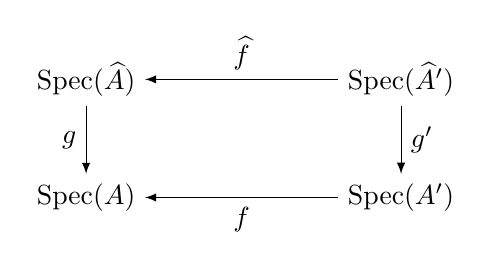
\begin{tikzpicture}[>=latex]
\node (tl) at (0,1.5) {$\operatorname{Spec}(\widehat A)$};
\node (tr) at (4,1.5) {$\operatorname{Spec}(\widehat{A}')$};
\node (bl) at (0,0) {$\operatorname{Spec}(A)$};
\node (br) at (4,0) {$\operatorname{Spec}(A')$};
\draw[->] (tr) -- node[above] {$\widehat f$} (tl);
\draw[->] (tl) -- node[left] {$g$} (bl);
\draw[->] (tr) -- node[right] {$g'$} (br);
\draw[->] (br) -- node[below] {$f$} (bl);
\end{tikzpicture}
\]
donde $g$ y $g'$ son los morfismos canónicos. Como, por hipótesis,
$f$ es un $\boldsymbol P$-morfismo y $g'$ es un morfismo regular,
de $(\mathrm P_{\mathrm I})$ se deduce que
$f\circ g'=g\circ\widehat f$ es un $\boldsymbol P$-morfismo.
Por otra parte, la hipótesis de que $f$ es un
$\boldsymbol P$-morfismo implica que $f$ es plano y, por tanto,
también lo es $\widehat f$ (Bourbaki, \emph{Alg. comm.},
cap. III, \S~5, n\textsuperscript{o}~4, cor. de la prop. 3);
el homomorfismo de anillos correspondiente es, además, local, por
lo que el morfismo es fielmente plano (\textbf 0$_{\mathrm I}$, 6.6.2).
De $(\mathrm P_{\mathrm{II}})$ se deduce entonces que $g$ es un
$\boldsymbol P$-morfismo.
\end{proof}

% END tree/worktree/es/CURRENT/EGA_IV2/ega4-2_7.4.2_ES.tex
% BEGIN tree/worktree/es/CURRENT/EGA_IV2/ega4-2_7.4.3_ES.tex
\begin{corollary}[7.4.3]
\label{IV.2.s7.4.3-fr}
\begin{enumerate}
\item[\emph{(i)}] Sea $A$ un $\boldsymbol P$-anillo local
noetheriano, y sea $A'=\widehat A$ su completado. Supongamos que,
para todo ideal primo $\mathfrak p'$ de $A'$, las fibras formales de
$A'_{\mathfrak p'}$ son geométricamente regulares; entonces, para
todo ideal primo $\mathfrak p$ de $A$, $A_{\mathfrak p}$ es un
$\boldsymbol P$-anillo.
\item[\emph{(ii)}] Supongamos que $\boldsymbol P$ satisface la
condición $(\mathrm P_{\mathrm{IV}})$ \textup{(7.3.6)}. Sean $A$ un
$\boldsymbol P$-anillo local noetheriano y $B$ una $A$-álgebra
local esencialmente de tipo finito, tal que el homomorfismo
$A\to B$ sea local. Pongamos $A'=\widehat A$, y sea
$\mathfrak n'$ el único ideal primo de $B'=B\otimes_A A'$ situado
sobre el ideal maximal de $B$ y el ideal maximal de $A'$. Si las
fibras formales de $B'_{\mathfrak n'}$ son geométricamente regulares,
entonces $B$ es un $\boldsymbol P$-anillo.
\end{enumerate}
\end{corollary}

\begin{proof}
\begin{enumerate}
\item[(i)] Como, por hipótesis,
$\operatorname{Spec}(A')\to\operatorname{Spec}(A)$ es un
$\boldsymbol P$-morfismo, también lo es
$\operatorname{Spec}(A'_{\mathfrak p'})\to
\operatorname{Spec}(A_{\mathfrak p})$ en virtud de (7.3.2, \emph{b)}),
para todo ideal primo $\mathfrak p$ de $A$ y todo ideal primo
$\mathfrak p'$ de $A'$ situado sobre $\mathfrak p$. Basta, pues,
aplicar el lema (7.4.2) a este morfismo, teniendo en cuenta que
$\operatorname{Spec}(A')\to\operatorname{Spec}(A)$ es sobreyectivo.
\item[(ii)] En virtud de (7.4.2), basta probar que el
morfismo
$\operatorname{Spec}(B'_{\mathfrak n'})\to\operatorname{Spec}(B)$
es un $\boldsymbol P$-morfismo. Ahora bien, se tiene
$B=C_{\mathfrak n}$, donde $C$ es una $A$-álgebra de tipo finito y
$\mathfrak n$ un ideal primo de $C$ situado sobre el ideal maximal
de $A$. Si se pone $C'=C\otimes_A A'$, de las hipótesis y de
(7.3.7) se deduce que
$\operatorname{Spec}(C')\to\operatorname{Spec}(C)$ es un
$\boldsymbol P$-morfismo; como $B'_{\mathfrak n'}$ es un anillo
local en un ideal primo de $C'$ situado sobre $\mathfrak n$, la
conclusión se deduce de (7.3.2, \emph{b)}).
\end{enumerate}
\end{proof}

% END tree/worktree/es/CURRENT/EGA_IV2/ega4-2_7.4.3_ES.tex
% BEGIN tree/worktree/es/CURRENT/EGA_IV2/ega4-2_7.4.4_statement_reduction_ES.tex
\begin{theorem}[7.4.4]
\label{IV.2.s7.4.4-fr}
Bajo las hipótesis sobre $\boldsymbol P$ de \textup{(7.4.1)}, sea $A$ un
$\boldsymbol P$-anillo local noetheriano.
\begin{enumerate}
\item[\emph{(i)}] Para todo ideal primo $\mathfrak p$ de $A$,
$A_{\mathfrak p}$ es un $\boldsymbol P$-anillo.
\item[\emph{(ii)}] Supongamos además que $\boldsymbol P$ satisface
la condición $(\mathrm P_{\mathrm{IV}})$. Entonces, todo anillo
local que sea una $A$-álgebra esencialmente de tipo finito es un
$\boldsymbol P$-anillo.
\end{enumerate}
\end{theorem}

\begin{proof}
\begin{enumerate}
\item[(i)] Aplicando (7.4.3, (i)), basta comprobar que,
para todo ideal primo $\mathfrak p'$ de $A'=\widehat A$,
$A'_{\mathfrak p'}$ tiene fibras formales geométricamente
regulares. Ahora bien, esto se demostró en (\textbf 0, 22.3.3 y 22.5.8).

\oldpage[IV-2]{200}

\item[(ii)] Sea $B$ una $A$-álgebra esencialmente de tipo
finito que sea un anillo local. Si $\mathfrak p$ es el ideal primo
de $A$ sobre el cual está situado el ideal maximal de $B$, $B$
también es una $A_{\mathfrak p}$-álgebra esencialmente de tipo
finito (1.3.8); en virtud de (i), se puede suponer, pues, que
$\mathfrak p$ es el ideal maximal $\mathfrak m$ de $A$. Entonces
$B=C_{\mathfrak q}$, donde $C$ es una $A$-álgebra de tipo finito y
$\mathfrak q$ un ideal primo de $C$ situado sobre $\mathfrak m$.
Sea $\mathfrak n\supset\mathfrak q$ un ideal maximal de $C$
(necesariamente situado sobre $\mathfrak m$). Si se pone
$k=A/\mathfrak m$, $C/\mathfrak mC$ es una $k$-álgebra de tipo
finito; por tanto, el cuerpo residual $k'$ de $C$ en el ideal
maximal $\mathfrak n$ es \emph{finito} sobre $k$ (\textbf I, 6.4.2). En virtud
de (i), bastará probar que $C_{\mathfrak n}$ es un
$\boldsymbol P$-anillo, puesto que $C_{\mathfrak q}$ es un anillo
local de $C_{\mathfrak n}$ en un ideal primo. La cuestión se reduce así
a demostrar el
\end{enumerate}
\end{proof}

% END tree/worktree/es/CURRENT/EGA_IV2/ega4-2_7.4.4_statement_reduction_ES.tex
% BEGIN tree/worktree/es/CURRENT/EGA_IV2/ega4-2_7.4.4.1_statement_ES.tex
\begin{lemma}[7.4.4.1]
\label{IV.2.s7.4.4.1-fr}
Sean $A$ un $\boldsymbol P$-anillo local noetheriano, $k$ su
cuerpo residual, $C$ una $A$-álgebra de tipo finito y $B$ un
anillo local en un ideal primo $\mathfrak n$ de $C$, tales que:
1\textsuperscript{o} el homomorfismo $A\to B$ es local;
2\textsuperscript{o} el cuerpo residual $k'$ de $B$ es una
extensión finita de $k$. Si $\boldsymbol P$ satisface
$(\mathrm P_{\mathrm{IV}})$, entonces $B$ es un
$\boldsymbol P$-anillo.
\end{lemma}

% END tree/worktree/es/CURRENT/EGA_IV2/ega4-2_7.4.4.1_statement_ES.tex
% BEGIN tree/worktree/es/CURRENT/EGA_IV2/ega4-2_7.4.4.1_proof_ES.tex
\begin{proof}
Sea $(x_i)_{1\leqslant i\leqslant m}$ un sistema de generadores de la
$A$-álgebra $C$; mostremos primero que se puede razonar por inducción sobre
$m$. Sea $C'$ la subálgebra de $C$ generada por
$x_1,\ldots,x_{m-1}$, y sea $\mathfrak n'=\mathfrak n\cap C'$.
El homomorfismo $A\to C_{\mathfrak n}$ se factoriza como
$A\to C'_{\mathfrak n'}\to C_{\mathfrak n}$, y está claro que
$A\to C'_{\mathfrak n'}$ y $C'_{\mathfrak n'}\to C_{\mathfrak n}$ son
homomorfismos locales; si $k''$ es el cuerpo residual de
$C'_{\mathfrak n'}$, $k\to k'$ se factoriza del mismo modo como
$k\to k''\to k'$, de modo que $k''$ es una extensión finita de $k$ y $k'$
una extensión finita de $k''$. La hipótesis de inducción implica que
$C'_{\mathfrak n'}$ es un $\boldsymbol P$-anillo; además, si
$S'=C'\setmin\mathfrak n'$, $C_{\mathfrak n}$ es un anillo local de
$S'^{-1}C$; como $C=C'[x_m]$, se tiene
$S'^{-1}C=C'_{\mathfrak n'}[x_m/1]$, y la hipótesis de inducción muestra
también que $C_{\mathfrak n}$ es un $\boldsymbol P$-anillo. La cuestión se reduce así al caso en que $C$ es una $A$-álgebra generada por
\emph{un solo} elemento $t$.

Apliquemos (7.4.3, (ii)); poniendo $A'=\widehat A$,
$B'=B\otimes_A A'$ es un anillo local de $C\otimes_A A'$ en un ideal
primo situado sobre $\mathfrak n$; como $A$ y $A'$ tienen el mismo cuerpo
residual $k$, el cuerpo residual de $C\otimes_A A'$ en ese ideal primo es
igual a $k'$. Por otra parte, $C\otimes_A A'$ es una $A'$-álgebra generada
por un solo elemento. Resulta, pues, de (7.4.3, (ii)) que es posible
limitarse a demostrar (7.4.4.1) cuando $\boldsymbol P$ es la propiedad
(iv$'$) de (7.3.8), $A$ es \emph{completo} y $C$ está generada por un solo
elemento $t$.

Para demostrar entonces que las fibras formales de $B=C_{\mathfrak n}$
son geométricamente regulares, apliquemos el criterio (7.3.16, \emph{b)}). Sea
$B_1$ una $B$-álgebra finita e \emph{íntegra}, generada por tanto por un
número finito de elementos enteros sobre $B$. Multiplicando estos
elementos por un elemento de $S=C\setmin\mathfrak n$, se puede suponer que son
enteros sobre $C$ y, por consiguiente, escribir $B_1=S^{-1}C_1$, donde
$C_1$ es una sub-$C$-álgebra de $B_1$ generada por un número finito de
elementos enteros sobre $C$; es, por tanto, una $C$-álgebra
\emph{finita e íntegra}. Por otra parte, $B_1$ es un anillo semilocal, y
todo anillo local $B_2$ de $B_1$ en un ideal maximal es un anillo local
de $C_1$ en un ideal primo, tal que $A\to B_2$ es un homomorfismo local;
además, el cuerpo residual de $B_2$ es una extensión finita de $k'$ y,
por tanto, de $k$. Se ve así, teniendo en cuenta (7.3.14) y (i), que
el problema se reduce a la cuestión siguiente: sea $C$ un anillo noetheriano
\emph{íntegro}, que contiene un subanillo $C_0$ que es una $A$-álgebra
generada por un solo elemento $t$, y tal que $C$ es una $C_0$-álgebra
\emph{finita}; si $\mathfrak n$ es un ideal maximal de $C$

\oldpage[IV-2]{201}

situado sobre el ideal maximal de $A$, y $B=C_{\mathfrak n}$, se trata
de demostrar que, para todo ideal primo $\mathfrak q$ de $\widehat B$
cuya imagen inversa en $B$ sea 0, el anillo
$\widehat B_{\mathfrak q}$ es \emph{regular}. Por otra parte, se puede
sustituir $A$ por su imagen en $C$, que es un anillo local completo
(como cociente de $A$) e íntegro. La conclusión que hay que demostrar
es entonces consecuencia del lema siguiente, en apariencia más general:
\end{proof}

% END tree/worktree/es/CURRENT/EGA_IV2/ega4-2_7.4.4.1_proof_ES.tex
% BEGIN tree/worktree/es/CURRENT/EGA_IV2/ega4-2_7.4.4.2_statement_ES.tex
\begin{lemma}[7.4.4.2]
\label{IV.2.s7.4.4.2-fr}
Sean $A$ un anillo local noetheriano, íntegro y completo, $k$ su cuerpo
residual, y $C$ un anillo íntegro que contiene a $A$, tal que existe
$t\in C$ para el cual $C$ es una $A[t]$-álgebra finita. Sea $\mathfrak n$
un ideal maximal de $C$ situado sobre el ideal maximal $\mathfrak m$ de
$A$; pongamos $B=C_{\mathfrak n}$, $X=\operatorname{Spec}(B)$,
$B'=\widehat B$, $X'=\operatorname{Spec}(\widehat B)$; si
$U=\operatorname{Reg}(X)$, $U'=\operatorname{Reg}(X')$, y si
$f:X'\to X$ es el morfismo canónico, entonces
$f^{-1}(U)\subset U'$.
\end{lemma}

% END tree/worktree/es/CURRENT/EGA_IV2/ega4-2_7.4.4.2_statement_ES.tex
% BEGIN tree/worktree/es/CURRENT/EGA_IV2/ega4-2_7.4.4.2_proof_ES.tex
\begin{proof}
La afirmación que hay que demostrar para obtener (7.4.4.1) se deduce
de este lema observando que, puesto que $B$ es íntegro, el punto
genérico de $X$ pertenece a $U$.

Se observará que, como $C$ es una $A$-álgebra de tipo finito y $\mathfrak n$
un ideal maximal de $C$, el cuerpo residual $k'$ de
$C_{\mathfrak n}=B$ (y, por tanto, también de $B'$) es una extensión
\emph{finita} de $k$ (\textbf I, 6.4.11 y 6.4.2).

Si se pone $Y=\operatorname{Spec}(C)$, de (6.12.8) resulta que
$\operatorname{Reg}(Y)$ es \emph{abierto} en $Y$; como los anillos locales de
$X$ son anillos locales de $Y$ (\textbf I, 2.4.2), se tiene
$U=X\cap\operatorname{Reg}(Y)$, y por tanto $U$ es \emph{abierto} en $X$; por
otra parte, según (6.12.7), $U'$ es abierto en $X'$, de modo que
$S'=X'\setmin U'$ es cerrado. En consecuencia, $S'\cap f^{-1}(U)$ es
\emph{localmente cerrado} en $X'$, y basta demostrar que este conjunto es
\emph{vacío}. Se sabe por (5.1.10) que, en caso contrario, existiría en
$S'\cap f^{-1}(U)$ un ideal primo $\mathfrak p'$ tal que
$\dim(B'/\mathfrak p')\leqslant1$. Observemos primero que
$\mathfrak p'$ no puede ser el ideal maximal $\mathfrak mB'$ de $B'$,
donde $\mathfrak m$ es el ideal maximal de $B$. En efecto, esto
significaría que $B=B_{\mathfrak m}$ sería regular, y por tanto también
$B'=\widehat B$ (\textbf{0}, 17.1.5); se tendría entonces $\mathfrak mB'\in U'$,
en contra de la hipótesis. Debe ser, pues,
$\dim(B'/\mathfrak p')=1$. Pongamos
$\mathfrak p=B\cap\mathfrak p'$; por hipótesis, $B_{\mathfrak p}$ es
regular, pero $B'_{\mathfrak p'}$ no lo es; como
$B'_{\mathfrak p'}$ es un $B_{\mathfrak p}$-módulo plano, se deduce de
(6.5.2) que la fibra $Z$ de $f$ en el punto $\mathfrak p$ \emph{no es regular
en el punto} $\mathfrak p'$. Mostremos que \emph{es posible reducirse al caso en
que} $\mathfrak p=0$. En efecto, en el caso general, si se pone
$\mathfrak q=\mathfrak p\cap C$, $\mathfrak r=\mathfrak p\cap A$,
$C/\mathfrak q$ es una $(A/\mathfrak r)[\bar t]$-álgebra finita (donde
$\bar t$ es la clase de $t$ módulo $\mathfrak q$); como
$\mathfrak p=\mathfrak qB$, $B/\mathfrak p$ es igual a
$(C/\mathfrak q)_{\mathfrak n/\mathfrak q}$, y
$\mathfrak n/\mathfrak q$ es un ideal maximal de $C/\mathfrak q$
situado sobre el ideal maximal $\mathfrak m/\mathfrak r$ de
$A/\mathfrak r$. Se ve así que $A/\mathfrak r$, $C/\mathfrak q$ y
$B/\mathfrak p$ siguen satisfaciendo las hipótesis de (7.4.4.2); como
el completado de $B/\mathfrak p$ es $B'/\mathfrak pB'$, esto demuestra
nuestra afirmación. Supongamos, pues, $\mathfrak p=0$, de manera que
$Z$ es la fibra genérica y el homomorfismo $B\to B'/\mathfrak p'$ es
\emph{inyectivo}. Pongamos $V=B'/\mathfrak p'$ y distingamos dos casos:

I) \emph{$V$ es una $A$-álgebra finita.} --- Como $B\subset V$, $B$ es
\emph{a fortiori} una $A$-álgebra finita; y, puesto que $A$ es completo,
lo mismo ocurre con $B$ (Bourbaki, \emph{Alg. comm.}, cap. IV, \S~2,
n\textsuperscript{o}~5, cor. 3 de la prop. 9). De ahí que $B'=B$ y
$\mathfrak p'=0$, por lo que $B'_{\mathfrak p'}$ es un cuerpo y, por
consiguiente, un anillo regular, en contra de la hipótesis.

II) \emph{$V$ no es una $A$-álgebra finita.} --- Como el anillo local
$A$ es \emph{completo}, esto implica que $V$ no es una $A$-álgebra
\emph{cuasifinita} ($\mathbf{0}_{\mathrm I}$, 7.4.1 y 7.4.2); pero, por hipótesis, el
cuerpo residual $k'$ de $V$ es una extensión \emph{finita} del cuerpo residual
$k$ de $A$,

\oldpage[IV-2]{202}

por tanto, según ($\mathbf{0}_{\mathrm I}$, 7.4.4), el ideal $\mathfrak mV$
\emph{no es un ideal de definición de} $V$. Como $V$ es un anillo local noetheriano
íntegro de dimensión 1, 0 es el único ideal de $V$ que no es un ideal
de definición; por ello, $\mathfrak mV=0$. Pero $A\subset V$ y $V$ es
íntegro, de donde $\mathfrak m=0$ y $A=k$ es un \emph{cuerpo}. Se deduce ante
todo que $\dim(C)\leqslant1$ (\textbf 0, 16.1.5); pero, como $\dim(V)=1$, las
relaciones
$\dim(V)\leqslant\dim(B')=\dim(B)\leqslant\dim(C)$
muestran que esto implica
$\dim(C)=\dim(B)=\dim(B')=\dim(B'/\mathfrak p')=1$ y, en consecuencia,
$\mathfrak p'$ es necesariamente un \emph{ideal primo minimal} de $B'$.
Llegaremos, pues, también a una contradicción si demostramos que
$B'_{\mathfrak p'}$ es un \emph{cuerpo}, o, lo que es lo mismo, que el anillo
$B'$ es reducido. Ahora bien, como $C$ es una $k$-álgebra de tipo finito,
la clausura integral $C_1$ de $C$ es una $C$-álgebra \emph{finita} (Bourbaki,
\emph{Alg. comm.}, cap. V, \S~3, n\textsuperscript{o}~2, teorema 2);
si se pone $S=C\setmin\mathfrak n$, $B_1=S^{-1}C_1$ es la clausura integral de
$B$, y por tanto $B_1$ es una $B$-álgebra \emph{finita}, y en consecuencia es
un anillo semilocal noetheriano, íntegro, integralmente cerrado y de
dimensión 1 (\textbf{0}, 16.1.5). Si $\mathfrak m_j$ $(1\leqslant j\leqslant h)$
son sus ideales maximales, los $(B_1)_{\mathfrak m_j}$ son, por tanto,
anillos de valoración discreta (\textbf{II}, 7.1.6), y el completado $B'_1$ de
$B_1$ es el producto directo de los anillos de valoración discreta
completados de los $(B_1)_{\mathfrak m_j}$ (Bourbaki, \emph{Alg. comm.},
cap. III, \S~2, n\textsuperscript{o}~13, prop. 18); $B'_1$ es, pues,
reducido, y como el completado $B'$ de $B$ es un subanillo de $B'_1$
(Bourbaki, \emph{Alg. comm.}, cap. IV, \S~2, n\textsuperscript{o}~5,
cor. 3 de la prop. 9), también es un anillo reducido. Queda demostrado.
\end{proof}

% END tree/worktree/es/CURRENT/EGA_IV2/ega4-2_7.4.4.2_proof_ES.tex
% BEGIN tree/worktree/es/CURRENT/EGA_IV2/ega4-2_7.4.5_ES.tex
\begin{corollary}[7.4.5]
\label{IV.2.s7.4.5-fr}
Supongamos que la propiedad $\boldsymbol P$ satisface las condiciones
$(\mathrm P_{\mathrm I})$, $(\mathrm P_{\mathrm{II}})$ y
$(\mathrm P_{\mathrm{III}})$. Sea $A$ un anillo noetheriano. Las
condiciones siguientes son equivalentes:
\begin{enumerate}
\item[\emph{a)}] Para todo ideal primo $\mathfrak p$ de $A$,
$A_{\mathfrak p}$ es un $\boldsymbol P$-anillo.
\item[\emph{b)}] Para todo ideal maximal $\mathfrak m$ de $A$,
$A_{\mathfrak m}$ es un $\boldsymbol P$-anillo.
\end{enumerate}
Si además $\boldsymbol P$ satisface $(\mathrm P_{\mathrm{IV}})$, las
propiedades \textup{a)} y \textup{b)} son también equivalentes a:
\begin{enumerate}
\item[\emph{c)}] Para toda $A$-álgebra de tipo finito $B$ y todo ideal
primo $\mathfrak q$ de $B$, $B_{\mathfrak q}$ es un
$\boldsymbol P$-anillo.
\end{enumerate}
\end{corollary}

\begin{proof}
La equivalencia de \emph{a)} y \emph{b)} resulta de (7.4.4, (i)), y la de \emph{a)} y \emph{c)} de
(7.4.4, (ii)).

Cuando se cumple la condición \emph{a)} de (7.4.5), se dice que $A$ es un
$\boldsymbol P$-\emph{anillo}; para los anillos semilocales noetherianos, esta
definición coincide con la de (7.3.13) cuando se satisfacen las
condiciones $(\mathrm P_{\mathrm I})$, $(\mathrm P_{\mathrm{II}})$ y
$(\mathrm P_{\mathrm{III}})$. El anillo $\mathbf Z$ es un
$\boldsymbol P$-anillo (7.3.19, (iv)); todo anillo local completo es un
$\boldsymbol P$-anillo.
\end{proof}

% END tree/worktree/es/CURRENT/EGA_IV2/ega4-2_7.4.5_ES.tex
% BEGIN tree/worktree/es/CURRENT/EGA_IV2/ega4-2_7.4.6_ES.tex
\begin{proposition}[7.4.6]
\label{IV.2.s7.4.6-fr}
Supongamos que la propiedad $\boldsymbol P$ satisface las condiciones
$(\mathrm P_{\mathrm I})$, $(\mathrm P_{\mathrm{II}})$ y
$(\mathrm P_{\mathrm{III}})$. Sean $A$ un anillo noetheriano,
$\mathfrak J$ un ideal de $A$ y $\widehat A$ el completado separado de
$A$ para la topología $\mathfrak J$-preádica. Entonces, si $A$ es un
$\boldsymbol P$-anillo (7.4.5), el morfismo canónico
$\operatorname{Spec}(\widehat A)\to\operatorname{Spec}(A)$ es un
$\boldsymbol P$-morfismo.
\end{proposition}

\begin{proof}
Utilizando (7.3.2, \emph{c$'$)}), basta demostrar que, para todo ideal
maximal $\mathfrak n$ de $\widehat A$ cuya imagen inversa es
$\mathfrak m$ en $A$, el morfismo
$\operatorname{Spec}((\widehat A)_{\mathfrak n})\to
\operatorname{Spec}(A_{\mathfrak m})$ es un $\boldsymbol P$-morfismo.
Se sabe (Bourbaki, \emph{Alg. comm.}, cap. III, \S~3,
n\textsuperscript{o}~4, prop. 8) que el homomorfismo canónico
$A_{\mathfrak m}\to(\widehat A)_{\mathfrak n}$ es inyectivo, que la
topología $\mathfrak mA_{\mathfrak m}$-preádica sobre $A_{\mathfrak m}$
está inducida por la topología
$\mathfrak n(\widehat A)_{\mathfrak n}$-preádica y que
$A_{\mathfrak m}$ es denso en $(\widehat A)_{\mathfrak n}$ para esta
topología; por consiguiente, el completado de $A_{\mathfrak m}$ para la
topología $\mathfrak mA_{\mathfrak m}$-preádica se identifica con el de
$(\widehat A)_{\mathfrak n}$ para la topología
$\mathfrak n(\widehat A)_{\mathfrak n}$-preádica. Se tienen, pues, dos
morfismos
\[
\operatorname{Spec}((A_{\mathfrak m})^{\widehat{\,}})
\xrightarrow{f}\operatorname{Spec}((\widehat A)_{\mathfrak n})
\xrightarrow{g}\operatorname{Spec}(A_{\mathfrak m})
\]

\oldpage[IV-2]{203}

tales que $f$ es fielmente plano; como, por hipótesis, $g\circ f$ es un
$\boldsymbol P$-morfismo, también lo es $g$ en virtud de
$(\mathrm P_{\mathrm{II}})$.
\end{proof}

% END tree/worktree/es/CURRENT/EGA_IV2/ega4-2_7.4.6_ES.tex
% BEGIN tree/worktree/es/CURRENT/EGA_IV2/ega4-2_7.4.7_ES.tex
\begin{corollary}[7.4.7]
\label{IV.2.s7.4.7-fr}
Supongamos que $\boldsymbol P$ satisface las condiciones
$(\mathrm P_{\mathrm I})$, $(\mathrm P'_{\mathrm I})$,
$(\mathrm P_{\mathrm{II}})$, $(\mathrm P_{\mathrm{III}})$ y
$(\mathrm P_{\mathrm{IV}})$. Entonces, si $A$ es un
$\boldsymbol P$-anillo (7.4.5), el morfismo canónico
$\operatorname{Spec}(A[[T_1,\ldots,T_r]])\to\operatorname{Spec}(A)$ es un
$\boldsymbol P$-morfismo. En particular, si además $A$ es íntegro, $K$
su cuerpo de fracciones, y si $\mathfrak p$ es un ideal primo de
$B=A[[T_1,\ldots,T_r]]$ tal que $\mathfrak p\cap A=0$, entonces se
cumple la propiedad $\boldsymbol P(B_{\mathfrak p},K)$.
\end{corollary}

\begin{proof}
En efecto, el morfismo canónico
$\operatorname{Spec}(B)\to\operatorname{Spec}(A)$ se factoriza como
\[
\operatorname{Spec}(A[[T_1,\ldots,T_r]])
\xrightarrow{f}\operatorname{Spec}(A[T_1,\ldots,T_r])
\xrightarrow{g}\operatorname{Spec}(A).
\]
Está claro que el morfismo $g$ es regular (\textbf 0, 17.3.7); en virtud de
(7.4.5), $A[T_1,\ldots,T_r]$ es un $\boldsymbol P$-anillo, de modo que
por (7.4.6) $f$ es un $\boldsymbol P$-morfismo. Como $g$ es regular y,
por tanto, también un $\boldsymbol P$-morfismo (7.3.5, (i)), lo mismo
vale para $g\circ f$ en virtud de $(\mathrm P'_{\mathrm I})$.

Se observará que la conclusión sigue siendo válida si, en lugar de suponer
que $\boldsymbol P$ satisface $(\mathrm P'_{\mathrm I})$ y que todo
morfismo regular es un $\boldsymbol P$-morfismo, se supone únicamente
que un morfismo compuesto $g\circ f$ es un $\boldsymbol P$-morfismo
cuando $g$ es regular y $f$ un $\boldsymbol P$-morfismo (condición en
cierto modo simétrica de $(\mathrm P'_{\mathrm I})$).
\end{proof}

% END tree/worktree/es/CURRENT/EGA_IV2/ega4-2_7.4.7_ES.tex
% BEGIN tree/worktree/es/CURRENT/EGA_IV2/ega4-2_7.4.8_ES.tex
\begin{remark}[7.4.8]
\label{IV.2.s7.4.8-fr}
Los resultados anteriores plantean los problemas siguientes:
\begin{enumerate}
\item[A)] Sea $A$ un anillo de Zariski \emph{completo}, y sea
$\mathfrak J$ un ideal de definición de $A$; si el anillo
$A/\mathfrak J$ es un $\boldsymbol P$-anillo, ¿lo es también $A$? De
ello resultaría que, para todo $\boldsymbol P$-anillo noetheriano $A$ y
todo ideal $\mathfrak J$ de $A$, el completado separado $\widehat A$
para la topología $\mathfrak J$-preádica sería también un
$\boldsymbol P$-anillo.
\item[B)] Sea $k$ un cuerpo valuado completo no discreto; se
llama también anillo de \emph{series formales restringidas}
$k\{T_1,\ldots,T_n\}$ al subanillo del anillo de series formales
$k[[T_1,\ldots,T_n]]$ formado por las series cuyos coeficientes
\emph{tienden a} 0. ¿Es tal anillo un $\boldsymbol P$-anillo?
\item[C)] Si $A$ es un $\boldsymbol P$-anillo linealmente
topologizado y $S$ un conjunto multiplicativo de $A$, ¿son los anillos
$A\{S^{-1}\}$ ($\mathbf{0}_{\mathrm I}$, 7.6.1) y $A_{\{S\}}$
($\mathbf{0}_{\mathrm I}$, 7.6.15) $\boldsymbol P$-anillos?
\end{enumerate}
\end{remark}

% END tree/worktree/es/CURRENT/EGA_IV2/ega4-2_7.4.8_ES.tex
% BEGIN tree/worktree/es/CURRENT/EGA_IV2/ega4-2_7.5.0_ES.tex
\subsection{Un criterio para los $\boldsymbol P$-morfismos.}
\label{subsection:IV.7.5-fr}

\begin{env}[7.5.0]
\label{IV.2.s7.5.0-fr}
Este apartado no se utilizará en el resto del capítulo IV y, por tanto,
puede omitirse en una primera lectura. Veremos además más adelante
(7.9.8) que los resultados de este apartado pueden mejorarse
considerablemente cuando se dispone de la «resolución de
singularidades».

En lo que sigue de este apartado consideraremos una propiedad
$\boldsymbol R(A)$ y denotaremos por $\boldsymbol P(Z,k)$ la propiedad
siguiente:
\begin{quote}
«$Z$ es un preesquema localmente noetheriano sobre un cuerpo $k$ y, para
toda extensión \emph{finita} $k'$ de $k$, si se pone $Z'=Z\otimes_k k'$, se
cumple la propiedad $\boldsymbol R(\mathscr O_{Z',z'})$ para todo
$z'\in Z'$.»
\end{quote}
\end{env}

% END tree/worktree/es/CURRENT/EGA_IV2/ega4-2_7.5.0_ES.tex
% BEGIN tree/worktree/es/CURRENT/EGA_IV2/ega4-2_7.5.1_statement_ES.tex
\begin{theorem}[7.5.1]
\label{IV.2.s7.5.1-fr}
Sean $A$, $B$ dos anillos locales noetherianos \textup{completos}, $\mathfrak m$
el ideal maximal de $A$, $k=A/\mathfrak m$ su cuerpo residual y
$\varphi:A\to B$ un homomorfismo local tal que:
\begin{enumerate}
\item[\emph{(i)}] El cuerpo residual de $B$ es una extensión finita de
$k$.
\item[\emph{(ii)}] $B$ es un $A$-módulo plano.
\end{enumerate}
Sea, por otra parte, $\boldsymbol R(C)$ una propiedad que satisface la
condición $(\mathrm R_{\mathrm{III}})$ (7.3.18) y la condición siguiente:
\begin{quote}
$(\mathrm R_{\mathrm{IV}})$ Para todo anillo local $C$ en un ideal primo
de un anillo local noetheriano completo y todo elemento $C$-regular $t$
del ideal maximal de $C$, la propiedad $\boldsymbol R(C/tC)$ implica
$\boldsymbol R(C)$.
\end{quote}

\oldpage[IV-2]{204}

En estas condiciones, sea $f={}^a\varphi:\operatorname{Spec}(B)\to
\operatorname{Spec}(A)$, y supongamos que se cumple la propiedad
$\boldsymbol P(\operatorname{Spec}(B\otimes_A k),k)$. Entonces, para
todo $x\in\operatorname{Spec}(A)$ se cumple la propiedad
$\boldsymbol P(f^{-1}(x),\boldsymbol{k}(x))$.
\end{theorem}

% END tree/worktree/es/CURRENT/EGA_IV2/ega4-2_7.5.1_statement_ES.tex
% BEGIN tree/worktree/es/CURRENT/EGA_IV2/ega4-2_7.5.1_proof_stage_I_ES.tex
\begin{proof}
En otras palabras, la propiedad $\boldsymbol P$ para \emph{la fibra del punto
cerrado} de $\operatorname{Spec}(A)$ implica la misma propiedad para
\emph{todas las fibras} del morfismo $f$ (es decir, que $f$ es un
$\boldsymbol P$-\emph{morfismo} (7.3.1)). Procederemos en varias etapas:

I) \emph{Reducción al estudio de los anillos locales de la fibra
genérica.} --- Apliquemos el lema (7.3.16.2): basta comprobar que, para
toda $A$-álgebra \emph{finita} e \emph{íntegra} $A'$ con cuerpo de fracciones $K'$, si
se pone $B'=B\otimes_A A'$, todos los anillos locales de
$\operatorname{Spec}(B'\otimes_{A'}K')$ satisfacen la propiedad
$\boldsymbol R$. El anillo $A'$ (resp. $B'$) es semilocal
completo ($B'$ es una $B$-álgebra finita), y por tanto producto de
anillos locales completos; como $A'$ es íntegro por hipótesis, es \emph{local};
todo ideal maximal $\mathfrak n'$ de $B'$ está situado sobre el ideal
maximal $\mathfrak n$ de $B$ y, por tanto, sobre $\mathfrak m$; en
consecuencia, su imagen inversa en $A'$ es el ideal maximal
$\mathfrak m'$ de $A'$. Como todo anillo local de
$\operatorname{Spec}(B'\otimes_{A'}K')$ es un anillo local de
$\operatorname{Spec}(B')$, y por tanto de uno de los
$\operatorname{Spec}(B'_{\mathfrak n'})$ (sobre el punto genérico de
$A'$), se ve que bastará demostrar que los anillos locales de
$\operatorname{Spec}(B'_{\mathfrak n'}\otimes_{A'}K')$
poseen la propiedad $\boldsymbol R$. Ahora bien, $A'$ y
$B'_{\mathfrak n'}$ son anillos locales noetherianos completos; el
cuerpo residual de $B'_{\mathfrak n'}$ es una extensión finita del de
$B$, y por tanto también de $k$ y, \emph{a fortiori}, del cuerpo
residual $k'$ de $A'$. Esta observación y (2.1.4) muestran que $A'$ y
$B'_{\mathfrak n'}$ satisfacen las condiciones (i) y (ii) del
enunciado. Por otra parte, si $k''$ es una extensión finita de $k'$,
$k''$ es también una extensión finita de $k$, y los anillos locales de
$\operatorname{Spec}(B'_{\mathfrak n'}\otimes_{A'}k'')$
son también anillos locales de $\operatorname{Spec}(B\otimes_A k'')$;
por ello, la hipótesis de que se cumple
$\boldsymbol P(\operatorname{Spec}(B\otimes_A k),k)$ implica que la
propiedad
$\boldsymbol P(\operatorname{Spec}(B'_{\mathfrak n'}\otimes_{A'}k'),k')$
se cumple.

La cuestión se reduce así al caso en que, además, $A$ es \emph{íntegro}, con
cuerpo de fracciones $K$, y a demostrar que \emph{los anillos locales de}
$\operatorname{Spec}(B\otimes_A K)$ \emph{poseen la propiedad} $\boldsymbol R$.

% END tree/worktree/es/CURRENT/EGA_IV2/ega4-2_7.5.1_proof_stage_I_ES.tex
% BEGIN tree/worktree/es/CURRENT/EGA_IV2/ega4-2_7.5.1_proof_stage_II_ES.tex
II) \emph{Caso en que $\dim(A)=1$.} --- Sea $A'$ la clausura integral de
$A$; se sabe por (\textbf 0, 23.1.6) que $A'$ es una $A$-álgebra \emph{finita} y un
anillo \emph{local} completo. Si se pone $B'=B\otimes_A A'$, se tiene
$B\otimes_A K=B'\otimes_{A'}K$. El mismo razonamiento que en I) muestra
que, para todo ideal maximal $\mathfrak n'$ de $B'$, basta demostrar que
los anillos locales de $B'_{\mathfrak n'}\otimes_{A'}K$ satisfacen
$\boldsymbol R$; además, ese razonamiento muestra también que $A'$ y
$B'_{\mathfrak n'}$ satisfacen las hipótesis (i) y (ii) del enunciado y
que se cumple
$\boldsymbol P(\operatorname{Spec}(B'_{\mathfrak n'}\otimes_{A'}k'),k')$
(donde $k'$ es el cuerpo residual de $A'$). Además, como
$\dim(A')=1$ (\textbf 0, 16.1.5) y $A'$ es íntegro e integralmente cerrado,
es un \emph{anillo de valoración discreta completo}. Es posible, pues,
limitarse al caso en que $A$ ya es un anillo de valoración discreta
completo. Si $u$ es entonces un generador del ideal maximal de $A$,
el hecho de que $u$ sea $A$-regular y de que $B$ sea un $A$-módulo
plano implica que $t=\varphi(u)$ es un elemento $B$-regular que
pertenece al ideal maximal de $B$. La hipótesis de que se cumple
$\boldsymbol P(\operatorname{Spec}(B\otimes_A k),k)$ implica, en
particular, que se cumple $\boldsymbol R(B/tB)$; en virtud de
$(\mathrm R_{\mathrm{IV}})$, se cumple, por tanto, $\boldsymbol R(B)$.
En otras palabras, $U_{\mathbf R}(\operatorname{Spec}(B))$ contiene
el punto cerrado de $\operatorname{Spec}(B)$. Pero
$U_{\mathbf R}(\operatorname{Spec}(B))$ es abierto en virtud de
$(\mathrm R_{\mathrm{III}})$, y $\operatorname{Spec}(B)$ es el único
abierto de $\operatorname{Spec}(B)$ que contiene el punto cerrado.
Por ello, todos los anillos locales de $\operatorname{Spec}(B)$ poseen
la propiedad $\boldsymbol R$, en particular los de
$\operatorname{Spec}(B\otimes_A K)$.

% END tree/worktree/es/CURRENT/EGA_IV2/ega4-2_7.5.1_proof_stage_II_ES.tex
% BEGIN tree/worktree/es/CURRENT/EGA_IV2/ega4-2_7.5.1_proof_stage_III_ES.tex
III) \emph{Caso general.} --- El caso $\dim(A)=0$ es trivial, pues entonces
$A=k$; es posible, por tanto, limitarse al caso en que $\dim(A)\geqslant1$.
Se sabe (6.12.7) que $\operatorname{Spec}(A)$ contiene un abierto no vacío
$V$ cuyos puntos son todos regulares; como $\dim(A)\geqslant1$, la
intersección $V'$ de $V$ con el complementario del punto cerrado de
$\operatorname{Spec}(A)$ es un abierto no vacío y contiene, por tanto, el
punto genérico de $\operatorname{Spec}(A)$. Si demostramos que
$f^{-1}(V')\subset U_{\mathbf R}(\operatorname{Spec}(B))$,
la proposición quedará demostrada \emph{a fortiori}. En otras palabras,
basta ver que el conjunto $Z$, intersección de $f^{-1}(V')$ con el
complementario de $U_{\mathbf R}(\operatorname{Spec}(B))$, es \emph{vacío}.
Razonemos por contradicción: como, en virtud de
$(\mathrm R_{\mathrm{III}})$,
$U_{\mathbf R}(\operatorname{Spec}(B))$ es abierto en
$\operatorname{Spec}(B)$, $Z$ es localmente cerrado en
$\operatorname{Spec}(B)$; si no fuera vacío, contendría un punto $x$ tal
que $\dim(\overline{\{x\}})\leqslant1$ (5.1.10); como $f(x)\in V'$
es distinto del punto cerrado de $\operatorname{Spec}(A)$, $x$ es distinto
del punto cerrado de $\operatorname{Spec}(B)$, es decir,
$\dim(\overline{\{x\}})=1$. Vamos a demostrar que esto es imposible,
es decir, que, si $\dim(\overline{\{x\}})=1$ y $f(x)\in V'$, se cumple
$\boldsymbol R(\mathscr O_x)$. Dicho de otro modo, se trata de ver que,
si $\mathfrak q$ es un ideal primo de $B$ tal que
$\dim(B/\mathfrak q)=1$ y si $\mathfrak p=\varphi^{-1}(\mathfrak q)$
es distinto de $\mathfrak m$ y tal que $A_{\mathfrak p}$ es \emph{regular},
entonces se cumple $\boldsymbol R(B_{\mathfrak q})$. Como
$\mathfrak p\ne\mathfrak m$, $\mathfrak m(B/\mathfrak q)$ no se reduce
a 0 y, por tanto, es un ideal de definición del anillo local íntegro
$B/\mathfrak q$ de dimensión 1; por otra parte, en virtud de (i), el
cuerpo residual de $B/\mathfrak q$ es una extensión finita del cuerpo
residual $k$ de $A/\mathfrak p$, por lo que $B/\mathfrak q$ es una
$(A/\mathfrak p)$-álgebra \emph{cuasifinita} ($\mathbf{0}_{\mathrm I}$, 7.4.4). Pero
$A/\mathfrak p$ es completo y $B/\mathfrak q$ es separado para la
topología $\mathfrak m$-preádica (que coincide con su topología de anillo
local); por tanto ($\mathbf{0}_{\mathrm I}$, 7.4.1), $B/\mathfrak q$ es una
$(A/\mathfrak p)$-álgebra \emph{finita}. Además, por definición, el homomorfismo
$A/\mathfrak p\to B/\mathfrak q$ es inyectivo, por lo que (\textbf{0}, 16.1.5)
se tiene
$\dim(A/\mathfrak p)=\dim(B/\mathfrak q)=1$.
Se puede entonces aplicar a los anillos $A/\mathfrak p$ y
$B/\mathfrak pB$ el resultado de II), pues los cuerpos residuales de
estos anillos locales son, respectivamente, los de $A$ y $B$, y
$B/\mathfrak pB$ es un $(A/\mathfrak p)$-módulo plano; además, se tiene
$(B/\mathfrak pB)\otimes_{A/\mathfrak p}k=B\otimes_A k=B/\mathfrak mB$.
Por consiguiente, los anillos locales de
$\operatorname{Spec}((B/\mathfrak pB)
\otimes_{A/\mathfrak p}\boldsymbol{k}(\mathfrak p))$
satisfacen $\boldsymbol R$. Ahora bien,
$B_{\mathfrak q}/\mathfrak pB_{\mathfrak q}$ es uno de los anillos
locales de $\operatorname{Spec}((B/\mathfrak pB)
\otimes_{A/\mathfrak p}\boldsymbol{k}(\mathfrak p))$. Además, $B_{\mathfrak q}$ es
un $A_{\mathfrak p}$-módulo plano y $A_{\mathfrak p}$ es \emph{regular}.
Se tiene, pues, el siguiente lema:

% END tree/worktree/es/CURRENT/EGA_IV2/ega4-2_7.5.1_proof_stage_III_ES.tex
% BEGIN tree/worktree/es/CURRENT/EGA_IV2/ega4-2_7.5.1.1_statement_ES.tex
\oldpage[IV-2]{205}

\begin{lemma}[7.5.1.1]
\label{IV.2.s7.5.1.1-fr}
Sea $\boldsymbol{C}$ una subcategoría plena de la categoría de los anillos
locales noetherianos, tal que todo anillo cociente de un anillo de
$\boldsymbol{C}$ pertenezca también a $\boldsymbol{C}$. Sea $\boldsymbol R(C)$
una propiedad tal que, si $C\in\boldsymbol{C}$ y $t$ es un elemento regular
del ideal maximal de $C$ para el que se cumple $\boldsymbol R(C/tC)$,
entonces se cumple $\boldsymbol R(C)$.

En estas condiciones, sean $C$ un anillo local regular, $k$ su cuerpo
residual, $D$ un anillo local que pertenece a $\boldsymbol{C}$, y
$\varphi:C\to D$ un homomorfismo local que hace de $D$ un $C$-módulo
plano. Si se cumple $\boldsymbol R(D\otimes_C k)$, entonces también
se cumple $\boldsymbol R(D)$.
\end{lemma}

% END tree/worktree/es/CURRENT/EGA_IV2/ega4-2_7.5.1.1_statement_ES.tex
% BEGIN tree/worktree/es/CURRENT/EGA_IV2/ega4-2_7.5.1.1_proof_ES.tex
\begin{proof}
Razonemos por inducción sobre $n=\dim(C)$. El lema es cierto por hipótesis
si $n=0$, pues entonces $C=k$. Sea $t$ un elemento del ideal maximal
$\mathfrak m$ de $C$ que no pertenece a $\mathfrak m^2$; se sabe entonces que
$C/tC$ es regular y que $\dim(C/tC)=n-1$ ((\textbf 0, 17.1.8) y (\textbf 0, 16.3.4)).
Como
$(D/tD)\otimes_{C/tC}k=D\otimes_C k$,
y $D/tD\in\boldsymbol{C}$, la hipótesis de inducción muestra que se cumple
$\boldsymbol R(D/tD)$; además, $t$ es $C$-regular y, por planitud,
también $D$-regular (\textbf 0$_{\mathrm I}$, 6.3.4). La hipótesis sobre
$\boldsymbol R$ muestra, por tanto, que se cumple $\boldsymbol R(D)$.
\end{proof}

% END tree/worktree/es/CURRENT/EGA_IV2/ega4-2_7.5.1.1_proof_ES.tex
% BEGIN tree/worktree/es/CURRENT/EGA_IV2/ega4-2_7.5.1_proof_conclusion_ES.tex
Para terminar la demostración de (7.5.1), basta aplicar aquí el lema
(7.5.1.1) tomando como $\boldsymbol{C}$ la categoría de los anillos locales
de los espectros de anillos locales completos, teniendo en cuenta la
hipótesis $(\mathrm R_{\mathrm{IV}})$, y tomando como $C$ el anillo
$A_{\mathfrak p}$ y como $D$ el anillo $B_{\mathfrak q}$.
\end{proof}

% END tree/worktree/es/CURRENT/EGA_IV2/ega4-2_7.5.1_proof_conclusion_ES.tex
% BEGIN tree/worktree/es/CURRENT/EGA_IV2/ega4-2_7.5.2_ES.tex
\begin{corollary}[7.5.2]
\label{IV.2.s7.5.2-fr}
Sean $A$ un anillo local noetheriano, $\mathfrak m$ el ideal maximal de $A$,
$k=A/\mathfrak m$ su cuerpo residual, $B$ un anillo local noetheriano
y $\varphi:A\to B$ un homomorfismo local tal que:
\begin{enumerate}
\item[\emph{(i)}] El cuerpo residual de $B$ es una extensión finita de $k$.
\item[\emph{(ii)}] $B$ es un $A$-módulo plano.
\end{enumerate}
Sea, por otra parte, $\boldsymbol R(C)$ una propiedad que satisface las
condiciones $(\mathrm R_{\mathrm{II}})$ \textup{(7.3.10)},
$(\mathrm R_{\mathrm{III}})$ \textup{(7.3.18)} y $(\mathrm R_{\mathrm{IV}})$
\textup{(7.5.1)}. Por último, sea $\boldsymbol R'(C)$ una propiedad que satisface
la condición siguiente:
\begin{quote}
$(\mathrm R_{\mathrm V})$ Si $C$ y $D$ son dos anillos locales
noetherianos y $\psi:C\to D$ es un homomorfismo local tal que
\[
g={}^a\psi:\operatorname{Spec}(D)\to\operatorname{Spec}(C)
\]
es un $\boldsymbol P$-morfismo, entonces la propiedad
$\boldsymbol R'(C)$ implica $\boldsymbol R(D)$.
\end{quote}
Supongamos que el morfismo canónico
$\operatorname{Spec}(\widehat A)\to\operatorname{Spec}(A)$ es un
$\boldsymbol P'$-morfismo, donde $\boldsymbol P'$ se define a partir
de $\boldsymbol R'$ como $\boldsymbol P$ a partir de $\boldsymbol R$
en \textup{(7.5.0)}.

En estas condiciones, sea
$f={}^a\varphi:\operatorname{Spec}(B)\to\operatorname{Spec}(A)$ y
supongamos que la propiedad
$\boldsymbol P(\operatorname{Spec}(\widehat B
\otimes_{\widehat A}k),k)$
es verdadera. Entonces, para todo $x\in\operatorname{Spec}(A)$, la propiedad
$\boldsymbol P(f^{-1}(x),\boldsymbol{k}(x))$ es verdadera \textup{(es decir,} $f$ \textup{es un}
$\boldsymbol P$-morfismo).
\end{corollary}

\begin{proof}
Procedamos de nuevo en dos etapas:

I) \emph{Reducción al estudio de los anillos locales de la fibra genérica.}
--- Apliquemos de nuevo el lema (7.3.16.2). La única diferencia con el
razonamiento de I) en (7.5.1) es que aquí $A'$ es un anillo \emph{semilocal}
íntegro, pero no necesariamente local; todo ideal maximal
$\mathfrak n'$ de $B'$ está entonces sobre un ideal maximal
$\mathfrak m'$ de $A'$. Como todo anillo local de
$\operatorname{Spec}(B'\otimes_{A'}K')$ es un anillo local de
$\operatorname{Spec}(B')$ y, por tanto, de uno de los
$\operatorname{Spec}(B'_{\mathfrak n'})$ (sobre el punto genérico de
$\operatorname{Spec}(A'_{\mathfrak m'}))$, la cuestión se reduce a
demostrar que los anillos locales de
$\operatorname{Spec}(B'_{\mathfrak n'}
\otimes_{A'_{\mathfrak m'}}K')$
poseen la propiedad $\boldsymbol R$. Ahora bien, la definición de
$\boldsymbol P'$ implica que, si se cumple $\boldsymbol P'(Z,k)$,
también se cumple $\boldsymbol P'(Z\otimes_k k',k')$ para toda extensión
finita $k'$ de $k$. El mismo razonamiento que en (7.3.7) demuestra que
las fibras formales de $A'_{\mathfrak m'}$ poseen la propiedad
$\boldsymbol P'$. Como en la parte I) de la demostración de (7.5.1),
se ve que $A'_{\mathfrak m'}$ y $B'_{\mathfrak n'}$ satisfacen las
condiciones (i) y (ii) de (7.5.2). Por otra parte, si $k'$ es el cuerpo
residual de $A'_{\mathfrak m'}$, la propiedad
$\boldsymbol P(\operatorname{Spec}(\widehat{B}'_{\mathfrak n'}
\otimes_{\widehat{A}'_{\mathfrak m'}}k'),k')$
es verdadera: en efecto, el completado de $A'_{\mathfrak m'}$ es uno de los anillos
locales componentes de $\widehat{A}'=\widehat A\otimes_A A'$, y el
completado de $B'_{\mathfrak n'}$ es uno de los anillos locales
componentes de
$\widehat{B}'=\widehat B\otimes_B B'
=\widehat B\otimes_A A'
=\widehat B\otimes_{\widehat A}\widehat{A}'$;
el razonamiento de I) en (7.5.1) demuestra, por tanto, nuestra afirmación.

Es posible, pues, limitarse al caso en que $A$ es además \emph{íntegro}, y a
demostrar que, si $K$ es el cuerpo de fracciones de $A$, \emph{los anillos
locales de} $\operatorname{Spec}(B\otimes_A K)$ \emph{poseen la propiedad}
$\boldsymbol R$.

II) \emph{Reducción al caso en que $A$ y $B$ son completos.} --- Sean
$\xi$ el punto genérico de $\operatorname{Spec}(A)$ e $y$ un punto
cualquiera de $f^{-1}(\xi)$. Se trata de demostrar que se cumple
$\boldsymbol R(\mathscr O_y)$. Teniendo en cuenta la condición
$(\mathrm R_{\mathrm{II}})$, bastará ver que existe en
$\operatorname{Spec}(\widehat B)$ un punto $z$ sobre $y$ para el que
se cumple $\boldsymbol R(\mathscr O_z)$. Ahora bien, de la hipótesis
sobre $\operatorname{Spec}(\widehat B\otimes_{\widehat A}k)$ y de
(7.5.1) se deduce que el morfismo
${}^a\widehat\varphi:\operatorname{Spec}(\widehat B)
\to\operatorname{Spec}(\widehat A)$
es un $\boldsymbol P$-morfismo. Por otra parte, para todo punto
$z\in\operatorname{Spec}(\widehat B)$ sobre $y$ (existe tal punto,
pues $\widehat B$ es un $B$-módulo fielmente plano), la imagen $x$ de
$z$ en $\operatorname{Spec}(\widehat A)$ pertenece a la fibra
$h^{-1}(\xi)$ del morfismo canónico
$h:\operatorname{Spec}(\widehat A)\to\operatorname{Spec}(A)$. En
virtud de la hipótesis sobre $A$, se cumple la propiedad
$\boldsymbol R'(\mathscr O_x)$; por tanto, en virtud de
$(\mathrm R_{\mathrm V})$, se cumple $\boldsymbol R(\mathscr O_z)$.
Queda demostrado.
\end{proof}

% END tree/worktree/es/CURRENT/EGA_IV2/ega4-2_7.5.2_ES.tex
% BEGIN tree/worktree/es/CURRENT/EGA_IV2/ega4-2_7.5.3_ES.tex
\begin{examples}[7.5.3]
\label{IV.2.s7.5.3-fr}
Consideremos las siguientes propiedades $\boldsymbol R(C)$, (siendo $C$ un \emph{anillo
local noetheriano}):
\begin{enumerate}
\item[(i)] (También denotada por $(\mathrm i_n)$)
$\operatorname{coprof}(C)\leq n$.
\oldpage[IV-2]{206}
\item[(ii)] (También denotada por $(\mathrm{ii}_n)$) $C$
satisface $(\mathrm S_n)$.
\item[(iii)] $C$ es un anillo de Cohen-Macaulay.
\item[(iv)] $C$ es un anillo regular.
\item[(v)] (También denotada por $(\mathrm v_n)$) $C$ es íntegro,
integralmente cerrado y satisface $(\mathrm R_n)$.
\item[(vi)] $C$ es íntegro e integralmente cerrado.
\item[(vii)] $C$ es íntegro.
\item[(viii)] $C$ es reducido.
\end{enumerate}
Todas estas propiedades satisfacen $(\mathrm R_{\mathrm{III}})$,
como se ha visto en (7.3.19, (i)). También satisfacen
$(\mathrm R_{\mathrm{IV}})$: para (i), esto resulta de
(\textbf 0, 16.4.10, (ii)); para (ii) y (iii), resulta de (5.12.4) y del hecho
de que un anillo local noetheriano completo es catenario (5.6.4);
para (iv), es un caso particular de (\textbf 0, 17.1.8); para (vii), se deduce
de (3.4.5), y para (viii), de (3.4.6); para (vi), resulta de (5.12.7)
y de que un anillo local noetheriano completo es catenario (5.6.4);
por último, para (v), resulta de lo anterior y de (5.12.5).

Se puede, por tanto, aplicar el teorema (7.5.1) cuando $\boldsymbol R$
es cualquiera de las propiedades anteriores. Por otra parte, ya
se ha observado (7.3.11) que las propiedades (i) a (viii) satisfacen
$(\mathrm R_{\mathrm{II}})$ (salvo para (vii), donde la verificación de
$(\mathrm R_{\mathrm{II}})$ es consecuencia de (2.1.14)). En cuanto a
$(\mathrm R_{\mathrm V})$, se observará que, si se toma
$\boldsymbol R'=\boldsymbol R$, la condición
$(\mathrm R_{\mathrm V})$ se reduce a la condición
$(\mathrm R'_{\mathrm I})$ de (7.3.11), y ya se ha señalado que las
propiedades (ii) a (vi), así como (viii), satisfacen
$(\mathrm R'_{\mathrm I})$ (7.3.11). Para la propiedad (i), se puede
tomar como $\boldsymbol R'$ la propiedad de ser un anillo de
Cohen-Macaulay, en virtud de (6.3.2). Por último, para la propiedad
(vii), la condición $(\mathrm R'_{\mathrm I})$ no se satisface
(ni tampoco $(\mathrm R_{\mathrm I})$), como muestra el ejemplo de
(6.15.11, (ii)) o el de (6.5.5, (ii)). En cambio,
$(\mathrm R_{\mathrm V})$ sí se cumple si se toma como
$\boldsymbol R'$ la propiedad de ser \emph{regular}: basta, en efecto,
aplicar el lema (7.5.1.1) tomando como $\boldsymbol{C}$ la categoría de
todos los anillos locales noetherianos y como $\boldsymbol R(C)$ la
propiedad de ser íntegro; esto es posible en virtud de (3.4.5).

Se ve así, en particular, que, cuando $\boldsymbol R$ es cualquiera
de las propiedades (i) a (viii), la conclusión del corolario (7.5.2)
es aplicable si se supone que \emph{las fibras formales de} $A$ \emph{son
geométricamente regulares} (cf. (7.8.2)).
\end{examples}

% END tree/worktree/es/CURRENT/EGA_IV2/ega4-2_7.5.3_ES.tex
% BEGIN tree/worktree/es/CURRENT/EGA_IV2/ega4-2_7.5.4_ES.tex
\begin{remarks}[7.5.4]
\EGAReaderTarget{ega4.c04.item.7-5-4}{IV.2.s7.5.4-fr}
\begin{enumerate}
\item[(i)] Sería interesante saber si el teorema (7.5.1) sigue
siendo válido sin la hipótesis de finitud (i) sobre el cuerpo residual
de $B$. La respuesta es afirmativa cuando el cuerpo residual $k$ de
$A$ tiene característica 0, como se ve utilizando los resultados de
Hironaka sobre la resolución de singularidades (cf. (7.9.8)).
Señalemos el siguiente caso particular de la cuestión planteada aquí:
sean $A$ y $B$ dos anillos noetherianos completos, $k$ el cuerpo
residual de $A$ y $\varphi:A\to B$ un homomorfismo local que hace de
$B$ una $A$-álgebra \emph{formalmente suave} (\textbf{0}, 19.3.1) (lo que equivale a
decir que $B$ es un $A$-módulo plano y que $B\otimes_A k$ es
geométricamente regular sobre $k$ (\textbf{0}, 19.7.1)). Entonces, ¿son
geométricamente regulares las fibras del morfismo
${}^a\varphi:\operatorname{Spec}(B)\to\operatorname{Spec}(A)$?
Así ocurre cuando el cuerpo residual $k'$ de $B$ es una extensión
\emph{finita} de $k$, según (7.5.1); se puede demostrar que la respuesta
sigue siendo afirmativa cuando $k'$ es una extensión \emph{de tipo finito}
de $k$. Ignoramos la respuesta cuando $B\otimes_A k$ es un cuerpo
igual a la \emph{clausura separable} de $k$.

\item[(ii)] Podría enunciarse un resultado análogo a (7.5.1)
relativo a un $A$-módulo $M$ y un $B$-módulo $N$, ambos de tipo finito,
sobre las propiedades de
$(M\otimes_A N)_y\otimes_{\mathscr O_x}\boldsymbol{k}(y)$,
donde $y$ recorre $\operatorname{Spec}(B)$ y $x=f(y)$, que se deducen
de propiedades del mismo tipo de $M_x$ y $N_y$.

\item[(iii)] Si la propiedad $\boldsymbol R$ satisface las
condiciones $(\mathrm R'_{\mathrm I})$, $(\mathrm R_{\mathrm{II}})$,
$(\mathrm R_{\mathrm{III}})$ y $(\mathrm R_{\mathrm{IV}})$, y se
cumplen las hipótesis (i) y (ii) de (7.5.2), entonces, de las
propiedades $\boldsymbol R(A)$ y
$\boldsymbol P(\operatorname{Spec}(\widehat B
\otimes_{\widehat A}k),k)$
se deduce $\boldsymbol R(B)$. Como se ha visto en (7.5.3), así ocurre para
las propiedades dadas como ejemplos en (7.5.3), salvo para (i) y (vii).
En cuanto a (vii), parece, sin embargo, plausible que la respuesta a la
siguiente pregunta sea afirmativa: sea $\varphi:A\to B$ un
homomorfismo local de anillos locales noetherianos que hace de $B$ un
$A$-módulo \emph{plano}. Supongamos que $A$ es \emph{completo}, \emph{íntegro} y
\emph{geométricamente unirrama}, y que la fibra
$\operatorname{Spec}(B\otimes_A k)$ (donde $k$ es el cuerpo residual
de $A$) es \emph{geométricamente localmente íntegra}; ¿es entonces cierto
que $B$ es \emph{íntegro}? Esto puede demostrarse cuando $k$ tiene
característica 0, utilizando la resolución de singularidades de
Hironaka (7.9.8). También puede mostrarse que la respuesta es
afirmativa cuando $B$ es una $A$-álgebra esencialmente de tipo finito
(1.3.8) (cf. (11.3.10) y (11.3.11)) o cuando
$\operatorname{Spec}(B\otimes_A k)$ es \emph{geométricamente normal}
(pues de (7.5.3) resulta entonces que el morfismo
$\operatorname{Spec}(B)\to\operatorname{Spec}(A)$ es normal, y se
concluye por (6.15.10)). Pero, aun suponiendo que el cuerpo residual de
$B$ es igual al de $A$ y que $B$ también es completo, ignoramos si la
respuesta es afirmativa en el caso general.

\item[(iv)] Consideremos la propiedad $\boldsymbol R(C)$:
«$C$ es reducido, equidimensional y satisface $(\mathrm R_n)$».
Satisface $(\mathrm R_{\mathrm{IV}})$, en virtud de (5.12.5), pero
se ignora, en cambio, si satisface $(\mathrm R'_{\mathrm I})$,
$(\mathrm R_{\mathrm{II}})$ o $(\mathrm R_{\mathrm{III}})$; las
dificultades proceden de la verificación de la equidimensionalidad.
\end{enumerate}
\end{remarks}

% END tree/worktree/es/CURRENT/EGA_IV2/ega4-2_7.5.4_ES.tex
% BEGIN tree/worktree/es/CURRENT/EGA_IV2/ega4-2_7.5.5_ES.tex
\oldpage[IV-2]{207}

En el resto de este apartado aplicaremos (7.5.1) al estudio de los
\emph{productos tensoriales completados} $A\widehat\otimes_k B$ de anillos
locales noetherianos que son álgebras sobre un cuerpo $k$.

\begin{lemma}[7.5.5]
\label{IV.2.s7.5.5-fr}
Sean $k$ un cuerpo y $A$, $B$ dos anillos locales noetherianos completos
que contienen $k$, siendo el cuerpo residual de $A$ una extensión finita
de $k$. Sea $C$ el producto tensorial completado
$A\widehat\otimes_k B$ \textup{(\textbf 0$_{\mathrm I}$, 7.7.5)}. Entonces:
\begin{enumerate}
\item[\emph{(i)}] $C$ es un anillo semilocal noetheriano completo.
\item[\emph{(ii)}] $C$ es un $A$-módulo plano y un $B$-módulo plano.
\item[\emph{(iii)}] Si $\mathfrak m$ es el ideal maximal de $A$,
$\mathfrak mC$ está contenido en el radical de $C$, y $C/\mathfrak mC$
es isomorfo a $(A/\mathfrak m)\otimes_k B$.
\item[\emph{(iv)}] Los cuerpos residuales de los componentes locales
de $C$ son extensiones finitas del cuerpo residual de $B$.
\end{enumerate}
\end{lemma}

Las propiedades (i), (iii) y la primera afirmación de (ii) son casos
particulares de (\textbf 0, 19.7.1.2). Para demostrar que $C$ es un
$B$-módulo plano, observemos que, para todo $h>0$,
$C/\mathfrak m^hC=(A/\mathfrak m^h)\otimes_k B$
es un $B$-módulo plano, puesto que $k$ es un cuerpo; basta, por tanto,
aplicar (\textbf 0$_{\mathrm{III}}$, 10.2.6) a cada uno de los componentes
locales de $C$ (de los que $C$ es el producto directo). Por último,
si $\mathfrak n$ es el ideal maximal de $B$, los cuerpos residuales
de los componentes locales de $C$ son también los de los componentes
locales del anillo artiniano
$(A/\mathfrak m)\otimes_k(B/\mathfrak n)$, que, por hipótesis, son
extensiones finitas de $B/\mathfrak n$.

% END tree/worktree/es/CURRENT/EGA_IV2/ega4-2_7.5.5_ES.tex
% BEGIN tree/worktree/es/CURRENT/EGA_IV2/ega4-2_7.5.6_ES.tex
\begin{proposition}[7.5.6]
\label{IV.2.s7.5.6-fr}
Sean $k$ un cuerpo y $A$, $B$ dos anillos locales noetherianos completos
que contienen $k$ y cuyos cuerpos residuales son extensiones finitas
de $k$. Sea, por otra parte, $\boldsymbol R$ una propiedad que satisface
las condiciones $(\mathrm R'_{\mathrm I})$,
$(\mathrm R_{\mathrm{III}})$ y $(\mathrm R_{\mathrm{IV}})$ \textup{(la propiedad
$\boldsymbol P$ se define a partir de $\boldsymbol R$ por (7.5.0))}.
Supongamos que se cumplen $\boldsymbol R(A)$ y
$\boldsymbol P(\operatorname{Spec}(B),k)$ \textup{(lo que significa que, para
toda extensión finita $k'$ de $k$ y para cada uno de los anillos locales
completos $B'_i$ cuyo producto directo es $B\otimes_k k'$, se cumple
$\boldsymbol R(B'_i)$)}. Entonces, para cada uno de los anillos locales
completos $C_j$ cuyo producto directo es $A\widehat\otimes_k B$,
se cumple $\boldsymbol R(C_j)$.
\end{proposition}

\begin{proof}
De (7.5.5, (iii)) se deduce que cada uno de los homomorfismos
$A\to C_j$ es local, y de (7.5.5, (ii)), que cada uno de los $C_j$ es
un $A$-módulo plano; por último, por (7.5.5, (iv)), los cuerpos
residuales de los $C_j$ son extensiones finitas de $A/\mathfrak m$.
Por otra parte, la propiedad
$\boldsymbol P(\operatorname{Spec}(C\otimes_A(A/\mathfrak m)),A/\mathfrak m)$
es verdadera, pues $C/\mathfrak mC=(A/\mathfrak m)\otimes_kB$, y la
afirmación se deduce de la definición de $\boldsymbol P$ y de la
hipótesis de que $A/\mathfrak m$ es una extensión \emph{finita} de $k$.
Se satisfacen, por tanto, todas las condiciones de (7.5.1) para los
homomorfismos locales $A\to C_j$, y los morfismos correspondientes
$\operatorname{Spec}(C_j)\to\operatorname{Spec}(A)$ son, por tanto,
$\boldsymbol P$-\emph{morfismos}; la conclusión se deduce entonces de
$(\mathrm R'_{\mathrm I})$ y de la hipótesis de que se cumple
$\boldsymbol R(A)$.
\end{proof}

% END tree/worktree/es/CURRENT/EGA_IV2/ega4-2_7.5.6_ES.tex
% BEGIN tree/worktree/es/CURRENT/EGA_IV2/ega4-2_7.5.7_ES.tex
\begin{corollary}[7.5.7]
\label{IV.2.s7.5.7-fr}
(Chevalley). --- Sean $k$ un cuerpo perfecto \textup{(resp.} algebraicamente cerrado), $A$,
$B$ dos anillos locales noetherianos completos que contienen $k$ y cuyos cuerpos
residuales son extensiones finitas de $k$. Entonces, si $A$ y $B$ son reducidos
\textup{(resp.} íntegros), el producto tensorial completado $A\widehat\otimes_k B$ es
reducido \textup{(resp.} íntegro).
\end{corollary}

\begin{proof}
I) Supongamos que $k$ es perfecto y que $A$ y $B$ son reducidos; sean $A_i$
(resp. $B_j$) los cocientes de $A$ (resp. $B$) por sus ideales primos minimales
($1\leq i\leq r$, $1\leq j\leq s$), que son completos; la hipótesis implica
que $A$ (resp. $B$) se identifica con un subanillo del producto directo de los $A_i$
(resp. $B_j$); como los productos tensoriales se toman sobre un cuerpo,
$A\otimes_kB$ se identifica con un subanillo del producto directo de los
$A_i\otimes_kB_j$, y se comprueba inmediatamente que la topología de producto tensorial
de $A\otimes_kB$ está inducida por el producto de las topologías de los
$A_i\otimes_kB_j$. Se sigue que $A\widehat\otimes_kB$ se identifica con un
subanillo del producto directo de los $A_i\widehat\otimes_kB_j$, por lo que
la cuestión se reduce al caso en que $A$ y $B$ son \emph{íntegros}. Sean entonces $A'$ y $B'$
los cierres enteros de $A$ y $B$, respectivamente; por el teorema de finitud
de Nagata (\textbf 0, 23.1.6), se sabe que $A'$ (resp. $B'$) es un $A$-módulo (resp.
$B$-módulo) de tipo finito y un anillo local completo. Además,
$A\widehat\otimes_kB$ se identifica con un subanillo de
$A'\widehat\otimes_kB'$: en efecto, bastará demostrar que
$A\widehat\otimes_kB$ se identifica con un subanillo de
$A'\widehat\otimes_kB$, y este último con un subanillo de
$A'\widehat\otimes_kB'$. Esto resulta del siguiente lema:

\begin{lemma}[7.5.7.1]
\label{IV.2.s7.5.7.1-fr}
Sean $A$, $B$ dos anillos locales noetherianos completos que contienen un cuerpo
$k$ y cuyos cuerpos residuales son extensiones finitas de $k$. Sea
$\mathfrak m$ el ideal maximal de $A$. Para todo $A$-módulo $M$ de tipo finito
(dotado de la topología $\mathfrak m$-ádica), el producto tensorial completado
$M\widehat\otimes_kB$ \textup{(\textbf 0$_{\mathrm I}$, 7.7.1)} se identifica canónicamente con
$M\otimes_A(A\widehat\otimes_kB)$.
\end{lemma}

\begin{proof}
En efecto, se tiene un isomorfismo canónico
$M\otimes_kB\xrightarrow{\sim}M\otimes_A(A\otimes_kB)$ y, por tanto, un homomorfismo
canónico compuesto
\[
\varphi:M\otimes_kB\xrightarrow{\sim}M\otimes_A(A\otimes_kB)
\longrightarrow M\otimes_A(A\widehat\otimes_kB)
\]
y es inmediato que este homomorfismo es continuo para las topologías
de producto tensorial; además, $M\otimes_A(A\widehat\otimes_kB)$ es separado y
completo ((7.5.5) y (\textbf 0$_{\mathrm I}$, 7.7.8)), por lo que, por compleción, se tiene
también un homomorfismo continuo
\[
\widehat\varphi:M\widehat\otimes_kB\longrightarrow
M\otimes_A(A\widehat\otimes_kB)
\]

\oldpage[IV-2]{208}

Es inmediato que este homomorfismo es biyectivo cuando $M$ es libre de
tipo finito; como se tiene una sucesión exacta $L'\to L\to M\to0$, donde $L$ y $L'$
son $A$-módulos libres de tipo finito, se deduce un diagrama conmutativo
\[
\xymatrix{
L'\widehat\otimes_kB \ar[r] \ar[d] &
L\widehat\otimes_kB \ar[r] \ar[d] &
M\widehat\otimes_kB \ar[r] \ar[d] & 0 \\
L'\otimes_A(A\widehat\otimes_kB) \ar[r] &
L\otimes_A(A\widehat\otimes_kB) \ar[r] &
M\otimes_A(A\widehat\otimes_kB) \ar[r] & 0
}
\]
cuyas filas son exactas (la primera por la definición del producto
tensorial completado y por (\textbf 0$_{\mathrm{III}}$, 13.2.2)); puesto que las dos primeras
flechas verticales son biyecciones, también lo es la tercera.
\end{proof}

El hecho de que $A\widehat\otimes_kB$ se identifique con un subanillo de
$A'\otimes_A(A\widehat\otimes_kB)$ resulta entonces de que $A$ es un
subanillo de $A'$ y de que $A\widehat\otimes_kB$ es un $A$-módulo plano
(7.5.5). Se puede, por tanto, suponer además que $A$ y $B$ son \emph{integralmente
cerrados}; como además se supone que $k$ es \emph{perfecto}, $\operatorname{Spec}(A)$ y
$\operatorname{Spec}(B)$ son \emph{geométricamente normales} sobre $k$ en virtud de
(6.7.7, \emph{b)}); se puede entonces aplicar (7.5.6) tomando como
$\boldsymbol R$ la propiedad (vi) de (7.5.3).

II) Supongamos que $k$ es algebraicamente cerrado y que $A$ y $B$ son íntegros.
El razonamiento de I) reduce de nuevo la cuestión al caso en que $A$ y $B$ son \emph{integralmente
cerrados}; de (7.5.6) se sigue entonces que $\operatorname{Spec}(A\widehat\otimes_kB)$
es \emph{normal}, por lo que $A\widehat\otimes_kB$ es un producto directo de anillos
locales completos integralmente cerrados, y todo se reduce a comprobar que
$A\widehat\otimes_kB$ es un anillo \emph{local}; para ello basta verificar que, si $\mathfrak m$ y
$\mathfrak n$ son los ideales maximales de $A$ y $B$,
$(A/\mathfrak m)\otimes_k(B/\mathfrak n)$ es un anillo local (véase la
demostración de (\textbf 0, 19.7.1.2)); pero, como $A/\mathfrak m$ y
$B/\mathfrak n$ son extensiones finitas de $k$, coinciden con
$k$, de donde se sigue la conclusión.
\end{proof}

% END tree/worktree/es/CURRENT/EGA_IV2/ega4-2_7.5.7_ES.tex
% BEGIN tree/worktree/es/CURRENT/EGA_IV2/ega4-2_7.5.8_ES.tex
\begin{remark}[7.5.8]
\label{IV.2.s7.5.8-fr}
Sería interesante determinar si, en (7.5.7), se puede sustituir
la hipótesis de que $k$ es perfecto o algebraicamente cerrado por la de que
$\operatorname{Spec}(A)$ o $\operatorname{Spec}(B)$ es \emph{geométricamente
íntegro} sobre $k$, o al menos por la hipótesis de que $A$ (por ejemplo) sea
íntegro y contenga un subanillo $A_0$ isomorfo a un anillo de series
formales $k[[T_1,\ldots,T_n]]$, tal que el cuerpo de fracciones $K$ de $A$ sea
\emph{separable} sobre el cuerpo de fracciones $K_0$ de $A_0$ (puede demostrarse que esta
condición implica que $A$ es geométricamente íntegro sobre $k$, y que
ambas propiedades son equivalentes cuando $[k:k^p]$ es finito, siendo $p$
el exponente característico de $k$). También sería deseable desarrollar
variantes de (7.5.6) y (7.5.7) en las que se debilitara la hipótesis de finitud
de los cuerpos residuales de $A$ y $B$, suponiendo, por ejemplo, que sólo uno de
ellos sea una extensión finita de $k$, mientras que el otro sea arbitrario.
\end{remark}

% END tree/worktree/es/CURRENT/EGA_IV2/ega4-2_7.5.8_ES.tex
% BEGIN tree/worktree/es/CURRENT/EGA_IV2/ega4-2_7.6.1_ES.tex
\subsection{Aplicaciones: I. Anillos japoneses locales.}
\label{IV.2.ss7.6-fr}

\begin{proposition}[7.6.1]
\label{IV.2.s7.6.1-fr}
Sea $A$ un anillo local noetheriano reducido cuyas fibras formales sean
geométricamente normales. Entonces el completado $\widehat A$ es reducido,
el cierre entero $A'$ de $A$ en su anillo total de fracciones es una
$A$-álgebra finita (y, por tanto, un anillo noetheriano semilocal), y su
completado $\widehat{A}'$ es isomorfo al cierre entero de $\widehat A$ en su
anillo total de fracciones.
\end{proposition}

\begin{proof}
Las fibras formales de $A$ son \emph{a fortiori} geométricamente reducidas;
por tanto, la hipótesis de que $A$ es reducido implica que también lo es
$\widehat A$, en virtud de (7.3.17). Sean $\mathfrak p_i$
($1\leq i\leq n$) los ideales primos minimales de $A$, y sea
$B_i=A/\mathfrak p_i$; las fibras formales de los anillos locales $B_i$
son entonces también geométricamente normales (7.3.15), por lo que los
$\widehat B_i$ son también reducidos. De (\textbf 0, 23.1.7, (i)) se deduce que
el cierre entero $B'_i$ de $B_i$ en su cuerpo de fracciones es un
$B_i$-módulo finitamente generado y, por tanto, un $A$-módulo finitamente
generado; como $A'$ es el producto directo de los $B'_i$ (\textbf{II}, 6.3.8),
se ve que $A'$ es un $A$-módulo finitamente generado. Sean
$\mathfrak m_j$ ($1\leq j\leq r$) los ideales maximales del anillo
semilocal $A'$; se sabe que el completado $\widehat{A}'$ de $A'$ se
identifica con el producto directo de los completados
$\widehat{A}'_{\mathfrak m_j}$ de los $A'_{\mathfrak m_j}$ (Bourbaki,
\oldpage[IV-2]{209}
\emph{Alg. comm.}, cap. III, § 2, n\textsuperscript{o} 13, cor. de la prop. 19).
Ahora bien, de la hipótesis y de (7.3.15) se deduce que las fibras formales
de los $A'_{\mathfrak m_j}$ son geométricamente normales; como
$\operatorname{Spec}(A')$ es normal por definición, también lo son los
$\operatorname{Spec}(A'_{\mathfrak m_j})$, y de (7.3.17) se deduce que
$\operatorname{Spec}(\widehat{A}'_{\mathfrak m_j})$ es normal para todo $j$,
y, por tanto, también lo es $\operatorname{Spec}(\widehat{A}')$.
Por otra parte (Bourbaki, \emph{Alg. comm.}, cap. IV, § 2,
n\textsuperscript{o} 5, cor. 3 de la prop. 9 y cap. III, § 3,
n\textsuperscript{o} 4, teorema 3), $\widehat{A}'$ se identifica con
$A'\otimes_A\widehat A$, puesto que $A'$ es un $A$-módulo finitamente
generado; como $A'$ contiene a $A$ y está contenido en el anillo total
de fracciones $R$ de $A$, y $\widehat A$ es un $A$-módulo plano,
$\widehat{A}'$ contiene a $\widehat A$ y está contenido en
$R'=R\otimes_A\widehat A$. Finalmente, como $\widehat A$ es un
$A$-módulo plano, todo elemento regular de $A$ es también
$\widehat A$-regular (\textbf 0$_{\mathrm I}$, 6.3.4); por tanto, $R'$ se
identifica canónicamente con un subanillo del anillo total de fracciones
$R''$ de $\widehat A$ (Bourbaki, \emph{Alg. comm.}, cap. II, § 2,
n\textsuperscript{o} 1, \emph{Observación} 7). Como
$\operatorname{Spec}(\widehat{A}')$ es normal y $\widehat{A}'$ es un
$\widehat A$-módulo finitamente generado, $\widehat{A}'$ es, en efecto,
el cierre entero de $\widehat A$ en $R''$.
\end{proof}

% END tree/worktree/es/CURRENT/EGA_IV2/ega4-2_7.6.1_ES.tex
% BEGIN tree/worktree/es/CURRENT/EGA_IV2/ega4-2_7.6.2_ES.tex
\begin{corollary}[7.6.2]
\label{IV.2.s7.6.2-fr}
Bajo las hipótesis de \textup{(7.6.1)}, existe una correspondencia biyectiva
canónica entre el conjunto de los ideales maximales $\mathfrak m_j$
de $A'$ \textup{(es decir, el conjunto de los puntos de
$\operatorname{Spec}(A')$ situados sobre el punto cerrado de $A$)} y
el conjunto de los ideales primos minimales $\mathfrak q_j$ de
$\widehat A$ \textup{(es decir, el conjunto de los puntos maximales de
$\operatorname{Spec}(\widehat A)$)}; en esta correspondencia, el
completado $\widehat{A}'_{\mathfrak m_j}$ de $A'_{\mathfrak m_j}$
es isomorfo al cierre entero de $\widehat A/\mathfrak q_j$.
\end{corollary}

\begin{proof}
En efecto, se sabe que el cierre entero de $\widehat A$ en su anillo
total de fracciones es el producto directo de los cierres enteros de
los $\widehat A/\mathfrak q_j$, que son anillos locales completos
(\textbf 0, 23.1.6).
\end{proof}

% END tree/worktree/es/CURRENT/EGA_IV2/ega4-2_7.6.2_ES.tex
% BEGIN tree/worktree/es/CURRENT/EGA_IV2/ega4-2_7.6.3_ES.tex
\begin{corollary}[7.6.3]
\label{IV.2.s7.6.3-fr}
Bajo las hipótesis de \textup{(7.6.1)}, para que $\widehat A$ sea íntegro,
es necesario y suficiente que $A$ sea unirrama; para que
$\widehat A$ sea geométricamente unirrama, es necesario y suficiente
que $A$ lo sea.
\end{corollary}

\begin{proof}
Es un caso particular de (7.6.2).
\end{proof}

% END tree/worktree/es/CURRENT/EGA_IV2/ega4-2_7.6.3_ES.tex
% BEGIN tree/worktree/es/CURRENT/EGA_IV2/ega4-2_7.6.4_statement_reduction_ES.tex
\begin{theorem}[7.6.4]
\EGAReaderTarget{ega4.c04.thm.7-6-4}{IV.2.s7.6.4-fr}
(Zariski-Nagata). --- Sea $A$ un anillo semilocal noetheriano. Las
condiciones siguientes son equivalentes:
\begin{enumerate}
\item[\emph{a)}] Para toda $A$-álgebra finita reducida $C$, el completado
$\widehat C$ es un anillo reducido.
\item[\emph{a$'$)}] Para todo anillo cociente íntegro $B$ de $A$, de cuerpo
de fracciones $K$, el completado $\widehat B$ es reducido, y los cuerpos
componentes $L_i$ del anillo total de fracciones de $\widehat B$ son
extensiones separables de $K$.
\item[\emph{a$''$)}] Las fibras formales de $A$ son geométricamente
reducidas \textup{(es decir, para todo anillo cociente íntegro $B$ de $A$, de
cuerpo de fracciones $K$, la $K$-álgebra $\widehat B\otimes_BK$ es
separable (4.6.2))}.
\item[\emph{b)}] Todo anillo cociente íntegro $B$ de $A$ es un anillo
japonés.
\end{enumerate}
\end{theorem}

\begin{proof}
Para demostrar que \emph{a)} implica \emph{a$'$)}, basta comprobar que los $L_i$
son extensiones separables de $K$, o también (4.6.1) que para toda
extensión finita $K'$ de $K$, el anillo $\widehat B\otimes_BK'$ es
reducido. Ahora bien, $K'$ está generado por un número finito de
elementos enteros sobre $B$, y estos elementos generan una
sub-$B$-álgebra finita $B'$ de $K'$, cuyo cuerpo de fracciones es
$K'$. Se tiene $\widehat{B}'=\widehat B\otimes_BB'$
((\textbf 0$_{\mathrm I}$, 7.3.3) y Bourbaki, \emph{Alg. comm.}, cap. IV, § 2,
n\textsuperscript{o} 5, cor. 3 de
\oldpage[IV-2]{210}
la prop. 9), por lo que
$\widehat B\otimes_BK'=\widehat{B}'\otimes_{B'}K'$ por la
asociatividad del producto tensorial; pero $B'$ es una $A$-álgebra
íntegra finita, de modo que $\widehat{B}'$ es un anillo reducido
en virtud de $a)$. Como $\widehat{B}'$ es un $B'$-módulo plano,
los elementos $\neq0$ de $B'$ son $\widehat{B}'$-regulares, lo que
implica que $\widehat{B}'\otimes_{B'}K'$ se identifica con un
subanillo del anillo total de fracciones de $\widehat{B}'$ y
\emph{a fortiori} es reducido.

Para ver que $a')$ implica $a'')$, consideremos un punto cualquiera
$x$ de $X=\operatorname{Spec}(A)$, y sea $Y$ el subesquema cerrado
íntegro de $X$ cuyo espacio subyacente es $\overline{\{x\}}$;
se tiene $Y=\operatorname{Spec}(B)$, donde $B$ es un anillo
cociente íntegro de $A$, y
$\operatorname{Spec}(\widehat B)=Y\times_X\operatorname{Spec}(\widehat A)$,
por lo que la fibra formal de $A$ en el punto $x$ es la misma que
la de $B$, o también es igual a
$\operatorname{Spec}(\widehat B\otimes_BK)$. Como los anillos
locales de $\operatorname{Spec}(\widehat B\otimes_BK)$ son los
de $\operatorname{Spec}(\widehat B)$ en los puntos de la fibra
de $x$, la hipótesis implica que $\widehat B\otimes_BK$ es
reducido, y las condiciones de $a')$ implican, por tanto, que
$\widehat B\otimes_BK$ es una $K$-álgebra separable (4.6.1).

La condición $a'')$ implica $a)$, pues de (7.3.15) se deduce que
las fibras formales de $C$ son entonces geométricamente reducidas,
y, si $C$ es reducido, también lo es $\widehat C$ (caso
particular de (7.3.17)).

El hecho de que $a')$ implique $b)$ es un caso particular de
(\textbf 0, 23.1.7). Queda, por tanto, por demostrar que $b)$ implica
$a)$. Observemos que, si $C$ es una $A$-álgebra finita, para
todo ideal primo $\mathfrak q$ de $C$, la imagen inversa
$\mathfrak p$ de $\mathfrak q$ en $A$ es un ideal primo, y
$C/\mathfrak q$ es una $(A/\mathfrak p)$-álgebra finita; por
tanto, la hipótesis $b)$ implica que todo anillo cociente
íntegro de $C$ es un anillo japonés. Se reduce así la cuestión
a demostrar que, bajo la hipótesis $b)$, \emph{el completado de todo
cociente íntegro de $A$ es reducido}. Razonemos por inducción
sobre $n=\dim(A)$; la afirmación es trivial para $n=0$.
Sustituyendo $A$ por los cocientes de $A$ por sus ideales primos
minimales $\mathfrak p_i$, es posible limitarse al caso en que
$A$ es íntegro (todo cociente íntegro de $A$ es cociente de
uno de los $A/\mathfrak p_i$). Para todo ideal primo
$\mathfrak p\neq0$, la hipótesis de inducción muestra ya que
el completado de $A/\mathfrak p$ es reducido; basta, por
tanto, demostrar que $\widehat A$ es reducido. Además,
el cierre entero $A'$ de $A$ es, por hipótesis, un
$A$-módulo finitamente generado y, por tanto, un anillo
semilocal noetheriano; $\widehat A$ se identifica con un
subanillo de $\widehat{A}'$ ((\textbf 0$_{\mathrm I}$, 7.3.3) y
Bourbaki, \emph{Alg. comm.}, cap. IV, § 2, n\textsuperscript{o} 5,
cor. 3 de la prop. 9). Bastará, pues, demostrar que
$\widehat{A}'$ es reducido. Se ha visto más arriba que la hipótesis
$b)$ también se verifica para $A'$, que tiene, además, dimensión
$n$ (\textbf 0, 16.1.5); es posible, por tanto, limitarse al caso en
que $A$ es \emph{integralmente cerrado}. Sea $t\neq0$ un elemento
del radical de Jacobson de $A$, y sean $\mathfrak q_j$
($1\leq j\leq n$) los ideales primos minimales entre los
que contienen a $tA$; se tienen las propiedades siguientes:
\begin{enumerate}
\item[(i)] $t$ es regular.
\item[(ii)] $A/tA$ no tiene ideales primos asociados inmersos.
\item[(iii)] Los $A_{\mathfrak q_j}$ son anillos de valoración
discreta.
\item[(iv)] Los completados de los $A/\mathfrak q_j$ son
reducidos.
\end{enumerate}
En efecto, (i) es trivial porque $A$ es íntegro y $t\neq0$.
Como $A$ es integralmente cerrado, $A/tA$ satisface
$(\mathrm S_1)$, es decir (5.7.7), no tiene ideales primos
asociados inmersos (Bourbaki, \emph{Alg. comm.}, cap. VII,
§ 1, n\textsuperscript{o} 4, prop. 8). También por ser $A$ integralmente
\oldpage[IV-2]{211}
cerrado, lo son los $A_{\mathfrak q_j}$, y se
sabe (\emph{loc. cit.}) que estos anillos tienen dimensión 1;
son, por tanto, anillos de valoración discreta, de donde se
deduce (iii). Finalmente, (iv) se sigue de la hipótesis de
inducción. La demostración quedará concluida si probamos
el siguiente

\begin{lemma}[7.6.4.1]
\label{IV.2.s7.6.4.1-fr}
(Zariski). --- Sean $A$ un anillo semilocal noetheriano y $t$
un elemento de su radical de Jacobson que satisface las
condiciones \textup{(i)} a \textup{(iv)} anteriores; entonces $\widehat A$
es reducido.
\end{lemma}

% END tree/worktree/es/CURRENT/EGA_IV2/ega4-2_7.6.4_statement_reduction_ES.tex
% BEGIN tree/worktree/es/CURRENT/EGA_IV2/ega4-2_7.6.4_lemma_proof_ES.tex
\begin{proof}
Para simplificar, pongamos $A'=\widehat A$ y consideremos $t$ como un
elemento de $A'$; se tiene $A'/tA'=(A/tA)\otimes_AA'$, y, como $A'$ es un
$A$-módulo plano, de (3.3.1) se deduce que los ideales primos de $A'$ asociados
al $A'$-módulo $A'/tA'$ son los ideales primos $\mathfrak q'_{jh}$ tales que
$\mathfrak q'_{jh}$ está por encima de $\mathfrak q_j$ y está asociado al
$k_j$-módulo $(A'/tA')\otimes_Ak_j$, donde $k_j$ es el cuerpo de fracciones
de $A/\mathfrak q_j$. Ahora bien,
$\operatorname{Spec}((A'/tA')\otimes_Ak_j)$ es la fibra formal de $A$ en el
punto $\mathfrak q_j$, o también la de $A/\mathfrak q_j$ en el punto
$\mathfrak q_j$ (punto genérico de
$\operatorname{Spec}(A/\mathfrak q_j)$). Puesto que, en virtud de (iv), el
completado $A'/\mathfrak q_jA'$ de $A/\mathfrak q_j$ es reducido, lo mismo
ocurre con la fibra formal de $A/\mathfrak q_j$ en el punto genérico de
$\operatorname{Spec}(A/\mathfrak q_j)$; por tanto, esta fibra formal no tiene
ningún ciclo primo asociado inmerso y sus anillos locales en los puntos
genéricos $\mathfrak q'_{jh}$ de sus componentes irreducibles son cuerpos
(3.2.1). Así pues, por (3.3.3) y la hipótesis (ii), $A'/tA'$ no tiene ideales
primos asociados inmersos y, por otra parte,
$\mathfrak q_jA'_{\mathfrak q'_{jh}}$ es el ideal maximal de
$A'_{\mathfrak q'_{jh}}$ para todo $h$; como $A_{\mathfrak q_j}$ es un anillo
de valoración discreta, su ideal maximal $\mathfrak q_jA_{\mathfrak q_j}$
es principal, y, por tanto, el ideal maximal del anillo local noetheriano
$A'_{\mathfrak q'_{jh}}$ es principal. Esto implica que dicho anillo es un
anillo de valoración discreta (Bourbaki, \emph{Alg. comm.}, cap. VI, § 3,
n\textsuperscript{o} 6, prop. 9). Acabamos, pues, de verificar las hipótesis
(i) a (iv) para \emph{el anillo semilocal completo} $A'$.
Basta, por tanto, demostrar que, si $A$ es \emph{completo} y satisface las hipótesis
(i) a (iii) (pues (iv) se satisface automáticamente en este caso), entonces
$A$ es reducido. Ahora bien, las hipótesis (i) y (ii) implican que, si
$\varphi:A\longrightarrow\prod_{j=1}^nA_{\mathfrak q_j}$
es el homomorfismo canónico, se tiene
$t^mA=\varphi^{-1}(\varphi(t^mA))$ (3.4.9); como la imagen canónica de $tA$
en el anillo de valoración discreta $A_{\mathfrak q_j}$ es una potencia
$\mathfrak q_j^hA_{\mathfrak q_j}$ del ideal maximal, se ve que, en $A$, la
topología $(tA)$-preádica es la imagen inversa por $\varphi$ de la
topología producto en $\prod_{j=1}^nA_{\mathfrak q_j}$. Ahora bien, como $t$
pertenece al radical de Jacobson de $A$, la topología $(tA)$-preádica es
separada; por tanto, $\varphi$ es \emph{inyectivo}. Pero, en virtud de la hipótesis
(iii), los $A_{\mathfrak q_j}$ son dominios de integridad, de modo que
$\prod_{j=1}^nA_{\mathfrak q_j}$ es reducido y \emph{a fortiori} también lo
es $A$. Queda demostrado.
\end{proof}
\end{proof}

% END tree/worktree/es/CURRENT/EGA_IV2/ega4-2_7.6.4_lemma_proof_ES.tex
% BEGIN tree/worktree/es/CURRENT/EGA_IV2/ega4-2_7.6.5_ES.tex
\begin{corollary}[7.6.5]
\label{IV.2.s7.6.5-fr}
Sea $A$ un anillo semilocal noetheriano que satisface las condiciones
equivalentes de \textup{(7.6.4)}; toda $A$-álgebra semilocal esencialmente de tipo
finito satisface también las condiciones de \textup{(7.6.4)}.
\end{corollary}

\begin{proof}
En efecto, la condición $a'')$ de (7.6.4) significa que $A$ es un
$\boldsymbol P$-\emph{anillo}, donde $\boldsymbol P(Z,k)$ es la propiedad
«$Z$ es geométricamente reducido sobre $k$»; el corolario es, por tanto,
consecuencia del teorema general (7.4.4).
\end{proof}

% END tree/worktree/es/CURRENT/EGA_IV2/ega4-2_7.6.5_ES.tex
% BEGIN tree/worktree/es/CURRENT/EGA_IV2/ega4-2_7.6.6_ES.tex
\begin{corollary}[7.6.6]
\label{IV.2.s7.6.6-fr}
Sean $A$ un anillo semilocal noetheriano que es un dominio de integridad de
dimensión 1 y $K$ su cuerpo de fracciones. Para que $A$ sea un anillo japonés,
es necesario y suficiente que el completado $\widehat A$
\oldpage[IV-2]{212}
de $A$ sea reducido y que, si $\mathfrak q_j$ \textup{(}$1\leq j\leq n$\textup{)} son los
ideales primos minimales de $\widehat A$, los cuerpos de fracciones de los
dominios de integridad $\widehat A/\mathfrak q_j$ sean extensiones separables
de $K$.
\end{corollary}

\begin{proof}
En efecto, los cocientes de $A$ que son dominios de integridad son el propio
$A$ y cuerpos; por tanto, la condición $b)$ de (7.6.4) equivale a que $A$ sea
un anillo japonés, y la condición $a')$ equivale a las condiciones del
enunciado relativas a $\widehat A$. De aquí se sigue la conclusión.
\end{proof}

% END tree/worktree/es/CURRENT/EGA_IV2/ega4-2_7.6.6_ES.tex
% BEGIN tree/worktree/es/CURRENT/EGA_IV2/ega4-2_7.6.7_ES.tex
\begin{remarks}[7.6.7]
\label{IV.2.s7.6.7-fr}
\begin{enumerate}
\item[(i)] Las condiciones equivalentes de (7.6.6) significan también
que las fibras formales de $A$ son \emph{geométricamente regulares} (7.3.19, (iv)).
Ya se ha observado (\emph{loc. cit.}) que esta condición se satisface cuando
$A$ es \emph{un anillo de valoración discreta cuyo cuerpo de fracciones tiene
característica} 0.

\item[(ii)] El mismo razonamiento que en la primera parte de la
demostración de (7.6.4) muestra que, para un anillo semilocal noetheriano $A$,
las dos condiciones siguientes son equivalentes:
\begin{enumerate}
\item[a)] \emph{Para todo anillo cociente $B$ de $A$ que sea un dominio de
integridad, el completado $\widehat B$ es reducido.}
\item[a$'$)] \emph{Las fibras formales de $A$ son reducidas.}
\end{enumerate}

Teniendo en cuenta (\textbf 0, 23.1.7, (i)), estas dos condiciones implican la siguiente:
\begin{enumerate}
\item[b)] \emph{Para todo anillo cociente $B$ de $A$ que sea un dominio de
integridad, el cierre entero de $B$ es una $B$-álgebra finita.}
\end{enumerate}

Cuando $A$ es un anillo \emph{universalmente catenario}, puede demostrarse que,
recíprocamente, la condición $b)$ implica $a)$; no necesitaremos utilizar
este resultado.
\end{enumerate}
\end{remarks}

% END tree/worktree/es/CURRENT/EGA_IV2/ega4-2_7.6.7_ES.tex
% BEGIN tree/worktree/es/CURRENT/EGA_IV2/ega4-2_7.7.1_ES.tex
\subsection{Aplicaciones: II. Anillos universalmente japoneses.}
\label{IV.2.ss7.7-fr}

\begin{env}[7.7.1]
\label{IV.2.s7.7.1-fr}
Recordemos (\textbf 0, 23.1.1) que se llama anillo \emph{universalmente japonés} a un
anillo $A$ tal que toda $A$-álgebra \emph{íntegra de tipo finito} es un anillo japonés. Es equivalente decir que, para toda
$A$-álgebra íntegra \emph{de tipo finito} $B$, el cierre
entero de $B$ es una $B$-álgebra \emph{finita}.
\end{env}

% END tree/worktree/es/CURRENT/EGA_IV2/ega4-2_7.7.1_ES.tex
% BEGIN tree/worktree/es/CURRENT/EGA_IV2/ega4-2_7.7.2_ES.tex
\begin{theorem}[7.7.2]
\EGAReaderTarget{ega4.c04.thm.7-7-2}{IV.2.s7.7.2-fr}
(Nagata). --- Sea $A$ un anillo noetheriano. Las condiciones siguientes son
equivalentes:
\begin{enumerate}
\item[\emph{a)}] $A$ es un anillo universalmente japonés.
\item[\emph{b)}] Todo anillo cociente de $A$ que sea un dominio de integridad
es un anillo japonés.
\item[\emph{c)}] Para todo ideal maximal $\mathfrak m$ de $A$, todo anillo
cociente de $A_{\mathfrak m}$ que sea un dominio de integridad es un anillo
japonés y, para todo anillo cociente $B$ de $A$ que sea un dominio de
integridad, con cuerpo de fracciones $K$, toda extensión finita puramente
inseparable $K'$ de $K$ y toda sub-$B$-álgebra finita $B'$ de $K'$, con
cuerpo de fracciones $K'$, existe $f'\neq0$ en $B'$ tal que $B'_{f'}$ es
integralmente cerrado \textup{(cf. (6.13.7))}.
\end{enumerate}

Además, si $A$ satisface estas condiciones, también las satisfacen toda
localización $S^{-1}A$ de $A$ y toda $A$-álgebra de tipo finito.
\end{theorem}

\begin{proof}
Demostremos primero que $b)$ implica $c)$; todo anillo cociente de
$A_{\mathfrak m}$ que sea un dominio de integridad es una localización de
un anillo cociente de $A$ que sea un dominio de integridad y, por tanto,
un anillo japonés (\textbf 0, 23.1.1). Por otra parte, todo cociente $B$ de $A$ por
uno de sus ideales primos es un anillo japonés, y lo mismo ocurre con $B'$
(\textbf 0, 23.1.1). De aquí se deduce que el conjunto
$\operatorname{Nor}(\operatorname{Spec}(B'))$ es abierto (6.13.3) y, por
tanto, contiene un abierto no vacío
$D(f')=\operatorname{Spec}(B'_{f'})$.

\oldpage[IV-2]{213}

Demostremos, en segundo lugar, que, si $A$ satisface $c)$, también la
satisface toda $A$-álgebra de tipo finito $B$. En primer lugar, para todo
ideal primo $\mathfrak q$ de $B$, $B_{\mathfrak q}$ es el anillo local en
un ideal primo de $S^{-1}B$, donde $S=A\setmin\mathfrak p$, siendo
$\mathfrak p$ la imagen inversa de $\mathfrak q$ en $A$; como, por
hipótesis, todo anillo cociente de $A_{\mathfrak p}$ que sea un dominio
de integridad es un anillo japonés, lo mismo ocurre con todo anillo
cociente de $B_{\mathfrak q}$ que sea un dominio de integridad, pues
$S^{-1}B$ es una $A_{\mathfrak p}$-álgebra de tipo finito (7.6.5).
Por otra parte, si $C$ es un cociente de $B$ que es un dominio de
integridad, con cuerpo de fracciones $K$, $K'$ es una extensión finita
puramente inseparable de $K$ y $C'$ es una sub-$C$-álgebra finita de
$K'$, con cuerpo de fracciones $K'$, entonces $C'$ es una $A$-álgebra de
tipo finito que es un dominio de integridad. En virtud de (6.13.7), la
hipótesis $c)$ sobre $A$ implica que el espectro de $C'$ contiene un
abierto no vacío cuyos puntos son todos normales; dicho de otro modo,
existe $g'\neq0$ en $C'$ tal que $C'_{g'}$ es integralmente cerrado.
Esto demuestra nuestra afirmación.

Este resultado muestra que, para demostrar la equivalencia de $a)$, $b)$
y $c)$, basta demostrar que $c)$ implica $b)$, e incluso basta probar que,
para todo anillo cociente $B$ de $A$ que sea un dominio de integridad,
con cuerpo de fracciones $K$, el cierre entero $B'$ es un $B$-módulo
finitamente generado. Ahora bien, la condición $c)$ implica que existe
$f\neq0$ en $B$ tal que $B_f$ es integralmente cerrado; de este modo se
ha verificado para $B$ la condición (i) de (6.13.6). Por otra parte, $B$
satisface también la condición (ii) de (6.13.6). En efecto, para todo
ideal maximal $\mathfrak q$ de $B$, $B_{\mathfrak q}$ es un cociente de
un anillo local $A_{\mathfrak p}$, donde $\mathfrak p$ es maximal en
$A$; como, por hipótesis, todo anillo cociente de $A_{\mathfrak p}$ que sea un dominio de integridad es un anillo japonés,
lo mismo ocurre con $B_{\mathfrak q}$. Además, para todo ideal primo
$\mathfrak r$ de $B$, $B_{\mathfrak r}$ es una localización de un
$B_{\mathfrak q}$, donde $\mathfrak q$ es un ideal maximal de $B$, y es,
por tanto, también un anillo japonés. Esto demuestra nuestra afirmación.

Se ha visto además que, si $A$ satisface las condiciones equivalentes
$a)$, $b)$ y $c)$, también las satisface toda $A$-álgebra de tipo finito.
Por otra parte, si $A$ satisface $b)$, también la satisface toda
localización $S^{-1}A$, pues todo cociente de $S^{-1}A$ que sea un dominio
de integridad tiene la forma $S^{-1}A/S^{-1}\mathfrak p$, donde
$\mathfrak p$ es un ideal primo de $A$; como, por hipótesis,
$A/\mathfrak p$ es un anillo japonés, lo mismo ocurre con
$S^{-1}(A/\mathfrak p)$ (\textbf 0, 23.1.1). Con ello queda demostrada la última
afirmación del enunciado.
\end{proof}

% END tree/worktree/es/CURRENT/EGA_IV2/ega4-2_7.7.2_ES.tex
% BEGIN tree/worktree/es/CURRENT/EGA_IV2/ega4-2_7.7.3_ES.tex
\begin{corollary}[7.7.3]
\label{IV.2.s7.7.3-fr}
Sea $A$ un anillo noetheriano que satisface las condiciones siguientes:
\begin{enumerate}
\item[\emph{(i)}] Para todo ideal maximal $\mathfrak m$ de $A$, las fibras
formales de $A_{\mathfrak m}$ son geométricamente reducidas.
\item[\emph{(ii)}] Se satisfacen las condiciones equivalentes de \textup{(6.12.4)}.
\end{enumerate}

Entonces $A$ es universalmente japonés.
\end{corollary}

\begin{proof}
En efecto, de (7.6.4) se deduce que todo anillo cociente de
$A_{\mathfrak m}$ que sea un dominio de integridad es un anillo japonés;
la conclusión se sigue, por tanto, de (7.7.2).
\end{proof}

% END tree/worktree/es/CURRENT/EGA_IV2/ega4-2_7.7.3_ES.tex
% BEGIN tree/worktree/es/CURRENT/EGA_IV2/ega4-2_7.7.4_ES.tex
\begin{corollary}[7.7.4]
\label{IV.2.s7.7.4-fr}
Un anillo de Dedekind cuyo cuerpo de fracciones tiene característica 0
(en particular $\mathbf Z$) es un anillo universalmente japonés.
Un anillo local noetheriano cuyas fibras formales son geométricamente
reducidas (en particular, un anillo local noetheriano completo) es
universalmente japonés.
\end{corollary}

\begin{proof}
La primera afirmación se sigue de (7.7.3), (7.6.7, (i)) y (6.12.6).
La segunda se sigue de (7.6.4) y (7.7.2).
\end{proof}

% END tree/worktree/es/CURRENT/EGA_IV2/ega4-2_7.7.4_ES.tex
% BEGIN tree/worktree/es/CURRENT/EGA_IV2/ega4-2_7.8.1_ES.tex
\oldpage[IV-2]{214}
\subsection{Anillos excelentes.}
\label{IV.2.ss7.8-fr}

\begin{env}[7.8.1]
\label{IV.2.s7.8.1-fr}
Los apartados anteriores de este parágrafo (así como (6.11), (6.12) y (6.13))
se han dedicado al estudio de problemas que aparecen con frecuencia al
utilizar anillos y preesquemas \emph{noetherianos}, y que pueden agruparse en los
tipos siguientes:

A) Para un anillo \emph{local} noetheriano $A$, ¿se «transmiten» las propiedades
de $A$ a su \emph{completado} $\widehat A$? Por ejemplo, si $A$ es reducido
(resp. un dominio de integridad, resp. un dominio de integridad integralmente
cerrado), ¿ocurre lo mismo con $\widehat A$? La mayoría de estas cuestiones
están relacionadas con las propiedades locales de las \emph{fibras formales}
de $A$ (recordemos que son las fibras del morfismo canónico
$\operatorname{Spec}(\widehat A)\to\operatorname{Spec}(A)$). Constituyen una
excepción las propiedades relacionadas con la noción de dimensión, por ejemplo
la de ser equidimensional; en ese caso, la \emph{condición de las cadenas} y
sus diversos refinamientos desempeñan el papel esencial.

B) Para un preesquema localmente noetheriano $X$ (en particular, para un esquema
afín $\operatorname{Spec}(A)$), ¿es \emph{abierto} el conjunto de los $x\in X$
en los que el anillo local $\mathcal O_x$ posee cierta propiedad (por ejemplo,
ser integralmente cerrado, de Cohen-Macaulay o regular)?

C) Para un anillo $A$ que es un \emph{dominio de integridad}, ¿es el cierre
entero de $A$ en una extensión finita de su cuerpo de fracciones un $A$-módulo
\emph{de tipo finito}? Naturalmente, esta cuestión puede formularse también
para los preesquemas noetherianos (\textbf{II}, 6.3).

Los problemas de tipo B) o C) pueden plantearse también para anillos
\emph{locales}, pero, en general, no basta que tengan una respuesta afirmativa
para cada anillo local $A_{\mathfrak p}$ de un anillo $A$ para que la tengan
para $A$ (cf. (6.13.6)).

Subrayemos, además, que al estudiar estos problemas nos hemos ocupado
sistemáticamente de determinar si una respuesta afirmativa es \emph{estable}
respecto de las dos operaciones más importantes del álgebra conmutativa:
la localización y el paso a una álgebra de tipo finito.

Los resultados obtenidos al estudiar estos problemas llevan a definir una
clase de anillos noetherianos cuyo comportamiento a este respecto es el mejor
posible:
\end{env}

% END tree/worktree/es/CURRENT/EGA_IV2/ega4-2_7.8.1_ES.tex
% BEGIN tree/worktree/es/CURRENT/EGA_IV2/ega4-2_7.8.2_ES.tex
\begin{definition}[7.8.2]
\EGAReaderTarget{ega4.c04.def.7-8-2}{IV.2.s7.8.2-fr}
Se dice que un anillo $A$ es \textup{excelente} si es noetheriano y satisface las
condiciones siguientes:
\begin{enumerate}
\item[\emph{(i)}] $A$ es universalmente catenario \textup{(o, lo que equivale a lo mismo
(5.6.3, (i)),} para todo ideal primo $\mathfrak p$ de $A$,
$A_{\mathfrak p}$ es universalmente catenario).
\item[\emph{(ii)}] Para todo ideal primo $\mathfrak p$ de $A$, las fibras
formales de $A_{\mathfrak p}$ son geométricamente regulares.
\item[\emph{(iii)}] Para todo anillo cociente $B$ de $A$ que sea un dominio de
integridad y toda extensión finita puramente inseparable $K'$ del cuerpo de
fracciones $K$ de $B$, existe una sub-$B$-álgebra finita $B'$ de $K'$,
que contiene $B$, tiene $K'$ como cuerpo de fracciones y es tal que el conjunto
de puntos regulares de $\operatorname{Spec}(B')$ contiene un abierto no vacío.
\end{enumerate}

\upshape
Con esta terminología, lo esencial de los resultados del \S~7 y de una parte
del \S~6 se resume como sigue:
\end{definition}

% END tree/worktree/es/CURRENT/EGA_IV2/ega4-2_7.8.2_ES.tex
% BEGIN tree/worktree/es/CURRENT/EGA_IV2/ega4-2_7.8.3_ES.tex
\begin{scholium}[7.8.3]
\EGAReaderTarget{ega4.c04.statement.7-8-3}{IV.2.s7.8.3-fr}
\textup{(i)} En las condiciones \textup{(i)} y \textup{(ii)} de la definición \textup{(7.8.2)}, basta considerar
los ideales $\mathfrak p$ maximales de $A$. Para que un anillo \textup{local}
noetheriano sea excelente, es necesario y
\oldpage[IV-2]{215}
suficiente que sea universalmente catenario y que sus fibras formales sean
geométricamente regulares.

\textup{(ii)} Si $A$ es un anillo excelente, también lo son toda localización
$S^{-1}A$ y toda $A$-álgebra de tipo finito.

\textup{(iii)} Un anillo local completo (en particular, un cuerpo) es excelente.
Un anillo de Dedekind cuyo cuerpo de fracciones tiene característica $0$
(en particular, $\mathbf Z$) es excelente.

\textup{(iv)} Sean $A$ un anillo excelente y $X=\operatorname{Spec}(A)$; el conjunto
$\operatorname{Reg}(X)$ \textup{(resp.} $\operatorname{Nor}(X)$,
$\mathrm U_{\mathrm R_n}(X)$) de puntos en los que $X$ es regular \textup{(resp.}
normal, \textup{resp.} satisface $(\mathrm R_n)$) es abierto en $X$. Para todo
$\mathcal O_X$-módulo coherente $\mathcal F$, el conjunto
$\mathrm U_{\mathrm C_n}(\mathcal F)$ \textup{(resp.}
$\mathrm U_{\mathrm S_n}(\mathcal F)$, $\operatorname{CM}(\mathcal F)$) de
los $x\in X$ en los que $\operatorname{coprof}(\mathcal F_x)\leq n$
\textup{(resp.} de los puntos en los que $\mathcal F$ satisface $(\mathrm S_n)$,
\textup{resp.} de los puntos en los que $\mathcal F_x$ es un $\mathcal O_x$-módulo
de Cohen-Macaulay) es abierto en $X$.

\textup{(v)} Sean $A$ un anillo excelente, $\mathfrak J$ un ideal de $A$ y
$\widehat A$ el completado separado de $A$ para la topología
$\mathfrak J$-preádica. Entonces el morfismo canónico
$f:\operatorname{Spec}(\widehat A)\to\operatorname{Spec}(A)$ es regular
\textup{(es decir,} plano \textup{y con fibras} geométricamente regulares). Si se pone
$X=\operatorname{Spec}(A)$, $X'=\operatorname{Spec}(\widehat A)$, se tiene
(con las notaciones de \textup{(iv)} y poniendo
$\mathcal F'=\mathcal F\otimes_{\mathcal O_X}\mathcal O_{X'}$):
\begin{env}[7.8.3.1]
\label{IV.2.s7.8.3.1-fr}
\begin{align*}
\operatorname{Reg}(X')&=f^{-1}(\operatorname{Reg}(X)),&
\operatorname{Nor}(X')&=f^{-1}(\operatorname{Nor}(X)),&
\mathrm U_{\mathrm R_n}(X')&=f^{-1}(\mathrm U_{\mathrm R_n}(X)),\\
\mathrm U_{\mathrm C_n}(\mathcal F')&=f^{-1}(\mathrm U_{\mathrm C_n}(\mathcal F)),&
\mathrm U_{\mathrm S_n}(\mathcal F')&=f^{-1}(\mathrm U_{\mathrm S_n}(\mathcal F)),&
\operatorname{CM}(\mathcal F')&=f^{-1}(\operatorname{CM}(\mathcal F))
\end{align*}
\end{env}

En particular, si $\mathfrak J$ está contenido en el radical de Jacobson de
$A$ \textup{(por ejemplo, si $A$ es local y $\mathfrak J$ es su ideal maximal)},
para que $A$ sea regular \textup{(resp.} normal, \textup{resp.} reducido, \textup{resp.} satisfaga
$(\mathrm R_n)$, \textup{resp.} tenga coprofundidad $\leq n$, \textup{resp.} satisfaga
$(\mathrm S_n)$, \textup{resp.} sea un anillo de Cohen-Macaulay), es necesario y
suficiente que $\widehat A$ tenga la misma propiedad; en particular, para
que $A$ no tenga ideales primos asociados inmersos, es necesario y suficiente
que ocurra lo mismo con $\widehat A$.

\textup{(vi)} Un anillo excelente $A$ es universalmente japonés; en particular, si
$A$ es un dominio de integridad, su cierre entero en cualquier extensión
finita de su cuerpo de fracciones es una $A$-álgebra finita.

\textup{(vii)} Sea $A$ un anillo \textup{local} excelente reducido. Entonces su completado
$\widehat A$ es reducido, el cierre entero $A'$ de $A$ en su anillo total
de fracciones es una $A$-álgebra finita \textup{(y, por tanto, un anillo} semilocal),
y el cierre entero de $\widehat A$ en su anillo total de fracciones es
isomorfo al completado $\widehat{A}'$ de $A'$. Además, existe una
correspondencia biyectiva canónica entre el conjunto de puntos maximales de
$\operatorname{Spec}(\widehat A)$ \textup{(es decir, el conjunto de ideales primos}
minimales \textup{de $\widehat A$)} y el conjunto de puntos cerrados de
$\operatorname{Spec}(A')$ \textup{(es decir, el conjunto de ideales} maximales \textup{de
$A'$)}. Para que el anillo local $A$ sea unirrama, es necesario y suficiente
que $\widehat A$ sea un dominio de integridad; para que $A$ sea
geométricamente unirrama, es necesario y suficiente que $\widehat A$ lo sea.

\textup{(viii)} Si $A$ es un anillo excelente que es un dominio de integridad, el
cierre entero de $A$ es la intersección de los cierres enteros de los anillos
$A_{\mathfrak p}$, donde $\mathfrak p$ recorre el conjunto de ideales
primos de $A$ de altura $1$.

\textup{(ix)} Sean $A$ un anillo excelente, $X=\operatorname{Spec}(A)$, $Z$ una parte
cerrada de $X$, $U=X\setmin Z$, $i:U\to X$ la inclusión canónica y $\mathcal F$
un $\mathcal O_U$-módulo coherente. Para que el $\mathcal O_X$-módulo
$i_*(\mathcal F)$ sea coherente, es necesario y suficiente que, para todo
$x\in\operatorname{Ass}(\mathcal F)$, se tenga
$\operatorname{codim}(\overline{\{x\}}\cap Z,\overline{\{x\}})\geq2$.
En particular, si $A$ es un dominio de integridad y $\mathcal F$ es no nulo y libre
de torsión,
para que $i_*(\mathcal F)$ sea coherente, es necesario y suficiente que
$\operatorname{codim}(Z,X)\geq2$.

\oldpage[IV-2]{216}

\textup{(x)} Sea $A$ un anillo local excelente. Para todo anillo cociente $B$ de $A$
que sea un dominio de integridad, $\widehat B$ es equidimensional. Para que
$A$ sea equidimensional, es necesario y suficiente que $\widehat A$ lo sea.
\end{scholium}

\begin{proof}
La mayoría de estos resultados ya se han demostrado.

(i) La primera afirmación se deduce de (5.6.3, (i)) y (7.4.4, (i));
la segunda, de (7.4.4), (7.3.18), (6.12.7) y (6.12.4).

La afirmación (ii) se deduce de (5.6.1), (5.6.3, (i)), (7.4.4) y (6.12.4).

(iii) La primera afirmación se ha visto en (5.6.4) y (7.4.4), teniendo en
cuenta (i). La segunda se ha visto en (5.6.4) y (7.3.19, (iv)), teniendo en
cuenta (i).

La afirmación (iv) se deduce de (6.12.4), (6.13.5), (6.12.9) y (6.11.8)
(teniendo en cuenta (ii)).

La primera afirmación de (v) es consecuencia de (7.4.6); de ella se deducen
las relaciones (7.8.3.1), teniendo en cuenta, respectivamente, (6.5.1),
(6.5.4), (6.5.3), (6.3.5) y (6.4.2). La última afirmación de (v) es el
caso particular correspondiente a la propiedad $(\mathrm S_n)$ para $n=1$
(5.7.5).

La afirmación (vi) se deduce de (7.7.3), y la afirmación (vii), de (7.6.1),
(7.6.2) y (7.6.3). Para demostrar (viii), observemos que el anillo
$A^{(1)}$, intersección de los $A_{\mathfrak p}$ para todos los ideales
primos $\mathfrak p$ de altura $1$ de $A$, es una $A$-álgebra \emph{finita}, como
se deduce de (vi), de (7.8.2, (i)) y de (5.11.2). Como el cierre entero
$A'$ de $A$ es una $A$-álgebra finita, los ideales primos de altura $1$ de
$A'$ son exactamente los que están por encima de los ideales primos de
altura $1$ de $A$ (5.10.17, (iv)); la conclusión se deduce, por tanto, de
(\textbf 0, 23.2.9).

La primera afirmación de (ix) es consecuencia de (vi) y de (5.11.4); la
segunda es un caso particular de ella, si se observa que, cuando $\mathcal F$
es no nulo y libre de torsión, $\operatorname{Ass}(\mathcal F)$ se reduce al punto
genérico de $\operatorname{Spec}(A)$. Por último, para demostrar (x), basta
observar que $B$ es un anillo local excelente por (ii); como $B$ es
universalmente catenario y universalmente japonés en virtud de (vi), el
anillo $B^{(1)}$ es una $B$-álgebra finita (5.11.2), lo que muestra que
$A$ es estrictamente formalmente catenario por (7.2.5, $c)$) y concluye la
demostración de (x).
\end{proof}

% END tree/worktree/es/CURRENT/EGA_IV2/ega4-2_7.8.3_ES.tex
% BEGIN tree/worktree/es/CURRENT/EGA_IV2/ega4-2_7.8.4_ES.tex
\begin{remarks}[7.8.4]
\EGAReaderTarget{ega4.c04.item.7-8-4}{IV.2.s7.8.4-fr}
\upshape
(i) Si se consideran los anillos noetherianos $A$ que satisfacen solamente
las condiciones (ii) y (iii) de la definición (7.8.2), la inspección de las
demostraciones anteriores muestra que las afirmaciones (ii), (iii), (iv),
(v), (vi) y (vii) de (7.8.3) siguen siendo válidas si se reemplaza «excelente»
por «que satisface (7.8.2, (ii) y (iii))».

(ii) El anillo local catenario $A$ construido en (5.6.11) satisface las
condiciones (ii) y (iii) (pero no la condición (i)) de la definición (7.8.2).
En efecto, la fibra formal en el ideal maximal $\mathfrak n C_{\mathfrak n}$
de $A$ es trivialmente geométricamente regular, y la fibra en los demás
ideales primos $\mathfrak p$ de $A$ coincide con la del anillo $E$ en esos
ideales primos; ahora bien, $E$ es una $V$-álgebra de tipo finito y $V$ es
un anillo de valoración discreta, que, por tanto, es un anillo excelente
si se toma el cuerpo $k_0$ de característica $0$ (7.8.3, (ii)); por tanto,
$E$ es un anillo excelente (7.8.3, (ii)), y esto prueba que $A$ satisface
la condición (7.8.2, (ii)). Por otra parte, el complementario del punto
cerrado en $\operatorname{Spec}(A)$ es isomorfo a un abierto de
$\operatorname{Spec}(E)$, y cualquier abierto afín de este es el espectro
de un anillo
\oldpage[IV-2]{217}
excelente, que, por tanto, satisface la condición (6.12.4, $a)$) en virtud
de (7.8.3, (iv));
esto prueba que el propio $A$ satisface la condición (6.12.4, $a)$) y, por
tanto, también (6.12.4, $c)$), que no es otra que la condición (7.8.2, (iii)).
Sin embargo, $A$ no satisface la condición (7.8.2, (i)), pues hemos visto
en (5.6.11) que no es universalmente catenario.

(iii) La condición (i) de la definición (7.8.2) puede reemplazarse por la
siguiente (en apariencia más débil, teniendo en cuenta (5.6.10)):

(i$'$) \emph{Para todo ideal primo minimal} $\mathfrak p_i$ \emph{de} $A$
$(1\leq i\leq r)$, \emph{sea} $A'_i$ \emph{el cierre entero del anillo que
es un dominio de integridad} $A_i=A/\mathfrak p_i$; \emph{entonces, para
todo ideal maximal} $\mathfrak m'$ \emph{de} $A'_i$, \emph{se tiene, si
se denota por} $\mathfrak m$ \emph{la imagen inversa de} $\mathfrak m'$
\emph{en} $A$:
\begin{env}[7.8.4.1]
\label{IV.2.s7.8.4.1-fr}
\[
\dim(A_{\mathfrak m})=\dim((A'_i)_{\mathfrak m'}).
\]
\end{env}

En efecto, se ha visto (observación (i)) que, bajo las solas hipótesis
(ii) y (iii) de (7.8.2), son válidos los análogos de las propiedades
(ii), (v), (vi) y (vii) de (7.8.3). En primer lugar, se deduce de (vi) y
(ii) que los $A'_i$ satisfacen (7.8.2, (ii) y (iii)); entonces, de (v) se
deduce que los completados $((A'_i)_{\mathfrak m'})^{\widehat{\,}}$ son dominios de
integridad (e integralmente cerrados). Sea ahora $\mathfrak m$ un ideal
maximal cualquiera de $A$; para todo $i$ tal que
$\mathfrak p_i\subset\mathfrak m$, el cierre entero de
$A_{\mathfrak m}/\mathfrak p_iA_{\mathfrak m}$ es una
$(A_{\mathfrak m}/\mathfrak p_iA_{\mathfrak m})$-álgebra finita por (vi)
y, por tanto, semilocal; sus componentes locales son de la forma
$(A'_i)_{\mathfrak m'}$, donde $\mathfrak m'$ es un ideal primo
(necesariamente maximal) de $A'_i$ por encima de
$\mathfrak m/\mathfrak p_i$; de (vii), de lo anterior y de (7.8.4.1) se
deduce que los cocientes del completado
$(A_{\mathfrak m}/\mathfrak p_iA_{\mathfrak m})^{\widehat{\,}}$ por sus ideales
primos minimales tienen todos la misma dimensión, igual a
$\dim(A_{\mathfrak m})$. Por tanto (7.1.9 y 7.1.8, $b)$),
$A_{\mathfrak m}$ es formalmente catenario y, \emph{a fortiori} (7.1.11),
universalmente catenario; lo mismo ocurre, pues, con $A_{\mathfrak p}$
para todo ideal primo $\mathfrak p$ de $A$ (5.6.3, (i)), y, por tanto,
también con $A$.

En particular, si $A$ es normal o, más generalmente, si $A_{\mathfrak m}$
es unirrama para todo ideal maximal $\mathfrak m$ de $A$, la condición
(i$'$) se cumple siempre, pues $\mathfrak m$ solo puede contener un ideal
primo $\mathfrak p_i$ (\textbf 0, 16.1.5); en este caso se puede omitir (i) en la
definición (7.8.2). Más particularmente, si $A$ es un anillo noetheriano
\emph{local unirrama}, es excelente si y solo si sus fibras formales son
geométricamente regulares.

(iv) Recordemos que un anillo cociente de un anillo local de Cohen-Macaulay
(y, \emph{a fortiori}, un anillo cociente de un anillo local regular)
satisface también las propiedades (7.8.3, (ix) y (x)) en virtud de (7.2.7);
pero el interés de los cocientes de anillos regulares reside sobre todo
en sus propiedades cohomológicas (cap. III, 3\textsuperscript{a} Parte).

(v) Más adelante (\S~18) veremos que, si $k$ es un cuerpo valorado completo
no discreto, el anillo $k\{\!\{T_1,\ldots,T_n\}\!\}$ de las
\emph{series de potencias convergentes} (en una vecindad de $0$ en $k^n$)
es un \emph{anillo excelente}.
\end{remarks}

% END tree/worktree/es/CURRENT/EGA_IV2/ega4-2_7.8.4_ES.tex
% BEGIN tree/worktree/es/CURRENT/EGA_IV2/ega4-2_7.8.5_ES.tex
\begin{env}[7.8.5]
\label{IV.2.s7.8.5-fr}
Se dice que un preesquema localmente noetheriano $X$ es \emph{excelente}
si, para un recubrimiento $(U_\alpha)$ de $X$ por abiertos afines, cada
uno de los anillos $A_\alpha$ de los $U_\alpha$ es \emph{excelente}; esta
propiedad se cumple entonces para \emph{todo} recubrimiento $(U_\alpha)$
de $X$ por abiertos afines.
\end{env}

% END tree/worktree/es/CURRENT/EGA_IV2/ega4-2_7.8.5_ES.tex
% BEGIN tree/worktree/es/CURRENT/EGA_IV2/ega4-2_7.8.6_ES.tex
\begin{proposition}[7.8.6]
\EGAReaderTarget{ega4.c04.prop.7-8-6}{IV.2.s7.8.6-fr}
Sea $X$ un preesquema excelente.
\begin{enumerate}
\item[\emph{(i)}] Si $f:X'\to X$ es un morfismo localmente de tipo finito,
$X'$ es excelente.

\oldpage[IV-2]{218}

\item[\emph{(ii)}] Si $X$ es reducido, su normalización $X'$
\textup{(\textbf{II}, 6.3.8)} es finita sobre $X$.
\item[\emph{(iii)}] Los conjuntos $\operatorname{Reg}(X)$,
$\operatorname{Nor}(X)$ y $\mathrm U_{\mathrm R_n}(X)$ son abiertos en
$X$, así como $\mathrm U_{\mathrm C_n}(\mathcal F)$,
$\mathrm U_{\mathrm S_n}(\mathcal F)$ y $\operatorname{CM}(\mathcal F)$
para todo $\mathcal O_X$-módulo coherente $\mathcal F$.
\end{enumerate}
\end{proposition}

\begin{proof}
Esto se deduce inmediatamente de (7.8.3, (ii), (vi) y (iv)). Observemos
también que (7.8.3, (ix)) sigue siendo válido, sin modificar el enunciado,
cuando $X$ es un preesquema excelente.
\end{proof}

% END tree/worktree/es/CURRENT/EGA_IV2/ega4-2_7.8.6_ES.tex
% BEGIN tree/worktree/es/CURRENT/EGA_IV2/ega4-2_7.9.1_ES.tex
\subsection{Anillos excelentes y resolución de singularidades.}
\label{subsection:IV.2.7.9-fr}

\begin{env}[7.9.1]
\label{IV.2.s7.9.1-fr}
Dado un preesquema \emph{localmente noetheriano reducido} $X$, se llama
\emph{morfismo de desingularización} de $X$ a un morfismo $f:X'\to X$
tal que $X'$ sea \emph{regular} y $f$ sea \emph{propio} y \emph{birracional}.
Cuando existe tal morfismo, se dice que se pueden \emph{resolver las
singularidades de} $X$ (o, más simplemente, que se puede \emph{resolver}
$X$). Por ejemplo, si $A$ es un \emph{anillo japonés de dimensión} $1$,
se puede resolver $X=\operatorname{Spec}(A)$, pues el morfismo $X'\to X$
(donde $X'$ es la \emph{normalización} de $X$) es finito (y, por tanto,
propio) y birracional, y los anillos locales de $X'$ son anillos
íntegramente cerrados de dimensión a lo sumo $1$, por lo que son cuerpos o anillos de
valoración discreta y, en consecuencia, son regulares.
\end{env}

% END tree/worktree/es/CURRENT/EGA_IV2/ega4-2_7.9.1_ES.tex
% BEGIN tree/worktree/es/CURRENT/EGA_IV2/ega4-2_7.9.2_ES.tex
\begin{env}[7.9.2]
\label{IV.2.s7.9.2-fr}
Es claro que, si se puede resolver $X$, también se puede resolver todo
preesquema inducido en un \emph{abierto} de $X$ y todo preesquema local
$\operatorname{Spec}(\mathcal O_x)$ de $X$ (\textbf{II}, 5.4.2).
Por otra parte, si se puede resolver $X$, es claro que existe en $X$
un abierto \emph{denso en todo el preesquema} contenido en $\operatorname{Reg}(X)$.
Estas observaciones muestran inmediatamente que, si para todo
subpreesquema \emph{cerrado e íntegro} $Y$ de $X$ y todo $Y$-preesquema
$Y'$ \emph{íntegro, finito} y \emph{radicial} sobre $Y$ se puede resolver
$Y'$, entonces los abiertos afines de $X$ satisfacen \emph{la condición}
(iii) \emph{de} (7.8.2).

Por otra parte, para los esquemas locales se tiene la proposición siguiente:
\end{env}

% END tree/worktree/es/CURRENT/EGA_IV2/ega4-2_7.9.2_ES.tex
% BEGIN tree/worktree/es/CURRENT/EGA_IV2/ega4-2_7.9.3_ES.tex
\begin{proposition}[7.9.3]
\label{IV.2.s7.9.3-fr}
Sea $A$ un anillo local noetheriano reducido, y supongamos que se puede
resolver $\operatorname{Spec}(A)$. Entonces las fibras del morfismo
canónico $\operatorname{Spec}(\widehat A)\to\operatorname{Spec}(A)$
en los puntos maximales de $\operatorname{Spec}(A)$ son regulares.
\end{proposition}

\begin{proof}
Pongamos $X=\operatorname{Spec}(A)$, $X'=\operatorname{Spec}(\widehat A)$,
y sea $g:X'\to X$ el morfismo canónico. Sea $f:Y\to X$ un morfismo
de desingularización; pongamos $Y'=X'\times_XY$, y sean
$f':Y'\to X'$ y $g':Y'\to Y$ las proyecciones canónicas, de modo que
se tiene un diagrama conmutativo
\[
\xymatrix{
X'\ar[d]_g & Y'\ar[l]_{f'}\ar[d]^{g'}\\
X & Y\ar[l]^f
}
\]

Bastará demostrar que el preesquema $Y'$ es \emph{regular}: en efecto,
como $f$ es birracional y de tipo finito, existe un abierto $U$ denso
en todo $X$ tal que la restricción $f^{-1}(U)\to U$ de $f$ es un
isomorfismo y $f^{-1}(U)$ es denso en todo $Y$ (\textbf{I}, 6.5.5).
Los preesquemas inducidos, respectivamente, en el abierto $g^{-1}(U)$
de $X'$ y en el abierto $g'^{-1}(f^{-1}(U))$ de $Y'$ son, por tanto,
isomorfos; esto demuestra que $g^{-1}(U)$ es regular y, \emph{a fortiori},
también lo son las fibras de $g$ en los puntos maximales de $X$,
que están contenidos en $U$.

\oldpage[IV-2]{219}

Notemos que el morfismo $f'$ es propio (\textbf{II}, 5.4.2) y, en
particular, de tipo finito; por tanto, $Y'$ es noetheriano, puesto que
también lo es $X'$. Sea $a'$ el punto cerrado de $X'$; para ver que $Y'$
es regular, bastará demostrar que, \emph{para todo} $y'\in f'^{-1}(a')$,
\emph{el anillo local $\mathcal O_{Y',y'}$ es regular}. En efecto,
se tendrá entonces $f'^{-1}(a')\subset\operatorname{Reg}(Y')$.
Pero, como $X'$ es el espectro de un anillo local completo y $f'$ es
de tipo finito, $\operatorname{Reg}(Y')$ es \emph{abierto} en $Y'$
(6.12.8); además, como el morfismo $f'$ es \emph{cerrado} y
$f'^{-1}(a')\subset\operatorname{Reg}(Y')$, existe una vecindad $V'$
de $a'$ en $X'$ tal que $f'^{-1}(V')\subset\operatorname{Reg}(Y')$.
Como $\widehat A$ es un anillo local, necesariamente $V'=X'$;
por tanto, $\operatorname{Reg}(Y')=Y'$ y la proposición quedará
demostrada.

Ahora bien, si $a$ es el punto cerrado de $X$, se tiene
$g^{-1}(a)=\{a'\}$ y los cuerpos residuales $\boldsymbol{k}(a)$ y $\boldsymbol{k}(a')$ son
isomorfos; por tanto, $g'^{-1}(f^{-1}(a))=f'^{-1}(a')$, y la restricción
$f'^{-1}(a')\to f^{-1}(a)$ de $g'$ es un \emph{isomorfismo} de estas
dos fibras. Sea $y=g'(y')$ y pongamos $B=\mathcal O_{Y,y}$; si
$\mathfrak n=\mathfrak m_y$ es el ideal maximal de $B$, lo anterior
muestra que en el anillo (noetheriano) $B'=B\otimes_A\widehat A$
existe un único ideal maximal $\mathfrak n'$ sobre $\mathfrak n$ y
se tiene $\mathcal O_{Y',y'}=B'_{\mathfrak n'}$. Para mostrar que el
anillo local $B'_{\mathfrak n'}$ es regular, basta establecer que
también lo es su \emph{completado} (\textbf 0, 17.1.5); ahora bien, por hipótesis
$B$ es regular, y, por tanto, también lo es su completado $\widehat B$.
La conclusión se seguirá, pues, del lema siguiente:

\begin{lemma}[7.9.3.1]
\label{IV.2.s7.9.3.1-fr}
Sean $A$, $B$ dos anillos locales noetherianos,
$\rho:A\to B$ un homomorfismo local tal que el anillo
$B'=B\otimes_A\widehat A$ sea noetheriano. Entonces, para todo ideal
maximal $\mathfrak n'$ de $B'$ sobre el ideal maximal $\mathfrak n$
de $B$ y el ideal maximal de $\widehat A$, los completados de $B$
y de $B'_{\mathfrak n'}$ son isomorfos.
\end{lemma}

\begin{proof}
Sea $\mathfrak m$ el ideal maximal de $A$ y pongamos
$B''=B'_{\mathfrak n'}$. Para todo entero $h>0$ se tiene
$B'/\mathfrak m^hB'=B\otimes_A(\widehat A/\mathfrak m^h\widehat A)$;
pero $\widehat A/\mathfrak m^h\widehat A$ es isomorfo a
$A/\mathfrak m^h$, por lo que $B'/\mathfrak m^hB'$ es isomorfo a
$B/\mathfrak m^hB$ y, en particular, es un anillo local cuyo ideal
maximal es $\mathfrak n'/\mathfrak m^hB'$. Por tanto,
$B''/\mathfrak m^hB''$, isomorfo a
$(B'/\mathfrak m^hB')_{\mathfrak n'}$, es $B$-isomorfo a
$B'/\mathfrak m^hB'$ y, finalmente, a $B/\mathfrak m^hB$.
En particular, el ideal maximal de $B''$ es igual a $\mathfrak nB''$,
y $B''/\mathfrak n^hB''$ es isomorfo a $B/\mathfrak n^h$, por lo
anterior. Como $\widehat{B}''=\varprojlim_h(B''/\mathfrak n^hB'')$,
queda demostrado el lema y, con él, (7.9.3).
\end{proof}
\end{proof}

% END tree/worktree/es/CURRENT/EGA_IV2/ega4-2_7.9.3_ES.tex
% BEGIN tree/worktree/es/CURRENT/EGA_IV2/ega4-2_7.9.4_ES.tex
\begin{corollary}[7.9.4]
\label{IV.2.s7.9.4-fr}
Sea $A$ un anillo local noetheriano.
\begin{enumerate}
\item[\emph{(i)}] Si, para todo anillo cociente íntegro $B$ de $A$, se puede
resolver $\operatorname{Spec}(B)$, entonces las fibras formales de $A$ son
regulares.
\item[\emph{(ii)}] Supongamos que, para todo anillo cociente íntegro $B$ de
$A$, y todo anillo íntegro $B'$ que contenga a $B$, que sea una $B$-álgebra finita
y cuyo cuerpo de fracciones sea radicial sobre el de $B$, se pueda
resolver $\operatorname{Spec}(B')$; entonces las fibras formales de $A$ son
geométricamente regulares.
\end{enumerate}
\end{corollary}

\begin{proof}
Como toda fibra formal de $A$ es una fibra formal de un anillo cociente íntegro
de $A$ en el punto genérico de su espectro, está claro que (i) es una consecuencia
inmediata de (7.9.3), y (ii) se deduce de (i) y de (6.7.7).
\end{proof}

% END tree/worktree/es/CURRENT/EGA_IV2/ega4-2_7.9.4_ES.tex
% BEGIN tree/worktree/es/CURRENT/EGA_IV2/ega4-2_7.9.5_ES.tex
\begin{proposition}[7.9.5]
\label{IV.2.s7.9.5-fr}
Sea $X$ un preesquema localmente noetheriano tal que, para todo preesquema $Y$
íntegro y finito sobre $X$, se pueda resolver $Y$. Entonces los anillos de los abiertos
afines de $X$ satisfacen las condiciones \textup{(ii)} y \textup{(iii)} de \textup{(7.8.2)}; si además
$X$ es universalmente catenario \textup{(5.6.3) (y}
\oldpage[IV-2]{220}
\textup{en particular si $X$ \emph{admite localmente una inmersión en un preesquema
regular} (5.6.4))}, $X$ es un preesquema excelente \textup{(7.8.5)}.
\end{proposition}

\begin{proof}
Esto se deduce de inmediato de (7.9.4) y (7.9.2).
\end{proof}

% END tree/worktree/es/CURRENT/EGA_IV2/ega4-2_7.9.5_ES.tex
% BEGIN tree/worktree/es/CURRENT/EGA_IV2/ega4-2_7.9.6_ES.tex
\begin{remark}[7.9.6]
\label{IV.2.s7.9.6-fr}
Es posible que el recíproco de (7.9.5) sea verdadero, es decir, que
la hipótesis de que $X$ sea reducido y de que los anillos de los abiertos afines de $X$
satisfagan las condiciones (ii) y (iii) de (7.8.2) implique la posibilidad de
resolver $X$ (y, por tanto, también la de resolver todo preesquema
reducido localmente de tipo finito sobre $X$, en virtud de (7.4.4) y (6.12.4)).
Esto es cierto, en todo caso, si solo se consideran los preesquemas \emph{noetherianos} reducidos
cuyos cuerpos residuales sean de \emph{característica} $0$, como muestran
los resultados recientes de Hironaka [35] (este último enuncia sus resultados bajo
hipótesis demasiado restrictivas, pues sus razonamientos son en realidad válidos
bajo las solas hipótesis (ii) y (iii) de (7.8.2) para los anillos de los
abiertos afines de $X$, junto con el hecho de que los cuerpos residuales sean de
característica $0$). Por el contrario, en el caso general, hasta ahora
sólo se sabe resolver los esquemas algebraicos de dimensión $2$ sobre un cuerpo perfecto
[36]. Dada la importancia que está adquiriendo la resolución de singularidades
en el estudio topológico de los esquemas (en particular, por lo que se refiere
a sus propiedades homológicas y homotópicas), esto confiere un interés
especial a la categoría de los anillos excelentes o de los preesquemas
excelentes.

También cabe observar a este respecto que la parte menos delicada de los
razonamientos de Hironaka \emph{(loc. cit.)} muestra que, con independencia de toda
hipótesis sobre las características de los cuerpos residuales, y utilizando
únicamente las propiedades (ii) y (iii) de (7.8.2) para los anillos locales
de un preesquema $X$, el problema de la resolución de singularidades de $X$ se
reduce al caso en que $X=\operatorname{Spec}(A)$, siendo $A$ un anillo local
noetheriano íntegro y \emph{completo}. Por consiguiente, si resultados
posteriores llegasen a refutar la conjetura formulada más arriba y,
por tanto, obligasen a imponer condiciones más restrictivas a los
anillos locales de $X$, difícilmente podría hacerse de otro modo que mediante
condiciones restrictivas impuestas a anillos locales completos (probablemente
condiciones relativas a sus cuerpos residuales, tal vez la condición
$[k:k^p]<+\infty$ ($p$ exponente característico de $k$)).
\end{remark}

\par\smallskip
{\small\noindent\textbf{Nota histórica de la edición.}
Las expresiones temporales y las conjeturas de esta observación reflejan el estado de la cuestión en la publicación original de 1965; no describen el estado actual de la investigación.}\par

% END tree/worktree/es/CURRENT/EGA_IV2/ega4-2_7.9.6_ES.tex
% BEGIN tree/worktree/es/CURRENT/EGA_IV2/ega4-2_7.9.7_ES.tex
\begin{env}[7.9.7]
\label{IV.2.s7.9.7-fr}
Consideremos, por una parte, una subcategoría plena $\boldsymbol{C}$ de la categoría
de los preesquemas localmente noetherianos y, por otra, una propiedad
$\boldsymbol R(A)$, sujetas a las condiciones siguientes:

$1^\circ$ Para todo $X\in\boldsymbol{C}$, todo preesquema localmente de tipo finito
sobre $X$ pertenece a $\boldsymbol{C}$. Para todo anillo noetheriano $A$ tal que
$\operatorname{Spec}(A)\in\boldsymbol{C}$ y toda parte multiplicativa $S$ de
$A$, se tiene $\operatorname{Spec}(S^{-1}A)\in\boldsymbol{C}$.

$2^\circ$ Para todo $X\in\boldsymbol{C}$, el conjunto
$U_{\mathbf{R}}(X)$ de los $x\in X$ tales que
$\boldsymbol R(\mathcal O_{X,x})$ sea verdadera es abierto en $X$.

$3^\circ$ Para todo anillo local noetheriano $A$ tal que
$\operatorname{Spec}(A)\in\boldsymbol{C}$ y todo elemento regular $t$ del ideal
maximal de $A$, $\boldsymbol R(A/tA)$ implica $\boldsymbol R(A)$.

Denotemos entonces, como en (7.5.0), por $\boldsymbol P(Z,k)$, para un cuerpo $k$
y un $k$-preesquema $Z\in\boldsymbol{C}$, la propiedad siguiente:

\oldpage[IV-2]{221}

«Para toda extensión \emph{finita} $k'$ de $k$, todos los anillos locales de
$Z\otimes_k k'$ satisfacen la propiedad $\boldsymbol R$.»

Supondremos además que $\boldsymbol R$ satisface la condición siguiente:

$4^\circ$ Si $\boldsymbol P(Z,k)$ es verdadera, entonces, para toda extensión
\emph{de tipo finito} $k''$ de $k$, todos los anillos locales de
$Z\otimes_k k''$ satisfacen la propiedad $\boldsymbol R$.

Se observará que estas condiciones se satisfacen si se toma como
$\boldsymbol{C}$ la categoría de los preesquemas \emph{excelentes} y como
$\boldsymbol R$ una de las propiedades (i) a (viii) de (7.5.3); para la condición
$1^\circ$, esto se deduce de (7.8.3, (ii)), y para las condiciones $2^\circ$ y
$3^\circ$, de los razonamientos de (7.5.3), teniendo en cuenta que todo anillo
excelente es catenario. Por último, la condición $4^\circ$ se deduce,
para (i), (ii) y (iii), de (6.7.1); para (iv), (v) y (vi), de (6.7.7), y para
(viii), de (4.6.1); en cuanto a la propiedad (vii) de (7.5.3),
la propiedad correspondiente $\boldsymbol P(Z,k)$ implica que $Z$ es localmente
íntegro (por ser localmente noetheriano) y que cada uno de los subpreesquemas
íntegros cuya suma es $Z$ es geométricamente íntegro, en virtud de (4.5.9)
y (4.6.1); de ello se deduce también la propiedad $4^\circ$ anterior en este caso.

Con estas notaciones e hipótesis:
\end{env}


% END tree/worktree/es/CURRENT/EGA_IV2/ega4-2_7.9.7_ES.tex
% BEGIN tree/worktree/es/CURRENT/EGA_IV2/ega4-2_7.9.8_ES.tex
\begin{proposition}[7.9.8]
\label{IV.2.s7.9.8-fr}
Sean $A$ un anillo local noetheriano, $k$ su cuerpo residual, $B$ un anillo
local noetheriano tal que $\operatorname{Spec}(B)\in\boldsymbol{C}$,
$\varphi:A\to B$ un homomorfismo local que haga de $B$ un $A$-módulo plano;
pongamos $Y=\operatorname{Spec}(A)$, $X=\operatorname{Spec}(B)$ y sea
$f:X\to Y$ el morfismo correspondiente a $\varphi$. Se supone que:

$1^\circ$ la propiedad $\boldsymbol P(B\otimes_A k,k)$ sea verdadera;

$2^\circ$ para todo morfismo finito $Y_1\to Y$, se pueda resolver
$(Y_1)_{\mathrm{red}}$.

Entonces, para todo $y\in Y$, la propiedad
$\boldsymbol P(f^{-1}(y),\boldsymbol{k}(y))$ es verdadera.
\end{proposition}

\begin{proof}
Observemos que la condición $2^\circ$ de (7.9.8) sigue satisfaciéndose si
se sustituye $Y$ por el espectro del anillo local en un ideal maximal de una
$A$-álgebra finita $A'$ (7.9.2); por otra parte, en virtud de la condición
$1^\circ$ de (7.9.7), el espectro de una localización de
$B\otimes_AA'$ pertenece también a $\boldsymbol{C}$. El lema (7.3.16.2) muestra
entonces (como en la parte I) del razonamiento de (7.5.2)) que basta
demostrar que, si $Y$ es íntegro y $y$ es el punto genérico de $Y$, los
anillos locales de la fibra $f^{-1}(y)$ satisfacen $\boldsymbol R$.

Así pues, por hipótesis existe un preesquema \emph{regular} $Y'$ y un morfismo
propio y birracional $g:Y'\to Y$; como $Y'$ es noetheriano y localmente
íntegro, la hipótesis de que $g$ sea birracional implica que $Y'$ es íntegro;
sea $X'=X\times_YY'$, de modo que se tiene un diagrama conmutativo

\begin{env}[7.9.8.1]
\label{IV.2.s7.9.8.1-fr}
\[
\xymatrix{
X\ar[d]_f & X'\ar[l]_{g'}\ar[d]^{f'}\\
Y & Y'\ar[l]^g
}
\]
\end{env}

en el que $f'$ y $g'$ son las proyecciones canónicas. Teniendo en cuenta la condición
$2^\circ$ de (7.9.7), el mismo razonamiento que al comienzo de (7.9.3) muestra
que basta demostrar

\oldpage[IV-2]{222}

que se tiene $U_{\mathbf{R}}(X')=X'$; a su vez, denotando por $a$ el punto
cerrado de $X$, basta demostrar que $g'^{-1}(a)\subset U_{\mathbf{R}}(X')$. Ahora bien, sea
$x'\in g'^{-1}(a)$ y pongamos $z'=f'(x')$, de modo que $b=g(z')$ es el
punto cerrado de $Y$. Se tiene, por tanto, $f'^{-1}(z')=f^{-1}(b)\otimes_k \boldsymbol{k}(z')$,
y como $\boldsymbol{k}(z')$ es una extensión \emph{de tipo finito} de $k$ (pues $g$ es
propio y, por tanto, de tipo finito), la hipótesis de que $\boldsymbol P(f^{-1}(b),k)$
sea verdadera implica, en virtud de la condición $4^\circ$ de (7.9.7), que también
lo es $\boldsymbol P(f'^{-1}(z'),\boldsymbol{k}(z'))$. Pero como
$\mathcal O_{z'}$ es un anillo regular y
$\operatorname{Spec}(\mathcal O_{x'})\in\boldsymbol{C}$ en virtud de la
condición $1^\circ$ de (7.9.7), el lema (7.5.1.1) prueba que
$\boldsymbol R(\mathcal O_{X',x'})$ es verdadera, con lo que termina la demostración.
\end{proof}

% END tree/worktree/es/CURRENT/EGA_IV2/ega4-2_7.9.8_ES.tex
% BEGIN tree/worktree/es/CURRENT/EGA_IV2/ega4-2_7.9.9_ES.tex
\begin{corollary}[7.9.9]
\label{IV.2.s7.9.9-fr}
Sean $A$, $B$ dos anillos locales noetherianos y $\varphi:A\to B$ un
homomorfismo local que haga de $B$ un $A$-módulo plano. Supongamos que $A$ sea
íntegro y geométricamente unirrama, y que para toda $A$-álgebra finita
íntegra $A'$ se pueda resolver $\operatorname{Spec}(A')$ \textup{(lo que ocurrirá, por
ejemplo, si las fibras formales de $A$ son geométricamente regulares
y el cuerpo residual de $A$ tiene característica $0$, por los resultados de
Hironaka [35])}. Sea $k$ el cuerpo residual de $A$ y supongamos que
$\operatorname{Spec}(B\otimes_Ak)$ sea geométricamente íntegro en cada punto
\textup{(4.6.9)}. Entonces $B$ es íntegro.
\end{corollary}

\begin{proof}
Aplicaremos (7.9.8) tomando como $\boldsymbol{C}$ la categoría de
todos los preesquemas localmente noetherianos y como $\boldsymbol R$ la propiedad
de ser íntegro; los razonamientos de (7.5.3) y (7.9.7) muestran que las
condiciones $1^\circ$, $2^\circ$, $3^\circ$ y $4^\circ$ de (7.9.7) se
satisfacen en este caso. La hipótesis sobre $B\otimes_Ak$ y la proposición
(7.9.8) muestran, por tanto, (con las notaciones de (7.9.8)) que las fibras
$f^{-1}(y)$ son geométricamente íntegras en cada punto para $y\in Y$;
\emph{a fortiori}, los $f^{-1}(y)$ para $y\in Y$ son preesquemas reducidos,
y como $A$ es íntegro (y \emph{a fortiori} reducido), se ve ya que $B$
es \emph{reducido} (3.3.5). Queda por demostrar que $X=\operatorname{Spec}(B)$ es
\emph{irreducible}. Ahora bien, la demostración de (7.9.8) prueba que $X'$ es localmente
íntegro (por ser localmente noetheriano). Como el morfismo $g':X'\to X$ es
sobreyectivo, basta pues ver que $X'$ es irreducible o, puesto que $X'$
es localmente íntegro, que $X'$ es \emph{conexo}. Pero para ello basta
demostrar que la fibra $g'^{-1}(a)$ es \emph{conexa}. En efecto, establecido este punto,
$X'$ no puede ser suma de dos preesquemas abiertos no vacíos $X'_1$,
$X'_2$, pues se tendría entonces, por ejemplo,
$g'^{-1}(a)\cap X'_2=\varnothing$; pero como la restricción $X'_2\to X$ de $g'$
es propia (por ser $X'_2$ un subpreesquema cerrado de $X'$),
$g'(X'_2)$ sería una parte cerrada no vacía de $X$ que no contendría el punto
cerrado $a$, lo que es absurdo.

Ahora bien, se tiene
$g'^{-1}(a)=g^{-1}(b)\otimes_k \boldsymbol{k}(a)$; pero $g:Y'\to Y$ es propio y
birracional, por lo que, en la factorización de Stein
$Y'\xrightarrow{v}Y''\xrightarrow{u}Y$ del morfismo $g$ (\textbf{III}, 4.3.3),
el morfismo finito $u$ es también birracional y, por tanto, $Y''$ es íntegro.
Como se ha supuesto que $A$ es geométricamente unirrama, se deduce entonces de
(\textbf{III}, 4.3.4) que $g^{-1}(b)$ es \emph{geométricamente conexo}, con lo que
termina la demostración.
\end{proof}

% END tree/worktree/es/CURRENT/EGA_IV2/ega4-2_7.9.9_ES.tex
% BEGIN tree/worktree/es/CURRENT/EGA_IV2/ega4-2_7.9.10_ES.tex
\begin{remarks}[7.9.10]
\label{IV.2.s7.9.10-fr}
(i) Mostraremos más adelante (18.8.11) que, para que un anillo local $B$ reducido
sea geométricamente unirrama, es necesario y suficiente que, para todo morfismo
étale $h:X'\to X=\operatorname{Spec}(B)$ y todo punto $x'\in X'$ sobre
el punto cerrado de $X$, $\mathcal O_{X',x'}$ sea íntegro. Se deduce de ello que, si
en (7.9.9) se supone no sólo que
$\operatorname{Spec}(B\otimes_Ak)$ sea geométricamente íntegro
en cada punto, sino que sea geométricamente unirrama, se puede concluir que $B$ es
\emph{geométricamente unirrama}.

\oldpage[IV-2]{223}

(ii) Sean $X$, $Y$ dos preesquemas excelentes y $f:X\to Y$ un morfismo
plano, y supongamos que, para todo morfismo finito $Y_1\to Y$, se pueda resolver
$(Y_1)_{\mathrm{red}}$. De (7.9.8), tomando como
$\boldsymbol R$ la propiedad de ser \emph{regular}, se deduce que el conjunto $U$ de los puntos
$x\in X$ tales que la fibra en el punto $f(x)$ del morfismo
\[
\operatorname{Spec}(\mathcal O_x\otimes_{\mathcal O_{f(x)}}\boldsymbol{k}(f(x)))
\longrightarrow\operatorname{Spec}(\boldsymbol{k}(f(x)))
\]
sea \emph{geométricamente regular}, es \emph{estable por generización}. No sabemos si
este conjunto es \emph{abierto} (o, lo que equivale a lo mismo (\textbf 0$_{\mathrm{III}}$,
9.2.5), si es \emph{construible}), incluso en el caso particular en que $Y$ sea el
espectro de $\mathbf Z$ o de un anillo de polinomios en una indeterminada $k[T]$
sobre un cuerpo $k$ y en que, por tanto, la condición de «posibilidad de resolución» impuesta a
$Y$ se satisfaga trivialmente.
\end{remarks}

\begin{center}
\emph{(Continuará.)}
\end{center}

\par\smallskip
{\small\noindent\textbf{Nota histórica de la edición.}
«No sabemos» reproduce la perspectiva de los autores en 1965; no afirma que el problema siga abierto actualmente.}\par

% END tree/worktree/es/CURRENT/EGA_IV2/ega4-2_7.9.10_ES.tex
% BEGIN tree/worktree/es/CURRENT/EGA_IV2/ega4-2_bibliography_continuation_ES.tex
\clearpage
\oldpage[IV-2]{224}
\phantomsection
\addcontentsline{toc}{section}{Bibliografía (continuación)}
\section*{BIBLIOGRAFÍA \textnormal{\emph{(continuación)}}}

\begingroup
\small
\setlength{\parindent}{0pt}
\setlength{\parskip}{4pt}

[33] M.~\textsc{Nagata}, Note on a chain condition for prime
ideals, \emph{Mem. Coll. Sci. Kyoto}, t.~32 (1959), p.~85-90.

[34] H.~\textsc{Hironaka}, artículo de próxima aparición sobre
Los morfismos proyectivos.

[35] H.~\textsc{Hironaka}, Resolution of singularities of an
algebraic variety over a field of characteristic zero, \emph{Ann. of Math.},
t.~79 (1964), p.~109-326.

[36] S.~\textsc{Abhyankar}, Local uniformization on algebraic
surfaces over ground fields of characteristic $p\ne0$, \emph{Ann. of
Math.}, t.~63 (1956), p.~491-526.

[37] H.~\textsc{Cartan}, Séminaire de l'École Normale
Supérieure, 13.\textsuperscript{o} año (1960-61).

[38] J.-P.~\textsc{Serre}, \emph{Groupes algébriques et corps de
classes}, París (Hermann), 1959.

\endgroup

\par\smallskip
\noindent\textit{Notas editoriales.} La próxima aparición indicada en [34]
corresponde al estado de la bibliografía de 1965.

% END tree/worktree/es/CURRENT/EGA_IV2/ega4-2_bibliography_continuation_ES.tex
% BEGIN tree/worktree/es/CURRENT/EGA_IV2/ega4-2_notation_index_ES.tex
\clearpage
\oldpage[IV-2]{225}
\phantomsection
\addcontentsline{toc}{section}{Índice de notaciones}
\section*{ÍNDICE DE NOTACIONES}

\begingroup
\small
\setlength{\parindent}{0pt}
\setlength{\parskip}{2pt}

$\mathfrak S(X)$ ($X$ preesquema): 2.2.15 y 4.8.1.

$\operatorname{Ass}(\mathscr F)$ ($\mathscr F$ $\mathcal O_X$-módulo): 3.1.1.

$\operatorname{deg.tr}_K L$ ($L$ extensión del cuerpo $K$): 4.1.

$\lambda_x(\mathscr F)$ ($\mathscr F$ $\mathcal O_X$-módulo, $x$ punto maximal
de $\operatorname{Supp}(\mathscr F)$): 4.7.5.

$\Phi(\mathscr F)$ ($\mathscr F$ $\mathcal O_X$-módulo): 4.8.1.

$\operatorname{codim}(Y,X)$ ($Y$ subconjunto cualquiera de un preesquema $X$): 5.1.3.

$\dim(\mathscr F)$ ($\mathscr F$ $\mathcal O_X$-módulo): 5.1.12.

$\operatorname{coprof}(\mathscr F)$, $\operatorname{coprof}(X)$ ($X$
preesquema, $\mathscr F$ $\mathcal O_X$-módulo): 5.7.1.

$\operatorname{coprof}_A(M)$ ($A$ anillo noetheriano, $M$ $A$-módulo de tipo
finito): 5.7.12.

$\mathcal H^0_{X/Z}(\mathscr F)$ ($X$ preesquema, $Z$ subconjunto de $X$ estable por
especialización, $\mathscr F$ $\mathcal O_X$-módulo): 5.9.1.

$\rho_{X/Z}$ ($X$ preesquema, $Z$ subconjunto de $X$ estable por
especialización): 5.9.7.

$\operatorname{prof}_T(\mathscr F)$ ($T$ subconjunto de un preesquema $X$, $\mathscr F$
$\mathcal O_X$-módulo): 5.10.1.

$Z^{(n)}(X)$ ($X$ preesquema, $n$ entero $\geq0$): 5.10.13.

$A^{(1)}$ ($A$ anillo íntegro noetheriano): 5.10.17 y 7.2.1.

$\operatorname{gr}_{\mathscr J}^{\bullet}(\mathscr F)$ ($\mathscr F$
$\mathcal O_X$-módulo, $\mathscr J$ ideal de $\mathcal O_X$): 6.10.1.

$U_{S_n}(\mathscr F)$, $U_{C_n}(\mathscr F)$ ($\mathscr F$
$\mathcal O_X$-módulo): 6.11.2.

$\operatorname{CM}(\mathscr F)$ ($\mathscr F$ $\mathcal O_X$-módulo): 6.11.3.

$U_{S_n}(X)$, $U_{C_n}(X)$, $\operatorname{CM}(X)$ ($X$ preesquema): 6.11.4.

$\operatorname{Reg}(X)$, $\operatorname{Sing}(X)$ ($X$ preesquema): 6.12.1.

$U_{R_n}(X)$ ($X$ preesquema): 6.12.9.

$\operatorname{Nor}(X)$ ($X$ preesquema): 6.13.1.

$k\{T_1,\ldots,T_n\}$: 7.4.8.

\endgroup

% END tree/worktree/es/CURRENT/EGA_IV2/ega4-2_notation_index_ES.tex
% BEGIN tree/worktree/es/CURRENT/EGA_IV2/ega4-2_terminology_index_ES.tex
\clearpage
\oldpage[IV-2]{226}
\phantomsection
\addcontentsline{toc}{section}{Índice terminológico}
\section*{ÍNDICE TERMINOLÓGICO}

\begingroup
\footnotesize
\setlength{\parindent}{0pt}
\setlength{\parskip}{1.1pt}
\newcommand{\EGAIVtwoTerm}[2]{#1: #2.\par}

\EGAIVtwoTerm{Álgebra separable sobre un cuerpo}{4.6.2}
\EGAIVtwoTerm{Anillo de series formales restringidas sobre un cuerpo valuado completo}{7.4.8}
\EGAIVtwoTerm{Anillo excelente}{7.8.2}
\EGAIVtwoTerm{Anillo formalmente catenario}{7.1.9}
\EGAIVtwoTerm{Anillo formalmente equidimensional}{7.1.1}
\EGAIVtwoTerm{Anillo geométricamente normal, geométricamente reducido,
geométricamente regular, que posee la propiedad $(R_k)$ geométrica}{6.7.6}
\EGAIVtwoTerm{Anillo normal}{5.13.5}
\EGAIVtwoTerm{$\boldsymbol P$-anillo}{7.3.13}
\EGAIVtwoTerm{Anillo que posee la propiedad $(R_k)$}{5.8.2}
\EGAIVtwoTerm{Anillo estrictamente equidimensional}{7.2.1}
\EGAIVtwoTerm{Anillo estrictamente formalmente catenario}{7.2.6}
\EGAIVtwoTerm{Anillo universalmente catenario}{5.6.2}
\EGAIVtwoTerm{Antifiltro de subconjuntos de un conjunto}{5.10.8}

\medskip
\EGAIVtwoTerm{Codimensión de un subconjunto cualquiera de un preesquema}{5.1.3}
\EGAIVtwoTerm{Coprofundidad de un módulo en un punto, coprofundidad de un módulo,
coprofundidad de un preesquema}{5.7.1}
\EGAIVtwoTerm{Cuerpo de definición}{4.8.4}
\EGAIVtwoTerm{Cuerpo separablemente cerrado}{4.3.3}
\EGAIVtwoTerm{Ciclo primo asociado a un módulo, a un preesquema}{3.1.1}
\EGAIVtwoTerm{Ciclo primo asociado inmerso}{3.1.1}

\medskip
\EGAIVtwoTerm{Descomposición irredundante, descomposición irredundante reducida
de un módulo}{3.2.5}
\EGAIVtwoTerm{Descomposición primaria de $0$ en un módulo}{3.2.5}
\EGAIVtwoTerm{Dimensión de un módulo}{5.1.12}
\EGAIVtwoTerm{Dimensión de un preesquema sobre un cuerpo}{4.1.1}

\medskip
\EGAIVtwoTerm{Exponente de inseparabilidad de una extensión de un cuerpo}{4.7.4}
\EGAIVtwoTerm{Extensión primaria de un cuerpo}{4.3.1}

\medskip
\EGAIVtwoTerm{Clausura algebraica separable de un cuerpo en una extensión}{4.3.4}
\EGAIVtwoTerm{Fibra formal de un anillo en un punto de su espectro}{7.3.13}

\medskip
\EGAIVtwoTerm{Homeomorfismo universal}{2.4.2}
\EGAIVtwoTerm{Homomorfismo de módulos definido sobre un cuerpo}{4.8.4}

\medskip
\EGAIVtwoTerm{Lema de Hironaka}{5.12.8}
\EGAIVtwoTerm{Longitud geométrica de un módulo en un punto}{4.7.5}

\medskip
\EGAIVtwoTerm{Módulo íntegro sobre un anillo}{3.2.4}
\EGAIVtwoTerm{$A$-módulo que posee la propiedad $(S_k)$}{5.7.2}
\EGAIVtwoTerm{Módulo reducido sobre un anillo}{3.2.2}
\EGAIVtwoTerm{$\mathcal O_X$-módulo de Cohen-Macaulay en un punto,
$\mathcal O_X$-módulo de Cohen-Macaulay}{5.7.1}
\EGAIVtwoTerm{$\mathcal O_X$-módulo fielmente plano (con respecto a un morfismo)}{2.2.4}
\EGAIVtwoTerm{$\mathcal O_X$-módulo geométricamente íntegro sobre un cuerpo}{4.6.19}

\clearpage
\oldpage[IV-2]{227}

\EGAIVtwoTerm{$\mathcal O_X$-módulo geométricamente íntegro en cada punto sobre un cuerpo}{4.6.22}
\EGAIVtwoTerm{$\mathcal O_X$-módulo geométricamente reducido (o separable) sobre un cuerpo}{4.6.17}
\EGAIVtwoTerm{$\mathcal O_X$-módulo geométricamente reducido (o separable) sobre un cuerpo en un punto}{4.6.22}
\EGAIVtwoTerm{$\mathcal O_X$-módulo equidimensional en un punto}{5.1.12}
\EGAIVtwoTerm{$\mathcal O_X$-módulo íntegro, íntegro en un punto}{3.2.4}
\EGAIVtwoTerm{$\mathcal O_X$-módulo irredundante}{3.2.4}
\EGAIVtwoTerm{$\mathcal O_X$-módulo normalmente plano a lo largo de un subpreesquema}{6.10.1}
\EGAIVtwoTerm{$\mathcal O_X$-módulo que posee la propiedad $(S_k)$,
que posee la propiedad $(S_k)$ en un punto}{5.7.2}
\EGAIVtwoTerm{$\mathcal O_X$-módulo reducido, reducido en un punto}{3.2.2}
\EGAIVtwoTerm{$\mathcal O_X$-módulo $Z$-cerrado, $Z$-puro}{5.9.9}
\EGAIVtwoTerm{$\mathcal O_X$-módulo $Z$-cerrado, $Z$-puro en un punto}{5.9.9}
\EGAIVtwoTerm{Morfismo birracional de preesquemas reducidos}{6.15.4}
\EGAIVtwoTerm{Morfismo conexo}{4.5.5}
\EGAIVtwoTerm{Morfismo de Cohen-Macaulay en un punto, morfismo de Cohen-Macaulay}{6.8.1}
\EGAIVtwoTerm{Morfismo de coprofundidad $\leq n$ en un punto, morfismo de coprofundidad $\leq n$}{6.8.1}
\EGAIVtwoTerm{Morfismo definido sobre un cuerpo}{4.8.4}
\EGAIVtwoTerm{Morfismo irreducible}{4.5.5}
\EGAIVtwoTerm{Morfismo suave en un punto, morfismo suave}{6.8.1}
\EGAIVtwoTerm{Morfismo normal en un punto, morfismo normal}{6.8.1}
\EGAIVtwoTerm{$\boldsymbol P$-morfismo}{7.3.1}
\EGAIVtwoTerm{Morfismo que posee la propiedad $(R_k)$ en un punto,
morfismo que posee la propiedad $(R_k)$}{6.8.1}
\EGAIVtwoTerm{Morfismo que posee la propiedad $(S_k)$ en un punto,
morfismo que posee la propiedad $(S_k)$}{6.8.1}
\EGAIVtwoTerm{Morfismo cuasifielmente plano, morfismo cuasiplano}{2.3.3}
\EGAIVtwoTerm{Morfismo radicial en un punto}{6.15.3}
\EGAIVtwoTerm{Morfismo reducido en un punto, morfismo reducido}{6.8.1}
\EGAIVtwoTerm{Morfismo regular en un punto, morfismo regular}{6.8.1}
\EGAIVtwoTerm{Morfismo de desingularización}{7.9.1}
\EGAIVtwoTerm{Morfismo universalmente abierto, universalmente bicontinuo}{2.4.2}
\EGAIVtwoTerm{Multiplicidad radicial, multiplicidad separable, multiplicidad
total de una extensión de un cuerpo}{4.7.4}
\EGAIVtwoTerm{Multiplicidad radicial, multiplicidad separable, multiplicidad
total de un preesquema sobre un cuerpo}{4.7.4}
\EGAIVtwoTerm{Multiplicidad radicial de un punto para un $\mathcal O_X$-módulo
($X$ preesquema sobre un cuerpo)}{4.7.5}
\EGAIVtwoTerm{Multiplicidad radicial de un ciclo primo maximal asociado a un
$\mathcal O_X$-módulo ($X$ preesquema sobre un cuerpo)}{4.7.8}
\EGAIVtwoTerm{Multiplicidad total de un punto (de un ciclo primo maximal
asociado) para un $\mathcal O_X$-módulo ($X$ preesquema sobre un cuerpo)}{4.7.12}

\medskip
\EGAIVtwoTerm{Número geométrico de componentes conexas, de componentes
irreducibles, para un preesquema sobre un cuerpo}{4.5.2}

\medskip
\EGAIVtwoTerm{Punto asociado a un $\mathcal O_X$-módulo, a un preesquema}{3.1.1}
\EGAIVtwoTerm{Punto de Cohen-Macaulay de un preesquema}{5.7.1}
\EGAIVtwoTerm{Punto geométricamente unirrama, punto unirrama de un preesquema}{6.15.1}
\EGAIVtwoTerm{Preesquema conexo en codimensión $d\setmin 1$}{5.10.8}
\EGAIVtwoTerm{Preesquema de Cohen-Macaulay}{5.7.1}
\EGAIVtwoTerm{Preesquema excelente}{7.8.5}
\EGAIVtwoTerm{Preesquema (sobre un cuerpo) geométricamente conexo}{4.5.2}
\EGAIVtwoTerm{Preesquema (sobre un cuerpo) geométricamente íntegro}{4.6.2}
\EGAIVtwoTerm{Preesquema (sobre un cuerpo) geométricamente íntegro en cada punto}{4.6.9}
\EGAIVtwoTerm{Preesquema (sobre un cuerpo) geométricamente irreducible}{4.5.2}
\EGAIVtwoTerm{Preesquema (sobre un cuerpo) geométricamente normal en un punto,
geométricamente normal}{6.7.6}
\EGAIVtwoTerm{Preesquema (sobre un cuerpo) geométricamente reducido}{4.6.2}
\EGAIVtwoTerm{Preesquema (sobre un cuerpo) geométricamente reducido en un punto}{4.6.9}
\EGAIVtwoTerm{Preesquema (sobre un cuerpo) geométricamente regular en un punto,
geométricamente regular}{6.7.6}

\clearpage
\oldpage[IV-2]{228}

\EGAIVtwoTerm{Preesquema geométricamente unirrama en un punto,
geométricamente unirrama}{6.15.1}
\EGAIVtwoTerm{Preesquema íntegro en un punto}{3.2.4}
\EGAIVtwoTerm{Preesquema irredundante}{3.2.4}
\EGAIVtwoTerm{Preesquema que admite localmente una inmersión en un esquema regular}{5.11.1}
\EGAIVtwoTerm{Preesquema íntegro en cada punto}{4.6.9}
\EGAIVtwoTerm{Preesquema que posee la propiedad $(R_k)$, que posee la propiedad
$(R_k)$ en un punto}{5.8.2}
\EGAIVtwoTerm{Preesquema (sobre un cuerpo) que posee la propiedad $(R_k)$
geométrica en un punto, que posee la propiedad $(R_k)$ geométrica}{6.7.6}
\EGAIVtwoTerm{Preesquema que posee la propiedad $(S_k)$, que posee la propiedad
$(S_k)$ en un punto}{5.7.2}
\EGAIVtwoTerm{Preesquema regular en codimensión $k$}{5.8.2}
\EGAIVtwoTerm{Preesquema (sobre un cuerpo) separable}{4.6.2}
\EGAIVtwoTerm{Preesquema (sobre un cuerpo) separable en un punto}{4.6.9}
\EGAIVtwoTerm{Preesquema unirrama en un punto, preesquema unirrama}{6.15.1}
\EGAIVtwoTerm{Preesquema universalmente catenario}{5.6.3}
\EGAIVtwoTerm{Preesquema (sobre un cuerpo) universalmente reducido}{4.6.2}
\EGAIVtwoTerm{Profundidad de un $\mathcal O_X$-módulo en un punto}{5.7.1}
\EGAIVtwoTerm{Propiedad $\boldsymbol P$ del primer tipo (del segundo tipo) asociada a una
propiedad $\boldsymbol R$ de anillos locales noetherianos}{7.3.10}
\EGAIVtwoTerm{Propiedad $\boldsymbol P$ geométrica}{7.3.6}

\medskip
\EGAIVtwoTerm{Resolución de singularidades}{7.9.1}

\medskip
\EGAIVtwoTerm{Subconjunto (de un preesquema) definido sobre un cuerpo}{4.8.4}
\EGAIVtwoTerm{Sub-$\mathcal O_X$-módulo definido sobre un cuerpo}{4.8.4}
\EGAIVtwoTerm{Sub-$\mathcal O_X$-módulo primario de un $\mathcal O_X$-módulo}{3.2.4}
\EGAIVtwoTerm{Subpreesquema definido sobre un cuerpo}{4.8.4}
\EGAIVtwoTerm{Subpreesquema cerrado primario de un preesquema}{3.2.4}

\medskip
\EGAIVtwoTerm{$Z$-clausura de un $\mathcal O_X$-módulo}{5.9.11}

\endgroup

\par\smallskip
\noindent\textit{Nota de lectura.} Se conserva el orden de las entradas del
índice francés impreso; no se presenta como orden alfabético español.
Los números remiten a los apartados originales de EGA.

% END tree/worktree/es/CURRENT/EGA_IV2/ega4-2_terminology_index_ES.tex
% BEGIN tree/worktree/es/CURRENT/EGA_IV2/ega4-2_original_contents_ES.tex
\clearpage
\oldpage[IV-2]{229}
\phantomsection
\addcontentsline{toc}{section}{Tabla de contenido}
\section*{TABLA DE CONTENIDO}

\begingroup
\small
\setlength{\parindent}{0pt}
\setlength{\parskip}{1.5pt}
\hfill\textsc{Páginas}\par
\newcommand{\EGAIVtwoContentsLine}[3]{#1\quad #2\dotfill #3\par}

\EGAIVtwoContentsLine{\textsc{Capítulo IV.}}{--- \textbf{Estudio local de los esquemas y de los
morfismos de esquemas} \emph{(continuación)}}{5}

\EGAIVtwoContentsLine{\S~2.}{Cambio de base y planitud}{5}
\EGAIVtwoContentsLine{2.1.}{Módulos planos sobre los preesquemas}{5}
\EGAIVtwoContentsLine{2.2.}{Módulos fielmente planos sobre los preesquemas}{9}
\EGAIVtwoContentsLine{2.3.}{Propiedades topológicas de los morfismos planos}{14}
\EGAIVtwoContentsLine{2.4.}{Morfismos universalmente abiertos y morfismos planos}{19}
\EGAIVtwoContentsLine{2.5.}{Permanencia de las propiedades de los módulos por descenso fielmente plano}{22}
\EGAIVtwoContentsLine{2.6.}{Permanencia de propiedades conjuntistas y topológicas de morfismos por descenso fielmente plano}{27}
\EGAIVtwoContentsLine{2.7.}{Permanencia de diversas propiedades de los morfismos por descenso fielmente plano}{29}
\EGAIVtwoContentsLine{2.8.}{Preesquemas sobre una base regular de dimensión 1; clausura de un subpreesquema cerrado de la fibra genérica}{33}

\EGAIVtwoContentsLine{\S~3.}{Ciclos primos asociados y descomposiciones primarias}{36}
\EGAIVtwoContentsLine{3.1.}{Ciclos primos asociados a un módulo}{36}
\EGAIVtwoContentsLine{3.2.}{Descomposiciones irredundantes}{40}
\EGAIVtwoContentsLine{3.3.}{Relaciones con la planitud}{43}
\EGAIVtwoContentsLine{3.4.}{Propiedades de los haces $\mathscr F/t\mathscr F$}{46}

\EGAIVtwoContentsLine{\S~4.}{Cambio del cuerpo base en los preesquemas algebraicos}{52}
\EGAIVtwoContentsLine{4.1.}{Dimensión de los preesquemas algebraicos}{52}
\EGAIVtwoContentsLine{4.2.}{Ciclos primos asociados sobre los preesquemas algebraicos}{54}
\EGAIVtwoContentsLine{4.3.}{Recordatorio sobre los productos tensoriales de cuerpos}{58}
\EGAIVtwoContentsLine{4.4.}{Preesquemas irreducibles y preesquemas conexos sobre un cuerpo algebraicamente cerrado}{59}
\EGAIVtwoContentsLine{4.5.}{Preesquemas geométricamente irreducibles y geométricamente conexos}{61}
\EGAIVtwoContentsLine{4.6.}{Preesquemas algebraicos geométricamente reducidos}{68}

\clearpage
\oldpage[IV-2]{230}

\hfill\textsc{Páginas}

\EGAIVtwoContentsLine{4.7.}{Multiplicidades en la descomposición primaria sobre un preesquema algebraico}{75}
\EGAIVtwoContentsLine{4.8.}{Cuerpos de definición}{80}
\EGAIVtwoContentsLine{4.9.}{Cuerpos de definición de un subconjunto de un preesquema}{84}

\EGAIVtwoContentsLine{\S~5.}{Dimensión, profundidad y regularidad en los preesquemas localmente noetherianos}{86}
\EGAIVtwoContentsLine{5.1.}{Dimensión de los preesquemas}{86}
\EGAIVtwoContentsLine{5.2.}{Dimensión de un preesquema algebraico}{90}
\EGAIVtwoContentsLine{5.3.}{Dimensión del soporte de un módulo y polinomio de Hilbert}{92}
\EGAIVtwoContentsLine{5.4.}{Dimensión de la imagen de un morfismo}{93}
\EGAIVtwoContentsLine{5.5.}{Fórmula de las dimensiones para un morfismo de tipo finito}{94}
\EGAIVtwoContentsLine{5.6.}{Fórmula de las dimensiones y anillos universalmente catenarios}{97}
\EGAIVtwoContentsLine{5.7.}{Profundidad y propiedad $(S_k)$}{103}
\EGAIVtwoContentsLine{5.8.}{Preesquemas regulares y propiedad $(R_k)$. Criterio de normalidad de Serre}{107}
\EGAIVtwoContentsLine{5.9.}{Módulos $Z$-puros y $Z$-cerrados}{109}
\EGAIVtwoContentsLine{5.10.}{Propiedad $(S_2)$ y $Z$-clausura}{114}
\EGAIVtwoContentsLine{5.11.}{Criterios de coherencia para los módulos $\mathscr H^0_{X/Z}(\mathscr F)$}{122}
\EGAIVtwoContentsLine{5.12.}{Relaciones entre las propiedades de un anillo local noetheriano $A$ y de un anillo cociente $A/tA$}{126}
\EGAIVtwoContentsLine{5.13.}{Propiedades de permanencia al pasar al límite inductivo}{131}

\EGAIVtwoContentsLine{\S~6.}{Morfismos planos de preesquemas localmente noetherianos}{134}
\EGAIVtwoContentsLine{6.1.}{Planitud y dimensión}{135}
\EGAIVtwoContentsLine{6.2.}{Planitud y dimensión proyectiva}{137}
\EGAIVtwoContentsLine{6.3.}{Planitud y profundidad}{138}
\EGAIVtwoContentsLine{6.4.}{Planitud y propiedad $(S_k)$}{141}
\EGAIVtwoContentsLine{6.5.}{Planitud y propiedad $(R_k)$}{143}
\EGAIVtwoContentsLine{6.6.}{Propiedades de transitividad}{145}
\EGAIVtwoContentsLine{6.7.}{Aplicación a los cambios de base en los preesquemas algebraicos}{145}
\EGAIVtwoContentsLine{6.8.}{Morfismos regulares, normales, reducidos y suaves}{150}
\EGAIVtwoContentsLine{6.9.}{El teorema de planitud genérica}{153}
\EGAIVtwoContentsLine{6.10.}{Dimensión y profundidad de un módulo normalmente plano a lo largo de un subpreesquema cerrado}{155}
\EGAIVtwoContentsLine{6.11.}{Criterios para que los conjuntos $U_{S_n}(\mathscr F)$ o $U_{C_n}(\mathscr F)$ sean abiertos}{158}
\EGAIVtwoContentsLine{6.12.}{Criterios de Nagata para que $\operatorname{Reg}(X)$ sea abierto}{163}
\EGAIVtwoContentsLine{6.13.}{Criterios para que $\operatorname{Nor}(X)$ sea abierto}{168}
\EGAIVtwoContentsLine{6.14.}{Cambio de base y clausura entera}{169}
\EGAIVtwoContentsLine{6.15.}{Preesquemas geométricamente unirrama}{176}

\clearpage
\oldpage[IV-2]{231}

\hfill\textsc{Páginas}

\EGAIVtwoContentsLine{\S~7.}{Relaciones entre un anillo local noetheriano y su completado. Anillos excelentes}{182}
\EGAIVtwoContentsLine{7.1.}{Equidimensionalidad formal y anillos formalmente catenarios}{183}
\EGAIVtwoContentsLine{7.2.}{Anillos estrictamente formalmente catenarios}{187}
\EGAIVtwoContentsLine{7.3.}{Fibras formales de los anillos locales noetherianos}{192}
\EGAIVtwoContentsLine{7.4.}{Permanencia de las propiedades de las fibras formales}{198}
\EGAIVtwoContentsLine{7.5.}{Un criterio para los $\boldsymbol P$-morfismos}{203}
\EGAIVtwoContentsLine{7.6.}{Aplicaciones: I. Anillos japoneses locales}{208}
\EGAIVtwoContentsLine{7.7.}{Aplicaciones: II. Anillos universalmente japoneses}{212}
\EGAIVtwoContentsLine{7.8.}{Anillos excelentes}{214}
\EGAIVtwoContentsLine{7.9.}{Anillos excelentes y resolución de singularidades}{218}
\EGAIVtwoContentsLine{}{\textsc{Bibliografía} \emph{(continuación)}}{224}
\EGAIVtwoContentsLine{}{\textsc{Índice de notaciones}}{225}
\EGAIVtwoContentsLine{}{\textsc{Índice terminológico}}{226}

\vspace{2em}
\begin{center}
\emph{Manuscrito recibido el 15 de diciembre de 1963.}
\end{center}

\begin{center}\rule{25mm}{0.4pt}\end{center}

\endgroup

\par\smallskip
\noindent\textit{Nota de lectura.} Las páginas de esta tabla corresponden al
impreso original, no a la paginación de los lectores traducidos.

% END tree/worktree/es/CURRENT/EGA_IV2/ega4-2_original_contents_ES.tex
\clearpage\EGAResetVolumeCounters\part{EGA IV, tercera parte}




% BEGIN tree/worktree/es/PORTED_20261109/IV3/front-es.tex
\begin{titlepage}
\thispagestyle{empty}
\begin{center}
{\Large INSTITUTO DE ALTOS ESTUDIOS CIENTÍFICOS\par}
\vspace{4.5em}
{\LARGE ELEMENTOS DE GEOMETRÍA ALGEBRAICA\par}
\vspace{1.5em}
{\large por A. GROTHENDIECK\par}
\vspace{0.5em}
{\large\itshape Redactados con la colaboración de J. DIEUDONNÉ\par}
\vspace{3em}
{\Large IV\par}
\vspace{1.25em}
{\Large\bfseries ESTUDIO LOCAL DE LOS ESQUEMAS\\
Y DE LOS MORFISMOS DE ESQUEMAS\par}
\vspace{0.75em}
{\large\itshape (Tercera parte)\par}
\vfill
{\Large 1966\par}
\vspace{1.5em}
{\Large PUBLICATIONS MATHÉMATIQUES, N.º 28\par}
\vspace{0.75em}
{\large LE BOIS-MARIE --- BURES-SUR-YVETTE (S.-et-O.)\par}
\end{center}
\end{titlepage}

\clearpage
\thispagestyle{empty}
\vspace*{0.27\textheight}
\begin{center}
\fbox{\begin{minipage}{0.64\textwidth}
\centering
\textbf{DEPÓSITO LEGAL}\\
Primera edición \quad Primer trimestre de 1966\\[0.5em]
\textbf{TODOS LOS DERECHOS}\\
reservados en todos los países\\[0.4em]
\copyright\ 1966, \textit{Institut des Hautes Études Scientifiques}
\end{minipage}}
\end{center}

\vfill

\clearpage

% END tree/worktree/es/PORTED_20261109/IV3/front-es.tex




\setcounter{section}{7}

% BEGIN tree/worktree/es/PORTED_20261109/IV3/sections/ega4-8.tex
\clearpage
\thispagestyle{plain}
\oldpage[IV-3]{5}
\phantomsection
\label{chapter:IV3-fr}

\begin{center}
{\large CAPÍTULO IV \textit{(continuación)}\par}
\vspace{1.5em}
{\Large\bfseries ESTUDIO LOCAL DE LOS ESQUEMAS\\
Y DE LOS MORFISMOS DE ESQUEMAS\par}
\end{center}

\setcounter{section}{7}
\section{Límites proyectivos de preesquemas}
\label{section:IV.8-fr}

\setcounter{subsection}{0}
\subsection{Introducción.}
\label{subsection:IV.8.1-fr}

\begin{env}[8.1.1]
\label{IV.8.1.1-fr}
En este párrafo estudiaremos sistemáticamente la siguiente situación.
Sea $I$ un conjunto creciente preordenado filtrante, $(A_\lambda,\varphi_{\mu\lambda})$ un sistema inductivo de anillos cuyo conjunto de índices es $I$, y sea $A=\varinjlim A_\lambda$ su límite inductivo.
Para cada $\alpha\in I$ y cada $A_\alpha$-preesquema $X_\alpha$, consideremos los $A_\lambda$-preesquemas $X_\lambda=X_\alpha\otimes_{A_\alpha}A_\lambda$ para $\lambda\geq\alpha$, y el $A$-preesquema $X=X_\alpha\otimes_{A_\alpha}A$; está claro que los preesquemas $X_\lambda$ (para $\lambda\geq\alpha$) forman un \emph{sistema proyectivo}, y se verá en \sref{IV.8.2.5} que $X$ es un \emph{límite proyectivo} de este sistema en la categoría de preesquemas.
Nos proponemos encontrar condiciones sobre $X_\alpha$ o sobre los $A_\lambda$ que permitan demostrar propiedades del tipo siguiente:
para que $X$ tenga una propiedad $\boldsymbol{P}$ (por ejemplo, ser propio sobre $S=\operatorname{Spec}(A)$, o irreducible, o conexo, etc.), es necesario y suficiente que exista un índice $\mu\geq\alpha$ tal que, para todo $\lambda\geq\mu$, $X_\lambda$ tenga (con respecto a $S_\lambda=\operatorname{Spec}(A_\lambda)$, según el caso) la misma propiedad $\boldsymbol{P}$.
Obtendremos enunciados análogos para propiedades de $\mathcal O_X$-Módulos, de $A$-morfismos de preesquemas $A$, etc.
También mostraremos en \sref{IV.8.9.1} que el dato de un preesquema $A$ de presentación finita \sref{IV.1.6.1} es esencialmente equivalente al dato de un preesquema $A_\lambda$ de presentación finita $X_\lambda$ para algún $\lambda$ suficientemente grande, siendo entonces $X$ \emph{isomorfo a} $X_\lambda\otimes_{A_\lambda}A$.
También existen enunciados análogos para $\mathcal O_X$-Módulos de presentación finita, sus homomorfismos, los $A$-morfismos de preesquemas $A$ de presentación finita, etc.
\end{env}

\begin{env}[8.1.2]
\EGAReaderTarget{ega4.c04.statement.8-1-2}{IV.8.1.2-fr}
La utilidad de estos resultados aparecerá, por ejemplo, en las preguntas siguientes:
\begin{enumerate}[label=\emph{\alph*)}]
  \item
  Sea $Y$ un preesquema, $y$ un punto de $Y$, y $(U_\lambda)$ el sistema proyectivo filtrante decreciente de vecindades abiertas afines de $y$ en $Y$; si $A_\lambda$ es el anillo de $U_\lambda$, los $A_\lambda$ forman un sistema inductivo creciente filtrante, cuyo límite inductivo $A$ es el anillo local $\mathcal O_y$; además, si se denota por $\mathfrak p_\lambda$ el ideal primo $\mathfrak j_y$ en el anillo $A_\lambda$, el sistema inductivo $(A_\lambda)$ es cofinal en todo sistema inductivo $(A_\alpha)_f$, donde $f$ recorre $A_\alpha\setmin\mathfrak p_\alpha$

(para un $\alpha$ \emph{fijo}), pues los $D(f)$ forman un sistema fundamental de vecindades de $y$ en $U_\alpha$,
\oldpage[IV-3]{6}
por tanto, en $Y$.
Por consiguiente, los resultados de este párrafo implican que la geometría algebraica de los preesquemas $\mathcal O_y$ de presentación finita (y la teoría de los Módulos de presentación finita sobre estos preesquemas) es esencialmente equivalente a la geometría algebraica de los preesquemas de presentación finita en vecindades abiertas «suficientemente pequeñas» de $y$.
Así, el enunciado \sref{IV.8.10.5},~(xii) implica que, si un morfismo $f:X\to Y$ es de presentación finita, entonces, para que $X\times_Y\operatorname{Spec}(\mathcal O_y)$ sea propio sobre $\operatorname{Spec}(\mathcal O_y)$, es necesario y suficiente que exista una vecindad abierta $U$ de $y$ en $Y$ tal que $f^{-1}(U)$ sea propio sobre $U$.

Un caso particular importante, clásico en cierto sentido, es aquel en que $Y$ es íntegro y $y$ es su punto genérico, de modo que $\mathcal O_y$ no es otra cosa que \emph{el cuerpo $R(Y)=K$ de funciones racionales sobre $Y$}.
Los resultados de este párrafo equivalen entonces a interpretar la geometría algebraica sobre $K$ en términos de geometría algebraica sobre subconjuntos abiertos no vacíos «suficientemente pequeños» de $Y$, es decir, intuitivamente, en términos de «familias» de objetos geométricos indexadas por los puntos de tal abierto.
Además, este punto de vista se ha utilizado habitualmente desde hace mucho tiempo, no solo en geometría algebraica sobre cuerpos algebraicamente cerrados, sino también en el estudio aritmético de variedades definidas sobre un \emph{cuerpo de números} $K$ (una extensión finita de $\mathbf Q$), considerando este último como el cuerpo de fracciones de su anillo de enteros $A$ (la «teoría de la \emph{reducción módulo} $\mathfrak p$» ($\mathfrak p$ un ideal primo de $A$); cf.\ \sref[I]{I.3.7}).
Los resultados de las secciones \textsection\textsection\,8 y~9 proporcionan así, entre otras cosas, algunos fundamentos del lenguaje de la «reducción módulo $\mathfrak p$» en aritmética.

Se observa que, en el ejemplo considerado aquí, los morfismos $S_\mu\to S_\lambda$ (para $\lambda\leq\mu$) son las \emph{inmersiones abiertas} canónicas $U_\mu\to U_\lambda$ y, \emph{a fortiori}, son morfismos \emph{planos} (aunque en general no fielmente planos), lo que explica el interés de los enunciados que recurren a tal restricción.

  \item
  Supongamos que los $A_\lambda$ son \emph{cuerpos}, de modo que $A=\varinjlim A_\lambda$ también es un cuerpo.
Este caso aparece generalmente cuando se parte de datos geométricos sobre un cuerpo arbitrario $K$, que se considera como extensión de un cuerpo $k$ (por ejemplo, el subcuerpo primo de $K$).
Resulta entonces útil considerar $K$ como límite inductivo de sus subextensiones que son \emph{de tipo finito sobre $k$}, lo que permite reducir muchas cuestiones al caso en que $K$ es una extensión de tipo finito de $k$.
Usando también el método esbozado en \emph{a)}, se puede reducir en general al caso de un anillo de base $A$ que sea una \emph{álgebra íntegra de tipo finito sobre $k$}.

Se observa que, en este ejemplo, los morfismos $S_\mu\to S_\lambda$ son \emph{fielmente planos}.

  \item
  Supongamos que interesan las propiedades, locales sobre $Y$, de preesquemas de presentación finita sobre un preesquema arbitrario $Y$, que en adelante se puede suponer afín de anillo $A$.
Resulta entonces útil considerar $A$ como límite inductivo de sus subanillos que son $\mathbf Z$-\emph{álgebras de tipo finito}, lo que permite reducir muchas cuestiones al caso en que $Y$ es el espectro de una de tales álgebras.
Esta es la explicación del «punto de vista kroneckeriano», según el cual la geometría algebraica se reduce a la

geometría algebraica de preesquemas de tipo finito sobre $\mathbf Z$ (que a veces se califica de
\oldpage[IV-3]{7}
«geometría algebraica absoluta»).
Este ejemplo nos muestra, en particular, que en la mayoría de las cuestiones «relativas» a un preesquema de base $Y$ se puede reducir al caso en que $Y$ es \emph{noetheriano}.

Se observa que, en este ejemplo, a diferencia de los anteriores, los morfismos $S_\mu\to S_\lambda$ no tienen en general ninguna propiedad particular de regularidad.
\end{enumerate}

En lo que sigue, al aplicar los resultados que siguen a cualquiera de las tres situaciones particulares que se acaban de describir, no entraremos en detalles sobre el procedimiento que permite realizar estas aplicaciones, y nos limitaremos a remitirnos a lo anterior.
\end{env}

\begin{env}[8.1.3]
\label{IV.8.1.3-fr}
En el ejemplo \emph{a)} de \sref{IV.8.1.2} vimos que, si $Y$ es un preesquema íntegro con punto genérico $y$, $f:X\to Y$ un morfismo de presentación finita, y la fibra genérica $f^{-1}(y)$ es propia sobre $\boldsymbol k(y)$, entonces existe una vecindad abierta $U$ de $y$ tal que $f^{-1}(U)$ es propia sobre $U$; se deduce \emph{a fortiori} que, para todo $s\in U$, $f^{-1}(s)$ es propia sobre $\boldsymbol k(s)$.
Resulta que se necesita un recíproco que asegure que, si $f^{-1}(s)$ es propia sobre $\boldsymbol k(s)$ para «suficientemente muchos» puntos $s\in U$, entonces $f^{-1}(y)$ es propia sobre $\boldsymbol k(y)$.
Por ejemplo, supongamos que $X$ y $Y$ son preesquemas algebraicos sobre un cuerpo algebraicamente cerrado $k$ (para fijar ideas, se puede tomar como $k$ el cuerpo $\mathbf C$ de los números complejos); a veces se necesita saber que, si para todo $s\in Y$, \emph{racional sobre $k$}, la fibra $f^{-1}(s)$ es propia sobre $\boldsymbol k(s)$, entonces $f^{-1}(y)$ es propia sobre $\boldsymbol k(y)$ y, por consiguiente, $f^{-1}(U)$ es propia sobre $U$ para una vecindad $U$ de $y$\footnote{Se observará que tal enunciado es, en último término, de naturaleza puramente geométrica, pues solo recurre a puntos racionales sobre $k$, y no a puntos genéricos; por ejemplo, cuando $k=\mathbf C$, este enunciado tiene un significado topológico evidente para el analista, interpretando «propio» en el sentido topológico del término para los espacios subyacentes a los espacios analíticos formados por los puntos de $X$ y $Y$ racionales sobre $\mathbf C$.}.
Ahora bien, este enunciado se deduce fácilmente de lo siguiente: el conjunto $E$ de puntos $s\in Y$ tales que $f^{-1}(s)$ es propio sobre $\boldsymbol k(s)$ es \emph{construible} (y, por tanto, coincide con todo $Y$ si contiene los puntos cerrados de $Y$, por el teorema de los ceros de Hilbert \sref{IV.10.4.8}); esto equivale una vez más a decir que, si $f^{-1}(y)$ \emph{no es propio} sobre $\boldsymbol k(y)$, existe una vecindad abierta $U$ de $y$ tal que $f^{-1}(s)$ no es propio sobre $\boldsymbol k(s)$ para todo $s\in U$ (cf.\ \sref{IV.9.6.1}, (iv)).
Este ejemplo ilustra el interés de desarrollar sistemáticamente \emph{criterios de construibilidad}: esto es lo que se hará en la \textsection\,9.
\end{env}

\subsection{Límites proyectivos de preesquemas}
\label{subsection:IV.8.2-fr}

\begin{env}[8.2.1]
\label{IV.8.2.1-fr}
Sea $S_0$ un espacio anillado, $L$ un conjunto creciente preordenado filtrante, $(\mathscr A_\lambda,\varphi_{\mu\lambda})$ un sistema inductivo de $\mathcal O_{S_0}$-Álgebras (no necesariamente conmutativas), cuyo conjunto de índices es $L$.
Se sabe que, considerado como sistema inductivo de $\mathcal O_{S_0}$-Módulos, $(\mathscr A_\lambda,\varphi_{\mu\lambda})$ admite un límite inductivo $\mathscr A$; denotemos por $\varphi_\lambda:\mathscr A_\lambda\to\mathscr A$ el homomorfismo canónico de $\mathcal O_{S_0}$-Módulos.
Sea $m_\lambda:\mathscr A_\lambda\otimes\mathscr A_\lambda\to\mathscr A_\lambda$ el homomorfismo de $\mathcal O_{S_0}$-Módulos que define la multiplicación en el $\mathcal O_{S_0}$-Álgebra $\mathscr A_\lambda$; la hipótesis sobre los $\varphi_{\mu\lambda}$ implica que los $m_\lambda$ forman un sistema inductivo de homomorfismos,
\oldpage[IV-3]{8}
y, puesto que el funtor $\varinjlim$ conmuta con los productos tensoriales, $m=\varinjlim m_\lambda$ es un homomorfismo $\mathscr A\otimes\mathscr A\to\mathscr A$ de $\mathcal O_{S_0}$-Módulos; pasando al límite en los diagramas conmutativos que expresan la asociatividad de $m_\lambda$ y la existencia de la sección identidad en $\mathscr A_\lambda$, se ve que $m$ dota a $\mathscr A$ de una estructura de $\mathcal O_{S_0}$-Álgebra y que $\varphi_\lambda$ es un homomorfismo de $\mathcal O_{S_0}$-Álgebras para todo $\lambda\in L$.
Además, $\mathscr A$ es el límite inductivo del sistema $(\mathscr A_\lambda,\varphi_{\mu\lambda})$ \emph{en la categoría de $\mathcal O_{S_0}$-Álgebras}; en otras palabras, para todo $\mathcal O_{S_0}$-Álgebra $\mathscr B$, la aplicación canónica
\begin{equation}
\operatorname{Hom}_{S_0\text{-Alg.}}(\mathscr A,\mathscr B)
\longrightarrow
\varprojlim_\lambda
\operatorname{Hom}_{S_0\text{-Alg.}}
(\mathscr A_\lambda,\mathscr B)
\tag{8.2.1.1}\label{IV.8.2.1.1-fr}
\end{equation}
que asocia a cada homomorfismo $f:\mathscr A\to\mathscr B$ de $\mathcal O_{S_0}$-Álgebras la familia $(f\circ\varphi_\lambda)$ es \emph{biyectiva}.
En efecto, ya se sabe que es inyectiva e identifica $\operatorname{Hom}_{S_0\text{-Alg.}}(\mathscr A,\mathscr B)$ con un subconjunto de $\varprojlim_\lambda
\operatorname{Hom}_{S_0\text{-Mod.}}
(\mathscr A_\lambda,\mathscr B)$; todo se reduce a ver que, si $(f_\lambda)$ es un sistema inductivo de homomorfismos de $\mathcal O_{S_0}$-Álgebras, $f_\lambda:\mathscr A_\lambda\to\mathscr B$, su límite inductivo $f:\mathscr A\to\mathscr B$, que por definición es un homomorfismo de $\mathcal O_{S_0}$-\emph{Módulos}, es también un homomorfismo de $\mathcal O_{S_0}$-\emph{Álgebras}; pero esto resulta de pasar al límite inductivo en el diagrama conmutativo de $\mathcal O_{S_0}$-Módulos
\[
\xymatrix{
  \mathscr A_\lambda\otimes\mathscr A_\lambda
    \ar[r]^{f_\lambda\otimes f_\lambda} \ar[d]_{m_\lambda}
    & \mathscr B\otimes\mathscr B \ar[d] \\
  \mathscr A_\lambda \ar[r]_{f_\lambda} & \mathscr B
}
\]
y del hecho de que el funtor $\varinjlim$ conmuta con los productos tensoriales.
Se observa finalmente que, si los $\mathscr A_\lambda$ son $\mathcal O_{S_0}$-Álgebras conmutativas, lo mismo vale para $\mathscr A$.
\end{env}

\begin{env}[8.2.2]
\label{IV.8.2.2-fr}
Supongamos ahora que $S_0$ es un \emph{preesquema} y que las $\mathscr A_\lambda$ son $\mathcal O_{S_0}$-Álgebras (conmutativas) \emph{cuasicoherentes}; se sabe entonces que $\mathscr A=\varinjlim\mathscr A_\lambda$ es un $\mathcal O_{S_0}$-Álgebra cuasicoherente \sref[I]{I.4.1.1}.
Denotemos por $S_\lambda$ (resp. $S$) el espectro del $\mathcal O_{S_0}$-Álgebra $\mathscr A_\lambda$ (resp. $\mathscr A$) \sref[II]{II.1.3.1}, y sean $u_{\lambda\mu}:S_\mu\to S_\lambda$ (para $\lambda\leq\mu$) y $u_\lambda:S\to S_\lambda$ los $S_0$-morfismos correspondientes a los homomorfismos $\varphi_{\mu\lambda}$ y $\varphi_\lambda$, respectivamente \sref[II]{II.1.2.7}; está claro que $(S_\lambda,u_{\lambda\mu})$ es un \emph{sistema proyectivo} en la categoría de preesquemas $S_0$.
Se observa que los $u_{\lambda\mu}$ y $u_\lambda$ son morfismos \emph{afines} \sref[II]{II.1.6.2}, por tanto \emph{cuasicompactos} y \emph{separados}.
\end{env}

\begin{proposition}[8.2.3]
\label{IV.8.2.3-fr}
Con las notaciones de \sref{IV.8.2.2}, los morfismos $u_\lambda:S\to S_\lambda$ hacen de $S$ un límite proyectivo del sistema proyectivo $(S_\lambda,u_{\lambda\mu})$ en la categoría de preesquemas.
Además, si $h:S_0\to T$ es un morfismo que convierte todo preesquema $S_0$ en un preesquema $T$, $S$ es también un límite proyectivo del sistema $(S_\lambda,u_{\lambda\mu})$ en la categoría de preesquemas $T$.
\end{proposition}

\begin{proof}
Demostremos primero la segunda afirmación del enunciado en el caso $T=S_0$.
\oldpage[IV-3]{9}
Todo se reduce a demostrar que, si $X$ es un preesquema $S_0$ cualquiera, la aplicación canónica
\begin{equation}
\operatorname{Hom}_{S_0}(X,S)\longrightarrow
\varprojlim_\lambda\operatorname{Hom}_{S_0}(X,S_\lambda)
\tag{8.2.3.1}\label{IV.8.2.3.1-fr}
\end{equation}
que asocia a cada morfismo $S_0$ $v:X\to S$ la familia $(u_\lambda\circ v)$ es \emph{biyectiva}.
Ahora bien, si $g:X\to S_0$ es el morfismo estructural y se pone $\mathscr B=g_*(\mathcal O_X)$, que es un $\mathcal O_{S_0}$-Álgebra, la aplicación \sref{IV.8.2.3.1} se identifica canónicamente con \sref{IV.8.2.1.1} \sref[II]{II.1.2.7}, y la conclusión se sigue de lo visto en \sref{IV.8.2.1}.

Las demás afirmaciones de \sref{IV.8.2.3} son consecuencias del siguiente lema general:
\end{proof}

\begin{lemma}[8.2.4]
\label{IV.8.2.4-fr}
Sea $\boldsymbol{C}$ una categoría, $T$ un objeto de $\boldsymbol{C}$ y $\boldsymbol{C}_T$ la subcategoría de objetos de $\boldsymbol{C}$ sobre $T$.
Sea $(S_\lambda,u_{\lambda\mu})$ un sistema proyectivo en $\boldsymbol{C}_T$; entonces todo límite proyectivo de este sistema en $\boldsymbol{C}_T$ es también un límite proyectivo en $\boldsymbol{C}$, y recíprocamente.
\end{lemma}

\begin{proof}
Sea $f_\lambda:S_\lambda\to T$ el morfismo estructural.
Supongamos que $S$ es un límite proyectivo de $(S_\lambda,u_{\lambda\mu})$ en $\boldsymbol{C}$, y denotemos por $u_\lambda:S\to S_\lambda$ los morfismos canónicos correspondientes.
Consideremos un sistema proyectivo de $T$-morfismos $w_\lambda:Y\to S_\lambda$, donde $Y\in\boldsymbol{C}_T$.
Por hipótesis existe un único morfismo (en $\boldsymbol{C}$) $w:Y\to S$ tal que $w_\lambda=u_\lambda\circ w$ para todo $\lambda$.
La hipótesis de que los $u_\lambda$ son morfismos $T$ implica que los morfismos $f_\lambda\circ u_\lambda:S\to T$ son todos iguales, y este compuesto $f$ dota a $S$ de una estructura de objeto $T$.
Si $g:Y\to T$ es el morfismo estructural de $Y$, se tiene $f\circ w=f_\lambda\circ u_\lambda\circ w=f_\lambda\circ w_\lambda=g$ para todo $\lambda$, lo que demuestra que $w$ es un morfismo $T$.
Recíprocamente, supongamos (con las mismas notaciones) que $S$ es un límite proyectivo de $(S_\lambda,u_{\lambda\mu})$ en $\boldsymbol{C}_T$, y consideremos ahora un sistema proyectivo de morfismos (en $\boldsymbol{C}$) $w_\lambda:Y\to S_\lambda$.
Los compuestos $f_\lambda\circ w_\lambda:Y\to T$ son entonces todos iguales: en efecto, para dos índices cualesquiera $\lambda$, $\mu$, existe un índice $\nu$ tal que $\lambda\leq\nu$ y $\mu\leq\nu$, de donde $f_\nu=f_\lambda\circ u_{\lambda\nu}=f_\mu\circ u_{\mu\nu}$; como $w_\lambda=u_{\lambda\nu}\circ w_\nu$ y $w_\mu=u_{\mu\nu}\circ w_\nu$, se tiene $f_\lambda\circ w_\lambda=f_\lambda\circ u_{\lambda\nu}\circ w_\nu
=f_\nu\circ w_\nu$ y $f_\mu\circ w_\mu=f_\nu\circ w_\nu$.
Si $g:Y\to T$ es el único morfismo así definido, $g$ dota a $Y$ de una estructura de objeto $T$ y los $w_\lambda$ son morfismos $T$; por tanto tienen un límite proyectivo $w:Y\to S$ que es un morfismo $T$ y, \emph{a fortiori}, un morfismo de $\boldsymbol{C}$; además, la primera parte del argumento muestra que todo límite proyectivo $w'$ (en $\boldsymbol{C}$) del sistema proyectivo $(w_\lambda)$ es también un morfismo $T$ y, por consiguiente, igual a $w$, lo que concluye la demostración del lema.
\end{proof}

\begin{proposition}[8.2.5]
\label{IV.8.2.5-fr}
Bajo las condiciones de \sref{IV.8.2.2}, sea $\alpha$ un elemento de $L$ y $X_\alpha$ un preesquema $S_\alpha$.
Para todo $\lambda\geq\alpha$, pongamos $X_\lambda=X_\alpha\times_{S_\alpha}S_\lambda$ y, para $\alpha\leq\lambda\leq\mu$, pongamos $v_{\lambda\mu}=1_{X_\alpha}\times u_{\lambda\mu}$, de modo que $(X_\lambda,v_{\lambda\mu})$ sea un sistema proyectivo de preesquemas $X_\alpha$, cuyo conjunto de índices está formado por los $\lambda\geq\alpha$ de $L$.
Pongamos asimismo $X=X_\alpha\times_{S_\alpha}S$ y $v_\lambda=1_{X_\alpha}\times u_\lambda$.
Entonces los morfismos $X_\alpha$ $v_\lambda:X\to X_\lambda$ hacen de $X$ un límite proyectivo del sistema proyectivo $(X_\lambda,v_{\lambda\mu})$ en la categoría de preesquemas $X_\alpha$, o en la categoría de todos los preesquemas.
\end{proposition}

\begin{proof}
Esto también se deducirá del siguiente lema general:
\end{proof}

\begin{lemma}[8.2.6]
\label{IV.8.2.6-fr}
Sea $\boldsymbol{C}$ una categoría en la que existen productos fibrados, $q:T'\to T$ un morfismo de $\boldsymbol{C}$, y $\boldsymbol{C}_T$ (\textup{resp.} $\boldsymbol{C}_{T'}$) la categoría de objetos de $\boldsymbol{C}$ sobre
\oldpage[IV-3]{10}
$T$ \textup{(resp. $T'$)}.
Sea $(S_\lambda,u_{\lambda\mu})$ un sistema proyectivo (no necesariamente filtrante) en $\boldsymbol{C}_T$, y pongamos $S'_\lambda=S_\lambda\times_T T'$, $u'_{\lambda\mu}=u_{\lambda\mu}\times 1_{T'}$, de modo que $(S'_\lambda,u'_{\lambda\mu})$ sea un sistema proyectivo en $\boldsymbol{C}_{T'}$.
Entonces, si $(S,u_\lambda)$ es un límite proyectivo de $(S_\lambda,u_{\lambda\mu})$ en $\boldsymbol{C}_T$, $(S\times_T T',u_\lambda\times 1_{T'})$ es un límite proyectivo de $(S'_\lambda,u'_{\lambda\mu})$ en $\boldsymbol{C}_{T'}$.
\end{lemma}

\begin{proof}
Por hipótesis, para todo $\lambda$ se tiene un diagrama conmutativo
\[
\xymatrix{
  S' \ar[r]^{u'_\lambda} \ar[d]_p
    & S'_\lambda \ar[r]^{h'_\lambda} \ar[d]_{p_\lambda}
    & T' \ar[d]^q \\
  S \ar[r]_{u_\lambda} & S_\lambda \ar[r]_{h_\lambda} & T
}
\]
donde se ha puesto $S'=S\times_T T'$, $u'_\lambda=u_\lambda\times 1_{T'}$, $h'_\lambda=h_\lambda\times 1_{T'}$.
Sea $Y$ un objeto $T'$, $g':Y\to T'$, y consideremos un sistema proyectivo de morfismos $T'$ $w'_\lambda:Y\to S'_\lambda$.
Entonces $Y$ es un objeto $T$ para el morfismo $g=q\circ g'$, y los $w_\lambda=p_\lambda\circ w'_\lambda$ son morfismos $T$, pues $h_\lambda\circ w_\lambda=h_\lambda\circ p_\lambda\circ w'_\lambda
=q\circ h'_\lambda\circ w'_\lambda=q\circ g'$ por hipótesis.
Además, se verifica inmediatamente que $(w_\lambda)$ es un sistema proyectivo.
Por hipótesis existe entonces un único morfismo $T$ $w:Y\to S$ tal que $u_\lambda\circ w=w_\lambda$ para todo $\lambda$.
Por la definición del producto fibrado, existe un único morfismo $T'$ $w':Y\to S'$ tal que $p\circ w'=w$.
Entonces $u_\lambda\circ p\circ w'=u_\lambda\circ w=w_\lambda
=p_\lambda\circ w'_\lambda$, lo que también puede escribirse $p_\lambda\circ u'_\lambda\circ w'=p_\lambda\circ w'_\lambda$; por otra parte, como $w'$ es un morfismo $T'$, $h'_\lambda\circ u'_\lambda\circ w'=g'=h'_\lambda\circ w'_\lambda$. La definición de $S'_\lambda$ como producto fibrado $S_\lambda\times_T T'$ da por tanto $u'_\lambda\circ w'=w'_\lambda$, y es inmediato que $w'$ es el único morfismo $T'$ que satisface estas relaciones, de donde se sigue el lema.
\end{proof}

\begin{remark}[8.2.7]
\label{IV.8.2.7-fr}
Dado un espacio anillado arbitrario $S$, los límites inductivos respecto de un conjunto preordenado \emph{arbitrario} $L$ (no necesariamente filtrante) existen en la categoría de $\mathcal O_S$-Álgebras conmutativas, pues el límite inductivo filtrante existe por \sref{IV.8.2.1} y, por otra parte, para dos homomorfismos cualesquiera de $\mathcal O_S$-Álgebras $\mathscr A\to\mathscr B$, $\mathscr A\to\mathscr C$, el producto tensorial $\mathscr B\otimes_{\mathscr A}\mathscr C$ es la «suma amalgamada» correspondiente en esta categoría.

Cuando $S$ es un preesquema, se sabe que el producto tensorial $\mathscr B\otimes_{\mathscr A}\mathscr C$ es un $\mathcal O_S$-Álgebra cuasicoherente cuando esto vale para $\mathscr A$, $\mathscr B$ y $\mathscr C$ \sref[I]{I.1.3.13}; de ello se concluye que, en la categoría de $\mathcal O_S$-Álgebras \emph{cuasicoherentes}, existen siempre límites inductivos para cualquier conjunto de índices preordenado.
Esto permite generalizar la definición de límite proyectivo de preesquemas y las proposiciones \sref{IV.8.2.3} y \sref{IV.8.2.5} al caso en que el conjunto preordenado $L$ no sea necesariamente filtrante.
\end{remark}

\begin{env}[8.2.8]
\label{IV.8.2.8-fr}
Con las notaciones de \sref{IV.8.2.2}, pongamos $u_{\lambda\mu}=(\psi_{\lambda\mu},\theta_{\lambda\mu})$ y $u_\lambda=(\psi_\lambda,\theta_\lambda)$; $(S_\lambda,\psi_{\lambda\mu})$ es así un sistema proyectivo de espacios topológicos y $(\psi_\lambda)$ un sistema proyectivo de aplicaciones continuas $S\to S_\lambda$ entre los espacios subyacentes, respectivamente, de los preesquemas $S$ y $S_\lambda$.
\end{env}

\begin{proposition}[8.2.9]
\label{IV.8.2.9-fr}
Con las notaciones de \sref{IV.8.2.8}, el límite proyectivo del sistema proyectivo $(\psi_\lambda)$ de aplicaciones continuas es un homeomorfismo del espacio subyacente de $S$ sobre el límite proyectivo del sistema proyectivo $(S_\lambda,\psi_{\lambda\mu})$ de espacios topológicos.
\end{proposition}

\begin{proof}
\oldpage[IV-3]{11}
Sea $T$ el espacio límite topológico del sistema $(S_\lambda,\psi_{\lambda\mu})$ y pongamos $\psi=\varprojlim\psi_\lambda:S\to T$.
Se puede restringirnos al caso en que $S_0=S_\alpha$ para algún $\alpha\in L$ y $\lambda\geq\alpha$.

\medskip
\noindent
(i) Mostremos primero que la topología de $S$ es la imagen inversa por $\psi$ de la topología de $T$; en otras palabras, si $\pi_\lambda:T\to S_\lambda$ es la aplicación canónica, se trata de demostrar que todo abierto de $S$ es unión de abiertos de la forma $\psi^{-1}(\pi_\lambda^{-1}(U_\lambda))$, donde $U_\lambda$ es abierto en $S_\lambda$.
Ahora bien, por definición todo abierto de $S$ es unión de abiertos obtenidos del modo siguiente: se considera un abierto afín $U_0$ de $S_0$, de anillo $A_0$, de modo que $\psi_\alpha^{-1}(U_0)$ sea el abierto afín de $S$ de anillo $A=\Gamma(U_0,\mathscr A)$; después se toma un elemento $f\in A$ y se considera en $\operatorname{Spec}(A)$, identificado con $\psi_\alpha^{-1}(U_0)$, el abierto $D(f)$.
Estos son los abiertos $D(f)$ que forman una base de la topología de $S$ \sref[II]{II.1.3.1}.
Ahora, si se pone $A_\lambda=\Gamma(U_0,\mathscr A_\lambda)$, se tiene $A=\varinjlim A_\lambda$ \sref[I]{I.1.3.9}, por lo que existe un índice $\lambda$ tal que $f$ es la imagen canónica de un elemento $f_\lambda\in A_\lambda$; entonces $D(f)=\psi_\lambda^{-1}(D(f_\lambda))$ \sref[I]{I.1.2.2}, y como $\psi_\lambda=\pi_\lambda\circ\psi$, queda demostrada nuestra afirmación.

\medskip
\noindent
(ii) Mostremos ahora que $\psi$ es \emph{biyectiva}, lo que concluirá la demostración.
Como $S$ es un espacio de Kolmogoroff, de (i) se deduce ya que $\psi$ es inyectiva, y queda por demostrar que $\psi$ es sobreyectiva.
Evidentemente se puede sustituir $T$ por un abierto $\pi_\alpha^{-1}(U_0)$, donde $U_0$ es un abierto afín de $S_\alpha=S_0$; por tanto se puede restringir al caso en que los $S_\lambda$ y $S$ sean afines, es decir, $\mathscr A_\lambda$ sea el haz de álgebras asociado a un $A_0$-álgebra $A_\lambda$, y $\mathscr A$ el haz de álgebras asociado a $A=\varinjlim A_\lambda$; seguiremos denotando por $\varphi_{\mu\lambda}:A_\lambda\to A_\mu$ y $\varphi_\lambda:A_\lambda\to A$ los homomorfismos canónicos.
Por definición, un elemento de $T$ es una familia $(\mathfrak p_\lambda)_{\lambda\in L}$, donde $\mathfrak p_\lambda$ es un ideal primo de $A_\lambda$ y donde $\mathfrak p_\lambda=\varphi_{\mu\lambda}^{-1}(\mathfrak p_\mu)$ para $\lambda\leq\mu$.
Se sabe (\sref{IV.5.13.3} y \sref{IV.5.13.1}) que existe un ideal primo $\mathfrak p$ de $A$ tal que $\mathfrak p_\lambda=\varphi_\lambda^{-1}(\mathfrak p)$ para todo $\lambda\in L$, lo que concluye la demostración.
\end{proof}

En particular, se ha demostrado así el siguiente

\begin{corollary}[8.2.10]
\label{IV.8.2.10-fr}
Sea $(A_\lambda)_{\lambda\in L}$ un sistema inductivo filtrante de anillos, y sean $A=\varinjlim A_\lambda$, $\varphi_\lambda:A_\lambda\to A$ los homomorfismos canónicos.
La aplicación canónica $\mathfrak p\leadsto(\varphi_\lambda^{-1}(\mathfrak p))$ es un homeomorfismo de $\operatorname{Spec}(A)$ sobre el espacio topológico $\varprojlim\operatorname{Spec}(A_\lambda)$.
\end{corollary}

\begin{corollary}[8.2.11]
\EGAReaderTarget{ega4.c04.cor.8-2-11}{IV.8.2.11-fr}
Con las notaciones de \sref{IV.8.2.8}, para todo abierto cuasicompacto $U$ de $S$ existen un índice $\lambda$ y un abierto cuasicompacto $U_\lambda$ de $S_\lambda$ tales que $U=\psi_\lambda^{-1}(U_\lambda)$.
\end{corollary}

\begin{proof}
Esto se deduce del hecho de que, por definición de la topología del límite proyectivo, los $\psi_\lambda^{-1}(U_\lambda)$ ($U_\lambda$ abierto cuasicompacto de $S_\lambda$) forman una base de la topología de $S$, y del hecho de que el conjunto de índices $L$ es filtrante.
\end{proof}

\begin{corollary}[8.2.12]
\label{IV.8.2.12-fr}
Con las notaciones de \sref{IV.8.2.8}, el límite inductivo del sistema inductivo de homomorfismos $\theta_\lambda^\sharp:\psi_\lambda^*(\mathcal O_{S_\lambda})\to
\mathcal O_S$ de haces de anillos sobre $S$ es un isomorfismo
\begin{equation}
\varinjlim_\lambda\psi_\lambda^*(\mathcal O_{S_\lambda})
\xrightarrow{\sim}\mathcal O_S.
\tag{8.2.12.1}\label{IV.8.2.12.1-fr}
\end{equation}
\end{corollary}

\begin{proof}
Se puede suponer evidentemente que los $S_\lambda$ son afines; con las notaciones de la demostración de \sref{IV.8.2.9}, todo se reduce a comprobar que el límite inductivo del sistema inductivo de aplicaciones canónicas $(A_\lambda)_{\mathfrak p_\lambda}\to A_{\mathfrak p}$ es un isomorfismo, lo cual no es otra cosa que \sref{IV.5.13.3},~(ii).

\oldpage[IV-3]{12}
\end{proof}

\begin{proposition}[8.2.13]
\label{IV.8.2.13-fr}
Supongamos que los morfismos $u_{\lambda\mu}:S_\mu\to S_\lambda$ son inmersiones abiertas, de modo que $S_\mu$ se identifica con el subpreesquema inducido en un abierto de $S_\lambda$ para $\lambda\leq\mu$.
Entonces, para todo $\alpha\in L$, el espacio subyacente del preesquema $S$ se identifica con el subespacio de $S_\alpha$ dado por la intersección de los $S_\lambda$ para $\lambda\geq\alpha$, y el haz estructural $\mathcal O_S$ se identifica con el haz inducido $(\mathrm G,\mathrm{II},1.5)$ por $\mathcal O_{S_\alpha}$ sobre esta intersección; más generalmente, para todo $\mathcal O_{S_\alpha}$-Módulo $\mathscr F_\alpha$, $u_\alpha^*(\mathscr F_\alpha)$ se identifica con el $\mathcal O_S$-Módulo inducido por $\mathscr F_\alpha$ sobre $S$.
\end{proposition}

\begin{proof}

La primera afirmación se deduce de \sref{IV.8.2.9}, teniendo en cuenta la definición de límite proyectivo de espacios topológicos; además, todos los $\psi_\lambda^*(\mathcal O_{S_\lambda})$ son iguales al haz inducido por $\mathcal O_{S_\alpha}$ sobre $S$ por definición $(\mathbf{0}_{\mathrm I},3.7.1)$, y, con las notaciones de la demostración de \sref{IV.8.2.9}, los homomorfismos $(A_\lambda)_{\mathfrak p_\lambda}\to
(A_\mu)_{\mathfrak p_\mu}$ son biyectivos para un sistema $(\mathfrak p_\lambda)$ de ideales primos correspondiente a un único punto de $S$; la afirmación relativa a $\mathcal O_S$ se deduce entonces de \sref{IV.8.2.12}.
La última afirmación se deduce entonces de la definición de $u_\alpha^*(\mathscr F_\alpha)$ $(\mathbf{0}_{\mathrm I},4.3.1)$.
\end{proof}

\begin{remark}[8.2.14]
\label{IV.8.2.14-fr}
Los resultados de \sref{IV.8.2.9} y \sref{IV.8.2.12} muestran que $S$ es un límite proyectivo del sistema proyectivo $(S_\lambda,u_{\lambda\mu})$ en la categoría de \emph{todos} los espacios anillados (o de todos los espacios localmente anillados).
En efecto, sea $Y$ un espacio anillado y consideremos un sistema proyectivo de morfismos de espacios anillados $w_\lambda:Y\to S_\lambda$.
Si se escribe $w_\lambda=(\rho_\lambda,\omega_\lambda)$, los $\rho_\lambda$ forman un sistema proyectivo de aplicaciones continuas y, por \sref{IV.8.2.9}, su límite proyectivo $\rho$ se identifica con una aplicación continua $Y\to S$ tal que $\rho_\lambda=\psi_\lambda\circ\rho$. Por otra parte, los homomorfismos
$\omega_\lambda^\sharp:
\rho_\lambda^*(\mathcal O_{S_\lambda})\to\mathcal O_Y$
forman un sistema inductivo de homomorfismos de haces de anillos; como se puede escribir
$\rho_\lambda^*(\mathcal O_{S_\lambda})=
\rho^*(\psi_\lambda^*(\mathcal O_{S_\lambda}))$
y el funtor $\rho^*$ es exacto, el límite inductivo de los $\rho_\lambda^*(\mathcal O_{S_\lambda})$ es $\rho^*(\mathcal O_S)$ en virtud de \sref{IV.8.2.12}, existe, por tanto, un homomorfismo único
$\omega^\sharp:\rho^*(\mathcal O_S)\to\mathcal O_Y$
tal que $\omega_\lambda^\sharp=\omega^\sharp\circ
\rho^*(\theta_\lambda^\sharp)$, lo que demuestra nuestra afirmación.
\end{remark}

\subsection{Subconjuntos construibles de un límite proyectivo de preesquemas}
\label{subsection:IV.8.3-fr}

\begin{env}[8.3.1]
\label{IV.8.3.1-fr}
\emph{En todo lo que sigue en este párrafo} suponemos satisfechas las condiciones de \sref{IV.8.2.2} y conservamos las notaciones.
\end{env}

\begin{theorem}[8.3.2]
\label{IV.8.3.2-fr}
Para todo $\lambda$, sean $E_\lambda$, $F_\lambda$ dos subconjuntos de $S_\lambda$.
Pongamos
\begin{equation}
E=\bigcap_\lambda u_\lambda^{-1}(E_\lambda),\qquad
F=\bigcup_\lambda u_\lambda^{-1}(F_\lambda).
\tag{8.3.2.1}\label{IV.8.3.2.1-fr}
\end{equation}
Se suponen satisfechas las condiciones siguientes:
\begin{enumerate}[label=\textup{(\roman*)}]
   \item Para todo $\lambda$, $E_\lambda$ es pro-construible y $F_\lambda$ es ind-construible \sref{IV.1.9.4}.
   \item Para $\lambda\leq\mu$, se tiene
  \[
E_\mu\subset u_{\lambda\mu}^{-1}(E_\lambda),\qquad
F_\mu\supset u_{\lambda\mu}^{-1}(F_\lambda).
\]
   \item Existe $\alpha\in L$ tal que $S_\alpha$ es cuasicompacto \textup{(lo que implica que $S_\lambda$ es cuasicompacto para $\lambda\geq\alpha$)}.
\end{enumerate}
Entonces las propiedades siguientes son equivalentes:
\begin{enumerate}[label=\emph{\alph*)}]
   \item $E\subset F$.
\oldpage[IV-3]{13}
   \item Existe $\lambda\geq\alpha$ tal que $u_\lambda^{-1}(E_\lambda)\subset u_\lambda^{-1}(F_\lambda)$ \textup{(y entonces se tiene $u_\mu^{-1}(E_\mu)\subset u_\mu^{-1}(F_\mu)$ para $\mu\geq\lambda$)}.
   \item Existe $\lambda\geq\alpha$ tal que $E_\lambda\subset F_\lambda$ \textup{(y entonces también se tiene $E_\mu\subset F_\mu$ para $\mu\geq\lambda$)}.
\end{enumerate}
\end{theorem}

Las observaciones entre paréntesis de \emph{b)} y \emph{c)} se deducen de (ii).
Pongamos
\[
G_\lambda=E_\lambda\cap(S_\lambda\setmin F_\lambda),\qquad
G=E\cap(S\setmin F).
\]
Entonces $G_\lambda$ es un subconjunto pro-construible de $S_\lambda$ \sref{IV.1.9.5},~(i), y, en virtud de \sref{IV.8.3.2.1} y de la condición (ii), se tiene
\[
G_\mu\subset u_{\lambda\mu}^{-1}(G_\lambda)
\quad\text{para }\lambda\leq\mu
\qquad
G=\bigcap_\lambda u_\lambda^{-1}(G_\lambda).
\]
Se reduce, pues, a demostrar el caso particular de \sref{IV.8.3.2} correspondiente a $F_\lambda=\emptyset$ para todo $\lambda$:


\begin{corollary}[8.3.3]
\label{IV.8.3.3-fr}
Para todo $\lambda$, sea $E_\lambda$ un subconjunto pro-construible de $S_\lambda$ tal que, para $\lambda\leq\mu$, $E_\mu\subset u_{\lambda\mu}^{-1}(E_\lambda)$.
Supongamos que existe $\alpha\in L$ tal que $S_\alpha$ es cuasicompacto.
Entonces las condiciones siguientes son equivalentes:
\begin{enumerate}[label=\emph{\alph*)}]
   \item $E=\bigcap_\lambda u_\lambda^{-1}(E_\lambda)=\emptyset$.
   \item Existe $\lambda$ tal que $u_\lambda^{-1}(E_\lambda)=\emptyset$ \textup{(y entonces $u_\mu^{-1}(E_\mu)=\emptyset$ para $\mu\geq\lambda$)}.
   \item Existe $\lambda$ tal que $E_\lambda=\emptyset$ \textup{(y entonces $E_\mu=\emptyset$ para $\mu\geq\lambda$)}.
\end{enumerate}
\end{corollary}

\begin{proof}
Es claro que \emph{c)} implica \emph{a)}.
Demostremos que \emph{a)} implica \emph{b)}: como $S_\lambda$ es cuasicompacto, lo mismo vale para $S$ \sref{IV.8.2.2}; como $E_\lambda$ es pro-construible, lo mismo vale para $u_\lambda^{-1}(E_\lambda)$ \sref{IV.1.9.5},~(vi); por tanto, la familia filtrante decreciente de subconjuntos pro-construibles $u_\lambda^{-1}(E_\lambda)$ tiene intersección vacía, y por \sref{IV.1.9.9} uno de ellos es vacío.

Finalmente, demostremos que \emph{b)} implica \emph{c)}.
Como $S_\alpha$ es cuasicompacto y $L$ es filtrante, se puede sustituir $S_\alpha$ por un abierto afín, y por tanto suponer \sref{IV.8.2.2} que $S$ y los $S_\lambda$ para $\lambda\geq\alpha$ son afines; se tiene entonces \sref{IV.1.9.2.1}, para $\lambda\geq\alpha$,
\[
u_\lambda(S)=\bigcap_{\mu\geq\lambda}u_{\lambda\mu}(S_\mu)
\]
de donde
\[
E_\lambda\cap u_\lambda(S)=
\bigcap_{\mu\geq\lambda}
\bigl(E_\lambda\cap u_{\lambda\mu}(S_\mu)\bigr).
\]
Ahora bien, como $u_\lambda$ y los $u_{\lambda\mu}$ son cuasicompactos, $u_\lambda(S)$ y $u_{\lambda\mu}(S_\mu)$ son pro-construibles en $S_\lambda$ \sref{IV.1.9.5},~(viii); por tanto, los conjuntos $E_\lambda\cap u_{\lambda\mu}(S_\mu)$ para $\mu\geq\lambda$ forman una familia filtrante decreciente de subconjuntos pro-construibles de $S_\lambda$.
Como $S_\lambda$ es cuasicompacto, la hipótesis \emph{b)} implica que la intersección de esta familia es vacía y, por \sref{IV.1.9.9}, uno de los conjuntos $E_\lambda\cap u_{\lambda\mu}(S_\mu)$ es vacío; por tanto, $E_\mu\subset u_{\lambda\mu}^{-1}(E_\lambda)$ es vacío.
\end{proof}

\begin{corollary}[8.3.4]
\label{IV.8.3.4-fr}
Para todo $\lambda$, sea $F_\lambda$ un subconjunto ind-construible de $S_\lambda$ tal que, para $\lambda\leq\mu$, se tenga $u_{\lambda\mu}^{-1}(F_\lambda)\subset F_\mu$.
Supongamos que existe $\alpha\in L$ tal que $S_\alpha$ es cuasicompacto.
Entonces las condiciones siguientes son equivalentes:
\begin{enumerate}[label=\emph{\alph*)}]
   \item El conjunto $F=\bigcup_\lambda u_\lambda^{-1}(F_\lambda)$ es igual a $S$.
   \item Existe $\lambda$ tal que $u_\lambda^{-1}(F_\lambda)=S$ \textup{(y entonces $u_\mu^{-1}(F_\mu)=S$ para $\mu\geq\lambda$)}.
\oldpage[IV-3]{14}
   \item Existe $\lambda$ tal que $F_\lambda=S_\lambda$ \textup{(y entonces $F_\mu=S_\mu$ para $\mu\geq\lambda$)}.
\end{enumerate}
Esto se deduce inmediatamente de \sref{IV.8.3.3} pasando a los complementarios.
\end{corollary}

\begin{corollary}[8.3.5]
\label{IV.8.3.5-fr}
Para todo $\lambda$, sean $E_\lambda$, $F_\lambda$ dos subconjuntos construibles de $S_\lambda$ tales que, para $\mu\geq\lambda$, se tenga $E_\mu\subset u_{\lambda\mu}^{-1}(E_\lambda)$ y $F_\mu\supset u_{\lambda\mu}^{-1}(F_\lambda)$.
Supongamos que existe $\alpha$ tal que $S_\alpha$ es cuasicompacto.
Entonces, para que $E\subset F$ \textup{(resp. $E=F$)}, es necesario y suficiente que exista $\lambda$ tal que $E_\lambda\subset F_\lambda$ \textup{(resp. $E_\lambda=F_\lambda$)}, en cuyo caso también se tiene $E_\mu\subset F_\mu$ \textup{(resp. $E_\mu=F_\mu$)} para $\mu\geq\lambda$.

Este es un caso particular de \sref{IV.8.3.2}.
\end{corollary}

\begin{corollary}[8.3.6]
\label{IV.8.3.6-fr}
Supongamos que existe $\alpha$ tal que $S_\alpha$ es cuasicompacto.
Para que $S=\emptyset$, es necesario y suficiente que exista $\lambda$ tal que $S_\lambda=\emptyset$.
\end{corollary}

\begin{corollary}[8.3.7]
\label{IV.8.3.7-fr}
Para todo $\lambda$, se tiene
\begin{equation}
u_\lambda(S)=\bigcap_{\mu\geq\lambda}u_{\lambda\mu}(S_\mu).
\tag{8.3.7.1}\label{IV.8.3.7.1-fr}
\end{equation}
\end{corollary}

\begin{proof}
Es claro que el primer miembro de \sref{IV.8.3.7.1} está contenido en el segundo.
Sea $s$ un punto de $S_\lambda$ y pongamos $X_\lambda=\operatorname{Spec}(\boldsymbol{k}(s))$; consideremos el sistema proyectivo $(X_\mu,v_{\mu\nu})$ donde $X_\mu=X_\lambda\times_{S_\lambda}S_\mu$ y $v_{\mu\nu}=1\times u_{\mu\nu}$ para $\lambda\leq\mu\leq\nu$; su límite proyectivo es $X=X_\lambda\times_{S_\lambda}S$, y $v_\lambda=1\times u_\lambda$ es la aplicación canónica $X\to X_\lambda$ \sref{IV.8.2.5}.
Si $s\in\bigcap_{\mu\geq\lambda}u_{\lambda\mu}(S_\mu)$, esto implica que $X_\mu\neq\emptyset$ para todo $\mu\geq\lambda$ \sref[I]{I.3.4.8}; se sigue entonces de \sref{IV.8.3.6} que $X\neq\emptyset$, y por tanto $s\in u_\lambda(S)$ por \sref[I]{I.3.4.8}.
\end{proof}

\begin{proposition}[8.3.8]
\label{IV.8.3.8-fr}
\begin{enumerate}[label=\textup{(\roman*)}]
   \item Para que el morfismo $u_\lambda:S\to S_\lambda$ sea dominante \textup{(resp.} sobreyectivo\textup{)}, es necesario y suficiente que, para $\mu\geq\lambda$, el morfismo $u_{\lambda\mu}:S_\mu\to S_\lambda$ sea dominante \textup{(resp.} sobreyectivo\textup{)}.
   \item Si, para algún índice $\lambda$, los morfismos $u_{\lambda\mu}:S_\mu\to S_\lambda$ son planos \textup{(resp.} fielmente planos\textup{)} para todo $\mu\geq\lambda$, entonces el morfismo $u_\lambda:S\to S_\lambda$ es plano \textup{(resp.} fielmente plano\textup{)}.
   \item Supongamos que los morfismos $u_\mu:S\to S_\mu$ son sobreyectivos para $\mu\geq\lambda$.
Para que $u_\lambda$ sea un morfismo abierto \textup{(resp.} universalmente abierto\textup{)}, es necesario y suficiente que, para todo $\mu\geq\lambda$, $u_{\lambda\mu}$ sea un morfismo abierto \textup{(resp.} universalmente abierto\textup{)}.
\end{enumerate}
\end{proposition}

\begin{proof}
\begin{enumerate}[label=(\roman*)]
   \item Como $u_\lambda(S)\subset u_{\lambda\mu}(S_\mu)$ para todo $\mu\geq\lambda$, la necesidad de las condiciones es trivial, y se deduce inmediatamente de \sref{IV.8.3.7.1} que, si los $u_{\lambda\mu}$ son sobreyectivos, también lo es $u_\lambda$.
Supongamos ahora que los $u_{\lambda\mu}$ son dominantes para $\mu\geq\lambda$, y consideremos en $S_\lambda$ un subconjunto abierto, cuasicompacto y no vacío $U_\lambda$; entonces los $U_\mu=u_{\lambda\mu}^{-1}(U_\lambda)$ para $\mu\geq\lambda$ forman un sistema proyectivo cuyo límite proyectivo es $U=u_\lambda^{-1}(U_\lambda)$ \sref{IV.8.2.5}.
Por hipótesis los $U_\mu$ son todos no vacíos, y lo mismo vale para $U$ por \sref{IV.8.3.6}, lo que demuestra que $u_\lambda$ es dominante.

   \item En virtud de (i), basta considerar el caso en que los $u_{\lambda\mu}$ son planos; entonces se puede restringir al caso en que $S_\lambda$ es afín, y por tanto también lo son los $S_\mu$ para $\mu\geq\lambda$ y $S$, y la afirmación se deduce de \sref{IV.2.1.2} y $(\mathbf{0}_{\mathrm I},6.2.3)$.

   \item En virtud de \sref{IV.8.2.5} y de \sref[I]{I.3.5.2}, basta tratar el caso de morfismos abiertos.
Como $u_\lambda=u_{\lambda\mu}\circ u_\mu$ y $u_\mu$ es sobreyectivo, se sabe que, si $u_\lambda$ es abierto, también lo es $u_{\lambda\mu}$ para $\mu\geq\lambda$ (Bourbaki, \emph{Top.\ g\'en.}, cap. $\mathrm I^{\mathrm{er}}$, $3^{\mathrm e}$ ed., \textsection\,5, n\textsuperscript{o}\,1, prop.~1).
\oldpage[IV-3]{15}
Recíprocamente, para demostrar que $u_\lambda$ es abierto cuando todos los $u_{\lambda\mu}$ son abiertos para $\mu\geq\lambda$, basta comprobar que, para todo abierto cuasicompacto $V$ de $S$, $u_\lambda(V)$ es abierto en $S_\lambda$; entonces existe $\mu\geq\lambda$ tal que $V=u_\mu^{-1}(V_\mu)$, donde $V_\mu$ es abierto en $S_\mu$ \sref{IV.8.2.11}; como $u_\mu$ es sobreyectivo, se tiene $V_\mu=u_\mu(V)$ y $u_\lambda(V)=u_{\lambda\mu}(u_\mu(V))$ es, por tanto, abierto por hipótesis.
\end{enumerate}

Se observa que puede ocurrir que todos los $u_{\lambda\mu}$ sean abiertos sin que $u_\lambda$ sea abierto, cuando los $u_\mu$ no son sobreyectivos.
En efecto, se obtiene un ejemplo considerando un anillo íntegro $A$ que no sea un cuerpo, y su cuerpo de fracciones $K$, que es el límite inductivo de los $A_f$, donde $f$ recorre $A\setmin\{0\}$; tomando $S_1=\operatorname{Spec}(A)$, $S_f=\operatorname{Spec}(A_f)$ y $S=\varprojlim S_f=\operatorname{Spec}(K)$, el morfismo $S\to S_1$ no es abierto, aunque los morfismos $S_f\to S_1$ son abiertos.
\end{proof}

\begin{env}[8.3.9]
\label{IV.8.3.9-fr}
Para todo preesquema $X$, denotaremos como de costumbre por $\mathfrak P(X)$ el conjunto de todos los subconjuntos del conjunto subyacente de $X$, y por $\mathfrak C(X)$ (resp. $\mathfrak{Oc}(X)$, $\mathfrak{Fc}(X)$, $\mathfrak{LFc}(X)$) el conjunto de subconjuntos construibles (resp. construibles y abiertos, construibles y cerrados, y construibles y localmente cerrados) de $X$.
Es claro que $(\mathfrak P(S_\lambda),u_{\lambda\mu}^{-1})$ es un \emph{sistema inductivo de conjuntos} y que las aplicaciones $u_\lambda^{-1}:\mathfrak P(S_\lambda)\to\mathfrak P(S)$ forman un sistema inductivo de aplicaciones; por tanto, pasando al límite inductivo, se obtiene una aplicación canónica
\begin{equation}
u_{\mathfrak P}:\varinjlim\mathfrak P(S_\lambda)\to\mathfrak P(S).
\tag{8.3.9.1}\label{IV.8.3.9.1-fr}
\end{equation}

Además, se deduce de \sref{IV.1.8.2} que $u_{\lambda\mu}^{-1}$ envía $\mathfrak C(S_\lambda)$ (resp. $\mathfrak{Oc}(S_\lambda)$, $\mathfrak{Fc}(S_\lambda)$, $\mathfrak{LFc}(S_\lambda)$) en $\mathfrak C(S_\mu)$ (resp. $\mathfrak{Oc}(S_\mu)$, $\mathfrak{Fc}(S_\mu)$, $\mathfrak{LFc}(S_\mu)$), y que $u_\lambda^{-1}$ envía $\mathfrak C(S_\lambda)$ (resp. $\mathfrak{Oc}(S_\lambda)$, $\mathfrak{Fc}(S_\lambda)$, $\mathfrak{LFc}(S_\lambda)$) en $\mathfrak C(S)$ (resp. $\mathfrak{Oc}(S)$, $\mathfrak{Fc}(S)$, $\mathfrak{LFc}(S)$).
Se tienen, pues, por restricción de \sref{IV.8.3.9.1}, las aplicaciones canónicas
\begin{align}
\varinjlim\mathfrak C(S_\lambda)&\longrightarrow\mathfrak C(S)
\tag{8.3.9.2}\label{IV.8.3.9.2-fr}\\
\varinjlim\mathfrak{Oc}(S_\lambda)&\longrightarrow\mathfrak{Oc}(S)
\tag{8.3.9.3}\label{IV.8.3.9.3-fr}\\
\varinjlim\mathfrak{Fc}(S_\lambda)&\longrightarrow\mathfrak{Fc}(S)
\tag{8.3.9.4}\label{IV.8.3.9.4-fr}\\
\varinjlim\mathfrak{LFc}(S_\lambda)&\longrightarrow\mathfrak{LFc}(S).
\tag{8.3.9.5}\label{IV.8.3.9.5-fr}
\end{align}
\end{env}

\begin{env}[8.3.10]
\label{IV.8.3.10-fr}
Sea $g_\alpha:X_\alpha\to S_\alpha$ un morfismo; con las notaciones de \sref{IV.8.2.5} se tiene, por una parte, una aplicación canónica $v_{\mathfrak P}:\varinjlim\mathfrak P(X_\lambda)\to\mathfrak P(X)$; por otra parte, se tienen morfismos de proyección $g_\lambda:X_\lambda\to S_\lambda$ para todo $\lambda\geq\alpha$ y un morfismo de proyección $g:X\to S$.
Es claro que los $g_\lambda^{-1}:\mathfrak P(S_\lambda)\to\mathfrak P(X_\lambda)$ forman un sistema inductivo de aplicaciones, y que los diagramas
\[
\xymatrix{
  \mathfrak P(S_\lambda) \ar[r]^{u_\lambda^{-1}} \ar[d]_{g_\lambda^{-1}}
    & \mathfrak P(S) \ar[d]^{g^{-1}} \\
  \mathfrak P(X_\lambda) \ar[r]_{v_\lambda^{-1}} & \mathfrak P(X)
}
\]
\oldpage[IV-3]{16}
son conmutativos; pasando al límite inductivo se deduce de ello un diagrama conmutativo
\begin{equation}
\xymatrix{
  \varinjlim\mathfrak P(S_\lambda) \ar[r]^{u_{\mathfrak P}}
    \ar[d]_{\varinjlim g_\lambda^{-1}}
    & \mathfrak P(S) \ar[d]^{g^{-1}} \\
  \varinjlim\mathfrak P(X_\lambda) \ar[r]_{v_{\mathfrak P}}
    & \mathfrak P(X)
}
\tag{8.3.10.1}\label{IV.8.3.10.1-fr}
\end{equation}
y se deduce de \sref{IV.1.8.2} que se tienen diagramas análogos sustituyendo $\mathfrak P$ por $\mathfrak C$, $\mathfrak{Oc}$, $\mathfrak{Fc}$ o $\mathfrak{LFc}$.
\end{env}

Se sigue de \sref{IV.8.3.5} que, bajo la hipótesis de que para algún $\alpha\in L$, $S_\alpha$ es \emph{cuasicompacto}, la aplicación canónica \sref{IV.8.3.9.2} es \emph{inyectiva}.
Furthermore:

\begin{theorem}[8.3.11]
\label{IV.8.3.11-fr}
Supongamos que existe $\alpha\in L$ tal que $S_\alpha$ es cuasicompacto y cuasiseparado.
Entonces las aplicaciones canónicas \sref{IV.8.3.9.2}, \sref{IV.8.3.9.3}, \sref{IV.8.3.9.4} y \sref{IV.8.3.9.5} son biyectivas.
\end{theorem}

\begin{proof}
En virtud de la observación precedente, queda por demostrar que estas aplicaciones son \emph{sobreyectivas}; como todo subconjunto construible de $S$ es unión finita de conjuntos de la forma $U\cap\complement V$, donde $U$ y $V$ son abiertos y construibles, bastará demostrar que \sref{IV.8.3.9.3} es sobreyectiva para que lo sea también \sref{IV.8.3.9.2} (y también \sref{IV.8.3.9.4}, pasando a los complementarios).
Ahora bien, como los morfismos $S_\lambda\to S_\alpha$ y $S\to S_\alpha$ son afines y, por tanto, separados, los $S_\lambda$ para $\lambda\geq\alpha$ y $S$ son cuasicompactos y cuasiseparados \sref{IV.1.2.2}, y se sabe que los subconjuntos abiertos construibles de tal preesquema no son otros que los abiertos cuasicompactos \sref{IV.1.8.1}.
La conclusión se sigue entonces de \sref{IV.8.2.11}, salvo para la aplicación \sref{IV.8.3.9.5}.
Para demostrar que esta última aplicación es sobreyectiva, consideremos un subconjunto localmente cerrado y construible $Z$ de $S$; por tanto, $Z$ es cuasicompacto $(\mathbf{0}_{\mathrm{III}},9.1.4)$.
Como, por hipótesis, todo punto $x\in Z$ admite una vecindad abierta cuasicompacta $V_x$ en $S$ tal que $Z\cap V_x$ es cerrado en $V_x$, se puede cubrir $Z$ con un número finito de los $V_x$; en otras palabras, existe un abierto cuasicompacto $U$ que contiene a $Z$ tal que $Z$ es cerrado en $U$; como $Z$ es construible en $S$, también es construible en $U$ $(\mathbf{0}_{\mathrm{III}},9.1.8)$.
Se sabe por \sref{IV.8.2.11} que existen $\lambda$ y un abierto cuasicompacto $U_\lambda$ de $S_\lambda$ tales que $U=u_\lambda^{-1}(U_\lambda)$.
Aplicando a $U$ (que es el límite proyectivo de los $U_\mu=u_{\lambda\mu}^{-1}(U_\lambda)$ para $\mu\geq\lambda$) el hecho de que la aplicación \sref{IV.8.3.9.4} es sobreyectiva, se ve que existen $\mu\geq\lambda$ y un subconjunto cerrado construible $Z_\mu$ \emph{en} $U_\mu$ tales que $Z=u_\mu^{-1}(Z_\mu)$.
Pero, como la inmersión canónica $U_\mu\to S_\mu$ es cuasicompacta por hipótesis \sref{IV.1.2.7}, es de presentación finita \sref{IV.1.6.2},~(i), y $Z_\mu$ es también un subconjunto construible \emph{de} $S_\mu$ en virtud de \sref{IV.1.8.4} y \sref{IV.1.8.1}; como $Z_\mu$ es evidentemente localmente cerrado en $S_\mu$, queda demostrada la afirmación.
\end{proof}

\begin{corollary}[8.3.12]
\label{IV.8.3.12-fr}
Supongamos que existe $\alpha$ tal que $S_\alpha$ es cuasicompacto, y sea, para todo $\lambda$, $Z_\lambda$ un subconjunto construible de $S_\lambda$ tal que $Z_\mu=u_{\lambda\mu}^{-1}(Z_\lambda)$ para $\mu\geq\lambda$.
Si $Z=u_\lambda^{-1}(Z_\lambda)$,
\oldpage[IV-3]{17}
entonces, para que $Z$ sea abierto \textup{(resp.} cerrado, \textup{resp.} localmente cerrado) en $S$, es necesario y suficiente que exista $\lambda\geq\alpha$ tal que $Z_\lambda$ lo sea en $S_\lambda$.
\end{corollary}

\begin{proof}
Cubramos $S_\alpha$ con un número finito de abiertos afines $U_\alpha^{(i)}$; entonces los $U^{(i)}=u_\alpha^{-1}(U_\alpha^{(i)})$ forman un recubrimiento afín abierto de $S$, y para que $Z$ sea abierto (resp. cerrado, resp. localmente cerrado) en $S$ es necesario y suficiente que cada $Z\cap U^{(i)}$ lo sea en $U^{(i)}$.
Como $L$ es filtrante y cada $Z\cap U^{(i)}$ es construible en $U^{(i)}$ $(\mathbf{0}_{\mathrm{III}},9.1.8)$, se puede restringir a demostrar el corolario cuando $S_\alpha$ es afín, y por tanto cuasicompacto y cuasiseparado; pero entonces se sigue de \sref{IV.8.3.11}.
\end{proof}

\begin{proposition}[8.3.13]
\label{IV.8.3.13-fr}
Supongamos que los morfismos $u_{\lambda\mu}:S_\mu\to S_\lambda$ son planos para $\lambda\leq\mu$, y que existe $\alpha$ tal que $S_\alpha$ es cuasicompacto.
Para todo $\lambda$, sean $Z'_\lambda$, $Z''_\lambda$ dos subconjuntos pro-construibles de $S_\lambda$ tales que $Z'_\mu=u_{\lambda\mu}^{-1}(Z'_\lambda)$ y $Z''_\mu=u_{\lambda\mu}^{-1}(Z''_\lambda)$ para $\mu\geq\lambda$; se supone además que $\overline{Z'_\alpha}$ es construible en $S_\alpha$.
Sean $Z'=u_\lambda^{-1}(Z'_\lambda)$, $Z''=u_\lambda^{-1}(Z''_\lambda)$; para que $Z''\subset\overline{Z'}$, es necesario y suficiente que exista $\lambda\geq\alpha$ tal que $Z''_\lambda\subset\overline{Z'_\lambda}$.
\end{proposition}

\begin{proof}
En efecto, se sabe que $u_\lambda:S\to S_\lambda$ es también un morfismo plano para todo $\lambda$ \sref{IV.8.3.8}; como $Z'_\lambda$ es pro-construible, la clausura de $Z'_\mu$ para $\mu\geq\lambda$ (resp. de $Z'$) en $S_\mu$ (resp. $S$) es igual a $u_{\lambda\mu}^{-1}(\overline{Z'_\lambda})$ (resp. $u_\lambda^{-1}(\overline{Z'_\lambda})$) \sref{IV.2.3.10}.
Como $u_{\lambda\mu}^{-1}(\overline{Z'_\lambda})$ y $u_\lambda^{-1}(\overline{Z'_\lambda})$ son construibles \sref{IV.1.8.2}, la conclusión se sigue de \sref{IV.8.3.2}.
\end{proof}

\subsection{Criterios de irreducibilidad y conexión para los límites proyectivos de preesquemas}
\label{subsection:IV.8.4-fr}

\begin{proposition}[8.4.1]
\label{IV.8.4.1-fr}
Supongamos que existe un índice $\alpha$ tal que $S_\alpha$ es cuasicompacto.
\begin{enumerate}[label=\textup{(\roman*)}]
  \item Si $S$ no es irreducible y si, además, el espacio subyacente de $S$ es noetheriano y $S_\alpha$ es cuasiseparado, existe $\lambda\geq\alpha$ tal que, para $\mu\geq\lambda$, $S_\mu$ no es irreducible.
  \item Si $S$ no es conexo, existe $\lambda\geq\alpha$ tal que, para $\mu\geq\lambda$, $S_\mu$ no es conexo.
\end{enumerate}
\end{proposition}

\begin{proof}
Supongamos que $S$ es la unión de dos subconjuntos cerrados distintos $S'$, $S''$ de $S$ (resp.\ de dos subconjuntos cerrados no vacíos y disjuntos).
En el caso (i), $S'$ y $S''$ son construibles, puesto que el espacio $S$ es noetheriano.
En virtud de \sref{IV.8.3.11}, existen $\lambda\geq\alpha$ y dos subconjuntos cerrados construibles $S'_\lambda$, $S''_\lambda$ de $S_\lambda$ tales que $S'=u_\lambda^{-1}(S'_\lambda)$, $S''=u_\lambda^{-1}(S''_\lambda)$; como $S=S'\cup S''$, se deduce de \sref{IV.8.3.11} que se puede suponer $S_\lambda=S'_\lambda\cup S''_\lambda$; como $S'_\lambda$ y $S''_\lambda$ son distintos de $S_\lambda$, esto prueba que $S_\lambda$ no es irreducible.

En el caso (ii), $S'$ y $S''$ son abiertos y cuasicompactos; por tanto, en virtud de \sref{IV.8.2.11}, existen $\lambda\geq\alpha$ y dos subconjuntos abiertos cuasicompactos $S'_\lambda$, $S''_\lambda$ de $S_\lambda$ tales que $S'=u_\lambda^{-1}(S'_\lambda)$, $S''=u_\lambda^{-1}(S''_\lambda)$.
Además, como $S'$ y $S''$ son abiertos y cerrados en $S$, ambos son proconstruibles e indconstruibles \sref{IV.1.9.6}, y por tanto construibles \sref{IV.1.9.11}; se deduce entonces de \sref{IV.8.3.5} que se puede suponer $\lambda$ elegido de modo que $S_\lambda=S'_\lambda\cup S''_\lambda$ y $S'_\lambda\cap S''_\lambda=\emptyset$, lo que muestra que $S_\lambda$ no es conexo.
\end{proof}

\begin{proposition}[8.4.2]
\label{IV.8.4.2-fr}
Supongamos que el espacio subyacente de $S$ es noetheriano y que se satisface \emph{una} de las dos condiciones siguientes:
\begin{enumerate}[label=\emph{\alph*)}]
  \item Para $\lambda\leq\mu$, $u_{\lambda\mu}:S_\mu\to S_\lambda$ es dominante, y existe $\alpha$ tal que $S_\alpha$ es cuasicompacto.
\oldpage[IV-3]{18}
  \item Existe $\alpha$ tal que el espacio subyacente de $S_\alpha$ es noetheriano y, para $\mu\geq\lambda$, $u_{\lambda\mu}$ es un homeomorfismo de $S_\mu$ sobre un subespacio de $S_\lambda$.
\end{enumerate}
En estas condiciones, existe $\lambda$ tal que, para todo $\mu\geq\lambda$:
\begin{enumerate}[label=\textup{(\roman*)}]
  \item Para toda componente irreducible $Y_i$ de $S$ $(1\leq i\leq m)$, $\overline{u_\mu(Y_i)}$ es una componente irreducible de $S_\mu$, y la aplicación $Y_i\leadsto\overline{u_\mu(Y_i)}$ es una biyección del conjunto de las componentes irreducibles de $S$ sobre el conjunto de las componentes irreducibles de $S_\mu$.
  \item Para toda componente conexa $C_j$ de $S$ $(1\leq j\leq n)$, $\overline{u_\mu(C_j)}$ es una componente conexa de $S_\mu$, y la aplicación $C_j\leadsto\overline{u_\mu(C_j)}$ es una biyección del conjunto de las componentes conexas de $S$ sobre el conjunto de las componentes conexas de $S_\mu$.
\end{enumerate}
\end{proposition}

\begin{proof}
Demostremos primero el

\begin{lemma}[8.4.2.1]
\label{IV.8.4.2.1-fr}
Bajo la condición \emph{a)} o \emph{b)} de \sref{IV.8.4.2}, existe $\lambda$ tal que, para $\mu\geq\lambda$, $u_\mu:S\to S_\mu$ es dominante.
\end{lemma}

En el caso \emph{a)}, esto ya se ha demostrado sin suponer noetheriano el espacio $S$ \sref{IV.8.3.8},~(i).
En el caso \emph{b)}, pongamos $Z_\alpha=\overline{u_\alpha(S)}$; como subconjunto cerrado del espacio noetheriano $S_\alpha$, $Z_\alpha$ es construible y, como $u_\alpha^{-1}(Z_\alpha)=S$, se deduce de \sref{IV.8.3.5} que existe $\lambda\geq\alpha$ tal que, para $\mu\geq\lambda$, $Z_\mu=u_{\lambda\mu}^{-1}(Z_\lambda)=S_\mu$.
Pero, como $u_{\alpha\mu}$ es un homeomorfismo de $S_\mu$ sobre un subespacio de $S_\alpha$ y la aplicación compuesta $S\to Z_\mu\to Z_\alpha$ es dominante, lo mismo vale para $S\to Z_\mu=S_\mu$.

Demostrado este lema, se puede suponer que, para todo $\lambda$, $u_\lambda$ es un morfismo \emph{dominante}.
\begin{enumerate}[label=(\roman*)]
  \item Cada $S_\lambda$ es la unión de los $\overline{u_\lambda(Y_i)}$, que son irreducibles.
Por otro lado, si $U_i$ es el abierto de $S$ complementario de la unión de los $Y_j$ de índice $j\neq i$ $(1\leq i\leq m)$, los $U_i$ son dos a dos disjuntos y $Y_i=\overline{U_i}$ $(\mathbf{0}_{\mathrm I},2.1.6)$.
Como el espacio subyacente de $S$ es noetheriano, los $U_i$ son cuasicompactos; por tanto, existen un índice $\lambda$ y abiertos $U_{i\lambda}$ de $S_\lambda$ tales que $U_i=u_\lambda^{-1}(U_{i\lambda})$ para $1\leq i\leq m$ \sref{IV.8.2.11}.
De esto se deduce que, si se pone $U_{i\mu}=u_{\lambda\mu}^{-1}(U_{i\lambda})$ para $\lambda\leq\mu$, los $U_{i\mu}$ son dos a dos disjuntos, pues los $U_i=u_\mu^{-1}(U_{i\mu})$ lo son y $u_\mu$ es dominante.
En consecuencia, ninguna de las clausuras $\overline{U_{i\mu}}$ está contenida en otra, y $u_\mu(U_i)$ es denso en $U_{i\mu}$ puesto que $u_\mu$ es dominante; de ahí $\overline{U_{i\mu}}=\overline{u_\mu(Y_i)}$, lo que prueba que los $\overline{U_{i\mu}}$ son las componentes irreducibles de $S_\mu$ $(\mathbf{0}_{\mathrm I},2.1.7)$ y concluye la demostración.

  \item Como el espacio subyacente $S$ es noetheriano, los $C_j$ son abiertos y cerrados en $S$ y cuasicompactos; el mismo razonamiento que en (i) muestra que existen $\lambda$ y abiertos $V_{j\lambda}$ de $S_\lambda$ tales que $C_j=u_\lambda^{-1}(V_{j\lambda})$ para $1\leq j\leq n$.
Se ve asimismo, como en (i), que si se pone $V_{j\mu}=u_{\lambda\mu}^{-1}(V_{j\lambda})$ para $\mu\geq\lambda$, los $V_{j\mu}$ son dos a dos disjuntos y $u_\mu(C_j)$ es denso en $V_{j\mu}$; esto implica que $V_{j\mu}$ es conexo.
Además, se deduce de \sref{IV.8.3.4} que, para $\mu$ suficientemente grande, la unión de los $V_{j\mu}$ es $S_\mu$, ya que todo abierto de un preesquema es indconstruible \sref{IV.1.9.6}.
Los $V_{j\mu}$ son, pues, las componentes conexas de $S_\mu$, y esto concluye la demostración.
\end{enumerate}
\end{proof}

Se observará que, si los morfismos $u_{\lambda\mu}$ son \emph{inmersiones}, satisfacen en particular la condición \emph{b)} de \sref{IV.8.4.2}.

\oldpage[IV-3]{19}
\begin{corollary}[8.4.3]
\label{IV.8.4.3-fr}
Supongamos que se satisface una de las condiciones \emph{a)}, \emph{b)} de \sref{IV.8.4.2}, siendo noetheriano el espacio subyacente de $S$; entonces, para que $S$ sea irreducible, es necesario y suficiente que exista $\lambda$ tal que $S_\mu$ lo sea para todo $\mu\geq\lambda$.
\end{corollary}

\begin{proposition}[8.4.4]
\label{IV.8.4.4-fr}
Supongamos que existe $\alpha$ tal que $S_\alpha$ es cuasicompacto y que, para $\lambda\leq\mu$, $u_{\lambda\mu}:S_\mu\to S_\lambda$ es dominante.
Entonces, para que $S$ sea conexo, es necesario y suficiente que exista $\lambda$ tal que $S_\mu$ lo sea para todo $\mu\geq\lambda$.
\end{proposition}

\begin{proof}
La condición es suficiente en virtud de \sref{IV.8.4.1}; por otro lado, se ha visto en \sref{IV.8.3.8},~(i), que $u_\lambda:S\to S_\lambda$ es dominante para $\lambda$ suficientemente grande; por tanto, si $S$ es conexo, lo mismo ocurre con $S_\lambda$, ya que $u_\lambda(S)$ es denso en $S_\lambda$ y es conexo.
\end{proof}

\begin{corollary}[8.4.5]
\label{IV.8.4.5-fr}
Sea $k$ un cuerpo y $X$ un preesquema $k$ cuasicompacto.
Para que $X$ sea geométricamente conexo \sref{IV.4.5.2}, es necesario y suficiente que, para toda extensión finita y separable $K$ de $k$, $X\otimes_k K$ sea conexo.
\end{corollary}

\begin{proof}
La condición es trivialmente necesaria.
Para ver que es suficiente, debemos demostrar que si $\Omega$ es una clausura algebraica de $k$, $X\otimes_k\Omega$ es conexo \sref{IV.4.5.1}.
Ahora bien, $\Omega$ es un límite inductivo filtrante de las subextensiones finitas $k'$ de $k$, y para $k\subset k'\subset k''\subset\Omega$, el morfismo $X\otimes_k k''\to X\otimes_k k'$ es sobreyectivo.
Así pues, en virtud de \sref{IV.8.4.4}, basta demostrar que $X\otimes_k k'$ es conexo para toda extensión finita $k'$ de $k$.
Pero si $K$ es la mayor extensión separable contenida en $k'$, el morfismo $X\otimes_k k'\to X\otimes_k K$ es finito, sobreyectivo y radicial, y por tanto \sref{IV.2.4.5} un homeomorfismo; como $X\otimes_k K$ es conexo por hipótesis, también lo es $X\otimes_k k'$.
\end{proof}

\begin{remark}[8.4.6]
\label{IV.8.4.6-fr}
\begin{enumerate}[label=(\roman*)]
  \item La demostración de \sref{IV.8.4.2} muestra que la conclusión de esta proposición sigue siendo válida si se supone que el espacio subyacente de $S$ es noetheriano, que existe $\alpha$ tal que $S_\alpha$ es cuasicompacto y, finalmente, que los $u_\lambda:S\to S_\lambda$ son dominantes.
  \item Por otro lado, la conclusión de \sref{IV.8.4.2} puede fallar cuando los $u_\lambda$ no son dominantes para $\lambda$ suficientemente grande, incluso cuando los $S_\lambda$ y $S$ son noetherianos, como muestra el ejemplo siguiente.
Tomemos $\mathbf N$ como conjunto de índices, todos los $S_n$ iguales a $\operatorname{Spec}(A\times K)=\operatorname{Spec}(A)\amalg
  \operatorname{Spec}(K)$, donde $K$ es un cuerpo, $A$ cualquier $K$-álgebra, y todos los morfismos $u_{n,n+1}$ iguales al mismo morfismo correspondiente al homomorfismo $(x,y)\leadsto(j(y),y)$ de $A\times K$ en sí misma, donde $j:K\to A$ es el homomorfismo canónico.
Se verifica fácilmente que el límite inductivo de este sistema de anillos es $K$, correspondiendo el homomorfismo canónico $u_n$ a la segunda proyección $A\times K\to K$.
Así se ve que $S=\operatorname{Spec}(K)$ es irreducible aunque ninguno de los $S_n$ sea conexo.
\end{enumerate}
\end{remark}

\subsection{Módulos de presentación finita sobre un límite proyectivo de preesquemas}
\label{subsection:IV.8.5-fr}

\begin{env}[8.5.1]
\label{IV.8.5.1-fr}
Conservamos siempre las notaciones de \sref{IV.8.2.2}; además nos restringiremos al caso en que $S_0$ sea uno de los $S_\lambda$, al que siempre se puede reducir.

\emph{Siempre que, en esta sección, consideremos una familia $(\mathcal F_\lambda)$, donde, para cada $\lambda\in L$, $\mathcal F_\lambda$ es un Módulo sobre $\mathcal O_{S_\lambda}$, se entenderá que esta familia satisface la condición}
\begin{equation}
  \mathcal F_\mu=u_{\lambda\mu}^*(\mathcal F_\lambda)
  \qquad\text{para }\lambda\leq\mu.
  \tag{8.5.1.1}\label{IV.8.5.1.1-fr}
\end{equation}
\oldpage[IV-3]{20}
Pondremos entonces
\begin{equation}
  \mathcal F=u_\lambda^*(\mathcal F_\lambda)
  \tag{8.5.1.2}\label{IV.8.5.1.2-fr}
\end{equation}
que es un Módulo sobre $\mathcal O_S$ que no depende del índice $\lambda\in L$, en virtud de la hipótesis \sref{IV.8.5.1.1}.

Sean $(\mathcal F_\lambda)$ y $(\mathcal G_\lambda)$ dos familias de ese tipo de Módulos sobre $\mathcal O_{S_\lambda}$.
Es claro que las aplicaciones $f_\lambda\leadsto u_{\lambda\mu}^*(f_\lambda)$ de $\operatorname{Hom}_{S_\lambda}(\mathcal F_\lambda,\mathcal G_\lambda)$ en $\operatorname{Hom}_{S_\mu}(\mathcal F_\mu,\mathcal G_\mu)$ definen un \emph{sistema inductivo} de grupos abelianos $(\operatorname{Hom}_{S_\lambda}(\mathcal F_\lambda,\mathcal G_\lambda),
u_{\lambda\mu}^*)$, y que las aplicaciones $f_\lambda\leadsto u_\lambda^*(f_\lambda)$ forman un \emph{sistema inductivo} de homomorfismos de grupos abelianos
\[
  u_\lambda^*:\operatorname{Hom}_{S_\lambda}
  (\mathcal F_\lambda,\mathcal G_\lambda)
  \longrightarrow\operatorname{Hom}_S(\mathcal F,\mathcal G)~;
\]
de donde, pasando al límite inductivo, se obtiene un homomorfismo canónico de grupos abelianos
\begin{equation}
  u_{\mathcal F,\mathcal G}:
  \varinjlim\operatorname{Hom}_{S_\lambda}
  (\mathcal F_\lambda,\mathcal G_\lambda)
  \longrightarrow\operatorname{Hom}_S(\mathcal F,\mathcal G).
  \tag{8.5.1.3}\label{IV.8.5.1.3-fr}
\end{equation}

Notemos que cuando $\mathcal F_\lambda=\mathcal O_{S_\lambda}$ se satisface la condición \sref{IV.8.5.1.1}, y se tiene $\mathcal F=\mathcal O_S$; por tanto, el homomorfismo \sref{IV.8.5.1.3} proporciona $(\mathbf{0}_{\mathrm I},5.1.1)$ un homomorfismo canónico de grupos abelianos
\begin{equation}
  u_{\mathcal G}:\varinjlim\Gamma(S_\lambda,\mathcal G_\lambda)
  \longrightarrow\Gamma(S,\mathcal G).
  \tag{8.5.1.4}\label{IV.8.5.1.4-fr}
\end{equation}
\end{env}

\begin{theorem}[8.5.2]
\label{IV.8.5.2-fr}
\begin{enumerate}[label=\textup{(\roman*)}]
  \item Supongamos que $S_0$ es cuasicompacto (\textup{resp.}\ cuasicompacto y cuasiseparado) y que, para algún $\lambda\in L$, $\mathcal F_\lambda$ es cuasicoherente y de tipo finito (\textup{resp.}\ de presentación finita) y $\mathcal G_\lambda$ cuasicoherente.
Entonces el homomorfismo $u_{\mathcal F,\mathcal G}$ es inyectivo (\textup{resp.}\ biyectivo).
  \item Supongamos que $S_0$ es cuasicompacto y cuasiseparado.
Para todo Módulo sobre $\mathcal O_S$ cuasicoherente y de presentación finita $\mathcal F$, existen $\lambda\in L$ y un Módulo sobre $\mathcal O_{S_\lambda}$ cuasicoherente y de presentación finita $\mathcal F_\lambda$ tales que $\mathcal F$ es isomorfo a $u_\lambda^*(\mathcal F_\lambda)$.
\end{enumerate}
\end{theorem}

\begin{proof}
\begin{enumerate}[label=(\roman*)]
  \item Se puede evidentemente restringirnos al caso $S_0=S_\lambda$, ya que los morfismos $u_{0\lambda}:S_\lambda\to S_0$ son afines, y por tanto cuasicompactos y separados.
Consideremos primero el caso en que $S_0=\operatorname{Spec}(A_0)$ es \emph{afín}.
Entonces la afirmación (i) es equivalente al

\begin{lemma}[8.5.2.1]
\label{IV.8.5.2.1-fr}
Sea $A_0$ un anillo, $(A_\lambda)_{\lambda\in L}$ un sistema inductivo de $A_0$-álgebras, $A=\varinjlim A_\lambda$; sean $M_0$, $N_0$ dos $A_0$-módulos, y pongamos $M_\lambda=M_0\otimes_{A_0}A_\lambda$, $N_\lambda=N_0\otimes_{A_0}A_\lambda$, $M=M_0\otimes_{A_0}A=\varinjlim M_\lambda$, $N=N_0\otimes_{A_0}A=\varinjlim N_\lambda$.
Si $M_0$ es de tipo finito (\textup{resp.}\ de presentación finita), el homomorfismo canónico
\begin{equation}
    \varinjlim\operatorname{Hom}_{A_\lambda}(M_\lambda,N_\lambda)
    \longrightarrow\operatorname{Hom}_A(M,N)
    \tag{8.5.2.2}\label{IV.8.5.2.2-fr}
  \end{equation}
es inyectivo (\textup{resp.}\ biyectivo).
\end{lemma}

Se sabe, en efecto (Bourbaki, \emph{Alg.}, cap.~II, 3\textsuperscript{a}~ed., \textsection\,5, n\textsuperscript{o}\,1), que existen isomorfismos canónicos funtoriales
\[
    \operatorname{Hom}_{A_\lambda}(M_\lambda,N_\lambda)
    \xrightarrow{\sim}\operatorname{Hom}_{A_0}(M_0,N_\lambda),
    \qquad
    \operatorname{Hom}_A(M,N)
    \xrightarrow{\sim}\operatorname{Hom}_{A_0}(M_0,N)
  \]
\oldpage[IV-3]{21}
de modo que el homomorfismo \sref{IV.8.5.2.2} no es otro, salvo isomorfismos canónicos, que el homomorfismo canónico
\begin{equation}
    \varinjlim\operatorname{Hom}_{A_0}(M_0,N_\lambda)
    \longrightarrow
    \operatorname{Hom}_{A_0}(M_0,\varinjlim N_\lambda),
    \tag{8.5.2.3}\label{IV.8.5.2.3-fr}
  \end{equation}

que asocia a cada sistema inductivo de homomorfismos de $A_0$-módulos $\theta_\lambda:M_0\to N_\lambda$ su límite inductivo.

Ahora bien, si $M_0$ es de tipo finito (resp.\ de presentación finita), existe una sucesión exacta $A_0^m\to M_0\to0$ (resp.\ $A_0^n\to A_0^m\to M_0\to0$); como es claro que \sref{IV.8.5.2.3} es biyectivo cuando $M_0$ es de la forma $A_0^q$, basta utilizar la exactitud por la izquierda del funtor $M_0\leadsto\operatorname{Hom}_{A_0}(M_0,P)$ y la exactitud del funtor $\varinjlim$ (en la categoría de grupos abelianos) para concluir.

\medskip
Pasemos al caso en que $S_0$ es cuasicompacto, y sea $(U_i)$ un recubrimiento finito de $S_0$ por abiertos afines; para cada $\lambda$, los $U_{i\lambda}=u_{0\lambda}^{-1}(U_i)$ forman un recubrimiento abierto afín de $S_\lambda$, y los $V_i=u_0^{-1}(U_i)$ un recubrimiento abierto afín de $S$.
Para demostrar que $u_{\mathcal F,\mathcal G}$ es inyectivo, basta demostrar que si $f_\lambda:\mathcal F_\lambda\to\mathcal G_\lambda$ satisface $f=u_\lambda^*(f_\lambda)=0$, entonces existe $\mu\geq\lambda$ tal que $f_\mu=u_{\lambda\mu}^*(f_\lambda)=0$.
En virtud del lema \sref{IV.8.5.2.1}, para cada $i$ existe un índice $\lambda_i$ tal que $f_\mu|U_{i\mu}=0$ para $\mu\geq\lambda_i$.
Por tanto basta tomar $\mu$ mayor que todos los $\lambda_i$.

Supongamos además que $S_0$ es cuasiseparado y que $\mathcal F_0$ es de presentación finita, y sea $f:\mathcal F\to\mathcal G$ un homomorfismo de Módulos sobre $\mathcal O_S$.
En virtud del lema \sref{IV.8.5.2.1}, para cada $i$ existen un índice $\lambda_i$ y un homomorfismo $f_{\lambda_i}^{(i)}:\mathcal F_{\lambda_i}|U_{i,\lambda_i}
  \to\mathcal G_{\lambda_i}|U_{i,\lambda_i}$ tales que $u_{\lambda_i}^*(f_{\lambda_i}^{(i)})=f|V_i$.
Como $L$ es filtrante, se puede suponer además que todos los $\lambda_i$ son iguales a un único $\lambda$.
Observemos ahora que $S_\lambda$ es cuasiseparado \sref{IV.1.2.3}, y $\mathcal F_\lambda$ es un Módulo sobre $\mathcal O_{S_\lambda}$ cuasicoherente y de presentación finita $(\mathbf{0}_{\mathrm I},5.2.5)$; puesto que, para cada par de índices $i,j$, $U_{ij\lambda}=U_{i\lambda}\cap U_{j\lambda}$ es cuasicompacto y, por definición,
$u_\lambda^*(f_\lambda^{(i)}|U_{ij\lambda})
    =u_\lambda^*(f_\lambda^{(j)}|U_{ij\lambda})
    =f|(V_i\cap V_j)$
se deduce de lo demostrado anteriormente que existe un índice $\lambda_{ij}$ tal que
$u_{\lambda\mu}^*(f_\lambda^{(i)}|U_{ij\lambda})
    =u_{\lambda\mu}^*(f_\lambda^{(j)}|U_{ij\lambda})$ para $\mu\geq\lambda_{ij}$; tomando $\mu$ mayor que todos los $\lambda_{ij}$, se ve que $u_{\lambda\mu}^*(f_\lambda^{(i)})$ y $u_{\lambda\mu}^*(f_\lambda^{(j)})$ coinciden en $U_{i\mu}\cap U_{j\mu}$ para cada par $(i,j)$, y por tanto definen un homomorfismo $f_\mu:\mathcal F_\mu\to\mathcal G_\mu$ tal que $f=u_\mu^*(f_\mu)$.

\end{enumerate}
\end{proof}

Antes de pasar a la demostración de (ii), observemos los corolarios siguientes de (i):

\begin{corollary}[8.5.2.4]
\label{IV.8.5.2.4-fr}
Supongamos que $S_0$ es cuasicompacto, $\mathcal F_\lambda$ cuasicoherente de tipo finito y $\mathcal G_\lambda$ cuasicoherente de presentación finita.
Sea $f_\lambda:\mathcal F_\lambda\to\mathcal G_\lambda$ un homomorfismo.
Para que $f=u_\lambda^*(f_\lambda):\mathcal F\to\mathcal G$ sea un isomorfismo, es necesario y suficiente que exista $\mu\geq\lambda$ tal que $f_\mu=u_{\lambda\mu}^*(f_\lambda):\mathcal F_\mu\to\mathcal G_\mu$ lo sea.
\end{corollary}

\begin{proof}
Siempre se puede suponer $S_\lambda=S_0$; como la cuestión es local en $S_0$, se puede además (puesto que $S_0$ es cuasicompacto y $L$ es filtrante) reducirnos al caso en que $S_0$ es afín, y por tanto cuasiseparado.
La condición es trivialmente suficiente; queda demostrar que es necesaria: por hipótesis existe un homomorfismo de $\mathcal O_S$-Módulos $g:\mathcal G\to\mathcal F$ tal que $g\circ f=1_{\mathcal F}$ y $f\circ g=1_{\mathcal G}$.
Como $\mathcal G$ es de presentación finita, existen un índice $\nu\geq\lambda$ y un homomorfismo $g_\nu:\mathcal G_\nu\to\mathcal F_\nu$ tales que $g=u_\nu^*(g_\nu)$ en virtud de \sref{IV.8.5.2},~(i); por tanto se tiene
$u_\nu^*(g_\nu\circ f_\nu)=1_{\mathcal F}$
\oldpage[IV-3]{22}
y $u_\nu^*(f_\nu\circ g_\nu)=1_{\mathcal G}$; como $\mathcal F_\nu$ y $\mathcal G_\nu$ son de tipo finito, se deduce de \sref{IV.8.5.2},~(i), que existe $\mu\geq\nu$ tal que $g_\mu\circ f_\mu=1_{\mathcal F_\mu}$ y $f_\mu\circ g_\mu=1_{\mathcal G_\mu}$, de donde se obtiene el corolario.
\end{proof}

\begin{corollary}[8.5.2.5]
\label{IV.8.5.2.5-fr}
Supongamos que $S_0$ es cuasicompacto y cuasiseparado.
Supongamos que $\mathcal F_\lambda$ y $\mathcal G_\lambda$ son Módulos sobre $\mathcal O_{S_\lambda}$ cuasicoherentes y de presentación finita.
Para que $\mathcal F$ y $\mathcal G$ sean isomorfos, es necesario y suficiente que exista $\mu\geq\lambda$ tal que $\mathcal F_\mu$ y $\mathcal G_\mu$ sean isomorfos.
Además, para todo isomorfismo $f:\mathcal F\xrightarrow{\sim}\mathcal G$, existen $\nu\geq\mu$ y un isomorfismo $f_\nu:\mathcal F_\nu\xrightarrow{\sim}\mathcal G_\nu$ tales que $f=u_\nu^*(f_\nu)$.
\end{corollary}

\begin{proof}
Esto se deduce de \sref{IV.8.5.2.4} y de \sref{IV.8.5.2},~(i), ya que todo homomorfismo $f:\mathcal F\to\mathcal G$ es de la forma $u_\mu^*(f_\mu)$ para algún $\mu\geq\lambda$ y algún homomorfismo $f_\mu:\mathcal F_\mu\to\mathcal G_\mu$.
\end{proof}

\begin{proof}[Demostración de \sref{IV.8.5.2},~(ii)]
Consideremos de nuevo primero el caso en que $S_0=\operatorname{Spec}(A_0)$ es \emph{afín}.
Entonces la afirmación es equivalente al lema \sref{IV.5.13.7.1}.

En el caso general, partiendo de un recubrimiento abierto afín finito $(U_i)$ de $S_0$, se deduce de \sref{IV.5.13.7.1} que para cada $i$ existen un índice $\lambda(i)$ y un Módulo sobre $\mathcal O_{U_{i,\lambda(i)}}$ cuasicoherente y de presentación finita $\mathcal F_i$ tales que $u_{\lambda(i)}^*(\mathcal F_i)=\mathcal F|V_i$ (con las notaciones de (i)).
Además, como $L$ es filtrante, se puede suponer que todos los $\lambda_i$ son iguales a un único $\lambda$.
Como $U_{ij\lambda}=U_{i\lambda}\cap U_{j\lambda}$ es cuasicompacto y cuasiseparado \sref{IV.1.2.7}, se deduce de \sref{IV.8.5.2.5} que para cada par $(i,j)$ existen un índice $\lambda_{ij}\geq\lambda$ y un isomorfismo
$\theta_{ij}:u_{\lambda,\lambda_{ij}}^*(\mathcal F_i|U_{ij\lambda})
  \xrightarrow{\sim}
  u_{\lambda,\lambda_{ij}}^*(\mathcal F_j|U_{ij\lambda})$
tal que $u_{\lambda_{ij}}^*(\theta_{ij})$ es el automorfismo identidad de $\mathcal F|(V_i\cap V_j)$; se puede suponer además que todos los $\lambda_{ij}$ son iguales a $\lambda$.
Cambiando las notaciones, se puede suponer por tanto que para cada par $(i,j)$ existe un isomorfismo $\theta_{ij}:\mathcal F_i|U_{ij\lambda}
  \xrightarrow{\sim}\mathcal F_j|U_{ij\lambda}$ tal que $u_\lambda^*(\theta_{ij})$ es el automorfismo identidad de $\mathcal F|(V_i\cap V_j)$. Finalmente, para cualesquiera tres índices $i,j,k$, si se pone $U_{ijk,\lambda}=U_{i\lambda}\cap U_{j\lambda}\cap U_{k\lambda}$, $U_{ijk,\lambda}$ es cuasicompacto, y si $\theta'_{ij}$, $\theta'_{jk}$ y $\theta'_{ik}$ denotan las restricciones de $\theta_{ij}$, $\theta_{jk}$ y $\theta_{ik}$ a $U_{ijk,\lambda}$, se tiene $u_\lambda^*(\theta'_{ij}\circ\theta'_{jk})=u_\lambda^*(\theta'_{ik})$.
Por tanto, en virtud de (i), existe un índice $\mu\geq\lambda$ tal que $u_{\lambda\mu}^*(\theta'_{ik})
  =u_{\lambda\mu}^*(\theta'_{ij}\circ\theta'_{jk})$; en consecuencia, los isomorfismos $u_{\lambda\mu}^*(\theta'_{ij}):
  u_{\lambda\mu}^*(\mathcal F_i)|U_{ij\mu}
  \xrightarrow{\sim}
  u_{\lambda\mu}^*(\mathcal F_j)|U_{ij\mu}$ satisfacen la condición de pegado y definen en $S_\mu$ un Módulo sobre $\mathcal O_{S_\mu}$ cuasicoherente y de presentación finita $\mathcal F_\mu$ $(\mathbf{0}_{\mathrm I},3.3.1)$ tal que $\mathcal F$ es isomorfo a $u_\mu^*(\mathcal F_\mu)$.
\end{proof}

\begin{env}[8.5.3]
\label{IV.8.5.3-fr}
El resultado de \sref{IV.8.5.2} también puede expresarse diciendo que, si $S_0$ es cuasicompacto y cuasiseparado, la categoría de Módulos sobre $\mathcal O_S$ cuasicoherentes y de presentación finita queda determinada, salvo equivalencia, por los datos de las categorías de Módulos sobre $\mathcal O_{S_\lambda}$ cuasicoherentes y de presentación finita, los funtores $u_{\lambda\mu}^*$ entre estas categorías y los isomorfismos de transición $u_{\mu\nu}^*\circ u_{\lambda\mu}^*\xrightarrow{\sim}u_{\lambda\nu}^*$.
De manera figurada, puede decirse que el dato de un Módulo sobre $\mathcal O_S$ cuasicoherente y de presentación finita $\mathcal F$ es ``funcionalmente'' equivalente al dato de un Módulo sobre $\mathcal O_{S_\lambda}$ cuasicoherente y de presentación finita $\mathcal F'_\lambda$ para algún $\lambda$ suficientemente grande y que, si otro Módulo sobre $\mathcal O_{S_\mu}$ cuasicoherente y de presentación finita $\mathcal F''_\mu$ tiene también a $\mathcal F$ como imagen inversa, entonces $\mathcal F'_\lambda$ y $\mathcal F''_\mu$ tienen la misma imagen inversa en algún $S_\nu$ adecuado ($\nu\geq\lambda$, $\nu\geq\mu$).

A partir de este punto interpretaremos desde este punto de vista diversas nociones relacionadas con los Módulos sobre $\mathcal O_S$ cuasicoherentes.
\end{env}

\oldpage[IV-3]{23}
\begin{corollary}[8.5.4]
\label{IV.8.5.4-fr}
Supongamos que $S_0$ es cuasicompacto y cuasiseparado; entonces, para todo Módulo sobre $\mathcal O_{S_\lambda}$ cuasicoherente $\mathcal G_\lambda$, el homomorfismo canónico \sref{IV.8.5.1.4} es biyectivo.
\end{corollary}

\begin{proof}
En efecto, basta aplicar \sref{IV.8.5.2},~(i), al caso $\mathcal F_\lambda=\mathcal O_{S_\lambda}$, que es de presentación finita.
\end{proof}

\begin{proposition}[8.5.5]
\label{IV.8.5.5-fr}
Supongamos que $S_0$ es cuasicompacto, y supongamos que $\mathcal F_\lambda$ es un Módulo sobre $\mathcal O_{S_\lambda}$ cuasicoherente y de presentación finita.
Para que $\mathcal F$ sea localmente libre (\textup{resp.}\ localmente libre de rango $n$), es necesario y suficiente que exista $\mu\geq\lambda$ tal que $\mathcal F_\mu$ lo sea.
\end{proposition}

\begin{proof}
La condición es trivialmente suficiente; demostremos que es necesaria.
Si $\mathcal F$ es localmente libre (resp.\ localmente libre de rango $n$), existe un recubrimiento abierto afín finito $(V_i)$ de $S$ tal que $\mathcal F|V_i$ es isomorfo a $\mathcal O_S^{n_i}|V_i$ (resp.\ $\mathcal O_S^n|V_i$) para cada $i$.
En virtud de \sref{IV.8.2.11}, existen $\nu\geq\lambda$ y, para cada $i$, un abierto cuasicompacto $U_{i\nu}$ de $S_\nu$ tal que $V_i=u_\nu^{-1}(U_{i\nu})$.
Como $S_\nu$ es cuasicompacto, cada $U_{i\nu}$ es unión finita de afines abiertos; así se reduce al caso en que $S_0$ es \emph{afín} y $\mathcal F=\mathcal O_S^n$; entonces se sabe que existe $\mu\geq\lambda$ tal que $\mathcal F_\mu$ es isomorfo a $\mathcal O_{S_\mu}^n$ \sref{IV.8.5.2.5}.
\end{proof}

\begin{proposition}[8.5.6]
\label{IV.8.5.6-fr}
Supongamos que $S_0$ es cuasicompacto y consideremos una sucesión
\[
  \mathcal F_\lambda\longrightarrow\mathcal G_\lambda
  \longrightarrow\mathcal H_\lambda\longrightarrow0
\]
de homomorfismos de Módulos sobre $\mathcal O_{S_\lambda}$ cuasicoherentes, donde $\mathcal F_\lambda$ y $\mathcal G_\lambda$ son de tipo finito y $\mathcal H_\lambda$ de presentación finita.
Para que la sucesión correspondiente $\mathcal F\to\mathcal G\to\mathcal H\to0$ sea exacta, es necesario y suficiente que exista $\mu\geq\lambda$ tal que la sucesión $\mathcal F_\mu\to\mathcal G_\mu\to\mathcal H_\mu\to0$ lo sea (en cuyo caso lo mismo vale para la sucesión $\mathcal F_\nu\to\mathcal G_\nu\to\mathcal H_\nu\to0$ para $\nu\geq\mu$).
\end{proposition}

\begin{proof}
El hecho de que la condición sea suficiente y la última afirmación se deben a que el funtor $u_\lambda^*$ (resp.\ $u_{\mu\nu}^*$) es exacto por la derecha.
Para demostrar que la condición es necesaria, observemos que de la hipótesis y de \sref{IV.8.5.2},~(i), se deduce que existe $\nu\geq\lambda$ tal que la composición $\mathcal F_\nu\to\mathcal G_\nu\to\mathcal H_\nu$ es nula.
Si se pone $\mathcal H'_\nu=\operatorname{Coker}(\mathcal F_\nu\to\mathcal G_\nu)$, se tiene por tanto un homomorfismo $f_\nu:\mathcal H'_\nu\to\mathcal H_\nu$; por hipótesis, $u_\nu^*(f_\nu)$ es un isomorfismo, y se deduce de \sref{IV.8.5.2.4} que existe $\mu\geq\nu$ tal que $u_{\nu\mu}^*(f_\nu)$ es un isomorfismo, lo que concluye la demostración.
\end{proof}

\begin{corollary}[8.5.7]
\label{IV.8.5.7-fr}
Supongamos que $S_0$ es cuasicompacto, $\mathcal F_\lambda$ cuasicoherente, $\mathcal G_\lambda$ cuasicoherente de tipo finito, y sea $f_\lambda:\mathcal F_\lambda\to\mathcal G_\lambda$ un homomorfismo.
Para que $f=u_\lambda^*(f_\lambda):\mathcal F\to\mathcal G$ sea sobreyectivo, es necesario y suficiente que exista $\mu\geq\lambda$ tal que $f_\mu=u_{\lambda\mu}^*(f_\lambda):\mathcal F_\mu\to\mathcal G_\mu$ lo sea.
\end{corollary}

\begin{proof}
Este es el caso particular de \sref{IV.8.5.6} aplicado a la sucesión $0\to\mathcal H_\lambda\to0\to0$, donde $\mathcal H_\lambda=\operatorname{Coker}(f_\lambda)$, que es cuasicoherente y de tipo finito (teniendo en cuenta que $\mathcal H=\operatorname{Coker}(f)$ y $\mathcal H_\mu=\operatorname{Coker}(f_\mu)$, en virtud de la exactitud por la derecha de los funtores $u_\lambda^*$ y $u_{\lambda\mu}^*$).
\end{proof}

\begin{corollary}[8.5.8]
\EGAReaderTarget{ega4.c04.cor.8-5-8}{IV.8.5.8-fr}
Supongamos que $S_0$ es cuasicompacto y que los morfismos $u_{\lambda\mu}:S_\mu\to S_\lambda$ son \textup{planos}.
Entonces:
\begin{enumerate}[label=\textup{(\roman*)}]
  \item Sea $\mathcal F_\lambda\xrightarrow{f_\lambda}\mathcal G_\lambda
  \xrightarrow{g_\lambda}\mathcal H_\lambda$ una sucesión de homomorfismos de Módulos sobre $\mathcal O_{S_\lambda}$ cuasicoherentes, tales que $\operatorname{Im}f_\lambda$ y $\operatorname{Ker}g_\lambda$ son de tipo finito.
Para que la sucesión correspondiente $\mathcal F\xrightarrow{f}\mathcal G\xrightarrow{g}\mathcal H$ sea
\oldpage[IV-3]{24}
exacta, es necesario y suficiente que exista $\mu\geq\lambda$ tal que la sucesión $\mathcal F_\mu\xrightarrow{f_\mu}\mathcal G_\mu
  \xrightarrow{g_\mu}\mathcal H_\mu$ sea exacta.
  \item Sea $f_\lambda:\mathcal F_\lambda\to\mathcal G_\lambda$ un homomorfismo de Módulos sobre $\mathcal O_{S_\lambda}$ cuasicoherentes tal que $\operatorname{Ker}f_\lambda$ es de tipo finito.
Para que $f=u_\lambda^*(f_\lambda):\mathcal F\to\mathcal G$ sea inyectivo, es necesario y suficiente que exista $\mu\geq\lambda$ tal que $f_\mu=u_{\lambda\mu}^*(f_\lambda):\mathcal F_\mu\to\mathcal G_\mu$ lo sea.
\end{enumerate}
\end{corollary}

\begin{proof}
(i) Teniendo en cuenta \sref{IV.8.3.8},~(ii), observemos que, por planitud, $\operatorname{Im}f$ y $\operatorname{Ker}g$ (resp. $\operatorname{Im}f_\mu$ y $\operatorname{Ker}g_\mu$ para $\mu\geq\lambda$) son las imágenes inversas de $\operatorname{Im}f_\lambda$ y $\operatorname{Ker}g_\lambda$ $(\mathbf{0}_{\mathrm I},6.7.2)$. Supongamos que la sucesión $\mathcal F\xrightarrow{f}\mathcal G\xrightarrow{g}\mathcal H$ es exacta. Como $\operatorname{Im}f_\lambda$ es de tipo finito, se deduce de \sref{IV.8.5.2},~(i), que existe $\mu\geq\lambda$ tal que la composición $\mathcal F_\mu\xrightarrow{f_\mu}\mathcal G_\mu
  \xrightarrow{g_\mu}\mathcal H_\mu$ es nula. Cambiando la notación, se puede suponer ya que $g_\lambda\circ f_\lambda=0$. Entonces, como el homomorfismo $\mathcal F\to\operatorname{Ker}g$ es sobreyectivo y $\operatorname{Ker}g_\lambda$ es de tipo finito, se deduce entonces de \sref{IV.8.5.7} que existe $\mu\geq\lambda$ tal que el homomorfismo $\mathcal F_\mu\to\operatorname{Ker}g_\mu$ es sobreyectivo, lo que demuestra (i).

(ii) Este es el caso particular de (i) aplicado a la sucesión $0\to\mathcal F_\lambda\to\mathcal G_\lambda$.
\end{proof}

\begin{lemma}[8.5.9]
\label{IV.8.5.9-fr}
Supongamos que $S_0$ es cuasicompacto y que $\mathcal F_\lambda$ es cuasicoherente y de tipo finito; sean $\mathcal G'_\lambda$ y $\mathcal G''_\lambda$ dos cocientes cuasicoherentes de $\mathcal F_\lambda$, suponiendo además que $\mathcal G'_\lambda$ es de presentación finita. Para que $\mathcal G''$ sea un cociente de $\mathcal G'$, es necesario y suficiente que exista $\mu\geq\lambda$ tal que $\mathcal G''_\mu$ sea un cociente de $\mathcal G'_\mu$.
\end{lemma}

\begin{proof}
Por hipótesis existen dos homomorfismos sobreyectivos $p'_\lambda:\mathcal F_\lambda\to\mathcal G'_\lambda$ y $p''_\lambda:\mathcal F_\lambda\to\mathcal G''_\lambda$; en virtud de la exactitud por la derecha de $u_\lambda^*$ y $u_{\lambda\mu}^*$, los homomorfismos $p'=u_\lambda^*(p'_\lambda)$, $p''=u_\lambda^*(p''_\lambda)$, $p'_\mu=u_{\lambda\mu}^*(p'_\lambda)$ y $p''_\mu=u_{\lambda\mu}^*(p''_\lambda)$ son también sobreyectivos; además, si existe un homomorfismo $f:\mathcal G'\to\mathcal G''$ (resp. $f_\mu:\mathcal G'_\mu\to\mathcal G''_\mu$) tal que $p''=f\circ p'$ (resp. $p''_\mu=f_\mu\circ p'_\mu$), dicho homomorfismo es necesariamente \emph{único}; esto muestra que la cuestión es \emph{local} en $S_\lambda$ y, en consecuencia, como $S_0$ es cuasicompacto y $L$ es filtrante, se puede suponer que $S_\lambda$ es afín y por tanto \emph{cuasiseparado}. La condición del enunciado es claramente suficiente. Recíprocamente, como $\mathcal G'_\lambda$ es de presentación finita y $S_\lambda$ es cuasicompacto y cuasiseparado, se deduce de \sref{IV.8.5.2},~(i), que si existe $f:\mathcal G'\to\mathcal G''$ tal que $p''=f\circ p'$, entonces existen $\mu\geq\lambda$ y $f_\mu:\mathcal G'_\mu\to\mathcal G''_\mu$ tales que $f=u_\mu^*(f_\mu)$ y $p''_\mu=f_\mu\circ p'_\mu$, lo que demuestra el lema.
\end{proof}

\begin{env}[8.5.10]
\label{IV.8.5.10-fr}
Para el resto de esta sección, para todo Módulo cuasicoherente $\mathcal F$ sobre un preesquema, denotemos por $\mathfrak Q(\mathcal F)$ el conjunto de los Módulos cociente de $\mathcal F$ que son \emph{de presentación finita}. Si $\mathcal F_\lambda$ es cuasicoherente y $\mathcal G_\lambda\in\mathfrak Q(\mathcal F_\lambda)$, se deduce de la exactitud por la derecha de $u_{\lambda\mu}^*$ y $u_\lambda^*$ que $\mathcal G_\mu\in\mathfrak Q(\mathcal F_\mu)$ para $\mu\geq\lambda$ y $\mathcal G\in\mathfrak Q(\mathcal F)$; está claro que $(\mathfrak Q(\mathcal F_\lambda),u_{\lambda\mu}^*)$ es un sistema inductivo de conjuntos y que los $u_\lambda^*:\mathfrak Q(\mathcal F_\lambda)\to\mathfrak Q(\mathcal F)$ forman un sistema inductivo de aplicaciones; por tanto, pasando al límite inductivo, existe una aplicación canónica
\begin{equation}
  u_{\mathfrak Q}:\varinjlim\mathfrak Q(\mathcal F_\lambda)
  \longrightarrow\mathfrak Q(\mathcal F).
  \tag{8.5.10.1}\label{IV.8.5.10.1-fr}
\end{equation}
Además, si $(\mathcal F'_\lambda)$ es una segunda familia de Módulos sobre $\mathcal O_{S_\lambda}$ cuasicoherentes y, para cada $\lambda$, $\mathcal F'_\lambda$ es un cociente de $\mathcal F_\lambda$, entonces $\mathcal F'$ es un cociente de $\mathcal F$, y se tiene un diagrama conmutativo

\oldpage[IV-3]{25}

\[
\begin{tikzcd}
\varinjlim\mathfrak Q(\mathcal F_\lambda)
  \ar[r,"u_{\mathfrak Q}"] \ar[d]
  & \mathfrak Q(\mathcal F) \ar[d] \\
\varinjlim\mathfrak Q(\mathcal F'_\lambda)
  \ar[r,"u_{\mathfrak Q}"']
  & \mathfrak Q(\mathcal F')
\end{tikzcd}
\tag{8.5.10.2}\label{IV.8.5.10.2-fr}
\]
\end{env}

\begin{proposition}[8.5.11]
\label{IV.8.5.11-fr}
Supongamos que $S_0$ es cuasicompacto \textup{(resp.} cuasicompacto y cuasiseparado\textup{)}. Supongamos que $\mathcal F_\lambda$ es cuasicoherente y de tipo finito \textup{(resp.} de presentación finita\textup{)} para cada $\lambda$; entonces la aplicación canónica \eqref{IV.8.5.10.1} es inyectiva \textup{(resp.} biyectiva\textup{)}.
\end{proposition}

\begin{proof}
La primera afirmación se deduce del lema más preciso \sref{IV.8.5.9}. Para demostrar la segunda, consideremos un $\mathcal O_S$-Módulo cociente $\mathcal G$ de $\mathcal F$ que sea de presentación finita. Se deduce de \sref{IV.8.5.2},~(ii), que existen $\lambda'\in L$ y un Módulo sobre $\mathcal O_{S_{\lambda'}}$ cuasicoherente y de presentación finita $\mathcal G_{\lambda'}$ tales que $\mathcal G=u_{\lambda'}^*(\mathcal G_{\lambda'})$; como $L$ es filtrante, se puede suponer $\lambda'=\lambda$ (reemplazando $\lambda$ y $\lambda'$ por un índice que los domine). Consideremos entonces el homomorfismo canónico $p:\mathcal F\to\mathcal G$; se deduce de \sref{IV.8.5.2}, (i), que existen $\mu\geq\lambda$ y un homomorfismo $p_\mu:\mathcal F_\mu\to\mathcal G_\mu$ tales que $p=u_\mu^*(p_\mu)$. En virtud de \sref{IV.8.5.7}, se puede suponer además que $\mu$ es suficientemente grande para que $p_\mu$ sea sobreyectivo, lo que concluye la demostración.
\end{proof}

\subsection{Subpreesquemas de presentación finita de un límite proyectivo de preesquemas}
\label{subsection:IV.8.6-fr}

\begin{env}[8.6.1]
\label{IV.8.6.1-fr}
Dado un preesquema $Y$, denotemos en esta sección por $\mathfrak{Spr}(Y)$ el conjunto ordenado
\sref[I]{I.4.1.10} de los subpreesquemas de $Y$ que son \emph{de presentación finita} sobre $Y$ \sref{IV.1.6.1}, y por $\mathfrak{Spro}(Y)$ (resp.\ $\mathfrak{Sprf}(Y)$) el subconjunto de $\mathfrak{Spr}(Y)$ formado por los subpreesquemas inducidos en abiertos (resp.\ en subpreesquemas cerrados) de $Y$, de presentación finita sobre $Y$; equivale a decir que un subpreesquema $Z$ de $Y$ pertenece a $\mathfrak{Spro}(Y)$ (resp.\ $\mathfrak{Sprf}(Y)$) o bien que está inducido en un abierto y que el espacio subyacente $Z$ es \emph{retrocompacto} en $Y$ (resp.\ que es cerrado y que el ideal $\mathcal J$ de $\mathcal O_Y$ que lo define es \emph{de tipo finito}, lo que también significa que $j_*(\mathcal O_Z)\in\mathfrak Q(\mathcal O_Y)$, donde $j:Z\to Y$ es la inyección canónica) \sref{IV.1.6.1} y \sref{IV.1.4.5}.
\end{env}

\begin{env}[8.6.2]
\label{IV.8.6.2-fr}
Conservamos siempre las notaciones de \sref{IV.8.2.2} y suponemos que $S_0$ es uno de los $S_\lambda$.
Dado un subpreesquema $Y_\lambda$ de $S_\lambda$, entonces $Y_\mu=u_{\lambda\mu}^{-1}(Y_\lambda)$ (resp.\ $Y=u_\lambda^{-1}(Y_\lambda)$) es un subpreesquema de $S_\mu$ para $\mu\geq\lambda$ (resp.\ de $S$); es inducido en un abierto (resp. es cerrado) si $Y_\lambda$ lo es \sref[I]{I.4.3.2}, y es de presentación finita sobre $S_\mu$ (resp.\ $S$) si $Y_\lambda$ es de presentación finita sobre $S_\lambda$ \sref{IV.1.6.2},~(iii). Se sigue que $(\mathfrak{Spr}(S_\lambda),u_{\lambda\mu}^{-1})$ (resp.\ $(\mathfrak{Spro}(S_\lambda),u_{\lambda\mu}^{-1})$, $(\mathfrak{Sprf}(S_\lambda),u_{\lambda\mu}^{-1})$) es un \emph{sistema inductivo} de conjuntos y que las aplicaciones $u_\lambda^{-1}:\mathfrak{Spr}(S_\lambda)\to\mathfrak{Spr}(S)$ (resp.\ $\mathfrak{Spro}(S_\lambda)\to\mathfrak{Spro}(S)$, $\mathfrak{Sprf}(S_\lambda)\to\mathfrak{Sprf}(S)$) forman un sistema inductivo de aplicaciones; de donde, pasando al límite inductivo, se obtienen aplicaciones canónicas


\begin{align}
  \varinjlim\mathfrak{Spr}(S_\lambda)
    &\longrightarrow\mathfrak{Spr}(S)
    \tag{8.6.2.1}\label{IV.8.6.2.1-fr}\\
  \varinjlim\mathfrak{Spro}(S_\lambda)
    &\longrightarrow\mathfrak{Spro}(S)
    \tag{8.6.2.2}\label{IV.8.6.2.2-fr}\\
  \varinjlim\mathfrak{Sprf}(S_\lambda)
    &\longrightarrow\mathfrak{Sprf}(S).
    \tag{8.6.2.3}\label{IV.8.6.2.3-fr}
\end{align}
\end{env}

\oldpage[IV-3]{26}

Recordemos de \sref[I]{I.4.1.10} que $\mathfrak{Spr}(X)$, para todo preesquema $X$, es un conjunto \emph{ordenado} por la relación «$Z$ es un subpreesquema del subpreesquema $Y$», que se escribe $Z\leq Y$.
Las aplicaciones $u_{\lambda\mu}^{-1}$ y $u_\lambda^{-1}$ son \emph{crecientes} para las relaciones de orden correspondientes en $\mathfrak{Spr}(S_\lambda)$, $\mathfrak{Spr}(S_\mu)$ y $\mathfrak{Spr}(S)$.
Además, se define una relación de orden en el conjunto $\varinjlim\mathfrak{Spr}(S_\lambda)$ escribiendo $\eta\leq\eta'$ para dos elementos de este conjunto siempre que existan $\lambda$ y dos elementos $Y_\lambda$, $Y'_\lambda$ de $\mathfrak{Spr}(S_\lambda)$, cuyas imágenes canónicas sean $\eta$ y $\eta'$, y tales que $Y_\lambda\leq Y'_\lambda$; se verifica fácilmente que esto no depende de los representantes $Y_\lambda$, $Y'_\lambda$ considerados y que, en efecto, se obtiene una \emph{relación de orden}.
El hecho de que las $u_\lambda^{-1}$ sean crecientes implica inmediatamente que la aplicación canónica \eqref{IV.8.6.2.1} es \emph{creciente}; evidentemente lo mismo vale para \eqref{IV.8.6.2.2} y \eqref{IV.8.6.2.3}.

\begin{proposition}[8.6.3]
\label{IV.8.6.3-fr}
Supongamos que $S_0$ es cuasicompacto \textup{(resp.}\ cuasicompacto y cuasiseparado\textup{)}.
Entonces las aplicaciones \eqref{IV.8.6.2.1}, \eqref{IV.8.6.2.2} y \eqref{IV.8.6.2.3} son inyectivas \textup{(resp.}\ biyectivas\textup{)}.
\end{proposition}

\begin{proof}
Teniendo en cuenta las observaciones de \sref{IV.8.6.1}, las afirmaciones relativas a \eqref{IV.8.6.2.3} se deducen de \sref{IV.8.5.11} aplicado a $\mathcal F_\lambda=\mathcal O_{S_\lambda}$; asimismo, las afirmaciones relativas a \eqref{IV.8.6.2.2} son casos particulares de \sref{IV.8.3.5} y \sref{IV.8.3.11}, teniendo en cuenta que los $S_\lambda$ y $S$ son cuasicompactos.
Queda considerar la aplicación \eqref{IV.8.6.2.1}.
Demostremos primero que es sobreyectiva cuando $S_0$ es cuasicompacto y cuasiseparado.
Sea $Z$ un subpreesquema de $S$, de presentación finita sobre $S$; como $S$ es cuasicompacto, también lo es $Z$, y por tanto existe un abierto cuasicompacto $U$ de $S$ tal que $Z$ es un subpreesquema cerrado de $U$, de presentación finita sobre $U$.
Existen entonces un índice $\lambda$ y un abierto cuasicompacto $U_\lambda$ de $S_\lambda$ tales que $U=u_\lambda^{-1}(U_\lambda)$ \sref{IV.8.2.11}; como $S_\lambda$ es cuasiseparado, $U_\lambda$ también lo es \sref{IV.1.2.7}, y por tanto se puede restringir al caso $U=S$; pero en este caso se reduce al hecho de que \eqref{IV.8.6.2.3} es sobreyectiva.

Finalmente, para ver que \eqref{IV.8.6.2.1} es inyectiva cuando $S_0$ es cuasicompacto, bastará demostrar el resultado más preciso siguiente:
\end{proof}

\begin{corollary}[8.6.3.1]
\label{IV.8.6.3.1-fr}
Supongamos que $S_0$ es cuasicompacto y sean $Z'_\lambda$, $Z''_\lambda$ dos subpreesquemas de $S_\lambda$, de presentación finita sobre $S_\lambda$.
Para que $Z'=u_\lambda^{-1}(Z'_\lambda)$ esté dominado por $Z''=u_\lambda^{-1}(Z''_\lambda)$ \sref[I]{I.4.1.10}, es necesario y suficiente que exista $\mu\geq\lambda$ tal que $Z'_\mu=u_{\lambda\mu}^{-1}(Z'_\lambda)$ esté dominado por $Z''_\mu=u_{\lambda\mu}^{-1}(Z''_\lambda)$.
\end{corollary}

\begin{proof}
Es trivial que la condición es suficiente.
Para ver que es necesaria, observemos primero que los conjuntos subyacentes $Z'_\lambda$ y $Z''_\lambda$ son localmente construibles en $S_\lambda$ por hipótesis \sref{IV.1.8.4}; por tanto, la hipótesis implica que existe un $\nu\geq\lambda$ tal que $Z'_\nu\subset Z''_\nu$ \sref{IV.8.3.5}; reemplazando $\lambda$ por $\nu$, se puede suponer ya que $Z'_\lambda\subset Z''_\lambda$.
Además, por hipótesis \sref{IV.1.6.1}, los subespacios $Z'_\lambda$ y $Z''_\lambda$ de $S_\lambda$ son cuasicompactos; para cada punto $x\in Z'_\lambda$, existe una vecindad abierta cuasicompacta $V(x)$ en $S_\lambda$ tal que $V(x)\cap Z'_\lambda$ y $V(x)\cap Z''_\lambda$ son cerrados en $V(x)$.
Recubriendo $S_\lambda$ por un número finito de vecindades $V(x_i)$, se ve que existe un abierto cuasicompacto $U_\lambda$ de $S_\lambda$ que contiene a $Z'_\lambda$ y tal que $Z'_\lambda$ y $Z''_\lambda\cap U_\lambda$ son cerrados en $U_\lambda$.
Si se denota por $Y_\lambda$ el subpreesquema inducido por $Z''_\lambda$ en $U_\lambda\cap Z''_\lambda$, es claro que, con las notaciones usuales, $Y_\mu$ (resp.\ $Y$) es inducido por $Z''_\mu$ en $U_\mu\cap Z''_\mu$ para $\mu\geq\lambda$ (resp.\ por $Z''$ en $U\cap Z''$); además, $Z'$ está dominado por $Y$ \sref[I]{I.4.4.1}, y como basta demostrar que $Z'_\mu$ está dominado por $Y_\mu$ para $\mu$
\oldpage[IV-3]{27}
 suficientemente grande, se ve finalmente que (reemplazando $S_\lambda$ por $U_\lambda$) se reduce al caso en que $Z'_\lambda$ y $Z''_\lambda$ son subpreesquemas cerrados de $S_\lambda$.
Pero esto ya se ha demostrado, pues \eqref{IV.8.6.2.3} es creciente e inyectiva.
\end{proof}

\begin{corollary}[8.6.4]
\label{IV.8.6.4-fr}
Supongamos que $S_0$ es cuasicompacto y sea $Z_\lambda$ un subpreesquema de $S_\lambda$, de presentación finita sobre $S_\lambda$.
Para que $Z=u_\lambda^{-1}(Z_\lambda)$ sea un subpreesquema inducido en un abierto \textup{(resp.}\ un subpreesquema cerrado\textup{)} de $S$, es necesario y suficiente que exista $\mu\geq\lambda$ tal que $Z_\mu=u_{\lambda\mu}^{-1}(Z_\lambda)$ sea inducido en un abierto \textup{(resp.}\ un subpreesquema cerrado\textup{)} en $S_\mu$.
\end{corollary}

\begin{proof}
Sea $(U_\lambda^{(i)})$ un recubrimiento abierto afín finito de $S_\lambda$, y pongamos $U_\mu^{(i)}=u_{\lambda\mu}^{-1}(U_\lambda^{(i)})$ para $\mu\geq\lambda$ y $U^{(i)}=u_\lambda^{-1}(U_\lambda^{(i)})$.
Si $Z$ es abierto (resp.\ cerrado) en $S$, $Z\cap U^{(i)}$ es abierto (resp.\ cerrado) en $U^{(i)}$; recíprocamente, si cada $Z_\mu\cap U_\mu^{(i)}$ es abierto (resp.\ cerrado) en $U_\mu^{(i)}$, entonces $Z_\mu$ es abierto (resp.\ cerrado) en $S_\mu$.
Como $L$ es filtrante, basta demostrar el corolario cuando $S_\lambda$ es afín, y por tanto cuasiseparado; el resultado se deduce del hecho de que las aplicaciones \eqref{IV.8.6.2.1}, \eqref{IV.8.6.2.2} y \eqref{IV.8.6.2.3} son biyectivas.
\end{proof}

\subsection{Criterios para que un límite proyectivo de preesquemas sea un preesquema reducido (resp.\ íntegro)}
\label{subsection:IV.8.7-fr}

Conservamos las hipótesis y notaciones de \sref{IV.8.2.2} y suponemos siempre que $S_0$ es uno de los $S_\lambda$.

\begin{proposition}[8.7.1]
\label{IV.8.7.1-fr}
Supongamos que $S$ no es reducido.
Entonces existe $\lambda_0$ tal que, para $\lambda\geq\lambda_0$, $S_\lambda$ no es reducido.
\end{proposition}

\begin{proof}
Como la cuestión es local en $S_0$, se puede suponer que $S_0=\operatorname{Spec}(A_0)$ es afín, de donde $S=\operatorname{Spec}(A)$, donde $A=\varinjlim A_\lambda$ es el límite inductivo de un sistema inductivo de $A_0$-álgebras $(A_\lambda)$.
Se sabe entonces por \sref{IV.5.13.2} que el nilradical de $A$ es el límite inductivo de los nilradicales de los $A_\lambda$; si no es nulo, uno de los $A_\lambda$ contiene por tanto un elemento nilpotente $a_\lambda\neq0$ cuya imagen en $A$ es un elemento nilpotente y $\neq0$, y la imagen de $a_\lambda$ en los $A_\mu$ para $\mu\geq\lambda$ es, por consiguiente, un elemento nilpotente y $\neq0$.
\end{proof}

\begin{proposition}[8.7.2]
\label{IV.8.7.2-fr}
Supongamos que se satisface \textup{una} de las hipótesis siguientes:
\begin{enumerate}[label=\emph{\alph*)}]
\item $S_0$ es cuasicompacto, el nilradical $\mathcal N_0$ de $\mathcal O_{S_0}$ es un ideal de tipo finito \textup{(lo que se satisface, por ejemplo, cuando $S_0$ es \emph{noetheriano})}, y los morfismos $u_{\lambda\mu}:S_\mu\to S_\lambda$ son inmersiones abiertas.
\item Los morfismos $u_{\lambda\mu}:S_\mu\to S_\lambda$ son fielmente planos.
\end{enumerate}
Bajo estas condiciones, para que $S$ sea reducido, es necesario y suficiente que exista $\lambda_0$ tal que $S_\lambda$ sea reducido para $\lambda\geq\lambda_0$.

Además, en el caso \emph{b)}, si $S$ es reducido, todos los $S_\lambda$ son reducidos.
\end{proposition}

\begin{proof}
La última afirmación se deduce de que el morfismo $S\to S_\lambda$ es entonces fielmente plano para todo $\lambda$ \sref{IV.8.3.8}, y de \sref{IV.2.1.13}.
Por otro lado, \sref{IV.8.7.1} demuestra que la condición del enunciado es suficiente (sin hipótesis sobre $S_0$ ni sobre los $u_{\lambda\mu}$).
Queda, pues, ver que la condición es necesaria bajo la hipótesis \emph{a)}; entonces, por \sref{IV.8.2.13}, el espacio subyacente de $S$ se identifica con la intersección de los espacios subyacentes de los $S_\lambda$ (identificándose los $S_\lambda$ con subpreesquemas inducidos en abiertos de $S_0$), y el haz estructural $\mathcal O_S$ se identifica con
\oldpage[IV-3]{28}
el haz inducido en $S$ por cada uno de los $\mathcal O_{S_\lambda}$; en particular, para todo $s\in S$, el anillo local $\mathcal O_s$ es \emph{el mismo} para $S$ y para todos los $S_\lambda$.
Si $\mathcal N_\lambda$ es el nilradical de $\mathcal O_{S_\lambda}$, el nilradical $\mathcal N$ de $\mathcal O_S$ tiene, por tanto, en cada punto de $S$ el mismo tallo $\mathcal N_s$ (el nilradical de $\mathcal O_s$) que $u_\lambda^*(\mathcal N_\lambda)$ (inducido en $S$ por $\mathcal N_\lambda$).
La hipótesis de que $S$ es reducido implica entonces $u_\lambda^*(\mathcal N_\lambda)=0$; como se supone que $\mathcal N_0$ es de tipo finito, lo mismo vale para los $\mathcal N_\lambda$, y la conclusión se deduce de \sref{IV.8.5.7}.
\end{proof}

\begin{corollary}[8.7.3]
\label{IV.8.7.3-fr}
Supongamos que se satisface \textup{una} de las hipótesis siguientes:
\begin{enumerate}[label=\emph{\alph*)}]
\item $S_0$ es un preesquema noetheriano y los morfismos $u_{\lambda\mu}:S_\mu\to S_\lambda$ son inmersiones abiertas.
\item Los morfismos $u_{\lambda\mu}:S_\mu\to S_\lambda$ son fielmente planos.
\end{enumerate}
Entonces, para que $S$ sea íntegro, es necesario y suficiente que exista $\lambda_0$ tal que $S_\lambda$ sea íntegro para $\lambda\geq\lambda_0$.
\end{corollary}

\begin{proof}
Decir que un preesquema es íntegro significa que es a la vez reducido e irreducible; el corolario se deduce, pues, de \sref{IV.8.7.2} y de \sref{IV.8.4.3}.
\end{proof}

\begin{remark}[8.7.4]
\label{IV.8.7.4-fr}
Si no se formula ninguna hipótesis sobre los $u_{\lambda\mu}$, puede ocurrir que $S$ sea íntegro aunque ninguno de los $S_\lambda$ sea reducido ni conexo, como muestra el ejemplo \sref{IV.8.4.4}, tomando el anillo $A$ no reducido.
\end{remark}

\subsection{Preesquemas de presentación finita sobre un límite proyectivo de preesquemas}
\label{subsection:IV.8.8-fr}

\begin{env}[8.8.1]
\label{IV.8.8.1-fr}
Conservando siempre las notaciones e hipótesis de \sref{IV.8.2.2}, supondremos dados en esta sección dos $S_\alpha$-preesquemas $X_\alpha$, $Y_\alpha$, lo que define \sref{IV.8.2.5} dos sistemas proyectivos de preesquemas $(X_\lambda,v_{\lambda\mu})$ e $(Y_\lambda,w_{\lambda\mu})$, poniendo $X_\lambda=X_\alpha\times_{S_\alpha}S_\lambda$, $Y_\lambda=Y_\alpha\times_{S_\alpha}S_\lambda$, $v_{\lambda\mu}=1_{X_\alpha}\times u_{\lambda\mu}$, $w_{\lambda\mu}=1_{Y_\alpha}\times u_{\lambda\mu}$ (para $\alpha\leq\lambda\leq\mu$), cuyos límites proyectivos son respectivamente $X=X_\alpha\times_{S_\alpha}S$, $Y=Y_\alpha\times_{S_\alpha}S$, siendo los morfismos canónicos $v_\lambda:X\to X_\lambda$ y $w_\lambda:Y\to Y_\lambda$ respectivamente iguales a $1_{X_\alpha}\times u_\lambda$ y $1_{Y_\alpha}\times u_\lambda$.
Para $\alpha\leq\lambda\leq\mu$, existe una aplicación canónica $e_{\mu\lambda}:\operatorname{Hom}_{S_\lambda}(X_\lambda,Y_\lambda)\to
\operatorname{Hom}_{S_\mu}(X_\mu,Y_\mu)$, que a todo $S_\lambda$-morfismo $f_\lambda:X_\lambda\to Y_\lambda$ asocia $f_\mu=f_\lambda\times1_{S_\mu}:X_\lambda\times_{S_\lambda}S_\mu\to
Y_\lambda\times_{S_\lambda}S_\mu$, y es claro que $(\operatorname{Hom}_{S_\lambda}(X_\lambda,Y_\lambda),e_{\mu\lambda})$ es un \emph{sistema inductivo} de conjuntos.
Análogamente, existe una aplicación canónica $e_\lambda:\operatorname{Hom}_{S_\lambda}(X_\lambda,Y_\lambda)\to
\operatorname{Hom}_S(X,Y)$ que a $f_\lambda$ asocia $f=f_\lambda\times1_S:X_\lambda\times_{S_\lambda}S\to
Y_\lambda\times_{S_\lambda}S$, y $(e_\lambda)$ es un \emph{sistema inductivo} de aplicaciones; de ahí, pasando al límite inductivo, una aplicación canónica, funtorial en $S_\alpha$, $X_\alpha$ e $Y_\alpha$:
\begin{equation}
e:\varinjlim\operatorname{Hom}_{S_\lambda}(X_\lambda,Y_\lambda)
\longrightarrow\operatorname{Hom}_S(X,Y).
\tag{8.8.1.1}\label{IV.8.8.1.1-fr}
\end{equation}
\end{env}

\begin{theorem}[8.8.2]
\EGAReaderTarget{ega4.c04.thm.8-8-2}{IV.8.8.2-fr}
\begin{enumerate}[label=\textup{(\roman*)}]
\item Supongamos que $X_\alpha$ es cuasicompacto \textup{(resp.}\ cuasicompacto y cuasiseparado\textup{)}, y que $Y_\alpha$ es localmente de tipo finito \textup{(resp.}\ localmente de presentación finita\textup{)} sobre $S_\alpha$.
Entonces la aplicación \eqref{IV.8.8.1.1} es inyectiva \textup{(resp.}\ biyectiva\textup{)}.
\item Supongamos que $S_0$ es cuasicompacto y cuasiseparado.
Para todo preesquema $X$ de presentación finita sobre $S$, existen un $\lambda\in L$, un preesquema $X_\lambda$ de presentación finita sobre $S_\lambda$ y un $S$-isomorfismo $X\xrightarrow{\sim}X_\lambda\times_{S_\lambda}S$.
\end{enumerate}
\end{theorem}

\begin{proof}
\oldpage[IV-3]{29}
(i) Consideremos primero el caso en que $S_0=\operatorname{Spec}(A_0)$, $X_\alpha=\operatorname{Spec}(B_\alpha)$ e $Y_\alpha=\operatorname{Spec}(C_\alpha)$ son afines; entonces los $S_\lambda=\operatorname{Spec}(A_\lambda)$ y $S=\operatorname{Spec}(A)$ son también afines, con $A=\varinjlim A_\lambda$, y las afirmaciones de (i) son equivalentes al

\begin{lemma}[8.8.2.1]
\label{IV.8.8.2.1-fr}
Sea $A_0$ un anillo, $(A_\lambda)_{\lambda\in L}$ un sistema inductivo de $A_0$-álgebras, $A=\varinjlim A_\lambda$; sea $B_\alpha$ una $A_\alpha$-álgebra y $C_\alpha$ una $A_\alpha$-álgebra de tipo finito \textup{(resp.}\ de presentación finita\textup{)}.
Entonces el homomorfismo canónico
\begin{equation}
\varinjlim_\lambda
\operatorname{Hom}_{A_\lambda\textup{-alg.}}
  (C_\alpha\otimes_{A_\alpha}A_\lambda,
   B_\alpha\otimes_{A_\alpha}A_\lambda)
\longrightarrow
\operatorname{Hom}_{A\textup{-alg.}}
  (C_\alpha\otimes_{A_\alpha}A,
   B_\alpha\otimes_{A_\alpha}A)
\tag{8.8.2.2}\label{IV.8.8.2.2-fr}
\end{equation}
es inyectivo \textup{(resp.}\ biyectivo\textup{)}.
\end{lemma}

\begin{proof}
Se sabe que existen isomorfismos canónicos funtoriales
\[
\operatorname{Hom}_{A_\lambda\text{-alg.}}
 (C_\alpha\otimes_{A_\alpha}A_\lambda,
  B_\alpha\otimes_{A_\alpha}A_\lambda)
\xrightarrow{\sim}
\operatorname{Hom}_{A_\alpha\text{-alg.}}
 (C_\alpha,B_\alpha\otimes_{A_\alpha}A_\lambda)
\]
\[
\operatorname{Hom}_{A\text{-alg.}}
 (C_\alpha\otimes_{A_\alpha}A,
  B_\alpha\otimes_{A_\alpha}A)
\xrightarrow{\sim}
\operatorname{Hom}_{A_\alpha\text{-alg.}}
 (C_\alpha,B_\alpha\otimes_{A_\alpha}A)
\]
en virtud de la propiedad universal del producto tensorial de dos álgebras.
Basta, por tanto, demostrar el
\end{proof}

\begin{lemma}[8.8.2.3]
\label{IV.8.8.2.3-fr}
Sea $E$ un anillo, $G$ una $E$-álgebra de tipo finito \textup{(resp.}\ de presentación finita\textup{)}, $(F_\lambda)$ un sistema inductivo de $E$-álgebras.
Entonces el homomorfismo canónico
\[
\varinjlim\operatorname{Hom}_{E\textup{-alg.}}(G,F_\lambda)
\longrightarrow
\operatorname{Hom}_{E\textup{-alg.}}(G,\varinjlim F_\lambda)
\]
que a todo sistema inductivo de homomorfismos $\theta_\lambda:G\to F_\lambda$ de $E$-álgebras asocia su límite inductivo, es inyectivo \textup{(resp.}\ biyectivo\textup{)}.
\end{lemma}

\begin{proof}
Supongamos primero que la $E$-álgebra $G$ es de tipo finito, y sea $(t_i)_{1\leq i\leq n}$ un sistema de generadores de esta $E$-álgebra; demostremos que, si $(\theta'_\lambda)$, $(\theta''_\lambda)$ son dos sistemas inductivos de homomorfismos $G\to F_\lambda$, con $\varinjlim\theta'_\lambda=\varinjlim\theta''_\lambda$, existe $\mu\geq\lambda$ tal que $\theta'_\mu=\theta''_\mu$.
En efecto, si $\varphi_{\mu\lambda}:F_\lambda\to F_\mu$ y $\varphi_\lambda:F_\lambda\to F=\varinjlim F_\lambda$ son los homomorfismos del sistema inductivo $(F_\lambda)$, por hipótesis, para cada índice $i$, existe un índice $\lambda_i$ tal que $\varphi_{\lambda_i}(\theta'_{\lambda_i}(t_i))=
\varphi_{\lambda_i}(\theta''_{\lambda_i}(t_i))$, y se puede suponer que todos los $\lambda_i$ son iguales a un único $\lambda$; se deduce del mismo modo la existencia de $\mu\geq\lambda$ tal que $\varphi_{\mu\lambda}(\theta'_\lambda(t_i))=
\varphi_{\mu\lambda}(\theta''_\lambda(t_i))$ para $1\leq i\leq n$, es decir, $\theta'_\mu(t_i)=\theta''_\mu(t_i)$ para $1\leq i\leq n$, de donde $\theta'_\mu=\theta''_\mu$.

Supongamos, en segundo lugar, que $G$ es de presentación finita, de modo que se tiene
\[
G=E[T_1,\ldots,T_n]/\mathfrak J,
\]
donde $\mathfrak J$ es un ideal de tipo finito, siendo $t_i$ la clase de $T_i$ módulo $\mathfrak J$.
Sea $(P_j)_{1\leq j\leq m}$ un sistema de generadores de $\mathfrak J$.
Supongamos dado un homomorfismo de $E$-álgebras $\theta:G\to F$; pongamos $b_i=\theta(t_i)$; por definición, se tiene entonces $P_j(b_1,b_2,\ldots,b_n)=\theta(P_j(t_1,\ldots,t_n))=0$ para $1\leq j\leq m$.
Ahora bien, existen $\lambda$ y elementos $x_1,\ldots,x_n$ de $F_\lambda$ tales que $b_i=\varphi_\lambda(x_i)$ para $1\leq i\leq n$; se tiene, pues, $\varphi_\lambda(P_j(x_1,\ldots,x_n))=P_j(b_1,\ldots,b_n)=0$, y en consecuencia existe $\mu\geq\lambda$ tal que $\varphi_{\mu\lambda}(P_j(x_1,\ldots,x_n))=
P_j(\varphi_{\mu\lambda}(x_1),\ldots,\varphi_{\mu\lambda}(x_n))=0$ para $1\leq j\leq m$; se concluye que existe un homomorfismo de $E$-álgebras $\theta_\mu:G\to F_\mu$ tal que $\theta_\mu(t_i)=\varphi_{\mu\lambda}(x_i)$
\oldpage[IV-3]{30}
para $1\leq i\leq n$; se deduce, por tanto, para todo $\nu\geq\mu$, un homomorfismo de $E$-álgebras $\theta_\nu=\varphi_{\nu\mu}\circ\theta_\mu$ de $G$ en $F_\nu$, y es claro que $\theta$ es el límite inductivo de este sistema inductivo de homomorfismos, lo que concluye la demostración del lema.
\end{proof}

Pasemos ahora al caso en que $X_\alpha$ es cuasicompacto y $Y_\alpha$ localmente de tipo finito sobre $S_\alpha$.
Pongamos $Z_\alpha=X_\alpha\times_{S_\alpha}Y_\alpha$ e introduzcamos el sistema proyectivo correspondiente a $Z_\lambda=Z_\alpha\times_{S_\alpha}S_\lambda=
X_\lambda\times_{S_\lambda}Y_\lambda$ y su límite $Z=Z_\alpha\times_{S_\alpha}S=X\times_S Y$; las biyecciones canónicas \sref[I]{I.3.3.14} dan diagramas conmutativos
\[
\begin{tikzcd}[column sep=large,row sep=large]
\operatorname{Hom}_{S_\lambda}(X_\lambda,Y_\lambda)
  \ar[r,"e_{\mu\lambda}"] \ar[d,"\wr"] &
\operatorname{Hom}_{S_\mu}(X_\mu,Y_\mu)
  \ar[r,"e_\mu"] \ar[d,"\wr"] &
\operatorname{Hom}_S(X,Y) \ar[d,"\wr"] \\
\operatorname{Hom}_{X_\lambda}(X_\lambda,Z_\lambda)
  \ar[r,"e_{\mu\lambda}"'] &
\operatorname{Hom}_{X_\mu}(X_\mu,Z_\mu)
  \ar[r,"e_\mu"'] &
\operatorname{Hom}_X(X,Z)
\end{tikzcd}
\]
y, en consecuencia, se reduce a demostrar que \eqref{IV.8.8.1.1} es inyectiva en el caso particular en que $S_\alpha=X_\alpha$ (teniendo en cuenta \sref{IV.1.3.4}).
Además, como $X_\alpha$ es cuasicompacto, y por tanto unión finita de abiertos afines, se puede suponer $X_\alpha$ afín (puesto que $L$ es filtrante). Supongamos, pues, dados dos $X_\alpha$-morfismos $f'_\alpha:X_\alpha\to Y_\alpha$, $f''_\alpha:X_\alpha\to Y_\alpha$ tales que $f'$ y $f''$ son $X$-morfismos iguales de $X$ en $Y$; se trata de demostrar que $f'_\mu=f''_\mu$ para $\mu\geq\alpha$ suficientemente grande. Como $X_\alpha$ es cuasicompacto, también lo es $f'_\alpha(X_\alpha)\cup f''_\alpha(X_\alpha)$ y, como $Y_\alpha$ es localmente de tipo finito sobre $X_\alpha$, $f'_\alpha(X_\alpha)\cup f''_\alpha(X_\alpha)$ está contenida en una unión finita de abiertos afines $V_{i\alpha}$ de $Y_\alpha$, de tipo finito sobre $X_\alpha$. Pongamos $U'_{i\alpha}=f_\alpha^{'-1}(V_{i\alpha})$, $U''_{i\alpha}=f_\alpha^{''-1}(V_{i\alpha})$, $U_{i\alpha}=U'_{i\alpha}\cap U''_{i\alpha}$ y $U_\alpha=\bigcup_iU_{i\alpha}$. La hipótesis $f'=f''$ implica $v_\alpha^{-1}(U'_{i\alpha})=v_\alpha^{-1}(U''_{i\alpha})$, pues estos dos conjuntos son respectivamente iguales a $f^{'-1}(w_\alpha^{-1}(V_{i\alpha}))$ y $f^{''-1}(w_\alpha^{-1}(V_{i\alpha}))$. Como los $V_{i\alpha}$ recubren $Y_\alpha$, se tiene $v_\alpha^{-1}(U_\alpha)=f^{'-1}(Y)=X$. Puesto que $X_\alpha$ es cuasicompacto y todo abierto de $X_\lambda$ es indconstruible, se deduce de \sref{IV.8.3.4} que existe un índice $\mu\geq\alpha$ tal que los $U_{i\mu}=v_{\alpha\mu}^{-1}(U_{i\alpha})$ forman un \emph{recubrimiento} de $X_\mu$. Reemplazando $\alpha$ por $\mu$, se puede suponer, por tanto, que los $U_{i\alpha}$ recubren $X_\alpha$; esto implica que, para todo $x\in X_\alpha$, existe una vecindad abierta afín $W(x)$ contenida en uno de los $U_{i\alpha}$, es decir, tal que las restricciones de $f'_\alpha$ y $f''_\alpha$ a $W(x)$ envían $W(x)$ a un \emph{mismo} abierto afín $V_{i\alpha}$. Como $X_\alpha$ es cuasicompacto, está recubierto por un número finito de abiertos afines $W(x_k)$; en virtud del lema~\sref{IV.8.8.2.1} y de que $L$ es filtrante, existe $\lambda\geq\alpha$ tal que las restricciones de $f'_\lambda$ y $f''_\lambda$ a cada uno de los abiertos $v_{\alpha\lambda}^{-1}(W(x_k))$ son iguales, de donde $f'_\lambda=f''_\lambda$.

Supongamos ahora que $X_\alpha$ es cuasicompacto y cuasiseparado y que $Y_\alpha$ es localmente de presentación finita sobre $S_\alpha$, y demostremos que \eqref{IV.8.8.1.1} es sobreyectiva.
Supongamos, pues, dado un $X$-morfismo $f:X\to Y$.
Como $X$ es cuasicompacto, también lo es
\oldpage[IV-3]{31}
$f(X)$ y, en consecuencia, existe un abierto cuasicompacto $Y'$ de $Y$ que contiene a $f(X)$; existen entonces $\lambda\geq\alpha$ y un abierto cuasicompacto $Y'_\lambda$ de $Y_\lambda$ tales que $Y'=w_\lambda^{-1}(Y'_\lambda)$ \sref{IV.8.2.11}.
Reemplazando, si es necesario, $\alpha$ por $\lambda$ e $Y_\lambda$ por $Y'_\lambda$, se puede, pues, restringirnos al caso en que $Y_\alpha$ es \emph{cuasicompacto}, y por tanto también $Y$ y los $Y_\lambda$.
Como $Y$ es cuasicompacto, es unión finita de abiertos afines $V_i$, y en consecuencia $X$ es la unión de los abiertos $f^{-1}(V_i)$. Puesto que todo punto de $X$ posee una vecindad abierta cuasicompacta contenida en uno de los $f^{-1}(V_i)$ y $X$ es cuasicompacto, se puede, teniendo en cuenta \sref{IV.8.2.11} y reemplazando $\alpha$, si es necesario, por un índice $\lambda\geq\alpha$, suponer que $Y$ es unión finita de abiertos $V_i=w_\alpha^{-1}(V_{i\alpha})$, donde los $V_{i\alpha}$ son abiertos afines de $Y_\alpha$; en consecuencia, $X$ es la unión de los abiertos $f^{-1}(V_i)$. Como todo punto de $X$ posee una vecindad abierta cuasicompacta contenida en uno de los $f^{-1}(V_i)$ y $X$ es cuasicompacto, se puede recubrir $X$ por un número finito de tales vecindades y, repitiendo algunos de los $V_i$ si es necesario, suponer que existe un recubrimiento $(U_i)$ de $X$ por abiertos cuasicompactos, con el mismo conjunto de índices que $(V_i)$ y tal que $f(U_i)\subset V_i$ para todo $i$. Además, utilizando \sref{IV.8.2.11} (y reemplazando $\alpha$, si es necesario, por un índice $\lambda\geq\alpha$), se puede suponer que $U_i=v_\alpha^{-1}(U_{i\alpha})$, donde los $U_{i\alpha}$ son abiertos cuasicompactos de $X_\alpha$; utilizando asimismo \sref{IV.8.3.4} como antes, se puede suponer que $(U_{i\alpha})$ es un \emph{recubrimiento} de $X_\alpha$.

Bastará entonces demostrar que existen $\lambda\geq\alpha$ y, para cada $i$, un morfismo $f_{i\lambda}:U_{i\lambda}\to V_{i\lambda}$ (donde $U_{i\lambda}=v_{\alpha\lambda}^{-1}(U_{i\alpha})$ y $V_{i\lambda}=w_{\alpha\lambda}^{-1}(V_{i\alpha})$) tal que el morfismo correspondiente $f_i=e_\lambda(f_{i\lambda}):U_i\to V_i$ sea igual a la \emph{restricción de} $f$ a $U_i$.
En efecto, si esto es así, como $X_\lambda$ es cuasiseparado \sref{IV.1.2.3}, los $U_{i\lambda}\cap U_{j\lambda}$ son \emph{cuasicompactos}, y el resultado de unicidad demostrado anteriormente (aplicable puesto que $Y_\lambda$ es localmente de tipo finito sobre $S_\lambda$) prueba que existe $\mu\geq\lambda$ tal que $f_{i\mu}$ y $f_{j\mu}$ coinciden en $U_{i\mu}\cap U_{j\mu}$ para todo par $(i,j)$ y definen, en consecuencia, un $S_\mu$-morfismo $f_\mu:X_\mu\to Y_\mu$ tal que $e_\mu(f_\mu)=f$.

Se reduce así al caso en que $Y_\alpha$ es \emph{afín} y, como además se puede suponer que las imágenes de los $V_{i\alpha}$ en $S_\alpha$ están contenidas en abiertos afines, también se puede suponer que $S_\alpha$ es afín; sean, pues, $S_\alpha=\operatorname{Spec}(A_\alpha)$, $Y_\alpha=\operatorname{Spec}(C_\alpha)$, con $C_\alpha$ una $A_\alpha$-álgebra de presentación finita, y sean $S=\operatorname{Spec}(A)$, $Y=\operatorname{Spec}(C)$, donde $A=\varinjlim A_\lambda$ y $C=\varinjlim(C_\alpha\otimes_{A_\alpha}A_\lambda)=
C_\alpha\otimes_{A_\alpha}A$.
Se tiene entonces
\[
\operatorname{Hom}_S(X,Y)=
\operatorname{Hom}_{A\text{-alg.}}(C,\Gamma(X,\mathcal O_X))=
\operatorname{Hom}_{A_\alpha\text{-alg.}}(C_\alpha,\Gamma(X,\mathcal O_X))
\]
\sref[I]{I.2.2.4} y, análogamente,
\[
\operatorname{Hom}_{S_\lambda}(X_\lambda,Y_\lambda)=
\operatorname{Hom}_{A_\lambda\text{-alg.}}
(C_\alpha\otimes_{A_\alpha}A_\lambda,\Gamma(X_\lambda,\mathcal O_{X_\lambda}))=
\operatorname{Hom}_{A_\alpha\text{-alg.}}
(C_\alpha,\Gamma(X_\lambda,\mathcal O_{X_\lambda})).
\]
Pero, como $X_\alpha$ es cuasicompacto y cuasiseparado, se sabe por \sref{IV.8.5.4} que $\varinjlim\Gamma(X_\lambda,\mathcal O_{X_\lambda})=
\Gamma(X,\mathcal O_X)$; puesto que $C_\alpha$ es una $A_\alpha$-álgebra de presentación finita, la biyectividad de \eqref{IV.8.8.1.1} se deduce entonces de \sref{IV.8.8.2.3}.

Antes de pasar a la demostración de (ii), observemos los siguientes corolarios de (i):
\end{proof}

\begin{corollary}[8.8.2.4]
\label{IV.8.8.2.4-fr}
Supongamos que $S_0$ es cuasicompacto, que $X_\alpha$ es de presentación finita sobre $S_\alpha$, y que $Y_\alpha$ es de tipo finito sobre $S_\alpha$ y cuasiseparado sobre $S_\alpha$ \textup{(lo que ocurre, por ejemplo, si $Y_\alpha$ es también}
\oldpage[IV-3]{32}
\textup{de presentación finita sobre $S_\alpha$)}.
Sea $f_\alpha:X_\alpha\to Y_\alpha$ un $S_\alpha$-morfismo.
Para que $f:X\to Y$ sea un isomorfismo, es necesario y suficiente que exista $\lambda\geq\alpha$ tal que $f_\lambda:X_\lambda\to Y_\lambda$ sea un isomorfismo.
\end{corollary}

\begin{proof}
La condición es evidentemente suficiente. Para demostrar que es necesaria, observemos primero que, como la cuestión es local en $S_0$ (puesto que $L$ es filtrante), siempre se puede suponer $S_0$ afín y, por tanto, cuasiseparado. Por hipótesis existe un $S$-morfismo $g:Y\to X$ tal que $g\circ f=1_X$ y $f\circ g=1_Y$. Como $X_\alpha$ es de presentación finita sobre $S_\alpha$, e $Y_\alpha$ es cuasicompacto y cuasiseparado (porque $S_\alpha$ es cuasicompacto y cuasiseparado), se deduce de \sref{IV.8.8.2},~(i) que existen $\mu\geq\alpha$ y un $S_\mu$-morfismo $g_\mu:Y_\mu\to X_\mu$ tales que $g=g_\mu\times1_S$. Se deduce además de \sref{IV.8.8.2},~(i), junto con las relaciones $g\circ f=1_X$ y $f\circ g=1_Y$, que existe $\nu\geq\mu$ tal que $g_\nu\circ f_\nu=1_{X_\nu}$ y $f_\nu\circ g_\nu=1_{Y_\nu}$, puesto que $X_\alpha$ e $Y_\alpha$ son de tipo finito sobre $S_\alpha$ y cuasicompactos. Así, $f_\nu:X_\nu\to Y_\nu$ es un isomorfismo, lo que demuestra el corolario.
\end{proof}

\begin{corollary}[8.8.2.5]
\label{IV.8.8.2.5-fr}
Supongamos que $S_0$ es cuasicompacto y cuasiseparado, y que $X_\alpha$ e $Y_\alpha$ son de presentación finita sobre $S_\alpha$.
Para que $X$ e $Y$ sean $S$-isomorfos, es necesario y suficiente que exista $\lambda\geq\alpha$ tal que $X_\lambda$ e $Y_\lambda$ sean $S_\lambda$-isomorfos. Además, para todo $S$-isomorfismo $f:X\xrightarrow{\sim}Y$, existen $\mu\geq\lambda$ y un $S_\mu$-isomorfismo $f_\mu:X_\mu\to Y_\mu$ tales que $f=f_\mu\times1_S$.
\end{corollary}

\begin{proof}
La condición es evidentemente suficiente; recíprocamente, si existe un $S$-isomorfismo $f:X\to Y$, se deduce de \sref{IV.8.8.2},~(i) que $f$ es de la forma $f_\mu\times1_S$ para algún $\mu\geq\alpha$ y un homomorfismo $f_\mu:X_\mu\to Y_\mu$; pero, como $f$ es un isomorfismo, se deduce de \sref{IV.8.8.2.4} que existe $\nu\geq\mu$ tal que $f_\nu:X_\nu\to Y_\nu$ es un isomorfismo.
\end{proof}

\begin{proof}[Demostración de \sref{IV.8.8.2}, (ii)]
Consideremos primero el caso en que $S_0=\operatorname{Spec}(A_0)$ y $X=\operatorname{Spec}(B)$ son afines; entonces la afirmación~(ii) es equivalente al lema~\sref{IV.1.8.4.2}.

Para demostrar (ii) en el caso general, observemos que $S$ es cuasicompacto y cuasiseparado; como $X$ es de presentación finita sobre $S$, y $S$ es afín sobre $S_0$, existe un recubrimiento abierto finito $(U_i)$ de $S_0$ y, si $(W_i)$ denota el recubrimiento abierto afín de $S$ formado por las imágenes inversas de los $U_i$ por $S\to S_0$, un recubrimiento finito $(X_r)$ de $X$ por abiertos afines tal que la imagen por $X\to S$ de cada $X_r$ esté contenida en algún $W_{i(r)}$; el anillo $A(X_r)$ es entonces un álgebra de presentación finita sobre $A(W_{i(r)})$ \sref{IV.1.4.6}.

Por el lema~\sref{IV.1.8.4.2} y el hecho de que $L$ es filtrante, existen un índice $\lambda\in L$ y, para todo $r$, un esquema afín $Z_{r\lambda}$ de presentación finita sobre la imagen inversa $W_{i(r),\lambda}$ de $U_{i(r)}$ en $S_\lambda$, junto con un $S$-isomorfismo
$g_r:Z_{r\lambda}\times_{S_\lambda}S\xrightarrow{\sim}X_r$.
Sea $Z_{rs}$ la imagen inversa por $g_r$ del subpreesquema inducido en el abierto $X_r\cap X_s$ de $X_r$, que es cuasicompacto porque $X$ es cuasiseparado, y denotemos por $g'_{rs}$ la restricción $Z_{rs}\xrightarrow{\sim}X_r\cap X_s$ del isomorfismo $g_r$. Por \sref{IV.8.2.11}, existen $\mu\geq\lambda$ y, para todo par $(r,s)$, un abierto cuasicompacto $Z_{rs\mu}$ de $Z_{r\mu}=v_{\lambda\mu}^{-1}(Z_{r\lambda})$ tal que $Z_{rs}$ es la imagen inversa de $Z_{rs\mu}$; además, como $S_\mu$ es cuasiseparado y $W_{i(r),\mu}$ es un abierto cuasicompacto de $S_\mu$, cada $Z_{rs\mu}$ es de presentación finita sobre $S_\mu$ \sref{IV.1.6.2}.

Consideremos entonces, para todo par $(r,s)$, el isomorfismo $h_{sr}=g_{sr}^{'-1}\circ g'_{rs}$ de $Z_{rs}$ sobre $Z_{sr}$; por \sref{IV.8.8.2.4}, existen $\nu\geq\mu$ y, para todo par $(r,s)$, un isomorfismo
$h_{sr\nu}:Z_{rs\nu}\to Z_{sr\nu}$
tal que $h_{sr}=h_{sr\nu}\times1_S$. Finalmente, para toda terna $(r,s,t)$, denotemos por $h'_{sr}$ la restricción de $h_{sr}$ a

\oldpage[IV-3]{33}

$Z_{rs}\cap Z_{rt}$; se deduce inmediatamente de las definiciones que $h'_{sr}$ es un isomorfismo de $Z_{rs}\cap Z_{rt}$ sobre $Z_{sr}\cap Z_{st}$ y que
$h'_{ts}\circ h'_{sr}=h'_{tr}$.
Por \sref{IV.8.8.2},~(i), existe entonces $\rho\geq\nu$ tal que, para toda terna $(r,s,t)$,
$h'_{ts\rho}\circ h'_{sr\rho}=h'_{tr\rho}$.
En consecuencia, los isomorfismos $h_{sr\rho}$ satisfacen la condición de pegado $(\mathbf{0}_{\mathrm I}, 4.1.7)$ y definen, por tanto, un preesquema $X_\rho$ tal que $X$ es isomorfo a $X_\rho\times_{S_\rho}S$. Además, los $Z_{r\rho}$ son de presentación finita sobre $S_\rho$ y, al identificarlos con abiertos de $X_\rho$, sus intersecciones $Z_{r\rho}\cap Z_{s\rho}$, que son isomorfas a los $Z_{rs\rho}$, son cuasicompactas, de modo que \sref{IV.1.6.3} $X_\rho$ es de presentación finita sobre $S_\rho$. C.Q.F.D.
\end{proof}

\begin{env}[8.8.3]
\label{IV.8.8.3-fr}
El contenido esencial de \sref{IV.8.8.2} se expresa también diciendo que, si $S_0$ es cuasicompacto y cuasiseparado, la categoría de los $S$-preesquemas de presentación finita queda determinada, salvo equivalencia, por los datos de las categorías de los $S_\lambda$-preesquemas de presentación finita, los funtores $\rho_{\mu\lambda}:X_\lambda\rightsquigarrow
X_\lambda\times_{S_\lambda}S_\mu$ (para $\lambda\leq\mu$) entre estas categorías y los isomorfismos de transitividad $\rho_{\nu\mu}\circ\rho_{\mu\lambda}\xrightarrow{\sim}\rho_{\nu\lambda}$.
De manera figurada, puede decirse que el dato de un $S$-preesquema de presentación finita $X$ es ``funtorialmente'' equivalente al dato de un $S_\lambda$-preesquema de presentación finita $X'_\lambda$; si un $S_\mu$-preesquema de presentación finita $X''_\mu$ es tal que $X$ es $S$-isomorfo a $X''_\mu\times_{S_\mu}S$, existe $\nu$ tal que $\lambda\leq\nu$, $\mu\leq\nu$, y $X'_\lambda\times_{S_\lambda}S_\nu$ y $X''_\mu\times_{S_\mu}S_\nu$ son $S_\nu$-isomorfos.
El hecho de que $L$ sea filtrante implica además que, si se da una familia \emph{finita} $(X^{(i)})_{i\in I}$ de $S$-preesquemas de presentación finita y una familia \emph{finita} $(f^{(j)})_{j\in J}$ de $S$-morfismos entre estos preesquemas (siendo, por tanto, $f^{(j)}$ de la forma $X^{(\sigma(j))}\to X^{(\tau(j))}$, donde $\sigma$ y $\tau$ son dos aplicaciones de $J$ en $I$), entonces existen un índice $\lambda\in L$, una familia $(X_\lambda^{(i)})_{i\in I}$ de $S_\lambda$-preesquemas de presentación finita y una familia $(f_\lambda^{(j)})_{j\in J}$ de $S_\lambda$-morfismos tales que $X^{(i)}$ se identifica con $X_\lambda^{(i)}\times_{S_\lambda}S$ y $f^{(j)}$ con $f_\lambda^{(j)}\times1_S$ para todos $i$ y $j$; además, si se tiene una relación $f^{(j)}=f^{(k)}$, se puede suponer $\lambda$ elegido de modo que $f_\lambda^{(j)}=f_\lambda^{(k)}$.

Consideremos, en particular, tres $S$-preesquemas de presentación finita $X$, $Y$, $Z$ y dos $S$-morfismos $f:X\to Z$, $g:Y\to Z$, de modo que el producto $X\times_ZY$ relativo a estos morfismos es también un $S$-preesquema de presentación finita \sref{IV.1.6.2}.
Se deduce entonces de lo anterior y de \sref[I]{I.3.3.11} que se puede escribir $X\times_ZY=(X_\lambda\times_{Z_\lambda}Y_\lambda)\times_{S_\lambda}S$ para un $\lambda$ adecuado, siendo $X_\lambda$, $Y_\lambda$, $Z_\lambda$ $S_\lambda$-preesquemas de presentación finita; puede decirse, por tanto, que la determinación de los $S$-preesquemas de presentación finita mediante los datos de los $S_\lambda$-preesquemas de presentación finita es ``\emph{compatible con los productos fibrados}''.
Por otro lado, se ha visto \sref{IV.8.6.3} que, si $g$ es una inmersión, se puede suponer lo mismo para $g_\lambda:Y_\lambda\to Z_\lambda$; identificando $Y$ (resp.\ $Y_\lambda$) con un subpreesquema de $Z$ (resp.\ $Z_\lambda$), se ve que se puede escribir, para un $\lambda$ adecuado, $f^{-1}(Y)=f_\lambda^{-1}(Y_\lambda)\times_{S_\lambda}S$ \sref[I]{I.4.4.1};
existe, pues, también ``\emph{compatibilidad con la formación de imágenes inversas de subpreesquemas}''.
Más particularmente, si $f_1$, $f_2$ son dos $S$-morfismos de $X$ en $Y$, se llama \emph{núcleo} de este par de morfismos a la imagen inversa $N$ del subpreesquema diagonal de $Y\times_SY$ por el $S$-morfismo $(f_1,f_2)_S$; se deduce de lo anterior que se tendrá, para un $\lambda$ adecuado, $N=N_\lambda\times_{S_\lambda}S$, donde $N_\lambda$ es el núcleo del par de $S_\lambda$-morfismos $(f_{1\lambda},f_{2\lambda})$ de $X_\lambda$ en $Y_\lambda$.
Estas observaciones se extienden a los productos finitos y a los ``núcleos'' de sistemas finitos arbitrarios de $S$-morfismos de un $S$-preesquema de presentación finita en
\oldpage[IV-3]{34}
otro; se concluye que, de manera general, la formación de $S$-preesquemas de presentación finita mediante los datos de $S_\lambda$-preesquemas de presentación finita es ``\emph{compatible con los límites proyectivos finitos}'', siendo tal límite, por definición, el núcleo de un sistema finito de morfismos de un $S$-preesquema en un producto de $S$-preesquemas \sref[T]{T.1.8}.

En lo que sigue nos permitiremos efectuar libremente las traslaciones implicadas por las propiedades anteriores (así como por \sref{IV.8.3.11}, \sref{IV.8.5.2} y \sref{IV.8.6.3}), sin obligarnos siempre a justificarlas paso a paso como más arriba.
Por ejemplo, el dato de un «\emph{preesquema en grupos}» $G$ de presentación finita sobre $S$ equivale al dato de un preesquema en grupos $G_\lambda$ de presentación finita sobre algún $S_\lambda$ para un $\lambda$ suficientemente grande; en efecto, escribir la condición de asociatividad para el $S$-morfismo ``ley de composición'' $G\times_SG\to G$ del preesquema en grupos equivale a escribir que el núcleo de dos $S$-morfismos de la forma $G\times_SG\times_SG\to G$ es igual a $G\times_SG\times_SG$ \sref[II]{II.8.3.9}, y las demás condiciones que intervienen en la definición de un preesquema en grupos se interpretan de manera análoga.
\end{env}

\subsection{Primeras aplicaciones a la eliminación de las hipótesis noetherianas}
\label{subsection:IV.8.9-fr}

\begin{proposition}[8.9.1]
\EGAReaderTarget{ega4.c04.prop.8-9-1}{IV.8.9.1-fr}
Sea $A$ un anillo y sea $X$ un $A$-preesquema.
\begin{enumerate}[label=\textup{(\roman*)}]
\item Las condiciones siguientes son equivalentes:
\begin{enumerate}[label=\emph{\alph*)}]
\item $X$ es de presentación finita sobre $A$.
\item Existen un anillo noetheriano $A_0$, un preesquema $X_0$ de tipo finito sobre $A_0$, un homomorfismo de anillos $A_0\to A$ y un $A$-isomorfismo $X_0\otimes_{A_0}A\xrightarrow{\sim}X$.
\item Existen un subanillo $A_0$ de $A$, que es una $\mathbf Z$-álgebra de tipo finito, un preesquema $X_0$ de tipo finito sobre $A_0$ y un $A$-isomorfismo $X_0\otimes_{A_0}A\xrightarrow{\sim}X$.
\end{enumerate}
\item Si $\mathcal F$ es un $\mathcal O_X$-Módulo cuasicoherente de presentación finita, se puede suponer elegido el subanillo $A_0$ de modo que exista un $\mathcal O_{X_0}$-Módulo coherente $\mathcal F_0$ tal que $\mathcal F$ sea isomorfo a $\mathcal F_0\otimes_{A_0}A$; $\operatorname{Supp}(\mathcal F)$ es construible y cerrado en $X$, y existe un subpreesquema cerrado $Z$ de $X$, de espacio subyacente $\operatorname{Supp}(\mathcal F)$, tal que la inmersión canónica $Z\to X$ sea de presentación finita.
\item Si $Y$ es otro $A$-preesquema de presentación finita y $f:X\to Y$ un $A$-morfismo, se puede suponer elegido el subanillo $A_0$ de $A$ de modo que existan un preesquema $Y_0$ de tipo finito sobre $A_0$, un $A$-isomorfismo $Y_0\otimes_{A_0}A\xrightarrow{\sim}Y$ y un $A_0$-morfismo $f_0:X_0\to Y_0$ (necesariamente de tipo finito) tal que $f$ se identifique con $f_0\otimes1_A$.
\end{enumerate}
\end{proposition}

\begin{proof}
\begin{enumerate}[label=(\roman*)]
\item Como $A$ es el límite inductivo de sus subanillos de tipo finito sobre $\mathbf Z$, \emph{a)} entraña \emph{c)} en virtud de \sref{IV.8.8.2},~(ii); \emph{c)} entraña \emph{b)}, pues una $\mathbf Z$-álgebra de tipo finito es un anillo noetheriano; por último, si $A_0$ es noetheriano, todo $A_0$-preesquema de tipo finito es de presentación finita \sref{IV.1.6.1}, de modo que \emph{b)} entraña \emph{a)} en virtud de \sref{IV.1.6.2},~(iii).
\end{enumerate}
La aserción~(ii) se sigue inmediatamente de \sref{IV.8.5.2},~(ii), \sref{IV.8.3.11} y \sref{IV.1.8.2}, y la aserción~(iii), de \sref{IV.8.8.2},~(i).
\end{proof}

\begin{env}[8.9.2]
\label{IV.8.9.2-fr}
La proposición \sref{IV.8.9.1} y los resultados de \sref{IV.8.5.2} y \sref{IV.8.8.2} permiten extender en numerosos casos a los morfismos de presentación finita $X\to Y$ los resultados demostrados mediante técnicas noetherianas suponiendo $Y$ \emph{localmente noetheriano}.
\oldpage[IV-3]{35}
Veremos numerosos ejemplos en lo que sigue y nos limitaremos aquí a dar algunos resultados de este tipo.
\end{env}

\begin{proposition}[8.9.3]
\label{IV.8.9.3-fr}
Sea $A$ un anillo y sea $M$ un $A$-módulo de presentación finita.
Entonces todo $A$-endomorfismo sobreyectivo de $M$ es biyectivo.
\end{proposition}

\begin{proof}
En efecto, consideremos $A$ como límite inductivo de sus sub-$\mathbf Z$-álgebras de tipo finito.
De \sref{IV.8.5.2},~(ii) se sigue que existen una de estas subálgebras $A_0$ y un $A_0$-módulo $M_0$ de presentación finita tales que $M$ es $A$-isomorfo a $M_0\otimes_{A_0}A$; además, si $f:M\to M$ es un $A$-endomorfismo sobreyectivo, se puede suponer \sref{IV.8.5.2},~(i) que existe un $A_0$-endomorfismo $f_0:M_0\to M_0$ tal que $f=f_0\otimes1_A$; por último, en virtud de \sref{IV.8.5.7}, se puede suponer que $f_0$ es \emph{sobreyectivo}.
Pero, como $A_0$ es noetheriano y $M_0$ un $A_0$-módulo de tipo finito, $M_0$ es un $A_0$-módulo noetheriano; por tanto (Bourbaki, \emph{Alg.}, cap.~VIII, \textsection\,2, n\textsuperscript{o}\,2, lema~3), $f_0$ es biyectivo, y lo mismo ocurre, por consiguiente, con $f$.
\end{proof}

\begin{proposition}[8.9.4]
\label{IV.8.9.4-fr}
(``teorema de planitud genérica''). --- Sea $Y$ un preesquema íntegro, sea $u:X\to Y$ un morfismo de tipo finito y localmente de presentación finita, y sea $\mathcal F$ un $\mathcal O_X$-Módulo cuasicoherente de presentación finita.
Entonces existe un abierto no vacío $U$ de $Y$ tal que $\mathcal F|u^{-1}(U)$ es plano sobre $U$.
\end{proposition}

\begin{proof}
El razonamiento del comienzo de \sref{IV.6.9.1} conduce a demostrar el

\begin{lemma}[8.9.4.1]
\label{IV.8.9.4.1-fr}
Sea $A$ un anillo íntegro, sea $B$ una $A$-álgebra de presentación finita y sea $M$ un $B$-módulo de presentación finita.
Entonces existe $f\neq0$ en $A$ tal que $M_f$ es un $A_f$-módulo libre.
\end{lemma}

\begin{proof}
En efecto, por \sref{IV.8.9.1} existen una $\mathbf Z$-subálgebra $A_0$ de $A$ de tipo finito, una $A_0$-álgebra $B_0$ de tipo finito y un $B_0$-módulo $M_0$ de tipo finito tales que $B$ es $A$-isomorfo a $B_0\otimes_{A_0}A$ y $M$ es $B$-isomorfo a $M_0\otimes_{A_0}A$; por \sref{IV.6.9.2}, existe $f_0\neq0$ en $A_0$ tal que $(M_0)_{f_0}$ es un $(A_0)_{f_0}$-módulo libre.
Como $M_{f_0}=(M_0)_{f_0}\otimes_{A_0}A$ y $A_{f_0}=(A_0)_{f_0}\otimes_{A_0}A$, $M_{f_0}$ es un $A_{f_0}$-módulo libre.
\end{proof}
\end{proof}

\begin{corollary}[8.9.5]
\label{IV.8.9.5-fr}
Sea $S$ un preesquema cuasicompacto y cuasiseparado, sea $u:X\to S$ un morfismo de presentación finita y sea $\mathcal F$ un $\mathcal O_X$-Módulo cuasicoherente de presentación finita.
Entonces existe una partición $(S_i)_{1\leq i\leq n}$ de $S$ en un número finito de subconjuntos localmente cerrados de $S$ tal que, para $1\leq i\leq n$, existe un subpreesquema $S'_i$ de $S$, de espacio subyacente $S_i$, que es de presentación finita sobre $S$, y tal que, poniendo $X_i=X\times_SS'_i$, el $\mathcal O_{X_i}$-Módulo $\mathcal F_i=\mathcal F\otimes_{\mathcal O_S}\mathcal O_{S'_i}$ es plano sobre $S'_i$.
\end{corollary}

\begin{proof}
Consideremos un recubrimiento finito $(U_j)_{1\leq j\leq m}$ de $S$ por abiertos afines y definamos, por inducción, $T_1=U_1$, $T_j=U_j\setmin\bigcup_{h<j}(U_j\cap U_h)$ para $j\geq2$; cada $T_j$ es cerrado en el abierto afín $U_j$, y los $T_j$ son disjuntos dos a dos; además, los $U_j\cap U_h$ son cuasicompactos porque $S$ es cuasiseparado y, por tanto, como $S$ es también cuasicompacto, son \emph{construibles} en $S$ \sref{IV.1.8.1}; en consecuencia, cada $T_j$ es asimismo construible.
Bastará, pues, demostrar el corolario para un subpreesquema adecuado $T'_j$ de $S$, de espacio subyacente $T_j$ y de presentación finita sobre $S$, y para el morfismo y el Módulo deducidos respectivamente de $u$ y de $\mathcal F$ por el cambio de base $T'_j\to S$.
Para ello, observemos que, si se dota a $U_j$ de la estructura de preesquema inducida por la de $S$, la inmersión abierta $U_j\to S$ es cuasicompacta porque $S$ es cuasiseparado \sref{IV.1.2.7}, y por tanto es de
\oldpage[IV-3]{36}
presentación finita \sref{IV.1.6.2},~(i).
Basta, pues, con que $T'_j$ sea de presentación finita sobre $U_j$; dicho de otro modo, se puede reducir ya al caso en que $U_j=S$ y $T_j=T$ es cerrado y construible en $S$.

Sea $S=\operatorname{Spec}(A)$ y consideremos $A$ como límite inductivo de sus $\mathbf Z$-subálgebras de tipo finito, de modo que $S=\varprojlim S_\lambda$, donde los $S_\lambda$ son afines y noetherianos.
Por \sref{IV.8.3.11}, existen $\lambda$ y un subconjunto cerrado (necesariamente construible) $T_\lambda$ de $S_\lambda$ tales que $T=u_\lambda^{-1}(T_\lambda)$, donde $u_\lambda:S\to S_\lambda$ es el morfismo canónico.
Se dotará a $T_\lambda$ de una estructura de subpreesquema de $S_\lambda$ y se tomará $T'=T_\lambda\times_{S_\lambda}S$; como la inmersión canónica $T_\lambda\to S_\lambda$ es de presentación finita \sref{IV.1.6.1}, también lo es la inmersión $T'\to S$.
Puesto que $T'$ es afín, se ve finalmente que basta tratar el caso en que $T'=S$ es afín.

Entonces, con la notación de \sref{IV.8.9.1}, existen $\lambda$, un morfismo de tipo finito $u_\lambda:X_\lambda\to S_\lambda$ y un $\mathcal O_{X_\lambda}$-Módulo coherente $\mathcal F_\lambda$ tales que $X$ es isomorfo a $X_\lambda\times_{S_\lambda}S$ y $\mathcal F$ a $\mathcal F_\lambda\otimes_{\mathcal O_{X_\lambda}}\mathcal O_X$.
Aplicando \sref{IV.6.9.3} a $S_\lambda$, $X_\lambda$ y $\mathcal F_\lambda$, se obtienen subpreesquemas $S'_{\lambda i}$ de $S_\lambda$ cuyos conjuntos subyacentes forman una partición de $S_\lambda$ y tales que, poniendo $X_{\lambda i}=X_\lambda\times_{S_\lambda}S'_{\lambda i}$, el Módulo
$\mathcal F_{\lambda i}=\mathcal F_\lambda\otimes_{\mathcal O_{S_\lambda}}
\mathcal O_{S'_{\lambda i}}$
es \emph{plano} sobre $S'_{\lambda i}$.
Los subpreesquemas $S'_i=S'_{\lambda i}\times_{S_\lambda}S$ de $S$ poseen entonces las propiedades requeridas en virtud de \sref{IV.2.1.4}.
\end{proof}

\subsection{Propiedades de permanencia de los morfismos por paso al límite proyectivo}
\label{subsection:IV.8.10-fr}

En este parágrafo conservamos las hipótesis generales y las notaciones de \sref{IV.8.8.1}.

\begin{proposition}[8.10.1]
\EGAReaderTarget{ega4.c04.prop.8-10-1}{IV.8.10.1-fr}
Si existe $\lambda$ tal que, para $\mu\geq\lambda$, $f_\mu$ es un morfismo abierto \textup{(resp.} universalmente abierto\textup{)}, entonces $f$ es un morfismo abierto \textup{(resp.} universalmente abierto\textup{)}.
\end{proposition}

\begin{proof}
Como $X=X_\lambda\times_{Y_\lambda}Y$, la aserción relativa a los morfismos universalmente abiertos es un caso particular de \sref{IV.2.4.3},~(iii).
Supongamos, pues, que $f_\mu$ es abierto para $\mu\geq\lambda$; basta ver que, para todo abierto \emph{cuasicompacto} $U$ de $X$, $f(U)$ es abierto en $Y$.
Ahora bien, existe $\mu\geq\lambda$ tal que $U=v_\mu^{-1}(U_\mu)$, donde $U_\mu$ es un abierto cuasicompacto de $X_\mu$ \sref{IV.2.3.11}; se tiene entonces $f(v_\mu^{-1}(U_\mu))=w_\mu^{-1}(f_\mu(U_\mu))$ \sref[I]{I.3.4.8}, y por tanto $f(U)$ es abierto en $Y$.
\end{proof}

\begin{corollary}[8.10.2]
\label{IV.8.10.2-fr}
Sea $f:X\to Y$ un morfismo.
Para que $f$ sea universalmente abierto, basta que, para todo entero $n>0$, si se pone $Y_n=Y\otimes_{\mathbf Z}\mathbf Z[T_1,\ldots,T_n](=\mathbf V_Y^n)$ y $X_n=X\times_YY_n$, la proyección canónica $f_n=f\times1_{Y_n}:X_n\to Y_n$ sea un morfismo abierto.
\end{corollary}

\begin{proof}
Para demostrar que $f$ es universalmente abierto, basta probar que lo es la restricción $f^{-1}(U)\to U$ de $f$ para todo abierto afín $U$ de $Y$; por hipótesis, si $U_n=U\otimes_{\mathbf Z}\mathbf Z[T_1,\ldots,T_n]$ es la imagen inversa de $U$ en $Y_n$, el morfismo $f_n^{-1}(U_n)\to U_n$, restricción de $f_n$, es abierto, y se ve que se puede reducir al caso en que $Y=\operatorname{Spec}(A)$ es \emph{afín}.
Además, basta evidentemente demostrar que, para todo morfismo $Y'\to Y$, donde $Y'=\operatorname{Spec}(A')$ es también \emph{afín}, $f'=f_{(Y')}$ es abierto.
Supongamos primero que $A'$ es una $A$-álgebra de tipo finito, y por tanto un \emph{cociente} de un álgebra de polinomios $A[T_1,\ldots,T_n]$; entonces $Y'$ es un subpreesquema cerrado de $Y_n$ y $f'$ la restricción
\oldpage[IV-3]{37}
de $f_n$ a $f_n^{-1}(Y')$; pero, para todo abierto $V$ de $X_n$, se tiene $f_n(V\cap f_n^{-1}(Y'))=f_n(V)\cap Y'$, y como por hipótesis $f_n(V)$ es abierto en $Y_n$, esto demuestra que $f'$ es también un morfismo abierto.
Cuando $A'$ es arbitraria, puede considerarse como límite inductivo de sus sub-$A$-álgebras de tipo finito $A'_\lambda$, y el hecho de que $f'$ sea un morfismo abierto se sigue de lo anterior y de \sref{IV.8.10.1}.
\end{proof}

\begin{proposition}[8.10.3]
\EGAReaderTarget{ega4.c04.prop.8-10-3}{IV.8.10.3-fr}
Supongamos que existe $\alpha$ tal que: 1\textsuperscript{o} $S_\alpha$ es cuasicompacto; 2\textsuperscript{o} los morfismos $X_\alpha\to S_\alpha$, $Y_\alpha\to S_\alpha$ son cuasicompactos y el morfismo $Y_\alpha\to S_\alpha$ es cuasiseparado; 3\textsuperscript{o} para $\alpha\leq\lambda\leq\mu$, los morfismos $u_{\lambda\mu}:S_\mu\to S_\lambda$ son \textup{planos}; 4\textsuperscript{o} $\overline{f_\alpha(X_\alpha)}$ es construible en $Y_\alpha$.
Entonces, para que $f$ sea dominante, es necesario y suficiente que exista $\lambda\geq\alpha$ tal que $f_\lambda$ sea dominante.
\end{proposition}

\begin{proof}
Las hipótesis implican que $Y_\alpha$ es cuasicompacto y que el morfismo $f_\alpha$ es cuasicompacto \sref{IV.1.2.4}; por tanto, $f_\alpha(X_\alpha)=Z_\alpha$ es proconstruible \sref{IV.1.9.5},~(vii) en $Y_\alpha$.
Si se pone $Z_\lambda=w_{\alpha\lambda}^{-1}(Z_\alpha)$ para $\lambda\geq\alpha$ y $Z=w_\alpha^{-1}(Z_\alpha)$, se tiene $Z_\lambda=f_\lambda(X_\lambda)$ y $Z=f(X)$ \sref[I]{I.3.4.8}, y $Z_\lambda$ es proconstruible en $Y_\lambda$ \sref{IV.1.9.5},~(vi).
Basta entonces aplicar \sref{IV.8.3.13}, sustituyendo $S_\lambda$, $Z'_\lambda$ y $Z''_\lambda$ por $Y_\lambda$, $Y_\lambda$ y $Z_\lambda$, respectivamente.
\end{proof}

\begin{proposition}[8.10.4]
\label{IV.8.10.4-fr}
Supongamos que existe $\alpha$ tal que $Y_\alpha$ es cuasicompacto y $f_\alpha$ es de tipo finito y cuasiseparado.
Para que el morfismo $f$ sea separado, es necesario y suficiente que exista $\lambda\geq\alpha$ tal que $f_\lambda$ sea separado.
\end{proposition}

\begin{proof}
Como la cuestión es local sobre $Y_\alpha$ (pues $Y_\alpha$ es cuasicompacto y $L$ filtrante), se puede reducir al caso en que $Y_\alpha$ es afín, y por tanto cuasiseparado; la hipótesis implica entonces que $X_\alpha$ (y por consiguiente los $X_\lambda$ y $X$) es cuasicompacto y cuasiseparado.
Pongamos $X'_\lambda=X_\lambda\times_{Y_\lambda}X_\lambda$ para $\lambda\geq\alpha$ y $X'=X\times_YX$; se tiene $X'_\lambda=X'_\alpha\times_{Y_\alpha}Y_\lambda$ y $X'=X'_\alpha\times_{Y_\alpha}Y$; el morfismo primera proyección $X'_\alpha\to X_\alpha$ es cuasicompacta y cuasiseparada por hipótesis \sref{IV.1.2.3},~(iii), y por tanto $X'_\lambda$ es cuasicompacto y cuasiseparado.
Observemos ahora que, si se denota por $\Delta_\lambda$ (resp.\ $\Delta$) la diagonal de $X_\lambda\times_{Y_\lambda}X_\lambda$ (resp.\ $X\times_YX$), se sigue de \sref[I]{I.5.3.4} y \sref[I]{I.3.4.8} que $\Delta_\mu$ (resp.\ $\Delta$) es la imagen inversa de $\Delta_\lambda$ por la aplicación $v'_{\lambda\mu}:X'_\mu\to X'_\lambda$ (resp.\ $v'_\lambda:X'\to X'_\lambda$).
Por otra parte, $\Delta_\lambda$ es \emph{construible} en $X'_\lambda$: en efecto, como $f_\lambda$ es cuasiseparado, la inmersión diagonal $X_\lambda\to X'_\lambda$ es cuasicompacta, y localmente de presentación finita porque $f_\lambda$ es de tipo finito \sref{IV.1.4.3} y \sref{IV.1.5.4},~(iii); se sigue entonces de \sref{IV.1.8.4.1} que $\Delta_\lambda$ es localmente construible, y por tanto construible, ya que $X'_\lambda$ es cuasicompacto.
Se puede aplicar ahora \sref{IV.8.3.12}, sustituyendo $S_\lambda$ y $Z_\lambda$ por $X'_\lambda$ y $\Delta_\lambda$, respectivamente.
\end{proof}

\begin{theorem}[8.10.5]
\EGAReaderTarget{ega4.c04.thm.8-10-5}{IV.8.10.5-fr}
Supongamos $S_0$ cuasicompacto, $X_\alpha$ e $Y_\alpha$ de presentación finita sobre $S_\alpha$, y sea $f_\alpha:X_\alpha\to Y_\alpha$ un $S_\alpha$-morfismo.
Consideremos, para un morfismo, la propiedad de ser:
\begin{enumerate}[label=\textup{(\roman*)}]
\item un isomorfismo;
\item[\rm(i\,\emph{bis})] un monomorfismo;
\item una inmersión;
\item una inmersión abierta;
\item una inmersión cerrada;
\item separado;
\item sobreyectivo;
\oldpage[IV-3]{38}
\item radicial;
\item afín;
\item cuasiafín;
\item finito;
\item cuasifinito;
\item propio.
\end{enumerate}
Entonces, si $\boldsymbol{P}$ denota una de las propiedades anteriores, para que $f$ posea la propiedad $\boldsymbol{P}$, es necesario y suficiente que exista $\lambda\geq\alpha$ tal que $f_\lambda$ posea la propiedad $\boldsymbol{P}$ (en cuyo caso $f_\mu$ la posee también para $\mu\geq\lambda$).

Si se supone además que $S_0$ es cuasiseparado, la misma conclusión vale cuando $\boldsymbol{P}$ es la propiedad de ser:
\begin{enumerate}[label=\textup{(\roman*)}]
\setcounter{enumi}{12}
\item proyectivo;
\item cuasiproyectivo.
\end{enumerate}
\end{theorem}

\begin{proof}
El caso en que $\boldsymbol{P}$ es una de las propiedades~(i) o~(v) se ha incluido en el enunciado solo a título recordatorio; en estos casos, el teorema se sigue de lo demostrado respectivamente en \sref{IV.8.8.2.4} y \sref{IV.8.10.4}.
Además, teniendo en cuenta \sref[I]{I.5.4.1} y \sref[I]{I.5.3.4}, (v) se sigue también de (iv).
El caso (i\,\emph{bis}) se sigue inmediatamente de (i), utilizando \sref[I]{I.5.3.8} y observando (como ya se ha utilizado en \sref{IV.8.10.4}) que la diagonal $\Delta_f$ se deduce de $\Delta_{f_\lambda}$ por el cambio de base $S\to S_\lambda$.

Se observará, por otra parte, que (vi), (vii) y (xi) son en realidad condiciones sobre las \emph{fibras} $f^{-1}(y)$ de los morfismos considerados, teniendo en cuenta la transitividad de las fibras por cambio de base \sref[I]{I.3.6.4}: la condición~(vi) significa, en efecto, que todas las fibras deben ser no vacías; la condición~(vii), que deben ser radiciales \sref[I]{I.3.5.8}; y la condición~(xi), que deben ser finitas \sref[II]{II.6.2.2}, \sref[II]{II.6.2.3} y \sref[I]{I.6.4.4}, teniendo en cuenta que $f$ y los $f_\lambda$ son morfismos de tipo finito por \sref{IV.1.5.4},~(v).
El teorema en estos tres casos será todavía consecuencia de un resultado general sobre este tipo de propiedades que solo conciernen a las fibras, que se establecerá en \sref{IV.9.3.3}; aplazamos, pues, hasta entonces la demostración del teorema en el caso~(xi) (el lector podrá comprobar, naturalmente, que salvo en los n\textsuperscript{os}~{\EGAReadLink{IV.8.11}{8.11}} y {\EGAReadLink{IV.8.12}{8.12}}, no utilizaremos el teorema en estos casos antes de \sref{IV.9.3.3}, y que \sref{IV.8.11} y \sref{IV.8.12} no se utilizarán antes de \sref{IV.9.3.3}).

Para los casos que quedan por demostrar, se puede limitar a probar que la condición del enunciado es necesaria, pues todas las propiedades $\boldsymbol{P}$ consideradas son invariantes por cambio de base (véanse los caps.~I\textsuperscript{er} y II para las referencias relativas a cada una de estas propiedades).
Se puede suponer además que $S_\alpha=S_0$ y que $Y_\alpha=S_\alpha$, y por tanto $Y_\lambda=S_\lambda$ para todo $\lambda\geq\alpha$.
Por último, las propiedades~(i) a~(xii) son locales sobre $S_0$; así, como $S_0$ es unión finita de abiertos afines y $L$ es filtrante, se puede limitar a demostrarlas para $S_0=\operatorname{Spec}(A_0)$ \emph{afín} (y por tanto cuasiseparado).
Se denotará por $A_\lambda$ (resp.\ $A$) el anillo de $S_\lambda$ (resp.\ $S$).

\emph{Casos} (ii), (iii), (iv): Supongamos que $f$ es una inmersión (resp.\ una inmersión abierta, una inmersión cerrada), y sea $X'$ el subpreesquema (resp.\ inducido sobre un abierto, resp.\ cerrado) de $S$ asociado a $f$, que es por tanto un $S$-preesquema de presentación finita.
\oldpage[IV-3]{39}
En virtud de \sref{IV.8.6.3}, existen entonces $\lambda\geq\alpha$ y un subpreesquema (resp. inducido en un abierto, resp. cerrado) $X'_\lambda$ de $S_\lambda$, de presentación finita sobre $S_\lambda$, tales que $X'$ es isomorfo a $X'_\lambda\times_{S_\lambda}S$.
Para todo $\mu\geq\lambda$, $X'_\mu=X'_\lambda\times_{S_\lambda}S_\mu$ es, pues, un subpreesquema (resp.\ inducido sobre un abierto, resp.\ cerrado) de $S_\mu$, de presentación finita sobre $S_\mu$, y se sigue entonces de \sref{IV.8.8.2.4} y \sref{IV.8.8.2.5} que existen $\mu\geq\lambda$ y un isomorfismo $g_\mu:X_\mu\to X'_\mu$ tales que $g=g_\mu\times1_S$ es el isomorfismo $X\to X'$ asociado a $f$; de donde la conclusión.

\emph{Casos} (vi) \emph{y} (vii): Se sabe por \sref{IV.1.8.4.1} que $Z_\alpha=f_\alpha(X_\alpha)$ es construible en $S_\alpha$; si se pone $Z_\lambda=u_{\alpha\lambda}^{-1}(Z_\alpha)$ para $\lambda\geq\alpha$ y $Z=u_\alpha^{-1}(Z_\alpha)$, se tiene $Z_\lambda=f_\lambda(X_\lambda)$ y $Z=f(X)$ \sref[I]{I.3.4.8}.
Como, en virtud de \sref{IV.8.3.11}, la aplicación canónica $\varinjlim\mathfrak C(S_\lambda)\to\mathfrak C(S)$ es inyectiva, la relación $f(X)=S$ implica la existencia de $\lambda\geq\alpha$ tal que $f_\lambda(X_\lambda)=S_\lambda$, lo que demuestra el teorema en el caso~(vi).
Para demostrarlo en el caso~(vii), basta observar que el morfismo estructural $X_\alpha\times_{S_\alpha}X_\alpha\to S_\alpha$ es de presentación finita, pues la primera proyección $X_\alpha\times_{S_\alpha}X_\alpha\to X_\alpha$ lo es \sref{IV.1.6.2}; basta, pues, en virtud de \sref{IV.1.8.7.1}, aplicar el caso (vi) del teorema al morfismo diagonal
$\Delta_{f_\alpha}:X_\alpha\to X_\alpha\times_{S_\alpha}X_\alpha$
observando que $\Delta_{f_\lambda}=\Delta_{f_\alpha}\times1_{S_\lambda}$ y $\Delta_f=\Delta_{f_\alpha}\times1_S$ \sref[I]{I.5.3.4} y \sref[I]{I.3.3.11}.

\emph{Casos} (viii) \emph{y} (ix): Como $S=\operatorname{Spec}(A)$ es afín, decir que $f:X\to S$ es afín (resp.\ cuasiafín) significa que existen un entero $r$ y una inmersión cerrada (resp.\ una inmersión) $j:X\to\mathbf V_S^r=\operatorname{Spec}(A[T_1,\ldots,T_r])$ de $S$-preesquemas, pues $f$ es de tipo finito y $S$ cuasicompacto \sref[II]{II.5.1.9}.
Como $\mathbf V_S^r=\mathbf V_{S_0}^r\times_{S_0}S$, y $\mathbf V_{S_0}^r$ es un $S_0$-preesquema de presentación finita, se sigue de \sref{IV.8.8.2},~(i), aplicado al $S$-morfismo $j$, que existen $\lambda$ y un $S_\lambda$-morfismo $j_\lambda:X_\lambda\to\mathbf V_{S_\lambda}^r$ tales que $j=j_\lambda\times1_S$; aplicando (iv) (resp.\ (ii)) a $j$, se deduce que existe $\mu\geq\lambda$ tal que $j_\mu$ es una inmersión cerrada (resp.\ una inmersión); por tanto, $f_\mu$ es afín (resp.\ cuasiafín).

\emph{Caso} (x): Por hipótesis, $X=\operatorname{Spec}(B)$, donde $B$ es una $A$-álgebra que, como $A$-módulo, es de presentación finita \sref{IV.1.4.7}; se sigue, pues, de \sref{IV.8.5.2},~(ii) que existen $\lambda$ y un $A_\lambda$-\emph{módulo} de presentación finita $B_\lambda$ tales que el $A$-\emph{módulo} $B$ es isomorfo a $B_\lambda\otimes_{A_\lambda}A$.
La estructura de $A$-álgebra de $B$ está definida por un $A$-homomorfismo $m:B\otimes_AB\to B$; como $B\otimes_AB=(B_\lambda\otimes_{A_\lambda}B_\lambda)\otimes_AA$, existen, por \sref{IV.8.5.2},~(i), $\mu\geq\lambda$ y un $A_\mu$-homomorfismo $m_\mu:B_\mu\otimes_{A_\mu}B_\mu\to B_\mu$ tales que $m=m_\mu\otimes1$.
Considerando los diagramas habituales que expresan la asociatividad y la conmutatividad de $m$, se ve, aplicando de nuevo \sref{IV.8.5.2},~(i), que se puede suponer $\nu\geq\mu$ suficientemente grande para que $m_\nu$ defina sobre $B_\nu$ una multiplicación asociativa y conmutativa; de igual manera se ve que se puede suponer $\nu$ suficientemente grande para que el anillo $B_\nu$ así definido admita un elemento unidad.
Si $X'_\nu=\operatorname{Spec}(B_\nu)$, está claro entonces que $X$ es $S$-isomorfo a $X'_\nu\times_{S_\nu}S$; por tanto, en virtud de (i), existe $\rho\geq\nu$ tal que $X_\rho$ y $X'_\rho$ son $S_\rho$-isomorfos, lo que termina la demostración en este caso.

Para demostrar el teorema en el caso~(xii), demostraremos primero la proposición siguiente:
\end{proof}

\begin{proposition}[8.10.5.1]
\label{IV.8.10.5.1-fr}
(Lema de Chow para morfismos de presentación finita). --- Sea $A$ un anillo, sean $X$ e $Y$ dos $A$-preesquemas de presentación finita y sea $f:X\to Y$
\oldpage[IV-3]{40}
un $A$-morfismo separado. Entonces existen dos $A$-preesquemas $X'$ y $P$ de presentación finita, y $A$-morfismos $p:P\to Y$, $j:X'\to P$ y $g:X'\to X$, tales que el diagrama

\[
\begin{tikzcd}[column sep=large,row sep=large]
X' \arrow[r,"j"] \arrow[d,"g"'] & P \arrow[d,"p"] \\
X \arrow[r,"f"'] & Y
\end{tikzcd}
\]
es conmutativo y tales que: 1\textsuperscript{o} $p$ es proyectivo; 2\textsuperscript{o} $g$ es proyectivo y sobreyectivo; 3\textsuperscript{o} $j$ es una inmersión abierta.
\end{proposition}

\begin{proof}
En efecto, sean $A_0\subset A$, $X_0$, $Y_0$ y $f_0$ como en \sref{IV.8.9.1}, con $Y_0$ noetheriano y $f_0$ de tipo finito; por \sref{IV.8.10.4}, se puede suponer además que $f_0$ es separado. El lema de Chow \sref[II]{II.5.6.1} proporciona entonces morfismos de tipo finito $p_0:P_0\to Y_0$, $g_0:X'_0\to X_0$ y $j_0:X'_0\to P_0$ tales que
\[
\begin{tikzcd}[column sep=large,row sep=large]
X'_0 \arrow[r,"j_0"] \arrow[d,"g_0"'] & P_0 \arrow[d,"p_0"] \\
X_0 \arrow[r,"f_0"'] & Y_0
\end{tikzcd}
\]
es conmutativo, $p_0$ es proyectivo, $g_0$ es proyectivo y sobreyectivo, y $j_0$ es una inmersión abierta. Las propiedades del enunciado se deducen entonces de la invariancia de las propiedades anteriores por cambio de base \sref[II]{II.5.5.5}, (iii), \sref[I]{I.3.5.2} y \sref[I]{I.4.3.2}.
\end{proof}

\begin{proof}[Continuación de la demostración de \sref{IV.8.10.5}]
\emph{Caso} (xii): Apliquemos al morfismo $f_0:X_0\to S_0$ la prop. \sref{IV.8.10.5.1}: se tiene, pues, un diagrama conmutativo
\[
\begin{tikzcd}[column sep=large,row sep=large]
X'_0 \arrow[r,"j_0"] \arrow[d,"g_0"'] & P_0 \arrow[d,"p_0"] \\
X_0 \arrow[r,"f_0"'] & S_0
\end{tikzcd}
\]
donde $p_0$ es proyectivo, $g_0$ es proyectivo y sobreyectivo, y $j_0$ es una inmersión abierta; se deduce para cada $\lambda$ se obtiene el diagrama análogo, en el que $p_\lambda=p_0\times1_{S_\lambda}$, $g_\lambda=g_0\times1_{S_\lambda}$ y $j_\lambda=j_0\times1_{S_\lambda}$ poseen las mismas propiedades respectivas, y lo mismo ocurre con los morfismos límite proyectivo $p=p_0\times1_S$, $g=g_0\times1_S$ y $j=j_0\times1_S$. Como $g$ es propio \sref[II]{II.5.5.3}, también lo es $p\circ j=f\circ g$ \sref[II]{II.5.4.2}; y como $p$ es separado, $j$ es propio, y por tanto una \emph{inmersión cerrada}; aplicando el caso (iv) al morfismo $j$ (observando que $X'_0$ y $P_0$ son $S_0$-preesquemas de presentación finita \sref{IV.8.10.5.1} y \sref{IV.1.6.2}), se ve que existe $\lambda$ tal que $j_\lambda$ es una inmersión cerrada, y por tanto propia \sref[II]{II.5.4.2}. Así,
$f_\lambda\circ g_\lambda=p_\lambda\circ j_\lambda$ es propio \sref[II]{II.5.5.3} y \sref[II]{II.5.4.2}, y como $g_\lambda$ es sobreyectivo y se puede suponer $f_\lambda$ separado en virtud de la hipótesis sobre $f$ y de (v), \sref[II]{II.5.4.3} demuestra que $f_\lambda$ es propio.

\emph{Casos} (xiii) \emph{y} (xiv): En virtud de (xii) y de \sref[II]{II.5.5.3}, que se aplica porque los $S_\lambda$ son cuasicompactos y cuasiseparados por \sref{IV.1.7.19}, basta
\oldpage[IV-3]{41}
considerar el caso en que $f$ es cuasiproyectivo. Supongamos que existe un $\mathcal O_X$-Módulo invertible $\mathcal L$ que sea $f$-amplio; como $S_0$ es cuasicompacto y cuasiseparado, también lo es $X_0$ \sref{IV.1.2.3}; existen, pues, $\lambda$ y un $\mathcal O_{X_\lambda}$-Módulo cuasicoherente de presentación finita $\mathcal L_\lambda$ tales que $\mathcal L=v_\lambda^*(\mathcal L_\lambda)$ \sref{IV.8.5.2}, (ii); además, en virtud de \sref{IV.8.5.5}, se puede suponer $\mathcal L_\lambda$ \emph{invertible}. El teorema en este caso es entonces consecuencia del lema más preciso siguiente:

\begin{lemma}[8.10.5.2]
\label{IV.8.10.5.2-fr}
Supongamos que $S_0$ es cuasicompacto, y sea $\mathcal L_\lambda$ un
$\mathcal O_{X_\lambda}$-Módulo invertible. Para que $\mathcal L$ sea un
$\mathcal O_X$-Módulo amplio para $f$ \textup{(resp.} muy amplio para $f$\textup{)}, es necesario y
suficiente que exista $\mu\geq\lambda$ tal que $\mathcal L_\mu$ sea amplio
para $f_\mu$ \textup{(resp.} muy amplio para $f_\mu$\textup{)}.
\end{lemma}

Siendo la condición evidentemente suficiente (\textbf{II}, 4.4.10 y 4.6.13), demostremos
que es necesaria; siendo los $S_\lambda$ cuasicompactos y los
$f_\lambda$ de tipo finito, se puede, reemplazando $\mathcal L$ por una potencia
tensorial adecuada, limitarse a considerar el caso en que $\mathcal L$ es muy
amplio (\textbf{II}, 4.6.11). Además, siendo aquí la cuestión local sobre $S_0$ (en virtud
de (\textbf{II}, 4.4.5) y del hecho de que $L$ es filtrante), se puede limitar al caso en que
$S_0$ (y por consiguiente $S$) es \emph{afín}. Entonces, en virtud de (\textbf{II}, 4.4.1, (ii) y
\textbf{II}, 4.1.2), existe una $S$-inmersión
$j:X\to\mathbf P_S^r=P$ tal que $\mathcal L$ sea isomorfo a
$j^*(\mathcal O_P(1))$. Teniendo en cuenta (8.8.2, (i)), (ii) y
(\textbf{II}, 4.1.3), existen, por tanto, un $\mu\geq\lambda$ y una inmersión
$j_\mu:X_\mu\to\mathbf P_{S_\mu}^r=P_\mu$ tales que
$j=j_\mu\times1_S$; utilizando luego (\textbf{II}, 4.1.3.2) y (8.5.2.5), se ve
que existe $\nu\geq\mu$ tal que $\mathcal L_\nu$ sea isomorfo a
$j_\nu^*(\mathcal O_{P_\nu}(1))$, lo que demuestra que $\mathcal L_\nu$ es muy
amplio para $f_\nu$ (\textbf{II}, 4.4.2).
\end{proof}

\subsection{Aplicación a los morfismos cuasifinitos.}
\label{subsection:IV.8.11-fr}
\label{IV.8.11-fr}

Nos proponemos en esta sección demostrar los dos teoremas
siguientes:

\begin{theorem}[8.11.1]
\EGAReaderTarget{ega4.c04.thm.8-11-1}{IV.8.11.1-fr}
Sea $f:X\to Y$ un morfismo propio, localmente de presentación finita y cuasifinito.
Entonces el morfismo $f$ es finito.
\end{theorem}

\begin{theorem}[8.11.2]
\label{IV.8.11.2-fr}
Sea $f:X\to Y$ un morfismo localmente de presentación finita, cuasifinito y separado.
Entonces el morfismo $f$ es cuasiafín y, \emph{a fortiori}, cuasiproyectivo.
\end{theorem}

\begin{remark}[8.11.3]
\label{IV.8.11.3-fr}
Se verá más adelante que, para la demostración de \sref{IV.8.11.1} y \sref{IV.8.11.2}, se puede reducir al caso en que $Y$ es localmente noetheriano; se observará que en este caso se obtiene así otra demostración del teorema de Chevalley \sref[III]{III.4.4.2}.
\end{remark}

\begin{env}[8.11.4]
\label{IV.8.11.4-fr}
Las hipótesis y las conclusiones de \sref{IV.8.11.1} y \sref{IV.8.11.2} son todas locales sobre $Y$ \sref{IV.1.6.1}, \sref{IV.1.2.6}, \sref[II]{II.5.1.1}, \sref[II]{II.5.4.1} y \sref[II]{II.6.2.2}, de modo que se puede suponer $Y=\operatorname{Spec}(A)$ afín.
Se sabe que existen entonces un subanillo $A_0$ de $A$, que es una $\mathbf Z$-álgebra de tipo finito, y un morfismo de tipo finito $f_0:X_0\to\operatorname{Spec}(A_0)$ tales que $X$ se identifica con $X_0\otimes_{A_0}A$ y $f$ con $f_0\times1$ \sref{IV.8.9.1}.
Además, $A$ puede considerarse como límite inductivo de sus subanillos que contienen $A_0$ y que son $\mathbf Z$-álgebras de tipo finito; utilizando el método de \sref{IV.8.1.2}, \emph{c)} y \sref{IV.8.10.5}, (v), (xi) y (xii), se ve que basta demostrar los teoremas \sref{IV.8.11.1} y \sref{IV.8.11.2} para $f_0$.
Supongamos en adelante $Y$ noetheriano; utilizando ahora el método de \sref{IV.8.1.2}, \emph{a)} y \sref{IV.8.10.5}, (v), (ix), (x), (xi) y (xii), se puede sustituir $Y$ por $\operatorname{Spec}(\mathcal O_y)$, donde $y$ es un
\oldpage[IV-3]{42}
punto arbitrario de $Y$, de modo que finalmente se puede suponer que $Y=\operatorname{Spec}(A)$, donde $A$ es un \emph{anillo local noetheriano}.
Sea $\mathfrak m$ el ideal maximal de $A$, y sea $\widehat A$ el completado de $A$ para la topología $\mathfrak m$-preádica; se sabe que $\widehat A$ es un anillo local noetheriano y que el morfismo $\operatorname{Spec}(\widehat A)\to\operatorname{Spec}(A)$ es fielmente plano y cuasicompacto \sref[0]{0.7.3.5}; aplicando \sref{IV.2.7.1},~(i), (vii), (xiv), (xv) y (xvi), se puede reducir, por tanto, al caso en que $A$ es \emph{completo}.
Se sigue entonces de \sref[II]{II.6.2.6} que $X=X'\amalg X''$, donde $X'$ es un $Y$-esquema finito y $X''$ un $Y$-esquema cuasifinito tal que $X''\cap f^{-1}(y)=\varnothing$.
\end{env}

Situémonos primero bajo las hipótesis de \sref{IV.8.11.1}; como $f$ es propio, $X''$, que es cerrado en $X$, es propio sobre $Y$ \sref[II]{II.5.4.10}, de modo que $f(X'')$ es cerrado en $Y$; pero $y$ no pertenece a $f(X'')$ y, además, es adherente a todo punto de $Y$, por lo que $f(X'')=\varnothing$; en consecuencia, $X''$ es vacío y $f$ es \emph{finito}.

Situémonos ahora bajo las hipótesis de \sref{IV.8.11.2} y, restringiéndonos aún más (como permite lo anterior) al caso en que $Y=\operatorname{Spec}(A)$ es afín y noetheriano de dimensión finita, razonemos además por inducción sobre la dimensión de $Y$.
Reduciéndonos como antes al caso en que $A$ es además local y completo, se tiene $\dim(\mathcal O_y)=\dim(A)=\dim(Y)$ y, para todo $z\neq y$, $\dim(\mathcal O_z)<\dim(\mathcal O_y)$, de modo que $\dim(Y\setmin\{y\})<\dim(Y)$.
Ahora bien, por hipótesis se tiene $f(X'')\subset Y\setmin\{y\}$ y la restricción de $f$ a $X''$ es evidentemente un morfismo cuasifinito y separado; aplicando la hipótesis de inducción a $Y\setmin\{y\}$ y a $X''$, se ve que $X''$ es cuasiafín sobre $Y\setmin\{y\}$; pero, como el abierto $Y\setmin\{y\}$ es cuasiafín sobre $Y$ porque $Y$ es noetheriano, $X''$ es también cuasiafín sobre $Y$ \sref[II]{II.5.1.10}, (ii); y como además $X'$ es finito (y \emph{a fortiori} afín) sobre $Y$, $X$ es cuasiafín sobre $Y$ \sref[II]{II.4.6.17} y \sref[II]{II.5.1.2}, \emph{c')}.

\begin{proposition}[8.11.5]
\label{IV.8.11.5-fr}
Sea $f:X\to Y$ un morfismo de presentación finita.
Las propiedades siguientes son equivalentes:
\begin{enumerate}[label=\emph{\alph*)}]
  \item $f$ es una inmersión cerrada.
  \item $f$ es un monomorfismo propio.
  \item $f$ es propio y, para todo $y\in Y$, $f^{-1}(y)$ es radicial y geométricamente reducido sobre $\boldsymbol{k}(y)$ (es decir, vacío o $\boldsymbol{k}(y)$-isomorfo a $\operatorname{Spec}(\boldsymbol{k}(y))$).
\end{enumerate}
\end{proposition}

Está claro que \emph{a)} entraña \emph{b)}.
Para ver que \emph{b)} entraña \emph{c)}, observemos \sref[I]{I.3.3.12} que, para todo $y\in Y$, el morfismo $f^{-1}(y)\to\operatorname{Spec}(\boldsymbol{k}(y))$ deducido de $f$ por extensión de la base es un monomorfismo, y por tanto inyectivo; en consecuencia, $f^{-1}(y)$ es vacío o se reduce a un punto, y en todo caso es afín.
Además, si $A$ es el anillo de $f^{-1}(y)$, el homomorfismo canónico $A\otimes_kA\to A$ es biyectivo \sref[I]{I.5.3.8}.
Esto implica evidentemente que $A=k$, pues de lo contrario existiría un elemento $a\in A$ que no perteneciera a $k$, y las imágenes de $a\otimes1$ y de $1\otimes a$ en $A$ serían ambas iguales a $a$, mientras que $a\otimes1\neq1\otimes a$, ya que $1$ y $a$ forman un sistema libre sobre $k$.

Queda por demostrar que \emph{c)} entraña \emph{a)}.
Se sigue primero de \sref{IV.8.11.1} que $f$ es un morfismo \emph{finito}, de modo que $X=\operatorname{Spec}(\mathcal A)$, donde $\mathcal A$ es una $\mathcal O_Y$-Álgebra \emph{finita}.
Basta, pues, demostrar que el homomorfismo canónico $\mathcal O_Y\to\mathcal A$ es \emph{sobreyectivo} \sref[II]{II.1.4.10}, o, equivalentemente, que para todo $y\in Y$ el homomorfismo $\mathcal O_y\to\mathcal A_y$ es sobreyectivo.
Pero, por hipótesis,
\oldpage[IV-3]{43}
$f^{-1}(y)=\operatorname{Spec}(\mathcal A_y/\mathfrak m_y\mathcal A_y)$ \sref[II]{II.1.5.5} es tal que el homomorfismo correspondiente $\boldsymbol{k}(y)=\mathcal O_y/\mathfrak m_y\to
\mathcal A_y/\mathfrak m_y\mathcal A_y$ es biyectivo; como $\mathcal A_y$ es un $\mathcal O_y$-módulo de tipo finito, el lema de Nakayama demuestra que $\mathcal O_y\to\mathcal A_y$ es sobreyectivo, lo que termina la demostración.

\begin{remark}[8.11.5.1]
\label{IV.8.11.5.1-fr}
Se observará que el razonamiento anterior demuestra que, si $f$ es un \emph{monomorfismo}, entonces, para todo $y\in Y$, $f^{-1}(y)$ es vacío o $\boldsymbol{k}(y)$-isomorfo a $\operatorname{Spec}(\boldsymbol{k}(y))$.
\end{remark}

\begin{proposition}[8.11.6]
\label{IV.8.11.6-fr}
Si un morfismo $f:X\to Y$ de presentación finita es un homeomorfismo universal, es finito, sobreyectivo y radicial \textup{(siendo cierto el recíproco por \sref{IV.2.4.5}, (i))}.
\end{proposition}

\begin{proof}
En efecto, como $f$ es de tipo finito, universalmente cerrado y separado en virtud de \sref{IV.2.4.4}, es propio por definición \sref[II]{II.5.4.1}.
Como es evidentemente cuasifinito \sref[II]{II.6.2.3}, es finito por \sref{IV.8.11.1}.
Se sabe además que es radicial \sref{IV.2.4.4}, y evidentemente sobreyectivo.
\end{proof}

\subsection{Nueva demostración y generalización del ``Teorema principal'' de Zariski.}
\label{subsection:IV.8.12-fr}
\label{IV.8.12-fr}

\begin{lemma}[8.12.1]
\label{IV.8.12.1-fr}
Sea $f:X\to Y$ un morfismo cuasicompacto y cuasiseparado, sea $\mathcal C$ una $\mathcal O_Y$-Álgebra cuasicoherente y sea $Z=\operatorname{Spec}(\mathcal C)$, que es un $Y$-preesquema afín sobre $Y$.
Sea $g:X\to Z$ un $Y$-morfismo y sea $\varphi=\mathcal A(g):\mathcal C\to f_*(\mathcal O_X)$ el $\mathcal O_Y$-homomorfismo correspondiente de $\mathcal O_Y$-Álgebras \sref[II]{II.1.2.7}.
Supongamos que $g$ es una inmersión.
Entonces, para que la imagen cerrada de $X$ por $g$ \sref[I]{I.9.5.3} sea igual a $Z$, es necesario y suficiente que $\varphi$ sea inyectivo; $g$ es entonces una inmersión abierta.
\end{lemma}

\begin{proof}
La hipótesis implica que $f_*(\mathcal O_X)$ es una $\mathcal O_Y$-Álgebra cuasicoherente \sref{IV.1.7.5}; además, como el morfismo canónico $h:Z\to Y$ es afín, y por tanto cuasicompacto y separado, $g$ es un morfismo cuasicompacto y cuasiseparado \sref{IV.1.2.2} y \sref{IV.1.1.2}, de modo que $g_*(\mathcal O_X)$ es una $\mathcal O_Z$-Álgebra cuasicoherente \sref{IV.1.7.5}.
Dicho esto, afirmar que la imagen cerrada de $X$ por $g$ es igual a $Z$ significa \sref[I]{I.9.5.2} que el homomorfismo canónico $\theta:\mathcal O_Z\to g_*(\mathcal O_X)$ es inyectivo.
Pero se tiene $h_*(\mathcal O_Z)=\mathcal C$ por definición de $Z$ \sref[II]{II.1.3.1}, y $h_*(g_*(\mathcal O_X))=f_*(\mathcal O_X)$.
Como $Z$ es afín sobre $Y$, equivale a decir que el homomorfismo $\theta:\mathcal O_Z\to g_*(\mathcal O_X)$ es inyectivo o que el homomorfismo correspondiente $\varphi=h_*(\theta):\mathcal C\to f_*(\mathcal O_X)$ es inyectivo \sref[I]{I.1.3.9}.
El hecho de que $g$ sea entonces una inmersión abierta se sigue de \sref[I]{I.9.5.10} y de la hipótesis de que $g$ es una inmersión.
\end{proof}

\begin{lemma}[8.12.2]
\label{IV.8.12.2-fr}
Sea $Y$ un preesquema cuasicompacto y cuasiseparado, sea $f:X\to Y$ un morfismo cuasiseparado de tipo finito, sea $\mathcal C$ una $\mathcal O_Y$-Álgebra cuasicoherente y sea $Z=\operatorname{Spec}(\mathcal C)$.
Sea $g:X\to Z$ un $Y$-morfismo y sea $\varphi:\mathcal C\to f_*(\mathcal O_X)$ el $\mathcal O_Y$-homomorfismo correspondiente de $\mathcal O_Y$-Álgebras.
Sea $(\mathcal C_\lambda)$ la familia creciente filtrante de sub-$\mathcal O_Y$-Álgebras cuasicoherentes de tipo finito de $\mathcal C$ (cuya unión es $\mathcal C$ \sref[I]{I.9.6.6} y \sref{IV.1.7.9}\textup{)}; pongamos $Z_\lambda=\operatorname{Spec}(\mathcal C_\lambda)$ y sea $g_\lambda$ el morfismo compuesto $X\xrightarrow{g}Z\to Z_\lambda$.
Entonces las condiciones siguientes son equivalentes:
\begin{enumerate}[label=\emph{\alph*)}]
  \item $g$ es una inmersión.
  \item Existe $\lambda$ tal que $g_\lambda$ es una inmersión.
\end{enumerate}
\oldpage[IV-3]{44}
Además, cuando $g_\lambda$ es una inmersión, lo mismo ocurre con $g_\mu$ para $\mu\geq\lambda$.

\end{lemma}

Basta aplicar \sref[II]{II.3.8.4}, sustituyendo $\mathcal L$ por $\mathcal O_X$ y $\mathcal S$ por $\mathcal C[\mathrm T]$, y teniendo en cuenta \sref[II]{II.3.1.7}.


\begin{proposition}[8.12.3]
\EGAReaderTarget{ega4.c04.prop.8-12-3}{IV.8.12.3-fr}
Sea $Y$ un preesquema cuasicompacto y cuasiseparado, y sea $f:X\to Y$ un morfismo separado de tipo finito.
Sea $\mathcal B=f_*(\mathcal O_X)$, que es una $\mathcal O_Y$-Álgebra cuasicoherente \sref[I]{I.9.2.2}; sea $\mathcal C$ la clausura entera de $\mathcal O_Y$ en $\mathcal B$, que es una $\mathcal O_Y$-Álgebra cuasicoherente \sref[II]{II.6.3.4}; pongamos $Z=\operatorname{Spec}(\mathcal C)$, y sea $g:X\to Z$ el $Y$-morfismo correspondiente a la inyección canónica $\varphi:\mathcal C\to\mathcal B=f_*(\mathcal O_X)$ \sref[II]{II.1.2.7}. Sea $(\mathcal C_\lambda)$ la familia filtrante creciente de las sub-$\mathcal O_Y$-álgebras cuasicoherentes de tipo finito de $\mathcal C$ (cuya unión es $\mathcal C$ \sref[I]{I.9.6.6} y \sref{IV.1.7.9}), y, para todo $\lambda$, sea $g_\lambda:X\to Z_\lambda=\operatorname{Spec}(\mathcal C_\lambda)$ el $Y$-morfismo correspondiente a la inyección $\mathcal C_\lambda\to\mathcal B=f_*(\mathcal O_X)$.
Entonces las condiciones siguientes son equivalentes:
\begin{enumerate}[label=\emph{\alph*)}]
  \item[\emph{a)}] Existe una factorización de $f$ de la forma
\[
X\xrightarrow{f'}Y'\xrightarrow{u}Y
\]
donde $f'$ es una inmersión y $u$ un morfismo finito.
  \item[\emph{a$'$)}] Existe una factorización $X\xrightarrow{f'}Y'\xrightarrow{u}Y$ de $f$, donde $f'$ es una inmersión abierta y $u$ un morfismo finito.
  \item[\emph{b)}] El morfismo $g:X\to Z$ es una inmersión.
  \item[\emph{c)}] Existe $\lambda$ tal que $g_\lambda:X\to Z_\lambda$ es una inmersión.
\end{enumerate}
Además, cuando ocurre esto, $g$ es una inmersión abierta, $g(X)$ es denso en $Z$, y existe $\lambda$ tal que, para $\mu\geq\lambda$, $g_\mu$ es una inmersión abierta.
\end{proposition}

Como el homomorfismo $\varphi:\mathcal C\to f_*(\mathcal O_X)$ es inyectivo, se sigue de \sref{IV.8.12.1} que, si $g$ es una inmersión, es una inmersión abierta y $g(X)$ es denso en $Z$; lo mismo ocurre con $g_\lambda$.
El hecho de que \emph{a)} entrañe \emph{a$'$)} se sigue también de \sref{IV.8.12.1}, aplicado sustituyendo $Z$ por $Y'$ y $g$ por $f'$ (pues $Y'$ es finito, y por tanto afín, sobre $Y$): en efecto, si $Y''$ es la imagen cerrada de $X$ por $f'$, $Y''$ es finito sobre $Y$ y $f'$ se factoriza como $X\xrightarrow{f''}Y''\xrightarrow{j}Y'$, donde $j$ es la inyección canónica y $f''$ es una inmersión \sref[I]{I.4.1.10}; se sigue, pues, de \sref{IV.8.12.1} que $f''$ es una inmersión abierta.

La equivalencia de \emph{b)} y \emph{c)} se sigue de \sref{IV.8.12.2}, al igual que el hecho de que $g_\lambda$ sea entonces una inmersión para $\lambda$ suficientemente grande.
Está claro que \emph{c)} entraña \emph{a)}, puesto que $Z_\lambda$ es finito sobre $Y$ \sref[II]{II.6.3.4} y \sref[II]{II.6.1.2}.
Demostremos finalmente que \emph{a)} entraña \emph{c)}.
Se ha visto más arriba que se puede suponer que $Y'$ es la imagen cerrada de $X$ por $f'$, y se sigue entonces de \sref{IV.8.12.1} que, poniendo $\mathcal B'=u_*(\mathcal O_{Y'})$, de modo que $Y'$ se identifica con $\operatorname{Spec}(\mathcal B')$, el homomorfismo $\varphi':\mathcal B'\to\mathcal B=f_*(\mathcal O_X)$ es \emph{inyectivo}.
Pero, como por hipótesis $\mathcal B'$ es una $\mathcal O_Y$-álgebra finita, se identifica, por definición de $\mathcal C$, con una de las $\mathcal O_Y$-subálgebras $\mathcal C_\lambda$, lo que demuestra \emph{c)}.

Diremos que un morfismo $f:X\to Y$, donde $Y$ es cuasicompacto y cuasiseparado, es \emph{pseudofinito} si es de tipo finito y satisface la condición \emph{a)} de \sref{IV.8.12.3} (en cuyo caso es necesariamente separado).

\begin{corollary}[8.12.4]
\label{IV.8.12.4-fr}
Sea $Y$ un preesquema cuasicompacto y cuasiseparado, y sea $f:X\to Y$ un morfismo.
\oldpage[IV-3]{45}
\begin{enumerate}[label=\textup{(\roman*)}]
  \item Supongamos $f$ pseudofinito.
Entonces, para todo morfismo $Y'\to Y$, donde $Y'$ es cuasicompacto y cuasiseparado, $f_{(Y')}:X'=X_{(Y')}\to Y'$ es pseudofinito.
  \item Sea $(U_\lambda)$ un recubrimiento de $Y$ por abiertos cuasicompactos.
Para que $f$ sea pseudofinito, es necesario y suficiente que, para todo $\lambda$, la restricción $f_\lambda:f^{-1}(U_\lambda)\to U_\lambda$ de $f$ sea un morfismo pseudofinito.
  \item Supongamos además que $Y$ es noetheriano y $f$ de tipo finito.
Entonces, para que $f$ sea pseudofinito, es necesario y suficiente que, para todo $y\in Y$, el morfismo $f_y=f\times 1:X_y=X\times_Y\operatorname{Spec}(\mathcal O_y)
\to\operatorname{Spec}(\mathcal O_y)$ sea pseudofinito.
\end{enumerate}
\end{corollary}

\begin{proof}
(i) Está claro que $f_{(Y')}$ es de tipo finito \sref{IV.1.5.4}; además, una factorización $X\xrightarrow{g}Z\xrightarrow{u}Y$ con $g$ una inmersión y $u$ finito, induce una factorización $X'\xrightarrow{g'}Z'\xrightarrow{u'}Y'$ de $f_{(Y')}$, donde $Z'=Z_{(Y')}$, $g'=g_{(Y')}$ y $u'=u_{(Y')}$; $g'$ es una inmersión \sref[I]{I.4.3.2} y $u'$ es finito \sref[II]{II.6.1.5}; por tanto, $f_{(Y')}$ es pseudofinito.

(ii) La condición es necesaria en virtud de (i), pues los $U_\lambda$ son cuasiseparados al serlo $Y$.
Para ver que es suficiente, observemos (con la notación de \sref{IV.8.12.3}) que, si se pone $X_\lambda=f^{-1}(U_\lambda)$, entonces $\mathcal B|U_\lambda=(f_\lambda)_*(\mathcal O_{X_\lambda})$, y $\mathcal C|U_\lambda$ es la clausura entera de $\mathcal O_{U_\lambda}$ en $\mathcal B_\lambda$ y, por consiguiente, si $h:Z\to Y$ es el morfismo canónico, $Z_\lambda=\operatorname{Spec}(\mathcal C_\lambda)$ se identifica con $h^{-1}(U_\lambda)$. Para que $g:X\to Z$ sea una inmersión, es necesario y suficiente que, para todo $\lambda$, la restricción $g_\lambda:f^{-1}(U_\lambda)\to h^{-1}(U_\lambda)$ de $g$ sea una inmersión \sref[I]{I.4.2.4}. La conclusión se sigue ahora de \sref{IV.8.12.3}.

(iii) Basta, en virtud de (ii), demostrar que $y$ admite una vecindad $U$ tal que la restricción $f^{-1}(U)\to U$ de $f$ sea pseudofinita.
Denotemos por $(U_\lambda)$ el sistema proyectivo filtrante decreciente de vecindades abiertas afines de $y$, y apliquemos el método de \sref{IV.8.1.2}, \emph{a)}.
Como $Y$ es noetheriano, las restricciones $f_\lambda:f^{-1}(U_\lambda)\to U_\lambda$ de $f$ son de presentación finita, y lo mismo ocurre con $f_y$.
Por hipótesis, $f_y$ se factoriza como $X_y\xrightarrow{g_y}Z_y\xrightarrow{u_y}\operatorname{Spec}(\mathcal O_y)$, donde $u_y$ es finito y $g_y$ una inmersión.
Como $\mathcal O_y$ es noetheriano, también lo es $Z_y$; y como $Z_y$ es de presentación finita sobre $\operatorname{Spec}(\mathcal O_y)$, existen $\lambda$ y un morfismo de presentación finita $u_\lambda:Z_\lambda\to U_\lambda$ tales que $Z_y$ se identifica con $Z_\lambda\times_{U_\lambda}\operatorname{Spec}(\mathcal O_y)$ y $u_y$ con $u_\lambda\times 1$ \sref{IV.8.8.2}, (ii); además, existe un morfismo $g_\lambda:X_\lambda\to Z_\lambda$ tal que $g_y=g_\lambda\times 1$ y $f_\lambda=u_\lambda\circ g_\lambda$ \sref{IV.8.8.2}, (i). Se puede tomar además $\lambda$ de modo que $g_\lambda$ sea una inmersión y $u_\lambda$ un morfismo finito \sref{IV.8.10.5}, (ii) y (x), lo que demuestra que $f_\lambda$ es pseudofinito.
\end{proof}

\begin{env}[8.12.5]
\label{IV.8.12.5-fr}
Podemos dar ahora del ``Teorema principal'' de Zariski \sref[III]{III.4.4.3} una demostración que no utiliza los resultados cohomológicos ``globales'' del cap.~III, sino que recurre a las propiedades más finas de los anillos locales noetherianos; generalizaremos además el enunciado del teorema suprimiendo las hipótesis noetherianas:
\end{env}

\begin{theorem}[8.12.6]
\label{IV.8.12.6-fr}
(``Teorema principal'' de Zariski). --- Sea $Y$ un preesquema cuasicompacto y cuasiseparado.
Si un morfismo $f:X\to Y$ es cuasifinito, separado y de presentación finita, existe una factorización de $f$
\begin{equation}
\label{IV.8.12.6.1-fr}
X\xrightarrow{f'}Y'\xrightarrow{u}Y \tag{8.12.6.1}
\end{equation}
donde $f'$ es una inmersión abierta y $u$ un morfismo finito.
\end{theorem}

\oldpage[IV-3]{46}

\begin{proof}
En virtud de \sref{IV.8.12.4}, (ii) y del carácter local (sobre $Y$) de las nociones de morfismo cuasifinito, separado y de presentación finita, se puede reducir al caso en que $Y=\operatorname{Spec}(A)$ es afín.
Aplicando \sref{IV.8.9.1}, se puede suponer que existen un subanillo $A_0$ de $A$, que es una $\mathbf Z$-álgebra de tipo finito, y un $A$-isomorfismo $X_0\otimes_{A_0}A\xrightarrow{\sim}X$, identificándose $f$ mediante este isomorfismo con $f_0\times 1$, donde $f_0:X_0\to\operatorname{Spec}(A_0)$ es un morfismo \emph{de tipo finito}; además, por \sref{IV.8.10.5}, (v) y (xi), se puede suponer que $f_0$ es separado y cuasifinito; si se demuestra que $f_0$ es pseudofinito, lo mismo ocurrirá con $f$ por \sref{IV.8.12.4}, (i).
Como $A_0$ es entonces noetheriano y las nociones de morfismo de tipo finito, separado y cuasifinito se conservan por cambio de base, se sigue de \sref{IV.8.12.4}, (iii) que incluso se puede suponer que $A$ es un anillo local, \emph{esencialmente de tipo finito sobre} $\mathbf Z$ \sref{IV.1.3.8}.
Pongamos $n=\dim(A)$ y procedamos por inducción sobre $n$; para $n=0$, el teorema es evidente, pues $A$ es un cuerpo y el morfismo $f$ ya es finito \sref[II]{II.6.2.2}.
Pongamos $B=\Gamma(X,\mathcal O_X)$; denotemos por $C$ la clausura entera de $A$ en $B$, pongamos $Z=\operatorname{Spec}(C)$ y sea $g:X\to Z$ el $Y$-morfismo correspondiente al $A$-homomorfismo canónico inyectivo $C\to B$; en virtud de \sref{IV.8.12.3}, basta demostrar que $g$ es una inmersión abierta.
Sea $a$ el punto cerrado de $Y$, y sea $U=Y\setmin\{a\}$; $U$ es noetheriano y todos sus anillos locales son esencialmente de tipo finito sobre $\mathbf Z$ y de dimensión $<n$; teniendo en cuenta la hipótesis de inducción y \sref{IV.8.12.4}, (iii), se ve que la restricción $f^{-1}(U)\to U$ de $f$ es un morfismo pseudofinito.
Se concluye de \sref{IV.8.12.3} que, si $h:Z\to Y$ es el morfismo estructural, la restricción $f^{-1}(U)\to h^{-1}(U)$ de $g$ es una inmersión abierta.
Pongamos $A'=\widehat A$, $Y'=\operatorname{Spec}(A')$, $X'=X_{(Y')}$ y $f'=f_{(Y')}:X'\to Y'$.
Como el morfismo canónico $u:Y'\to Y$ es plano, se sigue de \sref{IV.2.3.1} que $B'=\Gamma(X',\mathcal O_{X'})$ se identifica con la $A'$-álgebra $B\otimes_A A'$.
Por otra parte, como $A$ es un anillo local \emph{excelente} \sref{IV.7.8.3}, el morfismo $u:Y'\to Y$ es regular y, \emph{a fortiori}, normal, y por consiguiente, \sref{IV.6.14.4} \emph{la clausura entera de $A'$ en $B'$ es igual a} $C'=C\otimes_A A'$.
Se ve, por tanto, que $Z'=\operatorname{Spec}(C')$ es igual a $Z_{(Y')}$ y que el morfismo $g':X'\to Z'$ procedente de la inyección canónica $C'\to B'$ es igual a $g_{(Y')}$.
Como $u:Y'\to Y$ es fielmente plano y cuasicompacto, para demostrar que $g$ es una inmersión abierta basta demostrar que $g'$ es una inmersión abierta \sref{IV.2.7.1}, (x).
Observemos ahora que $u^{-1}(a)$ consta del punto cerrado $a'$ de $Y'$, y en consecuencia $U'=Y'\setmin\{a'\}=u^{-1}(U)$.
Si $h':Z'\to Y'$ es el morfismo canónico, el hecho de que la restricción $f^{-1}(U)\to h^{-1}(U)$ de $g$ sea una inmersión abierta implica que lo mismo ocurre con la restricción $f'^{-1}(U')\to h'^{-1}(U')$ de $g'$.
Observemos ahora que $f'$ es un morfismo separado y cuasifinito \sref[II]{II.6.2.4}; como $A'$ es \emph{completo}, se deduce de \sref[II]{II.6.2.6} que $X'$ es $Y'$-isomorfo a una suma $X'_1\amalg X'_2$, donde la restricción $f'|X'_1=f'_1:X'_1\to Y'$ es un morfismo \emph{finito}, y $X'_2\subset f'^{-1}(U')$.
De ello se sigue que $B'$ es el producto directo de las dos $A'$-álgebras $\Gamma(X'_1,\mathcal O_{X'_1})=B'_1$ y $\Gamma(X'_2,\mathcal O_{X'_2})=B'_2$; se concluye inmediatamente que la clausura entera $C'$ de $A'$ en $B'$ es el producto directo de las clausuras enteras $C'_1$, $C'_2$ de $A'$ en $B'_1$, $B'_2$, respectivamente, de donde $Z'=Z'_1\amalg Z'_2$, donde $Z'_i=\operatorname{Spec}(C'_i)$ ($i=1,2$); y el morfismo canónico $g':X'\to Z'$ es tal que $g'|X'_i$ es el morfismo canónico $g'_i:X'_i\to Z'_i$ ($i=1,2$).
Pero, como $B'_1$ ya es una $A'$-álgebra finita, se tiene $C'_1=B'_1$, y por tanto $g'_1$ es un isomorfismo.
Por otra parte, como $X'_2\subset f'^{-1}(U')$ y es abierto en $f'^{-1}(U')$, se
\oldpage[IV-3]{47}
sabe ya que $g'_2$ es una inmersión abierta.
Se concluye que $g'$ es, en efecto, una inmersión abierta, C.Q.F.D.
\end{proof}

\begin{remark}[8.12.7]
\label{IV.8.12.7-fr}
Cuando, en \sref{IV.8.12.6}, se supone que $Y$ es un \emph{esquema afín}, la demostración por reducción al caso noetheriano muestra que, en la factorización \sref{IV.8.12.6.1}, los morfismos $f'$ y $u$ son también morfismos \emph{de presentación finita} \sref{IV.1.6.2}.
\end{remark}

\begin{corollary}[8.12.8]
\label{IV.8.12.8-fr}
Sea $Y$ un esquema cuasicompacto tal que existe un $\mathcal O_Y$-Módulo amplio \sref[II]{II.4.5.3}, y sea $f:X\to Y$ un morfismo cuasifinito y cuasiproyectivo.
Entonces existe una factorización de $f$ de la forma
\[
X\xrightarrow{f'}Y'\xrightarrow{u}Y
\]
donde $f'$ es una inmersión abierta y $u$ un morfismo finito.
\end{corollary}

\begin{proof}
La hipótesis implica que $X$ se identifica con un sub-$Y$-esquema cuasicompacto de un $Y$-esquema de la forma $Z=\mathbf P_Y^r$ \sref[II]{II.5.3.3}.
Existe, pues, una vecindad abierta cuasicompacta $U$ de $X$ en $Z$ tal que $X$ es cerrado en $U$; como $Z$ es un esquema, la inyección canónica $U\to Z$ es un morfismo de presentación finita (\sref{IV.1.2.7} y \sref{IV.1.6.2}), y por tanto el morfismo compuesto $g:U\to Z\to Y$ es también de presentación finita (el hecho de que $\mathbf P_Y^r$ sea de presentación finita sobre $Y$ se sigue inmediatamente de la definición \sref[II]{II.4.1.1}).
Sea $\mathcal J$ el Ideal cuasicoherente de $\mathcal O_U$ que define el subpreesquema cerrado $X$; como $U$ es un esquema cuasicompacto, $\mathcal J$ es el límite inductivo filtrante de sus sub-Ideales cuasicoherentes de tipo finito $\mathcal J_\lambda$ \sref[I]{I.9.4.9}.
Si $X_\lambda$ es el subpreesquema cerrado de $U$ definido por $\mathcal J_\lambda$, se tiene entonces $X=\bigcap_\lambda X_\lambda$.
Para todo $y\in Y$, se tiene por tanto $f^{-1}(y)=\bigcap_\lambda(X_\lambda\cap g^{-1}(y))$ y, como los conjuntos $X_\lambda\cap g^{-1}(y)$ son cerrados en el espacio noetheriano $g^{-1}(y)$, existe para todo $y$ un índice $\lambda(y)$ tal que $f^{-1}(y)=X_{\lambda(y)}\cap g^{-1}(y)$.
Denotemos por $E_\lambda$ el conjunto de los $y\in Y$ tales que la fibra $X_\lambda\cap g^{-1}(y)$ de la restricción de $g$ a $X_\lambda$ es un $\boldsymbol{k}(y)$-preesquema finito.
La hipótesis de que $f$ es cuasifinito implica, en virtud de lo anterior, que $Y=\bigcup_\lambda E_\lambda$.
Ahora bien, cada uno de los $X_\lambda$ es, por definición, \emph{de presentación finita} sobre $Y$; se sigue, pues, de \sref{IV.9.2.3} y \sref{IV.9.2.6}\footnote{El lector comprobará que los corolarios \sref{IV.8.12.8} a \sref{IV.8.12.11} no se utilizan en el \S~9.} que los $E_\lambda$ son conjuntos \emph{construibles} en el esquema $Y$; como forman una familia creciente filtrante, existe un índice $\lambda$ tal que $E_\lambda=Y$ \sref{IV.1.9.9}, y para este $\lambda$ el morfismo $f_\lambda:X_\lambda\to Y$, restricción de $g$ a $X_\lambda$, es \emph{cuasifinito}. Como es de presentación finita y separado, se puede aplicar \sref{IV.8.12.6}, y $f_\lambda$ se factoriza como
\[
X_\lambda\xrightarrow{j_\lambda}Y'_\lambda
\xrightarrow{u_\lambda}Y
\]
donde $j_\lambda$ es una inmersión y $u_\lambda$ un morfismo finito.
Como $X$ es un subpreesquema cerrado de $X_\lambda$, se ha demostrado así que $f$ posee la propiedad \sref{IV.8.12.3}, \emph{a)}, de donde se sigue el corolario en virtud de la equivalencia de \sref{IV.8.12.3}, \emph{a)} y \sref{IV.8.12.3}, \emph{a$'$)}.
\end{proof}

\oldpage[IV-3]{48}

\begin{corollary}[8.12.9]
\label{IV.8.12.9-fr}

Sea $f:X\to Y$ un morfismo localmente cuasifinito $(\mathbf{Err}_{\mathrm{III}}, 20)$.
Para todo $x\in X$, existen una vecindad abierta $U$ de $x$ en $X$, una vecindad abierta $V$ de $y=f(x)$ en $Y$, tales que $f(U)\subset V$, y una factorización
\[
U\xrightarrow{f'}V'\xrightarrow{u}V
\]
de la restricción de $f$ a $U$, donde $f'$ es una inmersión abierta y $u$ un morfismo finito.
\end{corollary}

\begin{proof}
Basta evidentemente tomar para $V$ una vecindad afín de $y$ en $Y$, y para $U$ una vecindad afín de $x$ en $X$, contenida en $f^{-1}(V)$ y tal que $f|U$ sea cuasifinito.
Como el morfismo $U\to V$, restricción de $f$, es entonces afín (y por tanto cuasiproyectivo), se puede aplicar \sref{IV.8.12.8}.
\end{proof}

\begin{corollary}[8.12.10]
\EGAReaderTarget{ega4.c04.cor.8-12-10}{IV.8.12.10-fr}
Sea $Y$ un preesquema íntegro normal, sea $X$ un preesquema íntegro y sea $f:X\to Y$ un morfismo birracional, localmente cuasifinito $(\mathbf{Err}_{\mathrm{III}}, 20)$.
Entonces $f$ es un isomorfismo local; para que $f$ sea una inmersión abierta, es necesario y suficiente que $f$ sea además separado.
\end{corollary}

\begin{proof}
La segunda aserción se sigue inmediatamente de la primera y de \sref[I]{I.8.2.8}.
Para demostrar la primera aserción, se puede suponer $X$ e $Y$ afines y $f$ cuasifinito; consideremos la factorización $f=u\circ f'$ de \sref{IV.8.12.8}, que identifica $X$, mediante $f'$, con el subpreesquema inducido sobre un abierto de $Y'$.
Como $X$ es íntegro, se puede, en virtud de \sref[I]{I.5.2.3}, sustituir $Y'$ por el subpreesquema reducido de $Y'$ cuyo espacio subyacente es $\overline X$; se puede, pues, suponer también que $Y'$ es \emph{íntegro}.
Además, como $f$ es birracional, también lo es $u$.
La conclusión se sigue entonces del lema siguiente:
\end{proof}

\begin{lemma}[8.12.10.1]
\label{IV.8.12.10.1-fr}
Sea $Y'$ un preesquema íntegro y sea $Y$ un preesquema íntegro y normal; entonces todo morfismo $u:Y'\to Y$ finito y birracional es un isomorfismo.
\end{lemma}

\begin{proof}
Pongamos $\mathcal A=u_*(\mathcal O_{Y'})$; entonces $\mathcal A$ es una $\mathcal O_Y$-álgebra \emph{finita} y $Y'$ se identifica con $\operatorname{Spec}(\mathcal A)$ \sref[II]{II.1.3.6}.
Si $R(Y)$ es el cuerpo de funciones racionales de $Y$, se tiene, por tanto, para todo $y\in Y$, $\mathcal O_{Y,y}\subset\mathcal A_y\subset R(Y)$; pero, como el anillo $\mathcal O_{Y,y}$ es por hipótesis íntegramente cerrado y $R(Y)$ un cuerpo de fracciones, se tiene necesariamente $\mathcal A_y=\mathcal O_{Y,y}$, de donde el lema.
\end{proof}

\begin{corollary}[8.12.11]
\EGAReaderTarget{ega4.c04.cor.8-12-11}{IV.8.12.11-fr}
Sea $Y$ un preesquema íntegro, sea $X$ un preesquema íntegro normal y sea $f:X\to Y$ un morfismo dominante, localmente cuasifinito.
Sean $K$ y $L$ (una extensión de $K$) los cuerpos de funciones racionales de $Y$ y $X$, respectivamente; y sea $Y'$ la clausura entera de $Y$ con respecto a $L$ \sref[II]{II.6.3.4}; entonces $f$ se factoriza de manera única como $f:X\xrightarrow{f'}Y'\xrightarrow{u}Y$, donde $f'$ es birracional y corresponde al automorfismo identidad de $L$; $f'$ es entonces un isomorfismo local, y para que $f'$ sea una inmersión abierta, es necesario y suficiente que $f$ sea separado.
\end{corollary}

\begin{proof}
La existencia y la unicidad de la factorización de $f$ se siguen de \sref[II]{II.6.3.9}.
Se sigue además de \sref[II]{II.6.2.4}, (v), reduciéndose al caso afín, que $f'$ es localmente cuasifinito; por otra parte, se sigue de \sref[I]{I.5.5.1} que, para que $f'$ sea separado, es necesario y suficiente que lo sea $f$, ya que $u$ es afín, y por tanto separado; las dos últimas aserciones son, pues, consecuencias de \sref{IV.8.12.10} aplicado a $f'$.
\end{proof}

\oldpage[IV-3]{49}

\subsection{Traducción en términos de pro-objetos}
\label{subsection:IV.8.13-fr}

La proposición siguiente es esencialmente equivalente a \sref{IV.8.8.2},~(i):

\begin{proposition}[8.13.1]
\label{IV.8.13.1-fr}
Sea $S$ un preesquema y sea $(X_\lambda,v_{\lambda\mu})$ un sistema proyectivo filtrante de $S$-preesquemas; se supone que existe $\alpha$ tal que $v_{\alpha\lambda}$ es un morfismo afín para todo $\lambda\geqslant
\alpha$ (lo que implica por \sref[II]{II.1.6.2} que $v_{\lambda\mu}$ es afín para $\alpha\leqslant\lambda\leqslant\mu$), de modo que el límite proyectivo $X=\varprojlim X_\lambda$ existe en la categoría de los $S$-preesquemas \sref{IV.8.2.3}.
Sea $Y$ un $S$-preesquema y, para todo $\lambda\geqslant\alpha$, sea $e_\lambda:\operatorname{Hom}_S(X_\lambda,Y)
\to\operatorname{Hom}_S(X,Y)$ la aplicación que a cada $S$-morfismo $f_\lambda:X_\lambda\to Y$ hace corresponder $f=f_\lambda\circ v_\lambda$, donde $v_\lambda:X\to X_\lambda$ es el morfismo canónico.
La familia $(e_\lambda)$ es un sistema inductivo de aplicaciones, que define por tanto una aplicación canónica
\begin{equation}
\label{IV.8.13.1.1-fr}
\varinjlim\operatorname{Hom}_S(X_\lambda,Y)
\longrightarrow\operatorname{Hom}_S(X,Y). \tag{8.13.1.1}
\end{equation}

Supongamos que $X_\alpha$ es cuasicompacto (\textup{resp.} cuasicompacto y cuasiseparado), y que el morfismo estructural $Y\to S$ es localmente de tipo finito (\textup{resp.} localmente de presentación finita).
Entonces la aplicación \sref{IV.8.13.1.1} es inyectiva (\textup{resp.} biyectiva).
\end{proposition}

\begin{proof}
Para $\lambda\geqslant\alpha$, pongamos $Z_\lambda=Y\times_S X_\lambda$, de modo que $Z_\lambda=Z_\alpha\times_{X_\alpha}X_\lambda$.
Asimismo, pongamos $Z=Y\times_S X=Z_\alpha\times_{X_\alpha}X$; se sigue entonces de \sref{IV.8.2.5} que, si se pone además $w_{\lambda\mu}=1\times v_{\lambda\mu}:Z_\mu\to Z_\lambda$ para $\alpha\leqslant\lambda\leqslant\mu$ y $w_\lambda=1\times v_\lambda:Z\to Z_\lambda$ para $\alpha\leqslant\lambda$, entonces $Z$ es el límite proyectivo del sistema $(Z_\lambda,w_{\lambda\mu})$, y los $w_\lambda$ son los morfismos canónicos correspondientes.
Además, el morfismo $Z_\alpha\to X_\alpha$ es localmente de tipo finito (resp. localmente de presentación finita) por \sref{IV.1.3.4} y \sref{IV.1.4.3}.
Por último, por \sref[I]{I.3.3.14}, se tiene
\[
\operatorname{Hom}_S(X_\lambda,Y)
=\operatorname{Hom}_{X_\lambda}(X_\lambda,Z_\lambda)
\quad\hbox{y}\quad
\operatorname{Hom}_S(X,Y)=\operatorname{Hom}_X(X,Z)
\]
Basta ahora aplicar \sref{IV.8.8.2},~(i), tomando $X_\lambda=S_\lambda$ y sustituyendo $Y_\lambda$ por $Z_\lambda$.
\end{proof}

\begin{corollary}[8.13.2]
\label{IV.8.13.2-fr}
Con la notación de \sref{IV.8.13.1}, se supone que $X_\alpha$ es cuasicompacto y cuasiseparado, y que los $v_{\alpha\lambda}$ son afines para $\alpha\leqslant\lambda$; se supone además que $Y=\varprojlim Y_\rho$, donde $(Y_\rho,t_{\rho\sigma})$ es un sistema proyectivo filtrante de $S$-preesquemas tal que, para cada $\rho$, el morfismo estructural $Y_\rho\to S$ es localmente de presentación finita.
Entonces se tiene una biyección canónica
\begin{equation}
\label{IV.8.13.2.1-fr}
\operatorname{Hom}_S(X,Y)
\xrightarrow{\sim}
\varprojlim_\rho\left(\varinjlim_\lambda
\operatorname{Hom}_S(X_\lambda,Y_\rho)\right). \tag{8.13.2.1}
\end{equation}
\end{corollary}

\begin{proof}
En efecto, como $Y$ es el límite proyectivo de los $Y_\rho$, la aplicación canónica $\operatorname{Hom}_S(X,Y)\to
\varprojlim_\rho\operatorname{Hom}_S(X,Y_\rho)$ es biyectiva; por otra parte, las hipótesis proporcionan, para cada $\rho$, una biyección canónica $\operatorname{Hom}_S(X,Y_\rho)\xrightarrow{\sim}
\varinjlim_\lambda\operatorname{Hom}_S(X_\lambda,Y_\rho)$ por \sref{IV.8.13.1}; de donde la conclusión.
\end{proof}

\begin{env}[8.13.3]
\label{IV.8.13.3-fr}
Los resultados anteriores permiten interpretar en la teoría de preesquemas las nociones de ``provariedad'' y ``proesquema'' que aparecen en ciertas aplicaciones (por ejemplo, en la teoría local de cuerpos de clases siguiendo las ideas de Serre~[39], o en la teoría de N\'eron de la reducción de
\oldpage[IV-3]{50}
variedades abelianas~[32]).
Recordemos aquí brevemente la noción de \emph{pro-objeto} de una categoría, remitiendo al cap.~V para desarrollos más amplios (por lo demás, no utilizaremos antes del cap.~V la interpretación que sigue, y el lector puede, por tanto, omitir hasta entonces la lectura del final de este número).
Dada una categoría $\boldsymbol{C}$, la categoría $\boldsymbol{\mathit{Pro}}(\boldsymbol{C})$ de los \emph{pro-objetos} de $\boldsymbol{C}$ tiene por objetos los \emph{sistemas proyectivos} (en el universo considerado) $\mathbf X=(X_\mu)_{\mu\in M}$ de objetos de $\boldsymbol{C}$ cuyos conjuntos de índices (que dependen del sistema proyectivo) se suponen conjuntos preordenados filtrantes.
Dados dos pro-objetos de este tipo $\mathbf X=(X_\mu)_{\mu\in M}$ y $\mathbf X'=(X'_{\mu'})_{\mu'\in M'}$, los \emph{morfismos} de $\mathbf X$ en $\mathbf X'$ son, por definición, los elementos del conjunto $\varprojlim_{\mu'}\left(\varinjlim_\mu
\operatorname{Hom}(X_\mu,X'_{\mu'})\right)$; la comprobación de que se pueden tomar estos conjuntos como conjuntos de morfismos es inmediata, pues la composición de sistemas de morfismos $u_{\mu'}^\mu:X_\mu\to X'_{\mu'}$ y $u_{\mu''}^{\prime\mu'}:X'_{\mu'}\to X''_{\mu''}$, inductivos respecto del índice superior y proyectivos respecto del índice inferior, se efectúa ``argumento por argumento'', es decir, considerando el sistema $u_{\mu''}^{\prime\prime\mu}=u_{\mu''}^{\prime\mu'}\circ u_{\mu'}^\mu$.
\end{env}

\begin{env}[8.13.4]
\label{IV.8.13.4-fr}
Consideremos entonces un preesquema cuasicompacto y cuasiseparado $S$, y denotemos por $\boldsymbol{C}$ la subcategoría plena de la categoría $(\boldsymbol{\mathit{Sch}})_{/S}$ de los $S$-preesquemas, formada por los $S$-preesquemas $X$ que poseen la propiedad siguiente: el morfismo estructural $X\to S$ se factoriza como $X\xrightarrow{g}X_0\xrightarrow{f}S$, donde $g:X\to X_0$ es \emph{afín} y $f:X_0\to S$ es \emph{de presentación finita}; diremos abreviadamente que los preesquemas de $\boldsymbol{C}$ son \emph{esencialmente afines sobre $S$}.
Consideremos, por otra parte, la subcategoría plena $\boldsymbol{C}'_0$ de $(\boldsymbol{\mathit{Sch}})_{/S}$ formada por los $S$-preesquemas \emph{de presentación finita}, y la categoría $\boldsymbol{\mathit{Pro}}(\boldsymbol{C}'_0)$ de pro-objetos de $\boldsymbol{C}'_0$.
Diremos que un objeto $\mathbf X=(X_\mu)_{\mu\in M}$ de $\boldsymbol{\mathit{Pro}}(\boldsymbol{C}'_0)$ es \emph{esencialmente afín} si existe $\gamma\in M$ tal que, para $\mu\geqslant\gamma$, el morfismo de transición $v_{\gamma\mu}:X_\mu\to X_\gamma$ es \emph{afín} (lo que implica que, para $\gamma\leqslant\mu\leqslant\nu$, $v_{\mu\nu}:X_\nu\to X_\mu$ es afín).
Se observará que un objeto de $\boldsymbol{\mathit{Pro}}(\boldsymbol{C}'_0)$ \emph{isomorfo} a un objeto esencialmente afín \emph{no es} necesariamente él mismo esencialmente afín.
Denotaremos por $\boldsymbol{C}'$ la subcategoría plena de $\boldsymbol{\mathit{Pro}}(\boldsymbol{C}'_0)$ formada por los pro-objetos de $\boldsymbol{C}'_0$ esencialmente afines.

Dicho esto, se sigue de \sref{IV.8.2.2} y \sref{IV.8.2.3} que, para todo objeto $\mathbf X=(X_\mu)_{\mu\in M}$ de $\boldsymbol{C}'$, existe el $S$-preesquema $X=\varprojlim_\mu X_\mu$; además, como, para $\mu$ suficientemente grande, el morfismo $X\to X_\mu$ es afín \sref{IV.8.2.2}, $X$ es, por definición, \emph{esencialmente afín sobre $S$}.
Pongamos $X=L(\mathbf X)$; demostremos que se ha definido así un \emph{funtor} canónico
\begin{equation}
\label{IV.8.13.4.1-fr}
L:\boldsymbol{C}'\longrightarrow\boldsymbol{C} \tag{8.13.4.1}
\end{equation}

Para dos objetos $\mathbf X=(X_\mu)$ y $\mathbf X'=(X'_{\mu'})$ de $\boldsymbol{C}'$, se tiene, para cada $\mu'$, una aplicación canónica
\[
\varinjlim_\mu\operatorname{Hom}_S(X_\mu,X'_{\mu'})
\longrightarrow
\operatorname{Hom}_S(\varprojlim X_\mu,X'_{\mu'})
\]
definida en \sref{IV.8.13.1.1}; por otra parte, por definición del límite proyectivo, existe una biyección canónica
\[
\varprojlim_{\mu'}
\operatorname{Hom}_S(\varprojlim_\mu X_\mu,X'_{\mu'})
\xrightarrow{\sim}
\operatorname{Hom}_S(\varprojlim_\mu X_\mu,
\varprojlim_{\mu'}X'_{\mu'})
\]
\oldpage[IV-3]{51}

de donde se obtiene una aplicación canónica
\begin{equation}
\label{IV.8.13.4.2-fr}
\varprojlim_{\mu'}\left(\varinjlim_\mu
\operatorname{Hom}_S(X_\mu,X'_{\mu'})\right)
\longrightarrow
\operatorname{Hom}_S(\varprojlim_\mu X_\mu,
\varprojlim_{\mu'}X'_{\mu'}) \tag{8.13.4.2}
\end{equation}
evidentemente funtorial en $\mathbf X$ y $\mathbf X'$, y que completa la definición del funtor $L$.
\end{env}

\begin{proposition}[8.13.5]
\label{IV.8.13.5-fr}
Bajo las hipótesis y con la notación de \sref{IV.8.13.4}, el funtor $L$ es plenamente fiel.
Si además $S$ es un preesquema noetheriano \textup{(lo que implica ya que $S$ es cuasicompacto y cuasiseparado \sref{IV.1.2.8})}, $L$ es una equivalencia de categorías.
\end{proposition}

\begin{proof}
Decir que $L$ es plenamente fiel significa que la aplicación \sref{IV.8.13.4.2} es biyectiva cualesquiera que sean $\mathbf X$ y $\mathbf X'$ en $\boldsymbol{C}'$, lo que es un caso particular de \sref{IV.8.13.2}: en efecto, los morfismos estructurales $X_\mu\to S$, por ser de presentación finita, son en particular cuasicompactos y cuasiseparados; por tanto, los $X_\mu$ son cuasicompactos y cuasiseparados.

Para demostrar que, cuando $S$ es noetheriano, $L$ es una equivalencia de categorías, basta, puesto que ya se sabe que $L$ es plenamente fiel, probar que todo $S$-preesquema esencialmente afín $X$ es $S$-\emph{isomorfo} a un objeto de la forma $L(\mathbf X)$, donde $\mathbf X\in\boldsymbol{C}'$ $(\mathbf 0_{\mathrm{III}},8.1.5)$.
Ahora bien, por hipótesis existe una factorización $X\xrightarrow{g}X_0\xrightarrow{f}S$ del morfismo estructural, siendo $f$ de presentación finita y $g$ afín.
Se puede escribir, por tanto, $X=\operatorname{Spec}(\mathcal A)$, donde $\mathcal A$ es una $\mathcal O_{X_0}$-Álgebra cuasicoherente \sref[II]{II.1.3.1}.
Ahora bien, como $X_0$ es noetheriano (pues $S$ lo es y $f$ es de tipo finito), $\mathcal A$ es el límite inductivo filtrante de la familia $(\mathcal A_\lambda)$ de sus sub-$\mathcal O_{X_0}$-Álgebras cuasicoherentes de tipo finito \sref[I]{I.9.6.6}.
Pongamos $X_\lambda=\operatorname{Spec}(\mathcal A_\lambda)$; los morfismos $X_\lambda\to X_0$ son de tipo finito, y por tanto de presentación finita puesto que $X_0$ es noetheriano; en consecuencia, lo mismo ocurre con los morfismos compuestos $X_\lambda\to X_0\to S$ \sref{IV.1.6.2}; dicho de otro modo, los $X_\lambda$ pertenecen a $\boldsymbol{C}'_0$, y como los morfismos $X_\lambda\to X_0$ son afines, $\mathbf X=(X_\lambda)$ es un objeto de $\boldsymbol{C}'$ cuyo límite proyectivo existe y es $S$-isomorfo a $X$ por \sref{IV.8.2.2}.
Esto termina la demostración.
\end{proof}

\begin{remark}[8.13.6]
\label{IV.8.13.6-fr}
Se sigue de \sref{IV.1.6.2} y \sref[II]{II.1.6.2} que, si $X$ e $Y$ son esencialmente afines sobre $S$, lo mismo ocurre con $X\times_S Y$.
Se concluye, por ejemplo, $(\mathbf 0_{\mathrm{III}},8.2.5)$ que un $\boldsymbol{C}$-\emph{grupo} no es otra cosa que un $(\boldsymbol{\mathit{Sch}})_{/S}$-\emph{grupo} que es un preesquema esencialmente afín sobre $S$.
Por otra parte, los productos finitos existen en la categoría $\boldsymbol{C}'$: en efecto, si $\mathbf X=(X_\mu)_{\mu\in M}$, $\mathbf Y=(Y_\rho)_{\rho\in R}$ son dos objetos de $\boldsymbol{C}'$, los productos $X_\mu\times_S Y_\rho$ son $S$-preesquemas de presentación finita y, tomando como morfismos de transición $X_\nu\times_S Y_\sigma\longrightarrow X_\mu\times_S Y_\rho$ los productos de los morfismos de transición $X_\nu\to X_\mu$ e $Y_\sigma\to Y_\rho$, se ve inmediatamente que $(X_\mu\times_S Y_\rho)$ es un producto de $\mathbf X$ y $\mathbf Y$ en $\boldsymbol{\mathit{Pro}}(\boldsymbol{C}'_0)$; además, por \sref[II]{II.1.6.2}, los morfismos de transición así definidos son afines para $\mu$ y $\rho$ suficientemente grandes, y por tanto el producto $\mathbf X\times\mathbf Y$ pertenece también a $\boldsymbol{C}'$.
Se concluye entonces, como antes, que un $\boldsymbol{C}'$-\emph{grupo} es un $\boldsymbol{\mathit{Pro}}(\boldsymbol{C}'_0)$-\emph{grupo} que es esencialmente afín.
Se deduce de \sref{IV.8.13.5} que las categorías de los $\boldsymbol{C}'$-grupos y de los $\boldsymbol{C}$-grupos son \emph{equivalentes} cuando $S$ es \emph{noetheriano}.
Parece plausible que, cuando $S$ es el espectro de un cuerpo $k$, la categoría de los $\boldsymbol{C}$-grupos sea \emph{equivalente} a la de los $\boldsymbol K$-\emph{grupos}, donde $\boldsymbol K$ es la categoría de los $S$-preesquemas \emph{cuasicompactos}; dicho de otro modo, todo preesquema en grupos cuasicompacto sobre $k$ sería esencialmente afín.
Por otra parte, si se denota
\oldpage[IV-3]{52}
por $\boldsymbol{C}'_0$-$\boldsymbol{gr}$ la categoría de los $\boldsymbol{C}'_0$-grupos, es muy probable que la categoría de los $\boldsymbol{C}'$-grupos sea equivalente a la subcategoría plena de $\boldsymbol{\mathit{Pro}}(\boldsymbol{C}'_0\text{-}\boldsymbol{gr})$ formada por los ``grupos proalgebraicos esencialmente afines'', es decir, los sistemas proyectivos $\mathbf G=(G_\mu)_{\mu\in M}$, donde los $G_\mu$ son grupos algebraicos sobre $k$ y los morfismos de transición $G_\nu\to G_\mu$ son afines para $\mu$ suficientemente grande (lo que también puede expresarse diciendo que $\mathbf G$ es una extensión de un grupo algebraico por un grupo proalgebraico afín).
La conjunción de estas dos conjeturas es además equivalente a la afirmación siguiente: todo preesquema en grupos cuasicompacto sobre $k$ es una extensión de un ``grupo algebraico'' (es decir, un preesquema en grupos de tipo finito sobre $k$) por un preesquema en grupos \emph{afín} sobre $k$.
Como los únicos grupos proalgebraicos encontrados hasta ahora en la práctica son de hecho esencialmente afines, sería ventajoso sustituir el estudio de los grupos proalgebraicos generales (introducidos y estudiados por Serre~[40]) por el de los esquemas en grupos cuasicompactos sobre $k$, cuya definición es conceptualmente mucho más sencilla.
\end{remark}

\subsection{Caracterización de un preesquema localmente de presentación finita sobre otro mediante el funtor que representa}
\label{subsection:IV.8.14-fr}

\begin{env}[8.14.1]
\label{IV.8.14.1-fr}
Dado un preesquema $S$, diremos, como en \sref{IV.8.13.4}, que un sistema proyectivo filtrante $(X_\lambda,v_{\lambda\mu})$ de $S$-preesquemas es \emph{esencialmente afín} si existe $\alpha$ tal que $v_{\alpha\lambda}$ es un morfismo afín para $\lambda\geqslant\alpha$.

El enunciado siguiente, que será especialmente útil en el cap.~V, precisa \sref{IV.8.8.2},~(i) proporcionando un recíproco:
\end{env}

\begin{proposition}[8.14.2]
\label{IV.8.14.2-fr}
Sea $S$ un preesquema y sea $f:X\to S$ un morfismo.
Para todo $S$-preesquema $T$, pongamos
\[
h_X(T)=\operatorname{Hom}_S(T,X)
\]
de modo que $h_X$ es un funtor contravariante de la categoría $(\mathbf{Sch})_{/S}$ de los $S$-preesquemas a la categoría $\mathbf{Ens}$ de los conjuntos $(\mathbf 0_{\mathrm{III}},8.1.1)$, y $X$ es un objeto que representa este funtor $(\mathbf 0_{\mathrm{III}},8.1.8)$.
Las condiciones siguientes son equivalentes:
\begin{enumerate}[label=\emph{\alph*)}]
  \item $f$ es localmente de presentación finita.
  \item Para todo sistema proyectivo filtrante $(Z_\lambda)$ de $S$-preesquemas, esencialmente afín \sref{IV.8.13.4} y formado por preesquemas cuasicompactos y cuasiseparados, la aplicación canónica \sref{IV.8.13.1.1}
\begin{equation}
\label{IV.8.14.2.1-fr}
\varinjlim h_X(Z_\lambda)
\longrightarrow h_X(\varprojlim Z_\lambda) \tag{8.14.2.1}
\end{equation}
es biyectiva.
  \item Para todo sistema proyectivo filtrante $(Z_\lambda)$ de $S$-preesquemas tal que los $Z_\lambda$ sean esquemas afines, la aplicación \sref{IV.8.14.2.1} es biyectiva.
  \item[\rm c$'$)] Para todo abierto afín $U$ de $S$ y todo sistema proyectivo filtrante $(Z_\lambda)$ de $U$-preesquemas tal que los $Z_\lambda$ sean esquemas afines, la aplicación \sref{IV.8.14.2.1} es biyectiva.
\end{enumerate}
\end{proposition}

\begin{proof}
El hecho de que \emph{a)} entrañe \emph{b)} es precisamente \sref{IV.8.13.1}; es trivial que \emph{b)} entraña \emph{c)} y que \emph{c)} entraña \emph{c$'$)}.
Queda ver que \emph{c$'$)} entraña \emph{a)} y, como la propiedad \emph{a)} es local sobre $S$, se puede reducir al caso en que $S$ es \emph{afín}.
\oldpage[IV-3]{53}

Supongamos primero que $X$ es también afín; la aserción que hay que demostrar es entonces equivalente a la siguiente:

\begin{corollary}[8.14.2.2]
\label{IV.8.14.2.2-fr}
Sea $A$ un anillo y sea $B$ una $A$-álgebra.
Para que, para todo sistema inductivo filtrante $(C_\lambda)$ de $A$-álgebras, la aplicación canónica
\begin{equation}
\label{IV.8.14.2.3-fr}
\varinjlim\operatorname{Hom}_{A\text{-}\mathrm{alg.}}(B,C_\lambda)
\longrightarrow
\operatorname{Hom}_{A\text{-}\mathrm{alg.}}
(B,\varinjlim C_\lambda) \tag{8.14.2.3}
\end{equation}
sea biyectiva, es necesario y suficiente que $B$ sea una $A$-álgebra de presentación finita.
\end{corollary}

Solo queda demostrar que la condición es necesaria.
Tomemos primero para $(C_\lambda)$ el sistema inductivo filtrante de las sub-$A$-álgebras de tipo finito de $B$, de modo que $\varinjlim C_\lambda=B$.
El hecho de que \sref{IV.8.14.2.3} sea biyectiva implica, en particular, que la aplicación identidad $1_B$ se factoriza como $B\to C_\lambda\to B$ para un $\lambda$ adecuado, lo que implica que $C_\lambda=B$; por tanto, $B$ es una $A$-álgebra \emph{de tipo finito}.
Escribamos $B=C/\mathfrak J$, donde $C=A[T_1,\ldots,T_n]$ y $\mathfrak J$ es un ideal de $C$. El ideal $\mathfrak J$ es el límite inductivo filtrante de los ideales de tipo finito $\mathfrak J_\lambda\subset\mathfrak J$ de $C$; poniendo $C_\lambda=C/\mathfrak J_\lambda$ y utilizando la exactitud del funtor $\varinjlim$, se ve que $B$ es nuevamente isomorfo al límite inductivo del sistema inductivo filtrante $(C_\lambda)$.
Existen, por tanto, $\lambda$ y un $A$-homomorfismo $u:B\to C_\lambda$ tales que el compuesto $B\xrightarrow{u}C_\lambda\xrightarrow{p_\lambda}B$ (donde $p_\lambda$ es el homomorfismo canónico) es la identidad.
Sea $q_\lambda:C\to C_\lambda$ el homomorfismo canónico, y pongamos
$t_i=p_\lambda(q_\lambda(T_i))$; se tiene, por tanto, $p_\lambda(u(t_i))=p_\lambda(q_\lambda(T_i))$, es decir,
$u(t_i)\setmin q_\lambda(T_i)\in\mathfrak J/\mathfrak J_\lambda$.
Existe, pues, $\mu\geqslant\lambda$ tal que los $n$ elementos $u(t_i)\setmin q_\lambda(T_i)$ pertenecen a
$\mathfrak J_\mu/\mathfrak J_\lambda$ $(1\leqslant i\leqslant n)$; si $p_{\mu\lambda}:C_\lambda\to C_\mu$ es el homomorfismo canónico, entonces
$p_{\mu\lambda}(u(t_i))
=p_{\mu\lambda}(q_\lambda(T_i))=q_\mu(T_i)$.
Sustituyendo $\lambda$ por $\mu$ y $u$ por $p_{\mu\lambda}\circ u$, se puede por tanto
suponer que $u(t_i)=q_\lambda(T_i)$ para todo $i$; y si
$r=p_\lambda\circ q_\lambda$ es el homomorfismo canónico
$C\to C/\mathfrak J=B$, se puede escribir $u(r(T_i))=q_\lambda(T_i)$ para todo $i$,
de donde $q_\lambda=u\circ r$.
Esto implica necesariamente que $\mathfrak J=\mathfrak J_\lambda$: si $z\in\mathfrak J$, entonces $r(z)=0$; por tanto, se tiene $B=C_\lambda$.

Pasemos ahora al caso en que $S$ es afín y $X$ arbitrario; lo que hay que demostrar es que todo abierto afín $V$ de $X$ es de presentación finita sobre $S$, y en virtud de lo que se acaba de demostrar, basta probar que, para todo sistema proyectivo filtrante $(Z_\lambda)$ de $S$-preesquemas afines, la aplicación
\begin{equation}
\label{IV.8.14.2.4-fr}
\varinjlim\operatorname{Hom}_S(Z_\lambda,V)
\longrightarrow
\operatorname{Hom}_S(\varprojlim Z_\lambda,V) \tag{8.14.2.4}
\end{equation}
es biyectiva.
Es inmediato que esta aplicación es inyectiva, pues si $(v_\lambda)$, $(v'_\lambda)$ son dos sistemas inductivos de $S$-homomorfismos $v_\lambda:Z_\lambda\to V$, $v'_\lambda:Z_\lambda\to V$ tales que los morfismos correspondientes
\[
Z\xrightarrow{u_\lambda}Z_\lambda\xrightarrow{v_\lambda}V,
\qquad
Z\xrightarrow{u_\lambda}Z_\lambda\xrightarrow{v'_\lambda}V
\]
son iguales (siendo $u_\lambda$ el morfismo canónico), entonces los morfismos
\[
Z\xrightarrow{u_\lambda}Z_\lambda\xrightarrow{v_\lambda}V
\xrightarrow{j}X,
\qquad
Z\xrightarrow{u_\lambda}Z_\lambda\xrightarrow{v'_\lambda}V
\xrightarrow{j}X
\]
(donde $j$ es la inyección canónica) son iguales, lo que implica por hipótesis $j\circ v_\lambda=j\circ v'_\lambda$ para un $\lambda$ adecuado, y por tanto $v_\lambda=v'_\lambda$.

\oldpage[IV-3]{54}

Queda demostrar que \sref{IV.8.14.2.4} es sobreyectiva.
Sea $v:Z\to V$ un $S$-morfismo; por hipótesis, existen un índice $\lambda$ y un $S$-morfismo
$w_\lambda:Z_\lambda\to X$ tales que $j\circ v$ se factoriza como
$Z\xrightarrow{u_\lambda}Z_\lambda\xrightarrow{w_\lambda}X$, y todo se reduce a probar que existe $\mu\geqslant\lambda$ tal que
\[
Z_\mu\xrightarrow{u_{\lambda\mu}}Z_\lambda
\xrightarrow{w_\lambda}X
\]
(donde $u_{\lambda\mu}$ es el morfismo de transición) se factoriza como
$Z_\mu\xrightarrow{v_\mu}V\xrightarrow{j}X$.
Para todo $\mu\geqslant\lambda$, pongamos
$U_\mu=u_{\lambda\mu}^{-1}(w_\lambda^{-1}(V))$.
Entonces
$u_\mu^{-1}(U_\mu)=u_\lambda^{-1}(U_\lambda)
=u_\lambda^{-1}(w_\lambda^{-1}(V))=v^{-1}(V)=Z$.
Los $Z_\lambda$ son cuasicompactos y los $U_\mu$, por ser abiertos, son
ind-construibles \sref{IV.1.9.6}; por tanto, \sref{IV.8.3.4} proporciona un
$\mu\geqslant\lambda$ para el cual $U_\mu=Z_\mu$.
\end{proof}

\begin{remark}[8.14.3]
\label{IV.8.14.3-fr}
El hecho de que la aplicación \sref{IV.8.14.2.1} sea inyectiva cuando $f$ es localmente de tipo
finito \sref{IV.8.8.2},~(i) conduce naturalmente a preguntarse si este resultado admite un recíproco.
No es así, ni siquiera cuando $S$ y $X$ son afines, pues existen monomorfismos
$X\to S$ que no son de tipo finito \sref[I]{I.2.4.2}, y estos refutan tal
conjetura.
\end{remark}

% END tree/worktree/es/PORTED_20261109/IV3/sections/ega4-8.tex


% BEGIN tree/worktree/es/PORTED_20261109/IV3/sections/ega4-9.tex
\section{Propiedades construibles}
\label{section:IV.9}

Sea $S$ un preesquema, sea $f:X\to S$ un morfismo de \emph{presentación finita}~\sref{IV.1.6.1},
y sea $\mathcal F$ un $\mathcal O_X$-Módulo cuasicoherente de \emph{presentación finita}.
Se propone en este parágrafo dar criterios que aseguren, por ejemplo, que el conjunto de los $s\in S$ tales que el $\boldsymbol{k}(s)$-preesquema $X_s=f^{-1}(s)=X\times_S\operatorname{Spec}(\boldsymbol{k}(s))$ posee cierta propiedad, o tales que el $\mathcal O_{X_s}$-Módulo $\mathcal F_s=\mathcal F\otimes_{\mathcal O_S}\boldsymbol{k}(s)$ posee cierta propiedad, es \emph{localmente construible}, o al menos \emph{ind-construible}~\sref{IV.1.9.4}; se verá que este es el caso para la mayoría de las propiedades que aparecen en Geometría Algebraica.
Suponiendo únicamente que $f$ es \emph{localmente de presentación finita}, se darán también en~{\EGAReadLink{IV.9.9}{(9.9)}} criterios para que el conjunto de puntos $x\in X$ en los que la fibra $X_{f(x)}$ (o el $\mathcal O_{X_{f(x)}}$-Módulo $\mathcal F_{f(x)}$) posee cierta propiedad sea \emph{localmente construible}.
Se verá en \textsection12 que estos resultados, junto con la hipótesis adicional de que $f$ sea \emph{plano} (resp.\ \emph{propio y plano}), permiten demostrar que los conjuntos considerados en $X$ (resp.\ en $S$) son incluso \emph{abiertos} en numerosos casos.

\subsection{El principio de extensión finita}
\label{subsection:IV.9.1}

\begin{proposition}[9.1.1]
\label{IV.9.1.1}
\textnormal{(Principio de extensión finita).}
Sea $k$ un cuerpo y sea $\boldsymbol{C}$ un conjunto de extensiones de $k$.
Se supone que se satisfacen las condiciones siguientes:
\begin{enumerate}[label=\textup{(\roman*)}]
  \item Si $K\in\boldsymbol{C}$ y existe un $k$-homomorfismo $K\to K'$ (donde $K'$ pertenece al universo en el que se sitúa), entonces $K'\in\boldsymbol{C}$.
  \item Si $K\in\boldsymbol{C}$, existe una subextensión $K'$ de $K$, de tipo finito sobre $k$, tal que $K'\in\boldsymbol{C}$.
  \item Si $K\in\boldsymbol{C}$ es el cuerpo de fracciones de una $k$-álgebra íntegra de tipo finito $A$, existe $f\in A\setmin\{0\}$ tal que, para todo ideal maximal $\mathfrak m$ de $A$, se tiene $A_f/\mathfrak m\in\boldsymbol{C}$.
\end{enumerate}

\oldpage[IV-3]{55}

Sea entonces $\Omega$ una extensión algebraicamente cerrada de $k$ (en el universo considerado).
Las condiciones siguientes son equivalentes:
\begin{enumerate}[label=\emph{\alph*)}]
  \item $\boldsymbol{C}$ no es vacío.
  \item Existe $K'\in\boldsymbol{C}$ que es una extensión \textup{finita} de $k$.
  \item Se tiene $\Omega\in\boldsymbol{C}$.
\end{enumerate}
\end{proposition}

La condición~(i) implica evidentemente que \emph{b)} entraña \emph{c)}, y \emph{c)} entraña trivialmente \emph{a)};
demostremos que \emph{a)} entraña \emph{b)}.
En virtud de~(ii) y~(iii), existe una extensión $K'\in\boldsymbol{C}$ de la forma $A/\mathfrak m$, donde $A$ es una $k$-álgebra de tipo finito sobre $k$ y $\mathfrak m$ es un ideal maximal de $A$.
Se sabe, por el Nullstellensatz de Hilbert (Bourbaki, \emph{Alg.\ comm.}, cap.~V, \textsection3, n\textsuperscript{o}~1, cor.~2 del teo.~1), que $K'$ es una extensión finita de $k$.

\begin{corollary}[9.1.2]
\label{IV.9.1.2}
Bajo las hipótesis~\emph{(i)}, \emph{(ii)}, \emph{(iii)} de~\sref{IV.9.1.1}, si $k$ es algebraicamente cerrado y $\boldsymbol{C}$ no es vacío, $\boldsymbol{C}$ contiene todas las extensiones de $k$ del universo considerado.
\end{corollary}

En efecto, como \emph{a)} entraña \emph{c)}, se tiene $k\in\boldsymbol{C}$, y la conclusión se sigue de la hipótesis~(i).

\begin{remark}[9.1.3]
\label{IV.9.1.3}
En la práctica se verificará la condición~(ii) de~\sref{IV.9.1.1} observando que $K$ es el límite inductivo de sus subextensiones de tipo finito $K_\alpha$, y aplicando los resultados de \textsection8, teniendo en cuenta eventualmente que, para $K_\alpha\subset K_\beta$, $K_\beta$ es fielmente plana sobre $K_\alpha$.
Con frecuencia, el conjunto $\boldsymbol{C}$ está formado por \emph{cuerpos} que pertenecen a un conjunto $\boldsymbol{C}'$ de $k$-álgebras que satisface la condición siguiente:
\begin{enumerate}[label=(\roman*~\emph{bis})]
  \item \itshape Si $A\in\boldsymbol{C}'$ y existe un homomorfismo de $k$-álgebras $A\to A'$ (donde $A'$ pertenece al universo en el que se sitúa), entonces $A'\in\boldsymbol{C}'$.
\end{enumerate}
\end{remark}

En tal caso, la condición~(i) se satisface trivialmente, y se verificará en general la condición~(iii) de~\sref{IV.9.1.1} observando que el cuerpo de fracciones $K$ de $A$ es el límite inductivo de las álgebras $A_f$ (para la relación $D(f)\supset D(g)$), y aplicando los resultados de \textsection8, teniendo en cuenta eventualmente que los morfismos $D(g)\to D(f)$ son inmersiones abiertas.

Por otra parte, cuando no se satisface (i~\emph{bis}), la demostración de~(iii) suele ser más delicada y está ligada a criterios de construibilidad que se desarrollarán más adelante.

He aquí algunos ejemplos típicos de aplicación del principio de extensión finita:

\begin{proposition}[9.1.4]
\label{IV.9.1.4}
Sea $k$ un cuerpo, sea $\Omega$ una extensión algebraicamente cerrada de $k$, y sean $X$ e $Y$ dos preesquemas de tipo finito sobre $k$.
Las condiciones siguientes son equivalentes:
\begin{enumerate}[label=\emph{\alph*)}]
  \item Existe un $\Omega$-morfismo $X_{(\Omega)}\to Y_{(\Omega)}$ \textnormal{(}\textup{resp.}\ un $\Omega$-morfismo que posee una de las propiedades~\emph{(i)} a~\emph{(xiv)} especificada de~\sref{IV.8.10.5}\textnormal{)}.
  \item Existe una extensión finita $k'$ de $k$ y un $k'$-morfismo $X_{(k')}\to Y_{(k')}$ \textnormal{(}\textup{resp.}\ un $k'$-morfismo que posee la propiedad considerada\textnormal{)}.
  \item Existe una extensión $K$ de $k$ y un $K$-morfismo $X_{(K)}\to Y_{(K)}$ \textnormal{(}\textup{resp.}\ un $K$-morfismo que posee la propiedad considerada\textnormal{)}.
\end{enumerate}
\end{proposition}

Se aplica la observación~\sref{IV.9.1.3} tomando como $\boldsymbol{C}'$ el conjunto de todas las $k$-álgebras $A$ (del universo en el que se está situado) tales que existe un $A$-morfismo $X\otimes_k A\to Y\otimes_k A$ (resp.\ un morfismo que posee la propiedad particular de~\sref{IV.8.10.5} considerada).
La condición~(i~\emph{bis}) de~\sref{IV.9.1.3} se satisface entonces gracias a que las
\oldpage[IV-3]{56}
propiedades consideradas en~\sref{IV.8.10.5} son todas estables por cambio de base.
La condición~(iii) de~\sref{IV.9.1.1} se satisface así en virtud de~\sref{IV.8.8.2}[i] (resp.\ \sref{IV.8.10.5}), pues $\operatorname{Spec}(k)$ es cuasicompacto y cuasiseparado.
Queda por verificar la condición~(ii) de~\sref{IV.9.1.1}, que se sigue también de~\sref{IV.8.8.2}[i] y~\sref{IV.8.10.5}, considerando $K$ como límite inductivo de sus subextensiones de tipo finito.
Se concluye, por tanto, mediante~\sref{IV.9.1.1}.

En particular, si existe una extensión $K$ de $k$ y un $K$-isomorfismo $X_{(K)}\xrightarrow{\sim}Y_{(K)}$, se dice que $X$ e $Y$ son \emph{geométricamente isomorfos}.

El corolario siguiente generaliza~(\textbf{II},~6.6.5):

\begin{corollary}[9.1.5]
\label{IV.9.1.5}
Sea $k$ un cuerpo y sea $X$ un $k$-preesquema.
Si existe una extensión $K$ de $k$ tal que $X_{(K)}$ es proyectivo \textnormal{(resp.}\ cuasiproyectivo\textnormal{)} sobre $K$, entonces $X$ es proyectivo \textnormal{(resp.}\ cuasiproyectivo\textnormal{)} sobre $k$.
\end{corollary}

Como el morfismo $\operatorname{Spec}(K)\to\operatorname{Spec}(k)$ es fielmente plano y cuasicompacto, ya se sigue de~\sref{IV.2.7.1}[v] que $X$ es de tipo finito sobre $k$.
La hipótesis significa que existe una inmersión cerrada (resp.\ una inmersión) $X_{(K)}\to\mathbf P_K^r=\mathbf P_k^r\otimes_k K$ (\textbf{II},~5.5.4,~(ii) y~5.5.3); aplicando~\sref{IV.9.1.4} a la propiedad~(iv) (resp.~(ii)) de~\sref{IV.8.10.5}, se deduce que, para alguna extensión finita $k'$ de $k$, existe una inmersión cerrada (resp.\ una inmersión) $X_{(k')}\to\mathbf P_{k'}^r$; en otras palabras, $X_{(k')}$ es proyectivo (resp.\ cuasiproyectivo) sobre $k'$.
Se concluye entonces mediante~(\textbf{II},~6.6.5).

\begin{proposition}[9.1.6]
\label{IV.9.1.6}
Sea $k$ un cuerpo, sea $\Omega$ una extensión algebraicamente cerrada de $k$, sea $X$ un preesquema de tipo finito sobre $k$, y sean $\mathcal F$, $\mathcal G$ dos $\mathcal O_X$-Módulos coherentes.
Supongamos que existe un isomorfismo $\mathcal F\otimes_k\Omega\xrightarrow{\sim}\mathcal G\otimes_k\Omega$.
Entonces existe una extensión finita $k'$ de $k$ y un isomorfismo $\mathcal F\otimes_k k'\xrightarrow{\sim}\mathcal G\otimes_k k'$.
\end{proposition}

El razonamiento es el mismo que en~\sref{IV.9.1.4}, aplicando~\sref{IV.8.5.2}[i] (en la demostración de la propiedad~(iii) de~\sref{IV.9.1.1}, se utiliza aquí el hecho de que los morfismos $D(g)\to D(f)$ (con las notaciones de~\sref{IV.9.1.3}) son inmersiones abiertas y, \emph{a fortiori}, morfismos planos).

\subsection{Propiedades construibles e ind-construibles}
\label{subsection:IV.9.2}
\label{IV.9.2}

\begin{definition}[9.2.1]
\label{IV.9.2.1}
Sea $\boldsymbol{P}(X,\mathcal F,k)$ una relación.
Se dice que $\boldsymbol{P}$ es una propiedad construible (\textup{resp.}\ ind-construible) de los preesquemas algebraicos si se satisfacen las dos condiciones siguientes:
\begin{enumerate}[label=\textup{(\roman*)}]
  \item Si $k$ es un cuerpo, $X$ un preesquema algebraico sobre $k$, $\mathcal F$ un $\mathcal O_X$-Módulo coherente y $k'$ una extensión de $k$, para que $\boldsymbol{P}(X,\mathcal F,k)$ sea cierta es necesario y suficiente que $\boldsymbol{P}(X_{(k')},\mathcal F\otimes_k k',k')$ sea cierta.
  \item Sea $S$ un preesquema noetheriano íntegro, de punto genérico $\eta$, sea $u:X\to S$ un morfismo de tipo finito y sea $\mathcal F$ un $\mathcal O_X$-Módulo coherente.
Para todo $s\in S$, pongamos $X_s=u^{-1}(s)=X\times_S\operatorname{Spec}(\boldsymbol{k}(s))$, $\mathcal F_s=\mathcal F\otimes_{\mathcal O_S}\boldsymbol{k}(s)$.
Sea $E$ el conjunto de los $s\in S$ tales que $\boldsymbol{P}(X_s,\mathcal F_s,\boldsymbol{k}(s))$ es cierta.
Entonces uno de los dos conjuntos $E$, $S\setmin E$ (\textup{resp.}\ el conjunto $E$) contiene un abierto no vacío \textup{(y, por consiguiente, es una vecindad de $\eta$)} (\textup{resp.}\ contiene un abierto no vacío si contiene a $\eta$).
\end{enumerate}
\end{definition}

\oldpage[IV-3]{57}

\begin{remarks}[9.2.2]
\label{IV.9.2.2}
\begin{enumerate}[label=(\roman*)]
  \item Se trata, desde luego, de una convención de lenguaje metamatemático y no de una definición matemática propiamente dicha.
Se tienen ``definiciones'' análogas para relaciones entre $k$, uno o varios $k$-preesquemas algebraicos, $k$-morfismos entre estos preesquemas, Módulos coherentes sobre estos preesquemas u homomorfismos entre estos Módulos.
  \item También tendremos que considerar relaciones en las que intervengan \emph{partes construibles} de preesquemas.
Por ejemplo, sea $\boldsymbol{P}(X,Z,k)$ una relación; diremos (por abuso de lenguaje) que $\boldsymbol{P}$ es una propiedad construible (resp.\ ind-construible) de la parte construible $Z$ de $X$ si se satisfacen las dos condiciones siguientes:
\begin{enumerate}[label=$\arabic*^{\mathrm o}$]
  \item Si $k$ es un cuerpo, $X$ un preesquema algebraico sobre $k$, $Z$ una \emph{parte construible} de $X$ y $k'$ una extensión de $k$, para que $\boldsymbol{P}(X,Z,k)$ sea cierta es necesario y suficiente que $\boldsymbol{P}(X_{(k')},p^{-1}(Z),k')$ sea cierta (siendo $p:X_{(k')}\to X$ la proyección canónica).
  \item Sea $S$ un preesquema noetheriano íntegro, de punto genérico $\eta$, sea $u:X\to S$ un morfismo de tipo finito y sea $Z$ una \emph{parte construible de $X$}.
Para todo $s\in S$, pongamos $X_s=u^{-1}(s)$, $Z_s=Z\cap X_s$.
Sea $E$ el conjunto de los $s\in S$ tales que $\boldsymbol{P}(X_s,Z_s,\boldsymbol{k}(s))$ es cierta.
Entonces uno de los dos conjuntos $E$, $S\setmin E$ (resp.\ el conjunto $E$) contiene un abierto no vacío (resp.\ contiene un abierto no vacío si contiene a $\eta$).
\end{enumerate}

Se señalará que en la condición $2^{\mathrm o}$ hay que suponer que $Z$ es una parte construible \emph{de} $X$, y \emph{no solamente} que $Z_s$ es una parte construible \emph{de} $X_s$ para todo $s$; la primera de estas dos propiedades entraña la segunda~\sref{IV.1.8.2}, pero no recíprocamente.

  \item Si $\boldsymbol{P}$ es una propiedad construible, está claro que lo mismo ocurre con ``no $\boldsymbol{P}$''.
Si $\boldsymbol{P}$, $\boldsymbol{Q}$ son dos propiedades construibles (resp.\ ind-construibles), lo mismo ocurre con las propiedades ``$\boldsymbol{P}$ o $\boldsymbol{Q}$'' y ``$\boldsymbol{P}$ y $\boldsymbol{Q}$''; en efecto, bajo las hipótesis de~\sref{IV.9.2.1}[ii], si $E$, $E'$ son dos partes de $S$ y $E$ contiene un abierto no vacío, lo mismo ocurre con $E\cup E'$, y si $S\setmin E$ y $S\setmin E'$ contienen sendos abiertos no vacíos, lo mismo ocurre con $S\setmin(E\cup E')=(S\setmin E)\cap(S\setmin E')$.

  \item Sea $\boldsymbol{P}(X,\mathcal F,k)$ una relación que satisface la condición~\sref{IV.9.2.1}[i]; sea $S$ un preesquema y sea $u:X\to S$ un morfismo de tipo finito; con las notaciones de~\sref{IV.9.2.1}[ii], sea $E$ el conjunto de los $s\in S$ tales que $\boldsymbol{P}(X_s,\mathcal F_s,\boldsymbol{k}(s))$ es cierta.
Sea, por otra parte, $g:S'\to S$ un morfismo cualquiera, y pongamos $X'=X_{(S')}$, $\mathcal F'=\mathcal F\otimes_{\mathcal O_S}\mathcal O_{S'}$; de la transitividad de las fibras~(\textbf{I},~3.6.4) y de la condición~\sref{IV.9.2.1}[i] se sigue entonces que \emph{el conjunto de los $s'\in S'$ tales que $\boldsymbol{P}(X'_{s'},\mathcal F'_{s'},\boldsymbol{k}(s'))$ es cierta es igual a $g^{-1}(E)$}.
Esto se extiende inmediatamente al caso en que aparecen en $\boldsymbol{P}$ varios preesquemas, Módulos, morfismos de preesquemas u homomorfismos de Módulos, así como a las propiedades del tipo considerado en~(ii).

  \item Como veremos en el resto de este parágrafo y en el resto del cap.~IV, la mayoría de las propiedades $\boldsymbol{P}$ que satisfacen la condición~\sref{IV.9.2.1}[i] satisfacen también la condición~\sref{IV.9.2.1}[ii].
Como posibles excepciones, señalemos la propiedad de ser \emph{proyectivo}, o \emph{cuasiproyectivo}, o \emph{afín}, o \emph{cuasiafín} sobre el cuerpo base (para un preesquema algebraico); veremos en~\sref{IV.9.6.2} que estas propiedades son \emph{ind-construibles}, pero daremos más adelante un ejemplo en el que $S$ es una parte abierta no vacía de $\operatorname{Spec}(\mathbf Z)$ (o una parte abierta de una curva elíptica sobre un cuerpo finito) y en el que todas las fibras $X_s$

\oldpage[IV-3]{58}
\emph{salvo} la fibra genérica $X_\eta$ son proyectivas sobre $\boldsymbol{k}(s)$ (siendo todos los preesquemas $X_s$ de dimensión~2).
\end{enumerate}
\end{remarks}

\begin{proposition}[9.2.3]
\label{IV.9.2.3}
Sea $\boldsymbol{P}$ una propiedad construible \textnormal{(resp.}\ ind-construible\textnormal{)} de los preesquemas algebraicos, sea $S$ un preesquema, sea $X$ un preesquema de presentación finita sobre $S$ y sea $\mathcal F$ un $\mathcal O_X$-Módulo cuasicoherente de presentación finita.
Entonces el conjunto $E$ de los $s\in S$ tales que $\boldsymbol{P}(X_s,\mathcal F_s,\boldsymbol{k}(s))$ es cierta es localmente construible \textnormal{(resp.}\ ind-construible\textnormal{)}.
Además, si $S$ es irreducible de punto genérico $\eta$, uno de los dos conjuntos $E$, $S\setmin E$ es una vecindad de $\eta$ en $S$ \textnormal{(resp.}\ $E$ es una vecindad de $\eta$ si contiene este punto\textnormal{)}.
\end{proposition}

Para demostrar estas afirmaciones, se puede reducir al caso en que $S=\operatorname{Spec}(A)$ es afín.
Se sabe entonces que existe un subanillo $A_0$ de $A$ que es una $\mathbf Z$-álgebra de tipo finito, un $A_0$-preesquema de tipo finito $X_0$ y un $\mathcal O_{X_0}$-Módulo coherente $\mathcal F_0$ tales que $X$ es isomorfo a $X_0\otimes_{A_0}A$ y $\mathcal F$ a $\mathcal F_0\otimes_{A_0}A$~\sref{IV.8.9.1}.
Sea $p:S\to S_0=\operatorname{Spec}(A_0)$ el morfismo correspondiente a la inyección $A_0\to A$, y sea $E_0$ el conjunto de los $s_0\in S_0$ tales que
\[
\boldsymbol{P}((X_0)_{s_0},(\mathcal F_0)_{s_0},\boldsymbol{k}(s_0))
\]
es cierta; entonces, en virtud de~\sref{IV.9.2.2}[iv], se tiene $E=p^{-1}(E_0)$; por~\sref{IV.1.8.2}, se puede por tanto reducir al caso en que $S$ es el espectro de una $\mathbf Z$-álgebra de tipo finito y, por tanto, un esquema \emph{noetheriano}.
Utilicemos el criterio de construibilidad~($\mathbf{0}_{\mathrm{III}}$,~9.2.3) (resp.\ el criterio de ind-construibilidad~\sref{IV.1.9.10}); empleando~\sref{IV.9.2.2}[iv] como antes y sustituyendo $S$ por un subesquema cerrado \emph{íntegro} de $S$, se reduce al caso en que $S$ es noetheriano e íntegro y en que hay que demostrar que $E$ no es denso en ninguna parte de $S$ o contiene un subconjunto abierto no vacío de $S$ (resp.\ que $E$ contiene un subconjunto abierto no vacío de $S$ si contiene el punto genérico); esto queda garantizado por la condición~\sref{IV.9.2.1}[ii].

Se señalará que se ha utilizado~\sref{IV.9.2.1}[ii] únicamente cuando $S$ es el espectro de un anillo íntegro de tipo finito sobre $\mathbf Z$.
Por otra parte, está claro que el enunciado de~\sref{IV.9.2.3} se aplica también cuando aparecen en $\boldsymbol{P}$ varios preesquemas, Módulos sobre estos preesquemas, morfismos de preesquemas u homomorfismos de Módulos.
Se aplica asimismo cuando aparecen partes (en número finito) de los preesquemas considerados, siempre que se exija que estas partes sean \emph{localmente construibles}.
En efecto, la reducción al caso en que $S$ es afín muestra que se puede reducir al caso en que estas partes son \emph{construibles}: se aplica entonces~{\EGAReadLink{IV.8.3.11}{(8.3.11)}}, que muestra (con la notación precedente) que una parte construible de $X$ es la imagen inversa de una parte construible de $X_0$ para una elección adecuada de $A_0$.

\begin{corollary}[9.2.4]
\label{IV.9.2.4}
Sea $\boldsymbol{P}$ una propiedad construible \textnormal{(resp.}\ ind-construible\textnormal{)} de los preesquemas algebraicos, sean $X$, $Y$ dos $S$-preesquemas de presentación finita y sea $f:X\to Y$ un $S$-morfismo.
Para todo $s\in S$, pongamos $X_s=X\times_S\operatorname{Spec}(\boldsymbol{k}(s))$, $Y_s=Y\times_S\operatorname{Spec}(\boldsymbol{k}(s))$, $f_s=f\times1:X_s\to Y_s$.
Entonces el conjunto $E$ de los $s\in S$ tales que, para todo $y\in Y_s$, la propiedad $\boldsymbol{P}(f_s^{-1}(y),\boldsymbol{k}(y))$ es cierta, es localmente construible \textnormal{(resp.}\ ind-construible\textnormal{)}.
\end{corollary}

En efecto, sea $Z$ el conjunto de los $y\in Y$ tales que $\boldsymbol{P}(f^{-1}(y),\boldsymbol{k}(y))$ es cierta.
Como las fibras $f^{-1}(y)$ y $f_s^{-1}(y)$ son isomorfas, se ve que $E$ es el conjunto de los $s\in S$ tales que $Y_s\subset Z$; si $g:Y\to S$ es el morfismo estructural, se tiene por tanto $E=S\setmin g(Y\setmin Z)$.

\oldpage[IV-3]{59}

Ahora bien, $f$ es de presentación finita~\sref{IV.1.6.2}[v], luego se sigue de~\sref{IV.9.2.3} que $Z$ es localmente construible (resp.\ ind-construible) en $Y$, y por tanto $Y\setmin Z$ es localmente construible (resp.\ pro-construible) en $Y$.
Como $g$ es de presentación finita, $g(Y\setmin Z)$ es localmente construible (resp.\ pro-construible) en $S$, en virtud del teorema de Chevalley~\sref{IV.1.8.4} (resp.\ de~\sref{IV.1.9.5}[vii]); por tanto, $E$ es localmente construible (resp.\ ind-construible) en $S$.

\begin{remark}[9.2.5]
\label{IV.9.2.5}
Se señalará que, si $\boldsymbol{P}$ es una propiedad de los preesquemas algebraicos para la cual es cierta la prop.~\sref{IV.9.2.3}, entonces $\boldsymbol{P}$ satisface también la condición~\sref{IV.9.2.1}[ii]: esto resulta, en efecto, de que, en un espacio noetheriano irreducible, un conjunto construible o bien no es denso en ninguna parte o bien contiene un abierto no vacío~($\mathbf{0}_{\mathrm{III}}$,~9.2.3).
\end{remark}

\begin{proposition}[9.2.6]
\label{IV.9.2.6}
Sea $\boldsymbol{P}$ una de las propiedades siguientes de un $k$-preesquema algebraico $X$:
\begin{enumerate}[label=\textup{(\roman*)}]
  \item $X$ es vacío.
  \item $X$ es finito sobre $k$.
  \item $X$ es radicial sobre $k$.
  \item $\dim(X)$ pertenece a una parte dada $\Phi$ del conjunto $\overline{\mathbf Z}=\mathbf Z\cup\{\setmin\infty\}$.
\end{enumerate}
Entonces $\boldsymbol{P}$ es construible.
\end{proposition}

Está claro que (i) y (ii) son casos particulares de (iv), tomando como $\Phi$, respectivamente, el conjunto $\{\setmin\infty\}$ y el conjunto $\{\setmin\infty,0\}$.
Por tanto, solo se tiene que demostrar (iii) y (iv).
En cada uno de estos dos casos, la condición~(i) de~\sref{IV.9.2.1} se satisface en virtud de~\sref{IV.2.7.1}[xv] y~\sref{IV.4.1.4}.
Por otra parte, en el caso (iii), la propiedad $\boldsymbol{P}$ satisface la conclusión de~\sref{IV.9.2.3} en virtud de~\sref{IV.1.8.7}; queda, pues, por comprobar que lo mismo ocurre en el caso (iv).
Esto se seguirá de la proposición más precisa siguiente:

\begin{proposition}[9.2.6.1]
\label{IV.9.2.6.1}
Si $f:X\to S$ es un morfismo de presentación finita, la función $s\leadsto\dim(f^{-1}(s))$ es localmente construible.
\end{proposition}

La cuestión es local sobre $S$, por lo que se puede suponer que $S=\operatorname{Spec}(A)$ es afín y demostrar que, para todo $n$, el conjunto $E$ de los $s\in S$ tales que $\dim(X_s)=n$ es construible.
El mismo razonamiento que en~\sref{IV.9.2.3} reduce al caso en que $A$ es noetheriano e íntegro, y basta entonces demostrar el siguiente

\begin{corollary}[9.2.6.2]
\label{IV.9.2.6.2}
Sea $S$ un preesquema noetheriano íntegro de punto genérico $\eta$, y sea $f:X\to S$ un morfismo de tipo finito.
Entonces existe una vecindad de $\eta$ en $S$ tal que la función $s\leadsto\dim(X_s)$ es constante en esta vecindad.
\end{corollary}

Las imágenes por $f$ de las componentes irreducibles (en número finito) de $X$ que no cortan a $X_\eta$ están contenidas en partes cerradas de $S$ que no contienen a $\eta$ (pues $S$ es íntegro~($\mathbf{0}_{\mathrm{I}}$,~2.1.5)); por tanto, tras sustituir $S$ por una vecindad abierta de $\eta$, se puede reducir al caso en que todas las componentes irreducibles $X_i$ de $X$ cortan a $X_\eta$.
Denotemos de nuevo por $X_i$ el subpreesquema cerrado reducido de $X$ que tiene a $X_i$ como espacio subyacente; como $\dim(X_s)=\sup_i(\dim((X_i)_s))$~\sref{IV.4.1.1}, se puede reducir al caso en que $X$ es irreducible.
Existe entonces un recubrimiento finito $(U_j)$ de $X$ por

\oldpage[IV-3]{60}
abiertos afines densos, y los números $\dim((U_j)_\eta)$ son todos iguales a $n=\dim(X_\eta)$~\sref{IV.4.1.1.3}; se puede, por tanto, reducir al caso en que $X$ es afín, y en consecuencia también $X_\eta$.
Existe entonces, en virtud de~\sref{IV.4.1.2}, un abierto no vacío $W$ de $X$ tal que $W\supset X_\eta$, y un $\boldsymbol{k}(\eta)$-morfismo finito y sobreyectivo $h:W_\eta\to\mathbf V_{\mathbf{k}(\eta)}^n
(=\operatorname{Spec}(\boldsymbol{k}(\eta)[T_1,\ldots,T_n]))$; aplicando~\sref{IV.8.8.2}[i] y el método de~\sref{IV.8.1.2}[a], se deduce (tras sustituir $S$ por una vecindad de $\eta$ si es necesario) que $h=g_\eta$, donde $g:W\to\mathbf V_A^n(=\operatorname{Spec}(A[T_1,\ldots,T_n]))$ es un $S$-morfismo, y se puede suponer que este morfismo es finito y sobreyectivo en virtud de~\sref{IV.8.10.5}[vi] y~\sref{IV.8.10.5}[x].
Se concluye, por tanto, que para todo $s\in S$, el morfismo $g_s:W_s\to\mathbf V_{\mathbf{k}(s)}^n$ es finito y sobreyectivo, y por consiguiente $\dim(W_s)=n$~\sref{IV.4.1.2}.

\subsection{Propiedades construibles de los morfismos de preesquemas algebraicos}
\label{subsection:IV.9.3}

\begin{proposition}[9.3.1]
\label{IV.9.3.1}
Sea $\boldsymbol{P}(X,k)$ una propiedad construible \textnormal{(resp.}\ ind-construible\textnormal{)} de los preesquemas algebraicos.
Denotemos por $\boldsymbol{P}'(f,X,Y,k)$ la relación siguiente: $f:X\to Y$ es un $k$-morfismo de $k$-preesquemas algebraicos tal que, para todo $y\in Y$, la propiedad $\boldsymbol{P}(f^{-1}(y),\boldsymbol{k}(y))$ es cierta.
Entonces $\boldsymbol{P}'$ es una propiedad construible \textnormal{(resp.}\ ind-construible\textnormal{)}.
\end{proposition}

En efecto, como $\boldsymbol{P}$ satisface la condición~\sref{IV.9.2.1}[i], lo mismo ocurre con $\boldsymbol{P}'$ en virtud de la transitividad de las fibras~(\textbf{I},~3.6.4); además, el hecho de que $\boldsymbol{P}'$ satisface la condición~\sref{IV.9.2.1}[ii] se sigue de~\sref{IV.9.2.4}, en razón de la observación~\sref{IV.9.2.5}.

\begin{proposition}[9.3.2]
\label{IV.9.3.2}
Denotemos por $\boldsymbol{P}$ una de las propiedades siguientes de un $k$-morfismo $f:X\to Y$ de $k$-preesquemas algebraicos:
\begin{enumerate}[label=\textup{(\roman*)}]
  \item $f$ es sobreyectivo.
  \item $f$ es cuasifinito.
  \item $f$ es radicial.
  \item Para todo $y\in Y$, $\dim(f^{-1}(y))$ pertenece a $\Phi$ \textnormal{(}notación de~\sref{IV.9.2.6}\textnormal{)}.
\end{enumerate}
Entonces $\boldsymbol{P}$ es construible.
\end{proposition}

Esto se sigue inmediatamente de~\sref{IV.9.3.1} y~\sref{IV.9.2.6}, teniendo en cuenta que $f$ es de tipo finito~\sref{IV.1.5.4}[v], la caracterización de los morfismos radiciales~\sref[I]{I.3.5.8} y la de los morfismos cuasifinitos~\sref[II]{II.6.2.2}.

\begin{proposition}[9.3.3]
\label{IV.9.3.3}
Supongamos satisfechas las hipótesis de~\sref{IV.8.8.1} y conservemos las mismas notaciones; supongamos además que $S_\alpha$ es cuasicompacto, que $X_\alpha$ e $Y_\alpha$ son de presentación finita sobre $S_\alpha$, y sea $f_\alpha:X_\alpha\to Y_\alpha$ un $S_\alpha$-morfismo.
Sea $\boldsymbol{P}$ una propiedad ind-construible de los morfismos de preesquemas algebraicos.
Para todo $s\in S$ \textnormal{(resp.}\ $s_\lambda\in S_\lambda$\textnormal{)}, pongamos $X_s=X\times_S\operatorname{Spec}(\boldsymbol{k}(s))$, $Y_s=Y\times_S(\operatorname{Spec}(\boldsymbol{k}(s)))$, $f_s=f\times1:X_s\to Y_s$ \textnormal{(resp.}\ $X_{\lambda,s_\lambda}=X_\lambda\times_{S_\lambda}
\operatorname{Spec}(\boldsymbol{k}(s_\lambda))$, $Y_{\lambda,s_\lambda}=Y_\lambda\times_{S_\lambda}
\operatorname{Spec}(\boldsymbol{k}(s_\lambda))$, $f_{\lambda,s_\lambda}=f_\lambda\times1:
X_{\lambda,s_\lambda}\to Y_{\lambda,s_\lambda}$\textnormal{)}.
Entonces, para que para todo $s\in S$ la propiedad $\boldsymbol{P}(f_s)$ sea cierta, es necesario y suficiente que exista $\lambda\geqslant\alpha$ tal que para todo $s_\lambda\in S_\lambda$ se tenga $\boldsymbol{P}(f_{\lambda,s_\lambda})$.
\end{proposition}

En efecto, sea $E$ (resp.\ $E_\lambda$) el conjunto de los $s\in S$ (resp.\ $s_\lambda\in S_\lambda$) tales que la propiedad $\boldsymbol{P}(f_s)$ (resp.\ $\boldsymbol{P}(f_{\lambda,s_\lambda})$) es cierta; se sigue de~\sref{IV.9.2.2}[iv] que $E_\mu=u_{\lambda\mu}^{-1}(E_\lambda)$ para $\lambda\leqslant\mu$, y que $E=u_\lambda^{-1}(E_\lambda)$; además, en virtud de~\sref{IV.9.2.3}, $E$ (resp.\ $E_\lambda$) es ind-construible en $S$ (resp.\ $S_\lambda$); la proposición se sigue entonces de~\sref{IV.8.3.4} aplicado a la parte ind-construible $E$ de $S$.

\oldpage[IV-3]{61}

Este resultado se extiende sin dificultad a las propiedades $\boldsymbol{P}$ del tipo considerado en (9.2.3, (i) y (ii)).

\begin{remark}[9.3.4]
\label{IV.9.3.4}
La conjunción de~\sref{IV.9.3.3} y~\sref{IV.9.3.2}[ii] demuestra la afirmación~\sref{IV.8.10.5}[xi].
\end{remark}

\begin{proposition}[9.3.5]
\label{IV.9.3.5}
Sea $\boldsymbol{P}(X,Y,k)$ la propiedad: ``$X$ e $Y$ son dos preesquemas de tipo finito sobre el cuerpo $k$, y existe una extensión $k'$ de $k$ y un $k'$-morfismo $g:X_{(k')}\to Y_{(k')}$ que satisface $\boldsymbol{Q}(g)$'', donde $\boldsymbol{Q}$ es una de las propiedades~\emph{(i)} a~\emph{(xiv)} de~\sref{IV.8.10.5}.
Entonces $\boldsymbol{P}$ es una propiedad ind-construible.
\end{proposition}

La definición de $\boldsymbol{P}$ muestra, en efecto, que se satisface la condición~\sref{IV.9.2.1}[i], teniendo en cuenta que la propiedad $\boldsymbol{Q}(g)$ es estable por cambio de base y que dos extensiones de $k$ siempre pueden considerarse como subextensiones de una tercera extensión de $k$.
Para verificar~\sref{IV.9.2.1}[ii], se puede reducir al caso en que $S=\operatorname{Spec}(A)$ es afín; si $K=\boldsymbol{k}(\eta)$ es el cuerpo de fracciones de $A$, existen, por hipótesis y en virtud de~\sref{IV.9.1.4}, una extensión \emph{finita} $K'$ de $K$ y un $K'$-morfismo $g':(X_\eta)_{(K')}\to(Y_\eta)_{(K')}$ que satisface $\boldsymbol{Q}(g')$, y $K'$ es evidentemente el cuerpo de fracciones de una $A$-álgebra íntegra \emph{finita} $A'$.
Si se pone $S'=\operatorname{Spec}(A')$, se sigue entonces de~\sref{IV.8.10.5} que existe una vecindad $U'$ del punto genérico $\eta'$ de $S'$ tal que, si se pone $X'=X\otimes_A A'$ e $Y'=Y\otimes_A A'$, para todo $s'\in U'$ existe un morfismo $X'_{s'}\to Y'_{s'}$ que posee la propiedad $\boldsymbol{Q}$.
Pero el morfismo $h:S'\to S$ es finito y, por tanto, cerrado; como $h^{-1}(\eta)=\{\eta'\}$, $h(U')$ contiene una vecindad abierta $U$ de $\eta$ en $S$.
Para todo $s\in U$ existe, por tanto, $s'\in U'$ tal que $h(s')=s$, y como $X'_{s'}=X_s\otimes_{\mathbf{k}(s)}\boldsymbol{k}(s')$ e $Y'_{s'}=Y_s\otimes_{\mathbf{k}(s)}\boldsymbol{k}(s')$, la propiedad $\boldsymbol{P}(X_s,Y_s,\boldsymbol{k}(s))$ es cierta para todo $s\in U$.

\begin{env}[9.3.6]
\label{IV.9.3.6}
\textbf{Ejemplo.}
Tomemos, por ejemplo, como $\boldsymbol{Q}$ la propiedad de ser un isomorfismo.
Combinando entonces~\sref{IV.9.3.5} y~\sref{IV.9.3.3}, se obtiene la propiedad siguiente: con las notaciones e hipótesis de~\sref{IV.8.8.1}, siendo $S_\alpha$ cuasicompacto y $X_\alpha$ e $Y_\alpha$ de presentación finita sobre $S_\alpha$, para que, para todo $s\in S$, $X_s$ e $Y_s$ sean \emph{geométricamente isomorfos}~\sref{IV.9.1.4}, es necesario y suficiente que exista $\lambda\geqslant\alpha$ tal que, para todo $s_\lambda\in S_\lambda$, $X_{\lambda,s_\lambda}$ e $Y_{\lambda,s_\lambda}$ sean geométricamente isomorfos.
\end{env}

Se tiene un resultado análogo cuando los preesquemas considerados están dotados de ``leyes de composición'' de cierto tipo~($\mathbf{0}_{\mathrm{III}}$,~8.2.1), por ejemplo ``preesquemas en grupos'', ``preesquemas en anillos'', etc.~($\mathbf{0}_{\mathrm{III}}$,~8.2.3).
El enunciado precedente sigue siendo válido cuando por ``isomorfismo'' se entienden isomorfismos de preesquemas que son \emph{homomorfismos} para las leyes de composición consideradas~($\mathbf{0}_{\mathrm{III}}$,~8.2.2); basta utilizar aquí no solo~\sref{IV.8.10.5}, sino también~\sref{IV.8.8.2}[i], observando que la noción de homomorfismo para una ley de composición se expresa diciendo que ciertos diagramas de morfismos de preesquemas son conmutativos (se sobreentiende que los morfismos de transición $X_\mu\to X_\lambda$ e $Y_\mu\to Y_\lambda$ para $\lambda\leqslant\mu$ son homomorfismos para las leyes de composición consideradas).

También se pueden considerar, en vez de morfismos de preesquemas como en~\sref{IV.9.3.5}, homomorfismos de Módulos, utilizando~\sref{IV.9.1.6} en lugar de~\sref{IV.9.1.5}.

\oldpage[IV-3]{62}

\subsection{Construibilidad de ciertas propiedades de los módulos}
\label{subsection:IV.9.4}

\begin{env}[9.4.1]
\label{IV.9.4.1}
\textbf{Notaciones (9.4.1).}
En este n\textsuperscript{o} y en los siguientes hasta el final de \textsection9, utilizaremos sistemáticamente las notaciones siguientes: dado un morfismo $f:X\to S$, pondremos, para todo $s\in S$, $X_s=f^{-1}(s)=X\times_S\operatorname{Spec}(\boldsymbol{k}(s))$; para todo $\mathcal O_X$-Módulo cuasicoherente $\mathcal F$, $\mathcal F_s$ denotará el $\mathcal O_{X_s}$-Módulo cuasicoherente $\mathcal F\otimes_{\mathcal O_S}\boldsymbol{k}(s)$, y para todo homomorfismo $u:\mathcal F\to\mathcal G$ de $\mathcal F$ en un $\mathcal O_X$-Módulo cuasicoherente $\mathcal G$, $u_s:\mathcal F_s\to\mathcal G_s$ será el morfismo $p^*(u)$, designando por $p$ la proyección canónica $X_s\to X$.
Para toda sección $g$ de $\mathcal F$ sobre $X$, se denotará por $g_s$ la imagen de $g$ por el homomorfismo canónico $\Gamma(X,\mathcal F)\to\Gamma(X_s,\mathcal F_s)$.
Para toda parte $Z$ de $X$, se denotará por $Z_s$ la imagen inversa $p^{-1}(Z)=Z\cap X_s$~(\textbf{I},~3.6.1).
Finalmente, si $Y$ es un segundo $S$-preesquema y $h:X\to Y$ un $S$-morfismo, se denotará por $h_s$ el morfismo $h\times1:X_s\to Y_s$.
\end{env}

\begin{proposition}[9.4.2]
\label{IV.9.4.2}
Sean $S$ un preesquema íntegro de punto genérico $\eta$, $f:X\to S$ un
morfismo de presentación finita, $\mathcal F$, $\mathcal G$, $\mathcal H$
tres $\mathcal O_X$-Módulos cuasicoherentes de presentación finita. Sean
$u:\mathcal F\to\mathcal G$, $v:\mathcal G\to\mathcal H$ dos
homomorfismos de $\mathcal O_X$-Módulos, y supongamos que la sucesión
$\mathcal F_\eta\xrightarrow{u_\eta}\mathcal G_\eta
\xrightarrow{v_\eta}\mathcal H_\eta$ es exacta. Entonces existe una
vecindad abierta $U$ de $\eta$ en $S$ tal que, para todo $s\in U$, la sucesión
$\mathcal F_s\xrightarrow{u_s}\mathcal G_s
\xrightarrow{v_s}\mathcal H_s$ es exacta.
\end{proposition}

Con las notaciones generales de (9.2.1), se trata aquí de la relación
$\boldsymbol{P}(X,\mathcal F,\mathcal G,\mathcal H,u,v,k)$: «$X$ es un
preesquema algebraico sobre el cuerpo $k$,
$\mathcal F\xrightarrow{u}\mathcal G\xrightarrow{v}\mathcal H$ una sucesión
exacta de $\mathcal O_X$-Módulos cuasicoherentes». Como, para toda extensión
$k'$ de $k$, la proyección canónica $X_{(k')}\to X$ es un morfismo
fielmente plano (2.2.13), se satisface la condición (9.2.1, (i)) (2.2.7). En
virtud de (9.2.3), se puede limitar al caso en que $S$ es íntegro y
\emph{noetheriano}, en cuyo caso $X$ es noetheriano, y $\mathcal F$,
$\mathcal G$, $\mathcal H$ son $\mathcal O_X$-Módulos coherentes.
La hipótesis implica que existe una vecindad abierta $U$ de $\eta$ en $S$
tal que la sucesión
$\mathcal F|f^{-1}(U)\to\mathcal G|f^{-1}(U)\to\mathcal H|f^{-1}(U)$ es
\emph{exacta}, en virtud de (8.5.8, (i)) aplicado según el método general
de (8.1.2, \emph{a)}), y se puede, por tanto, suponer ya que la sucesión
$\mathcal F\xrightarrow{u}\mathcal G\xrightarrow{v}\mathcal H$ es exacta;
basta evidentemente probar que se tiene
$\operatorname{Ker}(v_s)=(\operatorname{Ker}v)_s$ y
$\operatorname{Im}(u_s)=(\operatorname{Im}u)_s$ para todo $s$ próximo a
$\eta$ en $S$; por consiguiente (teniendo en cuenta que los
$\mathcal O_X$-Módulos $\mathcal F$, $\mathcal G$, $\mathcal H$ son
\emph{coherentes} y $(\mathbf 0_{\mathrm I},5.3.4)$), se reduce a
probar la proposición en el caso particular en que la sucesión
$0\to\mathcal F\xrightarrow{u}\mathcal G\xrightarrow{v}\mathcal H\to0$
es exacta. Ahora bien, existe entonces un abierto $U$ en $S$ que contiene a $\eta$ y tal
que $\mathcal H|f^{-1}(U)$ es \emph{plano} sobre $U$ (6.9.1); se deduce, pues,
de (2.1.8) que, para todo $s\in U$, la sucesión
$0\to\mathcal F_s\to\mathcal G_s\to\mathcal H_s\to0$ es exacta, lo que
termina la demostración.

\begin{corollary}[9.4.3]
\label{IV.9.4.3}
Sean $S$ un preesquema íntegro, de punto genérico $\eta$, $f:X\to S$ un
morfismo de presentación finita. Sea
$\mathcal L^\bullet=(\mathcal L^i)_{i\in\mathbf Z}$ un complejo de
$\mathcal O_X$-Módulos cuasicoherentes de presentación finita. Para todo $i$,
existe una vecindad abierta $U$ de $\eta$ en $S$ tal que los homomorfismos
canónicos
\begin{equation}
\label{IV.9.4.3.1-fr}
(\mathcal H^i(\mathcal L^\bullet))_s\to
\mathcal H^i(\mathcal L_s^\bullet) \tag{9.4.3.1}
\end{equation}
son biyectivos para todo $s\in U$.
\end{corollary}

\oldpage[IV-3]{63}

Se puede evidentemente limitar a un complejo de tres términos de grados
$-1$, $0$, $+1$:
$\mathcal M\xrightarrow{u}\mathcal N\xrightarrow{v}\mathcal P$
y a $i=0$; el homomorfismo que se ha de considerar es entonces el homomorfismo canónico
$(\operatorname{Ker}v/\operatorname{Im}u)_s\to
\operatorname{Ker}(v_s)/\operatorname{Im}(u_s)$. Utilizando (8.9.1) y
(8.5.2, (i)), se ve que se puede reducir al caso en que $S$ (por tanto también $X$)
es \emph{noetheriano}, y por consiguiente $\mathcal M$, $\mathcal N$, $\mathcal P$
son $\mathcal O_X$-Módulos \emph{coherentes}; entonces
$\operatorname{Im}(u)$ y $\operatorname{Ker}(v)$ son también coherentes
$(\mathbf 0_{\mathrm I},5.3.4)$ y además existe una vecindad $U$ de
$\eta$ tal que, para $s\in U$, se tiene
$\operatorname{Ker}(v_s)=(\operatorname{Ker}(v))_s$ y
$\operatorname{Im}(u_s)=(\operatorname{Im}(u))_s$ (9.4.2); la conclusión
se deduce entonces de (9.4.2) aplicado a la sucesión exacta
$0\to\operatorname{Im}(u)\to\operatorname{Ker}(v)\to
\operatorname{Ker}(v)/\operatorname{Im}(u)\to0$,
teniendo en cuenta que $\mathcal O_\eta=\boldsymbol{k}(\eta)$ (puesto que $S$ es íntegro) y
por consiguiente la sucesión
\[
0\to(\operatorname{Im}u)_\eta\to(\operatorname{Ker}v)_\eta\to
(\operatorname{Ker}v/\operatorname{Im}u)_\eta\to0
\]
es exacta.

\begin{proposition}[9.4.4]
\label{IV.9.4.4}
Sea $f:X\to S$ un morfismo de presentación finita, y sean $\mathcal F$, $\mathcal G$, $\mathcal H$ tres $\mathcal O_X$-Módulos cuasicoherentes de presentación finita.
Sean $u:\mathcal F\to\mathcal G$, $v:\mathcal G\to\mathcal H$ dos homomorfismos de $\mathcal O_X$-Módulos.
Entonces el conjunto $E$ de los $s\in S$ tales que la sucesión $\mathcal F_s\xrightarrow{u_s}\mathcal G_s
\xrightarrow{v_s}\mathcal H_s$ es exacta es localmente construible.
\end{proposition}

Teniendo en cuenta~\sref{IV.9.2.3}, basta establecer que la propiedad $\boldsymbol{P}$ considerada en~\sref{IV.9.4.2} es construible.
Ya se ha observado en la demostración de~\sref{IV.9.4.2} que la condición~\sref{IV.9.2.1},~(i)) se satisface para esta propiedad, y queda verificar la condición~\sref{IV.9.2.1},~(ii)).
Supongamos, pues, que $S$ es íntegro \emph{noetheriano}, de punto genérico $\eta$, y demostremos que $E$ o $S\setmin E$ es una vecindad de $\eta$.
Si $\eta\in E$, nuestra afirmación se sigue de~\sref{IV.9.4.2}, y por tanto se puede restringir al caso en que $\eta\notin E$, es decir, la sucesión $\mathcal F_\eta\xrightarrow{u_\eta}\mathcal G_\eta
\xrightarrow{v_\eta}\mathcal H_\eta$ no es exacta.
Distinguimos entonces dos casos:

$1^\circ$ Pongamos $w=v\circ u$, y supongamos primero que $w_\eta=v_\eta\circ u_\eta\neq0$.
Como $\mathcal F$, $\mathcal G$, $\mathcal H$ son coherentes, también lo es $\mathcal N=\operatorname{Ker}(w)$~($\mathbf{0}_{\mathrm{I}}$,~5.3.4); se sigue entonces de~\sref{IV.9.4.2}, aplicado a la sucesión exacta $0\to\mathcal N\to\mathcal F\xrightarrow{w}\mathcal H$, que existe una vecindad $U$ de $\eta$ en $S$ tal que, para $s\in U$, $\operatorname{Ker}(w_s)=\mathcal N_s$; restringiendo $S$, se puede por tanto suponer que esta relación se satisface para todo $s\in S$.
Sea $j$ la inyección canónica $\mathcal N\to\mathcal F$, y pongamos $\mathcal M=\operatorname{Coker}(j)$; la exactitud por la derecha del funtor $\mathcal F\leadsto\mathcal F_s$ implica que $\mathcal M_s=\operatorname{Coker}(j_s)$ para todo $s\in S$.
La hipótesis $w_\eta\neq0$ significa que $\mathcal M_\eta\neq0$; como $\mathcal M$ es coherente~($\mathbf{0}_{\mathrm{I}}$,~5.3.4), se sigue de~\sref{IV.1.8.6} que existe una vecindad $U$ de $\eta$ en $S$ tal que $\mathcal M_s\neq0$ para todo $s\in U$, de donde $w_s\neq0$ para todo $s\in U$, y \emph{a fortiori} $S\setmin E$ es una vecindad de $\eta$.

$2^\circ$ Supongamos que $w_\eta=0$; en virtud de~\sref{IV.8.5.2},~(i)), aplicado según el método general de (8.1.2, \emph{a)}), existe una vecindad abierta $U$ de $\eta$ tal que $w|f^{-1}(U)=0$; sustituyendo $S$ por $U$, se puede suponer ya que $w=0$ en $X$.
Entonces $\mathcal F\xrightarrow{u}\mathcal G\xrightarrow{v}\mathcal H$ es un complejo de tres términos $\mathcal L^\bullet$, al que se puede aplicar~\sref{IV.9.4.3}; por hipótesis se tiene $(\mathcal H^0(\mathcal L^\bullet))_\eta=
\mathcal H^0(\mathcal L^\bullet_\eta)\neq0$, y $\mathcal H^0(\mathcal L^\bullet)$ es coherente~($\mathbf{0}_{\mathrm{I}}$,~5.3.4 y~5.3.3), por tanto se sigue de~\sref{IV.1.8.6} que existe una vecindad $U$ de $\eta$ tal que $(\mathcal H^0(\mathcal L^\bullet))_s\neq0$ para todo $s\in U$; pero como se puede suponer que $\mathcal H^0(\mathcal L_s^\bullet)=(\mathcal H^0(\mathcal L^\bullet))_s$ para todo $s\in U$ por~\sref{IV.9.4.3}, se ve de nuevo que $S\setmin E$ es una vecindad de $\eta$ en $S$.

\oldpage[IV-3]{64}

\begin{corollary}[9.4.5]
\label{IV.9.4.5}
Sea $f:X\to S$ un morfismo de presentación finita, sean $\mathcal F$, $\mathcal G$ dos $\mathcal O_X$-Módulos cuasicoherentes de presentación finita, y sea $u:\mathcal F\to\mathcal G$ un homomorfismo de $\mathcal O_X$-Módulos.
Entonces el conjunto de los $s\in S$ tales que $u_s$ es inyectivo \textnormal{(resp.}\ sobreyectivo, biyectivo, nulo\textnormal{)} es localmente construible.
\end{corollary}

Basta aplicar~\sref{IV.9.4.4} a las sucesiones $0\to\mathcal F\xrightarrow{u}\mathcal G$, $\mathcal F\xrightarrow{u}\mathcal G\to0$, $0\to\mathcal F\xrightarrow{u}\mathcal G\to0$, $\mathcal F\xrightarrow{u}\mathcal G\xrightarrow{1_\mathcal G}\mathcal G$.

\begin{corollary}[9.4.6]
\label{IV.9.4.6}
Sea $f:X\to S$ un morfismo de presentación finita y sea $\mathcal F$ un $\mathcal O_X$-Módulo cuasicoherente de presentación finita.
Sea $h$ una sección de $\mathcal F$ sobre $X$; para todo $s\in S$, sea $h_s$ la sección correspondiente de $\mathcal F_s$ sobre $X_s$ \textnormal{(}para el morfismo de proyección $X_s\to X$\textnormal{)}.
Entonces el conjunto de los $s\in S$ tales que $h_s=0$ es localmente construible.
\end{corollary}

Basta observar que $h$ corresponde a un homomorfismo $u:\mathcal O_X\to\mathcal F$~($\mathbf{0}_{\mathrm{I}}$,~5.1.1) y $h_s$ al homomorfismo $u_s$.

\begin{proposition}[9.4.7]
\label{IV.9.4.7}
Sea $f:X\to S$ un morfismo de presentación finita y sea $\mathcal F$ un $\mathcal O_X$-Módulo cuasicoherente de presentación finita.
El conjunto $E$ \textnormal{(resp.}\ $E'$\textnormal{)} de los $s\in S$ tales que $\mathcal F_s$ es un $\mathcal O_{X_s}$-Módulo localmente libre \textnormal{(resp.}\ localmente libre de rango $n$\textnormal{)} es localmente construible.
\end{proposition}

Si $X$ es un preesquema algebraico sobre un cuerpo $k$, $\mathcal F$ un $\mathcal O_X$-Módulo coherente y $k'$ una extensión de $k$, para que $\mathcal F$ sea localmente libre (resp.\ localmente libre de rango $n$), es necesario y suficiente que lo sea $\mathcal F\otimes_k k'$, puesto que la proyección $X_{(k')}\to X$ es un morfismo fielmente plano~\sref{IV.2.2.7}.
En otras palabras, la condición~\sref{IV.9.2.1},~(i)) se satisface para las propiedades cuya construibilidad se quiere demostrar, y queda verificar~\sref{IV.9.2.1},~(ii)); se puede, por tanto, suponer aún que $S$ es afín, noetheriano e íntegro.
Hay entonces cuatro casos que considerar:

$1^\circ$ $\eta\in E$.
En virtud de~\sref{IV.8.5.5}, aplicado según el método general de (8.1.2, \emph{a)}), existe una vecindad abierta $U$ de $\eta$ en $S$ tal que $\mathcal F|f^{-1}(U)$ es localmente libre; \emph{a fortiori} $\mathcal F_s$ es localmente libre para todo $s\in U$.

$2^\circ$ $\eta\in E'$.
El mismo razonamiento que en $1^\circ$.

$3^\circ$ $\eta\in S\setmin E$.
Como $\mathcal F_\eta$ es un $\mathcal O_{X_\eta}$-Módulo coherente, decir que no es localmente libre significa que \emph{no es plano sobre} $\mathcal O_{X_\eta}$ (Bourbaki, \emph{Alg.\ comm.}, cap.~II, \textsection5, n\textsuperscript{o}~2, cor.~2 del teorema~1).
El hecho de que $S\setmin E$ sea una vecindad de $\eta$ se seguirá entonces del lema más general siguiente (aplicado al caso en que $g$ es la identidad):

\begin{lemma}[9.4.7.1]
\label{IV.9.4.7.1}
Sea $S$ un preesquema íntegro noetheriano, de punto genérico $\eta$, sean $X$, $Y$ dos $S$-preesquemas de tipo finito sobre $S$, $g:X\to Y$ un $S$-morfismo y $\mathcal F$ un $\mathcal O_X$-Módulo coherente.
Si $\mathcal F_\eta$ no es $g_\eta$-plano, entonces existe una vecindad $U$ de $\eta$ en $S$ tal que, para todo $s\in U$, $\mathcal F_s$ no es $g_s$-plano.
\end{lemma}

Teniendo en cuenta~\sref{IV.2.1.2} y Bourbaki, \emph{Alg.\ comm.}, cap.~I\textsuperscript{er}, \textsection2, n\textsuperscript{o}~3, \emph{Observación}~1, la hipótesis significa que existe un abierto no vacío $V$ de $Y_\eta$, y un homomorfismo inyectivo $v:\mathcal M\to\mathcal N$ de $\mathcal O_V$-Módulos \emph{coherentes}, tal que el homomorfismo $1\otimes v:\mathcal F_\eta\otimes_{\mathcal O_V}\mathcal M\to
\mathcal F_\eta\otimes_{\mathcal O_V}\mathcal N$ no es inyectivo.
Se tiene $V=Y_\eta\cap W$, donde $W$ es abierto en $Y$~(\textbf{I},~3.6.1), y se sigue de~\sref{IV.8.5.2},~(i) y~(ii)), aplicado según el método de (8.1.2, \emph{a)}), que existe una vecindad abierta $U_0$ de $\eta$ en $S$, dos $\mathcal O_Z$-Módulos
\oldpage[IV-3]{65}
coherentes $\mathcal G$, $\mathcal H$ (donde $Z=W\cap h^{-1}(U_0)$, siendo $h:Y\to S$ el morfismo estructural) y un $\mathcal O_Z$-homomorfismo $u:\mathcal G\to\mathcal H$ tales que $\mathcal M=\mathcal G_\eta$, $\mathcal N=\mathcal H_\eta$, y $v=u_\eta$; se puede, por tanto, suponer $U_0$ elegido de modo que, para $s\in U_0$, $u_s:\mathcal G_s\to\mathcal H_s$ sea inyectivo~\sref{IV.9.4.5}.
Pero para todo $s\in U_0$, el homomorfismo $1\otimes u_s:\mathcal F_s\otimes_{\mathcal O_{Z_s}}\mathcal G_s\to
\mathcal F_s\otimes_{\mathcal O_{Z_s}}\mathcal H_s$ no es otro que $(1\otimes u)_s$; la hipótesis de que $(1\otimes u)_\eta$ no es inyectivo implica, pues, por~\sref{IV.9.4.5}, la existencia de un abierto no vacío $U\subset U_0$ tal que, para todo $s\in U$, $(1\otimes u)_s$ no es inyectivo, y por tanto $\mathcal F_s$ no es $g_s$-plano para todo $s\in U$.

$4^\circ$ $\eta\in S\setmin E'$.
Está claro que $S\setmin E\subset S\setmin E'$, y si $\eta\in S\setmin E$, $S\setmin E'$ es \emph{a fortiori} una vecindad de $\eta$ por $3^\circ$.
Supongamos, pues, que $\eta\in E$, de donde $\mathcal F_\eta$ es localmente libre; estas hipótesis implican que $X_\eta$ no es conexo, y que los rangos del $\mathcal O_{X_\eta}$-Módulo localmente libre $\mathcal F_\eta$ no son los mismos sobre las diversas componentes conexas de $X_\eta$.
Ahora bien, se sigue de \sref{IV.8.4.2}, aplicado según el método de \sref{IV.8.1.2},~\emph{a)}, que se puede suponer (tras sustituir $S$ por una vecindad de $\eta$) que $X$ y $X_\eta$ tienen el mismo número de componentes conexas, siendo las componentes conexas de $X_\eta$ las intersecciones de $X_\eta$ con las componentes conexas de $X$.
La conclusión se sigue entonces del razonamiento dado en $2^\circ$, aplicado a cada una de las componentes conexas de $X$ (que son en número finito).

\begin{remark}[9.4.7.2]
\label{IV.9.4.7.2}
El lema~\sref{IV.9.4.7.1} será generalizado más adelante y liberado de las hipótesis noetherianas~\sref{IV.11.2.8}.
\end{remark}

\begin{proposition}[9.4.8]
\label{IV.9.4.8}
Sean $S$ un preesquema localmente noetheriano, $f:X\to S$ un morfismo de tipo
finito, $\mathcal F$ un $\mathcal O_X$-Módulo coherente. Se supone que para todo
$s\in S$, $X_s$ es un preesquema localmente íntegro. Entonces el conjunto $E$
\textnormal{(resp.} $E'$\textnormal{)} de los $s\in S$ tales que $\mathcal F_s$
sea un $\mathcal O_{X_s}$-Módulo de torsión \textnormal{(resp.} un
$\mathcal O_{X_s}$-Módulo sin torsión\textnormal{)} es localmente
construible.
\end{proposition}

Se puede evidentemente suponer que $S=\operatorname{Spec}(A)$ es afín y noetheriano y
probar que $E$ (resp. $E'$) es entonces construible utilizando el criterio
$(\mathbf 0_{\mathrm{III}},9.2.3)$; reemplazando $S$ por el subpreesquema cerrado
reducido de $S$ que tiene por espacio subyacente una parte cerrada irreducible $Y$
de $S$, y observando (\textbf{I}, 3.6.4) que para $s\in Y$, la fibra
$(X_{(Y)})_s$ se identifica canónicamente con $X_s$ y el haz
$(\mathcal F\otimes_{\mathcal O_S}\mathcal O_Y)_s$ con $\mathcal F_s$, se ve
que se reduce al caso en que $S$ es íntegro de punto genérico $\eta$, y a
probar que $E$ o $S\setmin E$ (resp. $E'$ o $S\setmin E'$) es una vecindad de $\eta$
en $S$. Observemos además que $X$ es unión finita de abiertos afines $U_i$,
de tipo finito sobre $S$, y cada uno de los $(U_i)_s$ está inducido sobre un abierto de
$X_s$, luego es localmente íntegro; además, si $(U_i)_\eta$ es vacío (resp. no
vacío), se sabe que $(U_i)_s$ también es vacío (resp. no vacío) en una vecindad
de $\eta$ (9.2.6). Se puede, por tanto, suponer que todos los $(U_i)_\eta$ son no vacíos e
íntegros, y decir que $\mathcal F_s$ es de torsión (resp. sin torsión)
equivale a decir que cada uno de los $\mathcal F_s|(U_i)_s$ es de torsión (resp.
sin torsión). Se reduce, por tanto, al caso en que $X=\operatorname{Spec}(B)$ es
afín, y $\mathcal F=\widetilde M$, donde $M$ es un $B$-módulo de tipo finito;
se pondrá $B_s=B\otimes_A \boldsymbol{k}(s)$, $M_s=M\otimes_A \boldsymbol{k}(s)$ y se puede suponer
que $B_\eta$ es íntegro. Tenemos cuatro casos que considerar:

$1^\circ$ $\eta\in E$; $M_\eta$ es, por tanto, un $B_\eta$-módulo de torsión de
tipo finito, y existe, por consiguiente, un $h\neq0$ en $B_\eta$ tal que
$hM_\eta=0$; en virtud de (8.5.2, (i)), aplicado siguiendo el método
\oldpage[IV-3]{66}
de (8.1.2, \emph{a)}), se puede (reemplazando, si es preciso, $S$ por una vecindad
de $\eta$) suponer que $h\in\Gamma(X_\eta,\mathcal O_{X_\eta})$ es de la
forma $g_\eta$, donde $g\in\Gamma(X,\mathcal O_X)$; sea
$u:\mathcal F\to\mathcal F$ el endomorfismo de $\mathcal F$ definido por la
multiplicación por $g$; por hipótesis, se tiene $u_\eta=0$, luego (9.4.5)
el endomorfismo $u_s:\mathcal F_s\to\mathcal F_s$, definido por la multiplicación
por $g_s$, es nulo en una vecindad de $\eta$. Por otra parte, sea
$v:\mathcal O_X\to\mathcal O_X$ el endomorfismo definido por la multiplicación
por $g$; como $B_\eta$ es íntegro y $h=g_\eta\neq0$, $v_\eta$ es inyectivo,
y resulta, por tanto, de (9.4.5) que $v_s$ es un endomorfismo inyectivo de
$\mathcal O_{X_s}$ para $s$ próximo a $\eta$, es decir, $g_s$ es un
elemento $\mathcal O_{X_s}$-regular para estos valores de $s$; luego
$\mathcal F_s$ es de torsión en una vecindad de $\eta$.

$2^\circ$ $\eta\in S\setmin E$. Decir que un $B_\eta$-módulo de tipo finito $M_\eta$
no es un módulo de torsión significa que su cociente $M_\eta/T$ por su
submódulo de torsión es $\neq0$, y como es un $B_\eta$-módulo sin
torsión de tipo finito, es isomorfo a un submódulo de un $B_\eta$-módulo
$B_\eta^n$; existe, por consiguiente, un homomorfismo
$w:M_\eta\to B_\eta$ que es $\neq0$. Aplicando (8.5.2, (i)) siguiendo el
método de (8.1.2, \emph{a)}), se deduce (reemplazando, si es preciso, $S$ por una
vecindad de $\eta$) que existe un homomorfismo
$v:\mathcal F\to\mathcal O_X$ tal que $v_\eta=\widetilde w$. La hipótesis
$v_\eta\neq0$ implica, por tanto, (9.4.5) que $v_s\neq0$ en una vecindad de
$\eta$, y como $X_s$ es localmente íntegro, $\mathcal F_s$ no es de
torsión para estos valores de $s$.

$3^\circ$ $\eta\in E'$. Como $M_\eta$ es un $B_\eta$-módulo de tipo finito
sin torsión, existe un homomorfismo inyectivo
$w:M_\eta\to B_\eta^n$. Utilizando (8.5.2, (i)) y (9.4.5) como en el
$2^\circ$ (restringiendo, si es preciso, $S$), se deduce que existe un
homomorfismo $v:\mathcal F\to\mathcal O_X^n$ tal que $v_\eta=\widetilde w$,
y que para $s$ próximo a $\eta$,
$v_s:\mathcal F_s\to\mathcal O_{X_s}^n$ es inyectivo; para estos valores de
$s$, $\mathcal F_s$ es, por tanto, sin torsión.

$4^\circ$ $\eta\in S\setmin E'$. Sea $T$ el submódulo de torsión de $M_\eta$;
por hipótesis $T\neq0$, y $T$ es de tipo finito puesto que $M_\eta$ es
noetheriano. Utilizando esta vez (8.5.2, (i) y (ii)), se ve (restringiendo,
si es preciso, $S$) que existe un $\mathcal O_X$-Módulo coherente $\mathcal G$ y
un homomorfismo inyectivo $u:\mathcal G\to\mathcal F$ tales que
$\mathcal G_\eta=\widetilde T$ y que $u_\eta$ sea la inyección canónica
$\widetilde T\to\mathcal F_\eta$. Resulta entonces del $1^\circ$ y de (1.8.6)
que en una vecindad de $\eta$, $\mathcal G_s$ es un
$\mathcal O_{X_s}$-Módulo de torsión $\neq0$, y por otra parte resulta de
(9.4.5) que en una vecindad de $\eta$, $u_s$ es inyectivo. Se concluye que
en una vecindad de $\eta$, el submódulo de torsión de $\mathcal F_s$ no es
nulo. Q.E.D.

\begin{remark}[9.4.9]
\label{IV.9.4.9}
La propiedad ``$X$ es un $k$-preesquema algebraico localmente íntegro'' no satisface la condición \sref{IV.9.2.1},~(i), y por tanto no es seguro que el enunciado de \sref{IV.9.4.8} siga siendo válido cuando no se impone ninguna hipótesis sobre $S$ y se supone únicamente que $f$ es un morfismo de presentación finita y $\mathcal F$ es un $\mathcal O_X$-Módulo de presentación finita. Consideremos, sin embargo, el caso particular siguiente. Sea $S_0$ un preesquema localmente noetheriano, sea $f_0:X_0\to S_0$ un morfismo de tipo finito cuyas fibras $(X_0)_{s_0}$ son localmente íntegras para todo $s_0\in S_0$, y sea $\mathcal F_0$ un $\mathcal O_{X_0}$-Módulo coherente. Sea $g:S\to S_0$ un morfismo cualquiera, pongamos
$X=X_0\times_{S_0}S$, $\mathcal F=\mathcal F_0\otimes_{\mathcal O_{S_0}}
\mathcal O_S$, y $f=f_0\times1_S:X\to S$, y supongamos que, para todo $s\in S$, la fibra $X_s$ es también localmente íntegra. Entonces el conjunto $E$ (resp. $E'$) de los $s\in S$ tales que $\mathcal F_s$ es de torsión (resp. sin torsión)

\oldpage[IV-3]{67}

es también localmente construible.

En efecto, sea $s\in S$ y sea $s_0=g(s)$. Teniendo en cuenta \sref{IV.1.8.2}, basta demostrar que $\mathcal F_s$ es de torsión (resp. sin torsión) si y solo si $(\mathcal F_0)_{s_0}$ lo es. Ahora bien, $\operatorname{Supp}(\mathcal F_s)$ es la imagen inversa de $\operatorname{Supp}((\mathcal F_0)_{s_0})$ por la proyección $p:X_s\to(X_0)_{s_0}$ \sref[I]{I.9.1.13}. Como $p$ es fielmente plano y cuasicompacto, decir que $\operatorname{Supp}(\mathcal F_s)$ contiene un punto maximal de $X_s$ equivale a decir que $\operatorname{Supp}((\mathcal F_0)_{s_0})$ contiene un punto maximal de $(X_0)_{s_0}$ \sref{IV.1.1.5} y \sref{IV.2.3.4}; esto demuestra la afirmación relativa a $E$ \sref[I]{I.7.4.6}. Si el submódulo de torsión $\mathcal T$ de $(\mathcal F_0)_{s_0}$ no es nulo, entonces $\mathcal T\otimes_{\mathbf{k}(s_0)}\boldsymbol{k}(s)$, que es de torsión por lo que precede, no es nulo y se identifica con un submódulo de $\mathcal F_s$ \sref{IV.2.2.7}; por tanto, el submódulo de torsión de $\mathcal F_s$ no es nulo. Finalmente, si $(\mathcal F_0)_{s_0}$ no tiene torsión, entonces, considerando un abierto afín de $(X_0)_{s_0}$, se puede suponer que $(\mathcal F_0)_{s_0}$ es isomorfo a un submódulo de algún $\mathcal O_{(X_0)_{s_0}}^n$; por consiguiente, $\mathcal F_s$ es isomorfo a un submódulo de $\mathcal O_{X_s}^n$ \sref{IV.2.2.7}, lo que demuestra la afirmación relativa a $E'$.
\end{remark}

\subsection{Construibilidad de propiedades topológicas}
\label{subsection:IV.9.5}

\begin{proposition}[9.5.1]
\label{IV.9.5.1}
Sea $f:X\to S$ un morfismo de presentación finita y sea $Z$ una parte localmente construible de $X$.
Entonces el conjunto $E$ de los $s\in S$ tales que $Z_s\neq\varnothing$ es localmente construible.
\end{proposition}

\begin{proof}
En efecto, se tiene $E=f(Z)$, y basta aplicar el teorema de Chevalley \sref{IV.1.8.4}.
\end{proof}

\begin{corollary}[9.5.2]
\label{IV.9.5.2}
Si $Z'$, $Z''$ son dos partes localmente construibles de $X$, el conjunto de los $s\in S$ tales que $Z'_s\subset Z''_s$ \textnormal{(resp.}\ $Z'_s=Z''_s$\textnormal{)} es localmente construible.
\end{corollary}

\begin{proof}
En efecto, la relación $Z'_s\subset Z''_s$ equivale a $(Z'\cap(\complement Z''))_s=\varnothing$, y $Z'\cap\complement Z''$ es localmente construible.
\end{proof}

\begin{proposition}[9.5.3]
\label{IV.9.5.3}
Sea $f:X\to S$ un morfismo de presentación finita, y sean $Z$, $Z'$ dos partes localmente construibles de $X$ tales que $Z\subset Z'$.
Entonces el conjunto $E$ de los $s\in S$ tales que $Z_s$ es denso en $Z'_s$ es localmente construible en $S$.
\end{proposition}

\begin{proof}
Es necesario verificar las dos condiciones de \sref{IV.9.2.2},~(ii).
En cuanto a la primera, consideremos un preesquema $X$ algebraico sobre un cuerpo $k$, dos partes construibles $Z$, $Z'$ de $X$ tales que $Z\subset Z'$, y una extensión $k'$ de $k$.
Entonces la proyección canónica $p:X_{(k')}\to X$ es un morfismo fielmente plano y cuasicompacto, y se tiene $p^{-1}(\overline Z)=\overline{p^{-1}(Z)}$ y $p^{-1}(\overline{Z'})=\overline{p^{-1}(Z')}$; en virtud de \sref{IV.2.3.10}, como $p$ es sobreyectivo, la relación $\overline Z=\overline Z'$ equivale a $\overline{p^{-1}(Z)}=\overline{p^{-1}(Z')}$.

Verifiquemos la segunda condición y supongamos, por tanto, que $S$ es afín, noetheriano, íntegro, de punto genérico $\eta$.
Distinguimos dos casos:
$1^\circ$ $\eta\in S\setmin E$, es decir, $Z_\eta$ no es denso en $Z'_\eta$; existe entonces en $X$ un abierto $V$ tal que $V\cap Z_\eta=\varnothing$ y $V\cap Z'_\eta\neq\varnothing$.
  Como $X$ es noetheriano, $V$ es localmente construible, y por tanto también lo es $V\cap Z$; en virtud de \sref{IV.9.5.1}, existe una vecindad $U$ de $\eta$ en $S$ tal que, para todo $s\in U$, $(V\cap Z)_s=\varnothing$ y $(V\cap Z')_s\neq\varnothing$; esto implica que $Z_s$ no es denso en $Z'_s$ para $s\in U$, es decir, $U\subset S\setmin E$.

\oldpage[IV-3]{68}

  \label{IV.9.5.3.case2}$2^\circ$ $\eta\in E$, por lo que $Z_\eta$ es denso en $Z'_\eta$.
  Demostremos primero que se puede suponer $Z'$ \emph{cerrado}.
  En efecto, $Z_\eta$ es denso en $\overline{Z'_\eta}$ (adherencia tomada en $X_\eta$); poniendo $V_\eta=X_\eta\setmin\overline{Z_\eta}$, que es abierto en $X_\eta$ y no encuentra $Z'_\eta$, se puede suponer $V_\eta$ de la forma $V\cap X_\eta$, donde $V$ es abierto (y por tanto construible) en $X$, y la hipótesis $V_\eta\cap Z'_\eta=\varnothing$ implica entonces $V_s\cap Z'_s=\varnothing$ para todo $s$ próximo a $\eta$, en virtud de \sref{IV.9.5.1}.
  Sustituyendo $S$ por una vecindad abierta de $\eta$, se puede, por tanto, suponer $V\cap Z'=\varnothing$, de donde $V\cap\overline Z'=\varnothing$ (adherencia tomada en $X$), y por consiguiente $(\overline{Z'})_\eta=\overline{Z'_\eta}$, lo que demuestra nuestra afirmación.
  Como la descomposición de $Z'$ en sus componentes irreducibles es una unión finita, y restringiendo aún más $S$ a una vecindad de $\eta$, se puede suponer que todas las componentes irreducibles $Z'_i$ de $Z'$ encuentran $X_\eta$, de donde se sigue que $X_\eta$ contiene los puntos genéricos de los $Z'_i$ \sref[0]{0.2.1.8}.
  Decir que $Z_s$ es denso en $Z'_s$ equivale a decir que cada uno de los $(Z\cap Z'_i)_s$ es denso en $(Z'_i)_s$, y se reduce así al caso en que $Z'$ es \emph{irreducible}.
  Sustituyendo entonces $X$ por el subpreesquema reducido cuyo espacio subyacente es $Z'$, se ve que se puede suponer $Z'=X$ y que $X$ es \emph{íntegro} y domina $S$.
  Finalmente, recubriendo $X$ por un número finito de abiertos afines $W_j$ y sustituyendo $Z$ por $Z\cap W_j$, se puede suponer que $X=\operatorname{Spec}(A)$, donde $A$ es un anillo noetheriano \emph{íntegro}.
  Como $X_\eta$ es noetheriano íntegro y $Z_\eta$ es construible en $X_\eta$ y denso en $X_\eta$, $Z_\eta$ contiene un abierto no vacío de $X_\eta$~($\mathbf{0}_{\mathrm{III}}$,~9.2.2), que puede tomarse de la forma $(D(t))_\eta$, donde $t$ es un elemento $\neq0$ de $A$.
  Sustituyendo $S$ por una vecindad de $\eta$ si es necesario, en virtud de la relación $(D(t))_\eta\subset Z_\eta$, se puede suponer además que $D(t)\subset Z$ \sref{IV.9.5.2}.
  Finalmente, como la homotecia de razón $t_\eta$ en $\mathcal O_{X_\eta}$ es inyectiva, se sigue de \sref{IV.9.4.5} que para $s$ próximo a $\eta$, $t_s$ es $\mathcal O_{X_s}$-regular, de modo que $(X_s)_{t_s}$ es denso en $X_s$, y \emph{a fortiori} lo mismo vale para $Z_s$, que contiene $(X_s)_{t_s}$.

\end{proof}

\begin{corollary}[9.5.4]
\label{IV.9.5.4}
Sea $f:X\to S$ un morfismo de presentación finita y sea $Z$ una parte localmente construible de $X$.
El conjunto $E$ de los $s\in S$ tales que $Z_s$ es cerrado \textup{(resp.}\ abierto, \textup{resp.}\ localmente cerrado\textup{)} en $X_s$ es localmente construible en $S$.
\end{corollary}

\begin{proof}
Decir que $Z_s$ es abierto en $X_s$ significa que $(X\setmin Z)_s=X_s\setmin Z_s$ es cerrado en $X_s$, y como $X\setmin Z$ es localmente construible, se puede limitar a considerar el conjunto de los $s\in S$ tales que $Z_s$ es cerrado y el conjunto de los $s\in S$ tales que $Z_s$ es localmente cerrado.

Verifiquemos en cada caso las dos condiciones de \sref{IV.9.2.2},~(ii).
La primera resulta del hecho de que $p:X_{(k')}\to X$ es fielmente plano y cuasicompacto, y de \sref{IV.2.3.12} y \sref{IV.2.3.14}.
Verifiquemos, por tanto, la segunda condición, suponiendo $S$ afín, noetheriano, íntegro, de punto genérico $\eta$.
Pongamos $Z'=\overline Z$; el mismo razonamiento que en \sref{IV.9.5.3} muestra que $Z'_\eta$ es igual a la adherencia de $Z_\eta$ en $X_\eta$; en virtud de \sref{IV.9.5.3}, existe, pues, una vecindad $U$ de $\eta$ tal que para $s\in U$, $Z_s$ es denso en $Z'_s$, siendo este último cerrado en $X_s$.
Decir que $Z_s$ es cerrado en $X_s$ significa que $Z''_s=\varnothing$, donde $Z''=Z'\setmin Z$; se sigue de \sref{IV.9.5.1} que el conjunto $E$ de los $s\in S$ donde $Z''_s=\varnothing$ es tal que $E$ o $S\setmin E$ contiene una vecindad de $\eta$.
Decir que $Z_s$ es localmente cerrado en $X_s$ significa que $Z''_s$ es cerrado en $X_s$; basta, por tanto, aplicar el resultado precedente sustituyendo $Z$ por $Z''$, que es localmente construible en $X$.
\end{proof}

\oldpage[IV-3]{69}

\begin{proposition}[9.5.5]
\label{IV.9.5.5}
Sea $f:X\to S$ un morfismo de presentación finita y sea $Z$ una parte localmente construible de $X$ tal que, para todo $s\in S$, $Z_s$ es localmente cerrado en $X_s$.
Para todo $s\in S$, sea $D(s)\subset\mathbf Z\cup\{\setmin\infty\}$ el conjunto de las dimensiones de las componentes irreducibles de $Z_s$.
Entonces la función $s\leadsto D(s)$ es localmente construible en $S$.
\end{proposition}

\begin{proof}
Sea $\Phi$ una parte finita de $\mathbf Z\cup\{\setmin\infty\}$; se trata de demostrar que el conjunto de los $s\in S$ tales que $D(s)=\Phi$ es localmente construible; teniendo en cuenta \sref{IV.9.2.3}, debemos verificar una vez más las dos condiciones de \sref{IV.9.2.2},~(ii).

En cuanto a la primera, se trata de ver que si $X$ es un preesquema algebraico sobre un cuerpo $k$, $Z$ una parte localmente cerrada de $X$, $k'$ una extensión de $k$, y $p:X_{(k')}\to X$ la proyección canónica, entonces el conjunto de las dimensiones de las componentes irreducibles de $Z$ es el mismo que el de las dimensiones de las componentes irreducibles de $p^{-1}(Z)$; teniendo en cuenta la existencia de un subpreesquema de $X$ cuyo espacio subyacente es $Z$ \sref[I]{I.5.2.1}, esto se sigue de \sref{IV.4.2.8}.

Para la segunda condición de \sref{IV.9.2.2},~(ii), se está en el caso en que $S$ es noetheriano, íntegro, de punto genérico $\eta$, y $f:X\to S$ es un morfismo de tipo finito, de modo que $X$ es noetheriano.
El subespacio $Z_\eta$ del espacio noetheriano $X_\eta$ es, por hipótesis, localmente cerrado, por lo que tiene un número finito de componentes irreducibles $Z_{i\eta}$, que son localmente cerradas en $X_\eta$.
Se sigue, para cada índice $i$, que existe una parte localmente cerrada $Z_i$ de $X$ tal que $(Z_i)_\eta=Z_{i\eta}$, por lo que si $Z'=\bigcup_i Z_i$, se tiene $Z'_\eta=Z_\eta$.
Pero como $Z$ y $Z'$ son localmente construibles, se puede, sustituyendo $S$ por una vecindad de $\eta$, suponer que $Z'=Z$ \sref{IV.9.5.1}.
Además, para $i\neq j$, $Z_{i\eta}\cap Z_{j\eta}$ es \emph{raro} y \emph{cerrado} en $Z_{i\eta}$; por tanto, mediante \sref{IV.9.5.3} y \sref{IV.9.5.4}, se puede también suponer, restringiendo $S$, que para $j\neq i$, $(Z_i)_s\cap(Z_j)_s$ es raro y cerrado en $(Z_i)_s$.
Como $Z_i$ es localmente cerrado en $X$, existe un subpreesquema de $X$ cuyo espacio subyacente es $Z_i$ (y que se sigue denotando por $Z_i$), que es de tipo finito sobre $S$ \sref[I]{I.6.3.5}.
Pongamos $U_i=Z_i\setmin\bigcup_{j\neq i}(Z_i\cap Z_j)$, que es abierto en $Z$ y tal que, para todo $s\in S$, $(U_i)_s$ es abierto y denso en todas partes en $(Z_i)_s$; además, por construcción, los $U_i$ no tienen dos a dos ningún punto común.
Como $(Z_i)_s$ es un $\boldsymbol{k}(s)$-preesquema algebraico, el conjunto de las dimensiones de las componentes irreducibles de $Z_s=\bigcup_i(Z_i)_s$ es el mismo que el conjunto de las dimensiones de las componentes irreducibles de la reunión de los $(U_i)_s$ \sref{IV.4.1.1.3}, siendo cada una de estas componentes ya una componente irreducible de uno de los $(U_i)_s$.
Se puede, por tanto, limitar al caso en que $Z=U_i$; además, como $Z_\eta$ es entonces irreducible, solo hay una componente irreducible de $Z$ que encuentra $X_\eta$~\sref[0]{0.2.1.8}, y se puede evidentemente, restringiendo $Z$, suponer $Z$ irreducible.
Se reduce así finalmente a demostrar el siguiente caso particular de \sref{IV.9.5.5}:
\end{proof}

\begin{corollary}[9.5.6]
\label{IV.9.5.6}
Sea $S$ un preesquema noetheriano, irreducible, de punto genérico $\eta$, sea $X$ un preesquema irreducible y sea $f:X\to S$ un morfismo dominante de tipo finito.
Entonces existe una vecindad $U$ de $\eta$ en $S$ tal que, para todo $s\in U$, todas las componentes irreducibles de $X_s$ son de dimensión $n=\dim(X_\eta)$.
\end{corollary}

\begin{proof}
Se puede evidentemente reducir al caso en que $S=\operatorname{Spec}(A)$ es afín, siendo por tanto $A$ noetheriano; sustituyendo $f$ por $f_{\mathrm{red}}$, que es de tipo finito \sref{IV.1.5.4},~(vi),

\oldpage[IV-3]{70}

se puede suponer $A$ íntegro y $X$ reducido, por tanto íntegro.
Se sabe por \sref{IV.4.1.2} que existe un abierto $W$ denso en $X_\eta$ y un $\boldsymbol{k}(\eta)$-morfismo \emph{finito} y \emph{sobreyectivo} $h:W\to\mathbf V((\boldsymbol{k}(\eta))^n)=\operatorname{Spec}(B')$, donde $B'=\boldsymbol{k}(\eta)[T_1,\ldots,T_n]$ (siendo los $T_i$ indeterminados).
Si $V$ es un abierto de $X$ tal que $V\cap X_\eta=W$, se sabe por \sref{IV.9.5.3} que para $s$ próximo a $\eta$ en $S$, $V_s$ es un abierto denso en $X_s$, y se puede por tanto, por \sref{IV.4.1.1.3}, reducir al caso en que $V=X$, $W=X_\eta$.
Pongamos $B=A[T_1,\ldots,T_n]$ y $Y=\operatorname{Spec}(B)=\mathbf V_A^n$, de modo que $\operatorname{Spec}(B')=Y_\eta$; se sigue de \sref{IV.8.8.2},~(i) y \sref{IV.8.10.5},~(vi) y (x), aplicados según el método de \sref{IV.8.1.2},~\emph{a}), que, sustituyendo $S$ por una vecindad de $\eta$, se puede suponer que $h=g_\eta$, donde $g:X\to Y$ es un morfismo finito sobreyectivo; en otras palabras, se tiene $X=\operatorname{Spec}(C)$, donde $C$ es una $B$-álgebra finita y el homomorfismo $B\to C$ correspondiente a $g$ es \emph{inyectivo}; como $C$ es un anillo íntegro, $C$ es por tanto un $B$-módulo de tipo finito \emph{sin torsión}, y $C_\eta=C\otimes_A \boldsymbol{k}(\eta)$ es un módulo de tipo finito sin torsión sobre $B_\eta=B'=B\otimes_A \boldsymbol{k}(\eta)=\boldsymbol{k}(\eta)[T_1,\ldots,T_n]$ (pues es un anillo de fracciones cuyos denominadores pertenecen a $A\setmin\{0\}\subset B\setmin\{0\}$).
Se sigue de \sref{IV.9.4.8} que existe una vecindad $U$ de $\eta$ en $S$ tal que para $s\in U$, $C_s=C\otimes_A \boldsymbol{k}(s)$ es un módulo de tipo finito \emph{sin torsión} sobre $B_s=B\otimes_A \boldsymbol{k}(s)=\boldsymbol{k}(s)[T_1,\ldots,T_n]$, y en particular el homomorfismo $g_s:B_s\to C_s$ es inyectivo.
Como ningún elemento de $B_s$ es divisor de cero en $C_s$, para todo ideal primo minimal $\mathfrak p_i$ de $C_s$ (cuyos elementos son divisores de cero en $C_s$), se tiene necesariamente $\mathfrak p_i\cap B_s=0$, de donde el homomorfismo canónico $B_s\to C_s/\mathfrak p_i$ es inyectivo.
Se deduce que para cada componente irreducible $Z_i=\operatorname{Spec}(C_s/\mathfrak p_i)$ de $X_s$, la restricción a $Z_i$ de $g$ es un morfismo finito y dominante $Z_i\to Y_s$, por tanto \emph{sobreyectivo} \sref[II]{II.6.1.10}.
Se concluye entonces de \sref{IV.4.1.2} que $\dim Z_i=n$, lo que termina la demostración.
\end{proof}

\begin{remark}[9.5.7]
\label{IV.9.5.7}
Conviene observar que bajo las hipótesis de \sref{IV.9.5.6}, puede ocurrir que $X_s$ no sea irreducible para \emph{ningún} $s\neq\eta$ en una vecindad de $\eta$; en otras palabras, la propiedad ``$X$ es un $k$-preesquema algebraico irreducible'' \emph{no es construible}.
Tomemos, por ejemplo, $S=\operatorname{Spec}(k[T])$, donde $k$ es un cuerpo algebraicamente cerrado y $T$ un indeterminado; se tiene entonces $\boldsymbol{k}(\eta)=K=k(T)$.
Sea $L$ una extensión separable finita de $K$ de grado $>1$, y sea $X$ la \emph{clausura integral} de $S$ en $L$ \sref[II]{II.6.3.4}; se tiene entonces $X=\operatorname{Spec}(B)$, donde $B$ es la clausura integral de $k[T]$ en $L$.
Se sabe que $B$ es un anillo de Dedekind, y que todos salvo un número finito de ideales maximales de $k[T]$ no están ramificados en $B$. Además, el cuerpo residual de todo ideal maximal de $B$ es necesariamente $k$, puesto que es una extensión finita del cuerpo algebraicamente cerrado $k$. Así, para casi todos los ideales maximales $\mathfrak j_s$ de $k[T]$, el anillo $B_s=B/\mathfrak j_sB$ es un producto directo de $[L:K]$ copias de $k$; en particular, $X_s$ no es irreducible, aunque $X_\eta=\operatorname{Spec}(L)$ sí lo es.
El mismo ejemplo muestra que la propiedad ``$X$ es un $k$-preesquema algebraico íntegro'' no es construible.
Finalmente, la propiedad ``$X$ es un $k$-preesquema algebraico reducido'' tampoco es construible.
Para ello basta tomar de nuevo $S=\operatorname{Spec}(k[T])$, donde esta vez $k$ es un cuerpo algebraicamente cerrado de característica $p>0$, y como $X$ la clausura integral de $S$ en $L=K^{1/p}$ (donde $K=k(T)$), de modo que $X=\operatorname{Spec}(B)$ con $B=k[T^{1/p}]$ (siendo $k$ perfecto); todo ideal maximal de $k[T]$ es de la forma $(T\setmin\alpha)$ con $\alpha\in k$; el único ideal de $B$ sobre el ideal $(T\setmin\alpha)$ es el ideal principal $(T^{1/p}\setmin\alpha^{1/p})$ y es inmediato
\oldpage[IV-3]{71}
que el anillo cociente $B/(T\setmin\alpha)B$ tiene elementos nilpotentes; en otras palabras, $X_s$ no es reducido para ningún $s\neq\eta$, mientras que $X_\eta=\operatorname{Spec}(L)$ es íntegro.

Veremos un poco más adelante \sref{IV.9.7} que, por el contrario, se obtienen propiedades construibles cuando se consideran las nociones ``geométricas'' correspondientes a las nociones de preesquema irreducible, reducido o íntegro \sref{IV.4.5} y \sref{IV.4.6}.
\end{remark}

\subsection{Construibilidad de ciertas propiedades de morfismos}
\label{subsection:IV.9.6}

\begin{proposition}[9.6.1]
\label{IV.9.6.1}
Sean $X$, $Y$ dos $S$-preesquemas de presentación finita y sea $f:X\to Y$ un $S$-morfismo.
Sea $E$ el conjunto de los $s\in S$ para los cuales $f_s$ posee una de las propiedades siguientes: ser
\begin{enumerate}[label=\textup{(\roman*)},widest=xii]
  \item sobreyectivo;
  \item dominante;
  \item separado;
  \item propio;
  \item radicial;
  \item finito;
  \item cuasifinito;
  \item una inmersión;
  \item una inmersión cerrada;
  \item una inmersión abierta;
  \item un isomorfismo;
  \item un monomorfismo.
\end{enumerate}
Entonces $E$ es localmente construible en $S$.
\end{proposition}

\begin{proof}
Las afirmaciones relativas a (i), (v) y (vii) se incluyen solo como referencia, pues ya fueron establecidas en \sref{IV.9.3.2}.

(ii): Observemos primero que $f$ es de presentación finita \sref{IV.1.6.2},~(v); por tanto, en virtud del teorema de Chevalley \sref{IV.1.8.4}, $f(X)$ es localmente construible en $Y$.
Además, se tiene $f_s(X_s)=(f(X))_s$ \sref[I]{I.3.6.1}; el conjunto de los $s$ tales que $f_s$ es dominante es el conjunto de los $s$ tales que $(f(X))_s$ es denso en $Y_s$; la conclusión se sigue, pues, de \sref{IV.9.5.3}.

(iii): Como $f:X\to Y$ es de presentación finita, la inmersión diagonal $\Delta_f:X\to X\times_YX$ es de presentación finita \sref{IV.1.6.2},~(iv) y (v); se sigue de \sref{IV.1.8.4.1} que $\Delta_f(X)=\Delta_X$ es una parte localmente construible de $X\times_YX$.
Decir que $f_s$ es separado significa (teniendo en cuenta \sref[I]{I.5.3.4}) que $(\Delta_X)_s$ es cerrado en $X_s\times_{Y_s}X_s=(X\times_YX)_s$; la conclusión se sigue de \sref{IV.9.5.4}.



(iv): Demostremos que la propiedad ``$X$ e $Y$ son preesquemas algebraicos sobre un cuerpo $k$, y $f:X\to Y$ un $k$-morfismo propio'' es construible.
La condición \sref{IV.9.2.1},~(i) se verifica en virtud de \sref{IV.2.7.1},~(vii).
Se puede, por tanto, reducir al caso en que $S$ es afín, noetheriano, íntegro, de punto genérico $\eta$, y se debe demostrar que $E$ o $S\setmin E$ es una vecindad de $\eta$.
Supongamos primero que $\eta\in E$; se sigue de \sref{IV.8.10.5},~(xii), aplicado según el método de \sref{IV.8.1.2},~\emph{a}), que, sustituyendo $S$ por una vecindad de $\eta$, se puede

\oldpage[IV-3]{72}
suponer que el propio $f$ es un morfismo propio; se sabe entonces que lo mismo vale para $f_s$ para todo $s\in S$ \sref[II]{II.5.4.2},~(iii).
Supongamos, por el contrario, que $\eta\in S\setmin E$, y distingamos dos casos:
\begin{enumerate}[label=\upshape{$\arabic{enumi}^\circ$}]
  \item Supongamos que $f_\eta$ no es separado; se sigue entonces de (iii) que $f_s$ no es separado (y \emph{a fortiori} no es propio) en una vecindad de $\eta$.

  \item Supongamos $f_\eta$ separado; $Y$ es una unión finita de abiertos afines $V_i$, y para que $f_s$ sea propio, basta que cada una de sus restricciones $f_s^{-1}((V_i)_s)\to(V_i)_s$ lo sea \sref[II]{II.5.4.1}; se puede, por tanto, reducir al caso en que $Y$ es \emph{afín}, y por tanto un esquema.
  Decir que $f_\eta$ no es propio significa, por \sref[II]{II.5.6.3}, que existe un morfismo \emph{de tipo finito} $h:Z\to Y_\eta$ tal que el morfismo $(f_\eta)_{(Z)}:X_\eta\times_{Y_\eta}Z\to Z$ no es cerrado.
  Como $Y$ es un esquema, se deduce de \sref{IV.8.8.2},~(i) y (ii) (restringiendo $S$, si es necesario, a una vecindad de $\eta$) que existe un morfismo de tipo finito $g:Y'\to Y$ tal que $Z$ es isomorfo a $Y'_\eta$ y que $g_\eta=h$;
  si se pone $X'=X\times_YY'$ y $f'=f_{(Y')}:X'\to Y'$, entonces $(f_\eta)_{(Z)}=f'_\eta$, y por hipótesis existe, por tanto, una parte cerrada $M'$ de $X'_\eta$ tal que $f'_\eta(M')$ no es cerrado en $Y'_\eta$.
  Ahora bien, $M'$ es la traza sobre $X'_\eta$ de una parte cerrada $N'$ de $X'$; como $X'$ es noetheriano y $f'$ de tipo finito, $f'(N')$ es construible en $Y'$ \sref{IV.1.8.4} y, por hipótesis, $(f'(N'))_\eta=f'_\eta(N'_\eta)=f'_\eta(M')$ no es cerrado en $Y'_\eta$.
  Se concluye de \sref{IV.9.5.4} que existe una vecindad $U$ de $\eta$ en $S$ tal que para $s\in U$, $(f'(N'))_s=f'_s(N'_s)$ no es cerrado en $Y'_s$; en otras palabras, el morfismo $f'_s$ no es cerrado, y \emph{a fortiori} el morfismo $f_s$ no es propio.
\end{enumerate}

(vi): La propiedad es una conjunción de las propiedades (iv) y (vii) \sref{IV.8.11.1}; por tanto, la proposición se sigue de lo ya demostrado.

(ix): La verificación de la condición \sref{IV.9.2.1},~(i) se sigue de \sref{IV.2.7.1},~(xi).
Se puede, por tanto, reducir al caso en que $S$ es afín, noetheriano, íntegro, de punto genérico $\eta$, y basta demostrar que $E$ o $S\setmin E$ es una vecindad de $\eta$.
Si $\eta\in E$, se puede (sustituyendo $S$ por una vecindad de $\eta$) suponer que $f$ es una inmersión cerrada en virtud de \sref{IV.8.10.5},~(iv), y entonces está claro que $f_s$ es una inmersión cerrada para todo $s\in S$ \sref[I]{I.4.3.2}.
Supongamos, pues, que $\eta\in S\setmin E$, y distingamos dos casos:
\begin{enumerate}[label=\upshape{$\arabic{enumi}^\circ$}]
  \item $f_\eta$ no es un morfismo finito.
  Se sigue entonces de (vi) que en una vecindad de $\eta$, $f_s$ no es finito, ni \emph{a fortiori} una inmersión cerrada.

  \item $f_\eta$ es finito; entonces, en virtud de \sref{IV.8.10.5},~(x), se puede suponer (restringiendo $S$ si es necesario) que el propio $f$ es un morfismo \emph{finito}.
  En este caso $\mathcal A=\mathcal A(X)=f_*(\mathcal O_X)$ es un $\mathcal O_Y$-Módulo coherente \sref[II]{II.6.1.3} y $f=\mathcal A(u)$, donde $u:\mathcal O_Y\to\mathcal A$ es un homomorfismo de $\mathcal O_Y$-Álgebras \sref[II]{II.1.1.2}; como $f_\eta$ no es una inmersión cerrada por hipótesis, $u_\eta$ no es sobreyectivo \sref[II]{II.1.4.10}, por tanto, por \sref{IV.9.4.5}, existe una vecindad de $\eta$ en la cual $u_s$ no es sobreyectivo y, en consecuencia, por \sref[I]{I.4.2.3}, $f_s$ no es una inmersión cerrada.
\end{enumerate}

(viii): La verificación de la condición \sref{IV.9.2.1},~(i) se hace como en (ix), utilizando esta vez \sref{IV.2.7.1},~(x) y el hecho de que toda inmersión de un preesquema noetheriano en otro es cuasicompacta.
Se reduce, por tanto, al caso en que $S$ es afín, noetheriano, íntegro, de punto genérico $\eta$, y basta demostrar que $E$ o $S\setmin E$ es una vecindad de $\eta$.
Si $\eta\in E$, se concluye como en (ix) con ayuda de \sref{IV.8.10.5},~(ii).
Si $\eta\in S\setmin E$, se distinguen de nuevo dos casos:
\begin{enumerate}[label=\upshape{$\arabic{enumi}^\circ$}]
  \item 
\oldpage[IV-3]{73}
$f_\eta(X_\eta)$ no es una parte localmente cerrada de $Y_\eta$.
  Como $f(X)$ es construible en $Y$ \sref{IV.1.8.4} y $f_s(X_s)=(f(X))_s$, se deduce de \sref{IV.9.5.4} que para $s$ próximo a $\eta$, $f_s(X_s)$ no es localmente cerrado en $Y_s$, y \emph{a fortiori} $f_s$ no es una inmersión.

  \item $f_\eta(X_\eta)$ es localmente cerrado en $Y_\eta$.
  Como $f(X)$ es construible en $Y$ \sref{IV.1.8.4} y lo mismo vale para $\overline{f(X)}$, puesto que $Y$ es noetheriano, se sigue de \sref{IV.8.3.11} que, restringiendo $S$ si es necesario, se puede suponer que $f(X)$ es localmente cerrado en $Y$.
  Existe entonces un abierto $V$ de $Y$ que contiene $f(X)$ y en el cual $f(X)$ es cerrado.
  Como $Y$ es noetheriano, $V$ es de tipo finito sobre $S$; sustituyendo $Y$ por $V$, se puede, por tanto, reducir al caso en que $f(X)$ es cerrado en $Y$.
  Pero entonces $f_s(X_s)=(f(X))_s$ es cerrado en $Y_s$ para todo $s\in S$, y decir que $f_s$ es una inmersión equivale a decir que $f_s$ es una inmersión cerrada.
  Se reduce, por tanto, al caso~(ix).
\end{enumerate}

(x): Utilizando esta vez \sref{IV.2.7.1},~(ix) y \sref{IV.8.10.5},~(iii), se reduce al caso en que $S$ es afín, noetheriano, íntegro, de punto genérico $\eta$, y en que $\eta\in S\setmin E$.
Distinguimos tres casos:
\begin{enumerate}[label=\upshape{$\arabic{enumi}^\circ$}]
  \item $f_\eta(X_\eta)$ no es abierto en $Y_\eta$.
  Como $f(X)$ es construible en $Y$ \sref{IV.1.8.4}, se deduce de \sref{IV.9.5.4} que $f_s(X_s)$ no es abierto en $Y_s$ para $s$ próximo a $\eta$, y \emph{a fortiori} $f_s$ no es una inmersión abierta.

  \item $f_\eta(X_\eta)$ es abierto en $Y_\eta$ pero $f_\eta$ no es una inmersión.
  Se sigue entonces de (viii) que para $s$ próximo a $\eta$ en $S$, $f_s$ no es una inmersión, ni \emph{a fortiori} una inmersión abierta.

  \item $f_\eta(X_\eta)$ es abierto en $Y_\eta$ y $f_\eta$ es una inmersión.
  Como $f(X)$ es construible en $Y$ \sref{IV.1.8.4}, se sigue de \sref{IV.8.3.11} que, restringiendo $S$ si es necesario, se puede suponer ya que $f(X)$ es abierto en $Y$.
  Como $Y$ es noetheriano, el subpreesquema inducido sobre $f(X)$ es de tipo finito sobre $S$, por lo que se puede reducir al caso en que $f$ es \emph{sobreyectivo} sustituyendo $Y$ por $f(X)$.
  Por hipótesis, $f_\eta$ es una inmersión cerrada, por lo que, como en (ix), se puede suponer que $f$ es una \emph{inmersión cerrada}; en otras palabras, que $X$ es un subpreesquema cerrado de $Y$ definido por un ideal coherente $\mathcal J$ de $\mathcal O_Y$.
  Por hipótesis, $f_\eta$ no es un isomorfismo, de donde $\mathcal J_\eta\neq0$; se concluye por \sref{IV.9.4.5} que en una vecindad de $\eta$, $\mathcal J_s\neq0$, y por consiguiente $f_s$ no es una inmersión abierta.
\end{enumerate}

(xi): La propiedad es una conjunción de las propiedades (i) y (x), y por tanto se sigue de lo demostrado.

(xii): En virtud de \sref[I]{I.5.3.8}, decir que $f_s$ es un monomorfismo significa que $\Delta_{f_s}=(\Delta_f)_s:X_s\to X_s\times_{Y_s}X_s=(X\times_YX)_s$ es un isomorfismo, y como $X\times_YX$ es un $S$-preesquema de presentación finita \sref{IV.1.6.2},~(iv), la conclusión se sigue de (xi).
\end{proof}

\begin{proposition}[9.6.2]
\label{IV.9.6.2}
Sean $X$, $Y$ dos $S$-preesquemas de presentación finita y sea $f:X\to Y$ un $S$-morfismo.
\begin{enumerate}[label=\upshape{I)}]
  \item Sea $E$ el conjunto de los $s\in S$ para los cuales $f_s$ posee una de las propiedades siguientes: ser
  \begin{enumerate}[label=\textup{(\roman*)}]
    \item afín;
    \item cuasiafín;
    \item proyectivo;
    \item cuasiproyectivo.
  \end{enumerate}
  Entonces $E$ es ind-construible en $S$.
\end{enumerate}

\oldpage[IV-3]{74}

\begin{enumerate}[label=\upshape{II)}]
  \item Sea $\mathcal L$ un $\mathcal O_X$-Módulo invertible.
  Entonces el conjunto $E'$ de los $s\in S$ tales que $\mathcal L_s$ es un $\mathcal O_{X_s}$-Módulo amplio \textup{(resp.}\ muy amplio\textup{)} relativamente a $f_s$, es ind-construible en $S$.
\end{enumerate}
\end{proposition}

\begin{proof}
I) Verifiquemos las condiciones (i) y (ii) de \sref{IV.9.2.1}.
En cuanto a la condición \sref{IV.9.2.1},~(i), se sigue, para las propiedades (i) y (ii), de \sref{IV.2.7.1},~(xiii) y (xiv); para las propiedades (iii) y (iv), se sigue de \sref{IV.9.1.5}.
Verifiquemos entonces la condición \sref{IV.9.2.1},~(ii), suponiendo, por tanto, $S$ noetheriano, íntegro, de punto genérico $\eta$, y que $f_\eta:X_\eta\to Y_\eta$ posee una de las propiedades (i) a (iv) del enunciado.
Aplicando \sref{IV.8.10.5},~(viii), (ix), (xiii) y (xiv) según el método de \sref{IV.8.1.2},~\emph{a}), se ve primero que existe una vecindad abierta $U$ de $\eta$ tal que, si $V$ y $W$ son las imágenes inversas respectivas de $U$ en $X$ e $Y$ por los morfismos estructurales, la restricción $V\to W$ de $f$ posee la propiedad (i), (ii), (iii) o (iv) considerada.
La conclusión se sigue entonces del hecho de que todas las propiedades consideradas son estables por cambio de base.

II) Se procede del mismo modo.
Para la condición \sref{IV.9.2.1},~(i), se sigue esta vez de \sref{IV.2.7.2}.
Para la condición \sref{IV.9.2.1},~(ii), con las mismas notaciones que en I), se sigue de \sref{IV.8.10.5.2} que para una vecindad $U$ de $\eta$ en $S$, la restricción $\mathcal L|V$ es amplia (resp.\ muy amplia) relativamente a la restricción $V\to W$ de $f$.
La conclusión se sigue de nuevo de la estabilidad de las propiedades consideradas por cambio de base \sref[II]{II.4.6.13} y \sref[II]{II.4.4.10}.
\end{proof}

Se puede mejorar \sref{IV.9.6.2},~II) bajo ciertas condiciones:

\begin{proposition}[9.6.3]
\label{IV.9.6.3}
Sean $X$, $Y$ dos $S$-preesquemas de presentación finita, sea $f:X\to Y$ un $S$-morfismo \textup{propio} y sea $\mathcal L$ un $\mathcal O_X$-Módulo invertible.
Entonces el conjunto $E$ \textup{(resp.} $E'$\textup{)} de los $s\in S$ tales que $\mathcal L_s$ es un $\mathcal O_{X_s}$-Módulo amplio \textup{(resp.}\ muy amplio\textup{)} relativamente a $f_s:X_s\to Y_s$ es localmente construible en $S$.
\end{proposition}

\begin{proof}
Sea $k$ un cuerpo, sean $Z$, $T$ dos preesquemas algebraicos sobre $k$, sea $\mathcal M$ un $\mathcal O_Z$-Módulo invertible y sea $g:Z\to T$ un $k$-morfismo de tipo finito; entonces, si $\boldsymbol{P}(Z,T,\mathcal M,g,k)$ denota la relación ``$\mathcal M$ es amplio (resp.\ muy amplio) relativamente a $g$'', ya se ha observado en \sref{IV.9.6.2} que $\boldsymbol{P}(Z,T,\mathcal M,g,k)$ satisface la condición \sref{IV.9.2.1},~(i) en virtud de \sref{IV.2.7.2}.
Se sabe, por otra parte, que $E$ y $E'$ son ind-construibles.
Queda, por tanto, ver que si $S$ es noetheriano, íntegro, de punto genérico $\eta$ y si $\eta\in S\setmin E$ (resp.\ $\eta\in S\setmin E'$), entonces $S\setmin E$ (resp.\ $S\setmin E'$) contiene una vecindad de $\eta$.
Consideraremos separadamente el caso de $E'$ y el de $E$.

I) \emph{Caso de $E'$.} --- Señalemos que, puesto que $f$ es separado e $Y$
cuasicompacto, existe un entero $h$ tal que, para $q>h$, se tiene
$R^qf_*(\mathcal L)=0$ \sref[III]{III.1.4.12}; por otra parte, puesto que $f$ es
propio e $Y$ noetheriano, los $R^qf_*(\mathcal L)$ son todos
$\mathcal O_Y$-Módulos \emph{coherentes} \sref[III]{III.3.2.1}; como son nulos
salvo para un número finito de valores de $q$, el teorema de planitud genérica
\sref{IV.6.9.1} muestra que, restringiendo $S$ a una vecindad de $\eta$, se puede
suponer que $\mathcal L$ y los $R^qf_*(\mathcal L)$ son \emph{todos} $S$-\emph{planos}. Se
concluye entonces de \sref[III]{III.6.9.9} que el homomorfismo canónico
\begin{equation}
\label{IV.9.6.3.1-fr}
 f_*(\mathcal L)\otimes_{\mathcal O_S} \boldsymbol{k}(s)
 \longrightarrow (f_s)_*(\mathcal L_s)
 \tag{9.6.3.1}
\end{equation}
es un \emph{isomorfismo}.

\oldpage[IV-3]{75}

Dicho esto, se deduce de \sref[II]{II.4.4.4} que decir que $\mathcal L_s$ no es muy amplio relativamente a $f_s$ significa que: \emph{o bien} el homomorfismo canónico $(f_s)^*((f_s)_*(\mathcal L_s))\to\mathcal L_s$ no es sobreyectivo; \emph{o bien} el homomorfismo precedente es sobreyectivo y el morfismo canónico $r:X_s\to\mathbf P((f_s)_*(\mathcal L_s))$ no es una inmersión.
Teniendo en cuenta el isomorfismo \sref{IV.9.6.3.1}, estas condiciones se escriben respectivamente de la forma: $1^\circ$ el homomorfismo canónico $(f^*(f_*(\mathcal L)))_s\to\mathcal L_s$ no es sobreyectivo; $2^\circ$ el homomorfismo precedente es sobreyectivo y el morfismo canónico $X_s\to\mathbf P((f_*(\mathcal L))_s)$ no es una inmersión.

Supongamos primero que el homomorfismo canónico $(f^*(f_*(\mathcal L)))_\eta\to\mathcal L_\eta$ no es sobreyectivo.
Como $f_*(\mathcal L)$ es coherente, también lo es $f^*(f_*(\mathcal L))$, y se sigue entonces de \sref{IV.9.4.5} que para todo $s$ en una vecindad de $\eta$, el homomorfismo $(f^*(f_*(\mathcal L)))_s\to\mathcal L_s$ no es sobreyectivo, lo que demuestra en este caso que $S\setmin E'$ es una vecindad de $\eta$.

Supongamos ahora que el homomorfismo canónico $(f^*(f_*(\mathcal L)))_\eta\to\mathcal L_\eta$ es sobreyectivo, pero que el morfismo $X_\eta\to\mathbf P((f_*(\mathcal L))_\eta)$ no es una inmersión.
Entonces el mismo razonamiento anterior muestra que para $s$ suficientemente próximo a $\eta$, el homomorfismo $(f^*(f_*(\mathcal L)))_s\to\mathcal L_s$ es sobreyectivo; por otra parte, en virtud de \sref{IV.9.6.1}, (viii), para $s$ suficientemente próximo a $\eta$, el morfismo $X_s\to\mathbf P((f_*(\mathcal L))_s)$ no es una inmersión, lo que termina la demostración en el caso de $E'$.

II) \emph{Caso de $E$.} --- Consideremos primero el caso particular en que $Y=S$:

\begin{corollary}[9.6.4]
\label{IV.9.6.4}
Sea $f:X\to S$ un morfismo \textup{propio} de presentación finita y sea $\mathcal L$ un $\mathcal O_X$-Módulo invertible.
Entonces el conjunto $E$ de los $s\in S$ tales que $\mathcal L_s$ es amplio (relativamente a $f_s$) es abierto en $S$, y $\mathcal L|f^{-1}(E)$ es amplio relativamente a la restricción $f^{-1}(E)\to E$ de $f$.
\end{corollary}

\begin{proof}
Como la condición \sref{IV.9.2.1},~(i) es verificada por la propiedad $\boldsymbol{P}$ definida anteriormente, el resultado de \sref{IV.9.2.2},~(iv) y el razonamiento de \sref{IV.9.2.3} muestran que basta reducirse al caso en que $S$ es \emph{noetheriano}; pero entonces el resultado se sigue de \sref[III]{III.4.7.1} y de la estabilidad de la amplitud por cambio de base \sref[II]{II.4.6.13}.
\end{proof}

\begin{corollary}[9.6.5]
\label{IV.9.6.5}
Bajo las hipótesis de \sref{IV.9.6.4}, para que $\mathcal L$ sea amplio relativamente a $f$, es necesario y suficiente que, para todo $s\in S$, $\mathcal L_s$ sea amplio relativamente a $f_s$.
\end{corollary}

\phantomsection\label{IV.9.6.6}%
\textbf{(9.6.6)} \emph{Fin de la demostración de} \sref{IV.9.6.3}. ---
Volvamos al caso general, siendo $S$ noetheriano, íntegro, de punto genérico $\eta\in S\setmin E$.
Como $f$ es propio, se sigue de \sref{IV.9.6.4} que el conjunto $V$ de los $y\in Y$ tales que $\mathcal L_y$ es un $\mathcal O_{X_y}$-Módulo amplio, relativamente al morfismo $f_y:X_y\to\operatorname{Spec}(\boldsymbol{k}(y))$, es abierto, y por tanto $F=Y\setmin V$ es cerrado en $Y$.
Como $f_s$ es propio y, para todo $y\in Y$ situado sobre $s\in S$, se tiene
$\mathcal L_y=(\mathcal L_s)_y$, se sigue de \sref{IV.9.6.5} que $s$ pertenece a
$S\setmin E$ si y solo si $F_s\neq\varnothing$.
Pero $F$ es cerrado en $Y$ y $F_\eta\neq\varnothing$; por tanto, \sref{IV.9.5.1} muestra
que el conjunto de los $s\in S$ tales que $F_s\neq\varnothing$ es una vecindad de
$\eta$ en $S$.
\end{proof}

\begin{remarks}[9.6.7]
\label{IV.9.6.7}
(i) Para cada una de las propiedades $\boldsymbol{P}$ consideradas en \sref{IV.9.6.1}, es aplicable la proposición \sref{IV.9.3.3}, y estas propiedades (para los morfismos $f_s$) son, por tanto, ``estables'' al pasar del límite proyectivo de un sistema proyectivo esencialmente afín \sref{IV.8.13.4} de preesquemas $X_\lambda$ a uno conveniente de ellos.

(ii) Sea $Z$ una parte localmente construible de $X$ tal que, para todo $s\in S$, $Z\cap X_s$ sea \emph{abierto} en $X_s$, y denotemos por $Z_s$ el subpreesquema de $X_s$ inducido sobre el abierto $Z\cap X_s$.
\oldpage[IV-3]{76}
Entonces, en las proposiciones \sref{IV.9.6.1} y \sref{IV.9.6.2},~(I), se puede sustituir en todas partes $f_s$ por su restricción $f_s|Z_s:Z_s\to Y_s$ sin modificar las conclusiones.
En efecto, la verificación de \sref{IV.9.2.1},~(i) procede como en \sref{IV.9.6.1} y \sref{IV.9.6.2}.
Por otra parte, en la reducción al caso en que $S$ es noetheriano, efectuada en \sref{IV.9.2.3}, si $Z=q^{-1}(Z_0)$, donde $q:X\to X_0$ es la proyección canónica y $Z_0$ una parte construible de $X_0$ \sref{IV.8.3.11}, el hecho de que $(Z_0)_{s_0}$ sea abierto en $(X_0)_{s_0}$, para $s_0=p(s)$, se sigue de \sref{IV.2.4.10} y del hecho de que la proyección $X_s\to(X_0)_{s_0}$ es sobreyectiva.
Se reduce, por tanto, a verificar \sref{IV.9.2.1},~(ii) bajo las nuevas hipótesis.
Ahora bien, como $Z_\eta$ es abierto en $X_\eta$, existe un abierto $Z'\subset X$ tal que $Z_\eta=Z'\cap X_\eta$; como $X$ es entonces noetheriano, $Z'$ es construible, y $Z$ también es construible por hipótesis; se concluye de \sref{IV.9.5.2} y de ($\mathbf 0_{\mathrm{III}}$,~9.2.2) que existe una vecindad $U$ de $\eta$ en $S$ tal que $Z_s=Z'_s$ para $s\in U$.
Sustituyendo $S$ por $U$, se puede, por tanto, reducir al caso en que $Z$ es abierto en $X$, y entonces el resultado ha sido demostrado en \sref{IV.9.6.1} y \sref{IV.9.6.2}.
\end{remarks}

\subsection{Construibilidad de las propiedades de separabilidad, irreducibilidad geométrica y conexidad geométrica}
\label{subsection:IV.9.7}
\label{IV.9.7}

\begin{lemma}[9.7.1]
\label{IV.9.7.1}
Sea $S$ un preesquema irreducible de punto genérico $\eta$, y sea $f:X\to S$ un morfismo de presentación finita.
Si $X_\eta$ tiene $n$ componentes irreducibles (\textup{resp.}\ $n'$ componentes conexas), existe una vecindad abierta $U$ de $\eta$ en $S$ tal que, para todo $s\in U$, $X_s$ tiene al menos $n$ componentes irreducibles (\textup{resp.}\ $n'$ componentes conexas).
\end{lemma}

\begin{proof}
Se puede reducir al caso en que $S$ es afín, de modo que $X$ es cuasicompacto y cuasiseparado.
Sean $V_i$ ($1\leqslant i\leqslant n$) los interiores de las componentes irreducibles de $X_\eta$, que son dos a dos disjuntos y cuasicompactos, y cuya unión es densa en $X_\eta$; en virtud de \sref{IV.8.2.11}, aplicado según el método de \sref{IV.8.1.2},~\emph{a}), existe para cada $i$ un abierto cuasicompacto $W_i$ en $X$ tal que $W_i\cap X_\eta=V_i$; como $X$ es cuasiseparado, las intersecciones $W_i\cap W_j$ son cuasicompactas \sref{IV.1.2.7}, y por tanto, sustituyendo $S$ por una vecindad de $\eta$, se puede suponer que $W_i\cap W_j=\varnothing$ para $i\neq j$ en virtud de \sref{IV.8.3.3}.
Además, como los $W_i$ son construibles, existe una vecindad $U$ de $\eta$ en $S$ tal que para todo $s\in U$ los $(W_i)_s$ son no vacíos \sref{IV.9.5.1} y \sref{IV.9.2.3} y la unión de los $(W_i)_s$ es densa en $X_s$ \sref{IV.9.5.3} y \sref{IV.9.2.3}.
En estas condiciones, como las componentes irreducibles de cada $(W_i)_s$ (que son en número finito) son también componentes irreducibles de la unión de los $(W_i)_s$ \sref[0]{0.2.1.7}, las adherencias en $X_s$ de estas componentes son las componentes irreducibles de $X_s$ \sref[0]{0.2.1.6} y su número es evidentemente $\geqslant n$.

Sean ahora $C_j$ ($1\leqslant j\leqslant n'$) las componentes conexas de $X_\eta$, que son abiertos cuasicompactos de $X_\eta$, dos a dos disjuntos.
Si se sustituyen $V_i$ por $C_j$ en el razonamiento precedente, se ve (utilizando dos veces \sref{IV.8.3.3}) que se puede suponer $X$ una unión de $n'$ abiertos cuasicompactos $M_j$ ($1\leqslant j\leqslant n'$), dos a dos disjuntos, y tales que, en una vecindad de $\eta$, los $(M_j)_s$ son no vacíos.
Como la unión de los $(M_j)_s$ es $X_s$, las componentes conexas de los $(M_j)_s$ son las componentes conexas de $X_s$, y por tanto su número es $\geqslant n'$.
\end{proof}

\oldpage[IV-3]{77}

\begin{lemma}[9.7.2]
\label{IV.9.7.2}
Sea $S$ un preesquema irreducible de punto genérico $\eta$, y sea $f:X\to S$ un morfismo de presentación finita.
Si $X_\eta$ no es reducido, existe una vecindad abierta $U$ de $\eta$ en $S$ tal que, para todo $s\in U$, $X_s$ no es reducido.
\end{lemma}

\begin{proof}
En efecto, sea $\mathcal N$ el nilradical de $\mathcal O_X$; se sigue de \sref{IV.8.2.13}, aplicado según el método de \sref{IV.8.1.2},~\emph{a}), que $\mathcal N_\eta$ es el nilradical de $\mathcal O_{X_\eta}$, y la hipótesis es que $\mathcal N_\eta\neq0$.
Se concluye de \sref{IV.9.4.5} y \sref{IV.9.2.3} que existe una vecindad $U$ de $\eta$ tal que, para todo $s\in U$, $\mathcal N_s$ se identifica con un ideal de $\mathcal O_{X_s}$ y $\mathcal N_s\neq0$; como $\mathcal N_s$ está evidentemente contenido en el nilradical de $\mathcal O_{X_s}$, se ve que $X_s$ no es reducido para $s\in U$.
\end{proof}

\textbf{(9.7.3)}
\label{IV.9.7.3}
Dado un polinomio $F\in A[\mathrm T_1,\ldots,\mathrm T_n]$, donde $A$ es un anillo y los $\mathrm T_i$ son indeterminados, para un homomorfismo de anillos $\rho:A\to B$, denotamos por $F_{(\rho)}$ o $F_{(B)}$ el polinomio de $B[\mathrm T_1,\ldots,\mathrm T_n]$ obtenido sustituyendo cada coeficiente de $F$ por su imagen mediante $\rho$.
Si $k$ es un cuerpo, $F\in k[\mathrm T_1,\ldots,\mathrm T_n]$ un polinomio no constante y $X=\operatorname{Spec}(k[\mathrm T_1,\ldots,\mathrm T_n]/(F))$, decir que $X$ es íntegro (o que el ideal $(F)$ es primo) significa que $F$ es \emph{irreducible} (es decir, que en toda factorización $F=F_1F_2$ en polinomios de $k[\mathrm T_1,\ldots,\mathrm T_n]$, $F_1$ o $F_2$ es de grado $0$); esto se sigue del hecho de que el anillo de polinomios $k[\mathrm T_1,\ldots,\mathrm T_n]$ es factorial.
Se deduce inmediatamente de \sref{IV.4.6.2} y \sref{IV.4.5.2}:

\begin{lemma}[9.7.4]
\label{IV.9.7.4}
Sea $k$ un cuerpo, $\Omega$ una extensión algebraicamente cerrada de $k$ y $F$ un polinomio no constante de $k[\mathrm T_1,\ldots,\mathrm T_n]$.
Las condiciones siguientes son equivalentes:
\begin{enumerate}[label=\alph*)]
  \item $X=\operatorname{Spec}(k[\mathrm T_1,\ldots,\mathrm T_n]/(F))$ es geométricamente íntegro.
  \item $F_{(K)}$ es irreducible para toda extensión $K$ de $k$.
  \item $F_{(\Omega)}$ es irreducible.
\end{enumerate}
\end{lemma}

Diremos en este caso que $F$ es \emph{geométricamente irreducible}.

\begin{lemma}[9.7.5]
\label{IV.9.7.5}
Sea $A$ un anillo íntegro, $K$ su cuerpo de fracciones y $F$ un polinomio no constante de $A[\mathrm T_1,\ldots,\mathrm T_n]$ de grado $d$ tal que $F_{(K)}$ es geométricamente irreducible.
Entonces existe $f\neq0$ en $A$ tal que para todo $x\in D(f)$, $F_{(\mathbf{k}(x))}$ es geométricamente irreducible.
\end{lemma}

\begin{proof}
Pongamos $F=\sum_\alpha c_\alpha\mathrm T^\alpha$ como de costumbre, con $c_\alpha=c_{\alpha_1\alpha_2\ldots\alpha_n}$, $\mathrm T^\alpha=\mathrm T_1^{\alpha_1}\mathrm T_2^{\alpha_2}\ldots
\mathrm T_n^{\alpha_n}$, $|\alpha|=\alpha_1+\alpha_2+\ldots+\alpha_n\leqslant d$ (siendo no nulo al menos uno de los $c_\alpha$ tales que $|\alpha|=d$).
Como los $c_\alpha$ no nulos son invertibles en $K$, se puede suponer, sustituyendo $A$ por $A_g$ ($g\neq0$ en $A$), que los $c_\alpha$ no nulos son invertibles \emph{en} $A$.
Se sigue entonces que, para todo $x\in\operatorname{Spec}(A)$, $F_{(\mathbf{k}(x))}$ es de grado $d$.

Demostraremos el lema mediante un lema preliminar.

\begin{lemma}[9.7.5.1]
\label{IV.9.7.5.1}
Sea $A$ un anillo íntegro, $S=\operatorname{Spec}(A)$, $\eta$ el punto genérico de $S$, $B$ el anillo de polinomios $A[\mathrm T_1,\ldots,\mathrm T_m]$, $(P_i)_{i\in I}$ una familia finita de elementos de $B$ y $\mathfrak a$ el ideal de $B$ generado por los $P_i$.
Para todo $s\in S$, sea $\mathfrak a_s$ el ideal de $\boldsymbol{k}(s)[\mathrm T_1,\ldots,\mathrm T_m]$ generado por los polinomios $(P_i)_{(\mathbf{k}(s))}$ ($i\in I$).
Entonces, si $V(\mathfrak a_\eta)=\varnothing$, existe una vecindad $U$ de $\eta$ en $S$ tal que $V(\mathfrak a_s)=\varnothing$ para todo $s\in U$.
\end{lemma}

\begin{proof}
En efecto, sea $Y=\operatorname{Spec}(B)$, y sea $Z$ la parte cerrada $V(\mathfrak a)$ de $Y$; como $\mathfrak a$ es un ideal de tipo finito, $Z$ es construible en $Y$ \sref[0]{0.9.1.5} y, con las notaciones introducidas en \sref{IV.9.4.1}, se tiene $V(\mathfrak a_s)=Z_s$ para todo $s\in S$; como el morfismo estructural $Y\to S$ es de presentación finita, la conclusión del lema se sigue de \sref{IV.9.5.1} y \sref{IV.9.2.3}.
\end{proof}

\oldpage[IV-3]{78}
Sea $(p,q)$ un par de enteros $>0$ tales que $p+q=d$; introduzcamos indeterminados $\mathrm T'_\beta$, $\mathrm T''_\gamma$ para todos los sistemas de enteros $\beta$, $\gamma$ tales que $|\beta|\leqslant p$ y $|\gamma|\leqslant q$; para todo sistema de enteros $\alpha$ tal que $|\alpha|\leqslant d$, consideremos el polinomio de $B=A[\mathrm T'_\beta,\mathrm T''_\gamma]_{|\beta|\leqslant p,
  |\gamma|\leqslant q}:
P_\alpha(\mathrm T'_\beta,\mathrm T''_\gamma)
=\sum_{\beta+\gamma=\alpha}\mathrm T'_\beta\mathrm T''_\gamma\setmin c_\alpha$.
Sea $\Omega$ una clausura algebraica de $K$; decir que existen dos polinomios $F_1$, $F_2$ de $\Omega[\mathrm T_1,\ldots,\mathrm T_n]$, de grados respectivos $p$ y $q$, y tales que $F_1F_2=F_{(\Omega)}$ significa que el sistema de ecuaciones $P_\alpha(t'_\beta,t''_\gamma)=0$ ($|\alpha|\leqslant d$) admite una solución $(t'_\beta,t''_\gamma)$ ($|\beta|\leqslant p$, $|\gamma|\leqslant q$) formada por elementos de $\Omega$.
Sea $\mathfrak a$ el ideal de $B$ generado por los $P_\alpha$; la interpretación precedente y el teorema de los ceros de Hilbert muestran que la hipótesis sobre $F_{(K)}$ implica que $V(\mathfrak a_\eta)=\varnothing$, designando por $\eta$ el punto genérico de $\operatorname{Spec}(A)$; el lema \sref{IV.9.7.5.1} demuestra entonces que en una vecindad de $\eta$, se tiene $V(\mathfrak a_x)=\varnothing$, y por consiguiente, para estos valores de $x$, $F_{(\mathbf{k}(x))}$ no admite ninguna factorización $F_{(\mathbf{k}(x))}=G_1G_2$, donde $G_1$, $G_2$ son polinomios de grados respectivos $p$ y $q$, cuyos coeficientes pertenecen a una clausura algebraica de $\boldsymbol{k}(x)$.
Basta aplicar este resultado a todos los pares de enteros $(p,q)$ tales que $p>0$, $q>0$ y $p+q=d$, para obtener la conclusión del lema \sref{IV.9.7.5}.
\end{proof}

\begin{proposition}[9.7.6]
\label{IV.9.7.6}
Sea $S$ un preesquema noetheriano íntegro de punto genérico $\eta$, sea $f:X\to S$ un morfismo de tipo finito y sea $\mathcal F$ un $\mathcal O_X$-Módulo coherente.
Si $\mathcal F_\eta$ no tiene ningún ciclo primo inmerso asociado, existe una vecindad $U$ de $\eta$ en $S$ tal que, para todo $s\in U$, $\mathcal F_s$ no tiene ningún ciclo primo inmerso asociado.
\end{proposition}

\begin{proof}
Como $X_\eta$ es noetheriano, existe un homomorfismo inyectivo $v:\mathcal F_\eta\to\bigoplus_{i=1}^m\mathcal G_i$, donde cada $\mathcal G_i$ es irredundante y $\operatorname{Ass}(\mathcal F_\eta)$ es el conjunto de los $x_i$, con $\{x_i\}=\operatorname{Ass}(\mathcal G_i)$ \sref{IV.3.2.6}; si $Z_i$ es la adherencia de $\{x_i\}$ en $X_\eta$, entonces $Z_i=\operatorname{Supp}(\mathcal G_i)$ \sref{IV.3.1.4}, y por hipótesis los $Z_i$ son las componentes irreducibles de $Z=\operatorname{Supp}(\mathcal F_\eta)$.
Se sigue de \sref{IV.8.5.2},~(i) y (ii) (restringiendo $S$ si es necesario a una vecindad de $\eta$) y de \sref{IV.8.5.8} que existen $\mathcal O_X$-Módulos coherentes $\mathcal F_i$ y un homomorfismo inyectivo $u:\mathcal F\to\bigoplus_{i=1}^m\mathcal F_i$ tales que $(\mathcal F_i)_\eta=\mathcal G_i$ para todo $i$ y $v=u_\eta$.
Si $Y_i=\operatorname{Supp}(\mathcal F_i)$, se tiene $(Y_i)_s=\operatorname{Supp}((\mathcal F_i)_s)$ para todo $s\in S$ \sref[I]{I.9.1.13} y, en particular, $(Y_i)_\eta=Z_i$ para todo $i$.
La hipótesis implica que para $i\neq j$, $Z_i\setmin(Z_i\cap Z_j)$ es abierto y denso en $Z_i$; se deduce, por tanto, de \sref{IV.9.5.3} y \sref{IV.9.5.4} que en una vecindad de $\eta$, $(Y_i)_s\setmin((Y_i)_s\cap(Y_j)_s)$ es abierto y denso en $(Y_i)_s$.
Supongamos demostrado que cada uno de los $(\mathcal F_i)_s$ carece de ciclo primo inmerso asociado para $s\in U$.
Entonces los elementos de $\operatorname{Ass}((\mathcal F_i)_s)$ son los puntos maximales de $(Y_i)_s$; ninguno de ellos puede, por tanto, pertenecer a $(Y_j)_s$ para $i\neq j$, y la proposición quedará demostrada. Se puede, pues, suponer que $\mathcal F_\eta$ es \emph{irredundante}; además, se puede reducir al caso en que $S=\operatorname{Spec}(A)$ es afín. Entonces $X$ es una unión de un número finito de abiertos afines $V_j$ y si $V_j\cap\operatorname{Supp}(\mathcal F_\eta)
=\varnothing$, también se tiene $V_j\cap\operatorname{Supp}(\mathcal F_s)=\varnothing$ para $s$ próximo a $\eta$ \sref{IV.9.5.1}. Se puede, por tanto, reducir al caso en que $X=\operatorname{Spec}(B)$ es también afín y $f:X\to S$ es dominante. Así, $A$ es un anillo noetheriano íntegro, subanillo de una $A$-álgebra de tipo finito $B$, y $\mathcal F=\widetilde M$ con $M$ un $B$-módulo finito. Por hipótesis, si $K$ es el cuerpo de fracciones de $A$, el $B_{(K)}$-módulo $M_{(K)}$ es irredundante.
Sea $\mathfrak q$ el único

\oldpage[IV-3]{79}

elemento de $\operatorname{Ass}(M_{(K)})$, y sea $\mathfrak p$ el ideal primo de $B$ que es la imagen inversa de $\mathfrak q$ por la aplicación canónica $B\to B_{(K)}$.
Se sabe por \sref{IV.5.11.1.1} que existe una filtración finita $(N_h)_{0\leqslant h\leqslant m}$ de $M_{(K)}$ tal que $N_0=M_{(K)}$, $N_m=0$, y $N_h/N_{h+1}$ es isomorfo a un sub-$B_{(K)}$-módulo $\neq0$ de $B_{(K)}/\mathfrak q$.
Sea $M_h$ la imagen inversa de $N_h$ por la aplicación canónica $M\to M_{(K)}$.
Se sigue de \sref{IV.9.4.4} que para $s$ suficientemente próximo a $\eta$, $(M_h)_{(\mathbf{k}(s))}$ se identifica con un sub-$B_{(\mathbf{k}(s))}$-módulo de $M_{(\mathbf{k}(s))}$, y el cociente $(M_h)_{(\mathbf{k}(s))}/(M_{h+1})_{(\mathbf{k}(s))}$ con un sub-$B_{(\mathbf{k}(s))}$-módulo $\neq0$ de $B_{(\mathbf{k}(s))}/\mathfrak p_{(\mathbf{k}(s))}
=(B/\mathfrak p)_{(\mathbf{k}(s))}$.
Teniendo en cuenta \sref{IV.3.1.7}, con las mismas notaciones, queda demostrar que si $B$ es \emph{íntegro}, entonces $B_{(\mathbf{k}(s))}$ no tiene ideales primos asociados inmersos para $s$ próximo a $\eta$.
Ahora bien, sustituyendo $A$ por $A_g$ y $B$ por $B_g$ (donde $g$ es un elemento $\neq0$ de $A$), se puede suponer que $B$ contiene una $A$-álgebra de polinomios $C=A[\mathrm T_1,\ldots,\mathrm T_n]$ tal que $B$ es un $C$-módulo de tipo finito (Bourbaki, \emph{Alg.\ comm.}, cap.\ V, \S~3, n$^\circ$~1, cor.\ 1 del teorema\ 1).
Como $B_{(K)}$ es un $C_{(K)}$-módulo sin torsión, se puede aplicar una vez más el argumento precedente, sustituyendo $B$, $M$ y $\mathfrak q$ por $C$, $B$ y $(0)$ respectivamente; basta demostrar que para $s$ próximo a $\eta$, $C_{(\mathbf{k}(s))}$ no tiene ideales primos asociados inmersos.
Pero esto es evidente, puesto que $C_{(\mathbf{k}(s))}=\boldsymbol{k}(s)[\mathrm T_1,\ldots,\mathrm T_n]$ es un anillo íntegro.
\end{proof}

\begin{theorem}[9.7.7]
\label{IV.9.7.7}
Sea $f:X\to S$ un morfismo de presentación finita, y sea $E$ el conjunto de los $s\in S$ para los cuales $X_s$ posee una de las propiedades siguientes: ser
\begin{enumerate}[label=\textup{(\roman*)}]
  \item geométricamente irreducible;
  \item geométricamente conexo;
  \item geométricamente reducido;
  \item geométricamente íntegro.
\end{enumerate}
Entonces $E$ es localmente construible en $S$.
\end{theorem}

\begin{proof}
Para ver que las propiedades consideradas son construibles, observemos primero que satisfacen trivialmente la condición \sref{IV.9.2.1},~(i), en virtud de \sref{IV.4.5.6},~(i) y \sref{IV.4.6.5},~(i).
Queda, por tanto, verificar \sref{IV.9.2.1},~(ii), de modo que se puede suponer $S=\operatorname{Spec}(A)$ afín, noetheriano, íntegro, de punto genérico $\eta$.
En virtud de \sref{IV.4.6.8}, existe una extensión finita $K'$ de $K=\boldsymbol{k}(\eta)$ tal que las componentes irreducibles (resp.\ componentes conexas) de $(X_\eta)_{(K')}$ son geométricamente irreducibles (resp.\ geométricamente conexas) y $((X_\eta)_{(K')})_{\mathrm{red}}$ es geométricamente reducido.
Además, existe una base de $K'$ sobre $K$ formada por elementos enteros sobre $A$; el anillo íntegro $A'$ generado por estos elementos es finito sobre $A$ y tiene $K'$ como cuerpo de fracciones.
Pongamos $S'=\operatorname{Spec}(A')$; el morfismo $g:S'\to S$ es finito y dominante, por tanto sobreyectivo \sref[II]{II.6.1.10}. Pongamos $X'=X_{(S')}$, de modo que, si $\eta'$ es el punto genérico de $S'$, entonces $X'_{\eta'}=(X_\eta)_{(K')}$. El conjunto $E'$ de los $s'\in S'$ tales que $X'_{s'}$ posee una de las propiedades (i), (ii), (iii) o (iv) es igual a $g^{-1}(E)$ \sref{IV.9.2.2},~(iv), donde $E$ corresponde, naturalmente, a la misma propiedad. Como $g$ es sobreyectivo, $E=g(E')$ y $S\setmin E=g(S'\setmin E')$. Además, $g$ es cerrado y $g^{-1}(\eta)=\{\eta'\}$ porque $A'$ es íntegro y finito sobre $A$ (Bourbaki, \emph{Alg.\ comm.}, cap.\ V, \S~2, n$^\circ$~1, cor.\ 1 de la prop.\ 1); por tanto, la imagen por $g$ de toda vecindad de $\eta'$ es una vecindad de $\eta$.
El teorema quedará, pues, demostrado si se prueba que $E'$ o $S'\setmin E'$ es una vecindad de $\eta'$.
En otras palabras, se puede suponer en lo sucesivo que las componentes irreducibles (resp.\ componentes conexas) de $X_\eta$ son geométricamente

\oldpage[IV-3]{80}

irreducibles (resp.\ geométricamente conexas) y que $(X_\eta)_{\mathrm{red}}$ es geométricamente reducido.

Supongamos primero que $\eta\in S\setmin E$ para una de las propiedades (i) a (iv).
Si $X_\eta$ no es geométricamente irreducible (resp.\ geométricamente conexo), no es irreducible (resp.\ conexo) en virtud de la hipótesis precedente, y por tanto lo mismo vale para $X_s$ para $s$ en una vecindad de $\eta$ \sref{IV.9.7.1}, y \emph{a fortiori} en esta vecindad $X_s$ no es geométricamente irreducible (resp.\ geométricamente conexo).
Por otra parte, si $X_\eta$ no es geométricamente reducido, no es reducido (pues de otro modo sería igual a $(X_\eta)_{\mathrm{red}}$, que es geométricamente reducido por hipótesis); por tanto, en una vecindad de $\eta$, $X_s$ no es reducido \sref{IV.9.7.2} y, en consecuencia, no es geométricamente reducido.
Finalmente, si $X_\eta$ no es geométricamente íntegro, o bien no es reducido, en cuyo caso se acaba de ver que $X_s$ no es reducido (ni \emph{a fortiori} íntegro) en una vecindad de $\eta$; o bien $X_\eta$ es reducido (por tanto geométricamente reducido por hipótesis), en cuyo caso no es geométricamente irreducible, y se ha visto antes que lo mismo vale entonces para $X_s$ para $s$ próximo a $\eta$; \emph{a fortiori} $X_s$ no es geométricamente íntegro para estos valores de $s$.

Supongamos ahora que $\eta\in E$ y examinemos por separado cada una de las propiedades consideradas.

$1^\circ$ Supongamos que $X_\eta$ es geométricamente íntegro.
Sea $L$ el cuerpo de funciones racionales sobre $X_\eta$; la hipótesis sobre $X_\eta$ implica que $L$ es una extensión separable de $K$ \sref{IV.4.6.3}, por tanto una extensión separable finita de una extensión pura $K(\mathrm T_1,\ldots,\mathrm T_n)$ (siendo los $\mathrm T_i$ indeterminados); existe entonces un elemento $x\in L$, entero sobre el anillo $K[\mathrm T_1,\ldots,\mathrm T_n]$, y tal que $L=K(\mathrm T_1,\ldots,\mathrm T_n)(x)$; sea $G\in K[\mathrm T_1,\ldots,\mathrm T_n,\mathrm T_{n+1}]$ su polinomio minimal.
Existe $g\neq0$ de $A$ tal que todos los coeficientes $\neq0$ de $G$ (que pertenecen todos a $K$) pertenecen a $A_g$; sustituyendo $A$ por $A_g$ (lo que equivale a sustituir $S$ por una vecindad de $\eta$), se puede, por tanto, suponer que $G$ tiene sus coeficientes en $A$; designando por $F$ el polinomio $G$ considerado como elemento de $A[\mathrm T_1,\ldots,\mathrm T_n,\mathrm T_{n+1}]$, se tiene entonces $G=F_{(\mathbf{k}(\eta))}$.
Pongamos $Y=\operatorname{Spec}(A[\mathrm T_1,\ldots,\mathrm T_{n+1}]/(F))$, de modo que $Y_\eta=\operatorname{Spec}(K[\mathrm T_1,\ldots,\mathrm T_{n+1}]/(G))$; $Y_\eta$ es un esquema íntegro cuyo cuerpo de funciones racionales es $L$.
Como $X_\eta$ e $Y_\eta$ son noetherianos, existe un abierto no vacío $V\subset Y_\eta$ y una inmersión abierta (necesariamente dominante) $v:V\to X_\eta$ \sref[I]{I.6.5.1},~(ii) y \sref[I]{I.6.5.4},~(ii).
Sea $W$ un abierto de $Y$ tal que $W\cap Y_\eta=V$; aplicando \sref{IV.8.8.2},~(i) y \sref{IV.8.10.5},~(iii) según el método de \sref{IV.8.1.2},~\emph{a}), sustituyendo $S$ por una vecindad de $\eta$, se puede suponer que $v=w_\eta$ donde $w:W\to X$ es una inmersión abierta.

Se ha visto en \sref{IV.4.6.3} que el criterio para que un preesquema algebraico íntegro sea geométricamente íntegro depende únicamente de su cuerpo de funciones racionales. Como $X_\eta$ es geométricamente íntegro por hipótesis, lo mismo vale para $Y_\eta$, y la definición de $G$ implica, por tanto, que este polinomio es geométricamente irreducible \sref{IV.9.7.4}.
Aplicando \sref{IV.9.7.5}, se ve que existe una vecindad $U$ de $\eta$ en $S$ tal que $F_{(\mathbf{k}(s))}$ es geométricamente irreducible para todo $s\in U$, y por tanto $Y_s$ es geométricamente íntegro para $s\in U$ \sref{IV.9.7.4}; además, se puede también suponer que para $s\in U$, $W_s$ no es vacío \sref{IV.9.5.1}, y es por tanto geométricamente íntegro \sref{IV.4.6.3}; finalmente, se puede también suponer que

\oldpage[IV-3]{81}

para $s\in U$, $w_s:W_s\to X_s$ es una inmersión abierta \sref{IV.9.6.1},~(x), y que su imagen en $X_s$ es densa en todas partes \sref{IV.9.5.3}.
En otras palabras, para $s\in U$, existe en $X_s$ un abierto denso en todas partes $W'_s$ que es geométricamente íntegro; el criterio \sref{IV.4.5.9},~\emph{c}) muestra, por tanto, que $X_s$ es ya geométricamente irreducible para $s\in U$.
Finalmente, como $X_\eta$ es reducido y por tanto no tiene ningún ciclo primo inmerso asociado \sref{IV.3.2.1}, se puede también suponer que para $s\in U$, $X_s$ no tiene ningún ciclo primo inmerso asociado \sref{IV.9.7.6}; en estas condiciones (para $s\in U$ fijado), sea $\Omega$ una extensión algebraicamente cerrada de $\boldsymbol{k}(s)$, y sea $p:(X_s)_{(\Omega)}\to X_s$ la proyección canónica; $p^{-1}(W'_s)$ es un abierto denso en $(X_s)_{(\Omega)}$ \sref{IV.2.3.10} y es íntegro por hipótesis; además, $(X_s)_{(\Omega)}$ no tiene ningún ciclo primo inmerso asociado \sref{IV.4.2.7}, por tanto se concluye de \sref{IV.3.2.1} que $(X_s)_{(\Omega)}$ es reducido; esto termina la demostración de que $X_s$ es geométricamente íntegro \sref{IV.4.6.1}.

$2^\circ$ Supongamos que $X_\eta$ es geométricamente irreducible; como $X_{\mathrm{red}}$ es también de tipo finito sobre $S$ \sref{IV.1.5.4},~(vi), teniendo en cuenta \sref[I]{I.5.1.8}, se puede sustituir $X$ por $X_{\mathrm{red}}$; entonces $X_\eta$ es también íntegro, y como por hipótesis $X_\eta$ es geométricamente reducido, es geométricamente íntegro. Se está entonces en las condiciones de $1^\circ$, y se concluye (volviendo a las hipótesis iniciales) que $X_s$ es geométricamente irreducible para $s$ próximo a $\eta$.

$3^\circ$ Supongamos $X_\eta$ geométricamente conexo, y sean $Z_i$ ($1\leqslant i\leqslant n$) las componentes irreducibles de $X_\eta$; existe (en virtud de \sref{IV.5.10.8.1} aplicado a $\mathfrak F=\{\varnothing\}$) una aplicación \emph{sobreyectiva} $j\to\nu(j)$ de un intervalo $[1,m]$ de $\mathbf N$ sobre $[1,n]$ tal que $Z_{\nu(j)}\cap Z_{\nu(j+1)}\neq\varnothing$ para $1\leqslant j\leqslant m\setmin 1$.
Para todo $i$, sea $X_i$ la adherencia de $Z_i$ en $X$, y sea $Y$ la unión de los $X_i$; como $Y_\eta=X_\eta$ por definición, se puede, en virtud de \sref{IV.9.5.1}, suponer que $Y_s=X_s$ para todo $s\in S$, de modo que $X_s$ es la unión de los $(X_i)_s$.
Ahora bien, considerando los subpreesquemas reducidos de $X$ cuyos espacios subyacentes son los $X_i$, se ve por $2^\circ$ que existe una vecindad $U$ de $\eta$ en $S$ tal que para $s\in U$ los $(X_i)_s$ son \emph{geométricamente irreducibles} (puesto que se puede suponer los $(X_i)_\eta$ geométricamente irreducibles, como se ha visto al principio).
Además, se puede también suponer que para $s\in U$, $(X_{\nu(j)})_s\cap(X_{\nu(j+1)})_s\neq\varnothing$ \sref{IV.9.5.1} para $1\leqslant j\leqslant m\setmin 1$; se concluye inmediatamente que $X_s$ es conexo, por tanto, por \sref{IV.4.5.13.1}, geométricamente conexo para $s\in U$.

$4^\circ$ Supongamos $X_\eta$ geométricamente reducido; sean $Z_i$ las componentes irreducibles de $X_\eta$, y sea $W_i$ el interior de $Z_i$ en $X_\eta$; existe para cada $i$ un abierto $V_i$ de $X$ tal que $W_i=V_i\cap X_\eta$ para todo $i$; como los $W_i$ son abiertos, dos a dos disjuntos, y su unión es densa en $X_\eta$, \sref{IV.9.5.1},~\sref{IV.9.5.3} y \sref{IV.9.5.4} permiten suponer que para $s$ próximo a $\eta$, los $(V_i)_s$ son abiertos, dos a dos disjuntos, en $X_s$ y su unión es densa en $X_s$.
Además, como los $W_i$ son geométricamente reducidos y se supusieron al principio geométricamente irreducibles, se sigue de $1^\circ$ que para $s$ próximo a $\eta$, los $(V_i)_s$ son geométricamente íntegros y, \emph{a fortiori}, reducidos.
Por otra parte, se deduce de \sref{IV.9.7.6} que para $s$ próximo a $\eta$, $X_s$ no tiene ningún ciclo primo inmerso asociado, puesto que lo mismo vale para $X_\eta$ \sref{IV.3.2.1}; se concluye, por tanto, de \sref{IV.3.2.1} que $X_s$ es reducido, y de \sref{IV.4.6.1} que es geométricamente reducido.
\end{proof}

\oldpage[IV-3]{82}

Las partes del enunciado de \sref{IV.9.7.7} relativas a las propiedades (i) y (ii) se generalizan como sigue.

\begin{proposition}[9.7.8]
\label{IV.9.7.8}
Sea $S$ un preesquema irreducible de punto genérico $\eta$, y sea $f:X\to S$ un morfismo de presentación finita. Sea $n$ \textup{(resp.} $n'$\textup{)} el número geométrico de componentes irreducibles \textup{(resp.} componentes conexas\textup{)} de $X_\eta$ \sref{IV.4.5.2}. Entonces existe una vecindad $U$ de $\eta$ en $S$ tal que, para todo $s\in U$, el número geométrico de componentes irreducibles \textup{(resp.} componentes conexas\textup{)} de $X_s$ es igual a $n$ \textup{(resp.} $n'$\textup{)}.
\end{proposition}

\begin{proof}
Teniendo en cuenta que el número geométrico de componentes irreducibles (resp.\ componentes conexas) de un preesquema algebraico es invariante por extensión del cuerpo base \sref{IV.4.5.6}, se ve, por el método de \sref{IV.9.2.3}, que se puede reducir al caso en que $S$ es afín, noetheriano e íntegro. Además, razonando como al principio de la demostración de \sref{IV.9.7.7}, se ve que se puede suponer que las componentes irreducibles (resp.\ componentes conexas) de $X_\eta$ son geométricamente irreducibles (resp.\ \emph{geométricamente} conexas). Ya se sabe por \sref{IV.9.7.1} que, para todo $s$ próximo a $\eta$, $X_s$ tiene al menos $n$ componentes irreducibles y $n'$ componentes conexas.

Por otra parte, si $Z_i$ (resp.\ $Z'_j$) son las componentes irreducibles (resp.\ componentes conexas) de $X_\eta$, sea $X_i$ (resp.\ $X'_j$) el subpreesquema cerrado reducido de $X$ cuyo espacio subyacente es la adherencia de $Z_i$ (resp.\ $Z'_j$) en $X$. Se sigue de \sref{IV.9.5.1} que, en una vecindad de $\eta$, los $(X_i)_s$ (resp.\ $(X'_j)_s$) recubren $X_s$, y que los $(X'_j)_s$ son dos a dos disjuntos. Como los $(X_i)_s$ (resp.\ $(X'_j)_s$) son geométricamente irreducibles (resp.\ geométricamente conexos) por \sref{IV.9.7.7} para $s$ próximo a $\eta$, se sigue que $X_s$ tiene a lo sumo $n$ componentes irreducibles y a lo sumo $n'$ componentes conexas, lo que demuestra la proposición.
\end{proof}

\begin{corollary}[9.7.9]
\label{IV.9.7.9}
Sea $f:X\to S$ un morfismo de presentación finita. Para todo $s\in S$, sea $n(s)$ \textup{(resp.} $n'(s)$\textup{)} el número geométrico de componentes irreducibles \textup{(resp.} componentes conexas\textup{)} de $f^{-1}(s)$ \sref{IV.4.5.2}. Entonces la función $s\leadsto n(s)$ \textup{(resp.} $s\leadsto n'(s)$\textup{)} es localmente construible sobre $S$.
\end{corollary}

\begin{proof}
Basta demostrar que la propiedad ``$X$ es un preesquema algebraico sobre un cuerpo $k$ y el número geométrico de componentes irreducibles (resp.\ componentes conexas) de $X$ es igual a $n$ (resp.\ $n'$)'' es construible. Se sigue de \sref{IV.4.5.6} que esta propiedad satisface la condición \sref{IV.9.2.1},~(i); se reduce, por tanto, al caso en que $S$ es afín, noetheriano e íntegro de punto genérico $\eta$, y la conclusión se sigue entonces de \sref{IV.9.7.8}.
\end{proof}

\begin{corollary}[9.7.10]
\label{IV.9.7.10}
Sea $X$ un preesquema localmente noetheriano tal que, si $X'$ es la normalización de $X_{\mathrm{red}}$, el morfismo canónico $f:X'\to X$ sea finito. Entonces el conjunto de los puntos $x\in X$ tales que $X$ es geométricamente unirrama en $x$ es localmente construible en $X$.
\end{corollary}

\begin{proof}
En efecto, este conjunto es, por definición, el conjunto de los puntos $x\in X$ tales que el número de puntos geométricos de $f^{-1}(x)$ es igual a 1. Como $f$ es finito, este número es también el número geométrico de componentes irreducibles del espacio discreto $f^{-1}(x)$ (teniendo en cuenta la definición de la normalización \sref[II]{II.6.3.8} y \sref{IV.4.5.11}); la conclusión se sigue, por tanto, de \sref{IV.9.7.9}.
\end{proof}

\begin{remark}[9.7.11]
\label{IV.9.7.11}
Sea $Z$ un subconjunto \emph{localmente construible} de $X$ tal que, para todo $s\in S$, $Z\cap X_s$ sea \emph{abierto} en $X_s$, y denotemos por $Z_s$ el subpreesquema de $X_s$ inducido

\oldpage[IV-3]{83}

sobre el subconjunto abierto $Z\cap X_s$. Entonces, en \sref{IV.9.7.7}, se puede sustituir en todas partes $X_s$ por $Z_s$ sin modificar la conclusión; esto se sigue repitiendo el argumento utilizado en \sref{IV.9.6.7},~(ii).
\end{remark}

\begin{proposition}[9.7.12]
\label{IV.9.7.12}
Sea $f:X\to S$ un morfismo de presentación finita, y sea $g:S\to X$ una $S$-sección de $X$ \sref[I]{I.2.5.5}. Para todo $s\in S$, sea $X_s^0$ la componente conexa de $f^{-1}(s)$ que contiene $g(s)$. Entonces la unión $X^0$ de los $X_s^0$, para $s\in S$, es un subconjunto localmente construible de $X$.
\end{proposition}

\begin{proof}
Demostremos primero que se puede reducir al caso en que $S$ es afín y noetheriano. Siempre se puede suponer que $S=\operatorname{Spec}(A)$ es afín; con las notaciones de \sref{IV.9.2.3}, se tiene $f=(f_0)_{(S)}$, donde $f_0:X_0\to S_0$ es un morfismo de tipo finito, y se puede además suponer que existe una $S_0$-sección $g_0:S_0\to X_0$ tal que $g=(g_0)_{(S)}$ \sref{IV.8.9.1}. Observemos ahora que, si $p$ es el morfismo $S\to S_0$, entonces, para todo $s_0\in S_0$, la componente conexa $(X_0)^0_{s_0}$ de $f_0^{-1}(s_0)$ que contiene $g_0(s_0)$ es \emph{geométricamente conexa} \sref{IV.4.5.13}; por consiguiente, si $s_0=p(s)$, se tiene $X_s^0=q^{-1}((X_0)^0_{s_0})$, donde $q:X_s\to(X_0)_{s_0}$ es la proyección canónica \sref{IV.4.5.8} y \sref{IV.4.4.1}. Nuestra afirmación se sigue, por tanto, de \sref{IV.1.8.2}.

Utilicemos ahora el criterio de construibilidad \sref[0\textsubscript{III}]{0.9.2.3}. Sea $x$ un punto de $X$, sea $Z$ el subpreesquema reducido de $X$ cuyo espacio subyacente es $\overline{\{x\}}$, y sea $Y$ el subpreesquema reducido de $S$ cuyo espacio subyacente es $\overline{f(Z)}$. Como la restricción de $f$ a $Z$ se factoriza como $Z\to Y\to S$ \sref[I]{I.5.2.2}, se puede sustituir $S$ por $Y$, es decir, suponer que $f(x)=\eta$, el punto genérico del preesquema íntegro $S$.

Por hipótesis, $X_\eta$ es la suma de dos subpreesquemas $X_\eta^0$ y $X_\eta^1$ inducidos sobre subconjuntos abiertos complementarios de $X_\eta$. Por \sref{IV.9.5.4} y \sref{IV.9.5.1}, tras sustituir $S$, si es necesario, por una vecindad de $\eta$, se puede suponer que $X$ es la unión de dos subconjuntos abiertos disjuntos $X^0$ y $X^1$ tales que $(X^0)_\eta=X_\eta^0$ y $(X^1)_\eta=X_\eta^1$. Como $g:S\to X$ es continua e inyectiva, $S$ es la unión de los dos subconjuntos abiertos disjuntos $g^{-1}(X^0)$ y $g^{-1}(X^1)$; pero $S$ es irreducible y, \emph{a fortiori}, conexo, por lo que uno de estos dos subconjuntos abiertos es vacío. Como $g(\eta)\in X_\eta^0$ por definición, se tiene $g^{-1}(X^1)=\varnothing$.

En otras palabras, $g$ es una $S$-\emph{sección de} $X^0$. Por otra parte, como $(X^0)_\eta$ es geométricamente conexo \sref{IV.4.5.13}, lo mismo vale para $(X^0)_s$ para todo $s$ próximo a $\eta$ por \sref{IV.9.7.7}; y como $g(s)\in(X^0)_s$, se tiene efectivamente $(X^0)_s=X_s^0$.
\end{proof}

\subsection{Descomposición primaria en una vecindad de una fibra genérica}
\label{subsection:IV.9.8}
\label{IV.9.8}

\begin{proposition}[9.8.1]
\label{IV.9.8.1}
Sea $f:X\to S$ un morfismo de presentación finita y sea $\mathcal F$ un $\mathcal O_X$-Módulo cuasicoherente de presentación finita.
Entonces el conjunto $E$ de los $s\in S$ tales que $\mathcal F_s$ es un $\mathcal O_{X_s}$-Módulo sin ciclo primo inmerso asociado es localmente construible.
\end{proposition}

\begin{proof}
\label{IV.9.8.1-proof}
Se sabe que, para los Módulos cuasicoherentes sobre preesquemas algebraicos, la propiedad de carecer de ciclo primo inmerso asociado es invariante por cambio del cuerpo base \sref{IV.4.2.7}; se puede, por tanto, restringir al caso en que $S$ es afín, noetheriano e íntegro de punto genérico $\eta$, y a demostrar que en este caso $E$ o $S\setmin E$ es una vecindad de $\eta$.
Se ha visto en \sref{IV.9.7.6} que si $\eta\in E$, $E$ es una vecindad de $\eta$; queda, por tanto, considerar el caso en que $\mathcal F_\eta$ tiene ciclos primos inmersos asociados.
Se puede restringir al caso en que $X$ es afín, y en que existe un sub-$\mathcal O_{X_\eta}$-Módulo coherente $\mathcal H$ de $\mathcal F_\eta$ cuyo soporte $Z'$ es no vacío y \emph{raro} respecto del soporte $Z$ de $\mathcal F$ \sref{IV.3.1.3}; entonces, en virtud de \sref{IV.8.5.2},~(i) y~(ii),
\oldpage[IV-3]{84}
y \sref{IV.8.5.8}, aplicado según el método de (8.1.2, \emph{a)}), existe un sub-$\mathcal O_X$-Módulo coherente $\mathcal G$ de $\mathcal F$ tal que $\mathcal G_\eta=\mathcal H$; si $Y=\operatorname{Supp}(\mathcal F)$ e $Y'=\operatorname{Supp}(\mathcal G)$, entonces, por consiguiente, $Y_s=\operatorname{Supp}(\mathcal F_s)$ e $Y'_s=\operatorname{Supp}(\mathcal G_s)$ para todo $s\in S$ \sref[I]{I.9.1.13}, y en particular $Z=Y_\eta$ y $Z'=Y'_\eta$; como $Z\setmin Z'$ es denso en $Z$ y $Z'\neq\varnothing$, existe una vecindad $U$ de $\eta$ tal que para $s\in U$, $Y_s\setmin Y'_s$ es denso en $Y_s$ e $Y'_s\neq\varnothing$ \sref{IV.9.5.1} y \sref{IV.9.5.3}; considerando un punto genérico de una componente irreducible de $Y'_s$ y una vecindad suficientemente pequeña de este punto en $X_s$, se deduce inmediatamente de \sref{IV.3.1.3} que $\mathcal F_s$ admite ciclos primos inmersos asociados.
\end{proof}

\medskip
\noindent
\emph{\sref{IV.9.8.2}}
\label{IV.9.8.2}
Sea $S$ un preesquema noetheriano, \emph{íntegro}, de punto genérico $\eta$, sea $f:X\to S$ un morfismo de tipo finito y sea $\mathcal F$ un $\mathcal O_X$-Módulo coherente.
Consideremos una descomposición reducida irredundante $(\mathcal G_i)_{i\in I}$ de $\mathcal F_\eta$ \sref{IV.3.2.6}; los $\mathcal G_i$ son, pues, cocientes de $\mathcal F_\eta$ y existe un homomorfismo inyectivo $h:\mathcal F_\eta\to\bigoplus_i\mathcal G_i$; además, $\operatorname{Ass}(\mathcal G_i)$ se reduce a un punto $x_i$.
Sea $Z_i$ la adherencia de $\{x_i\}$ en $X$, de modo que $(Z_i)_\eta=\operatorname{Supp}(\mathcal G_i)$.
Denotemos por $\mathcal J_i$ el Ideal coherente de $\mathcal O_X$ que define el subpreesquema cerrado de $X$ cuyo espacio subyacente es $Z_i$ (subpreesquema que se sigue denotando por $Z_i$).
En virtud de \sref{IV.8.5.2} y \sref{IV.8.5.8}, aplicados según el método de (8.1.2, \emph{a)}), se puede (restringiendo $S$ a una vecindad de $\eta$ si es necesario) suponer que existen cocientes $\mathcal F_i$ de $\mathcal F$ ($i\in I$) tales que $\mathcal G_i=(\mathcal F_i)_\eta$ para todo $i$, y un homomorfismo $g:\mathcal F\to\bigoplus_i\mathcal F_i$ tal que $h=g_\eta$.
Además, por \sref[I]{I.9.3.5}, existe un entero $m$ tal que $(\mathcal J_i^m\mathcal F_i)_\eta=(\mathcal J_i)_\eta^m\mathcal G_i=0$ y, restringiendo de nuevo $S$, se puede suponer que $\mathcal J_i^m\mathcal F_i=0$ \sref{IV.8.5.2.5}, de modo que el soporte de $\mathcal F_i$ está contenido en $Z_i$; pero como es cerrado y contiene $x_i$, es necesariamente igual a $Z_i$.

\begin{proposition}[9.8.3]
\label{IV.9.8.3}
Bajo las condiciones de \emph{\sref{IV.9.8.2}}, para todo $s\in S$ y todo $i\in I$, denotemos por $x_{is\alpha}$ \textup{(}$\alpha\in J_{s,i}$\textup{)} los puntos maximales de $(Z_i)_s$.
Existe una vecindad $U$ de $\eta$ en $S$ tal que, para todo $s\in U$, los $x_{is\alpha}$ (para $i\in I$ y, para cada $i$, $\alpha\in J_{s,i}$) son dos a dos distintos y $\operatorname{Ass}(\mathcal F_s)$ es el conjunto de los $x_{is\alpha}$ (en otras palabras, los ciclos primos asociados a $\mathcal F_s$ son las componentes irreducibles de los $(Z_i)_s$).
Además, se puede tomar $U$ de modo que, para que la adherencia de $\{x_{is\alpha}\}$ en $X_s$ sea un ciclo primo asociado maximal de $\mathcal F_s$, sea necesario y suficiente que $(Z_i)_\eta$ (adherencia de $\{x_i\}$ en $X_\eta$) sea un ciclo primo asociado maximal de $\mathcal F_\eta$.
\end{proposition}

\begin{proof}
\label{IV.9.8.3-proof}
Se sigue de (3.1.3, \emph{c')}) que para cada $i$, existe un abierto $W_i$ en $X_\eta$ tal que $W_i\cap(Z_i)_\eta$ no es vacío, y un $\mathcal O_{X_\eta}$-Módulo coherente $\mathcal H_i$, de soporte $W_i\cap(Z_i)_\eta$, tal que existe un homomorfismo inyectivo $v_i:\mathcal H_i\to\mathcal F_\eta|W_i$.
Sea $V_i$ un abierto de $X$ tal que $V_i\cap X_\eta=W_i$; aplicando, como en \sref{IV.9.8.2}, los resultados de \sref{IV.8.5.2} y \sref{IV.8.5.8}, se puede (restringiendo $S$) suponer que existe un Módulo coherente $\mathcal F'_i$, de soporte $V_i\cap Z_i$, y un homomorfismo $u_i:\mathcal F'_i\to\mathcal F|V_i$ tales que $\mathcal H_i=(\mathcal F'_i)_\eta$ y $v_i=(u_i)_\eta$.
Mostraremos que existe una vecindad $U$ de $\eta$ tal que para $s\in U$, se satisfacen las propiedades siguientes:
\begin{enumerate}[label=(\roman*)]
  \item Los $(\mathcal F_i)_s$ carecen de ciclo primo inmerso asociado.
  \item El homomorfismo $g_s:\mathcal F_s\to\bigoplus_i(\mathcal F_i)_s$ es inyectivo.
  \item $(Z_i)_s\cap(V_i)_s$ es denso en $(Z_i)_s$, $(\mathcal F'_i)_s$ tiene soporte $(Z_i)_s\cap(V_i)_s$, y $(u_i)_s:(\mathcal F'_i)_s\to\mathcal F_s|(V_i)_s$ es inyectivo.
\end{enumerate}
\oldpage[IV-3]{85}

\begin{enumerate}[label=(\roman*)]
  \item[(iv)] Para $i\neq j$, toda componente irreducible de $(Z_i)_s$ es distinta de toda componente irreducible de $(Z_j)_s$.
\end{enumerate}

Ahora bien, (i) ya se ha visto en \sref{IV.9.7.6}; (ii) es un caso particular de \sref{IV.9.4.5}; (iii) se sigue de \sref{IV.9.5.3} y \sref{IV.9.4.5}.
Finalmente, si $i\neq j$, $(Z_i)_\eta\cap(Z_j)_\eta=(Z_i\cap Z_j)_\eta$ es raro en $(Z_i)_\eta$ \emph{o} en $(Z_j)_\eta$; supongamos, por ejemplo, que $(Z_i\cap Z_j)_\eta$ es raro en $(Z_j)_\eta$; se sigue entonces de \sref{IV.9.5.3} y \sref{IV.9.5.4} que para $s$ en una vecindad de $\eta$, $(Z_i\cap Z_j)_s=(Z_i)_s\cap(Z_j)_s$ es raro en $(Z_j)_s$, lo que muestra que ninguna componente irreducible de $(Z_j)_s$ puede estar contenida en una componente irreducible de $(Z_i)_s$, ni \emph{a fortiori} ser igual a ella.

En estas condiciones, se sigue de (ii) y \sref{IV.3.1.7} que para $s\in U$, se tiene
\[
\operatorname{Ass}(\mathcal F_s)\subset
\bigcup_i\operatorname{Ass}((\mathcal F_i)_s),
\]
de (i), que $\operatorname{Ass}((\mathcal F_i)_s)$ es el conjunto de los $x_{is\alpha}$ ($\alpha\in J_{s,i}$).
Por otra parte, en virtud de (iii) y del criterio (3.1.3, \emph{c')}), cada uno de los $x_{is\alpha}$ ($\alpha\in J_{s,i}$, $i\in I$) pertenece a $\operatorname{Ass}(\mathcal F_s)$.
Finalmente, (iv) significa que los $x_{is\alpha}$ son dos a dos distintos.

Queda demostrar la última afirmación del enunciado.
Ahora bien, se sigue de (i) que para $s$ y para $i$ dado, ninguno de los conjuntos $\overline{\{x_{is\alpha}\}}$ puede estar contenido en otro para $\alpha\in J_{s,i}$.
Por otra parte, si $(Z_j)_\eta\subset(Z_i)_\eta$, se puede suponer $U$ tomado de modo que $(Z_j)_s\subset(Z_i)_s$ para $s\in U$ \sref{IV.9.5.1}, por lo que cada $x_{js\beta}$ pertenece a la adherencia de un $x_{is\alpha}$; por el contrario, si $(Z_j)_\eta\cap(Z_i)_\eta$ es raro en $(Z_j)_\eta$, se ha visto al demostrar (iv) que $(Z_j)_s\cap(Z_i)_s$ es raro en $(Z_j)_s$, por lo que ninguno de los $x_{js\beta}$ es adherente a un $x_{is\alpha}$.
En particular, si $(Z_j)_\eta$ es maximal, esto equivale a decir que $(Z_j)_\eta\cap(Z_i)_\eta$ es raro en $(Z_j)_\eta$ para \emph{todo} $i\neq j$, y se concluye que $(Z_j)_s\cap(Z_i)_s$ es raro en $(Z_j)_s$ para todo $i\neq j$, de modo que todo $x_{js\alpha}$ ($\alpha\in J_{s,j}$) es \emph{maximal}.
\end{proof}

\begin{corollary}[9.8.4]
\label{IV.9.8.4}
Siendo las notaciones e hipótesis las de \emph{\sref{IV.9.8.2}}, existe una vecindad $U$ de $\eta$ en $S$ tal que, para todo $s\in U$, cada uno de los $(\mathcal F_i)_s$ carece de ciclo primo inmerso asociado; además, si $(\mathcal F_{is\alpha})_{\alpha\in J_{s,i}}$ es la única descomposición reducida irredundante de $(\mathcal F_i)_s$, entonces, para todo $s\in U$, la familia $(\mathcal F_{is\alpha})_{i\in I,\,\alpha\in J_{s,i}}$ es una descomposición reducida irredundante de $\mathcal F_s$.
\end{corollary}

\begin{proof}
\label{IV.9.8.4-proof}
La primera afirmación se sigue de \sref{IV.9.8.1} y de la definición de $\mathcal F_i$.
Por otra parte, se ha visto en \sref{IV.9.8.3} que el homomorfismo $\mathcal F_s\to\bigoplus_i(\mathcal F_i)_s$ es inyectivo y, por definición, lo mismo vale para cada uno de los homomorfismos $(\mathcal F_i)_s\to\bigoplus_\alpha\mathcal F_{is\alpha}$, por lo que el homomorfismo $\mathcal F_s\to\bigoplus_{i,\alpha}\mathcal F_{is\alpha}$ es inyectivo.
Como se puede suponer por \sref{IV.9.4.5} que para $s\in U$ cada uno de los $(\mathcal F_i)_s$ es un cociente de $\mathcal F_s$, los $\mathcal F_{is\alpha}$ son cocientes de $\mathcal F_s$, y queda verificar por \sref{IV.3.2.5} que los $x_{is\alpha}$ son dos a dos distintos y pertenecen a $\operatorname{Ass}(\mathcal F_s)$, lo que se ha demostrado en \sref{IV.9.8.3}.
\end{proof}

\begin{proposition}[9.8.5]
\label{IV.9.8.5}
Sea $f:X\to S$ un morfismo de presentación finita y sea $\mathcal F$ un $\mathcal O_X$-Módulo cuasicoherente de presentación finita.
Para todo $s\in S$, sea $E(s)$ \textup{(resp.}~$E'(s)$\textup{)} el conjunto (subconjunto finito de $\mathbf Z\cup\{\setmin\infty\}$) de las dimensiones de los ciclos primos asociados a $\mathcal F_s$ \textup{(resp.}~de los ciclos primos maximales asociados a $\mathcal F_s$, es decir, las componentes irreducibles de $\operatorname{Supp}(\mathcal F_s)$\textup{)}.
Entonces las funciones $s\leadsto E(s)$ y $s\leadsto E'(s)$ son localmente construibles en $S$.
\end{proposition}

\begin{proof}
\label{IV.9.8.5-proof}
\oldpage[IV-3]{86}
Se sigue de \sref{IV.4.2.7} y \sref{IV.4.2.8} que la condición \sref{IV.9.2.1},~(i) se satisface para las propiedades cuya construibilidad queremos demostrar.
Se reduce así al caso en que $S$ es afín, noetheriano e íntegro, y a demostrar que $E$ y $E'$ son constantes en una vecindad del punto genérico $\eta$ de $S$; pero esto se sigue de \sref{IV.9.8.3} y \sref{IV.9.5.5}.
\end{proof}

\begin{proposition}[9.8.6]
\label{IV.9.8.6}
Con las hipótesis y notaciones de \emph{\sref{IV.9.8.2}}, sea $i\in I$ tal que $(Z_i)_\eta$ sea maximal (en otras palabras, una componente irreducible de $\operatorname{Supp}(\mathcal F_\eta)$).
Entonces existe una vecindad $U$ de $\eta$ en $S$ tal que para todo $s\in U$ y todo $\alpha\in J_{s,i}$, la longitud geométrica de $\mathcal F_s$ en $x_{is\alpha}$ (relativa a $\boldsymbol{k}(s)$) \sref{IV.4.7.5} es igual a la longitud geométrica de $\mathcal F_\eta$ en $x_i$ (relativa a $\boldsymbol{k}(\eta)$).
\end{proposition}

\begin{proof}
\label{IV.9.8.6-proof}
Se puede evidentemente restringir al caso en que $S=\operatorname{Spec}(A)$ es afín; demostremos primero que se puede reducir al caso en que el subpreesquema $(Z_i)_\eta$ de $X_\eta$, que es reducido, es \emph{geométricamente íntegro}.
En efecto, existe una extensión finita $K'$ de $K=\boldsymbol{k}(\eta)$ tal que $(((Z_i)_\eta)_{(K')})_{\mathrm{red}}$ es geométricamente reducido y que las componentes irreducibles de $((Z_i)_\eta)_{(K')}$ son geométricamente irreducibles \sref{IV.4.6.8}.
Procedamos como en la demostración de \sref{IV.9.7.7}, considerando una sub-$A$-álgebra $A'$ de $K'$ que tiene $K'$ como cuerpo de fracciones y es finita sobre $A$.
Se pone $S'=\operatorname{Spec}(A')$ y se considera el morfismo finito sobreyectivo $g:S'\to S$; sean $X'=X_{(S')}$ y $\mathcal F'=\mathcal F\otimes_{\mathcal O_S}\mathcal O_{S'}$ y sea $\eta'$ el punto genérico de $S'$.
Para todo $s'\in S'$, sea $s=g(s')$; si $T$ es una componente irreducible de $\operatorname{Supp}(\mathcal F_s)$, las componentes irreducibles $T'_j$ de $T_{(\mathbf{k}(s'))}$ son componentes irreducibles de $\operatorname{Supp}(\mathcal F'_{s'})$ y dominan $T$ \sref{IV.4.2.7}, y las multiplicidades radiciales de $T$ respecto de $\mathcal F_s$ y de cada $T'_j$ respecto de $\mathcal F'_{s'}$ son las mismas \sref{IV.4.7.9}.
El razonamiento de la primera parte de \sref{IV.9.7.7} muestra entonces que se puede restringir a demostrar la proposición para $X'$ y $\mathcal F'$; y en virtud de la elección de $K'$, los subpreesquemas reducidos cuyos espacios subyacentes son las componentes irreducibles de $((Z_i)_\eta)_{(K')}$ son geométricamente íntegros \sref{IV.4.6.1}.

Supongamos ahora que $(Z_i)_\eta$ es geométricamente íntegro; entonces, por \sref{IV.9.7.7}, lo mismo vale para $(Z_i)_s$ para $s$ en una vecindad de $\eta$; la definición \sref{IV.4.7.5} muestra que bastará, por tanto, demostrar que la longitud del $\mathcal O_{X_\eta,x_i}$-módulo $(\mathcal F_\eta)_{x_i}$ es igual a la del $\mathcal O_{X_s,x_{is}}$-módulo $(\mathcal F_s)_{x_{is}}$ (donde se ha suprimido el índice $\alpha$, ahora innecesario por hipótesis).
Como la cuestión es evidentemente local sobre $X$, se puede suponer (restringiendo a una vecindad de $x_i$) que $\mathcal F=\mathcal F_i$, de modo que $\mathcal F_\eta$ es \emph{irredundante} sobre $X=\operatorname{Spec}(B)$ afín, y se escribe $Z$ en lugar de $Z_i$, y $x$ para el punto genérico de $Z$ (y de $Z_\eta$).
El anillo noetheriano $B$ contiene $A$ como subanillo, y $\mathcal F=\widetilde M$, donde $M$ es un $B$-módulo de tipo finito; además, si $K$ es el cuerpo de fracciones de $A$, el $B_{(K)}$-módulo $M_{(K)}$ es $\neq0$ e irredundante.
Sea $\mathfrak q$ el único elemento de $\operatorname{Ass}(M_{(K)})$ y sea $\mathfrak p$ el ideal primo de $B$, imagen inversa de $\mathfrak q$.
Utilizando \sref{IV.5.11.1.1} como en la demostración de \sref{IV.9.7.6}, se reduce al caso en que $B$ es \emph{íntegro} y $M$ un submódulo $\neq0$ de $B$; entonces $\mathcal F_\eta$ es un sub-$\mathcal O_{X_\eta}$-Módulo no nulo de $\mathcal O_{Z_\eta}$, y en virtud de \sref{IV.9.4.5}, para $s$ en una vecindad de $\eta$, $\mathcal F_s$ es isomorfo a un sub-$\mathcal O_{X_s}$-Módulo no nulo de $\mathcal O_{Z_s}$; como $Z_s$ es geométricamente íntegro, las longitudes de $(\mathcal F_\eta)_x$ y $(\mathcal F_s)_{x_s}$ son ambas iguales a $1$, lo que termina la demostración.
\end{proof}


\oldpage[IV-3]{87}
\begin{corollary}[9.8.7]
\label{IV.9.8.7}

Sea $f:X\to S$ un morfismo de presentación finita y sea $\mathcal F$ un $\mathcal O_X$-Módulo cuasicoherente de presentación finita.
Para todo $s\in S$, sea $M(s)$ el conjunto de los pares $(d,m)$ tales que existe una componente irreducible de $\operatorname{Supp}(\mathcal F_s)$ de dimensión $d$ y de multiplicidad radicial $m$ para $\mathcal F_s$ \sref{IV.4.7.8}.
Entonces la función $s\leadsto M(s)$ es localmente construible en $S$.
\end{corollary}

\begin{proof}
\label{IV.9.8.7-proof}
Se sigue de \sref{IV.4.2.7} y \sref{IV.4.7.9} que la condición \sref{IV.9.2.1},~(i) se satisface para la propiedad cuya construibilidad queremos demostrar.
Se reduce así al caso en que $S$ es afín, noetheriano e íntegro, y a demostrar que $M$ es constante en una vecindad del punto genérico de $S$; pero esto se sigue de la proposición, a saber, \sref{IV.9.8.3} y \sref{IV.9.8.6}.
\end{proof}

\begin{proposition}[9.8.8]
\label{IV.9.8.8}
Sea $f:X\to S$ un morfismo de presentación finita y sea $\mathcal F$ un $\mathcal O_X$-Módulo cuasicoherente de presentación finita.
Para todo $s\in S$, sea $l(s)$ la suma de las multiplicidades totales para $\mathcal F_s$ (relativas a $\boldsymbol{k}(s)$) de los puntos genéricos de las componentes irreducibles de $\operatorname{Supp}(\mathcal F_s)$ \sref{IV.4.7.12}.
Entonces la función $s\leadsto l(s)$ es localmente construible en $S$.
\end{proposition}

\begin{proof}
\label{IV.9.8.8-proof}
Teniendo en cuenta \sref{IV.4.7.12}, la condición \sref{IV.9.2.1},~(i) se satisface para la propiedad cuya construibilidad queremos demostrar, y se reduce así al caso en que $S$ es afín, noetheriano e íntegro de punto genérico $\eta$, y a demostrar que $l$ es constante en una vecindad de $\eta$.
Utilizando las notaciones de \sref{IV.9.8.2}, esto se sigue de la definición \sref{IV.4.7.12}, del hecho de que el número geométrico de componentes irreducibles de cada $(Z_i)_s$ es constante en una vecindad de $\eta$ \sref{IV.9.7.8}, de que la longitud geométrica de $\mathcal F_s$ en $x_{is\alpha}$ es también igual a la de $\mathcal F_\eta$ en $x_i$ para cada $i$ tal que $(Z_i)_\eta$ es maximal \sref{IV.9.8.6}, y finalmente del hecho de que la adherencia de $\{x_{is\alpha}\}$ es un ciclo primo asociado maximal de $\mathcal F_s$ si y solo si $(Z_i)_\eta$ es un ciclo primo asociado maximal de $\mathcal F_\eta$ \sref{IV.9.8.3}.
\end{proof}

\begin{remark}[9.8.9]
\label{IV.9.8.9}
Se pueden precisar de diversas maneras las proposiciones precedentes; limitémonos a un enunciado dado a modo de ejemplo.
Digamos que un subconjunto finito $P$ de un $k$-preesquema algebraico $X$ es \emph{saturado} si, para todo par de puntos $x$, $y$ de $P$, los puntos genéricos de las componentes irreducibles de $\overline{\{x\}}\cap\overline{\{y\}}$ pertenecen también a $P$; para todo subconjunto finito $Q$ de $X$, existe un menor subconjunto finito $P$ de $X$ que contiene $Q$ y es saturado; decimos que $P$ es el \emph{saturado} de $Q$.
Para todo $\mathcal O_X$-Módulo coherente $\mathcal F$, llamaremos \emph{esqueleto primario} de $\mathcal F$ al sistema $(P,Q,\omega,d,m)$ donde $Q=\operatorname{Ass}(\mathcal F)$, $P$ es el saturado de $Q$, $\omega$ la relación de orden $\overline{\{x\}}\subset\overline{\{y\}}$ sobre $P$, $d$ la función $x\leadsto\dim\overline{\{x\}}$ sobre $P$, y $m$ la función $x\leadsto\operatorname{long}_{\mathcal O_x}\mathcal F_x$ definida sobre el conjunto de los elementos maximales de $Q$ para la relación $\omega$.
Llamemos, por otra parte, \emph{esqueleto virtual} a todo sistema $(P,Q,\omega,d,m)$ donde $P$ es un conjunto, $Q$ un subconjunto de $P$, $\omega$ una relación de orden sobre $P$, $d$ una aplicación de $P$ en $\mathbf N$, y $m$ una aplicación en $\mathbf N$ del conjunto de los elementos maximales de $Q$; se define de manera evidente la noción de \emph{isomorfismo} de dos esqueletos virtuales.
Finalmente, con las notaciones precedentes, llamemos \emph{tipo primario} de $\mathcal F$ a la clase (para la relación de isomorfismo de esqueletos virtuales) del esqueleto primario de $\mathcal F$.
Se sigue de \sref{IV.4.2.6}, \sref{IV.4.2.7}, \sref{IV.4.2.8}, \sref{IV.4.5.1} y \sref{IV.4.7.9} que si, para una extensión algebraicamente cerrada $k'$ de $k$, se ponen $X'=X\otimes_k k'$ y $\mathcal F'=\mathcal F\otimes_k k'$, el \emph{tipo primario} de $\mathcal F'$ es independiente de la
\oldpage[IV-3]{88}
extensión algebraicamente cerrada $k'$ de $k$ considerada; decimos que este es el \emph{tipo primario geométrico} de $\mathcal F$.
Dadas las definiciones, el enunciado que tenemos en vista es el siguiente:

\medskip
\noindent
\emph{\sref{IV.9.8.9.1}}
\label{IV.9.8.9.1}
\textit{Sea $f:X\to S$ un morfismo de presentación finita y sea $\mathcal F$ un $\mathcal O_X$-Módulo cuasicoherente de presentación finita.
Para todo $s\in S$, sea $T(s)$ el tipo primario geométrico de $\mathcal F_s$.
Entonces la función $s\leadsto T(s)$ es localmente construible en $S$.}

\medskip
Teniendo en cuenta las observaciones precedentes, se reduce como de costumbre a demostrar que si $S$ es afín, noetheriano e íntegro, de punto genérico $\eta$, entonces $T(s)$ es constante en una vecindad de $\eta$.
Razonando como al principio de \sref{IV.9.7.7}, se puede suponer que todas las componentes irreducibles de $X_\eta$ que intervienen son geométricamente irreducibles, y entonces la proposición se sigue de \sref{IV.9.5.1}, \sref{IV.9.5.5}, \sref{IV.9.8.3} y \sref{IV.9.8.6}; dejamos los detalles al lector.
Se podría generalizar considerando varios Módulos coherentes y definiendo su ``esqueleto primario simultáneo'', etc.
La conclusión general de este parágrafo es que para todas las propiedades del tipo considerado (y para $S$ irreducible), \emph{las propiedades válidas sobre la ``fibra genérica'' son también válidas sobre todas las fibras vecinas}.
\end{remark}

\subsection{Construibilidad de propiedades locales de las fibras}
\label{subsection:IV.9.9}
\label{IV.9.9}

\begin{proposition}[9.9.1]
\label{IV.9.9.1}
Sean $f:X\to S$ un morfismo localmente de presentación finita, $Z$ una
parte localmente construible de $X$ tal que, para todo $s\in S$, $Z_s$ es
cerrado en $X_s$, $\Phi$ una parte finita de $\mathbf Z\cup\{\pm\infty\}$.
Entonces las partes siguientes de $X$ son localmente construibles:
\begin{enumerate}
\item[\textup{(i)}] El conjunto de los $x\in X$ tales que
$\dim_x(Z_{f(x)})$ pertenece a $\Phi$.
\item[\textup{(ii)}] El conjunto de los $x\in X$ tales que
$\operatorname{codim}_x(Z_{f(x)},X_{f(x)})$ pertenece a $\Phi$.
\item[\textup{(iii)}] El conjunto de los $x\in X$ tales que el anillo local
$\mathcal O_{X_{f(x)},x}$ es equidimensional.
\end{enumerate}
\end{proposition}

Se señalará que las propiedades (i) y (ii) se expresan también diciendo que las
funciones $x\leadsto\dim_x(Z_{f(x)})$ y
$x\leadsto\operatorname{codim}_x(Z_{f(x)},X_{f(x)})$ son
\emph{localmente construibles} en $X$ ($\mathbf 0_{\mathrm{III}},9.3.1$).

Como las cuestiones son locales sobre $X$, se puede limitar al caso en que
$S=\operatorname{Spec}(A)$ y $X=\operatorname{Spec}(B)$ son afines y en que
$f$ es un morfismo de presentación finita; existe entonces un subanillo
$A_0$ de $A$ que es una $\mathbf Z$-álgebra de tipo finito, un
$A_0$-preesquema de tipo finito $X_0$ y una parte construible $Z_0$ de $X_0$
tales que $X=X_0\otimes_{A_0}A$ y $Z=h^{-1}(Z_0)$, donde $h:X\to X_0$ es la
proyección canónica ((8.9.1) y (8.3.11)). Además, para todo $s\in S$, si
$s_0$ es la proyección de $s$ en $S_0=\operatorname{Spec}(A_0)$, se tiene
$X_s=(X_0)_{s_0}\otimes_{\mathbf{k}(s_0)}\boldsymbol{k}(s)$,
y $h_s$ es la proyección $X_s\to(X_0)_{s_0}$, se tiene
$Z_s=h_s^{-1}((Z_0)_{s_0})$. Como el morfismo $h_s$ es fielmente plano y
cuasicompacto, la hipótesis de que $Z_s$ es cerrado en $X_s$ implica que
$(Z_0)_{s_0}$ es cerrado en $(X_0)_{s_0}$ (2.3.12).

Dicho esto, la transitividad de las fibras (\textbf{I}, 3.6.4) y la prop. (4.2.7)
implican que el conjunto de las dimensiones de las componentes irreducibles de
$Z_s$ que contienen a $x$ es el mismo que el conjunto de las dimensiones de las componentes
irreducibles de $(Z_0)_{s_0}$ que contienen a $x_0=h_s(x)$. En particular, se tiene
$\dim_x(Z_s)=\dim_{x_0}((Z_0)_{s_0})$. Por otra parte, si $Z_s^{(\beta)}$ son las
componentes irreducibles de $Z_s$ que contienen a $x$ y $X_s^{(\alpha)}$ las
componentes irreducibles de $X_s$
\oldpage[IV-3]{89}
que contienen a $x$, se tiene $\operatorname{codim}_x(Z_s,X_s)=
\inf_\beta(\sup_\alpha
(\operatorname{codim}(Z_s^{(\beta)},X_s^{(\alpha)})))$,
variando $(\alpha,\beta)$ en el conjunto de los pares tales que
$x\in Z_s^{(\beta)}\subset X_s^{(\alpha)}$ ($\mathbf 0$, 14.2.6). Como los
preesquemas algebraicos irreducibles son biequidimensionales (5.2.1), se puede
escribir, en virtud de ($\mathbf 0$, 14.3.3.1),
\begin{equation}
\tag{9.9.1.1}
\label{IV.9.9.1.1-fr}
\operatorname{codim}_x(Z_s,X_s)=
\inf_\beta\left(\sup_\alpha
\bigl(\dim(X_s^{(\alpha)})\setmin\dim(Z_s^{(\beta)})\bigr)\right)
\end{equation}
con la misma elección de los pares $(\alpha,\beta)$. Como $h_s$ es fielmente
plano y cuasicompacto, para todo par formado por una componente irreducible
$(X_0)_{s_0}^{(\lambda)}$ de $(X_0)_{s_0}$ que contiene a $x_0$ y una componente
irreducible $(Z_0)_{s_0}^{(\mu)}$ de $(Z_0)_{s_0}$ que contiene a $x_0$ y está contenida
en $(X_0)_{s_0}^{(\lambda)}$, existe un par
$(X_s^{(\alpha)},Z_s^{(\beta)})$ del tipo descrito antes y tal que
$Z_s^{(\beta)}$ domina a $(Z_0)_{s_0}^{(\mu)}$ y $X_s^{(\alpha)}$ domina a
$(X_0)_{s_0}^{(\lambda)}$ (2.3.5). La fórmula (9.9.1.1) (y la fórmula análoga
aplicada a $(X_0)_{s_0}$) muestran entonces, en virtud de (4.2.7), que se tiene
\[
\operatorname{codim}_x(Z_s,X_s)=
\operatorname{codim}_{x_0}((Z_0)_{s_0},(X_0)_{s_0}).
\]

Se ve así que, si $E$ (resp. $E_0$) es el conjunto de los $x\in X$ (resp. de los
$x_0\in X_0$) que satisfacen una de las condiciones (i), (ii), (iii) del enunciado
(resp. la misma condición), se tiene $E=h^{-1}(E_0)$, y en virtud de (1.8.2), se
ve que se puede limitar al caso en que $A$ es \emph{noetheriano}, por tanto también $B$.
Teniendo en cuenta ($\mathbf 0_{\mathrm{III}},9.2.3$), así como (9.9.1.1), se
reduce a ver que, para todo $x\in X$, existe una vecindad $V$ de $x$ en
$\overline{\{x\}}$ tal que, para todo $x'\in V$, el conjunto de las dimensiones de las
componentes irreducibles de $X_{f(x')}$ (resp. $Z_{f(x')}$) que contienen a $x'$ es
\emph{el mismo}, y además que lo mismo ocurre con el conjunto de los pares
$(\dim(Z_{f(x')}^{(\beta)}),\dim(X_{f(x')}^{(\alpha)}))$
para los pares formados por una componente irreducible $X_{f(x')}^{(\alpha)}$
de $X_{f(x')}$ y una componente irreducible $Z_{f(x')}^{(\beta)}$ de
$Z_{f(x')}$ contenida en $X_{f(x')}^{(\alpha)}$ y que contiene a $x'$. Se puede
evidentemente, para ello, reemplazar $S$ por el subpreesquema reducido $S'$ de $S$
que tiene a $\overline{\{f(x)\}}$ como espacio subyacente, y $X$ por
$X'=f^{-1}(S')$, pues las fibras de $X$ y $X'$ en los puntos de $S'$ son las mismas.
Dicho de otro modo, se puede limitar al caso en que $S$ es \emph{íntegro} y en que
$\eta=f(x)$ es su punto genérico.

Por hipótesis, $Z_\eta$ es cerrado en $X_\eta$; como $Z$ es construible,
se deduce de (8.3.11), aplicado según el método de (8.1.2, \emph{a)}), que se
puede, reemplazando si es necesario $S$ por una vecindad abierta de $\eta$, suponer
que $Z$ es \emph{cerrado} en $X$. Sean $X_i$ (resp. $Z_j$) las componentes
irreducibles de $X$ (resp. $Z$) que contienen a $x$; en virtud de
($\mathbf 0_{\mathrm I},2.1.8$), los $X_i\cap X_\eta$ (resp.
$Z_j\cap X_\eta$) son las componentes irreducibles de $X_\eta$ (resp.
$Z_\eta$) que contienen a $x$; en virtud de (9.5.1), se puede suponer además,
restringiendo si es necesario $S$ a una vecindad de $\eta$, que los $X_i$ (resp.
$Z_j$) son exactamente las componentes irreducibles de $X$ (resp. $Z$)
que encuentran $\overline{\{x\}}$ y que los
$(X_i)_s\cap\overline{\{x\}}$ y $(Z_j)_s\cap\overline{\{x\}}$ son no vacíos
para todo $s\in S$. Dicho esto, se deduce también de (9.7.1) que se puede
suponer, restringiendo $S$, que los pares $(i,j)$ tales que
$(Z_j)_s\subset(X_i)_s$ son los mismos para todo $s\in S$. La conclusión
se deduce entonces de (9.5.6): para todo $s$ suficientemente próximo a $\eta$, todas las
componentes irreducibles de $(X_i)_s$ (resp. $(Z_j)_s$) tienen una misma dimensión
igual a la de $(X_i)_\eta$ (resp. $(Z_j)_\eta$). Además, si $(i,j)$ es un
par tal que $Z_j\not\subset X_i$, $(X_i)_\eta$ no contiene el
\oldpage[IV-3]{90}
punto genérico de $(Z_j)_\eta$, por lo que
$\dim((X_i\cap Z_j)_\eta)<\dim((Z_j)_\eta)$; por consiguiente, la dimensión común
de las componentes irreducibles de $(X_i)_s\cap(Z_j)_s$ es, para todo $s\in S$,
estrictamente inferior a la dimensión común de las componentes irreducibles de
$(Z_j)_s$, lo que prueba que ninguna de las componentes irreducibles de $(Z_j)_s$
está contenida en una componente irreducible de $(X_i)_s$ para $s\in S$.
Q.E.D.

\begin{proposition}[9.9.2]
\label{IV.9.9.2}
Sean $f:X\to S$ un morfismo localmente de presentación finita, $\mathcal F$
un $\mathcal O_X$-Módulo cuasicoherente de presentación finita, $\Phi$ una
parte finita de $\mathbf Z\cup\{\pm\infty\}$. Las partes siguientes de $X$
son localmente construibles:
\begin{enumerate}
\item[\textup{(i)}] El conjunto de los puntos $x\in X$ tales que $\mathcal F_{f(x)}$ es
equidimensional en el punto $x$ \textup{(5.1.12)}.
\item[\textup{(ii)}] El conjunto de los $x\in X$ tales que las longitudes geométricas de
$\mathcal F_{f(x)}$ relativas a $\boldsymbol{k}(f(x))$, en los puntos genéricos de las componentes
irreducibles de $\operatorname{Supp}(\mathcal F_{f(x)})$ que contienen a $x$
\textup{(4.7.5)}, pertenecen a $\Phi$.
\item[\textup{(iii)}] El conjunto de los $x\in X$ tales que las dimensiones de los ciclos
primos asociados a $\mathcal F_{f(x)}$ y que contienen a $x$ pertenecen a
$\Phi$.
\item[\textup{(iv)}] El conjunto de los $x\in X$ tales que $\mathcal F_{f(x)}$ es
geométricamente reducido en el punto $x$ \textup{(4.6.17)}.
\item[\textup{(v)}] El conjunto de los $x\in X$ tales que $\mathcal F_{f(x)}$ es
geométricamente íntegro en el punto $x$ \textup{(4.6.22)}.
\item[\textup{(vi)}] El conjunto de los $x\in X$ tales que
$\operatorname{dim.proj}((\mathcal F_{f(x)})_x)\in\Phi$.
\item[\textup{(vii)}] El conjunto de los $x\in X$ tales que
$\operatorname{coprof}((\mathcal F_{f(x)})_x)\in\Phi$.
\item[\textup{(viii)}] El conjunto de los $x\in X$ tales que $\mathcal F_{f(x)}$ posee la
propiedad $(S_k)$ en el punto $x$ \textup{(5.7.2)}.
\item[\textup{(ix)}] El conjunto de los $x\in X$ tales que $\mathcal F_{f(x)}$ es un
$\mathcal O_{X_{f(x)}}$-Módulo de Cohen-Macaulay en el punto $x$ \textup{(5.7.1)}.
\end{enumerate}
\end{proposition}

(i) El soporte $Z$ de $\mathcal F$ es localmente construible y cerrado en
$X$ (8.9.1), y considerando un subpreesquema de $X$ que tenga a $Z$ como espacio
subyacente y que sea de presentación finita sobre $S$ (8.9.1), se ve que
la afirmación (i) es un caso particular de (9.9.1, (iii)).

(ii) Todas las propiedades consideradas son locales sobre $X$, y se limitará,
por tanto, al caso en que $X=\operatorname{Spec}(B)$ y $S=\operatorname{Spec}(A)$ son
afines y $f$ es un morfismo de presentación finita. Se conservan las notaciones del
comienzo de la demostración de (9.9.1), y se supone además $A_0$ elegido de
modo que exista un $\mathcal O_{X_0}$-Módulo coherente $\mathcal F_0$ tal que
$\mathcal F$ sea isomorfo a $\mathcal F_0\otimes_{A_0}A$. Entonces ((4.2.7) y
(4.7.9)), el conjunto de las longitudes geométricas de
$(\mathcal F_0)_{f(x_0)}$ en los puntos genéricos de las componentes irreducibles de
$\operatorname{Supp}((\mathcal F_0)_{f(x_0)})$ que contienen a $x_0$ es el
mismo que el conjunto análogo para $x$ y $\mathcal F_{f(x)}$; dicho de otro modo,
si $E$ (resp. $E_0$) es el conjunto de los $x\in X$ (resp. de los $x_0\in X_0$)
que satisfacen la condición (ii) del enunciado, se tiene $E=h^{-1}(E_0)$, y en virtud de
(1.8.2), se ve que se puede limitar a considerar el caso en que $A$ es
\emph{noetheriano}. Como en la demostración de (9.9.1), se ve que se
reduce a mostrar que, para todo $x\in X$, existe una vecindad $V$ de $x$
en $\overline{\{x\}}$ tal que, para todo $x'\in V$, el conjunto de las longitudes
geométricas de $\mathcal F_{f(x')}$ en los puntos genéricos de las componentes
irreducibles de su soporte que contienen a $x'$ es \emph{el mismo}. Además, si
$S'$ es el subpreesquema reducido de $S$ que tiene a $\overline{\{f(x)\}}$ como espacio
subyacente, y si $X'=f^{-1}(S')$, las fibras de $X$ y de $X'$ en los puntos de
$S'$ son las mismas,
\oldpage[IV-3]{91}
por lo que se puede reemplazar $S$ por $S'$ y $X$ por $X'$, es decir, suponer que
$S$ es \emph{íntegro} y que $\eta=f(x)$ es su punto genérico.

Ahora bien, si se pone $Z=\operatorname{Supp}(\mathcal F)$, el mismo razonamiento que
en la demostración de (9.9.1) muestra que, si $Z_i$ son las componentes
irreducibles de $Z$ que contienen a $x$, se puede suponer que son exactamente las
componentes irreducibles de $Z$ que encuentran $\overline{\{x\}}$ y que
$(Z_i)_s\cap\overline{\{x\}}\neq\varnothing$ para todo $s\in S$. La conclusión
se deduce entonces de (9.8.3) y (9.8.6).

(iii) Se reduce como en (ii) al caso en que $S$ es noetheriano e íntegro y
$\eta=f(x)$ su punto genérico, utilizando (4.2.7). Como en la
demostración de (9.9.1), se reduce a mostrar que existe una vecindad $V$
de $x$ en $\overline{\{x\}}$ tal que, para todo $x'\in V$, el conjunto de las
dimensiones de los ciclos primos asociados a $\mathcal F_{f(x')}$ que contienen a
$x'$ es \emph{el mismo}. Ahora bien, si $Z'_i$ son las adherencias en $X$ de los ciclos
primos asociados a $\mathcal F_\eta$ que contienen a $x$ (cf. (9.8.2)), se
deduce de (9.8.3) y (9.5.1) que, para todo $s$ suficientemente próximo a $\eta$, los
ciclos primos asociados a $\mathcal F_s$ que encuentran
$\overline{\{x\}}$ son componentes irreducibles de los $(Z'_i)_s$ y, en
virtud de (9.5.6), todas estas componentes irreducibles tienen la misma dimensión igual
a $\dim((Z'_i)_\eta)$, de donde la conclusión.

(iv) Se razona como en (iii), utilizando esta vez (4.7.11). Con las
mismas notaciones que en (iii), los ciclos primos asociados a $\mathcal F_s$
que son componentes irreducibles de $(Z'_i)_s$ son inmersos si y
solo si $(Z'_i)_\eta$ es un ciclo primo asociado inmerso de
$\mathcal F_\eta$. Se concluye ya que, si $x$ pertenece a un (resp.
no pertenece a ningún) ciclo primo asociado inmerso de $\mathcal F_\eta$,
el conjunto de los $x'\in\overline{\{x\}}$ tales que $x'$ pertenece a un (resp.
no pertenece a ningún) ciclo primo asociado inmerso de $\mathcal F_{f(x')}$
es una vecindad de $x$ en $\overline{\{x\}}$. La conclusión se deduce de esta
observación, de la caracterización de los puntos donde un Módulo es geométricamente
reducido (4.7.10), y de (ii).

(v) Teniendo en cuenta (4.7.11), se reduce de nuevo al caso en que $S$ es noetheriano
e íntegro y en que $\eta=f(x)$ es su punto genérico. Sea $Y$ un
subpreesquema cerrado de $X$ que tenga a $\operatorname{Supp}(\mathcal F)$ como espacio
subyacente. Razonando como al comienzo de la demostración de (9.7.7), se ve
que existe una $A$-álgebra íntegra finita $A'$ (de modo que, si
$S'=\operatorname{Spec}(A')$, el morfismo $S'\to S$ es finito y sobreyectivo)
tal que, si $Y'=Y_{(S')}$ y si $\eta'$ es el punto genérico de $S'$, las
componentes irreducibles de $Y'_{\eta'}$ son \emph{geométricamente irreducibles}.
Por otra parte, si $X'=X_{(S')}$, el morfismo proyección $h:X'\to X$ es finito
y sobreyectivo, por tanto cerrado; por consiguiente, si $x'$ es un punto de $X'$ situado sobre
$x$, se tiene $h(\overline{\{x'\}})=\overline{\{x\}}$ y la imagen por $h$ de una
vecindad de $x'$ en $\overline{\{x'\}}$ es una vecindad de $x$ en
$\overline{\{x\}}$. Teniendo en cuenta (4.7.11) y poniendo
$\mathcal F'=\mathcal F_{(S')}$, se reduce, pues, a probar que, si
$\mathcal F'_{\eta'}$ es (resp. no es) geométricamente íntegro en el punto
$x'$, el conjunto de los $y'\in\overline{\{x'\}}$ tales que
$\mathcal F'_{f'(y')}$ (donde $f'=f_{(S')}:X'\to S'$) es (resp. no es)
geométricamente íntegro en el punto $y'$ es una vecindad de $x'$ en
$\overline{\{x'\}}$. Se puede, por tanto, limitar al caso en que $X'=X$ y en que las
componentes irreducibles de $Y_\eta$ son \emph{geométricamente irreducibles}; si
se denota por $Z_i$ unas partes cerradas de $X$ tales que los
$Z_i\cap X_\eta$ son las
\oldpage[IV-3]{92}
componentes irreducibles de $Y_\eta$, se deduce de (9.7.7), (9.7.8) y
(9.5.3) que, para todo $s$ próximo a $\eta$, los $(Z_i)_s$ son las componentes
irreducibles de $Y_s$ y que son \emph{geométricamente irreducibles}.
Decir que, en un punto $y\in X_s$, $\mathcal F_s$ es geométricamente íntegro
significa entonces que $\mathcal F_s$ es geométricamente reducido en este punto y
además que $y$ solo pertenece a \emph{uno solo} de los $(Z_i)_s$ (4.6.22). La
conclusión se deduce, pues, por una parte de (iv) y por otra de (9.5.1) aplicado a
la intersección de $\overline{\{x\}}$ y de cada $Z_i$.

(vi) Conservando las mismas notaciones que en (ii), se deduce de (6.2.1) que se
tiene
$\operatorname{dim.proj}((\mathcal F_s)_x)=
\operatorname{dim.proj}(((\mathcal F_0)_{s_0})_{x_0})$;
se puede, por tanto, limitar de nuevo al caso en que $A$ es \emph{noetheriano}. Además,
se reduce de nuevo a mostrar que, para todo $x\in X$, existe una vecindad $V$
de $x$ en $\overline{\{x\}}$ tal que, para todo $x'\in V$, se tiene
$\operatorname{dim.proj}((\mathcal F_{f(x')})_{x'})=
\operatorname{dim.proj}((\mathcal F_{f(x)})_x)$;
y como antes, se puede suponer que $S$ es \emph{íntegro} y que
$\eta=f(x)$ es su punto genérico, de modo que se tiene
$(\mathcal F_\eta)_x=\mathcal F_x$. En virtud del teorema de planitud genérica
(6.9.1), se puede, reemplazando si es necesario $S$ por una vecindad abierta de
$\eta$, suponer que el morfismo $f$ es \emph{plano} y que $\mathcal F$ es
\emph{$f$-plano}; se tiene entonces
$\operatorname{dim.proj}((\mathcal F_{f(x')})_{x'})=
\operatorname{dim.proj}(\mathcal F_{x'})$ para \emph{todo} $x'\in X$ en virtud de
(6.2.3). Dicho esto, en virtud de (6.11.1), se puede (reemplazando si es necesario $X$
por una vecindad abierta de $x$) suponer que
$\operatorname{dim.proj}(\mathcal F_{x'})\leq
\operatorname{dim.proj}(\mathcal F_x)$ para \emph{todo} $x'\in X$. Por otra parte, si
$\operatorname{dim.proj}(\mathcal F_x)=n$, existe por hipótesis un
$\mathcal O_x$-módulo de tipo finito $M$ tal que
$\operatorname{Ext}_{\mathcal O_x}^n(\mathcal F_x,M)\neq0$
($\mathbf 0$, 17.2.4). Ahora bien, existe un $\mathcal O_X$-Módulo coherente
$\mathcal G$ tal que $M=\mathcal G_x$ (reemplazando si es necesario $X$ por una
vecindad abierta de $x$ ($\mathbf 0_{\mathrm I}$, 5.3.8)); en virtud de
(T, 4.2.2), se tiene, pues,
$(\mathcal{E}xt_{\mathcal O_X}^n(\mathcal F,\mathcal G))_x\neq0$. Pero
$\mathcal{E}xt_{\mathcal O_X}^n(\mathcal F,\mathcal G)$ es un
$\mathcal O_X$-Módulo coherente ($\mathbf 0_{\mathrm{III}}$, 12.3.3), por lo que su
soporte $Y$ es cerrado ($\mathbf 0_{\mathrm I}$, 5.2.2); como contiene a $x$,
contiene también $\overline{\{x\}}$, de donde se concluye (aplicando de nuevo
(T, 4.2.2)) que se tiene
$\operatorname{dim.proj}(\mathcal F_{x'})\geq n$ para todo
$x'\in\overline{\{x\}}$, lo que termina de probar la afirmación en el caso (vi).

(vii) Como $B$ es una $A$-álgebra de tipo finito, $X$ es $S$-isomorfo a un
\emph{subesquema cerrado} de un $S$-esquema de la forma
$Y=\operatorname{Spec}(A[T_1,\ldots,T_r])$; si $j:X\to Y$ es la inyección
canónica, y $\mathcal G=j_*(\mathcal F)$, se tiene
$\mathcal G_s=(j_s)_*(\mathcal F_s)$ para todo $s\in S$, y, en virtud de
($\mathbf 0$, 16.4.11), se puede limitar a demostrar la afirmación para $Y$ y
$\mathcal G$. Dicho de otro modo, se puede suponer que $B=A[T_1,\ldots,T_r]$, de
modo que cada uno de los esquemas $X_s=\operatorname{Spec}(\boldsymbol{k}(s)[T_1,\ldots,T_r])$
es \emph{regular} ($\mathbf 0$, 17.3.7). Sea entonces
$W=\operatorname{Supp}(\mathcal F)$, de modo que
$W_s=\operatorname{Supp}(\mathcal F_s)$ (\textbf{I}, 9.1.13); se tiene, por
(6.11.2.1),
\begin{equation}
\tag{9.9.2.1}
\label{IV.9.9.2.1-fr}
\operatorname{coprof}((\mathcal F_{f(x)})_x)=
\operatorname{dim.proj}((\mathcal F_{f(x)})_x)\setmin
\operatorname{codim}_x(W_{f(x)},X_{f(x)}).
\end{equation}
Pero, como $W$ es construible (8.9.1) y cada $W_s$ cerrado, se deduce de
(vi) y de (9.9.1, (ii)) que las dos funciones del segundo miembro de (9.9.2.1)
son construibles; lo mismo ocurre, por tanto, con su diferencia, lo que termina
de probar la proposición en el caso (vii).

(viii) Sea $U_n$ el conjunto de los $x\in X$ tales que
$\operatorname{coprof}((\mathcal F_{f(x)})_x)\leq n$, y pongamos
$Z_n=X\setmin U_n$; se deduce de (vii) que los $Z_n$ son \emph{construibles}; además,
como
la fun%
\oldpage[IV-3]{93}
ción $x\leadsto\dim_x(W_{f(x)})$ es construible en virtud de
(9.9.1, (i)), solo toma un número finito de valores, por lo que los números
$\dim(W_{f(x)})$ tienen una cota superior finita $m$ cuando $x$ recorre $X$;
como
$\operatorname{coprof}((\mathcal F_{f(x)})_x)\leq
\dim((\mathcal F_{f(x)})_x)\leq\dim(W_{f(x)})$, se ve que se tiene
$Z_n=\varnothing$ para $n\geq m$. Finalmente, se deduce de (6.11.2, (i)) que, para
todo $n$ y todo $s\in S$, $(Z_n)_s$ es \emph{cerrado} en $X_s$. Según
(5.7.4), el conjunto de los $x\in X$ donde $(\mathcal F_{f(x)})_x$ posee la
propiedad $(S_k)$ es el conjunto de los $x\in X$ que satisfacen todas las relaciones
\begin{equation}
\tag{9.9.2.2}
\label{IV.9.9.2.2-fr}
\operatorname{codim}_x((Z_n)_{f(x)},W_{f(x)})>n+k
\end{equation}
para todo $n\geq0$; como esta relación se satisface automáticamente para
$n\geq m$, solo se han de considerar las relaciones (9.9.2.2) para $0\leq n<m$.
Pero, en virtud de (9.9.1, (ii)), el conjunto $V_{n,k}$ de los $x$ que satisfacen (9.9.2.2)
es construible, y lo mismo ocurre con la intersección de estos conjuntos para
$0\leq n<m$.

(ix) La afirmación se deduce aquí inmediatamente de (vii), pues el conjunto de los $x\in X$ donde
$(\mathcal F_{f(x)})_x$ es un módulo de Cohen-Macaulay está definido por la
relación $\operatorname{coprof}((\mathcal F_{f(x)})_x)=0$.

\begin{corollary}[9.9.3]
\label{IV.9.9.3}
Sea $f:X\to S$ un morfismo de presentación finita, sea $\mathcal F$ un $\mathcal O_X$-Módulo cuasicoherente de presentación finita y sea $\boldsymbol{P}$ una de las propiedades \textup{(i)} a \textup{(ix)} de \sref{IV.9.9.2}.
Entonces el conjunto de los $s\in S$ tales que la propiedad $\boldsymbol{P}$ es cierta en todos los puntos $x\in X_s$, es localmente construible en $S$.
\end{corollary}

\begin{proof}
\label{IV.9.9.3-proof}
En efecto, su complemento es la imagen por $f$ del complemento del conjunto $E$ de los puntos donde $\boldsymbol{P}$ es cierta.
Como $E$ es localmente construible en $X$, también lo es $X\setmin E$, y por tanto $f(X\setmin E)$ es localmente construible en $S$ en virtud del teorema de Chevalley \sref{IV.1.8.4}.
\end{proof}

\begin{proposition}[9.9.4]
\label{IV.9.9.4}
Sea $f:X\to S$ un morfismo localmente de presentación finita.
El conjunto de los $x\in X$ tales que $X_{f(x)}$ posee en el punto $x$ una de las propiedades (determinadas) siguientes:
\begin{enumerate}[label=\textup{(\roman*)}]
  \item ser geométricamente regular;
  \item poseer la propiedad $(R_k)$ geométrica;
  \item ser geométricamente normal;
  \item ser geométricamente reducido \textup{(es decir,} separable\textup{)};
  \item ser geométricamente puntualmente íntegro;
\end{enumerate}
es un subconjunto localmente construible de $X$.
\end{proposition}

\begin{proof}
\label{IV.9.9.4-proof}
Para las propiedades (iv) y (v), esto se sigue de \sref{IV.9.9.2},~(iv) y~(v), aplicado a $\mathcal F=\mathcal O_X$.
Para las demás propiedades, teniendo en cuenta \sref{IV.6.7.8}, se reduce, como al principio de \sref{IV.9.9.2},~(ii), al caso en que $S$ es noetheriano e íntegro y de punto genérico $\eta=f(x)$.
Además, en virtud del teorema de planitud genérica \sref{IV.6.9.1}, se puede, sustituyendo $S$ por una vecindad abierta de $\eta$, suponer que $f$ es un morfismo \emph{plano}.
Decir que $X_{f(y)}$ es geométricamente regular en el punto $y$ significa que $f$ es \emph{regular} en el punto $y$ \sref{IV.6.8.1}, y se sabe que el conjunto $L$ de estos puntos es \emph{abierto} en $X$ \sref{IV.6.8.7}, lo que demuestra la proposición en el caso (i).

Para demostrar el caso (ii), pongamos $F=X\setmin L$, que es \emph{cerrado} en $X$.
Decir que $X_s$
\oldpage[IV-3]{94}
satisface la propiedad geométrica $(R_k)$ en el punto $y\in f^{-1}(s)$ significa o bien que $y\in L$, o bien que los puntos genéricos $z_i$ de las componentes irreducibles del conjunto cerrado $F_s$ que contienen $y$ satisfacen la relación $\dim(\mathcal O_{X_s,z_i})\geq k+1$ (teniendo en cuenta \sref{IV.4.2.7} y \sref{IV.5.2.3}); en otras palabras, los puntos $y\in F_s$ donde $X_s$ satisface la propiedad $(R_k)$ geométrica son aquellos tales que $\operatorname{codim}_y(F_s,X_s)\geq k+1$ \sref{IV.5.1.2}.
La conclusión se sigue, pues, de (i) y \sref{IV.9.9.1},~(ii).

Finalmente, en el caso (iii), la conclusión se sigue de (ii), de \sref{IV.9.9.2},~(viii), del hecho de que la propiedad $(S_k)$ es estable por extensión del cuerpo base \sref{IV.6.7.1} y, finalmente, del criterio de Serre \sref{IV.5.8.6}.
\end{proof}

\begin{corollary}[9.9.5]
\label{IV.9.9.5}
Sea $f:X\to S$ un morfismo de presentación finita, y denotemos por $\boldsymbol{P}$ una de las propiedades \textup{(i)} a \textup{(v)} de \sref{IV.9.9.4}.
Entonces el conjunto de los $s\in S$ tales que la propiedad $\boldsymbol{P}$ es cierta en todos los puntos $x\in X_s$, es localmente construible en $S$.
\end{corollary}

\begin{proof}
\label{IV.9.9.5-proof}
La demostración a partir de \sref{IV.9.9.4} es la misma que la de \sref{IV.9.9.3} a partir de \sref{IV.9.9.2}.
\end{proof}

\begin{proposition}[9.9.6]
\label{IV.9.9.6}
Sean $f:X\to S$ un morfismo localmente de presentación finita,
$\mathcal L_\bullet$ un complejo formado por $\mathcal O_X$-Módulos
cuasicoherentes de presentación finita; para todo $s\in S$, sea
$(\mathcal L_\bullet)_s$ el complejo
$\mathcal L_\bullet\otimes_{\mathcal O_S}\boldsymbol{k}(s)$ de
$\mathcal O_{X_s}$-Módulos coherentes de tipo finito. Entonces, para un entero $n$
dado, el conjunto de los $x\in X$ tales que
$(\mathcal H_n((\mathcal L_\bullet)_{f(x)}))_x=0$ es localmente construible
en $X$.
\end{proposition}

Se puede limitar al caso en que $\mathcal L_i=0$ salvo para $i=0$, 1 o 2, y en que
$n=1$. Además, como la cuestión es local sobre $X$, se puede limitar al caso en que
$S=\operatorname{Spec}(A)$ y $X=\operatorname{Spec}(B)$ son afines, siendo $B$
una $A$-álgebra de presentación finita. Existe entonces un subanillo
noetheriano $A_0$ de $A$, un $A_0$-preesquema de tipo finito $X_0$ y un complejo
$\mathcal L_\bullet^{(0)}$ de $\mathcal O_{X_0}$-Módulos coherentes, nulos salvo en
dimensiones 0, 1 y 2 y tales que
$X=X_0\otimes_{A_0}A$ y
$\mathcal L_\bullet=\mathcal L_\bullet^{(0)}\otimes_{A_0}A$. Para todo
$s\in S$, si $s_0$ es la proyección de $s$ en
$S_0=\operatorname{Spec}(A_0)$, se tiene
$X_s=(X_0)_{s_0}\otimes_{\mathbf{k}(s_0)}\boldsymbol{k}(s)$, y el morfismo proyección
$X_s\to(X_0)_{s_0}$ es fielmente plano; se concluye de ello que se tiene
$\mathcal H_n((\mathcal L_\bullet)_s)=
\mathcal H_n((\mathcal L_\bullet^{(0)})_{s_0})
\otimes_{\mathbf{k}(s_0)}\boldsymbol{k}(s)$,
y por consiguiente, si $E$ (resp. $E_0$) es el conjunto de los $x\in X$ (resp.
$x_0\in X_0$) tales que
$(\mathcal H_n((\mathcal L_\bullet)_{f(x)}))_x=0$
(resp.
$(\mathcal H_n((\mathcal L_\bullet^{(0)})_{f_0(x_0)}))_{x_0}=0$),
se tiene $E=h^{-1}(E_0)$, donde $h:X\to X_0$ es la proyección canónica. En virtud
de (1.8.2), se puede, por tanto, limitar al caso en que $A$ es \emph{noetheriano}; se
trata de ver ($\mathbf 0_{\mathrm{III}},9.2.3$) que, si $x\in X$ es tal que
$(\mathcal H_n((\mathcal L_\bullet)_{f(x)}))_x=0$ (resp. $\neq0$), existe una
vecindad abierta $V$ de $x$ en $\overline{\{x\}}$ tal que, para todo
$x'\in V$, se tiene
$(\mathcal H_n((\mathcal L_\bullet)_{f(x')}))_{x'}=0$ (resp. $\neq0$).
Reemplazando $S$ por el subpreesquema reducido de $S$ que tiene a
$\overline{\{f(x)\}}$ como espacio subyacente, se puede suponer que $S$ es
íntegro y que $f(x)=\eta$ es su punto genérico. Entonces, restringiendo $S$
a una vecindad abierta de $\eta$, se puede suponer que, para todo $s\in S$, se tiene
$(\mathcal H_n(\mathcal L_\bullet))_s=
\mathcal H_n((\mathcal L_\bullet)_s)$ (9.4.3), y por consiguiente, si $Z$ es el
soporte de $\mathcal H_n(\mathcal L_\bullet)$, el soporte de
$\mathcal H_n((\mathcal L_\bullet)_s)$ es $Z_s=Z\cap X_s$
(\textbf{I}, 9.1.13.1). La hipótesis es que
$Z_\eta\cap\overline{\{x\}}=\varnothing$ (resp. $\neq\varnothing$). Como
$Z\cap\overline{\{x\}}$ es cerrado en el espacio noetheriano $X$, se concluye de
(9.5.1) que existe una vecindad $U$ de $\eta$ en $S$ tal que, para todo
$s\in U$, se tiene $Z_s\cap\overline{\{x\}}=\varnothing$ (resp.
$\neq\varnothing$). El conjunto $V=f^{-1}(U)\cap\overline{\{x\}}$ responde, pues, a
la cuestión.


% END tree/worktree/es/PORTED_20261109/IV3/sections/ega4-9.tex


% BEGIN tree/worktree/es/PORTED_20261109/IV3/sections/ega4-10.tex
\oldpage[IV-3]{95}
\section{Preesquemas de Jacobson}
\label{section:IV.10}

Ya se ha tenido ocasión de observar \sref{IV.5.2.5} que incluso los
preesquemas \emph{excelentes} \sref{IV.7.8.5} no se comportan siempre como las
``variedades'' de la Geometría Algebraica clásica, especialmente en lo relativo
a cuestiones de dimensión; así, si $X$ es el espectro de un anillo de valoración
discreta completo, el conjunto de los puntos cerrados de $X$ (reducido a un solo
elemento) no es denso en todas partes en $X$, mientras que su complementario
(reducido a un solo elemento) es un abierto denso en todas partes de $X$ cuya
dimensión es cero, por tanto $<\dim(X)$. En esta sección se examinan condiciones
generales bajo las cuales no se producen tales fenómenos; como consecuencia,
las relaciones entre dimensión, codimensión, profundidad y coprofundidad en
estos preesquemas se comportan más satisfactoriamente en ciertos aspectos (10.6
y 10.8). Además, en los preesquemas considerados, el hecho de que el conjunto
de los puntos cerrados sea denso en todas partes (e incluso ``muy denso''
\sref{IV.10.1.3}) permite considerar únicamente estos puntos en muchas
demostraciones; se recupera así el punto de vista clásico de las ``variedades
algebraicas'', que, desde nuestro punto de vista, son los conjuntos de puntos
cerrados de los \emph{preesquemas algebraicos} sobre un cuerpo, y se establece
el vínculo entre el lenguaje de los esquemas y el de las ``variedades'' o
``espacios algebraicos'' de Serre (10.9 y 10.10).

\subsection{Subconjuntos muy densos de un espacio topológico}
\label{subsection:IV.10.1}

\begin{env}[10.1.1]
\label{IV.10.1.1}
Se dice que un subconjunto de un espacio topológico $X$ es \emph{cuasiconstruible} si es una unión finita de subconjuntos localmente cerrados de $X$.
Se dice que un subconjunto $T$ de $X$ es \emph{localmente cuasiconstruible} si, para todo $x\in X$, existe una vecindad abierta $V$ de $x$ tal que $T\cap V$ es cuasiconstruible en $V$.
Está claro que todo subconjunto cuasiconstruible de $X$ es localmente cuasiconstruible; el recíproco es cierto si $X$ es cuasicompacto.
El razonamiento de \sref[$\mathbf 0_{\mathrm{III}}$]{0.9.1.3}, en el que se suprime la palabra ``retrocompacto'', muestra que el conjunto de los subconjuntos cuasiconstruibles (resp.\ localmente cuasiconstruibles) de $X$, que denotaremos por $\mathfrak{Qc}(X)$ (resp.\ $\mathfrak{Lqc}(X)$), es estable por unión finita, intersección finita y paso al complementario.
Si $f:X\to Y$ es una aplicación continua, se deduce inmediatamente de estas definiciones que, para todo subconjunto cuasiconstruible (resp.\ localmente cuasiconstruible) $Z$ de $Y$, $f^{-1}(Z)$ es cuasiconstruible (resp.\ localmente cuasiconstruible) en $X$.

Los subconjuntos construibles (resp.\ localmente construibles) de $X$ son evidentemente cuasiconstruibles (resp.\ localmente cuasiconstruibles); el recíproco es cierto cuando $X$ es noetheriano (resp.\ localmente noetheriano).

En lo que sigue, denotaremos respectivamente por $\mathfrak O(X)$, $\mathfrak F(X)$, $\mathfrak{Lf}(X)$, $\mathfrak C(X)$, $\mathfrak{Lc}(X)$ el conjunto de los subconjuntos de $X$ que son respectivamente abiertos, cerrados, localmente cerrados, construibles y localmente construibles.
\end{env}

\oldpage[IV-3]{96}

\begin{proposition}[10.1.2]
\label{IV.10.1.2}
Sea $X$ un espacio topológico y $X_0$ un subconjunto de $X$.
Las condiciones siguientes son equivalentes:
\begin{enumerate}[label=\emph{\alph*)}]
  \item Para todo subconjunto localmente cerrado $Z\neq\varnothing$ de $X$, se tiene $Z\cap X_0\neq\varnothing$.
  \item[\rm a$'$)] Para todo subconjunto cerrado $Z$ de $X$, se tiene $Z=\overline{Z\cap X_0}$.
  \item Para todo subconjunto localmente cuasiconstruible $Z\neq\varnothing$ de $X$, se tiene $Z\cap X_0\neq\varnothing$.
  \item[\rm b$'$)] Para todo subconjunto localmente cuasiconstruible $Z$ de $X$, se tiene $Z\subset\overline{Z\cap X_0}$ \textup{(dicho de otro modo, $Z\cap X_0$ es \emph{denso} en $Z$)}.
  \item La aplicación $U\leadsto U\cap X_0$ de $\mathfrak O(X)$ en $\mathfrak O(X_0)$ es inyectiva \textup{(y por tanto \emph{biyectiva})}.
  \item[\rm c$'$)] La aplicación $F\leadsto F\cap X_0$ de $\mathfrak F(X)$ en $\mathfrak F(X_0)$ es inyectiva \textup{(y por tanto \emph{biyectiva})}.
  \item[\rm c$''$)] La aplicación $Z\leadsto Z\cap X_0$ de $\mathfrak{Qc}(X)$ en $\mathfrak{Qc}(X_0)$ es inyectiva \textup{(y por tanto \emph{biyectiva})}.
  \item[\rm c$'''$)] La aplicación $Z\leadsto Z\cap X_0$ de $\mathfrak{Lqc}(X)$ en $\mathfrak{Lqc}(X_0)$ es inyectiva.
\end{enumerate}
Además, cuando se satisfacen estas condiciones, la aplicación $Z\leadsto Z\cap X_0$ de $\mathfrak{Lqc}(X)$ en $\mathfrak{Lqc}(X_0)$ es biyectiva.
\end{proposition}

\begin{proof}
Observemos que las afirmaciones de sobreyectividad de \emph{c)} y \emph{c$'$)} son triviales; significan que todo subconjunto localmente cerrado de $X_0$ es la traza sobre $X_0$ de un subconjunto localmente cerrado de $X$, y que la aplicación $\mathfrak{Qc}(X)\to\mathfrak{Qc}(X_0)$ definida en \emph{c$''$)} también es sobreyectiva.

Demostraremos las implicaciones
\[
c''')\Rightarrow c'')\Rightarrow c')\Rightarrow c)\Rightarrow b)
\Rightarrow b')\Rightarrow a')\Rightarrow a)\Rightarrow c''').
\]

Las tres primeras son triviales.
Para ver que \emph{c)} implica \emph{b)}, observemos primero que \emph{c)} significa que $X_0$ es \emph{denso} en $X$.
Reemplazando $X$ y $X_0$ por un abierto adecuado $U$ de $X$ y por $U\cap X_0$ respectivamente, se puede, por tanto, limitarse al caso en que $Z$ es localmente cerrado en $X$, y entonces $Z=V\cap\complement W$, donde $V$ y $W$ son abiertos de $X$; la hipótesis $Z\neq\varnothing$ significa que $V\not\subset W$, o equivalentemente $V\cup W\neq W$.
En virtud de \emph{c)}, se tiene $(V\cup W)\cap X_0\neq W\cap X_0$, luego $V\cap X_0\not\subset W$, y por consiguiente $(V\cap\complement W)\cap X_0\neq\varnothing$.

Para ver que \emph{b)} implica \emph{b$'$)}, basta aplicar \emph{b)} a $Z\cap U$, donde $U$ es una vecindad abierta de un punto arbitrario de $Z$.
Como $\overline{Z\cap X_0}\subset\overline{Z}$, es trivial que \emph{b$'$)} implica \emph{a$'$)}.
Para mostrar que \emph{a$'$)} implica \emph{a)}, observemos que, si $Z$ es localmente cerrado en $X$, se puede escribir $Z=F\setmin F'$, donde $F$ y $F'$ son cerrados de $X$ y $F'\subset F$; de donde $Z\cap X_0=(F\cap X_0)\setmin(F'\cap X_0)$.
Si $Z\cap X_0=\varnothing$, entonces, en virtud de \emph{a$'$)}, se deduciría $F\cap X_0=F'\cap X_0$, luego $F=F'$, es decir, $Z=\varnothing$.

Para ver que \emph{a)} implica \emph{c$'''$)}, basta mostrar que, si $Z\neq\varnothing$ es localmente cuasiconstruible, entonces $Z\cap X_0\neq\varnothing$: en efecto, la relación $Z'\cap X_0=Z''\cap X_0$ equivale a $((Z'\cup Z'')\setmin(Z'\cap Z''))\cap X_0=\varnothing$.
Dicho de otro modo, basta probar que \emph{a)} implica \emph{b)}; además, reemplazando $X$ y $X_0$ por un abierto $U$ de $X$ y por $U\cap X_0$ respectivamente, se reduce efectivamente al caso en que $Z$ es localmente cerrado en $X$, de donde se sigue la conclusión.

Queda por mostrar que la aplicación $\mathfrak{Lqc}(X)\to\mathfrak{Lqc}(X_0)$ es sobreyectiva.
Sea pues $Z_0$ un subconjunto localmente cuasiconstruible de $X_0$: existe un recubrimiento $(V_\alpha)$ de $X_0$ por abiertos de $X_0$ tal que $Z_0\cap V_\alpha$ es cuasiconstruible en $V_\alpha$ (y

por tanto también en $X_0$).
En virtud de \emph{c)}, para todo $\alpha$ existe un único abierto $U_\alpha$ de $X$


\oldpage[IV-3]{97}
 tal que $X_0\cap U_\alpha=V_\alpha$, y en virtud de \emph{c$''$)} un único subconjunto cuasiconstruible $Z_\alpha$ de $X$ tal que $Z_0\cap V_\alpha=X_0\cap Z_\alpha$.
Si $\alpha$ y $\beta$ son dos índices cualesquiera, se tiene $Z_\beta\cap U_\alpha\cap X_0
=U_\alpha\cap Z_0\cap V_\beta
=V_\alpha\cap Z_0\cap V_\beta
=Z_\alpha\cap X_0\cap V_\beta
\subset Z_\alpha\cap X_0$; como $Z_\beta\cap U_\alpha$ y $Z_\alpha$ son cuasiconstruibles en $X$, se deduce de \emph{c$''$)} que $Z_\beta\cap U_\alpha\subset Z_\alpha$.
Si se pone $Z=\bigcup_\alpha Z_\alpha$, entonces $Z\cap U_\alpha=Z_\alpha$ para todo $\alpha$; además, puesto que los $V_\alpha$ recubren $X_0$, se deduce de \emph{c)} que los $U_\alpha$ recubren $X$, y se ve por tanto que $Z$ es localmente cuasiconstruible en $X$ y que $Z_0=Z\cap X_0$.
\end{proof}

\begin{definition}[10.1.3]
\label{IV.10.1.3}
Cuando un subconjunto $X_0$ de un espacio topológico satisface las condiciones equivalentes de \sref{IV.10.1.2}, se dice que $X_0$ es muy denso en $X$.
\end{definition}

Ya se ha visto en el curso de la demostración de \sref{IV.10.1.2} que entonces $X_0$ es denso en $X$.

\begin{corollary}[10.1.4]
\label{IV.10.1.4}
Si $X_0$ es muy denso en $X$ y $U$ es un abierto de $X$, $U\cap X_0$ es muy denso en $U$.
Recíprocamente, si $(U_\alpha)$ es un recubrimiento abierto de $X$ tal que $U_\alpha\cap X_0$ es muy denso en $U_\alpha$ para todo $\alpha$, entonces $X_0$ es muy denso en $X$.
\end{corollary}

Como todo subconjunto localmente cerrado de $U$ es localmente cerrado en $X$, la primera afirmación se deduce del criterio \emph{a)} de \sref{IV.10.1.2}; y lo mismo vale para la segunda, pues si $Z\neq\varnothing$ es localmente cerrado en $X$, $Z\cap U_\alpha$ es localmente cerrado en $U_\alpha$ para todo $\alpha$, y $Z\cap U_\alpha\neq\varnothing$ para al menos un $\alpha$.

\subsection{Cuasihomeomorfismos}
\label{subsection:IV.10.2}

\begin{proposition}[10.2.1]
\label{IV.10.2.1}
Sean $X_0$, $X$ dos espacios topológicos y $f:X_0\to X$ una aplicación continua.
Las condiciones siguientes son equivalentes:
\begin{enumerate}[label=\emph{\alph*)}]
  \item La aplicación $U\leadsto f^{-1}(U)$ de $\mathfrak O(X)$ en $\mathfrak O(X_0)$ es biyectiva.
  \item[\rm a$'$)] La aplicación $F\leadsto f^{-1}(F)$ de $\mathfrak F(X)$ en $\mathfrak F(X_0)$ es biyectiva.
  \item La topología de $X_0$ es la imagen inversa por $f$ de la de $X$, y $f(X_0)$ es muy denso \sref{IV.10.1.3} en $X$.
  \item El funtor $\mathcal F\leadsto f^*(\mathcal F)$ de la categoría de haces de conjuntos (\textup{resp.}\ haces de grupos abelianos) sobre $X$ en la categoría de haces de conjuntos (\textup{resp.}\ haces de grupos abelianos) sobre $X_0$ es una equivalencia de categorías.
\end{enumerate}
\end{proposition}

\begin{proof}
Está claro que \emph{a)} y \emph{a$'$)} son equivalentes, y que \emph{a)} implica que la topología de $X_0$ es la imagen inversa por $f$ de la de $X$.
Por otra parte, si $f(X_0)$ no es muy denso en $X$, existen dos abiertos distintos $U_1$, $U_2$ de $X$ tales que $U_1\cap f(X_0)=U_2\cap f(X_0)$, y por tanto $f^{-1}(U_1)=f^{-1}(U_2)$, lo que termina de mostrar que \emph{a)} implica \emph{b)}.
Recíprocamente, la condición \emph{b)} implica que las aplicaciones $U\leadsto U\cap f(X_0)$ de $\mathfrak O(X)$ en $\mathfrak O(f(X_0))$ y $V\leadsto f^{-1}(V)$ de $\mathfrak O(f(X_0))$ en $\mathfrak O(X_0)$ son biyectivas, y por tanto también lo es su compuesta $U\leadsto f^{-1}(U)$.

Para ver que \emph{a)} implica \emph{c)}, basta aplicar la definición de $f^*(\mathcal F)$ \sref[0]{0.3.7.1} y los axiomas de los haces: \emph{a)} significa que, para todo abierto $U$ de $X$, la aplicación canónica $\Gamma(U,\mathcal F)\to\Gamma(f^{-1}(U),f^*(\mathcal F))$ es una biyección funtorial en $\mathcal F$, de donde \emph{c)}.
Queda por mostrar que \emph{c)} implica \emph{b)}.

\oldpage[IV-3]{98}
Supongamos primero que $f(X_0)$ no es muy denso en $X$; existen entonces dos cerrados distintos $Y\supset Y'$ de $X$ tales que $Y\cap f(X_0)=Y'\cap f(X_0)$.
Sea $\mathcal F$ (resp.\ $\mathcal F'$) el haz de grupos abelianos sobre $X$ que es la imagen directa por la inyección canónica $Y\to X$ (resp.\ $Y'\to X$) del haz simple asociado al prehaz constante $\mathbf Z$ sobre $Y$ (resp.\ $Y'$); la definición de $f^*$ \sref[0]{0.3.7.1} muestra que $f^*(\mathcal F)$ es isomorfo a $f^*(\mathcal F')$, pero $\mathcal F$ no es isomorfo a $\mathcal F'$, y por tanto no se satisface la condición \emph{c)}.
(Se observará que el funtor $f^*$ ni siquiera es entonces \emph{fiel}, pues si $u$ y $v$ son el automorfismo identidad y el endomorfismo nulo de $\mathcal F/\mathcal F'$, $f^*(u)$ y $f^*(v)$ son iguales.)

Mostremos ahora que \emph{c)} implica que la topología de $X_0$ es la imagen inversa de la de $X$ por $f$.
Observemos que, si la condición \emph{c)} se satisface para la categoría de haces de conjuntos, también se satisface para la categoría de haces de grupos abelianos, pues se deduce inmediatamente de las definiciones \sref[$\mathbf 0_{\mathrm{III}}$]{0.8.2.5} que la categoría de los \emph{objetos en grupos abelianos} de la categoría de haces de conjuntos no es otra que la categoría de haces de grupos abelianos.
Bastará pues probar nuestra afirmación suponiendo satisfecha \emph{c)} para las categorías de haces de grupos abelianos sobre $X$ y $X_0$.
Ahora bien, si $\mathbf Z_X$ denota el haz simple sobre $X$ asociado al prehaz constante $\mathbf Z$, existe un isomorfismo canónico $\Gamma(X,\mathcal F)\xrightarrow{\sim}\operatorname{Hom}(\mathbf Z_X,\mathcal F)$ funtorial en $\mathcal F$ (por el mismo razonamiento que en \sref[0]{0.5.1.1}); como por definición \sref[0]{0.3.7.1} está claro que $f^*(\mathbf Z_X)=\mathbf Z_{X_0}$, la hipótesis de que $f^*$ es una equivalencia significa que el homomorfismo canónico $\Gamma(X,\mathcal F)\to\Gamma(X_0,f^*(\mathcal F))$ es \emph{biyectivo} para todo haz de grupos abelianos $\mathcal F$ sobre $X$.
Sea ahora $Y_0$ un cerrado de $X_0$; sea $\mathcal F_0$ el haz sobre $X_0$ que es la imagen directa por la inyección canónica $Y_0\to X_0$ del haz simple asociado al prehaz constante $\mathbf Z$ sobre $Y_0$.
Como $f^*$ es una equivalencia, $\mathcal F_0$ es isomorfo a un haz de la forma $f^*(\mathcal F)$, donde $\mathcal F$ es un haz de grupos abelianos sobre $X$.
Consideremos entonces una sección $s_0$ de $\mathcal F_0$ sobre $X_0$ tal que $(s_0)_{x_0}=1_{x_0}$ si $x_0\in Y_0$, y $(s_0)_{x_0}=0_{x_0}$ si $x_0\notin Y_0$.
Las observaciones precedentes muestran que existe una sección $s$ de $\mathcal F$ sobre $X$ tal que $(s_0)_{x_0}=s_{f(x_0)}$ para todo $x_0\in X_0$ (estando identificados canónicamente los tallos $(\mathcal F_0)_{x_0}$ y $\mathcal F_{f(x_0)}$ \sref[0]{0.3.7.1}); esto significa que $Y_0$ es la imagen inversa por $f$ del conjunto $Y$ de los $x\in X$ tales que $s_x\neq0_x$, y $Y$ es cerrado en $X$.
\end{proof}

\begin{definition}[10.2.2]
\label{IV.10.2.2}
Cuando una aplicación continua $f:X_0\to X$ satisface las condiciones equivalentes de \sref{IV.10.2.1}, se dice que $f$ es un cuasihomeomorfismo de $X_0$ en $X$.
\end{definition}

En virtud de \sref{IV.10.2.1},~\emph{b)}, decir que un subconjunto $X_0$ de un espacio topológico $X$ es muy denso en $X$ significa que la inyección canónica $X_0\to X$ es un cuasihomeomorfismo.

\begin{corollary}[10.2.3]
\label{IV.10.2.3}
La compuesta de dos cuasihomeomorfismos es un cuasihomeomorfismo.
\end{corollary}

Esto se deduce inmediatamente de \sref{IV.10.2.1},~\emph{a)}.

\begin{corollary}[10.2.4]
\label{IV.10.2.4}
Sea $f:X\to Y$ un cuasihomeomorfismo, $Y'$ un subconjunto localmente cuasiconstruible de $Y$ y $X'=f^{-1}(Y')$; entonces la restricción $f'=f|X':X'\to Y'$ es un cuasihomeomorfismo.
\end{corollary}

\begin{proof}
Está claro, en virtud de \sref{IV.10.2.1},~\emph{b)}, que la topología inducida sobre $X'$ por la de $X$ es la imagen inversa por $f'$ de la topología inducida sobre $Y'$ por la de $Y$.
Por otra parte,
\oldpage[IV-3]{99}
sea $Z\neq\varnothing$ un subconjunto cerrado \emph{en} $Y'$, y sea $z\in Z$; existe una vecindad abierta $U$ de $z$ en $Y$ tal que $U\cap Y'$ es la unión de un número finito de cerrados $Y'_i$ \emph{de} $U$; si $j$ es un índice tal que $z\in Y'_j$, $Z\cap Y'_j$ es por tanto cerrado en $U$.
Como $f(X)\cap U$ es muy denso en $U$ \sref{IV.10.1.4}, $Z\cap Y'_j\cap f(X)$ no es vacío \sref{IV.10.1.2},~\emph{a)}, ni, \emph{a fortiori}, $Z\cap f(X)$; pero, como $Z\subset Y'$, se tiene $Z\cap f(X)=Z\cap f'(X')$; el criterio \sref{IV.10.1.2},~\emph{a)} muestra que $f'(X')$ es muy denso en $Y'$, y se concluye por \sref{IV.10.2.1},~\emph{b)}.
\end{proof}

\begin{corollary}[10.2.5]
\label{IV.10.2.5}
Sea $f:X\to Y$ una aplicación continua y $(V_\alpha)$ un recubrimiento abierto de $Y$.
Si, para todo $\alpha$, la restricción $f^{-1}(V_\alpha)\to V_\alpha$ de $f$ es un cuasihomeomorfismo, entonces $f$ es un cuasihomeomorfismo.
\end{corollary}

Esto se deduce inmediatamente del criterio \sref{IV.10.2.1},~\emph{b)} y de \sref{IV.10.1.4}.

\begin{corollary}[10.2.6]
\label{IV.10.2.6}
Sea $f:X\to Y$ un cuasihomeomorfismo, $Y'$ un subconjunto localmente cuasiconstruible de $Y$ y $X'=f^{-1}(Y')$.
Para que $Y'$ sea cuasicompacto (\textup{resp.}\ noetheriano, \textup{resp.}\ retrocompacto en $Y$), es necesario y suficiente que $X'$ sea cuasicompacto (\textup{resp.}\ noetheriano, \textup{resp.}\ retrocompacto en $X$).
\end{corollary}

\begin{proof}
Probemos las dos primeras afirmaciones; en virtud de \sref{IV.10.2.4}, se puede limitar al caso en que $Y'=Y$.
Decir que $X$ es cuasicompacto (resp.\ noetheriano) significa que, para toda familia filtrante creciente $(U_\alpha)$ de $\mathfrak O(X)$ que tenga a $X$ como elemento máximo (resp.\ para toda familia filtrante creciente $(U_\alpha)$ de $\mathfrak O(X)$), existe $\gamma$ tal que $U_\alpha=U_\gamma$ para $\alpha\geq\gamma$.
Como $U\leadsto f^{-1}(U)$ es una biyección de $\mathfrak O(Y)$ sobre $\mathfrak O(X)$, nuestra afirmación se deduce inmediatamente de la observación precedente.

Los abiertos cuasicompactos de $X$ son por tanto los conjuntos de la forma $f^{-1}(U)$, donde $U$ es un abierto cuasicompacto de $Y$, en virtud de \sref{IV.10.2.1},~\emph{a)} y de lo que precede.
Para que $X'$ sea retrocompacto en $X$, es necesario y suficiente que, para todo abierto cuasicompacto $U$ de $Y$, $f^{-1}(U)\cap X'=f^{-1}(U\cap Y')$ sea cuasicompacto \sref[$\mathbf 0_{\mathrm{III}}$]{0.9.1.1}; la primera parte de la demostración muestra que esto equivale a decir que $U\cap Y'$ es cuasicompacto para todo abierto cuasicompacto $U$, es decir, que $Y'$ es retrocompacto en $Y$.
\end{proof}

\begin{proposition}[10.2.7]
\label{IV.10.2.7}
Sea $f:X\to Y$ un cuasihomeomorfismo.
Entonces la aplicación $Z\leadsto f^{-1}(Z)$ de $\mathfrak P(Y)$ en $\mathfrak P(X)$ define por restricción las biyecciones \textup{(cf.\ \sref{IV.10.1.1} para la notación)}:
\[
\begin{gathered}
\mathfrak O(Y)\xrightarrow{\sim}\mathfrak O(X)\\
\mathfrak F(Y)\xrightarrow{\sim}\mathfrak F(X)\\
\mathfrak{Lf}(Y)\xrightarrow{\sim}\mathfrak{Lf}(X)\\
\mathfrak{Qc}(Y)\xrightarrow{\sim}\mathfrak{Qc}(X)\\
\mathfrak{Lqc}(Y)\xrightarrow{\sim}\mathfrak{Lqc}(X)\\
\mathfrak C(Y)\xrightarrow{\sim}\mathfrak C(X)\\
\mathfrak{Lc}(Y)\xrightarrow{\sim}\mathfrak{Lc}(X).
\end{gathered}
\]
\end{proposition}

\begin{proof}

Para las dos primeras, esto no es sino la definición \sref{IV.10.2.2}; como la topología de $X$ es la imagen inversa por $f$ de la de $f(X)$, las cinco aplicaciones restantes
\oldpage[IV-3]{100}


, en las que se sustituye $Y$ por $f(X)$, son biyectivas.
Se puede, pues, (por \sref{IV.10.2.1},~\emph{b)}) limitar al caso en que $X$ es un subespacio muy denso de $Y$, y ya se ha probado \sref{IV.10.1.2} que las aplicaciones $\mathfrak{Lf}(Y)\to\mathfrak{Lf}(X)$, $\mathfrak{Qc}(Y)\to\mathfrak{Qc}(X)$, $\mathfrak{Lqc}(Y)\to\mathfrak{Lqc}(X)$ son biyectivas.
Como todo subconjunto localmente construible es localmente cuasiconstruible, las aplicaciones $\mathfrak C(Y)\to\mathfrak C(X)$ y $\mathfrak{Lc}(Y)\to\mathfrak{Lc}(X)$ son inyectivas; además, para todo abierto $U\subset Y$, la restricción $f^{-1}(U)\to U$ de $f$ es un cuasihomeomorfismo \sref{IV.10.2.4}, por lo que, si se muestra que $\mathfrak C(Y)\to\mathfrak C(X)$ es sobreyectiva, lo mismo será cierto para $\mathfrak{Lc}(Y)\to\mathfrak{Lc}(X)$.
Pero, en virtud de \sref{IV.10.2.6}, todo abierto retrocompacto $Z$ de $X$ es de la forma $f^{-1}(T)$, donde $T$ es un abierto retrocompacto de $Y$; esto prueba evidentemente la sobreyectividad de $\mathfrak C(Y)\to\mathfrak C(X)$.
\end{proof}

\begin{remarks}[10.2.8]
\label{IV.10.2.8}
(i) Se ha visto en la demostración de \sref{IV.10.2.1} que, si $f$ es un cuasihomeomorfismo, la aplicación canónica
\begin{equation}
\label{IV.10.2.8.1-fr}
\tag{10.2.8.1}
\Gamma(Y,\mathcal F)\to\Gamma(X,f^*(\mathcal F))
\end{equation}
es un isomorfismo funtorial en $\mathcal F$ en la categoría de haces de grupos abelianos sobre $Y$.
Como $f^*$ es exacto en esta categoría \sref[0]{0.3.7.2}, esto implica que los homomorfismos canónicos ($\mathbf 0_{\mathrm I}$, 3.2.2)
\[
\mathrm H^i(Y,\mathcal F)\xrightarrow{\sim}
\mathrm H^i(X,f^*(\mathcal F))
\]
son \emph{biyectivos} para todo $i$.

(ii) Si $f:X\to Y$ es una aplicación continua y $\mathcal F$, $\mathcal G$ son dos haces de grupos abelianos sobre $Y$, se tiene $f^*(\mathcal F\otimes_{\mathbf Z_Y}\mathcal G)=f^*(\mathcal F)\otimes_{\mathbf Z_X}f^*(\mathcal G)$, salvo isomorfismo canónico \sref[0]{0.4.3.3}.
Se concluye que, si $f$ es un cuasihomeomorfismo, $f^*$ también es una \emph{equivalencia} entre la categoría de haces de anillos sobre $Y$ y la categoría de haces de anillos sobre $X$; el dato de una estructura de espacio anillado sobre $Y$ equivale por tanto al de una estructura de espacio anillado sobre $X$.

Dados dos espacios anillados $(X,\mathcal O_X)$, $(Y,\mathcal O_Y)$, diremos que un morfismo de espacios anillados $f=(\psi,\theta):(X,\mathcal O_X)\to(Y,\mathcal O_Y)$ es un \emph{cuasiisomorfismo} si $\psi$ es un cuasihomeomorfismo de $X$ en $Y$ y $\theta^\sharp:\psi^*(\mathcal O_Y)\to\mathcal O_X$ es un isomorfismo de haces de anillos; cuando esto ocurre, el espacio anillado $(X,\mathcal O_X)$ queda enteramente determinado, salvo isomorfismo, por $(Y,\mathcal O_Y)$, el espacio $X$ y el cuasihomeomorfismo $\psi$ (que puede elegirse arbitrariamente).
Cuando $f$ es un cuasiisomorfismo de espacios anillados, el funtor
\[
\mathcal F\leadsto f^*(\mathcal F)
\]
es una \emph{equivalencia} entre la categoría de $\mathcal O_Y$-Módulos y la de $\mathcal O_X$-Módulos, pues aquí $f^*(\mathcal F)$ se identifica canónicamente con $\psi^*(\mathcal F)$.
Se deducen, por ejemplo, isomorfismos de bi-$\partial$-funtores
\[
\operatorname{Ext}^i_{\mathcal O_Y}(\mathcal F,\mathcal G)
\xrightarrow{\sim}
\operatorname{Ext}^i_{\mathcal O_X}(f^*(\mathcal F),f^*(\mathcal G)).
\]

En general, puede decirse que las construcciones usuales de la teoría de haces y del álgebra homológica, efectuadas sobre el espacio anillado $Y$ o sobre el espacio anillado $X$, son equivalentes.
\end{remarks}

\subsection{Espacios de Jacobson}
\label{subsection:IV.10.3}

\oldpage[IV-3]{101}

\begin{definition}[10.3.1]
\label{IV.10.3.1}
Se dice que un espacio topológico $X$ es un espacio de Jacobson si el conjunto $X_0$ de los puntos cerrados de $X$ es muy denso en $X$ \textup{(dicho de otro modo, si la inyección canónica $X_0\to X$ es un }cuasihomeomorfismo\textup{)}.
\end{definition}

Esto significa por tanto \sref{IV.10.1.2} que todo subconjunto localmente cerrado (o solamente localmente cuasiconstruible) $Z\neq\varnothing$ de $X$ contiene un punto cerrado de $X$, o equivalentemente que \emph{todo subconjunto cerrado de $X$ es la adherencia del conjunto de sus puntos cerrados}.

\begin{proposition}[10.3.2]
\label{IV.10.3.2}
Sea $X$ un espacio de Jacobson y $Z$ un subconjunto localmente cuasiconstruible de $X$; entonces el subespacio $Z$ de $X$ es un espacio de Jacobson, y para que un punto de $Z$ sea cerrado en $Z$ es necesario y suficiente que sea cerrado en $X$.
\end{proposition}

\begin{proof}
Si $X_0$ es el conjunto de los puntos cerrados de $X$, $Z\cap X_0$ es muy denso en $Z$ en virtud de \sref{IV.10.2.4}, aplicado a la inyección $i:X_0\to X$; como el conjunto $Z_0$ de los puntos cerrados de $Z$ contiene evidentemente a $Z\cap X_0$, es \emph{a fortiori} muy denso en $Z$, luego $Z$ es un espacio de Jacobson.
Mostremos ahora que se tiene $Z_0=Z\cap X_0$; sea $x\in Z$ un punto cerrado en $Z$; sea $\overline{\{x\}}$ su adherencia en $X$. Entonces $\overline{\{x\}}\cap Z=\{x\}$ es un subconjunto localmente cuasiconstruible de $X$, y como su intersección con $X_0$ no es vacía \sref{IV.10.1.2}, se tiene $x\in X_0$.
\end{proof}

\begin{proposition}[10.3.3]
\label{IV.10.3.3}
Sea $X$ un espacio topológico y $(U_\alpha)$ un recubrimiento abierto de $X$.
Para que $X$ sea un espacio de Jacobson, es necesario y suficiente que cada uno de los subespacios $U_\alpha$ sea un espacio de Jacobson.
\end{proposition}

\begin{proof}
La condición es necesaria en virtud de \sref{IV.10.3.2}.
Recíprocamente, mostremos primero que la hipótesis de que los $U_\alpha$ son espacios de Jacobson implica que, para que un punto $x\in U_\alpha$ sea cerrado en $X$, basta que sea cerrado en $U_\alpha$.
Basta en efecto ver que esta condición implica que $x$ también es cerrado en cada uno de los $U_\beta$ que lo contienen; pero $U_\alpha\cap U_\beta$ es abierto en $U_\alpha$, luego $x$ es cerrado en $U_\alpha\cap U_\beta$, y en virtud de \sref{IV.10.3.2}, $x$ también es cerrado en $U_\beta$, lo que termina la demostración.
\end{proof}

\subsection{Preesquemas de Jacobson y anillos de Jacobson}
\label{subsection:IV.10.4}

\begin{definition}[10.4.1]
\label{IV.10.4.1}
Se dice que un preesquema $X$ es un preesquema de Jacobson si el espacio topológico subyacente a $X$ es un espacio de Jacobson.
Se dice que un anillo $A$ es un anillo de Jacobson si $\operatorname{Spec}(A)$ es un preesquema de Jacobson.
\end{definition}

Todo cerrado de $X=\operatorname{Spec}(A)$ es de la forma $Z=V(\mathfrak a)$, donde $\mathfrak a$ es un ideal igual a su radical, y el conjunto $X_0$ de los puntos cerrados de $X$ es el conjunto de los ideales maximales de $A$; decir que $Z\cap X_0$ es denso en $Z$ significa por tanto que $\mathfrak a$ es una \emph{intersección de ideales maximales} \sref[I]{I.1.1.4}; como $\mathfrak a$ es una intersección de ideales primos, esto equivale a decir que todo ideal primo de $A$ es una intersección de ideales maximales; en virtud de \sref{IV.10.3.1} y \sref{IV.10.1.2}, la definición usual de los anillos de Jacobson (Bourbaki, \emph{Alg.\ comm.}, cap.~V, \S\,3, n$^\circ$\,4, def.~1) coincide así con la definición \sref{IV.10.4.1}.




\oldpage[IV-3]{102}
\begin{proposition}[10.4.2]
\label{IV.10.4.2}

Sea $X$ un preesquema y $(U_\alpha)$ un recubrimiento de $X$ formado por abiertos afines.
Para que $X$ sea un preesquema de Jacobson, es necesario y suficiente que los anillos $\Gamma(U_\alpha,\mathcal O_X)$ de los $U_\alpha$ sean anillos de Jacobson.
\end{proposition}

Esto se deduce de \sref{IV.10.3.3} y de la definición \sref{IV.10.4.1}.

\begin{env}[10.4.3]
\label{IV.10.4.3}
Un preesquema discreto es un preesquema de Jacobson; un anillo artiniano es por tanto un anillo de Jacobson.
Todo anillo de ideales principales que tenga una infinidad de ideales maximales (por ejemplo $\mathbf Z$) es un anillo de Jacobson; un anillo local noetheriano $A$ es un anillo de Jacobson si y solo si su ideal maximal es su único ideal primo, es decir, si $A$ es artiniano.
Todo subpreesquema de un preesquema de Jacobson es un preesquema de Jacobson en virtud de \sref{IV.10.3.2}.
\end{env}

\begin{proposition}[10.4.4]
\label{IV.10.4.4}
Sea $B$ un anillo íntegro.
Las condiciones siguientes son equivalentes:
\begin{enumerate}[label=\emph{\alph*)}]
  \item Existe $f\neq0$ en $B$ tal que $B_f$ es un cuerpo.
  \item El cuerpo de fracciones de $B$ es una $B$-álgebra de tipo finito.
  \item Existe un cuerpo $K$ que contiene a $B$ y que es una $B$-álgebra de tipo finito.
  \item El punto genérico de $\operatorname{Spec}(B)$ es aislado en $\operatorname{Spec}(B)$.
\end{enumerate}
\end{proposition}

\begin{proof}
Está claro que \emph{d)} equivale a \emph{a)}, pues \emph{d)} significa que existe $f\neq0$ en $B$ tal que $D(f)$ se reduce al punto genérico de $\operatorname{Spec}(B)$.
Es trivial que \emph{a)} implica \emph{b)} y que \emph{b)} implica \emph{c)}.
Finalmente, \emph{c)} implica \emph{a)}, en virtud de Bourbaki, \emph{Alg.\ comm.}, cap.~V, \S\,3, n$^\circ$\,1, cor.~2 del th.~1.
\end{proof}

\begin{proposition}[10.4.5]
\label{IV.10.4.5}
Sea $A$ un anillo.
Las condiciones siguientes son equivalentes:
\begin{enumerate}[label=\emph{\alph*)}]
  \item $A$ es un anillo de Jacobson.
  \item Para todo ideal primo no maximal $\mathfrak p$ de $A$ y todo $f\neq0$ en $B=A/\mathfrak p$, $B_f$ no es un cuerpo.
  \item[\rm b$'$)] Toda $A$-álgebra de tipo finito $K$ que sea un cuerpo es una $A$-álgebra finita.
\end{enumerate}
\end{proposition}

\begin{proof}
Se sabe que \emph{a)} implica \emph{b$'$)} (Bourbaki, \emph{Alg.\ comm.}, cap.~V, \S\,3, n$^\circ$\,4, cor.~3 del th.~3).
Además, el núcleo del homomorfismo $A\to K$ es entonces un ideal \emph{maximal} $\mathfrak m$ de $A$, y $K$ es una extensión finita de $A/\mathfrak m$ (\emph{loc.\ cit.}).
Es trivial que \emph{b$'$)} implica \emph{b)}, pues $A/\mathfrak p=B$ no es un cuerpo, toda $B$-álgebra de tipo finito es una $A$-álgebra de tipo finito y $B_f$ es una $B$-álgebra de tipo finito.
Queda por mostrar que \emph{b)} implica \emph{a)}.
Utilizaremos el lema siguiente:
\end{proof}

\begin{lemma}[10.4.5.1]
\label{IV.10.4.5.1}
Sea $X$ un espacio topológico que tenga la propiedad siguiente: para todo subconjunto localmente cerrado $Z\neq\varnothing$ de $X$, existe un subconjunto $Z'$ de $Z$, localmente cerrado en $X$ (o en $Z$, lo que equivale a lo mismo), y un punto $x\in Z'$, cerrado en $Z'$.
Entonces, para que $X$ sea un espacio de Jacobson, es necesario y suficiente que ningún punto no cerrado $x$ de $X$ sea aislado en $\overline{\{x\}}$.
\end{lemma}

\begin{proof}
Si $X$ es un espacio de Jacobson, un punto no cerrado $x$ de $X$ no puede ser aislado en $\overline{\{x\}}$, pues esto significaría que existe un abierto $U$ de $X$ tal que $U\cap\overline{\{x\}}=\{x\}$; pero $U\cap\overline{\{x\}}$ es localmente cerrado en $X$ y no contendría ningún punto cerrado en $X$, lo que contradice la hipótesis de que $X$ es un espacio de Jacobson.
Recíprocamente, supongamos satisfechas las condiciones del enunciado; entonces el conjunto de los puntos cerrados de $X$ coincide con el conjunto $X_0$ de los $x\in X$ que son aislados en $\overline{\{x\}}$; pero se deduce de \sref{IV.5.1.10.1} que
\oldpage[IV-3]{103}
este conjunto es \emph{muy denso} en $X$, luego $X$ es un espacio de Jacobson por definición.
\end{proof}

Recordemos \sref{IV.5.1.10} que la hipótesis formulada sobre $X$ en \sref{IV.10.4.5.1} siempre se satisface cuando el espacio subyacente a $X$ es un \emph{preesquema}.

Volviendo a la demostración de \sref{IV.10.4.5}, la condición \emph{b)} significa que, para todo punto no cerrado $x$ de $\operatorname{Spec}(A)$, el punto genérico $x$ de $\operatorname{Spec}(A/\mathfrak j_x)=V(\mathfrak j_x)=\overline{\{x\}}$ no es aislado en $\overline{\{x\}}$; por tanto, \emph{b)} implica \emph{a)} por el lema \sref{IV.10.4.5.1} y \sref{IV.10.4.4}.

\begin{corollary}[10.4.6]
\label{IV.10.4.6}
Toda álgebra de tipo finito $B$ sobre un anillo de Jacobson $A$ es un anillo de Jacobson, y la imagen inversa en $A$ de todo ideal maximal de $B$ es un ideal maximal de $A$.
En particular, toda álgebra de tipo finito sobre un cuerpo o sobre $\mathbf Z$ es un anillo de Jacobson.
\end{corollary}

\begin{proof}
Una $B$-álgebra de tipo finito $K$ que sea un cuerpo es también una $A$-álgebra de tipo finito, y por tanto un $A$-módulo de tipo finito y \emph{a fortiori} un $B$-módulo de tipo finito, de donde la primera afirmación; la segunda se probó en el curso de la demostración de \sref{IV.10.4.5}, aplicada a $K=B/\mathfrak m$.
\end{proof}

\begin{corollary}[10.4.7]
\label{IV.10.4.7}
Si $X$ es un preesquema de Jacobson y $f:Y\to X$ es un morfismo localmente de tipo finito, entonces $Y$ es un preesquema de Jacobson y la imagen por $f$ de todo punto cerrado de $Y$ es un punto cerrado de $X$.
\end{corollary}

\begin{proof}
Como la cuestión es local sobre $X$ y sobre $Y$, se reduce al caso en que $X$ e $Y$ son afines, y el corolario se deduce entonces de \sref{IV.10.4.6}.
\end{proof}

\begin{corollary}[10.4.8]
\label{IV.10.4.8}
Si $k$ es un cuerpo algebraicamente cerrado y $X$ un $k$-preesquema localmente de tipo finito, el conjunto de los puntos racionales de $X$ sobre $k$ es muy denso en $X$.
\end{corollary}

\begin{proof}
En efecto, $X$ es un preesquema de Jacobson \sref{IV.10.4.7} y los puntos cerrados de $X$ son exactamente los puntos racionales sobre $k$ \sref[I]{I.6.4.2}.
\end{proof}

\begin{env}[10.4.9]
\label{IV.10.4.9}
El hecho de que los preesquemas localmente de tipo finito sobre un cuerpo o sobre $\mathbf Z$ sean preesquemas de Jacobson es particularmente importante, por la posibilidad de reducirse a este caso en muchas cuestiones de geometría algebraica \sref{IV.8.1.2},~\emph{c)}.
Daremos dos ejemplos:
\end{env}

\begin{env}[10.4.10]
\label{IV.10.4.10}
\emph{Aplicaciones} \textbf{(10.4.10)} :~I~: \emph{Demostración de} \sref{IV.6.15.9}.
Sea $k$ un cuerpo separablemente cerrado y $X$ un $k$-preesquema localmente de tipo finito sobre $k$ y \emph{unirramificado}.
Se sabe que el cierre entero de una $k$-álgebra íntegra de tipo finito $A$ en una extensión finita de su cuerpo de fracciones es una $A$-álgebra finita (Bourbaki, \emph{Alg.\ comm.}, cap.~V, \S\,3, n$^\circ$\,2, th.~2), luego toda $k$-álgebra de tipo finito es un anillo universalmente japonés; se concluye que el conjunto de los puntos $x\in X$ en los que $X$ es geométricamente unirramificado es localmente construible \sref{IV.9.7.10}.
Pero la hipótesis y el lema \sref{IV.6.15.8} implican que este conjunto contiene todos los puntos \emph{cerrados} de $X$.
La conclusión se deduce por tanto de \sref{IV.10.4.6}, \sref{IV.10.3.1} y de la biyectividad de la aplicación canónica $\mathfrak{Lc}(X)\to\mathfrak{Lc}(X_0)$ (donde $X_0$ es el conjunto de los puntos cerrados de $X$) \sref{IV.10.2.7}.
\end{env}

\begin{env}[10.4.11]
\label{IV.10.4.11}

\emph{Aplicaciones} :~II~: \emph{Proposición} \textbf{(10.4.11)}.
\emph{Sea $S$ un preesquema y $X$ un $S$-preesquema de tipo finito.
Todo $S$-endomorfismo de $X$ que sea radicial es sobreyectivo} (y por tanto \emph{biyectivo}).
\end{env}




\oldpage[IV-3]{104}
\begin{proof}
Sea $f:X\to S$ el morfismo estructural, $g:X\to X$ el $S$-endomorfismo considerado y, para todo $s\in S$, sea $g_s$ el morfismo deducido de $g$ por el cambio de base $\operatorname{Spec}(\boldsymbol{k}(s))\to S$, que es un $\boldsymbol{k}(s)$-endomorfismo de la fibra $f^{-1}(s)=X\times_S\operatorname{Spec}(\boldsymbol{k}(s))$.

Para probar que $g$ es sobreyectivo, basta probar que $g_s$ es sobreyectivo para todo $s\in S$; se puede por tanto (en virtud de \sref[I]{I.3.5.7}) reducir al caso en que $S=\operatorname{Spec}(k)$ es el espectro de un cuerpo $k$, en cuyo caso $f$ es un morfismo de presentación finita, pues $S$ es noetheriano.
Aplicando \sref{IV.8.9.1} y \sref{IV.8.10.5},~(vii), se reduce al caso en que $S=\operatorname{Spec}(A)$, donde $A$ es una sub-$\mathbf Z$-álgebra de tipo finito de $k$.
Pero entonces $X$ es un preesquema de Jacobson \sref{IV.10.4.7}, y $g(X)$ es construible en $X$ \sref{IV.1.8.5}; por tanto, para probar que $g(X)=X$, basta mostrar que $g(X)$ contiene todos los puntos \emph{cerrados} de $X$ \sref{IV.10.3.1}.

\begin{lemma}[10.4.11.1]
\label{IV.10.4.11.1}
Sea $Y$ un $\mathbf Z$-preesquema de tipo finito.
\begin{enumerate}[label=\textup{(\roman*)}]
  \item Para que un punto $y\in Y$ sea cerrado en $Y$, es necesario y suficiente que $\boldsymbol{k}(y)$ sea un cuerpo finito.
  \item Para todo número primo $p$ y todo entero $d\geq1$, el conjunto de los puntos $y\in Y$ tales que $\boldsymbol{k}(y)$ es una extensión de $\mathbf F_p$ de grado divisor de $d$ es finito.
\end{enumerate}
\end{lemma}

La afirmación (i) se deduce del hecho de que la imagen de un punto cerrado $y\in Y$ en $\operatorname{Spec}(\mathbf Z)$ es un punto cerrado \sref{IV.10.4.7}, es decir, un número primo, y de \sref[I]{I.6.4.2}.
Por otra parte, como $Y$ es una unión finita de abiertos afines de tipo finito sobre $\mathbf Z$, se puede limitar a probar (ii) en el caso en que $Y=\operatorname{Spec}(C)$, donde $C$ es una $\mathbf Z$-álgebra de tipo finito.
Ahora bien, los puntos $y\in Y$ tales que el grado de $\boldsymbol{k}(y)$ sobre $\mathbf F_p$ divide a $d$ son exactamente los núcleos de los homomorfismos $C\to\mathbf F_{p^d}$; pero, si $(t_i)$ es un sistema de generadores de la $\mathbf Z$-álgebra $C$, todo homomorfismo de $C$ queda determinado por sus valores sobre los elementos $t_i$, y por tanto solo hay un número finito de homomorfismos de $C$ en un cuerpo finito.

Siendo esto así, como $X$ es un $\mathbf Z$-preesquema de tipo finito, sea $T_{p,d}$ el conjunto de los puntos cerrados $z\in X$ tales que $\boldsymbol{k}(z)$ es una extensión de $\mathbf F_p$ de grado divisor de $d$; se deduce de \sref{IV.10.4.11.1} que el conjunto $T_{p,d}$ es finito y que el conjunto de los puntos cerrados de $X$ es la unión de los $T_{p,d}$.
Además, si $z\in T_{p,d}$ y $h$ es un endomorfismo cualquiera de $X$, $\boldsymbol{k}(h(z))$ es isomorfo a un subcuerpo de $\boldsymbol{k}(z)$, luego $h(z)\in T_{p,d}$; dicho de otro modo, $T_{p,d}$ es \emph{estable} bajo todo endomorfismo de $X$.
Como $g$ es inyectivo por hipótesis, su restricción a $T_{p,d}$ es \emph{biyectiva}, pues $T_{p,d}$ es finito, lo que termina de probar la proposición.

Veremos más adelante \sref{IV.17.9.6} que, si además se supone que $X$ es un $S$-preesquema de presentación finita y, por otra parte, que $g$ es un monomorfismo, puede afirmarse que $g$ es un \emph{automorfismo} de $X$.
\end{proof}

\subsection{Preesquemas de Jacobson noetherianos}
\label{subsection:IV.10.5}

\begin{proposition}[10.5.1]
\label{IV.10.5.1}
Sea $B$ un anillo noetheriano íntegro.
Las condiciones equivalentes \emph{a)} a \emph{d)} de \sref{IV.10.4.4} son entonces también equivalentes a las siguientes:
\begin{enumerate}[label=\alph*)]
  \setcounter{enumi}{4}
  \item $\operatorname{Spec}(B)$ es finito.
  \item $B$ es un anillo semilocal de dimensión $\leq1$.
\end{enumerate}
\end{proposition}

\begin{proof}

En efecto, se deduce del teorema de Artin-Tate \sref[0]{0.16.3.3} que las condiciones \emph{a)} y \emph{f)} son equivalentes.
La condición \emph{f)} implica que $\operatorname{Spec}(B)$ es la unión del conjunto 


\oldpage[IV-3]{105}
finito de sus puntos cerrados y de su punto genérico, luego \emph{f)} implica \emph{e)} sin suponer que $A$ sea noetheriano.
Finalmente, \emph{e)} implica \emph{d)} sin suponer que $A$ sea noetheriano, pues el punto genérico $x$ de $X$ es el complementario de la unión de las adherencias $\overline{\{y\}}$, donde $y$ recorre el conjunto de los puntos $y\neq x$, y como estos puntos son finitos en número, $\{x\}$ es el complementario de un cerrado de $X$.
\end{proof}

\begin{corollary}[10.5.2]
\label{IV.10.5.2}
Sea $A$ un anillo noetheriano. Para que $A$ sea un anillo de Jacobson, es necesario y suficiente que no exista ningún ideal primo $\mathfrak p$ de $A$ tal que $A/\mathfrak p$ sea un anillo semilocal de dimensión $1$.
\end{corollary}

\begin{proof}
Esto se deduce inmediatamente de \sref{IV.10.5.1} y de la condición \emph{b)} de \sref{IV.10.4.5}, pues los ideales primos $\mathfrak p$ de $A$ tales que $A/\mathfrak p$ es semilocal de dimensión~$0$ son los ideales maximales de $A$.
\end{proof}

\begin{corollary}[10.5.3]
\label{IV.10.5.3}
Sea $X$ un preesquema noetheriano irreducible.
Las condiciones siguientes son equivalentes:
\begin{enumerate}[label=\emph{\alph*)}]
  \item El punto genérico de $X$ es aislado.
  \item $X$ es finito.
  \item $X$ es de dimensión $\leq1$ y el conjunto de sus puntos cerrados es finito.
\end{enumerate}
\end{corollary}

\begin{proof}
Existe por hipótesis un número finito de abiertos afines irreducibles $U_i$ ($1\leq i\leq n$) que recubren $X$ y cada uno de los cuales contiene el punto genérico de $X$; basta probar la equivalencia de \emph{a)}, \emph{b)} y \emph{c)} para cada uno de los $(U_i)_{\mathrm{red}}$ (teniendo en cuenta \sref[0]{0.14.1.7}).
Pero esta equivalencia se deduce de \sref{IV.10.5.1}.
\end{proof}

\begin{remark}[10.5.4]
\label{IV.10.5.4}
Un preesquema noetheriano $X$ que satisfaga las condiciones equivalentes de \sref{IV.10.5.3} no es necesariamente un esquema afín; de hecho, puede incluso ser \emph{no separado}, como se ve sustituyendo, en el ejemplo \sref[I]{I.5.5.11} de la ``recta afín con punto duplicado'', $X_1$ y $X_2$ por el espectro del anillo de valoración discreta $(K[s])_{(s)}$, y $U_{12}$ y $U_{21}$ por el abierto reducido al punto genérico en $X_1$ y $X_2$ respectivamente; el preesquema no separado $X$ así obtenido tiene exactamente $3$ puntos.
\end{remark}

\begin{proposition}[10.5.5]
\label{IV.10.5.5}
Sea $X$ un preesquema noetheriano.
\begin{enumerate}[label=\textup{(\roman*)}]
  \item El conjunto $X_0$ de los puntos $x\in X$ tales que $\overline{\{x\}}$ es finito es muy denso en $X$.
  \item Para que $X$ sea un preesquema de Jacobson, es necesario y suficiente que no exista ningún subpreesquema de $X$ isomorfo al espectro de un anillo semilocal íntegro de dimensión $1$.
\end{enumerate}
\end{proposition}

\begin{proof}
La condición de que $\overline{\{x\}}$ sea finito equivale aquí, por \sref{IV.10.5.3}, a que $x$ sea aislado en $\overline{\{x\}}$, siendo $\overline{\{x\}}$ el espacio subyacente de un subpreesquema (noetheriano) de $X$; la afirmación (i) se deduce por tanto de \sref{IV.5.1.10.1}.
Análogamente, teniendo en cuenta \sref{IV.10.4.5.1}, para mostrar la afirmación (ii), observemos que, para que un punto no cerrado $x$ de $X$ pertenezca a $X_0$, es necesario y suficiente que el subpreesquema cerrado íntegro $Y$ de $X$ cuyo espacio subyacente es $\overline{\{x\}}$ sea de dimensión $1$ y finito, y por tanto una unión finita de subpreesquemas abiertos (en $Y$) afines $U_i$ que sean espectros de anillos semilocales íntegros de dimensión $1$.
Recíprocamente, si existe un subpreesquema $Z$ de $X$ que sea el espectro de un anillo semilocal íntegro de dimensión $1$, $Z$ no es un preesquema de Jacobson \sref{IV.10.5.2}, y por tanto tampoco lo es $X$ \sref{IV.10.3.2}.
\end{proof}

\oldpage[IV-3]{106}

\begin{remark}[10.5.6]
\label{IV.10.5.6}
La afirmación (ii) de \sref{IV.10.5.5} sigue siendo válida cuando $X$ es \emph{localmente noetheriano}: en efecto, si $(V_\alpha)$ es un recubrimiento de $X$ por abiertos afines (noetherianos), todo subpreesquema de uno de los $V_\alpha$ es un subpreesquema de $X$; recíprocamente, si un subpreesquema $Z$ de $X$ es isomorfo al espectro de un anillo semilocal íntegro de dimensión $1$, existe un $\alpha$ tal que $V_\alpha\cap Z$ contiene un abierto afín $U$ de $Z$ que no se reduce al punto genérico de $Z$, y que por tanto también es el espectro de un anillo semilocal íntegro de dimensión $1$.
Se concluye por \sref{IV.10.3.3}.
\end{remark}

\begin{proposition}[10.5.7]
\label{IV.10.5.7}
Sea $X$ un preesquema localmente noetheriano y $Y$ un cerrado de $X$ tal que todo cerrado no vacío de $X$ corta a $Y$.
Entonces el subpreesquema inducido sobre el abierto $X\setmin Y$ es un preesquema de Jacobson.
\end{proposition}

\begin{proof}
Apliquemos el criterio \sref{IV.10.5.5},~(ii), y supongamos que existe un subpreesquema $Z$ de $X\setmin Y$ que es el espectro de un anillo semilocal íntegro de dimensión $1$. El punto genérico $z$ de $Z$ es entonces aislado en $Z$ (o en la adherencia $\overline Z$ de $Z$ en $X$), y $Z$ es distinto de $\{z\}$.
Sea $y\neq z$ un punto de $Z$; como no pertenece a $Y$, no es un punto cerrado de $X$, y su adherencia $\overline{\{y\}}$ en $X$ corta a $Y$ en un punto $x\neq y$, que es por tanto una especialización de $y$.
La existencia de la cadena $\overline{\{x\}}\subset\overline{\{y\}}\subset\overline{\{z\}}$ muestra entonces que la dimensión de $\overline{\{z\}}$ sería $\geq2$, y lo mismo ocurriría con la dimensión de $U\cap\overline{\{z\}}$, donde $U$ es una vecindad abierta afín (y por tanto noetheriana) de $x$ en $X$.
Pero esto contradice que el punto genérico $z$ de $U\cap\overline{\{z\}}$ sea aislado en $U\cap\overline{\{z\}}$ \sref{IV.10.5.3}.
\end{proof}

\begin{corollary}[10.5.8]
\label{IV.10.5.8}
Sea $A$ un anillo noetheriano; para todo elemento $f$ del radical $\mathfrak R$ de $A$, el anillo $A_f$ es un anillo de Jacobson, y el abierto $\operatorname{Spec}(A)\setmin V(\mathfrak R)$ es un esquema de Jacobson.
\end{corollary}

\begin{proof}
Si $X=\operatorname{Spec}(A)$ y $Y=V(\mathfrak J)$, donde $\mathfrak J$ es un ideal de $A$, decir que todo cerrado no vacío de $X$ corta a $Y$ equivale \sref[0]{0.2.1.3} a decir que $Y$ contiene todos los \emph{puntos cerrados} de $X$, o equivalentemente que $\mathfrak J$ está \emph{contenido en el radical} $\mathfrak R$ de $A$.
Si $f\in\mathfrak R$, el abierto $D(f)$ no corta a $V(\mathfrak R)$, y es un espacio de Jacobson en virtud de \sref{IV.10.5.7}.
\end{proof}

\begin{corollary}[10.5.9]
\label{IV.10.5.9}
Sea $A$ un anillo local noetheriano, $\mathfrak m$ su ideal maximal, $X=\operatorname{Spec}(A)$ y $Y=X\setmin\{\mathfrak m\}$; entonces $Y$ es un esquema de Jacobson, cuyos puntos cerrados son los ideales primos $\mathfrak p\in\operatorname{Spec}(A)$ tales que $\dim(A/\mathfrak p)=1$.
\end{corollary}

\begin{proof}
La primera afirmación es un caso particular de \sref{IV.10.5.8}; por otra parte, los puntos cerrados de $Y$ son los ideales primos $\mathfrak p$ de $A$ que son elementos maximales del conjunto de los ideales primos $\neq\mathfrak m$, lo que, por definición de la dimensión, significa que $\dim(A/\mathfrak p)=1$.
\end{proof}

\begin{proposition}[10.5.10]
\label{IV.10.5.10}
Sea $A$ un anillo local noetheriano, reducido, completo y que no sea un cuerpo.
Entonces las intersecciones finitas de los núcleos de los homomorfismos locales de $A$ en anillos de valoración discreta $V$, que hacen de $V$ una $A$-álgebra finita, forman una base de filtro convergente a $0$ para la topología ádica de $A$.
\end{proposition}

\begin{proof}
Basta (Bourbaki, \emph{Alg.\ comm.}, cap.~III, \S\,2, n$^\circ$\,7, prop.~8) probar que la intersección de los núcleos considerados en el enunciado se reduce a $0$.
Supongamos primero que $A$ es íntegro y de dimensión $1$; en virtud del teorema de Nagata \sref[0]{0.23.1.5} y \sref[0]{0.23.1.6}, el cierre entero $A'$ de $A$ es un anillo local íntegro completo,
\oldpage[IV-3]{107}
íntegramente cerrado y de dimensión $1$, y una $A$-álgebra finita; es por tanto un anillo de valoración discreta, y la proposición se deduce inmediatamente en este caso.

Pasemos al caso general; sea $x$ el punto cerrado de $X=\operatorname{Spec}(A)$ y pongamos $Y=X\setmin\{x\}$; se sabe \sref{IV.10.5.9} que $Y$ es un preesquema de Jacobson.
Mostremos que la intersección de los ideales primos $\mathfrak p$ de $A$ tales que $\dim(A/\mathfrak p)=1$ se reduce a $0$; la proposición se seguirá entonces, pues, para cada uno de estos ideales $\mathfrak p$, la intersección de los núcleos de los homomorfismos locales de $A/\mathfrak p$ en anillos de valoración discreta $V$ que hacen de $V$ una $(A/\mathfrak p)$-álgebra finita se reduce a $0$.
Pero decir que la intersección de estos ideales primos se reduce a $0$ significa que el conjunto de dichos ideales es denso en $X$, o equivalentemente en $Y$ (puesto que $Y$ es denso en $X$), y esto se deduce inmediatamente de \sref{IV.10.5.9}.
\end{proof}

\subsection{Dimensión en los preesquemas de Jacobson.}
\label{subsection:IV.10.6}

Los resultados de esta sección precisan, en ciertos casos, y generalizan resultados del \S\,5.

\begin{proposition}[10.6.1]
\label{IV.10.6.1}
Sea $S$ un preesquema localmente noetheriano que satisfaga además las condiciones: $1^\circ$~$S$ es un preesquema de Jacobson; $2^\circ$~para todo $s\in S$, $\mathcal O_{S,s}$ es universalmente catenario \sref{IV.5.6.2}; $3^\circ$~toda componente irreducible $S'$ de $S$ es equicodimensional \textup{(dicho de otro modo, para todo punto cerrado $s$ de $S'$ y todo subpreesquema de $S$ cuyo espacio subyacente sea $S'$, se tiene $\dim(S')=\dim(\mathcal O_{S',s})$)}.
Se tienen entonces las propiedades siguientes:
\begin{enumerate}[label=\textup{(\roman*)}]
  \item Para todo morfismo localmente de tipo finito $g:X\to S$, $X$ satisface las condiciones $1^\circ$, $2^\circ$ y $3^\circ$ anteriores.
En particular, si $X$ es equidimensional \textup{(por ejemplo, si $X$ es \emph{irreducible})}, $X$ es biequidimensional \textup{(dicho de otro modo, $X$ es catenario y para todo punto cerrado $x$ de $X$ se tiene $\dim(\mathcal O_{X,x})=\dim(X)$ \sref[0]{0.14.3.3})}.
  \item Sean $X$, $Y$ dos $S$-preesquemas localmente de tipo finito sobre $S$ y $f:X\to Y$ un $S$-morfismo; se supone que $X$ es irreducible y que $f$ es dominante.
Si $\xi$ \textup{(resp.\ $\eta$)} es el punto genérico de $X$ \textup{(resp.\ $Y$)} y $e=\dim(f^{-1}(\eta))=\deg.\operatorname{tr}_{\mathbf{k}(\eta)}\boldsymbol{k}(\xi)$, se tiene
\begin{equation}
  \label{IV.10.6.1.1-fr}
  \tag{10.6.1.1}
  \dim(X)=\dim(Y)+e.
  \end{equation}
  \item Sean $X$, $Y$ dos $S$-preesquemas localmente de tipo finito sobre $S$, $f:X\to Y$ un $S$-morfismo y $n$ un entero $\geq0$ tal que $\dim(f^{-1}(y))\geq n$ \textup{(resp.\ $\dim(f^{-1}(y))\leq n$)} para todo $y\in Y$.
Entonces se tiene
\begin{equation}
  \label{IV.10.6.1.2-fr}
  \tag{10.6.1.2}
  \dim(X)\geq\dim(Y)+n
  \end{equation}
\textup{(resp.}
\begin{equation}
  \label{IV.10.6.1.3-fr}
  \tag{10.6.1.3}
  \dim(X)\leq\dim(Y)+n).
  \end{equation}
\end{enumerate}
\end{proposition}

\begin{proof}
(i) La propiedad $1^\circ$ para $X$ se deduce de \sref{IV.10.4.7}.
Para todo $x\in X$, $\mathcal O_{X,x}$ es el anillo local, en un ideal primo, de una $\mathcal O_{S,g(x)}$-álgebra de tipo finito, y el homomorfismo $\mathcal O_{S,g(x)}\to\mathcal O_{X,x}$
\oldpage[IV-3]{108}
es local; por tanto \sref{IV.5.6.3},~(iv), $\mathcal O_{X,x}$ es universalmente catenario.
Para mostrar que $X$ satisface la condición $3^\circ$, consideremos varios casos:

\emph{a)} $X$ es un subpreesquema cerrado irreducible de $S$; sea $S'$ una componente irreducible de $S$ que contiene a $X$, $\xi$ el punto genérico de $X$ y $x$ un punto cerrado de $X$; para todo $s\in S'$, $\mathcal O_{S',s}$, cociente de $\mathcal O_{S,s}$, es catenario \sref{IV.5.6.1}, luego las condiciones $2^\circ$ y $3^\circ$ implican que $S'$ es biequidimensional \sref[0]{0.14.3.3}.
En virtud de \sref{IV.5.1.2} y de \sref[0]{0.14.3.3.2}, se tiene por tanto
\[
  \dim(\mathcal O_{X,x})=\dim(\mathcal O_{S',x})\setmin\dim(\mathcal O_{S',\xi})
  =\dim(S')\setmin\dim(\mathcal O_{S',\xi})
\]
lo que prueba que $\dim(\mathcal O_{X,x})$ no depende del punto cerrado $x$ considerado, de donde la afirmación en este caso \sref{IV.5.1.4}.

\emph{b)} $X$ es irreducible y $g$ dominante.
Entonces, para todo punto cerrado $x$ de $X$, $g(x)$ es cerrado en $S$ por \sref{IV.10.4.7}; como $\mathcal O_{S,g(x)}$ es universalmente catenario, se deduce de \sref{IV.5.6.5.3} que se tiene
\[
  \dim(\mathcal O_{X,x})=\dim(\mathcal O_{S,g(x)})+e
\]
donde $e=\dim(g^{-1}(\zeta))$, siendo $\zeta$ el punto genérico de $S$.
Como $\dim(S)=\dim(\mathcal O_{S,g(x)})$ en virtud de la condición $3^\circ$ para $S$, se tiene $\dim(\mathcal O_{X,x})=\dim(S)+e$ para todo punto cerrado $x\in X$; esto prueba la condición $3^\circ$ para $X$ \sref{IV.5.1.4}, y al mismo tiempo la fórmula
\begin{equation}
\label{IV.10.6.1.4-fr}
\tag{10.6.1.4}
\dim(X)=\dim(S)+e.
\end{equation}

\emph{c) Caso general.}
Considerando un subpreesquema reducido $X'$ de $X$ cuyo espacio subyacente sea una componente irreducible de $X$, se reduce al caso en que $X$ es íntegro; utilizando \sref[I]{I.5.2.2} y el caso \emph{a)} probado anteriormente, se puede sustituir entonces $S$ por el subpreesquema reducido cuyo espacio subyacente es $\overline{g(X)}$; se reduce entonces al caso \emph{b)}, lo que termina de probar (i).

(ii) Como el morfismo $f$ es localmente de tipo finito \sref{IV.1.3.4}, se puede aplicar los resultados de (i) sustituyendo $S$ por $Y$; además, como $X$ es irreducible y $f$ dominante, también se puede sustituir $S$ por $Y$ en \sref{IV.10.6.1.4}, lo que da \sref{IV.10.6.1.1}.

(iii) La afirmación relativa al caso en que $\dim(f^{-1}(y))\leq n$ para todo $y\in Y$ ya se ha probado bajo hipótesis más generales en \sref{IV.5.6.7}.
Supongamos que $\dim(f^{-1}(y))\geq n$ para todo $y\in Y$, y consideremos un punto genérico $\eta$ de una componente irreducible $Y'$ de $Y$; existe al menos una componente irreducible $Z$ de $f^{-1}(\eta)$ de dimensión $\geq n$; si $\xi$ es el punto genérico de $Z$, $\xi$ también es un punto genérico de una componente irreducible $X'$ de $X$ tal que $f(X')$ es denso en $Y'$ \sref[0]{0.2.1.8}.
Consideremos los subpreesquemas reducidos de $X$, $Y$ que tienen respectivamente por espacios subyacentes $X'$, $Y'$, y la restricción $X'\to Y'$ de $f$ \sref[I]{I.5.2.2}; se deduce entonces de (ii) que $\dim(X')\geq\dim(Y')+n$, y \emph{a fortiori} $\dim(X)\geq\dim(Y')+n$; como esto es cierto para toda componente irreducible $Y'$ de $Y$, se concluye la desigualdad \sref{IV.10.6.1.2}.
\end{proof}

\begin{corollary}[10.6.2]
\label{IV.10.6.2}
Supongamos que $X$ satisface las condiciones $1^\circ$, $2^\circ$ y $3^\circ$ de \sref{IV.10.6.1}.
Entonces, para todo abierto denso $U$ de $X$, se tiene $\dim(U)=\dim(X)$.
\end{corollary}

\begin{proof}
\oldpage[IV-3]{109}
Se sabe en efecto que $\dim(U)\leq\dim(X)$ \sref[0]{0.14.1.4}; además, como $X$ es un preesquema de Jacobson, $U$ contiene un punto cerrado de cada componente irreducible de $X$, luego $\dim(U)=\dim(X)$ en virtud de \sref{IV.10.6.1} y \sref[0]{0.14.1.2.1}.
\end{proof}

\begin{proposition}[10.6.3]
\label{IV.10.6.3}
Supongamos que $X$ satisface las condiciones $1^\circ$, $2^\circ$ y $3^\circ$ de \sref{IV.10.6.1}, y sea $Y$ un cerrado de $X$.
Para todo $x\in Y$ y toda vecindad abierta $U$ de $x$ en $X$ que no corte las componentes irreducibles de $Y$ que no contienen a $x$, se tiene
\begin{equation}
\label{IV.10.6.3.1-fr}
\tag{10.6.3.1}
\dim_x(Y)=\dim(U\cap Y)=\dim\overline{\{x\}}
 +\operatorname{codim}(\overline{\{x\}},Y)=\sup_i\dim(Y_i)
\end{equation}
donde los $Y_i$ \textup{(}$1\leq i\leq m$\textup{)} son las componentes irreducibles de $Y$ que contienen a $x$.
\end{proposition}

\begin{proof}
Considerando un subpreesquema cerrado de $X$ cuyo espacio subyacente sea $Y$, se puede limitar, en virtud de \sref{IV.10.6.1},~(i), al caso en que $Y=X$.
Por la elección de $U$, $U$ es la unión de los $U\cap X_i$, luego $\dim(U)=\sup_i\dim(U\cap X_i)$; pero, por \sref{IV.10.6.2} aplicado a un subpreesquema cerrado de $X$ cuyo espacio subyacente sea $X_i$, se tiene (teniendo en cuenta \sref{IV.10.6.1},~(i)), $\dim(U\cap X_i)=\dim(X_i)$; esto prueba que el segundo y el cuarto miembros de \sref{IV.10.6.3.1} son iguales.
Como $U\cap X_i$ es biequidimensional \sref{IV.10.6.1},~(i) (pues la inmersión $U\cap X_i\to X_i$ es de tipo finito \sref[I]{I.6.3.5}), se tiene

\begin{equation}
\label{IV.10.6.3.2-fr}
\tag{10.6.3.2}
\dim(X_i)=\dim(U\cap X_i)=\dim(U\cap\overline{\{x\}})
 +\operatorname{codim}(U\cap\overline{\{x\}},U\cap X_i)
\end{equation}
\sref[0]{0.14.3.5}.
Por \sref{IV.10.6.2}, aplicado a un subpreesquema cerrado de $X$ cuyo espacio subyacente sea $\overline{\{x\}}$, $\dim(U\cap\overline{\{x\}})=\dim(\overline{\{x\}})$; como, por las mismas razones, también se tiene

\begin{equation}
\label{IV.10.6.3.3-fr}
\tag{10.6.3.3}
\dim(X_i)=\dim(\overline{\{x\}})
 +\operatorname{codim}(\overline{\{x\}},X_i)
\end{equation}
se obtiene
\[
  \dim(U)=\dim(\overline{\{x\}})
  +\sup_i\operatorname{codim}(\overline{\{x\}},X_i)
  =\dim(\overline{\{x\}})+\operatorname{codim}(\overline{\{x\}},X)
\]
por definición de la codimensión \sref[0]{0.14.2.1}.
Esto muestra que $\dim(U)$ es \emph{independiente} de la vecindad abierta $U$ de $x$ que satisface las condiciones del enunciado, y por tanto es igual a $\dim_x(X)$, por \sref[0]{0.14.1.4.1}.
\end{proof}

\begin{corollary}[10.6.4]
\label{IV.10.6.4}
Bajo las hipótesis de \sref{IV.10.6.3}, sea $\mathcal F$ un $\mathcal O_X$-módulo coherente y $Y$ su soporte.
Para todo $x\in Y$, se tiene
\begin{equation}
\label{IV.10.6.4.1-fr}
\tag{10.6.4.1}
\dim(\overline{\{x\}})+\dim(\mathcal F_x)=\dim_xY.
\end{equation}
\end{corollary}

\begin{proof}
En efecto, esto se deduce de \sref{IV.10.6.3.1} y de la fórmula $\dim(\mathcal F_x)=\operatorname{codim}(\overline{\{x\}},Y)$ \sref{IV.5.1.12.2}.
\end{proof}

\subsection{Ejemplos y contraejemplos}
\label{subsection:IV.10.7}

\begin{env}[10.7.1]
\label{IV.10.7.1}
Sea $S$ un preesquema localmente noetheriano \emph{de dimensión} $\leq1$ y supongamos que $S$ es un \emph{preesquema de Jacobson}; cuando $S$ es \emph{noetheriano}, esto equivale a decir que las componentes irreducibles de $S$ de dimensión $1$ son \emph{infinitas}, pues todo $x\in S$ que no sea un punto cerrado es el punto genérico de una componente tal \sref{IV.10.4.5} y \sref{IV.10.5.4}.
Entonces $S$ \emph{satisface también las condiciones $2^\circ$ y $3^\circ$ de} \sref{IV.10.6.1}: en efecto, todo anillo local $\mathcal O_{S,s}$ es de dimensión $0$ o $1$, y por tanto universalmente catenario \sref{IV.7.2.9}; por otra parte, una componente irreducible $S'$ de $S$ o bien se reduce
\oldpage[IV-3]{110}
a un punto o bien es de dimensión $1$, y para todo punto cerrado $s\in S'$, $\mathcal O_{S',s}$ es necesariamente de dimensión $1$.

De estas observaciones y de \sref{IV.10.6.1} se deduce que todo preesquema localmente de tipo finito sobre $S$ satisface también las propiedades $1^\circ$, $2^\circ$ y $3^\circ$; este es en particular el caso de los preesquemas \emph{localmente de tipo finito sobre un cuerpo o sobre $\mathbf Z$}.
\end{env}

\begin{env}[10.7.2]
\label{IV.10.7.2}
Sea $A$ un anillo local noetheriano \emph{universalmente catenario} y sea $S$ el \emph{complementario en $X=\operatorname{Spec}(A)$ del punto cerrado} $a$.
Entonces $S$ \emph{satisface las condiciones $1^\circ$, $2^\circ$ y $3^\circ$ de} \sref{IV.10.6.1}: en efecto, ya se ha visto que $S$ es un preesquema de Jacobson \sref{IV.10.5.9}; como $A$ es universalmente catenario, también lo son todos los anillos locales $A_{\mathfrak p}$ en los ideales primos de $A$ \sref{IV.5.6.3}.
Por otra parte, una componente irreducible $S'$ de $S$ es el complementario de $a$ en una componente irreducible $X'$ de $X$. Para todo punto cerrado $x$ de $S$, la adherencia de $x$ en $X$ es $\{x,a\}$, luego $\dim(\overline{\{x\}})=1$. Como $X'$ es biequidimensional por hipótesis \sref[0]{0.14.3.3}, se deduce que $\dim(\mathcal O_{X',x})=\dim(X')-1$ \sref[0]{0.14.3.2}, lo que prueba que $S'$ es equicodimensional \sref{IV.5.1.4}.
\end{env}

\begin{env}[10.7.3]
\label{IV.10.7.3}
Sea $A$ un anillo de valoración discreta; mostremos que en $B=A[T_1,\ldots,T_n]$, con $n$ indeterminadas, existen dos ideales maximales $\mathfrak m$, $\mathfrak n$ \emph{de alturas respectivas $n$ y} $n+1$.
Se lo ha visto en \sref{IV.5.2.5},~(i) para $n=1$; probémoslo por inducción sobre $n$.
Como $A[T_1,\ldots,T_{n+1}]$ es un $A[T_1,\ldots,T_n]$-módulo libre, y por tanto fielmente plano, existen en $A[T_1,\ldots,T_{n+1}]$ dos ideales maximales $\mathfrak m'$, $\mathfrak n'$ situados respectivamente sobre $\mathfrak m$ y $\mathfrak n$ \sref[0]{0.6.5.1}; por \sref{IV.5.5.3}, estos ideales tienen alturas respectivas $n+1$ y $n+2$, lo que prueba la afirmación.
Supongamos $n\geq2$ en lo que sigue.
Sea $\mathfrak J$ el ideal $\mathfrak m\cap\mathfrak n=\mathfrak m\mathfrak n$ y sea $R=1+\mathfrak J$, que es un subconjunto multiplicativo de $B$.
Si $B'=R^{-1}B$, el ideal $\mathfrak J'=R^{-1}\mathfrak J$ está contenido en el \emph{radical} de $B'$ (Bourbaki, \emph{Alg\`ebre commutative}, cap.~III, \S3, n.~5, prop.~12).
Como espacio topológico, $X'=\operatorname{Spec}(B')$ se identifica con un subespacio de $X=\operatorname{Spec}(B)$, y en los puntos $x$ de $X'$ los anillos locales $\mathcal O_{X,x}$ y $\mathcal O_{X',x}$ son los mismos \sref[I]{I.1.6.2}.
Consideremos en $X'$ el cerrado $Y'=V(\mathfrak J')$, y sea $S=X'\setmin Y'$.
Entonces $S$ es un preesquema de Jacobson \sref{IV.10.5.7}, y es evidentemente irreducible y noetheriano; además, los anillos locales $\mathcal O_{S,s}=\mathcal O_{X,s}$ son universalmente catenarios para todo $s\in S$ por \sref{IV.5.6.3}, pues $A$ es universalmente catenario \sref{IV.5.6.4}.
Sin embargo, existen dos puntos cerrados $a$, $b$ de $S$ tales que $\mathcal O_{S,a}$ y $\mathcal O_{S,b}$ \emph{no tienen la misma dimensión}; dicho de otro modo, $S$ no satisface la condición $3^\circ$ de \sref{IV.10.6.1}.
Para verlo, consideremos los dos ideales maximales $\mathfrak m'=R^{-1}\mathfrak m$ y $\mathfrak n'=R^{-1}\mathfrak n$ de $B'$, que tienen alturas $n$ y $n+1$, respectivamente.
Se tiene $\mathfrak J'=\mathfrak m'\cap\mathfrak n'$, y por tanto $\mathfrak J'$ no está contenido en ningún ideal primo de $B'$ distinto de $\mathfrak m'$ y $\mathfrak n'$; estos son, en consecuencia, los únicos ideales maximales de $B'$.
Sean $a'$, $b'$ los únicos puntos cerrados de $X'$, correspondientes a $\mathfrak m'$ y $\mathfrak n'$.
Existe en $B'$ un ideal primo no maximal $\mathfrak p'\subset\mathfrak m'$ que no está contenido en $\mathfrak n'$: basta mostrar que en $B$ existe un ideal primo no maximal contenido en $\mathfrak m$ y no en $\mathfrak n$; para ello puede, por ejemplo, considerarse la fibra de $\mathfrak m$ para el morfismo correspondiente a la inyección $A[T_1]\to B=A[T_1,\ldots,T_n]$ y aplicar \sref{IV.6.1.2}.
Considerando una cadena maximal de ideales primos entre $\mathfrak p'$ y $\mathfrak m'$, y sustituyendo $\mathfrak p'$ por el penúltimo ideal de esta cadena, se puede, por tanto, suponer que el punto $a$ de $X'$ correspondiente a $\mathfrak p'$ es tal que su adherencia en $X'$ sea $\{a,a'\}$.
Como $B'_{\mathfrak m'}$ es biequidimensional, $\mathfrak p'$ tiene entonces altura $n-1$.
Del mismo modo se construye un ideal primo no maximal $\mathfrak q'$ de $B'$ de altura $n$ tal que, si $b$ es el punto correspondiente de $X'$, la adherencia de $b$ en $X'$ es $\{b,b'\}$.
Así, $a$ y $b$ pertenecen a $S$ y son \emph{cerrados} en $S$, y proporcionan por tanto el ejemplo buscado.
\end{env}

\subsection{Profundidad rectificada}
\label{subsection:IV.10.8}

\begin{definition}[10.8.1]
\label{IV.10.8.1}
Sea $X$ un preesquema localmente noetheriano y $\mathcal F$ un $\mathcal O_X$-Módulo coherente.
Para todo $x\in X$, se llama profundidad rectificada de $\mathcal F$ en el punto $x$ y se denota $\operatorname{prof}^{*}_{x}(\mathcal F)$ el número (entero $\geq0$ o $+\infty$) igual a
\begin{equation}
\label{IV.10.8.1.1-fr}
\tag{10.8.1.1}
\operatorname{prof}^{*}_{x}(\mathcal F)
=\operatorname{prof}(\mathcal F_x)+\dim(\overline{\{x\}})
\end{equation}
donde $\overline{\{x\}}$ es la adherencia del punto $x$ en $X$.
Para todo subconjunto $Z$ de $X$, se llama profundidad rectificada de $\mathcal F$ a lo largo de $Z$ y se denota $\operatorname{prof}^{*}_{Z}(\mathcal F)$ el número
\begin{equation}
\label{IV.10.8.1.2-fr}
\tag{10.8.1.2}
\operatorname{prof}^{*}_{Z}(\mathcal F)
=\inf_{x\in Z}\operatorname{prof}^{*}_{x}(\mathcal F).
\end{equation}
\end{definition}

Dicho de otro modo, para todo entero $n$, la relación $\operatorname{prof}^{*}_{Z}(\mathcal F)\geq n$ equivale a $\operatorname{prof}^{*}_{x}(\mathcal F)\geq n$ para todo $x\in Z$.
Si $Z=X$, se escribe $\operatorname{prof}^{*}(\mathcal F)$ en lugar de $\operatorname{prof}^{*}_{X}(\mathcal F)$.

\oldpage[IV-3]{111}

\begin{remarks}[10.8.2]
\label{IV.10.8.2}
(i) En todo punto cerrado $x\in X$, la profundidad rectificada es igual a la profundidad.

(ii) Sea $Y$ un subpreesquema cerrado de $X$, $j:Y\to X$ la inyección canónica y $\mathcal G$ un $\mathcal O_Y$-módulo coherente.
Se sabe \sref{IV.5.7.3},~(vi) que $\operatorname{prof}(\mathcal G_x)=\operatorname{prof}(j_*(\mathcal G)_x)$ para todo $x\in Y$; se deduce por tanto que $\operatorname{prof}^{*}_{x}(\mathcal G)
=\operatorname{prof}^{*}_{x}(j_*(\mathcal G))$ para todo $x\in Y$.

(iii) La noción de profundidad rectificada solo presenta interés cuando es de carácter \emph{local}, es decir, cuando no cambia al sustituir $X$ por una vecindad abierta arbitraria $U$ de $x$.
Esto exige evidentemente que $x$ no sea aislado en $\overline{\{x\}}$ cuando $x$ no es cerrado, y por consiguiente que $X$ sea un \emph{preesquema de Jacobson} \sref{IV.10.4.5.1}; la mayoría de las veces, también será necesario saber que $\dim(U)=\dim(X)$ para todo abierto denso $U$ de $X$, y habrá que suponer por tanto que $X$ satisface además las condiciones $2^\circ$ y $3^\circ$ de \sref{IV.10.6.1}.
\end{remarks}

\begin{lemma}[10.8.3]
\label{IV.10.8.3}
Sea $X$ un preesquema regular y biequidimensional y $\mathcal F$ un $\mathcal O_X$-Módulo coherente.
Entonces, para todo $x\in X$, se tiene
\begin{equation}
\label{IV.10.8.3.1-fr}
\tag{10.8.3.1}
\operatorname{prof}^{*}_{x}(\mathcal F)
=\dim(X)-\dim.\operatorname{proj}(\mathcal F_x).
\end{equation}
\end{lemma}

\begin{proof}
En efecto, como $X$ es biequidimensional, se tiene \sref[0]{0.14.3.5.1}
\[
  \dim(\overline{\{x\}})=\dim(X)-\operatorname{codim}(\overline{\{x\}},X)
  =\dim(X)-\dim(\mathcal O_{X,x})
\]
en virtud de \sref{IV.5.1.2}.
Por otra parte, como $X$ es regular, se tiene por \sref[0]{0.17.3.4}
\[
  \operatorname{prof}(\mathcal F_x)
  =\dim(\mathcal O_{X,x})-\dim.\operatorname{proj}(\mathcal F_x)
\]
de donde el lema.
\end{proof}

\begin{corollary}[10.8.4]
\label{IV.10.8.4}
Bajo las hipótesis de \sref{IV.10.8.3}, la función $x\leadsto\operatorname{prof}^{*}_{x}(\mathcal F)$ es semicontinua inferiormente.
\end{corollary}

\begin{proof}
Esto se deduce de \sref{IV.10.8.3.1}, pues $x\leadsto\dim.\operatorname{proj}(\mathcal F_x)$ es semicontinua superiormente \sref{IV.6.11.1}.
\end{proof}

\begin{proposition}[10.8.5]
\label{IV.10.8.5}
Sea $S$ un preesquema localmente noetheriano, $X$ un preesquema localmente de tipo finito sobre $S$ y $\mathcal F$ un $\mathcal O_X$-módulo coherente.
Se supone que $S$ satisface las condiciones: $1^\circ$~$S$ es un preesquema de Jacobson; $2^\circ$~$S$ es regular; $3^\circ$~las componentes irreducibles de $S$ son equicodimensionales.
Entonces la función $x\leadsto\operatorname{prof}^{*}_{x}(\mathcal F)$ es semicontinua inferiormente en $X$; dicho de otro modo, para todo entero $n$, el conjunto $U_n$ de los $x\in X$ tales que $\operatorname{prof}^{*}_{x}(\mathcal F)\geq n$ es abierto.
\end{proposition}

\begin{proof}
Como los anillos locales $\mathcal O_{S,s}$ de $S$ son regulares, son universalmente catenarios \sref{IV.5.6.4}; dicho de otro modo, $S$ satisface las condiciones $1^\circ$, $2^\circ$ y $3^\circ$ de \sref{IV.10.6.1}, y por tanto lo mismo ocurre con $X$ \sref{IV.10.6.1},~(i).
Como la noción de profundidad rectificada es entonces de carácter local \sref{IV.10.8.2},~(iii), se puede limitar al caso en que $S=\operatorname{Spec}(A)$ y $X=\operatorname{Spec}(B)$ son afines, siendo $A$ un anillo regular y $B$ una $A$-álgebra de tipo finito, y por tanto un cociente de un anillo de polinomios $C=A[T_1,\ldots,T_n]$; este último anillo es regular \sref[0]{0.17.3.7}.
Se puede pues suponer que $X$ es un subpreesquema cerrado de un preesquema regular $Y$ que satisface también las condiciones $1^\circ$, $2^\circ$ y $3^\circ$ de \sref{IV.10.6.1}; teniendo en cuenta la observación \sref{IV.10.8.2},~(ii), se reduce así al caso en que $X$ es además regular y noetheriano.
Pero como los anillos locales de $X$ son entonces íntegros, las componentes irreducibles de $X$ son
\oldpage[IV-3]{112}
abiertas \sref[I]{I.6.1.10}, y por tanto también se puede suponer que $X$ es irreducible.
Entonces, como los anillos locales de $X$ son catenarios \sref[0]{0.16.5.12}, la hipótesis $3^\circ$ de \sref{IV.10.6.1} implica que $X$ es biequidimensional (\sref{IV.5.1.5} y \sref[0]{0.14.3.3}); basta pues aplicar \sref{IV.10.8.4}.
\end{proof}

Se observará que, si $S$ es el espectro de un cuerpo o de $\mathbf Z$, satisface las condiciones de \sref{IV.10.8.5}.

\begin{corollary}[10.8.6]
\label{IV.10.8.6}
Bajo las hipótesis de \sref{IV.10.8.5}, para todo $x\in X$, el número $\operatorname{prof}^{*}_{x}(\mathcal F)$ es el único entero $n$ que tiene la propiedad siguiente: existe una vecindad abierta $U$ de $x$ en $X$ tal que, para todo punto $x'\in U\cap\overline{\{x\}}$ cerrado \textup{en} $U$, se tiene $\operatorname{prof}(\mathcal F_{x'})=n$.
En particular, para que $\operatorname{prof}^{*}_{x}(\mathcal F)\geq m$ \textup{(resp.\ $\operatorname{prof}^{*}_{x}(\mathcal F)\leq m$)}, es necesario y suficiente que exista una vecindad abierta $V$ de $x$ en $X$ tal que, para todo punto $x'\in V\cap\overline{\{x\}}$ cerrado \textup{en} $V$, se tenga $\operatorname{prof}(\mathcal F_{x'})\geq m$ \textup{(resp.\ $\operatorname{prof}(\mathcal F_{x'})\leq m$)}.
\end{corollary}

\begin{proof}
En efecto, se puede limitar al caso en que $x$ no es un punto cerrado; si $\operatorname{prof}^{*}_{x}(\mathcal F)=n$, el conjunto de los $y\in X$ tales que $\operatorname{prof}^{*}_{y}(\mathcal F)\leq n$ es cerrado en virtud de \sref{IV.10.8.5}, y por tanto contiene a $\overline{\{x\}}$; en virtud de la semicontinuidad inferior de $y\leadsto\operatorname{prof}^{*}_{y}(\mathcal F)$, existe una vecindad abierta $U$ de $x$ tal que $\operatorname{prof}^{*}_{y}(\mathcal F)=n$ para todo $y\in U\cap\overline{\{x\}}$, y por tanto $\operatorname{prof}(\mathcal F_{x'})=n$ si $x'\in U\cap\overline{\{x\}}$ es \emph{cerrado} en $U$ (puesto que la noción de profundidad rectificada es local).
\end{proof}

Para los preesquemas que satisfacen las hipótesis de \sref{IV.10.8.5}, la noción de profundidad rectificada puede por tanto definirse mediante los valores de la profundidad en los \emph{puntos cerrados} de $X$ (estos forman un conjunto muy denso en todo cerrado de $X$).

\begin{proposition}[10.8.7]
\label{IV.10.8.7}
Sea $S$ un preesquema localmente noetheriano que satisfaga las condiciones $1^\circ$, $2^\circ$ y $3^\circ$ de \sref{IV.10.6.1}.
Sea $X$ un preesquema localmente de tipo finito sobre $S$, $\mathcal F$ un $\mathcal O_X$-Módulo coherente y $Y=\operatorname{Supp}(\mathcal F)$.
Entonces, para todo $x\in Y$, se tiene
\begin{equation}
\label{IV.10.8.7.1-fr}
\tag{10.8.7.1}
\operatorname{prof}^{*}_{x}(\mathcal F)
=\dim_x(Y)-\operatorname{coprof}(\mathcal F_x).
\end{equation}
\end{proposition}

\begin{proof}
En efecto, por definición, $\operatorname{coprof}(\mathcal F_x)
=\dim(\mathcal F_x)-\operatorname{prof}(\mathcal F_x)$, y se deduce de \sref{IV.10.6.4} que $\dim_x(Y)=\dim(\overline{\{x\}})+\dim(\mathcal F_x)$; de donde \sref{IV.10.8.7.1} por definición de $\operatorname{prof}^{*}_{x}(\mathcal F)$.
\end{proof}

\begin{corollary}[10.8.8]
\label{IV.10.8.8}
Siendo las hipótesis sobre $f$ y $\mathcal F$ las de \sref{IV.9.9.1}, la función $x\leadsto\operatorname{prof}^{*}_{x}(\mathcal F_{f(x)})$ es construible.
\end{corollary}

\begin{proof}
Para todo $s\in S$, la fibra $X_s$, al ser un preesquema localmente de tipo finito sobre $\boldsymbol{k}(s)$, es un preesquema de Jacobson \sref{IV.10.4.7}. Como $\operatorname{Spec}(\boldsymbol{k}(s))$ satisface las condiciones de \sref{IV.10.6.1}, se tiene
$\operatorname{prof}^{*}_{x}(\mathcal F_{f(x)})
  =\dim_x(\operatorname{Supp}(\mathcal F_{f(x)}))
  -\operatorname{coprof}((\mathcal F_{f(x)})_x)$
por \sref{IV.10.8.7}.
Ahora bien, si $Z=\operatorname{Supp}(\mathcal F)$, se tiene $Z_{f(x)}=\operatorname{Supp}(\mathcal F_{f(x)})$ \sref[I]{I.9.1.13} y $Z$ es localmente construible \sref{IV.8.9.1}; por tanto, las funciones $x\leadsto\dim_x(\operatorname{Supp}(\mathcal F_{f(x)}))$ y $x\leadsto\operatorname{coprof}((\mathcal F_{f(x)})_x)$ son localmente construibles (\sref{IV.9.9.1} y \sref{IV.9.9.3}), lo que prueba la proposición.
\end{proof}

\subsection{Espectros maximales y ultrapreesquemas}
\label{subsection:IV.10.9}

Los resultados de esta sección no se utilizarán en lo que sigue.

\begin{env}[10.9.1]
\label{IV.10.9.1}
Sea $X$ un \emph{preesquema de Jacobson}, y sea $S(X)$ el \emph{espacio anillado} cuyo espacio subyacente es el subespacio de los puntos \emph{cerrados} de $X$, y cuyo haz de anillos es el haz \emph{inducido} sobre este subespacio por $\mathcal O_X$, es decir, el haz $\psi^*(\mathcal O_X)$, donde $\psi:S(X)\to X$ denota la inyección canónica.
Como $\psi$ es un
\oldpage[IV-3]{113}
cuasihomeomorfismo, se ha visto \sref{IV.10.2.8},~(ii) que, si $\theta:\mathcal O_X\to\psi_*(\mathcal O_{S(X)})$ es el homomorfismo de haces de anillos tal que $\theta^\sharp:\psi^*(\mathcal O_X)\to\mathcal O_{S(X)}$ es la identidad, entonces $j_X=(\psi,\theta)$ es un \emph{cuasiisomorfismo} de espacios anillados, y $\mathcal F\leadsto j_X^*(\mathcal F)$ es una equivalencia entre la categoría de $\mathcal O_X$-Módulos y la de $\mathcal O_{S(X)}$-Módulos.
Está claro que, bajo esta equivalencia, a los $\mathcal O_X$-módulos localmente libres (resp.\ coherentes) corresponden los $\mathcal O_{S(X)}$-módulos localmente libres (resp.\ coherentes). Además, si $\mathcal L$ es un $\mathcal O_X$-módulo localmente libre y $U$ es un abierto de $X$ tal que $\mathcal L|U$ sea isomorfo a $(\mathcal O_X|U)^n$, $j_X^*(\mathcal L)$ es tal que
$j_X^*(\mathcal L)|(U\cap S(X))$ sea isomorfo a
$(\mathcal O_{S(X)}|(U\cap S(X)))^n$.
\end{env}

\begin{env}[10.9.2]
\label{IV.10.9.2}
Sean $X$, $Y$ dos preesquemas de Jacobson y $f=(\rho,\lambda):X\to Y$ un morfismo \emph{localmente de tipo finito}.
Se ha visto \sref{IV.10.4.7} que $\rho(S(X))\subset S(Y)$ y, por restricción de $\rho$ a $S(X)$, se define por tanto una aplicación continua $S(\rho):S(X)\to S(Y)$.
Para todo abierto $V$ de $Y$, se define por composición un homomorfismo de anillos
\[
  \Gamma(V\cap S(Y),\mathcal O_{S(Y)})\longrightarrow
  \Gamma(V,\mathcal O_Y)\xrightarrow{\lambda_V}
  \Gamma(f^{-1}(V),\mathcal O_X)\longrightarrow
  \Gamma(f^{-1}(V)\cap S(X),\mathcal O_{S(X)})
\]
donde los dos isomorfismos extremos se han definido en \sref{IV.10.9.1}; está claro que esto define un homomorfismo de haces de anillos $S(\lambda):\mathcal O_{S(Y)}\to\rho_*(\mathcal O_{S(X)})$ (recordando que los abiertos de $S(X)$ (resp.\ $S(Y)$) corresponden biyectivamente a los de $X$ (resp.\ $Y$) \sref{IV.10.2.1}); se obtiene así un morfismo de espacios anillados $S(f)=(S(\rho),S(\lambda)):(S(X),\mathcal O_{S(X)})\longrightarrow
  (S(Y),\mathcal O_{S(Y)})$ tal que el diagrama
\[
\begin{tikzcd}
S(X) \ar[r,"S(f)"] \ar[d,"j_X"'] & S(Y) \ar[d,"j_Y"] \\
X \ar[r,"f"'] & Y
\end{tikzcd}
\]
es conmutativo; además, si $Z$ es un tercer preesquema de Jacobson y $g:Y\to Z$ un morfismo localmente de tipo finito, está claro que $S(g\circ f)=S(g)\circ S(f)$.
Se ha definido así un \emph{funtor covariante} $S:\boldsymbol{C}\to\boldsymbol{C}'$, donde $\boldsymbol{C}'$ es la categoría de los \emph{espacios localmente anillados}, y $\boldsymbol{C}$ la categoría cuyos objetos son los \emph{preesquemas de Jacobson} y cuyos morfismos son los morfismos localmente de tipo finito entre preesquemas de Jacobson.
\end{env}

\begin{env}[10.9.3]
\label{IV.10.9.3}
Determinemos ahora la subcategoría $\boldsymbol{C}''$ de $\boldsymbol{C}'$ formada por los espacios anillados isomorfos a $S(X)$ y cuyos morfismos provienen de los $S(f)$.
Supongamos primero que $X=\operatorname{Spec}(A)$, donde $A$ es un anillo de Jacobson; entonces $S(X)$ es el conjunto de los ideales \emph{maximales} de $A$, provisto: $1^\circ$~de la topología inducida por la de $X$, de modo que una base de esta topología está formada por los $D^m(h)=D(h)\cap S(X)$, es decir, el conjunto de los ideales maximales $\mathfrak m$ de $A$ tales que $h\notin\mathfrak m$, donde $h$ recorre $A$; $2^\circ$~del haz de anillos $\mathcal O_{S(X)}$ tal que $\Gamma(D^m(h),\mathcal O_{S(X)})=A_h$.
Diremos que este espacio anillado es el \emph{espectro maximal} del anillo de Jacobson $A$ y lo denotaremos $\operatorname{Spm}(A)$.

Se observará que, si $j:D(h)\to X$ es la inyección canónica, el espacio anillado inducido sobre $D^m(h)$ por $S(X)$ y $S(D(h))$ son canónicamente isomorfos, y que la inyección canónica $D^m(h)\to S(X)$ de espacios anillados es igual a $S(j)$.

Sea $B$ un segundo anillo de Jacobson, $Y=\operatorname{Spec}(B)$, $\varphi:B\to A$ un homomorfismo de anillos que hace de $A$ una $B$-álgebra \emph{de tipo finito}, $f=({}^a\varphi,\widetilde\varphi):X\to Y$ el morfismo correspondiente de preesquemas, y
\[
  S(f):\operatorname{Spm}(A)\longrightarrow\operatorname{Spm}(B)
\]
el morfismo de espacios anillados correspondiente a $f$.
Está claro que $S(f)=(\psi,\theta)$ es un morfismo de espacios localmente anillados, es decir, ($\mathbf{Err}_{\mathrm{II}}$, 1.8.2), para todo $x\in\operatorname{Spm}(A)$, $\theta_x^\sharp$ es un homomorfismo \emph{local}.
Recíprocamente:
\end{env}

\begin{proposition}[10.9.4]
\label{IV.10.9.4}
Sean $A$, $B$ dos anillos de Jacobson.
Si $u=(\psi,\theta):\operatorname{Spm}(A)\to\operatorname{Spm}(B)$ es un morfismo de espacios localmente anillados tal que $\Gamma(\theta):B\to A$ hace de $A$ una $B$-álgebra de tipo finito, existe un único morfismo de preesquemas $f:\operatorname{Spec}(A)\to\operatorname{Spec}(B)$ tal que $u=S(f)$.
\end{proposition}

\begin{proof}
La unicidad de $f$ es evidente, pues si $f=({}^a\varphi,\widetilde\varphi)$, se debe tener $\varphi=\Gamma(\theta)$; queda por mostrar que $S(f)$ está definido y que $u=S(f)$.
Ahora bien, la primera afirmación se deduce de que se supone que $\varphi$ hace de $A$ una $B$-álgebra de tipo finito, y por tanto $f(\operatorname{Spm}(A))\subset\operatorname{Spm}(B)$; el hecho de que $\theta_x^\sharp$ sea un homomorfismo local para todo $x\in\operatorname{Spm}(A)$ permite repetir el razonamiento de \sref[I]{I.1.7.3}, restringiéndonos a los puntos $x$ de $\operatorname{Spm}(A)$, para mostrar así sucesivamente que $\psi(x)={}^a\varphi(x)$ para todo $x\in\operatorname{Spm}(A)$, y después que $\theta_x^\sharp=\varphi_x:B_{\psi(x)}\to A_x$, lo que termina de probar que $u=S(f)$.
\end{proof}

\oldpage[IV-3]{114}

\begin{env}[10.9.5]
\label{IV.10.9.5}
Consideremos ahora un espacio anillado $(X,\mathcal O_X)$; diremos que un abierto $U$ de $X$ es \emph{ultraafín} si el espacio anillado inducido $(U,\mathcal O_X|U)$ es isomorfo a un espectro maximal $\operatorname{Spm}(A)$, donde $A$ es un \emph{anillo de Jacobson}.
Diremos que $X$ es un \emph{ultrapreesquema} si todo punto de $X$ admite una vecindad abierta ultraafín.
Se muestra, como en \sref[I]{I.2.1.3} y \sref[I]{I.2.1.4}, que los abiertos ultraafines forman una \emph{base} de la topología de $X$ y que $X$ es un espacio de Kolmogórov.
Si $Y$ es un segundo ultrapreesquema, diremos que un morfismo de espacios anillados $f:X\to Y$ es un \emph{morfismo de ultrapreesquemas} si satisface las condiciones siguientes: $1^\circ$~$f$ es un morfismo de \emph{espacios localmente anillados}; $2^\circ$~para todo $x\in X$, existe una vecindad abierta ultraafín $V$ de $f(x)$ en $Y$ y un abierto ultraafín $U$ de $x$ en $X$ tales que $f(U)\subset V$ y que el homomorfismo $\Gamma(V,\mathcal O_Y)\to\Gamma(U,\mathcal O_X)$ correspondiente a $f$ hace de $\Gamma(U,\mathcal O_X)$ una $\Gamma(V,\mathcal O_Y)$-\emph{álgebra de tipo finito}.

Es inmediato que la compuesta de dos morfismos tales está bien definida y es un tercer morfismo tal por la observación final de \sref{IV.10.9.3}.
Está claro que la categoría $\boldsymbol{C}''_0$ así definida es una subcategoría de $\boldsymbol{C}'$ que contiene a $\boldsymbol{C}''$; nos proponemos ahora mostrar que $\boldsymbol{C}''=\boldsymbol{C}''_0$, dicho de otro modo:
\end{env}

\begin{proposition}[10.9.6]
\label{IV.10.9.6}
El funtor $X\leadsto S(X)$ de $\boldsymbol{C}$ en $\boldsymbol{C}''_0$ es una equivalencia de categorías.
\end{proposition}

\begin{proof}
$1^\circ$ Mostremos primero que el funtor $X\leadsto S(X)$ es \emph{plenamente fiel}, dicho de otro modo, que para $X$, $Y$ en $\boldsymbol{C}$, la aplicación canónica
\[
  \operatorname{Hom}_{\mathbf C}(X,Y)\longrightarrow
  \operatorname{Hom}_{\mathbf C''_0}(S(X),S(Y))
\]
es \emph{biyectiva}.
En primer lugar es \emph{inyectiva}: sean $f$, $g$ dos morfismos localmente de tipo finito de $X$ en $Y$, y supongamos que $S(f)=S(g)$; esto implica primero que para todo abierto $V$ de $Y$, se tiene $f^{-1}(V)\cap S(X)=g^{-1}(V)\cap S(X)$, luego \sref{IV.10.3.1} y \sref{IV.10.2.7} dan $f^{-1}(V)=g^{-1}(V)$; basta por tanto probar que, para todo abierto afín $V$ de $Y$, $f$ y $g$ coinciden en $f^{-1}(V)=g^{-1}(V)$; dicho de otro modo, se reduce al caso en que $Y=\operatorname{Spec}(B)$ es el espectro de un anillo de Jacobson $B$.
Basta \sref[I]{I.2.2.4} mostrar que los homomorfismos de anillos $B\to\Gamma(X,\mathcal O_X)$ correspondientes a $f$ y $g$ son iguales.
Ahora bien, para todo $s\in B$, las imágenes de $s$ por estos homomorfismos son dos secciones de $\mathcal O_X$ sobre $X$ que, por hipótesis, inducen la \emph{misma} sección sobre $S(X)$; se sabe \sref{IV.10.2.8} que estas secciones son idénticas, de donde nuestra afirmación.
En segundo lugar, probemos que todo morfismo $h:S(X)\to S(Y)$ (para la categoría $\boldsymbol{C}''_0$) es de la forma $S(f)$, donde $f:X\to Y$ es un morfismo localmente de tipo finito.
Por hipótesis, existe un recubrimiento abierto ultraafín $(U'_\lambda)$ (resp.\ $(V'_\mu)$) de $S(X)$ (resp.\ $S(Y)$) tal que, para todo $\lambda$, $h(U'_\lambda)$ está contenido en uno de los $V'_\mu$ y al morfismo $h_\lambda:U'_\lambda\to V'_\mu$, restricción de $h$, le corresponde un homomorfismo de anillos
$\Gamma(V'_\mu,\mathcal O_{S(Y)})\to
\Gamma(U'_\lambda,\mathcal O_{S(X)})$ que hace del segundo anillo un álgebra de tipo finito sobre el primero.
Se puede suponer que $U'_\lambda=U_\lambda\cap S(X)$ y $V'_\mu=V_\mu\cap S(Y)$, donde $U_\lambda$ y $V_\mu$ son abiertos afines de $X$ y $Y$, respectivamente, \emph{determinados de manera única}. Si, para todo $\lambda$, $h_\lambda=S(f_\lambda)$ para un morfismo de tipo finito $f_\lambda:U_\lambda\to V_\mu$, entonces la primera parte del razonamiento, aplicada a las restricciones de $f_\alpha$ y $f_\beta$ a $U_\alpha\cap U_\beta$, muestra que los $f_\lambda$ son restricciones de un único morfismo $f:X\to Y$, y claramente $h=S(f)$. Se reduce así al caso en que $X$ e $Y$ son afines, y la conclusión se deduce de \sref{IV.10.9.4}.

$2^\circ$ Queda por probar que todo ultrapreesquema $X'$ es de la forma $S(X)$ para un preesquema de Jacobson $X$ (que será necesariamente único salvo isomorfismo, en virtud de $1^\circ$).
Existen abiertos ultraafines $(U'_\alpha)$ de $X'$, cada uno de los cuales es de la forma $S(U_\alpha)$, siendo $U_\alpha$ el espectro de un anillo de Jacobson.
Para cada par de índices $\alpha$, $\beta$, consideremos el único abierto $U_{\alpha\beta}$ de $U_\alpha$ cuya traza sobre $U'_\alpha$ es $U'_\alpha\cap U'_\beta$; en virtud de $1^\circ$, el automorfismo identidad de $U'_\alpha\cap U'_\beta$ es de la forma $S(\theta_{\alpha\beta})$, donde $\theta_{\alpha\beta}:U_{\alpha\beta}\to U_{\beta\alpha}$ es un isomorfismo de preesquemas.
Se verifica fácilmente (en virtud de $1^\circ$) que la familia $(\theta_{\alpha\beta})$ satisface la condición de pegado \sref[0]{0.4.1.7}, y que esta familia define, por tanto, un preesquema $X$, tal que los $U_\alpha$ se identifiquen con abiertos afines de $X$; está claro entonces que se tiene $X'=S(X)$, lo que termina la demostración.
\end{proof}

\subsection{Espacios algebraicos de Serre}
\label{subsection:IV.10.10}

\begin{env}[10.10.1]
\label{IV.10.10.1}
El lenguaje introducido por Serre en (FAC) resulta a veces cómodo, especialmente en las cuestiones en que el interés principal recae sobre los puntos racionales sobre el cuerpo base $k$ (algebraicamente cerrado por hipótesis) de las ``variedades algebraicas'' sobre $k$ que se consideran.
Esbozaremos aquí este lenguaje enlazándolo con las consideraciones precedentes, para permitir al lector traducir los enunciados de Serre al lenguaje de los esquemas.
Por lo demás, también es posible desarrollar el lenguaje de Serre para preesquemas sobre un cuerpo no algebraicamente cerrado (e incluso sobre un anillo artiniano); pero esto introduce complicaciones técnicas considerables y, además, sobre un cuerpo base arbitrario desaparecen las ventajas (ante todo psicológicas) del punto de vista de Serre; por ello 


\oldpage[IV-3]{115}
nos limitaremos al marco fijado por Serre.
La presente sección, al igual que la precedente, no se utilizará en lo que sigue de este Tratado, y nos contentaremos por tanto con indicaciones breves.
\end{env}



\begin{env}[10.10.2]
\label{IV.10.10.2}
Dado un ultrapreesquema $R$, se puede definir naturalmente (como en toda categoría) la noción de $R$-\emph{ultrapreesquema}.
Consideremos en particular un \emph{cuerpo algebraicamente cerrado $k$}; $\operatorname{Spm}(k)$ es entonces idéntico a $\operatorname{Spec}(k)$; diremos que un $\operatorname{Spm}(k)$-ultrapreesquema $X'$ es un \emph{espacio prealgebraico sobre $k$}: es un espacio $k$-anillado en anillos locales en el que todo punto admite una vecindad abierta isomorfa al espectro maximal de una $k$-álgebra de tipo finito; por tanto, esto equivale a decir (por \sref{IV.10.9.6}) que $X'=S(X)$, donde $X$ es un $k$-preesquema localmente de tipo finito.
Si $X$, $Y$, $Z$ son tres $k$-preesquemas localmente de tipo finito, lo mismo ocurre con $X\times_ZY$ \textup{(\hyperref[subsection:I.3.4]{1.3.4})}; por tanto, en virtud de \sref{IV.10.9.6}, existen productos en la categoría de los espacios prealgebraicos sobre $k$, tanto el producto ``sobre $k$'' $X'\times_kY'$ como el ``producto fibrado'' $X'\times_{Z'}Y'$, donde $X'$, $Y'$, $Z'$ son tres espacios prealgebraicos sobre $k$.
Se puede definir, pues, el morfismo diagonal $\Delta_{X'}:X'\to X'\times_kX'$ (que no es otro que $S(\Delta_X)$); se dice que $X'$ es un \emph{espacio algebraico sobre $k$} si $X$ es un esquema, y esto equivale a decir que la imagen de $\Delta_{X'}$ es un subconjunto \emph{cerrado} de $X'\times_kX'$.
\end{env}

\begin{env}[10.10.3]
\label{IV.10.10.3}
Las simplificaciones que provienen de la hipótesis de que $k$ es algebraicamente cerrado consisten ante todo en lo siguiente: para todo $k$-preesquema $X$ localmente de tipo finito, existe una correspondencia biyectiva entre los \emph{puntos cerrados} de $X$, los \emph{puntos de $X$ con valores en $k$} \sref[I]{I.3.4.4} y los \emph{puntos racionales de $X$ sobre $k$} \sref[I]{I.3.4.5}, en virtud de \sref[I]{I.6.4.2}.
Esto muestra en particular \sref[I]{I.3.4.3.1} que, para dos espacios $k$-prealgebraicos $X'$, $Y'$, el conjunto subyacente al producto $X'\times_kY'$ \emph{es idéntico al conjunto producto} $X'\times Y'$ de los conjuntos subyacentes (pero, desde luego, la topología del espacio subyacente a $X'\times_kY'$ \emph{no es la topología producto} de las topologías de los espacios subyacentes a $X'$ e $Y'$ y, en general, es estrictamente más fina que esta última).

Por otra parte, los anillos locales $\mathcal O_x$ en los puntos de un espacio prealgebraico $X'$ sobre $k$ son $k$-álgebras cuyo cuerpo residual es \emph{isomorfo a $k$}; si $A$ y $B$ son dos $k$-álgebras de esta índole, un $k$-homomorfismo $\varphi:A\to B$ es necesariamente \emph{local}: en efecto, si existiera un elemento $x$ del ideal maximal de $A$ tal que $\varphi(x)$ fuese invertible, existiría un $\lambda\in k$ no nulo tal que $\varphi(x\setmin\lambda.1)$ perteneciese al ideal maximal de $B$, lo cual es absurdo puesto que $x\setmin\lambda.1$ es invertible en $A$.
De ello se concluye inmediatamente que, si $X'=S(X)$, $Y'=S(Y)$ son dos espacios prealgebraicos sobre $k$, todo morfismo $X'\to Y'$ de \emph{espacios $k$-anillados} es también un morfismo de \emph{espacios $k$-anillados en anillos locales} (\sref[I]{I.1.8.2}; cf.\ $\mathbf{Err}_{\mathrm{II}}$). Además, con la notación precedente, si $A$ y $B$ son $k$-álgebras de tipo finito, $\varphi$ hace de $B$ una $A$-álgebra de tipo finito; por tanto, \emph{todo} morfismo $X'\to Y'$ de espacios $k$-anillados es, por \sref{IV.10.9.6}, de la forma $S(f)$, donde $f:X\to Y$ es un \emph{morfismo de $k$-preesquemas}.

Por último, para todo abierto $U$ de $X'$, toda sección $s\in\Gamma(U,\mathcal O_{X'})$ y todo $x\in U$, $s(x)$ \sref[0]{0.5.5.1} se identifica con un elemento de $k$; así, $s$ determina una aplicación $\overline s:x\leadsto s(x)$ de $U$ en $k$, es decir, una sección sobre $U$ del \emph{haz $\mathcal A(X')$ de gérmenes de aplicaciones de $X'$ en $k$}. Como $h_U:s\leadsto\overline s$ es evidentemente un homomorfismo de anillos $\Gamma(U,\mathcal O_{X'})\to\Gamma(U,\mathcal A(X'))$ y conmuta con la restricción a un abierto $V\subset U$, los $h_U$ definen un homomorfismo de \emph{haces de anillos} $h:\mathcal O_{X'}\to\mathcal A(X')$.
Si se toma $U$ ultraafín, $\operatorname{Spm}(A)$, donde $A$ es un anillo de Jacobson, decir que $\overline s=0$ significa que, para todo ideal maximal $\mathfrak m$ de $A$, $s$ pertenece a $\mathfrak m$, o equivalentemente que $s$ pertenece al \emph{radical} de $A$; pero, como $A$ es un anillo de Jacobson, su radical es su nilradical. Por consiguiente, $h_U$ es inyectivo si y solo si $A$ es \emph{reducido}.
\end{env}

\begin{env}[10.10.4]
\label{IV.10.10.4}
Se dice que el espacio $k$-prealgebraico $X'=S(X)$ es \emph{reducido} si $X$ es reducido. Como el conjunto de puntos $x\in X$ en los que $X$ es reducido es abierto \sref[0]{0.5.2.2}, su complementario, si no es vacío, contiene al menos un punto cerrado \sref{IV.5.1.11}; por tanto, equivale a decir que $X'$ es reducido o que cada uno de sus anillos locales $\mathcal O_x$ ($x\in X'$) es \emph{reducido}. Se acaba de ver en \sref{IV.10.10.3} que, para que el homomorfismo $h:\mathcal O_{X'}\to\mathcal A(X')$ sea \emph{inyectivo}, es necesario y suficiente que $X'$ sea \emph{reducido}.
En (FAC), Serre se limita de hecho a los espacios prealgebraicos \emph{reducidos}, lo que le permite definir $\mathcal O_{X'}$ como un \emph{subhaz} de $\mathcal A(X')$.
Se observará que, si $X'$ e $Y'$ son dos espacios $k$-prealgebraicos reducidos, lo mismo ocurre con $X'\times_kY'$: en efecto, esto equivale a decir que, si $A$ y $B$ son dos $k$-álgebras reducidas de tipo finito, $A\otimes_kB$ es también reducido; pero acabamos de ver que los radicales de $A$ y $B$ son $0$, y como $k$ es algebraicamente cerrado, $A$ y $B$ son álgebras ``separables'' sobre $k$ en el sentido de Bourbaki (\emph{Alg.}, cap.~VIII, \S\,7, n$^\circ$\,5, prop.~5); por tanto, $A\otimes_kB$ carece de radical (\emph{loc.\ cit.}, n$^\circ$\,6, cor.~3 del th.~3), y como es un anillo de Jacobson, es reducido.
Sin embargo, si $Z'$ es un tercer espacio prealgebraico reducido sobre $k$, el ``producto fibrado'' $X'\times_{Z'}Y'$ de dos espacios prealgebraicos reducidos sobre $Z'$ no es reducido en general, lo que implica que la categoría de estos espacios resulta insuficiente en muchas cuestiones (especialmente en la teoría de grupos algebraicos).
Pero, como se ha visto anteriormente, se puede conservar el lenguaje de Serre sin limitarse, como hace este último (quien además solo considera espacios prealgebraicos \emph{cuasicompactos}), al caso de los espacios prealgebraicos reducidos.
\end{env}

\oldpage[IV-3]{116}

\begin{env}[10.10.5]
\label{IV.10.10.5}
Por último, también se pueden considerar ultrapreesquemas sobre un cuerpo \emph{arbitrario} $k$
conservando un lenguaje próximo al de Serre e introduciendo, como en Weil, una
extensión algebraicamente cerrada \emph{fija} $K$ de $k$ (elegida suficientemente grande---por ejemplo,
de grado de trascendencia infinito sobre $k$---para disponer de suficientes ``puntos genéricos''
en el sentido de Weil).
A todo preesquema $X$ localmente de tipo finito sobre $k$ se asocia entonces el conjunto
$S_K(X)=S(X\otimes_kK)$
de puntos de $X$ con valores en $K$.
Existe una aplicación canónica $j:S_K(X)\to X$, que es un cuasihomeomorfismo cuando
se dota a $S_K(X)$ de la topología imagen inversa de la de $X$ por $j$; al dotar a $S_K(X)$
del haz de $k$-álgebras $j^*(\mathcal O_X)$, se obtiene una subcategoría de la categoría
de espacios $k$-anillados en anillos locales, que se podría llamar categoría de los
\emph{espacios $(k,K)$-prealgebraicos}.
Todavía se pueden definir productos en ella, y los resultados de \sref{IV.10.10.3} y
\sref{IV.10.10.4} se pueden generalizar (sustituyendo aquí $\mathcal A(X')$ por el haz
$\mathcal A_K(X')$ de gérmenes de aplicaciones de $X'$ \emph{en} $K$).
Sin embargo, este punto de vista atribuye un papel artificial a un cuerpo de extensión
de $k$ elegido arbitrariamente, y lo mencionamos únicamente para descartarlo.
\end{env}

% END tree/worktree/es/PORTED_20261109/IV3/sections/ega4-10.tex


% BEGIN tree/worktree/es/PORTED_20261109/IV3/sections/ega4-11.tex
\setcounter{section}{10}
\section{Propiedades topológicas de los morfismos planos de presentación finita. Criterios de planitud}
\label{section:IV.11}

\oldpage[IV-3]{116}

Mientras que en la \S~2 consideramos enunciados relativos a la planitud que no dependen
de ninguna hipótesis de finitud, y la \S~6 estudia la noción de planitud en el
marco de los preesquemas localmente noetherianos (pero sin imponer una hipótesis de finitud
sobre los morfismos), la presente sección está dedicada a la noción de
$f$-planitud cuando el morfismo $f:X\to Y$ es \emph{localmente de presentación
finita}. El interés de la noción de morfismo plano de presentación finita
radica en que parece expresar técnicamente, de la manera más adecuada, la noción
intuitiva de una ``familia de preesquemas algebraicos parametrizada por un esquema
$Y$'', cuyo estudio constituye uno de los objetos principales de la
Geometría Algebraica. Además, aun cuando inicialmente solo interesase el caso
de un esquema base noetheriano, resulta indispensable, por ciertas razones
técnicas (por ejemplo, para algunas aplicaciones de la teoría del
``descenso'', que lleva a introducir esquemas no necesariamente
noetherianos), no limitarse a ese caso al tratar problemas esencialmente
relativos ligados a morfismos localmente de presentación finita. Seguiremos
sistemáticamente este principio, ya respaldado por los resultados de las \S\S~8 y 9,
en todo el resto de este Capítulo e incluso en todo el resto de este Tratado,
aunque ello pueda sacrificar ocasionalmente la sencillez de ciertas demostraciones
que las hipótesis noetherianas permiten a veces aligerar.\footnote{Este principio
se inspira asimismo en la necesidad de dar cabida, como ``espacios de parámetros''
para familias de esquemas algebraicos, a espacios anillados arbitrarios (e incluso
a ``topos'' anillados arbitrarios), para los cuales ya no cabe considerar en general
hipótesis noetherianas. Parece bastante claro que esta nueva ampliación de la
Geometría Algebraica no podrá eludirse por mucho más tiempo, y conviene desarrollar
desde ahora las nociones y técnicas de naturaleza ``relativa'' de la teoría de
esquemas de modo que puedan adaptarse, prácticamente sin cambios, a este marco más
general.} En la presente sección, esto nos lleva a retomar, en el contexto de la
``presentación finita'' (en particular en el n$^\circ$~3), ciertos enunciados sobre
planitud ya obtenidos en el contexto noetheriano. La herramienta técnica esencial
para la reducción al caso noetheriano es el teorema de compatibilidad de la
planitud con los límites proyectivos de preesquemas \sref{IV.11.2.6}, que completa
los resultados generales de la \S~8. Demostramos también de paso en \sref{IV.11.3.1}
un resultado utilizado con frecuencia

\oldpage[IV-3]{117}
más adelante, según el cual el conjunto de puntos de planitud de un morfismo
localmente de presentación finita es abierto.

En los n$^\circ$s~4 a 8 estudiamos la cuestión del ``descenso'' de la
planitud, que consiste en hallar condiciones útiles sobre un morfismo de cambio
de base $Y'\to Y$ (no necesariamente plano) bajo las cuales pueda concluirse,
si $X\times_YY'$ es plano sobre $Y'$, que $X$ es plano sobre $Y$. Estos resultados,
más técnicos que los de los n$^\circ$s~1 a 3, se utilizan con menor frecuencia
en lo que sigue; desempeñan, no obstante, un papel importante en las técnicas de
construcción no proyectivas del capítulo siguiente. El único resultado de los
n$^\circ$s~4 a 8 utilizado posteriormente en el Capítulo IV es el criterio valuativo
de planitud \sref{IV.11.8}, que se aplicará en \sref{IV.15.2}.

Por último, los n$^\circ$s~9 y 10 están dedicados al estudio de una noción que
refina, en la teoría de esquemas, la densidad en sentido topológico: la noción de
una familia de subpreesquemas \emph{esquemáticamente densa} en un preesquema dado,
y en particular al estudio del comportamiento de esta noción bajo cambio de base
(plano o arbitrario). Por el momento, esta noción se utiliza sobre todo en el
estudio de los esquemas en grupos.


\subsection{Lugares de planitud (caso noetheriano)}
\label{subsection:IV.11.1}

\begin{theorem}[11.1.1]
\label{IV.11.1.1}
Sea $Y$ un preesquema localmente noetheriano, $f:X\to Y$ un morfismo localmente de tipo finito y $\mathcal F$ un $\mathcal O_X$-Módulo coherente. Entonces el conjunto $U$ de los $x\in X$ tales que $\mathcal F$ es $f$-plano en el punto $x$ es abierto en $X$.
\end{theorem}

\begin{proof}
Como la cuestión es evidentemente local sobre $X$ y $Y$, se puede suponer $Y=\operatorname{Spec}(A)$, $X=\operatorname{Spec}(B)$, con $A$ noetheriano y $B$ una $A$-álgebra de tipo finito. Se tiene entonces $\mathcal F=\widetilde M$, donde $M$ es un $B$-módulo de tipo finito. Aplicando el criterio ($\mathbf 0_{\mathrm{III}}$, 9.2.6), basta por tanto demostrar la afirmación siguiente:

\medskip
\begin{env}[11.1.1.1]
\label{IV.11.1.1.1}
\emph{Sean $A$ un anillo noetheriano, $B$ una $A$-álgebra de tipo finito, $M$ un $B$-módulo de tipo finito, $\mathfrak q$ un ideal primo de $B$ y $\mathfrak p$ su imagen inversa en $A$. Se supone que $M_{\mathfrak q}$ es un $A_{\mathfrak p}$-módulo plano. Existe entonces $g\in B\setmin\mathfrak q$ tal que, para todo ideal primo $\mathfrak q'\supset\mathfrak q$ de $B$ con $g\notin\mathfrak q'$, $M_{\mathfrak q'}$ es un $A_{\mathfrak p'}$-módulo plano, donde $\mathfrak p'$ denota la imagen inversa de $\mathfrak q'$ en $A$} (equivale a lo mismo ($\mathbf 0_{\mathrm I}$, 6.3.1) decir que $M_{\mathfrak q'}$ es un $A$-\emph{módulo plano}).
\end{env}
\medskip

Para ello, consideremos $B_{\mathfrak q'}$ como una $A$-álgebra; evidentemente
$\mathfrak pB_{\mathfrak q'}\subset\mathfrak q'B_{\mathfrak q'}$. Se sabe entonces
($\mathbf 0_{\mathrm{III}}$, 10.2.2) que para que $M_{\mathfrak q'}$ sea
un $A$-módulo plano, es necesario y suficiente que
$M_{\mathfrak q'}/\mathfrak pM_{\mathfrak q'}$ es un
$(A/\mathfrak p)$-módulo plano y
$\operatorname{Tor}_1^A(M_{\mathfrak q'},A/\mathfrak p)=0$.
Ahora bien, $M_{\mathfrak q'}=M\otimes_BB_{\mathfrak q'}$, y
$B_{\mathfrak q'}$ es plano sobre $B$; por tanto
$M_{\mathfrak q'}/\mathfrak pM_{\mathfrak q'}
  =(M/\mathfrak pM)_{\mathfrak q'}$
y
$\operatorname{Tor}_1^A(M_{\mathfrak q'},A/\mathfrak p)
  =(\operatorname{Tor}_1^A(M,A/\mathfrak p))_{\mathfrak q'}$.
La segunda igualdad se obtiene definiendo Tor a partir de una resolución
proyectiva de $A/\mathfrak p$. Por la misma razón, puesto que se debe tener
$g\notin\mathfrak q'$, el anillo $B_{\mathfrak q'}$ es plano sobre
$B_g$, y por consiguiente
$(M/\mathfrak pM)_{\mathfrak q'}
  =((M/\mathfrak pM)_g)_{\mathfrak q'B_g}$
y
$(\operatorname{Tor}_1^A(M,A/\mathfrak p))_{\mathfrak q'}
  =((\operatorname{Tor}_1^A(M,A/\mathfrak p))_g)_{\mathfrak q'B_g}$,
entendiendo que $M/\mathfrak pM$ y
$\operatorname{Tor}_1^A(M,A/\mathfrak p)$ se consideran
como $B$-módulos. En virtud de ($\mathbf 0_{\mathrm I}$, 6.3.2), se ve que se reduce a demostrar el lema siguiente.

\begin{lemma}[11.1.1.2]
\label{IV.11.1.1.2}
Bajo las condiciones de \emph{{\EGAReadLink{IV.11.1.1.1}{(11.1.1.1)}}}, existe $g\in B\setmin\mathfrak q$ tal que:
\begin{enumerate}[label=\textup{(\roman*)}]
  \item $(M/\mathfrak pM)_g$ es un $(A/\mathfrak p)$-módulo plano;
  \item $(\operatorname{Tor}_1^A(M,A/\mathfrak p))_g=0$.
\end{enumerate}
\end{lemma}

\oldpage[IV-3]{118}

Por el teorema de planitud genérica (6.9.1), aplicado al anillo íntegro
$A/\mathfrak p$, a la
$(A/\mathfrak p)$-álgebra de tipo finito
$B/\mathfrak pB$ y al
$(B/\mathfrak pB)$-módulo de tipo finito
$M/\mathfrak pM$, existe
$h\in A\setmin\mathfrak p$ tal que, si $\bar h$ denota su imagen canónica
en $A/\mathfrak p$,
$(M/\mathfrak pM)_{\bar h}$ es un
$(A/\mathfrak p)$-módulo plano. Por otra parte,
$M_{\mathfrak q}$ es plano sobre $A_{\mathfrak p}$ y,
por tanto, en virtud de ($\mathbf 0_{\mathrm I}$, 6.3.1), es plano sobre $A$.
En consecuencia,
se tiene $\operatorname{Tor}_1^A(M_{\mathfrak q},A/\mathfrak p)=0$, lo que también
se escribe $(\operatorname{Tor}_1^A(M,A/\mathfrak p))_{\mathfrak q}=0$.
Como $A$ y $B$ son noetherianos,
$\operatorname{Tor}_1^A(M,A/\mathfrak p)$ es un $B$-módulo de tipo finito.
Así, ($\mathbf 0_{\mathrm I}$, 5.2.2) proporciona un elemento
$g\in B\setmin\mathfrak q$ tal que
$(\operatorname{Tor}_1^A(M,A/\mathfrak p))_g=0$.
Además,
$(M/\mathfrak pM)_{\bar h}=(M/\mathfrak pM)_h$, donde en el segundo miembro $M/\mathfrak pM$ se considera como un $A$-módulo. Como
$(M/\mathfrak pM)_h$ es también un $B$-módulo,
$(M/\mathfrak pM)_{hg}$ sigue siendo plano sobre
$(A/\mathfrak p)$: es
$(M/\mathfrak pM)_{\overline{hg}}$, donde
$\overline{hg}$ es la imagen canónica de $hg$ en
$B/\mathfrak pB$, y se aplica
($\mathbf 0_{\mathrm I}$, 6.3.2). Finalmente,
$(\operatorname{Tor}_1^A(M,A/\mathfrak p))_{hg}=0$
y $hg\in B\setmin\mathfrak q$ porque
$h\in A\setmin\mathfrak p$. Esto demuestra el lema y el teorema.
\end{proof}

\begin{corollary}[11.1.2]
\label{IV.11.1.2}
Sea $Y$ un preesquema localmente noetheriano, $f:X\to Y$ un morfismo localmente de tipo finito, $\mathcal F$ y $\mathcal F'$ dos $\mathcal O_X$-Módulos coherentes, y $u:\mathcal F'\to\mathcal F$ un homomorfismo de $\mathcal O_X$-Módulos. Se supone que $\mathcal F$ es $f$-plano. Entonces el conjunto $U$ de los $x\in X$ tales que, poniendo $y=f(x)$, el homomorfismo $u_x\otimes1:\mathcal F'_x\otimes_{\mathcal O_y}\boldsymbol{k}(y)\longrightarrow
  \mathcal F_x\otimes_{\mathcal O_y}\boldsymbol{k}(y)$ es inyectivo, es abierto en $X$.
\end{corollary}

\begin{proof}
Sean $\mathcal N$ (resp.\ $\mathcal P$) el núcleo (resp.\ el conúcleo) de $u$.
Apliquemos ($\mathbf 0_{\mathrm{III}}$, 10.2.4)\footnote{He aquí una demostración de
($\mathbf 0_{\mathrm{III}}$, 10.2.4) que no fue publicada en el
\emph{Algèbre commutative} de N.~Bourbaki. En virtud de
($\mathbf 0_{\mathrm I}$, 6.1.2), basta demostrar que \emph{b)} implica \emph{a)}.
Pongamos $P=\operatorname{Im}(u)$,
$Q=\operatorname{Coker}(u)$ y
$R=\operatorname{Ker}(u)$. El compuesto
$M\otimes k\to P\otimes k\to N\otimes k$ es
inyectivo, mientras que $M\otimes k\to P\otimes k$ es
sobreyectivo. Por tanto, $P\otimes k\to N\otimes k$ es
inyectivo y $M\otimes k\to P\otimes k$ es biyectivo.
La sucesión exacta $0\to P\to N\to Q\to0$ proporciona
la sucesión exacta
\[
0=\operatorname{Tor}_1^A(N,k)\to\operatorname{Tor}_1^A(Q,k)
\to P\otimes k\to N\otimes k\to Q\otimes k\to0
\]
y, como $P\otimes k\to N\otimes k$ es inyectivo,
$\operatorname{Tor}_1^A(Q,k)=0$. Puesto que $Q$ es un
$B$-módulo de tipo finito,
($\mathbf 0_{\mathrm{III}}$, 10.2.2) muestra que $Q$ es un $A$-módulo plano; entonces $P$ es también plano sobre $A$ por
($\mathbf 0_{\mathrm I}$, 6.1.2). A partir de la sucesión exacta
$0\to R\to M\to P\to0$, el mismo resultado proporciona una
sucesión exacta
$0\to R\otimes k\to M\otimes k\to P\otimes k\to0$ por ($\mathbf 0_{\mathrm I}$, 6.1.2). Puesto que $M\otimes k\to P\otimes k$ es biyectivo,
$R\otimes k=0$. Pero $B$ es noetheriano, de modo que
$R$ es un $B$-módulo de tipo finito; el lema de Nakayama
da por tanto $R=0$.}
a los anillos locales $\mathcal O_y$ y $\mathcal O_x$, y a los
$\mathcal O_x$-módulos $\mathcal F'_x$ y $\mathcal F_x$. La inyectividad de
$u_x\otimes1$ equivale a las dos condiciones
$\mathcal N_x=0$ y que $\mathcal P$ sea $f$-plano en $x$. Como
$\mathcal N$ y $\mathcal P$ son coherentes ($\mathbf 0_{\mathrm I}$, 5.3.4),
el conjunto de los $x$ donde $\mathcal N_x=0$ es abierto
($\mathbf 0_{\mathrm I}$, 5.2.2), y el conjunto de los $x$ donde $\mathcal P$ es
$f$-plano es abierto por \sref{IV.11.1.1}. De aquí resulta la afirmación.

En particular:
\end{proof}

\begin{corollary}[11.1.3]
\label{IV.11.1.3}
Sea $Y$ un preesquema localmente noetheriano,
$f:X\to Y$ un morfismo plano localmente de tipo finito, y
$g$ una sección de $\mathcal O_X$ sobre $X$. El conjunto de los
$x\in X$ tales que $g_x\otimes1$ es un no divisor de cero en
$\mathcal O_x\otimes_{\mathcal O_{f(x)}}\boldsymbol{k}(f(x))$ es abierto en
$X$.
\end{corollary}

\begin{proof}
Basta aplicar \sref{IV.11.1.2} al endomorfismo de $\mathcal O_X$ definido por $g$.
\end{proof}

\begin{corollary}[11.1.4]
\label{IV.11.1.4}
Sea $Y$ un preesquema localmente noetheriano, $f:X\to Y$ un morfismo localmente de tipo finito, y $\mathcal F$ un $\mathcal O_X$-Módulo coherente y $f$-plano. Sea $(g_i)_{1\leq i\leq n}$ una sucesión de secciones de $\mathcal O_X$ sobre $X$. El conjunto $U$ de los $x\in X$ tales que la sucesión $((g_i)_x\otimes1)$ es $(\mathcal F_x\otimes_{\mathcal O_{f(x)}}\boldsymbol{k}(f(x)))$-regular es abierto en $X$.
\end{corollary}

\begin{proof}

Como $\mathcal F$ es $f$-plano, se deduce de
($\mathbf 0$, 15.1.16) que $U$ es también el conjunto de los puntos
$x\in X$


\oldpage[IV-3]{119}
 para los cuales la sucesión $(g_i)_x$ es
$\mathcal F_x$-regular y el $\mathcal O_x$-módulo
$\mathcal G_x$ (donde $\mathcal G=\mathcal F/(\sum_{i=1}^n g_i\mathcal F)$)
es $f$-plano. Los módulos $\mathcal F$ y $\mathcal G$ son coherentes, de modo que el
corolario se deduce de \sref{IV.11.1.1} y de
($\mathbf 0$, 15.2.4).
\end{proof}

\begin{corollary}[11.1.5]
\label{IV.11.1.5}
Sean $X$, $Y$ y $Z$ tres preesquemas localmente noetherianos, $f:X\to Y$, $g:Y\to Z$ dos morfismos de tipo finito, y $\mathcal F$ un $\mathcal O_X$-Módulo coherente. Entonces el conjunto $U$ de los $y\in Y$ tales que, para toda generalización $y'$ de $y$, $\mathcal F$ es $(g\circ f)$-plano en todos los puntos de $f^{-1}(y')$ \textup{(es decir,}\ tales que $\mathcal F\otimes_Y\operatorname{Spec}(\mathcal O_{Y,y})$ es plano respecto del morfismo $X\times_Y\operatorname{Spec}(\mathcal O_{Y,y})\to Z$\textup{)} es abierto en $Y$.
\end{corollary}

\begin{proof}
Si $V$ es el conjunto de los puntos $x\in X$ en los que $\mathcal F$ es
$(g\circ f)$-plano, entonces $U$ es el conjunto de los $y\in Y$ tales
que para toda generalización $y'$ de $y$, se tiene $f^{-1}(y')\subset V$.
Ahora bien, $V$ es abierto por \sref{IV.11.1.1}, y por tanto localmente
construible en $X$, y el conjunto $W$ de los
$y\in Y$ tales que $f^{-1}(y)\subset V$ es
igual a $Y\setmin f(X\setmin V)$, por tanto también es localmente construible en $Y$ por el teorema de
Chevalley (1.8.4). Se deduce de
($\mathbf 0_{\mathrm{III}}$, 9.2.5) que los puntos de $U$ son
los puntos \emph{interiores} de $W$, de donde la conclusión.
\end{proof}

\begin{corollary}[11.1.6]
\label{IV.11.1.6}
Sea $A$ un anillo noetheriano, $B$ una $A$-álgebra de tipo finito, $C$ una $B$-álgebra de tipo finito y $M$ un $C$-módulo de tipo finito. Entonces el conjunto de los $\mathfrak q\in\operatorname{Spec}(B)$ tales que $M_{\mathfrak q}$ es un $A$-módulo plano es abierto en $\operatorname{Spec}(B)$.
\end{corollary}

\begin{proof}
Teniendo en cuenta (2.1.2), esto es consecuencia de \sref{IV.11.1.5} aplicado a $Z=\operatorname{Spec}(A)$, $Y=\operatorname{Spec}(B)$, $X=\operatorname{Spec}(C)$, $\mathcal F=\widetilde M$.

Los resultados de este número se formularán sin hipótesis noetherianas en \sref{IV.11.3}.
\end{proof}

\subsection{Planitud de un límite proyectivo de preesquemas}
\label{subsection:IV.11.2}



\begin{env}[11.2.1]
\label{IV.11.2.1}
Sea $A$ un anillo, sean $M$ y $N$ dos $A$-módulos, y sea $A'$ una $A$-álgebra; pongamos $M'=M\otimes_AA'$, $N'=N\otimes_AA'$. Recordemos ($\mathbf{III}$, 6.3.8) que, para todo $i$, se define un homomorfismo canónico de $A$-módulos
\begin{equation}
\psi_i:\operatorname{Tor}_i^A(M,N)\to\operatorname{Tor}_i^{A'}(M',N')
\label{IV.11.2.1.1-fr}
\tag{11.2.1.1}
\end{equation}
de la manera siguiente: se considera una resolución por la izquierda de $M$ mediante $A$-módulos \emph{libres}
\begin{equation}
\ldots\longrightarrow L_{i+1}\xrightarrow{f_i}L_i\longrightarrow\ldots
\longrightarrow L_0\xrightarrow{\varepsilon}M\longrightarrow0
\label{IV.11.2.1.2-fr}
\tag{11.2.1.2}
\end{equation}
de la cual se deduce, por producto tensorial con $A'$, un complejo de $A'$-módulos
\begin{equation}
\ldots\longrightarrow L'_{i+1}\xrightarrow{f'_i}L'_i\longrightarrow\ldots
\longrightarrow L'_0\xrightarrow{\varepsilon'}M'\longrightarrow0
\label{IV.11.2.1.3-fr}
\tag{11.2.1.3}
\end{equation}
donde se ha puesto $L'_i=L_i\otimes_AA'$, $f'_i=f_i\otimes1_{A'}$, $\varepsilon'=\varepsilon\otimes1_{A'}$. Consideremos, por otra parte, una resolución por la izquierda de $M'$ mediante $A'$-módulos libres
\begin{equation}
\ldots\longrightarrow L''_{i+1}\xrightarrow{f''_i}L''_i\longrightarrow\ldots
\longrightarrow L''_0\xrightarrow{\varepsilon''}M'\longrightarrow0
\label{IV.11.2.1.4-fr}
\tag{11.2.1.4}
\end{equation}
\end{env}

\oldpage[IV-3]{120}

Como los $L'_i$ son $A'$-módulos \emph{libres}, se sabe (M, V, 1.1) que existen homomorfismos $A'$-lineales $u_i$ que forman un diagrama conmutativo
\[
\xymatrix{
\ldots\ar[r]&L'_{i+1}\ar[r]^{f'_i}\ar[d]_{u_{i+1}}&
L'_i\ar[r]\ar[d]_{u_i}&\ldots\ar[r]&
L'_0\ar[r]^{\varepsilon'}\ar[d]_{u_0}&M'\ar[r]\ar[d]_{1_{M'}}&0\\
\ldots\ar[r]&L''_{i+1}\ar[r]_{f''_i}&L''_i\ar[r]&\ldots\ar[r]&
L''_0\ar[r]_{\varepsilon''}&M'\ar[r]&0
}
\]

Al componer el morfismo de complejos
$u_\bullet:L'_\bullet\to L''_\bullet$ con el morfismo canónico
$L_\bullet\to L'_\bullet$, se obtiene un morfismo de
complejos de $A$-módulos
$L_\bullet\to L''_\bullet$. Como
$(L_i\otimes_AN)\otimes_AA'=L'_i\otimes_{A'}N'$,
se deduce un homomorfismo de complejos de $A$-módulos
$L_\bullet\otimes_AN\to L''_\bullet\otimes_{A'}N'$,
Al pasar a la homología se obtienen los homomorfismos canónicos
\eref{IV.11.2.1.1}. Como los $u_i$ están determinados salvo
homotopía (M, V, 1.1), estos homomorfismos no dependen
ni de la elección de los $u_i$ ni de la elección de las resoluciones libres
$L_\bullet$ y $L''_\bullet$.

Como los $\operatorname{Tor}_i^{A'}(M',N')$ son $A'$-módulos, de \eref{IV.11.2.1.1} se deducen canónicamente homomorfismos $A'$-lineales
\begin{equation}
\begin{gathered}
\varphi_i:\operatorname{Tor}_i^A(M,N)\otimes_AA'\\[-2pt]
\longrightarrow\operatorname{Tor}_i^{A'}(M',N').
\end{gathered}
\label{IV.11.2.1.5-fr}
\tag{11.2.1.5}
\end{equation}

Consideremos ahora dos homomorfismos de anillos
\[
\rho:A\to A^{(1)},\qquad \sigma:A^{(1)}\to A^{(2)},
\]
y su compuesto $\sigma\circ\rho:A\to A^{(2)}$; pongamos $M^{(j)}=M\otimes_AA^{(j)}$, $N^{(j)}=N\otimes_AA^{(j)}$ para $j=1,2$. Entonces el homomorfismo canónico compuesto
\[
\operatorname{Tor}_i^A(M,N)\to
\operatorname{Tor}_i^{A^{(1)}}(M^{(1)},N^{(1)})\to
\operatorname{Tor}_i^{A^{(2)}}(M^{(2)},N^{(2)})
\]
coincide con el homomorfismo canónico deducido de $\sigma\circ\rho$; esto resulta de que, si $L_\bullet^{(j)}$ es una resolución libre de $M^{(j)}$, el diagrama
\[
\xymatrix{
L_\bullet\ar[r]&L_\bullet\otimes_AA^{(1)}\ar[r]\ar[d]&
L_\bullet^{(1)}\ar[d]\\
&L_\bullet\otimes_AA^{(2)}\ar[r]&
L_\bullet^{(1)}\otimes_{A^{(1)}}A^{(2)}\ar[r]&L_\bullet^{(2)}
}
\]
es conmutativo.

\begin{env}[11.2.2]
\label{IV.11.2.2}
Con las notaciones de (11.2.1), consideremos ahora un
\emph{sistema inductivo} filtrante de $A$-álgebras
$(A_\alpha,g_{\beta\alpha})$, y para todo índice $\alpha$, pongamos
$M_\alpha=M\otimes_AA_\alpha$, $N_\alpha=N\otimes_AA_\alpha$; resulta
entonces de (11.2.1) que para cada $i$,
$(\operatorname{Tor}_i^{A_\alpha}(M_\alpha,N_\alpha),
\psi_{i\beta\alpha})$, donde $\psi_{i\beta\alpha}$ es el homomorfismo
canónico (11.2.1.1) correspondiente a $g_{\beta\alpha}$, es un \emph{sistema
\oldpage[IV-3]{121}
inductivo de $A_\alpha$-módulos}. Pongamos
$A'=\varinjlim A_\alpha$, $M'=\varinjlim M_\alpha=M\otimes_AA'$,
$N'=\varinjlim N_\alpha=N\otimes_AA'$; si se denota por
$g_\alpha:A_\alpha\to A'$ el homomorfismo canónico, se deducen homomorfismos
canónicos (11.2.1.1)
$\psi_{i\alpha}:\operatorname{Tor}_i^{A_\alpha}(M_\alpha,N_\alpha)
\to\operatorname{Tor}_i^{A'}(M',N')$ que (siempre en virtud de (11.2.1))
forman un sistema inductivo de homomorfismos; nos proponemos
completar el resultado de (M, V, 9.4$^*$) mostrando que los
\begin{equation}
\psi_i=\varinjlim_\alpha\psi_{i\alpha}:
\varinjlim_\alpha\operatorname{Tor}_i^{A_\alpha}(M_\alpha,N_\alpha)
\to\operatorname{Tor}_i^{A'}(M',N')
\label{IV.11.2.2.1-fr}
\tag{11.2.2.1}
\end{equation}
son \emph{isomorfismos de $A'$-módulos}. Para ello, procedemos
como en (M, V, 9.5$^*$), asociando a cada $M_\alpha$ su
\emph{resolución libre canónica}. Todo se reduce (teniendo en cuenta la exactitud
del funtor $\varinjlim$) a probar el
\end{env}

\begin{lemma}[11.2.2.2]
\label{IV.11.2.2.2}
Sea $(A_\alpha,g_{\beta\alpha})$ un sistema inductivo filtrante
de anillos y $(M_\alpha,h_{\beta\alpha})$ un sistema inductivo
filtrante de conjuntos. Sean
$A'=\varinjlim A_\alpha$ y
$M'=\varinjlim M_\alpha$, y sean
$g_\alpha:A_\alpha\to A'$ y
$h_\alpha:M_\alpha\to M'$ las aplicaciones canónicas. Para
cada $\alpha$, sea $F(M_\alpha)$ el
$A_\alpha$-módulo de las combinaciones lineales formales de elementos de
$M_\alpha$; análogamente, sea $F(M')$ el
$A'$-módulo de las combinaciones lineales formales de elementos de
$M'$. Si
$h'_{\beta\alpha}:F(M_\alpha)\to F(M_\beta)$ (para $\alpha\leq\beta$) y
$h'_\alpha:F(M_\alpha)\to F(M')$
son los homomorfismos $A_\alpha$-lineales inducidos respectivamente por
$h_{\beta\alpha}$ y $h_\alpha$, entonces
$(F(M_\alpha),h'_{\beta\alpha})$ es un sistema inductivo
de $A_\alpha$-módulos y $(h'_\alpha)$ es un sistema inductivo
de homomorfismos. Además,
\[
h''=\varinjlim h'_\alpha:\varinjlim F(M_\alpha)\to
F(M')=F(\varinjlim M_\alpha)
\]
\emph{es un isomorfismo.}
\end{lemma}

\begin{proof}
Para la demostración, véase Bourbaki, \emph{Alg.}, cap.~II, 3\textsuperscript{e}~\'{e}d., \textsection\,6, n\textsuperscript{o}\,6, cor.\ de la prop.~10.
\end{proof}

\begin{env}[11.2.3]
\label{IV.11.2.3}
Retomemos la notación de \sref{IV.11.2.1} y consideremos el caso $i=1$.
Pongamos
$T=\operatorname{Tor}_1^A(M,N)$,
$T'=T\otimes_AA'$, y
$T''=\operatorname{Tor}_1^{A'}(M',N')$. Entonces $\psi_1$ es el homomorfismo
$\operatorname{Ker}(f_0\otimes1_N)/\operatorname{Im}(f_1\otimes1_N)
\to
\operatorname{Ker}(f''_0\otimes1_{N'})/
\operatorname{Im}(f''_1\otimes1_{N'})$
inducido en los cocientes por la restricción
$\operatorname{Ker}(f_0\otimes1_N)\to
\operatorname{Ker}(f''_0\otimes1_{N'})$
de
\[
u_1\otimes1:L_1\otimes_AN\to L''_1\otimes_{A'}N'=L''_1\otimes_AN.
\].

Pongamos $R=\operatorname{Ker}(\varepsilon)$, $R''=\operatorname{Ker}(\varepsilon'')$, de modo que se tienen las sucesiones exactas
\[
0\to R\xrightarrow{j}L_0\xrightarrow{\varepsilon}M\to0
\qquad\text{y}\qquad
0\to R''\xrightarrow{j''}L''_0\xrightarrow{\varepsilon''}M'\to0,
\]
de las cuales se deducen las sucesiones exactas de homología
\begin{equation}
0=\operatorname{Tor}_1^A(L_0,N)\to T\xrightarrow{\partial}R\otimes_AN
\xrightarrow{j\otimes1}L_0\otimes_AN\xrightarrow{\varepsilon\otimes1}
M\otimes_AN\to0
\label{IV.11.2.3.1-fr}
\tag{11.2.3.1}
\end{equation}
\begin{equation}
0=\operatorname{Tor}_1^{A'}(L''_0,N')\to T''\xrightarrow{\partial''}
R''\otimes_{A'}N'\xrightarrow{j''\otimes1}L''_0\otimes_{A'}N'
\xrightarrow{\varepsilon''\otimes1}M'\otimes_{A'}N'\to0
\label{IV.11.2.3.2-fr}
\tag{11.2.3.2}
\end{equation}

Por otra parte, existe un homomorfismo de $A'$-módulos
\[
v:R'=\operatorname{Ker}(\varepsilon)\otimes_AA'
\to\operatorname{Ker}(\varepsilon')\xrightarrow{u_0}
\operatorname{Ker}(\varepsilon'')=R''.
\]
\end{env}

\oldpage[IV-3]{122}

Demostremos que el diagrama
\begin{equation}
\xymatrix{
&T'\ar[r]^{\partial\otimes1}\ar[d]_{\varphi_1}&
R'\otimes_{A'}N'\ar[r]\ar[d]_{v\otimes1}&
L'_0\otimes_{A'}N'\ar[r]\ar[d]_{u_0\otimes1}&
M'\otimes_{A'}N'\ar[r]\ar@{=}[d]&0\\
0\ar[r]&T''\ar[r]_{\partial''}&R''\otimes_{A'}N'\ar[r]&
L''_0\otimes_{A'}N'\ar[r]&M'\otimes_{A'}N'\ar[r]&0
}
\label{IV.11.2.3.3-fr}
\tag{11.2.3.3}
\end{equation}
es \emph{conmutativo}. Para ello se comprueba inmediatamente (M, IV, 1) que el homomorfismo $\partial:T\to R\otimes_AN$ se obtiene (en el caso presente), por paso al cociente, del homomorfismo $w:\operatorname{Ker}(f_0\otimes1_N)\to R\otimes_AN$, restricción del homomorfismo $g_0\otimes1_N:L_1\otimes_AN\to R\otimes_AN$, donde $g_0:L_1\to R$ es tal que $f_0=j\circ g_0$; y análogamente para $\partial''$. Basta, por tanto, ver que el diagrama
\[
\xymatrix{
\operatorname{Ker}(f_0\otimes1_N)\ar[r]^w\ar[d]&R\otimes_AN\ar[r]&
R'\otimes_{A'}N'=(R\otimes_AN)\otimes_AA'\ar[d]_{v\otimes1}\\
\operatorname{Ker}(f''_0\otimes1_{N'})\ar[rr]&&R''\otimes_{A'}N'
}
\]
es conmutativo, lo que resulta de la conmutatividad del diagrama
\[
\xymatrix{
L_1\ar[r]\ar[d]&R\ar[d]\\
L''_1\ar[r]&R''
}
\]

\begin{lemma}[11.2.4]
\label{IV.11.2.4}
Sea $A$ un anillo, $C$ una $A$-álgebra, $M$ un $A$-módulo, $N$ un $C$-módulo y $A'$ una $A$-álgebra. Pongamos $C'=C\otimes_AA'$, $M'=M\otimes_AA'$, $N'=N\otimes_AA'=N\otimes_CC'$. Supongamos que $M\otimes_AN$ es un $C$-módulo plano. Entonces el homomorfismo canónico
\[
\varphi_1:\operatorname{Tor}_1^A(M,N)\otimes_AA'
\to\operatorname{Tor}_1^{A'}(M',N')
\]
\textup{(cf.\ \eref{IV.11.2.1.5})} \emph{es sobreyectivo}.
\end{lemma}

\begin{proof}
Conservemos la notación de \sref{IV.11.2.3}. La exactitud por la derecha del producto
tensorial muestra que
$L'_1\xrightarrow{f'_0}L'_0\xrightarrow{\varepsilon'}M'\to0$
es exacta. Como $L'_0$ y $L'_1$ son
$A'$-módulos libres, \emph{se puede suponer que se ha tomado}
$L'_0=L''_0$ y
$L'_1=L''_1$, que $u_0$ y $u_1$ son las aplicaciones
identidad y que $f''_0=f'_0$. Como
$R=\operatorname{Im}(f_0)$ y
$R''=\operatorname{Im}(f''_0)=
\operatorname{Im}(f'_0)$, el
homomorfismo $v$ es \emph{sobreyectivo} y, por tanto, también lo es $v\otimes1$. La demostración
quedará completa si la primera fila de
\eref{IV.11.2.3.3} es exacta, pues $v\otimes1$ es
sobreyectivo y $u_0\otimes1$ es inyectivo (Bourbaki,
\emph{Alg.\ comm.}, cap.~I, \S\,1, n.º~4, Cor.~2 de la Prop.~2). Para ello
utilizamos

\oldpage[IV-3]{123}

la hipótesis de que $M\otimes_AN$ es un $C$-módulo \emph{plano}. Poniendo $Q=\operatorname{Ker}(\varepsilon\otimes1)=\operatorname{Im}(j\otimes1)$, la sucesión exacta \eref{IV.11.2.3.1} da las dos sucesiones exactas $0\to Q\to L_0\otimes_AN\to M\otimes_AN\to0$ y $T\to R\otimes_AN\to Q\to0$, cuyos homomorfismos son homomorfismos de $C$-\emph{módulos}; utilizando la hipótesis de planitud, se deduce de ($\mathbf 0_{\mathrm I}$, 6.1.2) la sucesión exacta
\[
0\to Q\otimes_CC'\to(L_0\otimes_AN)\otimes_CC'
\to(M\otimes_AN)\otimes_CC'\to0
\]
y, por otra parte, como el producto tensorial es exacto por la derecha, se tiene la sucesión exacta
\[
T\otimes_CC'\to(R\otimes_AN)\otimes_CC'\to Q\otimes_CC'\to0
\]
de donde se obtiene finalmente la sucesión exacta
\[
T\otimes_CC'\to(R\otimes_AN)\otimes_CC'\to
(L_0\otimes_AN)\otimes_CC'\to(M\otimes_AN)\otimes_CC'\to0
\]
Pero, por definición, para todo $C$-módulo $P$, $P\otimes_CC'=P\otimes_AA'$, de donde resulta la conclusión.
\end{proof}

\begin{lemma}[11.2.5]
\label{IV.11.2.5}
Sean $A$ un anillo, $\mathfrak J$ un ideal de $A$, $B$ una $A$-álgebra,
$M$ un $B$-módulo, $A\to A'$ un homomorfismo de anillos. Se pone
$\mathfrak J'=\mathfrak JA'$, $B'=B\otimes_AA'$,
$M'=M\otimes_AA'=M\otimes_BB'$. Sea $\mathfrak p'$ un ideal primo de
$B'$ que contiene $\mathfrak JB'$. Se supone verificada una de las hipótesis
siguientes:
\begin{enumerate}[label=\textit{\alph*)}]
\item $\mathfrak J$ es nilpotente.
\item $A'$ es noetheriano, $B'$ es una $A'$-álgebra de tipo finito, $M'$ un
$B'$-módulo de tipo finito.
\end{enumerate}
En estas condiciones, supongamos verificadas las dos propiedades siguientes:
\begin{enumerate}[label=\emph{(\roman*)}]
\item $M\otimes_A(A/\mathfrak J)$ es un $(A/\mathfrak J)$-módulo plano.
\item El homomorfismo canónico compuesto
\[
\operatorname{Tor}_1^A(M,A/\mathfrak J)\xrightarrow{\psi_1}
\operatorname{Tor}_1^{A'}(M',A'/\mathfrak J')\xrightarrow{\theta}
(\operatorname{Tor}_1^{A'}(M',A'/\mathfrak J'))_{\mathfrak p'}
\]
(donde $\psi_1$ es el homomorfismo (11.2.1.1) y $\theta$ el homomorfismo
canónico de un $B'$-módulo en su localizado en $\mathfrak p'$) es nulo.
\end{enumerate}
Entonces $M'_{\mathfrak p'}$ es un $A'$-módulo plano.
\end{lemma}

Observemos que bajo la hipótesis \emph{b)} $M'_{\mathfrak p'}$ es un
$B'_{\mathfrak p'}$-módulo de tipo finito, $B'_{\mathfrak p'}$ una
$A'$-álgebra noetheriana, y que $\mathfrak J'B'_{\mathfrak p'}$ está
contenido en el radical $\mathfrak p'B'_{\mathfrak p'}$ de
$B'_{\mathfrak p'}$; bajo la hipótesis \emph{a)}, $\mathfrak J'$ es nilpotente;
se va, por tanto, a poder aplicar el criterio de planitud
($\mathbf 0_{\mathrm{III}}$, 10.2.1) o ($\mathbf 0_{\mathrm{III}}$, 10.2.2)
según que \emph{a)} o \emph{b)} esté verificada. En primer lugar, se tiene
$M'_{\mathfrak p'}\otimes_{A'}(A'/\mathfrak J')
=(M'\otimes_{A'}(A'/\mathfrak J'))_{\mathfrak p'}
=((M\otimes_A(A/\mathfrak J))\otimes_{A/\mathfrak J}
(A'/\mathfrak J'))_{\mathfrak p'}$;
la hipótesis (i) implica, por tanto, que
$M'_{\mathfrak p'}\otimes_{A'}(A'/\mathfrak J')$ es un
$(A'/\mathfrak J')$-módulo plano, habida cuenta de
($\mathbf 0_{\mathrm I}$, 6.2.1 y 6.3.2). Queda, pues, por ver que
$\operatorname{Tor}_1^{A'}(M'_{\mathfrak p'},A'/\mathfrak J')=0$; ahora bien, este
$B'_{\mathfrak p'}$-módulo es igual a
$(\operatorname{Tor}_1^{A'}(M',A'/\mathfrak J'))_{\mathfrak p'}$ en virtud
de la planitud de $B'_{\mathfrak p'}$ sobre $B'$. Pero, en virtud de
la hipótesis (ii), el homomorfismo compuesto
$\theta\circ\varphi_1:\operatorname{Tor}_1^A(M,A/\mathfrak J)\otimes_AA'
\to(\operatorname{Tor}_1^{A'}(M',A'/\mathfrak J'))_{\mathfrak p'}$ es
nulo; por otra parte, (11.2.4) aplicado a $C=A/\mathfrak J$ y $N=C$ muestra
(habida cuenta de la hipótesis (i)) que $\varphi_1$ es \emph{sobreyectivo} (pues
$A'/\mathfrak J'=C\otimes_AA'$); por tanto, el homomorfismo $\theta$ es
\emph{nulo} y, como la imagen por $\theta$ de
$\operatorname{Tor}_1^{A'}(M',A'/\mathfrak J')$ genera el
$B'_{\mathfrak p'}$-módulo
$(\operatorname{Tor}_1^{A'}(M',A'/\mathfrak J'))_{\mathfrak p'}$, este
último es nulo. Q.E.D.


\begin{theorem}[11.2.6]
\label{IV.11.2.6}
Con la notación de (8.5.1) y (8.8.1), se supone $S_\alpha$ cuasicompacto, $X_\alpha$ y $Y_\alpha$ de presentación finita sobre $S_\alpha$; sea $f_\alpha:X_\alpha\to Y_\alpha$ un $S_\alpha$-morfismo y $\mathcal F_\alpha$ un $\mathcal O_{X_\alpha}$-Módulo cuasicoherente de presentación finita.

\oldpage[IV-3]{124}

\begin{enumerate}[label=\emph{(\roman*)}]
  \item \emph{Sea $x$ un punto de $X$ y $x_\lambda$ su proyección canónica en $X_\lambda$. Para que $\mathcal F$ sea $f$-plano en el punto $x$, es necesario y suficiente que exista $\lambda\geq\alpha$ tal que $\mathcal F_\lambda$ sea $f_\lambda$-plano en el punto $x_\lambda$.}
  \item \emph{Para que $\mathcal F$ sea $f$-plano, es necesario y suficiente que exista $\lambda\geq\alpha$ tal que $\mathcal F_\lambda$ sea $f_\lambda$-plano.}
\end{enumerate}
\end{theorem}

\begin{proof}
Se puede suponer que $S_\alpha=S_0$; como $Y_0$ es de presentación finita sobre $S_0$, $Y_0$ es cuasicompacto, y $f_0:X_0\to Y_0$ es un morfismo de presentación finita (1.6.2,~(\textup{v})), por lo que se puede restringir también al caso $S_0=Y_0$. Además, por la cuasicompacidad de $S_0$ y porque el conjunto de índices $L$ es filtrante, el mismo razonamiento permite restringirse al caso en que $S_0=\operatorname{Spec}(A_0)$ es afín. Asimismo, $X_0$ es también cuasicompacto, y el mismo razonamiento permite suponer $X_0=\operatorname{Spec}(B_0)$ afín; se tiene entonces $\mathcal F_0=\widetilde M_0$, donde $M_0$ es un $B_0$-módulo de presentación finita, y el enunciado \sref{IV.11.2.6} equivale en este caso al siguiente (por ($\mathbf 0_{\mathrm I}$, 6.3.1)):

\begin{corollary}[11.2.6.1]
\label{IV.11.2.6.1}
Sean $A_0$ un anillo, $(A_\lambda)_{\lambda\in L}$ un sistema inductivo
filtrante de $A_0$-álgebras, $B_0$ una $A_0$-álgebra de presentación finita,
$M_0$ un $B_0$-módulo de presentación finita. Se pone
$B_\lambda=B_0\otimes_{A_0}A_\lambda$,
$M_\lambda=M_0\otimes_{A_0}A_\lambda=M_0\otimes_{B_0}B_\lambda$,
$A=\varinjlim A_\lambda$, $B=\varinjlim B_\lambda=B_0\otimes_{A_0}A$,
$M=\varinjlim M_\lambda=M_0\otimes_{A_0}A=M_0\otimes_{B_0}B$.
\begin{enumerate}[label=\emph{(\roman*)}]
\item Sea $\mathfrak p$ un ideal primo de $B$, y para todo $\lambda$,
sea $\mathfrak p_\lambda$ su imagen inversa en $B_\lambda$. Para que
$M_{\mathfrak p}$ sea un $A$-módulo plano, es necesario y suficiente que exista
$\lambda$ tal que $(M_\lambda)_{\mathfrak p_\lambda}$ sea un
$A_\lambda$-módulo plano.
\item Para que $M$ sea un $A$-módulo plano, es necesario y suficiente que exista
$\lambda$ tal que $M_\lambda$ sea un $A_\lambda$-módulo plano.
\end{enumerate}
\end{corollary}

Solo se debe demostrar que las condiciones son necesarias (2.1.4).
Procederemos en varias etapas.

\medskip
\noindent I) \emph{Reducción al caso en que los $A_\lambda$ son
noetherianos.} En virtud de (8.9.1), existen un subanillo $A'_0$ de $A_0$,
que es una $\mathbf Z$-álgebra de tipo finito, una $A'_0$-álgebra de tipo finito
$B'_0$ y un $B'_0$-módulo de tipo finito $M'_0$ tales que se tiene
$B_0=B'_0\otimes_{A'_0}A_0$ y $M_0=M'_0\otimes_{A'_0}A_0$; como se tiene
$B_\lambda=B'_0\otimes_{A'_0}A_\lambda$ y
$M_\lambda=M'_0\otimes_{A'_0}A_\lambda$, se puede reemplazar $A_0$, $B_0$,
$M_0$ por $A'_0$, $B'_0$, $M'_0$ en el enunciado de (11.2.6.1), considerando
los $A_\lambda$ como $A'_0$-álgebras; se puede, por tanto, suponer ya que
$A_0$ es \emph{noetheriano}. Sea $H$ el conjunto de los pares
$(\lambda,C_\lambda)$, donde $C_\lambda$ es una sub-$A_0$-álgebra \emph{de
tipo finito} de $A_\lambda$; ordenemos $H$ poniendo
$(\lambda,C_\lambda)\leq(\mu,D_\mu)$ si $\lambda\leq\mu$ y si
el homomorfismo $\varphi_{\mu\lambda}:A_\lambda\to A_\mu$ es tal que
$\varphi_{\mu\lambda}(C_\lambda)\subset D_\mu$; para este orden $H$ es
filtrante creciente, pues si $(\lambda,C_\lambda)$ y $(\mu,D_\mu)$ son dos
elementos cualesquiera de $H$, se los mayorará por un $(\nu,E_\nu)$ tomando
$\nu\geq\lambda$, $\nu\geq\mu$ en $L$, y luego $E_\nu$ igual a la
sub-$A_0$-álgebra de $A_\nu$ generada por
$\varphi_{\nu\lambda}(C_\lambda)$ y $\varphi_{\nu\mu}(D_\mu)$. Para un
elemento $\xi=(\lambda,C_\lambda)$ de $H$, se pondrá $A_\xi=C_\lambda$, y
para $\xi\leq\eta=(\mu,D_\mu)$ (por tanto $\lambda\leq\mu$ y
$\varphi_{\mu\lambda}(C_\lambda)\subset D_\mu$),
$\varphi_{\eta\xi}:A_\xi\to A_\eta$ será la restricción a $C_\lambda$ de
$\varphi_{\mu\lambda}$, considerado como homomorfismo en $D_\mu$; está
claro que así se obtiene un sistema inductivo filtrante de $A_0$-álgebras.
Se pone $B_\xi=B_0\otimes_{A_0}A_\xi$,
$M_\xi=M_0\otimes_{A_0}A_\xi$; esta vez los $A_\xi$ son
\emph{noetherianos}; además, la fórmula del doble límite inductivo (Bourbaki,
\emph{Alg.}, cap.~II, 3.ª ed., \S~6, n.º~4, prop.~7) prueba que
se tiene también
$\varinjlim_HA_\xi=A$, $\varinjlim_HB_\xi=B$,
$\varinjlim_HM_\xi=M$. Supongamos (11.2.6.1) demostrado para el sistema inductivo
$(A_\xi)_{\xi\in H}$; sea $\mathfrak p$ un ideal primo de $B$,
tal que $M_{\mathfrak p}$ sea un $A$-módulo plano; existe entonces
$\xi\in H$ tal que, si $\mathfrak p_\xi$ es la imagen
\oldpage[IV-3]{125}
inversa de
$\mathfrak p$ en $B_\xi$, $(M_\xi)_{\mathfrak p_\xi}$ sea un
$A_\xi$-módulo plano. Sea $\xi=(\lambda,C_\lambda)$, de modo que
la inyección $A_\xi=C_\lambda\to A_\lambda$ da un homomorfismo
$B_\xi=B_0\otimes_{A_0}C_\lambda\to B_\lambda=B_0\otimes_{A_0}A_\lambda$,
y si $\mathfrak p_\lambda$ es la imagen inversa de $\mathfrak p$ en
$B_\lambda$, $\mathfrak p_\xi$ es la imagen inversa de
$\mathfrak p_\lambda$ en $B_\xi$; se tiene, por consiguiente,
$(M_\lambda)_{\mathfrak p_\lambda}
=(M_\xi\otimes_{C_\lambda}A_\lambda)_{\mathfrak p_\lambda}
=((M_\xi)_{\mathfrak p_\xi}\otimes_{C_\lambda}A_\lambda)_{\mathfrak p_\lambda}$,
por tanto $(M_\lambda)_{\mathfrak p_\lambda}$ es un $A_\lambda$-módulo plano
($\mathbf 0_{\mathrm I}$, 6.2.1 y 6.3.2). Se trata del mismo modo el caso (ii) del
enunciado. Podemos, por tanto, en lo sucesivo suponer los $A_\lambda$
\emph{noetherianos} para $\lambda\in L$ (aunque no necesariamente el propio $A$).

\medskip
\noindent II) \emph{Reducción del enunciado global} (ii) \emph{al enunciado
puntual} (i). Supongamos que $\mathcal F$ es $f$-plano. Para todo $\lambda$,
sea $U_\lambda$ el conjunto de los $x_\lambda\in X_\lambda$ tales que
$\mathcal F_\lambda$ sea $f_\lambda$-plano en el punto $x_\lambda$; se sabe
que $U_\lambda$ es \emph{abierto} en $X_\lambda$ puesto que $S_\lambda$ es
noetheriano y $f_\lambda$ de tipo finito (11.1.1); sea
$V_\lambda=v_\lambda^{-1}(U_\lambda)$ su imagen inversa en $X$. Como,
por hipótesis, para todo $x\in X$, hay un $\lambda$ tal que
$\mathcal F_\lambda$ sea $f_\lambda$-plano en el punto $x_\lambda$, proyección
de $x$ en $X_\lambda$, esto significa que $x\in V_\lambda$ para un
$\lambda$; dicho de otro modo, $X$ es unión de los $V_\lambda$. Por otra parte
(2.1.4), para $\lambda\leq\mu$, se tiene $V_\lambda\subset V_\mu$, por tanto, como
$X$ es cuasicompacto, existe un índice $\mu$ tal que $X=V_\mu$. Como
los $X_\lambda$ son cuasicompactos, resulta de (8.3.4) que existe un
índice $\nu\geq\mu$ tal que $v_{\mu\nu}^{-1}(U_\mu)=X_\nu$; pero, por
(2.1.4), esto implica que $\mathcal F_\nu$ es $f_\nu$-plano.

\medskip
\noindent III) \emph{Fin de la demostración.} Queda por probar
(i) suponiendo $S_0$ afín y noetheriano; si $y_0$ es la proyección de
$x$ en $S_0$, se puede además, en virtud de (2.1.4) y de
($\mathbf I$, 3.6.5), reemplazar $S_0$ por
$\operatorname{Spec}(\mathcal O_{y_0})$, dicho de otro modo se puede limitar al
caso en que $A_0$ es un anillo \emph{local} noetheriano, de ideal maximal
$\mathfrak m_0=\mathfrak j_{y_0}$; por definición, $\mathfrak m_0$ es
la imagen inversa del ideal primo $\mathfrak p=\mathfrak j_x$ de $B$,
y se supone que $M_{\mathfrak p}$ es un $A$-módulo plano; se tiene, por tanto, en
particular $\operatorname{Tor}_1^A(A/\mathfrak m_0A,M_{\mathfrak p})=0$,
lo que también se escribe, puesto que los $\operatorname{Tor}_i^A(A/\mathfrak m_0A,M)$
son $B$-módulos y que $B_{\mathfrak p}$ es plano sobre $B$,
$(\operatorname{Tor}_1^A(A/\mathfrak m_0A,M))_{\mathfrak p}=0$.
Observemos ahora que $\operatorname{Tor}_1^{A_0}(A_0/\mathfrak m_0,M_0)$
es un $B_0$-\emph{módulo de tipo finito}, pues se puede definirlo tomando
una resolución de $A_0/\mathfrak m_0$ por $A_0$-módulos libres
\emph{de tipo finito} (siendo $A_0$ noetheriano) y tensorizando por $M_0$, lo
que da $B_0$-módulos de tipo finito; como $B_0$ es noetheriano,
la homología del complejo así obtenido está formada efectivamente por $B_0$-módulos de
tipo finito. Sea $(t_i^0)_{1\leq i\leq m}$ un sistema de generadores del
$B_0$-módulo $\operatorname{Tor}_1^{A_0}(A_0/\mathfrak m_0,M_0)$ y sea
$t_i$ la imagen canónica (11.2.1.1) de $t_i^0$ en
$\operatorname{Tor}_1^A(A/\mathfrak m_0A,M)$. La hipótesis implica que
existe un $h\in B\setmin\mathfrak p$ tal que $ht_i=0$ para $1\leq i\leq m$. Ahora bien,
se tiene (11.2.2.1)
$\operatorname{Tor}_1^A(A/\mathfrak m_0A,M)=
\varinjlim\operatorname{Tor}_1^{A_\lambda}
(A_\lambda/\mathfrak m_0A_\lambda,M_\lambda)$;
existe, por tanto, un $\lambda$ tal que, si los $t_i^\lambda$ son las imágenes
de los $t_i^0$ en
$\operatorname{Tor}_1^{A_\lambda}(A_\lambda/\mathfrak m_0A_\lambda,
M_\lambda)$, existe $h_\lambda\in B_\lambda$ de imagen $h$, tal que
$h_\lambda t_i^\lambda=0$ para $1\leq i\leq m$. Sea
$\mathfrak p_\lambda=\mathfrak j_{x_\lambda}$ el ideal primo de
$B_\lambda$ imagen inversa de $\mathfrak p$; se tiene
$h_\lambda\in B_\lambda\setmin\mathfrak p_\lambda$, por tanto las imágenes canónicas
de los $t_i^0$ en
$(\operatorname{Tor}_1^{A_\lambda}(A_\lambda/\mathfrak m_0A_\lambda,
M_\lambda))_{\mathfrak p_\lambda}$ son nulas y, por consiguiente,
el homomorfismo
$\operatorname{Tor}_1^{A_0}(A_0/\mathfrak m_0,M_0)\to
(\operatorname{Tor}_1^{A_\lambda}(A_\lambda/\mathfrak m_0A_\lambda,
M_\lambda))_{\mathfrak p_\lambda}$ es nulo. Se cumplen, por tanto, las condiciones del
lema (11.2.5) (siendo $A_0/\mathfrak m_0$ un cuerpo), y
$(M_\lambda)_{\mathfrak p_\lambda}$ es un $A_\lambda$-módulo plano, lo que
termina la demostración del teorema.


\end{proof}

\begin{corollary}[11.2.7]
\label{IV.11.2.7}
Sea $S=\operatorname{Spec}(A)$ un esquema afín, $f:X\to S$ un morfismo, $\mathcal F$ un $\mathcal O_X$-Módulo cuasicoherente y $x$ un punto de $X$. Las condiciones siguientes son equivalentes:
\begin{enumerate}[label=\emph{\alph*)}]
  \item $f$ es un morfismo de presentación finita, $\mathcal F$ es un $\mathcal O_X$-Módulo de presentación finita y $\mathcal F$ es $f$-plano en el punto $x$ (\textup{resp.}\ $f$-plano).
\oldpage[IV-3]{126}
  \item Existe un esquema afín \textup{noetheriano} $S_0=\operatorname{Spec}(A_0)$, un morfismo de tipo finito $f_0:X_0\to S_0$, un $\mathcal O_{X_0}$-Módulo coherente $\mathcal F_0$ y un morfismo $S\to S_0$ tales que el $S$-preesquema $X_0\otimes_{S_0}S$ es $S$-isomorfo a $X$ y que, si se identifica $X$ con $X_0\otimes_{S_0}S$, $\mathcal F$ es isomorfo a $\mathcal F_0\otimes_{\mathcal O_{S_0}}\mathcal O_S$ y que $\mathcal F_0$ es $f_0$-plano en el punto $x_0$, proyección de $x$ en $X_0$ (\textup{resp.}\ $f_0$-plano).
  \item Se satisfacen las condiciones de \textup{b)} y, además, $A_0$ es una sub-$\mathbf Z$-álgebra de tipo finito de $A$, correspondiendo el morfismo $S\to S_0$ a la inyección canónica $A_0\to A$.
\end{enumerate}
\end{corollary}

\begin{proof}
Es claro que \emph{c)} implica \emph{b)} y que \emph{b)} implica \emph{a)} por
(2.1.4). Por otra parte, se puede considerar $A$ como el límite
inductivo filtrante de sus $\mathbf Z$-subálgebras de tipo finito, y por (8.9.1)
existen una subálgebra de este tipo $A_0$ y un morfismo de tipo finito
$f_0:X_0\to S_0$ tales que $X$ es
$S$-isomorfo a
$X_0\times_{S_0}S$ y $\mathcal F$ es isomorfo
a $\mathcal F_0\otimes_{\mathcal O_{S_0}}\mathcal O_S$. se puede, por tanto, escribir
$X=\varprojlim X_\lambda$, donde $X_\lambda=X_0\otimes_{A_0}A_\lambda$,
y $A_\lambda$ recorre las
$\mathbf Z$-subálgebras de tipo finito de $A$ que contienen $A_0$, y
$\mathcal F=v_\lambda^*(\mathcal F_\lambda)$, donde
$v_\lambda:X\to X_\lambda$ es la proyección canónica y
$\mathcal F_\lambda=\mathcal F_0\otimes_{A_0}A_\lambda$. Se
deduce de \sref{IV.11.2.6} que existe $\lambda$ tal que
$\mathcal F_\lambda$ es $f_\lambda$-plano en
$x_\lambda=v_\lambda(x)$ (resp.\ $f_\lambda$-plano); el subanillo
$A_\lambda$ de $A$ satisface entonces la condición \emph{c)}.
\end{proof}

\begin{proposition}[11.2.8]
\label{IV.11.2.8}
Sean $g:X\to S$ y $h:Y\to S$ dos morfismos de presentación finita, $f:X\to Y$ un $S$-morfismo y $\mathcal F$ un $\mathcal O_X$-Módulo cuasicoherente de presentación finita; para todo $s\in S$, sean $X_s=g^{-1}(s)=X\times_S\operatorname{Spec}(\boldsymbol{k}(s))$, $Y_s=h^{-1}(s)=Y\times_S\operatorname{Spec}(\boldsymbol{k}(s))$, $f_s$ el morfismo $f\times1:X_s\to Y_s$ y $\mathcal F_s=\mathcal F\otimes_{\mathcal O_S}\boldsymbol{k}(s)$. Entonces el conjunto $E$ de los $s\in S$ tales que $\mathcal F_s$ es $f_s$-plano es localmente construible.
\end{proposition}

\begin{proof}
La propiedad cuya construibilidad queremos demostrar satisface la condición
(9.2.1,~(\textup{i})), por (2.2.13) y (2.5.1). En virtud de
(9.2.3), se puede, pues, restringir al caso en que $S$ es
afín, noetheriano e íntegro, con punto genérico $\eta$, y queda por
demostrar que $E$ o $S\setmin E$ es una vecindad
de $\eta$ en $S$. Si
$\eta\in S\setmin E$, esto resulta inmediatamente del Lema
(9.4.7.1). Si, por el contrario, $\eta\in E$, se deduce primero
de \sref{IV.11.2.6}, aplicado mediante el procedimiento de (8.1.2,~\text{\emph{a)}}), que existe
una vecindad abierta $U$ de $\eta$ en $S$ tal que
$\mathcal F|g^{-1}(U)$ es plano sobre $h^{-1}(U)$; \emph{a
fortiori}, por (2.1.4), $\mathcal F_s$ es $f_s$-plano para todo
$s\in U$, lo que concluye la demostración.
\end{proof}

El teorema siguiente generaliza (11.2.6.1, (ii)).

\begin{theorem}[11.2.9]
\label{IV.11.2.9}
(Raynaud). --- Sea $A_0$ un anillo, $(A_\lambda)_{\lambda\in L}$ un sistema inductivo filtrante de $A_0$-álgebras, $B_0$ una $A_0$-álgebra de presentación finita, $\mathfrak J_0$ un ideal de tipo finito de $B_0$ y $M_0$ un $B_0$-módulo de presentación finita. Se pone $B_\lambda=B_0\otimes_{A_0}A_\lambda$, $\mathfrak J_\lambda=\mathfrak J_0B_\lambda$, $M_\lambda=M_0\otimes_{A_0}A_\lambda=M_0\otimes_{B_0}B_\lambda$, $A=\varinjlim A_\lambda$, $B=\varinjlim B_\lambda=B_0\otimes_{A_0}A$, $\mathfrak J=\mathfrak J_0B$ y $M=\varinjlim M_\lambda=M_0\otimes_{A_0}A=M_0\otimes_{B_0}B$. Para que $\operatorname{gr}_{\mathfrak J}^\bullet(M)$ sea un $A$-módulo plano, es necesario y suficiente que exista $\lambda$ tal que $\operatorname{gr}_{\mathfrak J_\lambda}^\bullet(M_\lambda)$ sea un $A_\lambda$-módulo plano; los homomorfismos canónicos
\begin{equation}
\left\{
\begin{aligned}
\operatorname{gr}_{\mathfrak J_\lambda}^\bullet(M_\lambda)
  \otimes_{A_\lambda}A&\longrightarrow
  \operatorname{gr}_{\mathfrak J}^\bullet(M)\\
\operatorname{gr}_{\mathfrak J_\lambda}^\bullet(M_\lambda)
  \otimes_{A_\lambda}A_\mu&\longrightarrow
  \operatorname{gr}_{\mathfrak J_\mu}^\bullet(M_\mu)
\end{aligned}
\right.
\qquad\text{para }\lambda\leq\mu
\label{IV.11.2.9.1-fr}
\tag{11.2.9.1}
\end{equation}
son entonces biyectivos y $\operatorname{gr}_{\mathfrak J_\mu}^\bullet(M_\mu)$ es un $A_\lambda$-módulo plano para $\lambda\leq\mu$.
\end{theorem}

\begin{proof}
Demostremos primero que las condiciones son suficientes, lo que equivale a probar
la biyectividad de (11.2.9.1). Esto se deduce del lema siguiente:




\oldpage[IV-3]{127}
\begin{lemma}[11.2.9.2]
\label{IV.11.2.9.2}
Sea $A$ un anillo, $B$ una $A$-álgebra, $M$ un $B$-módulo y $\mathfrak J$ un ideal de $B$. Sea $A'$ una $A$-álgebra; pongamos $B'=B\otimes_AA'$, $M'=M\otimes_AA'=M\otimes_BB'$ y $\mathfrak J'=\mathfrak JB'$. Si $\operatorname{gr}_{\mathfrak J}^\bullet(M)$ es un $A$-módulo plano, el homomorfismo canónico
\[
(\operatorname{gr}_{\mathfrak J}^\bullet(M))\otimes_AA'
\longrightarrow \operatorname{gr}_{\mathfrak J'}^\bullet(M')
\]
\emph{es biyectivo.}
\end{lemma}



En efecto, por inducción sobre $k$, la hipótesis de que los $\mathfrak J^kM/\mathfrak J^{k+1}M$ son $A$-módulos planos para $k\geq0$ implica primero, por ($\mathbf 0_{\mathrm I}$, 6.1.2), que $M/\mathfrak J^{k+1}M$ es un $A$-módulo plano; además, por ($\mathbf 0_{\mathrm I}$, 6.1.2), la sucesión
\[
0\longrightarrow(\mathfrak J^{k+1}M)\otimes_AA'
\longrightarrow M\otimes_AA'
\longrightarrow(M/\mathfrak J^{k+1}M)\otimes_AA'\longrightarrow0
\]
es entonces exacta; en otras palabras, $(\mathfrak J^{k+1}M)\otimes_AA'$ se identifica con su imagen canónica $\mathfrak J'^{k+1}M'$ en $M'=M\otimes_AA'$. Por otra parte, siempre por ($\mathbf 0_{\mathrm I}$, 6.1.2), la sucesión
\[
0\longrightarrow(\mathfrak J^{k+1}M)\otimes_AA'
\longrightarrow(\mathfrak J^kM)\otimes_AA'
\longrightarrow(\mathfrak J^kM/\mathfrak J^{k+1}M)\otimes_AA'
\longrightarrow0
\]
es exacta, lo que demuestra el lema.

Para demostrar la necesidad de las condiciones de \sref{IV.11.2.9}, procedemos en varios pasos.

\medskip
\noindent I) \emph{Reducción al caso en que los $A_\lambda$
son noetherianos.} --- Se procede como en la reducción I) de
\sref{IV.11.2.6.1}, conservando la notación; basta con empezar por sustituir
$A'_0$ por una $A'_0$-subálgebra de tipo finito
$A''_0$ de $A_0$ tal que, si se pone
$B''_0=B'_0\otimes_{A'_0}A''_0$, hay
en $B''_0$ un ideal finitamente generado $\mathfrak J''_0$ tal que
$\mathfrak J''_0B_0=\mathfrak J_0$. Para ello, se consideran las
$A'_0$-subálgebras de tipo finito $A'_\alpha$ de
$A_0$, que forman una familia filtrante; se tiene
$B_0=\varinjlim B'_\alpha$, donde
$B'_\alpha=B'_0\otimes_{A'_0}A'_\alpha$.
Por tanto, hay un índice $\beta$ tal que un conjunto finito de generadores de
$\mathfrak J_0$ está formado por las imágenes en $B_0$ de elementos de
$B'_\beta$. Se tomará entonces $A''_0=A'_\beta$,
$B''_0=B'_\beta$, y como $\mathfrak J''_0$ el ideal
generado por estos elementos. Se puede, por tanto, suponer que $A_0$
(y, por consiguiente, también $B_0$) es \emph{noetheriano}. Se definen entonces, como en
\emph{loc.\ cit.}, el conjunto filtrante $H$ y los $A_\xi$,
$B_\xi$, $M_\xi$ para $\xi\in H$; se pondrá también
$\mathfrak J_\xi=\mathfrak J_0B_\xi$ para todo
$\xi\in H$. Supongamos demostrado que existe
$\xi=(\lambda,C_\lambda)$ tal que
$\operatorname{gr}_{\mathfrak J_\xi}^\bullet(M_\xi)$ es un
$C_\lambda$-módulo plano. Como
$M_\lambda=M_\xi\otimes_{C_\lambda}A_\lambda$, se deduce de \sref{IV.11.2.9.2} que
$\operatorname{gr}_{\mathfrak J_\lambda}^\bullet(M_\lambda)$ es un
$A_\lambda$-módulo plano.

\medskip
\noindent II) \emph{Lemas preliminares.}

\begin{lemma}[11.2.9.3]
\label{IV.11.2.9.3}
Sea $A$ un anillo, sea
$B=\bigoplus_{i\geq0}B_i$ una
$A$-álgebra graduada en grados no negativos y sea
$M=\bigoplus_{i\in\mathbf Z}M_i$ un
$B$-módulo graduado. Se supone que $B_0$ es un anillo local y
que cada $M_i$ es un $B_0$-módulo de tipo finito.
Para que $M$ sea un $B$-módulo de tipo finito, es necesario
y suficiente que, si $\mathfrak q$ es la imagen inversa en
$A$ del ideal maximal $\mathfrak m$ de $B_0$,
$M\otimes_A\boldsymbol{k}(\mathfrak q)$ sea un
$(B\otimes_A\boldsymbol{k}(\mathfrak q))$-módulo
de tipo finito.
\end{lemma}



\begin{proof}
La condición es evidentemente necesaria; demostremos que es
suficiente. Como $B_0$ (y, por tanto, $B$) es una
$A_{\mathfrak q}$-álgebra, se puede sustituir $A$ por
$A_{\mathfrak q}$; en otras palabras, se puede suponer que
$A$ es también un anillo \emph{local} con ideal maximal
$\mathfrak q$. Por hipótesis, hay un entero $N$ tal
que el homomorfismo canónico
\[
\bigoplus_{-N\leq i\leq N}(M_i\otimes_{B_0}B)
\otimes_A\boldsymbol{k}(\mathfrak q)\longrightarrow M\otimes_A\boldsymbol{k}(\mathfrak q)
\]



\oldpage[IV-3]{128}
es \emph{sobreyectivo}. Esto significa también que, para todo entero $n$, el
homomorfismo canónico de $\boldsymbol{k}(\mathfrak q)$-módulos
\[
\bigoplus_{-N\leq i\leq N}(M_i\otimes_{B_0}B_{n-i})
\otimes_A\boldsymbol{k}(\mathfrak q)\longrightarrow M_n\otimes_A\boldsymbol{k}(\mathfrak q)
\]
es sobreyectivo. Ahora bien, $M_n$ es un
$B_0$-módulo de tipo finito, $B_0$ es local y
$\mathfrak qB_0\subset\mathfrak m$; el lema de Nakayama
muestra, por tanto, que cada homomorfismo canónico
\[
\bigoplus_{-N\leq i\leq N}(M_i\otimes_{B_0}B_{n-i})\longrightarrow M_n
\]
es sobreyectivo, lo que demuestra la afirmación.
\end{proof}

\begin{corollary}[11.2.9.4]
\label{IV.11.2.9.4}
Bajo las hipótesis de \sref{IV.11.2.9.3}, se supone además que cada $B_i$ y cada $M_i$ es un $B_0$-módulo de presentación finita, y que $M$ es un $A$-módulo plano. Para que $M$ sea un $B$-módulo de presentación finita, es necesario y suficiente que $M\otimes_A\boldsymbol{k}(\mathfrak q)$ sea un $(B\otimes_A\boldsymbol{k}(\mathfrak q))$-módulo de presentación finita.
\end{corollary}

\begin{proof}
Por \sref{IV.11.2.9.3}, si se cumple la condición del enunciado,
$M$ es un $B$-módulo de tipo finito. Existe, por tanto, un
$B$-módulo \emph{graduado libre} de tipo finito $L$ (que posee,
pues, una base finita de elementos homogéneos) y un homomorfismo graduado
sobreyectivo de grado 0,
$u:L\to M$.
Sea $R=\operatorname{Ker}(u)$, que es un
$B$-módulo graduado. Hay un número finito de enteros $m_j$
($1\leq j\leq r$) tales que, para todo entero $i$,
$R_i$ es el núcleo de un homomorfismo sobreyectivo
$\bigoplus_{1\leq j\leq r}B_{i+m_j}\longrightarrow M_i$.
Las hipótesis sobre los $M_i$ y los $B_i$ implican entonces
que $R_i$ es un $B_0$-módulo de tipo finito
(Bourbaki, \emph{Alg.\ comm.}, cap.~I,
\textsection\,2, n\textsuperscript{o}\,8, lema~9). Para demostrar que
$R$ es un $B$-módulo de tipo finito, observemos que,
por la hipótesis de planitud y ($\mathbf 0_{\mathrm I}$, 6.1.2), la
sucesión
\[
0\longrightarrow R\otimes_A\boldsymbol{k}(\mathfrak q)
\longrightarrow L\otimes_A\boldsymbol{k}(\mathfrak q)
\longrightarrow M\otimes_A\boldsymbol{k}(\mathfrak q)\longrightarrow0
\]
es exacta. La hipótesis implica, por tanto (Bourbaki,
\emph{loc.\ cit.}) que
$R\otimes_A\boldsymbol{k}(\mathfrak q)$ es un
$(B\otimes_A\boldsymbol{k}(\mathfrak q))$-módulo
de tipo finito. Basta, por tanto, aplicar \sref{IV.11.2.9.3} a $R$.
\end{proof}

\medskip
\noindent III) \emph{Reducción al caso en que los homomorfismos de transición $\varphi_{\mu\lambda}:A_\lambda\to A_\mu$ (para $\lambda\leq\mu$) son inyectivos.} --- Sea $A'_\lambda$ la imagen de $A_\lambda$ por el homomorfismo canónico $\varphi_\lambda:A_\lambda\to A$; es claro que los $A'_\lambda$ forman un sistema inductivo de subanillos \emph{noetherianos} de $A$, cuyo límite inductivo es $A$, y los homomorfismos de transición $A'_\lambda\to A'_\mu$ (para $\lambda\leq\mu$) son inyectivos. Pongamos $B'_\lambda=B_0\otimes_{A_0}A'_\lambda$, $\mathfrak J'_\lambda=\mathfrak J_0B'_\lambda$ y $M'_\lambda=M_0\otimes_{A_0}A'_\lambda=M_\lambda\otimes_{A_\lambda}A'_\lambda$; se sigue teniendo $B=\varinjlim B'_\lambda$ y $M=\varinjlim M'_\lambda$. Supongamos demostrado que existe $\lambda$ tal que, para $\mu\geq\lambda$, $\operatorname{gr}_{\mathfrak J'_\mu}^\bullet(M'_\mu)$ es un $A'_\mu$-módulo plano. Sea $\mathfrak a_\lambda$ el núcleo del homomorfismo $\varphi_\lambda$, que es un ideal del anillo noetheriano $A_\lambda$. De la definición del límite inductivo se deduce que existe un índice $\mu\geq\lambda$ tal que $\varphi_{\mu\lambda}(\mathfrak a_\lambda)=0$; en otras palabras, $\varphi_{\mu\lambda}$ se factoriza como $\varphi_{\mu\lambda}:A_\lambda\to A'_\lambda\to A_\mu$, y se puede escribir $B_\mu=B'_\lambda\otimes_{A'_\lambda}A_\mu$, $\mathfrak J_\mu=\mathfrak J'_\lambda B_\mu$ y $M_\mu=M'_\lambda\otimes_{A'_\lambda}A_\mu$; se deduce entonces de \sref{IV.11.2.9.2} que $\operatorname{gr}_{\mathfrak J_\mu}^\bullet(M_\mu)$ es un $A_\mu$-módulo plano.

\medskip
\noindent IV) \emph{Reducción al caso en que $B_0=A_0[T_1,\ldots,T_n]$ y $\operatorname{gr}_{\mathfrak J_0}^\bullet(B_0)=B_0$.} --- En virtud de la hipótesis, existe un sistema $(t_i)_{1\leq i\leq n}$ de generadores de la $A_0$-álgebra de tipo finito $B_0$, tal que los $t_i$ para $i\leq m$ generan el ideal $\mathfrak J_0$ de $B_0$. Pongamos $B'_0=A_0[T_1,\ldots,T_n]$, 


\oldpage[IV-3]{129}
un álgebra de polinomios (y, por tanto, noetheriana), y sea $\mathfrak J'_0$ el ideal de $B'_0$ generado por los $T_i$ con $i\leq m$; existe entonces un $A_0$-homomorfismo sobreyectivo $u_0:B'_0\to B_0$ que envía cada $T_i$ a $t_i$ ($1\leq i\leq n$) y que, por tanto, satisface $u_0(\mathfrak J'_0)=\mathfrak J_0$. Este homomorfismo permite considerar $M_0$ como un $B'_0$-módulo de tipo finito. Se pone entonces
$B'_\lambda=B'_0\otimes_{A_0}A_\lambda
=A_\lambda[T_1,\ldots,T_n]$, $\mathfrak J'_\lambda=\mathfrak J'_0B'_\lambda$,
$B'=B'_0\otimes_{A_0}A=A[T_1,\ldots,T_n]$, $\mathfrak J'=\mathfrak J'_0B'$.
Así, $\mathfrak J'$ es el ideal de $B'$ generado por los $T_i$ con $i\leq m$. Además, para todo entero $k\geq0$ se tiene claramente
$\mathfrak J'^kM=\mathfrak J^kM$ y
$\mathfrak J'_\lambda{}^kM_\lambda=\mathfrak J_\lambda^kM_\lambda$
para todo $\lambda$. Por tanto,
$\operatorname{gr}_{\mathfrak J'}^\bullet(M)=\operatorname{gr}_{\mathfrak J}^\bullet(M)$
como $A$-módulos, y
$\operatorname{gr}_{\mathfrak J'_\lambda}^\bullet(M_\lambda)
=\operatorname{gr}_{\mathfrak J_\lambda}^\bullet(M_\lambda)$
como $A_\lambda$-módulos. Se puede, por tanto, sustituir $B'$, $B'_\lambda$, $\mathfrak J'$ y $\mathfrak J'_\lambda$ por $B$, $B_\lambda$, $\mathfrak J$ y $\mathfrak J_\lambda$, respectivamente, en la demostración. Se observará también que, por construcción, $\operatorname{gr}_{\mathfrak J'}^\bullet(B')$ se identifica con $B'$, y $\operatorname{gr}_{\mathfrak J'_\lambda}^\bullet(B'_\lambda)$ con $B'_\lambda$.

\medskip
\noindent V) \emph{Demostración de que $\operatorname{gr}_{\mathfrak J}^\bullet(M)$ es un $\operatorname{gr}_{\mathfrak J}^\bullet(B)$-módulo de presentación finita.} --- Supondremos, pues, en lo sucesivo, que $A_0$ y los $A_\lambda$ son noetherianos, que los homomorfismos de transición $A_\lambda\to A_\mu$ son inyectivos, que $B_0=A_0[T_1,\ldots,T_n]$ y que $\mathfrak J_0$ está generado por los $T_i$ con $i\leq m$. El anillo $C_0=\operatorname{gr}_{\mathfrak J_0}^\bullet(B_0)$ se identifica, por tanto, con $B_0$, y $C=\operatorname{gr}_{\mathfrak J}^\bullet(B)$ se identifica con $B$; al comienzo de lo que sigue solo utilizaremos el hecho de que $C\cong C_0\otimes_{A_0}A$.

Necesitaremos la siguiente variante de (6.9.3):

\begin{lemma}[11.2.9.5]
\label{IV.11.2.9.5}
Sea $A_0$ un anillo noetheriano, $B_0$ una
$A_0$-álgebra de tipo finito, $\mathfrak J_0$ un ideal de
$B_0$ y $M_0$ un $B_0$-módulo de tipo finito.
Existe una sucesión $(S_{0i})_{1\leq i\leq m}$ de
subesquemas de $S_0=\operatorname{Spec}(A_0)$ con las propiedades
siguientes:
\begin{enumerate}[label=\textup{\arabic{enumi}}\textsuperscript{o}]
  \item Los espacios subyacentes de los $S_{0i}$ son disjuntos dos a dos y forman un recubrimiento de $S_0$.
  \item Para todo $i$, el conjunto $S_{0i}$ es abierto en $\bigcup_{j\geq i}S_{0j}$.
  \item Cada esquema $S_{0i}$ es afín.
  \item Si $A_{0i}$ es el anillo de $S_{0i}$ y se pone $B_{0i}=B_0\otimes_{A_0}A_{0i}$, $\mathfrak J_{0i}=\mathfrak J_0B_{0i}$, entonces $\operatorname{gr}_{\mathfrak J_{0i}}^\bullet(M_0\otimes_{A_0}A_{0i})$ es un $A_{0i}$-módulo plano.
\end{enumerate}
\end{lemma}

\begin{proof}
Se procede como en (6.9.3) por inducción noetheriana, suponiendo conocido el lema tras sustituir $A_0$ por
$A'_0=A_0/\mathfrak a_0$,
donde $\mathfrak a_0$ es un ideal tal que $V(\mathfrak a_0)\neq S_0$, $B_0$ por $B'_0=B_0\otimes_{A_0}A'_0$, $\mathfrak J_0$ por
$\mathfrak J'_0=\mathfrak J_0B'_0$ y $M_0$ por $M_0\otimes_{A_0}A'_0$. Sea $\mathfrak N_0$ el nilradical de $A_0$. Es
evidente que basta demostrar el lema después de sustituir $A_0$ por
$A_0/\mathfrak N_0$ y $B_0$,
$\mathfrak J_0$ y $M_0$ por los objetos correspondientes como antes. En otras palabras, se puede suponer que $A_0$ es \emph{reducido}. Ahora
$\operatorname{gr}_{\mathfrak J_0}^\bullet(B_0)$ es una
$A_0$-álgebra de tipo finito y
$\operatorname{gr}_{\mathfrak J_0}^\bullet(M_0)$ es un módulo de tipo finito sobre
$\operatorname{gr}_{\mathfrak J_0}^\bullet(B_0)$. Por el teorema de
planitud genérica (6.9.1), existe un subconjunto abierto
$D(t_0)\subset S_0$ tal que, poniendo
$A_{01}=(A_0)_{t_0}$,
$\operatorname{gr}_{\mathfrak J_0}^\bullet(M_0)\otimes_{A_0}A_{01}$
es un $A_{01}$-módulo plano. Como $A_{01}$ es un $A_0$-módulo plano, $\operatorname{gr}_{\mathfrak J_0}^\bullet(M_0)\otimes_{A_0}A_{01}$ se identifica con
$\operatorname{gr}_{\mathfrak J_{01}}^\bullet(M_0\otimes_{A_0}A_{01})$,
donde
$B_{01}=B_0\otimes_{A_0}A_{01}$ y $\mathfrak J_{01}=\mathfrak J_0B_{01}$.
El complemento de $D(t_0)$ en $S_0$ es entonces de la forma $V(\mathfrak a_0)$, y la conclusión se obtiene aplicando la hipótesis de inducción noetheriana.
\end{proof}

Apliquemos este lema a la situación actual, conservando las mismas notaciones; pongamos $U_{0i}=\bigcup_{j\leq i}S_{0j}$, que es un abierto cuasicompacto de $S_0$. Existe entonces una familia finita $(f_{ik})_{1\leq i\leq m,\,1\leq k\leq n}$ de elementos de $A_0$ tal que, para todo $i$, $U_{0i}$ es la unión de los $D(f_{ik})$ ($1\leq k\leq n$).

\oldpage[IV-3]{130}

El $C_0$-módulo $\operatorname{gr}_{\mathfrak J_0}^\bullet(M_0)$ está generado por un número finito de elementos homogéneos de grado 0, por lo que existe un epimorfismo de $C_0$-módulos graduados
$u_0:C_0^r\longrightarrow\operatorname{gr}_{\mathfrak J_0}^\bullet(M_0)$.
Como $C=C_0\otimes_{A_0}A$ y el homomorfismo canónico $\operatorname{gr}_{\mathfrak J_0}^\bullet(M_0)\otimes_{A_0}A
\to\operatorname{gr}_{\mathfrak J}^\bullet(M)$ es sobreyectivo, se deduce de $u_0$ un epimorfismo de $C$-módulos graduados
\[
u:C^r\xrightarrow{u_0\otimes1_A}
\operatorname{gr}_{\mathfrak J_0}^\bullet(M_0)\otimes_{A_0}A
\longrightarrow\operatorname{gr}_{\mathfrak J}^\bullet(M),
\]
y queda por demostrar que el $C$-módulo graduado
$Q=\operatorname{Ker}(u)$ es \emph{de tipo finito}.
\\[0.4\baselineskip]
\begin{lemma}[11.2.9.6]
\label{IV.11.2.9.6}
Bajo las hipótesis precedentes, sea $\mathfrak K_0$ un ideal de $A_0$; pongamos
$A'_0=A_0/\mathfrak K_0$, $B'_0=B_0\otimes_{A_0}A'_0=B_0/\mathfrak K_0B_0$,
$\mathfrak J'_0=\mathfrak J_0B'_0$,
y $\mathfrak K=\mathfrak K_0A$, $A'=A/\mathfrak K$, y supongamos además que
$\operatorname{gr}_{\mathfrak J'_0}^\bullet(M_0\otimes_{A_0}A'_0)$
es un $A'_0$-módulo plano. Entonces existe un número finito de elementos $q_h$ \textup{(}$1\leq h\leq s$\textup{)} de $Q$ tales que, para todo ideal primo $\mathfrak p\supset\mathfrak KB$ de $B$, las imágenes canónicas de los $q_h$ en $Q_\mathfrak p$ generan el $C_\mathfrak p$-módulo $Q_\mathfrak p$.
\end{lemma}

Supongamos demostrado el lema y observemos que sigue siendo aplicable después de sustituir
$A_0$ por $(A_0)_{t_0}$, y $B_0$,
$\mathfrak J_0$, $M_0$, $A_\lambda$ y $A$ por
los objetos correspondientes $(B_0)_{t_0}$, $(\mathfrak J_0)_{t_0}$, $(M_0)_{t_0}$, $(A_\lambda)_{t_0}$ y $A_{t_0}$ para todo $t_0\in A_0$, pues
$(A_0)_{t_0}$ es plano sobre $A_0$. Se aplicará entonces este lema
sustituyendo sucesivamente $A_0$ por cada uno de los anillos
$(A_0)_{f_{ik}}$, y $\mathfrak K_0$ por el ideal
$\mathfrak K_{ik}$ que define el subesquema cerrado de $D(f_{ik})$
inducido por $S_{0i}$ sobre el subconjunto abierto
$S_{0i}\cap D(f_{ik})$ de $S_{0i}$. Como la
hipótesis de planitud de \sref{IV.11.2.9.6} se satisface en cada uno de estos casos
por \sref{IV.11.2.9.5}, para cada par $(i,k)$ se obtiene una familia finita
$(a_{ikh})_{1\leq h\leq l}$ de elementos de
$Q_{f_{ik}}$ cuyas imágenes en $Q_{\mathfrak p_{ik}}$
generan este $C_{\mathfrak p_{ik}}$-módulo para todo ideal primo
$\mathfrak p_{ik}$ de $B_{f_{ik}}$ que contiene
$\mathfrak K_{ik}B_{f_{ik}}$. Para un entero adecuado $d>0$, se
puede escribir
$a_{ikh}=b_{ikh}/f_{ik}^d$ para todos los índices $i$, $k$, $h$, con $b_{ikh}\in Q$. Como los $S_{0i}$ recubren $S_0$, \emph{todo} ideal primo $\mathfrak p$ de $B$ es tal que su imagen en $S_0$ pertenece a un conjunto $S_{0i}\cap D(f_{ik})$, por tanto la imagen $\mathfrak p_{ik}$ de $\mathfrak p$ en $B_{f_{ik}}$ contiene $\mathfrak K_{ik}B_{f_{ik}}$. Las imágenes de los $b_{ikh}$ ($1\leq h\leq l$) en $Q_{\mathfrak p_{ik}}=Q_\mathfrak p$ generan, por consiguiente, este $C_\mathfrak p$-módulo. Se deduce que los $b_{ikh}$ ($1\leq i\leq m$, $1\leq k\leq n$, $1\leq h\leq l$) generan el $C$-módulo $Q$ (Bourbaki, \emph{Alg.\ comm.}, cap.~II, \S3, n.º~3, teorema~1).

Queda por demostrar el Lema \sref{IV.11.2.9.6}. Pongamos
$C'=C\otimes_AA'=C/\mathfrak KC$, $B'=B\otimes_AA'$, $\mathfrak J'=\mathfrak JB'$,
$M'=M\otimes_AA'$.
Por hipótesis, $\operatorname{gr}_{\mathfrak J}^\bullet(M)$ es un $A$-módulo plano; por tanto, $\operatorname{gr}_{\mathfrak J'}^\bullet(M')$ se identifica con $\operatorname{gr}_{\mathfrak J}^\bullet(M)\otimes_AA'$ \sref{IV.11.2.9.2}, y se tiene la sucesión exacta ($\mathbf 0_{\mathrm I}$, 6.1.2)
\begin{equation}
0\longrightarrow Q\otimes_AA'\longrightarrow C'^{r}
\xrightarrow{u\otimes1_{A'}}\operatorname{gr}_{\mathfrak J'}^\bullet(M')
\longrightarrow0.
\label{IV.11.2.9.7-fr}
\tag{11.2.9.7}
\end{equation}

Pongamos
$C'_0=C_0\otimes_{A_0}A'_0=C_0/\mathfrak K_0C_0$
y consideremos el epimorfismo de $C'_0$-módulos graduados
\[
u'_0:C'_0{}^{r}\xrightarrow{u_0\otimes1_{A'_0}}
\operatorname{gr}_{\mathfrak J_0}^\bullet(M_0)\otimes_{A_0}A'_0
\longrightarrow
\operatorname{gr}_{\mathfrak J'_0}^\bullet(M_0\otimes_{A_0}A'_0).
\]

Sea $Q_0=\operatorname{Ker}(u'_0)$. Utilizando el hecho de que
$\operatorname{gr}_{\mathfrak J'_0}^\bullet(M_0\otimes_{A_0}A'_0)$
es un $A'_0$-módulo \emph{plano}, se ve que $\operatorname{gr}_{\mathfrak J'_0}^\bullet(M_0\otimes_{A_0}A'_0)\otimes_{A'_0}A'$ se identifica con $\operatorname{gr}_{\mathfrak J'}^\bullet(M')$ \sref{IV.11.2.9.2}, y se tiene la sucesión exacta ($\mathbf 0_{\mathrm I}$, 6.1.2)
\begin{equation}
0\longrightarrow Q_0\otimes_{A'_0}A'\longrightarrow C'^{r}
\xrightarrow{u\otimes1_{A'}}\operatorname{gr}_{\mathfrak J'}^\bullet(M')
\longrightarrow0,
\label{IV.11.2.9.8-fr}
\tag{11.2.9.8}
\end{equation}

\oldpage[IV-3]{131}

de donde se obtiene, por comparación con {\EGAReadLink{IV.11.2.9}{(11.2.9.7)}}, un isomorfismo de $C'$-módulos graduados
$Q\otimes_AA'\xrightarrow{\sim}Q_0\otimes_{A_0}A'$.

Como $C'_0$ es noetheriano, $Q_0$ es un $C'_0$-módulo de tipo finito; por tanto, $Q_0\otimes_{A'_0}A'$ es un $C'$-módulo graduado de tipo finito y, por consiguiente, también lo es $Q\otimes_AA'$. Sean $q_h$ ($1\leq h\leq s$) elementos homogéneos de $Q$ cuyas imágenes en $Q\otimes_AA'$ generan este $C'$-módulo.

Consideremos ahora un ideal primo arbitrario $\mathfrak p\supset\mathfrak KB$ de $B$. Por planitud,
$C_\mathfrak p=\operatorname{gr}_{\mathfrak J_\mathfrak p}^\bullet(B_\mathfrak p)$
y $\operatorname{gr}_{\mathfrak J_\mathfrak p}^0(B_\mathfrak p)
=B_\mathfrak p/\mathfrak J_\mathfrak p$ es el anillo cero o un anillo local; para demostrar el lema, basta evidentemente considerar el segundo caso. Cada $(B_\mathfrak p/\mathfrak J_\mathfrak p)$-módulo $\operatorname{gr}_{\mathfrak J_\mathfrak p}^i(B_\mathfrak p)$ es entonces de presentación finita. Por otra parte, para todo $i$,
$M/\mathfrak J^iM$ se identifica con $(M_0/\mathfrak J_0^iM_0)\otimes_{A_0}A$,
y es, por tanto, un $B$-módulo de presentación finita. Por inducción sobre $i$, la hipótesis de que $\operatorname{gr}_{\mathfrak J}^\bullet(M)$ es plano sobre $A$ implica, por ($\mathbf 0_{\mathrm I}$, 6.1.2), que $M/\mathfrak J^iM$ es plano sobre $A$. Aplicando \sref{IV.11.2.6.1}, con $M_0$ sustituido por $M_0/\mathfrak J_0^kM_0$ para $k\leq i$, se ve que hay un índice $\lambda_i$ tal que, para $\mu\geq\lambda_i$, cada $M_\mu/\mathfrak J_\mu^{k+1}M_\mu$ es plano sobre $A_\mu$; por consiguiente, de nuevo por ($\mathbf 0_{\mathrm I}$, 6.1.2), cada $\operatorname{gr}_{\mathfrak J_\mu}^k(M_\mu)$ es plano sobre $A_\mu$ para $k\leq i$. Se deduce de \sref{IV.11.2.9.2} que cada $(B/\mathfrak J)$-módulo $\operatorname{gr}_{\mathfrak J}^i(M)$ es de presentación finita y, por tanto, que $\operatorname{gr}_{\mathfrak J_\mathfrak p}^i(M_\mathfrak p)$ es un $(B_\mathfrak p/\mathfrak J_\mathfrak p)$-módulo de presentación finita.

Por otra parte, las imágenes de los $q_h$ en
$Q_\mathfrak p\otimes_{B_\mathfrak p}\boldsymbol{k}(\mathfrak p)
=(Q\otimes_AA')_\mathfrak p\otimes_{A'}\boldsymbol{k}(\mathfrak p)$
generan este módulo sobre $(C_\mathfrak p\otimes_{B_\mathfrak p}\boldsymbol{k}(\mathfrak p))$, pues
$C_\mathfrak p\otimes_{B_\mathfrak p}\boldsymbol{k}(\mathfrak p)
=C'_\mathfrak p\otimes_{A'}\boldsymbol{k}(\mathfrak p)$
Como se tiene una sucesión exacta
\[
Q_\mathfrak p\otimes_{B_\mathfrak p}\boldsymbol{k}(\mathfrak p)
\longrightarrow C_\mathfrak p^{r}\otimes_{B_\mathfrak p}\boldsymbol{k}(\mathfrak p)
\longrightarrow
\operatorname{gr}_{\mathfrak J_\mathfrak p}^\bullet(M_\mathfrak p)
\otimes_{B_\mathfrak p}\boldsymbol{k}(\mathfrak p)\longrightarrow0
\]
se deduce que $\operatorname{gr}_{\mathfrak J_\mathfrak p}^\bullet(M_\mathfrak p)
\otimes_{B_\mathfrak p}\boldsymbol{k}(\mathfrak p)$ es un módulo de presentación finita sobre $(C_\mathfrak p\otimes_{B_\mathfrak p}\boldsymbol{k}(\mathfrak p))$. Aplicando \sref{IV.11.2.9.4}, con $A$, $B$ y $M$ sustituidos, respectivamente, por $B_\mathfrak p$, $C_\mathfrak p$ y $\operatorname{gr}_{\mathfrak J_\mathfrak p}^\bullet(M_\mathfrak p)$, se concluye que $Q_\mathfrak p$ es un $C_\mathfrak p$-módulo \emph{de tipo finito}. El lema de Nakayama (y el hecho de que $C=B$) muestra entonces que las imágenes de los $q_h$ en $Q_\mathfrak p$ generan este $C_\mathfrak p$-módulo. Esto completa la demostración de \sref{IV.11.2.9.6} y demuestra también que $\operatorname{gr}_{\mathfrak J}^\bullet(M)$ es un $C$-módulo de presentación finita.

\medskip
\noindent VI) \emph{Fin de la demostración.} --- Para abreviar, pongamos $C_\lambda=C_0\otimes_{A_0}A_\lambda$ (de hecho, igual a $B_\lambda$), $N_\lambda=\operatorname{gr}_{\mathfrak J_\lambda}^\bullet(M_\lambda)$ y $N=\operatorname{gr}_{\mathfrak J}^\bullet(M)$. Observemos primero que, para todo entero $k$, $\mathfrak J^kM$ se identifica con $\varinjlim\mathfrak J_\lambda^kM_\lambda$ por la exactitud del funtor $\varinjlim$: la imagen de $\mathfrak J_\lambda^kM_\lambda$ en $M_\mu$ para $\lambda\leq\mu$ (resp.\ en $M$) genera $\mathfrak J_\mu^kM_\mu$ (resp.\ $\mathfrak J^kM$). Utilizando una vez más la exactitud de $\varinjlim$, se concluye que $N$ se identifica canónicamente con $\varinjlim N_\lambda$. Con esta identificación, demostraremos primero:
\begin{env}[11.2.9.9]
\label{IV.11.2.9.9}
\emph{Para $\lambda$ suficientemente grande, el homomorfismo canónico
$v_\lambda:N_\lambda\otimes_{A_\lambda}A\to N$ es biyectivo.}
\end{env}

Como los $C_\lambda$ son noetherianos y $N_\lambda$ un $C_\lambda$-módulo
de tipo finito, los $C$-módulos $N_\lambda\otimes_{A_\lambda}A$ son de
presentación finita y forman un sistema inductivo filtrante cuyo límite
inductivo se identifica canónicamente con $N$ en virtud del hecho de que $\varinjlim$
conmuta con los productos tensoriales. Además, los homomorfismos de transición
$v_{\mu\lambda}:N_\lambda\otimes_{A_\lambda}A
\to N_\mu\otimes_{A_\mu}A$




\oldpage[IV-3]{132}
para $\lambda\leq\mu$ y los homomorfismos $v_\lambda$ son \emph{sobreyectivos}.
Para un $\lambda$ fijo, consideremos los sub-$C$-módulos
$\operatorname{Ker}(v_{\mu\lambda})=N'_\mu$ de $N_\lambda\otimes_{A_\lambda}A$; por
definición del límite inductivo, forman una familia filtrante creciente
de sub-$C$-módulos de $\operatorname{Ker}(v_\lambda)$ cuya unión es
$\operatorname{Ker}(v_\lambda)$; pero se ha visto en V) que $N$ es un $C$-módulo de
presentación finita, por tanto (Bourbaki, \emph{Alg. comm.}, cap.~I, \S~2,
n.º~8, lema 9) $\operatorname{Ker}(v_\lambda)$ es un $C$-módulo \emph{de tipo finito}; existe,
por consiguiente, un índice $\mu\geq\lambda$ tal que
$N'_\mu=\operatorname{Ker}(v_\lambda)$, lo que significa (dado que $v_{\mu\lambda}$ es
sobreyectivo) que $v_\mu$ es \emph{inyectivo}; como es sobreyectivo, esto
prueba (11.2.9.9).

Reemplazando, si es preciso, $A_0$ y $M_0$ por $A_\lambda$ y $M_\lambda$ para
$\lambda$ suficientemente grande, se puede, por tanto, suponer que el homomorfismo canónico
$v_\lambda$ es biyectivo para \emph{todo} $\lambda$. Pongamos entonces
$P_\lambda=N_0\otimes_{C_0}C_\lambda=N_0\otimes_{A_0}A_\lambda$, de modo que
$N=\varinjlim P_\lambda$. Como $C_0$ es una $A_0$-álgebra de presentación
finita y $P_0$ un $C_0$-módulo de presentación finita, se puede aplicar a
$C$ y $N$ el resultado de (11.2.6.1) y se ve, por tanto, que existe un índice
$\lambda$ tal que, para $\mu\geq\lambda$, $P_\mu$ sea un $A_\mu$-módulo
\emph{plano}. Ahora bien, para $\mu\geq\lambda$, se tiene un diagrama conmutativo
\[
\xymatrix{
P_\mu \ar[r] \ar[d]_{w_\mu} & N \ar@{=}[d] \\
N_\mu \ar[r] & N
}
\]
donde resulta de las definiciones que $w_\mu$ es \emph{sobreyectivo}. Como, en
virtud de III), los homomorfismos $A_\mu\to A$ son inyectivos y $P_\mu$
es un $A_\mu$-módulo \emph{plano}, el homomorfismo canónico
$P_\mu\to N=P_\mu\otimes_{A_\mu}A$ es \emph{inyectivo}; se concluye, por tanto, del
diagrama conmutativo precedente que $w_\mu$ es también \emph{inyectivo}, por tanto biyectivo,
y, por consiguiente, $N_\mu$ es un $A_\mu$-módulo \emph{plano} para $\mu\geq\lambda$, lo que
termina de probar (11.2.9).
\end{proof}


\begin{remark}[11.2.10]
\label{IV.11.2.10}
No sabemos si es válido el análogo del teorema de Raynaud para la
generalización de \sref{IV.11.2.6},~(i).
\end{remark}

\subsection{Aplicación a la eliminación de hipótesis noetherianas}
\label{subsection:IV.11.3}
\label{IV.11.3}



\begin{theorem}[11.3.1]
\label{IV.11.3.1}
Sea $f:X\to Y$ un morfismo localmente de
presentación finita, y sea $\mathcal F$ un $\mathcal O_X$-módulo
cuasicoherente de presentación finita. Entonces el conjunto
$U$ de los puntos $x\in X$ en los que $\mathcal F$ es
$f$-plano en el punto $x$ es abierto en $X$. Si, además,
$\operatorname{Supp}(\mathcal F)=X$, la restricción
$f|U$ es un morfismo abierto.
\end{theorem}

\begin{proof}
La segunda afirmación ya se ha demostrado en (2.4.6) y se incluye
aquí únicamente como referencia.

Como la cuestión es local en $X$ y en $Y$, se puede suponer que $X$ y $Y$ son afines y que $f$ es de presentación finita. Sea
$x\in X$ un punto tal que $\mathcal F$ sea $f$-plano en el punto $x$. Aplicando
\sref{IV.11.2.7}, se puede suponer que
$X=X_0\times_{Y_0}Y$, $f=f_0\times1$,
$\mathcal F=\mathcal F_0\otimes_{\mathcal O_{Y_0}}\mathcal O_Y$,
en donde $Y_0$ es noetheriano,
$f_0:X_0\to Y_0$ es de tipo finito, y
$\mathcal F_0$ es un $\mathcal O_{X_0}$-módulo coherente. Además, si
$x_0$ es la proyección canónica de $x$ en $X_0$, se puede suponer que $\mathcal F_0$ es $f_0$-plano en $x_0$. Por
\sref{IV.11.1.1}, el conjunto $U_0$ de puntos de
$X_0$ en los que $\mathcal F_0$ es $f_0$-plano es, por tanto, una
vecindad de $x_0$. Se deduce de (2.1.4) que $\mathcal F$ es
$f$-plano en cada punto de la imagen inversa de $U_0$ en
$X$; así pues, $U$ es una vecindad de $x$.
\end{proof}

\oldpage[IV-3]{133}

\begin{corollary}[11.3.2]
\label{IV.11.3.2}
Sean $f:X\to Y$ y $g:Y\to Z$ dos morfismos de presentación finita, y sea $\mathcal F$ un $\mathcal O_X$-módulo cuasicoherente de presentación finita. Entonces el conjunto $U$ de los $y\in Y$ tales que, para toda generización $y'$ de $y$, $\mathcal F$ es $(g\circ f)$-plano en todos los puntos de $f^{-1}(y')$ \textup{(es decir,} tales que $\mathcal F\otimes_Y\operatorname{Spec}(\mathcal O_{Y,y})$ es plano respecto del morfismo $X\times_Y\operatorname{Spec}(\mathcal O_{Y,y})\to Z$\textup{)} es abierto en $Y$.
\end{corollary}

\begin{proof}
El mismo razonamiento que en \sref{IV.11.1.5} muestra que, si $V$ es el conjunto de los $x\in X$ en los que $\mathcal F$ es $(g\circ f)$-plano, $U$ es el conjunto de los $y\in Y$ cuyas generizaciones pertenecen todas a $E=Y\setmin f(X\setmin V)$. Como $g\circ f$ es de presentación finita, $V$ es abierto en $X$ en virtud de \sref{IV.11.3.1}, por tanto ind-construible (1.9.6) y $X\setmin V$ es proconstruible; ahora bien, como $f$ es cuasicompacto, $f(X\setmin V)$ es proconstruible en $Y$ (1.9.5,~(	extup{vii})), y por tanto $E$ es ind-construible en $Y$. Se deduce entonces de (1.10.1) que $U$ es el interior de $E$ y, por consiguiente, es abierto en $Y$.
\end{proof}

\begin{corollary}[11.3.3]
\label{IV.11.3.3}
Sea $A$ un anillo, $B$ una $A$-álgebra de presentación finita, $C$ una $B$-álgebra de presentación finita y $M$ un $C$-módulo de presentación finita. Entonces el conjunto de los $\mathfrak q\in\operatorname{Spec}(B)$ tales que $M_\mathfrak q$ es un $A$-módulo plano es abierto en $\operatorname{Spec}(B)$.
\end{corollary}

\begin{proposition}[11.3.4]
\label{IV.11.3.4}
Sea $f:X\to S$ un morfismo localmente de presentación finita, $\mathcal J$ un ideal cuasicoherente de tipo finito de $\mathcal O_X$, $Y$ el subpreesquema cerrado de $X$ definido por $\mathcal J$ y $\mathcal F$ un $\mathcal O_X$-módulo de presentación finita. Se supone que $\operatorname{gr}_{\mathcal J}^\bullet(\mathcal F)$ es $f$-plano. En estas condiciones:
\begin{enumerate}[label=\emph{(\roman*)}]
  \item $\mathcal F$ es $f$-plano en los puntos de $Y$.
  \item Si $\operatorname{gr}_{\mathcal J}^\bullet(\mathcal O_X)$ es $f$-plano, $\operatorname{gr}_{\mathcal J}^\bullet(\mathcal O_X)$ es una $(\mathcal O_X/\mathcal J)$-álgebra de presentación finita y $\operatorname{gr}_{\mathcal J}^\bullet(\mathcal F)$ es un $(\operatorname{gr}_{\mathcal J}^\bullet(\mathcal O_X))$-módulo de presentación finita.
  \item Supongamos que $\operatorname{gr}_{\mathcal J}^\bullet(\mathcal O_X)$ es $f$-plano (lo cual implica que $\mathcal O_X/\mathcal J$ es $f$-plano). Entonces el conjunto $W$ de los $y\in Y$ tales que $(\operatorname{gr}_{\mathcal J}^\bullet(\mathcal F))_y$ es un $(\mathcal O_X/\mathcal J)_y$-módulo plano es abierto en $Y$.
  \item Supongamos que $\operatorname{gr}_{\mathcal J}^\bullet(\mathcal O_X)$ es $f$-plano. Sea $S'\to S$ un morfismo cualquiera, sea $X'=X\times_SS'$ y sea $p:X'\to X$ la proyección canónica. Sea $Y'=p^{-1}(Y)=Y\times_SS'$, el subpreesquema cerrado de $X'$ definido por $\mathcal J'=p^*(\mathcal J)\mathcal O_{X'}$, y sea $\mathcal F'=p^*(\mathcal F)
=\mathcal F\otimes_{\mathcal O_S}\mathcal O_{S'}$. Entonces, si $W'=p^{-1}(W)$, se tiene $\operatorname{gr}_{\mathcal J'}^\bullet(\mathcal F')|W'
\cong p^*(\operatorname{gr}_{\mathcal J}^\bullet(\mathcal F)|W)$, y $\operatorname{gr}_{\mathcal J'}^\bullet(\mathcal F')$ es un $(\mathcal O_{X'}/\mathcal J')$-módulo plano en los puntos de $W'$.
\end{enumerate}
\end{proposition}

\begin{proof}
Como las cuestiones son locales en $X$ y en $S$, se puede suponer que
$S=\operatorname{Spec}(A)$ y $X=\operatorname{Spec}(B)$ son afines,
en donde $B$ es una $A$-álgebra de presentación finita, que
$\mathcal F=\widetilde M$, donde $M$ es una
$B$-módulo de presentación finita, y que
$\mathcal J=\widetilde{\mathfrak J}$, donde $\mathfrak J$ es un ideal
de tipo finito de $B$. En virtud de (8.9.1) y (8.5.11),
existen un subanillo noetheriano $A_0$ de $A$, una
$A_0$-álgebra de tipo finito $B_0$ de tal manera que
$B=B_0\otimes_{A_0}A$, un ideal
$\mathfrak J_0$ de $B_0$ tal que
$\mathfrak J=\mathfrak J_0B$, y un tipo finito
$B_0$-módulo $M_0$ tal que
$M=M_0\otimes_{A_0}A=M_0\otimes_{B_0}B$. Además,
$A$ es el límite inductivo de sus
$A_0$-subálgebras de tipo finito $A_\lambda$. Se pone
$B_\lambda=B_0\otimes_{A_0}A_\lambda$,
$M_\lambda=M_0\otimes_{A_0}A_\lambda=M_0\otimes_{B_0}B_\lambda$, y
$\mathfrak J_\lambda=\mathfrak J_0B_\lambda$, de modo que
$B=\varinjlim B_\lambda$ y
$M=\varinjlim M_\lambda$. Por hipótesis,
$\operatorname{gr}_{\mathfrak J}^\bullet(M)$ es un
$A$-módulo plano; se deduce, pues, de \sref{IV.11.2.9} que
existe $\lambda$ tal que
$\operatorname{gr}_{\mathfrak J_\lambda}^\bullet(M_\lambda)$ es un
$A_\lambda$-módulo plano. Para probar que $\mathcal F$ es $f$-plano en
los puntos de $Y$, se puede por tanto limitar al caso en que
$S$ es \emph{noetheriano}; pero entonces $(\mathbf 0_{\mathrm I},6.1.2)$,
aplicado por inducción sobre $n$, demuestra que los
$\mathcal F/\mathcal J^{n+1}\mathcal F$ son $f$-planos, y se concluye mediante
$(\mathbf 0_{\mathrm{III}},10.2.6)$.


La demostración de (ii) se reduce análogamente al caso en que $S$ es noetheriano, 


\oldpage[IV-3]{134}
utilizando \sref{IV.11.2.9}; la conclusión es entonces evidente, pues en este caso $\operatorname{gr}_{\mathfrak J}^\bullet(B)$ es una $(B/\mathfrak J)$-álgebra de tipo finito y $\operatorname{gr}_{\mathfrak J}^\bullet(M)$ es un $\operatorname{gr}_{\mathfrak J}^\bullet(B)$-módulo de tipo finito.

Para demostrar (iii), se reduce, como en (i), al caso en que $S$ y $X$ son afines. Con las mismas notaciones, se puede suponer, en virtud de \sref{IV.11.2.9}, que $\operatorname{gr}_{\mathfrak J_\lambda}^\bullet(B_\lambda)$ y $\operatorname{gr}_{\mathfrak J_\lambda}^\bullet(M_\lambda)$ son $A_\lambda$-módulos planos y que
$\operatorname{gr}_{\mathfrak J}^\bullet(B)
=\operatorname{gr}_{\mathfrak J_\lambda}^\bullet(B_\lambda)\otimes_{A_\lambda}A$
y
$\operatorname{gr}_{\mathfrak J}^\bullet(M)
=\operatorname{gr}_{\mathfrak J_\lambda}^\bullet(M_\lambda)\otimes_{A_\lambda}A$.
En consecuencia, $\operatorname{gr}_{\mathfrak J}^\bullet(B)$ es una $(B/\mathfrak J)$-álgebra de presentación finita y $\operatorname{gr}_{\mathfrak J}^\bullet(M)$ es un $\operatorname{gr}_{\mathfrak J}^\bullet(B)$-módulo de presentación finita. Si $W^m$ es el conjunto de los $\mathfrak p\in\operatorname{Spec}(B/\mathfrak J)$ tales que $\operatorname{gr}_{\mathfrak J}^m(M)_\mathfrak p$ es un $(B/\mathfrak J)$-módulo plano, entonces $W^m$ es abierto en $\operatorname{Spec}(B/\mathfrak J)$ por \sref{IV.11.3.1}, y $W=\bigcap_mW^m$; por tanto, $W$ es estable por generización. La aserción (iii) se deduce ahora de \sref{IV.11.3.2}, aplicado con $X=\operatorname{Spec}(\operatorname{gr}_{\mathfrak J}^\bullet(B))$, $Y=Z=\operatorname{Spec}(B/\mathfrak J)$ y $\mathcal F=(\operatorname{gr}_{\mathfrak J}^\bullet(M))^{\sim}$.

Por último, (iv) se deduce inmediatamente de \sref{IV.11.2.9.2}.

Generalizando la definición de (6.10.1), se dice que para un preesquema $X$, un
subpreesquema cerrado $Y$ de $X$ definido por un Ideal cuasicoherente $\mathcal J$
de $\mathcal O_X$, y un $\mathcal O_X$-Módulo cuasicoherente $\mathcal F$, $\mathcal F$ es \emph{normalmente plano a lo largo de $Y$ en un punto $y$} si $(\operatorname{gr}_{\mathcal J}^\bullet(\mathcal F))_y$ es un $\mathcal O_{Y,y}$-módulo \emph{plano}. Se dice que $\mathcal F$ es \emph{normalmente plano a lo largo de $Y$} si lo es en todo punto de $Y$.
\end{proof}

\begin{corollary}[11.3.5]
\label{IV.11.3.5}
Bajo las hipótesis generales de \sref{IV.11.3.4}, se supone que $\operatorname{gr}_{\mathcal J}^\bullet(\mathcal O_X)$ y $\operatorname{gr}_{\mathcal J}^\bullet(\mathcal F)$ son $f$-planos. Entonces el conjunto $W$ de los $y\in Y$ tales que $\mathcal F$ es normalmente plano a lo largo de $Y$ en el punto $y$ es abierto en $Y$ y (con las notaciones de \sref{IV.11.3.4},~\textup{(iv))} $\mathcal F'$ es normalmente plano a lo largo de $Y'$ en todos los puntos de $W'=p^{-1}(W)$.
\end{corollary}

\begin{proposition}[11.3.6]
\label{IV.11.3.6}
Con las notaciones de (8.5.1) y (8.8.1), se supone que $S_\alpha$ es cuasicompacto, que $X_\alpha$ es de presentación finita sobre $S_\alpha$ y que $Y_\alpha$ es un subpreesquema cerrado de $X_\alpha$ definido por un ideal cuasicoherente $\mathcal J_\alpha$ de tipo finito de $\mathcal O_{X_\alpha}$, tal que $\operatorname{gr}_{\mathcal J_\alpha}^\bullet(\mathcal O_{X_\alpha})$ es plano sobre $S_\alpha$; se supone, por último, que $\mathcal F_\alpha$ es un $\mathcal O_{X_\alpha}$-módulo de presentación finita. Para que $\mathcal F$ sea normalmente plano a lo largo de $Y$, es necesario y suficiente que exista $\lambda$ tal que $\mathcal F_\lambda$ sea normalmente plano a lo largo de $Y_\lambda$.
\end{proposition}

\begin{proof}
Observemos que $Y$ (resp.\ $Y_\lambda$) es el subpreesquema cerrado de $X$ (resp.\ $X_\lambda$) definido por $\mathcal J=\mathcal J_\alpha\mathcal O_X$ (resp.\ $\mathcal J_\lambda=\mathcal J_\alpha\mathcal O_{X_\lambda}$). Por la hipótesis y \sref{IV.11.2.9.2}, se tiene
$\operatorname{gr}_{\mathcal J}^\bullet(\mathcal O_X)
=\operatorname{gr}_{\mathcal J_\alpha}^\bullet(\mathcal O_{X_\alpha})
 \otimes_{\mathcal O_{S_\alpha}}\mathcal O_S$
y
$\operatorname{gr}_{\mathcal J_\lambda}^\bullet(\mathcal O_{X_\lambda})
=\operatorname{gr}_{\mathcal J_\alpha}^\bullet(\mathcal O_{X_\alpha})
 \otimes_{\mathcal O_{S_\alpha}}\mathcal O_{S_\lambda}$
para $\lambda\geq\alpha$,
y $\operatorname{gr}_{\mathcal J}^\bullet(\mathcal O_X)$ (resp.\ $\operatorname{gr}_{\mathcal J_\lambda}^\bullet(\mathcal O_{X_\lambda})$) es plano sobre $S$ (resp.\ $S_\lambda$). Se deduce que $Y$ es plano sobre $S$ (resp.\ $Y_\lambda$ es plano sobre $S_\lambda$). Si $\mathcal F_\lambda$ es normalmente plano a lo largo de $Y_\lambda$, entonces $\operatorname{gr}_{\mathcal J_\lambda}^\bullet
(\mathcal F_\lambda)|Y_\lambda$ es plano sobre $Y_\lambda$ y, por tanto, también sobre $S_\lambda$; y como
$(\operatorname{gr}_{\mathcal J_\lambda}^\bullet(\mathcal F_\lambda))_{x_\lambda}=0$
para $x_\lambda\notin Y_\lambda$,
$\operatorname{gr}_{\mathcal J_\lambda}^\bullet(\mathcal F_\lambda)$ es plano sobre $S_\lambda$. Por \sref{IV.11.2.9.2},
$\operatorname{gr}_{\mathcal J}^\bullet(\mathcal F)
=\operatorname{gr}_{\mathcal J_\lambda}^\bullet(\mathcal F_\lambda)
 \otimes_{\mathcal O_{S_\lambda}}\mathcal O_S$,
por lo que $\mathcal F$ es normalmente plano a lo largo de $Y$.

Recíprocamente, se puede suponer que $S_\alpha$ y $X_\alpha$ son afines y adoptar las notaciones de \sref{IV.11.2.9}. Puesto que $\operatorname{gr}_{\mathfrak J}^\bullet(B)$ es un $A$-módulo plano, lo mismo ocurre con $\operatorname{gr}_{\mathfrak J}^\bullet(M)$; por tanto, en virtud de \sref{IV.11.2.9}, existe $\lambda\geq\alpha$ tal que $\operatorname{gr}_{\mathfrak J_\lambda}^\bullet(M_\lambda)$ es un $A_\lambda$-módulo plano y
$\operatorname{gr}_{\mathfrak J}^\bullet(M)
=\operatorname{gr}_{\mathfrak J_\lambda}^\bullet(M_\lambda)\otimes_{A_\lambda}A$.
Además, por \sref{IV.11.3.4},~(ii), $\operatorname{gr}_{\mathfrak J_\lambda}^\bullet(M_\lambda)$ es un $\operatorname{gr}_{\mathfrak J_\lambda}^\bullet(B_\lambda)$-módulo de presentación finita y $\operatorname{gr}_{\mathfrak J_\lambda}^\bullet(B_\lambda)$ es una $(B_\lambda/\mathfrak J_\lambda)$-álgebra de presentación finita. La conclusión se deduce ahora de \sref{IV.11.2.6}.
\end{proof}

\oldpage[IV-3]{135}
\begin{proposition}[11.3.7]
\label{IV.11.3.7}
Sea $f:X\to Y$ un morfismo localmente de presentación finita, sean $\mathcal F$ y $\mathcal F'$ dos $\mathcal O_X$-módulos cuasicoherentes de presentación finita, sea $u:\mathcal F'\to\mathcal F$ un homomorfismo de $\mathcal O_X$-módulos, sea $x$ un punto de $X$ y sea $y=f(x)$; se supone que $\mathcal F$ es $f$-plano en el punto $x$. Las condiciones siguientes son equivalentes:
\begin{enumerate}[label=\emph{\alph*)}]
  \item $(\operatorname{Ker}u)_x=0$ y $\operatorname{Coker}u$ es un $\mathcal O_X$-módulo $f$-plano en el punto $x$.
  \item El homomorfismo $(u\otimes1)_x:(\mathcal F'\otimes_{\mathcal O_Y}\boldsymbol{k}(y))_x
\longrightarrow(\mathcal F\otimes_{\mathcal O_Y}\boldsymbol{k}(y))_x$ es inyectivo.
\end{enumerate}
Si además $\mathcal F$ es $f$-plano, el conjunto de los puntos $x$ que satisfacen las condiciones equivalentes anteriores es abierto en $X$.
\end{proposition}

\begin{proof}
La condición \emph{a)} implica \emph{b)} en virtud de $(\mathbf 0_{\mathrm I},6.1.2)$, sin hipótesis alguna sobre $\mathcal F$. Para demostrar la recíproca, se puede limitar al caso en que $X$ y $Y$ son afines y, a continuación, en virtud de (8.9.1) y \sref{IV.11.2.7}, suponer que
$X=X_0\times_{Y_0}Y$, $f=f_0\times1$,
$\mathcal F=\mathcal F_0\otimes_{\mathcal O_{Y_0}}\mathcal O_Y$,
$\mathcal F'=\mathcal F'_0\otimes_{\mathcal O_{Y_0}}\mathcal O_Y$, $u=u_0\otimes1_Y$,
en donde $Y_0$ es noetheriano, $f_0:X_0\to Y_0$ es un morfismo de tipo finito, $\mathcal F_0$ y $\mathcal F'_0$ son dos $\mathcal O_{X_0}$-módulos coherentes, y $u_0:\mathcal F'_0\to\mathcal F_0$ es un homomorfismo. Además, si $x_0$ es la proyección de $x$ en $X_0$, se puede suponer que $\mathcal F_0$ es $f_0$-plano en $x_0$. Pongamos $y_0=f_0(x_0)$. Por la transitividad de las fibras $(\mathbf I,3.6.4)$, la proyección $f^{-1}(y)\to f_0^{-1}(y_0)$ es fielmente plana (2.2.13); y como
$(u\otimes1)_x=((u_0\otimes1)_{x_0})\otimes1_{\mathbf{k}(y)}$,
la hipótesis de que $(u\otimes1)_x$ es inyectivo implica que $(u_0\otimes1)_{x_0}$ es inyectivo (2.2.7). Aplicando $(\mathbf 0_{\mathrm{III}},10.2.4)$ a los anillos locales \emph{noetherianos} $\mathcal O_{y_0}$ y $\mathcal O_{x_0}$ y a los $\mathcal O_{x_0}$-módulos $(\mathcal F'_0)_{x_0}$ y $(\mathcal F_0)_{x_0}$, el segundo de los cuales es \emph{plano} sobre $\mathcal O_{y_0}$, se tiene
$(\operatorname{Ker}u_0)_{x_0}=0$ y que $\operatorname{Coker}u_0$ es
$f_0$-plano en el punto $x_0$.
Se deduce, en primer lugar, que $\operatorname{Coker}u$ es $f$-plano en $x$ (2.1.4). Además, por la exactitud por la derecha del producto tensorial,
$\operatorname{Coker}u=(\operatorname{Coker}u_0)
 \otimes_{\mathcal O_{Y_0}}\mathcal O_Y$
Aplicando $(\mathbf 0_{\mathrm I},6.1.2)$ a la sucesión exacta
\[
0\longrightarrow(\mathcal F'_0)_{x_0}\longrightarrow
(\mathcal F_0)_{x_0}\longrightarrow(\operatorname{Coker}u_0)_{x_0}
\longrightarrow0
\]
se concluye que $u_x$ es inyectivo, lo que demuestra la condición \emph{a)}.

Por último, se deduce de \sref{IV.11.1.2} que el conjunto $U_0$ de los puntos $z_0\in X_0$ tales que $(u_0\otimes1)_{z_0}$ es inyectivo es abierto. Por planitud, para todo $z\in X$ situado sobre un punto $z_0\in U_0$, el homomorfismo $(u\otimes1)_z$ es inyectivo. El conjunto de tales puntos contiene, por tanto, la imagen inversa $U$ de $U_0$ en $X$ y es, en consecuencia, una vecindad de $x$, lo que termina la demostración.
\end{proof}

\begin{theorem}[11.3.8]
\label{IV.11.3.8}
Sea $f:X\to Y$ un morfismo localmente de presentación finita, sea $\mathcal F$ un $\mathcal O_X$-módulo cuasicoherente de presentación finita y sea $(g_i)_{1\leq i\leq n}$ una sucesión de secciones de $\mathcal O_X$ sobre $X$; pongamos $\mathcal F_i=\mathcal F\big/\sum_{j=1}^{i}g_j\mathcal F$ para $0\leq i\leq n$ \textup{(}con $\mathcal F_0=\mathcal F$\textup{)}. Sea $x$ un punto de $X$, sea $y=f(x)$ y pongamos $X_y=f^{-1}(y)=X\times_Y\operatorname{Spec}(\boldsymbol{k}(y))$, $\mathcal F_y=\mathcal F\otimes_{\mathcal O_Y}\boldsymbol{k}(y)$, que es un $\mathcal O_{X_y}$-módulo. Se supone que los $(g_i)_x$ pertenecen al ideal maximal $\mathfrak m_x$. Las condiciones siguientes son equivalentes:
\begin{enumerate}[label=\emph{\alph*)}]
  \item La sucesión $((g_i)_x)$ es $\mathcal F_x$-regular y los $\mathcal F_i$ $(0\leq i\leq n)$ son $f$-planos en el punto $x$.
  \item La sucesión $((g_i)_x)$ es $\mathcal F_x$-regular y $\mathcal F_n$ es $f$-plano en el punto $x$.
  \item[\emph{b$'$)}] Existe una vecindad $U$ de $x$ tal que la sucesión $(g_i|U)$ es $(\mathcal F|U)$-cuasirregular, y $\mathcal F_n$ es $f$-plano en el punto $x$.
\oldpage[IV-3]{136}
  \item $\mathcal F$ es $f$-plano en el punto $x$, y la sucesión $((g_i\otimes1)_x)$ de elementos de $\mathcal O_{X_y,x}$, imágenes de los $(g_i)_x$, es $(\mathcal F_y)_x$-regular.
  \item $\mathcal F$ es $f$-plano en el punto $x$, y para todo morfismo $Y'\to Y$ y todo punto $x'\in X'=X\times_YY'$ situado sobre $x$, si se pone $\mathcal F'=\mathcal F\otimes_YY'$, la sucesión $(g_i\otimes1)_{x'}$ de elementos de $\mathcal O_{X',x'}$ es $\mathcal F'_{x'}$-regular.
\end{enumerate}
Además, el conjunto de los $x\in X$ que satisfacen estas condiciones es abierto en el conjunto $Z$ de los $x$ tales que $g_i(x)=0$ para todo $i$.
\end{theorem}

\begin{proof}
El hecho de que \emph{a)} implique \emph{d)} se deduce inmediatamente de $(\mathbf 0,15.1.15)$, y \emph{c)} es un caso particular de \emph{d)}; además, \emph{a)} implica trivialmente \emph{b)}. Demostremos que \emph{b)} o \emph{c)} implica \emph{a)}. Como los $\mathcal F_i$ son de presentación finita, el hecho de que \emph{c)} implique \emph{a)} se deduce inmediatamente de \sref{IV.11.3.7} por inducción sobre $n$, y esto muestra también que el conjunto de los $x\in X$ que satisfacen \emph{c)} es abierto en $Z$.

Para demostrar que \emph{b)} implica \emph{a)}, se reduce inmediatamente por inducción sobre $n$ al caso $n=1$; escribiremos $g$ en lugar de $g_1$. Como la cuestión es local en $X$ y en $Y$, se puede suponer que $Y=\operatorname{Spec}(A)$ y $X=\operatorname{Spec}(B)$ son afines, que $B$ es una $A$-álgebra de presentación finita y que $\mathcal F=\widetilde M$, donde $M$ es un $B$-módulo de presentación finita. Por (8.9.1), se puede escribir entonces
$B=B_0\otimes_{A_0}A$, $M=M_0\otimes_{A_0}A$,
en donde $A_0$ es un subanillo noetheriano de $A$, $B_0$ es una $A_0$-álgebra de tipo finito y $M_0$ es un $B_0$-módulo de tipo finito. Además, $A$ es el límite inductivo filtrante de sus subanillos $A_\lambda$ que son $A_0$-álgebras de tipo finito (y, por tanto, noetherianos). Si se pone
$B_\lambda=B_0\otimes_{A_0}A_\lambda$,
$M_\lambda=M_0\otimes_{A_0}A_\lambda$,
entonces $B_\lambda$ es una $A_\lambda$-álgebra de tipo finito, $M_\lambda$ es un $B_\lambda$-módulo de tipo finito, y
$B=\varinjlim B_\lambda$, $M=\varinjlim M_\lambda$.
Existen, por tanto, un índice $\lambda$ y un elemento $g_\lambda\in B_\lambda$ tales que $g=g_\lambda\otimes1$. Volviendo a la notación geométrica y poniendo
$Y_\lambda=\operatorname{Spec}(A_\lambda)$,
$X_\lambda=\operatorname{Spec}(B_\lambda)$ y
$\mathcal F_\lambda=\widetilde{M}_\lambda$,
bastará demostrar que existe $\mu\geq\lambda$ tal que, en el punto $x_\mu\in X_\mu$ que es la proyección de $x$, $(g_\mu)_{x_\mu}$ es $(\mathcal F_\mu)_{x_\mu}$-regular y $\mathcal F_\mu/g_\mu\mathcal F_\mu$ es plano sobre $Y_\mu$ en $x_\mu$. En efecto, se deducirá entonces de $(\mathbf 0,15.1.16)$ que $\mathcal F_\mu$ es plano sobre $Y_\mu$ en $x_\mu$ y, por consiguiente, que $\mathcal F$ es plano sobre $Y$ en $x$.

El hecho de que \emph{b)} implique \emph{a)} se deducirá, por tanto, de la proposición siguiente.

\begin{proposition}[11.3.9]
\label{IV.11.3.9}
Con las notaciones y las hipótesis generales de (8.5.1) y (8.8.1), supongamos que $f_\alpha:X_\alpha\to Y_\alpha$ es un morfismo localmente de presentación finita. Sean $\mathcal F_\alpha$ y $\mathcal G_\alpha$ dos $\mathcal O_{X_\alpha}$-módulos cuasicoherentes de presentación finita, sea $h_\alpha:\mathcal F_\alpha\to\mathcal G_\alpha$ un homomorfismo de $\mathcal O_{X_\alpha}$-módulos y sea $\mathcal H_\alpha$ su conúcleo. Por último, sea $x$ un punto de $X$ y sea $x_\lambda$ su proyección en $X_\lambda$ para $\lambda\geq\alpha$. Para que $h_x$ sea inyectivo y $\mathcal H=\operatorname{Coker}h$ sea $f$-plano en $x$, es necesario y suficiente que exista $\lambda\geq\alpha$ tal que $(h_\lambda)_{x_\lambda}$ sea inyectivo y $\mathcal H_\lambda=\operatorname{Coker}h_\lambda$ sea $f_\lambda$-plano en $x_\lambda$. Además, el conjunto de los $x\in X$ que poseen las propiedades anteriores es abierto en $X$.
\end{proposition}

\begin{proof}
Recordemos que, por la exactitud por la derecha del producto tensorial,
$\mathcal H_\mu=v_{\lambda\mu}^*(\mathcal H_\lambda)$ para $\lambda\leq\mu$ y
$\mathcal H=v_\lambda^*(\mathcal H_\lambda)$,
lo que justifica las notaciones.

La suficiencia de la condición se deduce de que, si la sucesión
\[
0\longrightarrow(\mathcal F_\lambda)_{x_\lambda}
\longrightarrow(\mathcal G_\lambda)_{x_\lambda}
\longrightarrow(\mathcal H_\lambda)_{x_\lambda}\longrightarrow0
\]
es exacta y $(\mathcal H_\lambda)_{x_\lambda}$ es un $\mathcal O_{f_\lambda(x_\lambda)}$-módulo plano, entonces $\mathcal H_x$ es un $\mathcal O_{f(x)}$-módulo plano por cambio de base (2.1.4) y la sucesión
$0\to\mathcal F_x\to\mathcal G_x\to\mathcal H_x\to0$
es exacta (2.1.8). Para demostrar que

\oldpage[IV-3]{137}

la condición es necesaria, observemos que $\mathcal H$ es de presentación finita. Como la cuestión es local en $X$, se puede suponer que $X$ y $Y$ son afines y, por \sref{IV.11.3.1}, que $\mathcal H$ es \emph{$f$-plano}. Enunciemos ahora el lema siguiente.

\begin{lemma}[11.3.9.1]
\label{IV.11.3.9.1}
Sea $f:X\to Y$ un morfismo localmente de presentación finita, sean $\mathcal G$ y $\mathcal H$ dos $\mathcal O_X$-módulos cuasicoherentes de presentación finita tales que $\mathcal H$ es $f$-plano, y sea $p:\mathcal G\to\mathcal H$ un homomorfismo sobreyectivo. Entonces $\operatorname{Ker}(p)$ es un $\mathcal O_X$-módulo de presentación finita.
\end{lemma}

\begin{proof}
Se puede, en efecto, suponer que $X$ y $Y$ son afines y que existen un morfismo $Y\to Y_0$, donde $Y_0$ es noetheriano; un morfismo $f_0:X_0\to Y_0$ de tipo finito tal que $X=X_0\times_{Y_0}Y$ y $f=(f_0)_{(Y)}$; dos $\mathcal O_{X_0}$-módulos coherentes $\mathcal G_0$, $\mathcal H_0$; y un homomorfismo $p_0:\mathcal G_0\to\mathcal H_0$ tales que $\mathcal G$, $\mathcal H$ y $p$ se obtienen de $\mathcal G_0$, $\mathcal H_0$ y $p_0$ por cambio de base (8.9.1 y 8.5.2). Se puede suponer además que $p_0$ es sobreyectivo (8.5.7) y que $\mathcal H_0$ es $f_0$-plano \sref{IV.11.2.7}. Entonces, si $\mathcal K_0=\operatorname{Ker}(p_0)$, $\mathcal K_0$ es un $\mathcal O_{X_0}$-módulo coherente $(\mathbf 0_{\mathrm I},5.3.4)$ y, por $(\mathbf 0_{\mathrm I},6.1.2)$, $\mathcal K=\operatorname{Ker}(p)$ se obtiene de $\mathcal K_0$ por cambio de base y es, por tanto, de presentación finita.
\end{proof}

Demostrado este lema, pongamos $\mathcal K=\operatorname{Ker}(\mathcal G\to\mathcal H)$, que es, por tanto, de presentación finita. Existe un homomorfismo canónico $q:\mathcal F\to\mathcal K$ y, por hipótesis, $q_x:\mathcal F_x\to\mathcal K_x$ es un isomorfismo. Por consiguiente, según $(\mathbf 0_{\mathrm I},5.2.7)$, existe una vecindad $U$ de $x$ tal que $q|U$ es un isomorfismo; tras restringir $X$, se puede suponer que la sucesión
\[
0\longrightarrow\mathcal F\xrightarrow{h}\mathcal G
\longrightarrow\mathcal H\longrightarrow0
\]
es \emph{exacta}. En estas condiciones, se deduce de \sref{IV.11.2.6} que, para todo $\lambda$ suficientemente grande, $\mathcal H_\lambda$ es $f_\lambda$-plano. Pongamos $\mathcal K_\lambda=\operatorname{Ker}(\mathcal G_\lambda\to\mathcal H_\lambda)$ y $\mathcal K_\mu=v_{\lambda\mu}^*(\mathcal K_\lambda)$ para $\mu\geq\lambda$. Se deduce de $(\mathbf 0_{\mathrm I},6.1.2)$ que
$\mathcal K_\mu=\operatorname{Ker}(\mathcal G_\mu\to\mathcal H_\mu)$ y
$\mathcal K=v_\lambda^*(\mathcal K_\lambda)
=\operatorname{Ker}(\mathcal G\to\mathcal H)=\mathcal F$.
Por otra parte, para todo $\mu\geq\lambda$ existe un homomorfismo canónico $q_\mu:\mathcal F_\mu\to\mathcal K_\mu$ tal que $q_\mu=v_{\lambda\mu}^*(q_\lambda)$ para $\lambda\leq\mu$, y $q=v_\mu^*(q_\mu)$. Como $q$ es un isomorfismo, se deduce de (8.5.2.4) y \sref{IV.11.3.9.1} que existe $\mu\geq\lambda$ para el cual $q_\mu$ es un isomorfismo y, por consiguiente, $h_\mu:\mathcal F_\mu\to\mathcal G_\mu$ es inyectivo.
\end{proof}

Volvamos a la demostración de \sref{IV.11.3.8}.

Como el conjunto de los $x\in X$ que satisfacen \emph{b)} es abierto en $X$, está claro que \emph{b)} implica \emph{b$'$)}. Demostremos, por último, que \emph{b$'$)} implica \emph{c)}. En primer lugar, $\mathcal F_n$ es $f$-plano en una vecindad de $x$ \sref{IV.11.3.1}; se puede, por tanto, reducir al caso en que $U=X$ y $\mathcal F_n$ es $f$-plano. Puesto que, por definición, $\operatorname{gr}_{\mathfrak J}^\bullet(\mathcal F)$ es isomorfo a $\mathcal F_n\otimes_{\mathcal O_Y}\mathcal O_Y[T_1,\ldots,T_n]$ $(\mathbf 0,15.2.2)$, es \emph{$f$-plano}, y se deduce de \sref{IV.11.3.4},~(i), que el propio $\mathcal F$ es \emph{$f$-plano} en una vecindad de $x$. Por otra parte, si $(\mathcal J_y)_x$ es el ideal de $\mathcal O_{X_y,x}$ generado por los $(g_i\otimes1)_x$, se deduce de \sref{IV.11.2.9.2} que, en el diagrama
\[
\xymatrix{
((\operatorname{gr}_{\mathfrak J_x}^0(\mathcal F_x))[T_1,\ldots,T_n])
 \otimes_{\mathcal O_y}\boldsymbol{k}(y) \ar[r] \ar[d] &
\operatorname{gr}_{\mathfrak J_x}^\bullet(\mathcal F_x)
 \otimes_{\mathcal O_y}\boldsymbol{k}(y) \ar[d] \\
(\operatorname{gr}_{(\mathfrak J_y)_x}^0((\mathcal F_y)_x))
 [T_1,\ldots,T_n] \ar[r] &
\operatorname{gr}_{(\mathfrak J_y)_x}^\bullet((\mathcal F_y)_x)
}
\]
\oldpage[IV-3]{138}
las flechas verticales son isomorfismos. Como la primera flecha horizontal es un isomorfismo, también lo es la segunda; por consiguiente, la sucesión $((g_i\otimes1)_x)$ es $(\mathcal F_y)_x$-cuasirregular y, por consiguiente, también $(\mathcal F_y)_x$-regular, puesto que $X_y$ es localmente de tipo finito sobre $\boldsymbol{k}(y)$.
\end{proof}

\begin{theorem}[11.3.10]
\label{IV.11.3.10}
(Criterio de planitud por las fibras). --- Sea $S$ un preesquema, sean $g:X\to S$ y $h:Y\to S$ dos morfismos, sea $f:X\to Y$ un $S$-morfismo, sea $\mathcal F$ un $\mathcal O_X$-módulo cuasicoherente, sea $x$ un punto de $X$, sea $y=f(x)$ y sea $s=h(y)=g(x)$. Se supone que se cumple \emph{una} de las dos hipótesis siguientes:
\begin{enumerate}[label=\textup{\arabic{enumi}\textsuperscript{o}}]
  \item $S$, $X$ y $Y$ son localmente noetherianos y $\mathcal F$ es coherente.
  \item $g$ y $h$ son localmente de presentación finita y $\mathcal F$ es de presentación finita.
\end{enumerate}
Entonces, con las notaciones de (9.4.1), si $\mathcal F_x\neq0$, las condiciones siguientes son equivalentes:
\begin{enumerate}[label=\emph{\alph*)}]
  \item $\mathcal F$ es $g$-plano en el punto $x$ y $\mathcal F_s$ es $f_s$-plano en el punto $x$.
  \item $h$ es plano en el punto $y$ y $\mathcal F$ es $f$-plano en el punto $x$.
\end{enumerate}
Además, bajo la hipótesis \textup{2\textsuperscript{o}}, el conjunto de los $x\in X$ que satisfacen la condición \textup{b)} es abierto en $X$.
\end{theorem}

\begin{proof}
La última afirmación resulta de aplicar \sref{IV.11.3.1}, por una parte, a $\mathcal O_Y$ y al morfismo $h$ y, por otra, a $\mathcal F$ y al morfismo $f$ (que es localmente de presentación finita).

Como $g=h\circ f$, está claro que \emph{b)} implica \emph{a)} sin suponer 1\textsuperscript{o} ni 2\textsuperscript{o} (2.1.6 y 2.1.4). Para demostrar que \emph{a)} implica \emph{b)}, se puede reducir al caso en que $S$, $X$ y $Y$ son afines; bajo la hipótesis 2\textsuperscript{o}, aplicando \sref{IV.11.2.7}, se reduce además al caso en que $S$ es \emph{noetheriano}, es decir, al caso en que se cumple la hipótesis 1\textsuperscript{o}. La afirmación equivale entonces al lema siguiente, que mejora $(\mathbf 0_{\mathrm{III}},10.2.5)$:

\begin{lemma}[11.3.10.1]
\label{IV.11.3.10.1}
Sean $\rho:A\to B$ y $\sigma:B\to C$ homomorfismos de anillos locales noetherianos, sea $k$ el cuerpo residual de $A$ y sea $M$ un $C$-módulo $\neq0$ de tipo finito. Entonces las condiciones siguientes son equivalentes:
\begin{enumerate}[label=\emph{\alph*)}]
  \item $M$ es un $A$-módulo plano y $M\otimes_Ak$ es un $(B\otimes_Ak)$-módulo plano.
  \item $B$ es un $A$-módulo plano y $M$ es un $B$-módulo plano.
\end{enumerate}
\end{lemma}

Estableceremos primero el lema más general siguiente:

\begin{lemma}[11.3.10.2]
\label{IV.11.3.10.2}
Sea $A$ un anillo conmutativo, sea $B$ una $A$-álgebra conmutativa, sea $\mathfrak J$ un ideal de $A$ y sea $M$ un $B$-módulo. Se consideran por una parte las condiciones siguientes:
\begin{enumerate}[label=\emph{(\roman*)}]
  \item $\mathfrak J$ es nilpotente.
  \item $B$ es noetheriano y $M$ está idealmente separado para la topología $\mathfrak JB$-preádica $(\mathbf 0_{\mathrm{III}},10.2.1)$.
  \item $\mathfrak JB$ está contenido en el radical de $B$.
\end{enumerate}
Se consideran, por otra parte, las cuatro propiedades siguientes:
\begin{enumerate}[label=\emph{\alph*)}]
  \item $M$ es un $B$-módulo plano.
  \item $B$ es un $A$-módulo plano.
  \item $M$ es un $A$-módulo plano y $M/\mathfrak JM$ es un $(B/\mathfrak JB)$-módulo plano.
  \item $B/\mathfrak JB$ es un $(A/\mathfrak J)$-módulo plano y, para todo ideal maximal $\mathfrak m\supset\mathfrak JB$ de $B$, se tiene $\mathfrak mM\neq M$.
\end{enumerate}
Entonces:
\begin{enumerate}[label=\textup{\arabic{enumi}\textsuperscript{o}}]
  \item Si se cumple una de las condiciones \textup{(i)} o \textup{(ii)}, la conjunción de \textup{a)} y \textup{b)} implica \textup{c)}, y \textup{c)} implica \textup{a)}.
  \item \oldpage[IV-3]{139} Si se cumple la condición \textup{(i)} o la conjunción de \textup{(ii)} y \textup{(iii)}, la conjunción de \textup{c)} y \textup{d)} implica la conjunción de \textup{a)} y \textup{b)}.
\end{enumerate}
\end{lemma}

\begin{proof}
1\textsuperscript{o} La primera afirmación es inmediata $(\mathbf 0_{\mathrm I},6.2.1)$. Supongamos, pues, que se cumple \emph{c)} y demostremos \emph{a)}. Consideremos los anillos graduados $\operatorname{gr}_{\mathfrak J}^\bullet(A)$, $\operatorname{gr}_{\mathfrak J}^\bullet(B)$ y el módulo graduado $\operatorname{gr}_{\mathfrak J}^\bullet(M)$ (tanto sobre $\operatorname{gr}_{\mathfrak J}^\bullet(A)$ como sobre $\operatorname{gr}_{\mathfrak J}^\bullet(B)$), relativos a las filtraciones $\mathfrak J$-preádicas, así como las aplicaciones canónicas sobreyectivas $(\mathbf 0_{\mathrm{III}},10.1.1.2)$
\begin{align*}
u&:\operatorname{gr}^0(B)\otimes_{\operatorname{gr}^0(A)}
   \operatorname{gr}^\bullet(A)\longrightarrow\operatorname{gr}^\bullet(B)\\
v&:\operatorname{gr}^0(M)\otimes_{\operatorname{gr}^0(A)}
   \operatorname{gr}^\bullet(A)\longrightarrow\operatorname{gr}^\bullet(M)\\
w&:\operatorname{gr}^0(M)\otimes_{\operatorname{gr}^0(B)}
   \operatorname{gr}^\bullet(B)\longrightarrow\operatorname{gr}^\bullet(M)
\end{align*}
Es claro que se tiene un diagrama conmutativo
\begin{equation}
\xymatrix{
\operatorname{gr}^0(M)\otimes_{\operatorname{gr}^0(A)}\operatorname{gr}^\bullet(A)
 \ar[rr]^v \ar[dr]_{1\otimes u} && \operatorname{gr}^\bullet(M) \\
& \operatorname{gr}^0(M)\otimes_{\operatorname{gr}^0(B)}
  \operatorname{gr}^\bullet(B) \ar[ur]_w &
}
\label{IV.11.3.10.3-fr}
\tag{11.3.10.3}
\end{equation}

La hipótesis \emph{c)} implica que $v$ es biyectiva $(\mathbf 0_{\mathrm{III}},10.2.1)$; como las otras dos aplicaciones del diagrama son sobreyectivas, también ellas son biyectivas. Puesto que, por la hipótesis \emph{c)}, $M/\mathfrak JM$ es un $(B/\mathfrak JB)$-módulo plano, se deduce de $(\mathbf 0_{\mathrm{III}},10.2.1)$ que $M$ es un $B$-módulo plano.

2\textsuperscript{o} Cada una de las condiciones (i), (iii) implica que todo ideal maximal de $B$ contiene $\mathfrak JB$. Se deduce, por tanto, de 1\textsuperscript{o} y de la conjunción de \emph{c)} y \emph{d)} que $M$ es un $B$-módulo \emph{fielmente plano} y, en consecuencia, que $\operatorname{gr}^0(M)$ es un $\operatorname{gr}^0(B)$-módulo \emph{fielmente plano} $(\mathbf 0_{\mathrm I},6.2.1)$. Se ha visto en 1\textsuperscript{o} que la hipótesis \emph{c)} implica que las tres aplicaciones del diagrama \textup{(11.3.10.3)} son biyectivas; la planitud fiel de $\operatorname{gr}^0(M)$ sobre $\operatorname{gr}^0(B)$ implica, por tanto, que $u$ es biyectiva $(\mathbf 0_{\mathrm I},6.4.1)$. Por otra parte, las condiciones (ii) y (iii) implican que $B$, como $A$-módulo, está idealmente separado para la filtración $\mathfrak J$-preádica (Bourbaki, \emph{Alg.\ comm.}, cap.~III, \textsection\,5, n\textsuperscript{o}\,4, prop.~2). Se deduce nuevamente de $(\mathbf 0_{\mathrm{III}},10.2.1)$ que, si se cumple la condición (i), o la conjunción de (ii) y (iii), $B$ es un $A$-módulo plano.
\end{proof}

\phantomsection\label{IV.11.3.10.4}
\textbf{(11.3.10.4)} Una vez establecido el lema \sref{IV.11.3.10.2}, se deduce \sref{IV.11.3.10.1} tomando como $\mathfrak J$ el ideal maximal de $A$ y observando que se cumplen entonces las condiciones (ii) y (iii) de \sref{IV.11.3.10.2} (Bourbaki, \emph{Alg.\ comm.}, cap.~III, \textsection\,5, n\textsuperscript{o}\,4, prop.~2). Esto termina también la demostración de \sref{IV.11.3.10}.
\end{proof}

\begin{corollary}[11.3.11]
\label{IV.11.3.11}
Sean $g:X\to S$ y $h:Y\to S$ dos morfismos localmente de presentación finita, y sea $f:X\to Y$ un $S$-morfismo. Las condiciones siguientes son equivalentes:
\begin{enumerate}[label=\emph{\alph*)}]
  \item $g$ es plano y $f_s:X_s\to Y_s$ es plano para todo $s\in S$.
  \item $h$ es plano en todos los puntos de $f(X)$ y $f$ es plano.
\end{enumerate}
\end{corollary}

\begin{proof}
Basta aplicar \sref{IV.11.3.10} con $\mathcal F=\mathcal O_X$.
\end{proof}

\begin{remark}[11.3.12]
\label{IV.11.3.12}
Sería interesante poder dar demostraciones de \sref{IV.11.3.2} y \sref{IV.11.3.10} que no utilizaran el paso al límite inductivo; para ello bastaría demostrar el criterio siguiente:

Sea $A$ un anillo, sea $B$ una $A$-álgebra de presentación finita, sea $M$ un $B$-módulo de presentación finita, sea $\mathfrak J$ un \oldpage[IV-3]{140} ideal de $A$ y sea $\mathfrak p$ un ideal primo de $B$ que contiene $\mathfrak JB$. Entonces las dos condiciones siguientes son equivalentes:
\begin{enumerate}[label=\emph{\alph*)}]
  \item $M_\mathfrak p$ es un $A$-módulo plano.
  \item $M_\mathfrak p/\mathfrak JM_\mathfrak p$ es un $(A/\mathfrak J)$-módulo plano y $\operatorname{Tor}_1^A(A/\mathfrak J,M_\mathfrak p)=0$.
\end{enumerate}
Cuando $A$ es \emph{noetheriano}, esto se deduce de $(\mathbf 0_{\mathrm{III}},10.2.2)$ aplicado a la $A$-álgebra noetheriana $B_\mathfrak p$; ¿puede deducirse de aquí el enunciado general mediante el paso al límite inductivo?

Conviene señalar, a este respecto, que tal generalización no es ciertamente posible si se sustituye la condición \emph{b)} anterior por una cualquiera de las condiciones \emph{c)}, \emph{d)} de $(\mathbf 0_{\mathrm{III}},10.2.1)$, reemplazando $M$ por $M_\mathfrak p$. Por ejemplo, sea $A$ un anillo local cuyo ideal maximal $\mathfrak J$ es principal y tal que
$\mathfrak R=\bigcap_{n\geq0}\mathfrak J^{n+1}$
\emph{no se reduzca a} $0$ (por ejemplo, el anillo de gérmenes de funciones reales indefinidamente diferenciables en una vecindad de $0$ en $\mathbf R$). Tomemos $B=A$, $\mathfrak p=\mathfrak J$ y $M=A/\mathfrak N$, donde $\mathfrak N$ es un submódulo monógeno $\neq0$ de $\mathfrak R$; $M$ es, por tanto, de presentación finita. Es claro que $M$ no es un $A$-módulo plano, pues, al ser de presentación finita, sería entonces libre (Bourbaki, \emph{Alg.\ comm.}, cap.~II, \textsection\,3, n\textsuperscript{o}\,2, cor.~2 a prop.~5), lo cual es absurdo, ya que $\mathfrak N\neq0$. Sin embargo,
$\mathfrak J^kM/\mathfrak J^{k+n}M$ es isomorfo a $A/\mathfrak J^n$
para todos los enteros positivos $k$ y $n$; por tanto, $M$ sí satisface las condiciones \emph{c)} y \emph{d)} de $(\mathbf 0_{\mathrm{III}},10.2.1)$, ya que $A/\mathfrak J$ es un cuerpo.
\end{remark}

\begin{proposition}[11.3.13]
\label{IV.11.3.13}
Sea $f:X\to Y$ un morfismo de preesquemas y sea $x$ un punto de $X$ tal que $f$ es plano en $x$; pongamos $y=f(x)$.
\begin{enumerate}[label=\emph{(\roman*)}]
  \item Si $X$ es reducido \textup{(resp.\ \emph{normal})} en el punto $x$, entonces $Y$ es reducido \textup{(resp.\ \emph{normal})} en el punto $y$.
  \item Se supone además que $f$ es de presentación finita en el punto $x$. Entonces, si $Y$ es reducido \textup{(resp.\ \emph{normal})} en el punto $y$ y si el morfismo $f$ es reducido \textup{(resp.\ \emph{normal})} en el punto $x$ \textup{(6.8.1)}, $X$ es reducido \textup{(resp.\ \emph{normal})} en el punto $x$.
\end{enumerate}
\end{proposition}

\begin{proof}
La primera afirmación se recuerda aquí únicamente por comodidad, pues ya se demostró en (2.1.13). Para demostrar (ii), se puede limitar al caso en que $X=\operatorname{Spec}(B)$ y $Y=\operatorname{Spec}(A)$, donde $A$ es un anillo local reducido (resp.\ un anillo local íntegro e íntegramente cerrado) y $B$ es una $A$-álgebra de presentación finita. Se puede escribir entonces (8.9.1)
$B=B_0\otimes_{A_0}A$,
en donde $A_0$ es una $\mathbf Z$-subálgebra de tipo finito de $A$ y $B_0$ es una $A_0$-álgebra de tipo finito. Sea $(C_\alpha)$ la familia creciente filtrante de las $A_0$-subálgebras de tipo finito de $A$, que son, por tanto, $\mathbf Z$-álgebras de tipo finito; se tiene $A=\varinjlim C_\alpha$. Distinguimos los dos casos:

1\textsuperscript{o} Supongamos que $A$ es reducido y que $f$ es reducido en $x$. Si $\mathfrak m$ es el ideal maximal de $A$, sea $\mathfrak p_\alpha$ el ideal primo $\mathfrak m\cap C_\alpha$, y pongamos $A'_\alpha=(C_\alpha)_{\mathfrak p_\alpha}$, de modo que también se tiene $A=\varinjlim A'_\alpha$ (5.13.3). Pongamos $Y_\alpha=\operatorname{Spec}(A'_\alpha)$ y $X_\alpha=\operatorname{Spec}(B_0\otimes_{A_0}A'_\alpha)$, y sean $f_\alpha:X_\alpha\to Y_\alpha$, $x_\alpha$ (resp.\ $y_\alpha$) la proyección de $x$ (resp.\ $y$) en $X_\alpha$ (resp.\ $Y_\alpha$). Como $f$ es reducido en $x$, existe $\alpha_0$ tal que $f_\alpha$ es reducido en $x_\alpha$ para $\alpha\geq\alpha_0$ ((6.7.8) y \sref{IV.11.2.6}); como $Y_\alpha$ y $X_\alpha$ son noetherianos y $A'_\alpha$ es reducido (pues $C_\alpha$ lo es), se deduce de (3.3.5) que $X_\alpha$ es reducido en $x_\alpha$. Pero
$B=\varinjlim(B_0\otimes_{A_0}A'_\alpha)$
y, en consecuencia, $\mathcal O_{X,x}=\varinjlim\mathcal O_{X_\alpha,x_\alpha}$ (5.13.3); por tanto, $\mathcal O_{X,x}$ es reducido (5.13.2).

2\textsuperscript{o} Supongamos que $A$ es íntegramente cerrado y que $f$ es normal en $x$. Como $C_\alpha$ es universalmente japonés (7.7.4), su clausura integral $C'_\alpha$ es una $C_\alpha$-álgebra finita, evidentemente contenida en $A$. Sea $\mathfrak p'_\alpha$ el ideal primo $\mathfrak m\cap C'_\alpha$, y pongamos $A''_\alpha=(C'_\alpha)_{\mathfrak p'_\alpha}$, de modo que $A''_\alpha$ es un anillo local noetheriano íntegro e íntegramente cerrado, y $A=\varinjlim A''_\alpha$ (5.13.3). Pongamos $Y'_\alpha=\operatorname{Spec}(A''_\alpha)$ y $X'_\alpha=\operatorname{Spec}(B_0\otimes_{A_0}A''_\alpha)$, y sean $f'_\alpha:X'_\alpha\to Y'_\alpha$, $x'_\alpha$ (resp.\ $y'_\alpha$) la proyección de $x$ (resp.\ $y$) en $X'_\alpha$ (resp.\ $Y'_\alpha$). Como $f$ es normal en $x$, existe $\alpha_0$ tal que, para $\alpha\geq\alpha_0$, $f'_\alpha$ es normal en $x'_\alpha$ ((6.7.8) y \sref{IV.11.2.6}); \oldpage[IV-3]{141} como $X'_\alpha$ y $Y'_\alpha$ son noetherianos y $A''_\alpha$ es íntegramente cerrado, se deduce de (6.5.4) que $X'_\alpha$ es normal en $x'_\alpha$. Pero los morfismos
$\operatorname{Spec}(A''_\beta)\to\operatorname{Spec}(A''_\alpha)$ para
$\alpha\leq\beta$
son dominantes; por tanto, puesto que en virtud de \sref{IV.11.3.1} se puede suponer que los $f'_\alpha$ son planos para $\alpha\geq\alpha_0$, se deduce de (2.3.7) que toda componente irreducible de $X'_\beta$ domina una componente irreducible de $X'_\alpha$. Se concluye entonces de (5.13.4), aplicado a los preesquemas
$\operatorname{Spec}(\mathcal O_{X_0,x_0}\otimes_{A_0}A''_\alpha)$,
que $X$ es normal en $x$.
\end{proof}

\begin{corollary}[11.3.14]
\label{IV.11.3.14}
Sea $f:X\to Y$ un morfismo localmente de presentación finita, sea $x$ un punto de $X$ y sea $y=f(x)$. Si $Y$ es geométricamente unirramificado en $y$ \textup{(6.15.1)} y si $f$ es normal en $x$ \textup{(6.8.1)}, entonces $X$ es geométricamente unirramificado en $x$.
\end{corollary}

\begin{proof}
Se puede reducir evidentemente al caso en que $Y=\operatorname{Spec}(A)$, con $A$ un anillo local íntegro geométricamente unirramificado y $y$ el punto cerrado de $Y$. Sea $A'$ la clausura integral de $A$; pongamos $Y'=\operatorname{Spec}(A')$ y sea $y'$ el punto cerrado de $Y'$. Así, el morfismo $g:Y'\to Y$ es radicial en $y$ (6.15.3), entero y birracional. Si se pone $X'=X\times_Y Y'$, y si $f':X'\to Y'$ y $g':X'\to X$ son las proyecciones, $g'$ es entero y radicial en $x$ (6.15.3.1). Sea, pues, $x'$ el único punto de $g'^{-1}(x)$ situado sobre $y'$. El morfismo $f'$ es de presentación finita y normal en $x'$ (6.7.8); en consecuencia, el anillo local $\mathcal O_{X',x'}$ es íntegro e íntegramente cerrado \sref{IV.11.3.13}. Por otra parte, se puede suponer que $f$ es plano \sref{IV.11.3.1}, y entonces $g'$ es birracional (6.15.4.1). Se deduce que $\operatorname{Spec}(\mathcal O_{X,x})$ es irreducible; como $\mathcal O_{X,x}$ es reducido \sref{IV.11.3.13}, es íntegro y geométricamente unirramificado por (6.15.5).
\end{proof}

\begin{proposition}[11.3.15]
\label{IV.11.3.15}
Sea $A$ un anillo, sea $B$ una $A$-álgebra de presentación finita y sea $M$ un $B$-módulo de presentación finita que es \emph{plano} como $A$-módulo. Entonces existe una sucesión finita $(f_i)_{1\leq i\leq n}$ de elementos de $A$ tal que el ideal generado por los $f_i$ es $A$ y, para $0\leq i<n$,
$M_{f_{i+1}}/(\sum_{j=1}^{i}f_jM_{f_{i+1}})$
sea un
$(A_{f_{i+1}}\big/(\sum_{j=1}^{i}f_jA_{f_{i+1}}))$-módulo libre.
\end{proposition}

Equivalentemente, los $D(f_i)$ forman un recubrimiento abierto de $X=\operatorname{Spec}(A)$ y, si se pone $Z_1=D(f_1)$ y luego, por inducción,
$Z_{i+1}=D(f_{i+1})\cap V(f_1A+\ldots+f_iA)$,
los $Z_i$ forman una partición de $X$ en subconjuntos localmente cerrados, mientras que
$A_{f_{i+1}}/(\sum_{j=1}^{i}f_jA_{f_{i+1}})$
es el anillo de un subesquema afín de $X$ cuyo espacio subyacente es $Z_{i+1}$.

\begin{proof}
En virtud de \sref{IV.11.2.7}, se puede suponer primero que existen un subanillo noetheriano $A_0$ de $A$, una $A_0$-álgebra de tipo finito $B_0$ y un $B_0$-módulo de tipo finito $M_0$, \emph{plano} sobre $A_0$, tales que
$B=B_0\otimes_{A_0}A$, $M=M_0\otimes_{A_0}A$.
Es claro que basta demostrar la proposición para $A_0$, $B_0$ y $M_0$: si los elementos $f_i\in A_0$ satisfacen en ese caso las condiciones del enunciado, también las satisfacen para $A$, $B$ y $M$, pues
$M_{f_{i+1}}/(\sum_{j=1}^{i}f_jM_{f_{i+1}})
=((M_0)_{f_{i+1}}/(\sum_{j=1}^{i}f_j(M_0)_{f_{i+1}}))
\otimes_{A_0}A$
(Bourbaki, \emph{Alg.\ comm.}, cap.~II, \textsection\,2, n\textsuperscript{o}\,7, prop.~18). Se puede, por tanto, limitar en lo sucesivo al caso en que $A$ es noetheriano.

Observemos ahora que, si $C$ es un anillo noetheriano, $\mathfrak N$ su nilradical y $P$ un $C$-módulo \emph{plano}, se deduce de $(\mathbf 0_{\mathrm{III}},10.1.2)$ que, para que $P$ sea un $C$-módulo libre, \oldpage[IV-3]{142} es necesario y suficiente que $P\otimes_C(C/\mathfrak N)$ sea un $(C/\mathfrak N)$-módulo libre. Observemos también que, si $C$ es un anillo noetheriano reducido, existe $g\in C$ tal que $C_g$ es un dominio íntegro.

Utilicemos ahora el lema (6.9.2). Puede definirse por inducción una sucesión $(f_i)_{i\geq1}$ de elementos de $A$ como sigue:
\begin{enumerate}
\item[$1^\circ$] se elige $f_1$ de modo que
$A_1=(A_{\mathrm{red}})_{f_1}$
sea un dominio íntegro y $M\otimes_A A_1$ sea un $A_1$-módulo libre;
\item[$2^\circ$] si el ideal $\mathfrak J_i$ generado por $f_1,\ldots,f_i$ es igual a $A$, se pone $f_{i+1}=f_i$;
\item[$3^\circ$] si, por el contrario, $\mathfrak J_i\neq A$, $f_{i+1}$ es un elemento que no pertenece a $\mathfrak J_i$ tal que
$A_{i+1}=((A/\mathfrak J_i)_{\mathrm{red}})_{f_{i+1}}$
sea un dominio íntegro y $M\otimes_A A_{i+1}$ sea un $A_{i+1}$-módulo libre.
\end{enumerate}
Como $A$ es noetheriano, la sucesión creciente $(\mathfrak J_i)$ es estacionaria. Existe, por tanto, $n$ tal que $f_1,\ldots,f_n$ generan el ideal unidad de $A$, y los $f_i$ satisfacen las condiciones requeridas porque
\[
((A/\mathfrak J_i)_{\mathrm{red}})_{f_{i+1}}
=((A/\mathfrak J_i)_{f_{i+1}})_{\mathrm{red}}.
\]
\end{proof}

\begin{proposition}[11.3.16]
\label{IV.11.3.16}
Sea $f:X\to Y$ un morfismo fielmente plano de presentación finita, y sea $g:Y\to Z$ un morfismo tal que $g\circ f:X\to Z$ es de tipo finito \textup{(resp.\ \emph{de presentación finita})}. Entonces $g$ es de tipo finito \textup{(resp.\ \emph{de presentación finita})}.
\end{proposition}

\begin{proof}
Como $f$ es sobreyectivo y $g\circ f$ es cuasicompacto, $g$ es cuasicompacto (1.1.3). Demostremos primero que, si $g\circ f$ es de presentación finita, entonces $g$ es cuasiseparado. Sea $W\subset Z$ un abierto afín y sea $(V_i)$ un recubrimiento abierto afín finito de $g^{-1}(W)$; basta demostrar que los $V_i\cap V_j$ son cuasicompactos (1.2.6,\ 1.2.7). Para cada $i$, sea $(U_{ih})$ un recubrimiento abierto afín finito de $f^{-1}(V_i)$. Como $g\circ f$ es de presentación finita, todas las intersecciones $U_{ih}\cap U_{jk}$ son cuasicompactas. Puesto que $f$ es sobreyectivo, $V_i\cap V_j$ es unión de las imágenes $f(U_{ih}\cap U_{jk})$ para $h$, $k$ variables; es, por tanto, cuasicompacto, pues $f$ es continuo.

La cuestión es, pues, local en $Y$, y se puede suponer que $Y=\operatorname{Spec}(B)$ y $Z=\operatorname{Spec}(A)$ son afines, mientras que $X$ es la unión de un número finito de abiertos afines $X_i=\operatorname{Spec}(C_i)$, donde los $C_i$ son $B$-álgebras de tipo finito (resp.\ de presentación finita). Sea $X'$ el preesquema suma de los $X_i$, y sea $p:X'\to X$ el morfismo cuya restricción a cada $X_i$ es la inmersión abierta canónica. El morfismo $p$ es fielmente plano y de presentación finita (1.6.5); por consiguiente, $g\circ f\circ p$ es de tipo finito (resp.\ de presentación finita), y $f\circ p$ es fielmente plano y de presentación finita. Se puede suponer además, por tanto, que $X=\operatorname{Spec}(C)$ es afín, y la proposición se reduce al corolario siguiente.
\end{proof}

\begin{corollary}[11.3.17]
\label{IV.11.3.17}
Sean $A$ un anillo, $B$ una $A$-álgebra, $C$ una $B$-álgebra de presentación
finita y que sea un $B$-módulo fielmente plano. Entonces, si $C$ es una
$A$-álgebra de tipo finito \textup{(resp. \emph{de presentación finita})}, $B$ es una
$A$-álgebra de tipo finito \textup{(resp. \emph{de presentación finita})}.
\end{corollary}

\begin{proof}
Supongamos primero que $g\circ f$ es de tipo finito. Sea $(B_\lambda)$ la
familia filtrante creciente de las sub-$A$-álgebras de tipo finito de $B$; en
virtud de (8.8.2), existe un índice $\alpha$ tal que
$C=C_\alpha\otimes_{B_\alpha}B$, donde $C_\alpha$ es una
$B_\alpha$-álgebra de presentación finita; además (8.10.5 y 11.2.6), se puede
suponer que $C_\alpha$ es un $B_\alpha$-módulo fielmente plano. Para
$\lambda\geq\alpha$, se tiene, por tanto,
$C=C_\lambda\otimes_{B_\lambda}B$, donde $C_\lambda$ es un
$B_\lambda$-módulo fielmente plano; como la aplicación $B_\lambda\to B$ es
inyectiva, se deduce de ello que lo mismo ocurre con $C_\lambda\to C$. Además,
como $C=\varinjlim C_\lambda$, todo elemento de $C$ pertenece a un
$C_\lambda$, y, por consiguiente, existe $\lambda$ tal que la aplicación
$C_\lambda\to C$
\oldpage[IV-3]{143}
sea biyectiva, puesto que $C$ es una $A$-álgebra de tipo finito. Pero entonces
la aplicación $B_\lambda\to B$ es biyectiva por planitud fiel, por tanto
$B=B_\lambda$ es una $A$-álgebra de tipo finito.

Supongamos ahora que $g\circ f$ es de presentación finita, siendo, pues, $C$
una $A$-álgebra de presentación finita. Según la primera parte del
razonamiento, se tiene
$B=A[T_1,\ldots,T_n]/\mathfrak J$
para un ideal $\mathfrak J$; sea
$(\mathfrak J_\lambda)$ la familia filtrante de los ideales de tipo
finito de $A[T_1,\ldots,T_n]$ contenidos en $\mathfrak J$, de modo
que $\mathfrak J=\varinjlim\mathfrak J_\lambda$ y
$B=\varinjlim B_\lambda$, con
$B_\lambda=A[T_1,\ldots,T_n]/\mathfrak J_\lambda$. Aplicando,
como antes, (8.8.2), (8.10.5) y (11.2.6), se tiene
$C=C_\alpha\otimes_{B_\alpha}B$, donde $C_\alpha$ es una
$B_\alpha$-álgebra de presentación finita y un $B_\alpha$-módulo fielmente
plano; se pondrá de nuevo $C_\lambda=C_\alpha\otimes_{B_\alpha}B_\lambda$ para
$\lambda\geq\alpha$, de modo que
$C_\lambda=C_\alpha/(C_\alpha\otimes_{B_\alpha}
(\mathfrak J_\lambda/\mathfrak J_\alpha))$
por planitud, y de la misma manera
$C=C_\alpha/(C_\alpha\otimes_{B_\alpha}
(\mathfrak J/\mathfrak J_\alpha))$.
Como, por hipótesis, $C$ es una $A$-álgebra de presentación finita, así como
$C_\alpha$, $C_\alpha\otimes_{B_\alpha}
(\mathfrak J/\mathfrak J_\alpha)$ es un ideal de
tipo finito de $C_\alpha$ (1.4.4), y los
$C_\alpha\otimes_{B_\alpha}
(\mathfrak J_\lambda/\mathfrak J_\alpha)$
se identifican con ideales de tipo finito de $C_\alpha$ cuya
unión es $C_\alpha\otimes_{B_\alpha}
(\mathfrak J/\mathfrak J_\alpha)$. Existe,
por consiguiente, un $\lambda\geq\alpha$ tal que
$C_\alpha\otimes_{B_\alpha}
(\mathfrak J/\mathfrak J_\alpha)
=C_\alpha\otimes_{B_\alpha}
(\mathfrak J_\lambda/\mathfrak J_\alpha)$,
de donde $\mathfrak J=\mathfrak J_\lambda$ por planitud
fiel, lo que prueba que $B$ es una $A$-álgebra de presentación finita.
\end{proof}

\subsection{Descenso de la planitud por morfismos cualesquiera: caso de un preesquema base artiniano.}
\label{subsection:IV.11.4}


\begin{theorem}[11.4.1]
\label{IV.11.4.1}
Sea $A$ un anillo, sea $\mathfrak J$ un ideal nilpotente de $A$ y sea $u_\lambda:A\to B_\lambda$ $(\lambda\in L)$
una familia de homomorfismos de anillos tal que la intersección de los núcleos de los $u_\lambda$ es $0$.
Sea $M$ un $A$-módulo tal que, para todo $\lambda\in L$, $M\otimes_A B_\lambda$ es un $B_\lambda$-módulo libre y que $M\otimes_A(A/\mathfrak J)$
es un $(A/\mathfrak J)$-módulo libre. Entonces $M$ es un $A$-módulo libre. Si, además, el conjunto de índices $L$ es
finito, en el enunciado anterior puede sustituirse en todas partes ``libre'' por ``plano''.
\end{theorem}

\begin{proof}
En ambos casos bastará demostrar que $M$ es un $A$-módulo \emph{plano}: en efecto,
cuando $M\otimes_A(A/\mathfrak J)$ es un $(A/\mathfrak J)$-módulo libre, se deduce que $M$ es un $A$-módulo
libre en virtud de $(\mathbf 0_{\mathrm{III}},10.1.2)$.

Utilizaremos el lema siguiente, que generaliza $(\mathbf 0_{\mathrm{III}},10.2.1)$:

\begin{lemma}[11.4.1.1]
\label{IV.11.4.1.1}
Sea $A$ un anillo provisto de una filtración finita $(\mathfrak J_n)_{0\leq n\leq N+1}$ con
$\mathfrak J_0=A$, $\mathfrak J_{N+1}=0$. Sea $M$ un $A$-módulo provisto de la filtración $(\mathfrak J_nM)_{0\leq n\leq N+1}$, y denotemos
por $\operatorname{gr}(A)$ y $\operatorname{gr}(M)$, respectivamente, el anillo y el módulo graduados. Supongamos que $M\otimes_A(A/\mathfrak J_1)$
es un $(A/\mathfrak J_1)$-módulo plano y que el homomorfismo canónico
\begin{equation}
\operatorname{gr}_0(M)\otimes_{\operatorname{gr}_0(A)}\operatorname{gr}(A)
\longrightarrow\operatorname{gr}(M)
\label{IV.11.4.1.2-fr}
\tag{11.4.1.2}
\end{equation}
es inyectivo. Entonces $M$ es un $A$-módulo plano.
\end{lemma}

El homomorfismo canónico {\EGAReadLink{IV.11.4.1.2}{(11.4.1.2)}} se define del mismo modo que
el de $(\mathbf 0_{\mathrm{III}},10.1.1)$, siendo en grado $n$ el homomorfismo
\[
(M/\mathfrak J_1M)\otimes(\mathfrak J_n/\mathfrak J_{n+1})
=(M\otimes\mathfrak J_n)/
(\operatorname{Im}(M\otimes\mathfrak J_{n+1})
+\operatorname{Im}(\mathfrak J_1M\otimes\mathfrak J_n))
\longrightarrow\mathfrak J_nM/\mathfrak J_{n+1}M
\]
inducido por el homomorfismo canónico $M\otimes\mathfrak J_n\to\mathfrak J_nM$ al pasar a los cocientes.
El lema se demuestra por inducción sobre $N$, pues no hay nada que demostrar para $N=0$.
\oldpage[IV-3]{144}
Las condiciones impuestas a $M$ implican, por la hipótesis de inducción, que $M\otimes_A(A/\mathfrak J_N)$
es un $(A/\mathfrak J_N)$-módulo plano. Observemos ahora que $\mathfrak J_N^2\subset\mathfrak J_{N+1}=0$ si $N\geq1$, y
$(M/\mathfrak J_1M)\otimes(\mathfrak J_N/\mathfrak J_{N+1})
=(M/\mathfrak J_NM)\otimes(\mathfrak J_N/\mathfrak J_{N+1})
=(M/\mathfrak J_NM)\otimes\mathfrak J_N$; de ahí el homomorfismo canónico
\[
(M/\mathfrak J_NM)\otimes\mathfrak J_N
\longrightarrow\mathfrak J_NM=\mathfrak J_NM/\mathfrak J_N^2M
\]
es inyectivo. Aplicando $(\mathbf 0_{\mathrm{III}},10.2.1)$ a la filtración $\mathfrak J_N$-preádica, se concluye que
$M$ es un $A$-módulo plano.

Para aplicar este lema a \sref{IV.11.4.1}, denotaremos por $\mathfrak J_n$ el ideal de $A$ que es la intersección
de las imágenes inversas $u_\lambda^{-1}(\mathfrak J^nB_\lambda)$: es inmediato que $\mathfrak J_0=A$, $\mathfrak J_m\mathfrak J_n\subset\mathfrak J_{m+n}$
para $m\geq0$, $n\geq0$; además, si $\mathfrak J^{N+1}=0$, se tiene también $\mathfrak J_{N+1}=0$, ya que la intersección de los
núcleos de los $u_\lambda$ es $0$.

Proveamos $A$ de la filtración $(\mathfrak J_n)$ y $M$ de la filtración $(\mathfrak J_nM)$ y, para cada $\lambda$,
proveamos $B_\lambda$ y $N_\lambda=M\otimes_A B_\lambda$ de las filtraciones $\mathfrak J$-preádicas; consideremos para cada $\lambda$ el
diagrama conmutativo
\[
\xymatrix{
\operatorname{gr}^0(M)\otimes_{\operatorname{gr}^0(A)}\operatorname{gr}(A)
 \ar[r]^{\varphi} \ar[d]_{f_\lambda} & \operatorname{gr}(M) \ar[d]^{g_\lambda} \\
\operatorname{gr}_{\mathfrak J}^0(N_\lambda)
 \otimes_{\operatorname{gr}_{\mathfrak J}^0(B_\lambda)}
 \operatorname{gr}_{\mathfrak J}(B_\lambda)
 \ar[r]_{\varphi_\lambda} & \operatorname{gr}_{\mathfrak J}(N_\lambda)
}
\]
en donde las flechas horizontales son los homomorfismos canónicos {\EGAReadLink{IV.11.4.1.2}{(11.4.1.2)}} y las flechas
verticales se deducen de los homomorfismos canónicos $A\to B_\lambda$ y $M\to N_\lambda$. La hipótesis
de que $N_\lambda$ es un $B_\lambda$-módulo plano implica que $\varphi_\lambda$ es inyectivo $(\mathbf 0_{\mathrm{III}},10.2.1)$ y, por tanto,
$\operatorname{Ker}(\varphi)\subset\operatorname{Ker}(f_\lambda)$. Poniendo $A_0=A/\mathfrak J_1$, $M_0=M\otimes_A A_0$, observemos que
\[
\operatorname{gr}_{\mathfrak J}^0(N_\lambda)
=N_\lambda/\mathfrak JN_\lambda
=(M/\mathfrak JM)\otimes_A B_\lambda
=(M/\mathfrak J_1M)\otimes_A(B_\lambda/\mathfrak JB_\lambda)
\]
pues este último producto tensorial es igual a
\[
(M\otimes_A B_\lambda)\Big/
\big(\operatorname{Im}(M\otimes_A\mathfrak JB_\lambda)
 +\operatorname{Im}(\mathfrak J_1M\otimes_A B_\lambda)\big)
\]
y se tiene
$\operatorname{Im}(\mathfrak J_1M\otimes_A B_\lambda)
=\operatorname{Im}(M\otimes_A\mathfrak J_1B_\lambda)
\subset\operatorname{Im}(M\otimes_A\mathfrak JB_\lambda)$ puesto que
$\mathfrak J_1B_\lambda\subset\mathfrak JB_\lambda$ por definición; finalmente,
la relación $\mathfrak J_1B_\lambda\subset\mathfrak JB_\lambda$ muestra que también
se tiene
\[
(M/\mathfrak J_1M)\otimes_A(B_\lambda/\mathfrak JB_\lambda)
=(M/\mathfrak J_1M)\otimes_{A/\mathfrak J_1}
 (B_\lambda/\mathfrak JB_\lambda)
\]
de modo que finalmente se tiene
\[
\operatorname{gr}_{\mathfrak J}^0(N_\lambda)
=M_0\otimes_{A_0}(B_\lambda/\mathfrak JB_\lambda)
\]
y, por consiguiente,
\[
\operatorname{gr}_{\mathfrak J}^0(N_\lambda)
\otimes_{\operatorname{gr}_{\mathfrak J}^0(B_\lambda)}
\operatorname{gr}_{\mathfrak J}(B_\lambda)
=M_0\otimes_{A_0}\operatorname{gr}_{\mathfrak J}(B_\lambda).
\]

El homomorfismo $f_\lambda$ puede escribirse, por tanto,
\[
1\otimes\operatorname{gr}(u_\lambda):
M_0\otimes_{A_0}\operatorname{gr}(A)
\longrightarrow M_0\otimes_{A_0}\operatorname{gr}_{\mathfrak J}(B_\lambda)
\]



\oldpage[IV-3]{145}
y, como por hipótesis $M_0$ es un $A_0$-módulo \emph{plano}, el núcleo de $f_\lambda$ es igual a $M_0\otimes_{A_0}R_\lambda$,
en donde $R_\lambda$ es el núcleo de $\operatorname{gr}(u_\lambda):\operatorname{gr}(A)
\to\operatorname{gr}_{\mathfrak J}(B_\lambda)$. Basta, por tanto, demostrar que
$\bigcap_{\lambda\in L}(M_0\otimes_{A_0}R_\lambda)=0$. Ahora bien, por definición de los $\mathfrak J_n$, la intersección de los núcleos de los homomorfismos
$\mathfrak J_nA/\mathfrak J_{n+1}A
\longrightarrow\mathfrak J^nB_\lambda/\mathfrak J^{n+1}B_\lambda$, cuando $\lambda$ recorre $L$, es $0$; en otras
palabras, $\bigcap_{\lambda\in L}R_\lambda=0$. Supongamos primero que $M_0$ es un $A_0$-módulo libre; tomando
una base de $M_0$, se ve inmediatamente que $M_0\otimes_{A_0}(\bigcap_{\lambda\in L}R_\lambda)
=\bigcap_{\lambda\in L}(M_0\otimes_{A_0}R_\lambda)$, de donde se obtiene la
proposición en este caso. Cuando $L$ es finito, la fórmula anterior sigue siendo cierta bajo
la sola hipótesis de que $M_0$ sea un $A_0$-módulo plano $(\mathbf 0_{\mathrm I},6.1.3)$, lo que termina la
demostración.
\end{proof}

\begin{remark}[11.4.2]
\label{IV.11.4.2}
La conclusión de \sref{IV.11.4.1} puede ser falsa si $L$ es infinito
y solo se supone que $M\otimes_A(A/\mathfrak J)$ es un $(A/\mathfrak J)$-módulo plano. Por ejemplo,
sea $V$ un anillo de valoración discreta, sea $K$ su cuerpo de fracciones y sea $A=V[T]/(T^2)$
($T$ una indeterminada); tomemos como $\mathfrak J$ la imagen de $(T)$ en $A$, de modo que $A/\mathfrak J=V$, y
tomemos $M=K$, que es un $(A/\mathfrak J)$-módulo y, por tanto, es igual a $M\otimes_A(A/\mathfrak J)$; además, $M$ es
un $(A/\mathfrak J)$-módulo plano, pero no un $A$-módulo plano: la inclusión $\mathfrak J\hookrightarrow A$ induce, al tensorizar con $K$,
la aplicación nula $\mathfrak J\otimes_A K\simeq K\longrightarrow K$,
que no es inyectiva, pues $K\neq0$. Por otra parte, consideremos el ideal maximal $\mathfrak m$ del anillo local noetheriano
$A$; se tiene $\mathfrak mK=K$ y, por tanto, $M\otimes_A(A/\mathfrak m^n)=0$ para todo entero $n$; los $(A/\mathfrak m^n)$-módulos
$M\otimes_A(A/\mathfrak m^n)$ son, pues, planos para todo $n$, y la intersección de los $\mathfrak m^n$ es $0$.
\end{remark}

\begin{corollary}[11.4.3]
\label{IV.11.4.3}
Sea $A$ un anillo semilocal cuyo radical $\mathfrak J$ es nilpotente (por
ejemplo, un anillo artiniano), y sea $u_\lambda:A\to B_\lambda$ $(\lambda\in L)$ una familia de homomorfismos de anillos tal
que la intersección de los núcleos de los $u_\lambda$ es $0$. Para que un $A$-módulo $M$ sea plano, es necesario y
suficiente que, para todo $\lambda\in L$, $M\otimes_A B_\lambda$ sea un $B_\lambda$-módulo plano.
\end{corollary}

\begin{proof}
Como $A/\mathfrak J$ es un producto directo de un número finito de cuerpos (Bourbaki, \emph{Alg. comm.},
cap.~II, \S~3, n\textsuperscript{o}~5, prop.~16) y $\mathfrak J$ es nilpotente, $A$ es un producto directo de un
número finito de anillos \emph{locales} $A_i$ cuyo radical es nilpotente (\emph{loc.\ cit.}, \S~4, n\textsuperscript{o}~3, cor.~1
de la prop.~15), y $M$ es, por tanto, una suma directa de $A_i$-módulos $M_i$, y cada $M_i$ es
anulado por los $A_j$ de índice $j\neq i$; para que $M$ sea un $A$-módulo plano, es necesario y
suficiente que cada $M_i$ sea un $A_i$-módulo plano; además, la intersección de los núcleos
de los homomorfismos $A_i\longrightarrow A\xrightarrow{u_\lambda}B_\lambda$ es $0$, y $M_i\otimes_{A_i}B_\lambda$ es un sumando directo
de $M\otimes_A B_\lambda$. Se puede, por tanto, limitar al caso en que $A$ es también \emph{local}. Entonces $A/\mathfrak J$ es un
cuerpo, de modo que $M\otimes_A(A/\mathfrak J)$ es un $(A/\mathfrak J)$-módulo libre, y basta ver que, para
todo $\lambda$, $M\otimes_A B_\lambda$ es un $B_\lambda$-módulo \emph{libre}, en virtud de \sref{IV.11.4.1}. Ahora bien, si se pone $\mathfrak J_\lambda=\mathfrak JB_\lambda$,
$(M\otimes_A B_\lambda)\otimes_{B_\lambda}(B_\lambda/\mathfrak J_\lambda)
=(M\otimes_A(A/\mathfrak J))\otimes_{A/\mathfrak J}
 (B_\lambda/\mathfrak J_\lambda)$ es un $(B_\lambda/\mathfrak J_\lambda)$-módulo libre, y $\mathfrak J_\lambda$ es
nilpotente. La conclusión se deduce, pues, de la hipótesis de que $M\otimes_A B_\lambda$ es un $B_\lambda$-módulo
plano y de $(\mathbf 0_{\mathrm{III}},10.1.2)$.
\end{proof}

\begin{corollary}[11.4.4]
\label{IV.11.4.4}
Sea $A$ un anillo y sea $M$ un $A$-módulo; se supone que existe
un ideal nilpotente $\mathfrak J$ de $A$ tal que $M\otimes_A(A/\mathfrak J)$ es un $(A/\mathfrak J)$-módulo libre. Entonces el conjunto de los
ideales $\mathfrak K$ de $A$ tales que $M\otimes_A(A/\mathfrak K)$ es un $(A/\mathfrak K)$-módulo libre admite un elemento mínimo $\mathfrak K_0$

\textup{(que es también el mínimo de los ideales $\mathfrak K$ tales que $M\otimes_A(A/\mathfrak K)$ es un $(A/\mathfrak K)$-módulo \emph{plano})}.





\oldpage[IV-3]{146}

Para que un homomorfismo $u:A\to A'$ sea tal que $M\otimes_A A'$ sea un $A'$-módulo libre \textup{(resp.}\ un
$A'$-módulo plano), es necesario y suficiente que $u$ se factorice a través de $A\to A/\mathfrak K_0\to A'$ (o, equivalentemente, que $\mathfrak K_0A'=0$).

\end{corollary}

\begin{proof}
El hecho de que la intersección $\mathfrak K_0$ de los ideales $\mathfrak K$ para los que $M\otimes_A(A/\mathfrak K)$ es un
$(A/\mathfrak K)$-módulo libre sea ella misma el mínimo de estos ideales se deduce de \sref{IV.11.4.1}, aplicado al
anillo $A/\mathfrak K_0$, al ideal nilpotente $\mathfrak J/\mathfrak K_0$ y a los homomorfismos $A/\mathfrak K_0\to A/\mathfrak K$,
cuyos núcleos tienen intersección $0$. Si $A'$ es una $(A/\mathfrak K_0)$-álgebra, entonces
$M\otimes_A A'=
(M\otimes_A(A/\mathfrak K_0))\otimes_{A/\mathfrak K_0}A'$ y, por tanto, $M\otimes_A A'$ es un $A'$-módulo libre. Recíprocamente, si $A'$ es una $A$-álgebra tal que $M\otimes_A A'$ es un $A'$-módulo libre y si $\mathfrak K$ es el núcleo
del homomorfismo $A\to A'$, se deduce de \sref{IV.11.4.1}, aplicado al anillo $A/\mathfrak K$, al
$(A/\mathfrak K)$-módulo $M\otimes_A(A/\mathfrak K)$, al ideal nilpotente $(\mathfrak J+\mathfrak K)/\mathfrak K$ y al homomorfismo \emph{inyectivo}
$A/\mathfrak K\to A'$, que $M\otimes_A(A/\mathfrak K)$ es un $(A/\mathfrak K)$-módulo libre, y por tanto $\mathfrak K\supset\mathfrak K_0$. El hecho de que
pueda sustituirse ``libre'' por ``plano'' en lo anterior (conservando, naturalmente,
la hipótesis de que $M\otimes_A(A/\mathfrak J)$ es un $(A/\mathfrak J)$-módulo \emph{libre}) se deduce de $(\mathbf 0_{\mathrm{III}},10.1.2)$,
como se ha visto al comienzo de la demostración de \sref{IV.11.4.1}.
\end{proof}

\begin{proposition}[11.4.5]
\label{IV.11.4.5}
Sea $Y$ un preesquema irreducible, sea $f:X\to Y$ un morfismo de
presentación finita y sea $\mathcal F$ un $\mathcal O_X$-módulo de presentación finita. Existe un abierto no vacío $U$
de $Y$ y un subesquema cerrado $Z$ de $U$, de presentación finita sobre $U$, con la propiedad siguiente:
para todo cambio de base $U'\to U$, si se pone $X'=X\times_YU'$, $f'=f_{(U')}$ y $\mathcal F'=\mathcal F\otimes_{\mathcal O_Y}\mathcal O_{U'}$,
entonces, para que $\mathcal F'$ sea $f'$-plano, es necesario y suficiente que el morfismo $U'\to U$ se factorice
a través de $U'\to Z\to U$. Tal esquema $Z$ tiene el mismo espacio subyacente que $U$. Supongamos además que $Y$ es afín
y sea $(W_i)$ un recubrimiento abierto afín finito de $X$; entonces puede suponerse elegido $U$
de modo que, si $U'=\operatorname{Spec}(A')$ es un esquema afín y $U'\to U$ un morfismo que se factoriza
a través de $U'\to Z\to U$, cada uno de los $\Gamma(W_i\times_YU',\mathcal F')$ sea un $A'$-módulo libre.
\end{proposition}

\begin{proof}
Se puede limitar evidentemente al caso en que $Y=\operatorname{Spec}(A)$ es afín. Utilizando
\sref{IV.8.9.1}, existen un subanillo noetheriano $A_1$ de $A$, un morfismo de tipo finito
$f_1:X_1\to Y_1=\operatorname{Spec}(A_1)$ y un $\mathcal O_{X_1}$-módulo coherente $\mathcal F_1$ tales que $f=(f_1)_{(Y)}$ y $\mathcal F=\mathcal F_1\otimes_{\mathcal O_{Y_1}}\mathcal O_Y$;
se puede suponer además que los $W_i$ son imágenes inversas de abiertos afines de $X_1$.
Observemos asimismo que $Y_1$ es irreducible, pues el morfismo $Y\to Y_1$ es dominante $(\mathbf I,1.2.7)$.
Supongamos demostrada la proposición para $Y_1$, $X_1$ y $\mathcal F_1$, y sean $U_1$ el abierto de $Y_1$ y $Z_1$ el
subesquema cerrado de $U_1$ con las propiedades requeridas. Sean $U=U_1\times_{Y_1}Y$ y $Z=Z_1\times_{Y_1}Y$, sus imágenes inversas. Entonces, si $U'\to U$ es un cambio de base
tal que $\mathcal F'=\mathcal F\otimes_{\mathcal O_Y}\mathcal O_{U'}
=\mathcal F_1\otimes_{\mathcal O_{Y_1}}\mathcal O_{U'}$ es $f'$-plano, el morfismo $U'\to U_1$ se factoriza
a través de $U'\to Z_1\to U_1$; pero, como $U'\to U_1$ se factoriza también a través de $U'\to U\to U_1$, la definición
del producto de preesquemas muestra que $U'\to U$ se factoriza a través de $U'\to Z\to U$.

Se puede, por tanto, limitar al caso en que $A$ es \emph{noetheriano}; sea $\mathfrak N$ su nilradical, que es
nilpotente, y pongamos $A_0=A_{\mathrm{red}}=A/\mathfrak N$, $Y_0=\operatorname{Spec}(A_0)=Y_{\mathrm{red}}$, $X_0=X\times_YY_0$, $\mathcal F_0=\mathcal F\otimes_{\mathcal O_Y}
\mathcal O_{Y_0}$,
$W_{i0}=W_i\times_YY_0$; si $M_i=\Gamma(W_i,\mathcal F)$, entonces $M_{i0}=\Gamma(W_{i0},\mathcal F_0)$ es igual a $M_i\otimes_A A_0$.
Como $A_0$ es \emph{íntegro}, se puede, en virtud del teorema de planitud genérica (6.9.2),
sustituyendo si es preciso $Y$ por un abierto no vacío de $Y$, suponer que los $M_{i0}$ son
$A_0$-módulos \emph{libres}. En virtud de \sref{IV.11.4.4}, existe, por tanto, para cada $i$ un ideal $\mathfrak J_i\subset\mathfrak N$ tal
\oldpage[IV-3]{147}
que las $A$-álgebras $A'$ para las que los $M_i\otimes_A A'$ son $A'$-módulos libres (o planos)
son exactamente aquellas para las que $\mathfrak J_iA'=0$. Sea $\mathfrak J=\sum_i\mathfrak J_i$, que es un ideal contenido
en $\mathfrak N$; decir que $\mathcal F\otimes_A A'$ es $A'$-plano equivale a decir que todos los $M_i\otimes_A A'$ son
$A'$-módulos planos, es decir, que $\mathfrak JA'=0$. Se deduce que, tomando $Z=V(\mathfrak J)$, se
resuelve la cuestión, pues, para que un morfismo $U'\to U$ tenga la propiedad del enunciado,
es necesario y suficiente que, para todo abierto afín $V'\subset U'$, el morfismo $V'\to U$
tenga la misma propiedad.
\end{proof}

\begin{corollary}[11.4.6]
\label{IV.11.4.6}
Sea $A$ un anillo tal que $\operatorname{Spec}(A)$ es irreducible, sea $\mathfrak p$ su único
ideal primo minimal, sea $B$ una $A$-álgebra de presentación finita y sea $M$ un $B$-módulo de presentación finita.
Supongamos que $M_\mathfrak p$ es un $A_\mathfrak p$-módulo plano; entonces existe $t\in A\setmin\mathfrak p$ tal que $M_t$ es un $A_t$-módulo libre.
\end{corollary}

\begin{proof}
Aplicando \sref{IV.11.4.5} con $Y=\operatorname{Spec}(A)$, $X=\operatorname{Spec}(B)$, $\mathcal F=\widetilde M$, se puede (sustituyendo
si es preciso $A$ por $A_h$, donde $h\in A\setmin\mathfrak p$) suponer que existe un ideal de tipo finito $\mathfrak J$ de $A$
tal que las $A$-álgebras $A'$ para las que $M\otimes_A A'$ es un $A'$-módulo libre (o plano) son
exactamente aquellas tales que $\mathfrak JA'=0$. En particular, la hipótesis implica que $M_\mathfrak p$ es un
$A_\mathfrak p$-módulo plano, y por tanto $\mathfrak JA_\mathfrak p=0$, o $\mathfrak J_\mathfrak p=0$. Ahora bien, como $\mathfrak J$ es de tipo finito,
existe $t\in A\setmin\mathfrak p$ tal que $\mathfrak J_t=0$, o equivalentemente $\mathfrak JA_t=0$, y por tanto $M_t$ es un $A_t$-módulo libre.
\end{proof}

\begin{proposition}[11.4.7]
\label{IV.11.4.7}
Sea $A$ un anillo noetheriano, sea $\mathfrak J$ un ideal de $A$ y sea $M$ un $A$-módulo
idealmente separado $(\mathbf 0_{\mathrm{III}},10.2.1)$ para la topología $\mathfrak J$-preádica. Sea $(\mathfrak p_i)_{1\leq i\leq r}$ una familia finita
de ideales primos de $A$ que contienen $\mathfrak J$; para todo entero $n\geq0$, sea $\mathfrak p_i^{(n)}$ la $n$-ésima
potencia simbólica de $\mathfrak p_i$ (núcleo del homomorfismo $A\to A_{\mathfrak p_i}/\mathfrak p_i^nA_{\mathfrak p_i}$); pongamos $\mathfrak J_n=\bigcap_{i=1}^{r}\mathfrak p_i^{(n)}$, de modo que $\mathfrak J_n\supset\mathfrak J^n$,
y supongamos que la topología definida por la filtración $(\mathfrak J_n)$ es idéntica a la topología $\mathfrak J$-preádica
(en otras palabras, para todo $n$, existe $m$ tal que $\mathfrak J^n\supset\mathfrak J_m$). Para que $M$ sea un $A$-módulo plano,
es necesario y suficiente que $M\otimes_A(A/\mathfrak J)$ sea un $(A/\mathfrak J)$-módulo plano y que, para todo $i$, $M\otimes_AA_{\mathfrak p_i}=M_{\mathfrak p_i}$
sea un $A_{\mathfrak p_i}$-módulo plano.
\end{proposition}

\begin{proof}
Como $M$ está idealmente separado, basta, en virtud de $(\mathbf 0_{\mathrm{III}},10.2.1)$, demostrar
que, para todo $n\geq0$, $M\otimes_A(A/\mathfrak J^n)$ es un $(A/\mathfrak J^n)$-módulo plano; como cada $\mathfrak J^n$ contiene
un $\mathfrak J_m$, esto equivale a demostrar que, para todo $n$, $M\otimes_A(A/\mathfrak J_n)$ es un $(A/\mathfrak J_n)$-módulo
plano. Ahora bien, como $\mathfrak J_1\supset\mathfrak J$, $M\otimes_A(A/\mathfrak J_1)$ es un $(A/\mathfrak J_1)$-módulo plano; en el anillo $A/\mathfrak J_n$,
el ideal $\mathfrak J_1/\mathfrak J_n$ es nilpotente y, por último, la intersección de los núcleos de los homomorfismos
$A/\mathfrak J_n\longrightarrow
A_{\mathfrak p_i}/\mathfrak p_i^nA_{\mathfrak p_i}$ es cero en $A/\mathfrak J_n$, por definición de $\mathfrak J_n$. Basta, pues, en virtud de \sref{IV.11.4.1},
verificar que $M\otimes_A(A_{\mathfrak p_i}/\mathfrak p_i^nA_{\mathfrak p_i})$ es un $(A_{\mathfrak p_i}/\mathfrak p_i^nA_{\mathfrak p_i})$-módulo plano, lo cual se deduce de
la hipótesis de que $M\otimes_AA_{\mathfrak p_i}$ es un $A_{\mathfrak p_i}$-módulo plano.
\end{proof}

\begin{remark}[11.4.8]
\label{IV.11.4.8}
La hipótesis formulada en \sref{IV.11.4.7} sobre la topología definida
por los $\mathfrak J_n$ se cumple si, para todo $n$ suficientemente grande, $\operatorname{Ass}(A/\mathfrak J^n)$ \emph{está contenido en el conjunto
de los $\mathfrak p_i$}. En efecto, $\mathfrak J^n$ es entonces una intersección de ideales primarios correspondientes a los $\mathfrak p_i$, cada uno de los cuales
contiene una potencia simbólica de $\mathfrak p_i$, de donde se sigue la conclusión. En particular:
\end{remark}

\begin{corollary}[11.4.9]
\label{IV.11.4.9}
Sea $A$ un anillo noetheriano, sea $\mathfrak J$ un ideal nilpotente de $A$ y sea $M$ un
$A$-módulo. Para que $M$ sea un $A$-módulo plano \textup{(resp.}\ libre), es necesario y suficiente que $M\otimes_A(A/\mathfrak J)$
sea un $(A/\mathfrak J)$-módulo plano \textup{(resp.}\ libre) y que, para todo ideal primo $\mathfrak p\in\operatorname{Ass}(A)$, $M_\mathfrak p$ sea un
$A_\mathfrak p$-módulo plano.
\end{corollary}




\oldpage[IV-3]{148}
La afirmación relativa al caso en que $M\otimes_A(A/\mathfrak J)$ es libre se deduce de nuevo de la afirmación relativa al caso en que $M\otimes_A(A/\mathfrak J)$ es plano mediante $(\mathbf 0_{\mathrm{III}},10.1.2)$.

\begin{corollary}[11.4.10]
\label{IV.11.4.10}
Sea $A$ un anillo noetheriano, sea $\mathfrak J$ un ideal de $A$ y sea $M$ un $A$-módulo.
Se supone que $M$ está idealmente separado para la topología $\mathfrak J$-preádica y que $\operatorname{gr}_{\mathfrak J}(A)$ es un
$(A/\mathfrak J)$-módulo plano. Para que $M$ sea un $A$-módulo plano, es necesario y suficiente que $M\otimes_A(A/\mathfrak J)$ sea
un $(A/\mathfrak J)$-módulo plano y que, para todo $\mathfrak p\in\operatorname{Ass}(A/\mathfrak J)$, $M_{\mathfrak p}$ sea un $A_{\mathfrak p}$-módulo plano.
\end{corollary}

\begin{proof}

Teniendo en cuenta \sref{IV.11.4.8}, basta demostrar que $\operatorname{Ass}(A/\mathfrak J^n)$ está contenido en
$\operatorname{Ass}(A/\mathfrak J)$ para todo $n$. Ahora bien, si $a\in A$ no pertenece a ningún $\mathfrak p\in\operatorname{Ass}(A/\mathfrak J)$, la homotecia
de razón $a$ es inyectiva en $A/\mathfrak J$; como cada $\mathfrak J^k/\mathfrak J^{k+1}$ es un $(A/\mathfrak J)$-módulo
plano, $a$ es también un elemento $(\mathfrak J^k/\mathfrak J^{k+1})$-regular y, por tanto, $a$ es un elemento $(A/\mathfrak J^n)$-regular para todo $n$
(Bourbaki, \emph{Alg.\ comm.}, cap.~III, \S~2, n\textsuperscript{o}~8, cor.~1 del teorema~1) y, por consiguiente, no pertenece
a ningún ideal primo asociado a $A/\mathfrak J^n$, de donde se sigue el corolario (Bourbaki, \emph{Alg.\ comm.}, cap.~II,
\S~1, n\textsuperscript{o}~1, prop.~2).
\end{proof}

\begin{proposition}[11.4.11]
\label{IV.11.4.11}
Sea $A$ un anillo local artiniano, sea $\mathfrak m$ su ideal maximal,
sea $Y=\operatorname{Spec}(A)$, sea $y$ el único punto de $Y$, sea $f:X\to Y$ un morfismo localmente de tipo finito y sea $\mathcal F$ un
$\mathcal O_X$-módulo coherente. Sea $(A'_\alpha)$ una familia de anillos locales y, para cada $\alpha$, sea $u_\alpha:A\to A'_\alpha$
un homomorfismo de anillos (necesariamente local). Pongamos $Y'_\alpha=\operatorname{Spec}(A'_\alpha)$, $X'_\alpha=X\times_Y Y'_\alpha$,
$\mathcal F'_\alpha=\mathcal F\otimes_A A'_\alpha$. Sea $x$ un punto
de $X$, y supongamos que se cumplen las siguientes condiciones:
\begin{enumerate}[label=\textup{(\roman*)}]
  \item La intersección de los núcleos de los $u_\alpha$ es $0$.
  \item La extensión $\boldsymbol{k}(x)$ del cuerpo residual $k$ de $A$ es primaria \textup{(4.3.1)} (condición que se cumple automáticamente
  si $k$ es separablemente cerrado).
\end{enumerate}
\begin{enumerate}[label=\textup{(\roman*)}]
  \setcounter{enumi}{2}
  \item Para todo $\alpha$, existe un punto $x'_\alpha\in X'_\alpha$ cuyas proyecciones en $X$ y $Y'_\alpha$
  son $x$ y el punto cerrado $y'_\alpha$ de $Y'_\alpha$, y tal que $\mathcal F'_\alpha$ es $Y'_\alpha$-plano en el punto $x'_\alpha$.
\end{enumerate}

En estas condiciones, $\mathcal F$ es $f$-plano en el punto $x$.
\end{proposition}

\begin{proof}
Como la cuestión es local en $X$, se puede limitar evidentemente al caso en que $f$ es
un morfismo de tipo finito y suponer $\mathcal F_x\neq0$. Procederemos en varias etapas.

\medskip
\noindent I) \emph{Reducción al caso en que $A'_\alpha$ es un anillo local de un $Y$-preesquema de tipo finito y en que el
cuerpo residual $k'_\alpha$ de $A'_\alpha$ es una extensión finita de $k$.}

\medskip
Como la reducción se efectúa por separado para cada $A'_\alpha$, se puede omitir el índice $\alpha$ en
esta parte. Sea $\mathfrak m'$ el ideal maximal de $A'$. Consideremos $A'$ como
límite inductivo de sus $A$-subálgebras de tipo finito $B_\lambda$, y pongamos $\mathfrak n_\lambda=\mathfrak m'\cap B_\lambda$; $A'$ es también
límite inductivo de sus subanillos \emph{locales} $B'_\lambda=(B_\lambda)_{\mathfrak n_\lambda}$ (5.13.3), y se tiene evidentemente
$\mathfrak m'\cap B'_\lambda=\mathfrak n'_\lambda$, ideal maximal de $B'_\lambda$. Existe, por tanto, \sref{IV.11.2.6} un índice $\lambda$ tal que, poniendo
$Z'_\lambda=\operatorname{Spec}(B'_\lambda)$, $\mathcal F\otimes_A B'_\lambda$ es $Z'_\lambda$-plano en el punto $x'_\lambda$, proyección de $x'$, siendo la proyección
de $x'_\lambda$ en $Z'_\lambda$ el \emph{punto cerrado} $z'_\lambda$ de $Z'_\lambda$.

Se puede, por tanto, suponer que existen un esquema afín $Z'$ de tipo finito sobre $Y$ y un
punto $z'$ de $Z'$ tales que $A'=\mathcal O_{Z',z'}$ y que, si se pone $T'=X\times_Y Z'$, existe un punto
$t'\in T'$ cuyas proyecciones en $Z'$ y $X$ son $z'$ y $x$, y tal que $\mathcal F\otimes_Y Z'$ es $Z'$-plano en el
punto $t'$. Sea $Z'_1$ (resp.\ $X_1$) un subpreesquema cerrado de $Z'$ (resp.\ $X$) cuyo espacio subyacente sea
la adherencia de $\{z'\}$ (resp.\ $\{x\}$), y pongamos $T'_1=X_1\times_Y Z'_1$. El conjunto $U$ de los
puntos de $T'$ en los que $\mathcal F\otimes_Y Z'$ es $Z'$-plano es abierto en $T'$ \sref{IV.11.1.1} y contiene $t'$; por tanto,
\oldpage[IV-3]{149}
$V=U\cap T'_1$ es un abierto no vacío de $T'_1$. Como el anillo $A$ es artiniano, es un anillo de Jacobson;
por consiguiente, según (10.4.6), $Z'_1$ y $T'_1$ son preesquemas de Jacobson. Existe, pues,
en $V$ un punto $t'_0$ cerrado en $V$, y su imagen $z'_0$ en $Z'_1$ es un punto \emph{cerrado} de $Z'_1$ (10.4.7).
Sea $f_1$ la restricción de $f$ a $X_1$, y sea $f'_1:T'_1\to Z'_1$ la proyección canónica.
$V\cap f_1'^{-1}(z'_0)$ es un subconjunto abierto no vacío de
$f_1^{-1}(y)\otimes_{\mathbf{k}(y)}\boldsymbol{k}(z'_0)$; como este último preesquema es plano sobre $f_1^{-1}(y)$, un punto maximal $t'_1$ de
$V\cap f_1'^{-1}(z'_0)$ se encuentra necesariamente sobre el único punto maximal $x$ de $X_1$ (2.3.4).
Por último, $\boldsymbol{k}(z'_0)$ es una extensión \emph{finita} de $k$ (\textbf I, 6.4.2), y el homomorfismo
$A=\mathcal O_{Y,y}\to A'=\mathcal O_{Z',z'}$ se factoriza como
$\mathcal O_{Y,y}\to\mathcal O_{Z',z'_0}\to\mathcal O_{Z',z'}$; por lo tanto, su núcleo está contenido en el de
$\mathcal O_{Y,y}\to\mathcal O_{Z',z'_0}$. Esto completa la reducción anunciada.

\medskip
\noindent II) \emph{Reducción al caso en que solo hay un número finito de $A'_\alpha$ y estos son $A$-álgebras finitas.} --- Sea $\mathfrak m'_\alpha$
el ideal maximal de $A'_\alpha$. Como $A'_\alpha$ es un anillo local noetheriano, la intersección de los $\mathfrak m'^n_\alpha$
es $0$ $(\mathbf 0_{\mathrm I},7.3.5)$. La intersección de los $u_\alpha^{-1}(\mathfrak m'^n_\alpha)$, para todos los índices $n$ y $\alpha$, es, por tanto,
igual a la intersección de los núcleos de los $u_\alpha$ y, en consecuencia, es $0$ por la hipótesis (i). Como $A$
es artiniano, un número \emph{finito} de estos ideales tiene ya intersección $0$; denotémoslos por
$u_i^{-1}(\mathfrak m_i'^{\,n_i})$ $(1\leq i\leq r)$. Como los $A'_i$ son noetherianos, los $\mathfrak m_i'^{\,h}/\mathfrak m_i'^{\,h+1}$ son
$(A'_i/\mathfrak m'_i)$-módulos de longitud finita y, como $A'_i/\mathfrak m'_i$ es un $k$-espacio vectorial de dimensión finita,
$A''_i=A'_i/\mathfrak m_i'^{\,n_i}$ es una $A$-álgebra \emph{finita} y un anillo local artiniano. La reducción anunciada
se deduce, pues, de (2.1.4).

\medskip
\noindent III) \emph{Fin de la demostración.} --- Supongamos ahora que solo hay un número finito de $A'_i$ $(1\leq i\leq r)$ y que
son $A$-álgebras finitas. Para todo $i$, el cuerpo residual $k_i$ de $A'_i$ es una extensión finita de $k$; utilizando
la hipótesis (ii), se concluye que la imagen inversa de $x$ en $X'_i$ consta \emph{del único punto} $x'_i$ (4.3.2).
Sea $Y'$ el preesquema \emph{suma} de los $Y'_i$, sea $X'=X\times_Y Y'$ la unión disjunta de los
$X'_i$ y sea $\mathcal F'=\mathcal F\otimes_Y Y'$. La hipótesis implica que $\mathcal F'$ es $Y'$-plano en todo
punto de la imagen inversa de $x$ por la proyección $p:X'\to X$. Como $p$ es de tipo finito, existe, por tanto, un
\emph{abierto} $U'\supset p^{-1}(x)$ tal que $\mathcal F'$ es $Y'$-plano en todo punto de $U'$ \sref{IV.11.1.1}.
Además, el morfismo $Y'\to Y$ es \emph{finito} porque los $A'_i$ son $A$-álgebras finitas. Así, $p$ es un
morfismo finito (\textbf{II}, 6.1.5) y, por tanto, es \emph{cerrado} (\textbf{II}, 6.1.10); en consecuencia, existe una vecindad afín $U$ de
$x$ en $X$ tal que $p^{-1}(U)\subset U'$. Sean $B$ y $A'$ los anillos de los esquemas
$U$ y $Y'$, respectivamente (así, $A'$ es el producto directo de los $A'_i$). Sustituyendo $X$ por
$U$, se tiene $\mathcal F=\widetilde M$, donde $M$ es un $B$-módulo, y por hipótesis
$M'=M\otimes_A A'$ es un $A'$-módulo \emph{plano} (2.1.2). Como el homomorfismo
$A\to A'$ es inyectivo por construcción, se puede aplicar \sref{IV.11.4.3}, que demuestra que $M$ es un
$A$-módulo plano.
\end{proof}

\begin{proposition}[11.4.12]
\label{IV.11.4.12}
Sea $A$ un anillo local artiniano con cuerpo residual $k$,
sea $Y=\operatorname{Spec}(A)$, sea $f:X\to Y$ un morfismo localmente de tipo finito y sea $\mathcal F$ un $\mathcal O_X$-módulo coherente.
Sea $(A'_\alpha)$ una familia de anillos locales y, para cada $\alpha$, sea $u_\alpha:A\to A'_\alpha$ un homomorfismo
de anillos. Pongamos $Y'_\alpha=\operatorname{Spec}(A'_\alpha)$, $X'_\alpha=X\times_Y Y'_\alpha$,
$f'_\alpha=f_{(Y'_\alpha)}$ y $\mathcal F'_\alpha=\mathcal F\otimes_A A'_\alpha$. Sea $x$ un punto
de $X$, y supongamos que se cumplen las siguientes condiciones:
\begin{enumerate}[label=\textup{(\roman*)}]
  \item La intersección de los núcleos de los $u_\alpha$ es $0$.
  \item Para todo $\alpha$, $\mathcal F'_\alpha$ es $f'_\alpha$-plano en \textup{todo} punto $x'_\alpha\in X'_\alpha$ cuyas proyecciones en $X$ y $Y'_\alpha$
  son $x$ y el punto cerrado $y'_\alpha$ de $Y'_\alpha$.
\end{enumerate}

Entonces $\mathcal F$ es $f$-plano en el punto $x$.
\end{proposition}

\begin{proof}
\oldpage[IV-3]{150}
Por hipótesis, la intersección de los núcleos de los $u_\alpha$ es $0$; como $A$ es artiniano,
existe ya un número \emph{finito} de estos núcleos cuya intersección es $0$, de modo que se puede
limitar al caso en que la familia $(A'_\alpha)$ es \emph{finita}. Sea $k'$ una clausura algebraica de $k$; se sabe
por $(\mathbf 0_{\mathrm{III}},10.3.1)$ que existe un homomorfismo local $A\to B$ que hace de $B$ un $A$-módulo plano,
tal que $B$ sea un anillo local \emph{artiniano}, \emph{integral} sobre $A$, y que $B\otimes_A k$ es isomorfo a $k'$.
Por planitud, los núcleos de los homomorfismos $B\to B'_\alpha=B\otimes_A A'_\alpha$ se deducen de los de
$u_\alpha$ por tensorización con $B$ y, como son un número finito, su intersección es
$0$ $(\mathbf 0_{\mathrm I},6.1.3)$. Consideremos los anillos $B'_{\alpha\beta}$, localizaciones de $B'_\alpha$ en sus ideales \emph{maximales};
se sabe (Bourbaki, \emph{Alg.\ comm.}, cap.~II, \S~3, n\textsuperscript{o}~3, cor.~2 del teorema~1) que la intersección
de los núcleos de los homomorfismos $B'_\alpha\to B'_{\alpha\beta}$ (para un $\alpha$ dado) es $0$; se concluye, por tanto,
que la intersección de los núcleos de los homomorfismos compuestos $v_{\alpha\beta}:B\to B'_\alpha\to B'_{\alpha\beta}$ (con $\alpha$ y
$\beta$ variables) es $0$. Por otra parte, como $B$ es integral sobre $A$, $B'_\alpha$ es integral sobre $A'_\alpha$,
de modo que sus ideales maximales se encuentran sobre el ideal maximal de $A'_\alpha$. Si se pone
$Z'_{\alpha\beta}=\operatorname{Spec}(B'_{\alpha\beta})$,
$T'_{\alpha\beta}=X'_\alpha\times_{Y'_\alpha}Z'_{\alpha\beta}$,
$f'_{\alpha\beta}=f_{(Z'_{\alpha\beta})}$,
$\mathcal G=\mathcal F\otimes_A B$, y
$\mathcal G'_{\alpha\beta}=\mathcal G\otimes_B B'_{\alpha\beta}$, se ve
que las hipótesis (i) y (ii) siguen cumpliéndose cuando se sustituyen
$A$, $A'_\alpha$, $u_\alpha$, $\mathcal F$ y $x$ por $B$, $B'_{\alpha\beta}$, $v_{\alpha\beta}$, $\mathcal G$ y un punto $t$ de $T=X\otimes_A B$ situado sobre $x$.
Como el cuerpo residual de $B$ es separablemente cerrado, se deduce de \sref{IV.11.4.11} que
$\mathcal G$ es plano sobre $B$ en el punto $t$. Pero, como $B$ es un $A$-módulo fielmente plano, se deduce de (2.1.4)
que $\mathcal F$ es plano sobre $A$ en el punto $x$, lo que demuestra \sref{IV.11.4.12}.
\end{proof}

\begin{corollary}[11.4.13]
\label{IV.11.4.13}
Sea $A$ un anillo local artiniano, sea $Y=\operatorname{Spec}(A)$, sea $f:X\to Y$ un
morfismo localmente de tipo finito y sea $\mathcal F$ un $\mathcal O_X$-módulo coherente. Sea $(Y'_\alpha)$ una familia de
$A$-preesquemas y, para todo $\alpha$, pongamos $X'_\alpha=X\times_Y Y'_\alpha$, $f'_\alpha=f_{(Y'_\alpha)}$ y $\mathcal F'_\alpha=\mathcal F\otimes_Y Y'_\alpha$. Sea $x$ un punto
de $X$ y supongamos que se cumplen las siguientes hipótesis:
\begin{enumerate}[label=\textup{(\roman*)}]
  \item La intersección de los núcleos de los homomorfismos $A\to\Gamma(Y'_\alpha,\mathcal O_{Y'_\alpha})$ correspondientes a los
  morfismos estructurales es $0$.
  \item Para todo $\alpha$, $\mathcal F'_\alpha$ es $f'_\alpha$-plano en \textup{todo} punto $x'_\alpha\in X'_\alpha$ cuya proyección en $X$ es $x$.
\end{enumerate}

Entonces $\mathcal F$ es $f$-plano en el punto $x$.
\end{corollary}

\begin{proof}
En efecto, para todo $y'_\alpha\in Y'_\alpha$, consideremos el esquema local
$Y''_{\alpha,y'_\alpha}=\operatorname{Spec}(\mathcal O_{y'_\alpha})$; en
virtud de (2.1.4), $\mathcal F'_\alpha\otimes_{Y'_\alpha}Y''_{\alpha,y'_\alpha}$ es
$Y''_{\alpha,y'_\alpha}$-\emph{plano} en los puntos cuyas proyecciones en $X$ y
$Y''_{\alpha,y'_\alpha}$ son $x$ y el punto cerrado de $Y''_{\alpha,y'_\alpha}$.
Además, el núcleo del homomorfismo
$A\to\Gamma(Y'_\alpha,\mathcal O_{Y'_\alpha})$ es la intersección de los núcleos de los homomorfismos
$A\to\Gamma(Y''_{\alpha,y'_\alpha},\mathcal O_{Y''_{\alpha,y'_\alpha}})$:
en efecto, se reduce inmediatamente al caso en que $Y'_\alpha$ es afín, y basta entonces aplicar Bourbaki, \emph{Alg.\ comm.},
cap.~II, \S~3, n\textsuperscript{o}~3, cor.~2 del teorema~1. Sustituyendo la familia $(Y'_\alpha)$ por la familia de los $Y''_{\alpha,y'_\alpha}$,
se reduce, pues, a \sref{IV.11.4.12}.
\end{proof}

\subsection{Descenso de la planitud por morfismos arbitrarios: el caso general}
\label{subsection:IV.11.5}

\begin{theorem}[11.5.1]
\label{IV.11.5.1}
Sean $Y$ un preesquema localmente noetheriano, $f:X\to Y$ un
morfismo localmente de tipo finito, $\mathcal F$ un $\mathcal O_X$-módulo coherente, $x$ un punto de $X$ y $y=f(x)$. Sea $(Y'_\alpha)$
una familia de $Y$-preesquemas locales $Y'_\alpha=\operatorname{Spec}(A'_\alpha)$ tales que las imágenes de los puntos cerrados $y'_\alpha$
de $Y'_\alpha$ sean todas iguales a $y$. Para todo $\alpha$, sean $\mathfrak m'_\alpha$ el ideal maximal de $A'_\alpha$ y $u_\alpha:\mathcal O_y\to A'_\alpha$
\oldpage[IV-3]{151}
el homomorfismo canónico \textup{(\textbf I, 2.4.4)}; se supone que las intersecciones finitas de los ideales
$u_\alpha^{-1}(\mathfrak m_\alpha'^{\,n_\alpha})$
formen un sistema fundamental de vecindades de $0$ en $\mathcal O_y$. Pongamos $X'_\alpha=X\times_Y Y'_\alpha$, $f'_\alpha=f_{(Y'_\alpha)}$,
$\mathcal F'_\alpha=\mathcal F\otimes_Y Y'_\alpha$, y supongamos que se cumple \textup{una} de las hipótesis siguientes:
\begin{enumerate}[label=\textup{(\roman*)}]
  \item Para todo $\alpha$, $\mathcal F'_\alpha$ es $f'_\alpha$-plano en \textup{todo} punto cuya proyección en $X$ es igual
  a $x$ y cuya proyección en $Y'_\alpha$ es igual a $y'_\alpha$.
  \item Para todo $\alpha$, existe un punto $x'_\alpha\in X'_\alpha$ cuya proyección en $X$ es $x$ y cuya proyección en $Y'_\alpha$
  es igual a $y'_\alpha$, tal que $\mathcal F'_\alpha$ es $f'_\alpha$-plano en el punto $x'_\alpha$ y $\boldsymbol{k}(x)$ es una extensión primaria de $\boldsymbol{k}(y)$.
\end{enumerate}

En estas condiciones, $\mathcal F$ es $f$-plano en el punto $x$.
\end{theorem}

\begin{proof}
Sea $\mathfrak m_y$ el ideal maximal de $\mathcal O_y$; como $\mathcal O_y$ y $\mathcal O_x$ son noetherianos y $\mathcal O_y\to\mathcal O_x$ es un
homomorfismo de anillos locales, basta, en virtud de $(\mathbf 0_{\mathrm{III}},10.2.2)$, demostrar que, para
todo $n>0$, $\mathcal F_x/\mathfrak m_y^n\mathcal F_x$ es un $(\mathcal O_y/\mathfrak m_y^n)$-módulo plano. Denotemos por $(\mathfrak J_\lambda)$ la familia de
intersecciones finitas de los $u_\alpha^{-1}(\mathfrak m_\alpha'^{\,n_\alpha})$; por hipótesis, existe $\lambda$ tal que
$\mathfrak J_\lambda\subset\mathfrak m_y^n$, y como
$\mathcal F_x\otimes_{\mathcal O_y}(\mathcal O_y/\mathfrak m_y^n)=(\mathcal F_x\otimes_{\mathcal O_y}(\mathcal O_y/\mathfrak J_\lambda))\otimes_{\mathcal O_y/\mathfrak J_\lambda}(\mathcal O_y/\mathfrak m_y^n)$, bastará con probar que $\mathcal F_x/\mathfrak J_\lambda\mathcal F_x$ es
un $(\mathcal O_y/\mathfrak J_\lambda)$-módulo plano. Ahora bien, para cada $\alpha$ tal que
$\mathfrak J_\lambda\subset u_\alpha^{-1}(\mathfrak m_\alpha'^{\,n_\alpha})$, el paso a los cocientes da
un homomorfismo $u'_\alpha:\mathcal O_y/\mathfrak J_\lambda\to
A'_\alpha/\mathfrak m_\alpha'^{\,n_\alpha}$, y la intersección de los núcleos
de los $u'_\alpha$ se reduce a $0$. Teniendo en cuenta (\textbf I, 3.6.1), se ve que se reduce a \sref{IV.11.4.11}
en el caso (ii), y a \sref{IV.11.4.12} en el caso (i).
\end{proof}

\begin{corollary}[11.5.2]
\label{IV.11.5.2}
Sean $Y$ un preesquema localmente noetheriano, $f:X\to Y$ un
morfismo localmente de tipo finito, $\mathcal F$ un $\mathcal O_X$-módulo coherente, $x$ un punto de $X$ y $y=f(x)$; pongamos
$A=\mathcal O_y$. Sea $u:A\to A'$ un homomorfismo de $A$ en un anillo de Zariski $A'$, tal que
la imagen inversa $u^{-1}(\mathfrak r')$ del radical $\mathfrak r'$ de $A'$ sea el ideal maximal $\mathfrak m$ de $A$; supongamos además
que el homomorfismo $\widehat u:\widehat A\to\widehat{A}'$ es inyectivo. Pongamos $Y'=\operatorname{Spec}(A')$, $X'=X\times_Y Y'$, $f'=f_{(Y')}$,
$\mathcal F'=\mathcal F\otimes_Y Y'$. Para que $\mathcal F$ sea $f$-plano en el punto $x$, es necesario y suficiente que $\mathcal F'$ sea $f'$-plano en todo
punto cuya proyección en $X$ es igual a $x$ y cuya proyección en $Y'$ es igual a un punto cerrado
de $Y'$.

Si además $A'$ es un $A$-álgebra finita, en lo anterior se puede sustituir la hipótesis de que $\widehat u$
es inyectivo por la hipótesis de que $u$ es inyectivo.
\end{corollary}

\begin{proof}
Como $A$ (resp.\ $A'$) se identifica con un subanillo de $\widehat A$ (resp.\ $\widehat{A}'$) (Bourbaki,
\emph{Alg.\ comm.}, cap.~III, \S~3, n\textsuperscript{o}~3, prop.~6), se ve primero que $u$ es inyectivo
y que $\widehat u$ es su extensión por continuidad a $\widehat A$.

Sea $(\mathfrak m'_\alpha)$ la familia de ideales maximales de $A'$; como se tiene
\[
\mathfrak m_\alpha'^{\,n}\widehat{A}'
=\widehat{\mathfrak m}_\alpha'^{\,n},
\qquad\text{y}\qquad
\widehat{\mathfrak m}_\alpha'^{\,n}\cap A'
=\mathfrak m_\alpha'^{\,n},
\]
y como los $\mathfrak m_\alpha'^{\,n}$ son abiertos en $A'$, se tiene
$u^{-1}(\mathfrak m_\alpha'^{\,n})
=A\cap\widehat u^{-1}(\widehat{\mathfrak m}_\alpha'^{\,n})$, y será suficiente probar que en
$\widehat A$ las intersecciones finitas de los $\widehat u^{-1}(\widehat{\mathfrak m}_\alpha'^{\,n_\alpha})$ forman un sistema fundamental de vecindades
de $0$. Esto permitirá la aplicación de \sref{IV.11.5.1} a los homomorfismos compuestos
$v_\alpha\circ u:A\to A'_{\mathfrak m'_\alpha}$, donde
$v_\alpha:A'\to A'_{\mathfrak m'_\alpha}$ es el homomorfismo canónico. Como $\widehat A$ es completo, bastará
probar que la intersección de los $\widehat u^{-1}(\widehat{\mathfrak m}_\alpha'^{\,n_\alpha})$ se reduce a $0$ (Bourbaki,
\emph{Alg.\ comm.}, cap.~III, \S~2, n\textsuperscript{o}~7, prop.~8, donde en la demostración la sucesión decreciente puede sustituirse por un conjunto
filtrante arbitrario). Ahora bien, para cada $\alpha$
\oldpage[IV-3]{152}
fijo, la intersección de los ideales $\widehat{\mathfrak m}_\alpha'^{\,n}\widehat{A}'_{\widehat{\mathfrak m}'_\alpha}$ para $n>0$ se reduce a $0$ en el
anillo local noetheriano $\widehat{A}'_{\widehat{\mathfrak m}'_\alpha}$.
Por otra parte, los $\widehat{\mathfrak m}'_\alpha$ son los ideales maximales de $\widehat{A}'$; por tanto, el homomorfismo canónico
$\widehat{A}'\to\prod_\alpha\widehat{A}'_{\widehat{\mathfrak m}'_\alpha}$ es inyector (Bourbaki, \emph{Alg.\ comm.}, cap.~II, \S~3, n\textsuperscript{o}~3, cor.~2 de th.~1), y
y como, por hipótesis, $\widehat u:\widehat A\to\widehat{A}'$ también es inyectivo, esto concluye la demostración en
el caso general. La última afirmación se deduce de que $\widehat A$ es un $A$-módulo fielmente
plano ($\mathbf 0_{\mathrm I},7.3.5$) y $\widehat{A}'=A'\otimes_A\widehat A$, pues $A'$ es un $A$-módulo de tipo finito
(Bourbaki, \emph{Alg.\ comm.}, cap.~III, \S~3, n\textsuperscript{o}~4, th.~3 y cap.~IV, \S~2, n\textsuperscript{o}~5, cor.~3 de prop.~9).
\end{proof}

\begin{proposition}[11.5.3]
\label{IV.11.5.3}
Sean $f:X\to Y$ un morfismo localmente de presentación finita,
$\mathcal F$ un $\mathcal O_X$-módulo cuasicoherente de presentación finita, $x$ un punto de $X$, $y=f(x)$ y $g=(\psi,\theta):Y'\to Y$
un morfismo \textup{propio} de presentación finita. Se supone que:
\begin{enumerate}[label=\textup{(\roman*)}]
  \item El homomorfismo $\theta_y:\mathcal O_y\to
  (g_*(\mathcal O_{Y'}))_y$ es inyector.
  \item Para todo $x'\in X'=X\times_Y Y'$ cuya proyección en $X$ es $x$, $\mathcal F'=\mathcal F\otimes_Y Y'$ es
  plano sobre $Y'$ en el punto $x'$.
\end{enumerate}

Entonces $\mathcal F$ es $f$-plano en el punto $x$.
\end{proposition}

\begin{proof}
Como la cuestión es local sobre $X$, se puede suponer que $f$ es de presentación finita. Sea
$p:X'\to X$ la proyección canónica. Como
$f'=f_{(Y')}:X'\to Y'$ es de presentación finita
(1.6.2) y $\mathcal F'$ es un $\mathcal O_{X'}$-módulo de presentación finita $(\mathbf 0_{\mathrm I},5.2.5)$, se deduce
de \sref{IV.11.3.1} que el conjunto $U'$ de puntos de $X'$ en los que $\mathcal F'$ es $f'$-plano es abierto. Como $U'$
contiene $p^{-1}(x)$ por hipótesis y $p$ es propio, y por tanto \emph{cerrado}, $U'$ contiene un conjunto de la forma
$p^{-1}(U)$, donde $U$ es una vecindad de $x$. Sustituyendo $X$ por $U$, se puede, por tanto,
suponer que $\mathcal F'$ es $f'$-\emph{plano}. Por otra parte, teniendo en cuenta (\textbf I, 3.6.5), (\textbf{II}, 5.4.2)
y (2.1.4), también se puede reemplazar $Y$ por $\operatorname{Spec}(\mathcal O_y)$, es decir, suponer que $Y=\operatorname{Spec}(A)$,
donde $A$ es un anillo \emph{local}. En estas condiciones se va a probar que $\mathcal F$ es $f$-\emph{plano}. En virtud
de (5.13.3), $A$ es el límite inductivo de subanillos \emph{locales noetherianos} $A_\lambda$ tales que
la inyección canónica $A_\lambda\to A$ es un homomorfismo \emph{local}. En virtud de (8.9.1), se puede suponer que $X=X_\lambda\otimes_{A_\lambda}A$, $f=f_\lambda\otimes1_A$, $\mathcal F=\mathcal F_\lambda\otimes_{A_\lambda}A$,
para un $\lambda$ adecuado, donde $f_\lambda:X_\lambda\to Y_\lambda=\operatorname{Spec}(A_\lambda)$ es un morfismo de tipo finito y
$\mathcal F_\lambda$ es un $\mathcal O_{X_\lambda}$-módulo coherente.
Del mismo modo, se puede suponer que $Y'=Y'_\lambda\otimes_{A_\lambda}A$ y $g=g_\lambda\otimes1_A$, donde $g_\lambda:Y'_\lambda\to Y_\lambda$ es un
morfismo de presentación finita; además, en virtud de (8.10.5,~(xii)), se puede suponer que $g_\lambda$ es
\emph{propio}. Como, por hipótesis, el homomorfismo $A\to\Gamma(Y',\mathcal O_{Y'})$ es inyectivo y $A_\lambda$
es un subanillo de $A$, el homomorfismo $A_\lambda\to\Gamma(Y',\mathcal O_{Y'})$ también es inyectivo. Finalmente,
en virtud de \sref{IV.11.2.6}, se puede tomar $\lambda$ de manera que $\mathcal F'_\lambda=\mathcal F_\lambda\otimes_{Y_\lambda}Y'_\lambda$ sea $f'_\lambda$-plano,
pues $\mathcal F'=\mathcal F'_\lambda\otimes_{Y'_\lambda}Y'$. Estas observaciones muestran que, en adelante, se puede suponer que
el anillo $A$ es \emph{noetheriano}, manteniéndose las demás hipótesis de \sref{IV.11.5.3}. Pongamos entonces
$B=\widehat A$ y $Z=\operatorname{Spec}(B)$; como $B$ es un $A$-módulo fielmente plano $(\mathbf 0_{\mathrm I},7.3.5)$, equivale
a decir que $\mathcal F$ es $f$-plano o que $\mathcal F\otimes_Y Z$ es plano sobre $Z$ (2.1.4); análogamente, si se
pone $Z'=Y'\times_Y Z$, el morfismo $Z'\to Y'$ es fielmente plano (2.2.13), por lo que
equivale a decir que $\mathcal F'$ es $f'$-plano o que $\mathcal F'\otimes_{Y'}Z'$ es plano sobre $Z'$; finalmente, $h=g_{(Z)}:Z'\to Z$
es propio (\textbf{II}, 5.4.2) y de tipo finito (1.5.2), $\widehat A$ es noetheriano y, si $z$ es su
\oldpage[IV-3]{153}
único punto cerrado, el homomorfismo $\mathcal O_z\to(h_*(\mathcal O_{Z'}))_z$ es \emph{inyectivo}, pues se deduce de (2.3.1) que
$h_*(\mathcal O_{Z'})=g_*(\mathcal O_{Y'})\otimes_Y Z$, y nuestra afirmación se deriva de la hipótesis (i) y de la definición de
módulos planos $(\mathbf 0_{\mathrm I},6.1.1)$.

Por tanto, se puede suponer ahora que el anillo local noetheriano $A$ es \emph{completo}; la demostración
se terminará si se demuestra que la intersección de los núcleos de los homomorfismos
$A=\mathcal O_y\to\mathcal O_{y'}$ (donde $y'$ recorre $g^{-1}(y)$) \emph{se reduce a} $0$. En efecto, los $\mathcal O_{y'}$ son anillos locales
noetherianos; por tanto, para cada $y'$ la intersección de los $\mathfrak m_{y'}^n$ $(n\geq0)$ se reduce a $0$;
si $\mathfrak a_{n,y'}$ es la imagen inversa en $A$ de $\mathfrak m_{y'}^n$, las intersecciones de finitamente muchos de los $\mathfrak a_{n,y'}$ son
vecindades de $0$ en $A$ y la intersección de todos los $\mathfrak a_{n,y'}$ se reduce a $0$; las intersecciones de
un número finito de los $\mathfrak a_{n,y'}$ formarán, por tanto, un sistema fundamental de vecindades de $0$ en $A$
(Bourbaki, \emph{Alg.\ comm.}, cap.~III, \S~2, n\textsuperscript{o}~7, prop.~8, donde uno puede en la prueba
reemplazar la sucesión decreciente por un conjunto filtrante arbitrario); se podrá entonces
aplicar \sref{IV.11.5.1}. Sea ahora $s\in A$ un elemento perteneciente al núcleo de cada uno de
los homomorfismos $A\to\mathcal O_{y'}$; la imagen $s'$ de $s$ en $\Gamma(Y',\mathcal O_{Y'})$ es, por lo tanto, una sección
de $\mathcal O_{Y'}$ sobre $Y'$ tal que $s'_{y'}=0$ para todo $y'\in g^{-1}(y)$; existe entonces una vecindad $V'$
de $g^{-1}(y)$ en $Y'$ tal que $s'|V'=0$. Pero, como $g$ es \emph{cerrado}, $V'$ contiene un conjunto
de la forma $g^{-1}(V)$, donde $V$ es una vecindad abierta de $y$ en $Y$; ahora bien, $Y$ es un esquema local, por tanto la única
vecindad del punto cerrado $y$ de $Y$ es $Y$ entero, dicho de otro modo $V'=Y'$,
$s'=0$ y, como $A\to\Gamma(Y',\mathcal O_{Y'})$ es inyectivo por hipótesis, $s=0$.
\end{proof}

El siguiente caso particular de \sref{IV.11.5.3} nos será útil en el cap.~V:

\begin{corollary}[11.5.4]
\label{IV.11.5.4}
Sea $f=(\psi,\theta):X\to Y$ un morfismo \textup{propio} de presentación finita,
y sea $p:X\times_YX\to X$ la primera proyección. Se supone que $\theta:\mathcal O_Y\to f_*(\mathcal O_X)$ es inyectivo.
Para que $f$ sea plano, es necesario y suficiente que $p$ sea plano.
\end{corollary}

\begin{proposition}[11.5.5]
\label{IV.11.5.5}
Sean $A$ un anillo, $Y=\operatorname{Spec}(A)$, $f:X\to Y$ un morfismo
localmente de presentación finita, $\mathcal F$ un cuasicoherente $\mathcal O_X$-módulo de presentación finita, $x$ un punto
de $X$. Sea $A\to A'$ un homomorfismo inyectivo que hace de $A'$ un álgebra \textup{integral} sobre $A$. Pongamos
$Y'=\operatorname{Spec}(A')$, $X'=X\times_Y Y'$, $f'=f\times1$, $\mathcal F'=\mathcal F\otimes_Y Y'$. Entonces, si $\mathcal F'$ es $f'$- plano en \textup{cada} punto
de $X'$ cuya proyección en $X$ es $x$, $\mathcal F$ es $f$-plano en el punto $x$.
\end{proposition}

\begin{proof}
Supongamos primero que $A'$ es un $A$-álgebra \emph{finita} de \emph{presentación finita}; entonces, el
morfismo $Y'\to Y$ es \emph{propio} (\textbf{II}, 6.1.11) y de presentación finita, por lo que se satisfacen las hipótesis
de \sref{IV.11.5.3}, de donde resulta la conclusión. En el caso general, la proposición se deduce
de este caso particular, del hecho de que $A'$ es el límite inductivo de sus sub-$A$-álgebras \emph{finitas}
$A'_\lambda$ y de los dos lemas siguientes:
\end{proof}

\begin{lemma}[11.5.5.1]
\label{IV.11.5.5.1}
Toda $A$-álgebra finita $A'$ es el límite inductivo de $A$-álgebras $A'_\lambda$
que son finitas y de presentación finita.
\end{lemma}

\begin{proof}
Se razona como en (1.9.3.1). En efecto, $A'=B/\mathfrak J$, donde $B$ es una $A$-álgebra finita
que es \emph{libre} como $A$-módulo, y $\mathfrak J$ es un ideal de $B$ (1.4.7.1). Ahora bien, $\mathfrak J$ es el
límite inductivo de ideales $\mathfrak J_\lambda\subset\mathfrak J$ de $B$ que son de tipo finito (y, por tanto, \emph{a fortiori}, son $A$-\emph{módulos de tipo finito}),
por lo tanto,
por la exactitud del funtor $\varinjlim$, $A'$ es el límite inductivo de las $A$-álgebras $B/\mathfrak J_\lambda$; ahora bien, $B/\mathfrak J_\lambda$
es, por definición, un $A$-módulo de presentación finita y, por tanto, también (1.4.7) una $A$-álgebra finita
de presentación finita.
\end{proof}

\oldpage[IV-3]{154}

Para aplicar este lema a la situación de \sref{IV.11.5.5}, se señalará además
que si el homomorfismo $A\to A'$ es inyectivo, entonces
\emph{a fortiori}, también lo es $A\to A'_{\lambda}$, para todo
$\lambda$.

\begin{lemma}[11.5.5.2]
\label{IV.11.5.5.2}
Sean $A$ un anillo, $A'$ una $A$-álgebra y $(A'_{\lambda})$ un sistema inductivo
de $A$-álgebras tal que $A'=\varinjlim A'_{\lambda}$; se pone $Y=\operatorname{Spec}(A)$, $Y'=\operatorname{Spec}(A')$ y $Y'_{\lambda}=\operatorname{Spec}(A'_{\lambda})$.
Sea $f:X\to Y$ un morfismo de presentación finita, y sea $\mathcal F$ un $\mathcal O_X$-módulo cuasicoherente de
presentación finita; se pone $X'=X\times_Y Y'$, $f'=f_{(Y')}$, $\mathcal F'=\mathcal F\otimes_Y Y'$, $X'_{\lambda}=X\times_Y Y'_{\lambda}$, $f'_{\lambda}=f_{(Y'_{\lambda})}$,
$\mathcal F'_{\lambda}=\mathcal F\otimes_Y Y'_{\lambda}$. Sea $x$ un punto de $X$ tal que $\mathcal F'$ sea $f'$-plano en todo punto $x'\in X'$ situado sobre $x$;
entonces existe $\lambda$ tal que $\mathcal F'_{\lambda}$ es $f'_{\lambda}$-plano en todos los puntos de $X'_{\lambda}$ sobre $x$.
\end{lemma}

\begin{proof}
Sea $U'$ el conjunto de los $x'\in X'$ tales que $\mathcal F'$ es $f'$-plano en el punto $x'$; se sabe por \sref{IV.11.3.1}
que $U'$ es abierto en $X'$, pues $f'$ es de presentación finita (1.6.2); análogamente, el
conjunto $U'_{\lambda}$ de puntos de $X'_{\lambda}$ en los que $\mathcal F'_{\lambda}$ es $f'_{\lambda}$-plano es abierto en $X'_{\lambda}$, y se sabe además por
\sref{IV.11.2.6} que $U'$ es la unión de los $v_{\lambda}^{-1}(U'_{\lambda})$, donde $v_{\lambda}:X'\to X'_{\lambda}$ es la proyección canónica.
Consideremos el esquema $T=\operatorname{Spec}(\boldsymbol{k}(x))$; pongamos $T'=T\times_Y Y'$ y $T'_{\lambda}=T\times_Y Y'_{\lambda}$, y sean
$w_{\lambda}:T'\to T'_{\lambda}$, $g':T'\to X'$ y $g'_{\lambda}:T'_{\lambda}\to X'_{\lambda}$ las proyecciones canónicas. Pongamos $V'_{\lambda}=g_{\lambda}'^{-1}(U'_{\lambda})$,
$V'=g'^{-1}(U')=\bigcup_{\lambda}w_{\lambda}^{-1}(V'_{\lambda})$. Por hipótesis (y teniendo en cuenta (\textbf I, 3.6.1)), $V'=T'$;
como $T'$ es cuasicompacto, existe $\lambda$ tal que $w_{\lambda}^{-1}(V'_{\lambda})=T'$. Se deduce entonces de (8.3.3),
aplicado a los subconjuntos cerrados cuasicompactos $T'_{\lambda}\setmin V'_{\lambda}$ de $T'_{\lambda}$, que existe $\mu\geq\lambda$ tal
que $T'_{\mu}=V'_{\mu}$; esto significa que $\mathcal F'_{\mu}$ es $f'_{\mu}$-plano en cada punto de $X'_{\mu}$ cuya proyección
en $X$ es $x$.
\end{proof}

\subsection{Descenso de la planitud por morfismos arbitrarios: el caso de un preesquema base unirramificado}
\label{subsection:IV.11.6}

\begin{theorem}[11.6.1]
\label{IV.11.6.1}
Sea $A$ un anillo local íntegro geométricamente unirramificado
$(\mathbf 0,23.2.1)$, $Y=\operatorname{Spec}(A)$, $f:X\to Y$ un morfismo localmente de presentación finita y $\mathcal F$ un
$\mathcal O_X$-módulo cuasicoherente de presentación finita. Sea $A'$ un anillo local y $u:A\to A'$ un
homomorfismo local inyectivo; se pone $Y'=\operatorname{Spec}(A')$, $X'=X\times_Y Y'$, $f'=f_{(Y')}$ y $\mathcal F'=\mathcal F\otimes_Y Y'$. Sea $x$
un punto de $X$ cuya proyección $f(x)=y$ es el punto cerrado de $Y$, y sea $x'$ un punto de $X'$ cuyas proyecciones
en $X$ y $Y'$ son, respectivamente, $x$ y el punto cerrado $y'$ de $Y'$. Entonces, si $\mathcal F'$ es $f'$-plano en el punto $x'$,
$\mathcal F$ es $f$-plano en el punto $x$.
\end{theorem}

\begin{proof}
Se puede limitar al caso en que $f$ es de presentación finita, puesto que la cuestión es local
en $X$. Procederemos en varias etapas.

\medskip
\noindent I) \emph{Reducción al caso en que $A$ y $A'$ son anillos locales íntegramente cerrados.}

\medskip
Como $u$ es inyectivo y $A$ es íntegro, existe un ideal primo $\mathfrak p'$ de $A'$ tal que
$u^{-1}(\mathfrak p')=0$ $(\mathbf 0_{\mathrm I},1.5.8)$; por tanto, el homomorfismo compuesto $A\xrightarrow{u}A'\to A''=A'/\mathfrak p'$ es inyectivo
y local, y, si $Y''=\operatorname{Spec}(A'')$, $X''=X'\otimes_{A'}A''=X\times_Y Y''$ y $\mathcal F''=\mathcal F'\otimes_{A'}A''$, entonces $\mathcal F''$ es $Y''$-plano
en los puntos de $X''$ situados sobre $x'$ (2.1.4); sustituyendo, si es necesario, $A'$ por $A''$ y teniendo
en cuenta (\textbf I, 3.4.7), se puede suponer en primer lugar que $A'$ es \emph{íntegro}. Si $K'$ es el cuerpo de
fracciones de $A'$, existe un anillo de valoración $B'$ de $K'$ que domina a $A'$; como el homomorfismo compuesto
$A\xrightarrow{u}A'\to B'$ es inyectivo y local, el mismo razonamiento que en
\oldpage[IV-3]{155}
el argumento precedente permite sustituir $A'$ por $B'$; se puede, por tanto, suponer que el anillo local $A'$ está \emph{íntegramente cerrado},
siendo $A$ un subanillo local de $A'$ dominado por $A'$. Sea $A_1$ el cierre integral de $A$; es claro que
$A\subset A_1\subset A'$, y, por hipótesis, $A_1$ es un anillo \emph{local};
si $\mathfrak m$, $\mathfrak m_1$ y $\mathfrak m'$ son los ideales máximos de $A$, $A_1$ y $A'$, se tiene $\mathfrak m\subset\mathfrak m_1\subset\mathfrak m'$; en efecto, $\mathfrak m_1$ es
el \emph{único} ideal primo de $A_1$ situado sobre $\mathfrak m$, puesto que $A_1$ es un anillo local (Bourbaki,
\emph{Alg.\ comm.}, cap.~V, \S~2, n\textsuperscript{o}~1, prop.~1); como $\mathfrak m'\cap A=\mathfrak m$, se tiene $\mathfrak m'\cap A_1\cap A=\mathfrak m$,
y, por consiguiente, $\mathfrak m'\cap A_1=\mathfrak m_1$. Pongamos $Y_1=\operatorname{Spec}(A_1)$, $X_1=X\times_Y Y_1$, $f_1=f_{(Y_1)}$ y $\mathcal F_1=\mathcal F\otimes_Y Y_1$, y
sea $x_1$ la proyección de $x'$ en $X_1$; denotemos además por $y_1$ el único punto cerrado
de $Y_1$, de modo que $y_1=f_1(x_1)$. Por hipótesis, el morfismo $\operatorname{Spec}(\boldsymbol{k}(y_1))\to\operatorname{Spec}(\boldsymbol{k}(y))$
es \emph{radicial}, de donde se deduce, por la transitividad de las fibras (\textbf I, 3.6.4) y (\textbf I, 3.5.7), que
el morfismo $f_1^{-1}(y_1)\to f^{-1}(y)$ es radicial y, en particular, que $x_1$ es el \emph{único} punto de $X_1$
cuyas proyecciones en $X$ y $Y_1$ son, respectivamente, $x$ y $y_1$; además, como se ha visto, $y_1$
es el \emph{único} punto de $Y_1$ cuya proyección en $Y$ es $y$, por lo que $x_1$ es el \emph{único} punto de $X_1$
cuya proyección en $X$ es $x$. Si se prueba que $\mathcal F_1$ es $f_1$-plano en el punto $x_1$, se podrá aplicar \sref{IV.11.5.5}, de donde se obtiene la conclusión. Se reduce así al caso en que $A$
es también \emph{íntegramente cerrado}.

\medskip
\noindent II) \emph{Reducción al caso en que $A$ y $A'$ son anillos locales íntegramente cerrados de $\mathbf Z$-álgebras de tipo
finito.}

\medskip
Se puede considerar $A'$ como el límite inductivo filtrante de sus sub-$\mathbf Z$-álgebras de tipo finito
$B'_{\lambda}$ que son dominios de integridad; además, como $A'$ está íntegramente cerrado y el cierre
integral de una $\mathbf Z$-álgebra de tipo finito es también una $\mathbf Z$-álgebra de tipo finito (7.8.3), se
ve que $A'$ es el límite inductivo de sus sub-$\mathbf Z$-álgebras de tipo finito $B'_{\lambda}$ \emph{íntegramente cerradas};
si $\mathfrak m'_{\lambda}=\mathfrak m'\cap B'_{\lambda}$, $A'$ es también el límite inductivo de los subanillos locales $(B'_{\lambda})_{\mathfrak m'_{\lambda}}=A'_{\lambda}$
dominados por $A'$ (5.13.3). Para todo $\lambda$, $B'_{\lambda}\cap A$ es asimismo el límite inductivo de sus
sub-$\mathbf Z$-álgebras de tipo finito $B_{\alpha\lambda}$, y, por tanto, $A=\varinjlim_{\alpha,\lambda}B_{\alpha\lambda}$; como antes, se puede reemplazar $B_{\alpha\lambda}$
en esta fórmula por su cierre integral (que, por hipótesis, está contenido en $B'_{\lambda}\cap A$), y después por el anillo local
$A_{\alpha\lambda}=(B_{\alpha\lambda})_{\mathfrak m_{\alpha\lambda}}$, donde
$\mathfrak m_{\alpha\lambda}=\mathfrak m\cap B_{\alpha\lambda}
=\mathfrak m'_{\lambda}\cap B_{\alpha\lambda}$, de modo que $A_{\alpha\lambda}$ está dominado por $A'_{\lambda}$ y por $A$.
Pongamos $Y_{\alpha\lambda}=\operatorname{Spec}(A_{\alpha\lambda})$; de (8.9.1) se deduce que existen un par suficientemente grande
$(\alpha,\lambda)$, un morfismo $f_{\alpha\lambda}:X_{\alpha\lambda}\to Y_{\alpha\lambda}$ de tipo finito y un
$\mathcal O_{X_{\alpha\lambda}}$-módulo coherente $\mathcal F_{\alpha\lambda}$ tales que
$X=X_{\alpha\lambda}\times_{Y_{\alpha\lambda}}Y$,
$f=f_{\alpha\lambda}\times1_Y$ y $\mathcal F=\mathcal F_{\alpha\lambda}\otimes_{Y_{\alpha\lambda}}Y$; si $x_{\alpha\lambda}$
es la proyección de $x$ en $X_{\alpha\lambda}$, bastará demostrar que $\mathcal F_{\alpha\lambda}$ es $f_{\alpha\lambda}$-plano en el punto $x_{\alpha\lambda}$.
Como $A'$ es el límite inductivo de los $A'_{\mu}$ para $\mu\geq\lambda$, $X'$ es el límite proyectivo de los
$X_{\alpha\lambda}\times_{Y_{\alpha\lambda}}Y'_{\mu}=X'_{\alpha\mu}$, y se tiene asimismo
$\mathcal F'=\mathcal F'_{\alpha\mu}\otimes_{Y'_{\mu}}Y'$, donde
$\mathcal F'_{\alpha\mu}
=\mathcal F_{\alpha\lambda}\otimes_{Y_{\alpha\lambda}}Y'_{\mu}$. Aplicando
\sref{IV.11.2.6}, se ve que se puede tomar $\mu$ suficientemente grande para que $\mathcal F'_{\alpha\mu}$ sea $Y'_{\mu}$-plano en el
punto $x'_{\mu}$, proyección de $x'$ en $X'_{\mu}$; además, por la construcción de los $A'_{\mu}$, la proyección
de $x'_{\mu}$ en $Y'_{\mu}$ es el punto cerrado de $Y'_{\mu}$.

\medskip
\noindent III) \emph{Reducción al caso en que el cuerpo residual $k'$ de $A'$ es una extensión finita y radicial del
cuerpo residual $k$ de $A$.}

\medskip
Se puede en primer lugar repetir el razonamiento de la parte I) de la
demostración de \sref{IV.11.4.11}, teniendo en cuenta que $\mathbf Z$ es un
\oldpage[IV-3]{156}
anillo de Jacobson; se reduce así al caso en que $k'$ es una extensión finita de $k$, lo que se va a suponer en lo que sigue.
Sea $k''$ la mayor extensión separable de $k$ contenida en $k'$, y sea $k_1$ una extensión de Galois finita de $k$ que contiene a $k''$, de modo que $k''\otimes_k k_1$ es un producto directo de cuerpos isomorfos a $k_1$.
Como $k'$ es una extensión radicial de $k''$, $k'\otimes_k k_1$ es, por tanto, un producto directo de extensiones radiciales de $k_1$.

Existe un anillo local $A_1$ que es una $A$-álgebra y un $A$-módulo libre de tipo finito, tal que $A_1/\mathfrak m A_1$ es $k$-isomorfo a $k_1$ $(\mathbf 0_{\mathrm{III}},10.3.1.2)$.
De manera precisa, se puede suponer
que $k_1=k[T]/(r)$, donde $r$ es un polinomio mónico irreducible y separable de
$k[T]$ de grado $n$; si $R$ es un polinomio mónico de $A[T]$ cuya imagen
canónica es $r$ (y que es, por tanto, de grado $n$), se puede tomar
$A_1=A[T]/(R)$.
Si $K$ es el cuerpo de fracciones de $A$, es claro que $R$ es un polinomio irreducible separable de $K[T]$; se deduce, en primer lugar, que $A_1$ es un anillo íntegro cuyo cuerpo de fracciones $K_1=K[T]/(R)$ es una extensión \emph{separable} de $K$.
Además, si $t$ es la imagen canónica de $T$ en $A_1$, los $t^j$ $(0\leq j<n)$ forman una base del $A$-módulo $A_1$, y sus imágenes en $k_1$ forman una base sobre $k$; por tanto, $d=\det(\operatorname{Tr}_{A_1/A}(t^{i+j}))$ es un elemento de $A$ cuya clase en $k$ es $\ne0$, y que es, por consiguiente, invertible.
El mismo razonamiento que en \sref{IV.6.12.4.1},~I) demuestra entonces que el morfismo $\operatorname{Spec}(A_1)\to\operatorname{Spec}(A)$ es plano y tiene fibras regulares; de \sref{IV.6.5.4},~(ii), se deduce que $A_1$ es \emph{íntegramente cerrado}.

Consideremos ahora el anillo $A'_1=A'\otimes_A A_1$.
Es un $A'$-módulo libre de tipo finito y, por tanto, un anillo semilocal (Bourbaki, \emph{Alg.\ comm.}, cap.~IV, \S~2, n\textsuperscript{o}~5, cor.~3 de prop.~9); además, todos los ideales máximos de esta $A'$-álgebra finita están sobre el ideal máximo $\mathfrak m'$ de $A'$ y, \emph{a fortiori}, contienen a $\mathfrak m A'_1$.
Pero
$A'_1/\mathfrak m A'_1=(A'/\mathfrak m A')\otimes_k k_1$,
y, como $k_1$ es una extensión finita separable de $k$, el radical de $A'_1/\mathfrak m A'_1$ es igual a $(\mathfrak m'/\mathfrak m A')\otimes_k k_1$ (Bourbaki, \emph{Alg.}, cap.~VIII, \S~7, n\textsuperscript{o}~2, cor.~2 de prop.~3).
Si $\mathfrak n_i$ $(1\leq i\leq r)$ son los ideales máximos de $A'_1$, los cuerpos $A'_1/\mathfrak n_i$ son, por tanto, los cuerpos que aparecen como factores del álgebra $k'\otimes_k k_1$; en otras palabras, son \emph{extensiones radiciales finitas de $k_1$}.

Por otra parte, como $A\to A'$ es un homomorfismo
inyectivo, lo mismo ocurre con $A_1\to A'_1$, siendo $A_1$ un $A$-módulo plano;
el homomorfismo canónico
$A'_1\longrightarrow\prod_{i=1}^{r}(A'_1)_{\mathfrak n_i}$
es también inyectivo (Bourbaki, \emph{Alg.\ comm.}, cap.~II, \S~3, n\textsuperscript{o}~3, th.~1), y, por consiguiente, también lo es el compuesto $A_1\to\prod_{i=1}^{r}(A'_1)_{\mathfrak n_i}$.
Ahora bien, $A_1$ es íntegro y solo hay un número finito de núcleos de los homomorfismos $A_1\to(A'_1)_{\mathfrak n_i}$; como su intersección es cero, uno de ellos es ya cero.
En otras palabras, hay un $B_1=(A'_1)_{\mathfrak n_i}$ tal que el homomorfismo $A_1\to B_1$ es \emph{inyectivo} y \emph{local}.

Pongamos $Y'_1=\operatorname{Spec}(B_1)$, $X'_1=X'\times_{Y'}Y'_1$ ; $\mathcal F'_1=\mathcal F'\otimes_{Y'}Y'_1$ es $Y'_1$-plano en \emph{todos} los puntos de $X'_1$ situados sobre $x'$; además, el ideal máximo de $B_1$ es el único situado sobre $\mathfrak m'$, por lo que todos estos puntos tienen por proyección en $Y'_1$ el punto cerrado $y'_1$.
Sea $x'_1$ uno de estos puntos.
Por otra parte, pongamos $Y_1=\operatorname{Spec}(A_1)$, $X_1=X\times_Y Y_1$ y $\mathcal F_1=\mathcal F\otimes_Y Y_1$; si $x_1$ es la proyección de $x'_1$ en $X_1$, la proyección de $x_1$ en $X$ es $x$ y su proyección en $Y_1$ es el punto cerrado $y_1$.
Si se prueba que $(\mathcal F_1)_{x_1}$ es un $\mathcal O_{y_1}$-módulo plano, se deduce que $\mathcal F_x$ es un $\mathcal O_y$-módulo plano: en efecto, $\mathcal O_{y_1}$ es un $\mathcal O_y$-módulo plano, de modo que $(\mathcal F_1)_{x_1}$ es un $\mathcal O_y$-módulo plano $(\mathbf 0_{\mathrm I},6.2.1)$.

\oldpage[IV-3]{157}
Pero $(\mathcal F_1)_{x_1}=\mathcal F_x\otimes_{\mathcal O_x}\mathcal O_{x_1}$, y $\mathcal O_{x_1}$ es un $\mathcal O_x$-módulo fielmente plano; por \sref{IV.2.2.11},~(iii), $\mathcal F_x$ es, por tanto, un $\mathcal O_y$-módulo plano.
Como $X'_1=X_1\times_{Y_1}Y'_1$ y $\mathcal F'_1=\mathcal F_1\otimes_{Y_1}Y'_1$, se ha reducido efectivamente a la situación de \sref{IV.11.6.1}, sustituyendo $A$ y $A'$, respectivamente, por $A_1$ y $B_1$.

\medskip
\noindent IV) \emph{Fin de la demostración.} --- Finalmente, se reduce a demostrar \sref{IV.11.6.1} bajo las siguientes hipótesis adicionales:
\begin{enumerate}[label=(\roman*)]
  \item $A$ y $A'$ son anillos locales de $\mathbf Z$-álgebras de tipo finito (y, por tanto, anillos \emph{excelentes} \sref{IV.7.8.3});
  \item $A$ está íntegramente cerrado;
  \item el cuerpo residual $k'$ de $A'$ es una extensión radicial finita del cuerpo residual $k$ de $A$.
\end{enumerate}
Se sabe entonces (\sref{IV.7.8.3} y \sref{IV.2.3.8}) que, bajo las condiciones (i) y (ii), si
$\mathfrak m$ y $\mathfrak m'$ son los ideales maximales de $A$ y $A'$
respectivamente, la topología $\mathfrak m$-ádica de $A$ es \emph{inducida} por la topología $\mathfrak m'$-ádica de $A'$.
Por tanto, el homomorfismo entre los completados $\widehat u:\widehat A\to\widehat{A}'$ es \emph{inyectivo}.
Por otra parte, como el morfismo $\operatorname{Spec}(k')\to\operatorname{Spec}(k)$ es radicial, lo mismo ocurre con $f'^{-1}(y')\to f^{-1}(y)$ \sref[I]{I.3.5.7}; existe, pues, un \emph{único} punto $x'$ de $X'$ cuyas proyecciones en $X$ y $Y'$ son, respectivamente, $x$ y $y'$.
Se puede, por tanto, aplicar el resultado de \sref{IV.11.5.2}. Q.E.D.
\end{proof}

\begin{corollary}[11.6.2]
\label{IV.11.6.2}
Sea $A$ un anillo local íntegro unirramificado, $Y=\operatorname{Spec}(A)$, $f:X\to Y$ un morfismo localmente de presentación finita y $\mathcal F$ un $\mathcal O_X$-módulo cuasicoherente de presentación finita.
Sea $A'$ un anillo local y $A\to A'$ un homomorfismo local inyectivo; se pone $Y'=\operatorname{Spec}(A')$, $X'=X\times_Y Y'$, $f'=f_{(Y')}$ y $\mathcal F'=\mathcal F\otimes_Y Y'$.
Sea $x$ un punto de $X$ cuya proyección $f(x)=y$ es el punto cerrado de $Y$, y se supone que $\mathcal F'$ es $f'$-plano en \textup{todos} los puntos $x'$ de $X'$ cuyas proyecciones en $X$ y $Y'$ son, respectivamente, $x$ y el punto cerrado $y'$ de $Y'$.
Entonces $\mathcal F$ es $f$-plano en $x$.
\end{corollary}

\begin{proof}
Se puede repetir la parte~I) de la demostración de \sref{IV.11.6.1}, que muestra (con la misma notación) que, si $\mathcal F_1$ es $f_1$-plano en \emph{todos} los puntos $x_1$ de $X_1$ cuyas proyecciones en $X$ y $Y_1$ son, respectivamente, $x$ y $y_1$, entonces $\mathcal F$ es $f$-plano en $x$.
Se reduce así al caso en que $A$ está \emph{íntegramente cerrado} y, por tanto, es geométricamente unirramificado; la conclusión se sigue de \sref{IV.11.6.1}.
\end{proof}

\subsection{Contraejemplos}
\label{subsection:IV.11.7}

\begin{env}[11.7.1]
\label{IV.11.7.1}
Consideremos primero el caso en que $A$ es un anillo local \emph{artiniano} y en que se satisfacen las hipótesis de \sref{IV.11.4.11}, \emph{salvo} la condición~(ii) relativa al cuerpo residual $k$ de $A$. Veremos que, en tal caso, puede fallar la conclusión de \sref{IV.11.4.11}.
Sea $k$ un cuerpo que admite una extensión de Galois $k'$ de grado $[k':k]>1$, y denotemos por $\Gamma$ el grupo de Galois de $k'$.
Sea $A$ una $k$-álgebra con una base de tres elementos $1,a,b$ y tabla de multiplicación $a^2=ab=ba=b^2=0$, de modo que $A$ es un anillo local artiniano cuyo ideal máximo $\mathfrak m=ka+kb$ tiene cuadrado cero.
Sea $A'=A\otimes_k k'$, que es una $k'$-álgebra con base $1,a,b$ y un anillo local artiniano cuyo ideal máximo de cuadrado cero es $\mathfrak m'=k'a+k'b=\mathfrak m A'$; el anillo $A$ se identifica canónicamente con un subanillo de $A'$.
Sea $\mathfrak J$ el subespacio vectorial sobre $k'$ de $\mathfrak m'$ generado por $a+\gamma b$, donde $\gamma\in k'$ no pertenece a $k$; es claro que $\mathfrak J$ es un ideal de $A'$.
Pongamos $B=A'/\mathfrak J$; este es un anillo artiniano que no es plano como $A$-módulo. De lo contrario (Bourbaki, \emph{Alg.\ comm.}, cap.~II, \S~3, n\textsuperscript{o}~2, cor.~2 de prop.~5), $B$ sería un $A$-módulo libre. Como $A'$ es asimismo un $A$-módulo libre y el homomorfismo canónico $A'/\mathfrak m A'\to B/\mathfrak m B$ es biyectivo, el homomorfismo canónico $A'\to B=A'/\mathfrak J$ también sería
\oldpage[IV-3]{158}
biyectivo (loc.~cit., n\textsuperscript{o}~2, cor.~de prop.~6), lo cual es absurdo. En otras palabras, si $Y=\operatorname{Spec}(A)$ y $X=\operatorname{Spec}(B)$, entonces $\mathcal O_X$ no es $Y$-plano en el único punto $x$ de $X$.
Pero sean $A_1=B$ y $Y_1=\operatorname{Spec}(A_1)$, y consideremos el homomorfismo canónico $A\to A_1$, que es \emph{local} e \emph{inyectivo} porque $\mathfrak J\cap A=0$. Si $B_1=B\otimes_A A_1=B\otimes_A B$, veremos que existe \emph{un} punto de $X_1=X\times_Y Y_1=\operatorname{Spec}(B_1)$ en el que $\mathcal O_{X_1}$ es $Y_1$-\emph{plano}.
Para ello, observemos que
$B\otimes_A B=(A'\otimes_A A')/(\operatorname{Im}(\mathfrak J\otimes_A A')+\operatorname{Im}(A'\otimes_A\mathfrak J))$.
La estructura de $C'=A'\otimes_A A'$ se obtiene fácilmente. Se considera la $A$-álgebra producto $C=\prod_{\sigma\in\Gamma}A'_{\sigma}$, donde todos los $A'_{\sigma}$ son iguales a $A'$, y la aplicación canónica $\varphi:A'\otimes_A A'\to C$ definida por $\varphi(x\otimes y)=(\sigma(x)y)_{\sigma\in\Gamma}$, donde $\Gamma$ actúa canónicamente sobre $A'$. Al pasar a los cocientes se obtiene un homomorfismo $C'/\mathfrak m C'\to C/\mathfrak m C$ que no es sino el homomorfismo canónico $k'\otimes_k k'\to\prod_{\sigma}k'_{\sigma}$, con $k'_{\sigma}=k'$ para todo $\sigma\in\Gamma$. Este último homomorfismo es biyectivo (Bourbaki, \emph{Alg.}, cap.~VIII, \S~8, prop.~4), y, por tanto, también lo es $\varphi$, pues $C'$ y $C$ son $A$-módulos \emph{libres} (Bourbaki, \emph{Alg.\ comm.}, cap.~II, \S~3, n\textsuperscript{o}~2, cor.~de prop.~6).
Se deduce que $B\otimes_A B$ es una $A$-álgebra semilocal que es producto directo de las $A$-álgebras locales $A'/(\sigma(\mathfrak J)+\mathfrak J)$. El factor correspondiente al elemento neutro de $\Gamma$ es isomorfo a $A'/\mathfrak J$ y es, por tanto, un $A_1$-módulo \emph{plano}. Sin embargo, como $\gamma\notin k$, existe al menos un $\sigma\in\Gamma$ tal que $\sigma(\mathfrak J)\ne\mathfrak J$; entonces $\sigma(\mathfrak J)+\mathfrak J=\mathfrak m'$, y $A'/\mathfrak m'$ no es un $(A'/\mathfrak J)$-módulo plano, pues es el cociente de $A'/\mathfrak J$ por un ideal no nulo.
\end{env}

\begin{env}[11.7.2]
\label{IV.11.7.2}
Mostraremos ahora que el resultado de \sref{IV.11.5.4} deja de ser válido cuando ya no se supone que $f$ es propio (y, \emph{a fortiori}, \sref{IV.11.5.3} deja de ser exacto cuando ya no se supone que $g$ es \emph{propio}).
Sea $k$ un cuerpo, $A_0$ el anillo de polinomios $k[S,T]$, $A$ el anillo cociente $A_0/A_0ST$. Así, $Y=\operatorname{Spec}(A)$ es la curva reducible formada por los dos ``ejes coordenados'' del plano afín $\mathbf V_k^2=\operatorname{Spec}(A_0)$.
El anillo $A$ tiene dos ideales primos mínimos $\mathfrak p_1=A_0S/A_0ST$ y $\mathfrak p_2=A_0T/A_0ST$. Como $A$ es reducido, se inyecta canónicamente en $B=B_1\oplus B_2$, donde $B_1=A/\mathfrak p_1$ y $B_2=A/\mathfrak p_2$. Además, $B_1$ se identifica con $k[T]$ y $B_2$ con $k[S]$; estos son anillos íntegros íntegramente cerrados y, por consiguiente, $Z=\operatorname{Spec}(B)$ es precisamente la \emph{normalización} del preesquema $Y$ con respecto a $R(Y)$ \sref[II]{II.6.3.8}, \emph{suma} de los dos esquemas $Z_1=\operatorname{Spec}(B_1)$ y $Z_2=\operatorname{Spec}(B_2)$.
Denotemos por $y$ el ``punto doble'' de $Y$ correspondiente al ideal máximo $\mathfrak p_1+\mathfrak p_2=\mathfrak m$ de $A$, y por $z_1$ y $z_2$ los puntos de $Z$ situados sobre $y$, correspondientes respectivamente a los ideales máximos $\mathfrak m_1=(T)$ y $\mathfrak m_2=(S)$ de $B_1$ y $B_2$.
Denotaremos por $X$ el subpreesquema de $Z$ inducido en el complementario de $z_2$ en $Z$. Así, $X=\operatorname{Spec}(B_1\oplus(B_2)_S)$. Es inmediato que el homomorfismo $A\to A'=B_1\oplus(B_2)_S$ es \emph{inyectivo}, pero el morfismo correspondiente $f:X\to Y$ no es cerrado, pues $f(Z_2\setmin\{z_2\})$ no es cerrado en $Y$ aunque $Z_2\setmin\{z_2\}$ sea cerrado en $X$; \emph{a fortiori}, no es propio.
Veamos ahora que $f$ \emph{no es plano} en $z_1$. Basta demostrar \sref[0]{0.6.6.2} que $\mathcal O_{z_1}$ no es un $\mathcal O_y$-módulo fielmente plano, y para ello basta observar que el homomorfismo canónico $\mathcal O_y\to\mathcal O_{z_1}$ \emph{no es inyectivo}. Esto es inmediato, pues $\mathcal O_{z_1}$ es un anillo íntegro, mientras que $\mathcal O_y$ tiene divisores de cero.
Sin embargo, la primera proyección $p:X\times_Y X\to X$ es un \emph{isomorfismo}. En efecto,
$B_1\otimes_A B_1=(A/\mathfrak p_1)\otimes_A(A/\mathfrak p_1)=A/\mathfrak p_1$,
mientras que $(B_2)_S\otimes_A(B_2)_S=(B_2\otimes_A B_2)_S=(B_2)_S$ por la misma razón; finalmente, $B_1\otimes_A(B_2)_S=0$, pues la imagen canónica de $S$ en $B_1$ es cero.
\end{env}

\begin{env}[11.7.3]
\label{IV.11.7.3}
El ejemplo precedente puede generalizarse. Sobre un cuerpo $k$, se considera una curva algebraica reducida $Y$ que admite un único ``punto doble ordinario'' $y$ (noción que se definirá más adelante en general), junto con su \emph{normalización} $Z$, de modo que $g:Z\to Y$ sea finito, la restricción de $g$ a $Z\setmin g^{-1}(y)$ sea un isomorfismo sobre $Y\setmin\{y\}$ y $g^{-1}(y)$ conste de dos puntos ``simples'' $z_1,z_2$. Además, el preesquema $g^{-1}(y)$ es la suma de los dos preesquemas $\operatorname{Spec}(\boldsymbol{k}(z_1))$ y $\operatorname{Spec}(\boldsymbol{k}(z_2))$, cada uno de ellos canónicamente isomorfo a $\operatorname{Spec}(\boldsymbol{k}(y))$.
Sea $X$ el subpreesquema de $Z$ inducido en el abierto $Z\setmin\{z_2\}$. El morfismo $f:X\to Y$ restricción de $g$ a $X$ no es propio; de lo contrario, \sref[II]{II.5.4.3} implicaría lo mismo para la inyección canónica $j:X\to Z$, que no es cerrada.
El morfismo $f$ es \emph{radicial}: para todo $y'\in Y$, la fibra $f^{-1}(y')$ consta de un único punto $x'$, y $\boldsymbol{k}(y')\to\boldsymbol{k}(x')$ es un isomorfismo. Se deduce primero que la diagonal $\Delta_f:X\to X\times_Y X$ es \emph{biyectiva} \sref{IV.1.7.7.1}. Por otra parte, como $f$ es no ramificado \sref{IV.17.4.2}[\emph{(d$'$)}], $\Delta_f$ es una \emph{inmersión abierta} \sref{IV.17.4.2}[\emph{(b)}]. Por consiguiente, $\Delta_f$ es un \emph{isomorfismo} y la primera proyección $p:X\times_Y X\to X$ es su inversa.
Sin embargo, $f$ \emph{no es plano} en $z_1$. De lo contrario, $\mathcal O_{z_1}$ sería un $\mathcal O_y$-módulo fielmente plano \sref[0]{0.6.6.2}; como $\mathcal O_y$ contiene dos ideales primos mínimos distintos $\mathfrak p_1$,
$\mathfrak p_2$, correspondientes a las dos ramas de $Y$ en $y$, existirían entonces dos ideales primos distintos de $\mathcal O_{z_1}$ cuyas imágenes inversas por $u:\mathcal O_y\to\mathcal O_{z_1}$ serían $\mathfrak p_1$ y $\mathfrak p_2$ \sref[0]{0.6.5.1}. Esto es absurdo, pues $\mathcal O_{z_1}$ solo tiene dos ideales primos distintos, $0$ y su ideal máximo $\mathfrak m_1$, mientras que $u^{-1}(\mathfrak m_1)$ es el ideal máximo $\mathfrak m$ de $\mathcal O_y$.
\end{env}

\begin{env}[11.7.4]
\label{IV.11.7.4}
Se observará que, en el ejemplo precedente, el homomorfismo $u$ es \emph{inyectivo} cuando $Y$ es \emph{irreducible} (se puede tomar, por ejemplo, $Y=\operatorname{Spec}(k[S,T]/(S(S^2+T^2)\setmin(S^2\setmin T^2)))$, una ``cúbica con un punto doble''). En efecto, tras sustituir $Y$ por una vecindad afín de $y$, se puede suponer que $Y=\operatorname{Spec}(A)$, donde $A$ es íntegro, y, por tanto, que $Z=\operatorname{Spec}(B)$, donde $B$ es el cierre integral de $A$. Como $B$, $\mathcal O_y$ y $\mathcal O_{z_1}$ se identifican entonces con subanillos del
\oldpage[IV-3]{159}
cuerpo de fracciones de $A$, $u$ es evidentemente inyectivo.
Por otra parte, el homomorfismo $\widehat u:\widehat{\mathcal O}_y\to
\widehat{\mathcal O}_{z_1}$ \emph{no es inyectivo}: $\widehat{\mathcal O}_{z_1}$ es un anillo local íntegro, pues $z_1$ es un punto simple, mientras que $\widehat{\mathcal O}_y$ tiene dos ideales primos mínimos distintos correspondientes a las dos ramas de $Y$ y, por tanto, tiene divisores de cero.
Esto proporciona un ejemplo que muestra que, en el enunciado de \sref{IV.11.5.2}, la hipótesis de que $\widehat u$ es inyectivo no puede sustituirse por la hipótesis de que el propio $u$ es inyectivo, ni siquiera cuando $A'$ es un anillo local.
En efecto, con la notación precedente, basta tomar $A=\mathcal O_y$, $A'=\mathcal O_{z_1}$, $Y=\operatorname{Spec}(A)$ y $X=\operatorname{Spec}(A')$; el razonamiento de \sref{IV.11.7.3} sigue demostrando que la primera proyección $p:X\times_Y X\to X$ es un \emph{isomorfismo}, aunque $f$ no es plano en $z_1$.
\end{env}

\begin{env}[11.7.5]
\label{IV.11.7.5}
Los ejemplos de \sref{IV.11.7.2} y \sref{IV.11.7.3} explican la restricción a los anillos locales \emph{unirramificados} en \sref{IV.11.6.1} y \sref{IV.11.6.2}.
Veremos ahora que, en \sref{IV.11.6.1}, no se puede debilitar la hipótesis sobre $A$ suponiendo únicamente que $A$ es \emph{unirramificado}.
Consideremos el anillo local íntegro completo $A=\mathbf R[[U,V]]/(U^2+V^2)$, que es unirramificado, pero no geométricamente unirramificado \sref{IV.6.5.11}.
Se sabe (\emph{loc.\ cit.}) que, si $u,v$ son las imágenes de $U$ y $V$ en $A$, el cierre integral de $A$ es $\overline A=A[t]$, donde $t=v/u$ y $t^2=\setmin 1$, de modo que $\overline A$ es isomorfo a $\mathbf C[[U]]$.
Pongamos $Y=\operatorname{Spec}(A)$ y $X=\operatorname{Spec}(\overline A)$, la \emph{normalización} de $Y$ \sref[II]{II.6.3.8}, y sean $y$ y $x$ los puntos cerrados de $Y$ y $X$, respectivamente.
Mostraremos que, para una $A$-álgebra local adecuada $A'$, si se pone $Y'=\operatorname{Spec}(A')$ y $X'=X\times_Y Y'$, y si $y'$ denota el punto cerrado de $Y'$, entonces $\mathcal O_{X'}$ es $Y'$-plano en \emph{un} punto de $X'$ cuyas proyecciones en $X$ y $Y'$ son, respectivamente, $x$ y $y'$, pero no es $Y'$-plano en \emph{todos} los puntos que tienen estas proyecciones.
De \sref{IV.2.1.4} se seguirá entonces que $\mathcal O_X$ no es $Y$-plano en $x$ (lo cual, por lo demás, es trivial \emph{a priori}, pues $\overline A$ no es un $A$-módulo libre).

Sea $B=A\otimes_{\mathbf R}\mathbf C$, que es isomorfo a $\mathbf C[[U,V]]/(U+iV)(U\setmin iV)$.
El anillo $B$ tiene dos ideales primos mínimos $\mathfrak p'$ y $\mathfrak p''$, generados, respectivamente, por $u+iv$ y $u\setmin iv$, y $\mathfrak n=\mathfrak p'+\mathfrak p''$ es el ideal máximo del anillo local completo $B$.
Sea $\overline B=\overline A\otimes_{\mathbf R}\mathbf C$; $\overline B$ es el producto directo de dos álgebras isomorfas a $\mathbf C[[U]]$, generado por los idempotentes $e'=(1\otimes1+t\otimes i)/2$ y $e''=(1\otimes1\setmin t\otimes i)/2$.
Como el homomorfismo $A\to\overline A$ es inyectivo, también lo es $B\to\overline B$; las imágenes de $u+iv$ y $u\setmin iv$ por esta inyección son, respectivamente, $2ue'$ y $2ue''$.
Se deduce inmediatamente que $\overline B$ se identifica canónicamente con $(B/\mathfrak p')\oplus(B/\mathfrak p'')$.
Tomemos ahora como $A'$ el anillo local $B/\mathfrak p'$; entonces $\overline A\otimes_A A'$ se identifica con $\overline B\otimes_B A'$.
Pero $(B/\mathfrak p')\otimes_B(B/\mathfrak p')=B/\mathfrak p'$ y $(B/\mathfrak p')\otimes_B(B/\mathfrak p'')=B/\mathfrak n$, de modo que $\overline A\otimes_A A'$ es isomorfo a $A'\oplus(B/\mathfrak n)$.
Esto demuestra nuestra afirmación, pues $B/\mathfrak n=A'/(\mathfrak n/\mathfrak p')$ no es un $A'$-módulo plano; de lo contrario, sería un $A'$-módulo libre (Bourbaki, \emph{Alg.\ comm.}, cap.~II, \S~3, no.~2, cor.~2 de prop.~5), lo cual es absurdo.
\end{env}

\subsection{Un criterio valuativo de planitud}
\label{subsection:IV.11.8}

\begin{theorem}[11.8.1]
\label{IV.11.8.1}
Sean $f:X\to Y$ un morfismo localmente de presentación finita, $\mathcal F$ un $\mathcal O_X$-módulo cuasicoherente de presentación finita, $x$ un punto de $X$ y $y=f(x)$.
Se supone que el anillo local $\mathcal O_y$ es íntegro \textup{(resp.\ \emph{reducido y noetheriano})}.
Para que $\mathcal F$ sea $f$-plano en el punto $x$, es necesario y suficiente que, para todo anillo de valoración \textup{(resp.\ \emph{todo anillo de valoración discreta})} $A'$ y todo homomorfismo local $\mathcal O_y\to A'$, se satisfaga la condición siguiente: poniendo $Y'=\operatorname{Spec}(A')$, $X'=X\times_Y Y'$, $f'=f_{(Y')}$, el $\mathcal O_{X'}$-módulo $\mathcal F'=\mathcal F\otimes_Y Y'$ es $f'$-plano en todos los puntos $x'$ de $X'$ cuyas proyecciones en $X$ y $Y'$ son, respectivamente, $x$ y el punto cerrado $y'$ de $Y'$.
\end{theorem}

\begin{proof}
La condición es evidentemente necesaria \sref{IV.2.1.4}; queda por demostrar que es suficiente.
Se puede limitar evidentemente (\sref[I]{I.3.6.5} y \sref[I]{I.2.4.4}) al caso en que $Y=\operatorname{Spec}(A)$ es el espectro de un anillo \emph{local} $A$ y $y$ es el punto cerrado de $Y$.
\medskip

(i) \emph{Caso en que $A$ es íntegro.} --- Sean $K$ el cuerpo de fracciones de $A$ y $A_1$ el cierre integral de $A$; si se pone $Y_1=\operatorname{Spec}(A_1)$, $X_1=X\times_Y Y_1$, $f_1=f_{(Y_1)}$, basta, en virtud de \sref{IV.11.5.5}, demostrar que $\mathcal F_1=\mathcal F\otimes_Y Y_1$ es $f_1$-plano en \emph{todos} los puntos $x_1$ de $X_1$ cuya proyección es el punto $x$ de $X$.
Ahora bien, si $f_1(x_1)=y_1$, entonces $\mathfrak i_{y_1}=\mathfrak m_1$, donde $\mathfrak m_1$ es un ideal primo de $A_1$ del que $\mathfrak m=\mathfrak i_y$ es la traza sobre $A$ (y $\mathfrak m_1$ es, además, necesariamente un ideal maximal). Sea $A'$ un anillo de valoración de $K$ que domina $\mathcal O_{y_1}=(A_1)_{\mathfrak m_1}$; como el homomorfismo $A\to\mathcal O_{y_1}$ es local, también lo es $A\to A'$.
Existe entonces al menos un
\oldpage[IV-3]{160}
punto $x'\in X'$ cuyas proyecciones en $X_1$ y $Y'$ son, respectivamente, $x_1$ e $y'$ \sref[I]{I.3.4.7}; como la hipótesis afirma que $\mathcal F'$ es $f'$-plano en el punto $x'$ y $\mathcal O_{y_1}$ es íntegramente cerrado, se puede aplicar \sref{IV.11.6.1}, y se deduce que $\mathcal F_1$ es $f_1$-plano en el punto $x_1$, de donde resulta el teorema en este caso.
\medskip

(ii) \emph{Caso en que $A$ es reducido y noetheriano.} --- Sean $\mathfrak p_i$ $(1\leq i\leq m)$ los ideales primos minimales de $A$; como $A$ es reducido, se identifica canónicamente con un subanillo del producto de los $A_i=A/\mathfrak p_i$, que son anillos locales noetherianos; poniendo $Y_i=\operatorname{Spec}(A_i)$, $X_i=X\times_Y Y_i$, $f_i=f_{(Y_i)}$, se deduce de \sref{IV.11.5.2} que basta demostrar, para cada $i$, que $\mathcal F_i=\mathcal F\otimes_Y Y_i$ es $f_i$-plano en todo punto $x_i$ de $X_i$ cuyas proyecciones en $X$ y $Y_i$ son, respectivamente, $x$ y el punto cerrado $y_i$ de $Y_i$.
Ahora bien, como $A_i$ es un anillo local noetheriano íntegro, existe en su cuerpo de fracciones $K_i$ un subanillo $A''_i$ que contiene a $A_i$, que es una $A_i$-álgebra finita (y, por tanto, un anillo semilocal noetheriano) y cuyos anillos locales son \emph{geométricamente unirramificados} (\sref{IV.6.15.5} y \sref[0]{0.23.2.5}).
Como los ideales maximales de $A''_i$ están necesariamente sobre el ideal maximal de $A_i$, se deduce además de \sref[I]{I.3.4.7} y \sref{IV.11.5.2} que basta, poniendo $Y''_i=\operatorname{Spec}(A''_i)$, $X''_i=X\times_Y Y''_i$, $f''_i=f_{(Y''_i)}$, demostrar que $\mathcal F''_i=\mathcal F\otimes_Y Y''_i$ es $f''_i$-plano en \emph{todo} punto $x''_i$ de $X''_i$ cuyas proyecciones en $X$ y $Y''_i$ son, respectivamente, $x$ y el punto cerrado $y''_i$ de $Y''_i$.
Sea ahora $A'$ un anillo de valoración discreta de $K_i$ que domina $A''_i$, y sea $x'$ un punto de $X'$ cuyas proyecciones en $X''_i$ y $Y'$ son, respectivamente, $x''_i$ e $y'$ \sref[I]{I.3.4.7}; como $\mathcal O_{y''_i}$ es geométricamente unirramificado, se puede aplicar de nuevo \sref{IV.11.6.1}, y se deduce que $\mathcal F''_i$ es efectivamente $f''_i$-plano en el punto $x''_i$.
\end{proof}

\begin{remarks}[11.8.2]
\label{IV.11.8.2}
\medskip\noindent
\begin{enumerate}[label=(\roman*)]
  \item En el enunciado de \sref{IV.11.8.1}, se puede limitar a suponer que la condición sobre $\mathcal F'$ se satisface para los anillos de valoración \emph{completos} $A'$ cuyo cuerpo residual sea \emph{algebraicamente cerrado}.
  En efecto, se sabe que todo anillo de valoración $A'$ está dominado por un anillo $A''$ de esta clase \sref[II]{II.7.1.2}, y que, si $A'$ es un anillo de valoración discreta, lo mismo ocurre con $A''$ ($\mathbf{0}_{\mathrm{III}}$,~10.3.1).
  \item La demostración de \sref{IV.11.8.1} se simplifica cuando se supone no solo que $A$ es íntegro y noetheriano, sino también que su completado $\widehat A$ es \emph{íntegro}.
  Sustituyendo $X$ por $X\otimes_A\widehat A$ y razonando como en la demostración de \sref{IV.11.5.3}, se puede reducir, en efecto, a demostrar \sref{IV.11.8.1} cuando $A=\mathcal O_y$ es íntegro, noetheriano y \emph{completo}.
  Ahora bien, se sabe por \sref[II]{II.7.1.7} que tal anillo $A$ está dominado por un anillo de valoración discreta completo; la conclusión resulta, por tanto, directamente de \sref{IV.11.5.2}.
\end{enumerate}
\end{remarks}

\subsection{Familias separantes y universalmente separantes de homomorfismos de haces de módulos}
\label{subsection:IV.11.9}

\begin{env}[11.9.1]
\label{IV.11.9.1}
Sea $X$ un preesquema, sea $(f_{\lambda})_{\lambda\in L}$ una familia de morfismos $f_{\lambda}:Z_{\lambda}\to X$ y sea $\mathcal F$ un $\mathcal O_X$-módulo cuasicoherente; para cada $\lambda\in L$, supongamos dados un $\mathcal O_{Z_{\lambda}}$-módulo cuasicoherente $\mathcal G_{\lambda}$ y un homomorfismo
\begin{equation}
u_{\lambda}:\mathcal F\longrightarrow(f_{\lambda})_*(\mathcal G_{\lambda}).
\label{IV.11.9.1.1-fr}
\tag{11.9.1.1}
\end{equation}
\end{env}

\oldpage[IV-3]{161}
Se dice que la familia $(u_\lambda)$ (o la familia correspondiente de los $u^\sharp_\lambda:(f_\lambda)^*(\mathcal F)\to\mathcal G_\lambda$) es \emph{separante} si la intersección de los núcleos de los $u_\lambda$ es \emph{cero}.
En otras palabras, esto significa que, para todo abierto $U$ de $X$ y toda sección $t$ de $\mathcal F$ sobre $U$ tales que, para \emph{cada} $\lambda$, la sección $u_\lambda(t)$ (que, por definición, es una sección de $\mathcal G_\lambda$ sobre $f_\lambda^{-1}(U)$) sea cero, la propia $t$ es cero.

\begin{env}[11.9.2]
\label{IV.11.9.2}
Con las notaciones de \sref{IV.11.9.1}, sea $M$ un segundo conjunto de índices; para cada $\lambda\in L$, sea $(g_{\lambda\mu})_{\mu\in M}$ una familia de morfismos $g_{\lambda\mu}:Z'_{\lambda\mu}\to Z_\lambda$; para cada par $(\lambda,\mu)$, supongamos dados un $\mathcal O_{Z'_{\lambda\mu}}$-módulo cuasicoherente $\mathcal H_{\lambda\mu}$ y un homomorfismo $v_{\lambda\mu}:\mathcal G_\lambda\to
(g_{\lambda\mu})_*(\mathcal H_{\lambda\mu})$; pongamos $h_{\lambda\mu}=f_\lambda\circ g_{\lambda\mu}:Z'_{\lambda\mu}\to X$ y consideremos el homomorfismo compuesto
\[
w_{\lambda\mu}:\mathcal F\xrightarrow{u_\lambda}
(f_\lambda)_*(\mathcal G_\lambda)
\xrightarrow{(f_\lambda)_*(v_{\lambda\mu})}
(h_{\lambda\mu})_*(\mathcal H_{\lambda\mu}).
\]
Supongamos que, para cada $\lambda\in L$, la familia $(v_{\lambda\mu})_{\mu\in M}$ es separante: entonces lo mismo ocurre con la familia $(f_\lambda)_*(v_{\lambda\mu})$ ($\mu\in M$), como se ve inmediatamente.
Se concluye que, para que la familia $(u_\lambda)$ sea separante, es necesario y suficiente que lo sea la familia $(w_{\lambda\mu})_{(\lambda,\mu)\in L\times M}$.
\end{env}

\begin{env}[11.9.3]
\label{IV.11.9.3}
Para verificar que la familia $(u_\lambda)$ es separante (con las notaciones de \sref{IV.11.9.1}), se puede reducir evidentemente primero al caso en que $X$ es \emph{afín}, pues la propiedad es local sobre $X$.
Se puede suponer además que $Z_\lambda=X$ \emph{para todo} $\lambda\in L$.
En efecto, sea $M$ un conjunto de índices, suma de una familia $(M_\lambda)_{\lambda\in L}$, y, para cada $\lambda\in L$, sea $(Y_{\lambda\mu})_{\mu\in M_\lambda}$ un recubrimiento abierto afín de $Z_\lambda$; sea $j_{\lambda\mu}:Y_{\lambda\mu}\to Z_\lambda$ la inmersión canónica y pongamos $\mathcal H_{\lambda\mu}=j_{\lambda\mu}^*(\mathcal G_\lambda)
=\mathcal G_\lambda|Y_{\lambda\mu}$.
Si se considera el homomorfismo canónico $v_{\lambda\mu}=\rho_{\mathcal G_\lambda}:\mathcal G_\lambda\to
(j_{\lambda\mu})_*(j_{\lambda\mu}^*(\mathcal G_\lambda))
=(j_{\lambda\mu})_*(\mathcal H_{\lambda\mu})$ relativo a $j_{\lambda\mu}$ \sref[0]{0.4.4.3.2}, es inmediato que, para cada $\lambda\in L$, la familia $(v_{\lambda\mu})_{\mu\in M_\lambda}$ es separante.
En virtud de \sref{IV.11.9.2}, se reduce, por tanto, a demostrar que es separante la familia de homomorfismos compuestos $((f_\lambda)_*(v_{\lambda\mu}))\circ u_\lambda$, dicho de otro modo, se reduce al caso en que los $Z_\lambda$ son \emph{afines}.
Pero entonces los $(f_\lambda)_*(\mathcal G_\lambda)$ son $\mathcal O_X$-módulos cuasicoherentes \sref[I]{I.1.6.2} y, en virtud de la definición, se puede sustituir los $Z_\lambda$ por $X$ y los $\mathcal G_\lambda$ por $(f_\lambda)_*(\mathcal G_\lambda)$, de donde resulta nuestra afirmación.

Se señalará además que, si $L$ es \emph{finito} y los $f_\lambda$ son \emph{cuasicompactos}, se puede suponer, en la reducción anterior, que los $M_\lambda$ son también \emph{finitos}; en este caso se reduce así a verificar que una familia \emph{finita} de homomorfismos de $\mathcal F$ en $\mathcal O_X$-módulos cuasicoherentes es separante.
\end{env}

\begin{env}[11.9.4]
\label{IV.11.9.4}
Consideremos, pues, el caso en que $Z_\lambda=X$ para todo $\lambda$ y en que $X=\operatorname{Spec}(A)$ es afín; entonces $\mathcal F=\widetilde M$ y $\mathcal G_\lambda=\widetilde N_\lambda$, donde $M$ y los $N_\lambda$ son $A$-módulos, y $u_\lambda=\widetilde\varphi_\lambda$, donde los $\varphi_\lambda:M\to N_\lambda$ son homomorfismos de $A$-módulos.
Decir que la familia $(u_\lambda)$ es separante significa entonces que, para todo $s\in A$, la intersección de los núcleos de los $(\varphi_\lambda)_s:M_s\to(N_\lambda)_s$ es cero.
Se dice también entonces que la familia $(\varphi_\lambda)$ es \emph{separante}.
Se señalará que, si $L$ es \emph{finito}, esto equivale a decir que la intersección de los núcleos de los $\varphi_\lambda$ es cero, pues entonces
$\bigcap_{\lambda\in L}\operatorname{Ker}((\varphi_\lambda)_s)
=(\bigcap_{\lambda\in L}\operatorname{Ker}(\varphi_\lambda))_s$
$(\mathbf 0_{\mathrm I},1.3.2)$.
Pero esta relación deja de ser exacta en general

cuando $L$ es \emph{infinito}, y el hecho de que la intersección de los núcleos de los $\varphi_\lambda$ sea cero \emph{no implica, por tanto},



\oldpage[IV-3]{162}
en general, que la familia $(\varphi_\lambda)$ sea separante.
Por ejemplo, supongamos que $A$ es un anillo de valoración discreta de ideal maximal $\mathfrak m$, y consideremos la familia de homomorfismos $\varphi_k:A\to A/\mathfrak m^k$; sus núcleos son los ideales $\mathfrak m^k$, cuya intersección es cero. Sin embargo, esta familia no es separante, pues los tallos de todos los $\mathfrak m^k$ en el punto genérico $x$ de $X=\operatorname{Spec}(A)$ (que es abierto en $X$) son iguales a $\mathcal O_x=\boldsymbol{k}(x)$, el cuerpo de fracciones de $A$, y su intersección no es, por tanto, cero.
\end{env}

\begin{env}[11.9.5]
\label{IV.11.9.5}
En lo que sigue nos ocuparemos principalmente del problema del \emph{cambio de base} para las familias separantes.
Con las notaciones de \sref{IV.11.9.1}, consideremos un morfismo $g:X'\to X$ y pongamos $\mathcal F'=\mathcal F\otimes_{\mathcal O_X}\mathcal O_{X'}
=g^*(\mathcal F)$ y, para cada $\lambda$, $Z'_\lambda=Z_\lambda\times_X X'$, $f'_\lambda=f_\lambda\times 1$, $\mathcal G'_\lambda=\mathcal G_\lambda\otimes_{\mathcal O_X}
\mathcal O_{X'}=g'^*_\lambda(\mathcal G_\lambda)$, donde $g'_\lambda:Z'_\lambda\to Z_\lambda$ es la proyección.
Para cada $\lambda$, se denota por $u'_\lambda:\mathcal F'\to(f'_\lambda)_*(\mathcal G'_\lambda)$ el homomorfismo que se obtiene de la manera siguiente: sea
\[
\psi:(f_\lambda)_*(\mathcal G_\lambda)\longrightarrow
(f_\lambda)_*((g'_\lambda)_*((g'_\lambda)^*(\mathcal G_\lambda)))
=g_*((f'_\lambda)_*(\mathcal G'_\lambda))
\]
el homomorfismo $(f_\lambda)_*(\rho_{\mathcal G_\lambda})$, donde $\rho_{\mathcal G_\lambda}$ es el homomorfismo canónico \sref[0]{0.4.4.3.2} correspondiente a $g'_\lambda$.
Entonces $u'_\lambda$ se define como el compuesto
\[
g^*(\mathcal F)\xrightarrow{g^*(u_\lambda)}
g^*((f_\lambda)_*(\mathcal G_\lambda))
\xrightarrow{g^*(\psi)}g^*(g_*((f'_\lambda)_*(\mathcal G'_\lambda)))
\xrightarrow{\sigma}(f'_\lambda)_*(\mathcal G'_\lambda)
\]
donde $\sigma=\sigma_{(f'_\lambda)_*(\mathcal G'_\lambda)}$ es el homomorfismo canónico \sref[0]{0.4.4.3.3} correspondiente a $g$.
Se dirá, para abreviar, que $u'_\lambda$ se \emph{deduce de $u_\lambda$ por el cambio de base} $g$.
Cuando $f_\lambda:Z_\lambda\to X$ es un morfismo \emph{afín}, $(f'_\lambda)_*(\mathcal G'_\lambda)=g^*((f_\lambda)_*(\mathcal G_\lambda))$ y, en este caso, se tiene simplemente $u'_\lambda=g^*(u_\lambda)$.

También se puede interpretar $u'_\lambda$ de la manera siguiente: basta conocer el valor de $u'_\lambda(t')$, donde $t'$ es una sección de $\mathcal F'$ sobre un abierto $U'$ de $X'$ del tipo particular siguiente: $t'$ es la restricción a $U'$ de la imagen canónica, por $\Gamma(U,\mathcal F)\to\Gamma(g^{-1}(U),\mathcal F')$, de una sección $t$ de $\mathcal F$ sobre un abierto $U$ de $X$ que contiene a $g(U')$ (estas secciones generan el $\mathcal O_{X'}$-módulo $\mathcal F'$ \sref[0]{0.3.7.1}).
Consideremos la sección $u_\lambda(t)$ de $\mathcal G_\lambda$ sobre $f_\lambda^{-1}(U)$ y su imagen canónica $t''$ por $\Gamma(f_\lambda^{-1}(U),\mathcal G_\lambda)\to
\Gamma(g'^{-1}_\lambda(f_\lambda^{-1}(U)),\mathcal G'_\lambda)$; entonces $u'_\lambda(t')$ es la restricción de $t''$ a $f'^{-1}_\lambda(U')$.
Consideremos, en particular, el caso en que $Z_\lambda$ es el subpreesquema inducido sobre un subconjunto abierto de $X$, en que $\mathcal G_\lambda=j_\lambda^*(\mathcal F)$, siendo $j_\lambda:Z_\lambda\to X$ la inmersión canónica, y en que $u_\lambda$ es el homomorfismo canónico $\rho_{\mathcal F}:\mathcal F\to(j_\lambda)_*(j_\lambda^*(\mathcal F))
=(j_\lambda)_*(\mathcal G_\lambda)$ \sref[0]{0.4.4.3.2} correspondiente a $j_\lambda$.
Entonces $Z'_\lambda$ está inducido sobre un subconjunto abierto de $X'$, y la interpretación anterior muestra que $u'_\lambda$ no es sino el homomorfismo canónico $\rho_{\mathcal F'}:\mathcal F'\to
(j'_\lambda)_*(j'^*_\lambda(\mathcal F'))
=(j'_\lambda)_*(\mathcal G'_\lambda)$ correspondiente a la inmersión canónica $j'_\lambda:Z'_\lambda\to X'$.
\end{env}

\begin{env}[11.9.6]
\label{IV.11.9.6}
En las condiciones de \sref{IV.11.9.5}, supongamos que $X$ y $X'$ son ambos afines y que se quiere demostrar que toda sección $t'$ de $\mathcal F'$ sobre $X'$ cuyas imágenes por todos los $u'_\lambda$ sean nulas, entonces $t'$ sea ella misma nula.
Entonces también se puede limitar al caso en que $Z_\lambda=X$ para todo $\lambda\in L$.
En efecto, por \sref{IV.11.9.3} y \sref{IV.11.9.5}, si se pone $Y'_{\lambda\mu}=g'^{-1}_\lambda(Y_{\lambda\mu})$, el homomorfismo $v'_{\lambda\mu}$ deducido de $v_{\lambda\mu}$ por el cambio de base $g$ no es sino el homomorfismo canónico
\oldpage[IV-3]{163}
$\rho_{\mathcal G'_\lambda}:\mathcal G'_\lambda\to
(j'_{\lambda\mu})_*(j'^*_{\lambda\mu}(\mathcal G'_\lambda))$ correspondiente a la inmersión canónica $j'_{\lambda\mu}:Y'_{\lambda\mu}\to Z'_\lambda$, como se ha visto en \sref{IV.11.9.5}.
La afirmación se deduce entonces de los razonamientos de \sref{IV.11.9.2} y \sref{IV.11.9.3}, sustituyendo $Y_{\lambda\mu}$ y $v_{\lambda\mu}$ por $Y'_{\lambda\mu}$ y $v'_{\lambda\mu}$.

Se tiene una reducción análoga cuando se quiere demostrar que la familia $(u'_\lambda)$ es \emph{separante} (siendo $X$ y $X'$ afines): esto se deduce de nuevo de \sref{IV.11.9.2} y \sref{IV.11.9.3}.
\end{env}

\begin{proposition}[11.9.7]
\label{IV.11.9.7}
Con las notaciones de \sref{IV.11.9.1} y \sref{IV.11.9.5}, supongamos que $X=\operatorname{Spec}(A)$ y $X'=\operatorname{Spec}(A')$ son afines y, además, que $A'$ es un $A$-módulo proyectivo.
Entonces, si la familia $(u_\lambda)$ es separante, toda sección $t'$ de $\mathcal F'$ sobre $X'$ cuyas imágenes por todos los $u'_\lambda$ sean cero es ella misma cero.
\end{proposition}

\begin{proof}
Se ha visto en \sref{IV.11.9.6} que se puede limitar al caso en que todos los $Z_\lambda$ son \emph{iguales a} $X$.
La proposición es entonces una consecuencia del siguiente lema:
\end{proof}

\begin{lemma}[11.9.7.1]
\label{IV.11.9.7.1}
Sea $A$ un anillo, sea $(M_\lambda)_{\lambda\in L}$ una familia de $A$-módulos, sea $M$ un $A$-módulo y, para cada $\lambda$, sea $u_\lambda:M\to M_\lambda$ un homomorfismo.
Supongamos que la intersección de los núcleos de los $u_\lambda$ se reduce a cero.
Entonces, para todo $A$-módulo proyectivo $N$, la intersección de los núcleos de los homomorfismos $u_\lambda\otimes 1:M\otimes_A N\to M_\lambda\otimes_A N$ se reduce a cero.
\end{lemma}

\begin{proof}
En efecto, $N$ es un factor directo de un $A$-módulo libre $L$, y basta evidentemente demostrar que la intersección de los núcleos de los homomorfismos $v_\lambda:M\otimes_A L\to M_\lambda\otimes_A L$ se reduce a cero, pues $u_\lambda\otimes 1:M\otimes_A N\to M_\lambda\otimes_A N$ es la restricción de $v_\lambda$.
Pero la afirmación resulta entonces trivialmente de la hipótesis.
\end{proof}

\begin{remarks}[11.9.8]
\label{IV.11.9.8}
No sabemos si, bajo las hipótesis de la proposición \sref{IV.11.9.7}, la familia $(u'_\lambda)$ es \emph{separante}: en efecto, por \sref{IV.11.9.4} habría que demostrar que toda sección $t'$ de $\mathcal F'$ sobre un subconjunto abierto $D(h')\subset X'$ (donde $h'\in A'$) tal que todos los $u'_\lambda(t')$ sean cero es ella misma cero.
Ahora bien, no se puede aplicar la proposición \sref{IV.11.9.7} a $D(h')=\operatorname{Spec}(A'_{h'})$, pues el hecho de que $A'$ sea un $A$-módulo proyectivo (o incluso libre) no implica que $A'_{h'}$ sea un $A$-módulo proyectivo.
Por ejemplo, se puede tomar como $A$ un anillo de valoración discreta, como $A'$ un anillo de valoración discreta que sea un $A$-módulo libre de rango 2, y como $A'_{h'}$ el cuerpo de fracciones de $A'$.
\end{remarks}

Se tiene, no obstante, el resultado siguiente:

\begin{corollary}[11.9.9]
\label{IV.11.9.9}
Sea $X$ un preesquema \textup{artiniano} y sea $g:X'\to X$ un morfismo \textup{plano (se señalará que estas dos condiciones se satisfacen si $X$ es el espectro de un \emph{cuerpo} y $g$ es un morfismo \emph{arbitrario})}.
Entonces, con las notaciones de \sref{IV.11.9.1} y \sref{IV.11.9.5}, si la familia $(u_\lambda)$ es separante, lo mismo ocurre con la familia $(u'_\lambda)$.
\end{corollary}

\begin{proof}
Se puede limitar evidentemente al caso en que $X=\operatorname{Spec}(A)$ es el espectro de un anillo local artiniano $A$ \sref[I]{I.6.2.2}; se señala entonces que, para todo abierto afín $U'=\operatorname{Spec}(A')$ de $X'$, $A'$ es un $A$-módulo plano y, por tanto, \emph{proyectivo} ($\mathbf{0}_{\mathrm{III}}$,~10.1.3).
Basta, por tanto, aplicar \sref{IV.11.9.7} a todo abierto afín de $X'$ para obtener el corolario.
\end{proof}

\begin{theorem}[11.9.10]
\label{IV.11.9.10}
Sea $X$ un preesquema, sea $(u_\lambda)$ una familia de homomorfismos \sref{IV.11.9.1.1}, sea $g:X'\to X$ un morfismo y sea $(u'_\lambda)$ la familia de homomorfismos deducida de $(u_\lambda)$ por el cambio de base $g$ \sref{IV.11.9.5}.
\begin{enumerate}[label=\textup{(\roman*)}]
  \item Si $g$ es un morfismo fielmente plano y la familia $(u'_\lambda)$ es separante, entonces la familia $(u_\lambda)$ es separante.
  


\oldpage[IV-3]{164}
\item Supongamos que $g$ es un morfismo plano y que, además, se satisface \textup{una} de las dos condiciones siguientes:
  \begin{enumerate}[label=\emph{\alph*)}]
    \item $L$ es finito y los $f_\lambda$ son cuasicompactos.
    \item El morfismo $g$ es localmente de presentación finita.
  \end{enumerate}
  Entonces, si la familia $(u_\lambda)$ es separante, lo mismo ocurre con la familia $(u'_\lambda)$.
\end{enumerate}
\end{theorem}

\begin{proof}

\begin{enumerate}[label=(\roman*)]
  \item En virtud de \sref{IV.2.2.8}, basta demostrar que, si una sección $t$ de $\mathcal F$ sobre un abierto $U$ de $X$ pertenece al núcleo de cada uno de los $u_\lambda$, su imagen $t'$ por el homomorfismo canónico $\Gamma(\rho):\Gamma(U,\mathcal F)\longrightarrow
  \Gamma(g^{-1}(U),g^*(\mathcal F))
  =\Gamma(U,g_*(g^*(\mathcal F)))$ es cero.
  Ahora bien, las imágenes de $t'$ por los $g^*(u_\lambda)$ son las imágenes de $u_\lambda(t)$ por el homomorfismo $\Gamma(U,(f_\lambda)_*(\mathcal G_\lambda))\longrightarrow
  \Gamma(g^{-1}(U),g^*((f_\lambda)_*(\mathcal G_\lambda)))$; por tanto, son cero y, \emph{a fortiori}, $u'_\lambda(t')=0$ para todo $\lambda$. Por hipótesis, se sigue que $t'=0$, lo que demuestra~(i).

  \item Como la cuestión es local sobre $X$ y $X'$, se puede restringir al caso en que $X=\operatorname{Spec}(A)$ y $X'=\operatorname{Spec}(A')$ son afines y $A'$ es un $A$-módulo \emph{plano}; basta probar que toda sección $z'$ de $\mathcal F'$ sobre $X'$ cuyas imágenes por todos los $u'_\lambda$ sean nulas, entonces $z'$ sea ella misma nula.
  Se ha visto en \sref{IV.11.9.6} que también se puede restringir al caso en que $Z_\lambda=X$ para todo $\lambda$.
  Distinguimos ahora los dos casos.
  \medskip

  \emph{a)} Si $L$ es finito y los $f_\lambda$ son cuasicompactos, se ha visto en \sref{IV.11.9.3} que se puede reducir además al caso en que $Z_\lambda=X$ para todo $\lambda\in L$ y en que, asimismo, $L$ es \emph{finito}.
  Entonces, decir que la intersección de los núcleos de los $u_\lambda:\mathcal F\to\mathcal G_\lambda$ es cero equivale a decir que el homomorfismo $u=(u_\lambda):\mathcal F\to\mathcal G=\bigoplus_\lambda\mathcal G_\lambda$ es inyectivo.
  Como $u'=g^*(u)$ es inyectivo porque $g$ es plano, la proposición queda demostrada en este caso.

  \emph{b)} Sean $\mathcal F=\widetilde M$ y $\mathcal G_\lambda=\widetilde N_\lambda$, y pongamos $M'=M\otimes_A A'$, $N'_\lambda=N_\lambda\otimes_A A'$, de modo que $\mathcal F'=\widetilde{M}'$ y $\mathcal G'_\lambda=\widetilde{N}'_\lambda$; por abuso de notación, seguiremos denotando por $u_\lambda$ el homomorfismo $M\to N_\lambda$, y por $u'_\lambda$ el homomorfismo $u_\lambda\otimes 1:M'\to N'_\lambda$.
  Sea $z'\in M'$ un elemento tal que $u'_\lambda(z')=0$ para todo $\lambda$; queda por demostrar que $z'=0$.
  Ahora bien, la hipótesis de que $g$ es plano y de presentación finita implica, por \sref{IV.11.3.15}, que existe una sucesión finita $(s_i)_{1\leq i\leq n}$ de elementos de $A$ tal que, si se pone $\mathfrak J_i=s_1A+\ldots+s_iA$ y $A_i=A_{s_i}/\mathfrak J_{i-1}A_{s_i}$, el anillo $A'_i=A'\otimes_A A_i$ es \emph{libre} como $A_i$-módulo para $1\leq i\leq n$, y $\mathfrak J_n=A$.
  La proposición quedará demostrada si probamos la siguiente afirmación para $1\leq i\leq n$:
  \begin{enumerate}[label=$(*_i)$]
    \item \emph{Existe un entero $m_i>0$ tal que $s_j^{m_i}z'=0$ para $j\leq i$.}
  \end{enumerate}
  En efecto, poniendo $k=m_n$ y observando que los $s_i^k$ ($1\leq i\leq n$) generan el ideal unidad de $A$, la afirmación $(*_n)$ mostrará que $z'$, por ser combinación lineal de los $s_i^kz'$, es cero.

  Demostremos $(*_i)$ por inducción sobre $i$; la afirmación es trivialmente cierta para $i=0$.
  Supongamos $i>0$ y sea $m$ un múltiplo común de los $m_j$ para $j\leq i\setmin 1$.
  Observemos (para $1\leq h\leq n$) que, si $\mathfrak J'_h$ es el ideal generado por los $s_j^m$ ($1\leq j\leq h$), entonces $\mathfrak J_h/\mathfrak J'_h$ es nilpotente.
  Sustituir los $s_j$ por $s_j^m$ para $1\leq j\leq n$ equivale, por tanto, a sustituir, para $1\leq h\leq n$, $A_h$ por
  $A_{s_h}/\mathfrak J'_{h-1}A_{s_h}=B_h$, de modo que
  $A_h=B_h/(\mathfrak J_{h-1}/\mathfrak J'_{h-1})B_h$; como $A'$ es un $A$-módulo plano, se deduce de ($\mathbf{0}_{\mathrm{III}}$,~10.1.2) que $B'_h=A'\otimes_A B_h$ vuelve a ser un $B_h$-módulo libre.
  Por consiguiente, se pueden
  \oldpage[IV-3]{165}
  sustituir todos los $s_j$ ($1\leq j\leq n$) por $s_j^m$ sin alterar las propiedades de $\mathfrak J_h$ y $A'_h$, y suponer que $m=1$.
  Entonces $z'$, al estar aniquilado por $\mathfrak J_{i-1}$, se identifica con un elemento de $\operatorname{Hom}_{A'}(A'/\mathfrak J_{i-1}A',M')$; y, como $\mathfrak J_{i-1}A'$ es un ideal de tipo finito de $A'$, este módulo de homomorfismos se identifica a su vez con $\operatorname{Hom}_A(A/\mathfrak J_{i-1},M)\otimes_A A'$ ($\mathbf{0}_{\mathrm{I}}$,~6.2.2).
  Sea $v_\lambda=\operatorname{Hom}(1,u_\lambda):
  \operatorname{Hom}_A(A/\mathfrak J_{i-1},M)\longrightarrow
  \operatorname{Hom}_A(A/\mathfrak J_{i-1},N_\lambda)$ el homomorfismo deducido de $u_\lambda$; la familia $(v_\lambda)$ también es \emph{separante}.
  En efecto, para todo $t\in A$,
  $(\operatorname{Hom}_A(A/\mathfrak J_{i-1},M))_t
  =\operatorname{Hom}_{A_t}(A_t/(\mathfrak J_{i-1})_t,M_t)$,
  y lo mismo vale sustituyendo $M$ por $N_\lambda$, pues el ideal $\mathfrak J_{i-1}$ es de tipo finito ($\mathbf{0}_{\mathrm{I}}$,~1.3.5); como, por hipótesis, la intersección de los núcleos de los $(u_\lambda)_t$ es cero, lo mismo ocurre con la intersección de los núcleos de los $(v_\lambda)_t=\operatorname{Hom}(1,(u_\lambda)_t)$, de donde nuestra afirmación por \sref{IV.11.9.4}.
  Sustituyendo $A$ por $A/\mathfrak J_{i-1}$, $M$ por $\operatorname{Hom}_A(A/\mathfrak J_{i-1},M)$, $N_\lambda$ por $\operatorname{Hom}_A(A/\mathfrak J_{i-1},N_\lambda)$ (que son $(A/\mathfrak J_{i-1})$-módulos), $u_\lambda$ por $v_\lambda$ y, finalmente, $A'$ por $A'/\mathfrak J_{i-1}A'$, se ve que se puede reducir al caso en que, en la situación inicial, el elemento $s=s_i\in A$ es tal que $A'_s$ es un $A_s$-módulo \emph{libre}.
  Ahora bien, la familia $(u_\lambda)_s:M_s\to(N_\lambda)_s$ es \emph{separante} por hipótesis; como $(u'_\lambda)_s(z'/1)=0$, se deduce de \sref{IV.11.9.7} que $z'/1=0$ en $M'_s$, lo que significa que existe un entero $r$ tal que $s^rz'=0$ en $M'$. Esto concluye por inducción la demostración de $(*_i)$.
\end{enumerate}
\end{proof}

\begin{remark}[11.9.11]
\label{IV.11.9.11}
Limitémonos, por simplicidad, al caso en que $Z_\lambda=X$ para todo $\lambda$.
Conviene observar que, si la familia de homomorfismos $u_\lambda:\mathcal F\to\mathcal G_\lambda$ es separante, \emph{no se sigue necesariamente} que, para todo $x\in X$, la intersección de los núcleos de los homomorfismos $(u_\lambda)_x:\mathcal F_x\to(\mathcal G_\lambda)_x$ se reduzca a 0.
Por ejemplo, sea $X$ un preesquema localmente noetheriano de Jacobson, de dimensión $\geq1$, y sea $\mathcal F$ un $\mathcal O_X$-módulo coherente; para todo punto cerrado $x$ de $X$ y todo entero $n\geq0$, $\mathcal F/\mathfrak m_x^n\mathcal F$ es un $\mathcal O_X$-módulo coherente cuyo soporte está contenido en $\{x\}$.
La familia de homomorfismos canónicos $\mathcal F\to\mathcal F/\mathfrak m_x^n\mathcal F$ (donde $x$ recorre el conjunto $X_0$ de los puntos cerrados de $X$ y $n$ el conjunto de los enteros $\geq0$) es \emph{separante}: en efecto, si $t$ es una sección de $\mathcal F$ sobre un abierto $U$ de $X$ cuyas imágenes en todos los $\Gamma(U,\mathcal F/\mathfrak m_x^n\mathcal F)$ son nulas, resulta inmediatamente que para todo punto cerrado $x\in U$, se tiene $t_x=0$; como el conjunto de los puntos cerrados contenidos en $U$ es muy denso en $U$, esto implica que $t=0$ \sref{IV.10.2.1}.
Sin embargo, si se toma $\mathcal F=\mathcal O_X$ y si $y\in X$ es un punto \emph{no cerrado} de $X$, se tiene $(\mathcal O_X/\mathfrak m_x^n\mathcal O_X)_y=0$ para todo punto cerrado $x$ de $X$, pero $\mathcal O_{X,y}\neq0$, y la intersección de los núcleos de los homomorfismos $\mathcal O_{X,y}\to(\mathcal O_X/\mathfrak m_x^n\mathcal O_X)_y$ es igual a $\mathcal O_{X,y}$.
\end{remark}

\begin{lemma}[11.9.12]
\label{IV.11.9.12}
Sean las notaciones las de \sref{IV.11.9.1} y \sref{IV.11.9.5}, y supongamos que la familia $(u_\lambda)$ es separante; supongamos además que $X$ es un $S$-preesquema, donde $S=\operatorname{Spec}(A)$ es un esquema afín, y que $X'=X\times_S S'$, donde $S'=\operatorname{Spec}(A')$, siendo $A'$ una $A$-álgebra; supongamos, por último, que los $\mathcal G_\lambda$ son \textup{planos} sobre $S$.
Sea $(A'_\alpha)_{\alpha\in I}$ la familia filtrante de las sub-$A$-álgebras de tipo finito de $A'$ y, para todo $\alpha\in I$, sean $S''_\alpha=\operatorname{Spec}(A'_\alpha)$, $X''_\alpha=X\times_S S''_\alpha$, $Z''_{\alpha\lambda}=Z_\lambda\times_X X''_\alpha$, y sean $f''_{\alpha\lambda}:Z''_{\alpha\lambda}\to X''_\alpha$, $\mathcal F''_\alpha$, $\mathcal G''_{\alpha\lambda}$ y $u''_{\alpha\lambda}$ los morfismos, módulos y homomorfismos de módulos deducidos de $f_\lambda$, $\mathcal F$, $\mathcal G_\lambda$ y $u_\lambda$ mediante el cambio de base $X''_\alpha\to X$.
Entonces, si para todo $\alpha\in I$ la familia $(u''_{\alpha\lambda})_{\lambda\in L}$ es separante, también lo es $(u'_\lambda)_{\lambda\in L}$.
\end{lemma}

\begin{proof}
Basta probar que, si $t'$ es una sección de $\mathcal F'$ sobre un abierto afín $U'$ de $X'$ tal que $u'_\lambda(t')=0$ para todo $\lambda\in L$, entonces $t'=0$.
Si $h_\alpha:X'\to X''_\alpha$ es la proyección canónica,
\oldpage[IV-3]{166}
se deduce de \sref{IV.8.2.11} que existen un índice $\alpha$ y un abierto cuasicompacto $U''_\alpha\subset X''_\alpha$ tales que $U'=h_\alpha^{-1}(U''_\alpha)$; además, en virtud de \sref{IV.8.5.2},~(i), se puede suponer que hay una sección $t''_\alpha$ de $\mathcal F''_\alpha$ sobre $U''_\alpha$ tal que $t'$ sea la imagen canónica de $t''_\alpha$.
Reemplazando, si es necesario, $S$, $X$, $Z_\lambda$, $f_\lambda$, $\mathcal F$, $\mathcal G_\lambda$ y $u_\lambda$ por $S''_\alpha$, $U''_\alpha$, $f^{\prime\prime-1}_{\alpha\lambda}(U''_\alpha)$ y las restricciones correspondientes de $\mathcal F''_\alpha$, $\mathcal G''_{\alpha\lambda}$ y $u''_{\alpha\lambda}$, se puede suponer, por tanto, que $U'=X'$, que $t'$ es la imagen canónica de una sección $t$ de $\mathcal F$ sobre $X$ y que el homomorfismo $A\to A'$ es inyectivo; de manera equivalente, si $p:S'\to S$ es el morfismo correspondiente, el homomorfismo $\mathcal O_S\to p_*(\mathcal O_{S'})$ que interviene en la definición de $p$ es \emph{inyectivo}.
De la planitud de $\mathcal G_\lambda$ sobre $S$ se deduce inmediatamente (reduciendo, por ejemplo, al caso en que $Z_\lambda$ es afín sobre $S$ \sref[I]{I.1.6.3} y \sref[I]{I.1.6.5}) que el homomorfismo canónico $\rho:\mathcal G_\lambda\to(g'_\lambda)_*(\mathcal G'_\lambda)$ es también \emph{inyectivo}.
Pero el homomorfismo compuesto
\[
\Gamma(X,\mathcal F)\xrightarrow{\Gamma(u_\lambda)}
\Gamma(Z_\lambda,\mathcal G_\lambda)\xrightarrow{\Gamma(\rho)}
\Gamma(Z'_\lambda,\mathcal G'_\lambda)
\]
es igual, por definición, al homomorfismo compuesto
\[
\Gamma(X,\mathcal F)\xrightarrow{\Gamma(\rho)}
\Gamma(X',\mathcal F')\xrightarrow{\Gamma(u'_\lambda)}
\Gamma(Z'_\lambda,\mathcal G'_\lambda)
\]
Por consiguiente, la imagen de $t$ mediante estos homomorfismos compuestos es $u'_\lambda(t')=0$; en virtud de la inyectividad del homomorfismo $\Gamma(Z_\lambda,\mathcal G_\lambda)\xrightarrow{\Gamma(\rho)}
\Gamma(Z'_\lambda,\mathcal G'_\lambda)$, se concluye que $u_\lambda(t)=0$ para todo $\lambda\in L$, de donde $t=0$ por hipótesis y, finalmente, $t'=0$.
\end{proof}

\begin{proposition}[11.9.13]
\label{IV.11.9.13}
Sean las notaciones las de \sref{IV.11.9.1} y \sref{IV.11.9.5}, y supongamos que $X$ es un preesquema sobre un cuerpo $k$ y que, poniendo $S=\operatorname{Spec}(k)$, se tiene $X'=X\times_S S'$, donde $S'$ es un $k$-preesquema arbitrario.
Entonces, si la familia $(u_\lambda)_{\lambda\in L}$ es separante, también lo es $(u'_\lambda)$.
\end{proposition}

\begin{proof}
Se puede limitar al caso en que $S'=\operatorname{Spec}(A')$ es afín.
Si $A'$ es una $k$-álgebra de tipo finito, el morfismo $g:X'\to X$ es plano y de presentación finita; se está, por tanto, bajo las hipótesis de \sref{IV.11.9.10},~(ii),~\emph{b)}.
En el caso general, se considera $A'$ como límite inductivo de sus sub-$k$-álgebras $A'_\alpha$ de tipo finito y se aplica a cada $A'_\alpha$ el resultado de \sref{IV.11.9.10},~(ii),~\emph{b)}; se concluye entonces mediante el lema \sref{IV.11.9.12}, pues los $\mathcal G_\lambda$ son planos sobre $S$.
\end{proof}

\begin{env}[11.9.14]
\label{IV.11.9.14}
Conservemos las notaciones de \sref{IV.11.9.1} y \sref{IV.11.9.5}, y supongamos que $X$ es un $S$-preesquema.
Si, para todo cambio de base $g:X\times_S S'\to X$, donde $S'\to S$ es un morfismo \emph{arbitrario}, la familia correspondiente $(u'_\lambda)$ es separante, se dice que la familia $(u_\lambda)$ es \emph{universalmente separante con respecto a} $S$.
Cuando la familia $(u_\lambda)$ se reduce a un solo elemento $u$, se dice asimismo que $u$ es \emph{universalmente inyectivo} con respecto a $S$.
Está claro entonces que, para todo morfismo $h:S'\to S$, la familia correspondiente $(u'_\lambda)$ es universalmente separante con respecto a $S'$; recíprocamente, si $h$ es \emph{fielmente plano} y si $(u'_\lambda)$ es universalmente separante con respecto a $S'$, entonces $(u_\lambda)$ es universalmente separante con respecto a $S$, como se deduce inmediatamente de \sref{IV.11.9.10},~(i) y del hecho de que, para todo morfismo $S''\to S$, el morfismo correspondiente $S''\times_S S'\to S''$ es fielmente plano.
\end{env}




\oldpage[IV-3]{167}
\begin{proposition}[11.9.15]
\label{IV.11.9.15}
Sean las notaciones las de \sref{IV.11.9.1}, y supongamos que $X$ es un $S$-preesquema, siendo los $\mathcal G_\lambda$ planos sobre $S$.
Sea $S_0$ un subpreesquema cerrado de $S$ definido por un ideal cuasicoherente nilpotente $\mathcal J$ de $\mathcal O_S$, tal que los $(\mathcal O_S/\mathcal J)$-módulos $\mathcal J^k/\mathcal J^{k+1}$ sean todos localmente libres.

Sea $(u_{\lambda0})$ la familia de homomorfismos obtenida a partir del cambio de base $X\leftarrow X_0=X\times_S S_0$.
Entonces, si la familia $(u_{\lambda0})$ es separante \textup{(resp.}\ universalmente separante con respecto a $S_0$\textup{)}, la familia $(u_\lambda)$ es separante \textup{(resp.}\ universalmente separante con respecto a $S$\textup{)}.
\end{proposition}

\begin{proof}
Observemos que, si $S'\to S$ es un cambio de base arbitrario y $S'_0=S'\times_S S_0$, entonces $S'_0$ es un subpreesquema cerrado de $S'$ definido por un ideal cuasicoherente nilpotente $\mathcal J'$ de $\mathcal O_{S'}$, tal que $\mathcal J'^k/\mathcal J'^{k+1}$ es un $(\mathcal O_{S'}/\mathcal J')$-módulo localmente libre para todo $k$ \sref{IV.2.1.8},~(i); como, además, los $\mathcal G'_\lambda=\mathcal G_\lambda\otimes_S S'$ son planos sobre $S'$, se ve que la afirmación relativa a las familias universalmente separantes es consecuencia de la relativa a las familias separantes.
Para probar esta última, se puede reducir, mediante \sref{IV.11.9.3}, al caso en que $S=\operatorname{Spec}(A)$ y $X=\operatorname{Spec}(B)$ son afines, $Z_\lambda=X$ para todo $\lambda$, $\mathcal F=\widetilde M$ y $\mathcal G_\lambda=\widetilde N_\lambda$, donde $M$ y los $N_\lambda$ son $B$-módulos, siendo los $N_\lambda$ planos como $A$-módulos.
Además, como la cuestión es local sobre $X$ y $S$, basta probar que, si $t\in M$ es tal que $u_\lambda(t)=0$ para todo $\lambda$, entonces $t=0$.
Se tiene $\mathcal J=\widetilde{\mathfrak J}$, donde $\mathfrak J$ es un ideal nilpotente de $A$ tal que los $\mathfrak J^k/\mathfrak J^{k+1}$ son $(A/\mathfrak J)$-módulos libres y, por hipótesis, los homomorfismos $u_{\lambda0}:M/\mathfrak JM\to N_\lambda/\mathfrak JN_\lambda$ forman una familia separante.
Supongamos que $\mathfrak J^{n+1}=0$ ($n$ un entero $\geq0$) y razonemos por inducción sobre $n$, siendo la afirmación trivial para $n=0$.
Si $\bar t$ es la clase de $t$ en $M/\mathfrak J^nM$, la clase de $u_\lambda(t)$ en $N_\lambda/\mathfrak J^nN_\lambda$ es nula para todo $\lambda$; de la hipótesis de inducción se deduce que $\bar t=0$, es decir, que $t\in\mathfrak J^nM$.
Ahora bien, $\mathfrak J^n=\mathfrak J^n/\mathfrak J^{n+1}$ es un $(A/\mathfrak J)$-módulo libre; si $(e_\alpha)$ es una base de este módulo, se puede escribir, por tanto, $t=\sum_\alpha e_\alpha t^0_\alpha$, con $t^0_\alpha\in M/\mathfrak JM$, siendo nulos todos salvo para un número finito de índices.
Por otra parte, como $N_\lambda$ es un $A$-módulo plano, $\mathfrak J^nN_\lambda$ se identifica con
$\mathfrak J^n\otimes_{(A/\mathfrak J)}(N_\lambda/\mathfrak JN_\lambda)$ y se puede escribir, por tanto, $u_\lambda(t)=\sum_\alpha e_\alpha u_{\lambda0}(t^0_\alpha)
=\sum_\alpha e_\alpha\otimes u_{\lambda0}(t^0_\alpha)$.
Como, por hipótesis, $u_\lambda(t)=0$, se deduce que $u_{\lambda0}(t^0_\alpha)=0$ para todo $\alpha$ y todo $\lambda$; de donde $t^0_\alpha=0$ para todo $\alpha$ puesto que la familia $(u_{\lambda0})$ es separante, y, por consiguiente, $t=0$.
\end{proof}

\begin{theorem}[11.9.16]
\label{IV.11.9.16}
Sean las notaciones las de \sref{IV.11.9.1}, y supongamos que $X$ es un $S$-preesquema localmente noetheriano, que $\mathcal F$ es un $\mathcal O_X$-módulo coherente y que los $\mathcal G_\lambda$ son planos sobre $S$.
Para todo $s\in S$, sea $((u_\lambda)_s)_{\lambda\in L}$ la familia obtenida de $(u_\lambda)$ por el cambio de base $X_s=X\times_S\operatorname{Spec}(\boldsymbol{k}(s))\to X$.
Para que la familia $(u_\lambda)$ sea universalmente separante con respecto a $S$, es necesario y suficiente que, para todo $s\in S$, la familia $((u_\lambda)_s)$ sea separante.
\end{theorem}

\begin{proof}
La necesidad de la condición se deduce inmediatamente de las definiciones.
Recíprocamente, supongamos satisfecha la condición y probemos primero que la familia $(u_\lambda)$ es separante.
Mediante \sref{IV.11.9.3}, se puede reducir al caso en que $S=\operatorname{Spec}(A)$ y $X=\operatorname{Spec}(B)$ son afines, $Z_\lambda=X$ para todo $\lambda$, $\mathcal F=\widetilde M$ y $\mathcal G_\lambda=\widetilde N_\lambda$, donde $B$ es noetheriano, $M$ es un $B$-módulo de tipo finito y los $N_\lambda$ son $A$-módulos planos, y limitar a probar que, si $t\in M$ es tal que $u_\lambda(t)=0$ para todo $\lambda$, entonces $t=0$.
Para demostrar que $t=0$, basta probar que para todo ideal maximal $\mathfrak p$ de $B$, la imagen $t_\mathfrak p$ de $t$ en $M_\mathfrak p$ es nula (Bourbaki, \emph{Alg.\ comm.}, cap.~II, \S~3, n.º~3, cor.~1 del teor.~1).
Se puede, pues, limitar a probar que la intersección
\oldpage[IV-3]{168}
de los núcleos de los $(u_\lambda)_\mathfrak p:M_\mathfrak p\to(N_\lambda)_\mathfrak p$ deducidos de $(u_\lambda)$ por el cambio de base $\operatorname{Spec}(B_\mathfrak p)\to\operatorname{Spec}(B)$ se reduce a 0.
Dicho de otro modo, se reduce al caso en que $B$ es un anillo local noetheriano; considerando además el ideal primo de $A$ que es la imagen inversa del ideal maximal de $B$, se puede suponer también que $A$ es un anillo local con ideal maximal $\mathfrak m$.
Entonces, como $\mathfrak mB$ está contenido en el ideal maximal de $B$ y $M$ es un $B$-módulo de tipo finito, la intersección de los $\mathfrak m^nM$ se reduce a 0 \sref[0]{0.7.3.5}; por tanto, basta probar que, para todo $n$, la imagen de $t$ en $M/\mathfrak m^{n+1}M$ es nula.
Basta, pues, demostrar que la familia deducida de $(u_\lambda)$ por el cambio de base $\operatorname{Spec}(B/\mathfrak m^{n+1}B)\to\operatorname{Spec}(B)$ es separante, lo que significa que se puede limitar al caso en que $A$ es un anillo local cuyo ideal maximal $\mathfrak m$ es nilpotente.
Pero entonces los $\mathfrak m^k/\mathfrak m^{k+1}$ son $(A/\mathfrak m)$-módulos libres y, en virtud de la hipótesis sobre los $(u_\lambda)_s$, se está precisamente en las condiciones de aplicación de \sref{IV.11.9.15}, de donde se sigue la conclusión anunciada.

Sea ahora $h:S'\to S$ un morfismo de cambio de base, y sea $(u'_\lambda)$ la familia obtenida de $(u_\lambda)$ por el cambio de base $h':X\times_S S'\to X$; probemos que $(u'_\lambda)$ también es separante.
Supongamos primero que $h$ es \emph{localmente de tipo finito}; entonces lo mismo ocurre con $h'$ y, por consiguiente, $X'=X\times_S S'$ es localmente noetheriano. Además, si $s'\in S'$ está sobre $s\in S$, se deduce de \sref{IV.11.9.13}, aplicado a $X_s$ y a $X'_{s'}=X_s\otimes_{\mathbf{k}(s)}\boldsymbol{k}(s')$, que, para todo $s'\in S'$, la familia $(u'_\lambda)_{s'}$ es separante; se puede concluir, por tanto, de la primera parte de la demostración que $(u'_\lambda)$ es separante en este caso.

Por último, si $h$ es arbitrario, se puede limitar evidentemente al caso en que $S=\operatorname{Spec}(A)$ y $S'=\operatorname{Spec}(A')$ son afines, y considerar $A'$ como límite inductivo de sus sub-$A$-álgebras de tipo finito.
Como los $\mathcal G_\lambda$ son planos sobre $S$, basta aplicar lo anterior y el lema \sref{IV.11.9.12} para concluir la demostración.
\end{proof}

\begin{proposition}[11.9.17]
\label{IV.11.9.17}
Sea $f:X\to S$ un morfismo localmente de presentación finita, sea $\mathcal F$ un $\mathcal O_X$-módulo cuasicoherente de presentación finita y $f$-plano, sea $U$ un abierto de $X$, sea $j:U\to X$ la inyección canónica y sea $u:\mathcal F\to j_*(j^*(\mathcal F))$ el homomorfismo canónico \sref[0]{0.4.4.3.2}.
Para todo $s\in S$, sean $X_s$ la fibra $X\times_S\operatorname{Spec}(\boldsymbol{k}(s))$, $U_s$ el abierto $U\cap X_s$ de $X_s$, $\mathcal F_s=\mathcal F\otimes_{\mathcal O_S}\boldsymbol{k}(s)$, $j_s:U_s\to X_s$ la inyección canónica y $u_s:\mathcal F_s\to(j_s)_*((j_s)^*(\mathcal F_s))$ el homomorfismo canónico.
Para que $u$ sea universalmente inyectivo con respecto a $S$, es necesario y suficiente que $u_s$ sea inyectivo para todo $s\in S$.
\end{proposition}

\begin{proof}
Solo queda probar la suficiencia de la condición.
Cuando $X$ es localmente noetheriano, la proposición es un corolario inmediato de \sref{IV.11.9.16}.
Nos reduciremos ahora a este caso en dos etapas, limitándonos, como se puede hacer, al caso en que $S=\operatorname{Spec}(A)$ y $X$ son afines.
\medskip

A) \emph{Caso en que $U$ es cuasicompacto.} --- Utilizaremos el lema siguiente:

\begin{lemma}[11.9.17.1]
\label{IV.11.9.17.1}
Bajo las hipótesis generales de \sref{IV.11.9.17}, y suponiendo además que $S$ y $X$ son afines y que $U$ es cuasicompacto, el conjunto $E$ de los $s\in S$ tales que $u_s$ es inyectivo es construible.
\end{lemma}

\begin{proof}
En efecto, las fibras $X_s$ son preesquemas localmente noetherianos; de donde $E$ también puede, en virtud de \sref{IV.5.10.2}, definirse como el conjunto de los $s\in S$ tales que $\operatorname{Ass}(\mathcal F_s)\subset U_s$.
Observemos además que $U$, por ser cuasicompacto en un esquema afín, es construible. Así, la verificación de la condición \sref{IV.9.2.1},~(i) se deduce inmediatamente de \sref{IV.4.2.7}; por otra parte, la
\oldpage[IV-3]{169}
verificación de \sref{IV.9.2.1},~(ii) se efectúa fácilmente utilizando el estudio de los ciclos primos asociados en una vecindad de la fibra genérica \sref{IV.9.8.3}, así como \sref{IV.9.5.2} y \sref{IV.9.5.3}.
\end{proof}

Establecido este lema, se puede suponer, en virtud de \sref{IV.8.9.1} y \sref{IV.8.2.11}, que existen un subanillo noetheriano $A_0$ de $A$, un preesquema $X_0$ de tipo finito sobre $S_0=\operatorname{Spec}(A_0)$, un abierto $U_0$ de $X_0$ y un $\mathcal O_{X_0}$-módulo coherente $\mathcal F_0$, tales que $X=X_0\times_{S_0}S$ y, si $p_0:X\to X_0$ es la proyección canónica, $U=p_0^{-1}(U_0)$ y $\mathcal F=p_0^*(\mathcal F_0)$.
Sea $(A_\alpha)$ la familia filtrante de los subanillos de $A$ que son $A_0$-álgebras de tipo finito, y pongamos $X_\alpha=X_0\times_{S_0}S_\alpha$, $U_\alpha=U_0\times_{S_0}S_\alpha$ y $\mathcal F_\alpha=\mathcal F_0\otimes_{S_0}S_\alpha$; sea $u_\alpha$ el homomorfismo canónico relativo a $\mathcal F_\alpha$ y $U_\alpha$, definido como en \sref{IV.11.9.17}.
Para todo $s\in S$, la hipótesis de que $u_s$ es inyectivo implica que $(u_\alpha)_{s_\alpha}$ es inyectivo \sref{IV.11.9.10},~(i), donde $s_\alpha=q_\alpha(s)$ es la imagen de $s$ por el morfismo $q_\alpha:S\to S_\alpha$.
Si $E_\alpha$ es el conjunto de los $s_\alpha\in S_\alpha$ tales que $(u_\alpha)_{s_\alpha}$ es inyectivo, se tiene, por tanto, $S=q_\alpha^{-1}(E_\alpha)$, y los $E_\alpha$ forman un sistema proyectivo de conjuntos.
Pero el lema \sref{IV.11.9.17.1}, aplicado a $u_\alpha$, muestra que $E_\alpha$ es construible en $S_\alpha$; se deduce entonces de \sref{IV.8.3.4} que existe un índice $\alpha$ tal que $E_\alpha=S_\alpha$.
Pero entonces, como $X_\alpha$ es noetheriano, $u_\alpha$ es universalmente inyectivo en virtud de \sref{IV.11.9.16}; de donde $u$ también es universalmente inyectivo.
\medskip

B) \emph{Caso general.} --- El abierto $U$ es una unión filtrante creciente de abiertos cuasicompactos $U_\lambda$; si $j_\lambda:U_\lambda\to X$ es la inyección canónica y $u_\lambda:\mathcal F\to(j_\lambda)_*((j_\lambda)^*(\mathcal F))$ el homomorfismo canónico correspondiente, se deduce del lema \sref{IV.11.9.17.1} que el conjunto $E_\lambda$ de los $s\in S$ tales que $(u_\lambda)_s$ es inyectivo es construible.
Por otra parte, para todo $s\in S$, decir que $u_s$ (resp.\ $(u_\lambda)_s$) es inyectivo significa que $\operatorname{Ass}(\mathcal F_s)\subset U\cap X_s$ (resp.\ $\operatorname{Ass}(\mathcal F_s)\subset U_\lambda\cap X_s$) \sref{IV.5.10.2}.
Como $\operatorname{Ass}(\mathcal F_s)$ es finito \sref{IV.3.1.6}, decir que $u_s$ es inyectivo significa, por tanto, que existe $\lambda$ tal que $s\in E_\lambda$.
La hipótesis significa, pues, que $S=\bigcup_\lambda E_\lambda$.
En virtud de \sref{IV.1.9.9}, existe un índice $\lambda$ tal que $S=E_\lambda$; de la primera parte del razonamiento se deduce entonces que $u_\lambda$ es universalmente inyectivo.
Se sigue de la factorización de $u_\lambda$:
\[
\mathcal F\xrightarrow{u}j_*(\mathcal F|U)\longrightarrow
(j_\lambda)_*(\mathcal F|U_\lambda)
\]
que $u$ también es universalmente inyectivo.
\end{proof}

\begin{remarks}[11.9.18]
\label{IV.11.9.18}
Sea $X$ un preesquema, sean $\mathcal F$ y $\mathcal G$ dos $\mathcal O_X$-módulos cuasicoherentes de presentación finita, suponiéndose además que $\mathcal G$ es \emph{localmente libre}, y sea $u:\mathcal F\to\mathcal G$ un homomorfismo.
Las condiciones siguientes son equivalentes:
\begin{enumerate}[label=\emph{\alph*)}]
  \item para todo morfismo $g:X'\to X$, el homomorfismo $g^*(u):g^*(\mathcal F)\to g^*(\mathcal G)$ es inyectivo;
  \item para todo $x\in X$, el homomorfismo $u\otimes 1_{\mathbf{k}(x)}:\mathcal F\otimes_{\mathcal O_X}\boldsymbol{k}(x)
  \to\mathcal G\otimes_{\mathcal O_X}\boldsymbol{k}(x)$ es inyectivo;
  \item para todo $x\in X$, existe una vecindad $U$ de $x$ tal que $u|U:\mathcal F|U\to\mathcal G|U$ es un isomorfismo de $\mathcal F|U$ sobre un factor directo de $\mathcal G|U$.
\end{enumerate}

Está claro que \emph{c)} implica \emph{a)} y que \emph{a)} implica \emph{b)}.
El hecho de que \emph{b)} implica \emph{c)} se deduce de \sref[0]{0.19.1.12}, \sref[0]{0.5.2.5} y \sref[0]{0.5.5.5}.

Cuando se cumplen las condiciones equivalentes anteriores, se dice que $u$ es \emph{universalmente inyectivo}.
\end{remarks}

\oldpage[IV-3]{170}
\subsection{Familias esquemáticamente dominantes de morfismos y familias esquemáticamente densas de subpreesquemas}
\label{subsection:IV.11.10}

\begin{proposition}[11.10.1]
\label{IV.11.10.1}
Sea $X$ un preesquema, $(Z_\lambda)_{\lambda\in L}$ una familia de preesquemas y, para cada $\lambda\in L$, sea $f_\lambda=(\psi_\lambda,\theta_\lambda):Z_\lambda\to X$ un morfismo.
Las condiciones siguientes son equivalentes:
\begin{enumerate}[label=\emph{\alph*)}]
  \item La familia de homomorfismos $\theta_\lambda:\mathcal O_X\to(f_\lambda)_*(\mathcal O_{Z_\lambda})$ es separante \textup{(en otras palabras \sref{IV.11.9.1}, la intersección de los núcleos de los $\theta_\lambda$ es} cero\textup{)}.
  \item Para todo abierto $U$ de $X$, toda sección $t$ de $\mathcal O_X$ sobre $U$ cuyas imágenes por todos los homomorfismos canónicos
\end{enumerate}
\[
  (\theta_\lambda)_U:\Gamma(U,\mathcal O_X)
  \longrightarrow\Gamma(f_\lambda^{-1}(U),\mathcal O_{Z_\lambda})
  \tag{11.10.1.1}
  \label{IV.11.10.1.1-fr}
  \]
son cero es ella misma cero.
\begin{enumerate}[label=\emph{\alph*)}]
\setcounter{enumi}{2}
  \item Para todo abierto $U$ de $X$ y todo subpreesquema cerrado $Y$ de $U$ tal que, para cada $\lambda\in L$, existe una factorización
\end{enumerate}
\[
  f_\lambda^{-1}(U)\xrightarrow{g_\lambda}Y\xrightarrow{j}U
  \tag{11.10.1.2}
  \label{IV.11.10.1.2-fr}
  \]
de la restricción $f_\lambda^{-1}(U)\to U$ de $f_\lambda$ \textup{(donde $j$ es la inmersión canónica)}, se tiene $Y=U$.

\emph{Si además $X$ es un $S$-preesquema, estas condiciones también son equivalentes a las siguientes:}
\begin{enumerate}[label=\emph{\alph*)}]
\setcounter{enumi}{3}
  \item Para todo morfismo separado $g:X'\to S$ y todo par de $S$-morfismos $u$, $v$ de un abierto $U$ de $X$ a $X'$, tales que, para cada $\lambda$, los compuestos de $u$ y $v$ con el morfismo $f_\lambda^{-1}(U)\to U$, restricción de $f_\lambda$, sean iguales, se tiene $u=v$.
\end{enumerate}
\end{proposition}

\begin{proof}
La equivalencia de \emph{a)} y \emph{b)} se deduce de las definiciones.
Para ver que \emph{b)} implica \emph{c)}, basta considerar el ideal cuasicoherente $\mathcal J$ de $\mathcal O_U$ que define $Y$ y observar que, para todo abierto $V\subset U$, la hipótesis implica que el homomorfismo $(\theta_\lambda)_V$ se factoriza como
\[
\Gamma(V,\mathcal O_U)\longrightarrow
\Gamma(V,\mathcal O_U/\mathcal J)\longrightarrow
\Gamma(f_\lambda^{-1}(V),\mathcal O_{Z_\lambda}).
\]
Se concluye que toda sección $t$ de $\mathcal J$ sobre $V$ tiene imagen 0 en todos los $\Gamma(f_\lambda^{-1}(V),\mathcal O_{Z_\lambda})$, de donde, en virtud de \emph{b)}, $\mathcal J=0$ y $Y=U$.
Recíprocamente, si se satisface \emph{c)}, para demostrar \emph{b)} basta aplicar \emph{c)} al subpreesquema cerrado $Y$ de $U$ definido por el ideal $t\mathcal O_U$: la hipótesis de que las imágenes de $t$ por los $(\theta_\lambda)_U$ son todas cero implica que se tienen las factorizaciones \sref{IV.11.10.1.2} para cada $\lambda$ \sref[I]{I.4.1.9}.
Para demostrar que \emph{c)} implica \emph{d)}, basta aplicar \emph{c)} al subpreesquema cerrado $Y$ de $U$ imagen inversa de la diagonal de $X'\times_SX'$ por $(u,v)_S$, y utilizar \sref[I]{I.4.4.1}.
Recíprocamente, se deduce \emph{b)} de \emph{d)} considerando el $S$-esquema $X'=S[T]=S\otimes_{\mathbf Z}\mathbf Z[T]$ ($T$ indeterminada) y observando que las secciones de $\mathcal O_U$ sobre $U$ corresponden biyectivamente a los $S$-morfismos $U\to S[T]$ \sref[I]{I.3.3.15}; decir que dos secciones de $\mathcal O_U$ sobre $U$ tienen las mismas imágenes por todos los $(\theta_\lambda)_U$ equivale a decir que los compuestos de los dos morfismos correspondientes con todos los morfismos $f_\lambda^{-1}(U)\to U$ son iguales.
\end{proof}

\oldpage[IV-3]{171}
\begin{definition}[11.10.2]
\label{IV.11.10.2}
Cuando se satisfacen las condiciones equivalentes de \sref{IV.11.10.1}, se dice que la familia $(f_\lambda)$ es esquemáticamente dominante.
Cuando los $f_\lambda$ son las inmersiones canónicas en $X$ de una familia $(Z_\lambda)$ de subpreesquemas de $X$, se dice también que la familia $(Z_\lambda)$ es esquemáticamente densa.
\end{definition}

\begin{remarks}[11.10.3]
\label{IV.11.10.3}
\medskip\noindent
\begin{enumerate}[label=(\roman*)]
  \item La noción de familia esquemáticamente dominante es \emph{local} sobre
$X$, como resulta, por ejemplo, de la forma \emph{b)} de \sref{IV.11.10.1}: si $(W_\alpha)$ es un recubrimiento abierto de $X$, la familia $(f_\lambda)$ es esquemáticamente dominante si y solo si lo es cada una de las familias formadas por los morfismos $f_\lambda^{-1}(W_\alpha)\to W_\alpha$, restricciones de los $f_\lambda$.
  \item Si $Z$ es la suma de los preesquemas $Z_\lambda$ y $f:Z\to X$ el morfismo que coincide con $f_\lambda$ sobre cada $Z_\lambda$, equivale a decir que la familia $(f_\lambda)$ es esquemáticamente dominante o que lo es la familia reducida al único elemento $f$.
  \item Sea $M$ un segundo conjunto de índices y, para cada $\lambda\in L$, sea $(g_{\lambda\mu})_{\mu\in M}$ una familia de morfismos $g_{\lambda\mu}:Z'_{\lambda\mu}\to Z_\lambda$; si, para cada $\lambda\in L$, la familia $(g_{\lambda\mu})_{\mu\in M}$ es esquemáticamente dominante, entonces equivale a decir que la familia $(f_\lambda)_{\lambda\in L}$ es esquemáticamente dominante o que lo es la familia $(f_\lambda\circ g_{\lambda\mu})_{(\lambda,\mu)\in L\times M}$ \sref{IV.11.9.2}.
  \item Sea $f:Z\to X$ un morfismo tal que $f_*(\mathcal O_Z)$ sea un $\mathcal O_X$-módulo cuasicoherente (por ejemplo, un morfismo cuasicompacto y cuasiseparado \sref{IV.1.7.4}).
  Entonces, decir que $f$ es esquemáticamente dominante significa que la \emph{imagen cerrada} de $Z$ \emph{por} $f$ \sref[I]{I.9.5.3} \emph{es idéntica a} $X$.
\end{enumerate}
\end{remarks}

\begin{proposition}[11.10.4]
\label{IV.11.10.4}
Si la familia de morfismos $f_\lambda:Z_\lambda\to X$ es esquemáticamente dominante, la unión de los $f_\lambda(Z_\lambda)$ es densa en $X$.
Por el contrario, si esta unión es densa en $X$ y si además $X$ es \emph{reducido}, la familia $(f_\lambda)$ es esquemáticamente dominante.
\end{proposition}

\begin{proof}
La primera afirmación se deduce inmediatamente de \sref{IV.11.10.1},~\emph{b)}.
Por otra parte, si $X$ es reducido y la unión de los $f_\lambda(Z_\lambda)$ es densa en $X$, entonces, si se tienen las factorizaciones \sref{IV.11.10.1.2} para cada $\lambda\in L$, se tienen también las factorizaciones $(f_\lambda^{-1}(U))_{\mathrm{red}}
\xrightarrow{(g_\lambda)_{\mathrm{red}}}Y_{\mathrm{red}}
\xrightarrow{j_{\mathrm{red}}}U$, y la hipótesis implica que el espacio subyacente de $Y$ es idéntico a $U$; de donde $Y=Y_{\mathrm{red}}=U$, pues $U$ es reducido.
\end{proof}

Los resultados de {\EGAReadLink{IV.11.9}{\textsection~11.9}} sobre las familias separantes se traducen en resultados sobre las familias esquemáticamente dominantes:

\begin{theorem}[11.10.5]
\label{IV.11.10.5}
Sea $(f_\lambda)$ una familia de morfismos $f_\lambda:Z_\lambda\to X$, sea $g:X'\to X$ un morfismo, y pongamos $Z'_\lambda=Z_\lambda\times_XX'$, $f'_\lambda=(f_\lambda)_{(X')}:Z'_\lambda\to X'$.
\begin{enumerate}[label=\textup{(\roman*)}]
  \item Si $g$ es fielmente plano y la familia $(f'_\lambda)$ es esquemáticamente dominante, entonces la familia $(f_\lambda)$ es esquemáticamente dominante.
  \item Supongamos que $g$ es un morfismo plano y que, además, se satisface \textup{una} de las dos condiciones siguientes:
  \begin{enumerate}[label=\emph{\alph*)}]
    \item $L$ es finito y los $f_\lambda$ son cuasicompactos.
    \item El morfismo $g$ es localmente de presentación finita.
  \end{enumerate}
  Entonces, si la familia $(f_\lambda)$ es esquemáticamente dominante, lo mismo ocurre con la familia $(f'_\lambda)$.
\end{enumerate}
\end{theorem}

\oldpage[IV-3]{172}
\begin{proposition}[11.10.6]
\label{IV.11.10.6}
Sean las notaciones las de \sref{IV.11.10.5}, y supongamos que $X$ es un preesquema sobre un cuerpo $k$ y que, poniendo $S=\operatorname{Spec}(k)$, se tiene $X'=X\times_SS'$, donde $S'$ es un $k$-preesquema arbitrario.
Entonces, si la familia $(f_\lambda)$ es esquemáticamente dominante, lo mismo ocurre con $(f'_\lambda)$.
\end{proposition}

\begin{corollary}[11.10.7]
\label{IV.11.10.7}
Sea $X$ un preesquema sobre un cuerpo $k$, sea $(Z_\lambda)_{\lambda\in L}$ una familia de $k$-preesquemas geométricamente reducidos sobre $k$ y, para cada $\lambda\in L$, sea $f_\lambda:Z_\lambda\to X$ un $k$-morfismo.
Sea $Y$ el subpreesquema reducido de $X$ cuyo espacio subyacente es la adherencia de $\bigcup_{\lambda\in L}f_\lambda(Z_\lambda)$.
Sea $k'$ una extensión de $k$, y sean $X'$, $Z'_\lambda$, $f'_\lambda:Z'_\lambda\to X'$ los preesquemas y morfismos deducidos de $X$, $Z_\lambda$ y $f_\lambda$ por extensión de la base a $k'$.
Entonces, si $Y'$ es el subpreesquema reducido de $X'$ cuyo espacio subyacente es la adherencia de $\bigcup_{\lambda\in L}f'_\lambda(Z'_\lambda)$, se tiene $Y'=Y\otimes_k k'$.
En particular, $Y$ es geométricamente reducido sobre $k$.
\end{corollary}

\begin{proof}
Como los $Z_\lambda$ son reducidos, los morfismos $f_\lambda$ se factorizan como $f_\lambda:Z_\lambda\xrightarrow{g_\lambda}Y\xrightarrow{j}X$, donde $j$ es la inmersión canónica \sref[I]{I.5.2.2}.
Se sigue entonces de \sref{IV.11.10.4} que $(g_\lambda)$ es una familia esquemáticamente dominante.
Sea $Y'_1=Y\otimes_k k'$, un subpreesquema cerrado de $X'$, y sea $g'_\lambda$ el morfismo deducido de $g_\lambda$ por extensión de la base a $k'$, de modo que $f'_\lambda$ se factoriza como $Z'_\lambda\xrightarrow{g'_\lambda}Y'_1\xrightarrow{j'}X'$, donde $j'$ es la inmersión canónica.
Se deduce de \sref{IV.11.10.6} que la familia $(g'_\lambda)$ es esquemáticamente dominante.
Pero, por hipótesis, los $Z'_\lambda$ son \emph{reducidos}, de donde, por \sref[I]{I.5.2.2}, los $g'_\lambda$ se factorizan como $Z'_\lambda\xrightarrow{h'_\lambda}Y'\to Y'_1$; se concluye, por tanto, de \sref{IV.11.10.2} que $Y'=Y'_1$ y $h'_\lambda=g'_\lambda$, lo que demuestra el corolario.
\end{proof}

\begin{definition}[11.10.8]
\label{IV.11.10.8}
Sean las notaciones las de \sref{IV.11.10.5}, y supongamos que $X$ es un $S$-preesquema.
Se dice que la familia $(f_\lambda)$ es universalmente esquemáticamente dominante (relativamente a $S$) si, para todo cambio de base $S'\to S$, la familia $(f'_\lambda)$ correspondiente al cambio de base $X'=X\times_SS'\to X$ es esquemáticamente dominante.
\end{definition}

Cuando $S$ es el espectro de un cuerpo, \sref{IV.11.10.6} muestra que toda familia esquemáticamente dominante es universalmente esquemáticamente dominante (relativamente a $S$).

Cuando los $f_\lambda$ son inmersiones canónicas $Z_\lambda\to X$, se dice también que la familia de subpreesquemas $Z_\lambda$ es \emph{universalmente esquemáticamente densa en} $X$ (relativamente a $S$), en vez de decir que la familia $(f_\lambda)$ es universalmente esquemáticamente dominante (relativamente a $S$).

\begin{theorem}[11.10.9]
\label{IV.11.10.9}
Sean las notaciones las de \sref{IV.11.10.5}, y supongamos que $X$ es un $S$-preesquema localmente noetheriano y que todos los $Z_\lambda$ son $S$-planos.
Para cada $s\in S$, sean $X_s=X\times_S\operatorname{Spec}(\boldsymbol{k}(s))$, $(Z_\lambda)_s=Z_\lambda\times_S\operatorname{Spec}(\boldsymbol{k}(s))$, $(f_\lambda)_s=f_\lambda\times1:(Z_\lambda)_s\to X_s$.
Para que la familia $(f_\lambda)$ sea universalmente esquemáticamente dominante relativamente a $S$, es necesario y suficiente que, para todo $s\in S$, la familia $((f_\lambda)_s)$ sea esquemáticamente dominante.
\end{theorem}

\begin{proposition}[11.10.10]
\label{IV.11.10.10}
Sea $f:X\to S$ un morfismo plano localmente de presentación finita, y sea $U$ un abierto de $X$.
Para que $U$ sea universalmente esquemáticamente denso en $X$ relativamente a $S$, es necesario y suficiente que, para todo $s\in S$, $U_s=U\cap X_s$ sea esquemáticamente denso en $X_s$ (o, lo que equivale a lo mismo, que se tenga $\operatorname{Ass}(\mathcal O_{X_s})\subset U_s$).
\end{proposition}

% END tree/worktree/es/PORTED_20261109/IV3/sections/ega4-11.tex


% BEGIN tree/worktree/es/PORTED_20261109/IV3/sections/ega4-12.tex
\oldpage[IV-3]{173}

\section{Estudio de las fibras de los morfismos planos de presentación finita}
\label{section:IV.12}

\setcounter{subsection}{-1}
\subsection{Introducción}
\label{subsection:IV.12.0}

\emph{En todo este parágrafo utilizaremos la notación general de} \sref{IV.9.4.1}.

\begin{env}[12.0.1]
\label{IV.12.0.1}
Dado un morfismo \emph{localmente de presentación finita} $f:X\to Y$, hemos visto \sref{IV.9.9} que, para ciertas propiedades \emph{locales} $\boldsymbol{P}$ de preesquemas sobre cuerpos o de Módulos sobre estos preesquemas, el conjunto $E$ de los $x\in X$ tales que la propiedad $\boldsymbol{P}$ se cumple, para la \emph{fibra} $X_{f(x)}$, en el punto $x$ de esta fibra, es \emph{localmente construible en} $X$.
Nos proponemos ahora demostrar que, para la mayoría de estas propiedades, si se supone además que el morfismo $f$ es \emph{plano}, entonces el conjunto $E$ es de hecho \emph{abierto en} $X$.
Análogamente (\sref{IV.9.2} a \sref{IV.9.8}), hemos demostrado que, si $f$ es \emph{de presentación finita} y esta vez $\boldsymbol{P}$ designa ciertas propiedades \emph{globales} de preesquemas sobre cuerpos o de Módulos sobre estos preesquemas, el conjunto $F$ de los $y\in Y$ tales que la propiedad $\boldsymbol{P}$ se cumple para la fibra $X_y$ es \emph{localmente construible en} $Y$.
Demostraremos que, si se supone además que el morfismo $f$ es \emph{propio} y \emph{plano}, $F$ es de hecho \emph{abierto en} $Y$.
\end{env}

\begin{env}[12.0.2]
\label{IV.12.0.2}
El método general de demostración de las propiedades consideradas comprende tres etapas.
Primero se reduce al caso en que $Y$ es \emph{afín} y $X$ es de presentación finita; después:

\medskip
\begin{enumerate}[label=\Alph*)]
  \item Con ayuda de \sref{IV.8.9.1} (y eventualmente de otros resultados de \textsection\,8) y de \sref{IV.11.2.6}, se reduce al caso en que $X$ y $Y$ son \emph{noetherianos}.

  \item Se aplican los resultados de \textsection\,9 recordados en \sref{IV.12.0.1} para demostrar que $E$ (resp.\ $F$) es \emph{construible}.

  \item Para ver que $E$ es abierto basta, en virtud de \sref[0]{0.9.2.5}, demostrar que, si $x\in E$, toda \emph{generización} $x'$ de $x$ pertenece también a $E$.
Mediante \sref[II]{II.7.1.7} se ve que, puesto que $Y$ es \emph{noetheriano}, existe el espectro de un \emph{anillo de valoración discreta} $Y_1$ y un morfismo $h:Y_1\to X$ tales que, si $y_1$ (resp.\ $y'_1$) es el punto cerrado (resp.\ el punto genérico) de $Y_1$, se tiene $h(y_1)=x$, $h(y'_1)=x'$.
Se efectúa entonces el cambio de base $g=f\circ h:Y_1\to Y$; teniendo en cuenta los resultados de \textsection\textsection\,4 y 6 sobre los preesquemas localmente noetherianos sobre cuerpos y los cambios del cuerpo base, se reduce a demostrar la afirmación considerada para un punto $x_1$ de $X_1=X\times_YY_1$ situado sobre $y_1$ y para una generización $x'_1$ de $x_1$ situada sobre $y'_1$.
Como $Y_1=\operatorname{Spec}(A)$, donde $A$ es un anillo de valoración discreta, de uniformizante $t$, hay que demostrar finalmente, para un $A$-módulo $M$, una propiedad de $M$ sabiendo que $M/tM$ posee la misma propiedad y que $t$ es $M$-\emph{regular} (lo cual resulta de la hipótesis de planitud); para ello se utilizan los resultados de \sref{IV.3.4} y de \sref{IV.5.12}.
Se procede de manera análoga para el conjunto $F\subset Y$.
\end{enumerate}
\end{env}

\oldpage[IV-3]{174}

\subsection{Propiedades locales de las fibras de un morfismo plano localmente de presentación finita}
\label{subsection:IV.12.1}

\begin{theorem}[12.1.1]
\label{IV.12.1.1}
Sea $f:X\to Y$ un morfismo localmente de presentación finita, $\mathcal F$ un $\mathcal O_X$-Módulo $f$-plano y de presentación finita, $\Phi$ una parte finita de $\mathbf Z\cup\{\pm\infty\}$ y $k$ un entero.
Los siguientes subconjuntos de $X$ son abiertos:
\begin{enumerate}[label=\textup{(\roman*)}]
  \item El conjunto de los $x\in X$ tales que las dimensiones de los ciclos primos asociados a $\mathcal F_{f(x)}$ y que contienen a $x$ pertenecen a $\Phi$.
  \item El conjunto de los $x\in X$ tales que todos los ciclos primos asociados a $\mathcal F_{f(x)}$ y que contienen a $x$ tienen dimensión $k$.
  \item El conjunto de los $x\in X$ tales que $x$ no pertenece a ningún ciclo primo inmerso asociado de $\mathcal F_{f(x)}$.
  \item El conjunto de los $x\in X$ tales que $\mathcal F_{f(x)}$ es \textup{equidimensional} en el punto $x$ y posee la propiedad $(S_k)$ en el punto $x$ \sref{IV.5.7.2}.
  \item El conjunto de los $x\in X$ tales que $\operatorname{coprof}((\mathcal F_{f(x)})_x)\leq k$ \sref[0]{0.16.4.9}.
  \item El conjunto de los $x\in X$ tales que $\mathcal F_{f(x)}$ es un $\mathcal O_{X_{f(x)}}$-Módulo de Cohen--Macaulay en el punto $x$ \sref{IV.5.7.1}.
  \item El conjunto de los $x\in X$ tales que $\mathcal F_{f(x)}$ es geométricamente reducido en el punto $x$ \sref{IV.4.6.22}.
  \item El conjunto de los $x\in X$ tales que $\mathcal F_{f(x)}$ es geométricamente puntualmente íntegro en el punto $x$ \sref{IV.4.6.22}.
\end{enumerate}

\end{theorem}

\begin{proof}
Como las cuestiones son locales sobre $X$, se reduce primero al caso en que $X=\operatorname{Spec}(B)$ e $Y=\operatorname{Spec}(A)$ son afines y $f$ es un morfismo de presentación finita.
Existe entonces un subanillo noetheriano $A_0$ de $A$, un $A_0$-preesquema de tipo finito $X_0$ y un $\mathcal O_{X_0}$-Módulo coherente $\mathcal F_0$ tales que $\mathcal F_0\otimes_{A_0}A$ es isomorfo a $\mathcal F$ \sref{IV.8.9.1}; además, en virtud de \sref{IV.11.2.6}, se puede suponer que $\mathcal F_0$ es $Y_0$-\emph{plano} (con $Y_0=\operatorname{Spec}(A_0)$).
Si $h:X\to X_0$ es la proyección canónica, el conjunto $E$ de los puntos $x\in X$ en los que se satisface una de las propiedades (i) a (viii) es igual a $h^{-1}(E_0)$, donde $E_0$ es el conjunto de los $x_0\in X_0$ en los que se satisface la propiedad correspondiente para $\mathcal F_0$: esto resulta, para las propiedades (i) a (iii), de \sref{IV.4.2.7}; para las propiedades (iv) a (vi), de \sref{IV.6.7.1}; para las propiedades (vii) y (viii), de \sref{IV.4.7.11}.


Se reduce así al caso en que $A$ y $B$ son \emph{noetherianos}, $f$ es de tipo finito y $\mathcal F=\widetilde M$, donde $M$ es un $B$-módulo de tipo finito.
En virtud de \sref{IV.9.9.2}, se sabe que el conjunto $E$ es \emph{construible} para todas las propiedades consideradas, y queda en cada caso la etapa~C) de \sref{IV.12.0.2}, en la que hay que demostrar que $E$ es \emph{estable por generización}.

\begin{env}[12.1.1.1]
\label{IV.12.1.1.1}
Comencemos por el caso~(iii), que es el más sencillo.
Sea $x'\ne x$ una generización de $x$ en $X$.
Pongamos $y=f(x)$, $y'=f(x')$; existe el espectro de un anillo de valoración discreta $Y_1$ y un morfismo $u:Y_1\to X$ tales que, si $y_1$ e $y'_1$ son respectivamente el punto cerrado y el punto genérico de $Y_1$, se tiene $u(y_1)=x$ y $u(y'_1)=x'$ \sref[II]{II.7.1.7}; pongamos $g=f\circ u:Y_1\to Y$; si $X_1=X\times_YY_1$, existe una $Y_1$-sección $u_1:Y_1\to X_1$ tal que $u=g_1\circ u_1$, donde $g_1:X_1\to X$ es la proyección canónica.
Si $x_1=u_1(y_1)$, $x'_1=u_1(y'_1)$, se tiene $g_1(x_1)=x$ y $g_1(x'_1)=x'$, y $x'_1$ es una generización de $x_1$.
Aplicando de nuevo \sref{IV.4.2.7}, se ve
\oldpage[IV-3]{175}
que se reduce al caso en que $Y=\operatorname{Spec}(A)$ es el espectro de un anillo de valoración discreta, siendo $y$ el punto cerrado e $y'$ el punto genérico de $Y$.
Si $t$ es un uniformizante de $A$, la hipótesis de que $\mathcal F$ es $f$-plano implica que $t$ es $\mathcal F$-\emph{regular} \sref[0]{0.6.3.4}.
Por hipótesis, ninguno de los ciclos primos inmersos asociados de $\mathcal F/t\mathcal F$ contiene a $x$.
Entonces, de \sref{IV.3.4.4} se sigue que $x$ no pertenece a ningún ciclo primo inmerso asociado de $\mathcal F$, y lo mismo ocurre con toda generización de $x$.
En particular, $x'$ no pertenece a ningún ciclo primo inmerso asociado de $\mathcal F$, ni \emph{a fortiori} a ninguno de los asociados a $\mathcal F_{y'}$ (pues $X_{y'}$ es un subpreesquema inducido sobre un abierto de $X$).
\end{env}

\begin{env}[12.1.1.2]
\label{IV.12.1.1.2}
Consideremos ahora los casos~(iv) y~(v) ((vi) no es sino un caso particular de~(v)).
Se procede como antes (utilizando \sref{IV.6.7.1} en lugar de \sref{IV.4.2.7}) y se reduce al caso en que $Y$ es el espectro de un anillo de valoración discreta~$A$.

El anillo $C=\mathcal O_{X,x}$ es entonces el localizado de una $A$-álgebra de tipo finito, luego es catenario \sref{IV.5.6.4}, y por hipótesis el $C$-módulo $M_x/tM_x$ satisface $(S_k)$ y es equidimensional (resp.\ se tiene $\operatorname{coprof}(M_x/tM_x)\leq k$); se deduce de \sref{IV.5.12.2} (resp.\ de \sref[0]{0.16.4.10}) que $M_x$ satisface $(S_k)$ y es equidimensional (resp.\ que $\operatorname{coprof}(M_x)\leq k$), pues $t$ es $M_x$-regular y pertenece al ideal maximal de $C$.
De aquí resultan las conclusiones, puesto que $x'$ es una generización de $x$ y $(\mathcal F_{y'})_{x'}=\mathcal F_{x'}$.
\end{env}

\begin{env}[12.1.1.3]
\label{IV.12.1.1.3}
Pasemos a los casos~(vii) y~(viii).
Evidentemente se puede sustituir $Y$ por el subesquema íntegro cuyo espacio subyacente es $\overline{\{y'\}}$, y $X$ por $f^{-1}(\overline{\{y'\}})$, sin cambiar las fibras en $y$ e $y'$; se puede suponer, pues, que $A$ es íntegro, con cuerpo de fracciones $K=\boldsymbol{k}(y')$.
Se sabe (\sref{IV.4.5.11} y \sref{IV.4.7.8}) que existe una extensión finita $K'$ de $K$ tal que, para el $(\mathcal O_X\otimes_AK')$-Módulo $\mathcal F'=\mathcal F\otimes_AK'$, los ciclos primos asociados son geométricamente irreducibles y las longitudes geométricas de $\mathcal F'$ en los puntos maximales $z'_i$ de su soporte son respectivamente iguales a las longitudes de $\mathcal F'_{z'_i}$ en estos puntos; por tanto, teniendo en cuenta \sref{IV.4.2.7}, equivale decir que $\mathcal F$ es geométricamente reducido (resp.\ geométricamente puntualmente íntegro) en un punto $x'$ de $X_{y'}=X\otimes_AK$, o decir que $\mathcal F'$ es \emph{reducido} (resp.\ \emph{íntegro}) en los puntos de $X\otimes_AK'$ situados sobre $x'$.
Sea $A'$ una $A$-álgebra finita cuyo cuerpo de fracciones es $K'$; de \sref{IV.4.7.11} se sigue que, en todo punto de $X\otimes_AA'$ situado sobre $x$, $\mathcal F\otimes_AA'$ posee la propiedad~(vii) (resp.~(viii)).
Sustituyendo $A$ por $A'$ y $X$ por $X\otimes_AA'$, se ve que se puede reducir a demostrar que $\mathcal F_{f(x')}$ es \emph{reducido} (resp.\ \emph{íntegro}) en toda generización $x'$ de $x$.
Se procede entonces como en \sref{IV.12.1.1.1}, utilizando esta vez \sref{IV.4.7.11}, y se reduce de nuevo al caso en que $A$ es un anillo de valoración discreta, $y$ es el punto cerrado, $y'$ el punto genérico de $Y$, y el uniformizante $t$ de $A$ es un elemento $M$-\emph{regular}.
Como por hipótesis $\mathcal F/t\mathcal F$ es reducido (resp.\ íntegro) en el punto $x$, de \sref{IV.3.4.6} (resp.\ \sref{IV.3.4.5}) se sigue que $\mathcal F$ es reducido (resp.\ íntegro) en el punto $x$, y por tanto también en una vecindad de $x$, en particular en el punto $x'$, lo que termina la demostración en los casos~(vii) y~(viii).
\end{env}

\begin{env}[12.1.1.4]
\label{IV.12.1.1.4}
Queda examinar los casos~(i) y~(ii).
Sustituyendo $Y$ por el subesquema íntegro cuyo espacio subyacente es $\overline{\{y'\}}$, se puede reducir al caso en que $Y$ es irreducible e $y'$ es su punto genérico. Sea $z'$ un punto genérico de un ciclo primo asociado de $\mathcal F_{y'}$
\oldpage[IV-3]{176}
que contiene a $x'$, y sea $Z'$ la adherencia de $z'$ en $X$, de modo que $x\in Z'$.
Para tratar el caso~(i), bastará demostrar la

\begin{proposition}[12.1.1.5]
\label{IV.12.1.1.5}
Sea $Y$ un preesquema localmente noetheriano, $f:X\to Y$ un morfismo localmente de tipo finito, $\mathcal F$ un $\mathcal O_X$-Módulo coherente y $f$-\textup{plano}; para todo $y\in Y$, pongamos $\mathcal F_y=\mathcal F\otimes_{\mathcal O_Y}\boldsymbol{k}(y)$.
Sea $z'$ un punto de $X$, $y'=f(z')$, y supongamos que $z'\in\operatorname{Ass}(\mathcal F_{y'})$.
Sea $Z'$ \textup{(resp.\ $Y'$)} el subpreesquema reducido de $X$ \textup{(resp.\ de $Y$)} cuyo espacio subyacente es la adherencia de $\{z'\}$ en $X$ \textup{(resp.}\ de $\{y'\}$ en $Y$\textup{)}.
Entonces, para todo $y\in f(Z')$, las dimensiones de todas las componentes irreducibles de $Z'_y$ son iguales a $\dim(Z'_{y'})$ \textnormal{(}dimensión de la adherencia de $z'$ en $X_{y'}$\textnormal{)} \textup{(lo que expresaremos más precisamente después \sref{IV.13.2.2} diciendo que la restricción $Z'\to Y'$ de $f$ es un morfismo \emph{equidimensional})}; además, en todo punto maximal $z$ de $Z'_y$, se tiene $z\in\operatorname{Ass}(\mathcal F_y)$.
\end{proposition}

Para ello, reduzcamos ahora al caso en que $Y$ es el espectro de un anillo de valoración discreta.
Tomemos el espectro de un anillo de valoración discreta $Y_1$ y un morfismo $h:Y_1\to X$ tales que $h(y_1)=z$, $h(y'_1)=z'$, siendo $y_1$ e $y'_1$ respectivamente el punto cerrado y el punto genérico de $Y_1$ \sref[II]{II.7.1.7}.
Sean $g=f\circ h:Y_1\to Y$, $X_1=X\times_YY_1$, y sean $f_1:X_1\to Y_1$, $g_1:X_1\to X$ las proyecciones canónicas; existe una $Y_1$-sección $h_1:Y_1\to X_1$ tal que $h=g_1\circ h_1$ \sref[I]{I.3.3.14}.
Si $Z'_1=Z'_{y'}\otimes_{\mathbf{k}(y')}\boldsymbol{k}(y'_1)$, se sabe \sref{IV.4.2.6} que las componentes irreducibles de $Z'_1$ dominan $Z'_{y'}$; sea $z'_1$ el punto genérico de una de estas componentes que contiene a $h_1(y'_1)$, de modo que $f_1(z'_1)=y'_1$ y $g_1(z'_1)=z'$.
Como $h_1(y_1)$ es una especialización de $h_1(y'_1)$, es \emph{a fortiori} una especialización de $z'_1$; sea $z_1$ un punto genérico de una de las componentes irreducibles de $\overline{\{z'_1\}}\cap(X_1)_{y_1}$ que contienen a $h_1(y_1)$.
Entonces $g_1(z_1)$ es una especialización de $g_1(z'_1)=z'$ en $X$, y $z=h(y_1)=g_1(h_1(y_1))$ es una especialización de $g_1(z_1)$; pero, puesto que $f(g_1(z_1))=y$ y $z$ es un punto genérico de $Z'_y$, se tiene necesariamente $z=g_1(z_1)$.

Supongamos ahora demostrado que, si se pone $\mathcal F_1=\mathcal F\otimes_{\mathcal O_Y}\mathcal O_{Y_1}$, entonces $z_1\in\operatorname{Ass}((\mathcal F_1)_{y_1})$; de \sref{IV.4.2.7} se seguirá que $z\in\operatorname{Ass}(\mathcal F_y)$; además, las dimensiones de $\overline{\{z_1\}}\cap(X_1)_{y_1}$ y de $\overline{\{z\}}\cap X_y$ son iguales, y asimismo las dimensiones de $\overline{\{z'_1\}}\cap(X_1)_{y'_1}$ y de $\overline{\{z'\}}\cap X_{y'}$ son iguales \sref{IV.4.2.7}; se ha reducido, pues, como se anunció, al caso en que $Y$ es el espectro de un anillo de valoración discreta $A$, siendo $y$ e $y'$ respectivamente su punto cerrado y su punto genérico.

Como $z'\in\operatorname{Ass}(\mathcal F_{y'})$, se tiene \emph{a fortiori} $z'\in\operatorname{Ass}(\mathcal F)$.
Si $t$ es un uniformizante de $A$, $t$ es $\mathcal F$-regular por planitud, por lo que \sref{IV.3.4.3} da $z\in\operatorname{Ass}(\mathcal F/t\mathcal F)
=\operatorname{Ass}(\mathcal F_y)$.
En cuanto a la afirmación relativa a las dimensiones, se deduce de \sref{IV.7.1.13}, aplicado a un subpreesquema cerrado de $X$ cuyo espacio subyacente es $Z'$.

Abordemos finalmente el caso~(ii) de \sref{IV.12.1.1}.
Con la misma notación, hay que demostrar que, si todos los ciclos primos asociados a $\mathcal F_y$ y que contienen a $x$ tienen dimensión $k$, lo mismo ocurre con todos los ciclos primos asociados a $\mathcal F_{y'}$ y que contienen a $x'$.
Ahora bien, se acaba de ver que \emph{todo} ciclo primo asociado a $\mathcal F_{y'}$ y que contiene a $x'$ tiene la misma dimensión que \emph{uno} de los ciclos primos asociados a $\mathcal F_y$ y que contienen a $x$; esto demuestra~(ii).
\end{env}

\end{proof}

\begin{remarks}[12.1.2]
\label{IV.12.1.2}
\begin{enumerate}[label=(\roman*)]
  \item En las condiciones de \sref{IV.12.1.1.5}, con $\mathcal F=\mathcal O_X$ (de modo que $f$ es \emph{plano}), no se puede afirmar en general que la restricción $Z'\to Y'$ de $f$ sea un morfismo plano, ni siquiera un morfismo \emph{abierto}.
Esto es lo que muestra el ejemplo \sref{IV.6.5.5},
\oldpage[IV-3]{177}
(ii), en el que se toma por $Z'$ una de las dos componentes irreducibles de $X=\operatorname{Spec}(B)$.
Es inmediato que este morfismo restricción no es abierto en los puntos de $Z'$ situados sobre el «punto doble» de $Y'=Y$.

  \item Bajo las hipótesis de \sref{IV.12.1.1.5}, con $\mathcal F=\mathcal O_X$, no se puede debilitar la condición «$f$ es plano» sustituyéndola por «$f$ es universalmente abierto» (cf.\ \sref{IV.2.4.6}), como veremos más adelante con un ejemplo \sref{IV.14.4.10},~(i)).
\end{enumerate}
\end{remarks}

\begin{corollary}[12.1.3]
\label{IV.12.1.3}
Bajo las hipótesis de \sref{IV.12.1.1}, la función $x\leadsto\operatorname{coprof}((\mathcal F_{f(x)})_x)$ es semicontinua superiormente en $X$, y la función $x\leadsto\operatorname{prof}_x^*(\mathcal F_{f(x)})$ \sref{IV.10.8.1} es semicontinua inferiormente en $X$.
\end{corollary}

La primera afirmación no es sino una formulación equivalente de \sref{IV.12.1.1},~(v).
Para demostrar la segunda, se puede primero, teniendo en cuenta \sref{IV.10.8.7} y \sref{IV.10.8.8}, reducir como en \sref{IV.12.1.1} al caso en que $Y$ es el espectro de un anillo de valoración discreta $A$, de punto cerrado $y$ y punto genérico $y'$, siendo $X=\operatorname{Spec}(B)$ afín y $\mathcal F=\widetilde M$, donde $M$ es un $B$-módulo de tipo finito.
Como $\mathcal F$ es $f$-plano, toda componente irreducible de $\operatorname{Supp}(\mathcal F)$ que contiene a $x\in X_y$ domina $Y$ \sref{IV.2.3.4}; en otras palabras, su punto genérico $z'$ pertenece a $X_{y'}$. Las componentes irreducibles $Z$ de $\operatorname{Supp}(\mathcal F)$ que contienen una generización $x'$ de $x$ perteneciente a $X_{y'}$ son, por tanto, exactamente las que contienen a $x$; además, por \sref{IV.12.1.1.5}, se tiene $\dim(Z_{y'})=\dim(Z_y)$, de donde, si $T=\operatorname{Supp}(\mathcal F)$, $\dim_x(T_y)=\dim_{x'}(T_{y'})$.
Además, para un uniformizante $t$ de $A$, se ha visto en \sref{IV.12.1.1},~(v) que $\operatorname{coprof}(M_x)=\operatorname{coprof}(M_x/tM_x)$; como, por otra parte, $\operatorname{coprof}(M_{x'})\leq\operatorname{coprof}(M_x)$ \sref{IV.6.11.5}, se ve que $\operatorname{coprof}((\mathcal F_{y'})_{x'})\leq
\operatorname{coprof}((\mathcal F_y)_x)$; la relación $\operatorname{prof}_x^*(\mathcal F_y)\leq
\operatorname{prof}_{x'}^*(\mathcal F_{y'})$ resulta entonces de \sref{IV.10.8.7}.

\begin{remark}[12.1.4]
\label{IV.12.1.4}
También se deduce de \sref{IV.12.1.1},~(i) que la función $x\leadsto\dim_x(X_{f(x)})$ es semicontinua superiormente en $X$, pero veremos más adelante \sref{IV.13.1.3} que esta propiedad es cierta \emph{incluso sin suponer $f$ plano}.
\end{remark}

\begin{corollary}[12.1.5]
\label{IV.12.1.5}
Sea $Y$ un preesquema localmente noetheriano, $f:X\to Y$ un morfismo localmente de tipo finito, $\mathcal F$ un $\mathcal O_X$-Módulo coherente $f$-plano, $\mathcal G$ un $\mathcal O_Y$-Módulo coherente, $x$ un punto de $X$ e $y=f(x)$.
Supongamos que $\mathcal G$ posee la propiedad $(S_k)$ en el punto $y$, y que $\mathcal F_y$ posee la propiedad $(S_k)$ en el punto $x$ y es equidimensional en el punto $x$.
Entonces:
\begin{enumerate}[label=\textup{(\roman*)}]
  \item $\mathcal F\otimes_{\mathcal O_Y}\mathcal G$ posee la propiedad $(S_k)$ en el punto $x$.
  \item Si además $Y$ es localmente inmersible en un esquema regular, o es un preesquema excelente \sref{IV.7.8.5}, existe una vecindad de $x$ en $X$ tal que $\mathcal F\otimes_{\mathcal O_Y}\mathcal G$ posee la propiedad $(S_k)$ en esa vecindad.
\end{enumerate}
\end{corollary}

\begin{proof}
En efecto, por \sref{IV.12.1.1},~(iv), existe una vecindad abierta $V$ de $x$ tal que, para todo $x'\in V$, $\mathcal F_{f(x')}$ satisface $(S_k)$ en el punto $x'$.
Por otra parte, $\mathcal G$ satisface $(S_k)$ en todos los puntos de $Y'=\operatorname{Spec}(\mathcal O_y)$ \sref{IV.5.7.2}.
Reemplazando $Y$ por $Y'$ y $X$ por $V\times_YY'$, se reduce (teniendo en cuenta \sref[I]{I.3.6.5}) al caso en que $\mathcal G$ satisface $(S_k)$ en todo $Y$ y en que, para todo $y\in f(X)$, $\mathcal F_y$ posee la propiedad $(S_k)$ en todos los puntos de $f^{-1}(y)$; como $\mathcal F$ es $f$-plano, se sabe entonces por \sref{IV.6.4.1} que $\mathcal F\otimes_{\mathcal O_Y}\mathcal G$ posee la propiedad $(S_k)$ en $X$, lo que demuestra~(i).
Para demostrar~(ii), basta observar que, bajo las hipótesis formuladas, $\mathcal G$ posee la
\oldpage[IV-3]{178}
propiedad $(S_k)$ en una vecindad $U$ de $y$ en $Y$ \sref{IV.6.11.2} y \sref{IV.7.8.3},~(iv)); se concluye entonces de la misma manera, sustituyendo esta vez $Y$ por $U$ y $X$ por $V\times_YU$.
\end{proof}

\begin{theorem}[12.1.6]
\label{IV.12.1.6}
Sea $f:X\to Y$ un morfismo \textup{plano} localmente de presentación finita, y sea $k$ un entero.
Los siguientes subconjuntos de $X$ son abiertos:
\begin{enumerate}[label=\textup{(\roman*)}]
  \item El conjunto de los puntos $x\in X$ tales que $X_{f(x)}$ posee la propiedad $(S_k)$ en el punto $x$.
  \item El conjunto de los $x\in X$ tales que $X_{f(x)}$ satisface geométricamente la propiedad $(R_k)$ en el punto $x$, es equidimensional en el punto $x$ y, además, $x$ no pertenece a ningún ciclo primo inmerso asociado de $X_{f(x)}$.
  \item El conjunto de los $x\in X$ tales que $X_{f(x)}$ es geométricamente regular \textup{(es decir,} suave\textup{)} en el punto $x$.
  \item El conjunto de los $x\in X$ tales que $X_{f(x)}$ es geométricamente normal en el punto $x$.
\end{enumerate}

Las etapas~A) y~B) de \sref{IV.12.0.2} se efectúan aquí como en \sref{IV.12.1.1}; para la etapa~A), se utiliza \sref{IV.6.7.8}, y también \sref{IV.4.2.7} para~(ii); para la etapa~B), se utilizan \sref{IV.9.9.2} y \sref{IV.9.9.4}.
Queda examinar la etapa~C) en cada caso.
\end{theorem}

\begin{proof}
\begin{enumerate}[label=(\roman*)]
  \item[(i)] Como en \sref{IV.12.1.1.2}, se reduce (utilizando \sref{IV.6.7.8}) al caso en que $Y$ es el espectro de un anillo de valoración discreta $A$, $X=\operatorname{Spec}(B)$, donde $B$ es una $A$-álgebra de tipo finito, y $x$,
  $x'$ son dos puntos de $X$ tales que $f(x)=y$ es el punto cerrado e $y'=f(x')$ el punto genérico de $Y$, siendo además $x'$ una generización de $x$.
Como se quiere demostrar que $X$ satisface $(S_k)$ en el punto $x'$, se puede sustituir $X$ por $\operatorname{Spec}(\mathcal O_{X,x})$; es decir, se puede suponer que el anillo $B$ es local, que el homomorfismo $A\to B$ es local y que $B$ es una $A$-álgebra esencialmente de tipo finito \sref{IV.1.3.8}.
Entonces, por hipótesis, si $t$ es un uniformizante de $A$, $t$ es un elemento $B$-regular por planitud, y $B/tB$ satisface $(S_k)$.
Pero, como $A$ es un anillo universalmente catenario \sref{IV.5.6.4}, $B$ es catenario; por tanto, de \sref{IV.5.12.4} se sigue que $B$ satisface $(S_k)$, lo que termina la demostración en el caso~(i).

  \item[(iii)] Aquí la etapa~C) es innecesaria; en efecto, como $f$ es plano, se sabe por \sref{IV.6.8.7} que, cuando $Y$ es localmente noetheriano y $f$ localmente de tipo finito, el conjunto de los $x\in X$ tales que $X_{f(x)}$ es geométricamente regular en el punto $x$ es abierto en $X$.

  \item[(ii)] Razonando como en \sref{IV.12.1.1.3}, para demostrar que la propiedad considerada es estable por generización, se puede primero, considerando una extensión finita arbitraria $K'$ de $\boldsymbol{k}(y')$ y teniendo en cuenta la definición \sref{IV.6.7.6} de la propiedad geométrica $(R_k)$, así como la invariancia por cambio del cuerpo base de las otras dos propiedades que aparecen en~(ii), sustituir en~(ii) la propiedad geométrica $(R_k)$ por la propiedad $(R_k)$.
Procediendo entonces como en~(i), se reduce al caso en que $Y$ es el espectro de un anillo de valoración discreta $A$; como $A$ es catenario, basta aplicar \sref{IV.5.12.5} para concluir.

  \item[(iv)] El conjunto de los puntos $x\in X$ tales que $X_{f(x)}$ es geométricamente normal en el punto $x$ está contenido en el de los $x\in X$ tales que $X_{f(x)}$ es geométricamente puntualmente íntegro y satisface $(S_2)$ en el punto $x$, y este último conjunto es abierto en $X$ en virtud de \sref{IV.12.1.1},~(viii).
Se puede, pues, suponer ya que, para todo $x\in X$, $X_{f(x)}$ es geométricamente puntualmente íntegro y satisface $(S_2)$ en el punto $x$, y \emph{a fortiori} es equidimensional.
Por otra parte, según el criterio de Serre \sref{IV.5.8.6}, decir que $X_{f(x)}$ es geométricamente normal en el punto $x$ significa que $X_{f(x)}$ satisface $(S_2)$ y geométricamente la propiedad $(R_1)$ en $x$;




\oldpage[IV-3]{179}
pero, en virtud de~(ii) y de las observaciones precedentes, este conjunto es la intersección de dos subconjuntos abiertos de $X$, luego es abierto en $X$.
\end{enumerate}
\end{proof}

\begin{corollary}[12.1.7]
\label{IV.12.1.7}
Sea $f:X\to Y$ un morfismo localmente de presentación finita.
Entonces, el conjunto de los puntos $x\in X$ en los que $f$ posee una de las propiedades siguientes \sref{IV.6.8.1}:
\begin{enumerate}[label=\textup{(\roman*)}]
  \item satisface la propiedad $(S_k)$;
  \item tiene coprofundidad $\leq n$;
  \item es de Cohen--Macaulay;
  \item es regular \textup{(o} suave\textup{, lo que equivale a lo mismo)};
  \item es normal;
  \item es reducido;
\end{enumerate}
es abierto en $X$.
\end{corollary}

\begin{proof}
En efecto, de \sref{IV.11.3.1} se sigue que el conjunto de los $x\in X$ en los que $f$ es \emph{plano} es \emph{abierto}.
Se puede, pues, restringir al caso en que $f$ es plano, y entonces el corolario resulta de \sref{IV.12.1.1},~(iv),~(vi) y~(vii), y de \sref{IV.12.1.6},~(i),~(ii) y~(iv).
\end{proof}

\begin{remarks}[12.1.8]
\label{IV.12.1.8}
\begin{enumerate}[label=(\roman*)]
  \item En \sref{IV.12.1.6},~(ii), no se puede suprimir la hipótesis de que $x$ no pertenece a ningún ciclo primo inmerso asociado de $X_{f(x)}$.
Lo muestra el ejemplo \sref{IV.5.12.3}: se toma $X=\operatorname{Spec}(A)$, siendo $Y$ el espectro del anillo local $A_0$ de $k[T]$ correspondiente al ideal primo $(T)$, y el morfismo $X\to Y$ correspondiente al homomorfismo inyectivo $A_0\to A$ obtenido, por localización y paso al cociente, de la inyección $k[T]\to k[T,U,V]$.
Este morfismo es plano porque $A$ es un $A_0$-módulo sin torsión \sref[0]{0.6.3.4}.
Aquí la fibra $X_y$ en el punto cerrado $y$ de $Y$, igual a $\operatorname{Spec}(A/tA)$, es irreducible, de dimensión~1 y satisface geométricamente la condición $(R_0)$, pues el anillo local en su punto genérico es un cuerpo.
En cambio, en el punto genérico $y'$ de $Y$, la fibra $X_{y'}$ tiene dos componentes irreducibles de dimensiones~0 y~1, y la de dimensión~0 no es reducida, de modo que $X_{y'}$ no satisface la condición $(R_0)$.

  \item En \sref{IV.12.1.6},~(ii), tampoco se puede suprimir la hipótesis de que $X_{f(x)}$ es equidimensional en el punto $x$.
Se ve mediante el ejemplo \sref{IV.5.12.6}, con $X=\operatorname{Spec}(A)$ e $Y=\operatorname{Spec}(A_0)$, donde $A_0$ se define como en~(i); el morfismo $X\to Y$ se obtiene de nuevo de la inyección $k[T]\to k[T,U,V,W]$ por localización y paso al cociente, y es plano porque $A$ es un $A_0$-módulo sin torsión \sref[0]{0.6.3.4}.
La fibra $X_y$ en el punto cerrado $y$ de $Y$ es reducida (por tanto satisface $(S_1)$) y satisface $(R_1)$, pero tiene dos componentes irreducibles de dimensiones~2 y~1, mientras que la fibra $X_{y'}$ en el punto genérico $y'$ de $Y$ no satisface $(R_1)$.
\end{enumerate}
\end{remarks}


\subsection{Propiedades locales y globales de las fibras de un morfismo propio y plano de presentación finita}
\label{subsection:IV.12.2}



\begin{theorem}[12.2.1]
\label{IV.12.2.1}
Sea $f:X\to Y$ un morfismo propio de presentación finita, $\mathcal F$ un $\mathcal O_X$-Módulo $f$-plano y de presentación finita, $\Phi$ una parte finita de $\mathbf Z\cup\{\pm\infty\}$ y $k$ un entero.
Los siguientes subconjuntos de $Y$ son abiertos:
\begin{enumerate}[label=\textup{(\roman*)}]
  \item El conjunto de los $y\in Y$ tales que el conjunto de las dimensiones de los ciclos primos asociados a $\mathcal F_y$ está contenido en $\Phi$.
  \item El conjunto de los $y\in Y$ tales que el conjunto de las dimensiones de las componentes irreducibles de $\operatorname{Supp}(\mathcal F_y)$ contiene a $\Phi$.
  \item El conjunto de los $y\in Y$ tales que todos los ciclos primos asociados a $\mathcal F_y$ tienen la misma dimensión, igual a $k$.
  \item El conjunto de los $y\in Y$ tales que $\mathcal F_y$ no tiene ningún ciclo primo inmerso asociado y el conjunto de las dimensiones de las componentes irreducibles de $\operatorname{Supp}(\mathcal F_y)$ es igual a $\Phi$.
\oldpage[IV-3]{180}
  \item El conjunto de los $y\in Y$ tales que $\mathcal F_y$ posee la propiedad $(S_k)$ y es equidimensional en todo punto de $X_y$.
  \item El conjunto de los $y\in Y$ tales que $\operatorname{coprof}(\mathcal F_y)\leq k$.
  \item El conjunto de los $y\in Y$ tales que $\mathcal F_y$ es un $\mathcal O_{X_y}$-Módulo de Cohen--Macaulay.
  \item El conjunto de los $y\in Y$ tales que $\mathcal F_y$ es geométricamente reducido.
  \item El conjunto de los $y\in Y$ tales que $\mathcal F_y$ es geométricamente puntualmente íntegro en todo punto de $X_y$.
  \item El conjunto de los $y\in Y$ tales que $\mathcal F_y$ es geométricamente íntegro.
  \item El conjunto de los $y\in Y$ tales que $\mathcal F_y$ no tiene ningún ciclo primo inmerso asociado y la suma $l(y)$ de las multiplicidades totales \sref{IV.4.7.12} de $\mathcal F_y$ en los puntos maximales de $\operatorname{Supp}(\mathcal F_y)$ es $\leq k$.
\end{enumerate}
\end{theorem}

\begin{proof}
Con excepción de~(ii), (iii), (iv), (x) y~(xi), las propiedades $\boldsymbol{P}(y)$ consideradas son de la forma: «para todo $x\in X_y$, $\mathcal F_y$ posee la propiedad $\boldsymbol{Q}(x)$», donde $\boldsymbol{Q}(x)$ es una de las propiedades~(i) a~(viii) de \sref{IV.12.1.1}.
De \sref{IV.12.1.1} se sigue que el conjunto $U$ de los $x\in X$ tales que $\boldsymbol{Q}(x)$ es verdadera es abierto, y que el conjunto $V$ de los $y\in Y$ tales que $\boldsymbol{P}(y)$ es verdadera es precisamente $Y\setmin f(X\setmin U)$; en todos estos casos, el teorema queda, por tanto, demostrado bajo la sola hipótesis de que el morfismo $f$ sea \emph{cerrado}.
Para~(iii), se aplica~(i) con $\Phi$ reducido a un solo elemento.
Queda examinar por separado los casos~(ii), (iv) y~(xi) ((x) se deduce inmediatamente de~(xi) y \sref{IV.4.7.13}),\footnote{La fuente impresa cita (4.7.14), pero la {\EGAReadLink{IV.4.7}{Sección 4.7}} termina con la {\EGAReadLink{IV.4.7.13}{Proposición 4.7.13}} antes de que comience la {\EGAReadLink{IV.4.8}{Sección 4.8}}; la {\EGAReadLink{IV.4.7.13}{Proposición 4.7.13}} es el criterio pertinente de integralidad geométrica.} aplicando siempre el método descrito en \sref{IV.12.0.2}.
\end{proof}

\begin{env}[12.2.1.1]
\label{IV.12.2.1.1}
Caso~(ii): Las etapas~A) y~B) de la demostración se desarrollan como al comienzo de \sref{IV.12.1.1}; para la etapa~A), se utilizan \sref{IV.8.9.1}, \sref{IV.11.2.6}, así como \sref{IV.4.2.7}; para la etapa~B), se utiliza \sref{IV.9.5.5} aplicado a $\operatorname{Supp}(\mathcal F)$.
Queda demostrar que, si (suponiendo $Y$ noetheriano) el conjunto de las dimensiones de las componentes irreducibles de $\operatorname{Supp}(\mathcal F_y)$ contiene a $\Phi$, ocurre lo mismo con el conjunto de las dimensiones de las componentes irreducibles de $\operatorname{Supp}(\mathcal F_{y'})$, para toda \emph{generización} $y'$ de $y$ en $Y$.
Sea $Y_1$ el espectro de un anillo de valoración discreta tal que, si $y_1$ e $y'_1$ son el punto cerrado y el punto genérico de $Y_1$, existe un morfismo $h:Y_1\to Y$ tal que $h(y_1)=y$, $h(y'_1)=y'$ \sref[II]{II.7.1.7}.
Aplicando \sref{IV.4.2.7}, se ve que se puede sustituir $Y$ por $Y_1$ y $X$ por $X_1=X\times_YY_1$; en otras palabras, se puede restringir al caso en que $Y$ es el espectro de un anillo de valoración discreta, $y$ su punto cerrado e $y'$ su punto genérico.

Utilizando (\textbf{Err}\textsubscript{III},~30), se puede restringir al caso en que $\operatorname{Supp}(\mathcal F)=X$, de modo que $f$ es cuasiplano \sref{IV.2.3.3}; las componentes irreducibles $Z_i$ de $X$ dominan entonces $Y$ \sref{IV.2.3.4}, es decir, sus puntos genéricos pertenecen a $X_{y'}$, y los $Z_i\cap X_{y'}$ son las componentes irreducibles de $X_{y'}$.
Pero toda componente irreducible de $X_y$ está contenida en uno de los $Z_i$, luego es una componente irreducible de $(Z_i)_y$; ahora bien, se sabe por \sref{IV.7.1.13} que las dimensiones de todas las componentes irreducibles de $(Z_i)_y$ son iguales a $\dim((Z_i)_{y'})$, lo que termina la demostración de~(ii).
\end{env}

\begin{env}[12.2.1.2]
\label{IV.12.2.1.2}
Caso~(iv): El mismo razonamiento que al comienzo de \sref{IV.12.2.1.1}, utilizando \sref{IV.12.1.1},~(iii), muestra que se puede suponer ya (sustituyendo $Y$ por un subconjunto abierto de $Y$) que, para todo $y\in Y$, $\mathcal F_y$ no tiene ningún ciclo primo inmerso asociado.
La afirmación del caso~(iv) es entonces consecuencia inmediata de las afirmaciones de los casos~(i) y~(ii).
\end{env}




\oldpage[IV-3]{181}
\begin{env}[12.2.1.3]
\label{IV.12.2.1.3}

Caso~(xi): Para la etapa~A) del razonamiento, se utilizan \sref{IV.8.9.1}, \sref{IV.11.2.6}, {\EGAReadLink{IV.8.10.5}{(8.10.5,~(xii))}} (para conservar la hipótesis de que $f$ es propio), así como \sref{IV.4.2.7}, \sref{IV.4.5.6} y \sref{IV.4.7.9}.
Para la etapa~B), se ve, como en el caso~(iv), que se puede suponer que, para todo $y\in Y$, $\mathcal F_y$ no tiene ningún ciclo primo inmerso asociado, y se aplica \sref{IV.9.8.8}, que demuestra que la función $z\leadsto l(z)$ es construible.
Queda, por tanto, ver (suponiendo $Y$ noetheriano y $f$ propio) que, para toda generización $y'$ de un punto $y\in Y$, $l(y')\leq l(y)$.
Razonando como en \sref{IV.12.1.1.3}, se ve (con ayuda de \sref{IV.4.7.8} y \sref{IV.4.5.11}) que se puede suponer que las componentes irreducibles de $\operatorname{Supp}(\mathcal F_{y'})$ son geométricamente irreducibles y que $l(y')$ es la \emph{suma de las longitudes} de $(\mathcal F_{y'})_{z'_j}$ en los puntos maximales $z'_j$ de $\operatorname{Supp}(\mathcal F_{y'})$.
Aplicando de nuevo \sref{IV.4.2.7}, \sref{IV.4.5.6} y \sref{IV.4.7.9}, se reduce, como en \sref{IV.12.2.1.1}, al caso en que $Y$ es el espectro de un anillo de valoración discreta, $y$ su punto cerrado e $y'$ su punto genérico.
El hecho de que $l(y')\leq l(y)$ será entonces consecuencia del

\begin{lemma}[12.2.1.4]
\label{IV.12.2.1.4}
Sea $Y$ el espectro de un anillo de valoración discreta, $y$ su punto cerrado, $y'$ su punto genérico, $f:X\to Y$ un morfismo propio, $\mathcal F$ un $\mathcal O_X$-Módulo coherente y $f$-plano, y sean $z_i$ \textup{(resp.\ $z'_j$)} los puntos maximales de $\operatorname{Supp}(\mathcal F_y)$ \textup{(resp.\ de $\operatorname{Supp}(\mathcal F_{y'})$)}.
Supongamos que $\mathcal F_y$ no tiene ningún ciclo primo inmerso asociado.
Entonces se tiene
\[
  \sum_j\operatorname{long}((\mathcal F_{y'})_{z'_j})
  \leq\sum_i\operatorname{long}((\mathcal F_y)_{z_i}).
\]
\end{lemma}

Se tiene $Y=\operatorname{Spec}(A)$, donde $A$ es un anillo de valoración discreta, cuyo uniformizante denotaremos por $t$, de modo que $\mathcal F_y=\mathcal F/t\mathcal F$.
Como $\mathcal F$ es $f$-plano, los $z'_j$ son también los puntos maximales de $\operatorname{Supp}(\mathcal F)$ \sref{IV.2.3.4}; para cada $z_i$, denotemos por $z'_{ik}$ aquellos $z'_j$ que son generizaciones de $z_i$; de \sref{IV.3.4.1.1} se sigue que
\[
  \operatorname{long}((\mathcal F_y)_{z_i})
  \geq\sum_k\operatorname{long}((\mathcal F_{y'})_{z'_{ik}})
\]
de donde, sumando,
\[
  \sum\operatorname{long}((\mathcal F_y)_{z_i})
  \geq\sum\sum_k\operatorname{long}((\mathcal F_{y'})_{z'_{ik}})
\]

El lema quedará, por tanto, demostrado si establecemos que, para todo $z'_j$, existe al menos un índice $i$ tal que $z'_j$ es uno de los $z'_{ik}$.
Ahora bien, como $f$ es propio (luego cerrado) y $f(z'_j)=y'$, existe $x\in X$ que es una especialización de $z'_j$ y tal que $f(x)=y$; en otras palabras, $\overline{\{z'_j\}}\cap X_y$ no es vacío.
Como $t$ es $\mathcal F$-regular por planitud, se deduce de \sref{IV.3.4.3} que existe al menos un punto de $\operatorname{Ass}(\mathcal F_y)$ del cual $z'_j$ es una generización; pero, como los puntos de $\operatorname{Ass}(\mathcal F_y)$ son por hipótesis los $z_i$, esto termina la demostración del lema.
\end{env}

\begin{corollary}[12.2.2]
\label{IV.12.2.2}
Bajo las hipótesis de \sref{IV.12.2.1}:
\begin{enumerate}[label=\textup{(\roman*)}]
  \item La función $y\leadsto\dim(\operatorname{Supp}(\mathcal F_y))$ es continua (y por tanto localmente constante) en $Y$.
  \item La función $y\leadsto\operatorname{coprof}(\mathcal F_y)$ \sref{IV.5.7.1} es semicontinua superiormente en $Y$.
  \item La función $y\leadsto l(y)$ \sref{IV.12.2.1},~\textup{(xi)} es semicontinua superiormente en $Y$ cuando los $\mathcal F_y$ no tienen ningún ciclo primo inmerso asociado.

  \item La función $y\leadsto\operatorname{prof}^{*}(\mathcal F_y)$ \sref{IV.10.8.1} es semicontinua inferiormente en $Y$.
\end{enumerate}
\end{corollary}




\oldpage[IV-3]{182}
\begin{proof}
\begin{enumerate}[label=(\roman*)]
  \item De \sref{IV.12.2.1},~(i), aplicado a $\Phi$ igual al menor intervalo de $\mathbf N$ que contiene las dimensiones de los ciclos primos asociados a $\mathcal F_y$, se sigue que $z\leadsto\dim(\operatorname{Supp}(\mathcal F_z))$ es semicontinua superiormente en el punto $y$; por otra parte, de \sref{IV.12.2.1},~(ii), aplicado a $\Phi$ igual al conjunto de las dimensiones de las componentes irreducibles de $\operatorname{Supp}(\mathcal F_y)$, se sigue que esta misma función es semicontinua inferiormente en el punto $y$, de donde la conclusión.
Las afirmaciones~(ii) y~(iii) no son sino otras formulaciones de \sref{IV.12.2.1},~(vi) y~(xi).
Finalmente, por \sref{IV.12.1.3}, el conjunto de los $x\in X$ tales que $\operatorname{prof}^{*}_x(\mathcal F_{f(x)})\leq k$ es abierto, y la conclusión de~(iv) resulta por el mismo razonamiento que al comienzo de \sref{IV.12.2.1}.
\end{enumerate}
\end{proof}

\begin{remarks}[12.2.3]
\label{IV.12.2.3}
\begin{enumerate}[label=(\roman*)]
  \item Se observará que, para \sref{IV.12.2.1},~(ii), se puede prescindir de la hipótesis de que $f$ es \emph{propio}.

  \item En \sref{IV.12.2.1},~(ii), no se puede sustituir la condición de que el conjunto $E(y)$ de las dimensiones de las componentes irreducibles de $\operatorname{Supp}(\mathcal F_y)$ contenga a $\Phi$ por la condición de que $E(y)$ sea \emph{igual a} $\Phi$.
En efecto, sea $k$ un cuerpo, y consideremos el espacio proyectivo de 3 dimensiones $P=\mathbf P^3_k=\operatorname{Proj}(C)$, donde $C=k[t_0,t_1,t_2,t_3]$ (siendo los $t_i$ indeterminadas). En $P$, sea $X_0$ el subesquema cerrado que es la «unión de la recta $X_1$ definida por $t_1=t_3=0$ y el plano $X_2$ definido por $t_2\setmin t_3=0$», lo que describe en términos geométricos
el hecho de que $X_0$ es igual a $\operatorname{Proj}(C/\mathfrak a)$, donde el ideal
graduado $\mathfrak a$ es igual a $\mathfrak b\mathfrak c$, con $\mathfrak b=Ct_1+Ct_3$ y $\mathfrak c=C(t_2\setmin t_3)$. Consideremos el morfismo $f_0:X_0\to X_1$ que, geométricamente, es la «proyección de $X_0$ sobre $X_1$ desde la recta del infinito $D$ definida por $t_0=t_2=0$». Algebraicamente, $f_0$ corresponde al homomorfismo de álgebras graduadas
$k[t_0,t_2]\longrightarrow k[t_0,t_1,t_2,t_3]/\mathfrak a$
obtenido, por paso al cociente, de la inyección canónica $k[t_0,t_2]\to k[t_0,t_1,t_2,t_3]$.
Está claro que $f_0$ es un morfismo proyectivo, luego \emph{propio}; lo mismo ocurre, por tanto, con su restricción $f:X\to Y$, donde $Y=D_+(t_0)$ y $X=f_0^{-1}(Y)$. Para ver que $f$ es \emph{plano}, basta observar que $k[t_2]$ es un dominio de ideales principales y que el anillo
$C'=k[t_1,t_2,t_3]/(t_2\setmin t_3)((t_1)+(t_3))$
es un $k[t_2]$-módulo sin torsión \sref[0]{0.6.3.4}.
Para todo $y\in Y$ distinto del punto $y_0$ definido por $t_2=0$, $f^{-1}(y)$ tiene entonces dos componentes irreducibles, de dimensiones~0 y~1, mientras que $f^{-1}(y_0)$ solo tiene una componente irreducible, de dimensión~1.

  \item En \sref{IV.12.2.1},~(i), tampoco se puede sustituir la condición de que el conjunto $E'(y)\supset E(y)$ de las dimensiones de los ciclos primos asociados a $\mathcal F_y$ esté contenido en $\Phi$ por la condición de que sea \emph{igual a} $\Phi$.
En efecto, sea $k$ un cuerpo, sea $A$ el anillo de polinomios $k[t]$, y sea $B$ el subanillo $k[t^4,t^3u,tu^3,u^4]$ del anillo de polinomios $k[t,u]$ (donde $t,u$ son indeterminadas). El anillo $B$ no es íntegramente cerrado: el elemento $t^2u^2$ pertenece a su clausura integral, pero no a $B$. Si $\mathfrak m$ es el ideal maximal de $B$ generado por $t^4,t^3u,tu^3$ y
  $u^4$, entonces $\mathfrak m$ es un ideal primo \emph{inmerso} asociado de $B/Bt^4$.\footnote{La fuente impresa dice $A/At^4$; la construcción y el cálculo de la fibra que sigue requieren $B/Bt^4$.}
Pongamos $Y=\operatorname{Spec}(A)$, $X=\operatorname{Spec}(B)$, y sea $f:X\to Y$ el morfismo correspondiente al homomorfismo $A\to B$ que envía $t$ en $t^4$.
Como este homomorfismo hace de $B$ un $A$-módulo sin torsión, $f$ es plano \sref[0]{0.6.3.4}.
Si $y$ es el punto de $Y$ correspondiente al ideal maximal $tA$, el preesquema $f^{-1}(y)$ es irreducible y de dimensión~1, pero tiene un ciclo primo inmerso asociado de dimensión~0. En cambio, si $y'$ es el punto genérico de $Y$, entonces $f^{-1}(y')$ no tiene ningún ciclo primo inmerso asociado, pues es el espectro de una $\boldsymbol{k}(y')$-álgebra íntegra de dimensión~1. En este ejemplo, $f$ es un morfismo afín no propio; se obtiene inmediatamente un ejemplo análogo en el que $f$ es propio y plano considerando $X$ como un subconjunto abierto denso en todas partes de un esquema proyectivo sobre $Y$ \sref[II]{II.5.3.4} y \sref[II]{II.5.3.2}, o procediendo directamente como en la Observación~(ii).

Las Observaciones~(ii) y~(iii) muestran la necesidad de incluir en \sref{IV.12.2.1},~(iv) la condición de que $\mathcal F_y$ no tenga ningún ciclo primo inmerso asociado.

  \item En \sref{IV.12.2.1},~(xi), no se puede suprimir la hipótesis de que $f$ sea propio.
En efecto, sea $k$ un cuerpo, sea $Y$ la «recta afín», el espectro del anillo de polinomios $k[t]$ ($t$ una indeterminada), y sea $X$ el esquema suma de $Y$ y del abierto complementario del punto cerrado $y$ de $Y$ definido por $t=0$. Está claro que el morfismo $f:X\to Y$, que es igual a las inyecciones canónicas en las dos componentes de $X$, es plano y que, tomando $\mathcal F=\mathcal O_X$, el Módulo $\mathcal F_z$ no tiene ningún ciclo primo inmerso asociado para ningún $z\in Y$. Sin embargo, se tiene $l(y)=1$ y $l(z)=2$ para todo $z\neq y$.

  \item En \sref{IV.12.2.1},~(xi), tampoco se puede suprimir la hipótesis de que $\mathcal F_y$ no tenga ningún ciclo primo inmerso asociado.
Lo muestra el ejemplo de la Observación~(ii): se ve inmediatamente que, con $\mathcal F=\mathcal O_X$, $l(y_0)=1$ y $l(y)=2$ para $y\neq y_0$ en $Y$.

  \item No sabemos si, en \sref{IV.12.2.1},~(xi), se puede sustituir la hipótesis de que $\mathcal F$ es $f$-plano por la hipótesis de que $\operatorname{Supp}(\mathcal F)=X$ y $f$ es universalmente abierto.
Retomando la demostración de \sref{IV.12.2.1.4}, se ve (utilizando también \sref{IV.14.3.6}) que habría que resolver la cuestión siguiente: sea $A$ un anillo local noetheriano, $M$ un $A$-módulo de tipo finito,
\oldpage[IV-3]{183}
$t$ un elemento del ideal maximal $\mathfrak m$ de $A$ que no está contenido en ningún ideal primo minimal de $A$; si existe uno de estos ideales primos minimales $\mathfrak p$ tal que $\dim(A/\mathfrak p)=1$, ¿es cierto que $\mathfrak m$ es un ideal primo asociado de $M/tM$ (sin suponer que $t$ es $M$-regular)?

Se observará, sin embargo, que en \sref{IV.12.2.1},~(xi) no se puede suprimir sin más la hipótesis de que $\mathcal F$ es $f$-plano. Se tomará en efecto aquí el $P$ de la Observación~(ii), y sea en $P$ el subesquema cerrado $X_0$ que es la unión de las tres rectas $X_1,X_2,X_3$ definidas respectivamente por $t_1=t_3=0$, $t_1\setmin t_0=t_3=0$ y $t_2=t_3=0$. Se define como antes la proyección $f_0$ de $X_0$ sobre $X_1$, y su restricción $f:X\to Y$, donde $Y=D_+(t_0)$ es la recta afín y $X=f_0^{-1}(Y)$. El morfismo $f$ es propio pero no plano y, tomando $\mathcal F=\mathcal O_X$, el Módulo $\mathcal F_y$ no tiene ningún ciclo primo inmerso asociado para ningún $y\in Y$. Pero se tiene $l(y_0)=1$ y $l(y)=2$ para $y\neq y_0$ en $Y$.
\end{enumerate}
\end{remarks}

\begin{theorem}[12.2.4]
\label{IV.12.2.4}
Sea $f:X\to Y$ un morfismo propio y plano de presentación finita, y sea $k$ un entero $\geq 1$.
Los siguientes subconjuntos de $Y$ son abiertos:
\begin{enumerate}[label=\textup{(\roman*)}]
  \item El conjunto de los $y\in Y$ tales que $X_y$ posee la propiedad $(S_k)$.
  \item El conjunto de los $y\in Y$ tales que $X_y$ satisface geométricamente la propiedad $(R_k)$, es equidimensional en todo punto y no tiene ningún ciclo primo inmerso asociado.
  \item El conjunto de los $y\in Y$ tales que $X_y$ es geométricamente regular \textup{(es decir,} suave sobre $\boldsymbol{k}(y)$\textup{)}.
  \item El conjunto de los $y\in Y$ tales que $X_y$ es geométricamente normal.
  \item El conjunto de los $y\in Y$ tales que $X_y$ es geométricamente reducido.
  \item El conjunto de los $y\in Y$ tales que $X_y$ es geométricamente reducido y el número de componentes conexas geométricas de $X_y$ es igual a $k$.
  \item El conjunto de los $y\in Y$ tales que $X_y$ es geométricamente puntualmente íntegro \sref{IV.4.6.9}.
  \item El conjunto de los $y\in Y$ tales que $X_y$ es geométricamente íntegro.
  \item El conjunto de los $y\in Y$ tales que $X_y$ no tiene ningún ciclo primo inmerso asociado y la multiplicidad total \sref{IV.4.7.4} de $X_y$ sobre $\boldsymbol{k}(y)$ es $\leq k$.
\end{enumerate}
\end{theorem}

\begin{proof}
Salvo~(vi), estas afirmaciones son casos particulares de afirmaciones de \sref{IV.12.2.1}, o se deducen de afirmaciones de \sref{IV.12.1.6} como al comienzo de la demostración de \sref{IV.12.2.1}.
Para~(vi), se reduce como siempre (teniendo en cuenta la invariancia del número geométrico de componentes conexas por cambio de base \sref{IV.4.5.6}) al caso en que $Y$ es noetheriano.
El conjunto $U$ de los $y\in Y$ tales que $X_y$ es geométricamente reducido es abierto en $Y$ en virtud de~(v); de \sref[III]{III.7.8.7} y~\sref[III]{III.7.8.6} se sigue entonces que, para todo $y\in U$, existe una vecindad $V\subset U$ de $y$ y un entero $m$ tales que, para \emph{todo} $z\in V$, $\Gamma(X_z,\mathcal O_{X_z})$ es isomorfo a $(\boldsymbol{k}(z))^m$; pero, en virtud de \sref[III]{III.4.3.4}, $m$ es entonces el número geométrico de componentes conexas de $X_z$, de donde la conclusión.
Se dará otra demostración de~(vi) en \sref{IV.15.5.9}.
\end{proof}


\subsection{Propiedades cohomológicas locales de las fibras de un morfismo plano localmente de presentación finita}
\label{subsection:IV.12.3}

\begin{lemma}[12.3.1]
\label{IV.12.3.1}
Sea $A$ un anillo, $B$ una $A$-álgebra de presentación finita que es un $A$-módulo plano, y $M$ un $B$-módulo de presentación finita que es un $A$-módulo plano.
Entonces las condiciones siguientes son equivalentes:
\begin{enumerate}[label=\emph{\alph*)}]
  \item $M$ es un $B$-módulo proyectivo.
  \item $M$ es un $B$-módulo plano.
  \item Para todo $y\in\operatorname{Spec}(A)$, $M\otimes_A\boldsymbol{k}(y)$ es un $(B\otimes_A\boldsymbol{k}(y))$-módulo proyectivo.
\end{enumerate}
\end{lemma}

\begin{proof}
\oldpage[IV-3]{184}

La equivalencia de \emph{a)} y \emph{b)} se deduce de Bourbaki, \emph{Alg.\ comm.}, cap.~II, \textsection\,5, n\textsuperscript{o}\,2, cor.~2 del teo.~1.
Como \emph{a)} implica trivialmente \emph{c)}, queda demostrar que \emph{c)} implica \emph{b)}, lo cual resulta del criterio de planitud por las fibras \sref{IV.11.3.10}, aplicado con $g=h$, $f=1_X$.
\end{proof}

\begin{proposition}[12.3.2]
\label{IV.12.3.2}
Sea $A$ un anillo, $B$ una $A$-álgebra de presentación finita que es un $A$-módulo plano, y $M$ un $B$-módulo de presentación finita que es un $A$-módulo plano.
Entonces:
\begin{enumerate}[label=\textup{(\roman*)}]
  \item Existe una resolución por la izquierda de $M$ mediante $B$-módulos libres de tipo finito.
  \item Se tiene
  \begin{equation}
    \tag{12.3.2.1}
    \label{IV.12.3.2.1-fr}
    \operatorname{dim.proj}_B(M)
    =\sup_{y\in\operatorname{Spec}(A)}
    \operatorname{dim.proj}_{B\otimes_A\mathbf{k}(y)}(M\otimes_A\boldsymbol{k}(y))
    =\operatorname{Tor.dim}_B(M)
  \end{equation}
  Aquí $\operatorname{Tor.dim}_B(M)$ es el menor entero $i$ tal que $\operatorname{Tor}^B_j(M,N)=0$ para todo $j>i$ y todo $B$-módulo $N$ (y es $+\infty$ si no existe tal entero $i$).
\end{enumerate}
\end{proposition}

\begin{proof}
\begin{enumerate}[label=(\roman*)]
  \item Por \sref{IV.8.9.1}, existen un subanillo noetheriano $A_0$ de $A$, una $A_0$-álgebra de tipo finito $B_0$ y un $B_0$-módulo de tipo finito $M_0$ tales que $B$ sea isomorfo a $B_0\otimes_{A_0}A$ y $M$ a $M_0\otimes_{A_0}A$.
  Por \sref{IV.11.2.7}, se puede suponer además que $B_0$ y $M_0$ son $A_0$-módulos planos.
  Sea $(L_0)_\bullet$ una resolución por la izquierda de $M_0$ mediante $B_0$-módulos libres de tipo finito.
  Como $M_0$ y los $L_{0i}$ son $A_0$-módulos planos, $(L_0)_\bullet\otimes_{A_0}A$ es una resolución por la izquierda de $M$ mediante $B$-módulos libres de tipo finito \sref{IV.2.1.10}.

  \item Por \sref[0]{0.17.2.2},~(ii),
  $\operatorname{Tor.dim}_B(M)\leq\operatorname{dim.proj}_B(M)$; y la definición de la dimensión proyectiva prueba inmediatamente que, para todo
$y\in\operatorname{Spec}(A)$, se tiene
$\operatorname{dim.proj}_{B\otimes_A\mathbf{k}(y)}(M\otimes_A\boldsymbol{k}(y))\leq\operatorname{dim.proj}_B(M)$.
  Para demostrar las desigualdades inversas, consideremos una resolución por la izquierda $(L_i)$ de $M$ mediante $B$-módulos libres de tipo finito, y supongamos que $\operatorname{Tor.dim}_B(M)=n$ (resp.\ $\operatorname{dim.proj}_{B\otimes_A\mathbf{k}(y)}(M\otimes_A\boldsymbol{k}(y))\leq n$ para todo $y\in\operatorname{Spec}(A)$).
  Entonces
  $R=\operatorname{Im}(L_n\to L_{n-1})=\operatorname{Ker}(L_{n-1}\to L_{n-2})$
  es un $B$-módulo de tipo finito y un $A$-módulo plano, por las hipótesis sobre $M$ y $B$ y por \sref{IV.2.1.10}.
  Además,
  $\operatorname{Tor}^B_{n+1}(M,N)=\operatorname{Tor}^B_1(R,N)$
  para todo $B$-módulo $N$ (M, V, 7).
  La hipótesis $\operatorname{Tor.dim}_B(M)=n$ implica, por tanto, $\operatorname{Tor}^B_1(R,N)=0$ para todo $B$-módulo $N$; es decir, $R$ es un $B$-módulo plano, luego proyectivo por \sref{IV.12.3.1}.
  Así, $\operatorname{dim.proj}_B(M)\leq n$.
  Por otra parte, la hipótesis $\operatorname{dim.proj}_{B\otimes_A\mathbf{k}(y)}(M\otimes_A\boldsymbol{k}(y))\leq n$ para todo $y\in\operatorname{Spec}(A)$ implica, al tensorizar por $\boldsymbol{k}(y)$, que en cada una de las sucesiones siguientes (que son exactas por la planitud sobre $A$ de $M$, de los $L_i$ y de $R$ \sref{IV.2.1.10})
  \[
    0\to R\otimes_A\boldsymbol{k}(y)\to L_{n-1}\otimes_A\boldsymbol{k}(y)\to\ldots
    \to L_0\otimes_A\boldsymbol{k}(y)\to M\otimes_A\boldsymbol{k}(y)\to0
  \]
  $R\otimes_A\boldsymbol{k}(y)$ es un $(B\otimes_A\boldsymbol{k}(y))$-módulo proyectivo, para todo $y\in\operatorname{Spec}(A)$.
  De nuevo se sigue de \sref{IV.12.3.1} que $R$ es un $B$-módulo proyectivo y, por tanto, que $\operatorname{dim.proj}_B(M)\leq n$.
\end{enumerate}
\end{proof}

\begin{proposition}[12.3.3]
\label{IV.12.3.3}
Sea $f:X\to S$ un morfismo localmente de presentación finita, y sea $\mathcal L_\bullet$ un complejo de $\mathcal O_X$-módulos cuasicoherentes de presentación finita; para todo $s\in S$, sea $(\mathcal L_\bullet)_s$ el complejo $\mathcal L_\bullet\otimes_{\mathcal O_S}\boldsymbol{k}(s)$ de $\mathcal O_{X_s}$-módulos de tipo finito.
Supongamos que $\mathcal L_{n-1}$ es $f$-plano.
Entonces el conjunto $U$ de los $x\in X$ tales que $(\mathcal H_n((\mathcal L_\bullet)_{f(x)}))_x=0$ es abierto en $X$.
Si, además, $\mathcal L_n$ es $f$-plano, entonces $\mathcal H_n(\mathcal L_\bullet)|U=0$.
\end{proposition}

\begin{proof}
Evidentemente basta considerar el caso $n=1$, en el que el complejo $\mathcal L_\bullet$ se reduce a
$0\to\mathcal L_2\xrightarrow{u}\mathcal L_1\xrightarrow{v}\mathcal L_0\to0$.
Se puede reducir primero al caso en que $S=\operatorname{Spec}(A)$ y $X$
\oldpage[IV-3]{185}
son afines, y después al caso en que $S$ es \emph{noetheriano}. En efecto, por \sref{IV.8.9.1} y \sref{IV.8.5.2}, existen un preesquema noetheriano $S'=\operatorname{Spec}(A')$, donde $A'$ es un subanillo de $A$, un morfismo de tipo finito $f':X'\to S'$ y tres $\mathcal O_{X'}$-módulos coherentes $\mathcal L'_i$ ($0\leq i\leq2$), tales que
$X=X'\times_{S'}S$, $f=f'_{(S)}$ y $\mathcal L_i=\mathcal L'_i\otimes_{S'}S$, junto con dos homomorfismos $u'$, $v'$ tales que $u=u'\otimes1$, $v=v'\otimes1$ y $v'\circ u'=0$.
Se puede suponer además que $\mathcal L'_0$ es $f'$-plano \sref{IV.11.2.7}, y que $\mathcal L'_1$ es $f'$-plano cuando se supone que $\mathcal L_1$ es $f$-plano.
Por planitud fiel, la hipótesis
$(\mathcal H_n((\mathcal L_\bullet)_{f(x)}))_x=0$
es equivalente a
$(\mathcal H_n((\mathcal L'_\bullet)_{f'(x')}))_{x'}=0$,
donde $x'$ es la proyección de $x$ en $X'$.
Así, si $U'$ es el conjunto de los $x'\in X'$ tales que
$(\mathcal H_n((\mathcal L'_\bullet)_{f'(x')}))_{x'}=0$,
entonces $U$ es la imagen inversa de $U'$ por la proyección $X\to X'$; esto reduce la primera afirmación al caso en que $S$ es noetheriano.

Para la segunda afirmación, se observa también que $A$ es el límite inductivo filtrante de sus subanillos $A_\lambda$ que son $A'$-álgebras de tipo finito.
pongamos $X_\lambda=X'\times_{S'}S_\lambda$, donde
$S_\lambda=\operatorname{Spec}(A_\lambda)$,
$\mathcal L_i^{(\lambda)}=\mathcal L'_i\otimes_{S'}S_\lambda$; sean
$u_\lambda=u'\otimes1:\mathcal L_2^{(\lambda)}\to\mathcal L_1^{(\lambda)}$ y
$v_\lambda=v'\otimes1:\mathcal L_1^{(\lambda)}\to\mathcal L_0^{(\lambda)}$, de modo que
$\mathcal H_1(\mathcal L_\bullet^{(\lambda)})
=\operatorname{Ker}(v_\lambda)/\operatorname{Im}(u_\lambda)$.
Ahora bien, como el funtor $\varinjlim$ es exacto en la categoría de los grupos conmutativos, se tiene
$\operatorname{Ker}(v)=\varinjlim(\operatorname{Ker}(v_\lambda))$,
$\operatorname{Im}(u)=\varinjlim(\operatorname{Im}(u_\lambda))$, y
$\mathcal H_1(\mathcal L_\bullet)
=\varinjlim\mathcal H_1(\mathcal L_\bullet^{(\lambda)})$.
Si se ha supuesto que $\mathcal L_1$ es $f$-plano y, tras reducir al caso $X=U$, se ha demostrado que
$\mathcal H_1(\mathcal L_\bullet^{(\lambda)})=0$ para todo $\lambda$, se sigue que
$\mathcal H_1(\mathcal L_\bullet)=0$.

\medskip
I) Supongamos en lo sucesivo que $S$ es noetheriano.
Se sabe (sin ninguna hipótesis de planitud sobre $\mathcal L_0$) que el conjunto $U$ es \emph{construible} en $X$ \sref{IV.9.9.6}.
Por \EGAReadLink{0.9.2.5}{($\mathbf 0_{\mathrm{III}}$,~9.2.5)}, queda demostrar que para toda \emph{generización} $x'$ de $x\in U$ en $X$, se tiene también $x'\in U$.
El método expuesto en \sref{IV.12.0.2} se aplica sin modificación (teniendo en cuenta que, para un preesquema $Z$ sobre un cuerpo $k$ y una extensión $k'$ de $k$, la proyección $Z\otimes_k k'\to Z$ es fielmente plana).
Se puede suponer, por tanto, que $S$ es el espectro de un anillo de valoración discreta $A$, de uniformizante $t$, que $x$ está situado sobre el punto cerrado de $S$ y que $x'$ está situado sobre el punto genérico de $S$.
La hipótesis de que $\mathcal L_0$ es $f$-plano implica que $t$ es $\mathcal L_0$-regular \EGAReadLink{0.6.3.4}{($\mathbf 0_{\mathrm I}$,~6.3.4)}.
Se reduce así a demostrar el lema siguiente, en el que $B$, $M$, $N$ y $P$ serán sustituidos respectivamente por $\mathcal O_x$, $(\mathcal L_2)_x$, $(\mathcal L_1)_x$ y $(\mathcal L_0)_x$.

\begin{lemma}[12.3.3.1]
\label{IV.12.3.3.1}
Sea $B$ un anillo local noetheriano, sean $M,N,P$ tres $B$-módulos, con $N$ de tipo finito, y sean
$M\xrightarrow{u}N\xrightarrow{v}P$ dos homomorfismos tales que $v\circ u=0$.
Sea $t$ un elemento del ideal maximal de $B$ tal que $t$ sea $P$-regular y que la sucesión
\begin{equation}
  \tag{12.3.3.2}
  \label{IV.12.3.3.2-fr}
  M/tM\xrightarrow{u\otimes1_{B/tB}}N/tN
  \xrightarrow{v\otimes1_{B/tB}}P/tP
\end{equation}
sea exacta. Entonces la sucesión $M\xrightarrow{u}N\xrightarrow{v}P$ es exacta.
\end{lemma}

Observemos primero que, si se sustituye $M$ por su imagen $Q$ en $N$ y $u$ por la inyección $j:Q\to N$, la imagen de $j\otimes1$ es la misma que la de $u\otimes1$; por tanto, sin cambiar ni la hipótesis ni la conclusión, se puede suponer que $u$ es inyectivo.
Por otra parte, si $R$ es la imagen de $v$ y $p:N\to R$ la sobreyección canónica, entonces $t$ es evidentemente $R$-regular, $p\circ u=0$, y el núcleo de $p\otimes1$ está contenido en el de $v\otimes1$.
Por tanto, es igual a él si \sref{IV.12.3.3.2} es exacta; como además $\operatorname{Ker}(p)
=\operatorname{Ker}(v)$,
\oldpage[IV-3]{186}
se ve que, para demostrar el lema, también se puede suponer que $v$ es sobreyectivo.
El lema es entonces consecuencia del siguiente.

\begin{lemma}[12.3.3.3]
\label{IV.12.3.3.3}
Sea $B$ un anillo, sean $M,N,P$ tres $B$-módulos, y sean
$u:M\to N$, $v:N\to P$ dos homomorfismos tales que $u$ es inyectivo, $v$ es sobreyectivo y $v\circ u=0$.
Sea $t$ un elemento de $B$ tal que $t$ sea $P$-regular.
Entonces se tiene
\begin{equation}
  \tag{12.3.3.4}
  \label{IV.12.3.3.4-fr}
  \operatorname{Ker}(v\otimes1)/\operatorname{Im}(u\otimes1)
  =(\operatorname{Ker}(v)/\operatorname{Im}(u))\otimes_B(B/tB)
\end{equation}
\end{lemma}

En efecto, la hipótesis de que la sucesión \sref{IV.12.3.3.2} es exacta implica entonces que $(\operatorname{Ker}v/\operatorname{Im}u)\otimes_B(B/tB)=0$ y, como $t$ pertenece al ideal maximal de $B$ y $\operatorname{Ker}(v)$ es un $B$-módulo de tipo finito (pues $B$ se supone noetheriano en \sref{IV.12.3.3.1}), el lema de Nakayama demuestra que $\operatorname{Ker}(v)=\operatorname{Im}(u)$.

Queda, pues, demostrar \sref{IV.12.3.3.3}.
Pongamos $u'=u\otimes1$, $v'=v\otimes1$, $Z=\operatorname{Ker}(v)$, $H=Z/\operatorname{Im}(u)$, de modo que las sucesiones
\begin{gather*}
  0\to M\to Z\to H\to0\\
  0\to Z\to N\xrightarrow{v}P\to0
\end{gather*}
dan, al tensorizar por $B/tB$ y utilizar el lema \sref{IV.3.4.1.4} y el hecho de que $t$ es $P$-regular, las sucesiones exactas
\begin{gather*}
  M/tM\xrightarrow{w'}Z/tZ\to H/tH\to0\\
  0\to Z/tZ\to N/tN\xrightarrow{v'}P/tP\to0
\end{gather*}
de donde $\operatorname{Ker}(v')=Z/tZ$, y como $\operatorname{Im}(w')=\operatorname{Im}(u')$, se obtiene \sref{IV.12.3.3.4}.

\medskip
II) Supongamos ahora además que $\mathcal L_1$ es $f$-plano; sustituyendo asimismo $X$ por $U$, se puede suponer que $X=U$.
Se trata de ver que, para todo $x\in X$, $(\mathcal H_1(\mathcal L_\bullet))_x=0$.
Sea $s=f(x)$, y sea $\mathfrak n$ el ideal $\mathfrak m_s\mathcal O_{X,x}$, que está contenido en el ideal maximal de $\mathcal O_{X,x}$.
Como $(\mathcal H_1(\mathcal L_\bullet))_x$ es un $\mathcal O_{X,x}$-módulo de tipo finito ($X$ es localmente noetheriano), es separado para la topología $\mathfrak n$-ádica \EGAReadLink{0.7.3.5}{($\mathbf 0_{\mathrm I}$,~7.3.5)} y basta, por tanto, demostrar que su completado separado para esta topología es 0.
Ahora bien, en virtud de \sref[III]{III.7.4.7.2}, este completado separado es igual a
$\varprojlim_k\mathcal H_1(\mathcal L_\bullet\otimes_{\mathcal O_S}
(\mathcal O_{S,s}/\mathfrak m_s^{k+1}))$; bastará, por tanto, demostrar que cada término de este sistema proyectivo es cero.
Esto es cierto por hipótesis para $k=0$; razonamos, pues, por inducción sobre $k$.
La conclusión se deducirá del lema más general siguiente, que se aplicará con $A=\mathcal O_{S,s}/\mathfrak m_s^{k+1}$ y $\mathfrak J$ igual al ideal maximal $\mathfrak m_s/\mathfrak m_s^{k+1}$ de $A$.

\begin{lemma}[12.3.3.5]
\label{IV.12.3.3.5}
Sea $A$ un anillo, sea $\mathfrak J$ un ideal nilpotente de $A$, y sea
$L_\bullet:P\xrightarrow{u}Q\xrightarrow{v}R$ un complejo de $A$-módulos.
Se pone $A_0=A/\mathfrak J$ y
$L_\bullet^{(0)}=L_\bullet\otimes_AA_0:
P_0\xrightarrow{u_0}Q_0\xrightarrow{v_0}R_0$.
Se supone que $\operatorname{gr}_{\mathfrak J}^{\bullet}(A)$ es un $A_0$-módulo plano, y que $Q$ y $R$ son $A$-módulos planos.
Entonces la relación $\mathrm H_1(L_\bullet^{(0)})=0$ implica $\mathrm H_1(L_\bullet)=0$.
\end{lemma}

Pongamos
$L_\bullet^{(k)}=L_\bullet\otimes_A(A/\mathfrak J^{k+1}):
P_k\xrightarrow{u_k}Q_k\xrightarrow{v_k}R_k$.
Como existe un entero $k\geq1$ tal que $L_\bullet^{(k)}=L_\bullet$, bastará demostrar, por inducción sobre $k$, que la sucesión
$P_k\xrightarrow{u_k}Q_k\xrightarrow{v_k}R_k$
\oldpage[IV-3]{187}
es exacta (esta afirmación resulta de la hipótesis para $k=0$).
Sea entonces $x\in Q_k$ un elemento tal que $v_k(x)=0$.
Como, por la hipótesis de inducción, la sucesión
$P_{k-1}\xrightarrow{u_{k-1}}Q_{k-1}\xrightarrow{v_{k-1}}R_{k-1}$ es exacta, la imagen canónica de $x$ en
$Q_{k-1}=Q_k/(\mathfrak J^kQ/\mathfrak J^{k+1}Q)$ pertenece a $\operatorname{Im}(u_{k-1})$.
Existe, por tanto, $z\in P_k$ tal que
$x=u_k(z)+x'$, con $x'\in\mathfrak J^kQ/\mathfrak J^{k+1}Q$.
Como $v_k\circ u_k=0$, la relación $v_k(x)=0$ implica $v_k(x')=0$; además, se tiene evidentemente
$v_k(x')\in\mathfrak J^kR/\mathfrak J^{k+1}R$.
Todo se reduce, por tanto, a demostrar que la sucesión
\[
  \mathfrak J^kP/\mathfrak J^{k+1}P\xrightarrow{u'}
  \mathfrak J^kQ/\mathfrak J^{k+1}Q\xrightarrow{v'}
  \mathfrak J^kR/\mathfrak J^{k+1}R
\]
donde $u'$ y $v'$ son inducidos por $u$ y $v$ por restricción y paso a los cocientes, es exacta.
Ahora bien, por hipótesis, $\mathfrak J^k/\mathfrak J^{k+1}$ es un $(A/\mathfrak J)$-módulo plano, por lo que la sucesión
\[
  (P/\mathfrak JP)\otimes_{A/\mathfrak J}
  (\mathfrak J^k/\mathfrak J^{k+1})\xrightarrow{u''}
  (Q/\mathfrak JQ)\otimes_{A/\mathfrak J}
  (\mathfrak J^k/\mathfrak J^{k+1})\xrightarrow{v''}
  (R/\mathfrak JR)\otimes_{A/\mathfrak J}
  (\mathfrak J^k/\mathfrak J^{k+1})
\]
es exacta.
Pero
$(Q/\mathfrak JQ)\otimes_{A/\mathfrak J}
(\mathfrak J^k/\mathfrak J^{k+1})
=Q\otimes_A(\mathfrak J^k/\mathfrak J^{k+1})$
se identifica con $\mathfrak J^kQ/\mathfrak J^{k+1}Q$ por la planitud de $Q$ sobre $A$; análogamente,
$(R/\mathfrak JR)\otimes_{A/\mathfrak J}
(\mathfrak J^k/\mathfrak J^{k+1})$
se identifica con $\mathfrak J^kR/\mathfrak J^{k+1}R$.
Finalmente, la imagen de $u'$ se identifica con la de $u''$, lo que completa la demostración.
\end{proof}

\begin{corollary}[12.3.4]
\label{IV.12.3.4}
Sea $f:X\to S$ un morfismo plano y localmente de presentación finita, y sean $\mathcal F$ y $\mathcal G$ dos $\mathcal O_X$-módulos de presentación finita que son $f$-planos.
Sea $n$ un entero $\geq0$, y sea $U$ el conjunto de los $x\in X$ tales que $\bigl(\mathscr{E}\!xt^n_{\mathcal O_{X_{f(x)}}}
(\mathcal F_{f(x)},\mathcal G_{f(x)})\bigr)_x=0$ \textup{(resp.\ $\bigl(\mathscr{T}\!or_n^{\mathcal O_{X_{f(x)}}}
(\mathcal F_{f(x)},\mathcal G_{f(x)})\bigr)_x=0$)}.
Entonces $U$ es abierto, y se tiene
$\mathscr{E}\!xt^n_{\mathcal O_X}(\mathcal F,\mathcal G)|U=0$
\textup{(resp.\ $\mathscr{T}\!or_n^{\mathcal O_X}(\mathcal F,\mathcal G)|U=0$)}.
\end{corollary}

\begin{proof}
Se puede evidentemente restringir al caso en que $S$ y $X$ son afines.
Entonces \sref{IV.12.3.2} proporciona una resolución por la izquierda $\mathcal L_\bullet=(\mathcal L_i)$ de $\mathcal F$ formada por $\mathcal O_X$-módulos \emph{libres de tipo finito}.
Si se pone $\mathcal M^\bullet=\mathscr{H}\!om(\mathcal L_\bullet,\mathcal G)$ (resp.\ $\mathcal N_\bullet=\mathcal L_\bullet\otimes_{\mathcal O_X}\mathcal G$), resulta que cada $\mathcal M^i$ (resp.\ $\mathcal N_i$) es isomorfo a un $\mathcal O_X$-módulo de la forma $\mathcal G^m$; por tanto, los $\mathcal M^i$ y los $\mathcal N_i$ son $\mathcal O_X$-módulos de presentación finita y son $f$-planos.
Además, para todo cambio de base $S'\to S$, si se pone
$X'=X\times_SS'$, $\mathcal F'=\mathcal F\otimes_SS'$, $\mathcal G'=\mathcal G\otimes_SS'$, y
$\mathcal L'_\bullet
=\mathcal L_\bullet\otimes_SS'$ sigue siendo una resolución por la izquierda de $\mathcal F'$ mediante $\mathcal O_{X'}$-módulos libres de tipo finito \sref{IV.2.1.10}; además,
$\mathcal M'^\bullet=\mathcal M^\bullet\otimes_SS'$ es igual a $\mathscr{H}\!om(\mathcal L'_\bullet,\mathcal G')$
(resp.\ $\mathcal N'_\bullet=\mathcal N_\bullet\otimes_SS'$ es igual a $\mathcal L'_\bullet\otimes_{\mathcal O_{X'}}\mathcal G'$), por lo que precede.
En particular, para todo $s\in S$, se tiene
$\mathscr{E}\!xt^n_{\mathcal O_{X_s}}(\mathcal F_s,\mathcal G_s)
=\mathcal H^n((\mathcal M^\bullet)_s)$
(resp.\ $\mathscr{T}\!or_n^{\mathcal O_{X_s}}(\mathcal F_s,\mathcal G_s)
=\mathcal H_n((\mathcal N_\bullet)_s)$).
Aplicando \sref{IV.12.3.3} a los complejos $f$-planos $\mathcal M^\bullet$ y $\mathcal N_\bullet$, se deduce inmediatamente el corolario.
\end{proof}

% END tree/worktree/es/PORTED_20261109/IV3/sections/ega4-12.tex


% BEGIN tree/worktree/es/PORTED_20261109/IV3/sections/ega4-13.tex
\section{Morfismos equidimensionales}
\label{section:IV.13}

\oldpage[IV-3]{187}

Esta sección está dedicada al estudio de la variación de la \emph{dimensión} de las fibras de un morfismo localmente de tipo finito $f:X\to Y$ (que ya intervino a propósito de la «fórmula de dimensión» en~\sref{IV.5.5} y~\sref{IV.5.6}).
Se demuestra primero \sref{IV.13.1.3} que la función $x\leadsto\dim_x f^{-1}(f(x))$ es siempre \emph{semicontinua superiormente} en $X$ (teorema de semicontinuidad de Chevalley).
Se estudian después más particularmente los morfismos, llamados «equidimensionales», para los cuales esta función es \emph{localmente constante}.
\oldpage[IV-3]{188}
Desafortunadamente, la noción de morfismo equidimensional no es estable por cambio de base; por ello, en muchas cuestiones es más conveniente trabajar con la noción de morfismo universalmente abierto, cuyo estudio constituye el objeto de \textsection\textsection~14 y~15.

\subsection{Teorema de semicontinuidad de Chevalley.}
\label{subsection:IV.13.1}

\begin{lemma}[13.1.1]
\label{IV.13.1.1}
Sea $Y$ un preesquema irreducible localmente noetheriano, $X$ un preesquema irreducible y $f:X\to Y$ un morfismo dominante de tipo finito.
Sea $\xi$ \textup{(resp.\ $\eta$)} el punto genérico de $X$ \textup{(resp.\ de $Y$)}, y sea $e=\dim(f^{-1}(\eta))$.
Entonces, para todo $x\in X$, todas las componentes irreducibles de $f^{-1}(f(x))$ son de dimensión $\geq e$.
\end{lemma}

\begin{proof}
La afirmación es inmediata cuando, para todo $y\in f(X)$, $\mathcal O_y$ es un anillo \emph{universalmente catenario}: en efecto, si $x$ es el punto genérico de una componente irreducible $Z$ de $f^{-1}(y)$, de \sref{IV.5.6.5}, combinado con \sref{IV.5.2.1}, se sigue que $e+\dim(\mathcal O_y)=\dim(Z)+\dim(\mathcal O_x)$; pero, por \sref[0]{0.16.3.9}, se tiene $\dim(\mathcal O_x)\leq\dim(\mathcal O_y)$, de donde la conclusión en este caso.

Reduzcamos ahora el caso general a este caso particular.
La cuestión es evidentemente local sobre $Y$ y, teniendo en cuenta \sref{IV.4.1.1.3}, también es local sobre $X$; se puede, por tanto, restringir al caso en que $Y=\operatorname{Spec}(A)$ y $X=\operatorname{Spec}(B)$ son afines e irreducibles, siendo $B$ una $A$-álgebra de tipo finito.
Además, por \sref{IV.1.5.4}, se puede suponer que $X$ e $Y$ son reducidos, de modo que $A$ y $B$ son anillos íntegros.
Como $f$ es dominante, $A$ es entonces un \emph{subanillo} de $B$.
Consideremos $A$ como límite inductivo de sus sub-$\mathbf Z$-álgebras de tipo finito; de \sref{IV.8.9.1} se sigue entonces que existe una tal subálgebra $A_0$ y una $A_0$-álgebra de tipo finito $B_0$ tales que $B=B_0\otimes_{A_0}A$.
Pongamos $Y_0=\operatorname{Spec}(A_0)$, $X_0=\operatorname{Spec}(B_0)$, y sea $f_0:X_0\to Y_0$ el morfismo correspondiente al homomorfismo $A_0\to B_0$, de modo que $f=f_0\times 1_Y$.
No es evidente \emph{a priori} que el preesquema $X_0$ sea \emph{íntegro}, pero veremos que se puede reducir a este caso.
Sea $\eta_0$ el punto genérico de $Y_0$, de modo que, si $g$ denota el morfismo $Y\to Y_0$, se tiene $g(\eta)=\eta_0$; por transitividad de las fibras \sref[I]{I.3.6.4}, se tiene $f^{-1}(\eta)=f_0^{-1}(\eta_0)\otimes_{\mathbf{k}(\eta_0)}\boldsymbol{k}(\eta)$ y, como $f^{-1}(\eta)$ es irreducible por hipótesis, también lo es $f_0^{-1}(\eta_0)$ \sref{IV.4.4.1}.
Nuestra afirmación resultará entonces del lema siguiente:

\begin{lemma}[13.1.2]
\label{IV.13.1.2}
Sean $Y_0$, $Y$ dos preesquemas íntegros de puntos genéricos $\eta_0$, $\eta$, sea $g:Y\to Y_0$ un morfismo dominante, y sea $f_0:X_0\to Y_0$ un morfismo dominante tal que $f_0^{-1}(\eta_0)$ es irreducible.
Sea $X'_0$ la única componente irreducible de $X_0$ que corta a $f_0^{-1}(\eta_0)$ \textup{\EGAReadLink{0.2.1.8}{($\mathbf 0_{\mathrm I}$,~2.1.8)}}, y denotemos también por $X'_0$ el subpreesquema cerrado reducido de $X_0$ cuyo espacio subyacente es $X'_0$.
Supongamos que el preesquema $X=X_0\times_{Y_0}Y$ es íntegro; entonces $X$ es isomorfo a $X'_0\times_{Y_0}Y$.
\end{lemma}

En efecto, si $j_0:X'_0\to X_0$ es la inyección canónica, que es una inmersión cerrada, $j=j_0\times 1_Y:X'_0\times_{Y_0}Y\to X_0\times_{Y_0}Y=X$ es una inmersión cerrada.
Por otra parte, $X'_0$ contiene la fibra $f_0^{-1}(\eta_0)$, de modo que $X'_0\times_{Y_0}Y$ contiene a $f^{-1}(\eta)$; observemos también que $f^{-1}(\eta)$ no es vacío \sref[I]{I.3.4.7}, por lo que contiene el punto genérico de $X$; en consecuencia, la imagen de $j$ es necesariamente todo $X$.
Pero, como $X$ es íntegro, el único subpreesquema cerrado de $X$ cuyo espacio subyacente es $X$ es el propio $X$, de modo que $j$ es un isomorfismo.

Establecido este lema, se puede suponer, por tanto, que $X_0$ es íntegro; para todo $y_0\in Y_0$, $\mathcal O_{y_0}$ es una $\mathbf Z$-álgebra esencialmente de tipo finito, luego un anillo universalmente
\oldpage[IV-3]{189}
catenario \sref{IV.5.6.4}; en consecuencia, para todo $y_0\in f_0(X_0)$, todas las componentes irreducibles de $f_0^{-1}(y_0)$\footnote{La fuente impresa dice aquí $f_0^{-1}(y_0)$; el punto cuantificado y el argumento requieren $f_0^{-1}(y_0)$.} tienen dimensión $\geq e$, pues se sabe que $\dim(f_0^{-1}(\eta_0))=e$ por transitividad de las fibras \sref{IV.4.1.4}.
Para todo $y\in f(X)$, se tiene entonces $y_0=g(y)\in f_0(X_0)$ y, por transitividad de las fibras y \sref{IV.4.2.7}, esto completa la demostración.
\end{proof}

\begin{theorem}[13.1.3]
\label{IV.13.1.3}
\textnormal{(Chevalley).} ---
Sea $f:X\to Y$ un morfismo localmente de tipo finito.
Para todo entero $n$, el conjunto $F_n(X)$ de los $x\in X$ tales que $\dim_x(f^{-1}(f(x)))\geq n$ es cerrado; en otras palabras, la función $x\leadsto\dim_x(f^{-1}(f(x)))$ es semicontinua superiormente en $X$.
\end{theorem}

\begin{proof}
I) Supongamos primero que $f$ es localmente de presentación finita.
La cuestión es evidentemente local sobre $X$ y sobre $Y$, y se puede suponer, por tanto, que $Y=\operatorname{Spec}(A)$, $X=\operatorname{Spec}(B)$ son afines, siendo $B$ una $A$-álgebra de presentación finita.
Se sabe entonces por \sref{IV.8.9.1} que existen un subanillo noetheriano $A_0$ de $A$ y una $A_0$-álgebra de tipo finito $B_0$ tales que, poniendo $Y_0=\operatorname{Spec}(A_0)$ y $X_0=\operatorname{Spec}(B_0)$, se tiene
$X=X_0\times_{Y_0}Y$, $f=f_0\times 1_Y$,
donde $f_0:X_0\to Y_0$ es el morfismo correspondiente al homomorfismo $A_0\to B_0$.
Sea $g:Y\to Y_0$ el morfismo correspondiente a la inyección canónica $A_0\to A$, sea $y$ un punto de $Y$, y sea $y_0=g(y)$; se sabe que $f^{-1}(y)=f_0^{-1}(y_0)\otimes_{\mathbf{k}(y_0)}\boldsymbol{k}(y)$, y de \sref{IV.4.2.7} se sigue que, si $p$ es la proyección canónica $f^{-1}(y)\to f_0^{-1}(y_0)$, las componentes irreducibles de $f^{-1}(y)$ son las componentes irreducibles de los espacios $p^{-1}(Z_0)$, donde $Z_0$ recorre el conjunto de las componentes irreducibles de $f_0^{-1}(y_0)$, y cada componente irreducible de $p^{-1}(Z_0)$ domina $Z_0$ y tiene dimensión $\dim(Z_0)$.
Teniendo en cuenta \sref[0]{0.14.1.5}, se ve, por tanto, que si $g':X\to X_0$ es la proyección canónica, $x$ un punto de $X$ y $x_0=g'(x)$, se tiene $\dim_x(f^{-1}(f(x)))=\dim_{x_0}(f_0^{-1}(f_0(x_0)))$, de donde $F_n(X)=g'^{-1}(F_n(X_0))$, y se reduce a demostrar el teorema cuando $Y$ es \emph{noetheriano}, lo que supondremos en adelante.

Se puede suponer evidentemente que $X$ e $Y$ son reducidos \sref{IV.1.5.4}.
Considerando el conjunto de las partes cerradas $Y'$ de $Y$ tales que el teorema es cierto para el subpreesquema cerrado de $Y$ cuyo espacio subyacente es $Y'$ y para $X'=f^{-1}(Y')$, se puede razonar por recurrencia noetheriana \EGAReadLink{0.2.2.2}{($\mathbf 0_{\mathrm I}$,~2.2.2)} y suponer que el teorema es cierto para toda parte cerrada $Y'\neq Y$ de $Y$.
Si $X_i$ ($1\leq i\leq m$) son los subpreesquemas cerrados reducidos de $X$ cuyos espacios subyacentes son las componentes irreducibles de $X$, se tiene $F_n(X)=\bigcup_iF_n(X_i)$ en virtud de \sref[0]{0.14.1.5}, y se puede, por tanto, restringir a demostrar el teorema para cada $X_i$; en otras palabras, se puede suponer que $X$ es \emph{irreducible}.
Si $Z$ es el subpreesquema cerrado de $Y$ cuyo espacio subyacente es $\overline{f(X)}$, $f$ se factoriza como $X\xrightarrow{g}Z\xrightarrow{j}Y$, donde $j$ es la inyección canónica \sref[I]{I.5.2.2} y $g$ es de tipo finito \sref{IV.1.5.4}; basta, por tanto, demostrar el teorema para $Z$ y $g$. Por la hipótesis de recurrencia, se reduce así al caso $Z=Y$, es decir, al caso en que $Y$ es irreducible y $f$ es dominante.
Sea entonces $\eta$ el punto genérico de $Y$ y pongamos $e=\dim(f^{-1}(\eta))$; de \sref{IV.13.1.1} se sigue que, para $n\leq e$, se tiene $F_n(X)=X$, y en consecuencia se puede restringir al caso en que $n>e$.
Pero entonces, por \sref{IV.9.5.6}, existe una vecindad abierta $U$ de $\eta$ en $Y$ tal que $F_n(X)\subset f^{-1}(Y\setmin U)$; como $Y\setmin U\neq Y$, la hipótesis de recurrencia implica que $F_n(X)$ es cerrado.

II) Pasemos ahora al caso general, escribiendo todavía $S=\operatorname{Spec}(A)$ para el objeto meta y suponiendo $X=\operatorname{Spec}(B)$ afín, con $B$ una $A$-álgebra de tipo finito, luego de la forma
\oldpage[IV-3]{190}
$B=A[T_1,\ldots,T_n]/\mathfrak J$.
Sea $(\mathfrak J_\lambda)$ la familia de los ideales finitamente generados de $A[T_1,\ldots,T_n]$ contenidos en $\mathfrak J$, de modo que $\mathfrak J$ es la unión filtrante de los $\mathfrak J_\lambda$; si se consideran $X$ y los $X_\lambda=\operatorname{Spec}(A[T_1,\ldots,T_n]/\mathfrak J_\lambda)$ como subpreesquemas cerrados de $Z=\operatorname{Spec}(A[T_1,\ldots,T_n])$, se tiene, para los espacios subyacentes, $X=\bigcap_\lambda X_\lambda$.
Si $f_\lambda:X_\lambda\to S$ es el morfismo estructural, se deduce que $f^{-1}(s)=\bigcap_\lambda f_\lambda^{-1}(s)$ para todo $s\in S$; y como los conjuntos $f_\lambda^{-1}(s)$ son cerrados en el espacio noetheriano $Z_s$, existe un índice $\lambda$ (que depende de $s$) tal que $f^{-1}(s)=f_\lambda^{-1}(s)$.
Para todo $x\in X$, se pone $d(x)=\dim_x(f^{-1}(f(x)))$ y $d_\lambda(x)=\dim_x(f_\lambda^{-1}(f_\lambda(x)))$. Lo que precede muestra que $d(x)=\inf_\lambda d_\lambda(x)$; como las funciones $d_\lambda$ son semicontinuas superiormente por la primera parte de la demostración, también lo es $d$.
\end{proof}

\begin{corollary}[13.1.4]
\label{IV.13.1.4}
Bajo las hipótesis de \sref{IV.13.1.3}, el conjunto de los $x\in X$ tales que $x$ está aislado en $f^{-1}(f(x))$ es abierto en $X$.
\end{corollary}

\begin{proof}
En efecto, es el complementario de $F_1(X)$ \sref[0]{0.14.1.10}.
\end{proof}

Se señalará que se recupera así, bajo hipótesis más generales, la consecuencia \sref[III]{III.4.4.10} del «Teorema principal» de Zariski.

\begin{corollary}[13.1.5]
\label{IV.13.1.5}
Bajo las hipótesis de \sref{IV.13.1.3}, supongamos además que $f$ es un morfismo cerrado.
Entonces, para todo entero $n$, el conjunto de los $y\in Y$ tales que $\dim(f^{-1}(y))\geq n$ es cerrado; en otras palabras, la aplicación $y\leadsto\dim(f^{-1}(y))$ es semicontinua superiormente; en particular, si $y$ es una especialización de $y'$, se tiene $\dim(f^{-1}(y))\geq\dim(f^{-1}(y'))$.
\end{corollary}

\begin{proof}
En efecto, decir que $\dim(f^{-1}(y))\geq n$ significa que $y\in f(F_n(X))$ \sref[0]{0.14.1.6}.
\end{proof}

\begin{corollary}[13.1.6]
\label{IV.13.1.6}
Sean $X$, $Y$ dos preesquemas irreducibles, y sea $f:X\to Y$ un morfismo dominante localmente de tipo finito.
Sea $\xi$ \textup{(resp.\ $\eta$)} el punto genérico de $X$ \textup{(resp.\ de $Y$)}, y sea $e=\dim(f^{-1}(\eta))$.
Entonces, para todo $x\in X$, se tiene $\dim_x(f^{-1}(f(x)))\geq e$.
\end{corollary}

\begin{proof}
En efecto, el conjunto de los $x$ tales que $\dim_x(f^{-1}(f(x)))<e$ es abierto por \sref{IV.13.1.3} y, como no puede contener a $\xi$, es vacío.
\end{proof}

Observemos finalmente el siguiente resultado sencillo:

\begin{proposition}[13.1.7]
\label{IV.13.1.7}
Sea $Y$ un preesquema cuasicompacto y $f:X\to Y$ un morfismo de tipo finito.
Existe un entero $n$ tal que, para todo $y\in Y$, se tiene $\dim(f^{-1}(y))\leq n$.
\end{proposition}

\begin{proof}
Como existe un recubrimiento abierto afín finito $(V_i)$ de $Y$ tal que cada $f^{-1}(V_i)$ es una unión finita de abiertos afines, se reduce inmediatamente al caso en que $Y=\operatorname{Spec}(A)$ y $X=\operatorname{Spec}(B)$ son afines, siendo $B$ una $A$-álgebra de tipo finito.
Si $B$ admite un sistema de $n$ generadores, entonces, para todo $y\in Y$, $B\otimes_A\boldsymbol{k}(y)$ es una $\boldsymbol{k}(y)$-álgebra que admite $n$ generadores, luego $\dim(f^{-1}(y))\leq n$ en virtud de \sref{IV.4.1.1}.
\end{proof}

\subsection{Morfismos equidimensionales: caso de los morfismos dominantes de preesquemas irreducibles}
\label{subsection:IV.13.2}

\begin{env}[13.2.1]
\label{IV.13.2.1}
Sea $Y$ un preesquema irreducible, $X$ un preesquema irreducible, $f:X\to Y$ un morfismo \emph{dominante} localmente de tipo finito; sea $\eta$ el punto genérico de $Y$.
Se sabe por \sref{IV.13.1.6} que, para todo $x\in X$, se tiene $\dim_x(f^{-1}(f(x)))\geq\dim(f^{-1}(\eta))$.
\end{env}

\oldpage[IV-3]{191}
\begin{definition}[13.2.2]
\label{IV.13.2.2}
Bajo las hipótesis de \sref{IV.13.2.1}, se dice que $f$ es \emph{equidimensional en el punto} $x$ (o que $X$ es \emph{equidimensional sobre} $Y$ \emph{en el punto} $x$) si
\[
  \dim_x(f^{-1}(f(x)))=\dim(f^{-1}(\eta)).
\]
Se dice que $f$ es \emph{equidimensional} (o que $X$ es \emph{equidimensional sobre} $Y$) si $f$ es equidimensional en todo punto $x\in X$.
\end{definition}

Del teorema de Chevalley \sref{IV.13.1.3} se sigue que el conjunto de los $x\in X$ en los que $f$ es equidimensional es \emph{abierto} y no vacío.
Además, si $f$ es equidimensional en el punto $x$, todas las componentes irreducibles de $f^{-1}(f(x))$ que contienen a $x$ tienen la \emph{misma dimensión}, pues cada una de ellas tiene dimensión $\geq\dim(f^{-1}(\eta))$ \sref{IV.13.1.6} y $\leq\dim_x(f^{-1}(f(x)))$ en virtud de \sref[0]{0.14.1.5}.

\begin{proposition}[13.2.3]
\label{IV.13.2.3}
Sea $Y$ un preesquema irreducible localmente noetheriano, $X$ un preesquema irreducible, $f:X\to Y$ un morfismo \textup{dominante} localmente de tipo finito; sea $\eta$ el punto genérico de $Y$, $x$ un punto de $X$, $y=f(x)$, y supongamos que se tiene
\[
\tag{13.2.3.1}
\label{IV.13.2.3.1-fr}
  \dim(\mathcal O_x)=\dim(\mathcal O_y)
  +\dim(\mathcal O_x\otimes_{\mathcal O_y}\boldsymbol{k}(y)).
\]
Entonces $f$ es equidimensional en el punto $x$.
El recíproco es cierto si se cumple la igualdad en \sref{IV.5.6.5.2}, en particular si $\mathcal O_y$ es universalmente catenario.
\end{proposition}

\begin{proof}
Esto resulta inmediatamente de \sref{IV.5.6.5.2} y de la desigualdad $\delta(x)\geq0$ \sref{IV.13.1.1}.
\end{proof}

\begin{env}[13.2.4]
\label{IV.13.2.4}
Más generalmente, sea ahora $Y$ un preesquema localmente noetheriano, $f:X\to Y$ un morfismo de tipo finito, $x$ un punto de $X$ y $X'$ una parte cerrada irreducible de $X$ que contiene a $x$; sean $y=f(x)$ e $Y'=\overline{f(X')}$, y sea $\eta'$ el punto genérico de $Y'$.
Denotemos también por $X'$ e $Y'$ los subpreesquemas cerrados reducidos de $X$ e $Y$ cuyos espacios subyacentes son respectivamente $X'$ e $Y'$; la restricción $X'\to Y$ de $f$ se factoriza como $X'\xrightarrow{f'}Y'\xrightarrow{j}Y$, donde $j$ es la inyección canónica \sref[I]{I.5.2.2}, y $f'$ es de tipo finito \sref{IV.1.5.4}.
Pongamos, para abreviar,
\[
\tag{13.2.4.1}
\label{IV.13.2.4.1-fr}
  A=\mathcal O_{Y,y},\quad B=\mathcal O_{X,x},\quad
  A'=\mathcal O_{Y',y},\quad B'=\mathcal O_{X',x}.
\]
La fórmula \sref{IV.5.6.5.2}, aplicada al morfismo dominante $f'$ y a los preesquemas irreducibles $X'$, $Y'$, da
\[
\tag{13.2.4.2}
\label{IV.13.2.4.2-fr}
  \dim(B')\leq\dim(A')+\dim(B'\otimes_{A'}\boldsymbol{k}(y))
  \setmin(\dim_x(f'^{-1}(y))\setmin\dim(f'^{-1}(\eta'))).
\]
Por otra parte, el anillo local $A'$ (resp.\ $B'$, $B'\otimes_{A'}\boldsymbol{k}(y)$) es un cociente de $A$ (resp.\ de $B$, $B\otimes_A\boldsymbol{k}(y)$), luego por \sref[0]{0.16.1.2.1} se tiene
\[
\tag{13.2.4.3}
\label{IV.13.2.4.3-fr}
  \dim(A')\leq\dim(A),\quad \dim(B')\leq\dim(B),\quad
  \dim(B'\otimes_{A'}\boldsymbol{k}(y))\leq\dim(B\otimes_A\boldsymbol{k}(y)).
\]
Se deduce, por tanto, primero de \sref{IV.13.2.4.3} y \sref[0]{0.16.3.9}
\[
\tag{13.2.4.4}
\label{IV.13.2.4.4-fr}
  \dim(B')\leq\dim(A')+\dim(B'\otimes_{A'}\boldsymbol{k}(y))
  \leq\dim(A)+\dim(B\otimes_A\boldsymbol{k}(y)).
\]
Además, en virtud de \sref[0]{0.16.3.9}, se tienen también las desigualdades
\[
\tag{13.2.4.5}
\label{IV.13.2.4.5-fr}
  \dim(B')\leq\dim(B)\leq\dim(A)+\dim(B\otimes_A\boldsymbol{k}(y)).
\]
\end{env}

\oldpage[IV-3]{192}

Comparando estas desigualdades se obtiene:

\begin{lemma}[13.2.5]
\label{IV.13.2.5}
Con la notación de \sref{IV.13.2.4}, las condiciones siguientes son equivalentes:
\begin{enumerate}[label=\emph{\alph*)}]
  \item $\dim(B')=\dim(A)+\dim(B\otimes_A\boldsymbol{k}(y))$.
  \item Se cumplen simultáneamente las relaciones siguientes:
  \begin{enumerate}[label=\textup{(\roman*)}]
    \item $\dim(A')=\dim(A)$.
    \item $\dim(B'\otimes_{A'}\boldsymbol{k}(y))=\dim(B\otimes_A\boldsymbol{k}(y))$, en otras palabras,
    \[
      \dim_x(X'\cap f^{-1}(y))=\dim_x(f^{-1}(y)).
    \]
    \item $\dim_x(f'^{-1}(y))=\dim(f'^{-1}(\eta'))$, es decir, $f':X'\to Y'$ es equidimensional \sref{IV.13.2.2} en el punto $x$.
    \item Se tiene la igualdad
    \[
      \dim(B')=\dim(A')+\dim(B'\otimes_{A'}\boldsymbol{k}(y))
      \setmin(\dim_x(f'^{-1}(y))\setmin\dim(f'^{-1}(\eta')))
    \]
  \end{enumerate}
  (relación que se cumple siempre cuando $A=\mathcal O_{Y,y}$ es un anillo universalmente catenario, en virtud de \sref{IV.5.6.5}).
  \item Se cumplen simultáneamente las relaciones siguientes:
  \begin{enumerate}[label=\textup{(\roman*)}]
    \item $\dim(B')=\dim(B)$.
    \item $\dim(B)=\dim(A)+\dim(B\otimes_A\boldsymbol{k}(y))$.
  \end{enumerate}
\end{enumerate}
\end{lemma}

\begin{env}[13.2.6]
\label{IV.13.2.6}
Recordemos ahora que las componentes irreducibles $X_i$ de $X$ que contienen a $x$ son en número finito y que, por \sref{IV.5.1.2.1} y \sref[0]{0.14.2.1.1},
\[
\tag{13.2.6.1}
\label{IV.13.2.6.1-fr}
  \dim(\mathcal O_{X,x})=\sup_i\dim(\mathcal O_{X_i,x}).
\]
La equivalencia de las condiciones \emph{b)} y \emph{c)} de \sref{IV.13.2.5} implica, por tanto, teniendo en cuenta \sref[0]{0.16.3.9} y \sref[0]{0.14.2.1}:
\end{env}

\begin{proposition}[13.2.7]
\label{IV.13.2.7}
Sea $Y$ un preesquema localmente noetheriano, $f:X\to Y$ un morfismo de tipo finito, $x$ un punto de $X$, $f(x)=y$; se tiene
\[
\tag{13.2.7.1}
\label{IV.13.2.7.1-fr}
  \dim(\mathcal O_{X,x})\leq\dim(\mathcal O_{Y,y})
  +\dim(\mathcal O_{X,x}\otimes_{\mathcal O_{Y,y}}\boldsymbol{k}(y)).
\]
Para que los dos miembros de \sref{IV.13.2.7.1} sean iguales, es necesario y suficiente que exista una parte cerrada irreducible $X'$ de $X$ que contenga a $x$ y satisfaga simultáneamente las condiciones siguientes:
\begin{enumerate}[label=\textup{(\roman*)}]
  \item Si $Y'=\overline{f(X')}$, se tiene $\dim(\mathcal O_{Y',y})=\dim(\mathcal O_{Y,y})$.
  \item $\dim_x(X'\cap f^{-1}(y))=\dim_x(f^{-1}(y))$ (en otras palabras, $X'$ contiene una de las componentes irreducibles de $f^{-1}(y)$ de dimensión maximal entre las que contienen a $x$). Esto equivale a decir que $\dim(\mathcal O_{X,x}\otimes_{\mathcal O_{Y,y}}\boldsymbol{k}(y))
  =\dim(\mathcal O_{X',x}\otimes_{\mathcal O_{Y',y}}\boldsymbol{k}(y))$.
  \item $X'$ es equidimensional sobre $Y'$ en el punto $x$; en otras palabras, se tiene
  \[
    \dim_x(X'\cap f^{-1}(y))=\dim(X'\cap f^{-1}(\eta')),
  \]
  donde $\eta'$ es el punto genérico de $Y'$ (y, en consecuencia, todas las componentes irreducibles de $X'\cap f^{-1}(y)$ que contienen a $x$ tienen la misma dimensión \sref{IV.13.2.2}).
\oldpage[IV-3]{193}
  \item Se tiene la igualdad
  \[
    \dim(\mathcal O_{X',x})=\dim(\mathcal O_{Y',y})
    +\dim(\mathcal O_{X',x}\otimes_{\mathcal O_{Y',y}}\boldsymbol{k}(y))
  \]
  (condición siempre implicada por \textup{(iii)} cuando $\mathcal O_{Y,y}$ es un anillo universalmente catenario).
\end{enumerate}
Además, $X'$ es entonces una componente irreducible de $X$, e $Y'$ una componente irreducible de $Y$.
\end{proposition}

En el enunciado, los anillos locales $\mathcal O_{X',x}$ y $\mathcal O_{Y',y}$ son relativos a los subpreesquemas cerrados reducidos de $X$, $Y$ cuyos espacios subyacentes son respectivamente $X'$ e $Y'$.

Además, esto demuestra también:

\begin{corollary}[13.2.8]
\label{IV.13.2.8}
Si los dos miembros de \sref{IV.13.2.7.1} son iguales, las partes cerradas irreducibles $X'$ de $X$ que contienen a $x$ y satisfacen las condiciones \textup{(i)} a \textup{(iv)} de \sref{IV.13.2.7} son exactamente aquellas para las que $\dim(\mathcal O_{X',x})=\dim(\mathcal O_{X,x})$ (lo que implica necesariamente que $X'$ es una componente irreducible de $X$).
\end{corollary}

La Proposición \sref{IV.13.2.7} implica:

\begin{corollary}[13.2.9]
\label{IV.13.2.9}
Sea $Y$ un preesquema localmente noetheriano, $f:X\to Y$ un morfismo de tipo finito, $x$ un punto de $X$, $f(x)=y$.
Supongamos que $\mathcal O_{Y,y}$ es un anillo universalmente catenario.
Entonces las condiciones siguientes son equivalentes:
\begin{enumerate}[label=\emph{\alph*)}]
  \item Los dos miembros de \sref{IV.13.2.7.1} son iguales.
  \item Existe una componente irreducible $Z$ de $f^{-1}(y)$ que contiene a $x$, de dimensión $\dim_x(f^{-1}(y))$, tal que, para todo $x'$ de una vecindad de $x$ en $Z$, se tiene
  \[
  \tag{13.2.9.1}
  \label{IV.13.2.9.1-fr}
    \dim(\mathcal O_{X,x'})=\dim(\mathcal O_{Y,y})
    +\dim(\mathcal O_{X,x'}\otimes_{\mathcal O_{Y,y}}\boldsymbol{k}(y)).
  \]
  \item Existe una componente irreducible $Z$ de $f^{-1}(y)$ que contiene a $x$, de dimensión $\dim_x(f^{-1}(y))$, tal que, para el punto genérico $z$ de $Z$, se tiene
  \[
  \tag{13.2.9.2}
  \label{IV.13.2.9.2-fr}
    \dim(\mathcal O_{X,z})=\dim(\mathcal O_{Y,y}).
  \]
\end{enumerate}
\end{corollary}

Demostremos que \emph{a)} implica \emph{b)}.
Sea $\dim_x(f^{-1}(y))=n$; en virtud de \sref{IV.13.2.7}, existe una componente irreducible $X'$ de $X$ que satisface las condiciones (i) a (iv) de \sref{IV.13.2.7}; sea $Z$ una componente irreducible de dimensión $n$ de $f^{-1}(y)$, que contiene a $x$ y está contenida en $X'$.
Como $f^{-1}(y)$ es localmente noetheriano, existe una vecindad abierta $U$ de $x$ en $Z$ tal que $U$ no corta ninguna componente irreducible de $f^{-1}(y)$ distinta de las que contienen a $x$, luego \sref{IV.4.1.1.3} $\dim_{x'}(f^{-1}(y))=n$ para todo $x'\in U$; entonces está claro que las condiciones (i) a (iii) de \sref{IV.13.2.7} se satisfacen cuando se sustituye $x$ por cualquier punto $x'\in U$, y lo mismo ocurre con la condición (iv), pues $\mathcal O_{Y,y}$ es universalmente catenario; de donde la conclusión por \sref{IV.13.2.7}.
La condición \emph{b)} implica trivialmente \emph{c)} por \sref{IV.5.1.2}.
Finalmente, si se satisface \emph{c)} y si $X''$ es una componente irreducible de $X$ que contiene a $Z$ y tal que las condiciones (i) a (iv) de \sref{IV.13.2.7} se satisfacen al sustituir $X'$ por $X''$ y $x$ por $z$, está claro que estas condiciones también se satisfacen para $X''$ y $x$, pues $\mathcal O_{Y,y}$ es universalmente catenario; por tanto, \emph{c)} implica \emph{a)}.

\begin{proposition}[13.2.10]
\label{IV.13.2.10}
Sea $Y$ un preesquema irreducible localmente noetheriano, $\eta$ su punto genérico, $f:X\to Y$ un morfismo de tipo finito, $y$ un punto de $f(X)$.
Sean $Z_i$ las
\oldpage[IV-3]{194}
componentes irreducibles de $f^{-1}(y)$, $z_i$ el punto genérico de $Z_i$, y consideremos las condiciones siguientes:
\begin{enumerate}[label=\emph{\alph*)}]
  \item Para todo $x\in f^{-1}(y)$, se tiene la relación
  \[
  \tag{13.2.10.1}
  \label{IV.13.2.10.1-fr}
    \dim(\mathcal O_{X,x})=\dim(\mathcal O_{Y,y})
    +\dim(\mathcal O_{X,x}\otimes_{\mathcal O_{Y,y}}\boldsymbol{k}(y)).
  \]
  \item Para todo $i$, se tiene
  \[
  \tag{13.2.10.2}
  \label{IV.13.2.10.2-fr}
    \dim(\mathcal O_{X,z_i})=\dim(\mathcal O_{Y,y}).
  \]
  \item Para todo $i$, existe una componente irreducible $X_i$ de $X$ que contiene a $Z_i$ y tal que $\dim(X_i\cap f^{-1}(\eta))=\dim(Z_i)$ \textup{(en otras palabras,} el subpreesquema cerrado reducido $X_i$ de $X$ es equidimensional sobre $Y$ en el punto $z_i$).
\end{enumerate}
Entonces \textup{a)} implica \textup{b)} y \textup{b)} implica \textup{c)}; además, si $\mathcal O_{Y,y}$ es universalmente catenario, las tres condiciones \textup{a), b), c)} son equivalentes.
\end{proposition}

Como el anillo $\mathcal O_{X,z_i}\otimes_{\mathcal O_{Y,y}}\boldsymbol{k}(y)$ es de dimensión $0$ \sref{IV.5.1.2}, \emph{a)} implica evidentemente \emph{b)}; \emph{b)} implica \emph{c)} en virtud de \sref{IV.13.2.7}, aplicado en el punto $z_i$.
Recíprocamente, supongamos que $\mathcal O_{Y,y}$ es universalmente catenario; como la condición \emph{c)} implica que $f(X_i)$ es denso en $Y$, de \emph{c)} se sigue que las condiciones (i) a (iv) de \sref{IV.13.2.7} se satisfacen cuando se sustituye $X'$ por $X_i$ y $x$ por $z_i$, luego \emph{c)} implica \emph{b)}; finalmente, \emph{b)} implica \emph{a)} por \sref{IV.13.2.9}.

\begin{corollary}[13.2.11]
\label{IV.13.2.11}
Con la notación de \sref{IV.13.2.10}, supongamos que $\mathcal O_{Y,y}$ es universalmente catenario.
Para todo $y'\in Y$, sea $E(y')$ el conjunto de las dimensiones de las componentes irreducibles de $f^{-1}(y')$ y pongamos $d(y')=\dim(f^{-1}(y'))=\sup(E(y'))$.
Entonces, si se satisfacen las condiciones equivalentes \textup{a), b), c)} de \sref{IV.13.2.10}, se tiene $E(y)\subset E(\eta)$, de donde $d(y)\leq d(\eta)$.
\end{corollary}

En efecto, con la notación de \sref{IV.13.2.10}, $X_i\cap f^{-1}(\eta)$ no es vacío y, en consecuencia, es una componente irreducible de $f^{-1}(\eta)$ \sref[0]{0.2.1.8}.

\begin{remarks}[13.2.12]
\label{IV.13.2.12}
\begin{enumerate}[label=(\roman*)]
  \item Recordemos por \sref{IV.6.1.2} que la relación \sref{IV.13.2.10.1} se satisface siempre cuando el morfismo $f$ es \emph{plano} en el punto $x$.
  \item Con la notación de \sref{IV.13.2.10}, supongamos que $\mathcal O_{Y,y}$ es universalmente catenario y, además, que el morfismo $f$ es \emph{propio}; entonces, si se satisfacen las condiciones equivalentes \emph{a)}, \emph{b)}, \emph{c)} de \sref{IV.13.2.10}, se tiene $d(y)=d(\eta)$, pues de \sref{IV.13.1.5} se sigue que $d(y)\geq d(\eta)$.
  \item El morfismo de \sref{IV.12.2.3},~(ii) es \emph{propio} y \emph{plano}, y todos los anillos locales de $Y$ son universalmente catenarios; además, las dos componentes irreducibles $X_1$, $X_2$ de $X$ son \emph{equidimensionales} sobre $Y$ en todo punto; pero $E(y)$ tiene \emph{dos} elementos para todo $y\neq y_0$, mientras que $E(y_0)$ se reduce a \emph{un solo} elemento, luego $E(y)$ \emph{no es constante} en $Y$.
\end{enumerate}
\end{remarks}

\subsection{Morfismos equidimensionales: caso general}
\label{subsection:IV.13.3}

\begin{proposition}[13.3.1]
\label{IV.13.3.1}
Sea $Y$ un preesquema, $f:X\to Y$ un morfismo localmente de tipo finito, $x$ un punto de $X$, $y=f(x)$.
Denotemos por $Y_\alpha$ las componentes irreducibles de $Y$ que contienen a $y$.
Entonces las condiciones siguientes son equivalentes:
\begin{enumerate}[label=\emph{\alph*)}]
\oldpage[IV-3]{195}
  \item Existen un entero $e$ y una vecindad abierta $U$ de $x$ tales que la imagen por $f$ de toda componente irreducible de $U$ es densa en algún $Y_\alpha$, y tales que, para todo $x'\in U$, el espacio $U\cap f^{-1}(f(x'))$ es equidimensional y de dimensión $e$.
  \item[\emph{a$'$)}] Existen un entero $e$ y una vecindad abierta $U$ de $x$ tales que la imagen por $f$ de toda componente irreducible de $U$ es densa en algún $Y_\alpha$, y tales que, si se denota por $y_\alpha$ el punto genérico de $Y_\alpha$, toda componente irreducible de los espacios $U\cap f^{-1}(y)$, $U\cap f^{-1}(y_\alpha)$ es de dimensión $e$.
  \item[\emph{a$''$)}] Existen un entero $e$ y una vecindad abierta $U$ de $x$ tales que, para cada una de las componentes irreducibles $U_\lambda$ de $U$, $f(U_\lambda)$ es denso en algún $Y_\alpha$ y, para todo $x'\in U_\lambda$, las componentes irreducibles de $U_\lambda\cap f^{-1}(f(x'))$ son todas de dimensión $e$.
  \item Existen un entero $e$, una vecindad abierta $U$ de $x$ y un $Y$-morfismo \textup{cuasifinito} $g:U\longrightarrow Y\otimes_{\mathbf Z}\mathbf Z[T_1,\ldots,T_e]$ \textup{(preesquema que denotaremos también $Y[T_1,\ldots,T_e]$, para abreviar)} tales que la imagen por $g$ de toda componente irreducible de $U$ es densa en una componente irreducible de $Y[T_1,\ldots,T_e]$.
\end{enumerate}
\end{proposition}

\begin{proof}
Es inmediato que $a''$) implica $a$), pues, para todo $x\in U$, cada componente irreducible de $U\cap f^{-1}(f(x))$ es una componente irreducible de uno de los $U_\lambda\cap f^{-1}(f(x))$, de donde la conclusión por \sref[0]{0.14.1.4}.
La condición $a$) implica trivialmente $a'$).
Demostremos que $a'$) implica $a''$); se puede restringir al caso en que $f$ es de tipo finito y $X$ e $Y$ son reducidos \sref{IV.1.5.4}.
Sea $U_\lambda$ una componente irreducible de $U$, y supongamos que $f(U_\lambda)$ es denso en $Y_\alpha$; entonces la restricción de $f$ a $U_\lambda$ se factoriza como $U_\lambda\xrightarrow{f_\alpha}Y_\alpha\to Y$, donde $f_\alpha$ es de tipo finito y dominante \sref[I]{I.5.2.2}.
Sea $x_\lambda$ el punto genérico de $U_\lambda$; en virtud de \sref[0]{0.2.1.8}, $U_\lambda\cap f_\alpha^{-1}(y_\alpha)$ es la única componente irreducible de $U\cap f^{-1}(y_\alpha)$ que contiene a $x_\lambda$ y, por hipótesis, es de dimensión $e$, igual a las dimensiones de todas las componentes irreducibles de $U_\lambda\cap f^{-1}(y)$, en virtud de la hipótesis y de \sref{IV.13.1.1}.
Pero, por el teorema de Chevalley \sref{IV.13.1.3} y \sref{IV.13.1.1}, el conjunto $V_\lambda$ de los $x'\in U_\lambda$ tales que $\dim_{x'}(f_\lambda^{-1}(f_\lambda(x')))=e$ es abierto y contiene a $x$, y basta tomar la unión de los $V_\lambda$ como conjunto abierto que satisface las condiciones de $a''$).

Demostremos ahora que $a$) implica $b$); se puede restringir al caso en que $Y=\operatorname{Spec}(A)$ y $X=\operatorname{Spec}(B)$ son afines y $U=X$.
Demostremos primero el lema siguiente:

\begin{lemma}[13.3.1.1]
\label{IV.13.3.1.1}
Sean $Y=\operatorname{Spec}(A)$, $X=\operatorname{Spec}(B)$ dos esquemas afines, $f:X\to Y$ un morfismo de tipo finito, $y$ un punto de $f(X)$, y pongamos $e=\dim(f^{-1}(y))$.
Entonces existe un $Y$-morfismo $g:X\to Y[T_1,\ldots,T_e]$ tal que (si se pone $X_y=X\times_Y\operatorname{Spec}(\boldsymbol{k}(y))$) el morfismo $g_y:X_y\to\operatorname{Spec}(\boldsymbol{k}(y)[T_1,\ldots,T_e])$ es finito.
Además, para todo morfismo $g$ de este tipo, $g_y$ es necesariamente sobreyectivo, y existe una vecindad abierta $U$ de $f^{-1}(y)$ en $X$ tal que $g|U$ es cuasifinito.
\end{lemma}

\begin{proof}
Sea $\mathfrak p=\mathfrak j_y$; el anillo $B\otimes_A\boldsymbol{k}(\mathfrak p)$ es una $\boldsymbol{k}(\mathfrak p)$-álgebra de tipo finito, luego, por el lema de normalización (Bourbaki, \emph{Alg.\ comm.}, cap.~V, \textsection~3, n.º~1, teo.~1), existen en $B\otimes_A\boldsymbol{k}(\mathfrak p)$ una sucesión finita $(t_i)_{1\leq i\leq r}$ de elementos algebraicamente independientes sobre $\boldsymbol{k}(\mathfrak p)$ y tales que, si se pone $C'=\boldsymbol{k}(\mathfrak p)[t_1,\ldots,t_r]$, $B\otimes_A\boldsymbol{k}(\mathfrak p)$ es una $C'$-álgebra \emph{finita}; se tiene, por tanto, $\dim(B\otimes_A\boldsymbol{k}(\mathfrak p))=\dim(C')$ \sref[0]{0.16.1.5} y, como $\dim(C')=r$ \sref{IV.5.2.1}, se tiene $r=e$.
Como $B\otimes_A\boldsymbol{k}(\mathfrak p)=(B/\mathfrak pB)\otimes_{A/\mathfrak p}\boldsymbol{k}(\mathfrak p)$, se puede, multiplicando los $t_i$ por un elemento $\neq0$
\oldpage[IV-3]{196}
conveniente de $A/\mathfrak p$, suponer que cada $t_i$ es la imagen canónica en $B\otimes_A\boldsymbol{k}(\mathfrak p)$ de un elemento $s_i\in B$.
Sea entonces $u:A[T_1,\ldots,T_e]\to B$ el homomorfismo tal que $u(T_i)=s_i$ para todo $i$, y sea $g:X\to Y[T_1,\ldots,T_e]$ el morfismo correspondiente.
Está claro que, por la elección de los $s_i$, $g_y$ es un morfismo finito.
Para todo morfismo $g:X\to Y[T_1,\ldots,T_e]$ tal que $g_y$ es finito, de \sref{IV.5.4.2} y \sref{IV.4.1.2.1} se sigue que $g_y$ es necesariamente sobreyectivo.
Por otra parte, por \sref{IV.13.1.4}, el conjunto $U$ de los $x\in X$ que están aislados en su fibra $g^{-1}(g(x))$ es abierto en $X$ y contiene a $f^{-1}(y)$, y por definición la restricción $g|U$ es un morfismo cuasifinito.
\end{proof}

Establecido este lema, para demostrar que $a$) implica $b$) queda mostrar que, si $x_\lambda$ es un punto maximal de $U$, entonces $g(x_\lambda)=z_\lambda$ es un punto maximal de $Z=Y[T_1,\ldots,T_e]$.
Por la hipótesis $a$), se puede (disminuyendo $U$ si es necesario) suponer que $f(x_\lambda)$ es uno de los puntos genéricos $y_\alpha$ de las componentes irreducibles de $Y$ que contienen a $y$. Si $p:Z\to Y$ es el morfismo estructural, entonces $p(z_\lambda)=y_\alpha$, y $g$ induce, por tanto, un $\boldsymbol{k}(y_\alpha)$-morfismo cuasifinito
$h:U\cap f^{-1}(y_\alpha)\longrightarrow p^{-1}(y_\alpha)$.
Ahora bien, $p^{-1}(y_\alpha)=\operatorname{Spec}(\boldsymbol{k}(y_\alpha)[T_1,\ldots,T_e])$ es íntegro y de dimensión $e$. Si $z_\lambda$ no fuera un punto maximal de $Z$, tampoco sería un punto maximal de $p^{-1}(y_\alpha)$ \sref[0]{0.2.1.8}, y su adherencia $Z'_\lambda$ en $p^{-1}(y_\alpha)$ tendría, por tanto, dimensión $<e$ \sref{IV.4.1.2.1}. Pero, como $h$ es cuasifinito, de \sref{IV.4.1.2} y de la hipótesis $a$) se sigue que $\dim(Z'_\lambda)\geq e$ (la restricción de $h$ a $\overline{\{x_\lambda\}}$ se factoriza como
$\overline{\{x_\lambda\}}\longrightarrow Z'_\lambda
  \longrightarrow p^{-1}(y_\alpha)$
por \sref[I]{I.5.2.2}). Esto es una contradicción y demuestra que $a$) implica $b$).

Demostremos finalmente que $b$) implica $a$).
Observemos que el morfismo estructural $p:Z=Y[T_1,\ldots,T_e]\to Y$ es fielmente plano; por tanto, según \sref{IV.2.3.4}, los puntos maximales de $Z$ tienen por imágenes por $p$ los puntos maximales de $Y$. Esto demuestra ya que los $f(x_\lambda)$ son puntos genéricos de los $Y_\alpha$.
Además, si $f(x_\lambda)=y_\alpha$, el $\boldsymbol{k}(y_\alpha)$-morfismo $h:U\cap f^{-1}(y_\alpha)\to p^{-1}(y_\alpha)$ deducido de $g$ es dominante y cuasifinito por hipótesis; por tanto, según \sref{IV.4.1.2}, se tiene $\dim(U_\lambda\cap f^{-1}(y_\alpha))=e$ (siendo $U_\lambda$ la componente irreducible de $U$ de punto genérico $x_\lambda$).
Análogamente, para todo $x'\in U_\lambda$, el morfismo $U_\lambda\cap f^{-1}(f(x'))\to p^{-1}(f(x'))$ deducido de $g$ es un $\boldsymbol{k}(f(x'))$-morfismo cuasifinito, luego por \sref{IV.4.1.2} se tiene $\dim(f^{-1}(f(x'))\cap U_\lambda)\leq e$; pero, por \sref{IV.13.1.6}, todas las componentes irreducibles de $U_\lambda\cap f^{-1}(f(x'))$ son de dimensión $\geq e$; se ve, por tanto, que estas componentes son exactamente de dimensión $e$, luego $b$) implica $a$).
\end{proof}

\begin{definition}[13.3.2]
\label{IV.13.3.2}
Sea $Y$ un preesquema, $f:X\to Y$ un morfismo localmente de tipo finito, $x$ un punto de $X$.
Se dice que $f$ es \emph{equidimensional en el punto} $x$ (o que $X$ es \emph{equidimensional sobre} $Y$ \emph{en el punto} $x$) si se satisfacen las condiciones equivalentes de \sref{IV.13.3.1}.
Se dice que $f$ es \emph{equidimensional} (o que $X$ es \emph{equidimensional sobre} $Y$) si $f$ es equidimensional en todo punto $x\in X$.
\end{definition}

Está claro que, para que $f$ sea equidimensional en un punto $x$, es necesario y suficiente que $f_{\mathrm{red}}$ lo sea.
Además, las condiciones de \sref{IV.13.3.1} muestran que el conjunto de los puntos en los que $f$ es equidimensional es \emph{abierto} en $X$.

Se señalará que, cuando $X$ e $Y$ son \emph{irreducibles}, decir que $f$ es equidimen%
\oldpage[IV-3]{197}
sional en el punto $x$ significa, en virtud de \sref{IV.13.3.1},~$a''$), que $f$ es dominante y que $\dim_x(f^{-1}(f(x)))=\dim(f^{-1}(\eta))$ (donde $\eta$ es el punto genérico de $Y$); la definición \sref{IV.13.3.2} coincide así, en este caso, con la definición \sref{IV.13.2.2}.

\begin{proposition}[13.3.3]
\label{IV.13.3.3}
Sea $Y$ un preesquema localmente noetheriano, $f:X\to Y$ un morfismo localmente de tipo finito, $x$ un punto de $X$ y $X_j$ las componentes irreducibles de $X$ (en número finito) que contienen a $x$.
Para que $f$ sea equidimensional en el punto $x$, es necesario y suficiente que, para todo $j$, $Y_j=\overline{f(X_j)}$ sea una componente irreducible de $Y$ y que, denotando por $X_j$ e $Y_j$ los subpreesquemas cerrados reducidos de $X$ e $Y$ de espacios subyacentes $X_j$ e $Y_j$, por $f_j:X_j\to Y_j$ el morfismo deducido de $f$ \sref[I]{I.5.2.2}, y por $y_j$ el punto genérico de $Y_j$, $f_j$ sea equidimensional en el punto $x$ y todos los números $\dim(f_j^{-1}(y_j))$ sean iguales.
\end{proposition}

\begin{proof}
Esto resulta inmediatamente de \sref{IV.13.3.1},~$a'$)).
\end{proof}

\begin{corollary}[13.3.4]
\label{IV.13.3.4}
Con la notación de \sref{IV.13.3.3}, pongamos $y=f(x)$.
Si $\mathcal O_{Y,y}$ es un anillo universalmente catenario y $f$ es equidimensional en el punto $x$, se tiene
\[
\tag{13.3.4.1}
\label{IV.13.3.4.1-fr}
  \dim(\mathcal O_{X_j,x})=\dim(\mathcal O_{Y_j,y})+e
  \setmin\deg.\operatorname{tr}_{\mathbf{k}(y)}\boldsymbol{k}(x)
\]
donde $e$ es el valor común de los números $\dim(f_j^{-1}(y_j))$.
\end{corollary}

\begin{proof}
Como cada uno de los $\mathcal O_{Y_j,y}$, cociente de $\mathcal O_{Y,y}$, es un anillo universalmente catenario \sref{IV.5.6.1}, la igualdad es consecuencia de \sref{IV.5.6.5}.
\end{proof}

\begin{corollary}[13.3.5]
\label{IV.13.3.5}
Con la notación de \sref{IV.13.3.4}, supongamos que $f$ es equidimensional en el punto $x$ y que $\mathcal O_{Y,y}$ es un anillo universalmente catenario.
Si el anillo $\mathcal O_{Y,y}$ es equidimensional, también lo es $\mathcal O_{X,x}$; el recíproco es cierto si la imagen por $f$ de la unión de los $X_j$ es densa en una vecindad de $y$.
\end{corollary}

\begin{proof}
En efecto, decir que $\mathcal O_{Y,y}$ es equidimensional significa que los números $\dim(\mathcal O_{Y'_i,y})$ son iguales para todas las componentes irreducibles $Y'_i$ de $Y$ que contienen a $y$, como resulta de \sref{IV.5.1.1.5}, aplicado al esquema local $\operatorname{Spec}(\mathcal O_{Y,y})$; como se tiene la relación \sref{IV.13.3.4.1}, del mismo razonamiento se sigue que $\mathcal O_{X,x}$ es entonces equidimensional.
Recíprocamente, si $\mathcal O_{X,x}$ es equidimensional, todos los números $\dim(\mathcal O_{Y_j,y})$ son iguales por \sref{IV.13.3.4.1}; se deduce que $\mathcal O_{Y,y}$ es equidimensional si los $Y_j$ son todas las componentes irreducibles de $Y$ que contienen a $y$, lo cual resulta de la hipótesis suplementaria.
\end{proof}

\begin{proposition}[13.3.6]
\label{IV.13.3.6}
Sea $Y$ un preesquema localmente noetheriano, $f:X\to Y$ un morfismo localmente de tipo finito, $x$ un punto de $X$, $y=f(x)$.
Supongamos que el anillo $\mathcal O_y$ es equidimensional. Entonces, si $\mathcal O_x$ es equidimensional y se tiene la igualdad
\[
\tag{13.3.6.1}
\label{IV.13.3.6.1-fr}
  \dim(\mathcal O_x)=\dim(\mathcal O_y)
  +\dim(\mathcal O_x\otimes_{\mathcal O_y}\boldsymbol{k}(y))
\]
\textup{(cf.\ \sref{IV.13.2.7.1})}, $f$ es equidimensional en el punto $x$, y el recíproco es cierto si $\mathcal O_y$ es un anillo universalmente catenario.
\end{proposition}

\begin{proof}
Conservando la notación de \sref{IV.13.3.3}, de \sref{IV.13.2.8} y de la hipótesis de que $\mathcal O_x$ es equidimensional se sigue que cada $Y_j$ es una componente irreducible de $Y$ y que cada $f_j$ es equidimensional en el punto $x$; además, por \sref{IV.13.2.8}, se tiene (teniendo en cuenta \sref{IV.5.6.5})
\[
  \dim(\mathcal O_{X_j,x})=\dim(\mathcal O_{Y_j,y})
  +\dim_x(X_j\cap f^{-1}(y))\setmin\deg.\operatorname{tr}_{\mathbf{k}(y)}\boldsymbol{k}(x).
\]

\oldpage[IV-3]{198}

Ahora bien, como $\mathcal O_y$ se supone equidimensional, esta igualdad puede escribirse
\[
\tag{13.3.6.2}
\label{IV.13.3.6.2-fr}
  \dim_x(X_j\cap f^{-1}(y))=\dim(\mathcal O_{X,x})
  \setmin\dim(\mathcal O_{Y,y})+\deg.\operatorname{tr}_{\mathbf{k}(y)}\boldsymbol{k}(x).
\]
El primer miembro de \sref{IV.13.3.6.2} es, por tanto, independiente de $j$; pero, como $f_j$ es equidimensional en el punto $x$, se tiene $\dim_x(X_j\cap f^{-1}(y))=\dim(f_j^{-1}(y_j))$, luego el criterio de \sref{IV.13.3.3} muestra que $f$ es equidimensional en el punto $x$.

Recíprocamente, supongamos que $\mathcal O_{Y,y}$ es un anillo universalmente catenario y que $f$ es equidimensional en el punto $x$; entonces, por \sref{IV.13.3.5}, $\mathcal O_{X,x}$ es equidimensional, y de \sref{IV.13.3.4} se sigue que se tiene la relación
\[
  \dim(\mathcal O_{X,x})=\dim(\mathcal O_{Y,y})+e
  \setmin\deg.\operatorname{tr}_{\mathbf{k}(y)}\boldsymbol{k}(x)
\]
donde $e$ es el valor común de los números $\dim(f_j^{-1}(y_j))=\dim_x(X_j\cap f^{-1}(y))$; pero, por definición, $e$ es también igual a $\dim_x(f^{-1}(y))$, de donde la relación \sref{IV.13.3.6.1}, teniendo en cuenta \sref{IV.5.6.5.2}.
\end{proof}

\begin{proposition}[13.3.7]
\label{IV.13.3.7}
Sea $Y$ un preesquema, $f:X\to Y$ un morfismo localmente de tipo finito y equidimensional, y $Z$ una parte cerrada de $X$.
Entonces la función
\[
\tag{13.3.7.1}
\label{IV.13.3.7.1-fr}
  x\leadsto\operatorname{codim}_x
  (Z\cap f^{-1}(f(x)),f^{-1}(f(x)))
\]
es semicontinua inferiormente en $X$.
\end{proposition}

\begin{proof}
Como todas las componentes irreducibles de $f^{-1}(f(x))$ que contienen a $x$ tienen la misma dimensión por hipótesis \sref{IV.13.3.1}, se tiene, en virtud de \sref{IV.5.2.1},
\[
  \operatorname{codim}_x(Z\cap f^{-1}(f(x)),f^{-1}(f(x)))
  =\dim_x(f^{-1}(f(x)))\setmin\dim_x(Z\cap f^{-1}(f(x))).
\]
Pero, por hipótesis, el primer término del segundo miembro es una función continua de $x$ \sref{IV.13.3.1}, y el segundo es una función semicontinua superiormente de $x$ por \sref{IV.13.1.3}\footnote{La fuente impresa cita aquí (13.3.3); la semicontinuidad superior invocada es el teorema de Chevalley (13.1.3).}; de donde la conclusión.
\end{proof}

\begin{proposition}[13.3.8]
\label{IV.13.3.8}
Sea $Y$ un preesquema, $f:X\to Y$ un morfismo localmente de tipo finito, $x$ un punto de $X$.
Sea $Y'$ un preesquema, $g:Y'\to Y$ un morfismo \textup{plano}, $X'=X\times_Y Y'$, $f'=f_{(Y')}:X'\to Y'$; si $f$ es equidimensional en el punto $x$, entonces $f'$ es equidimensional en todo punto $x'\in X'$ situado sobre $x$.
\end{proposition}

\begin{proof}
Como la cuestión es local sobre $X$ e $Y$, se puede restringir al caso en que toda componente irreducible de $X$ (resp.\ de $Y$) contiene a $x$ (resp.\ a $y$); como la imagen por $f$ de toda componente irreducible de $X$ es densa en una componente irreducible de $Y$ \sref{IV.13.3.1}, se sabe por \sref{IV.2.3.5} que la imagen por $f'$ de toda componente irreducible de $X'$ es densa en una componente irreducible de $Y'$.
Por otra parte, por transitividad de las fibras \sref[I]{I.3.6.4}, de \sref{IV.4.2.8} y \sref{IV.13.3.1} se sigue que, para todo $z'\in X'$, el conjunto de las dimensiones de las componentes irreducibles de ${f'}^{-1}(f'(z'))$ es el mismo que el conjunto de las dimensiones de las componentes irreducibles de $f^{-1}(f(z))$, donde $z$ es la proyección de $z'$ sobre $X$; de donde la conclusión en virtud de \sref{IV.13.3.1},~$a$)).
\end{proof}

\begin{remarks}[13.3.9]
\label{IV.13.3.9}
La propiedad de equidimensionalidad de un morfismo $f:X\to Y$ \emph{no es estable por un cambio de base arbitrario} $g:Y'\to Y$, ni siquiera cuando $g$ es la inyección canónica de una componente irreducible $Y'$ de $Y$ en $Y$ (siendo $Y'$
\oldpage[IV-3]{199}
considerado como subpreesquema cerrado reducido de $Y$).
Por ejemplo, sea $k$ un cuerpo, sea $A_0=k[S,T]$ el anillo de polinomios en dos indeterminadas, y sea $\mathfrak a=\mathfrak p_1\mathfrak p_2$, donde $\mathfrak p_1$ y $\mathfrak p_2$ son los ideales primos $A_0S$ y $A_0T$ de $A_0$; sea $A=A_0/\mathfrak a$ e $Y=\operatorname{Spec}(A)$, que tiene dos componentes irreducibles $Y_1=\operatorname{Spec}(A/\mathfrak p_1)$ e $Y_2=\operatorname{Spec}(A/\mathfrak p_2)$; tomemos $X=Y_1$, con $f:X\to Y$ la inyección canónica, que es evidentemente un morfismo equidimensional.
Por otra parte, tomemos $Y'=Y_2$, con $g:Y'\to Y$ la inyección canónica; entonces $X'=X\times_Y Y'=\operatorname{Spec}((A/\mathfrak p_1)\otimes_A
(A/\mathfrak p_2))=\operatorname{Spec}(A/(\mathfrak p_1+\mathfrak p_2))$, y $\mathfrak p_1+\mathfrak p_2$ es un ideal maximal de $A$, de modo que $X'$ se reduce a un punto; el morfismo $f':X'\to Y'$ \emph{no es dominante}, pues la imagen por $f'$ del único punto de $X'$ es un punto cerrado de $Y'$; en consecuencia, $f'$ no es equidimensional.

También se puede dar un contraejemplo en el que $X$ e $Y$ son \emph{íntegros}, $f$ es \emph{finito} y \emph{birracional} (y \emph{a fortiori} equidimensional por \sref{IV.13.3.1},~$b$)), y $g:Y'\to Y$ es \emph{finito} y \emph{dominante}.
Sean $A$ y $\overline A$ los anillos locales definidos en \sref{IV.11.7.5}, y tomemos $Y=\operatorname{Spec}(A)$ y $X=\operatorname{Spec}(\overline A)$; por otra parte, con la notación de \sref{IV.11.7.5}, tomemos $Y'=\operatorname{Spec}(\overline B)$; entonces $X'=\operatorname{Spec}(\overline A\otimes_A\overline B)
=\operatorname{Spec}(\overline B\otimes_B\overline B)$; pero se verifica inmediatamente que $\overline B\otimes_B\overline B$ es el producto directo de los anillos $B/\mathfrak p'$, $B/\mathfrak p''$ y de dos anillos isomorfos a $B/\mathfrak n$, cuyos espectros se reducen, por tanto, a un punto; como las proyecciones de estos puntos son puntos cerrados de $Y'$, se ve aquí de nuevo que $f'$ no lleva una componente irreducible de $X'$ sobre una parte densa de una componente irreducible de $Y'$, y por tanto $f'$ no es equidimensional.

En este ejemplo, el anillo $A$ no es geométricamente unirramificado; veremos en el parágrafo siguiente {\EGAReadLink{IV.14.4.6}{(14.4.6)}} que tales fenómenos no pueden producirse cuando los puntos de $Y$ son \emph{geométricamente unirramificados}.
La falta de estabilidad de la noción de morfismo equidimensional restringe mucho su interés, en favor de la noción de morfismo universalmente abierto, que se estudiará en detalle en el parágrafo siguiente.
\end{remarks}

% END tree/worktree/es/PORTED_20261109/IV3/sections/ega4-13.tex


% BEGIN tree/worktree/es/PORTED_20261109/IV3/sections/ega4-14.tex
\section{Morfismos universalmente abiertos}
\label{section:IV.14}

Las secciones~\textsection\textsection~14 y~15 están dedicadas al estudio de la noción de morfismo \emph{universalmente abierto} \sref{IV.2.4.2}.
Ya se ha visto \sref{IV.2.4.6} que un morfismo \emph{plano} localmente de presentación finita es universalmente abierto, siendo falsa la recíproca.
En~\textsection~14 se examinan primero las propiedades de las dimensiones de las fibras de un morfismo universalmente abierto $f:X\to Y$; cuando $X$ e $Y$ son localmente noetherianos, $f$ se comporta a este respecto \sref{IV.14.2.1} como un morfismo plano (cf.~\sref{IV.6.1.2}), y es en particular \emph{equidimensional} cuando es localmente de tipo finito y dominante y $X$ es irreducible \sref{IV.14.2.2}.
Recíprocamente, un morfismo equidimensional localmente de tipo finito $f:X\to Y$ es universalmente abierto cuando se supone además que $Y$ es \emph{geométricamente unirramificado}, y en particular cuando $Y$ es \emph{normal} (criterio de Chevalley, \sref{IV.14.4.4}).
Mostramos también que los morfismos universalmente abiertos localmente de tipo finito $f:X\to Y$ (cuando $X$ e $Y$ son
\oldpage[IV-3]{200}
localmente noetherianos e $Y$ es irreducible) admiten ``suficientes'' \emph{cuasisecciones}, es decir, en una vecindad de un punto cerrado $x$ de una fibra $f^{-1}(y)$, existe un subpreesquema cerrado $X'$ de $X$ que contiene a $x$ y tal que la restricción $X'\to Y$ de $f$ es un morfismo \emph{cuasifinito} (por tanto con fibras \emph{discretas}) y dominante \sref{IV.14.5.3}.

En~\textsection~15 se estudian diversas propiedades de las fibras de los morfismos universalmente abiertos $f:X\to Y$, localmente de tipo finito, en particular cuando $X$ e $Y$ son localmente noetherianos.
Se obtiene así, en particular, un criterio para que un punto $x\in X$ pertenezca a una \emph{única} componente irreducible de $X$, en términos de propiedades de la \emph{fibra} $f^{-1}(f(x))$ de $x$: basta que $Y$ sea geométricamente unirramificado (por ejemplo normal) en el punto $f(x)$ y que $f^{-1}(f(x))$ sea geométricamente puntualmente íntegra en el punto $x$ \sref{IV.15.3.3}; si además $Y$ es localmente íntegro en el punto $f(x)$, entonces $f$ es plano en el punto $x$ y $X$ es localmente íntegro en el punto $x$.
Se estudia también la variación del \emph{número de componentes conexas geométricas} de una fibra $f^{-1}(y)$; por ejemplo, si $f$ es universalmente abierto y \emph{propio}, y las fibras de $f$ son geométricamente reducidas, este número es \emph{localmente constante} \sref{IV.15.5.7}.
Finalmente, cuando $f$ admite una \emph{sección} $g$ (lo que ocurrirá cuando $X$ sea un \emph{esquema en grupos sobre $Y$}) y, para todo $y\in Y$, se denota por $X_y^0$ la componente conexa de la fibra $X_y=f^{-1}(y)$ en el punto $g(y)$ (la ``componente neutra'' en el caso de grupos), se estudia la unión $X^0$ de los $X_y^0$ para $y\in Y$, y se demuestra \sref{IV.15.6.4} que si $f$ es universalmente abierto y las fibras $X_y$ son geométricamente reducidas, entonces $X^0$ es un conjunto \emph{abierto} de $X$.

\subsection{Morfismos abiertos}
\label{subsection:IV.14.1}

\begin{env}[14.1.1]
\label{IV.14.1.1}
Recordemos \sref{IV.1.10.2} que se dice que una aplicación continua $\psi:X\to Y$ es \emph{abierta en un punto} $x\in X$ si la imagen por $\psi$ de \emph{toda} vecindad de $x$ en $X$ es una vecindad de $\psi(x)$ en $Y$.

Se señalará que esto \emph{no implica} que exista un sistema fundamental de vecindades de $x$ cuyas imágenes sean \emph{abiertas} en $Y$.
\end{env}

\begin{proposition}[14.1.2]
\label{IV.14.1.2}
Sean $X$, $Y$ dos espacios topológicos, $\psi:X\to Y$ una aplicación continua, $x$ un punto de $X$, $y=\psi(x)$.
\begin{enumerate}[label=(\roman*)]
  \item Si $\psi$ es abierta en $x$, entonces para todo subconjunto $Y'$ de $Y$ que contenga a $\psi(x)$ la restricción $\psi^{-1}(Y')\to Y'$ de $\psi$ a $Y'$ es abierta en el punto $x$.
  \item Supongamos que $Y$ es la unión de una familia localmente finita de subconjuntos cerrados $(Y_i)$ y que para todo $i$ tal que $\psi(x)\in Y_i$, la restricción $\psi^{-1}(Y_i)\to Y_i$ de $\psi$ es abierta en el punto $x$; entonces $\psi$ es abierta en el punto $x$.
  \item Sea $\gamma:X'\to X$ una aplicación continua, $x'$ un punto de $X'$; si la aplicación compuesta $\psi\circ\gamma:X'\to Y$ es abierta en el punto $x'$, $\psi$ es abierta en el punto $\gamma(x')$.
\end{enumerate}
\end{proposition}

\begin{proof}
Si $U$ es una vecindad de $x$, se tiene $\psi(U\cap\psi^{-1}(Y'))=\psi(U)\cap Y'$; de aquí se sigue inmediatamente (i).
Para demostrar (ii), observemos que existe una vecindad $W$ de $\psi(x)$ en $Y$ que solo corta un número finito de los subconjuntos cerrados $Y_i$ que \emph{contienen} a $\psi(x)$; por tanto $W$ es la unión de los $W\cap Y_i$ para estos índices.
Ahora bien, si $U$ es una vecindad de $x$ tal que $\psi(U)\cap Y_i$ es una vecindad de $\psi(x)$ en $Y_i$, existe una vecindad $V\subset W$ de $\psi(x)$ en $Y$ tal que, para todo $i$ tal que $\psi(x)\in Y_i$,
\oldpage[IV-3]{201}
se tiene $V\cap Y_i\subset\psi(U)\cap Y_i$ y, como la unión de los $V\cap Y_i$ para estos índices es $V$, se tiene $V\subset\psi(U)$; por tanto $\psi(U)$ es una vecindad de $\psi(x)$ en $Y$.
La afirmación (iii) es trivial.
\end{proof}

\begin{remarks}[14.1.3]
\label{IV.14.1.3}
\begin{enumerate}[label=(\roman*)]
  \item El conjunto $Z$ de los puntos $x\in X$ en los que un morfismo es abierto \emph{no es necesariamente abierto}.
  Por ejemplo, sea $K$ un cuerpo, $A$ el anillo de polinomios $K[S,T]$, $V$ el plano afín $\operatorname{Spec}(A)$, $X$ el subpreesquema cerrado de $V$ que es la ``unión'' de la recta $X_1$ definida por $T=0$ y de la recta $X_2$ definida por $S=0$, es decir, $\operatorname{Spec}(A/\mathfrak a)$, donde $\mathfrak a=AST$; sea $Y=X_2=\operatorname{Spec}(A/AS)$ y sea $f$ la proyección correspondiente a la inyección canónica $K[T]\to A/\mathfrak a$; entonces se tiene $Z=X_2$, que no es abierto en $X$.

  \item Sean $X$, $Y$ dos preesquemas noetherianos irreducibles con puntos genéricos $\xi$, $\eta$ respectivamente, $f:X\to Y$ un morfismo \emph{dominante localmente de tipo finito}; entonces $f$ es \emph{abierto en el punto $\xi$}.
  En efecto, se puede evidentemente reducir al caso en que $X$ e $Y$ son reducidos (por tanto íntegros) \sref{IV.1.5.4} y afines; en virtud del teorema de planitud genérica \sref{IV.6.9.1}, existe un abierto no vacío $V$ de $Y$ tal que la restricción $f^{-1}(V)\to V$ de $f$ es un morfismo \emph{plano}, y de \sref{IV.2.4.6} se concluye que esta restricción es un morfismo abierto.
  Sin embargo, existen morfismos dominantes de tipo finito $f:X\to Y$ (donde $X$ e $Y$ son \emph{irreducibles}) que no son abiertos (véase por ejemplo \sref[II]{II.8.1}); el conjunto de puntos en los que tal morfismo es abierto no es necesariamente \emph{cerrado} en $X$.

  \item No sabemos si, cuando $X$ e $Y$ son localmente noetherianos y $f:X\to Y$ es un morfismo localmente de tipo finito, el conjunto de puntos de $X$ en los que $f$ es abierto es \emph{localmente construible}.
\end{enumerate}
\end{remarks}

\begin{proposition}[14.1.4]
\label{IV.14.1.4}
Sean $X$, $Y$ dos espacios topológicos, $\psi:X\to Y$ una aplicación continua.
Para todo $y\in Y$, el conjunto de los $x\in\psi^{-1}(y)$ en los que $\psi$ es abierta es un subconjunto cerrado de $\psi^{-1}(y)$.
\end{proposition}

\begin{proof}
En efecto, supongamos que $\psi$ no es abierta en un punto $x\in\psi^{-1}(y)$; existe entonces una vecindad $V$ de $x$ en $X$ tal que $\psi(V)$ no es una vecindad de $y$; se sigue que para todo $x'\in V\cap\psi^{-1}(y)$, $\psi$ no es abierta en el punto $x'$.
\end{proof}

\begin{remark}[14.1.5]
\label{IV.14.1.5}
Incluso si $X$ e $Y$ son localmente noetherianos y $f$ es un morfismo \emph{finito}, puede ocurrir que $f$ sea abierto en todo punto de una fibra $f^{-1}(y)$, sin que exista una \emph{vecindad} de $f^{-1}(y)$ en la que $f$ sea abierto en todos sus puntos.
Sean por ejemplo un cuerpo $K$, el anillo de polinomios $A$ igual a $K[T_1,T_2,T_3]$, el espacio afín $V=\operatorname{Spec}(A)$ de 3 dimensiones sobre $K$, y $X=\operatorname{Spec}(A/\mathfrak a)$, donde $\mathfrak a=\mathfrak b\mathfrak c$, con $\mathfrak b=(T_3)$ y $\mathfrak c=(T_1)+(T_2\setmin T_3)$ en $A$, de modo que $X$ es la unión del plano $X_1=\operatorname{Spec}(A/\mathfrak b)$ (``plano de ecuación $T_3=0$'') y de la recta $X_2=\operatorname{Spec}(A/\mathfrak c)$ (``recta de ecuaciones $T_1=0$, $T_2=T_3$~''), que son sus componentes irreducibles.
Tomemos $Y=X_1$ y sea $f:X\to Y$ la proyección correspondiente a la inyección canónica $K[T_1,T_2]\to A/\mathfrak a$; si $y$ es el punto común a $X_1$ y $X_2$, $f^{-1}(y)$ se reduce a $y$ y $f$ es abierto en este punto, pero no es abierto en ningún punto de $X_2$ situado en una vecindad de $y$ y distinto de $y$.
\end{remark}

\begin{env}[14.1.6]
\label{IV.14.1.6}
En lo que sigue, desempeñará un papel esencial el criterio \sref{IV.1.10.3} que, mediante el ``levantamiento de las generalizaciones'', caracteriza los morfismos \emph{localmente de presentación finita} $f:X\to Y$ que son abiertos en un punto $x$: para toda generalización $y'$ de $y=f(x)$, existe $x'\in X$, una generalización de $x$, tal que $y'=f(x')$.
\end{env}

\oldpage[IV-3]{202}
\subsection{Morfismos abiertos y fórmula de la dimensión}
\label{subsection:IV.14.2}

\begin{theorem}[14.2.1]
\label{IV.14.2.1}
Sean $X$, $Y$ dos preesquemas localmente noetherianos, $f:X\to Y$ un morfismo, $x$ un punto de $X$, $y=f(x)$.
Se supone que $f$ es abierto en los puntos genéricos de las componentes irreducibles de $f^{-1}(y)$ que contienen a $x$.
Entonces se tiene la relación
\begin{equation}
\tag{14.2.1.1}
\label{IV.14.2.1.1-fr}
  \dim(\mathcal O_x)=\dim(\mathcal O_y)+
  \dim(\mathcal O_x\otimes_{\mathcal O_y}\boldsymbol{k}(y)).
\end{equation}
\end{theorem}

\begin{proof}
Sea $y'$ una generalización cualquiera de $y$ distinta de $y$, y consideremos el subpreesquema cerrado reducido $Y'$ de $Y$ cuyo espacio subyacente es $\overline{\{y'\}}$; ninguna componente irreducible $X'$ de $f^{-1}(Y')$ que \emph{contenga} a $x$ puede estar contenida en $f^{-1}(y)$: en efecto, si $x'$ es el punto genérico de $X'$, se tendría $f(x')=y\ne y'$, y como $x'$ es su única generalización en $f^{-1}(Y')$, esto contradiría la hipótesis de que $f$ es abierto en $x'$, en virtud del hecho de que $a)$ implique $c)$ en \sref{IV.1.10.3}.
Se puede aplicar, por tanto, \sref{IV.6.1.2} al homomorfismo local de anillos locales noetherianos $\mathcal O_y\to\mathcal O_x$, de donde resulta la conclusión.
\end{proof}

\begin{corollary}[14.2.2]
\label{IV.14.2.2}
Sea $Y$ un preesquema localmente noetheriano, $f:X\to Y$ un morfismo localmente de tipo finito, $x$ un punto de $X$, $y=f(x)$.
Supongamos que $f$ es abierto en los puntos genéricos de las componentes irreducibles de $f^{-1}(y)$ que contienen a $x$.
Entonces $f$ es equidimensional en el punto $x$ en cada uno de los dos casos siguientes:
\begin{enumerate}[label=(\roman*)]
  \item $X$ es irreducible y $f$ es dominante.
  \item Los anillos $\mathcal O_x$ y $\mathcal O_y$ son equidimensionales.
\end{enumerate}
\end{corollary}

\begin{proof}
Para (i), esto se sigue de \sref{IV.14.2.1} y de \sref{IV.13.2.3}.
Para (ii), esto se sigue de \sref{IV.14.2.1} y de \sref{IV.13.3.6}.
\end{proof}

\begin{proposition}[14.2.3]
\label{IV.14.2.3}
Sea $Y$ un preesquema irreducible localmente noetheriano, $\eta$ su punto genérico, $f:X\to Y$ un morfismo localmente de tipo finito, $y$ un punto de $f(X)$, $Z$ una componente irreducible de $f^{-1}(y)$ tal que $f$ es abierto en el punto genérico de $Z$.
Entonces $Z$ está contenida en una componente irreducible $X'$ de $X$ dominante sobre $Y$ y tal que $\dim(Z)=\dim(X'\cap f^{-1}(y))=\dim(X'\cap f^{-1}(\eta))$.
\end{proposition}

\begin{proof}
Esto se sigue, en efecto, de \sref{IV.14.2.1} aplicado en el punto genérico de $Z$, y de \sref{IV.13.2.7}.
\end{proof}

\begin{corollary}[14.2.4]
\label{IV.14.2.4}
Con las notaciones de \sref{IV.14.2.3}, supongamos que $f$ es abierto en todos los puntos de $f^{-1}(y)$.
Para todo $z\in Y$, sea $E(z)$ el conjunto de las dimensiones de las componentes irreducibles de $f^{-1}(z)$ y $d(z)=\sup E(z)=\dim(f^{-1}(z))$.
Entonces $E(y)\subset E(\eta)$, de donde $d(y)\leq d(\eta)$.
\end{corollary}

\begin{proof}
Esto se sigue inmediatamente de \sref{IV.14.2.3}.
\end{proof}

\begin{corollary}[14.2.5]
\label{IV.14.2.5}
Sea $Y$ un preesquema localmente noetheriano, $f:X\to Y$ un morfismo propio, $y\in Y$ un punto tal que $f$ es abierto en todos los puntos de $f^{-1}(y)$.
Entonces la función $z\leadsto\dim(f^{-1}(z))$ es constante en una vecindad de $y$.
\end{corollary}

\begin{proof}
Sean $Y_i$ ($1\leq i\leq n$) los subpreesquemas cerrados reducidos de $Y$ cuyos espacios subyacentes son las componentes irreducibles de $Y$ que contienen a $y$; si $f_i:f^{-1}(Y_i)\to Y_i$ es la restricción de $f$, se sabe que cada uno de los $f_i$ es propio \sref[II]{II.5.4.5} y abierto en todos los puntos de $f^{-1}(y)$ \sref{IV.14.1.2}.
Como la unión de los $Y_i$ es una vecindad de $y$ en $Y$,
\oldpage[IV-3]{203}
se ve que se puede reducir a demostrar el corolario cuando $Y$ es irreducible; sea $\eta$ su punto genérico.
Se sigue de \sref{IV.14.2.4} que $d(y)\leq d(\eta)$; por otra parte, como $f$ es propio, se deduce de \sref{IV.13.1.5} que $z\leadsto\dim(f^{-1}(z))$ es semicontinua superiormente; en particular $d(y)\geq d(\eta)$, luego $d(y)=d(\eta)$.
Además, existe una vecindad $V$ de $y$ tal que $d(z)\leq d(y)$ para todo $z\in V$; pero como todo $z$ es una especialización de $\eta$, se tiene por otra parte $d(z)\geq d(\eta)$, de donde finalmente $d(z)=d(y)$ para $z\in V$.
\end{proof}

\begin{corollary}[14.2.6]
\label{IV.14.2.6}
Sea $Y$ un preesquema localmente noetheriano, $f:X\to Y$ un morfismo abierto de tipo finito, $y$ un punto de $Y$.
Sean $y_i$ ($1\leq i\leq n$) los puntos genéricos de las componentes irreducibles de $Y$ que contienen a $y$.
Entonces, con las notaciones de \sref{IV.14.2.4}:
\begin{enumerate}[label=(\roman*)]
  \item Si para $1\leq i\leq n$ se tiene $E(y)=E(y_i)$ \textup{(resp.\ $d(y)=d(y_i)$)}, la función $E$ \textup{(resp.\ $d$)} es constante en una vecindad de $y$.
  \item Existe una vecindad abierta $U$ de $f^{-1}(y)$ tal que la función $z\leadsto\dim(U\cap f^{-1}(z))$ es constante en una vecindad de $y$.
\end{enumerate}
\end{corollary}

\begin{proof}
\begin{enumerate}[label=(\roman*)]
  \item El mismo razonamiento que en \sref{IV.14.2.5} muestra que se puede reducir a considerar el caso en que $Y$ es irreducible, con punto genérico $\eta$.
  Si $y'$ es una generalización cualquiera de $y$, se tiene entonces (aplicando \sref{IV.14.2.4} a la restricción $f^{-1}(Y')\to Y'$ de $f$, donde $Y'=\overline{\{y'\}}$, y usando \sref{IV.14.1.2}) $E(y)\subset E(y')\subset E(\eta)$ y $d(y)\leq d(y')\leq d(\eta)$; esto muestra que la relación $E(y)=E(\eta)$ (resp.\ $d(y)=d(\eta)$) implica $E(y)=E(y')$ (resp.\ $d(y)=d(y')$) para toda generalización $y'$ de $y$.
  Ahora bien, en virtud de \sref{IV.9.5.5}, las funciones $E$ y $d$ son localmente construibles, luego se sigue de ($\mathbf{0}_{\mathrm{III}}$, 9.2.5) aplicado al conjunto de los $z$ tales que $E(z)=E(y)$ (resp.\ $d(z)=d(y)$) que este conjunto es una vecindad de $y$.

  \item Para cada uno de los $y_i$, $f^{-1}(y_i)$ es un espacio noetheriano puesto que $f$ es de tipo finito; sean $x_{ij}$ ($1\leq j\leq m_i$) los puntos genéricos de sus componentes irreducibles, y pongamos $X'_{ij}=\overline{\{x_{ij}\}}$; mostremos que el complementario $U$ en $X$ de la unión de los $X'_{ij}$ que no cortan a $f^{-1}(y)$ (que evidentemente es una vecindad abierta de $f^{-1}(y)$) satisface lo requerido.
  En efecto, la restricción $f|U:U\to Y$ de $f$ es un morfismo abierto de tipo finito \sref[I]{I.6.3.5}; para todo par $(i,j)$ tal que $x_{ij}\in U$, $x_{ij}$ es un punto maximal de $U\cap f^{-1}(y_i)$ y se sigue de \sref{IV.13.1.1}, aplicado a la restricción $X'_{ij}\to Y_i=\overline{\{y_i\}}$ de $f$ (teniendo en cuenta \sref[I]{I.5.2.2} y \sref{IV.1.5.4}), que todas las componentes irreducibles de $X'_{ij}\cap f^{-1}(y)$ tienen dimensión $\geq\dim(X'_{ij}\cap f^{-1}(y_i))$.
  Teniendo en cuenta \sref{IV.14.2.3} aplicado a la restricción $f^{-1}(Y_i)\to Y_i$ de $f$, que es un morfismo abierto \sref{IV.14.1.2}, $f^{-1}(y)$ es, para cada $i$, la unión de las componentes irreducibles de $X'_{ij}\cap f^{-1}(y)$ ($1\leq j\leq m_i$), luego $\dim(f^{-1}(y))\geq\dim(U\cap f^{-1}(y_i))$; pero como $f|U$ es abierto, también se tiene $\dim(f^{-1}(y))\leq\dim(f^{-1}(y_i)\cap U)$ en virtud de \sref{IV.14.2.4}; se ve, por tanto, que se puede aplicar (i) a $f|U$, de donde resulta la conclusión.
\end{enumerate}
\end{proof}

\begin{remark}[14.2.7]
\label{IV.14.2.7}
El ejemplo \sref{IV.13.2.12},~(iii)) muestra que, bajo las hipótesis de \sref{IV.14.2.5} o \sref{IV.14.2.6},~(ii)), no se puede reemplazar en la conclusión la función $z\leadsto\dim(f^{-1}(z))$ por la función $z\leadsto E(z)$; en efecto, en este ejemplo, $f$ es propio y plano (por tanto universalmente abierto \sref{IV.2.4.6}) y toda vecindad del único punto de $f^{-1}(y_0)$ contiene los puntos genéricos de las componentes irreducibles de $f^{-1}(\eta)$.
\end{remark}

\oldpage[IV-3]{204}

\subsection{Morfismos universalmente abiertos}
\label{subsection:IV.14.3}
\label{IV.14.3}

\begin{env}[14.3.1]
\label{IV.14.3.1}
Recordemos \sref{IV.2.4.2} que decir que un morfismo $f:X\to Y$ es universalmente abierto significa que para todo morfismo $g:Y'\to Y$, $f_{(Y')}:X_{(Y')}\to Y'$ es abierto; basta además que así sea cuando $Y'=Y[T_1,\ldots,T_e]$, para todo entero $e$ \sref{IV.8.10.2} (y si $Y$ es localmente noetheriano, basta por tanto que así sea para todo $Y'$ localmente noetheriano).
\end{env}

\begin{proposition}[14.3.2]
\label{IV.14.3.2}
Sea $f:X\to Y$ un morfismo de preesquemas.
Si $f$ es universalmente abierto, entonces, para todo morfismo $g:Y'\to Y$, donde $Y'$ es irreducible, la imagen por $f'=f_{(Y')}:X_{(Y')}\to Y'$ de toda componente irreducible de $X_{(Y')}$ es densa en $Y'$.
Recíprocamente, si esta condición se satisface para todo $Y'$ irreducible y todo morfismo de tipo finito $g:Y'\to Y$, y si además $f$ es localmente de presentación finita, entonces $f$ es universalmente abierto.
\end{proposition}

\begin{proof}
En efecto, se sigue de \sref{IV.1.10.4} que si $f$ es universalmente abierto, satisface la condición del enunciado.
Recíprocamente, supongamos que $f$ es localmente de presentación finita, y mostremos que para todo entero $e$, si se pone $Y''=Y[T_1,\ldots,T_e]$, $f_{(Y'')}$ es un morfismo abierto.
En efecto, sea $Y'$ un subpreesquema cerrado de $Y''$ cuyo espacio subyacente es un subconjunto cerrado irreducible de $Y''$; el morfismo compuesto $Y'\to Y''\to Y$ es de tipo finito, luego toda componente irreducible de $X_{(Y')}$ domina a $Y'$ por hipótesis; se deduce, por tanto, de \sref{IV.1.10.4} que $f_{(Y'')}$ es un morfismo abierto.
\end{proof}

Esta proposición muestra que la definición \sref[III]{III.4.3.9} coincide, en el caso considerado, con la definición general de los morfismos universalmente abiertos dada en \sref{IV.2.4.2}.

La noción de morfismo abierto en un punto \sref{IV.14.1.1} da lugar del mismo modo a lo siguiente:

\begin{definition}[14.3.3]
\label{IV.14.3.3}
Sea $f:X\to Y$ un morfismo de preesquemas, $x$ un punto de $X$.
Se dice que $f$ es universalmente abierto en el punto $x$ si, para todo morfismo $g:Y'\to Y$, poniendo $X'=X\times_Y Y'$, el morfismo $f'=f_{(Y')}:X'\to Y'$ es abierto en todo punto $x'$ de $X'$ cuya proyección en $X$ es $x$.
\end{definition}

\begin{remarks}[14.3.3.1]
\label{IV.14.3.3.1}
\begin{enumerate}[label=(\roman*)]
  \item El razonamiento de \sref{IV.8.10.1} muestra (con las mismas notaciones) que si $x$ es un punto de $X$ y $x_\lambda$ es su proyección en $X_\lambda$, entonces, si $f_\mu$ es abierto en el punto $x_\mu$ para todo $\mu\geq\lambda$, $f$ es abierto en el punto $x$; basta limitarse a los abiertos $U$ de $X$ que contienen a $x$ y observar que la hipótesis implica que $f_\mu(U_\mu)$ es una vecindad de $f_\mu(x_\mu)$, luego $f(v_\mu^{-1}(U_\mu))$ es una vecindad de $f(x)$.
  Se deduce que el enunciado \sref{IV.8.10.2} sigue siendo válido cuando se reemplaza ``universalmente abierto'' por ``universalmente abierto en el punto $x$'', y ``morfismo abierto'' por ``morfismo abierto en todo punto $x_n$ de $X_n$ cuya proyección en $X$ es $x$'': basta limitarse en la demostración a los abiertos $V$ que contienen a $x_n$.

  \item El resultado de \sref{IV.14.1.4} sigue siendo válido para un morfismo $f:X\to Y$, reemplazando ``abierto'' por ``universalmente abierto''.
  En efecto, supongamos que $f$ no es universalmente abierto en un punto $x\in f^{-1}(y)$; existe entonces un morfismo $Y'\to Y$ y un punto $x'\in X'$ que se proyecta sobre $x$, tal que $f'$ no es abierto en el punto $x'$.

\oldpage[IV-3]{205}

Ahora bien, si $y'=f'(x')$, la proyección $f'^{-1}(y')\to f^{-1}(y)$ es un morfismo abierto \sref{IV.2.4.10}, y existe, en virtud de \sref{IV.14.1.4}, una vecindad $V'$ de $x'$ en $f'^{-1}(y')$ en la que $f'$ no es abierto; por tanto, $f$ no es universalmente abierto en ningún punto de la imagen de $V'$ en $f^{-1}(y)$, que es una vecindad de $x$ en $f^{-1}(y)$.
\end{enumerate}
\end{remarks}

\begin{proposition}[14.3.4]
\label{IV.14.3.4}
\begin{enumerate}[label=\textup{(\roman*)}]
  \item Sean $f:X\to Y$, $g:Y\to Z$ dos morfismos, $x$ un punto de $X$, $y=f(x)$.
  Si $f$ es universalmente abierto en el punto $x$ y $g$ es universalmente abierto en el punto $y$, entonces $g\circ f$ es universalmente abierto en el punto $x$.
  Recíprocamente, si $g\circ f$ es universalmente abierto en el punto $x$, $g$ es universalmente abierto en el punto $y$.

  \item Si $f:X\to Y$ es un $S$-morfismo universalmente abierto en el punto $x\in X$, entonces, para todo cambio de base $S'\to S$, $f_{(S')}:X_{(S')}\to Y_{(S')}$ es universalmente abierto en todo punto de $X_{(S')}$ situado sobre $x$.

  \item Para que $f:X\to Y$ sea universalmente abierto en el punto $x\in X$, es necesario y suficiente que $f_{\mathrm{red}}$ lo sea.

  \item Sea $f:X\to Y$ un morfismo localmente de presentación finita, $x$ un punto de $X$, $y=f(x)$; pongamos $Y_1=\operatorname{Spec}(\mathcal O_y)$, $X_1=X\times_Y Y_1$, $f_1=f_{(Y_1)}$.
  Para que $f$ sea universalmente abierto en el punto $x$, es necesario y suficiente que $f_1$ lo sea \textup{(se recuerda \sref[I]{I.3.6.5} que $X_1$ se identifica canónicamente con un subespacio de $X$)}.
\end{enumerate}
\end{proposition}

\begin{proof}
En efecto, (ii) es una consecuencia evidente de la definición \sref{IV.14.3.3}; de la definición se sigue también que para demostrar la afirmación (i), basta hacerlo suprimiendo en todas partes la palabra ``universalmente'', y esto se sigue entonces de \sref{IV.14.1.2}.
La afirmación (iii) se sigue de (ii) y del hecho de que el morfismo canónico $X_{\mathrm{red}}\to X$ es sobreyectivo.
Finalmente, la condición (iv) es trivialmente necesaria.
Por otra parte, si se satisface y si $g:Y'\to Y$ es un morfismo cualquiera, sean $X'=X_{(Y')}$, $f'=f_{(Y')}$, y sea $x'$ un punto de $X'$ situado sobre $x$; entonces $f'$ es localmente de presentación finita, y para ver que es abierto en el punto $x'$, basta aplicar el criterio {\EGAReadLink{IV.1.10.3}{(1.10.3, \emph{b)})}}.
Sea $y'=f'(x')$, $Y'_1=\operatorname{Spec}(\mathcal O_{y'})$, $X'_1=X'\times_{Y'}Y'_1$, $f'_1=f'_{(Y'_1)}$; como $g(y')=y$, el morfismo compuesto $Y'_1\to Y'\xrightarrow{g}Y$ se factoriza como $Y'_1\to Y_1\to Y$ \sref[I]{I.2.4.4}, luego $X'_1=X_1\times_{Y_1}Y'_1$ y $f'_1=(f_1)_{(Y'_1)}$; la conclusión se sigue entonces inmediatamente de la hipótesis de que $f'_1$ es abierto en el punto $x'$ y de \sref{IV.1.10.3}.
\end{proof}

\begin{proposition}[14.3.5]
\label{IV.14.3.5}
Sean $X$, $Y$ dos preesquemas, $f:X\to Y$ un morfismo, $x$ un punto de $X$.
Sea $(Y_i)_{1\leq i\leq n}$ una familia localmente finita de subpreesquemas cerrados de $Y$ tal que el espacio $Y$ es la unión de los $Y_i$, y supongamos que para todo $i$ tal que $f(x)\in Y_i$, la restricción $f^{-1}(Y_i)\to Y_i$ de $f$ es universalmente abierta en el punto $x$; entonces $f$ es universalmente abierto en el punto $x$.
\end{proposition}

\begin{proof}
Teniendo en cuenta la definición, esto se sigue de la proposición análoga {\EGAReadLink{IV.14.1.2}{(14.1.2, (ii))}} para los morfismos abiertos en un punto.
\end{proof}

\begin{proposition}[14.3.6]
\label{IV.14.3.6}
Sea $Y$ un preesquema localmente noetheriano, $f:X\to Y$ un morfismo localmente de tipo finito.
Para que $f$ sea universalmente abierto en un punto $x\in X$, es necesario y suficiente que se satisfaga la condición siguiente: para todo morfismo $g:Y'\to Y$, donde $Y'=\operatorname{Spec}(A)$ es el espectro de un anillo de valoración discreta, tal que la imagen $g(y')$ del punto cerrado $y'$ de $Y'$ sea igual a $y=f(x)$, y para todo punto $x'\in X'=X\times_Y Y'$ cuyas proyecciones sobre $X$ e $Y'$ sean respectivamente $x$ e $y'$, existe una generalización $z'$ de $x'$ en $X'$ cuya proyección en $Y'$ es el punto genérico de $Y'$ \textup{(en otras palabras,} existe una componente irreducible de $X'$ que contiene a $x'$ y domina a $Y'$\textup{)}.

\oldpage[IV-3]{206}

Además, en la condición precedente, se puede limitar al caso en que $A$ es completo, su cuerpo residual es algebraicamente cerrado y $x'$ es racional sobre $\boldsymbol{k}(y')$.
\end{proposition}

\begin{proof}
Si $Y'$ es como en el enunciado, la necesidad de la condición se sigue del hecho de que $f'$ debe ser abierto en el punto $x'$, y del criterio \sref{IV.1.10.3}.
Para ver que la condición es suficiente, consideremos un morfismo de tipo finito $g:Y''\to U$\footnote{La fuente impresa tiene aquí $g:Y''\to U$, aunque $U$ no está definido; el producto fibrado posterior es sobre $Y$.}, y sean $X''=X\times_Y Y''$, $f''=f_{(Y'')}:X''\to Y''$, y $x''$ un punto de $X''$ situado sobre $x$.
Pongamos $y''=f''(x'')$, y sea $t$ una generalización de $y''$ en $Y''$, distinta de $y''$.
Como $Y''$ es localmente noetheriano, se sigue de \sref[II]{II.7.1.9} y ($\mathbf{0}_{\mathrm{III}}$, 10.3.1) que existe un esquema $Y'=\operatorname{Spec}(A)$, donde $A$ es un anillo de valoración discreta completo cuyo cuerpo residual es una clausura algebraica de $\boldsymbol{k}(x'')$, y un morfismo $g:Y'\to Y''$ tal que, si $s$ e $y'$ son el punto genérico y el punto cerrado de $Y'$, se tiene $g(s)=t$ y $g(y')=y''$.
Existe entonces un punto $x'$ de $X'=X\times_Y Y'=X''\times_{Y''}Y'$ cuyas proyecciones en $X''$ e $Y'$ son respectivamente $x''$ e $y'$, y que es racional sobre $\boldsymbol{k}(y')$ \sref[I]{I.3.4.9}.
La hipótesis implica que existe una generalización $z'$ de $x'$ en $X'$ cuya proyección en $Y'$ es $s$; si $z''$ es la proyección de $z'$ en $X''$, $z''$ es una generalización de $x''$ y su proyección en $Y''$ es $t$; se concluye, por tanto, de \sref{IV.1.10.3} que $f''$ es abierto en el punto $x''$, luego $f$ es universalmente abierto en el punto $x$ {\EGAReadLink{IV.14.3.3.1}{(14.3.3.1, (i))}}.
\end{proof}

\begin{corollary}[14.3.7]
\label{IV.14.3.7}
Con las notaciones de \sref{IV.14.3.6}:
\begin{enumerate}[label=\textup{(\roman*)}]
  \item Dado un punto $y\in Y$, para que $f$ sea universalmente abierto en todos los puntos de $f^{-1}(y)$, es necesario y suficiente que para todo morfismo $g:Y'\to Y$, donde $Y'$ es el espectro de un anillo de valoración discreta y donde la imagen $g(y')$ del punto cerrado $y'$ de $Y'$ es $y$, toda componente irreducible de $X'=X\times_Y Y'$ domine a $Y'$.
  \item Para que $f$ sea universalmente abierto, es necesario y suficiente que para todo morfismo $g:Y'\to Y$, donde $Y'$ es el espectro de un anillo de valoración discreta, toda componente irreducible de $X'=X\times_Y Y'$ domine a $Y'$.
\end{enumerate}
\end{corollary}

\begin{proof}
Está claro que basta demostrar (i); la necesidad de (i) se sigue de \sref{IV.14.3.2} y su suficiencia de \sref{IV.14.3.6}.
\end{proof}

\begin{proposition}[14.3.8]
\label{IV.14.3.8}
Sea $Y$ un preesquema localmente noetheriano, irreducible, regular y de dimensión 1 (por ejemplo, el espectro de un anillo de Dedekind), $f:X\to Y$ un morfismo localmente de tipo finito, $y$ un punto de $Y$.
Las condiciones siguientes son equivalentes:
\begin{enumerate}[label=\emph{\alph*)}]
  \item $f_{\mathrm{red}}$ es plano en todo punto de $f^{-1}(y)$.
  \item $f$ es universalmente abierto en una vecindad de $f^{-1}(y)$.
  \item $f$ es abierto en una vecindad de $f^{-1}(y)$.
  \item Toda componente irreducible de $X$ que corta a $f^{-1}(y)$ domina a $Y$.
\end{enumerate}
\end{proposition}

\begin{proof}
Como $f_{\mathrm{red}}$ es localmente de tipo finito \sref{IV.1.3.4}, $a)$ implica que $f_{\mathrm{red}}$ es plano en una \emph{vecindad} de $f^{-1}(y)$ \sref{IV.11.1.1}, y basta aplicar \sref{IV.2.4.6} en tal vecindad para ver que $a)$ implica $b)$.
La implicación $b)\Rightarrow c)$ es trivial, y la implicación $c)\Rightarrow d)$ se sigue de \sref{IV.1.10.4} aplicado a una vecindad de $f^{-1}(y)$.
Queda por ver que $d)$ implica $a)$.
Se puede evidentemente, en virtud de \sref{IV.1.3.4}, reducir al caso en que $X$ es reducido.
Como además la cuestión es local en $X$ y en $Y$, se puede suponer que $Y=\operatorname{Spec}(A)$ y $X=\operatorname{Spec}(B)$

afines; si $X_i$ ($1\leq i\leq n$) son los subpreesquemas cerrados íntegros de $X$ 


\oldpage[IV-3]{207}
cuyos espacios subyacentes son las componentes irreducibles de $X$, entonces, para todo $x\in X$, $\mathcal O_{X,x}$ es un subanillo del producto directo de los $\mathcal O_{X_i,x}$; si $y=f(x)$, basta mostrar que cada $\mathcal O_{X_i,x}$ es un $\mathcal O_y$-módulo \emph{sin torsión}, pues entonces lo mismo será cierto para $\mathcal O_{X,x}$; como por hipótesis $\mathcal O_y$ es un anillo local regular de dimensión 1, es decir, un anillo de valoración discreta \sref[II]{II.7.1.6}, se sigue entonces de ($\mathbf{0}_{\mathrm I}$, 6.3.4) que $\mathcal O_{X,x}$ es un $\mathcal O_y$-módulo \emph{plano}.
Pero si $X_i=\operatorname{Spec}(B_i)$, donde $B_i$ es un anillo íntegro, la hipótesis implica que el homomorfismo $A\to B_i$ es \emph{inyectivo} \sref[I]{I.1.2.7}; luego $B_i$ es un $A$-módulo sin torsión, y \emph{a fortiori} $\mathcal O_{X_i,x}$ es un $\mathcal O_y$-módulo sin torsión.
\end{proof}

\begin{remarks}[14.3.9]
\label{IV.14.3.9}
\begin{enumerate}[label=(\roman*)]
  \item En el enunciado de \sref{IV.14.3.8}, no se puede prescindir de la hipótesis de que $Y$ sea \emph{regular}.
  Con las notaciones de \sref{IV.11.7.5}, tomemos en efecto $Y=\operatorname{Spec}(A)$, $X=\operatorname{Spec}(\overline A)$, de modo que $f:X\to Y$ es un morfismo \emph{finito sobreyectivo}; como $A$ es un anillo local íntegro de dimensión 1, al igual que $\overline A$, se sigue inmediatamente de \sref{IV.1.10.4} que el morfismo $f$ es \emph{abierto}.
  Sin embargo, $f$ no es universalmente abierto (ni \emph{a fortiori} plano) \sref{IV.11.7.5}.
  Se podría dar un ejemplo análogo tomando como $Y$ el esquema local en un ``punto doble ordinario'' de una curva algebraica, y como $X$ la normalización de $Y$.

  \item El ejemplo de {\EGAReadLink{IV.14.1.3}{(14.1.3, (i))}} muestra que el conjunto de puntos de $X$ en los que un morfismo es universalmente abierto no es necesariamente abierto, puesto que el morfismo $f$ de ese ejemplo es universalmente abierto en todo punto en el que es abierto.
  El ejemplo $f:X\to Y$ considerado anteriormente en (i) muestra asimismo que el conjunto de puntos en los que un morfismo es universalmente abierto no es necesariamente cerrado, pues es inmediato que en todos los puntos de $X$ \emph{salvo uno} el morfismo $f$ es universalmente abierto (de hecho, en ellos es incluso un isomorfismo local).
  Sería interesante saber si el conjunto de puntos en los que un morfismo es universalmente abierto es localmente construible.
\end{enumerate}
\end{remarks}

Las dos proposiciones siguientes nos fueron señaladas por M.\ Artin:

\begin{lemma}[14.3.10]
\label{IV.14.3.10}
Sean $A$ un anillo de valoración (no necesariamente discreta), $k$ su cuerpo
residual, $K$ su cuerpo de fracciones, y pongamos $S=\operatorname{Spec}(A)$. Sean
$X$ un preesquema irreducible, $f:X\to S$ un morfismo dominante de tipo finito; sea
$X_0=X\otimes_A k$ \textup{(resp.} $X_1=X\otimes_A K$\textup{)} la fibra de $f$ en el punto cerrado
\textup{(resp.} en el punto genérico\textup{)} de $S$. Entonces, si $X_0\ne\varnothing$, se tiene
$\dim(X_0)=\dim(X_1)$.
\end{lemma}

Se puede limitar al caso en que $X$ es afín, reemplazando, si es preciso, $X$ por un
abierto afín que contenga un punto genérico de una componente irreducible de $X_0$,
de dimensión maximal, y utilizando (4.1.1.3). Sea $n=\dim(X_0)\geq 0$; resulta
de (13.3.1.1) que existe una vecindad $U$ de $X_0$ en $X$ y un $S$-morfismo
cuasifinito
$g:U\to S[T_1,\ldots,T_n]=Z$
tal que el morfismo restricción
$g_0:U_0=U\cap X_0\to Z_0=\operatorname{Spec}(k[T_1,\ldots,T_n])$ sea finito y
\emph{sobreyectivo}. Por cambio de base $\operatorname{Spec}(K)\to S$ y restricción
al abierto $U_1=U\cap X_1$ de $X_1$, se deduce de $g$ un morfismo cuasifinito
$g_1:U_1\to Z_1=\operatorname{Spec}(K[T_1,\ldots,T_n])$. Como $U_1$ es denso en
$X_1$, se tiene $\dim(U_1)=\dim(X_1)$ (4.1.1.3); la proposición quedará establecida, en virtud
de (4.1.2), si probamos que el morfismo $g_1$ es \emph{dominante}. Supongamos
lo contrario; existiría entonces un polinomio $F_1\ne 0$ en
$K[T_1,\ldots,T_n]$ tal que $g_1(U_1)\subset V(F_1)$. Si $\omega$ es una valoración
sobre $K$ asociada a $A$, y si $(a_\alpha)$ es la familia de los coeficientes de $F_1$,
se puede, tras multiplicar $F_1$ por un elemento $\ne 0$ de $K$, suponer que
se tiene $\inf_\alpha(\omega(a_\alpha))=0$; dicho de otro modo, $F_1$ proviene de un
polinomio $F\in A[T_1,\ldots,T_n]$ (con el que se identifica) tal que la imagen $F_0$
de $F$ en $k[T_1,\ldots,T_n]$ sea \emph{no nula}. Consideremos entonces \emph{en} $Z$
el conjunto cerrado $V(F)$; se tiene $V(F)\cap Z_1=V(F_1)$, y como $U_1$ es denso
en $U$ (puesto que contiene el punto genérico de $X$), $g(U)\subset V(F)$; en
parti%
\oldpage[IV-3]{208}
cular, se tendría $g_0(U_0)\subset V(F)\cap Z_0=V(F_0)$; pero, puesto que
$F_0\ne 0$, $V(F_0)$ es un subconjunto cerrado de $Z_0$ \emph{distinto de $Z_0$} y
se llega a una contradicción. Q.E.D.


\begin{proposition}[14.3.11]
\label{IV.14.3.11}
Sea $f:X\to S$ un morfismo de tipo finito, $(g_\lambda)_{\lambda\in L}$ una familia de morfismos universalmente abiertos $g_\lambda:Y_\lambda\to S$, y para todo $\lambda\in L$, sea $u_\lambda:Y_\lambda\to X$ un $S$-morfismo.
Para todo $s\in S$, pongamos $X_s=X\times_S\operatorname{Spec}(\boldsymbol{k}(s))$, $(Y_\lambda)_s=Y_\lambda\times_S\operatorname{Spec}(\boldsymbol{k}(s))$, y sea $(u_\lambda)_s:(Y_\lambda)_s\to X_s$ el morfismo $u_\lambda\times 1$ inducido a partir de $u_\lambda$ por cambio de base.
Sea $Z(s)$ la adherencia en $X_s$ de la unión de los conjuntos $(u_\lambda)_s((Y_\lambda)_s)$, y pongamos $d(s)=\dim(Z(s))$.
Entonces, para toda generalización $s'$ de un punto $s\in S$, se tiene $d(s)\leq d(s')$.
\end{proposition}

\begin{proof}
Se sabe por \sref[II]{II.7.1.4} que existe un anillo de valoración $A'$ y un morfismo $h:S'=\operatorname{Spec}(A')\to S$ tal que, si $a$ (resp.\ $b$) es el punto cerrado (resp.\ el punto genérico) de $S'$, se tiene $h(a)=s$, $h(b)=s'$.
Además, la proyección $p:X_s\otimes_{\mathbf{k}(s)}\boldsymbol{k}(a)\to X_s$ es sobreyectiva y abierta \sref{IV.2.4.10}, y hace así de $X_s$ un espacio cociente de $X_s\otimes_{\mathbf{k}(s)}\boldsymbol{k}(a)$ por una relación de equivalencia \emph{abierta}; para todo subconjunto $M$ de $X_s$, $p^{-1}(\overline M)$ es, por tanto, igual a la adherencia $\overline{p^{-1}(M)}$ (Bourbaki, \emph{Top. gén.}, cap.~I, 4.ª ed., \S5, n.º~3, prop.~7).
Se razona del mismo modo para $X_{s'}$; teniendo en cuenta \sref[I]{I.3.4.8}, \sref{IV.4.2.7}, y el hecho de que los $g_\lambda$ son universalmente abiertos, se ve que basta demostrar la proposición después del cambio de base $S'\to S$.
Supongamos, por tanto, que $S'=S$, que $s$ es el punto cerrado y que $s'$ es el punto genérico de $S$.
La hipótesis de que $g_\lambda$ es abierto implica que toda componente irreducible de $Y_\lambda$ domina a $S$ \sref{IV.1.10.4}, luego su punto genérico es un punto maximal de $(Y_\lambda)_{s'}$; si $Z$ denota la adherencia \emph{en} $X$ de $Z(s')$, se tiene por tanto $u_\lambda(Y_\lambda)\subset Z$, y por consiguiente $(u_\lambda)_s((Y_\lambda)_s)\subset Z_s=Z\cap X_s$; en otras palabras, $Z(s)\subset Z_s$, de donde $\dim(Z(s))\leq\dim(Z_s)$.
Pero aplicando \sref{IV.14.3.10} a un subpreesquema reducido de $X$ cuyo espacio subyacente sea una componente irreducible de $Z$, se obtiene $\dim(Z_s)\leq\dim(Z_{s'})$ (la desigualdad proviene del hecho de que puede haber componentes irreducibles de $Z$ que no corten a $X_s$).
Por otra parte, como $Z(s')$ es cerrado en $X_{s'}$ por definición, se tiene $Z_{s'}=Z(s')$, lo que termina la demostración.
\end{proof}

\begin{remark}[14.3.12]
\label{IV.14.3.12}
El caso considerado por M.\ Artin era aquel en que $Y_\lambda=S$ para todo $\lambda$, en otras palabras, el caso en que $(u_\lambda)$ es una familia de $S$-\emph{secciones} de $X$.
Otro caso útil es aquel en que la familia $(u_\lambda)$ se reduce a un único elemento; siempre se puede reducir a este caso considerando el preesquema $Y$ que es la suma de los $Y_\lambda$ y los morfismos $g:Y\to S$ y $u:Y\to X$ cuyas restricciones a cada $Y_\lambda$ son respectivamente $g_\lambda$ y $u_\lambda$.
\end{remark}

\begin{proposition}[14.3.13]
\label{IV.14.3.13}
Sea $f:X\to Y$ un morfismo localmente de tipo finito, $y$ un punto de $Y$, $x$ un punto maximal de la fibra $X_y=X\times_Y\operatorname{Spec}(\boldsymbol{k}(y))$.
Consideremos las condiciones siguientes:
\begin{enumerate}[label=\emph{\alph*)}]
  \item $f$ es universalmente abierto en el punto $x$ \textup{(o incluso en todo punto de la componente irreducible de $X_y$ de punto genérico $x$ {\EGAReadLink{IV.14.3.3.1}{(14.3.3.1, (ii))}})}.
  \item Para toda componente irreducible $Y_0$ de $Y$ que contenga a $y$, existe una componente irreducible $Z$ de $X$ que contiene a $x$, dominante sobre $Y_0$ y tal que $\dim_x(X_y)=\dim_x(Z\cap X_y)=\dim(Z\cap X_\eta)$, donde $\eta$ es el punto genérico de $Y_0$ \textup{(lo que implica que $Z$ es \emph{equidimensional} sobre $Y_0$ en el punto $x$ \sref{IV.13.2.2})}.
\end{enumerate}

\oldpage[IV-3]{209}

\begin{enumerate}[label=\emph{\alph*$'$)}]
  \item[\textup{b$'$)}] Para toda vecindad abierta $U$ de $x$ en $X$ y toda generalización $y'$ de $y$, se tiene $\dim(U\cap X_{y'})\geq\dim_x(U\cap X_y)$.
\end{enumerate}

Entonces se tienen las implicaciones $\mathrm{a})\Rightarrow\mathrm{b})\Leftrightarrow\mathrm{b}')$.
\end{proposition}

\begin{proof}
Para mostrar que $b)$ implica $b')$, basta observar que $y'$ pertenece a una componente irreducible $Y_0$ de $Y$ que contiene a $y$ y cuyo punto genérico es $\eta$; tomando $Z$ como en $b)$ y observando que el punto genérico de $Z$ (que es también el de $Z\cap X_\eta$ ($\mathbf{0}_{\mathrm I}$, 2.1.8)) está contenido en $U$, se tiene $\dim(U\cap X_{y'})\geq\dim(U\cap Z\cap X_{y'})$, y, en virtud de \sref{IV.13.1.6}, $\dim(U\cap Z\cap X_{y'})\geq\dim(Z\cap X_\eta)$; de donde resulta la afirmación, ya que $\dim_x(U\cap X_y)=\dim_x(X_y)$ \sref{IV.4.1.1.3}.

Para demostrar que $b')$ implica $b)$, se puede reemplazar primero $X$ por $f^{-1}(Y_0)$, y suponer por tanto $Y_0=Y$; se puede reducir al caso en que $X$ e $Y$ son afines, puesto que $\dim_x(U\cap X_y)=\dim_x(X_y)$ \sref{IV.4.1.1.3}.
Las componentes irreducibles $W_i$ del preesquema noetheriano $X_\eta$ son entonces finitas en número, y el complementario de la unión de las $\overline W_i$ (adherencias \emph{en} $X$) que no contienen a $x$ es una vecindad abierta $V$ de $x$.
Reemplazando $X$ por $V$, se puede suponer por tanto que $x\in\overline W_i$ para todo $i$ (la hipótesis $b')$ implica $\dim(V\cap X_\eta)\geq 0$, luego $x$ pertenece a $\overline W_i$ para al menos un $i$).
Además, las $\overline W_i$ son exactamente las componentes irreducibles de $X$ que dominan a $Y$ ($\mathbf{0}_{\mathrm I}$, 2.1.8); si se tuviera, para cada una de estas componentes $Z$, $\dim(Z\cap X_\eta)<\dim_x(X_y)$, se concluiría $\dim(X_\eta)<\dim_x(X_y)$, en contradicción con la hipótesis $b')$.
La relación $\dim_x(Z\cap X_y)=\dim(Z\cap X_\eta)$ se sigue entonces de \sref{IV.13.1.6}.

Queda por mostrar que $a)$ implica $b')$.
Teniendo en cuenta \sref[II]{II.7.1.4} y la invariancia de las hipótesis y de la conclusión por cambio de base (en virtud de \sref{IV.4.2.7}), se puede reducir al caso en que $Y$ es el espectro de un anillo de valoración, con punto cerrado $y$ y punto genérico $y'$, y en que $U=X$.
La hipótesis de que $f$ es abierto en el punto $x$ implica que existe una componente irreducible $Z$ de $X$ que contiene a $x$ y domina a $Y$ \sref{IV.1.10.3}.
Aplicando \sref{IV.14.3.10} a una vecindad de $x$ en $Z$, se concluye que $\dim(Z\cap X_{y'})=\dim_x(Z\cap X_y)$; pero como $x$ es maximal en $X_y$, $Z\cap X_y$ contiene la componente irreducible de $X_y$ de punto genérico $x$, luego $\dim_x(Z\cap X_y)=\dim_x(X_y)$; por otra parte, se tiene $\dim(X_{y'})\geq\dim(Z\cap X_{y'})$, lo que termina la demostración de $b')$.
\end{proof}

\begin{remark}[14.3.14]
\label{IV.14.3.14}
No sabemos si, en \sref{IV.14.3.13}, la conclusión sigue siendo válida cuando se reemplaza la hipótesis $a)$ por la hipótesis más débil de que $f$ es \emph{abierto} en el punto $x$.
Sin embargo, se podría mostrar fácilmente que bastaría tratar el caso en que $Y$ es el espectro de un anillo local íntegro, cuyo punto genérico es aislado, y en que $X$ es un subpreesquema cerrado del fibrado vectorial $Y[T]$.
\end{remark}
\subsection{Criterio de Chevalley para los morfismos universalmente abiertos}
\label{subsection:IV.14.4}

\begin{theorem}[14.4.1]
\label{IV.14.4.1}
Sea $f:X\to Y$ un morfismo localmente de tipo finito, $y$ un punto de $Y$, $x$ un punto maximal de la fibra $X_y=X\times_Y\operatorname{Spec}(\boldsymbol{k}(y))$.
Supongamos que $y$ es \textup{geométricamente unirramificado}.
Entonces las condiciones siguientes son equivalentes:
\begin{enumerate}[label=\emph{\alph*)}]
  \item $f$ es universalmente abierto en $x$ \textup{(o, equivalentemente, en todo punto de la componente irreducible de $X_y$ cuyo punto genérico es $x$ {\EGAReadLink{IV.14.3.3.1}{(14.3.3.1, (ii))}})}.
\oldpage[IV-3]{210}
  \item Si $Y_0$ es la única componente irreducible de $Y$ que contiene a $y$, y $\eta$ es su punto genérico, existe una componente irreducible $Z$ de $X$ que contiene a $x$, domina a $Y_0$ y satisface $\dim_x(Z\cap X_y)=\dim(Z\cap X_\eta)$ \textup{(lo que significa que $Z$ es \emph{equidimensional} sobre $Y_0$ en el punto $x$ \sref{IV.13.2.2})}.
  \item[\emph{b$'$)}] Para toda vecindad abierta $U$ de $x$ en $X$ y toda generalización $y'$ de $y$, se tiene $\dim(U\cap X_{y'})\geq\dim_x(U\cap X_y)$.
\end{enumerate}
Si además $Y$ es localmente noetheriano, estas condiciones son también equivalentes a la siguiente:
\begin{enumerate}[label=\emph{\alph*)}]
  \item[\emph{c)}] $f$ es abierto en $x$.
\end{enumerate}
\end{theorem}

Observemos primero que, como $(\mathcal O_y)_{\mathrm{red}}$ es íntegro, $y$ pertenece a una sola componente irreducible $Y_0$ de $Y$.
El hecho de que \emph{b)} y \emph{b$'$)} sean equivalentes y que \emph{a)} implique \emph{b$'$)} resulta de \sref{IV.14.3.13}; por otra parte, si $Y$ es localmente noetheriano, se ha visto en \sref{IV.14.2.3} que \emph{c)} implica \emph{b)}.
Queda por demostrar que, cuando $y$ es geométricamente unirramificado, \emph{b)} implica \emph{a)}.

\begin{lemma}[14.4.1.1]
\label{IV.14.4.1.1}
Sea $Y$ un preesquema, $Y'=Y[T_1,\ldots,T_n]$, $y'$ un punto de $Y'$ y $y$ su imagen en $Y$.
Si $Y$ es geométricamente unirramificado en el punto $y$, entonces $Y'$ es geométricamente unirramificado en el punto $y'$.
\end{lemma}

En efecto, para todo $y\in Y$, $\operatorname{Spec}(\boldsymbol{k}(y)[T_1,\ldots,T_n])$ es geométricamente regular sobre $\boldsymbol{k}(y)$ \sref[0]{0.17.3.7}, el morfismo estructural $Y'\to Y$ es suave \sref{IV.6.8.1}, y basta aplicar \sref{IV.11.3.14}.

\begin{lemma}[14.4.1.2]
\label{IV.14.4.1.2}
Sea $A$ un anillo local íntegro y \textup{unirramificado}, $B$ un anillo íntegro que contiene a $A$ y es entero sobre $A$, y $\mathfrak n$ un ideal primo de $B$ situado sobre el ideal maximal $\mathfrak m$ de $A$.
Entonces el morfismo $\operatorname{Spec}(B_{\mathfrak n})\to\operatorname{Spec}(A)$ es sobreyectivo; dicho de otro modo, para todo ideal primo $\mathfrak p$ de $A$ existe un ideal primo $\mathfrak q$ de $B$ tal que $\mathfrak q\subset\mathfrak n$ y $\mathfrak q\cap A=\mathfrak p$.
\end{lemma}

Sea $K$ (resp.\ $L$) el cuerpo de fracciones de $A$ (resp.\ $B$), $A'$ el cierre entero de $A$, y $B'$ el subanillo de $L$ generado por $A'$ y $B$, de modo que se tiene un diagrama conmutativo de inyecciones canónicas
\[
  \xymatrix{
    B \ar[r] & B' \\
    A \ar[u] \ar[r] & A' \ar[u]
  }
\]
Como $B'$ es entero sobre $B$, existe un ideal primo $\mathfrak n'$ de $B'$ tal que $\mathfrak n'\cap B=\mathfrak n$ (Bourbaki, \emph{Alg.\ comm.}, cap.~V, \S~2, n\textsuperscript{o}~1, teo.~1), y (por la misma razón) $\operatorname{Spec}(A')\to\operatorname{Spec}(A)$ es sobreyectivo.
Por otra parte, como $A$ es unirramificado, $A'$ es un anillo \emph{local}, de modo que $\mathfrak n'\cap A'$, que está sobre el ideal maximal $\mathfrak m$ de $A$, es necesariamente igual al único ideal maximal $\mathfrak m'$ de $A'$.
En virtud del segundo teorema de Cohen-Seidenberg (\emph{loc.\ cit.}, \S~2, n\textsuperscript{o}~4, teo.~3), el morfismo $\operatorname{Spec}(B'_{\mathfrak n'})\to\operatorname{Spec}(A')$ es sobreyectivo, y lo mismo vale para el compuesto $\operatorname{Spec}(B'_{\mathfrak n'})\to\operatorname{Spec}(A')\to
\operatorname{Spec}(A)$; pero este morfismo es también el compuesto $\operatorname{Spec}(B'_{\mathfrak n'})\to\operatorname{Spec}(B_{\mathfrak n})
\to\operatorname{Spec}(A)$, por lo que el morfismo $\operatorname{Spec}(B_{\mathfrak n})\to\operatorname{Spec}(A)$ es sobreyectivo.

Establecidos estos lemas, volvamos a la demostración de la implicación $b)\Rightarrow
a)$ en \sref{IV.14.4.1}.
En virtud de {\EGAReadLink{IV.14.3.3.1}{(14.3.3.1, (i))}}, basta demostrar que, para todo entero $n\geq 0$ y todo punto $x'$ de $X'=X[T_1,\ldots,T_n]$ situado sobre $x$, el morfismo
\oldpage[IV-3]{211}
$f':X'\to Y'=Y[T_1,\ldots,T_n]$, deducido de $f$ por cambio de base, es abierto en el punto $x'$.
Teniendo en cuenta el lema \sref{IV.14.4.1.1}, \sref{IV.2.3.4} y \sref{IV.4.2.7}, se reduce a demostrar que $f$ es \emph{abierto} en el punto $x$; además, por {\EGAReadLink{IV.14.1.2}{(14.1.2, (iii))}}, basta evidentemente demostrar que la restricción de $f$ a un subpreesquema cerrado de $X$ cuyo espacio subyacente sea $Z$ es abierta en el punto $x$, de modo que se puede limitar al caso en que $X=Z$ es irreducible.
Reemplazando $X$ por una vecindad abierta $V$ de $x$ tal que $V\cap X_y$ sea irreducible, se puede suponer, en virtud de \sref{IV.13.3.1}, que el morfismo $f$ se factoriza como $X\xrightarrow{g}Y''=Y[T_1,\ldots,T_m]\to Y$, donde $g$ es cuasifinito, dominante y localmente de tipo finito.
Como el morfismo estructural $Y''\to Y$ es abierto \sref{IV.2.4.6}, se reduce a demostrar que $g:X\to Y''$ es abierto en el punto $x$.
Por \sref{IV.14.4.1.1}, $g(x)$ es un punto geométricamente unirramificado de $Y''$.
Se reduce así a demostrar el lema siguiente:

\begin{lemma}[14.4.1.3]
\label{IV.14.4.1.3}
Sean $X$, $Y$ dos preesquemas irreducibles, y $f:X\to Y$ un morfismo localmente cuasifinito y dominante.
Si $x\in X$ es tal que $y=f(x)$ es un punto unirramificado de $Y$, entonces $f$ es abierto en el punto $x$.
\end{lemma}

Es suficiente demostrar que $f(\operatorname{Spec}(\mathcal O_{X,x}))=\operatorname{Spec}(\mathcal O_{Y,y})$ \sref{IV.1.10.3}.
Por tanto, mediante el cambio de base $\operatorname{Spec}(\mathcal O_{Y,y})\to Y$, se puede limitar al caso $Y=\operatorname{Spec}(A)$, donde $A$ es un anillo local y $y$ es el punto cerrado de $Y$ (teniendo en cuenta \sref[I]{I.3.6.5} y \sref[$\mathbf{0}_{\mathrm I}$]{0.2.1.8}, que prueban que $X\times_Y\operatorname{Spec}(\mathcal O_{Y,y})$ es irreducible); reemplazando $f$ por $f_{\mathrm{red}}$, se puede suponer que $X$ e $Y$ son reducidos, y por tanto íntegros.
Reemplazando eventualmente $X$ e $Y$ por vecindades afines de $x$ y $y$, respectivamente, se puede suponer, por \sref{IV.8.12.9}, que el morfismo $f$ se factoriza como $X\xrightarrow{j}X_1\xrightarrow{g}Y$, donde $j$ es una \emph{inmersión abierta} y $g$ un morfismo \emph{finito} (evidentemente dominante); como $X$ y $X_1$ son afines, $j$ es afín, luego separado y cuasicompacto, y, por consiguiente, se factoriza como $X\xrightarrow{u}X_2\xrightarrow{h}X_1$, donde $X_2$ es la imagen cerrada de $X$ por $j$, $h$ la inyección canónica y $u$ una inmersión abierta \sref[I]{I.9.5.3}.
En otros términos, se puede suponer que $X_1$ es \emph{íntegro}, o incluso que $X_1=\operatorname{Spec}(B)$, donde $B$ es una $A$-álgebra íntegra y finita que contiene a $A$, puesto que $g$ es dominante. Si $\mathfrak n$ es el ideal primo de $B$ correspondiente al punto $x$, la hipótesis de que $A$ es unirramificado implica, por \sref{IV.14.4.1.2}, que el morfismo $\operatorname{Spec}(B_{\mathfrak n})\to\operatorname{Spec}(A)$ es sobreyectivo, es decir, que $\operatorname{Spec}(\mathcal O_{X,x})\to\operatorname{Spec}(\mathcal O_{Y,y})$ es sobreyectivo.
Q.E.D.

\begin{corollary}[14.4.2]
\label{IV.14.4.2}
Sea $f:X\to Y$ un morfismo localmente de tipo finito, $y$ un punto geométricamente unirramificado de $Y$, y $\eta$ el punto genérico de la única componente irreducible $Y_0$ de $Y$ que contiene a $y$.
Las condiciones siguientes son equivalentes:
\begin{enumerate}[label=\emph{\alph*)}]
  \item $f$ es universalmente abierto en todos los puntos de $X_y$ \textup{(o, lo que equivale a lo mismo, en los puntos maximales de $X_y$ {\EGAReadLink{IV.14.3.3.1}{(14.3.3.1, (ii))}})}.
  \item Para todo $x\in X_y$, existe una componente irreducible $Z$ de $X$ que contiene a $x$ y es equidimensional sobre $Y$ en el punto $x$ \sref{IV.13.2.2}.
  \item[\emph{b$'$)}] Para todo $x\in X_y$ y toda vecindad abierta $U$ de $x$ en $X$, se tiene
    \[
  \dim(U\cap X_\eta)\geq\dim_x(U\cap X_y).
  \]
  \item[\emph{b$''$)}] Para todo abierto $U$ de $X$, se tiene $\dim(U\cap X_\eta)\geq\dim(U\cap X_y)$.
\end{enumerate}

\oldpage[IV-3]{212}
Si además $Y$ es localmente noetheriano, estas condiciones son también equivalentes a la siguiente:
\begin{enumerate}[label=\emph{\alph*)}]
  \item[\emph{c)}] $f$ es abierto en todos los puntos de $X_y$ \textup{(o, lo que equivale a lo mismo, en los puntos maximales de $X_y$ {\EGAReadLink{IV.14.3.3.1}{(14.3.3.1, (ii))}})}.
\end{enumerate}
\end{corollary}

La equivalencia de \emph{a)} y \emph{c)} cuando $Y$ es localmente noetheriano resulta de \sref{IV.14.4.1}; las condiciones \emph{b)} o \emph{b$'$)}, aplicadas a los puntos \emph{maximales} de $X_y$, implican \emph{a)} también en virtud de {\EGAReadLink{IV.14.3.3.1}{(14.3.3.1, (ii))}}; finalmente, \emph{b$'$)} y \emph{b$''$)} son equivalentes, ya que
\[
  \dim(U\cap X_y)=\sup_{x\in X_y}(\dim_x(U\cap X_y)).
\]

Queda por ver que la condición \emph{a)} implica \emph{b)} y \emph{b$'$)} en \emph{todo} punto $x\in X_y$.
Sea $d=\dim_x(X_y)$, y sea $x'$ el punto genérico de una componente irreducible de $X_y$ que contiene a $x$ y tiene dimensión $d$.
En virtud de \emph{a)} y de \sref{IV.14.4.1}, existe una componente irreducible $Z$ de $X$ que contiene a $x'$ y es equidimensional sobre $Y$ en el punto $x'$, de modo que $\dim_{x'}(Z\cap X_y)=\dim(Z\cap X_\eta)$.
Pero, por construcción, $\dim_{x'}(Z\cap X_y)=\dim_{x'}(X_y)=d$, y $\dim_x(Z\cap X_y)\leq\dim(Z\cap X_y)=d$; teniendo en cuenta \sref{IV.13.1.6}, esto prueba que $Z$ es equidimensional sobre $Y$ en el punto $x$; por tanto, \emph{a)} implica \emph{b)}.
Además, se tiene $\dim(X_\eta)\geq\dim(Z\cap X_\eta)=d=\dim_x(X_y)$.
Reemplazando $X$ por una vecindad abierta $U$ de $x$, se ve así que \emph{a)} implica \emph{b$'$)}.
Q.E.D.

\begin{corollary}[14.4.3]
\label{IV.14.4.3}
Sea $Y$ un preesquema geométricamente unirramificado, y $f:X\to Y$ un morfismo localmente de tipo finito.
Las condiciones siguientes son equivalentes:
\begin{enumerate}[label=\emph{\alph*)}]
  \item $f$ es universalmente abierto.
  \item Para todo abierto $U$ de $X$, todo $y\in Y$ y toda generalización $y'$ de $y$, se tiene
    \[
  \dim(U\cap X_{y'})\geq\dim(U\cap X_y).
  \]
\end{enumerate}
Si además $Y$ es localmente noetheriano, estas condiciones son también equivalentes a la siguiente:
\begin{enumerate}[label=\emph{\alph*)}]
  \item[\emph{c)}] $f$ es abierto.
\end{enumerate}
\end{corollary}

\begin{corollary}[14.4.4]
\label{IV.14.4.4}
(Criterio de Chevalley).
Sea $f:X\to Y$ un morfismo localmente de tipo finito.
\begin{enumerate}[label=\textup{(\roman*)}]
  \item Si $f$ es equidimensional en un punto $x\in X$ \sref{IV.13.3.2} y si $y=f(x)$ es un punto geométricamente unirramificado de $Y$, entonces $f$ es universalmente abierto en el punto $x$.
  \item Si $Y$ es geométricamente unirramificado, $f$ es universalmente abierto en todos los puntos de $X$ donde $f$ es equidimensional, y el conjunto de estos puntos es abierto en $X$.
 En particular, si $f$ es equidimensional, es universalmente abierto.
\end{enumerate}
\end{corollary}

La afirmación (ii) es una consecuencia trivial de (i), pues ya se sabe que el conjunto de puntos donde $f$ es equidimensional es abierto \sref{IV.13.3.2}.
En cuanto a la afirmación (i), resulta del hecho de que la hipótesis implica que la condición \emph{b)} de \sref{IV.14.4.1} se satisface en el punto genérico de una componente irreducible de $X_y$ que contiene a $x$, teniendo en cuenta \sref{IV.13.3.1}; basta, por tanto, aplicar \sref{IV.14.4.1}.

\begin{remark}[14.4.5]
\label{IV.14.4.5}
Se puede demostrar que, si $Y$ es localmente noetheriano y todas las generalizaciones de $y=f(x)$ son puntos geométricamente unirramificados de $Y$ (cf.\ \sref{IV.6.15.2}), entonces, si $f$ es equidimensional en el punto $x$, es universalmente abierto \emph{en una vecindad de $x$}.
\end{remark}




\oldpage[IV-3]{213}
\begin{corollary}[14.4.6]
\label{IV.14.4.6}

Sea $Y$ un preesquema localmente noetheriano, y $f:X\to Y$ un morfismo localmente de tipo finito.
Sea $y$ un punto geométricamente unirramificado de $Y$, y supongamos además que, para todo $x\in f^{-1}(y)$, el anillo $\mathcal O_{X,x}$ es equidimensional.
Entonces las condiciones siguientes son equivalentes:
\begin{enumerate}[label=\emph{\alph*)}]
  \item $f$ es equidimensional \sref{IV.13.3.2} en todos los puntos de $f^{-1}(y)$.
  \item $f$ es abierto en todos los puntos de $f^{-1}(y)$.
  \item $f$ es universalmente abierto en todos los puntos de $f^{-1}(y)$.
\end{enumerate}
\end{corollary}

En efecto, \emph{c)} implica trivialmente \emph{b)}, y \emph{a)} implica \emph{c)} en virtud de \sref{IV.14.4.4}; finalmente, debido a las hipótesis sobre $\mathcal O_y$ y $\mathcal O_x$, \emph{b)} implica \emph{a)} por \sref{IV.14.2.2}.
Más generalmente:

\begin{proposition}[14.4.7]
\label{IV.14.4.7}
Sea $Y$ un preesquema localmente noetheriano, $f:X\to Y$ un morfismo localmente de tipo finito, y $x$ un punto de $X$, tal que $y=f(x)$ es geométricamente unirramificado.
Las condiciones siguientes son equivalentes:
\begin{enumerate}[label=\emph{\alph*)}]
  \item $f$ es equidimensional \sref{IV.13.3.2} en el punto $x$.
  \item El anillo $\mathcal O_x$ es equidimensional y $f$ es abierto en los puntos genéricos de las componentes irreducibles de $f^{-1}(y)$ que contienen a $x$ (y, por tanto, también en todo punto de una componente de ese tipo).
  \item El anillo $\mathcal O_x$ es equidimensional y $f$ es universalmente abierto en los puntos genéricos de las componentes irreducibles de $f^{-1}(y)$ que contienen a $x$ (y, por tanto, también en todo punto de una componente de ese tipo).
\end{enumerate}
Además, cuando se satisfacen estas condiciones, para todo subpreesquema cerrado reducido $X_i$ de $X$ cuyo espacio subyacente sea una componente irreducible de $X$ que contiene a $x$, la restricción $f_i:X_i\to Y$ de $f$ es un morfismo equidimensional en el punto $x$, y universalmente abierto en todos los puntos de las componentes irreducibles de $f^{-1}(y)\cap X_i$ que contienen a $x$.
\end{proposition}

La condición \emph{a)} implica que $f$ es equidimensional en todos los puntos genéricos de las componentes irreducibles de $f^{-1}(y)$ que contienen a $x$ \sref{IV.13.3.1}, y, por consiguiente, en virtud de \sref{IV.14.4.4}, universalmente abierto en esos puntos; el mismo argumento aplicado a cada $f_i$ (teniendo en cuenta \sref{IV.13.3.3}) demuestra la última afirmación de la proposición, a la vista de {\EGAReadLink{IV.14.3.3.1}{(14.3.3.1, (ii))}}.
Además, por \sref{IV.14.2.1}, se tienen las relaciones
\begin{equation}
\tag{14.4.7.1}
\label{IV.14.4.7.1-fr}
  \dim(\mathcal O_{X_i,x})=\dim(\mathcal O_y)+
  \dim(\mathcal O_{X_i,x}\otimes_{\mathcal O_y}\boldsymbol{k}(y))
\end{equation}
\begin{equation}
\tag{14.4.7.2}
\label{IV.14.4.7.2-fr}
  \dim(\mathcal O_{X,x})=\dim(\mathcal O_y)+
  \dim(\mathcal O_{X,x}\otimes_{\mathcal O_y}\boldsymbol{k}(y))
\end{equation}
Y como $f$ es equidimensional en el punto $x$, se deduce de \sref{IV.13.3.1} que $\dim_x(X_i\cap f^{-1}(y))=\dim_x(f^{-1}(y))$, y por tanto, mediante \sref{IV.5.2.3}, $\dim(\mathcal O_{X_i,x}\otimes_{\mathcal O_y}\boldsymbol{k}(y))=
\dim(\mathcal O_{X,x}\otimes_{\mathcal O_y}\boldsymbol{k}(y))$.
Se concluye que $\dim(\mathcal O_{X_i,x})=\dim(\mathcal O_{X,x})$ para todo $i$; dicho de otro modo, $\mathcal O_{X,x}$ es equidimensional, y esto termina de demostrar que \emph{a)} implica \emph{c)}.
Es claro que \emph{c)} implica \emph{b)}; finalmente, \emph{b)} implica la relación \eqref{IV.14.4.7.2} en virtud de \sref{IV.14.2.1}; se deduce entonces de \sref{IV.13.3.6} que \emph{b)} implica \emph{a)}.

\begin{proposition}[14.4.8]
\label{IV.14.4.8}
Sea $Y$ un preesquema noetheriano, $f:X\to Y$ un morfismo localmente de tipo finito, $y$ un punto de $Y$, y $x$ un punto maximal de $X_y=f^{-1}(y)$.
Las condiciones siguientes son equivalentes:
\begin{enumerate}[label=\emph{\alph*)}]
  \item El morfismo $f$ es universalmente abierto en $x$; dicho de otro modo, para \textup{todo} cambio de base $g:Y'\to Y$ se satisface la propiedad $\boldsymbol{P}(Y')$: para todo punto $x'$ de $X'=X\times_Y Y'$ situado sobre $x$, el morfismo $f'=f_{(Y')}:X'\to Y'$ es abierto en $x'$.
\oldpage[IV-3]{214}
  \item[\emph{a$'$)}] La propiedad $\boldsymbol{P}(Y')$ se satisface para todo morfismo \textup{finito} $g:Y'\to Y$.
  \item[\emph{a$''$)}] La propiedad $\boldsymbol{P}(Y'')$ se satisface para la \textup{normalización} $Y''$ de $Y_{\mathrm{red}}$ \sref[II]{II.6.3.8}.
  \item Para todo punto $x''$ de $X''=X\times_Y Y''$ situado sobre $x$, existe una componente irreducible $Z''$ de $X''$ que contiene a $x''$ y es equidimensional sobre $Y''$ en el punto $x''$.
\end{enumerate}
\end{proposition}

Es trivial que \emph{a)} implica \emph{a$'$)}.
Para demostrar que \emph{a$'$)} implica \emph{a$''$)}, observemos que se puede escribir $Y''=\operatorname{Spec}(\mathcal B)$, donde $\mathcal B$ es una $\mathcal O_Y$-álgebra cuasicoherente entera sobre $\mathcal O_Y$; como $Y$ es noetheriano, $\mathcal B$ es el límite inductivo de sus sub-$\mathcal O_Y$-álgebras $\mathcal B_\lambda$, que son cuasicoherentes y de tipo finito \sref[I]{I.9.6.6}; pero entonces las $\mathcal B_\lambda$ son $\mathcal O_Y$-álgebras \emph{finitas} \sref[II]{II.6.1.2}; por tanto se puede escribir $Y''=\varprojlim Y'_\lambda$, donde $Y'_\lambda=\operatorname{Spec}(\mathcal B_\lambda)$, y en consecuencia $X''=X\times_Y Y''=\varprojlim X'_\lambda$, con $X'_\lambda=X\times_Y Y'_\lambda$.
En virtud de \emph{a$'$)}, los morfismos $f'_\lambda:X'_\lambda\to Y'_\lambda$ son abiertos en todos los puntos de $X'_\lambda$ situados sobre $x$; se concluye que $f''$ es abierto en todos los puntos de $X''$ situados sobre $x$, por \sref{IV.8.10.1} y {\EGAReadLink{IV.14.3.3.1}{(14.3.3.1, (i))}}.

Como el preesquema $Y''$ es \emph{normal} por definición, el hecho de que \emph{b)} implique \emph{a$''$)} se deduce de \sref{IV.14.4.4}, aplicado a la componente irreducible equidimensional del enunciado y a la restricción de $f''$ a dicha componente.
Queda por demostrar que \emph{a$''$)} implica \emph{a)} y \emph{b)}.
Teniendo en cuenta \sref{IV.1.10.3}, se puede limitar al caso $Y=\operatorname{Spec}(\mathcal O_y)$, observando que el morfismo canónico $\operatorname{Spec}(\mathcal O_y)\to Y$ es universalmente bicontinuo \sref[I]{I.3.6.5}, mientras que $Y''\times_Y\operatorname{Spec}(\mathcal O_y)$ es la normalización de $(\operatorname{Spec}(\mathcal O_y))_{\mathrm{red}}$, como se deduce de la conmutatividad de las operaciones de cierre entero y localización (Bourbaki, \emph{Alg.\ comm.}, cap.~V, \S~1, n\textsuperscript{o}~5, prop.~16).
Suponiendo, pues, que $Y=\operatorname{Spec}(A)$, donde $A$ es un anillo local noetheriano, y $y$ es el punto cerrado de $Y$; se sabe por \sref[0]{0.23.2.5} que existe una factorización
\[
  Y''\xrightarrow{u}Y_1\xrightarrow{v}Y
\]
del morfismo estructural, tal que $v$ es un morfismo \emph{finito} y sobreyectivo, mientras que $u$ es entero, \emph{radicial} y \emph{dominante}, luego sobreyectivo \sref[II]{II.6.1.10} y, por consiguiente, un \emph{homeomorfismo} universal \sref{IV.2.4.5}.
Si se pone $X_1=X\times_Y Y_1$, la proyección $X''\to X_1$ es, por tanto, un homeomorfismo, y la hipótesis \emph{a$''$)} implica que $f_1=f_{(Y_1)}:X_1\to Y_1$ es abierto en todos los puntos de $X_1$ situados sobre $x$.
Además, esto muestra que, para demostrar la propiedad \emph{b)}, basta demostrar la misma propiedad reemplazando $Y''$, $X''$ y $x''$ por $Y_1$, $X_1$ y un punto $x_1$ de $X_1$ situado sobre $x$.
Pero $Y_1$ es noetheriano y, además, geométricamente unirramificado, puesto que $Y''$ es normal y $u$ es radicial \sref{IV.6.15.1}; la propiedad \emph{b)} resulta, por tanto, de \sref{IV.14.4.1}.
Queda por demostrar que $f$ es universalmente abierto en el punto $x$, lo que resultará del lema siguiente:

\begin{lemma}[14.4.8.1]
\label{IV.14.4.8.1}
Sea $v:Y_1\to Y$ un morfismo cerrado \textup{(resp.}\ universalmente cerrado\textup{)} y sobreyectivo.
Para que un morfismo $f:X\to Y$ sea abierto \textup{(resp.}\ universalmente abierto\textup{)} en un punto $x\in X$, basta que $f_1=f_{(Y_1)}:X_1=X\times_Y Y_1\to Y_1$ sea abierto \textup{(resp.}\ universalmente abierto\textup{)} en todos los puntos de $X_1$ situados sobre $x$.
\end{lemma}

La segunda afirmación resulta trivialmente de la primera y del hecho de que, para todo cambio de base $Y'\to Y$, el morfismo $v_{(Y')}:Y_1\times_Y Y'\to Y'$ sigue siendo sobreyectivo y es cerrado si $v$ es universalmente cerrado.
Para demostrar la primera afirmación, consideremos
\oldpage[IV-3]{215}
una vecindad abierta $U$ de $x$ en $X$; como $v$ es cerrado y sobreyectivo, para que $f(U)$ sea una vecindad de $y=f(x)$ es necesario y suficiente que $v^{-1}(f(U))$ sea una vecindad de $v^{-1}(y)$.
Pero si $p:X_1\to X$ es la proyección canónica, se tiene $v^{-1}(f(U))=f_1(p^{-1}(U))$ \sref[I]{I.3.4.8}, y la hipótesis implica que $f_1(p^{-1}(U))$ es una vecindad de $f_1(p^{-1}(x))=v^{-1}(y)$ \sref[I]{I.3.4.8}.

\begin{corollary}[14.4.9]
\label{IV.14.4.9}
Sea $Y$ un preesquema noetheriano, y $f:X\to Y$ un morfismo localmente de tipo finito.
Las condiciones siguientes son equivalentes:
\begin{enumerate}[label=\emph{\alph*)}]
  \item $f$ es universalmente abierto; dicho de otro modo, para \textup{todo} cambio de base $Y'\to Y$, el morfismo $f_{(Y')}:X\times_Y Y'\to Y'$ es abierto.
  \item[\emph{a$'$)}] Para todo morfismo \textup{finito} $Y_1\to Y$, $f_{(Y_1)}$ es abierto.
  \item[\emph{a$''$)}] Si $Y''$ es la \textup{normalización} de $Y_{\mathrm{red}}$, $f_{(Y'')}$ es abierto.
  \item Para todo punto $x''$ de $X''=X\times_Y Y''$, existe una componente irreducible $Z''$ de $X''$ que contiene a $x''$ y es equidimensional sobre $Y''$ en el punto $x''$ \textup{(cf.\ {\EGAReadLink{IV.14.4.10}{(14.4.10, (ii))}})}.
\end{enumerate}
\end{corollary}

Esto resulta inmediatamente de \sref{IV.14.4.8} y \sref{IV.14.1.4}.

\begin{remarks}[14.4.10]
\label{IV.14.4.10}
(i) La equivalencia de las condiciones \emph{a)} y \emph{b)} en \sref{IV.14.4.8} (resp.\ \sref{IV.14.4.9}) es también válida para todo preesquema $Y$ y todo morfismo $f$ localmente de tipo finito.
En efecto, \emph{a)} implica \emph{b)} en virtud de \sref{IV.14.4.1}; recíprocamente, \emph{b)} implica que $f''$ es universalmente abierto en los puntos de $X''$ situados sobre $x$ (resp.\ en todo punto de $X''$) en virtud de \sref{IV.14.4.1}, y se concluye la propiedad \emph{a)} aplicando el lema \sref{IV.14.4.8.1} al morfismo entero y sobreyectivo $Y''\to Y$.

Puede que, en \sref{IV.14.4.1}, la hipótesis suplementaria de que $Y$ es noetheriano sea superflua para la equivalencia de \emph{a)} y \emph{c)} (cf.\ \sref{IV.14.3.14}).
En tal caso, las hipótesis de noetherianidad también serían superfluas en \sref{IV.14.4.2}, \sref{IV.14.4.3}, \sref{IV.14.4.8} y \sref{IV.14.4.9}.

(ii) Se pueden dar ejemplos de morfismos $f:X\to Y$ con las propiedades siguientes: $Y$ es noetheriano, regular y de dimensión~2, $f$ es \emph{universalmente abierto} y de tipo finito, $X$ tiene dos componentes irreducibles $X_1$, $X_2$, pero la restricción $X_1\to Y$ de $f$ a una de ellas \emph{no es un morfismo abierto}.
El principio de la construcción se basa en el método general de ``pegado'', que se presentará en el cap.~V y que aquí solo se puede esbozar.
Se parte de un punto cerrado $y$ de $Y$, y se considera el $Y$-esquema $Y_1$ obtenido haciendo la explosión de $y$ \sref[II]{II.8.1.3}. Si $f_1:Y_1\to Y$ es el morfismo estructural, se sabe que la restricción de $f_1$ a $f_1^{-1}(Y\setmin\{y\})$ es un \emph{isomorfismo} sobre $Y\setmin\{y\}$ (\emph{loc.\ cit.}), mientras que la fibra $f_1^{-1}(y)$ es isomorfa a $\operatorname{Proj}(S)$, donde $S=\bigoplus_{k=0}^{\infty}\mathfrak m_y^k/\mathfrak m_y^{k+1}$ \sref[II]{II.3.5.3}, es decir, aquí $\mathbf P^1_{\mathbf{k}(y)}$; se deduce de \sref{IV.14.4.1} que $f_1$ no es abierto en el punto genérico de $f_1^{-1}(y)$.
Por otra parte, pongamos $Y_2=\mathbf P^1_Y$, y sea $f_2:Y_2\to Y$ el morfismo estructural. Se deduce de \sref[II]{II.8.4.4} que $f_2$ es plano y, por tanto, universalmente abierto \sref{IV.2.4.6}; además, por \sref[II]{II.3.5.3}, $f_2^{-1}(y)$ es isomorfo a $\mathbf P^1_{\mathbf{k}(y)}$. Basta entonces ``pegar'' $Y_1$ y $Y_2$ a lo largo de las fibras isomorfas $f_1^{-1}(y)$ y $f_2^{-1}(y)$; esto da un morfismo $f:X\to Y$ donde las componentes irreducibles $X_1$, $X_2$ de $X$ se identifican canónicamente con $Y_1$ y $Y_2$ respectivamente, y las restricciones de $f$ a estas componentes con $f_1$, $f_2$.

Recordemos, sin embargo, \sref{IV.12.1.1.5} que, si $Y$ es localmente noetheriano, $f:X\to Y$ es de tipo finito y \emph{plano}, toda componente irreducible de $X$ es equidimensional sobre $Y$ (y, en consecuencia, la restricción de $f$ a una componente de ese tipo es \emph{universalmente abierta} si todos los puntos de $Y$ son \emph{geométricamente unirramificados}).

(iii) Recordemos {\EGAReadLink{IV.12.1.2}{(12.1.2, (i))}} que existen morfismos $f:X\to Y$ con las propiedades siguientes: $Y$ es noetheriano (no geométricamente unirramificado), $f$ es \emph{finito} y \emph{plano} (e incluso \'etale \sref{IV.17.6.3}), pero la \emph{restricción} de $f$ a una componente irreducible de $X$ \emph{no es un morfismo abierto} (aunque $f$ mismo sí lo es por \sref{IV.2.4.6}).

(iv) El criterio de Chevalley \sref{IV.14.4.4} explica la importancia de la noción de morfismo universalmente abierto.
Esta noción permite, en efecto, sustituir en numerosos resultados, más o menos clásicos, una hipótesis de \emph{normalidad} por la hipótesis de que cierto morfismo es universalmente abierto; el enunciado más general
\oldpage[IV-3]{216}
así obtenido se aplicará en particular a los morfismos \emph{planos} \sref{IV.2.4.6}, cuya importancia en geometría algebraica va en aumento.
Puede considerarse que los enunciados que contienen la hipótesis de que un morfismo es universalmente abierto son generalizaciones comunes de enunciados que contienen una hipótesis de normalidad y de enunciados que contienen una hipótesis de planitud.
\end{remarks}


\subsection{Morfismos universalmente abiertos y cuasisecciones}
\label{subsection:IV.14.5}
\label{IV.14.5}

\begin{lemma}[14.5.1]
\label{IV.14.5.1}
Sea $Y$ un preesquema irreducible y localmente noetheriano, $f:X\to Y$ un morfismo localmente de tipo finito, y $x$ un punto de $X$, tales que $f$ es equidimensional \sref{IV.13.3.2} en el punto $x$; se pone $y=f(x)$, $e=\dim_x(f^{-1}(y))$.
Sea $X'$ un subespacio cerrado irreducible de $X$ que contiene a $x$, y sea $n$ un entero tal que $\operatorname{codim}(X',X)\leq n$ y $\dim_x(X'\cap f^{-1}(y))\leq e\setmin n$.
Entonces necesariamente $\operatorname{codim}(X',X)=n$, $\dim_x(X'\cap f^{-1}(y))=e\setmin n$, y la restricción $X'\to Y$ de $f$ es un morfismo equidimensional en $x$ (y, \textup{a fortiori}, dominante).
\end{lemma}

Como la cuestión es local en $X$, se puede suponer que $f$ es de tipo finito y \emph{equidimensional}, de modo que para \emph{todo} $z\in Y$, \emph{todas} las componentes irreducibles de $f^{-1}(z)$ tienen dimensión $e$ {\EGAReadLink{IV.13.3.1}{(13.3.1, $a''$))}}.
Sea $x'$ el punto genérico de $X'$, $y'=f(x')$, $Y'=\overline{\{y'\}}=\overline{f(X')}$ y pongamos $Z=f^{-1}(Y')$.
En virtud de \sref[0]{0.14.2.2}, se tiene
\begin{equation}
  \operatorname{codim}(X',Z)\leq n
  \tag{14.5.1.1}\label{IV.14.5.1.1-fr}
\end{equation}
 y, si los dos miembros son iguales, necesariamente $\operatorname{codim}(X',X)=n$ y $Z$ contiene una componente irreducible de $X$, lo que implica por \sref{IV.13.3.1} que $f(X')$ es denso en $Y$ y, por tanto, $Z=X$; así, la igualdad $\operatorname{codim}(X',Z)=n$ equivale a la conjunción de la igualdad $\operatorname{codim}(X',X)=n$ y la relación $Z=X$.

Por otra parte, razonando en los preesquemas reducidos de $Y$ y $X$ que tienen respectivamente a $Y'$ y $Z$ como espacios subyacentes, se deduce de \sref{IV.5.1.2} y de \sref[I]{I.3.6.5} que
\begin{equation}
  \operatorname{codim}(X'\cap f^{-1}(y'),f^{-1}(y'))=\operatorname{codim}(X',Z).
  \tag{14.5.1.2}\label{IV.14.5.1.2-fr}
\end{equation}
Por hipótesis, $f^{-1}(y')$ es biequidimensional \sref{IV.5.2.1} y de dimensión $e$, luego, por \sref[0]{0.14.3.5}, en virtud de \eqref{IV.14.5.1.2} y \eqref{IV.14.5.1.1},
\begin{equation}
  e'=\dim(X'\cap f^{-1}(y'))=e\setmin\operatorname{codim}(X',Z)\geq e\setmin n
  \tag{14.5.1.3}\label{IV.14.5.1.3-fr}
\end{equation}
la igualdad se da si y solo si $\operatorname{codim}(X',X)=n$ y $f(X')$ es denso en $Y$.
Finalmente, por \sref{IV.13.1.1}, se tiene $\dim_x(X'\cap f^{-1}(y))\geq e'$, de donde, por \eqref{IV.14.5.1.3},
\begin{equation}
  \dim_x(X'\cap f^{-1}(y))\geq e'\geq e\setmin n.
  \tag{14.5.1.4}\label{IV.14.5.1.4-fr}
\end{equation}
Pero, por hipótesis, también se tiene $\dim_x(X'\cap f^{-1}(y))\leq e\setmin n$, de donde se siguen las conclusiones de la proposición.

\begin{corollary}[14.5.2]
\label{IV.14.5.2}
Bajo las hipótesis de \sref{IV.14.5.1} sobre $f$, $X$, $Y$ y $x$, supongamos además que $x$ no es un punto maximal de $f^{-1}(y)$.
Entonces existen una vecindad abierta afín $U$ de $x$ en $X$ y una sección $g\in\Gamma(U,\mathcal O_X)$ tales que el conjunto $X'$ de los $x'\in U$ que satisfacen $g(x')=0$ contiene a $x$ y no contiene ningún punto maximal de $f^{-1}(y)$.
Para todo $g$ con estas propiedades, $X'$ es equidimensional sobre $Y$ en el punto $x$, y se tiene
\begin{equation}
  \dim_x(X'\cap f^{-1}(y))=e\setmin 1 \qquad\text{y}\qquad \operatorname{codim}(X',X)=1.
  \tag{14.5.2.1}\label{IV.14.5.2.1-fr}
\end{equation}
\end{corollary}

\oldpage[IV-3]{217}
Se puede limitar al caso en que $X=U$ es una vecindad abierta afín de $x$ tal que todas las componentes irreducibles de $f^{-1}(y)$ contienen a $x$.
Estas componentes corresponden a los ideales primos mínimos de $\mathcal O_x/\mathfrak m_y\mathcal O_x$, y por hipótesis estos ideales son distintos de $\mathfrak m_x/\mathfrak m_y\mathcal O_x$ (Bourbaki, \emph{Alg.\ comm.}, cap.~II, \S~1, n\textsuperscript{o}~1, prop.~2); para obtener un $g\in\Gamma(U,\mathcal O_X)$ que satisfaga las condiciones del enunciado, basta tomar $g\in\mathfrak j_x$ tal que la imagen de $g$ en $\mathfrak m_x$ no pertenezca a ninguno de los ideales primos precedentes.
Además, como $\operatorname{codim}(X',X)\leq 1$ \sref{IV.5.1.8}, y como $X'$ no contiene ninguna de las componentes irreducibles de $f^{-1}(y)$ y estas son de dimensión $e$, se tiene, por \sref[0]{0.14.2.2.2}, $\dim_x(X'\cap f^{-1}(y))\leq e\setmin 1$.
Basta entonces aplicar \sref{IV.14.5.1}.

\begin{proposition}[14.5.3]
\label{IV.14.5.3}
Sea $Y$ un preesquema irreducible y localmente noetheriano, $f:X\to Y$ un morfismo localmente de tipo finito, y $x$ un punto de $X$.
Se supone que $f$ es equidimensional en el punto $x$ y que $x$ es cerrado en $f^{-1}(f(x))$.
Entonces existe un subconjunto irreducible $X'$ de $X$, localmente cerrado en $X$, que contiene a $x$, tal que la restricción $X'\to Y$ de $f$ \textup{(donde $X'$ es el subpreesquema reducido de $X$ que tiene $X'$ por espacio subyacente)} es un morfismo cuasifinito y dominante.
\end{proposition}

En efecto, con la notación de \sref{IV.14.5.2}, la hipótesis de que $x$ es cerrado en $f^{-1}(y)$ implica que $x$ no es un punto maximal de $X'\cap f^{-1}(y)$ mientras que $e\setmin 1\geq 1$.
Basta, por tanto, aplicar \sref{IV.14.5.2} por inducción descendente sobre $e=\dim_x(f^{-1}(f(x)))$ hasta llegar a $e=1$; la aplicación de \sref{IV.14.5.2} en este último caso proporciona un subespacio $X'$ tal que $X'\cap f^{-1}(f(x))$ es noetheriano y de dimensión 0, luego finito y discreto; como $X'$ es equidimensional sobre $Y$, $X'\cap f^{-1}(f(x'))$ tiene dimensión 0 para todo $x'\in X'$, lo que implica que la restricción $X'\to Y$ de $f$ es un morfismo cuasifinito \sref[II]{II.6.2.2}.

\begin{corollary}[14.5.4]
\label{IV.14.5.4}
Bajo las hipótesis de \sref{IV.14.5.3}, supongamos además que $Y=\operatorname{Spec}(A)$, donde $A$ es un anillo local noetheriano, íntegro y \textup{completo}, y que $y=f(x)$ es el único punto cerrado de $Y$.
Entonces existe un anillo local íntegro $A'$, que contiene a $A$ y es una $A$-álgebra finita, tal que, si se pone $Y'=\operatorname{Spec}(A')$ y $X'=X\times_Y Y'$, existe una $Y'$-sección $h:Y'\to X'$ cuyo morfismo compuesto $Y'\xrightarrow{h}X'\to X$ es una inmersión cuya imagen contiene a $x$.
\end{corollary}

Reemplazando si es necesario $X$ por un subpreesquema cerrado irreducible reducido de $X$, se puede, en virtud de \sref{IV.14.5.3}, limitar al caso en que el morfismo $f$ ya es cuasifinito y dominante.
Usando \sref[II]{II.6.2.5}, se deduce que $\mathcal O_x=A'$ es un anillo íntegro que es una $A$-álgebra finita, y que $X$ es una suma disjunta del subpreesquema cerrado $Y'=\operatorname{Spec}(A')$ y de un subpreesquema $Y''$; el esquema $Y'$ satisface lo pedido, pues el morfismo compuesto $Y'\to X'\to X$ no es otro que el morfismo canónico $\operatorname{Spec}(\mathcal O_x)\to X$.

\begin{remark}[14.5.5]
\label{IV.14.5.5}
Si, en el enunciado de \sref{IV.14.5.4}, no se exige que el morfismo $Y'\to X$ sea una inmersión, se puede suponer además que $A'$ es \emph{íntegramente cerrado}: en efecto, basta reemplazar $A'$ por su \emph{cierre entero} $A_1$, pues se sabe por \sref[0]{0.23.1.5} que $A_1$ es un $A$-módulo de tipo finito.
\end{remark}

\begin{proposition}[14.5.6]
\label{IV.14.5.6}
Sea $Y$ un preesquema localmente noetheriano, irreducible, regular y de dimensión 1, $f:X\to Y$ un morfismo localmente de tipo finito, y $y$ un punto de $Y$.
Las condiciones siguientes son equivalentes:
\begin{enumerate}[label=\emph{\alph*)}]
  \item $f_{\mathrm{red}}$ es plano en todo punto de $f^{-1}(y)$.
\oldpage[IV-3]{218}
  \item $f$ es universalmente abierto en una vecindad de $f^{-1}(y)$.
  \item $f$ es abierto en una vecindad de $f^{-1}(y)$.
  \item Toda componente irreducible de $X$ que corta a $f^{-1}(y)$ domina a $Y$.
  \item Para todo punto $x\in f^{-1}(y)$ cerrado en $f^{-1}(y)$, y toda componente irreducible $X_i$ de $X$ que contiene a $x$, existe un subconjunto irreducible $X'$ de $X$, localmente cerrado en $X$, que contiene a $x$, está contenido en $X_i$, y tal que la restricción $X'\to Y$ de $f$ es un morfismo cuasifinito y dominante.
\end{enumerate}
\end{proposition}

La equivalencia de \emph{a)}, \emph{b)}, \emph{c)} y \emph{d)} ya se ha demostrado en \sref{IV.14.3.8}.
Es claro que \emph{e)} implica \emph{d)}, pues para toda componente irreducible $X_i$ de $X$ que corta a $f^{-1}(y)$ existe en $X_i\cap f^{-1}(y)$ un punto cerrado \sref{IV.5.1.11}.
Finalmente, para demostrar que \emph{c)} implica \emph{e)}, se puede limitar al caso en que $f$ es un morfismo de tipo finito; consideremos un punto cerrado $x$ de $f^{-1}(y)$ y sea $X_i$ una componente irreducible de $X$ que contiene a $x$.
Como la restricción $f_i:X_i\to Y$ de $f$ a $X_i$ es un morfismo dominante, de la equivalencia de \emph{c)} y \emph{d)} para $f_i$ se deduce que este morfismo es abierto en los puntos genéricos de $X_i\cap f^{-1}(y)$. Se deduce de \sref{IV.14.2.2} que $f_i$ es equidimensional en el punto $x$, y se concluye con ayuda de \sref{IV.14.5.3}.

\begin{remark}[14.5.7]
\label{IV.14.5.7}
Si, en el enunciado de \sref{IV.14.5.6}, se supone que $Y=\operatorname{Spec}(A)$, donde $A$ es un anillo de valoración discreta \emph{completo}, y que $y$ es el punto cerrado de $Y$, se puede suponer además que $X'=\operatorname{Spec}(A')$, donde $A'$ es un anillo de valoración discreta que es una $A$-álgebra \emph{finita}, como se deduce de la demostración de \sref{IV.14.5.4} y del hecho de que un anillo local íntegro, regular y de dimensión 1 es un anillo de valoración discreta \sref[II]{II.7.1.6}.
\end{remark}

\begin{proposition}[14.5.8]
\label{IV.14.5.8}
Sea $Y$ un preesquema localmente noetheriano, $f:X\to Y$ un morfismo localmente de tipo finito, y $y$ un punto de $Y$.
Para todo $Y$-preesquema $Y'$, pongamos $X(Y')=\operatorname{Hom}_Y(Y',X)$.
Sea $x$ un punto de $f^{-1}(y)$; para que $f$ sea universalmente abierto en $x$, es necesario y suficiente que se satisfaga la condición siguiente:

Para todo anillo de valoración discreta completo $A$ con cuerpo residual algebraicamente cerrado, todo morfismo $g:Y'=\operatorname{Spec}(A)\to Y$ tal que la imagen por $g$ del punto cerrado $y'$ de $Y'$ sea igual a $y$, y todo elemento $u_0\in X(\operatorname{Spec}(\boldsymbol{k}(y')))$ tal que $u_0(y')=x$, existen un anillo de valoración discreta $B$, un homomorfismo local $A\to B$ que hace de $B$ una $A$-álgebra finita y, si se pone $Z'=\operatorname{Spec}(B)$, un elemento $u\in X(Z')$ tal que, si $z'$ es el punto cerrado de $Z'$, el diagrama
\[
  \xymatrix{
    \operatorname{Spec}(\boldsymbol{k}(z')) \ar[r] \ar[d]^{\wr} & Z' \ar[d]^{u} \\
    \operatorname{Spec}(\boldsymbol{k}(y')) \ar[r]_{u_0} & X
  }
\]
es conmutativo.
\end{proposition}


Observemos que, si $A$ y $B$ satisfacen las condiciones del enunciado, $B$ es un anillo de valoración discreta completo (Bourbaki, \emph{Alg.\ comm.}, cap.~III, \S~3, n\textsuperscript{o}~3, prop.~7 y cap.~IV, \S~2, n\textsuperscript{o}~2, cor.~3 de la prop.~9) cuyo cuerpo residual es isomorfo al de $A$ y, por tanto, 


\oldpage[IV-3]{219}
algebraicamente cerrado. Además, como $u(z')=x$, existe en $X''=X\times_Y Z'$ un punto $x''$ cuyas proyecciones en $X$ y $Z'$ son, respectivamente, $x$ y $z'$, y que es racional sobre $\boldsymbol{k}(z')$; asimismo, como existe una $Z'$-sección $v$ de $X''$ tal que $v(z')=x''$, la imagen por $v$ del punto genérico $s$ de $Z'$ es una generalización $t$ de $x''$ cuya proyección en $Z'$ es $s$. Aplicando \sref{IV.14.3.6}, se ve que la condición del enunciado es \emph{suficiente}.
Demostremos ahora que es \emph{necesaria}.
Pongamos $X'=X\times_Y Y'$, $f'=f_{(Y')}:X'\to Y'$.
Por hipótesis existe un punto $x'\in X'$ situado sobre $x$ y $y'$ y racional sobre $\boldsymbol{k}(y')$ \sref[I]{I.3.3.14}, luego cerrado en $f'^{-1}(y')$.
En virtud de \sref{IV.14.3.6}, existe una componente irreducible $T'$ de $X'$ que contiene a $x'$ y domina a $Y'$; por tanto, por \sref{IV.14.3.8} y \sref{IV.14.3.13}, la restricción $T'\to Y'$ de $f'$ es equidimensional en $x'$.
Se deduce de \sref{IV.14.5.5} que existe una $A$-álgebra finita $B$ que es un dominio local íntegramente cerrado que domina a $A$ (y, por tanto, es un anillo de valoración discreta) y, poniendo $Z'=\operatorname{Spec}(B)$ y $X''=X\times_Y Z'=X'\times_{Y'}Z'$, una $Z'$-sección $v:Z'\to X''$ tal que la imagen del punto cerrado $z'$ de $Z'$ por el morfismo compuesto $Z'\xrightarrow{v}X''\to X'$ es $x'$; el morfismo compuesto $u:Z'\xrightarrow{v}X''\to X$ responde, por tanto, a la cuestión.

\begin{proposition}[14.5.9]
\label{IV.14.5.9}
Sea $Y$ un preesquema irreducible localmente noetheriano, $f:X\to Y$ un morfismo localmente de tipo finito, y sea $y$ un punto \textup{geométricamente unirramificado} de $Y$.
Las condiciones siguientes son equivalentes:
\begin{enumerate}[label=\emph{\alph*)}]
  \item $f$ es universalmente abierto en todo punto de $f^{-1}(y)$.
  \item $f$ es abierto en todo punto de $f^{-1}(y)$.
  \item Para toda componente irreducible $Z$ de $f^{-1}(y)$, de punto genérico $z$, existe una componente irreducible $X_i$ de $X$ que contiene a $z$ y es equidimensional sobre $Y$ en $z$.
  \item Para todo punto cerrado $x$ de $f^{-1}(y)$, existe un subconjunto irreducible $X'$ de $X$, localmente cerrado en $X$, que contiene a $x$, y tal que la restricción $X'\to Y$ de $f$ es un morfismo cuasifinito dominante.
\end{enumerate}
\end{proposition}

La equivalencia de \emph{a)}, \emph{b)} y \emph{c)} ya se ha demostrado en \sref{IV.14.4.2}.
Para demostrar que \emph{a)} implica \emph{d)}, observemos que, por \sref{IV.14.4.2}, \emph{a)} implica que existe una componente irreducible $Z$ de $X$ que contiene a $x$ y es equidimensional sobre $Y$ en el punto $x$; la existencia de $X'$ resulta entonces de \sref{IV.14.5.3}, aplicado a la restricción $Z\to Y$ de $f$.
Recíprocamente, supongamos que se satisface \emph{d)}; por el criterio de Chevalley \sref{IV.14.4.4}, la restricción $X'\to Y$ de $f$ es universalmente abierta en $x$ y, \emph{a fortiori}, $f$ es abierto en $x$. Por tanto, $f$ es abierto en todo punto \emph{cerrado} de $X_y=f^{-1}(y)$.
Pero $X_y$ es un $\boldsymbol{k}(y)$-preesquema localmente de tipo finito y, por tanto, un preesquema de Jacobson; el conjunto de puntos cerrados de $X_y$ es, pues, \emph{denso} en $X_y$ \sref{IV.10.3.1}, y se sigue de \sref{IV.14.1.4} que $f$ es abierto en \emph{todos} los puntos de $X_y$, lo que termina de demostrar que \emph{d)} implica \emph{b)}.

El resultado siguiente fue puesto de manifiesto por D.\ Mumford:

\begin{proposition}[14.5.10]
\label{IV.14.5.10}

Sea $Y$ un preesquema noetheriano y $f:X\to Y$ un morfismo universalmente abierto, sobreyectivo y localmente de tipo finito.
Existe entonces un morfismo finito sobreyectivo $g:Y'\to Y$ tal que, si se pone $X'=X\times_Y Y'$ y $f'=f_{(Y')}:X'\to Y'$, todo punto $y'\in Y'$ admite una vecindad abierta $U'$ tal que existe una $U'$-sección de $f'^{-1}(U')$.
\end{proposition}

Demostraremos la proposición en varias etapas.

\oldpage[IV-3]{220}

I) \emph{Reducción al caso en que $Y$ es íntegro.}
Si se ha demostrado la proposición para cada uno de los subpreesquemas reducidos $Y_i$ cuyo espacio subyacente es una componente irreducible de $Y$, y para las imágenes inversas $f^{-1}(Y_i)$, es claro que el preesquema $Y'$ que es la \emph{suma} de los $Y'_i$ correspondientes satisface lo requerido.
Se puede suponer, por tanto, que $Y$ es \emph{íntegro}, y se limitará a este caso en lo que sigue.
Además, en la conclusión se podrá tomar también $Y'$ íntegro (tras reemplazarlo, si es necesario, por una componente irreducible adecuada).

II) \emph{Carácter local sobre $Y$.}
Mostraremos que, si $Y$ puede recubrirse por un número finito de abiertos $U_j$ tales que, para todo $j$, la conclusión de la proposición se cumple para el morfismo $f^{-1}(U_j)\to U_j$, restricción de $f$, entonces se cumple también para $f$.
En efecto, se puede suponer evidentemente que los $U_j$ son afines, de modo que $U_j=\operatorname{Spec}(A_j)$, donde $A_j$ es un anillo noetheriano íntegro cuyo cuerpo de fracciones $K=R(Y)$ es el cuerpo de funciones racionales sobre $Y$.
Para todo $j$, existe por hipótesis una $A_j$-álgebra finita e íntegra $A'_j$ tal que el homomorfismo $A_j\to A'_j$ es inyectivo \sref[I]{I.1.2.7} y que el morfismo correspondiente $g_j:U'_j=\operatorname{Spec}(A'_j)\to\operatorname{Spec}(A_j)=U_j$ satisface las condiciones del enunciado (para $U_j$ y $f^{-1}(U_j)$).
Sea $K'$ una extensión finita de $K$ que contiene los cuerpos de fracciones de todas las $A'_j$ (que son extensiones finitas de $K$).
Consideremos la \emph{normalización} $Y''$ de $Y$ en $K'$ \sref[II]{II.6.3.8}; es de la forma $\operatorname{Spec}(\mathcal B)$, donde $\mathcal B$ es una $\mathcal O_Y$-álgebra entera cuasicoherente, cierre entero de $\mathcal O_Y$ en $K'$ \sref[II]{II.6.3.4}.
Estas definiciones muestran que, para todo $j$,
$A'_j=\Gamma(U'_j,\mathcal O_{U'_j})
=\Gamma(U_j,(g_j)_*(\mathcal O_{U'_j}))$
se identifica con una sub-$A_j$-álgebra finita de $\Gamma(U_j,\mathcal B)$; dicho de otro modo,
$(g_j)_*(\mathcal O_{U'_j})=\mathcal A'_j$
es una $\mathcal O_{U_j}$-álgebra \emph{coherente}, subálgebra de $\mathcal B|U_j$.
Existe, por consiguiente, un \emph{sub-$\mathcal O_Y$-módulo coherente $\mathcal C'_j$} de $\mathcal B$ tal que $\mathcal C'_j|U_j=\mathcal A'_j$ \sref[I]{I.9.4.7}.
Si se pone $\mathcal C'=\sum_j\mathcal C'_j$, la sub-$\mathcal O_Y$-álgebra $\mathcal B'$ de $\mathcal B$ generada por $\mathcal C'$ es \emph{coherente}, pues $\mathcal B$ es una $\mathcal O_Y$-álgebra entera.
Mostremos ahora que $Y'=\operatorname{Spec}(\mathcal B')$ satisface lo requerido.
En efecto, es claro que el morfismo $g:Y'\to Y$ es finito y sobreyectivo y que $Y'$ es íntegro; además, para todo $j$, $\Gamma(U_j,\mathcal B')$ es una $A'_j$-álgebra finita.
Dicho de otro modo, la restricción $g^{-1}(U_j)\to U_j$ de $g$ se factoriza en la forma
$g^{-1}(U_j)\to U'_j\to U_j$,
y, como la existencia local de secciones es estable por cambio de base, esto demuestra nuestra afirmación, pues todo $y\in Y$ pertenece a algún $U_j$.

III) \emph{Reducción al caso en que $Y$ es íntegro, local y geométricamente unirramificado.}
Supongamos primero que la proposición se ha demostrado cuando $Y$ es íntegro y \emph{local} (con $Y'$ íntegro), y mostremos que es válida cuando $Y$ es afín, íntegro y noetheriano.
En efecto, en virtud de la reducción II), basta demostrar que, para todo punto $y\in Y$, la proposición se satisface para una vecindad abierta afín $V$ de $y$ en $Y$.
Sean $Y=\operatorname{Spec}(A)$, $Y_1=\operatorname{Spec}(A_{\mathfrak p})$, donde $\mathfrak p=\mathfrak j_y$, y pongamos $X_1=X\times_Y Y_1$.
Por hipótesis, existe un morfismo finito sobreyectivo $g_1:Y'_1\to Y_1$, donde $Y'_1=\operatorname{Spec}(B_1)$ y $B_1$ es una $A_{\mathfrak p}$-álgebra finita e íntegra, por tanto un anillo semilocal, tal que $g_1$ satisface las condiciones del enunciado para $Y_1$ y $X_1$.
Si $y'_j$ ($1\leq j\leq r$) son los puntos cerrados de $Y'_1$, existe entonces un recubrimiento de $Y'_1$ por abiertos $U'_j$ tales que $y'_j\in U'_j$ y existe una $U'_j$-sección $h'_j$ de $X\times_Y U'_j$ ($1\leq j\leq r$).
El $A_{\mathfrak p}$-módulo $B_1$ admite un sistema finito de generadores de la forma $z_i/s$ (con $s\in A\setmin\mathfrak p$,
\oldpage[IV-3]{221}
$z_i$ enteros sobre $A$), y puede suponerse (multiplicando $s$, si es necesario, por un elemento de $A$) que estos generadores son elementos del cuerpo de fracciones de $B_1$ enteros sobre $A_s$, de modo que, si $V$ es el abierto afín $D(s)=\operatorname{Spec}(A_s)\subset Y$, $Y'_1$ se identifica con $Y_1\times_V V'$, donde $V'$ es el espectro de la $A_s$-álgebra finita generada por los $z_i/s$; $g:V'\to V$ es, por tanto, un morfismo finito sobreyectivo y $g_1=g_{(Y_1)}$.
Además, aplicando el método de \EGAReadLink{IV.8.1.2}{(8.1.2, \emph{a)})}, puede suponerse que cada $U'_j$ es la imagen inversa por $p:Y'_1\to V'$ de un abierto $W'_j$ de $V'$, que los $W'_j$ recubren $V'$ \sref{IV.8.3.11}, y que cada sección $h'_j$ es de la forma $(v'_j)_{(Y_1)}$, donde $v'_j$ es una $W'_j$-sección de $X\times_Y W'_j$ \sref{IV.8.8.2},~(i).
Se reduce, pues, efectivamente a demostrar la proposición cuando $Y=\operatorname{Spec}(A)$, donde $A$ es un anillo noetheriano local íntegro.
Se sabe entonces que existe una $A$-álgebra finita e íntegra $B$, con el mismo cuerpo de fracciones que $A$, tal que $A\subset B$ y $\operatorname{Spec}(B)$ es geométricamente unirramificado \sref[0]{0.23.2.5} y \sref{IV.6.15.5}; como el morfismo $\operatorname{Spec}(B)\to\operatorname{Spec}(A)$ es sobreyectivo, puede reemplazarse evidentemente $Y$ por $\operatorname{Spec}(B)$ y $X$ por $X\otimes_A B$ para demostrar la proposición.
Razonando como al comienzo de la reducción III), se puede suponer, por tanto, que $A$ es local e íntegro y que $Y=\operatorname{Spec}(A)$ es geométricamente unirramificado.

IV) \emph{Reducción al caso en que $X$ es íntegro y afín, y $f$ es cuasifinito, sobreyectivo, birracional y universalmente abierto.}
Supongamos, pues, $Y=\operatorname{Spec}(A)$ íntegro, local y geométricamente unirramificado.
Existe entonces un subpreesquema irreducible $X_0$ de $X$ tal que la restricción $f_0:X_0\to Y$ de $f$ es un morfismo \emph{cuasifinito} y \emph{dominante}, y $f_0(X_0)$ contiene al punto cerrado $y$ de $Y$ \sref{IV.14.5.9}; como $Y$ es geométricamente unirramificado, se sigue de \sref{IV.14.4.1} que $f_0$ sigue siendo \emph{universalmente abierto}.
Además, se puede suponer $X_0$ reducido, por tanto íntegro, y se ve que, reemplazando $X$ por $X_0$, se puede suponer $X$ íntegro, $f$ \emph{cuasifinito} y \emph{dominante}, y que $f(X)$ contiene a $y$; como $f$ es \emph{abierto} y todo abierto de $Y$ que contiene a $y$ es igual a $Y$, $f$ es \emph{sobreyectivo}.

Sean $\xi$, $\eta$ los puntos genéricos de $X$ e $Y$, respectivamente; $\boldsymbol{k}(\xi)$ es, por tanto, una extensión finita de $K=\boldsymbol{k}(\eta)$.
Por \sref{IV.4.6.8}, existe una extensión \emph{finita} $K'$ de $K$ tal que $(\operatorname{Spec}(\boldsymbol{k}(\xi)\otimes_K K'))_{\mathrm{red}}$ es geométricamente reducido sobre $K'$\footnote{La fuente impresa escribe aquí $K$; el cambio de base y la conclusión siguiente exigen $K'$.} y sus componentes irreducibles son geométricamente irreducibles; se sigue de \sref{IV.4.5.9} y \sref{IV.4.6.1} que los cuerpos residuales de $\operatorname{Spec}(\boldsymbol{k}(\xi)\otimes_K K')$ son extensiones finitas de $K'$ primarias y separables, y son, por tanto, iguales a $K'$.
Aplicando una vez más \sref[0]{0.23.2.5} y \sref{IV.6.15.5}, existe una $A$-álgebra finita e íntegra $B$, que tiene a $K'$ por cuerpo de fracciones, contiene a $A$ y es tal que $\operatorname{Spec}(B)$ es geométricamente unirramificado; se puede, por tanto, reemplazar de nuevo $Y$ por $\operatorname{Spec}(B)$ y $X$ por $(X\otimes_A B)_{\mathrm{red}}$ para demostrar la proposición; la reducción III) permite entonces suponer una vez más que $A$ es local e íntegro y que $Y=\operatorname{Spec}(A)$ es geométricamente unirramificado, de punto cerrado $y$.
Además, $f$ sigue siendo un morfismo \emph{cuasifinito, sobreyectivo} y \emph{universalmente abierto}; cada una de las componentes irreducibles $X_i$ de $X$ ($1\leq i\leq m$) domina a $Y$ \sref{IV.1.10.4} y es \emph{birracional} sobre $Y$.
Sea, pues, $x$ un punto de $f^{-1}(y)$, y sea $X_i$ una componente irreducible de $X$ que contiene a $x$; denotemos también por $X_i$ el subpreesquema reducido (por tanto, íntegro) de $X$ cuyo espacio subyacente es $X_i$, y sea $f_i:X_i\to Y$ la restricción de $f$.
Aplicando una vez más \sref{IV.14.4.1} al morfismo cuasifinito y dominante $f_i$, se ve que $f_i$ es universalmente abierto; si $U$ es un abierto afín de $X_i$ que contiene a $x$, $f_i(U)$ es, por tanto,
\oldpage[IV-3]{222}
abierto en $Y$ y contiene a $y$, luego es igual a $Y$.
Se puede, pues, reemplazar $X$ por $U$ para demostrar la proposición.

V) \emph{Fin de la demostración.}
Suponemos, pues, $Y$ local, íntegro y geométricamente unirramificado, $X$ íntegro y afín, y $f$ cuasifinito, sobreyectivo, birracional y universalmente abierto; se sigue que $f$ es automáticamente \emph{separado}.
En virtud del teorema principal \sref{IV.8.12.6}, existe una factorización $X\xrightarrow{j}Z\xrightarrow{u}Y$, donde $j$ es una inmersión abierta y $u$ un morfismo \emph{finito}.
Reemplazando además $Z$ por la imagen cerrada de $j$ \sref[I]{I.9.5.10}, se puede suponer que $Z$ es \emph{íntegro}; como $u$ es finito y birracional e $Y$ geométricamente unirramificado, se sigue de \sref[III]{III.4.3.5} y \sref[III]{III.4.3.4} que $u$ (y, por consiguiente, $f$) es un morfismo \emph{radicial}; como $f$ es universalmente abierto y sobreyectivo, es, por tanto, un \emph{homeomorfismo} universal.
En consecuencia, por \sref{IV.2.4.5},~(ii), $f$ es un morfismo \emph{finito}.
Pero entonces se satisfacen las condiciones del enunciado con $Y'$ \emph{íntegro} tomando simplemente $Y'=X$ y $g=f$, siendo la $Y'$-sección el morfismo diagonal $\Delta_f$.

Este resultado puede utilizarse para desarrollar criterios de ``descenso'' para las propiedades de los morfismos universalmente abiertos y sobreyectivos.
Señalemos en particular el criterio siguiente, debido a D.\ Mumford:

\begin{corollary}[14.5.11]
\label{IV.14.5.11}
Sea $Y$ un preesquema localmente noetheriano, $f:X\to Y$ un morfismo localmente de tipo finito y $g:Y'\to Y$ un morfismo localmente de tipo finito, universalmente abierto y sobreyectivo; pongamos $X'=X\times_Y Y'$, $f'=f_{(Y')}:X'\to Y'$.
Para que $f$ sea afín, es necesario y suficiente que $f'$ lo sea.
\end{corollary}

Basta demostrar que la condición es suficiente.
Como la cuestión es local sobre $Y$, se puede suponer que $Y$ es afín, por tanto noetheriano.
En virtud de \sref{IV.14.5.10}, existe un morfismo \emph{finito sobreyectivo} $h:Y_1\to Y$ tal que, si se pone $Y'_1=Y'\times_Y Y_1$ y $g'=g_{(Y_1)}:Y'_1\to Y_1$, todo punto de $Y_1$ admite una vecindad abierta $U_1$ tal que existe una $U_1$-sección de $g'^{-1}(U_1)$.
Si se pone $X_1=X\times_Y Y_1$, la proyección canónica $p:X_1\to X$ es un morfismo finito sobreyectivo; por consiguiente, si se demuestra que $X_1$ es un esquema afín, se seguirá ante todo que $X$ es cuasicompacto, luego noetheriano, y después que $X$ es afín en virtud del teorema de Chevalley \sref[II]{II.6.7.1}.
Basta, pues, demostrar que el morfismo $f_1=f_{(Y_1)}:X_1\to Y_1$ es afín.
Ahora bien, si se pone
\[
  X'_1=X_1\times_{Y_1}Y'_1=X'\times_{Y'}Y'_1
  \qquad\text{y}\qquad
  f'_1=(f_1)_{(Y'_1)}=f'_{(Y'_1)}:X'_1\to Y'_1,
\]
$f'_1$ es afín en virtud de la hipótesis.
Se reduce, pues, a demostrar el corolario reemplazando $Y$, $X$, $f$ e $Y'$ por $Y_1$, $X_1$, $f_1$ e $Y'_1$; dicho de otro modo, basta demostrar que $f$ es afín cuando, en el enunciado de \sref{IV.14.5.11}, se supone además que todo punto de $Y$ admite una vecindad abierta $U$ tal que existe una $U$-sección de $g^{-1}(U)$.
Como la cuestión es local sobre $Y$, se puede suponer incluso que existe una $Y$-\emph{sección} $s$ de $Y'$.
Ahora bien, se tiene el lema elemental siguiente (válido en toda categoría que admita productos fibrados):

\begin{lemma}[14.5.11.1]
\label{IV.14.5.11.1}
Sean $f:X\to S$, $g:Y\to S$ dos morfismos, y $p_1:X\times_S Y\to X$, $p_2:X\times_S Y\to Y$ las proyecciones canónicas.
Si $s:S\to Y$ es una sección de $g$, entonces $s'=(1,s\circ f)_S$ es una sección de $p_1$, y $X$, provisto de los morfismos $f:X\to S$ y $s':X\to X\times_S Y$, se identifica con el producto de los $Y$-preesquemas $S$ y $X\times_S Y$ para los morfismos $s:S\to Y$ y $p_2:X\times_S Y\to Y$.
\end{lemma}


\oldpage[IV-3]{223}
\begin{proof}
Este es un caso particular de \sref[I]{I.3.3.11}, donde se reemplaza el diagrama por
\[
  \xymatrix{
    X \ar[d]_{f} & X\times_S Y \ar[l]_{p_1} \ar[d]^{p_2} & X \ar[l]_{s'} \ar[d]^{f} \\
    S & Y \ar[l] & S \ar[l]^{s}
  }
\]
\end{proof}
\noindent Aplicando este lema con $S$ e $Y$ reemplazados, respectivamente, por $Y$ e $Y'$, se ve que puede escribirse $f=(f')_{(Y)}$ para el cambio de base $s:Y\to Y'$; por tanto, $f$ es afín, puesto que $f'$ lo es.
Q.E.D.

Una variante de este criterio es la siguiente:

\begin{corollary}[14.5.12]
\label{IV.14.5.12}

Con las notaciones e hipótesis generales de \sref{IV.14.5.11}, sea $\mathcal L$ un $\mathcal O_X$-módulo invertible.
Supongamos que existe un subconjunto cerrado $Z$ de $X$, propio sobre $Y$ \sref[II]{II.5.4.10}, y tal que el preesquema inducido por $X$ en el abierto $X\setmin Z$ es normal.
Para que $\mathcal L$ sea amplio con respecto a $f$, es necesario y suficiente que $\mathcal L'=\mathcal L\otimes_{\mathcal O_Y}\mathcal O_{Y'}$ sea amplio con respecto a $f'$.
\end{corollary}

\begin{proof}
Conservando las notaciones de la demostración de \sref{IV.14.5.11}, pongamos $\mathcal L_1=\mathcal L\otimes_{\mathcal O_Y}\mathcal O_{Y_1}$.
Por \sref[III]{III.2.6.2}, bastará demostrar que $\mathcal L_1$ es amplio con respecto a $f\circ p$; pero $f\circ p=h\circ f_1$, y, a la vista de \sref[II]{II.4.6.13},~(v), bastará demostrar que $\mathcal L_1$ es amplio con respecto a $f_1$.
Como la cuestión es local sobre $Y_1$, se puede suponer de nuevo que $g'$ admite una sección $s$.
Si $\mathcal L'_1=\mathcal L'\otimes_{\mathcal O_{Y'}}\mathcal O_{Y'_1}$, puede escribirse entonces, en virtud del lema \sref{IV.14.5.11.1}, $\mathcal L_1=\mathcal L'_1\otimes_{\mathcal O_{Y'_1}}\mathcal O_{Y_1}$ para el cambio de base $s:Y_1\to Y'_1$; la conclusión resulta, por tanto, de dos aplicaciones de \sref[II]{II.4.6.13},~(iii).
\end{proof}

% END tree/worktree/es/PORTED_20261109/IV3/sections/ega4-14.tex


% BEGIN tree/worktree/es/PORTED_20261109/IV3/sections/ega4-15.tex
\section{Estudio de las fibras de un morfismo universalmente abierto}
\label{section:IV.15}

\subsection{Multiplicidades de las fibras de un morfismo universalmente abierto}
\label{subsection:IV.15.1}

\begin{proposition}[15.1.1]
\label{IV.15.1.1}
\oldpage[IV-3]{223}
Sea $Y$ un preesquema irreducible localmente noetheriano, de punto genérico $\eta$, sea $f:X\to Y$ un morfismo localmente de tipo finito, sea $y$ un punto de $Y$ y sea $\mathcal F$ un $\mathcal O_X$-módulo coherente;
se pone $\mathcal F_y=\mathcal F\otimes_{\mathcal O_Y}\boldsymbol{k}(y)$ \textup{(haz de módulos sobre la fibra $f^{-1}(y)$)}.
Sea $z$ el punto genérico de una componente irreducible de $\operatorname{Supp}(\mathcal F_y)$, y sean $X_i$ ($1\leqslant i\leqslant n$) aquellos subpreesquemas cerrados reducidos de $X$ cuyo espacio subyacente es una componente irreducible de $\operatorname{Supp}(\mathcal F)$ que contiene a $z$, y tales que la restricción $X_i\to Y$ de $f$ es un morfismo universalmente abierto en el punto $z$; sea $z_i$ el punto genérico de $X_i$ ($1\leqslant i\leqslant n$).
Si $\lambda_x(\mathcal F_y)$ (\textup{resp.}~$\lambda_t(\mathcal F_\eta)$) denota la longitud geométrica de $\mathcal F_y$ en un punto $x\in f^{-1}(y)$ (\textup{resp.}~la de $\mathcal F_\eta$ en un punto $t\in f^{-1}(\eta)$) \sref{IV.4.7.5}, entonces se tiene
\[
\tag{15.1.1.1}
\label{IV.15.1.1.1-fr}
  \lambda_z(\mathcal F_y)\geqslant
  \sum_{i=1}^{n}\lambda_{z_i}(\mathcal F_\eta).
\]
Si además se supone que el anillo $\mathcal O_y$ es regular, se tiene
\[
\tag{15.1.1.2}
\label{IV.15.1.1.2-fr}
  \operatorname{long}((\mathcal F_y)_z)\geqslant
  \sum_{i=1}^{n}\operatorname{long}((\mathcal F_\eta)_{z_i}).
\]
\end{proposition}

\begin{proof}
\label{IV.15.1.1-proof}
\oldpage[IV-3]{224}
Las fibras $f^{-1}(y')$ de $f$ (para todo $y'\in Y$) no cambian cuando se sustituye $f$ por $f_{\mathrm{red}}$, de modo que se puede suponer que $X$ e $Y$ son reducidos \sref{IV.2.4.3},~(vi), y por tanto que $Y$ es íntegro; se pondrá $K=\boldsymbol{k}(\eta)$.
Además, se puede sustituir $f$ por la restricción $\operatorname{Supp}(\mathcal F)\to Y$ de $f$ al subpreesquema cerrado reducido de $X$ cuyo espacio subyacente es $\operatorname{Supp}(\mathcal F)$, y limitarse así al caso en que $X=\operatorname{Supp}(\mathcal F)$.
Por último, si $y=\eta$, hay una sola componente irreducible $X_i$ de $X$ que contiene a $z$ \sref[0]{0.2.1.8}, y se tiene $z_i=z$, lo que hace triviales \sref{IV.15.1.1.1} y \sref{IV.15.1.1.2} (sin hipótesis sobre $f$).
Se puede, pues, limitar al caso $y\ne\eta$; se deduce entonces de la hipótesis y de \sref{IV.1.10.3} que los $z_i$ pertenecen a $f^{-1}(\eta)$, de modo que los segundos miembros de \sref{IV.15.1.1.1} y \sref{IV.15.1.1.2} están bien definidos.
Sea $Z_i$ el subpreesquema cerrado reducido de $f^{-1}(\eta)$ cuyo espacio subyacente es $X_i\cap f^{-1}(\eta)$; se sabe por \sref{IV.4.6.6} que existe una extensión radicial finita $K'$ de $K$ tal que, para todo $i$, el $K'$-preesquema $(Z_i\otimes_K K')_{\mathrm{red}}$ es geométricamente reducido sobre $K'$.
Además, el morfismo de proyección $f^{-1}(\eta)\otimes_K K'\to f^{-1}(\eta)$ es finito, dominante y radicial \sref[I]{I.3.5.7}, y por tanto es un homeomorfismo \sref{IV.2.4.5}.
Si $z_i'$ denota el único punto de $f^{-1}(\eta)\otimes_K K'$ situado sobre $z_i$, se deduce de \sref{IV.4.7.9} y \sref{IV.4.7.5} que se tiene
\[
\tag{15.1.1.3}
\label{IV.15.1.1.3-fr}
  \lambda_{z_i}(\mathcal F_\eta)
  =\lambda_{z_i'}(\mathcal F_\eta\otimes_K K')
  =\operatorname{long}((\mathcal F_\eta\otimes_K K')_{z_i'}).
\]

Sea $V$ un anillo de valoración discreta, de cuerpo de fracciones $K'$, que domina a $\mathcal O_y$ \sref[II]{II.7.1.7}; pongamos $Y'=\operatorname{Spec}(V)$, $X'=X\times_Y Y'$, $\mathcal F'=\mathcal F\otimes_Y Y'$, $f'=f_{(Y')}:X'\to Y'$; si $g:Y'\to Y$ es el morfismo estructural, $\eta'$ el punto genérico de $Y'$ e $y'$ su punto cerrado, se tiene $g(y')=y$, $g(\eta')=\eta$; como el morfismo $\operatorname{Spec}(\boldsymbol{k}(y'))\to
\operatorname{Spec}(\boldsymbol{k}(y))$ es fielmente plano, lo mismo ocurre con la proyección $g':f'^{-1}(y')\to f^{-1}(y)$ \sref{IV.2.2.13}, y por tanto \sref{IV.2.3.4} existe un punto genérico $z'$ de una componente irreducible de $f'^{-1}(y')$ tal que $g'(z')=z$.
Por construcción, se tiene $\boldsymbol{k}(\eta')=K'$, y por tanto $f'^{-1}(\eta')=f^{-1}(\eta)\otimes_K K'$; por otra parte, si se pone $X_i'=X_i\times_Y Y'$, la restricción $X_i'\to Y'$ de $f'$ es un morfismo universalmente abierto en el punto $z'$, y por consiguiente \sref{IV.1.10.3} existe un punto $z_i''\in f'^{-1}(\eta')$ que es una generalización de $z'$; evidentemente, se puede suponer que $z_i''$ es el punto genérico de una componente irreducible de $X_i'\cap f'^{-1}(\eta')$; como la proyección de $X_i'\cap f'^{-1}(\eta')$ en $f^{-1}(\eta)$ es $Z_i$, se tiene $z_i''=z_i'$.
En virtud de \sref{IV.4.7.9} y \sref{IV.4.7.5}, se tiene
\[
\tag{15.1.1.4}
\label{IV.15.1.1.4-fr}
  \lambda_z(\mathcal F_y)=\lambda_{z'}(\mathcal F'_{y'})
  \geqslant\operatorname{long}((\mathcal F'_{y'})_{z'})
\]
y de esta desigualdad y de \sref{IV.15.1.1.3} se deduce que, para establecer \sref{IV.15.1.1.1}, basta probar la desigualdad
\[
\tag{15.1.1.5}
\label{IV.15.1.1.5-fr}
  \operatorname{long}((\mathcal F'_{y'})_{z'})\geqslant
  \sum_{i=1}^{n}\operatorname{long}((\mathcal F'_{\eta'})_{z_i'}).
\]

Consideremos ahora la segunda desigualdad \sref{IV.15.1.1.2}; utilizaremos el lema siguiente:

\begin{lemma}[15.1.1.6]
\label{IV.15.1.1.6}
Sea $A$ un anillo local regular que no es un cuerpo, sea $K$ su cuerpo de fracciones y sea $k$ su cuerpo residual.
Existe un anillo de valoración discreta $V$ que domina a $A$, tiene a $K$ como cuerpo de fracciones y cuyo cuerpo residual es una extensión puramente trascendente de $k$.
\end{lemma}


Pongamos $S=\operatorname{Spec}(A)$ y consideremos el $S$-esquema $P$ obtenido haciendo explotar el punto cerrado $s$ de $S$ \sref[II]{II.8.1.3}; si $\mathfrak m$ es el ideal maximal de $A$, se tiene por definición 
\oldpage[IV-3]{225}
$P=\operatorname{Proj}(B)$, donde $B$ es la $A$-álgebra graduada $\bigoplus_{n\geqslant0}\mathfrak m^n$.
Si $h:P\to S$ es el morfismo estructural, la fibra $h^{-1}(s)$ es isomorfa a $\operatorname{Proj}(B\otimes_A k)$ \sref[II]{II.2.8.10}, y por definición $B\otimes_A k$ es la $k$-álgebra graduada $\bigoplus_{n\geqslant0}\mathfrak m^n/\mathfrak m^{n+1}$; pero, como $A$ es regular, esta álgebra es isomorfa a un \emph{álgebra de polinomios} $k[t_1,\ldots,t_e]$ ($t_i$ indeterminadas) \sref[0]{0.17.1.1}, y se deduce que $h^{-1}(s)$ es isomorfa a $\mathbf P_k^{e-1}$.
Sea $\zeta$ el punto genérico de $h^{-1}(s)$; si $t_i'$ ($1\leqslant i\leqslant e$) son los elementos de $\mathfrak m$ cuyas clases mod. $\mathfrak m^2$ son los $t_i$, $B_{(t_e')}$ es el anillo de una vecindad abierta afín de $\zeta$ en $P$, y se tiene $\boldsymbol{k}(\zeta)=k(t_1,\ldots,t_{e-1})$; por otra parte, como $A$ es íntegramente cerrado, se verifica fácilmente que $B$ también lo es (Bourbaki, \emph{Alg.\ comm.}, cap.~V, \S\,1, n.º~8, cor.~1 de la prop.~21), de modo que $B_{(t_e')}$ también es íntegramente cerrado y, por tanto, lo mismo ocurre con el anillo local $\mathcal O_{P,\zeta}$.
Por último, como $A=\mathcal O_s$ es regular, y por tanto un anillo universalmente catenario \sref{IV.5.6.4}, se tiene, en virtud de \sref{IV.5.6.5}, $\dim(\mathcal O_{P,\zeta})=\dim(\mathcal O_s)\setmin(e\setmin 1)$, puesto que $h$ es un morfismo birracional, $\dim(h^{-1}(s))=e\setmin 1$, y el anillo local de la fibra $h^{-1}(s)$ en su punto genérico $\zeta$ es de dimensión $0$.
Pero $\dim(\mathcal O_s)=e$, luego $\dim(\mathcal O_{P,\zeta})=1$, y $\mathcal O_{P,\zeta}=V$ es un anillo de valoración discreta, noetheriano, de dimensión $1$ e íntegramente cerrado \sref[II]{II.7.1.6}; cumple claramente lo pedido.

Establecido este lema, se puede retomar el razonamiento para la desigualdad \sref{IV.15.1.1.1} con $Y'=\operatorname{Spec}(V)$; esta vez $\boldsymbol{k}(y')$ es una extensión \emph{separable} de $\boldsymbol{k}(y)$, y por \sref{IV.4.7.9} se tiene $\operatorname{long}((\mathcal F_y)_z)=
\operatorname{long}((\mathcal F'_{y'})_{z'})$; como además $f'^{-1}(\eta')=f^{-1}(\eta)$ y $\mathcal F'_{\eta'}=\mathcal F_\eta$, se queda de nuevo reducido a probar la desigualdad \sref{IV.15.1.1.5}.
Ahora bien, si $t$ es un uniformizante de $\mathcal O_{y'}$, $f'^{-1}(y')$ es el subpreesquema cerrado de $X'$ definido por el ideal $t\mathcal O_{X'}$; por otra parte, se tiene $\mathcal F'_{y'}=\mathcal F'/t\mathcal F'$; se verifica asimismo inmediatamente \sref[I]{I.9.1.12} que $(\mathcal F'_{\eta'})_{z_i'}=\mathcal F'_{z_i'}$; la desigualdad por probar \sref{IV.15.1.1.5} no es, pues, sino un caso particular de \sref{IV.3.4.1.1}.
\end{proof}

\begin{corollary}[15.1.2]
\label{IV.15.1.2}
Siendo las hipótesis las de \sref{IV.15.1.1}, supongamos además que $\lambda_z(\mathcal F_y)=1$ \textup{(resp.}~que $\mathcal O_y$ es regular y $\operatorname{long}((\mathcal F_y)_z)=1$\textup{)}.
Entonces existe a lo sumo una componente irreducible $X_i$ de $\operatorname{Supp}(\mathcal F)$ que contiene a $z$ y tal que la restricción $X_i\to Y$ de $f$ es universalmente abierta en el punto $z$; además, si $z_i$ es el punto genérico de esta componente, entonces $\lambda_{z_i}(\mathcal F_\eta)=1$ \textup{(resp.~$\operatorname{long}((\mathcal F_\eta)_{z_i})=1$)}.
\end{corollary}

Esto se deduce inmediatamente de \sref{IV.15.1.1}, observando que, por definición de $X_i$, se tiene necesariamente $(\mathcal F_\eta)_{z_i}\ne0$ \sref[I]{I.9.1.13}.

\begin{corollary}[15.1.3]
\label{IV.15.1.3}
Sea $Y$ un preesquema irreducible localmente noetheriano de punto genérico $\eta$, sea $f:X\to Y$ un morfismo localmente de tipo finito, sea $\mathcal F$ un $\mathcal O_X$-módulo coherente de soporte $X$, sea $x$ un punto de $X$ y sea $y=f(x)$.
Se supone que: $1^\circ$~$x$ pertenece a una única componente irreducible $Z$ de $f^{-1}(y)$; $2^\circ$~$\mathcal F_y=\mathcal F\otimes_{\mathcal O_Y}\boldsymbol{k}(y)$ es geométricamente reducido sobre $\boldsymbol{k}(y)$, es decir, si $z$ es el punto genérico de $Z$, $\lambda_z(\mathcal F_y)=1$ \textup{(resp.}~$\mathcal O_y$ es regular y $\operatorname{long}((\mathcal F_y)_z)=1$\textup{)}.
Entonces existe a lo sumo una componente irreducible $X'$ de $X$ que contiene a $x$, tal que $\dim_x(X'\cap f^{-1}(y))=\dim_x(f^{-1}(y))$ y tal que la restricción $X'\to Y$ de $f$ es universalmente abierta en los puntos genéricos de las componentes irreducibles de $X'\cap f^{-1}(y)$ que contienen a $x$.
Además, si existe tal componente $X'$ y si $z'$ es su punto genérico, entonces $\lambda_{z'}(\mathcal F_\eta)=1$ \textup{(resp.~$\operatorname{long}((\mathcal F_\eta)_{z'})=1$)}.
\end{corollary}

\oldpage[IV-3]{226}
En efecto, una componente irreducible $X'$ de $X$ que contiene a $x$ y tal que $\dim_x(X'\cap f^{-1}(y))=\dim_x(f^{-1}(y))$ contiene necesariamente a $Z$, puesto que una componente irreducible de $X'\cap f^{-1}(y)$ que contiene a $x$ debe tener la misma dimensión que la única componente irreducible $Z$ de $f^{-1}(y)$ que contiene a $x$.
Se puede aplicar entonces \sref{IV.15.1.2} a $z$.

\begin{remarks}[15.1.4]
\label{IV.15.1.4}
\begin{enumerate}[label=(\roman*)]
  \item En el enunciado de \sref{IV.15.1.1}, no se puede sustituir ``universalmente abierto'' por ``equidimensional'', como muestra el ejemplo \sref{IV.14.4.10},~(ii), donde se toma $\mathcal F=\mathcal O_X$; las fibras de $f$ son entonces esquemas artinianos reducidos y, por tanto (con las notaciones introducidas \emph{loc.\ cit.}), se tiene $\lambda_{x'}(\mathcal F_y)=1$, pero hay dos componentes irreducibles $X_1$, $X_2$ de $X$ que contienen a $x'$, por lo que el miembro derecho de \sref{IV.15.1.1.1} es igual a $2$, aunque la restricción de $f$ a cada una de las componentes $X_1$, $X_2$ es un morfismo equidimensional en todo punto.
Este mismo ejemplo muestra también que en \sref{IV.15.1.2} y \sref{IV.15.1.3} no se puede sustituir la hipótesis ``universalmente abierto'' por ``equidimensional''.
  \item Es verosímil que, para la validez de la desigualdad \sref{IV.15.1.1.2}, no se pueda suprimir la hipótesis de que $\mathcal O_y$ sea \emph{regular}.
\end{enumerate}
\end{remarks}

\subsection{Planitud de los morfismos universalmente abiertos de fibras geométricamente reducidas}
\label{subsection:IV.15.2}

\begin{env}[15.2.1]
\label{IV.15.2.1}
Se ha visto en \sref{IV.2.4.6} que un morfismo \emph{plano} y localmente de presentación finita es \emph{universalmente abierto}.
Se tiene un recíproco parcial de este resultado bajo hipótesis adicionales:
\end{env}

\begin{theorem}[15.2.2]
\label{IV.15.2.2}
Sea $Y$ un preesquema localmente noetheriano, sea $f:X\to Y$ un morfismo localmente de tipo finito, sea $\mathcal F$ un $\mathcal O_X$-módulo coherente, sea $x$ un punto de $X$ y sea $y=f(x)$.
Se suponen satisfechas las condiciones siguientes:
\begin{enumerate}[label=\textup{(\roman*)}]
  \item $\operatorname{Supp}(\mathcal F)=X$.
  \item $f$ es universalmente abierto en los puntos genéricos de las componentes irreducibles de $f^{-1}(y)$ que contienen a $x$.
  \item $\mathcal F_y=\mathcal F\otimes_{\mathcal O_Y}\boldsymbol{k}(y)$ es geométricamente reducido en el punto $x$ \sref{IV.4.6.22}.
  \item El anillo $\mathcal O_y$ es reducido.
\end{enumerate}
Entonces $\mathcal F$ es $f$-plano en el punto $x$.
\end{theorem}

\begin{proof}
\label{IV.15.2.2-proof}
Como $\mathcal O_y$ es \emph{reducido} y noetheriano, aplicaremos el criterio valuativo de planitud \sref{IV.11.8.1}.
Consideremos, pues, un homomorfismo local $\mathcal O_y\to A'$, donde $A'$ es un anillo de valoración discreta; pongamos $Y'=\operatorname{Spec}(A')$, $X'=X\times_Y Y'$, $f'=f_{(Y')}:X'\to Y'$, y sea $x'$ un punto de $X'$ cuyas proyecciones en $X$ y $Y'$ sean respectivamente $x$ y el punto cerrado $y'$ de $Y'$; si se pone $\mathcal F'=\mathcal F\otimes_Y Y'$, entonces $\operatorname{Supp}(\mathcal F')=X'$ por \sref[I]{I.9.1.13}; todo punto genérico $z'$ de una componente irreducible de $f'^{-1}(y')$ que contiene a $x'$ se proyecta en $f^{-1}(y)$ sobre un punto genérico $z$ de una componente irreducible de $f^{-1}(y)$ que contiene a $x$, en virtud de \sref{IV.4.2.6}; por tanto, $f'$ es universalmente abierto en el punto $z'$.
Finalmente, se deduce de \sref{IV.4.7.11} que $\mathcal F'_{y'}$ es geométricamente reducido en el punto $x'$.
Así se ve que se reduce a probar el siguiente

\oldpage[IV-3]{227}
\begin{lemma}[15.2.2.1]
\label{IV.15.2.2.1}
Sea $Y=\operatorname{Spec}(A)$ el espectro de un anillo de valoración discreta, sea $y$ su punto cerrado, sea $f:X\to Y$ un morfismo localmente de tipo finito, sea $x$ un punto de $f^{-1}(y)$ y sea $\mathcal F$ un $\mathcal O_X$-módulo coherente.
Se suponen satisfechas las condiciones siguientes:
\begin{enumerate}[label=\textup{(\roman*)}]
  \item $\operatorname{Supp}(\mathcal F)=X$.
  \item $f$ es abierto en los puntos genéricos de las componentes irreducibles de $f^{-1}(y)$ que contienen a $x$.
  \item $\mathcal F_y=\mathcal F\otimes_{\mathcal O_y}\boldsymbol{k}(y)$ es reducido en el punto $x$ \sref{IV.3.2.2}.
\end{enumerate}
Entonces $\mathcal F$ es $f$-plano en el punto $x$.
\end{lemma}

Denotemos por $t$ un uniformizante de $A$, pongamos $B=\mathcal O_x$ y $\mathcal F_x=M$; la condición~(i) implica que $\operatorname{Supp}(M)=\operatorname{Spec}(B)$ \sref[I]{I.9.1.13}.
La condición~(ii) implica, en virtud de \sref{IV.14.3.2}, que toda componente irreducible de $X$ que contiene a $x$ domina a $Y$; dicho de otro modo, la imagen inversa en $A$ de todo ideal primo minimal $\mathfrak p_i$ de $B$ es $0$, lo que significa también que $t\notin\mathfrak p_i$ para todo $i$. Por último, (iii) significa que $M/tM$ es un $(B/tB)$-módulo \emph{reducido} \sref{IV.3.2.2}.
Queda por mostrar que, en estas condiciones, $M$ es un $A$-módulo \emph{sin torsión} \sref[0]{0.6.3.4}, y para ello basta mostrar que $t$ es un elemento $M$-\emph{regular}; pero esto se deduce de \sref{IV.3.4.6.1}.
\end{proof}

\begin{corollary}[15.2.3]
\label{IV.15.2.3}
Sea $Y$ un preesquema localmente noetheriano, sea $f:X\to Y$ un morfismo localmente de tipo finito, sea $x$ un punto de $X$ y sea $y=f(x)$.
Se suponen satisfechas las condiciones siguientes:
\begin{enumerate}[label=\textup{(\roman*)}]
  \item $f$ es universalmente abierto en los puntos genéricos de las componentes irreducibles de $f^{-1}(y)$ que contienen a $x$.
  \item $f^{-1}(y)$ es geométricamente reducido sobre $\boldsymbol{k}(y)$ en el punto $x$ \sref{IV.4.6.9}.
  \item El anillo $\mathcal O_y$ es reducido.
\end{enumerate}
En estas condiciones, $f$ es plano en el punto $x$.
\end{corollary}

Basta aplicar \sref{IV.15.2.2} con $\mathcal F=\mathcal O_X$ \sref{IV.4.6.22}.


\begin{remarks}[15.2.4]
\label{IV.15.2.4}
\begin{enumerate}[label=(\roman*)]
  \item Las tres primeras condiciones de \sref{IV.15.2.2} no cambian cuando se sustituye $f$ por $f_{\mathrm{red}}$; pero, si $\mathfrak N$ es el nilradical de un anillo local noetheriano $A$, $A/\mathfrak N$ es plano sobre $A/\mathfrak N$, pero no sobre el propio $A$ cuando $\mathfrak N\ne0$ (Bourbaki, \emph{Alg.\ comm.}, cap.~II, \S\,3, n.º~2, cor.~2 de la prop.~5).
Se ve así que en \sref{IV.15.2.2} no se puede suprimir la condición~(iv).
  \item Se deduce de \sref{IV.2.4.6} que, si se cumple la conclusión de \sref{IV.15.2.2}, así como la hipótesis~(i), $f$ es universalmente abierto en una vecindad de $x$, y en particular en los puntos genéricos de las componentes irreducibles de $f^{-1}(y)$ que contienen a $x$.
Aunque se satisfagan las condiciones~(i), (iii) y (iv), no se puede sustituir (ii) por la hipótesis más débil de que $f$ sea universalmente abierto únicamente \emph{en el punto $x$}.
Esto es lo que muestra el ejemplo \sref{IV.14.1.3},~(i), donde $f$ es evidentemente universalmente abierto en todo punto de $X_2$, y por tanto en particular en el punto $x$, intersección de $X_1$ y $X_2$; las condiciones~(ii) y (iii) de \sref{IV.15.2.3} también se satisfacen en este ejemplo.
Sin embargo, $\mathcal O_x$ no es un $\mathcal O_y$-módulo sin torsión: $\mathcal O_y$ se identifica con un subanillo de $\mathcal O_x$ que contiene divisores de $0$ en $\mathcal O_x$; por tanto, $f$ no es plano en el punto $x$.
  \item En \sref{IV.15.2.3}, la conclusión no es necesariamente válida cuando se sustituye la hipótesis~(ii) por la hipótesis más débil de que $f^{-1}(y)$, considerado como $\boldsymbol{k}(y)$-preesquema, \emph{no tenga ciclos primos asociados inmersos}.
Se obtiene un ejemplo tomando como $Y$ una curva con una cúspide $y$, por ejemplo $Y=\operatorname{Spec}(K[S,T]/(S^3\setmin T^2))$, siendo $K$ un cuerpo algebraicamente cerrado, y como $X$ su \emph{normalización} \sref[II]{II.6.3.8}.
Si $s$ y $t$ son las clases de $S$ y $T$ en $A=K[S,T]/(S^3\setmin T^2)$, se verifica inmediatamente que $X=\operatorname{Spec}(B)$, donde $B=K[s,t,u]$, siendo $u$ el elemento $t/s$ del cuerpo de fracciones de $A$; como $s=u^2$, $t=u^3$, se tiene también $B=K[u]$, isomorfo a un anillo de polinomios en una indeterminada sobre $K$.
El único punto $x$ de $X$ situado sobre el punto $y$ correspondiente al ideal maximal $(s)+(t)$ corresponde al ideal maximal $(u)$; pero, como la clase $\bar u$ de $u$ en $\mathcal O_x/\mathfrak m_y\mathcal O_x$ satisface $\bar u^2=0$, $f^{-1}(y)$ no es un $\boldsymbol{k}(y)$-preesquema reducido.
Aquí $f$ es un morfismo finito, sobreyectivo y radicial, y por tanto un homeomorfismo universal \sref{IV.2.4.5}, pero no es plano en el punto $x$, pues si $\mathcal O_x$ fuese un $\mathcal O_y$-módulo plano, sería un $\mathcal O_y$-módulo
\oldpage[IV-3]{228}
libre de rango $1$ generado por el elemento $1$ de $\mathcal O_x$ (Bourbaki, \emph{Alg.\ comm.}, cap.~II, \S\,3, n.º~2, prop.~5), lo que es absurdo.
  \item Mostremos finalmente que en \sref{IV.15.2.2} o \sref{IV.15.2.3} no se puede sustituir ``geométricamente reducido'' por ``reducido''.
Definiremos en efecto dos anillos $A$, $A'$ con las propiedades siguientes:
\begin{enumerate}[label=\arabic*)]
  \item $A$ es un anillo local noetheriano de ideal maximal $\mathfrak m$, íntegro, completo, de dimensión $1$ y geométricamente unirramificado.
  \item $A'$ es la clausura integral de $A$, una $A$-álgebra finita cuyo ideal maximal es $\mathfrak mA'$, y su cuerpo residual $k'$ es una extensión radicial finita no trivial del cuerpo residual $k=A/\mathfrak m$ de $A$.
\end{enumerate}
Se puede tomar entonces $Y=\operatorname{Spec}(A)$, $X=\operatorname{Spec}(A')$, $\mathcal F=\mathcal O_X$, siendo $y$ y $x$ los puntos cerrados de $Y$ y $X$ respectivamente; las hipótesis~(i) y (iv) de \sref{IV.15.2.2} se satisfacen trivialmente; como $A$ es de dimensión $1$, $f:X\to Y$ es radicial, finito y sobreyectivo, y por tanto un homeomorfismo universal \sref{IV.2.4.5}, lo que prueba la hipótesis~(i) de \sref{IV.15.2.3}.
Finalmente, está claro que $f^{-1}(y)$ es reducido.
Sin embargo, $f$ no es plano en el punto $x$, pues si $A'$ fuese un $A$-módulo plano, sería un $A$-módulo libre de rango $1$ (puesto que tiene el mismo cuerpo de fracciones que $A$) generado por el elemento $1$ de $A$ (Bourbaki, \emph{Alg.\ comm.}, cap.~II, \S\,3, n.º~2, prop.~5), lo que es absurdo.

Para construir los anillos $A$ y $A'$, partamos de un cuerpo imperfecto $k$ de característica $p>0$; sea $K_0=k((T))$ el cuerpo de las series formales sobre $k$, $A_0$ el anillo de valoración para $K_0$ correspondiente a la valoración discreta igual al \emph{orden} de las series formales; el cuerpo residual de $A_0$ es, pues, $k$.
Sea $\alpha$ un elemento de $k$ que no es una potencia $p$-ésima, y tomemos $k'=k(\alpha^{1/p})$; $K=k'((T))$ es entonces una extensión radicial finita de $K_0$, y $A'=A_0\otimes_k k'$ es el anillo de valoración discreta para $K$ correspondiente al orden de las series formales sobre $K$.
Si $\mathfrak m'$ es el ideal maximal de $A'$, las condiciones 1) y 2) se satisfacen tomando $A=A_0+\mathfrak m'$: en efecto, como $A_0$ es noetheriano y $A'$ es un $A_0$-módulo de tipo finito, $A$ es una $A_0$-álgebra finita, y por tanto un anillo noetheriano; como $A'$ es finito sobre $A$, $\mathfrak m'$ es el único ideal maximal de $A$, que es así un anillo local completo, evidentemente de dimensión $1$ (por ser finito sobre $A_0$) y geométricamente unirramificado, puesto que $A'$ es íntegramente cerrado y tiene el mismo cuerpo de fracciones $K$ que $A$.
  \item La demostración de \sref{IV.15.2.2} muestra, sin embargo, que se puede debilitar la condición~(iii) sustituyendo ``geométricamente reducido'' por ``reducido'' cuando se puede aplicar el criterio valuativo de planitud \sref{IV.11.8.1} utilizando únicamente anillos de valoración discreta $A'$ cuyo cuerpo residual $k'$ sea \emph{separable} sobre $\boldsymbol{k}(y)$; en efecto, si $x'$ y $z'$ tienen el mismo significado que en \sref{IV.15.2.2}, las multiplicidades radiciales $\mu_i(\boldsymbol{k}(z')\mid k')$ y $\mu_i(\boldsymbol{k}(z)\mid\boldsymbol{k}(y))$ son iguales, en virtud de \sref{IV.4.7.3}, y por tanto se deduce de \sref{IV.4.7.9} que $\operatorname{long}((\mathcal F_y)_z)$ y $\operatorname{long}((\mathcal F'_{y'})_{z'})$ son iguales, y se reduce de nuevo al caso en que $Y$ es el espectro de un anillo de valoración discreta e $y$ su punto cerrado.
Por ejemplo, se obtiene este resultado más fuerte cuando $\mathcal O_y$ es \emph{unirramificado} y está dominado por un anillo de valoración discreta cuyo cuerpo residual es una extensión \emph{separable} de $\boldsymbol{k}(y)$, en virtud de \sref{IV.11.6.2}.\footnote{El texto impreso cita (11.6.4), que no aparece en {\EGAReadLink{IV.11.6}{\S11.6}}; el resultado aplicable de descenso unirramificado es el Corolario~{\EGAReadLink{IV.11.6.2}{(11.6.2)}}.}
Este es el caso, por ejemplo, cuando $\mathcal O_y$ es un anillo \emph{regular}, por \sref{IV.15.1.1.6}.
Pero, como ha señalado Hironaka, existen anillos locales noetherianos \emph{íntegramente cerrados}, de dimensión $2$ (provenientes de esquemas locales algebraicos sobre cuerpos imperfectos), que no satisfacen la condición precedente.
\end{enumerate}
\end{remarks}

\subsection{Aplicaciones: criterios de reducción e irreducibilidad}
\label{subsection:IV.15.3}

\begin{proposition}[15.3.1]
\label{IV.15.3.1}
Sea $Y$ un preesquema localmente noetheriano, sea $f:X\to Y$ un morfismo localmente de tipo finito, sea $\mathcal F$ un $\mathcal O_X$-módulo coherente, sea $x$ un punto de $X$ y sea $y=f(x)$.
Supongamos satisfechas las condiciones~\emph{(i)}, \emph{(ii)} y \emph{(iii)} de \sref{IV.15.2.2}.
Entonces:
\begin{enumerate}[label=\textup{(\roman*)}]
  \item Existe una vecindad $U$ de $x$ en $X$ tal que $f|U$ es universalmente abierto y tal que, para todo $x'\in U$, $\mathcal F_{f(x')}$ es geométricamente reducido sobre $\boldsymbol{k}(f(x'))$ en el punto $x'$.
  \item Si además $Y$ es reducido en el punto $y$, existe una vecindad $U_1\subset U$ de $x$ tal que $\mathcal F|U_1$ es $f$-plano y reducido.
\end{enumerate}
\end{proposition}

\begin{proof}
\label{IV.15.3.1-proof}
Teniendo en cuenta \sref[I]{I.5.1.8}, \sref{IV.4.2.7} y \sref{IV.4.7.11}, ni las hipótesis ni la conclusión~(i) del enunciado cambian cuando se sustituye $Y$ por $Y_{\mathrm{red}}$ y $X$ por $X\times_Y Y_{\mathrm{red}}$, de modo que se puede suponer que $Y$ es \emph{reducido}.
Se deduce entonces de \sref{IV.15.2.2} que $\mathcal F$ es $f$-\emph{plano} en el punto $x$, y por tanto, en virtud de \sref{IV.11.1.1}, en una vecindad de $x$; \emph{a~fortiori}, $f$ es universalmente abierto en esta vecindad \sref{IV.2.4.6}.
El hecho de que $\mathcal F_{f(x')}$ sea entonces geométricamente reducido en el punto $x'$
\oldpage[IV-3]{229}
para todos los puntos de una vecindad de $x$ se deduce de \sref{IV.12.1.1},~(vii).
La afirmación~(ii) se deduce de esto y de \sref{IV.3.3.4}.
\end{proof}

\begin{proposition}[15.3.2]
\label{IV.15.3.2}
Siendo las notaciones las de \sref{IV.15.3.1}, supongamos satisfechas las condiciones~\emph{(i)}, \emph{(ii)}, \emph{(iii)} de \sref{IV.15.2.2}, y supongamos además que $f^{-1}(y)$ es equidimensional en el punto $x$.
Entonces $f$ es equidimensional en el punto $x$.
\end{proposition}

\begin{proof}
\label{IV.15.3.2-proof}
Se tiene, para todo $y'\in Y$, $\operatorname{Supp}(\mathcal F_{y'})=f^{-1}(y')$.
Por hipótesis, $\mathcal F_y$ es reducido (y satisface $(S_1)$) y es equidimensional en el punto $x$.
En virtud de \sref{IV.12.1.1},~(ii), se puede suponer, pues, que $\mathcal F_{f(x')}$ es equidimensional y de dimensión constante $e=\dim_x(f^{-1}(y))$ en el punto $x'$ para todo $x'\in U$, lo que significa que $f^{-1}(f(x'))$ es equidimensional y de dimensión $e$ en el punto $x'$.
Como además $\mathcal F|U$ es $f$-plano, se deduce de \sref{IV.2.3.4} y \sref{IV.13.3.1}, $a$) que $f$ es equidimensional en el punto $x$.
\end{proof}

\begin{corollary}[15.3.3]
\label{IV.15.3.3}
Siendo las notaciones las de \sref{IV.15.3.1}, supongamos satisfechas las condiciones siguientes:
\begin{enumerate}[label=\textup{(\roman*)}]
  \item $\operatorname{Supp}(\mathcal F)=X$.
  \item $f$ es universalmente abierto en los puntos genéricos de las componentes irreducibles de $f^{-1}(y)$ que contienen a $x$.
  \item $\mathcal F_y$ es geométricamente puntualmente íntegro sobre $\boldsymbol{k}(y)$ en el punto $x$ \sref{IV.4.6.22}.
  \item $Y$ es geométricamente unirramificado en el punto $y$.
\end{enumerate}
Entonces $x$ pertenece a una única componente irreducible de $X$.
Si además $Y$ es íntegro en el punto $y$ y $\mathcal F=\mathcal O_X$, entonces $X$ es íntegro en el punto $x$ y $f$ es plano en el punto $x$.
\end{corollary}

\begin{proof}
\label{IV.15.3.3-proof}
Observemos primero que (i) y (iii) implican que $x$ pertenece a una única componente irreducible $Z$ de $f^{-1}(y)$.
Se deduce entonces de \sref{IV.14.4.7} y \sref{IV.15.3.2} que, para toda componente irreducible $X_i$ de $X$ que contiene a $x$ (y por tanto a $Z$), la restricción $f_i$ de $f$ a $X_i$ es equidimensional en el punto $x$ y universalmente abierta en el punto genérico de $Z$.
La primera afirmación del enunciado se deduce entonces de \sref{IV.15.1.3}, y la segunda de \sref{IV.15.3.1}.
\end{proof}

\begin{remarks}[15.3.4]
\label{IV.15.3.4}
\begin{enumerate}[label=(\roman*)]
  \item El ejemplo \sref{IV.14.4.10},~(ii) muestra que, en \sref{IV.15.3.3}, no se puede suprimir la hipótesis de que $Y$ sea geométricamente unirramificado en el punto $y$.
  \item La observación \sref{IV.15.2.4},~(v) muestra que la conclusión de \sref{IV.15.3.3} sigue siendo cierta bajo las hipótesis siguientes: $\mathcal O_y$ es \emph{regular}, $\operatorname{Supp}(\mathcal F)=X$ y $\mathcal F_y$ es \emph{íntegro en el punto} $x$.
Se desconoce si, en este enunciado, la hipótesis de que $\mathcal O_y$ sea regular puede sustituirse por la hipótesis de que sea geométricamente unirramificado, o incluso íntegro e íntegramente cerrado.
\end{enumerate}
\end{remarks}

\subsection{Complementos sobre los morfismos de Cohen--Macaulay.}
\label{subsection:IV.15.4}

\begin{proposition}[15.4.1]
\label{IV.15.4.1}
Sea $Y$ un preesquema localmente noetheriano, sea $f:X\to Y$ un morfismo localmente de tipo finito, sea $\mathcal F$ un $\mathcal O_X$-módulo coherente tal que $\operatorname{Supp}(\mathcal F)=X$, sea $x$ un punto de $X$ y sea $y=f(x)$.
Se pone, para todo $z\in X$, $X_{f(z)}=f^{-1}(f(z))$, $\mathcal F_{f(z)}=\mathcal F\otimes_{\mathcal O_{f(z)}}\boldsymbol{k}(f(z))$.
Supongamos que $\mathcal F$ es $f$-plano en el punto $x$ y que $\mathcal F_y$ es un $\mathcal O_{X_y}$-módulo de Cohen--Macaulay en el punto $x$.
Entonces $f$ es

equidimensional en el punto $x$.

\end{proposition}

\oldpage[IV-3]{230}
En efecto, por \sref{IV.11.1.1} y \sref{IV.12.1.1},~(vi), existe una vecindad $U$ de $x$ tal que $\mathcal F|U$ es $f$-plano y, para todo $x'\in U$, $\mathcal F_{f(x')}$ es un $\mathcal O_{X_{f(x')}}$-módulo de Cohen--Macaulay en el punto $x'$; esta última propiedad implica que $\mathcal F_{f(x')}$ es equidimensional en el punto $x'$ y que $x'$ no pertenece a ningún ciclo primo asociado inmerso de $\mathcal F_{f(x')}$ \sref[0]{0.16.5.4}.
Además, en virtud de \sref{IV.12.1.1},~(ii), se puede suponer que las dimensiones de las componentes irreducibles de $\operatorname{Supp}(\mathcal F_{f(x')}|(U\cap X_{f(x')}))$ tienen un valor (común) independiente de $x'$.
Como $\operatorname{Supp}(\mathcal F_{f(x')})=X_{f(x')}$ por hipótesis, se deduce de \sref{IV.2.3.4} y \sref{IV.13.3.1}, $a$) que $f$ es equidimensional en el punto $x$.


\begin{proposition}[15.4.2]
\label{IV.15.4.2}
Sea $Y$ un preesquema localmente noetheriano, sea $f:X\to Y$ un morfismo localmente de tipo finito, sea $\mathcal F$ un $\mathcal O_X$-módulo coherente tal que $\operatorname{Supp}(\mathcal F)=X$, sea $x$ un punto de $X$ y sea $y=f(x)$.
Se supone que $\mathcal O_y$ es regular y que $\mathcal F$ es un $\mathcal O_X$-módulo de Cohen--Macaulay en el punto $x$.
Entonces \textup{(con las notaciones de \sref{IV.15.4.1})} las condiciones siguientes son equivalentes:
\begin{enumerate}[label=\emph{\alph*})]
  \item $\mathcal F$ es $f$-plano en el punto $x$ y $\mathcal F_y$ es un $\mathcal O_{X_y}$-módulo de Cohen--Macaulay en el punto $x$.
  \item $\mathcal F$ es $f$-plano en el punto $x$.
  \item $f$ es universalmente abierto en una vecindad de $x$.
  \item $f$ es abierto en los puntos genéricos de las componentes irreducibles de $X_y$ que contienen a $x$.
  \item $\dim(\mathcal F_x)=\dim(\mathcal O_y)+\dim((\mathcal F_y)_x)$.
  \item[\emph{e}$'$)] $\dim(\mathcal O_{X,x})=\dim(\mathcal O_y)+
  \dim(\mathcal O_{X,x}\otimes_{\mathcal O_y}\boldsymbol{k}(y))$.
\end{enumerate}
\end{proposition}

Como $\operatorname{Supp}(\mathcal F)=X$, las condiciones $e)$ y $e')$ son equivalentes por definición \sref{IV.5.1.12}.
La condición $a)$ implica trivialmente $b)$; $b)$ implica que $\mathcal F$ es $f$-plano en los puntos de una vecindad de $x$ \sref{IV.11.1.1}, luego $b)$ implica $c)$ \sref{IV.2.4.6}; $c)$ implica trivialmente $d)$, y $d)$ implica $e')$ por \sref{IV.14.2.1}.
Finalmente, como $\mathcal O_y$ es regular y $\mathcal F_x$ es un $\mathcal O_{X,x}$-módulo de Cohen--Macaulay, se deduce de \sref{IV.6.1.5} que $e)$ implica $a)$.


\begin{proposition}[15.4.3]
\label{IV.15.4.3}
Sea $f:X\to Y$ un morfismo localmente de presentación finita, sea $\mathcal F$ un $\mathcal O_X$-módulo de presentación finita tal que $\operatorname{Supp}(\mathcal F)=X$, sea $x$ un punto de $X$ y sea $y=f(x)$.
Entonces \textup{(con las notaciones de \sref{IV.15.4.1})} las condiciones siguientes son equivalentes:
\begin{enumerate}[label=\emph{\alph*})]
  \item $\mathcal F$ es $f$-plano en el punto $x$ y $\mathcal F_y$ es un $\mathcal O_{X_y}$-módulo de Cohen--Macaulay en el punto $x$.
  \item Existe una vecindad abierta $U$ de $x$ en $X$ y un $Y$-morfismo cuasifinito $g:U\to Y'=Y[T_1,\ldots,T_n]$, donde los $T_i$ son indeterminadas, tal que $\mathcal F|U$ es $g$-plano en el punto $x$.
\end{enumerate}
\end{proposition}

\begin{proof}
\label{IV.15.4.3-proof}
Mostremos primero que $b)$ implica $a)$.
Pongamos $h:Y'\to Y$; el $\boldsymbol{k}(y)$-preesquema $Y_y'=h^{-1}(y)$ es \emph{regular} \sref[0]{0.17.3.7}; sea $A$ el anillo local de este preesquema en el punto $y'=g(x)$, sea $k$ su cuerpo residual y sea $B$ el anillo local de $X_y$ en el punto $x$; pongamos además $(\mathcal F_y)_x=M$, que es un $B$-módulo de tipo finito.
La hipótesis de que el morfismo $g$ es cuasifinito implica lo mismo para $g_y:U_y\to Y_y'$ \sref[II]{II.6.2.4}, luego $M\otimes_A k$ es un $(B\otimes_A k)$-módulo de longitud finita \sref[II]{II.6.2.2}; como $M$ es un $A$-módulo plano por hipótesis y $A$ es un anillo de Cohen--Macaulay, $M$ es un $B$-módulo de Cohen--Macaulay \sref{IV.6.3.3}.
El hecho de que $\mathcal F$ sea $f$-plano en el punto $x$ se deduce de que es $g$-plano y de que el morfismo $h$ es plano \sref{IV.2.1.6}.

Mostremos ahora que $a)$ implica $b)$.
Como la cuestión es local sobre $X$ y $Y$, se puede suponer que $X$ e $Y$ son afines; utilizando \sref{IV.8.9.1} y \sref{IV.11.2.7}, se reduce al caso en que $X$ e $Y$ son noetherianos, teniendo en cuenta \sref{IV.6.7.1}.

La hipótesis implica que $f$ 
\oldpage[IV-3]{231}
es equidimensional en el punto $x$ \sref{IV.15.4.1}, de donde existe un morfismo cuasifinito $g:U\to Y'$ tal que toda componente irreducible de $U$ domina a $Y'$ \sref{IV.13.3.1}, $b$) y tal que $g_y:U_y\to Y_y'$ es finito y sobreyectivo \sref{IV.13.3.1.1}.
Por otra parte, para probar que $\mathcal F|U$ es $g$-plano en el punto $x$, basta, puesto que $h:Y'\to Y$ es plano, mostrar mediante el criterio de planitud por fibras \sref{IV.11.3.10} que $\mathcal F_y$ es $g_y$-plano en el punto $x$.
Pero, por hipótesis, $\mathcal F_y$ es un $\mathcal O_{X_y}$-módulo de Cohen--Macaulay en el punto $x$, y $Y_y'$ es un preesquema regular; además, como $g_y$ es finito y sobreyectivo, satisface la condición $e')$ de \sref{IV.15.4.2} por \sref{IV.5.6.10}.
Para concluir, basta entonces aplicar \sref{IV.15.4.2} a $g_y$ y $\mathcal F_y$.
\end{proof}
\subsection{Rango separable de las fibras de un morfismo cuasifinito y universalmente abierto. Aplicación a las componentes conexas geométricas de las fibras de un morfismo propio}
\label{subsection:IV.15.5}

\begin{proposition}[15.5.1]
\label{IV.15.5.1}
Sea $Y$ un preesquema localmente noetheriano y sea $f:X\to Y$ un morfismo separado y cuasifinito.
Para todo $z\in Y$, sea $n(z)$ el número geométrico de puntos de $f^{-1}(z)$ \textup{(o} rango separable \textup{de} $f^{-1}(z)$ \textup{sobre} $\boldsymbol{k}(z)$\textup{; cf.\ \sref[I]{I.6.4.8})}.
Se tienen las propiedades siguientes:
\begin{enumerate}[label=(\roman*)]
  \item La función $z\leadsto n(z)$ es semicontinua inferiormente en todo punto $y\in Y$ tal que $f$ sea universalmente abierto en los puntos de $f^{-1}(y)$.
  \item Sea $y$ un punto de $Y$ tal que $f$ sea universalmente abierto en los puntos de $f^{-1}(y)$; si la función $z\leadsto n(z)$ es constante en una vecindad de $y$, entonces $f$ es propio en el punto $y$ \sref{IV.15.7.1}.
  \item Se supone que $f$ es universalmente abierto y que todo punto de $Y$ es geométricamente unirramificado; entonces, si la función $z\leadsto n(z)$ es localmente constante en $Y$, las componentes irreducibles de $X$ son dos a dos disjuntas.
\end{enumerate}
\end{proposition}

\begin{proof}
(i)
Observemos que, como $f$ es cuasifinito, el número $n(z)$ es el número geométrico de componentes conexas de $f^{-1}(z)$; se sabe que la función $z\leadsto n(z)$ es localmente construible \sref{IV.9.7.9}; teniendo en cuenta ($\mathbf{0}_{\mathrm{III}}$, 9.3.4), se reduce a probar el

\begin{corollary}[15.5.2]
\label{IV.15.5.2}
Bajo las hipótesis generales de \sref{IV.15.5.1}, sea $y$ un punto de $Y$ tal que $f$ sea universalmente abierto en los puntos de $f^{-1}(y)$.
Entonces, si $y'$ es una generalización de $y$, se tiene


\begin{equation}
\tag{15.5.2.1}
\label{IV.15.5.2.1-fr}
  n(y)\leqslant n(y').
\end{equation}\end{corollary}



Para todo cambio de base $g:Z\to Y$, $f_{(Z)}:X_{(Z)}\to Z$ es separado, cuasifinito y universalmente abierto en los puntos de $X_{(Z)}$ que se proyectan en $f^{-1}(y)$; además, si $z,z'$ son dos puntos de $Z$ tales que $g(z)=y$, $g(z')=y'$ y $z'$ es una generalización de $z$, se tiene $n(z)=n(y)$ y $n(z')=n(y')$ (\sref[I]{I.6.4.12}); basta, pues, probar \sref{IV.15.5.2.1} para \emph{un} $g$ conveniente.
Evidentemente, se puede suponer $y\ne y'$.
Utilizaremos el lema siguiente:

\begin{lemma}[15.5.2.2]
\label{IV.15.5.2.2}
Bajo las hipótesis generales de \sref{IV.15.5.1}, si $y$ es un punto de $Y$ e $y'$ es una generalización de $y$ distinta de $y$, existe un espectro de un anillo de valoración discreta $Z$, de punto cerrado $z$ y punto genérico $z'$, y un morfismo $g:Z\to Y$ tales que:
$1^\circ$ $g(z)=y$, $g(z')=y'$;
$2^\circ$ si se pone $f'=f_{(Z)}$, $n(y)$ es el número de puntos de $f'^{-1}(z)$ y $n(y')$ es el número de puntos de $f'^{-1}(z')$.
\end{lemma}


En efecto, existe un anillo de valoración discreta $A_1$ y un morfismo $g_1$ de $Z_1=\operatorname{Spec}(A_1)$ en $Y$ tales que si $z_1$ y $z'_1$ son el punto cerrado y el punto genérico de $Z_1$, 
\oldpage[IV-3]{232}
se tiene $g_1(z_1)=y$ y $g_1(z'_1)=y'$ (\sref[II]{II.7.1.9}); se puede suponer ya, por tanto, que $Y$ es el espectro de un anillo de valoración discreta $A$, que $y$ es su punto cerrado e $y'$ su punto genérico.
Para todo $x\in f^{-1}(y)$, $\boldsymbol{k}(x)$ es por hipótesis una extensión finita de $\boldsymbol{k}(y)$ (\sref[II]{II.6.2.2}); se deduce de \sref{IV.4.5.11} que existe una extensión algebraica \emph{finita} $k$ de $\boldsymbol{k}(y)$ tal que el \emph{número de puntos} de $f^{-1}(y)\otimes_{\mathbf{k}(y)}k$ es igual a $n(y)$.
Como existe un anillo de valoración discreta $A_2$ que domina a $A$, cuyo cuerpo residual es finito sobre $\boldsymbol{k}(y)$ y contiene a $k$ (\sref[II]{II.7.1.2}), se puede suponer, en segundo lugar, que $n(y)$ es el número de puntos de $f^{-1}(y)$.
Finalmente, el mismo razonamiento muestra que existe una extensión \emph{finita} $K$ de $\boldsymbol{k}(y')$ tal que el número de puntos de $f^{-1}(y')\otimes_{\mathbf{k}(y')}K$ es igual a $n(y')$; si $w$ es una valoración de $\boldsymbol{k}(y')$ asociada a $A$, existe una valoración discreta de $K$ que prolonga a $w$, y el anillo $A_3$ de esta valoración domina a $A$, tiene a $K$ como cuerpo de fracciones y satisface las condiciones del lema.

En adelante se puede suponer, pues, que $Y$ es el espectro de un anillo de valoración discreta, que $y$ es su punto cerrado, $y'$ su punto genérico, y que $n(y)$ y $n(y')$ son los números de puntos de $f^{-1}(y)$ y $f^{-1}(y')$, de modo que para todo $x\in f^{-1}(y)$ (resp.\ todo $x'\in f^{-1}(y')$) se tiene $\boldsymbol{k}(x)=\boldsymbol{k}(y)$ (resp.\ $\boldsymbol{k}(x')=\boldsymbol{k}(y')$).

Denotemos entonces por $X_i$ los subpreesquemas reducidos de $X$ cuyos espacios subyacentes son las componentes irreducibles de $X$ ($1\leqslant i\leqslant m$).
En virtud de \sref{IV.1.10.4}, la restricción $X_i\to Y$ de $f$ a cada $X_i$ es un morfismo \emph{dominante} y, como $f^{-1}(y')$ es discreto, cada intersección $X_i\cap f^{-1}(y')$ consta únicamente del punto genérico de $X_i$; por tanto (denotando por $n_i(z)$ el número geométrico de puntos de $X_i\cap f^{-1}(z)$ para todo $z\in Y$), $n_i(y')=1$ para todo $i$, y $n(y')=\sum_{i=1}^{m}n_i(y')=m$.
Además, $f^{-1}(y)$ es la unión de los $X_i\cap f^{-1}(y)$, de donde
\begin{equation}
\tag{15.5.2.3}
\label{IV.15.5.2.3-fr}
  n(y)\leqslant\sum_{i=1}^{m}n_i(y),
\end{equation}
y, para probar \sref{IV.15.5.2.1}, basta establecer que $n_i(y)\leqslant 1$ para todo $i$.
Dicho de otro modo, se puede suponer que $X$ es \emph{íntegro} y que el morfismo $f$ es \emph{birracional}.
Pero entonces, para todo $x\in f^{-1}(y)$, se tiene $\mathcal O_y\subset\mathcal O_x\subset K$, donde $K=\boldsymbol{k}(y')$ es el cuerpo de fracciones de $\mathcal O_y$.
Como $\mathcal O_y$ es un anillo de valoración y $\mathcal O_x$ domina a $\mathcal O_y$, se tiene necesariamente $\mathcal O_y=\mathcal O_x$ (\sref[II]{II.7.1.1}).
Existe entonces una $Y$-sección $h:Y\to X$ tal que $h(y)=x$ (\sref[I]{I.2.4.4}); como $Y$ es reducido y $X$ es separado sobre $Y$, tal sección es \emph{única} (\sref[I]{I.7.2.2}), de modo que el conjunto $f^{-1}(y)$ contiene un solo punto, lo que termina la demostración de (i).

(ii)
Como al comienzo de (i), se reduce a mostrar que, si los dos miembros de \sref{IV.15.5.2.1} son iguales para \emph{toda} generalización $y'$ de $y$, $f$ es propio en el punto $y$.
Gracias al criterio de propiedad local \sref{IV.15.7.5} y a las observaciones iniciales, se puede suponer además que $Y=\operatorname{Spec}(A)$ es el espectro de un anillo de valoración discreta $A$, que $y$ es su punto cerrado e $y'$ su punto genérico, y queda por mostrar que $f$ es propio.

Utilicemos \sref{IV.15.5.2.2} y observemos que, si $A'$ es un anillo de valoración discreta que domina a $A$, $A'$ es un $A$-módulo sin torsión, de modo que el morfismo $\operatorname{Spec}(A')\to\operatorname{Spec}(A)$ es fielmente plano y cuasicompacto; por tanto, equivale a decir que $f$ es propio o que el morfismo deducido de $f$ por el cambio de base $\operatorname{Spec}(A')\to\operatorname{Spec}(A)$ es
\oldpage[IV-3]{233}
propio \sref{IV.2.7.1},~(vii); se puede suponer, por tanto, que $n(y)$ y $n(y')$ son los números de puntos de las fibras $f^{-1}(y)$ y $f^{-1}(y')$, respectivamente.
Con las notaciones de (i), se tiene entonces, por \sref{IV.15.5.2.3} y \sref{IV.15.5.2.1},
\begin{equation}
\tag{15.5.2.4}
\label{IV.15.5.2.4-fr}
  n(y)\leqslant\sum_i n_i(y)\leqslant\sum_i n_i(y')=n(y')
\end{equation}
y, para que los miembros extremos sean iguales, es necesario que $n_i(y)=n_i(y')=1$ para todo $i$.
Como se ha visto en (i), si $n_i(y)=1$ para todo $i$, $X_i\cap f^{-1}(y)$ no es vacío y la restricción $X_i\to Y$ de $f$ es un isomorfismo; como los $X_i$ son subpreesquemas cerrados de $X$, esto implica que $f$ es propio (\sref[II]{II.5.4.5}).

(iii)
Se puede limitar al caso en que $Y$ es afín y reducido y, como $Y$ es por hipótesis localmente íntegro (\sref[I]{I.5.1.4}), se puede suponer que $Y$ es íntegro y que la función $y\leadsto n(y)$ es constante en $Y$.
Sean de nuevo $X_i$ ($1\leqslant i\leqslant m$) las componentes irreducibles de $X$.
Se deduce de \sref{IV.1.10.4} que, si $y'$ es el punto genérico de $Y$, cada uno de los $X_i\cap f^{-1}(y')$ consta de un solo punto; como la restricción $f_i:X_i\to Y$ de $f$ es un morfismo cuasifinito y dominante y todo punto de $Y$ es geométricamente unirramificado, se deduce del criterio de Chevalley \sref{IV.14.4.4} que $f_i$ es \emph{universalmente abierto}.
Así, para todo punto $y$ de $Y$, se tiene $n_i(y)\leqslant n_i(y')$; por otra parte, como los $X_i\cap f^{-1}(y')$\footnote{La fuente impresa tiene aquí $X_i\cap f^{-1}(y)$; la igualdad siguiente $\sum_i n_i(y')=n(y')$ y el argumento de la fibra genérica exigen $y'$.} son dos a dos disjuntos, $\sum_i n_i(y')=n(y')$; se siguen teniendo, por tanto, las relaciones \sref{IV.15.5.2.4}.
Pero, por hipótesis, los miembros extremos son iguales, de modo que $n(y)=\sum_i n_i(y)$, lo que implica que los $X_i\cap f^{-1}(y)$ son dos a dos disjuntos, y esto termina la demostración.
\end{proof}

Combinando esta proposición con el teorema de conexidad de Zariski y sus consecuencias (\sref[III]{III.4.3}), se obtienen los resultados siguientes, que completan (\sref[III]{III.4.3.7} y \sref[III]{III.4.3.10}):

\begin{proposition}[15.5.3]
\label{IV.15.5.3}
Sea $Y$ un preesquema irreducible localmente noetheriano, sea $f:X\to Y$ un morfismo propio; para todo $y\in Y$, sea $n(y)$ el número geométrico de componentes conexas \sref{IV.4.5.2} de $f^{-1}(y)$.
Se supone que la restricción de $f$ a toda componente irreducible de $X$ es dominante sobre $Y$.
Entonces, si $y_0$ es un punto geométricamente unirramificado de $Y$, la función $y\leadsto n(y)$ es semicontinua inferiormente en el punto $y_0$.
\end{proposition}

\begin{proof}
Consideremos la factorización de Stein $f=g\circ f'$ de $f$ (\sref[III]{III.4.3.3}), donde $g:Y'\to Y$ es un morfismo finito y $f':X\to Y'$\footnote{La fuente impresa tiene aquí $f':X\to Y$; la factorización de Stein enunciada y el resto de la demostración exigen como destino $Y'$.} es un morfismo sobreyectivo cuyas fibras son geométricamente conexas (\sref[III]{III.4.3.4}).
Como $f'$ es sobreyectivo, la imagen inversa por $f'$ de toda componente irreducible de $Y'$ contiene al menos una componente irreducible de $X$; por tanto, cada componente irreducible de $Y'$ domina a $Y$.
Se puede aplicar entonces el criterio de Chevalley \sref{IV.14.4.4} a las restricciones de $g$ a cada una de estas componentes irreducibles, y se concluye que $g$ es \emph{universalmente abierto en todo punto de} $g^{-1}(y_0)$.
La conclusión se deduce, pues, de \sref{IV.15.5.2} y del hecho de que el número de componentes geométricamente conexas de $f^{-1}(y)$ es igual al número geométrico de puntos de $g^{-1}(y)$ (\sref[III]{III.4.3.4}).
\end{proof}

\begin{corollary}[15.5.4]
\label{IV.15.5.4}
Sea $Y$ un preesquema localmente noetheriano, sea $f:X\to Y$ un morfismo propio; sea $y$ un punto de $Y$ tal que $f$ sea universalmente abierto en los puntos de $f^{-1}(y)$;
\oldpage[IV-3]{234}
entonces, con las notaciones de \sref{IV.15.5.3}, la función $z\leadsto n(z)$ es semicontinua inferiormente en el punto $y$.
\end{corollary}

\begin{proof}
Con las notaciones de \sref{IV.15.5.3}, observemos que en la factorización de Stein $f=g\circ f'$, $f'$ es sobreyectivo; como $f$ es universalmente abierto en los puntos de $f^{-1}(y)$, $g$ es universalmente abierto en los puntos de $g^{-1}(y)$ (\sref{IV.14.3.4},~(i)); basta entonces aplicar a $g$ la proposición \sref{IV.15.5.1},~(i), teniendo en cuenta (\sref[III]{III.4.3.4}).
\end{proof}

\begin{remarks}[15.5.5]
\label{IV.15.5.5}
(i)
Aunque $Y$ sea íntegro y normal, $X$ íntegro y $f$ finito y sobreyectivo (y por tanto universalmente abierto en virtud del criterio de Chevalley \sref{IV.14.4.4}), la función $y\leadsto n(y)$ no es necesariamente localmente constante.
Se obtiene un ejemplo tomando $Y=\operatorname{Spec}(k[T])$, donde $k$ es algebraicamente cerrado, y $X=\operatorname{Spec}(A)$, donde $A=k[S,T]/(S^2+T^2\setmin 1)$; en los puntos $y',y''$ de $Y$ correspondientes a los ideales maximales $(T\setmin 1)$ y $(T+1)$, se tiene $n(y')=n(y'')=1$, pero $n(y)=2$ en todos los demás puntos de $Y$.
Más adelante se dará una condición adicional que asegura que $y\leadsto n(y)$ sea localmente constante \sref{IV.15.5.7}.

(ii)
El ejemplo \sref{IV.14.4.10} (ii) muestra que en \sref{IV.15.5.1},~(iii), no se puede suprimir la hipótesis de que los puntos de $Y$ sean geométricamente unirramificados.

(iii)
El ejemplo \sref{IV.11.7.5} muestra que la conclusión de \sref{IV.15.5.1},~(i) deja de ser válida si solo se supone que el morfismo $f$ es \emph{abierto} (incluso si, como ocurre en el ejemplo citado, $f$ es finito y sobreyectivo).

(iv)
Finalmente, en \sref{IV.15.5.1},~(iv), no se puede prescindir de la hipótesis de que el morfismo $f$ sea \emph{separado}, como muestra el ejemplo en que $X$ es la recta afín en la que se ha ``duplicado'' un punto (\sref[I]{I.5.5.11}) e $Y$ es la recta afín: aquí $f$ es un isomorfismo local (y por tanto plano) y es cuasifinito, pero $z\leadsto n(z)$ no es semicontinua inferiormente.
\end{remarks}

\begin{lemma}[15.5.6]
\label{IV.15.5.6}
Sea $Y$ el espectro de un anillo de valoración discreta, sea $a$ su punto cerrado y $b$ su punto genérico.
Sea $f:X\to Y$ un morfismo abierto localmente de tipo finito.
Supongamos que $X$ es conexo y que la fibra $f^{-1}(a)$ es un preesquema reducido.
Entonces $f^{-1}(b)$ es conexo.
\end{lemma}

\begin{proof}
Utilizaremos el siguiente lema puramente topológico (caso particular de un resultado más general del cap.\ III, 3.ª Parte):

\begin{lemma}[15.5.6.1]
\label{IV.15.5.6.1}
Sea $X$ un espacio topológico localmente noetheriano en el que todo subconjunto cerrado irreducible admite un punto genérico.
Sea $Z$ un subconjunto cerrado de $X$ de interior vacío que posee la propiedad siguiente: para todo $x\in Z$, si se denota por $T_x$ el conjunto de generalizaciones de $x$ en $X$, entonces $T_x\setmin\{x\}$ es conexo.
En estas condiciones, si $X$ es conexo, $X\setmin Z$ es conexo.
\end{lemma}

\begin{proof}
Demos una demostración independiente.
Razonando por contradicción, supongamos que el abierto $U=X\setmin Z$, denso en todo $X$, es la unión de dos abiertos no vacíos disjuntos $U'$ y $U''$, y denotemos por $X'$ y $X''$ las adherencias en $X$ de $U'$ y $U''$.
Como $X=\overline{U}=X'\cup X''$ y $X$ es conexo, se tiene $X'\cap X''\ne\varnothing$, y está claro que $X'\cap X''\subset Z$.
Sea $x$ un punto genérico de una componente irreducible de $X'\cap X''$.
Como $X$ es localmente noetheriano, existe una vecindad abierta $V$ de $x$ en $X$ tal que $V\cap U'$ y $V\cap U''$ solo tienen un número finito de componentes irreducibles; como $x$ es adherente a $U'$ y a $U''$, pertenece necesariamente a la adherencia de una componente irreducible $Z'$ de $V\cap U'$ y a la adherencia de una componente irreducible $Z''$ de $V\cap U''$.
Pero $\overline{Z'}$ (resp.\ $\overline{Z''}$) es cerrado e irreducible en $X$, y por tanto admite un punto genérico $z'$ (resp.\ $z''$), y se tiene necesariamente $z'\in U'$ y $z''\in U''$.
Esto prueba que las intersecciones de $T_x\setmin\{x\}$ con $U'$ y $U''$ no son vacías.
Pero, por definición, $(X'\cap X'')\cap(T_x\setmin\{x\})=\varnothing$; por tanto, las intersecciones de $X'$ y de $X''$ con $T_x\setmin\{x\}$ son dos cerrados no vacíos disjuntos de $T_x\setmin\{x\}$ cuya unión es $T_x\setmin\{x\}$; esto contradice la hipótesis de que $T_x\setmin\{x\}$ sea conexo.
\end{proof}
\end{proof}

\oldpage[IV-3]{235}
\begin{proof}[Demostración de {\rm {\EGAReadLink{IV.15.5.6}{(15.5.6)}}}]
Para probar \sref{IV.15.5.6}, aplicamos el lema \sref{IV.15.5.6.1} a $X$ y a su subconjunto cerrado de interior vacío $Z=f^{-1}(a)$, que tiene interior vacío porque $f$ es abierto.
Observemos que, por hipótesis y teniendo en cuenta \sref{IV.15.2.2.1}, esto implica que $f$ es \emph{plano} en los puntos de $f^{-1}(a)$.
Para todo punto $x$ de esta índole, $\mathcal O_x$ es, pues, un $\mathcal O_a$-módulo sin torsión ($\mathbf{0}_{\mathrm I}$, 6.3.4), y en particular, si $t$ es un uniformizante de $\mathcal O_a$, $t$ es un elemento $\mathcal O_x$-regular; además, $\mathcal O_x/t\mathcal O_x$ es reducido por hipótesis. Si es de profundidad $0$, es por tanto un cuerpo ($\mathbf{0}$, 16.4.7), y como $t\mathcal O_x$ es entonces el ideal maximal de $\mathcal O_x$, $\mathcal O_x$ es un anillo de valoración discreta ($\mathbf{0}$, 17.1.4); por consiguiente, $\operatorname{Spec}(\mathcal O_x)\setmin\{x\}$ consta de un solo punto y es, \emph{a fortiori}, conexo.
Si, por el contrario, $\operatorname{prof}(\mathcal O_x/t\mathcal O_x)\geqslant 1$, se tiene $\operatorname{prof}(\mathcal O_x)\geqslant 2$, puesto que $t$ es $\mathcal O_x$-regular ($\mathbf{0}$, 16.4.6); se deduce entonces del teorema de Hartshorne \sref{IV.5.10.7} que $\operatorname{Spec}(\mathcal O_x)\setmin\{x\}$ es conexo, lo que termina la demostración.
\end{proof}

\begin{proposition}[15.5.7]
\label{IV.15.5.7}
Sea $Y$ un preesquema localmente noetheriano y sea $f:X\to Y$ un morfismo propio.
Para todo $z\in Y$, sea $n(z)$ el número geométrico de componentes conexas de $f^{-1}(z)$.
Sea $y$ un punto de $Y$ tal que $f$ sea universalmente abierto en los puntos de $f^{-1}(y)$ y que $f^{-1}(y)$ sea geométricamente reducido sobre $\boldsymbol{k}(y)$ \sref{IV.4.6.2}.
Entonces la función $z\leadsto n(z)$ es constante en una vecindad de $y$.
\end{proposition}

\begin{proof}
Ya se sabe por \sref{IV.15.5.4} que, en las condiciones del enunciado, $z\leadsto n(z)$ es semicontinua inferiormente en el punto $y$; queda por ver que también es semicontinua superiormente y, por el mismo razonamiento que al comienzo de la demostración de \sref{IV.15.5.1},~(i), basta mostrar que, si $y'$ es una generalización de $y$, se tiene
\begin{equation}
\tag{15.5.7.1}
\label{IV.15.5.7.1-fr}
  n(y')\leqslant n(y).
\end{equation}

Utilizando el argumento del comienzo de la demostración de \sref{IV.15.5.2} y el Lema \sref{IV.15.5.2.2}, aplicados al morfismo finito $g$ de la factorización de Stein $f=g\circ f'$ de $f$ (recordando que el número geométrico de puntos de $g^{-1}(y)$ es igual al número de componentes conexas de $f^{-1}(y)$ (\sref[III]{III.4.3.4})), se reduce al caso en que $n(y)$ y $n(y')$ son respectivamente los números de componentes conexas de $f^{-1}(y)$ y $f^{-1}(y')$, y en que $Y$ es el espectro de un anillo de valoración discreta, $y$ es su punto cerrado e $y'$ el punto genérico de $Y$.
Además, se puede sustituir $X$ por cualquiera de sus componentes conexas, pues estas son abiertas y cerradas en $X$ y propias sobre $Y$.
Supongamos, pues, que $X$ es conexo. La hipótesis de que $f$ es abierto en los puntos de $f^{-1}(y)$ implica que, si $f^{-1}(y)\ne\varnothing$, entonces $f^{-1}(y')\ne\varnothing$ (1.10.3); la hipótesis de que $f$ es cerrado implica que, si $f^{-1}(y')\ne\varnothing$, entonces $f^{-1}(y)\ne\varnothing$ (\sref[II]{II.7.2.1}).
Por tanto, si $X\ne\varnothing$ (lo que evidentemente se puede suponer, pues la proposición es trivialmente cierta en el caso contrario), $f^{-1}(y)$ y $f^{-1}(y')$ son ambos no vacíos.
Además, la hipótesis implica que el preesquema $f^{-1}(y)$ es \emph{reducido} \sref{IV.4.6.1}; como $f$ es abierto en los puntos de $f^{-1}(y)$, el lema \sref{IV.15.5.6} implica que $f^{-1}(y')$ es conexo, es decir, $n(y')=1$.
Como $f^{-1}(y)$ no es vacío, esto prueba \sref{IV.15.5.7.1}.
\end{proof}

\begin{remarks}[15.5.8]
\label{IV.15.5.8}
La relación \sref{IV.15.5.7.1} no es necesariamente válida si no se supone que $f$ sea propio, incluso si satisface las demás hipótesis de \sref{IV.15.5.7}.
Con las notaciones de \sref{IV.15.5.5},~(i), basta considerar la restricción de $f$ a $X\setmin\{x'\}$, donde $x'$ es uno de los dos puntos de $X$ situados sobre un punto $y$ distinto de $y'$ e $y''$; se tiene entonces $n(y)=1$, mientras que, si $\eta$ es el punto genérico de $Y$, $n(\eta)=2$.
\end{remarks}

\oldpage[IV-3]{236}

\begin{proposition}[15.5.9]
\label{IV.15.5.9}
Sea $f:X\to Y$ un morfismo plano y localmente de presentación finita; para todo $y\in Y$, sea $n(y)$ el número geométrico de componentes conexas de $f^{-1}(y)$.
\begin{enumerate}[label=(\roman*)]
  \item Si $f$ es separado y cuasifinito, la función $y\leadsto n(y)$ \textup{(igual entonces al número geométrico de puntos de $f^{-1}(y)$)} es semicontinua inferiormente sobre $Y$; si es constante en una vecindad de $y_0$, $f$ es propio en $y_0$.
  \item Si $f$ es propio, la función $y\leadsto n(y)$ es semicontinua inferiormente sobre $Y$; si además $f^{-1}(y_0)$ es geométricamente reducido sobre $\boldsymbol{k}(y_0)$, $n(y)$ es constante en una vecindad de $y_0$.
\end{enumerate}
\end{proposition}

\begin{proof}
En todos los casos, las cuestiones son locales sobre $Y$, de modo que se puede suponer que $Y$ es afín y $f$ de presentación finita; utilizando \sref{IV.8.9.1}, \sref{IV.8.10.5} y \sref{IV.11.2.7}, se reduce al caso en que $Y$ es noetheriano (utilizando además \sref{IV.8.2.11} para la segunda afirmación de (i)).
Como entonces $f$ es además universalmente abierto \sref{IV.2.4.6}, basta aplicar \sref{IV.15.5.1}, \sref{IV.15.5.4} y \sref{IV.15.5.7} para concluir.
\end{proof}

\begin{remarks}[15.5.10]
\label{IV.15.5.10}
Se señalará que así se ha obtenido otra demostración de \sref{IV.12.2.4},~(vi).
Recíprocamente, se puede deducir \sref{IV.15.5.7} de \sref{IV.12.2.4},~(vi): en efecto, se puede limitar al caso en que $Y$ es reducido (sustituyendo $f$ por $f_{\mathrm{red}}$), y se deduce entonces de las hipótesis de \sref{IV.15.5.7} y de \sref{IV.15.2.3} que $f$ es plano en una vecindad abierta de $f^{-1}(y)$; como además $f$ es propio, se puede suponer que esta vecindad es de la forma $f^{-1}(U)$, donde $U$ es una vecindad abierta de $y$ en $Y$.
Se concluye entonces por \sref{IV.12.2.4},~(vi).
La demostración de \sref{IV.15.5.7} dada anteriormente tiene la ventaja de poner de manifiesto el resultado \sref{IV.15.5.6}, que posee interés independiente.
\end{remarks}


\subsection{Componentes conexas de las fibras a lo largo de una sección}
\label{subsection:IV.15.6}

\begin{proposition}[15.6.1]
\label{IV.15.6.1}
Sea $Y$ un preesquema localmente noetheriano, sea $f:X\to Y$ un morfismo localmente de tipo finito y sea $g:Y\to X$ una $Y$-sección de $X$ \textup{(\sref[I]{I.2.5.5})}.
Para todo $y\in Y$, denotemos por $X_y^0$ la componente conexa de $f^{-1}(y)$ que contiene al punto $g(y)$.
Sea $y$ un punto de $Y$ y sea $y'$ una generalización de $y$ en $Y$.
Entonces:
\begin{enumerate}[label=(\roman*)]
  \item Si existe una componente irreducible $Z$ de $X_{y'}^0$, de dimensión igual a $\dim(X_{y'}^0)$ y que contiene a $g(y')$ \textup{(como ocurre si $X_{y'}^0$ es \emph{irreducible})}, entonces
\begin{equation}
\tag{15.6.1.1}
\label{IV.15.6.1.1-fr}
  \dim(X_y^0)\geqslant\dim(X_{y'}^0).
\end{equation}
  \item Si además $X_y^0$ es irreducible y si los dos miembros de \sref{IV.15.6.1.1} son iguales, entonces $X_y^0\subset\overline{X_{y'}^0}$ (adherencia en $X$).
\end{enumerate}
\end{proposition}

\begin{proof}
(i)
Sea $\overline Z$ la adherencia de $Z$ en $X$; como $y$ es una especialización de $y'$ y $g$ es continua, $g(y)\in\overline Z$.
Como $Z=\overline Z\cap f^{-1}(y')$, se deduce del teorema de semicontinuidad de Chevalley (\sref{IV.13.1.3}), aplicado a la restricción de $f$ al subpreesquema cerrado reducido de $X$ cuyo espacio subyacente es $\overline Z$, que $\dim_{g(y)}(\overline Z\cap f^{-1}(y))\geqslant\dim(Z)$; pero las componentes irreducibles de $\overline Z\cap f^{-1}(y)$ que contienen a $g(y)$ están evidentemente contenidas en $X_y^0$, de donde \emph{a fortiori} la desigualdad \sref{IV.15.6.1.1}.

(ii)
El razonamiento de (i) muestra además que, si los dos miembros de \sref{IV.15.6.1.1} son iguales, se tiene necesariamente $\dim_{g(y)}(\overline Z\cap f^{-1}(y))=\dim_{g(y)}(X_y^0)$; si $X_y^0$ es irreducible, $\overline Z\cap f^{-1}(y)=X_y^0$, de modo que $X_y^0$ está contenido en $\overline Z$ y, \emph{a fortiori}, en $\overline{X_{y'}^0}$.
\end{proof}

\oldpage[IV-3]{237}
\begin{corollary}[15.6.2]
\label{IV.15.6.2}
Con las notaciones de \sref{IV.15.6.1}, supongamos además que, para todo $y\in Y$, $X_y^0$ es irreducible.
Entonces la función $z\leadsto\dim(X_z^0)$ es semicontinua superiormente sobre $Y$.
Si además esta función es constante en una vecindad de un punto $y\in Y$, entonces $X_y^0\subset\overline{X_{y'}^0}$ para toda generalización $y'$ de $y$.
\end{corollary}

\begin{proof}
Sea $y$ un punto de $Y$ y sea $U$ una vecindad abierta afín de $g(y)$ en $X$; existe entonces una vecindad abierta $V$ de $y$ en $Y$ tal que $g(V)\subset U$, y para todo $z\in V$, $U\cap X_z^0$ es denso en $X_z^0$, luego $\dim(X_z^0)=\dim(U\cap X_z^0)$ (\sref{IV.4.1.1.3}).
Sustituyendo $X$ por $U$, se puede suponer que $f$ es un morfismo de tipo finito.
Se sabe entonces por \sref{IV.9.7.10} que la función $z\leadsto\dim(X_z^0)$ es localmente construible, y las afirmaciones del corolario se deducen de \sref{IV.15.6.1} y de ($\mathbf{0}_{\mathrm{III}}$, 9.3.4).
\end{proof}

\begin{proposition}[15.6.3]
\label{IV.15.6.3}
Con las notaciones de \sref{IV.15.6.1}, supongamos que, para todo $y\in Y$, $X_y^0$ es geométricamente irreducible \sref{IV.4.5.2}.
Entonces, para todo $y\in Y$ tal que la función $z\leadsto\dim(X_z^0)$ sea constante en una vecindad de $y$, $f$ es universalmente abierto en los puntos de $X_y^0$.
\end{proposition}

\begin{proof}
Apliquemos el criterio \sref{IV.14.3.7}.
Sea, pues, $h:Y'\to Y$ un morfismo, siendo $Y'$ el espectro de un anillo de valoración discreta cuyos puntos cerrado y genérico denotamos por $t$ y $t'$, respectivamente, y supongamos que $h(t)=y$, de modo que $y'=h(t')$ es una generalización de $y$.
Pongamos $X'=X\times_Y Y'$, $f'=f_{(Y')}:X'\to Y'$, $g'=g_{(Y')}:Y'\to X'$.
Con las mismas notaciones que en \sref{IV.15.6.1}, la hipótesis sobre los $X_z^0$ implica que $X_t^{\prime 0}=X_y^0\otimes_{\mathbf{k}(y)}\boldsymbol{k}(t)$ y $X_{t'}^{\prime 0}=X_{y'}^0\otimes_{\mathbf{k}(y')}\boldsymbol{k}(t')$, y que $X_t^{\prime 0}$ y $X_{t'}^{\prime 0}$ son irreducibles \sref{IV.4.4.1}; como $\dim(X_y^0)=\dim(X_t^{\prime 0})$ y $\dim(X_{y'}^0)=\dim(X_{t'}^{\prime 0})$ \sref{IV.4.1.4}, se ve que basta probar la proposición para $f'$ y $X_t^{\prime 0}$. Dicho de otro modo, se puede limitar al caso en que $Y$ es el espectro de un anillo de valoración discreta, $y$ su punto cerrado e $y'$ su punto genérico; si $x'$ es el punto genérico de $X_{y'}^0$, se deduce de \sref{IV.15.6.2} que todo punto de $X_y^0$ es una especialización de $x'$, de donde la conclusión.
\end{proof}

\begin{proposition}[15.6.4]
\label{IV.15.6.4}
Bajo las hipótesis generales de \sref{IV.15.6.1}, sea $X^0$ la unión de los $X_y^0$ cuando $y$ recorre $Y$.
Si $y\in Y$ es tal que $X_y^0$ es geométricamente reducido sobre $\boldsymbol{k}(y)$ \sref{IV.4.6.2} y si $f$ es universalmente abierto en todo punto de $X_y^0$, entonces $X^0$ es una vecindad de $X_y^0$ en $X$.
En particular, si $f$ es universalmente abierto y si, para todo $y\in Y$, $X_y^0$ es geométricamente reducido sobre $\boldsymbol{k}(y)$, $X^0$ es abierto en $X$.
\end{proposition}

\begin{proof}
Mostremos primero que se puede reducir al caso en que $f$ es un morfismo de \emph{tipo finito}.
Sea $x$ un punto de $X_y^0$; se deduce de \sref{IV.5.10.8.1} (con $\mathfrak F=\{\varnothing\}$) que existe una sucesión finita $(Z_i)_{0\leqslant i\leqslant n}$ de componentes irreducibles de $f^{-1}(y)$ tal que $g(y)\in Z_0$, $x\in Z_n$ y $Z_i\cap Z_{i+1}\ne\varnothing$ para $0\leqslant i\leqslant n\setmin 1$; como los $Z_i$ son irreducibles, existe una sucesión finita $(U_i)$ ($1\leqslant i\leqslant n$) de abiertos afines de $f^{-1}(y)$ tal que $g(y)\in U_1$, $x\in U_n$, y $U_i$ es una vecindad abierta afín de un punto $x_i$ de $Z_i\cap Z_{i-1}$ para $1\leqslant i\leqslant n$.
Para cada $i$ existe un abierto cuasicompacto $W_i$ de $X$ tal que $U_i=f^{-1}(y)\cap W_i$; sea $W$ el abierto cuasicompacto de $X$ que es la unión de los $W_i$.
Como $g$ es continua, existe una vecindad abierta afín $V$ de $y$ en $Y$ tal que $g(V)\subset W$; si $X'=W\cap f^{-1}(V)$, la restricción de $f$ a $X'$ es de tipo finito. Además, para todo $z\in V$, $X_z^{\prime 0}$ es la componente conexa de $X'\cap f^{-1}(z)$ que contiene a $g(z)$, y se tiene $X_z^{\prime 0}\subset X_z^0$, mientras que $x$ pertenece a $X_y^{\prime 0}$.
En efecto, cada $U_i$ contiene los dos conjuntos irreducibles $U_i\cap Z_{i-1}$

y $U_i\cap Z_i$, que se cortan, y los conjuntos irreducibles $U_i\cap Z_{i-1}$ y $U_{i-1}\cap Z_{i-1}$ 
\oldpage[IV-3]{238}
se cortan para $2\leqslant i\leqslant n$; por tanto, la unión de los $U_i\cap Z_{i-1}$ y los $U_i\cap Z_i$, para $1\leqslant i\leqslant n$, es conexa y contiene a $x$ y a $g(y)$.
Como $f|X'$ es universalmente abierto en los puntos de $X_y^{\prime 0}$, esto termina la demostración de nuestra afirmación: si la proposición está probada cuando $f$ es de tipo finito, la unión $X^{\prime 0}$ de los $X_z^{\prime 0}$, para $z\in V$, es una vecindad de $x$, y por tanto lo mismo ocurre con $X^0$.

Supongamos, pues, que $f$ es de tipo finito.
Entonces $X^0$ es localmente construible \sref{IV.9.7.12}; basta, por tanto, mostrar que $X^0$ contiene toda generalización $x'$ de $x$ ($\mathbf{0}_{\mathrm{III}}$, 9.2.5).
Pongamos $y'=f(x')$; existe un anillo de valoración discreta $A$ y un morfismo $u$ de $Y'=\operatorname{Spec}(A)$ en $X$ tales que, si $z$ es el punto cerrado y $z'$ el punto genérico de $Y'$, se tiene $u(z)=x$ y $u(z')=x'$ (\sref[II]{II.7.1.9}); por tanto, $h=f\circ u$, y así $h(z)=y$ y $h(z')=y'$.
Pongamos $X'=X\times_Y Y'$, $f'=f_{(Y')}:X'\to Y'$, que es un morfismo de tipo finito universalmente abierto en los puntos de $f'^{-1}(z)$,\footnote{La fuente impresa afirma que $f'$ es universalmente abierto en los puntos de $f'^{-1}(z)$; la hipótesis solo da apertura universal sobre la componente conexa distinguida $X_y^0$.} y $g'=g_{(Y')}$, que es una $Y'$-sección de $X'$.
Si $p_y:f'^{-1}(z)\to f^{-1}(y)$ (resp.\ $p_{y'}:f'^{-1}(z')\to f^{-1}(y')$) es la proyección canónica, $p_y^{-1}(X_y^0)$ (resp.\ $p_{y'}^{-1}(X_{y'}^0)$) es la componente conexa de $f'^{-1}(z)$ (resp.\ $f'^{-1}(z')$) que contiene a $g'(z)$ (resp.\ $g'(z')$), puesto que las componentes conexas $X_t^0$ son geométricamente conexas \sref{IV.4.5.13} y basta aplicar \sref{IV.4.4.1}.
Además, el morfismo $u$ corresponde a una $Y'$-sección $v$ de $X'$ tal que $p_y(v(z))=x$ y $p_{y'}(v(z'))=x'$, de modo que $v(z')$ es una generalización de $v(z)$; bastará, pues, probar que $v(z')$ pertenece a $p_{y'}^{-1}(X_{y'}^0)$.\footnote{La fuente impresa escribe $v(y)$ y $v(y')$ en esta frase; los puntos cerrado y genérico de $Y'$ se denotaron por $z$ y $z'$.}
Finalmente, está claro que $p_y^{-1}(X_y^0)$ es geométricamente reducido sobre $\boldsymbol{k}(z)$.

Dicho de otro modo, se reduce al caso en que $Y$ es el espectro de un anillo de valoración discreta, $y$ su punto cerrado e $y'$ su punto genérico.
Como $f^{-1}(y)\setmin X_y^0$ es entonces cerrado \emph{en} $X$, sustituyendo $X$ por el abierto $X\setmin(f^{-1}(y)\setmin X_y^0)$ se puede suponer que $X_y^0=f^{-1}(y)$; de manera análoga, se puede sustituir $X$ por el abierto que es la componente conexa de $X$ que contiene a $g(Y)$, componente conexa que contiene evidentemente a $X^0$; dicho de otro modo, se puede suponer que $X$ es \emph{conexo}.
La proposición quedará entonces establecida si se muestra que $X^0=X$, o equivalentemente que $X_{y'}$ es conexo; pero $f^{-1}(y')$ es geométricamente reducido sobre $\boldsymbol{k}(y')$ y, \emph{a fortiori}, \emph{reducido}; además, $f$ es \emph{abierto} en los puntos de $f^{-1}(y)$, de modo que se puede aplicar el lema \sref{IV.15.5.6}, de donde la conclusión.
\end{proof}

\begin{corollary}[15.6.5]
\label{IV.15.6.5}
Sea $f:X\to Y$ un morfismo plano de presentación finita y sea $g$ una $Y$-sección de $X$; para todo $y\in Y$, sea $X_y^0$ la componente conexa de $f^{-1}(y)$ que contiene a $g(y)$, y sea $X^0$ la unión de los $X_y^0$ cuando $y$ recorre $Y$.
Entonces, para todo $y\in Y$ tal que $X_y^0$ sea geométricamente reducido sobre $\boldsymbol{k}(y)$, $X^0$ es una vecindad de $X_y^0$ en $X$.
En particular, si $f$ es reducido \sref{IV.6.8.1}, $X^0$ es abierto en $X$.
\end{corollary}

\begin{proof}
Como la cuestión es local sobre $Y$, se puede suponer $Y=\operatorname{Spec}(A)$ afín.
Existen, pues, un subanillo noetheriano $A_0$ y un morfismo plano de tipo finito $f_0:X_0\to Y_0=\operatorname{Spec}(A_0)$ tales que $X=X_0\times_{Y_0}Y$ y $f=(f_0)_{(Y)}$ (\sref{IV.8.9.1} y \sref{IV.11.2.7}); además, se puede suponer que existe una $Y_0$-sección $g_0$ de $X_0$ tal que $g=(g_0)_{(Y)}$ \sref{IV.8.8.2}.
Para todo $y\in Y$, sea $y_0$ su proyección en $Y_0$; se deduce de \sref{IV.4.5.13} que $(X_0)_{y_0}^0$ es geométricamente conexo, de modo que, si $p:f^{-1}(y)\to f_0^{-1}(y_0)$ es la proyección canónica, se tiene $X_y^0=p^{-1}((X_0)_{y_0}^0)$ \sref{IV.4.4.1}; además, la hipótesis de que $X_y^0$ es geométricamente reducido sobre $\boldsymbol{k}(y)$ implica que $(X_0)_{y_0}^0$ es geométricamente reducido sobre $\boldsymbol{k}(y_0)$ \sref{IV.4.6.10}.
Se reduce así al caso en que se supone
\oldpage[IV-3]{239}
$Y$ es además \emph{noetheriano}; como $f$ es universalmente abierto (\sref{IV.11.1.1}), basta entonces aplicar \sref{IV.15.6.4}.
\end{proof}

\begin{proposition}[15.6.6]
\label{IV.15.6.6}
Sea $f:X\to Y$ un morfismo tal que $Y$ sea localmente noetheriano y $f$ localmente de tipo finito, \textup{o} tal que $f$ sea de presentación finita.
Sea $g$ una $Y$-sección de $X$; para todo $y\in Y$, sea $X_y^0$ la componente conexa de $f^{-1}(y)$ que contiene a $g(y)$; finalmente, sea $X^0$ la unión de los $X_y^0$ cuando $y$ recorre $Y$.
Supongamos que, para todo $y\in Y$, $X_y^0$ es geométricamente irreducible.
Entonces:
\begin{enumerate}[label=(\roman*)]
  \item La función $y\leadsto\dim(X_y^0)$ es semicontinua superiormente en $Y$.
  \item Sea $x_0\in X^0$, $y_0=f(x_0)$.
Si la función $y\leadsto\dim(X_y^0)$ es constante en una vecindad de $y_0$, existe una vecindad abierta $U$ de $y_0$ tal que $f$ es universalmente abierto en todos los puntos de $X^0\cap f^{-1}(U)$.
Si además $Y$ es reducido y $f^{-1}(y_0)$ es geométricamente reducido sobre $\boldsymbol{k}(y_0)$ en el punto $x_0$, $f$ es plano en el punto $x_0$.
  \item Recíprocamente, supongamos que $f$ es universalmente abierto en el punto genérico de $X_{y_0}^0$ y que, además, se satisface \textup{una} de las condiciones siguientes:
  \begin{enumerate}
    \item[$\alpha$)] La fibra $f^{-1}(y_0)$ es geométricamente reducida sobre $\boldsymbol{k}(y_0)$ en el punto $g(y_0)$ y el anillo $\mathcal O_{Y,y_0}$ es noetheriano.
    \item[$\beta$)] Para todo punto genérico $y'$ de una componente irreducible de $Y$ que contiene a $y_0$, se tiene $\dim(f^{-1}(y'))=\dim(X_{y'}^0)$.
  \end{enumerate}
Entonces la función $y\leadsto\dim(X_y^0)$ es constante en una vecindad de $y_0$.
  \item El conjunto $W$ de puntos $x\in X^0$ tales que la función $y\leadsto\dim(X_y^0)$ es constante en una vecindad de $f(x)$ y que $X_{f(x)}^0$ es geométricamente reducido sobre $\boldsymbol{k}(f(x))$, es abierto en $X$.
\end{enumerate}
\end{proposition}

\begin{proof}
Como las cuestiones son locales sobre $Y$, se puede suponer que $Y=\operatorname{Spec}(A)$ es afín.

Cuando $f$ es de presentación finita, existe un subanillo noetheriano $A_1$ de $A$ y un morfismo de tipo finito $f_1:X_1\to Y_1=\operatorname{Spec}(A_1)$ tales que $X=X_1\times_{Y_1}Y$ y $f=(f_1)_{(Y)}$ \sref{IV.8.9.1}; además, se puede suponer que existe una $Y_1$-sección $g_1$ de $X_1$ tal que $g=(g_1)_{(Y)}$ \sref{IV.8.8.2}.
Para todo $y\in Y$, sea $y_1$ su proyección en $Y_1$; se deduce de \sref{IV.4.5.13} que $(X_1)_{y_1}^0$ es geométricamente conexo, de modo que, si $p:f^{-1}(y)\to f_1^{-1}(y_1)$ es la proyección canónica, $X_y^0=p^{-1}((X_1)_{y_1}^0)$ \sref{IV.4.4.1}.
Observemos además que, en virtud de \sref{IV.9.7.11} y \sref{IV.9.7.12}, se puede aplicar \sref{IV.9.3.3} a la propiedad de ser geométricamente irreducible; se puede suponer, por tanto, que $A_1$ se ha elegido de modo que $(X_1)_{y_1}^0$ sea geométricamente irreducible para todo $y_1\in Y_1$.
Se tiene $\dim(X_y^0)=\dim((X_1)_{y_1}^0)$ \sref{IV.4.1.4}, y, aplicando una vez más \sref{IV.9.3.3} a la propiedad de tener una dimensión prescrita (y utilizando \sref{IV.9.5.5} y \sref{IV.9.7.12}), se puede suponer (restringiendo $Y$, si es necesario, a una vecindad de $y_0$) que, si $\dim(X_y^0)$ es constante en $Y$, entonces $\dim((X_1)_{y_1}^0)$ es constante en $Y_1$.
Si $Y$ es reducido, también lo es $Y_1$ puesto que $A_1\subset A$; además, si $f^{-1}(y_0)$ es geométricamente reducido en el punto $x_0$, entonces $f_1^{-1}(y_{01})$ es geométricamente reducido en el punto $x_{01}$ (siendo $x_{01}$ e $y_{01}$ las proyecciones respectivas en $X_1$ e $Y_1$ de $x_0$ e $y_0$) \sref{IV.4.6.10}.

Estas observaciones muestran que, para probar (i) y (ii), se puede limitar al caso en que $Y$ es noetheriano y $f$ localmente de tipo finito.
Pero, en este caso, la afirmación (i) se deduce de \sref{IV.15.6.2}, y la primera afirmación de (ii), de \sref{IV.15.6.3}.
Además, si $Y$ es reducido y $f^{-1}(y_0)$ es geométricamente reducido sobre $\boldsymbol{k}(y_0)$ en el punto $x_0$ (suponiendo aún $Y$
\oldpage[IV-3]{240}
noetheriano), como $X_y^0$ es la \emph{única} componente irreducible de $f^{-1}(y)$ que contiene a $x$,
\footnote{La fuente impresa tiene aquí $X_y^0$, $f^{-1}(y)$ y $x$; la afirmación~(ii) concierne a los puntos fijados $x_0$ e $y_0=f(x_0)$.} se deduce de \sref{IV.15.6.3} y \sref{IV.15.2.3} que, si $\dim(X_y^0)$ es constante en una vecindad de $y_0$, $f$ es plano en el punto $x_0$.

Para probar (iii), observemos primero que el conjunto $X^0$ es localmente construible en $X$ \sref{IV.9.7.12}, de modo que, por \sref{IV.9.5.5}, el conjunto $E$ de los $y\in Y$ tales que $\dim(X_y^0)=\dim(X_{y_0}^0)$ es localmente construible en $Y$.
Apliquemos entonces \sref{IV.1.10.1} a $E$: teniendo en cuenta (i), basta probar que $\dim(X_{y'}^0)=\dim(X_{y_0}^0)$ para el punto genérico $y'$ de una componente irreducible de $Y$ que contiene a $y_0$; esto permite ya suponer que $Y=\operatorname{Spec}(\mathcal O_{Y,y_0})$.

Si se está en el caso $\alpha$), entonces, en virtud de \sref[II]{II.7.1.9}, y utilizando \sref{IV.4.5.13} y \sref{IV.4.4.1} como en \sref{IV.15.6.4}, se reduce inmediatamente al caso en que $Y$ es el espectro de un anillo de valoración discreta, $y_0$ su punto cerrado e $y'$ su punto genérico.
Pero entonces las hipótesis implican, en virtud de \sref{IV.15.2.2.1}, que $f$ es \emph{plano} en el punto $g(y_0)$, y también en una vecindad $V$ de este punto en $X$ (\sref{IV.11.1.1}).
Para probar nuestra afirmación, se puede sustituir $X$ por $V$, pues $V\cap X_{y'}^0$ no es vacío en virtud de \sref{IV.2.3.4}, y por tanto es un abierto por todas partes denso en $X_{y'}^0$ y tiene la misma dimensión \sref{IV.4.1.1.3}; además, como $X_{y'}^0$ es también la componente conexa de $f^{-1}(y')$ que contiene a $g(y')$, se puede suponer $V$ elegido de modo que $V$ no encuentre ninguna otra componente irreducible de $f^{-1}(y_0)$ ni de $f^{-1}(y')$; dicho de otro modo, se puede suponer que $X^0=X$; pero entonces la conclusión se deduce de \sref{IV.12.1.1},~(i), puesto que por hipótesis $X_{y_0}^0$ es íntegro.

Supongamos ahora que se esté en el caso $\beta$).
Apliquemos esta vez (\sref[II]{II.7.1.4}) y (\sref[II]{II.7.1.9}) como en el caso $\alpha$): se reduce entonces al caso en que $Y$ es el espectro de un anillo de valoración (no necesariamente discreta), $y_0$ su punto cerrado e $y'$ su punto genérico.
En virtud de \sref{IV.14.3.13}, existe una componente irreducible $Z$ de $X$ que contiene a $X_{y_0}^0$ y domina a $Y$, y tal que $\dim(Z\cap f^{-1}(y'))=\dim(X_{y_0}^0)$; pero la hipótesis $\beta$) y el hecho de que $\dim(Z\cap f^{-1}(y'))\leqslant\dim(f^{-1}(y'))$ muestran que $\dim(X_{y_0}^0)\leqslant\dim(X_{y'}^0)$, de donde $\dim(X_{y_0}^0)=\dim(X_{y'}^0)$ en virtud de (i).

Queda por probar (iv).
Observemos primero que los conjuntos considerados no cambian cuando se sustituye $f$ por $f_{(Y_{\mathrm{red}})}:X\times_Y Y_{\mathrm{red}}\to Y_{\mathrm{red}}$, pues la proyección $X\times_Y Y_{\mathrm{red}}\to X$ es un homeomorfismo.
Dicho de otro modo, se puede suponer que $Y$ es reducido, y se deduce entonces de (ii) que $f$ es \emph{plano} en los puntos de $W$.
Consideremos un punto $x_0$ de $W$ y probemos que $W$ es una vecindad de $x_0$; procediendo como al comienzo de la demostración y utilizando \sref{IV.11.2.7}, se puede suponer también que $Y$ es \emph{noetheriano}; se deduce entonces de (ii) y de \sref{IV.15.6.4} que $X^0$ es una vecindad de $x_0$ en $X$, y de \sref{IV.12.1.1},~(vii), que $W$ también es una vecindad de $x_0$ en $X$.
\end{proof}

\begin{corollary}[15.6.7]
\label{IV.15.6.7}
Supongamos que $f$ satisface las condiciones preliminares de \sref{IV.15.6.6}, y supongamos además que, para todo $y\in Y$, $X_y^0$ es geométricamente íntegro sobre $\boldsymbol{k}(y)$.
Entonces las condiciones siguientes son equivalentes:
\begin{enumerate}[label=\emph{\alph*)}]
  \item La función $y\leadsto\dim(X_y^0)$ es localmente constante en $Y$.
  \item El morfismo $f_{(Y_{\mathrm{red}})}:X\times_Y Y_{\mathrm{red}}\to Y_{\mathrm{red}}$ deducido de $f$ por cambio de base es plano en los puntos de $X^0$.
\end{enumerate}
\oldpage[IV-3]{241}
Además, estas condiciones implican que $X^0$ es abierto en $X$.
Finalmente, cuando $Y$ es localmente noetheriano, \emph{a)} y \emph{b)} son también equivalentes a
\begin{enumerate}
  \item[\rm b$'$)] $f$ es universalmente abierto en los puntos de $X^0$.
\end{enumerate}
\end{corollary}

\begin{proof}
El hecho de que \emph{a)} implique \emph{b)} se deduce de \sref{IV.15.6.6},~(ii), junto con el hecho de que $X^0$ es entonces abierto en $X$.
Si se satisface \emph{b)}, se puede limitar al caso en que $Y$ es reducido y $f$ plano; entonces se reduce, como al comienzo de \sref{IV.15.6.6}, y utilizando además \sref{IV.11.2.7}, al caso en que $Y$ es noetheriano, caso en el que la conclusión se deduce de \sref{IV.15.6.6},~(iii), caso $\alpha$)).
La equivalencia de \emph{b)} y \emph{b$'$)} ya ha sido probada cuando $Y$ es localmente noetheriano \sref{IV.15.2.2.1}, teniendo en cuenta que el morfismo $X\times_Y Y_{\mathrm{red}}\to X$ es un homeomorfismo universal.
\end{proof}

\begin{proposition}[15.6.8]
\label{IV.15.6.8}
Sea $f:X\to Y$ un morfismo separado de presentación finita y sea $g$ una $Y$-sección de $X$; para todo $y\in Y$, sea $X_y^0$ la componente conexa de $f^{-1}(y)$ que contiene a $g(y)$, y sea $X^0$ la unión de los $X_y^0$ cuando $y$ recorre $Y$.
Entonces, si $y\in Y$ es tal que $X_y^0$ es propio sobre $\boldsymbol{k}(y)$, $X^0$ es propio sobre $Y$ en el punto $y$ \textup{(es decir, en el sentido de \sref{IV.15.7.1}, existe una vecindad abierta $U$ de $y$ en $Y$ tal que $X^0\cap f^{-1}(U)$ es cerrado en $f^{-1}(U)$ y propio sobre $U$)}.
\end{proposition}

\begin{proof}
Procediendo como al comienzo de \sref{IV.15.6.6} (donde se utiliza \sref{IV.8.10.5},~(v), y se sustituye \sref{IV.9.7.11} por \sref{IV.9.6.7}), se reduce al caso en que $Y$ es noetheriano y $f$ de tipo finito. Se sabe entonces por \sref{IV.9.7.12} que $X^0$ es localmente construible en $X$; además, los $X_z^0$ son geométricamente conexos (para todo $z\in Y$) en virtud de \sref{IV.4.5.13}; finalmente, como $g(Y)\subset X^0$, $X^0$ es universalmente submersivo sobre $Y$ \sref{IV.15.7.8}.
Basta entonces aplicar a $X^0$ el criterio \sref{IV.15.7.9}.
\end{proof}

\begin{corollary}[15.6.9]
\label{IV.15.6.9}
Sea $f:X\to Y$ un morfismo separado tal que $Y$ sea localmente noetheriano y $f$ localmente de tipo finito, \textup{o} tal que $f$ sea de presentación finita.
Sea $g$ una $Y$-sección de $X$, y para todo $y\in Y$, sea $X_y^0$ la componente conexa de $f^{-1}(y)$ que contiene a $g(y)$.
Sea $y$ un punto de $Y$ tal que $X_y^0$ sea propio sobre $\boldsymbol{k}(y)$.
Entonces, para toda generalización $y'$ de $y$, $\dim(X_y^0)\geqslant\dim(X_{y'}^0)$.
\end{corollary}

\begin{proof}
Supongamos primero que $f$ es de presentación finita; entonces, sustituyendo $Y$ por una vecindad de $y$ si es necesario, se puede suponer que $f|X^0$ es \emph{propio} \sref{IV.15.6.8}, y basta aplicar \sref{IV.13.1.5} a esta restricción.
Si $Y$ es localmente noetheriano y $f$ localmente de tipo finito, $X$ es localmente noetheriano; además, la hipótesis de que $X_y^0$ es propio sobre $\boldsymbol{k}(y)$ implica que $X_y^0$ es noetheriano. Existe, pues, un abierto noetheriano $V\subset X$ que contiene a $X_y^0$; por tanto, existe una vecindad abierta $W$ de $y$ en $Y$ tal que $g(W)\subset V$.
Además, si $z$ es un punto maximal de $X_{y'}^0$, se puede suponer que $z\in V$. La restricción de $f$ a $V\cap f^{-1}(W)$ es entonces un morfismo de tipo finito, y $g|W$ es una $W$-sección; aplicando a este morfismo el resultado ya obtenido, se ve que, si $Z$ es la componente irreducible de $X_{y'}^0$ de punto genérico $z$, entonces $\dim(Z)\leqslant\dim(X_y^0)$. Como $z$ es un punto maximal arbitrario de $X_{y'}^0$, se tiene en efecto $\dim(X_{y'}^0)\leqslant\dim(X_y^0)$.
\end{proof}

\begin{remarks}[15.6.10]
\label{IV.15.6.10}
(i)
La hipótesis suplementaria sobre la existencia de una componente irreducible de $X_{y'}^0$ que contiene a $g(y')$ y de dimensión igual a $\dim(X_{y'}^0)$, formulada en \sref{IV.15.6.1}, no es superflua, como muestra el ejemplo siguiente.
Sea $A$ un anillo de valoración discreta, sea $\pi$ un uniformizante de $A$, sea $K$ el cuerpo de fracciones de $A$ y sea $k$ su cuerpo residual. Pongamos $Y=\operatorname{Spec}(A)$ y denotemos por $y$ e $y'$ el punto cerrado y el punto genérico de $Y$.
Consideremos los dos $Y$-esquemas: $X_1=\operatorname{Spec}(A[t])$, $X_2=\operatorname{Spec}(K[u,v])$, donde $t,u,v$ son indeterminadas (se señalará que la proyección de $X_2$ sobre $Y$ es, por tanto, $\{y'\}$).
En el anillo $A[t]$, el ideal principal $(\pi t\setmin 1)$ es \emph{maximal}, y corresponde, pues, a un punto \emph{cerrado} $x_1$ de $X_1$, que se proyecta sobre el \emph{punto genérico} $y'$ de $Y$ y es tal que $\boldsymbol{k}(x_1)=K$.
\oldpage[IV-3]{242}
Consideremos también el punto cerrado $x_2$ de $X_2$ correspondiente al ideal maximal $\left(u\setmin\frac{1}{\pi}\right)+(v)$ de $K[u,v]$; se tiene asimismo $\boldsymbol{k}(x_2)=K$.
Como se verá en el cap.\ V, se pueden entonces \emph{repegar} $X_1$ y $X_2$ a lo largo de dos subpreesquemas cerrados $Z_1$ y $Z_2$ de $X_1$ y $X_2$ cuyos espacios subyacentes son, respectivamente, $\{x_1\}$ y $\{x_2\}$, por medio del único $Y$-isomorfismo de $Z_1$ sobre $Z_2$.
Denotemos por $X$ el $Y$-preesquema así obtenido y por $x$ el punto de $X$ que es la imagen de $x_1$ y $x_2$.
La ``sección nula'' $g$ de $X_1$ (\sref[II]{II.1.7.9}) es entonces también una $Y$-sección de $X$; $f^{-1}(y)$ es igual a $(X_1)_y$, mientras que $f^{-1}(y')$ tiene dos componentes irreducibles, isomorfas respectivamente a $(X_1)_{y'}^0$ y $(X_2)_{y'}^0$, que tienen como único punto común a $x$ y cuyas dimensiones respectivas son~1 y~2. Véase, sin embargo, la Proposición~\sref{IV.15.6.9}.

(ii)
Consideremos el morfismo $f$ definido en \sref{IV.12.2.3},~(ii), que es propio y plano; además, la restricción de $f$ a $X_1\cap f_0^{-1}(Y)$ es un isomorfismo, de modo que el morfismo inverso $g:Y\to X$ es una $Y$-sección de $X$.
Se tiene entonces $\dim(X_{y_0})=1$, mientras que $\dim(X_y^0)=0$ para $y\ne y_0$, aunque $X_y^0$ es geométricamente irreducible para todo $y\in Y$ (pero $X_{y_0}^0$ no es reducido); se ve, por tanto, que en \sref{IV.15.6.6},~(iii), no se pueden omitir las hipótesis $\alpha$) y $\beta$).
Además, $X^0$ no es una vecindad de $X_{y_0}^{0}$, lo que muestra que en \sref{IV.15.6.4} no se puede prescindir de la hipótesis de que $X_{y_0}^0$ sea reducido.\footnote{La fuente impresa tiene aquí $X^y$; la frase precedente y la Proposición~\sref{IV.15.6.4} exigen $X_{y_0}^0$.}

(iii)
En el cap.\ VI aplicaremos los resultados precedentes a los $Y$-\emph{preesquemas en grupos} localmente de tipo finito sobre un preesquema localmente noetheriano $Y$.
Si $G$ es un preesquema de esta índole, existe la $Y$-sección canónica $g$, la ``sección unidad'', y se muestra que $G_y^0$ es siempre geométricamente irreducible y $\dim(G_y^0)=\dim(G_y)$, poniendo $G_y=f^{-1}(y)$.
Se deduce entonces de \sref{IV.15.6.2} y \sref{IV.15.6.3} que la función $z\leadsto\dim(G_z)$ es semicontinua superiormente y que, si es constante en una vecindad de un punto $y$, $f$ es universalmente abierto en los puntos de $G_y^0$.
Si además $G_y$ es geométricamente reducido sobre $\boldsymbol{k}(y)$ en uno de sus puntos, se muestra que $G_y$ es \emph{suave} \sref{IV.6.8.1} sobre $\boldsymbol{k}(y)$ en \emph{todos} sus puntos; se deducirá entonces de \sref{IV.15.6.6} que, si además $\mathcal O_y$ es reducido, también $f$ es \emph{suave} en todos los puntos de $G_y^0$ (aunque no necesariamente en todos los puntos de $G_y$).
Estos resultados se aplicarán, por ejemplo, en la teoría de los esquemas de Picard, donde utilizaremos un teorema general que asegura que, bajo ciertas condiciones, la función $z\leadsto\dim(G_z)$ es localmente constante.
Observemos que, teniendo en cuenta aplicaciones de esta índole, los enunciados como \sref{IV.15.6.1} se formulan para morfismos \emph{localmente} de tipo finito, y no solo para morfismos de tipo finito.

Se señalará también que, en el caso de un $Y$-preesquema en grupos $G$, la hipótesis $\beta$) de \sref{IV.15.6.6} siempre se satisface.
\end{remarks}


\subsection{Apéndice: criterios valuativos de propiedad local}
\label{subsection:IV.15.7}

Esta sección aporta complementos al criterio valuativo de propiedad probado en (\sref[II]{II.7.3.10}); es independiente del resto del \S~15.

\begin{definition}[15.7.1]
\label{IV.15.7.1}
Sea $f:X\to Y$ un morfismo de preesquemas y sea $y$ un punto de $Y$.
Se dice que $f$ es \emph{propio en el punto $y$} si existe una vecindad abierta $U$ de $y$ en $Y$ tal que la restricción $f^{-1}(U)\to U$ de $f$ es un morfismo propio.
Se dice que una parte $Z$ de $X$ es \emph{propia sobre $Y$ en el punto $y$} si existe una vecindad abierta $U$ de $y$ tal que $Z\cap f^{-1}(U)$ es cerrado en $f^{-1}(U)$ y propio sobre $U$ (\sref[II]{II.5.4.10}) \textup{(lo que equivale a decir que, para todo subpreesquema cerrado de $X$ cuyo espacio subyacente es $Z$, la restricción $Z\to Y$ de $f$ a $Z$ es \emph{propia en el punto $y$})}.
\end{definition}

Sea $g:Y'\to Y$ un morfismo cualquiera; pongamos $X'=X\times_Y Y'$, $f'=f_{(Y')}$ y, si $p:X'\to X$ es la proyección canónica, $Z'=p^{-1}(Z)$.
Entonces, si $Z$ es propio sobre $Y$ en el punto $y$, $Z'$ es propio sobre $Y'$ en todo punto $y'$ situado sobre $y$ (\sref[II]{II.5.4.2}).

\begin{proposition}[15.7.2]
\label{IV.15.7.2}
Sea $Y$ un preesquema íntegro localmente noetheriano, sea $X$ un preesquema íntegro, sea $f:X\to Y$ un morfismo separado, dominante y de tipo finito, y sea $y$ un punto de $Y$.
Las condiciones siguientes son equivalentes:
\begin{enumerate}[label=\emph{\alph*)}]
  \item $f$ es propio en el punto $y$.
  \item Si $Y_1=\operatorname{Spec}(\mathcal O_y)$, $X_1=X\times_Y Y_1$, el morfismo $f_1=f_{(Y_1)}:X_1\to Y_1$ es propio.
  \item Todo anillo de valoración discreta que tiene a $R(X)$ como cuerpo de fracciones y domina a $\mathcal O$\footnote{La fuente impresa escribe aquí únicamente $\mathcal O$; el anillo local exigido por el criterio es $\mathcal O_y$.} domina un anillo local $\mathcal O_x$ de $X$ \textup{(en cuyo caso se tiene necesariamente $f(x)=y$)}.
\end{enumerate}
\end{proposition}

\oldpage[IV-3]{243}
\begin{proof}
El hecho de que \emph{a)} implique \emph{b)} se deduce de (\sref[II]{II.5.4.2}), y la implicación \emph{b)} $\Rightarrow$ \emph{c)} se deduce de (\sref[II]{II.7.3.10}).
Queda, pues, por mostrar que \emph{c)} implica \emph{a)}.
La cuestión es local sobre $Y$, de modo que se puede suponer que $Y$ es afín, y por tanto noetheriano. Por el lema de Chow (\sref[II]{II.5.6.1}), existen un preesquema íntegro $X'$, un morfismo proyectivo $p:P\to Y$, una inmersión abierta dominante $j:X'\to P$ y un morfismo proyectivo birracional (y por tanto sobreyectivo) $g:X'\to X$ tales que el diagrama
\[
\xymatrix{
P\ar[d]_-{p} & X'\ar[l]_-{j}\ar[d]^-{g}\\
Y & X\ar[l]
}
\]
es conmutativo.
Como $X'$ es íntegro y $j$ dominante, $P$ es irreducible y, sustituyendo $p$ por $p_{\mathrm{red}}$, se puede suponer que $P$ es íntegro (\sref[I]{I.5.2.2} y \sref[II]{II.5.5.5},~(vi)).
Basta probar que existe una vecindad abierta $U$ de $y$ tal que $p^{-1}(U)\subset j(X')$, pues entonces la restricción de $j$ a
$j^{-1}(p^{-1}(U))=g^{-1}(f^{-1}(U))=V$
será un isomorfismo sobre $p^{-1}(U)$. Por tanto, la restricción $V\to U$ de $f\circ g$ será propia y, como la restricción $V\to f^{-1}(U)$ de $g$ es sobreyectiva, la restricción $f^{-1}(U)\to U$ será propia (\sref[II]{II.5.4.3}).
Como $T=P\setmin j(X')$ es cerrado en $P$, $p(T)$ es cerrado en $Y$, y basta mostrar que $y\notin p(T)$, o incluso que todo $z'\in P$ tal que $p(z')=y$ \emph{pertenece} a $j(X')$.
Ahora bien, el cuerpo de funciones racionales $R(P)$ es igual a $R(X')$, y por tanto a $R(X)$ por construcción; como se puede limitar al caso en que $z'$ no es el punto genérico de $P$, existe un anillo de valoración discreta $A$ que tiene a $R(X)$ como cuerpo de fracciones y domina a $\mathcal O_{z'}$ (\sref[II]{II.7.1.7}); como $p(z')=y$, $A$ domina a $\mathcal O_y$, y por hipótesis existe, pues, $x\in X$ tal que $f(x)=y$ y $A$ domina a $\mathcal O_x$.
Como $g$ es propio, existe $x'\in X'$ tal que $g(x')=x$ y $A$ domina a $\mathcal O_{x'}$ (\sref[II]{II.7.3.10}); por tanto, $z'$ y $j(x')$ son dos puntos de $P$ cuyos anillos locales $\mathcal O_{z'}$ y $\mathcal O_{j(x')}=\mathcal O_{x'}$ están relacionados por (\sref[I]{I.8.1.4}); como $P$ es un esquema, esto implica $z'=j(x')$ (\sref[I]{I.8.2.2}), lo que termina la demostración.
\end{proof}

\begin{remark}[15.7.3]
\label{IV.15.7.3}
En \sref{IV.15.7.2}, se puede omitir la hipótesis de que $Y$ sea localmente noetheriano sustituyendo, en la condición \emph{c)}, los anillos de valoración discreta por anillos de valoración arbitrarios; la demostración queda entonces sin cambios, teniendo en cuenta (\sref[II]{II.7.3.10}).
\end{remark}

\begin{corollary}[15.7.4]
\label{IV.15.7.4}
Sea $Y$ un preesquema noetheriano, sea $f:X\to Y$ un morfismo separado de tipo finito y sea $Z$ una parte de $X$ tal que los puntos maximales de su adherencia $\overline Z$ pertenezcan a $Z$ \textup{(lo que ocurre cuando $Z$ es \emph{finito} o cuando $Z$ es \emph{construible} ($\mathbf{0}_{\mathrm{III}}$, 9.2.2))}.
Sea $y$ un punto de $Y$.
Las condiciones siguientes son equivalentes:
\begin{enumerate}[label=\emph{\alph*)}]
  \item El conjunto $\overline Z$ es propio sobre $Y$ en el punto $y$.
  \item Si $Y_1=\operatorname{Spec}(\mathcal O_y)$, $X_1=X\times_Y Y_1$, y si $g_1:X_1\to X$ es la proyección canónica y $Z_1=g_1^{-1}(Z)$, la adherencia $\overline Z_1$ de $Z_1$ en $X_1$ es propia sobre $Y_1$.
  \item Para todo esquema $Y'=\operatorname{Spec}(A')$, donde $A'$ es un anillo de valoración discreta, y todo morfismo $g:Y'\to Y$ tal que la imagen $g(y')$ del punto cerrado $y'$ de $Y'$ sea $y$, se tiene la propiedad siguiente: poniendo $X'=X\times_Y Y'$, $f'=f_{(Y')}:X'\to Y'$, $g'=g_{(X)}:X'\to X$, $Z'=g'^{-1}(Z)$, y denotando por $\eta'$
\oldpage[IV-3]{244}
el punto genérico de $Y'$, para todo punto $x'\in Z'\cap f'^{-1}(\eta')$ racional sobre $\boldsymbol{k}(\eta')$, existe una $Y'$-sección de $X'$ que contiene a $x'$.
\end{enumerate}
\end{corollary}

\begin{proof}
El hecho de que \emph{a)} implique \emph{b)} se deduce de que $\overline Z_1\subset g_1^{-1}(\overline Z)$ y de que $g_1^{-1}(\overline Z)$ es propio sobre $Y_1$ (\sref{IV.15.7.1}).
El hecho de que \emph{b)} implique \emph{c)} se deduce de (\sref[II]{II.7.3.3}).
Queda, pues, por ver que \emph{c)} implica \emph{a)}.
Está claro que basta probar que toda componente irreducible de $\overline Z$ es propia sobre $Y$ en el punto $y$, y la hipótesis permite, por tanto, limitarse al caso en que $Z$ se reduce a un solo punto $z$.
También se puede, teniendo en cuenta (\sref[I]{I.5.2.2}) y (\sref[II]{II.5.4.6}), suponer que $X$ e $Y$ son reducidos y después, por la definición de una parte propia (\sref[II]{II.5.4.10}), suponer que $\overline Z=X=\overline{\{z\}}$ y, aplicando una vez más (\sref[I]{I.5.2.2}), que $f$ es dominante. Así, $X$ e $Y$ son íntegros y noetherianos, y queda por probar que $f$ es propio en el punto $y$ de $Y$. Para ello, mostremos que $f$ satisface la condición \emph{c)} de (\sref{IV.15.7.2}).
Sea $A'$ un anillo de valoración discreta que tiene a $R(X)=\boldsymbol{k}(z)$ como cuerpo de fracciones y domina a $\mathcal O_y$; con la notación de \emph{c)}, se tiene $g(y')=y$, y $g(\eta')$ es el punto genérico $\eta=f(z)$ de $Y$.
Como por definición $\boldsymbol{k}(\eta')=\boldsymbol{k}(z)$, existe un $\boldsymbol{k}(\eta)$-morfismo $\operatorname{Spec}(\boldsymbol{k}(\eta'))\to\operatorname{Spec}(\boldsymbol{k}(z))$ que transforma $\eta'$ en $z$, y por tanto una $\boldsymbol{k}(\eta')$-sección de $f'^{-1}(\eta')$ (\sref[I]{I.3.3.14}); si $z'$ es la imagen de $\eta'$ por esta sección, $z'$ es, pues, racional sobre $\boldsymbol{k}(\eta')$ y $g'(z')=z$.
Se concluye de la hipótesis \emph{c)} que existe una $Y'$-sección $h'$ de $X'$ tal que $h'(\eta')=z'$; sea $h=g'\circ h':Y'\to X$ el $Y$-morfismo correspondiente, y sea $x=h(y')$. Está claro que $f(x)=y$ y que $A'=\mathcal O_{y'}$ domina a $\mathcal O_x$, lo que termina la demostración.
\end{proof}

\begin{corollary}[15.7.5]
\label{IV.15.7.5}
Sea $Y$ un preesquema localmente noetheriano, sea $f:X\to Y$ un morfismo separado de tipo finito y sea $y$ un punto de $Y$.
Las condiciones siguientes son equivalentes:
\begin{enumerate}[label=\emph{\alph*)}]
  \item $f$ es propio en el punto $y$.
  \item Si $Y_1=\operatorname{Spec}(\mathcal O_y)$ y $X_1=X\times_Y Y_1$, el morfismo $f_1=f_{(Y_1)}:X_1\to Y_1$ es propio.
  \item Para todo esquema $Y'=\operatorname{Spec}(A')$, donde $A'$ es un anillo de valoración discreta, y todo morfismo $g:Y'\to Y$ tal que la imagen $g(y')$ del punto cerrado $y'$ de $Y'$ sea $y$, se tiene la propiedad siguiente: poniendo $X'=X\times_Y Y'$, $f'=f_{(Y')}:X'\to Y'$, y denotando por $\eta'$ el punto genérico de $Y'$, para todo $x'\in f'^{-1}(\eta')$ racional sobre $\boldsymbol{k}(\eta')$, existe una $Y'$-sección de $X'$ que contiene a $x'$.
\end{enumerate}
\end{corollary}

\begin{corollary}[15.7.6]
\label{IV.15.7.6}
Sea $Y$ un preesquema localmente noetheriano y sea $f:X\to Y$ un morfismo de tipo finito.
Las condiciones siguientes son equivalentes:
\begin{enumerate}[label=\emph{\alph*)}]
  \item Existe un morfismo propio $g:X\to Z$ y una inmersión $h:Z\to Y$ tales que $f=h\circ g$.
  \item El subespacio $f(X)$ es localmente cerrado en $Y$; si $Z'$ es el subpreesquema imagen cerrada de $Y$ determinado por $X$ mediante $f$ \textup{(\sref[I]{I.9.5.3} y \sref[I]{I.9.5.1})}, y $Z''$ es el preesquema inducido por $Z'$ sobre el subconjunto abierto $f(X)$ de $Z'$, de modo que $f$ se factoriza de manera única como $f=j\circ g$ (donde $j:Z''\to Y$ es la inyección canónica), entonces $g:X\to Z''$ es propio.
  \item Para todo $y\in f(X)$, $f$ es propio en el punto $y$.
  \item Para todo esquema $Y'=\operatorname{Spec}(A')$, donde $A'$ es un anillo de valoración discreta, y todo morfismo $g:Y'\to Y$ tal que $g(Y')\subset f(X)$, toda $Y'$-sección racional \textup{(\sref[I]{I.7.1.2})} de $X'=X\times_Y Y'$ se prolonga de manera única a una $Y'$-sección de $X'$.
\end{enumerate}
\end{corollary}

\begin{proof}
Está claro que \emph{b)} implica \emph{a)}. Para probar que \emph{a)} implica \emph{c)}, observemos primero que \emph{a)} implica que $h(Z)$ es localmente cerrado en $Y$ y $g(X)$ cerrado en $Z$, y por tanto $f(X)$ es localmente cerrado en $Y$; para todo $y\in f(X)$ existe, por tanto, una vecindad abierta $U$
\oldpage[IV-3]{245}
de $y$ en $Y$ tal que $f(X)\cap U$ es cerrado en $U$; la restricción $h^{-1}(U)\to U$ de $h$ es entonces una inmersión cerrada, y la restricción
$f^{-1}(U)=g^{-1}(h^{-1}(U))\to h^{-1}(U)$
de $g$ es propia. Por consiguiente, la restricción $f^{-1}(U)\to U$ de $f$ es propia (\sref[II]{II.5.4.2}).

Para probar que \emph{c)} implica \emph{b)}, observemos primero que, para todo $y\in f(X)$, existe por \emph{c)} una vecindad abierta $U$ de $y$ en $Y$ tal que $f(X)\cap U$ es cerrado en $U$. Así, $f(X)$ es localmente cerrado, y por tanto abierto en su adherencia. Como esta adherencia es el espacio subyacente de $Z'$, y como $f$ se factoriza como $f=j_0\circ g_0$, donde $j_0:Z'\to Y$ es la inyección canónica y $g_0$ es un morfismo de $X$ en $Z'$, la igualdad $g_0(X)=Z''$ (que es abierto en $Z'$) da la factorización del enunciado de \emph{b)}. El hecho de que $g$ sea propio se deduce entonces del carácter local de esta propiedad (sobre $Z''$) y de \sref[II]{II.5.4.3}.

Está claro que \emph{c)} implica \emph{d)} por \sref{IV.15.7.5}; la unicidad de la prolongación de una $Y'$-sección racional se deduce de la hipótesis de que $f$ es separado (\sref[I]{I.7.2.2}).
Finalmente, probemos que \emph{d)} implica \emph{c)}. En primer lugar, se deduce de \emph{d)}, teniendo en cuenta \sref[II]{II.7.2.3} y \sref[II]{II.7.2.4}, que $f$ es separado; se puede aplicar entonces el criterio \sref{IV.15.7.5},~\emph{c)}, que muestra que $f$ es propio en todo punto de $f(X)$.
\end{proof}

\begin{remarks}[15.7.7]
\label{IV.15.7.7}
(i)
En \sref{IV.15.7.4},~\emph{c)}, \sref{IV.15.7.5},~\emph{c)}, y \sref{IV.15.7.6},~\emph{d)}, se puede limitar al caso en que el anillo de valoración discreta $A'$ sea \emph{completo} y tenga un cuerpo residual algebraicamente cerrado.
En efecto, en la demostración de \sref{IV.15.7.4}, si se considera un anillo de valoración discreta completo $A''$ que domine a $A'$ y tenga un cuerpo residual algebraicamente cerrado ($\mathbf{0}_{\mathrm{III}}$, 10.3.1). La condición \emph{c)} se satisface entonces para $Y''=\operatorname{Spec}(A'')$, $X''=X\times_Y Y''$ y $f''=f_{(Y'')}$; pero $X''=X'\times_{Y'}Y''$, y se deduce de la observación \sref[II]{II.7.3.9},~(i), que $f'$ es propio. Por consiguiente, $Y'$, $X'$ y $f'$ también satisfacen la condición \emph{c)} (\sref[II]{II.7.3.8}).

(ii)
Teniendo en cuenta (\sref[II]{II.7.3.8}), la condición \emph{c)} de \sref{IV.15.7.5} puede sustituirse por la condición de que $f'$ sea \emph{propio}.
\end{remarks}

\begin{env}[15.7.8]
\label{IV.15.7.8}
Se dice que un morfismo de preesquemas $f:X\to Y$ es \emph{submersivo} si es sobreyectivo y si la topología de $Y$ es igual al cociente de la topología de $X$ por la relación de equivalencia definida por $f$.
Se dice que $f$ es \emph{universalmente submersivo} si, para todo cambio de base $Y'\to Y$, el morfismo $f'=f_{(Y')}:X\times_Y Y'\to Y'$ es submersivo.
Todo morfismo sobreyectivo que sea \emph{universalmente abierto}, o \emph{universalmente cerrado}, o \emph{fielmente plano y cuasicompacto} es universalmente submersivo \sref{IV.2.3.12}.
Dado un morfismo $f:X\to Y$, se dice que una parte $Z$ de $X$ es \emph{submersiva sobre $f(Z)$} si la topología del subespacio $f(Z)$ de $Y$ es igual al cociente de la topología del subespacio $Z$ de $X$ por la relación de equivalencia definida por $f|Z$.
Se dice que $Z$ es \emph{universalmente submersiva sobre $f(Z)$} si, para todo cambio de base $g:Y'\to Y$, la imagen inversa $Z'=p^{-1}(Z)$ de $Z$ por la proyección $p:X\times_Y Y'\to X$ es submersiva sobre $f'(Z')=g^{-1}(f(Z))$.
Se señalará que, si el morfismo $f$ admite una $Y$-\emph{sección} $h:Y\to X$, todo conjunto $Z$ que \emph{contiene} a $h(Y)$ es universalmente submersivo sobre $Y$.
\end{env}

\begin{proposition}[15.7.9]
\label{IV.15.7.9}
Sea $Y$ un preesquema localmente noetheriano, sea $y$ un punto de $Y$ y sea $f:X\to Y$ un morfismo separado de tipo finito.
Sea $Z$ una parte localmente construible de $X$ que posee las propiedades siguientes:
\begin{enumerate}[label=(\roman*)]
  \item Para toda generalización $y'$ de $y$, $Z_{y'}=Z\cap f^{-1}(y')$ es una componente conexa de $f^{-1}(y')$ y es geométricamente conexa sobre $\boldsymbol{k}(y')$ \sref{IV.4.5.2}.
\oldpage[IV-3]{246}
  \item $Z_y$ es propio sobre $\operatorname{Spec}(\boldsymbol{k}(y))$.
  \item $Z$ es universalmente submersivo sobre $f(Z)$ \sref{IV.15.7.8}.
\end{enumerate}
Entonces $Z$ es propio sobre $Y$ en el punto $y$ (dicho de otro modo, en el sentido de \sref{IV.15.7.1}, existe una vecindad abierta $U$ de $y$ tal que $Z\cap f^{-1}(U)$ es cerrado en $f^{-1}(U)$ y propio sobre $U$).
\end{proposition}

\begin{proof}
Utilizando el método de (\sref{IV.8.1.2},~\emph{a)}) y (\sref{IV.8.10.5},~(xii)), se reduce a probar que, cuando $Y=\operatorname{Spec}(A)$ es el espectro de un anillo noetheriano \emph{local}, las hipótesis (i), (ii) y (iii) implican que $Z$ es \emph{propio} sobre $Y$.

Observemos primero que, si $A'$ es un anillo local noetheriano, $\varphi:A\to A'$ un homomorfismo local, $Y'=\operatorname{Spec}(A')$ y $g:Y'\to Y$ el morfismo correspondiente a $\varphi$, la imagen inversa $Z'$ de $Z$ por la proyección canónica $p:X\times_Y Y'\to X$ posee, con respecto a $Y'$, las propiedades (i), (ii) y (iii) del enunciado, teniendo en cuenta \sref{IV.1.8.2}. Utilizando \sref{IV.2.7.1},~(vii), equivale, por tanto, a probar que $Z'$ es propio sobre $Y'$, siempre que $A'$ sea un $A$-módulo fielmente plano.
Utilizaremos esta observación tomando $A'=\widehat A$ ($\mathbf{0}_{\mathrm{I}}$, 7.3.5); dicho de otro modo, podemos limitarnos al caso en que $A$ es \emph{completo}.
Como $Z_y$ es una componente conexa de $f^{-1}(y)$, propia sobre $\boldsymbol{k}(y)$, se deduce de \sref[III]{III.5.5.2} que $X$ es la \emph{suma} de dos subpreesquemas $X_0$, $X_1$ inducidos sobre partes abiertas y cerradas de $X$, tales que $X_0$ es \emph{propio} sobre $Y$ y $X_0\cap f^{-1}(y)=Z_y$.
Pongamos $Z_0=X_0\cap Z$, $Z_1=X_1\cap Z$, de modo que estos conjuntos forman una partición de $Z$ en dos partes abiertas y cerradas en $Z$.
Como los $Z_{y'}$ son conexos, se tiene necesariamente $Z_{y'}\subset Z_0$ o $Z_{y'}\subset Z_1$, y por tanto $f(Z_0)\cap f(Z_1)=\varnothing$.
Pero, como $Z_0$ y $Z_1$ están saturados para la relación de equivalencia definida por $f|Z$, se deduce de (iii) que $f(Z_0)$ y $f(Z_1)$ son ambos abiertos en $f(Z)$.
Ahora bien, $f(Z_0)$ contiene a $y$, y toda vecindad de $y$ en $Y$ es igual a $Y$, de modo que $f(Z_0)=f(Z)$, y por tanto $f(Z_1)=\varnothing$; así, $Z_1=\varnothing$ y $Z\subset X_0$.

Se puede suponer, pues, en adelante que además $f$ es \emph{propio}, y queda por probar que $Z$ es cerrado en $X$.
Dicho de otro modo, bastará probar que una parte \emph{construible} $Z$ de un preesquema $X$ \emph{propio} sobre $Y$, que satisface las \emph{dos únicas condiciones} (i) \emph{y} (iii), es \emph{cerrada} en $X$.
En virtud de ($\mathbf{0}_{\mathrm{III}}$, 9.2.5), basta, por tanto, probar que para todo $x'\in Z$ y toda especialización $x$ de $x'$ en $X$, se tiene $x\in Z$.
Sea $A_1$ un anillo de valoración discreta \emph{completo} y sea $u$ un morfismo de $Y_1=\operatorname{Spec}(A_1)$ en $X$ tal que, si $y_1$ e $y_1'$ son el punto cerrado y el punto genérico de $Y_1$, entonces $u(y_1)=x$ y $u(y_1')=x'$ (\sref[II]{II.7.1.7}); pongamos $g=f\circ u:Y_1\to Y$ y $X_1=X\times_Y Y_1$. Existe una $Y_1$-sección $u_1:Y_1\to X_1$ de $f_1=f_{(Y_1)}$ tal que $u=p\circ u_1$, donde $p:X_1\to X$ es la proyección canónica.
Además, $x_1=u_1(y_1)$, $x_1'=u_1(y_1')$, y entonces $p(x_1)=x$ y $p(x_1')=x'$, y $x_1$ es una especialización de $x_1'$.
Asimismo, $x_1'\in Z_1=p^{-1}(Z)$. Como hemos observado que las condiciones (i) y (iii) son estables bajo \emph{todo} cambio de base, al igual que la propiedad de ser construible, se ve que se reduce a la situación siguiente: $Y$ es el espectro de un anillo de valoración discreta completo, $X$ es propio sobre $Y$, $f(x)=y$ es el punto cerrado de $Y$, $y'=f(x')$ es su punto genérico, existe una $Y$-sección $h$ de $X$ tal que $h(y)=x$ y $h(y')=x'$, y finalmente $x'\in Z$; hay que probar que $x\in Z$.
Ahora bien, $Z_y$ es una componente conexa de $f^{-1}(y)$, \emph{propia} sobre $\operatorname{Spec}(\boldsymbol{k}(y))$, puesto que $X$ es propio sobre $Y$.
Aplicando una vez más \sref[III]{III.5.5.2}, se ve, como antes, que existe una parte abierta y cerrada $X'$ de $X$ tal que $X'\cap f^{-1}(y)=Z_y$; como $Z_y$ es conexo,
\oldpage[IV-3]{247}
se puede suponer que $X'$ es conexo (sustituyendo $X'$, si es necesario, por la componente conexa que contiene a $Z_y$).
Pero entonces el mismo razonamiento que al comienzo prueba que necesariamente $Z\subset X'$; como $h(Y)$ es conexo y contiene a $x'$, está necesariamente contenido en $X'$, luego $x=h(y)\in X'\cap f^{-1}(y)=Z_y$, lo que termina la demostración.
\end{proof}

\begin{corollary}[15.7.10]
\label{IV.15.7.10}
Sea $Y$ un preesquema localmente noetheriano y sea $f:X\to Y$ un morfismo separado de tipo finito, universalmente submersivo \sref{IV.15.7.8}, tal que todas las fibras $X_y=f^{-1}(y)$ sean geométricamente conexas.
Entonces, si $y\in Y$ es tal que $X_y$ es propio sobre $\boldsymbol{k}(y)$, $f$ es propio en el punto $y$.
\end{corollary}

\begin{proof}
Teniendo en cuenta \sref{IV.15.7.5}, se reduce al caso en que $Y=\operatorname{Spec}(\mathcal O_y)$, puesto que las hipótesis son estables bajo cambio de base.
Pero, en este caso, basta aplicar \sref{IV.15.7.9} a $Z=X$.
\end{proof}

\begin{corollary}[15.7.11]
\label{IV.15.7.11}
Sea $f:X\to Y$ un morfismo separado de presentación finita; supongamos que existe un morfismo sobreyectivo de presentación finita $g:Y'\to Y$, que es además propio \textup{o} plano, y tal que, si se pone $X'=X\times_Y Y'$, existe una $Y'$-sección de $X'$ (o incluso un $Y$-morfismo $Y'\to X$ \textup{(\sref[I]{I.3.3.14})}).
Supongamos finalmente que las fibras $X_y=f^{-1}(y)$ son geométricamente conexas.
Entonces el conjunto $U$ de los $y\in Y$ tales que $X_y$ es propio sobre $\boldsymbol{k}(y)$ es abierto en $Y$, y la restricción $f^{-1}(U)\to U$ de $f$ es propia.
\end{corollary}

\begin{proof}
Como la cuestión es local sobre $Y$, se puede suponer $Y=\operatorname{Spec}(A)$ afín.
Aplicando \sref{IV.8.9.1} a $f$ y a $g$, se ve que existe un subanillo noetheriano $A_0$ de $A$ y dos morfismos de tipo finito $f_0:X_0\to Y_0=\operatorname{Spec}(A_0)$, $g_0:Y_0'\to Y_0$ tales que $X=X_0\times_{Y_0}Y$, $Y'=Y_0'\times_{Y_0}Y$, $f=(f_0)_{(Y)}$ y $g=(g_0)_{(Y)}$; además, utilizando \sref{IV.8.10.5},~(v),~(vi) y (xii), y \sref{IV.11.2.7}, se puede suponer que $f_0$ es separado y que $g_0$ es sobreyectivo y propio (resp.\ plano) si $g$ es propio (resp.\ plano); utilizando \sref{IV.8.8.2}, se puede suponer además que existe una $Y_0'$-sección de $X_0$.

Por otra parte, utilizando \sref{IV.9.7.7}, se puede aplicar \sref{IV.9.3.3} a la propiedad de ser geométricamente conexo, y por tanto suponer que $A_0$ está elegido de modo que los $f_0^{-1}(y_0)$ sean geométricamente conexos para todo $y_0\in Y_0$.
Además, utilizando \sref{IV.2.7.1},~(vii), equivale a decir que $f^{-1}(y)$ es propio sobre $\boldsymbol{k}(y)$ o que $f_0^{-1}(y_0)$ es propio sobre $\boldsymbol{k}(y_0)$, donde $y_0$ es la proyección de $y$ en $Y_0$.
Estas observaciones muestran que se reduce a probar el corolario cuando $Y$ es \emph{noetheriano}.
Señalemos ahora el

\begin{lemma}[15.7.11.1]
\label{IV.15.7.11.1}
Sea $f:X\to Y$ un morfismo y sea $g:Y'\to Y$ un morfismo sobreyectivo que es además propio \textup{o} plano y cuasicompacto.
Pongamos $X'=X\times_Y Y'$, $f'=f_{(Y')}:X'\to Y'$.
Entonces, si $f'$ es submersivo \textup{(resp.\ }universalmente submersivo\textup{)}, $f$ también lo es.
\end{lemma}

\begin{proof}
Se puede limitar al caso en que $f'$ es submersivo.
En efecto, supongámoslo probado en este caso y mostremos que, si $f'$ es universalmente submersivo, entonces $f$ también lo es.
Sea $Y_1\to Y$ un morfismo cualquiera y pongamos $Y_1'=Y'\times_Y Y_1$; si $X_1'=X'\times_{Y'}Y_1'$, se tiene $f_1'=(f')_{(Y_1)}:X_1'\to Y_1'$; $f_1'$ es submersivo por hipótesis; además, el morfismo $g_1:Y_1'\to Y_1$ es sobreyectivo y propio (resp.\ plano y cuasicompacto) si $g$ lo es.
Por tanto, si se pone $X_1=X\times_Y Y_1$, $f_1=f_{(Y_1)}$, se deduce de la hipótesis y del hecho de que $X_1'=X_1\times_{Y_1}Y_1'$ que $f_1$ es submersivo, y por tanto $f$ universalmente submersivo.
Supongamos, pues, únicamente que $f'$ es submersivo.
Está claro, ante todo, que $f$ es sobreyectivo.
Sea $E$ una parte de $Y$ tal que $f^{-1}(E)$ sea cerrado en $X$; entonces, si $p:X'\to X$ es la proyección canónica,
\oldpage[IV-3]{248}
$p^{-1}(f^{-1}(E))=f'^{-1}(g^{-1}(E))$ es cerrado en $X'$, luego, como $f'$ es submersivo, $g^{-1}(E)$ es cerrado en $Y'$; pero, como $g$ también es universalmente submersivo \sref{IV.15.7.8}, $E$ es cerrado en $Y$, lo que prueba el lema.
\end{proof}

Como por hipótesis existe una $Y'$-sección de $X'$, $f'$ es universalmente submersivo \sref{IV.15.7.8}, y por tanto $f$ también lo es por el lema \sref{IV.15.7.11.1}.
Basta entonces aplicar \sref{IV.15.7.10}, observando que el conjunto de los $y\in Y$ tales que $f$ es propio en $y$ es abierto en $Y$ por definición.
\end{proof}

\begin{center}
\emph{(Continuará.)}
\end{center}

% END tree/worktree/es/PORTED_20261109/IV3/sections/ega4-15.tex



% BEGIN tree/worktree/es/PORTED_20261109/IV3/backmatter-es.tex
\clearpage
\oldpage[IV-3]{249}
\phantomsection
\addcontentsline{toc}{section}{Bibliografía histórica (continuación)}
\section*{Bibliografía histórica \textnormal{\emph{(continuación)}}}

\begin{description}[style=multiline,leftmargin=3.5em,labelwidth=2.8em]
  \item[{[39]}] J.-P. Serre, \emph{Corps locaux}, París (Hermann), 1962.
  \item[{[40]}] J.-P. Serre, Groupes proalgébriques,
  \emph{Publ. Inst. Hautes Études Sci.}, n.º~7 (1960).
\end{description}

\clearpage
\oldpage[IV-3]{250}
\phantomsection
\addcontentsline{toc}{section}{Índice de notaciones}
\section*{Índice de notaciones}

\begingroup
\small
\setlength{\parindent}{0pt}
\setlength{\parskip}{2pt}

$\mathfrak C(X)$, $\mathfrak{Oc}(X)$, $\mathfrak{Fc}(X)$,
$\mathfrak{LFc}(X)$ ($X$ preesquema): 8.3.9.

$\mathfrak Q(\mathcal F)$ ($\mathcal F$ $\mathcal O_X$-Módulo): 8.5.10.

$\mathfrak{Spr}(Y)$, $\mathfrak{Spro}(Y)$,
$\mathfrak{Sprf}(Y)$ ($Y$ preesquema): 8.6.1.

$\boldsymbol{\mathit{Pro}}(\boldsymbol{C})$ ($\boldsymbol{C}$ categoría): 8.13.3.

$X_s$, $\mathcal F_s$, $u_s$, $g_s$, $Z_s$, $h_s$
($X$ $S$-preesquema, $s\in S$, $\mathcal F$ $\mathcal O_X$-Módulo,
$u$ homomorfismo de $\mathcal O_X$-Módulos, $g$ sección de un
$\mathcal O_X$-Módulo, $Z$ parte de $X$, $h:X\to Y$ $S$-morfismo): 9.4.1.

$\mathfrak{Qc}(X)$, $\mathfrak{Lqc}(X)$, $\mathfrak O(X)$, $\mathfrak F(X)$,
$\mathfrak{Lf}(X)$, $\mathfrak{Lc}(X)$ ($X$ espacio topológico): 10.1.1.

$\operatorname{prof}^{*}_{x}(\mathcal F)$,
$\operatorname{prof}^{*}_{Z}(\mathcal F)$,
$\operatorname{prof}^{*}(\mathcal F)$
($\mathcal F$ $\mathcal O_X$-Módulo): 10.8.1.

$S(X)$ ($X$ preesquema de Jacobson): 10.9.1.

$S(f)$ ($f$ morfismo de preesquemas de Jacobson): 10.9.2.

$\operatorname{Spm}(A)$, $D^m(h)$ ($A$ anillo de Jacobson, $h\in A$): 10.9.3.

$\operatorname{Tor.dim}_B(M)$ ($M$ $B$-módulo): 12.3.2.
\endgroup

\clearpage
\oldpage[IV-3]{251}
\phantomsection
\addcontentsline{toc}{section}{Índice terminológico}
\section*{Índice terminológico}

\begingroup
\small
\setlength{\parindent}{0pt}
\setlength{\parskip}{2pt}
\providecommand{\EGAIVthreeTerm}[2]{\textbf{#1}: #2.\par}

\EGAIVthreeTerm{Criterio de planitud por las fibras}{11.3.10}
\EGAIVthreeTerm{Espacio algebraico sobre $k$, espacio $k$-algebraico,
espacio prealgebraico sobre $k$, espacio $k$-prealgebraico}{10.10.2}
\EGAIVthreeTerm{Espacio de Jacobson}{10.3.1}
\EGAIVthreeTerm{Espacio $k$-prealgebraico reducido}{10.10.4}
\EGAIVthreeTerm{Familia de morfismos esquemáticamente dominante}{11.10.2}
\EGAIVthreeTerm{Familia de morfismos universalmente esquemáticamente dominante}{11.10.7}
\EGAIVthreeTerm{Familia de subpreesquemas esquemáticamente densa}{11.10.2}
\EGAIVthreeTerm{Familia separante de homomorfismos de haces de módulos}{11.9.1}
\EGAIVthreeTerm{Familia separante de homomorfismos de módulos}{11.9.4}
\EGAIVthreeTerm{Familia universalmente separante de homomorfismos de haces de módulos}{11.9.14}
\EGAIVthreeTerm{Geométricamente isomorfos (preesquemas sobre $k$)}{9.1.4}
\EGAIVthreeTerm{Homomorfismo de Módulos universalmente inyectivo}{11.9.14 y 11.9.18}
\EGAIVthreeTerm{Lema de Chow para los morfismos de presentación finita}{8.10.5.1}
\EGAIVthreeTerm{Teorema principal de Zariski para los morfismos de presentación finita}{8.12.6}
\EGAIVthreeTerm{Morfismo equidimensional en un punto, morfismo equidimensional}{13.2.2 y 13.3.2}
\EGAIVthreeTerm{Morfismo propio en un punto}{15.7.1}
\EGAIVthreeTerm{Morfismo pseudofinito}{8.12.3}
\EGAIVthreeTerm{Morfismo submersivo, morfismo universalmente submersivo}{15.7.8}
\EGAIVthreeTerm{Morfismo universalmente abierto en un punto}{14.3.3}
\EGAIVthreeTerm{Abierto ultraafín}{10.9.5}
\EGAIVthreeTerm{Parte finita saturada de un preesquema algebraico sobre $k$}{9.8.9}
\EGAIVthreeTerm{Parte propia en un punto (de un $S$-preesquema)}{15.7.1}
\EGAIVthreeTerm{Parte cuasiconstruible, parte localmente cuasiconstruible de un espacio topológico}{10.1.1}
\EGAIVthreeTerm{Parte muy densa de un espacio topológico}{10.1.3}
\EGAIVthreeTerm{Polinomio geométricamente irreducible}{9.7.4}
\EGAIVthreeTerm{Preesquema de Jacobson}{10.4.1}
\EGAIVthreeTerm{Preesquema equidimensional sobre otro en un punto, equidimensional sobre otro}{13.2.2 y 13.3.2}
\EGAIVthreeTerm{Preesquema esencialmente afín sobre otro}{8.13.4}
\EGAIVthreeTerm{Principio de extensión finita}{9.1.1}
\EGAIVthreeTerm{Profundidad rectificada}{10.8.1}
\EGAIVthreeTerm{Proobjeto, morfismo de proobjetos}{8.13.3}
\EGAIVthreeTerm{Proobjeto esencialmente afín}{8.13.4, 8.14.1}
\EGAIVthreeTerm{Propiedad construible, propiedad ind-construible}{9.2.1 y 9.2.2, (i) y (ii)}
\EGAIVthreeTerm{Cuasihomeomorfismo de espacios topológicos}{10.2.2}
\EGAIVthreeTerm{Cuasiisomorfismo de espacios anillados}{10.2.8}
\EGAIVthreeTerm{Saturado de una parte finita de un preesquema algebraico sobre $k$}{9.8.9}
\EGAIVthreeTerm{Subconjunto de un $S$-preesquema submersivo, universalmente submersivo sobre su imagen}{15.7.8}
\EGAIVthreeTerm{Esqueleto primario de un Módulo, esqueleto virtual}{9.8.9}
\EGAIVthreeTerm{Espectro maximal de un anillo de Jacobson}{10.9.3}
\EGAIVthreeTerm{Tipo primario de un Módulo, tipo primario geométrico de un Módulo}{9.8.9}
\EGAIVthreeTerm{Ultrapreesquema, morfismo de ultrapreesquemas}{10.9.5}
\EGAIVthreeTerm{$R$-ultrapreesquema}{10.10.2}
\endgroup

\clearpage
\oldpage[IV-3]{252}
\thispagestyle{empty}
\null

\clearpage
\oldpage[IV-3]{253}
\phantomsection
\addcontentsline{toc}{section}{Tabla de materias original}
\section*{Tabla de materias original}

\begingroup
\small
\providecommand{\EGAIVthreeContents}[3]{#1\quad #2\dotfill #3\par}

\EGAIVthreeContents{Capítulo IV}{Estudio local de los esquemas y de los morfismos de esquemas (continuación)}{5}
\EGAIVthreeContents{§8}{Límites proyectivos de preesquemas}{5}
\EGAIVthreeContents{8.1}{Introducción}{5}
\EGAIVthreeContents{8.2}{Límites proyectivos de preesquemas}{7}
\EGAIVthreeContents{8.3}{Partes construibles en un límite proyectivo de preesquemas}{12}
\EGAIVthreeContents{8.4}{Criterios de irreducibilidad y conexión para los límites proyectivos de preesquemas}{17}
\EGAIVthreeContents{8.5}{Módulos de presentación finita sobre un límite proyectivo de preesquemas}{19}
\EGAIVthreeContents{8.6}{Subpreesquemas de presentación finita de un límite proyectivo de preesquemas}{25}
\EGAIVthreeContents{8.7}{Criterios para que un límite proyectivo de preesquemas sea un preesquema reducido (resp. íntegro)}{27}
\EGAIVthreeContents{8.8}{Preesquemas de presentación finita sobre un límite proyectivo de preesquemas}{28}
\EGAIVthreeContents{8.9}{Primeras aplicaciones a la eliminación de hipótesis noetherianas}{34}
\EGAIVthreeContents{8.10}{Propiedades de permanencia de los morfismos por paso al límite proyectivo}{36}
\EGAIVthreeContents{8.11}{Aplicación a los morfismos cuasifinitos}{41}
\EGAIVthreeContents{8.12}{Nueva demostración y generalización del teorema principal de Zariski}{43}
\EGAIVthreeContents{8.13}{Traducción en términos de proobjetos}{49}
\EGAIVthreeContents{8.14}{Caracterización de un preesquema localmente de presentación finita sobre otro mediante el funtor que representa}{52}

\EGAIVthreeContents{§9}{Propiedades construibles}{54}
\EGAIVthreeContents{9.1}{El principio de extensión finita}{54}
\EGAIVthreeContents{9.2}{Propiedades construibles e ind-construibles}{56}
\EGAIVthreeContents{9.3}{Propiedades construibles de morfismos de preesquemas algebraicos}{60}

\oldpage[IV-3]{254}
\EGAIVthreeContents{9.4}{Construibilidad de ciertas propiedades de los Módulos}{62}
\EGAIVthreeContents{9.5}{Construibilidad de propiedades topológicas}{67}
\EGAIVthreeContents{9.6}{Construibilidad de ciertas propiedades de los morfismos}{71}
\EGAIVthreeContents{9.7}{Construibilidad de la separabilidad, la irreducibilidad geométrica y la conexión geométrica}{76}
\EGAIVthreeContents{9.8}{Descomposición primaria en una vecindad de una fibra genérica}{83}
\EGAIVthreeContents{9.9}{Construibilidad de las propiedades locales de las fibras}{88}

\EGAIVthreeContents{§10}{Preesquemas de Jacobson}{95}
\EGAIVthreeContents{10.1}{Partes muy densas de un espacio topológico}{95}
\EGAIVthreeContents{10.2}{Cuasihomeomorfismos}{97}
\EGAIVthreeContents{10.3}{Espacios de Jacobson}{101}
\EGAIVthreeContents{10.4}{Preesquemas de Jacobson y anillos de Jacobson}{101}
\EGAIVthreeContents{10.5}{Preesquemas de Jacobson noetherianos}{104}
\EGAIVthreeContents{10.6}{Dimensión en los preesquemas de Jacobson}{107}
\EGAIVthreeContents{10.7}{Ejemplos y contraejemplos}{109}
\EGAIVthreeContents{10.8}{Profundidad rectificada}{110}
\EGAIVthreeContents{10.9}{Espectros maximales y ultrapreesquemas}{112}
\EGAIVthreeContents{10.10}{Espacios algebraicos de Serre}{114}

\EGAIVthreeContents{§11}{Propiedades topológicas de los morfismos planos de presentación finita. Criterios de planitud}{116}
\EGAIVthreeContents{11.1}{Lugares de planitud (caso noetheriano)}{117}
\EGAIVthreeContents{11.2}{Planitud de un límite proyectivo de preesquemas}{119}
\EGAIVthreeContents{11.3}{Aplicación a la eliminación de hipótesis noetherianas}{132}
\EGAIVthreeContents{11.4}{Descenso de la planitud por morfismos cualesquiera: caso de un preesquema base artiniano}{143}
\EGAIVthreeContents{11.5}{Descenso de la planitud por morfismos cualesquiera: caso general}{150}
\EGAIVthreeContents{11.6}{Descenso de la planitud por morfismos cualesquiera: caso de un preesquema base unirrama}{154}
\EGAIVthreeContents{11.7}{Contraejemplos}{157}
\EGAIVthreeContents{11.8}{Un criterio valuativo de planitud}{159}
\EGAIVthreeContents{11.9}{Familias separantes y universalmente separantes de homomorfismos de haces de módulos}{160}
\EGAIVthreeContents{11.10}{Familias esquemáticamente dominantes de morfismos y familias esquemáticamente densas de subpreesquemas}{170}

\EGAIVthreeContents{§12}{Estudio de las fibras de los morfismos planos de presentación finita}{173}
\EGAIVthreeContents{12.0}{Introducción}{173}
\EGAIVthreeContents{12.1}{Propiedades locales de las fibras de un morfismo plano localmente de presentación finita}{174}

\oldpage[IV-3]{255}
\EGAIVthreeContents{12.2}{Propiedades locales y globales de las fibras de un morfismo propio, plano y de presentación finita}{179}
\EGAIVthreeContents{12.3}{Propiedades cohomológicas locales de las fibras de un morfismo plano y localmente de presentación finita}{183}

\EGAIVthreeContents{§13}{Morfismos equidimensionales}{187}
\EGAIVthreeContents{13.1}{Teorema de semicontinuidad de Chevalley}{188}
\EGAIVthreeContents{13.2}{Morfismos equidimensionales: caso de morfismos dominantes de preesquemas irreducibles}{190}
\EGAIVthreeContents{13.3}{Morfismos equidimensionales: caso general}{194}

\EGAIVthreeContents{§14}{Morfismos universalmente abiertos}{199}
\EGAIVthreeContents{14.1}{Morfismos abiertos}{200}
\EGAIVthreeContents{14.2}{Morfismos abiertos y fórmula de las dimensiones}{202}
\EGAIVthreeContents{14.3}{Morfismos universalmente abiertos}{204}
\EGAIVthreeContents{14.4}{Criterio de Chevalley para los morfismos universalmente abiertos}{209}
\EGAIVthreeContents{14.5}{Morfismos universalmente abiertos y cuasisecciones}{216}

\EGAIVthreeContents{§15}{Estudio de las fibras de un morfismo universalmente abierto}{223}
\EGAIVthreeContents{15.1}{Multiplicidades de las fibras de un morfismo universalmente abierto}{223}
\EGAIVthreeContents{15.2}{Planitud de los morfismos universalmente abiertos con fibras geométricamente reducidas}{226}
\EGAIVthreeContents{15.3}{Aplicación: criterios de reducción e irreducibilidad}{228}
\EGAIVthreeContents{15.4}{Complementos sobre los morfismos de Cohen--Macaulay}{229}
\EGAIVthreeContents{15.5}{Rango separable de las fibras de un morfismo cuasifinito y universalmente abierto. Aplicación a las componentes conexas geométricas de las fibras de un morfismo propio}{231}
\EGAIVthreeContents{15.6}{Componentes conexas de las fibras a lo largo de una sección}{236}
\EGAIVthreeContents{15.7}{Apéndice: criterios valuativos de propiedad local}{242}
\EGAIVthreeContents{}{Bibliografía (continuación)}{249}
\EGAIVthreeContents{}{Índice de notaciones}{250}
\EGAIVthreeContents{}{Índice terminológico}{251}

\vspace{2em}
\begin{flushright}
Manuscrito recibido el 15 de noviembre de 1964.
\end{flushright}
\endgroup

\clearpage
\phantomsection
\addcontentsline{toc}{section}{Bibliografía consolidada de la edición}
\section*{Bibliografía consolidada de la edición}
\nocite{*}
\begin{thebibliography}{Sam53b}

\bibitem[AG64]{EGA_IV3:IV-43}
M.~Artin and A.~Grothendieck, \emph{Cohomologie \'etale des sch\'emas},
  1963--1964.

\bibitem[Cara]{EGA_IV3:IV-37}
H.~Cartan, \emph{S\'eminaire de l'\'ecole normale sup\'erieure, 13th year
  (1960--1961)}.

\bibitem[Carb]{EGA_IV3:III-29}
\bysame, \emph{S\'eminaire de l'\'ecole normale sup\'erieure, 13th year
  (1960--61), expos\'e no 11}.

\bibitem[CC]{EGA_IV3:I-1}
H.~Cartan and C.~Chevalley, \emph{S\'eminaire de l'\'ecole normale
  sup\'erieure, 8th year (1955--56), g\'eom\'etrie alg\'ebrique}.

\bibitem[CE56]{EGA_IV3:I-2}
H.~Cartan and S.~Eilenberg, \emph{Homological {A}lgebra}, Princeton Math.
  Series (Princeton University Press), 1956.

\bibitem[Che51]{EGA_IV3:II-23}
C.~Chevalley, \emph{Introduction to the theory of algebraic functions of one
  variable}, Math. Surveys, vol.~6, Amer. Math. Soc., New York, 1951.

\bibitem[CI58]{EGA_IV3:I-3}
W.~L. Chow and J.~Igusa, \emph{Cohomology theory of varieties over rings},
  Proc. Nat. Acad. Sci. U.S.A. \textbf{XLIV} (1958), 1244--1248.

\bibitem[eAG64]{EGA_IV3:IV-42}
M.~Demazure et~A.~Grothendieck, \emph{Sch\'emas en groupes}, 1963--1964.

\bibitem[Gab61]{EGA_IV3:III-27}
P.~Gabriel, \emph{Des cat\'egories ab\'eliennes}, Ph.D. thesis, Paris, 1961.

\bibitem[God58]{EGA_IV3:I-4}
R.~Godement, \emph{Th\'eorie des faisceaux}, Actual. Scient. et Ind., no. 1252,
  Paris (Hermann), 1958.

\bibitem[Gra60]{EGA_IV3:I-5}
H.~Grauert, \emph{Ein {T}heorem der analytischen {G}arbentheorie und die
  {M}odulr\"aume komplexer {S}trukturen}, Publ. Math. Inst. Hautes \'Etudes
  Scient., no. 5, 1960.

\bibitem[Gro]{EGA_IV3:I-8}
A.~Grothendieck, \emph{G\'eom\'etrie formelle et g\'eom\'etrie alg\'ebrique},
  S\'eminaire Bourbaki, 11th year (1958--59), expos\'e 182.

\bibitem[Gro57]{EGA_IV3:I-6}
\bysame, \emph{Sur quelques points d'alg\`ebre homologique}, T\^ohoku Math.
  Journ. \textbf{IX} (1957), 119--221.

\bibitem[Gro58]{EGA_IV3:I-7}
\bysame, \emph{Cohomology theory of abstract algebraic varieties}, Proc.
  Intern. Congress of Math., Edinburgh (1958), 103--118.

\bibitem[Gro62]{EGA_IV3:IV-41}
\bysame, \emph{Cohomologie locale des faisceaux coh\'erents, et th\'eor\`emes
  de lefschetz locaux et globaux}, 1962.

\bibitem[Gro71]{EGA_IV3:SGA1}
A.~Grothendieck (ed.), \emph{Rev\^etements \'etales et groupe fondamental
  ({SGA} 1)}, Lecture Notes in Mathematics, vol. 224, Springer-Verlag, 1971.

\bibitem[Hir]{EGA_IV3:IV-34}
H.~Hironaka, \emph{Projective morphisms}, Announced as forthcoming in the
  printed EGA bibliography.

\bibitem[Jaf60]{EGA_IV3:II-24}
P.~Jaffard, \emph{Les syst{\`e}mes d'id{\'e}aux}, Paris (Dunod), 1960.

\bibitem[K{\"a}h58]{EGA_IV3:I-22}
E.~K{\"a}hler, \emph{Geometria {A}rithmetica}, Ann. di Mat. (4) \textbf{XLV}
  (1958), 1--368.

\bibitem[Nag55]{EGA_IV3:II-25}
M.~Nagata, \emph{On the derived normal rings of noetherian integral domains},
  Mem. Coll. Sci. Kyoto \textbf{A, XXIX} (1955), 293--303.

\bibitem[Nag57]{EGA_IV3:IV-31}
\bysame, \emph{A {J}acobian criterion of simple points}, Illinois J. Math.
  \textbf{1} (1957), 427--432.

\bibitem[Nag58a]{EGA_IV3:I-9}
\bysame, \emph{A general theory of algebraic geometry over {D}edekind domains},
  Amer. Math. Journ. \textbf{I: LXXVIII, II: LXXX} (1956, 1958), 78--116,
  382--420.

\bibitem[Nag58b]{EGA_IV3:II-26}
\bysame, \emph{Existence theorems for non projective complete algebraic
  varieties}, Ill. J. Math \textbf{II} (1958), 490--498.

\bibitem[Nag62]{EGA_IV3:IV-30}
\bysame, \emph{Local rings}, Interscience Tracts, vol.~13, Interscience, New
  York, 1962.

\bibitem[N{\'e}r64]{EGA_IV3:IV-32}
A.~N{\'e}ron, \emph{Mod\`eles minimaux des vari\'et\'es ab\'eliennes sur les
  corps locaux et globaux}, Publications Math\'ematiques de l'IH\'ES
  \textbf{21} (1964).

\bibitem[Nor53]{EGA_IV3:I-10}
D.~G. Northcott, \emph{Ideal theory}, Cambridge Univ. Press, 1953.

\bibitem[Roo61]{EGA_IV3:III-28}
J.~E. Roos, \emph{Sur les foncteurs d\'eriv\'es de $\varprojlim$.
  applications}, C. R. Acad. Sci. Paris \textbf{CCLII} (1961), 3702--3704.

\bibitem[Sam53a]{EGA_IV3:I-12}
P.~Samuel, \emph{Alg\`ebre locale}, M\'em. Sci. Math., no. 123, Paris, 1953.

\bibitem[Sam53b]{EGA_IV3:I-11}
\bysame, \emph{Commutative algebra (notes by {D}. {H}erzig)}, Cornell Univ.,
  1953.

\bibitem[Ser56]{EGA_IV3:I-16}
J.-P. Serre, \emph{G\'eom\'etrie alg\'ebrique et g\'eom\'etrie analytique},
  Ann. Inst. Fourier \textbf{VI} (1955--56), 1--42.

\bibitem[Ser55a]{EGA_IV3:I-14}
\bysame, \emph{Faisceaux alg\'ebriques coh\'erents}, Ann. of Math. \textbf{LXI}
  (1955), 197--278.

\bibitem[Ser55b]{EGA_IV3:I-17}
\bysame, \emph{Sur la dimension homologique des anneaux et des modules
  noeth\'eriens}, Proc. Intern. Symp. on Alg. Number theory, Tokyo--Nikko
  (1955), 176--189.

\bibitem[Ser57]{EGA_IV3:I-15}
\bysame, \emph{Sur la cohomologie des vari\'et\'es alg\'ebriques}, Journ. de
  Math. (9) \textbf{XXXVI} (1957), 1--16.

\bibitem[Ses62]{EGA_IV3:IV-44}
C.~S. Seshadri, \emph{Quotient space by an abelian variety}, Mathematische
  Annalen \textbf{152} (1962), 185--194.

\bibitem[SZ60]{EGA_IV3:I-13}
P.~Samuel and O.~Zariski, \emph{Commutative algebra, 2 vol.}, New York (Van
  Nostrand), 1958--60.

\bibitem[Wei46]{EGA_IV3:I-18}
A.~Weil, \emph{Foundations of algebraic geometry}, Amer. Math. Soc. Coll.
  Publ., no. 29, 1946.

\bibitem[Wei49]{EGA_IV3:I-19}
\bysame, \emph{Numbers of solutions of equations in finite fields}, Bull. Amer.
  Math. Soc. \textbf{LV} (1949), 497--508.

\bibitem[Zar47]{EGA_IV3:I-21}
O.~Zariski, \emph{A new proof of {H}ilbert's {N}ullstellensatz}, Bull. Amer.
  Math. Soc. \textbf{LIII} (1947), 362--368.

\bibitem[Zar51]{EGA_IV3:I-20}
\bysame, \emph{Theory and applications of holomorphic functions on algebraic
  varieties over arbitrary ground fields}, Mem. Amer. Math. Soc., no. 5, 1951.

\end{thebibliography}



% END tree/worktree/es/PORTED_20261109/IV3/backmatter-es.tex


\clearpage\EGAResetVolumeCounters\part{EGA IV, cuarta parte}



\EGAIVFourExternalLabel{0.4.3.3}
\EGAIVFourExternalLabel{0.5.4.3}
\EGAIVFourExternalLabel{0.5.4.5}
\EGAIVFourExternalLabel{0.5.4.7}
\EGAIVFourExternalLabel{0.6.1.2}
\EGAIVFourExternalLabel{0.16.4.6}
\EGAIVFourExternalCitation{EGA_IV4:IV-37}{37}
\setcounter{section}{15}

% BEGIN tree/worktree/es/PORTED_20261109/IV4/ega4/ega4-16-es.tex
% Mechanical subsection components; prose is translated in the component files.

% BEGIN tree/worktree/es/PORTED_20261109/IV4/ega4/ega4-16-es/components/00_intro.tex
\clearpage
\thispagestyle{plain}
\oldpage[IV-4]{5}
\phantomsection\label{chapter:IV4-fr}
\begin{center}
{\large CAPÍTULO IV \textit{(fin)}\par}
\vspace{1.5em}
{\Large\bfseries ESTUDIO LOCAL DE LOS ESQUEMAS\\
Y DE LOS MORFISMOS DE ESQUEMAS\par}
\end{center}
\section{Invariantes diferenciales. Morfismos diferencialmente suaves}
\label{section:IV.16}

En este parágrafo presentamos, en forma global, algunas nociones de cálculo
diferencial particularmente útiles en Geometría algebraica. Omitimos numerosos
desarrollos clásicos de la Geometría diferencial (conexiones, transformaciones
infinitesimales asociadas a un campo de vectores, jets, etc.), aunque estas nociones
se expresan de manera particularmente natural en el marco de los esquemas. Omitimos
asimismo aquí los fenómenos propios de la característica $p>0$ (algunos de los cuales
se estudian, en el marco afín, en (\textbf 0, 21)). Para ciertos complementos sobre el
formalismo diferencial en los preesquemas, el lector podrá consultar las exposiciones
II y VII de [42], así como los capítulos posteriores de este Tratado.

% END tree/worktree/es/PORTED_20261109/IV4/ega4/ega4-16-es/components/00_intro.tex


% BEGIN tree/worktree/es/PORTED_20261109/IV4/ega4/ega4-16-es/components/01_component.tex
\subsection{Invariantes normales de una inmersión}
\label{IV.16.1}

\begin{env}[16.1.1]
\label{IV.16.1.1}
Sean $(X,\mathcal{O}_X)$, $(Y,\mathcal{O}_Y)$ dos espacios anillados,
$f=(\psi,\theta):Y\to X$ un morfismo de espacios anillados (\textbf{0}\textsubscript{I}, 4.1.1)
tal que el homomorfismo
\[
  \theta^\sharp:\psi^*(\mathcal{O}_X)\longrightarrow\mathcal{O}_Y
\]
sea \emph{sobreyectivo}, de modo que $\mathcal{O}_Y$ se identifica con un haz de anillos cociente
$\psi^*(\mathcal{O}_X)/\mathscr{I}_f$. Se puede entonces dotar
$\psi^*(\mathcal{O}_X)$ de la filtración $\mathscr{I}_f$-preádica.
\end{env}

\begin{definition}[16.1.2]
\label{IV.16.1.2}
El haz de anillos aumentado sobre $\mathcal{O}_Y$
$\psi^*(\mathcal{O}_X)/\mathscr{I}_f^{n+1}$ se llama el $n$-ésimo \emph{invariante normal}
de $f$; el espacio anillado
$(Y,\psi^*(\mathcal{O}_X)/\mathscr{I}_f^{n+1})$ se llama la $n$-ésima \emph{vecindad
infinitesimal de} $Y$ para el morfismo $f$, y se denota por $Y_f^{(n)}$ o simplemente
$Y^{(n)}$. El haz de anillos graduados asociado al haz de anillos filtrados
$\psi^*(\mathcal{O}_X)$
\[
  \mathscr{G}r_\bullet(f)=\bigoplus_{n\geq 0}
  (\mathscr{I}_f^n/\mathscr{I}_f^{n+1})
  \tag{16.1.2.1}
  \label{IV.16.1.2.1}
\]
se llama el haz de anillos graduados \emph{asociado a} $f$. El haz
$\mathscr{G}r_1(f)=\mathscr{I}_f/\mathscr{I}_f^2$ se llama el \emph{haz conormal}
de $f$ (que también se denota por $\mathscr{N}_{Y/X}$ si no hay riesgo de confusión).
\end{definition}

Está claro que los
$\mathcal{O}_{Y^{(n)}}=\psi^*(\mathcal{O}_X)/\mathscr{I}_f^{n+1}$
(que también se denotan por $\mathcal{O}_{Y_f^{(n)}}$) forman un
\oldpage[IV-4]{6}
sistema proyectivo de haces de anillos sobre $Y$; el homomorfismo de transición
$\varphi_{nm}:\mathcal{O}_{Y^{(m)}}\to\mathcal{O}_{Y^{(n)}}$ para $n\leq m$
identifica $\mathcal{O}_{Y^{(n)}}$ con el cociente de $\mathcal{O}_{Y^{(m)}}$ por la
potencia $(\mathscr{I}_f/\mathscr{I}_f^{m+1})^{n+1}$ del \emph{ideal de aumentación} de
$\mathcal{O}_{Y^{(m)}}$, núcleo de
$\varphi_{0m}:\mathcal{O}_{Y^{(m)}}\to\mathcal{O}_Y$. Por consiguiente, los $Y^{(n)}$ forman
un sistema inductivo de espacios anillados, todos ellos con espacio subyacente
$Y$, y se tienen morfismos canónicos de espacios anillados
$h_n:Y^{(n)}\to X$ iguales a $(\psi,\theta_n)$, donde $\theta_n^\sharp$ es el morfismo
canónico
$\psi^*(\mathcal{O}_X)\to\psi^*(\mathcal{O}_X)/\mathscr{I}_f^{n+1}$.
Está claro que el haz $\mathscr{G}r_\bullet(f)$ es un haz de álgebras
graduadas sobre el haz de anillos
$\mathcal{O}_Y=\mathscr{G}r_0(f)$, y los $\mathscr{G}r_k(f)$ son
$\mathcal{O}_Y$-\emph{módulos}.

Como para todo haz de anillos filtrado, se tiene un \emph{homomorfismo canónico
sobreyectivo} de $\mathcal{O}_Y$-álgebras graduadas
\[
  \mathbf{S}_{\mathcal{O}_Y}^{\bullet}(\mathscr{G}r_1(f))
  \longrightarrow\mathscr{G}r_\bullet(f)
  \tag{16.1.2.2}
  \label{IV.16.1.2.2}
\]
que coincide en grados 0 y 1 con los homomorfismos identidad.

\begin{examples}[16.1.3]
\label{IV.16.1.3}
\begin{enumerate}
\item[(i)] Supongamos que $X$ es un espacio localmente anillado, que $Y$ está
reducido a un único punto $y$ (dotado de un anillo $\mathcal{O}_y$) y que, si
$x=\psi(y)$, $\theta^\sharp:\mathcal{O}_x\to\mathcal{O}_y$ es un homomorfismo
\emph{sobreyectivo} de anillos cuyo núcleo es el ideal maximal $\mathfrak{m}_x$ de
$\mathcal{O}_x$. Entonces los $\mathcal{O}_{Y^{(n)}}$ se identifican con los anillos
$\mathcal{O}_x/\mathfrak{m}_x^{n+1}$, y $\mathscr{G}r_\bullet(f)$ con el anillo
graduado asociado al anillo local $\mathcal{O}_x$ dotado de su filtración
$\mathfrak{m}_x$-preádica.
\item[(ii)] Supongamos que $Y$ es un subconjunto cerrado de un subespacio abierto $U$
de $X$ y que $\mathcal{O}_Y$ está inducido sobre $Y$ por un haz cociente
$\mathcal{O}_U/\mathscr{I}$, donde $\mathscr{I}$ es un ideal de $\mathcal{O}_U$
tal que $\mathscr{I}_x=\mathcal{O}_x$ para todo $x\notin Y$; si $X$ es un
espacio localmente anillado, supondremos además que
$\mathscr{I}_x\neq\mathcal{O}_x$ para $x\in Y$, de modo que
$(Y,\mathcal{O}_Y)$ sigue siendo un espacio localmente anillado.

Sea $\psi_0:Y\to U$ la inyección canónica, y denotemos por
$\theta_0:\mathcal{O}_U\to(\psi_0)_*(\mathcal{O}_Y)$ el homomorfismo tal que
$\theta_0^\sharp$ sea el homomorfismo canónico
$\psi_0^*(\mathcal{O}_U)=\mathcal{O}_U|Y\to
(\mathcal{O}_U/\mathscr{I})|Y$, de modo que
$j_0=(\psi_0,\theta_0):Y\to U$ es un morfismo de espacios anillados (y de espacios
localmente anillados si $X$ es un espacio localmente anillado); si
$i:U\to X$ es la inyección canónica (morfismo de espacios anillados),
$j=i\circ j_0$ es el morfismo $(\psi,\theta)$ de $Y$ en $X$, donde
$\psi:Y\to X$ es la inyección canónica, y
$\theta:\mathcal{O}_X\to\psi_*(\mathcal{O}_Y)$ es el homomorfismo tal que
$\theta^\sharp=\theta_0^\sharp$. Como $\theta^\sharp$ es sobreyectivo, se pueden aplicar las
definiciones precedentes; $\mathcal{O}_{Y^{(n)}}$ es igual a
$\psi_0^*(\mathcal{O}_U/\mathscr{I}^{n+1})$, y se tiene
$(\psi_0)_*(\mathcal{O}_{Y^{(n)}})=\mathcal{O}_U/\mathscr{I}^{n+1}$, y
$\mathscr{G}r_n(j)=\mathscr{G}r_n(j_0)=
\psi_0^*(\mathscr{I}^n/\mathscr{I}^{n+1})=
j_0^*(\mathscr{I}^n/\mathscr{I}^{n+1})$.
\end{enumerate}
\end{examples}

\begin{env}[16.1.4]
\label{IV.16.1.4}
El ejemplo (16.1.3, (ii)) muestra que, en general, los
$\mathcal{O}_{Y^{(n)}}$ \emph{no están dotados canónicamente de una estructura de
$\mathcal{O}_Y$-módulo}, ni, \emph{a fortiori}, de una estructura de
$\mathcal{O}_Y$-álgebra. El dato de tal estructura equivale al de un
homomorfismo de haces de anillos
$\lambda_n:\mathcal{O}_Y\to\mathcal{O}_{Y^{(n)}}$, inverso por la derecha del
homomorfismo de aumentación $\varphi_{0n}$; también equivale al dato
de un morfismo de espacios anillados
$(1_Y,\lambda_n):Y^{(n)}\to Y$, inverso por la izquierda del morfismo canónico
$(1_Y,\varphi_{0n}):Y\to Y^{(n)}$.
\end{env}

\begin{proposition}[16.1.5]
\label{IV.16.1.5}
Sea $f=(\psi,\theta):Y\to X$ una inmersión de preesquemas. Entonces:
\begin{enumerate}
\item[\textup{(i)}] $\mathscr{G}r_\bullet(f)$ es una $\mathcal{O}_Y$-álgebra graduada
cuasicoherente.
\oldpage[IV-4]{7}
\item[\textup{(ii)}] Los $Y^{(n)}$ son preesquemas, canónicamente isomorfos a
subpreesquemas de $X$.
\item[\textup{(iii)}] Todo homomorfismo de haces de anillos
$\lambda_n:\mathcal{O}_Y\to\mathcal{O}_{Y^{(n)}}$, inverso por la derecha del
homomorfismo de aumentación $\varphi_{0n}$, convierte
$\mathcal{O}_{Y^{(n)}}$ y los $\mathcal{O}_{Y^{(k)}}$ para $k\leq n$ en
$\mathcal{O}_Y$-álgebras cuasicoherentes; las estructuras de
$\mathcal{O}_Y$-módulo deducidas de las estructuras precedentes sobre los
$\mathscr{G}r_k(f)$ para $k\leq n$ coinciden con las definidas en
\textup{(16.1.2)}.
\end{enumerate}
\end{proposition}

\noindent(i) Como la cuestión es local sobre $X$ y sobre $Y$, basta considerar el caso
en que $Y$ es un subpreesquema cerrado de $X$ definido por un ideal cuasicoherente
$\mathscr{I}$ de $\mathcal{O}_X$; como $\mathcal{O}_Y$ es la restricción a
$Y$ de $\mathcal{O}_X/\mathscr{I}$, la afirmación (i) es evidente, y $Y^{(n)}$
es el subpreesquema cerrado de $X$ definido por el ideal cuasicoherente
$\mathscr{I}^{n+1}$ de $\mathcal{O}_X$. Finalmente, para probar (iii), observemos que el
dato de $\lambda_n$ dota al ideal
$\mathscr{I}/\mathscr{I}^{n+1}$ de la aumentación $\varphi_{0n}$ y a sus
cocientes $\mathscr{I}/\mathscr{I}^{k+1}$ ($1\leq k\leq n$) de estructuras de
$\mathcal{O}_Y$-módulo, y basta probar por inducción sobre $k$ que los
$\mathscr{I}/\mathscr{I}^{k+1}$ son $\mathcal{O}_Y$-módulos
cuasicoherentes y que la estructura de $\mathcal{O}_Y$-módulo cociente que de ello se
deduce sobre $\mathscr{I}^k/\mathscr{I}^{k+1}$ es la misma que la definida en
(16.1.2). La segunda afirmación es inmediata, pues
$\mathscr{I}^k/\mathscr{I}^{k+1}$ está anulado por
$\mathscr{I}/\mathscr{I}^{n+1}$; la primera resulta, por inducción sobre $k$,
del hecho de que es trivial para $k=1$ y de que
$\mathscr{I}/\mathscr{I}^{k+1}$ es una extensión de
$\mathscr{I}/\mathscr{I}^k$ por
$\mathscr{I}^k/\mathscr{I}^{k+1}$ (\textbf{III}, 1.4.17).

\begin{corollary}[16.1.6]
\label{IV.16.1.6}
Bajo las hipótesis generales de \textup{(16.1.5)}, si la inmersión $f$ es localmente de
presentación finita, los $\mathscr{G}r_n(f)$ son $\mathcal{O}_Y$-módulos
cuasicoherentes de tipo finito.
\end{corollary}

En efecto, con las notaciones de la demostración de (16.1.5), $\mathscr{I}$ es un
ideal de tipo finito de $\mathcal{O}_X$ (1.4.7), por tanto los
$\mathscr{I}^n/\mathscr{I}^{n+1}$ son $\mathcal{O}_Y$-módulos de tipo finito,
de donde se sigue la conclusión.

\begin{corollary}[16.1.7]
\label{IV.16.1.7}
Bajo las hipótesis generales de \textup{(16.1.5)}, sea $g:X\to Y$ un morfismo de
preesquemas que es inverso por la izquierda de $f$. Entonces, para todo $n$, el morfismo compuesto
$(1,\lambda_n):Y^{(n)}\xrightarrow{h_n}X\xrightarrow{g}Y$ define un
homomorfismo de haces de anillos
$\lambda_n:\mathcal{O}_Y\to\mathcal{O}_{Y^{(n)}}$ inverso por la derecha de
la aumentación $\varphi_{0n}$, que convierte a $\mathcal{O}_{Y^{(n)}}$ en una
$\mathcal{O}_Y$-álgebra cuasicoherente; para estos homomorfismos, los
homomorfismos de transición
$\varphi_{nm}:\mathcal{O}_{Y^{(m)}}\to\mathcal{O}_{Y^{(n)}}$ \textup{($n\leq m$)} son
homomorfismos de $\mathcal{O}_Y$-álgebras. Además, si $g$ es localmente
de tipo finito, los $\mathcal{O}_{Y^{(n)}}$ son $\mathcal{O}_Y$-módulos
cuasicoherentes de tipo finito.
\end{corollary}

La primera afirmación se sigue inmediatamente de las definiciones y de (16.1.5). Por otra
parte, si $g$ es localmente de tipo finito, entonces $f$ es localmente de
presentación finita (1.4.3, (v)); como los $\mathscr{G}r_n(f)$ son entonces
$\mathcal{O}_Y$-módulos cuasicoherentes de tipo finito por (16.1.6), lo mismo ocurre
con los $\mathcal{O}_Y$-módulos
$\mathscr{I}/\mathscr{I}^{n+1}$, que son extensiones de un número finito de
$\mathscr{G}r_k(f)$ (\textbf{III}, 1.4.17).

\begin{proposition}[16.1.8]
\label{IV.16.1.8}
Sean $X$ un preesquema localmente noetheriano, $j:Y\to X$ una inmersión. Entonces
los $Y^{(n)}$ son preesquemas localmente noetherianos, los
$\mathscr{G}r_n(j)$ son $\mathcal{O}_Y$-módulos coherentes, y
$\mathscr{G}r_\bullet(j)$ es un haz coherente de anillos sobre el espacio $Y$.
\end{proposition}

Como todo es local sobre $X$ y $Y$, se reduce al caso en que $X$ es afín y $j$
una inmersión cerrada; entonces todas las afirmaciones son evidentes salvo la
última, que resulta de que, si $A$ es un anillo noetheriano y
$\mathfrak{I}$ un ideal de $A$, $\operatorname{gr}_{\mathfrak{I}}^\bullet(A)$
es un anillo noetheriano, teniendo en cuenta la exactitud del funtor $\psi^*$ y
(\textbf{0}\textsubscript{I}, 5.3.7).


\oldpage[IV-4]{8}
\begin{proposition}[16.1.9]
\label{IV.16.1.9}

Sean $X$ un preesquema, $j:Y\to X$ una inmersión localmente de presentación
finita, $y$ un punto de $Y$. Las condiciones siguientes son equivalentes:
\begin{enumerate}
\item[\textup{a)}] Existe una vecindad abierta $U$ de $y$ en $Y$ tal que $j|U$ es
un homeomorfismo de $U$ sobre un abierto de $X$.
\item[\textup{b)}] Existe un entero $n>0$ tal que el homomorfismo canónico
\[
  (\varphi_{n,n-1})_y:
  \mathcal{O}_{Y^{(n)},y}\longrightarrow\mathcal{O}_{Y^{(n-1)},y}
\]
sea biyectivo.
\item[\textup{c)}] Existe un entero $n>0$ tal que
$(\mathscr{G}r_n(j))_y=0$.
\end{enumerate}
Además, si el entero $n$ satisface \textup{b)} o \textup{c)}, existe una vecindad $V$ de $y$
en $Y$ tal que $\mathscr{G}r_m(j)|V=0$ para $m\geq n$ y que
$\varphi_{nm}|V:\mathcal{O}_{Y^{(m)}}|V\to\mathcal{O}_{Y^{(n)}}|V$ sea
biyectivo para $m\geq n$.
\end{proposition}

Como la cuestión es local sobre $Y$, basta considerar el caso en que $j$ es una
inmersión cerrada, estando $Y$ definido por un ideal cuasicoherente \emph{de tipo finito}
$\mathscr{I}$ de $\mathcal{O}_X$. La equivalencia de \emph{b)} y \emph{c)}, para un $n$ dado,
es entonces inmediata; además, como
$\mathscr{I}^n/\mathscr{I}^{n+1}$ es un $\mathcal{O}_X$-módulo de tipo finito,
existe una vecindad abierta $U$ de $y$ en $X$ tal que
$\mathscr{I}^n|U=\mathscr{I}^{n+1}|U$ (\textbf 0\textsubscript{I}, 5.2.2), y por tanto también
$\mathscr{I}^n|U=\mathscr{I}^m|U$ para $m\geq n$, lo que prueba las últimas
afirmaciones. Para probar que \emph{a)} implica \emph{b)}, basta considerar el caso en que
el espacio subyacente a $Y$ es igual al espacio subyacente a $X$, y en que
$\mathscr{I}$ está engendrado por un número finito de sus secciones sobre $X$:
como $\mathscr{I}$ está entonces contenido en el nilradical $\mathscr{N}$ de
$\mathcal{O}_X$ (\textbf I, 5.1.2), es nilpotente, lo que prueba \emph{b)}. Finalmente, para
probar que \emph{b)} implica \emph{a)}, basta también considerar el caso en que
$\mathscr{I}^n=\mathscr{I}^{n+1}$; entonces, para todo $y\in Y$, como
$\mathscr{I}_y\subset\mathfrak{m}_y$, ideal maximal de
$\mathcal{O}_{X,y}$, se tiene necesariamente $\mathscr{I}_y^n=0$ en virtud del
lema de Nakayama, puesto que $\mathscr{I}_y$ es un ideal de tipo finito.
El conjunto de los $x\in X$ tales que $\mathscr{I}_x^n=0$ es por tanto un abierto $U$ de
$X$ que contiene a $Y$ (\textbf 0\textsubscript{I}, 5.2.2); como, por otra parte,
$\mathscr{I}_x\neq 0$ para $x\notin Y$, se tiene necesariamente $U=Y$.

\begin{corollary}[16.1.10]
\label{IV.16.1.10}
Para que la restricción de la inmersión $j$ a una vecindad de $y$ en $Y$ sea
una inmersión abierta \textup{(es decir, para que $j$ sea un \emph{isomorfismo local} en el
punto $y$)}, es necesario y suficiente que
$(\mathscr{G}r_1(j))_y=(\mathscr{N}_{Y/X})_y=0$.
\end{corollary}

La condición es evidentemente necesaria, y el razonamiento precedente, aplicado
para $n=1$, prueba que es suficiente.

\begin{remarks}[16.1.11]
\label{IV.16.1.11}
\begin{enumerate}
\item[(i)] Bajo las condiciones de la definición (16.1.1), el límite proyectivo
del sistema proyectivo
$(\mathcal{O}_{Y^{(n)}},\varphi_{nm})$ de haces de anillos sobre $Y$ se
llama el \emph{invariante normal de orden infinito} de $f$, y se denota a veces por
$\mathcal{O}_{Y^{(\infty)}}$. Cuando $X$ es un preesquema localmente
noetheriano y $j:Y\to X$ es una inmersión cerrada, siendo por tanto $Y$ un subpreesquema
cerrado de $X$ definido por un ideal coherente $\mathscr{I}$,
$\mathcal{O}_{Y^{(\infty)}}$ no es sino la \emph{completación formal} de
$\mathcal{O}_X$ a lo largo de $Y$ (\textbf I, 10.8.4), y
$Y^{(\infty)}=(Y,\mathcal{O}_{Y^{(\infty)}})$ es el preesquema formal \emph{completado} de
$X$ a lo largo de $Y$ (\textbf I, 10.8.5). En todos los casos, se podrá decir que
$Y^{(\infty)}$ es la \emph{vecindad formal} de $Y$ en $X$ (para el morfismo
$f$). En el caso particular que se acaba de considerar, es por tanto el preesquema
formal que es límite inductivo de las vecindades infinitesimales de orden $n$.
\item[(ii)] Se observará que, para un morfismo de preesquemas
$f=(\psi,\theta):Y\to X$, puede ocurrir que el homomorfismo
$\theta^\sharp:\psi^*(\mathcal{O}_X)\to\mathcal{O}_Y$ sea sobreyectivo sin que $f$
sea una inmersión
\oldpage[IV-4]{9}
local, y sin que $f$ sea inyectivo. Se obtiene un ejemplo tomando como $Y$
una suma de preesquemas $Y_\lambda$ todos isomorfos a
$\operatorname{Spec}(\mathcal{O}_x)$, donde $x\in X$, y como $f$ el morfismo
cuya restricción a cada uno de los $Y_\lambda$ es el morfismo canónico.
\end{enumerate}
\end{remarks}

% END tree/worktree/es/PORTED_20261109/IV4/ega4/ega4-16-es/components/01_component.tex


% BEGIN tree/worktree/es/PORTED_20261109/IV4/ega4/ega4-16-es/components/02_component.tex
\subsection{Propiedades funtoriales de los invariantes normales de una inmersión}
\label{IV.16.2}

\begin{env}[16.2.1]
\label{IV.16.2.1}
Sean $f=(\psi,\theta):Y\to X$,
$f'=(\psi',\theta'):Y'\to X'$ dos morfismos de espacios anillados tales que los
homomorfismos $\theta^\sharp$ y $\theta'^\sharp$ sean \emph{sobreyectivos}; consideremos un
diagrama conmutativo de morfismos de espacios anillados
\[
  \xymatrix{
    Y \ar[r]^f & X \\
    Y' \ar[r]_{f'} \ar[u]^u & X' \ar[u]_v
  }
  \tag{16.2.1.1}
  \label{IV.16.2.1.1}
\]
Pongamos $u=(\rho,\lambda)$, $v=(\sigma,\mu)$. Se tiene
$\rho^*(\psi^*(\mathcal{O}_X))=
\psi'^*(\sigma^*(\mathcal{O}_X))$ y, por consiguiente, un diagrama conmutativo
de homomorfismos de haces de anillos sobre $Y'$
\[
  \xymatrix{
    \rho^*(\psi^*(\mathcal{O}_X))
      =\psi'^*(\sigma^*(\mathcal{O}_X))
      \ar[r]^-{\psi'^*(\mu^\sharp)}
      \ar[d]_{\rho^*(\theta^\sharp)}
      & \psi'^*(\mathcal{O}_{X'}) \ar[d]^{\theta'^\sharp} \\
    \rho^*(\mathcal{O}_Y) \ar[r]_-{\lambda^\sharp}
      & \mathcal{O}_{Y'}
  }
\]
de donde se concluye, si $\mathscr{I}$ y $\mathscr{I}'$ son los núcleos de
$\theta^\sharp$ y $\theta'^\sharp$, que se tiene
$\psi'^*(\mu^\sharp)(\rho^*(\mathscr{I}))\subset\mathscr{I}'$, teniendo en cuenta la
exactitud del funtor $\rho^*$. Se deduce inmediatamente que, para todo entero
$n$,
$\psi'^*(\mu^\sharp)(\rho^*(\mathscr{I}^n))\subset\mathscr{I}'^n$, lo que muestra
que $\psi'^*(\mu^\sharp)$ define, al pasar a los cocientes, un homomorfismo de
haces de anillos
\[
  \nu_n:
  \rho^*(\psi^*(\mathcal{O}_X)/\mathscr{I}^{n+1})
  \longrightarrow
  \psi'^*(\mathcal{O}_{X'})/\mathscr{I}'^{n+1}
  \tag{16.2.1.2}
  \label{IV.16.2.1.2}
\]
y, por consiguiente, un morfismo de espacios anillados
$w_n=(\rho,\nu_n):Y'^{(n)}\to Y^{(n)}$ (que, para $n=0$, no es sino
$u$). De esta definición se sigue inmediatamente que los diagramas
\[
  \xymatrix@R=1pc{
    Y^{(n)} \ar[r]^-{h_{mn}} & Y^{(m)} \ar[r]^-{h_m} & X \\
    & & & (n\leq m) \\
    Y'^{(n)} \ar[r]_-{h'_{mn}} \ar[uu]^-{w_n}
      & Y'^{(m)} \ar[r]_-{h'_m} \ar[uu]^-{w_m}
      & X' \ar[uu]_-v
  }
\]
(donde las flechas horizontales son los morfismos canónicos (16.1.2)) son
conmutativos.

Al pasar a los cocientes a partir de los homomorfismos (16.2.1.2), y teniendo en
\oldpage[IV-4]{10}
cuenta la exactitud del funtor $\rho^*$, se obtiene un dihomomorfismo
de álgebras graduadas (relativo al homomorfismo
$\lambda^\sharp:\rho^*(\mathcal{O}_Y)\to\mathcal{O}_{Y'}$)
\[
  \operatorname{gr}(u):
  \rho^*(\mathscr{G}r_\bullet(f))
  \longrightarrow\mathscr{G}r_\bullet(f')
  \tag{16.2.1.3}
  \label{IV.16.2.1.3}
\]
(o, si se prefiere, un $\rho$-morfismo (\textbf{0}\textsubscript{I}, 3.5.1)
$\mathscr{G}r_\bullet(f)\to\mathscr{G}r_\bullet(f')$), y en particular un
dihomomorfismo de los haces conormales
\[
  \operatorname{gr}_1(u):
  \rho^*(\mathscr{G}r_1(f))\longrightarrow\mathscr{G}r_1(f').
\]
Es además inmediato que estos homomorfismos dan lugar a un diagrama
conmutativo
\[
  \xymatrix{
    \rho^*(\mathbf{S}_{\mathcal{O}_Y}^{\bullet}
      (\mathscr{G}r_1(f)))
      \ar[r] \ar[d]_-{\mathbf{S}(\operatorname{gr}_1(u))}
      & \rho^*(\mathscr{G}r_\bullet(f))
        \ar[d]^-{\operatorname{gr}(u)} \\
    \mathbf{S}_{\mathcal{O}_{Y'}}^{\bullet}
      (\mathscr{G}r_1(f'))
      \ar[r]
      & \mathscr{G}r_\bullet(f')
  }
  \tag{16.2.1.4}
  \label{IV.16.2.1.4}
\]
donde las flechas horizontales son los homomorfismos canónicos (16.1.2.2).

Finalmente, si se tiene un diagrama conmutativo de morfismos de espacios anillados
\[
  \xymatrix{
    Y \ar[r]^f & X \\
    Y' \ar[r]_{f'} \ar[u]^u & X' \ar[u]_v \\
    Y'' \ar[r]_{f''} \ar[u]^{u'} & X'' \ar[u]_{v'}
  }
\]
donde $f''=(\psi'',\theta'')$ es tal que $\theta''^\sharp$ es sobreyectivo, y si
$w'_n$ y $w''_n$ se definen a partir de $u'$, $v'$, por una parte, y de
$u''=u\circ u'$, $v''=v\circ v'$, por otra, entonces se tiene
$w''_n=w_n\circ w'_n$, como se sigue inmediatamente de las definiciones y de
(\textbf{0}\textsubscript{I}, 3.5.5); se tiene asimismo
$\operatorname{gr}(u'')=
\operatorname{gr}(u')\circ\rho'^*(\operatorname{gr}(u))$ si
$u'=(\rho',\lambda')$. Se puede, por tanto, decir que los $Y^{(n)}$ y
$\mathscr{G}r_\bullet(f)$ \emph{dependen funtorialmente de $f$}.
\end{env}

\begin{proposition}[16.2.2]
\label{IV.16.2.2}
Con las notaciones e hipótesis de \textup{(16.2.1)}, supongamos además que $f$, $f'$,
$u$ y $v$ son morfismos de preesquemas. Entonces:
\begin{enumerate}
\item[\textup{(i)}] Los morfismos $w_n:Y'^{(n)}\to Y^{(n)}$ son morfismos de
preesquemas.
\item[\textup{(ii)}] Si $Y'=Y\times_X X'$, siendo $u$ y $f'$ las proyecciones
canónicas, y si $f$ es una inmersión \textup{o} si $v$ es plano, se tiene
$Y'^{(n)}=Y^{(n)}\times_X X'$.
\item[\textup{(iii)}] Si $Y'=Y\times_X X'$ y si $v$ es plano \textup{(resp.} si $f$ es una
inmersión\textup{)}, el homomorfismo
\[
  \operatorname{Gr}(u)=\operatorname{gr}(u)\otimes 1:
  \mathscr{G}r_\bullet(f)\otimes_{\mathcal{O}_Y}\mathcal{O}_{Y'}
  \longrightarrow\mathscr{G}r_\bullet(f')
\]
es biyectivo \textup{(resp.} sobreyectivo\textup{)}.
\end{enumerate}
\end{proposition}

\noindent(i) Las hipótesis implican inmediatamente que, para todo $y'\in Y'$,
$\rho_{y'}^*(\theta_{\psi'(y')}^\sharp)$ es un homomorfismo \emph{local} (\textbf I, 1.6.2),
por tanto $w_n$ es un morfismo de preesquemas (\textbf I, 2.2.1).

\oldpage[IV-4]{11}
\noindent(ii) y (iii) Si $f$ es una inmersión, basta considerar el caso en que
$f$ es una inmersión cerrada, estando entonces $Y$ definido por el ideal
cuasicoherente $\mathscr{J}$ de $\mathcal{O}_X$, y $Y^{(n)}$ por el ideal
$\mathscr{J}^{n+1}$; las afirmaciones resultan entonces de (\textbf I, 4.4.5).

Supongamos, en segundo lugar, que $v$ es \emph{plano}; basta considerar el caso en que
$X=\operatorname{Spec}(A)$, $Y=\operatorname{Spec}(B)$,
$X'=\operatorname{Spec}(A')$ son afines, siendo $A'$ un $A$-módulo plano;
entonces $Y'=\operatorname{Spec}(B')$ con $B'=B\otimes_A A'$; además, si
$\mathfrak{J}$ es el núcleo del homomorfismo $A\to B$, el núcleo
$\mathfrak{J}'$ de $A'\to B'$ se identifica con $\mathfrak{J}\otimes_A A'$ por
planitud, y
$\mathfrak{J}'^n/\mathfrak{J}'^{n+1}=(\mathfrak{J}^n/\mathfrak{J}^{n+1})\otimes_A A'$.
Se deduce inmediatamente, teniendo en cuenta (\textbf{0}\textsubscript{I}, 4.3.3), que el
$\mathcal{O}_{Y'}$-módulo
$\mathscr{J}'^n/\mathscr{J}'^{n+1}$ es igual a
\begin{align*}
&\psi'^*\!\left(\sigma^*
  \left((\mathfrak{J}^n/\mathfrak{J}^{n+1})^{\sim}\right)
  \otimes_{\sigma^*(\mathcal{O}_X)}\mathcal{O}_{X'}\right) \\
={}&
\psi'^*\!\left(\sigma^*
  \left((\mathfrak{J}^n/\mathfrak{J}^{n+1})^{\sim}\right)\right)
  \otimes_{\psi'^*(\sigma^*(\mathcal{O}_X))}
  \psi'^*(\mathcal{O}_{X'}) \\
={}&
\rho^*(\mathscr{J}^n/\mathscr{J}^{n+1})
  \otimes_{\rho^*(\psi^*(\mathcal{O}_X))}
  \psi'^*(\mathcal{O}_{X'})
\end{align*}
y como, en particular, para $n=0$, se tiene
\[
  \mathcal{O}_{Y'}=
  \rho^*(\mathcal{O}_Y)
  \otimes_{\rho^*(\psi^*(\mathcal{O}_X))}
  \psi'^*(\mathcal{O}_{X'})
\]
se obtiene un isomorfismo canónico de
$\mathscr{J}'^n/\mathscr{J}'^{n+1}$ con
\[
  \rho^*(\mathscr{J}^n/\mathscr{J}^{n+1})
  \otimes_{\rho^*(\mathcal{O}_Y)}\mathcal{O}_{Y'}
  =
  (\mathscr{J}^n/\mathscr{J}^{n+1})
  \otimes_{\mathcal{O}_Y}\mathcal{O}_{Y'}
\]
lo que prueba (iii). Pongamos ahora
$C_n=\Gamma(Y,\mathcal{O}_{Y^{(n)}})$,
$C'_n=\Gamma(Y',\mathcal{O}_{Y'^{(n)}})$. Puesto que $Y^{(n)}$ y
$Y'^{(n)}$ son esquemas afines (16.1.5), el núcleo
$\mathfrak{K}_n$ (resp. $\mathfrak{K}'_n$) del homomorfismo
$C_n\to C_{n-1}$ (resp. $C'_n\to C'_{n-1}$) es
$\Gamma(Y,\mathscr{J}^n/\mathscr{J}^{n+1})$ (resp.
$\Gamma(Y',\mathscr{J}'^n/\mathscr{J}'^{n+1})$); por tanto, de lo que
precede se deduce que $\mathfrak{K}'_n=\mathfrak{K}_n\otimes_A A'$. Ahora bien, se tiene un
diagrama conmutativo
\[
  \xymatrix{
    0 \ar[r] &
    \mathfrak{K}_n\otimes_A A' \ar[r]\ar[d]_r &
    C_n\otimes_A A' \ar[r]\ar[d]_{s_n} &
    C_{n-1}\otimes_A A' \ar[r]\ar[d]_{s_{n-1}} & 0 \\
    0 \ar[r] &
    \mathfrak{K}'_n \ar[r] &
    C'_n \ar[r] &
    C'_{n-1} \ar[r] & 0
  }
\]
donde la flecha vertical de la izquierda es biyectiva y las dos filas son exactas
(siendo $A'$ un $A$-módulo plano). Se deduce por inducción que $s_n$ es
biyectivo para todo $n$: esto es cierto por hipótesis para $n=0$, y el caso de un
$n$ cualquiera se deduce aplicando el lema de los cinco. Esto prueba la segunda
afirmación de (ii).

\begin{corollary}[16.2.3]
\label{IV.16.2.3}
Sean $g:X\to Y$, $u:Y'\to Y$ dos morfismos de preesquemas,
$X'=X\times_Y Y'$, $g':X'\to Y'$ y $v:X'\to X$ las proyecciones canónicas.
Sea $f:Y\to X$ una sección sobre $Y$ de $X$ (por tanto, una inmersión),
$f'=f_{(Y')}:Y'\to X'$ la sección sobre $Y'$ de $X'$ deducida de $f$ por el
cambio de base $u$. Entonces:
\begin{enumerate}
\item[\textup{(i)}] El morfismo
$w_n:Y_{f'}'^{(n)}\to Y_f^{(n)}$ correspondiente a $f$, $f'$, $u$, $v$
\textup{(16.2.1)} y el morfismo canónico
$h'_n:Y_{f'}'^{(n)}\to X'$ identifican $Y_{f'}'^{(n)}$ con el producto fibrado
$Y_f^{(n)}\times_X X'$.
\item[\textup{(ii)}] Si se dota a $\mathcal{O}_{Y_f^{(n)}}$ \textup{(resp.}
$\mathcal{O}_{Y_{f'}'^{(n)}}$\textup{)} de la estructura de $\mathcal{O}_Y$-álgebra
definida por $g$ \textup{(resp.} de la estructura de $\mathcal{O}_{Y'}$-álgebra definida
por $g'$\textup{)} \textup{(16.1.6)}, el homomorfismo de $\mathcal{O}_{Y'}$-álgebras
\[
  \rho^*(\mathcal{O}_{Y_f^{(n)}})
  \otimes_{\mathcal{O}_Y}\mathcal{O}_{Y'}
  \longrightarrow
  \mathcal{O}_{Y_{f'}'^{(n)}}
  \tag{16.2.3.1}
  \label{IV.16.2.3.1}
\]
\oldpage[IV-4]{12}
deducido del homomorfismo $\nu_n$ \textup{(16.2.1.2)} es biyectivo. Además,
el homomorfismo de $\mathcal{O}_{Y'}$-módulos
\[
  \operatorname{Gr}_1(u):
  \mathscr{G}r_1(f)\otimes_{\mathcal{O}_Y}\mathcal{O}_{Y'}
  \longrightarrow\mathscr{G}r_1(f')
  \tag{16.2.3.2}
  \label{IV.16.2.3.2}
\]
es biyectivo.
\end{enumerate}
\end{corollary}

\noindent(i) Observemos primero que los morfismos $f':Y'\to X'$ y $u:Y'\to Y$
identifican $Y'$ con el producto fibrado $Y\times_X X'$ (para los morfismos estructurales
$f:Y\to X$ y $v:X'\to X$) (14.5.12.1). La conclusión de (i) resulta entonces de
(16.2.2, (ii)), pues el morfismo $f$ es una inmersión.

\noindent(ii) El diagrama conmutativo
\[
  \xymatrix{
    Y_f^{(n)} \ar[d]_{h_n}
      & Y_{f'}'^{(n)} \ar[d]^-{h'_n} \ar[l]_{w_n} \\
    X \ar[d]_g
      & X' \ar[d]^{g'} \ar[l]^v \\
    Y
      & Y' \ar[l]^u
  }
\]
identifica $Y_{f'}'^{(n)}$ con el producto fibrado $Y_f^{(n)}\times_X X'$ y $X'$ con el producto fibrado
$X\times_Y Y'$; por tanto, (\textbf I, 3.3.9) identifica (para los morfismos
$g'\circ h'_n$ y $w_n$) $Y_{f'}'^{(n)}$ con el producto fibrado
$Y_f^{(n)}\times_Y Y'$. Como $Y_f^{(n)}$ (resp. $Y_{f'}'^{(n)}$) es el
preesquema afín sobre $Y$ (resp. $Y'$) asociado al
$\mathcal{O}_Y$-álgebra $\mathcal{O}_{Y_f^{(n)}}$ (resp. al
$\mathcal{O}_{Y'}$-álgebra $\mathcal{O}_{Y_{f'}'^{(n)}}$), la biyectividad del
homomorfismo canónico (16.2.3.1) resulta de (\textbf{II}, 1.5.2).
Finalmente, el homomorfismo canónico (16.2.3.1) es compatible con las
aumentaciones
$\mathcal{O}_{Y_f^{(n)}}\to\mathcal{O}_Y$ y
$\mathcal{O}_{Y_{f'}'^{(n)}}\to\mathcal{O}_{Y'}$; como
$\mathcal{O}_{Y_f^{(n)}}$ es suma directa (en tanto que
$\mathcal{O}_Y$-módulo) de $\mathcal{O}_Y$ y del ideal de aumentación
$\mathscr{J}/\mathscr{J}^{n+1}$, se ve por tanto que el homomorfismo canónico
(16.2.3.1), restringido a
$(\mathscr{J}/\mathscr{J}^{n+1})\otimes_{\mathcal{O}_Y}\mathcal{O}_{Y'}$,
es una \emph{biyección} de este último sobre
$\mathscr{J}'/\mathscr{J}'^{n+1}$. Para $n=1$, esto muestra que
$\operatorname{Gr}_1(u)$ es biyectivo.

Se observará que, bajo las hipótesis de (16.2.3), los homomorfismos
$\operatorname{Gr}_n(u)$ son \emph{sobreyectivos} en virtud de lo que precede, pero no
son biyectivos en general para $n\geq 2$. Sin embargo:

\begin{corollary}[16.2.4]
\label{IV.16.2.4}
Bajo las hipótesis de \textup{(16.2.3)}, supongamos que $u:Y'\to Y$ es un morfismo
plano \textup{(resp.} que los $\mathscr{G}r_n(f)$ son $\mathcal{O}_Y$-módulos
planos para $n\leq m$\textup{)}. Entonces el homomorfismo
\[
  \operatorname{Gr}_n(u):
  \mathscr{G}r_n(f)\otimes_{\mathcal{O}_Y}\mathcal{O}_{Y'}
  \longrightarrow\mathscr{G}r_n(f')
\]
es biyectivo para todo $n$ \textup{(resp.} para $n\leq m$\textup{)}.
\end{corollary}

Si $u$ es plano, lo mismo ocurre con $v:X'\to X$, que se obtiene de él por
cambio de base, y ya se sabe en este caso que $\operatorname{Gr}(u)$ es
biyectivo (16.2.2, (iii)). Si los $\mathscr{G}r_n(f)$ son planos para
$n\leq m$, se ve primero por inducción sobre $n$ que lo mismo ocurre con los
$\mathscr{J}/\mathscr{J}^{n+1}$ para $n\leq m$, en virtud de las sucesiones exactas
\[
  0\longrightarrow\mathscr{J}^n/\mathscr{J}^{n+1}
  \longrightarrow\mathscr{J}/\mathscr{J}^{n+1}
  \longrightarrow\mathscr{J}/\mathscr{J}^n
  \longrightarrow 0
\]
\oldpage[IV-4]{13}
(\textbf{0}\textsubscript{I}, 6.1.2); además, se tienen entonces diagramas conmutativos
\[
  \xymatrix{
    0 \ar[r] &
    (\mathscr{J}^n/\mathscr{J}^{n+1})
      \otimes_{\mathcal{O}_Y}\mathcal{O}_{Y'}
      \ar[r]\ar[d] &
    (\mathscr{J}/\mathscr{J}^{n+1})
      \otimes_{\mathcal{O}_Y}\mathcal{O}_{Y'}
      \ar[r]\ar[d] &
    (\mathscr{J}/\mathscr{J}^n)
      \otimes_{\mathcal{O}_Y}\mathcal{O}_{Y'}
      \ar[r]\ar[d] & 0 \\
    0 \ar[r] &
    \mathscr{J}'^n/\mathscr{J}'^{n+1}
      \ar[r] &
    \mathscr{J}'/\mathscr{J}'^{n+1}
      \ar[r] &
    \mathscr{J}'/\mathscr{J}'^n
      \ar[r] & 0
  }
\]
en los cuales las filas son exactas (la primera por planitud
(\textbf{0}\textsubscript{I}, 6.1.2)) y las dos últimas flechas verticales son
biyectivas en virtud de (16.2.3, (ii)); de donde se sigue la conclusión.

\begin{remarks}[16.2.5]
\label{IV.16.2.5}
\begin{enumerate}
\item[(i)] El razonamiento de (16.2.2, (i)) sigue siendo aplicable cuando en
(16.2.1.1) se trata de morfismos de \emph{espacios localmente anillados}
($\mathbf{Err}_{\mathrm{II}}$, (1.8.2)).
\item[(ii)] En (16.2.2, (ii)), la conclusión ya no es necesariamente válida
cuando se supone solamente que $v$ y $f$ son morfismos de preesquemas
($f$ satisface la condición de (16.1.1)). Por ejemplo (con las notaciones de la
demostración de (16.2.2, (ii))), puede ocurrir que $\mathfrak{J}=0$ pero que
el núcleo $\mathfrak{J}'$ de $A'\to B'=B\otimes_A A'$ no sea nulo y que
$B'\neq 0$, en cuyo caso se tiene $Y^{(n)}=Y$ para todo $n$, pero
$Y'^{(n)}\neq Y'$. Se obtiene un ejemplo de este hecho tomando
$A=\mathbb{Z}$, $B=\mathbb{Q}$,
$A'=\prod_{h=1}^{\infty}(\mathbb{Z}/m^h\mathbb{Z})$ donde $m>1$.
\end{enumerate}
\end{remarks}

\begin{env}[16.2.6]
\label{IV.16.2.6}
Consideremos el caso particular del diagrama (16.2.1.1) en que $X'=X$, $v$ es
la identidad, $X$ es un preesquema, $Y$ un subpreesquema de $X$, $Y'$ un
subpreesquema de $Y$, y $f$, $u$ y $f'=f\circ u$ las inyecciones canónicas; el
dihomomorfismo (16.2.1.3) da, por tensorización con
$\mathcal{O}_{Y'}$ sobre $\rho^*(\mathcal{O}_Y)$, un homomorfismo de
$\mathcal{O}_{Y'}$-álgebras graduadas
\[
  u^*(\mathscr{G}r_\bullet(f))
  \longrightarrow\mathscr{G}r_\bullet(f').
  \tag{16.2.6.1}
  \label{IV.16.2.6.1}
\]
Por otra parte, se identifica $\mathcal{O}_Y$ con
$\psi^*(\mathcal{O}_X)/\mathscr{J}_f$, y $\mathcal{O}_{Y'}$ con
$\rho^*(\mathcal{O}_Y)/\mathscr{J}_u$; como $\rho^*$ es un funtor exacto,
se tiene
$\rho^*(\mathcal{O}_Y)=
\rho^*(\psi^*(\mathcal{O}_X))/\rho^*(\mathscr{J}_f)=
\psi'^*(\mathcal{O}_X)/\rho^*(\mathscr{J}_f)$, y como
$\mathcal{O}_{Y'}$ se identifica además con
$\psi'^*(\mathcal{O}_X)/\mathscr{J}_{f'}$, se ve que se tiene
$\mathscr{J}_u=\mathscr{J}_{f'}/\rho^*(\mathscr{J}_f)$. Se deduce para
todo entero $n$ un homomorfismo canónico
$\mathscr{J}_{f'}^n/\mathscr{J}_{f'}^{n+1}\to
\mathscr{J}_u^n/\mathscr{J}_u^{n+1}$, de donde se obtiene un homomorfismo canónico de
$\mathcal{O}_{Y'}$-álgebras graduadas
\[
  \mathscr{G}r_\bullet(f')
  \longrightarrow\mathscr{G}r_\bullet(u).
  \tag{16.2.6.2}
  \label{IV.16.2.6.2}
\]
\end{env}

\begin{proposition}[16.2.7]
\label{IV.16.2.7}
Sean $X$ un preesquema, $Y$ un subpreesquema de $X$, $Y'$ un
subpreesquema de $Y$, $j:Y'\to Y$ la inyección canónica. Se tiene entonces una sucesión
exacta de haces conormales ($\mathcal{O}_{Y'}$-módulos)
\[
  \xymatrix{
    j^*(\mathscr{N}_{Y/X}) \ar[r] &
    \mathscr{N}_{Y'/X} \ar[r] &
    \mathscr{N}_{Y'/Y} \ar[r] & 0
  }
  \tag{16.2.7.1}
  \label{IV.16.2.7.1}
\]
donde las flechas son las componentes de grado 1 de los homomorfismos canónicos
\textup{(16.2.6.1)} y \textup{(16.2.6.2)}.
\end{proposition}

Como la cuestión es local, basta considerar el caso en que
$X=\operatorname{Spec}(A)$, $Y=\operatorname{Spec}(A/\mathfrak{J})$,
$Y'=\operatorname{Spec}(A/\mathfrak{K})$, $\mathfrak{J}$ y $\mathfrak{K}$
son dos ideales de $A$ tales que $\mathfrak{J}\subset\mathfrak{K}$; todo
se reduce entonces a ver
\oldpage[IV-4]{14}
que la sucesión de homomorfismos canónicos
$\mathfrak{J}/\mathfrak{K}\mathfrak{J}\to
\mathfrak{K}/\mathfrak{K}^2\to
(\mathfrak{K}/\mathfrak{J})/(\mathfrak{K}/\mathfrak{J})^2\to 0$
es exacta, lo que es inmediato, puesto que la imagen de
$\mathfrak{J}/\mathfrak{K}\mathfrak{J}$ en
$\mathfrak{K}/\mathfrak{K}^2$ es
$(\mathfrak{J}+\mathfrak{K}^2)/\mathfrak{K}^2$ y que
$(\mathfrak{K}/\mathfrak{J})/(\mathfrak{K}/\mathfrak{J})^2$ se identifica con
$\mathfrak{K}/(\mathfrak{J}+\mathfrak{K}^2)$.

Es fácil dar ejemplos en los que la sucesión (16.2.7.1), prolongada a la izquierda
por un 0, deja de ser exacta; con las notaciones precedentes, basta
tomar $A=k[T]$, $\mathfrak{J}=AT^2$, $\mathfrak{K}=AT$, pues se tiene entonces
$(\mathfrak{J}+\mathfrak{K}^2)/\mathfrak{K}^2=0$ y
$\mathfrak{J}/\mathfrak{K}\mathfrak{J}\neq 0$. Véanse, sin embargo, (16.9.13) y
(19.1.5) para casos útiles en los que la sucesión prolongada sigue siendo exacta.

% END tree/worktree/es/PORTED_20261109/IV4/ega4/ega4-16-es/components/02_component.tex


% BEGIN tree/worktree/es/PORTED_20261109/IV4/ega4/ega4-16-es/components/03_component.tex
\subsection{Invariantes diferenciales fundamentales de un morfismo de preesquemas}
\label{IV.16.3}

\begin{definition}[16.3.1]
\label{IV.16.3.1}
Sean $f:X\to S$ un morfismo de preesquemas, $\Delta_f:X\to X\times_S X$
el morfismo diagonal correspondiente, que es una inmersión \textup{(\textbf{I}, 5.3.9} y
\textup{$\mathbf{Err}_{\mathrm{III}}$, 10)}. Se denota por $\mathscr{P}_f^n$ o
$\mathscr{P}_{X/S}^n$, y se llama \textup{haz de partes principales de orden $n$
del $S$-preesquema $X$}, al haz de anillos aumentado sobre $\mathcal{O}_X$, $n$-ésimo
invariante normal de $\Delta_f$ \textup{(16.1.2)}. Se pone
$\mathscr{P}_f^\infty=\mathscr{P}_{X/S}^\infty=
\varprojlim_n\mathscr{P}_{X/S}^n$,
$\mathscr{G}r_n(\mathscr{P}_f)=\mathscr{G}r_n(\mathscr{P}_{X/S})=
\mathscr{G}r_n(\Delta_f)$ \textup{(16.1.2)}; el $\mathcal{O}_X$-módulo
$\mathscr{G}r_1(\Delta_f)$, ideal de aumentación de $\mathscr{P}_{X/S}^1$, se
denota también por $\varOmega_f^1$ o $\varOmega_{X/S}^1$, y se llama el $\mathcal{O}_X$-módulo
de \textup{diferenciales de primer orden} de $f$, o de $X$ respecto de $S$, o del $S$-preesquema $X$.
\end{definition}

De esta definición resulta que $\mathscr{P}_{X/S}^0$ se identifica
canónicamente con $\mathcal{O}_X$ (16.1.2).

Se tiene (16.1.2.2) un homomorfismo canónico sobreyectivo de
$\mathcal{O}_X$-álgebras graduadas
\[
  \mathbf{S}_{\mathcal{O}_X}^{\bullet}(\varOmega_{X/S}^1)
  \longrightarrow\mathscr{G}r_\bullet(\mathscr{P}_{X/S}).
  \tag{16.3.1.1}
  \label{IV.16.3.1.1}
\]
Resulta asimismo de la definición (16.3.1) que, para todo abierto $U$ de $X$, se tiene
$\mathscr{P}_{f|U}^n=\mathscr{P}_f^n|U$,
$\mathscr{P}_{f|U}^\infty=\mathscr{P}_f^\infty|U$,
$\mathscr{G}r_n(\mathscr{P}_{f|U})=\mathscr{G}r_n(\mathscr{P}_f)|U$,
$\varOmega_{f|U}^1=\varOmega_f^1|U$ (es decir, las nociones introducidas son
\emph{locales} sobre $X$).

\begin{env}[16.3.2]
\label{IV.16.3.2}
Denotemos por $p_1$, $p_2$ las dos proyecciones canónicas del producto fibrado $X\times_S X$;
como $\Delta_f$ es una sección sobre $X$ de $X\times_S X$ a la vez para los
morfismos $p_1$ y $p_2$, \emph{cada uno} de estos morfismos define, para todo $n$, un
homomorfismo de haces de anillos $\mathcal{O}_X\to\mathscr{P}_{X/S}^n$,
inverso por la derecha de la aumentación $\mathscr{P}_{X/S}^n\to\mathcal{O}_X$
(16.1.7); también puede decirse que se definen así sobre
$\mathscr{P}_{X/S}^n$ \emph{dos} estructuras \emph{cuasicoherentes de álgebra aumentada} sobre
$\mathcal{O}_X$; las estructuras correspondientes de $\mathcal{O}_X$-módulo sobre
$\mathscr{G}r_n(\mathscr{P}_{X/S})$ son las mismas. Se tienen asimismo, al pasar al
límite, dos estructuras de $\mathcal{O}_X$-álgebra sobre
$\mathscr{P}_{X/S}^\infty$.
\end{env}

\begin{env}[16.3.3]
\label{IV.16.3.3}
El morfismo $s=(p_2,p_1)_S:X\times_S X\to X\times_S X$ es un \emph{automorfismo
involutivo} de $X\times_S X$, llamado la \emph{simetría canónica}, tal que
\[
  p_1\circ s=p_2,\qquad p_2\circ s=p_1,\qquad s\circ\Delta_f=\Delta_f.
  \tag{16.3.3.1}
  \label{IV.16.3.3.1}
\]
Si se pone $s=(\rho,\lambda)$, $p_i=(\pi_i,\mu_i)$ ($i=1,2$),
$\Delta_f=(\delta,\nu)$, $\lambda^\sharp$ es por tanto un isomorfismo de
$\rho^*(\pi_1^*(\mathcal{O}_X))$ en $\pi_2^*(\mathcal{O}_X)$, y
$\delta^*(\lambda^\sharp)$ deja invariantes $\delta^*(\mathcal{O}_{X\times_S X})$
y el núcleo $\mathscr{J}$ del homomorfismo
$\nu^\sharp:\delta^*(\mathcal{O}_{X\times_S X})\to\mathcal{O}_X$. Por consiguiente:
\end{env}

\begin{proposition}[16.3.4]
\label{IV.16.3.4}
El homomorfismo $\sigma=\delta^*(\lambda^\sharp)$ deducido de $s$ \textup{(y llamado también}
simetría canónica\textup{)} es un automorfismo involutivo del sistema proyectivo
$(\mathscr{P}_{X/S}^n)$ de haces
\oldpage[IV-4]{15}
de anillos aumentados sobre $\mathcal{O}_X$, y por consiguiente también de su límite proyectivo
$\mathscr{P}_{X/S}^\infty$. Este automorfismo intercambia las dos estructuras de
$\mathcal{O}_X$-álgebra sobre los $\mathscr{P}_{X/S}^n$ y sobre
$\mathscr{P}_{X/S}^\infty$.
\end{proposition}

\begin{env}[16.3.5]
\label{IV.16.3.5}
En lo que sigue, las dos estructuras de $\mathcal{O}_X$-álgebra definidas sobre los
$\mathscr{P}_{X/S}^n$ y sobre $\mathscr{P}_{X/S}^\infty$ desempeñarán papeles muy
distintos: \emph{convendremos en adelante, salvo mención expresa de lo contrario,
que cuando $\mathscr{P}_{X/S}^n$ o $\mathscr{P}_{X/S}^\infty$ se considere
como una $\mathcal{O}_X$-álgebra, se tratará de la estructura de álgebra definida por
$p_1$}.
\end{env}

Para todo abierto $U$ de $X$ y toda sección $t\in\Gamma(U,\mathcal{O}_X)$, se
denotará simplemente por $t.1$ o incluso por $t$ la imagen de $t$ mediante el homomorfismo
estructural $\Gamma(U,\mathcal{O}_X)\to\Gamma(U,\mathscr{P}_{X/S}^n)$ (resp.
$\Gamma(U,\mathcal{O}_X)\to\Gamma(U,\mathscr{P}_{X/S}^\infty)$)
(es decir, el homomorfismo correspondiente a $p_1$).

\begin{definition}[16.3.6]
\label{IV.16.3.6}
Se denota por $d_f^n$, o $d_{X/S}^n$ \textup{(resp.} $d_f^\infty$, o
$d_{X/S}^\infty$), o simplemente $d^n$ \textup{(resp.} $d^\infty$), el homomorfismo de
haces de anillos $\mathcal{O}_X\to\mathscr{P}_f^n=\mathscr{P}_{X/S}^n$
\textup{(resp.} $\mathcal{O}_X\to\mathscr{P}_f^\infty=\mathscr{P}_{X/S}^\infty$)
deducido de $p_2$. Para todo abierto $U$ de $X$, y todo
$t\in\Gamma(U,\mathcal{O}_X)$, $d^nt$ \textup{(resp.} $d^\infty t$) se llama \textup{la parte
principal de orden $n$ (resp. parte principal de orden infinito)} de $t$. Se pone
$dt=d^1t\setmin t$, y se dice que $dt$ es el diferencial de $t$ (elemento de
$\Gamma(U,\varOmega_{X/S}^1)$, denotado también por $d_{X/S}(t)$).
\end{definition}

De esta definición se sigue inmediatamente que
\[
  d(t_1t_2)=t_1dt_2+t_2dt_1
  \tag{16.3.6.1}
  \label{IV.16.3.6.1}
\]
para cualesquiera $t_1,t_2$ en $\Gamma(U,\mathcal{O}_X)$; es decir, $d$
es una \emph{derivación} del anillo $\Gamma(U,\mathcal{O}_X)$ con valores en el
$\Gamma(U,\mathcal{O}_X)$-módulo $\Gamma(U,\varOmega_{X/S}^1)$.

En todas las notaciones introducidas en (16.3.1) y (16.3.6), se reemplazará
a veces $S$ por $A$ cuando $S=\operatorname{Spec}(A)$.

\begin{env}[16.3.7]
\label{IV.16.3.7}
Supongamos, en particular, que $S=\operatorname{Spec}(A)$ y
$X=\operatorname{Spec}(B)$ son esquemas afines, siendo entonces $B$ una
$A$-álgebra. Entonces $\Delta_f$ corresponde al homomorfismo canónico sobreyectivo
$\pi:B\otimes_A B\to B$ tal que $\pi(b\otimes b')=bb'$, cuyo núcleo es
$\mathfrak{J}=\mathfrak{J}_{B/A}$ (\textbf 0, 20.4.1); $\mathscr{P}_f^n$ es el haz
estructural del preesquema $\operatorname{Spec}(P_{B/A}^n)$, donde
\[
  P_{B/A}^n=(B\otimes_A B)/\mathfrak{J}^{n+1};
\]
$\mathscr{G}r_\bullet(\mathscr{P}_f)$ es el $\mathcal{O}_X$-módulo
cuasicoherente correspondiente al $B$-módulo graduado
\[
  \operatorname{gr}_{\mathfrak{J}}^\bullet(B\otimes_A B)
  =\bigoplus_{n\geq 0}(\mathfrak{J}^n/\mathfrak{J}^{n+1});
\]
en particular, $\varOmega_f^1=\varOmega_{X/S}^1$ es el $\mathcal{O}_X$-módulo
cuasicoherente correspondiente al $B$-módulo de diferenciales de primer orden de $B$ con
respecto a $A$, $\Omega_{B/A}^1$ (\textbf 0, 20.4.3). Los morfismos de proyección
$p_1:X\times_S X\to X$, $p_2:X\times_S X\to X$ corresponden a los dos
homomorfismos de anillos $j_1:B\to B\otimes_A B$, $j_2:B\to B\otimes_A B$
tales que $j_1(b)=b\otimes 1$, $j_2(b)=1\otimes b$, de modo que (por la
convención de (16.3.5)), $P_{B/A}^n$ se considera siempre como una
$B$-álgebra mediante el homomorfismo compuesto
$B\xrightarrow{j_1}B\otimes_A B\to P_{B/A}^n$; el homomorfismo de anillos
$B\xrightarrow{j_2}B\otimes_A B\to P_{B/A}^n$ se denota por $d_{B/A}^n$ y corresponde
a $d_{X/S}^n$, que actúa sobre $\Gamma(X,\mathcal{O}_X)$; para todo $t\in B$, $dt$
es igual a $d_{B/A}t$, definido en (\textbf 0, 20.4.6) (cf. $\mathbf{Err}_{\mathbf{IV}}$,
\textbf{11}).

Si $\pi_n:B\otimes_A B\to P_{B/A}^n$ es el homomorfismo canónico, se tiene, por tanto,
en virtud de las definiciones precedentes,
\[
  \pi_n(b\otimes b')=b.\pi_n(1\otimes b')=b.d_{B/A}^n(b')
  \quad\text{para }b\in B,\ b'\in B.
  \tag{16.3.7.1}
  \label{IV.16.3.7.1}
\]
\end{env}

\oldpage[IV-4]{16}
\begin{proposition}[16.3.8]
\label{IV.16.3.8}
La imagen del homomorfismo $d_{X/S}^n:\mathcal{O}_X\to\mathscr{P}_{X/S}^n$
genera el $\mathcal{O}_X$-módulo $\mathscr{P}_{X/S}^n$.
\end{proposition}

Se reduce inmediatamente al caso en que $X=\operatorname{Spec}(B)$ y
$S=\operatorname{Spec}(A)$ son afines, y la proposición resulta de (16.3.7.1),
puesto que $\pi_n$ es sobreyectivo. Se observará que, en general, $d_{X/S}^n$ \emph{no es
sobreyectivo} (incluso para $n=1$).

\begin{proposition}[16.3.9]
\label{IV.16.3.9}
Supongamos que $f:X\to S$ es un morfismo localmente de tipo finito. Entonces los
$\mathscr{P}_f^n$ y los $\mathscr{G}r_n(\mathscr{P}_f)$ son
$\mathcal{O}_X$-módulos cuasicoherentes de tipo finito.
\end{proposition}

Esto resulta de (16.1.6) y del hecho de que $\Delta_f$ es localmente de presentación
finita (1.4.3.1).

% END tree/worktree/es/PORTED_20261109/IV4/ega4/ega4-16-es/components/03_component.tex


% BEGIN tree/worktree/es/PORTED_20261109/IV4/ega4/ega4-16-es/components/04_component.tex
\subsection{Propiedades funtoriales de los invariantes diferenciales}
\label{IV.16.4}

\begin{env}[16.4.1]
\label{IV.16.4.1}
Consideremos un diagrama conmutativo de morfismos de preesquemas
\[
  \xymatrix{
    X \ar[d]_-{f} & X' \ar[l]_-u \ar[d]^-{f'} \\
    S & S' \ar[l]^-w
  }
  \tag{16.4.1.1}
  \label{IV.16.4.1.1}
\]
De él se deduce un diagrama conmutativo
\[
  \xymatrix{
    X \ar[d]_-{\Delta_f} & X' \ar[l]_-u \ar[d]^-{\Delta_{f'}} \\
    X\times_S X & X'\times_{S'}X' \ar[l]^-v
  }
\]
donde $v$ es el morfismo compuesto (\textbf I, 5.3.5 y 5.3.15)
\[
  X'\times_{S'}X'
  \xrightarrow{(p'_1,p'_2)_S}X'\times_S X'
  \xrightarrow{u\times_S u}X\times_S X
  \tag{16.4.1.2}
  \label{IV.16.4.1.2}
\]
Se deducen, por tanto, de $u$ y $v$, como se explicó en (16.2.1),
homomorfismos de haces de anillos aumentados
\[
  \nu_n:\rho^*(\mathscr{P}_{X/S}^n)\longrightarrow
  \mathscr{P}_{X'/S'}^n
  \tag{16.4.1.3}
  \label{IV.16.4.1.3}
\]
(donde se ha puesto $u=(\rho,\lambda)$); estos homomorfismos forman un sistema
proyectivo y dan, por tanto, en el límite un homomorfismo de haces de anillos
aumentados
\[
  \nu_\infty:\rho^*(\mathscr{P}_{X/S}^\infty)\longrightarrow
  \mathscr{P}_{X'/S'}^\infty;
  \tag{16.4.1.4}
  \label{IV.16.4.1.4}
\]
por otra parte, al pasar a los cocientes, los homomorfismos $\nu_n$ dan un
dihomomorfismo de álgebras graduadas (relativo a $\lambda^\sharp$):
\[
  \operatorname{gr}(u):\rho^*(\mathscr{G}r_\bullet(\mathscr{P}_{X/S}))
  \longrightarrow\mathscr{G}r_\bullet(\mathscr{P}_{X'/S'}).
  \tag{16.4.1.5}
  \label{IV.16.4.1.5}
\]
\end{env}


\oldpage[IV-4]{17}
\begin{env}[16.4.2]
\label{IV.16.4.2}

Si se tiene un diagrama conmutativo
\[
  \xymatrix{
    X \ar[d]_-{f} & X' \ar[l]_-u \ar[d]_-{f'} &
      X'' \ar[l]_-{u'} \ar[d]^-{f''} \\
    S & S' \ar[l]^-w & S'' \ar[l]^-{w'}
  }
\]
se deduce un diagrama conmutativo
\[
  \xymatrix{
    X \ar[d]_-{\Delta_f} & X' \ar[l]_-u \ar[d]_-{\Delta_{f'}} &
      X'' \ar[l]_-{u'} \ar[d]^-{\Delta_{f''}} \\
    X\times_S X & X'\times_{S'}X' \ar[l]^-v &
      X''\times_{S''}X'' \ar[l]^-{v'}
  }
\]
donde $v'$ se define a partir de $u'$, $w'$, $f'$, $f''$ como $v$ a partir de
$u$, $w$, $f$, $f'$. Se verifica inmediatamente que, si $u''=u\circ u'$,
$w''=w\circ w'$, entonces el morfismo compuesto $v\circ v'$ es igual al morfismo
$v''$ definido a partir de $u''$, $w''$, $f$, $f''$ como $v$ a partir de $u$,
$w$, $f$, $f'$. Si se pone $u'=(\rho',\lambda')$,
$u''=(\rho'',\lambda'')$, resulta entonces de (16.2.1) que el homomorfismo
$\nu_n'':\rho''^*(\mathscr{P}_{X/S}^n)\to\mathscr{P}_{X''/S''}^n$ es igual al
compuesto
\[
  \rho'^*(\rho^*(\mathscr{P}_{X/S}^n))
  \xrightarrow{\rho'^*(\nu_n)}
  \rho'^*(\mathscr{P}_{X'/S'}^n)
  \xrightarrow{\nu_n'}\mathscr{P}_{X''/S''}^n
\]
y se tienen propiedades de transitividad análogas para los homomorfismos
(16.4.1.4) y (16.4.1.5), lo que permite decir que los
$\mathscr{P}_{X/S}^n$, $\mathscr{P}_{X/S}^\infty$ y
$\mathscr{G}r_\bullet(\mathscr{P}_{X/S})$ \emph{dependen funtorialmente de $f$}.
\end{env}

\begin{env}[16.4.3]
\label{IV.16.4.3}
Se verifica inmediatamente (por ejemplo, reduciéndose al caso afín con ayuda de
(16.3.7)) que, con las notaciones de (16.4.1), el diagrama
\[
  \xymatrix{
    \rho^*(\mathcal{O}_X) \ar[r]^{\lambda^\sharp} \ar[d] &
      \mathcal{O}_{X'} \ar[d] \\
    \rho^*(\mathscr{P}_{X/S}^n) \ar[r]_{\nu_n} &
      \mathscr{P}_{X'/S'}^n
  }
  \tag{16.4.3.1}
  \label{IV.16.4.3.1}
\]
donde las flechas verticales son las que definen las estructuras de álgebra
elegidas en (16.3.5) (es decir, las que provienen de las primeras proyecciones),
es conmutativo; lo mismo ocurre con el diagrama
\[
  \xymatrix{
    \rho^*(\mathcal{O}_X) \ar[r]^{\lambda^\sharp}
      \ar[d]_{\rho^*(d_{X/S}^n)} &
      \mathcal{O}_{X'} \ar[d]^{d_{X'/S'}^n} \\
    \rho^*(\mathscr{P}_{X/S}^n) \ar[r]_{\nu_n} &
      \mathscr{P}_{X'/S'}^n
  }
  \tag{16.4.3.2}
  \label{IV.16.4.3.2}
\]
\oldpage[IV-4]{18}
las flechas verticales definen aquí las estructuras de álgebra provenientes de las
segundas proyecciones; además, si $\sigma$ y $\sigma'$ son las simetrías
canónicas correspondientes a $f$ y $f'$ (16.3.4), se tiene
\[
  \nu_n\circ\rho^*(\sigma)=\sigma'\circ\nu_n
\]
que permite pasar de uno de los diagramas precedentes al otro. Se deduce, por tanto, de
(16.4.3.1) un homomorfismo canónico de \emph{$\mathcal{O}_{X'}$-álgebras aumentadas}
\[
  P^n(u):u^*(\mathscr{P}_{X/S}^n)
  =\mathscr{P}_{X/S}^n\otimes_{\mathcal{O}_X}\mathcal{O}_{X'}
  \longrightarrow\mathscr{P}_{X'/S'}^n
  \tag{16.4.3.3}
  \label{IV.16.4.3.3}
\]
y resulta de (16.4.3.2) que el diagrama
\[
  \xymatrix{
    \mathcal{O}_{X'} \ar[r]^{\operatorname{id}}
      \ar[d]_{u^*(d_{X/S}^n)} &
      \mathcal{O}_{X'} \ar[d]^{d_{X'/S'}^n} \\
    u^*(\mathscr{P}_{X/S}^n) \ar[r]_{P^n(u)} &
      \mathscr{P}_{X'/S'}^n
  }
  \tag{16.4.3.4}
  \label{IV.16.4.3.4}
\]
es conmutativo. Se deduce un homomorfismo de \emph{$\mathcal{O}_{X'}$-álgebras
graduadas}
\[
  \operatorname{Gr}_\bullet(u):u^*(\mathscr{G}r_\bullet(\mathscr{P}_{X/S}))
  \longrightarrow\mathscr{G}r_\bullet(\mathscr{P}_{X'/S'})
  \tag{16.4.3.5}
  \label{IV.16.4.3.5}
\]
y, en particular, un homomorfismo de $\mathcal{O}_{X'}$-módulos
\[
  \operatorname{Gr}_1(u):
  \varOmega_{X/S}^1\otimes_{\mathcal{O}_X}\mathcal{O}_{X'}
  \longrightarrow\varOmega_{X'/S'}^1
  \tag{16.4.3.6}
  \label{IV.16.4.3.6}
\]
que da lugar a un diagrama conmutativo
\[
  \xymatrix{
    \mathcal{O}_{X'} \ar[r]^{\operatorname{id}}
      \ar[d]_{d_{X/S}\otimes 1} &
      \mathcal{O}_{X'} \ar[d]^{d_{X'/S'}} \\
    \varOmega_{X/S}^1\otimes_{\mathcal{O}_X}\mathcal{O}_{X'} \ar[r] &
      \varOmega_{X'/S'}^1
  }
  \tag{16.4.3.7}
  \label{IV.16.4.3.7}
\]
\end{env}

\begin{env}[16.4.4]
\label{IV.16.4.4}
Cuando $S=\operatorname{Spec}(A)$, $S'=\operatorname{Spec}(A')$,
$X=\operatorname{Spec}(B)$, $X'=\operatorname{Spec}(B')$ son afines, de modo
que se tiene un diagrama conmutativo de homomorfismos de anillos
\[
  \xymatrix{
    B \ar[r] & B' \\
    A \ar[u] \ar[r] & A' \ar[u]
  }
\]
la imagen de $\mathfrak{J}_{B/A}$ en $B'\otimes_{A'}B'$ está contenida en
$\mathfrak{J}_{B'/A'}$, y el homomorfismo $\nu_n$ corresponde al
homomorfismo de anillos $P_{B/A}^n\to P_{B'/A'}^n$ deducido del homomorfismo
$B\otimes_A B\to B'\otimes_{A'}B'$ al pasar a los cocientes. El homomorfismo
(16.4.3.6) corresponde al homomorfismo definido en (\textbf 0, 20.5.4.1), y el
diagrama conmutativo (16.4.3.7) al diagrama (\textbf 0, 20.5.4.2).
\end{env}

\oldpage[IV-4]{19}
\begin{proposition}[16.4.5]
\label{IV.16.4.5}
Supongamos que $X'=X\times_S S'$, siendo $f'$ y $u$ las proyecciones canónicas.
Entonces los homomorfismos canónicos $P^n(u)$ \textup{(16.4.3.3)} y
$\operatorname{Gr}_1(u)$ \textup{(16.4.3.6)} son biyectivos.
\end{proposition}

En efecto, se tiene entonces $X'\times_{S'}X'=(X\times_S X)\times_S S'$, y se puede, por tanto,
aplicar (16.2.3, (ii)) reemplazando $g$ por la primera proyección
$p_1:X\times_S X\to X$ y $f$ por la diagonal $\Delta_f$.

Se observará también que, bajo las hipótesis de (16.4.5), el homomorfismo
$\operatorname{Gr}_\bullet(u)$ (16.4.3.5) es \emph{sobreyectivo}, pero no biyectivo en
general. Sin embargo (16.2.4):

\begin{corollary}[16.4.6]
\label{IV.16.4.6}
Siendo las hipótesis las de \textup{(16.4.5)}, supongamos además que $w:S'\to S$ es
plano \textup{(resp.} que los $\mathscr{G}r_n(\mathscr{P}_{X/S})$ son
$\mathcal{O}_X$-módulos planos para $n\leq m$); entonces el homomorfismo
\[
  \operatorname{Gr}_n(u):u^*(\mathscr{G}r_n(\mathscr{P}_{X/S}))
  \longrightarrow\mathscr{G}r_n(\mathscr{P}_{X'/S'})
\]
es biyectivo para todo $n$ \textup{(resp.} para $n\leq m$).
\end{corollary}

En efecto, si $w$ es plano, lo mismo ocurre con
$v:X'\times_{S'}X'\to X\times_S X$, por lo que la conclusión resulta de (16.2.4).

\begin{env}[16.4.7]
\label{IV.16.4.7}
Sean $S$ un preesquema, $\mathscr{E}$ un $\mathcal{O}_S$-módulo
cuasicoherente, y pongamos $X=\mathbf{V}(\mathscr{E})$ (\textbf{II}, 1.7.8), fibrado
vectorial asociado a $\mathscr{E}$, igual a
$\operatorname{Spec}(\mathbf{S}_{\mathcal{O}_S}(\mathscr{E}))$. Sea
$f:X\to S$ el morfismo estructural. Para todo abierto $U$ de $S$, y toda
sección $t\in\Gamma(U,\mathscr{E})$, $t$ se identifica con una sección de
$\mathbf{S}_{\mathcal{O}_S}(\mathscr{E})$ sobre $U$; sea $t'$ su
imagen en
$\Gamma(f^{-1}(U),\mathcal{O}_X)=\Gamma(U,f_*(\mathcal{O}_X))=
\Gamma(U,\mathbf{S}_{\mathcal{O}_S}(\mathscr{E}))$, y pongamos
\[
  \delta(t)=d_{X/S}^n(t')\setmin t'\in
  \Gamma(f^{-1}(U),\mathscr{P}_{X/S}^n);
  \tag{16.4.7.1}
  \label{IV.16.4.7.1}
\]
está claro que $\delta$ es un dihomomorfismo de módulos (correspondiente al
homomorfismo de anillos
$\Gamma(U,\mathcal{O}_S)\to\Gamma(f^{-1}(U),\mathcal{O}_X)$) de
$\Gamma(U,\mathscr{E})$ en $\Gamma(f^{-1}(U),\mathscr{P}_{X/S}^n)$, cuya
imagen pertenece además al ideal de aumentación de
$\Gamma(f^{-1}(U),\mathscr{P}_{X/S}^n)$. Se deduce (haciendo variar $U$)
un homomorfismo canónico de $\mathcal{O}_X$-álgebras
\[
  f^*(\mathbf{S}_{\mathcal{O}_S}(\mathscr{E}))
  \longrightarrow\mathscr{P}_{X/S}^n
  \tag{16.4.7.2}
  \label{IV.16.4.7.2}
\]
y, según la observación precedente, si $\mathscr{K}$ es el ideal que es núcleo de
la aumentación $\mathbf{S}_{\mathcal{O}_S}(\mathscr{E})\to\mathcal{O}_S$,
la imagen de $\mathscr{K}^{n+1}$ por (16.4.7.2) es nula, de modo que, al
factorizar por $\mathscr{K}^{n+1}$, se obtiene finalmente un homomorfismo canónico
\[
  \delta_n:f^*(\mathbf{S}_{\mathcal{O}_S}(\mathscr{E})/
  \mathscr{K}^{n+1})\longrightarrow\mathscr{P}_{X/S}^n.
  \tag{16.4.7.3}
  \label{IV.16.4.7.3}
\]
\end{env}

\begin{proposition}[16.4.8]
\label{IV.16.4.8}
Bajo las condiciones de \textup{(16.4.7)}, los homomorfismos $\delta_n$ son biyectivos y
forman un sistema proyectivo de isomorfismos; se deduce un isomorfismo de
$\mathcal{O}_X$-álgebras graduadas
\[
  f^*(\mathbf{S}_{\mathcal{O}_S}^{\bullet}(\mathscr{E}))
  \longrightarrow\mathscr{G}r_\bullet(\mathscr{P}_{X/S}).
  \tag{16.4.8.1}
  \label{IV.16.4.8.1}
\]
\end{proposition}

El hecho de que los homomorfismos (16.4.7.3) formen un sistema proyectivo resulta
inmediatamente de su definición. Para probar que son isomorfismos, bastará
\oldpage[IV-4]{20}
probar que (16.4.8.1) es un isomorfismo, pues las filtraciones de los dos miembros de
(16.4.7.3) son finitas (Bourbaki, \emph{Alg. comm.}, cap. III, \S~2,
n\textsuperscript{o} 8, cor. 3 del teo. 1). Para ello, consideremos la sucesión exacta
escindida de $\mathcal{O}_S$-módulos
\[
  \xymatrix{
    0 \ar[r] & \mathscr{E} \ar[r]^{u} &
    \mathscr{E}\oplus\mathscr{E} \ar[r]^{v} &
    \mathscr{E} \ar[r] & 0
  }
  \tag{16.4.8.2}
  \label{IV.16.4.8.2}
\]
donde, para todo par de secciones $s$, $t$ de $\mathscr{E}$ sobre un abierto
$U$ de $S$, se toma $u(s)=(\setmin s,s)$ y $v(s,t)=s+t$. Se tiene
\[
  X\times_S X=\operatorname{Spec}
  (\mathbf{S}_{\mathcal{O}_S}(\mathscr{E})\otimes_{\mathcal{O}_S}
  \mathbf{S}_{\mathcal{O}_S}(\mathscr{E}))
  =\operatorname{Spec}(\mathbf{S}_{\mathcal{O}_S}
  (\mathscr{E}\oplus\mathscr{E}))
\]
(\textbf{II}, 1.4.6 y 1.7.11), y el morfismo diagonal $X\to X\times_S X$ corresponde
(\textbf{II}, 1.2.7) al homomorfismo de $\mathcal{O}_S$-álgebras
$\mathbf{S}(v):\mathbf{S}_{\mathcal{O}_S}(\mathscr{E}\oplus\mathscr{E})
\to\mathbf{S}_{\mathcal{O}_S}(\mathscr{E})$ (\textbf{II}, 1.7.4), de modo que, si
$\mathscr{J}$ es el núcleo de este homomorfismo, se tiene
\[
  \mathscr{P}_{X/S}^n=f^*(\mathbf{S}_{\mathcal{O}_S}
  (\mathscr{E}\oplus\mathscr{E})/\mathscr{J}^{n+1}).
\]

La proposición será consecuencia del lema siguiente:

\begin{lemma}[16.4.8.3]
\label{IV.16.4.8.3}
Sean $Y$ un espacio anillado,
$0\to\mathscr{F}'\xrightarrow{u}\mathscr{F}\xrightarrow{v}\mathscr{F}''\to0$
una sucesión exacta de $\mathcal{O}_Y$-módulos tal que todo punto $y\in Y$
tiene una vecindad abierta $V$ tal que la sucesión
$0\to\mathscr{F}'|V\to\mathscr{F}|V\to\mathscr{F}''|V\to0$ es escindida.
Sea $\mathscr{I}$ el ideal que es núcleo de
$\mathbf{S}(v)$:
\[
  \mathbf{S}_{\mathcal{O}_Y}(\mathscr{F})\to\mathbf{S}_{\mathcal{O}_Y}(\mathscr{F}''),
\]  y sea
$\operatorname{gr}_{\mathscr{I}}^\bullet
(\mathbf{S}_{\mathcal{O}_Y}(\mathscr{F}))$ la $\mathcal{O}_Y$-álgebra graduada
asociada a la $\mathcal{O}_Y$-álgebra
$\mathbf{S}_{\mathcal{O}_Y}(\mathscr{F})$ \textup{dotada de la filtración
$\mathscr{I}$-preádica}. Entonces el homomorfismo de $\mathcal{O}_Y$-álgebras
graduadas
\[
  \mathbf{S}_{\mathcal{O}_Y}^{\bullet}(\mathscr{F}')
  \otimes_{\mathcal{O}_Y}
  \mathbf{S}_{\mathcal{O}_Y}^{\bullet}(\mathscr{F}'')
  \longrightarrow
  \operatorname{gr}_{\mathscr{I}}^\bullet
  (\mathbf{S}_{\mathcal{O}_Y}(\mathscr{F}))
  \tag{16.4.8.4}
  \label{IV.16.4.8.4}
\]
(donde el primer miembro es el producto tensorial graduado de las
$\mathcal{O}_Y$-álgebras simétricas dotadas de su graduación canónica
\textup{(\textbf{II}, 1.7.4 y 2.1.2)}), proveniente de la inyección canónica
\[
  \mathscr{F}'\longrightarrow\mathscr{I}
  =\operatorname{gr}_{\mathscr{I}}^1
  (\mathbf{S}_{\mathcal{O}_Y}(\mathscr{F})),
\]
es biyectivo.
\end{lemma}

En efecto, la inyección $\mathscr{F}'\to\mathscr{I}$ da canónicamente un
homomorfismo de $\mathcal{O}_Y$-álgebras graduadas\linebreak
$\mathbf{S}_{\mathcal{O}_Y}^{\bullet}(\mathscr{F}')\to\allowbreak
\operatorname{gr}_{\mathscr{I}}^\bullet
(\mathbf{S}_{\mathcal{O}_Y}(\mathscr{F}))$, y como el segundo miembro es por
definición una $\mathbf{S}_{\mathcal{O}_Y}^{\bullet}(\mathscr{F}'')$-álgebra
graduada, se deduce el homomorfismo canónico (16.4.8.4) tensorizando el
precedente con $\mathbf{S}_{\mathcal{O}_Y}^{\bullet}(\mathscr{F}'')$. Para
probar el lema, como la cuestión es local, basta considerar el caso en que
$\mathscr{F}=\mathscr{F}'\oplus\mathscr{F}''$, siendo $u$ y $v$ los
homomorfismos canónicos. Entonces el álgebra graduada
$\mathbf{S}_{\mathcal{O}_Y}^{\bullet}(\mathscr{F})$ se identifica canónicamente con el
producto tensorial graduado
$\mathbf{S}_{\mathcal{O}_Y}^{\bullet}(\mathscr{F}')
\otimes_{\mathcal{O}_Y}
\mathbf{S}_{\mathcal{O}_Y}^{\bullet}(\mathscr{F}'')$ (\textbf{II}, 1.7.4), y es
inmediato que $\mathscr{I}$ es entonces el ideal
$\mathscr{J}'\otimes_{\mathcal{O}_Y}
\mathbf{S}_{\mathcal{O}_Y}^{\bullet}(\mathscr{F}'')$, donde $\mathscr{J}'$ es
el ideal de aumentación de
$\mathbf{S}_{\mathcal{O}_Y}^{\bullet}(\mathscr{F}')$, es decir, la suma
(directa) de los $\mathbf{S}_{\mathcal{O}_Y}^m(\mathscr{F}')$ para $m\geq1$. Se
concluye que $\mathscr{I}^n=\mathscr{J}'^n\otimes_{\mathcal{O}_Y}
\mathbf{S}_{\mathcal{O}_Y}^{\bullet}(\mathscr{F}'')$, donde esta vez
$\mathscr{J}'^n$ es la suma (directa) de los
$\mathbf{S}_{\mathcal{O}_Y}^m(\mathscr{F}')$ para $m\geq n$; se tiene por consiguiente
$\mathscr{I}^n/\mathscr{I}^{n+1}=
\mathbf{S}_{\mathcal{O}_Y}^n(\mathscr{F}')\otimes_{\mathcal{O}_Y}
\mathbf{S}_{\mathcal{O}_Y}^{\bullet}(\mathscr{F}'')$, lo que prueba que
(16.4.8.4) es biyectivo.

\oldpage[IV-4]{21}
Demostrado este lema, queda por ver que el homomorfismo (16.4.8.1) es
efectivamente la imagen por $f^*$ del homomorfismo (16.4.8.4) correspondiente a la sucesión
exacta (16.4.8.2); se comprueba fácilmente que esto resulta de la definición de
$u$ (16.4.8.2) y de la de $\delta$ (16.4.7.1), teniendo en cuenta la definición
de la estructura de $\mathcal{O}_X$-álgebra sobre $\mathscr{P}_{X/S}^n$ y de
la de $d_{X/S}^n$ (16.3.5 y 16.3.6).

En particular:

\begin{corollary}[16.4.9]
\label{IV.16.4.9}
Bajo las condiciones de \textup{(16.4.7)}, se tiene un isomorfismo canónico
\[
  \operatorname{gr}_1(\delta):f^*(\mathscr{E})
  \xrightarrow{\sim}\varOmega_{X/S}^1.
  \tag{16.4.9.1}
  \label{IV.16.4.9.1}
\]
\end{corollary}

\begin{corollary}[16.4.10]
\label{IV.16.4.10}
Si $S=\operatorname{Spec}(A)$, $\mathscr{E}=\mathcal{O}_S^m$, de modo que
\[
  X=\operatorname{Spec}(A[T_1,\ldots,T_m]),
\]
$\mathscr{P}_{X/S}^n$ se identifica canónicamente con el
$\mathcal{O}_X$-álgebra correspondiente al $A[T_1,\ldots,T_m]$-álgebra cociente
$A[T_1,\ldots,T_m,U_1,\ldots,U_m]/\mathfrak{K}^{n+1}$,
donde las $U_i$ \textup{(}$1\leq i\leq m$\textup{)} son $m$ nuevas indeterminadas y
$\mathfrak{K}$ es el ideal engendrado por $U_1,\ldots,U_m$.
\end{corollary}

Se recupera así, en particular, la estructura de $\varOmega_{X/S}^1$ en este caso
(\textbf 0, 20.5.13).

Notemos además que $d_{X/S}^n$ hace corresponder entonces a un polinomio
$F(T_1,\ldots,T_m)$, la clase mód.\ $\mathfrak{K}^{n+1}$ de
$F(T_1+U_1,\ldots,T_m+U_m)$, como resulta de la definición (16.4.7.1).

\begin{proposition}[16.4.11]
\label{IV.16.4.11}
Sean $f:X\to S$ un morfismo, $g:S\to X$ una sección sobre $S$ de $X$,
$S^{(n)}$ la $n$-ésima vecindad infinitesimal de $S$ para la inmersión $g$
\textup{(16.1.2)}. Existe entonces un único isomorfismo de
$\mathcal{O}_S$-álgebras
\[
  \varpi_n:g^*(\mathscr{P}_{X/S}^n)\longrightarrow
  \mathcal{O}_{S_g^{(n)}}
  \tag{16.4.11.1}
  \label{IV.16.4.11.1}
\]
(para la estructura de $\mathcal{O}_S$-álgebra sobre
$\mathcal{O}_{S_g^{(n)}}$ definida por $f$ \textup{(16.1.7)}), que hace conmutativo el
diagrama
\[
  \xymatrix{
    \mathcal{O}_S=g^*(\mathcal{O}_X)
      \ar[rr]^-{\lambda_n}\ar[dr]_-{g^*(d_{X/S}^n)}
      &&\mathcal{O}_{S_g^{(n)}}\\
    &g^*(\mathscr{P}_{X/S}^n)\ar[ur]_-{\varpi_n}
  }
  \tag{16.4.11.2}
  \label{IV.16.4.11.2}
\]
(donde $\lambda_n$ es el homomorfismo estructural).
\end{proposition}

En virtud de (\textbf I, 5.3.7), donde se reemplazan $X$, $Y$, $S$ por $S$, $X$, $S$,
respectivamente, y $f$ por $g$, los diagramas
\[
  \xymatrix@=3pc{
    S\ar[r]^-g\ar[d]_-g&X\ar[d]^-{\Delta_f}
      &S\ar[r]^-g\ar[d]_-g&X\ar[d]^-{\Delta_f}\\
    X\ar[r]_{(g\circ f,1_X)_S}&X\times_S X
      &X\ar[r]_{(1_X,g\circ f)_S}&X\times_S X
  }
  \tag{16.4.11.3}
  \label{IV.16.4.11.3}
\]
\oldpage[IV-4]{22}
identifican $S$ con el producto fibrado de los $(X\times_S X)$-preesquemas $X$ y $X$ para los
morfismos $\Delta_f$ y $(g\circ f,1_X)_S$ (resp.\ $(1_X,g\circ f)_S$).
Por otra parte, los diagramas
\[
  \xymatrix@=3pc{
    X\ar[r]^{(g\circ f,1_X)_S}\ar[d]_-f&X\times_S X\ar[d]^-{p_1}
      &X\ar[r]^{(1_X,g\circ f)_S}\ar[d]_-f&X\times_S X\ar[d]^-{p_2}\\
    S\ar[r]_{g}&X&S\ar[r]_{g}&X
  }
  \tag{16.4.11.4}
  \label{IV.16.4.11.4}
\]
identifican $X$ con el producto fibrado de los $X$-preesquemas $S$ y $X\times_S X$ para los
morfismos $g$ y $p_1$ (resp.\ $p_2$) (caso particular de la fórmula
de asociatividad (\textbf I, 3.3.9.1)). Puede decirse que $\Delta_f$, considerado como
sección sobre $X$ de $X\times_S X$ (relativamente a $p_1$ o $p_2$), desempeña el papel
de una \emph{sección universal} para las secciones sobre $S$ de $X$: cada una de estas
secciones $g$ se deduce, en efecto, de ella por el \emph{cambio de base}
$(g\circ f,1_X)_S:X\to X\times_S X$. La definición del homomorfismo
$\varpi_n$ y el hecho de que sea biyectivo resultan, por tanto, de estas observaciones y de
(16.2.3, (ii)) aplicado al primer diagrama (16.4.11.4). La conmutatividad del
diagrama (16.4.11.2) resulta asimismo de (16.2.3, (ii)) aplicado esta vez al
segundo diagrama (16.4.11.4). Para explicitar $\varpi_n$, basta considerar el
caso en que $g$ es una inmersión \emph{cerrada}: en efecto, para todo $s\in S$, hay
una vecindad abierta $W$ de $s$ en $S$ tal que $g(W)$ es cerrado en un
abierto $U$ de $X$, y está claro que $g|W$ es una sección sobre $W$ del morfismo
$U\cap f^{-1}(W)\to W$, restricción de $f$, y $g(W)$ es \emph{a fortiori}
cerrado en $U\cap f^{-1}(W)$. Se puede, por tanto, suponer que $S$ es un
subpreesquema cerrado de $X$ definido por un ideal cuasicoherente $\mathscr{K}$.
Entonces las definiciones precedentes muestran que, si $W$ es un abierto de $S$,
$t$ una sección de $\mathcal{O}_X$ sobre $f^{-1}(W)$,
$\varpi_n(d^n t|W)$ es igual a la imagen canónica de $t$ en
$\Gamma(W,(\mathcal{O}_X/\mathscr{K}^{n+1})|W)$. La unicidad de $\varpi_n$
resulta, por tanto, de que la imagen de $\mathcal{O}_X$ por $d_{X/S}^n$ genera el
$\mathcal{O}_X$-módulo $\mathscr{P}_{X/S}^n$ (16.3.8).

\begin{corollary}[16.4.12]
\label{IV.16.4.12}
Sean $k$ un cuerpo, $X$ un $k$-preesquema, $x$ un punto de $X$ \textup{racional sobre}
$k$. Entonces $(\mathscr{P}_{X/k}^n)_x\otimes_{\mathcal{O}_x}\boldsymbol{k}(x)$ es
canónicamente isomorfo (como $\boldsymbol{k}(x)$-álgebra aumentada) a
$\mathcal{O}_x/\mathfrak{m}_x^{n+1}$.
\end{corollary}

Basta considerar la única sección sobre $k$, $g$, de $X$ tal que
$g(\operatorname{Spec}(k))=\{x\}$.

\begin{corollary}[16.4.13]
\label{IV.16.4.13}
Sean $f:X\to S$ un morfismo, $s$ un punto de $S$,
$X_s=X\times_S\operatorname{Spec}(\boldsymbol{k}(s))$ la fibra de $f$ en $s$. Si
$x\in X_s$ es \textup{racional sobre} $\boldsymbol{k}(s)$,
$(\mathscr{P}_{X/S}^n)_x\otimes_{\mathcal{O}_s}\boldsymbol{k}(s)$ es canónicamente
isomorfo a $\mathcal{O}_{X_s,x}/\mathfrak{m}'_x{}^{\,n+1}$, donde
$\mathfrak{m}'_x$ es el ideal maximal de $\mathcal{O}_{X_s,x}$; más
precisamente, este isomorfismo hace corresponder a $(d^n t)_x\otimes1$ \textup{(donde $t$ es
una sección de $\mathcal{O}_X$ sobre una vecindad abierta de $x$ en
$X$)} la clase de $t_x\otimes1$ módulo $\mathfrak{m}'_x{}^{\,n+1}$.
\end{corollary}

Esto resulta de (16.4.5) y (16.4.12).

Los corolarios precedentes justifican la terminología de «haz de partes
principales de orden $n$».

\begin{proposition}[16.4.14]
\label{IV.16.4.14}
Sea $\rho:A\to B$ un homomorfismo de anillos, $S$ un subconjunto
multiplicativamente estable de $B$. Entonces los homomorfismos canónicos
\[
  S^{-1}P_{B/A}^n\longrightarrow P_{S^{-1}B/A}^n
  \tag{16.4.14.1}
  \label{IV.16.4.14.1}
\]
\oldpage[IV-4]{23}
deducidos de los homomorfismos canónicos
$P_{B/A}^n\to P_{S^{-1}B/A}^n$ \textup{(16.4.4)}, forman un sistema proyectivo y son
biyectivos.
\end{proposition}

Basta observar que
$S^{-1}((B\otimes_A B)/\mathfrak{J}^{n+1})
=S^{-1}(B\otimes_A B)/(S^{-1}\mathfrak{J})^{n+1}$
por planitud, y que
$S^{-1}(B\otimes_A B)=(S^{-1}B)\otimes_A(S^{-1}B)$ (\textbf I, 1.3.4).

\begin{corollary}[16.4.15]
\label{IV.16.4.15}
Con las notaciones de \textup{(16.4.14)}, sea $R$ un subconjunto multiplicativo de
$A$ tal que $\rho(R)\subset S$. Entonces se tienen isomorfismos canónicos
\[
  S^{-1}P_{B/A}^n\xrightarrow{\sim}P_{S^{-1}B/R^{-1}A}^n
  \tag{16.4.15.1}
  \label{IV.16.4.15.1}
\]
que forman un sistema proyectivo.
\end{corollary}

Basta, evidentemente, definir isomorfismos canónicos
\[
  P_{S^{-1}B/A}^n\xrightarrow{\sim}P_{S^{-1}B/R^{-1}A}^n
  \tag{16.4.15.2}
  \label{IV.16.4.15.2}
\]
es decir, se reduce al caso en que $\rho(R)$ está formado por elementos
\emph{invertibles} de $B$. Pero entonces el isomorfismo (16.4.15.2) se
deduce simplemente del isomorfismo canónico
$B\otimes_A B\to B\otimes_{R^{-1}A}B$ al pasar a los cocientes
(\textbf{0}$_{\rm I}$, 1.5.3).

\begin{corollary}[16.4.16]
\label{IV.16.4.16}
Sean $f:X\to S$ un morfismo de preesquemas, $x$ un punto de $X$,
$s=f(x)$. Entonces se tienen isomorfismos canónicos
\[
  (\mathscr{P}_{X/S}^n)_x\xrightarrow{\sim}
  P_{\mathcal{O}_x/\mathcal{O}_s}^n
  \tag{16.4.16.1}
  \label{IV.16.4.16.1}
\]
que forman un sistema proyectivo.
\end{corollary}

Se deducen de aquí isomorfismos para los graduados asociados y, en particular,
un isomorfismo canónico
\[
  (\varOmega_{X/S}^1)_x\xrightarrow{\sim}
  \Omega_{\mathcal{O}_x/\mathcal{O}_s}^1.
  \tag{16.4.16.2}
  \label{IV.16.4.16.2}
\]

\begin{corollary}[16.4.17]
\label{IV.16.4.17}
Sean $k$ un cuerpo, $K$ el cuerpo de fracciones racionales
$k(T_1,\ldots,T_r)$. Entonces, para todo entero $n$, el homomorfismo de
$K[U_1,\ldots,U_r]$ ($U_i$ indeterminadas) en $P_{K/k}^n$ que hace corresponder a cada $U_i$
$d^nT_i\setmin T_i.1$ es sobreyectivo y define un isomorfismo
del cociente $K[U_1,\ldots,U_r]/\mathfrak{m}^{n+1}$ (donde $\mathfrak{m}$ es
el ideal engendrado por las $U_i$) sobre $P_{K/k}^n$.
\end{corollary}

Esto resulta de (16.4.8), (16.4.10) y (16.4.14), donde se toma $A=k$,
$B=k[T_1,\ldots,T_r]$ y $S=B\setmin\{0\}$.

Se recupera así el hecho de que los $dT_i$ forman una base del $K$-espacio
vectorial $\Omega_{K/k}^1$ (\textbf 0, 20.5.10).

\begin{proposition}[16.4.18]
\label{IV.16.4.18}
Sean $f:X\to Y$, $g:Y\to Z$ dos morfismos de preesquemas; consideremos
los homomorfismos canónicos de $\mathcal{O}_X$-álgebras aumentadas
\textup{(16.4.3.3)}
\[
  g_{X/Y/Z}:\mathscr{P}_{X/Z}^n\longrightarrow\mathscr{P}_{X/Y}^n
  \tag{16.4.18.1}
  \label{IV.16.4.18.1}
\]
\[
  f_{X/Y/Z}:f^*(\mathscr{P}_{Y/Z}^n)
  \longrightarrow\mathscr{P}_{X/Z}^n.
  \tag{16.4.18.2}
  \label{IV.16.4.18.2}
\]
Entonces $g_{X/Y/Z}$ es sobreyectivo, y su núcleo es el ideal engendrado por la imagen
por $f_{X/Y/Z}$ del ideal de aumentación de
$f^*(\mathscr{P}_{Y/Z}^n)$.
\end{proposition}

\oldpage[IV-4]{24}
Observemos primero que $g_{X/Y/Z}$ corresponde al caso en que, en (16.4.3.3), se toma
$X'=X$, $S'=Y$, $S=Z$ y $u=1_X$, y $f_{X/Y/Z}$ al caso en que se reemplazan
$X'$, $X$, $S$, $S'$ por $X$, $Y$, $Z$, $Z$, respectivamente, y $u$, $f$ por
$f$, $g$, respectivamente.

Se tiene un diagrama conmutativo (\textbf I, 5.3.5)
\[
  \xymatrix{
    X\ar[r]^-{\Delta_f}\ar[dr]_-f
      &X\times_Y X\ar[d]^-p\ar[r]^-j
      &X\times_Z X\ar[d]^-{f\times_Z f}\\
    &Y\ar[r]_-{\Delta_g}&Y\times_Z Y
  }
  \tag{16.4.18.3}
  \label{IV.16.4.18.3}
\]
donde $j=(1_X,1_X)_Z$ es una inmersión, $j\circ\Delta_f=\Delta_{g\circ f}$ y
$p$ es el morfismo estructural. Como basta considerar el caso en que $X$, $Y$,
$Z$ son afines, se puede suponer que las inmersiones $\Delta_f$, $\Delta_g$ y
$j$ son cerradas, de modo que $\mathcal{O}_X$ y
$\mathcal{O}_{X\times_Y X}$ se identifican, respectivamente, con
$\mathcal{O}_{X\times_Z X}/\mathscr{J}$ y
$\mathcal{O}_{X\times_Z X}/\mathscr{L}$, donde
$\mathscr{J}\supset\mathscr{L}$ son los dos ideales cuasicoherentes
correspondientes, respectivamente, a las inmersiones $\Delta_{g\circ f}$ y $j$. El
$\mathcal{O}_X$-álgebra $\mathscr{P}_{X/Z}^n$ se identifica, por tanto, con
$\mathcal{O}_{X\times_Z X}/\mathscr{J}^{n+1}$, y
$\mathscr{P}_{X/Y}^n$ se identifica con
$\mathcal{O}_{X\times_Y X}/(\mathscr{J}/\mathscr{L})^{n+1}$, es decir, con
$\mathcal{O}_{X\times_Z X}/(\mathscr{J}^{n+1}+\mathscr{L})$, y por consiguiente con el
cociente de $\mathscr{P}_{X/Z}^n$ por
$(\mathscr{J}^{n+1}+\mathscr{L})/\mathscr{J}^{n+1}$. Pero se sabe
\emph{(loc. cit.)} que $p$ y $j$ hacen de $X\times_Y X$ el producto fibrado de los
$(Y\times_Z Y)$-preesquemas $Y$ y $X\times_Z X$; por tanto, si $\mathcal{O}_Y$ se
identifica con $\mathcal{O}_{Y\times_Z Y}/\mathscr{K}$, donde $\mathscr{K}$ es
el ideal correspondiente a $\Delta_g$, $\mathscr{L}$ es igual a
$(f\times_Z f)^*(\mathscr{K}).\mathcal{O}_{X\times_Z X}$ (\textbf I, 4.4.5).
Como $(\mathscr{J}^{n+1}+\mathscr{L})/\mathscr{J}^{n+1}$ es el ideal de
$\mathscr{P}_{X/Z}^n$ engendrado por la imagen de $\mathscr{L}$, se deduce la
proposición.

\begin{corollary}[16.4.19]
\label{IV.16.4.19}
Con las notaciones de \textup{(16.4.18)}, se tiene una sucesión exacta de
$\mathcal{O}_X$-módulos cuasicoherentes
\[
  \xymatrix{
    f^*(\varOmega_{Y/Z}^1)\ar[r]^-{f_{X/Y/Z}}&
    \varOmega_{X/Z}^1\ar[r]^-{g_{X/Y/Z}}&
    \varOmega_{X/Y}^1\ar[r]&0.
  }
  \tag{16.4.19.1}
  \label{IV.16.4.19.1}
\]
\end{corollary}

Cuando $X$, $Y$, $Z$ son afines, se recupera así la sucesión exacta
(\textbf 0, 20.5.7.1).

\begin{proposition}[16.4.20]
\label{IV.16.4.20}
Sean $f:Y\to Z$ un morfismo, $j:X\to Y$ una inmersión cerrada,
$\mathscr{K}$ el ideal cuasicoherente de $\mathcal{O}_Y$ correspondiente a $j$.
Entonces se tiene
$\mathscr{P}_{X/Y}^n=\mathcal{O}_X=\mathcal{O}_Y/\mathscr{K}$,
el homomorfismo canónico
$j_{X/Y/Z}:j^*(\mathscr{P}_{Y/Z}^n)\to\mathscr{P}_{X/Z}^n$ es sobreyectivo, y
su núcleo es el ideal de $j^*(\mathscr{P}_{Y/Z}^n)$ engendrado por
$j^*(\mathcal{O}_Y.d_{Y/Z}^n(\mathscr{K}))$ (debe observarse que
$d_{Y/Z}^n(\mathscr{K})$ es un subhaz de grupos conmutativos de
$\mathscr{P}_{Y/Z}^n$, pero no un $\mathcal{O}_Y$-módulo en general).
\end{proposition}

Se sabe (\textbf I, 5.3.8) que la diagonal
$\Delta_j:X\to X\times_Y X$ es un isomorfismo, de donde se sigue la primera afirmación.
Si $\varpi_1$ y $\varpi_2$ son los dos homomorfismos de álgebras
$\mathcal{O}_Y\to\mathscr{P}_{Y/Z}^n$ correspondientes, respectivamente, a las dos
proyecciones canónicas $p_1$, $p_2$ de $Y\times_Z Y$ sobre $Y$, recordemos que,
por definición (16.3.5 y 16.3.6), $\varpi_1$ es el homomorfismo estructural del
$\mathcal{O}_Y$-álgebra $\mathscr{P}_{Y/Z}^n$ y
$\varpi_2=d_{Y/Z}^n$. El $\mathcal{O}_X$-álgebra
$j^*(\mathscr{P}_{Y/Z}^n)$ se identifica, por tanto, con
$\mathscr{P}_{Y/Z}^n/\varpi_1(\mathscr{K})\mathscr{P}_{Y/Z}^n$ y su cociente
por el ideal engendrado por $j^*(d_{Y/Z}^n(\mathscr{K}))$ con
$\mathscr{P}_{Y/Z}^n/(\varpi_1(\mathscr{K})+\varpi_2(\mathscr{K}))\mathscr{P}_{Y/Z}^n$.
Observemos ahora que se tiene un diagrama conmutativo
\oldpage[IV-4]{25}
\[
  \xymatrix{
    Y\ar[d]_-{\Delta_f}&X\ar[l]_-j\ar[d]^-{\Delta_{f\circ j}}\\
    Y\times_Z Y&X\times_Z X\ar[l]^-{j\times_Z j}
  }
\]
que identifica $X$ con el producto fibrado de los $(Y\times_Z Y)$-preesquemas $Y$ y
$X\times_Z X$ (\textbf I, 5.3.7). Como $j\times_Z j$ es una inmersión, se deduce
de esta observación y de (16.2.2) que, si $\Delta_{Y/Z}^n$ y
$\Delta_{X/Z}^n$ denotan las vecindades infinitesimales de orden $n$ de $Y$
y $X$ para las inmersiones canónicas $\Delta_f$ y $\Delta_{f\circ j}$,
respectivamente, se tiene un diagrama
\[
  \xymatrix{
    \Delta_{Y/Z}^n\ar[d]&\Delta_{X/Z}^n\ar[l]\ar[d]\\
    Y\times_Z Y&X\times_Z X\ar[l]^-{j\times_Z j}
  }
\]
que hace de $\Delta_{X/Z}^n$ el producto fibrado de los $(Y\times_Z Y)$-preesquemas
$\Delta_{Y/Z}^n$ y $X\times_Z X$. También puede decirse que
$\mathscr{P}_{X/Z}^n$ se identifica con el haz de anillos
$\mathscr{P}_{Y/Z}^n\otimes_{\mathcal{O}_{Y\times_Z Y}}
\mathcal{O}_{X\times_Z X}$. Pero se ve inmediatamente (por ejemplo, reduciéndose
al caso afín) que
$\mathcal{O}_{X\times_Z X}=\mathcal{O}_{Y\times_Z Y}/(p_1^*(\mathscr{K})+p_2^*(\mathscr{K}))\mathcal{O}_{Y\times_Z Y}$.
Por tanto, $\mathscr{P}_{X/Z}^n$ se identifica con el cociente de
$\mathscr{P}_{Y/Z}^n$ por el ideal engendrado por la imagen en
$\mathscr{P}_{Y/Z}^n$ de $p_1^*(\mathscr{K})+p_2^*(\mathscr{K})$. Pero, por
definición, este ideal también está engendrado por
$\varpi_1(\mathscr{K})+\varpi_2(\mathscr{K})$. Q.E.D.

\begin{corollary}[16.4.21]
\label{IV.16.4.21}
Sean $f:Y\to Z$ un morfismo, $j:X\to Y$ una inmersión. Se tiene una sucesión
exacta de $\mathcal{O}_X$-módulos cuasicoherentes
\[
  \xymatrix{
    \mathscr{N}_{X/Y}\ar[r]&j^*(\varOmega_{Y/Z}^1)\ar[r]&
    \varOmega_{X/Z}^1\ar[r]&0.
  }
  \tag{16.4.21.1}
  \label{IV.16.4.21.1}
\]
\end{corollary}

Cuando $X$, $Y$ y $Z$ son afines, se recupera así la sucesión exacta
(\textbf 0, 20.5.12.1).

\begin{corollary}[16.4.22]
\label{IV.16.4.22}
Si $f:X\to S$ es un morfismo localmente de presentación finita,
$\mathscr{P}_{X/S}^n$ y $\varOmega_{X/S}^1$ son
$\mathcal{O}_X$-módulos cuasicoherentes de presentación finita.
\end{corollary}

Se reduce inmediatamente al caso en que $S=\operatorname{Spec}(A)$ es afín,
$X=\operatorname{Spec}(B)$, donde
$B=A[T_1,\ldots,T_r]/\mathfrak{K}$, siendo $\mathfrak{K}$ un ideal de tipo
finito de $C=A[T_1,\ldots,T_r]$. Se aplica entonces (16.4.20) con $Z=S$,
$Y=\operatorname{Spec}(C)$ y $\mathscr{K}=\widetilde{\mathfrak{K}}$. Entonces
$j^*(\mathscr{P}_{Y/Z}^n)$ es un $\mathcal{O}_X$-módulo libre de rango finito
(16.4.10), y la hipótesis sobre $\mathfrak{K}$ implica que
$j^*(\mathcal{O}_Y\cdot d_{Y/Z}^n(\mathscr{K}))$ genera un
$\mathcal{O}_X$-módulo cuasicoherente de tipo finito; de donde se sigue la conclusión.

\begin{proposition}[16.4.23]
\label{IV.16.4.23}
Sean $X$, $Y$ dos $S$-preesquemas, $Z=X\times_S Y$ su producto fibrado,
$p:X\times_S Y\to X$ y $q:X\times_S Y\to Y$ las proyecciones canónicas.
Entonces el homomorfismo canónico
\[
  p_{Z/X/S}\oplus q_{Z/Y/S}:
  p^*(\varOmega_{X/S}^1)\oplus q^*(\varOmega_{Y/S}^1)
  \longrightarrow\varOmega_{(X\times_S Y)/S}^1
  \tag{16.4.23.1}
  \label{IV.16.4.23.1}
\]
es biyectivo.
\end{proposition}

\oldpage[IV-4]{26}
El diagrama conmutativo
\[
  \xymatrix{
    Y\ar[d]_-g&X\times_S Y\ar[l]_-q\ar[d]_-h&
      X\times_S Y\ar[l]_-{\operatorname{id}}\ar[d]^-p\\
    S&S\ar[l]^-{\operatorname{id}}&X\ar[l]^-f
  }
\]
da una factorización del \emph{isomorfismo} canónico $P^n(p)$ (16.4.5)
\[
  p^*(\mathscr{P}_{X/S}^n)\longrightarrow
  \mathscr{P}_{Z/S}^n\longrightarrow\mathscr{P}_{Z/Y}^n
\]
y, del mismo modo, intercambiando los papeles de $X$ y $Y$, se tiene una factorización
del \emph{isomorfismo} $P^n(q)$
\[
  q^*(\mathscr{P}_{Y/S}^n)\longrightarrow
  \mathscr{P}_{Z/S}^n\longrightarrow\mathscr{P}_{Z/X}^n.
\]
Esto prueba que el homomorfismo canónico (16.4.18.1)
\[
  p_{Z/X/S}:p^*(\mathscr{P}_{X/S}^n)\longrightarrow\mathscr{P}_{Z/S}^n
  \quad\text{(resp.\
  $q_{Z/Y/S}:q^*(\mathscr{P}_{Y/S}^n)\to\mathscr{P}_{Z/S}^n$)}
\]
es \emph{inyectivo}, y que el núcleo del homomorfismo canónico sobreyectivo
(16.4.18.2)
\[
  \mathscr{P}_{Z/S}^n\longrightarrow\mathscr{P}_{Z/Y}^n
  \quad\text{(resp.\
  $\mathscr{P}_{Z/S}^n\to\mathscr{P}_{Z/X}^n$)}
\]
es suplementario de la imagen de $p_{Z/X/S}$ (resp.\ $q_{Z/Y/S}$). Pero,
por otra parte, este núcleo está, en virtud de (16.4.18), engendrado por la imagen por
$q_{Z/Y/S}$ (resp.\ $p_{Z/X/S}$) del ideal de aumentación de
$q^*(\mathscr{P}_{Y/S}^n)$ (resp.\ $p^*(\mathscr{P}_{X/S}^n)$). Se concluye
la proposición considerando el caso $n=1$.

Se generaliza inmediatamente (16.4.23) al caso de un producto fibrado de un número finito
arbitrario de $S$-preesquemas.

\begin{remarks}[16.4.24]
\label{IV.16.4.24}
\begin{enumerate}
\item[(i)] Veremos (17.2.3) que, cuando el morfismo $f:X\to Y$ de
(16.4.18) es \emph{suave}, el homomorfismo $f_{X/Y/Z}$ de (16.4.19.1) es
localmente \emph{invertible por la izquierda} y, en particular, inyectivo. Del mismo modo,
cuando el morfismo $f\circ j:X\to Z$ de (16.4.20) es \emph{suave},
el homomorfismo de la izquierda en (16.4.21.1) es localmente
\emph{invertible por la izquierda} y \emph{a fortiori} inyectivo (17.2.5). En el cap. V,
daremos también una variante, para módulos sobre
preesquemas, de los «módulos de imperfección» estudiados en (\textbf 0, 20.6), y de las sucesiones
exactas en las que figuran.

\item[(ii)] Sean $X$ un espacio topológico, $\mathscr{A}$ un haz
de anillos sobre $X$ y $\mathscr{B}$ una $\mathscr{A}$-álgebra sobre $X$. Entonces está
claro que
\[
  U\leadsto
  P_{\Gamma(U,\mathscr{B})/\Gamma(U,\mathscr{A})}^n
  \qquad (U\text{ abierto en }X)
\]
es un prehaz de $\Gamma(U,\mathscr{B})$-álgebras aumentadas; por tanto, el
haz asociado $\mathscr{P}_{\mathscr{B}/\mathscr{A}}^n$ es una
$\mathscr{B}$-álgebra aumentada. En el caso particular en que $X$ es un
preesquema, $f=(\psi,\theta):X\to S$ un morfismo de preesquemas, resulta
fácilmente de (16.4.16) y de la exactitud del funtor $\varinjlim$ que
$\mathscr{P}_{X/S}^n$ es canónicamente isomorfo a
$\mathscr{P}_{\mathcal{O}_X/\psi^*(\mathcal{O}_S)}^n$. De ello se sigue que el
formalismo desarrollado en el presente parágrafo podría considerarse como
un
\oldpage[IV-4]{27}
caso particular de un formalismo diferencial para espacios anillados dotados
de un haz de álgebras sobre el haz estructural. Sin embargo, no hemos
querido partir de este punto de vista, menos intuitivo y menos cómodo para las
aplicaciones. Parece, además, que, para las diversas especies de
«variedades», la construcción «global» de los $\mathscr{P}^n$, análoga a la que
utilizamos aquí, está también mejor adaptada a las aplicaciones.
\end{enumerate}
\end{remarks}

% END tree/worktree/es/PORTED_20261109/IV4/ega4/ega4-16-es/components/04_component.tex


% BEGIN tree/worktree/es/PORTED_20261109/IV4/ega4/ega4-16-es/components/05_component.tex
\subsection{Haces y fibrados tangentes relativos; derivaciones.}
\label{IV.16.5}

\begin{env}[16.5.1]
\label{IV.16.5.1}
Sea $f=(\psi,\theta):X\to S$ un morfismo de espacios anillados. Para todo
$\mathcal{O}_X$-módulo $\mathscr{F}$, se llama \emph{$S$-derivación}
(o \emph{$(X/S)$-derivación}, o \emph{$f$-derivación}) \emph{de
$\mathcal{O}_X$ en $\mathscr{F}$} a todo homomorfismo de \emph{haces de
grupos aditivos} $D:\mathcal{O}_X\to\mathscr{F}$ que satisface las condiciones
siguientes:
\begin{enumerate}
\item[\emph{a)}] para todo abierto $V$ de $X$ y todo par de secciones
$(t_1,t_2)$ de $\mathcal{O}_X$ sobre $V$, se tiene
\[
  D(t_1t_2)=t_1D(t_2)+D(t_1)t_2;
  \tag{16.5.1.1}
  \label{IV.16.5.1.1}
\]
\item[\emph{b)}] para todo abierto $V$ de $X$, toda sección $t$ de $\mathcal{O}_X$
sobre $V$ y toda sección $s$ de $\mathcal{O}_S$ sobre un abierto
$U$ de $S$ tal que $V\subset f^{-1}(U)$, se tiene
\[
  D((s|V)t)=(s|V)D(t).
  \tag{16.5.1.2}
  \label{IV.16.5.1.2}
\]
\end{enumerate}
Está claro que equivale a decir que, para todo $x\in X$,
el homomorfismo de grupos aditivos
$D_x:\mathcal{O}_x\to\mathscr{F}_x$ es una
$\mathcal{O}_{f(x)}$-\emph{derivación}.

Otra interpretación consiste en considerar la $\mathcal{O}_X$-álgebra
$\mathscr{D}_{\mathcal{O}_X}(\mathscr{F})$ igual a
$\mathcal{O}_X\oplus\mathscr{F}$, cuya estructura de álgebra se define por la
condición de que, para todo abierto $V$ de $X$, el producto de dos secciones de
$\mathcal{O}_X$ (resp. de una sección de $\mathcal{O}_X$ y una sección de
$\mathscr{F}$) sobre $V$ viene dado por la estructura de anillo de
$\Gamma(V,\mathcal{O}_X)$ (resp. por la estructura de
$\Gamma(V,\mathcal{O}_X)$-módulo de $\Gamma(V,\mathscr{F})$), y el producto de
dos secciones de $\mathscr{F}$ sobre $V$ se toma igual a 0; entonces,
$\mathscr{F}$ es un ideal de
$\mathscr{D}_{\mathcal{O}_X}(\mathscr{F})$, núcleo del aumento canónico
$\mathscr{D}_{\mathcal{O}_X}(\mathscr{F})\to\mathcal{O}_X$, y decir que $D$
es una $S$-derivación de $\mathcal{O}_X$ en $\mathscr{F}$ significa que
$1_{\mathcal{O}_X}+D$ es un $\mathcal{O}_S$-\emph{homomorfismo de álgebras} de
$\mathcal{O}_X$ en $\mathscr{D}_{\mathcal{O}_X}(\mathscr{F})$ que, compuesto
con el aumento, da $1_{\mathcal{O}_X}$.

Las $S$-derivaciones de $\mathcal{O}_X$ en $\mathscr{F}$ forman evidentemente
un $\Gamma(X,\mathcal{O}_X)$-\emph{módulo}
$\operatorname{D\acute{e}r}_S(\mathcal{O}_X,\mathscr{F})$.

Cuando $\mathscr{F}=\mathcal{O}_X$, una $S$-derivación de $\mathcal{O}_X$ en
sí mismo se llama simplemente una \emph{$S$-derivación de $\mathcal{O}_X$}.
\end{env}

\begin{proposition}[16.5.2]
\label{IV.16.5.2}
Sean $A$ un anillo, $B$ una $A$-álgebra, $L$ un $B$-módulo; se pone
$S=\operatorname{Spec}(A)$, $X=\operatorname{Spec}(B)$,
$\mathscr{F}=\widetilde{L}$. Entonces la aplicación $D\leadsto\Gamma(D)$ que a
toda $S$-derivación $D$ de $\mathcal{O}_X$ en $\mathscr{F}$ hace
corresponder la aplicación $\Gamma(D):t\leadsto D(t)$ de $B$ en $L$ es un
isomorfismo de $B$-módulos de
$\operatorname{D\acute{e}r}_S(\mathcal{O}_X,\mathscr{F})$ en
$\operatorname{D\acute{e}r}_A(B,L)$ \textup{(cf. (\textbf 0, 20.1.2))}.
\end{proposition}

Esto resulta inmediatamente de la interpretación dada anteriormente de las $S$-derivaciones
en términos
\oldpage[IV-4]{28}
de homomorfismos de álgebras, de la interpretación análoga dada en
(\textbf 0, 20.1.6) y de la correspondencia canónica entre homomorfismos de
$\mathcal{O}_X$-álgebras y homomorfismos de $B$-álgebras (\textbf I, 1.3.13 y
1.3.8).

\begin{proposition}[16.5.3]
\label{IV.16.5.3}
Sea $f=(\psi,\theta):X\to S$ un morfismo de preesquemas.
\begin{enumerate}
\item[\textup{(i)}] La diferencial
$d_{X/S}:\mathcal{O}_X\to\varOmega_{X/S}^1$ \textup{(16.3.6)} es una $S$-derivación.
\item[\textup{(ii)}] Para todo $\mathcal{O}_X$-módulo $\mathscr{F}$, la aplicación
$u\leadsto u\circ d_{X/S}$ es un isomorfismo de
$\Gamma(X,\mathcal{O}_X)$-módulos
\[
  \operatorname{Hom}_{\mathcal{O}_X}(\varOmega_{X/S}^1,\mathscr{F})
  \xrightarrow{\sim}
  \operatorname{D\acute{e}r}_S(\mathcal{O}_X,\mathscr{F}).
  \tag{16.5.3.1}
  \label{IV.16.5.3.1}
\]
\end{enumerate}
\end{proposition}

La afirmación (i) ya se señaló en (16.3.6). Por otra parte, es inmediato (en
virtud de (\textbf 0, 20.4.8)) que $u\leadsto u\circ d_{X/S}$ es inyectiva, considerando
las restricciones de ambos miembros al tallo $\mathcal{O}_x$ y utilizando
(16.4.16.2). Para ver que el homomorfismo (16.5.3.1) es sobreyectivo,
consideremos una $S$-derivación $D:\mathcal{O}_X\to\mathscr{F}$; para todo
abierto afín $V=\operatorname{Spec}(B)$ de $X$ tal que $f(V)$ esté contenido
en un abierto afín $U=\operatorname{Spec}(A)$ de $S$,
$D_V:B\to\Gamma(V,\mathscr{F})$ es una $A$-derivación, por lo que existe un
\emph{único} $B$-homomorfismo
$u_V:\Omega_{B/A}^1\to\Gamma(V,\mathscr{F})$ tal que
$D_V=u_V\circ d_{B/A}$ (\textbf 0, 20.4.8); además, la unicidad de $u_V$ muestra
inmediatamente que, para todo abierto afín $W\subset V$, se tiene $u_W=u_V|W$, por lo que los
$u_V$ definen un homomorfismo de $\mathcal{O}_X$-módulos
$u:\varOmega_{X/S}^1\to\mathscr{F}$ que responde a la cuestión.

\begin{env}[16.5.4]
\label{IV.16.5.4}
Con las notaciones de (16.5.1), para todo abierto $U$ de $X$,
$\operatorname{D\acute{e}r}_S(\mathcal{O}_U,\mathscr{F}|U)$ es un
$\Gamma(U,\mathcal{O}_X)$-módulo y está claro que la aplicación
$U\leadsto\operatorname{D\acute{e}r}_S(\mathcal{O}_U,\mathscr{F}|U)$ es un
prehaz; de hecho, es incluso un \emph{haz} (y, por tanto, un
$\mathcal{O}_X$-módulo), en virtud de la caracterización puntual de las
$S$-derivaciones vista en (16.5.1). Este $\mathcal{O}_X$-módulo se denota por
$\mathscr{D}\!\acute{e}r_S(\mathcal{O}_X,\mathscr{F})$ y se llama
\emph{haz de $S$-derivaciones de $\mathcal{O}_X$ en $\mathscr{F}$}; lo
que se acaba de ver se expresa también mediante el corolario siguiente:
\end{env}

\begin{corollary}[16.5.5]
\label{IV.16.5.5}
Para todo $\mathcal{O}_X$-módulo $\mathscr{F}$, el homomorfismo de
$\mathcal{O}_X$-módulos deducido de $u\leadsto u\circ d_{X/S}$
\[
  \mathscr{H}\!om_{\mathcal{O}_X}(\varOmega_{X/S}^1,\mathscr{F})
  \longrightarrow
  \mathscr{D}\!\acute{e}r_S(\mathcal{O}_X,\mathscr{F})
  \tag{16.5.5.1}
  \label{IV.16.5.5.1}
\]
es biyectivo.
\end{corollary}

\begin{corollary}[16.5.6]
\label{IV.16.5.6}
\begin{enumerate}
\item[\textup{(i)}] Si el morfismo $f:X\to S$ es localmente de presentación finita y
si $\mathscr{F}$ es un $\mathcal{O}_X$-módulo cuasicoherente, entonces
$\mathscr{D}\!\acute{e}r_S(\mathcal{O}_X,\mathscr{F})$ es un
$\mathcal{O}_X$-módulo cuasicoherente.
\item[\textup{(ii)}] Si además $S$ es localmente noetheriano y si $\mathscr{F}$ es
coherente, entonces $\mathscr{D}\!\acute{e}r_S(\mathcal{O}_X,\mathscr{F})$ es un
$\mathcal{O}_X$-módulo coherente.
\end{enumerate}
\end{corollary}

La afirmación (i) resulta del isomorfismo (16.5.5.1), de (16.4.22) y de
(\textbf I, 1.3.12); la afirmación (ii) resulta de ($\mathbf{0}_{\mathrm I}$, 5.3.5).

\begin{env}[16.5.7]
\label{IV.16.5.7}
Se pone
\[
  \mathfrak{G}_{X/S}=
  \mathscr{H}\!om_{\mathcal{O}_X}(\varOmega_{X/S}^1,\mathcal{O}_X)
  =\mathscr{D}\!\acute{e}r_S(\mathcal{O}_X,\mathcal{O}_X)
  \tag{16.5.7.1}
  \label{IV.16.5.7.1}
\]
y se dice que es el \emph{haz de $S$-derivaciones de
$\mathcal{O}_X$}, o también el \emph{haz tangente de $X$ relativo a
$S$}: es, por tanto, el \emph{dual} del $\mathcal{O}_X$-módulo
$\varOmega_{X/S}^1$. Si $f$ es localmente de presentación
\oldpage[IV-4]{29}
finita, $\mathfrak{G}_{X/S}$ es un $\mathcal{O}_X$-módulo cuasicoherente; si
además $S$ es localmente noetheriano, $\mathfrak{G}_{X/S}$ es coherente
(16.5.6).
\end{env}

\begin{env}[16.5.8]
\label{IV.16.5.8}
Supongamos, más particularmente, que $\varOmega_{X/S}^1$ es un
$\mathcal{O}_X$-módulo \emph{localmente libre} (de rango finito) (lo que ocurrirá
cuando $f$ sea \emph{suave} (17.2.3)); entonces $\mathfrak{G}_{X/S}$ es un
$\mathcal{O}_X$-módulo localmente libre y tiene el mismo rango que $\varOmega_{X/S}^1$
en cada punto. Más precisamente, supongamos que $\varOmega_{X/S}^1$ tiene
rango $n$ en un punto $x$; existen entonces $n$ secciones $s_i$ ($1\leq i\leq n$)
de $\mathcal{O}_X$ sobre una vecindad afín $U$ de $x$ tales que las
imágenes canónicas de los $ds_i$ en
$\varOmega_{X/S}^1\otimes_{\mathcal{O}_X}\boldsymbol{k}(x)$ forman una base de este
$\boldsymbol{k}(x)$-espacio vectorial; en virtud del lema de Nakayama, los gérmenes
$(ds_i)_x=d(s_i)_x$ de los $ds_i$ en el punto $x$ forman una base del
$\mathcal{O}_x$-módulo $(\varOmega_{X/S}^1)_x$, por lo que, restringiendo $U$, se
puede suponer que los $ds_i$ forman una \emph{base} del
$\Gamma(U,\mathcal{O}_X)$-módulo $\Gamma(U,\varOmega_{X/S}^1)$. Entonces el
$\Gamma(U,\mathcal{O}_X)$-módulo $\Gamma(U,\mathfrak{G}_{X/S})$ es dual del
anterior; se denota por $(D_i)_{1\leq i\leq n}$ o por
$\left(\frac{\partial}{\partial s_i}\right)_{1\leq i\leq n}$ la base dual de
$(ds_i)_{1\leq i\leq n}$, de modo que, por (16.5.3), se tiene
\[
  D_is_j=\langle D_i,ds_j\rangle
  =\left\langle\frac{\partial}{\partial s_i},ds_j\right\rangle
  =\delta_{ij}\qquad\text{(índice de Kronecker).}
  \tag{16.5.8.1}
  \label{IV.16.5.8.1}
\]
Toda $\Gamma(S,\mathcal{O}_S)$-derivación de la
$\Gamma(S,\mathcal{O}_S)$-álgebra $\Gamma(U,\mathcal{O}_X)$ se escribe, por tanto,
de manera única
\[
  D=\sum_{i=1}^n a_iD_i=\sum_{i=1}^n a_i\frac{\partial}{\partial s_i}
\]
donde los $a_i$ ($1\leq i\leq n$) son secciones de $\mathcal{O}_X$ sobre
$U$. Para toda sección $g\in\Gamma(U,\mathcal{O}_X)$, si se pone
$dg=\sum_{i=1}^n c_i ds_i$, se tiene
$c_i=\langle D_i,dg\rangle=D_ig$ en virtud de (16.5.8.1), es decir,
\[
  dg=\sum_{i=1}^n(D_ig)ds_i
  =\sum_{i=1}^n\frac{\partial g}{\partial s_i}ds_i.
  \tag{16.5.8.2}
  \label{IV.16.5.8.2}
\]
\end{env}

\begin{env}[16.5.9]
\label{IV.16.5.9}
Sean $D_1$, $D_2$ dos $S$-derivaciones de $\mathcal{O}_X$. Para todo abierto
$U$ de $X$, si $D_1^U$, $D_2^U$ son las derivaciones correspondientes del
anillo $\Gamma(U,\mathcal{O}_X)$, el \emph{corchete}
\[
  [D_1^U,D_2^U]=D_1^U\circ D_2^U\setmin D_2^U\circ D_1^U
\]
es también una derivación de este anillo, por lo que el
$\psi^*(\mathcal{O}_S)$-endomorfismo de $\mathcal{O}_X$
\[
  [D_1,D_2]=D_1\circ D_2\setmin D_2\circ D_1
  \tag{16.5.9.1}
  \label{IV.16.5.9.1}
\]
es de nuevo una $S$-derivación; como se comprueba inmediatamente que este corchete
satisface la identidad de Jacobi, se ve que se ha definido así sobre
$\operatorname{D\acute{e}r}_S(\mathcal{O}_X,\mathcal{O}_X)$ una estructura de
$\Gamma(S,\mathcal{O}_S)$-\emph{álgebra de Lie}. Como la definición de esta
estructura conmuta con la restricción a un abierto de $X$, se ve que
$\mathfrak{G}_{X/S}$ está canónicamente dotado de una estructura de
$\psi^*(\mathcal{O}_S)$-\emph{álgebra de Lie}. Se observará que la aplicación
$(D_1,D_2)\to[D_1,D_2]$ \emph{no es
$\Gamma(X,\mathcal{O}_X)$-bilineal}.
\end{env}

\begin{env}[16.5.10]
\label{IV.16.5.10}
Para todo cambio de base $g:S'\to S$, si se pone $X'=X\times_S S'$, se
ha visto en (16.4.5) que se tiene un isomorfismo canónico
\[
  \varOmega_{X/S}^1\otimes_S S'\xrightarrow{\sim}\varOmega_{X'/S'}^1
  \tag{16.5.10.1}
  \label{IV.16.5.10.1}
\]
\oldpage[IV-4]{30}
del que se deduce, en virtud de (16.5.10.1), un homomorfismo canónico
(Bourbaki, \emph{Alg.}, cap. II, 3\textsuperscript{a} ed., \S~5,
n\textsuperscript{o} 3)
\[
  \mathfrak{G}_{X/S}\otimes_{\mathcal{O}_S}\mathcal{O}_{S'}
  \longrightarrow\mathfrak{G}_{X'/S'}
  \tag{16.5.10.2}
  \label{IV.16.5.10.2}
\]
que, en general, no es ni inyectivo ni sobreyectivo. Sin embargo:
\end{env}

\begin{proposition}[16.5.11]
\label{IV.16.5.11}
\begin{enumerate}
\item[\textup{(i)}] Si $g:S'\to S$ es un morfismo plano y si $f$ es localmente de
tipo finito \textup{(resp.}\ localmente de presentación finita\textup{)}, el homomorfismo
\textup{(16.5.10.2)} es inyectivo \textup{(resp.}\ biyectivo\textup{)}.
\item[\textup{(ii)}] Si $\varOmega_{X/S}^1$ es un $\mathcal{O}_X$-módulo localmente libre
de tipo finito, el homomorfismo \textup{(16.5.10.2)} es biyectivo.
\end{enumerate}
\end{proposition}

En efecto, la afirmación (ii) resulta de Bourbaki, \emph{Alg.}, cap. II,
3\textsuperscript{a} ed., \S~5, n\textsuperscript{o} 3, prop. 7. La afirmación
(i) resulta asimismo de Bourbaki, \emph{Alg. comm.}, cap. I, \S~2,
n\textsuperscript{o} 10, prop. 11 y del hecho de que, si $f$ es localmente de tipo
finito (resp.\ localmente de presentación finita), $\varOmega_{X/S}^1$ es un
$\mathcal{O}_X$-módulo de tipo finito (resp.\ de presentación finita) ((16.3.9)
y (16.4.22)).

\begin{env}[16.5.12]
\label{IV.16.5.12}
Puesto que $\varOmega_{X/S}^1$ es un $\mathcal{O}_X$-módulo cuasicoherente, se puede
considerar el fibrado vectorial sobre $X$ definido por $\varOmega_{X/S}^1$
(\textbf{II}, 1.7.8)
\[
  T_{X/S}=\mathbf{V}(\varOmega_{X/S}^1)
  \tag{16.5.12.1}
  \label{IV.16.5.12.1}
\]
que se llama \emph{fibrado tangente de $X$ relativo a $S$}. Se tiene, por tanto, una
biyección canónica (\textbf{II}, 1.7.9)
\[
  \Gamma(T_{X/S}/S)\xrightarrow{\sim}
  \operatorname{Hom}_{\mathcal{O}_X}(\varOmega_{X/S}^1,\mathcal{O}_X)
  =\Gamma(X,\mathfrak{G}_{X/S})
\]
por definición de $\mathfrak{G}_{X/S}$, y en este isomorfismo se puede
reemplazar $X$ por un abierto cualquiera $U$ de $X$; se puede decir, por tanto, que el
\emph{haz tangente} de $X$ relativo a $S$ es isomorfo al
\emph{haz de gérmenes de secciones sobre $S$} del fibrado tangente de $X$
relativo a $S$. Si $f:X\to Y$ es un $S$-morfismo, se ha visto en (16.4.19)
que se tiene un homomorfismo canónico
$f_{X/Y/S}:f^*(\varOmega_{Y/S}^1)\to\varOmega_{X/S}^1$, lo que da, teniendo en cuenta
que
\[
  \mathbf{V}(f^*(\varOmega_{Y/S}^1))
  =\mathbf{V}(\varOmega_{Y/S}^1)\times_Y X\qquad\text{(\textbf{II}, 1.7.11),}
\]
un $X$-morfismo
$T_{X/S}(f):T_{X/S}\to T_{Y/S}\times_Y X$. Si $g:Y\to Z$ es un segundo
$S$-morfismo, se tiene
$T_{X/S}(g\circ f)=(T_{Y/S}(g)\times1_X)\circ T_{X/S}(f)$ (\textbf 0, 20.5.4.1).

Resulta de (16.5.10.1) y de (\textbf{II}, 1.7.11) que, para todo cambio de base
$g:S'\to S$, se tiene un isomorfismo canónico
\[
  T_{X'/S'}\xrightarrow{\sim}T_{X/S}\times_S S'
  =T_{X/S}\times_X X'.
  \tag{16.5.12.2}
  \label{IV.16.5.12.2}
\]
\end{env}

\begin{env}[16.5.13]
\label{IV.16.5.13}
Para todo punto $x\in X$, se llama \emph{espacio tangente a $X$ en el punto $x$}
(relativo a $S$) al conjunto de puntos de la fibra
$T_{X/S}\times_X\operatorname{Spec}(\boldsymbol{k}(x))$ \emph{racionales sobre $\boldsymbol{k}(x)$}, es decir,
al conjunto
\[
  T_{X/S}(x)=
  \operatorname{Hom}_{\mathbf{k}(x)}
  (\varOmega_{X/S}^1\otimes_{\mathcal{O}_X}\boldsymbol{k}(x),\boldsymbol{k}(x))
  \tag{16.5.13.1}
  \label{IV.16.5.13.1}
\]
que es el \emph{dual} del $\boldsymbol{k}(x)$-espacio vectorial
$\Omega_{\mathcal{O}_x/\mathcal{O}_s}^1/
\mathfrak{m}_x.\Omega_{\mathcal{O}_x/\mathcal{O}_s}^1$. Cuando
$\varOmega_{X/S}^1$ es un $\mathcal{O}_X$-módulo de \emph{tipo finito},
$T_{X/S}(x)$ es, por tanto, un espacio vectorial de rango finito sobre $\boldsymbol{k}(x)$ y, para
todo
\oldpage[IV-4]{31}
cambio de base $g:S'\to S$ y todo punto
$x'\in X'=X\times_S S'$ sobre $x$, se tiene un isomorfismo canónico
\[
  T_{X'/S'}(x')\xrightarrow{\sim}
  T_{X/S}(x)\otimes_{\mathbf{k}(x)}\boldsymbol{k}(x').
  \tag{16.5.13.2}
  \label{IV.16.5.13.2}
\]

Si $x$ es \emph{racional sobre $\boldsymbol{k}(s)$}, donde $s=f(x)$ (de modo que
$\boldsymbol{k}(s)\to \boldsymbol{k}(x)$ es un isomorfismo), resulta de (16.4.13) que se tiene un
isomorfismo canónico
\[
  T_{X/S}(x)=T_{X_s/\mathbf{k}(s)}(x)
  =\operatorname{Hom}_{\mathbf{k}(s)}
  (\mathfrak{m}'_x/\mathfrak{m}'_x{}^2,\boldsymbol{k}(s))
  \tag{16.5.13.3}
  \label{IV.16.5.13.3}
\]
donde $\mathfrak{m}'_x$ es el ideal maximal de
$\mathcal{O}_{X_s,x}=\mathcal{O}_{X,x}/
\mathfrak{m}_s\mathcal{O}_{X,x}$. En el caso en que $S$ es el espectro de un cuerpo
$k$, se recupera así la definición de Zariski del espacio tangente en un
punto $x\in X$ \emph{racional sobre $k$}, como dual de
$\mathfrak{m}_x/\mathfrak{m}_x^2$.

Sea $Y$ un segundo $S$-preesquema y sea $g:Y\to X$ un $S$-morfismo; se tiene
entonces un homomorfismo canónico de $\mathcal{O}_Y$-módulos (16.4.19)
\[
  g_{Y/X/S}:g^*(\varOmega_{X/S}^1)\longrightarrow\varOmega_{Y/S}^1.
  \tag{16.5.13.4}
  \label{IV.16.5.13.4}
\]
Observemos ahora que, si $y\in Y$ y $x=g(y)$, se tiene
\[
  g^*(\varOmega_{X/S}^1)\otimes_{\mathcal{O}_Y}\boldsymbol{k}(y)
  =(\varOmega_{X/S}^1\otimes_{\mathcal{O}_X}\boldsymbol{k}(x))
  \otimes_{\mathbf{k}(x)}\boldsymbol{k}(y)
\]
y, por consiguiente, si $\varOmega_{X/S}^1$ es un $\mathcal{O}_X$-módulo
\emph{de tipo finito}, se puede identificar
\[
  \operatorname{Hom}_{\mathbf{k}(y)}
  (g^*(\varOmega_{X/S}^1)\otimes_{\mathcal{O}_Y}\boldsymbol{k}(y),\boldsymbol{k}(y))
\]
con $T_{X/S}(x)\otimes_{\mathbf{k}(x)}\boldsymbol{k}(y)$. Se deduce entonces del homomorfismo
(16.5.13.4) un homomorfismo de \emph{$\boldsymbol{k}(y)$-espacios vectoriales}
\[
  T_y(g):T_{Y/S}(y)\longrightarrow
  T_{X/S}(x)\otimes_{\mathbf{k}(x)}\boldsymbol{k}(y)
  \tag{16.5.13.5}
  \label{IV.16.5.13.5}
\]
llamado \emph{aplicación lineal tangente a $g$ en el punto $y$}. Cuando $y$ es
\emph{racional sobre $\boldsymbol{k}(s)$}, se pueden identificar $\boldsymbol{k}(s)$, $\boldsymbol{k}(y)$ y $\boldsymbol{k}(x)$ y
$T_y(g)$ es entonces un homomorfismo de $\boldsymbol{k}(s)$-espacios vectoriales
$T_{Y/S}(y)\to T_{X/S}(x)$; se observará además que, en este caso,
$g^*(\varOmega_{X/S}^1)\otimes_{\mathcal{O}_Y}\boldsymbol{k}(y)$ se identifica con
$\varOmega_{X/S}^1\otimes_{\mathcal{O}_X}\boldsymbol{k}(x)$, y el homomorfismo anterior queda
así definido sin condición alguna de finitud sobre $\varOmega_{X/S}^1$ y no es
otro que el homomorfismo $T_{Y/S}(g)$ (16.5.12) restringido a la fibra en el punto
$y$ de $T_{Y/S}$.
\end{env}

\begin{env}[16.5.14]
\label{IV.16.5.14}
La interpretación de las derivaciones de una $A$-álgebra $B$ en un $B$-módulo
$L$, dada en (\textbf 0, 20.1.1), se traduce al lenguaje de los preesquemas de la
manera siguiente.

Consideremos dos morfismos de preesquemas $f:X\to S$, $g:Y\to S$, y un
subpreesquema cerrado $Y_0$ de $Y$ definido por un ideal \emph{de cuadrado nulo}
$\mathscr{J}$ de $\mathcal{O}_Y$ (de modo que $Y$ y $Y_0$ tienen el
\emph{mismo espacio topológico subyacente}). Supongamos dado un $S$-morfismo
$u_0:Y_0\to X$, de modo que se tiene un diagrama conmutativo
\[
  \xymatrix{
    X\ar[d]_-f & Y_0\ar[l]_-{u_0}\ar[d]^j\\
    S & Y\ar@{-->}[ul]_-u\ar[l]^-g
  }
  \tag{16.5.14.1}
  \label{IV.16.5.14.1}
\]
\oldpage[IV-4]{32}
y nos proponemos determinar si existen \emph{$S$-morfismos}
$u:Y\to X$ tales que $u_0=u\circ j$ (es decir, si es posible
completar el diagrama anterior con la flecha punteada $u$, de manera que siga
siendo \emph{conmutativo}).

Para ello, consideremos un abierto afín $U=\operatorname{Spec}(C)$ de $Y$;
su imagen inversa $j^{-1}(U)$ es el abierto afín
$U_0=\operatorname{Spec}(C/\mathfrak{L})$, donde
$\mathfrak{L}=\Gamma(U,\mathscr{J})$, ideal \emph{de cuadrado nulo} en $C$;
supondremos $U$ suficientemente pequeño para que $u_0(U_0)$ esté contenido en un
abierto afín $V=\operatorname{Spec}(B)$ de $X$, y
$g(U)=f(u_0(U_0))$ contenido en un abierto afín
$W=\operatorname{Spec}(A)$ de $S$, de modo que $B$ y $C$ son
$A$-álgebras y que $u_0|U_0$ corresponde a un $A$-homomorfismo $\psi$ de
$B$ en $C/\mathfrak{L}$; sea $P(U_0)$ el conjunto de las restricciones $u|U$
de los morfismos buscados, que corresponden canónicamente a los
$A$-homomorfismos de álgebras $\varphi:B\to C$ tales que el \emph{compuesto}
$B\xrightarrow{\varphi}C\to C/\mathfrak{L}$
\emph{sea igual a $\psi$}. Se sabe entonces por (\textbf 0, 20.1.1) que el conjunto de estos
homomorfismos está vacío o es de la forma
$\varphi_1+\operatorname{D\acute{e}r}_A(B,\mathfrak{L})$; cuando $P(U_0)$ no es
vacío, el grupo aditivo $\operatorname{D\acute{e}r}_A(B,\mathfrak{L})$ actúa por
adición en $P(U_0)$, que es, por tanto, un \emph{espacio afín} para el grupo
aditivo $\operatorname{D\acute{e}r}_A(B,\mathfrak{L})$ (o también un
\emph{espacio homogéneo principal} (o \emph{torsor}) \emph{bajo}
$\operatorname{D\acute{e}r}_A(B,\mathfrak{L})$).

Observemos ahora que, puesto que $\mathfrak{L}$ está dotado de una estructura de
$B$-módulo por medio de $\psi$, se tiene un \emph{isomorfismo}
$v\leadsto v\circ d_{B/A}$ de
$\operatorname{Hom}_B(\Omega_{B/A}^1,\mathfrak{L})$ en
$\operatorname{D\acute{e}r}_A(B,\mathfrak{L})$ (\textbf 0, 20.4.8). Además, como
$\mathfrak{L}$ es de cuadrado nulo y, por tanto, un $(C/\mathfrak{L})$-módulo, todo
$B$-homomorfismo $v:\Omega_{B/A}^1\to\mathfrak{L}$ puede considerarse
como un $(C/\mathfrak{L})$-homomorfismo
$\Omega_{B/A}^1\otimes_B(C/\mathfrak{L})\to\mathfrak{L}$. Como
$\mathscr{J}$ es de cuadrado nulo, puede considerarse como un
$\mathcal{O}_{Y_0}$-módulo cuasicoherente; introduzcamos el
$\mathcal{O}_{Y_0}$-módulo
\[
  \mathscr{G}=\mathscr{H}om(u_0^*(\varOmega_{X/S}^1),\mathscr{J});
  \tag{16.5.14.2}
  \label{IV.16.5.14.2}
\]
resulta entonces del hecho de que
$\Omega_{B/A}^1=\Gamma(V,\varOmega_{X/S}^1)$ (16.3.7) que se puede escribir
$\operatorname{D\acute{e}r}_A(B,\mathfrak{L})=\Gamma(U_0,\mathscr{G})$.

Como $P(U_0)$ se define como conjunto de $S$-morfismos $U\to X$, está
claro que $U_0\leadsto P(U_0)$ es un \emph{haz de conjuntos}
$\mathscr{P}$ sobre $Y_0$. Utilicemos este hecho para probar que la aplicación
$h:\Gamma(U_0,\mathscr{G})\times P(U_0)\to P(U_0)$
que define la estructura de torsor sobre $P(U_0)$ es también independiente de la
elección de $V$ y $W$, y además que, si $U'\subset U$ es un segundo abierto
afín de $Y$, y $U'_0$ su imagen inversa en $Y_0$, el diagrama
\[
  \xymatrix{
    \Gamma(U_0,\mathscr{G})\times P(U_0)\ar[d]\ar[r]^h
      & P(U_0)\ar[d]\\
    \Gamma(U'_0,\mathscr{G})\times P(U'_0)\ar[r]_{h'}
      & P(U'_0)
  }
  \tag{16.5.14.3}
  \label{IV.16.5.14.3}
\]
es conmutativo (siendo las flechas verticales los operadores de restricción).
En virtud de la observación anterior, se reduce a probar la conmutatividad
del diagrama precedente cuando $h$ se define como arriba a partir de los
abiertos afines $V$, $W$ y $h'$ a partir de abiertos
\oldpage[IV-4]{33}
afines $V'\subset V$ y $W'\subset W$. Pero, en virtud de la descripción
anterior de $h$, esto resulta de la conmutatividad del diagrama (\textbf 0, 20.5.4.2).

Las aplicaciones
$\Gamma(U_0,\mathscr{G})\times P(U_0)\to P(U_0)$ definen, por tanto, un
homomorfismo de \emph{haces de conjuntos}
$m:\mathscr{G}\times\mathscr{P}\to\mathscr{P}$ tal que, para todo abierto
$U_0$ para el cual $\Gamma(U_0,\mathscr{P})\neq\varnothing$,
$m_{U_0}:\Gamma(U_0,\mathscr{G})\times\Gamma(U_0,\mathscr{P})\to\Gamma(U_0,\mathscr{P})$
sea una ley externa que define sobre $\Gamma(U_0,\mathscr{P})$ una estructura
de torsor bajo el grupo $\Gamma(U_0,\mathscr{G})$.
\end{env}

\begin{env}[16.5.15]
\label{IV.16.5.15}
De manera general, cuando se dan sobre un espacio topológico $Z$ un
haz de conjuntos $\mathscr{P}$, un haz de grupos $\mathscr{G}$ (no
necesariamente conmutativo) y un homomorfismo de haces de conjuntos
$m:\mathscr{G}\times\mathscr{P}\to\mathscr{P}$ tal que, para todo abierto
$U\subset Z$ para el cual $\Gamma(U,\mathscr{P})\neq\varnothing$,
$m_U:\Gamma(U,\mathscr{G})\times\Gamma(U,\mathscr{P})\to\Gamma(U,\mathscr{P})$
haga de $\Gamma(U,\mathscr{P})$ un \emph{torsor} bajo el grupo
$\Gamma(U,\mathscr{G})$, se dice que $\mathscr{P}$ es un
\emph{pseudotorsor} (o \emph{haz homogéneo formalmente principal})
\emph{bajo el haz de grupos} $\mathscr{G}$. Se dice que $\mathscr{P}$ es un
\emph{torsor} (o \emph{haz homogéneo principal}) \emph{bajo} $\mathscr{G}$ si,
además, $\Gamma(U,\mathscr{P})\neq\varnothing$ para todo abierto
$U\neq\varnothing$ de una base adecuada de la topología de $Z$.

Para la teoría general de los torsores, remitimos a [42]; aquí nos
limitaremos a recordar la correspondencia canónica entre las clases
de isomorfismo de estos torsores (para un $\mathscr{G}$ \emph{dado}) y los elementos del
conjunto de cohomología $H^1(Z,\mathscr{G})$. Consideremos, en efecto, un
torsor $\mathscr{P}$ bajo $\mathscr{G}$ y un recubrimiento abierto
$(U_\lambda)$ de $Z$ tal que
$\Gamma(U_\lambda,\mathscr{P})\neq\varnothing$ para todo $\lambda$;
designemos por $p_\lambda$ un elemento de
$\Gamma(U_\lambda,\mathscr{P})$. Para todo par de índices $\lambda$, $\mu$
tal que $U_\lambda\cap U_\mu\neq\varnothing$, existe entonces un único elemento
$\gamma_{\lambda\mu}$ de
$\Gamma(U_\lambda\cap U_\mu,\mathscr{G})$ tal que
$\gamma_{\lambda\mu}.(p_\mu|U_\lambda\cap U_\mu)=p_\lambda|U_\lambda\cap U_\mu$;
además, si $\lambda$, $\mu$, $\nu$ son tres índices tales que
$U_\lambda\cap U_\mu\cap U_\nu\neq\varnothing$, las restricciones
$\gamma'_{\lambda\mu}$, $\gamma'_{\mu\nu}$, $\gamma'_{\lambda\nu}$ de
$\gamma_{\lambda\mu}$, $\gamma_{\mu\nu}$, $\gamma_{\lambda\nu}$ a
$U_\lambda\cap U_\mu\cap U_\nu$ satisfacen la condición
$\gamma'_{\lambda\nu}=\gamma'_{\lambda\mu}\gamma'_{\mu\nu}$; es decir,
$(\lambda,\mu)\leadsto\gamma_{\lambda\mu}$ es un 1-\emph{cociclo} del
recubrimiento $(U_\lambda)$ con valores en $\mathscr{G}$. Si, para todo
$\lambda$, $p'_\lambda$ es un segundo elemento de
$\Gamma(U_\lambda,\mathscr{P})$, existe un único elemento
$\beta_\lambda\in\Gamma(U_\lambda,\mathscr{G})$ tal que
$p'_\lambda=\beta_\lambda.p_\lambda$ y el 1-cociclo
$(\gamma'_{\lambda\mu})$ correspondiente a la familia $(p'_\lambda)$ viene dado
por
$\gamma'_{\lambda\mu}=\beta_\lambda\gamma_{\lambda\mu}\beta_\mu^{-1}$,
es decir, es \emph{cohomólogo} a $(\gamma_{\lambda\mu})$.
Recíprocamente, el dato de un 1-cociclo $(\gamma_{\lambda\mu})$ define, para
todo par $(\lambda,\mu)$, un automorfismo $\theta_{\lambda\mu}$ del
haz \emph{de conjuntos}
$\mathscr{G}|U_\lambda\cap U_\mu$, a saber, la traslación a la derecha por
$\gamma_{\lambda\mu}$, y el hecho de que se trate de un cociclo muestra que se
pueden \emph{pegar} los haces de conjuntos $\mathscr{G}|U_\lambda$ con
ayuda de los automorfismos $\theta_{\lambda\mu}$ ($\mathbf{0}_{\mathrm I}$, 3.3.1); se obtiene así
de manera evidente un torsor bajo $\mathscr{G}$, sea $\mathscr{P}$, y si
se toma como $p_\lambda$ la sección unidad sobre $U_\lambda$, el
1-cociclo correspondiente no es otro que el 1-cociclo dado
$(\gamma_{\lambda\mu})$; además, si se reemplaza
$(\gamma_{\lambda\mu})$ por un 1-cociclo
$\gamma'_{\lambda\mu}=\beta_\lambda\gamma_{\lambda\mu}\beta_\mu^{-1}$ que
le es cohomólogo, se comprueba inmediatamente que el torsor obtenido es isomorfo
a $\mathscr{P}$.

En particular, si $(\gamma_{\lambda\mu})$ es un 1-\emph{coborde}, es decir,
de la forma
$\gamma_{\lambda\mu}=\beta_\lambda\beta_\mu^{-1}$, el torsor obtenido
$\mathscr{P}$ es \emph{isomorfo a $\mathscr{G}$} (considerado como torsor
bajo sí mismo para las traslaciones a la izquierda); en este caso se dice que
$\mathscr{P}$ es \emph{trivial}, y la recíproca es evidente.

Más particularmente, resulta de (\textbf{III}, 1.3.1) que se tiene:
\end{env}

\begin{proposition}[16.5.16]
\label{IV.16.5.16}
Sean $Z$ un esquema afín, $\mathscr{G}$ un $\mathcal{O}_Z$-módulo
cuasicoherente; entonces todo torsor bajo $\mathscr{G}$ es trivial.
\end{proposition}

\oldpage[IV-4]{34}
Volviendo al problema considerado en (16.5.14), se obtiene, por tanto:

\begin{proposition}[16.5.17]
\label{IV.16.5.17}
Sean $X$, $Y$ dos $S$-preesquemas, $Y_0$ un subpreesquema cerrado de $Y$
definido por un ideal cuasicoherente $\mathscr{J}$ de $\mathcal{O}_Y$ tal que
$\mathscr{J}^2=0$, y $j:Y_0\to Y$ la inyección canónica. Sea
$u_0:Y_0\to X$ un $S$-morfismo, y sea $\mathscr{P}$ el haz de conjuntos sobre
$Y$ tal que, para todo abierto $U$ de $Y$, $\Gamma(U,\mathscr{P})$ sea
el conjunto de los $S$-morfismos $u:U\to X$ tales que
$u_0|U_0=u\circ(j|U_0)$, donde $U_0=j^{-1}(U)$. Entonces existe sobre
$\mathscr{P}$ una estructura de pseudotorsor bajo el
$\mathcal{O}_{Y_0}$-módulo
$\mathscr{G}=\mathscr{H}om_{\mathcal{O}_{Y_0}}(u_0^*(\varOmega_{X/S}^1),\mathscr{J})$.
\end{proposition}

En particular:

\begin{corollary}[16.5.18]
\label{IV.16.5.18}
Con las notaciones de \textup{(16.5.17)}, supongamos $Y$ afín y $\varOmega_{X/S}^1$ de
presentación finita; si existe un recubrimiento abierto $(U_\alpha)$ de $Y$
y, para cada índice $\alpha$, un $S$-morfismo $v_\alpha:U_\alpha\to X$
tal que, si $U_\alpha^0=j^{-1}(U_\alpha)$, se tenga
$v_\alpha\circ(j|U_\alpha^0)=u_0|U_\alpha^0$, entonces existe un
$S$-morfismo $u:Y\to X$ tal que $u\circ j=u_0$.
\end{corollary}

En efecto, $\mathscr{G}$ es entonces un $\mathcal{O}_{Y_0}$-módulo
cuasicoherente (\textbf I, 1.3.12); en virtud de (16.5.16) y del hecho de que $Y_0$ es
entonces afín, el haz $\mathscr{P}$, que por hipótesis es un torsor bajo
$\mathscr{G}$, y no solamente un pseudotorsor, es \emph{trivial}; pero si
$w$ es un isomorfismo de $\mathscr{G}$ en $\mathscr{P}$ (como
torsores bajo $\mathscr{G}$), la imagen por $w$ de la sección 0 de
$\mathscr{G}$ es el $S$-morfismo $u$ buscado.

% END tree/worktree/es/PORTED_20261109/IV4/ega4/ega4-16-es/components/05_component.tex


% BEGIN tree/worktree/es/PORTED_20261109/IV4/ega4/ega4-16-es/components/06_component.tex
\subsection{Haces de $p$-diferenciales y diferencial exterior.}
\label{IV.16.6}

\begin{env}[16.6.1]
\label{IV.16.6.1}
Sea $f:X\to S$ un morfismo de preesquemas. Se llama \emph{haz de
$p$-diferenciales de $X$ relativo a $S$} ($p$ entero) a la
\emph{$p$-ésima potencia exterior} ($\mathbf{0}_{\mathrm I}$, 4.1.5) del $\mathcal{O}_X$-módulo
$\varOmega_{X/S}^1$, denotada por
\[
  \varOmega_{X/S}^p=\bigwedge^p(\varOmega_{X/S}^1).
  \tag{16.6.1.1}
  \label{IV.16.6.1.1}
\]
Se tiene, por tanto, $\varOmega_{X/S}^0=\mathcal{O}_X$, y $\varOmega_{X/S}^p=0$ para $p<0$;
los $\varOmega_{X/S}^p$ son los componentes homogéneos del álgebra exterior
sobre $\varOmega_{X/S}^1$
\[
  \varOmega_{X/S}^{\bullet}=\bigwedge(\varOmega_{X/S}^1)
  =\bigoplus_{p\in\mathbf{Z}}\bigwedge^p(\varOmega_{X/S}^1),
  \tag{16.6.1.2}
  \label{IV.16.6.1.2}
\]
que es, por tanto, una $\mathcal{O}_X$-álgebra graduada cuasicoherente,
anticonmutativa y cuyos elementos de grado 1 son de cuadrado nulo. Para todo
abierto afín $U$ de $X$, se tiene
$\Gamma(U,\varOmega_{X/S}^{\bullet})=\bigwedge(\Gamma(U,\varOmega_{X/S}^1))$,
donde $\Gamma(U,\varOmega_{X/S}^1)$ se considera como
$\Gamma(U,\mathcal{O}_X)$-módulo.

Cuando $S=\operatorname{Spec}(A)$ y $X=\operatorname{Spec}(B)$ son
afines, siendo $B$ una $A$-álgebra, se tiene ($\mathbf{0}_{\mathrm I}$, 4.1.5)
$\varOmega_{X/S}^p=(\Omega_{B/A}^p)^{\sim}$, poniendo
$\Omega_{B/A}^p=\bigwedge^p\Omega_{B/A}^1$.
\end{env}

\begin{theorem}[16.6.2]
\label{IV.16.6.2}
Existe un único endomorfismo $d$ del haz de grupos aditivos
$\varOmega_{X/S}^{\bullet}$ que tiene las propiedades siguientes:
\begin{enumerate}
\item[\textup{(i)}] $d\circ d=0$.
\item[\textup{(ii)}] Para todo abierto $U$ de $X$ y toda sección
$f\in\Gamma(U,\mathcal{O}_X)$, se tiene $df=d_{X/S}f$.
\oldpage[IV-4]{35}
\item[\textup{(iii)}] Para todo abierto $U$ de $X$, todo par de enteros $p$, $q$ y
todo par de secciones
$\omega'_p\in\Gamma(U,\varOmega_{X/S}^p)$,
$\omega''_q\in\Gamma(U,\varOmega_{X/S}^q)$, se tiene
\[
  d(\omega'_p\wedge\omega''_q)
  =(d\omega'_p)\wedge\omega''_q
  +(\setmin 1)^p\omega'_p\wedge d\omega''_q.
  \tag{16.6.2.1}
  \label{IV.16.6.2.1}
\]
\end{enumerate}
Además, $d$ es un endomorfismo de $\psi^*(\mathcal{O}_X)$-módulos
graduados, de grado $+1$.
\end{theorem}

Supongamos probada la existencia del endomorfismo $d$. Para todo abierto afín
$U$ de $X$, toda sección de $\varOmega_{X/S}^p$ sobre $U$ es (en virtud
de (i)) combinación lineal de un número finito de elementos de la forma
$g(df_1\wedge df_2\wedge\ldots\wedge df_p)$, donde $g$ y los $f_i$ son
secciones de $\mathcal{O}_X$ sobre $U$ (\textbf 0, 20.4.7). Las condiciones (i)
y (iii) muestran entonces, por inducción sobre $p$, que necesariamente se tiene
\[
  d(g(df_1\wedge df_2\wedge\ldots\wedge df_p))
  =dg\wedge df_1\wedge df_2\wedge\ldots\wedge df_p.
  \tag{16.6.2.2}
  \label{IV.16.6.2.2}
\]
Esto prueba, por tanto, la \emph{unicidad} de $d$ y la última afirmación del teorema.
En virtud de esta propiedad de unicidad, para demostrar la existencia de $d$, se
puede reducir al caso en que $S=\operatorname{Spec}(A)$ y
$X=\operatorname{Spec}(B)$ son afines. Ahora bien (Bourbaki, \emph{Alg.}, cap.
III, 3\textsuperscript{a} ed., \S~10), para definir una $A$-antiderivación
$D$ de grado $+1$ de un álgebra exterior $\bigwedge(M)$ (donde $M$ es un
$B$-módulo y $B$ una $A$-álgebra), con valores en una
$A$-álgebra \emph{graduada anticonmutativa}
$C=\bigoplus_{n=0}^{\infty}C_n$, cuyos elementos de grado 1 son de cuadrado
nulo, basta elegir arbitrariamente una $A$-derivación $D_0$ de $B$
en $C_1$ y un $A$-homomorfismo $D_1$ de $M$ en $C_2$; existe entonces
una única $A$-antiderivación $D$ de $\bigwedge(M)$ en $C$
que coincide con $D_0$ en $B$ y con $D_1$ en $M$.

En el caso actual, $D_0$ es necesariamente igual a $d_{B/A}$ en virtud de
(ii); todo se reduce a ver, teniendo en cuenta (16.6.2.2), que existe un
$A$-homomorfismo $u$ de $\Omega_{B/A}^1$ en $\Omega_{B/A}^2$ tal que
se tenga
\[
  u(g.df)=dg\wedge df
  \tag{16.6.2.3}
  \label{IV.16.6.2.3}
\]
para cualesquiera $f$, $g$ en $B$; para ello bastará mostrar que
existe un $A$-homomorfismo
$v:B\otimes_A\Omega_{B/A}^1\to\Omega_{B/A}^2$ tal que
\[
  v(g.\omega)=dg\wedge\omega
  \tag{16.6.2.4}
  \label{IV.16.6.2.4}
\]
para $g\in B$ y $\omega\in\Omega_{B/A}^1$. Finalmente, como
$\Omega_{B/A}^1=\mathfrak{J}/\mathfrak{J}^2$ (donde
$\mathfrak{J}=\mathfrak{J}_{B/A}$ es el núcleo del homomorfismo canónico
$B\otimes_A B\to B$) y $\Omega_{B/A}^1$ está engendrado por los elementos
de la forma $g.df$, basta definir un $A$-homomorfismo
$w:B\otimes_A(B\otimes_A B)\to\Omega_{B/A}^2$ tal que
\[
  w(g'\otimes g\otimes f)=dg'\wedge(g.df)
  \tag{16.6.2.5}
  \label{IV.16.6.2.5}
\]
y tal que $w$ sea nulo sobre la imagen de $B\otimes_A\mathfrak{J}^2$. Ahora bien,
como el segundo miembro de (16.6.2.5) es $A$-trilineal en $g'$, $g$, $f$,
la existencia de $w$ que satisface (16.6.2.5) es inmediata. Como, por otra parte,
$\mathfrak{J}$ está engendrado por los elementos $1\otimes x\setmin x\otimes1$
($x\in B$), se reduce a comprobar que, cuando
$z=(1\otimes x\setmin x\otimes1)(1\otimes y\setmin y\otimes1)$, se tiene
$w(g'\otimes z)=0$. Ahora bien, como
$z=1\otimes(xy)+(xy)\otimes1\setmin x\otimes y\setmin y\otimes x$, la fórmula (16.6.2.5)
muestra que
\oldpage[IV-4]{36}
basta ver que se tiene $d(xy)\setmin x.dy\setmin y.dx=0$, lo que expresa que $d$ es una
derivación.

Queda por probar que $d$ satisface la condición (i). Ahora bien, el cuadrado de una
antiderivación es una derivación (Bourbaki, \emph{loc. cit.}), y como
$\Omega_{B/A}^{\bullet}$ está engendrado por $\Omega_{B/A}^1$ como
$B$-álgebra, basta comprobar que $d(dz)=0$ para $z\in B$ y
$z\in\Omega_{B/A}^1$; en el primer caso, esto resulta de la fórmula
(16.6.2.3) con $g=1$; en el segundo, se puede reducir al caso en que $z=g.df$
con $f$, $g$ en $B$, y entonces, en virtud de (16.6.2.1) y (16.6.2.3), se tiene
\[
  d(d(g.df))=d(dg\wedge df)
  =(d(dg))\wedge(df)\setmin(dg)\wedge(d(df))=0.
\]
\hfill Q.E.D.

\begin{definition}[16.6.3]
\label{IV.16.6.3}
La antiderivación $d$ definida en \textup{(16.6.2)} (denotada también por $d_{X/S}$) se
llama \emph{diferencial exterior} sobre $X$ (relativa a $S$).
\end{definition}

\begin{proposition}[16.6.4]
\label{IV.16.6.4}
Para todo cambio de base $g:S'\to S$, si se pone
$X'=X\times_S S'$, el homomorfismo canónico
\[
  \varOmega_{X/S}^{\bullet}\otimes_S S'
  \longrightarrow\varOmega_{X'/S'}^{\bullet}
  \tag{16.6.4.1}
  \label{IV.16.6.4.1}
\]
deducido del isomorfismo \textup{(16.5.10.1)} es biyectivo. Además, si $s$ es una
sección de $\varOmega_{X/S}^{\bullet}$ sobre un abierto $U$ de $X$,
$s\otimes1$ su imagen inversa, sección de $\varOmega_{X'/S'}^{\bullet}$
sobre la imagen inversa $U'$ de $U$ en $X'$, se tiene
$d_{X'/S'}(s\otimes1)=d_{X/S}(s)\otimes1$.
\end{proposition}

La primera afirmación es inmediata, pues la formación del álgebra exterior
de un módulo conmuta con toda extensión del anillo de escalares. Para
probar la segunda, se puede, en virtud de (16.6.2.2), reducir al caso en que
$s\in\Gamma(U,\mathcal{O}_X)$, y en este caso la afirmación ya fue probada
(16.4.3.7).

\begin{env}[16.6.5]
\label{IV.16.6.5}
Supongamos que $\varOmega_{X/S}^1$ es un $\mathcal{O}_X$-módulo \emph{localmente libre
de rango $n$} en un punto $x$, de modo que hay $n$ secciones
$s_i\in\Gamma(U,\mathcal{O}_X)$ tales que los $ds_i$ forman una base del
$\Gamma(U,\mathcal{O}_X)$-módulo $\Gamma(U,\varOmega_{X/S}^1)$ (16.5.8).
Entonces, para todo entero $p\geq1$, los $p$-diferenciales
$ds_{i_1}\wedge ds_{i_2}\wedge\ldots\wedge ds_{i_p}$ (para
$i_1<i_2<\ldots<i_p$, elementos de $[1,n]$) forman una base de
$\binom{n}{p}$ elementos de $\Gamma(U,\varOmega_{X/S}^p)$ sobre
$\Gamma(U,\mathcal{O}_X)$. Además, la fórmula (16.6.2.2) muestra que, para
toda sección $g\in\Gamma(U,\mathcal{O}_X)$, se tiene
\[
  d(g.ds_{i_1}\wedge ds_{i_2}\wedge\ldots\wedge ds_{i_p})
  =\sum_k(\setmin 1)^r\frac{\partial g}{\partial s_k}
  ds_{i_1}\wedge\ldots\wedge ds_{i_r}\wedge ds_k\wedge
  ds_{i_{r+1}}\wedge\ldots\wedge ds_{i_p}
  \tag{16.6.5.1}
  \label{IV.16.6.5.1}
\]
donde, en el segundo miembro, $k$ recorre el conjunto de los $n\setmin p$ índices distintos de los
$i_h$, siendo $i_r$ el mayor índice $<k$.

Se observará que la relación $d(dg)=0$ para toda sección
$g\in\Gamma(U,\mathcal{O}_X)$ se expresa en la forma
\[
  D_i(D_jg)=D_j(D_ig)\qquad\text{para $i\neq j$};
\]
es decir, las derivaciones $D_i$ definidas en (16.5.7) conmutan dos a dos.
\end{env}

% END tree/worktree/es/PORTED_20261109/IV4/ega4/ega4-16-es/components/06_component.tex


% BEGIN tree/worktree/es/PORTED_20261109/IV4/ega4/ega4-16-es/components/07_component.tex
\subsection{Los $\mathscr{P}_{X/S}^n(\mathscr{F})$.}
\label{IV.16.7}

\begin{env}[16.7.1]
\label{IV.16.7.1}
Sean $f:X\to S$ un morfismo de preesquemas, $\mathscr{F}$ un
$\mathcal{O}_X$-módulo. Denotemos por $X_{\Delta_f}^{(n)}$ la \emph{$n$-ésima
vecindad infinitesimal} de $X$ para el morfismo diagonal
\oldpage[IV-4]{37}
$\Delta_f:X\to X\times_S X$, por
$h_n:X_{\Delta_f}^{(n)}\to X\times_S X$ el morfismo canónico (16.1.2), y
consideremos los dos morfismos compuestos
\[
  p_1^{(n)}:X_{\Delta_f}^{(n)}\xrightarrow{h_n}X\times_S X
  \xrightarrow{p_1}X,\qquad
  p_2^{(n)}:X_{\Delta_f}^{(n)}\xrightarrow{h_n}X\times_S X
  \xrightarrow{p_2}X
\]
de modo que, por definición, $p_1^{(n)}$ corresponde al homomorfismo de
haces de anillos $\mathcal{O}_X\to\mathscr{P}_{X/S}^n$ que hemos
elegido para definir la estructura de $\mathcal{O}_X$-álgebra sobre
$\mathscr{P}_{X/S}^n$ (16.3.5), y $p_2^{(n)}$ al homomorfismo de haces
de anillos $d_{X/S}^n:\mathcal{O}_X\to\mathscr{P}_{X/S}^n$ (16.3.6). Como
$X_{\Delta_f}^{(n)}$ y $X$ tienen el mismo espacio subyacente, se puede escribir
\[
  \mathscr{P}_{X/S}^n
  =(p_1^{(n)})_*((p_2^{(n)})^*(\mathcal{O}_X)).
  \tag{16.7.1.1}
  \label{IV.16.7.1.1}
\]
Más generalmente, pondremos
\[
  \mathscr{P}_{X/S}^n(\mathscr{F})
  =(p_1^{(n)})_*((p_2^{(n)})^*(\mathscr{F}))
  \tag{16.7.1.2}
  \label{IV.16.7.1.2}
\]
de modo que
$\mathscr{P}_{X/S}^n=\mathscr{P}_{X/S}^n(\mathcal{O}_X)$; por definición,
$\mathscr{P}_{X/S}^n(\mathscr{F})$ es, por tanto, un $\mathcal{O}_X$-módulo.
\end{env}

\begin{env}[16.7.2]
\label{IV.16.7.2}
Si se vuelve a las definiciones de las imágenes inversas de módulos sobre los
espacios anillados ($\mathbf{0}_{\mathrm I}$, 4.3.1) y se tiene en cuenta que
$X_{\Delta_f}^{(n)}$ y $X$ tienen el mismo espacio subyacente, se ve que se puede
escribir también la definición (16.7.1.2) en la forma
\[
  \mathscr{P}_{X/S}^n(\mathscr{F})
  =\mathscr{P}_{X/S}^n\otimes_{\mathcal{O}_X}\mathscr{F}
  \tag{16.7.2.1}
  \label{IV.16.7.2.1}
\]
pero debe tenerse cuidado de que, al interpretar el signo $\otimes$,
$\mathscr{P}_{X/S}^n$ está dotado de su estructura de $\mathcal{O}_X$-módulo
definida por \emph{el homomorfismo de haces de anillos}
$d_{X/S}^n:\mathcal{O}_X\to\mathscr{P}_{X/S}^n$. Resulta inmediatamente de esta
fórmula (o directamente de (16.7.1.2)) que
$\mathscr{P}_{X/S}^n(\mathscr{F})$ está canónicamente dotado de una estructura de
$\mathscr{P}_{X/S}^n$-\emph{módulo}.
\end{env}

\begin{proposition}[16.7.3]
\label{IV.16.7.3}
\begin{enumerate}
\item[\textup{(i)}] El funtor
$\mathscr{F}\leadsto\mathscr{P}_{X/S}^n(\mathscr{F})$ de la categoría de los
$\mathcal{O}_X$-módulos en la de los $\mathscr{P}_{X/S}^n$-módulos es
exacto por la derecha y conmuta con los límites inductivos cualesquiera; es exacto
cuando $\mathscr{P}_{X/S}^n$ es un $\mathcal{O}_X$-módulo plano.
\item[\textup{(ii)}] Si $\mathscr{F}$ es un $\mathcal{O}_X$-módulo cuasicoherente
\textup{(resp.} de tipo finito, \textup{resp.} de presentación finita\textup{)},
$\mathscr{P}_{X/S}^n(\mathscr{F})$ es un $\mathscr{P}_{X/S}^n$-módulo
cuasicoherente \textup{(resp.} de tipo finito, \textup{resp.} de presentación finita\textup{)}.
\end{enumerate}
\end{proposition}

Las afirmaciones de (i) resultan inmediatamente de la fórmula (16.7.2.1) y de la
consideración de la simetría de $\mathscr{P}_{X/S}^n$ (16.3.4). Las afirmaciones
de (ii) se deducen de la exactitud por la derecha del funtor
$\mathscr{F}\leadsto\mathscr{P}_{X/S}^n(\mathscr{F})$.

\begin{env}[16.7.4]
\label{IV.16.7.4}
Las dos estructuras de $\mathcal{O}_X$-módulo de $\mathscr{P}_{X/S}^n$
definen sobre $\mathscr{P}_{X/S}^n(\mathscr{F})$ dos estructuras de
$\mathcal{O}_X$-módulo que, por lo demás, conmutan y, por tanto, una estructura de
$\mathcal{O}_X$-\emph{bimódulo}. Conviene llamar \emph{izquierda} a la estructura
proveniente del homomorfismo estructural
$\mathcal{O}_X\to\mathscr{P}_{X/S}^n$ (elegido en (16.3.5)) y
\emph{derecha} a la proveniente del homomorfismo
$d_{X/S}^n:\mathcal{O}_X\to\mathscr{P}_{X/S}^n$. Es decir, para todo
abierto $U$ de $X$ y toda terna de elementos
$a\in\Gamma(U,\mathcal{O}_X)$, $b\in\Gamma(U,\mathscr{P}_{X/S}^n)$,
$t\in\Gamma(U,\mathscr{F})$, se tiene por definición
\[
  a(b\otimes t)=(ab)\otimes t,\qquad
  (b\otimes t)a=(b.d^na)\otimes t=b\otimes(at)
  =(d^na).(b\otimes t).
  \tag{16.7.4.1}
  \label{IV.16.7.4.1}
\]
La estructura de $\mathcal{O}_X$-módulo proveniente de la definición (16.7.1.2)
es, por tanto, con estas convenciones, la estructura de $\mathcal{O}_X$-módulo \emph{a la
izquierda}.

\oldpage[IV-4]{38}
Si $\mathscr{F}$ es un $\mathcal{O}_X$-módulo cuasicoherente, lo mismo ocurre
con $\mathscr{P}_{X/S}^n(\mathscr{F})$ para cualquiera de sus
estructuras de $\mathcal{O}_X$-módulo. Si además $\mathscr{F}$ es de tipo
finito (resp. de presentación finita) y $f:X\to S$ es localmente de tipo finito
(resp. localmente de presentación finita),
$\mathscr{P}_{X/S}^n(\mathscr{F})$ es (para cualquiera de sus
estructuras de $\mathcal{O}_X$-módulo) de tipo finito (resp. de presentación
finita), como resulta de (16.3.9) y de (16.4.22).
\end{env}

\begin{env}[16.7.5]
\label{IV.16.7.5}
La definición (16.7.2.1) implica la existencia de un homomorfismo de haces
de grupos conmutativos
\[
  d_{X/S,\mathscr{F}}^n:\mathscr{F}
  \longrightarrow\mathscr{P}_{X/S}^n(\mathscr{F})
  \qquad\text{(también denotado por $d_{X/S}^n$)}
  \tag{16.7.5.1}
  \label{IV.16.7.5.1}
\]
tal que, con las notaciones de (16.7.4), se tenga
\[
  d_{X/S,\mathscr{F}}^n(t)=1\otimes t
  \tag{16.7.5.2}
  \label{IV.16.7.5.2}
\]
y, por consiguiente, en virtud de (16.7.4.1),
\[
  d_{X/S,\mathscr{F}}^n(at)
  =(1\otimes t)a=(d_{X/S,\mathscr{F}}^n(t)).a
  \tag{16.7.5.3}
  \label{IV.16.7.5.3}
\]
\[
  d_{X/S,\mathscr{F}}^n(at)
  =(d_{X/S}^n(a)).(1\otimes t)
  =(d_{X/S}^n(a))(d_{X/S,\mathscr{F}}^n(t)).
  \tag{16.7.5.4}
  \label{IV.16.7.5.4}
\]
Es, por tanto, $\mathcal{O}_X$-lineal para la estructura de
$\mathcal{O}_X$-módulo \emph{a la derecha} sobre $\mathscr{P}_{X/S}^n(\mathscr{F})$, y
\emph{semilineal} (respecto del automorfismo $\sigma$ (16.3.4)) para
la estructura de $\mathcal{O}_X$-módulo \emph{a la izquierda}.
\end{env}

\begin{proposition}[16.7.6]
\label{IV.16.7.6}
El $\mathcal{O}_X$-módulo a la izquierda $\mathscr{P}_{X/S}^n(\mathscr{F})$ está
engendrado por la imagen de $\mathscr{F}$ por el homomorfismo canónico
$d_{X/S,\mathscr{F}}^n$.
\end{proposition}

Esto resulta inmediatamente de (16.7.5.3) y del caso particular correspondiente a
$\mathscr{F}=\mathcal{O}_X$ (16.3.8).

\begin{env}[16.7.7]
\label{IV.16.7.7}
Los homomorfismos canónicos de haces de anillos
\[
  \varphi_{nm}:\mathscr{P}_{X/S}^m\longrightarrow\mathscr{P}_{X/S}^n
\]
para $n\leq m$ (16.1.2) definen, en virtud de (16.7.2.1),
homomorfismos canónicos
\[
  \mathscr{P}_{X/S}^m(\mathscr{F})
  \longrightarrow\mathscr{P}_{X/S}^n(\mathscr{F})\qquad(n\leq m)
\]
que son homomorfismos de $\mathcal{O}_X$-bimódulos en virtud de (16.1.6)
y (16.7.4.1); además, se tienen diagramas conmutativos
\[
  \xymatrix{
    \mathscr{P}_{X/S}^m(\mathscr{F})\ar[rr]
      &&\mathscr{P}_{X/S}^n(\mathscr{F})\\
    &\mathscr{F}\ar[ul]^-{d_{X/S,\mathscr{F}}^m}
      \ar[ur]_-{d_{X/S,\mathscr{F}}^n}
  }
\]
Se tiene así un sistema proyectivo de $\mathcal{O}_X$-bimódulos
$(\mathscr{P}_{X/S}^n(\mathscr{F}))$, y se pone
\[
  \mathscr{P}_{X/S}^{\infty}(\mathscr{F})
  =\varprojlim\mathscr{P}_{X/S}^n(\mathscr{F}).
  \tag{16.7.7.1}
  \label{IV.16.7.7.1}
\]
Además, lo que precede muestra que los homomorfismos (16.7.5.1) forman un
sistema proyectivo de homomorfismos y definen, por tanto, un homomorfismo
canónico
\[
  d_{X/S,\mathscr{F}}^{\infty}:\mathscr{F}
  \longrightarrow\mathscr{P}_{X/S}^{\infty}(\mathscr{F}).
  \tag{16.7.7.2}
  \label{IV.16.7.7.2}
\]
\end{env}

\oldpage[IV-4]{39}

\begin{env}[16.7.8]
\label{IV.16.7.8}
Sean $\mathscr{F}$, $\mathscr{G}$ dos $\mathcal{O}_X$-módulos; resulta
inmediatamente de la definición (16.7.2.1) que se tiene un isomorfismo canónico de
$\mathscr{P}_{X/S}^n$-módulos
\[
  \mathscr{P}_{X/S}^n(\mathscr{F}\otimes_{\mathcal{O}_X}\mathscr{G})
  \xrightarrow{\sim}
  \mathscr{P}_{X/S}^n(\mathscr{F})
  \otimes_{\mathscr{P}_{X/S}^n}\mathscr{P}_{X/S}^n(\mathscr{G})
  \tag{16.7.8.1}
  \label{IV.16.7.8.1}
\]
(Bourbaki, \emph{Alg.}, cap.~II, 3\textsuperscript{a} ed., §~5,
n\textsuperscript{o}~1, prop.~3).

Se concluye en particular (o se ve directamente en la definición
(16.7.2.1)) que, si $\mathscr{F}$ está dotado de una estructura de
$\mathcal{O}_X$-álgebra (no necesariamente asociativa),
$\mathscr{P}_{X/S}^n(\mathscr{F})$ está canónicamente dotado de una estructura de
$\mathscr{P}_{X/S}^n$-álgebra; esta última es asociativa (resp.
conmutativa, resp. unitaria, resp. un álgebra de Lie) cuando así lo es
$\mathscr{F}$. Además, los homomorfismos canónicos
$\mathscr{P}_{X/S}^m(\mathscr{F})\to\mathscr{P}_{X/S}^n(\mathscr{F})$ para
$n\leq m$ (16.7.7) son entonces dihomomorfismos de álgebras; asimismo,
(16.7.5.1) es entonces un homomorfismo de $\mathcal{O}_X$-álgebras cuando
$\mathscr{P}_{X/S}^n(\mathscr{F})$ está dotado de su estructura de
$\mathcal{O}_X$-álgebra proveniente de su estructura de $\mathcal{O}_X$-módulo
\emph{a la derecha}.

Con las mismas notaciones, se tiene también un homomorfismo canónico de
$\mathscr{P}_{X/S}^n$-módulos
\[
  \mathscr{P}_{X/S}^n
  (\mathscr{H}\!om_{\mathcal{O}_X}(\mathscr{F},\mathscr{G}))
  \longrightarrow
  \mathscr{H}\!om_{\mathscr{P}_{X/S}^n}
  (\mathscr{P}_{X/S}^n(\mathscr{F}),\mathscr{P}_{X/S}^n(\mathscr{G}))
  \tag{16.7.8.2}
  \label{IV.16.7.8.2}
\]
(Bourbaki, \emph{Alg.}, 3\textsuperscript{a} ed., §~5,
n\textsuperscript{o}~3), que es biyectivo cuando $\mathscr{P}_{X/S}^n$ es
un $\mathcal{O}_X$-módulo \emph{localmente libre de tipo finito}
(\emph{loc. cit.}, prop.~7).
\end{env}

\begin{env}[16.7.9]
\label{IV.16.7.9}
Supongamos que se está en la situación descrita en (16.4.1); entonces, del
homomorfismo canónico $P^n(u)$ (16.4.3.3), se deduce inmediatamente un
homomorfismo canónico de $\mathcal{O}_{X'}$-bimódulos
\[
  u^*(\mathscr{P}_{X/S}^n(\mathscr{F}))
  \longrightarrow
  \mathscr{P}_{X'/S'}^n(u^*(\mathscr{F})).
  \tag{16.7.9.1}
  \label{IV.16.7.9.1}
\]
Dejamos al lector la tarea de extender a este homomorfismo las propiedades
vistas en (16.4) para el caso $\mathscr{F}=\mathcal{O}_X$.
\end{env}

\begin{remark}[16.7.10]
\label{IV.16.7.10}
La definición de $\mathscr{P}_{X/S}^n(\mathscr{F})$ en la forma (16.7.1.2)
sigue teniendo sentido cuando $\mathscr{F}$ es un haz de conjuntos cualquiera
(estando definida la imagen inversa de un haz de conjuntos por $p_2^{(n)}$ en ($\mathbf{0}_{\mathrm I}$, 3.7.1)); una variante de esta definición permite
definir el «esquema de jets» (relativo a $S$) de un $X$-preesquema
cualquiera.
\end{remark}

% END tree/worktree/es/PORTED_20261109/IV4/ega4/ega4-16-es/components/07_component.tex


% BEGIN tree/worktree/es/PORTED_20261109/IV4/ega4/ega4-16-es/components/08_component.tex
\subsection{Operadores diferenciales.}
\footnote{Para un formalismo más general, véase la Exposición VII de [42]
(debida a P. Gabriel).}
\label{IV.16.8}

\begin{definition}[16.8.1]
\label{IV.16.8.1}
Sean $f=(\psi,\theta):X\to S$ un morfismo de preesquemas,
$\mathscr{F}$, $\mathscr{G}$ dos $\mathcal{O}_X$-módulos, y $n$ un entero
$\geq0$. Se dice que un homomorfismo de haces de grupos aditivos
$D:\mathscr{F}\to\mathscr{G}$ es un operador diferencial de orden
$\leq n$ (relativamente a $S$) si existe un homomorfismo de
$\mathcal{O}_X$-módulos
$u:\mathscr{P}_{X/S}^n(\mathscr{F})\to\mathscr{G}$ (donde
$\mathscr{P}_{X/S}^n(\mathscr{F})$ está provisto de su estructura de
$\mathcal{O}_X$-módulo a la izquierda \textup{(16.7.4)}) tal que
$D=u\circ d_{X/S,\mathscr{F}}^n$.
\end{definition}

Es claro, en virtud de la existencia de los homomorfismos canónicos
\[
  \mathscr{P}_{X/S}^m(\mathscr{F})
  \longrightarrow\mathscr{P}_{X/S}^n(\mathscr{F})
\]
\oldpage[IV-4]{40}
para $n\leq m$ (16.7.7), que un operador diferencial de orden $\leq n$ es
también un operador diferencial de orden $\leq m$ para todo $m\geq n$. Si
$D:\mathscr{F}\to\mathscr{G}$ es un operador diferencial de orden
$\leq n$, entonces, para todo abierto $U$ de $X$,
$D|U:\mathscr{F}|U\to\mathscr{G}|U$ es también un operador diferencial
de orden $\leq n$.

Se dice que un homomorfismo $D:\mathscr{F}\to\mathscr{G}$ de los haces de
grupos aditivos subyacentes a $\mathscr{F}$ y $\mathscr{G}$ es un
\emph{operador diferencial} (relativamente a $S$) si, para todo $x\in X$,
existen una vecindad abierta $U$ de $x$ y un entero $n\geq0$ tales que
$D|U:\mathscr{F}|U\to\mathscr{G}|U$ sea un operador diferencial de orden
$\leq n$. El \emph{orden} de un operador diferencial
$D:\mathscr{F}\to\mathscr{G}$ es el ínfimo de los enteros $n$ tales que
$D$ sea un operador diferencial de orden $\leq n$ (y, por tanto, $+\infty$
si no hay tales enteros); este orden es siempre finito si $X$ es
\emph{cuasicompacto}. Los operadores diferenciales de orden $0$ no son sino
los homomorfismos de $\mathcal{O}_X$-\emph{módulos}
$\mathscr{F}\to\mathscr{G}$; se conviene en que todo operador diferencial
de orden $<0$ es \emph{nulo}. Para $n\geq0$, un operador diferencial no es,
en general, un homomorfismo de $\mathcal{O}_X$-módulos, pero es siempre
un homomorfismo de $\psi^*(\mathcal{O}_S)$-módulos.

Cuando $\mathscr{F}=\mathcal{O}_X$, un operador diferencial de orden
$\leq1$ de $\mathcal{O}_X$ en $\mathscr{G}$ se escribe de manera única
en la forma $v+D$, donde $v:\mathcal{O}_X\to\mathscr{G}$ es un
$\mathcal{O}_X$-homomorfismo, y $D$ una $S$-\emph{derivación} (16.5.1) de
$\mathcal{O}_X$ en $\mathscr{G}$: esto resulta de la estructura de
$P_{B/A}^1$ (\textbf 0, 20.4.8).

\begin{env}[16.8.2]
\label{IV.16.8.2}
Para describir de manera más explícita un operador diferencial de orden
$\leq n$, $D:\mathscr{F}\to\mathscr{G}$, basta, para todo abierto afín
$U$ de $X$ cuya imagen en $S$ esté contenida en un abierto afín $V$,
caracterizar el homomorfismo
$D=D_U:\Gamma(U,\mathscr{F})\to\Gamma(U,\mathscr{G})$. Si se pone
$\Gamma(V,\mathcal{O}_S)=A$, $\Gamma(U,\mathcal{O}_X)=B$, de modo que $B$
es una $A$-álgebra, se tiene
$\Gamma(U,\mathscr{P}_{X/S}^n)=(B\otimes_A B)/\mathfrak{J}^{n+1}$,
donde se ha puesto, para abreviar, $\mathfrak{J}=\mathfrak{J}_{B/A}$.
Pongamos además $M=\Gamma(U,\mathscr{F})$, $N=\Gamma(U,\mathscr{G})$;
entonces la definición de $D$ significa que, para cada par $(U,V)$ que
satisface las condiciones precedentes, el $A$-homomorfismo $D:M\to N$ se
factoriza como
\[
  M\longrightarrow
  ((B\otimes_A B)/\mathfrak{J}^{n+1})\otimes_B M
  \xrightarrow{v}N
\]
donde la primera flecha es el homomorfismo canónico $t\leadsto1\otimes t$, y
$v$ es un $B$-homomorfismo; la estructura de $B$-módulo de
$((B\otimes_A B)/\mathfrak{J}^{n+1})\otimes_B M$ proviene del primer
factor $B$ (mientras que, se recuerda, al formar el producto tensorial
sobre $B$, la estructura de $B$-módulo de
$(B\otimes_A B)/\mathfrak{J}^{n+1}$ proviene del segundo factor $B$).
Observemos ahora que el $B$-módulo
$((B\otimes_A B)/\mathfrak{J}^{n+1})\otimes_B M$ es isomorfo a
$(B\otimes_A M)/\mathfrak{J}^{n+1}(B\otimes_A M)$, donde $B\otimes_A M$ se
considera como $(B\otimes_A B)$-módulo y su estructura de $B$-módulo
proviene del homomorfismo $b\leadsto b\otimes1$ de $B$ en $B\otimes_A B$.
Sea entonces $D'$ el $B$-homomorfismo de $B\otimes_A M$ en $N$ tal que
$D'(b\otimes t)=bD(t)$; la condición de factorización de $D$ se expresa
también diciendo que $D'$ debe \emph{anularse sobre el $B$-submódulo}
$\mathfrak{J}^{n+1}(B\otimes_A M)$.
\end{env}

\begin{env}[16.8.3]
\label{IV.16.8.3}
Es claro que el conjunto de los operadores diferenciales de orden $\leq n$ de
$\mathscr{F}$ en $\mathscr{G}$ es un grupo aditivo, denotado por
$\operatorname{Diff}_{X/S}^n(\mathscr{F},\mathscr{G})$; cuando
$\mathscr{F}=\mathscr{G}=\mathcal{O}_X$, se escribe también
$\operatorname{Diff}_{X/S}^n$ en lugar de
$\operatorname{Diff}_{X/S}^n(\mathcal{O}_X,\mathcal{O}_X)$.

Se ha visto en (16.8.1) que, para dos abiertos $U\supset V$ de $X$, se tiene
un homomorfismo canónico de restricción
\[
  \operatorname{Diff}_{U/S}^n(\mathscr{F}|U,\mathscr{G}|U)
  \longrightarrow
  \operatorname{Diff}_{V/S}^n(\mathscr{F}|V,\mathscr{G}|V)
\]
\oldpage[IV-4]{41}
por lo que $U\leadsto\operatorname{Diff}_{U/S}^n(\mathscr{F}|U,\mathscr{G}|U)$
es un prehaz de grupos aditivos; de hecho, es incluso un \emph{haz}, pues,
cuando $U$ recorre los abiertos de $X$, los homomorfismos
$u\leadsto u\circ d_{U/S,\mathscr{F}|U}^n$ son \emph{isomorfismos} de grupos
aditivos
\[
  \operatorname{Hom}_{\mathcal{O}_U}
  (\mathscr{P}_{U/S}^n(\mathscr{F}|U),\mathscr{G}|U)
  \xrightarrow{\sim}
  \operatorname{Diff}_{U/S}^n(\mathscr{F}|U,\mathscr{G}|U),
  \tag{16.8.3.1}
  \label{IV.16.8.3.1}
\]
en virtud de que la imagen de $\mathscr{F}$ por
$d_{X/S,\mathscr{F}}^n$ engendra $\mathscr{P}_{X/S}^n(\mathscr{F})$
(16.7.6). Se denota este haz por
$\mathscr{D}\!iff_{X/S}^n(\mathscr{F},\mathscr{G})$, y se tiene, por tanto:
\end{env}

\begin{proposition}[16.8.4]
\label{IV.16.8.4}
Los isomorfismos \textup{(16.8.3.1)} definen un isomorfismo de haces de grupos
aditivos
\[
  \mathscr{H}\!om_{\mathcal{O}_X}
  (\mathscr{P}_{X/S}^n(\mathscr{F}),\mathscr{G})
  \xrightarrow{\sim}
  \mathscr{D}\!iff_{X/S}^n(\mathscr{F},\mathscr{G}).
  \tag{16.8.4.1}
  \label{IV.16.8.4.1}
\]
\end{proposition}

Cuando $\mathscr{F}=\mathscr{G}=\mathcal{O}_X$, se escribe también
$\mathscr{D}\!iff_{X/S}^n$ en lugar de
$\mathscr{D}\!iff_{X/S}^n(\mathcal{O}_X,\mathcal{O}_X)$; de (16.8.4) resulta
que $\mathscr{D}\!iff_{X/S}^n$ se identifica canónicamente con el
\emph{dual} del $\mathcal{O}_X$-módulo $\mathscr{P}_{X/S}^n$; por ello se
escribe $\langle t,D\rangle$ en lugar de $u(t)$ si $t$ es una sección de
$\mathscr{P}_{X/S}^n$ sobre un abierto y si $u$ es el homomorfismo de
$\mathscr{P}_{X/S}^n$ en $\mathcal{O}_X$ correspondiente a $D$.

\begin{env}[16.8.5]
\label{IV.16.8.5}
Puesto que $\mathscr{P}_{X/S}^n(\mathscr{F})$ está provisto de una estructura
de $\mathcal{O}_X$-bimódulo (16.7.4), se deduce canónicamente una estructura
de $\mathcal{O}_X$-bimódulo sobre
$\mathscr{H}\!om_{\mathcal{O}_X}
(\mathscr{P}_{X/S}^n(\mathscr{F}),\mathscr{G})$, y, por tanto, también sobre
$\mathscr{D}\!iff_{X/S}^n(\mathscr{F},\mathscr{G})$ en virtud de (16.8.4.1).
Más precisamente, a la estructura de $\mathcal{O}_X$-módulo a la izquierda
de $\mathscr{P}_{X/S}^n(\mathscr{F})$ corresponde, en virtud de la definición
(16.8.1), la estructura de $\mathcal{O}_X$-módulo a la izquierda sobre
$\mathscr{D}\!iff_{X/S}^n(\mathscr{F},\mathscr{G})$ que se explicita como
sigue: para todo abierto $U$ de $X$, toda sección
$a\in\Gamma(U,\mathcal{O}_X)$ y todo operador diferencial
$D:\mathscr{F}|U\to\mathscr{G}|U$, $aD$ es el operador diferencial que a
toda sección $t\in\Gamma(U,\mathscr{F})$ hace corresponder la sección
\[
  (aD)(t)=a(D(t))
  \tag{16.8.5.1}
  \label{IV.16.8.5.1}
\]
de $\Gamma(U,\mathscr{G})$. Análogamente, a la estructura de
$\mathcal{O}_X$-módulo a la derecha de $\mathscr{P}_{X/S}^n(\mathscr{F})$
corresponde la estructura de $\mathcal{O}_X$-módulo a la derecha sobre
$\mathscr{D}\!iff_{X/S}^n(\mathscr{F},\mathscr{G})$ que se explicita como
sigue: con las mismas notaciones que antes, $Da$ es el operador diferencial
que a $t\in\Gamma(U,\mathscr{F})$ hace corresponder la sección
\[
  (Da)(t)=D(at).
  \tag{16.8.5.2}
  \label{IV.16.8.5.2}
\]
\end{env}

\begin{proposition}[16.8.6]
\label{IV.16.8.6}
Si $f:X\to S$ es un morfismo localmente de presentación finita,
$\mathscr{F}$ un $\mathcal{O}_X$-módulo cuasicoherente de presentación finita
y $\mathscr{G}$ un $\mathcal{O}_X$-módulo cuasicoherente, entonces
$\mathscr{D}\!iff_{X/S}^n(\mathscr{F},\mathscr{G})$ es un
$\mathcal{O}_X$-módulo cuasicoherente para una u otra de las estructuras
definidas en \textup{(16.8.5)}.
\end{proposition}

La proposición resulta de que, bajo las hipótesis formuladas,
$\mathscr{P}_{X/S}^n(\mathscr{F})$ es un $\mathcal{O}_X$-módulo
cuasicoherente de presentación finita (16.7.4), y de (\textbf I, 1.3.12).

\begin{env}[16.8.7]
\label{IV.16.8.7}
El conjunto de los operadores diferenciales de $\mathscr{F}$ en
$\mathscr{G}$ (de orden no especificado (16.8.1)) se denota por
$\operatorname{Diff}_{X/S}(\mathscr{F},\mathscr{G})$; se ve también, como en
(16.8.3), que
$U\leadsto\operatorname{Diff}_{U/S}(\mathscr{F}|U,\mathscr{G}|U)$ es un haz de
grupos aditivos, que designaremos por
$\mathscr{D}\!iff_{X/S}(\mathscr{F},\mathscr{G})$. Es inmediato que
$\mathscr{D}\!iff_{X/S}(\mathscr{F},\mathscr{G})$ es la unión de la familia
filtrante creciente de sus subhaces
$\mathscr{D}\!iff_{X/S}^n(\mathscr{F},\mathscr{G})$; si $X$ es
cuasicompacto, $\operatorname{Diff}_{X/S}(\mathscr{F},\mathscr{G})$
\oldpage[IV-4]{42}
es asimismo la unión de sus subgrupos
$\operatorname{Diff}_{X/S}^n(\mathscr{F},\mathscr{G})$ (16.8.1). Las
estructuras de $\mathcal{O}_X$-bimódulo sobre los
$\mathscr{D}\!iff_{X/S}^n(\mathscr{F},\mathscr{G})$ definen, por tanto, una
estructura de $\mathcal{O}_X$-bimódulo sobre
$\mathscr{D}\!iff_{X/S}(\mathscr{F},\mathscr{G})$, explicitada también por
(16.8.5.1) y (16.8.5.2).

Notemos que, para $n\leq m$, se tiene un diagrama conmutativo
\[
  \xymatrix{
    \mathscr{H}\!om_{\mathcal{O}_X}
      (\mathscr{P}_{X/S}^n(\mathscr{F}),\mathscr{G})
      \ar[r]^-{\sim}\ar[d]
      &\mathscr{D}\!iff_{X/S}^n(\mathscr{F},\mathscr{G})\ar[d]\\
    \mathscr{H}\!om_{\mathcal{O}_X}
      (\mathscr{P}_{X/S}^m(\mathscr{F}),\mathscr{G})
      \ar[r]^-{\sim}
      &\mathscr{D}\!iff_{X/S}^m(\mathscr{F},\mathscr{G})
  }
  \tag{16.8.7.1}
  \label{IV.16.8.7.1}
\]
donde las flechas horizontales son los isomorfismos
(16.8.4.1)\footnote{El texto impreso remite a (16.8.4.1), que no existe; la
remisión correcta es a (16.8.4.1).} y la flecha vertical de la izquierda
proviene del homomorfismo canónico
$\mathscr{P}_{X/S}^m(\mathscr{F})\to
\mathscr{P}_{X/S}^n(\mathscr{F})$ (16.7.7). Para todo abierto $U$ de $X$,
provistamos entonces
$\Gamma(U,\mathscr{P}_{X/S}^{\infty}(\mathscr{F}))=\varprojlim\Gamma(U,\mathscr{P}_{X/S}^n(\mathscr{F}))$
de la topología de límite proyectivo de las topologías discretas sobre los
$\Gamma(U,\mathscr{P}_{X/S}^n(\mathscr{F}))$, lo que define
$\Gamma(U,\mathscr{P}_{X/S}^{\infty}(\mathscr{F}))$ como un
$\Gamma(U,\mathcal{O}_X)$-bimódulo topológico, de modo que
$\mathscr{P}_{X/S}^{\infty}(\mathscr{F})$ aparece como un haz con valores en
la categoría de los grupos conmutativos topológicos
($\mathbf{0}_{\mathrm I}$, 3.2.6). Entonces, por (G, II, 1.11), el límite del sistema
inductivo de haces de grupos conmutativos
$(\mathscr{H}\!om_{\mathcal{O}_X}(\mathscr{P}_{X/S}^n(\mathscr{F}),\mathscr{G}))$
no es sino el haz de gérmenes de homomorfismos \emph{continuos} de
$\mathscr{P}_{X/S}^{\infty}(\mathscr{F})$ en $\mathscr{G}$ (este último
provisto de la topología discreta): en efecto, los homomorfismos continuos de
$\Gamma(U,\mathscr{P}_{X/S}^{\infty}(\mathscr{F}))$ en el grupo discreto
$\Gamma(U,\mathscr{G})$ corresponden biunívocamente a los sistemas inductivos
de homomorfismos de grupos
$\Gamma(U,\mathscr{P}_{X/S}^n(\mathscr{F}))\to\Gamma(U,\mathscr{G})$. Se
puede, por tanto, expresar también (16.8.4) diciendo que se tiene un
isomorfismo canónico
\[
  \mathscr{H}\!om.\mathit{cont}_{\mathcal{O}_X}
  (\mathscr{P}_{X/S}^{\infty}(\mathscr{F}),\mathscr{G})
  \xrightarrow{\sim}
  \mathscr{D}\!iff_{X/S}(\mathscr{F},\mathscr{G})
\]
donde el primer miembro designa el haz de gérmenes de homomorfismos continuos
de $\mathscr{P}_{X/S}^{\infty}(\mathscr{F})$ en $\mathscr{G}$.
\end{env}

\begin{proposition}[16.8.8]
\label{IV.16.8.8}
Sean $\mathscr{F}$, $\mathscr{G}$ dos $\mathcal{O}_X$-módulos,
$D:\mathscr{F}\to\mathscr{G}$ un homomorfismo de
$\psi^*(\mathcal{O}_S)$-módulos, y $n$ un entero $\geq0$. Las condiciones
siguientes son equivalentes:
\begin{enumerate}
  \item[\textup{a)}] $D$ es un operador diferencial de orden $\leq n$.
  \item[\textup{b)}] Para toda sección $a$ de $\mathcal{O}_X$ sobre un abierto
  $U$, el homomorfismo $D_a:\mathscr{F}|U\to\mathscr{G}|U$ tal que, para
  toda sección $t$ de $\mathscr{F}$ sobre un abierto $V\subset U$, se tenga
  \[
    D_a(t)=D(at)\setmin aD(t)
    \tag{16.8.8.1}
    \label{IV.16.8.8.1}
  \]
  es un operador diferencial de orden $\leq n\setmin 1$.
  \item[\textup{c)}] Para todo abierto $U$ de $X$, toda familia
  $(a_i)_{1\leq i\leq n+1}$ de $n+1$ secciones de $\mathcal{O}_X$ sobre
  $U$ y toda sección $t$ de $\mathscr{F}$ sobre $U$, se tiene la identidad
  \[
    \sum_{H\subset I_{n+1}}(\setmin 1)^{\operatorname{Card}(H)}
    \left(\prod_{i\in H}a_i\right)
    D\!\left(\left(\prod_{i\notin H}a_i\right)t\right)=0
    \tag{16.8.8.2}
    \label{IV.16.8.8.2}
  \]
  (donde $I_{n+1}$ es el intervalo $1\leq i\leq n+1$ de $\mathbb{N}$).
\end{enumerate}
\oldpage[IV-4]{43}
\end{proposition}

Demostremos primero la equivalencia entre \emph{a)} y \emph{c)}. Por definición, para
demostrar que $D$ es un operador diferencial de orden $\leq n$, basta
demostrarlo para la restricción
$D|U:\mathscr{F}|U\to\mathscr{G}|U$ a todo abierto afín $U$ de $X$; por
otra parte, la propiedad \emph{c)} es válida para todo abierto $U$ de $X$ si lo es
para todo abierto afín. Se puede, por tanto, reducir al caso en que
$S=\operatorname{Spec}(A)$ y $X=\operatorname{Spec}(B)$ son afines. En
virtud de (16.8.2) (cuyas notaciones se conservan), la condición \emph{a)} significa
entonces que el $A$-homomorfismo $D':B\otimes_A M\to N$ tal que
$D'(b\otimes t)=bD(t)$ se anula sobre
$\mathfrak{J}^{n+1}(B\otimes_A M)$, lo que, en virtud de (\textbf 0, 20.4.4),
equivale a decir que $D'$ se anula para todos los elementos de la forma
\[
  \left(\prod_{i=1}^{n+1}(a_i\otimes1\setmin 1\otimes a_i)\right).(1\otimes t)
\]
donde $a_i\in B$ y $t\in M$. Ahora bien, este elemento se escribe
$\sum_{H\subset I_{n+1}}(\setmin 1)^{n+1-\operatorname{Card}(H)}(\prod_{i\in H}a_i)\otimes((\prod_{i\notin H}a_i)t)$\footnote{El texto impreso omite en esta
expansión los signos $(-1)^{\operatorname{Card}(H)}$; sin ellos, la imagen
por $D'$ no es el primer miembro de (16.8.8.2).},
y el valor de $D'$ para este elemento no es otro que el primer miembro de
(16.8.8.2), lo que demuestra la equivalencia de \emph{a)} y \emph{c)}.

Demostremos ahora la equivalencia entre \emph{b)} y \emph{c)}. Razonemos por inducción
sobre $n$, siendo trivial la afirmación para $n=0$. Escribiendo $a_{n+1}$ en
lugar de $a$ en la condición \emph{b)}, se ve, en virtud de la hipótesis de
inducción, que la condición \emph{b)} significa que, para toda familia
$(a_i)_{1\leq i\leq n}$ de $n$ secciones de $\mathcal{O}_X$ sobre $U$ y
toda sección $t$ de $\mathscr{F}$ sobre $U$, se tiene
\[
  \sum_{H'\subset I_n}(\setmin 1)^{\operatorname{Card}(H')}
  \left(\prod_{i\in H'}a_i\right)
  D_{a_{n+1}}\!\left(\left(\prod_{i\notin H'}a_i\right)t\right)=0
\]
Pero, si en esta relación se sustituye $D_{a_{n+1}}$ por su definición
(16.8.8.1), se comprueba inmediatamente que se obtiene, salvo el signo, el
primer miembro de (16.8.8.2); de donde se sigue la conclusión.

\begin{proposition}[16.8.9]
\label{IV.16.8.9}
Si $D:\mathscr{F}\to\mathscr{G}$ es un operador diferencial de orden
$\leq n$, y $D':\mathscr{G}\to\mathscr{H}$ un operador diferencial de orden
$\leq n'$, entonces $D'\circ D:\mathscr{F}\to\mathscr{H}$ es un operador
diferencial de orden $\leq n+n'$.
\end{proposition}

Por hipótesis, se puede escribir $D=u\circ d_{X/S,\mathscr{F}}^n$ y
$D'=v\circ d_{X/S,\mathscr{G}}^{n'}$, donde
$u:\mathscr{P}_{X/S}^n\otimes_{\mathcal{O}_X}\mathscr{F}\to\mathscr{G}$ y
$v:\mathscr{P}_{X/S}^{n'}\otimes_{\mathcal{O}_X}\mathscr{G}\to\mathscr{H}$
son $\mathcal{O}_X$-homomorfismos. Todo se reduce a demostrar que el
homomorfismo compuesto de haces de grupos aditivos
\[
  \xymatrix{
    \mathscr{F}\ar[r]^-{d_{X/S,\mathscr{F}}^n}
      &\mathscr{P}_{X/S}^n\otimes_{\mathcal{O}_X}\mathscr{F}
        \ar[r]^-u
      &\mathscr{G}\ar[r]^-{d_{X/S,\mathscr{G}}^{n'}}
      &\mathscr{P}_{X/S}^{n'}\otimes_{\mathcal{O}_X}\mathscr{G}
  }
\]
se factoriza como
\[
  \xymatrix{
    \mathscr{F}\ar[r]^-{d_{X/S,\mathscr{F}}^{n+n'}}
      &\mathscr{P}_{X/S}^{n+n'}\otimes_{\mathcal{O}_X}\mathscr{F}
        \ar[r]^-w
      &\mathscr{P}_{X/S}^{n'}\otimes_{\mathcal{O}_X}\mathscr{G}
  }
\]
donde $w$ es un $\mathcal{O}_X$-homomorfismo. Bastará demostrar el siguiente

\begin{lemma}[16.8.9.1]
\label{IV.16.8.9.1}
Existe un único $\mathcal{O}_X$-homomorfismo
\[
  \delta:\mathscr{P}_{X/S}^{n+n'}
  \longrightarrow
  \mathscr{P}_{X/S}^{n'}(\mathscr{P}_{X/S}^n)
  =\mathscr{P}_{X/S}^{n'}\otimes_{\mathcal{O}_X}\mathscr{P}_{X/S}^n
  \tag{16.8.9.2}
  \label{IV.16.8.9.2}
\]
\oldpage[IV-4]{44}
que hace conmutativo el diagrama
\[
  \xymatrix{
    \mathcal{O}_X\ar[r]^-{d_{X/S}^{n+n'}}\ar[d]_-{d_{X/S}^n}
      &\mathscr{P}_{X/S}^{n+n'}\ar[d]^-\delta\\
    \mathscr{P}_{X/S}^n
      \ar[r]_-{d_{X/S,\mathscr{P}_{X/S}^n}^{n'}}
      &\mathscr{P}_{X/S}^{n'}(\mathscr{P}_{X/S}^n)
  }
  \tag{16.8.9.3}
  \label{IV.16.8.9.3}
\]
\end{lemma}

Se tendrá entonces, en efecto, un diagrama conmutativo deducido de (16.8.9.3)
por tensorización con $\mathscr{F}$
\[
  \xymatrix{
    \mathscr{F}\ar[r]^-{d_{X/S,\mathscr{F}}^{n+n'}}
      \ar[d]_-{d_{X/S,\mathscr{F}}^n}
      &\mathscr{P}_{X/S}^{n+n'}(\mathscr{F})
        \ar[d]^-{\delta\otimes1}\\
    \mathscr{P}_{X/S}^n(\mathscr{F})
      \ar[r]_-{d_{X/S,\mathscr{P}_{X/S}^n(\mathscr{F})}^{n'}}
      &\mathscr{P}_{X/S}^{n'}(\mathscr{P}_{X/S}^n(\mathscr{F}))
  }
\]
y, por otra parte, se verifica inmediatamente a partir de la definición
(16.7.5) que el diagrama
\[
  \xymatrix{
    \mathscr{P}_{X/S}^n(\mathscr{F})\ar[r]^-u
      \ar[d]_-{d_{X/S,\mathscr{P}_{X/S}^n(\mathscr{F})}^{n'}}
      &\mathscr{G}\ar[d]^-{d_{X/S,\mathscr{G}}^{n'}}\\
    \mathscr{P}_{X/S}^{n'}(\mathscr{P}_{X/S}^n(\mathscr{F}))
      \ar[r]_-{1\otimes u}
      &\mathscr{P}_{X/S}^{n'}(\mathscr{G})
  }
\]
es conmutativo. Se resuelve, por tanto, la cuestión tomando como $w$ el
$\mathcal{O}_X$-homomorfismo compuesto
\[
  \xymatrix{
    \mathscr{P}_{X/S}^{n+n'}(\mathscr{F})
      \ar[r]^-{\delta\otimes1}
      &\mathscr{P}_{X/S}^{n'}(\mathscr{P}_{X/S}^n(\mathscr{F}))
        \ar[r]^-{1\otimes u}
      &\mathscr{P}_{X/S}^{n'}(\mathscr{G}).
  }
\]

Queda por demostrar el lema (16.8.9.1). Teniendo en cuenta (16.7.6), que
demuestra la unicidad de $\delta$, se reduce al caso en que
$S=\operatorname{Spec}(A)$ y $X=\operatorname{Spec}(B)$ son afines; poniendo
$\mathfrak{J}=\mathfrak{J}_{B/A}$, se trata de definir un homomorfismo
canónico de $B$-módulos
\[
  \varphi:(B\otimes_A B)/\mathfrak{J}^{n+n'+1}
  \longrightarrow
  ((B\otimes_A B)/\mathfrak{J}^{n'+1})
  \otimes_B((B\otimes_A B)/\mathfrak{J}^{n+1})
\]
donde las estructuras de $B$-módulo de ambos miembros provienen del
primer factor $B$; recordemos que, en el producto tensorial del segundo
miembro, $(B\otimes_A B)/\mathfrak{J}^{n'+1}$ debe considerarse
\oldpage[IV-4]{45}
como $B$-módulo a la derecha mediante su segundo factor $B$, y
$(B\otimes_A B)/\mathfrak{J}^{n+1}$ como $B$-módulo a la izquierda
mediante su primer factor $B$ (16.7.2). Esto equivale a definir un
homomorfismo de $B$-módulos
\[
  \varphi_0:B\otimes_A B\longrightarrow
  ((B\otimes_A B)/\mathfrak{J}^{n'+1})
  \otimes_B((B\otimes_A B)/\mathfrak{J}^{n+1})
\]
y demostrar que se anula sobre $\mathfrak{J}^{n+n'+1}$. Ahora bien, se
define inmediatamente tal homomorfismo mediante la condición
\[
  \varphi_0(b\otimes b')
  =\pi_{n'}(b\otimes1)\otimes\pi_n(1\otimes b')
  \qquad\text{para $b,b'$ en $B$}
\]
con las notaciones de (16.3.7). Además, es inmediato que $\varphi_0$ es un
homomorfismo de \emph{anillos}. Ahora bien, se puede escribir
\[
  \begin{aligned}
  \varphi_0(b\otimes1\setmin 1\otimes b)
  ={}&\pi_{n'}(b\otimes1\setmin 1\otimes b)\otimes\pi_n(1\otimes1)\\
  &+\pi_{n'}(1\otimes b)\otimes\pi_n(1\otimes1)
  \setmin\pi_{n'}(1\otimes1)\otimes\pi_n(1\otimes b)
  \end{aligned}
\]
y se tiene
\[
  \begin{aligned}
  \pi_{n'}(1\otimes b)\otimes\pi_n(1\otimes1)
  &=\pi_{n'}(1\otimes1)b\otimes\pi_n(1\otimes1)\\
  &=\pi_{n'}(1\otimes1)\otimes b\pi_n(1\otimes1)\\
  &=\pi_{n'}(1\otimes1)\otimes\pi_n(b\otimes1)
  \end{aligned}
\]
de donde, finalmente,
\[
  \begin{aligned}
  \varphi_0(b\otimes1\setmin 1\otimes b)
  ={}&\pi_{n'}(b\otimes1\setmin 1\otimes b)\otimes\pi_n(1\otimes1)\\
  &+\pi_{n'}(1\otimes1)\otimes\pi_n(b\otimes1\setmin 1\otimes b).
  \end{aligned}
  \tag{16.8.9.4}
  \label{IV.16.8.9.4}
\]
Un producto de $n+n'+1$ términos de la forma (16.8.9.4) es, por tanto,
necesariamente nulo, pues así sucede con un producto de $n+1$ términos de la
forma $\pi_n(b\otimes1\setmin 1\otimes b)$ y con un producto de $n'+1$ términos de
la forma $\pi_{n'}(b\otimes1\setmin 1\otimes b)$. La conclusión resulta, por tanto,
de (\textbf 0, 20.4.4).

\begin{corollary}[16.8.10]
\label{IV.16.8.10}
El haz $\mathscr{D}\!iff_{X/S}(\mathcal{O}_X,\mathcal{O}_X)$ (denotado también
por $\mathscr{D}\!iff_{X/S}$) está provisto canónicamente de una estructura de
haz de anillos, y los $\mathscr{D}\!iff_{X/S}^n$ forman una filtración
creciente compatible con esta estructura.
\end{corollary}

En particular, $\mathscr{D}\!iff_{X/S}^0$ es un haz de subanillos de
$\mathscr{D}\!iff_{X/S}$ que se identifica canónicamente con $\mathcal{O}_X$
(16.8.1). Las fórmulas (16.8.5.1) y (16.8.5.2) muestran que la estructura de
$\mathcal{O}_X$-bimódulo de $\mathscr{D}\!iff_{X/S}$ proviene de la
multiplicación por la izquierda y por la derecha mediante las secciones de
$\mathcal{O}_X$, considerado como haz de subanillos de
$\mathscr{D}\!iff_{X/S}$.

\begin{remarks}[16.8.11]
\label{IV.16.8.11}
\begin{enumerate}
  \item[(i)] Supongamos que
  $\mathscr{F}=\bigoplus_{\lambda\in L}\mathscr{F}_\lambda$; entonces es
  claro por (16.7.2.1) que
  $\mathscr{P}_{X/S}^n(\mathscr{F})=
  \bigoplus_{\lambda\in L}\mathscr{P}_{X/S}^n(\mathscr{F}_\lambda)$; como el
  funtor $\mathscr{F}\leadsto\Gamma(U,\mathscr{F})$ conmuta con la formación
  de sumas directas cualesquiera, $d_{X/S,\mathscr{F}}^n$ es el homomorfismo
  cuya restricción a cada $\mathscr{F}_\lambda$ es
  $d_{X/S,\mathscr{F}_\lambda}^n:\mathscr{F}_\lambda\to\mathscr{P}_{X/S}^n(\mathscr{F}_\lambda)$;
  se concluye inmediatamente que se tiene
  \[
    \operatorname{Diff}_{X/S}^n(\mathscr{F},\mathscr{G})
    =\prod_{\lambda\in L}
    \operatorname{Diff}_{X/S}^n(\mathscr{F}_\lambda,\mathscr{G}),
  \]
  y, por consiguiente, también ($\mathbf{0}_{\mathrm I}$, 3.2.6)
  \[
    \mathscr{D}\!iff_{X/S}^n(\mathscr{F},\mathscr{G})
    =\prod_{\lambda\in L}
    \mathscr{D}\!iff_{X/S}^n(\mathscr{F}_\lambda,\mathscr{G}).
  \]
  Por otra parte, si $\mathscr{G}=\prod_{\mu\in M}\mathscr{G}_\mu$
  ($\mathbf{0}_{\mathrm I}$, 3.2.6), se tiene
  \[
    \operatorname{Hom}_{\mathcal{O}_X}
    (\mathscr{P}_{X/S}^n(\mathscr{F}),\mathscr{G})
    =\prod_{\mu\in M}\operatorname{Hom}_{\mathcal{O}_X}
    (\mathscr{P}_{X/S}^n(\mathscr{F}),\mathscr{G}_\mu),
  \]
  \oldpage[IV-4]{46}
  pues todo homomorfismo $u$ de $\mathscr{P}_{X/S}^n(\mathscr{F})$ en
  $\mathscr{G}$ corresponde biunívocamente a la familia de sus compuestos
  $u_\mu:\mathscr{P}_{X/S}^n(\mathscr{F})\to\mathscr{G}\to\mathscr{G}_\mu$.
  Se tiene, por tanto,
  \[
    \operatorname{Diff}_{X/S}^n(\mathscr{F},\mathscr{G})
    =\prod_{\mu\in M}
    \operatorname{Diff}_{X/S}^n(\mathscr{F},\mathscr{G}_\mu),
  \]
  y, por consiguiente, también
  \[
    \mathscr{D}\!iff_{X/S}^n(\mathscr{F},\mathscr{G})
    =\prod_{\mu\in M}
    \mathscr{D}\!iff_{X/S}^n(\mathscr{F},\mathscr{G}_\mu).
  \]
  \item[(ii)] Hasta aquí apenas se han encontrado operadores diferenciales
  $\mathscr{F}\to\mathscr{G}$ salvo cuando $\mathscr{F}$ y $\mathscr{G}$ son
  $\mathcal{O}_X$-módulos localmente libres de rango finito, en cuyo caso, en
  virtud de (i), su estructura se reduce localmente a la del haz
  $\mathscr{D}\!iff_{X/S}$; esta última se estudiará más adelante (16.11) en
  un caso particular.
\end{enumerate}
\end{remarks}

% END tree/worktree/es/PORTED_20261109/IV4/ega4/ega4-16-es/components/08_component.tex


% BEGIN tree/worktree/es/PORTED_20261109/IV4/ega4/ega4-16-es/components/09_component.tex
\subsection{Inmersiones regulares y cuasirregulares.}
\label{IV.16.9}

\begin{definition}[16.9.1]
\label{IV.16.9.1}
Sea $X$ un espacio anillado. Se dice que un ideal $\mathscr{J}$ de
$\mathcal{O}_X$ es regular \textup{(resp.} cuasirregular\textup{)} si, para todo
punto $x\in\operatorname{Supp}(\mathcal{O}_X/\mathscr{J})$, existen una
vecindad abierta $U$ de $x$ en $X$ y una sucesión regular \textup{(\textbf 0, 15.2.2) (resp.}
cuasirregular \textup{(\textbf 0, 15.2.2))} de elementos de $\Gamma(U,\mathcal{O}_X)$ que
engendra $\mathscr{J}|U$.
\end{definition}

Se dirá que una sucesión regular (resp. cuasirregular) de secciones de
$\mathcal{O}_X$ sobre $U$ que engendra $\mathscr{J}|U$ es un
\emph{sistema regular} (resp. \emph{cuasirregular}) \emph{de generadores
de} $\mathscr{J}|U$.

\begin{definition}[16.9.2]
\label{IV.16.9.2}
Sea $j:Y\to X$ una inmersión de preesquemas y sea $U$ un abierto de $X$ tal
que $j(Y)\subset U$ y que $j$ sea una inmersión cerrada de $Y$ en $U$. Se
dice que $j$ es regular \textup{(resp.} cuasirregular\textup{)} si el
subpreesquema cerrado $j(Y)$ de $U$ asociado a $j$ está definido por un ideal
regular \textup{(resp.} cuasirregular\textup{)} de $\mathcal{O}_U$ \textup{(condición independiente del
abierto $U$ elegido)}.
\end{definition}

Se dice que un subpreesquema $Y$ de un preesquema $X$ está \emph{inmerso
regularmente} (resp. \emph{inmerso cuasirregularmente}) si la inyección
canónica $j:Y\to X$ es una inmersión regular (resp. cuasirregular). Si $Y$ es
un subpreesquema cerrado de $X$ y $\mathscr{J}$ el ideal de $\mathcal{O}_X$
que define $Y$, esto equivale a decir que $\mathscr{J}$ es \emph{regular}
(resp. \emph{cuasirregular}).

Por ejemplo, si $A$ es un anillo \emph{íntegro} y $f$ un elemento $\neq0$ de
$A$, el subpreesquema cerrado $V(f)$ de $\operatorname{Spec}(A)$ (isomorfo a
$\operatorname{Spec}(A/fA)$) está \emph{inmerso regularmente} en
$\operatorname{Spec}(A)$.

Todo ideal regular es cuasirregular (\textbf 0, 15.2.2); toda inmersión regular es
cuasirregular (cf. (16.9.11) para un enunciado recíproco).

\begin{proposition}[16.9.3]
\label{IV.16.9.3}
Sean $X$ un espacio anillado, $\mathscr{J}$ un ideal de $\mathcal{O}_X$ y
$(f_i)_{1\leq i\leq n}$ una sucesión finita de secciones de $\mathcal{O}_X$
sobre $X$ que engendra $\mathscr{J}$. Para que $(f_i)$ sea una sucesión
cuasirregular \textup{(\textbf 0, 15.2.2)}, es necesario y suficiente que se satisfagan las
condiciones siguientes:
\begin{enumerate}
  \item[\textup{(i)}] Las imágenes canónicas de los $f_i$ en
  $\mathscr{J}/\mathscr{J}^2$ forman una base de este
  $\mathcal{O}_X/\mathscr{J}$-módulo.
  \item[\textup{(ii)}] El homomorfismo sobreyectivo canónico \textup{(16.1.2.2)}
  \[
    \mathbf{S}_{\mathcal{O}_X/\mathscr{J}}^{\bullet}
    (\mathscr{J}/\mathscr{J}^2)
    \longrightarrow\mathscr{G}r_{\mathscr{J}}^{\bullet}(\mathcal{O}_X)
  \]
  es biyectivo.
\end{enumerate}
Además, si así ocurre, toda sucesión $(f'_i)_{1\leq i\leq n}$ de $n$
secciones de $\mathscr{J}$ sobre $X$ que engendra $\mathscr{J}$ es
cuasirregular.
\end{proposition}

\oldpage[IV-4]{47}

Las dos condiciones del enunciado no hacen sino expresar la definición dada
en (\textbf 0, 15.2.2), teniendo en cuenta la definición de los homomorfismos
canónicos (\textbf 0, 15.2.1.1). La última afirmación resulta de que, si un módulo $M$
sobre un anillo conmutativo $A$ admite una base de $n$ elementos, todo sistema
de generadores de $M$ que tenga $n$ elementos es una base de $M$ (Bourbaki,
\emph{Alg. comm.}, cap.~II, §~3, cor.~5 del teorema~1).

\begin{corollary}[16.9.4]
\label{IV.16.9.4}
Sean $X$ un espacio localmente anillado y $\mathscr{J}$ un ideal de
$\mathcal{O}_X$. Para que $\mathscr{J}$ sea cuasirregular, es necesario y
suficiente que satisfaga las condiciones siguientes:
\begin{enumerate}
  \item[\textup{(i)}] $\mathscr{J}$ es de tipo finito.
  \item[\textup{(ii)}] $\mathscr{J}/\mathscr{J}^2$ es un
  $(\mathcal{O}_X/\mathscr{J})$-módulo localmente libre.
  \item[\textup{(iii)}] El homomorfismo canónico
  \[
    \mathbf{S}_{\mathcal{O}_X/\mathscr{J}}^{\bullet}
    (\mathscr{J}/\mathscr{J}^2)
    \longrightarrow\mathscr{G}r_{\mathscr{J}}^{\bullet}(\mathcal{O}_X)
    \tag{16.9.4.1}
    \label{IV.16.9.4.1}
  \]
  es biyectivo.
\end{enumerate}
\end{corollary}

La necesidad de las condiciones resulta inmediatamente de (16.9.3). Para ver
que son suficientes, hay que demostrar, en virtud de (16.9.3), que, si en un
punto $x\in\operatorname{Supp}(\mathcal{O}_X/\mathscr{J})$ existen una
vecindad abierta $U$ de $x$ en $X$ y $n$ secciones $f_i$
($1\leq i\leq n$) de $\mathscr{J}$ sobre $U$ cuyas imágenes canónicas en
$\mathscr{J}/\mathscr{J}^2$ forman una base de
$(\mathscr{J}/\mathscr{J}^2)|U$ sobre
$(\mathcal{O}_X/\mathscr{J})|U$, entonces existe una vecindad abierta
$V\subset U$ de $x$ tal que los $f_i|V$ engendran $\mathscr{J}|V$. Ahora
bien, por hipótesis, $\mathscr{J}_x\neq\mathcal{O}_x$, por lo que
$\mathscr{J}_x$ está contenido en el ideal maximal de $\mathcal{O}_x$; como
$\mathscr{J}_x$ es un $\mathcal{O}_x$-módulo de tipo finito y las clases de
los $(f_i)_x$ en $\mathscr{J}_x/\mathscr{J}_x^2$ engendran este
$(\mathcal{O}_x/\mathscr{J}_x)$-módulo, el lema de Nakayama muestra que los
$(f_i)_x$ engendran $\mathscr{J}_x$. Como $\mathscr{J}$ es de tipo finito,
se concluye por ($\mathbf{0}_{\mathrm I}$, 5.2.2).

\begin{corollary}[16.9.5]
\label{IV.16.9.5}
Sean $X$ un espacio localmente anillado, $\mathscr{J}$ un ideal cuasirregular
de $\mathcal{O}_X$, $(f_i)_{1\leq i\leq n}$ una sucesión de secciones de
$\mathscr{J}$ sobre $X$, y
$x$ un punto de $\operatorname{Supp}(\mathcal{O}_X/\mathscr{J})$. Las
condiciones siguientes son equivalentes:
\begin{enumerate}
  \item[\textup{a)}] Existe una vecindad abierta $U$ de $x$ en $X$ tal que los
  $f_i|U$ forman una sucesión cuasirregular de elementos de
  $\Gamma(U,\mathcal{O}_X)$ que engendra $\mathscr{J}|U$.
  \item[\textup{b)}] Los $(f_i)_x$ forman un sistema de generadores de
  $\mathscr{J}_x$ cuyo número de elementos es el menor posible.
  \item[\textup{b$'$)}] Los $(f_i)_x$ forman un sistema minimal de generadores de
  $\mathscr{J}_x$.
  \item[\textup{c)}] Si $\bar f_i$ es la imagen canónica de $f_i$ en
  $\Gamma(X,\mathscr{J}/\mathscr{J}^2)$, los $(\bar f_i)_x$ forman una base
  del $(\mathcal{O}_x/\mathscr{J}_x)$-módulo
  $\mathscr{J}_x/\mathscr{J}_x^2$.
\end{enumerate}
\end{corollary}

Por hipótesis, $\mathcal{O}_x$ es un anillo local y $\mathscr{J}_x$ un ideal
de tipo finito de $\mathcal{O}_x$ contenido en el ideal maximal de
$\mathcal{O}_x$; la equivalencia entre \emph{b)}, \emph{b')} y \emph{c)} resulta, por tanto, del
lema de Nakayama (Bourbaki, \emph{Alg. comm.}, cap.~II, §~3,
n\textsuperscript{o}~2, prop.~5). Es claro que \emph{a)} implica \emph{c)} en virtud de
(16.9.3); por otra parte, de ($\mathbf{0}_{\mathrm I}$, 5.2.2) resulta que, si se
satisface la condición \emph{c)} (y, por tanto, también \emph{b)}), existe una vecindad $U$
de $x$ en $X$ tal que $(\mathscr{J}/\mathscr{J}^2)|U$ tiene rango constante
igual a $n$, y que los $f_i|U$ engendran $\mathscr{J}|U$; basta, por tanto,
aplicar en $U$ la última afirmación de (16.9.3).

\begin{remarks}[16.9.6]
\label{IV.16.9.6}
\begin{enumerate}
  \item[(i)] Bajo las hipótesis generales de (16.9.5), no basta con que los $(\bar f_i)_y$ formen
  una base del $(\mathcal{O}_y/\mathscr{J}_y)$-módulo
  $\mathscr{J}_y/\mathscr{J}_y^2$ para \emph{todo} $y\in X$ para que la sucesión
  $(f_i)$ engendre $\mathscr{J}$. Se obtiene un ejemplo
  tomando
\oldpage[IV-4]{48}
  $X=\operatorname{Spec}(A)$, donde $A$ es un anillo de Dedekind, y
  $\mathscr{J}=\widetilde{\mathfrak{J}}$, donde $\mathfrak{J}$ es un ideal
  primo \emph{no principal} de $A$; se tiene entonces, en efecto,
  $\mathscr{J}_y/\mathscr{J}_y^2=0$ en todo punto $y$ distinto del punto
  $x\in X$ correspondiente a $\mathfrak{J}$, y
  $\mathscr{J}_x/\mathscr{J}_x^2$ es de rango $1$ sobre el cuerpo
  $\mathcal{O}_x/\mathscr{J}_x$; además, $\mathscr{J}$ es evidentemente un
  ideal regular.
  \item[(ii)] En (16.9.5) no se puede sustituir «cuasirregular» por
  «regular», ni siquiera cuando $X$ es un preesquema (cf. (16.9.12)). En
  efecto, designemos por $B$ el anillo de los gérmenes de funciones
  indefinidamente diferenciables en el punto $0$ de $\mathbb{R}$; tiene un
  ideal maximal $\mathfrak{m}$ engendrado por el germen $t$ de la aplicación
  identidad de $\mathbb{R}$ en el punto $0$, y la intersección $\mathfrak{n}$
  de los $\mathfrak{m}^k$ para $k>0$ no se reduce a $0$. Sea ahora $A$ el
  anillo cociente $B[T]/\mathfrak{n}TB[T]$, y sean $f_1,f_2$ las imágenes
  canónicas en $A$ de los elementos $t$ y $T$ de $B[T]$. La sucesión
  $(f_1,f_2)$ es \emph{regular} en $A$: en efecto, $f_1$ no es divisor de $0$ en
  $A$, pues la relación $tP[T]\in\mathfrak{n}TB[T]$, para un polinomio
  $P\in B[T]$, implica que los productos de $t$ por los coeficientes de $P$
  pertenecen al ideal $\mathfrak{n}$, de lo que resulta inmediatamente que
  estos coeficientes están a su vez en $\mathfrak{n}$, y, por tanto,
  $P[T]\in\mathfrak{n}TB[T]$. Como $B/tB$ es isomorfo a $\mathbb{R}$,
  $A/f_1A$ es isomorfo al anillo de polinomios $\mathbb{R}[T]$, y, por tanto,
  es íntegro; la imagen de $f_2$ en $A/f_1A$, al ser igual a $T$, no es, por
  consiguiente, divisor de $0$, lo que demuestra la afirmación. Sin embargo,
  $f_2$ es divisor de $0$ en $A$, pues para todo elemento no nulo
  $x\in\mathfrak{n}$, la imagen de $x$ en $A$ es $\ne0$, mientras que la
  imagen de $xT$ es nula. Se concluye que la sucesión $(f_2,f_1)$ \emph{no es
  regular} en $A$; por otra parte, el ideal $\mathfrak{J}=f_1A+f_2A$ es
  distinto de $A$, por lo que las condiciones \emph{b)}, \emph{b')} y \emph{c)} de (16.9.5) no
  implican la condición \emph{a)} cuando en ella se sustituye «cuasirregular» por
  «regular».
\end{enumerate}
\end{remarks}

\begin{env}[16.9.7]
\label{IV.16.9.7}
Si $X=\operatorname{Spec}(A)$ es un esquema afín, diremos que un ideal
$\mathfrak{J}$ de $A$ es \emph{regular} (resp. \emph{cuasirregular}) si el ideal
$\mathscr{J}=\widetilde{\mathfrak{J}}$ de $\mathcal{O}_X$ es regular
(resp. cuasirregular); se observará que esta noción es \emph{local} y no implica en
absoluto la existencia de un \emph{sistema de generadores de} $\mathfrak{J}$ que
forme en $A$ una sucesión regular (resp. cuasirregular), como muestra el
ejemplo (16.9.6, (i)); sin embargo, así ocurre cuando $A$ es \emph{local} (16.9.5).

La proposición (16.9.4) se expresa en términos de inmersiones cuasirregulares
de la manera siguiente:
\end{env}

\begin{proposition}[16.9.8]
\label{IV.16.9.8}
Sea $j:Y\to X$ un morfismo de preesquemas; para que $j$ sea una inmersión
cuasirregular, es necesario y suficiente que $j$ satisfaga las condiciones
siguientes:
\begin{enumerate}
  \item[\textup{(i)}] $j$ es una inmersión localmente de presentación finita.
  \item[\textup{(ii)}] El haz conormal
  $\mathscr{G}r^1(j)=\mathcal{N}_{Y/X}$ \textup{(16.1.2)} es un
  $\mathcal{O}_Y$-módulo localmente libre.
  \item[\textup{(iii)}] El homomorfismo canónico
  \[
    \mathbf{S}_{\mathcal{O}_Y}^{\bullet}
      (\mathscr{G}r^1(j))\longrightarrow\mathscr{G}r^{\bullet}(j)
  \]
  \textup{(16.1.2.2)} es biyectivo.
\end{enumerate}
\end{proposition}

Como la cuestión es local sobre $Y$, se puede reducir al caso en que $j$ es
la inyección canónica de un subpreesquema cerrado $Y$ de $X$, y entonces la
expresión de (16.9.4) en la forma (16.9.8) resulta de la explicitación de
$\mathscr{G}r^1(j)$ y $\mathscr{G}r^{\bullet}(j)$ en términos del
ideal $\mathscr{J}$ de $\mathcal{O}_X$ que define el subpreesquema $Y$
(16.1.3, (ii)).

\begin{corollary}[16.9.9]
\label{IV.16.9.9}
Sean $Y$ un preesquema, $X$ un $Y$-preesquema y $j:Y\to X$ una $Y$-sección
de $X$, de modo que el $n$-ésimo invariante normal $\mathscr{A}^{(n)}$ de $j$
\textup{(16.1.2)} es una $\mathcal{O}_Y$-álgebra aumentada \textup{(16.1.7)}; pongamos
$\mathscr{A}^{(\infty)}=\varprojlim\mathscr{A}^{(n)}$. Para que $j$ sea una
inmersión cuasirregular, es necesario y suficiente que $j$ sea localmente de
presentación finita y que todo $y\in Y$ admita una vecindad abierta afín $U$
cuyo anillo es $C$ tal que $\mathscr{A}^{(\infty)}|U$ sea isomorfa, como
$\mathcal{O}_U$-álgebra topológica aumentada, a
$\mathcal{O}_U[[T_1,\ldots,T_n]]$.
\end{corollary}

Se puede reducir al caso en que $j$ es una inmersión cerrada restringiéndose
a una vecindad suficientemente pequeña de $y$ (véase el razonamiento de
(16.4.11)), y entonces $\mathcal{O}_Y$ se identifica con el álgebra cociente
$\mathcal{O}_X/\mathscr{J}$ y el homomorfismo sobreyectivo canónico
$\mathcal{O}_X\to\mathcal{O}_Y$ admite un
\oldpage[IV-4]{49}
inverso por la derecha (16.1.7). Se puede, por tanto, suponer que
$X=\operatorname{Spec}(B)$ e $Y=\operatorname{Spec}(A)$ son afines, que $B$
es una $A$-álgebra aumentada y que el ideal de aumento $\mathfrak{J}$ es de
tipo finito. Como $\mathscr{A}^{(n)}$ se identifica entonces con
$(B/\mathfrak{J}^{n+1})^{\sim}$, el corolario resulta de la equivalencia entre
\emph{b)} y \emph{c)} en (\textbf 0, 19.5.4), puesto que $B/\mathfrak{J}=A$.

Se observará que, en el caso afín considerado, el hecho de que $j$ sea una
inmersión cuasirregular equivale también, en virtud de (\textbf 0, 19.5.4), a decir
que $B$ es una $A$-álgebra \emph{formalmente suave} para la topología
$\mathfrak{J}$-preádica.

Se observará asimismo que la condición de que $j$ sea una inmersión localmente de
presentación finita se satisface siempre cuando el morfismo $X\to Y$ es
localmente de tipo finito (1.4.3, (v)).

\begin{proposition}[16.9.10]
\label{IV.16.9.10}
Sean $X$ un preesquema localmente noetheriano, $Y$ un subpreesquema de $X$,
$j:Y\to X$ la inyección canónica y $y$ un punto de $Y$.
\begin{enumerate}
  \item[\textup{(i)}] Para que exista una vecindad abierta $U$ de $y$ en $X$ tal que
  la restricción $Y\cap U\to U$ de $j$ sea una inmersión regular, es necesario
  y suficiente que el núcleo $\mathscr{J}_y$ del homomorfismo sobreyectivo
  $\mathcal{O}_{X,y}\to\mathcal{O}_{Y,y}$ esté engendrado por una sucesión
  regular de elementos de $\mathcal{O}_{X,y}$.
  \item[\textup{(ii)}] Para que la inmersión $j$ sea regular, es necesario y suficiente
  que sea cuasirregular.
\end{enumerate}
\end{proposition}

\begin{enumerate}
  \item[(i)] Se puede reducir al caso en que $Y$ es un subpreesquema cerrado
  de $X$ definido por un ideal \emph{coherente} $\mathscr{J}$ de
  $\mathcal{O}_X$. La condición es evidentemente necesaria. Recíprocamente,
  si $\mathscr{J}_y$ está engendrado por una sucesión regular $(s_i)_y$, donde
  los $s_i$ son secciones de $\mathscr{J}$ sobre una vecindad abierta $U$ de
  $y$ en $X$, se puede suponer que los $s_i$ engendran $\mathscr{J}|U$
  ($\mathbf{0}_{\mathrm I}$, 5.2.2) y forman una sucesión regular (\textbf 0, 15.2.4), de
  donde se sigue la afirmación.
  \item[(ii)] El hecho de que una inmersión cuasirregular sea regular resulta
  de (i) y de la identidad entre las sucesiones cuasirregulares y las
  sucesiones regulares de $\mathcal{O}_{X,y}$ formadas por elementos del ideal
  maximal (\textbf 0, 15.1.11).
\end{enumerate}

Cuando (sin hipótesis noetheriana sobre $X$) el núcleo $\mathscr{J}_y$ de
$\mathcal{O}_{X,y}\to\mathcal{O}_{Y,y}$ está engendrado por una sucesión
regular de elementos de $\mathcal{O}_{X,y}$, se dice que la inmersión $j$ es
\emph{regular en el punto $y$}.

\begin{corollary}[16.9.11]
\label{IV.16.9.11}
Sea $X$ un preesquema localmente noetheriano; entonces todo ideal
cuasirregular de $\mathcal{O}_X$ es regular.
\end{corollary}

\begin{remarks}[16.9.12]
\label{IV.16.9.12}
\begin{enumerate}
  \item[(i)] Se observará que una inmersión regular no es, en general, un
  morfismo plano, ni \emph{a fortiori} un morfismo \emph{regular} en el sentido
  de (6.8.1).
  \item[(ii)] Sea $A$ un anillo local noetheriano; de (16.9.4) y (\textbf 0, 17.1.1)
  resulta inmediatamente que, para que $A$ sea \emph{regular}, es necesario y
  suficiente que su ideal maximal $\mathfrak{m}$ sea \emph{cuasirregular}
  (o \emph{regular}, lo que equivale a lo mismo puesto que $A$ es
  noetheriano). Para que un esquema afín noetheriano $X$ sea \emph{regular},
  es necesario y suficiente que, para todo punto cerrado $x\in X$, la
  inyección canónica $\operatorname{Spec}(\boldsymbol{k}(x))\to X$ sea una inmersión
  \emph{regular}.
\end{enumerate}
\end{remarks}

\begin{proposition}[16.9.13]
\label{IV.16.9.13}
Sean $X$ un preesquema localmente noetheriano, $Y$ un subpreesquema de $X$ e
$Y'$ un subpreesquema de $Y$, tal que la inyección canónica $j:Y'\to Y$ sea
regular. Entonces la sucesión de $\mathcal{O}_{Y'}$-módulos
\[
  \xymatrix{
    0\ar[r] & j^*(\mathcal{N}_{Y/X})\ar[r]
      & \mathcal{N}_{Y'/X}\ar[r] & \mathcal{N}_{Y'/Y}\ar[r] & 0
  }
  \tag{16.9.13.1}
  \label{IV.16.9.13.1}
\]
\oldpage[IV-4]{50}
es exacta; además, para todo $x\in X$, existe una vecindad abierta $U$ de $x$
tal que las restricciones a $U$ de los homomorfismos de \textup{(16.9.13.1)} forman
una sucesión exacta y escindida.
\end{proposition}

Demostremos primero el lema siguiente:

\begin{lemma}[16.9.13.2]
\label{IV.16.9.13.2}
Sean $A$ un anillo, $\mathfrak{J}$ un ideal de $A$,
$A'=A/\mathfrak{J}$, $(f_i)_{1\leq i\leq r}$ una sucesión de elementos de
$A$ que es $A'$-regular, $\mathfrak{K}=\sum_i f_iA$,
$\mathfrak{L}=\mathfrak{J}+\mathfrak{K}$ y
$\mathfrak{K}'=\sum_i f_iA'$, de modo que $C=A/\mathfrak{L}$ es isomorfo a
$A'/\mathfrak{K}'$. Entonces, para todo entero $n>0$ y todo entero $N\geq n$,
se tiene la relación
\[
  \mathfrak{J}\cap\mathfrak{K}^n
  =\mathfrak{J}\mathfrak{K}^n+\mathfrak{J}\cap\mathfrak{K}^N.
  \tag{16.9.13.3}
  \label{IV.16.9.13.3}
\]
\end{lemma}

Evidentemente, basta demostrar que todo elemento del primer miembro está
contenido en el segundo y, por inducción sobre $n$,\footnote{El texto
impreso atribuye la inducción a $n$; la iteración que reduce el enunciado al
caso $N=n+1$ es una inducción sobre la diferencia $N-n$.} se reduce al caso en
que $N=n+1$. Un elemento del primer miembro de (16.9.13.3), al pertenecer a
$\mathfrak{K}^n$, se escribe $P(f_1,\ldots,f_r)$, donde
$P\in A[T_1,\ldots,T_r]$ es homogéneo y de grado $n$. Si $f_i'$ es la imagen
canónica de $f_i$ en $A'$, la hipótesis
$P(f_1,\ldots,f_r)\in\mathfrak{J}$ significa que
$P(f_1',\ldots,f_r')=0$. Pero
$P(f_1',\ldots,f_r')\in\mathfrak{K}'^n$, por lo que la imagen canónica de
$P(f_1',\ldots,f_r')$ en
$\mathfrak{K}'^n/\mathfrak{K}'^{n+1}$ es nula. Ahora bien, la hipótesis de que
la sucesión $(f_i)$ es $A'$-regular implica que el homomorfismo canónico
$\mathbf{S}_C^n(\mathfrak{K}'/\mathfrak{K}'^2)\to\mathfrak{K}'^n/\mathfrak{K}'^{n+1}$
es biyectivo (\textbf 0, 15.1.9); se concluye que los coeficientes de $P$ pertenecen
a $\mathfrak{L}=\mathfrak{J}+\mathfrak{K}$. De ello resulta inmediatamente
que $P(f_1,\ldots,f_r)\in\mathfrak{J}\mathfrak{K}^n+\mathfrak{K}^{n+1}$, y,
como $P(f_1,\ldots,f_r)\in\mathfrak{J}$, se tiene finalmente
$P(f_1,\ldots,f_r)\in\mathfrak{J}\mathfrak{K}^n+\mathfrak{J}\cap\mathfrak{K}^{n+1}$,
lo que demuestra el lema.

Tomando los cocientes de ambos miembros de (16.9.13.3) por
$\mathfrak{J}\mathfrak{K}^n$, se ve que las relaciones (16.9.13.3) para
$N\geq n$ implican
\[
  (\mathfrak{J}\cap\mathfrak{K}^n)/\mathfrak{J}\mathfrak{K}^n
  \subset\bigcap_{N\geq n}\mathfrak{K}^N
    .(A/(\mathfrak{J}\mathfrak{K}^n))
  \tag{16.9.13.4}
  \label{IV.16.9.13.4}
\]
De ello se deduce el

\begin{corollary}[16.9.13.5]
\label{IV.16.9.13.5}
Supongamos satisfechas las hipótesis de \textup{(16.9.13.2)} y supongamos, además, que
el anillo $A$ es noetheriano y que $\mathfrak{K}$ está contenido en el radical
de $A$. Entonces, para todo entero $n>0$, se tiene
\[
  \mathfrak{J}\cap\mathfrak{K}^n=\mathfrak{J}\mathfrak{K}^n.
  \tag{16.9.13.6}
  \label{IV.16.9.13.6}
\]
\end{corollary}

En efecto, el segundo miembro de (16.9.13.4) es entonces nulo, puesto que
$A/\mathfrak{J}\mathfrak{K}^n$ es un $A$-módulo de tipo finito (Bourbaki,
\emph{Alg. comm.}, cap.~III, §~3, n\textsuperscript{o}~3, prop.~6).

Tomemos, en particular, $n=2$ en (16.9.13.6), y observemos que se tiene
$\mathfrak{L}^2=\mathfrak{J}^2+\mathfrak{J}\mathfrak{K}+\mathfrak{K}^2
=\mathfrak{J}\mathfrak{L}+\mathfrak{K}^2$; puesto que
$\mathfrak{J}\mathfrak{L}\subset\mathfrak{L}^2$, se deduce que
\[
  \mathfrak{J}\cap\mathfrak{L}^2
  =\mathfrak{J}\mathfrak{L}+(\mathfrak{J}\cap\mathfrak{K}^2)
  =\mathfrak{J}\mathfrak{L}+\mathfrak{J}\mathfrak{K}^2
  =\mathfrak{J}\mathfrak{L},
\]
es decir,
\[
  \mathfrak{J}\cap\mathfrak{L}^2=\mathfrak{J}\mathfrak{L},
  \tag{16.9.13.7}
  \label{IV.16.9.13.7}
\]
lo que también puede expresarse diciendo que el homomorfismo canónico
\[
  \mathfrak{J}/\mathfrak{J}\mathfrak{L}
  \longrightarrow(\mathfrak{J}+\mathfrak{L}^2)/\mathfrak{L}^2
\]
es biyectivo.

Demostrados estos lemas, demostremos la primera afirmación de (16.9.13): basta
\oldpage[IV-4]{51}
evidentemente demostrar que la sucesión de los tallos, en un punto $x\in Y'$,
de los haces que figuran en (16.9.13.1) es exacta. Ahora bien, si se pone
$A=\mathcal{O}_{X,x}$, se puede escribir
$\mathcal{O}_{Y,x}=A'=A/\mathfrak{J}$, donde $\mathfrak{J}$ es un ideal
contenido en el ideal maximal de $A$, y luego
$\mathcal{O}_{Y',x}=A'/\mathfrak{K}'$, donde $\mathfrak{K}'$ está engendrado
por una sucesión $A'$-\emph{regular} de elementos de $A'$, que son a su vez imágenes
de los elementos de una sucesión $A'$-regular de elementos de $A$
pertenecientes al ideal maximal de $A$. Si $\mathfrak{K}$ es el ideal
engendrado por estos últimos y $\mathfrak{L}=\mathfrak{J}+\mathfrak{K}$, se
tiene $\mathcal{O}_{Y',x}=A/\mathfrak{L}$ y, como se está en la situación de
(16.9.13.5), el homomorfismo canónico
$\mathfrak{J}/\mathfrak{J}\mathfrak{L}\to(\mathfrak{J}+\mathfrak{L}^2)/\mathfrak{L}^2$
es biyectivo. Pero esto muestra que la sucesión
\[
  0\longrightarrow\mathfrak{J}/\mathfrak{J}\mathfrak{L}
  \longrightarrow\mathfrak{L}/\mathfrak{L}^2
  \longrightarrow(\mathfrak{L}/\mathfrak{J})/
    (\mathfrak{L}/\mathfrak{J})^2\longrightarrow0
\]
es exacta (véase la demostración de (16.2.7)), y los módulos que figuran en
esta sucesión son precisamente los tallos en $x$ de los haces de (16.9.13.1).
La segunda afirmación resulta de que $\mathcal{N}_{Y'/Y}$ es un
$\mathcal{O}_{Y'}$-módulo \emph{localmente libre} (16.9.8) y de Bourbaki,
\emph{Alg.}, cap.~II, 3\textsuperscript{a} ed., §~1, n\textsuperscript{o}~11,
prop.~21.

% END tree/worktree/es/PORTED_20261109/IV4/ega4/ega4-16-es/components/09_component.tex


% BEGIN tree/worktree/es/PORTED_20261109/IV4/ega4/ega4-16-es/components/10_component.tex
\subsection{Morfismos diferencialmente suaves}
\label{IV.16.10}

\begin{definition}[16.10.1]
\label{IV.16.10.1}
Se dice que un morfismo de preesquemas $f:X\to S$ es
diferencialmente suave (o que $X$ es diferencialmente
suave sobre $S$) si satisface las condiciones siguientes:
\begin{enumerate}
  \item[\textup{(i)}] $\varOmega_{X/S}^1$ es un $\mathcal{O}_X$-módulo localmente
  proyectivo, es decir, todo punto de $X$ admite una vecindad abierta
  afín $U$ tal que $\Gamma(U,\varOmega_{X/S}^1)$ sea un
  $\Gamma(U,\mathcal{O}_X)$-módulo proyectivo (no necesariamente de tipo
  finito).
  \item[\textup{(ii)}] El homomorfismo canónico \textup{(16.3.1.1)}
  \[
    \mathbf{S}_{\mathcal{O}_X}^{\bullet}(\varOmega_{X/S}^1)
    \longrightarrow\mathscr{G}r_{\bullet}(\mathscr{P}_{X/S})
  \]
  es biyectivo.
\end{enumerate}
En particular, si $\varOmega_{X/S}^1$ es localmente libre de rango finito, los
$\mathscr{P}_{X/S}^n$ son $\mathcal{O}_X$-módulos localmente libres de
rango finito \textup{(por ser extensiones de tales módulos)}.
\end{definition}

Se dice que $f$ es \emph{diferencialmente suave en un punto $x\in X$} (o
que $X$ es diferencialmente suave sobre $S$ en el punto $x$) si existe una
vecindad abierta $U$ de $x$ en $X$ tal que $f|U$ sea diferencialmente
suave.

Veremos más adelante (17.12.4) que un morfismo suave es diferencialmente
suave, lo que justifica la terminología; pero el recíproco es falso; en
efecto, un \emph{monomorfismo} $f:X\to S$ es diferencialmente suave,
puesto que $\varOmega_{X/S}^1=0$ en virtud de (\textbf I, 5.3.8), y por consiguiente
el homomorfismo sobreyectivo (16.3.1.1) es evidentemente biyectivo; ahora
bien, un monomorfismo ni siquiera es necesariamente plano, ni \emph{a fortiori}
suave. Limitémonos aquí a señalar la proposición siguiente:

\begin{proposition}[16.10.2]
\label{IV.16.10.2}
Sean $A$ un anillo, $B$ una $A$-álgebra formalmente suave para las
topologías discretas \textup{(\textbf 0, 19.3.1)}. Entonces $\operatorname{Spec}(B)$ es
diferencialmente suave sobre $\operatorname{Spec}(A)$.
\end{proposition}

En efecto, $B\otimes_A B$ es entonces (para las topologías discretas) una
$B$-álgebra formalmente suave (para uno u otro de los homomorfismos
canónicos $b\leadsto b\otimes1$, $b\leadsto1\otimes b$ de $B$
\oldpage[IV-4]{52}
en $B\otimes_A B$) (\textbf 0, 19.3.5, (iii)); por tanto, $B\otimes_A B$ es también
una $A$-álgebra formalmente suave para las topologías discretas (\textbf 0, 19.3.5,
(ii)). Poniendo $\mathfrak{J}=\mathfrak{J}_{B/A}$, se deduce que
$B\otimes_A B$ es también una $A$-álgebra formalmente suave para la topología
$\mathfrak{J}$-preádica (\textbf 0, 19.3.8); como, por hipótesis,
$B=(B\otimes_A B)/\mathfrak{J}$ es una $A$-álgebra formalmente suave para
las topologías discretas, la proposición resulta de la equivalencia entre \emph{a)}
y \emph{b)} en (\textbf 0, 19.5.4).

\begin{proposition}[16.10.3]
\label{IV.16.10.3}
Para que un morfismo $f:X\to S$ sea diferencialmente suave, es necesario y
suficiente que para todo $x\in X$ exista una vecindad abierta afín $U$ de
$x$, de anillo $A$, tal que $\Gamma(U,\mathscr{P}_{X/S}^{\infty})$ sea una
$A$-álgebra topológica aumentada isomorfa al álgebra completada $\widehat B$,
donde $B=\mathbf{S}_A(V)$, siendo $V$ un $A$-módulo proyectivo y estando
$B$ provista de la topología $B^+$-preádica (donde $B^+$ es el ideal de aumento). Si
$\varOmega_{X/S}^1$ es localmente libre de rango finito, se puede sustituir
$\widehat B$ por el álgebra de series formales $A[[T_1,\ldots,T_n]]$.
\end{proposition}

La noción de morfismo diferencialmente suave es evidentemente local sobre
$X$, por lo que se puede reducir al caso en que $S=\operatorname{Spec}(B)$,
$X=\operatorname{Spec}(C)$. Consideremos $C\otimes_B C$ como una $C$-álgebra
(para el primer factor); pongamos $\mathfrak{J}=\mathfrak{J}_{C/B}$ y
dotemos $C\otimes_B C$ de la topología $\mathfrak{J}$-preádica; se puede
aplicar a la $C$-álgebra topológica $C\otimes_B C$ y al ideal
$\mathfrak{J}$ de $C\otimes_B C$ la equivalencia entre \emph{b)} y \emph{c)} en (\textbf 0, 19.5.4),
puesto que $(C\otimes_B C)/\mathfrak{J}=C$ es evidentemente una $C$-álgebra
formalmente suave para las topologías discretas. La topología sobre
$\Gamma(U,\mathscr{P}_{X/S}^{\infty})$ es evidentemente la topología de límite
proyectivo de este anillo (16.1.11).

Se observará que el entero $n$ del enunciado de (16.10.3) es el \emph{rango} de
$\varOmega_{X/S}^1$ en el punto $x$. Veremos más adelante (17.13.5) que cuando
$f$ es diferencialmente suave y localmente de tipo finito, $n$ es también
igual a la dimensión de la fibra $f^{-1}(f(x))$ en el punto $x$.

\begin{proposition}[16.10.4]
\label{IV.16.10.4}
Sean $f:X\to S$, $g:S'\to S$ dos morfismos, y pongamos
$X'=X\times_S S'$, $f'=f_{(S')}:X'\to S'$.
\begin{enumerate}
  \item[\textup{(i)}] Si $f$ es diferencialmente suave, lo mismo ocurre con $f'$.
  \item[\textup{(ii)}] Recíprocamente, si $g$ es fielmente plano y cuasicompacto, y si
  $f'$ es diferencialmente suave y $\varOmega_{X'/S'}^1$ es un
  $\mathcal{O}_{X'}$-módulo de tipo finito, $f$ es diferencialmente suave y
  $\varOmega_{X/S}^1$ es un $\mathcal{O}_X$-módulo de tipo finito.
\end{enumerate}
\end{proposition}

En efecto, si $f$ es diferencialmente suave, los
$\mathscr{G}r_n(\mathscr{P}_{X/S})$ son $\mathcal{O}_X$-módulos
\emph{planos}; por consiguiente, en virtud de (16.4.6), el homomorfismo
$\mathscr{G}r_n(\mathscr{P}_{X/S})\otimes_{\mathcal{O}_X}\mathcal{O}_{X'}\to\mathscr{G}r_n(\mathscr{P}_{X'/S'})$
es biyectivo para todo $n$, y en virtud de la conmutatividad del diagrama
(16.2.1.3), se deduce de la definición (16.10.1) que $f'$ es
diferencialmente suave. Por otra parte, si $g$ es fielmente plano y
cuasicompacto, se deduce también de (16.4.6) que
$\mathscr{G}r_n(\mathscr{P}_{X/S})\otimes_{\mathcal{O}_X}\mathcal{O}_{X'}\to\mathscr{G}r_n(\mathscr{P}_{X'/S'})$
es biyectivo para todo $n$. Supongamos entonces que $f'$ es diferencialmente suave y
$\varOmega_{X'/S'}^1$ tiene rango finito. Como la proyección canónica $X'\to X$ es
un morfismo fielmente plano y cuasicompacto, se deduce primero de (2.5.2)
que $\varOmega_{X/S}^1$ es un $\mathcal{O}_X$-módulo localmente libre de rango
finito, y luego de (2.2.7) que el homomorfismo canónico (16.3.1.1) es biyectivo,
por lo que $f$ es diferencialmente suave.

\begin{proposition}[16.10.5]
\label{IV.16.10.5}
Para que un morfismo localmente de tipo finito $f:X\to S$ sea
diferencialmente suave, es necesario y suficiente que la inmersión diagonal
$\Delta_f:X\to X\times_S X$ sea cuasirregular.
\end{proposition}

\oldpage[IV-4]{53}

La cuestión es local, por lo que se puede reducir al caso en que $S$ y $X$
son afines, y por consiguiente el subpreesquema diagonal de $X\times_S X$ es
cerrado. La hipótesis de que $f$ es localmente de tipo finito implica que
$\Delta_f$ es localmente de presentación finita (1.4.3.1), por lo que el
subpreesquema diagonal de $X\times_S X$ está definido por un ideal de tipo
finito $\mathscr{J}$, y $\varOmega_{X/S}^1=\mathscr{J}/\mathscr{J}^2$ es un
$\mathcal{O}_X$-módulo de tipo finito. La proposición resulta entonces
inmediatamente de la comparación de las condiciones en (16.10.1) y (16.9.4).

\begin{remark}[16.10.6]
\label{IV.16.10.6}
Sea $f:X\to S$ un morfismo tal que el $\mathcal{O}_X$-módulo
$\varOmega_{X/S}^1$ sea localmente libre de rango finito. Se deduce entonces de
(\textbf 0, 20.4.7) que todo $x\in X$ posee una vecindad abierta $U$ tal que existe
una familia finita $(z_\lambda)_{\lambda\in L}$ de secciones de
$\mathcal{O}_X$ sobre $U$ para las cuales $(dz_\lambda)_{\lambda\in L}$
forma una \emph{base} del $\Gamma(U,\mathcal{O}_X)$-módulo
$\Gamma(U,\varOmega_{X/S}^1)$.
\end{remark}

% END tree/worktree/es/PORTED_20261109/IV4/ega4/ega4-16-es/components/10_component.tex


% BEGIN tree/worktree/es/PORTED_20261109/IV4/ega4/ega4-16-es/components/11_component.tex
\subsection{Operadores diferenciales sobre un S-preesquema diferencialmente suave}
\label{IV.16.11}

\begin{env}[16.11.1]
\label{IV.16.11.1}
Sean $f:X\to S$ un morfismo, $U$ un abierto de $X$,
$(z_\lambda)_{\lambda\in L}$ una familia de secciones de $\mathcal{O}_X$
sobre $U$ tal que los $dz_\lambda$ formen un sistema de generadores
de $\varOmega_{X/S}^1|U=\varOmega_{U/S}^1$. Sea $m$ un entero o el símbolo
$\infty$, y pongamos, para todo $\lambda$
\[
  \zeta_\lambda=\delta z_\lambda=d^m z_\lambda\setmin z_\lambda
  \in\Gamma(U,\mathscr{P}_{X/S}^m).
  \tag{16.11.1.1}
  \label{IV.16.11.1.1}
\]

Usaremos también las notaciones usuales del análisis; para todo
$\mathbf{p}=(p_\lambda)\in\mathbb{N}^{(L)}$ (con $p_\lambda=0$ salvo para un
número finito de índices), pondremos
\[
  |\mathbf{p}|=\sum_\lambda p_\lambda,
  \qquad \mathbf{p}!=\prod_\lambda(p_\lambda!)
  \tag{16.11.1.2}
  \label{IV.16.11.1.2}
\]
\[
  \binom{\mathbf{p}}{\mathbf{q}}
  =\mathbf{p}!/(\mathbf{q}!(\mathbf{p}\setmin\mathbf{q})!)
  \quad\text{para $\mathbf{p},\mathbf{q}$ en $\mathbb{N}^{(L)}$,
  $\mathbf{q}\leq\mathbf{p}$}
  \tag{16.11.1.3}
  \label{IV.16.11.1.3}
\]
y se conviene que $\binom{\mathbf{p}}{\mathbf{q}}=0$ si
$\mathbf{q}\nleq\mathbf{p}$,
\[
  \mathbf{z}^{\mathbf{p}}=\prod_\lambda(z_\lambda)^{p_\lambda},
  \qquad
  \boldsymbol{\zeta}^{\mathbf{p}}=\prod_\lambda(\zeta_\lambda)^{p_\lambda}.
  \tag{16.11.1.4}
  \label{IV.16.11.1.4}
\]

Por tanto, con estas notaciones
\[
  d^m(\mathbf{z}^{\mathbf{p}})
  =(d^m(\mathbf{z}))^{\mathbf{p}}
  =(\boldsymbol{\zeta}+\mathbf{z})^{\mathbf{p}}
  =\sum_{\mathbf{q}\leq\mathbf{p}}
    \binom{\mathbf{p}}{\mathbf{q}}
    \mathbf{z}^{\mathbf{p}-\mathbf{q}}\boldsymbol{\zeta}^{\mathbf{q}}
  \tag{16.11.1.5}
  \label{IV.16.11.1.5}
\]
\[
  \boldsymbol{\zeta}^{\mathbf{p}}
  =(d^m\mathbf{z}\setmin\mathbf{z})^{\mathbf{p}}
  =\sum_{\mathbf{q}\leq\mathbf{p}}
    (\setmin 1)^{|\mathbf{p}-\mathbf{q}|}
    \binom{\mathbf{p}}{\mathbf{q}}
    \mathbf{z}^{\mathbf{p}-\mathbf{q}}d^m(\mathbf{z}^{\mathbf{q}}).
  \tag{16.11.1.6}
  \label{IV.16.11.1.6}
\]

Como los $dz_\lambda$ generan $\varOmega_{X/S}^1$ y son las imágenes de
$\delta z_\lambda$, y puesto que el homomorfismo canónico (16.3.1.1) es
sobreyectivo, se concluye que para $m$ finito los $\delta z_\lambda$ generan
la $\mathcal{O}_U$-álgebra $\mathscr{P}_{U/S}^m$ (Bourbaki,
\emph{Alg. comm.}, cap.~III, §~2, n\textsuperscript{o}~8, cor.~2 del teorema~1).
Por tanto, los $\boldsymbol{\zeta}^{\mathbf{p}}$ (para $|\mathbf{p}|\leq m$)
generan el $\mathcal{O}_U$-módulo $\mathscr{P}_{U/S}^m$. Un operador
diferencial $D\in\operatorname{Diff}_{U/S}^m$ queda por consiguiente
completamente determinado por los valores de
$\langle\boldsymbol{\zeta}^{\mathbf{p}},D\rangle$ para
$|\mathbf{p}|\leq m$, o, lo que es equivalente en virtud de
(16.11.1.5) y (16.11.1.6), por los valores
\oldpage[IV-4]{54}
de $\langle d^m(\mathbf{z}^{\mathbf{p}}),D\rangle=D(\mathbf{z}^{\mathbf{p}})$
para $|\mathbf{p}|\leq m$; más precisamente, se deduce de (16.11.1.5) que
se tiene
\[
  D(\mathbf{z}^{\mathbf{p}})
  =\langle d^m(\mathbf{z}^{\mathbf{p}}),D\rangle
  =\sum_{\mathbf{q}\leq\mathbf{p}}
    \binom{\mathbf{p}}{\mathbf{q}}
    \langle\boldsymbol{\zeta}^{\mathbf{q}},D\rangle
    \mathbf{z}^{\mathbf{p}-\mathbf{q}}.
  \tag{16.11.1.7}
  \label{IV.16.11.1.7}
\]
\end{env}

\begin{theorem}[16.11.2]
\label{IV.16.11.2}
Sean $f:X\to S$ un morfismo, $U$ un abierto de $X$,
$(z_\lambda)_{\lambda\in L}$ una familia de secciones de $\mathcal{O}_X$
sobre $U$ tal que la familia $(dz_\lambda)_{\lambda\in L}$ genere
$\varOmega_{X/S}^1|U=\varOmega_{U/S}^1$. Las condiciones siguientes son
equivalentes:
\begin{enumerate}
  \item[\textup{a)}] $f|U$ es diferencialmente suave y $(dz_\lambda)$ es una base
  del $\mathcal{O}_U$-módulo $\varOmega_{U/S}^1$.
  \item[\textup{b)}] Existe una familia
  $(D_{\mathbf{p}})_{\mathbf{p}\in\mathbb{N}^{(L)}}$ de operadores
  diferenciales de $\mathcal{O}_U$ en sí mismo que satisface las condiciones
  \[
    D_{\mathbf{p}}(\mathbf{z}^{\mathbf{q}})
    =\binom{\mathbf{q}}{\mathbf{p}}
      \mathbf{z}^{\mathbf{q}-\mathbf{p}}
    \quad(\mathbf{p},\mathbf{q}\text{ en }\mathbb{N}^{(L)}).
    \tag{16.11.2.1}
    \label{IV.16.11.2.1}
  \]
\end{enumerate}
Además, cuando estas condiciones se satisfacen, la familia
$(D_{\mathbf{p}})$ queda determinada de forma única por las condiciones
\textup{(16.11.2.1)} y satisface las relaciones
\[
  D_{\mathbf{p}}\circ D_{\mathbf{q}}
  =D_{\mathbf{q}}\circ D_{\mathbf{p}}
  =\frac{(\mathbf{p}+\mathbf{q})!}{\mathbf{p}!\mathbf{q}!}
    D_{\mathbf{p}+\mathbf{q}}
  \quad(\mathbf{p},\mathbf{q}\text{ en }\mathbb{N}^{(L)}).
  \tag{16.11.2.2}
  \label{IV.16.11.2.2}
\]
Finalmente, si $L$ es finito, para todo entero $m$, los $D_{\mathbf{p}}$ tales que
$|\mathbf{p}|\leq m$ forman una base del $\mathcal{O}_U$-módulo
$\mathscr{D}\!iff_{U/S}^m$, es decir, todo operador diferencial
de orden $\leq m$ sobre $U$ se escribe de una sola manera bajo la forma
\[
  D=\sum_{|\mathbf{p}|\leq m}a_{\mathbf{p}}D_{\mathbf{p}}
\]
donde los $a_{\mathbf{p}}$ son secciones de $\mathcal{O}_X$ sobre
$U$.
\end{theorem}

Observemos primero que, en virtud de (16.11.1.6) y (16.11.1.5), se verifica
inmediatamente que las condiciones (16.11.2.1) son equivalentes a
\[
  \langle\boldsymbol{\zeta}^{\mathbf{p}},D_{\mathbf{q}}\rangle
  =\delta_{\mathbf{p}\mathbf{q}}
  \quad\text{(índice de Kronecker)}.
  \tag{16.11.2.3}
  \label{IV.16.11.2.3}
\]
La existencia de la familia $(D_{\mathbf{p}})$ que satisface estas relaciones
implica primero (tomando $|\mathbf{p}|=1$) que los $dz_\lambda$ son
linealmente independientes y, por tanto, forman una \emph{base} del
$\mathcal{O}_U$-módulo $\varOmega_{U/S}^1$. Luego, para todo entero $m\geq1$, se
deduce del mismo modo de (16.11.2.3) que los $\boldsymbol{\zeta}^{\mathbf{p}}$
tales que $|\mathbf{p}|\leq m$ son linealmente independientes; por consiguiente
el homomorfismo canónico (16.3.1.1) es inyectivo, luego biyectivo, y esto
demuestra que \emph{b)} implica \emph{a)}. La recíproca se deduce inmediatamente de la
definición (16.10.1), pues el hecho de que los $\boldsymbol{\zeta}^{\mathbf{p}}$
formen una base de $\mathscr{P}_{U/S}^m$ para $|\mathbf{p}|\leq m$ implica la
existencia y unicidad de una familia de homomorfismos
$u_{\mathbf{q},m}:\mathscr{P}_{U/S}^m\to\mathcal{O}_U$
($|\mathbf{q}|\leq m$) tales que
$\langle\boldsymbol{\zeta}^{\mathbf{p}},u_{\mathbf{q},m}\rangle
=\delta_{\mathbf{p}\mathbf{q}}$ para $|\mathbf{p}|\leq m$,
$|\mathbf{q}|\leq m$. Para un valor dado de $\mathbf{q}$, los operadores
diferenciales correspondientes a los $u_{\mathbf{q},m}$ para
$m\geq|\mathbf{q}|$ se identifican con un mismo operador $D_{\mathbf{q}}$.
Esto demuestra, pues, que \emph{a)} implica \emph{b)}, y además que la familia
$(D_{\mathbf{p}})$ queda determinada de forma única y que, si $L$ es finito,
para $|\mathbf{p}|\leq m$, los $D_{\mathbf{p}}$ forman una base del dual
$\mathscr{D}\!iff_{U/S}^m$ de $\mathscr{P}_{U/S}^m$. Finalmente, las relaciones
(16.11.2.2) se deducen inmediatamente de la expresión de los valores de los tres
operadores considerados sobre los $\mathbf{z}^{\mathbf{r}}$, y del hecho de que
los $\boldsymbol{\zeta}^{\mathbf{r}}$ para $|\mathbf{r}|\leq m$ generan
$\mathscr{P}_{U/S}^m$.

\oldpage[IV-4]{55}

\begin{remarks}[16.11.3]
\label{IV.16.11.3}
\begin{enumerate}
  \item[(i)] El hecho de que los $D_{\mathbf{p}}$ sean permutables dos a dos en
  virtud de (16.11.2.2) no implica naturalmente que la
  $\mathcal{O}_U$-álgebra $\mathscr{D}\!iff_{U/S}$ sea conmutativa, pues los
  $D_{\mathbf{p}}$ no conmutan con la multiplicación por secciones de
  $\mathcal{O}_U$ salvo si $n=0$.\footnote{El texto impreso dice
  $n=0$; debe ser $\mathbf{p}=0$, pues $D_{\mathbf{p}}$ es de orden
  $|\mathbf{p}|$.}
  \item[(ii)] Los índices $\mathbf{p}$ tales que $|\mathbf{p}|=1$ son los
  $\varepsilon_\lambda
  =(\varepsilon_{\lambda\mu})_{\mu\in L}$ con
  $\varepsilon_{\lambda\mu}=0$ si $\mu\neq\lambda$ y
  $\varepsilon_{\lambda\lambda}=1$; cuando $L$ es finito, los operadores
  $D_{\varepsilon_\lambda}$ no son otros que las
  $S$-derivaciones $\mathrm{D}_i$ introducidas en (16.5.7). Se observará que, en general
  (y contrariamente a lo que ocurre en el análisis clásico), no es cierto que
  un operador diferencial de orden cualquiera pueda escribirse como combinación
  lineal de potencias de los $\mathrm{D}_i$ (cf. (16.12)).
  \item[(iii)] Para todo entero $r\geq1$, se puede definir la noción de
  morfismo \emph{diferencialmente suave hasta el orden $r$} sustituyendo
  en (16.10.1) la condición (ii) por la condición de que los homomorfismos
  \[
    \mathbf{S}_{\mathcal{O}_X}^m(\varOmega_{X/S}^1)
    \longrightarrow\mathscr{G}r_m(\mathscr{P}_{X/S})
  \]
  sean biyectivos \emph{para todo $m\leq r$}. El razonamiento de (16.11.2)
  demuestra entonces que si, en la condición \emph{a)}, se sustituye «diferencialmente
  suave» por «diferencialmente suave hasta el orden $r$», esta condición es
  equivalente a la condición \emph{b)} en la que se restringe a los
  $\mathbf{p}\in\mathbb{N}^{(L)}$, $\mathbf{q}\in\mathbb{N}^{(L)}$ tales que
  $|\mathbf{p}|\leq r$, $|\mathbf{q}|\leq r$.
\end{enumerate}
\end{remarks}

% END tree/worktree/es/PORTED_20261109/IV4/ega4/ega4-16-es/components/11_component.tex


% BEGIN tree/worktree/es/PORTED_20261109/IV4/ega4/ega4-16-es/components/12_component.tex
\subsection{Caso de característica cero: criterio jacobiano para los
morfismos diferencialmente suaves}
\label{IV.16.12}

\begin{env}[16.12.1]
\label{IV.16.12.1}
Se dice que un preesquema $X$ es \emph{de característica $p$} ($p$ igual a $0$
o a un número primo) si, para todo abierto afín $U$ de $X$, el anillo
$\Gamma(U,\mathcal{O}_X)$ es de característica $p$ (\textbf 0, 21.1.1). Se deduce
de (\textbf 0, 21.1.3) que, para que $X$ sea de característica $0$, es necesario y
suficiente que, para todo punto \emph{cerrado} $x$ de $X$, el cuerpo residual
$\boldsymbol{k}(x)$ sea de característica $0$, o, equivalentemente, que $X$ pueda estar
provisto de una estructura de preesquema sobre $\mathbb{Q}$ (necesariamente
única).
\end{env}

\begin{theorem}[16.12.2]
\label{IV.16.12.2}
Sean $X$ un preesquema de característica $0$ y $f:X\to S$ un morfismo. Si
$\varOmega_{X/S}^1$ es un $\mathcal{O}_X$-módulo localmente libre (no
necesariamente de tipo finito), $f$ es diferencialmente suave.
\end{theorem}

La cuestión es local sobre $X$, así que se puede suponer que existe una familia
$(z_\lambda)$ de secciones de $\mathcal{O}_X$ sobre $X$ tal que $(dz_\lambda)$
sea una base del $\mathcal{O}_X$-módulo $\varOmega_{X/S}^1$. Aplicando el criterio
(16.11.2), basta observar que los operadores
\[
  D_{\mathbf{p}}=(\mathbf{p}!)^{-1}
  \prod_\lambda \mathrm{D}_\lambda^{p_\lambda}
\]
(donde los $\mathrm{D}_\lambda$ son las formas coordenadas correspondientes a la base
$(dz_\lambda)$) verifican las relaciones (16.11.2.1), lo cual se deduce del
hecho de que los $\mathrm{D}_\lambda$ son derivaciones.

\begin{env}[16.12.3]
\label{IV.16.12.3}
El teorema anterior deja de ser cierto cuando se abandona la hipótesis de que
$X$ es de característica $0$. Por ejemplo, si
$S=\operatorname{Spec}(k)$, donde $k$ es un cuerpo de característica $p>0$,
$X=\operatorname{Spec}(K)$, donde $K=k(\alpha)$ con
$\alpha\notin k$ y $\alpha^p\in k$, se comprueba inmediatamente
\oldpage[IV-4]{56}
que $\varOmega_{X/S}^1$ es de rango $1$ y que el morfismo $X\to S$ es
diferencialmente suave hasta el orden $p\setmin 1$ (16.11.3, (iii)), pero no hasta
el orden $p$. Sin embargo, la demostración de (16.12.2) prueba que, si
$\varOmega_{X/S}^1$ es localmente libre y $n!1_{\mathcal{O}_X}$ es invertible en
$\Gamma(X,\mathcal{O}_X)$, entonces $X$ es diferencialmente suave sobre $S$
hasta el orden $n$.
\end{env}

% END tree/worktree/es/PORTED_20261109/IV4/ega4/ega4-16-es/components/12_component.tex


% END tree/worktree/es/PORTED_20261109/IV4/ega4/ega4-16-es.tex


% BEGIN tree/worktree/es/PORTED_20261109/IV4/ega4/ega4-17-es.tex
% Mechanical subsection components; prose is translated in the component files.

% BEGIN tree/worktree/es/PORTED_20261109/IV4/ega4/ega4-17-es/components/00_intro.tex
\section[Morfismos suaves, morfismos no ramificados (o netos), morfismos étale]{Morfismos suaves, morfismos no ramificados (o netos)\\morfismos étale}
\label{section:IV.17}

En este parágrafo retomamos las nociones estudiadas en (0, 19), expresadas mediante el lenguaje geométrico de los esquemas y desde el punto de vista global, para los preesquemas localmente de presentación finita sobre un preesquema base dado. La mayoría de los resultados (con excepción de los n\textsuperscript{os} 17.7, 17.8, 17.9, 17.13 y 17.16) se reducen, por lo demás, a variantes de propiedades ya encontradas en (0, 19). Para resultados más específicos sobre los morfismos étale, el lector consultará el § 18.

% END tree/worktree/es/PORTED_20261109/IV4/ega4/ega4-17-es/components/00_intro.tex


% BEGIN tree/worktree/es/PORTED_20261109/IV4/ega4/ega4-17-es/components/01_17_1.tex
\subsection{Morfismos formalmente suaves, morfismos formalmente no ramificados, morfismos formalmente étale}
\label{subsection:IV.17.1}

\begin{definition}[17.1.1]
\label{IV.17.1.1}
Sea $f:X\to Y$ un morfismo de preesquemas. Se dice que $f$ es \emph{formalmente suave} \textup{(resp.}\ \emph{formalmente no ramificado} o \emph{formalmente neto}, \textup{resp.}\ \emph{formalmente étale}\textup{)} si, para todo \emph{esquema afín} $Y'$, todo subesquema cerrado $Y'_0$ de $Y'$ definido por un ideal nilpotente $\sh{J}$ de $\sh{O}_{Y'}$, y todo morfismo $Y'\to Y$, la aplicación
\[
\label{IV.17.1.1.1}
  \Hom_Y(Y',X)\longrightarrow\Hom_Y(Y'_0,X)
  \tag{17.1.1.1}
\]
deducida de la inyección canónica $Y'_0\to Y'$, es sobreyectiva \textup{(resp.}\ inyectiva, \textup{resp.}\ biyectiva\textup{)}.
\end{definition}

Se dice también entonces que $X$ es \emph{formalmente suave} (resp. \emph{formalmente no ramificado} o \emph{formalmente neto}, resp. \emph{formalmente étale}) \emph{sobre} $Y$.

Es claro que decir que $f$ es formalmente étale significa que es \emph{a la vez} formalmente suave y formalmente no ramificado.

\begin{remarks}[17.1.2]
\label{IV.17.1.2}
\begin{enumerate}
  \item[(i)] Supongamos que $Y=\Spec(A)$ y $X=\Spec(B)$ son afines, de modo que $f$ proviene de un homomorfismo de anillos $\varphi:A\to B$. En virtud de (\textbf 0, 19.3.1 y \textbf 0, 19.10.1), decir que $f$ es formalmente suave (resp. formalmente no ramificado, resp. formalmente étale) significa que $\varphi$ hace de $B$ una $A$-\emph{álgebra formalmente suave} (resp. \emph{formalmente no ramificada}, resp. \emph{formalmente étale}) para las topologías \emph{discretas} sobre $A$ y $B$.
  \item[(ii)] Para comprobar que $f$ es formalmente suave (resp. formalmente no ramificado, resp. formalmente étale), se puede, en la definición (17.1.1), restringirse al caso en que $\sh{J}^2=0$. En efecto, si $f$ satisface la condición correspondiente de la definición (17.1.1) en este caso particular, y si se tiene $\sh{J}^n=0$, se considera el subesquema cerrado $Y'_j$ de $Y'$ definido por el ideal $\sh{J}^{j+1}$ para $0\leq j\leq n\setmin 1$, de modo que $Y'_j$ es un subesquema cerrado de $Y'_{j+1}$ definido por un ideal de cuadrado cero; la hipótesis implica que cada una de las aplicaciones
  \[
    \Hom_Y(Y'_{j+1},X)\longrightarrow\Hom_Y(Y'_j,X)\qquad(0\leq j\leq n\setmin 1)
  \]
  \oldpage[IV-4]{57}
  es sobreyectiva (resp. inyectiva, resp. biyectiva); por composición, se concluye que lo mismo ocurre con (17.1.1.1).
  \item[(iii)] Se observará que las propiedades del morfismo $f$ definidas en (17.1.1) son propiedades del \emph{funtor representable} ($\mathbf{0}_{\mathrm{III}}$, 8.1.8)
  \[
    Y'\leadsto\Hom_Y(Y',X)
  \]
  de la categoría de los $Y$-preesquemas en la categoría de los conjuntos; siguen teniendo sentido para \emph{cualquier} funtor contravariante con las mismas categorías de partida y de llegada, representable o no.
  \item[(iv)] Supongamos que el morfismo $f$ es formalmente no ramificado (resp. formalmente étale); consideremos un $Y$-preesquema \emph{cualquiera} $Z$ y un subpreesquema cerrado $Z_0$ de $Z$ definido por un ideal \emph{localmente nilpotente} $\sh{J}$ de $\sh{O}_Z$. Entonces la aplicación
  \[
  \label{IV.17.1.2.1}
    \Hom_Y(Z,X)\longrightarrow\Hom_Y(Z_0,X)
    \tag{17.1.2.1}
  \]
  deducida de la inyección canónica $Z_0\to Z$, sigue siendo inyectiva (resp. biyectiva). En efecto, sea $(U_\alpha)$ un recubrimiento abierto afín de $Z$ tal que los ideales $\sh{J}|U_\alpha$ sean nilpotentes, y para todo $\alpha$, sea $U^0_\alpha$ la imagen inversa de $U_\alpha$ en $Z_0$, que es el subesquema cerrado de $U_\alpha$ definido por $\sh{J}|U_\alpha$. Sea $f_0:Z_0\to X$ un $Y$-morfismo; por hipótesis, para todo $\alpha$, existe a lo sumo un (resp. uno y solo uno) $Y$-morfismo $f_\alpha:U_\alpha\to X$ cuya restricción a $U^0_\alpha$ sea igual a $f_0|U^0_\alpha$. Se concluye inmediatamente que, si $f_\alpha$ y $f_\beta$ están definidos, entonces, para todo abierto afín $V\subset U_\alpha\cap U_\beta$, se tiene $f_\alpha|V=f_\beta|V$, pues las restricciones de estos morfismos a la imagen inversa $V_0$ de $V$ en $Z_0$ coinciden. Por tanto, existe a lo sumo un (resp. uno y solo uno) $Y$-morfismo $f:Z\to X$ cuya restricción a $Z_0$ coincide con $f_0$.
\end{enumerate}
\end{remarks}

\begin{proposition}[17.1.3]
\label{IV.17.1.3}
\begin{enumerate}
  \item[\textup{(i)}] Un monomorfismo de preesquemas es formalmente no ramificado; una inmersión abierta es formalmente étale.
  \item[\textup{(ii)}] La composición de dos morfismos formalmente suaves \textup{(resp.}\ formalmente no ramificados, \textup{resp.}\ formalmente étale\textup{)} es formalmente suave \textup{(resp.}\ formalmente no ramificada, \textup{resp.}\ formalmente étale\textup{)}.
  \item[\textup{(iii)}] Si $f:X\to Y$ es un $S$-morfismo formalmente suave \textup{(resp.}\ formalmente no ramificado, \textup{resp.}\ formalmente étale\textup{)}, lo mismo ocurre con $f_{(S')}:X_{(S')}\to Y_{(S')}$ para todo cambio $S'\to S$ del preesquema de base.
  \item[\textup{(iv)}] Si $f:X\to X'$ y $g:Y\to Y'$ son dos $S$-morfismos formalmente suaves \textup{(resp.}\ formalmente no ramificados, \textup{resp.}\ formalmente étale\textup{)}, lo mismo ocurre con $f\times_S g:X\times_S Y\to X'\times_S Y'$.
  \item[\textup{(v)}] Sean $f:X\to Y$, $g:Y\to Z$ dos morfismos; si $g\circ f$ es formalmente no ramificado, lo mismo ocurre con $f$.
  \item[\textup{(vi)}] Si $f:X\to Y$ es un morfismo formalmente no ramificado, lo mismo ocurre con $f_{\mathrm{red}}:X_{\mathrm{red}}\to Y_{\mathrm{red}}$.
\end{enumerate}
\end{proposition}

En virtud de (\textbf I, 5.5.12), basta demostrar (i), (ii) y (iii). Las dos afirmaciones de (i) son triviales. Para demostrar (ii), consideremos dos morfismos $f:X\to Y$, $g:Y\to Z$, un esquema afín $Z'$, un subesquema cerrado $Z'_0$ de $Z'$ definido por un ideal nilpotente y un morfismo $Z'\to Z$. Supongamos que $f$ y $g$ son formalmente suaves, y consideremos un
\oldpage[IV-4]{58}
$Z$-morfismo $u_0:Z'_0\to X$; la hipótesis sobre $g$ implica que existe un $Z$-morfismo $v:Z'\to Y$ tal que $f\circ u_0=v\circ j$ (donde $j:Z'_0\to Z'$ es la inyección canónica); la hipótesis sobre $f$ implica entonces que existe un morfismo $u:Z'\to X$ tal que $f\circ u=v$ y $u\circ j=u_0$, por tanto $(g\circ f)\circ u$ es igual al morfismo dado $Z'\to Z$ y $u\circ j=u_0$, lo que demuestra que $g\circ f$ es formalmente suave; se razona del mismo modo cuando se supone que $f$ y $g$ son formalmente no ramificados.

Por último, para demostrar (iii), pongamos $X'=X_{(S')}$, $Y'=Y_{(S')}$, $f'=f_{(S')}$; consideremos un esquema afín $Y''$, un subesquema cerrado $Y''_0$ de $Y''$ definido por un ideal nilpotente y un morfismo $g:Y''\to Y'$ que hace de $Y''$ un $Y'$-preesquema; se sabe entonces por (\textbf I, 3.3.8) que $\Hom_{Y'}(Y'',X')$ se identifica canónicamente con $\Hom_Y(Y'',X)$ y $\Hom_{Y'}(Y''_0,X')$ con $\Hom_Y(Y''_0,X)$, y la conclusión resulta entonces inmediatamente de la definición (17.1.1).

Se observará que una \emph{inmersión cerrada} no es necesariamente un morfismo formalmente suave.

\begin{proposition}[17.1.4]
\label{IV.17.1.4}
Sean $f:X\to Y$, $g:Y\to Z$ dos morfismos, y supongamos que $g$ es formalmente no ramificado. Entonces, si $g\circ f$ es formalmente suave \textup{(resp.}\ formalmente étale\textup{)}, lo mismo ocurre con $f$.
\end{proposition}

En efecto, sean $Y'$ un esquema afín, $Y'_0$ un subesquema cerrado de $Y'$ definido por un ideal nilpotente, $h:Y'\to Y$ un morfismo, $j:Y'_0\to Y'$ la inyección canónica, $u_0:Y'_0\to X$ un $Y$-morfismo, de modo que $f\circ u_0=h\circ j$. Supongamos que $g\circ f$ es formalmente suave; entonces existe un morfismo $u:Y'\to X$ tal que $u\circ j=u_0$ y $(g\circ f)\circ u=g\circ h$. Pero estas relaciones implican que $f\circ u$ y $h$ son dos $Z$-morfismos de $Y'$ en $Y$ tales que $(f\circ u)\circ j=h\circ j$; en virtud de la hipótesis de que $g$ es formalmente no ramificado, se deduce que $f\circ u=h$, es decir, $u$ es un $Y$-morfismo; por tanto, $f$ es formalmente suave. Teniendo en cuenta (17.1.3, (v)), esto demuestra la proposición.

\begin{corollary}[17.1.5]
\label{IV.17.1.5}
Supongamos que $g$ es formalmente étale; entonces, para que $g\circ f$ sea formalmente suave \textup{(resp.}\ formalmente no ramificado, \textup{resp.}\ formalmente étale\textup{)}, es necesario y suficiente que $f$ lo sea.
\end{corollary}

Esto resulta de (17.1.4) y de (17.1.3, (ii) y (v)).

\begin{proposition}[17.1.6]
\label{IV.17.1.6}
Sea $f:X\to Y$ un morfismo de preesquemas.
\begin{enumerate}
  \item[\textup{(i)}] Sea $(U_\alpha)$ un recubrimiento abierto de $X$ y, para todo $\alpha$, sea $i_\alpha:U_\alpha\to X$ la inyección canónica. Para que $f$ sea formalmente suave \textup{(resp.}\ formalmente no ramificado, \textup{resp.}\ formalmente étale\textup{)}, es necesario y suficiente que cada uno de los morfismos $f\circ i_\alpha$ lo sea.
  \item[\textup{(ii)}] Sea $(V_\lambda)$ un recubrimiento abierto de $Y$. Para que $f$ sea formalmente suave \textup{(resp.}\ formalmente no ramificado, \textup{resp.}\ formalmente étale\textup{)}, es necesario y suficiente que cada una de las restricciones $f^{-1}(V_\lambda)\to V_\lambda$ de $f$ lo sea.
\end{enumerate}
\end{proposition}

Observemos primero que (ii) es consecuencia de (i): en efecto, si $j_\lambda:V_\lambda\to Y$ e $i_\lambda:f^{-1}(V_\lambda)\to X$ son las inyecciones canónicas, la restricción $f_\lambda:f^{-1}(V_\lambda)\to V_\lambda$ de $f$ es tal que $j_\lambda\circ f_\lambda=f\circ i_\lambda$; si $f$ es formalmente suave (resp. formalmente no ramificado), lo mismo ocurre con $f\circ i_\lambda$, pues $i_\lambda$ es formalmente étale (17.1.3); pero, como $j_\lambda$ es formalmente étale, esto implica que $f_\lambda$ es formalmente suave (resp. formalmente no ramificado) en virtud de (17.1.5). Recíprocamente, si todos los $f_\lambda$ son formalmente suaves (resp. formalmente no ramificados), lo mismo ocurre con los $j_\lambda\circ f_\lambda$ (17.1.3), y por tanto también con $f$ en virtud de (i).

\oldpage[IV-4]{59}
Teniendo en cuenta que los $i_\alpha$ son formalmente étale, todo se reduce, pues, a demostrar que si los $f\circ i_\alpha$ son formalmente suaves (resp. formalmente no ramificados), lo mismo ocurre con $f$.

Sean, pues, $Y'$ un esquema afín, $Y'_0$ un subesquema cerrado de $Y'$ definido por un ideal nilpotente $\sh{J}$, que se puede suponer tal que $\sh{J}^2=0$ (17.1.2, (ii)), y finalmente sea $g:Y'\to Y$ un morfismo. Supongamos dado un $Y$-morfismo $u_0:Y'_0\to X$; designemos por $W_\alpha$ (resp. $W^0_\alpha$) el preesquema inducido por $Y'$ (resp. $Y'_0$) sobre el abierto $u_0^{-1}(U_\alpha)$ (recuérdese que $Y'$ e $Y'_0$ tienen \emph{el mismo espacio topológico subyacente}). Supongamos primero que los $f\circ i_\alpha$ son \emph{formalmente no ramificados}, y demostremos que, si $u'$ y $u''$ son dos $Y$-morfismos de $Y'$ en $X$ cuyas restricciones a $Y'_0$ coinciden, entonces se tiene $u'=u''$. En efecto, teniendo en cuenta (17.1.2, (iv)), la hipótesis de que los $f\circ i_\alpha$ son no ramificados implica que, para todo $\alpha$, se tiene $u'|W_\alpha=u''|W_\alpha$, pues las restricciones de estos dos $Y$-morfismos a $W^0_\alpha$ coinciden. De aquí se sigue la conclusión en este caso.

Supongamos ahora que todos los $f\circ i_\alpha$ son \emph{formalmente suaves} y demostremos que existe un $Y$-morfismo $u:Y'\to X$ del cual $u_0$ es la restricción a $Y'_0$. Ahora bien, puesto que $Y'$ es un \emph{esquema afín}, se puede aplicar (16.5.17), cuyas hipótesis se satisfacen y cuya conclusión demuestra precisamente la existencia de $u$.

Por tanto, se puede decir que las nociones introducidas en (17.1.1) son \emph{locales} sobre $X$ y sobre $Y$, lo que permite siempre, en virtud de (17.1.2, (i)), reducirse al estudio de las \emph{álgebras} formalmente suaves (resp. formalmente no ramificadas, resp. formalmente étale).

% END tree/worktree/es/PORTED_20261109/IV4/ega4/ega4-17-es/components/01_17_1.tex


% BEGIN tree/worktree/es/PORTED_20261109/IV4/ega4/ega4-17-es/components/02_17_2.tex
\subsection{Propiedades generales de los diferenciales}
\label{subsection:IV.17.2}

\begin{proposition}[17.2.1]
\label{IV.17.2.1}
Para que un morfismo $f:X\to Y$ sea formalmente no ramificado, es necesario y suficiente que $\varOmega_f^1=0$ \textup{(lo que también se escribe $\varOmega_{X/Y}^1=0$ (16.3.1))}.
\end{proposition}

Teniendo en cuenta (17.1.6), se reduce al caso en que $Y=\Spec(A)$ y $X=\Spec(B)$ son afines, y la conclusión resulta entonces de (\textbf 0, 20.7.4) y de la interpretación de $\varOmega_{X/Y}^1$ en este caso (16.3.7).

\begin{corollary}[17.2.2]
\label{IV.17.2.2}
Sean $f:X\to Y$, $g:Y\to Z$ dos morfismos. Para que $f$ sea formalmente no ramificado, es necesario y suficiente que el homomorfismo canónico \textup{(16.4.19)}
\[
  f^*(\varOmega_{Y/Z}^1)\longrightarrow\varOmega_{X/Z}^1
\]
sea sobreyectivo.
\end{corollary}

Es una consecuencia inmediata de (17.2.1) y de la sucesión exacta (16.4.19.1).

\begin{proposition}[17.2.3]
\label{IV.17.2.3}
Sea $f:X\to Y$ un morfismo formalmente suave.
\begin{enumerate}
  \item[\textup{(i)}] El $\sh{O}_X$-módulo $\varOmega_{X/Y}^1$ es localmente proyectivo \textup{(16.10.1)}. Si $f$ es localmente de tipo finito, $\varOmega_{X/Y}^1$ es localmente libre de tipo finito.
  \item[\textup{(ii)}] Para todo morfismo $g:Y\to Z$, la sucesión \textup{(16.4.19)} de $\sh{O}_X$-módulos
  \[
  \label{IV.17.2.3.1}
    0\longrightarrow f^*(\varOmega_{Y/Z}^1)\longrightarrow\varOmega_{X/Z}^1\longrightarrow\varOmega_{X/Y}^1\longrightarrow0
    \tag{17.2.3.1}
  \]
  es exacta; además, para todo $x\in X$, existe una vecindad abierta $U$ de $x$ tal que las restricciones a $U$ de los homomorfismos de \textup{(17.2.3.1)} forman una sucesión exacta \emph{escindida}.
\end{enumerate}
\end{proposition}

\oldpage[IV-4]{60}
\begin{enumerate}
  \item[(i)] Se sabe (16.3.9) que si $f$ es localmente de tipo finito, $\varOmega_f^1$ es un $\sh{O}_X$-módulo de tipo finito. Para demostrar que, en todos los casos, es localmente proyectivo, se puede restringir, en virtud de (17.1.6), al caso en que $Y=\Spec(A)$ y $X=\Spec(B)$ son afines, y esto resulta de la hipótesis sobre $f$ y de (\textbf 0, 20.4.9 y \textbf 0, 19.2.1).
  \item[(ii)] También aquí se puede restringir al caso en que $X$, $Y$ y $Z$ son afines (17.1.6), y la conclusión resulta en este caso de la interpretación de los módulos que figuran en la sucesión (17.2.3.1) y de (\textbf 0, 20.5.7).
\end{enumerate}

\begin{corollary}[17.2.4]
\label{IV.17.2.4}
Si $f:X\to Y$ es un morfismo formalmente étale, entonces, para todo morfismo $g:Y\to Z$, el homomorfismo canónico de $\sh{O}_X$-módulos
\[
  f^*(\varOmega_{Y/Z}^1)\longrightarrow\varOmega_{X/Z}^1
\]
es biyectivo.
\end{corollary}

Esto resulta de la exactitud de la sucesión (17.2.3.1) y del hecho de que entonces se tiene $\varOmega_{X/Y}^1=0$ (17.2.1).

\begin{proposition}[17.2.5]
\label{IV.17.2.5}
Sean $f:X\to Y$ un morfismo, $X'$ un subpreesquema de $X$ tal que el morfismo compuesto $X'\xrightarrow{j}X\xrightarrow{f}Y$ (donde $j$ es la inyección canónica) sea formalmente suave. Entonces la sucesión de $\sh{O}_{X'}$-módulos \textup{(16.4.21)}
\[
\label{IV.17.2.5.1}
  0\longrightarrow\mathcal{N}_{X'/X}\longrightarrow\varOmega_{X/Y}^1\otimes_{\sh{O}_X}\sh{O}_{X'}\longrightarrow\varOmega_{X'/Y}^1\longrightarrow0
  \tag{17.2.5.1}
\]
es exacta; además, para todo $x\in X$, existe una vecindad abierta $U$ de $x$ tal que las restricciones a $U$ de los homomorfismos de \textup{(17.2.5.1)} forman una sucesión exacta \emph{escindida}.
\end{proposition}

De nuevo en virtud de (17.1.6), se puede restringir al caso en que $Y=\Spec(A)$ y $X=\Spec(B)$ son afines, y $X'=\Spec(B/\mathfrak{J})$, donde $\mathfrak{J}$ es un ideal de $B$. Entonces el haz conormal $\mathcal{N}_{X'/X}$ corresponde al $B$-módulo $\mathfrak{J}/\mathfrak{J}^2$ (16.1.3), y la conclusión se deduce de (\textbf 0, 20.5.14).

\begin{proposition}[17.2.6]
\label{IV.17.2.6}
Sean $X$, $Y$ dos preesquemas, $f:X\to Y$ un morfismo localmente de tipo finito. Las condiciones siguientes son equivalentes:
\begin{enumerate}
  \item[\textup{a)}] $f$ es un monomorfismo.
  \item[\textup{b)}] $f$ es radicial y formalmente no ramificado.
  \item[\textup{c)}] Para todo $y\in Y$, la fibra $f^{-1}(y)$ es vacía o $\boldsymbol{k}(y)$-isomorfa a $\Spec(\boldsymbol{k}(y))$ \textup{(es decir, está reducida a un solo punto $z$ tal que} $\boldsymbol{k}(y)\to\sh{O}_z/\mathfrak{m}_y\sh{O}_z$ \textup{sea un \emph{isomorfismo})}.
\end{enumerate}
\end{proposition}

El hecho de que \emph{a)} implique \emph{c)} resulta de (8.11.5.1). Es claro que \emph{c)} implica que $f$ es radicial; demostremos que de \emph{c)} también resulta que $\varOmega_{X/Y}^1=0$, lo que probará que \emph{c)} implica \emph{b)} (17.2.1). Notemos que el $\sh{O}_X$-módulo $\varOmega_{X/Y}^1$ es cuasicoherente de tipo finito (16.3.9). Resulta, pues, de (\textbf I, 9.1.13.1) que, para que $(\varOmega_{X/Y}^1)_x=0$, es necesario y suficiente que, si se pone $Y_1=\Spec(\boldsymbol{k}(y))$, $X_1=f^{-1}(y)=X\times_Y Y_1$, se tenga $(\varOmega_{X_1/Y_1}^1)_x=0$; pero, como el morfismo $f_1:X_1\to Y_1$ deducido de $f$ es formalmente no ramificado en virtud de la hipótesis \emph{c)} (17.1.3), la conclusión resulta de (17.2.1). Demostremos finalmente que \emph{b)} implica \emph{a)}; para ello, consideremos el morfismo diagonal $g=\Delta_f:X\to X\times_Y X$; puesto que $f$ es radicial, $g$ es sobreyectivo (1.8.7.1); por otra parte, $\varOmega_{X/Y}^1$ es por definición el haz conormal $\mathscr{G}r_1(g)$ de la inmersión $g$ (16.3.1), y decir que $f$ es formalmente no ramificado significa, por tanto, que

\oldpage[IV-4]{61}
$\mathscr{G}r_1(g)=0$ (17.2.1). Además, $g$ es localmente de presentación finita (1.4.3.1); por tanto, la hipótesis $\mathscr{G}r_1(g)=0$ implica que $g$ es una inmersión abierta (16.1.10); al ser sobreyectiva, esta inmersión es un isomorfismo, por lo que $f$ es un monomorfismo (\textbf I, 5.3.8).

% END tree/worktree/es/PORTED_20261109/IV4/ega4/ega4-17-es/components/02_17_2.tex


% BEGIN tree/worktree/es/PORTED_20261109/IV4/ega4/ega4-17-es/components/03_17_3.tex
\subsection{Morfismos suaves, morfismos no ramificados, morfismos étale}
\label{subsection:IV.17.3}

\begin{definition}[17.3.1]
\label{IV.17.3.1}
Se dice que un morfismo $f:X\to Y$ es suave \textup{(resp.}\ no ramificado, \textup{o} neto\footnote{Las palabras «neto» y «formalmente neto» parecen claramente preferibles a la terminología consagrada de «no ramificado» (resp. «formalmente no ramificado») y se emplearán casi exclusivamente a partir del cap. V. En este capítulo hemos conservado la terminología antigua para no entrar en conflicto con (\textbf 0, 19.10).}, \textup{resp.}\ étale\textup{)} si es localmente de presentación finita y formalmente suave \textup{(resp.}\ formalmente no ramificado, \textup{resp.}\ formalmente étale\textup{)}.
\end{definition}

Se dice también entonces que $X$ es \emph{suave} (resp. \emph{no ramificado} o \emph{neto}, resp. \emph{étale}) \emph{sobre} $Y$.

Veremos más adelante (17.5.2) que esta definición de morfismo suave coincide con la ya dada en (6.8.1); hasta entonces, utilizaremos exclusivamente la definición de (17.3.1).

Es claro que decir que $f$ es étale significa que es \emph{a la vez} suave y no ramificado.

\begin{remarks}[17.3.2]
\label{IV.17.3.2}
\begin{enumerate}
  \item[(i)] Se observará que la definición (17.3.1) puede expresarse únicamente mediante el funtor
  \[
    Y'\leadsto\Hom_Y(Y',X)
  \]
  considerado en (17.1.2, (iii)), pues decir que $f$ es localmente de presentación finita equivale a decir que el funtor anterior \emph{conmuta con los límites proyectivos de esquemas afines} (8.14.2).
  \item[(ii)] Sean $A$ un anillo, $B$ una $A$-álgebra. Se dice que $B$ es una $A$-álgebra \emph{suave} (resp. \emph{no ramificada}, resp. \emph{étale}) si el morfismo correspondiente $\Spec(B)\to\Spec(A)$ es suave (resp. no ramificado, resp. étale). Equivale a decir que $B$ es una $A$-álgebra \emph{de presentación finita} (1.4.6) y formalmente suave (resp. formalmente no ramificada, resp. formalmente étale) para las topologías discretas.
  \item[(iii)] De (17.1.6) y de la definición de morfismo localmente de presentación finita (1.4.2) resulta que las nociones de morfismo suave, no ramificado y étale son \emph{locales sobre $X$ y sobre $Y$}.
\end{enumerate}
\end{remarks}

\begin{proposition}[17.3.3]
\label{IV.17.3.3}
\begin{enumerate}
  \item[\textup{(i)}] Una inmersión abierta es étale. Para que una inmersión sea no ramificada, es necesario y suficiente que sea localmente de presentación finita.
  \item[\textup{(ii)}] La composición de dos morfismos suaves \textup{(resp.}\ no ramificados, \textup{resp.}\ étale\textup{)} es suave \textup{(resp.}\ no ramificada, \textup{resp.}\ étale\textup{)}.
  \item[\textup{(iii)}] Si $f:X\to Y$ es un $S$-morfismo suave \textup{(resp.}\ no ramificado, \textup{resp.}\ étale\textup{)}, lo mismo ocurre con $f_{(S')}:X_{(S')}\to Y_{(S')}$ para toda extensión $S'\to S$ del preesquema base.
  \item[\textup{(iv)}] Si $f:X\to X'$ y $g:Y\to Y'$ son dos $S$-morfismos suaves \textup{(resp.}\ no ramificados, \textup{resp.}\ étale\textup{)}, lo mismo ocurre con $f\times_S g:X\times_S Y\to X'\times_S Y'$.
\end{enumerate}

\oldpage[IV-4]{62}

\begin{enumerate}
  \item[\textup{(v)}] Sean $f:X\to Y$, $g:Y\to Z$ dos morfismos; si $g$ es localmente de tipo finito y si $g\circ f$ es no ramificado, entonces $f$ es no ramificado.
\end{enumerate}
\end{proposition}

Esto resulta inmediatamente de (1.4.3) y de (17.1.3).

\begin{proposition}[17.3.4]
\label{IV.17.3.4}
Sean $f:X\to Y$, $g:Y\to Z$ dos morfismos, y supongamos que $g$ es no ramificado. Entonces, si $g\circ f$ es suave \textup{(resp.}\ no ramificado, \textup{resp.}\ étale\textup{)}, lo mismo ocurre con $f$.
\end{proposition}

En efecto, como $g$ y $g\circ f$ son localmente de presentación finita, lo mismo ocurre con $f$ (1.4.4.3, (v)); la conclusión resulta, pues, de (17.1.4) y (17.1.3, (v)).

\begin{corollary}[17.3.5]
\label{IV.17.3.5}
Supongamos que $g$ es étale; entonces, para que $f$ sea suave \textup{(resp.}\ no ramificado, \textup{resp.}\ étale\textup{)}, es necesario y suficiente que $g\circ f$ lo sea.
\end{corollary}

Esto resulta de (17.3.4) y de (17.3.3, (ii)).

\begin{proposition}[17.3.6]
\label{IV.17.3.6}
Sean $g:Y\to S$, $h:X\to S$ dos morfismos localmente de presentación finita. Para que un $S$-morfismo $f:X\to Y$ sea no ramificado, es necesario y suficiente que el homomorfismo canónico \textup{(16.4.19)}
\[
  f^*(\varOmega_{Y/S}^1)\longrightarrow\varOmega_{X/S}^1
\]
sea sobreyectivo.
\end{proposition}

Como $f$ es entonces localmente de presentación finita (1.4.4.3, (v)), la proposición resulta inmediatamente de (17.2.2).

\begin{definition}[17.3.7]
\label{IV.17.3.7}
Sea $f:X\to Y$ un morfismo. Se dice que $f$ es suave \textup{(resp.}\ no ramificado, \textup{resp.}\ étale\textup{)} en un punto $x\in X$ si existe una vecindad abierta $U$ de $x$ en $X$ tal que la restricción $f|U$ sea un morfismo suave \textup{(resp.}\ no ramificado, \textup{resp.}\ étale\textup{)} de $U$ en $Y$.
\end{definition}

Se dice también entonces que $X$ es \emph{suave} (resp. \emph{no ramificado}, resp. \emph{étale}) \emph{sobre} $Y$ \emph{en el punto} $x$.

Teniendo en cuenta la observación (17.3.2, (iii)), equivale a decir que $f$ es un morfismo suave (resp. no ramificado, resp. étale) o que es suave (resp. no ramificado, resp. étale) en cada punto de $X$.

Es claro que el conjunto de los puntos de $X$ en los que un morfismo $f:X\to Y$ es suave (resp. no ramificado, resp. étale) es \emph{abierto} en $X$.

\begin{proposition}[17.3.8]
\label{IV.17.3.8}
Para todo preesquema $Y$ y todo $\sh{O}_Y$-módulo localmente libre $\sh{E}$ de tipo finito, el preesquema fibrado vectorial $\mathbf{V}(\sh{E})$ \textup{(\textbf{II}, 1.7.8)} es un $Y$-preesquema suave.
\end{proposition}

En efecto (17.3.2, (iii)), se puede restringir al caso en que $Y=\Spec(A)$ es afín y $\mathbf{V}(\sh{E})=\Spec(A[T_1,\ldots,T_r])$; como $A[T_1,\ldots,T_r]$ es una $A$-álgebra formalmente suave para las topologías discretas (\textbf 0, 19.3.2) y de presentación finita, esto demuestra la proposición (17.3.2, (ii)).

\begin{corollary}[17.3.9]
\label{IV.17.3.9}
Bajo las hipótesis de \textup{(17.3.8)}, el preesquema fibrado proyectivo $\mathbf{P}(\sh{E})$ \textup{(\textbf{II}, 4.1.1)} es un $Y$-preesquema suave.
\end{corollary}

También se puede restringir al caso en que $Y=\Spec(A)$ es afín y $\mathbf{P}(\sh{E})=\mathbf{P}^r_Y$. Se sabe entonces (\textbf{II}, 2.3.14) que se tiene un recubrimiento abierto finito de $\mathbf{P}^r_A$ tomando los $D_+(T_i)$ ($0\leq i\leq r$), iguales respectivamente a los espectros de los anillos $S_{(f)}$, donde se sustituye $S$ por $A[T_0,T_1,\ldots,T_r]$ y $f$ por $T_i$; pero de la definición de $S_{(f)}$ (\textbf{II}, 2.2.1) resulta inmediatamente que este anillo, en el caso considerado, es isomorfo a $A[T_0,\ldots,T_{i-1},T_{i+1},\ldots,T_r]$; por tanto, el corolario resulta de (17.3.8).

\oldpage[IV-4]{63}


% END tree/worktree/es/PORTED_20261109/IV4/ega4/ega4-17-es/components/03_17_3.tex


% BEGIN tree/worktree/es/PORTED_20261109/IV4/ega4/ega4-17-es/components/04_17_4.tex
\subsection{Caracterizaciones de los morfismos no ramificados}
\label{subsection:IV.17.4}

\begin{theorem}[17.4.1]
\label{IV.17.4.1}
Sean $f:X\to Y$ un morfismo localmente de presentación finita y $x$ un punto de $X$. Las propiedades siguientes son equivalentes:
\begin{enumerate}
  \item[\textup{a)}] $f$ es no ramificado en el punto $x$.
  \item[\textup{b)}] El morfismo diagonal $\Delta_f:X\to X\times_Y X$ es un isomorfismo local en el punto $x$.
  \item[\textup{b$'$)}] Si se pone $\Delta_f=(\psi,\theta)$, $Z=X\times_Y X$ y $z=\psi(x)$, el homomorfismo $\theta_x^\sharp:\sh{O}_{Z,z}\to\sh{O}_{X,x}$ es biyectivo.
  \item[\textup{b$''$)}] Para todo morfismo $g:Y'\to Y$, y todo punto $y'\in Y'$ situado sobre $y=f(x)$, toda $Y'$-sección $s'$ de $X'=X\times_Y Y'$ tal que $x'=s'(y')$ esté situado sobre $x$ es un isomorfismo local en el punto $y'$.
  \item[\textup{c)}] Se tiene $(\varOmega^1_{X/Y})_x=0$.
  \item[\textup{d)}] El $\boldsymbol{k}(y)$-preesquema $f^{-1}(y)$ es no ramificado sobre $\boldsymbol{k}(y)$ en el punto $x$.
  \item[\textup{d$'$)}] El punto $x$ está aislado en $X_y=f^{-1}(y)$ \textup{(es decir (\textbf{Err}$_{\mathrm{III}}$, 20), el morfismo $f$ es \emph{cuasifinito en el punto} $x$)} y el anillo $\sh{O}_{X_y,x}$ es un cuerpo, extensión separable de $\boldsymbol{k}(y)$.
  \item[\textup{d$''$)}] El anillo $\sh{O}_{X_y,x}=\sh{O}_{X,x}/\mathfrak{m}_y\sh{O}_{X,x}$ es un cuerpo, extensión finita separable de $\boldsymbol{k}(y)$.
  \item[\textup{e)}] El anillo $\sh{O}_{X,x}$ es una $\sh{O}_{Y,y}$-álgebra formalmente no ramificada para las topologías discretas.
\end{enumerate}
\end{theorem}

Como $f$ es localmente de tipo finito, el $\sh{O}_X$-módulo $\varOmega^1_{X/Y}$ es de tipo finito (16.3.9), por lo que equivale a decir que $(\varOmega^1_{X/Y})_x=0$ o que existe una vecindad abierta $U$ de $x$ tal que $\varOmega^1_{X/Y}|U=0$. Teniendo en cuenta (17.2.1), esto demuestra la equivalencia de \emph{a)} y \emph{c)}. Por otra parte, si se pone $A=\sh{O}_{Y,y}$, $B=\sh{O}_{X,x}$, se tiene $(\varOmega^1_{X/Y})_x=\Omega^1_{B/A}$ (16.4.15), y la equivalencia de \emph{c)} y \emph{e)} resulta, pues, de (\textbf 0, 20.7.4).

Como \emph{d')} solo concierne a propiedades del morfismo $X_y\to\Spec(\boldsymbol{k}(y))$, la equivalencia de \emph{a)} y \emph{d')} implicará \emph{ipso facto} la de \emph{d)} y \emph{d')}. Por otra parte, \emph{d')} y \emph{d'')} son equivalentes, pues equivale a decir que $\sh{O}_{X_y,x}$ es una $\boldsymbol{k}(y)$-álgebra \emph{finita} o que $x$ es un punto aislado de $X_y$, ya que $X_y$ es un $\boldsymbol{k}(y)$-preesquema localmente de tipo finito (\textbf I, 6.4.4).

Demostremos ahora la equivalencia de \emph{b)} y \emph{b')}. Se puede restringir al caso en que $Y=\Spec(R)$ y $X=\Spec(S)$ son afines y $f$ es de presentación finita; entonces se tiene $Z=\Spec(S\otimes_R S)$ y $\Delta_f$ corresponde al homomorfismo canónico sobreyectivo $S\otimes_R S\to S$, cuyo núcleo $\mathfrak{J}$ es, como se sabe, un ideal \emph{de tipo finito} (\textbf 0, 20.4.4). Si se pone $\sh{J}=\widetilde{\mathfrak{J}}$, el $\sh{O}_Z$-módulo $\psi_*(\sh{O}_X)=\sh{O}_Z/\sh{J}$ es, por tanto, de presentación finita, y la hipótesis de que el homomorfismo $\theta_z: \sh{O}_{Z,z}\to(\psi_*(\sh{O}_X))_z$ es biyectivo implica que, reemplazando si es preciso $X$ por una vecindad abierta de $x$, el propio homomorfismo $\theta:\sh{O}_Z\to\psi_*(\sh{O}_X)$ es biyectivo ($\mathbf{0}_{\mathrm I}$, 5.2.7). Esto demuestra que \emph{b')} implica \emph{b)}; el recíproco es evidente.

Por otra parte, la equivalencia de \emph{b)} y \emph{b'')} resulta de (1.5.3.7) sin hipótesis de finitud sobre $f$: dar una $Y'$-sección $s':Y'\to X'$ equivale, en efecto, a dar un

\oldpage[IV-4]{64}
$Y$-morfismo $h=g'\circ s':Y'\to X$ (donde $g':X'\to X$ es la proyección canónica), de modo que $s'=(1_{Y'},h)_Y$, y entonces el diagrama
\[
\tag{17.4.1.1}
\label{IV.17.4.1.1}
\xymatrix{
Y' \ar[r]^{s'} \ar[d]_h & X'=Y'\times_Y X \ar[d]^{h\times_Y 1_X}\\
X \ar[r]_{\Delta_f} & X\times_Y X
}
\]
identifica $Y'$ con el producto de los $(X\times_Y X)$-preesquemas $X$ y $X'$. Por consiguiente (\textbf I, 4.3.2), si $\Delta_f$ es un isomorfismo local en el punto $x$, $s'$ es un isomorfismo local en el punto $y'$ (pues $x=h(y')$), lo que demuestra que \emph{b)} implica \emph{b'')}. El recíproco se obtiene aplicando \emph{b'')} al caso en que se toman $Y'=X$, $y'=x$, $g=f$ y $s'=\Delta_f$.

Para terminar la demostración de (17.4.1), basta probar las implicaciones
\[
\textit{d'')}\Rightarrow\textit{c)}\Rightarrow\textit{b)}\Rightarrow\textit{d'')}
\]

$\textit{d'')}\Rightarrow\textit{c)}$: Como $\varOmega^1_{X/Y}$ es un $\sh{O}_X$-módulo de tipo finito, del lema de Nakayama resulta que la condición \emph{c)} equivale a $(\varOmega^1_{X/Y})_x/\mathfrak{m}_y(\varOmega^1_{X/Y})_x=0$, es decir (16.4.5), a $(\varOmega^1_{X_y/\Spec(\mathbf{k}(y))})_x=0$. Se reduce, pues, al caso en que $Y$ es el espectro de un cuerpo $k$ y $X$ un $k$-preesquema algebraico. La hipótesis de que $\sh{O}_{X,x}$ es un cuerpo $k'$, extensión \emph{finita} de $k$, implica primero que $x$ es \emph{cerrado} en $X$ (\textbf I, 6.4.2), y después que $x$ es un punto \emph{maximal} del preesquema noetheriano $X$, por lo que es un punto \emph{aislado} de $X$. Reemplazando $X$ por el abierto $\{x\}$ de $X$, se puede suponer que $X=\Spec(k')$; pero entonces la hipótesis de que $k'$ es una extensión \emph{finita separable} de $k$ implica $\Omega^1_{k'/k}=0$ (\textbf 0, 20.6.20), lo que demuestra \emph{c)}.

$\textit{c)}\Rightarrow\textit{b)}$: Se ha visto más arriba que entonces se tiene $\varOmega^1_{X/Y}|U=0$ para una vecindad abierta $U$ de $x$ en $X$; la afirmación \emph{b)} resulta entonces de la definición de $\varOmega^1_{X/Y}$ (16.3.1) y de (16.1.9).

$\textit{b)}\Rightarrow\textit{d'')}$: Reemplazando $X$ por una vecindad abierta de $x$, se puede suponer que $\Delta_f$ es una inmersión abierta; si se designa por $f_y:X_y\to\Spec(\boldsymbol{k}(y))$ el morfismo deducido de $f$ por cambio de base, $\Delta_{f_y}$ también es entonces una inmersión abierta (\textbf I, 5.3.4), y como la condición \emph{d'')} solo concierne al preesquema $X_y$, se ve que se puede restringir al caso en que $Y$ es el espectro de un cuerpo $k$, $X$ el espectro de una $k$-álgebra $A$ de tipo finito; la propiedad \emph{d'')} quedará establecida si se demuestra que $A$ es una $k$-álgebra \emph{finita y separable}, pues tal álgebra es un producto directo de extensiones finitas separables de $k$. Si $K$ es una extensión algebraicamente cerrada de $k$, equivale a decir que $A\otimes_k K$ es una $K$-álgebra finita y separable (4.6.1), por lo que se ve que se puede restringir al caso en que $k$ es \emph{algebraicamente cerrado}. Demostremos primero que $A$ es una $k$-álgebra \emph{finita}: bastará demostrar que todo punto \emph{cerrado} $x$ de $X$ está \emph{aislado}, pues entonces el conjunto de estos puntos es abierto en $X$ y discreto, y por tanto finito, ya que es cuasicompacto ($X$ es noetheriano), lo que establecerá nuestra afirmación en virtud de (\textbf I, 6.4.4). Ahora bien, se tiene entonces $\boldsymbol{k}(x)=k$ porque $k$ es algebraicamente cerrado (\textbf I, 6.4.3), por lo que existe una $Y$-sección $s$ de $X$ tal que $s(Y)=\{x\}$, y en virtud de (17.4.1.1), $\{x\}$ es la imagen inversa de la diagonal $\Delta_X(X)$ por un morfismo $X\to X\times_Y X$; por tanto, $\{x\}$ es abierto en $X$ en virtud de la hipótesis \emph{b)}. Se ha demostrado así que $A$ es una

\oldpage[IV-4]{65}
$k$-álgebra \emph{finita}, producto directo de $k$-álgebras finitas locales. Para expresar que $\Delta_f$ es una inmersión abierta, se puede, pues, restringir al caso en que $A$ es una $k$-álgebra local finita, de modo que $X=\Spec(A)$ está reducido a un solo punto; el cuerpo residual de $A$, al ser una extensión finita de $k$, es necesariamente idéntico a $k$, y por consiguiente (\textbf I, 3.4.9) $X\times_k X$ está reducido a un solo punto y $\Delta_f$ es necesariamente un \emph{isomorfismo}. Ahora bien, puesto que $A$ es una $k$-álgebra, el homomorfismo canónico $A\otimes_k A\to A$ solo puede ser biyectivo si $A=k$. C.Q.D.

\begin{remark}[17.4.1.2]
\label{IV.17.4.1.2}
Supongamos únicamente que $f$ sea \emph{localmente de tipo finito}. Entonces $\varOmega^1_{X/Y}$ sigue siendo un $\sh{O}_X$-módulo de tipo finito (16.3.9), y $\Delta_f$ un morfismo localmente de presentación finita (1.4.3.1). Toda la demostración de (17.4.1) es, por tanto, válida, con la condición de reemplazar \emph{a)} por: \emph{la restricción de $f$ a una vecindad adecuada de $x$ es un morfismo formalmente no ramificado}. Se ve además que en este caso la restricción de $f$ a una vecindad adecuada de $x$ es un morfismo \emph{localmente cuasifinito}.
\end{remark}

\begin{corollary}[17.4.2]
\label{IV.17.4.2}
Sea $f:X\to Y$ un morfismo localmente de presentación finita. Las propiedades siguientes son equivalentes:
\begin{enumerate}
  \item[\textup{a)}] $f$ es no ramificado.
  \item[\textup{b)}] El morfismo diagonal $\Delta_f:X\to X\times_Y X$ es una inmersión abierta.
  \item[\textup{b$'$)}] Para todo morfismo $Y'\to Y$, toda $Y'$-sección de $X'=X\times_Y Y'$ es una inmersión abierta.
  \item[\textup{c)}] Se tiene $\varOmega^1_{X/Y}=0$.
  \item[\textup{d)}] Para todo $y\in Y$, el $\boldsymbol{k}(y)$-preesquema $f^{-1}(y)$ es no ramificado sobre $\boldsymbol{k}(y)$.
  \item[\textup{d$'$)}] Para todo $y\in Y$, el $\boldsymbol{k}(y)$-preesquema $f^{-1}(y)$ es isomorfo a un preesquema de la forma $\coprod_{\lambda\in L}\Spec(K_\lambda)$, donde, para todo $\lambda\in L$, $K_\lambda$ es una extensión finita y separable de $\boldsymbol{k}(y)$.
  \item[\textup{e)}] Para todo $x\in X$, el anillo $\sh{O}_{X,x}$ es una $\sh{O}_{Y,f(x)}$-álgebra formalmente no ramificada para las topologías discretas.
\end{enumerate}
\end{corollary}

\begin{corollary}[17.4.3]
\label{IV.17.4.3}
Si $f:X\to Y$ es no ramificado, entonces $f$ es localmente cuasifinito \textup{(\textbf{Err}$_{\mathrm{III}}$, 20)}.
\end{corollary}

\begin{proposition}[17.4.4]
\label{IV.17.4.4}
Sean $Y$ un preesquema \textup{localmente noetheriano}, $f:X\to Y$ un morfismo localmente de tipo finito, $x$ un punto de $X$, $y=f(x)$. Pongamos $A=\sh{O}_{Y,y}$, $B=\sh{O}_{X,x}$, que son anillos locales noetherianos, y sea $k$ el cuerpo residual de $A$. Entonces las condiciones equivalentes \textup{a)} a \textup{e)} del teorema \textup{(17.4.1)} son también equivalentes a cada una de las siguientes:
\begin{enumerate}
  \item[\textup{f)}] $\widehat{B}\otimes_{\widehat{A}}k$ es un cuerpo, extensión finita separable de $k$ \textup{(lo que implica que $\widehat{B}$ es una $\widehat{A}$-álgebra \emph{finita})}.
  \item[\textup{f$'$)}] $\widehat{B}$ es una $\widehat{A}$-álgebra formalmente no ramificada para las topologías ádicas.
\end{enumerate}
Si además $\boldsymbol{k}(x)=\boldsymbol{k}(y)$, o si $k$ es separablemente cerrado, estas condiciones también equivalen a:
\begin{enumerate}
  \item[\textup{f$''$)}] El homomorfismo $\widehat{A}\to\widehat{B}$ es sobreyectivo.
\end{enumerate}
\end{proposition}

Observemos primero, mediante el mismo razonamiento que en (\textbf 0, 19.3.6), que equivale a decir que $B$ es una $A$-álgebra formalmente no ramificada para las topologías preádicas, o que $\widehat{B}$ es una $\widehat{A}$-álgebra formalmente no ramificada para las topologías ádicas. Por otra parte, la hipótesis de que $f$ es localmente de tipo finito implica que $\Omega^1_{B/A}$

\oldpage[IV-4]{66}
es un $B$-módulo de tipo finito (16.3.9), por tanto \emph{separado} para la topología $\mathfrak n$-preádica (donde $\mathfrak n$ es el ideal maximal de $B$) ($\mathbf{0}_{\mathrm I}$, 7.3.5); por consiguiente, equivale a decir que $\Omega^1_{B/A}=0$ o que $\widehat{\Omega}^1_{B/A}=0$; así pues (\textbf 0, 20.7.4), equivale a decir que $B$ es una $A$-álgebra formalmente no ramificada para las topologías \emph{discretas}, o para las topologías \emph{preádicas}. Esto demuestra la equivalencia de las condiciones \emph{e)} y \emph{f')}. Si $\mathfrak m$ es el ideal maximal de $A$, se tiene
$k=A/\mathfrak m=\widehat A/\mathfrak m\widehat A$, por tanto $\widehat B\otimes_{\widehat A}k=\widehat B/\mathfrak m\widehat B=\widehat B\otimes_B(B/\mathfrak m B)$,
y por tanto ($\mathbf{0}_{\mathrm I}$, 7.3.5), $\widehat B/\mathfrak m\widehat B$ es la completación de $B/\mathfrak m B=B\otimes_A k$ para la topología $\mathfrak n$-preádica; esto demuestra la equivalencia de \emph{d'')} y \emph{f)}. Finalmente, cuando $\boldsymbol{k}(x)=\boldsymbol{k}(y)$ o cuando $k$ es separablemente cerrado, la condición \emph{f)} implica que el homomorfismo $\widehat A/\mathfrak m\widehat A\to\widehat B/\mathfrak m\widehat B$ es biyectivo; por otra parte, la condición \emph{f)} implica que $\widehat B$ es una $\widehat A$-álgebra \emph{cuasifinita} ($\mathbf{0}_{\mathrm I}$, 7.4.4), por tanto \emph{finita}, ya que $\widehat A$ es completo y $\widehat B$ está separado para la topología $\mathfrak m$-preádica, siendo $\mathfrak m\widehat B$ un ideal de definición de $\widehat B$ ($\mathbf{0}_{\mathrm I}$, 7.4.1). El homomorfismo $\widehat A\to\widehat B$ es, pues, sobreyectivo en virtud del lema de Nakayama. Por tanto, \emph{f)} implica \emph{f'')}, y el recíproco es evidente.

\begin{env}[17.4.5]
\label{IV.17.4.5}
Dados un $S$-preesquema $Y$ y dos $S$-morfismos $f:X\to Y$, $g:X\to Y$, se deduce canónicamente un $S$-morfismo $(f,g)_S:X\to Y\times_S Y$. Llamaremos \emph{preesquema de coincidencias} de $f$ y $g$ a la imagen inversa por $(f,g)_S$ de la \emph{diagonal} $\Delta_{Y|S}$; es, por tanto, un subpreesquema de $X$, que es \emph{cerrado} cuando $Y$ es un $S$-\emph{esquema} (\textbf I, 5.4.1).
\end{env}

\begin{proposition}[17.4.6]
\label{IV.17.4.6}
Sean $h:Y\to S$ un morfismo no ramificado, y sean $f:X\to Y$, $g:X\to Y$ dos $S$-morfismos. Entonces el preesquema $C$ de coincidencias de $f$ y $g$ es un subpreesquema inducido sobre un abierto de $X$; si además $Y$ es un $S$-esquema \textup{(\textbf I, 5.4.1)}, $C$ es un subpreesquema cerrado de $X$.
\end{proposition}

En efecto, puesto que $\Delta_h:Y\to Y\times_S Y$ es una inmersión abierta (17.4.2), la imagen inversa por $(f,g)_S$ de $\Delta_{Y|S}$ es un subpreesquema inducido sobre un abierto de $X$ (\textbf I, 4.4.1). La última afirmación resulta de (17.4.5).

\begin{corollary}[17.4.7]
\label{IV.17.4.7}
Bajo las hipótesis de \textup{(17.4.6)}, sea $x$ un punto de $X$ tal que los dos morfismos compuestos $\Spec(\boldsymbol{k}(x))\to X\xrightarrow{f}Y$ y $\Spec(\boldsymbol{k}(x))\to X\xrightarrow{g}Y$ sean iguales. Entonces existe una vecindad abierta $U$ de $x$ tal que $f|U=g|U$. Si además $Y$ es un $S$-esquema, existe una vecindad abierta y cerrada $X'$ de $x$ en $X$ tal que $f|X'=g|X'$. Si finalmente se supone además que $X$ es conexo, se tiene $f=g$.
\end{corollary}

Esto resulta de (17.4.6) y de (\textbf I, 5.3.17).

\begin{corollary}[17.4.8]
\label{IV.17.4.8}
Bajo las hipótesis de \textup{(17.4.6)}, supongamos que el morfismo estructural $\varphi=h\circ f=h\circ g$ de $X$ en $S$ sea cerrado. Sea $s$ un punto de $S$; sea $X_s$ el $\boldsymbol{k}(s)$-preesquema $\varphi^{-1}(s)$ y supongamos que los dos morfismos compuestos $X_s\to X\xrightarrow{f}Y$ y $X_s\to X\xrightarrow{g}Y$ sean iguales. Entonces existe una vecindad abierta $V$ de $s$ en $S$ tal que $f|\varphi^{-1}(V)=g|\varphi^{-1}(V)$. Si además $Y$ es un $S$-esquema y si $\varphi$ es abierto, se puede tomar $V$ abierto y cerrado. Si finalmente se supone además que $S$ es conexo, se tiene $f=g$.
\end{corollary}

De (17.4.7) resulta que el preesquema $C$ de coincidencias de $f$ y $g$ está inducido sobre un abierto de $X$ y contiene $X_s$. Como $\varphi$ es cerrado, existe una vecindad abierta $V$ de $s$ tal que $\varphi^{-1}(V)\subset C$. Si además $Y$ es un $S$-esquema, $C$ es cerrado, por lo que $\varphi(X\setmin C)$ es a la

\oldpage[IV-4]{67}
vez abierto y cerrado en $S$, y su complemento $V$ en $S$ es, por tanto, una vecindad abierta y cerrada de $s$ tal que $\varphi^{-1}(V)\subset C$.

\begin{proposition}[17.4.9]
\label{IV.17.4.9}
Sean $Y$ un preesquema conexo y $f:X\to Y$ un morfismo no ramificado y separado. Entonces toda $Y$-sección $g$ de $X$ es un isomorfismo de $Y$ sobre una componente conexa abierta de $X$, y la aplicación $g\leadsto g(Y)$ es una biyección de $\Gamma(X/Y)$ sobre el conjunto de las componentes conexas $Z$ de $X$ \textup{(necesariamente \emph{abiertas} en $X$)} tales que la restricción de $f$ a $Z$ sea un isomorfismo de $Z$ sobre $Y$. En particular, si $g'$ y $g''$ son dos $Y$-secciones de $X$ tales que $g'(y)=g''(y)$ para un $y\in Y$, se tiene $g'=g''$.
\end{proposition}

En efecto, de (17.4.1, \emph{b'')}) resulta que una $Y$-sección $s$ de $X$ es una inmersión abierta, y como $X$ es un $Y$-esquema, $s$ es también una inmersión cerrada (\textbf I, 5.4.7); de ello resulta que $s$ es un isomorfismo de $Y$ sobre un subpreesquema de $X$ inducido sobre una parte abierta y cerrada de $X$, y como $s(Y)$ es conexo, se trata necesariamente de una componente conexa de $X$. El resto de la proposición es inmediato.

\begin{remark}[17.4.10]
\label{IV.17.4.10}
Teniendo en cuenta la observación (17.4.1.2), se ve que, en los enunciados (17.4.6) a (17.4.9), se pueden reemplazar en todas partes las palabras «no ramificado» por «formalmente no ramificado y localmente de tipo finito».
\end{remark}

% END tree/worktree/es/PORTED_20261109/IV4/ega4/ega4-17-es/components/04_17_4.tex


% BEGIN tree/worktree/es/PORTED_20261109/IV4/ega4/ega4-17-es/components/05_17_5.tex
\subsection{Caracterizaciones de los morfismos suaves}
\label{subsection:IV.17.5}

\begin{theorem}[17.5.1]
\label{IV.17.5.1}
Sean $f:X\to Y$ un morfismo localmente de presentación finita, $x$ un punto de $X$, $y=f(x)$. Las condiciones siguientes son equivalentes:
\begin{enumerate}
  \item[\textup{a)}] $f$ es suave en el punto $x$.
  \item[\textup{b)}] $f$ es plano en el punto $x$ y el $\boldsymbol{k}(y)$-preesquema $f^{-1}(y)$ es suave sobre $\boldsymbol{k}(y)$ en el punto $x$.
  \item[\textup{b$'$)}] $f$ es regular en el punto $x$ \textup{(6.8.1)}.
  \item[\textup{c)}] El anillo $\sh{O}_{X,x}$ es una $\sh{O}_{Y,y}$-álgebra formalmente suave para las topologías discretas.
\end{enumerate}
\end{theorem}

Se puede restringir al caso en que $Y=\Spec(A)$, $X=\Spec(C)$, donde $C=B/\mathfrak{J}$, siendo $B=A[T_1,\ldots,T_n]$ un álgebra de polinomios y $\mathfrak{J}$ un ideal de $B$ \emph{de tipo finito}. La equivalencia de \emph{a)} y \emph{c)} resulta entonces de la equivalencia de \emph{a)} y \emph{c)} en (\textbf 0, 22.6.4). Por otra parte, aplicando este resultado al morfismo localmente de tipo finito $f^{-1}(y)\to\Spec(\boldsymbol{k}(y))$, se ve que la equivalencia de \emph{b)} y \emph{b')} resulta de la equivalencia de \emph{a)} y \emph{b)} en (6.8.6). Resta, pues, demostrar la equivalencia de \emph{a)} y \emph{b)}.

Demostremos primero que \emph{a)} implica \emph{b)}; denotemos por $\mathfrak p$ el ideal primo $\mathfrak j_x$ en $C$, y por $\mathfrak r$ el ideal primo $\mathfrak j_y$ en $A$; se tiene $\mathfrak p=\mathfrak q/\mathfrak J$, donde $\mathfrak q$ es un ideal primo de $B$ y $\mathfrak r$ es la imagen inversa de $\mathfrak q$ en $A$. La hipótesis \emph{a)} implica primero que $f^{-1}(y)$ es suave sobre $\boldsymbol{k}(y)$ en el punto $x$ por (17.3.3), y se trata de demostrar además que $C_{\mathfrak p}=\sh{O}_{X,x}$ es un $A_{\mathfrak r}$-módulo \emph{plano}. Como $C_{\mathfrak p}$ es una $A_{\mathfrak r}$-álgebra formalmente suave y $B$ es una $A$-álgebra formalmente suave (para las topologías discretas), el criterio jacobiano (\textbf 0, 22.6.4), unido a (\textbf 0, 19.1.12), implica que existe en $\mathfrak J$ un sistema de $r$ polinomios $u_i$ ($1\leq i\leq r$) y $r$ índices $j_i$ ($1\leq i\leq r$) tales que las imágenes de los $u_i$ en $\mathfrak J_{\mathfrak q}/\mathfrak J_{\mathfrak q}^2$ generan este $B_{\mathfrak q}$-módulo y que se tiene
\[
\label{IV.17.5.1.1}
\det(\partial u_i/\partial T_{j_k})\notin\mathfrak q.
\tag{17.5.1.1}
\]

\oldpage[IV-4]{68}
Observemos ahora que, si $g:\Spec(B)\to\Spec(A)$ es el morfismo estructural, la fibra $g^{-1}(y)$ es el espectro del anillo \emph{regular} $\boldsymbol{k}(y)[T_1,\ldots,T_n]$ (\textbf 0, 17.3.7), por lo que el anillo local noetheriano $B_{\mathfrak q}/\mathfrak rB_{\mathfrak q}$ en un punto de esta fibra es regular. Ahora bien, la condición (17.5.1.1) implica que las imágenes canónicas $v_i$ de los $u_i$ en el ideal maximal $\mathfrak m$ de $B_{\mathfrak q}/\mathfrak rB_{\mathfrak q}$ son \emph{linealmente independientes} módulo $\mathfrak m^2$: en caso contrario, existirían, en efecto, polinomios $w_i\in B$ ($1\leq i\leq r$), no todos pertenecientes a $\mathfrak q$, tales que $\sum_{i=1}^r w_i u_i\in\mathfrak q^2$. Derivando respecto de los $T_{j_k}$, se concluiría que $\sum_{i=1}^r w_i(\partial u_i/\partial T_{j_k})\in\mathfrak q$ para $1\leq k\leq r$, lo que contradiría (17.5.1.1), puesto que $\mathfrak q$ es primo. Se concluye, pues, de (\textbf 0, 17.1.7) que $(v_i)$ es una \emph{sucesión regular} en $B_{\mathfrak q}/\mathfrak rB_{\mathfrak q}$. Pero como el morfismo $g$ es localmente de presentación finita y $B$ es un $A$-módulo plano, de (11.3.8) resulta que las imágenes canónicas $u'_i$ de los $u_i$ en $B_{\mathfrak q}$ forman también una \emph{sucesión regular} y que $B_{\mathfrak q}/(\sum_i u'_iB_{\mathfrak q})$ es un $A_{\mathfrak r}$-módulo \emph{plano}. Como las imágenes de los $u'_i$ en $\mathfrak J_{\mathfrak q}/\mathfrak J_{\mathfrak q}^2$ generan este $B_{\mathfrak q}$-módulo, del lema de Nakayama resulta que se tiene $\sum_i u'_iB_{\mathfrak q}=\mathfrak J_{\mathfrak q}$, y $C_{\mathfrak p}=B_{\mathfrak q}/\mathfrak J_{\mathfrak q}$ es, por tanto, efectivamente un $A_{\mathfrak r}$-módulo plano.

Demostremos finalmente que \emph{b)} implica \emph{a)}. Con las mismas notaciones, la hipótesis de que $B_{\mathfrak q}/\mathfrak J_{\mathfrak q}$ es un $A_{\mathfrak r}$-módulo plano implica que el homomorfismo canónico $\mathfrak J_{\mathfrak q}/\mathfrak r\mathfrak J_{\mathfrak q}\to B_{\mathfrak q}/\mathfrak rB_{\mathfrak q}$ es \emph{inyectivo} ($\mathbf{0}_{\mathrm I}$, 6.1.2), de modo que $\mathfrak J_{\mathfrak q}/\mathfrak r\mathfrak J_{\mathfrak q}$ se identifica con un ideal de $B_{\mathfrak q}/\mathfrak rB_{\mathfrak q}$. Como $B_{\mathfrak q}/\mathfrak rB_{\mathfrak q}$ es una $A_{\mathfrak r}$-álgebra formalmente suave para las topologías discretas, se puede aplicar a $C_{\mathfrak p}=(B_{\mathfrak q}/\mathfrak rB_{\mathfrak q})/(\mathfrak J_{\mathfrak q}/\mathfrak r\mathfrak J_{\mathfrak q})$ el criterio jacobiano (\textbf 0, 22.6.4); unido a (\textbf 0, 19.1.12), este último demuestra, en virtud de la hipótesis \emph{b)}, la existencia de $r$ polinomios $v_i\in\boldsymbol{k}(y)[T_1,\ldots,T_n]$ tales que sus imágenes en $(\mathfrak J_{\mathfrak q}/\mathfrak r\mathfrak J_{\mathfrak q})/(\mathfrak J_{\mathfrak q}/\mathfrak r\mathfrak J_{\mathfrak q})^2$ generan este $(B_{\mathfrak q}/\mathfrak rB_{\mathfrak q})$-módulo y que se tiene
\[
\label{IV.17.5.1.2}
\det(\partial v_i/\partial T_{j_k})\notin\mathfrak qB_{\mathfrak q}/\mathfrak rB_{\mathfrak q}.
\tag{17.5.1.2}
\]
Si, para todo $i$, se designa entonces por $u_i$ un elemento de $\mathfrak J$ cuya imagen canónica es $v_i$, de (17.5.1.2) resulta que los $u_i$ satisfacen la condición (17.5.1.1); por otra parte, en virtud del lema de Nakayama, las imágenes $u'_i$ de los $u_i$ en $\mathfrak J_{\mathfrak q}$ generan este $B_{\mathfrak q}$-módulo. El criterio jacobiano (\textbf 0, 22.6.4), unido a (\textbf 0, 19.1.12), demuestra entonces que $C_{\mathfrak p}=B_{\mathfrak q}/\mathfrak J_{\mathfrak q}$ es una $A_{\mathfrak r}$-álgebra formalmente suave para las topologías discretas. C.Q.D.

\begin{corollary}[17.5.2]
\label{IV.17.5.2}
Sea $f:X\to Y$ un morfismo localmente de presentación finita. Para que $f$ sea suave \textup{(}en el sentido de \textup{(17.3.1))}, es necesario y suficiente que $f$ sea regular \textup{(6.8.1)}, es decir, que $f$ sea plano y que, para todo $y\in Y$, $f^{-1}(y)$ sea un $\boldsymbol{k}(y)$-preesquema geométricamente regular \textup{(6.7.6)}.
\end{corollary}

Se ha establecido así \emph{la equivalencia} de las dos definiciones de «morfismo suave» dadas en (6.8.1) y (17.3.1).

\begin{proposition}[17.5.3]
\label{IV.17.5.3}
Sean $Y$ un preesquema \textup{localmente noetheriano}, $f:X\to Y$ un morfismo localmente de tipo finito, $x$ un punto de $X$, $y=f(x)$. Pongamos $A=\sh{O}_{Y,y}$, $B=\sh{O}_{X,x}$, que son anillos locales noetherianos. Entonces las condiciones equivalentes \textup{a)} a \textup{c)} de \textup{(17.5.1)} son también equivalentes a cada una de las siguientes:

\oldpage[IV-4]{69}
\begin{enumerate}
  \item[\textup{d)}] $B$ es una $A$-álgebra formalmente suave para las topologías preádicas.
  \item[\textup{d$'$)}] $\widehat B$ es una $\widehat A$-álgebra formalmente suave para las topologías ádicas.
\end{enumerate}
Si además $\boldsymbol{k}(x)=\boldsymbol{k}(y)$, estas condiciones también equivalen a:
\begin{enumerate}
  \item[\textup{d$''$)}] $\widehat B$ es una $\widehat A$-álgebra isomorfa a un álgebra de series formales $\widehat A[[T_1,\ldots,T_n]]$.
\end{enumerate}
\end{proposition}


La equivalencia de la condición \emph{c)} de (17.5.1) y de \emph{d)} resulta de la equivalencia de \emph{a)} y \emph{d)} en el criterio jacobiano (\textbf 0, 22.6.4), y la equivalencia de \emph{d)} y \emph{d')} resulta de (\textbf 0, 19.3.6). Por otra parte, \emph{d'')} implica \emph{d')} sin hipótesis sobre los cuerpos residuales (\textbf 0, 19.3.4). Finalmente, si $\mathfrak m$ denota el ideal maximal de $\widehat A$, la hipótesis \emph{d')} implica que $\widehat B/\mathfrak m\widehat B$ es una $\boldsymbol{k}(y)$-álgebra local noetheriana completa, formalmente suave para su topología ádica (\textbf 0, 19.3.5); la hipótesis $\boldsymbol{k}(y)=\boldsymbol{k}(x)$ implica, pues, que $\widehat B/\mathfrak m\widehat B$ es $\boldsymbol{k}(y)$-isomorfa a un álgebra de series formales $\boldsymbol{k}(y)[[T_1,\ldots,T_n]]$ (\textbf 0, 19.6.4). Como, por otra parte, $\widehat A[[T_1,\ldots,T_n]]$ es un $\widehat A$-módulo plano y una $\widehat A$-álgebra local noetheriana completa, se concluye de (\textbf 0, 19.7.1.5) que esta álgebra es isomorfa a $\widehat B$. Por tanto, \emph{d')} implica \emph{d'')} bajo la hipótesis adicional $\boldsymbol{k}(x)=\boldsymbol{k}(y)$.

\begin{remark}[17.5.4]
\label{IV.17.5.4}
Supongamos que $Y$ es un preesquema \emph{localmente noetheriano}, y $f:X\to Y$ un morfismo localmente de tipo finito. El criterio (17.5.3, \emph{d)}), unido a (\textbf 0, 22.1.4), muestra que para demostrar que $f$ es suave se puede aplicar la definición (17.1.1), \emph{restringiéndose} al caso en que el esquema afín $Y'$ es el \emph{espectro de un anillo local artiniano}.
\end{remark}

\begin{proposition}[17.5.5]
\label{IV.17.5.5}
Sean $Y$ un preesquema localmente noetheriano, $f:X\to Y$ un morfismo localmente de tipo finito, $x$ un punto de $X$, $y=f(x)$. Supongamos que $Y$ sea \textup{reducido} en el punto $y$. Entonces, para que $f$ sea suave en el punto $x$, es necesario y suficiente que $f$ sea universalmente abierto en una vecindad de $x$ en $f^{-1}(y)$ y que $f^{-1}(y)$ sea un $\boldsymbol{k}(y)$-preesquema geométricamente regular en el punto $x$.
\end{proposition}

Teniendo en cuenta (17.5.1), todo se reduce a ver que, si $f^{-1}(y)$ es un $\boldsymbol{k}(y)$-preesquema geométricamente regular en el punto $x$, equivale a decir que $f$ es plano en el punto $x$ o universalmente abierto en una vecindad de $x$ en $f^{-1}(y)$. Ahora bien, si $f$ es plano en el punto $x$, lo es en una vecindad de $x$ en $X$ (11.1.1) y, por tanto, es universalmente abierto en esta vecindad (2.4.6). Recíprocamente, la hipótesis de que $f$ es universalmente abierto en una vecindad de $x$ en $f^{-1}(y)$ y de que $f^{-1}(y)$ es un $\boldsymbol{k}(y)$-preesquema geométricamente regular en el punto $x$ implica que $f$ es plano en el punto $x$, puesto que $\sh{O}_{Y,y}$ es reducido (15.2.2).

\begin{corollary}[17.5.6]
\label{IV.17.5.6}
Sean $Y$ un preesquema localmente noetheriano, $f:X\to Y$ un morfismo localmente de tipo finito, $x$ un punto de $X$, $y=f(x)$. Se supone que $Y$ es \textup{reducido} y \textup{geométricamente unirrama (6.15.1)} en el punto $y$. Entonces, para que $f$ sea suave en el punto $x$, es necesario y suficiente que $f$ sea equidimensional en el punto $x$ y que $f^{-1}(y)$ sea un $\boldsymbol{k}(y)$-preesquema geométricamente regular en el punto $x$.
\end{corollary}

Observando que el conjunto de los puntos donde $f$ es equidimensional es abierto (13.3.2), se ve que el corolario resulta de (17.5.5) y del criterio de Chevalley (14.4.4).

El hecho de que $f$ sea un morfismo suave en un punto implica, en particular, que $f$ satisface

\oldpage[IV-4]{70}
en ese punto \emph{todas} las propiedades definidas en (6.8.1). Se tienen, pues, las propiedades siguientes, que recordamos para facilitar las referencias:

\begin{proposition}[17.5.7]
\label{IV.17.5.7}
Sea $f:X\to Y$ un morfismo localmente de presentación finita, suave en un punto $x\in X$; pongamos $y=f(x)$. Entonces, para que el anillo $\sh{O}_{X,x}$ sea reducido \textup{(resp.}\ íntegramente cerrado, \textup{resp.}\ geométricamente unirrama\textup{)}, es necesario y suficiente que $\sh{O}_{Y,y}$ lo sea.
\end{proposition}

Esto se ha demostrado, en efecto, en (11.3.13) y en (11.3.14), este último completado por \textbf{Err}$_{\mathrm{IV}}$, 30.

\begin{proposition}[17.5.8]
\label{IV.17.5.8}
Sean $Y$ un preesquema localmente noetheriano, $f:X\to Y$ un morfismo localmente de tipo finito, suave en un punto $x\in X$; pongamos $y=f(x)$. Entonces:
\begin{enumerate}
  \item[\textup{(i)}] Se tiene $\dim(\sh{O}_{X,x})=\dim(\sh{O}_{Y,y})+\dim(\sh{O}_{X,x}\otimes_{\sh{O}_{Y,y}}\boldsymbol{k}(y))$.
  \item[\textup{(ii)}] Se tiene $\operatorname{coprof}(\sh{O}_{X,x})=\operatorname{coprof}(\sh{O}_{Y,y})$.
  \item[\textup{(iii)}] Para que el anillo $\sh{O}_{X,x}$ posea la propiedad $(S_n)$ \textup{(5.7.2) (resp.}\ $(R_n)$ \textup{(5.8.2))}, es necesario y suficiente que el anillo $\sh{O}_{Y,y}$ la posea. En particular, para que $\sh{O}_{X,x}$ sea regular, es necesario y suficiente que $\sh{O}_{Y,y}$ lo sea.
\end{enumerate}
\end{proposition}

Se trata de casos particulares de (6.1.2), (6.3.2), (6.4.1) y (6.5.3).

% END tree/worktree/es/PORTED_20261109/IV4/ega4/ega4-17-es/components/05_17_5.tex


% BEGIN tree/worktree/es/PORTED_20261109/IV4/ega4/ega4-17-es/components/06_17_6.tex
\subsection{Caracterizaciones de los morfismos étale}
\label{subsection:IV.17.6}

\begin{theorem}[17.6.1]
\label{IV.17.6.1}
Sean $f:X\to Y$ un morfismo localmente de presentación finita, $x$ un punto de $X$, $y=f(x)$. Las condiciones siguientes son equivalentes:
\begin{enumerate}
  \item[\textup{a)}] $f$ es étale en el punto $x$.
  \item[\textup{a$'$)}] $f$ es suave en el punto $x$ y no ramificado en el punto $x$.
  \item[\textup{b)}] $f$ es suave en el punto $x$ y cuasifinito en el punto $x$ \textup{(\textbf{Err}$_{\mathrm{III}}$, 20)}.
  \item[\textup{c)}] $f$ es plano en el punto $x$ y no ramificado en el punto $x$.
  \item[\textup{c$'$)}] $f$ es plano en el punto $x$ y el anillo $\sh{O}_{X,x}/\mathfrak m_y\sh{O}_{X,x}$ es un cuerpo, extensión finita separable de $\boldsymbol{k}(y)$.
  \item[\textup{d)}] El anillo $\sh{O}_{X,x}$ es una $\sh{O}_{Y,y}$-álgebra formalmente étale para las topologías discretas.
\end{enumerate}
\end{theorem}

La equivalencia de \emph{a)} y \emph{a')} resulta inmediatamente de las definiciones; la de \emph{a)} y \emph{d)} resulta de la equivalencia de \emph{a)} y \emph{e)} en (17.4.1) y de la equivalencia de \emph{a)} y \emph{d)} en (17.5.1). La equivalencia de \emph{c)} y \emph{c')} resulta de la equivalencia de \emph{a)} y \emph{d')} en (17.4.1). El hecho de que \emph{a')} implique \emph{c')} se deduce de (17.5.1); recíprocamente, si se verifica \emph{c')}, $f$ es regular (por tanto suave por (17.5.1)) en el punto $x$, pues si $K$ es una extensión finita separable de un cuerpo $k$, entonces, para toda extensión $k'$ de $k$, $\Spec(K\otimes_k k')$ es regular, ya que es suma de un número finito de espectros de cuerpos. El hecho de que \emph{a')} implique \emph{b)} resulta de (17.4.1, \emph{d')}) y de (17.5.1, \emph{b)}). Resta, pues, ver que \emph{b)} implica \emph{c)}, y como ya se sabe que $f$ es plano en el punto $x$ por (17.5.1), basta demostrar que $f^{-1}(y)$ es un $\boldsymbol{k}(y)$-preesquema no ramificado sobre $\boldsymbol{k}(y)$; es decir, se reduce a demostrar que \emph{b)} implica \emph{c)} cuando $Y=\Spec(k)$ es el espectro de un cuerpo $k$. Como la cuestión es local sobre $X$, se puede restringir al caso en que $X=\Spec(A)$, donde $A$ es una $k$-álgebra \emph{finita} y \emph{local} ($\mathbf{0}_{\mathrm I}$, 7.4.1). En virtud de la hipótesis \emph{b)}, $A$ es una $k$-álgebra formalmente suave para las topologías discretas, que aquí coinciden con las topologías preádicas; por tanto (\textbf 0, 19.6.5), $A$ es un anillo local regular, y así

\oldpage[IV-4]{71}
un cuerpo, puesto que es artiniano, y resulta entonces de (\textbf 0, 19.6.5.1) que $A$ debe ser una extensión finita y separable de $k$, lo que concluye la demostración (17.4.1).

\begin{corollary}[17.6.2]
\label{IV.17.6.2}
Sea $f:X\to Y$ un morfismo localmente de presentación finita. Las condiciones siguientes son equivalentes:
\begin{enumerate}
  \item[\textup{a)}] $f$ es étale.
  \item[\textup{a$'$)}] $f$ es suave y no ramificado.
  \item[\textup{b)}] $f$ es suave y localmente cuasifinito \textup{(\textbf{Err}$_{\mathrm{III}}$, 20)}.
  \item[\textup{c)}] $f$ es plano y no ramificado.
  \item[\textup{c$'$)}] $f$ es plano, y toda fibra $f^{-1}(y)$ es un $\boldsymbol{k}(y)$-esquema que es suma de espectros de cuerpos, extensiones finitas y separables de $\boldsymbol{k}(y)$.
  \item[\textup{c$''$)}] $f$ es plano, y para todo $y\in Y$ y toda extensión algebraicamente cerrada $k'$ de $\boldsymbol{k}(y)$, la «fibra geométrica» $f^{-1}(y)\otimes_{\mathbf{k}(y)}k'$ es suma de espectros de cuerpos isomorfos a $k'$.
\end{enumerate}
\end{corollary}

El único punto que queda por demostrar es la equivalencia de \emph{c')} y \emph{c'')}. Es claro que \emph{c')} implica \emph{c'')} por cambio de base (17.3.3). Por otra parte, como el morfismo de proyección $f^{-1}(y)\otimes_{\mathbf{k}(y)}k'\to f^{-1}(y)$ es abierto (2.4.10), la hipótesis \emph{c'')} implica que el espacio $f^{-1}(y)$ es discreto; por tanto, para todo punto $x\in X_y=f^{-1}(y)$, el anillo local $\sh{O}_{X_y,x}=A$ es una $\boldsymbol{k}(y)$-álgebra finita y, por tanto, un anillo local artiniano; además, de \emph{c'')} resulta que $\Spec(A\otimes_{\mathbf{k}(y)}k')$ es suma de espectros de cuerpos isomorfos a $k'$, lo cual solo es posible si $A$ es un cuerpo, extensión finita separable de $\boldsymbol{k}(y)$ (4.6.1).

\begin{proposition}[17.6.3]
\label{IV.17.6.3}
Sean $Y$ un preesquema \textup{localmente noetheriano}, $f:X\to Y$ un morfismo localmente de tipo finito, $x$ un punto de $X$, $y=f(x)$. Pongamos $A=\sh{O}_{Y,y}$, $B=\sh{O}_{X,x}$, que son anillos locales noetherianos, y sea $k$ el cuerpo residual de $A$. Entonces las condiciones equivalentes \textup{a)} a \textup{d)} de \textup{(17.6.1)} son también equivalentes a cada una de las siguientes:
\begin{enumerate}
  \item[\textup{e)}] $\widehat B$ es una $\widehat A$-álgebra formalmente étale para las topologías ádicas.
  \item[\textup{e$'$)}] $\widehat B$ es un $\widehat A$-módulo libre y $\widehat B\otimes_{\widehat A}k$ es un cuerpo, extensión finita y separable de $k$ \textup{(lo que implica que $\widehat B$ es una $\widehat A$-álgebra} finita\textup{)}.
\end{enumerate}
Si además $\boldsymbol{k}(x)=\boldsymbol{k}(y)$, o si $k$ es separablemente cerrado, estas condiciones también equivalen a:
\begin{enumerate}
  \item[\textup{e$''$)}] El homomorfismo canónico $\widehat A\to\widehat B$ es biyectivo.
\end{enumerate}
\end{proposition}

La equivalencia de \emph{e)} y de cada una de las condiciones de (17.6.1) resulta inmediatamente de (17.4.4, \emph{f')}) y (17.5.3, \emph{d')}). El hecho de que \emph{e)} implique \emph{e')} resulta de (17.4.4, \emph{f)}) y de (\textbf 0, 19.7.1), teniendo en cuenta que $\widehat B$ es entonces una $\widehat A$-álgebra \emph{finita} (17.4.4) y que, por tanto, equivale a decir que $\widehat B$ es un $\widehat A$-módulo plano o un $\widehat A$-módulo libre ($\mathbf{0}_{\mathrm{III}}$, 10.1.3). Recíprocamente, el hecho de que \emph{e')} implique \emph{e)} resulta de (17.4.4) y de (\textbf 0, 19.7.1). Finalmente, \emph{e')} implica que el homomorfismo $\widehat A\to\widehat B$ es inyectivo, y si $\boldsymbol{k}(x)=\boldsymbol{k}(y)$ o si $k$ es separablemente cerrado, este homomorfismo es sobreyectivo por (17.4.4). El recíproco es inmediato.

\begin{proposition}[17.6.4]
\label{IV.17.6.4}
Bajo las hipótesis de \textup{(17.6.3)}, si $f$ es étale en el punto $x$, se tiene $\dim(\sh{O}_{X,x})=\dim(\sh{O}_{Y,y})$.
\end{proposition}

Es un caso particular de (17.5.8, (i)), puesto que $x$ está aislado en su fibra $f^{-1}(y)$.

\oldpage[IV-4]{72}

% END tree/worktree/es/PORTED_20261109/IV4/ega4/ega4-17-es/components/06_17_6.tex


% BEGIN tree/worktree/es/PORTED_20261109/IV4/ega4/ega4-17-es/components/07_17_7.tex
\subsection{Propiedades de descenso, de paso al límite y de construibilidad}
\label{subsection:IV.17.7}
\label{IV.17.7}

\begin{proposition}[17.7.1]
\label{IV.17.7.1}
Sean $f:X\to Y$ un morfismo localmente de presentación finita, $g:Y'\to Y$ un morfismo, $X'=X\times_Y Y'$, $f'=f_{(Y')}:X'\to Y'$ y $g':X'\to X$ las proyecciones canónicas. Sea $x'$ un punto de $X'$ y pongamos $x=g'(x')$, $y'=f'(x')$.
\begin{enumerate}
  \item[\textup{(i)}] Si $f'$ es no ramificado en el punto $x'$, entonces $f$ es no ramificado en el punto $x$.
  \item[\textup{(ii)}] Supongamos además que $g$ sea plano en el punto $y'$. Entonces, si $f'$ es suave \textup{(resp.}\ étale\textup{)} en el punto $x'$, $f$ es suave \textup{(resp.}\ étale\textup{)} en el punto $x$.
\end{enumerate}
\end{proposition}

Pongamos $y=f(x)=g(y')$, de modo que se tiene $f'^{-1}(y')=f^{-1}(y)\otimes_{\mathbf{k}(y)}\boldsymbol{k}(y')$; observemos que $f'$ es localmente de presentación finita.

(i) Como la propiedad de un morfismo (localmente de presentación finita) de ser no ramificado en un punto solo depende de la fibra del morfismo en dicho punto (17.4.1, \emph{d)}), se puede limitar al caso en que $Y$ e $Y'$ son espectros de cuerpos. Pero entonces equivale decir que $f$ (resp. $f'$) es no ramificado en $x$ (resp. $x'$) o que es étale en ese punto (17.6.1, \emph{c)}), por lo que (i) es consecuencia de (ii).

(ii) Como $f'$ es plano en el punto $x'$ (17.5.1), la hipótesis de que $g$ es plano en el punto $y'$ implica que $f$ es plano en el punto $x$, pues la proyección $g':X'\to X$ es un morfismo plano en el punto $x'$, y $f\circ g'=g\circ f'$ es un morfismo plano en el punto $x'$, de donde se sigue la conclusión (2.2.11, (iv)). El hecho de que $f$ sea suave (resp. étale) en el punto $x$ solo depende ya de la fibra $f^{-1}(y)$ (17.5.1 y 17.6.1), y se reduce, por tanto, una vez más al caso en que $Y=\Spec(k)$ e $Y'=\Spec(k')$ son espectros de cuerpos. Decir que $f'$ es suave en el punto $x'$ significa entonces (17.5.1) que $X'$ es un $k'$-preesquema geométricamente regular en el punto $x'$, y esto implica (6.7.8) que $X$ es un $k$-preesquema geométricamente regular en el punto $x$, y por tanto que $f$ es suave en el punto $x$. Supongamos además que $f'$ sea étale en el punto $x'$ de modo que $x'$ es aislado en $f'^{-1}(y')$ (17.6.1); como la proyección $f'^{-1}(y')\to f^{-1}(y)$ es un morfismo \emph{abierto} (2.4.10), $x$ es aislado en $f^{-1}(y)$; como ya se sabe que $f$ es suave en el punto $x$, es étale en dicho punto (17.6.1).

\begin{corollary}[17.7.2]
\label{IV.17.7.2}
\begin{enumerate}
  \item[\textup{(i)}] Con las notaciones de \textup{(17.7.1)}, sea $U$ \textup{(resp.}\ $U'$\textup{)} el conjunto de puntos de $X$ \textup{(resp.}\ $X'$\textup{)} donde $f$ \textup{(resp.}\ $f'$\textup{)} es no ramificado; entonces se tiene $U'=g'^{-1}(U)$.
  \item[\textup{(ii)}] Supongamos además que $g$ sea plano, y sea $V$ \textup{(resp.}\ $V'$\textup{)} el conjunto de puntos de $X$ donde $f$ \textup{(resp.}\ $f'$\textup{)} es suave; entonces $V'=g'^{-1}(V)$.
\end{enumerate}
\end{corollary}

\begin{corollary}[17.7.3]
\label{IV.17.7.3}
\begin{enumerate}
  \item[\textup{(i)}] Supongamos que $g$ es sobreyectivo; entonces, para que $f$ sea no ramificado, es necesario y suficiente que $f'$ lo sea.
  \item[\textup{(ii)}] Sean $f:X\to Y$ un $S$-morfismo y $g:S'\to S$ un morfismo fielmente plano. Supongamos que $f$ es localmente de presentación finita, \textup{o} que $g$ es cuasicompacto. Entonces, para que $f$ sea suave \textup{(resp.}\ no ramificado, \textup{resp.}\ étale\textup{)}, es necesario y suficiente que $f'$ lo sea.
\end{enumerate}
\end{corollary}

En (ii), el caso en que $f$ es localmente de presentación finita resulta de (17.7.1). Si $g$ es cuasicompacto y $f'$ es suave (resp. no ramificado, resp. étale), $f$ es localmente de presentación finita por (2.7.1, (iv)) y se reduce al primer caso.

\begin{proposition}[17.7.4]
\label{IV.17.7.4}
Sean $f:X\to Y$ un morfismo, $g:Y'\to Y$ un morfismo plano y localmente de presentación finita, $X'=X\times_Y Y'$, $f'=f_{(Y')}:X'\to Y'$ y $g':X'\to X$ las

\oldpage[IV-4]{73}

proyecciones canónicas. Sea $V$ \textup{(resp.}\ $V'$\textup{)} el conjunto de los $x\in X$ \textup{(resp.}\ $x'\in X'$\textup{)} donde $f$ posee una de las propiedades siguientes \textup{(resp.}\ donde $f'$ posee la misma propiedad\textup{)}: ser:
\begin{enumerate}
  \item[\textup{(i)}] localmente de tipo finito;
  \item[\textup{(ii)}] localmente de presentación finita;
  \item[\textup{(iii)}] plano;
  \item[\textup{(iv)}] no ramificado;
  \item[\textup{(v)}] suave;
  \item[\textup{(vi)}] étale.
\end{enumerate}
Entonces se tiene $V'=g'^{-1}(V)$ \textup{(dicho de otro modo, para que $f'$ tenga la propiedad considerada en un punto $x'$, es necesario y suficiente que $f$ tenga dicha propiedad en el punto $x$)}.
\end{proposition}

La propiedad (iii) solo se menciona como recordatorio, y no requiere la hipótesis de que $g$ sea localmente de presentación finita ((2.2.11, (iv)), teniendo en cuenta que la proyección $g':X'\to X$ es un morfismo plano). En virtud de (17.7.2), las afirmaciones relativas a las propiedades (iv), (v) y (vi) son consecuencias de la afirmación relativa a (ii). Basta, por tanto, considerar los casos (i) y (ii). Es claro que $V'\supset g'^{-1}(V)$; queda, pues, por demostrar que $V'\subset g'^{-1}(V)$; observemos que los conjuntos $V$ y $V'$ son abiertos, y $W=g'(V')$ también es abierto en $X$ en virtud de (2.4.6). Se trata, por tanto, de probar que el morfismo $f|W:W\to Y$ es localmente de tipo finito (resp. localmente de presentación finita); como, por hipótesis, el compuesto
$V'\xrightarrow{g''}W\xrightarrow{f|W}Y$
(donde $g''$ es la restricción de $g'$), igual a $V'\xrightarrow{f'}Y'\xrightarrow{g}Y$, es localmente de tipo finito (resp. localmente de presentación finita) y $g''$ es sobreyectivo (y, por tanto, \emph{fielmente plano}), se reduce a probar el lema siguiente, que mejora (11.3.16):

\begin{lemma}[17.7.5]
\label{IV.17.7.5}
Sean $f:X\to Y$ un morfismo fielmente plano y localmente de presentación finita, $g:Y\to Z$ un morfismo tal que $g\circ f:X\to Z$ tenga una de las propiedades siguientes: ser:
\begin{enumerate}
  \item[\textup{(i)}] localmente de tipo finito;
  \item[\textup{(ii)}] localmente de presentación finita;
  \item[\textup{(iii)}] de tipo finito.
\end{enumerate}
Entonces $g$ tiene la misma propiedad. Si, además, $f$ es cuasicompacto o $g$ cuasiseparado, la misma conclusión es válida para la propiedad:
\begin{enumerate}
  \item[\textup{(iv)}] ser de presentación finita.
\end{enumerate}
\end{lemma}

En los casos (i) y (ii), se trata de ver que, para todo $y\in Y$, existen una vecindad abierta afín $V$ de $y$ en $Y$ y una vecindad abierta afín $W$ de $z=g(y)$ en $Z$ que contiene $g(V)$ tales que el morfismo $V\to W$, restricción de $g$, sea de tipo finito (resp. de presentación finita). Ahora bien, existen por hipótesis un $x\in X$ tal que $f(x)=y$, una vecindad abierta afín $U$ de $x$ en $X$, una vecindad abierta afín $V'$ de $y$ en $Y$ que contiene $f(U)$ y una vecindad abierta afín $W$ de $z$ en $Z$ que contiene $g(V')$, tales que el morfismo $f_1:U\to V'$ restricción de $f$, sea plano y de presentación finita, y el morfismo $g_1:V'\to W$, restricción de $g$, sea tal que $g_1\circ f_1$ sea de tipo finito (resp. de presentación finita). Entonces $f(U)$ es abierto en $Y$ (2.4.6), y si $V\subset f(U)$ es una vecindad afín de $y$, el morfismo $f_2:f_1^{-1}(V)\to V$,

\oldpage[IV-4]{74}

restricción de $f_1$, sigue siendo de presentación finita y es, además, fielmente plano; asimismo, si $g_2=g_1|V$, $g_2\circ f_2$ es de tipo finito (resp. de presentación finita), pues el abierto $f_1^{-1}(V)$ es cuasicompacto (resp. cuasicompacto y cuasiseparado). Se reduce entonces a las hipótesis de (11.3.16), de donde se concluye que $g_2$ es un morfismo de tipo finito (resp. de presentación finita).

En el caso (iii), la cuestión es local sobre $Z$, por lo que se puede suponer que $Z$ es afín, y resulta entonces que $X$ es cuasicompacto, y por tanto también $Y=f(X)$. El caso (iii) es, pues, consecuencia de (i).

En el caso (iv) (con las hipótesis adicionales sobre $f$ o $g$), también se puede suponer que $Z$ es afín, y por tanto que $X$ e $Y$ son cuasicompactos; además, ya se sabe que $g$ es localmente de presentación finita y cuasicompacto (1.1.3), de modo que todo se reduce a ver que $g$ es cuasiseparado, y basta, por tanto, mostrar que esta propiedad es cierta cuando se supone que $f$ es cuasicompacto. Ahora bien, puesto que $g\circ f$ es cuasiseparado, lo mismo ocurre con $f$ (1.2.2, (v)); como $f$ es cuasicompacto y localmente de presentación finita, es de presentación finita (1.6.1); basta entonces repetir el razonamiento del primer párrafo de la demostración de (11.3.16).

\begin{remark}[17.7.6]
\label{IV.17.7.6}
En la afirmación relativa a la propiedad (iv), no puede suprimirse la hipótesis de que $f$ es cuasicompacto; de lo contrario, ello implicaría que todo morfismo $g:Y\to Z$ cuasicompacto y localmente de presentación finita sería de presentación finita, conclusión que se sabe errónea (1.6.4). En efecto, se puede limitar al caso en que $Z$ es afín, y por tanto $Y$ cuasicompacto; existe entonces un recubrimiento finito $(U_i)$ de $Y$ por abiertos afines tales que las restricciones $g|U_i$ sean de presentación finita; bastaría entonces tomar como $X$ el preesquema \emph{suma} de los $U_i$, y como $f:X\to Y$ el morfismo canónico, que es evidentemente fielmente plano y localmente de presentación finita (1.4.3); $g\circ f$ sería de presentación finita en virtud de la elección de los $U_i$ y de (1.6.5), de donde se sigue nuestra afirmación.
\end{remark}

\begin{proposition}[17.7.7]
\label{IV.17.7.7}
Sean $f:Y\to S$ y $h:X\to S$ dos morfismos localmente de presentación finita, $g:X\to Y$ un $S$-morfismo, $x$ un punto de $X$, $y=g(x)$. Supongamos que $g$ sea \textup{plano} en el punto $x$. Entonces, si $h$ es suave \textup{(resp.}\ no ramificado, \textup{resp.}\ étale\textup{)} en el punto $x$, $f$ es suave \textup{(resp.}\ no ramificado, \textup{resp.}\ étale\textup{)} en el punto $y$.
\end{proposition}

Pongamos $s=h(x)=f(y)$. Decir que $h$ es no ramificado en el punto $x$ (resp. que $f$ es no ramificado en el punto $y$) equivale a decir que $h^{-1}(s)$ es étale sobre $\boldsymbol{k}(s)$ en el punto $x$ (resp. que $f^{-1}(s)$ es étale sobre $\boldsymbol{k}(s)$ en el punto $y$) (17.4.1 y 17.6.1); como el morfismo $g_s:h^{-1}(s)\to f^{-1}(s)$ deducido de $g$ es plano en el punto $x$, se ve que se puede limitar a probar la proposición cuando $h$ es suave o étale en el punto $x$. Además, como $h$ es entonces plano en el punto $x$ (17.5.1), $f$ es plano en el punto $y$, como resulta de (2.2.11, (iv)). Equivale, por tanto, (17.5.1) decir que $f$ es suave (resp. étale) en el punto $y$, o que $f^{-1}(s)$ es suave (resp. étale) sobre $\boldsymbol{k}(s)$ en el punto $y$. Se reduce así al caso en que $S=\Spec(k)$ es el \emph{espectro de un cuerpo}.

(i) \emph{Caso de los morfismos suaves}. Como $g$ es un morfismo localmente de presentación finita (1.4.3, (v)), existe una vecindad abierta $U$ de $x$ en $X$ en la cual $g$ es plano (11.3.1) y $h$ suave. Además, $g(U)$ es una vecindad abierta de $y$ en $Y$ (2.4.6); reemplazando $X$ por $U$ e $Y$ por $g(U)$, se puede suponer, por tanto, que $g$ es \emph{fielmente plano} y que $h$ es \emph{suave}, y se reduce a probar que $f$ es entonces \emph{suave}. Si $k'$ es una extensión algebraicamente

\oldpage[IV-4]{75}

cerrada de $k$, $X\otimes_k k'$ es entonces suave sobre $k'$ y en virtud de (17.7.3, (ii)), basta probar que $Y\otimes_k k'$ es suave sobre $k'$ (puesto que $\Spec(k')\to\Spec(k)$ es fielmente plano); se puede, por tanto, limitar al caso en que $k$ es \emph{algebraicamente cerrado}. Como el conjunto de los puntos de $Y$ racionales sobre $k$ es entonces muy denso en $Y$ (10.4.8) y como el conjunto de los puntos de $Y$ donde $Y$ es suave sobre $k$ es abierto, se ve que basta probar que $Y$ es suave sobre $k$ en todo punto \emph{racional sobre $k$}. Pero, en tal punto $y$, decir que $Y$ es suave sobre $k$ en dicho punto equivale a decir que $Y$ es \emph{regular} en $y$ (17.5.1 y 6.7.8). Ahora bien, se tiene $y=g(x)$ para un $x\in X$ y, por hipótesis, (17.5.1) $X$ es regular en el punto $x$; como $X$ e $Y$ son entonces localmente noetherianos y $g$ es plano, $Y$ es, en efecto, regular en el punto $y$ (6.5.1, (i)).

(ii) \emph{Caso de los morfismos étale}. Por (i), ya se sabe que $f$ es suave en el punto $y$; en virtud de (17.6.1), basta, por tanto, mostrar que $f$ es \emph{cuasifinito} en el punto $y$, o también que $\sh{O}_{Y,y}$ es una $k$-álgebra \emph{finita}. Ahora bien, como $\sh{O}_{X,x}$ es un $\sh{O}_{Y,y}$-módulo fielmente plano ($\mathbf{0}_{\mathrm I}$, 6.6.2), $\sh{O}_{Y,y}$ se identifica con un $k$-submódulo de $\sh{O}_{X,x}$ y, como $\sh{O}_{X,x}$ es por hipótesis una $k$-álgebra finita, lo mismo ocurre con $\sh{O}_{Y,y}$.

\begin{proposition}[17.7.8]
\label{IV.17.7.8}
Con las notaciones de \textup{(8.8.1)}, se supone que $X_\alpha$ e $Y_\alpha$ son localmente de presentación finita sobre $S_\alpha$. Sean $f_\alpha:X_\alpha\to Y_\alpha$ un $S_\alpha$-morfismo y $f:X\to Y$ el $S$-morfismo correspondiente.
\begin{enumerate}
  \item[\textup{(i)}] Sean $x$ un punto de $X$ y $x_\lambda$ su proyección canónica en $X_\lambda$. Para que $f$ sea suave \textup{(resp.}\ no ramificado, \textup{resp.}\ étale\textup{)} en el punto $x$, es necesario y suficiente que exista $\lambda\geq\alpha$ tal que $f_\lambda$ sea suave \textup{(resp.}\ no ramificado, \textup{resp.}\ étale\textup{)} en el punto $x_\lambda$.
  \item[\textup{(ii)}] Supongamos además que $X_\alpha$ es cuasicompacto. Para que $f$ sea suave \textup{(resp.}\ no ramificado, \textup{resp.}\ étale\textup{)}, es necesario y suficiente que exista $\lambda\geq\alpha$ tal que $f_\lambda$ sea suave \textup{(resp.}\ no ramificado, \textup{resp.}\ étale\textup{)}.
\end{enumerate}
\end{proposition}

(i) Si $y=f(x)$, $y_\lambda=f_\lambda(x_\lambda)$ es la proyección canónica de $y$ en $Y_\lambda$, y se tiene $f^{-1}(y)=f_\lambda^{-1}(y_\lambda)\otimes_{\mathbf{k}(y_\lambda)}\boldsymbol{k}(y)$; la parte del enunciado relativa a los morfismos no ramificados resulta, por tanto, de (17.7.1, (i)), y basta, pues, considerar el caso de los morfismos suaves. Como $f$ y $f_\lambda$ son localmente de presentación finita, equivale decir que $f^{-1}(y)$ es geométricamente regular en el punto $x$ o que $f_\lambda^{-1}(y_\lambda)$ es geométricamente regular en el punto $x_\lambda$ (6.7.8). La proposición resulta, por tanto, de (17.5.1) y de (11.2.6).

(ii) Para todo $\lambda$, sea $U_\lambda$ el conjunto abierto de los $x_\lambda\in X_\lambda$ tales que $f_\lambda$ sea suave (resp. no ramificado, resp. étale) en el punto $x_\lambda$; sea $V_\lambda$ su imagen inversa en $X$. Como, por hipótesis, para todo $x\in X$ existe, en virtud de (i), un $\lambda$ tal que $f_\lambda$ sea suave (resp. no ramificado, resp. étale) en el punto $x_\lambda$, $X$ es unión de los $V_\lambda$. Por otra parte (17.3.3), para $\lambda\leq\mu$ se tiene $V_\lambda\subset V_\mu$, de modo que, como $X$ es cuasicompacto, existe un índice $\mu$ tal que $X=V_\mu$. Como los $X_\lambda$ son cuasicompactos, resulta entonces de (8.3.4) que existe un índice $\nu\geq\mu$ tal que la imagen inversa de $U_\mu$ en $X_\nu$ sea todo $X_\nu$, lo que significa que $f_\nu$ es suave (resp. no ramificado, resp. étale) por (17.3.3).

\begin{corollary}[17.7.9]
\label{IV.17.7.9}
Sean $S=\Spec(A)$ un esquema afín y $f:X\to S$ un morfismo. Las condiciones siguientes son equivalentes:
\begin{enumerate}
  \item[\textup{a)}] $f$ es un morfismo de presentación finita y suave \textup{(resp.}\ no ramificado, \textup{resp.}\ étale\textup{)}.

  \oldpage[IV-4]{76}

  \item[\textup{b)}] Existen un esquema afín noetheriano $S_0=\Spec(A_0)$, un morfismo de tipo finito $f_0:X_0\to S_0$ y un morfismo $S\to S_0$ tales que el $S$-preesquema $X_0\otimes_{S_0}S$ sea $S$-isomorfo a $X$ y que $f_0$ sea suave \textup{(resp.}\ no ramificado, \textup{resp.}\ étale\textup{)}.
  \item[\textup{c)}] Se verifican las condiciones de \textup{b)}, y además $A_0$ es una $\mathbb{Z}$-subálgebra de tipo finito de $A$, correspondiendo el morfismo $S\to S_0$ a la inyección canónica $A_0\to A$.
\end{enumerate}
\end{corollary}

La demostración a partir de (17.7.8) es la misma que la de (11.2.7) a partir de (11.2.6).

\begin{proposition}[17.7.10]
\label{IV.17.7.10}
Sean $f:Y\to S$, $h:X\to S$ dos morfismos localmente de presentación finita, $g:X\to Y$ un $S$-morfismo, $x$ un punto de $X$, $y=g(x)$. Supongamos que $h$ sea \textup{plano} en el punto $x$ y que $f$ sea \textup{no ramificado} en el punto $y$. Entonces $f$ es \textup{étale} en el punto $y$ y $g$ es \textup{plano} en el punto $x$.
\end{proposition}

(Más adelante se verá (18.4.9) que, de hecho, se puede prescindir de la hipótesis de que $h$ es localmente de presentación finita).

Como la cuestión es local sobre $S$, $X$ e $Y$, se puede suponer que $S$, $X$ e $Y$ son afines, que $f,g,h$ son morfismos de presentación finita, que $h$ es plano y que $f$ es no ramificado. Teniendo en cuenta (11.2.7) y (17.7.9), se puede suponer además que $S$, $X$ e $Y$ son \emph{noetherianos}; finalmente, se puede limitar al caso en que $S=\Spec(\sh{O}_{S,s})$ (donde $s=f(y)=h(x)$). Como el anillo $A=\sh{O}_{S,s}$ es un anillo local noetheriano, existen un anillo local noetheriano $B$ \emph{complet}o, de cuerpo residual \emph{algebraicamente cerrado}, y un homomorfismo local $A\to B$ que hace de $B$ un $A$-módulo \emph{fielmente plano} ($\mathbf{0}_{\mathrm{III}}$, 10.3.1). Reemplazando $X$ e $Y$ por $X\times_S\Spec(B)$ e $Y\times_S\Spec(B)$, se concluye por (2.5.1) y (17.7.1) que se puede limitar al caso en que $A$ es completo y tiene un cuerpo residual algebraicamente cerrado. La hipótesis de que $f$ es no ramificado en el punto $y$ implica entonces (17.4.4) que $\sh{O}_{Y,y}$ es una $\sh{O}_{S,s}$-álgebra finita y un anillo local noetheriano completo ($\mathbf{0}_{\mathrm I}$, 7.4.2), y como el cuerpo residual de $\sh{O}_{S,s}$ es algebraicamente cerrado, el homomorfismo $\sh{O}_{S,s}\to\sh{O}_{Y,y}$ es \emph{sobreyectivo} (17.4.4). Pero, por otra parte, la hipótesis de que $h$ es plano en el punto $x$ implica que el homomorfismo compuesto $\sh{O}_{S,s}\to\sh{O}_{Y,y}\to\sh{O}_{X,x}$ es inyectivo ($\mathbf{0}_{\mathrm I}$, 6.5.1), y por tanto el homomorfismo $\sh{O}_{S,s}\to\sh{O}_{Y,y}$ es biyectivo, lo que muestra que $f$ es étale en el punto $y$ (17.6.3); además, $\sh{O}_{X,x}$ es un $\sh{O}_{Y,y}$-módulo plano, y por tanto $g$ es plano en el punto $x$.

\begin{proposition}[17.7.11]
\label{IV.17.7.11}
Sea $S$ un preesquema, sean $X$ e $Y$ dos $S$-preesquemas localmente de presentación finita sobre $S$, y sea $f:X\to Y$ un $S$-morfismo. Para todo $s\in S$, se denotan por $X_s$, $Y_s$, $f_s$ los preesquemas y el morfismo deducidos de $X$, $Y$, $f$ por el cambio de base $\Spec(\boldsymbol{k}(s))\to S$. Entonces:
\begin{enumerate}
  \item[\textup{(i)}] El conjunto de los $x\in X$ tales que, si $s$ es la imagen de $x$ en $S$, $f_s:X_s\to Y_s$ sea suave \textup{(resp.}\ no ramificado, \textup{resp.}\ étale, \textup{resp.}\ diferencialmente suave\textup{)} en el punto $x$, es localmente construible.
  \item[\textup{(ii)}] Supongamos que $f$ es de presentación finita. El conjunto de los $y\in Y$ tales que, si $s$ es la imagen de $y$ en $S$, $f_s$ sea suave \textup{(resp.}\ no ramificado, \textup{resp.}\ étale, \textup{resp.}\ diferencialmente suave\textup{)} en todos los puntos de $f_s^{-1}(y)$, es localmente construible.
  \item[\textup{(iii)}] Supongamos que $X$ e $Y$ son de presentación finita sobre $S$. El conjunto de los $s\in S$ tales que $f_s$ sea suave \textup{(resp.}\ no ramificado, \textup{resp.}\ étale, \textup{resp.}\ diferencialmente suave\textup{)} es localmente construible.
\end{enumerate}
\end{proposition}

Sea $E$ el conjunto de los $x\in X$ que verifican la propiedad considerada en (i). Entonces el conjunto $F$ de los $y\in Y$ que verifican la propiedad correspondiente considerada en (ii) no es

\oldpage[IV-4]{77}

otro que $Y\setmin f(X\setmin E)$, por lo que (ii) resulta de (i) y del teorema de Chevalley cuando $f$ es de presentación finita (1.8.4). De igual modo, si $h:Y\to S$ es el morfismo estructural, el conjunto de los $s\in S$ que verifican la propiedad correspondiente considerada en (iii) es $S\setmin h(Y\setmin F)$, por lo que (iii) se deduce también de (ii) y del teorema de Chevalley cuando $f$ y $h$ son de presentación finita. Basta, por tanto, probar las afirmaciones de (i).

Probemos primero (i) cuando se trata de la propiedad de ser \emph{suave}. Como la cuestión es local sobre $X$, se puede limitar al caso en que $S=\Spec(A)$, $X=\Spec(B)$ e $Y=\Spec(C)$ son afines, siendo $B$ y $C$ $A$-álgebras de presentación finita. Razonando como al principio de (9.9.1) y utilizando (17.7.2, (ii)), se reduce al caso en que $A$ es \emph{noetheriano}. En virtud de ($\mathbf{0}_{\mathrm{III}}$, 9.2.3), se reduce a ver que, si $x\in E$ (resp. si $x\notin E$), existe una vecindad $V$ de $x$ en $\overline{\{x\}}$ contenida en $E$ (resp. en $X\setmin E$). Denotando por $g:X\to S$ y $h:Y\to S$ los morfismos estructurales, se puede primero reemplazar $S$ por el subpreesquema reducido $S'$ de $S$ que tiene $\overline{\{g(x)\}}$ por espacio subyacente, $X$ por $g^{-1}(S')$, e $Y$ por $h^{-1}(S')$, pues las fibras de $X$ y $X'$ (resp. $Y$ e $Y'$) en los puntos de $S'$ son las mismas. Dicho de otro modo, se puede limitar al caso en que $S$ es \emph{íntegro} y en que $\eta=g(x)=h(y)$ (donde $y=f(x)$) es su punto genérico.

$1^\circ$ Supongamos primero que $x\in E$. Los anillos locales $\sh{O}_{X_\eta,x}$ y $\sh{O}_{Y_\eta,y}$ son respectivamente iguales a $\sh{O}_{X,x}$ y $\sh{O}_{Y,y}$; como la propiedad de suavidad de un morfismo de presentación finita en un punto solo depende del anillo local de dicho punto y del anillo local de su imagen (17.5.1), se ve que la hipótesis $x\in E$ equivale a decir que el morfismo $f$ es suave en el punto $x$; conserva entonces esta propiedad en los puntos de una vecindad abierta de $x$ en $X$, y basta aplicar (17.3.3, (iii)) para obtener la conclusión.

$2^\circ$ Supongamos, en segundo lugar, que $x\in X\setmin E$, y que el morfismo $f_\eta$ \emph{no sea plano} en el punto $x$. La conclusión resulta entonces del lema siguiente, que precisa (11.2.8):

\begin{lemma}[17.7.11.1]
\label{IV.17.7.11.1}
Sean $g:X\to S$, $h:Y\to S$ dos morfismos localmente de presentación finita, $f:X\to Y$ un $S$-morfismo, y $\sh{F}$ un $\sh{O}_X$-módulo cuasicoherente de presentación finita. Entonces el conjunto $E$ de los $x\in X$ tales que $\sh{F}_{g(x)}$ sea $f_{g(x)}$-plano en el punto $x$ es localmente construible.
\end{lemma}

Razonando una vez más como al principio de (9.9.1) y utilizando (2.5.1), se reduce al caso en que $S$, $X$ e $Y$ son noetherianos; después se reduce, como antes, al caso en que $S$ es íntegro, en que $\eta=g(x)=h(f(x))$ es su punto genérico, y se trata de mostrar que si $x\in E$ (resp. $x\notin E$) existe una vecindad $V$ de $x$ en $\overline{\{x\}}$ contenida en $E$ (resp. en $X\setmin E$). El caso en que $x\in E$ es consecuencia inmediata de (11.1.1). Para tratar el caso en que $x\notin E$, se razona como en (9.4.7.1), cuyas notaciones conservamos, de modo que se puede suponer, reemplazando eventualmente $Y$ y $X$ por vecindades de $f(x)$ y $x$, respectivamente, que existen dos $\sh{O}_Y$-módulos coherentes $\sh{G}$, $\sh{H}$ y un $\sh{O}_Y$-homomorfismo $u:\sh{G}\to\sh{H}$ tales que, para todo $s\in S$, $u_s:\sh{G}_s\to\sh{H}_s$ sea inyectivo, pero que el homomorfismo $1\otimes u_\eta:\sh{F}_\eta\otimes_{\sh{O}_{Y_\eta}}\sh{G}_\eta\to\sh{F}_\eta\otimes_{\sh{O}_{Y_\eta}}\sh{H}_\eta$ no sea inyectivo en el punto $x$, dicho de otro modo, $x\in\operatorname{Supp}(\operatorname{Ker}(1\otimes u_\eta))$; si se pone $T=\overline{\{x\}}$, se tiene, por tanto, $\operatorname{Supp}(\operatorname{Ker}(1\otimes u_\eta))\supset T_\eta$. Pero se puede suponer que, para todo $s\in S$, se tiene $\operatorname{Ker}(1\otimes u_s)=(\operatorname{Ker}(1\otimes u))_s$ (9.4.2), y por tanto

\oldpage[IV-4]{78}

$\operatorname{Supp}(\operatorname{Ker}(1\otimes u_s))=(\operatorname{Supp}(\operatorname{Ker}(1\otimes u)))_s$ (\textbf I, 9.1.13.1); resulta finalmente de (9.5.2) que, para $s$ en una vecindad de $\eta$, se tiene $(\operatorname{Supp}(\operatorname{Ker}(1\otimes u)))_s\supset T_s$, lo que demuestra el lema.

$3^\circ$ Supongamos ahora que $x\in X\setmin E$, que el morfismo $f_\eta$ sea \emph{plano} en el punto $x$, pero que $f_\eta$ no sea suave en el punto $x$. Observemos que decir que $f_\eta$ es plano en el punto $x$ equivale a decir que el propio $f$ es plano en el punto $x$ y, reemplazando $X$ por una vecindad de $x$, se puede suponer que $f$ es plano (11.1.1); de ello se concluye que lo mismo ocurre con $f_s$ para todo $s\in S$, y como para todo $y\in Y$, $f^{-1}(y)=f_{h(y)}^{-1}(y)$, equivale decir que $f_{g(x')}$ es suave en el punto $x'$ o decir que $f$ es suave en el punto $x'$. Pero el conjunto de los $x'\in X$ donde $f$ es suave es \emph{abierto} en $X$ (12.1.7), por lo que el conjunto de los $x'\in X$ donde $f$ no es suave es cerrado, y puesto que contiene a $x$ por hipótesis, también contiene a $\overline{\{x\}}$, lo que termina la demostración para la primera propiedad considerada en (i).

Probemos, en segundo lugar, (i) cuando se trata de la propiedad de ser \emph{étale}. Observemos para ello que esta propiedad para $f_s$ en el punto $x$ equivale a decir que $f_s$ es a la vez \emph{suave} y \emph{cuasifinito} en el punto $x$ (17.6.1). Ahora bien, equivale decir que $f_{g(x)}$ es cuasifinito en el punto $x$ o que el propio $f$ es cuasifinito en dicho punto; resulta, por tanto, de (13.1.4) que el conjunto de los puntos $x$ tales que $f_{g(x)}$ sea cuasifinito en el punto $x$ es abierto en $X$, y \emph{a fortiori} localmente construible; la conclusión resulta entonces de que el conjunto de los $x$ tales que $f_{g(x)}$ sea suave en el punto $x$ es también localmente construible.

Pasemos a la demostración de (i) cuando se trata de la propiedad de ser \emph{diferencialmente suave}. Sea $p:X\times_Y X\to X$ la segunda proyección canónica; la segunda proyección $X_s\times_{Y_s}X_s\to X_s$ no es otra que $p_s$ para todo $s\in S$, y resulta, por tanto, de (17.12.5.1)\footnote{El lector comprobará que el resultado de (17.7.11) no se utiliza en lo que sigue del § 17 y que, por tanto, no hay círculo vicioso.} que para que $f_{g(x)}$ sea diferencialmente suave en el punto $x$, es necesario y suficiente que $p_{g(x)}$ sea \emph{suave} en el punto $\Delta_f(x)$. Como $p$ es localmente de presentación finita, el conjunto de los puntos $z\in X\times_Y X$ tales que $p_{g(p(z))}$ sea suave en el punto $z$ es localmente construible, y la intersección de este conjunto con el conjunto localmente cerrado $\Delta_f(X)$ es, por tanto, también localmente construible en $\Delta_f(X)$ (1.8.2); como la restricción de $p$ a $\Delta_f(X)$ es un isomorfismo sobre $X$, se ve que el conjunto de los $x\in X$ tales que $f_{g(x)}$ sea diferencialmente suave en el punto $x$ es localmente construible.

Consideremos, finalmente, la propiedad de ser no ramificado; observemos que el morfismo diagonal $\Delta_f:X\to X\times_Y X$ es una inmersión localmente de presentación finita (1.4.3.1) y, para todo $s\in S$, el morfismo diagonal $\Delta_{f_s}:X_s\to X_s\times_{Y_s}X_s$ no es otro que $(\Delta_f)_s$; decir que $f_{g(x)}$ es no ramificado en el punto $x$ equivale a decir que $(\Delta_f)_{g(x)}$ es un isomorfismo local en el punto $x$ (17.4.1), y puesto que es una inmersión localmente de presentación finita, equivale (17.9.1)\footnote{El lector comprobará que el resultado de (17.7.11) no se utiliza en el resto del § 17 y que, por tanto, no hay círculo vicioso.} a decir que $(\Delta_f)_{g(x)}$ es \emph{étale} en el punto $x$; basta, por tanto, aplicar lo visto más arriba para la propiedad de ser étale.

\oldpage[IV-4]{79}

% END tree/worktree/es/PORTED_20261109/IV4/ega4/ega4-17-es/components/07_17_7.tex


% BEGIN tree/worktree/es/PORTED_20261109/IV4/ega4/ega4-17-es/components/08_17_8.tex
\subsection{Criterios de suavidad y no ramificación por las fibras}
\label{subsection:IV.17.8}
\label{IV.17.8}

\begin{proposition}[17.8.1]
\label{IV.17.8.1}
Sean $g:Y\to S$, $h:X\to S$ dos morfismos localmente de presentación finita. Para que un $S$-morfismo $f:X\to Y$ sea no ramificado, es necesario y suficiente que, para todo $s\in S$, el morfismo $f_s:h^{-1}(s)\to g^{-1}(s)$ deducido de $f$ por el cambio de base $\Spec(\boldsymbol{k}(s))\to S$ sea no ramificado.
\end{proposition}

Esto resulta inmediatamente del hecho de que, para un morfismo localmente de presentación finita, ser no ramificado es una propiedad de las \emph{fibras} de dicho morfismo (17.4.1, \emph{d)}), y de que, para todo $y\in Y$, se tiene $f^{-1}(y)=f_s^{-1}(y)$ si $s=g(y)$.

\begin{proposition}[17.8.2]
\label{IV.17.8.2}
Sean $g:Y\to S$, $h:X\to S$ dos morfismos localmente de presentación finita; se supone además que $h$ es \textup{plano}. Para que un $S$-morfismo $f:X\to Y$ sea suave \textup{(resp.}\ étale\textup{)}, es necesario y suficiente que, para todo $s\in S$, el morfismo $f_s:h^{-1}(s)\to g^{-1}(s)$ deducido de $f$ por el cambio de base $\Spec(\boldsymbol{k}(s))\to S$ sea suave \textup{(resp.}\ étale\textup{)}. Cuando esto ocurre, el morfismo $g$ es plano en los puntos de $f(X)$.
\end{proposition}

En efecto, se sabe (11.3.10) que, para que $f$ sea plano, es necesario y suficiente que $f_s$ lo sea para todo $s\in S$, y que entonces $g$ es plano en los puntos de $f(X)$. Pero, para un morfismo plano localmente de presentación finita, ser suave es una propiedad de las \emph{fibras} de dicho morfismo (17.5.1, \emph{b)}), y para todo $y\in Y$, se tiene $f^{-1}(y)=f_s^{-1}(y)$ si $s=g(y)$.

\begin{remark}[17.8.3]
\label{IV.17.8.3}
Las demostraciones anteriores muestran (teniendo en cuenta (11.3.10)) que, bajo las mismas hipótesis anteriores sobre $g$ y $h$, para que $f$ sea no ramificado (resp. suave, resp. étale) \emph{en un punto} $x\in X$, basta que, si se pone $s=h(x)$, $f_s$ sea no ramificado (resp. suave, resp. étale) en el punto $x$.
\end{remark}

% END tree/worktree/es/PORTED_20261109/IV4/ega4/ega4-17-es/components/08_17_8.tex


% BEGIN tree/worktree/es/PORTED_20261109/IV4/ega4/ega4-17-es/components/09_17_9.tex
\subsection{Morfismos étale e inmersiones abiertas}
\label{subsection:IV.17.9}
\label{IV.17.9}

\begin{theorem}[17.9.1]
\label{IV.17.9.1}
Sea $f:X\to Y$ un morfismo. Las propiedades siguientes son equivalentes:
\begin{enumerate}
  \item[\textup{a)}] $f$ es una inmersión abierta.
  \item[\textup{b)}] $f$ es un monomorfismo plano localmente de presentación finita.
  \item[\textup{c)}] $f$ es étale y radicial.
\end{enumerate}
\end{theorem}

Resulta de (1.4.3, (i)) que \emph{a)} implica \emph{b)}. La condición \emph{b)} implica que, para todo $y\in Y$, la fibra $f^{-1}(y)$ es vacía o isomorfa a $\Spec(\boldsymbol{k}(y))$ (8.11.5.1), de modo que \emph{b)} implica \emph{c)}, en virtud de (17.6.2, \emph{c)}). Queda por ver que \emph{c)} implica \emph{a)}.

Como la cuestión es local sobre $X$ y sobre $Y$ (puesto que $f$ es inyectivo), se puede limitar al caso en que $Y$ es afín y $f$ de presentación finita. Como $f$ es plano, es un morfismo \emph{abierto} (2.4.6), por lo que, reemplazando $Y$ por $f(X)$, se puede suponer que $f$ es \emph{sobreyectivo}. Para todo morfismo $Y'\to Y$, $f'=f_{(Y')}:X_{(Y')}\to Y'$ sigue siendo étale, radicial, sobreyectivo y de presentación finita, y por tanto abierto, y en consecuencia un homeomorfismo; dicho de otro modo, $f$ es un \emph{homeomorfismo universal}, y, al ser de tipo finito y separado (1.8.7.1), $f$ es \emph{propio}. La hipótesis de que $f$ es radicial y de tipo finito implica entonces que $f$ es cuasifinito; por tanto, (8.11.1) $f$ es un morfismo \emph{finito}. Para probar que $f$ es un isomorfismo, se puede limitar al caso

\oldpage[IV-4]{80}

en que $Y=\Spec(A)$, siendo $A$ un anillo local. Como $f$ es de presentación finita, se tiene $X=\Spec(B)$, donde $B$ es un $A$-módulo plano de presentación finita (1.4.7), y por tanto \emph{libre} (Bourbaki, \emph{Alg. comm.}, cap. II, § 5, n\textsuperscript{o} 2, cor. 2 del teorema 1). Además, si $\mathfrak m$ es el ideal maximal de $A$ y $k$ su cuerpo residual, $B/\mathfrak mB$ es por hipótesis un cuerpo, a la vez extensión radicial y extensión finita separable de $k$, puesto que $f$ es étale y radicial (17.6.1); por tanto, $B/\mathfrak mB$ es isomorfo a $k$, y como $B$ es un $A$-módulo libre, $B$ es isomorfo a $A$. C.Q.D.

\begin{corollary}[17.9.2]
\label{IV.17.9.2}
Sea $X$ un preesquema conexo; si $f:X\to Y$ es una inmersión cerrada étale, entonces $f$ es un isomorfismo de $X$ sobre una componente conexa abierta de $Y$.
\end{corollary}

En efecto, $f$ es étale y radicial, y por tanto un isomorfismo de $X$ sobre un preesquema inducido en un subconjunto abierto de $Y$; pero, por hipótesis, $f(X)$ es cerrado en $Y$, y por tanto a la vez abierto y cerrado, y como $f(X)$ es conexo, es una componente conexa de $Y$.

\begin{corollary}[17.9.3]
\label{IV.17.9.3}
Sea $f:X\to Y$ un morfismo étale \textup{(resp.}\ étale y separado\textup{)}. Entonces toda $Y$-sección $g:Y\to X$ de $X$ es una inmersión abierta \textup{(resp.}\ abierta y cerrada\textup{)}; además, la aplicación $g\leadsto g(Y)$ es una biyección del conjunto $\Gamma(X/Y)$ de las $Y$-secciones de $X$ sobre el conjunto de los subconjuntos abiertos $Z$ \textup{(resp.}\ abiertos y cerrados\textup{)} de $X$ tales que la restricción de $f$ a $Z$ sea un morfismo sobreyectivo y radicial de $Z$ sobre $Y$.
\end{corollary}

En efecto, el hecho de que $g$ sea una inmersión abierta resulta ya de que $f$ es no ramificado (17.4.1, \emph{b$''$)}), y la restricción de $f$ al abierto $g(Y)$ de $X$ es un isomorfismo. Recíprocamente, si $Z$ es un abierto de $X$ tal que $f|Z$ sea un morfismo sobreyectivo y radicial de $Z$ sobre $Y$, $f|Z$ es un isomorfismo en virtud de (17.9.1), puesto que es étale. Si $f$ es además separado, se sabe que $g$ es una inmersión cerrada (\textbf I, 5.4.6), lo que termina de probar el corolario.

\begin{corollary}[17.9.4]
\label{IV.17.9.4}
Sean $Y$ un preesquema conexo y $f:X\to Y$ un morfismo étale y separado. Entonces toda $Y$-sección $g$ de $X$ es un isomorfismo de $Y$ sobre una componente conexa abierta de $X$, y la aplicación $g\leadsto g(Y)$ es una biyección de $\Gamma(X/Y)$ sobre el conjunto de las componentes conexas abiertas $Z$ de $X$ tales que la restricción de $f$ a $Z$ sea un morfismo sobreyectivo y radicial de $Z$ sobre $Y$.
\end{corollary}

\begin{corollary}[17.9.5]
\label{IV.17.9.5}
Sean $g:Y\to S$, $h:X\to S$ dos morfismos localmente de presentación finita; se supone además que $h$ es \textup{plano}. Para que un $S$-morfismo $f:X\to Y$ sea una inmersión abierta \textup{(resp.}\ un isomorfismo\textup{)}, es necesario y suficiente que, para todo $s\in S$, el morfismo $f_s:h^{-1}(s)\to g^{-1}(s)$ deducido de $f$ por el cambio de base $\Spec(\boldsymbol{k}(s))\to S$ sea una inmersión abierta \textup{(resp.}\ un isomorfismo\textup{)}.
\end{corollary}

En efecto, si $f_s$ es una inmersión abierta para todo $s\in S$, resulta de (17.8.3) que $f$ es un morfismo étale; como, para todo $y\in Y$, se tiene $f^{-1}(y)=f_s^{-1}(y)$ con $s=g(y)$, $f$ es radicial; por tanto, $f$ es una inmersión abierta en virtud de (17.9.1). Si, además, $f_s$ es sobreyectivo para todo $s\in S$, $f$ es sobreyectivo, y por tanto un isomorfismo.

La proposición siguiente precisa (10.4.11):

\begin{proposition}[17.9.6]
\label{IV.17.9.6}
Sean $S$ un preesquema y $X$ un $S$-preesquema de presentación finita. Todo $S$-endomorfismo de $X$ que sea un monomorfismo es un automorfismo de $X$.
\end{proposition}

Sean $f:X\to S$ el morfismo estructural y $g$ el $S$-endomorfismo considerado. La cuestión es local sobre $S$, por lo que se puede suponer que $S$ es afín. Utilizando (8.9.1) y (8.10.5, (i \emph{bis})), se reduce al caso en que $S=\Spec(A)$, donde $A$ es una $\mathbb{Z}$-álgebra de tipo finito, y por tanto $X$ es un $\mathbb{Z}$-preesquema de tipo finito. Resulta ya de (10.4.11) que $g$ es un morfismo biyectivo, puesto que un monomorfismo es radicial (8.11.5.1); bastará, por tanto, mostrar

\oldpage[IV-4]{81}

que $g$ es una inmersión abierta, y, puesto que $g$ es radicial, bastará, en virtud de (17.9.1), probar que $g$ es \emph{étale}. Además, como el conjunto de los puntos donde $g$ es étale es abierto y $X$ es un preesquema de Jacobson (10.4.7), bastará mostrar que $g$ es étale en todo punto \emph{cerrado} $z$ de $X$ (10.3.1). Pongamos $z'=g(z)$; resulta de (10.4.11.1, (i)) que $z'$ también es un punto cerrado de $X$ y, puesto que $g$ es un monomorfismo, la aplicación $\boldsymbol{k}(z')\to\boldsymbol{k}(z)$ deducida de $g$ es un \emph{isomorfismo}. Para que $g$ sea étale en el punto $z$, es necesario y suficiente, por tanto, que el homomorfismo canónico $\widehat{\sh{O}}_{X,z'}\to\widehat{\sh{O}}_{X,z}$ sea biyectivo (17.6.3, \emph{e$''$)}). Para ello, probaremos que, para todo entero $n$, el homomorfismo canónico $\sh{O}_{X,z'}/\mathfrak m_{z'}^{n+1}\to\sh{O}_{X,z}/\mathfrak m_z^{n+1}$ es \emph{biyectivo}, de donde resultará inmediatamente la conclusión. Se puede suponer que $z$ pertenece al conjunto finito $T_{p,d}$ de los puntos cerrados $t$ de $X$ tales que $\boldsymbol{k}(t)$ sea una extensión de $\mathbb{F}_p$ cuyo grado divide a $d$; en cuyo caso lo mismo ocurre con $z'$. Designemos por $\sh{J}$ el ideal coherente de $\sh{O}_X$ tal que $\sh{J}_x=\sh{O}_x$ para $x\notin T_{p,d}$, y $\sh{J}_x=\mathfrak m_x^{n+1}$ para $x\in T_{p,d}$. Sean $T_{p,d,n}$ el subpreesquema cerrado de $X$ definido por $\sh{J}$, y $j:T_{p,d,n}\to X$ la inyección canónica; el morfismo compuesto $g\circ j:T_{p,d,n}\to X$ lleva el conjunto $T_{p,d}$ a sí mismo, y para todo $x\in T_{p,d}$, el homomorfismo $\sh{O}_{X,g(x)}\to\sh{O}_{X,x}/\mathfrak m_x^{n+1}$ se factoriza como
\[
\sh{O}_{X,g(x)}\to\sh{O}_{X,g(x)}/\mathfrak m_{g(x)}^{n+1}\to\sh{O}_{X,x}/\mathfrak m_x^{n+1}.
\]
Por tanto (\textbf{I}, 4.1.9), existe un único endomorfismo $g'$ de $T_{p,d,n}$ tal que $j\circ g'=g\circ j$. Como $j$ es un monomorfismo, y lo mismo ocurre con $g$ por hipótesis, se deduce que $g'$ también es un monomorfismo, y la proposición quedará probada si se muestra que $g'$ es un \emph{automorfismo} de $T_{p,d,n}$. Ahora bien, para todo $x\in T_{p,d,n}$, se ha visto que $\boldsymbol{k}(x)$ es un cuerpo finito, y como $\sh{O}_{X,x}$ es noetheriano, cada uno de los $\mathfrak m_x^h/\mathfrak m_x^{h+1}$ es un $\boldsymbol{k}(x)$-espacio vectorial de dimensión finita; de donde se concluye inmediatamente que el anillo local $\sh{O}_{X,x}/\mathfrak m_x^{n+1}$ de $T_{p,d,n}$ en el punto $x$ tiene un número \emph{finito} de elementos y, \emph{a fortiori}, es un $\mathbb{Z}$-módulo de tipo finito. Como $T_{p,d,n}$ es suma de un número finito de preesquemas $\Spec(\sh{O}_{X,x}/\mathfrak m_x^{n+1})$, es un $\mathbb{Z}$-preesquema \emph{finito}; el endomorfismo $g'$ es, por tanto, también \emph{finito} (\textbf{II}, 6.1.5, (v)), y por consiguiente propio. Pero un monomorfismo propio es una \emph{inmersión cerrada} (8.11.5); si $T_{p,d,n}=\Spec(B)$, $g'$ corresponde entonces a un endomorfismo sobreyectivo $\varphi:B\to B$ del anillo $B$. Ahora bien, el conjunto $B$ es finito, por lo que $\varphi$ es necesariamente biyectivo. C.Q.D.

% END tree/worktree/es/PORTED_20261109/IV4/ega4/ega4-17-es/components/09_17_9.tex


% BEGIN tree/worktree/es/PORTED_20261109/IV4/ega4/ega4-17-es/components/10_17_10.tex
\subsection{Dimensión relativa de un preesquema suave sobre otro}
\label{subsection:IV.17.10}

\begin{definition}[17.10.1]
\label{IV.17.10.1}
Sea $f:X\to Y$ un morfismo localmente de tipo finito. Se llama dimensión relativa de $f$ en el punto $x\in X$ (o dimensión relativa de $X$ sobre $Y$ en el punto $x$) y se denota por $\dim_x f$ el entero no negativo $\dim_x(f^{-1}(f(x)))$.
\end{definition}

Decir que $f$ es \emph{cuasifinito} en el punto $x$ (\textbf{Err}$_{\mathrm{III}}$, 20) equivale, por tanto, a decir que $\dim_x f=0$. Se ha visto (13.1.3) que la función $x\leadsto\dim_x f$ es semicontinua superiormente. Se observará que, incluso cuando el morfismo $f$ posee la propiedad $(S_1)$ (es decir, por (6.8.1), es plano y sus fibras no tienen ningún ciclo primo asociado inmerso), la función $x\leadsto\dim_x f$ no es necesariamente continua, como muestra el ejemplo en que $Y=\Spec(k)$, donde $k$ es un cuerpo, y $X=\Spec(k[U,V,W]/\mathfrak p\mathfrak q)$, donde $\mathfrak p=(W)$ y $\mathfrak q=(U)+(V\setmin W)$ son ideales primos de $k[U,V,W]$ (siendo, por tanto, $X$ la unión, en el espacio de 3 dimensiones, de un plano y una recta no paralela a dicho plano).

Decir que un morfismo localmente de presentación finita $f:X\to Y$ es étale en el punto $x\in X$ significa asimismo que $f$ es suave en el punto $x$ y que $\dim_x f=0$ (17.6.1).

\begin{proposition}[17.10.2]
\label{IV.17.10.2}
Sea $f:X\to Y$ un morfismo suave. Para todo $x\in X$, el $\sh{O}_X$-módulo localmente libre $\varOmega_f^1$ \textup{(17.2.3)} tiene en $x$ un rango igual a $\dim_x f$ \textup{(lo que implica que $x\leadsto\dim_x f$ es una función \emph{continua} en $X$)}.
\end{proposition}

En efecto, si $y=f(x)$, $X_y=f^{-1}(y)$ es suave sobre $\boldsymbol{k}(y)$, y si $f_y:X_y\to\Spec(\boldsymbol{k}(y))$ es el morfismo estructural, se tiene $\varOmega_{f_y}^1=\varOmega_f^1\otimes_{\sh{O}_{Y,y}}\boldsymbol{k}(y)$ (16.4.5); se puede, por tanto, limitar al caso en que $Y=\Spec(k)$ es el espectro de un cuerpo; además, en virtud de (16.4.5) y (17.7.1), se puede reemplazar $k$ por una extensión algebraicamente cerrada, dicho de otro modo,

\oldpage[IV-4]{82}

suponer que $k$ es \emph{algebraicamente cerrado}. Como el conjunto de puntos de $X$ racionales sobre $k$ es entonces denso en $X$ (10.4.8), se puede limitar al caso en que $x$ es racional sobre $k$. Ahora bien, (16.4.12) $(\varOmega^1_{X/k})_x\otimes_{\sh{O}_x}\boldsymbol{k}(x)$ es entonces $k$-isomorfo a $\mathfrak m_x/\mathfrak m_x^2$, y puesto que $\sh{O}_x$ es un anillo local regular (17.5.1), $\operatorname{rg}_k(\mathfrak m_x/\mathfrak m_x^2)=\dim(\sh{O}_x)$ (\textbf 0, 17.1.1); por tanto, $\operatorname{rg}_{\sh{O}_x}(\varOmega^1_{X/k})_x=\dim(\sh{O}_x)$. Pero, puesto que $\boldsymbol{k}(x)=k$, se tiene $\dim_x f=\dim(\sh{O}_x)$ (5.2.3). C.Q.D.

Más adelante demostraremos un recíproco de este resultado (17.15.5).

\begin{corollary}[17.10.3]
\label{IV.17.10.3}
Sean $f:X\to Y$, $g:Y\to Z$ dos morfismos suaves. Entonces, para todo $x\in X$, se tiene
\begin{equation}
\label{IV.17.10.3.1}
\tag{17.10.3.1}
\dim_x(g\circ f)=\dim_x f+\dim_{f(x)}g.
\end{equation}
\end{corollary}

En efecto, $g\circ f$ es suave (17.3.3), por lo que los tres $\sh{O}_X$-módulos $\varOmega^1_{X/Y}$, $\varOmega^1_{X/Z}$ y $f^*(\varOmega^1_{Y/Z})$ son localmente libres (17.2.3 y $\mathbf{0}_{\mathrm I}$, 5.4.5); además, el rango en $x$ de $f^*(\varOmega^1_{Y/Z})$ es igual al rango en $y=f(x)$ de $\varOmega^1_{Y/Z}$. La igualdad (17.10.3.1) es, por tanto, consecuencia de (17.10.2) y de la exactitud de la sucesión (17.2.3.1).

\begin{corollary}[17.10.4]
\label{IV.17.10.4}
Sean $f:X\to Y$ un morfismo suave y $X'$ un subpreesquema de $X$ tal que el morfismo compuesto $X'\xrightarrow{j}X\xrightarrow{f}Y$ (donde $j$ es la inyección canónica) sea suave. Entonces el haz conormal $\sh{N}_{X'/X}$ es un $\sh{O}_{X'}$-módulo localmente libre, y para todo $x\in X'$, se tiene
\begin{equation}
\label{IV.17.10.4.1}
\tag{17.10.4.1}
\dim_x f=\dim_x(f\circ j)+\operatorname{rg}_{\sh{O}_{X',x}}(\sh{N}_{X'/X})_x.
\end{equation}
\end{corollary}

En efecto, $\varOmega^1_{X/Y}\otimes_{\sh{O}_X}\sh{O}_{X'}$ y $\varOmega^1_{X'/Y}$ son entonces localmente libres y la sucesión exacta (17.2.5.1) se escinde en una vecindad adecuada de cada punto de $X'$, por lo que $\sh{N}_{X'/X}$ es localmente libre (Bourbaki, \emph{Alg. comm.}, cap. II, § 5, n\textsuperscript{o} 2, teorema 1), y la relación (17.10.4.1) resulta inmediatamente de la exactitud de la sucesión (17.2.5.1).

% END tree/worktree/es/PORTED_20261109/IV4/ega4/ega4-17-es/components/10_17_10.tex


% BEGIN tree/worktree/es/PORTED_20261109/IV4/ega4/ega4-17-es/components/11_17_11.tex
\subsection{Morfismos suaves de preesquemas suaves}
\label{subsection:IV.17.11}

\begin{theorem}[17.11.1]
\label{IV.17.11.1}
Sean $f:Y\to S$ y $h:X\to S$ dos morfismos localmente de presentación finita, $g:X\to Y$ un $S$-morfismo y $x$ un punto de $X$; pongamos $y=g(x)$, $s=f(y)=h(x)$. Las condiciones siguientes son equivalentes:
\begin{enumerate}
  \item[\textup{a)}] $f$ es suave en el punto $y$ y $g$ es suave en el punto $x$.
  \item[\textup{b)}] $g$ y $h$ son suaves en el punto $x$.
  \item[\textup{c)}] $h$ es suave en el punto $x$, y el homomorfismo canónico \textup{(16.4.18)}
  \begin{equation}
  \label{IV.17.11.1.1}
  \tag{17.11.1.1}
  (g^*(\varOmega^1_{Y/S}))_x\to(\varOmega^1_{X/S})_x
  \end{equation}
  admite un inverso por la izquierda \textup{(dicho de otro modo, es un isomorfismo sobre un \emph{factor directo de} $(\varOmega^1_{X/S})_x$)}.
  \item[\textup{c$'$)}] $h$ es suave en el punto $x$, y el homomorfismo canónico
  \begin{equation}
  \label{IV.17.11.1.2}
  \tag{17.11.1.2}
  ((\varOmega^1_{Y/S})_y\otimes_{\sh{O}_{Y,y}}\boldsymbol{k}(y))\otimes_{\mathbf{k}(y)}\boldsymbol{k}(x)\to(\varOmega^1_{X/S})_x\otimes_{\sh{O}_{X,x}}\boldsymbol{k}(x)
  \end{equation}
  es inyectivo.
\end{enumerate}
Supongamos, además, que el homomorfismo $\boldsymbol{k}(y)\to\boldsymbol{k}(x)$ sea biyectivo. Entonces las condiciones anteriores son también equivalentes a la siguiente:

\oldpage[IV-4]{83}
\begin{enumerate}
  \item[\textup{d)}] $h$ es suave en el punto $x$, y la aplicación canónica $\mathrm{T}_{X/S}(x)\to\mathrm{T}_{Y/S}(y)$ que va del espacio vectorial tangente en $x$ a $X$ al espacio vectorial tangente en $y$ a $Y$ \textup{(16.5.12)} es sobreyectiva.
\end{enumerate}
\end{theorem}

El hecho de que \emph{a)} implique \emph{b)} resulta trivialmente de (17.3.3, (ii)); \emph{b)} implica \emph{c)} por aplicación de (17.2.3, (ii)). Para ver que \emph{c)} equivale a \emph{c')}, observemos que, en virtud de (17.2.3, (i)), $\varOmega^1_{X/S}$ es un $\sh{O}_X$-módulo localmente libre de tipo finito; basta entonces aplicar (\textbf 0, 19.1.12) al anillo local $\sh{O}_{X,x}$ y al homomorfismo (17.11.1.1) de $\sh{O}_{X,x}$-módulos de tipo finito. Cuando $\boldsymbol{k}(x)=\boldsymbol{k}(y)$, la aplicación lineal tangente $\mathrm{T}_{X/S}(x)\to\mathrm{T}_{Y/S}(y)$ es la transpuesta de (17.11.1.2), por (16.5.12), lo que establece en este caso la equivalencia de \emph{c')} y \emph{d)}.



Queda, por tanto, probar que \emph{c)} implica \emph{a)}. Se puede limitar al caso en que $S=\Spec(A)$, $Y=\Spec(B)$, $X=\Spec(C)$ son afines. La hipótesis implica (17.2.3, (i)) que $(\varOmega^1_{X/S})_x=\Omega^1_{C_x/A_s}$ es un $C_x$-módulo libre: en efecto, (16.10.6) asegura que existen elementos $t_i$ ($1\leq i\leq r$) de $B_y=\sh{O}_{Y,y}$ tales que las diferenciales $d_{B_y/A_s}(t_i)$ generan el $B_y$-módulo $\Omega^1_{B_y/A_s}$ y que sus imágenes en $\Omega^1_{C_x/A_s}$ forman parte de una base de este $C_x$-módulo libre. Como $\varOmega^1_{Y/S}$ (resp. $\varOmega^1_{X/S}$) es un $\sh{O}_Y$-módulo (resp. un $\sh{O}_X$-módulo) de presentación finita (16.4.22), se puede, reemplazando si es preciso $X$ e $Y$ por vecindades abiertas afines adecuadas de $x$ e $y$, respectivamente, suponer que $\Omega^1_{C/A}$ es un $C$-módulo libre y que los $t_i$ son las imágenes de elementos $s_i$ ($1\leq i\leq r$) de $B$ tales que los $d_{B/A}(s_i)$ generan el $B$-módulo $\Omega^1_{B/A}$ y que sus imágenes en $\Omega^1_{C/A}$ forman parte de una base de este $C$-módulo (Bourbaki, \emph{Alg. comm.}, cap. II, § 5, n\textsuperscript{o} 1, prop. 2). Sea $\varphi$ el $A$-homomorfismo de $B'=A[T_1,\ldots,T_r]$ en $B$ tal que $\varphi(T_i)=s_i$ para todo $i$; el dihomomorfismo correspondiente $\Omega^1_{B'/A}\to\Omega^1_{B/A}$ (\textbf 0, 20.5.2) envía los $d_{B'/A}(T_i)$, que forman una base de $\Omega^1_{B'/A}$ (\textbf 0, 20.4.13), a los $d_{B/A}(s_i)$ y es, por tanto, \emph{sobreyectivo}; si $Y'=\Spec(B')$, y si $u:Y\to Y'$ es el $S$-morfismo correspondiente a $\varphi$, se concluye de (17.2.2) que $u$ es \emph{no ramificado}. Si se prueba que el morfismo compuesto $u\circ g:X\to Y'$ es suave en el punto $x$, se seguirá de (17.7.10) que $u$ es \emph{étale} en el punto $y$, y después de (17.3.5) que $g$ es suave en el punto $x$; finalmente, como el morfismo estructural $f':Y'\to S$ es suave (17.3.8), $f=f'\circ u$ será suave en el punto $y$. Como las imágenes canónicas de los $d_{B'/A}(T_i)$ en $\Omega^1_{C/A}$ son las de los $d_{B/A}(s_i)$, forman parte de una base de $\Omega^1_{C/A}$. Se ve así que, para probar que \emph{c)} implica \emph{a)}, se puede limitar al caso en que $Y'=Y$, y por tanto suponer que $f$ es un morfismo \emph{suave}.

En virtud de (17.8.2), se puede entonces limitar al caso en que $S=\Spec(k)$ es el espectro de un cuerpo; además, gracias a (17.7.1, (ii)), se puede suponer que $k$ es algebraicamente cerrado; finalmente, reemplazando si es preciso $X$ e $Y$ por vecindades abiertas de $x$ e $y$, respectivamente, se puede suponer que $f$ y $h$ son ambos suaves, y que el homomorfismo canónico
\[
g^*(\varOmega^1_{Y/S})\to\varOmega^1_{X/S}
\]
admite un inverso por la izquierda (\textbf 0, 19.1.12). Entonces el conjunto de los puntos de $X$ racionales sobre $k$ es muy denso en $X$ (10.4.8), de modo que, para probar que $g$ es suave, basta probar que $g$ es suave en todo punto $x\in X$ \emph{racional sobre $k$}, o también que, en tal punto, $\sh{O}_{X,x}$ es un $\sh{O}_{Y,y}$-módulo plano y que $\sh{O}_{X,x}/\mathfrak m_y\sh{O}_{X,x}$ es un anillo regular (17.5.1). Ahora bien, $y=g(x)$ es

\oldpage[IV-4]{84}

\emph{a fortiori} racional sobre $k$, y como $\sh{O}_{Y,y}$ es entonces una $k$-álgebra formalmente suave para las topologías discretas y $\sh{O}_{Y,y}/\mathfrak m_y=k$, resulta de (\textbf 0, 20.5.14) que el homomorfismo canónico $\mathfrak m_y/\mathfrak m_y^2\to(\varOmega^1_{Y/S})_y\otimes_{\sh{O}_{Y,y}}\boldsymbol{k}(y)$ es biyectivo; de igual modo, el homomorfismo canónico $\mathfrak m_x/\mathfrak m_x^2\to(\varOmega^1_{X/S})_x\otimes_{\sh{O}_{X,x}}\boldsymbol{k}(x)$ es biyectivo. La hipótesis \emph{c')}, equivalente a \emph{c)}, significa, por tanto, aquí que el homomorfismo canónico
\[
(\mathfrak m_y/\mathfrak m_y^2)\otimes_{\mathbf{k}(y)}\boldsymbol{k}(x)\to\mathfrak m_x/\mathfrak m_x^2
\]
es inyectivo. Como el anillo $\sh{O}_{X,x}$ es regular, la conclusión resulta de (\textbf 0, 17.3.3). C.Q.D.

\begin{corollary}[17.11.2]
\label{IV.17.11.2}
Bajo las hipótesis generales de \textup{(17.11.1)}, las condiciones siguientes son equivalentes:
\begin{enumerate}
  \item[\textup{a)}] $f$ es suave en el punto $y$ y $g$ es étale en el punto $x$.
  \item[\textup{b)}] $h$ es suave en el punto $x$ y $g$ es étale en el punto $x$.
  \item[\textup{c)}] $h$ es suave en el punto $x$, y el homomorfismo canónico
  \[
  (g^*(\varOmega^1_{Y/S}))_x\to(\varOmega^1_{X/S})_x
  \]
  es biyectivo.
  \item[\textup{c$'$)}] $h$ es suave en el punto $x$, y el homomorfismo canónico
  \[
  ((\varOmega^1_{Y/S})_y\otimes_{\sh{O}_{Y,y}}\boldsymbol{k}(y))\otimes_{\mathbf{k}(y)}\boldsymbol{k}(x)\to(\varOmega^1_{X/S})_x\otimes_{\sh{O}_{X,x}}\boldsymbol{k}(x)
  \]
  es biyectivo.
\end{enumerate}
Supongamos, además, que el homomorfismo $\boldsymbol{k}(y)\to\boldsymbol{k}(x)$ sea biyectivo. Entonces las condiciones anteriores son también equivalentes a la siguiente:
\begin{enumerate}
  \item[\textup{d)}] $h$ es suave en el punto $x$, y la aplicación canónica $\mathrm{T}_{X/S}(x)\to\mathrm{T}_{Y/S}(y)$ \textup{(16.5.12)} es biyectiva.
\end{enumerate}
\end{corollary}

Cada una de las condiciones \emph{a)}, \emph{b)}, \emph{c)} de (17.11.2) equivale a la conjunción de la condición correspondiente de (17.11.1) y del hecho de que $g$ es no ramificado en el punto $x$, teniendo en cuenta (17.2.2) por lo que respecta a la condición \emph{c)}; de donde resulta la equivalencia de \emph{a)}, \emph{b)} y \emph{c)}. La equivalencia de \emph{c)} y \emph{c')} resulta de la equivalencia de las condiciones correspondientes de (17.11.1) y del lema de Nakayama; la equivalencia de \emph{c')} y \emph{d)} cuando $\boldsymbol{k}(x)=\boldsymbol{k}(y)$ es inmediata por transposición (16.5.12).

\begin{corollary}[17.11.3]
\label{IV.17.11.3}
Sean $h:X\to S$ un morfismo suave, $s_i$ \textup{($1\leq i\leq r$)} secciones de $\sh{O}_X$ sobre $X$ \textup{(}que son también secciones de $h_*(\sh{O}_X)$ sobre $S$\textup{)}, y $g:X\to S[T_1,\ldots,T_r]=\mathbf{V}_S^r$ el $S$-morfismo correspondiente al homomorfismo de $\sh{O}_S$-módulos $\sh{O}_S^r\to h_*(\sh{O}_X)$ definido por dichas secciones \textup{(\textbf{II}, 1.2.7)}. Para que $g$ sea suave \textup{(resp.}\ étale\textup{)} en un punto $x\in X$, es necesario y suficiente que los $(d_{X/S}(s_i))_x$ formen parte de una base \textup{(resp.}\ constituyan una base\textup{)} del $\sh{O}_{X,x}$-módulo $(\varOmega^1_{X/S})_x$.
\end{corollary}

Basta aplicar (17.11.1) (resp. (17.11.2)) tomando como $f$ el morfismo estructural $S[T_1,\ldots,T_r]\to S$.

\begin{corollary}[17.11.4]
\label{IV.17.11.4}
Para que un morfismo $h:X\to S$ sea suave en un punto $x\in X$, es necesario y suficiente que existan una vecindad abierta $U$ de $x$, un entero $r$ y un $S$-morfismo étale $U\to S[T_1,\ldots,T_r]$.
\end{corollary}

\oldpage[IV-4]{85}

La condición es evidentemente suficiente, puesto que el morfismo estructural $S[T_1,\ldots,T_r]\to S$ es suave (17.3.8). Para mostrar que es necesaria, observemos que, puesto que $h$ es suave en el punto $x$, existe una vecindad abierta $U$ de $x$ tal que $\varOmega^1_{X/S}|U$ sea localmente libre (17.2.3); basta entonces utilizar (16.10.6) para obtener (restringiendo $U$ si es preciso) secciones $s_i$ de $\sh{O}_X$ sobre $U$ tales que los $d_{X/S}(s_i)$ formen una base de $\varOmega^1_{X/S}|U$; se concluye aplicando (17.11.3).

\begin{proposition}[17.11.5]
\label{IV.17.11.5}
Sean $f:Y\to S$, $h:X\to S$ dos morfismos suaves. Para que un $S$-morfismo $g:X\to Y$ sea una inmersión abierta, es necesario y suficiente que $g$ sea un monomorfismo de preesquemas y que, para todo $x\in X$, si se pone $y=g(x)$, se tenga $\dim_y(f)=\dim_x(h)$ \textup{(para una generalización de esta proposición, véase (18.10.5))}.
\end{proposition}

La condición es evidentemente necesaria; probemos que es suficiente.

En virtud de (17.9.5), se reduce de inmediato al caso en que $S=\Spec(k)$ es el espectro de un cuerpo, y en virtud de (2.7.1, (x)), se puede suponer que $k$ es algebraicamente cerrado. Teniendo en cuenta (17.9.1), basta entonces probar que $g$ es étale, y como el conjunto de los puntos donde $g$ es étale es abierto, basta mostrar que $g$ es étale en los puntos \emph{cerrados} (o también, racionales sobre $k$) de $X$ (10.4.8). Sea, pues, $x$ un punto tal, y pongamos $y=g(x)$, que también es racional sobre $k$; por hipótesis, el anillo $A=\sh{O}_{Y,y}$ es regular y tiene cuerpo residual $k$; sean $d=\dim(A)$ y $(t_i)_{1\leq i\leq d}$ un sistema regular de parámetros para $A$. Pongamos $B=\sh{O}_{X,x}$, $C=B/\mathfrak m_yB$. Como $g$ es un monomorfismo, lo mismo ocurre con el morfismo $\Spec(C)\to\Spec(\boldsymbol{k}(y))=\Spec(k)$ deducido de $g$ por cambio de base (\textbf I, 3.3.12); pero esto significa que el homomorfismo correspondiente $u:k\to C$ es \emph{sobreyectivo} (y por tanto biyectivo), pues $u$ admite un inverso por la izquierda $v:C\to k$, y $u\circ v$ y la identidad de $C$, compuestos con $u$, dan el mismo morfismo $u:k\to C$. Como, por hipótesis, $B$ es un anillo regular de dimensión $d$, las imágenes de los $t_i$ en $B$ forman un sistema regular de parámetros para $B$ (\textbf 0, 17.1.7); la condición (17.6.3, \emph{e$''$)}) se verifica, por tanto, para $g$ en el punto $x$ (\textbf 0, 17.1.1 y Bourbaki, \emph{Alg. comm.}, cap. III, § 2, n\textsuperscript{o} 8, cor. 3 del teorema 1), lo que termina la demostración.

% END tree/worktree/es/PORTED_20261109/IV4/ega4/ega4-17-es/components/11_17_11.tex


% BEGIN tree/worktree/es/PORTED_20261109/IV4/ega4/ega4-17-es/components/12_17_12.tex
\subsection{Subpreesquemas suaves de un preesquema suave. Morfismos suaves y morfismos diferencialmente suaves}
\label{subsection:IV.17.12}

\begin{theorem}[17.12.1]
\label{IV.17.12.1}
Sean $f:X\to S$, $h:Y\to S$ dos morfismos localmente de presentación finita, $j:Y\to X$ una inmersión, $y$ un punto de $Y$, $x=j(y)$. Las condiciones siguientes son equivalentes:
\begin{enumerate}
  \item[\textup{a)}] $h$ es suave en el punto $y$ y $f$ es suave en el punto $x$.
  \item[\textup{b)}] $f$ es suave en el punto $x$, y el homomorfismo canónico \textup{(16.4.21)}
  \[
  (\sh{N}_{Y/X})_y\to(j^*(\varOmega^1_{X/S}))_y
  \]
  admite un inverso por la izquierda.
  \item[\textup{c)}] $h$ es suave en el punto $y$ y existe una vecindad abierta $U$ de $y$ en $Y$ tal que $j|U:U\to X$ sea una inmersión regular \textup{(16.9.2)}.

\oldpage[IV-4]{86}

  \item[\textup{c$'$)}] $h$ es suave en el punto $y$ y existe una vecindad abierta $U$ de $y$ en $Y$ tal que $j|U:U\to X$ sea una inmersión cuasiregular \textup{(es decir (16.9.8), existe una vecindad $U$ de $y$ en $Y$ en la que $\sh{N}_{Y/X}$ es un $\sh{O}_Y$-módulo localmente libre y el homomorfismo canónico
  $\mathbf{S}^{\bullet}_{\sh{O}_Y}(\sh{N}_{Y/X})\to\mathscr{G}r^{\bullet}(j)$
  es biyectivo)}.
\end{enumerate}
\end{theorem}

Para demostrar la equivalencia de \emph{a)} y \emph{b)}, se puede reducir al caso en que $S=\Spec(A)$ y $X=\Spec(B)$ son afines, con $Y=\Spec(B/\mathfrak J)$, donde $\mathfrak J$ es un ideal de tipo finito de $B$, y $B$ es una $A$-álgebra suave (17.3.2, (ii)). Basta entonces aplicar el criterio jacobiano (\textbf 0, 22.6.1), así como (\textbf 0, 19.1.14), teniendo en cuenta que $\varOmega^1_{X/S}$ es un $\sh{O}_X$-módulo localmente libre en una vecindad de $x$ y $\sh{N}_{Y/X}$ un $\sh{O}_Y$-módulo de tipo finito (16.1.6).

En segundo lugar, probemos que \emph{a)} implica \emph{c')}. Se puede reducir nuevamente al caso en que $S$, $X$, $Y$ son afines, $B$ y $B/\mathfrak J$ son $A$-álgebras suaves, y resulta entonces de (17.7.9) y (8.10.5, (iv)) que existen un subanillo noetheriano $A'$ de $A$, una $A'$-álgebra de tipo finito $B'$ y un ideal $\mathfrak J'$ de $B'$ tales que $B=B'\otimes_{A'}A$, $\mathfrak J=\mathfrak J'B$ y que $B'$ y $B'/\mathfrak J'$ son $A'$-álgebras suaves. Observemos que, según (\textbf 0, 19.3.8), $B'$ sigue siendo una $A'$-álgebra formalmente suave cuando se dota a $A'$ de la topología discreta y a $B'$ de la topología $\mathfrak J'$-preádica. Por consiguiente (\textbf 0, 19.5.4), $\mathfrak J'/\mathfrak J'^2$ es un $(B'/\mathfrak J')$-módulo proyectivo y el homomorfismo canónico
$\mathbf{S}^{\bullet}_{B'/\mathfrak J'}(\mathfrak J'/\mathfrak J'^2)\to\operatorname{gr}_{\mathfrak J'}^{\bullet}(B')$
es biyectivo. En otros términos (16.9.8), la inmersión $\Spec(B'/\mathfrak J')\to\Spec(B')$ es cuasiregular, por tanto regular puesto que $B'$ es noetheriano (16.9.10). Pero, como por hipótesis $B'/\mathfrak J'$ es un $A'$-módulo plano (17.5.1) y $B'$ una $A'$-álgebra de presentación finita, se puede aplicar (11.3.8) reemplazando $\sh{F}$ por $\widetilde{\mathfrak J}'$, y se ve así (por cambio de base) que $j$ es una inmersión regular, y \emph{a fortiori} cuasiregular. El hecho de que $B$ sea una $A$-álgebra de presentación finita y un $A$-módulo plano muestra además, en virtud de (11.3.8), que las condiciones \emph{c')} y \emph{c)} son equivalentes, y son estables por cambio de base.

Demostremos finalmente que \emph{c)} implica \emph{a)}. Del hecho de que, en (11.3.8), la condición \emph{b)} implica \emph{c)}, se ve ya que, si \emph{c)} se cumple, $f$ es \emph{plano} en el punto $x$; en virtud de (17.5.1), todo se reduce, pues, a ver que, bajo la hipótesis \emph{c)}, $f^{-1}(s)$ es suave sobre $\boldsymbol{k}(s)$ en el punto $x$, poniendo $s=f(x)$; como se ha observado que la condición \emph{c)} es estable por cambio de base, se ve que se reduce al caso en que $S=\Spec(k)$ es el espectro de un cuerpo, y teniendo en cuenta (17.7.1, (ii)) se puede suponer que $k$ es \emph{algebraicamente cerrado}. Basta entonces probar que $\sh{O}_{X,x}$ es un anillo \emph{regular} (17.5.1). Ahora bien, por hipótesis se tiene $\sh{O}_{Y,y}=\sh{O}_{X,x}/\sh{J}_x$, donde $\sh{J}_x$ es un ideal engendrado por una sucesión $\sh{O}_{X,x}$-regular $(t_i)$, y $\sh{O}_{Y,y}$ es un anillo \emph{regular}; como los $t_i$ forman parte de un sistema de parámetros para $\sh{O}_{X,x}$ (\textbf 0, 16.4.1), la conclusión resulta de (\textbf 0, 17.1.7).

\begin{corollary}[17.12.2]
\label{IV.17.12.2}
Con las notaciones de \textup{(17.12.1)}, supongamos que $f$ es suave en el punto $x$, y sea $Y$ un subpreesquema cerrado de $X$ definido por un ideal $\sh{J}$ de $\sh{O}_X$, y suave sobre $S$ en el punto $x$. Sean $(g_i)_{1\leq i\leq r}$ secciones de $\sh{J}$ sobre $X$. Las condiciones siguientes son equivalentes:
\begin{enumerate}
  \item[\textup{a)}] Los $(g_i)_x$ forman un sistema de generadores del $\sh{O}_{X,x}$-módulo $\sh{J}_x$ cuyo número de elementos es el menor posible.
  \item[\textup{b)}] Si $g_i'$ es la imagen canónica de $g_i$ en $\Gamma(X,\sh{J}/\sh{J}^2)$, los $(g_i')_x$ forman una base del $(\sh{O}_{X,x}/\sh{J}_x)$-módulo $\sh{J}_x/\sh{J}_x^2$.

\oldpage[IV-4]{87}

  \item[\textup{c)}] Las imágenes de los $d_{X/S}g_i$ en $(\varOmega^1_{X/S})_x\otimes_{\sh{O}_{X,x}}\boldsymbol{k}(x)$ son elementos linealmente independientes sobre $\boldsymbol{k}(x)$, y los $(g_i)_x$ engendran $\sh{J}_x$.
  \item[\textup{d)}] Existe una vecindad abierta $U$ de $x$ en $X$ y secciones $g_j$ \textup{($r+1\leq j\leq n$)} de $\sh{O}_X$ sobre $U$ tales que el $S$-morfismo $u:U\to S[T_1,\ldots,T_n]$ correspondiente al homomorfismo $\sh{O}_S^n\to f_*(\sh{O}_U)$ definido por las secciones $g_i|U$ \textup{($1\leq i\leq r$)} y $g_j$ \textup{($r+1\leq j\leq n$)} \textup{(\textbf{II}, 1.2.7)} sea un morfismo étale, y que la imagen inversa del subpreesquema $Y'=S[T_{r+1},\ldots,T_n]$ por este morfismo sea el preesquema inducido por $j(Y)$ sobre el abierto $U\cap j(Y)$.
\end{enumerate}
\end{corollary}

Como $(g_i')_x$ es la imagen canónica de $(g_i)_x$, la equivalencia de \emph{a)} y \emph{b)} resulta del lema de Nakayama, pues $\sh{J}_x$ es de tipo finito y $\sh{J}_x/\sh{J}_x^2$ un $(\sh{O}_{X,x}/\sh{J}_x)$-módulo libre (17.10.4) (Bourbaki, \emph{Alg. comm.}, cap. II, § 3, n\textsuperscript{o} 2, prop. 5). En virtud de (17.12.1, \emph{b)}), $\sh{J}_x/\sh{J}_x^2$ se identifica canónicamente con un factor directo del $(\sh{O}_{X,x}/\sh{J}_x)$-módulo libre de rango $n$, $(\varOmega^1_{X/S})_x\otimes_{\sh{O}_{X,x}}(\sh{O}_{X,x}/\sh{J}_x)$, y la equivalencia de \emph{b)} y \emph{c)} resulta de Bourbaki, \emph{loc. cit.} Además, si \emph{a)} se cumple, $(g_i')_x$ se identifica así con $(d_{X/S}g_i)_x\otimes1$ para $1\leq i\leq r$; como el $\sh{O}_{X,x}$-módulo $(\varOmega^1_{X/S})_x$ es libre de rango $n$, resulta nuevamente de Bourbaki, \emph{loc. cit.}, que, reemplazando si es preciso $X$ por una vecindad abierta de $x$, se puede suponer que existen $n\setmin r$ secciones $g_i$ ($r+1\leq i\leq n$) de $\sh{O}_X$ sobre $X$, tales que los $(d_{X/S}g_i)_x$ para $1\leq i\leq n$ forman una base de $(\varOmega^1_{X/S})_x$; el hecho de que el morfismo correspondiente $u$ sea étale en el punto $x$ resulta entonces de (17.11.3); por la misma razón, el morfismo $u^{-1}(Y')\to Y'$, restricción de $u$, es étale en el punto $x$; reemplazando $X$ por una vecindad de $x$, se puede suponer que ambos morfismos son étale. Además, es inmediato que $Y$ (identificado, para simplificar, con el subpreesquema cerrado $j(Y)$ de $X$) es un subpreesquema cerrado de $u^{-1}(Y')$, y, en virtud de la elección de los $g_i$ para $i>r$ y de (17.2.5) y (17.11.2), se puede suponer también que la restricción a $Y$ de $u$ es étale. Se deduce que, para todo $y'\in Y'$, la inmersión $Y\cap u^{-1}(y')\to u^{-1}(y')$ es abierta, de donde se concluye, con ayuda de (17.9.6), que $Y\to u^{-1}(Y')$ es una inmersión abierta; esto prueba que \emph{a)} implica \emph{d)}. El recíproco se deduce inmediatamente de (17.11.3).

\begin{corollary}[17.12.3]
\label{IV.17.12.3}
Sean $f:X\to S$ un morfismo localmente de presentación finita, $u:S\to X$ una $S$-sección de $X$. Para que $f$ sea suave en un punto $x\in X$, es necesario y suficiente que $u$ sea una inmersión cuasiregular en una vecindad de $s=f(x)$.
\end{corollary}

La conclusión resulta de (17.12.1), puesto que $f\circ u=1_S$ es suave.

\begin{proposition}[17.12.4]
\label{IV.17.12.4}
Todo morfismo suave $f:X\to S$ es diferencialmente suave \textup{(es decir (16.10.5), $\Delta_f:X\to X\times_SX$ es una inmersión cuasiregular)}. En particular, los $\sh{P}_f^n=\sh{P}_{X/S}^n$ y los $\operatorname{gr}_n(\sh{P}_{X/S})$ son $\sh{O}_X$-módulos localmente libres de tipo finito.
\end{proposition}

Basta observar que el morfismo estructural $p_1:X\times_SX\to X$ es suave (17.3.3, (iii)) y que $\Delta_f$ es una $X$-sección de $p_1$; la conclusión resulta de (17.12.3).

\begin{proposition}[17.12.5]
\label{IV.17.12.5}
Sea $f:X\to Y$ un morfismo localmente de presentación finita. Las condiciones siguientes son equivalentes:
\begin{enumerate}
  \item[\textup{a)}] $f$ es diferencialmente suave.
  \item[\textup{b)}] Para todo morfismo $g:Y'\to Y$, si se pone $X'=X\times_Y Y'$ y $f'=f_{(Y')}:X'\to Y'$, entonces, para toda $Y'$-sección $s'$ de $X'$, $f'$ es suave en todos los puntos de $s'(Y')$.
  \item[\textup{c)}] La segunda proyección $p_2:X\times_YX\to X$ es suave en todos los puntos de la diagonal $\Delta_f(X)$.
\end{enumerate}
\end{proposition}

\oldpage[IV-4]{88}

La condición \emph{c)} es un caso particular de \emph{b)}: basta, en efecto, tomar $Y'=X$ y $g=f$ en \emph{b)}, pues entonces $f'$ no es sino la segunda proyección $p_2$, y $\Delta_f$ es una $X$-sección de $X\times_YX$. En segundo lugar, \emph{c)} implica \emph{a)}, pues $p_2$ es un morfismo localmente de presentación finita, y si $p_2$ es suave en los puntos de $\Delta_f(X)$, $\Delta_f$ es una inmersión cuasiregular (17.12.3), por tanto $f$ es diferencialmente suave. Finalmente, demostremos que \emph{a)} implica \emph{b)}; si $\Delta_f$ es una inmersión cuasiregular, $p_2$ es suave en todos los puntos de $\Delta_f(X)$ (17.12.3).

Ahora bien, si $g':X'\to X$ es la proyección canónica, y $v=(g',h\circ f')_Y:X'\to X\times_YX$, se comprueba inmediatamente que el diagrama
\[
\xymatrix{
  X\times_Y X \ar[d]_{p_2} & X' \ar[l]_-v \ar[d]^{f'}\\
  X & Y' \ar[l]^{h=g'\circ s'}
}
\]
es conmutativo e identifica $X'$ con el producto $(X\times_YX)\times_XY'$ (\textbf I, 3.3.9); teniendo en cuenta que el diagrama (17.4.1.1) identifica $Y'$ con el producto de los $(X\times_YX)$-preesquemas $X$ y $X'$, se concluye, del hecho de que $p_2$ es suave en todo punto de $\Delta_f(X)$, que $f'$ es suave en todo punto de $s'(Y')$ (17.3.3, (iii)).

\begin{corollary}[17.12.6]
\label{IV.17.12.6}
Con las notaciones de \textup{(8.8.1)}, se supone $X_\alpha$ cuasicompacto, y $f_\alpha:X_\alpha\to S_\alpha$ localmente de presentación finita. Para que $f:X\to S$ sea diferencialmente suave, es necesario y suficiente que exista $\lambda\geq\alpha$ tal que $f_\lambda:X_\lambda\to S_\lambda$ sea diferencialmente suave \textup{(}en cuyo caso $f_\mu:X_\mu\to S_\mu$ es diferencialmente suave para $\mu\geq\lambda$\textup{)}.
\end{corollary}

La suficiencia de la condición y la última afirmación resultan de (16.10.4). Para probar que la condición es necesaria, observemos que $\Delta_f:X\to X\times_SX$ y $p_2:X\times_SX\to X$ se deducen por cambio de base de $\Delta_{f_\lambda}:X_\lambda\to X_\lambda\times_{S_\lambda}X_\lambda$ y $p_{2,\lambda}:X_\lambda\times_{S_\lambda}X_\lambda\to X_\lambda$. En virtud de (17.12.5), para todo $z\in\Delta_f(X)$, existe una vecindad abierta afín $U(z)$ de $z$ en $X\times_SX$ tal que $p_2$ sea suave en $U(z)$; en virtud de (8.2.11) y (17.7.8), existen un índice $\lambda(z)$ y una vecindad $U_{\lambda(z)}$ de la proyección de $z$ en $X_{\lambda(z)}\times_{S_{\lambda(z)}}X_{\lambda(z)}$ tales que $U(z)$ sea la imagen inversa de $U_{\lambda(z)}$, y que $p_{2,\lambda(z)}$ sea suave en $U_{\lambda(z)}$. Como $X$ es cuasicompacto, se puede recubrir $\Delta_f(X)$ por un número finito de vecindades $U(z_i)$; en virtud de (8.3.4), existe un $\lambda$ superior a todos los $\lambda(z_i)$ tal que las imágenes inversas de los $U_{\lambda(z_i)}$ en $X_\lambda\times_{S_\lambda}X_\lambda$ forman un recubrimiento de $\Delta_{f_\lambda}(X_\lambda)$; resulta entonces de (17.12.5) que este índice $\lambda$ cumple lo requerido.

\begin{example}[17.12.7]
\label{IV.17.12.7}
Sean $S$ un preesquema, $G$ un $S$-\emph{preesquema en grupos}, localmente de presentación finita sobre $S$. Entonces, para que $G$ sea diferencialmente suave, es necesario y suficiente que $G$ sea suave sobre $S$ en los puntos de la «sección unidad» $e$ de $G$. La condición es, en efecto, necesaria por (17.12.5). Recíprocamente, supongamos que se cumple; para todo morfismo $S'\to S$, $G'=G\times_SS'$ es entonces un $S'$-preesquema en grupos localmente de presentación finita sobre $S'$; se puede, por tanto, en virtud de (17.12.5), reducir a probar que, para toda $S$-sección $s$ de $G$, $f$ es suave en los puntos de $s(S)$. Ahora bien, si $m:G\times_SG\to G$ es el morfismo que define la estructura de preesquema en grupos de $G$, $m\circ(s\times1_G):S\times_SG\to G\times_SG\to G$ es un

\oldpage[IV-4]{89}

$S$-isomorfismo del preesquema $G$, la «traslación por la izquierda» $\tau_s$, que transforma los puntos de la sección unidad de $G$ en los puntos de $s(S)$; se concluye que $G$ es suave sobre $S$ en los puntos de $s(S)$.
\end{example}

\begin{remark}[17.12.8]
\label{IV.17.12.8}
Un $S$-preesquema en grupos $G$, de tipo finito (e incluso finito) sobre un preesquema localmente noetheriano $S$, puede ser diferencialmente suave sobre $S$ sin ser suave (ni siquiera \emph{plano}) sobre $S$. Tomemos, por ejemplo, como $S$ el espectro del álgebra de números duales $D=k[T]/T^2k[T]$ sobre un cuerpo $k$, y como $G$ el espectro de la $D$-álgebra producto directo $E=D\oplus k$. Se define en $G$ una estructura de $S$-esquema en grupos definiendo una «aplicación diagonal» $\delta$, homomorfismo de $E$ en $E\otimes_DE$: si $e'$, $e''$ son los idempotentes, imágenes canónicas de la unidad $1$ de $D$ en los factores $D$ y $k$ de $E$, se comprueba fácilmente que se obtiene una aplicación diagonal de este tipo tomando
$\delta(e')=e'\otimes e'+e''\otimes e''$ y $\delta(e'')=e'\otimes e''+e''\otimes e'$.
La sección unidad del esquema en grupos $G$ corresponde al homomorfismo $E\to D$ que es la identidad en $D$ y $0$ en $k$; es un isomorfismo de $S$ sobre una componente conexa de $G$, y \emph{a fortiori} $G$ es diferencialmente suave sobre $S$ (17.12.7), pero está claro que $G$ no es $S$-plano.
\end{remark}

% END tree/worktree/es/PORTED_20261109/IV4/ega4/ega4-17-es/components/12_17_12.tex


% BEGIN tree/worktree/es/PORTED_20261109/IV4/ega4/ega4-17-es/components/13_17_13.tex
\subsection{Morfismos transversales.}
\label{subsection:IV.17.13}
\label{IV.17.13}

\begin{env}[17.13.1]
\label{IV.17.13.1}
Sean $S$ un preesquema, $X$, $Y$, $X'$ tres $S$-preesquemas, $i:Y\to X$ una $S$-\emph{inmersión}, $f:X'\to X$ un $S$-morfismo. Pongamos $Y'=Y\times_XX'$, y sean $g:Y'\to Y$, $j:Y'\to X'$ las proyecciones canónicas, de modo que se tiene el diagrama conmutativo
\[
\label{IV.17.13.1.1}
\tag{17.13.1.1}
\xymatrix{
  Y \ar[d]_i & Y' \ar[l]_g \ar[d]^j\\
  X & X' \ar[l]^f
}
\]
y que $j$ es una $S$-inmersión. Se tiene entonces un diagrama conmutativo de $\sh{O}_{Y'}$-módulos cuasicoherentes
\[
\label{IV.17.13.1.2}
\tag{17.13.1.2}
\begin{tikzcd}
  g^*(\sh{N}_{Y/X}) \ar{r} \ar{d}[swap]{\operatorname{gr}_1(g)} & f^*(\varOmega^1_{X/S})\otimes_{\sh{O}_{X'}}\sh{O}_{Y'} \ar{r} \ar{d} & g^*(\varOmega^1_{Y/S}) \ar{r} \ar{d} & 0\\
  \sh{N}_{Y'/X'} \ar{r} & \varOmega^1_{X'/S}\otimes_{\sh{O}_{X'}}\sh{O}_{Y'} \ar{r} & \varOmega^1_{Y'/S} \ar{r} & 0
\end{tikzcd}
\]
donde la fila inferior es la sucesión exacta (16.4.21) aplicada a $j$, la fila superior proviene de la misma sucesión exacta para $i$, mediante la aplicación del funtor exacto por la derecha $g^*$ (que, por tanto, la deja exacta); $\operatorname{gr}_1(g)$ se define en (16.2.1), y la conmutatividad de los dos cuadrados resulta de (\textbf 0, 20.5.7.3) y (\textbf 0, 20.5.11.3).

\oldpage[IV-4]{90}

Además, se ha visto en (16.2.2, (iii)) que $\operatorname{gr}_1(g)$ es aquí sobreyectivo, por lo que se deduce de (17.13.1.2) la sucesión exacta
\[
\label{IV.17.13.1.3}
\tag{17.13.1.3}
g^*(\sh{N}_{Y/X})\xrightarrow{\alpha}\varOmega^1_{X'/S}\otimes_{\sh{O}_{X'}}\sh{O}_{Y'}\to\varOmega^1_{Y'/S}\to0.
\]
\end{env}

\begin{proposition}[17.13.2]
\label{IV.17.13.2}
Con las notaciones de \textup{(17.13.1)}, sea $x'$ un punto de $Y'$, $x=g(x')$ su imagen en $Y$; supongamos que $X$ e $Y$ son suaves sobre $S$ en el punto $x$, y que $X'$ es suave sobre $S$ en el punto $x'$. Sean $m$, $m-c$ las dimensiones relativas de $X$ e $Y$ sobre $S$ en el punto $x$ \textup{(17.10.1)}, y $n$ la de $X'$ sobre $S$ en el punto $x'$. Las condiciones siguientes son equivalentes:
\begin{enumerate}
  \item[\textup{a)}] $Y'$ es suave sobre $S$ en el punto $x'$ y de dimensión relativa $n-c$.
  \item[\textup{b)}] El homomorfismo $\alpha\otimes1:g^*(\sh{N}_{Y/X})\otimes_{\sh{O}_{Y'}}\boldsymbol{k}(x')\to\varOmega^1_{X'/S}\otimes_{\sh{O}_{X'}}\boldsymbol{k}(x')$ deducido del homomorfismo $\alpha$ de \textup{(17.13.1.3)} es inyectivo.
\end{enumerate}
Sea $s$ la imagen canónica de $x$ en $S$, y supongamos que $x'$ es racional sobre $\boldsymbol{k}(s)$. Entonces las condiciones \textup{a)} y \textup{b)} son también equivalentes a la siguiente:
\begin{enumerate}
  \item[\textup{b$'$)}] El homomorfismo transpuesto de $\alpha\otimes1$
  \[
  \mathrm{T}_{X'/S}(x')\to(\sh{N}_{Y/X}\otimes_{\sh{O}_Y}\boldsymbol{k}(x))^\vee=\mathrm{T}_{X/S}(x)/\mathrm{T}_{Y/S}(x)
  \]
  \textup{(cf. (16.5.12))} es sobreyectivo.
\end{enumerate}
Además, cuando las condiciones \textup{a)} y \textup{b)} se cumplen en $x'$, se cumplen en una vecindad de $x'$ en $Y'$; sustituyendo, si es preciso, $X'$ por una vecindad de $x'$, el homomorfismo
\[
\operatorname{gr}_1(g):g^*(\sh{N}_{Y/X})\to\sh{N}_{Y'/X'}
\]
es biyectivo, y la sucesión
\[
\label{IV.17.13.2.1}
\tag{17.13.2.1}
0\to g^*(\sh{N}_{Y/X})\xrightarrow{\alpha}\varOmega^1_{X'/S}\otimes_{\sh{O}_{X'}}\sh{O}_{Y'}\to\varOmega^1_{Y'/S}\to0
\]
obtenida añadiendo un $0$ a \textup{(17.13.1.3)}, es exacta.
\end{proposition}

El hecho de que, si las condiciones equivalentes \emph{a)} y \emph{b)} se cumplen en el punto $x'$, se cumplen también en una vecindad de $x'$ en $Y'$, resulta de que el conjunto de los puntos donde un morfismo es suave es abierto (17.3.7) y de (17.10.2).

En virtud de (17.12.1), aplicado a $X'$ e $Y'$, decir que $Y'$ es suave sobre $S$ en el punto $x'$ equivale a decir que el homomorfismo
\[
\delta\otimes1:\sh{N}_{Y'/X'}\otimes_{\sh{O}_{Y'}}\boldsymbol{k}(x')\to\varOmega^1_{X'/S}\otimes_{\sh{O}_{X'}}\boldsymbol{k}(x')
\]
es inyectivo, teniendo en cuenta (\textbf 0, 19.1.12) y que $\varOmega^1_{X'/S}$ es un $\sh{O}_{X'}$-módulo localmente libre en el punto $x'$ (17.2.3); como entonces $\varOmega^1_{Y'/S}$ es también un $\sh{O}_{Y'}$-módulo localmente libre en una vecindad de $x'$ y la sucesión
\[
\label{IV.17.13.2.2}
\tag{17.13.2.2}
0\to\sh{N}_{Y'/X'}\to\varOmega^1_{X'/S}\otimes_{\sh{O}_{X'}}\sh{O}_{Y'}\to\varOmega^1_{Y'/S}\to0
\]
es exacta (17.2.5), decir que $Y'$ es de dimensión relativa $n-c$ sobre $S$ en el punto $x'$ significa, por (17.10.2), que $\sh{N}_{Y'/X'}$ (que es localmente libre en una vecindad de $x'$) es de rango $c$ en el punto $x'$. Pero, en virtud de las hipótesis sobre $X$ e $Y$ en el punto $x$, y por el mismo razonamiento, $\sh{N}_{Y/X}$ es localmente libre y de rango $c$ en el punto $x$, por lo que $g^*(\sh{N}_{Y/X})$ es también localmente libre y de rango $c$ en el punto $x'$. Como el homomorfismo $\operatorname{gr}_1(g):g^*(\sh{N}_{Y/X})\to\sh{N}_{Y'/X'}$ es sobreyectivo, las condiciones anteriores equivalen a decir que este homomorfismo es

\oldpage[IV-4]{91}

\emph{biyectivo} en el punto $x'$ (Bourbaki, \emph{Alg. comm.}, cap. II, § 3, n\textsuperscript{o} 2, cor. de la prop. 6), y, por tanto, también en una vecindad de $x'$ ($\mathbf{0}_{\mathrm I}$, 5.2.7); esto implica evidentemente \emph{b)}, así como la última afirmación del enunciado, en virtud de la exactitud de (17.13.2.2). Recíprocamente, como $\alpha\otimes1$ se factoriza en
\[
g^*(\sh{N}_{Y/X})\otimes\boldsymbol{k}(x')\xrightarrow{\operatorname{gr}_1(g)\otimes1}\sh{N}_{Y'/X'}\otimes\boldsymbol{k}(x')\xrightarrow{\delta\otimes1}\varOmega^1_{X'/S}\otimes\boldsymbol{k}(x')
\]
y $\operatorname{gr}_1(g)$ es sobreyectivo, decir que $\alpha\otimes1$ es inyectivo implica que $\delta\otimes1$ lo es y que $\operatorname{gr}_1(g)\otimes1$ es biyectivo. Se concluye de (17.12.1) que $Y'$ es suave sobre $S$ en el punto $x'$, y que $\operatorname{gr}_1(g)$ es biyectivo en una vecindad de $x'$ (Bourbaki, \emph{loc. cit.}). Además, como la sucesión (17.13.2.2) es entonces exacta, y $\sh{N}_{Y'/X'}$, isomorfo a $g^*(\sh{N}_{Y/X})$, es de rango $c$ en el punto $x'$, $\varOmega^1_{Y'/S}$ es de rango $n-c$ en este punto, lo que termina de demostrar la equivalencia de \emph{a)} y \emph{b)}, en virtud de (17.10.2).

Queda por demostrar la equivalencia de \emph{b)} y \emph{b')} cuando $x'$ es racional sobre $\boldsymbol{k}(s)$ (lo que implica que también lo es $x$); entonces $g^*(\sh{N}_{Y/X})\otimes_{\sh{O}_{Y'}}\boldsymbol{k}(x')$ se identifica con $\sh{N}_{Y/X}\otimes_{\sh{O}_Y}\boldsymbol{k}(x)$, y puesto que la sucesión
\[
0\to\sh{N}_{Y/X}\to\varOmega^1_{X/S}\otimes_{\sh{O}_X}\sh{O}_Y\to\varOmega^1_{Y/S}\to0
\]
es exacta en el punto $x$ y está formada por $\sh{O}_Y$-módulos localmente libres, el dual de $\sh{N}_{Y/X}\otimes_{\sh{O}_Y}\boldsymbol{k}(x)$ se identifica con el espacio cociente $\mathrm{T}_{X/S}(x)/\mathrm{T}_{Y/S}(x)$ (16.5.12); de ahí la equivalencia de \emph{b)} y \emph{b')}.

\begin{definition}[17.13.3]
\label{IV.17.13.3}
Con las notaciones de \textup{(17.13.1)}, se dice que el morfismo $f$ es transversal a $Y$ en el punto $x'$, relativamente a $S$, si $X$ e $Y$ son suaves sobre $S$ en el punto $x$, $X'$ es suave sobre $S$ en el punto $x'$, y si se satisfacen las condiciones equivalentes \textup{a), b)} de \textup{(17.13.2)}.
\end{definition}

Cuando no hay riesgo de confusión, se omite la mención del preesquema $S$ y se dice simplemente que $f$ es transversal a $Y$ en el punto $x'$.

\begin{remarks}[17.13.4]
\label{IV.17.13.4}
(i) Supongamos que $X$, $Y$ y $X'$ son \emph{planos y localmente de presentación finita} sobre $S$. Para todo $s\in S$, denotemos por $X_s$, $Y_s$, $X'_s$, $Y'_s$ las fibras de $X$, $Y$, $X'$, $Y'$ en el punto $s$, y por $f_s:X'_s\to X_s$ el morfismo deducido de $f$ por cambio de base. Resulta entonces de (17.5.1)\footnote{El texto impreso cita (17.5.9), pero no existe tal apartado; el criterio de suavidad por fibras utilizado aquí es (17.5.1).} que, para que $f$ sea un morfismo transversal a $Y$ en el punto $x'$, es necesario y suficiente que, si $s$ es la imagen de $x$ en $S$, $f_s$ sea transversal a $Y_s$ en el punto $x'$, relativamente a $\boldsymbol{k}(s)$.

(ii) Se ha visto en (17.13.2) que el conjunto de los puntos $x'\in Y'$ donde $f$ es transversal a $Y$ es \emph{abierto} en $Y'$; si, además, $Y'$ es \emph{propio} sobre $S$, se deduce que el conjunto de los $s\in S$ tales que $f$ sea transversal a $Y$ en \emph{todos} los puntos de $Y'_s$, relativamente a $S$, es \emph{abierto} en $S$.

Cuando $X$, $Y$ y $X'$ son planos y localmente de presentación finita sobre $S$, resulta de (i) que el conjunto de los $x'\in Y'$ tales que $f_s$ sea transversal a $Y_s$ en el punto $x'$ (siendo $s$ la imagen de $x'$ en $S$), relativamente a $\boldsymbol{k}(s)$, es \emph{abierto} en $Y'$. Si, además, $Y'$ es propio sobre $S$, el conjunto de los $s\in S$ tales que $f_s$ sea transversal a $Y_s$ en todos los puntos de $Y'_s$ (relativamente a $\boldsymbol{k}(s)$) es \emph{abierto} en $S$.

(iii) Puesto que la propiedad de ser suave sobre $S$, así como la noción de dimensión relativa a $S$ en un punto, son estables por todo cambio de base $S'\to S$ ((17.3.3) y (4.2.7)), lo mismo ocurre con la propiedad de que un morfismo $f:X'\to X$ sea transversal a un subpreesquema de $X$ en un punto, relativamente a $S$.

\oldpage[IV-4]{92}

(iv) La condición \emph{b)} de (17.13.2) expresa también que el homomorfismo $\alpha:g^*(\sh{N}_{Y/X})\to\varOmega^1_{X'/S}\otimes_{\sh{O}_{X'}}\sh{O}_{Y'}$ es \emph{universalmente inyectivo} relativamente a $Y'$ (11.9.18).\footnote{El texto fuente cita (11.9.18); la caracterización de los homomorfismos universalmente inyectivos utilizada aquí es la observación (11.9.18).}
\end{remarks}

\begin{env}[17.13.5]
\label{IV.17.13.5}
Consideremos ahora un preesquema $S$, tres $S$-preesquemas $X$, $Y$, $Z$, dos $S$-morfismos $f:Y\to X$, $g:Z\to X$; pongamos $T=Y\times_XZ$; se sabe entonces (\textbf I, 5.3.5) que se tiene un diagrama conmutativo
\[
\label{IV.17.13.5.1}
\tag{17.13.5.1}
\xymatrix{
  X \ar[d]_{\Delta} & Y\times_X Z=T \ar[l] \ar[d]^{j}\\
  X\times_S X & Y\times_S Z \ar[l]^{u}
}
\]
que hace de $T$ el producto de los $(X\times_SX)$-preesquemas $X$ e $Y\times_SZ$, donde $u=f\times_Sg$. Como $\Delta$ es una $S$-inmersión (\textbf I, 5.3.9), se está en la situación del diagrama (17.13.1.1); lo que corresponde a $\varOmega^1_{X'/S}$ en (17.13.1) es entonces $(\varOmega^1_{Y/S}\otimes_{\sh{O}_Y}\sh{O}_{Y\times_SZ})\oplus(\varOmega^1_{Z/S}\otimes_{\sh{O}_Z}\sh{O}_{Y\times_SZ})$, en virtud de (16.4.23). Por otra parte, lo que corresponde al $\sh{O}_Y$-módulo $\sh{N}_{Y/X}$ en (17.13.1) es aquí, por definición, $\varOmega^1_{X/S}$ (16.3.1); corresponde, por tanto, a (17.13.1.3) una sucesión exacta
\[
\label{IV.17.13.5.2}
\tag{17.13.5.2}
\varOmega^1_{X/S}\otimes_{\sh{O}_X}\sh{O}_T\xrightarrow{\rho}
(\varOmega^1_{Y/S}\otimes_{\sh{O}_Y}\sh{O}_T)\oplus
(\varOmega^1_{Z/S}\otimes_{\sh{O}_Z}\sh{O}_T)
\xrightarrow{\sigma}\varOmega^1_{T/S}\to0
\]
donde quedan por precisar los homomorfismos $\rho$ y $\sigma$. Teniendo en cuenta, en primer lugar, (16.4.23) y (\textbf 0, 20.5.2), se ve que, si $p:T\to Y$, $q:T\to Z$ son las proyecciones canónicas, se tiene, con las notaciones de (16.4.19),
\[
\label{IV.17.13.5.3}
\tag{17.13.5.3}
\sigma=p_{T/Y/S}+q_{T/Z/S}.
\]
Por otra parte, para calcular $\rho$, utilicemos la conmutatividad del cuadrado izquierdo de (17.13.1.2), lo que, en el caso presente, reduce primero a explicitar el homomorfismo canónico
\[
\rho':\varOmega^1_{X/S}\to\varOmega^1_{(X\times_SX)/S}\otimes_{\sh{O}_{X\times_SX}}\sh{O}_X
\]
definido en (16.4.21), aplicado a la inmersión $\Delta$. Se puede reducir al caso en que $S=\Spec(A)$, $X=\Spec(B)$ son afines, y entonces $\rho'$ corresponde al homomorfismo $\delta$ de (\textbf 0, 20.5.11.2), donde hay que sustituir $B$ por $B\otimes_AB$ y $C$ por $B=(B\otimes_AB)/\mathfrak J_{B/A}$. Se ve entonces que $\delta$ hace corresponder a la clase de $x\otimes1-1\otimes x$ mod. $\mathfrak J_{B/A}^2$ (para un $x\in B$) la imagen de
\[
(x\otimes1-1\otimes x)\otimes(1\otimes1)-(1\otimes1)\otimes(x\otimes1-1\otimes x)
\]
en $\Omega^1_{(B\otimes_AB)/A}\otimes_{(B\otimes_AB)}B$; pero el elemento anterior puede escribirse
\[
\begin{split}
&((x\otimes1)\otimes(1\otimes1)-(1\otimes1)\otimes(x\otimes1))\\
&\quad-((1\otimes x)\otimes(1\otimes1)-(1\otimes1)\otimes(1\otimes x))
\end{split}
\]
y se ve, por tanto, que $\rho'$ es la diferencia de los dos homomorfismos $\pi^{(1)}$ y $\pi^{(2)}$ de $\varOmega^1_{X/S}$ en $\varOmega^1_{(X\times_SX)/S}\otimes_{\sh{O}_{X\times_SX}}\sh{O}_X$, correspondientes, respectivamente, a la primera y a la segunda proyección de $X\times_SX$ en $X$, por (16.4.3.3). Para obtener $\rho$, hay que 
\oldpage[IV-4]{93}
considerar primero el homomorfismo
$\rho'':\varOmega^1_{(X\times_SX)/S}\otimes_{\sh{O}_{X\times_SX}}\sh{O}_{(Y\times_SZ)}\to\varOmega^1_{(Y\times_SZ)/S}$
correspondiente, por (16.4.3.3), al morfismo $u$ de (17.13.5.1), y luego, tras tensorizar por $\sh{O}_T$, formar el compuesto $(\rho''\otimes1)\circ(\rho'\otimes1)$; resulta de lo anterior que se tiene, con las notaciones de (16.4.18)
\[
\label{IV.17.13.5.4}
\tag{17.13.5.4}
\rho=(f_{Y/X/S}\otimes1_{\sh{O}_T})\oplus(-g_{Z/X/S}\otimes1_{\sh{O}_T}).
\]



Dicho esto, la aplicación de (17.13.2) a la situación del diagrama (17.13.5.1) (teniendo en cuenta (17.3.3, (iv)), que implica que $X\times_SX$ es suave sobre $S$ en $x$ si $X$ lo es)\footnote{El texto impreso dice que $X\times_SX$ es suave «en $x$»; el punto correspondiente de $X\times_SX$ es $\Delta(x)=(x,x)$.} da el corolario siguiente.
\end{env}

\begin{corollary}[17.13.6]
\label{IV.17.13.6}
Sean $S$ un preesquema, $X$, $Y$, $Z$ tres $S$-preesquemas $f:Y\to X$, $g:Z\to X$ dos $S$-morfismos; pongamos $T=Y\times_XZ$, y sean $p:T\to Y$, $q:T\to Z$ las proyecciones canónicas. Sea $t$ un punto de $T$, $y=p(t)$, $z=q(t)$, $x=f(y)=g(z)$. Supongamos que $X$ es suave sobre $S$ en el punto $x$, de dimensión relativa $m$, que $Y$ \textup{(resp. $Z$)} es suave sobre $S$ en el punto $y$ \textup{(resp. $z$)}, de dimensión relativa $m+a$ \textup{(resp. $m+b$)}, siendo $a$ y $b$ positivos o negativos. Entonces las condiciones siguientes son equivalentes:
\begin{enumerate}
  \item[\textup{a)}] $T$ es suave sobre $S$ en el punto $t$, de dimensión relativa $m+a+b$.
  \item[\textup{b)}] El homomorfismo
  \[
  \rho\otimes1:\varOmega^1_{X/S}\otimes_{\sh{O}_X}\boldsymbol{k}(t)\to
  (\varOmega^1_{Y/S}\otimes_{\sh{O}_Y}\boldsymbol{k}(t))\oplus
  (\varOmega^1_{Z/S}\otimes_{\sh{O}_Z}\boldsymbol{k}(t))
  \]
  donde $\rho$ viene dado por \textup{(17.13.5.4)}, es inyectivo.
  \item[\textup{c)}] El morfismo $Y\times_SZ\to X\times_SX$ es transversal a la diagonal de $X\times_SX$ en el punto $t$.\footnote{El texto impreso escribe $Y\times_SZ\to X\times_SX$; aquí $T$ ya denota $Y\times_XZ$, mientras que el morfismo transversal es $u:Y\times_SZ\to X\times_SX$ del diagrama (17.13.5.1).}
\end{enumerate}
Si $t$ es racional sobre el cuerpo residual de su imagen $s$ en $S$, estas condiciones son también equivalentes a la siguiente:
\begin{enumerate}
  \item[\textup{b$'$)}] El homomorfismo
  \[
  \label{IV.17.13.6.1}
  \tag{17.13.6.1}
  \mathrm{T}_y(f)-\mathrm{T}_z(g):\mathrm{T}_{Y/S}(y)\oplus\mathrm{T}_{Z/S}(z)\to\mathrm{T}_{X/S}(x)
  \]
  \textup{(cf. (16.5.13.5))}\footnote{El texto impreso cita (16.5.12.5); el morfismo tangente empleado está definido en (16.5.13.5).} es sobreyectivo.
\end{enumerate}
Además, cuando las condiciones \textup{a)} y \textup{b)} se cumplen en $t$, se cumplen en una vecindad de $t$ en $T$, y, restringiendo $T$ a tal vecindad, la sucesión
\[
\label{IV.17.13.6.2}
\tag{17.13.6.2}
0\to\varOmega^1_{X/S}\otimes_{\sh{O}_X}\sh{O}_T\xrightarrow{\rho}
(\varOmega^1_{Y/S}\otimes_{\sh{O}_Y}\sh{O}_T)\oplus
(\varOmega^1_{Z/S}\otimes_{\sh{O}_Z}\sh{O}_T)
\xrightarrow{\sigma}\varOmega^1_{T/S}\to0
\]
\textup{(}donde $\sigma$ viene dado por \textup{(17.13.5.3))} es exacta.
\end{corollary}

El único punto que queda por demostrar en (17.13.6) concierne a \emph{b')}, y resulta de que, bajo la hipótesis de que $t$ es racional sobre $\boldsymbol{k}(s)$, el homomorfismo $\rho\otimes1$ es \emph{transpuesto} de $\mathrm{T}_y(f)-\mathrm{T}_z(g)$, en virtud de (17.13.5.4).

Cuando se satisfacen las condiciones equivalentes de (17.13.6), se dice que $f$ y $g$ forman un \emph{par de morfismos transversales en el punto $t$, relativamente a} $S$; también aquí se omite a menudo la mención de $S$.

\begin{env}[17.13.7]
\label{IV.17.13.7}
Consideremos, en particular, el caso en que $Y$ y $Z$ son \emph{subpreesquemas de} $X$, siendo $f$ y $g$ las inyecciones canónicas; $T$ es entonces el subpreesquema «intersección»

\oldpage[IV-4]{94}

$\inf(Y,Z)$ de $X$ (\textbf I, 4.4.3), y se tiene $t=y=z=x$. En lugar de decir que el par $(f,g)$ es transversal en el punto $x$, se dice entonces que $Y$ \emph{y} $Z$ \emph{se cortan transversalmente en el punto $x$} (relativamente a $S$). Denotando por $X_s$, $Y_s$, $Z_s$, $T_s$ las fibras de $X$, $Y$, $Z$, $T$ en el punto $s$, imagen de $x$ en $S$, y teniendo en cuenta (5.2.3), (5.1.9) y (\textbf 0, 16.5.12), se ve que, para que esto ocurra (cuando $X$, $Y$, $Z$ son suaves sobre $S$ en el punto $x$), es necesario y suficiente que $T$ sea \emph{suave} sobre $S$ en el punto $x$, y que se tenga la relación
\[
\label{IV.17.13.7.1}
\tag{17.13.7.1}
\operatorname{codim}_x(T_s,X_s)=\operatorname{codim}_x(Y_s,X_s)+\operatorname{codim}_x(Z_s,X_s).
\]
\end{env}

\begin{proposition}[17.13.8]
\label{IV.17.13.8}
Sean $S$ un preesquema, $X$ un $S$-preesquema localmente de presentación finita sobre $S$, $Y$, $Z$ dos subpreesquemas de $X$, $T=\inf(Y,Z)$ el subpreesquema «intersección» de $Y$ y $Z$, $x$ un punto de $T$. Las condiciones siguientes son equivalentes:
\begin{enumerate}
  \item[\textup{a)}] La inyección canónica $i:Y\to X$ es un morfismo transversal a $Z$ en el punto $x$, relativamente a $S$ \textup{(17.13.3)}.
  \item[\textup{a$'$)}] La inyección canónica $j:Z\to X$ es un morfismo transversal a $Y$ en el punto $x$, relativamente a $S$.
  \item[\textup{a$''$)}] $Y$ y $Z$ se cortan transversalmente en el punto $x$, relativamente a $S$.
  \item[\textup{b)}] $X$, $Y$, $Z$ son suaves sobre $S$ en el punto $x$, y el homomorfismo $\rho$ \textup{(17.13.5.4)} es tal que
  \[
  \rho\otimes1:\varOmega^1_{X/S}\otimes_{\sh{O}_X}\boldsymbol{k}(x)\to
  (\varOmega^1_{Y/S}\otimes_{\sh{O}_Y}\boldsymbol{k}(x))\oplus
  (\varOmega^1_{Z/S}\otimes_{\sh{O}_Z}\boldsymbol{k}(x))
  \]
  es inyectivo.
\end{enumerate}
Cuando $x$ es racional sobre $\boldsymbol{k}(s)$ \textup{(}siendo $s$ la imagen de $x$ en $S$\textup{)}, estas condiciones son también equivalentes a la siguiente:
\begin{enumerate}
  \item[\textup{b$'$)}] El homomorfismo
  \[
  \mathrm{T}_x(i)-\mathrm{T}_x(j):\mathrm{T}_{Y/S}(x)\oplus\mathrm{T}_{Z/S}(x)\to\mathrm{T}_{X/S}(x)
  \]
  es sobreyectivo.
\end{enumerate}
Además, cuando las condiciones equivalentes \textup{a)} a \textup{b)} se cumplen en el punto $x$, se cumplen en una vecindad de $x$ en $T$, y, restringiendo $X$ a una vecindad de $x$, la sucesión \textup{(17.13.6.2)} es exacta, y se tiene un isomorfismo canónico
\[
\label{IV.17.13.8.1}
\tag{17.13.8.1}
\sh{N}_{T/X}\xrightarrow{\sim}
(\sh{N}_{Y/X}\otimes_{\sh{O}_Y}\sh{O}_T)\oplus
(\sh{N}_{Z/X}\otimes_{\sh{O}_Z}\sh{O}_T).
\]
\end{proposition}

Las condiciones \emph{a)}, \emph{a')}, \emph{a'')} implican todas que $X$, $Y$, $Z$ son suaves sobre $S$ en el punto $x$. Sean además $m$, $m-a$, $m-b$ las dimensiones relativas de $X$, $Y$, $Z$ sobre $S$ en el punto $x$. Resulta entonces de (17.13.2), aplicado sustituyendo $X'$ por $Z$ e $Y'$ por $T=Y\times_XZ$, que las condiciones \emph{a)}, \emph{a')} equivalen ambas a decir que $T$ es suave sobre $S$ en el punto $x$ y de dimensión relativa $m-a-b$ en este punto; pero, en virtud de (17.13.7), esto significa precisamente que se cumple la condición \emph{a'')}, de donde resulta la equivalencia de \emph{a)}, \emph{a')} y \emph{a'')}. La equivalencia de \emph{a'')} y \emph{b)} (o \emph{b')} cuando $x$ es racional sobre $\boldsymbol{k}(s)$) se ha demostrado en (17.13.6), así como el hecho de que, si estas condiciones se satisfacen en el punto $x$, se satisfacen en una vecindad de $x$, y la exactitud de la sucesión (17.13.6.2) en tal vecindad. Queda por definir el isomorfismo canónico (17.13.8.1).

\oldpage[IV-4]{95}

Denotemos por $\alpha$ y $-\beta$ los homomorfismos que figuran en el segundo miembro de (17.13.5.4), y por $\gamma$ y $\delta$ los que figuran en el segundo miembro de (17.13.5.2). Decir que la sucesión (17.13.6.2)
\[
0\to\varOmega^1_{X/S}\otimes_{\sh{O}_X}\sh{O}_T
\xrightarrow{\alpha\oplus(-\beta)}
(\varOmega^1_{Y/S}\otimes_{\sh{O}_Y}\sh{O}_T)\oplus
(\varOmega^1_{Z/S}\otimes_{\sh{O}_Z}\sh{O}_T)
\xrightarrow{\gamma+\delta}\varOmega^1_{T/S}\to0
\]
es exacta significa que, en la categoría de los $\sh{O}_T$-módulos, $\varOmega^1_{X/S}\otimes_{\sh{O}_X}\sh{O}_T$ se identifica canónicamente con el \emph{producto fibrado} de $\varOmega^1_{Y/S}\otimes_{\sh{O}_Y}\sh{O}_T$ y $\varOmega^1_{Z/S}\otimes_{\sh{O}_Z}\sh{O}_T$ sobre $\varOmega^1_{T/S}$, para los homomorfismos $\gamma$ y $\delta$. El mismo razonamiento que en (\textbf 0, 18.1.2 y 18.1.3), sustituyendo respectivamente los anillos y los ideales biláteros por módulos y submódulos, proporciona un diagrama conmutativo
{\scriptsize
\[
\begin{tikzcd}[column sep=small,row sep=large]
0 \ar[dr] & & 0 \ar[d] & 0 \ar[d] & \\
& (\sh{N}_{Y/X}\otimes\sh{O}_T)\oplus(\sh{N}_{Z/X}\otimes\sh{O}_T)
  \ar[r] \ar[d] \ar[dr,"\iota"]
& \sh{N}_{Z/X}\otimes\sh{O}_T \ar[r,"\sim"] \ar[d]
& \sh{N}_{T/Y} \ar[d] & \\
0 \ar[r] & \sh{N}_{Y/X}\otimes\sh{O}_T \ar[r] \ar[d,"\wr"]
& \varOmega^1_{X/S}\otimes\sh{O}_T \ar[r,"\alpha"] \ar[d,"\beta" swap] \ar[dr,"\varepsilon"]
& \varOmega^1_{Y/S}\otimes\sh{O}_T \ar[r] \ar[d,"\gamma"] & 0\\
0 \ar[r] & \sh{N}_{T/Z} \ar[r]
& \varOmega^1_{Z/S}\otimes\sh{O}_T \ar[r,"\delta" swap] \ar[d]
& \varOmega^1_{T/S} \ar[r] \ar[d] \ar[dr] & 0\\
& & 0 & 0 & 0
\end{tikzcd}
\]
}
donde las 3\textsuperscript{a} y 4\textsuperscript{a} filas y columnas son exactas en virtud de las hipótesis de suavidad. El hecho de que el homomorfismo compuesto $\varepsilon=\gamma\circ\alpha=\delta\circ\beta$ sea el homomorfismo correspondiente a la inyección canónica $T\to X$ resulta de (\textbf 0, 20.5.2.7). Como la diagonal del diagrama anterior es exacta, $\operatorname{Ker}(\varepsilon)$ se identifica canónicamente con $\sh{N}_{T/X}$, teniendo en cuenta que $T$ es suave sobre $S$ (17.2.5); por tanto, se tiene un isomorfismo canónico (17.13.8.1), inverso de $\iota$.

\begin{env}[17.13.9]
\label{IV.17.13.9}
Se pueden generalizar los resultados de (17.13.5) y (17.13.6) a un número finito cualquiera de $S$-morfismos $f_i:Y_i\to X$ ($i\in I$, siendo $I$ un conjunto finito). Para ello, denotemos por $X^I$ el producto de la familia $(X_i)_{i\in I}$ de $S$-preesquemas todos idénticos a $X$ (\textbf I, 3.3.5), y sean $p_i$ ($i\in I$) las proyecciones canónicas. El \emph{morfismo diagonal} $\Delta:X\to X^I$ se define (como en (\textbf I, 5.3.1)) como el único $S$-morfismo tal que $p_i\circ\Delta=1_X$ para todo $i\in I$. Es una $X$-sección de $X^I$ para el morfismo $p_1$, y, por tanto, (\textbf I, 5.3.11) una \emph{inmersión}.

\oldpage[IV-4]{96}

Sea entonces $Y$ el producto de los $S$-\emph{preesquemas} $Y_i$ (para los morfismos compuestos $Y_i\xrightarrow{f_i}X\to S$), y $T$ el producto de los $X$-\emph{preesquemas} $Y_i$ (para los morfismos $f_i$). Se demuestra, como en (\textbf I, 5.3.5), que se tiene un diagrama conmutativo
\[
\label{IV.17.13.9.1}
\tag{17.13.9.1}
\xymatrix{
  X \ar[d]_{\Delta} & T \ar[l]_-v \ar[d]^{j}\\
  X^I & Y \ar[l]^{u}
}
\]
(donde $u$ es el producto (sobre $S$) de los $f_i$), que hace de $T$ el producto de los $X^I$-preesquemas $X$ e $Y$.

Por recurrencia sobre el número de elementos de $I$, resulta de (16.4.23) que $\varOmega^1_{X^I/S}$ (resp. $\varOmega^1_{Y/S}$) se identifica canónicamente con la suma directa de los $p_i^*(\varOmega^1_{X/S})$ (resp. de los $q_i^*(\varOmega^1_{Y_i/S})$, si $q_i:Y\to Y_i$ son las proyecciones canónicas).

Supongamos ahora que $X$ es \emph{suave} sobre $S$ en un punto $x$ (y, por tanto, en una vecindad de este punto). Lo mismo ocurre entonces con $X^I$ en este punto (17.3.3, (iv)), y, restringiendo $X$ a una vecindad de $x$, se tiene, por (17.2.5), una sucesión exacta de $\sh{O}_X$-módulos localmente libres
\[
0\to\mathscr{G}r_1(\Delta)\to(\varOmega^1_{X/S})^I\to\varOmega^1_{X/S}\to0.
\]
Pongamos $\sh{J}=\mathscr{G}r_1(\Delta)$; se deduce de la sucesión anterior una sucesión exacta de $\sh{O}_T$-módulos localmente libres
\[
\label{IV.17.13.9.1-seq}
\tag{17.13.9.1}
0\to\sh{J}\otimes_{\sh{O}_X}\sh{O}_T\to(\varOmega^1_{X/S})^I\otimes_{\sh{O}_X}\sh{O}_T\xrightarrow{\sigma}\varOmega^1_{X/S}\otimes_{\sh{O}_X}\sh{O}_T\to0
\]
que corresponde a la primera fila del diagrama (17.13.1.2), y donde $\sigma$ no es otro que el homomorfismo canónico que hace corresponder a cada familia de secciones $(t_i)_{i\in I}$ de $\varOmega^1_{X/S}\otimes_{\sh{O}_X}\sh{O}_T$ sobre un abierto de $T$ su \emph{suma}.

Por otra parte, lo que corresponde aquí a la segunda flecha vertical del diagrama (17.13.1.2) es el homomorfismo
\[
\label{IV.17.13.9.2}
\tag{17.13.9.2}
\tau:(\varOmega^1_{X/S})^I\otimes_{\sh{O}_X}\sh{O}_T\to\bigoplus_{i\in I}(\varOmega^1_{Y_i/S}\otimes_{\sh{O}_{Y_i}}\sh{O}_T)
\]
que, a toda familia $(t'_i\otimes1)_{i\in I}$, donde los $t'_i$ son aquí secciones sobre un abierto de $X$ de $\varOmega^1_{X/S}$, asocia la suma de los $((f_i)_{Y_i/X/S}(t'_i))\otimes1$, con la notación de (16.4.18). El homomorfismo $\rho$ que corresponde al homomorfismo $\alpha$ de (17.13.1.3) es, por tanto, la \emph{restricción} a $\sh{J}\otimes_{\sh{O}_X}\sh{O}_T$ del homomorfismo $\tau$ anterior.

Precisadas estas hipótesis y notaciones, se puede aplicar a la situación de (17.13.9.1) la prop. (17.13.2), lo que da el
\end{env}

\begin{corollary}[17.13.10]
\label{IV.17.13.10}
Bajo las hipótesis generales de \textup{(17.13.9)}, sea $t$ un punto de $T$, $y_i$ \textup{($i\in I$)} sus proyecciones en los $Y_i$, y $x$ el punto de $X$ igual a cada uno de los $f_i(y_i)$. Supongamos que $X$ es suave sobre $S$ en el punto $x$ y de dimensión relativa $d$, y que cada uno de los $Y_i$ es suave sobre $S$ en el punto $y_i$; sea $d+c_i$ \textup{(}siendo $c_i$ un entero positivo o negativo\textup{)} la dimensión relativa de $Y_i$ en el punto $y_i$. Entonces las condiciones siguientes son equivalentes:

\oldpage[IV-4]{97}

\begin{enumerate}
  \item[\textup{a)}] $T$ es suave sobre $S$ en el punto $t$, de dimensión relativa $d+\sum_{i\in I}c_i$.
  \item[\textup{b)}] El homomorfismo
  \[
  \rho\otimes1:\sh{J}\otimes_{\sh{O}_X}\boldsymbol{k}(t)\to\bigoplus_{i\in I}(\varOmega^1_{Y_i/S}\otimes_{\sh{O}_{Y_i}}\boldsymbol{k}(t))
  \]
  es inyectivo.
\end{enumerate}
Cuando $t$ es racional sobre el cuerpo $\boldsymbol{k}(s)$ \textup{(}donde $s$ es la imagen de $t$ en $S$\textup{)}, estas condiciones son también equivalentes a la siguiente:
\begin{enumerate}
  \item[\textup{b$'$)}] El homomorfismo transpuesto de $\rho\otimes1$
  \[
  \bigoplus_{i\in I}\mathrm{T}_{Y_i/X}(y_i)\to(\mathrm{T}_{X/S}(x))^I/\delta(\mathrm{T}_{X/S}(x))
  \]
  (donde $\delta$ es la aplicación diagonal) es sobreyectivo.\footnote{El texto impreso pone $\mathrm{T}_{Y_i/X}(y_i)$ en el miembro izquierdo; el transpuesto de $\rho\otimes1$ tiene como dominio la suma directa de los espacios tangentes relativos $\mathrm{T}_{Y_i/S}(y_i)$.}
\end{enumerate}
\end{corollary}

Basta observar que $X^I$ es suave sobre $S$ y de dimensión relativa $d.\operatorname{Card}(I)$, e $Y$ es suave sobre $S$ y de dimensión relativa $d.\operatorname{Card}(I)+\sum_{i\in I}c_i$.

Cuando se cumplen las condiciones equivalentes de (17.13.10), se dice también que los $f_i$ forman una \emph{familia de morfismos transversales en el punto $t$, relativamente a} $S$. Se ve asimismo que el conjunto de los puntos $t\in T$ donde esto ocurre es \emph{abierto} en $T$. La observación (17.13.4, (ii))\footnote{El texto impreso remite a (17.13.4, (ii)); la afirmación de apertura bajo la hipótesis de ser propio es la observación (ii).} muestra entonces que, si $X$ y los $Y_i$ son planos y localmente de presentación finita sobre $S$, y, además, $T$ es \emph{propio} sobre $S$, el conjunto de los $s\in S$ tales que los $f_i$ formen una familia de morfismos transversales en \emph{todos} los puntos de $T_s$, relativamente a $S$, es \emph{abierto} en $S$.

\begin{env}[17.13.11]
\label{IV.17.13.11}
Consideremos, en particular, el caso, que generaliza (17.13.7), en que los $Y_i$ ($i\in I$) son \emph{subpreesquemas} de $X$, siendo los $f_i$ las inyecciones canónicas, de modo que $T=\inf_{i\in I}(Y_i)$ es también el subpreesquema «intersección» de los $Y_i$, y $t=y_i=x$ para todo $i$; en lugar de decir que los $f_i$ forman una familia de morfismos transversales en el punto $x$, se dice también que \emph{los $Y_i$ se cortan transversalmente en el punto $x$} (relativamente a $S$). La condición \emph{a)} de (17.13.10) se expresa asimismo mediante la relación que generaliza (17.13.7.1)
\[
\label{IV.17.13.11.1}
\tag{17.13.11.1}
\operatorname{codim}_x(T_s,X_s)=\sum_{i\in I}\operatorname{codim}_x((Y_i)_s,X_s).
\]
Además, se tiene la propiedad siguiente, que extiende (17.13.8.1), y proporciona otra demostración de ella cuando $I$ tiene 2 elementos:
\end{env}

\begin{corollary}[17.13.12]
\label{IV.17.13.12}
Cuando los $Y_i$ se cortan transversalmente en el punto $x$, se tiene un isomorfismo canónico
\[
\label{IV.17.13.12.1}
\tag{17.13.12.1}
\sh{N}_{T/X}\xrightarrow{\sim}\bigoplus_{i\in I}(\sh{N}_{Y_i/X}\otimes_{\sh{O}_{Y_i}}\sh{O}_T).
\]
\end{corollary}

Se puede reducir al caso en que los $Y_i$ son subpreesquemas cerrados de $X$, definidos por ideales cuasicoherentes $\sh{J}_i$, de modo que $T$ está definido por el ideal $\sh{J}=\sum_i\sh{J}_i$. Por definición del haz conormal a una inmersión (16.1.3), el homomorfismo canónico $\bigoplus_i\sh{J}_i\to\sh{J}$ da, al pasar a los cocientes, un homomorfismo \emph{sobreyectivo}
\[
\label{IV.17.13.12.2}
\tag{17.13.12.2}
\bigoplus_{i\in I}(\sh{N}_{Y_i/X}\otimes_{\sh{O}_{Y_i}}\sh{O}_T)\to\sh{N}_{T/X}.
\]

\oldpage[IV-4]{98}

Pero aquí los $\sh{O}_T$-módulos de los dos miembros de (17.13.12.2) son localmente libres y del \emph{mismo rango} $\sum_i c_i$ (si $c_i$ es el rango de $\sh{N}_{Y_i/X}$), en virtud de (17.2.5) y de la condición \emph{a)} de (17.13.10); se concluye, por tanto, de Bourbaki, \emph{Alg. comm.}, cap. II, § 3, n\textsuperscript{o} 2, cor. de la prop. 6, que (17.13.12.2) es biyectivo, y (17.13.12.1) es el isomorfismo inverso.

% END tree/worktree/es/PORTED_20261109/IV4/ega4/ega4-17-es/components/13_17_13.tex


% BEGIN tree/worktree/es/PORTED_20261109/IV4/ega4/ega4-17-es/components/14_17_14.tex
\subsection{Caracterizaciones locales e infinitesimales de los morfismos suaves, de los morfismos no ramificados y de los morfismos étale.}
\label{subsection:IV.17.14}

\begin{proposition}[17.14.1]
\label{IV.17.14.1}
Sea $f:X\to Y$ un morfismo localmente de presentación finita, $x$ un punto de $X$, $y=f(x)$. Para que $f$ sea suave \textup{(resp.} no ramificado, \textup{resp.} étale\textup{)} en el punto $x$, es necesario y suficiente que se satisfaga la condición siguiente:

Para todo \textup{esquema local} $Y'=\operatorname{Spec}(A')$ con punto cerrado $y'$, todo morfismo $h:Y'\to Y$ tal que $h(y')=y$, todo subesquema cerrado $Y'_0=\operatorname{Spec}(A'/\mathfrak{J}')$ de $Y'$, donde el ideal $\mathfrak{J}'$ es de cuadrado nulo, y todo $Y$-morfismo $g_0:Y'_0\to X$ tal que $g_0(y')=x$, existe al menos un \textup{(resp.} a lo sumo uno, \textup{resp.} uno y solo uno\textup{)} $Y$-morfismo $g:Y'\to X$ tal que $g_0$ sea su restricción a $Y'_0$.
\end{proposition}

Teniendo en cuenta las definiciones (17.1.1 y 17.3.1), se trata de demostrar que la condición del enunciado es \emph{suficiente} para que $f$ sea suave (resp. no ramificado) en el punto $x$.

(i) \emph{Caso de los morfismos suaves.} Se puede reducir al caso en que $Y=\operatorname{Spec}(A)$ y $X=\operatorname{Spec}(C)$ son afines, con $C=B/\mathfrak{K}$, donde $B=A[T_1,\ldots,T_n]$ es una $A$-álgebra de polinomios y $\mathfrak{K}$ un ideal de tipo finito de $B$. Para demostrar que $f$ es suave en el punto $x$, basta establecer que $\sh{O}_{X,x}$ es una $\sh{O}_{Y,y}$-álgebra formalmente suave para las topologías discretas (17.5.1). Ahora bien, se tiene $\sh{O}_{X,x}=B_{\mathfrak q}/\mathfrak{K}B_{\mathfrak q}$, donde $\mathfrak q$ es un ideal primo de $B$, y, si $\mathfrak p$ es la imagen inversa de $\mathfrak q$ en $A$, $B_{\mathfrak q}$ es una $A_{\mathfrak p}$-álgebra formalmente suave para las topologías discretas (\textbf 0, 19.3.2 y 19.3.5). Por aplicación del criterio jacobiano (\textbf 0, 22.6.1 y 20.5.12), basta, pues, ver que $B_{\mathfrak q}/\mathfrak{K}^2B_{\mathfrak q}$ es una extensión $A_{\mathfrak p}$-trivial de $B_{\mathfrak q}/\mathfrak{K}B_{\mathfrak q}$ por $\mathfrak{K}B_{\mathfrak q}/\mathfrak{K}^2B_{\mathfrak q}$. Pero esto resulta precisamente de la hipótesis aplicada a $A'=B_{\mathfrak q}/\mathfrak{K}^2B_{\mathfrak q}$ y $\mathfrak{J}'=\mathfrak{K}B_{\mathfrak q}/\mathfrak{K}^2B_{\mathfrak q}$ y al morfismo $g_0$ correspondiente al automorfismo identidad de $A'/\mathfrak{J}'=\sh{O}_{X,x}$.

(ii) \emph{Caso de los morfismos no ramificados.} Pongamos aquí $A=\sh{O}_{Y,y}$, $B=\sh{O}_{X,x}$, y observemos que, en virtud de (17.4.1, \emph{c)}), basta demostrar que $\Omega^1_{B/A}=(\varOmega^1_{X/Y})_x=0$. Ahora bien, con las notaciones de (\textbf 0, 20.4.1), el anillo $C=\mathrm{P}^1_{B/A}=(B\otimes_A B)/\mathfrak{J}^2$ es local, puesto que lo es $C/(\mathfrak{J}/\mathfrak{J}^2)$, isomorfo a $B$. La hipótesis, aplicada a $A'=C$ y $\mathfrak{J}'=\mathfrak{J}/\mathfrak{J}^2$, muestra, por definición, que la aplicación $d_{B/A}:B\to\Omega^1_{B/A}$ es nula (\textbf 0, 20.4.6), y, por tanto, que $\Omega^1_{B/A}=0$ por (\textbf 0, 20.4.7).

\begin{proposition}[17.14.2]
\label{IV.17.14.2}
Sean $Y$ un preesquema \textup{localmente noetheriano}, $f:X\to Y$ un morfismo localmente de tipo finito, $x$ un punto de $X$, $y=f(x)$. Para que $f$ sea suave \textup{(resp.} no ramificado, \textup{resp.} étale\textup{)} en el punto $x$, es necesario y suficiente que satisfaga la condición de \textup{(17.14.1)}, suponiendo además que el anillo local $A'$ es \textup{artiniano}, que $\mathfrak m'\mathfrak{J}'=0$, donde $\mathfrak m'$ es el ideal maximal de $A'$, y que el cuerpo residual $A'/\mathfrak m'$ de $A'$ es \textup{igual a} $\boldsymbol{k}(x)$.
\end{proposition}

Se trata nuevamente de demostrar que estas condiciones son suficientes en el caso de los morfismos suaves y en el de los morfismos no ramificados.

\oldpage[IV-4]{99}

(i) \emph{Caso de los morfismos suaves.} Si se pone $A=\sh{O}_{Y,y}$ y $B=\sh{O}_{X,x}$, se trata aquí de demostrar, teniendo en cuenta (17.5.3), que $B$ es una $A$-álgebra formalmente suave \emph{para las topologías preádicas}. Ahora bien, en virtud de (\textbf 0, 22.1.4), esto se deduce de la hipótesis cuando se sustituye en ella la condición $\mathfrak m'\mathfrak{J}'=0$ por $\mathfrak{J}'\subset\mathfrak m'$. Pero, como $\mathfrak m'$ es nilpotente, se ve que la condición del enunciado ya es suficiente considerando los anillos $A'/\mathfrak m'^{j}\mathfrak{J}'$\footnote{El texto fuente escribe $\mathfrak m'^{,j}$ aquí y $\mathfrak m'^{j}/\mathfrak m'^{j+1}$ en (17.14.3); la coma espuria se elimina, como exigen la filtración por potencias y el testigo inglés mantenido.} y razonando por recurrencia sobre $j$, como en (\textbf 0, 19.4.3).

(ii) \emph{Caso de los morfismos no ramificados.} Retomemos las notaciones de la demostración de (17.14.1, (ii)); para demostrar que el ideal $\mathfrak{J}/\mathfrak{J}^2$ de $C$ es nulo, observemos que $C$ es entonces un anillo local noetheriano, pues es un anillo local del anillo de un abierto afín de un subpreesquema de $X\times_YX$, que es localmente de tipo finito sobre $X$, y, por tanto, también sobre $Y$. Si $\mathfrak r$ es el ideal maximal de $C$, basta, pues, verificar que se tiene $\mathfrak{J}/\mathfrak{J}^2\subset\mathfrak r^n$ para todo $n$ ($\mathbf{0}_{\mathrm I}$, 7.3.5), o también que $\mathfrak r^n=\mathfrak r^n+(\mathfrak{J}/\mathfrak{J}^2)$. Con las notaciones de (\textbf 0, 20.4.6), esto significa también que, para todo $n$, las dos aplicaciones compuestas $B\xrightarrow{p_1}C\to C/\mathfrak r^n$ y $B\xrightarrow{p_2}C\to C/\mathfrak r^n$ son idénticas; pero, como $C/\mathfrak r^n$ es artiniano, esta identidad resulta de la hipótesis aplicada, por recurrencia sobre $n$, a $A'=C/\mathfrak r^n$ y $\mathfrak{J}'=(\mathfrak r^n+(\mathfrak{J}/\mathfrak{J}^2))/\mathfrak r^n$.

\begin{remark}[17.14.3]
\label{IV.17.14.3}
Se observará que, bajo las hipótesis de (17.14.2), si, además, el cuerpo $\boldsymbol{k}(x)$ es una extensión \emph{finita} de $\boldsymbol{k}(y)$, entonces los $A'$-módulos $\mathfrak m'^{j}/\mathfrak m'^{j+1}$ son $\boldsymbol{k}(y)$-espacios vectoriales de dimensión finita, y, por tanto, \emph{a fortiori}, $A'$ es una $\sh{O}_{Y,y}$-álgebra \emph{finita}.
\end{remark}

% END tree/worktree/es/PORTED_20261109/IV4/ega4/ega4-17-es/components/14_17_14.tex


% BEGIN tree/worktree/es/PORTED_20261109/IV4/ega4/ega4-17-es/components/15_17_15.tex
\subsection{Caso de los preesquemas sobre un cuerpo de base.}
\label{subsection:IV.17.15}

Recordemos primero (6.7.7, 6.7.8 y 6.8.1) la

\begin{proposition}[17.15.1]
\label{IV.17.15.1}
Sean $k$ un cuerpo y $X$ un preesquema localmente de tipo finito sobre $k$. Para que $X$ sea suave en un punto $x$, es necesario y suficiente que, para toda extensión radicial $k'$ de $k$ \textup{(o solamente para toda extensión} finita radicial \textup{de} $k$\textup{)}, el anillo local $\sh{O}_{X,x}\otimes_k k'$ sea regular. Si $\boldsymbol{k}(x)$ es una extensión separable de $k$ \textup{(en particular, si} $k$ \textup{es} perfecto\textup{)}, esto equivale a decir que $\sh{O}_{X,x}$ es regular.
\end{proposition}

\begin{corollary}[17.15.2]
\label{IV.17.15.2}
Bajo las condiciones de \textup{(17.15.1)}, para que $X$ sea suave sobre $k$, es necesario y suficiente que $X$ sea geométricamente regular sobre $k$ \textup{(6.7.6)}, lo que implica que $X$ es regular. Si $k$ es perfecto, entonces $X$ es suave sobre $k$ si y solo si $X$ es regular.
\end{corollary}

\begin{proposition}[17.15.3]
\label{IV.17.15.3}
Sean $k$ un cuerpo, $X$ un preesquema localmente de tipo finito sobre $k$, $x$ un punto de $X$, $n=\dim_x(X)$. Sea $(g_i)_{1\leq i\leq n}$ una familia de $n$ secciones de $\sh{O}_X$ sobre $X$, y sea $f:X\to Y=\operatorname{Spec}(k[T_1,\ldots,T_n])$ el morfismo correspondiente al $k$-homomorfismo $k[T_1,\ldots,T_n]\to\Gamma(X,\sh{O}_X)$ que transforma $T_i$ en $g_i$ \textup{(\textbf I, 2.2.4)}. Las condiciones siguientes son equivalentes (e implican que $X$ es suave sobre $k$ en el punto $x$ \textup{y, por consiguiente,} regular \textup{en el punto} $x$):
\begin{enumerate}
  \item[\textup{a)}] $f$ es étale en el punto $x$.
  \item[\textup{b)}] Las imágenes de los $d_{X/k}g_i$ forman una base del $\sh{O}_{X,x}$-módulo $(\varOmega^1_{X/k})_x$.
  \item[\textup{c)}] Las imágenes de los $d_{X/k}g_i$ generan el $\sh{O}_{X,x}$-módulo $(\varOmega^1_{X/k})_x$.
\end{enumerate}
\end{proposition}

Si $f$ es étale en el punto $x$, $X$ es suave sobre $k$ en el punto $x$ puesto que $Y=\operatorname{Spec}(k[T_1,\ldots,T_n])$ es suave sobre $k$ (17.3.8); el hecho de que \emph{a)} implique \emph{b)} es, pues, un caso particular de (17.11.3). Como \emph{b)} implica trivialmente \emph{c)}, queda por ver que \emph{c)} implica \emph{a)}. Observemos primero

\oldpage[IV-4]{100}

que la hipótesis entraña que el homomorfismo $(f^*(\varOmega^1_{Y/k}))_x\to(\varOmega^1_{X/k})_x$ es sobreyectivo; por tanto, reemplazando $X$ por una vecindad abierta de $x$, se puede suponer que el homomorfismo $f^*(\varOmega^1_{Y/k})\to\varOmega^1_{X/k}$ es sobreyectivo (Bourbaki, \emph{Alg. comm.}, cap. II, § 5, n\textsuperscript{o} 1, prop. 2); por consiguiente $f$ es \emph{no ramificado} (17.2.2). Veamos primero que se puede reducir al caso en que $x$ es \emph{racional sobre $k$}. En efecto, si se pone $k'=\boldsymbol{k}(x)$, $X'=X\otimes_k k'$, $Y'=Y\otimes_k k'=\operatorname{Spec}(k'[T_1,\ldots,T_n])$, existe un punto $x'\in X'$ por encima de $x$ tal que $\boldsymbol{k}(x')=k'$. Para probar que $f$ es étale en el punto $x$, basta demostrar que $f'=f_{(k')}:X'\to Y'$ es étale en el punto $x'$ (17.7.1, (ii)); además $f'$ es no ramificado (17.3.3, (iii)) y se tiene $\dim_{x'}(X')=n$ (4.2.7). De la misma manera, reemplazando $k'$ por una extensión algebraicamente cerrada de $k'$, se puede suponer que $k$ es \emph{algebraicamente cerrado}. Pongamos entonces $y=f(x)$, $A=\sh{O}_{Y,y}$, $B=\sh{O}_{X,x}$; como el cuerpo residual de $B$ es igual a $k$, lo mismo ocurre con el de $A$, de modo que $x$ (resp. $y$) es un punto cerrado de $X$ (resp. $Y$) (\textbf I, 6.4.2) y, por consiguiente, $\dim(A)=\dim(B)=n$. Puesto que $f$ es no ramificado, el homomorfismo $\widehat A\to\widehat B$ es \emph{sobreyectivo} (17.4.4, \emph{f'')}); pero como $\dim(\widehat A)=\dim(\widehat B)=n$, y $\widehat A$, al ser un anillo regular, es íntegro, el homomorfismo $\widehat A\to\widehat B$ es también \emph{inyectivo} (\textbf 0, 16.3.10). Por tanto, este homomorfismo es biyectivo, lo que termina de demostrar que $f$ es étale en el punto $x$ (17.6.3, \emph{e'')}).

\begin{corollary}[17.15.4]
\label{IV.17.15.4}
Bajo las hipótesis generales de \textup{(17.15.3)}, supongamos además que $\boldsymbol{k}(x)$ sea una extensión \textup{finita} y \textup{separable} de $k$ y que los gérmenes $(g_i)_x$ pertenezcan a $\mathfrak m_x$. Entonces las condiciones \textup{a), b), c)} de \textup{(17.15.3)} son también equivalentes a cada una de las siguientes:
\begin{enumerate}
  \item[\textup{d)}] Los $n$ gérmenes $(g_i)_x$ generan el ideal maximal $\mathfrak m_x$ de $\sh{O}_{X,x}$.
  \item[\textup{d$'$)}] El anillo $\sh{O}_{X,x}$ es regular y los $(g_i)_x$ forman un sistema regular de parámetros para este anillo \textup{(\textbf 0, 17.1.6)}.
\end{enumerate}
\end{corollary}

En efecto, \emph{d')} implica trivialmente \emph{d)}. Por otra parte, como $\boldsymbol{k}(x)$ es una extensión finita y separable de $k$, se tiene $\Omega^1_{\mathbf{k}(x)/k}=0$ (\textbf 0, 20.6.20) y $\boldsymbol{k}(x)=\sh{O}_{X,x}/\mathfrak m_x$ es una $k$-álgebra formalmente suave para las topologías discretas (\textbf 0, 19.6.1), por lo que la sucesión exacta (\textbf 0, 20.5.14.1) se aplica a $A=k$, $B=\sh{O}_{X,x}$, $\mathfrak{K}=\mathfrak m_x$, y proporciona un isomorfismo canónico
\[
\delta:\mathfrak m_x/\mathfrak m_x^2\xrightarrow{\sim}(\varOmega^1_{X/k})_x\otimes_{\sh{O}_{X,x}}\boldsymbol{k}(x).
\]
De aquí se deduce primero la equivalencia de las condiciones \emph{c)} y \emph{d)}, teniendo en cuenta el lema de Nakayama. Por otra parte, si $f$ es étale en el punto $x$, el anillo $\sh{O}_{X,x}$ es regular y de dimensión $n$, puesto que $x$ es un punto cerrado de $X$ (\textbf I, 6.4.2), y $n$ elementos de $\mathfrak m_x$ que generan este ideal maximal forman entonces necesariamente un sistema regular de parámetros para $\sh{O}_{X,x}$ (\textbf 0, 17.1.6), lo que prueba que \emph{a)} implica \emph{d')}.

\begin{proposition}[17.15.5]
\label{IV.17.15.5}
Sean $k$ un cuerpo, $X$ un preesquema localmente de tipo finito sobre $k$, $x$ un punto de $X$, $n=\dim_x(X)$. Las condiciones siguientes son equivalentes:
\begin{enumerate}
  \item[\textup{a)}] $X$ es suave sobre $k$ en el punto $x$.
  \item[\textup{b)}] $X$ es diferencialmente suave sobre $k$ en el punto $x$.
  \item[\textup{c)}] $(\varOmega^1_{X/k})_x$ es un $\sh{O}_{X,x}$-módulo libre de rango $n$.
  \item[\textup{d)}] $(\varOmega^1_{X/k})_x$ es un $\sh{O}_{X,x}$-módulo que admite un sistema de $n$ generadores.

\oldpage[IV-4]{101}

  \item[\textup{e)}] Existe una extensión perfecta $k'$ de $k$ y una vecindad abierta $U$ de $x$ en $X$ tales que el preesquema $U\otimes_k k'$ sea regular.
\end{enumerate}
\end{proposition}

El hecho de que $X$ sea suave sobre $k$ en el punto $x$ entraña la existencia de una vecindad abierta $U$ de $x$ que sea suave sobre $k$, por lo que $U\otimes_k k'$ es regular para \emph{toda} extensión $k'$ de $k$ (17.15.2), lo que prueba que \emph{a)} implica \emph{e)}. Recíprocamente, \emph{e)} implica \emph{a)}, pues entonces $U\otimes_k k'$ es suave sobre $k'$ (17.15.2), y por tanto $U$ es suave sobre $k$ (17.7.1, (ii)).

Ya se ha demostrado que \emph{a)} implica \emph{c)} (17.10.2); \emph{c)} implica \emph{d)} trivialmente y el hecho de que \emph{d)} implique \emph{a)} resulta de (\textbf 0, 20.4.7) y (17.15.3, \emph{c)}).

Finalmente, ya se ha visto que \emph{a)} implica \emph{b)} (17.12.4). Recíprocamente, para demostrar que \emph{b)} implica \emph{a)}, se puede reducir al caso en que $x$ es \emph{racional sobre $k$}, considerando, como en la demostración de (17.15.3), un punto $x'$ de $X'=X\otimes_k k'$ por encima de $x$ y tal que $\boldsymbol{k}(x')=k'=\boldsymbol{k}(x)$, utilizando de nuevo (17.7.1, (ii)) y el hecho de que, si $X$ es diferencialmente suave en el punto $x$, $X'$ es diferencialmente suave en el punto $x'$ (16.10.4). Suponiendo, pues, que $x$ es racional sobre $k$, el hecho de que $f$ sea suave en $x$ resulta entonces de la hipótesis \emph{b)} y de (17.12.5), aplicado a la $k$-sección $u:\operatorname{Spec}(k)\to X$ tal que $u(\operatorname{Spec}(k))=\{x\}$.

\begin{corollary}[17.15.6]
\label{IV.17.15.6}
Sea $X$ un preesquema de tipo finito sobre un cuerpo $k$. Para que $X$ sea suave sobre $k$, es necesario y suficiente que el $\sh{O}_X$-Módulo $\varOmega^1_{X/k}$ sea localmente libre y que los anillos locales en los puntos maximales de $X$ sean cuerpos, extensiones separables de $k$ \textup{(esta última condición se verifica automáticamente si $k$ es un cuerpo \emph{perfecto} y $X$ un preesquema \emph{reducido})}.
\end{corollary}

Las condiciones son necesarias, pues si $X$ es suave sobre $k$, resulta de (17.10.2) que $\varOmega^1_{X/k}$ es localmente libre; por otra parte, $X$ es regular, por tanto \emph{a fortiori} reducido, y en todo punto maximal $x$ de $X$, $\sh{O}_{X,x}$ es un cuerpo, que debe ser una $k$-álgebra formalmente suave para las topologías discretas (17.5.1), y por consiguiente una extensión separable de $k$ (\textbf 0, 19.6.1).

Las condiciones son suficientes. En efecto, se puede reducir al caso en que $X$ es conexo, por lo que $\varOmega^1_{X/k}$ es localmente libre de rango constante $n$. Para todo punto maximal $x$ de $X$, se tiene entonces $\operatorname{rg}_{\mathbf{k}(x)}\Omega^1_{\mathbf{k}(x)/k}=n$, puesto que $\sh{O}_{X,x}=\boldsymbol{k}(x)$; como por hipótesis $\boldsymbol{k}(x)$ es una extensión separable de $k$, se tiene $\Upsilon_{\mathbf{k}(x)/k}=0$ (\textbf 0, 20.6.3), por lo que $\deg.\operatorname{tr}_k \boldsymbol{k}(x)=n$ por la igualdad de Cartier (\textbf 0, 21.7.1). Todas las componentes irreducibles de $X$ tienen, pues, la misma dimensión $n$ (5.2.1), y se concluye que $X$ es suave sobre $k$ en todo punto en virtud de que \emph{c)} implica \emph{a)} en (17.15.5).

\begin{corollary}[17.15.7]
\label{IV.17.15.7}
Si $k$ es de característica \textup{0}, entonces, para que $X$ sea suave sobre $k$ en el punto $x$, es necesario y suficiente que $(\varOmega^1_{X/k})_x$ sea un $\sh{O}_{X,x}$-módulo libre.
\end{corollary}

Esto resulta de (16.12.2) y de la equivalencia de \emph{b)} y \emph{a)} en (17.15.5).

\begin{proposition}[17.15.8]
\label{IV.17.15.8}
Sean $k$ un cuerpo, $X$ un preesquema localmente de tipo finito sobre $k$, $x$ un punto de $X$; pongamos $n=\dim_x(X)$, $r=\dim(\sh{O}_{X,x})$, de modo que $n\setmin r=\deg.\operatorname{tr}_k \boldsymbol{k}(x)$ \textup{(5.2.3)}. Sea $(g_i)_{1\leq i\leq n}$ una familia de $n$ secciones de $\sh{O}_X$ sobre $X$, tales que $(g_i)_x\in\mathfrak m_x$ para $1\leq i\leq r$; sea $f:X\to Y=\operatorname{Spec}(k[T_1,\ldots,T_n])$ el morfismo correspondiente al $k$-homomorfismo $k[T_1,\ldots,T_n]\to\Gamma(X,\sh{O}_X)$ que transforma $T_i$ en $g_i$. Las condiciones siguientes son equivalentes (e implican que $X$ es suave sobre $k$ en el punto $x$ y que $\boldsymbol{k}(x)$ es una extensión separable de $k$):
\begin{enumerate}
  \item[\textup{a)}] $f$ es étale en el punto $x$.

\oldpage[IV-4]{102}

  \item[\textup{b)}] Los gérmenes $(g_i)_x$ para $1\leq i\leq r$ generan $\mathfrak m_x$ \textup{(y por consiguiente forman un sistema regular de parámetros para $\sh{O}_{X,x}$ (\textbf 0, 17.1.6))} y las imágenes en $\Omega^1_{\mathbf{k}(x)/k}$ de los elementos $(d_{X/k}g_j)_x$ para $r+1\leq j\leq n$ generan $\Omega^1_{\mathbf{k}(x)/k}$.
\end{enumerate}
\end{proposition}

Se tiene en efecto (\textbf 0, 20.5.12.1) la sucesión exacta de $\boldsymbol{k}(x)$-módulos
\[
\label{IV.17.15.8.1}
\tag{17.15.8.1}
\mathfrak m_x/\mathfrak m_x^2\to(\varOmega^1_{X/k})_x\otimes_{\sh{O}_{X,x}}\boldsymbol{k}(x)\to\Omega^1_{\mathbf{k}(x)/k}\to0
\]
y la condición \emph{b)} entraña, por tanto, que los $(d_{X/k}g_i)_x$ generan $(\varOmega^1_{X/k})_x$ teniendo en cuenta el lema de Nakayama; el hecho de que \emph{b)} implica \emph{a)} resulta, pues, de (17.15.3). Recíprocamente, si \emph{a)} se verifica, los $(d_{X/k}g_i)_x$ para $1\leq i\leq n$ forman una base de $(\varOmega^1_{X/k})_x$ en virtud de (17.15.3). Si $t_i$ ($1\leq i\leq n$) es la imagen de $(g_i)_x$ en $\boldsymbol{k}(x)$, se deduce de lo anterior que los $dt_i$ generan $\Omega^1_{\mathbf{k}(x)/k}$ para $1\leq i\leq n$, y como por hipótesis $t_i=0$ para $1\leq i\leq r$, los $dt_i$ para $r+1\leq i\leq n$ generan ya $\Omega^1_{\mathbf{k}(x)/k}$. Como $\deg.\operatorname{tr}_k \boldsymbol{k}(x)=n\setmin r$, se sigue de la igualdad de Cartier (\textbf 0, 21.7.1) que $\Upsilon_{\mathbf{k}(x)/k}=0$, por lo que $\boldsymbol{k}(x)$ es una extensión separable de $k$ (\textbf 0, 20.6.3), y la sucesión de $\boldsymbol{k}(x)$-espacios vectoriales
\[
\label{IV.17.15.8.2}
\tag{17.15.8.2}
0\to\mathfrak m_x/\mathfrak m_x^2\to(\varOmega^1_{X/k})_x\otimes_{\sh{O}_{X,x}}\boldsymbol{k}(x)\to\Omega^1_{\mathbf{k}(x)/k}\to0
\]
es exacta ((\textbf 0, 20.5.14) y (\textbf 0, 19.6.1)); además los $dt_i$ para $r+1\leq i\leq n$ forman una base de $\Omega^1_{\mathbf{k}(x)/k}$, por lo que ninguno de los $t_i$ tales que $r+1\leq i\leq n$ puede ser nulo. Esto demuestra que las imágenes de los $(g_i)_x$ en $\mathfrak m_x/\mathfrak m_x^2$ para $1\leq i\leq r$ generan necesariamente $\mathfrak m_x/\mathfrak m_x^2$, y por consiguiente los $(g_i)_x$ para $1\leq i\leq r$ generan $\mathfrak m_x$ en virtud del lema de Nakayama, lo que termina de probar que \emph{a)} implica \emph{b)}.

\begin{corollary}[17.15.9]
\label{IV.17.15.9}
Sean $X$ un preesquema localmente de tipo finito sobre un cuerpo $k$, $x$ un punto de $X$ y pongamos $n=\dim_x(X)$, $r=\dim(\sh{O}_{X,x})$. Las condiciones siguientes son equivalentes:
\begin{enumerate}
  \item[\textup{a)}] El anillo $\sh{O}_{X,x}$ es regular y $\boldsymbol{k}(x)$ es una extensión separable de $k$.
  \item[\textup{b)}] $X$ es suave sobre $k$ en el punto $x$, y el homomorfismo canónico
  \[
  \mathfrak m_x/\mathfrak m_x^2\to(\varOmega^1_{X/k})_x\otimes_{\sh{O}_{X,x}}\boldsymbol{k}(x)
  \]
  es inyectivo.
  \item[\textup{c)}] Existen $n$ secciones $g_i$ de $\sh{O}_X$ sobre una vecindad abierta $U$ de $x$ tales que $(g_i)_x\in\mathfrak m_x$ para $1\leq i\leq r$ y que el morfismo $U\to\operatorname{Spec}(k[T_1,\ldots,T_n])$ correspondiente a los $g_i$ \textup{(cf. (17.15.8))} sea étale en el punto $x$.
  \item[\textup{d)}] Existen $n$ secciones $g_i$ \textup{(}$1\leq i\leq n$\textup{)} de $\sh{O}_X$ sobre una vecindad abierta $U$ de $x$, tales que los $(g_i)_x$ para $1\leq i\leq r$ generan $\mathfrak m_x$ y que las imágenes en $\Omega^1_{\mathbf{k}(x)/k}$ de los $(d_{U/k}g_j)_x$ para $r+1\leq j\leq n$ generan $\Omega^1_{\mathbf{k}(x)/k}$.
\end{enumerate}
\end{corollary}

La equivalencia de \emph{c)} y \emph{d)} resulta de (17.15.8). Además, se ha visto en la demostración de (17.15.8) que la condición \emph{c)} implica que $X$ es suave sobre $k$ en el punto $x$ y que la sucesión (17.15.8.2) es exacta, por lo que \emph{c)} implica \emph{b)}. La condición \emph{b)} entraña que el anillo $\sh{O}_{X,x}$ es regular, por lo que $\mathfrak m_x/\mathfrak m_x^2$ es de rango $r$; además, $(\varOmega^1_{X/k})_x$ es entonces un $\sh{O}_{X,x}$-módulo libre de rango $n$ (17.10.2); como la sucesión (17.15.8.2) es exacta por hipótesis, $\Omega^1_{\mathbf{k}(x)/k}$ es de rango $n\setmin r=\deg.\operatorname{tr}_k \boldsymbol{k}(x)$ y la igualdad de Cartier muestra que $\Upsilon_{\mathbf{k}(x)/k}=0$, por lo que $\boldsymbol{k}(x)$ es separable sobre $k$ (\textbf 0, 20.6.3); así \emph{b)} implica \emph{a)}. Finalmente, si \emph{a)}

\oldpage[IV-4]{103}

se verifica, se deduce de nuevo de la igualdad de Cartier que $\Omega^1_{\mathbf{k}(x)/k}$ es de rango $n\setmin r$. Como, por otra parte, el anillo $\sh{O}_{X,x}$ es regular, la existencia de los $g_i$ que verifican las condiciones de \emph{d)} es inmediata.

\begin{remarks}[17.15.10]
\label{IV.17.15.10}
\begin{enumerate}
  \item[(i)] Para que un preesquema de tipo finito $X$ sobre $k$ sea suave sobre $k$, no basta que $\varOmega^1_{X/k}$ sea localmente libre, como muestra el ejemplo en que $X=\operatorname{Spec}(K)$, siendo $K$ una extensión finita no separable de $k$.
  \item[(ii)] Cuando $k$ no es perfecto, puede ocurrir que $X$ sea suave sobre $k$ sin que $\boldsymbol{k}(x)$ sea separable sobre $k$. Se tiene un ejemplo tomando $X=\operatorname{Spec}(k[T])$ y para $x$ el punto correspondiente al ideal primo principal $(T^p\setmin\lambda)$ ($p>0$ es la característica de $k$, $\lambda\in k\setmin k^p$).
  \item[(iii)] Sin embargo, si $X$ es un preesquema suave sobre $k$, el conjunto de los puntos cerrados de $X$ tales que $\boldsymbol{k}(x)$ sea una extensión \emph{separable} (y finita) de $k$ es \emph{denso} en $X$. En efecto, sea $f:X\to\operatorname{Spec}(k)$ el morfismo estructural; para todo $x_0\in X$, existe una vecindad abierta $U$ de $x_0$ en $X$ y una factorización de $f|U:U\xrightarrow{g}\operatorname{Spec}(k[T_1,\ldots,T_n])\xrightarrow{h}\operatorname{Spec}(k)$ en la que $g$ es \emph{étale} (17.11.4). Como se puede reducir al caso en que $k$ no es perfecto, y por tanto es infinito, el conjunto de los puntos del abierto $g(U)$ que son \emph{racionales} sobre $k$ no es vacío; si $y$ es un punto de este tipo y $x\in U$ un punto por encima de $y$, $x$ es cerrado en $X$ y $\boldsymbol{k}(x)$ es separable sobre $\boldsymbol{k}(y)=k$ (17.6.2).
\end{enumerate}
\end{remarks}

\begin{proposition}[17.15.11]
\label{IV.17.15.11}
Sea $X$ un preesquema de tipo finito sobre un cuerpo $k$. Las condiciones siguientes son equivalentes:
\begin{enumerate}
  \item[\textup{a)}] $X$ es étale sobre $k$.
  \item[\textup{b)}] $X$ es no ramificado sobre $k$.
  \item[\textup{c)}] $X$ es isomorfo a $\operatorname{Spec}(A)$, donde $A$ es una $k$-álgebra finita y separable.
\end{enumerate}
\end{proposition}

Esto resulta de (17.6.2) y (17.4.2), teniendo en cuenta que la condición \emph{b)} implica aquí que $X$ es finito sobre $k$.

\begin{proposition}[17.15.12]
\label{IV.17.15.12}
Sean $k$ un cuerpo y $X$ un preesquema localmente de tipo finito sobre $k$. Para que exista un abierto en todas partes denso $U$ de $X$ que sea suave sobre $k$, es necesario y suficiente que para todo punto maximal $x$ de $X$, $X$ sea reducido en este punto y que $\boldsymbol{k}(x)$ sea una extensión separable de $k$. Para que exista un abierto en todas partes denso $U$ de $X$ tal que $U_{\mathrm{red}}$ sea suave sobre $k$, es necesario y suficiente que para todo punto maximal $x$ de $X$, $\boldsymbol{k}(x)$ sea una extensión separable de $k$.
\end{proposition}

La segunda afirmación resulta evidentemente de la primera. Decir que existe un abierto en todas partes denso $U$ suave sobre $k$ significa que $X$ es suave sobre $k$ en cada uno de sus puntos maximales $x$. Para ello es necesario que $\sh{O}_{X,x}$ sea regular (17.15.1) y, \emph{a fortiori}, reducido, por tanto un \emph{cuerpo}, igual a $\boldsymbol{k}(x)$; además (17.15.1), $\boldsymbol{k}(x)\otimes_k k'$ debe ser regular para toda extensión radicial $k'$ de $k$, por lo que $\boldsymbol{k}(x)$ debe ser una extensión separable de $k$ (4.3.5); el recíproco es inmediato, en virtud de (17.15.1).

\begin{corollary}[17.15.13]
\label{IV.17.15.13}
Sea $X$ un preesquema algebraico sobre un cuerpo $k$. Entonces existen un abierto en todas partes denso $U$ en $X$ y una extensión finita radicial $k'$ de $k$ tales que $(U_{(k')})_{\mathrm{red}}$ sea suave sobre $k'$.
\end{corollary}

En efecto, existe una extensión finita radicial $k'$ tal que $(X_{(k')})_{\mathrm{red}}$ sea geométricamente reducido sobre $k'$ (4.6.6), lo que equivale a decir (4.6.1) que para todo punto maximal $x'$ de $X_{(k')}$, $\boldsymbol{k}(x')$ sea una extensión separable de $k'$. Se concluye, pues, de (17.15.12) que existe un abierto en todas partes denso $U'$ de $X_{(k')}$ tal que $U'_{\mathrm{red}}$ sea suave sobre $k'$. Pero el \oldpage[IV-4]{104}morfismo $X_{(k')}\to X$ es un homeomorfismo (2.4.5), por lo que $U'$ es de la forma $U_{(k')}$, donde $U$ es un abierto en todas partes denso de $X$.

\begin{proposition}[17.15.14]
\label{IV.17.15.14}
Sea $X$ un preesquema algebraico sobre $k$, de dimensión $\leq1$. Entonces existe una extensión finita radicial $k'$ de $k$ tal que el normalizado \textup{(\textbf{II}, 6.3.8)} de $(X_{(k')})_{\mathrm{red}}$ sea suave sobre $k'$.
\end{proposition}

Demostremos primero los dos lemas siguientes:

\begin{lemma}[17.15.14.1]
\label{IV.17.15.14.1}
Sean $X$ un preesquema reducido cuyo conjunto de componentes irreducibles sea localmente finito, $f:Y\to X$ un morfismo. Para que $Y$ sea $X$-isomorfo al normalizado $X'$ de $X$ \textup{(\textbf{II}, 6.3.8)}, es necesario y suficiente que se verifiquen las condiciones siguientes:
\begin{enumerate}
  \item[\textup{(i)}] $Y$ es normal;
  \item[\textup{(ii)}] $f$ es un morfismo entero y birracional.
\end{enumerate}
Cuando existe en $X$ un abierto denso y normal (lo que siempre ocurre cuando $X$ es excelente \textup{(7.8.3)}, en particular cuando $X$ es localmente de tipo finito sobre un cuerpo), se puede reemplazar la condición \textup{(ii)} por la siguiente:
\begin{enumerate}
  \item[\textup{(ii \emph{bis})}] $f$ es entero y existe un abierto denso $U$ en $X$ tal que $f^{-1}(U)$ sea denso en $Y$ y que la restricción $f^{-1}(U)\to U$ de $f$ sea un isomorfismo.
\end{enumerate}
\end{lemma}

Como la cuestión es local sobre $X$, se puede suponer que $X$ tiene un número finito de componentes irreducibles; sean $X_i$ ($1\leq i\leq m$) los subpreesquemas reducidos de $X$ que tienen esas componentes como espacios subyacentes. Se sabe (\textbf{II}, 6.3.6) que $X'$ es la suma de los normalizados $X'_i$ de los $X_i$; cada uno de los morfismos estructurales $f_i:X'_i\to X_i$ es, pues, entero y birracional, por lo que $f$ es entero y birracional; es inmediato que (ii) implica (ii \emph{bis}) cuando existe un abierto $V$ denso y normal en $X$, tomando $U=V$. Recíprocamente, si se cumplen las condiciones (i) y (ii), $Y$ tiene un número finito de componentes irreducibles $Y_i$ ($1\leq i\leq m$), con $Y_i$ dominante sobre $X_i$ para cada índice $i$ (6.15.4); $Y$ es la suma de los $Y_i$ puesto que es normal, y el morfismo $g_i:Y_i\to X_i$ en el que se factoriza la restricción $Y_i\to X$ de $f$ (\textbf I, 5.2.2) es birracional; como $X_i$ y $Y_i$ son íntegros, se deduce del hecho de que $g_i$ es entero y $Y_i$ normal que, para todo abierto afín $V$ de $X_i$, $\Gamma(g_i^{-1}(V),\sh{O}_{Y_i})$ es la clausura entera de $\Gamma(V,\sh{O}_{X_i})$, por lo que $Y$ se identifica canónicamente con $X'$ (\textbf{II}, 6.3.4). Finalmente, si se supone verificada la condición (ii \emph{bis}), se puede reducir al caso en que $U$ es unión de abiertos irreducibles disjuntos $U_i$ ($1\leq i\leq m$), por lo que $f^{-1}(U)$ es unión disjunta de los $V_i=f^{-1}(U_i)$. Como los $V_i$ son irreducibles y $f^{-1}(U)$ es denso en $Y$, las clausuras $\overline{V}_i$ son las componentes irreducibles de $Y$ y, por consiguiente, $f$ es birracional.

\begin{lemma}[17.15.14.2]
\label{IV.17.15.14.2}
Sean $k$ un cuerpo y $X$ un preesquema algebraico sobre $k$. Entonces existe una extensión finita radicial $k'$ de $k$ tal que $(X_{(k')})_{\mathrm{red}}$ sea geométricamente reducido sobre $k'$ y su normalizado sea geométricamente normal sobre $k'$.
\end{lemma}

Teniendo en cuenta (4.6.6) y (\textbf I, 5.1.8), se puede reducir al caso en que $X$ ya sea geométricamente reducido sobre $k$. Sean $p$ el exponente característico de $k$ y $k_1=k^{p^{-\infty}}$ la menor extensión perfecta de $k$; $k_1$ es, pues, límite inductivo de las extensiones finitas radiciales de $k$. Pongamos $X_1=X_{(k_1)}$, que es reducido por hipótesis, y sea $Y_1$ su normalizado; si $f_1:Y_1\to X_1$ es el morfismo estructural, $f_1$ es, por tanto, finito (7.8.3, (vi)) y sobreyectivo, y existe un abierto denso $U_1$ en $X_1$ tal que $f_1^{-1}(U_1)=V_1$ sea denso en $Y_1$ y que \oldpage[IV-4]{105}la restricción $V_1\to U_1$ de $f_1$ sea un isomorfismo (17.15.14.1). Aplicando (8.9.1) y (8.10.5, (vi) y (x)), se ve primero que existen una extensión finita radicial $k''$ de $k$ y un morfismo finito sobreyectivo $Y''\to X''=X_{(k'')}$ tales que $Y_1=Y''\times_{X''}X_1=Y''\otimes_{k''}k_1$; puesto que $Y_1$ es normal y $k_1$ perfecto, se deduce de (6.7.7) que $Y''$ es geométricamente normal sobre $k''$. Como las proyecciones $X_1\to X''$ y $Y_1\to Y''$ son morfismos enteros, sobreyectivos y radiciales, son homeomorfismos (2.4.5), y si $U''$ y $V''$ son las imágenes de $U_1$ y $V_1$ en $X''$ y $Y''$, respectivamente, son abiertos densos en $X''$ y $Y''$, respectivamente, tales que $V''=f''^{-1}(U'')$, donde $f'':Y''\to X''$ es el morfismo estructural. Como $U_1=U''\otimes_{k''}k_1$, resulta de (8.10.5, (i)) que existe una extensión finita radicial $k'$ de $k''$ tal que, si se pone $X'=X\otimes_k k'=X''\otimes_{k''}k'$, $Y'=Y''\otimes_{k''}k'$, $f'=f''_{(k')}:Y'\to X'$, y si $U'$ y $V'$ son las imágenes de $U''$ y $V''$ en $X'$ y $Y'$ respectivamente, la restricción $V'\to U'$ de $f'$ sea un isomorfismo. Como $Y'$ es normal y $f'$ entero y birracional, se concluye de (17.15.14.1) que $Y'$ es isomorfo al normalizado de $X'$, lo que prueba el lema, puesto que $Y'$ es geométricamente normal.

Volvamos ahora a la demostración de (17.15.14), y apliquemos a $k$ y $X$ el lema (17.15.14.2); como $\dim(X)\leq1$, también se tiene $\dim(X_{(k')})\leq1$ (4.1.4), y el normalizado $Y'$ de $X_{(k')}$ tiene asimismo dimensión $\leq1$ (5.4.2 y \textbf{II}, 7.4.6). Decir que $Y'$ es geométricamente normal sobre $k'$ equivale entonces, en virtud de las definiciones y de (\textbf{II}, 7.4.5), a que $Y'$ sea geométricamente regular sobre $k'$, y por tanto suave sobre $k'$ (17.5.1), lo que prueba (17.15.14).

\begin{proposition}[17.15.15]
\label{IV.17.15.15}
Sea $f:X\to Y$ un morfismo localmente de presentación finita. Para que $f$ sea suave en un punto $x\in X$, es necesario y suficiente que $f$ sea plano en el punto $x$ y que $\varOmega^1_f$ sea un $\sh{O}_X$-Módulo localmente libre en una vecindad de $x$, de rango en $x$ igual a $\dim_x f$.
\end{proposition}

La necesidad de las condiciones resulta de (17.5.1) y (17.10.2). Recíprocamente, si se verifican estas condiciones, y si $y=f(x)$, basta demostrar (17.5.1) que $f^{-1}(y)$ es suave sobre $\boldsymbol{k}(y)$ en el punto $x$; pero esto resulta de la definición de $\dim_x f$ (17.10.1), de (16.4.5) y de (17.15.5).

% END tree/worktree/es/PORTED_20261109/IV4/ega4/ega4-17-es/components/15_17_15.tex


% BEGIN tree/worktree/es/PORTED_20261109/IV4/ega4/ega4-17-es/components/16_17_16.tex
\subsection{Cuasisecciones de morfismos planos o suaves.}
\label{subsection:IV.17.16}

Los enunciados de este número completan los de (14.5), mediante hipótesis de planitud.

\begin{proposition}[17.16.1]
\label{IV.17.16.1}
Sea $f:X\to S$ un morfismo plano localmente de presentación finita. Sean $s\in S$, $x$ un punto cerrado de $X_s$ tal que $\sh{O}_{X_s,x}$ sea un anillo de Cohen-Macaulay; entonces existe una vecindad abierta $U$ de $s$ en $S$ y un subpreesquema $X'\subset f^{-1}(U)$ de $X$ tal que $x\in X'$ y que el morfismo $X'\to U$, restricción de $f$, sea plano, cuasifinito y de presentación finita.
\end{proposition}

La cuestión es local sobre $X$ y $S$, por lo que se puede suponer que $f$ es de presentación finita.\footnote{La transcripción francesa imprime «sur $X$ et $S$»; el morfismo y el testigo inglés muestran que la base correcta es $S$.} Sea $(t_i)_{1\leq i\leq m}$ un sistema de parámetros del anillo local $\sh{O}_{X_s,x}$; existe una vecindad abierta afín $V=\Spec(A)$ de $x$ en $X$ y $m$ secciones $g_i$ de $\sh{O}_X$ sobre $V$ tales que

\oldpage[IV-4]{106}

las imágenes de los $(g_i)_x\in\sh{O}_{X,x}$ en $\sh{O}_{X_s,x}=\sh{O}_{X,x}/\mathfrak m_s\sh{O}_{X,x}$ sean iguales a los $t_i$. Sea $X'$ el subpreesquema cerrado de $V$ definido por el ideal de $A$ generado por los $g_i$; como la sucesión $(t_i)$ es regular por hipótesis (\textbf 0, 16.5.7), resulta de (11.3.8) que, reemplazando si es necesario $V$ por una vecindad abierta más pequeña, se puede suponer que el morfismo $X'\to S$, restricción de $f$, es \emph{plano} y \emph{de presentación finita}. Por otra parte, puesto que los $t_i$ forman un sistema de parámetros de $\sh{O}_{X_s,x}$, el anillo $\sh{O}_{X'_s,x}$ es \emph{artiniano} por definición, y como $x$ es \emph{cerrado} en $X'_s$, se concluye que está \emph{aislado} en $X'_s$. Reemplazando $V$ si es necesario por una vecindad más pequeña de $x$, se concluye, gracias a (13.1.4), que el morfismo $X'\to S$ es \emph{cuasifinito}.

\begin{corollary}[17.16.2]
\label{IV.17.16.2}
Sea $f:X\to S$ un morfismo fielmente plano y localmente de presentación finita. Entonces existe un morfismo $g:S'\to S$, fielmente plano, localmente de presentación finita y \textup{localmente cuasifinito}, tal que exista un $S$-morfismo $S'\to X$ \textup{(en otras palabras, que exista una} $S'$-sección \textup{de} $X'=X\times_S S'$ \textup{(\textbf I, 3.3.14))}. Si $S$ es cuasicompacto \textup{(resp.} cuasicompacto y cuasiseparado\textup{)}, se puede suponer que $S'$ es afín \textup{(resp.} $S'$ afín y el morfismo $g$ de presentación finita y cuasifinito\textup{)}.\footnote{La frase francesa omite «de présentation finie»; se restituye según el testigo inglés y la condición de la proposición.}
\end{corollary}

Para todo $s\in S$, la fibra $X_s$ no es vacía por hipótesis y es un preesquema localmente de tipo finito sobre $\boldsymbol{k}(s)$; el conjunto $U_s$ de los puntos $x$ de $X_s$ donde $\sh{O}_{X_s,x}$ es un anillo de Cohen-Macaulay es abierto en $X_s$ (6.11.3) y no es vacío, puesto que contiene los puntos maximales de $X_s$ (\textbf 0, 16.5.1); contiene, por tanto, un punto $x_s$ \emph{cerrado} en $X_s$ (10.4.7). Sea $X'(s)$ un subpreesquema afín de $X$ que contenga $x_s$ y verifique las condiciones de (17.16.1). Para obtener un preesquema $S'$ que verifique las condiciones del enunciado, basta tomar la \emph{suma} de los $X'(s)$, recorriendo $s$ el conjunto $S$. Puesto que el morfismo $X'(s)\to S$ es plano y localmente de presentación finita, la imagen $U(s)$ de $X'(s)$ es abierta en $S$ (2.4.6); cuando $S$ es cuasicompacto, se puede, pues, recubrir $S$ mediante un número finito de los $U(s_j)$ y el preesquema $S'$ suma de los $X'(s_j)$ sigue respondiendo a la cuestión y es afín. Si además $S$ es cuasiseparado, se puede suponer que las inmersiones abiertas $U(s)\to S$ son cuasicompactas (1.2.7), por tanto de presentación finita (1.6.2), y entonces los morfismos $X'(s_j)\to S$ son de presentación finita (1.6.2), y también lo es, por consiguiente, el morfismo $S'\to S$.

\begin{corollary}[17.16.3]
\label{IV.17.16.3}
\begin{enumerate}
  \item[\textup{(i)}] Sea $f:X\to S$ un morfismo suave. Sean $s\in S$, $x$ un punto cerrado de $X_s$ tal que el cuerpo residual $\boldsymbol{k}(x)$ sea separable sobre $\boldsymbol{k}(s)$; entonces, en la conclusión de \textup{(17.16.1)}, se puede tomar $X'$ de modo que el morfismo $X'\to U$, restricción de $f$, sea étale.
  \item[\textup{(ii)}] Sea $f:X\to S$ un morfismo suave sobreyectivo. Entonces, en las conclusiones de \textup{(17.16.2)}, se puede suponer además que $g:S'\to S$ sea étale.
\end{enumerate}
\end{corollary}

Es claro que (ii) se deduce de (i) del mismo modo que (17.16.2) de (17.16.1), teniendo en cuenta que, para todo $s\in S$, como $X_s$ no es vacío y es suave sobre $\boldsymbol{k}(s)$, existe un punto cerrado $x\in X_s$ tal que $\boldsymbol{k}(x)$ sea \emph{separable} sobre $\boldsymbol{k}(s)$ (17.15.10, (iii)). Basta, pues, demostrar (i). Se observará que el anillo $\sh{O}_{X_s,x}$ es entonces regular; si se repite la construcción hecha en (17.16.1) tomando para $(t_i)$ un \emph{sistema regular de parámetros} de $\sh{O}_{X_s,x}$, el anillo $\sh{O}_{X'_s,x}$ es un cuerpo isomorfo a $\boldsymbol{k}(x)$, por tanto separable sobre $\boldsymbol{k}(s)$ por hipótesis. La conclusión resulta entonces de (17.6.1, \emph{c$'$)}).

\begin{proposition}[17.16.4]
\label{IV.17.16.4}
Sean $S$ un preesquema cuasicompacto y cuasiseparado, $f:X\to S$ un morfismo sobreyectivo localmente de presentación finita. Entonces existe una familia finita $(S_i)_{i\in I}$

\oldpage[IV-4]{107}

de subpreesquemas afines de $S$, de presentación finita sobre $S$, dos a dos disjuntos, cuya unión es $S$, y que tiene la propiedad siguiente: para cada $i\in I$, existen dos morfismos finitos, de presentación finita y sobreyectivos
$S_i''\xrightarrow{g_i}S_i'\xrightarrow{h_i}S_i$,
donde $h_i$ es étale y $g_i$ es plano y radicial, y un $S$-morfismo $S_i''\to X$ \textup{(en otras palabras, una} $S_i''$-sección \textup{de} $X_i''=X\times_S S_i''$\textup{)}.
\end{proposition}

Hay un recubrimiento finito $(U_i)_{1\leq i\leq n}$ de $S$ por abiertos afines; para todo $i$, la intersección
$W_i=U_i\cap\left(\bigcup_{j<i}U_j\right)$
es cuasicompacta (1.2.7), por lo que existe un subpreesquema cerrado $V_i$ de $U_i$ cuyo espacio subyacente es $U_i\setmin W_i$ y que está definido por un ideal de tipo finito del anillo de $U_i$; por tanto, $V_i$ es un subpreesquema afín de $S$ que es de presentación finita sobre $S$ (1.6.2). Es claro que se puede limitar a demostrar la proposición reemplazando $S$ por $V_i$ y $X$ por $X\times_S V_i$. En otras palabras, ya se puede suponer que $S$ es afín. Por otra parte, $X$ es unión de abiertos afines $W_\alpha$ y los $f(W_\alpha)$ son construibles en $S$ (1.8.4) y forman un recubrimiento de $S$; por consiguiente (1.9.9), existe una subfamilia finita $(W_{\alpha_j})_{1\leq j\leq m}$ tal que los $f(W_{\alpha_j})$ ya forman un recubrimiento de $S$. Sea entonces $X'$ el preesquema \emph{suma} de los subpreesquemas inducidos sobre los abiertos $W_{\alpha_j}$ de $X$; es inmediato que basta demostrar la proposición reemplazando $X$ por $X'$, puesto que un $S$-morfismo $S_i''\to X'$ da por composición un $S$-morfismo $S_i''\to X'\to X$.

Se puede, pues, suponer $X$ \emph{afín} y $f$ de presentación finita. Se puede entonces (8.9.1) escribir $X$ bajo la forma $X_0\times_{S_0}S$, donde $S_0$ es noetheriano, $X_0\to S_0$ un morfismo de tipo finito, que se puede suponer sobreyectivo (8.10.5, (vi)). Si se prueba la proposición para este morfismo, resultará inmediatamente para $X$ por cambio de base $S\to S_0$. Se puede, pues, suponer además que $S$ es \emph{noetheriano} y que $f$ es de tipo finito.

Sean $s_h$ $(1\leq h\leq r)$ los puntos maximales de $S$. Demostremos que basta probar el enunciado reemplazando $S$ por una vecindad abierta suficientemente pequeña $U_h$ de cada uno de los $s_h$, y $X$ por la imagen inversa de $U_h$ en $X$. En efecto, supongamos establecida la proposición en este caso, y razonemos por recurrencia noetheriana ($\mathbf{0}_{\mathrm I}$, 2.2.2), suponiendo establecido el enunciado para todo subpreesquema cerrado de $S$ cuyo espacio subyacente sea $\neq S$. Se puede suponer que los $U_h$ son dos a dos disjuntos. Si $T$ es un subpreesquema cerrado cuyo espacio subyacente es $S\setmin(\bigcup_h U_h)$, la hipótesis de recurrencia entraña que el enunciado es cierto para $T$; como también es cierto para cada uno de los $U_h$, es evidentemente cierto para $S$.

Como evidentemente se puede (reemplazando $S$ por $S_{\mathrm{red}}$ y $X$ por $X\times_S S_{\mathrm{red}}$) suponer que $S$ es reducido, cada uno de los $\sh{O}_{S,s_h}$ es un \emph{cuerpo} $\boldsymbol{k}(s_h)$. Supongamos que se ha demostrado la proposición cuando $S$ es el \emph{espectro de un cuerpo} y $f$ es de tipo finito. Entonces la existencia de los $U_h$ resulta del método de (8.1.2, \emph{a)}) y de (8.8.2, (i) y (ii)), (8.10.5, (vi), (vii) y (x)), (11.2.6, (ii)) y (17.7.8, (ii)).

Supongamos, pues, $S=\Spec(k)$, donde $k$ es un cuerpo, siendo $X$ de tipo finito sobre $k$ y $X\neq\varnothing$. Como $X$ es noetheriano, existe en $X$ un punto cerrado $x$ ($\mathbf{0}_{\mathrm I}$, 2.1.3), por lo que $\boldsymbol{k}(x)$ es una extensión \emph{finita} de $k$ (1.6.4.2). Existe, por tanto, una extensión finita separable $k'$ de $k$ tal que $k''=\boldsymbol{k}(x)$ sea una extensión finita radicial de $k'$. Se responde entonces a la cuestión tomando $I$ reducido a un elemento, $S_i'=\Spec(k')$, $S_i''=\Spec(k'')$.

\oldpage[IV-4]{108}

\begin{corollary}[17.16.5]
\label{IV.17.16.5}
Sea $f:X\to S$ un morfismo sobreyectivo localmente de presentación finita. Entonces existe un morfismo $g:S'\to S$ sobreyectivo, localmente de presentación finita y \textup{localmente cuasifinito}, tal que exista un $S$-morfismo $S'\to X$ \textup{(en otras palabras, que exista una} $S'$-sección \textup{de} $X'=X\times_S S'$\textup{)}. Si $S$ es cuasicompacto \textup{(resp.} cuasicompacto y cuasiseparado\textup{)}, se puede suponer que $S'$ es afín \textup{(resp.} $S'$ afín y el morfismo $g$ de presentación finita y cuasifinito\textup{)}.
\end{corollary}

Es suficiente demostrar el corolario suponiendo que $S$ es afín: en efecto, $S$ es unión de una familia $(S_\alpha)$ de abiertos afines, y si para cada $\alpha$, $S'_\alpha$ es afín y el morfismo $g_\alpha:S'_\alpha\to S_\alpha$ responde a la cuestión y es de presentación finita y cuasifinito, tomando para $S'$ el preesquema suma de los $S'_\alpha$, con $g:S'\to S$ coincidiendo con $g_\alpha$ en cada uno de los $S'_\alpha$, este morfismo responde a la cuestión; además, si $S$ es cuasicompacto, se puede suponer finita la familia $(S_\alpha)$, por lo que $S'$ es afín; si además $S$ es cuasiseparado, las inmersiones $S_\alpha\to S$ son de presentación finita (1.6.2), por lo que también lo es $g$.

Consideremos, pues, el caso en que $S$ es afín: se forman entonces los morfismos finitos y de presentación finita $S_i''\to S_i$ de (17.16.4); como las inmersiones $S_i\to S$ son de presentación finita (siendo los $S_i$ afines), los morfismos compuestos $g_i'':S_i''\to S_i\to S$ son de presentación finita y cuasifinitos, y se responde a la cuestión tomando $S'$ igual a la \emph{suma} de los $S_i''$ y $g$ coincidiendo con $g_i''$ en cada uno de los $S_i''$.

\begin{proposition}[17.16.6]
\label{IV.17.16.6}
Sean $S$ un preesquema cuasicompacto y cuasiseparado, $f:X\to S$ un morfismo de presentación finita tal que, para todo $s\in S$, $X_s=f^{-1}(s)$ sea un preesquema propio sobre $\boldsymbol{k}(s)$. Entonces existe una familia finita $(S_i)_{i\in I}$ de subpreesquemas afines de $S$, de presentación finita sobre $S$, dos a dos disjuntos, cuya unión es $S$, y tal que, para todo $i$, el morfismo $X_i=X\times_S S_i\to S_i$ sea \textup{propio} y \textup{plano}. Si además, para todo $s\in S$, $X_s$ es finito sobre $\boldsymbol{k}(s)$, se pueden tomar los $S_i$ de modo que cada uno de los morfismos $X_i\to S_i$ se factorice como
\[
  X_i\xrightarrow{u_i}X_i'\xrightarrow{h_i}S_i
\]
donde $u_i$ y $h_i$ son finitos y localmente libres \textup{(18.2.7)}, $h_i$ es étale, y $u_i$ es radicial y sobreyectivo.
\end{proposition}

Se sigue un procedimiento análogo al de (17.16.4). Se reduce primero al caso en que $S$ es \emph{afín} y $f$ es \emph{plano}, utilizando el teorema de planitud genérica (8.9.5) (se observará que los subpreesquemas $S_i'$ definidos en la demostración de (8.9.5) son afines). Puesto que $f$ es de presentación finita, se puede escribir a continuación $X=X_0\times_{S_0}S$, donde $S_0$ es noetheriano y $X_0\to S_0$ un morfismo de tipo finito y plano (11.2.7); además, cada fibra $(X_0)_{s_0}$ sigue siendo propia sobre $\boldsymbol{k}(s_0)$, como resulta de (2.7.1, (vii)), y se reduce, por tanto, al caso en que $S$ es noetheriano. Por recurrencia noetheriana y aplicación del procedimiento de (8.1.2, \emph{a)}) (utilizando también esta vez (8.10.5, (xii))), para demostrar la primera afirmación se reduce finalmente al caso en que $S$ es el espectro de un cuerpo, que resulta trivialmente de la hipótesis (con $S_i=S$). Se trata de la misma manera el caso en que se supone que $X_s$ es finito sobre $\boldsymbol{k}(s)$ para todo $s\in S$ (esta vez hay que utilizar (2.7.1, (xv)), (8.10.5, (x), (iv), (vi) y (vii)), (17.7.8) y (2.1.12)), y se reduce a demostrar la última afirmación del enunciado cuando $S=\Spec(k)$ es el espectro de un cuerpo.

Pero entonces $X=\Spec(A)$, donde $A$ es una $k$-álgebra finita (\textbf I, 6.4.4); por tanto, $A$ es un producto directo de $k$-álgebras finitas $A_j$ que son anillos locales $(1\leq j\leq m)$;\footnote{La transcripción francesa dice «composée directe»; aquí se expresa el producto directo indicado por el testigo inglés y por la descomposición de una álgebra artiniana.} puesto que $A_j$ es un anillo artiniano y una

\oldpage[IV-4]{109}

$k$-álgebra, contiene un subcuerpo $K'_j$ isomorfo canónicamente al cuerpo residual de $A_j$ (\textbf 0, 19.6.2). Se toma entonces $X_i=X$, $X'_i$ suma de los $\Spec(K'_j)$ y es claro que se responde así a la cuestión, pues para todo $j$ se tienen dos homomorfismos $K'_j\to A_j\to\boldsymbol{k}(A_j)$ cuyo compuesto es un isomorfismo.

% END tree/worktree/es/PORTED_20261109/IV4/ega4/ega4-17-es/components/16_17_16.tex


% END tree/worktree/es/PORTED_20261109/IV4/ega4/ega4-17-es.tex


% BEGIN tree/worktree/es/PORTED_20261109/IV4/ega4/ega4-18-es.tex
% Mechanical subsection components; prose is translated in the component files.

% BEGIN tree/worktree/es/PORTED_20261109/IV4/ega4/ega4-18-es/components/00_intro.tex
\section[Complementos sobre los morfismos étale. Anillos locales henselianos y anillos estrictamente locales]{Complementos sobre los morfismos étale\\Anillos locales henselianos y anillos estrictamente locales}
\label{section:IV.18}

En esta sección estudiamos diversas propiedades específicas de los morfismos étale. Además, la noción de morfismo étale permite desarrollar de manera muy natural la teoría de Nagata de los anillos henselianos, así como la de los anillos estrictamente locales. Estos anillos desempeñan un papel importante en numerosos desarrollos recientes, pues aparecen cada vez que se necesita un procedimiento de «localización» más fino que el proporcionado por la topología de Zariski (cf., por ejemplo, [43], mientras se espera la publicación del capítulo de este Tratado dedicado al estudio de la «topología étale»).

% END tree/worktree/es/PORTED_20261109/IV4/ega4/ega4-18-es/components/00_intro.tex


% BEGIN tree/worktree/es/PORTED_20261109/IV4/ega4/ega4-18-es/components/01_18_1.tex
\subsection{Una equivalencia notable de categorías.}
\label{subsection:IV.18.1}

\begin{proposition}[18.1.1]
\label{IV.18.1.1}
Sean $S$ un preesquema, $S_0$ un subpreesquema cerrado de $S$, $X_0$ un $S_0$-preesquema suave \textup{(resp.} étale\textup{)} sobre $S_0$, y $x_0$ un punto de $X_0$. Existen entonces una vecindad abierta $U_0$ de $x_0$ en $X_0$, un $S$-preesquema $U$ suave \textup{(resp.} étale\textup{)} sobre $S$ y un $S_0$-isomorfismo
$U\times_S S_0\xrightarrow{\sim}U_0$.
\end{proposition}

Observemos que si $X_0$ es étale sobre $S_0$ en el punto $x_0$, es \emph{con mayor razón} no ramificado sobre $S_0$ en dicho punto; si se ha construido un $S$-preesquema $U$ suave sobre $S$ tal que $U\times_S S_0$ sea isomorfo a $U_0$, como las fibras de los morfismos $U_0\to S_0$ y $U\to S$ que contienen a $x_0$ son entonces isomorfas, se seguirá que $U$ es no ramificado sobre $S$ en el punto $x_0$ (17.4.1, \emph{d)}), y por tanto también en una vecindad de $x_0$; sustituyendo $U$ por esta vecindad, se concluye que $U$ será étale sobre $S$. Basta, pues, demostrar la proposición cuando solo se supone que $X_0$ es suave sobre $S_0$.

Como la cuestión es local sobre $S$ y sobre $X_0$, se puede suponer que $S=\Spec(A)$ y $X_0=\Spec(C_0)$ son afines, de modo que $S_0=\Spec(A_0)$, donde $A_0$ es un anillo cociente de $A$, $C_0=B_0/\mathfrak J_0$, donde $B_0=A_0[T_1,\ldots,T_n]$ y $\mathfrak J_0$ es un ideal de tipo finito de $B_0$; por último, $C_0$ es una $A_0$-álgebra formalmente suave para las topologías discretas. Sea $\mathfrak p_0$ el ideal $\mathfrak j_{x_0}$ en $C_0$; se tiene $\mathfrak p_0=\mathfrak q_0/\mathfrak J_0$, donde $\mathfrak q_0$ es un ideal primo de $B_0$. El criterio jacobiano (\textbf 0, 22.6.4), junto con (\textbf 0, 19.1.12), muestra que existen en $\mathfrak J_0$ una familia de $r$ polinomios $u_i$ $(1\leq i\leq r)$ y $r$ índices $j_h$ $(1\leq h\leq r)$ tales que las imágenes de los $u_i$ en $(\mathfrak J_0)_{\mathfrak q_0}/(\mathfrak J_0^2)_{\mathfrak q_0}$ generan este $(B_0)_{\mathfrak q_0}$-módulo y se tiene
\begin{equation}
  \det(\partial u_i/\partial T_{j_h})\notin\mathfrak q_0.
  \tag{18.1.1.1}\label{IV.18.1.1.1}
\end{equation}

Como $(B_0)_{\mathfrak q_0}$ es un anillo local, se sigue del lema de Nakayama que se puede suponer que las imágenes de los $u_i$ en $(\mathfrak J_0)_{\mathfrak q_0}$ generan este $(B_0)_{\mathfrak q_0}$-módulo y, después, sustituyendo si es preciso $X_0$ por una vecindad abierta afín de $x_0$, que los $u_i$ generan $\mathfrak J_0$ ($\mathbf{0}_{\mathrm I}$, 5.2.2). Pongamos entonces $B=A[T_1,\ldots,T_n]$; $B_0$ es, por tanto, un anillo cociente

\oldpage[IV-4]{110}

de $B$, $\mathfrak q_0$ es la imagen de un ideal primo $\mathfrak q$ de $B$ y $\mathfrak q$ es la imagen inversa de $\mathfrak q_0$. Para todo $i$, sea $v_i\in B$ un elemento del que $u_i$ es la imagen en $B_0$, y sea $\mathfrak J$ el ideal de $B$ generado por los $v_i$, de modo que $\mathfrak J_0$ es la imagen de $\mathfrak J$ en $B_0$. La proposición quedará demostrada tomando como $U$ una vecindad abierta del punto de $\Spec(B/\mathfrak J)$ correspondiente al ideal primo $\mathfrak p=\mathfrak q/\mathfrak J$, con tal de que se demuestre que $B_{\mathfrak q}/\mathfrak J_{\mathfrak q}$ es una $A$-álgebra formalmente suave para las topologías discretas. Ahora bien, esto se sigue del criterio jacobiano, pues las imágenes de los $v_i$ en $\mathfrak J_{\mathfrak q}/\mathfrak J_{\mathfrak q}^2$ generan este $B_{\mathfrak q}$-módulo, y de (18.1.1.1) se sigue que se tiene $\det(\partial v_i/\partial T_{j_h})\notin\mathfrak q$.

\begin{theorem}[18.1.2]
\label{IV.18.1.2}
Sean $S$ un preesquema y $S_0$ un subpreesquema cerrado de $S$ cuyo espacio subyacente es idéntico al de $S$. Entonces el funtor
\[
  X\leadsto X\times_S S_0
\]
de la categoría de los $S$-preesquemas étales sobre $S$ a la categoría de los $S_0$-preesquemas étales sobre $S_0$ es una equivalencia de categorías.
\end{theorem}

Demostremos primero que este funtor es \emph{plenamente fiel}. Sean $X$, $Y$ dos $S$-preesquemas étales sobre $S$, y pongamos $X_0=X\times_S S_0$, $Y_0=Y\times_S S_0$. Si $Z=X\times_S Y$, el conjunto $\Hom_S(X,Y)$ está en correspondencia biyectiva canónica con el conjunto de las $X$-secciones $\Gamma(Z/X)$, y del mismo modo $\Hom_{S_0}(X_0,Y_0)$ está en correspondencia biyectiva canónica con $\Gamma(Z_0/X_0)$, donde $Z_0=Z\times_S S_0=X_0\times_{S_0}Y_0$. Ahora bien, $Z$ es étale sobre $X$, $Z_0$ es étale sobre $X_0$, y $X_0$ (resp. $Z_0$) es un subpreesquema cerrado de $X$ (resp. $Z$) con el mismo espacio subyacente. Los abiertos de $Z$ tales que la restricción del morfismo $Z\to X$ sea sobreyectiva y radicial son, por tanto, los \emph{mismos} que los abiertos de $Z_0$ que tienen las propiedades correspondientes, y nuestra afirmación se sigue así de (17.9.3).

Para terminar la demostración, basta ver que para todo $S_0$-preesquema $X_0$ étale sobre $S_0$, existe un $S$-preesquema $X$ étale sobre $S$ y un $S_0$-isomorfismo $X_0\xrightarrow{\sim}X\times_S S_0$. En virtud de la prop. (18.1.1), existe un recubrimiento abierto $(U_\alpha)$ de $X_0$ y, para todo $\alpha$, un $S$-preesquema $V_\alpha$ que es étale sobre $S$, y finalmente un $S_0$-isomorfismo $\theta_\alpha:U_\alpha\xrightarrow{\sim}V_\alpha\times_S S_0$. Además, en virtud de la primera parte de la demostración, existe un único $S_0$-isomorfismo $\varphi_{\alpha\beta}$ de $\theta_\alpha(U_\alpha\cap U_\beta)$ sobre $\theta_\beta(U_\alpha\cap U_\beta)$, correspondiente al automorfismo identidad de $U_\alpha\cap U_\beta$, y es inmediato, por la misma razón, que estos isomorfismos satisfacen la condición de pegado ($\mathbf{0}_{\mathrm I}$, 4.1.7). Existe, por tanto, un $S$-preesquema $X$ tal que los $V_\alpha$ se identifican canónicamente con subpreesquemas inducidos sobre abiertos de $X$, y los $\theta_\alpha$ se identifican con $S_0$-isomorfismos que coinciden en las intersecciones $U_\alpha\cap U_\beta$ y definen, por consiguiente, un $S_0$-isomorfismo $X_0\xrightarrow{\sim}X\times_S S_0$. Es claro que $X$ es étale sobre $S$ (17.3.2), lo que termina la demostración.

\begin{corollary}[18.1.3]
\label{IV.18.1.3}
Sean $S$ un preesquema, $X$ un $S$-preesquema étale sobre $S$, $S'$ un $S$-preesquema, y $S'_0$ un subpreesquema cerrado de $S'$ con el mismo espacio subyacente. Entonces la aplicación canónica $X(S')_S\to X(S'_0)_S$ \textup{(\textbf I, 3.4.3)} es biyectiva.
\end{corollary}

En efecto, pongamos $X'=X\times_S S'$, $X'_0=X\times_S S'_0$, de modo que $X(S')_S=\Gamma(X'/S')$ y $X(S'_0)_S=\Gamma(X'_0/S'_0)$; el corolario se sigue del hecho de que el funtor definido en (18.1.2) (sustituyendo $S$ y $S_0$ por $S'$ y $S'_0$, respectivamente) es plenamente fiel (o directamente de (17.9.3)).

% END tree/worktree/es/PORTED_20261109/IV4/ega4/ega4-18-es/components/01_18_1.tex


% BEGIN tree/worktree/es/PORTED_20261109/IV4/ega4/ega4-18-es/components/02_18_2.tex
\subsection{Recubrimientos étales.}
\label{subsection:IV.18.2}

\oldpage[IV-4]{111}

\begin{env}[18.2.1]
\label{IV.18.2.1}
Dados un anillo $A$ y una $A$-álgebra conmutativa $B$ que es \emph{finita} y es un $A$-módulo \emph{libre}, recordemos (Bourbaki, \emph{Alg.}, cap. VIII, \textsection~12, n.\textsuperscript{o}~2) que se define sobre $B$ una \emph{forma $A$-lineal} $\operatorname{Tr}_{B/A}$, la «forma traza»; de ella se deduce la definición de una \emph{forma $A$-bilineal simétrica} (también llamada «forma traza»)
\begin{equation}
  (x,y)\leadsto\operatorname{Tr}_{B/A}(xy)
  \tag{18.2.1.1}\label{IV.18.2.1.1}
\end{equation}
cuyo dato equivale al de la aplicación $A$-lineal asociada $\operatorname{astr}_{B/A}:B\to\check B$ del $A$-módulo $B$ a su \emph{dual} $\check B$, igual a su traspuesta. Cuando $A$ es un \emph{cuerpo}, es equivalente decir que esta forma bilineal es \emph{no degenerada} o que $B$ es una $A$-álgebra \emph{separable} (Bourbaki, \emph{Alg.}, cap. IX, \textsection~2, prop. 5).

Sea $f:A\to A'$ un homomorfismo de anillos; pongamos $B'=B\otimes_A A'$, y sea $g:B\to B'$ el homomorfismo canónico; la imagen por $g$ de una base del $A$-módulo $B$ es entonces una base del $A'$-módulo $B'$, y se sigue de las definiciones que se tiene, para todo $x\in B$,
\begin{equation}
  \operatorname{Tr}_{B'/A'}(g(x))=f(\operatorname{Tr}_{B/A}(x)).
  \tag{18.2.1.2}\label{IV.18.2.1.2}
\end{equation}
\end{env}

\begin{env}[18.2.2]
\label{IV.18.2.2}
Consideremos ahora un \emph{espacio anillado} $(X,\sh{O}_X)$ y sea $\sh{B}$ una $\sh{O}_X$-\emph{álgebra} que, como $\sh{O}_X$-\emph{módulo}, es \emph{localmente libre de rango finito}; entonces, para todo abierto $U\subset X$ tal que $\sh{B}|U$ sea (como $\sh{O}_U$-módulo) isomorfa a $\sh{O}_U^n$ (para un $n$ que depende de $U$), $\Gamma(U,\sh{B})$ es una $\Gamma(U,\sh{O}_X)$-álgebra que, como $\Gamma(U,\sh{O}_X)$-módulo, es libre de rango finito y define, por tanto, una forma $\Gamma(U,\sh{O}_X)$-lineal $\operatorname{Tr}_{\Gamma(U,\sh{B})/\Gamma(U,\sh{O}_X)}$, que denotaremos también por $\operatorname{Tr}_{\sh{B}/\sh{O}_X,U}$; de ella se deduce una aplicación lineal asociada
\[
  \operatorname{astr}_{\sh{B}/\sh{O}_X,U}:\Gamma(U,\sh{B})\longrightarrow\Gamma(U,\sh{B})^\vee=\Gamma(U,\check{\sh{B}}).
\]
Además, se sigue de (18.2.1.2) que estas aplicaciones lineales son compatibles con las operaciones de restricción de $U$ a un abierto menor y definen, por una parte, un \emph{homomorfismo de $\sh{O}_X$-módulos}, llamado también \emph{homomorfismo traza}:
\begin{equation}
  \operatorname{Tr}_{\sh{B}/\sh{O}_X}:\sh{B}\longrightarrow\sh{O}_X
  \tag{18.2.2.1}\label{IV.18.2.2.1}
\end{equation}
y, por otra parte, un \emph{homomorfismo de $\sh{O}_X$-módulos}
\begin{equation}
  \operatorname{astr}_{\sh{B}/\sh{O}_X}:\sh{B}\longrightarrow\check{\sh{B}}
  \tag{18.2.2.2}\label{IV.18.2.2.2}
\end{equation}
llamado \emph{asociado a la traza}, e igual a su traspuesto. Se sigue también de (18.2.1.2) que, para todo $x\in X$, se tiene
\begin{equation}
  (\operatorname{Tr}_{\sh{B}/\sh{O}_X})_x=\operatorname{Tr}_{\sh{B}_x/\sh{O}_{X,x}}
  \tag{18.2.2.3}\label{IV.18.2.2.3}
\end{equation}
\begin{equation}
  (\operatorname{astr}_{\sh{B}/\sh{O}_X})_x=\operatorname{astr}_{\sh{B}_x/\sh{O}_{X,x}}.
  \tag{18.2.2.4}\label{IV.18.2.2.4}
\end{equation}
Finalmente, bajo las condiciones de (18.2.1), si se pone $X=\Spec(A)$ y si $\sh{B}=\widetilde B$ es la $\sh{O}_X$-álgebra correspondiente a $B$, la forma $\operatorname{Tr}_{\sh{B}/\sh{O}_X}$ (resp. el homomorfismo $\operatorname{astr}_{\sh{B}/\sh{O}_X}$) corresponde a la forma $\operatorname{Tr}_{B/A}$ (resp. al homomorfismo de $A$-módulos $\operatorname{astr}_{B/A}$), como se sigue igualmente de (18.2.1.2).
\end{env}


\oldpage[IV-4]{112}

\begin{proposition}[18.2.3]
\label{IV.18.2.3}
Sea $f:X\to Y$ un morfismo \textup{finito} de preesquemas y sea $\sh{B}=f_*(\sh{O}_X)$. Las condiciones siguientes son equivalentes:
\begin{enumerate}
  \item[\textup{a)}] $f$ es étale.
  \item[\textup{a$'$)}] $f$ es un morfismo plano de presentación finita, y para todo $x\in X$, si se pone $y=f(x)$, $\sh{O}_{X,x}/\mathfrak m_y\sh{O}_{X,x}$ es un cuerpo, extensión finita separable de $\boldsymbol{k}(y)$.
  \item[\textup{b)}] $\sh{B}$ es un $\sh{O}_Y$-módulo localmente libre y, para todo $y\in Y$, $\sh{B}_y\otimes_{\sh{O}_{Y,y}}\boldsymbol{k}(y)$ es una $\boldsymbol{k}(y)$-álgebra finita separable \textup{(por tanto, el producto directo de un número finito de cuerpos, extensiones finitas separables de $\boldsymbol{k}(y)$)}.
  \item[\textup{c)}] $\sh{B}$ es un $\sh{O}_Y$-módulo localmente libre, y el homomorfismo $\operatorname{astr}_{\sh{B}/\sh{O}_Y}:\sh{B}\to\check{\sh{B}}$ \textup{(18.2.2)} es biyectivo.
\end{enumerate}
\end{proposition}

Habida cuenta de que $f$ es cuasicompacto, la equivalencia de \emph{a)} y \emph{a$'$)} ya ha sido demostrada (17.6.2). Para demostrar el resto de la proposición, se puede reducir al caso en que $Y=\Spec(A)$ y $X=\Spec(B)$ son afines, siendo $B$ una $A$-álgebra finita y $\sh{B}=\widetilde B$. Decir que $f$ es un morfismo de presentación finita equivale entonces a decir que $B$ es un $A$-\emph{módulo de presentación finita} (1.4.7). Si además $f$ es plano, y por tanto $B$ un $A$-módulo plano, se sabe (Bourbaki, \emph{Alg. comm.}, cap. II, \textsection~5, n.\textsuperscript{o}~2, cor. 2 del th. 1) que $B$ es un $A$-módulo \emph{proyectivo}, por lo que $\sh{B}$ es un $\sh{O}_Y$-módulo localmente libre (\emph{loc. cit.}, n.\textsuperscript{o}~2, th. 1), y la recíproca es inmediata. Por otra parte, $f^{-1}(y)$ no es sino el espectro de la $\boldsymbol{k}(y)$-álgebra $\sh{B}(y)=\sh{B}_y\otimes_{\sh{O}_{Y,y}}\boldsymbol{k}(y)$, lo que termina de demostrar la equivalencia de \emph{a$'$)} y \emph{b)}. Para ver que \emph{b)} equivale a \emph{c)}, observemos que la segunda afirmación de \emph{b)} equivale a que el homomorfismo $\operatorname{astr}_{\sh{B}(y)/\mathbf{k}(y)}:\sh{B}(y)\to\sh{B}(y)^\vee$ sea biyectivo; como $\sh{B}(y)=\sh{B}_y/\mathfrak m_y\sh{B}_y$ y $\sh{B}(y)^\vee=\check{\sh{B}}_y/\mathfrak m_y\check{\sh{B}}_y$ y $\sh{B}_y$ y $\check{\sh{B}}_y$ son $\sh{O}_{Y,y}$-módulos libres, se sigue de (18.2.2.4) y de Bourbaki, \emph{Alg. comm.}, cap. II, \textsection~3, n.\textsuperscript{o}~3, cor. de la prop. 6, que el homomorfismo $\operatorname{astr}_{\sh{B}_y/\sh{O}_{Y,y}}:\sh{B}_y\to\check{\sh{B}}_y$ es también biyectivo; siendo evidente la recíproca, esto termina la demostración.

Cuando una $\sh{O}_X$-álgebra $\sh{B}$ satisface las condiciones equivalentes \emph{b)} y \emph{c)} de (18.2.3), se dice que $\sh{B}$ es una $\sh{O}_X$-álgebra \emph{finita y étale}. Cuando $X=\Spec(A)$ es afín y se tiene, por tanto, $\sh{B}=\widetilde B$, donde $B$ es una $A$-álgebra, en virtud de (18.2.3) equivale decir que $\sh{B}$ es una $\sh{O}_X$-álgebra finita y étale o que $B$ es una $A$-álgebra finita y étale (en el sentido de (17.3.2)).

\begin{corollary}[18.2.4]
\label{IV.18.2.4}
Sea $f:X\to Y$ un morfismo finito y de presentación finita, y pongamos $\sh{B}=f_*(\sh{O}_X)$. Sea $y$ un punto de $Y$. Las condiciones siguientes son equivalentes:
\begin{enumerate}
  \item[\textup{a)}] Existe una vecindad abierta $U$ de $y$ en $Y$ tal que la restricción $f^{-1}(U)\to U$ de $f$ sea un morfismo étale.
  \item[\textup{b)}] $\sh{B}_y$ es un $\sh{O}_{Y,y}$-módulo libre de tipo finito y $\sh{B}_y\otimes_{\sh{O}_{Y,y}}\boldsymbol{k}(y)$ es una $\boldsymbol{k}(y)$-álgebra separable.
\end{enumerate}
\end{corollary}

Es claro que \emph{a)} implica \emph{b)} en virtud de (18.2.3). Por otra parte, $\sh{B}$ es un $\sh{O}_Y$-módulo de presentación finita (1.6.3 y 1.4.7), de modo que, si $\sh{B}_y$ es un $\sh{O}_{Y,y}$-módulo libre, existe una vecindad abierta $U$ de $y$ en $Y$ tal que $\sh{B}|U$ sea un $\sh{O}_U$-módulo localmente libre ($\mathbf{0}_{\mathrm I}$, 5.2.7); además, por hipótesis, como el homomorfismo $\operatorname{astr}_{\sh{B}_y/\sh{O}_{Y,y}}:\sh{B}_y\to\check{\sh{B}}_y$ es biyectivo, se sigue también de ($\mathbf{0}_{\mathrm I}$, 5.2.7) que se puede suponer elegido $U$ de modo que

\oldpage[IV-4]{113}

el homomorfismo $\operatorname{astr}_{\sh{B}|U/\sh{O}_U}$ sea biyectivo. El hecho de que \emph{b)} implique \emph{a)} se sigue entonces de (18.2.3).

\begin{corollary}[18.2.5]
\label{IV.18.2.5}
Sean $Y$ un preesquema cuasicompacto o localmente noetheriano y $f:X\to Y$ un morfismo finito y de presentación finita; pongamos $\sh{B}=f_*(\sh{O}_X)$. Supongamos que, para todo punto cerrado $y$ de $Y$, $\sh{B}_y$ sea un $\sh{O}_{Y,y}$-módulo libre y $\sh{B}_y\otimes_{\sh{O}_{Y,y}}\boldsymbol{k}(y)$ una $\boldsymbol{k}(y)$-álgebra separable. Entonces $f$ es étale.
\end{corollary}

En efecto, se sigue de (18.2.4) que todo punto cerrado $y$ de $Y$ posee una vecindad abierta $U$ tal que la restricción $f^{-1}(U)\to U$ de $f$ sea étale; la conclusión se sigue de que, en los dos casos considerados, todo subconjunto cerrado no vacío de $Y$ contiene un punto cerrado (5.1.11 y $\mathbf{0}_{\mathrm I}$, 2.1.3).

\begin{corollary}[18.2.6]
\label{IV.18.2.6}
Si $f:X\to Y$ es un morfismo finito y étale, y se pone $\sh{B}=f_*(\sh{O}_X)$, entonces el $\sh{O}_Y$-homomorfismo $\operatorname{Tr}_{\sh{B}/\sh{O}_Y}:\sh{B}\to\sh{O}_Y$ \textup{(18.2.2) (denotado también por $\operatorname{Tr}_f$)} es sobreyectivo.
\end{corollary}

Como la cuestión es local, en virtud de (18.2.3) se puede suponer que $Y=\Spec(A)$, $X=\Spec(B)$ con $\sh{B}=\widetilde B$, siendo $B$ un $A$-módulo libre; como en virtud de (18.2.3) la forma bilineal (18.2.1.1) es no degenerada, esto implica, en particular, que la forma lineal $\operatorname{Tr}_{B/A}$ es sobreyectiva.

\begin{remarks}[18.2.7]
\label{IV.18.2.7}
\begin{enumerate}
  \item[(i)] Cuando $f:X\to Y$ es un morfismo finito tal que $f_*(\sh{O}_X)$ sea un $\sh{O}_Y$-módulo localmente libre (resp. localmente libre de rango $n$), se dice también que $f$ es un morfismo \emph{finito localmente libre} (resp. \emph{localmente libre de rango $n$}). Esta condición, en virtud de (18.2.3), se satisface si $f$ es un morfismo finito étale, pero no implica por sí sola que $f$ sea étale, como muestra el ejemplo en que $X=\Spec(K)$ e $Y=\Spec(k)$ son espectros de cuerpos, siendo $K$ una extensión finita no separable de $k$. Cuando $f:X\to Y$ es un morfismo finito étale, se dice también que $X$ es un \emph{recubrimiento étale} de $Y$.

Se observará que, en este caso, $f$ es universalmente abierto y universalmente cerrado y, en particular, $f(X)$ es un subconjunto a la vez abierto y cerrado de $Y$.

Se dice que un recubrimiento étale $X$ de $Y$ es \emph{trivial} si $X$ es \emph{suma} de un número finito de preesquemas \emph{isomorfos a} $Y$. Se dice que un recubrimiento étale $X$ de $Y$ es \emph{localmente trivial} si el morfismo $f:X\to Y$ es tal que todo punto $y\in Y$ posee una vecindad abierta $U$ para la cual el recubrimiento $f^{-1}(U)$ de $U$ es trivial.

  \item[(ii)] Sea $f:X\to Y$ un morfismo finito, localmente libre de rango $n$; pongamos $\sh{B}=f_*(\sh{O}_X)$ y sea $u=\operatorname{astr}_{\sh{B}/\sh{O}_Y}:\sh{B}\to\check{\sh{B}}$; de él se deduce un homomorfismo sobre la \emph{$n$-ésima} potencia exterior
$\bigwedge^n u:\bigwedge^n\sh{B}\to\bigwedge^n\check{\sh{B}}=(\bigwedge^n\sh{B})^\vee$
de $\sh{O}_Y$-módulos \emph{invertibles} y, por consiguiente, ($\mathbf{0}_{\mathrm I}$, 5.4.2), un elemento
\begin{equation}
  d_{X/Y}\in\Gamma\left(Y,(\bigwedge^n\check{\sh{B}})\otimes_{\sh{O}_Y}(\bigwedge^n\check{\sh{B}})\right)
  \tag{18.2.7.1}\label{IV.18.2.7.1}
\end{equation}
que se llama el \emph{discriminante de $X$ sobre $Y$}. Además, como $(\bigwedge^n\check{\sh{B}})\otimes_{\sh{O}_Y}(\bigwedge^n\check{\sh{B}})$ es el dual de $(\bigwedge^n\sh{B})\otimes_{\sh{O}_Y}(\bigwedge^n\sh{B})$, $d_{X/Y}$ puede identificarse también con un homomorfismo
\begin{equation}
  (\bigwedge^n\sh{B})\otimes_{\sh{O}_Y}(\bigwedge^n\sh{B})\longrightarrow\sh{O}_Y
  \tag{18.2.7.2}\label{IV.18.2.7.2}
\end{equation}
y se denota por $\mathscr{D}_{X/Y}$ el ideal cuasicoherente de tipo finito de $\sh{O}_Y$, \emph{imagen} del homomorfismo (18.2.7.2), llamado también \emph{ideal discriminante} de $X$ sobre $Y$.
\end{enumerate}
\end{remarks}

\oldpage[IV-4]{114}

Dicho esto, para que el homomorfismo $u$ sea biyectivo, es necesario y suficiente que $\bigwedge^n u$ sea biyectivo, o también que la sección $d_{X/Y}$ tenga un germen \emph{invertible} en todo punto $y\in Y$, lo que se escribe asimismo $d_{X/Y}(y)\neq 0$ para todo $y$ ($\mathbf{0}_{\mathrm I}$, 5.5.2). Equivale también decir que el ideal discriminante $\mathscr{D}_{X/Y}$ es \emph{igual a $\sh{O}_Y$}.

La terminología de «recubrimiento» introducida en (18.2.7, (i)) se justifica por la proposición siguiente:

\begin{proposition}[18.2.8]
\label{IV.18.2.8}
Sea $f:X\to Y$ un morfismo étale, separado y de tipo finito y, para todo $y\in Y$, sea $n(y)$ el número geométrico de puntos de $f^{-1}(y)$. Entonces la función $y\leadsto n(y)$ es semicontinua inferiormente en $Y$. Para que sea continua en un punto $y$ \textup{(y, por tanto, \emph{constante} en una vecindad de $y$)}, es necesario y suficiente que exista una vecindad abierta $U$ de $y$ tal que la restricción $f^{-1}(U)\to U$ de $f$ sea un morfismo finito (étale).
\end{proposition}

Como $f$ es cuasifinito (17.6.1) y localmente de presentación finita, decir que $f$ es finito equivale a decir que $f$ es propio (8.11.1); además, cada fibra $f^{-1}(y)$ es geométricamente reducida sobre $\boldsymbol{k}(y)$. Las conclusiones se siguen, por tanto, de (15.5.9, (i) y (ii)) y de que $f$ es plano.

\begin{corollary}[18.2.9]
\label{IV.18.2.9}
Sean $Y$ un preesquema conexo y $f:X\to Y$ un morfismo étale, separado y de tipo finito. Para que $f$ sea finito \textup{(en otras palabras, para que $X$ sea un \emph{recubrimiento étale} de $Y$)}, es necesario y suficiente que todas las fibras de $f$ tengan el mismo número geométrico de puntos.
\end{corollary}

\begin{remarks}[18.2.10]
\label{IV.18.2.10}
\begin{enumerate}
  \item[(i)] El ejemplo de la «recta afín con un punto desdoblado» (\textbf I, 5.5.11) muestra que un morfismo étale de tipo finito de preesquemas noetherianos puede ser \emph{no separado}; para este ejemplo, la primera afirmación de (18.2.8) ya no es exacta.

  \item[(ii)] Para que un morfismo separado, de tipo finito y étale $f:X\to Y$ haga de $X$ un recubrimiento \emph{localmente trivial}, es necesario y suficiente que, para todo $x\in X$, exista una vecindad abierta $U$ de $y=f(x)$ y una $U$-sección $g$ de $f^{-1}(U)$ tal que $g(y)=x$. En efecto, la condición es evidentemente necesaria; que sea suficiente se sigue de que toda fibra $f^{-1}(y)$ es finita ((17.6.1) y (\textbf I, 6.2.2)), de la caracterización de las secciones de un $Y$-esquema étale (17.9.3) y de la prop. (18.2.8).
\end{enumerate}
\end{remarks}

% END tree/worktree/es/PORTED_20261109/IV4/ega4/ega4-18-es/components/02_18_2.tex


% BEGIN tree/worktree/es/PORTED_20261109/IV4/ega4/ega4-18-es/components/03_18_3.tex
\subsection{Álgebras finitas y étales.}
\label{subsection:IV.18.3}

\begin{proposition}[18.3.1]
\label{IV.18.3.1}
Sean $A$ un anillo y $B$ una $A$-álgebra de presentación finita.
\begin{enumerate}
  \item[\textup{(i)}] Para que $B$ sea una $A$-álgebra no ramificada, es necesario y suficiente que $B$ sea un $(B\otimes_A B)$-módulo proyectivo.
  \item[\textup{(ii)}] Supongamos además que $B$ es una $A$-álgebra finita. Para que $B$ sea una $A$-álgebra étale, es necesario y suficiente que $B$ sea un $A$-módulo proyectivo y un $(B\otimes_A B)$-módulo proyectivo.
\end{enumerate}
\end{proposition}

Por supuesto, la estructura de $(B\otimes_A B)$-módulo sobre $B$ es la que proviene de la estructura de $(B\otimes_A B)$-álgebra sobre $B$ correspondiente al $A$-homomorfismo canónico de anillos $B\otimes_A B\to B$, que es sobreyectivo y tiene núcleo $\mathfrak J_{B/A}$ (\textbf 0, 20.4.1).

(i) Decir que el morfismo $\Spec(B)\to\Spec(A)$ es localmente de presentación finita equivale a decir que $B$ es una $A$-álgebra de presentación finita (1.4.6). Decir

\oldpage[IV-4]{115}

que $B$ es una $A$-álgebra no ramificada significa entonces (17.4.2) que $\Spec((B\otimes_A B)/\mathfrak J_{B/A})$ es un subesquema inducido sobre un subconjunto \emph{abierto y cerrado} de $\Spec(B\otimes_A B)$, y se sabe que, para que esto ocurra, es necesario y suficiente que $\mathfrak J_{B/A}$ sea un ideal \emph{factor directo} de $B\otimes_A B$ (Bourbaki, \emph{Alg. comm.}, cap. II, \textsection~4, n.\textsuperscript{o}~3, prop. 15); pero equivale a decir que el $(B\otimes_A B)$-módulo cociente $(B\otimes_A B)/\mathfrak J_{B/A}$ es proyectivo (Bourbaki, \emph{Alg.}, cap. II, 3.\textsuperscript{a} ed., \textsection~2, n.\textsuperscript{o}~2, prop. 4).

(ii) Si se recuerda que un $A$-módulo plano de presentación finita es proyectivo y recíprocamente (Bourbaki, \emph{Alg. comm.}, cap. II, \textsection~5, n.\textsuperscript{o}~2, cor. 2 del th. 1), la afirmación de (ii) se sigue de la de (i) y de (17.6.2).

\begin{proposition}[18.3.2]
\label{IV.18.3.2}
Sean $A$ un anillo y $\mathfrak J$ un ideal de $A$ tal que, para la topología $\mathfrak J$-preádica, $A$ sea separado y completo; se pone $A_0=A/\mathfrak J$. Entonces el funtor
\[
  B\leadsto B\otimes_A A_0
\]
es una equivalencia de la categoría de las $A$-álgebras finitas y étales con la categoría de las $A_0$-álgebras finitas y étales.
\end{proposition}

Demostraremos primero el lema siguiente:

\begin{lemma}[18.3.2.1]
\label{IV.18.3.2.1}
Sean $A$ un anillo y $\mathfrak J$ un ideal de $A$ tal que, para la topología $\mathfrak J$-preádica, $A$ sea separado y completo.
\begin{enumerate}
  \item[\textup{(i)}] Todo $A$-módulo proyectivo de tipo finito $M$ es separado y completo para la topología $\mathfrak J$-preádica y, por tanto, límite proyectivo de los $(A/\mathfrak J^{n+1})$-módulos proyectivos $M/\mathfrak J^{n+1}M$.
  \item[\textup{(ii)}] Recíprocamente, pongamos $A_n=A/\mathfrak J^{n+1}$, y sea $(M_n)$ un sistema proyectivo de $A_n$-módulos tal que, para todo $n$, el homomorfismo $M_{n+1}\otimes_{A_{n+1}}A_n\to M_n$ deducido del homomorfismo de transición $M_{n+1}\to M_n$ sea biyectivo. Supongamos además que los $M_n$ son proyectivos y que $M_0$ es de tipo finito. Entonces $M=\varprojlim M_n$ es un $A$-módulo proyectivo de tipo finito tal que el homomorfismo canónico $M\otimes_A A_0\to M_0$ es biyectivo.
\end{enumerate}
\end{lemma}

(i) Existe un $A$-módulo libre de tipo finito $L$ tal que $M$ es isomorfo a un sumando directo de $L$; como $L$ es separado para la topología $\mathfrak J$-preádica, lo mismo ocurre con todo submódulo $N$ de $L$, puesto que $\mathfrak J^{n+1}N\subset\mathfrak J^{n+1}L$; en particular, $M$ es separado para esta topología y, como el homomorfismo sobreyectivo $f:L\to M$ es continuo para la topología $\mathfrak J$-preádica, su núcleo $N$ es cerrado para la topología inducida por la de $L$; puesto que $L$ es completo y $f$ un morfismo estricto, se concluye que $M$ es completo (Bourbaki, \emph{Top. gén.}, cap. IX, 2.\textsuperscript{a} ed., \textsection~3, n.\textsuperscript{o}~1, prop. 4).

(ii) Se sigue del lema de Nakayama que, si $M_0$ está generado por una familia finita $(x_{i0})$ de $r$ elementos y si, para todo $n\geq 1$, $x_{in}$ es un elemento de $M_n$ del que $x_{i,n-1}$ es la imagen en $M_{n-1}$, entonces $(x_{in})$ $(1\leq i\leq r)$ es un sistema de generadores de $M_n$ (Bourbaki, \emph{Alg. comm.}, cap. II, \textsection~3, cor. 2 de la prop. 4). Dicho esto, para todo $n$, pongamos $L_n=A_n^r$; si $(e_{in})_{1\leq i\leq r}$ es la base canónica de $L_n$, sea $u_n:L_n\to M_n$ la aplicación $A$-lineal tal que $u_n(e_{in})=x_{in}$ para todo $i$. Por hipótesis, se tiene una sucesión exacta \emph{escindida}
\[
  0\longrightarrow N_n\xrightarrow{v_n}L_n\xrightarrow{u_n}M_n\longrightarrow 0
\]

\oldpage[IV-4]{116}

y, como $L_n=L_{n+1}/\mathfrak J^{n+1}L_{n+1}$ y $M_n=M_{n+1}/\mathfrak J^{n+1}M_{n+1}$, las flechas verticales del diagrama conmutativo
\[
\xymatrix{
0\ar[r] & N_{n+1}\ar[r]^{v_{n+1}}\ar[d] & L_{n+1}\ar[r]^{u_{n+1}}\ar[d] & M_{n+1}\ar[r]\ar[d] & 0\\
0\ar[r] & N_n\ar[r]_{v_n} & L_n\ar[r]_{u_n} & M_n\ar[r] & 0
}
\]
son las tres \emph{sobreyectivas}. Ahora bien, se tiene $M=\varprojlim M_n$ y $L=A^r=\varprojlim L_n$; si se pone $N=\varprojlim N_n$, $u=\varprojlim u_n$, $v=\varprojlim v_n$, se tiene, en virtud de ($\mathbf{0}_{\mathrm{III}}$, 13.2.2), la sucesión exacta
\begin{equation}
  0\longrightarrow N\xrightarrow{v}L\xrightarrow{u}M\longrightarrow 0.
  \tag{18.3.2.2}\label{IV.18.3.2.2}
\end{equation}
Además, como para todo $n$, $v_n$ es invertible por la izquierda y $M_n$ es un $A_n$-módulo proyectivo, se sigue de (\textbf 0, 19.1.8) que la sucesión exacta (18.3.2.2) es escindida, lo que demuestra el lema.

Dicho esto, demostremos primero que el funtor del enunciado de (18.3.2) es \emph{plenamente fiel}. Pongamos, como en el lema, $A_n=A/\mathfrak J^{n+1}$; sean $B$, $C$ dos $A$-álgebras finitas y étales, y pongamos, para todo $n$, $B_n=B\otimes_A A_n$, $C_n=C\otimes_A A_n$; en virtud de (18.3.1) y (18.3.2.1), $B$ y $C$ son separadas y completas para la topología $\mathfrak J$-preádica, y se tiene $B=\varprojlim B_n$, $C=\varprojlim C_n$; además, todo homomorfismo de $A$-álgebras $u:B\to C$ es continuo para las topologías $\mathfrak J$-preádicas y proporciona, por tanto, un sistema proyectivo de homomorfismos de $A_n$-álgebras $u_n=u\otimes 1:B_n\to C_n$, del que es el límite proyectivo; siendo evidente la recíproca, se tiene así una biyección canónica
\[
  \Hom_{A\text{-alg.}}(B,C)\xrightarrow{\sim}\varprojlim\Hom_{A_n\text{-alg.}}(B_n,C_n).
\]
Pero como $B$ y $C$ son $A$-álgebras \emph{étales}, se sigue también de inmediato de (18.1.2) que la aplicación canónica
\[
  \Hom_{A_{n+1}\text{-alg.}}(B_{n+1},C_{n+1})\longrightarrow\Hom_{A_n\text{-alg.}}(B_n,C_n)
\]
es \emph{biyectiva} para $n\geq 0$, lo que termina de demostrar que la aplicación canónica
$\Hom_{A\text{-alg.}}(B,C)\to\Hom_{A_0\text{-alg.}}(B_0,C_0)$
es biyectiva.

Para terminar de demostrar (18.3.2), basta ver que para toda $A_0$-álgebra finita y étale $B_0$, existe una $A$-álgebra finita y étale $B$ y un $A_0$-isomorfismo $B_0\xrightarrow{\sim}B\otimes_A A_0$. Ahora bien, se sigue de (18.1.2) que existe un sistema proyectivo $(B_n)$ tal que $B_n$ es una $A_n$-álgebra étale y los homomorfismos $B_{n+1}\otimes_{A_{n+1}}A_n\to B_n$ son biyectivos. Se sigue de (18.3.1) y (18.3.2.1) que la $A$-álgebra $B=\varprojlim B_n$ es un $A$-módulo proyectivo de tipo finito y que $B_0$ es isomorfa a $B\otimes_A A_0$. Para demostrar que $B$ es una $A$-álgebra étale, basta, en virtud de (18.2.5), mostrar que para todo ideal maximal $\mathfrak m$ de $A$, $B_{\mathfrak m}/\mathfrak mB_{\mathfrak m}$ es una $(A/\mathfrak m)$-álgebra separable. Ahora bien, como $\mathfrak J$ está contenido en el radical de $A$ ($\mathbf{0}_{\mathrm I}$, 7.1.10),

\oldpage[IV-4]{117}

se tiene $\mathfrak J\subset\mathfrak m$ y, si $\mathfrak m_0=\mathfrak m/\mathfrak J$, se tiene $A_0/\mathfrak m_0=A/\mathfrak m$ y $B_{\mathfrak m}/\mathfrak mB_{\mathfrak m}=(B_0)_{\mathfrak m_0}/\mathfrak m_0(B_0)_{\mathfrak m_0}$; la conclusión se sigue, por tanto, del hecho de que $B_0$ es una $A_0$-álgebra étale (18.2.5).

\begin{env}[18.3.3]
\label{IV.18.3.3}
\emph{Ejemplo.} --- La prop. (18.3.2) se aplica, en particular, cuando $A$ es un \emph{anillo local} separado y completo, siendo $\mathfrak J$ el ideal maximal de $A$, de modo que $A_0$ es un \emph{cuerpo} y la categoría de las $A_0$-álgebras finitas y étales es idéntica a la de las $A_0$-álgebras finitas y separables, que son, por tanto, isomorfas a productos directos de cuerpos, extensiones separables y finitas de $A_0$. En particular, si el cuerpo $A_0$ es \emph{separablemente cerrado}, estas extensiones son todas idénticas a $A_0$ y, por consiguiente, todo recubrimiento étale de $\Spec(A)$ es \emph{trivial} (18.2.7) en virtud de (18.3.2).
\end{env}

\begin{theorem}[18.3.4]
\label{IV.18.3.4}
Sean $A$ un anillo noetheriano y $\mathfrak J$ un ideal de $A$ tal que $A$ sea separado y completo para la topología $\mathfrak J$-preádica, $A_0=A/\mathfrak J$. Pongamos $S=\Spec(A)$, $S_0=\Spec(A_0)$. Sea $X$ un $S$-esquema propio sobre $S$, y pongamos $X_0=X\times_S S_0$. Entonces el funtor
\[
  Z\leadsto Z\times_X X_0
\]
de la categoría de los $X$-esquemas finitos y étales sobre $X$ a la categoría de los $X_0$-esquemas finitos y étales sobre $X_0$ es una equivalencia de categorías.
\end{theorem}

Demostremos primero que este funtor es \emph{plenamente fiel}. Sean, pues, $Z'$ y $Z''$ dos $X$-esquemas finitos y étales sobre $X$. Pongamos $S_n=\Spec(A/\mathfrak J^{n+1})$, $X_n=X\times_S S_n$, $Z'_n=Z'\times_S S_n$, $Z''_n=Z''\times_S S_n$ para todo $n\geq 0$. Se sigue de (\textbf{III}, 5.4.1) que se tiene una biyección canónica $\Hom_X(Z',Z'')\xrightarrow{\sim}\varprojlim\Hom_{X_n}(Z'_n,Z''_n)$. Ahora bien, en virtud de (18.1.2), la aplicación canónica $\Hom_{X_{n+1}}(Z'_{n+1},Z''_{n+1})\to\Hom_{X_n}(Z'_n,Z''_n)$ es biyectiva, lo que termina de demostrar nuestra afirmación.

Queda por demostrar que, si $\sh{B}_0$ es una $\sh{O}_{X_0}$-álgebra finita y étale, existe una $\sh{O}_X$-álgebra finita y étale $\sh{B}$ y un isomorfismo $\sh{B}_0\xrightarrow{\sim}\sh{B}\otimes_{\sh{O}_X}\sh{O}_{X_0}$. Se sigue de (18.1.2) que existe un sistema proyectivo $(\sh{B}_n)$, donde $\sh{B}_n$ es una $\sh{O}_{X_n}$-álgebra finita y étale, y el segundo teorema de comparación (\textbf{III}, 5.1.4) demuestra la existencia de un $\sh{O}_X$-módulo coherente $\sh{B}$ y de un sistema proyectivo de isomorfismos $\sh{B}_n\xrightarrow{\sim}\sh{B}\otimes_{\sh{O}_X}\sh{O}_{X_n}$. El dato de una estructura de álgebra sobre un módulo $\sh{F}$ equivale al de un homomorfismo $\sh{O}_X\to\sh{F}$ que define la unidad y de un homomorfismo de multiplicación $\sh{F}\otimes_{\sh{O}_X}\sh{F}\to\sh{F}$ que hacen conmutar los diagramas de unidad, asociatividad y conmutatividad en los que solo intervienen potencias tensoriales de $\sh{F}$; se sigue de (\textbf{III}, 5.1.3), (\textbf I, 10.11.4) y (\textbf I, 10.11.7) que $\sh{B}$ está dotada de manera natural de una estructura de $\sh{O}_X$-álgebra para la cual el isomorfismo $\sh{B}_0\xrightarrow{\sim}\sh{B}\otimes_{\sh{O}_X}\sh{O}_{X_0}$ es un isomorfismo de álgebras. Además, $\sh{B}$ es un $\sh{O}_X$-módulo \emph{localmente libre}; esto se sigue también de (\textbf{III}, 5.1.3), (\textbf I, 10.11.4), (\textbf I, 10.11.7) y del hecho de que, en la categoría de los $\sh{O}_X$-módulos coherentes, los $\sh{O}_X$-módulos localmente libres $\sh{F}$ pueden definirse como aquellos para los que el funtor $\sh{G}\leadsto\mathscr{H}\!om_{\sh{O}_X}(\sh{F},\sh{G})$ es \emph{exacto}. Finalmente, para ver que $\sh{B}$ es una $\sh{O}_X$-álgebra étale, basta (18.2.5) mostrar que, para todo punto \emph{cerrado} $x\in X$, $\sh{B}_x\otimes_{\sh{O}_{X,x}}\boldsymbol{k}(x)$ es una $\boldsymbol{k}(x)$-álgebra separable. Pero como el morfismo estructural $f:X\to S$ es \emph{propio}, $f(x)$ es un punto cerrado de $S$ y, por tanto, pertenece a $S_0$, ya que $\mathfrak J$ está contenido en el radical de $A$ ($\mathbf{0}_{\mathrm I}$, 7.1.10); la conclusión se sigue, por tanto, de que $X_0=f^{-1}(S_0)$ y de que $\sh{B}_0$ es una $\sh{O}_{X_0}$-álgebra finita y étale.

% END tree/worktree/es/PORTED_20261109/IV4/ega4/ega4-18-es/components/03_18_3.tex


% BEGIN tree/worktree/es/PORTED_20261109/IV4/ega4/ega4-18-es/components/04_18_4.tex
\subsection{Estructura local de los morfismos no ramificados y de los morfismos étales.}
\label{subsection:IV.18.4}

\oldpage[IV-4]{118}

\begin{lemma}[18.4.1]
\label{IV.18.4.1}
Sean $A$ un anillo, $B$ una $A$-álgebra finita monógena, $u$ un generador de la $A$-álgebra $B$, $F\in A[T]$ un polinomio tal que $F(u)=0$, y $F'$ el polinomio derivado; pongamos $u'=F'(u)$. Entonces el ideal de $B$ que anula $\Omega^1_{B/A}$ contiene $u'B$; es igual a $u'B$ si el ideal $\mathfrak J$ de $A[T]$ formado por los polinomios $G$ tales que $G(u)=0$ está generado por $F$, es decir, si el homomorfismo canónico sobreyectivo $\varphi:A[T]/F.A[T]\to B$ que envía la imagen de $T$ a $u$ es biyectivo.
\end{lemma}

Pongamos $C=A[T]$, de modo que $B=C/\mathfrak J$. Se tiene la sucesión exacta (\textbf 0, 20.5.12.1)
\[
  \mathfrak J/\mathfrak J^2\longrightarrow\Omega^1_{C/A}\otimes_C B\longrightarrow\Omega^1_{B/A}\longrightarrow 0
\]
y $\Omega^1_{B/A}$ se identifica, por tanto, con el cociente $B/\mathfrak J'$, siendo $\mathfrak J'$ el ideal generado por los elementos $G'(u)$, donde $G$ recorre un sistema de generadores del ideal $\mathfrak J$ (\textbf 0, 20.5.13); de aquí se sigue inmediatamente el lema.

\begin{proposition}[18.4.2]
\label{IV.18.4.2}
Con las notaciones de \textup{(18.4.1)}, sea $\mathfrak q$ un ideal primo de $B$. Entonces:
\begin{enumerate}
  \item[\textup{(i)}] Si $\mathfrak q$ no contiene a $u'$, $B_{\mathfrak q}$ es una $A_{\mathfrak p}$-álgebra formalmente no ramificada \textup{(}siendo $\mathfrak p$ la imagen inversa de $\mathfrak q$ en $A$\textup{)}; en otras palabras, $\Spec(B_{u'})$ es formalmente no ramificado sobre $\Spec(A)$.
  \item[\textup{(ii)}] Supongamos además que $F$ es mónico y genera $\mathfrak J$. Entonces, para que $\Spec(B)$ sea étale sobre $\Spec(A)$ en el punto $\mathfrak q$, es necesario y suficiente que $u'\notin\mathfrak q$.
\end{enumerate}
\end{proposition}

La hipótesis $u'\notin\mathfrak q$ implica que $\Omega^1_{B_{\mathfrak q}/A_{\mathfrak p}}=0$ (\textbf 0, 20.5.9), por lo que (i) se sigue de (17.2.1). Además, bajo las hipótesis de (ii), $B$ es un $A$-módulo libre en virtud de la división euclídea; como el anulador $\mathfrak J'$ de $\Omega^1_{B/A}$ es entonces igual a $u'B$ en virtud de (18.4.1) y $\Omega^1_{B/A}$ es un $B$-módulo de presentación finita (16.4.22), el anulador de $\Omega^1_{B_{\mathfrak q}/A_{\mathfrak p}}$ es igual a $u'B_{\mathfrak q}$ (Bourbaki, \emph{Alg. comm.}, cap. II, \textsection~2, n.\textsuperscript{o}~4, fórmula (9)), y (ii) se sigue, por tanto, de (i) y de la implicación $\textit{c)}\Rightarrow\textit{a)}$ en (17.6.1).

\begin{corollary}[18.4.3]
\label{IV.18.4.3}
Con las notaciones de \textup{(18.4.2)}, supongamos que $F$ es mónico y genera $\mathfrak J$. Entonces, para que $B$ sea una $A$-álgebra étale, es necesario y suficiente que $u'$ sea invertible en $B$ \textup{(o, lo que equivale a lo mismo, que el ideal de $A[T]$ generado por $F$ y $F'$ sea igual a $A[T]$)}.
\end{corollary}

Habida cuenta de (18.4.2), (ii), decir que $\Spec(B)$ es étale sobre $\Spec(A)$ significa, en efecto, que $u'$ no pertenece a ningún ideal primo de $B$, es decir, que es invertible en $B$.

Se dice que un polinomio mónico $F\in A[T]$ tal que el ideal de $A[T]$ generado por $F$ y $F'$ sea igual al propio $A[T]$ es \emph{separable}; es inmediato que esta definición coincide con la definición usual (Bourbaki, \emph{Alg.}, cap. V, \textsection~7, n.\textsuperscript{o}~6) cuando $A$ es un cuerpo.

\begin{lemma}[18.4.4]
\label{IV.18.4.4}
Sean $A$ un anillo local, $B$ una $A$-álgebra finita monógena y $u$ un generador de la $A$-álgebra $B$. Sean $\mathfrak n_i$ \textup{(}$1\leq i\leq r$\textup{)} ideales maximales de $B$ tales que $\Spec(B)$ sea formalmente no ramificado sobre $\Spec(A)$ en los puntos $\mathfrak n_i$. Entonces existe un polinomio mónico $F\in A[T]$ tal que $F(u)=0$ y $F'(u)\notin\mathfrak n_i$ para todo índice $i$ \textup{(}$1\leq i\leq r$\textup{)}. Además, si $k$ es el cuerpo

\oldpage[IV-4]{119}

residual de $A$, $f\in k[T]$ el polinomio minimal de la imagen de $u$ en $B\otimes_A k$, existe un $F\in A[T]$ cuya imagen canónica es $f$ y tal que $F(u)=0$; tal polinomio $F$ satisface las condiciones $F'(u)\notin\mathfrak n_i$ para $1\leq i\leq r$.
\end{lemma}

El ideal maximal $\mathfrak m$ de $A$ es la imagen inversa de cada uno de los $\mathfrak n_i$ (\textbf{II}, 6.1.10); sea $L=B\otimes_A k$, que es una $k$-álgebra finita. Sea $\xi$ la imagen de $u$ en $L$, y sea $n$ el rango de $L$ sobre $k$; el polinomio minimal $f\in k[T]$ de $\xi$ sobre $k$ es, por tanto, de grado $n$, y $L$ es isomorfa a $k[T]/f.k[T]$. Si $\mathfrak n'_i=\mathfrak n_i/\mathfrak mB$, la hipótesis implica que $\Spec(L)$ es étale sobre $k$ en los puntos $\mathfrak n'_i$ ($1\leq i\leq r$) en virtud de (17.6.1, \emph{c)}), y por tanto $f'(\xi)\notin\mathfrak n'_i$ en virtud de (18.4.2, (ii)). Observemos ahora que $\mathfrak mB$ está contenido en el radical de $B$; como $1,\xi,\ldots,\xi^{n-1}$ forman una base de $L$ sobre $k$, se sigue del lema de Nakayama que $1,u,\ldots,u^{n-1}$ generan el $A$-módulo $B$ y, por consiguiente, existe un polinomio mónico $F\in A[T]$ de grado $n$ tal que $F(u)=0$; además, como $\xi$ es raíz de la imagen canónica de $F$ en $k[T]$, esta imagen es necesariamente igual a $f$. Pero entonces la imagen de $F'(u)$ en $L$ es $f'(\xi)$ y, como $f'(\xi)\notin\mathfrak n'_i$, se tiene $F'(u)\notin\mathfrak n_i$ para todo $i$.

\begin{proposition}[18.4.5]
\label{IV.18.4.5}
Sean $A$ un anillo local, $k$ su cuerpo residual y $B$ una $A$-álgebra finita \textup{(resp.} finita y de presentación finita\textup{)}. Se supone además, o bien que el cuerpo $k$ es infinito, o bien que $B$ es un anillo local. Sea $n$ el rango de $L=B\otimes_A k$ sobre $k$. Para que $B$ sea una $A$-álgebra formalmente no ramificada \textup{(resp.} étale\textup{)}, es necesario y suficiente que exista un polinomio mónico separable $F\in A[T]$ \textup{(18.4.3)} tal que $B$ sea isomorfa a un cociente de $A[T]/F.A[T]$ \textup{(resp.} isomorfa a $A[T]/F.A[T]$\textup{)}. Además, se puede suponer que $F$ es de grado $n$ \textup{(resp.} $F$ es necesariamente de grado $n$\textup{)}.
\end{proposition}

Las condiciones son suficientes en virtud de (18.4.2), sin suponer que $k$ sea infinito ni que $B$ sea local. Para ver que las condiciones son necesarias, observemos que, si $B$ es una $A$-álgebra formalmente no ramificada, $L$ es un álgebra finita y separable sobre $k$, y por tanto un producto directo de un número finito de extensiones finitas y separables $k_j$ de $k$ ($1\leq j\leq r$), siendo $k_j$ generada por un elemento $\xi_j$, de polinomio minimal $f_j$ ($1\leq j\leq r$) (Bourbaki, \emph{Alg.}, cap. V, \textsection~11, n.\textsuperscript{o}~4, prop. 4). Demostremos que, en virtud de las hipótesis formuladas sobre $k$ o $B$, existe un elemento $\xi$ de $L$ que genera la $k$-álgebra $L$. Esto es inmediato si $B$ es local, pues entonces $r=1$. En caso contrario, como $k$ se supone infinito, se puede suponer que los polinomios irreducibles $f_j\in k[T]$ son todos \emph{distintos} (sustituyendo, si es preciso, cada $\xi_j$ por $\xi_j+a_j$, para un elemento adecuado $a_j\in k$); si se pone $f=f_1f_2\ldots f_r$, es claro que $L$ es isomorfa a $k[T]/f.k[T]$ en los dos casos considerados y, por tanto, está generada por un elemento $\xi$ de polinomio minimal $f\in k[T]$ de grado $n$. Si $u\in B$ es un elemento de imagen $\xi$ en $L$, el lema de Nakayama muestra que los elementos $1,u,\ldots,u^{n-1}$ generan el $A$-módulo $B$; esto muestra ya que existe un polinomio mónico $F\in A[T]$ de grado $n$ tal que $F(u)=0$, y $u$ genera la $A$-álgebra $B$, que es, por consiguiente, isomorfa a un álgebra cociente de $A[T]/F.A[T]$; además, $B$ es un anillo semilocal y, en cada uno de sus ideales maximales $\mathfrak n_i$, se tiene $F'(u)\notin\mathfrak n_i$ por (18.4.4), lo que demuestra que $F'(u)$ es invertible en $B$ y, por tanto, que $F$ es un polinomio \emph{separable}. Finalmente, si $B$ es una $A$-álgebra étale, como $B$ es un $A$-módulo plano de presentación finita (1.4.7), es un $A$-módulo libre, y $1,u,\ldots,u^{n-1}$ forman una base del $A$-módulo $B$ (Bourbaki, \emph{Alg. comm.}, cap. II, \textsection~3, n.\textsuperscript{o}~2, prop. 5); en otras palabras, la $A$-álgebra $B$ es

\oldpage[IV-4]{120}

isomorfa a $A[T]/F.A[T]$, y para todo otro polinomio mónico $G\in A[T]$ tal que $B$ sea isomorfa a $A[T]/G.A[T]$, $G$ es necesariamente de grado $n$.

\begin{theorem}[18.4.6]
\label{IV.18.4.6}
(Chevalley). ---
\begin{enumerate}
  \item[\textup{(i)}] Sean $f:X\to Y$ un morfismo localmente de tipo finito, $x$ un punto de $X$, $y=f(x)$, y pongamos $A=\sh{O}_{Y,y}$. Para que $\sh{O}_{X,x}$ sea una $A$-álgebra formalmente étale \textup{(resp.} formalmente no ramificada\textup{)}, es necesario y suficiente que existan un polinomio mónico $F\in A[T]$ y un ideal maximal $\mathfrak n$ de $B=A[T]/F.A[T]$ \textup{(resp.} de un álgebra cociente $B$ de $A[T]/F.A[T]$\textup{)} tales que $\sh{O}_{X,x}$ sea $A$-isomorfa a $B_{\mathfrak n}$ y que, si $u$ es la imagen de $T$ en $B$, se tenga $F'(u)\notin\mathfrak n$.
  \item[\textup{(ii)}] Supongamos además que $f$ sea localmente de presentación finita. Entonces, para que $f$ sea étale en el punto $x$, es necesario y suficiente, además, que se pueda tomar $B=A[T]/F.A[T]$.
\end{enumerate}
\end{theorem}

Las condiciones son suficientes en virtud de (18.4.2). Para ver que son necesarias, se puede evidentemente reducir al caso en que $X$ e $Y$ son afines y, habida cuenta de la observación (17.4.1.2), al caso en que $f$ es formalmente no ramificado y cuasifinito. Como $f$ es afín, se sigue de (8.12.8) que existen una $A$-álgebra finita $C$ y un ideal maximal $\mathfrak r$ de $C$ (necesariamente sobre el ideal maximal $\mathfrak m$ de $A$) tales que $\sh{O}_{X,x}$ sea $A$-isomorfa a $C_{\mathfrak r}$. Además (17.4.1.2), el cuerpo residual $C/\mathfrak r=C_{\mathfrak r}/\mathfrak rC_{\mathfrak r}$ es una extensión finita separable de $k=A/\mathfrak m$, y por tanto de la forma $k[v]$, donde $v$ es \emph{separable} sobre $k$. Sean $\mathfrak r_i$ ($1\leq i\leq h$) los ideales maximales del anillo semilocal $C$ \emph{distintos de} $\mathfrak r$; existe un elemento $u\in C$ perteneciente a todos los $\mathfrak r_i$ y tal que su imagen en $C/\mathfrak r$ sea igual a $v$ (Bourbaki, \emph{Alg. comm.}, cap. II, \textsection~1, n.\textsuperscript{o}~2, prop. 5). Vamos a demostrar que la sub-$A$-álgebra $B=A[u]$ de $C$ y el ideal (necesariamente maximal puesto que $C$ es finita sobre $B$) $\mathfrak n=\mathfrak r\cap B$ de $B$ satisfacen lo requerido.

Para tratar el caso en que $\sh{O}_{X,x}$ es una $A$-álgebra formalmente no ramificada, bastará demostrar que $B_{\mathfrak n}$ es \emph{isomorfa a} $C_{\mathfrak r}$; en efecto, $B_{\mathfrak n}$ será entonces formalmente no ramificada sobre $A$ y la existencia del polinomio $F\in A[T]$ que tiene las propiedades del enunciado se seguirá de (18.4.4). Observemos ahora que, puesto que $f$ es formalmente no ramificado, $C/\mathfrak r$ es isomorfa a la $A$-álgebra $C_{\mathfrak r}/\mathfrak mC_{\mathfrak r}$ (17.4.1.2). La cuestión queda así reducida a demostrar el lema siguiente:

\begin{lemma}[18.4.6.1]
\label{IV.18.4.6.1}
Sean $A$ un anillo local, $\mathfrak m$ su ideal maximal, $C$ una $A$-álgebra finita y $\mathfrak r$ un ideal maximal de $C$. Sea $u$ un elemento de $C$ que pertenece a todos los ideales maximales de $C$ distintos de $\mathfrak r$, que no pertenece a $\mathfrak r$, y tal que $C_{\mathfrak r}/\mathfrak mC_{\mathfrak r}$ sea un álgebra monógena sobre $k=A/\mathfrak m$, generada por la imagen de $u$ en $C_{\mathfrak r}/\mathfrak mC_{\mathfrak r}$. Pongamos $B=A[u]$, $\mathfrak n=\mathfrak r\cap B$. Entonces el homomorfismo canónico $B_{\mathfrak n}\to C_{\mathfrak r}$ es un isomorfismo.
\end{lemma}

Pongamos $R=B\setmin\mathfrak n$, $S=C\setmin\mathfrak r$, de modo que $B_{\mathfrak n}=R^{-1}B$ y $C_{\mathfrak r}=S^{-1}C$; el homomorfismo canónico $B_{\mathfrak n}\to C_{\mathfrak r}$ puede escribirse como el compuesto
\[
  R^{-1}B\xrightarrow{g}R^{-1}C\xrightarrow{h}S^{-1}C
\]
y basta demostrar que cada uno de estos dos homomorfismos es biyectivo.

Demostremos primero que $h:R^{-1}C\to S^{-1}C=C_{\mathfrak r}$ es biyectivo; basta ver que las imágenes en $R^{-1}C$ de los elementos de $S$ son invertibles, o también que todo ideal maximal $\mathfrak p$ de $R^{-1}C$ tiene una imagen inversa en $C$ disjunta de $S$ y, por tanto, necesariamente igual a $\mathfrak r$. Ahora bien, como $R^{-1}C$ es una $(R^{-1}B)$-álgebra finita, la imagen inversa de $\mathfrak p$ en

\oldpage[IV-4]{121}

$R^{-1}B=B_{\mathfrak n}$ es el único ideal maximal $\mathfrak nB_{\mathfrak n}$ de este anillo, de modo que la imagen inversa de $\mathfrak p$ en $B$ es igual a $\mathfrak n$. Por otra parte, si $\mathfrak q$ es la imagen inversa de $\mathfrak p$ en $C$, se tiene $\mathfrak q\cap B=\mathfrak n$, y como $\mathfrak n$ es maximal en $B$ y $C$ una $B$-álgebra finita, $\mathfrak q$ es necesariamente uno de los ideales maximales de $C$; además, se tiene $u\notin\mathfrak q$ puesto que $u\notin\mathfrak r$ y $u\in B$, por lo que, por hipótesis, se tiene necesariamente $\mathfrak q=\mathfrak r$.

Por otra parte, como $B\subset C$, el homomorfismo $g:R^{-1}B\to R^{-1}C$ es inyectivo ($\mathbf{0}_{\mathrm I}$, 1.3.2); para ver que es sobreyectivo, observemos que $R^{-1}C$ es un $(R^{-1}B)$-módulo de tipo finito y, por otra parte, que $\mathfrak mR^{-1}B$ está contenido en el ideal maximal del anillo local $R^{-1}B$; en virtud del lema de Nakayama, basta demostrar que el homomorfismo
$R^{-1}B/\mathfrak mR^{-1}B\to R^{-1}C/\mathfrak mR^{-1}C$
es sobreyectivo. Pero, en virtud de la primera parte de la demostración, $R^{-1}C/\mathfrak mR^{-1}C$ se identifica con $C_{\mathfrak r}/\mathfrak mC_{\mathfrak r}$; por hipótesis, esta $k$-álgebra está generada por la imagen de $u$ y, \emph{a fortiori}, es igual a la imagen de $R^{-1}B/\mathfrak mR^{-1}B$.

Consideremos en segundo lugar el caso en que $f$ es étale en el punto $x$. Sustituyendo $X$ por una vecindad de $x$, se puede suponer que $X$ es una vecindad de $\mathfrak n$ en $\Spec(B)$ (1.7.2). Pongamos $B'=A[T]/F.A[T]$ y sea $\mathfrak n'$ la imagen inversa de $\mathfrak n$ en $B'$; como la imagen de $F'(T)$ en $B'$ no pertenece a $\mathfrak n'$ por hipótesis, el morfismo $\Spec(B')\to\Spec(A)$ es étale en el punto $\mathfrak n'$ por (18.4.2, (ii)). Como, por hipótesis, $\Spec(B)\to\Spec(A)$ es étale en el punto $\mathfrak n$, se concluye (17.3.4) que $\Spec(B)\to\Spec(B')$ es étale en el punto $\mathfrak n$; pero como este morfismo es una inmersión, solo puede ser étale en un punto si es un isomorfismo local en dicho punto (17.9.1), por lo que $B_{\mathfrak n}$ y $B'_{\mathfrak n'}$ son isomorfos.

Finalmente, supongamos que $\sh{O}_{X,x}$ es una $A$-álgebra formalmente étale; con las notaciones anteriores, se sigue de (17.1.5) que $B_{\mathfrak n}$ es una $B'_{\mathfrak n'}$-álgebra formalmente étale; pero, como el homomorfismo $B'_{\mathfrak n'}\to B_{\mathfrak n}$ es sobreyectivo, esto solo puede ocurrir si dicho homomorfismo es \emph{biyectivo} (\textbf 0, 19.10.3, (i)). Esto termina la demostración de (18.4.6).

\begin{corollary}[18.4.7]
\label{IV.18.4.7}
Sean $f:X\to Y$ un morfismo localmente de tipo finito y $x$ un punto de $X$. Para que $f$ sea formalmente no ramificado en el punto $x$, es necesario y suficiente que exista una vecindad abierta $U$ de $x$ tal que $f|U$ se factorice como $U\xrightarrow{j}X'\xrightarrow{h}Y$, donde $h$ es un morfismo étale y $j$ una inmersión cerrada.
\end{corollary}

Se puede evidentemente reducir al caso en que $Y=\Spec(R)$ es afín y $f$ de tipo finito. Si $A=\sh{O}_{Y,y}$, con $y=f(x)$, la condición para que $f$ sea formalmente no ramificado en el punto $x$ equivale, en virtud de (17.4.1.2), a decir que $\sh{O}_{X,x}$ es una $A$-álgebra formalmente no ramificada. Si así ocurre, se puede aplicar (18.4.6, (i)); sustituyendo, si es preciso, $Y$ por una vecindad afín de $y$, se puede suponer (con las notaciones de (18.4.6)) que el polinomio $F$ es la imagen en $A[T]$ de un polinomio mónico $G\in R[T]$. Se pone entonces $X'=\Spec(R[T]/G.R[T])$; sea $x'$ la imagen del punto $\mathfrak n$ de $\Spec(B)$ por el morfismo correspondiente al homomorfismo compuesto $R[T]/G.R[T]\to A[T]/F.A[T]\to B$. Se sigue de (18.4.2) que el morfismo $h:X'\to Y$ correspondiente al homomorfismo canónico $R\to R[T]/G.R[T]$ es étale en el punto $x'$, de modo que, restringiendo si es preciso $X'$ e $Y$ a vecindades abiertas de $x'$ e $y$, respectivamente, se puede suponer que $h$ es étale. Por otra parte, en virtud de (\textbf I, 6.5.1, (ii)) y de (1.7.2), del hecho de que se tiene un homomorfismo local $\varphi:\sh{O}_{X',x'}\to\sh{O}_{X,x}$ se sigue que este homomorfismo corresponde a un morfismo

\oldpage[IV-4]{122}

$j:U\to X'$ de una vecindad abierta $U$ de $x$ en $X$; restringiendo, si es preciso, $U$, se puede, aplicando (\textbf I, 6.5.1, (i)), suponer que $h\circ j=f|U$, de modo que $j$ es de tipo finito (\textbf I, 6.3.4, (v)); finalmente, el homomorfismo $\varphi$ es sobreyectivo por (18.4.6, (i)), por lo que se sigue de (\textbf I, 6.5.4, (i)) que se puede, restringiendo aún más $U$ y $X'$, suponer que $j$ es una inmersión cerrada. Esto demuestra la necesidad de la condición enunciada; su suficiencia es inmediata (17.1.3, (i) y (ii)).

\begin{corollary}[18.4.8]
\label{IV.18.4.8}
Sea $f:X\to Y$ un morfismo localmente de presentación finita. Para que $f$ sea no ramificado \textup{(resp.} étale\textup{)}, es necesario y suficiente que exista una familia de morfismos planos $g_\alpha:Y'_\alpha\to Y$ y, para cada $\alpha$, un abierto $U_\alpha$ en $X'_\alpha=X\times_Y Y'_\alpha$, tales que, si $g'_\alpha:X'_\alpha\to X$ y $f'_\alpha:X'_\alpha\to Y'_\alpha$ son las proyecciones canónicas, los $g'_\alpha(U_\alpha)$ formen un recubrimiento de $X$, y que cada uno de los morfismos compuestos $U_\alpha\to X'_\alpha\xrightarrow{f'_\alpha}Y'_\alpha$ sea una inmersión cerrada \textup{(resp.} abierta\textup{)}. Se pueden tomar además los $g_\alpha$ étales.
\end{corollary}

La necesidad de la condición para los morfismos étales es trivial, tomando un único $Y'_\alpha$ igual a $X$, siendo el morfismo $g_\alpha$ correspondiente igual a $f$, y el abierto $U\subset X\times_Y X$ la diagonal. Cuando $f$ es no ramificado, la necesidad de la condición se sigue de (18.4.7); se toma un recubrimiento abierto $(V_\alpha)$ de $X$ tal que, para cada $\alpha$, $f|V_\alpha$ se factorice como $V_\alpha\xrightarrow{j_\alpha}Y'_\alpha\xrightarrow{g_\alpha}Y$, donde $j_\alpha$ es una inmersión cerrada y $g_\alpha$ un morfismo étale. Entonces $j_\alpha:V_\alpha\to Y'_\alpha$ se factoriza como $V_\alpha\xrightarrow{s_\alpha}X'_\alpha\xrightarrow{f'_\alpha}Y'_\alpha$, donde $s_\alpha$ es una $V_\alpha$-sección de $X'_\alpha$, y como el morfismo $g'_\alpha:X'_\alpha\to X$ es étale, $s_\alpha$ es una inmersión abierta (17.4.1), y basta tomar $U_\alpha=s_\alpha(V_\alpha)$ para obtener lo requerido.

La suficiencia de las condiciones se sigue de (17.7.1); se concluye que $f$ es no ramificado (resp. étale) en cada punto de $g'_\alpha(U_\alpha)$ y, por tanto, en todo $X$, puesto que los $g'_\alpha(U_\alpha)$ recubren $X$.

\begin{proposition}[18.4.9]
\label{IV.18.4.9}
Sean $S$ un preesquema, $f:X\to S$ un morfismo, $h:Y\to S$ un morfismo localmente de presentación finita, $g:X\to Y$ un $S$-morfismo, $x$ un punto de $X$, y $y=g(x)$. Las condiciones siguientes son equivalentes:
\begin{enumerate}
  \item[\textup{a)}] $h$ es étale en el punto $y$ y $g$ es plano en el punto $x$.
  \item[\textup{b)}] $h$ es no ramificado en el punto $y$ y $f$ es plano en el punto $x$.
\end{enumerate}
\end{proposition}

Como $f=h\circ g$, \emph{a)} implica que $f$ es plano en el punto $x$ (2.1.6), y evidentemente que $h$ es no ramificado en el punto $y$, por lo que \emph{a)} implica \emph{b)}.

Para demostrar que \emph{b)} implica \emph{a)}, se puede suponer primero que $h$ es no ramificado (sustituyendo $Y$ por una vecindad de $y$); después, sustituyendo $S$ por una vecindad abierta de $s=h(y)=f(x)$, se puede suponer que existen un morfismo étale $u:S'\to S$, un punto $y'$ de $Y'=Y_{(S')}$ sobre $y$ y una vecindad abierta $V$ de $y'$ en $Y'$ tal que, si $h'=h_{(S')}:Y'\to S'$, la restricción de $h'$ a $V$ sea una inmersión cerrada (18.4.8). Si se demuestra entonces que $h'$ es étale en el punto $y'$, se seguirá que $h$ es étale en el punto $y$ (17.7.1, (ii)); además, $f'=f_{(S')}:X_{(S')}\to S'$ es plano en todo punto $x'$ sobre $x$. Como las proyecciones $v:Y'\to Y$, $w:X'\to X$ son morfismos étales (y por tanto planos), si se demuestra que $g'=g_{(S')}:X_{(S')}\to Y_{(S')}$ es plano en el punto $x'$, se seguirá de (2.2.11, (iv)) que $g$ será plano en el punto $x$. Se puede, por tanto, reducir al caso en que $h$ es una \emph{inmersión cerrada}

\oldpage[IV-4]{123}

de presentación finita, suponiéndose que $f$ es plano en el punto $x$. Sea $\mathscr J$ el ideal cuasicoherente de tipo finito de $\sh{O}_S$ que define el subpreesquema cerrado $Y$ de $S$. La hipótesis de que $f$ es plano en el punto $x$ implica que el homomorfismo $\sh{O}_{S,s}\to\sh{O}_{X,x}$ es inyectivo ($\mathbf{0}_{\mathrm I}$, 6.5.1); \emph{a fortiori}, el homomorfismo $\sh{O}_{S,s}\to\sh{O}_{Y,y}$ es inyectivo, lo que significa que $\mathscr J_s=0$, puesto que es el núcleo del homomorfismo anterior. Como $\mathscr J$ es de tipo finito, existe una vecindad abierta $U$ de $s$ en $S$ tal que $\mathscr J|U=0$ ($\mathbf{0}_{\mathrm I}$, 5.2.2). Se puede, por tanto, suponer que $h$ es una inmersión abierta, y entonces es claro que $g$ es plano en el punto $x$.

\begin{proposition}[18.4.10]
\label{IV.18.4.10}
Designemos por $\boldsymbol{P}(f,x)$ una propiedad que satisface las condiciones siguientes:
\begin{enumerate}
  \item[$1^\circ$] Para todo morfismo $f:X\to Y$ y todo isomorfismo local $h:Y\to Z$, $\boldsymbol{P}(f,x)$ equivale a $\boldsymbol{P}(h\circ f,x)$ para $x\in X$.
  \item[$2^\circ$] Para todo morfismo $f:X\to Y$, todo morfismo étale $g:Y'\to Y$, todo punto $x\in X$, si se pone $X'=X\times_Y Y'$, $f'=f_{(Y')}:X'\to Y'$ y si $x'\in X'$ está sobre $x$, las propiedades $\boldsymbol{P}(f,x)$ y $\boldsymbol{P}(f',x')$ son equivalentes \textup{(«invariancia por cambio de base étale»)}.
\end{enumerate}
Sean entonces $S$ un preesquema, $f:X\to S$ y $h:Y\to S$ dos morfismos, $g:X\to Y$ un $S$-morfismo, $x$ un punto de $X$, $y=g(x)$, y supongamos que $h$ es étale en el punto $y$. Entonces las propiedades $\boldsymbol{P}(f,x)$ y $\boldsymbol{P}(g,x)$ son equivalentes.
\end{proposition}

Con las mismas notaciones que en la demostración de (18.4.9) y sustituyendo $S$ (resp. $Y$) por una vecindad de $s=h(y)$ (resp. de $y$), se puede aquí, en virtud de (18.4.8), encontrar un morfismo étale $u:S'\to S$ tal que $h'$ sea una inmersión abierta; si $x'\in X'$ está sobre $x$, $\boldsymbol{P}(f',x')$ (resp. $\boldsymbol{P}(g',x')$) es entonces, por hipótesis, equivalente a $\boldsymbol{P}(f,x)$ (resp. $\boldsymbol{P}(g,x)$). Se puede, por tanto, reducir al caso en que $h$ es una inmersión abierta. Como la hipótesis implica que $\boldsymbol{P}(g,x)$ es entonces equivalente a $\boldsymbol{P}(h\circ g,x)$, se deduce la conclusión.

\begin{env}[18.4.11]
\label{IV.18.4.11}
\emph{Ejemplos.} --- Se puede tomar como propiedad $\boldsymbol{P}(f,x)$ cualquiera de las siguientes, habida cuenta de (17.7.4, (ii)):
\begin{enumerate}
  \item[(i)] $f$ es plano en el punto $x$ (2.2.11, (iv));
  \item[(ii)] $f$ es localmente de presentación finita y de coprofundidad $\leq n$ en el punto $x$ (6.8.1 y 6.7.8);
  \item[(iii)] $f$ es localmente de presentación finita y de Cohen-Macaulay en el punto $x$ (6.8.1 y 6.7.8);
  \item[(iv)] $f$ es localmente de presentación finita y posee la propiedad $(S_n)$ en el punto $x$ (6.8.1 y 6.7.8);
  \item[(v)] $f$ es localmente de presentación finita y posee la propiedad $(R_n)$ en el punto $x$ (6.8.1 y 6.7.8);
  \item[(vi)] $f$ es localmente de presentación finita y normal en el punto $x$ (6.8.1 y 6.7.8);
  \item[(vii)] $f$ es localmente de presentación finita y reducido en el punto $x$ (6.8.1 y 6.7.8);
  \item[(viii)] $f$ es no ramificado en el punto $x$ (17.7.4);
  \item[(ix)] $f$ es suave en el punto $x$ (17.7.4);
  \item[(x)] $f$ es étale en el punto $x$ (17.7.4).
\end{enumerate}
\end{env}

\oldpage[IV-4]{124}

\begin{corollary}[18.4.12]
\label{IV.18.4.12}
\begin{enumerate}
  \item[\textup{(i)}] Sean $f:X\to Y$ un morfismo localmente de tipo finito y $x$ un punto de $X$. Si $f$ es plano y formalmente no ramificado en el punto $x$, entonces, en toda factorización $f|U:U\xrightarrow{j}X'\xrightarrow{h}Y$, donde $U$ es una vecindad abierta de $x$, $j$ una inmersión cerrada y $h$ un morfismo étale \textup{(18.4.7)}, el homomorfismo $\sh{O}_{X',j(x)}\to\sh{O}_{X,x}$ correspondiente a $j$ es biyectivo \textup{(en particular, $\sh{O}_{X,x}$ es una $\sh{O}_{Y,f(x)}$-álgebra \emph{esencialmente étale} (18.6.1))}.
  \item[\textup{(ii)}] Para que un morfismo $f:X\to Y$ sea étale, es necesario y suficiente que sea localmente de tipo finito, formalmente no ramificado y plano.
\end{enumerate}
\end{corollary}

(i) Como el homomorfismo $\sh{O}_{X',j(x)}\to\sh{O}_{X,x}$ es sobreyectivo, basta demostrar que es inyectivo y, para ello, que hace de $\sh{O}_{X,x}$ un $\sh{O}_{X',j(x)}$-módulo \emph{fielmente plano}, o solamente \emph{plano} ($\mathbf{0}_{\mathrm I}$, 6.5.1 y 6.6.2); en otras palabras, se trata de demostrar que $j$ es un morfismo \emph{plano en el punto} $x$; pero, puesto que $h\circ j=f$ es, por hipótesis, plano en el punto $x$ y que $h$ es étale, esto se sigue de (18.4.10) y (18.4.11, (i)).

(ii) Solo hay que demostrar la suficiencia de las condiciones enunciadas. Para todo $x\in X$, se tiene, por tanto, en una vecindad abierta $U$ de $x$ una factorización de $f|U$ con las propiedades consideradas en (i). Como, por hipótesis, $f$ es plano y formalmente no ramificado en \emph{todos} los puntos de $U$, el resultado de (i) se aplica no solo a $x$ sino a todos los puntos de $U$; esto significa que, si $\mathscr J$ es el ideal cuasicoherente de $\sh{O}_{X'}$ correspondiente al subpreesquema cerrado de $X'$ asociado a $j$, se tiene $\mathscr J_{j(z)}=0$ para todo $z\in U$, por lo que $j$ es una inmersión abierta, y $f$ es, por consiguiente, étale en todo punto de $U$, y por tanto en todo punto de $X$.

\begin{corollary}[18.4.13]
\label{IV.18.4.13}
Sean $f:X\to Y$ un morfismo localmente de tipo finito, $x$ un punto de $X$, y $y=f(x)$. Supongamos que $y$ admite una vecindad abierta que es un preesquema reducido y solo tiene un número finito de componentes irreducibles. Entonces, para que $f$ sea étale en el punto $x$, es necesario y suficiente que $f$ sea plano y formalmente no ramificado en el punto $x$.
\end{corollary}

Solo hay que demostrar la suficiencia de la condición. Como la cuestión es local sobre $X$ e $Y$, se puede suponer (18.4.7) que $f$ se factoriza como $X\xrightarrow{j}X'\xrightarrow{h}Y$, donde $h$ es étale y $j$ una inmersión cerrada, y además que $Y$ es reducido y solo tiene un número finito de componentes irreducibles. Entonces $X'$ es reducido (17.5.7) y, sustituyendo si es preciso $X'$ por una vecindad abierta de $j(x)$, se puede suponer que $X'$ solo tiene un número finito de componentes irreducibles: en efecto, se puede suponer que $h$ es cuasifinito (17.6.1) y, como los puntos maximales de $X'$ están sobre los puntos maximales de $Y$ (2.3.4), su número es finito. Todo se reduce a demostrar, con las notaciones de la demostración de (18.4.12), que se tiene $\mathscr J_{x'}=0$ para todos los puntos $x'$ de una vecindad de $j(x)$ en $X'$, sabiendo que $\mathscr J_{j(x)}=0$. Ahora bien, sustituyendo $X'$ por una vecindad afín de $j(x)$, se puede suponer que todas las componentes irreducibles de $X'$ contienen a $j(x)$; si $X'=\Spec(A')$, y si $\mathfrak p'$ es el ideal primo de $A'$ correspondiente al punto $j(x)$, el morfismo $\Spec(A'_{\mathfrak p'})\to\Spec(A')$ es dominante, por lo que el homomorfismo correspondiente $A'\to A'_{\mathfrak p'}$ es \emph{inyectivo}, puesto que $A'$ es reducido (\textbf I, 1.2.7). Si $\mathscr J=\widetilde{\mathfrak J}$, donde $\mathfrak J$ es un ideal de $A'$, $\mathfrak J$ se identifica, por tanto, con un subconjunto de $\mathfrak J_{\mathfrak p'}$, y la hipótesis $\mathfrak J_{\mathfrak p'}=0$ implica, por tanto, $\mathfrak J=0$.

\begin{corollary}[18.4.14]
\label{IV.18.4.14}
Sean $A$ un anillo local de ideal maximal $\mathfrak m$, de cuerpo residual $k$, y $B$ una $A$-álgebra finita.

\oldpage[IV-4]{125}

\begin{enumerate}
  \item[\textup{(i)}] Para que $B$ sea una $A$-álgebra formalmente no ramificada, es necesario y suficiente que $B\otimes_A k$ sea una $k$-álgebra étale.
  \item[\textup{(ii)}] Para que $B$ sea una $A$-álgebra étale, es necesario y suficiente que $B\otimes_A k$ sea una $k$-álgebra étale y que $B$ sea un $A$-módulo plano \textup{(lo que equivale a decir ($\mathbf{0}_{\mathrm I}$, 6.3.3) que, para todo ideal maximal $\mathfrak n$ de $B$ (necesariamente sobre $\mathfrak m$), $B_{\mathfrak n}$ es un $A$-módulo plano).}
\end{enumerate}
\end{corollary}

Evidentemente, solo hay que demostrar la suficiencia de las condiciones enunciadas. Es claro que (ii) se sigue de (i) y de (18.4.12, (ii)), habida cuenta de (17.1.2, (i)). Para demostrar (i), observemos que, si $B\otimes_A k$ es una $k$-álgebra étale, se tiene $\Omega^1_{(B\otimes_A k)/k}=0$ (17.2.1). Ahora bien, se tiene $\Omega^1_{(B\otimes_A k)/k}=\Omega^1_{B/A}\otimes_B(B\otimes_A k)$ (\textbf 0, 20.5.5) y, puesto que $B$ es una $A$-álgebra de tipo finito, $\Omega^1_{B/A}$ es un $B$-módulo de tipo finito (\textbf 0, 20.4.7). Pero como $B$ es una $A$-álgebra finita, $\mathfrak mB$ está contenido en el radical de $B$ (Bourbaki, \emph{Alg. comm.}, cap. V, \textsection~2, n.\textsuperscript{o}~1, prop. 1), por lo que el lema de Nakayama demuestra que $\Omega^1_{B/A}=0$ y, por consiguiente, $B$ es una $A$-álgebra formalmente no ramificada (17.2.1).

% END tree/worktree/es/PORTED_20261109/IV4/ega4/ega4-18-es/components/04_18_4.tex


% BEGIN tree/worktree/es/PORTED_20261109/IV4/ega4/ega4-18-es/components/05_18_5.tex
\subsection{Anillos locales henselianos\texorpdfstring{\protect\footnotemark}{}.}
\footnotetext{La noción de anillo local henseliano se debe a Azumaya, y la de henselización a Nagata, a quien se deben también los principales resultados de esta teoría.}
\label{subsection:IV.18.5}

\begingroup
\providecommand{\shHom}{\mathscr{H}\!om}
\begin{env}[18.5.1]
\label{IV.18.5.1}
Sean $X$ un preesquema y $\sh{E}$ un $\sh{O}_X$-módulo \emph{localmente libre} de rango finito; el dual $\check{\sh{E}}=\shHom_{\sh{O}_X}(\sh{E},\sh{O}_X)$ es entonces un $\sh{O}_X$-módulo localmente libre cuyo rango en todo punto de $X$ es igual al de $\sh{E}$ en dicho punto, y el homomorfismo canónico $\sh{E}\to\shHom_{\sh{O}_X}(\check{\sh{E}},\sh{O}_X)=(\check{\sh{E}})^\vee$ es \emph{biyectivo}. Para todo morfismo $X'\to X$, pongamos $\sh{E}_{(X')}=\sh{E}\otimes_{\sh{O}_X}\sh{O}_{X'}$, que es un $\sh{O}_{X'}$-módulo localmente libre, y consideremos el \emph{conjunto} $\Gamma(X',\sh{E}_{(X')})$ de las secciones de este $\sh{O}_{X'}$-módulo sobre $X'$. Vamos a ver que se define así un \emph{funtor contravariante representable}
\begin{equation}
  {}^t\!V_{\sh{E}}:X'\leadsto\Gamma(X',\sh{E}_{(X')})
  \tag{18.5.1.1}\label{IV.18.5.1.1}
\end{equation}
de la categoría de los $X$-\emph{preesquemas} en la de los \emph{conjuntos} ($\mathbf{0}_{\mathrm{III}}$, 8.1.8).

En primer lugar, se ha definido efectivamente un funtor, pues si $f:X''\to X'$ es un $X$-morfismo de $X$-preesquemas, se tiene $\sh{E}_{(X'')}=f^*(\sh{E}_{(X')})$, de donde ($\mathbf{0}_{\mathrm I}$, 4.4.3.2) se obtiene una aplicación $\Gamma(X',\sh{E}_{(X')})\to\Gamma(X',f_*(\sh{E}_{(X'')}))=\Gamma(X'',\sh{E}_{(X'')})$ que termina de definir el funtor ${}^t\!V$. Demostremos a continuación que el $X$-preesquema $\mathbf V(\check{\sh{E}})$ (\textbf{II}, 1.7.8) \emph{representa} el funtor ${}^t\!V$. En efecto, es inmediato que se tiene $(\sh{E}_{(X')})^\vee=(\check{\sh{E}})_{(X')}$, y por tanto $\mathbf V(\check{\sh{E}})\times_X X'=\mathbf V((\sh{E}_{(X')})^\vee)$; teniendo en cuenta (\textbf I, 3.3.14), la cuestión se reduce a definir una biyección $\Gamma(\mathbf V(\check{\sh{E}})/X)\xrightarrow{\sim}\Gamma(X,\sh{E})$ y a verificar que la biyección $\Gamma(\mathbf V(\check{\sh{E}}_{(X')})/X')\xrightarrow{\sim}\Gamma(X',\sh{E}_{(X')})$ es funtorial en $X'$. Ahora bien, se tiene una biyección canónica de $\Gamma(\mathbf V(\check{\sh{E}})/X)$ sobre $\Hom_{\sh{O}_X}(\check{\sh{E}},\sh{O}_X)$ (\textbf{II}, 1.7.8), y la transposición $u\leadsto{}^t u$ es una biyección canónica de $\Hom_{\sh{O}_X}(\check{\sh{E}},\sh{O}_X)$ sobre $\Hom_{\sh{O}_X}(\sh{O}_X,\sh{E})=\Gamma(X,\sh{E})$, en virtud de la identificación de $(\check{\sh{E}})^\vee$ con $\sh{E}$. La verificación de la propiedad funtorial es inmediata.
\end{env}
\endgroup

\oldpage[IV-4]{126}

Observemos además que, de conformidad con la teoría general ($\mathbf{0}_{\mathrm{III}}$, 8.1.6), el automorfismo identidad de $\mathbf V(\check{\sh{E}})$ corresponde canónicamente a una sección $c$ de $\sh{E}_{(\mathbf V(\check{\sh{E}}))}$ sobre $\mathbf V(\check{\sh{E}})$, es decir (\textbf{II}, 1.4.1), a un homomorfismo de $\mathbf S_{\sh{O}_X}(\check{\sh{E}})$-módulos
$u:\mathbf S_{\sh{O}_X}(\check{\sh{E}})\to\mathbf S_{\sh{O}_X}(\check{\sh{E}})\otimes_{\sh{O}_X}\sh{E}$;
para todo abierto afín $W$ de $X$, si se pone $\Gamma(W,\sh{O}_X)=A$, si se identifica $\Gamma(W,\mathbf S_{\sh{O}_X}(\check{\sh{E}}))$ con un álgebra de polinomios $C=A[T_1,\ldots,T_n]$, de modo que los $T_i$ formen una base de $\Gamma(W,\check{\sh{E}})$, y si, por último, se denota por $(e_i)$ la base dual de $(T_i)$ en $\Gamma(W,\sh{E})=\Gamma(W,\check{\sh{E}})^\vee$, se ve inmediatamente que $u$ corresponde al homomorfismo de $C$-módulos tal que
$u(1)=\sum_{i=1}^n T_i\otimes e_i$.
Si $X'=\Spec(A)$ es afín y tal que $\sh{E}_{(X')}$ sea isomorfo a $\sh{O}_{X'}^n$, $\Gamma(X',\sh{E}_{(X')})$ es un $A$-módulo libre de rango $n$; de manera figurada, puede decirse que el objeto $\mathbf V(\check{\sh{E}})$ representa «el conjunto de puntos del espacio afín torcido sobre $X$ definido por $\sh{E}$».

\begin{env}[18.5.2]
\label{IV.18.5.2}
Recordemos (\textbf{II}, 1.7.8) que, por definición, se tiene $\mathbf V(\check{\sh{E}})=\Spec(\mathbf S_{\sh{O}_X}(\check{\sh{E}}))$. Sea $\mathscr J$ un ideal cuasicoherente de $\mathbf S_{\sh{O}_X}(\check{\sh{E}})$, de modo que $\Spec(\mathbf S_{\sh{O}_X}(\check{\sh{E}})/\mathscr J)$ sea un subpreesquema cerrado de $\mathbf V(\check{\sh{E}})$; vamos a interpretarlo como \emph{representante de un funtor} de la categoría de los $X$-preesquemas en la de los conjuntos. Observemos para ello que una sección $u\in\Gamma(X,\sh{E})$ se identifica canónicamente con un $\sh{O}_X$-homomorfismo $u:\sh{O}_X\to\sh{E}$, al cual corresponde por transposición un $\sh{O}_X$-homomorfismo ${}^t u:\check{\sh{E}}\to\sh{O}_X$ y, por consiguiente, un homomorfismo de $\sh{O}_X$-álgebras $v:\mathbf S_{\sh{O}_X}(\check{\sh{E}})\to\sh{O}_X$. Sea $\operatorname{Al}(X,\sh{E},\mathscr J)$ el conjunto de los $u\in\Gamma(X,\sh{E})$ tales que $\mathscr J$ esté \emph{contenido en el núcleo de} $v$; de estas definiciones resulta inmediatamente que
\[
  X'\leadsto\operatorname{Al}(X',\sh{E}_{(X')},\mathscr J\otimes_{\sh{O}_X}\sh{O}_{X'})
\]
es un funtor representado por $\Spec(\mathbf S_{\sh{O}_X}(\check{\sh{E}})/\mathscr J)$. Si $X'=\Spec(A)$ es afín y tal que $\sh{E}_{(X')}$ sea isomorfo a $\sh{O}_{X'}^n$, $\Gamma(X',\sh{E}_{(X')})$ puede identificarse con el conjunto $A^n$, y $\mathscr J\otimes_{\sh{O}_X}\sh{O}_{X'}$ con un $\sh{O}_{X'}$-módulo de la forma $\widetilde{\mathfrak J}$, donde $\mathfrak J$ es un ideal del anillo de polinomios $A[T_1,\ldots,T_n]$; el conjunto $\operatorname{Al}(X',\sh{E}_{(X')},\mathscr J\otimes_{\sh{O}_X}\sh{O}_{X'})$ se identifica entonces con la parte de $A^n$ formada por los puntos $(t_1,\ldots,t_n)$ tales que $P(t_1,\ldots,t_n)=0$ para todos los polinomios $P\in\mathfrak J$; de manera figurada, puede decirse por tanto que el objeto $\Spec(\mathbf S_{\sh{O}_X}(\check{\sh{E}})/\mathscr J)$ representa «el subconjunto algebraico del espacio afín torcido $\Gamma(X,\sh{E})$ formado por los puntos que anulan el ideal $\Gamma(X,\mathscr J)$». Este $X$-preesquema se denota también por $\mathbf{Al}(\sh{E},\mathscr J)$. Se observará que, si $\mathscr J$ es un ideal de tipo finito de $\mathbf S_{\sh{O}_X}(\check{\sh{E}})$, $\mathbf{Al}(\sh{E},\mathscr J)$ es un $X$-preesquema \emph{de presentación finita}, puesto que $\mathbf S_{\sh{O}_X}(\check{\sh{E}})$ es una $\sh{O}_X$-álgebra de presentación finita.
\end{env}

\begin{lemma}[18.5.3]
\label{IV.18.5.3}
Sean $S$ un preesquema y $f:X\to S$ un morfismo finito y localmente libre \textup{(18.2.7)}. Consideremos el funtor contravariante de la categoría de los $S$-preesquemas en la categoría de los conjuntos
\begin{equation}
  S'\leadsto\operatorname{Of}(X\times_S S')
  \tag{18.5.3.1}\label{IV.18.5.3.1}
\end{equation}
donde $\operatorname{Of}(X\times_S S')$ es el conjunto de las partes a la vez abiertas y cerradas del espacio subyacente a $X\times_S S'$. Entonces este funtor es representable por un $S$-preesquema $\mathbf{Of}(X)$, que es afín, étale y de presentación finita sobre $S$.
\end{lemma}

\oldpage[IV-4]{127}

Por hipótesis se tiene $X=\Spec(\mathscr B)$, donde $\mathscr B=f_*(\sh{O}_X)$ es una $\sh{O}_S$-álgebra finita y localmente libre. Pongamos $X'=X\times_S S'$, $f'=f_{(S')}$, $\mathscr B'=\mathscr B\otimes_{\sh{O}_S}\sh{O}_{S'}=f'_*(\sh{O}_{X'})$, de modo que $X'=\Spec(\mathscr B')$; existe entonces una biyección canónica, funtorial en $S'$, del conjunto $\operatorname{Of}(X')$ sobre el conjunto $\operatorname{Id}(\mathscr B')$ de los \emph{idempotentes} del anillo $\Gamma(S',\mathscr B')=\Gamma(X',\sh{O}_{X'})$. En efecto, en virtud de la \emph{equivalencia} entre la categoría de los $S'$-esquemas afines sobre $S'$ y la categoría opuesta de la categoría de las $\sh{O}_{S'}$-álgebras cuasicoherentes (\textbf{II}, 1.2.7 y 1.3.1), existe una correspondencia biunívoca canónica entre las descomposiciones de $X'$ en \emph{suma} $X'_1\amalg X'_2$ de dos subpreesquemas inducidos sobre abiertos de $X'$ y las descomposiciones de $\mathscr B'$ en \emph{suma directa} de dos ideales $\mathscr B'_1$, $\mathscr B'_2$; estas últimas, a su vez, forman un conjunto en correspondencia biunívoca canónica (y funtorial en $S'$) con $\operatorname{Id}(\mathscr B')$. Basta, pues, demostrar el lema para el funtor $S'\leadsto\operatorname{Id}(\mathscr B')$.

Para ello, vamos a demostrar que existe un ideal de tipo finito $\mathscr J$ de $\mathbf S_{\sh{O}_S}(\check{\mathscr B})$ tal que $\operatorname{Id}(\mathscr B')$ sea de la forma $\operatorname{Al}(S',\mathscr B',\mathscr J\otimes_{\sh{O}_S}\sh{O}_{S'})$ (18.5.2). Observemos a este efecto que, puesto que $\mathscr B$ es una $\sh{O}_S$-álgebra, su imagen inversa $\mathscr B_{(\mathbf V(\check{\mathscr B}))}$ es una $\sh{O}_{\mathbf V(\check{\mathscr B})}$-álgebra, y puede formarse entonces en esta álgebra el \emph{cuadrado} $c^2$ de la sección canónica $c$ (18.5.1); este corresponde canónicamente a un homomorfismo $u^{(2)}:\mathbf S_{\sh{O}_S}(\check{\mathscr B})\to\mathbf S_{\sh{O}_S}(\check{\mathscr B})\otimes_{\sh{O}_S}\mathscr B$ de $\mathbf S_{\sh{O}_S}(\check{\mathscr B})$-módulos, y se verifica inmediatamente que, para un abierto afín $W$ de $S$, con las notaciones de (18.5.1), $u^{(2)}$ corresponde al homomorfismo de $C$-módulos tal que
$u^{(2)}(1)=\sum_k(\sum_{i,j}c_{ijk}T_iT_j)\otimes e_k$,
donde $(c_{ijk})$ es la tabla de multiplicación del álgebra $\Gamma(W,\mathscr B)$. Demostremos que el ideal $\mathscr J$ de $\mathbf S_{\sh{O}_S}(\check{\mathscr B})$ engendrado por el \emph{núcleo} del homomorfismo $u\setmin u^{(2)}$ responde a la cuestión. Basta, en efecto, observar que el ideal $\Gamma(W,\mathscr J)$ de $C$ está engendrado por los polinomios $P_k(T_1,\ldots,T_n)=T_k\setmin\sum_{i,j}c_{ijk}T_iT_j$ y que los idempotentes de $\Gamma(W,\mathscr B)$ son precisamente los elementos $\sum_i t_i e_i$ de esta álgebra tales que $(t_1,\ldots,t_n)$ anula todos los polinomios $P_k$ ($1\leq k\leq n$). Se deduce entonces de (18.5.2) que el $S$-preesquema afín de presentación finita $\mathbf{Of}(X)=\mathbf{Al}(\mathscr B,\mathscr J)$ representa efectivamente el funtor (18.5.3.1). Queda por demostrar que $\mathbf{Of}(X)$ es étale sobre $S$ o, lo que es equivalente, que es \emph{formalmente étale} sobre $S$. Pero si $S'$ es un $S$-preesquema y $S'_0$ un subpreesquema cerrado de $S'$ definido por un ideal localmente nilpotente de $\sh{O}_{S'}$ (y que tiene, por tanto, el mismo espacio subyacente que $S'$), está claro que $X'=X\times_S S'$ y $X'_0=X\times_S S'_0$ tienen el mismo espacio subyacente; por tanto, la aplicación canónica $\operatorname{Of}(X')\to\operatorname{Of}(X'_0)$ es \emph{biyectiva}, lo que termina la demostración (17.1.1).

\begin{proposition}[18.5.4]
\label{IV.18.5.4}
Sean $S$ un preesquema y $S_0$ un subpreesquema cerrado de $S$; consideremos las propiedades siguientes:
\begin{enumerate}
  \item[\textup{a)}] Para todo morfismo \textup{finito} $g:S'\to S$, la aplicación canónica
  \begin{equation}
    \operatorname{Of}(S')\longrightarrow\operatorname{Of}(S'\times_S S_0)\qquad\textup{(cf. (18.5.3))}
    \tag{18.5.4.1}\label{IV.18.5.4.1}
  \end{equation}
  es biyectiva.
  \item[\textup{a$'$)}] Para todo morfismo \textup{finito y localmente libre} $g:S'\to S$, la aplicación \textup{(18.5.4.1)} es biyectiva.

\oldpage[IV-4]{128}

  \item[\textup{b)}] Para todo morfismo \textup{étale y separado} $g:S'\to S$, la aplicación canónica
  \begin{equation}
    \Gamma(S'/S)\longrightarrow\Gamma(S'\times_S S_0/S_0)
    \tag{18.5.4.2}\label{IV.18.5.4.2}
  \end{equation}
  es biyectiva.
\end{enumerate}
La condición \textup{b)} implica \textup{a$'$)}; si además $S$ es cuasicompacto y cuasiseparado, la condición \textup{a)} implica \textup{b)}.
\end{proposition}

Demostremos primero que \emph{b)} implica \emph{a$'$)}. Supongamos, pues, verificada \emph{b)}, y sea $g:S'\to S$ un morfismo finito y localmente libre; pongamos $S'_0=S'\times_S S_0$, de modo que $g_0=g_{(S_0)}:S'_0\to S_0$ es finito y localmente libre. Entonces se deduce de (18.5.3) que $P=\mathbf{Of}(S')$ es un $S$-preesquema \emph{étale y separado}; además, la definición del funtor $\operatorname{Of}$ muestra inmediatamente que, si se pone $P_0=\mathbf{Of}(S'_0)$ (para la categoría de los $S_0$-preesquemas), se tiene $P_0=P\times_S S_0$. Dicho esto, se tiene por definición el diagrama conmutativo
\[
\xymatrix{
  \Gamma(P/S)\ar[r]\ar[d]^{\wr} & \Gamma(P_0/S_0)\ar[d]^{\wr}\\
  \operatorname{Of}(S')\ar[r] & \operatorname{Of}(S'_0)
}
\]
donde las flechas verticales son las biyecciones canónicas. Como la hipótesis \emph{b)}, aplicada al morfismo $P\to S$, implica que la primera fila es una biyección, lo mismo ocurre con la segunda, lo que demuestra nuestra afirmación.

Antes de demostrar que \emph{a)} implica \emph{b)} cuando $S$ es cuasicompacto y cuasiseparado, estableceremos el

\begin{lemma}[18.5.4.3]
\label{IV.18.5.4.3}
Si $S$ y $S_0$ verifican la condición \textup{a)} de \textup{(18.5.4)}, entonces, para todo morfismo \textup{finito} $g:S'\to S$, $S'$ es la única vecindad de $S'_0=g^{-1}(S_0)=S'\times_S S_0$ en $S'$.
\end{lemma}

En efecto, equivale a decir que, si $T'$ es una parte cerrada de $S'$ tal que $T'\cap S'_0=\varnothing$, entonces $T'=\varnothing$. Ahora bien, si se denota también por $T'$ un subpreesquema cerrado de $S'$ cuyo espacio subyacente es $T'$, el morfismo compuesto $h:T'\to S'\xrightarrow{g}S$ es finito y $h^{-1}(S_0)$ es vacío; la condición \emph{a)} aplicada al morfismo $h$ implica necesariamente que $T'$ es vacío.

Demostrado este lema, probemos primero que, bajo la hipótesis \emph{a)}, la aplicación (18.5.4.2) es \emph{inyectiva}. En efecto, si $u'$, $u''$ son dos $S$-secciones de $S'$, el hecho de que el morfismo $S'\to S$ sea no ramificado implica que el preesquema de coincidencias de $u'$ y $u''$ está inducido sobre un abierto $U$ de $S$ (17.4.6). Si las restricciones a $S_0$ de $u'$ y $u''$ son iguales, el hecho de que $u'$ y $u''$ sean inmersiones abiertas (17.4.1) implica que $U$ contiene a $S_0$ y, por tanto, es igual a $S$ en virtud del lema (18.5.4.3), aplicado al caso en que $S'=S$.



Queda por demostrar que, bajo la hipótesis \emph{a)}, la aplicación (18.5.4.2) es \emph{sobreyectiva} (siendo $S$ cuasicompacto y cuasiseparado). Sea, pues, $u_0:S_0\to S'_0$ una $S_0$-sección de $S'_0$; como $u_0(S_0)$ es cuasicompacto en $S'$, puede recubrirse por un número finito de abiertos 
\oldpage[IV-4]{129}
afines $V_i$ tales que la restricción $g|V_i$ sea un morfismo de tipo finito; si $V$ es la unión de los $V_i$, se concluye que $g|V:V\to S$ es un morfismo \emph{de presentación finita}, pues es separado y localmente de presentación finita por hipótesis (1.6.1). Sustituyendo $S'$ por $V$, puede suponerse entonces que $g$ es de presentación finita. Como $S$ es cuasicompacto y cuasiseparado y $g$ es cuasifinito y separado (17.6.1), se deduce del «Main theorem» (8.12.6) que $g$ se factoriza como $S'\xrightarrow{j}S''\xrightarrow{f}S$, donde $j$ es una inmersión abierta y $f$ un morfismo \emph{finito}. Pongamos $S''_0=S''\times_S S_0$, $j_0=j_{(S_0)}:S'_0\to S''_0$, que es una inmersión abierta, y $f_0=f_{(S_0)}:S''_0\to S_0$, que es un morfismo finito. Entonces $u_0$ es también una $S_0$-sección de $S''_0$. Como $g_0:S'_0\to S_0$ es étale, $u_0$ es una inmersión abierta de $S_0$ en $S'_0$ (17.4.1), por lo que $u_0(S_0)$ es abierto en $S'_0$ y \emph{a fortiori} en $S''_0$; pero, por otra parte, como $f_0$ es un morfismo finito, y por tanto separado, $u_0$ es una inmersión cerrada de $S_0$ en $S''_0$ (\textbf I, 5.4.6), de modo que $X_0=u_0(S_0)$ es \emph{a la vez abierto y cerrado} en $S''_0$. En virtud de la hipótesis \emph{a)}, existe un subconjunto a la vez abierto y cerrado $X$ de $S''$ tal que $X\cap S''_0=X_0$. Demostremos primero que el morfismo $f:S''\to S$ es \emph{étale en los puntos de $X$}: en efecto, el conjunto $U$ de los puntos de $X$ en los que $f|X$ es étale es abierto y contiene por hipótesis a $X_0\subset S'_0$. Pero el lema (18.5.4.3), aplicado al morfismo finito $f|X$, demuestra que $U=X$. Por otra parte, $S'\cap X$ es abierto en $X$ y contiene a $X_0$ por hipótesis; por tanto, el mismo razonamiento demuestra que $S'\cap X=X$, es decir, $X\subset S'$. Queda por demostrar que, para todo $s\in S$, el número geométrico $n(s)$ de puntos de $X\cap f^{-1}(s)$ es igual a $1$, pues de ello se seguirá que $f|X$ es radicial y sobreyectivo, y, como $f|X$ es étale, se habrá demostrado (17.9.1) que $f|X$ es un isomorfismo del abierto $X\subset S'$ sobre $S$, cuyo isomorfismo inverso $u$ será la $S$-sección buscada que prolonga $u_0$. Pero, como $f|X$ es étale y \emph{finito}, $s\leadsto n(s)$ es continua en $S$ (18.2.8), y, como $X\cap S'_0=X_0$, se tiene $n(s)=1$ en $S_0$; el conjunto de los puntos $s\in S$ tales que $n(s)=1$, al ser abierto en $S$ y contener a $S_0$, es igual a $S$ por (18.5.4.3). c.q.d.

\begin{remark}[18.5.4.4]
\label{IV.18.5.4.4}
Puede demostrarse que el enunciado (18.5.4) sigue siendo válido cuando, en la condición \emph{b)}, se supone únicamente que el morfismo $g$ es étale (pero no necesariamente separado) [43, exp. XII].
\end{remark}

\begin{definition}[18.5.5]
\label{IV.18.5.5}
Se dice que un preesquema $S$ y un subpreesquema cerrado $S_0$ de $S$ forman un \emph{par henseliano} si verifican la condición \textup{a)} de \textup{(18.5.4)}.
\end{definition}

Teniendo en cuenta (\textbf I, 5.1.8), equivale a decir que $(S,S_0)$ es un par henseliano o que $(S_{\mathrm{red}},(S_0)_{\mathrm{red}})$ lo es.

\begin{proposition}[18.5.6]
\label{IV.18.5.6}
\begin{enumerate}
  \item[\textup{(i)}] Si $(S,S_0)$ es un par henseliano, entonces, para todo morfismo finito $f:S'\to S$, si $S'_0$ es el subpreesquema $f^{-1}(S_0)$ de $S'$, el par $(S',S'_0)$ es henseliano.
  \item[\textup{(ii)}] Sean $S=\coprod_\alpha S^{(\alpha)}$ una suma de preesquemas y $S_0$ un subpreesquema cerrado de $S$, suma de los subpreesquemas cerrados $S_0^{(\alpha)}$ de los $S^{(\alpha)}$. Para que el par $(S,S_0)$ sea henseliano, es necesario y suficiente que lo sea cada uno de los pares $(S^{(\alpha)},S_0^{(\alpha)})$.
\end{enumerate}
\end{proposition}

La afirmación (i) es consecuencia inmediata de la definición, puesto que, para todo morfismo finito $g:S''\to S'$, $f\circ g:S''\to S$ es un morfismo finito. Del mismo modo, bajo las condiciones de (ii), para que un morfismo $g:S'\to S$ sea finito, es necesario y suficiente que cada una

\oldpage[IV-4]{130}

de sus restricciones $g^{(\alpha)}:S'^{(\alpha)}=g^{-1}(S^{(\alpha)})\to S^{(\alpha)}$ lo sea, y, si se pone $S'_0=g^{-1}(S_0)$, $S'^{(\alpha)}_0=(g^{(\alpha)})^{-1}(S^{(\alpha)}_0)$, existe una correspondencia biunívoca entre las partes abiertas y cerradas $U$ (resp. $U_0$) de $S'$ (resp. $S'_0$) y las familias $(U^{(\alpha)})$ (resp. $U^{(\alpha)}_0$), donde $U^{(\alpha)}$ (resp. $U^{(\alpha)}_0$) es una parte abierta y cerrada de $S'^{(\alpha)}$ (resp. $S'^{(\alpha)}_0$), de donde se sigue la afirmación (ii).

\begin{remark}[18.5.7]
\label{IV.18.5.7}
Sean $S=\Spec(A)$ un esquema afín y $S_0$ un subesquema cerrado de $S$ definido por un ideal $\mathfrak J$ de $A$. Entonces, si el par $(S,S_0)$ es henseliano, el ideal $\mathfrak J$ está necesariamente contenido en el \emph{radical} de $A$. En efecto, si $\mathfrak m$ es un ideal maximal de $A$, $\mathfrak m$ debe pertenecer a $V(\mathfrak J)=S_0$, en virtud de (18.5.4.3); dicho de otro modo, debe tenerse $\mathfrak J\subset\mathfrak m$, de donde se sigue la conclusión. En particular, supongamos que $S_0$ se \emph{reduce a un punto}, es decir, que el ideal $\mathfrak J$ es \emph{maximal}; entonces $\mathfrak J$ debe ser el radical de $A$, dicho de otro modo, $A$ debe ser un anillo \emph{local}, y $S_0$ el único punto cerrado de $\Spec(A)$.
\end{remark}

\begin{definition}[18.5.8]
\label{IV.18.5.8}
Se dice que un anillo $A$ es henseliano si es semilocal y si, denotando por $\mathfrak r$ el radical de $A$, el par $(\Spec(A),\Spec(A/\mathfrak r))$ es henseliano. Se llama esquema local henseliano a un esquema isomorfo al espectro de un anillo local henseliano.
\end{definition}

\begin{proposition}[18.5.9]
\label{IV.18.5.9}
\begin{enumerate}
  \item[\textup{(i)}] Para que un anillo semilocal $A$ sea henseliano, es necesario y suficiente que sea un producto directo de anillos locales henselianos.
  \item[\textup{(ii)}] Para que un anillo local $A$ sea henseliano, es necesario y suficiente que toda $A$-álgebra finita $B$ sea isomorfa a un producto de anillos \textup{locales}.
\end{enumerate}
\end{proposition}

(i) En efecto, la definición, aplicada a $S=\Spec(A)$ y $S_0=\Spec(A/\mathfrak r)$, muestra, puesto que $S_0$ es un conjunto finito discreto y cerrado en $S$, que $S$ es reunión de un número finito de partes abiertas y cerradas $S_i$ ($1\leq i\leq n$) disjuntas dos a dos, cada una de las cuales contiene exactamente uno de los ideales maximales $\mathfrak m_i$ de $A$; la conclusión se deduce de (18.5.6, (ii)) y de la observación (18.5.7).

(ii) Todo morfismo finito $S'\to\Spec(A)$ es de la forma $\Spec(B)\to\Spec(A)$, donde $B$ es una $A$-álgebra finita. Si $k$ es el cuerpo residual de $A$, $\Spec(B\otimes_A k)$ es el espectro de un anillo artiniano, y por tanto finito y discreto. Decir que el par $(\Spec(A),\Spec(k))$ es henseliano significa entonces que $B$ es un producto directo de anillos $A_i$ tales que $\Spec(A_i\otimes_A k)$ se reduce a un punto, es decir, que $A_i$ (que es una $A$-álgebra \emph{finita}) no debe tener más que un solo ideal maximal (Bourbaki, \emph{Alg. comm.}, cap. V, \textsection~2, n.\textsuperscript{o}~1, prop. 1).

El estudio de los anillos henselianos se reduce así esencialmente al de los anillos henselianos \emph{locales}.

\begin{proposition}[18.5.10]
\label{IV.18.5.10}
Si $A$ es un anillo henseliano, toda $A$-álgebra finita $B$ es un anillo henseliano \textup{(y, por tanto,} un producto directo de anillos locales henselianos \textup{(18.5.9))}.
\end{proposition}

En efecto, si $\mathfrak r'$ es el radical de $B$, la imagen inversa de $\mathfrak r'$ en $A$ es el radical $\mathfrak r$ de $A$, y todo ideal de $B$ situado sobre un ideal maximal de $A$ es un ideal maximal de $B$; por tanto, el conjunto $V(\mathfrak r')$ en $\Spec(B)$ es la imagen inversa del conjunto $V(\mathfrak r)$ en $\Spec(A)$. La proposición es entonces consecuencia de (18.5.6, (i)).

\begin{theorem}[18.5.11]
\label{IV.18.5.11}
Sean $A$ un anillo local y $\mathfrak m$ su ideal maximal. Las condiciones siguientes son equivalentes:
\begin{enumerate}
  \item[\textup{a)}] $A$ es henseliano; dicho de otro modo, toda $A$-álgebra finita $B$ es isomorfa a un producto de anillos locales.

\oldpage[IV-4]{131}

  \item[\textup{a$'$)}] La condición \textup{a)} se satisface para todas las $A$-álgebras $B$ de la forma $A[T]/F.A[T]$, donde $F\in A[T]$ es un polinomio mónico.
  \item[\textup{b)}] Sean $S=\Spec(A)$, $S_0=\Spec(\boldsymbol{k})$. Para todo morfismo étale $g:S'\to S$, si se pone $S'_0=S'\otimes_A k$, toda $S_0$-sección $u_0$ de $S'_0$ es la restricción de una $S$-sección $u$ de $S'$.
  \item[\textup{c)}] Para todo morfismo $f:X\to S$, separado y localmente de tipo finito, y todo punto $x\in X$ tal que $f(x)$ sea igual al punto cerrado $s$ de $S$ y que $f$ sea cuasifinito en el punto $x$ \textup{(\textbf{Err}$_{\mathrm{III}}$, 20)}, $X$ es suma de dos preesquemas $X'$, $X''$ tales que $X'=\Spec(\sh{O}_{X,x})$ y que $f|X':X'\to S$ sea un morfismo \textup{finito}.
  \item[\textup{c$'$)}] Para todo morfismo localmente de tipo finito $f:X\to S$, y todo punto $x\in X$ tal que $f$ sea cuasifinito en el punto $x$ y que $f(x)$ sea igual al punto cerrado $s$ de $S$, $\sh{O}_{X,x}$ es un álgebra finita sobre $\sh{O}_{S,s}=A$.
  \item[\textup{c$''$)}] Para todo morfismo localmente de presentación finita $f:X\to S$, y todo punto $x\in X$ tal que $f$ sea cuasifinito en el punto $x$ y que $f(x)$ sea igual al punto cerrado $s$ de $S$, $\sh{O}_{X,x}$ es un álgebra finita y de presentación finita sobre $\sh{O}_{S,s}=A$.
\end{enumerate}
\end{theorem}

Observemos primero que la condición \emph{c$'$)} (resp. $c'')$) es equivalente a la misma condición en la que se supone además que $f$ es \emph{separado}, pues la cuestión es local sobre $X$. Del mismo modo, la condición \emph{b)} es equivalente a la misma condición en la que se supone además que $g$ es \emph{separado}: en efecto, basta aplicar esta última a la restricción de $g$ a una vecindad abierta afín del punto $u_0(S_0)$ en $S'$. Nos limitaremos, pues, de ahora en adelante al caso en que, en \emph{b)}, \emph{c$'$)} y \emph{c$''$)}, los morfismos dados son \emph{separados}.

El hecho de que \emph{a)} implique \emph{b)} y de que \emph{b)} implique \emph{a$'$)} es un caso particular de (18.5.4). Demostremos además que \emph{a$'$)} implica \emph{a)}. Se trata de probar que, si $e_0$ es un idempotente de $C=B\otimes_A k$, existe un idempotente $e\in B$ cuya imagen canónica es $e_0$. Si $b$ es un elemento de $B$ cuya imagen en $C$ es $e_0$, la sub-$A$-álgebra $A[b]=B'$ de $B$ es finita, y la imagen canónica $C'$ de $B'\otimes_A k$ en $C$ contiene a $e_0$. Ahora bien, $B'\otimes_A k$ es una $k$-álgebra finita, y por tanto un producto directo de $k$-álgebras locales finitas; por consiguiente, $e_0$ es la imagen en $C'$ de un idempotente $e'_0$ de $B'\otimes_A k$. La cuestión se reduce así al caso en que $B$ es monógena y, por tanto, isomorfa a una $A$-álgebra cociente de un álgebra de la forma $A[T]/F.A[T]$, donde $F$ es un polinomio mónico. Ahora bien, en virtud de \emph{a$'$)}, $A[T]/F.A[T]$ es un producto directo de anillos locales; lo mismo sucede entonces con todas sus álgebras cocientes, lo que termina de demostrar la existencia del idempotente $e$.

Es inmediato que \emph{c)} implica \emph{a)}, como se ve razonando por inducción sobre el número de ideales maximales del anillo semilocal $B$. Para ver que \emph{a)} implica \emph{c)}, puede uno limitarse, en virtud de (13.1.4), al caso en que $f$ es un morfismo afín y cuasifinito. Entonces, aplicando el «Main theorem» (8.12.8), $f$ puede escribirse como un morfismo compuesto
$X\xrightarrow{j}Y\xrightarrow{g}S$,
donde $g$ es un morfismo finito y $j$ una inmersión abierta. Como $Y=\Spec(B)$, donde $B$ es una $A$-álgebra finita, se deduce de \emph{a)} que $B$ es un producto directo de anillos locales, que son evidentemente $A$-álgebras finitas, y $\sh{O}_{X,x}$ se identifica con uno de estos anillos locales puesto que $f(x)=s$; además, todo abierto de $Y$ que contiene a $x$ contiene necesariamente a $\Spec(\sh{O}_{X,x})$.

Es trivial que \emph{c)} implica \emph{c$'$)}, en virtud de la observación inicial. Demostremos que \emph{c$'$)} implica \emph{c$''$)}. Supongamos, en efecto, verificada \emph{c$'$)}, y probemos que, bajo las condiciones

\oldpage[IV-4]{132}

de \emph{c$''$)}, el conjunto $Z=\Spec(\sh{O}_{X,x})$ se identifica entonces con una parte \emph{abierta y cerrada} de $X$, lo que establecerá \emph{c$''$)} (\textbf I, 2.4.2). En primer lugar, el morfismo compuesto $Z\xrightarrow{j}X\xrightarrow{f}S$, donde $j$ es el morfismo canónico (\textbf I, 2.4.1), es finito y de presentación finita por hipótesis, y, como $f$ es separado y localmente de presentación finita, $j$ es también un morfismo finito y de presentación finita ((\textbf{II}, 6.1.5) y (1.4.3)); por consiguiente, $j$ es un morfismo cerrado (\textbf{II}, 6.1.10), lo que demuestra que $Z$ es cerrado en $X$. Se deduce entonces de (\textbf I, 2.4.2) y (\textbf I, 4.2.2) que $j$ es una inmersión cerrada. Pero si $\mathscr J$ es el ideal de $\sh{O}_X$ que define $Z$, se tiene por hipótesis $\mathscr J_x=0$ y, por tanto, también $\mathscr J_z=0$ en todo punto $z$ de una vecindad abierta $V$ de $x$ en $X$, puesto que, por hipótesis, $\mathscr J$ es un $\sh{O}_X$-módulo cuasicoherente de tipo finito ((1.4.7) y ($\mathbf{0}_{\mathrm I}$, 5.2.2)). Ahora bien, una vecindad tal contiene a $Z$, por lo que $Z$ es abierto en $X$, puesto que $\mathscr J|V=0$.

Por último, \emph{c$''$)} implica \emph{a$'$)}: en efecto, si $B=A[T]/F.A[T]$, el morfismo $X=\Spec(B)\to\Spec(A)=Y$ es finito y de presentación finita, y la demostración anterior muestra que $B$ es el producto directo de las $A$-álgebras finitas $\sh{O}_{X,x_i}$, donde los $x_i$ son los puntos de la fibra del punto cerrado de $Y$.

\begin{corollary}[18.5.12]
\label{IV.18.5.12}
Sean $A$ un anillo semilocal y $\mathfrak r$ su radical; pongamos $S=\Spec(A)$, $S_0=\Spec(A/\mathfrak r)$. Para que $A$ sea henseliano, es necesario y suficiente que, para todo morfismo \textup{finito} $f:X\to S$ y todo morfismo \textup{étale y separado} $g:Y\to S$, si se pone $X_0=X\times_S S_0$ \textup{y} $Y_0=Y\times_S S_0$, la aplicación canónica
\[
  \Hom_S(X,Y)\longrightarrow\Hom_{S_0}(X_0,Y_0)
\]
sea biyectiva.
\end{corollary}

La suficiencia de la condición se deduce de la equivalencia de \emph{a)} y \emph{b)} en (18.5.11), aplicando esta condición al caso en que $f=1_S$. Para ver que la condición es necesaria, observemos que, si $A$ es henseliano, el par $(X,X_0)$ es henseliano por (18.5.6, (i)); además, $\Hom_S(X,Y)=\Gamma(X\times_S Y/X)$ y $\Hom_{S_0}(X_0,Y_0)=\Gamma(X_0\times_{S_0}Y_0/X_0)$; como $X\times_S Y$ es étale y separado sobre $X$, la conclusión se deduce del hecho de que \emph{a)} implica \emph{b)} en (18.5.4).

\begin{remark}[18.5.13]
\label{IV.18.5.13}
Las condiciones equivalentes \emph{a)}, \emph{a$'$)}, \emph{b)} del teorema (18.5.11) son también equivalentes a la siguiente («lema de Hensel»):
\begin{enumerate}
  \item[\textup{a$''$)}] \itshape Para todo polinomio mónico $F\in A[T]$, de imagen canónica $F_0\in k[T]$, y toda descomposición $F_0=G_0H_0$ de $F_0$ en un producto de dos polinomios mónicos \textup{primos entre sí} $G_0$, $H_0$ de $k[T]$, existe un único par $(G,H)$ de polinomios mónicos de $A[T]$ que posee las propiedades siguientes: $G_0$ y $H_0$ son las imágenes canónicas respectivas de $G$ y $H$, se tiene $F=GH$, y el ideal de $A[T]$ engendrado por $G$ y $H$ es igual a $A[T]$.
\end{enumerate}
\end{remark}

Estableceremos primero el lema siguiente:

\begin{lemma}[18.5.13.1]
\label{IV.18.5.13.1}
Sean $A$ un anillo local de cuerpo residual $k$, $F\in A[T]$ un polinomio mónico y $B$ la $A$-álgebra $A[T]/F.A[T]$. Existe una correspondencia canónica entre las descomposiciones de $B$ en producto directo de dos $A$-álgebras cocientes $B'$, $B''$ y las descomposiciones $F=GH$ de $F$ en producto de dos polinomios mónicos $G$, $H$ de $A[T]$, tales que el ideal engendrado por $G$ y $H$ sea igual a $A[T]$; las álgebras cocientes $B'$, $B''$ correspondientes a tal par de polinomios $G$, $H$ son respectivamente $A[T]/H.A[T]$ y $A[T]/G.A[T]$.
\end{lemma}

\oldpage[IV-4]{133}

Si $F=GH$ y si $G$ y $H$ engendran el ideal $A[T]$, existen dos polinomios $P$, $Q$ de $A[T]$ tales que $1=PG+QH$. Se deduce que la intersección de los ideales principales $\mathfrak a=G.A[T]$ y $\mathfrak b=H.A[T]$ es igual a $\mathfrak c=F.A[T]$: en efecto, si $R\in G.A[T]\cap H.A[T]$, puede escribirse $R=PRG+QRH$; ahora bien, $RH$ (resp. $RG$) es un múltiplo de $F$, puesto que $R$ es un múltiplo de $G$ (resp. $H$), y por tanto $R\in F.A[T]$. Como $A[T]=\mathfrak a+\mathfrak b$, $A[T]/\mathfrak c$ es suma directa de los ideales $\mathfrak a/(\mathfrak a\cap\mathfrak b)$ y $\mathfrak b/(\mathfrak a\cap\mathfrak b)$, canónicamente isomorfos, respectivamente, a $A[T]/\mathfrak b$ y $A[T]/\mathfrak a$.

Recíprocamente, supongamos dada una descomposición de $B$ en producto directo de dos $A$-álgebras $B'$, $B''$, que se identifican canónicamente con dos ideales $e'B$, $e''B$ de $B$, correspondientes a una descomposición $1=e'+e''$ de $1$ en idempotentes ortogonales $e'$, $e''$ de $B$. Pongamos también $B_0=B\otimes_A k=k[T]/F_0.k[T]$, donde $F_0$ es la imagen canónica de $F$ en $k[T]$, del mismo grado $n$ que $F$; si $e'_0$, $e''_0$ son las imágenes canónicas de $e'$, $e''$ en $B_0$, son dos idempotentes ortogonales tales que $1=e'_0+e''_0$, y $B_0$ es, por tanto, producto directo de $B'_0=e'_0B_0$ y $B''_0=e''_0B_0$. Sean $t$ y $t_0$ las imágenes canónicas de $T$ en $B$ y $B_0$; como $B'_0$ (resp. $B''_0$) es una $k$-álgebra finita engendrada por $t'_0=e'_0t_0$ (resp. $t''_0=e''_0t_0$), admite una base de la forma $\{e'_0,t'_0,t_0'{}^2,\ldots,t_0'{}^{s-1}\}$ (resp. $\{e''_0,t''_0,t_0''{}^2,\ldots,t_0''{}^{r-1}\}$), con $r+s=n$. Por otra parte, al ser $B$ un $A$-módulo libre (de base $\{1,t,\ldots,t^{n-1}\}$), $B'$ y $B''$ son $A$-módulos proyectivos, y por tanto libres puesto que $A$ es un anillo local (Bourbaki, \emph{Alg. comm.}, cap. II, \textsection~5, n.\textsuperscript{o}~3, cor. de la prop. 5); se deduce entonces de lo anterior y de Bourbaki, \emph{Alg. comm.}, cap. II, \textsection~3, n.\textsuperscript{o}~3, prop. 5, que, si se pone $t'=e't$, $t''=e''t$, $\{e',t',\ldots,t'^{s-1}\}$ (resp. $\{e'',t'',\ldots,t''^{r-1}\}$) es una base del $A$-módulo $B'$ (resp. $B''$). Existe entonces un polinomio mónico $H$ (resp. $G$) de grado $s$ (resp. $r$) de $A[T]$ tal que $e'H(t')=0$ y $e''G(t'')=0$; como $t^h=t'^h+t''^h$ para todo entero $h\geq1$, y $t'^h=e't'^h$, $t''^h=e''t''^h$, se tiene también $G(t)=e'G(t')$ y $H(t)=e''H(t'')$, de donde $G(t)H(t)=0$; se concluye que el polinomio $G(T)H(T)$ es divisible por $F(T)$; pero, como los grados de estos dos polinomios mónicos son iguales, se tiene $GH=F$. Además, $B'$ (resp. $B''$) es isomorfa a $A[T]/H.A[T]$ (resp. $A[T]/G.A[T]$). Por último, existen dos polinomios $R$, $S$ de $A[T]$ tales que $e'=R(t)$ y $e''=S(t)$; como $R(t)=e'R(t')+e''R(t'')$, se tiene necesariamente $e''R(t'')=0$ y del mismo modo $e'S(t')=0$, de suerte que, por definición de $G$ y $H$, $R=PG$ y $S=QH$, donde $P$, $Q$ pertenecen a $A[T]$; la relación $1=R(t)+S(t)$ en $B$ da entonces, por definición, $PG+QH=1+LF$ para cierto polinomio $L\in A[T]$, y, como $F=GH$, esto demuestra que el ideal engendrado por $G$ y $H$ es $A[T]$ y termina la demostración del lema.

Establecido este lema, basta aplicarlo, por una parte, al anillo local $A$ y, por otra, al cuerpo $k$, para ver inmediatamente que las condiciones \emph{a$'$)} y \emph{a$''$)} son equivalentes.

\begin{proposition}[18.5.14]
\label{IV.18.5.14}
Todo anillo semilocal $A$, separado y completo para la topología $\mathfrak r$-preádica \textup{(}donde $\mathfrak r$ es el radical de $A$\textup{)}, es henseliano.
\end{proposition}

En efecto, $A$ es un producto directo de anillos locales separados y completos (Bourbaki, \emph{Alg. comm.}, cap. III, \textsection~2, n.\textsuperscript{o}~13, cor. de la prop. 19), por lo que la cuestión se reduce al caso en que $A$ es un anillo local. Verifiquemos el criterio \emph{a$'$)} de (18.5.11). Como $B$ es un $A$-módulo libre de tipo finito, es evidentemente separado y completo para la topología $\mathfrak r$-preádica,

\oldpage[IV-4]{134}

que es también la topología $\mathfrak s$-preádica, donde $\mathfrak s$ es el radical del anillo semilocal $B$, pues $B/\mathfrak rB$ es un anillo artiniano de radical $\mathfrak s/\mathfrak rB$. Se sabe entonces (Bourbaki, \emph{Alg. comm.}, cap. III, \textsection~2, n.\textsuperscript{o}~13, cor. de la prop. 19) que $B$ es un producto directo de anillos locales.

\begin{proposition}[18.5.15]
\label{IV.18.5.15}
Sean $A$ un anillo henseliano y $\mathfrak r$ su radical. Entonces el funtor $B\leadsto B/\mathfrak rB$ es una equivalencia de la categoría de las $A$-álgebras finitas y étales con la categoría de las $(A/\mathfrak r)$-álgebras finitas y étales.
\end{proposition}

El hecho de que el funtor del enunciado sea plenamente fiel es un caso particular de (18.5.12). Para demostrar que este funtor es una equivalencia de categorías, puede uno limitarse al caso en que $A$ es local; basta entonces aplicar (18.1.1) (para los morfismos étales) a $S=\Spec(A)$ y $S_0=\Spec(A/\mathfrak r)$, reducido a un solo punto.

\begin{remarks}[18.5.16]
\label{IV.18.5.16}
\begin{enumerate}
  \item[(i)] Ignoramos si la proposición (18.5.15) se generaliza a un par henseliano $(S,S_0)$, incluso cuando $S$ es afín y noetheriano.
  \item[(ii)] Sean $A$ un anillo \emph{noetheriano} y $\mathfrak J$ un ideal de $A$ tal que $A$ sea \emph{separado y completo} para la topología $\mathfrak J$-preádica. Entonces el par $(\Spec(A),\Spec(A/\mathfrak J))$ es henseliano: en efecto, para toda $A$-álgebra finita $B$, el anillo $B$ es separado y completo para la topología $\mathfrak J$-preádica ($\mathbf{0}_{\mathrm I}$, 7.3.6). Sustituyendo $B$ por $A$ y $\mathfrak J B$ por $\mathfrak J$, todo se reduce entonces a ver que la aplicación que a todo idempotente de $A$ hace corresponder su clase mód. $\mathfrak J$ es \emph{biyectiva}. Ahora bien, se tiene $A=\varprojlim (A/\mathfrak J^n)$. Denotemos por $\operatorname{Idem}(A)$ el conjunto de los idempotentes de $A$ y, para todo homomorfismo de anillos $\varphi:A\to B$, sea $\operatorname{Idem}(\varphi)$ la aplicación de $\operatorname{Idem}(A)$ en $\operatorname{Idem}(B)$ que es la restricción de $\varphi$; de la definición del límite proyectivo se deduce que se tiene
  $\operatorname{Idem}(A)=\varprojlim\operatorname{Idem}(A/\mathfrak J^n)$
  para las aplicaciones $\psi_{nm}:\operatorname{Idem}(A/\mathfrak J^m)\to\operatorname{Idem}(A/\mathfrak J^n)$ que son las restricciones de las aplicaciones canónicas $A/\mathfrak J^m\to A/\mathfrak J^n$. Pero, puesto que $\Spec(A/\mathfrak J^n)\to\Spec(A/\mathfrak J^m)$ es un homeomorfismo, las $\psi_{nm}$ son biyecciones (como se ha visto en la demostración de (18.5.3)); esto demuestra nuestra afirmación.
\end{enumerate}
\end{remarks}

\begin{theorem}[18.5.17]
\label{IV.18.5.17}
Sean $A$ un anillo local henseliano, $S=\Spec(A)$ y $s$ el punto cerrado de $S$. Para todo morfismo suave $f:X\to S$, la aplicación canónica
\[
  \Gamma(X/S)\longrightarrow\Gamma(X_s/\boldsymbol{k}(s))
\]
\textup{(}donde $X_s=f^{-1}(s)$\textup{)} es sobreyectiva.
\end{theorem}

El dato de una $\boldsymbol{k}(s)$-sección de $X_s$ equivale al de un punto $x\in X$ situado sobre $s$ y racional sobre $\boldsymbol{k}(s)$, y se trata de demostrar que existe una $S$-sección $u:S\to X$ tal que $u(s)=x$. Teniendo en cuenta (17.16.3, (i)), puede suponerse que $f$ es \emph{étale}. La conclusión se deduce entonces del criterio (18.5.11, \emph{b)}). (El lector observará que, en virtud de este criterio, la validez de (18.5.17) para un anillo local dado $A$ es necesaria y suficiente para que $A$ sea henseliano).

\begin{remark}[18.5.18]
\label{IV.18.5.18}
Las condiciones de (18.5.11) son también equivalentes a la siguiente:
\begin{enumerate}
  \item[\textup{d)}] \itshape Para todo morfismo localmente de tipo finito $f:X\to S$ y todo punto $x\in X$ tal que $f(x)$ sea el punto cerrado $s$ de $S$ y que $\sh{O}_{X,x}/\mathfrak m_s\sh{O}_{X,x}$ sea un cuerpo canónicamente isomorfo a $\boldsymbol{k}(s)=k$, existe una vecindad abierta $U$ de $x$ en $X$ tal que $f|U$ sea una inmersión cerrada.
\end{enumerate}
\end{remark}

\oldpage[IV-4]{135}

Es inmediato que \emph{d)} implica la condición \emph{b)} de (18.5.11), pues una inmersión cerrada étale es una inmersión abierta (18.9.1). Recíprocamente, supongamos verificadas las condiciones de (18.5.11) y demostremos \emph{d)}. La hipótesis de \emph{d)} implica que $f$ es cuasifinito en el punto $x$ (\textbf{Err}$_{\mathrm{III}}$, 20), en virtud de (13.1.4). Por tanto, en virtud de la condición \emph{c)} de (18.5.11), $\sh{O}_{X,x}$ es una $A$-álgebra finita y $\Spec(\sh{O}_{X,x})$ una vecindad abierta $U$ de $x$ en $X$. Además, como $\sh{O}_{X,x}/\mathfrak m_s\sh{O}_{X,x}$ es isomorfo a $k=A/\mathfrak m_s$, el lema de Nakayama demuestra que el homomorfismo $A\to\sh{O}_{X,x}$ es sobreyectivo y, por tanto, que $f|U$ es una inmersión cerrada.

\begin{proposition}[18.5.19]
\label{IV.18.5.19}
Sean $A$ un anillo local noetheriano y henseliano, $S=\Spec(A)$, $s$ el punto cerrado de $S$ y $f:X\to S$ un morfismo propio; pongamos $X_s=f^{-1}(s)$. Entonces la aplicación $Y\leadsto Y\cap X_s$ es una biyección del conjunto de las componentes conexas de $X$ sobre el conjunto de las componentes conexas de $X_s$.
\end{proposition}

Considerando un subpreesquema cerrado de $X$ cuyo espacio subyacente es una componente conexa de $X$, la cuestión se reduce a demostrar que, si $X$ es \emph{conexo y no vacío}, entonces $X_s$ es \emph{conexo y no vacío}. El hecho de que $X_s$ no sea vacío se deduce de (\textbf{II}, 7.2.1); para demostrar que $X_s$ es conexo, razonemos por reducción al absurdo, considerando la factorización de Stein $f:X\xrightarrow{f'}S'\xrightarrow{g}S$ del morfismo propio $f$ (\textbf{III}, 4.3.3); por hipótesis, el conjunto discreto finito $g^{-1}(s)$ contendría al menos dos puntos. Puesto que $A$ es henseliano y $g$ separado y de tipo finito, se deduciría entonces de (18.5.11, \emph{c)}) que $S'$ sería suma de dos preesquemas no vacíos $S'_1$, $S'_2$ (pues la intersección de uno de ellos con $g^{-1}(s)$ se reduce a un solo punto). Puesto que $f'$ es sobreyectivo (\textbf{III}, 4.3.1), se concluiría que $X$ es suma de dos preesquemas no vacíos, contrariamente a la hipótesis.

% END tree/worktree/es/PORTED_20261109/IV4/ega4/ega4-18-es/components/05_18_5.tex


% BEGIN tree/worktree/es/PORTED_20261109/IV4/ega4/ega4-18-es/components/06_18_6.tex
\subsection{Henselización.}
\label{subsection:IV.18.6}

\begin{env}[18.6.1]
\label{IV.18.6.1}
Dado un anillo local $A$, diremos que una $A$-álgebra local $B$ es \emph{esencialmente étale} si existen una $A$-álgebra étale $C$ y un ideal primo $\mathfrak n$ de $C$ tales que $B$ sea $A$-isomorfa a $C_{\mathfrak n}$ y que el homomorfismo compuesto $A\to C\to C_{\mathfrak n}$ sea \emph{local} (dicho de otro modo, que $\mathfrak n$ esté sobre el ideal maximal $\mathfrak m$ de $A$); esto implica (17.6.1) que $\mathfrak n$ es el \emph{único} ideal primo de $B$ sobre $\mathfrak m$, puesto que $B$ es un anillo local; por tanto, si $B$, $B'$ son dos $A$-álgebras locales esencialmente étales, todo $A$-homomorfismo $B\to B'$ es \emph{local}.

Si $A'$ es una $A$-álgebra local esencialmente étale y $A''$ una $A'$-álgebra local esencialmente étale, entonces $A''$ es una $A$-álgebra local esencialmente étale. En efecto, se tiene por hipótesis $A'=B_{\mathfrak n}$ donde $B$ es una $A$-álgebra étale y $\mathfrak n$ un ideal primo de $B$ sobre el ideal maximal de $A$, y $A''=B'_{\mathfrak n'}$, donde $B'$ es una $A'$-álgebra étale y $\mathfrak n'$ un ideal primo de $B'$ sobre el ideal $\mathfrak nB_{\mathfrak n}$. Si se pone $S=B\setmin\mathfrak n$, de modo que $A'=S^{-1}B$, $B'$ es de la forma $S^{-1}C$, donde $C$ es una $B$-álgebra de presentación finita. Por consiguiente, $C$ es una $A$-álgebra de presentación finita y $A''$ es de la forma $C_{\mathfrak r}$, donde $\mathfrak r$ es un ideal primo de $C$ sobre el ideal maximal de $A$. Como $A'$ es una $A$-álgebra formalmente étale y $A''$ una $A'$-álgebra formalmente étale, $A''$ es una $A$-álgebra formalmente

\oldpage[IV-4]{136}

étale (para las topologías discretas (17.1.3)); por tanto, el morfismo $\Spec(C)\to\Spec(A)$ es étale en el punto $\mathfrak r$ (17.6.1) y, por consiguiente, existe un elemento $g\in C$ tal que $C_g$ sea una $A$-álgebra étale, lo que demuestra que $A''$ es una $A$-álgebra esencialmente étale.

Dado un anillo local $A$, existe un \emph{conjunto} $\mathfrak E$ de $A$-álgebras locales esencialmente étales tal que toda $A$-álgebra local esencialmente étale sea $A$-isomorfa a un álgebra perteneciente a $\mathfrak E$. Para verlo, basta evidentemente observar que existe un conjunto $\mathfrak F$ de $A$-álgebras de tipo finito tal que toda $A$-álgebra de tipo finito sea isomorfa a un álgebra perteneciente a $\mathfrak F$; puede tomarse $\mathfrak F$ igual al conjunto de los cocientes de las álgebras de polinomios $A[T_1,\ldots,T_n]$ ($n\in\mathbf N$).

En lo que sigue, si $A$ y $B$ son dos anillos locales, denotaremos por $\Hom.\operatorname{loc}(A,B)$ el conjunto de los homomorfismos \emph{locales} de $A$ en $B$.
\end{env}

\begin{lemma}[18.6.2]
\label{IV.18.6.2}
Sean $A$, $A'$ dos anillos locales, $k$, $k'$ sus cuerpos residuales respectivos, $\varphi:A\to A'$ un homomorfismo (local) que hace de $A'$ una $A$-álgebra esencialmente étale \textup{(18.6.1)} y tal que el homomorfismo correspondiente $k\to k'$ sea biyectivo. Entonces, para todo anillo local \textup{henseliano} $B$, la aplicación canónica
\[
  \Hom(\varphi,1_B):\Hom.\operatorname{loc}(A',B)\longrightarrow\Hom.\operatorname{loc}(A,B)
\]
es biyectiva.
\end{lemma}

Pongamos $S=\Spec(A)$, $Y=\Spec(B)$, y sean $s$ e $y$ los puntos cerrados de $S$ e $Y$, respectivamente. Por hipótesis, $A'$ es isomorfa a un anillo local $\sh{O}_{X,x}$ de un $S$-esquema $X$ étale sobre $S$, en un punto $x\in X$ situado sobre $s$. Supongamos dado un homomorfismo local $\psi:A\to B$, que hace de $Y$ un $S$-esquema; se trata de ver que existe \emph{uno y solo un} $S$-morfismo $f:Y\to X$ tal que $f(y)=x$. Pongamos $X'=X\times_S Y$ y observemos que, puesto que $\boldsymbol{k}(x)=\boldsymbol{k}(s)$, existe un solo punto $x'\in X'$ situado sobre $x$ e $y$, y que $\boldsymbol{k}(x')=\boldsymbol{k}(y)$. Hay que demostrar que existe una única $Y$-sección $f'$ de $X'$ tal que $f'(y)=x'$. Ahora bien, el morfismo $g:X'\to Y$ es étale y separado, y la fibra $X'_0=g^{-1}(y)$ tiene por anillo local en el punto $x'$ el cuerpo $\boldsymbol{k}(x')=\boldsymbol{k}(y)$. Si se pone $Y_0=\Spec(\boldsymbol{k}(y))$, existe entonces una única $Y_0$-sección $f'_0$ de $X'_0$ tal que $f'_0(y)=x'$, y la conclusión se deduce de que $B$ se supone henseliano y de (18.5.11, \emph{b)}).

Diremos que una $A$-álgebra local $A'$ que verifica las condiciones de (18.6.2) es \emph{estrictamente esencialmente étale}. Observemos que el criterio (18.5.11, \emph{b)}) significa que, \emph{para que $A$ sea henseliano, es necesario y suficiente que toda $A$-álgebra estrictamente esencialmente étale sea $A$-isomorfa a $A$}.

\begin{lemma}[18.6.3]
\label{IV.18.6.3}
Sean $A$ un anillo local y $A_1$, $A_2$ dos $A$-álgebras locales estrictamente esencialmente étales.
\begin{enumerate}
  \item[\textup{(i)}] Existe a lo sumo un $A$-homomorfismo (necesariamente local) de $A_1$ en $A_2$.
  \item[\textup{(ii)}] Existe una $A$-álgebra local estrictamente esencialmente étale $A_3$ y dos $A$-homomorfismos $A_1\to A_3$, $A_2\to A_3$.
\end{enumerate}
\end{lemma}

Pongamos $S=\Spec(A)$; por hipótesis hay dos $S$-esquemas étales sobre $S$, $X_1$, $X_2$, y dos puntos $x_1\in X_1$, $x_2\in X_2$ situados sobre el punto cerrado $s$ de $S$ y tales que $A_1=\sh{O}_{X_1,x_1}$, $A_2=\sh{O}_{X_2,x_2}$. Pongamos $X_3=X_1\times_S X_2$; las hipótesis $\boldsymbol{k}(x_1)=\boldsymbol{k}(x_2)=\boldsymbol{k}(s)$ implican que existe un solo punto $x_3\in X_3$ situado sobre $x_1$ y $x_2$, y que $\boldsymbol{k}(x_3)=\boldsymbol{k}(s)$ (\textbf I, 3.4.9). Además, $X_3$ es étale sobre $S$ (17.3.3), por lo que $A_3=\sh{O}_{X_3,x_3}$ verifica las condiciones de (ii). Por otra parte,

\oldpage[IV-4]{137}

se ha visto que un $A$-homomorfismo de $A_1$ en $A_2$ es necesariamente local; corresponde a un $S$-morfismo $f$ de $X'_2=\Spec(A_2)$ en $X_1$ tal que $f(x_2)=x_1$, o también, poniendo $X'_3=X_1\times_S X'_2$, a una $X'_2$-sección $f'$ de $X'_3$ tal que $f'(x_2)=x_3$. Como $\boldsymbol{k}(x_3)=\boldsymbol{k}(x_2)$ y $X'_2$ es conexo, la unicidad de $f'$ se deduce de (17.4.9), de donde se sigue (i).

\begin{env}[18.6.4]
\label{IV.18.6.4}
Denotemos por $\mathfrak S$ el subconjunto del conjunto $\mathfrak E$ definido en (18.6.1) formado por las $A$-álgebras estrictamente esencialmente étales pertenecientes a $\mathfrak E$. Se deduce de (18.6.3) que la relación «existe un $A$-homomorfismo de $A_1$ en $A_2$» es una relación de \emph{preorden} en $\mathfrak S$ y hace de $\mathfrak S$ un conjunto \emph{filtrante creciente}. Indexando $\mathfrak S$ por sí mismo mediante la aplicación identidad, se deduce de (18.6.3, (i)) que, si $\lambda\leq\mu$ en $\mathfrak S$, existe un $A$-homomorfismo \emph{único} $\varphi_{\mu\lambda}:A_\lambda\to A_\mu$ y $(A_\lambda,\varphi_{\mu\lambda})$ es evidentemente un \emph{sistema inductivo} de $A$-álgebras locales, siendo los $\varphi_{\mu\lambda}$ homomorfismos locales. Además, se deduce de (17.3.5) que, para $\lambda\leq\mu$, $A_\mu$ es una $A_\lambda$-álgebra estrictamente esencialmente étale.
\end{env}

\begin{definition}[18.6.5]
\label{IV.18.6.5}
Se llama henselizado de un anillo local $A$, y se denota por ${}^h\!A$, a la $A$-álgebra que es el límite inductivo del sistema inductivo $(A_\lambda,\varphi_{\mu\lambda})$ definido en \textup{(18.6.4)}.
\end{definition}

Esta definición solo depende en apariencia de la elección de $\mathfrak E$; si $\mathfrak E'$ es otro conjunto de $A$-álgebras locales esencialmente étales que tiene la misma propiedad que $\mathfrak E$, y $\mathfrak S'$ el subconjunto de $\mathfrak E'$ formado por las $A$-álgebras estrictamente esencialmente étales, se deduce de (18.6.3, (ii)) que, para las relaciones de preorden consideradas, $\mathfrak S$ y $\mathfrak S'$ son \emph{cofinales} en $\mathfrak S''=\mathfrak S\cup\mathfrak S'$ y, por tanto, dan el mismo límite inductivo salvo isomorfismo. Veremos, por lo demás, más adelante (18.6.6, (i) y (ii)) que ${}^h\!A$ y el homomorfismo canónico $A\to{}^h\!A$ forman una solución de un problema universal y, por consiguiente, están determinados salvo isomorfismo único.

Se observará que, si $A$ es un cuerpo, se tiene evidentemente ${}^h\!A=A$. En el caso general, ${}^h\!A$ es también el henselizado de todas las $A$-álgebras estrictamente esencialmente étales $A_\lambda$ ($\lambda\in\mathfrak S$), pues, si $B$ es una $A_\lambda$-álgebra estrictamente esencialmente étale, $B$ es también una $A$-álgebra estrictamente esencialmente étale (18.6.1), y por tanto (salvo un $A$-isomorfismo) una de las $A_\mu$ para $\mu\geq\lambda$, y las $A_\mu$ tales que $\mu\geq\lambda$ y que $A_\mu$ sea una $A_\lambda$-álgebra estrictamente esencialmente étale forman un conjunto cofinal en el conjunto preordenado de las $A_\lambda$, en virtud de (18.6.1) y (18.6.3).

\begin{theorem}[18.6.6]
\label{IV.18.6.6}
Sean $A$ un anillo local y ${}^h\!A$ su henselizado.
\begin{enumerate}
  \item[\textup{(i)}] ${}^h\!A$ es un anillo local henseliano y el homomorfismo estructural $A\to{}^h\!A$ es local.
  \item[\textup{(ii)}] Para todo anillo local henseliano $B$, la aplicación canónica
  \[
    \Hom.\operatorname{loc}({}^h\!A,B)\longrightarrow\Hom.\operatorname{loc}(A,B)
  \]
  es biyectiva.
  \item[\textup{(iii)}] ${}^h\!A$ es un $A$-módulo fielmente plano y, si $\mathfrak m$ es el ideal maximal de $A$, $\mathfrak m.{}^h\!A$ es el ideal maximal de ${}^h\!A$, y el homomorfismo $A/\mathfrak mA\to{}^h\!A/\mathfrak m.{}^h\!A$ de los cuerpos residuales es biyectivo.
  \item[\textup{(iv)}] Si $\widehat A$ y $({}^h\!A)\widehat{\phantom{x}}$ son los completados separados de los anillos locales $A$ y ${}^h\!A$, el homomorfismo $\widehat A\to({}^h\!A)\widehat{\phantom{x}}$ deducido del homomorfismo estructural $A\to{}^h\!A$ por compleción es biyectivo.
  \item[\textup{(v)}] Para que ${}^h\!A$ sea noetheriano, es necesario y suficiente que $A$ lo sea.
  \item[\textup{(vi)}] Si $A$ es henseliano, el homomorfismo canónico $A\to{}^h\!A$ es biyectivo.
\end{enumerate}
\end{theorem}

\oldpage[IV-4]{138}

Sea $\mathfrak m_\lambda$ el ideal maximal de $A_\lambda$; del hecho de que, en (17.6.1), \emph{a)} implica \emph{c$'$)}, se deduce que, para $\lambda\leq\mu$, se tiene $\mathfrak m_\mu=\mathfrak m_\lambda A_\mu$, que el homomorfismo $A_\lambda/\mathfrak m_\lambda\to A_\mu/\mathfrak m_\mu$ es biyectivo y que $A_\mu$ es un $A_\lambda$-módulo plano. El hecho de que ${}^h\!A$ sea local, de que el homomorfismo $A\to{}^h\!A$ sea local, la afirmación (iii) y la suficiencia de (v) se deducen entonces de ($\mathbf{0}_{\mathrm{III}}$, 10.3.1.3); la necesidad de (v) se deduce de que ${}^h\!A$ es un $A$-módulo fielmente plano ($\mathbf{0}_{\mathrm I}$, 6.5.2).

Para demostrar que ${}^h\!A$ es henseliano, apliquemos el criterio (18.5.11, \emph{b)}). Pongamos, pues, $S=\Spec({}^h\!A)$, $S_0=\Spec({}^h\!A/\mathfrak m.{}^h\!A)$, y sea $g:S'\to S$ un morfismo étale; pongamos $S'_0=g^{-1}(S_0)$, y sea $f_0:S_0\to S'_0$ una $S_0$-sección de $S'_0$. Razonando como en (18.5.4), puede suponerse que $g$ es de presentación finita. Se deduce entonces de (8.8.2) y (17.7.5) que existen un índice $\lambda\in\mathfrak S$, un morfismo étale $g_\lambda:S'^{(\lambda)}\to S^{(\lambda)}=\Spec(A_\lambda)$ y, si se pone $S_0^{(\lambda)}=\Spec(A_\lambda/\mathfrak mA_\lambda)$ y $S_0'^{(\lambda)}=g_\lambda^{-1}(S_0^{(\lambda)})$, una $S_0^{(\lambda)}$-sección $f_0^{(\lambda)}:S_0^{(\lambda)}\to S_0'^{(\lambda)}$ tales que
$S'=S'^{(\lambda)}\times_{S^{(\lambda)}}S$, $g=g_\lambda\times1$ y $f_0=f_0^{(\lambda)}\times1$.
Sean $s$ el punto cerrado de $S$, $x=f_0(s)$ y $x_\lambda$ la proyección de $x$ en $S'^{(\lambda)}$; como $x_\lambda$ está sobre el punto cerrado $s_\lambda$ de $S^{(\lambda)}$, el anillo local $C_\lambda$ de $S'^{(\lambda)}$ en el punto $x_\lambda$ es una $A_\lambda$-álgebra esencialmente étale; además, como $f_0^{(\lambda)}(s_\lambda)=x_\lambda$, se tiene $\boldsymbol{k}(x_\lambda)=\boldsymbol{k}(s_\lambda)$; dicho de otro modo, $C_\lambda$ es una $A_\lambda$-álgebra local estrictamente esencialmente étale y, por consiguiente, (18.6.1) es $A_\lambda$-isomorfa a una $A$-álgebra $A_\mu$ con $\mu\geq\lambda$. Existe entonces un $A_\lambda$-homomorfismo $C_\lambda\to{}^h\!A$, es decir, un $S^{(\lambda)}$-morfismo $h:S\to S'^{(\lambda)}$ tal que $h(s)=x_\lambda$ y, por consiguiente, existe efectivamente una $S$-sección $f$ de $S'$ tal que $f(s)=x$, lo que termina de demostrar (i).

Para demostrar (ii), basta observar que se tiene
$\Hom.\operatorname{loc}({}^h\!A,B)\cong\varprojlim\Hom.\operatorname{loc}(A_\lambda,B)$
y que, por (18.6.2), los homomorfismos canónicos $\Hom.\operatorname{loc}(A_\lambda,B)\leftarrow\Hom.\operatorname{loc}(A,B)$ son biyectivos.

Para demostrar (iv), observemos que, para todo $\lambda$ y todo entero $n>0$, $\mathfrak m_\lambda^n=\mathfrak m^nA_\lambda$, y
$(\mathfrak m.{}^h\!A)^n=\mathfrak m^n.{}^h\!A=\varinjlim\mathfrak m_\lambda^n$.
Se concluye, por la exactitud del funtor $\varinjlim$ en la categoría de los $A$-módulos, que
${}^h\!A/(\mathfrak m.{}^h\!A)^n=\varinjlim(A_\lambda/\mathfrak m_\lambda^n)$,
y, por consiguiente, basta demostrar que, para todo entero $n$ y todo índice $\lambda$, el homomorfismo $A/\mathfrak m^n\to A_\lambda/\mathfrak m_\lambda^n$ es biyectivo. Ahora bien, esto es cierto por hipótesis para $n=1$; por otra parte, puesto que $A_\lambda$ es un $A$-módulo plano, se tiene
\[
  \mathfrak m_\lambda^n/\mathfrak m_\lambda^{n+1}
  =(\mathfrak m^n/\mathfrak m^{n+1})\otimes_A A_\lambda
  =(\mathfrak m^n/\mathfrak m^{n+1})\otimes_{A/\mathfrak m}(A_\lambda/\mathfrak mA_\lambda)
\]
y, como $A/\mathfrak m\to A_\lambda/\mathfrak mA_\lambda=A_\lambda/\mathfrak m_\lambda$ es biyectivo, el homomorfismo $\mathfrak m^n/\mathfrak m^{n+1}\to\mathfrak m_\lambda^n/\mathfrak m_\lambda^{n+1}$ es también biyectivo; la conclusión se deduce entonces de Bourbaki, \emph{Alg. comm.}, cap. III, \textsection~2, n.\textsuperscript{o}~8, cor. 3 del teor. 1.

Por último, si $A$ es henseliano, se deduce de la observación que precede a (18.6.3) que los homomorfismos $A\to A_\lambda$ son biyectivos, lo que demuestra (vi) por definición de ${}^h\!A$.

\begin{env}[18.6.7]
\label{IV.18.6.7}
Sea ahora $A$ un anillo \emph{semilocal} y sean $\mathfrak m_i$ ($1\leq i\leq r$) sus ideales maximales. Se llama \emph{henselizado} de $A$, y se denota también por ${}^h\!A$, al anillo \emph{producto} $\prod_i{}^h(A_{\mathfrak m_i})$ de los henselizados de los anillos locales $A_{\mathfrak m_i}$. Es un $A$-módulo fielmente plano y una $A$-álgebra semilocal, cuyos ideales maximales son los $\mathfrak m_i.{}^h\!A$ en virtud de (18.6.6, (iii)); además, si $\mathfrak r=\bigcap_i\mathfrak m_i$ es el radical de $A$, se deduce de lo anterior que $\mathfrak r.{}^h\!A$

\oldpage[IV-4]{139}

es el radical de ${}^h\!A$ y que la aplicación canónica $A/\mathfrak r\to{}^h\!A/\mathfrak r.{}^h\!A$ es biyectiva. Como el completado separado $\widehat A$ de $A$ para la topología $\mathfrak r$-preádica es el producto de los completados separados $\widehat A_{\mathfrak m_i}$ (Bourbaki, \emph{Alg. comm.}, cap. III, \textsection~2, n.\textsuperscript{o}~13, prop. 18), el homomorfismo canónico $\widehat A\to({}^h\!A)\widehat{\phantom{x}}$ es biyectivo por (18.6.6, (iv)), y está claro por (18.6.6, (v)) que, para que ${}^h\!A$ sea noetheriano, es necesario y suficiente que $A$ lo sea.

Para obtener el análogo de la propiedad universal (18.6.6, (ii)), convengamos, cuando $A$ y $B$ son dos anillos \emph{semilocales} de radicales respectivos $\mathfrak r$, $\mathfrak s$, en llamar homomorfismo \emph{semilocal} de $A$ en $B$ a todo homomorfismo $\varphi$ tal que $\varphi(\mathfrak r)\subset\mathfrak s$. En el caso particular en que $B$ es un \emph{producto} de anillos locales $B_j$ ($1\leq j\leq n$), el dato de tal homomorfismo equivale al de sus proyecciones $\varphi_j:A\to B_j$, que son homomorfismos sujetos a la única condición de que $\varphi_j(\mathfrak r)\subset\mathfrak n_j$, donde $\mathfrak n_j$ es el ideal maximal de $B_j$. Por otra parte, si $\mathfrak m_i$ ($1\leq i\leq m$) son los ideales maximales de $A$, el ideal primo $\varphi_j^{-1}(\mathfrak n_j)$ debe contener uno de los $\mathfrak m_i$, puesto que contiene su intersección $\mathfrak r$; por tanto, es igual a uno de los $\mathfrak m_i$ y $\varphi_j$ se factoriza como $A\to A_{\mathfrak m_i}\xrightarrow{\psi_{ij}}B_j$, donde $\psi_{ij}$ es un homomorfismo \emph{local}. Si $\Hom.\operatorname{sloc}(A,B)$ denota el conjunto de los homomorfismos semilocales de $A$ en $B$, puede identificarse entonces este conjunto con
$\prod_j(\bigcup_i\Hom.\operatorname{loc}(A_{\mathfrak m_i},B_j))$
en el caso considerado; como un anillo semilocal henseliano es producto directo de anillos locales henselianos, se ve que la propiedad universal (18.6.6, (ii)) sigue siendo válida para un anillo semilocal $A$ cuando se sustituyen en ella los homomorfismos locales por los homomorfismos semilocales.
\end{env}

\begin{proposition}[18.6.8]
\label{IV.18.6.8}
Sean $A$ un anillo semilocal y $B$ una $A$-álgebra semilocal y entera sobre $A$. Entonces $B\otimes_A({}^h\!A)$ es una $B$-álgebra semilocal isomorfa a ${}^h\!B$.
\end{proposition}

Como $B\otimes_A({}^h\!A)$ es entero sobre ${}^h\!A$, cada uno de sus ideales maximales está sobre uno de los ideales maximales de ${}^h\!A$, y por tanto sobre un ideal maximal de $A$; y, como $B$ es entera sobre $A$, los ideales primos de $B$ situados sobre un ideal maximal de $A$ son ideales maximales de $B$, de modo que, finalmente, un ideal maximal de $B\otimes_A({}^h\!A)$ tiene por proyecciones en $\Spec({}^h\!A)$ y $\Spec(B)$ ideales maximales; teniendo en cuenta (18.6.6, (iii)) y (\textbf I, 3.4.9), se concluye que el anillo $B\otimes_A({}^h\!A)$ es semilocal. Además, para todo anillo local henseliano $C$, $\Hom.\operatorname{sloc}(B\otimes_A({}^h\!A),C)$ está en correspondencia biunívoca con el conjunto de los pares $(\varphi,\psi)$ de homomorfismos semilocales $\varphi:B\to C$, $\psi:{}^h\!A\to C$ tales que los compuestos
$A\to B\xrightarrow{\varphi}C$, $A\to{}^h\!A\xrightarrow{\psi}C$
sean iguales. Pero, en virtud de la correspondencia biunívoca entre $\Hom.\operatorname{sloc}(A,C)$ y $\Hom.\operatorname{sloc}({}^h\!A,C)$, se ve que, para todo $\varphi\in\Hom.\operatorname{sloc}(B,C)$, existe uno y solo un $\psi$ que tiene la propiedad anterior; por tanto, la aplicación
$\Hom.\operatorname{sloc}(B\otimes_A({}^h\!A),C)\to\Hom.\operatorname{sloc}(B,C)$
es biyectiva, lo que demuestra la proposición en virtud de la unicidad de la solución de un problema universal.

\begin{theorem}[18.6.9]
\label{IV.18.6.9}
Sea $A$ un anillo semilocal.
\begin{enumerate}
  \item[\textup{(i)}] Para que ${}^h\!A$ sea reducido \textup{(resp.} normal\textup{)}, es necesario y suficiente que $A$ lo sea.
  \item[\textup{(ii)}] Supongamos que $A$ es noetheriano. Entonces, para todo ideal primo $\mathfrak p$ de $A$, el anillo $({}^h\!A)_{\mathfrak p}/\mathfrak p.({}^h\!A)_{\mathfrak p}$ es producto directo de un número finito de extensiones algebraicas separables de $\boldsymbol{k}(\mathfrak p)$ \textup{(lo que implica que las fibras del morfismo canónico $\Spec({}^h\!A)\to\Spec(A)$ son \emph{geométricamente regulares})}.
\end{enumerate}
\end{theorem}

\oldpage[IV-4]{140}

(i) Como ${}^h\!A$ es un $A$-módulo fielmente plano, se deduce de (2.1.13) que, si ${}^h\!A$ es reducido (resp. normal), lo mismo sucede con $A$. Para demostrar el recíproco, puede uno limitarse al caso en que el anillo $A$ es local, de modo que, con las notaciones de (18.6.4), se tiene ${}^h\!A=\varinjlim A_\alpha$. Ahora bien, se deduce de la definición de los $A_\alpha$ y de (17.5.7) que, si $A$ es reducido (resp. íntegro e integralmente cerrado), lo mismo sucede con los $A_\alpha$; además, los homomorfismos $A_\alpha\to A_\beta$ para $\alpha\leq\beta$ son inyectivos en virtud de ($\mathbf{0}_{\mathrm I}$, 6.5.1), puesto que $A_\beta$ es un $A_\alpha$-módulo fielmente plano; por tanto, los morfismos $\Spec(A_\beta)\to\Spec(A_\alpha)$ son dominantes, y se concluye de (5.13.2) (resp. (5.13.4)) que ${}^h\!A$ es reducido (resp. íntegro e integralmente cerrado).

(ii) Puede uno limitarse al caso en que $A$ es local. En virtud del hecho de que el funtor $\varinjlim$ conmuta con el producto tensorial, la fibra del morfismo $\Spec({}^h\!A)\to\Spec(A)$ en un punto $\mathfrak p$ es límite inductivo de las fibras de los morfismos $\Spec(A_\alpha)\to\Spec(A)$ en dicho punto. Como ${}^h\!A$ es noetheriano, se ve, teniendo en cuenta (17.6.2), que la cuestión se reduce a demostrar el lema siguiente:

\begin{lemma}[18.6.9.1]
\label{IV.18.6.9.1}
Sean $(B_\alpha)$ un sistema inductivo de anillos artinianos y $B=\varinjlim B_\alpha$ su límite inductivo. Si $B$ es noetheriano, entonces $B$ es artiniano; si además, para $\alpha\leq\beta$, los homomorfismos $\varphi_{\beta\alpha}:B_\alpha\to B_\beta$ son inyectivos, entonces existe $\lambda$ tal que, para $\alpha\geq\lambda$, el número de componentes locales $B_\alpha^{(i)}$ de $B_\alpha$ sea constante, que $\varphi_{\beta\alpha}(B_\alpha^{(i)})\subset B_\beta^{(i)}$ para todo $i$ y que los $B^{(i)}=\varinjlim B_\alpha^{(i)}$ sean las componentes locales de $B$.
\end{lemma}

Sean, en efecto, $Y_\alpha=\Spec(B_\alpha)$, $Y=\Spec(B)$, que, como espacio topológico, es igual a $\varprojlim Y_\alpha$ (8.2.10). Los espacios $Y_\alpha$ son finitos y discretos; además, si los $\varphi_{\beta\alpha}$ son inyectivos, los morfismos canónicos $Y_\beta\to Y_\alpha$ son dominantes y, por tanto, sobreyectivos. El lema se deducirá entonces del lema puramente topológico siguiente:

\begin{lemma}[18.6.9.2]
\label{IV.18.6.9.2}
Sea $(Y_\alpha,\psi_{\alpha\beta})$ un sistema proyectivo de espacios topológicos finitos y discretos. Si $Y=\varprojlim Y_\alpha$ es noetheriano, $Y$ es finito y discreto. Si además los $\psi_{\alpha\beta}$ son sobreyectivos, existe $\lambda$ tal que, para $\alpha\geq\lambda$, el número de elementos de $Y_\alpha$ sea constante e igual al número de elementos de $Y$.
\end{lemma}

En efecto, al ser $Y$ compacto y noetheriano, toda parte de $Y$ es compacta y, por tanto, cerrada, lo que implica que $Y$ es discreto y, por tanto, finito puesto que es compacto. Si además los $\psi_{\alpha\beta}$ son sobreyectivos, lo mismo sucede con $\psi_\alpha:Y\to Y_\alpha$, por lo que $\operatorname{Card}(Y)\geq\operatorname{Card}(Y_\alpha)$; y, como $\operatorname{Card}(Y_\alpha)$ es función creciente de $\alpha$, existe $\lambda$ tal que, para $\alpha\geq\lambda$, $\operatorname{Card}(Y_\alpha)=\operatorname{Card}(Y_\lambda)$; los $\psi_{\alpha\beta}$ son entonces biyectivos para $\alpha\geq\lambda$, y se tiene por tanto $\operatorname{Card}(Y)=\operatorname{Card}(Y_\lambda)$.

\begin{corollary}[18.6.10]
\label{IV.18.6.10}
Sea $A$ un anillo local noetheriano. Para que ${}^h\!A$ posea una de las propiedades siguientes:
\begin{enumerate}
  \item[\textup{a)}] ser un anillo de Cohen-Macaulay \textup{(\textbf{0}, 16.5.3)};
  \item[\textup{b)}] verificar la propiedad $(S_n)$ \textup{(5.7.3)};
  \item[\textup{c)}] ser regular;
  \item[\textup{d)}] verificar la propiedad $(R_n)$ \textup{(5.8.2)};
\end{enumerate}
es necesario y suficiente que $A$ posea esa misma propiedad.
\end{corollary}

\oldpage[IV-4]{141}

Esto se deduce inmediatamente del hecho de que las fibras del morfismo $\Spec({}^h\!A)\to\Spec(A)$ son geométricamente regulares (18.6.9) y de (6.4.1), (6.5.1) y (6.5.3).

\begin{corollary}[18.6.11]
\label{IV.18.6.11}
Sea $A$ un anillo semilocal noetheriano. Para que un ideal primo $\mathfrak p$ de ${}^h\!A$ pertenezca a $\operatorname{Ass}({}^h\!A)$, es necesario y suficiente que $\mathfrak p\cap A$ pertenezca a $\operatorname{Ass}(A)$.
\end{corollary}

Teniendo en cuenta la descripción de las fibras del morfismo $\Spec({}^h\!A)\to\Spec(A)$, esto se deduce inmediatamente de (3.3.1).

\begin{proposition}[18.6.12]
\label{IV.18.6.12}
Sea $A$ un anillo local; las propiedades siguientes son equivalentes:
\begin{enumerate}
  \item[\textup{a)}] $A$ es unirrama \textup{(\textbf{0}, 23.2.1) (resp.} reducido y unirrama\textup{)}.
  \item[\textup{b)}] Para toda $A$-álgebra local estrictamente esencialmente étale $A'$, $\Spec(A')$ es irreducible \textup{(resp.} íntegro\textup{)}.
  \item[\textup{c)}] $\Spec({}^h\!A)$ es irreducible \textup{(resp.} íntegro\textup{)}.
\end{enumerate}
\end{proposition}

Observemos primero que ${}^h(A_{\mathrm{red}})=({}^h\!A)_{\mathrm{red}}$, pues ${}^h(A_{\mathrm{red}})=({}^h\!A)\otimes_A A_{\mathrm{red}}$ (18.6.8) y, como ${}^h(A_{\mathrm{red}})$ es reducido (18.6.9), es igual a $({}^h\!A)_{\mathrm{red}}$. Esto permite considerar en la demostración únicamente el caso en que $A$ es \emph{reducido} y, por tanto, también $A'$ (17.5.7) y ${}^h\!A$ (18.6.9).

Con las notaciones de (18.6.4), la condición \emph{b)} significa que todos los $A_\alpha$ son íntegros; se concluye que ${}^h\!A=\varinjlim A_\alpha$ es íntegro (5.13.3), y por tanto \emph{b)} implica \emph{c)}.

Está claro que, si ${}^h\!A$ es íntegro, lo mismo sucede con los $A_\alpha\subset{}^h\!A$, y por tanto \emph{c)} implica \emph{b)}.

Demostremos que \emph{c)} implica \emph{a)}. Observemos primero que $A\subset{}^h\!A$ es íntegro; sean $K$ y $L$ los cuerpos de fracciones de $A$ y ${}^h\!A$, respectivamente. Basta ver que, para toda $A$-álgebra \emph{finita} $B\subset K$, $B$ es un anillo local. Ahora bien, $B$ es un anillo semilocal, cuyo henselizado es entonces $B\otimes_A({}^h\!A)$ (18.6.8). Por planitud, $B\otimes_A({}^h\!A)$ se identifica con un subanillo de $K\otimes_A({}^h\!A)$ y este último con un subanillo de $L$; por tanto, ${}^h\!B$ es íntegro. Pero, como ${}^h\!B$ es un anillo semilocal henseliano, es producto directo de anillos locales (18.5.9), por lo que solo puede ser íntegro si es local, lo que implica efectivamente que $B$ es local.

Demostremos por último que \emph{a)} implica \emph{c)}. Sea $C$ la clausura integral del anillo íntegro $A$. Como $C$ es un anillo local por hipótesis, $C\otimes_A({}^h\!A)$ es el henselizado de $C$ (18.6.8), y por tanto es íntegro e integralmente cerrado (18.6.9). Como $A$ es un subanillo de $C$, ${}^h\!A$ se identifica por planitud con un subanillo de ${}^h\!C$ y, por tanto, es también íntegro, lo que termina la demostración.

\begin{corollary}[18.6.13]
\label{IV.18.6.13}
Sea $A$ un anillo local henseliano. Entonces, para que $A$ sea unirrama, es necesario y suficiente que $A_{\mathrm{red}}$ sea íntegro.
\end{corollary}

\begin{proposition}[18.6.14]
\label{IV.18.6.14}
\begin{enumerate}
  \item[\textup{(i)}] Todo límite inductivo filtrante de anillos locales henselianos (donde los homomorfismos de transición son locales) es un anillo local henseliano.
  \item[\textup{(ii)}] El funtor $A\leadsto{}^h\!A$ en la categoría de los anillos locales (donde los morfismos son los homomorfismos locales) conmuta con los límites inductivos filtrantes.
  \item[\textup{(iii)}] Todo anillo local henseliano $A$ es límite inductivo de un sistema inductivo filtrante de anillos locales henselianos y noetherianos $A_\lambda$ (siendo locales los homomorfismos de transición $A_\lambda\to A_\mu$).
\end{enumerate}
\end{proposition}

(i) Sea $(A_\lambda)$ un sistema inductivo filtrante de anillos locales henselianos, donde los homomorfismos de transición son locales. Demostremos que $A'=\varinjlim A_\lambda$, que es local ($\mathbf{0}_{\mathrm{III}}$, 10.3.1.3), es henseliano. Ahora bien, sean $C$ una $A'$-álgebra étale y $\mathfrak n$ un ideal primo

\oldpage[IV-4]{142}

de $C$ sobre el ideal maximal $\mathfrak m'$ de $A'$, tal que $C_{\mathfrak n}$ sea estrictamente esencialmente étale sobre $A'$ (18.6.1), dicho de otro modo, que $\boldsymbol{k}(\mathfrak m')\to \boldsymbol{k}(\mathfrak n)$ sea un isomorfismo. En virtud de (8.8.2, (ii)) y de (17.7.8), existen un índice $\lambda$ y una $A_\lambda$-álgebra étale $C_\lambda$ tales que $C=C_\lambda\otimes_{A_\lambda}A'$ salvo isomorfismo; además, si $\mathfrak n_\lambda$ es la imagen inversa de $\mathfrak n$ en $C_\lambda$, y $\mathfrak m_\lambda$ el ideal maximal de $A_\lambda$, puede suponerse, en virtud de (8.8.2.4) y de la transitividad de las fibras (\textbf I, 3.6.4), que $(C_\lambda)_{\mathfrak n_\lambda}$ es estrictamente esencialmente étale sobre $A_\lambda$; puesto que $A_\lambda$ es henseliano, $(C_\lambda)_{\mathfrak n_\lambda}$ es necesariamente isomorfo a $A_\lambda$ (18.5.11, \emph{b)}); existe por consiguiente una vecindad de $\mathfrak n_\lambda$ en $\Spec(C_\lambda)$ isomorfa a $\Spec(A_\lambda)$ (\textbf I, 6.5.4); se concluye que existe una vecindad de $\mathfrak n$ en $\Spec(C)$ isomorfa a $\Spec(A')$ y, por tanto, que $C_{\mathfrak n}$ es isomorfo a $A'$, lo que demuestra que $A'$ es henseliano (18.6.2) y termina la demostración.

(ii) Supongamos que $B=\varinjlim B_\lambda$, donde los $B_\lambda$ son anillos locales y los homomorfismos de transición $B_\lambda\to B_\mu$ ($\lambda\leq\mu$) son locales. Pongamos $A_\lambda={}^h\!B_\lambda$; los $A_\lambda$ son anillos locales henselianos (18.6.6, (vi)) y, en virtud de (18.6.6, (ii)), los homomorfismos de transición $B_\lambda\to B_\mu$ determinan de manera única homomorfismos locales $A_\lambda\to A_\mu$, de modo que $(A_\lambda)$ es un sistema inductivo. Todo se reduce a ver que $A'=\varinjlim A_\lambda$ es canónicamente isomorfo a $A={}^h\!B$. En virtud de (18.6.6, (ii)) y de la definición de los límites inductivos, se tiene, para todo anillo local henseliano $E$,
\[
  \Hom.\operatorname{loc}(A',E)
  =\varprojlim\Hom.\operatorname{loc}(A_\lambda,E)
  =\varprojlim\Hom.\operatorname{loc}(B_\lambda,E)
  =\Hom.\operatorname{loc}(B,E).
\]
Pero, como $A'$ es henseliano por (i), esto demuestra nuestra afirmación.

(iii) El anillo $A$ es límite inductivo filtrante de sus subanillos locales noetherianos $B_\lambda$, siendo locales los homomorfismos de transición (5.13.3, (iii)). Como los ${}^h\!B_\lambda$ son anillos locales henselianos y noetherianos (18.6.6, (v)) y $A={}^h\!A$ (18.6.6, (vi)), basta aplicar (ii) al sistema inductivo $(B_\lambda)$.

\begin{corollary}[18.6.15]
\label{IV.18.6.15}
Sean $A$ un anillo local henseliano y $X$ un $A$-preesquema de presentación finita sobre $A$. Existen entonces un anillo local noetheriano y henseliano $A_0$, un homomorfismo local $A_0\to A$, un preesquema $X_0$ de tipo finito sobre $A_0$ y un $A$-isomorfismo $X_0\otimes_{A_0}A\xrightarrow{\sim}X$.
\end{corollary}

Esto se deduce de (18.6.14) y de (8.8.2, (ii)).

% END tree/worktree/es/PORTED_20261109/IV4/ega4/ega4-18-es/components/06_18_6.tex


% BEGIN tree/worktree/es/PORTED_20261109/IV4/ega4/ega4-18-es/components/07_18_7.tex
\subsection{Henselización y anillos excelentes.}
\label{subsection:IV.18.7}

\begin{env}[18.7.1]
\label{IV.18.7.1}
En este número denotaremos por $\boldsymbol{P}(Z,k)$ una propiedad de la forma considerada en (7.3.1), donde suponemos además que la propiedad $\boldsymbol{Q}(A,k)$ satisface la condición siguiente:

Para toda extensión algebraica separable $k'$ de $k$, y toda $k'$-álgebra local noetheriana $A$, la propiedad $\boldsymbol{Q}(A,k)$ es \emph{equivalente} a $\boldsymbol{Q}(A,k')$.

Es inmediato que todas las propiedades $\boldsymbol{P}$ consideradas en (7.3.8) verifican la condición anterior, habida cuenta de que, si $K$ es una extensión finita de $k$, $k'\otimes_k K$ es un producto directo de extensiones algebraicas separables de $K$.
\end{env}

\oldpage[IV-4]{143}

\begin{proposition}[18.7.2]
\label{IV.18.7.2}
Sea $A$ un anillo local noetheriano. Para que ${}^h\!A$ sea un $\boldsymbol{P}$-anillo \textup{(7.3.13)}, es necesario y suficiente que $A$ lo sea.
\end{proposition}

En efecto, en virtud de (18.6.6, (iv)), el completado $\widehat A$ de $A$ es también el completado de ${}^h\!A$ y se tiene, por tanto, $A\subset{}^h\!A\subset\widehat A$. Según (18.6.9), para todo $x\in\Spec(A)$, la fibra en $x$ del morfismo $\Spec({}^h\!A)\to\Spec(A)$ es discreta y finita, y, en cada uno de los puntos $y_i$ de esta fibra, $\boldsymbol{k}(y_i)$ es una extensión algebraica separable de $\boldsymbol{k}(x)$. La fibra formal de $A$ en el punto $x$ es, por tanto, el preesquema \emph{suma} de las fibras formales de ${}^h\!A$ en los puntos $y_i$. La conclusión resulta entonces de la hipótesis formulada sobre $\boldsymbol{P}$ en (18.7.1).

\begin{corollary}[18.7.3]
\label{IV.18.7.3}
Sea $A$ un anillo local noetheriano. Para que ${}^h\!A$ sea universalmente japonés, es necesario y suficiente que $A$ lo sea.
\end{corollary}

En efecto, para un anillo local noetheriano $B$, es equivalente decir que $B$ es universalmente japonés o que las fibras formales de $B$ son geométricamente reducidas (7.6.4 y 7.7.1); la conclusión resulta, pues, de (18.7.2).

\begin{corollary}[18.7.4]
\label{IV.18.7.4}
Sea $A$ un anillo local noetheriano. Para que las fibras formales de ${}^h\!A$ sean geométricamente regulares, es necesario y suficiente que las de $A$ lo sean.
\end{corollary}

Es un caso particular de (18.7.2).

\begin{proposition}[18.7.5]
\label{IV.18.7.5}
Sea $A$ un anillo local noetheriano. Si $A$ es universalmente catenario \textup{(5.6.2) (resp.} formalmente catenario \textup{(7.1.9), resp.} estrictamente formalmente catenario \textup{(7.2.6))}, lo mismo sucede con ${}^h\!A$.
\end{proposition}

Con las notaciones de (18.6.4), si $A$ es universalmente catenario, lo mismo sucede con los $A_\alpha$, que son $A$-álgebras esencialmente de tipo finito (5.6.3). Para demostrar que, en este caso, ${}^h\!A$ es universalmente catenario, bastará, pues, establecer el lema siguiente:

\begin{lemma}[18.7.5.1]
\label{IV.18.7.5.1}
Sea $(B_\alpha,\varphi_{\beta\alpha})$ un sistema inductivo de anillos noetherianos y supongamos que, para $\alpha\leq\beta$, $\varphi_{\beta\alpha}$ haga de $B_\beta$ un $B_\alpha$-módulo fielmente plano y que $B=\varinjlim B_\alpha$ sea noetheriano. Entonces, si los $B_\alpha$ son catenarios \textup{(resp.} universalmente catenarios\textup{)}, lo mismo sucede con $B$.
\end{lemma}

Decir que $B$ es universalmente catenario equivale a decir que $B[T_1,\ldots,T_n]$ es catenario para todo $n$ (5.6.2), y es inmediato que el sistema inductivo $(B_\alpha[T_1,\ldots,T_n])$ verifica las mismas condiciones que $(B_\alpha)$; basta, pues, demostrar que, si los $B_\alpha$ son catenarios, lo mismo sucede con $B$. Si $\mathfrak p_0\supset\mathfrak p_1\supset\ldots\supset\mathfrak p_r$ es una cadena saturada de ideales primos de $B$, las imágenes inversas $\mathfrak p_{0\alpha}\supset\mathfrak p_{1\alpha}\supset\ldots\supset\mathfrak p_{r\alpha}$ de estos ideales en $B_\alpha$ forman una cadena de ideales primos, y basta demostrar que, para $\alpha$ suficientemente grande, esta cadena es \emph{saturada}. Ahora bien, cada $\mathfrak p_i$ es un ideal de tipo finito, por lo que existe un $\lambda$ tal que, para $\alpha\geq\lambda$, se tenga $\mathfrak p_i=\mathfrak p_{i\alpha}.B$. Se tiene, pues,
$1=\operatorname{codim}(V(\mathfrak p_i),V(\mathfrak p_{i+1}))=\operatorname{codim}(V(\mathfrak p_{i\alpha}),V(\mathfrak p_{i+1,\alpha}))$
puesto que $B$ es un $B_\alpha$-módulo plano ((6.1.4) y ($\mathbf{0}_{\mathrm I}$, 6.2.3)), lo que termina de demostrar el lema.

Supongamos ahora que $A$ es formalmente catenario. Sean $\mathfrak p$ un ideal primo de ${}^h\!A$ y $\mathfrak q$ su imagen inversa en $A$, de modo que $\mathfrak q.{}^h\!A\subset\mathfrak p$, y, por consiguiente, ${}^h\!A/\mathfrak p$ es un anillo cociente de ${}^h\!A/\mathfrak q.{}^h\!A$. Basta, pues, demostrar que ${}^h\!A/\mathfrak q.{}^h\!A$ es formalmente catenario para todo ideal primo $\mathfrak q$ de $A$ (7.1.9), y, como ${}^h\!A/\mathfrak q.{}^h\!A={}^h(A/\mathfrak q)$ por (18.6.8), basta (7.1.11) comprobar que, si $A$ es \emph{íntegro} y formalmente catenario, ${}^h\!A$ es \emph{formalmente equidimensional}. Pero, como el completado de ${}^h\!A$ es igual a $\widehat A$, esto resulta de la hipótesis de que $A$ es formalmente catenario.

\oldpage[IV-4]{144}

Supongamos, por último, que $A$ es estrictamente formalmente catenario; se acaba de ver que ${}^h\!A$ es formalmente catenario, y queda por demostrar que las fibras del morfismo $\Spec(\widehat A)\to\Spec({}^h\!A)$ verifican la propiedad $(S_1)$ (7.2.5, \emph{b)}). Pero esto resulta de la hipótesis sobre $A$ y de (18.7.2), aplicado al caso en que $\boldsymbol{P}(Z,k)$ es la propiedad $(S_1)$ para $Z$.

\begin{corollary}[18.7.6]
\label{IV.18.7.6}
Si un anillo local noetheriano $A$ es excelente \textup{(7.8.2)}, lo mismo sucede con ${}^h\!A$.
\end{corollary}

\begin{remark}[18.7.7]
\label{IV.18.7.7}
Puede suceder que ${}^h\!A$ sea un anillo local excelente sin que $A$ sea universalmente catenario (ni, por consiguiente, excelente). Para verlo, retomemos el ejemplo del anillo $A$ de (5.6.11), con las mismas notaciones. El anillo $E$ construido en (5.6.11) es excelente cuando $k_0$ es de característica $0$ (7.8.3, (ii) y (iii)); consideremos dos anillos $E_1$, $E_2$ isomorfos a $E$, y «peguemos» $\Spec(E_1)$ y $\Spec(E_2)$ de modo que, si $\mathfrak m_i$ y $\mathfrak m'_i$ son los ideales maximales de $E_i$ ($i=1,2$) correspondientes a $\mathfrak m$ y $\mathfrak m'$, el punto $\mathfrak m_1$ quede «pegado» a $\mathfrak m'_2$ y el punto $\mathfrak m_2$ a $\mathfrak m'_1$; más precisamente, si $\varepsilon_i$ y $\varepsilon'_i$ son los homomorfismos canónicos de $E_i$ sobre $\boldsymbol{k}(\mathfrak m_i)$ y $\boldsymbol{k}(\mathfrak m'_i)$ ($i=1,2$), el esquema obtenido es $\Spec(R)$, donde $R$ es el subanillo de $E_1\times E_2$ formado por los pares $(x_1,x_2)$ tales que $\varepsilon'_2(x_2)=\sigma(\varepsilon_1(x_1))$ y $\varepsilon'_1(x_1)=\sigma(\varepsilon_2(x_2))$. Se comprueba fácilmente (por ejemplo, con ayuda de (17.6.3)) que $R$ es una $C$-álgebra finita y étale, y que hay dos ideales maximales $\mathfrak r_1$, $\mathfrak r_2$ de $R$ sobre el ideal maximal $\mathfrak n$ de $C$, siendo los completados de $R_{\mathfrak r_1}$ y $R_{\mathfrak r_2}$ canónicamente isomorfos al de $A=C_{\mathfrak n}$; $R_{\mathfrak r_1}$ es, pues, una $A$-álgebra estrictamente esencialmente étale y, por consiguiente, su henselizado es igual a ${}^h\!A$. Además, se ha visto (7.8.4, (ii)) que las fibras formales de $A$ son geométricamente regulares, por lo que lo mismo sucede con las de ${}^h\!A$ (18.7.2). Finalmente, el anillo $R$ es universalmente catenario, pues sus cocientes por sus dos ideales primos minimales son isomorfos a $E$, de donde se sigue la conclusión por (5.6.3, (iii)). El anillo $R_{\mathfrak r_1}$ es, pues, excelente y, por consiguiente, lo mismo sucede con ${}^h\!A$ (18.7.6), mientras que $A$ no es universalmente catenario.
\end{remark}

% END tree/worktree/es/PORTED_20261109/IV4/ega4/ega4-18-es/components/07_18_7.tex


% BEGIN tree/worktree/es/PORTED_20261109/IV4/ega4/ega4-18-es/components/08_18_8.tex
\subsection{Anillos estrictamente locales y henselización estricta.}
\label{subsection:IV.18.8}

\begin{proposition}[18.8.1]
\label{IV.18.8.1}
Sea $A$ un anillo local. Las condiciones siguientes son equivalentes:
\begin{enumerate}
  \item[\textup{a)}] $A$ es un anillo henseliano y su cuerpo residual $k$ es separablemente cerrado.
  \item[\textup{b)}] $A$ es un anillo henseliano y todo recubrimiento étale de $S=\Spec(A)$ es trivial.
  \item[\textup{c)}] Para todo morfismo étale $f:X\to S$ y todo punto $x\in X$ tal que $f(x)$ sea el punto cerrado $s$ de $S$, existe una $S$-sección $u:S\to X$ de $X$ tal que $u(s)=x$.
\end{enumerate}
\end{proposition}

La hipótesis \emph{c)} implica que, para todo morfismo étale $f:X\to S$, los cuerpos residuales en los puntos de $f^{-1}(s)$ son todos isomorfos a $k$ y, además, que se verifica la condición \emph{b)} de (18.5.11).
Por tanto, $A$ es henseliano, y el hecho de que todo recubrimiento étale de $S$ sea trivial se deduce de (18.2.10, (ii)); así pues, \emph{c)} implica \emph{b)}. Como los recubrimientos étale de $\Spec(k)$ son triviales si y solo si $k$ es separablemente cerrado, \emph{b)} implica \emph{a)} en virtud de (18.5.11, \emph{b)}). Por último, también se deduce de (18.5.11, \emph{b)}) que \emph{a)} implica \emph{c)}.

\begin{definition}[18.8.2]
\label{IV.18.8.2}
Se dice que un anillo local es un anillo \emph{estrictamente local} si verifica las condiciones equivalentes de \textup{(18.8.1)}. Se llama esquema \emph{estrictamente local} a un esquema isomorfo al espectro de un anillo estrictamente local.
\end{definition}

\begin{remark}[18.8.3]
\label{IV.18.8.3}
Las condiciones de (18.8.1) son también equivalentes a la siguiente:
\begin{enumerate}
  \item[\textup{d)}] \itshape Para todo morfismo localmente de tipo finito $f:X\to S$ y todo punto $x\in X$ tal que $f(x)$ sea el punto cerrado $s$ de $S$ y que $\sh{O}_{X,x}/\mathfrak m_s\sh{O}_{X,x}$ sea un cuerpo, extensión finita separable de $\boldsymbol{k}(s)=k$, existe una vecindad abierta $U$ de $x$ en $X$ tal que $f|U$ sea una inmersión cerrada.
\end{enumerate}
\end{remark}

\oldpage[IV-4]{145}

(Se observará que la hipótesis de \emph{d)} se verifica si $f$ es \emph{formalmente no ramificado} en el punto $x$ (17.4.1.2).)

Dejamos al lector la demostración, que es sustancialmente la misma que la de (18.5.18).

\begin{lemma}[18.8.4]
\label{IV.18.8.4}
Sean $A$, $A'$ dos anillos locales, $\varphi:A\to A'$ un homomorfismo local que hace de $A'$ una $A$-álgebra esencialmente étale \textup{(18.6.1)}. Entonces, para todo anillo estrictamente local $B$, todo homomorfismo local $\psi:A\to B$ y todo homomorfismo de $\boldsymbol{k}(A)$-álgebras $\alpha:\boldsymbol{k}(A')\to\boldsymbol{k}(B)$, existe un único homomorfismo local $\psi':A'\to B$ tal que $\psi=\psi'\circ\varphi$ y que $\alpha$ sea igual al homomorfismo $\overline{\psi'}$ deducido de $\psi'$ por paso a los cocientes.
\end{lemma}

Con las notaciones de (18.6.2), el homomorfismo $\alpha$ corresponde a un $\boldsymbol{k}(s)$-morfismo $\Spec(\boldsymbol{k}(y))\to\Spec(\boldsymbol{k}(x))$ y, por tanto, a un punto $x'$ bien determinado de $X'$ situado sobre $y$. La existencia de la $Y$-sección $f'$ de $X'$ tal que $f'(y)=x'$ se deduce entonces de (18.8.1, \emph{c)}), puesto que $f'$ es étale y $B$ estrictamente local, y su unicidad se deduce de que $f'$ es separado y de (17.4.9).

\begin{lemma}[18.8.5]
\label{IV.18.8.5}
Sean $A$ un anillo local, $A_1$, $A_2$ dos $A$-álgebras locales esencialmente étale, y $K$ un cuerpo, extensión de $\boldsymbol{k}(A)$.
\begin{enumerate}
  \item[\textup{(i)}] Para todo $\boldsymbol{k}(A)$-homomorfismo $\gamma:\boldsymbol{k}(A_1)\to\boldsymbol{k}(A_2)$, existe a lo sumo un $A$-homomorfismo (necesariamente local) $\psi:A_1\to A_2$ tal que $\gamma$ sea el homomorfismo $\overline\psi$ deducido de $\psi$ por paso a los cocientes.
  \item[\textup{(ii)}] Para todo par de $A$-homomorfismos locales $\beta_1:A_1\to K$, $\beta_2:A_2\to K$, existe una $A$-álgebra local esencialmente étale $A_3$, dos $A$-homomorfismos $\varphi_1:A_1\to A_3$, $\varphi_2:A_2\to A_3$ y un $A$-homomorfismo $\beta:A_3\to K$ tales que $\beta_1=\beta\circ\varphi_1$ y $\beta_2=\beta\circ\varphi_2$.
\end{enumerate}
\end{lemma}

Con las notaciones de (18.6.3), los homomorfismos $\beta_1$, $\beta_2$ de (ii) corresponden a dos $S$-morfismos $\Spec(K)\to X_1$, $\Spec(K)\to X_2$, de imágenes respectivas $x_1$, $x_2$; se deduce de ellos un $S$-morfismo bien determinado $\Spec(K)\to X_3$ (\textbf I, 3.2.1), de imagen $x_3$ situada sobre $x_1$ y $x_2$; la $A$-álgebra $A_3=\sh{O}_{X_3,x_3}$ y el homomorfismo $A_3\to K$ correspondientes a estos datos satisfacen las condiciones de (ii). Por otra parte, el dato de $\gamma$ en (i) corresponde a un $S$-morfismo $\Spec(\boldsymbol{k}(x_2))\to\Spec(\boldsymbol{k}(x_1))$, o también a un punto $x'_3$ de $X'_3$ situado sobre $x_2$; la unicidad de $\psi$ se deduce de la unicidad de una $X'_2$-sección de $X'_3$ que pase por $x'_3$ (17.4.9).

\begin{env}[18.8.6]
\label{IV.18.8.6}
Sean $A$ un anillo local, $\mathfrak m$ su ideal maximal, $k$ su cuerpo residual y $\Omega$ una \emph{clausura separable} de $k$. Consideremos el conjunto $\mathfrak E$ de $A$-álgebras esencialmente étale definido en (18.6.1), y denotemos por $L$ el conjunto de los $A$-\emph{homomorfismos locales} $A'\to\Omega$, donde $A'$ recorre $\mathfrak E$; se observará que tal homomorfismo se factoriza en
$\lambda:A'\longrightarrow\boldsymbol{k}(A')\xrightarrow{\omega_\lambda}\Omega$,
donde $\omega_\lambda:\boldsymbol{k}(A')\to\Omega$ es un $k$-homomorfismo (puesto que $\mathfrak mA'$ es el ideal maximal de $A'$); recíprocamente, el dato de tal homomorfismo $\omega_\lambda$ determina de manera única un homomorfismo $\lambda\in L$. Para todo $\lambda\in L$, denotaremos por $A_\lambda$ la $A$-álgebra esencialmente étale perteneciente a $\mathfrak E$ sobre la que está definido $\lambda$. El conjunto $L$ está \emph{preordenado} por la relación «existe un $A$-homomorfismo $\varphi_{\mu\lambda}:A_\lambda\to A_\mu$ tal que $\lambda=\mu\circ\varphi_{\mu\lambda}$», y se deduce de (18.8.5, (i)) que este homomorfismo $\varphi_{\mu\lambda}$ es \emph{único}. Además, $L$ es \emph{filtrante creciente} para la relación de preorden anterior (que se sigue denotando por $\lambda\leq\mu$), en virtud

\oldpage[IV-4]{146}

de (18.8.5, (ii)). Es claro que $(A_\lambda,\varphi_{\mu\lambda})$ es un \emph{sistema inductivo} de $A$-álgebras locales, siendo los $\varphi_{\mu\lambda}$ homomorfismos locales; además, se deduce de (17.3.5) que, para $\lambda\leq\mu$, $A_\mu$ es una $A_\lambda$-álgebra esencialmente étale. Si $\overline\varphi_{\mu\lambda}:\boldsymbol{k}(A_\lambda)\to\boldsymbol{k}(A_\mu)$ es el $k$-homomorfismo deducido de $\varphi_{\mu\lambda}$ por paso a los cocientes, $(\boldsymbol{k}(A_\lambda),\overline\varphi_{\mu\lambda})$ es un \emph{sistema inductivo} de extensiones algebraicas separables de $k$, y los $\omega_\lambda:\boldsymbol{k}(A_\lambda)\to\Omega$ forman un sistema inductivo de $k$-homomorfismos. Además, el límite inductivo
\begin{equation}
  \omega:\varinjlim\boldsymbol{k}(A_\lambda)\longrightarrow\Omega
  \label{IV.18.8.6.1}
  \tag{18.8.6.1}
\end{equation}
es un $k$-\emph{isomorfismo}. Basta, en efecto, demostrar que, para toda extensión finita separable $k'$ de $k$, existe una $A$-álgebra esencialmente étale $A'$ tal que $k'$ sea el cuerpo residual de $A'$ y que el homomorfismo $k\to k'$ se deduzca de $A\to A'$ por paso a los cocientes. Pero esto se deduce de (18.1.1), aplicado a los morfismos étale, teniendo en cuenta que $\Spec(A)$ es la única vecindad de su punto cerrado.

Observemos ahora que, si $\mathfrak m_\lambda$ es el ideal maximal de $A_\lambda$, se deduce de (17.6.1) que, para $\lambda\leq\mu$, se tiene $\mathfrak m_\mu=\mathfrak m_\lambda A_\mu$ y que $A_\mu$ es un $A_\lambda$-módulo plano. Por tanto, se deduce de ($\mathbf{0}_{\mathrm{III}}$, 10.3.1.3) que el anillo $\varinjlim A_\lambda$ es \emph{local}, que el homomorfismo canónico $w:A\to\varinjlim A_\lambda$ es local y que se tiene un $k$-isomorfismo canónico
\[
  \varinjlim\boldsymbol{k}(A_\lambda)\xrightarrow{\sim}\boldsymbol{k}(\varinjlim A_\lambda);
\]
identificando estos dos cuerpos, se deduce un $k$-\emph{isomorfismo canónico}
\begin{equation}
  \omega^{-1}:\Omega\xrightarrow{\sim}\boldsymbol{k}(\varinjlim A_\lambda).
  \label{IV.18.8.6.2}
  \tag{18.8.6.2}
\end{equation}
\end{env}

\begin{definition}[18.8.7]
\label{IV.18.8.7}
Sean $A$ un anillo local, $k=\boldsymbol{k}(A)$ su cuerpo residual, e $i:k\to\Omega$ un homomorfismo de $k$ en una clausura separable $\Omega$ de $k$; se llama \emph{henselizado estricto} de $A$ \emph{relativo a} $i$, y se denota por ${}^{hs}\!A_{(i)}$ (o por ${}^{hs}\!A$ cuando ello no da lugar a confusión), al límite inductivo del sistema inductivo $(A_\lambda,\varphi_{\mu\lambda})$ definido en \textup{(18.8.6)}.
\end{definition}

Como se tiene un $k$-isomorfismo canónico $\omega^{-1}:\Omega\xrightarrow{\sim}\boldsymbol{k}({}^{hs}\!A_{(i)})$, $\Omega$ está dotado canónicamente de una estructura de ${}^{hs}\!A_{(i)}$-álgebra por el homomorfismo local
\[
  {}^{hs}\!A_{(i)}\longrightarrow\boldsymbol{k}({}^{hs}\!A_{(i)})\xrightarrow{\overset{\omega}{\sim}}\Omega.
\]

Como en (18.6.5), se ve que la definición dada en (18.8.7) solo depende en apariencia de la elección del conjunto $\mathfrak E$; veremos además más abajo (18.8.8, (i) y (ii)) que ${}^{hs}\!A_{(i)}$ es un objeto que representa un funtor enteramente definido por los datos de $A$ y de $i$ ($\mathbf{0}_{\mathrm{III}}$, 8.1.8), y que, por tanto, está definido como tal \emph{salvo isomorfismo único}.

\begin{proposition}[18.8.8]
\label{IV.18.8.8}
Sean $A$ un anillo local, $k$ su cuerpo residual, $i:k\to\Omega$ un homomorfismo de $k$ en una clausura separable de $k$, y ${}^{hs}\!A_{(i)}$ el henselizado estricto de $A$ correspondiente a $i$.
\begin{enumerate}
  \item[\textup{(i)}] ${}^{hs}\!A_{(i)}$ es un anillo estrictamente local \textup{(18.8.2)} y el homomorfismo estructural $w:A\to{}^{hs}\!A_{(i)}$ es local.
  \item[\textup{(ii)}] Para todo homomorfismo local $u:A\to B$, donde $B$ es un anillo estrictamente local, y todo $k$-homomorfismo $\psi:\Omega\to\boldsymbol{k}(B)$, existe un único $A$-homomorfismo $v:{}^{hs}\!A_{(i)}\to B$ tal que $\psi$ se factoriza en $\Omega\xrightarrow{\omega^{-1}}\boldsymbol{k}({}^{hs}\!A_{(i)})\xrightarrow{\overline v}\boldsymbol{k}(B)$, donde $\overline v$ se deduce de $v$ por paso a los cocientes.

\oldpage[IV-4]{147}

  \item[\textup{(iii)}] ${}^{hs}\!A_{(i)}$ es un $A$-módulo fielmente plano y, si $\mathfrak m$ es el ideal maximal de $A$, $\mathfrak m.{}^{hs}\!A_{(i)}$ es el ideal maximal de ${}^{hs}\!A_{(i)}$, y $\boldsymbol{k}({}^{hs}\!A_{(i)})$ es una clausura separable de $k$.
  \item[\textup{(iv)}] Para que ${}^{hs}\!A_{(i)}$ sea noetheriano, es necesario y suficiente que $A$ lo sea.
  \item[\textup{(v)}] Si $A$ es estrictamente local (y, por tanto, $\Omega=k$), se tiene ${}^{hs}\!A\cong A$.
  \item[\textup{(vi)}] Si $i':k\to\Omega'$ es un segundo homomorfismo de $k$ en una clausura separable de $k$, para todo $k$-isomorfismo $\sigma:\Omega\xrightarrow{\sim}\Omega'$, el $A$-homomorfismo correspondiente \textup{(}por \textup{(ii))} $v_\sigma:{}^{hs}\!A_{(i)}\to{}^{hs}\!A_{(i')}$ es un isomorfismo.
\end{enumerate}
\end{proposition}

Ya se ha visto más arriba que ${}^{hs}\!A_{(i)}$ es un anillo local y que $w$ es un homomorfismo local; el hecho de que ${}^{hs}\!A_{(i)}$ sea henseliano (y, por tanto, estrictamente local) se demuestra como en (18.6.6). Las afirmaciones de (iii), así como la suficiencia de la condición (iv), se deducen también de ($\mathbf{0}_{\mathrm{III}}$, 10.3.1.3); la necesidad de esta condición se deduce de que ${}^{hs}\!A_{(i)}$ es un $A$-módulo fielmente plano ($\mathbf{0}_{\mathrm I}$, 6.5.2).

Para demostrar (ii), observemos, con las notaciones de (18.8.6), que, para todo $\lambda\in L$, existe un único $A$-homomorfismo local $v_\lambda:A_\lambda\to B$ tal que el compuesto $\boldsymbol{k}(A_\lambda)\xrightarrow{\omega_\lambda}\Omega\xrightarrow{\psi}\boldsymbol{k}(B)$ se deduce de $v_\lambda$ por paso a los cocientes, en virtud de (18.8.4) y de la hipótesis de que $B$ es estrictamente local. La unicidad de $v_\lambda$ implica además que los $v_\lambda$ forman un sistema inductivo, de donde se deduce la existencia del homomorfismo $v$ que satisface las condiciones de (ii); su unicidad se deduce de (17.4.9). La unicidad de $v$ implica inmediatamente la afirmación (vi), considerando los compuestos $v_\sigma\circ v_{\sigma^{-1}}$ y $v_{\sigma^{-1}}\circ v_\sigma$. Por último, si $A$ es estrictamente local y $A'=B_{\mathfrak n}$ es una $A$-álgebra local esencialmente étale, donde $B$ es una $A$-álgebra étale, se deduce de (18.8.1) que existe una $\Spec(A)$-sección de $\Spec(B)$ que toma el valor $\mathfrak n$ en el punto cerrado de $\Spec(A)$; por tanto, se deduce de (17.4.1) que el homomorfismo $A\to A'$ es biyectivo, lo que demuestra (v).

\begin{env}[18.8.8.1]
\label{IV.18.8.8.1}
Sea $\boldsymbol{C}$ la categoría de los anillos estrictamente locales, cuyos morfismos son los homomorfismos locales; para todo $B\in\boldsymbol{C}$, denotemos por $F(B)$ el conjunto de los pares $(u,\psi)$ formados por un homomorfismo local $u:A\to B$ y un $k$-homomorfismo $\psi:\Omega\to\boldsymbol{k}(B)$ tales que el compuesto $\boldsymbol{k}(A)=k\xrightarrow{i}\Omega\xrightarrow{\psi}\boldsymbol{k}(B)$ se deduce de $u$ por paso a los cocientes. Puede decirse que el objeto ${}^{hs}\!A_{(i)}$ \emph{representa} el funtor covariante $F:\boldsymbol{C}\to\boldsymbol{\mathit{Ens}}$ ($\mathbf{0}_{\mathrm{III}}$, 8.1.11).

Se observará que, en virtud de (18.8.8, (vi)), los henselizados estrictos ${}^{hs}\!A_{(i)}$ son todos $A$-isomorfos (para los diversos $k$-homomorfismos $i$ de $k$ en clausuras separables de $k$), pero, para $i$ e $i'$ dados, hay en general una infinidad de $A$-isomorfismos ${}^{hs}\!A_{(i)}\xrightarrow{\sim}{}^{hs}\!A_{(i')}$. Más precisamente, el grupo de los $A$-automorfismos de ${}^{hs}\!A_{(i)}$ es isomorfo al grupo de Galois de $\Omega$ sobre $k$.
\end{env}

\begin{env}[18.8.9]
\label{IV.18.8.9}
Sea ahora $A$ un anillo \emph{semilocal}, sean $\mathfrak m_j$ ($1\leq j\leq r$) sus ideales maximales y, para todo índice $j$, consideremos un homomorfismo $i_j:\boldsymbol{k}(A_{\mathfrak m_j})\to\Omega_j$ de $\boldsymbol{k}(A_{\mathfrak m_j})$ en una clausura separable de este cuerpo. Se llama \emph{henselizado estricto} de $A$ relativo a los $i_j$, y se denota por ${}^{hs}\!A$ (cuando ello no da lugar a confusión), al producto $\prod_{j=1}^r({}^{hs}(A_{\mathfrak m_j}))$ de los henselizados estrictos de los anillos locales $A_{\mathfrak m_j}$ relativos a los homomorfismos $i_j$.

\oldpage[IV-4]{148}

Es, por tanto, en virtud de (18.8.8), un $A$-módulo fielmente plano y una $A$-álgebra semilocal cuyos ideales maximales son los $\mathfrak m_j.{}^{hs}\!A$, y cuyo radical es $\mathfrak r.{}^{hs}\!A$ (si $\mathfrak r$ denota el radical de $A$). Por último, la propiedad universal (18.8.8, (ii)) sigue siendo válida sustituyendo «homomorfismo local» por «homomorfismo semilocal» (18.6.7), y sustituyendo $\Omega$ por $\prod_j\Omega_j$.
\end{env}

\begin{proposition}[18.8.10]
\label{IV.18.8.10}
Sean $A$ un anillo semilocal y $B$ una $A$-álgebra finita. Sean $\mathfrak n_j$ \textup{($1\leq j\leq r$)} los ideales maximales de $B$. Entonces existe, para cada $j$, un ideal maximal $\mathfrak q_j$ de $B\otimes_A({}^{hs}\!A)$ situado sobre $\mathfrak n_j$, tal que ${}^{hs}\!B$ es isomorfo al producto directo de los anillos locales $(B\otimes_A({}^{hs}\!A))_{\mathfrak q_j}$ \textup{($1\leq j\leq r$)}.
\end{proposition}

Evidentemente, se puede limitar al caso en que $A$ es local, sustituyendo $A$ por $A_{\mathfrak m_j}$, donde $\mathfrak m_j$ es el ideal maximal de $A$ imagen inversa de $\mathfrak n_j$. Pongamos, por otra parte, $C=B_{\mathfrak n_j}$; en virtud de la definición de ${}^{hs}\!B$ (18.8.9), todo se reduce a ver que ${}^{hs}\!C$ es $C$-isomorfo a $(C\otimes_A({}^{hs}\!A))_{\mathfrak q}$, donde $\mathfrak q$ es uno de los ideales maximales de $C\otimes_A({}^{hs}\!A)$. Sean $k$ y $K$ los cuerpos residuales de $A$ y $C$, y $\Omega$ el de ${}^{hs}\!A$, que es por definición una clausura separable de $k$; como $K$ es una extensión finita de $k$, se puede suponer que $K$ y $\Omega$ están contenidos en una misma clausura algebraica de $k$; entonces es inmediato que $K\otimes_k\Omega$ es producto directo de un número finito de cuerpos, todos isomorfos a la clausura separable $K\Omega$ de $K$. Por otra parte, como el anillo ${}^{hs}\!A$ es henseliano, $C\otimes_A({}^{hs}\!A)$ es producto directo de los anillos locales $(C\otimes_A({}^{hs}\!A))_{\mathfrak q_i}$, donde $\mathfrak q_i$ ($1\leq i\leq s$) recorre los ideales maximales de $C\otimes_A({}^{hs}\!A)$, y estos anillos locales son henselianos (18.5.10) y tienen $K\Omega$ por cuerpo residual, luego son estrictamente locales (18.8.1). Para abreviar, pongamos $C'=C\otimes_A({}^{hs}\!A)$ y $C'_i=C'_{\mathfrak q_i}$, que es, por tanto, un anillo cociente de $C'$; sean $f:C\to C'$, $g:{}^{hs}\!A\to C'$ y $\varphi_i:C'\to C'_i$ las aplicaciones canónicas.

\[
\xymatrix{
  &&& {}^{hs}\!C \ar@<-0.8ex>[dl]_{w'} \\
  && C'_i \ar@<-0.8ex>[ur]_{w} \\
  C \ar[uurrr]^{v} \ar[r]_{f} & C' \ar[ur] \\
  A \ar[u] \ar[r] & {}^{hs}\!A \ar[u]_{g} \ar[uuurr]_{u}
}
\]

Sea $v:C\to{}^{hs}\!C$ el homomorfismo canónico; existe un único homomorfismo local $u:{}^{hs}\!A\to{}^{hs}\!C$ que, por paso a los cocientes, da la inyección canónica $\Omega\to K\Omega$ y tal que el compuesto $A\to C\xrightarrow{v}{}^{hs}\!C$ sea igual al compuesto $A\to{}^{hs}\!A\xrightarrow{u}{}^{hs}\!C$ (18.8.8); por tanto, existe un único homomorfismo local $w_0:C'\to{}^{hs}\!C$ tal que $w_0\circ g=u$, $w_0\circ f=v$, y, puesto que ${}^{hs}\!C$ es un anillo local, este homomorfismo se factoriza en $C'\xrightarrow{\varphi_i}C'_i\xrightarrow{w}{}^{hs}\!C$ para un índice $i$ bien determinado, siendo $w$ un homomorfismo local. Por otra parte, como el anillo $C'_i$ es estrictamente local, existe un homomorfismo local $w':{}^{hs}\!C\to C'_i$ que, por paso a los cocientes, da el automorfismo identidad de $K\Omega$ y que satisface $w'\circ v=\varphi_i\circ f$ (18.8.8). Se deduce en primer lugar que $w\circ w'$ es un endomorfismo de ${}^{hs}\!C$ que, por paso a los cocientes, da el automorfismo identidad de $K\Omega$ y, por tanto, es

\oldpage[IV-4]{149}

la identidad (18.8.8). Por otra parte, se tiene $w'\circ w\circ\varphi_i\circ f=w'\circ v=\varphi_i\circ f$, y $w'\circ w\circ\varphi_i\circ g=w'\circ u=\varphi_i\circ g$; de donde $w'\circ w\circ\varphi_i=\varphi_i$, es decir, $w'\circ w$ es el automorfismo identidad de $C'_i$. Q.E.D.

\begin{remark}[18.8.11]
\label{IV.18.8.11}
La demostración de (18.8.10) utiliza el hecho de que $B$ es \emph{entera} sobre $A$, pero solo utiliza el hecho de que $B$ sea una $A$-álgebra \emph{finita} para establecer que $K\otimes_k\Omega$ es producto directo de un número finito de cuerpos. Ahora bien, esta última propiedad sigue verificándose cuando se supone que $B$ es una $A$-álgebra \emph{entera semilocal} cuyos ideales maximales $\mathfrak n_j$ tienen grados residuales separables $[\boldsymbol{k}(\mathfrak n_j):k]_s$ \emph{finitos}.
\end{remark}

\begin{proposition}[18.8.12]
\label{IV.18.8.12}
Sea $A$ un anillo semilocal.
\begin{enumerate}
  \item[\textup{(i)}] Para que ${}^{hs}\!A$ sea reducido \textup{(resp.} normal\textup{)}, es necesario y suficiente que $A$ lo sea.
  \item[\textup{(ii)}] Supongamos que $A$ es noetheriano. Entonces, para todo ideal primo $\mathfrak p$ de $A$, el anillo $({}^{hs}\!A)_{\mathfrak p}/\mathfrak p.({}^{hs}\!A)_{\mathfrak p}$ es producto directo de un número finito de extensiones algebraicas separables de $\boldsymbol{k}(\mathfrak p)$ \textup{(lo que implica que las fibras del morfismo canónico $\Spec({}^{hs}\!A)\to\Spec(A)$ son \emph{geométricamente regulares} y son espacios \emph{discretos})}.
\end{enumerate}
\end{proposition}

\begin{corollary}[18.8.13]
\label{IV.18.8.13}
Sea $A$ un anillo local noetheriano. Para que ${}^{hs}\!A$ posea una de las propiedades siguientes:
\begin{enumerate}
  \item[\textup{a)}] ser un anillo de Cohen--Macaulay \textup{(\textbf 0, 16.5.3)};
  \item[\textup{b)}] verificar la condición $(S_n)$ \textup{(5.7.3)};
  \item[\textup{c)}] ser regular;
  \item[\textup{d)}] verificar la condición $(R_n)$ \textup{(5.8.2)};
\end{enumerate}
es necesario y suficiente que $A$ posea esta misma propiedad.
\end{corollary}

\begin{corollary}[18.8.14]
\label{IV.18.8.14}
Sea $A$ un anillo semilocal noetheriano. Para que un ideal primo $\mathfrak p$ de ${}^{hs}\!A$ pertenezca a $\operatorname{Ass}({}^{hs}\!A)$, es necesario y suficiente que $\mathfrak p\cap A$ pertenezca a $\operatorname{Ass}(A)$.
\end{corollary}

Las demostraciones son las mismas que las de (18.6.9), (18.6.10) y (18.6.11), respectivamente.

\begin{proposition}[18.8.15]
\label{IV.18.8.15}
Sea $A$ un anillo local; las propiedades siguientes son equivalentes:
\begin{enumerate}
  \item[\textup{a)}] $A$ es geométricamente unirrama \textup{(resp.} reducido y geométricamente unirrama\textup{)}.
  \item[\textup{b)}] Para toda $A$-álgebra local esencialmente étale $A'$, $\Spec(A')$ es irreducible \textup{(resp.} íntegro\textup{)}.
  \item[\textup{c)}] $\Spec({}^{hs}\!A)$ es irreducible \textup{(resp.} íntegro\textup{)}.
\end{enumerate}
\end{proposition}

Como en (18.6.12), se reduce al caso en que $A$ es reducido, utilizando la relación ${}^{hs}(A_{\mathrm{red}})=({}^{hs}\!A)\otimes_A A_{\mathrm{red}}$ (18.8.11), y la equivalencia entre \emph{b)} y \emph{c)} se demuestra como en (18.6.12); lo mismo sucede con el hecho de que \emph{a)} implica \emph{c)}, teniendo en cuenta (18.8.11) y la definición de un anillo local íntegro geométricamente unirrama. Por último, para demostrar que \emph{c)} implica \emph{a)}, conservemos las mismas notaciones que en (18.6.12); se trata también de ver que ${}^{hs}\!B$ es íntegro. Pero, por (18.8.10), ${}^{hs}\!B$ es un anillo localizado del anillo semilocal $B\otimes_A({}^{hs}\!A)$, que, por planitud, se identifica también con un subanillo del cuerpo $L$ y, por tanto, es íntegro; en consecuencia, lo mismo sucede con ${}^{hs}\!B$, lo que termina la demostración.

\begin{corollary}[18.8.16]
\label{IV.18.8.16}
Sea $A$ un anillo local henseliano \textup{(resp.} estrictamente local\textup{)}. Para que $A$ sea unirrama \textup{(resp.} geométricamente unirrama\textup{)}, es necesario y suficiente que $\Spec(A)$ sea irreducible.
\end{corollary}

\oldpage[IV-4]{150}

\begin{proposition}[18.8.17]
\label{IV.18.8.17}
Sea $A$ un anillo local noetheriano. Si $A$ es universalmente catenario, lo mismo sucede con ${}^{hs}\!A$.
\end{proposition}

La demostración es la misma que la de (18.7.5).

\begin{proposition}[18.8.18]
\label{IV.18.8.18}
\begin{enumerate}
  \item[\textup{(i)}] Todo límite inductivo filtrante de anillos estrictamente locales (donde los homomorfismos de transición son locales) es un anillo estrictamente local.
  \item[\textup{(ii)}] El funtor $A\leadsto{}^{hs}\!A$ en la categoría de los anillos locales (donde los morfismos son los homomorfismos locales) conmuta con los límites inductivos filtrantes.
  \item[\textup{(iii)}] Todo anillo estrictamente local $A$ es límite inductivo de un sistema inductivo filtrante de anillos estrictamente locales noetherianos (siendo locales los homomorfismos de transición).
\end{enumerate}
\end{proposition}

Las demostraciones están calcadas de las de (18.6.14).

% END tree/worktree/es/PORTED_20261109/IV4/ega4/ega4-18-es/components/08_18_8.tex


% BEGIN tree/worktree/es/PORTED_20261109/IV4/ega4/ega4-18-es/components/09_18_9.tex
\subsection{Fibras formales de los anillos noetherianos henselianos.}
\label{subsection:IV.18.9}

\begin{theorem}[18.9.1]
\label{IV.18.9.1}
Sea $A$ un anillo local noetheriano henseliano cuyas fibras formales son geométricamente normales. Entonces las fibras formales de $A$ son geométricamente íntegras \textup{(y, por tanto,} geométricamente conexas\textup{)}.
\end{theorem}

Las dos afirmaciones del enunciado son, de hecho, equivalentes, pues todo preesquema localmente noetheriano, conexo y normal es íntegro. Como toda $A$-álgebra íntegra finita es un anillo local henseliano (18.5.9 y 18.5.10), se deduce de (7.3.16.2) que la cuestión se reduce a demostrar que, si además se supone que $A$ es \emph{íntegro}, entonces la fibra del morfismo $\Spec(\widehat A)\to\Spec(A)$ en el punto genérico de $\Spec(A)$ es \emph{íntegra}, lo que se deduce del

\begin{corollary}[18.9.2]
\label{IV.18.9.2}
Sea $A$ un anillo local noetheriano henseliano íntegro cuyas fibras formales son geométricamente normales. Entonces $\widehat A$ es íntegro.
\end{corollary}

En efecto, se deduce de (18.8.16) que $A$ es unirrama, por lo que el teorema se deduce de la hipótesis formulada sobre las fibras formales de $A$ y de (7.6.3).

\begin{corollary}[18.9.3]
\label{IV.18.9.3}
Bajo las hipótesis de \textup{(18.9.2)}, el cuerpo de fracciones $L$ de $\widehat A$ es una extensión separable del cuerpo de fracciones $K$ de $A$, y $K$ es algebraicamente cerrado en $L$.
\end{corollary}

Esto se deduce de que la fibra del morfismo $\Spec(\widehat A)\to\Spec(A)$ en el punto genérico de $\Spec(A)$ es geométricamente íntegra, y de (4.3.2) y (4.3.5).

\begin{corollary}[18.9.4]
\label{IV.18.9.4}
Sea $A$ un anillo local noetheriano y henseliano cuyas fibras formales sean geométricamente normales \textup{(por ejemplo, un anillo local noetheriano henseliano y} excelente\textup{)}, y pongamos $A'=\widehat A$. Sean $X$ un $A$-preesquema, $X'=X\otimes_A A'$, y $g:X'\to X$ la proyección canónica. Entonces la aplicación $U\leadsto g^{-1}(U)$ es una biyección del conjunto de las partes a la vez abiertas y cerradas de $X$ sobre el conjunto de las partes a la vez abiertas y cerradas de $X'$.
\end{corollary}

Como $g$ es un morfismo fielmente plano y cuasicompacto, se sabe por (2.3.12) que la topología de $X$ es \emph{cociente} de la de $X'$ por la relación de equivalencia definida por $g$. Todo se reduce, por tanto, a ver que una parte abierta y cerrada $U'$ de $X'$ está \emph{saturada} para esta relación. Ahora bien, como el morfismo $\Spec(A')\to\Spec(A)$ tiene fibras geométricamente conexas (18.9.1), las fibras de $g$ son \emph{conexas}, de donde se deduce inmediatamente nuestra afirmación.

En particular, si $X$ es localmente conexo (lo que ocurrirá si $X$ es localmente noetheriano), entonces, para toda componente conexa $U$ de $X$ (que es abierta y cerrada

\oldpage[IV-4]{151}

en $X$), $g^{-1}(U)$ es conexa (Bourbaki, \emph{Top. gén.}, cap.~I\textsuperscript{er}, 3\textsuperscript{e} ed., \textsection~11, n\textsuperscript{o}~3, prop.~7). Si se denota por $\pi_0(X)$ el conjunto de las componentes conexas de $X$, la aplicación $\pi_0(X')\to\pi_0(X)$ deducida canónicamente de $g$ es, por tanto, \emph{biyectiva}.

\begin{corollary}[18.9.5]
\label{IV.18.9.5}
Bajo las hipótesis de \textup{(18.9.4)}, el funtor
\begin{equation}
  Z\leadsto Z\otimes_A A'
  \tag{18.9.5.1}
  \label{IV.18.9.5.1}
\end{equation}
de la categoría de los preesquemas étales sobre $X$ a la de los preesquemas étales sobre $X'$ es plenamente fiel.
\end{corollary}

Sean $Z_1$, $Z_2$ dos preesquemas étales sobre $X$, y pongamos $Z'_i=Z_i\otimes_A A'$ ($i=1,2$); se trata de demostrar que todo $X'$-morfismo $Z'_1\to Z'_2$ procede, por cambio de base, de un único $X$-morfismo $Z_1\to Z_2$. Supongamos primero que $Z_2$ es \emph{separado} sobre $X$; entonces, como $\Hom_X(Z_1,Z_2)$ se identifica con $\Gamma((Z_1\times_X Z_2)/Z_1)$ y $Z_1\times_X Z_2$ es étale y separado sobre $Z_1$, $\Hom_X(Z_1,Z_2)$ se identifica funtorialmente, en virtud de (17.9.3), con el conjunto de las partes abiertas y cerradas $U$ de $Z_1\times_X Z_2$ tales que la restricción a $U$ de la proyección $p:Z_1\times_X Z_2\to Z_1$ sea un morfismo sobreyectivo y radicial. La afirmación se deduce, por tanto, en el caso considerado de (18.9.4) y de que $Z'_1\times_{X'}Z'_2=(Z_1\times_X Z_2)\otimes_A A'$.

Pasemos al caso general: bastará demostrar que el grafo $\Gamma'$ de un $X'$-morfismo $Z'_1\to Z'_2$ que es \emph{abierto} (17.9.3) en $Z'_1\times_{X'}Z'_2$ es de la forma $\Gamma\otimes_A A'$, donde $\Gamma$ está inducido sobre una parte \emph{abierta} de $Z=Z_1\times_X Z_2$. En efecto, la restricción a $\Gamma$ de la proyección $p:Z\to Z_1$ es entonces un \emph{isomorfismo}, pues, por el cambio de base $A\to A'$, esta restricción se convierte en el isomorfismo dado por la restricción a $\Gamma'$ de la proyección $p':Z'\to Z'_1$ (con $Z'=Z\otimes_A A'$), y basta aplicar (2.7.1, (viii)); la conclusión se deduce entonces de la caracterización de los grafos de morfismos (\textbf I, 5.3).

Si $q:Z'\to Z$ es la proyección canónica, para demostrar que $\Gamma'$ es de la forma $q^{-1}(\Gamma)$, donde $\Gamma$ es abierto en $Z$, basta, puesto que $q$ es un morfismo fielmente plano y cuasicompacto, demostrar que existe un conjunto $U\subset Z$ tal que $\Gamma'=q^{-1}(U)$ (2.3.12). Pongamos $Z''=Z'\times_Z Z'=Z\times_X X''$, donde $X''=X'\times_X X'$, y sean $q_1:Z''\to Z'$, $q_2:Z''\to Z'$ las proyecciones canónicas. Aplicando (4.5.19.1), basta mostrar que $q_1^{-1}(\Gamma')=q_2^{-1}(\Gamma')$. Pero esta propiedad es verdadera si y solo si lo es después de cada cambio de base $\Spec(\boldsymbol{k}(x))\to X$, donde $x$ recorre $X$. En otras palabras, basta demostrar el corolario cuando $X$ es el \emph{espectro de un cuerpo}; pero, como todo $X$-preesquema étale es entonces automáticamente \emph{separado} sobre $X$ (17.6.2, \emph{c$'$)}), se vuelve al caso considerado al comienzo de la demostración.

\begin{remarks}[18.9.6]
\label{IV.18.9.6}
\begin{enumerate}
  \item[(i)] Es posible que, si el cuerpo residual de $A$ es de característica 0, el funtor (18.9.5.1) induzca incluso una \emph{equivalencia} entre la categoría de los recubrimientos étales de $X$ y la categoría de los recubrimientos étales de $X'$. En todo caso, puede demostrarse cuando $A$ es \emph{excelente}, utilizando la resolución de singularidades de Hironaka (M.~Artin). Es plausible que el enunciado análogo siga siendo verdadero sin restricción sobre la característica del cuerpo residual, a condición de limitarse a los recubrimientos «galoisianos principales» cuyo grupo sea de orden primo con la característica residual (cf. [41]).

\oldpage[IV-4]{152}

  \item[(ii)] Se ignora si las fibras formales de $A$ son geométricamente conexas (o incluso geométricamente irreducibles) cuando $A$ es un anillo local henseliano cualquiera. Bastaría con que, para todo anillo local noetheriano, henseliano e \emph{íntegro} $A$, $\Spec(\widehat A)$ fuera irreducible. Se ignora si esto sucede siempre.

  \item[(iii)] Se ignora si, cuando $A$ es un anillo local excelente, su henselizado estricto ${}^{hs}\!A$ es excelente. Puede verse que, para dilucidar esta cuestión, es posible reducirse al caso en que $A=k[[T_1,\ldots,T_n]]$, siendo $k$ un cuerpo de característica $p>0$. Teniendo en cuenta (18.8.17), la cuestión consiste en saber si las fibras formales de ${}^{hs}\!A$ son geométricamente regulares. La respuesta es afirmativa cuando $n=1$, pero no se conoce para $n=2$. Puede demostrarse que la respuesta es afirmativa siempre que, para todo esquema $Y_1$ finito sobre $Y=\Spec(\widehat A)$, puedan resolverse las singularidades de $Y_1$ (7.9.1).
\end{enumerate}
\end{remarks}

La afirmación de conexidad formulada en (18.9.1) se generaliza de la manera siguiente:

\begin{theorem}[18.9.7]
\label{IV.18.9.7}
Sean $A$, $B$ dos anillos locales noetherianos, $\rho:A\to B$ un homomorfismo local, y $f:\Spec(B)=X\to\Spec(A)=Y$ el morfismo correspondiente. Supongamos que se verifican las condiciones siguientes:
\begin{enumerate}
  \item[\textup{(i)}] $f$ es plano y todas las fibras $X_y=f^{-1}(y)$ \textup{(}$y\in Y$\textup{)} son geométricamente reducidas \textup{(4.6.2)}.
  \item[\textup{(ii)}] \textup{O bien} el anillo $A$ es geométricamente unirrama \textup{(\textbf 0, 23.2.1), o bien} el anillo $A$ es unirrama \textup{(\textbf 0, 23.2.1)} y $\boldsymbol{k}(B)$ es una extensión primaria \textup{(4.3.1)} de $\boldsymbol{k}(A)$.
\end{enumerate}
Entonces, si $\eta$ es el punto genérico de $Y$, $X_\eta$ es conexo y, para toda parte cerrada $T$ de $X$ tal que $f(T)$ sea rara en $Y$, $X\setmin T$ es conexo.
\end{theorem}

Las dos conclusiones enunciadas son, de hecho, equivalentes; en efecto, la hipótesis de que $f(T)$ sea rara implica que $\overline{f(T)}$ no contiene a $\eta$; por otra parte, como $\{\eta\}$ es proconstruible (1.9.6) y $f$ es plano, $X_\eta$ es denso en $X$ (2.3.10), y, por consiguiente, si $X_\eta$ es conexo, lo mismo sucede con $X\setmin T$, que lo contiene. Recíprocamente, cuando $U$ recorre el conjunto de las vecindades abiertas afines de $\eta$ en $Y$, $X_\eta$ es límite proyectivo de los subpreesquemas inducidos sobre los abiertos $f^{-1}(U)$ de $X$ (8.1.2, \emph{a)}); si se supone que $X\setmin T$ es conexo para toda parte cerrada $T$ de $X$ tal que $f(T)$ sea rara en $Y$, los $f^{-1}(U)$ son conexos y, por tanto, lo mismo sucede con $X_\eta$ (8.4.1).

Demostremos primero que se puede limitar al caso en que $A$ es íntegro y $Y=\Spec(A)$ es geométricamente unirrama (6.15.1) (lo que implica que $A$ es geométricamente unirrama, pero no equivale a esta condición (6.15.2)). Es claro que se puede suponer primero que $Y$ es reducido, considerando el morfismo $X\times_Y Y_{\mathrm{red}}\to Y_{\mathrm{red}}$, deducido de $f$ por cambio de base, que es plano y tiene las mismas fibras que $f$. Se puede suponer, por tanto, que $A$ es íntegro y unirrama; si $K$ es el cuerpo de fracciones de $A$, existe entonces una sub-$A$-álgebra \emph{finita} $A''$ de $K$ tal que, si $A'$ es la clausura integral de $A$, el morfismo $\Spec(A')\to\Spec(A'')$ sea \emph{radicial} (\textbf 0, 23.2.5); se deduce de ello (6.15.5) que $\Spec(A'')$ es \emph{geométricamente unirrama}. Como $A$ es unirrama, $A'$ es un anillo local y, por tanto, lo mismo sucede con $A''$; demostremos que el anillo $B''=B\otimes_A A''$ también es \emph{local}. En efecto, $B''$ es una $B$-álgebra finita y, por tanto, un anillo semilocal noetheriano; si $k''$ es el cuerpo residual de $A''$, los ideales maximales de $B''$ son los puntos de $\Spec(B'')$ situados sobre el punto cerrado de $\Spec(B)$ y, por tanto, los puntos de $\Spec(\boldsymbol{k}(B)\otimes_{\mathbf{k}(A)}k'')$ (\textbf I, 3.4.9)

\oldpage[IV-4]{153}

puesto que el punto cerrado de $\Spec(A'')$ es el único punto situado sobre el punto cerrado de $\Spec(A)$. Ahora bien, cuando $A$ es geométricamente unirrama, $k''$ es una extensión radicial de $\boldsymbol{k}(A)$, por lo que $\Spec(\boldsymbol{k}(B)\otimes_{\mathbf{k}(A)}k'')$ es radicial sobre $\Spec(\boldsymbol{k}(B))$ y, por tanto, solo contiene un punto. Cuando $A$ es unirrama y $\boldsymbol{k}(B)$ es una extensión primaria de $\boldsymbol{k}(A)$, $\Spec(\boldsymbol{k}(B)\otimes_{\mathbf{k}(A)}k'')$ es irreducible (4.3.2) y, como es un espacio finito y discreto (\textbf I, 6.4.4), sigue reduciéndose a un punto, lo que demuestra que, en los dos casos considerados, $B''$ es \emph{local}. Si $Y''=\Spec(A'')$, $X''=\Spec(B'')=X\times_Y Y''$, el morfismo $f''=f_{(Y'')}:X''\to Y''$ es plano y tiene fibras geométricamente reducidas; además, si $\eta''$ es el punto genérico de $Y''$, $\boldsymbol{k}(\eta'')=\boldsymbol{k}(\eta)=K$ por definición, por lo que las fibras $X_\eta$ y $X''_{\eta''}$ son isomorfas. Basta, por tanto, demostrar que $X''_{\eta''}$ es conexa.

\begin{remark}[18.9.7.1]
\label{IV.18.9.7.1}
Cuando el anillo $A$ es \emph{japonés}, en lo que precede puede tomarse $A''=A'$ por definición (\textbf 0, 23.1.1); se ve, por tanto, que en este caso incluso se reduciría la demostración del teorema al caso en que $A$ es \emph{íntegramente cerrado}.
\end{remark}

\begin{env}[18.9.7.2]
\label{IV.18.9.7.2}
Supongamos, pues, en adelante que $Y$ es íntegro y geométricamente unirrama. Observemos que, si $T$ es una parte cerrada de $X$ tal que $f(T)$ sea rara en $Y$, $T$ no contiene ningún punto maximal de $X$, puesto que $f$ es plano (2.3.4), y es, por tanto, rara en $X$; como $X$ es un esquema local y, por consiguiente, conexo, para demostrar que $X\setmin T$ es conexo basta, en virtud de (15.5.6.1), mostrar que, para todo $x\in X$ tal que $f(x)\neq\eta$, $\Spec(\sh{O}_{X,x})\setmin\{x\}$ es \emph{conexo}. Pongamos $y=f(x)$, $A_1=\sh{O}_{Y,y}$, $B_1=\sh{O}_{X,x}$, $Y_1=\Spec(A_1)$, $X_1=\Spec(B_1)$, y sea $f_1:X_1\to Y_1$ el morfismo correspondiente al homomorfismo local $A_1\to B_1$ deducido de $\rho$; es claro que $f_1$ es plano, y se deduce de (4.6.1) que sus fibras son geométricamente reducidas; además, $A_1$ es íntegro y geométricamente unirrama (6.15.1), y $\dim(A_1)\geq 1$. Se reduce así la cuestión a demostrar el
\end{env}

\begin{lemma}[18.9.7.3]
\label{IV.18.9.7.3}
Sean $A$, $B$ dos anillos locales noetherianos, $Y=\Spec(A)$, $X=\Spec(B)$, $\rho:A\to B$ un homomorfismo local, y $f:X\to Y$ el morfismo correspondiente. Se supone que se verifican las condiciones siguientes:
\begin{enumerate}
  \item[\textup{(i)}] $f$ es plano y todas las fibras $X_y$ \textup{(}$y\in Y$\textup{)} son geométricamente reducidas.
  \item[\textup{(ii)}] $A$ es íntegro, geométricamente unirrama y $\dim(A)\geq 1$.
\end{enumerate}
Entonces, si $b$ es el punto cerrado de $X$, $X\setmin\{b\}$ es conexo.
\end{lemma}

Observemos primero que, en virtud del teorema de Hartshorne (5.10.7), $X\setmin\{b\}$ es conexo si se tiene $\operatorname{prof}(B)\geq 2$. Ahora bien, se tiene (6.3.1)
\begin{equation}
  \operatorname{prof}(B)=\operatorname{prof}(A)+\operatorname{prof}(B\otimes_A k)
  \tag{18.9.7.4}
  \label{IV.18.9.7.4}
\end{equation}
denotando por $k$ el cuerpo residual de $A$. Por otra parte, puesto que $A$ es íntegro y $\dim(A)\geq 1$, se tiene $\operatorname{prof}(A)\geq 1$ y, por tanto, $\operatorname{prof}(B)\geq 2$ \emph{salvo} cuando $\operatorname{prof}(B\otimes_A k)=0$; además, $B\otimes_A k$ es reducido por (i), de modo que la relación $\operatorname{prof}(B\otimes_A k)=0$ significa que $B\otimes_A k$ es un \emph{cuerpo} (\textbf 0, 16.4.7). Se supondrá, pues, en adelante que se verifica esta última condición. Se comenzará tratando un caso en el que la demostración es muy sencilla.

A) \emph{Caso en que $A$ es íntegramente cerrado.} Entonces, si $\dim(A)\geq 2$, se tiene $\operatorname{prof}(A)\geq 2$ (\textbf 0, 16.5.1) y, por tanto, $\operatorname{prof}(B)\geq 2$. Solo queda, pues, considerar el caso en que $\dim(A)=1$ y $B\otimes_A k$ es un cuerpo; $A$ es entonces un anillo de valoración discreta, y por tanto regular, y puesto que $B\otimes_A k$

\oldpage[IV-4]{154}

es un cuerpo y $f$ es plano, $B$ es regular (\textbf 0, 17.3.3); pero, además, se tiene (6.1.1.1) $\dim(B)=\dim(A)+\dim(B\otimes_A k)=\dim(A)=1$, por lo que $B$ es también un anillo de valoración discreta. Pero entonces $X\setmin\{b\}$ se reduce a un solo punto, de donde se deduce el lema (18.9.7.3) en este caso.

Se observará que esto demuestra el enunciado del teorema (18.9.7) cuando se supone además que, en dicho enunciado, el anillo $A$ es \emph{japonés}, pues, en virtud de la observación (18.9.7.1), se vuelve al caso en que $A$ es \emph{íntegramente cerrado} y entonces, en la reducción precedente (18.9.7.3), el anillo $A_1=\sh{O}_{Y,y}$ es también íntegramente cerrado y puede aplicarse el resultado que acaba de demostrarse.

B) \emph{Caso en que $\dim(A)\geq 2$.} El resultado de (18.9.7.3) se deducirá entonces de los dos lemas siguientes:

\begin{lemma}[18.9.7.5]
\label{IV.18.9.7.5}
Sean $A$ un anillo semilocal noetheriano y reducido, $A'$ su clausura integral en su anillo total de fracciones, $X=\Spec(A)$, $X'=\Spec(A')$; sean $S$ el conjunto de los puntos cerrados de $X$ y $U=X\setmin S$. Supongamos que, para todo punto $x'\in X'$ situado sobre un punto de $S$, se tiene $\dim(\sh{O}_{X',x'})\geq 2$; entonces el anillo $A^{(1)}=\Gamma(U,\sh{O}_X)$ es entero sobre $A$ y es una $A$-álgebra isomorfa a una subálgebra de $A'$.
\end{lemma}

Recordemos que, si los $\mathfrak p_i$ ($1\leq i\leq m$) son los ideales primos minimales de $A$, $A'$ es el producto directo de las clausuras integrales $A'_i$ de los anillos íntegros $A_i=A/\mathfrak p_i$, de modo que $X'$ es la suma de los esquemas $X'_i=\Spec(A'_i)$. Si $X_0$ es la suma de los esquemas $X_i=\Spec(A_i)$ ($1\leq i\leq m$) y $U_0$ la imagen inversa de $U$ en $X_0$, el homomorfismo canónico $\Gamma(U,\sh{O}_X)\to\Gamma(U_0,\sh{O}_{X_0})$ es inyectivo, puesto que $X$ es reducido y el morfismo $X_0\to X$ (y, por tanto, también el morfismo $U_0\to U$) es sobreyectivo. Como $\Gamma(U_0,\sh{O}_{X_0})$ es el producto directo de los $\Gamma(U_i,\sh{O}_{X_i})$ ($1\leq i\leq m$), donde $U_i$ es la imagen inversa de $U$ en $X_i$, todo se reduce a demostrar que, para cada $i$, $\Gamma(U_i,\sh{O}_{X_i})$ es isomorfo a una sub-$A_i$-álgebra de $A'_i$. En otras palabras, se vuelve al caso en que $A$ es un anillo semilocal noetheriano íntegro. Como $X$ es reducido y el morfismo $X'\to X$ es sobreyectivo, el homomorfismo $\Gamma(U,\sh{O}_X)\to\Gamma(U',\sh{O}_{X'})$ (donde $U'$ es la imagen inversa de $U$ en $X'$) es inyectivo, y todo se reduce a ver que el homomorfismo canónico $A'=\Gamma(X',\sh{O}_{X'})\to\Gamma(U',\sh{O}_{X'})$ es \emph{biyectivo}. Ahora bien, por (\textbf I, 8.2.1.1), $\Gamma(U',\sh{O}_{X'})$ es la intersección de los anillos locales $A'_{\mathfrak p'}$, donde $\mathfrak p'$ recorre $U'$, y, en virtud de la hipótesis, entre estos anillos locales figuran todos aquellos para los que $\mathfrak p'$ es \emph{de altura} 1. Pero el razonamiento de (\textbf 0, 23.2.7) se aplica también a un anillo \emph{semilocal} íntegro noetheriano, por lo que $A'$ es un \emph{anillo de Krull} semilocal y es, por tanto, la intersección de los anillos locales $A'_{\mathfrak p'}$, donde $\mathfrak p'$ recorre el conjunto de los ideales primos de altura 1 de $A'$ (Bourbaki, \emph{Alg. comm.}, cap.~VII, \textsection~1, n\textsuperscript{o}~6, th.~4); \emph{a fortiori}, $A'$ es la intersección de los $A'_{\mathfrak p'}$ para $\mathfrak p'\in U'$, lo que termina la demostración del lema.

\begin{remark}[18.9.7.6]
\label{IV.18.9.7.6}
Se sabe por (\textbf 0, 23.2.5) que existe una sub-$A$-álgebra \emph{finita} $A''$ del cuerpo de fracciones $K$ de $A$ tal que el morfismo $\Spec(A')\to\Spec(A'')$ sea \emph{radicial}; como este morfismo es también entero y dominante, y por tanto sobreyectivo (\textbf{II}, 6.1.10), es un \emph{homeomorfismo} (2.4.5). En virtud de la interpretación geométrica de $\dim(\sh{O}_{X',x'})$ (5.1.2), se tiene, por tanto, para todo punto $x''$ de $X''=\Spec(A'')$ situado sobre un punto $x\in X$, $\dim(\sh{O}_{X'',x''})=\dim(\sh{O}_{X',x'})\geq 2$ si $x'$ es el único punto de $X'$ situado sobre $x$. Dicho

\oldpage[IV-4]{155}

esto, se deduce en primer lugar de (\textbf 0, 16.1.5) y (\textbf 0, 16.1.4.1) que la relación $\dim(\sh{O}_{X',x'})\geq 2$ implica $\dim(\sh{O}_{X,x})\geq 2$. Recíprocamente, supongamos que $\dim(\sh{O}_{X,x})\geq 2$ y que $A$ es \emph{universalmente catenario} (5.6.2); entonces lo mismo sucede con $\sh{O}_{X,x}$ (5.6.3), y por tanto $\dim(\sh{O}_{X'',x''})=\dim(\sh{O}_{X,x})\geq 2$ en virtud de (5.6.10), de modo que se tiene $\dim(\sh{O}_{X',x'})\geq 2$. La misma conclusión es válida si $\sh{O}_{X,x}$ es \emph{geométricamente unirrama}, pues la fibra del morfismo $X'\to X$ en el punto $x$ se reduce entonces a un solo punto, y $\sh{O}_{X',x'}$ es una $\sh{O}_{X,x}$-álgebra \emph{entera}; basta, pues, aplicar (\textbf 0, 16.1.5).
\end{remark}

\begin{lemma}[18.9.7.7]
\label{IV.18.9.7.7}
Sean $A$ un anillo local noetheriano, de dimensión $\geq 2$, íntegro y geométricamente unirrama, $Y=\Spec(A)$, e $y$ el punto cerrado de $Y$. Sean $X$ un preesquema localmente noetheriano y conexo, y $f:X\to Y$ un morfismo plano. Entonces, para toda parte cerrada $T\subset f^{-1}(y)$, $X\setmin T$ es conexo.
\end{lemma}

El mismo razonamiento que al comienzo de (18.9.7.2) reduce la cuestión a demostrar que, para todo punto $x\in f^{-1}(y)$, $\Spec(\sh{O}_{X,x})\setmin\{x\}$ es conexo. Se puede, por tanto, limitar al caso en que $X=\Spec(B)$, donde $B$ es un anillo local noetheriano y el homomorfismo $A\to B$ correspondiente a $f$ es local; pongamos $U=Y\setmin\{y\}$ y observemos que $V=f^{-1}(U)$ es denso en $X$ (2.3.10); basta, por tanto, demostrar que $V$ es \emph{conexo}. Conservemos las notaciones de (18.9.7.5) y pongamos, por tanto, $A^{(1)}=\Gamma(U,\sh{O}_Y)$, $Y_1=\Spec(A^{(1)})$, $X_1=X\times_Y Y_1=\Spec(B\otimes_A A^{(1)})$, de modo que se tiene el diagrama conmutativo
\[
  \xymatrix{
    X \ar[d]_{f} & X_1 \ar[l]_{g_1} \ar[d]^{f_1} \\
    Y & Y_1 \ar[l]^{g}
  }
\]

En virtud de (2.3.1) y de la definición de $A^{(1)}$, se tiene un isomorfismo canónico $\Gamma(V,\sh{O}_X)\xrightarrow{\sim}B\otimes_A A^{(1)}$, y basta, por tanto, demostrar que este último anillo es \emph{local}, pues tal anillo no puede ser producto de dos anillos no reducidos a 0 (\textbf{III}, 7.8.6.1). Pero se ha visto en (18.9.7.5) que $A^{(1)}$ es una sub-$A$-álgebra de la clausura integral $A'$ de $A$, puesto que $\dim(A)\geq 2$. La hipótesis de que $A$ es geométricamente unirrama implica que el morfismo $\Spec(A')\to\Spec(A)$ es radicial en el punto $y$ (6.15.3); \emph{a fortiori}, $g:Y_1\to Y$ es radicial en el punto $y$ y, por consiguiente, $g_1$ es radicial en el punto cerrado $x$ de $X$; como, además, $g_1$ es un morfismo entero, los puntos cerrados de $X_1$ están situados sobre $x$, por lo que solo existe un punto cerrado de $X_1$, lo que termina la demostración de (18.9.7.7).

Es claro que (18.9.7.7) demuestra (18.9.7.3) cuando $\dim(A)\geq 2$ (incluso sin suponer que las fibras $X_y$ sean geométricamente reducidas).

C) \emph{Caso en que $\dim(A)=1$.} Se ha visto al comienzo de la demostración de (18.9.7.3) que puede suponerse $\dim(B\otimes_A k)=0$ y, por planitud (6.1.1.1), se tiene, por tanto,
\[
  \dim(B)=\dim(A)+\dim(B\otimes_A k)=1.
\]
Como $A$ es íntegro, $Y$ se compone de dos puntos, el punto genérico $\eta$ y el punto cerrado $a$. Además, puesto que $f$ es plano, toda componente irreducible de $X$ domina $Y$ (2.3.4), por lo que $X\setmin\{b\}$, que es el conjunto de los puntos maximales $\xi_i$ de $X$, es igual al

\oldpage[IV-4]{156}

conjunto subyacente a $f^{-1}(\eta)$, y la fibra $f^{-1}(\eta)$ es suma de los $\Spec(\boldsymbol{k}(\xi_i))$. La hipótesis sobre los $X_y$ y el hecho de que estas fibras sean de dimensión 0 muestran que son \emph{geométricamente regulares} (6.7.6) y, \emph{a fortiori}, geométricamente normales; dicho de otro modo, $f$ es un \emph{morfismo normal}. Pero, como $A$ es íntegro y geométricamente unirrama, se deduce entonces de (6.15.10) que $B$ es íntegro y geométricamente unirrama, por lo que $f^{-1}(\eta)=X\setmin\{b\}$ se reduce a un solo punto y, \emph{a fortiori}, es conexo; esto termina, por tanto, la demostración de (18.9.7.3) y la de (18.9.7).

\begin{remark}[18.9.7.8]
\label{IV.18.9.7.8}
En el caso C) de la demostración de (18.9.7.3), puede evitarse recurrir al delicado resultado (6.15.10) razonando de la manera siguiente: como $A$ es íntegro y de dimensión 1, se deduce del teorema de Krull--Akizuki (Bourbaki, \emph{Alg. comm.}, cap.~VII, \textsection~2, n\textsuperscript{o}~5, prop.~5) que su clausura integral $A'$ es un anillo \emph{noetheriano}. El mismo razonamiento que al comienzo de la demostración de (18.9.7) muestra entonces que $B'=B\otimes_A A'$ es un anillo local; además, por planitud, $B'$ está contenido en el anillo total de fracciones $R$ del anillo reducido $B$ (3.3.5). Ahora bien, el razonamiento que demuestra el teorema de Krull--Akizuki (Bourbaki, \emph{loc. cit.}) se aplica igualmente a un anillo local noetheriano \emph{reducido} de dimensión 1 y muestra que, para tal anillo $B$, todo anillo comprendido entre $B$ y su anillo total de fracciones es \emph{noetheriano}. Como el anillo $B'$ es un anillo local noetheriano y el morfismo $\Spec(B')\to\Spec(A')$ es normal, $B'$ es un anillo íntegro e íntegramente cerrado (6.5.4), y se concluye como al comienzo de la demostración de (18.9.7).
\end{remark}

\begin{corollary}[18.9.8]
\label{IV.18.9.8}
Con las notaciones de \textup{(18.9.7)}, supongamos que se verifica la condición \textup{(i)} de \textup{(18.9.7)} y \emph{una} de las dos condiciones siguientes:
\begin{enumerate}
  \item[\textup{(ii$'$)}] $A$ es un anillo estrictamente local \textup{(18.8.2)}.
  \item[\textup{(ii$''$)}] $A$ es un anillo local henseliano y $\boldsymbol{k}(B)$ es una extensión primaria de $\boldsymbol{k}(A)$.
\end{enumerate}
Entonces \emph{todas} las fibras $X_y$ \textup{($y\in Y$)} son geométricamente conexas.
\end{corollary}

Sea $\mathfrak p$ el ideal primo de $A$ correspondiente al punto $y$, y pongamos $A'=A/\mathfrak p$ y $B'=B\otimes_A A'=B/\mathfrak pB$, que son evidentemente anillos locales noetherianos; es claro que el morfismo $f':\Spec(B')\to\Spec(A')$ verifica la condición (i) de (18.9.7); como $y$ es el punto genérico de $\Spec(A')$ y $\boldsymbol{k}(A')=\boldsymbol{k}(A)$, $\boldsymbol{k}(B')=\boldsymbol{k}(B)$, se ve que basta verificar que, en el caso (ii$'$) (resp. (ii$''$)), $A'$ es geométricamente unirrama (resp. unirrama). Pero $A'$ es íntegro y, en el caso (ii$'$) (resp. (ii$''$)), es estrictamente local (resp. henseliano) en virtud de (18.5.10). Se concluye que $A'$ es geométricamente unirrama (resp. unirrama) en virtud de (18.8.15) (resp. (18.6.12)).

\begin{corollary}[18.9.9]
\label{IV.18.9.9}
Sea $A$ un anillo local noetheriano henseliano, universalmente japonés \textup{(i.e. ((7.6.4) y (7.7.2)), cuyas \emph{fibras formales} (7.3.13) son geométricamente reducidas)}; entonces las fibras formales de $A$ son geométricamente conexas.
\end{corollary}

Basta aplicar (18.9.8) al caso en que $B=\widehat A$, puesto que $B$ es un $A$-módulo plano y que $\boldsymbol{k}(B)=\boldsymbol{k}(A)$.

\begin{remark}[18.9.10]
\label{IV.18.9.10}
Las demostraciones de (18.9.4) y (18.9.5) solo utilizan el hecho de que las fibras formales de $A$ son geométricamente conexas. Las conclusiones

\oldpage[IV-4]{157}

de estas dos proposiciones siguen siendo, por tanto, válidas cuando se supone que el anillo local $A$ es noetheriano, henseliano y universalmente japonés.
\end{remark}

\begin{corollary}[18.9.11]
\label{IV.18.9.11}
Sean $X$, $Y$ dos preesquemas localmente noetherianos, suponiéndose que $Y$ es geométricamente unirrama y que $X$ es conexo. Sea $f:X\to Y$ un morfismo reducido \textup{(i.e., plano y de fibras geométricamente reducidas (6.8.1))}. Entonces, para toda parte cerrada $T$ de $X$ tal que $f(T)$ sea rara en $Y$, $X\setmin T$ es conexo.
\end{corollary}

Como $f$ es plano y $f(T)$, al ser rara, no puede contener ningún punto maximal de $Y$, $T$ no puede contener ningún punto maximal de $X$ (2.3.4) y es, por tanto, rara en $X$. Utilizando (15.5.6.1), basta demostrar que, para todo $x\in T$, $\Spec(\sh{O}_{X,x})\setmin\{x\}$ es conexo. Pongamos $y=f(x)$, que no es un punto maximal de $Y$. Como el anillo $\sh{O}_{Y,y}$ es geométricamente unirrama, puede aplicarse (18.9.7) al morfismo
\[
  f_1:\Spec(\sh{O}_{X,x})\longrightarrow\Spec(\sh{O}_{Y,y}),
\]
que verifica las condiciones (i) y (ii) de este teorema, y a la parte cerrada $\{x\}$ de $\Spec(\sh{O}_{X,x})$,
puesto que $f_1(\{x\})=\{y\}$ es rara en $\Spec(\sh{O}_{Y,y})$.

% END tree/worktree/es/PORTED_20261109/IV4/ega4/ega4-18-es/components/09_18_9.tex


% BEGIN tree/worktree/es/PORTED_20261109/IV4/ega4/ega4-18-es/components/10_18_10.tex
\subsection{Preesquemas étales sobre un preesquema geométricamente unirrama o normal}
\label{subsection:IV.18.10}

\begin{theorem}[18.10.1]
\label{IV.18.10.1}
Sean $f:X\to Y$ un morfismo localmente de presentación finita, $x$ un punto de $X$, $y=f(x)$. Supongamos que $Y$ sea íntegro y geométricamente unirrama en el punto $y$. Entonces, para que $f$ sea étale en el punto $x$, es necesario y suficiente que se verifiquen las dos condiciones siguientes:
\begin{enumerate}
  \item[\textup{(i)}] $f$ es no ramificado en el punto $x$;
  \item[\textup{(ii)}] el homomorfismo $\sh{O}_{Y,y}\to\sh{O}_{X,x}$ es inyectivo.
\end{enumerate}
Además, si así sucede, $X$ es íntegro y geométricamente unirrama en el punto $x$.

Finalmente, si $\sh{O}_{Y,y}$ es noetheriano, en el criterio anterior se puede reemplazar la condición \textup{(ii)} por la condición

\textup{(ii \emph{bis})} Se tiene $\dim\sh{O}_{Y,y}\leq\dim\sh{O}_{X,x}$.
\end{theorem}

El hecho de que, si $f$ es étale, $X$ sea íntegro y geométricamente unirrama en el punto $x$ es un caso particular de (17.5.7). Por otra parte, es claro que las condiciones (i) y (ii) son necesarias para que $f$ sea étale en el punto $x$, pues $\sh{O}_{X,x}$ es entonces un $\sh{O}_{Y,y}$-módulo fielmente plano (17.6.1). Probemos que estas condiciones son suficientes.

Pongamos $A=\sh{O}_{Y,y}$, $A'={}^{hs}\!A$ (18.8.7), $Y'=\Spec(A')$, $X'=X\times_Y Y'$, $f'=f_{(Y')}:X'\to Y'$. Sean $y'$ el punto cerrado de $Y'$ y $x'$ un punto de $X'$ situado sobre $x$ y sobre $y'$; puesto que el morfismo $g:Y'\to Y$ es \emph{plano} (18.8.8), todo se reduce a ver que $f'$ es étale en el punto $x'$ (17.7.1, (ii)). La hipótesis (ii) implica que el morfismo $\Spec(\sh{O}_{X,x})\to\Spec(\sh{O}_{Y,y})$ es dominante (\textbf I, 1.2.7); como $\sh{O}_{Y,y}$ es íntegro, $\Spec(\sh{O}_{Y,y})$ tiene un único punto genérico $y_1$, y por tanto existe una generalización $x_1$ de $x$ en $X$ situada sobre $y_1$. Puesto que el morfismo proyección $X'\to X$ es plano, existe una generalización $x'_1$ de $x'$ situada sobre $x_1$ (2.3.4); pongamos $y'_1=f'(x'_1)$; se tiene entonces $g(y'_1)=y_1$. Ahora bien, la hipótesis sobre $y$ implica que $A'$ es \emph{íntegro} (18.8.15), de modo que $Y'$ tiene un único punto genérico $\eta$, necesariamente situado sobre $y_1$, puesto que $g$

\oldpage[IV-4]{158}

es plano (2.3.4); por otra parte, $\eta$ es también el punto genérico de $g^{-1}(y_1)$ ($\mathbf{0}_{\mathrm I}$, 2.1.8), y se sabe además que las fibras de $g$ son espacios \emph{discretos} (18.8.12), luego $g^{-1}(y_1)=\{\eta\}$ y, por consiguiente, $y'_1=\eta$. Por tanto, el morfismo $\Spec(\sh{O}_{X',x'})\to\Spec(\sh{O}_{Y',y'})$, restricción de $f'$, es dominante, y como $\sh{O}_{Y',y'}=A'$ es íntegro, el homomorfismo correspondiente $\sh{O}_{Y',y'}\to\sh{O}_{X',x'}$ es inyectivo (\textbf I, 1.2.7). Por otra parte, $f'$ es no ramificado en el punto $x'$; por (18.8.3, \emph{d)}), existe una vecindad $U$ de $x'$ en $X'$ tal que $f'|U$ sea una \emph{inmersión cerrada} de $U$ en $Y'$; \emph{a fortiori}, el homomorfismo $\sh{O}_{Y',y'}\to\sh{O}_{X',x'}$ es sobreyectivo y, puesto que es inyectivo, es \emph{biyectivo}. Pero entonces $\sh{O}_{X',x'}$ es un $\sh{O}_{Y',y'}$-módulo \emph{plano}, y por tanto $f'$ es étale en el punto $x'$ (17.6.1).

Finalmente, cuando $\sh{O}_{Y,y}$ es noetheriano, se sabe que si $f$ es étale en el punto $x$, se tiene $\dim\sh{O}_{Y,y}=\dim\sh{O}_{X,x}$ (17.6.4). Recíprocamente, supongamos verificadas las condiciones (i) y (ii \emph{bis}), y demostremos que implican (ii). Sea $\mathfrak J$ el núcleo del homomorfismo canónico $\sh{O}_{Y,y}\to\sh{O}_{X,x}$; restringiendo $Y$ a una vecindad de $y$ si es necesario, se puede suponer que $\mathfrak J=\mathscr{J}_y$, donde $\mathscr{J}$ es un ideal de $\sh{O}_Y$; si $Y_1$ es el subpreesquema cerrado de $Y$ definido por $\mathscr{J}$, restringiendo aún más $X$ e $Y$ a vecindades de $x$ y $y$, respectivamente, se puede suponer que $f$ se factoriza como $X\xrightarrow{f_1}Y_1\to Y$ (\textbf I, 6.5.1). Es claro que $f_1$ sigue siendo no ramificado en el punto $x$, luego es cuasifinito en ese punto por (17.4.1); la demostración de (5.4.1, (i)) prueba entonces que $\dim(\sh{O}_{X,x})\leq\dim(\sh{O}_{Y,y}/\mathfrak J)$. Pero si $\mathfrak J\neq0$, se deduciría que $\dim(\sh{O}_{Y,y}/\mathfrak J)<\dim(\sh{O}_{Y,y})$, puesto que $Y$ es íntegro (\textbf 0, 16.1.2.2); se tendría por tanto $\dim\sh{O}_{X,x}<\dim\sh{O}_{Y,y}$, en contradicción con la hipótesis, lo que demuestra (ii).

\begin{remark}[18.10.2]
\label{IV.18.10.2}
\begin{enumerate}
  \item[(i)] Cuando $A=\sh{O}_{Y,y}$ es noetheriano y se sabe que su completado $\widehat A$ es íntegro (por ejemplo, si $A$ es regular), en la demostración anterior se puede reemplazar $A'$ por $\widehat A$.
  \item[(ii)] Cuando $Y$ es localmente noetheriano, se puede dar de (18.10.1) una demostración más rápida, que no utiliza la henselización estricta, pero que hace intervenir los resultados bastante delicados de las \textsection\textsection~14 y 15. Como $f$ es cuasifinito en el punto $x$ por hipótesis (17.4.1), reemplazando $X$ por una vecindad abierta de $x$ se puede suponer que $f^{-1}(y)=\{x\}$. La hipótesis (ii) implica, como se ha visto, que existe una componente irreducible $Z$ de $X$ que contiene a $x$ y domina la única componente irreducible $Y_0$ de $Y$ que contiene a $y$. Puesto que el morfismo $f|Z$ es cuasifinito en el punto $x$, y por tanto equidimensional en ese punto (13.2.2), se deduce de la hipótesis sobre $Y$ y del criterio de Chevalley (14.4.4) que $g=f|Z$ es universalmente abierto en el punto $x$. Además, como $f$ (y por tanto también $g$) es no ramificado en el punto $x$, $g^{-1}(y)$ es geométricamente reducido sobre $\boldsymbol{k}(y)$ (17.4.1); como $\sh{O}_{Y,y}$ es íntegro, se concluye de (15.2.3) que $g$ es \emph{plano} en el punto $x$, y por tanto $f$ es \emph{étale} en ese punto (18.4.9).
  \item[(iii)] Si las notaciones y las hipótesis sobre $Y$ son las de (18.10.1), supongamos solamente que $f$ sea \emph{localmente de tipo finito} (y no necesariamente localmente de presentación finita). Entonces, para que $\sh{O}_{X,x}$ sea una $\sh{O}_{Y,y}$-álgebra \emph{esencialmente étale} (18.6.1), es necesario y suficiente que $f$ satisfaga las dos condiciones siguientes:

\oldpage[IV-4]{159}

\begin{enumerate}
  \item[$1^\circ$] \itshape $f$ es formalmente no ramificado en el punto $x$;
  \item[$2^\circ$] el homomorfismo $\sh{O}_{Y,y}\to\sh{O}_{X,x}$ es inyectivo.
\end{enumerate}

Solo queda por demostrar la suficiencia de estas condiciones. Teniendo en cuenta (18.4.12), basta demostrar que $f$ es \emph{plano} en el punto $x$. Ahora bien, retomando la demostración de (18.10.1) y las notaciones utilizadas en ella, basta demostrar que $f'$ es plano en el punto $x'$ (2.5.1); por otra parte, $f'$ es formalmente no ramificado en el punto $x'$ (17.1.3). Por tanto, se puede limitar la demostración al caso en que $Y=\Spec(A)$, donde $A$ es \emph{estrictamente local} y $y=f(x)$ es el punto cerrado de $Y$. Usando entonces (18.8.3), se ve que el homomorfismo $\sh{O}_{Y,y}\to\sh{O}_{X,x}$ es sobreyectivo, luego \emph{biyectivo} por la hipótesis, y esto basta para demostrar que $f$ es plano en el punto $x$.

Supongamos además que $Y$ sea \emph{localmente íntegro} en el punto $y$ (\textbf I, 2.1.8). Entonces las condiciones $1^\circ$ y $2^\circ$ anteriores (junto con el hecho de que $Y$ sea geométricamente unirrama en el punto $y$ y que $f$ sea localmente de tipo finito) ya implican que $f$ es \emph{étale en el punto $x$}. En efecto, esto se deduce de lo anterior y de (18.4.13).
\end{enumerate}
\end{remark}

\begin{corollary}[18.10.3]
\label{IV.18.10.3}
Sean $Y$ un preesquema íntegro y geométricamente unirrama, $\eta$ su punto genérico, $X$ un preesquema conexo, $f:X\to Y$ un morfismo localmente de tipo finito y tal que $f^{-1}(\eta)$ no sea vacío. Entonces, si $f$ es formalmente no ramificado, $f$ es étale y $X$ es íntegro y geométricamente unirrama.
\end{corollary}

De la hipótesis y de (18.4.13) se deduce que $f$ es étale en todos los puntos donde es \emph{plano}, y en particular en los puntos de $f^{-1}(\eta)$, puesto que $\sh{O}_{Y,\eta}=\boldsymbol{k}(\eta)$ es un cuerpo. Por tanto, el conjunto abierto $U$ de los puntos de $X$ donde $f$ es étale \emph{no es vacío}. Mostremos, por otra parte, que para todo $x\in\overline U$, el homomorfismo $\sh{O}_{Y,f(x)}\to\sh{O}_{X,x}$ es \emph{inyectivo}. Sea, en efecto, $s$ una sección de $\sh{O}_Y$ sobre una vecindad abierta de $f(x)$, que siempre se puede suponer que es el propio $Y$ (la cuestión es local en $X$ e $Y$), y supongamos que su imagen $t\in\Gamma(Y,f_*(\sh{O}_X))=\Gamma(X,\sh{O}_X)$ tenga germen nulo en el punto $x$, de modo que se anula en una vecindad abierta $V$ de $x$; entonces la restricción de $t$ al abierto $U\cap V\neq\varnothing$ es nula. Pero la restricción $f|(U\cap V)$ es étale, luego $W=f(U\cap V)$ es abierto en $Y$ y contiene por consiguiente el punto genérico $\eta$. Como el homomorfismo $\sh{O}_{Y,\eta}\to\sh{O}_{X,z}$ es inyectivo para todo punto $z\in f^{-1}(\eta)$, la hipótesis $t|(U\cap V)=0$ implica que $s_\eta=0$; y como $Y$ es íntegro, esto implica $s=0$, lo que prueba nuestra afirmación. Aplicando ahora (18.10.2, (iii)), se concluye que $f$ es \emph{plano} en el punto $x$, es decir, $x\in U$, y por tanto $U$ es a la vez abierto y cerrado en $X$; como no es vacío y $X$ es conexo, se tiene $U=X$.

Observemos ahora que, puesto que $f$ es étale, luego localmente cuasifinito, y $Y$ es irreducible, los puntos máximos de $X$ pertenecen a $f^{-1}(\eta)$ (2.3.4), y para todo $x\in X$ existe una vecindad de $x$ que contiene solamente un número finito de esos puntos máximos; en otras palabras, el conjunto de las componentes irreducibles de $X$ es localmente finito. Pero por (18.10.1), $X$ es íntegro y geométricamente unirrama en todo punto; por tanto, cada punto de $X$ pertenece a una sola componente irreducible y, puesto que estas forman una familia localmente finita, son abiertas (y cerradas) en $X$; como $X$ es conexo, es íntegro.

\oldpage[IV-4]{160}

\begin{remark}[18.10.3.1]
\label{IV.18.10.3.1}
Si $f:X\to Y$ es localmente de presentación finita, \emph{dominante y cuasicompacto}, la fibra $f^{-1}(\eta)$ no es vacía por (1.1.5). En cambio, si no se supone que $f$ sea cuasicompacto, \emph{$f$ puede ser no ramificado y dominante sin que $f$ sea étale} (manteniéndose siempre las hipótesis de (18.10.3) para $X$ e $Y$). Esto es lo que muestra el ejemplo siguiente: se toma para $Y$ el plano afín $\Spec(\mathbf C[T,U])$; se considera por otra parte una familia $(X_j)_{j\in\mathbf Z}$ de preesquemas isomorfos a la recta afín $\Spec(\mathbf C[T])$, y se forma el preesquema obtenido «pegando» $X_{2j}$ y $X_{2j+1}$ en el punto $\setmin 1$, y $X_{2j+1}$ y $X_{2j+2}$ en el punto $+1$. Definamos además $f:X\to Y$ como igual, sobre $X_{2j}$, a la inmersión cerrada cuya imagen es la recta de ecuación $y=2j$, que transforma el punto $\setmin 1$ en $(2j\setmin 1,2j)$ y el punto $+1$ en $(2j+1,2j)$; sobre $X_{2j+1}$, $f_j$ es la inmersión cerrada cuya imagen es la recta de ecuación $x=2j+1$, que transforma el punto $\setmin 1$ en $(2j+1,2j)$ y el punto $+1$ en $(2j+1,2j+2)$.\footnote{La transcripción francesa imprime aquí $\setmin 1$ en la segunda aparición; el testigo inglés mantenido y el pegado de las fibras requieren $+1$.}
Es claro que $f$ es una inmersión local (por tanto, no ramificada) y es dominante, pero la fibra del punto genérico de $Y$ es vacía y $f$ no es étale.
\end{remark}

\begin{corollary}[18.10.4]
\label{IV.18.10.4}
Sean $g:Y\to S$, $h:X\to S$ dos morfismos localmente de presentación finita, $f:X\to Y$ un $S$-morfismo, $x$ un punto de $X$, $y=f(x)$, $s=g(y)=h(x)$. Se supone que $h$ sea \textup{plano} en el punto $x$ y que $g^{-1}(s)$ sea \textup{normal} en el punto $y$. Entonces, para que $f$ sea étale en el punto $x$, es necesario y suficiente que $f$ sea no ramificado en el punto $x$ y que $\dim_xh^{-1}(s)=\dim_yg^{-1}(s)$.
\end{corollary}

Las condiciones son necesarias por el hecho de que si $f$ es étale en el punto $x$, lo mismo ocurre con $f_s:h^{-1}(s)\to g^{-1}(s)$, y la conclusión se deduce entonces de que $f_s$ es plano y cuasifinito en el punto $x$ (6.1.2). Recíprocamente, si se verifican las condiciones del enunciado, para ver que $f$ es étale en el punto $x$ basta, en virtud de (17.8.3), ver que lo es $f_s$. Por tanto, se puede limitar al caso en que $S$ es el espectro de un cuerpo. De la hipótesis $\dim_xX=\dim_yY$ y del hecho de que $f$ es no ramificado en el punto $x$ se deduce entonces (por (5.2.3) y (17.4.1)) que $\dim\sh{O}_{X,x}=\dim\sh{O}_{Y,y}$; puesto que $f$ es cuasifinito en el punto $x$ y $\sh{O}_{Y,y}$ es íntegro, de ($\mathbf{0}_{\mathrm I}$, 7.4.4) y ($\mathbf{0}$, 16.3.10) se deduce que el homomorfismo $\sh{O}_{Y,y}\to\sh{O}_{X,x}$ es inyectivo; basta entonces aplicar (18.10.1) para concluir.

\begin{corollary}[18.10.5]
\label{IV.18.10.5}
Con las notaciones de \textup{(18.10.4)}, se supone que $h$ sea plano y que $g^{-1}(s)$ sea normal para todo $s\in S$ \textup{(lo que, por ejemplo, sucede si $g$ es \emph{suave})}. Para que $f$ sea una inmersión abierta, es necesario y suficiente que $f$ sea un monomorfismo y que, para todo $x\in X$, se tenga $\dim_xh^{-1}(s)=\dim_yg^{-1}(s)$, donde $y=f(x)$ y $s=g(y)=h(x)$.
\end{corollary}

Solo hay que demostrar la suficiencia de las condiciones; ahora bien, de (17.1.3) se deduce que un monomorfismo localmente de presentación finita es no ramificado, de modo que las hipótesis implican que $f$ es étale (18.10.4); se concluye entonces por (17.9.1).

\begin{lemma}[18.10.6]
\label{IV.18.10.6}
Sea $f:X\to Y$ un morfismo plano y localmente cuasifinito \textup{($\mathbf{Err}_{\mathrm{III}}$, 20)}.
\begin{enumerate}
  \item[\textup{(i)}] El conjunto $\operatorname{Max}(X)$ de los puntos máximos de $X$ está en correspondencia biyectiva canónica con el conjunto $\coprod_{y\in\operatorname{Max}(Y)}f^{-1}(y)$.
  \item[\textup{(ii)}] Si $Y$ es irreducible y tiene punto genérico $\eta$, el conjunto de las componentes irreducibles de $X$ está en correspondencia biyectiva canónica con $f^{-1}(\eta)$ y, en particular, es finito si y solo si $f^{-1}(\eta)$ es finito.

\oldpage[IV-4]{161}

  \item[\textup{(iii)}] Si el conjunto de las componentes irreducibles de $Y$ es localmente finito, lo mismo sucede con el conjunto de las componentes irreducibles de $X$ y, en particular, $X$ es localmente conexo.
\end{enumerate}
\end{lemma}

La afirmación (i) se deduce inmediatamente de (2.3.4) y ($\mathbf{0}_{\mathrm I}$, 2.1.6), y del hecho de que las fibras $f^{-1}(y)$ son conjuntos discretos. Es claro que (ii) es un caso particular de (i). Finalmente, para demostrar (iii), en virtud de (i) se puede limitar al caso en que $f$ es cuasifinito y $Y$ es irreducible ($\mathbf{0}_{\mathrm I}$, 2.1.6); la conclusión se deduce entonces de (ii) y del hecho de que las fibras de $f$ son conjuntos finitos (\textbf{II}, 6.2.2).

\begin{proposition}[18.10.7]
\label{IV.18.10.7}
Sean $Y$ un preesquema geométricamente unirrama e irreducible \textup{(resp.} íntegro\textup{)}, $f:X\to Y$ un morfismo étale. Entonces $X$ es isomorfo a una suma de preesquemas irreducibles \textup{(resp.} íntegros\textup{)} $X_\lambda$, donde $\lambda$ recorre la fibra $f^{-1}(\eta)$ del punto genérico $\eta$ de $Y$. Los $X_\lambda$ son geométricamente unirrama; si $Y$ es normal, los $X_\lambda$ son normales.
\end{proposition}

En efecto, $X$ es geométricamente unirrama (17.5.7), por lo que cada punto de $X$ pertenece a una sola componente irreducible; además, en virtud de (18.10.6) y (17.6.1), el conjunto de las componentes irreducibles de $X$ es localmente finito, luego ($\mathbf{0}_{\mathrm I}$, 2.1.6) son las componentes conexas $X_\lambda$ de $X$ ($\lambda\in f^{-1}(\eta)$), y $X$ es la suma de los $X_\lambda$; por (17.5.7), si $Y$ es íntegro (resp. normal), los $X_\lambda$ son íntegros (resp. normales).

\begin{proposition}[18.10.8]
\label{IV.18.10.8}
Sean $Y$ un preesquema normal e íntegro, de punto genérico $\eta$, $K=\boldsymbol{k}(\eta)$ su cuerpo de funciones racionales, y $f:X\to Y$ un morfismo étale. Se supone que $f^{-1}(\eta)$ sea finita y no vacía, de modo que el $K$-esquema $f^{-1}(\eta)$ sea el espectro de una $K$-álgebra finita separable $L$, producto directo de un número finito de cuerpos $K_i$ \textup{($1\leq i\leq n$)}, extensiones finitas separables de $K$ \textup{(17.6.2)}. Sea $Y'$ la clausura integral de $Y$ en $L$, isomorfa a la suma de las clausuras integrales $Y_i$ de $Y$ en los $K_i$ \textup{(\textbf{II}, 6.3.6)}. Entonces el morfismo $f$ se factoriza de una única manera como $f:X\xrightarrow{f'}Y'\xrightarrow{g}Y$, de modo que la restricción $f'_\eta:f^{-1}(\eta)\to g^{-1}(\eta)$ sea el isomorfismo canónico. Además, $f'$ es un isomorfismo local; para que $f'$ sea una inmersión abierta, es necesario y suficiente que $f$ sea separado.
\end{proposition}

En virtud de (18.10.7), se puede limitar al caso en que $X$ sea íntegro y normal, $L$ su cuerpo de funciones racionales y $f$ dominante. La existencia y unicidad de la factorización considerada de $f$ se deducen entonces de (\textbf{II}, 6.3.9). Como $f'$ es birracional y localmente cuasifinito, las últimas afirmaciones se deducen de (8.12.10).

\begin{corollary}[18.10.9]
\label{IV.18.10.9}
Bajo las hipótesis de \textup{(18.10.8)}, para que $f$ sea un morfismo finito \textup{(es decir, para que $X$ sea un \emph{recubrimiento étale} de $Y$)}, es necesario y suficiente que $X$ sea isomorfo a la clausura integral $Y'$ de $Y$ en $L$.
\end{corollary}

Si $f$ es finito, la inyección canónica $j:X\to Y'$ (que es una inmersión abierta) es también un morfismo finito (\textbf{II}, 6.1.5, (v)), luego un morfismo cerrado (\textbf{II}, 6.1.10), y como $j(X)$ es denso en $Y'$ por (18.10.8), se tiene $j(X)=Y'$. Recíprocamente, como $Y$ es normal y $L$ es un producto directo de extensiones finitas separables de $K$, $Y'$ es finito sobre $Y$ (Bourbaki, \emph{Alg. comm.}, cap.~V, \textsection~1, n\textsuperscript{o}~6, cor.~1 de la prop.~18), de donde se sigue el corolario.

\begin{env}[18.10.10]
\label{IV.18.10.10}
Sea $Y$ un preesquema normal e íntegro, $K=R(Y)$ su cuerpo de funciones racionales. Diremos que una $K$-álgebra $L$ de rango finito es \emph{no ramificada sobre} $Y$ si: $1^\circ$ $L$ es una $K$-álgebra separable, es decir, un producto directo de extensiones finitas separables $K_i$ de $K$ ($1\leq i\leq n$); $2^\circ$ la clausura integral $Y'$ de $Y$ en $L$ (suma de los preesquemas clausuras integrales de $Y$ en los $K_i$) es \emph{no ramificada sobre} $Y$ (lo que, por (18.10.3),

\oldpage[IV-4]{162}

equivale a decir que $Y'$ es \emph{étale sobre} $Y$). Cuando $Y=\Spec(A)$, donde $A$ es un anillo íntegro e integralmente cerrado y $K$ su cuerpo de fracciones, se dirá también (por abuso de lenguaje, y cuando no haya riesgo de confusión con la terminología de (17.3.2, (ii))) que $L$ es \emph{no ramificada sobre} $A$ en lugar de «no ramificada sobre $Y$».
\end{env}

\begin{remark}[18.10.11]
\label{IV.18.10.11}
En lugar de decir que $L$ es no ramificada sobre $Y$, algunos autores dicen también que $L$ es «no ramificada sobre $K$»; nos abstendremos de seguir este uso, que da lugar a confusiones.
\end{remark}

Se puede entonces expresar (18.10.9) de la forma siguiente:

\begin{corollary}[18.10.12]
\label{IV.18.10.12}
Sean $Y$ un preesquema normal e íntegro, $K=R(Y)$ su cuerpo de funciones racionales. Entonces el funtor $X\rightsquigarrow R(X)$ es una equivalencia entre la categoría de los recubrimientos étales de $Y$ y la categoría de las $K$-álgebras finitas étales \textup{no ramificadas} sobre $Y$. Se obtiene un funtor cuasiinverso haciendo corresponder a toda $K$-álgebra finita étale $L$, no ramificada sobre $Y$, la clausura integral $Y'$ de $Y$ en $L$.
\end{corollary}

\begin{proposition}[18.10.13]
\label{IV.18.10.13}
Sean $Y$ un preesquema normal e íntegro, $K=R(Y)$ su cuerpo de funciones racionales.
\begin{enumerate}
  \item[\textup{(i)}] El cuerpo $K$ es una $K$-álgebra no ramificada sobre $Y$.
  \item[\textup{(ii)}] Sea $L$ una extensión finita de $K$, no ramificada sobre $Y$, y sea $Z$ la clausura integral de $Y$ en $L$. Entonces, si $M$ es una $L$-álgebra no ramificada sobre $Z$, $M$ es también una $K$-álgebra no ramificada sobre $Y$ \textup{(«transitividad» de la no ramificación)}.
  \item[\textup{(iii)}] Sean $Y'$ un preesquema normal e íntegro, $K'$ su cuerpo de funciones racionales, y $g:Y'\to Y$ un morfismo dominante. Si $L$ es una $K$-álgebra no ramificada sobre $Y$, entonces $L\otimes_K K'$ es una $K'$-álgebra no ramificada sobre $Y'$ \textup{(propiedad de «traslación»)}. Además, si $Y=\Spec(A)$ y $Y'=\Spec(A')$ son afines, y $C$ es la clausura integral de $A$ en $L$, entonces $C'=C\otimes_A A'$ es la clausura integral de $A'$ en $L\otimes_K K'$.
\end{enumerate}
\end{proposition}

La afirmación (i) es inmediata, pues $Y$ es por hipótesis su propia normalización en $K$. Para demostrar (ii), sea $Z'$ la clausura integral de $Z$ en $M$, que por hipótesis es un recubrimiento étale de $Z$. Como $Z$ es étale y separado sobre $Y$, lo mismo sucede con $Z'$ (17.3.3), que evidentemente es la clausura integral de $Y$ en $M$. Como $M$ es una $K$-álgebra finita y separable, se deduce de (18.10.10) que $M$ es no ramificada sobre $Y$. Finalmente, para demostrar (iii), observemos que si $Z$ es la clausura integral de $Y$ en $L$, entonces $Z\times_Y Y'$ es étale y separado sobre $Y'$ (17.3.3), finito sobre $Y'$ porque $Z$ es finito sobre $Y$, y tiene como anillo de funciones racionales $L\otimes_K K'$ (\textbf I, 3.4.9); como $Y'$ es normal, lo mismo sucede con $Z\times_Y Y'$ (17.5.7), que es por tanto la clausura integral de $Y'$ en $L\otimes_K K'$, lo que termina la demostración.

\begin{corollary}[18.10.14]
\label{IV.18.10.14}
Sean $Y$ y $Y'$ dos preesquemas normales e íntegros, $K$, $K'$ sus respectivos cuerpos de funciones racionales, y $g:Y'\to Y$ un morfismo dominante, de modo que $K'$ es una extensión de $K$. Sean $L$ una extensión finita de $K$ no ramificada sobre $Y$, y $L_1$ una extensión compuesta \textup{(Bourbaki, \emph{Alg.}, cap.~VIII, \textsection~8, def.~1) de} $L$ y $K'$. Entonces $L_1$ es una extensión de $K'$ no ramificada sobre $Y'$. Además, si $Y=\Spec(A)$, $Y'=\Spec(A')$ son afines, y $C$ es la clausura integral de $A$ en $L$, entonces el subanillo $C_1=A[C,A']$ de $L_1$ es la clausura integral de $A'$ en $L_1$.
\end{corollary}

En efecto, $L\otimes_K K'$ es un producto directo de extensiones finitas separables de $K'$, y $L_1$

\oldpage[IV-4]{163}

es una de estas extensiones; por tanto, la clausura integral de $Y'$ en $L\otimes_K K'$ es una suma de preesquemas, uno de los cuales es la clausura integral de $Y'$ en $L_1$. El corolario se deduce inmediatamente de (18.10.13).

Cuando, por ejemplo, $A$ es el anillo de los enteros de un cuerpo de números algebraicos $K$, y $K'$ y $L$ son extensiones algebraicas de $K$, hay ejemplos clásicos que muestran que la relación $C_1=A[C,A']$ falla cuando $L$ no es no ramificada sobre $A$ [\ ].

\begin{env}[18.10.15]
\label{IV.18.10.15}
Supongamos que $Y=\Spec(A)$ sea afín, que $A$ sea íntegro e integralmente cerrado; sean $K$ su cuerpo de fracciones, $L$ una extensión finita separable de $K$, y supongamos que la clausura integral $C$ de $A$ en $L$ sea un $A$-módulo \emph{proyectivo} de tipo finito (lo que, por ejemplo, ocurre si $A$ es un anillo de Dedekind (Bourbaki, \emph{Alg. comm.}, cap.~VII, \textsection~4, n\textsuperscript{o}~10, prop.~22)). Decir que $L$ es no ramificada sobre $A$ significa que $C$ es \emph{étale} (18.10.10) y, en virtud de (18.2.7, (ii)), esto equivale a decir que el \emph{discriminant}e $d_{C/A}$ de $\Spec(C)$ sobre $\Spec(A)$ es \emph{invertible} en $A$. En el caso particular en que $C$ es un $A$-módulo \emph{libre} y $(x_i)_{1\leq i\leq n}$ es una base de $C$ sobre $A$, esto significa que $\det(\operatorname{Tr}_{C/A}(x_ix_j))$ es invertible en $A$.
\end{env}

\begin{theorem}[18.10.16]
\label{IV.18.10.16}
Sean $Y$ un preesquema íntegro, $\eta$ su punto genérico, $f:X\to Y$ un morfismo separado y localmente de tipo finito. Se supone que toda componente irreducible de $X$ domina $Y$ y que la fibra genérica $X_\eta=f^{-1}(\eta)$ es un preesquema finito sobre $K=\boldsymbol{k}(\eta)$, de modo que $(X_\eta)_{\mathrm{red}}$ es igual a $\Spec(L)$, donde $L=\prod_iL_i$ es un producto de extensiones finitas $L_i$ de $K$. Se pone
$n=[L:K]=\sum_i[L_i:K]$, $n_s=\sum_i[L_i:K]_s$ \textup{(suma de los grados separables de los $L_i$)}.
Sea $y$ un punto \textup{geométricamente unirrama} de $Y$, y designemos por $n(y)$ la suma de los grados separables sobre $\boldsymbol{k}(y)$ de los cuerpos residuales de los puntos \textup{aislados} de $f^{-1}(y)$. Entonces:
\begin{enumerate}
  \item[\textup{(i)}] Se tiene $n(y)\leq n_s\leq n$.
  \item[\textup{(ii)}] Supongamos que $X$ sea reducido y que el punto $y$ sea normal en $Y$. Para que $n(y)=n$, es necesario y suficiente que exista una vecindad abierta $U$ de $y$ en $Y$ tal que la restricción $f^{-1}(U)\to U$ de $f$ sea un morfismo étale y finito.
\end{enumerate}
\end{theorem}

A) \emph{Reducción al caso en que $f$ es cuasifinito.} --- Se sabe (13.1.4) que el conjunto $Z$ de los puntos $x\in X$ aislados en $f^{-1}(f(x))$ es abierto en $X$ y, por hipótesis, $Z$ contiene a $f^{-1}(\eta)$. Como $f^{-1}(\eta)$ es finita, $Z$ es la unión filtrante creciente de abiertos cuasicompactos $V_\lambda$ que contienen $f^{-1}(\eta)$ (y por tanto son densos en $X$ por hipótesis). Si $n_\lambda(y)$ es la suma de los grados separables sobre $\boldsymbol{k}(y)$ de los cuerpos residuales de los puntos de $V_\lambda\cap f^{-1}(y)$, se tiene $n(y)=\sup_\lambda n_\lambda(y)$; para demostrar (i), bastará mostrar que $n_\lambda(y)\leq n_s$. Por otra parte, si $n(y)=n$, existe un índice $\lambda$ tal que $n_\lambda(y)=n$. Supongamos demostrado que entonces existe una vecindad abierta $U$ de $y$ en $Y$ tal que la restricción $V_\lambda\cap f^{-1}(U)\to U$ de $f$ sea un morfismo étale y finito. Como $f$ es separado, la inyección canónica $V_\lambda\cap f^{-1}(U)\to f^{-1}(U)$ es también un morfismo finito (\textbf{II}, 6.1.5, (v)), de modo que $V_\lambda\cap f^{-1}(U)$ es cerrado en $f^{-1}(U)$ (\textbf{II}, 6.1.10); pero, al ser denso en todo $f^{-1}(U)$, necesariamente coincide con él.

B) \emph{Reducción al caso en que $X$ es reducido, $f$ finito y $Y=\Spec(\sh{O}_{Y,y})$.} --- Se observará que la hipótesis sobre $f$ implica que también se verifica para $f_{\mathrm{red}}$ y que la conclusión de (i) solo concierne a $f_{\mathrm{red}}$. Por tanto, se puede reemplazar en todas partes $f$ por $f_{\mathrm{red}}$ y suponer que $X$ es reducido.

\oldpage[IV-4]{164}

Por otra parte, en virtud de (18.12.13)\footnote{El lector comprobará que (18.10.16) no se utiliza en la demostración de (18.12.13). Si se supone que $f$ es localmente de presentación finita (resp. cuasiproyectivo), se puede reemplazar (18.12.13) por (8.12.8) (resp. (8.12.6)).}, se puede (después de reemplazar $Y$ por una vecindad abierta afín $V$ de $y$ y $f$ por su restricción $f^{-1}(V)\to V$) factorizar $f$ como $X\xrightarrow{j}X'\xrightarrow{g}Y$, donde $g$ es \emph{finito} y $j$ una inmersión abierta. Como $X$ es reducido, se puede reemplazar $X'$ por el subpreesquema cerrado reducido cuyo espacio subyacente es $\overline{j(X)}$ (\textbf I, 5.2.2), y suponer así que $X'$ es reducido y que toda componente irreducible de $X'$ domina $Y$. Además, $j(X)$ es un abierto denso de $X'$ y, por hipótesis, tiene solo un número finito de componentes irreducibles; por tanto, ($\mathbf{0}_{\mathrm I}$, 1.2.7), las componentes irreducibles de $X'$ son las clausuras de las de $j(X)$, y la fibra $g^{-1}(\eta)$ se identifica con $f^{-1}(\eta)$. Si se supone demostrado el teorema cuando además $f$ es un morfismo \emph{finito}, se podrá aplicarlo a $g$, y como $f^{-1}(y)$ se identifica con un subpreesquema de $g^{-1}(y)$, la relación (i) para $g$ implica la misma relación para $f$. Supongamos, por otra parte, que $n(y)=n$; entonces, por lo anterior, se puede aplicar la conclusión de (ii) al morfismo $g$ y, reemplazando $Y$ por una vecindad abierta de $y$ si es necesario, suponer que $g$ es étale, y por tanto también $f$; además, se tiene entonces $f^{-1}(y)=g^{-1}(y)$. Como el morfismo $g$ es cerrado y $j(X)$ es abierto en $X'$, existe una vecindad $U$ de $y$ en $Y$ tal que $j(X)\cap g^{-1}(U)=j(f^{-1}(U))$, lo que demuestra que (ii) también es cierta para $f$.

Así, se reduce al caso en que $f$ es además un morfismo \emph{finito}. Es inmediato que, para demostrar (i), se puede limitar al caso $Y=\Spec(\sh{O}_{Y,y})$. Mostremos que lo mismo vale para demostrar (ii). En efecto, supongamos probado que la condición $n(y)=n$ implica que $X\times_Y\Spec(\sh{O}_{Y,y})$ es étale y finito sobre $\Spec(\sh{O}_{Y,y})$; como esto implica que $f$ es plano y formalmente no ramificado en los puntos de $f^{-1}(y)$, y $Y$ es \emph{íntegro}, se concluye de (18.4.13) que $f$ es \emph{étale en los puntos de} $f^{-1}(y)$, y por tanto también en una vecindad abierta $V$ de $f^{-1}(y)$ en $X$; pero como $f$ es un morfismo finito, luego cerrado, $V$ contiene un abierto de la forma $f^{-1}(U)$, donde $U$ es una vecindad abierta de $y$ en $Y$.

C) \emph{Reducción al caso en que $Y=\Spec(\sh{O}_{Y,y})$ y $\sh{O}_{Y,y}$ es estrictamente local.} --- Pongamos $A=\sh{O}_{Y,y}$, y sea $A'={}^{hs}\!A$ la henselización estricta de $A$ (18.8.7), que es un anillo local íntegro y geométricamente unirrama (18.8.16). Sea $Y'=\Spec(A')$, y sean $y'$ el punto cerrado y $\eta'$ el punto genérico de $Y'$; $y'$ está sobre $y$ y, puesto que el morfismo $g:Y'\to Y$ es plano (18.8.8), $\eta'$ está sobre $\eta$ (2.3.4). Pongamos $X'=X\times_Y Y'$, $f'=f_{(Y')}:X'\to Y'$; $f'$ es finito y, como $g$ es plano, toda componente irreducible de $X'$ domina $Y'$ (2.3.7).

Si $n'(y')$, $n'$ y $n'_s$ son los números definidos para $f'$ de la misma manera que $n(y)$, $n$ y $n_s$ para $f$, se tiene $n'_s=n_s$ y $n'(y')=n(y)$ (\textbf I, 6.4.8), y por tanto es equivalente demostrar la afirmación (i) del enunciado para $f$ o para $f'$. Además, si $X$ es reducido y $y$ un punto normal de $Y$ (luego $A$ integralmente cerrado), entonces $A'$ es integralmente cerrado (18.8.12). Por otra parte, se deduce de la definición (18.8.7), de la observación (8.1.2, \emph{a)}) y del teorema del doble límite inductivo que $A'$ es un límite inductivo de anillos $A_\alpha$ tales que los morfismos $\Spec(A_\alpha)\to\Spec(A)=Y$ son étales; por consiguiente, $X'$ es el límite proyectivo de los $X_\alpha=X\otimes_A A_\alpha$, que son étales sobre $X$, y por tanto reducidos puesto que $X$ lo es (17.5.7); pasando al límite,

\oldpage[IV-4]{165}

se deduce que $X'$ es reducido (8.7.1). Ahora bien, si $n(y)=n$, se tiene $n_s=n$ y, por consiguiente, los cuerpos residuales en los puntos de $X_\eta$ son necesariamente separables sobre $\boldsymbol{k}(\eta)$; los cuerpos residuales en los puntos de $X'_{\eta'}$ son por tanto algebraicos y separables sobre $\boldsymbol{k}(\eta')$ (4.6.1), es decir, $n'_s=n'=n$, y por lo anterior $n'(y')=n'$. El morfismo $f'$ tiene así las mismas propiedades que $f$, y si se demuestra que $f'$ es étale, se deducirá que $f$ es étale por (17.7.1).

D) \emph{Fin de la demostración.} --- Supongamos por tanto que $A$ sea estrictamente local. Como $A$ es henseliano y el morfismo $f$ es finito, se deduce de (18.5.11) que si $x_j$ ($1\leq j\leq m$) son los puntos distintos de $f^{-1}(y)$, $X$ es la \emph{suma} de los subpreesquemas abiertos $\Spec(\sh{O}_{X,x_j})=X_j$, que son por tanto las componentes conexas de $X$. Por hipótesis, cada uno de ellos domina $Y$, luego encuentra a $f^{-1}(\eta)$, y por consiguiente el número de puntos de $f^{-1}(\eta)$ es $\geq m$; \emph{a fortiori} se tiene $n_s\geq m$. Pero como $\boldsymbol{k}(y)$ es separablemente cerrado y los $\boldsymbol{k}(x_j)$ son algebraicos sobre $\boldsymbol{k}(y)$, son necesariamente extensiones \emph{radiciales} de $\boldsymbol{k}(y)$, luego $m=n(y)$, lo que demuestra (i). Supongamos ahora verificadas las hipótesis de (ii); las relaciones $n(y)=n_s=n$ implican, en primer lugar, puesto que toda componente irreducible de $X$ domina $Y$, que cada $X_j$ es \emph{irreducible}; además, como los $X_j$ son \emph{reducidos}, son \emph{íntegros}; finalmente, las relaciones $m=n_s=n$ implican que para el punto genérico $\xi_j$ de $X_j$, $\boldsymbol{k}(\xi_j)$ es una extensión separable de $\boldsymbol{k}(\eta)$ de grado 1, y por tanto isomorfa a $\boldsymbol{k}(\eta)$; en otras palabras, la restricción $f|X_j:X_j\to Y$ de $f$ es un morfismo \emph{finito y birracional}; además, $X_j$ es \emph{íntegro} y, por hipótesis, $Y$ es \emph{normal}; por tanto, (8.12.10.1) $f|X_j$ es un \emph{isomorfismo}, lo que demuestra que $f$ es \emph{étale} y termina la demostración de (18.10.16).

\begin{remark}[18.10.17]
\label{IV.18.10.17}
El método de «localización étale» utilizado en la demostración de (18.10.16) permite también mejorar los resultados de (15.5.1), eliminando la hipótesis noetheriana. Se tiene primero el resultado siguiente, que generaliza (15.5.2):
\end{remark}

\begin{env}[18.10.17.1]
\label{IV.18.10.17.1}
\emph{Sean $f:X\to Y$ un morfismo separado y cuasifinito, $y$ un punto de $Y$ tal que $f$ sea universalmente abierto en los puntos de $f^{-1}(y)$. Entonces, para toda generalización $y'$ de $y$, se tiene $n(y)\leq n(y')$.}
\end{env}

Se puede reemplazar $Y$ por el subpreesquema cerrado reducido $Z$ cuyo espacio subyacente es $\overline{\{y'\}}$ y $X$ por $f^{-1}(Z)$, y suponer así que $Y$ es íntegro con punto genérico $y'$. Usando (18.12.13) como en (18.10.16, B)), se puede suponer que $X$ es un abierto denso de un preesquema $X'$ y que $f$ es la restricción a $X$ de un morfismo \emph{finito} $g:X'\to Y$. Mostremos que $g^{-1}(y')=f^{-1}(y')$. En efecto, sea $i:g^{-1}(y')\to X'$ la inyección canónica, que es un morfismo plano porque $y'$ es el punto genérico de $Y$ (\textbf I, 3.6.5); se puede escribir $f^{-1}(y')=i^{-1}(X)$. Por otra parte, la inyección canónica $j:X\to X'$ es un morfismo de tipo finito, ya que el compuesto $g\circ j=f$ es de tipo finito y $g$ es separado (1.5.4); por tanto, $X$ es un abierto retrocompacto de $X'$ y, en consecuencia, es proconstruible en $X'$ (1.9.5, (v)). Se deduce entonces de (2.3.10) que $i^{-1}(\overline{X})=\overline{i^{-1}(X)}$, es decir, $f^{-1}(y')$ es denso en $g^{-1}(y')$; pero como $g^{-1}(y')$ es discreto, necesariamente $f^{-1}(y')=g^{-1}(y')$.

Así, se reduce a demostrar que la suma de los números $[\boldsymbol{k}(x):\boldsymbol{k}(y)]_s$, donde $x$ recorre el conjunto de los puntos de $g^{-1}(y)$ en los que $g$ es universalmente abierto, es a lo sumo igual

\oldpage[IV-4]{166}

al número $n(y')$ (para el morfismo $g$). Usando después el hecho de que la propiedad de ser universalmente abierto en un punto se conserva por cambio de base, se muestra, como en (18.10.16, C)), que se puede reducir al caso $Y=\Spec(\sh{O}_{Y,y})$, con $\sh{O}_{Y,y}$ \emph{estrictamente local}. Entonces, con las notaciones de (18.10.16, D)), $X$ es la suma de los subpreesquemas abiertos $X_j=\Spec(\sh{O}_{X,x_j})$, donde $x_j$ recorre $g^{-1}(y)$; la hipótesis de que $g$ sea \emph{abierto} en uno de estos puntos $x_j$ implica que el subpreesquema $X_j$ correspondiente domina $Y$ (1.10.3); se termina como en (18.10.16, D)).

Se deduce entonces de (18.10.17.1) que \emph{las conclusiones de} (15.5.1) \emph{siguen siendo válidas cuando ya no se supone que $Y$ sea localmente noetheriano, sino solamente que $f$ sea separado, cuasifinito y de presentación finita.}

En efecto, para demostrar la afirmación (i) de (15.5.1), se observa que, como $f$ es de presentación finita, el conjunto $E$ de los puntos $z\in Y$ tales que $n(z)\geq n(y)$ es localmente construible (9.7.9); para mostrar que $y$ es interior a $E$, basta, en virtud de (1.10.1), ver que toda generalización $y'$ de $y$ pertenece a $E$, lo que no es otra cosa que (18.10.17.1).

Para demostrar la afirmación (ii) de (15.5.1), como $f$ es de presentación finita, se puede usar (8.10.5, (xii)) aplicado según el método de (8.1.2, \emph{a)}), y por tanto suponer ya que $Y=\Spec(\sh{O}_{Y,y})$. Aplicando después (2.7.1, (vii)), se ve que mediante el cambio de base fielmente plano $Y'\to Y$, donde $Y'=\Spec({}^{hs}\!\sh{O}_{Y,y})$, se puede suponer que el anillo $\sh{O}_{Y,y}$ es \emph{estrictamente local}. Aplicando (18.5.11, \emph{c)}), se ve entonces que si $x_j$ ($1\leq j\leq n$) son los puntos de $f^{-1}(y)$, $X$ es la \emph{suma} de $n$ subpreesquemas abiertos $X_j=\Spec(\sh{O}_{X,x_j})$ que son \emph{finitos} sobre $Y$, y de un preesquema abierto $X''$. Si se demuestra que $X''=\varnothing$, se habrá demostrado que $f$ es finito y, por tanto, propio. Ahora bien, como los cuerpos $\boldsymbol{k}(x_j)$ son extensiones algebraicas de $\boldsymbol{k}(y)$, son \emph{radiciales}, y por consiguiente $n(y)=n$; como $f$ es abierto en cada uno de los puntos $x_j$, $X_j$ domina $Y$ (1.10.3), y la restricción de $f$ a $X_j$, al ser un morfismo \emph{finito}, es \emph{sobreyectiva} (\textbf{II}, 6.1.10). La hipótesis de que $z\leadsto n(z)$ es constante en $Y$ implica por tanto que $X''\cap f^{-1}(z)=\varnothing$ para todo $z\in Y$, es decir, $X''=\varnothing$.

Finalmente, la demostración de (iii) reproduce sin cambios la dada en (15.5.1).

\begin{env}[18.10.17.2]
\label{IV.18.10.17.2}
Mediante métodos análogos que utilizan la henselización estricta, en la mayoría de los resultados de las \textsection\textsection~14 y 15 se pueden eliminar las hipótesis noetherianas.
\end{env}

\begin{lemma}[18.10.18]
\label{IV.18.10.18}
Sean $X$, $Y$ dos preesquemas, $f:X\to Y$ un morfismo birracional\footnote{Entendemos por esto la noción definida en (6.15.4), pero sin suponer que $X$ e $Y$ sean reducidos.}, $x$ un punto de $X$. Para que $f$ sea un isomorfismo local en el punto $x$, es necesario y suficiente que $f$ sea étale en el punto $x$. Para que $f$ sea una inmersión abierta, es necesario y suficiente que $f$ sea étale y separado.
\end{lemma}

Las condiciones enunciadas son trivialmente necesarias; todo se reduce a ver que son suficientes. Para la primera afirmación, la cuestión es local en $X$ e $Y$, de modo que se puede suponer que $f$ es étale y que $X$ e $Y$ son afines, y por tanto $f$ \emph{separado}, y se reduce a demostrar la segunda afirmación. En virtud de (17.9.1), hay que demostrar que $f$ es \emph{radicial}. Sea pues $y\in Y$ y demostremos que $f^{-1}(y)$ es radicial sobre $\boldsymbol{k}(y)$. El cambio de base $\Spec(\sh{O}_{Y,y})\to Y$ no cambia el hecho de que $f$ sea étale, separado y birracional, por lo que se puede limitar al caso $Y=\Spec(A)$, con $A=\sh{O}_{Y,y}$.



Sea entonces $A'={}^{hs}\!A$, que es un anillo local y un $A$-módulo 
\oldpage[IV-4]{167}
fielmente plano (18.8.8), siendo local el homomorfismo $A\to A'$. Pongamos $Y'=\Spec(A')$, $X'=X_{(Y')}$, $f'=f_{(Y')}:X'\to Y'$, de modo que $f'$ es étale y separado; además, como el morfismo $Y'\to Y$ es plano, el razonamiento de (6.15.4.1) muestra que $f'$ es también birracional. Si $y'$ es el punto cerrado de $Y'$, bastará, en virtud de (2.6.1, (v)), demostrar que $f'^{-1}(y')$ es radicial sobre $\boldsymbol{k}(y')$; puesto que $f'$ es étale, bastará demostrar que $f'^{-1}(y')$ contiene \emph{a lo sumo un punto} (17.6.1, \emph{c$'$)}).

Supongamos, pues, que $Y=\Spec(A)$, que $A$ es estrictamente local, y que $f$ es separado, étale y birracional, y demostremos que $f^{-1}(y)$ no puede contener más de un punto. En efecto, si en $f^{-1}(y)$ existieran dos puntos distintos $x_1$, $x_2$, existirían dos $Y$-secciones $u_1$, $u_2$ de $f$ tales que $u_1(y)=x_1$ y $u_2(y)=x_2$ (18.8.1); pero, como $f$ es étale y separado, $u_1$ y $u_2$ serían isomorfismos de $Y$ sobre dos componentes conexas (abiertas) de $X$ (17.9.4), y habría por tanto al menos dos puntos máximos de $X$ sobre todo punto máximo de $Y$, lo que contradice la hipótesis de que $f$ es \emph{birracional}.

\begin{proposition}[18.10.19]
\label{IV.18.10.19}
Sea $Y$ un preesquema reducido cuyo conjunto de componentes irreducibles es localmente finito, $f:X\to Y$ un morfismo separado, localmente de tipo finito y formalmente no ramificado, $g$ una $Y$-sección racional de $f$ \textup{(es decir,} una $Y$-aplicación racional de $Y$ en $X$\textup{)}, $U$ el dominio de definición de $g$ \textup{(\textbf I, 7.2.1)}, y sea $Z$ la clausura de $g(U)$ en $X$. Entonces, para todo punto $y\in Y\setmin U$ tal que $Y$ sea geométricamente unirrama en el punto $y$, se tiene $Z_y=Z\cap f^{-1}(y)=\varnothing$. En particular, si $Y$ es geométricamente unirrama, $g(U)$ es una parte a la vez abierta y cerrada de $X$. Si, para toda parte cerrada \emph{irreducible} $T$ de $X$, $f(T)$ es cerrada en $Y$, $g$ está definida en todo punto geométricamente unirrama de $Y$.
\end{proposition}

Como $Y$ es reducido y $f$ separado, se deduce de (1.7.2.2) que existe una $U$-sección $u$ de $f^{-1}(U)$ perteneciente a la clase $g$; además, por (17.4.1.2), puesto que $f$ es formalmente no ramificado, $u$ es un isomorfismo de $U$ sobre el preesquema inducido en el abierto $u(U)$ de $X$. Si se sigue denotando por $Z$ el subpreesquema reducido de $X$ cuyo espacio subyacente es $Z$, $g(U)=u(U)$, al ser reducido, también está inducido por $Z$; por tanto, la restricción $f'=f|Z$ de $f$ es un morfismo \emph{birracional} de $Z$ en $Y$, y además formalmente no ramificado, pues así lo es $f$ (17.1.3). Como la cuestión es local en $Y$, y $Y$ es reducido y geométricamente unirrama (luego íntegro) en el punto $y$, se puede limitar (reemplazando $Y$ por una vecindad abierta de $y$) al caso en que $Y$ sea \emph{íntegro}; entonces $u(U)$ es irreducible, y también $Z$, por lo que $Z$ es asimismo íntegro. Por (\textbf I, 8.2.7) como $f'$ es dominante, el homomorfismo $\sh{O}_{Y,y}\to\sh{O}_{Z,x}$ es inyectivo para todo $x\in Z_y$, y se concluye de (18.10.2, (iii)) que $f'$ es un morfismo \emph{étale}; al ser separado y birracional, es un isomorfismo local en el punto $x$ en virtud de (18.10.18); pero esto implicaría que la $U$-sección $u$ se puede prolongar a un abierto estrictamente mayor que $U$, en contradicción con la definición de este último. Por tanto, necesariamente $Z_y=\varnothing$, lo que establece la primera afirmación; la segunda es una consecuencia evidente. Además, bajo las hipótesis de la última afirmación del enunciado, como $Z$ es cerrado e irreducible, $f(Z)$ es cerrado en $Y$ y, por tanto, igual a $Y$, es decir, $Z_y\ne\varnothing$ para todo $y\in Y$, lo que termina la demostración.

\begin{remark}[18.10.20]
\label{IV.18.10.20}
Sea $Y$ un preesquema localmente noetheriano. Se dice que un morfismo $f:X\to Y$ es \emph{esencialmente propio} si es \emph{localmente de tipo finito} y si, 
\oldpage[IV-4]{168}
para todo $Y$-esquema de la forma $Y'=\Spec(A)$, donde $A$ es un anillo de valoración discreta, la aplicación canónica (\textbf{II}, 7.3.2.2) relativa al $Y'$-preesquema $X\times_Y Y'$ es biyectiva.



El razonamiento de (\textbf{II}, 7.3.8) prueba que esto equivale a decir que $f$ (supuesto localmente de tipo finito) es \emph{separado} y que, para todo cambio de base $Y''\to Y$, donde $Y''$ es \emph{localmente noetheriano}, la imagen por $f_{(Y'')}:X_{(Y'')}\to Y''$ de toda parte cerrada \emph{irreducible} de $X''$ es \emph{cerrada}. Decir que $f$ es \emph{propio} (para $Y$ localmente noetheriano) significa por tanto que $f$ es \emph{esencialmente propio y de tipo finito} (\textbf{II}, 7.3.8); pero se encuentran ejemplos importantes de morfismos esencialmente propios que no son de tipo finito (por ejemplo, ciertos «preesquemas de Picard» o ciertos «preesquemas de Néron-Severi» (cap. VI)). Se deduce evidentemente de (18.10.19) que si $Y$ es \emph{localmente noetheriano, reducido y geométricamente unirrama}, y si el morfismo $f:X\to Y$ es \emph{esencialmente propio y no ramificado}, entonces \emph{toda $Y$-sección racional de $f$ está definida en todas partes}.
\end{remark}

La proposición siguiente generaliza el criterio (17.15.5) de suavidad de un morfismo $X\to Y$ cuando $Y$ no es el espectro de un cuerpo:

\begin{proposition}[18.10.21]
\label{IV.18.10.21}
Sea $f:X\to Y$ un morfismo localmente de presentación finita, $x$ un punto de $X$, $y=f(x)$, y supongamos que el anillo $\sh{O}_{Y,y}$ sea \emph{íntegro} y \emph{geométricamente unirrama}. Sea $r$ el número mínimo de generadores del $\sh{O}_{X,x}$-módulo $(\varOmega^1_{X/Y})_x$ \textup{(igual al \emph{rango} del espacio vectorial sobre $\boldsymbol{k}(x)$ $(\varOmega^1_{X/Y})_x\otimes_{\sh{O}_{X,x}}\boldsymbol{k}(x))$}. Entonces, para que $f$ sea suave en el punto $x$, es necesario y suficiente que, si $y'$ es el punto genérico de la única componente irreducible de $Y$ que contiene a $y$, exista una generalización $x'$ de $x$ tal que $f(x')=y'$ y $\dim_{x'}f^{-1}(y')\geq r$.
\end{proposition}

Si $f$ es suave en el punto $x$, también lo es en una vecindad abierta $U$ de $x$, y por tanto en toda generalización $x'$ de $x$, y $\dim_{x'}(f^{-1}(f(x')))=r$ en cada uno de esos puntos, en virtud de (17.10.2). Como además $f$ es plano en $U$, existe una generalización de $x$ situada sobre toda generalización de $y$ (2.3.4), lo que demuestra que la condición es necesaria. Para demostrar que es suficiente, observemos primero que por (17.5.1) basta demostrar que el morfismo obtenido de $f$ mediante el cambio de base $\Spec(\sh{O}_{Y,y})\to Y$ es suave en el punto $x$; por tanto, se puede suponer que $Y=\Spec(\sh{O}_{Y,y})$.

La cuestión es local en $X$, por lo que (por (16.4.22) y ($\mathbf{0}_{\mathrm I}$, 5.2.2)) se puede suponer que $X$ es afín y que existen $r$ secciones $s_i$ ($1\leq i\leq r$) de $\sh{O}_X$ sobre $X$ tales que las secciones $d_{X/Y}(s_i)$ generan $\varOmega^1_{X/Y}$. Sea
\[
  g:X\to Z=Y[T_1,\ldots,T_r]=\mathbf V^r_Y
\]
el $Y$-morfismo correspondiente al homomorfismo $\sh{O}_Y^r\to f_*(\sh{O}_X)$ de $\sh{O}_Y$-módulos definido por las $s_i$ (consideradas como secciones de $f_*(\sh{O}_X)$ sobre $Y$) (\textbf{II}, 1.2.7). Se tiene la sucesión exacta (16.4.19)
\[
  g^*(\varOmega^1_{Z/Y})\longrightarrow\varOmega^1_{X/Y}\longrightarrow\varOmega^1_{X/Z}\longrightarrow0.
\]
Como los $dT_i$ ($1\leq i\leq r$) generan $\varOmega^1_{Z/Y}$, se deduce de la definición de $g$ que el homomorfismo $g^*(\varOmega^1_{Z/Y})\to\varOmega^1_{X/Y}$ es sobreyectivo, luego $\varOmega^1_{X/Z}=0$ y, por tanto, $g$ es \emph{no ramificado} (17.4.1). Vamos a demostrar que $g$ es \emph{étale} en el punto $x$, y teniendo en cuenta (17.3.8), esto probará que $f$ es suave en el punto $x$. Como se supone que $\sh{O}_{Y,y}$ es íntegro y geométricamente

\oldpage[IV-4]{169}

unirrama, lo mismo ocurre con $\sh{O}_{Z,z}$ (17.5.7), donde $z=g(x)$, pues el morfismo estructural $Z\to Y$ es suave (17.3.8). En virtud de (18.10.1), basta demostrar que el homomorfismo $\sh{O}_{Z,z}\to\sh{O}_{X,x}$ es inyectivo; equivale a ver que el morfismo correspondiente $\Spec(\sh{O}_{X,x})\to\Spec(\sh{O}_{Z,z})$ es \emph{dominante}, puesto que $\sh{O}_{Z,z}$ es íntegro (\textbf I, 1.2.7).

Sea $y'$ el punto genérico de $Y=\Spec(\sh{O}_{Y,y})$ y sea $z'$ el punto genérico de $Z=\Spec(\sh{O}_{Y,y}[T_1,\ldots,T_r])$, que es íntegro; si $h:Z\to Y$ es el morfismo estructural, se tiene $h(z')=y'$. Basta demostrar que existe en $f^{-1}(y')$ una generalización $x'$ de $x$ tal que la imagen de $x'$ por el morfismo $g_{y'}:f^{-1}(y')\to h^{-1}(y')$ sea igual a $z'$. Además, $z'$ es también el punto genérico de $h^{-1}(y')=\Spec(\boldsymbol{k}(y')[T_1,\ldots,T_r])$; como el morfismo $g_{y'}$ es no ramificado, luego cuasifinito (17.4.2), lo mismo vale para su restricción a toda componente irreducible de $f^{-1}(y')$; como $f^{-1}(y')$ y $h^{-1}(y')$ son localmente noetherianos y $\dim(h^{-1}(y'))=r$, se deduce de (5.4.1) que la restricción de $g_{y'}$ a toda componente irreducible \emph{de dimensión} $\geq r$ de $f^{-1}(y')$ es un morfismo dominante. Ahora bien, por hipótesis existe una componente de ese tipo que contiene una generalización de $x$; \emph{a fortiori}, su punto genérico es una generalización de $x$, de donde se sigue la conclusión.

% END tree/worktree/es/PORTED_20261109/IV4/ega4/ega4-18-es/components/10_18_10.tex


% BEGIN tree/worktree/es/PORTED_20261109/IV4/ega4/ega4-18-es/components/11_18_11.tex
\subsection{Aplicación a las álgebras locales noetherianas completas sobre un cuerpo.}
\label{subsection:IV.18.11}

El lema siguiente generaliza (\textbf 0, 21.9.1) y (\textbf 0, 21.9.2):

\begin{lemma}[18.11.1]
\label{IV.18.11.1}
Sean $k$ un cuerpo; $A$ un anillo local noetheriano completo que es una $k$-álgebra, y $K$ el cuerpo residual de $A$.
\begin{enumerate}
  \item[\textup{(i)}] Si el espacio vectorial sobre $K$ $\Omega^1_{K/k}$ tiene rango finito, el $A$-módulo $\hat{\Omega}^1_{A/k}$ es de tipo finito.
  \item[\textup{(ii)}] Si además $A$ es una $k$-álgebra formalmente suave (para la topología adica), $\hat{\Omega}^1_{A/k}$ es un $A$-módulo libre de rango igual a
\[
    \dim(A)+\operatorname{rg}_K(\Omega^1_{K/k})\setmin\operatorname{rg}_K(\Upsilon_{K/k}).
\]
\end{enumerate}
Además, para todo subcuerpo $k_0$ de $k$ tal que $\Omega^1_{k/k_0}$ sea un espacio vectorial sobre $k$ de rango finito, $\hat{\Omega}^1_{A/k_0}$ es un $A$-módulo libre de rango igual a
\[
  \dim(A)+\operatorname{rg}_K(\Omega^1_{K/k})\setmin\operatorname{rg}_K(\Upsilon_{K/k})+\operatorname{rg}_k(\Omega^1_{k/k_0}).
\]
\end{lemma}

La afirmación (i) se incluye solo como recuerdo, pues fue demostrada en (\textbf 0, 20.7.15). Para probar (ii), observemos que esta afirmación ya quedó establecida de hecho por la demostración de (\textbf 0, 21.9.2), cuyo enunciado es el único que utiliza la finitud del grado de trascendencia de $K$ sobre $k$ (por medio de la igualdad de Cartier (\textbf 0, 21.7.1)).

\begin{lemma}[18.11.2]
\label{IV.18.11.2}
Sean $k$ un cuerpo de característica $p>0$, $C$ una $k$-álgebra local noetheriana completa, cuyo cuerpo residual es una extensión finita de $k$, y que es íntegra; sean $n$ su dimensión y $L$ su cuerpo de fracciones. Entonces $\Omega^1_{L/k}$ y $\Upsilon_{L/k}$ son espacios vectoriales sobre $L$ de rango finito, y se tiene
\begin{equation}
\label{IV.18.11.2.1}
\tag{18.11.2.1}
  \operatorname{rg}_L(\Omega^1_{L/k})\setmin\operatorname{rg}_L(\Upsilon_{L/k})\geq n.
\end{equation}

\oldpage[IV-4]{170}

Supongamos además que $[k:k^p]<+\infty$. Entonces se tiene la igualdad
\begin{equation}
\label{IV.18.11.2.2}
\tag{18.11.2.2}
  \operatorname{rg}_L(\Omega^1_{L/k})\setmin\operatorname{rg}_L(\Upsilon_{L/k})=n.
\end{equation}
Además, $\Omega^1_{C/k}$ es entonces isomorfo a $\hat{\Omega}^1_{C/k}$, y por tanto, por el lema \textup{(18.11.1)}, es un $C$-módulo de tipo finito.
\end{lemma}

En efecto, se sabe (\textbf 0, 19.8.9) que existe una sub-$k$-álgebra $C_0$ de $C$ isomorfa a un álgebra de series formales $k[[T_1,\ldots,T_n]]$ y tal que $C$ sea una $C_0$-álgebra finita. Por consiguiente, $L$ es una extensión \emph{finita} del cuerpo de fracciones $L_0=k((T_1,\ldots,T_n))$ de $C_0$. Ahora bien, se tiene la sucesión exacta de espacios vectoriales sobre $L$ obtenida aplicando (\textbf 0, 20.6.17.1) al subcuerpo primo de $k$ y a los tres cuerpos $k\subset L_0\subset L$ (y teniendo en cuenta (\textbf 0, 20.6.21, (i)))
\[
  0\to\Upsilon_{L_0/k}\otimes_{L_0}L\to\Upsilon_{L/k}\to\Upsilon_{L/L_0}
  \to\Omega^1_{L_0/k}\otimes_{L_0}L\to\Omega^1_{L/k}\to\Omega^1_{L/L_0}\to0.
\]
Como $L$ es una extensión finita de $L_0$, $\Omega^1_{L/L_0}$ y $\Upsilon_{L/L_0}$ son espacios vectoriales sobre $L$ de rango finito y del mismo rango, en virtud de la igualdad de Cartier (\textbf 0, 21.7.1). Como $L_0$ es separable sobre $k$ (\textbf 0, 21.9.6.4), se tiene $\Upsilon_{L_0/k}=0$ (\textbf 0, 20.6.3); de la sucesión exacta anterior se deduce ya que $\Upsilon_{L/k}$ tiene rango finito y que, en todos los casos, ($\mathbf{0}_{\mathrm{III}}$, 11.10.2)
\[
  \operatorname{rg}_L(\Omega^1_{L/k})\setmin\operatorname{rg}_L(\Upsilon_{L/k})
  =\operatorname{rg}_{L_0}(\Omega^1_{L_0/k})\setmin\operatorname{rg}_{L_0}(\Upsilon_{L_0/k}).
\]

Para demostrar (18.11.2.1) o (18.11.2.2), se puede por tanto limitar a demostrar estas relaciones reemplazando $C$ y $L$ por $C_0$ y $L_0$. Como $L_0$ es separable sobre $k$ (\textbf 0, 21.9.6.4), se tiene $\Upsilon_{L_0/k}=0$ (\textbf 0, 20.6.3); por otra parte, $\Omega^1_{L_0/k}=\Omega^1_{C_0/k}\otimes_{C_0}L_0$ (\textbf 0, 20.5.9). Se sabe (\textbf 0, 21.9.4) que si $C_1=k[[T_1^p,\ldots,T_n^p]]$, $\hat{\Omega}^1_{C_0/k}$ se identifica con $\Omega^1_{C_0/C_1}$; por otra parte, se tiene $\Omega^1_{C_0/k}=\Omega^1_{C_0/k[C_0^p]}$ (\textbf 0, 21.1.5), y como $C_0^p=k^p[[T_1^p,\ldots,T_n^p]]$, se tiene $k[C_0^p]\subset C_1$, con \emph{igualdad cuando} $[k:k^p]<+\infty$. Ahora bien, existe una sucesión exacta $\Omega^1_{C_0/k[C_0^p]}\to\Omega^1_{C_0/C_1}\to0$ (\textbf 0, 20.5.7), de donde se obtiene una sucesión exacta $\Omega^1_{L_0/k}\to\hat{\Omega}^1_{C_0/k}\otimes_{C_0}L_0\to0$. Como $\hat{\Omega}^1_{C_0/k}$ es un $C_0$-módulo libre de rango $n$ (\textbf 0, 21.9.3), se ve que en todos los casos $\operatorname{rg}_{L_0}(\Omega^1_{L_0/k})\geq n$, con igualdad cuando $[k:k^p]<+\infty$; esto demuestra ya (18.11.2.1) y (18.11.2.2).

Finalmente, para ver que $\Omega^1_{C/k}$ es isomorfo a $\hat{\Omega}^1_{C/k}$ cuando $[k:k^p]<+\infty$, basta demostrar que $\Omega^1_{C/k}$ es un $C$-módulo de tipo finito, puesto que $C$ es un anillo local noetheriano completo ($\mathbf{0}_{\mathrm I}$, 7.3.3). Como $\Omega^1_{C/k}$ es isomorfo a $\Omega^1_{C/k[C^p]}$ y $k[C_0^p]\subset k[C^p]$, todo se reduce a demostrar que $C$ es un $k[C_0^p]$-módulo de tipo finito (\textbf 0, 20.4.7); pero esto se deduce de que $C$ es un $C_0$-módulo de tipo finito y $C_0$ un $k[C_0^p]$-módulo de tipo finito por la hipótesis $[k:k^p]<+\infty$.

\begin{lemma}[18.11.3]
\label{IV.18.11.3}
Sean $k$ un cuerpo, $p$ su exponente característico, y supongamos que $[k:k^p]<+\infty$. Sea $A$ una $k$-álgebra local noetheriana \textup{completa}, cuyo cuerpo residual es una extensión \textup{finita} de $k$. Sea $\mathfrak p$ un ideal primo de $A$ tal que $A_{\mathfrak p}$ sea \textup{geométricamente regular} sobre $k$ \textup{(6.7.6)}, de modo que existe un único ideal primo mínimo $\mathfrak q$ de $A$ contenido en $\mathfrak p$. Entonces $(\hat{\Omega}^1_{A/k})_{\mathfrak p}$ es un $A_{\mathfrak p}$-módulo libre de rango igual a $\dim(A/\mathfrak q)$.
\end{lemma}

Como $A$ es noetheriano y $\Spec(A)$ es regular (y \,\emph{a fortiori} íntegro) en el punto $\mathfrak p$, $\mathfrak p$ pertenece a una sola componente irreducible de $\Spec(A)$, y por tanto no contiene

\oldpage[IV-4]{171}

un solo ideal mínimo $\mathfrak q$ de $A$, y además se tiene $\mathfrak q_{\mathfrak p}=0$. Si se pone $B=A/\mathfrak q$, la sucesión (\textbf 0, 20.7.20)
\[
  \mathfrak q/\mathfrak q^2\longrightarrow
  \hat{\Omega}^1_{A/k}\widehat{\otimes}_A B
  \longrightarrow\hat{\Omega}^1_{B/k}\longrightarrow0
\]
es \emph{exacta}; en efecto, $\hat{\Omega}^1_{A/k}$ es un $A$-módulo de tipo finito (18.11.1), por lo que $\hat{\Omega}^1_{A/k}\widehat{\otimes}_A B=\hat{\Omega}^1_{A/k}\otimes_A B=\hat{\Omega}^1_{A/k}/\mathfrak q.\hat{\Omega}^1_{A/k}$, y como este $B$-módulo es de tipo finito, todo sub-$B$-módulo suyo es cerrado ($\mathbf{0}_{\mathrm I}$, 7.3.5), teniendo en cuenta (\textbf 0, 20.4.5). Como la imagen de $\mathfrak q/\mathfrak q^2$ es densa en el núcleo del homomorfismo $\hat{\Omega}^1_{A/k}\widehat{\otimes}_A B\to\hat{\Omega}^1_{B/k}$ (\textbf 0, 20.7.20), necesariamente es igual a dicho núcleo, de donde se obtiene nuestra afirmación. Al localizar en $\mathfrak p$ la sucesión exacta anterior, se ve además que el homomorfismo canónico $(\hat{\Omega}^1_{A/k})_{\mathfrak p}\to(\hat{\Omega}^1_{B/k})_{\mathfrak p/\mathfrak q}$ es \emph{biyectivo}. Así, se puede limitar al caso $\mathfrak q=0$, es decir, al caso en que $A$ es \emph{íntegro}. Distingamos entonces dos casos:

I) $p>1$. Entonces se puede aplicar (18.11.2) al álgebra cociente $C=A/\mathfrak p$, cuyo cuerpo de fracciones $K$ no es otro que el cuerpo residual de $A_{\mathfrak p}$; se obtiene por tanto
\begin{equation}
\label{IV.18.11.3.1}
\tag{18.11.3.1}
  \operatorname{rg}_K(\Omega^1_{K/k})\setmin\operatorname{rg}_K(\Upsilon_{K/k})=\dim(A/\mathfrak p).
\end{equation}

Observemos ahora (\textbf 0, 19.6.6) que $A_{\mathfrak p}$ es una $k$-álgebra \emph{formalmente suave} para su topología $\mathfrak pA_{\mathfrak p}$-preádica; por tanto, $\Omega^1_{A_{\mathfrak p}/k}$ es formalmente proyectivo (\textbf 0, 20.4.9) para la topología $\mathfrak p$-preádica (\textbf 0, 20.4.5); por otra parte, $\Omega^1_{A_{\mathfrak p}/k}=(\Omega^1_{A/k})_{\mathfrak p}$ (\textbf 0, 20.5.9) es un $A_{\mathfrak p}$-módulo de tipo finito, en virtud de (18.11.2) aplicado a $A$. Para todo entero $j$, $\Omega^1_{A_{\mathfrak p}/k}/\mathfrak p^{j+1}\Omega^1_{A_{\mathfrak p}/k}$ es por tanto un $(A_{\mathfrak p}/\mathfrak p^{j+1}A_{\mathfrak p})$-módulo proyectivo de rango $m=\operatorname{rg}_K(\Omega^1_{A_{\mathfrak p}/k}\otimes_{A_{\mathfrak p}}K)$ (\textbf 0, 19.2.4); se concluye entonces de ($\mathbf{0}_{\mathrm{III}}$, 10.2.1 y 10.1.3) que $\Omega^1_{A_{\mathfrak p}/k}$ es un $A_{\mathfrak p}$-\emph{módulo libre de rango $m$}. Sea $A'=(A_{\mathfrak p})^{\widehat{\,}}$ el álgebra \emph{completada} de $A_{\mathfrak p}$ para su topología $\mathfrak pA_{\mathfrak p}$-preádica; $A'$ es también una $k$-álgebra formalmente suave (\textbf 0, 19.3.6) para su topología adica, y se deduce de (\textbf 0, 20.7.14) y (\textbf 0, 20.4.5) que $\hat{\Omega}^1_{A'/k}=\hat{\Omega}^1_{A_{\mathfrak p}/k}$; se concluye que $\hat{\Omega}^1_{A'/k}$ es un $A'$-módulo \emph{libre de rango $m$}. Pero de (18.11.1) y del hecho de que $\dim(A')=\dim(A_{\mathfrak p})$ (\textbf 0, 16.2.4) se deduce que
\begin{equation}
\label{IV.18.11.3.2}
\tag{18.11.3.2}
  m=\dim(A_{\mathfrak p})+
  \bigl(\operatorname{rg}_K(\Omega^1_{K/k})\setmin\operatorname{rg}_K(\Upsilon_{K/k})\bigr)
\end{equation}
de donde, en virtud de (18.11.3.1),
\[
  m=\dim(A/\mathfrak p)+\dim(A_{\mathfrak p}).
\]
Pero como $A$ es un anillo local noetheriano completo, es un cociente de un anillo regular (\textbf 0, 19.8.8), luego por (\textbf 0, 16.5.12) se tiene $\dim(A)=\dim(A/\mathfrak p)+\dim(A_{\mathfrak p})$, lo que termina la demostración en este caso.

II) $p=1$. Como arriba, se tiene $\dim(A)=\dim(A/\mathfrak p)+\dim(A_{\mathfrak p})$; pongamos $n=\dim(A)$, $r=\dim(A/\mathfrak p)$, $s=\dim(A_{\mathfrak p})$; veremos que $(\hat{\Omega}^1_{A/k})_{\mathfrak p}$ es un $A_{\mathfrak p}$-módulo libre de rango $n$. Primero demostraremos el lema siguiente:

\begin{lemma}[18.11.3.3]
\label{IV.18.11.3.3}
Sean $A$ un anillo local noetheriano, $\mathfrak p$ un ideal primo de $A$ tal que $A_{\mathfrak p}$ sea un anillo de Cohen-Macaulay. Para todo sistema de parámetros $(t_i)_{1\leq i\leq s}$ de $A_{\mathfrak p}$, existe una sucesión $(x_i)_{1\leq i\leq s}$ de elementos de $\mathfrak p$ tal que los $x_i$ formen parte de un sistema de parámetros de $A$

\oldpage[IV-4]{172}

y que, para todo $i$, $x_i/1$ sea congruente con $t_i$ módulo el ideal $t_1A_{\mathfrak p}+\ldots+t_{i-1}A_{\mathfrak p}$. En particular, si $A_{\mathfrak p}$ es regular y los $t_i$ forman un sistema \textup{regular} de parámetros de $A_{\mathfrak p}$, lo mismo ocurre con los $x_i/1$.
\end{lemma}

Este lema será a su vez consecuencia del siguiente:

\begin{lemma}[18.11.3.4]
\label{IV.18.11.3.4}
Sean $A$ un anillo local noetheriano, $\mathfrak p$ un ideal primo de $A$ y $x$ un elemento de $A$; entonces existe un elemento $x'\in A$ tal que $x'/1=x/1$ en $A_{\mathfrak p}$ y $x'$ no pertenezca a ninguno de los ideales primos mínimos de $A$ no contenidos en $\mathfrak p$.
\end{lemma}

Mostremos primero cómo (18.11.3.4) implica (18.11.3.3). Multiplicando, si es necesario, los $t_i$ por elementos invertibles de $A_{\mathfrak p}$, se puede suponer que son de la forma $x_i/1$, con $x_i\in\mathfrak p$ para $1\leq i\leq s$. Razonemos por inducción sobre $s$; como $t_1$ forma parte de un sistema de parámetros de $A_{\mathfrak p}$, no pertenece a ninguno de los ideales primos mínimos de $A_{\mathfrak p}$ (\textbf 0, 16.5.5), de modo que ningún $x'_1\in A$ tal que $x'_1/1=t_1$ puede pertenecer a un ideal primo mínimo de $A$ contenido en $\mathfrak p$. En virtud de (18.11.3.4), se puede además escoger $x'_1$ tal que $x'_1/1=t_1$ (por tanto $x'_1\in\mathfrak p$) y $x'_1$ no pertenezca a \emph{ningún} ideal primo mínimo de $A$, y por consiguiente forme parte de un sistema de parámetros de $A$ (\textbf 0, 16.3.4 y 16.3.7). Se procede después por inducción, considerando el anillo $A'=A/x'_1A$ y el ideal primo $\mathfrak p'=\mathfrak p/x'_1A$ de este anillo; como $A'_{\mathfrak p'}=A_{\mathfrak p}/t_1A_{\mathfrak p}$, $A'_{\mathfrak p'}$ es también un anillo de Cohen-Macaulay (\textbf 0, 16.5.5), y las imágenes $t'_i$ ($2\leq i\leq s$) de los $t_i$ en $A'_{\mathfrak p'}$ forman un sistema de parámetros de este anillo; basta aplicar a $A'$ y a los $t'_i$ ($2\leq i\leq s$) la hipótesis de inducción. La última afirmación de (18.11.3.3) resulta de que, en $A_{\mathfrak p}$, un sistema de parámetros que genera el ideal maximal es un sistema regular de parámetros (\textbf 0, 17.1.1).

Probemos, pues, (18.11.3.4). Sea $(\mathfrak p'_k)_{1\leq k\leq r}$ la sucesión de los ideales primos mínimos de $A$ no contenidos en $\mathfrak p$ y tales que $x\in\mathfrak p'_k$, y sea $(\mathfrak p_j)_{1\leq j\leq n}$ la sucesión de los ideales primos mínimos de $A$ distintos de los $\mathfrak p'_k$; se puede suponer que $r\geq1$. Como $\mathfrak p'_k$ no contiene $\bigcap_{1\leq j\leq n}\mathfrak p_j$, existe un elemento $y\in\bigcap_{1\leq j\leq n}\mathfrak p_j$ que no está contenido en ninguno de los $\mathfrak p'_k$ (Bourbaki, \emph{Alg. comm.}, cap. II, \textsection~1, n\textsuperscript{o}~1, prop. 2); además $y/1$ pertenece a todos los ideales primos mínimos de $A_{\mathfrak p}$, por lo que es nilpotente; si $(y/1)^h=0$, el elemento $x'=x+y^h$ satisface las condiciones del enunciado, pues, por una parte, $y^h\notin\mathfrak p'_k$ para $1\leq k\leq r$ y, por definición de los $\mathfrak p'_k$, se tiene $x'\notin\mathfrak p'_k$ para $1\leq k\leq r$; por otra parte, si $\mathfrak p_j$ es un ideal primo mínimo de $A$ no contenido en $\mathfrak p$ pero tal que $x\notin\mathfrak p_j$, también se tiene $x'\notin\mathfrak p_j$ puesto que $y\in\mathfrak p_j$.

Volvamos a la demostración de (18.11.3) cuando $p=1$. En virtud de (18.11.3.3), existe un sistema regular de parámetros $(t_i)_{1\leq i\leq s}$ de $A_{\mathfrak p}$ tal que $t_i=x_i/1$, donde los $x_i$ ($1\leq i\leq s$) pertenecen a $\mathfrak p$ y forman parte de un sistema de parámetros $(x_j)_{1\leq j\leq n}$ de $A$. Pongamos $A_0=k[[T_1,\ldots,T_n]]$; como $A$ es una $k$-álgebra completa y los $x_j$ pertenecen al ideal maximal $\mathfrak m$ de $A$, existe un $k$-homomorfismo local $u:A_0\to A$ tal que $u(T_j)=x_j$ para $1\leq j\leq n$ (Bourbaki, \emph{Alg. comm.}, cap. III, \textsection~4, n\textsuperscript{o}~5, prop. 6); si $\mathfrak n$ es el ideal de $A$ generado por los $x_j$ ($1\leq j\leq n$), por hipótesis es un ideal de definición de $A$; se deduce entonces de ($\mathbf{0}_{\mathrm I}$, 7.4.4 y 7.4.3) que $u$ hace de $A$ una $A_0$-álgebra \emph{finita}.

Pongamos $\mathfrak p_0=\sum_{j=1}^s A_0T_j$, $B_0=(A_0)_{\mathfrak p_0}$ y $B=A\otimes_{A_0}B_0$, de modo que $u_{\mathfrak p_0}:B_0\to B$ hace

\oldpage[IV-4]{173}

de $B$ una $B_0$-álgebra finita; además, si $\mathfrak p'$ es el ideal de $B$ generado por $\mathfrak p$, se tiene $B_{\mathfrak p'}=A_{\mathfrak p}$; como $\mathfrak p'$ contiene $\mathfrak p_0B$ por construcción, está sobre el ideal maximal $\mathfrak p_0B_0$ de $B_0$. Mostremos que el morfismo $\Spec(B)\to\Spec(B_0)$ es \emph{no ramificado} en el punto $\mathfrak p'$: esto resulta, en efecto, de que $\boldsymbol{k}(\mathfrak p')$ es una extensión finita del cuerpo $\boldsymbol{k}(\mathfrak p_0)$ de característica 0, luego es \emph{necesariamente separable}, y de que $B_{\mathfrak p'}/\mathfrak p_0B_{\mathfrak p'}=\boldsymbol{k}(\mathfrak p')$ en virtud de la elección de los $x_j$ para $1\leq j\leq s$ (17.4.1).

Anotemos ahora el lema siguiente:

\begin{lemma}[18.11.3.5]
\label{IV.18.11.3.5}
Sean $k$ un cuerpo, $R$, $S$ dos $k$-álgebras locales noetherianas completas, tales que, si $K$ es el cuerpo residual de $S$, $\Omega^1_{K/k}$ tenga rango finito sobre $K$; sea $u:R\to S$ un $k$-homomorfismo que hace de $S$ una $R$-álgebra finita; entonces se tiene $\hat{\Omega}^1_{S/R}=\Omega^1_{S/R}$, y la sucesión
\begin{equation}
\label{IV.18.11.3.6}
\tag{18.11.3.6}
  \hat{\Omega}^1_{R/k}\widehat{\otimes}_R S\xrightarrow{v}\hat{\Omega}^1_{S/k}\xrightarrow{w}\Omega^1_{S/R}\to0
\end{equation}
\textup{(cf. (\textbf 0, 20.7.17.3))} es exacta.
\end{lemma}

La primera afirmación resulta de que $\Omega^1_{S/R}$ es un $S$-módulo de tipo finito (\textbf 0, 20.4.7) y de ($\mathbf{0}_{\mathrm I}$, 7.3.6). Por otra parte, se sabe (\textbf 0, 20.7.17.3) que la imagen de $v$ es densa en $\operatorname{Ker}(w)$ y que $w$ es sobreyectivo; pero de (18.11.1) resulta que $\hat{\Omega}^1_{S/k}$ es un $S$-módulo de tipo finito; se concluye que todo sub-$S$-módulo de $\hat{\Omega}^1_{S/k}$ es cerrado ($\mathbf{0}_{\mathrm I}$, 7.3.5), de donde se sigue el lema.

Apliquemos este lema al caso $R=A_0$, $S=A$, y observemos que $\hat{\Omega}^1_{A_0/k}$ es un $A_0$-módulo libre de rango $n$ (\textbf 0, 21.9.3); por tanto $\hat{\Omega}^1_{A_0/k}\widehat{\otimes}_{A_0}A=\hat{\Omega}^1_{A_0/k}\otimes_{A_0}A$ y este $A$-módulo es libre de rango $n$. Puesto que $\Spec(B)$ no es ramificado sobre $\Spec(B_0)$ en el punto $\mathfrak p'$, se tiene $(\Omega^1_{A/A_0})_{\mathfrak p}=\Omega^1_{B_{\mathfrak p'}/B_0}=0$ (16.4.15 y 17.4.1). Si se localiza la sucesión exacta (18.11.3.6) (aplicada a $A_0$ y $A$) en $\mathfrak p$, se obtiene por tanto un homomorfismo \emph{sobreyectivo}
\[
  v_{\mathfrak p}:(\hat{\Omega}^1_{A_0/k}\otimes_{A_0}A)_{\mathfrak p}\longrightarrow(\hat{\Omega}^1_{A/k})_{\mathfrak p}
\]
de donde se concluye que el $A_{\mathfrak p}$-módulo $(\hat{\Omega}^1_{A/k})_{\mathfrak p}$ admite un sistema de $n$ generadores. Pero el $A$-módulo $\hat{\Omega}^1_{A/k}$ tiene \emph{rango $n$}, en virtud de (\textbf 0, 21.9.5), aplicable al anillo completo e íntegro $A$ por el teorema de Cohen (\textbf 0, 19.8.8, (ii)) y por el hecho de que el cuerpo de fracciones de $A$ tiene característica 0. Por tanto, el $A_{\mathfrak p}$-módulo $(\hat{\Omega}^1_{A/k})_{\mathfrak p}$ también tiene rango $n$, y como su cociente por su submódulo de torsión admite un sistema de $n$ generadores, dicho cociente es necesariamente \emph{libre}; se deduce inmediatamente que los $n$ generadores de $(\hat{\Omega}^1_{A/k})_{\mathfrak p}$ obtenidos arriba forman un sistema \emph{libre}, de donde se sigue la conclusión.

\begin{lemma}[18.11.4]
\label{IV.18.11.4}
Sean $k$ un cuerpo, $A$ una $k$-álgebra local noetheriana completa, cuyo cuerpo residual es una extensión finita de $k$. Sea $k'$ una extensión cualquiera de $k$, y pongamos $A'=A\widehat{\otimes}_k k'$. Entonces:
\begin{enumerate}
  \item[\textup{(i)}] $A'$ es un anillo semilocal noetheriano completo, suma directa de anillos locales completos $A'_i$ \textup{($1\leq i\leq r$)} que son $A$-módulos fielmente planos y cuyos cuerpos residuales son extensiones finitas de $k'$; si $\mathfrak m$ es el ideal maximal de $A$, $\mathfrak mA'$ es un ideal de definición de $A'$; se tiene $\dim(A'_i)=\dim(A)$ para todo $i$.
  \item[\textup{(ii)}] Para todo $i$, $\hat{\Omega}^1_{A'_i/k'}$ es canónicamente isomorfo a $\hat{\Omega}^1_{A/k}\otimes_A A'_i$.
\end{enumerate}
\end{lemma}

\oldpage[IV-4]{174}

(i) Las primeras afirmaciones resultan inmediatamente de (7.5.5) y de ($\mathbf{0}_{\mathrm I}$, 6.6.2); el hecho de que $\mathfrak mA'$ sea un ideal de definición de $A'$ resulta también de (7.5.5), pues si $K$ es el cuerpo residual de $A$, $K\otimes_k k'$ es una $k'$-álgebra finita. Finalmente, $A'_i/\mathfrak mA'_i$ es uno de los anillos locales artinianos componentes directos de $K\otimes_k k'$ (7.5.5), por tanto tiene dimensión 0; como $A'_i$ es un $A$-módulo plano, la igualdad de las dimensiones de $A$ y de $A'_i$ resulta de (6.1.2).

(ii) Como $\hat{\Omega}^1_{A/k}$ es, en virtud de la hipótesis sobre $K$, un $A$-módulo de tipo finito (18.11.1), $\hat{\Omega}^1_{A/k}\otimes_A A'$ es completo y se identifica con el producto tensorial completado $\hat{\Omega}^1_{A/k}\widehat{\otimes}_A A'$; en virtud de la asociatividad del producto tensorial completado ($\mathbf{0}_{\mathrm I}$, 7.7.4), $\hat{\Omega}^1_{A/k}\widehat{\otimes}_A A'=\hat{\Omega}^1_{A/k}\widehat{\otimes}_A(A\widehat{\otimes}_k k')$ se identifica con $\hat{\Omega}^1_{A/k}\widehat{\otimes}_k k'$. Pero $\Omega^1_{A/k}\otimes_k k'$ se identifica con $\Omega^1_{A''/k'}$, donde $A''=A\otimes_k k'$ (\textbf 0, 20.5.5), y como $A'$ es por definición el completado separado de $A''$, el completado separado de $\Omega^1_{A''/k'}$ se identifica por construcción con el de $\Omega^1_{A'/k'}$ (\textbf 0, 20.7.4); en otras palabras, se tiene un isomorfismo canónico
\[
  \hat{\Omega}^1_{A'/k'}\xrightarrow{\sim}\hat{\Omega}^1_{A/k}\otimes_A A'.
\]
La conclusión de (ii) resulta ahora de que $\Omega^1_{A'/k'}$ es suma directa de los $\Omega^1_{A'_i/k'}$ (\textbf 0, 20.4.13), y si $\mathfrak r$ es el radical de $A'$, la topología $\mathfrak r$-preádica sobre $\Omega^1_{A'/k'}$ se identifica con el producto de las topologías $\mathfrak m'_i$-preádicas sobre los $\Omega^1_{A'_i/k'}$ (donde $\mathfrak m'_i$ es el ideal maximal de $A'_i$); finalmente, se deduce que el completado separado $\hat{\Omega}^1_{A'/k'}$ para la topología $\mathfrak r$-preádica se identifica con el producto de los completados separados $\hat{\Omega}^1_{A'_i/k'}$ para las topologías $\mathfrak m'_i$-preádicas, y basta utilizar (\textbf 0, 20.4.5).

\begin{proposition}[18.11.5]
\label{IV.18.11.5}
Sean $k$ un cuerpo, $A$ una $k$-álgebra local noetheriana y completa cuyo cuerpo residual es una extensión finita de $k$, $\mathfrak p$ un ideal primo de $A$, distinto del ideal maximal $\mathfrak m$, tal que exista un ideal primo mínimo $\mathfrak q\subset\mathfrak p$ para el cual $\dim(A/\mathfrak q)=\dim(A)$ \textup{(lo que ocurre en particular cuando $A$ es \emph{equidimensional})}, y $m$ un entero $\geq0$. Las condiciones siguientes son equivalentes:
\begin{enumerate}
  \item[\textup{a)}] El $A_{\mathfrak p}$-módulo $(\hat{\Omega}^1_{A/k})_{\mathfrak p}$ admite un sistema de $m$ generadores.
  \item[\textup{b)}] Existe un $k$-homomorfismo local $u:B\to A$, donde $B=k[[T_1,\ldots,T_m]]$, que hace de $A$ una $B$-álgebra finita, y tal que el morfismo correspondiente $\Spec(A)\to\Spec(B)$ sea no ramificado en el punto $\mathfrak p$.
\end{enumerate}
\end{proposition}

Para probar que \emph{b)} implica \emph{a)}, observemos que, en virtud del lema (18.11.3.5), se tiene entonces la sucesión exacta
\[
  \hat{\Omega}^1_{B/k}\otimes_B A\longrightarrow\hat{\Omega}^1_{A/k}\longrightarrow\Omega^1_{A/B}\longrightarrow0
\]
puesto que $A$ es una $B$-álgebra finita; localizando en $\mathfrak p$ y observando que por hipótesis $(\Omega^1_{A/B})_{\mathfrak p}=0$ (17.4.1), se obtiene un homomorfismo sobreyectivo $(\hat{\Omega}^1_{B/k}\otimes_B A)_{\mathfrak p}\to(\hat{\Omega}^1_{A/k})_{\mathfrak p}$, y la conclusión resulta de que $\hat{\Omega}^1_{B/k}$ es un $B$-módulo libre de rango $m$ (\textbf 0, 21.9.3).

Para probar que \emph{a)} implica \emph{b)}, probemos primero los lemas siguientes.

\begin{lemma}[18.11.5.1]
\label{IV.18.11.5.1}
Sean $k$ un cuerpo, $A$ una $k$-álgebra local noetheriana y completa, cuyo cuerpo residual es una extensión finita de $k$, $\mathfrak p$ un ideal primo de $A$, y $\mathfrak q$ un ideal mínimo de $A$ contenido en $\mathfrak p$. Entonces el número mínimo de generadores del $A_{\mathfrak p}$-módulo $(\hat{\Omega}^1_{A/k})_{\mathfrak p}$ es mayor o igual que $\dim(A/\mathfrak q)$.
\end{lemma}

\oldpage[IV-4]{175}

Pongamos $n=\dim(A/\mathfrak q)$, y sea $m$ el número mínimo de generadores del $A_{\mathfrak p}$-módulo $(\hat{\Omega}^1_{A/k})_{\mathfrak p}$, que es igual a $\operatorname{rg}_{\mathbf{k}(\mathfrak p)}((\hat{\Omega}^1_{A/k})_{\mathfrak p}\otimes_{A_{\mathfrak p}}\boldsymbol{k}(\mathfrak p))$ (Bourbaki, \emph{Alg. comm.}, cap. II, \textsection~3, n\textsuperscript{o}~2, cor. 2 de la prop. 4). Observemos que $(\hat{\Omega}^1_{A/k})_{\mathfrak q}=(\hat{\Omega}^1_{A/k})_{\mathfrak p}\otimes_{A_{\mathfrak p}}A_{\mathfrak q}$, por tanto el número mínimo de generadores del $A_{\mathfrak q}$-módulo $(\hat{\Omega}^1_{A/k})_{\mathfrak q}$ es \emph{como máximo} $m$. Basta, en consecuencia, considerar el caso en que $\mathfrak p=\mathfrak q$ es mínimo. En segundo lugar, mostremos que se puede reducir al caso en que $k$ es \emph{algebraicamente cerrado}. En efecto, sea $k'$ una clausura algebraica de $k$, y pongamos $A'=A\widehat{\otimes}_k k'$, que es suma directa de $k'$-álgebras locales $A'_i$ ($1\leq i\leq r$), cuyos cuerpos residuales son \emph{isomorfos a $k'$}, y que son $A$-módulos fielmente planos (18.11.4). Aplicando (2.3.4) y (6.1.1), se ve que, en un $A'_i$ dado, existe un ideal mínimo $\mathfrak q'_i$ sobre $\mathfrak q$ tal que $n'=\dim(A'_i/\mathfrak q'_i)\geq\dim(A/\mathfrak q)=n$. Por otra parte, por (18.11.4), se tiene $(\hat{\Omega}^1_{A'_i/k'})_{\mathfrak q'_i}=(\hat{\Omega}^1_{A/k})_{\mathfrak q}\otimes_{A_{\mathfrak q}}(A'_i)_{\mathfrak q'_i}$, por tanto el número mínimo $m'$ de generadores del $(A'_i)_{\mathfrak q'_i}$-módulo $(\hat{\Omega}^1_{A'_i/k'})_{\mathfrak q'_i}$ es \emph{como máximo $m$}; de aquí se sigue nuestra afirmación.

Supongamos, pues, que $k$ es algebraicamente cerrado, y mostremos además que se puede reducir al caso $\mathfrak q=0$. En efecto, se tiene $\Omega^1_{(A/\mathfrak q)/A}=0$ (\textbf 0, 20.4.12), por lo que la sucesión exacta (18.11.3.6) proporciona un homomorfismo sobreyectivo $(\hat{\Omega}^1_{A/k})\otimes_A(A/\mathfrak q)\to\hat{\Omega}^1_{(A/\mathfrak q)/k}$, de donde se deduce inmediatamente que el número mínimo de generadores del $K$-módulo $(\hat{\Omega}^1_{(A/\mathfrak q)/k})\otimes_{A/\mathfrak q}K$, donde $K$ es el cuerpo de fracciones de $A/\mathfrak q$, es como máximo $m$.

Pero si $A$ es íntegro y $K$ su cuerpo de fracciones, $K$ es separable sobre el cuerpo algebraicamente cerrado $k$, y por tanto una $k$-álgebra geométricamente regular (6.7.6); se puede aplicar entonces (18.11.3) para $\mathfrak p=0$, observando que $k=k^p$ puesto que $k$ es algebraicamente cerrado, y en este caso se tiene $m=n$.

\begin{lemma}[18.11.5.2]
\label{IV.18.11.5.2}
Sean $k$ un cuerpo, $A$ una $k$-álgebra local noetheriana completa, cuyo cuerpo residual es una extensión finita de $k$, $\mathfrak m$ su ideal maximal, $\mathfrak p\subset\mathfrak m$ un ideal primo de $A$. Sea $m$ el número mínimo de generadores del $A_{\mathfrak p}$-módulo $(\hat{\Omega}^1_{A/k})_{\mathfrak p}$, y sea $(x_i)_{1\leq i\leq m}$ una familia de elementos de $\mathfrak m$ que no pertenecen a $\mathfrak p$. Entonces existen $m$ elementos invertibles $u_i$ \textup{(}$1\leq i\leq m$\textup{)} de $A$ tales que, si se pone $y_i=u_ix_i$, las imágenes canónicas de los $dy_i$ en $(\hat{\Omega}^1_{A/k})_{\mathfrak p}$ generan este $A_{\mathfrak p}$-módulo.
\end{lemma}

Para todo $x\in A$, designemos por $\delta(x)$ la imagen canónica de $dx$ ($=d_{A/k}x$) en $(\hat{\Omega}^1_{A/k})_{\mathfrak p}\otimes_{A_{\mathfrak p}}\boldsymbol{k}(\mathfrak p)=\hat{\Omega}^1_{A/k}\otimes_A\boldsymbol{k}(\mathfrak p)$; como este espacio vectorial sobre $\boldsymbol{k}(\mathfrak p)$ tiene por hipótesis rango $m$, basta (en virtud del lema de Nakayama) probar que se pueden determinar los $u_i$ de modo que los $\delta(u_ix_i)$ formen un sistema libre. Razonemos por inducción y supongamos que, para un entero $r<m$, se han determinado los $u_i$ ($1\leq i\leq r$) de modo que los $\delta(u_ix_i)$ para $1\leq i\leq r$ sean linealmente independientes sobre $\boldsymbol{k}(\mathfrak p)$; si $\delta(x_{r+1})$ no es combinación lineal de los $\delta(u_ix_i)$ para $1\leq i\leq r$, basta tomar $u_{r+1}=1$ para continuar la inducción. En caso contrario, observemos que, para $u\in A$, $\delta(ux_{r+1})$ es la imagen canónica de $(du)x_{r+1}+u(dx_{r+1})$; como la imagen canónica de $u(dx_{r+1})$ es combinación lineal de los $\delta(u_ix_i)$ para $1\leq i\leq r$, y, por otra parte, la imagen canónica de $x_{r+1}$ en $\boldsymbol{k}(\mathfrak p)$ es $\neq0$, basta probar que existe un elemento invertible $u\in A$ tal que $\delta(u)$ no sea combinación lineal de los $\delta(u_ix_i)$ para $1\leq i\leq r$.



Ahora bien, de (\textbf 0, 20.7.15) y de ($\mathbf{0}_{\mathrm I}$, 7.2.9) resulta que los $\delta(x)$ generan el espacio vectorial sobre $\boldsymbol{k}(\mathfrak p)$ $(\hat{\Omega}^1_{A/k})_{\mathfrak p}\otimes_{A_{\mathfrak p}}\boldsymbol{k}(\mathfrak p)$; 
\oldpage[IV-4]{176}
como por hipótesis $r<m$, existe por tanto $z\in A$ tal que $\delta(z)$ no sea combinación lineal de los $\delta(u_ix_i)$ para $1\leq i\leq r$. Si $z\notin\mathfrak m$, se tomará $u=z$; en caso contrario, $1+z$ es invertible y $\delta(1+z)=\delta(z)$ puesto que $d(1+z)=dz$; se tomará entonces $u=1+z$, lo que termina de demostrar (18.11.5.2).

Volvamos ahora a la demostración de la implicación \emph{a)} $\Rightarrow$ \emph{b)} en (18.11.5). Observemos primero que, puesto que $\mathfrak p\neq\mathfrak m$, existe un sistema de parámetros $(x_i)_{1\leq i\leq n}$ de $A$ (con $n=\dim(A)$) tal que $x_i\notin\mathfrak p$ para $1\leq i\leq n$: en efecto, no puede ocurrir que $x_i\in\mathfrak p$ para todo $i$, pues entonces $A/\mathfrak p$ tendría longitud finita y $\mathfrak p$ sería maximal, contra la hipótesis. Pero si, por ejemplo, $x_1\notin\mathfrak p$, basta, para cada índice $i$ tal que $x_i\in\mathfrak p$, sustituir $x_i$ por $x_1+x_i$, para obtener un sistema de parámetros ninguno de cuyos elementos pertenece a $\mathfrak p$. La hipótesis \emph{a)} y la relación $\dim(A/\mathfrak q)=n$ implican, en virtud de (18.11.5.1), que $m\geq n$; se puede por tanto considerar una familia $(x_i)_{1\leq i\leq m}$ de elementos $x_i\notin\mathfrak p$, cuyos $n$ primeros forman un sistema de parámetros de $A$. Multiplicando además los $x_i$ por elementos invertibles $u_i$ de $A$, se puede, gracias a (18.11.5.2), suponer que las imágenes de los $dx_i$ ($1\leq i\leq m$) en $(\hat{\Omega}^1_{A/k})_{\mathfrak p}$ generan este $A_{\mathfrak p}$-módulo, y la multiplicación por los $u_i$ no ha alterado el hecho de que los $x_i$ para $1\leq i\leq n$ forman un sistema de parámetros.

Consideremos entonces el $k$-homomorfismo local $u:B\to A$ tal que $u(T_i)=x_i$ para $1\leq i\leq m$ (Bourbaki, \emph{Alg. comm.}, cap. III, \textsection~4, n\textsuperscript{o}~5, prop. 6); como los $x_i$ generan un ideal de definición de $A$, se deduce de ($\mathbf{0}_{\mathrm I}$, 7.4.4 y 7.4.3) que $u$ hace de $A$ una $B$-álgebra \emph{finita}. Por tanto, por (18.11.3.5), se tiene la sucesión exacta
\[
  (\hat{\Omega}^1_{B/k})\otimes_B A\xrightarrow{v}\hat{\Omega}^1_{A/k}\xrightarrow{w}\Omega^1_{A/B}\longrightarrow0
\]
Pero los $d_Ax_i$ son las imágenes canónicas por $v$ de los elementos $d_BT_i\otimes1$ (\textbf 0, 20.5.2.6). Si se localiza en $\mathfrak p$ la sucesión exacta anterior, se ve por tanto que $v_{\mathfrak p}:(\hat{\Omega}^1_{B/k})\otimes_B A_{\mathfrak p}\to(\hat{\Omega}^1_{A/k})_{\mathfrak p}$ es \emph{sobreyectivo}, y por consiguiente $0=(\Omega^1_{A/B})_{\mathfrak p}=\Omega^1_{A_{\mathfrak p}/B_{\mathfrak r}}$ (donde $\mathfrak r$ es la imagen inversa de $\mathfrak p$ en $B$, cf. (16.4.15)).\footnote{La transcripción francesa imprime «dans $B$»; el testigo inglés y la definición $\mathfrak r=u^{-1}(\mathfrak p)$ exigen «en $B$». Se conserva aquí la discrepancia de la fuente.} En virtud de (17.4.1), esto implica la propiedad \emph{b)} de (18.11.5). C.Q.F.D.

\begin{remark}[18.11.6]
\label{IV.18.11.6}
En el enunciado de (18.11.5) no se puede suprimir la hipótesis $\mathfrak p\neq\mathfrak m$. En efecto, para todo $k$-homomorfismo local $u:B\to A$, donde $B=k[[T_1,\ldots,T_r]]$ ($r$ un entero cualquiera) que hace de $A$ una $B$-álgebra finita, $\mathfrak m$ es el único punto de $\Spec(A)$ sobre el ideal maximal $\mathfrak n$ de $B$; el morfismo $\Spec(A)\to\Spec(B)$ solo puede ser no ramificado en $\mathfrak m$ si $A/\mathfrak nA$ es un cuerpo, extensión separable de $k$ (17.4.1), lo que implica que el cuerpo residual $K$ de $A$ es una extensión separable de $k$. Si no se cumple esta condición, la conclusión de (18.11.5) nunca puede verificarse para $\mathfrak p=\mathfrak m$, cualquiera que sea el entero $m$.
\end{remark}

\begin{corollary}[18.11.7]
\label{IV.18.11.7}
Sean $k$ un cuerpo, $A$ una $k$-álgebra local noetheriana completa equidimensional, cuyo cuerpo residual es una extensión finita de $k$, y $\mathfrak p$ un ideal primo de $A$. Entonces el número mínimo de generadores del $A_{\mathfrak p}$-módulo $(\hat{\Omega}^1_{A/k})_{\mathfrak p}$ es mayor o igual que $\dim(A)$.
\end{corollary}

Este es un caso particular de (18.11.5.1).

Más particularmente:

\oldpage[IV-4]{177}

\begin{corollary}[18.11.8]
\label{IV.18.11.8}
Sean $k$ un cuerpo, $A$ una $k$-álgebra local noetheriana completa \textup{íntegra}, cuyo cuerpo residual es una extensión finita de $k$. Si $K$ es el cuerpo de fracciones de $A$, se tiene
$\operatorname{rg}_K((\hat{\Omega}^1_{A/k})\otimes_A K)\geq\dim(A)$.
\end{corollary}

Basta tomar $\mathfrak p=0$ en (18.11.7).

\begin{corollary}[18.11.9]
\label{IV.18.11.9}
Sean $k$ un cuerpo, $A$ una $k$-álgebra local noetheriana completa de dimensión $n$, cuyo cuerpo residual es una extensión finita de $k$. Sea $\mathfrak p$ un ideal primo de $A$ distinto del ideal maximal y que contiene un ideal primo mínimo $\mathfrak q$ tal que $\dim(A/\mathfrak q)=n$. Supongamos que el $A_{\mathfrak p}$-módulo $(\hat{\Omega}^1_{A/k})_{\mathfrak p}$ admite $n$ generadores. Entonces:
\begin{enumerate}
  \item[\textup{(i)}] El $A_{\mathfrak p}$-módulo $(\hat{\Omega}^1_{A/k})_{\mathfrak p}$ es libre de rango $n$.
  \item[\textup{(ii)}] Existe un $k$-homomorfismo local $u:B\to A$, donde $B=k[[T_1,\ldots,T_n]]$, que hace de $A$ una $B$-álgebra finita, y tal que el morfismo correspondiente $\Spec(A)\to\Spec(B)$ sea étale en el punto $\mathfrak p$.
  \item[\textup{(iii)}] La $k$-álgebra $A_{\mathfrak p}$ es geométricamente regular.
\end{enumerate}
\end{corollary}

Probemos primero (ii); en virtud de (18.11.5), existe un homomorfismo local
$u:B=k[[T_1,\ldots,T_n]]\to A$
que hace de $A$ una $B$-álgebra \emph{finita}, y tal que el morfismo correspondiente $\Spec(A)\to\Spec(B)$ sea no ramificado en el punto $\mathfrak p$; pongamos $\mathfrak r=u^{-1}(\mathfrak p)$. La hipótesis sobre $\mathfrak q\subset\mathfrak p$ y el hecho de que $A$ sea un cociente de un anillo regular (\textbf 0, 19.8.8) implican que $\dim(A_{\mathfrak p})=n\setmin\dim(A/\mathfrak p)$ (\textbf 0, 16.5.12). Análogamente, $\dim(B_{\mathfrak r})=n\setmin\dim(B/\mathfrak r)$. Finalmente, puesto que el morfismo $\Spec(A)\to\Spec(B)$ es no ramificado en el punto $\mathfrak p$, la fibra de este morfismo en el punto $\mathfrak r$ tiene dimensión 0, por lo que (\textbf 0, 16.3.9) se tiene $\dim(A/\mathfrak p)\leq\dim(B/\mathfrak r)$ y, por consiguiente, $\dim(B_{\mathfrak r})\leq\dim(A_{\mathfrak p})$. Se concluye entonces de (18.10.1) que el morfismo $\Spec(A)\to\Spec(B)$ es étale en el punto $\mathfrak p$.

La afirmación (iii) resulta de que $A_{\mathfrak p}$ es formalmente suave sobre $B_{\mathfrak r}$ y que $B_{\mathfrak r}$ es formalmente suave sobre $k$ (para las topologías preádicas) (\textbf 0, 19.3.4 y 19.3.5); por tanto, $A_{\mathfrak p}$ es formalmente suave sobre $k$ para su topología preádica y, en consecuencia, geométricamente regular sobre $k$ (\textbf 0, 22.5.8).

Probemos finalmente (i). Sea $k'$ una extensión algebraicamente cerrada de $k$, y consideremos la $k'$-álgebra semilocal $A'=A\widehat{\otimes}_k k'$. Si se considera $A$ como $B$-módulo de tipo finito mediante el homomorfismo $u$, se puede escribir, salvo isomorfismo canónico, $A'=A\otimes_B(B\widehat{\otimes}_k k')$ ((7.5.7.1), cuyo enunciado recuerda que no es necesario suponer que el cuerpo residual de $B$ sea una extensión finita de $k$). Pongamos $B'=B\widehat{\otimes}_k k'$, que se identifica canónicamente con el álgebra de series formales $k'[[T_1,\ldots,T_n]]$. Puesto que el morfismo $\Spec(A)\to\Spec(B)$ es finito y étale en el punto $\mathfrak p$, el morfismo $\Spec(A')\to\Spec(B')$ es finito y étale en todo punto $\mathfrak p'$ sobre $\mathfrak p$ (17.3.3); además, $A'$ es suma directa de anillos locales $A'_i$ de dimensión $n$ ($1\leq i\leq r$) (18.11.4) y $\mathfrak p'$ se identifica con un ideal primo $\mathfrak p'_i$ de uno de los $A'_i$. El mismo razonamiento que arriba prueba entonces que $(A'_i)_{\mathfrak p'_i}$ es geométricamente regular sobre $k'$, y como $k'$ es perfecto, resulta de (18.11.3) que $(\hat{\Omega}^1_{A'_i/k'})_{\mathfrak p'_i}$ es un $(A'_i)_{\mathfrak p'_i}$-módulo libre de tipo finito. Pero como $(\hat{\Omega}^1_{A'_i/k'})_{\mathfrak p'_i}$ es isomorfo a $(\hat{\Omega}^1_{A/k})_{\mathfrak p}\otimes_{A_{\mathfrak p}}(A'_i)_{\mathfrak p'_i}$ (18.11.4) y $(A'_i)_{\mathfrak p'_i}$ es un $A_{\mathfrak p}$-módulo fielmente plano, se ve que $(\hat{\Omega}^1_{A/k})_{\mathfrak p}$ es un $A_{\mathfrak p}$-módulo \emph{libre} de tipo finito (2.5.2);

\oldpage[IV-4]{178}

además, en virtud de (18.11.5.1) y de la hipótesis $\dim(A/\mathfrak q)=n$, se concluye que $(\hat{\Omega}^1_{A/k})_{\mathfrak p}$ es un $A_{\mathfrak p}$-módulo libre \emph{de rango $n$}. C.Q.F.D.

\begin{theorem}[18.11.10]
\label{IV.18.11.10}
Sean $k$ un cuerpo de exponente característico $p$, $A$ una $k$-álgebra local noetheriana completa, cuyo cuerpo residual es una extensión finita de $k$, y $\mathfrak p$ un ideal primo de $A$ distinto del ideal maximal. Las condiciones siguientes son equivalentes:
\begin{enumerate}
  \item[\textup{a)}] Para toda extensión $k'$ de $k$ y todo ideal primo $\mathfrak p'$ de $A'=A\widehat{\otimes}_k k'$ sobre $\mathfrak p$, $A'_{\mathfrak p'}$ es un anillo regular.
  \item[\textup{a$'$)}] Existe una extensión \textup{perfecta} $k'$ de $k$ y un ideal primo $\mathfrak p'$ de $A'=A\widehat{\otimes}_k k'$ sobre $\mathfrak p$, tales que $A'_{\mathfrak p'}$ sea regular.
  \item[\textup{b)}] Sea $n$ la mayor de las dimensiones de las componentes irreducibles de $\Spec(A)$ a las que pertenece $\mathfrak p$; entonces $(\hat{\Omega}^1_{A/k})_{\mathfrak p}$ es un $A_{\mathfrak p}$-módulo libre de rango $n$.
\end{enumerate}
Supongamos además que $n=\dim(A)$ \textup{(lo que ocurre si $A$ es \emph{equidimensional})}; entonces las condiciones anteriores son también equivalentes a:
\begin{enumerate}
  \item[\textup{c)}] Existe un $k$-homomorfismo local $u:B\to A$, donde $B=k[[T_1,\ldots,T_n]]$, que hace de $A$ una $B$-álgebra finita, y tal que el morfismo correspondiente $\Spec(A)\to\Spec(B)$ sea étale en el punto $\mathfrak p$.
\end{enumerate}
Cada una de las condiciones \textup{a), a$'$), b)} implica la siguiente:
\begin{enumerate}
  \item[\textup{d)}] El anillo $A_{\mathfrak p}$ es geométricamente regular sobre $k$.
\end{enumerate}
Si además $[k:k^p]<+\infty$, la condición \textup{d)} es equivalente a \textup{a), a$'$)} y \textup{b)}.
\end{theorem}

El hecho de que \emph{d)} implique \emph{b)} cuando $[k:k^p]<+\infty$ no es otro que (18.11.3). Es claro que \emph{a)} implica trivialmente \emph{a$'$)}; mostremos que \emph{c)} implica \emph{a)} cuando $\dim(A)=n$. Con las notaciones de \emph{a)}, se tiene entonces
$A'=A\otimes_B B'$, donde $B'=B\widehat{\otimes}_k k'=k'[[T_1,\ldots,T_n]]$
(7.5.7.1). El morfismo $\Spec(A')\to\Spec(B')$ es entonces finito y étale en el punto $\mathfrak p'$, y el razonamiento que prueba (18.11.9, (iii)) muestra que $A'_{\mathfrak p'}$ es regular.

El hecho de que \emph{b)} implique \emph{c)} cuando $\dim(A)=n$ resulta de (18.11.9). Mostremos que \emph{a$'$)} implica \emph{b) cuando} $\dim(A)=n$. Se sabe que $A'$ es un $A$-módulo plano (18.11.4) y $\dim(A')=\dim(A)=n$; de (2.3.4) y (6.1.1) resulta que existe un ideal primo mínimo $\mathfrak q'$ de $A'$ contenido en $\mathfrak p'$, sobre $\mathfrak q$, tal que $\dim(A'/\mathfrak q')=\dim(A/\mathfrak q)=n$. Por otra parte, resulta de (18.11.4) que
$(\hat{\Omega}^1_{A'/k'})_{\mathfrak p'}=(\hat{\Omega}^1_{A/k})_{\mathfrak p}\otimes_{A_{\mathfrak p}}A'_{\mathfrak p'}$;
como $k'$ es perfecto, la hipótesis de que $A'_{\mathfrak p'}$ es regular implica que es \emph{geométricamente regular} sobre $k'$ (6.7.7). Puesto que $k'^p=k'$, se puede aplicar a $A'$ y $\mathfrak p'$ el hecho de que \emph{d)} implica \emph{b)}; por tanto $(\hat{\Omega}^1_{A'/k'})_{\mathfrak p'}$ es un $A'_{\mathfrak p'}$-módulo libre de rango $n$; por fidelidad plana (18.11.4 y 2.5.2), se concluye que $(\hat{\Omega}^1_{A/k})_{\mathfrak p}$ es un $A_{\mathfrak p}$-módulo libre de rango $n$.

Esto demuestra la equivalencia de \emph{a)}, \emph{a$'$)}, \emph{b)} y \emph{c)} cuando $\dim(A)=n$. Falta probar que \emph{a)}, \emph{a$'$)} y \emph{b)} siguen siendo equivalentes en el caso general. Sea $\mathfrak J$ el ideal de $A$, núcleo del homomorfismo canónico $A\to A_{\mathfrak p}$, y pongamos $A_1=A/\mathfrak J$; necesariamente $\mathfrak J\subset\mathfrak p$, y si se pone $\mathfrak p_1=\mathfrak p/\mathfrak J$, el homomorfismo canónico $A_{\mathfrak p}\to(A_1)_{\mathfrak p_1}$ es \emph{biyectivo}; se concluye (\textbf I, 6.5.4) que la inclusión canónica $\Spec(A_1)\to\Spec(A)$ es un \emph{isomorfismo local} en el punto $\mathfrak p_1$, y se tiene $\mathfrak J_{\mathfrak p}=0$. Como en (18.11.3), se obtiene la sucesión exacta
\[
  \mathfrak J/\mathfrak J^2\longrightarrow(\hat{\Omega}^1_{A/k})\otimes_A A_1\longrightarrow\hat{\Omega}^1_{A_1/k}\longrightarrow0
\]
\oldpage[IV-4]{179}

Y al localizar en $\mathfrak p$ se obtiene un isomorfismo
$(\hat{\Omega}^1_{A/k})_{\mathfrak p}\xrightarrow{\sim}(\hat{\Omega}^1_{A_1/k})_{\mathfrak p_1}$.
Esto demuestra que la condición \emph{b)} para el anillo $A$ y el ideal $\mathfrak p$ es \emph{equivalente} a la condición \emph{b)} para el anillo $A_1$ y el ideal $\mathfrak p_1$. Por otra parte, con las notaciones de \emph{a)}, se tiene $A'_1=A_1\widehat{\otimes}_k k'=A'/\mathfrak JA'$ salvo isomorfismo ((7.5.7.1), donde la hipótesis sobre el cuerpo residual de $B$ es superflua); si $\mathfrak p'$ es un ideal primo de $A'$ sobre $\mathfrak p$, todo elemento de $\mathfrak JA'$ anula a un elemento de $A'\setmin\mathfrak p'$, luego $\mathfrak JA'\subset\mathfrak p'$, y si se pone $\mathfrak p'_1=\mathfrak p'/\mathfrak JA'$, $\mathfrak p'_1$ está sobre $\mathfrak p_1$ y $(A'_1)_{\mathfrak p'_1}$ se identifica canónicamente con $A'_{\mathfrak p'}$; esto muestra, pues, que la condición \emph{a)} (resp. \emph{a$'$)}) para el anillo $A$ y el ideal $\mathfrak p$ es \emph{equivalente} a la condición \emph{a)} (resp. \emph{a$'$)}) para el anillo $A_1$ y el ideal $\mathfrak p_1$. Ahora bien, todos los ideales primos mínimos de $A$ contenidos en $\mathfrak p$ contienen $\mathfrak J$, puesto que $\Spec(A_1)\to\Spec(A)$ es un isomorfismo local en el punto $\mathfrak p_1$; por otra parte, los ideales de $\operatorname{Ass}_A(A/\mathfrak J)$ son los ideales de $\operatorname{Ass}(A)$ que están contenidos en $\mathfrak p$ (Bourbaki, \emph{Alg. comm.}, cap. IV, \textsection~1, n\textsuperscript{o}~2, prop. 6); por tanto, los ideales primos mínimos de $A_1$ están todos contenidos en $\mathfrak p_1$, y se tiene en consecuencia $\dim(A_1)=n$. Basta entonces aplicar a $A_1$ y a $\mathfrak p_1$ lo demostrado arriba.

\begin{remarks}[18.11.11]
\label{IV.18.11.11}
\begin{enumerate}
  \item[(i)] La equivalencia de las condiciones \emph{d)} y \emph{b)} en (18.11.10) ya no es válida si no se supone $[k:k^p]<+\infty$. En efecto, en el ejemplo de (\textbf 0, 22.7.7, (ii)), el anillo $B=A/\mathfrak q$ es íntegro y de dimensión 1; por otra parte, la sucesión
  \[
    (\mathfrak q/\mathfrak q^2)\otimes_A L\xrightarrow{j}\hat{\Omega}^1_{A/k}\otimes_A L\longrightarrow\hat{\Omega}^1_{B/k}\otimes_B L\longrightarrow0
  \]
  es exacta (misma demostración que en (18.11.3)), y se sabe que \emph{$j$ no es inyectivo}, luego $j=0$ puesto que $(\mathfrak q/\mathfrak q^2)\otimes_A L$ tiene rango 1. Se concluye que $\operatorname{rg}_L(\hat{\Omega}^1_{B/k}\otimes_B L)=2$. Como $B_{\mathfrak p}$ es una $k$-álgebra geométricamente regular, se ve que aquí la condición \emph{d)} no implica \emph{b)}.
  \item[(ii)] Con las notaciones de (18.11.10), supongamos que $n=\dim(A)$ y sea $(x_i)_{1\leq i\leq n}$ un sistema de parámetros de $A$ que no pertenece a $\mathfrak p$; de ello se deduce un $k$-homomorfismo local $u:B\to A$ tal que $u(T_i)=x_i$ para $1\leq i\leq n$, que hace de $A$ una $B$-álgebra finita. Para que el morfismo correspondiente $\Spec(A)\to\Spec(B)$ sea \emph{étale} en el punto $\mathfrak p$, es necesario y suficiente que las imágenes de los $d_Ax_i$ en $(\hat{\Omega}^1_{A/k})_{\mathfrak p}$ formen un \emph{sistema de generadores} de este $A_{\mathfrak p}$-módulo. En efecto, en la demostración de (18.11.5) se ha visto que, si el morfismo $\Spec(A)\to\Spec(B)$ es no ramificado en el punto $\mathfrak p$, el homomorfismo canónico $(\hat{\Omega}^1_{B/k}\otimes_B A)_{\mathfrak p}\to(\hat{\Omega}^1_{A/k})_{\mathfrak p}$ es sobreyectivo y las imágenes de los elementos $d_BT_i\otimes1$, que generan $(\hat{\Omega}^1_{B/k})\otimes_B A$, son los $d_Ax_i$; de aquí la \emph{necesidad} de la condición. Recíprocamente, el mismo razonamiento muestra que si se cumple esta condición, el morfismo $\Spec(A)\to\Spec(B)$ es no ramificado en $\mathfrak p$, y el razonamiento de (18.11.9) prueba de hecho que este morfismo es \emph{étale} en $\mathfrak p$.
\end{enumerate}
\end{remarks}

\begin{corollary}[18.11.12]
\label{IV.18.11.12}
Sean $k$ un cuerpo de exponente característico $p$ tal que $[k:k^p]<+\infty$, $A$ una $k$-álgebra local noetheriana completa e íntegra, que no es un cuerpo y cuyo cuerpo residual es una extensión finita de $k$. Existe entonces una extensión finita radicial $k'$ de $k$ tal que, poniendo $A'=A\otimes_k k'$, la $k'$-álgebra $A'_{\mathrm{red}}$ y el ideal primo $0$ de esta álgebra satisfacen las condiciones equivalentes \textup{a), a$'$), b), c)} y \textup{d)} de \textup{(18.11.10)}. En particular, si $n=\dim(A)=\dim(A')$,

\oldpage[IV-4]{180}

existe un $k'$-homomorfismo local $B'=k'[[T_1,\ldots,T_n]]\to A'_{\mathrm{red}}$ que hace de $A'_{\mathrm{red}}$ una $B'$-álgebra finita, y tal que el cuerpo de fracciones $K'$ de $A'_{\mathrm{red}}$ sea una extensión finita \textup{separable} del cuerpo de fracciones $k'((T_1,\ldots,T_n))$ de $B'$.
\end{corollary}

Como el morfismo $\Spec(A')\to\Spec(A)$ es radicial y finito, $A'$ es un anillo local completo y su nilradical es el único ideal primo sobre el ideal $0$ de $A$; por planitud, $A'$ se identifica con un subanillo de $K\otimes_k k'$, que es además el anillo total de fracciones de $A'$; por tanto $K'=(K\otimes_k k')_{\mathrm{red}}$. Hay que probar, teniendo en cuenta la equivalencia \emph{d)}$\Leftrightarrow$\emph{c)} de (18.11.10), que existe una extensión radicial finita $k'$ de $k$ tal que $(K\otimes_k k')_{\mathrm{red}}$ sea una extensión \emph{separable} de $k'$ (6.7.6). Ahora bien, se sabe (\textbf 0, 19.8.9) que bajo las hipótesis dadas existe una $k$-subálgebra $C=k[[T_1,\ldots,T_m]]$ de $A$ tal que $A$ sea una $C$-álgebra finita; por tanto $K$ es una extensión \emph{finita} del cuerpo de fracciones $K_1=k((T_1,\ldots,T_m))$ de $C$, que es \emph{separable} sobre $k$ (\textbf 0, 21.9.6.4). Si $p$ es el exponente característico de $k$, se puede escribir entonces
$K\otimes_k k^{p^{-\infty}}=K\otimes_{K_1}(K_1\otimes_k k^{p^{-\infty}})$
y $K_1\otimes_k k^{p^{-\infty}}$ es un \emph{cuerpo}, extensión radicial de $K_1$; se concluye que $K\otimes_k k^{p^{-\infty}}$ es una álgebra finita sobre el cuerpo $K_1\otimes_k k^{p^{-\infty}}$, y por tanto un anillo \emph{artiniano}. La conclusión resulta, pues, del lema más general siguiente:

\begin{lemma}[18.11.12.1]
\label{IV.18.11.12.1}
Sean $k$ un cuerpo de característica $p>0$ y $K$ una extensión de $k$. Las condiciones siguientes son equivalentes:
\begin{enumerate}
  \item[\textup{a)}] El anillo $K\otimes_k k^{p^{-\infty}}$ es artiniano.
  \item[\textup{b)}] Existe una extensión $k'$ de $k$ de tipo finito tal que $(K\otimes_k k')_{\mathrm{red}}$ sea una $k'$-álgebra separable.
  \item[\textup{c)}] Existe una extensión finita radicial $k'$ de $k$ tal que $(K\otimes_k k')_{\mathrm{red}}$ sea una extensión separable de $k'$.
\end{enumerate}
\end{lemma}

Mostremos primero que \emph{c)} implica \emph{a)}. El anillo $A=K\otimes_k k'$ es entonces un anillo artiniano local, y si $\mathfrak N$ es su nilradical, el cuerpo residual $L=A/\mathfrak N$ es separable sobre $k'$; por consiguiente $L\otimes_{k'}k^{p^{-\infty}}$ es un cuerpo, y como es igual a
$(A\otimes_{k'}k^{p^{-\infty}})/(\mathfrak N\otimes_{k'}k^{p^{-\infty}})$,
se ve que $\mathfrak N\otimes_{k'}k^{p^{-\infty}}$ es el nilradical de $A\otimes_{k'}k^{p^{-\infty}}=K\otimes_k k^{p^{-\infty}}$; como $\mathfrak N$ es un ideal de tipo finito, el nilradical de $K\otimes_k k^{p^{-\infty}}$ es, pues, de tipo finito, lo que implica que el anillo $K\otimes_k k^{p^{-\infty}}$ es artiniano.

Recíprocamente, probemos que \emph{a)} implica \emph{c)}. Sea $\mathfrak R$ el nilradical del anillo local artiniano $B=K\otimes_k k^{p^{-\infty}}$, que por hipótesis está generado por un número finito de elementos de la forma
$y_i=\sum_j x_{ij}\otimes\xi_{ij}$, donde $x_{ij}\in K$, $\xi_{ij}\in k^{p^{-\infty}}$.
Sean $k'$ la extensión radicial finita de $k$ generada por los $\xi_{ij}$, y $\mathfrak R_0$ el ideal de $B_0=K\otimes_k k'$ generado por los $y_i$; es claro que los $y_i$ son nilpotentes en $B_0$; por otra parte, $\mathfrak R_0\otimes_{k'}k^{p^{-\infty}}=\mathfrak R$, y por tanto $\mathfrak R\cap B_0=\mathfrak R_0$; $\mathfrak R_0$ contiene el nilradical de $B_0$, luego es igual a él. Como $B/\mathfrak R=(B_0/\mathfrak R_0)\otimes_{k'}k^{p^{-\infty}}$ es reducido, se concluye que $B_0/\mathfrak R_0=(K\otimes_k k')_{\mathrm{red}}$ es separable sobre $k$ (4.6.1).\footnote{La transcripción francesa imprime «sobre $k$»; el testigo inglés y la extensión de escala indican «sobre $k'$». Se conserva aquí la discrepancia de la fuente.}

Es claro que \emph{c)} implica \emph{b)}. Recíprocamente, supongamos que se cumple \emph{b)}, y observemos que existe una extensión separable $k_1$ de $k$ tal que $k'$ sea una extensión radicial finita de $k_1$; pongamos $K_1=K\otimes_k k_1$, que es un cuerpo. Aplicando la equivalencia de \emph{a)} y \emph{c)} a la extensión $K_1$ de $k_1$, se ve que $K_1\otimes_{k_1}k_1^{p^{-\infty}}$ es un anillo artiniano; pero este anillo es igual

\oldpage[IV-4]{181}

a
$K\otimes_k k_1^{p^{-\infty}}=(K\otimes_k k^{p^{-\infty}})\otimes_{k^{p^{-\infty}}}k_1^{p^{-\infty}}$,
por tanto $K\otimes_k k^{p^{-\infty}}$ también es artiniano (Bourbaki, \emph{Alg. comm.}, cap. I, \textsection~3, n\textsuperscript{o}~5, cor. de la prop. 8); así se ha probado que \emph{b)} implica \emph{a)}, lo que termina la demostración de (18.11.12.1) y de (18.11.12).

% END tree/worktree/es/PORTED_20261109/IV4/ega4/ega4-18-es/components/11_18_11.tex


% BEGIN tree/worktree/es/PORTED_20261109/IV4/ega4/ega4-18-es/components/12_18_12.tex
\subsection{Aplicaciones de la localización étale a los morfismos cuasifinitos (generalizaciones de resultados anteriores)}
\label{subsection:IV.18.12}

Los resultados de este número nos fueron comunicados por P.~Deligne.

\begin{theorem}[18.12.1]
\label{IV.18.12.1}
Sean $f:X\to Y$ un morfismo localmente de tipo finito, $x$ un punto de $X$, $y=f(x)$. Supongamos que $x$ sea un punto aislado del espacio $f^{-1}(y)$. Entonces, existe un morfismo étale $Y'\to Y$, un punto $x'$ de $X'=X\times_Y Y'$ por encima de $x$ y una vecindad abierta $V'$ de $x'$ en $X'$ tal que, si $f'=f_{(Y')}:X'\to Y'$, $f'|V'$ sea un morfismo finito. Si además $f$ es separado, $V'$ es a la vez abierta y cerrada, y $X'$ es por tanto suma de dos subpreesquemas inducidos sobre abiertos de $X'$, uno de los cuales es finito sobre $Y'$ y contiene $x'$.
\end{theorem}

La última afirmación se deduce de que, si $f$ es separado, lo mismo ocurre con $f'$; por tanto, si $j':V'\to X'$ es la inyección canónica, el hecho de que el morfismo $f'|V'=f'\circ j'$ sea finito implica que lo mismo ocurre con $j'$ (\textbf{II}, 6.1.5), y en consecuencia $V'=j'(V')$ es cerrado en $X'$ (\textbf{II}, 6.1.10).

La cuestión es local en $X$, por lo que se puede suponer $Y=\Spec(A)$ y $X=\Spec(B)$ afines, siendo $B$ una $A$-álgebra de tipo finito, por tanto de la forma $C/\mathfrak J$, donde $C=A[T_1,\ldots,T_r]$ y $\mathfrak J$ es un ideal de $C$; $f$ es entonces \emph{separado}, y se puede además suponer que $f^{-1}(y)=\{x\}$. Sea $(\mathfrak J_\lambda)$ la familia de los ideales de tipo finito de $C$ contenidos en $\mathfrak J$, de modo que $\mathfrak J$ es la unión filtrante de los $\mathfrak J_\lambda$. Si $X$ y los $X_\lambda=\Spec(C/\mathfrak J_\lambda)$ se consideran como subpreesquemas cerrados de $Z=\Spec(C)$, se tiene por tanto, para los espacios subyacentes, $X=\bigcap_\lambda X_\lambda$; si $f_\lambda:X_\lambda\to Y$ es el morfismo estructural, se deduce que
$f^{-1}(y)=\bigcap_\lambda f_\lambda^{-1}(y)$,
y como los conjuntos $f_\lambda^{-1}(y)$ son cerrados en el espacio \emph{noetheriano} $Z_y=\Spec(\boldsymbol{k}(y)[T_1,\ldots,T_r])$, existe un índice $\lambda$ tal que $f_\lambda^{-1}(y)=f^{-1}(y)=\{x\}$. Se puede, pues, suponer que los $X_\lambda$ verifican la misma condición que $X$ en el punto $x$; si se demuestra la proposición para tal $X_\lambda$, se deduce para $X$, pues si $x'$ es un punto por encima de $x$ en $Z'=Z\times_Y Y'$, $X'_\lambda=p^{-1}(X_\lambda)$, donde $p:Z'\to Z$ es la proyección (de modo que también se tiene $X'=p^{-1}(X)$), si existe una vecindad abierta $V'_\lambda$ de $x'$ en $X'_\lambda$ que sea finita sobre $Y'$, \emph{a fortiori} la restricción de $f'_\lambda$ al subpreesquema cerrado $X'\cap V'_\lambda$ de $V'_\lambda$ será un morfismo finito. Se reduce, pues, al caso en que $f$ es de \emph{presentación finita}.

Observemos además que el conjunto de puntos de $X$ aislados en su fibra es abierto en $X$ (13.1.4), por lo que $f$ es cuasifinito en el punto $x$, y se puede restringir por tanto al caso en que $f$ es \emph{cuasifinito}. Sea $A''$ el anillo local henselizado de $\sh{O}_{Y,y}$, y pongamos $Y''=\Spec(A'')$. Si $X''=X\times_Y Y''$, $f''=f_{(Y'')}:X''\to Y''$ es separado, cuasifinito y de presentación finita; como $A''$ es henseliano, para todo $x''\in X''$ por encima de $x$ hay una vecindad abierta y cerrada $V''$ de $x''$ en $X''$ que es \emph{finita} sobre $Y''$ (18.5.11, \emph{c)}); como la inmersión $V''\to X''$ es abierta y cerrada, es cuasicompacta, por tanto de presentación finita (1.6.2), y en consecuencia $f''|V''$ es de presentación finita.

Dicho esto, por definición, $A''$ es límite inductivo de una familia filtrante $(A_\lambda)$ de $\sh{O}_{Y,y}$-álgebras estrictamente esencialmente étale (18.6.5); cada $A_\lambda$ es a su vez límite inductivo de una familia filtrante $(B_{\lambda\mu})$ de $\sh{O}_{Y,y}$-álgebras \emph{étale} ((18.6.1) y (8.1.2, \emph{a)})). Finalmente, como se puede suponer que $B_{\lambda\mu}$ es una $\sh{O}_{Y,y}$-álgebra de presentación finita, se deduce también de (8.1.2, \emph{a)})) y de (17.7.8) que $B_{\lambda\mu}$ es límite inductivo de una familia filtrante $(C_{\lambda\mu\nu})$ de $A$-álgebras étale. Finalmente, se ve, usando el teorema de la doble límite inductiva, que $Y''$ es límite proyectivo de una familia filtrante $(Y'_\alpha)$ de esquemas afines étale sobre $Y$. Si $x'_\alpha$ es la proyección de $x''$ sobre $X'_\alpha=X\times_Y Y'_\alpha$, se puede suponer que la vecindad $V''$, que es cuasicompacta, es de la forma $V'_\alpha\times_{Y'_\alpha}Y''$ donde $V'_\alpha$ es una vecindad abierta de $x'_\alpha$ en $X'_\alpha$ (8.2.11). Finalmente, puesto que $V''$ es de presentación finita sobre $Y''$, se concluye de (8.10.5, (x)) que para un $\alpha$ adecuado, $V'_\alpha$ es \emph{finita} sobre $Y'_\alpha$. C.Q.F.D.

\begin{remark}[18.12.2]
\label{IV.18.12.2}
En la demostración anterior se ve (teniendo en cuenta (18.6.2)) que se ha construido un $Y'$ que responde a la cuestión, y además que, si $y'=f'(x')$, el homomorfismo $\boldsymbol{k}(y)\to\boldsymbol{k}(y')$ es \emph{biyectivo}.\footnote{La transcripción francesa imprime «$f'(x')$»; el testigo inglés mantenido y la notación del punto del teorema requieren «$f'(x')$». Se conserva aquí la discrepancia de la fuente.}
\end{remark}

\begin{corollary}[18.12.3]
\label{IV.18.12.3}
Sean $f:X\to Y$ un morfismo localmente de tipo finito y separado, $y$ un punto de $Y$ tal que el subespacio $f^{-1}(y)$ sea finito y discreto. Existe entonces un morfismo étale $Y'\to Y$, un punto $y'\in Y'$ por encima de $y$, tal que $\boldsymbol{k}(y')=\boldsymbol{k}(y)$, y una descomposición de $X'$ en suma de dos subpreesquemas $X'_1$, $X'_2$ inducidos sobre abiertos de $X'$, tales que la restricción de $f'=f_{(Y')}:X'\to Y'$ a $X'_1$ sea un morfismo finito y se tenga $X'_2\cap f'^{-1}(y')=\varnothing$.
\end{corollary}

Si $n$ es el número de puntos de $f^{-1}(y)$, se razona por inducción sobre $n$, siendo el corolario trivial para $n=0$. Sea $x$ un punto de $f^{-1}(y)$; en virtud de (18.12.1) y (18.12.2) hay un morfismo étale $Y_1\to Y$, un punto $y_1$ de $Y_1$ por encima de $y$ tal que $\boldsymbol{k}(y_1)=\boldsymbol{k}(y)$ y, si se pone $S_1=X\times_Y Y_1$, $f_1=f_{(Y_1)}:S_1\to Y_1$, existe un punto $x_1$ de $f_1^{-1}(y_1)$ 
\oldpage[IV-4]{182}
tal que $S_1$ es suma de dos abiertos $V_1$, $X_1$, siendo $V_1$ finito sobre $Y_1$ y una vecindad de $x_1$.\footnote{La transcripción francesa imprime «$f_{(Y_1)}$»; el testigo inglés mantenido y la notación del cambio de base requieren «$f_{(Y_1)}$». Se conserva aquí la discrepancia de la fuente.}



En virtud de la igualdad $\boldsymbol{k}(y_1)=\boldsymbol{k}(y)$, la fibra $f_1^{-1}(y_1)$ en $S_1$ es isomorfa a $f^{-1}(y)$, por lo que $X_1\cap f_1^{-1}(y_1)$ es finito, discreto y tiene $n\setmin 1$ puntos. Como $f_1|X_1$ es localmente de tipo finito y separado, se aplica la hipótesis de inducción a este morfismo: hay un morfismo étale $Y'\to Y_1$, un punto $y'\in Y'$ por encima de $y_1$ tal que $\boldsymbol{k}(y')=\boldsymbol{k}(y_1)$, y, si $X'=X\times_Y Y'$ y $p:X'\to S_1$ es la proyección canónica, se tiene una descomposición de $p^{-1}(X_1)$ en suma de dos subpreesquemas $U'$ y $X'_2$ inducidos sobre abiertos de $X'$ tales que $X'_2\cap f'^{-1}(y')=\varnothing$ y $U'$ sea finito sobre $Y'$. Por otra parte, $V'=p^{-1}(V_1)$ es finito sobre $Y'$ y $X'$ es suma de $U'$, $V'$ y $X'_2$; se responderá, pues, a la cuestión tomando $X'_1$ como suma de $U'$ y $V'$.

El corolario siguiente mejora (8.11.1):

\begin{corollary}[18.12.4]
\label{IV.18.12.4}
Para que un morfismo $f:X\to Y$ sea finito, es necesario y suficiente que sea separado, universalmente cerrado, localmente de tipo finito y que, para todo $y\in Y$, $f^{-1}(y)$ sea un espacio finito discreto; en particular, un morfismo propio y cuasifinito es finito.
\end{corollary}

En efecto, se puede aplicar el corolario (18.12.3) a un punto \emph{cualquiera} $y$ de $Y$. Con las notaciones de este corolario, $f'$ es un morfismo cerrado, por lo que, puesto que $X'_2$ es cerrado en $X'$, $f'(X'_2)$ es cerrado en $Y'$ y no contiene a $y'$; existe por consiguiente una vecindad abierta $U'$ de $y'$ en $Y'$ tal que $U'\to Y$ sea de tipo finito y $f'^{-1}(U')=X\times_Y U'$ sea finito sobre $U'$. Sea $U$ la imagen de $U'$ en $Y$, que es un abierto de $Y$ en virtud de (11.3.1), puesto que el morfismo $Y'\to Y$ es étale, por tanto plano y localmente de presentación finita; se tiene evidentemente todavía $X\times_Y U'=X\times_U U'=f^{-1}(U)\times_U U'$. Puesto que ahora el morfismo $U'\to U$ es fielmente plano y cuasicompacto, se deduce de (2.7.1, (xv)) que el morfismo $f^{-1}(U)\to U$, restricción de $f$, es finito, lo que demuestra el corolario.

\begin{remark}[18.12.5]
\label{IV.18.12.5}
Se observará que en la demostración de (18.12.4) no se utilizó la hipótesis de que $f$ sea universalmente cerrado bajo su forma general, sino solamente que $f_{(Y')}$ sea un morfismo cerrado para todo morfismo \emph{étale} $Y'\to Y$.
\end{remark}

\begin{corollary}[18.12.6]
\label{IV.18.12.6}
Sea $f:X\to Y$ un morfismo de preesquemas. Las condiciones siguientes son equivalentes:
\begin{enumerate}
  \item[\textup{a)}] $f$ es una inmersión cerrada.
  \item[\textup{b)}] $f$ es un monomorfismo propio.
  \item[\textup{c)}] $f$ es propio y, para todo $y\in Y$, el $\boldsymbol{k}(y)$-preesquema $X_y=f^{-1}(y)$ es radicial y geométricamente reducido sobre $\boldsymbol{k}(y)$ (es decir, vacío o $\boldsymbol{k}(y)$-isomorfo a $\Spec(\boldsymbol{k}(y))$).
\end{enumerate}
\end{corollary}

Esto se deduce de (18.12.4) del mismo modo que (8.11.5) se deduce de (8.11.1).

\begin{proposition}[18.12.7]
\label{IV.18.12.7}
Sean $f:X\to Y$ un morfismo localmente de tipo finito, $y$ un punto de $Y$. Para que exista una vecindad abierta $U$ de $y$ tal que la restricción $f^{-1}(U)\to U$ de $f$ sea una inmersión cerrada, es necesario y suficiente que $X_y$ sea un $\boldsymbol{k}(y)$-preesquema radicial y geométricamente reducido sobre $\boldsymbol{k}(y)$ (es decir, vacío o $\boldsymbol{k}(y)$-isomorfo a $\Spec(\boldsymbol{k}(y))$) y que exista una vecindad abierta $V$ de $y$ tal que la restricción $f^{-1}(V)\to V$ de $f$ sea un morfismo universalmente cerrado.
\end{proposition}

Las condiciones son evidentemente necesarias; probemos que son suficientes. Se puede restringir al caso en que $X_y\neq\varnothing$. En virtud de la segunda condición, ya se puede suponer que $f$ es universalmente cerrado. Mostremos además que se puede suponer que $f$ es \emph{afín}, por tanto separado; esto se deduce del lema siguiente:

\begin{lemma}[18.12.7.1]
\label{IV.18.12.7.1}
Sean $f:X\to Y$ un morfismo cerrado, $y\in Y$ un punto tal que toda vecindad de $X_y$ contenga una vecindad afín de $X_y$ (condición siempre satisfecha cuando $X_y$ es vacío o se reduce a un solo punto). Entonces existe una vecindad abierta afín $U$ de $y$ tal que la restricción $f^{-1}(U)\to U$ de $f$ sea un morfismo afín.
\end{lemma}

En efecto, sea $U_0$ una vecindad abierta afín de $y$ en $Y$ y sea $V$ una vecindad abierta afín de $X_y$ contenida en $f^{-1}(U_0)$. Puesto que $f$ es cerrado, existe una vecindad abierta afín $U\subset U_0$ de $y$ tal que $f^{-1}(U)\subset V$. Como la restricción $g:V\to U_0$ de $f$ es un morfismo afín, lo mismo ocurre con su restricción $f^{-1}(U)\to U$ (\textbf{II}, 1.2.5).

Supongamos, pues, $f$ afín y universalmente cerrado, y mostremos que existe una vecindad abierta $U$ de $y$ tal que la restricción $f^{-1}(U)\to U$ sea un morfismo \emph{finito}; como se puede suponer $Y$ y $X$ afines, se puede suponer $f$ de tipo finito, por tanto \emph{propio}, y basta demostrar que existe una vecindad $U$ de $y$ tal que $f^{-1}(U)\to U$ sea un morfismo \emph{cuasifinito} (18.12.4). Pero existe una vecindad $V$ del conjunto $X_y$ (reducido a un solo punto) tal que $f|V$ sea cuasifinito (13.1.4), y como $f$ es cerrado existe una vecindad $U$ de $y$ tal que $f^{-1}(U)\subset V$, lo que concluye la demostración, teniendo en cuenta (18.12.6).

\begin{proposition}[18.12.8]
\label{IV.18.12.8}
Sea $f:X\to Y$ un morfismo de preesquemas. Para que $f$ sea entero, es necesario y suficiente que $f$ sea afín y universalmente cerrado.
\end{proposition}

Las condiciones son necesarias (\textbf{II}, 6.1.10); probemos que son suficientes. Se puede suponer $Y=\Spec(A)$ afín, por tanto también $X=\Spec(B)$, y hay que demostrar que todo elemento $b\in B$ es entero sobre $A$ (\textbf{II}, 6.1.1). Sea $B'$ la sub-$A$-álgebra de $B$ generada por $b$, que es una $A$-álgebra de tipo finito; pongamos $X'=\Spec(B')$, de modo que $f:X\to Y$ se factoriza como
$X\xrightarrow{g}X'\xrightarrow{h}Y$,
donde $h$ es de tipo finito, y $g$ es \emph{dominante} puesto que el homomorfismo $B'\to B$ es inyectivo (\textbf I, 1.2.7). Como $h$ es separado y $h\circ g$ universalmente cerrado, $g$ es universalmente cerrado (\textbf{II}, 5.4.3 y

\oldpage[IV-4]{183}

5.4.9), por tanto \emph{sobreyectivo} puesto que es dominante; se concluye (\textbf{II}, 5.4.3 y 5.4.9) que $h$ también es universalmente cerrado, por tanto \emph{propio} puesto que es de tipo finito y separado. Pero entonces, para todo $y\in Y$, el morfismo $h^{-1}(y)\to\Spec(\boldsymbol{k}(y))$ inducido por $h$ es propio y afín, por tanto \emph{finito} (\textbf{III}, 4.4.2), es decir, $h$ es \emph{cuasifinito}; se deduce, pues, de (18.12.4) que $h$ es \emph{finito}, lo que prueba que $B'$ es una $A$-álgebra finita y, en consecuencia, que $b$ es entero sobre $A$. C.Q.F.D.

\begin{remark}[18.12.9]
\label{IV.18.12.9}
Puede ocurrir que un morfismo $f:X\to Y$ sea entero cuando se lo supone solamente separado, universalmente cerrado y tal que para todo $y\in Y$, el morfismo $f^{-1}(y)\to\Spec(\boldsymbol{k}(y))$ inducido por $f$ sea entero. Para ello habría que demostrar que estas condiciones implican que $f$ es afín, o equivalentemente que toda fibra $X_y$ está contenida en una vecindad abierta afín.
\end{remark}

\begin{corollary}[18.12.10]
\label{IV.18.12.10}
Un morfismo $f:X\to Y$ que es inyectivo y universalmente cerrado es entero.
\end{corollary}

Basta, por (18.12.8), demostrar que $f$ es afín, lo que se deduce del lema (18.12.7.1) y de la hipótesis.

\begin{corollary}[18.12.11]
\label{IV.18.12.11}
Sea $f:X\to Y$ un morfismo de preesquemas \textup{(resp.} un morfismo localmente de tipo finito\textup{)}. Para que $f$ sea un homeomorfismo universal \textup{(2.4.2)}, es necesario y suficiente que $f$ sea entero \textup{(resp.} finito\textup{)}, radicial y sobreyectivo.
\end{corollary}

Se sabe que las condiciones son suficientes (2.4.5); son necesarias en virtud de (18.12.10) y (18.12.4).

La proposición siguiente mejora (8.11.2):

\begin{proposition}[18.12.12]
\label{IV.18.12.12}
Todo morfismo $f:X\to Y$ que sea cuasifinito y separado es cuasiafín.
\end{proposition}

Pongamos $\mathscr A=f_*(\sh{O}_X)$, que es una $\sh{O}_Y$-álgebra cuasicoherente puesto que $f$ es cuasicompacto y separado (1.7.4); sea $Z=\Spec(\mathscr A)$ (\textbf{II}, 1.3.1), de modo que $f$ se factoriza canónicamente como
$X\xrightarrow{g}Z\xrightarrow{h}Y$,
siendo $h$ afín y correspondiendo $g$ al automorfismo identidad de $\mathscr A$ (\textbf{II}, 1.2.7); bastará demostrar que $g$ es una \emph{inmersión abierta}, o, lo que equivale a lo mismo (17.9.1), que $g$ es \emph{étale} y \emph{radicial}. Evidentemente bastará demostrar que, para todo $y\in Y$, el morfismo $g$ es étale y radicial en cada punto de $f^{-1}(y)$. Ahora bien, para todo $y\in Y$, se puede aplicar a $f$ el resultado de (18.12.3), cuyas notaciones conservamos; puesto que el morfismo $Y'\to Y$ es plano, y que $f$ es cuasicompacto y separado, se tiene, salvo un isomorfismo canónico,
$f'_*(\sh{O}_{X'})=\mathscr A\otimes_{\sh{O}_Y}\sh{O}_{Y'}=\mathscr A'$
(2.3.1), por tanto $Z'=Z\times_Y Y'$ se identifica con $\Spec(f'_*(\sh{O}_{X'}))$, y en la factorización canónica
$X'\xrightarrow{g'}Z'\xrightarrow{h'}Y'$
de $f'$ (\textbf{II}, 1.2.7), se tiene $h'=h_{(Y')}$ y $g'=g_{(Y')}$. Dicho esto, la descomposición de $X'$ en suma de dos subpreesquemas $X'_1$, $X'_2$ induce la descomposición de $\mathscr A'$ en producto directo de las dos $\sh{O}_{Y'}$-álgebras cuasicoherentes $\mathscr A'_1$, $\mathscr A'_2$, imágenes directas respectivas de $\sh{O}_{X'_1}$ y $\sh{O}_{X'_2}$, de modo que $Z'$ se identifica con la suma $Z'_1\amalg Z'_2$, donde $Z'_i=\Spec(\mathscr A'_i)$ y $g'(X'_i)\subset Z'_i$ para $i=1,2$. Como $X'_1$ es finito sobre $Y'$, $g'_1=g'|X'_1$ es un \emph{isomorfismo} de $X'_1$ sobre $Z'_1$, puesto que $f'|X'_1$ es afín; como $X'_2\cap f'^{-1}(y')=\varnothing$, se ve que $g'$ es \emph{étale} y \emph{radicial} en cada punto de $f'^{-1}(y')$. Puesto que el morfismo $Y'\to Y$ es plano y localmente de presentación finita, se deduce primero de (17.7.4) que $g$ es étale en todos los puntos de $X$ que son proyecciones de puntos de $f'^{-1}(y')$, es decir, en todos los puntos de $f^{-1}(y)$ (\textbf I, 3.5.2). Por otra parte, el morfismo
$g'_{y'}:f'^{-1}(y')\longrightarrow h'^{-1}(y')$
inducido por $g'$ es radicial; como $\boldsymbol{k}(y')=\boldsymbol{k}(y)$, el morfismo $g_y:f^{-1}(y)\to h^{-1}(y)$ también es radicial, es decir, $g$ es radicial en cada punto de $f^{-1}(y)$, lo que concluye la demostración de la proposición.

El enunciado siguiente mejora igualmente (8.12.6):

\begin{corollary}[18.12.13]
\label{IV.18.12.13}
("Main Theorem" de Zariski). Sean $Y$ un preesquema cuasicompacto y cuasiseparado, $f:X\to Y$ un morfismo cuasifinito y separado. Entonces existe una factorización de $f$
\[
  X\xrightarrow{g}Z\xrightarrow{u}Y
\]
donde $g$ es una inmersión abierta (necesariamente cuasicompacta) y $u$ un morfismo finito.
\end{corollary}

En efecto, se deduce de (18.12.12) que $f$ es \emph{cuasiafín}, por tanto cuasiproyectivo. Se puede entonces aplicar (8.12.8), donde la hipótesis de existencia de un $\sh{O}_Y$-Módulo amplio puede de hecho reemplazarse por la sola hipótesis de que $Y$ es cuasicompacto y cuasiseparado: en efecto, se deduce de (8.12.3) que la existencia de la factorización anunciada en (8.12.8) es una propiedad \emph{local} sobre $Y$, y basta, pues, demostrarla cuando $Y$ es \emph{afín}.

\begin{remark}[18.12.14]
\label{IV.18.12.14}
Se puede dar de (18.12.13) una demostración análoga a la de (18.12.12) que no utiliza (8.12.8) (pero utiliza (18.12.3), por tanto (18.5.11), que a su vez se sirve del «Main Theorem» en su forma local (8.12.9)). Conservemos, en efecto, las notaciones de la demostración de (18.12.12), y sea $\mathscr B$ la $\sh{O}_Y$-álgebra cuasicoherente, \emph{clausura entera} de $\sh{O}_Y$ en $\mathscr A$ (\textbf{II}, 6.3.2). Si se pone $T=\Spec(\mathscr B)$, basta, en virtud de (8.12.3), demostrar que el $Y$-morfismo $g:X\to T$ correspondiente a la inyección canónica $\mathscr B\to\mathscr A$ es una inmersión, y para ello basta demostrar (17.9.1) que $g$ es étale y radicial. Con las notaciones de (18.12.12), se puede suponer que $Y=\Spec(C)$ y $Y'=\Spec(C')$ son afines, siendo $C'$ una $C$-álgebra \emph{étale} (17.3.2); por tanto $\mathscr A=\widetilde A$, donde $A$ es una $C$-álgebra, $\mathscr A'=\widetilde{A'}$ con $A'=A\otimes_C C'$, y $\mathscr B=\widetilde B$, donde $B$ es la clausura entera de $C$ en $A$. El álgebra $A'$ es isomorfa al \emph{producto} $A'_1\times A'_2$, donde $A'_1$ es una $C'$-álgebra \emph{finita}. Bastará demostrar que $B'=B\otimes_C C'$, que

\oldpage[IV-4]{184}

se identifica por planitud con una sub-$C'$-álgebra de $A'$ y contiene $A'_1$; en efecto, $B'$ se descompondrá entonces en producto $A'_1\times A''_2$ donde $A''_2$ es una sub-$C'$-álgebra de $A'_2$, y si se pone $T''_2=\Spec(A''_2)$, $T'=T\times_Y Y'$ será suma de $Z'_1=\Spec(A'_1)$ y de $T''_2$, y $g'|X'_1$ será un \emph{isomorfismo de} $X'_1$ sobre $Z'_1$, lo que permitirá concluir como en (18.12.12).

Para demostrar que $B'$ contiene $A'_1$, basta evidentemente demostrar la proposición siguiente, que extiende parcialmente (6.14.4) cuando ya no se hacen hipótesis noetherianas:
\end{remark}

\begin{proposition}[18.12.15]
\label{IV.18.12.15}
Sean $C$ un anillo, $C'$ una $C$-álgebra \textup{étale}, $A$ una $C$-álgebra, $B$ la clausura entera de $C$ en $A$; se pone $A'=A\otimes_C C'$, $B'=B\otimes_C C'$, identificándose $B'$ con una subálgebra de $A'$; entonces $B'$ es la clausura entera de $C'$ en $A'$.
\end{proposition}

Considerando la familia filtrante creciente de las sub-$C$-álgebras de tipo finito de $A$ y razonando como en (6.14.4, II), se puede suponer primero que $A$ es una $C$-álgebra \emph{de tipo finito}, por tanto de la forma $E/\mathfrak J$, donde $E=C[T_1,\ldots,T_r]$ y $\mathfrak J$ es un ideal de $E$; entonces se tiene $A'=E'/\mathfrak JE'$, donde $E'=C'[T_1,\ldots,T_r]$. Sea $(\mathfrak J_\lambda)$ la familia filtrante creciente de los ideales de tipo finito de $E$ contenidos en $\mathfrak J$, de modo que $A$ es límite inductivo de los $E/\mathfrak J_\lambda$; si $B_\lambda$ es la clausura entera de $C$ en $E/\mathfrak J_\lambda$, $B$ es límite inductivo de los $B_\lambda$, como muestra el razonamiento de (5.13.4). Del mismo modo, la clausura entera de $C'$ en $E'/\mathfrak JE'$ es límite inductivo de las clausuras enteras de $C'$ en $E'/\mathfrak J_\lambda E'$; si se demuestra que esta última es igual a $B_\lambda\otimes_C C'$, se deduce que
$B'=\varinjlim(B_\lambda\otimes_C C')$
será la clausura entera de $C'$ en $A'$. Se reduce así a demostrar la proposición cuando $A$ es una $C$-álgebra de \emph{presentación finita}.

Mostremos a continuación que se puede reducir al caso en que $C$ es \emph{noetheriano}. En efecto, $C$ es unión filtrante de sus subálgebras de tipo finito sobre $\mathbf Z$, $C_\alpha$, por lo que se deduce de (17.7.8) que existe un índice $\alpha$ y una $C_\alpha$-álgebra \emph{étale} $C'_\alpha$ tales que $C'=C'_\alpha\otimes_{C_\alpha}C$; además, $C'$ es límite inductivo de los $C'_\beta=C'_\alpha\otimes_{C_\alpha}C_\beta$ para $\beta\geq\alpha$. Se puede además suponer, puesto que $A$ es una $C$-álgebra de presentación finita, que $A=A_\alpha\otimes_{C_\alpha}C$, donde $A_\alpha$ es una $C_\alpha$-álgebra de tipo finito, y $A$ es límite inductivo de los $A_\beta=A_\alpha\otimes_{C_\alpha}C_\beta$ para $\beta\geq\alpha$ (8.9.1). El razonamiento de (5.13.4) muestra entonces que $B$ es el límite inductivo de las clausuras enteras $B_\beta$ de $C_\beta$ en $A_\beta$. Del mismo modo, $A'$ es límite inductivo de los
$A'_\beta=A_\beta\otimes_{C_\beta}C'_\beta=A_\alpha\otimes_{C_\alpha}C'_\beta$
para $\beta\geq\alpha$, por lo que el mismo razonamiento que antes muestra que bastará demostrar que $B'_\alpha=B_\alpha\otimes_{C_\alpha}C'_\alpha$ es la clausura entera de $C'_\alpha$ en $A'_\alpha$.

Una vez reducido al caso en que $C$ es noetheriano, la proposición es un caso particular de (6.14.4). Sin embargo, hay que observar que, cuando se supone que $C'$ es \emph{étale} sobre el anillo noetheriano $C$, la demostración de (6.14.4) ya no exige el delicado teorema (6.14.1). En efecto, las reducciones sucesivas de la demostración de (6.14.4) conducen, \emph{sin utilizar} (6.14.1), al caso en que $C$ es \emph{íntegro} y $A$ es el cuerpo de fracciones de $C$. Como entonces $B$ es un anillo normal y el morfismo $\Spec(B')\to\Spec(B)$ es \emph{étale}, se deduce de (17.5.7) que $B'$ es un anillo normal; el razonamiento termina recurriendo solamente al lema elemental (6.14.1.1), pero no a la parte difícil de la demostración de (6.14.1).

\begin{proposition}[18.12.16]
\label{IV.18.12.16}
Sean $g:Y\to S$ un morfismo cuasicompacto, $f:X\to Y$ un morfismo separado y cuasifinito. Para todo $\sh{O}_Y$-Módulo invertible $\mathscr L$, amplio relativamente a $S$ \textup{(\textbf{II}, 4.6.1)}, el $\sh{O}_X$-Módulo $f^*(\mathscr L)$ es amplio relativamente a $S$.
\end{proposition}

En efecto, en virtud de (18.12.12), el morfismo $f$ es cuasiafín, por tanto (\textbf{II}, 5.1.6) el $\sh{O}_X$-Módulo $\sh{O}_X$ es amplio para $f$. Se deduce de (\textbf{II}, 4.6.13, (ii)) que
$\sh{O}_X\otimes_{\sh{O}_X}f^*(\mathscr L^{\otimes n})=f^*(\mathscr L^{\otimes n})$
es amplio relativamente a $S$ para un $n$ suficientemente grande. Pero como $f^*(\mathscr L^{\otimes n})=(f^*(\mathscr L))^{\otimes n}$, esto implica que $f^*(\mathscr L)$ es amplio relativamente a $S$ (\textbf{II}, 4.6.9, (i)).

\begin{corollary}[18.12.17]
\label{IV.18.12.17}
Sean $Z$ un esquema afín, $h:X\to Z$ un morfismo de tipo finito, $\mathscr L$ un $\sh{O}_X$-Módulo invertible. Con las notaciones de \textup{(\textbf{II}, 4.5.2)}, las condiciones de \textup{(\textbf{II}, 4.5.2)} \textup{(que equivalen al hecho de que $\mathscr L$ es \emph{amplio})} son también equivalentes a cada una de las siguientes:
\begin{enumerate}
  \item[\textup{b$''$)}] $h$ es separado, se tiene $G(\varepsilon)=X$ y el morfismo canónico $u:G(\varepsilon)\to\operatorname{Proj}(S)$ tiene fibras finitas y discretas.
  \item[\textup{b$'''$)}] Se tiene $G(\varepsilon)=X$ y el morfismo canónico $u$ es radicial.
\end{enumerate}
\end{corollary}

Si $Z=\Spec(A)$, el anillo $S$ está provisto canónicamente de una estructura de $A$-álgebra graduada, por lo que se tiene un morfismo estructural $g:\operatorname{Proj}(S)\to Z$ que es separado (\textbf{II}, 2.4.2), y se tiene $h=g\circ u$. Como todo morfismo radicial es separado (1.8.7.1), \emph{b$'''$)} implica que $h$ es separado, por lo que implica \emph{b$''$)}. Como la condición \emph{b)} de (\textbf{II}, 4.5.2) implica evidentemente \emph{b$'''$)}, queda por ver que \emph{b$''$)} implica que $\mathscr L$ es amplio. Puesto que $h=g\circ u$ es de tipo finito por hipótesis y que $g$ es separado, $u$ es también de tipo finito (\textbf I, 6.3.4), por lo que la hipótesis \emph{b$''$)} implica que $u$ es cuasifinito y separado (\textbf I, 5.5.1). Para demostrar que $\mathscr L$ es amplio, aplicaremos (18.12.16). Pongamos $Y=\operatorname{Proj}(S)$. Como $X$ es cuasicompacto, existe un entero $n>0$ y un número finito de elementos $f_j\in S_n$ tales que las imágenes inversas $u^{-1}(D_+(f_j))$ recubren $X$; se puede, pues, considerar $u$ como un morfismo cuasifinito y separado de $X$ en el abierto
$Y'=\bigcup_j D_+(f_j)$
de $Y$. Consideremos entonces el $\sh{O}_{Y'}$-Módulo invertible
$\mathscr L'=\sh{O}_Y(n)|Y'$
(\textbf{II}, 2.5.8); es muy amplio relativamente a $Z$ (\textbf{II}, 4.4.3), y $u^*(\mathscr L')$ no es otra cosa, por definición, que $\mathscr L^{\otimes n}$

\oldpage[IV-4]{185}

(\textbf{II}, 3.7.9, (i)). En virtud de (18.12.16), $\mathscr L^{\otimes n}$ es, pues, amplio relativamente a $Z$ (lo que equivale a decir que es amplio (\textbf{II}, 4.6.6)), y por consiguiente lo mismo ocurre con $\mathscr L$ (\textbf{II}, 4.5.6, (i)).

Dejamos al lector el cuidado de enunciar del mismo modo condiciones equivalentes a las de (\textbf{II}, 4.6.3) para los $\sh{O}_X$-Módulos relativamente amplios.

% END tree/worktree/es/PORTED_20261109/IV4/ega4/ega4-18-es/components/12_18_12.tex


% END tree/worktree/es/PORTED_20261109/IV4/ega4/ega4-18-es.tex


% BEGIN tree/worktree/es/PORTED_20261109/IV4/ega4/ega4-19-es.tex
% Mechanical subsection components; prose is translated in the component files.

% BEGIN tree/worktree/es/PORTED_20261109/IV4/ega4/ega4-19-es/components/00_intro.tex
\section{Inmersiones regulares y planitud normal}
\label{section:IV.19}

Esta sección está dedicada, por una parte, al estudio de las \emph{inmersiones regulares} (16.9.2) $Y\to X$ de preesquemas, especialmente cuando $X$ e $Y$ son planos sobre un mismo preesquema $S$; por otra parte, ofrece complementos sobre las sucesiones $M$-regulares y la planitud normal, generalizando en particular resultados de planitud establecidos por H. Hironaka en su teoría de la resolución de singularidades [35].

% END tree/worktree/es/PORTED_20261109/IV4/ega4/ega4-19-es/components/00_intro.tex


% BEGIN tree/worktree/es/PORTED_20261109/IV4/ega4/ega4-19-es/components/01_19_1.tex
\subsection{Propiedades de las inmersiones regulares}
\label{subsection:IV.19.1}

\begin{proposition}[19.1.1]
\label{IV.19.1.1}
Sean $X$ un preesquema localmente noetheriano, $j:Y\to X$ una inmersión e $y$ un punto regular de $Y$. Para que $j$ sea una inmersión regular en el punto $y$, es necesario y suficiente que $X$ sea regular en el punto $j(y)$.
\end{proposition}

Teniendo en cuenta (16.9.10), basta demostrar el

\begin{corollary}[19.1.2]
\label{IV.19.1.2}
Sean $A$ un anillo local noetheriano y $\mathfrak J$ un ideal de $A$; se supone que el anillo cociente $B=A/\mathfrak J$ sea regular. Para que $A$ sea regular, es necesario y suficiente que el ideal $\mathfrak J$ sea regular.
\end{corollary}

En efecto, si $A$ es regular, se sabe (\textbf{0}, 17.1.9) que $\mathfrak J$ está engendrado por una parte de un sistema regular de parámetros de $A$, por lo que $\mathfrak J$ es regular. Recíprocamente, si $\mathfrak J$ es regular y $(x_i)_{1\leq i\leq r}$ es una sucesión $A$-regular que engendra $\mathfrak J$, entonces $(x_i)$ forma parte de un sistema de parámetros de $A$ (\textbf{0}, 16.4.1), y se deduce de (\textbf{0}, 17.1.7) que $A$ es regular.

\begin{definition}[19.1.3]
\label{IV.19.1.3}
Sean $X$ un preesquema, $Y$ un subpreesquema de $X$ y $U$ un abierto de $X$ que contiene a $Y$ y tal que $Y$ esté definido por un ideal $\mathscr J$ de $\sh{O}_U$; se supone que $\mathscr J/\mathscr J^2$ sea un $\sh{O}_U/\mathscr J$-módulo localmente libre \textup{(como ocurre si $Y$ está inmerso cuasirregularmente en $X$)}. Para todo $y\in Y$, se llama codimensión transversal de $Y$ en $X$ en el punto $y$, y se denota por $\operatorname{codim}_y^*(Y,X)$, al rango del $(\sh{O}_y/\mathscr J_y)$-módulo libre $\mathscr J_y/\mathscr J_y^2$. Si $f:Z\to X$ es una inmersión de imagen $Y$, se llama asimismo codimensión transversal de $f$ en el punto $z\in Z$ a la codimensión transversal en $X$, en el punto $f(z)$, del subpreesquema $Y$.
\end{definition}

\begin{proposition}[19.1.4]
\label{IV.19.1.4}
Sean $X$ un preesquema localmente noetheriano e $Y$ un subpreesquema de $X$ inmerso regularmente; entonces, para todo $y\in Y$, se tiene
\begin{equation}
  \operatorname{codim}_y^*(Y,X)=\operatorname{codim}_y(Y,X).
  \tag{19.1.4.1}\label{IV.19.1.4.1}
\end{equation}
\end{proposition}

En virtud de (5.1.3.2), $\operatorname{codim}_y(Y,X)$ es igual al menor valor de las dimensiones de los anillos locales $A=\sh{O}_{X,z}$, donde $z$ es un punto genérico de una componente

\oldpage[IV-4]{186}

irreducible de $Y$ que contiene a $y$; como tal punto $z$ pertenece a toda vecindad de $y$ en $X$, $\mathscr J_z/\mathscr J_z^2$ es un $(A/\mathscr J_z)$-módulo libre de rango $n=\operatorname{codim}_y^*(Y,X)$; basta, pues, comprobar que $\dim(A)=n$. Ahora bien, puesto que $z$ es un punto maximal del subpreesquema $Y$ definido por $\mathscr J$, se tiene $\dim(\sh{O}_{X,z}/\mathscr J_z)=0$, de modo que $\mathscr J_z$ es un \emph{ideal de definición} del anillo local noetheriano $A$; además, la hipótesis de que $\mathscr J$ es cuasirregular implica que $\mathscr J_z^m/\mathscr J_z^{m+1}$ es un $(A/\mathscr J_z)$-módulo libre de rango $\binom{m+n\setmin 1}{n\setmin 1}$; si $r$ es la longitud del anillo artiniano $A/\mathscr J_z$, la longitud de $\mathscr J_z^m/\mathscr J_z^{m+1}$ es, por tanto, $r\binom{m+n\setmin 1}{n\setmin 1}$; el polinomio de Hilbert--Samuel de $A$ para la filtración $\mathscr J_z$-preádica es entonces de grado $n$, lo que demuestra la proposición (\textbf{0}, 16.2.3).

En virtud de (19.1.4), en lo sucesivo se dirá «codimensión» en lugar de «codimensión transversal» cuando se trate de un subpreesquema $Y$ inmerso regularmente en $X$ (\emph{incluso} cuando $X$ no sea localmente noetheriano).

\begin{proposition}[19.1.5]
\label{IV.19.1.5}
\begin{enumerate}
  \item[\textup{(i)}] Para que una inmersión $j:Y\to X$ sea abierta, es necesario y suficiente que sea regular y de codimensión $0$ en todo punto.
  \item[\textup{(ii)}] Sean $f:Y\to X$ una inmersión regular \textup{(resp.} cuasirregular\textup{)}, $g:X'\to X$ un morfismo plano y $Y'=Y\times_X X'$; entonces el morfismo $f'=f_{(X')}:Y'\to X'$ es una inmersión regular \textup{(resp.} cuasirregular\textup{)}, y para todo $y'\in Y'$, si $y$ es la proyección de $y'$ en $Y$, la codimensión de $f'$ en el punto $y'$ es igual a la codimensión de $f$ en el punto $y$. Recíprocamente, si $f$ es una inmersión y $g:X'\to X$ un morfismo fielmente plano y cuasicompacto, entonces, si $f'$ es una inmersión cuasirregular, también lo es $f$.
  \item[\textup{(iii)}] Si $f:Y\to X$ y $g:Z\to Y$ son inmersiones regulares, entonces $f\circ g:Z\to X$ es una inmersión regular, y para todo $z\in Z$, la codimensión de $f\circ g$ en el punto $z$ es la suma de la codimensión de $g$ en el punto $z$ y de la codimensión de $f$ en el punto $g(z)$. Además, la sucesión de homomorfismos canónicos \textup{(16.2.7.1)}
\begin{equation}
  0\longrightarrow g^*(\sh{N}_{Y/X})\longrightarrow\sh{N}_{Z/X}\longrightarrow\sh{N}_{Z/Y}\longrightarrow0
  \tag{19.1.5.1}\label{IV.19.1.5.1}
\end{equation}
es exacta, y para todo $z\in Z$ existe una vecindad de $z$ en $Z$ en la cual las restricciones de los homomorfismos de esta sucesión forman una sucesión escindida.
  \item[\textup{(iv)}] Sean $X$ un preesquema localmente noetheriano, $f:Y\to X$ y $g:Z\to Y$ dos inmersiones, y $z$ un punto de $Z$. Las condiciones siguientes son equivalentes:
  \begin{enumerate}
    \item[\textup{a)}] $g$ es una inmersión regular en el punto $z$ y $f$ una inmersión regular en el punto $g(z)$.
    \item[\textup{b)}] $g$ y $f\circ g$ son inmersiones regulares en el punto $z$.
    \item[\textup{c)}] $f\circ g$ es una inmersión regular en el punto $z$, $f$ es una inmersión regular en el punto $g(z)$, y la sucesión de homomorfismos canónicos \textup{(19.1.5.1)}, restringida a una vecindad abierta suficientemente pequeña de $z$ en $Z$, es exacta y escindida.
  \end{enumerate}
  \item[\textup{(v)}] Sean $X$ un preesquema localmente noetheriano, $f:Y\to X$ y $g:Z\to Y$ dos inmersiones, y $z$ un punto de $Z$; supongamos que $y=g(z)$ sea un punto regular de $Y$ y que $x=f(g(z))$ sea un punto regular



de $X$ \textup{(lo que implica, por (19.1.1), que $f$ es una \emph{inmersión regular} en el punto $g(z)$)}; entonces, 
\oldpage[IV-4]{187}
para que $f\circ g$ sea una inmersión regular en el punto $z$, es necesario y suficiente que $g$ sea una inmersión regular en el punto $z$.
\end{enumerate}
\end{proposition}

La afirmación (i) es otra manera de expresar (16.1.10). Para demostrar la primera afirmación de (ii), se puede limitar al caso en que $Y$ es un subpreesquema cerrado de $X$ definido por un ideal regular (resp. cuasirregular) $\mathscr J$; entonces $Y'$ es el subpreesquema cerrado de $X'$ definido por el ideal $g^*(\mathscr J)\sh{O}_{X'}$ (\textbf I, 4.4.5), que se identifica aquí con $g^*(\mathscr J)$ puesto que $g$ es plano; reemplazando $X$ por un abierto afín suficientemente pequeño, se puede suponer que $\mathscr J$ admite una sucesión regular (resp. cuasirregular) de generadores $f_i$ (secciones de $\sh{O}_X$ sobre $X$). Si la sucesión $(f_i)$ es regular, también lo es la sucesión $(f_i\otimes1)$ (que engendra $g^*(\mathscr J)\sh{O}_{X'}$), en virtud de (\textbf{0}, 15.2.5); el resultado análogo para las sucesiones cuasirregulares se deduce inmediatamente de la planitud de $g$ y del criterio (16.9.4). Del mismo modo, si $g$ es fielmente plano y cuasicompacto, y si $g^*(\mathscr J)$ es cuasirregular, $\mathscr J$ es de tipo finito en virtud de (2.5.2); por planitud, se tiene $g^*(\mathscr J)/g^*(\mathscr J)^2=g^*(\mathscr J/\mathscr J^2)$, por lo que, dado que $g^*(\mathscr J/\mathscr J^2)$ es localmente libre por hipótesis (16.9.4), también lo es $\mathscr J/\mathscr J^2$ (2.5.2). Por último, la condición (iii) de (16.9.4) relativa a $g^*(\mathscr J)$ implica la misma condición para $\mathscr J$ en virtud de la planitud fiel de $g$ (2.2.7). Se concluye, por tanto, de (16.9.4) que $\mathscr J$ es cuasirregular.

Para demostrar (iii), se puede suponer asimismo que $Y$ y $Z$ son subpreesquemas cerrados de $X$, definidos respectivamente por ideales $\mathscr J$, $\mathscr K$ de $\sh{O}_X$ tales que $\mathscr J\subset\mathscr K$; además, se puede suponer que existen secciones $f_i$ ($1\leq i\leq m$) de $\mathscr J$ sobre $X$ que engendran $\mathscr J$ y tales que, para $1\leq i\leq m$, el endomorfismo de $\sh{O}_X/(\sum_{j=1}^{i-1}f_j\sh{O}_X)$ definido por $f_i$ es inyectivo, y secciones $\overline f_i$ ($m+1\leq i\leq n$) de $\mathscr K/\mathscr J$ sobre $X$ que engendran $\mathscr K/\mathscr J$ y tales que, para $m+1\leq i\leq n$, el endomorfismo de
$(\sh{O}_X/\mathscr J)/(\sum_{j=m+1}^{i-1}\overline f_j(\sh{O}_X/\mathscr J))$
definido por $\overline f_i$ es inyectivo. Para todo $z\in Z$, sea $U$ una vecindad abierta de $z$ en $X$ tal que exista una sección $f_i$ de $\mathscr K$ sobre $U$, tal que $\overline f_i|U$ sea su clase en $\Gamma(U,\mathscr K/\mathscr J)$ para $m+1\leq i\leq n$; entonces
$(\sh{O}_X/\mathscr J)/(\sum_{j=m+1}^{i-1}\overline f_j(\sh{O}_X/\mathscr J))$,
restringido a $U$ es isomorfo a
$\sh{O}_U/((\mathscr J|U)+\sum_{j=m+1}^{i-1}f_j\sh{O}_U)=\sh{O}_U/(\sum_{j=1}^{i-1}f_j\sh{O}_U)$,
y se ve, por tanto, que la sucesión $(f_i)_{1\leq i\leq n}$ es regular en $\sh{O}_U$; como engendra $\mathscr K|U$, esto demuestra la primera afirmación de (iii). Para demostrar la última afirmación de (iii), se puede limitar (con las mismas notaciones) al caso en que las imágenes $t_i$ de los $f_i$ en $\mathscr K/\mathscr K^2$ (para $1\leq i\leq n$) formen una base de este $\sh{O}_X/\mathscr K$-módulo (16.9.5); por la misma razón, se puede suponer que los $t_i$ tales que $1\leq i\leq m$ son las imágenes canónicas de los elementos de una base del $\sh{O}_X/\mathscr K$-módulo $g^*(\mathscr J/\mathscr J^2)$, y que las imágenes canónicas $\overline t_i$ de los $t_i$ en $(\mathscr K/\mathscr J)/(\mathscr K/\mathscr J)^2$, para $m+1\leq i\leq n$, forman una base de este $\sh{O}_X/\mathscr K$-módulo. Esto termina la demostración de (iii).

Pasemos a la demostración de (iv). El hecho de que \emph{a)} implica \emph{c)} resulta de (iii). Demostremos que \emph{c)} implica \emph{a)}. Pongamos de nuevo $A=\sh{O}_{X,f(g(z))}$, de modo que $\sh{O}_{Y,g(z)}=A/\mathfrak J$,

\oldpage[IV-4]{188}

$\sh{O}_{Z,z}=A/\mathfrak K$ con $\mathfrak J\subset\mathfrak K$. Por hipótesis, $\mathfrak J$ y $\mathfrak K$ son ideales regulares de $A$ y se tiene una sucesión exacta escindida
\[
  0\longrightarrow\mathfrak J/\mathfrak J\mathfrak K\longrightarrow\mathfrak K/\mathfrak K^2\longrightarrow(\mathfrak K/\mathfrak J)/(\mathfrak K/\mathfrak J)^2\longrightarrow0
\]
(cf. (16.2.7)). Esto implica que existen elementos $f_j$ ($1\leq j\leq r+s$) de $\mathfrak K$ cuyas imágenes $f'_j$ en $\mathfrak K/\mathfrak K^2$ forman una base de este $(A/\mathfrak K)$-módulo, y tales además que los $f_j$ de índice $j\leq r$ pertenecen a $\mathfrak J$ y sus imágenes en $\mathfrak J/\mathfrak J\mathfrak K$ forman una base de este $(A/\mathfrak K)$-módulo. Los $f_j$ para $1\leq j\leq r+s$ engendran, pues, $\mathfrak K$, y los $f_j$ para $1\leq j\leq r$ engendran $\mathfrak J$ porque $A$ es noetheriano (Bourbaki, \emph{Alg. comm.}, cap. II, \textsection~3, n\textsuperscript{o}~2, prop. 5); como $\mathfrak K$ es un ideal regular, se deduce de (16.9.5) que la sucesión $(f_j)_{1\leq j\leq r+s}$ es regular. Por definición, las imágenes de $f_{r+1},\ldots,f_{r+s}$ en $\mathfrak K/\mathfrak J$ forman, por tanto, una sucesión regular en este $(A/\mathfrak J)$-módulo, lo que termina de demostrar que \emph{c)} implica \emph{a)} en (iv).

Por último, teniendo en cuenta (16.9.10), es inmediato que (v), así como la equivalencia de \emph{a)} y \emph{b)} en (iv), resultan del

\begin{corollary}[19.1.6]
\label{IV.19.1.6}
Sean $A$ un anillo local noetheriano, $\mathfrak J$, $\mathfrak K$ dos ideales de $A$ contenidos en su ideal maximal $\mathfrak m$ y tales que $\mathfrak J\subset\mathfrak K$, $A'=A/\mathfrak J$, $\mathfrak K'=\mathfrak K/\mathfrak J$. Entonces:
\begin{enumerate}
  \item[\textup{(i)}] Si $\mathfrak J$ y $\mathfrak K'$ son ideales regulares, también lo es $\mathfrak K$.
  \item[\textup{(ii)}] Si $\mathfrak K$ y $\mathfrak K'$ son ideales regulares, también lo es $\mathfrak J$.
  \item[\textup{(iii)}] Supongamos que los anillos $A$ y $A'=A/\mathfrak J$ son regulares. Para que el ideal $\mathfrak K$ sea regular, es necesario y suficiente que $\mathfrak K'$ lo sea.
\end{enumerate}
\end{corollary}

La afirmación (i) es un caso particular de (19.1.5, (iii)). Para demostrar (ii), consideremos el homomorfismo sobreyectivo canónico $u:\mathfrak K/\mathfrak K^2\to\mathfrak K'/\mathfrak K'^2=\mathfrak K/(\mathfrak K^2+\mathfrak J)$. Como, por hipótesis, $\mathfrak K/\mathfrak K^2$ y $\mathfrak K'/\mathfrak K'^2$ son $(A/\mathfrak K)$-módulos libres, cuyos rangos respectivos denotaremos por $p+q$ y $q$, el núcleo de $u$ es un $(A/\mathfrak K)$-módulo \emph{proyectivo} (Bourbaki, \emph{Alg.}, cap. II, 3\textsuperscript{a} ed., \textsection~2, n\textsuperscript{o}~2, prop. 4), y por tanto \emph{libre} de rango $p$, puesto que $A/\mathfrak K$ es un anillo local noetheriano ($\mathbf{0}_{\mathrm{III}}$, 10.1.3); en otras palabras, existe una base de $\mathfrak K/\mathfrak K^2$ cuyos $p$ primeros elementos forman una base de $(\mathfrak K^2+\mathfrak J)/\mathfrak K^2$. Esto significa también (en virtud del lema de Nakayama) que existe un sistema de generadores $(f_i)_{1\leq i\leq p+q}$ de $\mathfrak K$, que forma una sucesión regular en $A$, tal que la sucesión $(f_i)_{1\leq i\leq p}$ está formada por elementos de $\mathfrak J$; se trata de demostrar que esta última sucesión engendra $\mathfrak J$. Para ello, denotemos por $\mathfrak J'\subset\mathfrak J$ el ideal que engendra; considerando el anillo $A/\mathfrak J'$, se ve que se reduce a demostrar el lema siguiente:

\begin{lemma}[19.1.6.1]
\label{IV.19.1.6.1}
Sean $B$ un anillo local noetheriano de ideal maximal $\mathfrak n$, $(g_j)_{1\leq j\leq q}$ una sucesión regular en $B$ de elementos de $\mathfrak n$, $\mathfrak b$ el ideal que engendra, y $\mathfrak c\subset\mathfrak b$ un ideal tal que las imágenes canónicas de los $g_j$ en $B/\mathfrak c$ sigan formando una sucesión regular en este anillo. Entonces $\mathfrak c=0$.
\end{lemma}

Como el lema es trivial para $q=0$, razonemos por inducción sobre $q$. La hipótesis de inducción, aplicada al anillo $B/g_1B$ y a las imágenes canónicas de los $g_j$ ($2\leq j\leq q$)

\oldpage[IV-4]{189}

y de $\mathfrak c$ en este anillo cociente, muestra que $\mathfrak c\subset g_1B$. Sea $\mathfrak d$ el ideal de $B$ formado por los $x\in B$ tales que $g_1x\in\mathfrak c$; se tiene entonces $\mathfrak c=g_1\mathfrak d$; pero, como por hipótesis $g_1$ es regular en $B/\mathfrak c$, se tiene necesariamente $\mathfrak d=\mathfrak c$, y por tanto $\mathfrak c=g_1\mathfrak c$. Como $\mathfrak c$ es de tipo finito y $g_1$ está contenido en el radical de $B$, el lema de Nakayama muestra que $\mathfrak c=0$.

Demostremos por último la afirmación (iii) de (19.1.6). En virtud de (i) y de (19.1.2), basta ver que, si $\mathfrak K$ es regular, también lo es $\mathfrak K'$. Observemos que $\mathfrak J$ es regular (19.1.2), y razonemos por inducción sobre el rango $q$ del $(A/\mathfrak J)$-módulo libre $\mathfrak J/\mathfrak J^2$. Si $q=0$, se tiene $\mathfrak J=0$ por el lema de Nakayama y la afirmación es trivial. Como $A$ y $A/\mathfrak J$ son regulares, se sabe (\textbf{0}, 17.1.9) que $\mathfrak J$ está engendrado por una parte de $q$ elementos de un sistema regular de parámetros de $A$; por tanto, si $f$ es uno de los elementos de este sistema de generadores de $\mathfrak J$, $A_1=A/fA$ es regular y $f\notin\mathfrak m^2$ (\textbf{0}, 17.1.8). Sean $\mathfrak J_1$, $\mathfrak K_1$ las imágenes canónicas de $\mathfrak J$, $\mathfrak K$ en $A_1$; se tiene $\mathfrak J_1\subset\mathfrak K_1$, $A_1/\mathfrak J_1=A/\mathfrak J$, luego $A_1/\mathfrak J_1$ es regular y, por consiguiente, $\mathfrak J_1$ es un ideal regular (19.1.2). Demostremos que $\mathfrak K_1$ es un ideal regular en $A_1$; como $\mathfrak K$ es un ideal regular en $A$, basta demostrar que $f$ forma parte de un sistema regular de generadores de $\mathfrak K$, y para ello (16.9.5) basta demostrar que la imagen de $f$ en $\mathfrak K/(\mathfrak K^2+\mathfrak m\mathfrak K)=\mathfrak K/\mathfrak m\mathfrak K$ forma parte de una base de este $(A/\mathfrak m)$-espacio vectorial; en otras palabras, que $f\notin\mathfrak m\mathfrak K$, lo que se deduce, en efecto, de $f\notin\mathfrak m^2$. Entonces, como $\mathfrak J_1/\mathfrak J_1^2$ es un $(A_1/\mathfrak J_1)$-módulo libre de rango $q\setmin 1$, la hipótesis de inducción muestra que $\mathfrak K'_1=\mathfrak K_1/\mathfrak J_1$ es un ideal regular de $A_1/\mathfrak J_1$; y como $\mathfrak K'$ se identifica con $\mathfrak K'_1$ en el isomorfismo canónico entre $A/\mathfrak J$ y $A_1/\mathfrak J_1$, $\mathfrak K'$ es regular. Q.E.D.

\begin{remarks}[19.1.7]
\label{IV.19.1.7}
\begin{enumerate}
  \item[(i)] Desconocemos si la compuesta de dos inmersiones cuasirregulares es cuasirregular.
  \item[(ii)] En un espacio localmente anillado $X$, para todo ideal $\mathscr J$ de $\sh{O}_X$, $\sh{O}_X/\mathscr J$ es de tipo finito y tiene, por tanto, soporte cerrado en $X$ ($\mathbf{0}_{\mathrm I}$, 5.2.2). Se pueden definir entonces, como en (\textbf I, 4.1.3 y 4.2.1), las nociones de subespacio anillado (localmente cerrado) de $X$ definido por un ideal $\mathscr J$ de un haz $\sh{O}_U$, donde $U$ es un abierto de $X$, y la noción de inmersión. Las definiciones de inmersiones cuasirregulares y regulares y de codimensión transversal se aplican entonces sin modificación, y los resultados de (19.1.5, (i) a (iv))\footnote{El texto impreso remite a (19.1.4), que no contiene incisos; la referencia debe ser a la Proposición (19.1.5), inmediatamente anterior.} siguen siendo válidos, suponiendo en la segunda afirmación de (ii) y en (iv) que el haz $\sh{O}_X$ sea coherente y los anillos locales $\sh{O}_{X,x}$ noetherianos; en cuanto a (ii), hay que \emph{definir} $Y'$ como el subespacio anillado definido por el $\sh{O}_{X'}$-ideal $g^*(\mathscr J)$; las demostraciones permanecen sin cambio.
\end{enumerate}
\end{remarks}

\begin{env}[19.1.8]
\label{IV.19.1.8}
Ya hemos señalado (en particular en (16.9.6, (ii))) que, en los anillos no noetherianos, la noción de «sucesión regular» de elementos del anillo no posee las propiedades que la harían utilizable. Investigaciones recientes parecen mostrar que la noción que en este caso debe sustituir a la de sucesión regular es la de una sucesión $\mathbf f=(f_1,\ldots,f_n)$ con la propiedad de que el complejo del álgebra exterior $\mathrm K_0(\mathbf f,M)$ (\textbf{III}, 1.1.3) tenga \emph{homología nula en grados $>0$} (cf. (\textbf{III}, 1.1.4)); véase en particular A. Grothendieck, \emph{Séminaire de géométrie algébrique}, 1966, de próxima aparición.
\end{env}

% END tree/worktree/es/PORTED_20261109/IV4/ega4/ega4-19-es/components/01_19_1.tex


% BEGIN tree/worktree/es/PORTED_20261109/IV4/ega4/ega4-19-es/components/02_19_2.tex
\subsection{Inmersiones transversalmente regulares}
\label{subsection:IV.19.2}

\oldpage[IV-4]{190}

\begin{definition}[19.2.1]
\label{IV.19.2.1}
Sean $u:X\to S$ un morfismo de preesquemas y $\mathscr F$ un $\sh{O}_X$-módulo cuasicoherente. Se dice que una sucesión $(f_i)_{1\leq i\leq n}$ de secciones de $\mathscr F$ sobre $X$ es \emph{transversalmente $\mathscr F$-regular relativamente a $S$ (\emph{o} relativamente a $u$)} si la sucesión $(f_i)$ es $\mathscr F$-regular y los $\sh{O}_X$-módulos
$\mathscr F/(\sum_{j\leq i}f_j\mathscr F)$
sean planos sobre $S$ para $0\leq i\leq n$. Se dice que un ideal cuasicoherente $\mathscr J$ de $\sh{O}_X$ es \emph{transversalmente regular relativamente a $S$ (\emph{o} relativamente a $u$) en un punto} $x\in\operatorname{Supp}(\sh{O}_X/\mathscr J)$ si existe una vecindad abierta $U$ de $x$ y una sucesión finita $(f_i)$ de secciones de $\mathscr J$ sobre $U$ que es transversalmente $\sh{O}_U$-regular relativamente a $S$ y engendra $\mathscr J|U$.

En una $A$-álgebra $B$, se dice que un ideal $\mathfrak J$ es \emph{transversalmente regular} relativamente a $A$ si $\mathscr J=\widetilde{\mathfrak J}$ es transversalmente regular relativamente a $S=\Spec(A)$ en todo punto de $V(\mathfrak J)$ en $\Spec(B)$.
\end{definition}

\begin{definition}[19.2.2]
\label{IV.19.2.2}
Sean $S$ un preesquema, $X$, $Y$ dos $S$-preesquemas, y $u:Y\to X$ un $S$-morfismo que es una inmersión. Se dice que $u$ es una inmersión \emph{transversalmente regular relativamente a $S$} en un punto $y\in Y$ si existe una vecindad $V$ de $u(y)$ en $X$ tal que el subpreesquema inducido sobre $u(Y)\cap V$ por el subpreesquema de $X$ asociado a $u$ esté definido por un ideal de $\sh{O}_V$ transversalmente regular relativamente a $S$ en el punto $u(y)$.

Es claro que el conjunto de puntos de $Y$ en los que una inmersión es transversalmente regular relativamente a $S$ es \emph{abierto} en $Y$; si es igual a $Y$, se dice simplemente que $u$ es una \emph{inmersión transversalmente regular relativamente a $S$}.

Si $S\to T$ es un morfismo \emph{plano}, entonces, si $\mathscr J$ es un ideal de $\sh{O}_X$ transversalmente regular relativamente a $S$ en $x\in X$, también lo es relativamente a $T$ ($\mathbf{0}_{\mathrm I}$, 6.2.1). Una $S$-inmersión $Y\to X$ transversalmente regular en un punto $y\in Y$ relativamente a $S$ es, por tanto, también una $T$-inmersión transversalmente regular relativamente a $T$ en ese punto.
\end{definition}

\begin{proposition}[19.2.3]
\label{IV.19.2.3}
Sean $S$ un preesquema, $X$, $Y$ dos $S$-preesquemas, y $u:Y\to X$ un $S$-morfismo que es una inmersión transversalmente regular relativamente a $S$ en un punto $y\in Y$. Entonces, para todo cambio de base $S'\to S$, si se pone $X'=X\times_S S'$, $Y'=Y\times_S S'$, la inmersión $u'=u_{(S')}:Y'\to X'$ es transversalmente regular relativamente a $S'$ en todo punto $y'\in Y'$ situado sobre $y$.
\end{proposition}

Esto resulta inmediatamente de la definición y de (\textbf{0}, 15.1.15).

\begin{proposition}[19.2.4]
\label{IV.19.2.4}
Sean $S$ un preesquema, $X$, $Y$ dos $S$-preesquemas, y $u:Y\to X$ un $S$-morfismo que es una inmersión. Se supone, \textup{o bien} que $S$ y $X$ son localmente noetherianos, \textup{o bien} que los morfismos estructurales $g:X\to S$, $h:Y\to S$ son localmente de presentación finita. Sean $y$ un punto de $Y$ y $s$ su imagen en $S$. Las condiciones siguientes son equivalentes:
\begin{enumerate}
  \item[\textup{a)}] $u$ es transversalmente regular relativamente a $S$ en el punto $y$.
  \item[\textup{b)}] Los morfismos $g$ y $h$ son planos en vecindades de los puntos $u(y)$ e $y$, respectivamente, y, si se pone $X_s=g^{-1}(s)$, $Y_s=h^{-1}(s)$, la inmersión $u_s:Y_s\to X_s$ es regular en el punto $y$.
  \item[\textup{b$'$)}] Los morfismos $g$ y $h$ son planos en vecindades de los puntos $u(y)$ e $y$, respectivamente, y, para todo cambio de base $S'\to S$, si se pone $X'=X\times_S S'$, $Y'=Y\times_S S'$, la inmersión $u'=u_{(S')}:Y'\to X'$ es regular en todo punto de $Y'$ situado sobre $y$.
  \item[\textup{c)}] El morfismo $h$ es plano en una vecindad del punto $y$, y la inmersión $u$ es regular en una vecindad del punto $y$.

\oldpage[IV-4]{191}

  \item[\textup{c$'$)}] El morfismo $h$ es plano en una vecindad del punto $y$, y la inmersión $u$ es cuasirregular en una vecindad del punto $y$.
\end{enumerate}
\end{proposition}

Ya se ha demostrado en (19.2.3) que \emph{a)} implica \emph{b$'$)} sin hipótesis de finitud, y es trivial que \emph{b$'$)} implica \emph{b)}. Demostremos que \emph{b)} implica \emph{c)}. Para ello, como la cuestión es local sobre $X$ y sobre $S$, se puede suponer que $Y$ es un subpreesquema cerrado de $X$ definido por un ideal cuasicoherente $\mathscr J$ de $\sh{O}_X$, y que $u$ es la inyección canónica. La hipótesis de que $\sh{O}_X/\mathscr J$ es $g$-plano implica que la sucesión
\[
  0\longrightarrow\mathscr J\otimes_{\sh{O}_s}\boldsymbol{k}(s)\longrightarrow\sh{O}_X\otimes_{\sh{O}_s}\boldsymbol{k}(s)\longrightarrow(\sh{O}_X/\mathscr J)\otimes_{\sh{O}_s}\boldsymbol{k}(s)\longrightarrow0
\]
es exacta ($\mathbf{0}_{\mathrm I}$, 6.1.2); por tanto, $Y_s$ es el subpreesquema cerrado de $X_s$ definido por el ideal $\mathscr J_s$ de $\sh{O}_{X_s}=\sh{O}_X\otimes_{\sh{O}_s}\boldsymbol{k}(s)$, que se identifica con $\mathscr J\otimes_{\sh{O}_s}\boldsymbol{k}(s)=\mathscr J/\mathfrak m_s\mathscr J$. Consideremos una sucesión finita $(f_i)$ de secciones de $\mathscr J$ sobre una vecindad de $y$ en $X$, cuyas imágenes en
$\mathscr J_y/(\mathfrak m_s\mathscr J_y+\mathscr J_y^2)$
forman una base de este $(\sh{O}_{X,y}/(\mathfrak m_s\sh{O}_{X,y}+\mathscr J_y))$-módulo (que es libre en virtud de la hipótesis \emph{b)}). Puesto que $X_s$ es localmente noetheriano, se deduce de (16.9.11), (16.9.5) y de la hipótesis \emph{b)} que las imágenes $(f_i)_s=f_i\otimes1$, secciones de $\mathscr J_s=\mathscr J\otimes_{\sh{O}_s}\boldsymbol{k}(s)$ sobre una vecindad de $y$ en $X_s$, forman una sucesión regular que engendra la restricción de $\mathscr J_s$ a dicha vecindad. Como $\mathfrak m_s\sh{O}_{X,y}$ está contenido en el radical de $\sh{O}_{X,y}$, y como en los dos casos considerados $\mathscr J_y$ es un ideal de tipo finito de $\sh{O}_{X,y}$, se deduce del lema de Nakayama que los $(f_i)_y$ engendran también $\mathscr J_y$; como $\mathscr J$ es un ideal de tipo finito de $\sh{O}_X$ en ambos casos, existe una vecindad $U$ de $y$ en $X$ tal que los $f_i|U$ engendran $\mathscr J|U$ ($\mathbf{0}_{\mathrm I}$, 5.2.2). El hecho de que \emph{b)} implica \emph{c)} es entonces consecuencia de (\textbf{0}, 15.1.16) cuando $S$ y $X$ son localmente noetherianos, y de (11.3.8) cuando $g$ y $h$ son localmente de presentación finita; en este último caso, (11.3.8) demuestra también la equivalencia de \emph{c)} y \emph{c$'$)} (que es trivial cuando $X$ y $S$ son localmente noetherianos (\textbf{0}, 15.1.11)). Por último, si se verifica \emph{c)}, para demostrar \emph{a)} se puede reducir de nuevo al caso en que $Y$ es un subpreesquema cerrado de $X$ definido por $\mathscr J$; por hipótesis, existe una sucesión regular $(f_i)$ de secciones de $\mathscr J$ sobre una vecindad de $y$ en $X$ tal que los $f_i$ engendran $\mathscr J|U$ y $h$ es plano en $U$; para ver que \emph{c)} implica \emph{a)}, basta aplicar de nuevo (\textbf{0}, 15.1.16) cuando $S$ y $X$ son localmente noetherianos, y (11.3.8) cuando $g$ y $h$ son localmente de presentación finita.

\begin{remarks}[19.2.5]
\label{IV.19.2.5}
\begin{enumerate}
  \item[(i)] Si en la condición \emph{b)} se suprime la hipótesis de que $h$ es plano en una vecindad de $y$, la condición así modificada ya no implica \emph{a)}. Basta tomar como $S$ el espectro de un anillo local que no sea un cuerpo, como $s$ el punto cerrado de $S$, y poner $Y=X_s$.
  \item[(ii)] Supongamos que $Y$ es un subpreesquema cerrado de $X$ definido por un ideal cuasicoherente $\mathscr J$ de $\sh{O}_X$. En el curso de la demostración de (19.2.4) se ha probado que, cuando se cumplen las condiciones equivalentes de esta proposición, para todo sistema $(f_i)$ de secciones de $\mathscr J$ sobre una vecindad de $y$ en $X$, tal que las imágenes de los $f_i$ en $\mathscr J_y/(\mathfrak m_s\mathscr J_y+\mathscr J_y^2)$ forman una base de este $(\sh{O}_{X,y}/(\mathfrak m_s\sh{O}_{X,y}+\mathscr J_y))$-módulo, existe una vecindad abierta $U$ de $y$ en $X$ tal que los $f_i|U$ satisfacen las condiciones de la definición (19.2.1).
\end{enumerate}
\end{remarks}

\oldpage[IV-4]{192}

\begin{corollary}[19.2.6]
\label{IV.19.2.6}
Supongamos, \textup{o bien} que $S$ y $X$ son localmente noetherianos, \textup{o bien} que $g$ y $h$ son localmente de presentación finita. Supongamos además que las fibras $X_s$ e $Y_s$ son preesquemas regulares en los puntos $u(y)$ e $y$, respectivamente, y que los morfismos $g$ y $h$ son planos en vecindades de $u(y)$ e $y$, respectivamente. Entonces la inmersión $Y\to X$ es transversalmente regular en el punto $y$.\footnote{El texto impreso dice «x» aquí y de nuevo en la demostración; el punto introducido en la Proposición (19.2.4) es y.}
\end{corollary}

En efecto, se deduce de (19.1.1) que la inmersión $Y_s\to X_s$ es regular en el punto $y$, y basta aplicar (19.2.4, \emph{b)}).

\begin{proposition}[19.2.7]
\label{IV.19.2.7}
\begin{enumerate}
  \item[\textup{(i)}] Toda $S$-inmersión abierta cuyo dominio es plano sobre $S$ es transversalmente regular relativamente a $S$.
  \item[\textup{(ii)}] Sean $f:Y\to X$ una $S$-inmersión y $g:S'\to S$ un morfismo, y pongamos $X'=X_{(S')}$, $Y'=Y_{(S')}$, $f'=f_{(S')}:Y'\to X'$. Si $f$ es una inmersión transversalmente regular relativamente a $S$, entonces $f'$ es una inmersión transversalmente regular relativamente a $S'$. El recíproco es cierto si $g$ es fielmente plano y, además, $X$ e $Y$ son localmente de presentación finita sobre $S$.
  \item[\textup{(iii)}] Si $f:Y\to X$ y $g:Z\to Y$ son inmersiones transversalmente regulares relativamente a $S$, también lo es $f\circ g:Z\to X$.
  \item[\textup{(iv)}] Sean $X$ un $S$-preesquema y $f:Y\to X$, $g:Z\to Y$ dos $S$-inmersiones. Se supone, o bien que $S$ y $X$ son localmente noetherianos, o bien que $X$, $Y$ y $Z$ son localmente de presentación finita sobre $S$. Entonces, si $g$ y $f\circ g$ son transversalmente regulares en el punto $z\in Z$ relativamente a $S$, $f$ es transversalmente regular en el punto $g(z)$ relativamente a $S$.
  \item[\textup{(v)}] Bajo las condiciones generales de \textup{(iv)}, supongamos que $X$ e $Y$ son planos sobre $S$, que $Y_s$ es regular en el punto $g(z)$ y que $X_s$ es regular en el punto $g(z)$; entonces, si $f\circ g$ es transversalmente regular en el punto $z$, también lo es $g$.
\end{enumerate}
\end{proposition}

La afirmación (i) es inmediata, y la primera afirmación de (ii) resulta inmediatamente de (19.2.3). Para demostrar la segunda afirmación de (ii), apliquemos (19.2.4): como $X'$ e $Y'$ son localmente de presentación finita sobre $S'$, este criterio muestra primero que $X'$ e $Y'$ son planos sobre $S'$, y por tanto que $X$ e $Y$ son planos sobre $S$ (2.5.1); por otra parte, para todo $s\in S$, si $s'\in S'$ es un punto situado sobre $s$, $Y'_{s'}\to X'_{s'}$ es por hipótesis una inmersión regular, y se deduce entonces de (19.1.5, (ii)) que lo mismo ocurre con $Y_s\to X_s$, puesto que estos preesquemas son localmente noetherianos y que, en tal caso, decir que la inmersión $Y_s\to X_s$ es regular equivale a decir que es cuasirregular. Para demostrar (iii), se reduce al caso en que $Z$ es un subpreesquema cerrado de $Y$ e $Y$ un subpreesquema cerrado de $X$, y se forma, como en (19.1.5, (iii)), un sistema de generadores del ideal de $\sh{O}_X$ que define $Z$. Para demostrar (iv), se observa que la hipótesis, junto con (19.2.4), muestra primero que $X$, $Y$ y $Z$ son planos sobre $S$ en una vecindad de $z$; además, si $s$ es la imagen de $z$ en $S$, basta demostrar que la inmersión $f_s:Y_s\to X_s$ es regular en el punto $z$, sabiendo que ocurre lo mismo con $g_s:Z_s\to Y_s$ y $f_s\circ g_s$; pero esto resulta de (19.1.5, (iv)). Por último, para (v), se razona del mismo modo que para (iv); la hipótesis sobre $f\circ g$ implica ya, por (19.2.4, \emph{b)}), que $Z$ es plano sobre $S$ en una vecindad de $z$, y lo mismo ocurre con $X$ e $Y$ por hipótesis; se reduce entonces a demostrar que $g_s$ es regular en el punto $z$, sabiendo que $f_s\circ g_s$ lo es, lo que se deduce de (19.1.5, (v)), dadas las hipótesis formuladas sobre $X_s$ e $Y_s$.

\oldpage[IV-4]{193}

\begin{proposition}[19.2.8]
\label{IV.19.2.8}
Sean $X$ un $S$-preesquema, $Y$ un subpreesquema cerrado de $X$ definido por un ideal cuasicoherente $\mathscr J$ de $\sh{O}_X$, y $u:Y\to X$ la inyección canónica. Si $u$ es transversalmente regular relativamente a $S$, los $\sh{O}_X$-módulos $\mathscr J^n$ y $\mathscr J^n/\mathscr J^m$ \textup{(}$0\leq n<m$\textup{)} son planos sobre $S$ en los puntos de $Y$. Para todo cambio de base $S'\to S$, si $X'=X_{(S')}$, $Y'=Y_{(S')}$ y $u'=u_{(S')}$, se tiene
$\sh{G}r_n(u')=\sh{G}r_n(u)\otimes_{\sh{O}_S}\sh{O}_{S'}$
salvo isomorfismo para todo $n>0$.
\end{proposition}

En efecto, $\sh{O}_X$ y $\sh{O}_X/\mathscr J$ son, por hipótesis, planos sobre $S$ en los puntos de $Y$, y $\mathscr J^n/\mathscr J^{n+1}$ es un $(\sh{O}_X/\mathscr J)$-módulo localmente libre (16.9.3), luego es plano sobre $S$ en los puntos de $Y$. La primera afirmación resulta entonces de ($\mathbf{0}_{\mathrm I}$, 6.1.2), y la segunda de (11.2.9.2).

La proposición siguiente generaliza y precisa (17.16.1):

\begin{proposition}[19.2.9]
\label{IV.19.2.9}
Sean $f:X\to S$ un morfismo, $x$ un punto de $X$ y $s=f(x)$. Supongamos que $f$ es de presentación finita en el punto $x$ y que es un morfismo de Cohen--Macaulay en el punto $x$ \textup{(6.8.1)}. Entonces existe un subpreesquema $Y$ de $X$ que contiene a $x$ y posee las propiedades siguientes:
\begin{enumerate}
  \item[\textup{(i)}] La inyección canónica $j:Y\to X$ es transversalmente regular relativamente a $S$.
  \item[\textup{(ii)}] El morfismo $g=f\circ j:Y\to S$ es de Cohen--Macaulay \textup{(lo que equivale a decir, teniendo en cuenta (i), que todas las fibras $g^{-1}(g(y))$ de $g$ son preesquemas de Cohen--Macaulay)}.
  \item[\textup{(iii)}] El punto $x$ es un punto maximal de $Y_s=g^{-1}(s)$.
\end{enumerate}
\end{proposition}

Pongamos $X_s=f^{-1}(s)$; por hipótesis, el anillo $\sh{O}_{X_s,x}$ es de Cohen--Macaulay; sea $(t_i)_{1\leq i\leq n}$ un sistema de parámetros de este anillo, que es por tanto una sucesión regular (\textbf{0}, 16.5.7). Existe una vecindad abierta $U$ de $x$ en $X$ y secciones $h_i$ ($1\leq i\leq n$) de $\sh{O}_X$ sobre $U$ tales que los $t_i$ son las imágenes canónicas de los $(h_i)_x$ en el anillo cociente $\sh{O}_{X_s,x}$ de $\sh{O}_{X,x}$. Sea $\mathscr J$ el ideal de $\sh{O}_U$ engendrado por los $h_i$, y tomemos como $Y$ el subpreesquema cerrado de $U$ definido por $\mathscr J$. Se puede suponer que $f|U$ es localmente de presentación finita, y entonces lo mismo ocurre con $g$ por la definición de $Y$; se deduce de la equivalencia de \emph{c)} y \emph{a)} en (11.3.8) que la sucesión $((h_i)_x)$ es regular en $\sh{O}_{X,x}$ y que $\sh{O}_{Y,x}$ es plano sobre $\sh{O}_{S,s}$; en virtud de (11.3.1), $f$ y $g$ son, por tanto, planos en una vecindad de $x$, y se deduce de (19.2.4) que $j$ es una inmersión transversalmente regular relativamente a $S$ (reemplazando, si es necesario, $Y$ por $Y\cap V$, donde $V$ es una vecindad abierta de $x$ en $X$). Así queda probado (i), y se ve que se puede suponer que $g:Y\to S$ es un morfismo \emph{plano}. Como $\sh{O}_{Y_s,x}$, cociente de $\sh{O}_{X_s,x}$ por el ideal engendrado por los $t_i$, es artiniano por construcción (\textbf{0}, 16.3.6), $x$ es un punto maximal de $Y_s$. Por último, como el anillo $\sh{O}_{Y_s,x}$, es artiniano, es un anillo de Cohen--Macaulay (\textbf{0}, 16.5.1); por tanto, reemplazando si es necesario $Y$ por su intersección con una vecindad abierta de $x$ en $X$, se puede suponer que $g$ es un morfismo de Cohen--Macaulay, en virtud de (12.1.7, (iii)).

En particular, se recupera la existencia de «cuasisecciones» \emph{planas} $Y$ de un morfismo $f:X\to S$ en un punto $x\in X_s$ que es \emph{cerrado} en $X_s$, tal que $f$ es plano en el punto $x$ y $\sh{O}_{X_s,x}$ es un anillo de Cohen--Macaulay (17.16.1); se ve además que la inmersión $Y\to X$ es \emph{transversalmente regular} relativamente a $S$. Este último complemento vale también para la cuasisección étale definida en (17.16.3, (i)).

% END tree/worktree/es/PORTED_20261109/IV4/ega4/ega4-19-es/components/02_19_2.tex


% BEGIN tree/worktree/es/PORTED_20261109/IV4/ega4/ega4-19-es/components/03_19_3.tex
\subsection{Intersecciones completas relativas (caso plano).}
\label{subsection:IV.19.3}

\oldpage[IV-4]{194}

\begin{definition}[19.3.1]
\label{IV.19.3.1}
Sea $A$ un anillo local noetheriano. Se dice que $A$ es un \emph{anillo de intersección completa} (o también un anillo de intersección completa \emph{absoluta}, si hay riesgo de confusión) si la completación $\widehat A$ es isomorfa al cociente de un anillo local noetheriano completo regular $B$ por un ideal regular (es decir, (16.9.7), un ideal engendrado por una sucesión regular de elementos de $B$).

Todo anillo local regular es un anillo de intersección completa.

Se dice que un preesquema localmente noetheriano $X$ es una \emph{intersección completa} (absoluta) \emph{en el punto} $x\in X$ si el anillo $\sh{O}_{X,x}$ es un anillo de intersección completa.
\end{definition}

\begin{proposition}[19.3.2]
\label{IV.19.3.2}
Sean $B$ un anillo local noetheriano regular y $\mathfrak J$ un ideal de $B$. Para que $A=B/\mathfrak J$ sea un anillo de intersección completa, es necesario y suficiente que el ideal $\mathfrak J$ sea regular \textup{(es decir, (16.9.7),} que esté engendrado por una sucesión regular de elementos de $B$\textup{)}.
\end{proposition}

Se puede escribir $\widehat A=\widehat B/\mathfrak J\widehat B$ y, puesto que $\widehat B$ es un $B$-módulo fielmente plano y $B$ es noetheriano, $\mathfrak J\widehat B$ es regular si y solo si $\mathfrak J$ lo es (19.1.5, (ii)). Esto muestra (en virtud de (\textbf{0}, 17.1.5)), por una parte, que la condición del enunciado es suficiente y, por otra, que para demostrar que es necesaria se puede restringir al caso en que $A$ y $B$ son \emph{completos}. Por hipótesis, existe entonces un anillo local noetheriano completo \emph{regular} $B'$ tal que $A$ es isomorfo a un cociente $B'/\mathfrak J'$, donde $\mathfrak J'$ es un ideal \emph{regular} de $B'$. Consideremos entonces el \emph{producto fibrado} $B\times_A B'=B''$ para los homomorfismos sobreyectivos $B\to A$, $B'\to A$ (\textbf{0}, 18.1.2); demostraremos primero el lema siguiente:

\begin{lemma}[19.3.2.1]
\label{IV.19.3.2.1}
Sean $A$, $E$, $F$ tres anillos, $f:E\to A$, $g:F\to A$ dos homomorfismos, y pongamos $G=E\times_A F$ \textup{(\textbf{0}, 18.1.2)}.
\begin{enumerate}
  \item[\textup{(i)}] Si $f$ es sobreyectivo y $E$ y $F$ son anillos noetherianos, lo mismo ocurre con $G$.
  \item[\textup{(ii)}] Si $A$, $E$ y $F$ son anillos locales y $f$ y $g$ son homomorfismos locales, $G$ es un anillo local y los homomorfismos canónicos $G\to E$, $G\to F$ son locales.
  \item[\textup{(iii)}] Si se verifican las condiciones de \textup{(i)} y \textup{(ii)}, $g$ es sobreyectivo y $E$ y $F$ son anillos locales noetherianos completos, lo mismo ocurre con $G$.
\end{enumerate}
\end{lemma}

\begin{enumerate}
  \item[(i)] Teniendo en cuenta (\textbf{0}, 18.1.3 y 18.1.5), $G$ es un $A$-anillo aumentado sobre $F$, cuyo ideal de aumento $\mathfrak J'$ se identifica canónicamente con el núcleo $\mathfrak J$ de $f$, y la estructura de $G$-módulo sobre $\mathfrak J'$ se identifica con la de $E$-módulo sobre $\mathfrak J$ por medio del homomorfismo canónico $G\to E$. Si $\mathfrak a$ es un ideal cualquiera de $G$, $\mathfrak a/(\mathfrak a\cap\mathfrak J')$ es isomorfo a $(\mathfrak a+\mathfrak J')/\mathfrak J'$, y por tanto a un ideal de $F$, de modo que es de tipo finito; por otra parte, $\mathfrak a\cap\mathfrak J'$ es isomorfo a un ideal de $E$ contenido en $\mathfrak J$, y por tanto es también de tipo finito, lo que demuestra que $\mathfrak a$ es de tipo finito y, por consiguiente, que $G$ es noetheriano.
  \item[(ii)] Sean $\mathfrak r$, $\mathfrak s$ los ideales maximales de $E$ y $F$, respectivamente; el conjunto $\mathfrak m=\mathfrak r\times_A\mathfrak s$ es evidentemente un ideal de $G$, imagen inversa de $\mathfrak r$ por la proyección $G\to E$ y de $\mathfrak s$ por la proyección $G\to F$. Se deduce inmediatamente que los elementos de $\mathfrak m$ no son invertibles en $G$. Por otra parte, si $(x,y)\notin\mathfrak m$ y, por ejemplo, $x\notin\mathfrak r$, $f(x)$ no pertenece al ideal maximal de $A$; por tanto, puesto que $g(y)=f(x)$ y $g$ es local, se tiene también $y\notin\mathfrak s$; se

\oldpage[IV-4]{195}

concluye que $x$ e $y$ son invertibles, y por tanto también lo es $(x,y)$, lo que termina de demostrar (ii).
  \item[(iii)] La imagen de $\mathfrak m$ por el homomorfismo sobreyectivo $G\to E$ es el ideal maximal $\mathfrak r$ de $E$, por lo que la imagen de $\mathfrak m^n\cap\mathfrak J'$ es $\mathfrak r^n\cap\mathfrak J$; como $\mathfrak J$ es cerrado (y por tanto completo) para la topología inducida por la topología $\mathfrak r$-ádica de $E$ ($\mathbf{0}_{\mathrm I}$, 7.3.5), $\mathfrak J'$ es completo para la topología inducida por la topología $\mathfrak m$-preádica de $G$. Por otra parte, $G/\mathfrak J'$, provisto de la topología $\mathfrak m$-preádica, es isomorfo a $F$ provisto de la topología $\mathfrak s$-ádica, y es, por tanto, completo para la topología cociente de la topología $\mathfrak m$-preádica de $G$. Se deduce inmediatamente que $G$ es completo para la topología $\mathfrak m$-preádica.
\end{enumerate}

Establecido este lema, del teorema de Cohen (\textbf{0}, 19.8.8) se sigue que $B''$ es isomorfo a un cociente de un anillo local noetheriano completo \emph{regular} $C$. Se deduce entonces de (19.1.2) que la inmersión $\Spec(B')\to\Spec(C)$ es regular; como, por hipótesis, lo mismo ocurre con la inmersión $\Spec(A)\to\Spec(B')$, se concluye de (19.1.5, (iii)) que la inmersión $\Spec(A)\to\Spec(C)$ es regular; pero esta inmersión se escribe también como la compuesta $\Spec(A)\to\Spec(B)\to\Spec(C)$. Ahora bien, como $B$ es regular por hipótesis, la inmersión $\Spec(B)\to\Spec(C)$ es regular (19.1.2); por tanto, también lo es $\Spec(A)\to\Spec(B)$ por (19.1.5, (iv)).

\begin{corollary}[19.3.3]
\label{IV.19.3.3}
Sea $X$ un preesquema localmente noetheriano localmente inmersible en un preesquema regular. Entonces el conjunto de los $x\in X$ en los que $X$ es una intersección completa es abierto en $X$ y contiene al conjunto de los puntos regulares de $X$.
\end{corollary}

En efecto, se puede restringir al caso en que $X=\Spec(B/\mathfrak J)$, donde $B$ es un anillo regular y $\mathfrak J$ un ideal de $B$. El conjunto de los $\mathfrak p\supset\mathfrak J$ de $\Spec(B)$ tales que $\mathfrak J_{\mathfrak p}$ es regular en $B_{\mathfrak p}$ es entonces abierto (16.9.5), y es el conjunto de los puntos de $\Spec(B)$ en los que $X$ es una intersección completa en virtud de (19.3.2).

\begin{corollary}[19.3.4]
\label{IV.19.3.4}
Sean $k$ un cuerpo, $X$ un preesquema localmente de tipo finito sobre $k$, $k'$ una extensión de $k$ y $X'=X\otimes_k k'$. Sean $x'$ un punto de $X'$ y $x$ su proyección en $X$. Para que $X$ sea una intersección completa en $x$, es necesario y suficiente que $X'$ sea una intersección completa en $x'$.
\end{corollary}

Como la cuestión es local sobre $X$, se puede suponer que $X=\Spec(A)$, donde $A$ es una $k$-álgebra de tipo finito y, por tanto, cociente de un álgebra de polinomios $k[T_1,\ldots,T_n]$, de modo que $X$ es un subpreesquema cerrado del esquema regular $Y=\Spec(k[T_1,\ldots,T_n])$ (\textbf{0}, 17.3.7). Si se pone $Y'=Y\otimes_k k'=\Spec(k'[T_1,\ldots,T_n])$, $Y'$ es también un esquema regular. Ahora bien, puesto que $\Spec(k')$ es fielmente plano sobre $\Spec(k)$, se deduce de (19.1.5, (ii)) y del hecho de que se trata de preesquemas noetherianos que la inmersión $X\to Y$ es regular en el punto $x$ si y solo si la inmersión $X'\to Y'$ lo es en el punto $x'$. La conclusión se sigue, pues, del criterio (19.3.2).

\begin{corollary}[19.3.5]
\label{IV.19.3.5}
Sean $A$, $C$ dos anillos locales noetherianos, $\rho:A\to C$ un homomorfismo local, $B=C/\mathfrak J$ un anillo cociente de $C$ y $k$ el cuerpo residual de $A$. Se supone que $\rho$ hace de $C$ un $A$-módulo plano y que el anillo $C\otimes_A k$ es regular. Entonces las condiciones siguientes son equivalentes:
\begin{enumerate}
  \item[\textup{a)}] El ideal $\mathfrak J$ es transversalmente regular relativamente a $A$.
  \item[\textup{b)}] $B$ es un $A$-módulo plano y $B\otimes_A k$ es un anillo de intersección completa.
\end{enumerate}
\end{corollary}

\oldpage[IV-4]{196}

En virtud de (19.2.4), la condición \emph{a)} equivale a decir que $B$ es un $A$-módulo plano y que $\mathfrak J\otimes_A k$ (que se identifica con un ideal de $C\otimes_A k$ en virtud de la planitud de $B$ sobre $A$ ($\mathbf{0}_{\mathrm I}$, 6.1.2)) es regular en este anillo. Como el anillo $C\otimes_A k$ es regular, en virtud de (19.3.2) equivale a decir (cuando $B$ es un $A$-módulo plano) que $\mathfrak J\otimes_A k$ es un ideal regular de $C\otimes_A k$, o que $B\otimes_A k=(C\otimes_A k)/(\mathfrak J\otimes_A k)$ es un anillo de intersección completa; de donde se sigue el corolario.

\begin{definition}[19.3.6]
\label{IV.19.3.6}
Sea $f:X\to S$ un morfismo plano localmente de presentación finita. Se dice que $X$ es una \emph{intersección completa relativamente a $S$} en un punto $x$ si la fibra $f^{-1}(f(x))$ es una intersección completa (absoluta) en el punto $x$. Se dice que $X$ es una intersección completa relativamente a $S$, o que el morfismo $f$ es un morfismo de intersección completa, si $X$ es una intersección completa relativamente a $S$ en cada uno de sus puntos.
\end{definition}

\begin{proposition}[19.3.7]
\label{IV.19.3.7}
Sean $g:X\to S$, $h:Y\to S$ dos morfismos planos localmente de presentación finita, $f:Y\to X$ una $S$-inmersión, $y$ un punto de $Y$, $x=f(y)$ y $s=g(x)=h(y)$. Se supone que la fibra $X_s=g^{-1}(s)$ es regular en el punto $x$. Entonces, para que $f$ sea una inmersión transversalmente regular en el punto $y$, es necesario y suficiente que $Y$ sea una intersección completa relativamente a $S$ en el punto $y$.
\end{proposition}

Decir que $f$ es transversalmente regular en el punto $y$ equivale, en virtud de (19.2.4), a decir que $f_s:Y_s\to X_s$ es una inmersión regular en el punto $y$. Pero, como $X_s$ es regular en el punto $x=f(y)$, esto equivale, en virtud de (19.3.2), a decir que $Y_s$ es una intersección completa (absoluta) en el punto $y$, de donde se sigue la proposición.

\begin{corollary}[19.3.8]
\label{IV.19.3.8}
Sea $f:X\to S$ un morfismo plano localmente de presentación finita. El conjunto $U$ de los $x\in X$ en los que $X$ es una intersección completa relativamente a $S$ es abierto en $X$. Si además $f$ es propio, el conjunto $E$ de los $s\in S$ tales que $X_s=f^{-1}(s)$ es una intersección completa en cada uno de sus puntos es una parte abierta de $S$.
\end{corollary}

Como $E=S\setmin f(X\setmin U)$,\footnote{El texto impreso dice $Y\setmin f(X\setmin U)$; el conjunto ambiente en el que acaba de definirse $E$ es $S$.} la segunda afirmación se sigue de la primera y del hecho de que $f$ es una aplicación cerrada. La primera afirmación es local sobre $X$, por lo que se puede suponer que $X$ es un subpreesquema cerrado de un preesquema de la forma $Z=S[T_1,\ldots,T_n]$ ($T_i$ indeterminadas). Como este último es suave sobre $S$ (17.3.8), sus fibras $Z_s$ son regulares y, por tanto, en virtud de (19.3.7), equivale a decir que $x\in U$ o que la inmersión $X\to Z$ es transversalmente regular en el punto $x$; se concluye, pues, el corolario por (19.2.2).

\begin{proposition}[19.3.9]
\label{IV.19.3.9}
\begin{enumerate}
  \item[\textup{(i)}] Toda inmersión abierta es un morfismo de intersección completa.
  \item[\textup{(ii)}] Sea $f:X\to S$ un morfismo plano y localmente de presentación finita que es un morfismo de intersección completa. Para todo cambio de base $g:S'\to S$, $f'=f_{(S')}:X_{(S')}\to S'$ es un morfismo de intersección completa. El recíproco es cierto si $g$ es fielmente plano y cuasicompacto.
  \item[\textup{(iii)}] Si $f:X\to Y$ y $g:Y\to Z$ son dos morfismos planos localmente de presentación finita que son morfismos de intersección completa, lo mismo ocurre con $g\circ f:X\to Z$.
\end{enumerate}
\end{proposition}

La afirmación (i) se deduce inmediatamente de la definición (19.3.1). Para demostrar (ii), observemos primero que, si $f$ es plano y localmente de presentación finita, lo mismo ocurre

\oldpage[IV-4]{197}

con $f'$ (2.1.4), y el recíproco es cierto si $g$ es fielmente plano ((2.5.1) y (2.7.1)); además, para todo $s'\in S'$, si $s=g(s')$, equivale a decir que $f^{-1}(s)$ es una intersección completa o que $f'^{-1}(s')$ es una intersección completa (19.3.4); de aquí se sigue (ii), teniendo en cuenta que $g$ es sobreyectivo cuando es fielmente plano.

Por último, bajo las hipótesis de (iii), $g\circ f$ es plano y localmente de presentación finita. Por definición (19.3.6), se reduce entonces al caso en que $Z$ es el espectro de un cuerpo, y a demostrar que los anillos locales $\sh{O}_{X,x}$ son anillos de intersección completa, lo cual está contenido en el resultado más general siguiente:

\begin{corollary}[19.3.10]
\label{IV.19.3.10}
Sean $f:X\to S$ un morfismo plano localmente de presentación finita que es un morfismo de intersección completa, $x$ un punto de $X$ y $s=f(x)$. Si $\sh{O}_{S,s}$ es un anillo noetheriano de intersección completa, lo mismo ocurre con $\sh{O}_{X,x}$.
\end{corollary}

Evidentemente, se puede restringir al caso en que $S=\Spec(A)$ con $A=\sh{O}_{S,s}$. Demostremos, además, que se puede restringir al caso en que el anillo local $A$ es \emph{completo}. En efecto, pongamos $A'=\widehat A$, $X'=X\otimes_A A'$, y sea $s'$ el único punto cerrado de $S'=\Spec(A')$, que es el único punto de $S'$ sobre $s$; si $f'=f_{(S')}:X'\to S'$, la fibra $f'^{-1}(s')$ es canónicamente isomorfa a $f^{-1}(s)$, puesto que $A$ y $A'$ tienen el mismo cuerpo residual (\textbf I, 3.6.4); hay, pues, un único punto $x'\in X'$ sobre $x$ y $s'$, y por consiguiente se tiene $\sh{O}_{X',x'}=\sh{O}_{X,x}\otimes_A A'$. Se deduce que los anillos locales $\sh{O}_{X,x}$ y $\sh{O}_{X',x'}$ tienen \emph{completaciones isomorfas}, pues, en general, si $E$ es un anillo local que es una $A$-álgebra (siendo local el homomorfismo $A\to E$), la completación separada $(E\otimes_A\widehat A)^{\widehat{\,}}$ del anillo $E\otimes_A\widehat A$ provisto de la topología producto tensorial es isomorfa a la completación separada de $\widehat E\otimes_{\widehat A}\widehat A\cong\widehat E$, y por tanto a la completación separada $\widehat E$ de $E$ ($\mathbf{0}_{\mathrm I}$, 7.7.1). En virtud de la definición (19.3.1), equivale, pues, a decir que $\sh{O}_{X,x}$ es un anillo de intersección completa o que $\sh{O}_{X',x'}$ es un anillo de intersección completa.

Supongamos, pues, que $A$ es \emph{completo}; se puede suponer además que $X=\Spec(B)$, siendo $B$ cociente de un álgebra de polinomios $C=A[T_1,\ldots,T_r]$. Como los anillos de polinomios sobre un cuerpo son anillos regulares (\textbf{0}, 17.3.7), se deduce de (19.3.7) que se puede suponer que la inmersión $X\to Z=\Spec(C)$ es transversalmente regular relativamente a $S$; por tanto, se puede suponer que $B=C/\mathfrak J$, donde $\mathfrak J$ está engendrado por una sucesión regular $(g_i)_{1\leq i\leq n}$ de elementos de $C$. Por otra parte, puesto que $A$ es completo, se puede, por hipótesis, escribirlo como $A'/\mathfrak K$, donde $A'$ es un anillo local regular y $\mathfrak K$ un ideal de $A'$ (\textbf{0}, 19.8.8), y la hipótesis de que $A$ es un anillo de intersección completa implica que $\mathfrak K$ está engendrado por una sucesión regular $(f_j)_{1\leq j\leq m}$ (19.3.2). En el anillo de polinomios $C'=A'[T_1,\ldots,T_r]$, los elementos $f_j$ ($1\leq j\leq m$) siguen formando una sucesión regular que engendra el ideal $\mathfrak K'=\mathfrak K[T_1,\ldots,T_r]$ (\textbf{0}, 15.1.4); como $C'/\mathfrak K'=C$, se ve que, si para cada $i$, $g'_i$ es un elemento de $C'$ de imagen $g_i$ en $C$, la sucesión formada por los $f_j$ ($1\leq j\leq m$) y los $g'_i$ ($1\leq i\leq n$) es regular en $C'$; si $\mathfrak J'$ es el ideal de $C'$ que engendra, se tiene $B=C'/\mathfrak J'$, de donde se sigue la conclusión en virtud de (19.3.2), puesto que $C'$ es un anillo regular (\textbf{0}, 17.3.7).

% END tree/worktree/es/PORTED_20261109/IV4/ega4/ega4-19-es/components/03_19_3.tex


% BEGIN tree/worktree/es/PORTED_20261109/IV4/ega4/ega4-19-es/components/04_19_4.tex
\subsection{Aplicación: criterios para que los preesquemas obtenidos por explosión sean regulares o suaves.}
\label{subsection:IV.19.4}

\oldpage[IV-4]{198}

\begin{env}[19.4.1]
\label{IV.19.4.1}
Sean $X$ un preesquema y $Y$ un subpreesquema cerrado de $X$, definido por un ideal cuasicoherente $\mathscr J$ de $\sh{O}_X$. Recordemos (\textbf{II}, 8.1.3) que el $X$-esquema $X'$ obtenido por explosión de $Y$ es el preesquema
\[
  X'=\operatorname{Proj}(\mathscr S),\qquad\text{donde}\qquad \mathscr S=\bigoplus_{n\geq0}\mathscr J^n.
\]
Si $\mathscr J$ es de tipo finito, el morfismo estructural $f:X'\to X$ es proyectivo. Sin ninguna hipótesis sobre $\mathscr J$, el subpreesquema cerrado
\[
  Y'=f^{-1}(Y)
\]
de $X'$ está definido por el ideal cuasicoherente $\mathscr J\sh{O}_{X'}$ de $\sh{O}_{X'}$, canónicamente isomorfo a $\sh{O}_{X'}(1)$; más precisamente, se tiene una sucesión exacta
\begin{equation}
  0\longrightarrow\sh{O}_{X'}(1)\xrightarrow{\widetilde u_0}\sh{O}_{X'}\longrightarrow\sh{O}_{Y'}\longrightarrow0
  \tag{19.4.1.1}\label{IV.19.4.1.1}
\end{equation}
donde $\mathscr J\sh{O}_{X'}$ es la imagen de $\widetilde u_0$ (\textbf{II}, 8.1.7 y 8.1.8). Como en una vecindad de un punto de $X'$ el $\sh{O}_{X'}$-módulo $\sh{O}_{X'}(1)$ es libre de rango $1$, $\mathscr J\sh{O}_{X'}$ está engendrado en tal vecindad por una sección que no es divisor de cero\footnote{El texto impreso dice «section inversible»; la inyectividad de la sucesión exacta precedente da un elemento que no es divisor de cero, no una unidad.} de $\sh{O}_{X'}$ y, por consiguiente, $\mathscr J\sh{O}_{X'}/\mathscr J^2\sh{O}_{X'}$ es un $\sh{O}_{X'}/\mathscr J\sh{O}_{X'}$-módulo libre de rango $1$. Esto demuestra la primera afirmación del lema siguiente:
\end{env}

\begin{lemma}[19.4.2]
\label{IV.19.4.2}
La inmersión canónica $Y'\to X'$ es regular y de codimensión $1$, y $Y'$ es canónicamente isomorfo al $Y$-esquema $\operatorname{Proj}(\operatorname{gr}_{\mathscr J}^\bullet(\sh{O}_X))$.
\end{lemma}

La segunda afirmación se deduce de (\textbf{II}, 3.5.3)\footnote{El texto impreso cita (II, 3.3.3); el resultado de cambio de base para Proj utilizado aquí es (II, 3.5.3).} aplicado a la inyección canónica $Y\to X$, teniendo en cuenta que $\mathscr S\otimes_{\sh{O}_X}\sh{O}_Y=\operatorname{gr}_{\mathscr J}^\bullet(\sh{O}_X)$ por definición, puesto que $\sh{O}_Y$ es isomorfo a $\sh{O}_X/\mathscr J$ y $\mathscr J^n\otimes_{\sh{O}_X}(\sh{O}_X/\mathscr J)$ a $\mathscr J^n/\mathscr J^{n+1}$.

\begin{corollary}[19.4.3]
\label{IV.19.4.3}
Si la inmersión canónica $Y\to X$ es cuasirregular, la restricción $g:Y'\to Y$ del morfismo $f$ es suave.
\end{corollary}

En efecto, $\sh{N}_{Y/X}=\mathscr J/\mathscr J^2$ es entonces un $\sh{O}_Y$-módulo localmente libre de rango finito y $\operatorname{gr}_{\mathscr J}^\bullet(\sh{O}_X)$ es isomorfo a $\mathbf S_{\sh{O}_Y}^\bullet(\sh{N}_{Y/X})$ (16.9.8); por tanto, $Y'$ es $Y$-isomorfo a $\mathbf P(\sh{N}_{Y/X})$ y, en consecuencia, es suave sobre $Y$ (17.3.9).

Veremos más adelante (cap. V) que $g$ sigue siendo suave cuando la inmersión $Y\to X$ «solo presenta singularidades ordinarias».

\begin{proposition}[19.4.4]
\label{IV.19.4.4}
Con las notaciones de \textup{(19.4.1)}, supongamos que $X$ es localmente noetheriano y que el morfismo $g:Y'\to Y$, restricción de $f$, es suave. Sean $x'$ un punto de $Y'$ y $x=g(x')$. Para que $Y$ sea regular en el punto $x$, es necesario y suficiente que $Y'$ sea regular en el punto $x'$; cuando así ocurre, $X'$ es entonces regular en el punto $x'$.
\end{proposition}

La primera afirmación se deduce de (17.5.8), y la segunda de (19.1.1) y (19.4.2).

\begin{corollary}[19.4.5]
\label{IV.19.4.5}
Bajo las hipótesis generales de \textup{(19.4.4)}, supongamos que $Y$ es regular en el punto $x$. Entonces, para toda generización $x_1$ de $x$ en $X$ que no pertenezca a $Y$, $X$ es regular en el punto $x_1$. Si $\operatorname{Reg}(X)$ es abierto \textup{((6.12), por ejemplo, si $X$ es \emph{excelente} (7.8.6, (iii)))}

\oldpage[IV-4]{199}

y si $Y$ es regular, entonces existe una vecindad abierta $U$ de $Y$ en $X$ tal que $X$ es regular en los puntos de $U\setmin Y$.
\end{corollary}

Para demostrar la primera afirmación, se puede restringir al caso en que $X$ es un esquema local de punto cerrado $x$; la hipótesis implica entonces que $Y$ es regular (\textbf{0}, 17.3.2), y por (19.4.4) lo mismo ocurre con $Y'$. Observemos ahora que el morfismo $f:X'\to X$ es proyectivo, y por tanto propio; en consecuencia (\textbf{II}, 7.2.1), si se considera el único punto $x'_1$ de $X'$ sobre $x_1$ (\textbf{II}, 8.1.3), existe una especialización de $x'_1$ que pertenece a $Y'$; aplicándole (19.4.4) y utilizando (\textbf{0}, 17.3.2), se concluye que $X'$ es regular en el punto $x'_1$, y por tanto que $X$ es regular en el punto $x_1$, puesto que $X'\setmin Y'$ es isomorfo a $X\setmin Y$ (\textbf{II}, 8.1.3). Si $Y$ es regular, todo punto de $X\setmin Y$ que sea una generización de un punto de $Y$ pertenece, pues, a $\operatorname{Reg}(X)$; si $\operatorname{Reg}(X)$ es abierto, $U=Y\cup\operatorname{Reg}(X)$ es entonces localmente construible y estable por generización, y por tanto abierto ($\mathbf{0}_{\mathrm{III}}$, 9.2.5), y responde a la cuestión.

\begin{proposition}[19.4.6]
\label{IV.19.4.6}
Sean $g:X\to S$ un morfismo, $Y$ un subpreesquema cerrado de $X$ definido por un ideal cuasicoherente $\mathscr J$, $X'$ el $X$-esquema obtenido por explosión de $Y$ y $Y'$ la imagen inversa de $Y$ en $X'$.
\begin{enumerate}
  \item[\textup{(i)}] Las condiciones $a)$ y $b)$ siguientes son equivalentes. Implican $c)$; si $X$ es plano sobre $S$, la condición $c)$ también es equivalente a ellas:
  \begin{enumerate}
    \item[\textup{a)}] $\operatorname{gr}_{\mathscr J}^\bullet(\sh{O}_X)$ es una $\sh{O}_X$-álgebra $g$-plana.
    \item[\textup{b)}] Para todo $n\geq0$, el $\sh{O}_X$-módulo $\sh{O}_X/\mathscr J^{n+1}$ es $g$-plano \textup{(en otras palabras, la \emph{$n$-ésima vecindad infinitesimal} $Y^{(n)}$ de $Y$ en $X$ (16.1.2) es $S$-\emph{plana})}.
    \item[\textup{c)}] Para todo cambio de base $S_1\to S$ y todo entero $n\geq1$, si se pone $X_1=X\times_S S_1$, el homomorfismo canónico $\mathscr J^n\otimes_{\sh{O}_S}\sh{O}_{S_1}\to\mathscr J^n\sh{O}_{X_1}$ es biyectivo.
  \end{enumerate}
  Cuando se satisface la condición $a)$, o la condición equivalente $b)$, $Y'$ es $S$-plano y, para todo cambio de base $S_1\to S$, si $Y_1$ es la imagen inversa de $Y$ en $X_1$, el preesquema $X'_1$ obtenido por explosión de $Y_1$ en $X_1$ es canónicamente isomorfo a $X'\times_S S_1$.
  \item[\textup{(ii)}] Supongamos que se satisfacen las condiciones $a)$ y $b)$ de \textup{(i)} y, además, que los morfismos $X\to S$ e $Y\to S$ son localmente de presentación finita. Entonces $\mathscr S=\bigoplus_{n\geq0}\mathscr J^n$ es una $\sh{O}_X$-álgebra de presentación finita, el morfismo $X'\to X$ es de presentación finita, la inmersión canónica $Y'\to X'$ es transversalmente regular de codimensión $1$ relativamente a $S$, y el conjunto de los puntos de $X$ \textup{(resp. $X'$)} en los que $X$ \textup{(resp. $X'$)} es $S$-plano es una vecindad de $Y$ \textup{(resp. $Y'$)}.
\end{enumerate}
\end{proposition}

\begin{enumerate}
  \item[(i)] Se puede trabajar en el caso afín $S=\Spec(A)$, $X=\Spec(B)$, con $\mathscr J=\widetilde{\mathfrak J}$. Pongamos $Q_m=B/\mathfrak J^m$ para $m\geq1$ y $G_r=\mathfrak J^r/\mathfrak J^{r+1}$ para $r\geq0$. El álgebra graduada de $a)$ es plana si y solo si todos los $G_r$ son planos. Como $Q_1=G_0$, las sucesiones exactas $0\to G_r\to Q_{r+1}\to Q_r\to0$ para $r\geq1$ prueban la equivalencia de $a)$ y $b)$: una extensión de módulos planos es plana, y el núcleo de una aplicación sobreyectiva entre módulos planos es plano ($\mathbf{0}_{\mathrm I}$, 6.1.2). La sucesión exacta de los Tor asociada a $0\to\mathfrak J^m\to B\to Q_m\to0$ muestra que $b)$ implica $c)$. Recíprocamente, supongamos que $B$ es plano sobre $A$ y que se satisface la condición $c)$. Para toda $A$-álgebra $A'$, la misma sucesión exacta y la inyectividad de $c)$ dan $\operatorname{Tor}_1^A(Q_m,A')=0$. Tomando el álgebra $A'=A\oplus M$ con ideal $M$ de cuadrado nulo, cuya multiplicación es $(a,m)(a',m')=(aa',am'+a'm)$, donde $M$ es un $A$-módulo arbitrario, se obtiene $\operatorname{Tor}_1^A(Q_m,M)=0$. Por tanto, todos los $Q_m$ son planos, lo que prueba la recíproca condicional. Las conclusiones que siguen se establecen bajo la condición $a)$, o bajo la condición equivalente $b)$. Si se pone $\mathscr J_1=\mathscr J\otimes_{\sh{O}_S}\sh{O}_{S_1}$, se tiene entonces $\bigoplus_{n\geq0}\mathscr J_1^n=(\bigoplus_{n\geq0}\mathscr J^n)\otimes_{\sh{O}_S}\sh{O}_{S_1}$, de donde se deduce inmediatamente la afirmación relativa al preesquema obtenido por explosión $X'_1$. Por último, para demostrar que $Y'$ es $S$-plano, se puede restringir también al caso en que $S$ y $X$ son afines; si se pone $C=\operatorname{gr}_{\mathfrak J}^\bullet(B)$, todo punto de $Y'$ admite entonces, en virtud de (19.4.2) y de (\textbf{II}, 2.3.6), una

\oldpage[IV-4]{200}

vecindad abierta afín cuyo anillo es de la forma $C_{(t)}$, donde $t$ es un elemento homogéneo de grado $1$ de $C$; como por hipótesis $C$ es un $A$-módulo plano, lo mismo ocurre con su anillo de fracciones $C_t$ y con la componente de grado $0$, $C_{(t)}$, de este $A$-módulo graduado, de donde se sigue nuestra afirmación.
  \item[(ii)] Se puede restringir siempre al caso en que $S$ y $X$ son afines, siendo entonces $B$ una $A$-álgebra de presentación finita y $\mathfrak J$ un ideal de tipo finito de $B$. En virtud de (8.9.1), (8.6.3) y (11.2.9), existen un subanillo noetheriano $A_0$ de $A$, una $A_0$-álgebra de tipo finito $B_0$ y un ideal $\mathfrak J_0$ de $B_0$ tales que $B=B_0\otimes_{A_0}A$, $\mathfrak J=\mathfrak J_0B$, $\operatorname{gr}_{\mathfrak J_0}^\bullet(B_0)$ es un $A_0$-módulo \emph{plano} y $\operatorname{gr}_{\mathfrak J}^\bullet(B)=\operatorname{gr}_{\mathfrak J_0}^\bullet(B_0)\otimes_{A_0}A$. En virtud de (i), se tiene entonces $\bigoplus_{n\geq0}\mathfrak J^n=(\bigoplus_{n\geq0}\mathfrak J_0^n)\otimes_{A_0}A=(\bigoplus_{n\geq0}\mathfrak J_0^n)\otimes_{B_0}B$; como $\bigoplus_{n\geq0}\mathfrak J_0^n$ es una $B_0$-álgebra engendrada por el ideal de tipo finito $\mathfrak J_0$ de $B_0$, y por tanto una $B_0$-álgebra de tipo finito, es de presentación finita puesto que $B_0$ es noetheriano; se deduce que $\bigoplus_{n\geq0}\mathfrak J^n$ es una $B$-álgebra de presentación finita. Del mismo modo, el morfismo $\operatorname{Proj}(\bigoplus_{n\geq0}\mathfrak J_0^n)\to\Spec(B_0)$ es de tipo finito (\textbf{II}, 2.7.1), y por tanto de presentación finita; así, el morfismo $X'\to X$, que se deduce de él por cambio de base, es de presentación finita. Ya se sabe por (19.4.2) que la inmersión canónica $Y'\to X'$ es regular; como $Y'$ es $S$-plano, según se ha visto en (i), se deduce de (19.2.4) que la inmersión $Y'\to X'$ es transversalmente regular relativamente a $S$ y que $X'$ es $S$-plano en los puntos de $Y'$, y por tanto (11.3.1) en una vecindad abierta de $Y'$. Por otra parte, el hecho de que $\operatorname{gr}_{\mathscr J}^\bullet(\sh{O}_X)$ sea una $\sh{O}_X$-álgebra $S$-plana implica, por (11.3.4), que $X$ es $S$-plano en los puntos de $Y$, y por tanto (11.3.1) en una vecindad de $Y$.
\end{enumerate}

\begin{corollary}[19.4.7]
\label{IV.19.4.7}
Sean $g:X\to S$ un morfismo localmente de presentación finita y $Y$ un subpreesquema cerrado de $X$ tal que el morfismo compuesto $Y\to X\to S$ sea localmente de presentación finita; supongamos además que $Y$ sea $S$-plano y que $\sh{O}_X$ sea normalmente plano a lo largo de $Y$ \textup{(11.3.4)}. Entonces \textup{(con las notaciones de (19.4.1))}, el morfismo $X'\to X$ es de presentación finita, la inmersión canónica $Y'\to X'$ es transversalmente regular de codimensión $1$ relativamente a $S$, $Y'$ es $Y$-plano (y por tanto $S$-plano), y el conjunto de los puntos de $X$ \textup{(resp. $X'$)} en los que $X$ \textup{(resp. $X'$)} es $S$-plano es una vecindad de $Y$ \textup{(resp. $Y'$)}.
\end{corollary}

En efecto, por hipótesis $\operatorname{gr}_{\mathscr J}^\bullet(\sh{O}_X)$ es un $(\sh{O}_X/\mathscr J)$-módulo plano, y por tanto es $S$-plano, puesto que se supone que $Y$ es $S$-plano. Se pueden aplicar, por consiguiente, los resultados de (19.4.6, (i) y (ii)). Como $Y'$ es $Y$-isomorfo a $\operatorname{Proj}(\operatorname{gr}_{\mathscr J}^\bullet(\sh{O}_X))$ (19.4.2), el mismo razonamiento que en (19.4.6) muestra que $Y'$ es $Y$-\emph{plano}.

\begin{proposition}[19.4.8]
\label{IV.19.4.8}
Supongamos que se verifican las hipótesis de \textup{(19.4.7)} y, además, que el morfismo $Y'\to Y$ es suave. Sean $x'$ un punto de $Y'$ y $x$ su imagen en $Y$. Para que $Y$ sea suave sobre $S$ en el punto $x$, es necesario y suficiente que $Y'$ sea suave sobre $S$ en el punto $x'$; cuando así ocurre, $X'$ es entonces suave sobre $S$ en el punto $x'$.

Las conclusiones anteriores se verifican, en particular, cuando el morfismo $X\to S$ es localmente de presentación finita y la inmersión $Y\to X$ es transversalmente regular relativamente a $S$.
\end{proposition}

Teniendo en cuenta la compatibilidad de la formación de un preesquema obtenido por explosión con los cambios de base en el caso considerado (19.4.6, (i)), así como (17.5.1) y (17.7.1),

\oldpage[IV-4]{201}

basta considerar el caso en que $S$ es el espectro de un cuerpo algebraicamente cerrado. Pero entonces equivale a decir que un $S$-preesquema localmente de tipo finito es suave sobre $S$ en un punto o que es regular en dicho punto (17.15.1); las conclusiones se deducen, pues, de (19.4.4).

Cuando $X\to S$ es localmente de presentación finita y la inmersión canónica $Y\to X$ es cuasirregular, esta inmersión es por definición de presentación finita, puesto que el ideal que define $Y$ es de tipo finito; por tanto, el morfismo compuesto $Y\to X\to S$ es localmente de presentación finita. Ya se ha visto en (19.4.3) que, en estas condiciones, el morfismo $Y'\to Y$ es suave; además, se sabe entonces que $\sh{N}_{Y/X}$ es un $\sh{O}_Y$-módulo localmente libre y que $\operatorname{gr}_{\mathscr J}^\bullet(\sh{O}_X)$ es isomorfo a $\mathbf S_{\sh{O}_Y}^\bullet(\sh{N}_{Y/X})$, y por tanto es un $\sh{O}_Y$-módulo plano. Así pues, se verifican todas las hipótesis de (19.4.7) y se pueden aplicar las conclusiones del enunciado de (19.4.8).

\begin{corollary}[19.4.9]
\label{IV.19.4.9}
Bajo las hipótesis generales de \textup{(19.4.8)}, supongamos además que $Y$ es suave sobre $S$ en el punto $x$. Entonces, para toda generización $x_1$ de $x$ en $X$ que no pertenezca a $Y$, $X$ es suave sobre $S$ en el punto $x_1$. Si $Y$ es suave sobre $S$, existe entonces una vecindad abierta $U$ de $Y$ en $X$ tal que $X$ es suave sobre $S$ en los puntos de $U\setmin Y$.
\end{corollary}

Para la primera afirmación, se puede restringir al caso en que $X$ es un esquema local de punto cerrado $x$, y la hipótesis implica entonces que $Y$ es suave sobre $S$, pues toda vecindad del punto cerrado de $Y$ en $Y$ es necesariamente el propio $Y$; se concluye, por tanto, mediante el mismo razonamiento que en (19.4.5), utilizando que el conjunto de los puntos en los que $X'$ es suave sobre $S$ es abierto en $X'$. Para demostrar la segunda afirmación, se puede reducir al caso en que $S$ es noetheriano y $X$ de tipo finito sobre $S$, gracias a (8.9.1), (8.6.3), (11.2.9) y (17.7.6); se concluye entonces como en (19.4.5), utilizando que el conjunto de los puntos en los que $X$ es suave sobre $S$ es abierto en $X$.

\begin{remark}[19.4.10]
\label{IV.19.4.10}
En (19.4.6, (ii)), sustituyamos la hipótesis de que $X$ e $Y$ son localmente de presentación finita sobre $S$ por la de que $S$ y $X$ (y por tanto también $Y$) son \emph{localmente noetherianos}. Entonces es claro que $\bigoplus_{n\geq0}\mathscr J^n$ es una $\sh{O}_X$-álgebra de tipo finito, que el morfismo $X'\to X$ es de tipo finito, y se sigue también de (19.2.4), aplicado a los preesquemas localmente noetherianos, que la inmersión $Y'\to X'$ es transversalmente regular relativamente a $S$ y que $X'$ es $S$-plano en los puntos de $Y'$.
\end{remark}

\begin{proposition}[19.4.11]
\label{IV.19.4.11}
Sean $X$ un preesquema, $\mathscr E$ un $\sh{O}_X$-módulo cuasicoherente, $u:\mathscr E\to\sh{O}_X$ un homomorfismo de $\sh{O}_X$-módulos, $\mathscr J=u(\mathscr E)$ el ideal cuasicoherente de $\sh{O}_X$ imagen de $u$, y $Y$ el subpreesquema cerrado de $X$ definido por $\mathscr J$. Sea $X'$ el $X$-esquema obtenido por explosión de $Y$. Por otra parte, sean $P=\mathbf P(\mathscr E)$ el fibrado proyectivo sobre $X$ definido por $\mathscr E$ \textup{(\textbf{II}, 4.1.1)}, $p:P\to X$ el morfismo estructural, $\alpha_1^{\sharp}:p^*(\mathscr E)\to\sh{O}_P(1)$ el homomorfismo canónico \textup{(\textbf{II}, 4.1.5.1)} y $\mathscr H$ su núcleo, de modo que se tiene la sucesión exacta
\[
  0\longrightarrow\mathscr H\longrightarrow p^*(\mathscr E)\xrightarrow{\alpha_1^{\sharp}}\sh{O}_P(1)\longrightarrow0.
\]
Por último, sea $\mathscr K$ el ideal cuasicoherente de $\sh{O}_P$ imagen de la restricción $v:\mathscr H\to\sh{O}_P$ de $p^*(u)$, y sea $Z$ el subpreesquema cerrado de $P$ definido por $\mathscr K$.

\oldpage[IV-4]{202}

\begin{enumerate}
  \item[\textup{(i)}] La imagen de $X'$ por la inmersión cerrada $j:X'\to\mathbf P(\mathscr E)$ correspondiente al homomorfismo sobreyectivo de $\sh{O}_X$-álgebras graduadas $\mathbf S_{\sh{O}_X}(\mathscr E)\to\mathbf S_{\sh{O}_X}(\mathscr J)\to\bigoplus_{n\geq0}\mathscr J^n$ \textup{(\textbf{II}, 3.6.2)} es un subpreesquema cerrado de $Z$.
  \item[\textup{(ii)}] Si $\mathscr E$ es un $\sh{O}_X$-módulo localmente libre de rango $m$, $\mathscr H$ es un $\sh{O}_P$-módulo localmente libre de rango $m\setmin 1$.
  \item[\textup{(iii)}] Se supone que $X$ es localmente noetheriano, que $\mathscr E$ es localmente libre de tipo finito, que el subpreesquema $Y$ es regular y que, en todo punto $x\in Y$, la inmersión canónica $i:Y\to X$ es regular y de codimensión igual a $\operatorname{rg}_{\sh{O}_x}(\mathscr E_x)$ \textup{(lo que expresaremos diciendo que el homomorfismo $u$ es \emph{regular} en el punto $x$ (cf. cap. V))}. Entonces la imagen de $X'$ por la inmersión cerrada $j:X'\to P$ es el subpreesquema cerrado $Z$ de $P$; en todos los puntos de $X'\setmin Y'$ \textup{(}$Y'$ es la imagen inversa de $Y$ en $X'$\textup{)}, la inmersión $j$ es transversalmente regular relativamente a $X$; por último, en todos los puntos $x'$ de $Y'$, $X'$ es regular, la inmersión $j$ es regular y de codimensión $\operatorname{rg}_{\sh{O}_P}(\mathscr H_z)$, donde $z=j(x')$ \textup{(en otras palabras, el homomorfismo $v:\mathscr H\to\sh{O}_P$ es \emph{regular} en $z$)}.
\end{enumerate}
\end{proposition}

Como todas las cuestiones son locales sobre $X$, se puede restringir al caso en que $X=\Spec(A)$ es afín y $\mathscr E=\widetilde E$, donde $E$ es un $A$-módulo. Para verificar (i), se puede además examinar únicamente lo que ocurre en un abierto afín de $P$ de la forma $D_+(t)$, donde $t\in E=\mathbf S_A^1(E)$ (\textbf{II}, 2.3.14). Si se pone $S=\mathbf S_A(E)$, se tiene entonces $\Gamma(D_+(t),\sh{O}_P)=S_{(t)}$ (\textbf{II}, 2.4.1), y $p^*(\mathscr E)|D_+(t)=(E\otimes_A S_{(t)})^\sim$. Remitiéndonos a la definición de $\alpha_1^{\sharp}$ (\textbf{II}, 2.6.2.2), se ve que a todo elemento
$a=\sum_i x^{(i)}\otimes((x_1^{(i)}x_2^{(i)}\ldots x_n^{(i)})/t^n)$
de $E\otimes_A S_{(t)}$ (donde $x^{(i)}$ y los $x_j^{(i)}$ pertenecen a $E$), $\alpha_1^{\sharp}$ hace corresponder el elemento
$\sum_i(x^{(i)}x_1^{(i)}\ldots x_n^{(i)})/t^n$
de $(S(1))_{(t)}$. Se trata (para demostrar (i)) de probar que, si este último elemento es nulo, lo mismo ocurre con la imagen de
$a'=v(a)=\sum_i u(x^{(i)})(x_1^{(i)}\ldots x_n^{(i)})/t^n$
por el homomorfismo canónico $S_{(t)}\to(u(E))^n_{(t)}$ (\textbf{II}, 3.6.2). Ahora bien, esta imagen no es sino
$\sum_i u(x^{(i)})u(x_1^{(i)})\ldots u(x_n^{(i)})/(u(t))^n$
en el anillo $A_{u(t)}$, es decir, el producto del elemento $u(t)$ por la imagen canónica de $\sum_i(x^{(i)}x_1^{(i)}\ldots x_n^{(i)})/t^{n+1}$ mediante el homomorfismo de álgebras que prolonga canónicamente a $S_{(t)}$ el homomorfismo $u:E\to A$ de $A$-módulos. Esto demuestra (i).

Para establecer (ii), observemos que se puede suponer que $E$ es un $A$-módulo libre de rango $m$; puesto que $\alpha_1^{\sharp}:E\otimes_A S_{(t)}\to(S(1))_{(t)}$ es sobreyectivo y $(S(1))_{(t)}$ es un $S_{(t)}$-módulo libre de rango $1$, la sucesión exacta
\[
  0\longrightarrow H_{(t)}\longrightarrow E\otimes_A S_{(t)}\xrightarrow{\alpha_1^{\sharp}}(S(1))_{(t)}\longrightarrow0
\]
es \emph{escindida}, y $H_{(t)}$ es, por tanto, un $S_{(t)}$-módulo proyectivo de rango $m\setmin 1$, de donde se sigue (ii).

Para demostrar (iii), examinemos primero lo que ocurre sobre un punto $x\in X\setmin Y$. Entonces $u:\mathscr E\to\sh{O}_X$, restringido a una vecindad de $x$, es \emph{sobreyectivo}, por lo que se puede restringir al caso en que $\mathscr J=\sh{O}_X$, caso en el cual $X'$ se identifica canónicamente con $X$. Para ver entonces que el subpreesquema cerrado de $P$ imagen de $X'$ se identifica con $Z$, se puede restringir, como al principio, al caso en que $X=\Spec(A)$ es afín y, además, $E=A^m$, de modo que $S=A[T_0,\ldots,T_{m-1}]$. Con las notaciones del principio, se puede suponer también que $u(t)\ne0$ (pues los valores de $t\in E$

\oldpage[IV-4]{203}

que verifican esta condición engendran el álgebra simétrica $\mathbf S_A(E)$); cambiando, si es necesario, la base de $E$, se puede suponer, por tanto, que $t=T_0$ y $u(T_i)=0$ para $1\leq i\leq m\setmin 1$, de modo que $S_{(t)}$ se identifica canónicamente con $A[T_1,\ldots,T_{m-1}]$. Los elementos de $H$ son entonces los elementos de la forma
$\sum_\alpha L_\alpha(\mathbf T)\otimes\mathbf T^\alpha$
de $E\otimes_A A[T_1,\ldots,T_{m-1}]$, donde los $L_\alpha(\mathbf T)=\lambda_{\alpha0}+\lambda_{\alpha1}T_1+\ldots+\lambda_{\alpha,m-1}T_{m-1}$ deben ser tales que $\sum_\alpha L_\alpha(\mathbf T)\mathbf T^\alpha=0$ en $A[T_1,\ldots,T_{m-1}]$. Se comprueba fácilmente que, cuando se satisface la condición $\lambda_{00}=0$, los valores de los $\lambda_{\alpha0}$ pueden elegirse \emph{arbitrariamente} para $|\boldsymbol{\alpha}|\geq1$, y siempre se pueden determinar entonces los $\lambda_{\alpha i}$ para $i\geq1$ de modo que se verifique la condición $\sum_\alpha L_\alpha(\mathbf T)\mathbf T^\alpha=0$. Los elementos correspondientes del ideal $\mathfrak K$ son entonces los polinomios $\sum_\alpha\lambda_{\alpha0}\mathbf T^\alpha$ \emph{sin término constante}, y como $(\mathbf S_A(A))_{(t)}$ se identifica con $A$, estos polinomios son exactamente los elementos del núcleo del homomorfismo $(\mathbf S_A(E))_{(t)}\to(\mathbf S_A(A))_{(t)}$. Se ha demostrado así (19.2.1) que la inmersión $j:X'\to P$ es \emph{transversalmente regular} relativamente a $X$ en todos los puntos de $X'\setmin Y'$ y que $j(X')=Z$ en estos puntos.

Queda por examinar lo que ocurre sobre un punto $x\in Y$. La hipótesis de «regularidad» de $u$ en este punto, formulada en (iii), equivale (en virtud de (19.1.1) y de (\textbf{0}, 17.1.7)) a decir que $X$ es \emph{regular} en el punto $x$ y que el homomorfismo
$u_x\otimes1:\mathscr E_x\otimes_{\sh{O}_{X,x}}\boldsymbol{k}(x)\to\mathfrak m_x/\mathfrak m_x^2$
es \emph{inyectivo}. Dicho esto, como el morfismo $p:P\to X$ es suave (17.3.9), para todo $z\in P$ sobre $x$, $P$ es \emph{regular} en el punto $z$ (17.5.8); además (\textbf{0}, 17.3.3), el homomorfismo canónico
\begin{equation}
  (\mathfrak m_x/\mathfrak m_x^2)\otimes_{\mathbf k(x)}\boldsymbol{k}(z)\longrightarrow\mathfrak m_z/\mathfrak m_z^2
  \tag{19.4.11.1}\label{IV.19.4.11.1}
\end{equation}
es \emph{inyectivo}. Se deduce que el homomorfismo
\[
  (\mathscr E_x\otimes_{\sh{O}_{X,x}}\sh{O}_{P,z})\otimes_{\sh{O}_{P,z}}\boldsymbol{k}(z)\longrightarrow\mathfrak m_z/\mathfrak m_z^2
\]
deducido de $p^*(u)$ es también inyectivo, pues se escribe como el compuesto
\[
  (\mathscr E_x\otimes_{\sh{O}_{X,x}}\boldsymbol{k}(x))\otimes_{\mathbf k(x)}\boldsymbol{k}(z)\longrightarrow(\mathfrak m_x/\mathfrak m_x^2)\otimes_{\mathbf k(x)}\boldsymbol{k}(z)\longrightarrow\mathfrak m_z/\mathfrak m_z^2
\]
donde la primera flecha es inyectiva por planitud y la segunda es el homomorfismo inyectivo (19.4.11.1). Como $\mathscr H$ es (en una vecindad de $z$ en $P$) un factor directo de $\mathscr E\otimes_{\sh{O}_X}\sh{O}_P=p^*(\mathscr E)$, el homomorfismo $v_z\otimes1:\mathscr H_z\otimes_{\sh{O}_{P,z}}\boldsymbol{k}(z)\to\mathfrak m_z/\mathfrak m_z^2$ es también inyectivo, lo que establece la «regularidad» del homomorfismo $v$ en el punto $z$. Queda por ver que la imagen por $j$ de $X'$ es idéntica al subpreesquema cerrado $Z$. Para ello bastará demostrar, por una parte, que las imágenes por $j$ de los puntos de $q^{-1}(x)$ (donde $q:X'\to X$ es el morfismo estructural) son exactamente los de $Z\cap p^{-1}(x)$ y, por otra, que en cada uno de estos puntos $z=j(x')$, el homomorfismo sobreyectivo $\sh{O}_{Z,z}\to\sh{O}_{X',x'}$ es biyectivo. Pero, teniendo en cuenta la hipótesis y (19.4.3), la restricción $Y'\to Y$ de $q$ es suave y, puesto que $\sh{O}_{Y,x}$ se supone regular, lo mismo ocurre con $\sh{O}_{Y',x'}$ (17.5.8); además, la inmersión $Y'\to X'$ es regular (19.4.2), por lo que $\sh{O}_{X',x'}$ es también un anillo regular (19.1.1). Para demostrar que el homomorfismo $\sh{O}_{Z,z}\to\sh{O}_{X',x'}$ es biyectivo, basta entonces probar que las

\oldpage[IV-4]{204}

dimensiones de estos dos anillos regulares son iguales (\textbf{0}, 17.1.9). Pero, en virtud de (\textbf{0}, 17.3.3), esto equivale también a la igualdad de las dimensiones de los dos anillos $\sh{O}_{Z,z}\otimes_{\sh{O}_{X,x}}\boldsymbol{k}(x)$ y $\sh{O}_{X',x'}\otimes_{\sh{O}_{X,x}}\boldsymbol{k}(x)$, de modo que finalmente se pueden sustituir $X'$ y $Z$ por las \emph{fibras} $q^{-1}(x)$ y $Z\cap p^{-1}(x)$, respectivamente, y reducirse a demostrar que el morfismo $q^{-1}(x)\to Z\cap p^{-1}(x)$ deducido de $j$ es un \emph{isomorfismo}. Ahora bien, aquí se puede restringir al caso en que $X=\Spec(B)$ con $B=\sh{O}_{X,x}$ y $E=B^m$, de donde $S=B[T_1,\ldots,T_m]$; además, la hipótesis significa que existe un sistema regular de parámetros $(t_j)_{1\leq j\leq n}$ de $B$ tal que $u(T_i)=t_i$ para $1\leq i\leq m$ (\textbf{0}, 17.1.7); sea $\mathfrak J$ la imagen de $u$; si $\mathfrak m$ es el ideal maximal de $B$, se tiene $\mathfrak J^n\otimes_B(B/\mathfrak m)=\mathfrak J^n/\mathfrak m\mathfrak J^n=(\mathfrak J^n/\mathfrak J^{n+1})\otimes_B(B/\mathfrak m)$ y, por consiguiente (16.9.4.1), $(\bigoplus_{n\geq0}\mathfrak J^n)\otimes_B\boldsymbol{k}(x)$ se identifica con $\boldsymbol{k}(x)[T_1,\ldots,T_m]$, de donde se deduce que la inmersión $q^{-1}(x)\to p^{-1}(x)$ es aquí un \emph{isomorfismo}; esto implica \emph{a fortiori} que el subpreesquema cerrado $Z\cap p^{-1}(x)$ es idéntico a la fibra $p^{-1}(x)$, y termina la demostración de (19.4.11).

% END tree/worktree/es/PORTED_20261109/IV4/ega4/ega4-19-es/components/04_19_4.tex


% BEGIN tree/worktree/es/PORTED_20261109/IV4/ega4/ega4-19-es/components/05_19_5.tex
\subsection{Criterios de M-regularidad.}
\label{subsection:IV.19.5}

Retomamos aquí, completándolos, los criterios para que una sucesión de elementos de un anillo $A$ sea M-regular o M-cuasirregular (siendo $M$ un $A$-módulo), ya estudiados en (\textbf{0}, 15.1).

\begin{theorem}[19.5.1]
\label{IV.19.5.1}
Sean $A$ un anillo, $\mathbf f=(f_i)_{1\leq i\leq n}$ una sucesión de elementos de $A$ y $M$ un $A$-módulo. Consideremos las propiedades siguientes:
\begin{enumerate}
  \item[\textup{a)}] La sucesión $\mathbf f$ es M-regular.
  \item[\textup{b)}] Se tiene $\operatorname{H}_i(\mathbf f,M)=0$ para todo $i>0$ \textup{(\textbf{III}, 1.1.3)}.
  \item[\textup{b$'$)}] Se tiene $\operatorname{H}_1(\mathbf f,M)=0$.
  \item[\textup{c)}] La sucesión $\mathbf f$ es M-cuasirregular.
\end{enumerate}
Entonces se tienen las implicaciones
\[
  \textit{a)}\Rightarrow\textit{b)}\Rightarrow\textit{b$'$)}\qquad\text{y}\qquad\textit{a)}\Rightarrow\textit{c)}.
\]
Pongamos $\mathfrak J=\sum_{i=1}^n f_iA$. Si los módulos $M_i=M/(\sum_{j=1}^i f_jM)$ son separados para la topología $\mathfrak J$-preádica \textup{(resp.} si todo módulo cociente de un submódulo de $M$ es separado para la topología $\mathfrak J$-preádica), se tiene también la implicación \textup{c)}$\Rightarrow$\textup{a)} \textup{(resp. b$'$)}$\Rightarrow$\textup{a))}.
\end{theorem}

Las implicaciones \emph{a)}$\Rightarrow$\emph{c)} y \emph{c)}$\Rightarrow$\emph{a)} cuando los $M_i$ son separados para la topología $\mathfrak J$-preádica ya se han demostrado (\textbf{0}, 15.1.9), y se recuerdan únicamente por completitud. También se ha demostrado (\textbf{III}, 1.1.4 y 1.1.3.3) que \emph{a)} implica \emph{b)}, y \emph{b)} implica trivialmente \emph{b$'$)}. Queda, pues, por ver que, cuando todo módulo cociente de un submódulo de $M$ es separado para la topología $\mathfrak J$-preádica, \emph{b$'$)} implica \emph{a)}. Razonemos por inducción sobre $n$. Para $n=1$, la afirmación se deduce trivialmente de las definiciones, pues entonces $\operatorname{H}_1(\mathbf f,M)$ no es sino el núcleo de la homotecia $z\leadsto f_1z$ en $M$ (\textbf{III}, 1.1.1 y 1.1.2). Supongamos, pues, que $n\geq2$, y pongamos $\mathbf f'=(f_i)_{1\leq i\leq n-1}$; con las notaciones de (\textbf{III}, 1.1.2), se tiene $\operatorname{K}_\bullet(\mathbf f,M)=\operatorname{K}_\bullet(f_n)\otimes_A\operatorname{K}_\bullet(\mathbf f',M)$. Se tiene entonces (\textbf{III}, 1.1.4.1) la sucesión exacta
\begin{equation}
  0\longrightarrow\operatorname{H}_0(f_n,\operatorname{H}_1(\mathbf f',M))\longrightarrow\operatorname{H}_1(\mathbf f,M)\longrightarrow\operatorname{H}_1(f_n,\operatorname{H}_0(\mathbf f',M))\longrightarrow0.
  \tag{19.5.1.1}\label{IV.19.5.1.1}
\end{equation}

\oldpage[IV-4]{205}

La relación $\operatorname{H}_1(\mathbf f,M)=0$ implica, pues, $\operatorname{H}_0(f_n,\operatorname{H}_1(\mathbf f',M))=0$ y $\operatorname{H}_1(f_n,\operatorname{H}_0(\mathbf f',M))=0$. La primera de estas dos relaciones significa que $f_n\operatorname{H}_1(\mathbf f',M)=\operatorname{H}_1(\mathbf f',M)$ (\textbf{III}, 1.1.3.5). Ahora bien, por definición (\textbf{III}, 1.1.1), $\operatorname{H}_1(\mathbf f',M)$ es isomorfo a un cociente de un submódulo $N$ de $M^{n-1}$; tomando sobre $M^{n-1}$ la filtración por los $M^j$ para $j\leq n\setmin 1$, sobre $N$ la filtración inducida y sobre $\operatorname{H}_1(\mathbf f',M)$ la filtración cociente de la de $N$, se obtiene sobre $\operatorname{H}_1(\mathbf f',M)$ una filtración finita cuyos cocientes son isomorfos a cocientes de submódulos de $M$, y por tanto son separados para la topología $\mathfrak J$-preádica por hipótesis. Como la relación $f_n\operatorname{H}_1(\mathbf f',M)=\operatorname{H}_1(\mathbf f',M)$ implica \emph{a fortiori} $\mathfrak J\operatorname{H}_1(\mathbf f',M)=\operatorname{H}_1(\mathbf f',M)$, se deduce de la hipótesis y de las observaciones anteriores que $\operatorname{H}_1(\mathbf f',M)=0$. La hipótesis de inducción demuestra entonces que la sucesión $\mathbf f'$ es M-regular. Por otra parte, la relación $\operatorname{H}_1(f_n,\operatorname{H}_0(\mathbf f',M))=0$ significa que $f_n$ es $(M/(\sum_{i=1}^{n-1}f_iM))$-regular; por tanto, la sucesión $\mathbf f$ es M-regular.

\begin{corollary}[19.5.2]
\label{IV.19.5.2}
Supongamos que $A$ es un anillo noetheriano, que los $f_i$ \textup{($1\leq i\leq n$)} pertenecen al radical de $A$ y que $M$ es un $A$-módulo de tipo finito. Entonces las cuatro condiciones \textup{a), b), b$'$), c)} de \textup{(19.5.1)} son equivalentes.
\end{corollary}

En efecto, se sabe entonces ($\mathbf{0}_{\mathrm I}$, 7.3.5) que todo $A$-módulo de tipo finito es separado para la topología $\mathfrak J$-preádica.

\begin{proposition}[19.5.3]
\label{IV.19.5.3}
Sean
\[
  0\longrightarrow M'\longrightarrow M\longrightarrow M''\longrightarrow0
\]
una sucesión exacta de $A$-módulos, $\mathbf f=(f_i)_{1\leq i\leq n}$ una sucesión M-regular y $\mathfrak J=\sum_{i=1}^n f_iA$. Consideremos las propiedades siguientes:
\begin{enumerate}
  \item[\textup{a)}] La sucesión $\mathbf f$ es $M''$-regular.
  \item[\textup{b)}] La filtración $\mathfrak J$-preádica de $M'$ está inducida sobre $M'$ por la filtración $\mathfrak J$-preádica de $M$ \textup{(en otras palabras, el homomorfismo canónico $\operatorname{gr}_{\mathfrak J}^\bullet(M')\to\operatorname{gr}_{\mathfrak J}^\bullet(M)$ es \emph{inyectivo})}.
  \item[\textup{c)}] El homomorfismo canónico $M'/(\sum_{i=1}^n f_iM')\to M/(\sum_{i=1}^n f_iM)$ es inyectivo.
\end{enumerate}
Entonces se tienen las implicaciones \textup{a)}$\Rightarrow$\textup{b)}$\Rightarrow$\textup{c)}, y \textup{a)} implica además que la sucesión $\mathbf f$ es $M'$-regular. Si todo cociente de un submódulo de $M''$ es separado para la topología $\mathfrak J$-preádica, las condiciones \textup{a)}, \textup{b)} y \textup{c)} son equivalentes.
\end{proposition}

Es claro que \emph{c)} es consecuencia de \emph{b)}. Demostremos que, bajo las hipótesis de la última afirmación, \emph{c)} implica \emph{a)}: puesto que $\mathbf f$ es M-regular, se tiene, por (19.5.1), $\operatorname{H}_1(\mathbf f,M)=0$, de donde se obtiene una sucesión exacta, porción de la sucesión exacta de homología
\[
  0\longrightarrow\operatorname{H}_1(\mathbf f,M'')\longrightarrow\operatorname{H}_0(\mathbf f,M')\longrightarrow\operatorname{H}_0(\mathbf f,M).
\]
Ahora bien, la condición \emph{c)} expresa que el homomorfismo $\operatorname{H}_0(\mathbf f,M')\to\operatorname{H}_0(\mathbf f,M)$ es inyectivo (\textbf{III}, 1.1.3.5); equivale, pues, a $\operatorname{H}_1(\mathbf f,M'')=0$, de donde, en virtud de la hipótesis de separación y de (19.5.1), se sigue que $\mathbf f$ es $M''$-regular.

Demostremos a continuación que \emph{a)} implica \emph{c)} y que $\mathbf f$ es $M'$-regular, procediendo por inducción sobre $n$. Para $n=1$, como $f_1$ es M-regular, también es $M'$-regular, y la propiedad \emph{c)} no es sino el lema (3.4.1.4). Para $n>1$, la hipótesis de inducción muestra que

\oldpage[IV-4]{206}

si se pone $\mathbf f'=(f_1,\ldots,f_{n-1})$, la sucesión $\mathbf f'$ es $M'$-regular y se tiene, en virtud de \emph{c)} aplicada a $\mathbf f'$, una sucesión exacta
\[
  0\longrightarrow M'/(\textstyle\sum_{i=1}^{n-1}f_iM')\longrightarrow M/(\textstyle\sum_{i=1}^{n-1}f_iM)\longrightarrow M''/(\textstyle\sum_{i=1}^{n-1}f_iM'')\longrightarrow0.
\]
Por hipótesis, $f_n$ es $(M/(\sum_{i=1}^{n-1}f_iM))$-regular y $(M''/(\sum_{i=1}^{n-1}f_iM''))$-regular; el mismo razonamiento muestra, por una parte, que $f_n$ es $(M'/(\sum_{i=1}^{n-1}f_iM'))$-regular y, por otra, en virtud de (3.4.1.4), que la sucesión
\[
  0\longrightarrow M'/(\textstyle\sum_{i=1}^{n}f_iM')\longrightarrow M/(\textstyle\sum_{i=1}^{n}f_iM)\longrightarrow M''/(\textstyle\sum_{i=1}^{n}f_iM'')\longrightarrow0
\]
es exacta, de donde se sigue \emph{c)}.

Demostremos, por último, que \emph{a)} implica \emph{b)}. Como la sucesión $\mathbf f$ es entonces M-regular y $M'$-regular, y por tanto M-cuasirregular y $M'$-cuasirregular, se tienen isomorfismos canónicos
\[
  \operatorname{gr}_{\mathfrak J}^\bullet(M')\xrightarrow{\sim}\operatorname{gr}_{\mathfrak J}^0(M')[T_1,\ldots,T_n],
  \qquad
  \operatorname{gr}_{\mathfrak J}^\bullet(M)\xrightarrow{\sim}\operatorname{gr}_{\mathfrak J}^0(M)[T_1,\ldots,T_n]
\]
(\textbf{0}, 15.1.7), y como se ha visto anteriormente que $\operatorname{gr}_{\mathfrak J}^0(M')\to\operatorname{gr}_{\mathfrak J}^0(M)$ es inyectivo, lo mismo ocurre con $\operatorname{gr}_{\mathfrak J}^\bullet(M')\to\operatorname{gr}_{\mathfrak J}^\bullet(M)$.

Se observará también que la equivalencia de las condiciones \emph{a)}, \emph{b)}, \emph{c)} de (19.5.3) es válida, en particular, cuando $A$ \emph{es noetheriano}, $M''$ \emph{es un $A$-módulo de tipo finito y los $f_i$ pertenecen al radical de} $A$.

\begin{env}[19.5.4]
\label{IV.19.5.4}
En lo que sigue de este número, conservamos las notaciones $A$, $\mathbf f$, $M$, $\mathfrak J$ de (19.5.1), y suponemos además que $M$ está provisto de una filtración decreciente $(M_k)$ formada por sub-$A$-módulos, tal que $M_0=M$. Recordemos (\textbf{0}, 15.1.5) que se define entonces sobre $M$ una segunda filtración decreciente formada por los submódulos
\[
  M_k'=M_k+\mathfrak JM_{k-1}+\ldots+\mathfrak J^{k-1}M_1+\mathfrak J^kM_0
\]
y que, si $\operatorname{gr}_\bullet(M)$ y $\operatorname{gr}_\bullet'(M)$ son los $A$-módulos graduados asociados a las filtraciones $(M_k)$ y $(M_k')$, respectivamente, se define un homomorfismo graduado sobreyectivo de grado $0$ (\textbf{0}, 15.1.5.2)
\[
  \psi_M:(\operatorname{gr}_\bullet(M)\otimes_A(A/\mathfrak J))[T_1,\ldots,T_n]\longrightarrow\operatorname{gr}_\bullet'(M)
\]
Recordemos también que se tiene el homomorfismo canónico sobreyectivo (\textbf{0}, 15.1.1.1)
\[
  \varphi_{\operatorname{gr}_\bullet(M)}:(\operatorname{gr}_\bullet(M)\otimes_A(A/\mathfrak J))[T_1,\ldots,T_n]\longrightarrow\operatorname{gr}_{\mathfrak J}^\bullet(\operatorname{gr}_\bullet(M))
\]
\end{env}

\begin{theorem}[19.5.5]
\label{IV.19.5.5}
Con las notaciones de \textup{(19.5.4)}, consideremos las propiedades siguientes:
\begin{enumerate}
  \item[\textup{a)}] La sucesión $\mathbf f$ es $\operatorname{gr}_\bullet(M)$-regular.
  \item[\textup{b)}] El homomorfismo canónico $\psi_M$ es biyectivo.
  \item[\textup{c)}] El homomorfismo canónico $\varphi_{\operatorname{gr}_\bullet(M)}$ es biyectivo \textup{(en otras palabras (\textbf{0}, 15.1.7), la sucesión $\mathbf f$ es $\operatorname{gr}_\bullet(M)$\emph{-cuasirregular})}.
\end{enumerate}

\oldpage[IV-4]{207}

Se tienen entonces las implicaciones\footnote{La implicación \emph{b)}$\Rightarrow$\emph{c)}, sin hipótesis de separación sobre los $\operatorname{gr}_k(M)$, se debe a P. Deligne, cuya demostración reproducimos a continuación.}
\[
  \textup{a)}\Rightarrow\textup{b)}\Rightarrow\textup{c)}.
\]
Además, si, para todo entero $k\geq0$, los módulos cocientes de los submódulos de $\operatorname{gr}_k(M)$ son separados para la topología $\mathfrak J$-preádica \textup{(lo que ocurre cuando $A$ es noetheriano, los $f_i$ pertenecen al radical de $A$ y los $\operatorname{gr}_k(M)$ son $A$-módulos de tipo finito)}, las condiciones \textup{a)}, \textup{b)} y \textup{c)} son equivalentes.
\end{theorem}

La implicación \emph{a)}$\Rightarrow$\emph{b)} se ha demostrado en (\textbf{0}, 15.1.8); la implicación \emph{c)}$\Rightarrow$\emph{a)} bajo la hipótesis de separación es un caso particular de (\textbf{0}, 15.1.9). Queda por demostrar que \emph{b)} implica \emph{c)}, lo que se hará en varias etapas.

Denotaremos por $\mathfrak J$ el ideal $\sum_{i=1}^n f_iA$ engendrado por los $f_i$; para toda sucesión $\mathbf q=(q_1,\ldots,q_n)$ de $n$ enteros $\geq0$, se pondrá $|\mathbf q|=\sum_{i=1}^nq_i$ y $\mathbf f^{\mathbf q}=f_1^{q_1}f_2^{q_2}\ldots f_n^{q_n}$.

\begin{env}[19.5.5.1]
\label{IV.19.5.5.1}
\emph{Para que la aplicación $\psi_M$ sea inyectiva (y por tanto biyectiva), es necesario y suficiente que, para $p\geq0$ y $q\geq0$, se verifique la condición siguiente:}

$(\mathrm I_{q,p})$ \emph{Para toda familia $(x_{\mathbf q}^p)_{|\mathbf q|=q}$ de elementos de $M_p$, la relación}
\[
  \sum_{|\mathbf q|=q}\mathbf f^{\mathbf q}x_{\mathbf q}^p\in\sum_{i=1}^q\mathfrak J^{q-i}M_{p+i}+M_{p+q+1}'
\]
\emph{implica $x_{\mathbf q}^p\in M_{p+1}+\mathfrak JM_p$ para todo $\mathbf q$ tal que $|\mathbf q|=q$.}

Se procede como en (\textbf{0}, 15.1.6), considerando el sub-$A$-módulo $Q_k$ (resp. $Q_k'$) de los términos de grado $k$ del primer (resp. segundo) miembro de (\textbf{0}, 15.1.5.2). Se dota a $Q_k$ de la filtración
\[
  (Q_k)_i=\sum_{j\leq k-i}\left(\sum_{|\mathbf j|=j}(\operatorname{gr}_{k-j}(M)\otimes_A(A/\mathfrak J))\mathbf T^{\mathbf j}\right)
\]
y a $Q_k'$ de la filtración imagen formada por los $\psi_M((Q_k)_i)=(Q_k')_i$; basta de nuevo demostrar que los homomorfismos $(\psi_M)_{ki}:\operatorname{gr}_i(Q_k)\to\operatorname{gr}_i(Q_k')$ son inyectivos. Ahora bien, se tiene
\[
  \operatorname{gr}_i(Q_k)=\sum_{|\mathbf j|=k-i}((M_i/M_{i+1})\otimes_A(A/\mathfrak J))\mathbf T^{\mathbf j}
  =\sum_{|\mathbf j|=k-i}(M_i/(\mathfrak JM_i+M_{i+1}))\mathbf T^{\mathbf j};
\]



por otra parte, $(Q_k')_{i+1}$ es la imagen de $\sum_{h=0}^{k-i-1}\mathfrak J^{k-i-h-1}M_{i+h+1}$ en $M_k'/M_{k+1}'$. Decir que $(\psi_M)_{ki}$ es inyectivo equivale, pues, a formular la condición $(\mathrm I_{k-i,i})$; de donde se sigue nuestra afirmación.
\end{env}

\begin{env}[19.5.5.2]
\label{IV.19.5.5.2}
\emph{Para que la sucesión $\mathbf f$ sea $\operatorname{gr}_\bullet(M)$-cuasirregular, basta que, para $p\geq0$ y $q\geq0$, se verifique la condición siguiente:}

$(\mathrm S_{q,p})$ \emph{Para toda familia $(x_{\mathbf q}^p)_{|\mathbf q|=q}$ de elementos de $M_p$, la relación}
$\sum_{|\mathbf q|=q}\mathbf f^{\mathbf q}x_{\mathbf q}^p\in M_{p+1}$
\emph{implica $x_{\mathbf q}^p\in M_{p+1}+\mathfrak JM_p$ para todo $\mathbf q$ tal que $|\mathbf q|=q$.}

Por definición, decir que $\mathbf f$ es $\operatorname{gr}_\bullet(M)$-cuasirregular significa que, para todo $p\geq0$ y todo $q\geq0$, una relación
\[
  \sum_{|\mathbf q|=q}\mathbf f^{\mathbf q}x_{\mathbf q}^p\in M_{p+1}+\mathfrak J^{q+1}M_p
\]

\oldpage[IV-4]{208}
para una familia $(x_{\mathbf q}^p)_{|\mathbf q|=q}$ de elementos de $M_p$ implica $x_{\mathbf q}^p\in M_{p+1}+\mathfrak JM_p$ para todo $\mathbf q$ tal que $|\mathbf q|=q$. Ahora bien, la hipótesis sobre la sucesión $(x_{\mathbf q}^p)$ significa que existe una familia $(y_{\mathbf q}^p)_{|\mathbf q|=q}$ de elementos de $\mathfrak JM_p$ tal que $\sum_{|\mathbf q|=q}\mathbf f^{\mathbf q}(x_{\mathbf q}^p\setmin y_{\mathbf q}^p)\in M_{p+1}$. La condición $(\mathrm S_{q,p})$ implica entonces $x_{\mathbf q}^p\setmin y_{\mathbf q}^p\in M_{p+1}+\mathfrak JM_p$ para todo $\mathbf q$ tal que $|\mathbf q|=q$, de donde $x_{\mathbf q}^p\in M_{p+1}+\mathfrak JM_p$; se ve, pues, que las condiciones $(\mathrm S_{q,p})$ implican que la sucesión $\mathbf f$ es $\operatorname{gr}_\bullet(M)$-cuasirregular.
\end{env}

Basta, pues, demostrar la proposición siguiente:

\begin{env}[19.5.5.3]
\label{IV.19.5.5.3}
\emph{Para todo $r\geq0$, si las condiciones $(\mathrm I_{q,p})$ se verifican para $p+q<r$, entonces las condiciones $(\mathrm S_{q,p})$ se verifican para $p+q<r$.}

Introduzcamos las condiciones

$(\mathrm A_{q,p})$ \emph{Para toda familia $(x_{\mathbf q}^p)_{|\mathbf q|=q}$ de elementos de $M_p$, la relación}
$\sum_{|\mathbf q|=q}\mathbf f^{\mathbf q}x_{\mathbf q}^p\in M_{p+1}$
\emph{implica}
$\sum_{|\mathbf q|=q}\mathbf f^{\mathbf q}x_{\mathbf q}^p\in\sum_{i=1}^q\mathfrak J^{q-i}M_{p+i}$.

Es claro que la conjunción de $(\mathrm A_{q,p})$ y $(\mathrm I_{q,p})$ implica $(\mathrm S_{q,p})$. Por otra parte, las condiciones $(\mathrm A_{1,p})$ y $(\mathrm S_{0,p})$ son triviales. Por consiguiente, (19.5.5.3) se deducirá de la proposición siguiente:
\end{env}

\begin{env}[19.5.5.4]
\label{IV.19.5.5.4}
\emph{Para cualesquiera $p\geq0$ y $q\geq1$, la condición $(\mathrm A_{q+1,p})$ es consecuencia de la conjunción de las condiciones $(\mathrm A_{q,p})$, $(\mathrm I_{q-1,p+1})$, $(\mathrm I_{q-2,p+2})$, $\ldots$, $(\mathrm I_{0,p+q})$.}

En efecto, una vez demostrada esta proposición, las condiciones $(\mathrm I_{q,p})$ que se suponen verificadas para $p+q<r$ implicarán, para cada $p\leq r$, la condición $(\mathrm A_{q,p})$ para $1\leq q<r\setmin p$, por inducción sobre $q$.

Demostremos, pues, (19.5.5.4). Observemos que la condición $(\mathrm A_{q,p})$ equivale también a
\end{env}



\begin{equation}
  \mathfrak J^qM_p\cap M_{p+1}\subset\sum_{i=1}^q\mathfrak J^{q-i}M_{p+i}.
  \tag{19.5.5.5}\label{IV.19.5.5.5}
\end{equation}

Sea, pues, $m\in\mathfrak J^{q+1}M_p\cap M_{p+1}\subset\mathfrak J^qM_p\cap M_{p+1}$. Aplicando la condición $(\mathrm A_{q,p})$, se ve que existe, para cada $i$ tal que $1\leq i\leq q$, una familia $(y_{\mathbf q}^{p+i})_{|\mathbf q|=q-i}$ de elementos de $M_{p+i}$ tal que
\[
  m=\sum_{i=1}^q\left(\sum_{|\mathbf q|=q-i}\mathbf f^{\mathbf q}y_{\mathbf q}^{p+i}\right).
\]
Supongamos que, para $1\leq i<j$ ($j\geq1$), se ha demostrado que
\[
  y_{\mathbf q}^{p+i}\in\mathfrak JM_{p+i}+M_{p+i+1}\qquad(\text{para }|\mathbf q|=q\setmin i).
\]
De aquí se deduce, por definición (19.5.4),
\[
  m\setmin\sum_{i<j}\left(\sum_{|\mathbf q|=q-i}\mathbf f^{\mathbf q}y_{\mathbf q}^{p+i}\right)\in M_{p+q+1}'.
\]
Puesto que, por hipótesis, se verifica $(\mathrm I_{q-j,p+j})$, se deduce
\[
  y_{\mathbf q}^{p+j}\in\mathfrak JM_{p+j}+M_{p+j+1}
\]

\oldpage[IV-4]{209}

y, por inducción sobre $j$, se ve que esta condición se verifica para \emph{todo} $j$ tal que $1\leq j\leq q$. Se tiene, pues,
\[
  m\in\sum_{i=1}^q\mathfrak J^{q-i}(\mathfrak JM_{p+i}+M_{p+i+1})=\sum_{i=1}^{q+1}\mathfrak J^{q-i+1}M_{p+i}
\]
y así se ha demostrado $(\mathrm A_{q+1,p})$ y terminado la demostración de (19.5.5).


\begin{remarks}[19.5.6]
\label{IV.19.5.6}
\begin{enumerate}
  \item[(i)] Los resultados de este número conservan un sentido y son válidos cuando, en lugar de un $A$-módulo $M$ y de elementos $f_i\in A$, se toma un objeto $M$ de una categoría abeliana cualquiera y $n$ endomorfismos $f_i$ de $M$ que conmutan dos a dos; las demostraciones se adaptan sin dificultad a este caso más general. La hipótesis de separación para un $A$-módulo $N$ respecto de la topología $\mathfrak J$-preádica debe sustituirse aquí por la hipótesis de que todo subobjeto de $N$ contenido en todos los $\sum_i f_i^r(N)$ ($r$ entero arbitrario) es necesariamente nulo. La misma observación se aplica a los resultados de 19.7.
  \item[(ii)] Supongamos que $A$ es un anillo \emph{graduado} en grados $\geq0$. Si $M$ (resp. cada $\operatorname{gr}_p(M)$) es un $A$-módulo graduado en grados acotados inferiormente y si los $f_i$ no contienen ninguna componente homogénea de grado $0$, la hipótesis de separación de (\textbf{0}, 15.1.9) se verifica \emph{ipso facto} para $M$ (resp. cada $\operatorname{gr}_p(M)$), y se ve, por tanto, que en este caso se tiene la implicación \emph{c)}$\Rightarrow$\emph{a)} en (19.5.1) (resp. (19.5.5)).
  \item[(iii)] Recordemos que, sin hipótesis de separación, la implicación \emph{c)}$\Rightarrow$\emph{b)} deja de ser válida incluso para $n=1$ (\textbf{0}, 15.1.12, (iii)).
\end{enumerate}
\end{remarks}

% END tree/worktree/es/PORTED_20261109/IV4/ega4/ega4-19-es/components/05_19_5.tex


% BEGIN tree/worktree/es/PORTED_20261109/IV4/ega4/ega4-19-es/components/06_19_6.tex
\subsection{Sucesiones regulares relativamente a un módulo filtrado cociente.}
\label{subsection:IV.19.6}

\begin{env}[19.6.1]
\label{IV.19.6.1}
Sean $A$ un anillo, $\mathbf f=(f_1,\ldots,f_n)$ una sucesión finita de elementos de $A$, $\mathfrak J=f_1A+\ldots+f_nA$ el ideal que engendra, y consideremos una sucesión exacta de $A$-módulos
\[
  0\longrightarrow R\xrightarrow{j}N\xrightarrow{p}M\longrightarrow0
\]
donde se supone que $N$ está provisto de una filtración decreciente $(N_k)$ formada por $A$-submódulos, con $N_0=N$. Se pone $R_k=R\cap N_k$ (filtración inducida por $(N_k)$), $M_k=p(N_k)$ (filtración cociente de $(N_k)$), y se denotan por $\operatorname{gr}_\bullet(N)$, $\operatorname{gr}_\bullet(R)$ y $\operatorname{gr}_\bullet(M)$ los $A$-módulos graduados asociados a estas tres filtraciones. Se pone además, para todo $k$,
\[
  N_k'=N_k+\mathfrak JN_{k-1}+\ldots+\mathfrak J^{k-1}N_1+\mathfrak J^kN_0
\]
de modo que $M_k'=p(N_k')=M_k+\mathfrak JM_{k-1}+\ldots+\mathfrak J^{k-1}M_1+\mathfrak J^kM_0$; se pone además $R_k'=R\cap N_k'$ (filtración \emph{inducida} por $(N_k')$), y se denotan por $\operatorname{gr}_\bullet'(N)$, $\operatorname{gr}_\bullet'(M)$ y $\operatorname{gr}_\bullet'(R)$ los $A$-módulos graduados asociados a estas tres filtraciones; se tiene entonces un diagrama conmutativo de sucesiones exactas
\begin{equation}
\xymatrix{
  0 \ar[r] & \operatorname{gr}_\bullet(R) \ar[r]^-{\operatorname{gr}(j)} \ar[d] & \operatorname{gr}_\bullet(N) \ar[r]^-{\operatorname{gr}(p)} \ar[d] & \operatorname{gr}_\bullet(M) \ar[r] \ar[d] & 0 \\
  0 \ar[r] & \operatorname{gr}_\bullet'(R) \ar[r]_-{\operatorname{gr}'(j)} & \operatorname{gr}_\bullet'(N) \ar[r]_-{\operatorname{gr}'(p)} & \operatorname{gr}_\bullet'(M) \ar[r] & 0
}
\tag{19.6.1.1}\label{IV.19.6.1.1}
\end{equation}

\oldpage[IV-4]{210}

donde las flechas verticales son los homomorfismos canónicos de un módulo graduado asociado a una filtración en el módulo graduado asociado a una filtración menos fina.

Se observará que, si se pone
\[
  R_k''=R_k+\mathfrak JR_{k-1}+\ldots+\mathfrak J^{k-1}R_1+\mathfrak J^kR_0
\]
se tiene evidentemente $R_k''\subset R_k'$, pero las filtraciones $(R_k'')$ y $(R_k')$ son en general distintas; se denotará por $\operatorname{gr}_\bullet''(R)$ el $A$-módulo graduado asociado a la filtración $(R_k'')$.
\end{env}

\begin{env}[19.6.2]
\label{IV.19.6.2}
En (\textbf{0}, 15.1.5.2) se definieron los homomorfismos graduados sobreyectivos de grado $0$
\begin{align*}
  \psi_N&:(\operatorname{gr}_\bullet(N)\otimes_A(A/\mathfrak J))[T_1,\ldots,T_n]\longrightarrow\operatorname{gr}_\bullet'(N)\\
  \psi_M&:(\operatorname{gr}_\bullet(M)\otimes_A(A/\mathfrak J))[T_1,\ldots,T_n]\longrightarrow\operatorname{gr}_\bullet'(M)\\
  \psi_R&:(\operatorname{gr}_\bullet(R)\otimes_A(A/\mathfrak J))[T_1,\ldots,T_n]\longrightarrow\operatorname{gr}_\bullet''(R)
\end{align*}
de los cuales los dos primeros se deducen de las dos últimas flechas verticales de (19.6.1.1).

Como la filtración $(R_k'')$ es más fina que $(R_k')$ sobre $R$, se tiene un homomorfismo canónico $\gamma:\operatorname{gr}_\bullet''(R)\to\operatorname{gr}_\bullet'(R)$; denotaremos por $\psi_R'$ el homomorfismo compuesto $\gamma\circ\psi_R$. Se deduce entonces inmediatamente de las definiciones que se tiene un diagrama conmutativo
\begin{equation}
\xymatrix{
  & 0 \ar[d] \\
  (\operatorname{gr}_\bullet(R)\otimes_A(A/\mathfrak J))[T_1,\ldots,T_n] \ar[r]^-{\psi_R'} \ar[d]_{j'} & \operatorname{gr}_\bullet'(R) \ar[d]^{\operatorname{gr}'(j)} \\
  (\operatorname{gr}_\bullet(N)\otimes_A(A/\mathfrak J))[T_1,\ldots,T_n] \ar[r]^-{\psi_N} \ar[d]_{p'} & \operatorname{gr}_\bullet'(N) \ar[d]^{\operatorname{gr}'(p)} \\
  (\operatorname{gr}_\bullet(M)\otimes_A(A/\mathfrak J))[T_1,\ldots,T_n] \ar[r]^-{\psi_M} \ar[d] & \operatorname{gr}_\bullet'(M) \ar[d] \\
  0 & 0
}
\tag{19.6.2.1}\label{IV.19.6.2.1}
\end{equation}
donde las columnas son exactas.
\end{env}

\begin{proposition}[19.6.3]
\label{IV.19.6.3}
Con las notaciones anteriores, supongamos que la sucesión $\mathbf f$ es $\operatorname{gr}_\bullet(N)$-regular. Consideremos las propiedades siguientes:
\begin{enumerate}
  \item[\textup{a)}] $\mathbf f$ es $\operatorname{gr}_\bullet(M)$-regular.
  \item[\textup{b)}] $\psi_M$ es biyectivo.
  \item[\textup{c)}] $\psi_R'$ es sobreyectivo \textup{(dicho de otro modo, $\operatorname{gr}_\bullet'(R)$ está engendrado, como $\operatorname{gr}_{\mathfrak J}^\bullet(A)$-módulo, por $\operatorname{Im}(\operatorname{gr}_\bullet(R)\to\operatorname{gr}_\bullet'(R))$)}.
  \item[\textup{d)}] $\psi_R'$ es inyectivo.
  \item[\textup{d$'$)}] El homomorfismo $(\psi_R')_0:\operatorname{gr}_\bullet(R)\otimes_A(A/\mathfrak J)\to\operatorname{gr}_\bullet'(R)$ obtenido restringiendo $\psi_R'$ a los polinomios de grado $0$ es inyectivo.
  \item[\textup{e)}] $\psi_R'$ es biyectivo.
  \item[\textup{f)}] $j'$ es inyectivo.

\oldpage[IV-4]{211}

  \item[\textup{f$'$)}] El homomorfismo $\operatorname{gr}_\bullet(R)\otimes_A(A/\mathfrak J)\to\operatorname{gr}_\bullet(N)\otimes_A(A/\mathfrak J)$ obtenido restringiendo $j'$ a los polinomios de grado $0$ es inyectivo.
  \item[\textup{g)}] La filtración $\mathfrak J$-preádica de $\operatorname{gr}_\bullet(R)$ está inducida por la de $\operatorname{gr}_\bullet(N)$.
  \item[\textup{h)}] Las filtraciones $(R_k')$ y $(R_k'')$ sobre $R$ son idénticas.
\end{enumerate}
Se tienen entonces las implicaciones siguientes:
\[
\xymatrix@C=2.4em@R=1.8em{
  \textup{a)} \ar@{=>}[r] \ar@{=>}[dr] & \textup{e)} \ar@{=>}[r] \ar@{=>}[dr] & \textup{b)} \ar@{<=>}[r] & \textup{c)} \ar@{<=>}[r] & \textup{h)} \\
  & \textup{g)} \ar@{=>}[r] & \textup{d)} \ar@{<=>}[r] & \textup{d$'$)} \ar@{<=>}[r] & \textup{f)} \ar@{<=>}[r] & \textup{f$'$)}
}
\]
Además, cuando todo módulo cociente de un submódulo de algún $\operatorname{gr}_k(M)$ es separado para la topología $\mathfrak J$-preádica \textup{(lo que ocurre cuando $A$ es noetheriano, los $f_i$ pertenecen al radical de $A$ y los $\operatorname{gr}_k(M)$ son $A$-módulos de tipo finito)}, las condiciones \textup{a)} a \textup{h)} son todas equivalentes.
\end{proposition}

Observemos que, según (19.5.5), de la hipótesis de que $\mathbf f$ es $\operatorname{gr}_\bullet(N)$-regular resulta que $\psi_N$ es \emph{biyectivo}; como $\operatorname{gr}'(j)$ es inyectivo, la equivalencia de \emph{d)} y \emph{f)} resulta del diagrama (19.6.2.1), así como la de \emph{d$'$)} y \emph{f$'$)}; por otra parte, \emph{f)} y \emph{f$'$)} son trivialmente equivalentes, lo que demuestra la equivalencia de \emph{d)}, \emph{d$'$)}, \emph{f)} y \emph{f$'$)}.

Como ya se sabe que $\psi_M$ es sobreyectivo y $\psi_N$ biyectivo, la equivalencia de \emph{b)} y \emph{c)} se deduce también del diagrama (19.6.2.1) por un caso particular del lema de los cinco.

La relación $\psi_R'=\gamma\circ\psi_R$ (19.6.2) y el hecho de que $\psi_R$ es sobreyectivo muestran que la condición \emph{c)} equivale a decir que $\gamma$ es sobreyectivo, lo que equivale también a la condición \emph{h)}; se ha demostrado, pues, la equivalencia de \emph{b)}, \emph{c)} y \emph{h)}.

Es trivial que \emph{e)} equivale a la conjunción de \emph{c)} y \emph{d)}, y por tanto también a la de \emph{b)} y \emph{d)}. Observemos ahora que \emph{a)} implica \emph{b)} y que \emph{b)} implica \emph{a)} bajo la hipótesis de separación (19.5.5). Por otra parte, las implicaciones \emph{a)} $\Rightarrow$ \emph{g)} $\Rightarrow$ \emph{f$'$)}, y la implicación \emph{f$'$)} $\Rightarrow$ \emph{a)} bajo la hipótesis de separación, resultan de (19.5.3). Se ha demostrado, pues, que \emph{a)} implica \emph{e)} (equivalente a la conjunción de \emph{b)} y \emph{f$'$)}), y también que todas las condiciones son equivalentes bajo la hipótesis de separación. Q.E.D.

\begin{corollary}[19.6.4]
\label{IV.19.6.4}
Sean $\mathfrak K$ un ideal de $A$ y $\mathfrak L=\mathfrak J+\mathfrak K$. Supongamos que la filtración $(N_k)$ (y por tanto también $(M_k)$) es la filtración $\mathfrak K$-preádica, de modo que las filtraciones $(M_k')$ y $(N_k')$ son las filtraciones $\mathfrak L$-preádicas. Consideremos $\operatorname{gr}_\bullet(R)$ \textup{(resp. $\operatorname{gr}_\bullet'(R)$)} como un módulo graduado sobre $\operatorname{gr}_{\mathfrak K}^\bullet(A)$ \textup{(resp. $\operatorname{gr}_{\mathfrak L}^\bullet(A)$)}.
\begin{enumerate}
  \item[\textup{(i)}] Sea $S$ un subconjunto de $\operatorname{gr}_\bullet(R)$ que engendra $\operatorname{gr}_\bullet(R)$ como $\operatorname{gr}_{\mathfrak K}^\bullet(A)$-módulo. Entonces la condición \textup{c)} de \textup{(19.6.3)} equivale a la condición siguiente:
  \item[\textup{c$'$)}] La imagen de $S$ en $\operatorname{gr}_\bullet'(R)$ por $\psi_R'$ engendra $\operatorname{gr}_\bullet'(R)$ como $\operatorname{gr}_{\mathfrak L}^\bullet(A)$-módulo.
  \item[\textup{(ii)}] Supongamos satisfecha la condición \textup{e)} de \textup{(19.6.3)}, y además que los cocientes de los $\operatorname{gr}_k(R)$ sean separados para la topología $\mathfrak J$-preádica \textup{(lo que ocurre cuando $A$ es noetheriano, los $f_i$ pertenecen al radical de $A$ y los $\operatorname{gr}_k(N)$ son $A$-módulos de tipo finito)}. Entonces, para que un subconjunto $S$ de $\operatorname{gr}_\bullet(R)$ formado por elementos homogéneos engendre $\operatorname{gr}_\bullet(R)$ como $\operatorname{gr}_{\mathfrak K}^\bullet(A)$-módulo, es necesario y suficiente que su imagen por $\psi_R'$ engendre $\operatorname{gr}_\bullet'(R)$ como $\operatorname{gr}_{\mathfrak L}^\bullet(A)$-módulo.
\end{enumerate}
\end{corollary}

\oldpage[IV-4]{212}

\begin{enumerate}
  \item[(i)] Consideremos el homomorfismo de grado $0$
  \[
    \psi_A:(\operatorname{gr}_{\mathfrak K}^\bullet(A)\otimes_A(A/\mathfrak J))[T_1,\ldots,T_n]\longrightarrow\operatorname{gr}_\bullet'(A)=\operatorname{gr}_{\mathfrak L}^\bullet(A)
  \]
  (\textbf{0}, 15.1.5.2). El hecho de que este homomorfismo sea \emph{sobreyectivo} implica que el $\operatorname{gr}_{\mathfrak L}^\bullet(A)$-submódulo\footnote{El texto impreso dice «sous-algèbre»; como $\operatorname{gr}_\bullet'(R)$ solo se considera aquí como módulo y la conclusión es $\operatorname{Im}(\psi_R')$, debe decir «sous-module».} de $\operatorname{gr}_\bullet'(R)$ engendrado por $S'=\psi_R'(S)$ no es otro que $\operatorname{Im}(\psi_R')$, de donde resulta la equivalencia de \emph{c)} y \emph{c$'$)}.
  \item[(ii)] Puesto que \emph{e)} se satisface, también se satisface \emph{c)}, y en virtud de (i) queda por demostrar la suficiencia de la condición del enunciado. Ahora bien, como $\psi_R'$ es biyectivo, decir que $S'$ engendra $\operatorname{gr}_\bullet'(R)$ considerado como $\operatorname{gr}_{\mathfrak L}^\bullet(A)$-módulo equivale a decir que $S$ engendra $(\operatorname{gr}_\bullet(R)\otimes_A(A/\mathfrak J))[T_1,\ldots,T_n]$ como $\operatorname{gr}_{\mathfrak L}^\bullet(A)$-módulo, y, en virtud de la sobreyectividad de $\psi_A$, en este enunciado se puede sustituir el anillo $\operatorname{gr}_{\mathfrak L}^\bullet(A)$ por $(\operatorname{gr}_{\mathfrak K}^\bullet(A)\otimes_A(A/\mathfrak J))[T_1,\ldots,T_n]$. Evidentemente, esto equivale a decir que $S$ engendra $\operatorname{gr}_\bullet(R)\otimes_A(A/\mathfrak J)$ como módulo sobre el anillo $\operatorname{gr}_{\mathfrak K}^\bullet(A)\otimes_A(A/\mathfrak J)$, o también como $\operatorname{gr}_{\mathfrak K}^\bullet(A)$-módulo. Ahora bien, si $T$ es el $\operatorname{gr}_{\mathfrak K}^\bullet(A)$-submódulo graduado de $\operatorname{gr}_\bullet(R)$ engendrado por $S$, y si se pone $T'=\operatorname{gr}_\bullet(R)/T$, se tiene por hipótesis $T'/\mathfrak JT'=0$, o $\mathfrak JT'=T'$; pero $T'$ es un módulo graduado, y cada $T_p'$ es un cociente de $\operatorname{gr}_p(R)$, por tanto separado para la topología $\mathfrak J$-preádica; la hipótesis $\mathfrak JT_p'=T_p'$ implica, pues, $T_p'=0$ para todo entero $p$, y por tanto $T'=0$, lo que termina de demostrar el corolario.
\end{enumerate}

% END tree/worktree/es/PORTED_20261109/IV4/ega4/ega4-19-es/components/06_19_6.tex


% BEGIN tree/worktree/es/PORTED_20261109/IV4/ega4/ega4-19-es/components/07_19_7.tex
\subsection{Criterio de planitud normal de Hironaka.}
\label{subsection:IV.19.7}
\label{IV.19.7}

\begin{theorem}[19.7.1]
\label{IV.19.7.1}
\textup{(Hironaka).} Sean $A$ un anillo, $\mathfrak K$ un ideal de $A$, $\mathbf f=(f_1,\ldots,f_n)$ una sucesión de elementos de $A$ que es $(A/\mathfrak K)$-regular, $\mathfrak J=f_1A+\ldots+f_nA$ el ideal engendrado por $\mathbf f$, $\mathfrak L=\mathfrak J+\mathfrak K$ y $M$ un $A$-módulo.

En este caso se tiene
$(\operatorname{gr}_{\mathfrak K}^\bullet(M))\otimes_A(A/\mathfrak J)=(\operatorname{gr}_{\mathfrak K}^\bullet(M))\otimes_A(A/\mathfrak L)=(\operatorname{gr}_{\mathfrak K}^\bullet(M))\otimes_{A/\mathfrak K}(A/\mathfrak L)$,
pues
$(\mathfrak K^nM/\mathfrak K^{n+1}M)\otimes_A(A/\mathfrak J)=\mathfrak K^nM/(\mathfrak K^{n+1}+\mathfrak J\mathfrak K^n)M=\mathfrak K^nM/(\mathfrak K^{n+1}+\mathfrak L\mathfrak K^n)M$,
y la última igualdad resulta de \textup{Bourbaki, \emph{Alg.}, cap. II, 3\textsuperscript{a} ed., § 3, n\textsuperscript{o} 7, cor. 2 de la prop. 6}.

Consideremos las condiciones siguientes:
\begin{enumerate}
  \item[\textup{a)}] $\operatorname{gr}_{\mathfrak K}^\bullet(M)$ es un $(A/\mathfrak K)$-módulo plano.
  \item[\textup{b)}] $\operatorname{gr}_{\mathfrak L}^\bullet(M)$ es un $(A/\mathfrak L)$-módulo plano y el homomorfismo canónico \textup{(\textbf{0}, 15.1.5.2)}
  \[
    \psi_M:((\operatorname{gr}_{\mathfrak K}^\bullet(M))\otimes_A(A/\mathfrak L))[T_1,\ldots,T_n]\longrightarrow\operatorname{gr}_{\mathfrak L}^\bullet(M)
  \]
  es biyectivo.
  \item[\textup{c)}] $(\operatorname{gr}_{\mathfrak K}^\bullet(M))\otimes_{A/\mathfrak K}(A/\mathfrak L)$ es un $(A/\mathfrak L)$-módulo plano y la sucesión $\mathbf f$ es $(\operatorname{gr}_{\mathfrak K}^\bullet(M))$-regular.
  \item[\textup{d)}] $\operatorname{gr}_{\mathfrak L}^\bullet(M)$ es un $(A/\mathfrak L)$-módulo plano y, para todo $\mathfrak p\in\operatorname{Ass}_{A/\mathfrak K}(A/\mathfrak L)$, $(\operatorname{gr}_{\mathfrak K}^\bullet(M))_{\mathfrak p}$ es un $(A/\mathfrak K)_{\mathfrak p}$-módulo plano.
\end{enumerate}
Se tienen entonces las implicaciones
\[
\xymatrix@C=3em@R=1.6em{
  \textup{a)} \ar@{=>}[r] \ar@{=>}[dr] & \textup{c)} \ar@{=>}[r] & \textup{b)} \\
  & \textup{d)}
}
\]
Cuando todo cociente de un submódulo de algún $\operatorname{gr}_{\mathfrak K}^p(M)$ \textup{($p\geq0$)} es idealmente separado respecto de $\mathfrak J$ \textup{(Bourbaki, \emph{Alg. comm.}, cap. III, § 5, n\textsuperscript{o} 1)}, las condiciones \textup{a)}, \textup{b)} y \textup{c)} son equivalentes.

\oldpage[IV-4]{213}

Por último, cuando $A$ es noetheriano, los $f_i$ pertenecen al radical de $A$, la sucesión $\mathbf f$ es $\operatorname{gr}_{\mathfrak K}^\bullet(A)$-regular y $M$ es un $A$-módulo de tipo finito, las condiciones \textup{a)}, \textup{b)}, \textup{c)} y \textup{d)} son equivalentes.
\end{theorem}

La implicación \emph{a)} $\Rightarrow$ \emph{c)} es inmediata (\textbf{0}, 15.1.13). Si se cumple \emph{c)}, resulta de (19.5.5) que $\psi_M$ es biyectivo; además, $\operatorname{gr}_{\mathfrak K}^\bullet(M)\otimes_A(A/\mathfrak L)=\operatorname{gr}_{\mathfrak K}^\bullet(M)\otimes_{A/\mathfrak K}(A/\mathfrak L)$ es un $(A/\mathfrak L)$-módulo plano, luego lo mismo ocurre con $(\operatorname{gr}_{\mathfrak K}^\bullet(M)\otimes_A(A/\mathfrak L))[T_1,\ldots,T_n]$ y, por consiguiente, con $\operatorname{gr}_{\mathfrak L}^\bullet(M)$, puesto que $\psi_M$ es un $(A/\mathfrak L)$-isomorfismo; por tanto, \emph{c)} implica \emph{b)}. El hecho de que \emph{a)} implique \emph{b)} muestra inmediatamente que \emph{a)} implica también \emph{d)}.

Cuando todo cociente de un submódulo\footnote{El texto impreso dice solamente «tout quotient d'un $\operatorname{gr}_{\mathfrak K}^p(M)$»; para aplicar (19.5.5) se requiere, como en el enunciado precedente, todo cociente de un submódulo de $\operatorname{gr}_{\mathfrak K}^p(M)$.} de algún $\operatorname{gr}_{\mathfrak K}^p(M)$ es idealmente separado respecto de $\mathfrak J$, resulta de (19.5.5) que la condición \emph{b)} implica que $\mathbf f$ es $(\operatorname{gr}_{\mathfrak K}^\bullet(M))$-regular; además, como $(\operatorname{gr}_{\mathfrak K}^\bullet(M)\otimes_{A/\mathfrak K}(A/\mathfrak L))[T_1,\ldots,T_n]$, isomorfo a $\operatorname{gr}_{\mathfrak L}^\bullet(M)$, es entonces un $(A/\mathfrak L)$-módulo plano, lo mismo ocurre con $\operatorname{gr}_{\mathfrak K}^\bullet(M)\otimes_{A/\mathfrak K}(A/\mathfrak L)$, que es un factor directo suyo; esto demuestra, pues, que \emph{b)} implica entonces \emph{c)}. Por otra parte, bajo la misma hipótesis, \emph{c)} implica \emph{a)} en virtud de (\textbf{0}, 15.1.21) (donde la hipótesis noetheriana puede sustituirse por la hipótesis de que $M$ es idealmente separado respecto de $\mathfrak J$, en virtud de ($\mathbf{0}_{\mathrm{III}}$, 10.2.1)).

Queda, pues, por demostrar que, cuando $A$ es noetheriano, $M$ es de tipo finito y los $f_i$ pertenecen al radical de $A$, \emph{d)} implica \emph{a)}.

Por hipótesis existe un $A$-módulo \emph{libre de tipo finito} $N$ y una sucesión exacta $0\to R\to N\to M\to0$. Basta demostrar que \emph{d)} implica \emph{b)}, puesto que todo cociente de un submódulo de algún $\operatorname{gr}_{\mathfrak K}^p(M)$ es entonces idealmente separado respecto de $\mathfrak J$, en virtud de que $\operatorname{gr}_{\mathfrak K}^p(M)$ es un $A$-módulo de tipo finito, $\mathfrak J$ está contenido en el radical de $A$ y $A$ es noetheriano (Bourbaki, \emph{Alg. comm.}, cap. III, § 5, n\textsuperscript{o} 1); en otros términos, se trata de ver que $\psi_M$ es \emph{biyectivo}.

Como, por hipótesis, la sucesión $\mathbf f$ es $\operatorname{gr}_{\mathfrak K}^\bullet(A)$-regular, también es $\operatorname{gr}_{\mathfrak K}^\bullet(N)$-regular; por consiguiente, se puede aplicar (19.6.3), pues todo módulo cociente de un submódulo de algún $\operatorname{gr}_{\mathfrak K}^k(M)$ es entonces separado para la topología $\mathfrak J$-preádica, ya que los $f_i$ pertenecen al radical de $A$ por hipótesis. El diagrama conmutativo (19.6.2.1) se escribe aquí
\begin{equation}
\xymatrix{
  & 0 \ar[d] \\
  (\operatorname{gr}_{\mathfrak K}^\bullet(R,N)\otimes_{A/\mathfrak K}(A/\mathfrak L))[T_1,\ldots,T_n] \ar[r]^-{\psi_R'} \ar[d] & \operatorname{gr}_{\mathfrak L}^\bullet(R,N) \ar[d] \\
  (\operatorname{gr}_{\mathfrak K}^\bullet(N)\otimes_{A/\mathfrak K}(A/\mathfrak L))[T_1,\ldots,T_n] \ar[r]^-{\psi_N} \ar[d] & \operatorname{gr}_{\mathfrak L}^\bullet(N) \ar[d] \\
  (\operatorname{gr}_{\mathfrak K}^\bullet(M)\otimes_{A/\mathfrak K}(A/\mathfrak L))[T_1,\ldots,T_n] \ar[r]^-{\psi_M} \ar[d] & \operatorname{gr}_{\mathfrak L}^\bullet(M) \ar[d] \\
  0 & 0
}
\tag{19.7.1.1}\label{IV.19.7.1.1}
\end{equation}
donde $\operatorname{gr}_{\mathfrak K}^\bullet(R,N)$ (resp. $\operatorname{gr}_{\mathfrak L}^\bullet(R,N)$) es el graduado asociado a $R$ para la filtración por los $R\cap\mathfrak K^mN$ (resp. $R\cap\mathfrak L^mN$); recordemos que en este diagrama las columnas son exactas y que $\psi_N$

\oldpage[IV-4]{214}

es \emph{biyectivo}. Se trata, en virtud de (19.6.3), de demostrar que $\psi_R'$ es \emph{sobreyectivo}, lo que se hará en varias etapas.

\begin{env}[19.7.1.2]
\label{IV.19.7.1.2}
Pongamos $B=\operatorname{gr}_{\mathfrak K}^\bullet A\otimes_{A/\mathfrak K}(A/\mathfrak L)$, $P=\operatorname{gr}_{\mathfrak K}^\bullet(N)\otimes_{A/\mathfrak K}(A/\mathfrak L)$ y $Q=\operatorname{gr}_{\mathfrak L}^\bullet(R,N)$; puesto que $\psi_N$ es biyectivo, $P[T_1,\ldots,T_n]$ se identifica con $\operatorname{gr}_{\mathfrak L}^\bullet(N)$, y $Q$ con un $B[T_1,\ldots,T_n]$-submódulo de $P[T_1,\ldots,T_n]$; veamos primero que se tiene
\end{env}



\begin{equation}
  Q=(Q\cap P)[T_1,\ldots,T_n].
  \tag{19.7.1.3}\label{IV.19.7.1.3}
\end{equation}


Para ello, pongamos $Z=Q/((Q\cap P)[T_1,\ldots,T_n])$; es un $B[T_1,\ldots,T_n]$-submódulo de
$P[T_1,\ldots,T_n]/((Q\cap P)[T_1,\ldots,T_n])=(P/(Q\cap P))[T_1,\ldots,T_n]$.
Como $(A/\mathfrak L)$-módulo, es por tanto isomorfo a un submódulo de una suma directa de $(A/\mathfrak L)$-módulos isomorfos a $P/(Q\cap P)=(P+Q)/Q$. Pero $(P+Q)/Q$ es un $(A/\mathfrak L)$-módulo isomorfo a un submódulo de $P[T_1,\ldots,T_n]/Q$, que no es otro que $\operatorname{gr}_{\mathfrak L}^\bullet(M)$ en virtud del diagrama (19.7.1.1). Por tanto,
\begin{equation}
  \operatorname{Ass}_{A/\mathfrak L}(Z)\subset\operatorname{Ass}_{A/\mathfrak L}(\operatorname{gr}_{\mathfrak L}^\bullet(M)).
  \tag{19.7.1.4}\label{IV.19.7.1.4}
\end{equation}

Pero cada $\operatorname{gr}_{\mathfrak L}^m(M)$ es, por hipótesis, un $(A/\mathfrak L)$-módulo \emph{plano} de tipo finito, y por tanto proyectivo, puesto que $A/\mathfrak L$ es noetheriano; se tiene, por consiguiente, $\operatorname{Ass}_{A/\mathfrak L}(\operatorname{gr}_{\mathfrak L}^\bullet(M))\subset\operatorname{Ass}_{A/\mathfrak L}(A/\mathfrak L)$. Para ver que $Z=0$, basta, pues, (Bourbaki, \emph{Alg. comm.}, cap. IV, § 1, n\textsuperscript{o} 1, cor. 1 de la prop. 2 y n\textsuperscript{o} 3, prop. 7) ver que, para todo $\mathfrak q\in\operatorname{Ass}_{A/\mathfrak L}(A/\mathfrak L)$, se tiene $Z_{\mathfrak q}=0$. Ahora bien, los ideales de $\operatorname{Ass}_{A/\mathfrak L}(A/\mathfrak L)$ son los ideales de la forma $\mathfrak p/(\mathfrak L/\mathfrak K)$, donde $\mathfrak p\in\operatorname{Ass}_{A/\mathfrak K}(A/\mathfrak L)$, y equivale por tanto a ver que $Z_{\mathfrak p}=0$ para todo $\mathfrak p\in\operatorname{Ass}_{A/\mathfrak K}(A/\mathfrak L)$. Si $\mathfrak p=\mathfrak r/\mathfrak K$, donde $\mathfrak r$ es un ideal primo de $A$, se tiene $(\operatorname{gr}_{\mathfrak K}^\bullet(M))_{\mathfrak p}=\operatorname{gr}_{\mathfrak K_{\mathfrak r}}^\bullet(M_{\mathfrak r})$ y $(A/\mathfrak K)_{\mathfrak p}=A_{\mathfrak r}/\mathfrak K_{\mathfrak r}$, y las imágenes de los $f_i$ en $A_{\mathfrak r}$ forman una sucesión $\operatorname{gr}_{\mathfrak K_{\mathfrak r}}^\bullet(A_{\mathfrak r})$-regular (\textbf{0}, 15.1.14); aplicando a $A_{\mathfrak r}$, $\mathfrak K_{\mathfrak r}$ y $M_{\mathfrak r}$ la implicación \emph{a)} $\Rightarrow$ \emph{b)} del enunciado, se ve que la hipótesis \emph{d)} implica que $\psi_{M_{\mathfrak r}}$ es biyectivo, y por tanto también $\psi_{R_{\mathfrak r}}'$ en virtud de (19.6.3); en otros términos, $Q_{\mathfrak r}=Q_{\mathfrak r}'[T_1,\ldots,T_n]$, donde se ha puesto $Q'=\operatorname{gr}_{\mathfrak K}^\bullet(R,N)\otimes_{A/\mathfrak K}(A/\mathfrak L)$, que es aquí un $B$-submódulo de $P$; en particular, $Q_{\mathfrak r}'=Q_{\mathfrak r}\cap P_{\mathfrak r}$, de modo que finalmente se tiene $Z_{\mathfrak r}=Z_{\mathfrak p}=0$, lo que termina de demostrar (19.7.1.3).

\begin{env}[19.7.1.5]
\label{IV.19.7.1.5}
En virtud de (19.7.1.3), para demostrar que $\psi_R'$ es sobreyectivo, basta mostrar que todo elemento homogéneo de grado $m$ de $Q\cap P$ es la imagen de un elemento del mismo grado de $\operatorname{gr}_{\mathfrak K}^\bullet(R,N)\otimes_{A/\mathfrak K}(A/\mathfrak L)$. Ahora bien, los elementos de grado $m$ de $P$ se identifican (por $\psi_N$) con los elementos de $\operatorname{gr}_{\mathfrak L}^m(N)$ que pertenecen a $(\mathfrak K^mN+\mathfrak L^{m+1}N)/\mathfrak L^{m+1}N$; los que son imágenes de elementos de $\operatorname{gr}_{\mathfrak K}^m(R,N)\otimes_{A/\mathfrak K}(A/\mathfrak L)$ se identifican con los elementos de $\operatorname{gr}_{\mathfrak L}^m(N)$ pertenecientes a $((R\cap\mathfrak K^mN)+\mathfrak L^{m+1}N)/\mathfrak L^{m+1}N$. Bastará, pues, demostrar finalmente, para todo entero $m>0$, la inclusión
\[
  ((R\cap\mathfrak L^mN)+\mathfrak L^{m+1}N)\cap(\mathfrak K^mN+\mathfrak L^{m+1}N)\subset(R\cap\mathfrak K^mN)+\mathfrak L^{m+1}N.
\]
Como $\mathfrak K\subset\mathfrak L$, se comprueba inmediatamente que el primer miembro de esta relación es igual a $(R\cap(\mathfrak K^mN+\mathfrak L^{m+1}N))+\mathfrak L^{m+1}N$, de modo que todo se reduce a demostrar
\end{env}



\begin{equation}
  R\cap(\mathfrak K^mN+\mathfrak L^{m+1}N)\subset(R\cap\mathfrak K^mN)+\mathfrak L^{m+1}N.
  \tag{19.7.1.6}\label{IV.19.7.1.6}
\end{equation}


\oldpage[IV-4]{215}

Procederemos por \emph{inducción sobre} $m$, suponiendo, pues, que (19.7.1.6) se cumple cuando se sustituye $m$ por un entero $m'<m$. Consideraremos, por otra parte, para $m$ fijo y un entero $d\geq0$, la relación
\begin{equation}
  R\cap(\mathfrak K^mN+\mathfrak L^{m+1}N)\subset(R\cap\mathfrak K^dN\cap\mathfrak L^mN)+\mathfrak L^{m+1}N.
  \tag{$*_d$}
\end{equation}

Está claro que basta demostrar $(*_d)$ para $d=m$, y por otra parte $(*_0)$ es trivialmente verdadera. Demostraremos $(*_d)$ por \emph{inducción sobre} $d$; en otros términos, suponemos, para un $d\geq0$ fijo (con $d<m$), que $(*_d)$ es verdadera, y queremos demostrar
\begin{equation}
  R\cap(\mathfrak K^mN+\mathfrak L^{m+1}N)\subset(R\cap\mathfrak K^{d+1}N\cap\mathfrak L^mN)+\mathfrak L^{m+1}N.
  \tag{$*_{d+1}$}
\end{equation}

Consideremos para ello, para un $h\geq0$, la relación
\begin{equation}
  R\cap(\mathfrak K^mN+\mathfrak L^{m+1}N)\subset(R\cap(\mathfrak K^{d+1}N+\mathfrak K^d\mathfrak L^hN)\cap\mathfrak L^mN)+\mathfrak L^{m+1}N
  \tag{$**_{d+1,h}$}
\end{equation}

La hipótesis $(*_d)$ implica que $(**_{d+1,0})$ es verdadera. Demostraremos por \emph{inducción sobre} $h$ que $(**_{d+1,h})$ es verdadera para \emph{todo} $h\geq0$. Pero se tiene el

\begin{lemma}[19.7.1.7]
\label{IV.19.7.1.7}
Sean $A$ un anillo noetheriano, $N$ un $A$-módulo de tipo finito, $E$ y $F$ dos submódulos de $N$, y $\mathfrak L$ un ideal de $A$. Para todo $k>0$ existe $h>0$ tal que
$E\cap(F+\mathfrak L^hN)\subset(E\cap F)+\mathfrak L^kN$.
\end{lemma}

En efecto, sea $\varphi:N\to N/(E\cap F)=N_1$ el homomorfismo canónico, y pongamos $E_1=\varphi(E)$, $F_1=\varphi(F)$, de modo que $E_1\cap F_1=0$ y $\varphi(E\cap(F+\mathfrak L^hN))=E_1\cap(F_1+\mathfrak L^hN_1)$. Se sabe ($\mathbf{0}_{\mathrm I}$, 7.3.2) que existe $h$ tal que $(E_1+F_1)\cap\mathfrak L^hN_1\subset\mathfrak L^k(E_1+F_1)$; si se elige así $h$ y $x_1\in E_1$ es tal que existe $y_1\in F_1$ para el cual $x_1\setmin y_1\in\mathfrak L^hN_1$, se deduce de lo anterior que existen $u_1\in\mathfrak L^kE_1$ y $v_1\in\mathfrak L^kF_1$ tales que $x_1=u_1$ e $y_1=v_1$; por tanto, $E_1\cap(F_1+\mathfrak L^hN_1)\subset\mathfrak L^kN_1$, lo que demuestra el lema.

Basta entonces aplicar este lema con $E=R\cap\mathfrak L^mN$, $F=\mathfrak K^{d+1}N$ y tomar $k=m+1$ para deducir que, con el valor correspondiente de $h$, $(**_{d+1,h})$ implica $(*_{d+1})$.

Supondremos, pues, en todo lo que sigue que $(**_{d+1,h})$ \emph{se cumple}.

\begin{env}[19.7.1.8]
\label{IV.19.7.1.8}
\emph{Demostración de} $(**_{d+1,h+1})$: \emph{Primer caso}: $h\leq m\setmin d$.
\end{env}

Partamos, pues, de un elemento
\begin{env}[19.7.1.9]
\label{IV.19.7.1.9}
\[
  g\in R\cap(\mathfrak K^{d+1}N+\mathfrak K^d\mathfrak L^hN)\cap\mathfrak L^mN
\]
\end{env}
congruente módulo $\mathfrak L^{m+1}N$ con un elemento $g_1\in R\cap(\mathfrak K^mN+\mathfrak L^{m+1}N)$; se tiene entonces
\begin{env}[19.7.1.10]
\label{IV.19.7.1.10}
\[
  g\in\mathfrak K^mN+\mathfrak L^{m+1}N.
\]
\end{env}

Bastará demostrar que $g$ es también congruente módulo $\mathfrak L^{m+1}N$ con un elemento \[
  g_2\in R\cap(\mathfrak K^{d+1}N+\mathfrak K^d\mathfrak L^{h+1}N),
\], pues esto implicará $g_2\in\mathfrak L^mN$, ya que se tendrá $g\in\mathfrak L^mN$ y $g_2\setmin g\in\mathfrak L^{m+1}N$. En el caso $h\leq m\setmin d$ que consideramos, basta demostrar la relación
\begin{env}[19.7.1.11]
\label{IV.19.7.1.11}
\[
  (\mathfrak K^mN+\mathfrak L^{m+1}N)\cap\mathfrak K^dN\subset\mathfrak L^{m-d+1}\mathfrak K^dN+\mathfrak K^{d+1}N
\]
\end{env}
\oldpage[IV-4]{216}

pues las relaciones (19.7.1.9) y (19.7.1.10) implican que $g$ pertenece al primer miembro de (19.7.1.11), y como $h\leq m\setmin d$, se tiene $\mathfrak L^{m-d+1}\subset\mathfrak L^{h+1}$, lo que establecerá $(**_{d+1,h+1})$. Por otra parte, se tiene $\mathfrak K^mN\subset\mathfrak K^dN$, y la relación
\begin{env}[19.7.1.12]
\label{IV.19.7.1.12}
\[
  \mathfrak L^{m+1}N\cap\mathfrak K^dN\subset\mathfrak L^{m-d+1}\mathfrak K^dN
\]
\end{env}
implicará (19.7.1.11). Como $N$ es un $A$-módulo libre de tipo finito, se ve que basta demostrar
\begin{env}[19.7.1.13]
\label{IV.19.7.1.13}
\[
  \mathfrak L^{m+1}\cap\mathfrak K^d\subset\mathfrak L^{m-d+1}\mathfrak K^d.
\]
\end{env}

Bastará demostrar que, en general, para $d<m$, se tiene
\begin{env}[19.7.1.14]
\label{IV.19.7.1.14}
\[
  \mathfrak L^{m+1}\cap\mathfrak K^d\subset\mathfrak L^{m-d+1}\mathfrak K^d+\mathfrak K^{d+1}.
\]
\end{env}
En efecto, como $\mathfrak K\subset\mathfrak L$, y por tanto $\mathfrak L^{m-d+1}\mathfrak K^d\subset\mathfrak L^{m+1}$, la relación precedente implicará
\[
  \mathfrak L^{m+1}\cap\mathfrak K^d\subset\mathfrak L^{m-d+1}\mathfrak K^d+\mathfrak L^{m+1}\cap\mathfrak K^{d+1}
\]
y por inducción sobre $d<m$ se concluirá
\[
  \mathfrak L^{m+1}\cap\mathfrak K^d\subset\mathfrak L^{m-d+1}\mathfrak K^d+\mathfrak K^{m+1}
\]
de donde resulta (19.7.1.13), puesto que $\mathfrak K^{m+1}\subset\mathfrak L^{m-d+1}\mathfrak K^d$.

Como $\mathfrak L=\mathfrak J+\mathfrak K$, la relación (19.7.1.14) se escribe también
\begin{env}[19.7.1.15]
\label{IV.19.7.1.15}
\[
\begin{aligned}
  &(\mathfrak J^{m+1}+\mathfrak J^m\mathfrak K+\ldots+\mathfrak J\mathfrak K^m+\mathfrak K^{m+1})\cap\mathfrak K^d\subset\\
  &\quad\subset\mathfrak J^{m-d+1}\mathfrak K^d+\mathfrak J^{m-d}\mathfrak K^{d+1}+\ldots+\mathfrak J\mathfrak K^m+\mathfrak K^{m+1}+\mathfrak K^{d+1}\\
  &\quad=\mathfrak J^{m-d+1}\mathfrak K^d+\mathfrak K^{d+1}.
\end{aligned}
\]
\end{env}

Veamos que esta inclusión es a su vez consecuencia de
\begin{env}[19.7.1.16]
\label{IV.19.7.1.16}
\[
  \mathfrak K^a\mathfrak J^b\cap\mathfrak K^{a+1}\subset\mathfrak K^{a+1}\mathfrak J^{b-1}
\]
\end{env}
válida para $a\geq0$, $b\geq1$. En efecto, para demostrar (19.7.1.15) basta mostrar que, para $0<q\leq d$, se tiene
\begin{env}[19.7.1.17]
\label{IV.19.7.1.17}
\[
\begin{aligned}
  &(\mathfrak J^{m+1}+\mathfrak J^m\mathfrak K+\ldots+\mathfrak J\mathfrak K^m+\mathfrak K^{m+1})\cap\mathfrak K^d\subset\\
  &\quad\subset(\mathfrak J^{m+1-q}\mathfrak K^q+\mathfrak J^{m-q}\mathfrak K^{q+1}+\ldots+\mathfrak K^{m+1})\cap\mathfrak K^d
\end{aligned}
\]
\end{env}
pues para $q=d$ esto implicará (19.7.1.15). Ahora bien, para demostrar (19.7.1.17), basta proceder por inducción sobre $q$, suponiendo verdadera la relación para $q<d$; por hipótesis, un elemento del primer miembro se escribe entonces $y+z$, con $y\in\mathfrak J^{m+1-q}\mathfrak K^q$ y $z\in\mathfrak J^{m-q}\mathfrak K^{q+1}+\ldots+\mathfrak K^{m+1}$; como $y+z\in\mathfrak K^d\subset\mathfrak K^{q+1}$, se deduce $y\in\mathfrak K^{q+1}$, puesto que $z\in\mathfrak K^{q+1}$; teniendo en cuenta (19.7.1.16), se tiene $y\in\mathfrak J^{m-q}\mathfrak K^{q+1}$, y por tanto
\[
  y+z\in\mathfrak J^{m-q}\mathfrak K^{q+1}+\ldots+\mathfrak K^{m+1},\qquad\text{y}\qquad y+z\in\mathfrak K^d
\]
por hipótesis, lo que demuestra (19.7.1.17) con $q$ sustituido por $q+1$.

Queda por establecer (19.7.1.16). El caso $b=1$ es trivial; supongamos $b\geq2$. Un elemento del primer miembro se escribe $a_1f_1+\ldots+a_nf_n$, con $a_i\in\mathfrak K^a\mathfrak J^{b-1}$, y su imagen en $Q=\mathfrak K^a/\mathfrak K^{a+1}$ es nula. Como la sucesión $\mathbf f$ es $Q$-regular, las relaciones de Koszul permiten elegir $c_{ij}\in\mathfrak K^a\mathfrak J^{b-2}$, con $c_{ij}=-c_{ji}$ y $c_{ii}=0$, tales que $a_i-\sum_j c_{ij}f_j\in\mathfrak K^{a+1}$.\footnote{Nota de corrección. El control de la filtración necesario para esta elección se demuestra como sigue. Pongamos $I=\mathfrak J$, $s=b-1$ y $K_\bullet=K_\bullet(\mathbf f;Q)$, con diferencial $\delta$. Para $u\in I^sK_1$ tal que $\delta_1u=0$, la regularidad da $u=\delta_2C$. Por (\textbf{0}, 15.1.7 y 15.1.9), $\operatorname{gr}_I(Q)\simeq(Q/IQ)[T_1,\ldots,T_n]$; el complejo de Koszul de las indeterminadas sobre este módulo es exacto en grados positivos. Si $C\in I^dK_2$ con $d<s-1$, su clase de grado $d$ es un ciclo. Para $d=0$, esta clase es nula, pues una preimagen por $\delta_3$ tendría grado de coeficiente $-1$. Para $d\geq1$, es el borde de una clase de grado de coeficiente $d-1$; al levantar esta clase a $D\in I^{d-1}K_3$ y sustituir $C$ por $C-\delta_3D$, se obtiene $C\in I^{d+1}K_2$, sin modificar $\delta_2C$. Después de a lo sumo $s-1$ pasos, $C\in I^{s-1}K_2$. Al levantar sus coeficientes a $\mathfrak K^a\mathfrak J^{b-2}$, se obtienen los $c_{ij}$ requeridos. No es necesario pasar al completado. El texto impreso concluye erróneamente que los coeficientes elegidos inicialmente pertenecen necesariamente a $\mathfrak K^{a+1}$.} Sustituyamos los $a_i$ por estos nuevos coeficientes: los términos antisimétricos se cancelan, de modo que la suma $a_1f_1+\ldots+a_nf_n$ no cambia y todos sus coeficientes pertenecen a $\mathfrak K^a\mathfrak J^{b-1}\cap\mathfrak K^{a+1}$; basta ahora razonar por

\oldpage[IV-4]{217}

inducción sobre $b$ para $b\geq1$ (siendo trivial el caso $b=1$) para terminar de demostrar (19.7.1.16) y, por consiguiente, también $(**_{d+1,h+1})$ para $h\leq m\setmin d$.

\begin{env}[19.7.1.18]
\label{IV.19.7.1.18}
\emph{Demostración de} $(**_{d+1,h+1})$; \emph{Segundo caso}: $h>m\setmin d$.
\end{env}

Demostremos primero que, para \emph{todo} $h\geq0$, se tiene
\begin{env}[19.7.1.19]
\label{IV.19.7.1.19}
\[
  R\cap(\mathfrak K^{d+1}N+\mathfrak K^d\mathfrak L^hN)\subset\mathfrak L^h(R\cap\mathfrak K^dN)+\mathfrak L^{h+1}\mathfrak K^dN+\mathfrak K^{d+1}N.
\]
\end{env}

Consideremos para ello un elemento $z$ del primer miembro de (19.7.1.19). Observemos que se tiene $\mathfrak K^{d+1}N+\mathfrak K^d\mathfrak L^hN=\mathfrak K^{d+1}N+\mathfrak K^d\mathfrak J^hN$, puesto que $\mathfrak L=\mathfrak K+\mathfrak J$; consideraremos la clase $\bar z$ de $z$ en $\operatorname{gr}_{\mathfrak J}^h(\operatorname{gr}_{\mathfrak K}^d(N))$, que, en virtud de (19.5.5) y de la hipótesis sobre $\mathbf f$, se identifica con un $(A/\mathfrak L)$-submódulo de $\operatorname{gr}_{\mathfrak L}^{h+d}(N)$. Del hecho de que $z\in R$ mostraremos que se tiene incluso (con la identificación precedente)
\begin{env}[19.7.1.20]
\label{IV.19.7.1.20}
\[
  \bar z\in\operatorname{gr}_{\mathfrak L}^{h+d}(R,N).
\]
\end{env}

En efecto, se observó, en la demostración de (19.7.1.3), que, para todo ideal primo $\mathfrak r$ de $A$ tal que $\mathfrak p=\mathfrak r/\mathfrak K\in\operatorname{Ass}_{A/\mathfrak K}(A/\mathfrak L)$, la aplicación $\psi_{R_{\mathfrak r}}'$ es biyectiva y, por consiguiente, la relación (19.7.1.6), sustituyendo todos los módulos por sus localizados en $\mathfrak r$, es verdadera. Como $z$ pertenece a $R\cap(\mathfrak K^dN+\mathfrak L^{d+1}N)$, su imagen $z/1$ en $R_{\mathfrak r}$ pertenece a $(R_{\mathfrak r}\cap\mathfrak K_{\mathfrak r}^dN_{\mathfrak r})+\mathfrak L_{\mathfrak r}^{d+1}N_{\mathfrak r}$; por tanto, la imagen $\bar z/1$ de $\bar z$ en $\operatorname{gr}_{\mathfrak L_{\mathfrak r}}^\bullet(N_{\mathfrak r})$ pertenece a
$\operatorname{gr}_{\mathfrak L_{\mathfrak r}}^\bullet(R_{\mathfrak r},N_{\mathfrak r})=(\operatorname{gr}_{\mathfrak L}^\bullet(R,N))_{\mathfrak r}=(\operatorname{gr}_{\mathfrak L}^\bullet(R,N))_{\mathfrak q}$,
donde $\mathfrak q=\mathfrak r/\mathfrak L$. En otros términos, la imagen de $\bar z$ por la aplicación canónica
$(\operatorname{gr}_{\mathfrak L}^\bullet(N))_{\mathfrak q}\longrightarrow(\operatorname{gr}_{\mathfrak L}^\bullet(M))_{\mathfrak q}$
es nula para todo $\mathfrak q\in\operatorname{Ass}_{A/\mathfrak L}(A/\mathfrak L)$. Como se vio en la demostración de (19.7.1.3) que
$\operatorname{Ass}_{A/\mathfrak L}(\operatorname{gr}_{\mathfrak L}^\bullet(M))\subset\operatorname{Ass}_{A/\mathfrak L}(A/\mathfrak L)$,
se deduce (Bourbaki, \emph{Alg. comm.}, cap. IV, § 1, n\textsuperscript{o} 1, cor. 1 de la prop. 2 y n\textsuperscript{o} 3, prop. 7) que la imagen de $\bar z$ por la aplicación canónica $\operatorname{gr}_{\mathfrak L}^\bullet(N)\to\operatorname{gr}_{\mathfrak L}^\bullet(M)$ es nula, es decir, que se tiene la relación (19.7.1.20).

Sentado esto, por definición se puede escribir
\begin{env}[19.7.1.21]
\label{IV.19.7.1.21}
\[
  z\equiv\sum_{|\mathbf p|=h}c_{\mathbf p}\mathbf f^{\mathbf p}\ \mathrm{mod.}\,\mathfrak K^{d+1}N
\]
\end{env}
donde se pone, como de costumbre, $\mathbf p=(p_1,\ldots,p_n)$, $\mathbf f^{\mathbf p}=f_1^{p_1}f_2^{p_2}\ldots f_n^{p_n}$, $|\mathbf p|=p_1+\ldots+p_n$, y donde $c_{\mathbf p}\in\mathfrak K^dN$. Además, como $\psi_N$ identifica $\operatorname{gr}_{\mathfrak L}^\bullet(N)$ con $(\operatorname{gr}_{\mathfrak K}^\bullet(N)\otimes_{A/\mathfrak K}(A/\mathfrak L))[T_1,\ldots,T_n]$, los $c_{\mathbf p}$ están \emph{determinados} módulo $\mathfrak K^d\mathfrak LN$, y si $\bar c_{\mathbf p}$ es la clase de $c_{\mathbf p}$ módulo $\mathfrak K^d\mathfrak LN$, se tiene, por la identificación precedente,
\begin{env}[19.7.1.22]
\label{IV.19.7.1.22}
\[
  \bar z=\sum_{|\mathbf p|=h}\bar c_{\mathbf p}\mathbf T^{\mathbf p}.
\]
\end{env}
Utilizando (19.7.1.3), se deduce que necesariamente se tiene, para todo $\mathbf p$ tal que $|\mathbf p|=h$ (identificándose esta vez $\bar c_{\mathbf p}$ por $\psi_N$ con un elemento de $\operatorname{gr}_{\mathfrak L}^d(N)$),
\begin{env}[19.7.1.23]
\label{IV.19.7.1.23}
\[
  \bar c_{\mathbf p}\in\operatorname{gr}_{\mathfrak L}^d(R,N).
\]
\end{env}
Pero, puesto que $d<m$, la hipótesis de que $(*_d)$ es verdadera implica que $\bar c_{\mathbf p}$ pertenece a la imagen de $\psi_R'$, y por tanto que se puede suponer que $c_{\mathbf p}\in(R\cap\mathfrak K^dN)+\mathfrak K^d\mathfrak LN$. La relación (19.7.1.21) da entonces
\[
  z\in\mathfrak J^h(R\cap\mathfrak K^dN)+\mathfrak J^h\mathfrak K^d\mathfrak LN+\mathfrak K^{d+1}N
\]
y, como $\mathfrak J\subset\mathfrak L$, esto demuestra (19.7.1.19).

\oldpage[IV-4]{218}

En particular, se puede escribir
\[
  g=t+g_2
\]
con $t\in\mathfrak L^h(R\cap\mathfrak K^dN)$ y $g_2\in\mathfrak K^{d+1}N+\mathfrak K^d\mathfrak L^{h+1}N$; además, como $t\in R$ y $g\in R$, se tiene $g_2\in R$. Por otra parte, utilizando la hipótesis $h\geq m\setmin d+1$, se ve que $t\in\mathfrak L^{m+1}N$. El elemento $g_2$ satisface, pues, todas las condiciones enunciadas al principio de (19.7.1.8), lo que termina la demostración de (19.7.1).

\begin{remarks}[19.7.2]
\label{IV.19.7.2}
\begin{enumerate}
  \item[(i)] Cuando se supone que $\operatorname{gr}_{\mathfrak K}^\bullet(A)$ es un $(A/\mathfrak K)$-módulo \emph{plano}, la hipótesis de que la sucesión $\mathbf f$ es $(A/\mathfrak K)$-regular implica que también es $\operatorname{gr}_{\mathfrak K}^\bullet(A)$-regular (\textbf{0}, 15.1.14). Se observará que este será el caso cuando $A$ \emph{y} $A/\mathfrak K$ \emph{sean anillos regulares} (\textbf{0}, 17.3.6): en efecto, $\mathfrak K$ es entonces un ideal regular de $A$ (19.1.2), y por tanto cuasirregular; localizando en los ideales maximales de $A$ que contienen $\mathfrak K$ y utilizando (\textbf{0}, 15.1.7), se ve que $\operatorname{gr}_{\mathfrak K}^\bullet(A)$ es un $(A/\mathfrak K)$-módulo \emph{proyectivo}.
  \item[(ii)] Sería interesante poder demostrar la última conclusión de (19.7.1) suponiendo solamente que existe una $A$-álgebra $B$ que es un anillo noetheriano, para el cual $\mathfrak JB$ está contenido en el radical de $B$, y que $M$ es un $B$-\emph{módulo} de tipo finito.
\end{enumerate}
\end{remarks}

\begin{corollary}[19.7.3]
\label{IV.19.7.3}
Sean $A$ un anillo local noetheriano, $\mathfrak m$ su ideal maximal, $\mathfrak K$ un ideal de $A$ tal que el anillo $A/\mathfrak K$ sea regular y de dimensión $n$, y $M$ un $A$-módulo de tipo finito. Las condiciones siguientes son equivalentes:
\begin{enumerate}
  \item[\textup{a)}] $\operatorname{gr}_{\mathfrak K}^\bullet(M)$ es un $(A/\mathfrak K)$-módulo plano.
  \item[\textup{b)}] Si $P(T)$ y $Q(T)$ son las series de Poincaré de los $(A/\mathfrak m)$-módulos graduados $\operatorname{gr}_{\mathfrak m}^\bullet(M)$ y $\operatorname{gr}_{\mathfrak K}^\bullet(M)\otimes_{A/\mathfrak K}(A/\mathfrak m)$, se tiene
\end{enumerate}
\begin{equation}
  Q(T)=P(T)(1\setmin T)^n.
  \tag{19.7.3.1}\label{IV.19.7.3.1}
\end{equation}
\end{corollary}

Sea $\mathbf f=(f_1,\ldots,f_n)$ una sucesión de elementos de $A$ tales que las imágenes de los $f_i$ en $A/\mathfrak K$ formen un sistema regular de parámetros de $A/\mathfrak K$ (\textbf{0}, 17.1.6), de modo que $\mathbf f$ es una sucesión $(A/\mathfrak K)$-regular; además, si $\mathfrak J$ es el ideal engendrado por $\mathbf f$, se tiene $\mathfrak J+\mathfrak K=\mathfrak m$, y como $A/\mathfrak m$ es un cuerpo, $\operatorname{gr}_{\mathfrak m}^\bullet(M)$ es un $(A/\mathfrak m)$-módulo plano. Como $A$ es noetheriano y $M$ un $A$-módulo de tipo finito, se puede aplicar la equivalencia de \emph{a)} y \emph{b)} en (19.7.1). Además, como $A/\mathfrak m$ es un cuerpo y $\psi_M$ es sobreyectivo, el hecho de que $\psi_M$ sea biyectivo equivale a decir que, para todo $h\geq0$, $\operatorname{gr}_{\mathfrak m}^h(M)$ y el submódulo de los elementos de grado $h$ de $(\operatorname{gr}_{\mathfrak K}^\bullet(M)\otimes_{A/\mathfrak K}(A/\mathfrak m))[T_1,\ldots,T_n]$ tienen el mismo rango sobre $A/\mathfrak m$; pero, para el segundo de estos módulos, el rango en cuestión es evidentemente igual a
$\sum_{r=0}^h\binom{r+n\setmin 1}{n\setmin 1}\operatorname{rg}(\operatorname{gr}_{\mathfrak K}^{h-r}(M)\otimes_{A/\mathfrak K}(A/\mathfrak m))$.
Como
$(1\setmin T)^{-n}=\sum_{r=0}^{\infty}\binom{r+n\setmin 1}{n\setmin 1}T^r$,
esto demuestra que la relación (19.7.3.1) es necesaria y suficiente para que $\psi_M$ sea biyectivo.

\begin{corollary}[19.7.4]
\label{IV.19.7.4}
Sean $X$ un preesquema localmente noetheriano, $Y$ un subpreesquema cerrado de $X$, regular y conexo, y $\sh F$ un $\sh O_X$-módulo coherente normalmente plano \textup{(6.10.1)} a lo largo de $Y$. Entonces existe una serie formal $R\in\mathbb{Q}[[T]]$ \textup{(independiente de $x\in Y$)} tal que, para todo $x\in Y$, la serie de Poincaré de $\operatorname{gr}_{\mathfrak m_x}^\bullet(\sh F_x)$ viene dada por la fórmula
\begin{equation}
  P_x(\sh F)(T)=R(T)(1\setmin T)^{-n}\qquad\text{donde }n=\dim(\sh O_{Y,x}).
  \tag{19.7.4.1}\label{IV.19.7.4.1}
\end{equation}
\end{corollary}

\oldpage[IV-4]{219}

Sea $\sh J$ el ideal coherente de $\sh O_X$ que define $Y$; la hipótesis sobre $\sh F$ significa que $\operatorname{gr}_{\sh J}^\bullet(\sh F)$ es un $\sh O_Y$-módulo plano. Para todo $x\in Y$ se puede, pues, aplicar (19.7.3) tomando $A=\sh O_{X,x}$, $\mathfrak K=\sh J_x$ y $M=\sh F_x$; cumpliéndose por hipótesis la condición \emph{a)}, la serie de Poincaré $P_x(\sh F)(T)$ es entonces igual a $R_x(T)(1\setmin T)^{-n}$, donde $R_x(T)$ es la serie de Poincaré de $\operatorname{gr}_{\sh J_x}^\bullet(\sh F_x)\otimes_{\sh O_{Y,x}}\boldsymbol{k}(x)$. Ahora bien, cada uno de los $\sh O_Y$-módulos $\sh J^h\sh F/\sh J^{h+1}\sh F$ es plano y coherente por hipótesis, y por tanto localmente libre (2.1.12); como se supone que $Y$ es conexo, cada uno de los $\sh J^h\sh F/\sh J^{h+1}\sh F$ tiene rango constante en $Y$, lo que demuestra que la serie de Poincaré $R_x(T)$ es \emph{independiente} de $x\in Y$.

\begin{corollary}[19.7.5]
\label{IV.19.7.5}
Sean $X$ un preesquema localmente noetheriano, $Y$ un subpreesquema cerrado de $X$ y $Z$ un subpreesquema cerrado de $Y$; se supone que $Y$ y $Z$ son regulares. Sea $\sh F$ un $\sh O_X$-módulo coherente.
\begin{enumerate}
  \item[\textup{(i)}] Si $\sh F$ es normalmente plano a lo largo de $Y$ en los puntos de $Z$ \textup{(cf. (11.3.4) para la definición de la planitud normal en un punto)}, entonces $\sh F$ es normalmente plano a lo largo de $Z$.
  \item[\textup{(ii)}] Supongamos además que $Z$ es conexo y que $\sh O_X$ es normalmente plano a lo largo de $Y$ en los puntos de $Z$ \textup{(lo que ocurre, en particular, si $X$ es \emph{regular} en los puntos de $Z$)}. Si $\sh F$ es normalmente plano a lo largo de $Z$ y existe \textup{un} punto $z\in Z$ tal que $\sh F$ es normalmente plano a lo largo de $Y$ en el punto $z$, entonces $\sh F$ es normalmente plano a lo largo de $Y$ en los puntos de $Z$.
\end{enumerate}
\end{corollary}

Sean $\sh K$ y $\sh L\supset\sh K$ los ideales coherentes de $\sh O_X$ que definen respectivamente $Y$ y $Z$. Para todo punto $z\in Z$, la inmersión canónica $Z\to Y$ es regular en el punto $z$, puesto que $Y$ y $Z$ son regulares en ese punto (19.1.1); en otros términos, existe una sucesión $(f_i)_{1\leq i\leq n}$ de elementos de $\sh O_{X,z}$ que es $(\sh O_{X,z}/\sh K_z)$-regular y tal que $\sh L_z=\sh K_z+\sum_i f_i\sh O_{X,z}$.
\begin{enumerate}
  \item[(i)] La hipótesis significa que $\operatorname{gr}_{\sh K_z}^\bullet(\sh F_z)$ es un $\sh O_{Y,z}$-módulo plano; implica, pues, que $\operatorname{gr}_{\sh L_z}^\bullet(\sh F_z)$ es un $\sh O_{Z,z}$-módulo plano, en virtud de que en (19.7.1), \emph{a)} implica \emph{b)}.
  \item[(ii)] La hipótesis suplementaria sobre $X$ implica que la sucesión $(f_i)$ es $\operatorname{gr}_{\sh K_z}^\bullet(\sh O_{X,z})$-regular\footnote{El texto impreso dice $\operatorname{gr}_{\sh K_z}^\bullet(\sh F_z)$; (19.7.2) y la hipótesis suplementaria sobre $X$ se aplican a $\sh O_{X,z}$.} en todo punto $z\in Z$ (19.7.2). Por otra parte, como $Z$ es regular y conexo, es íntegro; si $\operatorname{gr}_{\sh K_z}^\bullet(\sh F_z)$ es $\sh O_{Y,z}$-plano en un punto $z\in Z$, entonces, como el punto genérico $\zeta$ de $Z$ es una generalización de $z$, se concluye que $\operatorname{gr}_{\sh K_\zeta}^\bullet(\sh F_\zeta)$ es $\sh O_{Y,\zeta}$-plano ($\mathbf{0}_{\mathrm I}$, 6.3.1). Se deduce que, si en todo punto $z'$ de $Z$, $\operatorname{gr}_{\sh L_{z'}}^\bullet(\sh F_{z'})$ es un $\sh O_{Z,z'}$-módulo plano, entonces $\operatorname{gr}_{\sh K_{z'}}^\bullet(\sh F_{z'})$ es un $\sh O_{Y,z'}$-módulo plano, pues se puede aplicar la equivalencia de \emph{a)} y \emph{d)} en (19.7.1).
\end{enumerate}

% END tree/worktree/es/PORTED_20261109/IV4/ega4/ega4-19-es/components/07_19_7.tex


% BEGIN tree/worktree/es/PORTED_20261109/IV4/ega4/ega4-19-es/components/08_19_8.tex
\subsection{Propiedades del paso al límite proyectivo.}
\label{subsection:IV.19.8}
\label{IV.19.8}

En este número, las notaciones y convenciones sobre los límites proyectivos son las de (8.5.1) y (8.8.1).

\begin{proposition}[19.8.1]
\label{IV.19.8.1}
Supongamos que los morfismos de transición $S_\mu\to S_\lambda$ $(\lambda\leq\mu)$ sean planos y, además, que se cumpla \textup{una} de las dos hipótesis siguientes:
\begin{enumerate}
  \item[$1^\circ$] Los preesquemas $S_\lambda$ son localmente noetherianos.
  \item[$2^\circ$] Los morfismos de transición $S_\mu\to S_\lambda$ son sobreyectivos (y, por tanto, fielmente planos).
\end{enumerate}

\oldpage[IV-4]{220}

Bajo estas condiciones:
\begin{enumerate}
  \item[\textup{(i)}] Supongamos que $S_\alpha$ sea cuasicompacto. Sea $\sh F_\alpha$ un $\sh O_{S_\alpha}$-módulo cuasicoherente, que se supone además de tipo finito cuando se cumple la hipótesis $1^\circ$. Sea $(f_{i\alpha})_{1\leq i\leq n}$ una sucesión finita de secciones de $\sh F_\alpha$ sobre $S_\alpha$. Para que la sucesión de secciones $f_i$ del $\sh O_S$-módulo $\sh F$ sobre $S$, correspondiente a las $f_{i\alpha}$ $(1\leq i\leq n)$, sea $\sh F$-regular, es necesario y suficiente que exista $\lambda\geq\alpha$ tal que la sucesión de secciones $f_{i\lambda}$ de $\sh F_\lambda$ sobre $S_\lambda$ sea $\sh F_\lambda$-regular.
  \item[\textup{(ii)}] Supongamos que $X_\alpha$ sea cuasicompacto, y sea $j_\alpha:X_\alpha\to S_\alpha$ una inmersión, que se supone localmente de presentación finita cuando se cumple la hipótesis $2^\circ$. Entonces, para que la inmersión correspondiente $j:X\to S$ sea regular, es necesario y suficiente que exista $\lambda\geq\alpha$ tal que $j_\lambda:X_\lambda\to S_\lambda$ sea regular.
\end{enumerate}
\end{proposition}

\begin{enumerate}
  \item[(i)] Si $p_\lambda:S\to S_\lambda$ es la proyección canónica, se tiene
  $\sh F/(\sum_{j=1}^{i-1}f_j\sh F)=p_\lambda^*(\sh F_\lambda/(\sum_{j=1}^{i-1}f_{j\lambda}\sh F_\lambda))$,
  por tanto, se reduce al caso $n=1$, en cuyo caso se suprime el índice $i$. La suficiencia de la condición resulta de que $p_\lambda$ es plano (8.3.8) y de (\textbf{0}, 15.1.5). En el caso $2^\circ$, $p_\lambda$ es fielmente plano (8.3.8), y la necesidad de la condición resulta también de (\textbf{0}, 15.2.5), con $\lambda=\alpha$. En el caso $1^\circ$, denotemos por $\sh N_\lambda$ (resp. $\sh N$) el núcleo del endomorfismo $\sh F_\lambda\to\sh F_\lambda$ (resp. $\sh F\to\sh F$) dado por la multiplicación por $f_\lambda$ (resp. por $f$); como $\sh F_\lambda$ es coherente por hipótesis, también lo es $\sh N_\lambda$, de modo que la hipótesis $\sh N=0$ implica $\sh N_\lambda=0$ para algún $\lambda\geq\alpha$ en virtud de (8.5.8, (ii)).
  \item[(ii)] Como $p_\lambda$ es plano, la suficiencia de la condición resulta de (19.1.5, (ii)). Para demostrar su necesidad, observemos que, como $j_\alpha(X_\alpha)$ es cuasicompacto, está contenido en un abierto cuasicompacto de $S_\alpha$, y se puede reducir al caso en que $S_\alpha$ también sea cuasicompacto y $j_\alpha$ una inmersión cerrada; así, la imagen de $X_\alpha$ está definida por un ideal cuasicoherente $\sh J_\alpha$ de $\sh O_{S_\alpha}$, que además se puede suponer de tipo finito en los casos $1^\circ$ y $2^\circ$ ($j_\alpha$ es localmente de presentación finita en el caso $2^\circ$); la imagen de $X_\lambda$ (resp. $X$) en $S_\lambda$ (resp. $S$) está entonces definida por $\sh J_\lambda=\sh J_\alpha\sh O_{S_\lambda}$ (resp. $\sh J=\sh J_\alpha\sh O_S$), que sigue siendo de tipo finito. Además, teniendo en cuenta (8.2.11), se puede suponer que $\sh J$ está engendrado por una sucesión regular $(f_i)_{1\leq i\leq n}$ de secciones sobre $S$, que por tanto definen un homomorfismo sobreyectivo $u:\sh O_S^n\to\sh J$. Teniendo en cuenta (8.5.2, (i)) y (8.5.7), existen $\lambda\geq\alpha$ y un homomorfismo sobreyectivo $u_\lambda:\sh O_{S_\lambda}^n\to\sh J_\lambda$ tales que $u=p_\lambda^*(u_\lambda)$; por tanto, los $f_i$ son las imágenes canónicas de secciones $f_{i\lambda}$ de $\sh J_\lambda$ sobre $S_\lambda$ que engendran este ideal. En virtud de (i), existe entonces $\mu\geq\lambda$ para el cual la sucesión $(f_{i\mu})$ es $\sh O_{S_\mu}$-regular, y por tanto la inmersión $j_\mu$ es regular.
\end{enumerate}

\begin{proposition}[19.8.2]
\label{IV.19.8.2}
Sea $X_\alpha$ un preesquema $S_\alpha$ cuasicompacto y localmente de presentación finita.
\begin{enumerate}
  \item[\textup{(i)}] Sean $\sh F_\alpha$ un $\sh O_{X_\alpha}$-módulo cuasicoherente de presentación finita y $(f_{i\alpha})_{1\leq i\leq n}$ una sucesión de secciones de $\sh O_{X_\alpha}$ sobre $X_\alpha$. Para que la sucesión de secciones $f_i$ de $\sh O_X$ sobre $X$, correspondiente a las $f_{i\alpha}$, sea $\sh F$-transversalmente regular relativamente a $S$ \textup{(19.2.1)}, es necesario y suficiente que exista $\lambda\geq\alpha$ tal que la sucesión de secciones $f_{i\lambda}$ de $\sh O_{X_\lambda}$ sobre $X_\lambda$ sea $\sh F_\lambda$-transversalmente regular relativamente a $S_\lambda$.
  \item[\textup{(ii)}] Sea $Y_\alpha$ un preesquema $S_\alpha$ cuasicompacto, y sea $j_\alpha:Y_\alpha\to X_\alpha$ una inmersión $S_\alpha$ localmente

\oldpage[IV-4]{221}

  de presentación finita. Para que la inmersión $S$ correspondiente $j:Y\to X$ sea transversalmente regular relativamente a $S$, es necesario y suficiente que exista $\lambda\geq\alpha$ tal que $j_\lambda:Y_\lambda\to X_\lambda$ sea transversalmente regular relativamente a $S_\lambda$.
\end{enumerate}
\end{proposition}

\begin{enumerate}
  \item[(i)] La suficiencia de la condición resulta de (\textbf{0}, 15.1.15). Para demostrar que es necesaria, bastará mostrar que todo punto $x\in X$ posee una vecindad abierta $V(x)$ para la cual existen un índice $\lambda=\lambda(x)\geq\alpha$ y una vecindad abierta $V_\lambda$ de la imagen $x_\lambda$ de $x$ en $X_\lambda$, tales que $V(x)$ sea la imagen inversa de $V_\lambda$ y la sucesión de las restricciones a $V_\lambda$ de los $f_{i\lambda}$ sea $(\sh F_\lambda|V_\lambda)$-transversalmente regular relativamente a $S_\lambda$; en efecto, bastará entonces aplicar (8.3.4) al abierto $U_\lambda$ de $X_\lambda$ definido como el mayor abierto en el que las restricciones a $U_\lambda$ de los $f_{i\lambda}$ forman una sucesión $(\sh F_\lambda|U_\lambda)$-transversalmente regular relativamente a $S_\lambda$.

  Sea $s$ la imagen de $x$ en $S$, y para todo $\lambda\geq\alpha$ sea $s_\lambda$ la imagen de $s$ en $S_\lambda$. Entonces la fibra $X_s$ es el límite proyectivo de las fibras $(X_\lambda)_{s_\lambda}$ y es localmente noetheriana, puesto que el morfismo $X\to S$ es localmente de presentación finita; como además $(X_\alpha)_{s_\alpha}$ es cuasicompacto y los morfismos de transición $(X_\mu)_{s_\mu}\to(X_\lambda)_{s_\lambda}$ son planos (pues también lo es $\Spec(\boldsymbol{k}(s_\mu))\to\Spec(\boldsymbol{k}(s_\lambda))$), se puede aplicar a las secciones $f_i\otimes1$ de $\sh F_s=\sh F\otimes_{\sh O_S}\boldsymbol{k}(s)$ sobre $X_s$ el resultado de (19.8.1, (i)); de aquí se obtiene un $\lambda\geq\alpha$ tal que las secciones $f_{i\lambda}\otimes1$ de $(\sh F_\lambda)_{s_\lambda}=\sh F_\lambda\otimes_{\sh O_{S_\lambda}}\boldsymbol{k}(s_\lambda)$ sobre $(X_\lambda)_{s_\lambda}$ forman una sucesión $(\sh F_\lambda)_{s_\lambda}$-regular. Además, por (11.2.6), se puede suponer que $\sh F_\lambda$ es $S_\lambda$-plano en el punto $x_\lambda$. Se deduce entonces de (11.3.8) que existe una vecindad abierta $V_\lambda$ de $x_\lambda$ en $X_\lambda$ que satisface las condiciones requeridas.

  \item[(ii)] La suficiencia de la condición resulta de (19.2.7, (ii)). Para demostrar su necesidad, basta todavía mostrar que todo punto $x\in j(Y)$ admite una vecindad abierta $V(x)$ para la cual existen un índice $\lambda=\lambda(x)\geq\alpha$ y una vecindad abierta $V_\lambda$ de la imagen $x_\lambda$ de $x$ en $X_\lambda$, tales que $V(x)$ sea la imagen inversa de $V_\lambda$ y la restricción $j_\lambda^{-1}(V_\lambda)\to V_\lambda$ de $j_\lambda$ sea transversalmente regular relativamente a $S_\lambda$. Sea $s$ la imagen de $x$ en $S$, y para todo $\lambda\geq\alpha$ sea $s_\lambda$ la imagen de $s$ en $S_\lambda$. Como $X_s$ (resp. $Y_s$) es el límite proyectivo de las fibras $(X_\lambda)_{s_\lambda}$ (resp. $(Y_\lambda)_{s_\lambda}$), se puede utilizar, como en (i), (19.8.1, (ii)); y como, por hipótesis, la inmersión $Y_s\to X_s$ es regular, existe un índice $\lambda(s)$ tal que, para $\lambda\geq\lambda(s)$, la inmersión $(Y_\lambda)_{s_\lambda}\to(X_\lambda)_{s_\lambda}$ es regular. Además, en virtud de (19.2.4), existe una vecindad abierta cuasicompacta $W(x)$ de $x$ en $X$ tal que los morfismos estructurales $W(x)\to S$ y $Y\cap W(x)\to S$ son planos; aplicando (11.2.6) y (8.2.11), se puede suponer que existen $\lambda\geq\lambda(s)$ y una vecindad abierta cuasicompacta $W(x_\lambda)$ de $x_\lambda$ en $X_\lambda$, tales que $W(x)$ sea la imagen inversa de $W(x_\lambda)$ y las restricciones a $W(x_\lambda)$ y a $Y_\lambda\cap W(x_\lambda)$, respectivamente, de los morfismos estructurales $X_\lambda\to S_\lambda$ y $Y_\lambda\to S_\lambda$ sean planas. Se concluye, pues, de (19.2.4) que existe una vecindad abierta $V_\lambda$ de $x_\lambda$ que responde a la cuestión.
\end{enumerate}

\begin{remark}[19.8.3]
\label{IV.19.8.3}
Las demostraciones precedentes muestran que los enunciados de (19.8.1) y (19.8.2) siguen siendo válidos cuando se sustituyen las condiciones relativas a la regularidad o a la regularidad transversal en todo $X$ (resp. $X_\lambda$) por esas condiciones en una vecindad de un punto $x\in X$ (resp. en una vecindad de $x_\lambda$, proyección de $x$).
\end{remark}

% END tree/worktree/es/PORTED_20261109/IV4/ega4/ega4-19-es/components/08_19_8.tex


% BEGIN tree/worktree/es/PORTED_20261109/IV4/ega4/ega4-19-es/components/09_19_9.tex

\oldpage[IV-4]{222}
\subsection{\texorpdfstring{Sucesiones $\sh F$-regulares y profundidad.}{Sucesiones F-regulares y profundidad.}}
\label{subsection:IV.19.9}
\label{IV.19.9}



\begin{env}[19.9.1]
\label{IV.19.9.1}
Recordemos que, si $X$ es un preesquema localmente noetheriano, $\sh F$ un
$\sh O_X$-módulo coherente y $T$ una parte de $X$, se define (5.10.1)
\begin{equation}
  \operatorname{prof}_T(\sh F)=\inf_{x\in T}\operatorname{prof}(\sh F_x).
  \tag{19.9.1.1}\label{IV.19.9.1.1}
\end{equation}

Asimismo, para todo punto $t\in T$ se define
\begin{equation}
  \operatorname{prof}_{T,t}(\sh F)=\inf_{z\in T\cap\Spec(\sh O_{X,t})}\operatorname{prof}(\sh F_z),
  \tag{19.9.1.2}\label{IV.19.9.1.2}
\end{equation}
y se dice que $\operatorname{prof}_{T,t}(\sh F)$ es la
\emph{$T$-profundidad de $\sh F$ en el punto $t$}; es claro que se tiene
\begin{equation}
  \operatorname{prof}_T(\sh F)=\inf_{t\in T}\operatorname{prof}_{T,t}(\sh F).
  \tag{19.9.1.3}\label{IV.19.9.1.3}
\end{equation}
\end{env}

\begin{lemma}[19.9.2]
\label{IV.19.9.2}
Sean $A$ un anillo noetheriano, $M$ un $A$-módulo de tipo finito y
$\mathfrak J$ un ideal de $A$. Para que, para todo ideal primo
$\mathfrak p\supset\mathfrak J$, se tenga
$\operatorname{prof}_{A_{\mathfrak p}}(M_{\mathfrak p})\geq r$, es necesario
y suficiente que exista una sucesión $M$-regular de $r$ elementos
pertenecientes a $\mathfrak J$.
\end{lemma}

La suficiencia de la condición se deduce inmediatamente de (\textbf{0}, 16.4.5);
probemos su necesidad. Razonamos por inducción sobre $r$ (no hay nada que
demostrar si $r=0$): puesto que
$\operatorname{prof}_{A_{\mathfrak p}}(M_{\mathfrak p})\geq r\setmin 1$ para todo
$\mathfrak p\supset\mathfrak J$, por hipótesis existe una sucesión
$M$-regular $(g_i)_{1\leq i\leq r-1}$ formada por elementos de $\mathfrak J$.
Pongamos $N=M/(g_1M+\ldots+g_{r-1}M)$; para todo
$\mathfrak p\supset\mathfrak J$, las imágenes de los $g_i$ en $A_{\mathfrak p}$
pertenecen por tanto al ideal maximal $\mathfrak pA_{\mathfrak p}$ y forman
una sucesión $M_{\mathfrak p}$-regular (\textbf{0}, 15.1.14); se concluye entonces de
(\textbf{0}, 16.4.6) que
$\operatorname{prof}_{A_{\mathfrak p}}(N_{\mathfrak p})=\operatorname{prof}_{A_{\mathfrak p}}(M_{\mathfrak p})\setmin(r\setmin 1)\geq1$, y se ve
que todo se reduce a demostrar el lema para $r=1$. Pero la hipótesis significa
entonces que, para todo $\mathfrak p\supset\mathfrak J$,
$\mathfrak pA_{\mathfrak p}$ no está asociado a $M_{\mathfrak p}$
(\textbf{0}, 16.4.6), por lo que (Bourbaki, \emph{Alg. comm.}, cap. IV, § 1,
n\textsuperscript{o} 2, prop. 5), $\mathfrak p$ no está asociado a $M$. En
otras palabras, $\mathfrak J$ no está contenido en ninguno de los ideales
primos de $\operatorname{Ass}(M)$, y por tanto no está contenido en su unión
(Bourbaki, \emph{Alg. comm.}, cap. II, § 1, n\textsuperscript{o} 1, prop. 2).
Pero como esa unión es el conjunto de los elementos que no son $M$-regulares
(Bourbaki, \emph{Alg. comm.}, cap. IV, § 1, n\textsuperscript{o} 1, cor. 2 de
la prop. 2), queda demostrado el lema.

\begin{proposition}[19.9.3]
\label{IV.19.9.3}
Sean $X$ un preesquema localmente noetheriano, $\sh F$ un
$\sh O_X$-módulo coherente, $Y$ una parte cerrada de $X$, $y$ un punto de
$Y$ y $n$ un entero $>0$. Las condiciones siguientes son equivalentes:
\begin{enumerate}
  \item[\textup{a)}] Existe una vecindad abierta $U$ de $y$ en $X$ tal que
  $\operatorname{prof}_{Y\cap U}(\sh F|U)\geq n$.
  \item[\textup{b)}] Existe una vecindad abierta $U$ de $y$ en $X$ y una sucesión
  $(\sh F|U)$-regular de $n$ secciones $f_i$ de $\sh O_U$ sobre $U$, tales que
  $f_i(x)=0$ \textup{($\mathbf{0}_{\mathrm I}$, 5.5.1)} para $1\leq i\leq n$ en todo punto
  $x\in U\cap Y$.
  \item[\textup{c)}] Se tiene $\operatorname{prof}_{Y,y}(\sh F)\geq n$.
\end{enumerate}
Además, el conjunto de los $y\in Y$ que verifican estas condiciones es abierto
en $Y$.
\end{proposition}

La última afirmación se deduce trivialmente de \emph{a)}. La equivalencia de \emph{a)} y \emph{b)}
se sigue de (19.9.2), aplicado a una vecindad abierta afín de $y$ en $X$, y
de (\textbf{0}, 15.1.14). Es claro que \emph{a)} implica \emph{c)}, pues toda vecindad abierta de
$y$ en $X$ contiene $\Spec(\sh O_{X,y})$; demostremos recíprocamente que \emph{c)}
implica \emph{b)}. De \emph{c)} y de la definición (19.9.1.1) se deduce que 
\oldpage[IV-4]{223}
se puede aplicar
(19.9.2) al anillo $\sh O_{X,y}$, al $\sh O_{X,y}$-módulo $\sh F_y$ y al ideal
$\sh J_y$ de $\sh O_{X,y}$, por lo que existe una sucesión $\sh F_y$-regular
$(t_i)_{1\leq i\leq n}$ de $n$ elementos de $\sh J_y$. Existe entonces una
vecindad abierta $U$ de $y$ en $X$ y una sucesión $(f_i)_{1\leq i\leq n}$ de
secciones de $\sh J$ sobre $U$ tales que los $t_i$ son los gérmenes de los
$f_i$ en el punto $y$; usando (\textbf{0}, 15.2.4), se deduce que existe una
vecindad abierta $U'\subset U$ de $y$ en $X$ tal que los $f_i|U'$ forman una
sucesión $(\sh F|U')$-regular.



\begin{corollary}[19.9.4]
\label{IV.19.9.4}
Con las notaciones de \textup{(19.9.3)}, la función
$y\leadsto\operatorname{prof}_{Y,y}(\sh F)$ es semicontinua inferiormente en
$Y$.
\end{corollary}

\begin{proposition}[19.9.5]
\label{IV.19.9.5}
Con las notaciones de \textup{(19.9.3)}, sean $X'$ un preesquema localmente noetheriano,
$g:X'\to X$ un morfismo plano, $Y'=g^{-1}(Y)$ y $\sh F'=g^*(\sh F)$. Entonces,
para todo punto $y'\in Y'$ situado sobre $y$, se tiene
$\operatorname{prof}_{Y',y'}(\sh F')=\operatorname{prof}_{Y,y}(\sh F)$.
\end{proposition}

En efecto, para todo $z'\in\Spec(\sh O_{X',y'})$, se deduce de (6.3.1) que
$\operatorname{prof}(\sh F'_{z'})\geq\operatorname{prof}(\sh F_{g(z')})$,
y si $z''$ es un punto maximal de la fibra $g^{-1}(g(z'))$, generalización de
$z'$ (y por tanto perteneciente también a $\Spec(\sh O_{X',y'})$), se tiene
\emph{(loc. cit.)}
$\operatorname{prof}(\sh F'_{z''})=\operatorname{prof}(\sh F_{g(z')})$.
La proposición se deduce entonces de
$g(\Spec(\sh O_{X',y'}))=\Spec(\sh O_{X,g(y')})$, puesto que $g$ es plano
(2.3.4).

\begin{proposition}[19.9.6]
\label{IV.19.9.6}
Sean $f:X\to S$ un morfismo localmente de presentación finita, $Y$ una parte
cerrada de $X$, $\sh F$ un $\sh O_X$-módulo de presentación finita y
$f$-plano, y $n$ un entero $>0$. Para todo punto $y\in Y$, las condiciones
siguientes son equivalentes \textup{(}denotando por $X_{f(y)}$ la fibra de $f$ en el
punto $f(y)$, por $\sh F_{f(y)}$ la imagen inversa de $\sh F$ en
$X_{f(y)}$, y poniendo $Y_{f(y)}=X_{f(y)}\cap Y$\textup{)}:
\begin{enumerate}
  \item[\textup{a)}] Se tiene
  $\operatorname{prof}_{Y_{f(y)},y}(\sh F_{f(y)})\geq n$.
  \item[\textup{b)}] Existe una vecindad abierta $U$ de $y$ en $X$ y una sucesión
  $(g_i)_{1\leq i\leq n}$ de $n$ secciones de $\sh O_X$ sobre $U$ que es
  transversalmente $\sh F$-regular relativamente a $S$ \textup{(cf. (19.2.1)} para la
  terminología\textup{)}, y tal que $g_i(x)=0$ para $1\leq i\leq n$ y para todo
  $x\in U\cap Y$.
\end{enumerate}
El conjunto $V_n$ de los $y\in Y$ que verifican estas condiciones es abierto en
$Y$; si además $Y$ es localmente construible en $X$, $V_n$ es
retrocompacto en $X$ \textup{($\mathbf{0}_{\mathrm{III}}$, 9.1.1)}.
\end{proposition}

En virtud de (19.9.3), la condición \emph{a)} equivale a la existencia de una
vecindad abierta $U$ de $y$ en $X$ y de una sucesión
$(\sh F_{f(y)}|(U\cap X_{f(y)}))$-regular $(h_i)_{1\leq i\leq n}$ de secciones
de $\sh O_{X_{f(y)}}$ sobre $U\cap X_{f(y)}$ tales que $h_i(z)=0$ para todo
$z\in U\cap Y_{f(y)}$. Si se designa todavía por $Y$ un subpreesquema cerrado
de $X$ cuyo espacio subyacente sea $Y$, y por $\sh J$ el ideal cuasicoherente
de $\sh O_X$ que define $Y$, también se puede decir que
$h_i\in\sh J_{f(y)}$ para $1\leq i\leq n$. Como se puede sustituir $U$ por una
vecindad afín más pequeña de $y$, se puede suponer que los $h_i$ son las
imágenes de una sucesión $(g_i)_{1\leq i\leq n}$ de secciones de $\sh J$ sobre
$U$, de modo que los gérmenes $(g_i)_y$ pertenecen al ideal maximal
$\mathfrak m_y$ de $\sh O_{X,y}$. La equivalencia de \emph{a)} y \emph{b)} se deduce entonces
de (11.3.8), que prueba también que el conjunto $V_n$ es abierto en $Y$.

Queda por demostrar la última afirmación; como se trata todavía de propiedades
locales sobre $X$, se puede suponer que $S=\Spec(A)$ es afín y que $X$ es de
presentación finita sobre $S$; existe entonces un subanillo noetheriano $A_0$
de $A$, un preesquema $X_0$ de tipo finito sobre $S_0=\Spec(A_0)$ y un
$\sh O_{X_0}$-módulo coherente $\sh F_0$ tales que
$X=X_0\times_{S_0}S$ y
$\sh F=\sh F_0\otimes_{\sh O_{X_0}}\sh O_X$ (8.9.1); además se puede suponer
que, si $f_0:X_0\to S_0$ es el morfismo estructural, $\sh F_0$ es
$f_0$-plano (11.2.6). Puesto que $Y$ es construible, se puede suponer además
(8.3.11) 
\oldpage[IV-4]{224}
que $Y=p^{-1}(Y_0)$, donde $p:X\to X_0$ es la proyección canónica.
Entonces, para todo $y\in Y$, se deduce de (19.9.5) y de la transitividad de
las fibras que
\[
  \operatorname{prof}_{Y_{f(y)},y}(\sh F_{f(y)})
  =\operatorname{prof}_{(Y_0)_{f_0(y_0)},y_0}((\sh F_0)_{f_0(y_0)}),
\]
poniendo $y_0=p(y)$; si $V_n^0$ es el conjunto de los $y_0\in Y_0$ para los
cuales el segundo miembro de esta relación es $\geq n$, se tiene por tanto
$V_n=p^{-1}(V_n^0)$. Como $X_0$ es noetheriano, $V_n^0$ es un abierto
retrocompacto en $X_0$, y por consiguiente (cf. la demostración de (1.8.2))
$V_n$ es retrocompacto en $X$.



\begin{corollary}[19.9.7]
\label{IV.19.9.7}
Bajo las hipótesis generales de \textup{(19.9.6)}, la función
$y\leadsto\operatorname{prof}_{Y_{f(y)},y}(\sh F_{f(y)})$ es semicontinua
inferiormente en $Y$. Si además $Y$ es localmente construible, esta función
es localmente construible.
\end{corollary}

\begin{proposition}[19.9.8]
\label{IV.19.9.8}
Sean $f:X\to S$ un morfismo localmente de presentación finita, $Z$ una parte
cerrada de $X$, $\sh F$ un $\sh O_X$-módulo de presentación finita y
$f$-plano, y $\sh G$ un $\sh O_S$-módulo cuasicoherente. Supongamos que, para
todo $x\in Z$, se tiene
$\operatorname{prof}((\sh F_{f(x)})_x)\geq1$
\textup{(resp. $\operatorname{prof}((\sh F_{f(x)})_x)\geq2$)}. Entonces, si
$j:X\setmin Z\to X$ es la inmersión canónica y se pone
$\sh H=\sh F\otimes_{\sh O_X}f^*(\sh G)$, el homomorfismo canónico
$\rho_{\sh H}:\sh H\to j_*(j^*(\sh H))$ relativo a $j$ es inyectivo \textup{(resp.}
bijectivo\textup{)}.
\end{proposition}

La cuestión es evidentemente local sobre $X$ y $S$, y basta demostrar la
proposición en una vecindad de un punto $x\in Z$. En otras palabras, se puede
limitar al caso en que $X$ y $S$ son afines. Gracias a (19.9.6), se puede
suponer que existe una sección transversalmente $\sh F$-regular $g_1$ de
$\sh O_X$ sobre $X$ relativamente a $S$ (resp. una sucesión transversalmente
$\sh F$-regular $(g_1,g_2)$ de dos secciones de $\sh O_X$ sobre $X$ relativamente
a $S$) tal que, si $Z'$ es el conjunto de los $x'\in X$ para los cuales
$g_1(x')=0$ (resp. $g_1(x')=g_2(x')=0$), se tenga $Z\subset Z'$.

Volviendo a la demostración de (19.9.8), por (19.9.6) se tiene todavía
$\operatorname{prof}((\sh F_{f(x)})_x)\geq1$
(resp. $\operatorname{prof}((\sh F_{f(x)})_x)\geq2$) para todo $x\in Z'$.
Si la proposición está demostrada sustituyendo el par $(X,Z)$ por
$(X,Z')$ y $(X\setmin Z,Z'\cap(X\setmin Z))$, es inmediato que también lo estará para
$(X,Z)$; se puede, pues, limitar la demostración al caso de $X$ y $Z'$. Es
decir, se puede suponer que (19.9.8) se demuestra cuando
$S=\Spec(A)$, $X=\Spec(B)$, donde $B$ es una $A$-álgebra de presentación
finita, $Z=V(\mathfrak J)$, donde $\mathfrak J$ es un ideal \emph{de tipo finito} del
anillo $B$, $\sh F=\widetilde M$ y $\sh G=\widetilde N$, donde $N$ es un
$A$-módulo y $M$ un $B$-módulo de presentación finita que es un $A$-módulo
\emph{plano}. Además se puede reducir al caso en que $N$ es un $A$-módulo \emph{de
presentación finita}. En efecto, $N$ es límite inductivo de un sistema inductivo
filtrante de $A$-módulos de presentación finita $N_\alpha$ (por doble límite
inductivo); si se pone $\sh G_\alpha=\widetilde{N}_\alpha$, $\sh H$ es el
límite inductivo de los $\sh H_\alpha=\sh F\otimes_{\sh O_X}f^*(\sh G_\alpha)$;
como $j_*$ y $j^*$ conmutan con los límites inductivos y
$\varinjlim$ es un funtor exacto en la categoría de módulos cuasicoherentes, si
la proposición se demuestra para cada uno de los $\sh H_\alpha$, también se
demostrará para $\sh H$.

Además basta demostrar que el homomorfismo canónico
\[
  \Gamma(X,\sh H)\longrightarrow\Gamma(X\setmin Z,\sh H)
\]
es inyectivo (resp. biyectivo). Existe entonces un subanillo noetheriano
$A_0$ de $A$, una $A_0$-álgebra de tipo finito $B_0$, un ideal
$\mathfrak J_0$ de $B_0$ y un $B_0$-módulo de tipo finito $M_0$ que es un

\oldpage[IV-4]{225}

$A_0$-módulo plano, y un $A_0$-módulo $N_0$, tales que
$B=B_0\otimes_{A_0}A$, $\mathfrak J=\mathfrak J_0B$,
$M=M_0\otimes_{A_0}A$ y $N=N_0\otimes_{A_0}A$ (8.9.1, 8.5.11 y 11.2.7).
Además, sea $(A_\lambda)$ la familia de las sub-$A_0$-álgebras de tipo finito
de $A$, de modo que $A=\varinjlim A_\lambda$; pongamos
$B_\lambda=B_0\otimes_{A_0}A_\lambda$, $\mathfrak J_\lambda=\mathfrak J_0B_\lambda$, $M_\lambda=M_0\otimes_{A_0}A_\lambda=M_0\otimes_{B_0}B_\lambda$, $N_\lambda=N_0\otimes_{A_0}A_\lambda$ y $S_\lambda=\Spec(A_\lambda)$, $X_\lambda=\Spec(B_\lambda)$, $Z_\lambda=V(\mathfrak J_\lambda)$;
si $p_\lambda:X\to X_\lambda$ es la proyección canónica, se tiene
$Z=p_\lambda^{-1}(Z_\lambda)$ y
$X\setmin Z=p_\lambda^{-1}(X_\lambda\setmin Z_\lambda)$. Como
$X_\lambda\setmin Z_\lambda$ es cuasicompacto y cuasiseparado, se deduce (8.5.2)
que, si se pone $\sh F_\lambda=\widetilde{M}_\lambda$ y
$\sh H_\lambda=(M_\lambda\otimes_{A_\lambda}N_\lambda)^\sim$, los
homomorfismos
$\varinjlim\Gamma(X_\lambda,\sh H_\lambda)\to\Gamma(X,\sh H)$ y $\varinjlim\Gamma(X_\lambda\setmin Z_\lambda,\sh H_\lambda)\to\Gamma(X\setmin Z,\sh H)$
son \emph{biyectivos}; por la exactitud del funtor $\varinjlim$, basta demostrar que
para todo $\lambda$ suficientemente grande el homomorfismo canónico
$\Gamma(X_\lambda,\sh H_\lambda)\to\Gamma(X_\lambda\setmin Z_\lambda,\sh H_\lambda)$ es inyectivo (resp. biyectivo).
Pero para todo $x\in Z$, si $x_\lambda$ es la proyección de $x$ en
$Z_\lambda$, se tiene
$\operatorname{prof}((\sh F_{f(x)})_x)=\operatorname{prof}(((\sh F_\lambda)_{f_\lambda(x_\lambda)})_{x_\lambda})$
en virtud de (4.2.7) y (6.7.1); para reducirnos al caso en que $A$ es
\emph{noetheriano}, hay que probar que, para $\lambda$ suficientemente grande, se
tiene
$\operatorname{prof}(((\sh F_\lambda)_{f_\lambda(x_\lambda)})_{x_\lambda})\geq1$ (resp. $\geq2$) para \emph{todo} punto $x_\lambda\in Z_\lambda$. Ahora bien,
denotemos por $Z_\lambda'$ el conjunto de los puntos $x_\lambda\in Z_\lambda$
para los cuales, para toda generalización $z_\lambda$ de $x_\lambda$ en
$Z_\lambda\cap(X_\lambda)_{f_\lambda(x_\lambda)}$, se tiene
$\operatorname{prof}(((\sh F_\lambda)_{f_\lambda(x_\lambda)})_{z_\lambda})\geq1$ (resp. $\geq2$); si $p_{\lambda\mu}:Z_\mu\to Z_\lambda$ es la proyección canónica
para $\lambda\leq\mu$, se deduce de la hipótesis y de (19.9.5) que
$Z_\mu'=p_{\lambda\mu}^{-1}(Z_\lambda')$ y
$Z=p_\lambda^{-1}(Z_\lambda')$; por otra parte, se deduce de (19.9.6) que
$Z_\lambda'$ es \emph{abierto} en $Z_\lambda$, por lo que nuestra afirmación se sigue
de (8.3.4).

Para terminar la demostración cuando $A$ es noetheriano, observemos que, en
virtud de la hipótesis de planitud y de (6.3.1), se tiene entonces
$\operatorname{prof}_Z(\sh H)\geq1$
(resp. $\operatorname{prof}_Z(\sh H)\geq2$); pero la conclusión de (19.9.8)
se deduce en este caso de (5.10.2) (resp. (5.10.4)).

\begin{remark}[19.9.9]
\label{IV.19.9.9}
La misma demostración, junto con los resultados de la parte 3 del cap. III
sobre la profundidad y la cohomología local, permite establecer la siguiente
generalización de (19.9.8):

\emph{Bajo las condiciones generales de \textup{(19.9.8)}, supongamos que, para todo
$x\in Z$, se tiene $\operatorname{prof}((\sh F_{f(x)})_x)\geq k$; entonces el
homomorfismo canónico}
\[
  H^i(X,\sh H)\longrightarrow H^i(X\setmin Z,\sh H|(X\setmin Z))
\]
\emph{es biyectivo para $i\leq k\setmin 2$ e inyectivo para $i=k\setmin 1$} (lo que,
expresado mediante la noción cohomológica general de profundidad introducida
en el cap. III, se escribe también
$\operatorname{prof}_Z(\sh H)\geq k$).
\end{remark}

% END tree/worktree/es/PORTED_20261109/IV4/ega4/ega4-19-es/components/09_19_9.tex


% END tree/worktree/es/PORTED_20261109/IV4/ega4/ega4-19-es.tex

\providecommand{\shHom}{\mathcal{H}\!om}

% BEGIN tree/worktree/es/PORTED_20261109/IV4/ega4/ega4-20-es.tex
% Mechanical subsection components; prose is translated in the component files.

% BEGIN tree/worktree/es/PORTED_20261109/IV4/ega4/ega4-20-es/components/00_intro.tex
\section{Funciones meromorfas y pseudomorfismos}
\label{IV.20}

\setcounter{subsection}{-1}

% END tree/worktree/es/PORTED_20261109/IV4/ega4/ega4-20-es/components/00_intro.tex


% BEGIN tree/worktree/es/PORTED_20261109/IV4/ega4/ega4-20-es/components/01_component.tex
\subsection{Introducción.}
\label{IV.20.0}

La mayoría de las nociones y resultados de los \textsection\textsection20 y 21 se vinculan directamente con el cap.~I, y apenas dependen de los caps.~II a IV, salvo por el uso ocasional de las nociones de profundidad y de anillo local regular (en \sref{IV.20.6}, \sref{IV.21.11}, \sref{IV.21.13} y \sref{IV.21.15}), del «teorema principal» de Zariski en \sref{IV.20.4} y \sref{IV.21.12}, y de las propiedades de las inmersiones transversalmente regulares en \sref{IV.20.6} y \sref{IV.21.15}.

\oldpage[IV-4]{226}
En el \textsection20 introducimos varias variantes de la noción de aplicación racional, estudiada ya en \sref[I]{section:I.7} desde un punto de vista aún bastante próximo al clásico y, por ello, poco adaptado al caso de preesquemas no necesariamente reducidos.
Las nociones y resultados del \textsection20 se utilizan para desarrollar en el \textsection21 (n\textsuperscript{os} \hyperref[IV.21.1]{21.1} a \hyperref[IV.21.7]{21.7}) la noción general de divisor y sus propiedades más elementales.
Esta noción resulta especialmente cómoda cuando los anillos locales de los preesquemas considerados son noetherianos e íntegramente cerrados, y sobre todo cuando son además \emph{factoriales} (\hyperref[IV.21.6]{21.6} y \hyperref[IV.21.7]{21.7}), debido a que en este último caso se identifica con la noción de \emph{ciclo de codimensión~$1$} (combinación lineal de subpreesquemas irreducibles de codimensión~$1$).
En \sref{IV.21.9} se determinan los divisores sobre un preesquema noetheriano de dimensión~$1$, aunque no necesariamente normal, lo cual es útil para diversas aplicaciones.
Los n\textsuperscript{os} \hyperref[IV.21.11]{21.11} y \hyperref[IV.21.12]{21.12} proporcionan dos teoremas importantes, debidos respectivamente a Auslander-Buchsbaum y Van der Waerden, relacionados con la noción de anillo factorial (los n\textsuperscript{os} \sref{IV.21.9}, \sref{IV.21.11} y \sref{IV.21.12} son independientes entre sí).
En los n\textsuperscript{os} \sref{IV.21.13} y \sref{IV.21.14}, también independientes de los tres anteriores, estudiamos una variante útil de la noción de anillo local factorial: la de anillo local \emph{parafactorial}, introducida en particular en~\cite{EGA_IV4:IV-41} al desarrollar teoremas de comparación entre el grupo de Picard de un preesquema proyectivo $X$ sobre un cuerpo $k$ y el de una «sección hiperplana».
Se verá en \sref{IV.21.14.1} (teorema de Ramanujam-Samuel) que los anillos locales parafactoriales son mucho más numerosos de lo que cabría esperar \emph{a priori}.

En \sref{IV.20.5}, \sref{IV.20.6} y \sref{IV.21.15} retomamos las nociones anteriores, pero desde un punto de vista «relativo» a un preesquema base fijo.
Por ahora estas nociones se utilizan con bastante poca frecuencia; en particular, la noción de divisor relativo apenas se emplea salvo cuando se trata de divisores positivos, y en ese caso puede explicitarse ventajosamente sin recurrir a la noción de función meromorfa relativa, mediante la noción de inmersión transversalmente regular de codimensión~$1$.
Por tanto, conviene omitir estas secciones en una primera lectura.

% END tree/worktree/es/PORTED_20261109/IV4/ega4/ega4-20-es/components/01_component.tex


% BEGIN tree/worktree/es/PORTED_20261109/IV4/ega4/ega4-20-es/components/02_component.tex
\subsection{Funciones meromorfas}
\label{IV.20.1}

\begin{env}[20.1.1]
\label{IV.20.1.1}
Sea $(X,\sh{O}_X)$ un espacio anillado, y sea $\sh{S}$ un subhaz \emph{de conjuntos} de $\sh{O}_X$.
Para todo abierto $U$ de $X$, consideremos el \emph{anillo de fracciones} $\Gamma(U,\sh{O}_X)[\Gamma(U,\sh{S})^{-1}]$ (Bourbaki, \emph{Alg. comm.}, cap.~II, \textsection2, n\textsuperscript{o}1).
Es inmediato que la aplicación $U\leadsto\Gamma(U,\sh{O}_X)[\Gamma(U,\sh{S})^{-1}]$ es un \emph{prehaz de anillos} ($\mathbf{0}_{\mathrm I}$, \hyperref[0.1.5.1]{1.5.1} y \hyperref[0.1.5.7]{1.5.7}).
Se denota por $\sh{O}_X[\sh{S}^{-1}]$ el \emph{haz de anillos} asociado a este prehaz y se dice que es el \emph{haz de anillos de fracciones de $\sh{O}_X$, con denominadores en $\sh{S}$}; es un $\sh{O}_X$-módulo \emph{plano}.
Es inmediato que para todo $x\in X$ se tiene un isomorfismo canónico
\[
\label{IV.20.1.1.1}
  (\sh{O}_X[\sh{S}^{-1}])_x\simto\sh{O}_x[\sh{S}_x^{-1}]
  \tag{20.1.1.1}
\]
pues el razonamiento de \sref[$\mathbf{0}_{\mathrm I}$]{0.1.4.5} se generaliza inmediatamente al caso en que se tiene un sistema inductivo $(A_\alpha,\vphi_{\beta\alpha})$ de anillos y, para cada índice $\alpha$, un subconjunto $S_\alpha$ de $A_\alpha$ tal que
\oldpage[IV-4]{227}
$\vphi_{\beta\alpha}(S_\alpha)\subset S_\beta$ para $\alpha\leq\beta$; se toma entonces $S$ como el límite inductivo en $A=\varinjlim A_\alpha$ del sistema inductivo de subconjuntos $(S_\alpha)$.
\end{env}

\begin{env}[20.1.2]
\label{IV.20.1.2}
Sea ahora $\sh{F}$ un $\sh{O}_X$-módulo.
Se pone entonces
\[
\label{IV.20.1.2.1}
  \sh{F}[\sh{S}^{-1}]=\sh{F}\otimes_{\sh{O}_X}\sh{O}_X[\sh{S}^{-1}]
  \tag{20.1.2.1}
\]
y se dice que es el \emph{haz de módulos de fracciones de $\sh{F}$ con denominadores en $\sh{S}$}; es inmediato que está asociado al prehaz de módulos $U\leadsto\Gamma(U,\sh{F})[\Gamma(U,\sh{S})^{-1}]$, y que para todo $x\in X$ se tiene un isomorfismo canónico
\[
\label{IV.20.1.2.2}
  (\sh{F}[\sh{S}^{-1}])_x\simto\sh{F}_x[\sh{S}_x^{-1}].
  \tag{20.1.2.2}
\]
\end{env}

\begin{env}[20.1.3]
\label{IV.20.1.3}
Nos interesaremos aquí por el caso en que $\sh{S}$ es el subhaz $\sh{S}(\sh{O}_X)$ de $\sh{O}_X$ tal que, para todo abierto $U$, $\Gamma(U,\sh{S})$ sea el \emph{conjunto de elementos regulares} del anillo $\Gamma(U,\sh{O}_X)$; es inmediato que se trata de un haz (y no solamente de un prehaz), pues la regularidad de una sección de $\sh{O}_X$ sobre $U$ se verifica «tallo a tallo» (es decir, significa que el germen de la sección en $x$ es regular en $\sh{O}_{X,x}$ para todo $x\in U$); en otras palabras, $\sh{S}(\sh{O}_X)_x$ no es otro que el conjunto de elementos regulares de $\sh{O}_{X,x}$.
El haz de anillos correspondiente
\[
  \sh{M}_X=\sh{O}_X[\sh{S}^{-1}]
\]
se llama el \emph{haz de gérmenes de funciones meromorfas sobre $X$}, y las secciones de $\sh{M}_X$ sobre $X$ se llaman las \emph{funciones meromorfas sobre $X$}; forman un anillo que se denota por $M(X)$.
Para todo $\sh{O}_X$-\emph{módulo} $\sh{F}$,
\[
  \sh{F}\otimes_{\sh{O}_X}\sh{M}_X=\sh{F}[\sh{S}^{-1}]
\]
se denota también por $\sh{M}_X(\sh{F})$ y se llama el \emph{haz de gérmenes de secciones meromorfas de $\sh{F}$}; sus secciones sobre $X$ forman un $M(X)$-módulo que se denota por $M(X,\sh{F})$, cuyos elementos se llaman \emph{secciones meromorfas de $\sh{F}$ sobre $X$}.
Estas definiciones implican que para todo abierto $U$ de $X$ se tiene un isomorfismo canónico $\sh{M}_X(\sh{F})|U\simto\sh{M}_U(\sh{F}|U)$, en particular $\sh{M}_X|U\simto\sh{M}_U$.
\end{env}

\begin{env}[20.1.3.1]
\label{IV.20.1.3.1}
Si $X$ es un \emph{preesquema reducido}, se observará que si un elemento $s\in\Gamma(U,\sh{O}_X)$ es tal que $s_\xi\neq0$ para todo punto maximal $\xi$ de $U$, entonces $s$ es \emph{regular}.
En efecto, si $st=0$ para un $t\in\Gamma(U,\sh{O}_X)$, se tiene $s_\xi t_\xi=0$, luego $t_\xi=0$ pues $\sh{O}_{X,\xi}$ es un cuerpo, y decir que $t_\xi=0$ para todo punto maximal $\xi$ de $X$ significa que $t=0$: en efecto, se reduce inmediatamente al caso en que $U$ es afín, y un elemento de un anillo reducido que pertenece a todos los ideales primos mínimos es nulo por definición.
La recíproca es cierta si el conjunto de componentes irreducibles de $X$ es \emph{localmente finito}.
En efecto, se reduce inmediatamente al caso en que $X=\Spec(A)$ es afín; si $\mathfrak p_i$ ($1\leq i\leq n$) son los ideales primos mínimos de $A$ y si $s\in\mathfrak p_i$ para un índice $i$, existe $t\in A$ tal que $t\in\mathfrak p_j$ para $j\neq i$ y $t\notin\mathfrak p_i$ (Bourbaki, \emph{Alg. comm.}, cap.~II, \textsection1, n\textsuperscript{o}1, prop.~1); por tanto $st\in\mathfrak p_i$ para todo $i$, y en consecuencia $st=0$ puesto que $A$ es reducido; por tanto $s$ no es regular.
\end{env}

\begin{env}[20.1.4]
\label{IV.20.1.4}
Para todo abierto $U$ de $X$, el homomorfismo $t\leadsto t/1$ de $\Gamma(U,\sh{O}_X)$ en $\Gamma(U,\sh{O}_X)[\Gamma(U,\sh{S})^{-1}]$ (que no es otro que el \emph{anillo total de fracciones} de
\oldpage[IV-4]{228}
$\Gamma(U,\sh{O}_X)$) es inyectivo; por tanto, estos homomorfismos definen un \emph{homomorfismo canónico inyectivo}
\[
\label{IV.20.1.4.1}
  i:\sh{O}_X\to\sh{M}_X
  \tag{20.1.4.1}
\]
que permite identificar $\sh{O}_X$ con un subhaz de $\sh{M}_X$.
Dada una función meromorfa $\vphi\in M(X)$, se dice que $\vphi$ está \emph{definida} en un abierto $U$ de $X$ si $\vphi|U$ es una \emph{sección de $\sh{O}_U$} sobre $U$; los axiomas de los haces muestran que, para una sección $\vphi$ dada, existe un abierto \emph{mayor} en el que $\vphi$ está definida; se lo llama \emph{dominio de definición} de $\vphi$ y se lo denota por $\operatorname{dom}(\vphi)$.
\end{env}

\begin{env}[20.1.5]
\label{IV.20.1.5}
Para todo $\sh{O}_X$-módulo $\sh{F}$, se deduce de \sref{IV.20.1.4.1} un di-homomorfismo formado por $i$ y el homomorfismo de haces de grupos aditivos
\[
\label{IV.20.1.5.1}
  1_{\sh{F}}\otimes i:\sh{F}\to\sh{M}_X(\sh{F})=\sh{F}\otimes_{\sh{O}_X}\sh{M}_X.
  \tag{20.1.5.1}
\]
Se observará que este último ya no es inyectivo en general; cuando lo es, se dice que $\sh{F}$ es \emph{estrictamente sin torsión}: esto significa que para todo abierto $U$ de $X$ y toda sección $s\in\Gamma(U,\sh{O}_X)$ que sea un elemento regular de este anillo, la homotecia $z\leadsto sz$ de $\Gamma(U,\sh{F})$ es inyectiva; esta condición se cumple evidentemente si $\sh{F}$ es \emph{localmente libre}.
\end{env}

\begin{proposition}[20.1.6]
\label{IV.20.1.6}
Sean $X$ un preesquema localmente noetheriano y $\sh{F}$ un $\sh{O}_X$-módulo cuasicoherente.
Para que $\sh{F}$ sea estrictamente sin torsión, es necesario y suficiente que $\operatorname{Ass}(\sh{F})\subset\operatorname{Ass}(\sh{O}_X)$.
\end{proposition}

\begin{proof}
En efecto, se reduce inmediatamente al caso en que $X=\Spec(A)$ es afín, $\sh{F}=\widetilde M$, y se sabe que los elementos $s$ de $A$ que pertenecen a un ideal de $\operatorname{Ass}(M)$ son exactamente aquellos para los cuales la homotecia $z\leadsto sz$ no es inyectiva (Bourbaki, \emph{Alg. comm.}, cap.~IV, \textsection1, n\textsuperscript{o}1, cor.~2 de la prop.~2).
\end{proof}

\begin{env}[20.1.7]
\label{IV.20.1.7}
Si $u$ es una sección de $\sh{M}_X(\sh{F})$ sobre $X$, se dice que $u$ está \emph{definida} en un punto $x\in X$ si existe una vecindad abierta $V$ de $x$ en $X$ tal que $u|V$ es la imagen de una sección de $\sh{F}$ sobre $V$ mediante el di-homomorfismo \sref{IV.20.1.5.1}.
Se dice que $u$ está \emph{definida} en un abierto $U$ de $X$ si está definida en todo punto de $U$; existe todavía un abierto mayor en el que $u$ está definida, llamado \emph{dominio de definición} de $u$ y denotado por $\operatorname{dom}(u)$.
Cuando $\sh{F}$ es estrictamente sin torsión, de modo que $\sh{F}$ se identifica mediante \sref{IV.20.1.5.1} con un subhaz de $\sh{M}_X(\sh{F})$, decir que $u$ está definida en $U$ significa que $u|U$ es una \emph{sección de $\sh{F}$ sobre $U$}.
\end{env}

\begin{env}[20.1.8]
\label{IV.20.1.8}
Conforme a las notaciones generales de \sref[$\mathbf{0}_{\mathrm I}$]{0.5.4.7}, se denota por $\sh{M}_X^*$ el haz de grupos multiplicativos tal que $\Gamma(U,\sh{M}_X^*)$ sea (para todo abierto $U$ de $X$) el grupo de los \emph{elementos invertibles} de $\Gamma(U,\sh{M}_X)$.
Este haz no es otro que el haz $\sh{S}(\sh{M}_X)$ definido en \sref{IV.20.1.3}: en efecto, si $s\in\Gamma(U,\sh{S}(\sh{M}_X))$, para todo $x\in U$ existe una vecindad abierta $V\subset U$ de $x$ tal que $s|V$ es un elemento regular en el \emph{anillo total de fracciones} de $\Gamma(V,\sh{O}_X)$, y se sabe que tal elemento es necesariamente invertible en este anillo de fracciones.
Diremos que las secciones de $\sh{M}_X^*$ sobre $X$ son las \emph{funciones meromorfas regulares} (se observará que aquí nos apartamos de la terminología seguida por ciertos autores, que llaman funciones meromorfas «regulares» a las que son \emph{secciones de $\sh{O}_X$}, identificado como un subhaz de $\sh{M}_X$).

Sea $\sh{L}$ un $\sh{O}_X$-\emph{módulo invertible} \sref[$\mathbf{0}_{\mathrm I}$]{0.5.4.1}; entonces es claro que $\sh{M}_X(\sh{L})=\sh{L}\otimes_{\sh{O}_X}\sh{M}_X$
\oldpage[IV-4]{229}
es un $\sh{M}_X$-\emph{módulo invertible}.
Sea $U$ un abierto tal que $\sh{L}|U$ sea isomorfo a $\sh{O}_U$; como todo automorfismo de $\sh{M}_U$ es la multiplicación por un elemento invertible de $\Gamma(U,\sh{M}_X)$ \sref[$\mathbf{0}_{\mathrm I}$]{0.5.4.7}, es equivalente decir que una sección $s\in\Gamma(U,\sh{M}_X(\sh{L}))$ tiene una imagen invertible en $\Gamma(U,\sh{M}_X)$ mediante \emph{algún} isomorfismo o mediante \emph{todo} isomorfismo sobre $\Gamma(U,\sh{M}_X)$; en este caso se dirá que $s$ es una \emph{sección meromorfa regular de $\sh{L}$} sobre $U$; una sección $s$ de $\sh{L}$ sobre $X$ se llamará \emph{sección meromorfa regular de $\sh{L}$} si, para todo abierto $U$ tal que $\sh{L}|U$ sea isomorfo a $\sh{O}_U$, $s|U$ es una sección meromorfa regular de $\sh{L}$ sobre $U$.
Se denotará por $(\sh{M}_X(\sh{L}))^*$ el subhaz de $\sh{M}_X(\sh{L})$ tal que, para todo abierto $U$, $\Gamma(U,(\sh{M}_X(\sh{L}))^*)$ sea el conjunto de secciones meromorfas regulares de $\sh{L}$ sobre $U$.
Sea $s$ una sección meromorfa de $\sh{L}$ sobre $X$ (es decir, una sección de $\sh{M}_X(\sh{L})$); define un homomorfismo $h_s:\sh{M}_X\to\sh{M}_X(\sh{L})$ que a toda sección $t$ de $\sh{M}_X$ sobre un abierto $U$ hace corresponder $(s|U)t$.
Se deduce inmediatamente de lo anterior que, para que $s$ sea \emph{regular}, es necesario y suficiente que $h_s$ sea \emph{inyectivo}, y de hecho entonces $h_s$ es un homomorfismo \emph{biyectivo} de $\sh{M}_X$ sobre $\sh{M}_X(\sh{L})$, y su restricción a $\sh{M}_X^*$ es una biyección sobre $(\sh{M}_X(\sh{L}))^*$.
Se concluye que la homotecia $t\leadsto ts$ es un isomorfismo de $M(X)$ sobre $M(X,\sh{L})$.
\end{env}

\begin{env}[20.1.9]
\label{IV.20.1.9}
Sea $s$ una sección meromorfa regular del $\sh{O}_X$-módulo invertible $\sh{L}$ sobre $X$; entonces, para todo $\sh{O}_X$-módulo $\sh{F}$, $s$ define igualmente un homomorfismo $h_s\otimes1_{\sh{F}}:\sh{M}_X(\sh{F})\to\sh{M}_X(\sh{F}\otimes_{\sh{O}_X}\sh{L})$, que es de nuevo \emph{biyectivo}.
\end{env}

\begin{env}[20.1.10]
\label{IV.20.1.10}
Sea $s$ una sección meromorfa de un $\sh{O}_X$-módulo invertible $\sh{L}$ sobre $X$; para que $s$ sea regular, es necesario y suficiente que exista una sección meromorfa $s'$ de $\sh{L}^{-1}$ sobre $X$ tal que la imagen canónica de $s\otimes s'$ en $\sh{M}_X$ \sref[$\mathbf{0}_{\mathrm I}$]{0.5.4.3} sea la sección unidad, y esta sección $s'$ es entonces única: en efecto, la necesidad de la existencia local de tal sección es evidente, y su unicidad local entraña su existencia (y unicidad) global; además, la existencia de $s'$ es trivialmente suficiente para que $s$ sea regular.
Se pondrá $s'=s^{-1}$.

Finalmente, si $\sh{L}'$ es un segundo $\sh{O}_X$-módulo invertible, $s$ (resp. $s'$) una sección meromorfa regular de $\sh{L}$ (resp. $\sh{L}'$) sobre $X$, entonces $s\otimes s'$ es evidentemente una sección meromorfa regular de $\sh{L}\otimes\sh{L}'$ sobre $X$.
\end{env}

\begin{env}[20.1.11]
\label{IV.20.1.11}
Si $f:X'\to X$ es un morfismo de espacios anillados, no existe en general una aplicación natural que asocie a una función meromorfa sobre $X$ una función meromorfa sobre $X'$.
Por ejemplo, si $X$ es el espectro de un anillo local íntegro $A$ y $X'$ el de su cuerpo residual $k$, no existe ningún homomorfismo natural del cuerpo de fracciones $K$ de $A$ en $k$, y solo se puede hacer corresponder a un elemento de $K$ un elemento de $k$ si ya pertenece a $A$.

En general, si $f=(\psi,\theta)$, denotemos, para todo abierto $U$ de $X$, por $\sh{S}_f(U)$ el conjunto de secciones \emph{regulares} $s\in\Gamma(U,\sh{O}_X)$ tales que la imagen de $s$ mediante
\[
  \Gamma(\theta^\sharp):\Gamma(U,\sh{O}_X)\to\Gamma(f^{-1}(U),\sh{O}_{X'})
\]
sea una sección \emph{regular}.
Es inmediato que $U\leadsto\sh{S}_f(U)$ es un \emph{subhaz} del haz de conjuntos $\sh{S}(\sh{O}_X)$, que se denota por $\sh{S}_f$.
Se pone $\sh{M}_f=\sh{O}_X[\sh{S}_f^{-1}]$; es un subhaz
\oldpage[IV-4]{230}
de anillos de $\sh{M}_X$, y se deduce canónicamente de $\theta^\sharp:\psi^*(\sh{O}_X)\to\sh{O}_{X'}$ un homomorfismo de haces de anillos $\theta^{\prime\sharp}:\psi^*(\sh{M}_f)\to\sh{M}_{X'}$ que prolonga $\theta^\sharp$ (Bourbaki, \emph{Alg. comm.}, cap.~II, \textsection2, n\textsuperscript{o}1, prop.~2); de donde, recordando que $f^*(\sh{M}_f)=\psi^*(\sh{M}_f)\otimes_{\psi^*(\sh{O}_X)}\sh{O}_{X'}$, un homomorfismo canónico de $\sh{O}_{X'}$-álgebras
\[
\label{IV.20.1.11.1}
  f^*(\sh{M}_f)\to\sh{M}_{X'}.
  \tag{20.1.11.1}
\]
Para toda función meromorfa $\vphi$ sobre $X$ que \emph{sea una sección de $\sh{M}_f$}, $\Gamma(\theta^{\prime\sharp})(\vphi)$ es una función meromorfa sobre $X'$, llamada \emph{imagen inversa de $\vphi$ por $f$}, y denotada por $\vphi\circ f$ si no hay riesgo de confusión.

Asimismo, si $\sh{F}$ es un $\sh{O}_X$-módulo, se pone $\sh{M}_f(\sh{F})=\sh{F}\otimes_{\sh{O}_X}\sh{M}_f$, y se deduce inmediatamente de $\theta^{\prime\sharp}$ un homomorfismo canónico (que también se escribe $u\leadsto u\circ f$)
\[
  \Gamma(X,\sh{M}_f(\sh{F}))\to\Gamma(X',\sh{M}_{X'}(f^*(\sh{F}))).
\]
Además, si $u\in\Gamma(X,\sh{M}_f(\sh{F}))$ está definida \sref{IV.20.1.7} en un punto $x$, $u$ coincide, en una vecindad $U$ de $x$, con una sección de la forma $\sum_i h_i\otimes(t_i/s_i)$, donde los $h_i$ pertenecen a $\Gamma(U,\sh{F})$, los $t_i$ a $\Gamma(U,\sh{O}_X)$ y los $s_i$ a $\Gamma(U,\sh{S}_f)$.
Como, por hipótesis, las imágenes de los $s_i$ en $\Gamma(f^{-1}(U),\sh{O}_{X'})$ son regulares, se ve que $u\circ f$ está definida en todo punto de $f^{-1}(U)$; en otras palabras, se tiene
\[
\label{IV.20.1.11.2}
  f^{-1}(\operatorname{dom}(u))\subset\operatorname{dom}(u\circ f).
  \tag{20.1.11.2}
\]
Veremos más adelante \sref{IV.20.6.5}[(i)] ejemplos (con $\sh{F}=\sh{O}_X$) en los que los dos miembros de \sref{IV.20.1.11.2} pueden ser distintos.

Consideremos en particular el caso en que $\sh{M}_f=\sh{M}_X$; entonces, si $\sh{L}$ es un $\sh{O}_X$-módulo invertible, la imagen en $\sh{M}_{X'}(f^*(\sh{L}))$, mediante $\Gamma(\theta^{\prime\sharp})$, de una sección meromorfa \emph{regular} de $\sh{L}$ sobre $X$ \sref{IV.20.1.8} es una sección meromorfa \emph{regular} de $f^*(\sh{L})$ sobre $X'$, como se deduce inmediatamente de la definición de estas secciones y del hecho de que un homomorfismo de anillos transforma un elemento invertible en un elemento invertible.

Sea $f':X''\to X'$ un segundo morfismo de espacios anillados, y supongamos que $\sh{M}_f=\sh{M}_X$ y $\sh{M}_{f'}=\sh{M}_{X'}$; entonces, si se pone $f''=f\circ f'$, también se tiene $\sh{M}_{f''}=\sh{M}_X$, y se ve inmediatamente que para toda sección meromorfa $u$ de $\sh{F}$ sobre $X$ se tiene $u\circ f''=(u\circ f)\circ f'$.
\end{env}

\begin{proposition}[20.1.12]
\label{IV.20.1.12}
Si el morfismo $f:X'\to X$ es plano \sref[0\textsubscript{\mdseries I}]{0.6.7.1}, se tiene $\sh{M}_f=\sh{M}_X$, y el homomorfismo $\vphi\leadsto\vphi\circ f$ está definido en todo $M(X)$.
Además, si $f$ es un morfismo (plano) de espacios localmente anillados, se tiene $\operatorname{dom}(\vphi\circ f)=f^{-1}(\operatorname{dom}(\vphi))$; si además $f$ es sobreyectivo (por tanto, fielmente plano), el homomorfismo $\vphi\leadsto\vphi\circ f$ es inyectivo.
\end{proposition}

\begin{proof}
La primera afirmación se deduce del hecho de que, si $B$ es una $A$-álgebra que es un $A$-módulo plano, todo elemento de $A$ que no es divisor de $0$ en $A$ tampoco es divisor de $0$ en $B$ \sref[0\textsubscript{\mdseries I}]{0.6.3.4}.
Para demostrar las otras afirmaciones, observemos que, para todo $x'\in X'$, si $x=f(x')$, $\sh{O}_{X',x'}$ es un $\sh{O}_{X,x}$-módulo plano, y como el homomorfismo $\sh{O}_{X,x}\to\sh{O}_{X',x'}$ es \emph{local} por hipótesis, es inyectivo (\textbf{0}\textsubscript{I}, \hyperref[0.6.5.1]{6.5.1} y \hyperref[0.6.6.2]{6.6.2}); si se pone $A=\sh{O}_{X,x}$, $B=\sh{O}_{X',x'}$, de modo que $A$ se identifica con un subanillo de $B$, $(f^*(\sh{M}_X))_{x'}$ es igual a $S^{-1}A\otimes_A B=S^{-1}B$, donde $S$ es el conjunto de elementos regulares de $A$, $(\sh{M}_{X'})_{x'}$ es igual a $T^{-1}B$, donde $T$ es el conjunto
\oldpage[IV-4]{231}
de elementos regulares de $B$, y como se ha visto que $S\subset T$, el homomorfismo $S^{-1}B\to T^{-1}B$ es inyectivo; en otras palabras, esto prueba que el homomorfismo \sref{IV.20.1.11.1} $f^*(\sh{M}_X)\to\sh{M}_{X'}$ es \emph{inyectivo} (de donde se deduce la última afirmación del enunciado).
El cociente $f^*(\sh{M}_X)/\sh{O}_{X'}$ se identifica con un sub-$\sh{O}_{X'}$-módulo de $\sh{M}_{X'}/\sh{O}_{X'}$, y $(f^*(\sh{M}_X)/\sh{O}_{X'})_{x'}$ se identifica con $(\sh{M}_X/\sh{O}_X)_x\otimes_{\sh{O}_{X,x}}\sh{O}_{X',x'}$.
Supongamos entonces que $x\notin\operatorname{dom}(\vphi)$; la imagen de $\vphi_x$ en $(\sh{M}_X/\sh{O}_X)_x$ es por tanto $\neq0$; por fiel planitud, se deduce que lo mismo ocurre con la imagen de $(\vphi\circ f)_{x'}$ en $(\sh{M}_{X'}/\sh{O}_{X'})_{x'}$, luego $x'\notin\operatorname{dom}(\vphi\circ f)$, lo que concluye la demostración.
\end{proof}

\begin{remark}[20.1.13]
\label{IV.20.1.13}
Sea $X$ un espacio analítico complejo \emph{reducido}; entonces la noción de función meromorfa sobre $X$ definida anteriormente coincide con la noción usual.
Consideremos por otra parte un preesquema $Y$, localmente de tipo finito sobre el cuerpo $\bb{C}$; se sabe entonces que se puede asociar a $Y$ un espacio analítico $Y^\mathrm{an}$ que tiene el mismo espacio topológico subyacente, y que el morfismo canónico $f:Y^\mathrm{an}\to Y$ es \emph{plano}~\cite{EGA_IV4:IV-37}; en virtud de \sref{IV.20.1.12}, el homomorfismo canónico $u\leadsto u\circ f$ de $M(Y)$ en $M(Y^\mathrm{an})$ está por tanto definido en todas partes y es inyectivo; pero no es \emph{sobreyectivo} en general.
Por ejemplo, cuando $Y=\bb{V}_{\bb{C}}^r$ (\textbf{Err}\textsubscript{III},~14) es el espacio afín de dimensión $r$ sobre $\bb{C}$, $M(Y)$ se identifica canónicamente con el cuerpo $R(Y)$ de las funciones racionales sobre $Y$ \sref{IV.20.2.13}[(i)], mientras que $M(Y^\mathrm{an})$ es el cuerpo de las funciones meromorfas usuales sobre $\bb{C}^r$.
En razón de este hecho, a menudo es preferible, en Geometría algebraica, abstenerse de la terminología introducida en esta sección y utilizar la terminología equivalente de «pseudo-función», que se definirá más abajo.
\end{remark}

% END tree/worktree/es/PORTED_20261109/IV4/ega4/ega4-20-es/components/02_component.tex


% BEGIN tree/worktree/es/PORTED_20261109/IV4/ega4/ega4-20-es/components/03_component.tex
\subsection{Pseudo-morfismos y pseudo-funciones}
\label{IV.20.2}

Los únicos espacios anillados de los que se tratará en esta sección son los \emph{preesquemas}.

\begin{env}[20.2.1]
\label{IV.20.2.1}
Recordemos \sref{IV.11.10.2} que en un preesquema $X$ se dice que un abierto $U$ es \emph{esquemáticamente denso} si, para todo abierto $V$ de $X$, el homomorfismo canónico $\Gamma(V,\sh{O}_X)\to\Gamma(V\cap U,\sh{O}_X)$ es \emph{inyectivo}.

Consideremos dos preesquemas $X$, $Y$, dos abiertos \emph{esquemáticamente densos} $U$, $U'$ de $X$; se dice que dos morfismos $u:U\to Y$, $u':U'\to Y$ son \emph{equivalentes} si existe un abierto $U''\subset U\cap U'$, \emph{esquemáticamente denso} en $X$, tal que $u|U''=u'|U''$.
Como se desprende inmediatamente de la definición de los abiertos esquemáticamente densos que la intersección de dos de tales abiertos es de nuevo uno de ellos, es inmediato que la relación precedente es efectivamente una relación de equivalencia.
Una clase de equivalencia para esta relación se llama un \emph{pseudo-morfismo} de $X$ en $Y$, o una \emph{aplicación racional estricta} de $X$ en $Y$.

Si $S$ es un preesquema y $X$, $Y$ dos $S$-preesquemas, se llama \emph{pseudo-$S$-morfismo} a la clase de equivalencia (para la relación precedente) de un $S$-\emph{morfismo} de un abierto esquemáticamente denso de $X$ en $Y$.
Un pseudo-morfismo no es por tanto otra cosa que un pseudo-$S$-morfismo para $S=\Spec(\bb{Z})$.

Se denota por $\operatorname{Ps.hom}(X,Y)$ (resp.\ $\operatorname{Ps.hom}_S(X,Y)$) el conjunto de pseudo-morfismos (resp.\ pseudo-$S$-morfismos) de $X$ en $Y$.
\end{env}


\oldpage[IV-4]{232}
\begin{env}[20.2.2]
\label{IV.20.2.2}

Se desprende de la definición recordada arriba que si $U$ es un abierto esquemáticamente denso en $X$, entonces, para todo abierto $V$ de $X$, $U\cap V$ es esquemáticamente denso en $V$.
Si dos morfismos $u:U\to Y$, $u':U'\to Y$ de abiertos esquemáticamente densos de $X$ en $Y$ son equivalentes, se sigue que sus restricciones $u|(V\cap U)$ y $u'|(V\cap U')$ son también morfismos equivalentes (para el preesquema inducido en $V$); su clase se llama la \emph{restricción} a $V$ del pseudo-morfismo $\omega$, clase de $u$, y se denota este pseudo-morfismo por $\omega|V$.
Si $W\subset V$ es un abierto de $X$, es claro que $(\omega|V)|W=\omega|W$.
Esto muestra que las aplicaciones de restricción definen un \emph{prehaz de conjuntos} $U\leadsto\operatorname{Ps.hom}(U,Y)$; se observará que este prehaz \emph{no es} en general un haz (cf.\ \sref{IV.20.2.16}); el haz asociado se denota por $\mathscr{P}\!s.\!\mathit{hom}(X,Y)$.
Para los pseudo-$S$-morfismos se ve del mismo modo que $U\leadsto\operatorname{Ps.hom}_S(U,Y)$ es un prehaz de conjuntos, cuyo haz asociado se denota por $\mathscr{P}\!s.\!\mathit{hom}_S(X,Y)$.

Si $V$ es un abierto \emph{esquemáticamente denso} en $X$, entonces, para todo abierto $U$ esquemáticamente denso en $X$, $U\cap V$ es también esquemáticamente denso en $X$, por lo que la aplicación $\omega\leadsto\omega|V$ es una \emph{biyección} del conjunto $\operatorname{Ps.hom}(X,Y)$ (resp.\ $\operatorname{Ps.hom}_S(X,Y)$) sobre $\operatorname{Ps.hom}(V,Y)$ (resp.\ $\operatorname{Ps.hom}_S(V,Y)$).
\end{env}

\begin{env}[20.2.3]
\label{IV.20.2.3}
Dado un pseudo-$S$-morfismo $\omega$ de $X$ en $Y$, se dice que está \emph{definido} en un punto $x\in X$ si existe una vecindad abierta $V$ de $x$ en $X$, un abierto $U\subset V$ \emph{que contiene $x$ y es esquemáticamente denso en $V$}, y finalmente un morfismo $S$ $u:U\to Y$ cuya clase en $\operatorname{Ps.hom}_S(V,Y)$ sea igual a $\omega|V$ \sref{IV.20.2.2}; se llama \emph{dominio de definición} de $\omega$ y se denota por $\operatorname{dom}_S(\omega)$ (o simplemente por $\operatorname{dom}(\omega)$ si $S=\Spec(\bb{Z})$) al conjunto de los $x\in X$ donde $\omega$ está definido; es evidentemente un \emph{abierto} de $X$.
Además, para todo abierto $W$ de $X$, se tiene
\[
\label{IV.20.2.3.1}
  \operatorname{dom}_S(\omega|W)=(\operatorname{dom}_S(\omega))\cap W
  \tag{20.2.3.1}
\]
en virtud de la propiedad de los abiertos esquemáticamente densos recordada en \sref{IV.20.2.2}.
\end{env}

\begin{proposition}[20.2.4]
\label{IV.20.2.4}
Supongamos que $X$, $Y$ sean $S$-preesquemas tales que el morfismo estructural $Y\to S$ sea separado; entonces, si $\omega$ es un pseudo-$S$-morfismo de $X$ en $Y$, $\operatorname{dom}_S(\omega)$ es el mayor de los abiertos esquemáticamente densos $U$ de $X$ tales que existe un morfismo $S$ $u:U\to Y$ perteneciente a la clase $\omega$.
\end{proposition}

\begin{proof}
Basta evidentemente demostrar que si $U$, $U'$ son dos abiertos esquemáticamente densos en $X$ tales que dos morfismos $S$ $u:U\to Y$ y $u':U'\to Y$ sean equivalentes, entonces las restricciones de $u$ y $u'$ a $U\cap U'$ son iguales.
Ahora bien, por hipótesis existe un abierto $U''\subset U\cap U'$, esquemáticamente denso en $X$ y en el que $u$ y $u'$ coinciden; como $U''$ es también esquemáticamente denso en $U\cap U'$, nuestra afirmación se deduce de \sref{IV.11.10.1}[\emph{d)}].
\end{proof}

\begin{corollary}[20.2.5]
\label{IV.20.2.5}
Sea $S$ un esquema sobre $S_0$, y sean $X$, $Y$ dos $S$-preesquemas tales que el morfismo compuesto $Y\to S\to S_0$ sea separado (lo que implica \sref[I]{I.5.5.1} que $Y\to S$ también lo es).
Para todo pseudo-$S$-morfismo $\omega$ de $X$ en $Y$, se tiene entonces $\operatorname{dom}_S(\omega)=\operatorname{dom}_{S_0}(\omega)$.
En particular, si $Y$ es un esquema, se tiene $\operatorname{dom}_S(\omega)=\operatorname{dom}(\omega)$.
\end{corollary}

\begin{proof}
En efecto, es claro que $\operatorname{dom}_S(\omega)\subset\operatorname{dom}_{S_0}(\omega)$ sin hipótesis de separación; en virtud de \sref{IV.20.2.4}, basta demostrar que si un morfismo $S_0$ $u_0:U_0\to Y$ de un abierto
\oldpage[IV-4]{233}
esquemáticamente denso $U_0$ de $X$ en $Y$ es tal que el compuesto $v_0:U_0\xrightarrow{u_0}Y\to S$ coincide con la restricción del morfismo estructural $w_0:U_0\to S$ en un abierto $U\subset U_0$ esquemáticamente denso en $X$, entonces $v_0=w_0$.
Pero en virtud de la hipótesis de que el morfismo $S\to S_0$ es separado, esto se deduce de nuevo de \sref{IV.11.10.1}[\emph{d)}].
\end{proof}

\begin{corollary}[20.2.6]
\label{IV.20.2.6}
Bajo las hipótesis de \sref{IV.20.2.4}, el prehaz $U\leadsto\operatorname{Ps.hom}_S(U,Y)$ es un haz.
\end{corollary}

\begin{proof}
En efecto, sean $U$ un abierto de $X$, $(U_\alpha)$ un recubrimiento de $U$ por abiertos de $U$; supongamos dado para cada $\alpha$ un pseudo-$S$-morfismo $\omega_\alpha$ de $U_\alpha$ en $Y$, de modo que para todo par de índices $\alpha$, $\beta$, las restricciones \sref{IV.20.2.2} de los pseudo-$S$-morfismos $\omega_\alpha$ y $\omega_\beta$ a $U_\alpha\cap U_\beta$ sean iguales; en virtud de \sref{IV.20.2.3.1}, esto implica que $\operatorname{dom}_S(\omega_\alpha)\cap U_\beta=\operatorname{dom}_S(\omega_\beta)\cap U_\alpha$.
Sea entonces $W$ la unión de los abiertos $\operatorname{dom}_S(\omega_\alpha)$, y, para todo $\alpha$, sea $u_\alpha$ el único morfismo $S$ $\operatorname{dom}_S(\omega_\alpha)\to Y$ perteneciente a la clase $\omega_\alpha$ \sref{IV.20.2.4}; en virtud de la hipótesis y de \sref{IV.20.2.4}, las restricciones de $u_\alpha$ y $u_\beta$ a $\operatorname{dom}_S(\omega_\alpha)\cap\operatorname{dom}_S(\omega_\beta)$ son iguales, por lo que existe un morfismo $u:W\to Y$ cuya restricción a cada abierto $\operatorname{dom}_S(\omega_\alpha)$ es igual a $u_\alpha$; es claro que $W$ es esquemáticamente denso en $U$, por lo que define un pseudo-$S$-morfismo $\omega$ de $U$ en $Y$ cuyas restricciones a los $U_\alpha$ son los $\omega_\alpha$.
\end{proof}

\begin{remark}[20.2.7]
\label{IV.20.2.7}
Se sabe \sref{IV.11.10.4} que cuando $X$ es \emph{reducido}, equivale a decir que un abierto de $X$ es denso en $X$ o que es esquemáticamente denso en $X$; la noción de pseudo-morfismo (resp.\ pseudo-$S$-morfismo) de $X$ en $Y$ coincide entonces con la de \emph{aplicación racional} (resp.\ $S$-\emph{aplicación racional}) de $X$ en $Y$ \sref[I]{I.7.1.2}.
En el caso general, la noción de pseudo-morfismo parece más útil que la de aplicación racional.
\end{remark}

\begin{env}[20.2.8]
\label{IV.20.2.8}
Se llama \emph{pseudo-función} sobre $X$ a un pseudo-morfismo de $X$ en $\Spec(\bb{Z}[T])$ ($T$ indeterminada), o, lo que equivale a lo mismo, a un pseudo-morfismo $X$ de $X$ en $X\otimes_{\bb{Z}}\bb{Z}[T]$; equivale también \sref[I]{I.3.3.15} a decir que una pseudo-función sobre $X$ es una \emph{clase de equivalencia de secciones de $\sh{O}_X$ sobre abiertos esquemáticamente densos de $X$}, siendo equivalentes dos secciones $g\in\Gamma(U,\sh{O}_X)$, $g'\in\Gamma(U',\sh{O}_X)$ sobre tales abiertos si existe un abierto $U''\subset U\cap U'$, esquemáticamente denso en $X$, donde $g$ y $g'$ coinciden.
Se puede aplicar aquí \sref{IV.20.2.4} con $S=X$ e $Y=X\otimes_{\bb{Z}}\bb{Z}[T]$; por tanto, para toda pseudo-función $\vphi$ sobre $X$, existe un abierto \emph{mayor} esquemáticamente denso $\operatorname{dom}(\vphi)$ en $X$ tal que hay una sección de $\sh{O}_X$ sobre $\operatorname{dom}(\vphi)$ perteneciente a la clase $\vphi$.
Es claro que el haz $\mathscr{P}\!s.\!\mathit{hom}_X(X,X\otimes_{\bb{Z}}\bb{Z}[T])$ es aquí un \emph{haz de anillos}, e incluso una $\sh{O}_X$-\emph{Álgebra}, que denotaremos por $\sh{M}'_X$; se deduce de \sref{IV.20.2.6} que, para todo abierto $U$ de $X$, $\Gamma(U,\sh{M}'_X)$ es igual al conjunto de pseudo-morfismos de $U$ en $\Spec(\bb{Z}[T])$; se pone $M'(X)=\Gamma(X,\sh{M}'_X)$.
Decir que una sección $\vphi$ de $\sh{M}'_X$ sobre $U$ es \emph{invertible} en el anillo $\Gamma(U,\sh{M}'_X)$ significa que existe un abierto $U'$ esquemáticamente denso en $\operatorname{dom}(\vphi)$, por tanto en $U$, tal que, si $g$ es la única sección de $\sh{O}_X$ sobre $\operatorname{dom}(\vphi)$ perteneciente a la clase $\vphi$, $g|U'$ sea \emph{invertible} en $\Gamma(U',\sh{O}_X)$.
Se deduce de \sref[I]{I.3.3.15} que, en la correspondencia canónica entre $\Gamma(V,\sh{O}_X)$ y $\Hom(V,\bb{Z}[T])$ ($V$ abierto de $X$) los elementos invertibles de $\Gamma(V,\sh{O}_X)$ corresponden a los morfismos que \emph{se}
\oldpage[IV-4]{234}
\emph{factorizan a través de} $V\to\Spec(\bb{Z}[T,T^{-1}])\to\Spec(\bb{Z}[T])$.
Se concluye que el haz ${\sh{M}'}^*_X$ de gérmenes de secciones invertibles de $\sh{M}'_X$ se identifica canónicamente con el haz $\mathscr{P}\!s.\!\mathit{hom}_X(X,X\otimes_{\bb{Z}}\bb{Z}[T,T^{-1}])$.
\end{env}

\begin{lemma}[20.2.9]
\label{IV.20.2.9}
Sean $U$ un abierto de $X$ y $s$ un elemento regular del anillo $\Gamma(U,\sh{O}_X)$; entonces el abierto $U_s$ de los $x\in U$ tales que $s(x)\neq0$ es esquemáticamente denso en $U$.
\end{lemma}

\begin{proof}
En efecto, sean $V$ un abierto de $U$ y $t$ una sección de $\sh{O}_X$ sobre $V$ tal que $t|(V\cap U_s)=0$.
Para todo abierto afín $W\subset V$, existe entonces un entero $n$ tal que $s^nt|W=0$ \sref[I]{I.1.4.1}; pero como $s$ es un elemento \emph{regular} de $\Gamma(U,\sh{O}_X)$, esto implica $t|W=0$, de donde $t=0$.
\end{proof}

\begin{env}[20.2.10]
\label{IV.20.2.10}
Consideremos una función meromorfa $f\in M(X)$ \sref{IV.20.1.4}; entonces $\operatorname{dom}(f)$ es \emph{esquemáticamente denso} en $X$: en efecto, todo punto de $X$ admite una vecindad abierta $U$ tal que existe una sección $s\in\Gamma(U,\sh{O}_X)$ que es un elemento regular de este anillo y para la cual $s(f|U)\in\Gamma(U,\sh{O}_X)$; como $s|U_s$ es invertible, se concluye que $f|U_s\in\Gamma(U_s,\sh{O}_X)$, luego $U_s\subset\operatorname{dom}(f)$ por definición \sref{IV.20.1.4}, y nuestra afirmación se deduce por tanto del lema \sref{IV.20.2.9}.
Se puede asociar así a $f$ la pseudo-función igual a la clase de la sección de $\sh{O}_X$ sobre $\operatorname{dom}(f)$, restricción de $f$; operando del mismo modo sustituyendo $X$ por un abierto cualquiera de $X$, se obtiene así un \emph{homomorfismo canónico de $\sh{O}_X$-Álgebras}
\[
\label{IV.20.2.10.1}
  \sh{M}_X\to\sh{M}'_X
  \tag{20.2.10.1}
\]
que, por restricción, da evidentemente un homomorfismo de haces de grupos abelianos
\[
\label{IV.20.2.10.2}
  \sh{M}_X^*\to{\sh{M}'}^*_X
  \tag{20.2.10.2}
\]
para los haces de gérmenes de secciones invertibles de $\sh{M}_X$ y $\sh{M}'_X$.
\end{env}

\begin{proposition}[20.2.11]
\label{IV.20.2.11}
\medskip
\begin{enumerate}[label=\emph{(\roman*)}]
  \item El homomorfismo canónico \emph{\sref{IV.20.2.10.1}} \textup{(y por consiguiente también \emph{\sref{IV.20.2.10.2}})} es inyectivo.
  \item Supongamos, bien que $X$ sea localmente noetheriano, bien que $X$ sea reducido y que el conjunto de sus componentes irreducibles sea localmente finito.
  Entonces el homomorfismo canónico \emph{\sref{IV.20.2.10.1}} \textup{(y por consiguiente también \emph{\sref{IV.20.2.10.2}})} es biyectivo.
\end{enumerate}
\end{proposition}

\begin{proof}
Las cuestiones consideradas son locales en $X$, por lo que se puede limitar al caso en que $X=\Spec(A)$ es afín, y demostrar entonces que el homomorfismo canónico $M(X)\to M'(X)$ es siempre inyectivo, y que es biyectivo en los casos considerados en~(ii).
Teniendo en cuenta la definición del haz $\sh{M}_X$ \sref{IV.20.1.3}, se puede observar además que \sref{IV.20.2.10.1} proviene en realidad de un homomorfismo de \emph{prehaces}
\[
  \Gamma(U,\sh{O}_X)[\Gamma(U,\sh{S})^{-1}]\to\Gamma(U,\sh{M}'_X)
\]
y basta demostrar que, para $U$ afín, este último es inyectivo (resp.\ biyectivo bajo las hipótesis de~(ii)).
Denotando por $S$ el conjunto de elementos regulares de $A$ (de modo que $S^{-1}A$ es el \emph{anillo total de fracciones} de $A$), se debe por tanto considerar el homomorfismo canónico
\[
\label{IV.20.2.11.1}
  S^{-1}A\to M'(X)
  \tag{20.2.11.1}
\]
\oldpage[IV-4]{235}
y demostrar que es inyectivo (resp.\ biyectivo bajo las condiciones de~(ii)).
Ahora bien, se puede escribir $S^{-1}A=\varinjlim_t A_t$, donde $t$ recorre el conjunto de elementos \emph{regulares} de $A$, ordenado según la relación «$t$ es un divisor de $t'$» \sref[$\mathbf{0}_{\mathrm I}$]{0.1.4.5}; también se puede escribir $A_t=\Gamma(\mathrm{D}(t),\sh{O}_X)$.
Por otra parte, por definición $M'(X)=\varinjlim_U\Gamma(U,\sh{O}_X)$, donde $U$ recorre el conjunto de abiertos esquemáticamente densos de $X$ (ordenado por la relación $\supset$), y la aplicación \sref{IV.20.2.11.1} no es otra que la aplicación canónica que proviene del hecho de que los $\mathrm{D}(t)$ constituyen una parte del conjunto de abiertos esquemáticamente densos en $X$ \sref{IV.20.2.9}.
Notemos que, por definición de abierto esquemáticamente denso, el homomorfismo $\Gamma(U,\sh{O}_X)\to\Gamma(U',\sh{O}_X)$ para dos abiertos de este tipo $U'\subset U$ es siempre \emph{inyectivo}, y por tanto lo mismo ocurre con los homomorfismos $\Gamma(U,\sh{O}_X)\to M'(X)$; se concluye que \sref{IV.20.2.11.1} es inyectivo.
Para demostrar que \sref{IV.20.2.11.1} es biyectivo, basta demostrar que el conjunto de los $\mathrm{D}(t)$ es \emph{cofinal} en el conjunto de abiertos esquemáticamente densos, es decir, que para tal abierto $U$ existe un $t$ regular en $A$ tal que $\mathrm{D}(t)\subset U$.
Ahora bien, cuando $X$ es reducido y las componentes irreducibles de $X$ forman un conjunto localmente finito, este conjunto es finito puesto que se ha supuesto que $X$ es afín, o sea, $A$ solo tiene un número finito de ideales primos mínimos $\mathfrak{p}_i$; como $A$ es reducido, la intersección de los $\mathfrak{p}_i$ se reduce a $0$, y decir que $t$ es regular equivale por tanto a decir que $t$ no pertenece a ninguno de los $\mathfrak{p}_i$; se concluye por el razonamiento de \sref[I]{I.7.1.9.1}.
Cuando $A$ es noetheriano, decir que $U=X\setmin Y$ (donde $Y=V(\mathfrak{J})$ es cerrado en $X$) es esquemáticamente denso significa \sref{IV.5.10.2} que $Y$ \emph{no corta} a $\operatorname{Ass}(\sh{O}_X)$, y en virtud de Bourbaki, \emph{Alg.~comm.}, cap.~IV, \textsection1, n\textsuperscript{o}~4, prop.~8, esto implica la existencia de un $t\in\mathfrak{J}$ tal que $t$ sea $A$-regular, por lo que $U\supset\mathrm{D}(t)$.

Además, en el curso de esta demostración se ha demostrado el
\end{proof}

\begin{corollary}[20.2.12]
\label{IV.20.2.12}
Si $X=\Spec(A)$, donde $A$ es noetheriano, o reducido y con solo un número finito de ideales primos mínimos, los abiertos esquemáticamente densos en $X$ son aquellos que contienen un abierto de la forma $\mathrm{D}(t)$, donde $t$ es regular en $A$, y $M(X)=M'(X)$ es el anillo total de fracciones $S^{-1}A$, donde $S$ es el conjunto de elementos regulares de $X$\footnote{La transcripción francesa dice aquí «elementos regulares de $X$»; como $S\subset A$ y se forma $S^{-1}A$, debe decir «de $A$», como confirma el testigo inglés mantenido.}.
\end{corollary}

\begin{remarks}[20.2.13]
\label{IV.20.2.13}
\begin{enumerate}[label=(\roman*)]
  \item Sea $\vphi$ un elemento de $M(X)$, $\vphi'$ su imagen en $M'(X)$; por definición (\sref{IV.20.1.4} y \sref{IV.20.2.8}) se tiene $\operatorname{dom}(\vphi)\subset\operatorname{dom}(\vphi')$; pero, de hecho, se tiene la igualdad $\operatorname{dom}(\vphi)=\operatorname{dom}(\vphi')$, pues existe una sección de $\sh{O}_X$ sobre $\operatorname{dom}(\vphi')$ perteneciente a la clase $\vphi'$, y la función meromorfa correspondiente es igual a $\vphi$ por \sref{IV.20.2.11}[(i)], por lo que $\operatorname{dom}(\vphi')\subset\operatorname{dom}(\vphi)$.

  \item Ya se ha señalado que cuando $X$ es \emph{reducido}, se tiene $\sh{M}'_X=\sh{R}(X)$ (haz de funciones racionales sobre $X$ \sref[I]{I.7.3.2}); si además las componentes irreducibles de $X$ forman un conjunto localmente finito, se tiene $\sh{M}_X=\sh{M}'_X=\sh{R}(X)$.
  En general, puesto que todo abierto esquemáticamente denso es denso, se tiene un homomorfismo canónico $\sh{M}'_X\to\sh{R}(X)$, pero incluso cuando $X$ es localmente noetheriano, este homomorfismo no es necesariamente inyectivo.
  Por ejemplo, si $X=\Spec(A)$, donde $A$ es un anillo noetheriano tal que $\operatorname{Ass}(A)$ contiene ideales primos inmersos (lo que implica que $A$ no es reducido), se ha visto que $M(X)$ y $M'(X)$ se identifican con el anillo total de fracciones $S^{-1}A$,
  \oldpage[IV-4]{236}
  donde $S$ es el conjunto de elementos regulares de $A$, complemento de la unión de los ideales $\mathfrak{p}\in\operatorname{Ass}(A)$; por el contrario, $R(X)$ se identifica con $Q^{-1}A$, donde $Q$ es el complemento de la unión de los ideales primos \emph{mínimos} de $A$ \sref[I]{I.7.1.9}, y el homomorfismo canónico $A\to Q^{-1}A$ (y \emph{a fortiori} $S^{-1}A\to Q^{-1}A$) no es por tanto inyectivo, pues existen en $A\setmin Q$ elementos $\neq0$ de $A$ anulados por elementos de $Q$ (Bourbaki, \emph{Alg.~comm.}, cap.~IV, \textsection1, n\textsuperscript{o}~1, cor.~2 de la prop.~1).

  \item Se observará también que incluso cuando $X$ es localmente noetheriano, el $\sh{O}_X$-Módulo $\sh{M}'_X$ \emph{no es necesariamente cuasicoherente}.
  Consideremos por ejemplo un anillo local noetheriano $A$ de dimensión $\geq2$, cuyo ideal maximal $\mathfrak{m}$ satisface $\mathfrak{m}\in\operatorname{Ass}(A)$ y tal que, si se pone $X=\Spec(A)$, el esquema inducido en el abierto $U$ de $X$, complementario de $\{\mathfrak{m}\}$, sea \emph{íntegro}.
  Los únicos elementos regulares de $A$ son entonces los elementos invertibles, por lo que $\Gamma(X,\sh{M}_X)=M(X)=A$; si $\sh{M}_X$ fuese cuasicoherente, sería por tanto igual a $\sh{O}_X$; pero como $U$ es un esquema íntegro, $\sh{M}_X|U=R(U)$ es un haz \emph{simple} \sref[I]{I.7.3.5}, mientras que $\sh{O}_U$ no es un haz simple puesto que $\dim(A)\geq2$.

  Queda por dar un ejemplo de un anillo $A$ que tenga las propiedades precedentes.
  Basta considerar un anillo local íntegro $B$ de dimensión $\geq2$ y de cuerpo residual $k$, y tomar $A=B\oplus k$ con la ley de multiplicación $(b,x)(b',x')=(bb',bx'+b'x)$.

  \item Si $X$ es localmente noetheriano, se deduce de \sref{IV.5.10.2} que los abiertos esquemáticamente densos en $X$ son aquellos que \emph{contienen el conjunto} $\operatorname{Ass}(\sh{O}_X)$.
\end{enumerate}
\end{remarks}

\begin{env}[20.2.14]
\label{IV.20.2.14}
Sean $X$ un preesquema, $\sh{F}$ un $\sh{O}_X$-Módulo cuasicoherente y \emph{estrictamente sin torsión} \sref{IV.20.1.5}, de modo que $\sh{F}$ se identifica con un sub-$\sh{O}_X$-Módulo de $\sh{M}_X(\sh{F})$.
Para toda sección meromorfa $u$ de $\sh{F}$ sobre $X$, se llama el \emph{Ideal de los denominadores de $u$} al anulador $\sh{J}$ de la sección $\overline{u}$, imagen de $u$ en $\sh{M}_X(\sh{F})/\sh{F}$.
El Ideal $\sh{J}$ es \emph{cuasicoherente}: en efecto, como la cuestión es local en $X$, se puede limitar al caso en que $X$ sea afín, y existe una sección $s\in\Gamma(X,\sh{S}(\sh{O}_X))$ tal que $v=su\in\Gamma(X,\sh{F})$.
Decir que, para un abierto $U\subset X$, una sección $f\in\Gamma(U,\sh{O}_X)$ pertenece a $\Gamma(U,\sh{J})$ significa que $f(u|U)\in\Gamma(U,\sh{F})$, y puesto que $s|U$ es un elemento regular de $\Gamma(U,\sh{O}_X)$ y $\sh{F}$ es estrictamente sin torsión, la relación precedente equivale también a $f((su)|U)\in\Gamma(U,s\sh{F})$; si $\overline{v}$ es la sección de $\sh{F}/s\sh{F}$, imagen canónica de $v$, se ve por tanto que $\sh{J}$ es el núcleo del homomorfismo $\sh{O}_X\to\sh{F}/s\sh{F}$ obtenido por multiplicación por la sección $\overline{v}$.
Como $\sh{F}/s\sh{F}$ es cuasicoherente, lo mismo ocurre con $\sh{J}$.

Se deduce inmediatamente de la definición precedente que $\operatorname{dom}(u)$ es \emph{el abierto complementario del subpreesquema cerrado de $X$ definido por el Ideal de los denominadores de $u$}.
\end{env}

\begin{proposition}[20.2.15]
\label{IV.20.2.15}
Sean $f:X'\to X$ un morfismo, $\sh{F}$ un $\sh{O}_X$-Módulo cuasicoherente, $\vphi$ una sección de $\sh{M}_f(\sh{F})$ sobre $X$ \sref{IV.20.1.11}.
Entonces $f^{-1}(\operatorname{dom}(\vphi))$ es esquemáticamente denso en $X'$.
\end{proposition}

\begin{proof}
Como la cuestión es evidentemente local en $X$ y $X'$, se puede suponer $X=\Spec(A)$, $X'=\Spec(A')$ afines, $\sh{F}=\widetilde{M}$ y $\vphi=h\otimes(1/s)$, donde $h\in M$ y $s$ es un elemento regular de $A$ cuya imagen $s'$ en $A'$ es un elemento regular.
Se sabe entonces \sref{IV.20.2.9} que $\mathrm{D}(s')$ es un abierto esquemáticamente denso en $X'$, y es la imagen inversa por $f$ de $\mathrm{D}(s)$, que está contenido en $\operatorname{dom}(\vphi)$.
\end{proof}

\begin{remark}[20.2.16]
\label{IV.20.2.16}
Cuando $Y$ no es separado, el prehaz $U\leadsto\operatorname{Ps.hom}_S(U,Y)$ sobre $X$ no es necesariamente un haz, incluso cuando $X$ es noetheriano, como lo muestra el ejemplo siguiente.
  Tomaremos para $X$ el espectro de un anillo \emph{semilocal} noetheriano $A$ de dimensión $\geq2$, que tiene exactamente dos
  \oldpage[IV-4]{237}
  ideales máximos $\mathfrak{m}'$, $\mathfrak{m}''$ (de modo que $X$ tiene exactamente dos puntos cerrados $x'$, $x''$), de suerte que $\mathfrak{m}'$ y $\mathfrak{m}''$ pertenecen a $\operatorname{Ass}(A)$ y que el abierto $U=X\setmin\{x',x''\}$ sea \emph{íntegro}.
Sean $U'=X\setmin\{x'\}$, $U''=X\setmin\{x''\}$, de modo que $U=U'\cap U''$.
Notemos que los únicos abiertos esquemáticamente densos en $X$ son los que contienen $x'$ y $x''$ \sref{IV.20.2.13}[(iv)], por lo que necesariamente son iguales a $X$.
Para obtener un contraejemplo, basta definir dos morfismos $S$ $u':U'\to Y$, $u'':U''\to Y$ (con $S=X$) cuyas restricciones a $U$ pertenezcan al mismo pseudo-morfismo de $U$ en $Y$, pero tales que, para toda vecindad $V'$ de $x''$ en $U'$ y toda vecindad $V''$ de $x'$ en $U''$, las restricciones de $u'$ y $u''$ a $V'\cap V''$ sean distintas.
Para ello, consideremos una parte cerrada \emph{irreducible} $Z$ de $X$ que contiene $x'$ y $x''$, distinta de $X$; sea $Y$ el $X$-preesquema obtenido pegando dos preesquemas $Y'$, $Y''$ isomorfos a $X$ a lo largo del abierto por doquier denso $X\setmin Z$ \sref[I]{I.2.3.1}.
Se tomarán entonces para $u'$ y $u''$ las restricciones respectivas a $U'$ y $U''$ de los isomorfismos inversos de los isomorfismos estructurales $Y'\xrightarrow{\sim}X$, $Y''\xrightarrow{\sim}X$.
Como $V'$ y $V''$ contienen el punto genérico de $Z$, las restricciones de $u'$ y $u''$ a $V'\cap V''$ son distintas, pero las restricciones de $u'$ y $u''$ a $U\setmin(U\cap Z)$ son iguales, y $U\setmin(U\cap Z)$ es un abierto denso en $U$, por tanto esquemáticamente denso puesto que $U$ es reducido.

Solo queda definir $A$ y $Z$ de modo que tengan las propiedades precedentes.
Sean $X_0=\Spec(B)$ un esquema afín íntegro (por ejemplo, el plano afín sobre un cuerpo $k$), $Y$ una parte cerrada irreducible de $X_0$ (por ejemplo, una recta afín) que contiene dos puntos cerrados distintos $x'$ y $x''$, correspondientes a los ideales máximos $\mathfrak{n}'$, $\mathfrak{n}''$ de $B$.
Se considera el anillo $C=B\oplus(B/\mathfrak{n}'\oplus B/\mathfrak{n}'')$ con la multiplicación $(b,z)(b',z')=(bb',bz'+b'z)$.
Si $X_1=\Spec(C)$, se tiene $X_0=(X_1)_\mathrm{red}$ y $X_1$ es reducido salvo en los puntos $x'$, $x''$.
Basta entonces tomar $A=R^{-1}C$, donde $R$ es el complemento de la unión de los ideales máximos de $C$ en los puntos $x'$, $x''$, y para $Z$ la traza de $Y$ sobre $X=\Spec(A)$.
\end{remark}

% END tree/worktree/es/PORTED_20261109/IV4/ega4/ega4-20-es/components/03_component.tex


% BEGIN tree/worktree/es/PORTED_20261109/IV4/ega4/ega4-20-es/components/04_component.tex
\subsection{Composición de los pseudomorfismos}
\label{IV.20.3}

\begin{env}[20.3.1]
\label{IV.20.3.1}
Sean $X$, $Y$, $Z$ tres preesquemas, $\omega$ un pseudomorfismo de $X$ en $Y$, y $f:Y\to Z$ un \emph{morfismo}.
Es claro que si $U'$, $U''$ son dos abiertos esquemáticamente densos en $X$, y $u':U'\to Y$, $u'':U''\to Y$ son dos morfismos de la clase $\omega$, los morfismos $f\circ u'$ y $f\circ u''$ son equivalentes (para la relación definida en \sref{IV.20.2.1}); por tanto, para todos los morfismos $u$ de la clase $\omega$, los morfismos $f\circ u$ pertenecen a una misma clase de equivalencia, que se denota $f\circ\omega$ y se llama el pseudomorfismo de $X$ en $Z$ \emph{compuesto} de $f$ y de $\omega$.
Se tiene $\operatorname{dom}(f\circ\omega)=\operatorname{dom}(\omega)$.
Si $g:Z\to T$ es un morfismo, es claro que $g\circ(f\circ\omega)=(g\circ f)\circ\omega$.
\end{env}

\begin{env}[20.3.2]
\label{IV.20.3.2}
Supongamos ahora dado un pseudomorfismo-$S$ $\omega$ de $X$ en $Y$, donde $Y$ es \emph{separado sobre $S$}, de modo que existe un $S$-morfismo $u:\operatorname{dom}_S(\omega)\to Y$ de la clase $\omega$ \sref{IV.20.2.4}.
Sea $f:X'\to X$ un $S$-morfismo tal que el abierto $V'=f^{-1}(\operatorname{dom}_S(\omega))$ sea \emph{esquemáticamente denso en} $X'$; entonces se dice que la clase (para la relación de equivalencia de \sref{IV.20.2.1}) del $S$-morfismo $u\circ(f|V')$\footnote{La transcripción francesa imprime $f|U'$, pero el abierto introducido en esta misma frase es $V'=f^{-1}(\operatorname{dom}_S(\omega))$; el testigo inglés mantenido restituye $f|V'$.} (clase que está definida en virtud de la hipótesis anterior) es el pseudomorfismo-$S$ \emph{compuesto} de $\omega$ y de $f$, y se denota $\omega\circ f$; es claro que se tiene
\[
\label{IV.20.3.2.1}
  f^{-1}(\operatorname{dom}_S(\omega))\subset\operatorname{dom}_S(\omega\circ f).
  \tag{20.3.2.1}
\]

Para $f:X'\to X$ dado, se denota por $\operatorname{Ps.hom}_S(X,Y)^f$ el conjunto de los pseudomorfismos-$S$ $\omega$ de $X$ en $Y$ que satisfacen la condición anterior.
Si $\omega$ es tal pseudomorfismo-$S$, es claro que para todo abierto $V$ de $X$,
\[
  f^{-1}(\operatorname{dom}_S(\omega|V))=f^{-1}(V\cap\operatorname{dom}_S(\omega))=f^{-1}(V)\cap f^{-1}(\operatorname{dom}_S(\omega))
\]
es esquemáticamente denso en $f^{-1}(V)$; por tanto, si $f^V:f^{-1}(V)\to V$ es la restricción de $f$, el compuesto $(\omega|V)\circ f^V$ está definido y es igual a $(\omega\circ f)|f^{-1}(V)$.
Se define así una
\oldpage[IV-4]{238}
aplicación canónica de restricción $\operatorname{Ps.hom}_S(X,Y)^f\to\operatorname{Ps.hom}_S(V,Y)^{f^V}$, lo que permite definir un \emph{prehaz} de conjuntos $V\leadsto\operatorname{Ps.hom}_S(V,Y)^{f^V}$ sobre $X$, subprehaz de $V\leadsto\operatorname{Ps.hom}_S(V,Y)$, y por tanto un haz de conjuntos asociado que se denota $\mathscr{P}\!s.\mathit{hom}_S(X,Y)^f$.
Además, para todo abierto $V$ de $X$, se tiene una aplicación $\omega\leadsto\omega\circ f^V$ de $\operatorname{Ps.hom}_S(V,Y)^{f^V}$ en $\operatorname{Ps.hom}_S(f^{-1}(V),Y)$, que define por tanto un \emph{$f$-morfismo} de haces de conjuntos
\[
  \mathscr{P}\!s.\mathit{hom}_S(X,Y)^f\to\mathscr{P}\!s.\mathit{hom}_S(X',Y).
\]
\end{env}

\begin{env}[20.3.3]
\label{IV.20.3.3}
Sea ahora $f':X''\to X'$ un $S$-morfismo tal que el abierto $f'^{-1}(f^{-1}(\operatorname{dom}_S(\omega)))$ sea esquemáticamente denso en $X''$; entonces $\omega\circ(f\circ f')$ está definido y $u\circ f\circ f'$ pertenece a este pseudo-$S$-morfismo; además, en virtud de \sref{IV.20.3.2.1}, $f'^{-1}(\operatorname{dom}_S(\omega\circ f))$ es \emph{a fortiori} esquemáticamente denso en $X''$, de modo que $(\omega\circ f)\circ f'$ también está definido y $u\circ f\circ f'$ pertenece a este pseudo-$S$-morfismo; por tanto $(\omega\circ f)\circ f'=\omega\circ(f\circ f')$.
Por otra parte, para todo $S$-morfismo $g:Y\to Z$, se tiene $\operatorname{dom}_S(g\circ\omega)=\operatorname{dom}_S(\omega)$ \sref{IV.20.3.1}; por tanto $(g\circ\omega)\circ f$ está definido y $g\circ u\circ f$ pertenece a este pseudo-$S$-morfismo, lo que muestra que $(g\circ\omega)\circ f=g\circ(\omega\circ f)$.
\end{env}

\begin{env}[20.3.4]
\label{IV.20.3.4}
El caso más importante en la definición \sref{IV.20.3.2} es aquel en que $\mathscr{P}\!s.\mathit{hom}_S(X,Y)^f=\mathscr{P}\!s.\mathit{hom}_S(X,Y)$: para ello basta que, para todo abierto $U$ de $X$ y todo abierto $V$ esquemáticamente denso en $U$, $f^{-1}(V)$ sea esquemáticamente denso en $f^{-1}(U)$; cuando esto ocurre, para \emph{todo} abierto $U$ de $X$ y \emph{todo} pseudomorfismo-$S$ $\omega:U\to Y$ se puede definir el compuesto $\omega\circ f^U$, \emph{incluso si $Y$ no es separado sobre $S$}.
En efecto, si $u':U'\to Y$ y $u'':U''\to Y$ son dos morfismos de la clase $\omega$, coinciden en un abierto $U_0$ esquemáticamente denso en $U$; por tanto, los morfismos compuestos $f^{-1}(U')\to U'\xrightarrow{u'}Y$ y $f^{-1}(U'')\to U''\xrightarrow{u''}Y$ coinciden en $f^{-1}(U_0)$, que por hipótesis es esquemáticamente denso en $f^{-1}(U)$; así, se puede definir $\omega\circ f^U$ como la clase de cualquiera de los morfismos $f^{-1}(U')\to U'\xrightarrow{u'}Y$, donde $u'$ pertenece a $\omega$.
\end{env}

\begin{proposition}[20.3.5]
\label{IV.20.3.5}
Sean $X$, $X'$ dos preesquemas, y $f:X'\to X$ un morfismo.
Entonces, en cada uno de los tres casos siguientes, para todo abierto $U$ de $X$ y todo abierto $V$ esquemáticamente denso en $U$, $f^{-1}(V)$ es esquemáticamente denso en $f^{-1}(U)$:
\begin{enumerate}[label=\emph{(\roman*)}]
  \item $f$ es plano y localmente de presentación finita.
  \item $f$ es plano y el espacio subyacente a $X$ es localmente noetheriano.
  \item $X'$ es reducido, el conjunto de las componentes irreducibles de $X$ es localmente finito, y toda componente irreducible de $X'$ domina una componente irreducible de $X$.
\end{enumerate}
\end{proposition}

\begin{proof}
La afirmación~(i) resulta de \sref{IV.11.10.5}[(ii), \emph{b)}]; la afirmación~(ii) resulta de \sref{IV.11.10.5}[(ii), \emph{a)}], pues entonces todo abierto $V$ en $U$ es \emph{retrocompacto}, es decir, la inclusión canónica $j:V\to U$ es un morfismo cuasicompacto.
Finalmente, para probar~(iii), observemos que, puesto que $X'$ es reducido, basta mostrar que para todo abierto $U$ de $X$ y todo abierto $V$ \emph{denso} en $U$, $f^{-1}(V)$ es \emph{denso} en $f^{-1}(U)$.
Ahora bien, para que $f^{-1}(V)$ sea denso en $f^{-1}(U)$, basta que $f^{-1}(V)$ contenga todos los puntos máximos de $X'$ que pertenecen a $f^{-1}(U)$; la conclusión resulta, pues, de la hipótesis de que la imagen por $f$ de todo punto
\oldpage[IV-4]{239}
máximo de $X'$ perteneciente a $f^{-1}(U)$ es un punto máximo de $X$ perteneciente a $U$, y por tanto a $V$, puesto que el conjunto de las componentes irreducibles de $X$ es localmente finito.
\end{proof}

\begin{env}[20.3.6]
\label{IV.20.3.6}
Sean $X$, $Y$ dos $S$-preesquemas; supongamos que $X$ satisface una de las dos hipótesis siguientes:
\begin{enumerate}[label=\alph*)]
  \item $X$ \emph{es localmente noetheriano};
  \item $X$ \emph{es reducido y el conjunto de sus componentes irreducibles es localmente finito}.
\end{enumerate}
Entonces, para todo $x\in X$, el $S$-morfismo canónico $j:\Spec(\sh{O}_{X,x})\to X$ es plano y satisface la condición~(ii) de \sref{IV.20.3.5} en el caso~\emph{a)}, y la condición~(iii) de \sref{IV.20.3.5} en el caso~\emph{b)}.
Para \emph{todo} pseudomorfismo-$S$ $\omega$ de $X$ en $Y$, el compuesto $\omega\circ j$ está, pues, definido y es un pseudomorfismo-$S$ de $\Spec(\sh{O}_{X,x})$ en $Y$, llamado la \emph{restricción} de $\omega$ a $\Spec(\sh{O}_{X,x})$.
Observemos ahora que si $X$ satisface la condición~\emph{a)} (resp. \emph{b)}) de \sref{IV.20.3.6}, lo mismo ocurre con todo preesquema inducido sobre un abierto $U$ de $X$ que contenga $x$.
Por paso al límite inductivo, se deduce de las aplicaciones canónicas $\operatorname{Ps.hom}_S(U,Y)\to\operatorname{Ps.hom}_S(\Spec(\sh{O}_{X,x}),Y)$ así obtenidas una aplicación canónica
\[
\label{IV.20.3.6.1}
  (\mathscr{P}\!s.\mathit{hom}_S(X,Y))_x\to\operatorname{Ps.hom}_S(\Spec(\sh{O}_{X,x}),Y)
  \tag{20.3.6.1}
\]
donde el primer miembro es el tallo en el punto $x$ del haz $\mathscr{P}\!s.\mathit{hom}_S(X,Y)$, conjunto de los gérmenes en $x$ de pseudomorfismos-$S$ de vecindades abiertas de $x$ en $Y$.
\end{env}

\begin{proposition}[20.3.7]
\label{IV.20.3.7}
Bajo las hipótesis de \sref{IV.20.3.6}, la aplicación canónica \sref{IV.20.3.6.1} es inyectiva.
Si además $Y$ es localmente de presentación finita sobre $S$, la aplicación \sref{IV.20.3.6.1} es biyectiva.
\end{proposition}

\begin{proof}
Por aplicación del método de \sref{IV.8.1.2}[\emph{a)}], esta proposición será un caso particular de la siguiente:
\end{proof}

\begin{proposition}[20.3.8]
\label{IV.20.3.8}
Con las notaciones de \sref{IV.8.8.1}, supongamos que $X_\alpha$ sea cuasicompacto \textup{(resp.} cuasicompacto y cuasiseparado) y que $Y_\alpha$ sea localmente de tipo finito \textup{(resp.} localmente de presentación finita) sobre $S_\alpha$.
Supongamos además que se verifique una de las condiciones siguientes:
\begin{enumerate}[label=\emph{(\roman*)}]
  \item Los morfismos de transición $S_\mu\to S_\lambda$ (para $\lambda\leq\mu$) son planos, y los $X_\lambda$ y $X$ son noetherianos.
  \item Los $X_\lambda$ son reducidos, el conjunto de las componentes irreducibles de $X$ y de cada uno de los $X_\lambda$ es finito, y, para $\lambda\leq\mu$, toda componente irreducible de $X_\mu$ domina una componente irreducible de $X_\lambda$.
\end{enumerate}
Entonces, la aplicación canónica
\[
\label{IV.20.3.8.1}
  \varinjlim\operatorname{Ps.hom}_{S_\lambda}(X_\lambda,Y_\lambda)\to\operatorname{Ps.hom}_S(X,Y)
  \tag{20.3.8.1}
\]
es inyectiva \textup{(resp.} biyectiva).
\end{proposition}

\begin{proof}
Observemos primero que, en el caso~(i), los morfismos $X_\mu\to X_\lambda$ (para $\lambda\leq\mu$) y $X\to X_\lambda$ son planos; por tanto, de \sref{IV.20.3.4} y \sref{IV.20.3.5} resulta que las aplicaciones canónicas
\[
  \operatorname{Ps.hom}_{S_\lambda}(X_\lambda,Y_\lambda)\to\operatorname{Ps.hom}_{S_\mu}(X_\mu,Y_\mu)
\]
\oldpage[IV-4]{240}
para $\lambda\leq\mu$, y $\operatorname{Ps.hom}_{S_\lambda}(X_\lambda,Y_\lambda)\to\operatorname{Ps.hom}_S(X,Y)$ están definidas (sin hipótesis de separación sobre los $Y_\lambda$ ni sobre $Y$); por consiguiente, lo mismo ocurre con la aplicación \sref{IV.20.3.8.1}.
La proposición se deducirá del lema siguiente:

\begin{lemma}[20.3.8.2]
\label{IV.20.3.8.2}
Con las notaciones de \sref{IV.8.8.1}, supongamos que $X_\alpha$ sea cuasicompacto, y sea $U_\alpha$ un abierto de $X_\alpha$; sean $U_\lambda$ y $U$ sus imágenes inversas en $X_\lambda$ y $X$ para $\lambda\geq\alpha$.
Supongamos que se verifica una de las condiciones~\textup{(i)},~\textup{(ii)} de \sref{IV.20.3.8}.
Entonces, para que $U$ sea esquemáticamente denso en $X$, es necesario y suficiente que exista $\lambda\geq\alpha$ tal que $U_\lambda$ sea esquemáticamente denso en $X_\lambda$; en ese caso, $U_\mu$ es esquemáticamente denso en $X_\mu$ para $\mu\geq\lambda$.
\end{lemma}

Supongamos primero verificada la condición~(i); designemos por $j_\lambda:U_\lambda\to X_\lambda$ y $j:U\to X$ las inclusiones canónicas, y por $\sh{J}_\lambda$ el núcleo del homomorfismo canónico $\sh{O}_{X_\lambda}\to(j_\lambda)_*(\sh{O}_{U_\lambda})$.
Como la inmersión $j_\lambda$ es cuasicompacta y cuasiseparada, $(j_\lambda)_*(\sh{O}_{U_\lambda})$ es un $\sh{O}_{X_\lambda}$-módulo cuasicoherente; por tanto $\sh{J}_\lambda$ es un ideal cuasicoherente de $\sh{O}_{X_\lambda}$, y puesto que $X_\lambda$ es noetheriano, $\sh{J}_\lambda$ es coherente y, por consiguiente, de tipo finito.
Por otra parte, como el morfismo de transición $p_{\lambda\mu}:X_\mu\to X_\lambda$ (resp. $p_\lambda:X\to X_\lambda$) es plano, resulta de \sref{IV.2.3.1} que se puede identificar $(j_\mu)_*(\sh{O}_{U_\mu})$ con $p_{\lambda\mu}^*((j_\lambda)_*(\sh{O}_{U_\lambda}))$ (resp. $j_*(\sh{O}_U)$ con $p_\lambda^*((j_\lambda)_*(\sh{O}_{U_\lambda}))$).
La afirmación resulta entonces de la definición de abierto esquemáticamente denso y de \sref{IV.8.5.8}[(ii)].

Para establecer \sref{IV.20.3.8.2} cuando se verifica la condición~(ii), probaremos primero dos lemas.

\begin{lemma}[20.3.8.3]
\label{IV.20.3.8.3}
Bajo las hipótesis de \sref{IV.8.2.2}, sea $M_\lambda$ \textup{(resp. $M$)} el conjunto de los puntos máximos de $S_\lambda$ \textup{(resp. $S$)}.
Supongamos que para todo $\lambda$ el conjunto $M_\lambda$ sea finito, y que los $M_\lambda$ formen un sistema proyectivo de conjuntos.
Entonces $M$ es el límite proyectivo del sistema de los $M_\lambda$.
\end{lemma}

Mostremos primero que un punto $s\in\varprojlim M_\lambda$ es máximo en $S$: en efecto, si $s'$ es una generalización de $s$, la imagen $s'_\lambda$ de $s'$ en $S_\lambda$ es una generalización de la imagen $s_\lambda$ de $s$, y por tanto es igual a $s_\lambda$ para todo $\lambda$; esto implica $s'=s$, puesto que el conjunto subyacente a $S$ es el límite proyectivo de los conjuntos subyacentes a los $S_\lambda$ \sref{IV.8.2.9}.
Recíprocamente, sea $s$ un punto máximo de $S$ y probemos que pertenece a $\varprojlim M_\lambda$.
Sean $s_\lambda$ la imagen de $s$ en $S_\lambda$, y $M'_\lambda$ el conjunto de los puntos máximos de $S_\lambda$ que son generalizaciones de $s_\lambda$; los $M'_\lambda$ son conjuntos finitos no vacíos que forman un sistema proyectivo, por tanto $M'=\varprojlim M'_\lambda$ no es vacío y la aplicación $M'\to M'_\lambda$ es sobreyectiva (Bourbaki, \emph{Ens.}, cap.~III, 2\textsuperscript{a} ed., \textsection~7, n\textsuperscript{o}~4, Ejemplo~I).
Por otra parte, se tiene $\Spec(\sh{O}_{S,s})=\varprojlim\Spec(\sh{O}_{S_\lambda,s_\lambda})$ en virtud de \sref{IV.8.2.12} y \sref{IV.8.2.9}; por tanto, los puntos de $\varprojlim M'_\lambda$ son también puntos máximos de $\Spec(\sh{O}_{S,s})$, por la primera parte del razonamiento.
Así, $M'=\varprojlim M'_\lambda$ se reduce necesariamente al punto $s$; se concluye que $M'_\lambda$ se reduce al punto $s_\lambda$ y, por consiguiente, los $s_\lambda$ son máximos en los $S_\lambda$, lo que termina la demostración del lema.

\begin{lemma}[20.3.8.4]
\label{IV.20.3.8.4}
Siendo las hipótesis las de \sref{IV.20.3.8.3}, supongamos además que $S_\alpha$ sea cuasicompacto; sea $U_\alpha$ un conjunto abierto de $S_\alpha$, y sean $U_\lambda$ y $U$ sus imágenes inversas en $S_\lambda$ para $\lambda\geq\alpha$ y en $S$\footnote{La transcripción francesa introduce aquí $V_\alpha,V_\lambda,V$, pero el enunciado y toda la demostración emplean inmediatamente y de manera coherente $U_\alpha,U_\lambda,U$; el testigo inglés mantenido corrige la terna.}.
Si $U_\alpha$ es denso en $S_\alpha$, $U_\lambda$ es denso en $S_\lambda$ para $\lambda\geq\alpha$ y $U$ es denso en $S$.
Recíprocamente, si $U$ es denso en $S$ y además el conjunto $M$ de los puntos máximos de $S$ es finito, existe $\lambda\geq\alpha$ tal que $U_\lambda$ sea denso en $S_\lambda$.
\end{lemma}

En efecto, puesto que $M_\alpha$ es finito, la hipótesis de que $U_\alpha$ es denso en $S_\alpha$ implica que
\oldpage[IV-4]{241}
 $M_\alpha\subset U_\alpha$, luego $M_\lambda\subset U_\lambda$ para $\lambda\geq\alpha$ y $M\subset U$ en virtud de \sref{IV.20.3.8.3}, lo que prueba la primera afirmación.
Recíprocamente, supongamos $M$ finito y $U$ denso en $S$, luego $M\subset U$; observemos que los $U_\lambda$ son abiertos, por tanto ind-construibles, y los $M_\lambda$ son finitos, por tanto pro-construibles \sref{IV.1.9.6}.
La segunda afirmación resulta entonces de \sref{IV.8.3.2}.

\phantomsection\label{IV.20.3.8.5}
\emph{20.3.8.5. Fin de la demostración de \sref{IV.20.3.8.2}.}
Supongamos verificada la condición~(ii), y observemos que entonces $X$ es \emph{reducido} en virtud de \sref{IV.8.7.1}; por tanto, es equivalente decir que $U_\lambda$ (resp. $U$) es esquemáticamente denso en $X_\lambda$ (resp. $X$) o que es denso en $X_\lambda$ (resp. $X$), y la conclusión resulta de \sref{IV.20.3.8.4} aplicado a los $X_\lambda$ y a $X$.

\phantomsection\label{IV.20.3.8.6}
\emph{20.3.8.6. Fin de la demostración de \sref{IV.20.3.8}.}
Para mostrar que la aplicación \sref{IV.20.3.8.1} es inyectiva, consideremos dos morfismos $u'_\lambda$, $u''_\lambda$ de un abierto esquemáticamente denso $U_\lambda\subset X_\lambda$ en $Y_\lambda$, y supongamos que sus imágenes $u'$, $u''$, morfismos de $U$ en $Y$, coinciden en un abierto esquemáticamente denso $V$ de $U$.
Además, bajo cualquiera de las hipótesis~(i),~(ii), se puede suponer que $V$ es \emph{cuasicompacto}; esto es evidente si $X$ es noetheriano; en caso contrario, como $X$ solo tiene un número finito de puntos máximos y es reducido, basta sustituir $V$ por la unión de un número finito de vecindades abiertas afines de esos puntos máximos (contenidos en $V$ por hipótesis).
Entonces existe un $\lambda\geq\alpha$ tal que $V$ sea la imagen inversa de un abierto cuasicompacto $V_\lambda$ de $X_\lambda$ \sref{IV.8.2.11}, y resulta de \sref{IV.20.3.8.2} que, tomando $\lambda$ suficientemente grande, se puede suponer que $V_\lambda$ es esquemáticamente denso en $X_\lambda$.
Resulta entonces de \sref{IV.8.8.2}[(i)] que, tomando $\lambda$ suficientemente grande, $u'_\lambda$ y $u''_\lambda$ coinciden en $V_\lambda$ y, por tanto, pertenecen al mismo pseudomorfismo.\footnote{La transcripción francesa dice aquí por única vez «pseudo-homomorfismo»; el objeto considerado es el pseudomorfismo definido en esta sección, como confirma el testigo inglés mantenido.}

Probemos finalmente que la aplicación \sref{IV.20.3.8.1} es sobreyectiva.
Consideremos ahora un morfismo $u$ de un abierto esquemáticamente denso $U$ de $X$ en $Y$; como arriba, se puede suponer que $U$ es cuasicompacto y cuasiseparado ($U$ puede sustituirse, en el caso~(ii), por una unión de un número finito de abiertos afines dos a dos disjuntos).
Se puede, pues, suponer además que existe un $\lambda\geq\alpha$ tal que $U$ sea la imagen inversa de un abierto cuasicompacto $U_\lambda$ de $X_\lambda$ \sref{IV.8.2.11}, automáticamente cuasiseparado, y por \sref{IV.20.3.8.2} se puede suponer además que $U_\lambda$ sea esquemáticamente denso en $X_\lambda$.
Puesto que se supone que los $Y_\lambda$ son localmente de presentación finita, resulta de \sref{IV.8.8.2}[(i)] que existe un $\lambda$ tal que $u$ sea la imagen de un morfismo $u_\lambda:U_\lambda\to Y_\lambda$; de donde se sigue la conclusión.

\begin{remarks}[20.3.8.7]
\label{IV.20.3.8.7}
\begin{enumerate}[label=(\roman*)]
  \item Para probar que la aplicación \sref{IV.20.3.8.1} es \emph{inyectiva}, no es necesario, bajo la hipótesis~(i) de \sref{IV.20.3.8}, suponer que $X$ sea noetheriano.
  En efecto, el lema \sref{IV.20.3.8.2} no utiliza esta hipótesis.
  Con las notaciones de \sref{IV.20.3.8.6}, sea $Z_\lambda$ el subpreesquema de coincidencias de $u'_\lambda$ y $u''_\lambda$, y sea $Z$ el subpreesquema de coincidencias de $u'$ y $u''$; resulta de la definición \sref{IV.17.4.5} y de \sref[I]{I.3.3.10.1} que $Z$ es el límite proyectivo de los $Z_\mu$ para $\mu\geq\lambda$.
  Ahora bien, por hipótesis, $Z$ contiene un abierto esquemáticamente denso en $X$; se deduce que $Z$ mismo es inducido sobre un abierto de $X$ en virtud del lema siguiente:

\begin{lemma}[20.3.8.8]
\label{IV.20.3.8.8}
Sea $T$ un preesquema.
Entonces todo subpreesquema $W$ de $T$ que contiene un abierto esquemáticamente denso $V$ de $T$ es inducido sobre un abierto (esquemáticamente denso) de $T$.
\end{lemma}

  En efecto, el subespacio de $T$ subyacente a $W$ es localmente cerrado, y por tanto abierto
  \oldpage[IV-4]{242}
  en su clausura, lo que prueba ya que el espacio subyacente a $W$ es abierto en $T$; la conclusión resulta entonces de \sref{IV.11.10.1}[\emph{c)}].

  Establecido este lema, se concluye que para $\mu\geq\lambda$ suficientemente grande, $Z_\mu$ es inducido sobre un abierto de $X_\mu$ en virtud de \sref{IV.8.6.3}, pues $Z_\lambda$, como subpreesquema de un preesquema noetheriano, es de presentación finita sobre $X_\lambda$ \sref{IV.1.6.2}, y por tanto lo mismo ocurre con los $Z_\mu$ para $\mu\geq\lambda$ sobre $X_\mu$ y con $Z$ sobre $X$.
  Se puede aplicar ahora \sref{IV.20.3.8.2}, que muestra que para $\mu\geq\lambda$ suficientemente grande, $Z_\mu$ es esquemáticamente denso en $X_\mu$, de donde se sigue la conclusión.

  \item Si, en la hipótesis~(i) de \sref{IV.20.3.8}, se suprime la condición de que $X$ sea noetheriano, el razonamiento de \sref{IV.20.3.8.6} muestra todavía que la imagen de \sref{IV.20.3.8.1} está formada por los pseudomorfismos-$S$ que tienen un representante que es un $S$-morfismo $U\to Y$, donde $U$ es esquemáticamente denso en $X$ y \emph{cuasicompacto y cuasiseparado}.
\end{enumerate}
\end{remarks}
\end{proof}

\begin{corollary}[20.3.9]
\label{IV.20.3.9}
Supongamos verificada en $X$ una u otra de las hipótesis~\textup{a)},~\textup{b)} de \sref{IV.20.3.6}, y que $Y$ sea localmente de presentación finita sobre $S$.
Entonces, para que un pseudomorfismo-$S$ $\omega$ de $X$ en $Y$ esté definido en el punto $x$ \sref{IV.20.2.3}, es necesario y suficiente que su restricción a $\Spec(\sh{O}_{X,x})$ esté definida en todas partes \textup{(es decir, sea un $S$-\emph{morfismo} de $\Spec(\sh{O}_{X,x})$ en $Y$)}.
\end{corollary}

El resultado siguiente, que utilizaremos en la demostración de \sref{IV.20.3.11}, utiliza la teoría del descenso fielmente plano del cap.~VI.
El lector podrá comprobar que los resultados de \sref{IV.20.3} no se utilizarán en esta teoría.

\begin{lemma}[20.3.10]
\label{IV.20.3.10}
Sean $f:X'\to X$ un $S$-morfismo fielmente plano y cuasicompacto, $X''=X'\times_X X'$, $p_1$ y $p_2$ las proyecciones canónicas de $X''$ en $X'$, y $Y$ un preesquema separado sobre $S$.
Sean $U$ un abierto de $X$, $U'=f^{-1}(U)$, $U''=p_1^{-1}(U')=p_2^{-1}(U')$, y supongamos que $U''$ sea esquemáticamente denso en $X''$.
Sea $g:U\to Y$ un $S$-morfismo; entonces, si $g\circ(f|U')$ se prolonga a un $S$-morfismo $X'\to Y$, $g$ se prolonga a un $S$-morfismo $X\to Y$.
\end{lemma}

Se observará que las hipótesis implican que $U$ (resp. $U'$) es esquemáticamente denso en $X$ (resp. $X'$) \sref{IV.11.10.5}[(i)]; por tanto, también puede decirse que si $\omega$ denota el pseudomorfismo-$S$ clase de $g$, el enunciado de \sref{IV.20.3.10} significa que \emph{si $\omega\circ f$ está definido en todas partes, lo mismo ocurre con $\omega$}.

\begin{proof}
Para probar \sref{IV.20.3.10}, designemos por $g'$ un $S$-morfismo $X'\to Y$ que prolonga $g\circ(f|U')$, y pongamos $g''_i=g'\circ p_i:X''\to Y$ ($i=1,2$).
Si se pone $f''=f\circ p_1=f\circ p_2:X''\to X$, es claro que $g''_1$ y $g''_2$ coinciden en $U''$ con $g\circ(f''|U'')$.
Pero como $Y$ es separado sobre $S$ y $U''$ es esquemáticamente denso en $X''$, se tiene $g''_1=g''_2$ \sref{IV.11.10.1}[\emph{d)}].
Como $f$ es fielmente plano y cuasicompacto, resulta de la teoría del descenso (cap.~VI) que existe un único $S$-morfismo $h:X\to Y$ tal que $h\circ f=g'$; como la restricción $U'\to U$ de $f$ es un morfismo fielmente plano y cuasicompacto y $U''=U'\times_U U'$, el resultado de unicidad anterior, aplicado a $U$ en lugar de $X$, muestra que $h|U=g$, lo que prueba el lema.
\end{proof}

\begin{proposition}[20.3.11]
\label{IV.20.3.11}
Sean $Y$ un $S$-preesquema separado sobre $S$, $\omega$ un pseudomorfismo-$S$ de $X$ en $Y$, y $f:X'\to X$ un $S$-morfismo.
Supongamos que $f$ sea \emph{plano} y que se cumpla \emph{una} de las condiciones siguientes:
\begin{enumerate}[label=\emph{(\roman*)}]
\oldpage[IV-4]{243}
  \item $f$ es un morfismo abierto, o sobreyectivo y cuasicompacto, y $\operatorname{dom}_S(\omega)$ contiene un abierto $U$ esquemáticamente denso en $X$ y retrocompacto en $X$.
  \item $f$ es localmente de presentación finita.
  \item $Y$ es localmente de presentación finita sobre $S$, y $X$ satisface una de las condiciones~\textup{a)},~\textup{b)} de \sref{IV.20.3.6}.
\end{enumerate}
Entonces, $f^{-1}(\operatorname{dom}_S(\omega))$ es esquemáticamente denso en $X'$, de modo que $\omega\circ f$ está definido \sref{IV.20.3.2} y se tiene
\[
\label{IV.20.3.11.1}
  \operatorname{dom}_S(\omega\circ f)=f^{-1}(\operatorname{dom}_S(\omega)).
  \tag{20.3.11.1}
\]
\end{proposition}

\begin{proof}
Probemos primero que $f^{-1}(\operatorname{dom}_S(\omega))$ es esquemáticamente denso en $X'$.
Como la cuestión es local en $X$ y $X'$, se puede suponer que $X$ y $X'$ son afines, y puesto que $f$ es plano, basta ver, en virtud de \sref{IV.11.10.5}[(ii), \emph{a)}], que $\operatorname{dom}_S(\omega)$ contiene un conjunto abierto $U$ \emph{retrocompacto} y esquemáticamente denso en $X$.
Esto resulta de la hipótesis en el caso~(i), y de \sref{IV.20.2.12} en el caso~(iii), teniendo en cuenta que en un esquema afín todo abierto de la forma $\mathrm{D}(t)$ es retrocompacto; finalmente, en el caso~(ii), se ve directamente que $f^{-1}(\operatorname{dom}_S(\omega))$ es esquemáticamente denso en $X'$ aplicando \sref{IV.20.3.5}[(i)].

Probemos ahora \sref{IV.20.3.11.1}, es decir, que para todo punto \[
  x'\in\operatorname{dom}_S(\omega\circ f),
\] se tiene $x=f(x')\in\operatorname{dom}_S(\omega)$.
Observemos primero que se puede reducir al caso en que $f$ sea \emph{fielmente plano y cuasicompacto}.
Esta es, en efecto, la hipótesis en el segundo caso de~(i); en los demás casos, la cuestión es local en $X'$, y se puede suponer ya que $X$ y $X'$ son afines, de modo que $f$ es \emph{cuasicompacto}.
En el primer caso de~(i) y en el caso~(ii) $f$ es un morfismo abierto \sref{IV.11.3.1}; por tanto, sustituyendo $X$ por el abierto $f(X')$, se puede suponer que $f$ es sobreyectivo y, por consiguiente, fielmente plano.
En el caso~(iii), utilizando \sref{IV.20.3.9}, se puede limitar a probar que la restricción de $\omega$ a $\Spec(\sh{O}_{X,x})$ está definida en todas partes, y se puede sustituir $X$ por $\Spec(\sh{O}_{X,x})$, $X'$ por $X'\times_X\Spec(\sh{O}_{X,x})$ y $f$ por su restricción a este último preesquema, que es un morfismo sobreyectivo \sref{IV.2.3.4}, y por tanto fielmente plano.

Supongamos, pues, que $f$ sea fielmente plano y cuasicompacto; con las notaciones del lema \sref{IV.20.3.10}, basta ver entonces que $U''$ es esquemáticamente denso en $X''$, tomando para $U$ un abierto esquemáticamente denso en $X$, contenido en $\operatorname{dom}_S(\omega)$; esto será así, en virtud de \sref{IV.11.10.5}[(ii), \emph{a)}], si $U$ se toma \emph{retrocompacto} en $X$ (puesto que el morfismo $f'':X''\to X$ es plano).
Ahora bien, la existencia de tal abierto $U$ forma parte de la hipótesis en el caso~(i); en el caso~(iii) resulta de \sref{IV.20.2.12} y del hecho de que en un esquema afín $\Spec(A)$ todo abierto de la forma $\mathrm{D}(t)$ es retrocompacto.
Finalmente, en el caso~(ii), tomemos $U=\operatorname{dom}_S(\omega)$ y mostremos directamente que $U''$ es esquemáticamente denso en $X''$; para ello basta observar que $f'':X''\to X$ es plano y localmente de presentación finita, y aplicar \sref{IV.11.10.5}[(ii), \emph{b)}].
\end{proof}

\begin{corollary}[20.3.12]
\label{IV.20.3.12}
Sea $\vphi$ una pseudofunción sobre un preesquema $X$.
Entonces, para todo morfismo plano y localmente de presentación finita $f:X'\to X$, la pseudofunción $\vphi\circ f$ está definida y se tiene $\operatorname{dom}(\vphi\circ f)=f^{-1}(\operatorname{dom}(\vphi))$.
\end{corollary}


\oldpage[IV-4]{244}
\begin{remark}[20.3.13]
\label{IV.20.3.13}

Cuando $X$ satisface una de las condiciones~\emph{a)},~\emph{b)} de \sref{IV.20.3.6}, se ha visto en \sref{IV.20.2.11} que las pseudofunciones sobre $X$ se identifican con las funciones meromorfas sobre $X$.
En virtud de \sref{IV.20.1.12} y de \sref{IV.20.2.13}[(i)], si se supone solamente que el morfismo $f:X'\to X$ es \emph{plano}, entonces, para toda pseudofunción $\vphi$ sobre $X$, $\vphi\circ f$ está definida y se tiene $\operatorname{dom}(\vphi\circ f)=f^{-1}(\operatorname{dom}(\vphi))$.
\end{remark}

% END tree/worktree/es/PORTED_20261109/IV4/ega4/ega4-20-es/components/04_component.tex


% BEGIN tree/worktree/es/PORTED_20261109/IV4/ega4/ega4-20-es/components/05_component.tex
\subsection{Propiedades de los dominios de definición de las funciones racionales}
\label{IV.20.4}

\begin{env}[20.4.1]
\label{IV.20.4.1}
Sean $X$, $Y$ dos $S$-preesquemas, y sea $\omega$ un pseudo-$S$-morfismo de $X$ en $Y$.
Sea $u$ un $S$-morfismo $U\to Y$ perteneciente a $\omega$, donde $U$ es esquemáticamente denso en $X$, y consideremos el \emph{grafo} $\Gamma_u$, subpreesquema de $U\times_S Y$ \sref[I]{I.5.3.11}, y por tanto subpreesquema de $X\times_S Y$.
Supongamos que este subpreesquema admite una \emph{clausura} \sref[I]{I.9.5.11} en $X\times_S Y$; si $j:\Gamma_u\to X\times_S Y$ es la inyección canónica, así ocurre cuando el $\sh{O}_{X\times_S Y}$-módulo $j_*(\sh{O}_{\Gamma_u})$ es cuasicoherente; de la definición de la clase de equivalencia $\omega$ \sref{IV.20.2.1} se deduce que $j_*(\sh{O}_{\Gamma_u})$ no depende del representante $u$ considerado, por lo que la clausura preesquemática de $\Gamma_u$ queda entonces bien determinada por $\omega$; se dice que este subpreesquema cerrado de $X\times_S Y$ es el \emph{grafo} del pseudo-$S$-morfismo $\omega$, y se denota por $\Gamma_\omega$.
Se observará que $\Gamma_\omega$ está definido si existe un morfismo $u:U\to Y$ de la clase $\omega$ tal que $U$ sea \emph{retrocompacto} en $X$ y si, además, $Y$ es cuasiseparado sobre $S$, pues entonces la inyección $j$ es un morfismo cuasicompacto y cuasiseparado (\sref{IV.1.2.2} y \sref{IV.1.7.4}); la primera hipótesis se cumple siempre cuando $X$ es \emph{localmente noetheriano}.
Notemos también que, cuando $X$ es \emph{reducido}, lo mismo ocurre con $\Gamma_u$, que es isomorfo a $U$ \sref[I]{I.5.3.11}; entonces $\Gamma_\omega$ existe y no es sino el subpreesquema \emph{reducido} de $X\times_S Y$ cuyo espacio subyacente es la clausura, en $X\times_S Y$, del espacio subyacente a $\Gamma_u$ (\sref[I]{I.5.2.1} y \sref[I]{I.5.2.2}).
Notemos finalmente que, si $Y$ es \emph{separado} sobre $S$, $\Gamma_u$ es \emph{cerrado} en $U\times_S Y$ \sref[I]{I.5.4.3}, y por tanto está \emph{inducido por} $\Gamma_\omega$ (cuando este último existe) sobre el abierto $\Gamma_\omega\cap(U\times_S Y)$ \sref[I]{I.9.5.10}; por el contrario, este preesquema inducido es en general distinto de $\Gamma_u$ cuando $Y$ no es separado.
En particular, si $v:X\to Y$ es un $S$-\emph{morfismo}, el grafo $\Gamma_\omega$ de la clase $\omega$ de $v$ puede ser distinto del grafo $\Gamma_v$.
Por ello, en lo que sigue, cuando se trate del grafo de un pseudo-$S$-morfismo, nos limitaremos al caso en que \emph{$Y$ es separado sobre $S$}.
\end{env}

\begin{env}[20.4.2]
\label{IV.20.4.2}
Supongamos, pues, que $\Gamma_\omega$ está definido y que $Y$ es separado sobre $S$; denotemos por $p$ y $q$ las restricciones a $\Gamma_\omega$ de las proyecciones canónicas
\[
  \xymatrix{
  & \Gamma_\omega \ar[dl]_p \ar[dr]^q & \\
  X & & Y
  }
\]
Entonces, si $U\subset\operatorname{dom}_S(\omega)$, la restricción $p^{-1}(U)\to U$ de $p$ es un isomorfismo \sref[I]{I.5.3.11}; recíprocamente, si $U$ es un abierto de $X$ que tiene esta propiedad, y si $u$ es el isomorfismo inverso de la restricción $p^{-1}(U)\to U$ de $p$, $q\circ u$ es un $S$-morfismo de $U$ en $Y$ que coincide con un morfismo de la clase $\omega$ en $U\cap\operatorname{dom}_S(\omega)$.
Se concluye que $\operatorname{dom}_S(\omega)$ es \emph{el mayor abierto} $U$ de $X$ tal que la restricción $p^{-1}(U)\to U$ de $p$ sea un
\oldpage[IV-4]{245}
isomorfismo.
Sea $v:\operatorname{dom}_S(\omega)\to\Gamma_\omega$ el $S$-morfismo inverso de la restricción $p^{-1}(\operatorname{dom}_S(\omega))\to\operatorname{dom}_S(\omega)$ de $p$; se denota a veces por $p^{-1}$ el pseudo-$S$-morfismo de $X$ en $\Gamma_\omega$, clase de $v$ (cuya aplicación racional asociada \sref{IV.20.2.13}[(ii)] es entonces \emph{birracional}); como $p^{-1}(\operatorname{dom}_S(\omega))$ es el grafo del $S$-morfismo $u=q\circ v:\operatorname{dom}_S(\omega)\to Y$, es esquemáticamente denso en $\Gamma_\omega$ \sref{IV.11.10.3}[(iv)], por lo que $\omega$ puede considerarse como el \emph{compuesto} $q\circ p^{-1}$ \sref{IV.20.3.2}.
Para toda parte $M$ del espacio subyacente a $X$, se pone a veces $\omega(M)=q(p^{-1}(M))$, lo que equivale a considerar $\omega$ como una aplicación de $X$ en $\mathfrak{P}(Y)$ (o, como dicen algunos autores, una «función multiforme»).
Se observará que, cuando $x\in\operatorname{dom}_S(\omega)$, $\omega(\{x\})$ es el conjunto $\{u(x)\}$; en general, para un $x\in X$ cualquiera, si se denota por $s$ la imagen de $x$ en $S$ y por $Y_s$ la fibra en el punto $s$ del morfismo estructural $Y\to S$, el conjunto $\omega(\{x\})$ es una parte del preesquema $Y_s$.
\end{env}

\begin{env}[20.4.3]
\label{IV.20.4.3}
En todo el resto de este número nos limitaremos al caso en que $X$ sea \emph{reducido}, de modo que hay entonces identidad entre los pseudo-$S$-morfismos y las $S$-\emph{aplicaciones racionales} \sref{IV.20.2.7}.
Además, el \emph{grafo} de toda $S$-aplicación racional de $X$ en $Y$ está entonces definido \sref{IV.20.4.1}.
\end{env}

\begin{proposition}[20.4.4]
\label{IV.20.4.4}
Sean $X$ un $S$-preesquema localmente íntegro, $Y$ un $S$-preesquema localmente de tipo finito y separado sobre $S$, $\omega$ una $S$-aplicación racional de $X$ en $Y$, y $p:\Gamma_\omega\to X$ la proyección canónica.
Entonces, si $x\in X$ es un punto \textup{normal} tal que el conjunto $p^{-1}(x)$ contiene un punto \textup{aislado}, $\omega$ está definida en el punto $x$.
\end{proposition}

\begin{proof}
En efecto, la primera proyección $p_1:X\times_S Y\to X$ es entonces un morfismo separado y localmente de tipo finito, por lo que lo mismo sucede con su restricción $p:\Gamma_\omega\to X$, que es además \emph{birracional}; y, como $\Gamma_\omega$ es reducido y $X$ íntegro, $\Gamma_\omega$ es \emph{íntegro}. Se deduce, pues, de (\textbf{Err}\textsubscript{IV}, \textbf{30}) que la hipótesis sobre $x$ implica la existencia de una vecindad abierta $U$ de $x$ tal que la restricción $p^{-1}(U)\to U$ de $p$ sea un isomorfismo; de ahí la conclusión por \sref{IV.20.4.2}.

Se observará que el enunciado \sref{IV.20.4.4} es la formulación original dada por Zariski de su «teorema principal» (salvo que originalmente estaba restringido a los esquemas algebraicos sobre un cuerpo base).
\end{proof}

\begin{proposition}[20.4.5]
\label{IV.20.4.5}
Bajo las hipótesis y notaciones de \sref{IV.20.4.4}, supongamos además que $X$ es normal, y sean $X'$ un preesquema \textup{reducido} y $f:X'\to X$ un morfismo localmente de tipo finito y \textup{universalmente abierto}.
Entonces $\omega\circ f$ está definida, y se tiene $\operatorname{dom}_S(\omega\circ f)=f^{-1}(\operatorname{dom}(\omega))$ \textup{(en otras palabras, si $x'\in X'$ y $x=f(x')$, para que $\omega$ esté definida en el punto $x$ es necesario y suficiente que $\omega\circ f$ lo esté en el punto $x'$)}.
\end{proposition}

\begin{proof}
Como $X'$ es reducido y $f^{-1}(\operatorname{dom}_S(\omega))$ es denso en todo $X'$ en virtud de \sref{IV.2.4.11}, el compuesto $\omega\circ f$ está definido; para demostrar que, cuando $\omega\circ f$ está definida en el punto $x'$, $\omega$ lo está en el punto $x$, se puede sustituir evidentemente $X'$ por una vecindad abierta de $x'$ y suponer, por tanto, que $\omega\circ f$ está \emph{definida en todas partes}; además, como $f(X')$ es abierto en $X$, se puede suponer que $f$ es \emph{sobreyectivo}.
En virtud de la hipótesis sobre $f$, el morfismo $f_{(Y)}:X'\times_S Y\to X\times_S Y$ es entonces abierto, por lo que $f_{(Y)}^{-1}(\overline{M})=\overline{f_{(Y)}^{-1}(M)}$ para toda parte $M$ de $X\times_S Y$; tomando como $M$ el conjunto $\Gamma_u$, donde $u:\operatorname{dom}_S(\omega)\to Y$ es la restricción de $\omega$ a $\operatorname{dom}_S(\omega)$, se deduce de la relación anterior y de \sref[I]{I.5.3.12} que el conjunto subyacente a $\Gamma_{\omega\circ f}$ es igual a $f_{(Y)}^{-1}(\Gamma_\omega)$; como se sabe
\oldpage[IV-4]{246}
que $\Gamma_{\omega\circ f}$ es un preesquema reducido \sref{IV.20.4.1}, se ve que el $X'$-preesquema $\Gamma_{\omega\circ f}$ es igual a $(\Gamma_\omega\times_X X')_\mathrm{red}$.
Pero, como por hipótesis el morfismo compuesto $\Gamma_{\omega\circ f}\to\Gamma_\omega\times_X X'\xrightarrow{p_{(X')}}X'$ es un isomorfismo, $p_{(X')}$ es necesariamente \emph{radicial}; como $f$ es sobreyectivo, lo mismo sucede con $p:\Gamma_\omega\to X$ \sref[I]{I.3.4.8}, por lo que $p^{-1}(x)$ es un conjunto reducido a un punto \sref[I]{I.3.6.4}; se deduce entonces de \sref{IV.20.4.4} que $\omega$ está definida en el punto $x$.
\end{proof}

La proposición siguiente da un \emph{criterio valuativo} para que una aplicación racional esté definida en un punto:

\begin{proposition}[20.4.6]
\label{IV.20.4.6}
Sean $S$ un preesquema, y $X$, $Y$ dos $S$-preesquemas; se supone que $X$ es localmente noetheriano y que $Y$ es localmente de tipo finito sobre $S$.
Sean $U$ un abierto denso de $X$, $h:U\to Y$ un $S$-morfismo, $x\in X\setmin U$ un punto \textup{normal} de $X$, y $h'_x:\Spec(\boldsymbol{k}(x))\to Y$ un $S$-morfismo.
Para que $h$ pueda prolongarse a un $S$-morfismo $h':U'\to Y$, donde $U'$ es un abierto de $X$ que contiene $U$ y $x$, y donde el morfismo compuesto $\Spec(\boldsymbol{k}(x))\to U'\xrightarrow{h'}Y$ es el $S$-morfismo dado $h'_x$, es necesario y suficiente que se cumpla la condición siguiente:
\begin{quote}
\textup{(P)} Para todo espectro $S_1$ de un anillo de valoración discreta, con punto cerrado $a$ y punto genérico $b$, y todo morfismo $u:S_1\to X$ tal que $u(a)=x$ y $u(b)\in U$, el morfismo compuesto $h_1=h\circ(u|\{b\}):\{b\}=u^{-1}(U)\to Y$ se prolonga a un morfismo $h'_1:S_1\to Y$ tal que el diagrama
\[
  \xymatrix{
  \Spec(\boldsymbol{k}(a)) \ar[r] & S_1 \ar[d]^{h'_1} \\
  \Spec(\boldsymbol{k}(x)) \ar[r]_{h'_x} & Y
  }
\]
sea conmutativo.
\end{quote}
Además, si se cumple esta condición y si $h'':U''\to Y$ es un morfismo que satisface las mismas condiciones que $h'$, existe un conjunto abierto que contiene $U\cup\{x\}$ y en el cual $h'$ y $h''$ coinciden.
\end{proposition}

\begin{proof}
Demostremos primero la última afirmación; se puede suponer que $h'$ y $h''$ están definidos en el mismo abierto $U_0\supset U\cup\{x\}$.
El subpreesquema $Z$ de coincidencia de $h'$ y $h''$ \sref{IV.17.4.5} contiene $U$ y $x$, por lo que existe una vecindad abierta $V$ de $x$ en $U_0$ tal que el subpreesquema inducido por $Z$ sobre el abierto $Z\cap V$ sea un subpreesquema \emph{cerrado} del preesquema inducido por $X$ sobre $V$; como este preesquema $Z\cap V$ contiene el subpreesquema inducido por $V$ sobre el abierto $U\cap V$, y este último es esquemáticamente denso en $V$, $Z\cap V$ es necesariamente igual a $V$ \sref{IV.20.3.8.8}, lo que demuestra que $h'$ y $h''$ coinciden en $U\cup V$.

Siendo evidente la necesidad de la condición del enunciado, demostremos que es suficiente.
En virtud de la correspondencia biyectiva entre los $S$-morfismos de $X$ en $Y$ y las $X$-secciones de $X\times_S Y$ \sref[I]{I.3.3.14}, se puede limitar al caso en que $S=X$ y en que $h$ es, por tanto, una $U$-sección de $Y$; se observará que entonces $Y$ es localmente noetheriano, y se puede evidentemente (puesto que $X$ es localmente íntegro y localmente noetheriano) suponer que $X=S$ es \emph{irreducible}.
Además, teniendo en cuenta \sref{IV.20.3.7}, se puede suponer que $X=\Spec(A)$, donde $A$ es un anillo \emph{local} noetheriano, íntegro e integralmente cerrado.

\oldpage[IV-4]{247}
Notemos que, para todo $x'\in U$, $h(x')$ es una especialización de $h'_x(x)=y$.\footnote{La transcripción francesa invierte aquí la relación de especialización; el testigo inglés mantenido y las igualdades $h(x')=h'_1(b)$, $y=h'_1(a)$ muestran que $y$ es la especialización de $h(x')$.}
En efecto, existe un espectro $S_1$ de un anillo de valoración discreta y un morfismo $u:S_1\to X$ tal que $u(a)=x$ y $u(b)=x'$ \sref[II]{II.7.1.9}.
Aplicando la condición del enunciado, se obtiene inmediatamente nuestra afirmación, pues $h(x')=h_1(b)=h'_1(b)$ e $y=h'_1(a)$.
Si $Y'$ es una vecindad abierta afín de $y$, se tiene, por tanto, $h(X\cap U)\subset Y'$; se puede sustituir entonces $Y$ por $Y'$, es decir, suponer que $Y$ es \emph{afín}, y por tanto \emph{separado} sobre $X$.
Sea $\omega$ la $X$-sección racional de $Y$ a la que pertenece $h$, de modo que su grafo tiene aquí por conjunto subyacente la clausura de $h(U)$ en $Y$.
Como $Y$ es separado sobre $X$, se puede aplicar \sref{IV.20.4.4} a $\omega$: bastará demostrar que, si $p:\Gamma_\omega\to X$ es la proyección canónica, $p^{-1}(x)$ se reduce al único punto $y$ y que $h'_x(x)=y$.
En efecto, por \sref{IV.20.4.4}, $h$ se prolongará a una sección $h'$ sobre un abierto $U'$ que contiene $U\cup\{x\}$, tal que $h'(x)=y$; y, como no existe más que un $X$-morfismo $\Spec(\boldsymbol{k}(x))\to Y$ que transforma $x$ en $y$, esto demostrará la identidad de $h'_x$ con el compuesto de $h'$ y $\Spec(\boldsymbol{k}(x))\to U'$.

Puesto que, para $x'\in X\cap U$, $h(x')$ es una especialización de $y$, se tiene $y\in p^{-1}(x)$.
Supongamos ahora que $z$ es un punto cualquiera de $p^{-1}(x)$.
Como $\Gamma_\omega$ es la clausura de $h(U)$ y $h(U)$ está formado por puntos adherentes a $h(\xi)$, donde $\xi$ es el punto genérico de $X$, $\Gamma_\omega$ es la clausura de $h(\xi)$ en $Y$.
Se toma entonces un espectro $S_1$ de un anillo de valoración discreta y un morfismo $v:S_1\to Y$ tales que $v(a)=z$ y $v(b)=h(\xi)$ \sref[II]{II.7.1.9}, y se pone $u=p\circ v$, de modo que $u(a)=x$ y $u(b)=\xi$.
Aplicando a $u$ la condición del enunciado, se obtiene un morfismo $h'_1:S_1\to Y$ tal que $h'_1(a)=y$ y $h'_1(b)=h(\xi)$; pero esto implica $z=y$ en virtud de \sref[II]{II.7.2.3}, puesto que $Y$ es separado sobre $X$ y, por tanto, $v$ y $h'_1$ deben coincidir, ya que son iguales en el punto $b$.
C.Q.F.D.
\end{proof}

\begin{corollary}[20.4.7]
\label{IV.20.4.7}
Bajo las hipótesis sobre $S$, $X$, $Y$, $U$ y $h$ de \sref{IV.20.4.6}, sea $E$ una parte de $X\setmin U$ tal que $X$ sea \textup{normal} en todo punto de $E$, y, para cada $x\in E$, sea $h'_x:\Spec(\boldsymbol{k}(x))\to Y$ un $S$-morfismo tal que se cumpla la condición~\textup{(P)} de \sref{IV.20.4.6}.
Se supone además que la unión $F$ de los grafos de los $h'_x$ (identificados con partes de $X\times_S Y$), para $x\in E$, está contenida en la unión de un número \textup{finito} de abiertos $V_i$ de $X\times_S Y$ que son separados sobre $X$ \textup{(condición que se cumple automáticamente si $Y$ es \emph{separado} sobre $S$, o si $X$ es \emph{cuasicompacto} e $Y$ \emph{de tipo finito} sobre $S$)}.
Entonces existe un $S$-morfismo $h':U'\to Y$, donde $U'$ es un abierto de $X$ que contiene $U\cup E$, tal que, para todo $x\in E$, el compuesto
\[
  \Spec(\boldsymbol{k}(x))\to U'\xrightarrow{h'}Y
\]
sea igual a $h'_x$.
\end{corollary}

\begin{proof}
Notemos primero que, en \sref{IV.20.4.6}, si se supone que $Y$ es \emph{separado}, existe un mayor abierto $U_0\supset U$, igual al dominio de la $S$-aplicación racional correspondiente a $h$, en el que $h$ puede prolongarse, y este prolongamiento es único \sref[I]{I.7.2.2}; de ahí la conclusión en este caso, en virtud de \sref{IV.20.4.6}.
En el caso general, sea $E_i$ el conjunto de los $x\in E$ tales que $(x,h'_x(x))\in V_i$.
En virtud de \sref{IV.20.4.6}, para todo $x\in E$ existe un prolongamiento $h^{(x)}$ de $h$ a $U\cup W^{(x)}$, donde $W^{(x)}$ es una vecindad abierta de $x$ en $X$ tal que el grafo de $h^{(x)}|W^{(x)}$ está contenido en \emph{todos} los $V_i$ tales que $x\in E_i$.
Como $V_i$ es separado sobre $X$ y $X$ es reducido, para dos puntos $x'$, $x''$ de $E_i$, $h^{(x')}$ y $h^{(x'')}$ coinciden en $W^{(x')}\cap W^{(x'')}$, puesto que
\oldpage[IV-4]{248}
coinciden en el abierto denso en todas partes $U\cap W^{(x')}\cap W^{(x'')}$ de este conjunto.
Existe, pues, un morfismo $h_i:U\cup U_i\to Y$ que prolonga $h$ a un abierto $U\cup U_i$ que contiene $E_i$; además, para todo par de índices $i$, $j$, los grafos de las restricciones $h_i|(U_i\cap U_j)$ y $h_j|(U_i\cap U_j)$ están contenidos en $V_i\cap V_j$; como $V_i\cap V_j$ es separado sobre $X$ y los morfismos anteriores coinciden en un abierto denso en todas partes $U\cap U_i\cap U_j$ de $U_i\cap U_j$, son iguales.
El morfismo $h'$, igual a $h$ en $U$ y a $h_i$ en cada uno de los $U_i$, responde a la cuestión.
\end{proof}

\begin{remark}[20.4.8]
\label{IV.20.4.8}
Cuando $E=X\setmin U$, es claro que, si para todo abierto afín $T$ de $X$ existe un $S$-morfismo $h'_T:T\to Y$ que prolonga $h|(U\cap T)$ y tal que el compuesto $\Spec(\boldsymbol{k}(x))\to T\xrightarrow{h'_T}Y$ es igual a $h'_x$ para todo $x\in T\setmin(U\cap T)$, entonces los $h'_T$ son las restricciones de un $S$-\emph{morfismo} $h':X\to Y$ definido en todas partes, en virtud de la afirmación de unicidad de \sref{IV.20.4.6}.
Para demostrar la existencia de $h'$, se reduce, pues, al caso en que $X$ es \emph{afín}, y basta entonces que el conjunto $F$, unión de los grafos de los $h'_x$, sea \emph{cuasicompacto} en $X\times_S Y$ para poder aplicar \sref{IV.20.4.7}.
Así sucede cuando los $h'_x$ son de la forma $\Spec(\boldsymbol{k}(x))\to Z\xrightarrow{h_0}Y$, donde $Z$ es un subpreesquema cerrado de $X$ cuyo espacio subyacente es $X\setmin U$, y $h_0$ es un $S$-morfismo.
\end{remark}

\begin{corollary}[20.4.9]
\label{IV.20.4.9}
Sean $S$ un preesquema localmente noetheriano, $X$ un preesquema localmente noetheriano, $f:X\to S$ un morfismo plano y $g:Y\to S$ un morfismo localmente de tipo finito.
Sean $U$ un abierto denso de $S$, $h:f^{-1}(U)\to Y$ un $S$-morfismo, $T=S\setmin U$, $Z$ el subpreesquema cerrado reducido de $X$ cuyo espacio subyacente es $f^{-1}(T)$, y $h_0:Z\to Y$ un $S$-morfismo.
Supongamos que $X$ es \textup{normal} en todos los puntos de $Z$.
Para que exista un $S$-morfismo (necesariamente único) $h':X\to Y$ que prolongue $h$ y $h_0$, es necesario y suficiente que se cumpla la condición siguiente:

Para todo espectro $S_1$ de un anillo de valoración discreta, con punto cerrado $a$ y punto genérico $b$, y todo morfismo $u:S_1\to S$ tal que $u(a)\in T$ y $u(b)\in U$, existe un $S_1$-morfismo $h'_1:X_{(S_1)}\to Y_{(S_1)}$ que prolonga $h_{(S_1)}:f_{(S_1)}^{-1}(b)\to Y_{(S_1)}$ y es tal que el diagrama
\[
  \xymatrix{
  \Spec(\boldsymbol{k}(z_1)) \ar[r] \ar[d] & Z_{(S_1)} \ar[d]^{(h_0)_{(S_1)}} \\
  X_{(S_1)} \ar[r]_{h'_1} & Y_{(S_1)}
  }
\]
sea conmutativo para todo $z_1\in Z_{(S_1)}$.

La hipótesis de que $f$ es plano implica, en efecto, que $f^{-1}(U)$ es denso en $X$ \sref{IV.2.3.10}, y basta entonces aplicar \sref{IV.20.4.8}.
\end{corollary}

\begin{corollary}[20.4.10]
\label{IV.20.4.10}
Bajo las hipótesis de \sref{IV.20.4.6}, supongamos además que $Y$ es separado y localmente cuasifinito sobre $S$.
Sean $U$ un abierto denso de $X$, $h:U\to Y$ un $S$-morfismo, $\omega$ la $S$-aplicación racional correspondiente, y $x\in X\setmin U$ un punto \textup{normal} de $X$.
Para que $\omega$ esté definida en el punto $x$, es necesario y suficiente que se cumpla la condición siguiente: existe un espectro $S_1$ de un anillo de valoración discreta, con punto cerrado $a$ y punto genérico $b$, y un morfismo $u:S_1\to X$
\oldpage[IV-4]{249}
tales que $u(a)=x$, $u(b)\in U$ y la $S$-aplicación racional $\omega\circ u$ está definida en todas partes.

En efecto, por hipótesis todas las fibras del morfismo de proyección $X\times_S Y\to X$ están formadas por puntos aislados, y para aplicar \sref{IV.20.4.4} basta saber que la fibra $p^{-1}(x)$ \emph{no es vacía} en $\Gamma_\omega$.
Ahora bien, si $h_1$ es el único morfismo de la clase $\omega\circ u$, el único punto de $X\times_S Y$ situado sobre $x$ y sobre $h_1(a)$ pertenece a $\Gamma_\omega$, de donde se obtiene la conclusión.
\end{corollary}

\begin{proposition}[20.4.11]
\label{IV.20.4.11}
Sean $X$ un preesquema localmente noetheriano,\footnote{La transcripción francesa omite aquí la estructura de $S$-preesquema sobre $X$, necesaria para que los morfismos del enunciado sean $S$-morfismos y usada explícitamente en la demostración.} $Y$ un $S$-preesquema afín sobre $S$, $U$ un abierto de $X$, y $Z=X\setmin U$.
Supongamos que $\operatorname{prof}_Z(\sh{O}_X)\geq 2$ \sref{IV.5.10.1}; entonces todo $S$-morfismo $f:U\to Y$ se prolonga de manera única a un $S$-morfismo de $X$ en $Y$.
\end{proposition}

\begin{proof}
Se puede limitar al caso en que $S$ y $X$ sean afines y (en virtud de \sref[I]{I.3.3.14}) al caso en que $S=X$; se tiene, pues, $X=\Spec(A)$, $Y=\Spec(B)$, siendo $B$ una $A$-álgebra.\footnote{La transcripción francesa y el testigo inglés añaden aquí «de tipo finito», hipótesis que no figura en el enunciado ni se necesita: toda $A$-álgebra es cociente de un álgebra de polinomios en una familia posiblemente infinita de indeterminadas.}
Como $B$ es cociente de un álgebra de polinomios $A[(T_\lambda)]_{\lambda\in L}$, $Y$ es un subpreesquema cerrado de $Y'=X[(T_\lambda)]_{\lambda\in L}$.
Por otra parte, la hipótesis sobre $Z$ implica que $U$ es esquemáticamente denso en $X$ en virtud de \sref{IV.20.2.13}[(iv)] y \sref{IV.5.10.2}.
Si se demuestra que todo $X$-morfismo $u:U\to Y$ se prolonga de manera única a un $X$-morfismo $v':X\to Y'$, se deducirá que $v'$ se factoriza como $X\xrightarrow{v}Y\to Y'$; en efecto, el subpreesquema $v'^{-1}(Y)$ es cerrado y contiene $U$ \sref[I]{I.4.4.1}, por lo que es idéntico a $X$ \sref{IV.20.3.8.8}.
En estas condiciones, $v$ será el único $S$-morfismo de $X$ en $Y$ que prolonga $u$.
Se puede, pues, limitar al caso en que $Y=Y'$.
Pero entonces hay una correspondencia biyectiva entre los $X$-morfismos de un abierto $U\subset X$ en $Y'$ y las familias $(s_\lambda)_{\lambda\in L}$ de secciones de $\sh{O}_X$ sobre $U$ \sref[II]{II.1.7.9}; la conclusión se deduce, pues, de \sref{IV.5.10.5}.
\end{proof}

\begin{corollary}[20.4.12]
\label{IV.20.4.12}
Sean $X$ un $S$-preesquema localmente noetheriano, reducido y que satisface la condición $(S_2)$ \sref{IV.5.7.2} \textup{(por ejemplo, un $S$-preesquema localmente noetheriano y \emph{normal} \sref{IV.5.8.6})}, $Y$ un $S$-preesquema afín sobre $S$, y $f$ una $S$-aplicación racional de $X$ en $Y$; entonces toda componente irreducible de $X\setmin\operatorname{dom}(f)$ es de codimensión $1$ en $X$.
\end{corollary}

\begin{proof}
Esto equivale a decir que, si $Z^{(2)}$ es el conjunto de los $x\in X$ tales que $\dim(\sh{O}_{X,x})\geq 2$, entonces, para toda parte cerrada $Z\subset Z^{(2)}$ de $X$, todo $S$-morfismo de $X\setmin Z$ en $Y$ se prolonga a un $S$-morfismo de $X$ en $Y$; ahora bien, esto se deduce de la hipótesis sobre $X$ \sref{IV.5.7.2} y de \sref{IV.20.4.11}.
\end{proof}

% END tree/worktree/es/PORTED_20261109/IV4/ega4/ega4-20-es/components/05_component.tex


% BEGIN tree/worktree/es/PORTED_20261109/IV4/ega4/ega4-20-es/components/06_component.tex
\subsection{Pseudomorfismos relativos}
\label{IV.20.5}

\begin{env}[20.5.1]
\label{IV.20.5.1}
Sean $X$, $Y$ dos preesquemas sobre $S$.
Se deduce de las definiciones \sref{IV.11.10.8} que la intersección de dos abiertos $U$, $U'$ de $X$, \emph{universalmente esquemáticamente densos con respecto a $S$}, posee también esta propiedad.
Se define, pues, una relación de equivalencia entre los $S$-morfismos $u:U\to Y$ reemplazando en \sref{IV.20.2.1} «esquemáticamente denso» por «universalmente esquemáticamente denso con respecto a $S$».
Una clase de equivalencia para esta relación se llama un \emph{pseudo-morfismo de $X$ en $Y$ relativamente a $S$}, y el conjunto de estas clases se denota $\operatorname{Ps.hom}_{X/S}(X,Y)$.
\end{env}

\begin{env}[20.5.2]
\label{IV.20.5.2}
Como todo abierto de $X$ universalmente esquemáticamente denso con respecto a $S$ es en particular esquemáticamente denso, los elementos de un pseudo-morfismo
\oldpage[IV-4]{250}
de $X$ en $Y$ relativamente a $S$ son equivalentes en el sentido de \sref{IV.20.2.1}, de donde una aplicación canónica
\[
\label{IV.20.5.2.1}
  \operatorname{Ps.hom}_{X/S}(X,Y)\to\operatorname{Ps.hom}_S(X,Y).
  \tag{20.5.2.1}
\]
\end{env}

\begin{proposition}[20.5.3]
\label{IV.20.5.3}
Supongamos que $Y$ es separado sobre $S$.
Entonces:
\begin{enumerate}[label=\emph{(\roman*)}]
  \item La aplicación \sref{IV.20.5.2.1} es inyectiva e identifica $\operatorname{Ps.hom}_{X/S}(X,Y)$, con el subconjunto de $\operatorname{Ps.hom}_S(X,Y)$ formado por los pseudo-$S$-morfismos $\omega$ tales que $\operatorname{dom}_S(\omega)$ sea universalmente esquemáticamente denso relativamente a $S$.
  \item El prehaz $U\leadsto\operatorname{Ps.hom}_{U/S}(U,Y)$ sobre $X$ es un haz.
\end{enumerate}
\end{proposition}

\begin{proof}
La afirmación~(i) es inmediata, pues decir que dos $S$-morfismos $u:U\to Y$, $u':U'\to Y$ son equivalentes en el sentido de \sref{IV.20.2.1} significa que son las restricciones de un mismo morfismo $\operatorname{dom}_S(\omega)\to Y$ \sref{IV.20.2.4}, y si $U$ y $U'$ son universalmente esquemáticamente densos con respecto a $S$, lo mismo ocurre \emph{a fortiori} con $\operatorname{dom}_S(\omega)$.
Para demostrar~(ii), observemos que $U\leadsto\operatorname{Ps.hom}_S(U,Y)$ es entonces un haz \sref{IV.20.2.6}; por otra parte, dado un recubrimiento abierto $(U_\alpha)$ de $U$ y un pseudo-$S$-morfismo $\omega$ de $U$ en $Y$, se deduce inmediatamente de las definiciones (cf.\ \sref{IV.20.2.1}) que $\operatorname{dom}_S(\omega)$ es universalmente esquemáticamente denso en $U$ relativamente a $S$ si y solo si cada uno de los conjuntos $\operatorname{dom}_S(\omega)\cap U_\alpha=\operatorname{dom}_S(\omega|U_\alpha)$ es universalmente esquemáticamente denso en $U_\alpha$ relativamente a $S$; de donde~(ii).
\end{proof}

Cuando $Y$ es separado, se denotará por $\mathscr{P}\!s.\mathit{hom}_{X/S}(X,Y)$ el subhaz
\[
  U\leadsto\operatorname{Ps.hom}_{U/S}(U,Y)
\]
de $\mathscr{P}\!s.\mathit{hom}_S(X,Y)$.

Cuando $X$ es \emph{plano y localmente de presentación finita} sobre $S$ y $Y$ separado sobre $S$, los pseudo-morfismos de $X$ en $Y$ relativamente a $S$ se identifican todavía con los pseudo-$S$-morfismos $\omega$ tales que, para toda fibra $X_s$ del morfismo $X\to S$, $\operatorname{dom}_S(\omega)\cap X_s$ sea \emph{esquemáticamente denso en} $X_s$ \sref{IV.11.10.10}.

\begin{env}[20.5.4]
\label{IV.20.5.4}
Un caso particularmente importante en que $Y$ es separado sobre $S$ es el caso en que $Y=S[T]=S\otimes_{\bb{Z}}\Spec(\bb{Z}[T])$ ($T$ indeterminada).
Hay entonces una correspondencia biyectiva entre los pseudo-$S$-morfismos de $X$ en $Y$ y las \emph{pseudo-funciones} sobre $X$ \sref{IV.20.2.8}, en virtud de la definición de un producto de preesquemas sobre $\bb{Z}$.
Los pseudo-morfismos de $X$ en $Y$ relativamente a $S$ se identifican entonces, en virtud de \sref{IV.20.5.3}, con las \emph{pseudo-funciones $\varphi$ sobre $X$ tales que $\operatorname{dom}(\varphi)$ sea universalmente esquemáticamente denso relativamente a $S$}.
El haz $\mathscr{P}\!s.\mathit{hom}_{X/S}(X,Y)$ es un \emph{subhaz de anillos} de $\sh{M}'_X$, que se denota $\sh{M}'_{X/S}$.

Se pone entonces $\operatorname{Ps.hom}_{X/S}(X,Y)=M'(X/S)$ y se dice que sus elementos son las \emph{pseudo-funciones sobre $X$ relativas a $S$}.
\end{env}

\begin{env}[20.5.5]
\label{IV.20.5.5}
Sean $X$, $Y$, $Z$ tres preesquemas sobre $S$, $f:Y\to Z$ un $S$-morfismo.
En el razonamiento de \sref{IV.20.3.1}, se puede reemplazar en todas partes «esquemáticamente denso» por «universalmente esquemáticamente denso relativamente a $S$»; para todo pseudo-morfismo $\omega\in\operatorname{Ps.hom}_{X/S}(X,Y)$, los morfismos $f\circ u$, donde $u$ recorre $\omega$, pertenecen, pues, a una misma clase de equivalencia (para la relación definida en \sref{IV.20.5.1}), que 
\oldpage[IV-4]{251}
se llama el pseudo-morfismo de $X$ en $Z$, relativo a $S$, \emph{compuesto} de $f$ y de $\omega$, y se denota $f\circ\omega$.

Si $g:Z\to T$ es un morfismo, es inmediato que $g\circ(f\circ\omega)=(g\circ f)\circ\omega$.
\end{env}

\begin{env}[20.5.6]
\label{IV.20.5.6}
Supongamos que $Y$ sea \emph{separado} sobre $S$, y sea $\omega$ un pseudo-morfismo de $X$ en $Y$ relativamente a $S$.
Si $f:X'\to X$ es un $S$-morfismo tal que $f^{-1}(\operatorname{dom}_S(\omega))$ sea \emph{universalmente esquemáticamente denso en $X'$ relativamente a $S$}, se deduce de \sref{IV.20.3.2} que el pseudo-$S$-morfismo $\omega\circ f$ tiene un dominio universalmente esquemáticamente denso relativamente a $S$, por lo que, en virtud de \sref{IV.20.5.3}\footnote{La transcripción francesa omite el sujeto $\omega\circ f$ y hace gramaticalmente de esta referencia el sujeto de «puede considerarse»; el testigo inglés mantenido restituye la construcción correcta.}, puede considerarse como un pseudo-morfismo \emph{relativo a $S$}.
Cuando $X'$ es plano y localmente de presentación finita sobre $S$, la condición de que $f^{-1}(\operatorname{dom}_S(\omega))$ sea universalmente esquemáticamente denso relativamente a $S$ equivale también a decir que para todo $s\in S$, $(f^{-1}(\operatorname{dom}_S(\omega)))_s$ (notación de \sref{IV.11.10.10}) sea esquemáticamente denso en $X'_s$, o, denotando $f_s:X'_s\to X_s$ el morfismo deducido de $f$ por cambio de base, que la imagen inversa por $f_s$ de $(\operatorname{dom}_S(\omega))_s$ sea esquemáticamente densa en $X'_s$.
Esta última condición se cumplirá en particular si, para todo $s\in S$, $X_s$, $X'_s$ y $f_s$ verifican una de las tres condiciones~(i),~(ii),~(iii) de \sref{IV.20.3.5}.
\end{env}

\begin{env}[20.5.7]
\label{IV.20.5.7}
Supongamos ahora que $X$ y $X'$ sean ambos preesquemas sobre $S$ \emph{planos y localmente de presentación finita sobre $S$}, y que $f:X'\to X$ sea un $S$-morfismo \emph{plano} (o, lo que equivale a lo mismo \sref{IV.11.3.10}, que para todo $s\in S$, $f_s:X'_s\to X_s$ sea un morfismo plano).
Entonces, para todo abierto $U$ de $X$ y todo abierto $V\subset U$ universalmente esquemáticamente denso en $U$ relativamente a $S$, se deduce de \sref{IV.11.10.5} y \sref{IV.11.10.9} que $f^{-1}(V)$ es universalmente esquemáticamente denso en $f^{-1}(U)$ relativamente a $S$.
Para todo pseudo-morfismo $\omega$ de $X$ en $Y$ relativamente a $S$, se deduce de \sref{IV.20.3.4} que el pseudo-$S$-morfismo $\omega\circ f$ está definido y es un pseudo-morfismo de $X'$ en $Y$ relativamente a $S$, \emph{incluso cuando no se supone que $Y$ sea separado sobre $S$}.
Se deduce de esto que en este caso, para todo $S$-morfismo $g:Y\to Z$, $(g\circ\omega)\circ f$ sigue estando definido y es igual a $g\circ(\omega\circ f)$ (con las definiciones de \sref{IV.20.5.1}), y es por tanto un pseudo-morfismo \emph{relativo} a $S$.
\end{env}

\begin{env}[20.5.8]
\label{IV.20.5.8}
Sea $X$ un preesquema sobre $S$, $S'\to S$ un morfismo cualquiera, $X'=X_{(S')}$, $g:X'\to X$ la proyección canónica.
Entonces, para todo abierto $U$ de $X$ y todo abierto $V\subset U$ universalmente esquemáticamente denso en $U$ relativamente a $S$, $V'=g^{-1}(V)$ es universalmente esquemáticamente denso en $U'=g^{-1}(U)$ relativamente a $S'$ por definición \sref{IV.11.10.8}.
Sea entonces $\omega$ un pseudo-morfismo de $X$ en un $S$-preesquema $Y$ relativamente a $S$; si $u_1$, $u_2$ son $S$-morfismos de la clase $\omega$, definidos respectivamente en abiertos $U_1$, $U_2$ de $X$, universalmente esquemáticamente densos en $X$ relativamente a $S$, se deduce de lo anterior que los morfismos $u'_1=u_1\circ(g|g^{-1}(U_1))$ y $u'_2=u_2\circ(g|g^{-1}(U_2))$ coinciden en un abierto $U'_3$ universalmente esquemáticamente denso relativamente a $S'$.
Ahora bien, si $Y'=Y_{(S')}$ y si $h:Y'\to Y$ es la proyección canónica, $u'_1$ y $u'_2$ se factorizan canónicamente como $u'_1=h\circ v_1$, $u'_2=h\circ v_2$, y $v_1$ y $v_2$ son dos $S'$-morfismos en $Y'$ que coinciden en $U'_3$.
Se ve, pues, que cuando $u_1$ recorre la clase $\omega$, los $S'$-morfismos $v_1$ correspondientes pertenecen a un mismo pseudo-morfismo relativamente a $S'$, llamado \emph{imagen inversa} de $\omega$ mediante el morfismo cambio de base $S'\to S$ y denotado $\omega_{(S')}$.
Es claro que si $S''\to S'$ es un segundo morfismo, se tiene $(\omega_{(S')})_{(S'')}=\omega_{(S'')}$ (para el morfismo cambio de base compuesto $S''\to S'\to S$).
\end{env}

\oldpage[IV-4]{252}

% END tree/worktree/es/PORTED_20261109/IV4/ega4/ega4-20-es/components/06_component.tex


% BEGIN tree/worktree/es/PORTED_20261109/IV4/ega4/ega4-20-es/components/07_component.tex
\subsection{Funciones meromorfas relativas}
\label{IV.20.6}

\begin{env}[20.6.1]
\label{IV.20.6.1}
Sean $S$ un preesquema, $X$ un $S$-preesquema que es \emph{plano y localmente de presentación finita} sobre $S$; para todo $s\in S$, denotaremos por $X_s$ la fibra en el punto $s$ del morfismo estructural $X\to S$.
En general, si $\varphi$ es una función meromorfa sobre $X$, no es posible asociarle de manera «natural», para cada $s\in S$, una función meromorfa «inducida» sobre $X_s$ \sref{IV.20.1.11}.
Para todo abierto $U$ de $X$, denotemos por $T_{X/S}(U)$ el conjunto de las secciones $t\in\Gamma(U,\sh{O}_X)$ tales que, para todo $s\in S$, la imagen $t_s$ de $t$ por el homomorfismo canónico $\Gamma(U,\sh{O}_X)\to\Gamma(U\cap X_s,\sh{O}_{X_s})$ sea una sección \emph{regular}; esto implica además, por la equivalencia de \emph{a)} y \emph{b)} en \sref{IV.11.3.7}, que $t$ es ella misma una sección \emph{regular}.
Está claro que $U\leadsto T_{X/S}(U)$ es un \emph{subhaz} del haz de conjuntos $\sh{S}=\sh{S}(\sh{O}_X)$ (notación de \sref{IV.20.1.3}), que se denota por $\sh{T}_{X/S}$; se pone
\[
\label{IV.20.6.1.1}
  \sh{M}_{X/S}=\sh{O}_X[\sh{T}_{X/S}^{-1}]
  \tag{20.6.1.1}
\]
(notación de \sref{IV.20.1.1}) y se dice que este haz de anillos es el \emph{haz de gérmenes de funciones meromorfas sobre $X$ relativas a $S$}; sus secciones sobre $X$ se llaman \emph{funciones meromorfas sobre $X$ relativas a $S$} y su conjunto se denota por $M(X/S)$.
Está claro que $\sh{M}_{X/S}$ es un \emph{subhaz} de $\sh{M}_X=\sh{O}_X[\sh{S}^{-1}]$; para toda función meromorfa $\varphi\in M(X/S)$ y todo $s\in S$, queda entonces definida la imagen inversa de $\varphi$ por la inyección canónica $j_s:X_s\to X$ \sref{IV.20.1.11}, y se denota por $\varphi_s$.
\end{env}

\begin{env}[20.6.2]
\label{IV.20.6.2}
Sea ahora $\sh{F}$ un $\sh{O}_X$-módulo cuasicoherente; se pone
\[
\label{IV.20.6.2.1}
  \sh{M}_{X/S}(\sh{F})=\sh{F}[\sh{T}_{X/S}^{-1}]=\sh{F}\otimes_{\sh{O}_X}\sh{M}_{X/S};
  \tag{20.6.2.1}
\]
las secciones de $\sh{M}_{X/S}(\sh{F})$ se llaman \emph{secciones meromorfas de $\sh{F}$ sobre $X$, relativas a $S$} y su conjunto se denota por $M(X/S,\sh{F})$.
El homomorfismo canónico $\sh{F}\to\sh{M}_{X/S}(\sh{F})$ no es necesariamente inyectivo; cuando lo es, se dice que $\sh{F}$ es \emph{sin torsión relativamente a $S$}: esto significa que para todo abierto $U$ de $X$ y toda sección $t\in T_{X/S}(U)$, $t$ es $(\sh{F}|U)$-\emph{regular}; esta condición se cumple \emph{a fortiori} cuando $\sh{F}$ es \emph{estrictamente sin torsión} \sref{IV.20.1.5}.
En este último caso, de las definiciones \sref{IV.20.1.2} se deduce inmediatamente que el homomorfismo canónico de $\sh{O}_X$-módulos
\[
\label{IV.20.6.2.2}
  \sh{M}_{X/S}(\sh{F})\to\sh{M}_X(\sh{F})
  \tag{20.6.2.2}
\]
es \emph{inyectivo}, de modo que las secciones meromorfas de $\sh{F}$ relativas a $S$ son secciones meromorfas de $\sh{F}$ en el sentido de \sref{IV.20.1.3}.
\end{env}

\begin{proposition}[20.6.3]
\label{IV.20.6.3}
La imagen por el homomorfismo inyectivo \sref{IV.20.2.10.1} del subhaz $\sh{M}_{X/S}$ de $\sh{M}_X$ es el subhaz $\sh{M}'_{X/S}$ de las pseudo-funciones sobre $X$ relativas a $S$ \textup{(es decir,} de las pseudo-funciones cuyo dominio de definición es universalmente esquemáticamente denso relativamente a $S$ \sref{IV.20.5.4}\textup{)}.
\end{proposition}

\begin{proof}
Evidentemente, se puede limitar a probar que la imagen de $M(X/S)$ por el homomorfismo canónico $M(X)\to M'(X)$ es igual a $M'(X/S)$; la proposición es entonces consecuencia de la proposición más general siguiente:
\end{proof}

\oldpage[IV-4]{253}
\begin{proposition}[20.6.4]
\label{IV.20.6.4}
Sea $\sh{F}$ un $\sh{O}_X$-módulo cuasicoherente de presentación finita y estrictamente sin torsión.
Entonces, para que una sección meromorfa $\varphi$ de $\sh{F}$ sobre $X$ sea una sección meromorfa relativa a $S$, es necesario y suficiente que $\operatorname{dom}(\varphi)$ sea universalmente esquemáticamente denso relativamente a $S$.
\end{proposition}

\begin{proof}
La necesidad de la condición se deduce de \sref{IV.20.2.15} aplicado a cada inyección canónica $X_s\to X$ ($s\in S$), teniendo en cuenta \sref{IV.11.10.9}.
Para ver que la condición es suficiente, hay que probar que para todo $x\in X$ existe una vecindad abierta $U$ de $x$ en $X$ y una sección de $\sh{M}_{X/S}(\sh{F})$ sobre $U$ cuya restricción a $U\cap\operatorname{dom}(\varphi)$ coincida con $\varphi$ en un abierto esquemáticamente denso de $U\cap\operatorname{dom}(\varphi)$.
Consideremos el ideal de los denominadores $\sh{J}$ de $\varphi$ \sref{IV.20.2.14}, que es cuasicoherente y define un subpreesquema cerrado de $X$ cuyo espacio subyacente es $X\setmin\operatorname{dom}(\varphi)$.
Por hipótesis, si $s$ es la imagen de $x$ en $S$, $\operatorname{dom}(\varphi)\cap X_s$ es esquemáticamente denso en el preesquema localmente noetheriano $X_s$, y por tanto, en virtud de \sref{IV.20.2.13}[(iv)], contiene a $\operatorname{Ass}(\sh{O}_{X_s})$; esto implica que la imagen del ideal $\sh{J}_x$ de $\sh{O}_{X,x}$ en $\sh{O}_{X_s,x}=\sh{O}_{X,x}\otimes_{\sh{O}_{S,s}}\boldsymbol{k}(s)$ no está contenida en ninguno de los ideales primos $\mathfrak{p}_i\in\operatorname{Ass}(\sh{O}_{X_s,x})$ (que son finitos); por tanto (Bourbaki, \emph{Alg.~comm.}, cap.~II, \textsection1, n\textsuperscript{o}~1, prop.~2), existe un elemento $t_x\in\sh{J}_x$ cuya imagen en $\sh{O}_{X_s,x}$ no pertenece a ninguno de los $\mathfrak{p}_i$ y es, por consiguiente, \emph{regular} en este anillo noetheriano.
Sea $t$ una sección de $\sh{J}$ sobre una vecindad abierta afín $U$ de $x$, del que $t_x$ sea el germen en el punto $x$; puesto que $X$ es plano y localmente de presentación finita sobre $S$, se puede suponer \sref{IV.11.3.8} que $t$ es una sección \emph{regular} de $\sh{O}_X$ sobre $U$ y que, para todo $s'\in S$, la imagen de $t$ en $\Gamma(U\cap X_{s'},\sh{O}_{X_{s'}})$ es también \emph{regular}; en otros términos, se tiene $t\in T_{X/S}(U)$.
Pero entonces, por definición de $\sh{J}$, como $\sh{F}$ es estrictamente sin torsión, $t(\varphi|(U\cap\operatorname{dom}(\varphi)))$ es una sección $u$ de $\sh{F}$ sobre $U\cap\operatorname{dom}(\varphi)$; por otra parte, $U\cap\operatorname{dom}(\varphi)$ contiene el conjunto abierto $U_t$ de los puntos $x'\in U$ en los que $t(x')\neq0$, y este último contiene a $x$ y es esquemáticamente denso en $U$ \sref{IV.20.2.9}.
Se ve, pues, que en $U_t$, $\varphi$ coincide con la restricción a $U_t$ de la sección $u/t$ de $\sh{M}_{X/S}(\sh{F})$ sobre $U$.
C.Q.F.D.
\end{proof}

\begin{remarks}[20.6.5]
\label{IV.20.6.5}
\begin{enumerate}[label=(\roman*)]
  \item Sea $\varphi$ una función meromorfa sobre $X$ relativa a $S$, de modo que para todo $s\in S$, $\varphi_s$ es una función meromorfa sobre $X_s$ \sref{IV.20.6.1}; en virtud de \sref{IV.20.1.11.1}, se tiene
  \[
  \label{IV.20.6.5.1}
    \operatorname{dom}(\varphi)\cap X_s\subset\operatorname{dom}(\varphi_s).
    \tag{20.6.5.1}
  \]
  Pero conviene observar que, aun cuando $S$ sea el espectro de un anillo de valoración discreta $A$ y $X=S[T]$ ($T$ indeterminada), los dos miembros de \sref{IV.20.6.5.1} no son necesariamente iguales: por ejemplo, si $\pi$ es un uniformizante de $A$, es inmediato que $\varphi=\pi/T$ es una función meromorfa sobre $X$ relativa a $S$\footnote{La transcripción francesa dice aquí «sobre $S$», aunque $T$ es la indeterminada de $X=S[T]$; el testigo inglés mantenido restituye «sobre $X$».}, pues si $a$ y $b$ son el punto cerrado y el punto genérico de $S$, $T$ es regular en $\Gamma(X_a,\sh{O}_{X_a})=k[T]$ y en $\Gamma(X_b,\sh{O}_{X_b})=K[T]$, siendo $k$ y $K$ el cuerpo residual y el cuerpo de fracciones de $A$.
  Se tiene $\operatorname{dom}(\varphi)=\mathrm{D}(T)$ en $X$, pero $\operatorname{dom}(\varphi_a)=X_a$ puesto que $\varphi_a=0$.

  \item Para que una función meromorfa $\varphi$ relativa a $S$ sea \emph{invertible en el anillo} $M(X/S)$, es necesario y suficiente que, para todo $s\in S$, $\varphi_s$ sea invertible en $M(X_s)$ (en otros términos, que $\varphi_s$ sea una función meromorfa regular sobre $X_s$ \sref{IV.20.1.8}).
  La condición es
  \oldpage[IV-4]{254}
  en efecto trivialmente necesaria.
  Recíprocamente, si se cumple, y si $x$ es un punto cualquiera de $X$, $s$ su imagen en $S$, existen por hipótesis una vecindad abierta $U$ de $x$ en $X$ y dos secciones $u$, $t$ de $\sh{O}_X$ sobre $U$ tales que $t\in T_{X/S}(U)$ y $\varphi|U=u/t$; la hipótesis implica que, si $u_s$ es la imagen de $u$ en $\Gamma(U\cap X_s,\sh{O}_{X_s})$, $u_s$ es regular en el punto $x$.
  Restringiendo $U$, se puede suponer, por tanto, en virtud de \sref{IV.11.3.8}, que $u\in T_{X/S}(U)$, de donde la conclusión.

  Cuando $\varphi$ es invertible en $M(X/S)$, se dice también que $\varphi$ es una \emph{función meromorfa regular relativa a $S$}.
  Se observará que $\varphi\in M(X/S)$ puede ser invertible \emph{en} $M(X)$ (en otros términos, ser \emph{regular} en el sentido de \sref{IV.20.1.8}) sin serlo en $M(X/S)$, como muestra inmediatamente el ejemplo de~(i).

  \item Sea $\sh{L}$ un $\sh{O}_X$-módulo \emph{invertible}, y sea $\varphi$ una sección meromorfa \emph{regular} de $\sh{L}$ sobre $X$ \sref{IV.20.1.8}; se dice que $\varphi$ es \emph{regular relativamente a $S$} si, para todo abierto $U$ de $X$ tal que $\sh{L}|U$ sea isomorfo a $\sh{O}_U$, $\varphi|U$ corresponde a un elemento de $\Gamma(U,\sh{M}_X)$ que es \emph{regular relativamente a $S$}; en virtud de~(ii), es inmediato que para ello es necesario y suficiente que, para todo $s\in S$, $\varphi_s$ sea una sección meromorfa \emph{regular} \sref{IV.20.1.8} del $\sh{O}_{X_s}$-módulo invertible $\sh{L}_s=\sh{L}\otimes_{\sh{O}_S}\boldsymbol{k}(s)$.
  Si $\varphi'$ es la inversa de $\varphi$ en $\sh{L}^{-1}$ \sref{IV.20.1.10}, $\varphi'$ es también regular relativamente a $S$.
  Si $\sh{L}_1$ es un segundo $\sh{O}_X$-módulo invertible, $\varphi_1$ una sección meromorfa de $\sh{L}_1$ sobre $X$, regular relativamente a $S$, entonces $\varphi\otimes\varphi_1$ es una sección meromorfa de $\sh{L}\otimes\sh{L}_1$ sobre $X$, regular relativamente a $S$.
\end{enumerate}
\end{remarks}

\begin{proposition}[20.6.6]
\label{IV.20.6.6}
Sean $X$ un $S$-preesquema plano y localmente de presentación finita sobre $S$, y $\sh{F}$ un $\sh{O}_X$-módulo localmente libre de tipo finito; para todo $s\in S$, se denota por $X_s$ la fibra en el punto $s$ del morfismo estructural $f:X\to S$.
Sea $\varphi$ una sección meromorfa de $\sh{F}$ sobre $X$, relativa a $S$, y supongamos que $\varphi$ está definida en todos los puntos $x\in X$ tales que $\operatorname{prof}(\sh{O}_{X_{f(x)},x})=1$.
Entonces $\varphi$ está definida en todas partes.
\end{proposition}

\begin{proof}
Por hipótesis, $\operatorname{dom}(\varphi)\cap X_s$ es esquemáticamente denso en $X_s$ para todo $s\in S$, y por tanto contiene los puntos $x$ de $X_s$ tales que $\operatorname{prof}(\sh{O}_{X_s,x})=0$ \sref{IV.5.10.2}; la hipótesis significa, pues, que si se pone $Z=X\setmin\operatorname{dom}(\varphi)$, se tiene $\operatorname{prof}(\sh{O}_{X_{f(x)},x})\geq2$ en todos los puntos de $Z$.
Basta entonces aplicar \sref{IV.19.9.8}.
\end{proof}

\begin{env}[20.6.7]
\label{IV.20.6.7}
Sean $X$, $X'$ dos $S$-preesquemas planos y localmente de presentación finita sobre $S$, y $f=(\psi,\theta):X'\to X$ un $S$-morfismo.
Para todo abierto $U$ de $X$, denotemos por $T_f(U)$ el conjunto de las secciones $t\in T_{X/S}(U)$ cuya imagen en $\Gamma(f^{-1}(U),\sh{O}_{X'})$ pertenezca a $T_{X'/S}(f^{-1}(U))$; es inmediato que $U\leadsto T_f(U)$ es un subhaz del haz de conjuntos $\sh{T}_{X/S}$, que se denota por $\sh{T}_f$.
Se pone $\sh{M}_{X/S,f}=\sh{O}_X[\sh{T}_f^{-1}]$; es un subhaz de anillos de $\sh{M}_{X/S}$, y de $\theta^\sharp: \psi^*(\sh{O}_X)\to\sh{O}_{X'}$ se deduce canónicamente un homomorfismo de haces de anillos $\theta'^\sharp: \psi^*(\sh{M}_{X/S,f})\to\sh{M}_{X'/S}$ que prolonga $\theta^\sharp$.
Si una función meromorfa $\varphi$ sobre $X$, relativa a $S$, es \emph{una sección de $\sh{M}_{X/S,f}$}, $\Gamma(\theta'^\sharp)(\varphi)$ es una función meromorfa sobre $X'$, llamada \emph{imagen inversa de $\varphi$ por $f$}, y se denota por $\varphi\circ f$ si ello no da lugar a confusión.
Las definiciones de \sref{IV.20.1.11} relativas a los $\sh{O}_X$-módulos se extienden inmediatamente del mismo modo.
\end{env}

\begin{proposition}[20.6.8]
\label{IV.20.6.8}
Con las notaciones de \sref{IV.20.6.7}, si el $S$-morfismo $f:X'\to X$ es plano, se tiene $\sh{M}_{X/S,f}=\sh{M}_{X/S}$, y el homomorfismo $\varphi\leadsto\varphi\circ f$ está definido en todo $M(X/S)$.
\end{proposition}

\begin{proof}
\oldpage[IV-4]{255}
En efecto, la hipótesis implica, en virtud de \sref{IV.11.3.10}, que para todo $s\in S$, $f_s:X'_s\to X_s$ es plano; por tanto, para toda sección $t\in T_{X/S}(U)$, si $t'$ es su imagen inversa en $\Gamma(f^{-1}(U),\sh{O}_{X'})$, $t'_{s}$, que es la imagen inversa de $t_s$, es una sección \emph{regular} de $\sh{O}_{X'_s}$ sobre $f^{-1}(U)\cap X'_s$, en virtud de \sref{IV.20.1.12}; se concluye que, por definición, $t'\in T_{X'/S}(f^{-1}(U))$, de donde la proposición.
\end{proof}

De aquí se deduce, como en \sref{IV.20.1.12}, un homomorfismo canónico de $\sh{O}_{X'}$-álgebras
\[
\label{IV.20.6.8.1}
  f^*(\sh{M}_{X/S})\to\sh{M}_{X'/S}.
  \tag{20.6.8.1}
\]

\begin{env}[20.6.9]
\label{IV.20.6.9}
Consideremos por último un morfismo \emph{arbitrario} $S'\to S$, y pongamos $X'=X\times_S S'$, que es plano y localmente de presentación finita sobre $S'$; sea $p:X'\to X$ la proyección canónica.
Sean $U$ un abierto de $X$, $t$ una sección perteneciente a $T_{X/S}(U)$, y $t'$ su imagen en $\Gamma(p^{-1}(U),\sh{O}_{X'})$; para todo $s'\in S'$, si $s\in S$ es la imagen de $s'$, se tiene $X'_{s'}=X_s\otimes_{\mathbf{k}(s)}\boldsymbol{k}(s')$, por lo que el morfismo $X'_{s'}\to X_s$ es plano, y, por consiguiente, en virtud de \sref{IV.20.1.12}, la imagen inversa $t'_{s'}$ de $t_s$ en $\Gamma(p^{-1}(U)\cap X'_{s'},\sh{O}_{X'_{s'}})$ es regular; esto prueba que $t'\in T_{X'/S'}(p^{-1}(U))$.
Esto permite definir canónicamente, como en \sref{IV.20.6.8}, un homomorfismo canónico de $\sh{O}_{X'}$-álgebras
\[
\label{IV.20.6.9.1}
  p^*(\sh{M}_{X/S})\to\sh{M}_{X'/S'}.
  \tag{20.6.9.1}
\]

Mediante la identificación permitida por \sref{IV.20.6.3}, esta noción de cambio de base para las funciones meromorfas relativas es un caso particular de la noción análoga para los pseudo-morfismos relativos \sref{IV.20.5.8}.
\end{env}

% END tree/worktree/es/PORTED_20261109/IV4/ega4/ega4-20-es/components/07_component.tex


% END tree/worktree/es/PORTED_20261109/IV4/ega4/ega4-20-es.tex


% BEGIN tree/worktree/es/PORTED_20261109/IV4/ega4/ega4-21a-es.tex
% Mechanical subsection components; prose is translated in the component files.

% BEGIN tree/worktree/es/PORTED_20261109/IV4/ega4/ega4-21a-es/components/00_intro.tex
\section{Divisores}
\label{section:IV.21}

Sobre el contenido de esta sección, véanse los comentarios de la introducción del \textsection~20.
Para las propiedades \emph{globales} de los divisores, el lector consultará la sección que se les dedica en el cap.~V.

% END tree/worktree/es/PORTED_20261109/IV4/ega4/ega4-21a-es/components/00_intro.tex


% BEGIN tree/worktree/es/PORTED_20261109/IV4/ega4/ega4-21a-es/components/01_21_1.tex
\subsection{Divisores sobre un espacio anillado}
\label{subsection:IV.21.1}
\label{IV.21.1}

\begin{env}[21.1.1]
\label{IV.21.1.1}
Sean $(X,\sh{O}_X)$ un espacio anillado, $\sh{M}_X$ el haz de gérmenes de funciones meromorfas sobre $X$ \sref{IV.20.1.3}, y $\sh{M}_X^*$ el haz (de grupos multiplicativos) de gérmenes de funciones meromorfas regulares sobre $X$ \sref{IV.20.1.8}.
Es claro que el haz (de grupos multiplicativos) $\sh{O}_X^*$ de gérmenes de secciones \emph{invertibles} de $\sh{O}_X$ se identifica canónicamente con un subhaz (de grupos multiplicativos) de $\sh{M}_X^*$.
\end{env}

\begin{definition}[21.1.2]
\label{IV.21.1.2}
Se llama \emph{haz de divisores} sobre $X$ y se denota $\sh{D}iv_X$ el haz cociente (de grupos conmutativos) $\sh{M}_X^*/\sh{O}_X^*$;
las secciones de este haz sobre $X$ se llaman los divisores sobre $X$; forman un grupo conmutativo denotado $\operatorname{Div}(X)$.
Para toda sección $f$ de $\sh{M}_X^*$ sobre $X$ \textup{(es decir, toda \emph{función meromorfa regular} sobre $X$ \sref{IV.20.1.8})}, se llama divisor de $f$ y se denota $\operatorname{div}(f)$ \textup{(o $\operatorname{div}_X(f)$)} el divisor sobre $X$ imagen de $f$ mediante el homomorfismo canónico
$\Gamma(X,\sh{M}_X^*)\to\Gamma(X,\sh{D}iv_X)$.
\end{definition}

\oldpage[IV-4]{256}

El \emph{soporte} de un divisor $D$ es el conjunto cerrado de los $x\in X$ tales que $D_x\neq0$.
Se denota $\operatorname{Supp}(D)$.

Para todo abierto $U$ de $X$, se tiene evidentemente $\sh{M}_X^*|U=\sh{M}_U^*$, $\sh{O}_X^*|U=\sh{O}_U^*$, por tanto $\sh{D}iv_X|U=\sh{D}iv_U$, y en consecuencia el haz $\sh{D}iv_X$ es igual al prehaz $U\leadsto\operatorname{Div}(U)$.

Cuando $X=\operatorname{Spec}(A)$ es afín, se escribe $\operatorname{Div}(A)$ en lugar de $\operatorname{Div}(\operatorname{Spec}(A))$.

\begin{env}[21.1.3]
\label{IV.21.1.3}
Denotaremos siempre \emph{aditivamente} el grupo $\operatorname{Div}(X)$ de divisores sobre $X$.
Para dos funciones meromorfas regulares $f$, $g$ sobre $X$, se tiene, pues,
\[
\label{IV.21.1.3.1}
  \operatorname{div}(fg)=\operatorname{div}(f)+\operatorname{div}(g),
  \tag{21.1.3.1}
\]
\[
\label{IV.21.1.3.2}
  \operatorname{div}(f^{-1})=-\operatorname{div}(f).
  \tag{21.1.3.2}
\]
Por definición, para toda función meromorfa regular $f$ sobre $X$, se tiene la equivalencia
\[
\label{IV.21.1.3.3}
  \operatorname{div}(f)=0 \iff f\in\Gamma(X,\sh{O}_X^*),
  \tag{21.1.3.3}
\]
de donde, para dos funciones meromorfas regulares $f$, $g$ sobre $X$,
\[
\label{IV.21.1.3.4}
  \operatorname{div}(f)=\operatorname{div}(g) \iff fg^{-1}\in\Gamma(X,\sh{O}_X^*).
  \tag{21.1.3.4}
\]
\end{env}

\begin{env}[21.1.4]
\label{IV.21.1.4}
Sea ahora $\sh{L}$ un $\sh{O}_X$-Módulo \emph{invertible}, y sea $s$ una \emph{sección meromorfa regular} \sref{IV.20.1.8} de $\sh{L}$ sobre $X$.
Todo $x\in X$ posee una vecindad abierta $U$ tal que $\sh{L}|U$ sea isomorfo a $\sh{O}_U$, y por tanto $\sh{M}_X(\sh{L})|U$ sea isomorfo a $\sh{M}_X|U$;
mediante uno de estos isomorfismos, $s|U$ corresponde a una sección $f\in\Gamma(U,\sh{M}_X^*)$, y como dos isomorfismos de $\sh{L}|U$ sobre $\sh{O}_U$ solo difieren por la multiplicación por un elemento de $\Gamma(U,\sh{O}_X^*)$ (\EGAReadLink{0.5.4.3}{$\mathbf{0}_{\mathrm I}$, 5.4.3}), el elemento $\operatorname{div}_U(f)$ de $\Gamma(U,\sh{D}iv_X)$ es \emph{independiente} del isomorfismo elegido;
es claro que estos elementos (para $U$ variable) son las restricciones de una sección de $\sh{D}iv_X$ sobre $X$, que se llama el \emph{divisor de $s$} y se denota $\operatorname{div}(s)$ (tal divisor no es necesariamente de la forma $\operatorname{div}(g)$ para una función meromorfa regular $g$ sobre $X$; véase \sref{IV.21.2.9}).
Para $\sh{L}=\sh{O}_X$, la definición de $\operatorname{div}(s)$ coincide con la de \sref{IV.21.1.2}.
Si $\sh{L}$, $\sh{L}'$ son dos $\sh{O}_X$-Módulos invertibles, y $s$ (resp. $s'$) es una sección meromorfa regular de $\sh{L}$ (resp. $\sh{L}'$) sobre $X$, se tiene inmediatamente
\[
\label{IV.21.1.4.1}
  \operatorname{div}(s\otimes s')=\operatorname{div}(s)+\operatorname{div}(s')
  \tag{21.1.4.1}
\]
\[
\label{IV.21.1.4.2}
  \operatorname{div}(s^{\otimes n})=n.\operatorname{div}(s) \quad\text{para todo}\quad n\in\mathbf{Z}
  \tag{21.1.4.2}
\]
(siendo $s^{-1}$ la sección meromorfa regular de $\sh{L}^{-1}$ sobre $X$ definida en \sref{IV.20.1.10})
y, para dos secciones meromorfas regulares $s$, $s'$ de $\sh{L}$ sobre $X$, se tiene la relación
\[
\label{IV.21.1.4.3}
  \operatorname{div}(s)=\operatorname{div}(s') \iff s'=ts \quad\text{con}\quad t\in\Gamma(X,\sh{O}_X^*).
  \tag{21.1.4.3}
\]
\end{env}

\begin{env}[21.1.5]
\label{IV.21.1.5}
El haz $\sh{S}(\sh{O}_X)$ \sref{IV.20.1.3}, cuyas secciones sobre un abierto $U$ de $X$ son los elementos regulares de $\Gamma(U,\sh{O}_X)$, es un \emph{subhaz de monoides} de $\sh{M}_X^*$; se puede escribir
\[
\label{IV.21.1.5.1}
  \sh{S}(\sh{O}_X)=\sh{O}_X\cap\sh{M}_X^*.
  \tag{21.1.5.1}
\]
\end{env}

\oldpage[IV-4]{257}

Si se denota por $\sh{S}(\sh{O}_X)^{-1}$ el haz cuyas secciones sobre $U$ son los \emph{inversos} en $\Gamma(U,\sh{M}_X^*)$ de los elementos de $\Gamma(U,\sh{S}(\sh{O}_X))$, es claro que se tiene $\Gamma(U,\sh{S}(\sh{O}_X))\cap\Gamma(U,\sh{S}(\sh{O}_X)^{-1})=\Gamma(U,\sh{O}_X^*)$, y por tanto
\[
\label{IV.21.1.5.2}
  \sh{S}(\sh{O}_X)\cap\sh{S}(\sh{O}_X)^{-1}=\sh{O}_X^*.
  \tag{21.1.5.2}
\]

\begin{definition}[21.1.6]
\label{IV.21.1.6}
El subhaz de conjuntos de $\sh{D}iv_X$, imagen canónica del subhaz $\sh{S}(\sh{O}_X)$ de $\sh{M}_X^*$, se denota $\sh{D}iv_X^+$; sus secciones sobre $X$ se llaman divisores positivos sobre $X$, y su conjunto se denota $\operatorname{Div}^+(X)$.
\end{definition}

Puesto que $\sh{S}(\sh{O}_X)$ es un haz de monoides (multiplicativos), se tiene
\[
\label{IV.21.1.6.1}
  \operatorname{Div}^+(X)+\operatorname{Div}^+(X)\subset\operatorname{Div}^+(X)
  \tag{21.1.6.1}
\]
y, por otra parte, en virtud de \sref{IV.21.1.5.2} y \sref{IV.21.1.3.3},
\[
\label{IV.21.1.6.2}
  \operatorname{Div}^+(X)\cap(-\operatorname{Div}^+(X))=\{0\}.
  \tag{21.1.6.2}
\]
Estas dos relaciones muestran que $\operatorname{Div}^+(X)$ es el conjunto de los elementos positivos para una estructura \emph{de orden} sobre el grupo $\operatorname{Div}(X)$, compatible con esta estructura de grupo; esta relación de orden se denota $D\leq D'$; es decir, se tiene
\[
\label{IV.21.1.6.3}
  D\geq0 \iff D\in\operatorname{Div}^+(X).
  \tag{21.1.6.3}
\]

En lo que sigue supondremos siempre que $\operatorname{Div}(X)$ está provisto de esta estructura de orden;
es claro que $\sh{D}iv_X^+|U=\sh{D}iv_U^+$, por tanto $\Gamma(U,\sh{D}iv_X^+)=\operatorname{Div}^+(U)$, y se puede decir que $\sh{D}iv_X^+$ define sobre $\sh{D}iv_X$ una estructura de \emph{haz de grupos ordenados}.
El tallo $(\sh{D}iv_X^+)_x$ en un punto $x$ del haz $\sh{D}iv_X^+$ es un submonoide del grupo $(\sh{D}iv_X)_x$, constituido por los elementos $\geq0$ para una estructura de orden compatible con la estructura de grupo;
para un divisor $D$ sobre $X$, decir que $D\geq0$ equivale a decir que $D_x\geq0$ para todo $x\in X$.

Por definición, para toda función meromorfa regular $f$ sobre $X$, se tiene la relación
\[
\label{IV.21.1.6.4}
  \operatorname{div}(f)\geq0 \iff f\in\Gamma(X,\sh{S}(\sh{O}_X))
  \tag{21.1.6.4}
\]
es decir, $\operatorname{div}(f)\geq0$ significa que $f$ es una \emph{sección regular de} $\sh{O}_X$, o también una sección de $\sh{O}_X$ \emph{invertible en} $M(X)$.

Más generalmente, dado un divisor $D$ sobre $X$, la relación $\operatorname{div}(f)\geq D$ equivale a la siguiente: para todo abierto $U$ de $X$ tal que $D|U=\operatorname{div}(g)$, donde $g\in\Gamma(U,\sh{M}_X^*)$, existe un elemento \emph{regular} $t$ de $\Gamma(U,\sh{O}_X)$ tal que $f|U=tg$.

\begin{env}[21.1.7]
\label{IV.21.1.7}
Sean $\sh{L}$ un $\sh{O}_X$-Módulo invertible y $s$ una sección meromorfa regular de $\sh{L}$ sobre $X$; se tiene la relación
\[
\label{IV.21.1.7.1}
  \operatorname{div}(s)\geq0 \iff s\in\Gamma(X,\sh{L})\cap\Gamma(X,(\sh{M}_X(\sh{L}))^*)
  \tag{21.1.7.1}
\]
como se deduce inmediatamente de las definiciones \sref{IV.21.1.4} y \sref{IV.21.1.6}.
\end{env}

\begin{proposition}[21.1.8]
\label{IV.21.1.8}
Sean $X$ un preesquema localmente noetheriano y $D$ un divisor sobre $X$.
Supongamos que para todo $x\in X$ tal que $\operatorname{prof}(\sh{O}_{X,x})=1$ se tenga $D_x\geq0$ \textup{(resp. $D_x=0$)}.
Entonces se tiene $D\geq0$ \textup{(resp. $D=0$)}.
\end{proposition}

\begin{proof}
Como la cuestión es local sobre $X$, se puede suponer que $D=\operatorname{div}(f)$, siendo $f$ una
\oldpage[IV-4]{258}
función meromorfa regular sobre $X$;
la relación $D_x\geq0$ equivale a $x\in\operatorname{dom}(f)$, por lo que la hipótesis significa que, si $T=X\setmin\operatorname{dom}(f)$, se tiene $\operatorname{prof}(\sh{O}_{X,x})\geq2$ para todo $x\in T$ (pues $\operatorname{dom}(f)$ contiene los puntos maximales de $X$).
Por consiguiente, de \sref{IV.5.10.5} se deduce que el homomorfismo de restricción $\Gamma(X,\sh{O}_X)\to\Gamma(X\setmin T,\sh{O}_X)$ es \emph{biyectivo}, lo que muestra que existe una sección $s$ de $\sh{O}_X$ sobre $X$ tal que $f=s|(X\setmin T)$.
Pero, por definición de $T$, esto implica $T=\varnothing$, y por tanto $f=s$ y $D\geq0$.
La afirmación relativa a la relación $D_x=0$ se deduce inmediatamente aplicando lo anterior a $-D$, en virtud de \sref{IV.21.1.6.2}.
\end{proof}


\begin{corollary}[21.1.9]
\label{IV.21.1.9}
Sean $X$ un preesquema localmente noetheriano y $D$ un divisor sobre $X$.
Sea $S$ el soporte de $D$.
Entonces, para todo punto maximal $x$ de $S$, se tiene $\operatorname{prof}(\sh{O}_{X,x})=1$.
\end{corollary}

\begin{proof}
Pongamos, en efecto, $X_1=\operatorname{Spec}(\sh{O}_{X,x})$;
teniendo en cuenta \sref{IV.20.2.11} y \sref{IV.20.3.6}, el haz $\sh{M}_{X_1}^*$ es inducido sobre $X_1$ por $\sh{M}_X^*$, por lo que se puede limitar al caso en que $X=X_1$; en este caso, como $x\in S$ y $x$ es un punto maximal de $S$, se tiene necesariamente $S=\{x\}$.
Si se tuviera entonces $\operatorname{prof}(\sh{O}_{X,x})\neq1$, se concluiría, en virtud de \sref{IV.21.1.8}, que $D=0$, lo que contradice la definición de $S$.
\end{proof}

\begin{proposition}[21.1.10]
\label{IV.21.1.10}
Sea $A$ un anillo local noetheriano;
para que $\operatorname{Div}(A)=0$, es necesario y suficiente que $\operatorname{prof}(A)=0$ (es decir, que el ideal maximal $\mathfrak{m}$ de $A$ esté asociado a $A$ \textup{(\EGAReadLink{0.16.4.6}{$\mathbf{0}$, 16.4.6}))}.
\end{proposition}

\begin{proof}
En efecto, decir que $\operatorname{Div}(A)=0$ significa que en $A$ todo elemento regular es invertible, o también que todos los elementos de $\mathfrak{m}$ son divisores de cero, lo que significa que $\mathfrak{m}\in\operatorname{Ass}(A)$ (Bourbaki, \emph{Alg. comm.}, cap.~IV, \textsection~1, n\textsuperscript{o}~1, cor.~3 de la prop.~2).
\end{proof}

% END tree/worktree/es/PORTED_20261109/IV4/ega4/ega4-21a-es/components/01_21_1.tex


% BEGIN tree/worktree/es/PORTED_20261109/IV4/ega4/ega4-21a-es/components/02_21_2.tex
\subsection{Divisores e ideales fraccionarios invertibles}
\label{subsection:IV.21.2}

\begin{env}[21.2.1]
\label{IV.21.2.1}
Sea $(X,\sh{O}_X)$ un espacio anillado.
Se llama \emph{ideal fraccionario} sobre $X$ a un \emph{sub-$\sh{O}_X$-módulo} del $\sh{O}_X$-módulo $\sh{M}_X$ de los gérmenes de funciones meromorfas sobre $X$.
Un ideal fraccionario $\sh{J}$ sobre $X$ que sea un \emph{$\sh{O}_X$-módulo invertible} se llama \emph{ideal fraccionario invertible}.
\end{env}

\begin{proposition}[21.2.2]
\label{IV.21.2.2}
Para que un ideal fraccionario $\sh{J}$ sobre $X$ sea invertible, es necesario y suficiente que para todo $x\in X$ exista una vecindad abierta $U$ de $x$ y una sección $f\in\Gamma(U,\sh{M}_X^*)$ tales que $\sh{J}|U=\sh{O}_U.f$.
\end{proposition}

\begin{proof}
La condición es evidentemente suficiente, pues la aplicación $s\leadsto s(f|V)$ de $\Gamma(V,\sh{O}_X)$ en $\Gamma(V,\sh{J})$ es evidentemente biyectiva para todo abierto $V\subset U$.
Para ver que es necesaria, observemos que por hipótesis existe una vecindad abierta $U$ de $x$ y un isomorfismo de $\sh{O}_X$-módulos $\sh{O}_U\xrightarrow{\sim}\sh{J}|U$.
Si $f$ es la imagen de la sección $1\in\Gamma(U,\sh{O}_X)$ por este isomorfismo, se puede suponer, restringiendo $U$, que $f=u/s$, donde $u\in\Gamma(U,\sh{O}_X)$ y $s\in\Gamma(U,\sh{S}(\sh{O}_X))$, y el isomorfismo considerado hace corresponder entonces, a toda sección $v\in\Gamma(V,\sh{O}_X)$ (donde $V$ es un abierto contenido en $U$) la sección $v(u|V)/(s|V)$;
decir que la aplicación así definida es biyectiva significa que $u|V$ es un elemento regular de $\Gamma(V,\sh{O}_X)$, y por tanto $f\in\Gamma(U,\sh{M}_X^*)$.
\end{proof}

Se observará que para todo abierto $U$ de $X$ tal que $\sh{J}|U=\sh{O}_U.f$, con $f\in\Gamma(U,\sh{M}_X^*)$, la sección $f$ está determinada \emph{salvo multiplicación por un elemento de} $\Gamma(U,\sh{O}_X^*)$, puesto que la
\oldpage[IV-4]{259}
multiplicación por estos elementos proporciona todos los automorfismos del $\sh{O}_U$-módulo $\sh{O}_U$ (\EGAReadLink{0.5.4.3}{$\mathbf{0}_{\mathrm I}$, 5.4.3}).

\begin{corollary}[21.2.3]
\label{IV.21.2.3}
\begin{enumerate}[label=\textup{(\roman*)}]
  \item Sea $\sh{J}$ un ideal fraccionario invertible;
  entonces el $\sh{O}_X$-módulo invertible $\sh{J}^{-1}$ se identifica canónicamente con el ideal fraccionario $\sh{J}'$ (transportador de $\sh{J}$ en $\sh{O}_X$) definido del modo siguiente: para todo abierto $U$ de $X$ tal que $\sh{J}|U=\sh{O}_U.f$, donde $f\in\Gamma(U,\sh{M}_X^*)$, se tiene $\sh{J}'|U=\sh{O}_U.f^{-1}$.
  \item Si $\sh{J}_1$ y $\sh{J}_2$ son dos ideales fraccionarios invertibles, la aplicación canónica $\sh{J}_1\otimes\sh{J}_2\to\sh{J}_1\sh{J}_2$ es un isomorfismo de $\sh{O}_X$-módulos.
\end{enumerate}
\end{corollary}

\begin{proof}
La afirmación (ii) resulta inmediatamente de \sref{IV.21.2.2}.
Por otra parte, la observación hecha al final de \sref{IV.21.2.2} prueba que existe efectivamente un único ideal fraccionario $\sh{J}'$ definido por la condición del enunciado;
el isomorfismo canónico de $\sh{J}'$ sobre $\sh{J}^{-1}=\shHom_{\sh{O}_X}(\sh{J},\sh{O}_X)$ se obtiene haciendo corresponder a toda sección $s(f^{-1}|V)$ de $\Gamma(V,\sh{J}')$ (donde $V$ es un abierto contenido en $U$ y $s\in\Gamma(V,\sh{O}_X)$) el homomorfismo $t(f|V)\leadsto st$ de $\Gamma(V,\sh{J})$ en $\Gamma(V,\sh{O}_X)$.
\end{proof}

En virtud de \sref{IV.21.2.3}[(i)], se identificarán generalmente los $\sh{O}_X$-módulos invertibles $\sh{J}'$ y $\sh{J}^{-1}$, considerando por tanto $\sh{J}^{-1}$ como un \emph{sub-$\sh{O}_X$-módulo} de $\sh{M}_X$.

\begin{env}[21.2.4]
\label{IV.21.2.4}
De \sref{IV.21.2.3} resulta que el conjunto $\operatorname{Id.inv}(X)$ de los ideales fraccionarios invertibles sobre $X$ está dotado de una estructura de \emph{grupo conmutativo} para la ley de composición $(\sh{J}_1,\sh{J}_2)\leadsto\sh{J}_1\sh{J}_2$, siendo $\sh{O}_X$ el elemento neutro de este grupo.
Es claro que para todo abierto $U$ de $X$ se tiene $(\sh{J}_1\sh{J}_2)|U=(\sh{J}_1|U)(\sh{J}_2|U)$, por lo que la aplicación de restricción $\sh{J}\leadsto\sh{J}|U$ es un homomorfismo de grupos $\operatorname{Id.inv}(X)\to\operatorname{Id.inv}(U)$;
se define así un \emph{prehaz de grupos conmutativos} $U\leadsto\operatorname{Id.inv}(U)$;
es inmediato que, de hecho, este prehaz es un \emph{haz de grupos conmutativos}, que se denota $\sh{I}d.inv_X$.
\end{env}

\begin{env}[21.2.5]
\label{IV.21.2.5}
Para toda función meromorfa regular $f\in\Gamma(X,\sh{M}_X^*)$, de \sref{IV.21.2.2} resulta que $\sh{J}(f)=\sh{O}_X.f$ es un ideal fraccionario invertible, y se tiene evidentemente $\sh{J}(f_1f_2)=\sh{J}(f_1)\sh{J}(f_2)$; en otras palabras, la aplicación $f\leadsto\sh{J}(f)$ es un homomorfismo del grupo conmutativo $\Gamma(X,\sh{M}_X^*)$ en el grupo conmutativo $\operatorname{Id.inv}(X)$.
Sustituyendo $X$ por un abierto cualquiera $U$ de $X$ y observando que los homomorfismos obtenidos son compatibles con las operaciones de restricción, se obtiene un homomorfismo canónico de haces de grupos conmutativos:
\[
\label{IV.21.2.5.1}
  I_0:\sh{M}_X^*\to\sh{I}d.inv_X.
  \tag{21.2.5.1}
\]
Notemos que si $f\in\Gamma(X,\sh{O}_X^*)$, se tiene $\sh{J}(f)=\sh{O}_X$;
de ello se deduce inmediatamente que el homomorfismo $I_0$ se factoriza como
\[
\label{IV.21.2.5.2}
  \sh{M}_X^*\to\sh{M}_X^*/\sh{O}_X^*=\sh{D}iv_X\xrightarrow{I}\sh{I}d.inv_X
  \tag{21.2.5.2}
\]
donde $I$ es un homomorfismo del haz de grupos aditivos $\sh{D}iv_X$ en el haz de grupos multiplicativos $\sh{I}d.inv_X$;
se tiene, por tanto, para todo abierto $U$ de $X$ un homomorfismo $\sh{I}_U:\operatorname{Div}(U)\to\operatorname{Id.inv}(U)$ de grupos conmutativos tal que, para toda sección $f\in\Gamma(U,\sh{M}_X^*)$, se tiene
\[
\label{IV.21.2.5.3}
  \sh{I}_U(\operatorname{div}_U(f))=\sh{O}_U.f.
  \tag{21.2.5.3}
\]

\oldpage[IV-4]{260}

Se concluye que $\sh{I}_X(D)$, para todo divisor $D\in\operatorname{Div}(X)$, es el ideal fraccionario invertible definido del modo siguiente: para todo abierto $U$ de $X$ tal que $D|U=\operatorname{div}_U(f)$, donde $f\in\Gamma(U,\sh{M}_X^*)$, $\sh{I}_X(D)|U$ es el ideal fraccionario invertible $\sh{O}_U.f$.
Se tiene, por tanto, en virtud de \sref{IV.21.1.6}, para toda función meromorfa regular $f\in\Gamma(X,\sh{M}_X^*)$, la relación
\[
\label{IV.21.2.5.4}
  f\in\Gamma(X,\sh{I}_X(D)) \iff \operatorname{div}(f)\geq D.
  \tag{21.2.5.4}
\]
\end{env}

\begin{proposition}[21.2.6]
\label{IV.21.2.6}
El homomorfismo $I:\sh{D}iv_X\to\sh{I}d.inv_X$ es biyectivo.
\end{proposition}

\begin{proof}
Se define, en efecto, un homomorfismo $I_X'$ de $\operatorname{Id.inv}(X)$ en $\operatorname{Div}(X)$ haciendo corresponder a todo ideal fraccionario invertible $\sh{J}$ sobre $X$ el divisor $I_X'(\sh{J})$ definido del modo siguiente: para todo abierto $U$ de $X$ tal que $\sh{J}|U=\sh{O}_U.f$, donde $f\in\Gamma(U,\sh{M}_X^*)$ \sref{IV.21.2.2}, se toma $I_X'(\sh{J})|U=\operatorname{div}_U(f)$;
en virtud de la observación que sigue a \sref{IV.21.2.2}, esta definición es independiente del generador $f$ elegido en $\sh{J}|U$ y determina efectivamente un divisor sobre $X$.
Además, esta definición muestra inmediatamente que los homomorfismos $\sh{I}_X$ e $I_X'$ son inversos entre sí.
Sustituyendo $X$ por un abierto cualquiera $U$, se deduce la definición del isomorfismo $I':\sh{I}d.inv_X\to\sh{D}iv_X$ inverso de $I$, de donde resulta la proposición.
Se pondrá $I_X'(\sh{J})=\operatorname{div}(\sh{J})$, de modo que, para toda función meromorfa regular $f$ sobre $X$, se tiene
\[
\label{IV.21.2.6.1}
  \operatorname{div}(\sh{O}_X.f)=\operatorname{div}(f).
  \tag{21.2.6.1}
\]
\end{proof}

\begin{env}[21.2.7]
\label{IV.21.2.7}
Se identificarán a menudo los haces $\sh{D}iv_X$ y $\sh{I}d.inv_X$ (resp. los grupos $\operatorname{Div}(X)$ y $\operatorname{Id.inv}(X)$) mediante los isomorfismos anteriores $I$ e $I'$ (resp. $\sh{I}_X$ e $I_X'$).
Se observará que se tiene la relación
\[
\label{IV.21.2.7.1}
  D\geq0 \iff \sh{I}_X(D)\subset\sh{O}_X \quad\text{para}\quad D\in\operatorname{Div}(X)
  \tag{21.2.7.1}
\]
como resulta inmediatamente de las definiciones \sref{IV.21.1.6} y \sref{IV.21.1.5.1};
en otras palabras, la imagen $\sh{I}_X(\operatorname{Div}^+(X))$ es el conjunto de los \emph{ideales de} $\sh{O}_X$ (llamados también a veces ideales \emph{enteros}) que son $\sh{O}_X$-módulos \emph{invertibles}: tal ideal $\sh{J}$ se caracteriza además por el hecho de que para todo $x\in X$ existe una vecindad abierta $U$ de $x$ en $X$ tal que $\sh{J}|U=\sh{O}_U.f$, donde $f$ es un elemento \emph{regular} de $\Gamma(U,\sh{O}_X)$.
El conjunto $\sh{I}_X(\operatorname{Div}^+(X))$ de estos ideales es, por tanto, un submonoide de $\operatorname{Id.inv}(X)$, igual al conjunto de los elementos positivos para una relación de orden compatible con la estructura de grupo de $\operatorname{Id.inv}(X)$, y es inmediato que esta relación no es otra que la relación \emph{opuesta} a la inclusión;
en otras palabras, se tiene
\[
\label{IV.21.2.7.2}
  \sh{J}_1\subset\sh{J}_2 \iff \operatorname{div}(\sh{J}_1)\geq\operatorname{div}(\sh{J}_2)
  \tag{21.2.7.2}
\]
para $\sh{J}_1$, $\sh{J}_2$ en $\operatorname{Id.inv}(X)$.
\end{env}

\begin{env}[21.2.8]
\label{IV.21.2.8}
Para todo divisor $D$ sobre $X$, se pone
\[
\label{IV.21.2.8.1}
  \sh{O}_X(D)=(\sh{I}_X(D))^{-1};
  \tag{21.2.8.1}
\]
$\sh{O}_X(D)$ es, por tanto, un ideal fraccionario invertible definido del modo siguiente: para todo abierto $U$ de $X$ tal que $D|U=\operatorname{div}_U(f)$, donde $f\in\Gamma(U,\sh{M}_X^*)$, $\sh{O}_X(D)|U$ es el ideal
\oldpage[IV-4]{261}
fraccionario invertible $\sh{O}_U.f^{-1}$;
en virtud de \sref{IV.21.1.6}, para toda función meromorfa regular $f$, se tiene la relación
\[
\label{IV.21.2.8.2}
  f\in\Gamma(X,\sh{O}_X(D)) \iff \operatorname{div}(f)\geq\setmin D.
  \tag{21.2.8.2}
\]
Además, es claro que se tienen los isomorfismos canónicos \sref{IV.21.2.3}
\[
\label{IV.21.2.8.3}
  \left\{\begin{aligned}
    &\sh{O}_X(0)=\sh{O}_X,\quad \sh{O}_X(D+D')=\sh{O}_X(D)\sh{O}_X(D')\xrightarrow{\sim}\sh{O}_X(D)\otimes\sh{O}_X(D')\\
    &\sh{O}_X(nD)=(\sh{O}_X(D))^n\xrightarrow{\sim}(\sh{O}_X(D))^{\otimes n}
  \end{aligned}\right.
  \tag{21.2.8.3}
\]
para todo entero $n\in\mathbf{Z}$ y para dos divisores cualesquiera $D$, $D'$ sobre $X$.
\end{env}

\begin{env}[21.2.9]
\label{IV.21.2.9}
Sea $\sh{J}$ un ideal fraccionario invertible sobre $X$.
La inyección canónica $\sh{J}\to\sh{M}_X$ define por tensorización un homomorfismo de $\sh{O}_X$-módulos
\[
\label{IV.21.2.9.1}
  \sh{M}_X(\sh{J})=\sh{J}\otimes_{\sh{O}_X}\sh{M}_X\to\sh{M}_X\otimes_{\sh{O}_X}\sh{M}_X=\sh{M}_X
  \tag{21.2.9.1}
\]
que es un \emph{isomorfismo}: en efecto, si $U$ es un abierto de $X$ tal que $\sh{J}|U=\sh{O}_U.f$, donde $f\in\Gamma(U,\sh{M}_X^*)$, el homomorfismo \sref{IV.21.2.9.1} restringido a $U$ no es otro que el isomorfismo que a toda sección $t$ de $\sh{M}_X(\sh{J})|U=\sh{M}_X|U$ sobre $V\subset U$ hace corresponder la sección $t(f|V)^{-1}$ del mismo haz.
En el isomorfismo \sref{IV.21.2.9.1}, a las secciones meromorfas regulares de $\sh{J}$ sobre $X$ corresponden las funciones meromorfas regulares sobre $X$.

Consideremos en particular el caso en que $\sh{J}=\sh{O}_X(D)$, donde $D$ es un divisor sobre $X$;
se tiene entonces un isomorfismo canónico
\[
\label{IV.21.2.9.2}
  \sh{M}_X(\sh{O}_X(D))\xrightarrow{\sim}\sh{M}_X
  \tag{21.2.9.2}
\]
y se denota por $s_D$ la sección meromorfa regular de $\sh{O}_X(D)$ sobre $X$ que corresponde mediante este isomorfismo a la sección $1$ de $\sh{M}_X$.
Si $U$ es un abierto de $X$ tal que $\sh{O}_X(D)|U=\sh{O}_U.f^{-1}$, donde $f\in\Gamma(U,\sh{M}_X^*)$, se tiene $s_D|U=1$ en $\Gamma(U,\sh{M}_X)$;
como entonces se tiene $D|U=\operatorname{div}_U(f)$, se deduce de \sref{IV.21.1.4} que
\[
\label{IV.21.2.9.3}
  \operatorname{div}(s_D)=D.
  \tag{21.2.9.3}
\]
Por otra parte, de los isomorfismos canónicos \sref{IV.21.2.8.3} se deducen inmediatamente las fórmulas
\[
\label{IV.21.2.9.4}
  s_0=1,\quad s_{D+D'}=s_D\otimes s_{D'},\quad s_{nD}=s_D^{\otimes n}\quad(n\in\mathbf{Z}).
  \tag{21.2.9.4}
\]
\end{env}

\begin{env}[21.2.10]
\label{IV.21.2.10}
Consideremos, entre dos pares $(\sh{L},s)$, $(\sh{L}',s')$, donde $\sh{L}$ y $\sh{L}'$ son dos $\sh{O}_X$-módulos invertibles, y $s$ (resp. $s'$) es una sección meromorfa regular de $\sh{L}$ (resp. $\sh{L}'$) sobre $X$, la relación: «existe un isomorfismo $u:\sh{L}\xrightarrow{\sim}\sh{L}'$ tal que $\overline{u}(s)=s'$», donde $\overline{u}:\Gamma(X,\sh{M}_X(\sh{L}))\xrightarrow{\sim}\Gamma(X,\sh{M}_X(\sh{L}'))$ es el isomorfismo deducido de $u$ (se observará que el isomorfismo $u$ que satisface esta condición queda entonces determinado de manera única).
Es claro que se trata de una relación de equivalencia, y puesto que existe un conjunto de $\sh{O}_X$-módulos invertibles tal que todo $\sh{O}_X$-módulo invertible es isomorfo a un elemento de este conjunto (\EGAReadLink{0.5.4.7}{$\mathbf{0}_{\mathrm I}$, 5.4.7}), se puede hablar \emph{del conjunto} $D(X)$ \emph{de las clases de equivalencia} de los pares $(\sh{L},s)$ para la relación anterior.
Para todo $\sh{O}_X$-módulo invertible $\sh{L}$ y toda sección
\oldpage[IV-4]{262}
meromorfa regular $s$ de $\sh{L}$ sobre $X$, se denotará por $\operatorname{cl}(\sh{L},s)$ el elemento de $D(X)$ correspondiente al par $(\sh{L},s)$.
De (\EGAReadLink{0.5.4.3}{$\mathbf{0}_{\mathrm I}$, 5.4.3}) resulta que si $s$, $s'$ son dos secciones meromorfas regulares de $\sh{L}$ sobre $X$, la relación $\operatorname{cl}(\sh{L},s)=\operatorname{cl}(\sh{L},s')$ equivale a la existencia de una sección $t\in\Gamma(X,\sh{O}_X^*)$ tal que $s'=ts$.

Es inmediato que si $(\sh{L},s)$ es equivalente a $(\sh{L}_1,s_1)$ y $(\sh{L}',s')$ a $(\sh{L}_1',s_1')$, los pares $(\sh{L}\otimes\sh{L}',s\otimes s')$ y $(\sh{L}_1\otimes\sh{L}_1',s_1\otimes s_1')$ son equivalentes;
se define, por tanto, en $D(X)$ una ley de composición poniendo
\[
\label{IV.21.2.10.1}
  \operatorname{cl}(\sh{L},s)\operatorname{cl}(\sh{L}',s')=\operatorname{cl}(\sh{L}\otimes\sh{L}',s\otimes s');
  \tag{21.2.10.1}
\]
es inmediato que se trata de una ley de \emph{grupo conmutativo}, cuyo elemento neutro es $\operatorname{cl}(\sh{O}_X,1)$ y en el que el inverso de $\operatorname{cl}(\sh{L},s)$ es $\operatorname{cl}(\sh{L}^{-1},s^{\otimes(-1)})$.
\end{env}

\begin{proposition}[21.2.11]
\label{IV.21.2.11}
Las aplicaciones
\[
\label{IV.21.2.11.1}
  D\leadsto\operatorname{cl}(\sh{O}_X(D),s_D),\qquad \operatorname{cl}(\sh{L},s)\leadsto\operatorname{div}(s)
  \tag{21.2.11.1}
\]
son isomorfismos inversos, respectivamente, de $\operatorname{Div}(X)$ sobre $D(X)$ y de $D(X)$ sobre $\operatorname{Div}(X)$.
\end{proposition}

\begin{proof}
Teniendo en cuenta \sref{IV.21.2.8.3}, \sref{IV.21.2.9.4} y \sref{IV.21.2.10.1}, basta ver que los compuestos de estas dos aplicaciones son las identidades en $\operatorname{Div}(X)$ y $D(X)$, respectivamente.
La primera afirmación no es otra que \sref{IV.21.2.9.3}.
Por otra parte, sea $D=\operatorname{div}(s)$, donde $s$ es una sección meromorfa regular de $\sh{L}$ sobre $X$, y sea $U$ un abierto de $X$ tal que exista un isomorfismo de $\sh{L}|U$ sobre $\sh{O}_U$ que transforme $s|U$ en $f\in\Gamma(U,\sh{M}_X^*)$, de modo que $D|U=\operatorname{div}_U(f)$, $\sh{O}_X(D)|U=\sh{O}_U.f^{-1}$ y $s_D|U$ es el elemento unidad de $\Gamma(U,\sh{M}_X)$.
Existe, por tanto, un isomorfismo $v_U:\sh{L}|U\to\sh{O}_U.f^{-1}=\sh{O}_X(D)|U$ tal que $\overline{v}_U$ (notación de \sref{IV.21.2.10}) transforma $s|U$ en $f.f^{-1}=1$;
se ve inmediatamente que estos isomorfismos son compatibles con las operaciones de restricción, por lo que definen un isomorfismo $v:\sh{L}\to\sh{O}_X(D)$ tal que $\overline{v}(s)=s_D$.
\end{proof}

Se puede \emph{transportar} mediante el primero de los isomorfismos \sref{IV.21.2.11.1} la estructura de grupo ordenado de $\operatorname{Div}(X)$ a $D(X)$;
los elementos $\geq0$ de $D(X)$ son, por tanto, las clases $\operatorname{cl}(\sh{L},s)$ tales que $\operatorname{div}(s)\geq0$, es decir, \sref{IV.21.1.7.1}, tales que
\[
  s\in\Gamma(X,\sh{L})\cap\Gamma(X,(\sh{M}_X(\sh{L}))^*).
\]

\begin{env}[21.2.12]
\label{IV.21.2.12}
Sea $D$ un divisor \emph{positivo} sobre un \emph{preesquema} $X$;
el ideal fraccionario $\sh{I}_X(D)$ es entonces un \emph{ideal de} $\sh{O}_X$ que es un $\sh{O}_X$-módulo \emph{invertible};
sea $\boldsymbol{\mathsf{Y}}(D)$ el subpreesquema cerrado de $X$ que este define.
Para todo $x\in\boldsymbol{\mathsf{Y}}(D)$ existe, por hipótesis, una vecindad abierta $U$ de $x$ en $X$ y una sección \emph{regular} $t\in\Gamma(U,\sh{O}_X)$ tal que $\sh{I}_X(D)|U=\sh{O}_U.t$ \sref{IV.21.2.7};
en otras palabras, la inmersión canónica $\boldsymbol{\mathsf{Y}}(D)\to X$ es \emph{regular y de codimensión $1$} \sref{IV.19.1.4} en todo punto de $\boldsymbol{\mathsf{Y}}(D)$.
Recíprocamente, si $Y$ es un subpreesquema cerrado de $X$, inmerso regularmente en $X$ y de codimensión $1$ en todo punto de $Y$, existe \emph{un único divisor positivo} $D$ tal que $\boldsymbol{\mathsf{Y}}(D)=Y$, pues para todo $x\in Y$ existe una vecindad $U$ de $x$ en $X$ tal que $Y\cap U$ está definido por un ideal de $\sh{O}_U$ de la forma $\sh{O}_U.t$, donde $t$ es \emph{regular} en $\Gamma(U,\sh{O}_X)$.
Se observará que entonces se tiene $\operatorname{Supp}(D)=\boldsymbol{\mathsf{Y}}(D)$, pues decir que $D_x\neq0$ significa que $t_x$ (con las notaciones anteriores) no es invertible, es decir, que $x\in\boldsymbol{\mathsf{Y}}(D)$.
\end{env}

\oldpage[IV-4]{263}


% END tree/worktree/es/PORTED_20261109/IV4/ega4/ega4-21a-es/components/02_21_2.tex


% BEGIN tree/worktree/es/PORTED_20261109/IV4/ega4/ega4-21a-es/components/03_21_3.tex
\subsection{Equivalencia lineal de los divisores}
\label{subsection:IV.21.3}

\begin{env}[21.3.1]
\label{IV.21.3.1}
Se dice que un divisor $D$ sobre $X$ es \emph{principal} si es de la forma $\operatorname{div}(f)$, donde $f$ es una función meromorfa regular sobre $X$;
las funciones meromorfas regulares $f'$ tales que $\operatorname{div}(f')=D$ son entonces todas las de la forma $tf$, donde $t\in\Gamma(X,\sh{O}_X^*)$ \sref{IV.21.1.3.4}.
El conjunto de los divisores principales es un subgrupo de $\operatorname{Div}(X)$, denotado por $\operatorname{Div.princ}(X)$, isomorfo a $\Gamma(X,\sh{M}_X^*)/\Gamma(X,\sh{O}_X^*)$.
Dos divisores $D$, $D'$ se llaman \emph{linealmente equivalentes} si $D\setmin D'$ es un divisor principal;
los divisores principales son, por tanto, los divisores \emph{linealmente equivalentes a} $0$.
\end{env}

\begin{env}[21.3.2]
\label{IV.21.3.2}
Recordemos (\EGAReadLink{0.5.4.7}{$\mathbf{0}_{\mathrm I}$, 5.4.7}) que se puede hablar del conjunto de las clases de equivalencia de los $\sh{O}_X$-módulos invertibles para la relación de isomorfismo;
este conjunto se denota por $\operatorname{Pic}(X)$, y para todo $\sh{O}_X$-módulo invertible $\sh{L}$, se denota por $\operatorname{cl}(\sh{L})$ la clase de equivalencia de los $\sh{O}_X$-módulos isomorfos a $\sh{L}$;
además, $\operatorname{Pic}(X)$ es un grupo conmutativo para la multiplicación definida por $\operatorname{cl}(\sh{L})\operatorname{cl}(\sh{L}')=\operatorname{cl}(\sh{L}\otimes\sh{L}')$.
Está claro que la aplicación
\[
\label{IV.21.3.2.1}
  r:\operatorname{cl}(\sh{L},s)\leadsto\operatorname{cl}(\sh{L})
  \tag{21.3.2.1}
\]
es un \emph{homomorfismo} del grupo $D(X)$ \sref{IV.21.2.10} en el grupo $\operatorname{Pic}(X)$.
Por composición, se deduce, pues, un homomorfismo
\[
\label{IV.21.3.2.2}
  l:\operatorname{Div}(X)\xrightarrow{\sim}D(X)\xrightarrow{r}\operatorname{Pic}(X)
  \tag{21.3.2.2}
\]
(denotado también por $l_X$) tal que, para todo divisor $D$, se tiene
\[
\label{IV.21.3.2.3}
  l(D)=\operatorname{cl}(\sh{O}_X(D)).
  \tag{21.3.2.3}
\]

Observemos por último que, si $u:X'\to X$ es un morfismo de espacios anillados, y $\sh{L}_1$, $\sh{L}_2$ son dos $\sh{O}_X$-módulos invertibles isomorfos, los $\sh{O}_{X'}$-módulos invertibles $u^*(\sh{L}_1)$ y $u^*(\sh{L}_2)$ (\EGAReadLink{0.5.4.5}{$\mathbf{0}_{\mathrm I}$, 5.4.5}) son isomorfos;
como, por otra parte, para dos $\sh{O}_X$-módulos invertibles cualesquiera $\sh{L}_1$, $\sh{L}_2$ se tiene $u^*(\sh{L}_1\otimes\sh{L}_2)=u^*(\sh{L}_1)\otimes u^*(\sh{L}_2)$ salvo isomorfismo canónico (\EGAReadLink{0.4.3.3}{$\mathbf{0}_{\mathrm I}$, 4.3.3}), se ve que el morfismo $u$ define canónicamente un homomorfismo de grupos conmutativos
\[
\label{IV.21.3.2.4}
  \operatorname{Pic}(u):\operatorname{Pic}(X)\to\operatorname{Pic}(X').
  \tag{21.3.2.4}
\]
\end{env}

\begin{proposition}[21.3.3]
\label{IV.21.3.3}
\begin{enumerate}[label=\textup{(\roman*)}]
  \item El núcleo del homomorfismo canónico $l:\operatorname{Div}(X)\to\operatorname{Pic}(X)$ es el subgrupo $\operatorname{Div.princ}(X)$; en otros términos, para que $\sh{O}_X(D)$ y $\sh{O}_X(D')$ sean isomorfos, es necesario y suficiente que $D$ y $D'$ sean linealmente equivalentes.
  Se tiene, por tanto, un homomorfismo \textup{inyectivo} canónico
  \[
  \label{IV.21.3.3.1}
    \operatorname{Div}(X)/\operatorname{Div.princ}(X)\to\operatorname{Pic}(X)
    \tag{21.3.3.1}
  \]
  deducido de $l$.
  \item Para que un $\sh{O}_X$-módulo invertible $\sh{L}$ sea tal que $\operatorname{cl}(\sh{L})$ sea de la forma $l(D)$, o también para que $\sh{L}$ sea isomorfo a un $\sh{O}_X$-módulo de la forma $\sh{O}_X(D)$, es necesario y suficiente que exista una sección meromorfa regular de $\sh{L}$.
\end{enumerate}
\end{proposition}

\begin{proof}
\oldpage[IV-4]{264}
La proposición se deduce inmediatamente de las definiciones y de \sref{IV.21.2.10}.
\end{proof}

\begin{proposition}[21.3.4]
\label{IV.21.3.4}
Sea $X$ un preesquema que satisface una de las dos hipótesis siguientes:
\begin{enumerate}[label=\emph{\alph*)}]
  \item $X$ es localmente noetheriano y $\operatorname{Ass}(\sh{O}_X)$ está contenido en un abierto afín de $X$.
  \item $X$ es reducido y el conjunto de sus componentes irreducibles es localmente finito.
\end{enumerate}
Entonces el homomorfismo canónico $l:\operatorname{Div}(X)\to\operatorname{Pic}(X)$ es sobreyectivo y, al pasar al cociente, da un isomorfismo
\[
  \operatorname{Div}(X)/\operatorname{Div.princ}(X)\xrightarrow{\sim}\operatorname{Pic}(X).
\]
\end{proposition}

\begin{proof}
Basta mostrar que todo $\sh{O}_X$-módulo invertible $\sh{L}$ admite una sección meromorfa regular sobre $X$ \sref{IV.21.3.3}.
En ambos casos bastará, gracias a \sref{IV.20.2.11}[(ii)], definir una sección $s$ de $(\sh{M}_X(\sh{L}))^*$ sobre un abierto \emph{esquemáticamente denso} $U$ de $X$, o bien, en el caso \emph{a)}, sobre un abierto $U$ que contenga $\operatorname{Ass}(\sh{O}_X)$ \sref{IV.20.2.13}[(iv)].
En efecto, sea entonces $V$ un abierto cualquiera de $X$ tal que $\sh{L}|V$ sea isomorfo a $\sh{O}_V$, de modo que existe un isomorfismo de $\sh{M}_X(\sh{L})|V$ sobre $\sh{M}_X|V$ que transforma $s|(U\cap V)$ en una sección $f_V$ de $\sh{M}_X^*$ sobre $U\cap V$.
Como $U\cap V$ es esquemáticamente denso en $V$, se deduce de \sref{IV.20.2.11} que existe una única función meromorfa regular $g_V$ en $V$ tal que $g_V|(U\cap V)=f_V$, y esta sección corresponde, por el isomorfismo considerado, a una sección meromorfa regular $u_V$ de $\sh{L}$ sobre $V$ tal que $u_V|(U\cap V)=s|(U\cap V)$.
Además, si $V'$ es un segundo abierto de $X$ tal que $\sh{L}|V'$ sea isomorfo a $\sh{O}_{V'}$, las restricciones de $u_V$ y $u_{V'}$ a $V\cap V'$ son iguales, pues corresponden por isomorfismo a dos funciones meromorfas que coinciden en un abierto esquemáticamente denso $U\cap V\cap V'$, y se concluye de nuevo por \sref{IV.20.2.11};
los $u_V$ son, por tanto, efectivamente las restricciones de una sección de $(\sh{M}_X(\sh{L}))^*$ sobre $X$.

Dicho esto, en el caso \emph{b)}, para cada uno de los puntos maximales $x_\lambda$ de $X$ se toma un abierto $U_\lambda$ que contiene a $x_\lambda$, que no interseca ninguna componente irreducible de $X$ distinta de $\overline{\{x_\lambda\}}$ y tal que $\sh{L}|U_\lambda$ sea isomorfo a $\sh{O}_{U_\lambda}$;
se tomará como $s$ la sección tal que $s|U_\lambda$ sea la sección de $\sh{L}|U_\lambda$ que corresponde, por el isomorfismo anterior, a la sección unidad de $\sh{O}_{U_\lambda}$.

En el caso \emph{a)}, por hipótesis se puede tomar como $U$ un abierto afín (y por tanto noetheriano); en otros términos, se puede suponer que $X=\operatorname{Spec}(A)$, donde $A$ es noetheriano, y $\sh{L}=\widetilde{P}$, donde $P$ es un $A$-módulo proyectivo de rango $1$.
Si $S$ es el conjunto de los elementos regulares de $A$, se tiene $\Gamma(X,\sh{M}_X)=S^{-1}A$ \sref{IV.20.2.12} y $\Gamma(X,\sh{M}_X(\sh{L}))=S^{-1}P$;
ahora bien, $S$ es el conjunto de los elementos que no pertenecen a ninguno de los ideales asociados a $A$, por lo que $S^{-1}A$ es un anillo \emph{semilocal} cuyos ideales maximales provienen de los elementos maximales de $\operatorname{Ass}(A)$, y $S^{-1}P$ es un $S^{-1}A$-módulo proyectivo de rango $1$, y por tanto es \emph{libre} de rango $1$ (Bourbaki, \emph{Alg. comm.}, cap.~II, \textsection~5, n\textsuperscript{o}~3, prop.~5);
un elemento que forme una base de este $S^{-1}A$-módulo es, por consiguiente, en virtud de \sref{IV.20.1.8}, una sección meromorfa regular de $\sh{L}$ sobre $X$.
\end{proof}

\begin{corollary}[21.3.5]
\label{IV.21.3.5}
Si $X$ es un preesquema noetheriano tal que existe un $\sh{O}_X$-módulo invertible amplio \textup{(\textbf{II}, 4.5.3)} \textup{(por ejemplo, un preesquema \emph{cuasiproyectivo} sobre un espectro de anillo noetheriano (\textbf{II}, 5.3.1 y 4.6.6))}, el homomorfismo canónico $l:\operatorname{Div}(X)\to\operatorname{Pic}(X)$ es sobreyectivo.
\end{corollary}

\begin{proof}
\oldpage[IV-4]{265}
En efecto (\textbf{II}, 4.5.4), existe entonces una vecindad abierta afín del conjunto \emph{finito} $\operatorname{Ass}(\sh{O}_X)$.
\end{proof}

\begin{remark}[21.3.6]
\label{IV.21.3.6}
Recordemos (\EGAReadLink{0.5.4.7}{$\mathbf{0}_{\mathrm I}$, 5.4.7}) que se tiene un isomorfismo canónico $\pi:\mathrm{H}^1(X,\sh{O}_X^*)\xrightarrow{\sim}\operatorname{Pic}(X)$ definido de la manera siguiente.
Se parte de un $1$-cociclo $(c_{\alpha\beta})$ con valores en $\sh{O}_X^*$ correspondiente a un recubrimiento abierto $(U_\alpha)$ de $X$, siendo $c_{\alpha\beta}$ un elemento de $\Gamma(U_\alpha\cap U_\beta,\sh{O}_X^*)$, y se le asocia la clase del $\sh{O}_X$-módulo invertible obtenido pegando los $\sh{O}_{U_\alpha}$ según los isomorfismos $\sh{O}_{U_\alpha}|(U_\alpha\cap U_\beta)\xrightarrow{\sim}\sh{O}_{U_\beta}|(U_\alpha\cap U_\beta)$ definidos por la multiplicación por $c_{\alpha\beta}$.
Por otra parte, de la sucesión exacta de haces de grupos conmutativos
\[
  1\to\sh{O}_X^*\to\sh{M}_X^*\to\sh{D}iv_X\to0
\]
se deduce el homomorfismo de borde de la sucesión exacta de cohomología
\[
\label{IV.21.3.6.1}
  \partial:\operatorname{Div}(X)\to\mathrm{H}^1(X,\sh{O}_X^*).
  \tag{21.3.6.1}
\]
Mostremos que el homomorfismo compuesto
\[
  \operatorname{Div}(X)\xrightarrow{\partial}\mathrm{H}^1(X,\sh{O}_X^*)\xrightarrow{\overset{\pi}{\sim}}\operatorname{Pic}(X)
\]
no es otro que el homomorfismo $l$ definido en \sref{IV.21.3.2.2}.
En efecto, hay que partir de un divisor $D$ y de un recubrimiento abierto $(U_\alpha)$ de $X$ tal que $D|U_\alpha=\operatorname{div}_{U_\alpha}(g_\alpha)$, donde $g_\alpha$ es una función meromorfa regular sobre $U_\alpha$;
$\partial(D)$ es la clase de cohomología del cociclo $(c_{\alpha\beta})$, donde $c_{\alpha\beta}=g_{\alpha|\beta}g_{\beta|\alpha}^{-1}$, designando $g_{\alpha|\beta}$ la restricción de $g_\alpha$ a $U_\alpha\cap U_\beta$.
Está claro que la imagen por $\pi$ de esta clase de cohomología es la clase del ideal fraccionario invertible $\sh{L}$ tal que para todo $\alpha$, $\sh{L}|U_\alpha=\sh{O}_{U_\alpha}.g_\alpha^{-1}$, que por definición no es otro que $\sh{O}_X(D)$ \sref{IV.21.2.8}.
\end{remark}

% END tree/worktree/es/PORTED_20261109/IV4/ega4/ega4-21a-es/components/03_21_3.tex


% BEGIN tree/worktree/es/PORTED_20261109/IV4/ega4/ega4-21a-es/components/04_21_4.tex
\subsection{Imágenes inversas de divisores}
\label{subsection:IV.21.4}
\label{IV.21.4}

\begin{env}[21.4.1]
\label{IV.21.4.1}
Sea $f:X'\to X$ un morfismo de espacios anillados;
nos proponemos dar condiciones que permitan asociar a un divisor $D$ sobre $X$ un divisor $D'$ sobre $X'$, \emph{imagen inversa} de $D$ por $f$.
Observemos primero que, para toda sección $t\in\Gamma(X,\sh{O}_X^*)$, la imagen de $t$ mediante el homomorfismo canónico $\Gamma(X,\sh{O}_X)\to\Gamma(X',\sh{O}_{X'})$ sigue siendo invertible; es decir, pertenece a $\Gamma(X',\sh{O}_{X'}^*)$.
Consideremos entonces $D$ dado por la clase de equivalencia de un par $(\sh{L},s)$, donde $\sh{L}$ es un $\sh{O}_X$-Módulo invertible y $s$ una sección meromorfa regular de $\sh{L}$ sobre $X$ \sref{IV.21.2.11}.
Formemos el $\sh{O}_{X'}$-Módulo invertible $f^*(\sh{L})=\sh{L}'$;
decir que la imagen inversa $s\circ f$ de $s$ por $f$ existe \sref{IV.20.1.11} y es una sección meromorfa regular de $\sh{L}'$ sobre $X'$ equivale a decir que existen las imágenes inversas por $f$ de $s$ y de $s^{\otimes(-1)}$; es decir, que $s\in\Gamma(X,\sh{M}_f(\sh{L}))$ y $s^{\otimes(-1)}\in\Gamma(X,\sh{M}_f(\sh{L}^{-1}))$;
la observación anterior muestra entonces que, si $(\sh{L}_1,s_1)$ es un par equivalente a $(\sh{L},s)$ en el sentido de \sref{IV.21.2.10}, la imagen inversa $s_1\circ f$ existe y es una sección meromorfa regular de $\sh{L}_1'=f^*(\sh{L}_1)$ sobre $X'$, y los pares $(\sh{L}',s\circ f)$ y $(\sh{L}_1',s_1\circ f)$ son equivalentes.
Se puede, pues, dar la siguiente definición:
\end{env}

\begin{definition}[21.4.2]
\label{IV.21.4.2}
Dado un morfismo $f:X'\to X$ de espacios anillados, se dice que la imagen inversa por $f$ de un divisor $D$ sobre $X$ existe si se tiene $s_D\in\Gamma(X,\sh{M}_f(\sh{O}_X(D)))$ y $s_{-D}\in\Gamma(X,\sh{M}_f(\sh{O}_X(\setmin D)))$ \textup{(cf. \sref{IV.20.1.11})}.
Se llama entonces imagen inversa de $D$ por $f$ y se denota por $f^*(D)$ al divisor sobre $X'$ que corresponde canónicamente \sref{IV.21.2.11} a la clase del par $(f^*(\sh{O}_X(D)),s_D\circ f)$.
\end{definition}

De esta definición se deduce inmediatamente que, si $D$ y $D'$ tienen imágenes inversas por $f$, lo mismo ocurre con $\setmin D$ y con $D+D'$ (teniendo en cuenta \sref{IV.21.2.9.4}), y que se tiene
\oldpage[IV-4]{266}
$f^*(D+D')=f^*(D)+f^*(D')$.
En otras palabras, el conjunto $\operatorname{Div}^f(X)$ de los divisores sobre $X$ cuya imagen inversa por $f$ existe es un \emph{subgrupo} de $\operatorname{Div}(X)$, y la aplicación $D\leadsto f^*(D)$ es un \emph{homomorfismo creciente} del subgrupo ordenado $\operatorname{Div}^f(X)$ al grupo ordenado $\operatorname{Div}(X')$, que hace conmutativo el diagrama
\[
\label{IV.21.4.2.1}
  \xymatrix{
    \operatorname{Div}^f(X) \ar[r]^{l_X} \ar[d]_{f^*} & \operatorname{Pic}(X) \ar[d]^{\operatorname{Pic}(f)} \\
    \operatorname{Div}(X') \ar[r]_{l_{X'}} & \operatorname{Pic}(X')
  }
  \tag{21.4.2.1}
\]

\begin{env}[21.4.3]
\label{IV.21.4.3}
La definición \sref{IV.21.4.2} muestra inmediatamente que, para que $f^*(D)$ exista, es necesario y suficiente que, para todo abierto $U$ de $X$, exista la imagen inversa por $f^U:f^{-1}(U)\to U$ (restricción de $f$) de $D|U$.
Ahora bien, si $D=\operatorname{div}(g)$, donde $g$ es una función meromorfa regular sobre $X$, decir que la imagen inversa de $s_D$ por $f$ existe y es una sección meromorfa regular de $f^*(\sh{O}_X(D))$ significa \sref{IV.21.2.9} que la imagen inversa de $g$ por $f$ existe y es una función meromorfa regular sobre $X'$.
De ello se deduce inmediatamente una segunda descripción de $\operatorname{Div}^f(X)$ y de $f^*(D)$: se considera el subhaz de grupos de $\sh{M}_X^*$, denotado $\sh{M}_f^{**}$, formado por los gérmenes de funciones meromorfas regulares definidas sobre un abierto de $X$ cuyas imágenes inversas por $f$ existen y son regulares sobre el abierto obtenido por imagen inversa \sref{IV.20.1.11}.
Entonces, si $f=(\psi,\theta)$, el homomorfismo canónico \sref{IV.20.1.11} $\psi^*(\sh{M}_f)\to\sh{M}_{X'}$ induce por restricción un homomorfismo de haces de grupos $\psi^*(\sh{M}_f^{**})\to\sh{M}_{X'}^*$.
Poniendo $\sh{D}iv_X^f=\sh{M}_f^{**}/\sh{O}_X^*$, se tiene $\operatorname{Div}^f(X)=\Gamma(X,\sh{D}iv_X^f)$, y la aplicación $D\leadsto f^*(D)$ corresponde al homomorfismo de haces de grupos $\psi^*(\sh{M}_f^{**})/\psi^*(\sh{O}_X^*)\to\sh{M}_{X'}^*/\sh{O}_{X'}^*=\sh{D}iv_{X'}$ deducido del anterior por paso a los cocientes.
\end{env}

\begin{env}[21.4.4]
\label{IV.21.4.4}
De las definiciones anteriores se deduce inmediatamente que, si $f':X''\to X'$ es un segundo morfismo de espacios anillados y $D$ es un divisor sobre $X$ tal que existen las imágenes inversas $f^*(D)$ y $f'^*(f^*(D))$, entonces $(f\circ f')^*(D)$ existe y es igual a $f'^*(f^*(D))$.
\end{env}

\begin{proposition}[21.4.5]
\label{IV.21.4.5}
Sea $f:X'\to X$ un morfismo de espacios anillados.
En cada uno de los tres casos siguientes, está definida la imagen inversa por $f$ de todo divisor sobre $X$:
\begin{enumerate}[label=\textup{(\roman*)}]
  \item $f$ es plano.
  \item $X$ y $X'$ son preesquemas localmente noetherianos y se tiene $f(\operatorname{Ass}(\sh{O}_{X'}))\subset\operatorname{Ass}(\sh{O}_X)$.
  \item $X$ y $X'$ son preesquemas, el conjunto de las componentes irreducibles de $X$ es localmente finito, $X'$ es reducido y toda componente irreducible de $X'$ domina una componente irreducible de $X$.
\end{enumerate}
\end{proposition}

\begin{proof}
Basta, en efecto, mostrar que en los tres casos se tiene $\sh{M}_f=\sh{M}_X$;
en el caso (i), esto se deduce de \sref{IV.20.1.12}.
En el caso (iii), se puede limitar al caso en que $X=\operatorname{Spec}(A)$ y $X'=\operatorname{Spec}(A')$ son afines;
si $s\in A$ es regular, no pertenece a ningún ideal primo minimal de $A$ \sref{IV.20.1.3.1}, por lo que la hipótesis implica que su imagen en $A'$ no pertenece a ningún ideal primo minimal de $A'$, y es, por consiguiente, un elemento regular de $A'$ \sref{IV.20.1.3.1}.
En el caso (ii), las funciones meromorfas sobre $X'$ se identifican con las pseudo-funciones sobre $X'$ \sref{IV.20.2.11}, y la hipótesis, junto con \sref{IV.20.2.13}[(iv)] asegura que la imagen inversa
\oldpage[IV-4]{267}
por $f$ de todo abierto esquemáticamente denso en $X$ es un abierto esquemáticamente denso en $X'$;
se concluye, pues, por \sref{IV.20.3.12}.
\end{proof}

\begin{corollary}[21.4.6]
\label{IV.21.4.6}
Sea $X$ un preesquema que posea una de las propiedades siguientes:
\begin{enumerate}[label=\textup{(\roman*)}]
  \item $X$ es localmente noetheriano.
  \item $X$ es reducido y el conjunto de sus componentes irreducibles es localmente finito.
\end{enumerate}
Entonces, para todo $x\in X$, se tiene un isomorfismo canónico
\[
\label{IV.21.4.6.1}
  (\sh{D}iv_X)_x\xrightarrow{\sim}\operatorname{Div}(\sh{O}_{X,x}).
  \tag{21.4.6.1}
\]
\end{corollary}

\begin{proof}
Esto se deduce, en efecto, de \sref{IV.20.2.11}, \sref{IV.20.3.7} y del hecho de que $(\sh{O}_X^*)_x$ se identifica con el grupo de los elementos invertibles del anillo $\sh{O}_{X,x}$.
\end{proof}

\begin{env}[21.4.7]
\label{IV.21.4.7}
Sean $X$, $X'$ dos preesquemas y $f:X'\to X$ un morfismo.
Si $D$ es un divisor \emph{positivo} sobre $X$ tal que la imagen inversa $f^*(D)$ esté definida \sref{IV.21.4.2}, entonces el subpreesquema cerrado $\boldsymbol{\mathsf{Y}}(f^*(D))$ de $X'$ no es sino la imagen inversa $f^{-1}(\boldsymbol{\mathsf{Y}}(D))$;
esto se deduce inmediatamente de las definiciones \sref{IV.21.4.2} y \sref{IV.21.2.12}.
\end{env}

\begin{proposition}[21.4.8]
\label{IV.21.4.8}
Sean $X$, $Y$ dos preesquemas;
sea $f:X\to Y$ un morfismo fielmente plano.
Entonces, si un divisor $D$ sobre $Y$ es tal que $f^*(D)\geq0$ \textup{(la existencia de $f^*(D)$ se deduce de \sref{IV.21.4.5})}, se tiene $D\geq0$.
En particular, la aplicación $D\leadsto f^*(D)$ de $\operatorname{Div}(Y)$ en $\operatorname{Div}(X)$ es inyectiva.
\end{proposition}

\begin{proof}
Como la cuestión es local sobre $Y$, se puede limitar al caso en que $D=\operatorname{div}(w)$, con $w=uv^{-1}$, siendo $u$ y $v$ dos secciones regulares de $\sh{O}_Y$ sobre $Y$.
Por hipótesis se tiene $u\sh{O}_X\subset v\sh{O}_X$, por lo que, para todo $x\in X$, si se pone $y=f(x)$, se tiene $u_y\sh{O}_{X,x}\subset v_y\sh{O}_{X,x}$;
se concluye que $u_y\sh{O}_{Y,y}\subset v_y\sh{O}_{Y,y}$ en virtud de la hipótesis de que $\sh{O}_{X,x}$ es un $\sh{O}_{Y,y}$-módulo fielmente plano y de Bourbaki, \emph{Alg. comm.}, cap.~I, \textsection~3, n\textsuperscript{o}~5, prop.~10,~(ii);
de donde $u\sh{O}_Y\subset v\sh{O}_Y$ puesto que $f$ es sobreyectivo, y por consiguiente $D\geq0$.
\end{proof}


% BEGIN tree/worktree/es/PORTED_20261109/IV4/ega4/ega4-21-erratum53-insertion-es.tex
% EGA IV, Errata y Addenda, lista 3, n.º 53.
% Este componente se inserta después de 21.4.8 en el texto de lectura corregido
% y se repite literalmente bajo Err_IV, 53 en el apéndice de erratas impreso.

La proposición siguiente y sus corolarios nos fueron señalados por
M.~Raynaud.

\begin{proposition}[21.4.9]
\ifdefined\EGAIVSuppressErratumLabels\else\label{IV.21.4.9}\fi
Sean $X$ e $Y$ dos preesquemas localmente noetherianos, y sea
$f:X\to Y$ un morfismo fielmente plano. Supongamos además que $f$ es
cuasicompacto \textup{o} que $f$ es abierto. Un divisor $D'$ sobre $X$ es de la
forma $f^*(D)$, con $D$ un divisor sobre $Y$, si y solo si se cumple la
condición siguiente: para todo $y\in Y$ tal que
$\operatorname{prof}(\sh{O}_{Y,y})\leq1$, pongamos
$Y_1=\operatorname{Spec}(\sh{O}_{Y,y})$,
$X_1=X\times_YY_1$,
$f_1=f_{(Y_1)}:X_1\to Y_1$,
entonces la imagen inversa $D'_1$ de $D'$ sobre $X_1$ es de la forma
$f_1^*(D_1)$ para algún $D_1\in\operatorname{Div}(Y_1)$.
\end{proposition}

\oldpage[IV]{359}
\begin{proof}
La necesidad de la condición resulta inmediatamente de la transitividad de las
imágenes inversas de divisores, pues todos los morfismos considerados son planos
{\EGAReadLink{IV.21.4.4}{(21.4.4)}}. Para todo abierto $U$ de $Y$, denotemos por $f_U$ la
restricción $f^{-1}(U)\to U$ de $f$. Por {\EGAReadLink{IV.21.4.8}{(21.4.8)}}, la aplicación
$D_U\leadsto f_U^*(D_U)$
de $\operatorname{Div}(U)$ en
$\operatorname{Div}(f^{-1}(U))$ es inyectiva. Así, si $U_1$, $U_2$ son
dos abiertos de $Y$ y
$D'|f^{-1}(U_1)=f_{U_1}^*(D_1)$ y
$D'|f^{-1}(U_2)=f_{U_2}^*(D_2)$,
entonces necesariamente
$D_1|U_1\cap U_2=D_2|U_1\cap U_2$. Se sigue inmediatamente que existe un
\emph{mayor} abierto $U\subset Y$ para el cual
$D'|f^{-1}(U)=f_U^*(D_U)$, donde $D_U\in\operatorname{Div}(U)$;
Debemos demostrar que $U=Y$. Supongamos lo contrario, y sea $y$ un punto
maximal de $Y\setmin U$. Encontraremos una vecindad abierta $V$ de
$y$ en $Y$ tal que
  $D'|f^{-1}(V)=f_V^*(D_V)$ para algún
$D_V\in\operatorname{Div}(V)$, contradiciendo la maximalidad de $U$.

\textup{I)} \emph{Caso en que $f$ es cuasicompacto.}
Utilizando la cuasicompacidad de $f$ y {\EGAReadLink{IV.20.3.8}{(20.3.8)}}, por el método de
({\EGAReadLink{IV.8.1.2}{8.1.2}}, \emph{a)}), nos reducimos a demostrar ---con las notaciones del
enunciado, pero sin imponer inicialmente una cota a
$\operatorname{prof}(\sh{O}_{Y,y})$--- que $D'_1$ es de la forma
$f_1^*(D_1)$. Si $\operatorname{prof}(\sh{O}_{Y,y})\leq1$, esto es
precisamente la hipótesis. Supongamos, pues, que
$\operatorname{prof}(\sh{O}_{Y,y})\geq2$. Como $y$ es un punto
maximal de $Y\setmin U$, el abierto $W=Y_1\cap U$ de $Y_1$ es
$Y_1\setmin\{y\}$. Podemos, por tanto, limitarnos al caso
$Y=Y_1$ y $U=Y\setmin\{y\}$.

Por hipótesis existe un divisor $D_U\in\operatorname{Div}(U)$ tal
que $f_U^*(D_U)=D'|f^{-1}(U)$. El divisor $D_U$ es la clase de
equivalencia de un par $(\sh{L}_U,s)$, donde $\sh{L}_U$ es un
$\sh{O}_U$-módulo invertible y $s$ una sección meromorfa regular de
$\sh{L}_U$ sobre $U$ {\EGAReadLink{IV.21.2.11}{(21.2.11)}}. Por tanto, en virtud de
{\EGAReadLink{IV.21.4.1}{(21.4.1)}}, $D'|f^{-1}(U)$ es la clase de equivalencia de
$(\sh{L}'_U,s')$, donde
$\sh{L}'_U=f_U^*(\sh{L}_U)$ y $s'=s\circ f_U$.
Denotemos por $i:U\to Y$ y $j:f^{-1}(U)\to X$ las inyecciones canónicas,
y pongamos
$\sh{L}=i_*(\sh{L}_U)$ y
$\sh{L}'=j_*(\sh{L}'_U)$.
Como $f$ es plano, $f^*(\sh{L})$ es canónicamente isomorfo a
$\sh{L}'$ {\EGAReadLink{IV.2.3.1}{(2.3.1)}}. Por otra parte, puesto que $f$ es plano, la relación
$\operatorname{prof}(\sh{O}_{Y,y})\geq2$ implica
$\operatorname{prof}(\sh{O}_{X,x})\geq2$ para \emph{todo}
$x\in f^{-1}(y)$ {\EGAReadLink{IV.6.3.1}{(6.3.1)}}.

El divisor $D'$ es la clase de equivalencia de un par
$(\sh{L}'',s'')$, donde $\sh{L}''$ es un $\sh{O}_X$-módulo invertible
y $s''$ una sección meromorfa regular de $\sh{L}''$ sobre $X$.
Por consiguiente, $\sh{L}'_U$ es isomorfo a
$\sh{L}''|f^{-1}(U)$, y las observaciones precedentes, junto con
{\EGAReadLink{IV.5.9.8}{(5.9.8)}} y {\EGAReadLink{IV.5.10.5}{(5.10.5)}}, muestran que $\sh{L}'$ es un
$\sh{O}_X$-módulo invertible isomorfo a $\sh{L}''$. Como $f$ es
fielmente plano y cuasicompacto, se sigue que $\sh{L}$ es un
$\sh{O}_Y$-módulo invertible {\EGAReadLink{IV.2.5.2}{(2.5.2)}} y, por tanto, isomorfo a $\sh{O}_Y$, pues
$Y$ es un esquema local.

Además, como $\operatorname{prof}(\sh{O}_{Y,y})\geq1$, el abierto
$U=Y\setmin\{y\}$ es esquemáticamente denso en $Y$
({\EGAReadLink{IV.20.2.13}{20.2.13}}, (iv)). La sección meromorfa regular $s$ de $\sh{L}_U$
sobre $U$ se prolonga, por tanto, a una sección meromorfa regular $s_0$ de
$\sh{L}$ sobre $Y$ {\EGAReadLink{IV.20.2.11}{(20.2.11)}}. La clase de equivalencia de
$(\sh{L},s_0)$ es así un divisor $D$ sobre $Y$. Evidentemente, $f^*(D)$ y
$D'$ inducen el mismo divisor sobre
$f^{-1}(U)=X\setmin f^{-1}(y)$; y, como
$\operatorname{prof}(\sh{O}_{X,x})\geq2$ para todo
$x\in f^{-1}(y)$, {\EGAReadLink{IV.21.1.8}{(21.1.8)}} da $D'=f^*(D)$. Esto prueba el caso I.

\textup{II)} \emph{Caso en que $f$ es abierto.}
Se trata de encontrar una vecindad abierta $V$ de $y$ en $Y$ tal
que $D'|f^{-1}(V)=f_V^*(D_V)$ para algún
$D_V\in\operatorname{Div}(V)$, por lo que podemos suponer primero que $Y$ es afín.
Como $f$ es abierto, las imágenes $f(W)$, cuando $W$ recorre los
abiertos afines de $X$, forman un recubrimiento abierto de $Y$. Como $Y$
es cuasicompacto, existe un abierto \emph{cuasicompacto} $T\subset X$
tal que $f(T)=Y$, y $f|T$ es cuasicompacto (1.1.1). Con mayor razón,
para todo abierto cuasicompacto $T_\alpha\supset T$ de $X$,
\oldpage[IV]{360}
se tiene
$f(T_\alpha)=Y$ y $f|T_\alpha$ es cuasicompacto.

Aplicando el caso I a $f|T_\alpha$, obtenemos un divisor $D_\alpha$ sobre
$Y$ tal que
$(f|T_\alpha)^*(D_\alpha)=D'|T_\alpha$;
Por transitividad de las imágenes inversas de divisores por morfismos planos
{\EGAReadLink{IV.21.4.4}{(21.4.4)}}, también se tiene
$(f|T)^*(D_\alpha)=D'|T$. Por tanto, para cualesquiera $\alpha$, $\beta$,
$(f|T)^*(D_\alpha)=(f|T)^*(D_\beta)$,
y {\EGAReadLink{IV.21.4.8}{(21.4.8)}} da $D_\alpha=D_\beta$. Si $D$ es el valor común de los $D_\alpha$, entonces $f^*(D)|T_\alpha=D'|T_\alpha$ para todo $\alpha$, y
por consiguiente $f^*(D)=D'$. C.Q.F.D.
\end{proof}

\begin{corollary}[21.4.10]
\ifdefined\EGAIVSuppressErratumLabels\else\label{IV.21.4.10}\fi
Supongamos las hipótesis generales de {\EGAReadLink{IV.21.4.9}{(21.4.9)}} y, además, que
$Y$ es normal y que, para todo $y\in Y$ con
$\dim(\sh{O}_{Y,y})=1$, la fibra $X_y=f^{-1}(y)$ no tiene ningún
ciclo primo asociado inmerso. Un divisor $D'$ sobre $X$ es de la forma $f^*(D)$,
con $D\in\operatorname{Div}(Y)$, si y solo si se cumplen las dos
condiciones siguientes:
\begin{enumerate}[label=\textup{\arabic*\textdegree}]
\item para todo punto maximal $y$ de $Y$, la imagen inversa de $D'$ en
$\operatorname{Div}(X_y)$ es cero;
\item para todo $y\in Y$ tal que $\dim(\sh{O}_{Y,y})=1$, existe un
entero $n_y$ tal que, para todo punto maximal $x$ de $X_y$, la
imagen inversa de $D'$ en
$\operatorname{Div}(\operatorname{Spec}(\sh{O}_{X,x}))$ es igual a
$\operatorname{div}(t_y^{n_y})$, donde $t_y$ es la imagen por
$\sh{O}_{Y,y}\to\sh{O}_{X,x}$ de un uniformizante del anillo de
valoración discreta $\sh{O}_{Y,y}$.
\end{enumerate}
\end{corollary}

\begin{proof}
Aplicamos el criterio {\EGAReadLink{IV.21.4.9}{(21.4.9)}}. En un punto maximal $y$ de $Y$,
$\operatorname{Div}(Y_1)=0$ porque $\sh{O}_{Y,y}$ es artiniano;
la condición 1\textdegree{} es, por tanto, equivalente al criterio de
{\EGAReadLink{IV.21.4.9}{(21.4.9)}} en tal punto. Queda por demostrar que las condiciones
1\textdegree{} y 2\textdegree{} implican asimismo el criterio en un
punto $y\in Y$ con $\operatorname{prof}(\sh{O}_{Y,y})=1$. Como $Y$
es normal, estos son precisamente los puntos para los cuales
$\dim(\sh{O}_{Y,y})=1$, equivalentemente, aquellos para los cuales
$\sh{O}_{Y,y}$ es un anillo de valoración discreta {\EGAReadLink{IV.5.8.6}{(5.8.6)}}.

Podemos, pues, limitarnos a $Y=\operatorname{Spec}(\sh{O}_{Y,y})$. Si $t$
es un uniformizante de $\sh{O}_{Y,y}$, la aplicación
$n\leadsto\operatorname{div}(t^n)$ es un isomorfismo de $\mathbb Z$
sobre $\operatorname{Div}(Y)$. La condición de {\EGAReadLink{IV.21.4.9}{(21.4.9)}} dice que
$D'$ es de la forma $\operatorname{div}(t^n\circ f)$ para algún
$n\in\mathbb Z$, e implica evidentemente la condición 2\textdegree{}.
Recíprocamente, supongamos que se cumple 2\textdegree{}, así como 1\textdegree{}, y
escribamos $n=n_y$. Queda por demostrar
$D'=\operatorname{div}(t^n\circ f)$. Si $\eta$ es el punto genérico de
$Y$, los gérmenes de $D'$ y de $\operatorname{div}(t^n\circ f)$ en un punto cualquiera de $X_\eta$ son ambos
nulos en virtud de 1\textdegree{}. Del mismo modo, los gérmenes de $D'$ y de $\operatorname{div}(t^n\circ f)$ en un punto maximal
de $X_y$ son iguales por la condición 2\textdegree{}. En un punto no maximal
$x\in X_y$, se tiene
$\operatorname{prof}(\sh{O}_{X_y,x})\geq1$, porque $X_y$ no tiene
ciclo primo asociado inmerso y, por tanto,
$\operatorname{prof}(\sh{O}_{X,x})\geq2$ por {\EGAReadLink{IV.6.3.1}{(6.3.1)}}. Se tiene, pues, $D'=\operatorname{div}(t^n\circ f)$ en virtud de {\EGAReadLink{IV.21.1.8}{(21.1.8)}}.
\end{proof}

\begin{corollary}[21.4.11]
\ifdefined\EGAIVSuppressErratumLabels\else\label{IV.21.4.11}\fi
Supongamos las hipótesis generales de {\EGAReadLink{IV.21.4.9}{(21.4.9)}} y, además, que
$Y$ es normal y que, para todo $y\in Y$ con
$\dim(\sh{O}_{Y,y})=1$, la fibra $X_y$ es íntegra. Un divisor $D'$ es
de la forma $f^*(D)$, con $D\in\operatorname{Div}(Y)$, si y solo si,
para todo punto maximal $y$ de $Y$, la imagen inversa de $D'$ en
$\operatorname{Div}(X_y)$ es cero.
\end{corollary}

\begin{proof}
Es suficiente comprobar que la condición 2\textdegree{} de {\EGAReadLink{IV.21.4.10}{(21.4.10)}} es entonces
automática. Si $\dim(\sh{O}_{Y,y})=1$ y $X_y$ es íntegra, entonces en
el único punto maximal $x$ de $X_y$ se tiene
$\dim(\sh{O}_{X,x})=1$ por {\EGAReadLink{IV.6.1.3}{(6.1.3)}}. Además,
$\sh{O}_{Y,y}$ es regular y $\sh{O}_{X_y,x}$ es un cuerpo, por lo que
$\sh{O}_{X,x}$ es regular {\EGAReadLink{IV.6.5.1}{(6.5.1)}} y, por tanto, un anillo de valoración discreta.
Si $t$ es un uniformizante de $\sh{O}_{Y,y}$, su imagen $t_y$ en
$\sh{O}_{X,x}$ es un uniformizante de $\sh{O}_{X,x}$
($\mathbf{0}$, 17.3.3). La imagen inversa de $D'$ en
$\operatorname{Div}(\operatorname{Spec}(\sh{O}_{X,x}))$ es, por tanto,
\oldpage[IV]{361}
de la forma $\operatorname{div}(t_y^n)$, lo que es exactamente la condición
2\textdegree{} de {\EGAReadLink{IV.21.4.10}{(21.4.10)}}, puesto que $X_y$ solo tiene un punto maximal.
\end{proof}

\begin{remark}[21.4.12]
\ifdefined\EGAIVSuppressErratumLabels\else\label{IV.21.4.12}\fi
Si en {\EGAReadLink{IV.21.4.11}{(21.4.11)}} se supone solamente que los $X_y$ son \emph{reducidos}, hay que
añadir a la condición del enunciado que las imágenes inversas de $D'$
en \emph{cada uno} de los grupos
$\operatorname{Div}(\operatorname{Spec}(\sh{O}_{X,x}))$ cuando $x$
recorre los puntos maximales de $X_y$, sean todas de la forma
$\operatorname{div}(t'^n_x)$, donde $t'_x$ es un uniformizante de
$\sh{O}_{X,x}$ y el entero $n$ es \emph{el mismo} para todos estos puntos.
\end{remark}

\begin{corollary}[21.4.13]
\ifdefined\EGAIVSuppressErratumLabels\else\label{IV.21.4.13}\fi
Supongamos las hipótesis de \textup{\EGAReadLink{IV.21.4.11}{(21.4.11)}}. Para todo
$\sh{O}_X$-módulo invertible $\sh{L}$ tal que, para todo punto maximal $\eta$ de
$Y$, la imagen inversa
$\sh{L}_\eta=\sh{L}\otimes_{\sh{O}_X}\sh{O}_{X_\eta}$
sea isomorfa a $\sh{O}_{X_\eta}$, existen un
$\sh{O}_Y$-módulo invertible $\sh{M}$ y un isomorfismo
de $f^*(\sh{M})$ en $\sh{L}$.
\end{corollary}

\begin{proof}
Basta encontrar una sección meromorfa regular $s$ de $\sh{L}$ sobre
$X$ tal que el divisor $D'$ correspondiente a $(\sh{L},s)$ tenga
$D'_x=0$ en todo punto $x$ de una fibra $X_\eta$ sobre un punto maximal
$\eta$ de $Y$. Aplicando entonces {\EGAReadLink{IV.21.4.11}{(21.4.11)}} a $D'$, se obtiene el resultado por
{\EGAReadLink{IV.21.4.2}{(21.4.2)}}.

Observemos que los puntos de $\operatorname{Ass}(\sh{O}_X)$ están sobre los puntos
maximales de $Y$ {\EGAReadLink{IV.3.3.1}{(3.3.1)}}. Como $Y$ es reducido y localmente noetheriano,
existe un abierto denso $V$ de $Y$ que es la unión de una
familia disjunta de abiertos afines, cada uno de los cuales contiene exactamente un
punto maximal de $Y$; y $f^{-1}(V)$ es esquemáticamente denso en $X$
{\EGAReadLink{IV.5.10.2}{(5.10.2)}}. Podemos, por tanto, limitarnos al caso en que $Y$ es
afín e íntegro.

Para el único punto maximal $\eta$ de $Y$, la fibra $X_\eta$ es entonces
íntegra, de modo que $\operatorname{Ass}(\sh{O}_X)$ consta de un solo punto
$z$, el punto genérico de $X$. Sea $s_\eta$ la sección de
$\sh{L}_\eta$ sobre $X_\eta$ que corresponde, mediante un isomorfismo,
a la sección unidad de $\sh{O}_{X_\eta}$. Sean $U$ una vecindad abierta
afín de un punto $x\in X_\eta$ en $X$ y $s$ una sección
de $\sh{L}$ sobre $U$ con el mismo germen que $s_\eta$ en el punto $x$. Como $U$
es esquemáticamente densa en $X$ ({\EGAReadLink{IV.20.2.13}{20.2.13}}, (iv)), $s$ se identifica con una
sección meromorfa regular unívocamente determinada de $\sh{L}$ sobre $X$.
Resulta claramente de {\EGAReadLink{IV.20.2.11}{(20.2.11)}} y {\EGAReadLink{IV.20.3.5}{(20.3.5)}} que $s$ induce sobre
$X_\eta$ una sección meromorfa regular de $\sh{L}_\eta$ igual a
$s_\eta$ y, por tanto, tiene la propiedad requerida.
\end{proof}

% END tree/worktree/es/PORTED_20261109/IV4/ega4/ega4-21-erratum53-insertion-es.tex


% END tree/worktree/es/PORTED_20261109/IV4/ega4/ega4-21a-es/components/04_21_4.tex


% BEGIN tree/worktree/es/PORTED_20261109/IV4/ega4/ega4-21a-es/components/05_21_5.tex
\subsection{Imágenes directas de divisores}
\label{subsection:IV.21.5}
\label{IV.21.5}

\begin{env}[21.5.1]
\label{IV.21.5.1}
Sean $X$, $X'$ dos \emph{preesquemas}, y $f:X'\to X$ un morfismo.
En este número daremos condiciones suficientes para que se pueda asociar a \emph{todo} divisor $D'$ sobre $X'$ un divisor $D$ sobre $X$, \emph{imagen directa} de $D'$ por $f$.
Nos limitaremos al caso en que $f$ sea un morfismo \emph{finito} (para condiciones más generales, véase el capítulo de este Tratado dedicado a la teoría de intersecciones).
\end{env}

\begin{lemma}[21.5.2]
\label{IV.21.5.2}
Sean $A$ un anillo y $E$ un $A$-módulo libre de rango finito.
Para que un endomorfismo $u$ de $E$ sea inyectivo, es necesario y suficiente que $\det(u)$ sea un elemento regular de $A$.
\end{lemma}

\begin{proof}
Esto se prueba en Bourbaki, \emph{Alg.}, cap.~III, 3\textsuperscript{a} ed., \textsection~8, n\textsuperscript{o}~2, prop.~3.
\end{proof}

\begin{env}[21.5.3]
\label{IV.21.5.3}
Supongamos ahora que el morfismo $f:X'\to X$ sea \emph{finito} y que, además, $f$ satisfaga \emph{una} de las dos propiedades siguientes:
\begin{enumerate}[label=\Roman*)]
  \item $f$ es un morfismo finito \emph{localmente libre}; en otras palabras, \sref{IV.18.2.7}, el $\sh{O}_X$-módulo cuasicoherente de tipo finito $f_*(\sh{O}_{X'})$ es \emph{localmente libre}.
  \item $X$ es un preesquema localmente noetheriano reducido, el $\sh{R}(X)$-módulo $f_*(\sh{O}_{X'})\otimes_{\sh{O}_X}\sh{R}(X)$ es localmente libre y, para toda sección $s'\in\Gamma(f^{-1}(U),\sh{O}_{X'})$ ($U$ abierto
  \oldpage[IV-4]{268}
  en $X$), $\mathrm{N}_{f_*(\sh{O}_{X'})/\sh{O}_X}(s')$ es una sección de $\sh{O}_X$ sobre $U$ (cf. (\textbf{II}, 6.5.1)).
  (Se recuerda que la condición (II) se satisface para \emph{todo morfismo finito $f$} cuando $X$ es un preesquema localmente noetheriano \emph{normal (loc. cit.)}.)
\end{enumerate}

Se sabe entonces (\textbf{II}, 6.5.5) que para todo $\sh{O}_{X'}$-módulo invertible $\sh{L}'$ se define la \emph{norma} $\sh{L}=\mathrm{N}_{X'/X}(\sh{L}')$ (que escribiremos también $\mathrm{N}(\sh{L}')$), que es un $\sh{O}_X$-módulo invertible.
Además, para todo abierto $U$ de $X$ y toda sección \emph{regular} $s'\in\Gamma(f^{-1}(U),\sh{O}_{X'})$, la \emph{norma} $\mathrm{N}_{X'/X}(s')=\mathrm{N}_{f_*(\sh{O}_{X'})/\sh{O}_X}(s')$ (que escribiremos también $\mathrm{N}(s')$) es un elemento \emph{regular} de $\Gamma(U,\sh{O}_X)$;
en efecto, se reduce inmediatamente al caso en que $U=X$ es afín, y entonces la conclusión resulta de \sref{IV.21.5.2} bajo la hipótesis (I);
por otra parte, bajo la hipótesis (II), el hecho de que $\sh{R}(X)$ sea un $\sh{O}_X$-módulo plano implica que la sección $s'\otimes1$ de $\Gamma(U,f_*(\sh{O}_{X'})\otimes_{\sh{O}_X}\sh{R}(X))$ es también regular (\EGAReadLink{0.6.1.2}{$\mathbf{0}_{\mathrm I}$, 6.1.2}), y la conclusión resulta de nuevo de aplicar \sref{IV.21.5.2} al anillo $\Gamma(U,\sh{R}(X))$, teniendo en cuenta la definición de la norma de una sección (\textbf{II}, 6.5.3).
Dicho esto, sea $u'$ una sección meromorfa de $\sh{L}'$ sobre $X'$;
como el morfismo $f$ es afín, todo punto $x\in X$ admite una vecindad abierta $U$ tal que $u'|f^{-1}(U)$ sea de la forma $t'/s'$, donde $t'\in\Gamma(f^{-1}(U),\sh{L}')$ y $s'$ es una sección \emph{regular} en $\Gamma(f^{-1}(U),\sh{O}_{X'})$;
el elemento $\mathrm{N}(t')/\mathrm{N}(s')$ (donde $\mathrm{N}(t')$ es la sección de $\sh{L}$ definida en (\textbf{II}, 6.5.3)) es entonces una sección meromorfa de $\sh{L}$ sobre $U$ en virtud de lo anterior, y de las propiedades multiplicativas de la norma (\textbf{II}, 6.5.3.1) resulta que esta sección solo depende de $u'|f^{-1}(U)$ y no de su escritura en la forma $t'/s'$;
por la misma razón, al variar $U$, las secciones meromorfas de $\sh{L}$ sobre $U$ así definidas son las restricciones de una misma sección meromorfa de $\sh{L}$ sobre $X$, que se llama la \emph{norma} de $u'$ y se denota $\mathrm{N}_{X'/X}(u')$ (o simplemente $\mathrm{N}(u')$).
La aplicación así definida
\[
\label{IV.21.5.3.1}
  \mathrm{N}_{X'/X}:\Gamma(X',\sh{M}_{X'}(\sh{L}'))\to\Gamma(X,\sh{M}_X(\mathrm{N}_{X'/X}(\sh{L}')))
  \tag{21.5.3.1}
\]
prolonga la norma definida en (\textbf{II}, 6.5.5.3);
si $u'$ es una sección meromorfa \emph{regular} de $\sh{L}'$ sobre $X'$, de lo anterior resulta inmediatamente que $\mathrm{N}(u')$ es una sección meromorfa \emph{regular} de $\sh{L}$ sobre $X$, pues (con las mismas notaciones) $\mathrm{N}(t')$ es regular si $t'$ lo es.
Finalmente, si $\sh{L}_1'$, $\sh{L}_2'$ son dos $\sh{O}_{X'}$-módulos invertibles, y $s_1'$ (resp. $s_2'$) es una sección meromorfa de $\sh{L}_1'$ (resp. $\sh{L}_2'$) sobre $X'$, se tiene, en virtud de lo anterior y de (\textbf{II}, 6.5.3.1),
\[
\label{IV.21.5.3.2}
  \mathrm{N}(s_1'\otimes s_2')=\mathrm{N}(s_1')\otimes\mathrm{N}(s_2').
  \tag{21.5.3.2}
\]
\end{env}

\begin{env}[21.5.4]
\label{IV.21.5.4}
Supongamos siempre que $f$ satisface una de las hipótesis I), II) de \sref{IV.21.5.3}.
Si $(\sh{L}_1',s_1')$, $(\sh{L}_2',s_2')$ son dos pares formados cada uno por un $\sh{O}_{X'}$-módulo invertible y una sección meromorfa regular de este módulo sobre $X'$, que además son \emph{equivalentes} en el sentido de \sref{IV.21.2.10}, entonces los pares $(\mathrm{N}(\sh{L}_1'),\mathrm{N}(s_1'))$ y $(\mathrm{N}(\sh{L}_2'),\mathrm{N}(s_2'))$ son también equivalentes, pues la norma de un isomorfismo de $\sh{O}_{X'}$-módulos invertibles es un isomorfismo de sus normas (\textbf{II}, 6.5.3), y se ha visto anteriormente que $\mathrm{N}_{X'/X}$ transforma las secciones de $\Gamma(X',\sh{O}_{X'}^*)$ en secciones de $\Gamma(X,\sh{O}_X^*)$.
Se puede, por tanto, dar la definición siguiente:
\end{env}

\oldpage[IV-4]{269}

\begin{definition}[21.5.5]
\label{IV.21.5.5}
Dado un morfismo finito $f:X'\to X$ de preesquemas que satisfaga una de las condiciones \textup{I), II)} de \sref{IV.21.5.3}, se llama imagen directa (o norma) de un divisor $D'$ sobre $X'$ por $f$, y se denota $f_*(D')$ \textup{(}o $\mathrm{N}_{X'/X}(D')$\textup{)}, el divisor sobre $X$ que corresponde canónicamente \sref{IV.21.2.11} a la clase del par $(\mathrm{N}_{X'/X}(\sh{O}_{X'}(D')),\mathrm{N}_{X'/X}(s_{D'}))$.
\end{definition}

De esta definición resulta inmediatamente, teniendo en cuenta \sref{IV.21.2.9.4} y \sref{IV.21.5.3.2}, que si $D_1'$, $D_2'$, $D'$ son divisores sobre $X'$, se tiene
\[
\label{IV.21.5.5.1}
  f_*(D_1'+D_2')=f_*(D_1')+f_*(D_2')
  \tag{21.5.5.1}
\]
y $D'\geq0$ implica $f_*(D')\geq0$; en otras palabras, $D'\leadsto f_*(D')$ es un \emph{homomorfismo creciente} del grupo ordenado $\operatorname{Div}(X')$ en el grupo ordenado $\operatorname{Div}(X)$.
La definición \sref{IV.21.5.5} muestra además inmediatamente que para todo abierto $U$ de $X$ se tiene $f_*^U(D'|f^{-1}(U))=f_*(D')|U$ (siendo $f^U$ la restricción $f^{-1}(U)\to U$ de $f$), y los homomorfismos $f_*^U$, para $U$ variable, definen por tanto un \emph{homomorfismo de haces de grupos ordenados}
\[
\label{IV.21.5.5.2}
  \mathrm{N}_{X'/X}:f_*(\sh{D}iv_{X'})\to\sh{D}iv_X.
  \tag{21.5.5.2}
\]
Además, para todo abierto $U$ de $X$, todo $\sh{O}_{X'}$-módulo invertible $\sh{L}'$ y toda sección meromorfa regular $s'$ de $\sh{L}'$ sobre $f^{-1}(U)$, se tiene, según las definiciones anteriores y \sref{IV.21.1.4},
\[
\label{IV.21.5.5.3}
  \operatorname{div}_U(\mathrm{N}(s'))=f_*^U(\operatorname{div}_{f^{-1}(U)}(s')).
  \tag{21.5.5.3}
\]

\begin{proposition}[21.5.6]
\label{IV.21.5.6}
Sea $f:X'\to X$ un morfismo finito localmente libre y supongamos que $f_*(\sh{O}_{X'})$ sea de rango constante $n$.
Entonces, para todo divisor $D$ sobre $X$, $f_*(D)$ está definido\footnote{El texto francés impreso da $f_*(D)$; la fórmula siguiente y la demostración requieren $f^*(D)$.} y se tiene
\[
\label{IV.21.5.6.1}
  f_*(f^*(D))=nD.
  \tag{21.5.6.1}
\]
\end{proposition}

\begin{proof}
La primera afirmación resulta del hecho de que $f$ es plano \sref{IV.21.4.5}, y la segunda es consecuencia inmediata de las definiciones y de (\textbf{II}, 6.5.3.2).
\end{proof}

\begin{proposition}[21.5.7]
\label{IV.21.5.7}
Sean $f:X'\to X$ un morfismo finito que satisface una de las hipótesis \textup{I), II)} de \sref{IV.21.5.3}, y $f':X''\to X'$ un morfismo finito localmente libre de rango constante $n$.
Entonces $f''=f\circ f':X''\to X$ satisface la misma hipótesis que $f$, y para todo divisor $D''$ sobre $X''$ se tiene
\[
\label{IV.21.5.7.1}
  f_*''(D'')=f_*(f_*'(D'')).
  \tag{21.5.7.1}
\]
\end{proposition}

Teniendo en cuenta la definición \sref{IV.21.5.5}, basta probar el resultado siguiente:

\begin{lemma}[21.5.7.2]
\label{IV.21.5.7.2}
Bajo las hipótesis de \sref{IV.21.5.7}, se tiene un isomorfismo funtorial
\[
\label{IV.21.5.7.3}
  \mathrm{N}_{X''/X}(\sh{L}'')\xrightarrow{\sim}\mathrm{N}_{X'/X}(\mathrm{N}_{X''/X'}(\sh{L}''))
  \tag{21.5.7.3}
\]
en la categoría de los $\sh{O}_{X''}$-módulos invertibles.
\end{lemma}

En efecto, teniendo en cuenta la definición de la norma de una sección de $\sh{L}''$ (\textbf{II}, 6.5.3) y la definición \sref{IV.21.5.5}, se obtiene inmediatamente \sref{IV.21.5.7.1}.
Para probar \sref{IV.21.5.7.2}, basta, teniendo en cuenta las definiciones de (\textbf{II}, 6.5.2 y 6.5.3), probar que para toda sección $s$ de $f_*''(\sh{O}_{X''})=f_*(f_*'(\sh{O}_{X''}))$ sobre un abierto $U$ de $X$, se tiene
\[
\label{IV.21.5.7.4}
  \mathrm{N}_{f_*''(\sh{O}_{X''})/\sh{O}_X}(s)=\mathrm{N}_{f_*(\sh{O}_{X'})/\sh{O}_X}(\mathrm{N}_{f_*''(\sh{O}_{X''})/f_*(\sh{O}_{X'})}(s))
  \tag{21.5.7.4}
\]

\oldpage[IV-4]{270}

La cuestión es evidentemente local sobre $X$, por lo que se puede limitar al caso en que $X=\operatorname{Spec}(A)$ sea afín;
se tiene entonces $X'=\operatorname{Spec}(A')$ y $X''=\operatorname{Spec}(A'')$, y puede suponerse que $A''$ es un $A'$-módulo proyectivo de rango $n$.
Cuando $f$ es localmente libre, puede suponerse que $A'$ es un $A$-módulo libre de rango $m$, y entonces $A''$ es un $A$-módulo proyectivo de rango $mn$; restringiendo $X$ a un abierto conveniente, puede suponerse que $A''$ es un $A$-módulo libre de rango $mn$;
la fórmula \sref{IV.21.5.7.4} resulta entonces de la transitividad de la norma (Bourbaki, \emph{Alg.}, cap.~VIII, \textsection~12, n\textsuperscript{o}~2, prop.~7).
Cuando $f$ satisface la hipótesis II), $A$ es noetheriano reducido y, si $R$ es su anillo total de fracciones, $A'\otimes_A R$ es un $R$-módulo libre de rango $m$; por tanto, $A''\otimes_A R=A''\otimes_{A'}(A'\otimes_A R)$ es un $R$-módulo proyectivo de rango $mn$, y como $R$ es entonces un anillo semilocal, este $R$-módulo es libre;
la proposición resulta entonces de nuevo de la transitividad de las normas.

\begin{proposition}[21.5.8]
\label{IV.21.5.8}
Sean $f:X'\to X$ un morfismo finito y $g:Y\to X$ un morfismo;
se pone $Y'=X'\times_XY$, $f'=f_{(Y)}:Y'\to Y$, $g'=g_{(X')}:Y'\to X'$.
Se supone que se satisface una de las condiciones siguientes:
\begin{enumerate}[label=\textup{(\roman*)}]
  \item $f$ es localmente libre y $g$ es plano.
  \item $f$ es localmente libre, $X$ e $Y$ son localmente noetherianos, $g(\operatorname{Ass}(\sh{O}_Y))\subset\operatorname{Ass}(\sh{O}_X)$ y $g'(\operatorname{Ass}(\sh{O}_{Y'}))\subset\operatorname{Ass}(\sh{O}_{X'})$.
  \item $f$ satisface la hipótesis \textup{II)} de \sref{IV.21.5.3}, $Y$ es localmente noetheriano, $Y$ e $Y'$ son reducidos y toda componente irreducible de $Y$ \textup{(resp.} $Y'$\textup{)} domina una componente irreducible de $X$ \textup{(resp.} $X'$\textup{)}.
\end{enumerate}
Entonces, para todo divisor $D'$ sobre $X'$, $g'^*(D')$ está definido, $g^*(f_*(D'))$ está definido y se tiene
\[
\label{IV.21.5.8.1}
  g^*(f_*(D'))=f_*'(g'^*(D')).
  \tag{21.5.8.1}
\]
\end{proposition}

\begin{proof}
En efecto, en todos los casos resulta de (\textbf{II}, 6.5.8) que se tiene un isomorfismo funtorial
\[
  g^*(\mathrm{N}_{X'/X}(\sh{L}'))\xrightarrow{\sim}\mathrm{N}_{Y'/Y}(g'^*(\sh{L}'))
\]
en la categoría de los $\sh{O}_Y$-módulos invertibles;
además (\textbf{II}, 6.5.4), si $s'$ es una sección de $\sh{O}_{X'}$ sobre $f^{-1}(U)$ y $s''$ la sección correspondiente de $\sh{O}_{Y'}$ sobre $g'^{-1}(f^{-1}(U))$ ($U$ abierto de $X$), $\mathrm{N}_{Y'/Y}(s'')$ es la sección de $\sh{O}_Y$ sobre $g^{-1}(U)$ que corresponde a la sección $\mathrm{N}_{X'/X}(s')$ de $\sh{O}_X$ sobre $U$.
La fórmula \sref{IV.21.5.8.1} resultará, por tanto, de las definiciones si se prueba que $g'^*(D')$ y $g^*(D)$ están definidos, cualesquiera que sean los divisores $D'$ sobre $X'$ y $D$ sobre $X$.
En lo que respecta a $D$, esto resulta de las hipótesis formuladas y de \sref{IV.21.4.5}.
En lo que respecta a $D'$, en el caso~(i) $g'$ es plano, mientras que en los casos~(ii) y~(iii) se satisfacen las hipótesis correspondientes de \sref{IV.21.4.5}\footnote{El texto francés impreso omite esta cláusula y pasa directamente del caso~(i) a la conclusión para todos los casos.}; por tanto, en todos los casos $g'^*(D')$ está definido.
\end{proof}

% END tree/worktree/es/PORTED_20261109/IV4/ega4/ega4-21a-es/components/05_21_5.tex


% END tree/worktree/es/PORTED_20261109/IV4/ega4/ega4-21a-es.tex


% BEGIN tree/worktree/es/PORTED_20261109/IV4/ega4/ega4-21b-es.tex
% Mechanical subsection components; prose is translated in the component files.

% BEGIN tree/worktree/es/PORTED_20261109/IV4/ega4/ega4-21b-es/components/00_21_6.tex
\subsection{Ciclo 1-codimensional asociado a un divisor}
\label{subsection:IV.21.6}
\label{IV.21.6}

\begin{env}[21.6.1]
\label{IV.21.6.1}
Sea $X$ un \emph{preesquema localmente noetheriano}, y sea $\mathfrak{I}(X)$ el conjunto de los \emph{conjuntos cerrados irreducibles} de $X$ (que está en correspondencia biunívoca con $X$ por la aplicación $x\leadsto\overline{\{x\}}$).
En el grupo producto $\bb{Z}^X$, consideremos el subgrupo $\mathfrak{Z}(X)$ de los elementos $(n_x)_{x\in X}$ tales que el conjunto de los $\overline{\{x\}}\in\mathfrak{I}(X)$ para los cuales $n_x\neq0$ (o, lo que es 
\oldpage[IV-4]{271}
lo mismo, el conjunto de los $x\in X$ tales que $n_x\neq0$) sea \emph{localmente finito}.
Está claro que $\mathfrak{Z}(X)$ es un \emph{subgrupo} de $\bb{Z}^X$, que contiene el grupo suma directa $\bb{Z}^{(X)}$ (grupo libre que tiene por base $\mathfrak{I}(X)$), y es igual a él cuando $X$ es \emph{noetheriano}.
Los elementos de $\mathfrak{Z}(X)$ se llaman \emph{ciclos} sobre $X$, y los de $\mathfrak{I}(X)$, \emph{ciclos primos} (en general no forman una base de $\mathfrak{Z}(X)$ cuando $X$ no es noetheriano).
Siempre se considera $\mathfrak{Z}(X)$ \emph{ordenado} por el orden inducido sobre este subgrupo por el orden producto de $\bb{Z}^X$, y se denotará por $\mathfrak{Z}^+(X)$ el conjunto de los ciclos $\geq0$.



Para todo ciclo $Z\in\mathfrak{Z}(X)$, igual a $(n_x)_{x\in X}$, se escribirá, por abuso de lenguaje,
\[
  Z=\sum_{x\in X}n_x.\overline{\{x\}};
\]
Se llama \emph{multiplicidad de $Z$ en el punto $x$} y se denota por $\operatorname{mult}_x(Z)$ el entero $n_x$ (positivo o negativo).
Decir que $Z\geq0$ significa que $\operatorname{mult}_x(Z)\geq0$ para todo $x\in X$.
Se llama \emph{soporte de $Z$} y se denota por $\Supp(Z)$ la unión de los $\overline{\{x\}}$ tales que $\operatorname{mult}_x(Z)\neq0$;
por definición de $\mathfrak{Z}(X)$, es un conjunto \emph{cerrado} de $X$, como unión de una familia localmente finita de conjuntos cerrados.
Se llama \emph{dimensión} (resp.\ \emph{codimensión}) de $Z$ y se denota por $\dim(Z)$ (resp.\ $\codim(Z)$) la dimensión (resp.\ codimensión en $X$) de $\Supp(Z)$.
\end{env}

\begin{env}[21.6.2]
\label{IV.21.6.2}
Se dice que un conjunto cerrado $Y$ de $X$ es \emph{puramente de codimensión $p$} (en $X$) si \emph{cada una} de sus componentes irreducibles es de codimensión $p$ en $X$.
Se dice que un ciclo es \emph{puramente de codimensión $p$}, o (por abuso de lenguaje) es un \emph{ciclo $p$-codimensional} si su soporte es \emph{puramente} de codimensión $p$.
Se denota por $X^{(p)}$ el conjunto de los $x\in X$ tales que $\codim(\overline{\{x\}},X)=p$, o, lo que es lo mismo \sref{IV.5.1.2.1}, $\dim(\sh{O}_{X,x})=p$:
los ciclos puramente de codimensión $p$ forman un subgrupo $\mathfrak{Z}^p(X)$ de $\mathfrak{Z}(X)$, isomorfo al subgrupo de $\bb{Z}^{X^{(p)}}$ formado por los $(n_x)_{x\in X^{(p)}}$ tales que el conjunto de los $\overline{\{x\}}$ (o el conjunto de los $x$) para los cuales $n_x\neq0$ sea localmente finito;
este subgrupo contiene el grupo libre $\bb{Z}^{(X^{(p)})}$ y es idéntico a él cuando $X$ es noetheriano.
Se denota por $\mathfrak{Z}^{p+}(X)$ el conjunto de los elementos $\geq0$ de $\mathfrak{Z}^p(X)$.
Está claro que el grupo ordenado $\mathfrak{Z}(X)$ contiene la suma directa de los subgrupos ordenados $\mathfrak{Z}^p(X)$, y es idéntico a esta suma directa cuando $X$ es noetheriano;
en este último caso, se considera $\mathfrak{Z}(X)$ \emph{graduado} por los $\mathfrak{Z}^p(X)$ para $p\in\bb{N}$.
\end{env}

\begin{env}[21.6.3]
\label{IV.21.6.3}
Sean $Z=\sum_{x\in X}n_x.\overline{\{x\}}$ un ciclo sobre $X$ y $U$ un abierto de $X$;
se llama \emph{restricción} de $Z$ a $U$ y se denota por $Z|U$ el ciclo $\sum_{x\in U}n_x.(U\cap\overline{\{x\}})$ sobre $U$;
se tiene $\Supp(Z|U)=\Supp(Z)\cap U$.
Está claro que $Z\leadsto Z|U$ es un homomorfismo de grupos ordenados de $\mathfrak{Z}(X)$ en $\mathfrak{Z}(U)$ (resp.\ de $\mathfrak{Z}^p(X)$ en $\mathfrak{Z}^p(U)$), y que si $V$ es un abierto contenido en $U$, se tiene $Z|V=(Z|U)|V$;
la aplicación $U\leadsto\mathfrak{Z}(U)$ (resp.\ $U\leadsto\mathfrak{Z}^p(U)$) es, por tanto, un \emph{prehaz} sobre $X$ de grupos ordenados conmutativos.
De hecho, este prehaz es un \emph{haz}, suma directa de los haces $(i_x)_*(\bb{Z}_{\overline{\{x\}}})$, donde $x$ recorre $X$ (resp.\ $X^{(p)}$), y para cada $x\in X$, $i_x$ es la inyección canónica $\overline{\{x\}}\to X$ y $\bb{Z}_{\overline{\{x\}}}$ es el haz simple asociado al haz constante $\bb{Z}$ sobre el espacio $\overline{\{x\}}$:
esto se deduce inmediatamente de la descripción de las secciones de una suma directa de haces de grupos conmutativos (G, II, 2.7).
Este haz se denota por $\mathscr{Z}_X$ (resp.\ $\mathscr{Z}_X^p$).
Se denota por $\mathscr{Z}_X^+$ (resp.\ $\mathscr{Z}_X^{p+}$) el subhaz
\oldpage[IV-4]{272}
de monoides $U\leadsto\mathfrak{Z}^+(U)$ (resp.\ $U\leadsto\mathfrak{Z}^{p+}(U)$) de $\mathscr{Z}_X$ (resp.\ $\mathscr{Z}_X^p$).
El haz $\mathscr{Z}_X$ es evidentemente \emph{suma directa} de los haces $\mathscr{Z}_X^p$.

Señalemos finalmente que los haces $\mathscr{Z}_X^p$ (y, por tanto, también $\mathscr{Z}_X$) son \emph{flácidos}.
Supongamos, en efecto, dada una sección $Z$ de $\mathscr{Z}_X^p$ sobre un abierto $U$, de modo que el conjunto $S$ de los $x\in U$ tales que $\operatorname{mult}_x(Z)\neq0$ sea localmente finito \emph{en} $U$;
este conjunto también es localmente finito \emph{en} $X$, pues para todo $z\in X$ y toda vecindad abierta noetheriana $V$ de $z$, $U\cap V$ es noetheriano y, por tanto, solo contiene un número finito de puntos de $S$.
Se define entonces una sección $Z'$ de $\mathscr{Z}_X^p$ sobre $X$ poniendo $Z'=\sum_{x\in U}\operatorname{mult}_x(Z).\overline{\{x\}}$ y, puesto que la adherencia de $x$ en $U$ es $\overline{\{x\}}\cap U$, se tiene efectivamente $Z'|U=Z$, de donde resulta nuestra afirmación.
\end{env}

\begin{env}[21.6.4]
\label{IV.21.6.4}
Nos proponemos definir un homomorfismo canónico
\[
\label{IV.21.6.4.1}
  c:\sh{D}iv_X\to\mathscr{Z}_X^1
  \tag{21.6.4.1}
\]
de haces de grupos conmutativos.
Evidentemente, basta definir un homomorfismo de $\sh{M}_X^*$ en $\mathscr{Z}_X^1$ que se anule en $\sh{O}_X^*$ \sref{IV.21.1.2};
ahora bien, por definición, $\sh{M}_X^*$ es el \emph{simetrizado} del haz de monoides $\sh{S}(\sh{O}_X)=\sh{O}_X\cap\sh{M}_X^*$, y un homomorfismo $\sh{M}_X^*\to\mathscr{Z}_X^1$ queda determinado de manera única por su restricción $\sh{S}(\sh{O}_X)\to\mathscr{Z}_X^1$, que es un homomorfismo de haces de \emph{monoides} sometido a la única condición de ser nulo en $\sh{O}_X^*$;
equivalentemente, para definir $c$, basta definir un homomorfismo de \emph{haces de monoides}
\[
\label{IV.21.6.4.2}
  c:\sh{D}iv_X^+\to\mathscr{Z}_X^1.
  \tag{21.6.4.2}
\]
\end{env}

\begin{env}[21.6.5]
\label{IV.21.6.5}
Ahora bien, se ha visto que a todo divisor positivo $D$ sobre $X$ se hace corresponder el subpreesquema cerrado $\boldsymbol{\mathsf{Y}}(D)$ de $X$, definido por el ideal $\sh{I}_X(D)\subset\sh{O}_X$, y que está regularmente inmerso y es de codimensión $1$.
En cada uno de los puntos maximales $x$ de $\boldsymbol{\mathsf{Y}}(D)$ se tiene, por tanto, (\sref{IV.19.1.4} y \sref{IV.5.1.2}) $\codim(\overline{\{x\}},X)=\dim(\sh{O}_{X,x})=1$, es decir, $x\in X^{(1)}$;
además, el conjunto de estos puntos maximales es localmente finito en $X$ \sref{IV.3.1.6}, y $\sh{O}_{\boldsymbol{\mathsf{Y}}(D),x}$ es un anillo \emph{artiniano}.
En todo punto $x\in X^{(1)}$ que no sea punto maximal de $\boldsymbol{\mathsf{Y}}(D)$, se tiene necesariamente $x\notin\boldsymbol{\mathsf{Y}}(D)$ y, por tanto, $\sh{O}_{\boldsymbol{\mathsf{Y}}(D),x}=0$.
Pongamos
\[
\label{IV.21.6.5.1}
  \operatorname{cyc}(D)=\sum_{x\in X^{(1)}}\operatorname{long}(\sh{O}_{\boldsymbol{\mathsf{Y}}(D),x}).\overline{\{x\}}
  \tag{21.6.5.1}
\]
que es, por tanto, un elemento de $\mathfrak{Z}^1(X)$.
\end{env}

\begin{proposition}[21.6.6]
\label{IV.21.6.6}
La aplicación $D\leadsto\operatorname{cyc}(D)$ es un homomorfismo del monoide $\operatorname{Div}^+(X)$ en $\mathfrak{Z}^1(X)$.
\end{proposition}

\begin{proof}
Todo se reduce a ver que para dos divisores \emph{positivos} $D$, $D'$, se tiene
\[
  \operatorname{cyc}(D+D')=\operatorname{cyc}(D)+\operatorname{cyc}(D').
\]
Ahora bien, se tiene \sref{IV.21.2.5} $\sh{I}_X(D+D')=\sh{I}_X(D)\sh{I}_X(D')$;
todo se reduce a ver que si $x\in X^{(1)}$, si se pone $A=\sh{O}_{X,x}$, y si $t$ y $t'$ son dos elementos regulares de $A$, se tiene $\operatorname{long}(A/tt'A)=\operatorname{long}(A/tA)+\operatorname{long}(A/t'A)$;
pero, puesto que $t$ es regular, $tA/tt'A$ es isomorfo a $A/t'A$, de donde resulta inmediatamente la proposición.
\end{proof}


\oldpage[IV-4]{273}
Se deduce inmediatamente de las definiciones que, para todo abierto $U\subset X$, se tiene
\[
  \boldsymbol{\mathsf{Y}}(D|U)=\boldsymbol{\mathsf{Y}}(D)\cap U,
\]

por tanto, $\operatorname{cyc}(D|U)=\operatorname{cyc}(D)|U$, y los homomorfismos $\operatorname{cyc}:\operatorname{Div}^+(U)\to\mathfrak{Z}^1(U)$ definen así un homomorfismo de haces de monoides \sref{IV.21.6.4.2}, de donde se obtiene el homomorfismo buscado \sref{IV.21.6.4.1} de haces de grupos.

Se tiene $\Supp(\operatorname{cyc}(D))\subset\Supp(D)$ para todo divisor $D$ y
\begin{equation}
  \Supp(\operatorname{cyc}(D))=\Supp(D)\quad\text{cuando}\quad D\geq0;
  \tag{21.6.6.2}\label{IV.21.6.6.2}
\end{equation}
en efecto, ya se ha visto la segunda relación \sref{IV.21.2.12};
cuando $D$ es arbitrario, la relación $D_x=0$ implica la existencia de una vecindad abierta $U$ de $x$ tal que $D|U=0$, de donde $\operatorname{cyc}(D)|U=0$, lo que demuestra nuestra afirmación.

\begin{env}[21.6.7]
\label{IV.21.6.7}
El homomorfismo \sref{IV.21.6.4.1} da, al pasar a los grupos de secciones sobre $X$, un \emph{homomorfismo creciente de grupos ordenados} $\operatorname{Div}(X)\to\mathfrak{Z}^1(X)$, que seguiremos denotando por $D\leadsto\operatorname{cyc}(D)$;
el número $\operatorname{mult}_x(\operatorname{cyc}(D))$ para $x\in X^{(1)}$ se denota también por $\operatorname{mult}_x(D)$ o $\operatorname{mult}_{\overline{\{x\}}}(D)$ y se llama \emph{multiplicidad del divisor $D$ en el punto $x$}, o \emph{multiplicidad del ciclo primo $\overline{\{x\}}$ en $D$};
es un entero positivo o negativo, igual, como se ha visto, a $\operatorname{long}(\sh{O}_{\boldsymbol{\mathsf{Y}}(D),x})$ cuando $D$ es un divisor \emph{positivo};
se tiene, por tanto, por definición
\[
\label{IV.21.6.7.1}
  \operatorname{cyc}(D)=\sum_{x\in X^{(1)}}\operatorname{mult}_x(D).\overline{\{x\}},
  \tag{21.6.7.1}
\]
y, en virtud de que $D\leadsto\operatorname{cyc}(D)$ es un homomorfismo, se tiene
\[
\label{IV.21.6.7.2}
  \operatorname{mult}_x(\setmin D)=\setmin\operatorname{mult}_x(D),\qquad
  \operatorname{mult}_x(D+D')=\operatorname{mult}_x(D)+\operatorname{mult}_x(D')
  \tag{21.6.7.2}
\]
para dos divisores cualesquiera $D$, $D'$.

Para toda función meromorfa regular $f$ sobre $X$, se pone en particular, para $x\in X^{(1)}$,
\[
\label{IV.21.6.7.3}
  o_x(f)=\operatorname{mult}_x(\operatorname{div}(f))
  \tag{21.6.7.3}
\]
y se dice que $o_x(f)$ (entero positivo o negativo) es el \emph{orden de $f$ en el punto} $x\in X^{(1)}$.
Si $f_x\in\sh{O}_{X,x}$ (elemento \emph{regular} de este anillo local por hipótesis), se tiene, por tanto,
\[
\label{IV.21.6.7.4}
  o_x(f)=\operatorname{long}(\sh{O}_{X,x}/f_x\sh{O}_{X,x});
  \tag{21.6.7.4}
\]
para dos funciones meromorfas regulares $f$, $f'$ sobre $X$, se tiene
\[
\label{IV.21.6.7.5}
  o_x(ff')=o_x(f)+o_x(f'),\qquad o_x(f^{-1})=\setmin o_x(f)
  \tag{21.6.7.5}
\]
para todo $x\in X^{(1)}$.
Los ciclos $1$-codimensionales
\[
  Z^+(f)=\sum_{x\in X^{(1)}}(o_x(f))^+.\overline{\{x\}},\qquad
  Z^-(f)=\sum_{x\in X^{(1)}}(o_x(f))^-.\overline{\{x\}}
\]
se llaman respectivamente el \emph{ciclo de los ceros} y el \emph{ciclo de los polos} (o \emph{ciclo polar}) de $f$, y se tiene evidentemente $\operatorname{cyc}(\operatorname{div}(f))=Z^+(f)\setmin Z^-(f)$.
Los ciclos $1$-codimensionales de la forma $\operatorname{cyc}(\operatorname{div}(f))$ se llaman \emph{principales} (o \emph{linealmente equivalentes a} $0$) y forman un subgrupo $\mathfrak{Z}^1_\mathrm{princ}(X)$ de $\mathfrak{Z}^1(X)$.
Las secciones sobre $X$ de la imagen $c(\sh{D}iv_X)\subset\mathscr{Z}_X^1$ se
\oldpage[IV-4]{274}
llaman \emph{ciclos localmente principales};
tal ciclo $Z$ se caracteriza, por tanto, por el hecho de que, para todo $y\in X$, existe una vecindad abierta $U$ de $y$ en $X$ y una función meromorfa regular $f$ sobre $U$ tal que $Z|U=\sum_{x\in U\cap X^{(1)}}o_x(f)(\overline{\{x\}}\cap U)$.
Si $Z=\sum_{x\in X^{(1)}}n_x.\overline{\{x\}}$, es equivalente decir que, para todo $y\in X$, si se pone $T_y=\Spec(\sh{O}_{X,y})$ y $Z_y=\sum_{x\in X^{(1)}\cap T_y}n_x(\overline{\{x\}}\cap T_y)$, $Z_y$ es \emph{principal}, es decir, existe una función meromorfa regular $g$ sobre $T_y$ tal que $Z_y=\operatorname{cyc}(\operatorname{div}(g))$.
Esto se deduce inmediatamente, en efecto, de la definición anterior y de \sref{IV.20.3.7}, que establece una correspondencia biunívoca entre las funciones meromorfas regulares sobre $T_y$ y los gérmenes de funciones meromorfas regulares sobre las vecindades abiertas de $y$ en $X$ cuando $X$ es localmente noetheriano.
El hecho de que $Z_y$ sea principal se expresa también diciendo que $Z$ es \emph{principal en el punto $y$}.
El conjunto de los puntos en los que $Z$ es principal es evidentemente \emph{abierto}, en virtud de lo anterior.

Del homomorfismo canónico $\operatorname{cyc}:\operatorname{Div}(X)\to\mathfrak{Z}^1(X)$ se deduce un homomorfismo canónico $\operatorname{Div}(X)/\operatorname{Div.princ}(X)\to\mathfrak{Z}^1(X)/\mathfrak{Z}^1_\mathrm{princ}(X)$, en virtud de la definición de $\mathfrak{Z}^1_\mathrm{princ}(X)$.
Se dice que el grupo $\mathfrak{Z}^1(X)/\mathfrak{Z}^1_\mathrm{princ}(X)$ es el \emph{grupo de las clases de ciclos $1$-codimensionales} de $X$ y se denota por $\mathfrak{Cl}(X)$.
Dos elementos de $\mathfrak{Z}^1(X)$ que tienen la misma imagen en $\mathfrak{Cl}(X)$ se llaman \emph{linealmente equivalentes}.
\end{env}

\begin{env}[21.6.8]
\label{IV.21.6.8}
Consideremos en particular el caso en que $X=\Spec(A)$, donde $A$ es un \emph{anillo noetheriano, íntegro e íntegramente cerrado}.
Entonces $X^{(1)}$ es el conjunto de los \emph{ideales primos de altura $1$} de $A$, y $\mathfrak{Z}^1(X)$ se identifica, por tanto, con el \emph{grupo de los divisores} (en el sentido de N.~Bourbaki) del anillo de Krull $A$ (Bourbaki, \emph{Álg.\ conmut.}, cap.~VII, \textsection~1, n\textsuperscript{o}~3, cor.\ del teorema~2 y n\textsuperscript{o}~6, teorema~3).

Como, por otra parte, las funciones meromorfas regulares sobre $X$ se identifican entonces con los elementos $\neq0$ del cuerpo de fracciones $K$ de $A$, la aplicación $f\leadsto\operatorname{cyc}(\operatorname{div}(f))$ de $M(X)$ en $\mathfrak{Z}^1(X)$ se identifica con la aplicación denotada por $f\leadsto\operatorname{div}(f)$ en Bourbaki (\emph{loc.\ cit.}, \textsection~1, n\textsuperscript{o}~1);
$\mathfrak{Z}^1_\mathrm{princ}(X)$ se identifica, por tanto, con el \emph{grupo de los divisores principales} de $A$ en el sentido de Bourbaki, y $\mathfrak{Cl}(X)$ con el \emph{grupo de las clases de divisores de} $A$ en el sentido de Bourbaki (\emph{loc.\ cit.}, \textsection~1, n\textsuperscript{o}~2 y n\textsuperscript{o}~10).
\end{env}

\begin{theorem}[21.6.9]
\label{IV.21.6.9}
Sea $X$ un preesquema localmente noetheriano \textup{normal}.
\begin{enumerate}[label=\textup{(\roman*)}]
  \item El homomorfismo canónico $\operatorname{cyc}:\operatorname{Div}(X)\to\mathfrak{Z}^1(X)$ es inyectivo y su imagen está formada por los ciclos localmente principales.
  \item Las condiciones siguientes son equivalentes:
  \begin{enumerate}[label=\emph{\alph*)}]
    \item El homomorfismo $\operatorname{cyc}:\operatorname{Div}(X)\to\mathfrak{Z}^1(X)$ es biyectivo.
    \item Todo ciclo $1$-codimensional es localmente principal.
    \item Para todo $x\in X$, el anillo local $\sh{O}_{X,x}$ es factorial.
  \end{enumerate}
  \textup{(Se dice entonces que $X$ es un preesquema \emph{localmente factorial}.)}
\end{enumerate}
\end{theorem}

\begin{proof}
\begin{enumerate}[label=(\roman*)]
  \item Basta demostrar que
\[
\label{IV.21.6.9.1}
  \operatorname{cyc}^{-1}(\mathfrak{Z}^{1+}(X))=\operatorname{Div}^+(X),
  \tag{21.6.9.1}
\]
puesto que se tiene $\operatorname{Div}^+(X)\cap(\setmin\operatorname{Div}^+(X))=0$ y $\mathfrak{Z}^{1+}(X)\cap(\setmin\mathfrak{Z}^{1+}(X))=0$.
Se reduce, por tanto, a demostrar que si $D$ es un divisor sobre $X$ tal que $\operatorname{mult}_x(D)\geq0$ para todo $x\in X^{(1)}$, entonces $D\geq0$.
Ahora bien, para todo $x\notin X^{(1)}$, el anillo local $\sh{O}_{X,x}$ es íntegro e íntegramente cerrado y
\oldpage[IV-4]{275}
de dimensión $0$ o $\geq2$, por lo que se tiene $\operatorname{prof}(\sh{O}_{X,x})=0$ o $\operatorname{prof}(\sh{O}_{X,x})\geq2$ \sref[0]{0.16.5.1}.
Por otra parte, en los puntos $x\in X^{(1)}$, el anillo $\sh{O}_{X,x}$ es un anillo de valoración discreta \sref[II]{II.7.1.6} y, por tanto, $\operatorname{prof}(\sh{O}_{X,x})=1$ \sref[0]{0.16.5.1};
los únicos puntos de $X$ tales que $\operatorname{prof}(\sh{O}_{X,x})=1$ son, por consiguiente, los puntos de $X^{(1)}$, y la conclusión se deduce entonces de \sref{IV.21.1.8}.

  \item La equivalencia de \emph{a)} y \emph{b)} es clara en virtud de (i).
Según la caracterización de los ciclos localmente principales dada en \sref{IV.21.6.7}, y la relación entre ciclos $1$-codimensionales sobre $\Spec(A)$ y divisores (en el sentido de Bourbaki) del anillo $A$ cuando $A$ es un anillo noetheriano íntegramente cerrado \sref{IV.21.6.8}, la condición \emph{b)} equivale a decir que, para todo $x\in X$, todo divisor del anillo $\sh{O}_{X,x}$ es principal, es decir, que el anillo $\sh{O}_{X,x}$ es factorial (Bourbaki, \emph{Álg.\ conmut.}, cap.~VII, \textsection~3, n\textsuperscript{o}~1), de donde resulta la equivalencia de \emph{b)} y \emph{c)}.
\end{enumerate}
\end{proof}

\begin{env}[21.6.9.2]
\label{IV.21.6.9.2}
Cuando $A$ es un anillo noetheriano \emph{factorial}, está claro que $X=\Spec(A)$ es localmente factorial (Bourbaki, \emph{Álg.\ conmut.}, cap.~VII, \textsection~3, n\textsuperscript{o}~4, prop.~3).
Si, en este caso, se escribe un elemento $f\neq0$ del cuerpo de fracciones $K$ de $A$ en la forma $r/s$, donde $r$ y $s$ son dos elementos \emph{primos entre sí} de $A$, cuyos divisores están bien determinados (\emph{loc.\ cit.}, \textsection~3, n\textsuperscript{o}~3), estos divisores se identifican respectivamente con el \emph{divisor de los ceros} y el \emph{divisor de los polos} de $f$ \sref{IV.21.6.7}.
\end{env}

\begin{corollary}[21.6.10]
\label{IV.21.6.10}
Sea $X$ un preesquema localmente noetheriano \textup{normal}.
\begin{enumerate}[label=\textup{(\roman*)}]
  \item Existe un homomorfismo canónico inyectivo
\[
\label{IV.21.6.10.1}
  \operatorname{Pic}(X)\to\mathfrak{Cl}(X).
  \tag{21.6.10.1}
\]

  \item Si $X$ es localmente factorial, el homomorfismo \sref{IV.21.6.10.1} es biyectivo, y recíprocamente.
\end{enumerate}
\end{corollary}

\begin{proof}
Se ha visto \sref{IV.21.6.7} que la imagen de $\operatorname{Div.princ}(X)$ por el homomorfismo $\operatorname{cyc}:\operatorname{Div}(X)\to\mathfrak{Z}^1(X)$ es $\mathfrak{Z}^1_\mathrm{princ}(X)$;
se deduce, por tanto, de \sref{IV.21.6.9} que el homomorfismo $\operatorname{Div}(X)/\operatorname{Div.princ}(X)\to\mathfrak{Z}^1(X)/\mathfrak{Z}^1_\mathrm{princ}(X)=\mathfrak{Cl}(X)$ deducido de $\operatorname{cyc}$ es inyectivo, y que es biyectivo si y solo si $X$ es localmente factorial.
La conclusión se deduce entonces del hecho de que, cuando $X$ es localmente noetheriano y reducido, el homomorfismo canónico $\operatorname{Div}(X)/\operatorname{Div.princ}(X)\to\operatorname{Pic}(X)$ \sref{IV.21.3.3.1} es biyectivo \sref{IV.21.3.4}[(ii)].
\end{proof}

\begin{corollary}[21.6.11]
\label{IV.21.6.11}
Sea $X$ un preesquema localmente noetheriano y localmente factorial.
Entonces el haz $\sh{D}iv_X$ es flácido, y para todo abierto $U$ de $X$, el homomorfismo canónico $\operatorname{Pic}(X)\to\operatorname{Pic}(U)$ es sobreyectivo.
\end{corollary}

\begin{proof}
Teniendo en cuenta \sref{IV.21.6.9}[(ii)], la primera afirmación equivale a decir que el haz $\mathscr{Z}_X^1$ es flácido, lo que se ha visto más arriba \sref{IV.21.6.3}.
Para todo abierto $U$ de $X$, el homomorfismo canónico $\mathfrak{Z}^1(X)\to\mathfrak{Z}^1(U)$ es, por tanto, sobreyectivo;
como, en virtud de \sref{IV.21.6.10}, el homomorfismo $\operatorname{Pic}(X)\to\operatorname{Pic}(U)$ se identifica canónicamente con $\mathfrak{Z}^1(X)/\mathfrak{Z}^1_\mathrm{princ}(X)\to\mathfrak{Z}^1(U)/\mathfrak{Z}^1_\mathrm{princ}(U)$, también es sobreyectivo.
\end{proof}

\begin{proposition}[21.6.12]
\label{IV.21.6.12}
Sea $X$ un preesquema noetheriano reducido.
Sea $(U_\lambda)_{\lambda\in L}$ una familia filtrante decreciente de abiertos de $X$ que satisface las condiciones siguientes:
\begin{enumerate}
  \item[\rm 1\textsuperscript{o}] Si $Y_\lambda=X\setmin U_\lambda$, se tiene $\codim(Y_\lambda,X)\geq2$ para todo $\lambda\in L$.
  \item[\rm 2\textsuperscript{o}] Para todo $x\in\bigcap_{\lambda\in L}U_\lambda$, el anillo $\sh{O}_{X,x}$ es factorial.
\end{enumerate}

\oldpage[IV-4]{276}
Entonces existen isomorfismos canónicos
\[
\label{IV.21.6.12.1}
  \varinjlim\operatorname{Div}(U_\lambda)\simto\mathfrak{Z}^1(X),\qquad
  \varinjlim\operatorname{Pic}(U_\lambda)\simto\mathfrak{Cl}(X)
  \tag{21.6.12.1}
\]
tales que, para todo abierto $V$ de $X$, los diagramas
\[
\label{IV.21.6.12.2}
  \xymatrix{
    \varinjlim\operatorname{Div}(U_\lambda) \ar[r]^-\sim \ar[d] & \mathfrak{Z}^1(X) \ar[d] & & \varinjlim\operatorname{Pic}(U_\lambda) \ar[r]^-\sim \ar[d] & \mathfrak{Cl}(X) \ar[d]\\
    \varinjlim\operatorname{Div}(U_\lambda\cap V) \ar[r]^-\sim & \mathfrak{Z}^1(V) & & \varinjlim\operatorname{Pic}(U_\lambda\cap V) \ar[r]^-\sim & \mathfrak{Cl}(V)
  }
  \tag{21.6.12.2}
\]
sean conmutativos.
\end{proposition}

\begin{proof}
La hipótesis 1\textsuperscript{o} sobre $U_\lambda$ implica que, para todo $\lambda\in L$, se tiene $X^{(1)}\subset U_\lambda$ \sref{IV.5.1.3.1}; por tanto, el homomorfismo de restricción $\mathfrak{Z}^1(X)\to\mathfrak{Z}^1(U_\lambda)$ es biyectivo y, en consecuencia, se tiene un isomorfismo canónico $\varinjlim\mathfrak{Z}^1(U_\lambda)\simto\mathfrak{Z}^1(X)$.
Los homomorfismos canónicos $\operatorname{cyc}:\operatorname{Div}(U_\lambda)\to\mathfrak{Z}^1(U_\lambda)$ definen, por tanto, pasando al límite inductivo, el primero de los homomorfismos canónicos \sref{IV.21.6.12.1}, y el segundo se deduce de él pasando a los cocientes.
Además, de la condición 1\textsuperscript{o} se deduce que los $U_\lambda$ son densos en $X$ y, por tanto, esquemáticamente densos, puesto que $X$ es reducido \sref{IV.11.10.4}; en consecuencia, toda función meromorfa sobre $X$ queda enteramente determinada por su restricción a cada $U_\lambda$;
de esto se deduce inmediatamente que, en el isomorfismo $\mathfrak{Z}^1(X)\simto\mathfrak{Z}^1(U_\lambda)$, la imagen de $\mathfrak{Z}^1_\mathrm{princ}(X)$ es $\mathfrak{Z}^1_\mathrm{princ}(U_\lambda)$, por lo que se tiene también un isomorfismo canónico $\varinjlim\mathfrak{Cl}(U_\lambda)\simto\mathfrak{Cl}(X)$.
El segundo de los homomorfismos canónicos \sref{IV.21.6.12.1} será, por tanto, un isomorfismo si lo es el primero, y queda entonces por demostrar este último punto, siendo trivial la conmutatividad de los diagramas \sref{IV.21.6.12.2}.


Demostremos primero que el homomorfismo $\varinjlim\operatorname{Div}(U_\lambda)\to\mathfrak{Z}^1(X)$ es \emph{inyectivo}.
Pongamos $T=\bigcap_\lambda U_\lambda$, y señalemos que los $U_\lambda$ forman un \emph{sistema fundamental de vecindades} de $T$.
En efecto, para todo abierto $V\supset T$, $X\setmin V$ es un subespacio cerrado de $X$ y, por tanto, un espacio noetheriano en el que todo conjunto cerrado irreducible admite un punto genérico;
como los conjuntos $(X\setmin V)\cap(X\setmin U_\lambda)$ son cerrados en $X\setmin V$, forman una familia filtrante creciente y tienen por unión $X\setmin V$, nuestra afirmación se deduce de \sref[$\mathbf{0}_{\mathrm{III}}$]{0.9.2.4}.
Dicho esto, se trata de ver que si $D\in\operatorname{Div}(U_\lambda)$ es tal que $\operatorname{cyc}(D)=0$ en $\mathfrak{Z}^1(U_\lambda)$, entonces existe $\mu\geq\lambda$ tal que $D|U_\mu=0$.
En virtud de lo anterior, bastará ver que para todo $x\in T$, se tiene $D_x=0$;
en efecto, habrá entonces una vecindad $W(x)$ de $x$ en $X$ tal que $D|W(x)=0$, y la unión de los $W(x)$ para $x\in T$ contiene algún $U_\mu$.
Teniendo en cuenta \sref{IV.21.4.6}, se reduce, por tanto, al caso en que $X=\Spec(\sh{O}_{X,x})$;
pero, por hipótesis, $\sh{O}_{X,x}$ es factorial, luego íntegro e íntegramente cerrado, y $\Spec(\sh{O}_{X,x})$ es entonces normal;
por consiguiente, la conclusión se deduce de \sref{IV.21.6.9}[(i)].


Para demostrar que el homomorfismo $\varinjlim\operatorname{Div}(U_\lambda)\to\mathfrak{Z}^1(X)$ es biyectivo, bastará demostrar del mismo modo que, para todo $Z\in\mathfrak{Z}^1(X)$ y todo $x\in T$, existe una vecindad $W(x)$ 
\oldpage[IV-4]{277}
de $x$ en $X$ y un divisor $D^{(x)}$ sobre $W(x)$ tal que $\operatorname{cyc}(D^{(x)})=Z|W(x)$.
En efecto, se podrá entonces recubrir el conjunto cuasicompacto $T$ por un número finito de $W(x_i)$ y, en virtud de la primera parte de la demostración, puesto que el número de pares $(i,j)$ es finito, existirá un índice $\lambda$ tal que, en cada uno de los $W(x_i)\cap W(x_j)\cap U_\lambda$, las restricciones de $D^{(x_i)}$ y $D^{(x_j)}$ coincidan;
como se puede suponer además que $U_\lambda$ está contenido en la unión de los $W(x_i)$, se ve que las restricciones $D^{(x_i)}|(W(x_i)\cap U_\lambda)$ son las restricciones de un mismo divisor $D\in\operatorname{Div}(U_\lambda)$ que será tal que $\operatorname{cyc}(D)=Z|U_\lambda$.
Se reduce de nuevo al caso en que $X=\Spec(\sh{O}_{X,x})$ con $x\in T$, pero como $\sh{O}_{X,x}$ es factorial, también lo son sus localizaciones (Bourbaki, \emph{Álg.\ conmut.}, cap.~VII, \textsection~3, n\textsuperscript{o}~4, prop.~3), y basta aplicar \sref{IV.21.6.9}[(ii)].
\end{proof}

\begin{corollary}[21.6.13]
\label{IV.21.6.13}
Sea $A$ un anillo local noetheriano, íntegro e íntegramente cerrado, de dimensión $\geq2$.
Pongamos $X=\Spec(A)$, y sean $a$ el punto cerrado de $X$ y $U=X\setmin\{a\}$.
Para que $A$ sea factorial, es necesario y suficiente que $U$ sea localmente factorial y que $\operatorname{Pic}(U)=0$.
\end{corollary}

\begin{proof}
En efecto, decir que $A$ es factorial equivale a decir que $\mathfrak{Cl}(X)=0$ (Bourbaki, \emph{Álg.\ conmut.}, cap.~VII, \textsection~1, n\textsuperscript{o}~4, cor.\ del teorema~2 y \textsection~3, n\textsuperscript{o}~2, teorema~1);
basta entonces utilizar la existencia del segundo isomorfismo \sref{IV.21.6.12.1}, tomando la familia $(U_\lambda)$ restringida al único abierto $U$.
\end{proof}

\begin{corollary}[21.6.14]
\label{IV.21.6.14}
Sean $A$ un anillo local noetheriano de dimensión $\geq2$, $X=\Spec(A)$, $a$ el punto cerrado de $X$ y $U=X\setmin\{a\}$.
Las condiciones siguientes son equivalentes:
\begin{enumerate}[label=\emph{\alph*)}]
  \item $A$ es factorial.
  \item $\operatorname{Pic}(U)=0$ y $\operatorname{prof}(A)\geq2$ \textup{(condiciones que expresaremos más adelante \sref{IV.21.13} diciendo que el anillo $A$ es \emph{parafactorial})}, y $U$ es localmente factorial.
\end{enumerate}
\end{corollary}

\begin{proof}
Está claro que si $A$ es factorial, es normal y, por tanto, $\operatorname{prof}(A)\geq2$, puesto que $\dim(A)\geq2$ \sref[0]{0.16.5.1} y \sref{IV.21.6.13} muestra que \emph{a)} implica \emph{b)}.
Recíprocamente, si se satisface \emph{b)}, basta ver que $A$ es íntegramente cerrado para concluir, mediante \sref{IV.21.6.13}, que \emph{b)} implica \emph{a)}.
En virtud del criterio de Serre \sref{IV.5.8.6}, basta verificar para $X$ las condiciones $(\mathrm{R}_1)$ y $(\mathrm{S}_2)$.
Ahora bien, al ser $U$ localmente factorial, satisface estas condiciones, y la hipótesis $\operatorname{prof}(A)\geq2$ implica que $X$ también las satisface.
\end{proof}

% END tree/worktree/es/PORTED_20261109/IV4/ega4/ega4-21b-es/components/00_21_6.tex


% BEGIN tree/worktree/es/PORTED_20261109/IV4/ega4/ega4-21b-es/components/01_21_7.tex
\subsection{Interpretación de los ciclos positivos de codimensión 1 en términos de subpreesquemas}
\label{subsection:IV.21.7}
\label{IV.21.7}

\begin{env}[21.7.1]
\label{IV.21.7.1}
Sean $X$ un preesquema localmente noetheriano y $C=\sum_{x\in X^{(1)}}n_x.\overline{\{x\}}$ un \emph{ciclo positivo de codimensión $1$} (de modo que se tiene $n_x\geq0$ para todo $x\in X^{(1)}$, y $n_x=0$ salvo en un conjunto localmente finito de puntos).
Denotemos por $\boldsymbol{\mathsf{Y}}(C)$ el subpreesquema cerrado de $X$, \emph{imagen cerrada} (\textbf{I}, \hyperref[I.9.5.3]{9.5.3} y \hyperref[IV.9.5.1]{9.5.1}) del preesquema \emph{suma} $\boldsymbol{\mathsf{Y}}'(C)=\coprod_{x\in X^{(1)}}\Spec(\sh{O}_{X,x}/\mathfrak{m}_x^{n_x})$ por el morfismo canónico, y por $\sh{J}_X(C)$ (o $\sh{J}(C)$) el ideal de $\sh{O}_X$ que define $\boldsymbol{\mathsf{Y}}(C)$.
\end{env}

\begin{proposition}[21.7.2]
\label{IV.21.7.2}
Sea $X$ un preesquema localmente noetheriano que satisface la condición $(\mathrm{R}_1)$ \sref{IV.5.8.2}.
Para que un subpreesquema cerrado $Y$ de $X$ sea de la forma $\boldsymbol{\mathsf{Y}}(C)$, donde $C$ es un ciclo positivo de codimensión $1$, es necesario y suficiente que satisfaga las dos condiciones siguientes:
\begin{enumerate}[label=\textup{(\roman*)}]
  \item $Y$ es puramente de codimensión $1$.
\oldpage[IV-4]{278}
  \item $Y$ satisface la condición $(\mathrm{S}_1)$; en otros términos \sref{IV.5.7.5}, no tiene ningún ciclo primo asociado inmerso.
\end{enumerate}
Se tiene entonces
\[
\label{IV.21.7.2.1}
  \operatorname{mult}_x(C)=\operatorname{long}\sh{O}_{Y,x}.
  \tag{21.7.2.1}
\]
La aplicación $C\leadsto\boldsymbol{\mathsf{Y}}(C)$ es una biyección de $\mathfrak{Z}^{1+}(X)$ sobre el conjunto de los subpreesquemas cerrados de $X$ que satisfacen las condiciones \textup{(i)} y \textup{(ii)}.
\end{proposition}

\begin{proof}
Las condiciones son necesarias (sin suponer que $X$ satisface $(\mathrm{R}_1)$).
En efecto, como la cuestión es local sobre $X$, se puede suponer que $X=\Spec(A)$, donde $A$ es un anillo noetheriano;
se tiene entonces $\boldsymbol{\mathsf{Y}}(C)=\Spec(A/\mathfrak{J})$, donde $\mathfrak{J}$ es, por definición \sref[I]{I.9.5.1} el núcleo del homomorfismo canónico $A\to\bigoplus_i A_{\mathfrak{p}_i}/\mathfrak{p}_i^{n_i}A_{\mathfrak{p}_i}$, donde los $\mathfrak{p}_i$ son los ideales primos correspondientes a los puntos $x\in X^{(1)}$ para los que $n_x>0$, y donde se ha puesto $n_i=n_x$.
La imagen inversa $\mathfrak{q}_i$ de $\mathfrak{p}_i^{n_i}A_{\mathfrak{p}_i}$ en $A$ es un ideal $\mathfrak{p}_i$-primario y se tiene $\mathfrak{J}=\bigcap_i\mathfrak{q}_i$.
Además, como los $x\in X^{(1)}$ son tales que $\overline{\{x\}}$ es de codimensión $1$, ningún punto de $X^{(1)}$ puede ser adherente a otro punto de $X^{(1)}$.
Por tanto, los $\mathfrak{p}_i$ son los ideales primos minimales de $A/\mathfrak{J}$ y el conjunto de los $\mathfrak{p}_i$ es igual a $\operatorname{Ass}(A/\mathfrak{J})$, lo que prueba las condiciones (i) y (ii).

Las condiciones son suficientes.
Denotando por $\sh{J}$ el ideal de $\sh{O}_X$ que define $Y$, la hipótesis (ii) implica que $\operatorname{Ass}(\sh{O}_X/\sh{J})$ es idéntico al conjunto $F$ de los puntos maximales de $Y$, y la hipótesis (i) implica que $F$ está contenido en $X^{(1)}$;
por tanto \sref{IV.3.2.6}, $\sh{O}_X/\sh{J}$ se identifica con un sub-$\sh{O}_X$-módulo de $\bigoplus_{x\in F}\mathscr{G}(x)$, donde, para cada $x\in F$, $\mathscr{G}(x)$ es un $\sh{O}_X$-módulo irredundante tal que $\operatorname{Ass}(\mathscr{G}(x))=\{x\}$.
Ahora bien, como $X$ satisface $(\mathrm{R}_1)$, para cada $x\in F$, $\sh{O}_{X,x}$ es un anillo de valoración discreta y, por consiguiente, los ideales primarios $\neq0$ de este anillo son las potencias $\mathfrak{m}_x^{n_x}$ del ideal maximal;
suponiendo de nuevo que $X=\Spec(A)$, se concluye que $\sh{J}=\widetilde{\mathfrak{J}}$\footnote{La transcripción francesa imprime aquí el haz $\sh{J}$, pero tras suponer $X=\Spec(A)$ la igualdad es entre los ideales $\mathfrak{J}$ y $\widetilde{\mathfrak{J}}$ de $A$, como confirma el testigo inglés mantenido.}, donde $\mathfrak{J}=\bigcap_i\mathfrak{q}_i$, siendo los $\mathfrak{q}_i$ las imágenes inversas en $A$ de los ideales $\mathfrak{p}_i^{n_i}A_{\mathfrak{p}_i}$, donde los $\mathfrak{p}_i$ corresponden a los puntos de $F$.
Se ve, pues, que $Y$ es efectivamente de la forma $\boldsymbol{\mathsf{Y}}(C)$.
\end{proof}

\begin{corollary}[21.7.3]
\label{IV.21.7.3}
Sea $X$ un preesquema localmente noetheriano.
Para todo divisor positivo $D$ sobre $X$, tal que $X$ satisfaga $(\mathrm{R}_1)$ en los puntos maximales del subpreesquema cerrado $\boldsymbol{\mathsf{Y}}(D)$ \sref{IV.21.2.12}, $\boldsymbol{\mathsf{Y}}(D)$ mayora al subpreesquema cerrado $\boldsymbol{\mathsf{Y}}(\operatorname{cyc}(D))$ \sref{IV.21.7.1}, y tiene el mismo espacio subyacente;
para que estos dos subpreesquemas sean iguales, es necesario y suficiente que $\boldsymbol{\mathsf{Y}}(D)$ satisfaga la condición $(\mathrm{S}_1)$, o también que, para todo $z\in\boldsymbol{\mathsf{Y}}(D)$ distinto de un punto maximal de $\boldsymbol{\mathsf{Y}}(D)$, se tenga $\operatorname{prof}(\sh{O}_{X,z})\geq2$ \textup{(condición que se satisface siempre cuando $X$ es \emph{normal})}.
\end{corollary}

\begin{proof}
En efecto, como la cuestión es local, siempre se puede suponer que $\sh{I}_X(D)=t\sh{O}_X$, siendo $t$ una sección regular de $\sh{O}_X$ sobre $X$;
en todo punto maximal $x$ de $\boldsymbol{\mathsf{Y}}(D)$, que pertenece necesariamente a $X^{(1)}$, $\sh{O}_{X,x}$ es por hipótesis un anillo de valoración discreta, por lo que $t_x\sh{O}_{X,x}=\mathfrak{m}_x^{n_x}$, donde $n_x=\operatorname{mult}_x(D)$.
Se puede suponer que $X=\Spec(A)$, y entonces, si $\sh{J}_X(\operatorname{cyc}(D))=\widetilde{\mathfrak{J}}$, $\sh{I}_X(D)=\widetilde{\mathfrak{J}}'$, se deduce de lo anterior y de \sref{IV.21.7.1} que $\mathfrak{J}$ y $\mathfrak{J}'$ tienen \emph{los mismos ideales primarios no inmersos}, y por tanto $\mathfrak{J}'\subset\mathfrak{J}$, puesto que $\mathfrak{J}$ es la intersección
\oldpage[IV-4]{279}
de estos ideales primarios \sref{IV.21.7.2}.
Esto prueba que $\boldsymbol{\mathsf{Y}}(D)$ mayora a $\boldsymbol{\mathsf{Y}}(\operatorname{cyc}(D))$ y que estos dos subpreesquemas son iguales si y solo si $\boldsymbol{\mathsf{Y}}(D)$ no tiene ningún ciclo primo asociado inmerso (en otros términos, si satisface $(\mathrm{S}_1)$).
Como para todo $x\in\boldsymbol{\mathsf{Y}}(D)$ existe, por hipótesis, una vecindad abierta $U$ de $x$ en $X$ y un elemento regular $t\in\Gamma(U,\sh{O}_X)$ tal que $\sh{O}_{\boldsymbol{\mathsf{Y}}(D)}|(U\cap\boldsymbol{\mathsf{Y}}(D))$ sea la restricción a $\boldsymbol{\mathsf{Y}}(D)\cap U$ de $\sh{O}_U/t\sh{O}_U$, decir que $\boldsymbol{\mathsf{Y}}(D)$ satisface $(\mathrm{S}_1)$ significa también que en todo punto $z\in\boldsymbol{\mathsf{Y}}(D)$ no maximal se tiene $\operatorname{prof}(\sh{O}_{X,z}/t_z\sh{O}_{X,z})\geq1$, es decir \sref[0]{0.16.4.6}, $\operatorname{prof}(\sh{O}_{X,z})\geq2$.
La afirmación relativa al caso en que $X$ es normal es entonces inmediata, puesto que $X$ satisface $(\mathrm{S}_2)$ y que en los puntos no maximales $z$ de $\boldsymbol{\mathsf{Y}}(D)$ se tiene $\dim(\sh{O}_{X,z})\geq2$ \sref[0]{0.16.3.4}.
\end{proof}

\begin{env}[21.7.3.1]
\label{IV.21.7.3.1}
Se ve, pues, que cuando $X$ es \emph{normal}, $\operatorname{Div}^+(X)$ se identifica canónicamente con el conjunto de los subpreesquemas cerrados $Y$ de $X$ que satisfacen las condiciones (i) y (ii) de \sref{IV.21.7.2} y están \emph{regularmente inmersos} en $X$.
\end{env}

\begin{proposition}[21.7.4]
\label{IV.21.7.4}
Sea $X$ un preesquema localmente noetheriano, reducido en cada uno de sus puntos aislados.
Las condiciones siguientes son equivalentes:
\begin{enumerate}
  \item[\emph{a)}] El homomorfismo canónico $c:\sh{D}iv_X\to\mathscr{Z}_X^1$ \sref{IV.21.6.4} es un isomorfismo de haces de grupos ordenados.
  \item[\emph{a$'$)}] Todo ciclo primo de codimensión $1$ de $X$ es la imagen por $\operatorname{cyc}$ de un divisor positivo, y el homomorfismo canónico $c:\sh{D}iv_X\to\mathscr{Z}_X^1$ es inyectivo.
  \item[\emph{a$''$)}] Para todo subpreesquema cerrado íntegro $Y$ de $X$, de codimensión $1$, la inmersión canónica $Y\to X$ es regular.
  \item[\emph{b)}] $X$ es normal y el homomorfismo $\operatorname{cyc}:\operatorname{Div}(X)\to\mathfrak{Z}^1(X)$ es biyectivo.
  \item[\emph{c)}] $X$ es localmente factorial.
\end{enumerate}
\end{proposition}

\begin{proof}
La equivalencia de \emph{b)} y \emph{c)} se ha demostrado en \sref{IV.21.6.9}, así como el hecho de que \emph{c)} implica \emph{a)}.
Además, \emph{b)} implica \emph{a$''$)} en virtud de \sref{IV.21.7.3.1}, y \emph{a)} implica trivialmente \emph{a$'$)}.
Queda por ver que \emph{a$'$)} o \emph{a$''$)} implica \emph{c)}.

Supongamos, pues, que se satisface la condición \emph{a$'$)}, y mostremos primero que $X$ es \emph{normal}.
Observemos en primer lugar que, si $X$ satisface \emph{a$'$)}, ocurre lo mismo con todo esquema local $\Spec(\sh{O}_{X,x})$.
Consideremos entonces $x\in X^{(1)}$, de modo que $A=\sh{O}_{X,x}$ es un anillo local noetheriano de dimensión $1$.
Aplicando la condición \emph{a$'$)} a $\Spec(A)$ y al ciclo primo de codimensión $1$ formado por el punto cerrado de $\Spec(A)$, se ve que en $A$ el ideal maximal está engendrado por un solo elemento regular de $A$;
por tanto \sref[0]{0.17.1.1}, $A$ es un anillo regular.
Como los anillos localizados $A_{\mathfrak p}$ son también regulares \sref[0]{0.17.3.2}, se ve que $X$ es regular en todos sus puntos maximales no aislados;
como también es reducido (y por tanto regular) en sus puntos aislados por hipótesis, se concluye que $X$ satisface la condición $(\mathrm{R}_1)$.
Mostremos además que $X$ satisface también $(\mathrm{S}_1)$; en otros términos, que para todo $x\in X$ tal que $\dim(\sh{O}_{X,x})\geq1$, se tiene $\mathfrak{m}_x\notin\operatorname{Ass}(\sh{O}_{X,x})$ \sref[0]{0.16.4.6}.
En efecto, la hipótesis \emph{a$'$)} aplicada a $X_1=\Spec(\sh{O}_{X,x})$ muestra que existe sobre este preesquema al menos un divisor $\neq0$; en otros términos, se tiene $\sh{M}_{X_1}^*\neq\sh{O}_{X_1}^*$, y basta aplicar \sref{IV.21.1.10}.
De estos resultados se deduce ya que $X$ es \emph{reducido} \sref{IV.5.8.5}.
Probemos a continuación que satisface la condición $(\mathrm{S}_2)$ (lo que establecerá que $X$ es normal, en virtud del criterio de Serre \sref{IV.5.8.6}).
Razonemos por reducción al absurdo, suponiendo que el conjunto $E$ de los puntos $x\in X$ en los que $X$ no satisface $(\mathrm{S}_2)$ no es vacío, y sea $x\in E$ un punto para el que $\dim(\sh{O}_{X,x})$ sea la menor posible;
como $X$ satisface $(\mathrm{S}_1)$, se tiene $\dim(\sh{O}_{X,x})\geq2$.
En $X_1=\Spec(\sh{O}_{X,x})$, el abierto $U=X_1\setmin\{x\}$ satisface $(\mathrm{S}_2)$;
mostremos que $X_1$ satisface $(\mathrm{S}_2)$, con lo cual se llegará a una contradicción.
Basta, en virtud de \sref{IV.5.10.5}, mostrar que toda sección $f$ de $\sh{O}_{X_1}$ sobre $U$ se prolonga a una sección de $\sh{O}_{X_1}$ sobre $X_1$.
Como $X_1$ es reducido y $U$ es denso en $X_1$, $U$ es esquemáticamente denso en $X_1$ y, por consiguiente, $f$ es la restricción a $U$ de una sección meromorfa regular $g\in M(X_1)$.
Además, como $\dim(\sh{O}_{X,x})\geq2$, se tiene $\operatorname{cyc}(\operatorname{div}(g))\geq0$ puesto que $g|U=f$;
como el homomorfismo $\operatorname{cyc}$ es inyectivo, se tiene necesariamente $\operatorname{div}(g)\geq0$, luego \sref{IV.21.6.4}, $g$ es una sección de $\sh{O}_{X_1}$ sobre $X_1$, lo que establece nuestra afirmación.

Para mostrar que \emph{a$'$)} implica \emph{c)}, observemos entonces que la condición \emph{a$'$)} implica que el homomorfismo canónico $\operatorname{cyc}:\operatorname{Div}(X)\to\mathfrak{Z}^1(X)$ es sobreyectivo;
como $X$ es normal, basta aplicar \sref{IV.21.6.9}.

Probemos ahora que \emph{a$''$)} implica \emph{c)}.
Se deduce de \sref{IV.21.6.5} que \emph{a$''$)} implica que todo ciclo primo de codimensión $1$ sobre $X$ es la imagen por $\operatorname{cyc}$ de un divisor positivo;
la primera parte del razonamiento anterior prueba, por tanto, de nuevo que $X$ satisface $(\mathrm{R}_1)$ y $(\mathrm{S}_1)$.
Queda aún por ver que $X$ es normal (siendo entonces idéntico el final del razonamiento); es decir, que si $x\in X$ es tal que $\dim(\sh{O}_{X,x})\geq2$, se tiene $\operatorname{prof}(\sh{O}_{X,x})\geq2$.
Ahora bien, si $y$ es una generalización de $x$ tal que $\overline{\{y\}}$ sea de codimensión $1$ en $X$, el subpreesquema reducido $Y$ de $X$ que tiene a $\overline{\{y\}}$ por espacio
\oldpage[IV-4]{280}
subyacente es íntegro, y por tanto está regularmente inmerso en $X$ por hipótesis.
Esto implica que existe un elemento regular $t$ de $\sh{O}_{X,x}$ tal que el ideal $t\sh{O}_{X,x}$ sea el ideal primo que define el preesquema $Y_1$, imagen inversa de $Y$ en $X_1=\Spec(\sh{O}_{X,x})$.
Como $\sh{O}_{X,x}/t\sh{O}_{X,x}$ es íntegro, esto prueba que $\operatorname{prof}(\sh{O}_{X,x})\geq2$ y termina la demostración de \sref{IV.21.7.4}.
\end{proof}

\begin{remark}[21.7.5]
\label{IV.21.7.5}
En \sref{IV.21.7.4} no se puede sustituir la condición \emph{a$'$)} por la condición más débil de que todo ciclo primo de codimensión $1$ de $X$ sea la imagen por $\operatorname{cyc}$ de un divisor positivo.
Así lo muestra el ejemplo en que $X$ es el esquema afín definido en \sref{IV.14.1.5} («unión de un plano y de una recta que lo corta») \emph{que no es normal};
con las notaciones introducidas en \sref{IV.14.1.5}, los ciclos primos de codimensión $1$ de $X$ son los del plano $X_1$ y los puntos cerrados de la recta $X_2$ distintos del punto común a $X_1$ y $X_2$;
si $t_1$, $t_2$, $t_3$ son las imágenes de $T_1$, $T_2$, $T_3$ en $A/\mathfrak a$, se ve, pues, que los ciclos primos de codimensión $1$ de $X$ están definidos por los ideales primos principales generados por $P(t_1,t_2)$ ($P$ irreducible en $K[T_1,T_2]$) o por $t_3\setmin a$, con $a\neq0$ en $K$;
como estos elementos son regulares en $A/\mathfrak a$, todo ciclo de codimensión $1$ es efectivamente la imagen canónica de un divisor positivo.
\end{remark}

\begin{corollary}[21.7.6]
\label{IV.21.7.6}
Sea $X$ un preesquema localmente noetheriano, reducido en cada uno de sus puntos aislados.
Las condiciones siguientes son equivalentes:
\begin{enumerate}
  \item[\emph{a)}] El homomorfismo canónico $c:\sh{D}iv_X\to\mathscr{Z}_X^1$ es un isomorfismo de haces de grupos ordenados, y se tiene $\operatorname{Div}(X)=\operatorname{Div.princ}(X)$.
  \item[\emph{a$'$)}] El homomorfismo canónico $c:\sh{D}iv_X\to\mathscr{Z}_X^1$ es inyectivo, y todo ciclo primo de codimensión $1$ es la imagen por $\operatorname{cyc}$ de un divisor positivo \emph{principal}; en otros términos, es de la forma $\operatorname{cyc}(\operatorname{div}(f))$, donde $f$ es una sección regular de $\sh{O}_X$ sobre $X$.
  \item[\emph{a$''$)}] Para todo subpreesquema cerrado íntegro $Y$ de $X$, de codimensión $1$, existe una sección regular $f$ de $\sh{O}_X$ sobre $X$ tal que $Y$ esté definido por el ideal $f\sh{O}_X$.
  \item[\emph{b)}] $X$ es normal y todo ciclo primo de codimensión $1$ sobre $X$ es principal.
  \item[\emph{c)}] $X$ es localmente factorial y $\operatorname{Pic}(X)=0$.
  \item[\emph{d)}] $X$ es normal, y para todo abierto $U$ de $X$, se tiene $\operatorname{Pic}(U)=0$.
\end{enumerate}
\end{corollary}

\begin{proof}
La equivalencia de \emph{a)}, \emph{a$'$)}, \emph{a$''$)}, \emph{b)} y \emph{c)} se deduce inmediatamente de \sref{IV.21.7.4} y de \sref{IV.21.6.11}.
Además, se deduce inmediatamente de \emph{a$''$)} que todo abierto no vacío $U$ de $X$ satisface también las mismas condiciones; en otros términos, estas condiciones implican \emph{d)}.
Queda por ver que \emph{d)} implica \emph{b)}.
Ahora bien, denotemos por $U_\lambda$ los abiertos complementarios de las uniones finitas de conjuntos de la forma $\overline{\{x\}}$, donde $\dim(\sh{O}_{X,x})\geq2$;
está claro que los $U_\lambda$ forman una familia filtrante decreciente y que, para todo $x\in\bigcap_\lambda U_\lambda$, se tiene $\dim(\sh{O}_{X,x})\leq1$, por lo que $\sh{O}_{X,x}$ es un anillo principal en virtud de la hipótesis.
Se puede, pues, aplicar a la familia $(U_\lambda)$ la proposición \sref{IV.21.6.12}, que muestra que $\mathfrak{Cl}(X)$ es isomorfo a $\varinjlim\operatorname{Pic}(U_\lambda)$, luego $\mathfrak{Cl}(X)=0$ en virtud de la hipótesis, lo que prueba \emph{b)} por definición.
\end{proof}

\begin{remark}[21.7.7]
\label{IV.21.7.7}
Cuando $X=\Spec(A)$, donde $A$ es un anillo noetheriano íntegro, las condiciones equivalentes de \sref{IV.21.7.6} equivalen a decir que $A$ es un anillo \emph{factorial}.
\end{remark}

% END tree/worktree/es/PORTED_20261109/IV4/ega4/ega4-21b-es/components/01_21_7.tex


% BEGIN tree/worktree/es/PORTED_20261109/IV4/ega4/ega4-21b-es/components/02_21_8.tex
\subsection{Divisores y normalización}
\label{subsection:IV.21.8}

\begin{lemma}[21.8.1]
\label{IV.21.8.1}
Sea $f:X'\to X$ un morfismo entero de preesquemas.
Para todo $\sh{O}_{X'}$-Módulo localmente libre $\sh{E}'$ de rango constante $n$ y todo $x\in X$, existe una vecindad abierta $U$ de $x$ en $X$ tal que, si se pone $U'=f^{-1}(U)$, $\sh{E}'|U'$ sea isomorfo a $\sh{O}_{U'}^n$.
\end{lemma}

\begin{proof}
Como la cuestión es local sobre $X$, se puede limitar al caso en que $X=\Spec(A)$ es afín, en cuyo caso se tiene $X'=\Spec(A')$, donde $A'$ es una $A$-álgebra entera.
Entonces $A'$ es límite inductivo de sus sub-$A$-álgebras \emph{finitas} $A'_\lambda$.
Poniendo $X'_\lambda=\Spec(A'_\lambda)$ y denotando por $p_\lambda:X'\to X'_\lambda$ el morfismo estructural, se deduce de \sref{IV.8.5.2} y \sref{IV.8.5.5} que hay un índice $\lambda$ y un $\sh{O}_{X'_\lambda}$-Módulo localmente libre $\sh{E}'_\lambda$ de rango $n$ tal que $\sh{E}'=p_\lambda^*(\sh{E}'_\lambda)$, y bastará evidentemente demostrar el lema para $X'_\lambda$ y $\sh{E}'_\lambda$;
en otras palabras, se puede limitar al caso en que el morfismo $f$ es \emph{finito}.
Pongamos $B=\sh{O}_{X,x}$ y sea $B'$ el anillo del esquema afín $X'_0=X'\times_X\Spec(\sh{O}_{X,x})$;
como $B$ es un anillo local y $B'$ es una $B$-álgebra finita, $B'$ es un anillo semilocal (Bourbaki, \emph{Alg.\ comm.}, cap.~V, \textsection~2, n\textsuperscript{o}~1, prop.~3);
se concluye que el $\sh{O}_{X'_0}$-Módulo localmente libre $\sh{E}'_0=\sh{E}'\otimes_{\sh{O}_{X'}}\sh{O}_{X,x}$ es isomorfo a $\sh{O}_{X'_0}^n$ (Bourbaki, \emph{Alg.\ comm.}, cap.~II, \textsection~5, n\textsuperscript{o}~3, prop.~5).
Considerando $X'_0$ como límite
\oldpage[IV-4]{281}
proyectivo de los preesquemas inducidos por $X'$ sobre los abiertos $f^{-1}(U)$, donde $U$ recorre el conjunto filtrante de las vecindades abiertas afines de $x$ en $X$, siguiendo el método de \sref{IV.8.1.2}[\emph{a)}], y aplicando \sref{IV.8.5.2.5}, se obtiene la conclusión buscada.
\end{proof}

\begin{corollary}[21.8.2]
\label{IV.21.8.2}
Sea $f:X'\to X$ un morfismo entero de preesquemas.
Entonces:
\begin{enumerate}[label=\textup{(\roman*)}]
  \item Se tiene $\RR^1 f_*(\sh{O}^*_{X'})=0$ \sref[$\mathbf{0}_{\mathrm{III}}$]{0.12.2.1}.
  \item El grupo $\operatorname{Pic}(X')$ es canónicamente isomorfo a $\HH^1(X,f_*(\sh{O}^*_{X'}))$.
\end{enumerate}
\end{corollary}

\begin{proof}
\begin{enumerate}[label=(\roman*)]
  \item $\RR^1 f_*(\sh{O}^*_{X'})$ es el haz asociado al prehaz de grupos conmutativos $U\leadsto\HH^1(f^{-1}(U),\sh{O}^*_{X'})$ sobre $X$ \emph{(loc.\ cit.)};
el tallo de este haz en un punto $x$ puede, pues, identificarse \sref[$\mathbf{0}_{\mathrm I}$]{0.5.4.7} con el grupo conmutativo $\varinjlim\operatorname{Pic}(f^{-1}(U))$, donde $U$ recorre el conjunto de las vecindades abiertas de $x$, y los homomorfismos de transición $\operatorname{Pic}(f^{-1}(U'))\to\operatorname{Pic}(f^{-1}(U))$ para dos abiertos $U\subset U'$ están definidos por \sref{IV.21.3.2.4}.
Ahora bien, para todo $x\in X$, toda vecindad abierta $U'$ de $x$ en $X$ y todo elemento $\zeta\in\operatorname{Pic}(f^{-1}(U'))$, se deduce de \sref{IV.21.8.1} que existe una vecindad abierta $U\subset U'$ de $x$ tal que la imagen de $\zeta$ en $\operatorname{Pic}(f^{-1}(U))$ sea nula.
Por tanto, el tallo de $\RR^1f_*(\sh{O}^*_{X'})$ en el punto $x$ es nulo.

  \item La sucesión espectral de Leray para el funtor compuesto $\sh{F}'\leadsto\Gamma(X,f_*(\sh{F}'))$ de haces de grupos conmutativos sobre $X'$ (T, 2.4) da la sucesión exacta de términos de grado bajo (M, XV, 6)
\[
  0\to\HH^1(X,f_*(\sh{O}^*_{X'}))\to\HH^1(X',\sh{O}^*_{X'})\to\HH^0(X,\RR^1f_*(\sh{O}^*_{X'}))
\]
y la conclusión se deduce de (i) y del isomorfismo entre $\operatorname{Pic}(X')$ y $\HH^1(X',\sh{O}^*_{X'})$ \sref[$\mathbf{0}_{\mathrm I}$]{0.5.4.7}.
\end{enumerate}
\end{proof}

\begin{proposition}[21.8.3]
\label{IV.21.8.3}
Sea $f=(\psi,\theta):X'\to X$ un morfismo entero de preesquemas;
supongamos que, para todo abierto $U$ de $X$, el homomorfismo $\Gamma(\theta):\Gamma(U,\sh{O}_X)\to\Gamma(U,f_*(\sh{O}_{X'}))$ transforma los elementos regulares en elementos regulares, lo que permite prolongar canónicamente el homomorfismo $\theta:\sh{O}_X\to f_*(\sh{O}_{X'})$ a un homomorfismo de haces de anillos $\theta':\sh{M}_X\to f_*(\sh{M}_{X'})$, de donde se obtienen homomorfismos de haces de grupos multiplicativos $\theta^*:\sh{O}^*_X\to f_*(\sh{O}^*_{X'})$ y $\theta'^*:\sh{M}^*_X\to f_*(\sh{M}^*_{X'})$, de los que se obtiene por paso a los cocientes un homomorfismo $\theta''^*:\sh{D}iv_X\to f_*(\sh{D}iv_{X'})$.
Se tiene entonces un diagrama conmutativo
\[
\label{IV.21.8.3.1}
  \xymatrix{
    1 \ar[r] & \sh{O}^*_X \ar[r] \ar[d]_{\theta^*} & \sh{M}^*_X \ar[r] \ar[d]_{\theta'^*} & \sh{D}iv_X \ar[r] \ar[d]_{\theta''^*} & 0\\
    1 \ar[r] & f_*(\sh{O}^*_{X'}) \ar[r] & f_*(\sh{M}^*_{X'}) \ar[r] & f_*(\sh{D}iv_{X'}) \ar[r] & 0
  }
  \tag{21.8.3.1}
\]
en el que las dos filas son exactas.
\end{proposition}

\begin{proof}
El único punto que hay que verificar es la exactitud de la segunda fila del diagrama, que se deduce de aplicar la sucesión exacta de cohomología para el funtor $f_*$ a la sucesión exacta de haces de grupos conmutativos sobre $X'$
\[
  1\to\sh{O}^*_{X'}\to\sh{M}^*_{X'}\to\sh{D}iv_{X'}\to0
\]
y de \sref{IV.21.8.2}.
\end{proof}


\oldpage[IV-4]{282}
\begin{corollary}[21.8.4]
\label{IV.21.8.4}
Si, además de las hipótesis de \sref{IV.21.8.3}, el homomorfismo $\theta'$ es un isomorfismo de haces de anillos, entonces $\theta^*:\sh{O}^*_X\to f_*(\sh{O}^*_{X'})$ es inyectivo, $\theta''^*:\sh{D}iv_X\to f_*(\sh{D}iv_{X'})$ es sobreyectivo y $\operatorname{Ker}(\theta''^*)$ es isomorfo a $\operatorname{Coker}(\theta^*)$.
\end{corollary}

\begin{proof}
Es una consecuencia inmediata del diagrama de la serpiente (Bourbaki, \emph{Alg.\ comm.}, cap.~I, \textsection~2, n\textsuperscript{o}~4, prop.~2) aplicado al diagrama \sref{IV.21.8.3.1}.
\end{proof}



\begin{proposition}[21.8.5]
\label{IV.21.8.5}
Sean $X$, $X'$ dos preesquemas localmente noetherianos y $f:X'\to X$ un morfismo entero;
se supone que existe un abierto esquemáticamente denso $U$ en $X$ tal que $f^{-1}(U)$ sea esquemáticamente denso en $X'$ \textup{(cf.\ \sref{IV.20.3.5})}, y que el morfismo $f^{-1}(U)\to U$, restricción de $f$, sea un isomorfismo.
Entonces:
\begin{enumerate}[label=\textup{(\roman*)}]
  \item El homomorfismo $\theta':\sh{M}_X\to f_*(\sh{M}_{X'})$ está definido y es biyectivo, el homomorfismo
\[
  \theta^*:\sh{O}^*_X\to f_*(\sh{O}^*_{X'})
\]
es inyectivo, el homomorfismo $\theta''^*:\sh{D}iv_X\to f_*(\sh{D}iv_{X'})$ es sobreyectivo, $\operatorname{Ker}(\theta''^*)$ es isomorfo a $\sh{N}=\operatorname{Coker}(\theta^*)$ y el soporte del haz de grupos multiplicativos $\sh{N}$ está contenido en $S=X\setmin U$.
  \item Supongamos además que el conjunto $S$ es discreto y pongamos, para abreviar, $\sh{O}'_X=f_*(\sh{O}_{X'})$.
Entonces se tiene un diagrama conmutativo
\[
\label{IV.21.8.5.1}
  \xymatrix{
    1 \ar[r] & \prod_{s\in S}\sh{O}'^{*}_{X,s}/\sh{O}^*_{X,s} \ar[r]^-{j} \ar[d] & \operatorname{Div}(X) \ar[r] \ar[d]^{l_X} & \operatorname{Div}(X') \ar[r] \ar[d]^{l_{X'}} & 0\\
    1 \ar[r] & \bigl(\prod_{s\in S}\sh{O}'^{*}_{X,s}/\sh{O}^*_{X,s}\bigr)/\operatorname{Im}\Gamma(X',\sh{O}^*_{X'}) \ar[r]_-{j'} & \operatorname{Pic}(X) \ar[r] & \operatorname{Pic}(X') \ar[r] & 0
  }
  \tag{21.8.5.1}
\]
donde las filas son exactas y la flecha vertical de la izquierda es el homomorfismo canónico.
\end{enumerate}
\end{proposition}

\begin{proof}
\begin{enumerate}[label=(\roman*)]
  \item La hipótesis implica que se tiene un isomorfismo canónico $\sh{M}'_X\simto f_*(\sh{M}'_{X'})$ para los haces de gérmenes de pseudo-funciones \sref{IV.20.2.2}, de donde se deduce la afirmación relativa a $\theta'$, dada la existencia de los isomorfismos canónicos $\sh{M}_X\simto\sh{M}'_X$ y $\sh{M}_{X'}\simto\sh{M}'_{X'}$ \sref{IV.20.2.11}.
El resto de la afirmación (i) se deduce de \sref{IV.21.8.4}, salvo lo relativo al soporte de $\sh{N}$, que resulta directamente de la hipótesis sobre $U$.

  \item Aplicando la sucesión exacta de cohomología a las dos sucesiones exactas de haces de grupos conmutativos
\[
\label{IV.21.8.5.2}
\begin{gathered}
  1\to\sh{N}\to\sh{D}iv_X\to f_*(\sh{D}iv_{X'})\to0\\
  1\to\sh{O}^*_X\to f_*(\sh{O}^*_{X'})\to\sh{N}\to1
\end{gathered}
  \tag{21.8.5.2}
\]
se obtienen respectivamente las sucesiones exactas
\[
\label{IV.21.8.5.3}
\begin{gathered}
  1\to\Gamma(X,\sh{N})\xrightarrow{j}\operatorname{Div}(X)\to\operatorname{Div}(X')\to\HH^1(X,\sh{N})\\
  \Gamma(X',\sh{O}^*_{X'})\to\Gamma(X,\sh{N})\xrightarrow{\partial}\operatorname{Pic}(X)\to\operatorname{Pic}(X')\to\HH^1(X,\sh{N})
\end{gathered}
  \tag{21.8.5.3}
\]

teniendo en cuenta el isomorfismo canónico $\operatorname{Pic}(X')\simto\HH^1(X,f_*(\sh{O}^*_{X'}))$ \sref{IV.21.8.2}.
Ahora bien, como el soporte de $\sh{N}$ está contenido en el conjunto discreto $S$, cerrado en $X$, se tiene

\oldpage[IV-4]{283}
$\HH^1(X,\sh{N})=\HH^1(S,\sh{N}|S)$ (G, II, 4.9.2) y $\HH^1(S,\sh{N}|S)=\prod_{s\in S}\HH^1(\{s\},\sh{N}_s)=0$
por definición de la cohomología (G, II, 4.4).
Asimismo, se tiene $\Gamma(X,\sh{N})=\prod_{s\in S}\sh{N}_s$ y $\sh{N}_s=\sh{O}'^{*}_{X,s}/\sh{O}^*_{X,s}$ en virtud de la segunda sucesión exacta \sref{IV.21.8.5.2}.
Queda precisar las inyecciones $j$ y $j'$.
Ahora bien, se puede describir una sección $t$ de $\sh{N}$ sobre $X$ tomando un recubrimiento de $X$ formado por $U$ y por abiertos $U_i$ tales que $U_i\cap S$ se reduzca a un solo punto $s_i$ y que $U_i\cap U_j\subset U$ para $i\neq j$, y considerando después, para cada $i$, una sección $t_i$ de $\sh{N}$ sobre $U_i$, necesariamente tal que $(t_i)_{s_i}\in\sh{O}'^{*}_{X,s_i}/\sh{O}^*_{X,s_i}$ y $(t_i)_x=0$ en los puntos $x\in U_i\setmin\{s_i\}$.
El germen $(t_i)_{s_i}$ proviene de una sección $u_i$ de $\sh{O}^*_{X'}$ sobre $f^{-1}(U_i)$, que también puede considerarse como una sección de $\sh{M}^*_{X'}$ sobre $f^{-1}(U_i)$ y, por tanto, como una sección de $\sh{M}^*_X$ sobre $U_i$ (en virtud de la hipótesis);
a esta sección le corresponde canónicamente una sección $d_i\in\Gamma(U_i,\sh{D}iv_X)$ y, como en $f^{-1}(U\cap U_i)$ la restricción de $u_i$ se identifica con una sección de $\sh{O}^*_X$ sobre $U\cap U_i$ en virtud de la hipótesis, las restricciones de los $d_i$ a $U\cap U_i$ son todas nulas; por tanto, los $d_i$ son las restricciones de un mismo divisor $d\in\operatorname{Div}(X)$, que es la imagen de la sección $t$ por $j$.
Asimismo, la imagen de $t$ por $\partial:\Gamma(X,\sh{N})\to\HH^1(X,\sh{O}^*_X)$ proviene del cociclo igual a la restricción de $u_i$ en $U\cap U_i$ para cada $i$, y a $(u_i|(U_i\cap U_j))(u_j|(U_i\cap U_j))^{-1}$ en $U_i\cap U_j$, de donde se obtienen la expresión de $j'(t)$ y la conmutatividad del diagrama \sref{IV.21.8.5.1}.
\end{enumerate}
\end{proof}

\begin{remark}[21.8.6]
\label{IV.21.8.6}
\begin{enumerate}[label=(\roman*)]
  \item Las condiciones de aplicación de \sref{IV.21.8.5}[(i)] se satisfacen en particular cuando $X$ es un preesquema localmente noetheriano \emph{reducido} que solo tiene un número finito de componentes irreducibles, $X'$ es su \emph{normalización} y $X'$ es también localmente noetheriano \sref[II]{II.6.3.8};
el $\sh{O}_X$-Módulo $\sh{D}iv_X$ es entonces una \emph{extensión} de $f_*(\sh{D}iv_{X'})$ por el conúcleo $\sh{N}$ de $\sh{O}^{*}_X\to f_*(\sh{O}^*_{X'})$, que puede considerarse conocido.
Si además $X$ es una curva algebraica (reducida) sobre un cuerpo $k$, se cumplen las condiciones de aplicación de \sref{IV.21.8.5}[(ii)].

  \item Cuando se cumplen las condiciones de aplicación de \sref{IV.21.8.5}[(ii)], y además el homomorfismo canónico \emph{global} $\Gamma(X,\sh{O}_X)\to\Gamma(X',\sh{O}_{X'})$ es \emph{biyectivo}, se ve que los núcleos de los homomorfismos sobreyectivos $\operatorname{Div}(X)\to\operatorname{Div}(X')$ y $\operatorname{Pic}(X)\to\operatorname{Pic}(X')$ son \emph{isomorfos}.

  \item Cuando se cumplen las condiciones de aplicación de \sref{IV.21.8.5}[(ii)], se ve que el homomorfismo $\operatorname{Div}(X)\to\operatorname{Div}(X')$ solo puede ser inyectivo (en cuyo caso es biyectivo) si $\sh{O}'^{*}_{X,s}=\sh{O}^*_{X,s}$ para todo $s\in S$.
Para un $s\in S$ tal que el anillo $\sh{O}'_{X,s}$ sea \emph{local} (lo que, teniendo en cuenta el hecho de que $X'=\Spec(\sh{O}'_X)$ \sref[II]{II.1.3}, significa que existe \emph{un solo} punto $s'\in X'$ sobre $s$), esto implica necesariamente que los cuerpos residuales $\boldsymbol{k}(s)$ y $\boldsymbol{k}(s')$ son iguales y que $1+\mathfrak{m}_s=1+\mathfrak{m}_{s'}$, y por tanto equivale finalmente a la relación $\sh{O}'_{X,s}=\sh{O}_{X,s}$, o también (teniendo en cuenta la hipótesis) al hecho de que existe una vecindad abierta $V$ de $s$ en $X$ tal que el morfismo $f^{-1}(V)\to V$ sea un isomorfismo.
En el caso general, el anillo $\sh{O}'_{X,s}$ es \emph{semilocal} (esto es evidente cuando el morfismo $f$ es \emph{finito} y, en el caso general, se deduce de \sref[$\mathbf{0}_{\mathrm{IV}}$]{0.23.2.6}); el homomorfismo canónico $\sh{O}^{*}_{X,s}\to\sh{O}'^{*}_{X,s}$ define, por paso a los cocientes, un homomorfismo del grupo multiplicativo $(\boldsymbol{k}(s))^*$ en el producto de los grupos multiplicativos $(\boldsymbol{k}(s'_j))^*$, siendo los $s'_j$ los puntos (en
\oldpage[IV-4]{284}
número $>1$) de $X'$ situados sobre $s$.
Es inmediato que este homomorfismo solo puede ser biyectivo si $\boldsymbol{k}(s)$ y todos los $\boldsymbol{k}(s'_j)$ son iguales \emph{al cuerpo} $\bb{F}_2$ \emph{de $2$ elementos};
además, si se cumple esta condición, es necesario también que el grupo multiplicativo $1+\mathfrak{m}_s$ tenga por imagen $1+\mathfrak{r}$, donde $\mathfrak{r}$ es el radical de $\sh{O}'_{X,s}$, o, equivalentemente, que $\mathfrak{m}_s=\mathfrak{r}$, lo que implica que $\sh{O}'_{X,s}\otimes_{\sh{O}_{X,s}}\boldsymbol{k}(s)$ es un \emph{producto directo de cuerpos isomorfos a} $\boldsymbol{k}(s)$ (lo que, cuando el morfismo $f$ es finito, implica que \emph{no está ramificado} en los puntos $s'_j$ \sref{IV.17.4.1}).
Si, por ejemplo, \emph{ningún} cuerpo residual de $X$ es isomorfo a $\bb{F}_2$, el homomorfismo canónico $\operatorname{Div}(X)\to\operatorname{Div}(X')$ solo puede ser biyectivo si $f$ es un \emph{isomorfismo}.
En el caso en que el homomorfismo canónico $\Gamma(X,\sh{O}_X)\to\Gamma(X',\sh{O}_{X'})$ es biyectivo, se concluye de lo anterior y de (ii) que, en las consideraciones precedentes, se puede reemplazar el homomorfismo $\operatorname{Div}(X)\to\operatorname{Div}(X')$ por el homomorfismo $\operatorname{Pic}(X)\to\operatorname{Pic}(X')$.
\end{enumerate}
\end{remark}

% END tree/worktree/es/PORTED_20261109/IV4/ega4/ega4-21b-es/components/02_21_8.tex


% BEGIN tree/worktree/es/PORTED_20261109/IV4/ega4/ega4-21b-es/components/03_21_9.tex
\subsection{Divisores sobre los preesquemas de dimensión 1}
\label{subsection:IV.21.9}
\label{IV.21.9}

\begin{env}[21.9.1]
\label{IV.21.9.1}
Sean $X$ un espacio topológico, $x$ un punto de $X$, $i_x:\{x\}\to X$ la inyección canónica.
Si $A(x)$ es un grupo conmutativo, se lo puede considerar como un haz de grupos conmutativos sobre el espacio $\{x\}$ reducido a un solo punto, y tomar su imagen directa $(i_x)_*(A(x))$, que es un haz de grupos conmutativos sobre $X$ \sref[$\mathbf{0}_{\mathrm I}$]{0.3.4.1};
de las definiciones resulta inmediatamente que, para todo abierto $U$ de $X$, $\Gamma(U,(i_x)_*(A(x)))=A(x)$ si $x\in U$, y se reduce a $0$ en caso contrario;
por tanto, para $y\in\overline{\{x\}}$ se tiene $((i_x)_*(A(x)))_y=A(x)$, y para $y\notin\overline{\{x\}}$, $((i_x)_*(A(x)))_y=0$.

Si ahora $\sh{F}$ es un haz de grupos conmutativos sobre $X$ e $Y$ un subconjunto de $X$, para todo abierto $U$ de $X$ se tiene un homomorfismo canónico
\[
\label{IV.21.9.1.1}
  \Gamma(U,\sh{F})\to\prod_{x\in U\cap Y}\sh{F}_x
  =\prod_{x\in Y}\Gamma(U,(i_x)_*(\sh{F}_x))
  \tag{21.9.1.1}
\]
y, como estos homomorfismos conmutan con las aplicaciones de restricción, definen un homomorfismo canónico de \emph{haces}
\[
\label{IV.21.9.1.2}
  j_Y:\sh{F}\to\prod_{x\in Y}(i_x)_*(\sh{F}_x).
  \tag{21.9.1.2}
\]
\end{env}

\begin{lemma}[21.9.2]
\label{IV.21.9.2}
Sean $X$ un espacio topológico localmente noetheriano, $X_0$ el conjunto de sus puntos cerrados y $\sh{F}$ un haz de grupos conmutativos sobre $X$.
Las condiciones siguientes son equivalentes:
\begin{enumerate}[label=\emph{\alph*)}]
  \item El homomorfismo canónico $j_{X_0}:\sh{F}\to\prod_{x\in X_0}(i_x)_*(\sh{F}_x)$ es inyectivo y tiene por imagen $\bigoplus_{x\in X_0}(i_x)_*(\sh{F}_x)$.
  \item[\rm a$'$)] Existe una familia de grupos conmutativos $(A(x))_{x\in X_0}$ tal que $\sh{F}$ sea isomorfo a $\bigoplus_{x\in X_0}(i_x)_*(A(x))$.
  \item Toda sección de $\sh{F}$ sobre un abierto $U$ de $X$ tiene un soporte discreto contenido en $X_0$.
\end{enumerate}
Cuando esto ocurre, para todo $x\in X_0$ el grupo $A(x)$ está determinado salvo isomorfismo único y es isomorfo a $\sh{F}_x$.
Además, el haz $\sh{F}$ es entonces flácido.
\end{lemma}

\begin{proof}

Como los puntos de $X_0$ son cerrados en $X$, se tiene $((i_x)_*(A(x)))_y=0$ 
\oldpage[IV-4]{285}
para todo $y\neq x\in X_0$;
esta observación prueba la afirmación de unicidad relativa a los grupos $A(x)$, y por otra parte es claro que \emph{a)} implica \emph{a$'$)}.
Para ver que \emph{a$'$)} implica \emph{b)}, se puede limitar al caso en que $U$ sea noetheriano;
entonces (G, II, 3.10) se tiene
\[
  \Gamma(U,\bigoplus_{x\in X_0}(i_x)_*(A(x)))
  =\bigoplus_{x\in X_0}\Gamma(U,(i_x)_*(A(x))),
\]
por lo que toda sección $s$ de $\sh{F}$ sobre $U$ es suma directa de un número \emph{finito} de secciones $s_k\in\Gamma(U,(i_{x_k})_*(A(x_k)))$ ($1\leq k\leq n$), con $x_k\in X_0$.
Pero, como $x_k$ es cerrado en $X$, el soporte de $s_k$ se reduce a $x_k$; por tanto, el soporte de $s$ está contenido en el conjunto finito de los $x_k$, que es evidentemente discreto puesto que los puntos $x_k$ son cerrados en $X$.
Demostremos finalmente que \emph{b)} implica \emph{a)};
para todo abierto noetheriano $U$, todo soporte de una sección de $\sh{F}$ sobre $U$, por ser discreto y cuasicompacto, es \emph{finito}.
Se deduce, pues, de la hipótesis \emph{b)} que, para todo abierto noetheriano $U$, la imagen del homomorfismo \sref{IV.21.9.1.1} (para $Y=X_0$) está contenida en $\bigoplus_{x\in X_0}\Gamma(U,(i_x)_*(\sh{F}_x))$ y que este homomorfismo es inyectivo, lo que establece \emph{a)}.

Por último, para demostrar que $\sh{F}$ es flácido, consideremos una sección $s$ de $\sh{F}$ sobre un abierto $U$ de $X$;
como el soporte de $s$ es un subespacio discreto y cerrado de $X$, se prolonga $s$ a una sección $s'$ de $\sh{F}$ sobre $X$ poniendo $s'_x=0$ en $X\setmin U$.
\end{proof}

\begin{remark}[21.9.3]
\label{IV.21.9.3}
\begin{enumerate}[label=(\roman*)]
  \item En la condición \emph{b)} de \sref{IV.21.9.2}, no basta suponer que el soporte de toda sección de $\sh{F}$ sobre un abierto cualquiera de $X$ sea \emph{discreto};
así lo muestra el ejemplo en que se toma como $X$ el espectro de un anillo de valoración discreta, con un punto cerrado $b$ y un punto genérico $a$, y como $\sh{F}$ el haz de grupos conmutativos tal que $\sh{F}_b=0$ y $\sh{F}_a=\bb{Z}$.

  \item Supuestas satisfechas las condiciones de \sref{IV.21.9.2}, sea $E$ un subconjunto discreto de $X_0$ y, para todo $x\in E$, sea $a(x)$ un elemento de $A(x)$.
Existe entonces una sección única $t$ de $\bigoplus_{x\in X_0}(i_x)_*(A(x))$ sobre $X$ tal que $t_x=a(x)$ para todo $x\in E$ y que el soporte de $t$ esté contenido en $E$.
En efecto, para todo abierto noetheriano $U$, $E\cap U$ es finito, y basta tomar como $t$ la sección de $\bigoplus_{x\in X_0}(i_x)_*(A(x))$ cuya restricción a cada abierto noetheriano $U$ sea la suma de los $a(x)$ para $x\in E\cap U$.
\end{enumerate}
\end{remark}

\begin{proposition}[21.9.4]
\label{IV.21.9.4}
Sean $X$ un preesquema localmente noetheriano de dimensión $\leq1$ y $X^{(1)}$ el conjunto de los puntos $x\in X$ tales que $\dim(\sh{O}_{X,x})=1$.
Se tiene entonces un isomorfismo canónico
\[
\label{IV.21.9.4.1}
  \sh{D}iv_X\simto\bigoplus_{x\in X^{(1)}}(i_x)_*(\operatorname{Div}(\sh{O}_{X,x}))
  \tag{21.9.4.1}
\]
y $\sh{D}iv_X$ es flácido.
\end{proposition}

\begin{proof}
Teniendo en cuenta el isomorfismo \sref{IV.21.4.6.1}, el homomorfismo \sref{IV.21.9.4.1} está definido por \sref{IV.21.9.1.2}:
demostremos que es una biyección.
Como $\dim(X)\leq1$, los puntos de $X^{(1)}$ son los \emph{puntos cerrados no aislados} de $X$.
Se reduce a demostrar que:
1\textsuperscript{o} $\sh{D}iv_X$ satisface la condición \emph{b)} de \sref{IV.21.9.2};
2\textsuperscript{o} para todo punto aislado $x\in X$, se tiene $(\sh{D}iv_X)_x=0$.
El segundo punto resulta de que $\sh{O}_{X,x}$ es entonces un anillo artiniano y de que todo elemento regular de $\sh{O}_{X,x}$ es, por tanto, invertible.

Para 1\textsuperscript{o}, basta observar que, para todo abierto $U$ de $X$ y todo divisor $D\in\operatorname{Div}(U)$, los puntos maximales del soporte $S$ de $D$ son tales que 
\oldpage[IV-4]{286}
$\operatorname{prof}(\sh{O}_{X,x})=1$ \sref{IV.21.1.9}, y por tanto, \emph{a fortiori}, pertenecen a $X^{(1)}\cap U$;
puesto que $\dim(X)\leq1$, el conjunto de estos puntos es igual a $S$, y $S$ es, por consiguiente, discreto, ya que el conjunto de las componentes irreducibles de $S$ es localmente finito.
\end{proof}

\begin{corollary}[21.9.5]
\label{IV.21.9.5}
Sea $X$ un preesquema localmente noetheriano de dimensión $\leq1$.
Para todo subconjunto discreto $E\subset X^{(1)}$ y toda familia $(D(x))_{x\in E}$ con $D(x)\in\operatorname{Div}(\sh{O}_{X,x})$, existe un divisor $D$ sobre $X$, y solo uno, tal que el soporte de $D$ esté contenido en $E$ y que $D_x=D(x)$ para todo $x\in E$.
\end{corollary}

\begin{proof}
Esto resulta de \sref{IV.21.9.4} y de \sref{IV.21.9.3}[(ii)].
\end{proof}

\begin{corollary}[21.9.6]
\label{IV.21.9.6}
Sea $X$ un preesquema localmente noetheriano de dimensión $\leq1$;
todo divisor $D$ sobre $X$ es de la forma $D'\setmin D''$, donde $D'$ y $D''$ son dos divisores $\geq0$ cuyos soportes están contenidos en el de $D$.
\end{corollary}

\begin{proof}
En virtud de \sref{IV.21.9.5}, se reduce inmediatamente al caso en que $X=\Spec(A)$, donde $A$ es un anillo local noetheriano;
basta entonces observar que $M(X)$ es el anillo total de fracciones de $A$, y que una sección de $\sh{M}^*_X$ sobre $X$ se escribe, por definición, como cociente $b/a$ de dos elementos regulares de $A$.
\end{proof}

\begin{corollary}[21.9.7]
\label{IV.21.9.7}
Sean $X$ un preesquema localmente noetheriano de dimensión $\leq1$, sin puntos aislados, y $U$ un abierto denso de $X$.
Existe entonces un divisor $D\geq0$ sobre $X$, cuyo soporte está contenido en $U$ y que corta cada una de las componentes irreducibles de $X$.
\end{corollary}

\begin{proof}
Se puede suponer que $U$ es unión de abiertos disjuntos no vacíos $U_\alpha$, cada uno de los cuales está contenido en una sola componente irreducible de $X$;
basta entonces tomar en cada $U_\alpha$ un punto $x_\alpha$ cerrado en $X$ (existe uno, pues el único punto genérico de $U_\alpha$ no puede ser aislado por hipótesis), y aplicar \sref{IV.21.9.5} al conjunto discreto de los $x_\alpha$.
\end{proof}

El interés de este corolario es que permitirá demostrar que una curva algebraica separada $X$ sobre un cuerpo $k$ es cuasiproyectiva, pues el divisor $D\geq0$ definido en \sref{IV.21.9.7} es entonces necesariamente \emph{amplio} en virtud del teorema de Riemann-Roch para las curvas (cap.~V).

\begin{env}[21.9.8]
\label{IV.21.9.8}
Para los preesquemas localmente noetherianos $X$ de dimensión $\leq1$, la proposición \sref{IV.21.9.4} reduce la determinación de $\sh{D}iv_X$ al caso en que $X=\Spec(A)$, siendo $A$ un anillo local noetheriano de dimensión $1$.

Cuando $A$ es un anillo local \emph{regular} de dimensión $1$ (es decir, un anillo de valoración discreta), el grupo $\operatorname{Div}(A)$ se identifica canónicamente con $\bb{Z}$ \sref{IV.21.6.8};
por tanto, en virtud de \sref{IV.21.9.2}:
\end{env}

\begin{proposition}[21.9.9]
\label{IV.21.9.9}
Sea $X$ un preesquema localmente noetheriano \textup{regular} de dimensión $\leq1$.
Entonces el haz $\sh{D}iv_X$ es canónicamente isomorfo a $\bigoplus_{x\in X^{(1)}}(i_x)_*(\bb{Z}(x))$, donde $\bb{Z}(x)$ es el grupo aditivo $\bb{Z}$ considerado como haz de grupos sobre el espacio $\{x\}$.
\end{proposition}

\begin{env}[21.9.10]
\label{IV.21.9.10}
Supongamos solamente que el anillo local noetheriano $A$ de dimensión $1$ sea \emph{reducido};
entonces, si $A'$ es el \emph{normalizado} de $A$ (la clausura integral de $A$ en su anillo total de fracciones), $A'$ es noetheriano en virtud del teorema de Krull-Akizuki (Bourbaki, \emph{Alg.\ comm.}, cap.~VII, \textsection~2, n\textsuperscript{o}~5, prop.~5), y se ha visto en \sref{IV.21.8.6} cómo
\oldpage[IV-4]{287}
$\operatorname{Div}(A)$ puede obtenerse como \emph{extensión} de $\operatorname{Div}(A')$, siendo este último grupo de la forma $\bb{Z}^r$.
\end{env}

\begin{proposition}[21.9.11]
\label{IV.21.9.11}
Sean $X$ un preesquema noetheriano y $X_0$ un subpreesquema cerrado de $X$ que tenga las propiedades siguientes:
\begin{enumerate}
  \item[\rm 1\textsuperscript{o}] $\dim(X_0)\leq1$.
  \item[\rm 2\textsuperscript{o}] Para todo subconjunto localmente cerrado $Y$ de $X$ tal que $Y\cap X_0$ sea discreto, existe un subconjunto $Y'$ de $Y$, cerrado en $X$ y abierto en $Y$, que contiene a $Y\cap X_0$.
\end{enumerate}
En estas condiciones:
\begin{enumerate}[label=\textup{(\roman*)}]
  \item Sea $Z_0$ la unión de los conjuntos $\overline{\{x\}}\cap X_0$ cuando $x$ recorre el subconjunto de $\operatorname{Ass}(\sh{O}_X)$ formado por los puntos tales que $\overline{\{x\}}\cap X_0$ sea finito.
Entonces, para todo divisor $D_0$ sobre $X_0$ cuyo soporte no corte a $Z_0$, existe un divisor $D$ sobre $X$ cuya imagen inversa por la inyección canónica $X_0\to X$ existe \sref{IV.21.4} y es igual a $D_0$;
si además $D_0\geq0$, se puede suponer $D\geq0$.

  \item Supongamos además que existe en $X_0$ un abierto afín $U_0$ que contiene a $(\operatorname{Ass}(\sh{O}_{X_0}))\cup Z_0$ \textup{(}condición que se verifica automáticamente cuando existe un $\sh{O}_{X_0}$-módulo amplio \sref[II]{II.4.5.4}\textup{)}.
Entonces el homomorfismo canónico \sref{IV.21.3.2.4} $\operatorname{Pic}(X)\to\operatorname{Pic}(X_0)$ es sobreyectivo.
\end{enumerate}
\end{proposition}

\begin{proof}
\begin{enumerate}[label=(\roman*)]
  \item Teniendo en cuenta \sref{IV.21.9.6}, se puede limitar a demostrar la afirmación relativa a los divisores $D_0\geq0$;
en virtud de \sref{IV.21.9.4}, el soporte $T$ de $D_0$ es un conjunto \emph{finito} discreto y cerrado en $X_0$.
Se puede suponer $D_0\neq0$, es decir, $T\neq\emp$, pues de lo contrario no hay nada que demostrar.
Para todo $x\in T$, existe un elemento $s_x\in\sh{O}_{X_0,x}$ que no es divisor de cero en este anillo, pertenece a su ideal maximal y cuya imagen en $(\sh{D}iv_{X_0})_x$ es $(D_0)_x$.
Existe una vecindad abierta afín $U^{(x)}$ de $x$ en $X$ y una sección $g^{(x)}$ de $\sh{O}_X$ sobre $U^{(x)}$ tales que $s_x$ sea la imagen en $\sh{O}_{X_0,x}$ del germen $(g^{(x)})_x\in\sh{O}_{X,x}$;
veremos que, tomando $U^{(x)}$ suficientemente pequeño, se puede conseguir que $g^{(x)}$ no sea divisor de cero en $\Gamma(U^{(x)},\sh{O}_X)$, es decir, \sref{IV.3.1.9}, que, si $V^{(x)}$ denota el subconjunto cerrado de $U^{(x)}$ formado por los $y$ tales que $g^{(x)}(y)=0$, se tenga $V^{(x)}\cap\operatorname{Ass}(\sh{O}_X)=\emp$.

Ahora bien, si $z\in\operatorname{Ass}(\sh{O}_X)$, la hipótesis $x\notin Z_0$ implica que, o bien $x\notin\overline{\{z\}}$, o bien $x$ no está aislado en $\overline{\{z\}}\cap X_0$.
Reemplazando $U^{(x)}$ por un abierto más pequeño, se puede suponer que el segundo caso es el que se produce para todo $z\in V^{(x)}\cap\operatorname{Ass}(\sh{O}_X)$;
$V^{(x)}$ contendría entonces una componente irreducible de dimensión $1$ de $X_0\cap U^{(x)}$ que contiene a $x$;
pero esto significaría que la imagen $\overline{g}^{(x)}$ de $g^{(x)}$ en $\Gamma(U^{(x)}\cap X_0,\sh{O}_{X_0})$ estaría en el nilradical de este anillo y, por consiguiente, $s_x$ pertenecería al nilradical de $\sh{O}_{X_0,x}$, lo que es absurdo.
Se tiene, pues, $x\notin\overline{\{z\}}$ para todo punto $z\in V^{(x)}\cap\operatorname{Ass}(\sh{O}_X)$ y, como este conjunto es finito, se puede suponer, reemplazando $U^{(x)}$ por una vecindad abierta más pequeña de $x$, que $V^{(x)}\cap\operatorname{Ass}(\sh{O}_X)=\emp$.

En virtud de la elección de $U^{(x)}$, se puede definir un divisor $D'^{(x)}$ sobre $U^{(x)}$ mediante $D'^{(x)}=\operatorname{div}(g^{(x)})$;
por otra parte, se ha visto más arriba que $x$ está necesariamente aislado en $V^{(x)}\cap X_0$, por lo que, reemplazando de nuevo $U^{(x)}$ por una vecindad abierta más pequeña de $x$, se puede suponer que $V^{(x)}\cap X_0$ se reduce al punto $x$.
Pero existe entonces, en virtud de la condición 2\textsuperscript{o}, un subconjunto $W^{(x)}$ de $V^{(x)}$, cerrado en $X$ y abierto en $V^{(x)}$, tal que $W^{(x)}\cap X_0=\{x\}$.
Reemplazando de nuevo $U^{(x)}$ por una vecindad abierta más pequeña de $x$, se puede suponer
\oldpage[IV-4]{288}
que $W^{(x)}=V^{(x)}$, es decir, que $V^{(x)}$ es \emph{cerrado en} $X$.
Se puede definir entonces un divisor $D^{(x)}$ \emph{sobre} $X$ mediante la condición de que $D^{(x)}|U^{(x)}=D'^{(x)}$ y $D^{(x)}|(X\setmin V^{(x)})=0$, lo que tiene sentido porque, en $U^{(x)}\cap(X\setmin V^{(x)})$, la restricción de $g^{(x)}$ es una sección \emph{invertible}, por lo que las restricciones a este abierto de los dos divisores considerados sobre $U^{(x)}$ y $X\setmin V^{(x)}$ son iguales.
Basta entonces, para responder a la cuestión, tomar $D=\sum_{x\in T}D^{(x)}$, lo que tiene sentido puesto que $T$ es finito.

  \item Teniendo en cuenta el diagrama conmutativo \sref{IV.21.4.2.1}, la conclusión resultará de (i) si se demuestra que todo $\sh{O}_{X_0}$-módulo invertible $\sh{L}_0$ es isomorfo a un $\sh{O}_{X_0}$-módulo de la forma $\sh{O}_{X_0}(D_0)$ \sref{IV.21.2.8}, donde $D_0$ es un divisor sobre $X_0$ cuyo soporte no corta a $Z_0$.
Ahora bien, como $U_0$ es esquemáticamente denso en $X_0$ \sref{IV.20.2.13}[(iv)] basta para ello demostrar que existe una sección $t\in\Gamma(U_0,\sh{L}_0)$ tal que $t(z_0)\neq0$ en los puntos de $(\operatorname{Ass}(\sh{O}_{X_0}))\cup Z_0$ \sref{IV.3.1.9}.
Se puede, pues, limitar al caso en que $X_0=\Spec(A_0)$ sea afín;
pero entonces $\sh{L}_0$ es amplio \sref[II]{II.5.1.4} y, como el conjunto $\operatorname{Ass}(\sh{O}_{X_0})\cup Z_0$ es finito, la conclusión resulta de \sref[II]{II.4.5.4}.
\end{enumerate}
\end{proof}

\begin{corollary}[21.9.12]
\label{IV.21.9.12}
Sean $A$ un anillo local henseliano \sref{IV.18.5.8}, $S=\Spec(A)$, $s_0$ el punto cerrado de $S$, $f:X\to S$ un morfismo separado de presentación finita, y supongamos que el conjunto $X_0=f^{-1}(s_0)$ sea de dimensión $\leq1$.
Entonces, para todo subesquema cerrado $X'_0$ de $X$, que tenga a $X_0$ como conjunto subyacente y sea de presentación finita sobre $S$, el homomorfismo canónico \sref{IV.21.3.2.4} $\operatorname{Pic}(X)\to\operatorname{Pic}(X'_0)$ es sobreyectivo.
\end{corollary}

\begin{proof}
Demostremos primero que basta probar el corolario cuando el anillo local henseliano $A$ sea además \emph{noetheriano}.
En efecto, se sabe \sref{IV.18.6.15} que se puede escribir $A=\varinjlim A_\lambda$, donde los $A_\lambda$ son anillos locales noetherianos y henselianos, siendo locales los homomorfismos $A_\lambda\to A$;
existe además un índice $\alpha$ y un morfismo separado de presentación finita $f_\alpha:X_\alpha\to S_\alpha=\Spec(A_\alpha)$ tales que $X$ y $f$ se deduzcan de $X_\alpha$ y $f_\alpha$ por el cambio de base $S\to S_\alpha$ \sref{IV.8.10.5}[(v)];
con las notaciones habituales \sref{IV.8.8.1}, los morfismos $f_\lambda:X_\lambda\to S_\lambda$ serán separados para $\lambda\geq\alpha$ y se tendrá $X=X_\lambda\times_{S_\lambda}S$.
Además, se puede suponer que, si $s_{0\alpha}$ es el único punto cerrado de $S_\alpha$, existe un subesquema cerrado $X'_{0\alpha}$ de $X_\alpha$, que tiene el mismo conjunto subyacente que $f_\alpha^{-1}(s_{0\alpha})$, tal que $X'_0=X'_{0\alpha}\times_{S_\alpha}S$ \sref{IV.8.6.3};
se tiene, para $\lambda\geq\alpha$, $\dim(X'_{0\lambda})=\dim(X'_0)\leq1$ por transitividad de las fibras y \sref{IV.4.1.4}.
Se trata de ver que, si se ha demostrado que el homomorfismo $\operatorname{Pic}(X_\lambda)\to\operatorname{Pic}(X'_{0\lambda})$ es sobreyectivo para todo $\lambda\geq\alpha$, lo mismo ocurre con $\operatorname{Pic}(X)\to\operatorname{Pic}(X'_0)$.
Se tiene evidentemente el diagrama conmutativo de homomorfismos canónicos
\[
  \xymatrix{
    \operatorname{Pic}(X_\lambda) \ar[r] \ar[d] & \operatorname{Pic}(X) \ar[d]\\
    \operatorname{Pic}(X'_{0\lambda}) \ar[r] & \operatorname{Pic}(X'_0)
  }
\]
Para todo $\sh{O}_{X'_0}$-módulo invertible $\sh{L}'_0$, existe un $\lambda\geq\alpha$ y un $\sh{O}_{X'_{0\lambda}}$-módulo invertible $\sh{L}'_{0\lambda}$ tal que $\sh{L}'_0$ se deduzca de él por el cambio de base $S\to S_\lambda$ \sref{IV.8.5.2} y \sref{IV.8.5.5};
basta 
\oldpage[IV-4]{289}
considerar un $\sh{O}_{X_\lambda}$-módulo invertible $\sh{L}_\lambda$ tal que $\operatorname{cl}(\sh{L}'_{0\lambda})$ sea la imagen de $\operatorname{cl}(\sh{L}_\lambda)$ en $\operatorname{Pic}(X'_{0\lambda})$, y tomar luego el $\sh{O}_X$-módulo invertible $\sh{L}$ deducido de $\sh{L}_\lambda$ por cambio de base;
en virtud de la conmutatividad del diagrama anterior, $\operatorname{cl}(\sh{L}'_0)$ será la imagen de $\operatorname{cl}(\sh{L})$.

Supongamos, pues, que $A$ es noetheriano, y por tanto también $X$, y comprobemos que $X$ y $X'_0$ satisfacen las condiciones de \sref{IV.21.9.11}[(ii)].
Por hipótesis, se tiene $\dim(X'_0)\leq1$;
por otra parte, para verificar la condición 2\textsuperscript{o} de \sref{IV.21.9.11}, consideremos un subpreesquema $Y$ de $X$ que tenga $Y$ como espacio subyacente;
como el morfismo $g:Y\to S$, restricción de $f$, es cuasifinito en cada uno de los puntos $x_i$ de $Y\cap X_0$ ($1\leq i\leq n$), se puede aplicar \sref{IV.18.5.11}[\emph{c)}] y se ve que $Y$ es \emph{suma} de los subpreesquemas \emph{abiertos} $Y_i=\Spec(\sh{O}_{Y,x_i})$ ($1\leq i\leq n$) y de un preesquema $Y''$ tal que $Y''\cap X_0=\emp$, y además que las inyecciones canónicas $j_i:Y_i\to X$ son tales que $f\circ j_i$ sea un morfismo \emph{finito}.
Como $f$ es separado, $j_i$ es también un morfismo finito, por lo que $Y_i$ es \emph{cerrado en} $X$;
se responde, pues, a la cuestión tomando $Y'=\bigcup_{1\leq i\leq n}Y_i$.

Queda por verificar la hipótesis suplementaria de \sref{IV.21.9.11}[(ii)].
Ahora bien, como $X'_0$ es una curva separada sobre el cuerpo $\boldsymbol{k}(s_0)$, es un $\boldsymbol{k}(s_0)$-esquema cuasiproyectivo (cap.~V)\footnote{El lector comprobará que \sref{IV.21.9.12} no se utiliza para demostrar esta propiedad en el cap.~V.}, por lo que existe un $\sh{O}_{X'_0}$-módulo amplio \sref[II]{II.5.3.1}, y esto termina la demostración.
\end{proof}

\begin{remark}[21.9.13]
\label{IV.21.9.13}
Bajo las condiciones de \sref{IV.21.9.12}, suponiendo además que $f$ sea propio, el morfismo $f$ es incluso \emph{proyectivo}:
en efecto, si $\sh{L}_0$ es un $\sh{O}_{X'_0}$-módulo amplio, existe, en virtud de \sref{IV.21.9.12}, un $\sh{O}_X$-módulo invertible $\sh{L}$ cuya imagen inversa en $X'_0$ es isomorfa a $\sh{L}_0$, y por tanto es amplia.
Como toda vecindad de $s_0$ en $S$ coincide necesariamente con $S$, se deduce entonces de \sref{IV.9.6.4} que $\sh{L}$ es un $\sh{O}_X$-módulo amplio, de donde resulta la conclusión (\sref[II]{II.5.3.1} y \sref[II]{II.5.5.3}).
\end{remark}

% END tree/worktree/es/PORTED_20261109/IV4/ega4/ega4-21b-es/components/03_21_9.tex


% BEGIN tree/worktree/es/PORTED_20261109/IV4/ega4/ega4-21b-es/components/04_21_10.tex
\subsection{Imágenes inversas e imágenes directas de ciclos 1-codimensionales}
\label{subsection:IV.21.10}

En un capítulo posterior, dedicado a la teoría de intersecciones, se desarrollarán sistemáticamente las nociones de imagen inversa e imagen directa de ciclos.
En el presente número nos limitaremos a definir estas nociones en ciertos casos particulares útiles y, para los \emph{ciclos $1$-codimensionales}, estas definiciones se elegirán de modo que sean compatibles con las definiciones correspondientes para los divisores \sref{IV.21.4} y \sref{IV.21.5}, habida cuenta del homomorfismo $\operatorname{cyc}$ definido en \sref{IV.21.6}.

\begin{env}[21.10.1]
\label{IV.21.10.1}

Sean $X$, $X'$ dos preesquemas localmente noetherianos, $f:X'\to X$ un morfismo y $T$ una parte de $X$;
supongamos que la imagen por $f$ de todo punto maximal de $X'$ sea un punto maximal de $X$, y que, para todo $x'\in X'^{(1)}$ (es decir, tal que $\dim\sh{O}_{X',x'}=1$), se cumpla \emph{una} de las tres condiciones siguientes para el punto $x=f(x')$:
\begin{enumerate}[label=(\roman*)]
  \item $x\notin T$;
  \item $x\in X^{(1)}$ \emph{y} $\sh{O}_{X',x'}$ \emph{es un} $\sh{O}_{X,x}$\emph{-módulo plano};
  \item \emph{el anillo} $\sh{O}_{X,x}$ \emph{es factorial y} $\mathfrak{m}_{x'}\notin\operatorname{Ass}(\sh{O}_{X',x'})$.
\end{enumerate}
Bajo estas condiciones nos proponemos, para todo ciclo $1$-codimensional $Z$ sobre $X$ \emph{cuyo soporte esté contenido en} $T$, definir un ciclo $1$-codimensional $Z'=f^*(Z)$ 
\oldpage[IV-4]{290}
de modo que $Z\leadsto f^*(Z)$ sea un \emph{homomorfismo} de grupos ordenados desde el subgrupo de $\mathfrak{Z}^1(X)$ formado por los ciclos con soporte contenido en $T$ hacia el grupo ordenado $\mathfrak{Z}^1(X')$.
Para ello, sea
\[
\label{IV.21.10.1.1}
  Z=\sum_{x\in T\cap X^{(1)}}n_x.\overline{\{x\}}
  \tag{21.10.1.1}
\]
donde la familia de los $x\in T\cap X^{(1)}$ tales que $n_x\neq0$ es localmente finita.
Para todo $x'\in X'^{(1)}$, definamos un entero $n_{x'}$ del modo siguiente, poniendo $x=f(x')$:
\begin{enumerate}[label=\arabic*\textsuperscript{o}]
  \item si $x\notin T$, se toma $n_{x'}=0$;
  \item si $x\in X^{(1)}$ y si $\sh{O}_{X',x'}$ es un $\sh{O}_{X,x}$-módulo plano, se sabe por \sref{IV.6.1.1} que $\dim(\sh{O}_{X',x'}/\mathfrak{m}_x\sh{O}_{X',x'})=0$; dicho de otro modo, $\sh{O}_{X',x'}/\mathfrak{m}_x\sh{O}_{X',x'}$ es un $\sh{O}_{X',x'}$-módulo de longitud \emph{finita} $\lambda_{x'}$, y se toma $n_{x'}=\lambda_{x'}n_x$;
  \item si $\sh{O}_{X,x}$ es factorial y $\mathfrak{m}_{x'}\notin\operatorname{Ass}(\sh{O}_{X',x'})$, se sabe por \sref{IV.21.6.9} que el homomorfismo canónico $\operatorname{cyc}:\operatorname{Div}(\sh{O}_{X,x})\to\mathfrak{Z}^1(\Spec(\sh{O}_{X,x}))$ es biyectivo; por otra parte, como $\dim(\sh{O}_{X',x'})=1$ y $\mathfrak{m}_{x'}\notin\operatorname{Ass}(\sh{O}_{X',x'})$, $\operatorname{Ass}(\sh{O}_{X',x'})$ consta únicamente de los puntos maximales de $\Spec(\sh{O}_{X',x'})$, de modo que la hipótesis sobre $f$ implica $f(\operatorname{Ass}(\sh{O}_{X',x'}))\subset\operatorname{Ass}(\sh{O}_{X,x})$, y de \sref{IV.21.4.5}[(ii)], resulta que está definido el homomorfismo $f^*:\operatorname{Div}(\sh{O}_{X,x})\to\operatorname{Div}(\sh{O}_{X',x'})$;
por último, como $x'$ es el único punto cerrado de $\Spec(\sh{O}_{X',x'})$, $\mathfrak{Z}^1(\Spec(\sh{O}_{X',x'}))$ es canónicamente isomorfo a $\bb{Z}$.
Se tiene, pues, un homomorfismo canónico compuesto
\[
\label{IV.21.10.1.2}
  \mathfrak{Z}^1(\Spec(\sh{O}_{X,x}))
  \xrightarrow{\overset{\operatorname{cyc}^{-1}}{\sim}}\operatorname{Div}(\sh{O}_{X,x})
  \xrightarrow{f^*}\operatorname{Div}(\sh{O}_{X',x'})
  \xrightarrow{\operatorname{cyc}}\mathfrak{Z}^1(\Spec(\sh{O}_{X',x'}))
  \xrightarrow{\sim}\bb{Z}
  \tag{21.10.1.2}
\]
\end{enumerate}
Si $Z_x$ es el ciclo $\sum_{y\in\Spec(\sh{O}_{X,x})\cap X^{(1)}}n_y.(\overline{\{y\}}\cap\Spec(\sh{O}_{X,x}))$ sobre $\Spec(\sh{O}_{X,x})$, se toma entonces como $n_{x'}$ \emph{la imagen de} $Z_x$ por el homomorfismo \sref{IV.21.10.1.2}.
\end{env}


\begin{env}[21.10.2]
\label{IV.21.10.2}
Nos proponemos demostrar que:
\begin{enumerate}[label=\Alph*)]
  \item Cuando dos de las condiciones 1\textsuperscript{o}, 2\textsuperscript{o}, 3\textsuperscript{o} de \sref{IV.21.10.1} se satisfacen \emph{simultáneamente}, los valores correspondientes de $n_{x'}$ \emph{coinciden}.
  \item El conjunto de los $x'\in X'^{(1)}$ tales que $n_{x'}\neq0$ es \emph{localmente finito} en $X'$.
\end{enumerate}

Para demostrar A), supongamos primero que $x\notin T$ y que $x$ satisface una de las condiciones 2\textsuperscript{o} o 3\textsuperscript{o} de \sref{IV.21.10.1};
entonces $n_x=0$ y, si se está en el caso 2\textsuperscript{o}, se tiene $n_{x'}=0$;
si se está en el caso 3\textsuperscript{o}, se tiene $Z_x=0$ puesto que $\Supp(Z)\subset T$, y por tanto también $n_{x'}=0$.
Queda por considerar el caso en que se está a la vez en los casos 2\textsuperscript{o} y 3\textsuperscript{o};
entonces, puesto que $\dim(\sh{O}_{X,x})=1$, $\sh{O}_{X,x}$ es un anillo de valoración discreta;
si $t$ es un uniformizador de este anillo, el divisor correspondiente a $Z_x$ es $\operatorname{div}(t^{n_x})$ en $\operatorname{Div}(\sh{O}_{X,x})$, y su imagen en $\operatorname{Div}(\sh{O}_{X',x'})$ es el divisor de $t'^{n_x}$, donde $t'$ es el elemento (regular) de $\sh{O}_{X',x'}$ imagen de $t$.
Evidentemente, se puede limitar al caso $n_x=1$; entonces la definición \sref{IV.21.6.5.1} muestra que la imagen de $Z_x$ por \sref{IV.21.10.1.2} es el número $\lambda_{x'}$, lo que termina la demostración de A).

Demostremos ahora B).
Pongamos $T_0=\Supp(Z)\subset T$, $T'_0=f^{-1}(T_0)$;
basta demostrar que la relación $n_{x'}\neq0$ implica que $x'$ pertenece al conjunto de los puntos maximales de $T'_0$, siendo este último localmente finito en $X'$.
Es inmediato que necesariamente se tiene $x'\in T'_0$;
si $x'$ no fuera maximal en el conjunto cerrado $T'_0$, existiría

una generalización $y'$ de $x'$ en $T'_0$, distinta de $x'$, y como $x'\in X'^{(1)}$, $y'$ sería 
\oldpage[IV-4]{291}
necesariamente un punto maximal de $X'$;
por consiguiente, $y=f(y')$ sería un punto maximal de $X$ por hipótesis;
pero esto es absurdo, puesto que $y\in T_0$ y $T_0$ es puramente de codimensión $1$ en $X$.
\end{env}

\begin{env}[21.10.3]
\label{IV.21.10.3}
Ahora se puede poner
\[
  f^*(Z)=\sum_{x'\in X'^{(1)}}n_{x'}\overline{\{x'\}},
\]
teniendo sentido la suma del segundo miembro en virtud de lo demostrado en \sref{IV.21.10.2};
se dice que el ciclo $1$-codimensional $f^*(Z)$ es la \emph{imagen inversa} de $Z$ por $f$.
Es inmediato que la aplicación $f^*$ así definida es un homomorfismo de grupos ordenados.
Además, si $U$ es un abierto de $X$, $V$ un abierto de $X'$ tal que $f(V)\subset U$ y $f':V\to U$ la restricción de $f$, de las definiciones resulta inmediatamente que
\[
\label{IV.21.10.3.1}
  f'^*(Z|U)=f^*(Z)|V.
  \tag{21.10.3.1}
\]

Denotemos por $\varGamma_T(\mathscr{Z}^1_X)$ el mayor subhaz de grupos conmutativos de $\mathscr{Z}^1_X$ cuyo soporte está contenido en $T$;
de la relación \sref{IV.21.10.3.1} resulta que las aplicaciones $\Gamma(U,\varGamma_T(\mathscr{Z}^1_X))\to\Gamma(V,\mathscr{Z}^1_{X'})$ que se acaban de definir determinan un homomorfismo de haces de grupos conmutativos ordenados sobre $X'$
\[
  \psi^*(\varGamma_T(\mathscr{Z}^1_X))\to\mathscr{Z}^1_{X'}
\]
donde $\psi$ es la aplicación continua subyacente al morfismo $f$.
\end{env}

\begin{proposition}[21.10.4]
\label{IV.21.10.4}
Supongamos satisfechas las condiciones de \sref{IV.21.10.1}.
Entonces, para todo divisor $D$ sobre $X$ tal que $\Supp(D)\subset T$ y esté definido $f^*(D)$ \sref{IV.21.4.2}, se tiene
\[
\label{IV.21.10.4.1}
  \operatorname{cyc}(f^*(D))=f^*(\operatorname{cyc}(D)).
  \tag{21.10.4.1}
\]
\end{proposition}

\begin{proof}
Como la cuestión es local sobre $X$, se puede limitar al caso en que $X=\Spec(A)$ es afín, $D=\operatorname{div}(t)$, $t$ es un elemento regular no invertible de $A$ y el subpreesquema $\boldsymbol{\mathsf{Y}}(D)$ \sref{IV.21.2.12} tiene un único punto maximal $y$, de modo que $\operatorname{cyc}(D)=n_y.\overline{\{y\}}$, donde $n_y$ es la longitud de $\sh{O}_{X,y}/t_y\sh{O}_{X,y}$ \sref{IV.21.6.5.1}.
En la demostración de \sref{IV.21.10.2}[B)], se ha visto que los puntos $x'\in X'$ tales que $\operatorname{mult}_{x'}(f^*(\operatorname{cyc}(D)))\neq0$ son puntos maximales de $f^{-1}(\overline{\{y\}})$.
Si el punto $x'$ está en el caso 3\textsuperscript{o} de \sref{IV.21.10.1}, la igualdad de las multiplicidades en $x'$ de los dos miembros de \sref{IV.21.10.4.1} resulta de la definición de $n_{x'}$ mediante el homomorfismo \sref{IV.21.10.1.2}.
Supongamos, por el contrario, que $x'$ está en el caso 2\textsuperscript{o} de \sref{IV.21.10.1}, y sea $x=f(x')$;
puesto que $x\in X^{(1)}\cap\overline{\{y\}}$, se tiene necesariamente $x=y$.
Observemos ahora que $f^*(D)=\operatorname{div}(t')$, donde $t'$ es la imagen de $t$ en $\Gamma(X',\sh{O}_{X'})$, y $\boldsymbol{\mathsf{Y}}(f^*(D))=f^{-1}(\boldsymbol{\mathsf{Y}}(D))$;
la multiplicidad de $f^*(D)$ en el punto $x'$ es, pues, la longitud $n_{x'}$ del $\sh{O}_{X',x'}$-módulo $\sh{O}_{X',x'}/t'_{x'}\sh{O}_{X',x'}$;
como $\sh{O}_{X',x'}/t'_{x'}\sh{O}_{X',x'}=(\sh{O}_{X,y}/t_y\sh{O}_{X,y})\otimes_{\sh{O}_{X,y}}\sh{O}_{X',x'}$, resulta de \sref{IV.4.7.1} que se tiene $n_{x'}=\lambda_{x'}n_y$, las multiplicidades en el punto $x'$ de los dos miembros de \sref{IV.21.10.4.1} son también iguales, lo que termina la demostración.
\end{proof}

\begin{env}[21.10.5]
\label{IV.21.10.5}

Supongamos ahora que $f:X'\to X$ es un morfismo de preesquemas localmente noetherianos que transforma todo punto maximal de $X'$ en un punto maximal de $X$, y supongamos además que, para \emph{toda parte cerrada rara} $T$ de $X$, $f$ satisface las condiciones 
\oldpage[IV-4]{292}
de \sref{IV.21.10.1};
esto significa también que, para todo $x'\in X'^{(1)}$, o bien $x=f(x')$ es un \emph{punto maximal} de $X$, o bien $x'$ satisface una de las condiciones (ii), (iii) de \sref{IV.21.10.1}.
Teniendo en cuenta que todo ciclo $1$-codimensional tiene soporte \emph{raro} en $X$, se ve que $f^*(Z)$ está definido para \emph{todo} ciclo $1$-codimensional $Z$ sobre $X$;
en virtud de \sref{IV.21.10.3.1}, se ha definido así un \emph{homomorfismo de haces de grupos conmutativos ordenados}
\[
  \psi^*(\mathscr{Z}^1_X)\to\mathscr{Z}^1_{X'}.
\]
Si además, para todo divisor $D$ sobre $X$, está definido $f^*(D)$ \sref{IV.21.4.5}, el hecho de que el soporte de $D$ sea raro en $X$ \sref{IV.21.6.6} implica que \sref{IV.21.10.4} es aplicable y, por tanto, se tiene la fórmula \sref{IV.21.10.4.1} para todo divisor $D$ sobre $X$.
En particular:
\end{env}

\begin{proposition}[21.10.6]
\label{IV.21.10.6}
Sean $X$, $X'$ dos preesquemas localmente noetherianos y $f:X'\to X$ un morfismo plano.
Entonces $f^*(Z)$ está definido para todo ciclo $1$-codimensional $Z$ sobre $X$, $f^*(D)$ está definido para todo divisor $D$ sobre $X$ y se tiene la relación \sref{IV.21.10.4.1}.
\end{proposition}

\begin{proof}
En efecto, si $x'\in X'^{(1)}$ es tal que $x=f(x')$ no es maximal, de \sref{IV.6.1.1} resulta necesariamente que $x\in X^{(1)}$, de modo que se está en el caso (ii) de \sref{IV.21.10.1}.
Se puede, pues, aplicar \sref{IV.21.10.5}, teniendo en cuenta \sref{IV.21.4.5} y \sref{IV.2.3.4}.
\end{proof}

\begin{remark}[21.10.7]
\label{IV.21.10.7}
La existencia de $f^*(Z)$ para todo ciclo $1$-codimensional $Z$ sobre $X$ resulta ya de la hipótesis de que $f$ es \emph{plano en los puntos $x'$ de $X'$ de codimensión $\leq1$ en $X'$} (es decir, tales que $\dim\sh{O}_{X',x'}\leq1$);
en efecto, para todo punto maximal $z'\in X'$, de \sref{IV.6.1.1} resulta que $z=f(z')$ es un punto maximal de $X$, puesto que $\dim\sh{O}_{X,z}\leq\dim\sh{O}_{X',z'}=0$.
Asimismo, si $x'\in X'^{(1)}$, $x=f(x')$ es maximal o pertenece a $X^{(1)}$ por \sref{IV.6.1.1};
se puede, pues, aplicar de nuevo \sref{IV.21.10.5}.
\end{remark}

\begin{proposition}[21.10.8]
\label{IV.21.10.8}
Sean $X$, $X'$, $X''$ tres preesquemas localmente noetherianos y $f:X'\to X$, $g:X''\to X'$ dos morfismos;
se supone que $f$ \textup{(resp.\ $g$)} es plano en todo punto de codimensión $\leq1$ en $X'$ \textup{(resp.\ $X''$)}.
Entonces $f\circ g$ es plano en todo punto de codimensión $\leq1$ en $X''$ y, para todo ciclo $1$-codimensional $Z$ sobre $X$, se tiene $(f\circ g)^*(Z)=g^*(f^*(Z))$.
\end{proposition}

\begin{proof}
La primera afirmación resulta de \sref{IV.6.1.1} y \sref{IV.2.1.6}.
La segunda resulta de que $f$ (resp.\ $g$, resp.\ $f\circ g$) transforma los puntos maximales de $X'$ (resp.\ $X''$, resp.\ $X''$) en puntos maximales de $X$ (resp.\ $X'$, resp.\ $X$), y de que, si $x''\in X''^{(1)}$ es tal que $x'=g(x'')\in X'^{(1)}$ y $x=f(x')\in X^{(1)}$, se tiene
\[
  \operatorname{long}(\sh{O}_{X'',x''}/\mathfrak{m}_x\sh{O}_{X'',x''})
  =\operatorname{long}(\sh{O}_{X'',x''}/\mathfrak{m}_{x'}\sh{O}_{X'',x''})
   .\operatorname{long}(\sh{O}_{X',x'}/\mathfrak{m}_x\sh{O}_{X',x'})
\]
En efecto, si se pone $A=\sh{O}_{X,x}$, $A'=\sh{O}_{X',x'}$, $A''=\sh{O}_{X'',x''}$, $\mathfrak{m}=\mathfrak{m}_x$, $\mathfrak{m}'=\mathfrak{m}_{x'}$, se tiene $A''/\mathfrak{m}A''=(A'/\mathfrak{m}A')\otimes_{A'}A''$, y la fórmula
\[
  \operatorname{long}_{A''}(A''/\mathfrak{m}A'')
  =\operatorname{long}_{A'}(A'/\mathfrak{m}A')
   .\operatorname{long}_{A''}(A''/\mathfrak{m}'A'')
\]
resulta de \sref{IV.4.7.1} y de la hipótesis de planitud de $A''$ sobre $A'$.
\end{proof}

\begin{env}[21.10.9]
\label{IV.21.10.9}
Sean $X$ un preesquema localmente noetheriano y $\Lambda$ un grupo conmutativo, escrito aditivamente y considerado, por tanto, como $\bb{Z}$-módulo;
se denotará también por $\bb{Z}$ y $\Lambda$ los haces \emph{simples} sobre $X$ asociados a los prehaces constantes iguales respectivamente a $\bb{Z}$ y $\Lambda$ \sref[$\mathbf{0}_{\mathrm I}$]{0.3.6}.
Se llama haz de gérmenes de ciclos $1$-codimensionales \emph{con coeficientes en} $\Lambda$ al haz de grupos conmutativos $\mathscr{Z}^1_X\otimes_{\bb{Z}}\Lambda$.
Si $\Lambda=\bb{Q}$, se dice que las secciones
\oldpage[IV-4]{293}
de $\mathscr{Z}^1_X\otimes_{\bb{Z}}\bb{Q}$ sobre $X$ son los \emph{ciclos $1$-codimensionales con coeficientes racionales}.
Como los tallos de $\mathscr{Z}^1_X$ son $\bb{Z}$-módulos sin torsión \sref{IV.21.6.3}, el homomorfismo canónico $\mathscr{Z}^1_X\to\mathscr{Z}^1_X\otimes_{\bb{Z}}\bb{Q}$ es \emph{inyectivo}, de modo que los ciclos $1$-codimensionales se identifican con ciclos $1$-codimensionales con coeficientes racionales.
\end{env}

\begin{env}[21.10.10]
\label{IV.21.10.10}
Vamos a ver que, bajo ciertas condiciones, se puede ampliar la definición de $f^*(Z)$ dada en \sref{IV.21.10.3} para un ciclo $1$-codimensional $Z$ sobre $X$, pero a condición de tomar como $f^*(Z)$ un ciclo $1$-codimensional \emph{con coeficientes racionales} sobre $X'$.
El caso más general en que nos situamos es aquel en el que $f$ transforma todo punto maximal de $X'$ en un punto maximal de $X$ y, en todo punto $x'\in X'^{(1)}$, se cumple una de las condiciones (i), (ii), (iii) de \sref{IV.21.10.1} \emph{o una cuarta condición} (poniendo $x=f(x')$):
\begin{enumerate}
  \item[(iv)] $x\in X^{(1)}$, $\mathfrak{m}_x\notin\operatorname{Ass}(\sh{O}_{X,x})$ \emph{y además, si se pone} $A=\widehat{\sh{O}}_{X,x}$, $A'=\widehat{\sh{O}}_{X',x'}$, \emph{y si $K$ denota el anillo total de fracciones de $A$, entonces $A'$ es una $A$-álgebra} finita \emph{y $K'=A'\otimes_AK$ es un $K$-módulo} libre.
\end{enumerate}

Denotemos entonces por $r_{x'}$ el rango del $K$-módulo libre $K'$, por $q_{x'}$ el grado de $\boldsymbol{k}(x')=\boldsymbol{k}(A')$ sobre $\boldsymbol{k}(x)=\boldsymbol{k}(A)$, y pongamos $\mu_{x'}=r_{x'}/q_{x'}$.
Para un ciclo $1$-codimensional con soporte contenido en $T$, dado por \sref{IV.21.10.1.1}, y para todo $x'\in X'^{(1)}$, se define $c_{x'}\in\bb{Q}$ igual al número $n_{x'}\in\bb{Z}$ cuando se está en uno de los casos $1\textsuperscript{o}$, $2\textsuperscript{o}$, $3\textsuperscript{o}$ de \sref{IV.21.10.1}; pero queda aquí una cuarta posibilidad:
\begin{enumerate}
  \item[$4\textsuperscript{o}$] si $x'$ satisface la condición (iv) anterior, se toma $c_{x'}=\mu_{x'}n_x\in\bb{Q}$.
\end{enumerate}
\end{env}

\begin{env}[21.10.11]
\label{IV.21.10.11}
Queda por demostrar que, cuando la condición $4\textsuperscript{o}$ de \sref{IV.21.10.10} se satisface \emph{al mismo tiempo} que una de las condiciones $1\textsuperscript{o}$, $2\textsuperscript{o}$, $3\textsuperscript{o}$ de \sref{IV.21.10.1}, se tiene $n_{x'}=c_{x'}$.
Esto es evidente si $x\notin T$, pues entonces $n_x=0$.
Para estudiar los otros dos casos, observemos que $\mathfrak{m}_x\sh{O}_{X',x'}$ es cerrado para la topología $\mathfrak{m}_{x'}$-preádica, de modo que el completado de $\sh{O}_{X',x'}/\mathfrak{m}_x\sh{O}_{X',x'}$ para esta última topología es $A'/\mathfrak{m}_xA'$.
Si se está a la vez en los casos $2\textsuperscript{o}$ y $4\textsuperscript{o}$, $\sh{O}_{X',x'}/\mathfrak{m}_x\sh{O}_{X',x'}$ es discreto para la topología $\mathfrak{m}_{x'}$-preádica y, por tanto, isomorfo a $A'/\mathfrak{m}_xA'$.
Como $A'$ es una $A$-álgebra finita y \emph{plana} $(\mathbf{0}_{\mathrm{III}},10.2.3)$, es un $A$-módulo \emph{libre} $(\mathbf{0}_{\mathrm{III}},10.1.3)$, y el rango de $A'/\mathfrak{m}_xA'$ sobre $A/\mathfrak{m}_xA=\boldsymbol{k}(x)$ es igual al rango de $A'$ sobre $A$ y, por tanto, también al de $K'$ sobre $K$.
Por otra parte, este rango es también igual al producto de la longitud $\lambda_{x'}$ de $\sh{O}_{X',x'}/\mathfrak{m}_x\sh{O}_{X',x'}$ (como $\sh{O}_{X',x'}$-módulo, o como $\boldsymbol{k}(x')$-módulo) por el rango $[\boldsymbol{k}(x'): \boldsymbol{k}(x)]=q_{x'}$, lo que demuestra la relación $\mu_{x'}=r_{x'}/q_{x'}=\lambda_{x'}$ en este caso.

Supongamos, por último, que se está a la vez en los casos $3\textsuperscript{o}$ y $4\textsuperscript{o}$.
Entonces, puesto que $\dim(\sh{O}_{X,x})=1$, $\sh{O}_{X,x}$ es un anillo de valoración discreta y, por tanto, regular.
Por otra parte, $\sh{O}_{X',x'}$ tiene dimensión $1$ y, puesto que $\mathfrak{m}_{x'}\notin\operatorname{Ass}(\sh{O}_{X',x'})$, $\sh{O}_{X',x'}$ es un anillo de Cohen-Macaulay $(\mathbf{0},16.4.6)$;
por último, puesto que $A'$ es un $A$-módulo de tipo finito, $A'/\mathfrak{m}_xA'$ es un $\boldsymbol{k}(x)$-espacio vectorial de rango finito;
como $\sh{O}_{X',x'}/\mathfrak{m}_x\sh{O}_{X',x'}$ está contenido en $A'/\mathfrak{m}_xA'$, es también un $\boldsymbol{k}(x)$-espacio vectorial de rango finito y, por tanto, un anillo artiniano.
La aplicación de \sref{IV.6.1.5} muestra entonces que $\sh{O}_{X',x'}$ es un $\sh{O}_{X,x}$-módulo \emph{plano}; por tanto, se está también en el caso $2\textsuperscript{o}$ y se concluye por lo visto anteriormente.

Así pues, en el caso que se ha considerado, se pondrá
\[
  f^*(Z)=\sum_{x'\in X'^{(1)}}c_{x'}.\overline{\{x'\}}
\]
\oldpage[IV-4]{294}
que es, por tanto, un ciclo $1$-codimensional sobre $X'$ con coeficientes \emph{racionales}.
Se ha definido así también un homomorfismo $f^*$ de grupos ordenados que satisface \sref{IV.21.10.3.1} y, por consiguiente, un homomorfismo de haces de grupos conmutativos
\[
  \psi^*(\varGamma_T(\mathscr{Z}^1_X))\to\mathscr{Z}^1_{X'}\otimes_{\bb{Z}}\bb{Q}.
\]

Cuando $f$ satisface las condiciones anteriores para \emph{toda parte cerrada $T$ rara} en $X$, es decir, cuando para todo $x'\in X'^{(1)}$ o bien $x=f(x')$ es un punto maximal de $X$, o bien $x'$ satisface una de las condiciones (ii), (iii) o (iv), entonces $f^*(Z)$ está definido para todo ciclo $1$-codimensional $Z$ sobre $X$, y se ha definido un homomorfismo de haces de grupos conmutativos ordenados
\[
  \psi^*(\mathscr{Z}^1_X)\to\mathscr{Z}^1_{X'}\otimes_{\bb{Z}}\bb{Q}
\]
de donde, por tensorización, se obtiene un homomorfismo de haces de $\bb{Q}$-espacios vectoriales ordenados
\[
\label{IV.21.10.11.1}
  \psi^*(\mathscr{Z}^1_X\otimes_{\bb{Z}}\bb{Q})\to\mathscr{Z}^1_{X'}\otimes_{\bb{Z}}\bb{Q}.
  \tag{21.10.11.1}
\]
\end{env}

\begin{remark}[21.10.12]
\label{IV.21.10.12}
Cuando se está en la situación de \sref{IV.21.10.10}, puede ocurrir efectivamente que, para ciclos $1$-codimensionales $Z$ sobre $X$, $f^*(Z)$ sea un ciclo $1$-codimensional con coeficientes \emph{no enteros}; dicho de otro modo, los números $\mu_{x'}$ pueden no ser enteros.
Se obtiene un ejemplo tomando el anillo íntegro completo $A$ de \sref{IV.6.15.11}[(ii)], y su clausura integral $A'$: el punto cerrado $x'$ de $\Spec(A')$ satisface la condición (iv) de \sref{IV.21.10.10} y se tiene $\mu_{x'}=\frac12$.
\end{remark}

\begin{lemma}[21.10.13]
\label{IV.21.10.13}
Sean $A$ un anillo local noetheriano de dimensión $1$ y $t$ un elemento regular de $A$ perteneciente al ideal maximal $\mathfrak{m}$ (lo que implica que $\mathfrak{m}\notin\operatorname{Ass}(A)$).
\begin{enumerate}[label=\textup{(\roman*)}]
  \item Para todo $A$-módulo $M$ de tipo finito, el núcleo $N_t(M)$ y el conúcleo $P_t(M)$ de la homotecia $t_M:M\to M$ de razón $t$ tienen longitud finita. Se pone $d_t(M)=\operatorname{long}P_t(M)\setmin\operatorname{long}N_t(M)$.
  \item Si $0\to M'\to M\to M''\to0$ es una sucesión exacta de $A$-módulos de tipo finito, se tiene $d_t(M)=d_t(M')+d_t(M'')$.
  \item Se tiene $d_t(M)\geq0$ para todo $A$-módulo $M$ de tipo finito; para que $d_t(M)=0$, es necesario y suficiente que $M$ sea de longitud finita.
  \item Si $K$ es el anillo total de fracciones de $A$ y si $M\otimes_AK$ es un $K$-módulo libre de rango $n$, se tiene $d_t(M)=n.d_t(A)=n.\operatorname{long}(A/tA)$.
  \item Si $M$ satisface las hipótesis de \textup{(iv)} y si, además, $t$ es $M$-regular, se tiene $\operatorname{long}(M/tM)=n.\operatorname{long}(A/tA)$.
\end{enumerate}
\end{lemma}

\begin{proof}
(i) $\Spec(A)$ está formado por el punto $\mathfrak{m}$ y por los ideales primos minimales $\mathfrak{p}_i$;
como, por hipótesis, $t\notin\mathfrak{p}_i$ para todo $i$ (Bourbaki, \emph{Alg. comm.}, cap.~IV, \textsection~1, n\textsuperscript{o}~1, cor.~3 de la prop.~2), la imagen de $t$ en cada $A_{\mathfrak{p}_i}$ es invertible y, por tanto, los soportes de los $A$-módulos de tipo finito $N_t(M)$ y $P_t(M)$ son vacíos o están reducidos a $\mathfrak{m}$;
de $(\mathbf{0},16.1.10)$ se concluye que estos módulos tienen longitud finita.

(ii) Puesto que $t$ es regular, se tiene una sucesión exacta
\[
  0\to A\xrightarrow{t_A}A\to A/tA\to0
\]
\oldpage[IV-4]{295}
y puesto que $\operatorname{Tor}_i^A(M,A)=0$ para $i\geq1$, la sucesión exacta de los Tor da, por una parte, la sucesión exacta
\[
  0\to\operatorname{Tor}_1^A(M,A/tA)\to M\xrightarrow{t_M}M\to M/tM\to0
\]
y, por otra parte, para $i\geq2$,
\[
  0=\operatorname{Tor}_i^A(M,A)\to\operatorname{Tor}_i^A(M,A/tA)\to\operatorname{Tor}_{i-1}^A(M,A)=0
\]
por tanto, se tiene $N_t(M)=\operatorname{Tor}_1^A(M,A/tA)$ y $\operatorname{Tor}_i^A(M,A/tA)=0$ para $i\geq2$;
la sucesión exacta de los Tor da una sucesión exacta
\[
  0\to\operatorname{Tor}_1^A(M',A/tA)\to\operatorname{Tor}_1^A(M,A/tA)\to\operatorname{Tor}_1^A(M'',A/tA)\to
\]
\[
  M'\otimes_A(A/tA)\to M\otimes_A(A/tA)\to M''\otimes_A(A/tA)\to0
\]
y esta sucesión se escribe, según lo anterior,
\[
  0\to N_t(M')\to N_t(M)\to N_t(M'')\to P_t(M')\to P_t(M)\to P_t(M'')\to0
\]
lo que demuestra (ii).

Para demostrar (iii), observemos que existe una serie de composición $(M_h)$ de $M$ cuyos cocientes $M_h/M_{h+1}$ son isomorfos a $A/\mathfrak{m}$ o a uno de los $A/\mathfrak{p}_i$ (Bourbaki, \emph{Alg. comm.}, cap.~IV, \textsection~1, n\textsuperscript{o}~4, teorema~1), y para que $M$ sea de longitud finita es necesario y suficiente que todos estos cocientes sean isomorfos a $A/\mathfrak{m}$.
Todo se reduce, pues, en virtud de (ii), a demostrar que $d_t(A/\mathfrak{m})=0$ y $d_t(A/\mathfrak{p}_i)>0$.
Ahora bien, como la imagen de $t$ en $A/\mathfrak{m}$ es $0$, se tiene $N_t(A/\mathfrak{m})=A/\mathfrak{m}$ y $P_t(A/\mathfrak{m})=A/\mathfrak{m}$, de donde resulta la primera afirmación;
por otra parte, la imagen de $t$ en $A/\mathfrak{p}_i$ es regular, de modo que $N_t(A/\mathfrak{p}_i)=0$ y $P_t(A/\mathfrak{p}_i)=A/(tA+\mathfrak{p}_i)$, que no está reducido a $0$, de donde resulta la segunda afirmación.

(iv) Existe una base de $M\otimes_AK$ de la forma $(x_j/s)_{1\leq j\leq n}$, donde $s$ es un elemento regular de $A$ y $x_j\in M$.
Consideremos el homomorfismo $u:A^n\to M$ que transforma el elemento $e_j$ $(1\leq j\leq n)$ de la base canónica de $A^n$ en $x_j$, y demostremos que $\operatorname{Ker}(u)$ y $\operatorname{Coker}(u)$ tienen \emph{longitud finita};
en efecto, para todo $i$, la imagen de $s$ en $A_{\mathfrak{p}_i}$ es invertible y, como $K_{\mathfrak{p}_i}=A_{\mathfrak{p}_i}$, las imágenes de los $x_j/s$ en $M_{\mathfrak{p}_i}$ forman una base de este $A_{\mathfrak{p}_i}$-módulo;
por tanto, $u_{\mathfrak{p}_i}:A_{\mathfrak{p}_i}^n\to M_{\mathfrak{p}_i}$ es biyectivo.
Como en (i), se concluye que los soportes de $\operatorname{Ker}(u)$ y $\operatorname{Coker}(u)$ están contenidos en $\{\mathfrak{m}\}$ y, por tanto, que estos módulos tienen longitud finita.
Así pues, de (ii) y (iii) resulta que $d_t(M)=d_t(A^n)=n.d_t(A)=n.\operatorname{long}(A/tA)$, puesto que $t$ es regular.

Por último, está claro que (v) se deduce inmediatamente de (iv), pues entonces $N_t(M)=0$.
\end{proof}

Este lema permite generalizar \sref{IV.21.10.4}:

\begin{proposition}[21.10.13]
\label{IV.21.10.13bis}
Supongamos que $f$ satisface las condiciones de \sref{IV.21.10.10}.
Entonces, para todo divisor $D$ sobre $X$ tal que $\Supp(D)\subset T$ y esté definido $f^*(D)$, se tiene
\[
\label{IV.21.10.13.1}
  \operatorname{cyc}(f^*(D))=f^*(\operatorname{cyc}(D)).
  \tag{21.10.13.1}
\]
\end{proposition}

\begin{proof}
Razonando como en \sref{IV.21.10.4}, todo se reduce a ver, con las mismas notaciones, que si $x'$ está en el caso $4\textsuperscript{o}$ de \sref{IV.21.10.10} y si $n_y$ es la longitud de $\sh{O}_{X,y}/t_y\sh{O}_{X,y}$, entonces la
\oldpage[IV-4]{296}
longitud $n_{x'}$ de $\sh{O}_{X',x'}/t'_{x'}\sh{O}_{X',x'}$ es igual a $\mu_{x'}n_y$, siendo $\mu_{x'}$ el número racional definido en \sref{IV.21.10.10}.
Como $\sh{O}_{X',x'}/t'_{x'}\sh{O}_{X',x'}$ tiene longitud finita, tiene la misma longitud que su completado $\mathfrak{m}_{x'}$-preádico $A'/t'_{x'}A'$, que también puede escribirse $A'/t_yA'$;
además, como $t'_{x'}$ es regular por hipótesis en $\sh{O}_{X',x'}$, también lo es en $A'$ por planitud $(\mathbf{0}_{\mathrm{I}},6.3.4)$ y, cuando $A'$ se considera como $A$-módulo, puede decirse también que $t_y$ es $A'$-regular.
Como $A$ tiene dimensión $1$ y $A'$ es un $A$-módulo de tipo finito tal que $A'\otimes_AK$ es un $K$-módulo libre de rango $r_{x'}$, se puede aplicar \sref{IV.21.10.13}[(v)], a $M=A'$ y a $t_y$, y la longitud de $A'/t_yA'$ como $A$-\emph{módulo} es, por tanto, $r_{x'}n_y$.
Como $\boldsymbol{k}(x')$ es un $\boldsymbol{k}(x)$-espacio vectorial de rango $q_{x'}$, la longitud de $A'/t_yA'$ como $A'$-\emph{módulo} es, por tanto, $r_{x'}n_y/q_{x'}=\mu_{x'}n_y$, lo que termina la demostración.
\end{proof}

\begin{env}[21.10.14]
\label{IV.21.10.14}
Sean ahora $X$, $X'$ dos preesquemas localmente noetherianos y $f:X'\to X$ un morfismo que tiene las \emph{dos} propiedades siguientes:
\begin{enumerate}[label=\emph{\alph*)}]
  \item $f$ es \emph{finito};
  \item la imagen por $f$ de todo punto maximal de $X'$ es un punto maximal de $X$.
\end{enumerate}
Para todo $x\in X^{(1)}$, todos los puntos $x'\in f^{-1}(x)$ pertenecen entonces a $X'^{(1)}$, como resulta de la hipótesis \emph{b)} y de la desigualdad $(\mathbf{0},16.3.9.1)$, por ser discreta la fibra $f^{-1}(x)$.
Sea entonces
\[
  Z'=\sum_{x'\in X'^{(1)}}n_{x'}.\overline{\{x'\}}
\]
un ciclo $1$-codimensional sobre $X'$.
Para todo $x\in X^{(1)}$, definamos un entero $n_x$ mediante la fórmula
\[
  n_x=\sum_{x'\in f^{-1}(x)}n_{x'}.[\boldsymbol{k}(x'): \boldsymbol{k}(x)]
\]
lo que tiene sentido, pues los puntos de $f^{-1}(x)$ son finitos y $\boldsymbol{k}(x')$ es un cuerpo de grado finito sobre $\boldsymbol{k}(x)$ \sref[I]{I.6.4.4}.
Además, el conjunto de los $x\in X^{(1)}$ tales que $n_x\neq0$ es \emph{localmente finito} en $X$, pues está contenido en la imagen por $f$ del conjunto de los $x'\in X'^{(1)}$ tales que $n_{x'}\neq0$, y la conclusión resulta de que el morfismo $f$ es cuasicompacto.
Se puede, pues, definir un ciclo $1$-codimensional sobre $X$ poniendo
\[
\label{IV.21.10.14.1}
  f_*(Z')=\sum_{x\in X^{(1)}}n_x.\overline{\{x\}}
  \tag{21.10.14.1}
\]
y se dice que $f_*(Z')$ es la \emph{imagen directa} de $Z'$ por $f$.
Está claro que la aplicación $f_*:\mathfrak{Z}^1(X')\to\mathfrak{Z}^1(X)$ así definida es un homomorfismo de grupos ordenados.
Además, si $U$ es un abierto de $X$ y $f_U:f^{-1}(U)\to U$ es la restricción de $f$, de las definiciones resulta inmediatamente que
\[
\label{IV.21.10.14.2}
  (f_U)_*(Z'|f^{-1}(U))=f_*(Z')|U
  \tag{21.10.14.2}
\]
por tanto, denotando por $\psi$ la aplicación continua subyacente al morfismo $f$, las aplicaciones $\Gamma(f^{-1}(U),\mathscr{Z}^1_{X'})\to\Gamma(U,\mathscr{Z}^1_X)$ que se acaban de definir determinan un homomorfismo de haces de grupos conmutativos ordenados sobre $X$
\[
  \psi_*(\mathscr{Z}^1_{X'})\to\mathscr{Z}^1_X.
\]
\end{env}


\oldpage[IV-4]{297}
\begin{proposition}[21.10.15]
\label{IV.21.10.15}

Sean $X$, $X'$, $X''$ tres preesquemas localmente noetherianos y $f:X'\to X$, $g:X''\to X'$ dos morfismos que satisfacen las condiciones \emph{a)} y \emph{b)} de \sref{IV.21.10.14}.
Entonces $f\circ g$ satisface las mismas condiciones y, para todo ciclo $1$-codimensional $Z''$ sobre $X''$, se tiene
$(f\circ g)_*(Z'')=f_*(g_*(Z''))$.
\end{proposition}

\begin{proof}
Esto resulta inmediatamente de las definiciones.
\end{proof}

\begin{proposition}[21.10.16]
\label{IV.21.10.16}
Sean $X$, $X'$, $X_1$ tres preesquemas localmente noetherianos, $f:X'\to X$ un morfismo que satisface las condiciones \emph{a)} y \emph{b)} de \sref{IV.21.10.14}, y $g:X_1\to X$ un morfismo plano.
Se pone $X'_1=X'\times_XX_1$ (de modo que $X'_1$ es localmente noetheriano) y se denotan por $f_1:X'_1\to X_1$ y $g_1:X'_1\to X'$ las proyecciones canónicas.
Entonces $f_1$ satisface las condiciones \emph{a)} y \emph{b)} de \sref{IV.21.10.14} y, para todo ciclo $1$-codimensional $Z'$ sobre $X'$, se tiene
\[
\label{IV.21.10.16.1}
  g^*(f_*(Z'))=(f_1)_*(g_1^*(Z')).
  \tag{21.10.16.1}
\]
\end{proposition}

\begin{proof}
Está claro que $f_1$ es finito y satisface la condición \emph{b)} de \sref{IV.21.10.14} en virtud de \sref{IV.2.3.7}.
Para demostrar \sref{IV.21.10.16.1}, se reduce inmediatamente al caso en que $X$, $X'$ y $X_1$ son los espectros de anillos locales noetherianos de dimensión $1$, $A$, $A'$ y $A_1$, siendo $A'$ un $A$-módulo finito y $A_1$ un $A$-módulo plano.
Denotando por $x$, $x'$ y $x_1$ los puntos cerrados de $X$, $X'$ y $X_1$, respectivamente, se trata de ver que
\[
\label{IV.21.10.16.2}
  \sum_{x'_1}\lambda_{x'_1}[\boldsymbol{k}(x'_1):\boldsymbol{k}(x_1)]
  =\lambda_{x_1}[\boldsymbol{k}(x'):\boldsymbol{k}(x)]
  \tag{21.10.16.2}
\]
donde $x'_1$ recorre el conjunto de los puntos cerrados de $X'_1$ (es decir, el conjunto de los puntos situados a la vez sobre $x'$ y sobre $x_1$), y donde $\lambda_{x'_1}=\operatorname{long}(\sh{O}_{X'_1,x'_1}/\mathfrak{m}_{x'}\sh{O}_{X'_1,x'_1})$ y $\lambda_{x_1}=\operatorname{long}(A_1/\mathfrak{m}_xA_1)$.
El primer miembro de \sref{IV.21.10.16.2} se escribe también
\[
  \operatorname{long}_{A_1}(A'_1/\mathfrak{m}_{x'}A'_1)
\]
donde se ha puesto $A'_1=A'\otimes_AA_1$.
Se tiene, pues, $A'_1/\mathfrak{m}_{x'}A'_1=(A'/\mathfrak{m}_{x'})\otimes_AA_1$ y, como $A_1$ es un $A$-módulo plano, por \sref{IV.4.7.1} se tiene
\[
  \operatorname{long}_{A_1}(A'_1/\mathfrak{m}_{x'}A'_1)
  =\operatorname{long}_{A}(A'/\mathfrak{m}_{x'})\operatorname{long}_{A_1}(A_1/\mathfrak{m}_xA_1)
  =[\boldsymbol{k}(x'): \boldsymbol{k}(x)].\lambda_{x_1}
\]
lo que termina la demostración.
\end{proof}

\begin{proposition}[21.10.17]
\label{IV.21.10.17}
Sean $X$, $X'$ dos preesquemas localmente noetherianos y $f:X'\to X$ un morfismo finito localmente libre.
Entonces $f$ satisface la condición \emph{b)} de \sref{IV.21.10.14} y, para todo divisor $D'$ sobre $X'$, se tiene
\[
\label{IV.21.10.17.1}
  f_*(\operatorname{cyc}(D'))=\operatorname{cyc}(f_*(D')).
  \tag{21.10.17.1}
\]
\end{proposition}

\begin{proof}
Como $f$ es plano y finito, la condición \emph{b)} de \sref{IV.21.10.14} y la relación $f(X'^{(1)})\subset X^{(1)}$ resultan de \sref{IV.6.1.1}.
La definición \sref{IV.21.10.14.1} muestra que se puede reducir al caso en que $X=\Spec(A)=\Spec(\sh{O}_{X,x})$ para un $x\in X^{(1)}$;
entonces $X'=\Spec(A')$, donde $A'$ es una
\oldpage[IV-4]{298}
$A$-álgebra que es un $A$-módulo \emph{libre} de rango finito;
además, se puede suponer que $D'=\operatorname{div}(t')$, donde $t'$ es un elemento regular de $A'$;
entonces se tiene $f_*(D')=\operatorname{div}(t)$, donde $t=\mathrm{N}_{A'/A}(t')$ es un elemento regular de $A$ \sref{IV.21.5.2}.
Se puede limitar al caso en que $t'$ no es invertible en $A'$, lo que equivale a que $t$ no lo sea en $A$;
el anillo $A/tA$ tiene entonces longitud finita y es $\neq0$, y $A'/tA'$ es un producto directo de anillos locales artinianos $A'_i$ $(1\leq i\leq r)$, siendo el cuerpo residual de $A'_i$ igual a $\boldsymbol{k}(x'_i)$, donde los $x'_i$ $(1\leq i\leq r)$ son los puntos de $X'$ situados sobre $x$.
Si $t'_i$ $(1\leq i\leq r)$ es la imagen de $t'$ en $A'_i$, $A'/t'A'$ es el producto directo de los $A'_i/t'_iA'_i$;
como el producto $\operatorname{long}_{A'_i}(A'_i/t'_iA'_i).[\boldsymbol{k}(x'_i):\boldsymbol{k}(x)]$ es igual a $\operatorname{long}_A(A'_i/t'_iA'_i)$, se ve que la multiplicidad en el punto $x$ del primer miembro de \sref{IV.21.10.17.1} es $\operatorname{long}_A(A'/t'A')$, de modo que la fórmula que hay que demostrar se reduce a
\[
\label{IV.21.10.17.2}
  \operatorname{long}_A(A'/t'A')=\operatorname{long}_A(A/tA).
  \tag{21.10.17.2}
\]

Esta relación resulta del lema más general siguiente.
\end{proof}

\begin{lemma}[21.10.17.3]
\label{IV.21.10.17.3}
Sean $A$ un anillo local noetheriano de dimensión $1$, $M$ un $A$-módulo libre de rango finito y $u$ un endomorfismo inyectivo de $M$.
Entonces se tiene
\[
\label{IV.21.10.17.4}
  \operatorname{long}_A(\operatorname{Coker}u)=\operatorname{long}_A(A/(\det u)A).
  \tag{21.10.17.4}
\]
\end{lemma}

\begin{proof}
Distinguamos varios casos.

I) $A$ \emph{es un anillo de valoración discreta}.
Sea, en efecto, $\pi$ un uniformizador de $A$, y observemos que $\operatorname{long}_A(A/\pi^kA)=k$;
si $n$ es el rango de $M$ y si $\pi^{m_i}$ $(1\leq i\leq n)$ son los factores invariantes de $u$, $\operatorname{Coker}(u)$ es la suma directa de los $A$-módulos $A/\pi^{m_i}A$, por lo que tiene longitud $m=\sum_{i=1}^nm_i$, y $\det(u)$ es el producto de un elemento invertible por $\pi^m$, de donde resulta la conclusión en este caso (Bourbaki, \emph{Alg.}, cap.~VII, \textsection~4, n\textsuperscript{o}~5, cor.~1 de la prop.~4).

II) $A$ \emph{es un anillo íntegro completo (de dimensión $1$)}.
Se sabe entonces por \sref[0]{0.19.8.8}[(ii)], que existe un subanillo $B$ de $A$, que es un anillo de valoración discreta, tal que $B\to A$ es un homomorfismo local que hace de $A$ un $B$-módulo de tipo finito;
como este $B$-módulo es evidentemente sin torsión, es \emph{libre} (Bourbaki, \emph{Alg. comm.}, cap.~VI, \textsection~3, n\textsuperscript{o}~6, lema~1).
Denotemos por $M'$ el conjunto $M$ provisto de su estructura de $B$-módulo (libre), y por $u'$ el endomorfismo $u$ considerado como $B$-endomorfismo.
De I) resulta que
\[
\label{IV.21.10.17.5}
  \operatorname{long}_B(\operatorname{Coker}u')=\operatorname{long}_B(B/(\det u')B).
  \tag{21.10.17.5}
\]
Pero se tiene (Bourbaki, \emph{Alg.}, cap.~VIII, \textsection~12, n\textsuperscript{o}~2, prop.~7)
\[
  \det u'=\mathrm{N}_{A/B}(\det u),
\]
por tanto, aplicando \sref{IV.21.10.17.4} a la homotecia $x\leadsto(\det u)x$ del $B$-módulo libre $A$, se obtiene
\[
  \operatorname{long}_B(B/(\det u')B)=\operatorname{long}_B(A/(\det u)A),
\]
de donde, sustituyendo en \sref{IV.21.10.17.5} y dividiendo por $[\boldsymbol{k}(A):\boldsymbol{k}(B)]$, longitud del $B$-módulo $\boldsymbol{k}(A)$, se obtiene \sref{IV.21.10.17.4} en el caso considerado.

\oldpage[IV-4]{299}
III) $A$ \emph{es un anillo completo}.
Observemos que se puede suponer, además, que $\mathfrak{m}\notin\operatorname{Ass}(A)$;
en efecto, puesto que $\det(u)$ es un elemento regular de $A$, si se tuviera $\mathfrak{m}\in\operatorname{Ass}(A)$, se deduciría que $\det(u)\notin\mathfrak{m}$, de modo que $\det(u)$ sería invertible, $u$ sería un automorfismo de $M$, y la fórmula \sref{IV.21.10.17.4} sería entonces trivial, pues sus dos miembros serían nulos.

En lo que sigue, para un endomorfismo $v$ de un módulo $N$ sobre un anillo $R$, tal que $\operatorname{Ker}v$ y $\operatorname{Coker}v$ tengan \emph{longitud finita}, se pondrá
\[
  \chi(N,v)=\operatorname{long}_R(\operatorname{Ker}(v))\setmin\operatorname{long}_R(\operatorname{Coker}(v)).
\]
Se observará que la hipótesis sobre $v$ equivale a decir que el complejo
\[
  K^\bullet:0\to N\xrightarrow{v}N\to0
\]
tiene sus módulos de cohomología de longitud finita y que $\chi(N,v)=\chi(H^\bullet(K^\bullet))$ $(\mathbf{0}_{\mathrm{III}},11.10)$.
De ello se deduce que, si $N'$, $N$, $N''$ son tres $R$-módulos y se tiene un diagrama conmutativo
\[
  \xymatrix{
    0 \ar[r] & N' \ar[r]^r \ar[d]_{v'} & N \ar[r]^s \ar[d]_v & N'' \ar[r] \ar[d]^{v''} & 0\\
    0 \ar[r] & N' \ar[r]_r & N \ar[r]_s & N'' \ar[r] & 0
  }
\]
cuyas filas son exactas, y si dos de los tres números $\chi(N,v)$, $\chi(N',v')$ y $\chi(N'',v'')$ están definidos, entonces también lo está el tercero y se tiene
\[
\label{IV.21.10.17.6}
  \chi(N,v)=\chi(N',v')+\chi(N'',v'').
  \tag{21.10.17.6}
\]
En efecto, esto resulta inmediatamente de la sucesión exacta de cohomología.

Por último, si $N$ es un $R$-módulo de \emph{longitud finita}, se tiene $\chi(N,v)=0$.

Con estas notaciones se tiene el lema siguiente.
\end{proof}

\begin{lemma}[21.10.17.7]
\label{IV.21.10.17.7}
Sea $A$ un anillo local noetheriano de dimensión $1$ cuyo ideal maximal $\mathfrak{m}$ es tal que $\mathfrak{m}\notin\operatorname{Ass}(A)$;
sean $\mathfrak{p}_i$ $(1\leq i\leq n)$ los ideales primos minimales de $A$.
Sea $M$ un $A$-módulo libre de tipo finito y $u$ un endomorfismo de $M$ tal que $\chi(M,u)$ está definido;
para cada $i$, pongamos $M_i=M\otimes_A(A/\mathfrak{p}_i)$ y sea $u_i$ el endomorfismo $u\otimes1_{A/\mathfrak{p}_i}$ de $M_i$;
entonces, si $\chi(M_i,u_i)$ está definido para cada $i$, se tiene
\[
\label{IV.21.10.17.8}
  \chi(M,u)=\sum_{i=1}^n\operatorname{long}(A_{\mathfrak{p}_i}).\chi(M_i,u_i).
  \tag{21.10.17.8}
\]
\end{lemma}

\begin{proof}
Puesto que $\mathfrak{m}\notin\operatorname{Ass}(A)$, se tiene una descomposición primaria reducida única $(0)=\bigcap_{1\leq i\leq n}\mathfrak{q}_i$, donde el ideal $\mathfrak{q}_i$ es $\mathfrak{p}_i$-primario para $1\leq i\leq n$.
Si se pone $M'_i=M\otimes_A(A/\mathfrak{q}_i)$, se tiene, pues, una sucesión exacta
\[
  0\to M\to\bigoplus_iM'_i\to M''\to0
\]
de $A$-módulos, donde $M''$ tiene \emph{longitud finita}:
en efecto, localizando la sucesión exacta anterior en cada uno de los $\mathfrak{p}_i$, se obtiene $M''_{\mathfrak{p}_i}=0$, pues $(\mathfrak{q}_i)_{\mathfrak{p}_i}=0$ y $(\mathfrak{q}_i)_{\mathfrak{p}_j}=A_{\mathfrak{p}_j}$ para $j\neq i$ (Bourbaki, \emph{Alg. comm.}, cap.~IV, \textsection~2, n\textsuperscript{o}~4, prop.~6), de modo que $(M'_i)_{\mathfrak{p}_i}=M_{\mathfrak{p}_i}$ y $(M'_j)_{\mathfrak{p}_i}=0$;
\oldpage[IV-4]{300}
como el soporte de $M''$ está, pues, reducido a $\mathfrak{m}$, $M''$ tiene longitud finita $(\mathbf{0},16.1.10)$.
Si se pone $u'_i=u\otimes1_{A/\mathfrak{q}_i}$, y si $u''$ es el endomorfismo de $M''$ deducido de $\bigoplus_i u'_i$ pasando a los cocientes, de \sref{IV.21.10.17.6} se deduce que $\chi(M,u)+\chi(M'',u'')=\sum_{i=1}^n\chi(M'_i,u'_i)$ y, puesto que $M''$ tiene longitud finita, $\chi(M'',u'')=0$.
Para demostrar \sref{IV.21.10.17.8}, se puede, pues, reducir al caso en que $n=1$.
Se denotará entonces por $\mathfrak{p}$ el único ideal primo minimal, que es el nilradical de $A$;
si $A_0=A/\mathfrak{p}$, $M_0=M\otimes_AA_0$, $u_0=u\otimes1_{A_0}$, se trata de demostrar que, si $\chi(M_0,u_0)$ está definido, se tiene
\[
\label{IV.21.10.17.9}
  \chi(M,u)=\operatorname{long}A_{\mathfrak{p}}.\chi(M_0,u_0).
  \tag{21.10.17.9}
\]

Sea $\mathfrak{n}_j$ $(0\leq j\leq r)$ la «potencia simbólica \emph{$j$-ésima}» de $\mathfrak{p}$, imagen inversa en $A$ del ideal $(\mathfrak{p}A_{\mathfrak{p}})^j$ de $A_{\mathfrak{p}}$ $(1\leq j\leq r)$, con $\mathfrak{n}_0=A$ y $\mathfrak{n}_r=0$;
pongamos
\[
  M_j=\mathfrak{n}_jM/\mathfrak{n}_{j+1}M\qquad(0\leq j\leq r\setmin 1),
\]
y denotemos por $v_j$ el endomorfismo de $M_j$ deducido de $u$ por restricción a $\mathfrak{n}_jM$ y paso a los cocientes.
Vamos a demostrar primero que cada uno de los números $\chi(M_j,v_j)$ está definido y que se tiene
\[
\label{IV.21.10.17.10}
  \chi(M,u)=\sum_j\chi(M_j,v_j).
  \tag{21.10.17.10}
\]
La primera afirmación implicará la segunda, aplicando \sref{IV.21.10.17.6} a cada una de las sucesiones exactas
\[
  0\to\mathfrak{n}_jM/\mathfrak{n}_{j+1}M\to M/\mathfrak{n}_{j+1}M\to M/\mathfrak{n}_jM\to0.
\]

Para demostrar la primera afirmación, se observará que, si $m$ es el rango del $A$-módulo libre $M$, $M_j$ es isomorfo a $(\mathfrak{n}_j/\mathfrak{n}_{j+1})^m$; dicho de otro modo, puesto que $\mathfrak{p}$ anula cada uno de los cocientes $\mathfrak{n}_j/\mathfrak{n}_{j+1}$, $M_j$ es un $A_0$-módulo isomorfo a $M_0\otimes_{A_0}(\mathfrak{n}_j/\mathfrak{n}_{j+1})$.
Denotemos por $l_j$ el \emph{rango} del $A_0$-módulo $\mathfrak{n}_j/\mathfrak{n}_{j+1}$;
como el cuerpo de fracciones $K_0$ de $A_0$ es el cuerpo residual de $A_{\mathfrak{p}}$, $l_j$ es también la longitud del $A_{\mathfrak{p}}$-módulo $(\mathfrak{p}A_{\mathfrak{p}})^j/(\mathfrak{p}A_{\mathfrak{p}})^{j+1}$.
Existe un sistema de generadores del $A_0$-módulo $M_j$ que contiene una base de $M_j\otimes_{A_0}K_0$;
por tanto, existe un $A_0$-homomorfismo
\[
  w_j:M_0^{l_j}\to M_j
\]
cuya localización en el ideal $(0)$ de $A_0$ es un isomorfismo, de modo que el soporte de $\operatorname{Ker}(w_j)$ y de $\operatorname{Coker}(w_j)$ está reducido al ideal maximal $\mathfrak{m}/\mathfrak{p}$ de $A_0$;
$\operatorname{Ker}(w_j)$ y $\operatorname{Coker}(w_j)$ son, por tanto, $A_0$-módulos de longitud finita $(\mathbf{0},16.1.10)$.
Como por hipótesis $\chi(M_0,u_0)$ está definido, también lo está $\chi(M_0^{l_j},u_0^{l_j})=l_j\chi(M_0,u_0)$ y, en virtud de \sref{IV.21.10.17.6} y del hecho de que $\operatorname{Ker}(w_j)$ y $\operatorname{Coker}(w_j)$ tienen longitud finita, se ve que $\chi(M_j,v_j)$ está definido y es igual a $l_j\chi(M_0,u_0)$;
la relación \sref{IV.21.10.17.10} da entonces
\[
  \chi(M,u)=\left(\sum_jl_j\right)\chi(M_0,u_0),
\]
y, en virtud de una observación anterior, $\sum_jl_j$ no es sino la longitud de $A_{\mathfrak{p}}$, lo que termina la demostración del lema \sref{IV.21.10.17.7}.
\end{proof}

\oldpage[IV-4]{301}
Para aplicar este lema cuando $A$ es un anillo completo y $\mathfrak{m}\notin\operatorname{Ass}(A)$, se observa que, si $u$ es inyectivo, también lo son los $u_i$ (con las notaciones del lema):
en efecto, $\det u$ es entonces un elemento regular de $A$, por lo que no pertenece a ninguno de los $\mathfrak{p}_i$, y su imagen $\det u_i$ en $A/\mathfrak{p}_i$ es, por consiguiente, un elemento $\neq0$ de este anillo íntegro, lo que demuestra que $u_i$ es inyectivo.
Como $\operatorname{Coker}(u_i)$ es imagen de $\operatorname{Coker}(u)$, también tiene longitud finita y, por tanto, $\chi(M_i,u_i)$ está definido para todo $i$;
se tiene, por consiguiente, la fórmula \sref{IV.21.10.17.8}.
Por otra parte, puesto que $\det(u)$ es un elemento regular de $A$, no está contenido en ninguno de los $\mathfrak{p}_i$;
el ideal $(\det u)A$ es, pues, $\mathfrak{m}$-primario y el cociente $A/(\det u)A$ tiene longitud finita.
Aplicando el mismo razonamiento anterior a la homotecia inyectiva $t:\xi\to(\det u)\xi$ de $A$ y a sus imágenes $t_i=\det u_i$ en los $A/\mathfrak{p}_i$, se obtiene
\[
  \chi(A,t)=\sum_i\operatorname{long}(A_{\mathfrak{p}_i}).\chi(A/\mathfrak{p}_i,t_i).
\]
Pero los anillos $A/\mathfrak{p}_i$ son íntegros y completos y, aplicando el resultado de II) a cada uno de ellos, se obtiene de nuevo la relación \sref{IV.21.10.17.4} para $M$ y $u$.

IV) \emph{Caso general}.
Pongamos $A'=\widehat{A}$, $M'=M\otimes_AA'$, $u'=u\otimes1_{A'}$;
se tiene $\det(u')=\det(u)$ y, por planitud, $\operatorname{Coker}(u')=(\operatorname{Coker}(u))_{(A')}$ y $A'/(\det u)A'=(A/(\det u)A)_{(A')}$;
como la fórmula \sref{IV.21.10.17.4} es verdadera para $A'$ y $u'$ en virtud de III), también lo es para $A$ y $u$ en virtud de \sref{IV.4.7.1}.

Esto termina la demostración de \sref{IV.21.10.17}.

\begin{proposition}[21.10.18]
\label{IV.21.10.18}
Sean $X$, $X'$ dos preesquemas localmente noetherianos y $f:X'\to X$ un morfismo finito que transforma todo punto maximal de $X'$ en un punto maximal de $X$ y satisface, para todo $x'\in X'$\footnote{Corrección de fuente: el francés impreso y el inglés mantenido dicen $x'\in X'$. Las condiciones (ii)--(iv) de \sref{IV.21.10.10} se formulan para $x'\in X'^{(1)}$; con la lectura impresa, ningún punto maximal de un $X'$ no vacío puede satisfacerlas.}, una de las condiciones \textup{(ii), (iii), (iv)} de \sref{IV.21.10.10}.
Se supone además que existe un entero $n$ tal que, para todo punto maximal $x$ de $X$, $(f_*(\sh{O}_{X'}))_x$ es un $\sh{O}_{X,x}$-módulo libre de rango $n$.
Entonces, para todo ciclo $1$-codimensional $Z$ sobre $X$, se tiene
\[
\label{IV.21.10.18.1}
  f_*(f^*(Z))=n.Z
  \tag{21.10.18.1}
\]
\textup{(«fórmula de proyección»)}.
\end{proposition}

\begin{proof}
En virtud de las definiciones, se reduce inmediatamente al caso en que $X$ es el espectro de un anillo local noetheriano $A$ de dimensión $1$, con punto cerrado $x$, y $Z=\overline{\{x\}}$;
pongamos $X'=\Spec(A')$, donde $A'$ es una $A$-álgebra finita y, para todo ideal primo minimal $\mathfrak{p}_i$ de $A$, $A'_{\mathfrak{p}_i}$ es un $A_{\mathfrak{p}_i}$-módulo libre de rango $n$.
Demostremos que se puede limitar, además, al caso en que $A$ es \emph{completo}.
Hagamos, en efecto, el cambio de base $h:Y\to X$, donde $Y=\Spec(B)$, con $B=\widehat{A}$, y pongamos
$Y'=X'\times_XY=\Spec(B\otimes_AA')$ y $g=f_{(Y)}:Y'\to Y$;
el morfismo $g$ es entonces finito y, como $h$ es plano, los puntos maximales de $Y$ están situados sobre los de $X$;
sobre cada $\mathfrak{p}_i$ solo hay un número finito de ideales minimales $\mathfrak{p}_{ij}$ de $B$, y $(B\otimes_AA')_{\mathfrak{p}_{ij}}$ es un $B_{\mathfrak{p}_{ij}}$-módulo libre de rango $n$.
Por último, si $f$ satisface una de las condiciones (ii), (iii) o (iv) de \sref{IV.21.10.10} en cada punto $x'$ de $f^{-1}(x)$, $g$ satisface la condición correspondiente en el único punto $y'$ de $g^{-1}(y)$ situado sobre $x'$ (denotando por $y$ el punto cerrado de $Y$);
esto es inmediato para las condiciones (ii) y (iv);
para la condición (iii), esta implica que $A$ es un anillo de valoración discreta, por lo que lo mismo ocurre con $B$, y la condición
\oldpage[IV-4]{302}
$\mathfrak{m}_{y'}\notin\operatorname{Ass}(\sh{O}_{Y',y'})$ resulta, por planitud, de la condición $\mathfrak{m}_{x'}\notin\operatorname{Ass}(\sh{O}_{X',x'})$ \sref{IV.3.3.1}.
El morfismo $g$ satisface, pues, las mismas condiciones que $f$;
si se demuestra la fórmula \sref{IV.21.10.18.1} para $g$ y $\overline{\{y\}}$, la misma fórmula será válida para $f$ y $\overline{\{x\}}$ en virtud de \sref{IV.21.10.16.1}.

Se puede, pues, suponer que $A$ es \emph{completo};
entonces lo mismo ocurre con $A'$, que es, por tanto, un producto directo de anillos locales completos;
se puede, por consiguiente, limitar al caso en que $A'$ es un anillo \emph{local}, y queda verificar \sref{IV.21.10.18.1} en cada uno de los casos (ii), (iii), (iv) para el punto cerrado $x'$ de $X'$.
En el caso (ii), como $A'$ es un $A$-módulo plano de tipo finito, es un $A$-módulo libre $(\mathbf{0}_{\mathrm{III}},10.1.3)$, de rango $n$ en virtud de la hipótesis.
Ahora bien, por definición (\hyperref[IV.21.10.1]{21.10.1} y \hyperref[IV.21.10.3]{21.10.3}), se tiene
$f^*(Z)=\lambda_{x'}.\overline{\{x'\}}$,
donde $\lambda_{x'}$ es la longitud del $A'$-módulo $A'/\mathfrak{m}_xA'$; entonces,
$f_*(f^*(Z))=(\lambda_{x'}[\boldsymbol{k}(x'): \boldsymbol{k}(x)]).\overline{\{x\}}$;
pero $\lambda_{x'}[\boldsymbol{k}(x'): \boldsymbol{k}(x)]$ es la longitud de $A'/\mathfrak{m}_xA'=A'\otimes_A\boldsymbol{k}(x)$ como $A$-módulo, o también su rango como $\boldsymbol{k}(x)$-espacio vectorial, y por tanto es igual a $n$.

En el caso (iii), $A$ es un anillo de valoración discreta y, por tanto, regular, y la hipótesis $\mathfrak{m}_{x'}\notin\operatorname{Ass}(\sh{O}_{X',x'})$ implica que $A'$ es un anillo de Cohen-Macaulay $(\mathbf{0},16.4.6)$;
como $\dim(A')=\dim(A)=1$ y $A'/\mathfrak{m}_xA'$ es un anillo artiniano, de \sref{IV.6.1.5} resulta que $A'$ es un $A$-módulo \emph{plano} y se reduce al caso (ii).

En el caso (iv), si $K$ es el anillo total de fracciones de $A$, $K'=A'\otimes_AK$ es por hipótesis un $K$-módulo libre de rango $n$ y, por definición \sref{IV.21.10.10}, se tiene
$f^*(Z)=(n/[\boldsymbol{k}(x'): \boldsymbol{k}(x)]).\overline{\{x'\}}$,
de donde $f_*(f^*(Z))=n.\overline{\{x\}}$.
\end{proof}

Se observará que la fórmula \sref{IV.21.10.18.1} es aplicable, en particular, cuando el morfismo $f$ es \emph{finito} y \emph{plano} y tal que, para todo punto maximal $x$ de $X$, $(f_*(\sh{O}_{X'}))_x$ es un $\sh{O}_{X,x}$-módulo libre de rango $n$.

\begin{corollary}[21.10.19]
\label{IV.21.10.19}
Bajo las hipótesis de \sref{IV.21.10.18}, sea $D$ un divisor sobre $X$ tal que esté definido $f^*(D)$ \sref{IV.21.4.5}; entonces se tiene
\[
\label{IV.21.10.19.1}
  f_*(\operatorname{cyc}(f^*(D)))=n.\operatorname{cyc}(D).
  \tag{21.10.19.1}
\]
\end{corollary}

\begin{proof}
Esto resulta de \sref{IV.21.10.18} y (\hyperref[IV.21.10.13bis]{21.10.13}).
\end{proof}

% END tree/worktree/es/PORTED_20261109/IV4/ega4/ega4-21b-es/components/04_21_10.tex


% END tree/worktree/es/PORTED_20261109/IV4/ega4/ega4-21b-es.tex


% BEGIN tree/worktree/es/PORTED_20261109/IV4/ega4/ega4-21c-es.tex
% Mechanical subsection components; prose is translated in the component files.

% BEGIN tree/worktree/es/PORTED_20261109/IV4/ega4/ega4-21c-es/components/00_21_11.tex
\subsection{Factorialidad de los anillos locales regulares}
\label{subsection:IV.21.11}
\label{IV.21.11}

\begin{theorem}[21.11.1]
\label{IV.21.11.1}
\textup{(Auslander-Buchsbaum)} ---
Un anillo local noetheriano regular es factorial.
\end{theorem}

\begin{proof}
La demostración que sigue se debe a I.~Kaplansky.

Sea $A$ un anillo local noetheriano regular de dimensión $n$; razonaremos
por inducción sobre $n$. Para $n=0$, $A$ es un cuerpo y, para $n=1$, un anillo de
valoración discreta, por tanto principal (y \emph{a fortiori} factorial). Supongamos, pues,
$n\geq2$ y demostrado el teorema para los anillos regulares de dimensión $<n$.
Pongamos $X=\operatorname{Spec}(A)$, denotemos por $a$ el punto cerrado de $X$ y pongamos
$U=X\setmin\{a\}$. En todo punto $y\in U$, se tiene
$\dim(\mathcal O_{X,y})\leq n\setmin 1$ y, puesto que $A$ es regular, los anillos
$\mathcal O_{X,y}$ también lo son $(\mathbf 0, 17.3.2)$; por tanto, la hipótesis de
inducción implica que son factoriales. Además, se tiene
$\operatorname{prof}(A)=\dim(A)\geq2$, ya que $A$ es regular y, por tanto, de
Cohen-Macaulay $(\mathbf 0, 17.1.3)$.
\oldpage[IV-4]{303}
Utilizando (21.6.14), se reduce a demostrar que $\operatorname{Pic}(U)=0$.
Consideremos, pues, un $\mathcal O_U$-módulo invertible $\mathscr L$, y demostremos que es
isomorfo a $\mathcal O_U$. Resulta de $(\mathbf I, 9.4.5)$ que existe un
$\mathcal O_X$-módulo \emph{coherente} $\mathscr F$ tal que
$\mathscr F|U=\mathscr L$. Como $A$ es regular, y por tanto de dimensión cohomológica
finita $(\mathbf 0, 17.3.1)$, existe una resolución libre por la izquierda \emph{finita} de
$\mathscr F$:
\[
  0\leftarrow\mathscr F\leftarrow\mathcal O_X^{n_1}
  \leftarrow\mathcal O_X^{n_2}\leftarrow\ldots
  \leftarrow\mathcal O_X^{n_h}\leftarrow0
\]
$(\mathbf 0, 17.2.8$ y $\mathbf 0, 17.2.2$, (iii)). Por restricción a $U$, se tiene
entonces una resolución finita
\[
\label{IV.21.11.1.1}
  0\leftarrow\mathscr L\leftarrow\mathcal O_U^{n_1}
  \leftarrow\mathcal O_U^{n_2}\leftarrow\ldots
  \leftarrow\mathcal O_U^{n_h}\leftarrow0.
  \tag{21.11.1.1}
\]
\end{proof}

El teorema resultará entonces de las consideraciones generales siguientes. Sea,
sobre un espacio anillado $X$, $\mathscr E$ un $\mathcal O_X$-módulo localmente libre de rango finito;
se denotará por $\Lambda^{\max}\mathscr E$ el $\mathcal O_X$-módulo invertible que,
en una vecindad de cada punto de $X$, es igual a $\Lambda^p\mathscr E$, donde
$p$ denota el \emph{rango} de $\mathscr E$ en esta vecindad (que puede variar con la componente
conexa de $X$). Con esta notación, se tiene el

\begin{lemma}[21.11.1.2]
\label{IV.21.11.1.2}
Sean $X$ un espacio localmente anillado, y
\[
  0\leftarrow\mathscr E_0\xleftarrow{u_0}\mathscr E_1
  \leftarrow\ldots\leftarrow\mathscr E_h\leftarrow0
\]
una sucesión exacta de $\mathcal O_X$-módulos localmente libres de rango finito; entonces el
$\mathcal O_X$-módulo invertible
$\bigotimes_{0\leq i\leq h}(\Lambda^{\max}\mathscr E_i)^{\otimes(-1)^i}$
es isomorfo a $\mathcal O_X$.
\end{lemma}

\begin{proof}
Demostremos cómo este lema permitirá concluir la demostración de (21.11.1). Para ello basta
observar que, para todo entero $n$,
$\Lambda^{\max}(\mathcal O_U^n)=\Lambda^n\mathcal O_U^n$ es isomorfo a
$\mathcal O_U$, al igual que $\mathcal O_U^{\otimes(-1)}$. Como, por otra parte,
$\Lambda^{\max}\mathscr L=\mathscr L$ para todo $\mathcal O_U$-módulo invertible
$\mathscr L$, el lema (21.11.1.2), aplicado a la sucesión exacta (21.11.1.1), muestra
que $\mathscr L$ es isomorfo a $\mathcal O_U$.

Queda por demostrar (21.11.1.2); se procede por inducción sobre $h$, siendo trivial el lema
para $h=1$. Para $h>1$, $\mathscr N=\operatorname{Ker}(u_0)$ es un
$\mathcal O_X$-módulo localmente libre de rango finito $(\mathbf 0_{\mathrm I}, 5.5.5)$,
y se tienen las dos sucesiones exactas
\[
  0\leftarrow\mathscr E_0\leftarrow\mathscr E_1
  \leftarrow\mathscr N\leftarrow0
\]
\[
  0\leftarrow\mathscr N\leftarrow\mathscr E_2
  \leftarrow\ldots\leftarrow\mathscr E_h\leftarrow0
\]
En virtud de la hipótesis de inducción,
$(\Lambda^{\max}\mathscr N)\otimes
(\bigotimes_{2\leq i\leq h}(\Lambda^{\max}\mathscr E_i)^{\otimes(-1)^{i-1}})$
es isomorfo a $\mathcal O_X$; por tanto, bastará definir un isomorfismo canónico
$(\Lambda^{\max}\mathscr N)\otimes(\Lambda^{\max}\mathscr E_0)\xrightarrow{\sim}\Lambda^{\max}\mathscr E_1$
para terminar la demostración. Ahora bien, existe un recubrimiento abierto $(U_\alpha)$ de
$X$ tal que, en todo $U_\alpha$, $\mathscr E_1|U_\alpha$ sea suma directa de
$\mathscr N|U_\alpha$ y de un $\mathcal O_{U_\alpha}$-módulo localmente libre
$\mathscr M_\alpha$ $(\mathbf 0_{\mathrm I}, 5.5.5)$, de donde resulta un isomorfismo canónico
$v_\alpha:\mathscr M_\alpha\xrightarrow{\sim}\mathscr E_0|U_\alpha$.
Como se tiene un isomorfismo canónico
\[
  r_\alpha:(\Lambda^{\max}\mathscr N|U_\alpha)
  \otimes(\Lambda^{\max}\mathscr M_\alpha)
  \xrightarrow{\sim}(\Lambda^{\max}\mathscr E_1)|U_\alpha
\]
se deduce de él mediante $v_\alpha$ un isomorfismo
\[
  u_\alpha:(\Lambda^{\max}\mathscr N|U_\alpha)
  \otimes(\Lambda^{\max}\mathscr E_0|U_\alpha)
  \xrightarrow{\sim}\Lambda^{\max}\mathscr E_1|U_\alpha
\]
\oldpage[IV-4]{304}
Se trata de demostrar que $u_\alpha$ y $u_\beta$ coinciden en
$U_\alpha\cap U_\beta$ para dos índices cualesquiera $\alpha$, $\beta$. Ahora bien, si
$v'_\alpha$ y $v'_\beta$ son las restricciones a $U_\alpha\cap U_\beta$ de
$v_\alpha$ y $v_\beta$ respectivamente, se tiene
$v'_\alpha=v'_\beta\circ w_{\beta\alpha}$, donde
$w_{\beta\alpha}:\mathscr M_\alpha|(U_\alpha\cap U_\beta)\xrightarrow{\sim}\mathscr M_\beta|(U_\alpha\cap U_\beta)$
es la «proyección paralela a $\mathscr N$» tal que, para toda sección
$s\in\Gamma(U_\alpha\cap U_\beta,\mathscr M_\alpha)$,
$w_{\beta\alpha}(s)=s+t$, con
$t\in\Gamma(U_\alpha\cap U_\beta,\mathscr N)$; la identidad de $u_\alpha$ y de
$u_\beta$ resulta inmediatamente de este hecho y de la definición del isomorfismo canónico
$r_\alpha$ (Bourbaki, \emph{Alg.}, cap.~III, 3\textsuperscript{a} ed.).
\end{proof}

% END tree/worktree/es/PORTED_20261109/IV4/ega4/ega4-21c-es/components/00_21_11.tex


% BEGIN tree/worktree/es/PORTED_20261109/IV4/ega4/ega4-21c-es/components/01_21_12.tex
\subsection{El teorema de pureza de Van der Waerden para el conjunto de
ramificación de un morfismo birracional}
\label{subsection:IV.21.12}
\label{IV.21.12}

\begin{env}[21.12.1]
\label{IV.21.12.1}
Sean $X$ y $U$ dos preesquemas, y sea $f:U\to X$ un morfismo cuasicompacto y
cuasiseparado, de modo que $f_*(\mathcal O_U)$ es una $\mathcal O_X$-álgebra
cuasicoherente (1.7.4). Se llama \emph{envolvente afín} del $X$-preesquema $U$ al
$X$-preesquema afín sobre $X$
\[
  U^0=\operatorname{Aff}(U/X)=\operatorname{Spec}(f_*(\mathcal O_U))
  =\operatorname{Spec}(\mathscr A(U))\qquad(\mathbf{II}, 1.1.1).
\]
Si $f^0:U^0\to X$ es el morfismo estructural, se tiene, por definición,
\[
  \mathscr A(U^0)=f^0_*(\mathcal O_{U^0})=f_*(\mathcal O_U)=\mathscr A(U),
\]
y al isomorfismo identidad de $f_*(\mathcal O_U)$ le corresponde, por
$(\mathbf{II}, 1.2.7)$, un $X$-morfismo canónico
\[
\label{IV.21.12.1.1}
  i_U:U\to U^0.
  \tag{21.12.1.1}
\]

Para que $i_U$ sea un \emph{isomorfismo}, es evidentemente necesario y suficiente que el
morfismo $f:U\to X$ sea \emph{afín}. Para todo $X$-preesquema $V$ \emph{afín} sobre
$X$, la aplicación $u\leadsto u\circ i_U$ es una \emph{biyección}
\[
  \operatorname{Hom}_X(U^0,V)\xrightarrow{\sim}\operatorname{Hom}_X(U,V)
\]
funtorial en $V$: esto resulta de la existencia de las biyecciones canónicas
\[
  \operatorname{Hom}_X(U,V)\xrightarrow{\sim}
  \operatorname{Hom}_{\mathcal O_X}(\mathscr A(V),\mathscr A(U))
\]
y
$\operatorname{Hom}_X(U^0,V)\xrightarrow{\sim}
\operatorname{Hom}_{\mathcal O_X}(\mathscr A(V),\mathscr A(U^0))$
$(\mathbf{II}, 1.2.7)$.

Se puede decir, pues, que $U^0$ \emph{representa} el funtor covariante
$V\leadsto\operatorname{Hom}_X(U,V)$ en la categoría de los $X$-preesquemas afines sobre
$X$ $(\mathbf 0_{\mathrm{III}}, 8.1.11)$. Se deduce de ello
$(\mathbf 0_{\mathrm{III}}, 8.1.7)$ que, para $X$ fijo,
$U\leadsto\operatorname{Aff}(U/X)$ es un funtor covariante de la categoría de los
$X$-preesquemas cuasicompactos y cuasiseparados sobre $X$ en la categoría de los
$X$-preesquemas afines sobre $X$; más precisamente, si $U_1$, $U_2$ son dos
$X$-preesquemas cuasicompactos y cuasiseparados sobre $X$, a todo $X$-morfismo
$g:U_1\to U_2$ le corresponde el único $X$-morfismo $g^0:U_1^0\to U_2^0$ que hace
conmutativo el diagrama
\[
  \xymatrix{
    U_1 \ar[r]^g \ar[d]_{i_{U_1}} & U_2 \ar[d]^{i_{U_2}} \\
    U_1^0 \ar[r]_{g^0} & U_2^0
  }
\]
\end{env}

\oldpage[IV-4]{305}
Más generalmente, consideremos un diagrama conmutativo
\[
  \xymatrix{
    U \ar[r]^v \ar[d]_f & U' \ar[d]^{f'} \\
    X \ar[r]_u & X'
  }
\]
donde los morfismos $f$, $f'$ son cuasicompactos y cuasiseparados y el morfismo $u$ es
\emph{afín}. Si se pone $h=u\circ f$, se tiene
$h_*(\mathcal O_U)=u_*(f_*(\mathcal O_U))=u_*(f^0_*(\mathcal O_{U^0}))$ y
$u\circ f^0$ es un morfismo afín; se tiene, por consiguiente,
$U^0=\operatorname{Aff}(U/X')$ (relativamente al morfismo $h$), de donde resulta un único
$X'$-morfismo $v^0:U^0\to U'^0$ que hace conmutativo el diagrama
\[
  \xymatrix{
    U \ar[r]^v \ar[d]_{i_U} & U' \ar[d]^{i_{U'}} \\
    U^0 \ar[r]_{v^0} & U'^0
  }
\]

\begin{proposition}[21.12.2]
\label{IV.21.12.2}
Sean $f:U\to X$ un morfismo cuasicompacto y cuasiseparado y
$h:X'\to X$ un morfismo \textup{plano}; se pone $U'=U\times_X X'$,
$f'=f_{(X')}:U'\to X'$. Entonces se tiene un $X'$-isomorfismo canónico
\[
\label{IV.21.12.2.1}
  \operatorname{Aff}(U'/X')\xrightarrow{\sim}
  \operatorname{Aff}(U/X)\times_X X'.
  \tag{21.12.2.1}
\]
\end{proposition}

\begin{proof}
En efecto, se tiene
$\operatorname{Aff}(U'/X')=\operatorname{Spec}(f'_*(\mathcal O_{U'}))$, y
$\operatorname{Aff}(U/X)\times_X X'=\operatorname{Spec}(h^*(f_*(\mathcal O_U)))$
$(\mathbf{II}, 1.5.1)$; el isomorfismo del enunciado procede del isomorfismo canónico
$h^*(f_*(\mathcal O_U))\xrightarrow{\sim}f'_*(\mathcal O_{U'})$ (2.3.1).
\end{proof}

\begin{corollary}[21.12.3]
\label{IV.21.12.3}
Para todo morfismo cuasicompacto y cuasiseparado $f:U\to X$ y todo $x\in X$, se tiene,
salvo isomorfismo canónico,
\[
  U^0\times_X\operatorname{Spec}(\mathcal O_{X,x})
  =(U\times_X\operatorname{Spec}(\mathcal O_{X,x}))^0.
\]
\end{corollary}

Resulta asimismo de (21.12.2) que se tiene, salvo isomorfismo canónico, para todo
abierto $V$ de $X$,
\[
\label{IV.21.12.4}
  (f^{-1}(V))^0=(f^0)^{-1}(V).
  \tag{21.12.4}
\]

\begin{env}[21.12.5]
\label{IV.21.12.5}
Consideraremos, en particular, el caso en que $f:U\to X$ es una \emph{inmersión
abierta}, identificándose así $U$ con un preesquema inducido sobre un abierto de $X$.
Como el
morfismo $f^{-1}(U)\to U$ es la identidad, resulta de (21.12.4) que el morfismo
$(f^0)^{-1}(U)\to U$, restricción de $f^0$, es un isomorfismo, siendo entonces
$i_U:U\to U^0$ una \emph{inmersión abierta} que permite identificar $U$ con un
preesquema inducido sobre un abierto de $U^0$.

Más generalmente, para un abierto $V$ de $X$, la restricción $(f^0)^{-1}(V)\to V$ de
$f^0$ es un isomorfismo de $(f^0)^{-1}(V)$ sobre el preesquema inducido sobre el abierto
$V\cap U$ si y solo si la inmersión abierta $U\cap V\to V$ es un morfismo
\emph{afín}. Es claro $(\mathbf{II}, 1.2.1)$
\oldpage[IV-4]{306}
que la unión de estos abiertos $V$ es el \emph{mayor} de ellos, $U_1$, que
contiene a $U$; en virtud de lo precedente, $U_1$ es también el mayor abierto que no
interseca el conjunto
\[
  \operatorname{Daf}(U/X)=f^0(U^0)\setmin U
\]
(«defecto de afinidad» del abierto $U$ relativamente a $X$, que es vacío si y solo
si $U$ es afín sobre $X$); en otras palabras, el conjunto cerrado $Z=X\setmin U_1$ es la
\emph{adherencia} del conjunto $\operatorname{Daf}(U/X)$.

Se observará que, para todo morfismo \emph{plano} $h:X'\to X$, si se pone
$U'=h^{-1}(U)$, se tiene
\[
\label{IV.21.12.5.1}
  \operatorname{Daf}(U'/X')=h^{-1}(\operatorname{Daf}(U/X))
  \tag{21.12.5.1}
\]
como resulta inmediatamente de (21.12.2.1) y de $(\mathbf I, 3.4.8)$. En particular,
para todo abierto $V$ de $X$, se tiene
\[
\label{IV.21.12.5.2}
  \operatorname{Daf}((U\cap V)/V)=\operatorname{Daf}(U/X)\cap V
  \tag{21.12.5.2}
\]
y, para todo $x\in X$,
\[
\label{IV.21.12.5.3}
  \operatorname{Daf}((U\cap\operatorname{Spec}(\mathcal O_{X,x}))
  /\operatorname{Spec}(\mathcal O_{X,x}))
  =\operatorname{Daf}(U/X)\cap\operatorname{Spec}(\mathcal O_{X,x}).
  \tag{21.12.5.3}
\]
\end{env}

Cuando $X$ sea localmente noetheriano, precisaremos la naturaleza del conjunto
$\operatorname{Daf}(U/X)$, lo cual mostrará, por ejemplo, que cuando $U$ es denso en
todo $X$, $\operatorname{Daf}(U/X)$ no es un conjunto cerrado raro
arbitrario:

\begin{theorem}[21.12.6]
\label{IV.21.12.6}
Sean $X$ un preesquema localmente noetheriano, $U$ un abierto no vacío de $X$ y
$f:U\to X$ la inyección canónica. Entonces:
\begin{enumerate}[label=\textup{(\roman*)}]
  \item La adherencia $Z=X\setmin U_1$ de $\operatorname{Daf}(U/X)$ es de codimensión
  $\geq2$ en $X$.
  \item Si $T=X\setmin U\supset Z$ es de codimensión $\geq2$, el morfismo
  $f^0:U^0\to X$ es sobreyectivo.
\end{enumerate}
\end{theorem}

\begin{proof}
(i) Demostremos primero que, para todo punto $x\in\operatorname{Daf}(U/X)$, se tiene
necesariamente $\dim(\mathcal O_{X,x})>1$. En efecto, $x$ evidentemente no puede ser un punto
maximal de $X$, pues está contenido en $\overline U\setmin U$; se trata, pues, de ver que no se
puede tener $\dim(\mathcal O_{X,x})=1$. Ahora bien, esta relación implicaría, por (21.12.5.3),
$x\in\operatorname{Daf}(U^{(x)}/\operatorname{Spec}(\mathcal O_{X,x}))$, donde
$U^{(x)}=U\cap\operatorname{Spec}(\mathcal O_{X,x})$. Pero los únicos abiertos de
$\operatorname{Spec}(\mathcal O_{X,x})$ son el propio $\operatorname{Spec}(\mathcal O_{X,x})$
y los subconjuntos del conjunto (finito) de los puntos maximales de
$\operatorname{Spec}(\mathcal O_{X,x})$. Ahora bien, el conjunto abierto reducido a un punto maximal
de $\operatorname{Spec}(\mathcal O_{X,x})$ es afín, por definición de los preesquemas; se
concluye de ello que \emph{todos} los conjuntos abiertos de
$\operatorname{Spec}(\mathcal O_{X,x})$ son afines y, por tanto,
$\operatorname{Daf}(U^{(x)}/\operatorname{Spec}(\mathcal O_{X,x}))=\varnothing$
contrariamente a la hipótesis formulada.

Para demostrar (i) hay que probar algo más, a saber, que si $x\in X$ es tal que
$\dim(\mathcal O_{X,x})=1$, existe una vecindad abierta $W$ de $x$ en $X$ tal que
$W$ no interseca $\operatorname{Daf}(U/X)$, es decir, tal que la inyección
canónica $f_W:U\cap W\to W$ sea afín. Pero, con las mismas notaciones anteriores,
se acaba de ver que la inyección canónica
$f^{(x)}:U^{(x)}\to\operatorname{Spec}(\mathcal O_{X,x})$ es afín. Evidentemente, se
puede limitar al caso en que $X$ es noetheriano; como el morfismo $f$ es de
presentación finita, la conclusión resulta de (8.10.5, (viii)), aplicado según el
método de (8.1.2, \emph{a)}).

\oldpage[IV-4]{307}
(ii) Se trata de demostrar que, para todo punto $x\in T$, se tiene $x\in f^0(U^0)$;
demostraremos primero que se puede reducir al caso en que $X=\operatorname{Spec}(A)$, donde
$A$ es un anillo local noetheriano \emph{completo}, y $x$ es el punto cerrado de $X$. Para
ello basta efectuar el cambio de base
$h:X'=\operatorname{Spec}(A)\to X$, donde $A=\widehat{\mathcal O}_{X,x}$; si se pone
$U'=h^{-1}(U)$; $f'=f_{(X')}$ es la inyección canónica $U'\to X'$ y, puesto que el
morfismo $h$ es \emph{plano}, resulta de (21.12.2) que, si se demuestra que $x$ pertenece a
$f^{\prime 0}(U^{\prime 0})$, se deducirá que $x\in f^0(U^0)$. En virtud de (6.1.1), se ha
efectuado así la reducción buscada.

Sea entonces $X_1$ un subpreesquema cerrado reducido de $X$ cuyo espacio subyacente
sea una componente irreducible de $X$, de dimensión \emph{máxima} entre las que
contienen una componente irreducible de $T$, y pongamos
$U_1=U\cap X_1$, $T_1=T\cap X_1=X_1\setmin U_1$; se tiene entonces
$\operatorname{codim}(T_1,X_1)\geq2$ $(\mathbf 0, 14.2.1)$, y el par $(U_1,X_1)$
satisface las mismas hipótesis que el par $(U,X)$ (pues $X_1$ es el espectro de un
anillo cociente de $A$ y, por tanto, local noetheriano y completo). Se tiene, además, un
diagrama conmutativo
\[
  \xymatrix{
    U_1 \ar[r]^j \ar[d]_{f_1} & U \ar[d]^f \\
    X_1 \ar[r]_i & X
  }
\]
donde $i$ y $j$ son las inyecciones canónicas, siendo $i$, por tanto, un morfismo \emph{afín}; se
deduce de (21.12.1) la existencia de un morfismo $j^0:U_1^0\to U^0$ que hace conmutativo el
diagrama
\[
  \xymatrix{
    U_1^0 \ar[r]^{j^0} \ar[d]_{f_1^0} & U^0 \ar[d]^{f^0} \\
    X_1 \ar[r]_i & X
  }
\]
y, por consiguiente, para demostrar que $x\in f^0(U^0)$ basta demostrar que
$x\in f_1^0(U_1^0)$. Se puede, pues, sustituir $X$ por $X_1$ y suponer, por consiguiente,
que el anillo $A$ es además \emph{íntegro}. Pero $A$ es cociente de un
anillo noetheriano regular en virtud del teorema de Cohen $(\mathbf 0, 19.8.8$, (i)) y,
como es íntegro, se puede aplicar (5.11.1) con la familia $(x_\alpha)$ reducida al
único punto maximal de $X$; como $\operatorname{codim}(T,X)\geq2$ por hipótesis, se
ve que $f_*(\mathcal O_U)$ es un $\mathcal O_X$-módulo \emph{coherente}, de modo que el
morfismo $f^0:U^0\to X$ es \emph{finito}; como este morfismo es dominante (pues $U$ es denso en
todas partes), es sobreyectivo $(\mathbf{II}, 6.1.10)$ y, por tanto, $x\in f^0(U^0)$. C.Q.D.
\end{proof}

\begin{corollary}[21.12.7]
\label{IV.21.12.7}
Sean $X$ un preesquema localmente noetheriano, $U$ un subpreesquema inducido sobre un
abierto de $X$ y $j:U\to X$ la inmersión canónica; supongamos que $j$ sea un morfismo
\textup{afín}. Entonces toda componente irreducible de $T=X\setmin U$ es de codimensión $\leq1$
(y, por tanto, de codimensión $1$ si $U$ es denso en todas partes).
\end{corollary}

\begin{proof}
Supongamos, en efecto, que una de las componentes irreducibles $T_1$ de $T$ sea de
codimensión $\geq2$ en $X$. Sustituyendo, si es preciso, $X$ por una vecindad abierta del
punto genérico de $T_1$, se puede suponer que $T$ es irreducible y de codimensión $\geq2$.
Pero entonces la hipótesis
\oldpage[IV-4]{308}
de que $j:U\to X$ es afín implica que $U^0$ se identifica con $U$ y $j^0$ con $j$,
es decir, que $j^0(U^0)=U$; ahora bien, esto contradice la conclusión de (21.12.6), que,
bajo la hipótesis de dimensión formulada, implica que $j^0$ debe ser sobreyectivo.
\end{proof}

\begin{env}[21.12.8]
\label{IV.21.12.8}
Sean $A$ un anillo local noetheriano, $Y=\operatorname{Spec}(A)$, $y$ el único punto
cerrado de $Y$ y $Y'=Y\setmin\{y\}$. Consideremos la condición siguiente:
\begin{itemize}
  \item[\textup{(W)}] \emph{Para todo abierto $U$ de $Y$ contenido en $Y'$, que no
  contenga ninguna componente irreducible de $Y'$ y tal que la inmersión canónica
  $U\to Y'$ sea afín, $U$ es a su vez un abierto afín.}
\end{itemize}
Esta condición se deduce de la siguiente:
\begin{itemize}
  \item[\textup{(W')}] \emph{Para toda parte cerrada $T$ de $Y$, cada una de cuyas componentes
  irreducibles sea de codimensión $1$ en $Y$, y tal que para toda componente
  irreducible $Y_i$ de $Y$ se tenga $Y_i\cap T\ne\{y\}$, el abierto $U=Y\setmin T$ es afín.}
\end{itemize}
En efecto, si se satisface (W') y si el abierto $U$ de $Y$ satisface la hipótesis de (W),
resulta de (21.12.7) que ninguna componente irreducible de $T=Y\setmin U$ puede ser de
codimensión $\geq2$; como, además, $U$ no contiene ninguna de las componentes
irreducibles $Y_i\setmin\{y\}$ de $Y'$, la condición (W') muestra que $U$ es afín.

Se observará que la condición (W') se simplifica cuando $Y$ es \emph{irreducible} y es
entonces equivalente a la siguiente:
\begin{itemize}
  \item[\textup{(W'')}] \emph{Para toda parte cerrada irreducible $T$ de $Y$, de
  codimensión $1$ en $Y$, $Y\setmin T$ es un abierto afín.}
\end{itemize}
En efecto, es claro que (W') implica (W'') cuando $Y$ es irreducible, y la
recíproca es cierta considerando las componentes irreducibles de $T$ y observando
que la intersección de un número finito de abiertos afines es un abierto afín
$(\mathbf I, 5.5.6)$.
\end{env}

\begin{env}[21.12.9]
\label{IV.21.12.9}
\emph{Ejemplos}. ---
Si $A$ es un anillo local noetheriano \emph{factorial}, satisface (W') (y
\emph{a fortiori} (W)), puesto que todo ideal primo de altura $1$ es principal
$(\mathbf I, 1.3.6)$. Pero existen anillos locales noetherianos no factoriales que
satisfacen (W'), por ejemplo los de dimensión $\leq1$: en efecto, se observó en la
demostración de (21.12.6, (i)) que \emph{todos} los abiertos de $Y$ son entonces afines.
Por otra parte, utilizando la teoría de la dualidad local (cap.~III,
3\textsuperscript{a} parte), se puede demostrar que todo anillo local noetheriano de dimensión $2$
satisface (W').
\end{env}

El interés de la condición (W) reside en el resultado siguiente:

\begin{proposition}[21.12.10]
\label{IV.21.12.10}
Sean $X$, $Y$ dos preesquemas localmente noetherianos, $g:X\to Y$ un morfismo,
$y$ un punto cerrado de $Y$, $Y'=Y\setmin\{y\}$ y $X'=g^{-1}(Y')$; supongamos que el morfismo
$g':X'\to Y'$, restricción de $g$, sea una inmersión abierta, y que el anillo local
$\mathcal O_{Y,y}$ satisfaga la condición \textup{(W) (21.12.8)}. Entonces, para toda componente
irreducible $Z$ de $X_y=g^{-1}(y)$, \textup{o bien} $Z$ es de codimensión $\leq1$ en $X$,
\textup{o bien} su punto genérico está aislado en $Z$. Si $Z$ es localmente de tipo finito sobre
$\boldsymbol{k}(y)$, la segunda alternativa implica que $Z$ está reducido a un solo punto.
\end{proposition}

\begin{proof}
La última afirmación del enunciado resulta de que $Z$ es entonces un preesquema de
Jacobson (10.4.7) y, como el conjunto de los puntos cerrados de $Z$ es entonces denso en
$Z$, el punto genérico de $Z$ solo puede estar aislado en $Z$ si $Z$ está reducido a un
solo punto.


Supongamos que existe en $X_y$ una componente irreducible $Z$ cuyo punto
genérico $z$ no está aislado en $Z$, y tal que $\operatorname{codim}(Z,X)\geq2$.
Como la cuestión es local 
\oldpage[IV-4]{309}
sobre $X$ y $Y$, puesto que $z$ no está aislado en $Z$, se puede,
sustituyendo $X$ por una vecindad abierta de $z$ en $X$, suponer que $X$ e $Y$ son afines,
que $X_y=Z$ \emph{es irreducible, no está reducido a un punto} y satisface
$\operatorname{codim}(X_y,X)\geq2$. La imagen $g(X\setmin X_y)=U$ es un abierto de $Y'$
isomorfo a $X\setmin X_y$ por hipótesis; demostremos que, sustituyendo si es preciso $X$ por una
vecindad abierta de $z$ en $X$, se puede suponer que $U$ no contiene ninguna de las
componentes irreducibles de $Y'$ cuya adherencia contiene a $y$.

En efecto, se puede suponer primero que todos los puntos maximales de $X$ son
generalizaciones de $z$, pues el conjunto de estos puntos es finito; por tanto, el conjunto de los puntos
maximales de $U$ es el conjunto de las imágenes $y_i$ por $g$ de los puntos maximales $x_i$ de
$X$ (ya que, por hipótesis, ningún punto maximal de $X$ puede estar contenido en $X_y$,
pues $\dim(\mathcal O_{X,z})\geq2$). Pongamos $X_i=\overline{\{x_i\}}$. Por
hipótesis, se tiene $z\in X_i$ y, como $z$ no está aislado en $X_y$, existe en
$X_y$ un punto $x\ne z$. Como $X_i\ne Z$, existe en $X_i$ un punto $t_i$ tal
que, si se pone $T_i=\overline{\{t_i\}}$, se tenga $\dim(\mathcal O_{T_i,x})=1$
(10.5.9); esto implica, por hipótesis, $t_i\notin Z$, de modo que $t_i$ no es una
generalización de $z$. Sustituyendo $X$ por $X'=X\setmin\bigcup_iT_i$, se ve que la imagen por
$g$ de $X'\setmin X'_y$ no contiene las imágenes $g(t_i)$ y, por tanto, no contiene ninguna de las
componentes irreducibles de $Y'$ cuya adherencia contiene a $y$.

Hecho esto, como $X$ e $Y$ son afines, el morfismo $g:X\to Y$ es afín, y lo
mismo sucede con la restricción $g':X'\to Y'$; puesto que $g'$ es una inmersión abierta,
la inmersión canónica $U\to Y'$ es afín. Pongamos
$Y_1=\operatorname{Spec}(\mathcal O_{Y,y})$, $Y'_1=Y_1\setmin\{y\}=Y'\cap Y_1$,
$U_1=U\cap Y_1$. Lo precedente demuestra que la inmersión canónica $U_1\to Y'_1$ es
afín; por tanto, $U_1$ es un abierto afín de $Y_1$ en virtud de (W), es decir, la
inmersión canónica $U_1\to Y_1$ es afín. Pero, como esta inmersión es de
presentación finita (1.6.2), resulta de (8.10.5, (viii)), aplicado según el método de
(8.1.2, \emph{a)}), que, restringiendo si es preciso $Y$ a una vecindad abierta afín de $y$, se puede
suponer que la inmersión $U\to Y$ es afín. Se concluiría que el abierto $X\setmin X_y$ de
$X$, isomorfo a $U$, sería afín, lo que contradiría (21.12.7); queda así demostrada la
proposición.
\end{proof}

\begin{corollary}[21.12.11]
\label{IV.21.12.11}
Sean $X$, $Y$ dos preesquemas localmente noetherianos, suponiéndose que $X$ es
irreducible; sea $g:X\to Y$ un morfismo localmente de tipo finito, y sea $V$ el mayor
abierto de $X$ tal que la restricción $g|V:V\to Y$ sea un isomorfismo local.
Supongamos que, para todo punto $y\in Y$, el anillo local $\mathcal O_{Y,y}$ satisface la
condición \textup{(W) (21.12.8)}. Entonces toda componente irreducible de $T=X\setmin V$, \textup{o bien}
es de codimensión $\leq1$, \textup{o bien} tiene su punto genérico $z$ aislado en
$g^{-1}(g(z))$.
\end{corollary}

\begin{proof}
Pongamos $g(z)=y$. Como la cuestión solo depende de la fibra $g^{-1}(y)$ y del anillo
$\mathcal O_{X,z}$, mediante un cambio de base, se puede limitar al caso en que
$Y=\operatorname{Spec}(\mathcal O_{Y,y})$ y $X$ es afín
$((\mathbf I, 3.6.5)$ y $(\mathbf I, 4.5.5))$; sustituyendo eventualmente $X$ por una
vecindad abierta de $z$ en $X$, se puede suponer que $T$ es irreducible; además, se
puede limitar al caso en que $V$ no es vacío. Se puede, pues, suponer que el morfismo $g$ es
\emph{separado} y que $y$ es cerrado en $Y$; puesto que la restricción $g|V:V\to Y$ es un isomorfismo
local y el abierto no vacío $V$ de $X$ es irreducible, resulta de
$(\mathbf I, 8.2.8)$ que $g|V:V\to Y$ es una \emph{inmersión abierta}. La restricción
$g|(V\cap X_y):V\cap X_y\to\{y\}=\operatorname{Spec}(\boldsymbol{k}(y))$ es, por tanto, también una
inmersión abierta, lo que demuestra que $V\cap X_y$ es, o bien vacío, o bien está reducido a un punto
$x$ racional
\oldpage[IV-4]{310}
sobre $\boldsymbol{k}(y)$ y, por tanto, \emph{cerrado} en $X_y$ $(\mathbf I, 6.4.2)$. Sustituyendo nuevamente,
si es preciso, $X$ por una vecindad abierta más pequeña de $z$ en $X$, se puede, pues,
limitar al caso en que $V\cap X_y=\varnothing$, es decir, $T\supset X_y$; como, además,
$z\in X_y$ es el punto genérico de $T$, se tiene
$g(T)\subset\overline{\{y\}}=\{y\}$, es decir, $T=X_y$. Se está entonces exactamente
en las condiciones de aplicación de (21.12.10), de donde resulta la conclusión.
\end{proof}

\begin{theorem}[21.12.12]
\label{IV.21.12.12}
\textup{(van der Waerden)}. ---
Sean $X$, $Y$ dos preesquemas localmente noetherianos íntegros, y sea $g:X\to Y$ un
morfismo birracional y localmente de tipo finito. Se supone además que $Y$ es
normal y que, para todo $y\in Y$, el anillo $\mathcal O_{Y,y}$ satisface la condición \textup{(W)}
de \textup{(21.12.8)} \textup{(condiciones que se cumplen, en particular, cuando $Y$ es \emph{localmente factorial}
(21.12.9))}. Si $V$ es el mayor abierto de $X$ tal que la restricción
$g|V:V\to Y$ sea un isomorfismo local, todas las componentes irreducibles de
$T=X\setmin V$ son de codimensión $1$ en $X$.
\end{theorem}

\begin{proof}
Se observará que, puesto que $g$ es birracional, el conjunto abierto $V$ no es vacío; basta,
pues, demostrar que un punto maximal $z$ de $T$ no puede estar aislado en $X_y$,
donde $y=g(z)$. Pero, restringiéndose a una vecindad abierta de $z$, se puede
limitar al caso en que $T=X_y$; entonces todas las fibras $g^{-1}(y')$ ($y'\in Y$) serían
vacías o estarían reducidas a un punto, y resultaría del «Main theorem» (8.12.10) que $g$
sería un isomorfismo local, contrariamente a la hipótesis $z\in T$.
\end{proof}

\begin{corollary}[21.12.13]
\label{IV.21.12.13}
Supongamos que se satisfacen las hipótesis de \textup{(21.12.12)} y, además, que $g$ es
cuasifinito en cada uno de los puntos de $X^{(1)}$ \textup{(se recuerda que estos son los puntos en los que
$\dim(\mathcal O_{X,x})=1$)}; entonces $g$ es un isomorfismo local y, si además $g$ es
separado, $g$ es una inmersión abierta.
\end{corollary}

\begin{proof}
Basta demostrar la primera afirmación, pues la segunda es consecuencia de la
primera y de $(\mathbf I, 8.2.8)$. Todo se reduce a demostrar, con las notaciones de
(21.12.12), que $T=\varnothing$; en caso contrario, un punto genérico $z$ de una
componente irreducible de $T$ pertenecería a $X^{(1)}$ en virtud de (21.12.12) y, por
hipótesis, estaría aislado en $X_y$, donde $y=g(z)$; pero se ha visto en la demostración
de (21.12.12) que esto no es posible.
\end{proof}

\begin{remarks}[21.12.14]
\label{IV.21.12.14}
(i) La conclusión de (21.12.12) se aplica cuando $Y$ es \emph{regular} e íntegro y $X$ es
íntegro, pues, en virtud del teorema de Auslander-Buchsbaum (21.11.1), $Y$ es entonces
localmente factorial. En cambio, se conocen ejemplos en los que $X$ e $Y$ son esquemas
algebraicos normales de dimensión $3$, sobre un cuerpo algebraicamente cerrado de
característica arbitraria, y en los que la conclusión de (21.12.12) ya no es válida.

(ii) El conjunto $T$ de (21.12.12) es también el conjunto de los puntos en los que $g$ está
\emph{ramificado}. En efecto, si $g$ no está ramificado en un punto $x\in X$, tampoco lo está
en una vecindad abierta afín $U$ de $x$ (17.3.7), de modo que $g|U$ es un morfismo
separado, cuasifinito y birracional (17.4.3). Puesto que $Y$ es normal, se concluye del «Main
theorem» $(\mathbf{III}, 4.4.9)$ que $g$ es un isomorfismo local en el punto $x$ y, por tanto,
$x\in X\setmin T$. Recíprocamente, $g$ evidentemente no está ramificado en ningún punto en el que es un
isomorfismo local. Esto justifica el título dado a esta sección.


(iii) Sin suponer que $Y$ sea localmente factorial, pero suponiendo, en cambio, que
$X$ es intersección completa relativamente a $Y$ (cap.~V), veremos en el cap.~V

\oldpage[IV-4]{311}
que se tiene un resultado más preciso que (21.12.12), expresando $T$ como ciclo
1-codimensional de una sección de un $\mathcal O_X$-módulo invertible, canónicamente
asociada a $g$. Esto se aplicará, en particular, cuando $X$ e $Y$ sean ambos regulares,
o cuando $g$ sea un $S$-morfismo, siendo $X$ e $Y$ preesquemas suaves sobre $S$.

(iv) Cabe preguntarse si (21.12.10) admite una recíproca; en otras palabras, dado un
anillo local noetheriano $A$, si se pone $Y=\operatorname{Spec}(A)$, designando $y$
el punto cerrado de $Y$, y si, para todo preesquema localmente noetheriano $X$ y
todo morfismo $g:X\to Y$ tal que $g':X'\to Y'$ sea una inmersión abierta, toda
componente irreducible de $X_y$ es de codimensión $\leq1$ en $X$ o está reducida a
un punto, ¿es entonces cierto que $A$ satisface la condición (W) de (21.12.8)?

(v) Sean $Y$ un preesquema íntegro \emph{regular}, $X$ un preesquema localmente
noetheriano \emph{normal} y $g:X\to Y$ un morfismo localmente de tipo finito; supongamos
además que, si $\eta$ es el punto genérico de $Y$, la fibra $X_\eta$ sea \emph{étale}
sobre $\boldsymbol{k}(\eta)$, y sea $T'$ el complementario del mayor abierto $V'$ de $X$ tal que
$g|V':V'\to Y$ sea \emph{étale}; ¿es cierto entonces que todas las componentes irreducibles de
$T'$ sean de codimensión $1$? Así ocurre cuando se supone además que $g$
es \emph{localmente cuasifinito} («\emph{teorema de pureza}» de Zariski-Nagata). Se puede
demostrar que la conjetura precedente sería consecuencia de la siguiente (y sería
incluso equivalente a ella si se satisficiera la conjetura de (iv)): para un anillo local regular
$A$ contenido en un anillo local íntegro e íntegramente cerrado $B$, tal que $B$ sea un
$A$-módulo finito, el abierto $U$ de los puntos de $\operatorname{Spec}(B)$ en los que
$\operatorname{Spec}(B)$ no está ramificado sobre $\operatorname{Spec}(A)$ (o, lo que
equivale por (18.10.1), es étale sobre $\operatorname{Spec}(A)$) es \emph{afín}.
\end{remarks}

\begin{proposition}[21.12.15]
\label{IV.21.12.15}
Sean $S$ un preesquema, $g:X\to S$ un morfismo plano y localmente de presentación
finita, cuyas fibras $X_s=g^{-1}(s)$ son geométricamente irreducibles \textup{(4.5.2)}, y
$h:Y\to S$ un morfismo suave; se denotan por $Y_s=h^{-1}(s)$ las fibras de este morfismo.
Sea $f:X\to Y$ un $S$-morfismo propio tal que, para todo punto maximal $\eta$ de
$S$, el morfismo $f_\eta:X_\eta\to Y_\eta$ sea un isomorfismo. Entonces $f$ es un
isomorfismo.
\end{proposition}

\begin{proof}
Puesto que $h$ es plano, todo punto maximal de $Y$ está sobre un punto maximal de $S$
(2.3.4), de modo que la unión de los $Y_\eta$, cuando $\eta$ recorre el conjunto de los puntos
maximales de $S$, es densa en $Y$; como los $f_\eta$ son isomorfismos, $f$
es dominante y, por tanto, \emph{sobreyectivo}, puesto que es propio. Basta, pues, demostrar
que $f$ es una \emph{inmersión abierta}. Teniendo en cuenta (17.9.5), basta probar
que, para todo $s\in S$, $f_s:X_s\to Y_s$ es una inmersión abierta.

Como todo $s\in S$ es una especialización de un punto maximal $\eta$\footnote{Corrección de fuente: el francés impreso y el inglés mantenido dicen que $s$ es una generalización de $\eta$. La construcción siguiente toma $s\in\overline{\{\eta\}}$, por lo que $s$ es una especialización de $\eta$, o equivalentemente $\eta$ una generalización de $s$.}, mediante el
cambio de base $\operatorname{Spec}(\mathcal O_{S',s})\to S$, donde $S'$ es el
subpreesquema reducido de $S$ cuyo espacio subyacente es $\overline{\{\eta\}}$,
se puede reducir desde ahora al caso en que $S$ es un esquema \emph{local} e \emph{íntegro} de punto cerrado $s$:
en efecto, las fibras en los puntos $\eta$ y $s$ no cambian y las propiedades de los
morfismos $g$, $h$ y $f$ se conservan por cambio de base. Además, la cuestión
es local sobre $Y$; sustituyendo $Y$ por una vecindad abierta afín $U$ en $Y$ de un punto
de $Y_s$, y $X$ por $f^{-1}(U)$, que es cuasicompacto puesto que $f$ es propio, se ve
que se puede suponer, además, que $X$ e $Y$ son de \emph{presentación finita} sobre $S$.

Existen entonces un subanillo local noetheriano $A_0$ de
$A=\mathcal O_{S,s}$ tal que $A_0\to A$ sea un homomorfismo local, dos morfismos
de tipo finito $g_0:X_0\to S_0=\operatorname{Spec}(A_0)$,
$h_0:Y_0\to S_0$ y un $S_0$-morfismo
\oldpage[IV-4]{312}
$f_0:X_0\to Y_0$ tales que $g$, $h$ y $f$ se deducen de $g_0$, $h_0$, $f_0$ por el
cambio de base $S\to S_0$ ((8.9.1) y (5.13.3)); se puede, además, suponer que $g_0$ es
plano (11.2.7), $h_0$ suave (17.7.9) y $f_0$ propio (8.10.5, (xii)). Por otra parte, la
proyección sobre $S_0$ del punto genérico $\eta$ de $S$ es el punto genérico $\eta_0$ de
$S_0$, y resulta de (2.7.1, (viii)) que el morfismo
$(f_0)_{\eta_0}:(X_0)_{\eta_0}\to(Y_0)_{\eta_0}$ es un isomorfismo; por último, el punto
cerrado $s$ de $S$ está sobre el punto cerrado $s_0$ de $S_0$, de modo que la fibra
$(X_0)_{s_0}$ de $g_0$ es geométricamente irreducible (4.5.6).

Se ve, pues, que se puede limitar al caso en que $S$ es el espectro de un anillo local íntegro
\emph{noetheriano}, de punto cerrado $s$, debilitar la hipótesis sobre las fibras suponiendo solamente
que $X_s$ y $X_\eta$ son geométricamente irreducibles, y demostrar que, bajo estas
hipótesis, $f_s$ es una inmersión abierta. Existe entonces un anillo de valoración discreta
$A'$ y un morfismo $S'=\operatorname{Spec}(A')\to S$ que transforma el punto cerrado
$a$ de $S'$ en $s$ y el punto genérico $b$ de $S'$ en $\eta$ $(\mathbf{II}, 7.1.9)$;
sean $g':X'\to S'$, $h':Y'\to S'$, $f':X'\to Y'$ los morfismos deducidos de $g$,
$h$, $f$ por el cambio de base $S'\to S$, que satisfacen de nuevo las hipótesis
satisfechas por $g$, $h$ y $f$ en el enunciado (21.12.15); si se demuestra que
$f'_a:X'_a\to Y'_a$ es una inmersión abierta, resultará de (2.7.1, (x)) que también
lo es $f_s:X_s\to Y_s$. Se puede, pues, limitar finalmente al caso en que $S$ es
el \emph{espectro de un anillo de valoración discreta}.

Entonces, puesto que $h:Y\to S$ es suave, $Y$ es \emph{regular} (17.5.8), y como la cuestión
es local sobre $Y$, se puede limitar al caso en que $Y$ es \emph{íntegro}. Como $g:X\to S$ es
plano, los puntos maximales de $X$ están contenidos en $X_\eta$ (2.3.4) y, puesto que
$f_\eta$ es un isomorfismo, $X$ es irreducible y el anillo local en su punto
genérico es un cuerpo; además, por planitud (3.3.2), se ve que $X$ no tiene ciclos
primos inmersos, de modo que $X$ es reducido (3.2.1), por tanto \emph{íntegro}, y $f$ es un
morfismo \emph{birracional} y separado. Para demostrar que $f$ es una inmersión abierta, se puede
aplicar, pues, el criterio (21.12.13); para ver que $f$ es cuasifinito en los puntos de
$X^{(1)}$, se observa que la afirmación es evidente en aquellos de estos puntos que
pertenecen a $X_\eta$; el único punto de $X^{(1)}$ que pertenece a $X_s$ es el punto
genérico $x$ de $X_s$, en virtud de (6.1.1). Ahora bien, resulta de (2.4.6) y de (14.2.2)
que los morfismos $g$ y $h$ son \emph{equidimensionales}; como $X_\eta$ e $Y_\eta$ son
isomorfos, las componentes irreducibles de $X_s$ y de $Y_s$ tienen todas la misma
dimensión. Pero, por hipótesis, $X_s$ es irreducible y se ha visto que $f$ es sobreyectivo,
por lo que también lo es $f_s:X_s\to Y_s$, lo cual implica que $Y_s$ es también
irreducible; si $y$ es el punto genérico de $Y_s$, se tiene, pues, $f(x)=y$, y la relación
$\dim(X_s)=\dim(Y_s)$ implica entonces, en virtud de (5.6.6), que
$\dim(f_s^{-1}(y))=0$, es decir, $f_s$ (y, por tanto, también $f$) es efectivamente \emph{cuasifinito}
en el punto $x$, lo que termina la demostración.
\end{proof}

\begin{corollary}[21.12.16]
\label{IV.21.12.16}
Sean $g:X\to S$ un morfismo propio, plano y de presentación finita, $h:Y\to S$ un
morfismo suave, propio y de presentación finita, y $f:X\to Y$ un $S$-morfismo. Se
supone que las fibras $X_s=g^{-1}(s)$ de $g$ son geométricamente irreducibles. Sea
$U$ el conjunto de los $s\in S$ tales que $f_s:X_s\to Y_s$ sea un isomorfismo. Entonces
$U$ es abierto y cerrado en $S$, y el morfismo $g^{-1}(U)\to h^{-1}(U)$,
restricción de $f$, es un isomorfismo.
\end{corollary}

\begin{proof}
La última afirmación resultará de la primera y de (17.9.5). Ya se sabe (9.6.1,
(xi)) que $U$ es localmente construible en $S$. En virtud de (1.10.1), basta
demostrar que $U$ es estable por \emph{especialización} y por \emph{generalización}. Para
demostrar estas afirmaciones se
\oldpage[IV-4]{313}
puede, mediante un cambio de base $\operatorname{Spec}(\mathcal O_{S,s})\to S$,
reducir al caso en que $S$ es un esquema local de punto cerrado $s$ y punto genérico
$\eta$, y hay que demostrar que, para que $f_s$ sea un isomorfismo, es necesario y suficiente
que $f_\eta$ lo sea. Ahora bien, la suficiencia de esta condición resulta de (21.12.15). Para
demostrar que es necesaria, se razona como en la demostración de (21.12.15)
(observando, con las mismas notaciones, que la proyección del punto cerrado de $S$ es el
punto cerrado de $S_0$) para reducir al caso en que, además, $S$ es \emph{noetheriano};
pero entonces la conclusión resulta de $(\mathbf{III}, 4.6.7$, (ii)).
\end{proof}

\begin{remarks}[21.12.17]
\label{IV.21.12.17}
(i) La conclusión de la proposición (21.12.15) ya no es válida si se elimina
la hipótesis de que las fibras $X_s$ son \emph{irreducibles}. Tomemos, en efecto,
$S=\operatorname{Spec}(A)$, donde $A$ es un anillo de valoración discreta, y
$Y=\mathbf P^1_S$, que es propio y suave sobre $S$ (17.3.9). Denotemos nuevamente por $s$ y
$\eta$ el punto cerrado y el punto genérico de $S$; sea $z$ un punto cerrado de $Y_s$,
por ejemplo un punto racional sobre $k=\boldsymbol{k}(s)$, y sea $X$ el $Y$-preesquema obtenido por
explosión del punto $z$. Como el anillo de polinomios $A[T]$ es regular
$(\mathbf 0, 17.3.7)$ y de dimensión $2$, se ve, como en la demostración de
(15.1.1.6), que, si $f:X\to Y$ es el morfismo estructural, $f^{-1}(z)$ es isomorfo
a $\mathbf P^1_k$ y, por otra parte, el complementario de $f^{-1}(z)$ en $X_s$ es
isomorfo a $Y_s\setmin\{z\}$; por tanto, $Z_1=f^{-1}(z)$ y $Z_2$, adherencia en $X_s$ del
complementario de $Z_1$, son las dos componentes irreducibles de $X_s$. Por
otra parte, $f$ es evidentemente propio y $g=h\circ f$ es plano, pues $X$ es íntegro
$(\mathbf{II}, 8.1.4)$ y, para todo abierto afín $U$ de $X$, el homomorfismo
$A\to\Gamma(U,\mathcal O_X)$ es inyectivo $(\mathbf I, 1.2.7)$, de modo que
$\Gamma(U,\mathcal O_X)$ es un $A$-módulo sin torsión y, por tanto, plano, puesto que $A$
es un anillo de valoración discreta $(\mathbf 0_{\mathrm I}, 6.3.4)$. Es claro que
$f_\eta:X_\eta\to Y_\eta$ es un isomorfismo, aunque
$f_s:X_s\to Y_s$ no lo sea.

(ii) La conclusión de (21.12.15) también falla si, entre las hipótesis, se
suprime la hipótesis de que $f$ es \emph{propio}. Para verlo, basta definir $S$ e
$Y$ como en (i), pero sustituir $X$ por el complementario $X'$ de $Z_2$ en el
preesquema $X$ definido en (i), y $f$ por la restricción $f':X'\to Y$ de $f$; el morfismo
$g':X'\to S$, restricción de $g$, sigue siendo plano, y esta vez $X'_s$ es
geométricamente irreducible; además, $X'_s$ es isomorfo al complementario de un
punto cerrado en $\mathbf P^1_k$, por lo que es un esquema afín isomorfo a $\mathbf V^1_k$;
como su imagen en $Y_s$ está reducida al punto cerrado $z$, $f'$ no es propio
$(\mathbf{III}, 4.4.2)$ y $f'_s$ no es un isomorfismo, aunque $f'_\eta$ sí lo sea.

(iii) Es posible que el enunciado de la proposición (21.12.15) siga siendo válido cuando se
sustituya en él la palabra «isomorfismo» por «morfismo étale» (cf. (21.12.14, (v))). En
tal caso, lo mismo seguirá siendo cierto para (21.12.16).
\end{remarks}

% END tree/worktree/es/PORTED_20261109/IV4/ega4/ega4-21c-es/components/01_21_12.tex


% BEGIN tree/worktree/es/PORTED_20261109/IV4/ega4/ega4-21c-es/components/02_21_13.tex
\subsection{Pares parafactoriales. Anillos locales parafactoriales}
\label{subsection:IV.21.13}
\label{IV.21.13}

\begin{definition}[21.13.1]
\label{IV.21.13.1}
Sean $X$ un espacio anillado, $Y$ una parte cerrada de $X$ y $U=X\setmin Y$.
Se dice que el par $(X,Y)$ es \emph{parafactorial} si, para todo abierto $V$ de $X$,
el funtor de restricción
$\mathscr L\leadsto\mathscr L|(U\cap V)$, de la categoría de los
$\mathcal O_V$-módulos invertibles a la de los $\mathcal O_{U\cap V}$-módulos
invertibles, es una equivalencia de categorías.
\end{definition}

Decir que el par $(X,Y)$ es parafactorial significa, pues, que para todo abierto $V$
de $X$ se satisfacen las condiciones siguientes:
\begin{enumerate}[label=\arabic*\textsuperscript{o}]
  \item el funtor $\mathscr L\leadsto\mathscr L|(U\cap V)$ es \emph{plenamente
  fiel}; dicho de otro modo, para dos $\mathcal O_V$-módulos invertibles $\mathscr L$,
  $\mathscr L'$, la aplicación de restricción
  \[
    \operatorname{Hom}_{\mathcal O_V}(\mathscr L,\mathscr L')
    \longrightarrow
    \operatorname{Hom}_{\mathcal O_{U\cap V}}
    (\mathscr L|(U\cap V),\mathscr L'|(U\cap V))
  \]
  es \emph{biyectiva};
  \item el funtor $\mathscr L\leadsto\mathscr L|(U\cap V)$ es
  \emph{esencialmente sobreyectivo}; dicho de otro modo, para todo
  $\mathcal O_{U\cap V}$-módulo invertible $\mathscr L_0$, existe un
  $\mathcal O_V$-módulo invertible $\mathscr L$ tal que $\mathscr L_0$ sea
  \oldpage[IV-4]{314}
  isomorfo a $\mathscr L|(U\cap V)$; esto se expresa también diciendo que
  el homomorfismo canónico (21.3.2.4)
  \[
    \operatorname{Pic}(V)\longrightarrow\operatorname{Pic}(U\cap V)
  \]
  es \emph{sobreyectivo}.
\end{enumerate}

\begin{lemma}[21.13.2]
\label{IV.21.13.2}
Sea $f:X'\to X$ un morfismo de espacios anillados; para todo abierto $V$ de $X$,
se denota por $f_V:f^{-1}(V)\to V$ la restricción de $f$. Las condiciones siguientes son
equivalentes:
\begin{enumerate}[label=\emph{\alph*)}]
  \item Para todo abierto $V$ de $X$, el funtor
  $\mathscr E\leadsto f_V^*(\mathscr E)$ de la categoría de los $\mathcal O_V$-módulos
  localmente libres de rango finito a la categoría de los
  $\mathcal O_{f^{-1}(V)}$-módulos localmente libres de rango finito es fiel
  \textup{(resp.}\ plenamente fiel\textup{)}.
  \item[\emph{a')}] Para todo abierto $V$ de $X$, el funtor
  $\mathscr L\leadsto f_V^*(\mathscr L)$ de la categoría de los $\mathcal O_V$-módulos
  localmente libres de rango $1$ a la categoría de los
  $\mathcal O_{f^{-1}(V)}$-módulos localmente libres de rango $1$ es fiel
  \textup{(resp.}\ plenamente fiel\textup{)}.
  \item Para todo abierto $V$ de $X$, el homomorfismo canónico
  $(\mathbf 0_{\mathrm I}, 4.4.3.2)$
  $\mathscr E\to(f_V)_*(f_V^*(\mathscr E))$ es un monomorfismo
  \textup{(resp.}\ un isomorfismo\textup{)} para todo $\mathcal O_V$-módulo localmente libre
  $\mathscr E$ de rango finito.
  \item[\emph{b')}] El homomorfismo canónico
  $\mathcal O_X\to f_*(\mathcal O_{X'})$ es un monomorfismo
  \textup{(resp.}\ un isomorfismo\textup{)}.
\end{enumerate}

Supongamos que el homomorfismo canónico $\mathcal O_X\to f_*(\mathcal O_{X'})$ es
biyectivo; entonces, para que un $\mathcal O_{X'}$-módulo localmente libre de rango finito
$\mathscr E'$ sea isomorfo a un $\mathcal O_{X'}$-módulo de la forma
$f^*(\mathscr E)$, donde $\mathscr E$ es un $\mathcal O_X$-módulo localmente libre de
rango finito, es necesario y suficiente que se satisfagan las dos condiciones siguientes:
\begin{enumerate}[label=\textup{(\roman*)}]
  \item $f_*(\mathscr E')$ es un $\mathcal O_X$-módulo localmente libre;
  \item el homomorfismo canónico $(\mathbf 0_{\mathrm I}, 4.4.3.3)$
  $f^*(f_*(\mathscr E'))\to\mathscr E'$ es un isomorfismo.
\end{enumerate}
Cuando se satisfacen estas dos condiciones, $\mathscr E$ es isomorfo a
$f_*(\mathscr E')$.
\end{lemma}

\begin{proof}
Decir que el funtor $\mathscr E\leadsto f_V^*(\mathscr E)$ es fiel
(resp.\ plenamente fiel) significa que, para dos $\mathcal O_V$-módulos localmente
libres de rango finito $\mathscr E_1$, $\mathscr E_2$, la aplicación
$\operatorname{Hom}_{\mathcal O_V}(\mathscr E_1,\mathscr E_2)
\longrightarrow
\operatorname{Hom}_{\mathcal O_{f^{-1}(V)}}
(f_V^*(\mathscr E_1),f_V^*(\mathscr E_2))$
es inyectiva (resp.\ biyectiva); como esto debe cumplirse sustituyendo $V$ por un
abierto $W\subset V$ y $\mathscr E_1$, $\mathscr E_2$ por $\mathscr E_1|W$,
$\mathscr E_2|W$, y como
$\operatorname{Hom}_{\mathcal O_W}(\mathscr E_1|W,\mathscr E_2|W)
=\Gamma(W,\mathscr Hom_{\mathcal O_V}(\mathscr E_1,\mathscr E_2))$,
la condición significa también que el homomorfismo canónico de haces
\[
\label{IV.21.13.2.1}
  \mathscr Hom_{\mathcal O_V}(\mathscr E_1,\mathscr E_2)
  \longrightarrow
  (f_V)_*(f_V^*(\mathscr Hom_{\mathcal O_V}(\mathscr E_1,\mathscr E_2)))
  \tag{21.13.2.1}
\]
es inyectivo (resp.\ biyectivo). Pero, puesto que $\mathscr E_1$ y $\mathscr E_2$ son
localmente libres de rango finito,
$\mathscr Hom_{\mathcal O_V}(\mathscr E_1,\mathscr E_2)$, isomorfo a
$\check{\mathscr E}_1\otimes_{\mathcal O_V}\mathscr E_2$
$(\mathbf 0_{\mathrm I}, 5.4.2)$, es también localmente libre de rango finito; esto muestra
ya que \emph{b)} implica \emph{a)} y, recíprocamente, \emph{b)} es un caso particular de \emph{a)},
teniendo en cuenta el isomorfismo
$\mathscr E\xrightarrow{\sim}\mathscr Hom_{\mathcal O_V}(\mathcal O_V,\mathscr E)$.
Está claro que \emph{a$'$)} es un caso particular de \emph{a)} y \emph{b$'$)} un caso particular de
\emph{a$'$)}. Recíprocamente, como \emph{b)} es una propiedad local, para verificarla se puede
limitar al caso en que $\mathscr E=\mathcal O_V^n$, y esto muestra que \emph{b$'$)} implica
\emph{b)}.

Si el homomorfismo canónico $\mathcal O_X\to f_*(\mathcal O_{X'})$ es biyectivo,
y si se satisfacen las condiciones (i) y (ii), está claro que
$\mathscr E'=f^*(\mathscr E)$ con $\mathscr E=f_*(\mathscr E')$, salvo isomorfismo.
\oldpage[IV-4]{315}
Recíprocamente, supongamos que $\mathscr E'=f^*(\mathscr E)$, con $\mathscr E$ localmente
libre; como la cuestión es local sobre $X$, se puede suponer que
$\mathscr E=\mathcal O_X^n$, de donde $\mathscr E'=\mathcal O_{X'}^n$, y las condiciones
(i) y (ii) resultan de la hipótesis de que
$\mathcal O_X\to f_*(\mathcal O_{X'})$ es un isomorfismo.
\end{proof}

En este número aplicaremos el lema anterior a una inyección canónica
$j:U\to X$, donde $U$ es el espacio anillado inducido por $X$ sobre un \emph{abierto} de $X$.
Con estas notaciones, (21.13.2) se traduce en:

\begin{corollary}[21.13.3]
\label{IV.21.13.3}
Sean $X$ un espacio anillado, $Y$ una parte cerrada de $X$, $U=X\setmin Y$ y
$j:U\to X$ la inyección canónica. Las condiciones siguientes son equivalentes:
\begin{enumerate}[label=\emph{\alph*)}]
  \item Para todo abierto $V$ de $X$, el funtor de restricción
  $\mathscr E\leadsto\mathscr E|(U\cap V)$ de la categoría de los
  $\mathcal O_V$-módulos localmente libres de rango finito a la categoría de los
  $\mathcal O_{U\cap V}$-módulos localmente libres de rango finito es fiel
  \textup{(resp.}\ plenamente fiel\textup{)}.
  \item[\emph{a')}] Para todo abierto $V$ de $X$, el funtor de restricción
  $\mathscr L\leadsto\mathscr L|(U\cap V)$ de la categoría de los
  $\mathcal O_V$-módulos localmente libres de rango $1$ a la categoría de los
  $\mathcal O_{U\cap V}$-módulos localmente libres de rango $1$ es fiel
  \textup{(resp.}\ plenamente fiel\textup{)}.
  \item Para todo abierto $V$ de $X$, el homomorfismo canónico
  $\mathscr E\to(j_V)_*(\mathscr E|(U\cap V))$ es inyectivo \textup{(resp.}\ biyectivo\textup{)} para
  todo $\mathcal O_V$-módulo localmente libre de rango finito $\mathscr E$.
  \item[\emph{b')}] El homomorfismo canónico
  $\mathcal O_X\to j_*(\mathcal O_U)$ es inyectivo \textup{(resp.}\ biyectivo\textup{)}.
\end{enumerate}

Supongamos que el homomorfismo canónico $\mathcal O_X\to j_*(\mathcal O_U)$ es
biyectivo. Entonces, para que un $\mathcal O_U$-módulo localmente libre de rango finito
$\mathscr F$ sea de la forma $\mathscr E|U$, donde $\mathscr E$ es un
$\mathcal O_X$-módulo localmente libre de rango finito, es necesario y suficiente que
$j_*(\mathscr F)$ sea un $\mathcal O_X$-módulo localmente libre, y en este caso se
puede tomar $\mathscr E=j_*(\mathscr F)$.
\end{corollary}

\begin{lemma}[21.13.4]
\label{IV.21.13.4}
Sean $X$ un preesquema localmente noetheriano, $Y$ una parte cerrada de $X$,
$U=X\setmin Y$ y $j:U\to X$ la inyección canónica. Para que el homomorfismo canónico
$\mathcal O_X\to j_*(\mathcal O_U)$ sea inyectivo \textup{(resp.}\ biyectivo\textup{)}, es necesario y
suficiente que $\operatorname{prof}_Y(\mathcal O_X)\geq1$
\textup{(resp.\ $\operatorname{prof}_Y(\mathcal O_X)\geq2$) (dicho de otro modo, que
$\operatorname{prof}(\mathcal O_{X,x})\geq1$
(resp.\ $\operatorname{prof}(\mathcal O_{X,x})\geq2$) para todo $x\in Y$)}.
\end{lemma}

\begin{proof}
Estas afirmaciones son, en efecto, casos particulares de (5.10.2) y (5.10.5).
\end{proof}

\begin{proposition}[21.13.5]
\label{IV.21.13.5}
Sean $X$ un espacio anillado, $Y$ una parte cerrada de $X$, $U=X\setmin Y$ y
$j:U\to X$ la inyección canónica. Para que el par $(X,Y)$ sea parafactorial, es
necesario y suficiente que el homomorfismo canónico $\mathcal O_X\to j_*(\mathcal O_U)$
sea biyectivo, y que para todo abierto $V$ de $X$ y todo
$\mathcal O_{U\cap V}$-módulo invertible $\mathscr L$, $(j_V)_*(\mathscr L)$ sea un
$\mathcal O_V$-módulo invertible (notación de \textup{(21.13.3))}.
\end{proposition}

\begin{proof}
Es una consecuencia inmediata de la definición (21.13.1) y de (21.13.3).
\end{proof}

\begin{corollary}[21.13.6]
\label{IV.21.13.6}
Sean $X$ un espacio anillado e $Y$ una parte cerrada de $X$.
\begin{enumerate}[label=\textup{(\roman*)}]
  \item Si el par $(X,Y)$ es parafactorial, también lo es
  $(W,Y\cap W)$ para todo abierto $W$ de $X$. Recíprocamente, si $(W_\alpha)$ es un
  recubrimiento abierto de $X$ tal que cada uno de los pares
  $(W_\alpha,Y\cap W_\alpha)$ es parafactorial, entonces el par $(X,Y)$ es
  parafactorial.
  \item Si el par $(X,Y)$ es parafactorial, también lo es $(X,Y')$ para
  toda parte cerrada $Y'$ de $Y$.
  \item Supongamos que $X$ es un preesquema, y sean $X'$ un preesquema y
  $f:X'\to X$ un morfismo fielmente plano y cuasicompacto; pongamos
  $Y'=f^{-1}(Y)$. Supongamos que el par $(X',Y')$ es parafactorial y que
  el abierto $U=X\setmin Y$ es retrocompacto en $X$ $(\mathbf 0_{\mathrm{III}}, 9.1.1)$.
  Entonces el par $(X,Y)$ es parafactorial.
\end{enumerate}
\end{corollary}

\begin{proof}
\oldpage[IV-4]{316}
(i) Como el hecho de que el homomorfismo canónico
$\mathcal O_X\to j_*(\mathcal O_U)$ sea biyectivo es una propiedad local sobre $X$,
todo se reduce a ver (en virtud de (21.13.5)) designando por
$j_\alpha$ la inyección canónica $U\cap W_\alpha\to W_\alpha$, que se tiene la propiedad
siguiente: si, para todo $\alpha$ y para todo $\mathcal O_U$-módulo invertible
$\mathscr L$, $(j_\alpha)_*(\mathscr L|(U\cap W_\alpha))$ es un
$\mathcal O_{W_\alpha}$-módulo invertible, entonces $j_*(\mathscr L)$ es un
$\mathcal O_X$-módulo invertible. Pero la propiedad de ser un $\mathcal O_X$-módulo
invertible es local sobre $X$, y $(W_\alpha)$ es un recubrimiento abierto de $X$;
como se tiene
$j_*(\mathscr L)|W_\alpha=(j_\alpha)_*(\mathscr L|(U\cap W_\alpha))$,
esto demuestra nuestra afirmación.

(ii) Pongamos $U'=X\setmin Y'$, y sea $j':U'\to X$ la inyección canónica. Decir que
el homomorfismo $\mathcal O_X\to j'_*(\mathcal O_{U'})$ es biyectivo equivale a decir
que para todo abierto $V$ de $X$, el homomorfismo
$\Gamma(V,\mathcal O_X)\to\Gamma(V\cap U',\mathcal O_X)$ es biyectivo; pero
el homomorfismo compuesto
\[
  \Gamma(V,\mathcal O_X)\longrightarrow\Gamma(V\cap U',\mathcal O_X)
  \longrightarrow\Gamma(V\cap U,\mathcal O_X)
\]
es biyectivo por hipótesis (21.13.5) y al sustituir $V$ por $V\cap U'$, se ve que
$\Gamma(V\cap U',\mathcal O_X)\to\Gamma(V\cap U,\mathcal O_X)$ es biyectivo, por lo que
$\Gamma(V,\mathcal O_X)\to\Gamma(V\cap U',\mathcal O_X)$ es biyectivo. Observemos ahora
que si $j'':U\to U'$ es la inyección canónica y si $\mathscr L'$ es un
$\mathcal O_{U'}$-módulo invertible, $\mathscr L'|U$ es un $\mathcal O_U$-módulo
invertible, luego
$j_*(\mathscr L'|U)=j'_*(j''_*(\mathscr L'|U))$ es por hipótesis un
$\mathcal O_X$-módulo invertible. Como el par $(U',U'\cap Y)$ es parafactorial
en virtud de (i), se tiene $j''_*(\mathscr L'|U)\cong\mathscr L'$, luego
$j'_*(\mathscr L')$ es un $\mathcal O_X$-módulo invertible. Para concluir basta
sustituir en el razonamiento anterior $X$, $U$ y $U'$ por $V$,
$V\cap U$ y $V\cap U'$, donde $V$ es un abierto de $X$.

(iii) Pongamos $U'=X'\setmin Y'=f^{-1}(U)$ y observemos que, puesto que se trata de preesquemas, se
puede escribir $U'=U\times_X X'$; sea $f_U:f^{-1}(U)\to U$ la restricción de $f$ y
sea $j':U'\to X'$ la inyección canónica, que también se escribe $j_{(X')}$. Demostremos
primero que el homomorfismo canónico
$\rho:\mathcal O_X\to j_*(\mathcal O_U)$ es biyectivo; para ello, observemos que por
hipótesis el homomorfismo canónico
$\mathcal O_{X'}\to j'_*(\mathcal O_{U'})$ es biyectivo; pero, puesto que el morfismo
$j$ es cuasicompacto y separado por hipótesis, y el morfismo $f$ es plano,
$j'_*(\mathcal O_{U'})=j'_*(f_U^*(\mathcal O_U))$ se identifica canónicamente con
$f^*(j_*(\mathcal O_U))$ en virtud de (2.3.1); como
$\mathcal O_{X'}=f^*(\mathcal O_X)$, se ve que el homomorfismo
$f^*(\rho):f^*(\mathcal O_X)\to f^*(j_*(\mathcal O_U))$ es biyectivo; se concluye
que $\rho$ es biyectivo puesto que $f$ es fielmente plano (2.2.7). Consideremos ahora
un $\mathcal O_U$-módulo invertible $\mathscr L$, y sea
$\mathscr L'=f_U^*(\mathscr L)$, que es un $\mathcal O_{U'}$-módulo invertible. Por
hipótesis $j'_*(f_U^*(\mathscr L))$ es un $\mathcal O_{X'}$-módulo invertible, que
es isomorfo a $f^*(j_*(\mathscr L))$ por (2.3.1), como antes. Pero, puesto que $f$
es fielmente plano y cuasicompacto, esto implica que $j_*(\mathscr L)$ es un
$\mathcal O_X$-módulo localmente libre (2.5.2). Para terminar la demostración basta
sustituir $X$ por un abierto $V$ y $X'$ por $f^{-1}(V)$ en lo que
precede.
\end{proof}

\begin{definition}[21.13.7]
\label{IV.21.13.7}
Se dice que un anillo local $A$ es parafactorial si, poniendo
$X=\operatorname{Spec}(A)$ y designando por $a$ el punto cerrado de $X$, el par
$(X,\{a\})$ es parafactorial.
\end{definition}

\begin{proposition}[21.13.8]
\label{IV.21.13.8}
Con las notaciones de \textup{(21.13.7)}, se pone $U=X\setmin\{a\}$. Para que $A$ sea
parafactorial, es necesario y suficiente que verifique las condiciones siguientes:
\begin{enumerate}[label=\textup{(\roman*)}]
  \item El homomorfismo canónico
  $A=\Gamma(X,\mathcal O_X)\to\Gamma(U,\mathcal O_X)$ es biyectivo.
  \item $\operatorname{Pic}(U)=0$.
\end{enumerate}
\oldpage[IV-4]{317}
Si además $A$ es noetheriano, la condición \textup{(i)} equivale a
\begin{enumerate}
  \item[\textup{(i \emph{bis})}] $\operatorname{prof}(A)\geq2$.
\end{enumerate}
\end{proposition}

\begin{proof}
En efecto, el único abierto de $X$ que contiene $a$ es el propio $X$, y por tanto todo
$\mathcal O_X$-módulo invertible es isomorfo a $\mathcal O_X$, dicho de otro modo,
$\operatorname{Pic}(X)=0$; la primera afirmación resulta entonces de la definición
(21.13.1) y de (21.13.3). La segunda afirmación no es sino un caso particular de
(21.13.4).
\end{proof}

\begin{env}[21.13.9]
\label{IV.21.13.9}
\emph{Ejemplos}. ---

(i) Un anillo local noetheriano parafactorial es necesariamente de dimensión
$\geq2$ en virtud de (21.13.8); dicho de otro modo, un anillo local noetheriano de
dimensión $\leq1$ no es parafactorial.

(ii) Un anillo local noetheriano \emph{factorial} $A$ de dimensión $\geq2$ es
parafactorial, como resulta de (21.13.8) y de (21.6.14).

(iii) Si $A$ es un anillo local noetheriano de dimensión $\geq3$ y parafactorial, no
es necesariamente normal, ni siquiera reducido. Consideremos un anillo local regular
$B$ de dimensión $\geq3$, y sea $A=D_B(B)$ $(\mathbf 0, 18.2.3)$, isomorfo a
$B[T]/(T^2)$; se ve inmediatamente que se tiene
$\operatorname{prof}(A)=\operatorname{prof}(B)=\dim(B)\geq3$. Para demostrar que $A$
es parafactorial basta, con las notaciones de (21.13.8), probar que
$\operatorname{Pic}(U)=0$. Sea $\mathfrak J$ el núcleo del aumento $A\to B$,
tal que $\mathfrak J^2=0$ y que, como $B$-módulo, es isomorfo a $B$.
Como $B=A/\mathfrak J$, $X=\operatorname{Spec}(A)$ y
$X_0=\operatorname{Spec}(B)$ tienen el mismo espacio subyacente; si
$\mathscr J=\widetilde{\mathfrak J}$, $X_0$ es el subesquema definido por
$\mathscr J$; denotaremos por $U_0$ el subpreesquema inducido por $X_0$ sobre el abierto
$U$. Para todo $z\in\mathfrak J$, pongamos $\varphi(z)=1+z$; puesto que
$(1+z)(1\setmin z)=1$, $1+z$ es invertible en $A$ y $\varphi(\mathfrak J)$ es el núcleo
del homomorfismo sobreyectivo canónico de grupos multiplicativos $A^*\to B^*$; dicho
de otro modo, se tiene una sucesión exacta de grupos conmutativos
\[
  0\longrightarrow\mathfrak J\xrightarrow{\varphi}A^*\longrightarrow B^*
  \longrightarrow1
\]
(siendo multiplicativos los tres últimos grupos y aditivos los dos primeros). Por la
misma razón, para todo $t\in A$, se tiene la sucesión exacta
\[
  0\longrightarrow\mathfrak J_t\xrightarrow{\varphi_t}(A_t)^*
  \longrightarrow(B_{t_0})^*\longrightarrow1
\]
designando por $t_0$ la imagen de $t$ en $B$, puesto que
$B_{t_0}=A_t/\mathfrak J_t$; dicho de otro modo, se tiene una sucesión exacta de haces de
grupos conmutativos sobre el espacio topológico $X$
\[
  0\longrightarrow\mathscr J\xrightarrow{u}\mathcal O_X^*
  \longrightarrow\mathcal O_{X_0}^*\longrightarrow1
\]
de donde, por restricción al abierto $U$, una sucesión exacta
\[
  0\longrightarrow\mathscr J|U\longrightarrow\mathcal O_U^*
  \longrightarrow\mathcal O_{U_0}^*\longrightarrow1.
\]
De la sucesión exacta de cohomología se deduce una sucesión exacta
\[
\label{IV.21.13.9.1}
  \mathrm H^1(U,\mathscr J)\longrightarrow\mathrm H^1(U,\mathcal O_U^*)
  \xrightarrow{u_1}\mathrm H^1(U,\mathcal O_{U_0}^*).
  \tag{21.13.9.1}
\]
Pero, puesto que $\mathfrak J$ es un $B$-módulo isomorfo a $B$, se tiene
$\mathrm H^1(U,\mathscr J)=\mathrm H^1(U_0,\mathcal O_{U_0})$, y resulta del
cap.~III, 3\textsuperscript{a} parte (véase también [41, III, Ejemplo III-1]) que se tiene
\oldpage[IV-4]{318}
$\mathrm H^1(U_0,\mathcal O_{U_0})=0$ en razón de la relación
$\operatorname{prof}(B)\geq3$. Por otra parte, como $B$ es factorial, se tiene
$\mathrm H^1(U,\mathcal O_{U_0}^*)=\operatorname{Pic}(U_0)=0$; de la
sucesión exacta anterior se deduce, pues, que
$\operatorname{Pic}(U)=\mathrm H^1(U,\mathcal O_U^*)=0$.

(iv) Existen también anillos locales noetherianos de dimensión $3$ que son
íntegros, íntegramente cerrados y parafactoriales, pero no factoriales. Sea, en efecto, $B$
un anillo local noetheriano, completo, íntegro e íntegramente cerrado, de dimensión
$\geq2$ y no factorial (por ejemplo, el completado del anillo localizado del álgebra
íntegra $k[U,V,W]/(W^2\setmin UV)$ en el ideal imagen de $(U)+(V)+(W)$). Resulta entonces de
lo que se verá más adelante (21.14.2) que el anillo local $A=B[[T]]$ de las series formales
en $T$ sobre $B$ es parafactorial, pero no es factorial, pues de lo contrario $B$ lo sería
en virtud de (21.13.12) más abajo.

(v) Se puede demostrar que un anillo local de intersección completa absoluta (19.3.1) de
dimensión $\geq4$ es parafactorial (cf. [41, XI, 3.13 (i)]).

(vi) Se ha visto (Observación (ii)) que todo anillo local noetheriano factorial $A$ de
dimensión $2$ es parafactorial. Pero hay anillos locales noetherianos de
dimensión $2$ que son parafactoriales y no factoriales. Se puede demostrar que, para
que un anillo local noetheriano $A$ de dimensión $2$ sea parafactorial y no
factorial, es necesario y suficiente que satisfaga las tres condiciones siguientes:
\begin{enumerate}[label=\arabic*\textsuperscript{o}]
  \item $A$ es un anillo de Cohen-Macaulay (dicho de otro modo,
  $\operatorname{prof}(A)=2$).
  \item $A$ es íntegro y, si $A'$ es su clausura integral, $A'$ es factorial y es
  un $A$-álgebra finita.
  \item Sea $\mathfrak J$ el conductor de $A$ en $A'$ (anulador del $A$-módulo
  $A'/A$, o también el mayor ideal de $A'$ contenido en $A$); pongamos
  $B=A/\mathfrak J$, $B'=A'/\mathfrak J$; entonces $\dim(B)=1$ (lo que implica
  $A'\neq A$, dicho de otro modo, $A$ no es íntegramente cerrado), y la aplicación
  canónica $\operatorname{Div}(B)\to\operatorname{Div}(B')$ (21.4.5) es
  \emph{sobreyectiva}.
\end{enumerate}
Se puede demostrar además que estas condiciones implican la propiedad siguiente:

$4^{\mathrm o}$ El anillo $B'$ (y \emph{a fortiori} $B\subset B'$) es reducido, y el
morfismo $\operatorname{Spec}(B')\to\operatorname{Spec}(B)$ es biyectivo.

Si se pone $X=\operatorname{Spec}(A)$, $X'=\operatorname{Spec}(A')$,
$Y=\operatorname{Spec}(B)$, $Y'=\operatorname{Spec}(B')$, de modo que $Y$
(resp.\ $Y'$) está definido por el ideal $\mathfrak J$ de $A$ (resp.\ $A'$), el morfismo
estructural $f:X'\to X$ es un isomorfismo de $X'\setmin Y'$ sobre $X\setmin Y$ (Bourbaki,
\emph{Alg. comm.}, cap.~V, \S1, n\textsuperscript{o}~5, cor.~5 de la prop.~16). Se
ve, pues, en virtud de $4^{\mathrm o}$ que $f$ es un morfismo \emph{biyectivo}; dicho
de otro modo, $X$ es un preesquema \emph{unirrama} (6.15.1) (y en particular
$A'$ es un anillo \emph{local} noetheriano); en general $X$ no es geométricamente
unirrama. El espacio $Y$, de dimensión $1$, está constituido por el punto cerrado $x$ de
$X$ y los puntos maximales $y_i$ ($1\leq i\leq r$) de $Y$, y el único punto $y_i'$
de $Y'$ sobre $y_i$ es también un punto maximal de $Y'$; como $B$ y $B'$ son
reducidos, se deduce que se tiene
$\mathfrak m_z\mathcal O_{X',z'}=\mathfrak m_{z'}$
Para $z=y_i$ y $z'=y_i'$, esta relación también se verifica evidentemente para
$z\notin Y$ y $z'$ el único punto de $f^{-1}(z)$, por tanto para todo
$z\in U=X\setmin\{x\}$ y $z'$ el único punto de $f^{-1}(z)$. En particular, si el anillo
$A$ es de característica $0$ $(\mathbf 0, 21.1.1)$, se ve que $U'$ es \emph{no ramificado} sobre
$U$ (pero \emph{no} étale en general).

Nos limitaremos aquí a demostrar que las condiciones $1^{\mathrm o}$,
$2^{\mathrm o}$ y $3^{\mathrm o}$ anteriores son \emph{suficientes} para que $A$ sea
parafactorial. Ahora bien, en virtud de la condición $1^{\mathrm o}$ y de (21.13.8), basta
demostrar que $\operatorname{Pic}(U)=0$. Puesto que $A'$ es factorial en virtud de
$2^{\mathrm o}$, se tiene $\operatorname{Pic}(U')=0$, y de (21.8.5, (ii)) se deduce una
sucesión exacta
\[
  1\longrightarrow
  \left(\prod_{s\in S}
  \mathcal O'^*_{U,s}/\mathcal O^*_{U,s}\right)
  \big/\operatorname{Im}\Gamma(U',\mathcal O_{U'}^*)
  \longrightarrow\operatorname{Pic}(U)\longrightarrow\operatorname{Pic}(U')
  \longrightarrow0
\]
y se trata, pues, de demostrar que el segundo término de esta sucesión se reduce al elemento
neutro, tomando como $S$ el conjunto de los $y_i$ ($1\leq i\leq r$) y observando
que aquí $\mathcal O'_X=f_*(\mathcal O_{X'})$ es la $\mathcal O_X$-álgebra $\widetilde{A'}$. Sean
$\mathfrak p_i$, $\mathfrak p_i'$ los ideales primos de $A$ y $A'$ correspondientes
a los puntos $y_i$, $y_i'$, y observemos que $\mathfrak p_i'\cap A=\mathfrak p_i$;
para cada $i$, démonos un elemento invertible $a_i'/s_i$ de
$A'_{\mathfrak p_i}$, con $a_i'\in A'$, $s_i\notin\mathfrak p_i$; como solo
tenemos que examinar los grupos cociente
$A'^*_{\mathfrak p_i}/A^*_{\mathfrak p_i}$, se puede suponer $s_i=1$ para todo
$i$; sea $b_i'\in B'=A'/\mathfrak J$ la imagen canónica de $a_i'$, de modo que
$b_i'/1$ es un elemento $\neq0$ de $\boldsymbol{k}(y_i')=\mathcal O_{Y',y_i'}$. El conjunto
$U\cap Y$ formado por los $y_i$ es un abierto afín de la forma $D(t)$ en $Y$, con
$t\in\mathfrak m$, ideal maximal de $A$; existe, pues, un elemento invertible
$b'\in B'_t$ cuyas imágenes canónicas son los $b_i'/1$, y como $t$ es regular
en el anillo íntegro $A'$, se puede suponer que $b'$ es de la forma $b''/t^m$, donde
$b''\in B'$ es \emph{invertible}. Sea $a''$ un elemento de $A'$ de clase $b''$, que
es, pues, necesariamente invertible; $a'=a''/t^m$ es invertible en $A'_t$ y para
todo $i$ se tiene
$u_i=a''\setmin a_i't^m\in\mathfrak J$, de donde $t^m a_i'=a''\setmin u_i=a''(1\setmin a''^{-1}u_i)$;
pero $a''^{-1}u_i\in\mathfrak J\subset\mathfrak m$, luego $1\setmin a''^{-1}u_i$ es un

\oldpage[IV-4]{319}
elemento invertible de $A$, y las clases de $a'$ y $a_i'$ en
$A'^*_{\mathfrak p_i}/A^*_{\mathfrak p_i}$ son las mismas, lo que termina la
demostración.


Para obtener un ejemplo explícito de anillo parafactorial de dimensión $2$ obtenido de
esta manera y \emph{no factorial}, consideremos el anillo
$E=\mathbb R[[U,V]]/(U^2+V^2)$,
cuya clausura integral $E'$ se identifica con $\mathbb C[[U]]$ (6.15.11). Si se pone
$A=E[[T]]$, la clausura integral de $A$ es el anillo $A'=E'[[T]]$ (Bourbaki,
\emph{Alg. comm.}, cap.~V, \S1, n\textsuperscript{o}~4, prop.~14); se comprueba
inmediatamente que el conductor de $E$ en $E'$ es el ideal maximal $\mathfrak n$ de
$E$, luego el conductor $\mathfrak J$ de $A$ en $A'$ es $\mathfrak n[[T]]$, y se
tiene $B=A/\mathfrak J\cong\mathbb R[[T]]$, $B'=A'/\mathfrak J\cong\mathbb C[[T]]$.
Es entonces inmediato que las condiciones $1^{\mathrm o}$, $2^{\mathrm o}$ y
$3^{\mathrm o}$ enunciadas anteriormente se verifican, pero $A$ ni siquiera es
íntegramente cerrado.

Se puede variar este ejemplo, y el lector verá fácilmente que, si $k$ es un cuerpo
algebraicamente cerrado, el anillo $A$, localización del anillo
$k[U,V,W]/(U^2\setmin WV^2)$ en el ideal maximal engendrado por las imágenes de $U$, $V$ y $W$,
verifica también las condiciones $1^{\mathrm o}$, $2^{\mathrm o}$ y $3^{\mathrm o}$
anteriores.

Podría suceder incluso que estas tres condiciones implicaran que cada uno de los anillos
$B'/\mathfrak p_i'$ fuese un anillo de valoración discreta, lo que implicaría que
$A'$ fuese incluso un anillo \emph{regular}.
\end{env}

\begin{proposition}[21.13.10]
\label{IV.21.13.10}
Sean $X$ un preesquema localmente noetheriano e $Y$ una parte cerrada de $X$. Para que
el par $(X,Y)$ sea parafactorial, es necesario y suficiente que, para todo $y\in Y$,
el anillo local $\mathcal O_{X,y}$ sea parafactorial.
\end{proposition}

\begin{proof}
Pongamos $U=X\setmin Y$ y sea $j:U\to X$ la inyección canónica.

En virtud de (21.13.4), decir que el homomorfismo canónico
$\mathcal O_X\to j_*(\mathcal O_U)$ es biyectivo equivale a decir que cada uno de los
anillos locales $\mathcal O_{X,y}$ para $y\in Y$ satisface la condición (i \emph{bis}) de
(21.13.8).

Demostremos primero que, si el par $(X,Y)$ es parafactorial, cada uno de los anillos
$\mathcal O_{X,y}$ ($y\in Y$) es parafactorial. Teniendo en cuenta la observación
anterior, todo se reduce a ver que, si se pone
$T_y=\operatorname{Spec}(\mathcal O_{X,y})$ y $U_y=T_y\setmin\{y\}$, todo
$\mathcal O_{U_y}$-módulo invertible $\mathscr L_0$ es isomorfo a
$\mathcal O_{U_y}$. Ahora bien, cuando $V$ recorre el conjunto de las vecindades abiertas
afines de $y$ en $X$, resulta de (8.2.13) y $(\mathbf I, 2.4.2)$ que el
preesquema $U_y$ es límite proyectivo de los preesquemas inducidos por $X$ sobre los abiertos
$V\setmin(V\cap\overline{\{y\}})$ que son cuasicompactos puesto que $X$ es localmente
noetheriano. Como los $U_V=V\setmin(V\cap\overline{\{y\}})$ son separados, resulta entonces de
(8.5.2, (ii)) y (8.5.5) que hay una vecindad abierta afín $V$ de $y$ en $X$ y
un $\mathcal O_{U_V}$-módulo invertible $\mathscr L'_V$ tal que $\mathscr L_0$ es el
haz inducido por $\mathscr L'_V$ sobre $U_y$. Pero la hipótesis implica, en virtud de
(21.13.6, (i) y (ii))\footnote{El francés impreso cita (i) y (iii), y el inglés mantenido solo (i); aquí (ii) es la propiedad
hereditaria para una parte cerrada menor.}, que el par $(V,V\cap\overline{\{y\}})$ es parafactorial;
se concluye por la definición (21.13.1) que existe un $\mathcal O_V$-módulo invertible
$\mathscr L_V$ que induce $\mathscr L'_V$ sobre $U_V$. Sustituyendo si es preciso $V$ por una
vecindad abierta más pequeña de $y$, se puede suponer que $\mathscr L_V$ es isomorfo
a $\mathcal O_V$, de donde se concluye que $\mathscr L_0$ es isomorfo a
$\mathcal O_{U_y}$.

Recíprocamente, demostremos que, si todos los $\mathcal O_{X,y}$ ($y\in Y$) son
parafactoriales, el par $(X,Y)$ es parafactorial. Teniendo en cuenta la observación
inicial, todo se reduce evidentemente a demostrar que para todo $\mathcal O_U$-módulo invertible
$\mathscr L$, $j_*(\mathscr L)$ es un $\mathcal O_X$-módulo invertible (21.13.5).
Como la cuestión es local sobre $X$, se puede suponer que $X$ es noetheriano. El conjunto $V$ de los
$x\in X$ tales que la restricción de $j_*(\mathscr L)$ a una vecindad abierta de $x$
en $X$ es invertible es evidentemente abierto en $X$; se trata de demostrar que
$V=X$. Para ello, supongamos lo contrario y pongamos $Z=X\setmin V\neq\varnothing$. Sea $y$
un punto \emph{maximal} de $Z$; puesto que $Z\subset Y$ por definición,
$\mathcal O_{X,y}$ es por hipótesis un anillo parafactorial. Sustituyendo si es preciso
$X$ por una vecindad abierta de $y$ en $X$, se puede suponer que la restricción de
$j_*(\mathscr L)$
\oldpage[IV-4]{320}
a $V\setmin(V\cap\overline{\{y\}})$\footnote{El francés impreso y el inglés mantenido escriben aquí el locus con $V$; como $y\notin V$, tras la reducción
a la vecindad se restablece el abierto punteado con $X$.} es invertible; por tanto, con las notaciones introducidas
anteriormente, el $\mathcal O_{U_y}$-módulo $\mathscr L_0$ inducido por $j_*(\mathscr L)$
sobre $U_y$ es invertible. Puesto que $\mathcal O_{X,y}$ es parafactorial,
$\mathscr L_0$ está inducido por un $\mathcal O_{T_y}$-módulo invertible $\mathscr L'$;
pero como $T_y$ es límite proyectivo de las vecindades abiertas $W$ de $y$ en $X$,
se pueden aplicar de nuevo (8.5.2, (ii)) y (8.5.5), lo que prueba la existencia de tal
vecindad $W$ y de un $\mathcal O_W$-módulo invertible $\mathscr L''$ que induce
$\mathscr L'$ sobre $T_y$, y por tanto $\mathscr L_0$ sobre $U_y$; aplicando esta
vez (8.5.2.5) y (8.5.2, (i)), se deduce que, sustituyendo si es preciso $W$ por una
vecindad abierta más pequeña de $y$, se puede suponer que las restricciones de
$j_*(\mathscr L)$ y de $\mathscr L''$ a
$W\setmin(W\cap\overline{\{y\}})$ son \emph{iguales}. Si se pone entonces $V_1=V\cup W$ y se
designa por $\mathscr L_1$ el $\mathcal O_{V_1}$-módulo invertible igual a
$\mathscr L''$ en $W$ y a $j_*(\mathscr L)|V$ en $V$, se tiene $U\subset V_1$ y
$\mathscr L_1|U=\mathscr L$. Se concluye entonces del hecho de que el homomorfismo
$\mathcal O_X\to j_*(\mathcal O_U)$ es biyectivo y de (21.13.2, \emph{b)}) que
$j_*(\mathscr L)|V_1$ es isomorfo a $\mathscr L_1$, luego invertible. Pero esto
contradice la definición de $V$, y concluye así la demostración de (21.13.10).
\end{proof}

\begin{corollary}[21.13.11]
\label{IV.21.13.11}
Sean $X$ un preesquema localmente noetheriano, $Y$ una parte cerrada de $X$ y
$U=X\setmin Y$. Supongamos que el par $(X,Y)$ es parafactorial y que $U$ es
localmente factorial; dicho de otro modo \textup{(21.13.10)}, para todo $x\in X$, el anillo
$\mathcal O_{X,x}$ es: $1^{\mathrm o}$ parafactorial si $x\in Y$;
$2^{\mathrm o}$ factorial si $x\notin Y$. Entonces $X$ es localmente factorial
\textup{(dicho de otro modo, $\mathcal O_{X,x}$ es de hecho factorial para \emph{todo} $x\in X$)}.
\end{corollary}

\begin{proof}
Supongamos, en efecto, lo contrario, y sea $y$ un punto de $Y$ tal que
$\mathcal O_{X,y}$ no es factorial y tiene dimensión \emph{mínima} entre
todos los puntos de $Y$ que tienen esta propiedad. Entonces, si se pone
$T_y=\operatorname{Spec}(\mathcal O_{X,y})$, $U_y=T_y\setmin\{y\}$, la hipótesis de que
$\mathcal O_{X,y}$ es parafactorial implica $\operatorname{Pic}(U_y)=0$ y
$\operatorname{prof}(\mathcal O_{X,y})\geq2$ (21.13.8); además, la elección de $y$
implica que $U_y$ es localmente factorial. Pero entonces (21.6.14) prueba que
$\mathcal O_{X,y}$ es factorial, contrariamente a la hipótesis.
\end{proof}

\begin{proposition}[21.13.12]
\label{IV.21.13.12}
Sean $A$, $B$ dos anillos locales noetherianos y
$\rho:A\to B$ un homomorfismo local que hace de $B$ un $A$-módulo plano. Entonces, si
$B$ es factorial, también lo es $A$.
\end{proposition}

\begin{proof}
Ya se sabe que $A$ es íntegro e íntegramente cerrado (6.5.4), por lo que se puede limitar
al caso en que $\dim(A)\geq2$, y razonar por inducción sobre $n=\dim(A)$. Sean
$X=\operatorname{Spec}(A)$, $a$ el punto cerrado de $X$,
$X'=\operatorname{Spec}(B)$, $f:X'\to X$ el morfismo estructural,
$U=X\setmin\{a\}$ y $U'=f^{-1}(U)$.

Los anillos locales $\mathcal O_{X',x'}$ en los puntos $x'\in f^{-1}(a)$ son factoriales
y de dimensión $\geq2$ (6.1.2), luego parafactoriales (21.13.9, (ii)); se concluye de
(21.13.10) que el par $(X',f^{-1}(a))$ es parafactorial. En virtud de (21.13.6,
(iii)), esto demuestra que el anillo $A$ es parafactorial, luego
$\operatorname{prof}(A)\geq2$ y $\operatorname{Pic}(U)=0$ (21.13.8). Finalmente, como los
anillos locales de $U$ son de dimensión $<n$, la hipótesis de inducción prueba que
$U$ es \emph{localmente factorial}; la conclusión resulta entonces de (21.6.14).
\end{proof}

\begin{env}[21.13.12.1]
\label{IV.21.13.12.1}
Se observará que el enunciado (21.13.12) en el que se sustituye «factorial» por «parafactorial»
ya no es exacto, como muestra el ejemplo en que $A=k$ es un cuerpo y $B$ el anillo
local factorial $k[[T_1,T_2]]$. Sin embargo, resulta de (21.13.6, (iii)) que, bajo
las condiciones de (21.13.12), si $\mathfrak m$ designa el ideal maximal de $A$ y si
$\mathfrak mB$ es un \emph{ideal}
\oldpage[IV-4]{321}
\emph{de definición} de $B$ (dicho de otro modo, si $\dim(B/\mathfrak mB)=0$), entonces,
cuando $B$ es parafactorial, también lo es $A$. En particular, si el
completado $\widehat A$ de un anillo local noetheriano es parafactorial, también lo es
$A$.
\end{env}

\begin{remark}[21.13.13]
\label{IV.21.13.13}
Una parte de las definiciones y resultados anteriores está vinculada a consideraciones
más generales sobre la cohomología de los haces de grupos conmutativos sobre un espacio
topológico, desarrolladas en el cap.~III, 3\textsuperscript{a} parte, y solo hemos
dado aquí una exposición independiente de ellas para comodidad del lector. En efecto, si $X$
es un espacio anillado, se tiene una \emph{equivalencia} canónica entre la categoría de los
$\mathcal O_X$-\emph{módulos invertibles} y la de los \emph{haces homogéneos principales
bajo el haz de grupos} $\mathcal O_X^*$ (16.5.15). Esta equivalencia se define
haciendo corresponder a todo $\mathcal O_X$-módulo invertible $\mathscr L$ el
haz $\mathscr L^*=\mathscr Isom_{\mathcal O_X}(\mathcal O_X,\mathscr L)$ de los
gérmenes de isomorfismos de $\mathcal O_X$ sobre $\mathscr L$; es inmediato que
$\mathscr L^*$ está provisto canónicamente de una estructura de haz homogéneo principal
bajo $\mathcal O_X^*\cong\mathscr Isom_{\mathcal O_X}(\mathcal O_X,\mathcal O_X)$.
La verificación de que el funtor $\mathscr L\leadsto\mathscr L^*$ es una
equivalencia de categorías es inmediata.

Dicho esto, consideremos en general un espacio topológico $X$ y un haz de
grupos $\mathscr G$ sobre $X$; sea $Y$ una parte cerrada de $X$, pongamos $U=X\setmin Y$, y
sea $i$ un entero tal que $0\leq i\leq2$; se dirá que el par $(X,Y)$ es
\emph{$i$-puro} para $\mathscr G$ si, para todo abierto $V$ de $X$, el funtor de
restricción $\mathscr P\leadsto\mathscr P|(U\cap V)$, de la categoría de haces
homogéneos principales bajo el haz de grupos $\mathscr G|V$ a la categoría
análoga bajo el haz de grupos $\mathscr G|(U\cap V)$, es \emph{fiel}
($i=0$), resp.\ \emph{plenamente fiel} ($i=1$), resp.\ una \emph{equivalencia de
categorías} ($i=2$). En el caso en que $X$ es un espacio anillado y
$\mathscr G=\mathcal O_X^*$, decir que $(X,Y)$ es $i$-puro significa, pues, para $i=0$,
que el homomorfismo $\mathcal O_X\to j_*(\mathcal O_U)$ es \emph{inyectivo}; para
$i=1$, que este homomorfismo es \emph{biyectivo}; y finalmente, para $i=2$, que el par
$(X,Y)$ es \emph{parafactorial} (21.13.3).

Volviendo al caso general, recordemos que los morfismos de la categoría de los haces
principales bajo $\mathscr G$ son por definición los isomorfismos. Decir que el par
$(X,Y)$ es $0$-puro significa, pues, que para todo abierto $V$ de $X$, el homomorfismo
canónico $\mathrm H^0(V,\mathscr G)\to\mathrm H^0(U\cap V,\mathscr G)$ es inyectivo;
decir que el par $(X,Y)$ es $1$-puro significa que el homomorfismo canónico
$\mathrm H^0(V,\mathscr G)\to\mathrm H^0(U\cap V,\mathscr G)$ es biyectivo (y entonces
el homomorfismo canónico
$\mathrm H^1(V,\mathscr G)\to\mathrm H^1(U\cap V,\mathscr G)$ es inyectivo); finalmente,
se puede demostrar que para que el par $(X,Y)$ sea $2$-puro es necesario y suficiente que
los homomorfismos
$\mathrm H^i(V,\mathscr G)\to\mathrm H^i(U\cap V,\mathscr G)$ sean biyectivos para
$i=0$ e $i=1$. Cuando $\mathscr G$ es un haz de grupos conmutativos, al
introducir los haces de cohomología $\mathscr H_Y^i(\mathscr G)$ definidos en el
cap.~III, 3\textsuperscript{a} parte, decir que $(X,Y)$ es $i$-puro para $i\leq2$
significa que $\mathscr H_Y^p(\mathscr G)=0$ para $p\leq i$; en esta forma, la
noción se generaliza inmediatamente a todo entero $i$.
\end{remark}

\begin{proposition}[21.13.14]
\label{IV.21.13.14}
Sean $X$ un preesquema localmente noetheriano normal y
$(U_\lambda)_{\lambda\in L}$ una familia filtrante decreciente de abiertos de $X$. Las
condiciones siguientes son equivalentes:
\begin{enumerate}[label=\emph{\alph*)}]
  \item Todo ciclo $1$-codimensional $Z$ sobre $X$ tal que exista un índice
  $\lambda$ para el cual $Z|U_\lambda$ sea localmente principal \textup{(21.6.7)}, es
  localmente principal.
  \item Para todo $x\in X$ tal que $\dim(\mathcal O_{X,x})\geq2$ y que $x$
  no pertenezca a $\bigcap_{\lambda\in L}U_\lambda$, el anillo
  $\mathcal O_{X,x}$ es parafactorial.
\oldpage[IV-4]{322}
  \item[\textup{b$'$)}] Para toda parte cerrada $Y$ de $X$ tal que
$\operatorname{codim}(Y,X)\geq2$ y tal que exista $\lambda$ para el cual
$Y\subset X\setmin U_\lambda$, el par $(X,Y)$ es parafactorial.
\end{enumerate}
\end{proposition}

\begin{proof}
La propiedad \emph{a)} puede expresarse también del modo siguiente: si el conjunto cerrado
$N$ de los puntos $x\in X$ en los que $Z$ no es principal está contenido en uno de los
$X\setmin U_\lambda$, entonces $Z$ es localmente principal. Como $X$ es normal, la condición
$\dim(\mathcal O_{X,x})\leq1$ implica que $\mathcal O_{X,x}$ es un cuerpo o un
anillo de valoración discreta, luego $Z_x$ es principal; dicho de otro modo, se tiene
necesariamente $\operatorname{codim}(N,X)\geq2$ (5.1.3). La propiedad \emph{a)} es, pues,
equivalente a la siguiente:

\emph{a$'$)} Si existe un conjunto cerrado $Y$ contenido en uno de los $X\setmin U_\lambda$, tal
que $\operatorname{codim}(Y,X)\geq2$ y que $Z|X\setmin Y$ sea localmente principal,
entonces $Z$ es localmente principal.

Observemos, por otra parte, que \emph{b)} implica \emph{b$'$)} en virtud de (21.13.10); recíprocamente, si
\emph{b$'$)} se verifica y si $x\notin U_\lambda$, entonces $Y=\overline{\{x\}}$\footnote{El francés impreso y el inglés mantenido escriben $Y=\overline{\{x\}}$,
que no es necesariamente cerrado; se restablece aquí su clausura.} está contenida en
$X\setmin U_\lambda$ y se tiene $\operatorname{codim}(Y,X)\geq2$, luego resulta nuevamente de
(21.13.10) que $\mathcal O_{X,x}$ es parafactorial, lo que prueba la equivalencia de
\emph{b)} y \emph{b$'$)}. Se queda así reducido a probar la equivalencia de \emph{a$'$)} y \emph{b$'$)}.
Observemos que, puesto que $X$ es normal, se tiene, para toda parte cerrada $Y$ de $X$ tal que
$\operatorname{codim}(Y,X)\geq2$, $\operatorname{prof}_Y(\mathcal O_X)\geq2$
(5.8.6); si se pone $U=X\setmin Y$, el homomorfismo
$\mathcal O_X\to j_*(\mathcal O_U)$ es, pues, biyectivo (21.13.4); como las condiciones
\emph{a$'$)} y \emph{b$'$)} son locales, se ve que basta demostrar la equivalencia de las
condiciones siguientes, cuando $X$ es \emph{noetheriano} y normal e $Y$ es cerrado en $X$ y
tal que $\operatorname{codim}(Y,X)\geq2$:

\emph{a$''$)} Para todo ciclo $1$-codimensional $Z$ sobre $X$, la hipótesis de que $Z|U$
(donde $U=X\setmin Y$) es localmente principal implica que el propio $Z$ es localmente
principal.

\emph{b$''$)} El homomorfismo canónico
$\operatorname{Pic}(X)\to\operatorname{Pic}(U)$ es sobreyectivo.

Demostremos primero que \emph{a$''$)} implica \emph{b$''$)}; un elemento
$\zeta_0\in\operatorname{Pic}(U)$ tiene por imagen en $\mathfrak{Cl}(U)$ (21.6.11) la
clase de un ciclo $1$-codimensional $Z_0$ sobre $U$, que es localmente principal.
La hipótesis $\operatorname{codim}(Y,X)\geq2$ implica que el homomorfismo de
restricción $\mathfrak{Z}^1(X)\to\mathfrak{Z}^1(U)$ es biyectivo, luego $Z_0=Z|U$, donde $Z$
es un ciclo $1$-codimensional sobre $X$; puesto que $Z_0$ es localmente principal, también lo
es $Z$ en virtud de \emph{a$''$)}; resulta de (21.6.11) que la imagen de $Z$ en
$\mathfrak{Cl}(X)$ es la imagen de un único elemento $\zeta\in\operatorname{Pic}(X)$,
y entonces está claro que $\zeta_0$ es la imagen de $\zeta$.

Recíprocamente, demostremos que \emph{b$''$)} implica \emph{a$''$)}. Sea, pues, $Z$ un ciclo
$1$-codimensional sobre $X$ tal que $Z|U$ sea localmente principal; la imagen de $Z|U$
en $\mathfrak{Cl}(U)$ es, pues, la imagen de un único elemento
$\zeta_0\in\operatorname{Pic}(U)$ (21.6.11). Por hipótesis existe
$\zeta\in\operatorname{Pic}(X)$ cuya imagen en $\operatorname{Pic}(U)$ es
$\zeta_0$; la imagen de $\zeta$ en $\mathfrak{Cl}(X)$ es entonces la clase de un ciclo
$1$-codimensional $Z'$ sobre $X$ tal que $Z|U$ y $Z'|U$ son linealmente
equivalentes. Pero, puesto que $U$ es esquemáticamente denso en $X$, la imagen de
$\mathfrak{Z}^1_{\mathrm{princ}}(X)$ por el isomorfismo
$\mathfrak{Z}^1(X)\to\mathfrak{Z}^1(U)$ es $\mathfrak{Z}^1_{\mathrm{princ}}(U)$, luego $Z$
y $Z'$ son linealmente equivalentes, y puesto que $Z'$ es localmente principal, también lo
es $Z$.
\end{proof}

\begin{corollary}[21.13.15]
\label{IV.21.13.15}
Sean $X$ un preesquema localmente noetheriano y normal y $S$ una parte de $X$. Las
condiciones siguientes son equivalentes:
\begin{enumerate}[label=\emph{\alph*)}]
  \item Todo ciclo $1$-codimensional sobre $X$ que es principal en los puntos de $S$ es
  localmente principal.
  \oldpage[IV-4]{323}
  \item Para todo $x\in X$ que no es generalización de un punto de $S$ \textup{(}dicho de otro
  modo, tal que $\overline{\{x\}}\cap S=\varnothing$\textup{)} y que es tal que
  $\dim(\mathcal O_{X,x})\geq2$, el anillo $\mathcal O_{X,x}$ es parafactorial.
\end{enumerate}
\end{corollary}

\begin{proof}
Está claro que el conjunto $S'$ de los puntos de $X$ que son generalizaciones de puntos de $S$ es
la intersección de las vecindades abiertas de $S$. Se puede limitar al caso en que $X$ es
noetheriano (pues las propiedades \emph{a)} y \emph{b)} son locales sobre $X$); como todo ciclo
$1$-codimensional sobre $X$ que es principal en los puntos de $S$ lo es también en los puntos
de una vecindad abierta de $S$, se ve que la condición \emph{a)} de (21.13.15) equivale a
la condición \emph{a)} de (21.13.14) aplicada a la familia $(U_\lambda)$ de las vecindades
abiertas de $S$. El corolario resulta entonces de la equivalencia de \emph{a)} y \emph{b)} en
(21.13.14).
\end{proof}

\begin{remark}[21.13.16]
\label{IV.21.13.16}
Bajo las condiciones generales de (21.13.14), supongamos además que se tiene
$\varinjlim\operatorname{Pic}(U_\lambda)=0$. Entonces la condición \emph{a)} de (21.13.14)
es también equivalente a la siguiente:
\begin{enumerate}
  \item[c)] \emph{Todo ciclo $1$-codimensional sobre $X$ cuyo soporte está contenido
  en uno de los conjuntos $X\setmin U_\lambda$ es localmente principal.}
\end{enumerate}

Se puede limitar al caso en que $X$ es irreducible y todos los $U_\lambda$ son no
vacíos. Está claro que \emph{a)} implica \emph{c)}, pues si el ciclo $1$-codimensional $Z$ sobre
$X$ tiene su soporte en $X\setmin U_\lambda$, $Z|U_\lambda=0$, luego $Z|U_\lambda$ es
localmente principal. Recíprocamente, \emph{c)} implica \emph{a)}: sea, en efecto, $Z$ un ciclo
$1$-codimensional sobre $X$ tal que $Z|U_\lambda$ sea localmente principal; como $X$
es normal, $Z|U_\lambda=\operatorname{cyc}(D_\lambda)$, donde $D_\lambda$ es un
divisor sobre $U_\lambda$ (21.6.9, (i)), y la hipótesis implica (en virtud de
(21.3.4)) que hay un conjunto $U_\mu\subset U_\lambda$ tal que
$D_\mu=D_\lambda|U_\mu$ es equivalente a $0$. Si
$D_\mu=\operatorname{div}(f_\mu)$, donde $f_\mu$ es una función racional regular
sobre $U_\mu$, $f_\mu$ puede considerarse como una función racional regular
sobre $X$. Si $Z'=\operatorname{cyc}(\operatorname{div}(f_\mu))$, se ve entonces que
$Z''=Z\setmin Z'$ tiene su soporte en $X\setmin U_\mu$; en virtud de la hipótesis, $Z''$ es
localmente principal, de donde la conclusión.

La condición $\varinjlim\operatorname{Pic}(U_\lambda)=0$ se cumplirá en particular
si $(U_\lambda)$ es la familia de las vecindades abiertas de \emph{un punto} $z\in X$,
pues para todo $\mathcal O_{U_\lambda}$-módulo invertible $\mathscr L_\lambda$, existe
por definición un $U_\mu\subset U_\lambda$ tal que
$\mathscr L_\lambda|U_\mu$ es isomorfo a $\mathcal O_{U_\mu}$. Se ve, pues, que,
en el enunciado de (21.13.15), si $S=\{z\}$, las condiciones \emph{a)} y \emph{b)} equivalen
también a la siguiente:
\begin{enumerate}
  \item[c)] \emph{Todo ciclo $1$-codimensional sobre $X$ cuyo soporte no contiene
  a $z$ es localmente principal.}
\end{enumerate}
Si además $\operatorname{Pic}(X)=0$, se concluirá que esta condición implica que
todo ciclo $1$-codimensional cuyo soporte no contiene a $z$ es \emph{principal}.
\end{remark}

% END tree/worktree/es/PORTED_20261109/IV4/ega4/ega4-21c-es/components/02_21_13.tex


% BEGIN tree/worktree/es/PORTED_20261109/IV4/ega4/ega4-21c-es/components/03_21_14.tex
\subsection{El teorema de Ramanujam-Samuel.}
\label{subsection:IV.21.14}
\label{IV.21.14}

\begin{theorem}[21.14.1]
\label{IV.21.14.1}
\textup{(Ramanujam-Samuel)}. ---
Sea $A$ un anillo local noetheriano con ideal maximal $\mathfrak m$, tal que su completado
$\widehat A$ sea íntegro e integralmente cerrado. Sean $B$ un anillo local noetheriano
tal que $\dim(B)>\dim(A)$ y $\rho:A\to B$ un homomorfismo local que hace de $B$
una $A$-álgebra formalmente suave \textup{(}para las topologías preádicas
$(\mathbf 0, 19.3.1)$\textup{)}, y tal que el cuerpo residual de $B$ sea finito sobre el de $A$.
Entonces todo ciclo $1$-codimensional sobre $\operatorname{Spec}(B)$ que sea principal en el
punto $\mathfrak p=\mathfrak mB$ es un ciclo $1$-codimensional principal.
\end{theorem}

\begin{proof}
Si $k=A/\mathfrak m$ es el cuerpo residual de $A$, $B/\mathfrak mB$ es una
$k$-álgebra formalmente suave (para 
\oldpage[IV-4]{324}
su topología preádica) $(\mathbf 0, 19.3.5)$,

por tanto regular y, en particular, íntegra; en otras palabras,
$\mathfrak p=\mathfrak mB$ es efectivamente un ideal primo de $B$, lo que justifica
el enunciado. Basta evidentemente probar que todo ideal primo $\mathfrak q$ de $B$ de altura $1$\footnote{Corrección de fuente: el francés impreso y el inglés mantenido omiten «de altura $1$». La conclusión concierne a los ciclos de codimensión $1$, y un ideal primo principal no nulo tiene altura $1$.} no contenido en $\mathfrak p$ es \emph{principal}.

Sean $\widehat A$ y $\widehat B$ los completados de $A$ y $B$, respectivamente, de
modo que el ideal maximal de $\widehat A$ es $\mathfrak m\widehat A$; se sabe
$(\mathbf 0, 19.3.6)$ que $\widehat B$ es una $\widehat A$-álgebra formalmente
suave para las topologías ádicas. Sea $k'$ el cuerpo residual de $\widehat B$,
extensión finita de $k$; existe un homomorfismo local $\widehat A\to C$, donde $C$
es un anillo local noetheriano que es un $\widehat A$-módulo \emph{finito} y
\emph{plano} (por tanto libre), y tal que $C/\mathfrak mC$ es isomorfo a $k'$
$(\mathbf 0_{\mathrm{III}}, 10.3.1)$; de ello se deduce que $C$ es \emph{completo}, y
resulta entonces de (7.5.1), (7.5.3) y (6.5.4, (ii)) que $C$ es \emph{íntegro e
integralmente cerrado}. Además,
$D=\widehat B\otimes_{\widehat A}C$
es un anillo semilocal completo, producto directo de anillos locales completos, uno de los cuales,
$D_0$, tiene por cuerpo residual $k'$ (puesto que $k'\otimes_k k'$ es producto directo
de anillos locales, uno de los cuales es isomorfo a $k'$). Como $D$ es una $C$-álgebra formalmente suave,
lo mismo ocurre con $D_0$; por consiguiente, $D_0/\mathfrak mD_0$ es una
$k'$-álgebra formalmente suave, con cuerpo residual $k'$, lo que implica que es
$k'$-isomorfa a un álgebra de series formales
$k'[[T_1,\ldots,T_n]]$ $(\mathbf 0, 19.6.4)$; se concluye, por
$(\mathbf 0, 19.7.1.5)$, que $D_0$ es $C$-isomorfo a
$C[[T_1,\ldots,T_n]]$ y, por tanto, \emph{íntegro e integralmente cerrado} (Bourbaki,
\emph{Alg. comm.}, cap.~V, \S1, n\textsuperscript{o}~4, prop.~14). Como los
morfismos $\operatorname{Spec}(D_0)\to\operatorname{Spec}(\widehat B)$ y
$\operatorname{Spec}(D_0)\to\operatorname{Spec}(B)$ son fielmente planos, se
deduce que $B$ y $\widehat B$ son también \emph{íntegros e integralmente cerrados}
(2.1.13). Esto prueba que el ideal $\mathfrak qD_0$ es divisorial (Bourbaki,
\emph{Alg. comm.}, cap.~VII, \S1, n\textsuperscript{o}~10, prop.~15) y no está contenido
en $\mathfrak mD_0$, pues de lo contrario se tendría
$\mathfrak q=(\mathfrak qD_0)\cap B\subset(\mathfrak mD_0)\cap B=\mathfrak mB=\mathfrak p$
por planitud fiel $(\mathbf 0_{\mathrm I}, 6.5.1)$. Se concluye que ninguno de los
ideales primos $\mathfrak r_h$ de altura $1$ de $D_0$ que contienen
$\mathfrak qD_0$ puede estar contenido en $\mathfrak mD_0$; si se prueba que estos
ideales son principales, resultará que $\mathfrak qD_0$ es principal, pues los
divisores (en el sentido de Bourbaki) de $\mathfrak qD_0$ y de un producto de potencias de los
$\mathfrak r_h$ son iguales (Bourbaki, \emph{Alg. comm.}, cap.~VII, \S1,
n\textsuperscript{o}~4, prop.~5). Como $\mathfrak qD_0\cap B=\mathfrak q$, se
deduce por planitud fiel que $\mathfrak q$ es principal (2.5.2), utilizando el
hecho de que $B$ es un anillo local.

Se reduce así a probar el teorema en el caso particular en que $A$ es
\emph{completo} y $B=A[[T_1,\ldots,T_n]]$. Probemos primero que se puede reducir al
caso en que $n=1$. En efecto, procedamos por inducción sobre $n$ y sea
$f\in\mathfrak q$ un elemento que no pertenece a $\mathfrak p=\mathfrak mB$; bastará
probar que existe un $A$-automorfismo $\sigma$ de $B$ tal que
$\sigma(f)$ no pertenece al ideal
$\mathfrak p'=\mathfrak p+BT_1+\ldots+BT_{n-1}$:
en efecto, si $B'=A[[T_1,\ldots,T_{n-1}]]$, $B'$ es completo y tiene por ideal maximal
$\mathfrak mB'+B'T_1+\ldots+B'T_{n-1}=\mathfrak m'$. Como
$B=B'[[T_n]]$ y $\mathfrak p'=\mathfrak m'B$, resultará de la hipótesis de
inducción (teniendo en cuenta que $B'$ es íntegro e integralmente cerrado) que el ideal
$\sigma(\mathfrak q)$ es principal en $B$, y por tanto también $\mathfrak q$. Ahora bien, si
$\overline f\in k[[T_1,\ldots,T_n]]$ es la imagen de $f$ («serie reducida» de $f$),
se sabe (Bourbaki, \emph{Alg. comm.}, cap.~VII, \S3, n\textsuperscript{o}~7,
lema~3) que existe un $A$-automorfismo $\sigma$ de $B$ tal que
$\overline{(\sigma(f))}(0,\ldots,0,T_n)\neq0$, lo que implica evidentemente
$\sigma(f)\notin\mathfrak p'$.

Supongamos, pues, que $n=1$ y escribamos $T$ en lugar de $T_1$, de modo que $B=A[[T]]$.
Basta probar que, en el anillo de polinomios $A[T]$, el ideal
$\mathfrak q\cap A[T]$ es principal;
\oldpage[IV-4]{325}
en efecto, sea $f_0$ un elemento de $\mathfrak q$ que no pertenece a $\mathfrak mB$;
es una serie formal cuya serie reducida $\overline f_0$ no es nula; por tanto,
en virtud del teorema de preparación (Bourbaki, \emph{Alg. comm.}, cap.~VII, \S3,
n\textsuperscript{o}~8, prop.~5), para todo $f\in\mathfrak q$ existen $g\in B$ y
un polinomio $r\in A[T]$ tales que $f=gf_0+r$, y se tiene entonces
$r\in\mathfrak q\cap A[T]$; por otra parte (\emph{loc. cit.}, prop.~6), existen un
polinomio distinguido no constante $F_0\in A[T]$ y un elemento invertible $u\in B$ tales
que $f_0=uF_0$, por lo que también se tiene $F_0\in\mathfrak q\cap A[T]$, lo que prueba que
$\mathfrak q$ está generado por $\mathfrak q\cap A[T]=\mathfrak q_1$. Puesto que $B$
es plano sobre $A[T]$ $(\mathbf 0_{\mathrm I}, 7.3.3)$, resulta de Bourbaki,
\emph{Alg. comm.}, cap.~VII, \S1, n\textsuperscript{o}~10, prop.~15, que
$\mathfrak q_1$ es un ideal primo de altura $1$ en $A[T]$.

Además, se tiene necesariamente $\mathfrak q_1\cap A=0$; de lo contrario,
$\mathfrak q_1\cap A$ tendría necesariamente altura $\geq1$, y resultaría de
(5.5.3) que $\mathfrak q_1=(\mathfrak q_1\cap A)A[T]$. Pero entonces,
puesto que $\mathfrak q_1\cap A\subset\mathfrak m$, se tendría
$\mathfrak q_1\subset\mathfrak mA[T]$, en contradicción con la hipótesis sobre
$\mathfrak q$. Si $K$ es el cuerpo de fracciones de $A$, $\mathfrak q_1K[T]$ es
entonces un ideal primo distinto de $0$ y de $K[T]$ en $K[T]$, y por tanto de la forma
$h.K[T]$, donde
$h(T)=T^m+a_1T^{m-1}+\ldots+a_m$ con $m\geq1$
con $a_i\in K$, siendo $h$ irreducible en $K[T]$. Pero se ha visto más arriba que
$\mathfrak q_1$ contiene un polinomio distinguido no constante $F_0\in A[T]$. Si $t$
es la clase de $T$ en $K[T]/\mathfrak q_1K[T]$, $t$ es, pues, raíz del polinomio
$F_0$ en una extensión de $K$ y, por consiguiente, $h$ divide a $F_0$ \emph{en} $K[T]$; pero,
puesto que $h$ y $F_0$ son mónicos, ello implica que los coeficientes $a_i$ de $h$
son enteros sobre $A$ (Bourbaki, \emph{Alg. comm.}, cap.~V, \S1,
n\textsuperscript{o}~3, prop.~11), por lo que pertenecen a $A$, ya que $A$ es
integralmente cerrado. En otras palabras, se tiene
$h\in A[T]\cap\mathfrak q_1K[T]=\mathfrak q_1$
(Bourbaki, \emph{Alg. comm.}, cap.~II, \S1, n\textsuperscript{o}~5, prop.~11);
como todo polinomio $g\in\mathfrak q_1$ es divisible por $h$ \emph{en} $K[T]$ y $h$
es mónico, los coeficientes de $g/h$ pertenecen a $A$, por lo que
$\mathfrak q_1=h.A[T]$. C.Q.D.
\end{proof}

El enunciado (21.14.1) es \emph{equivalente} al siguiente:

\begin{corollary}[21.14.2]
\label{IV.21.14.2}
Bajo las hipótesis de \textup{(21.14.1)} sobre $A$, $B$ y $\rho$, para todo ideal primo
$\mathfrak q$ de $B$ no contenido en $\mathfrak p=\mathfrak mB$ y tal que
$\dim(B_\mathfrak q)\geq2$, el anillo $B_\mathfrak q$ es parafactorial. En
particular, si $\dim(B\otimes_A k)>0$ \textup{(}i.e.\ $\dim B>\dim A$
$((\mathbf 0, 19.7.1)$ y $(6.1.1)))$, el anillo $B$ es parafactorial.
\end{corollary}

\begin{proof}
En efecto, se ha visto en la demostración de (21.14.1) que las condiciones del enunciado
implican que $B$ es íntegro e integralmente cerrado; la equivalencia de los enunciados
(21.14.1) y (21.14.2) resulta entonces de (21.13.15), aplicado a
$X=\operatorname{Spec}(B)$ y $S=\{\mathfrak p\}$.
\end{proof}

\begin{proposition}[21.14.3]
\label{IV.21.14.3}
Sean $S$ un preesquema normal y $f:X\to S$ un morfismo suave.
\begin{enumerate}[label=\textup{(\roman*)}]
  \item Si $S$ es localmente noetheriano \textup{(}y por tanto también $X$\textup{)}, entonces, para todo $x\in X$
  tal que $\dim(\mathcal O_{X,x})\geq2$ y que $x$ no sea punto maximal de su
  fibra $f^{-1}(f(x))$, el anillo $\mathcal O_{X,x}$ es parafactorial. Todo ciclo
  $1$-codimensional $Z$ sobre $X$ tal que $\operatorname{Supp}(Z)$ no contenga ninguna
  componente irreducible de una fibra $f^{-1}(s)=X_s$ es localmente principal.
  \item Sea $Y$ un subconjunto cerrado de $X$ que no contenga ninguna componente irreducible
  de una fibra $X_s$, y tal que, para todo punto maximal $\eta$ de $S$,
  $Y_\eta=Y\cap X_\eta$ sea de codimensión $\geq2$ en $X_\eta$. Entonces el par
  $(X,Y)$ es parafactorial.
\end{enumerate}
\end{proposition}

\begin{proof}
Se observará que las condiciones de (ii) se cumplen si $Y$ es un subconjunto cerrado de $X$
tal que, para \emph{todo} $s\in S$, $Y_s=Y\cap X_s$ sea de codimensión $\geq2$ en
$X_s$.

Para probar (21.14.3), observemos primero que, bajo las hipótesis de (i), si 
\oldpage[IV-4]{326}
se pone
$Y=\overline{\{x\}}$, existe una vecindad abierta $V$ de $x$ en $X$ tal que
$Y\cap V$ y $V$ satisfacen las condiciones de (ii): en efecto, resulta de la hipótesis
y de (9.5.3) que se puede tomar $V$ de modo que $V\cap Y$ no contenga ninguna
componente irreducible de un $X_s$; por otra parte, para todo punto maximal $\eta$ de
$S$ tal que $Y\cap X_\eta\neq\varnothing$, los puntos de $Y\cap X_\eta$ son
especializaciones de $x$, por lo que en un punto tal $z$ se tiene
$\dim(\mathcal O_{X,z})\geq2$ y, como
$\mathcal O_{X,z}=\mathcal O_{X_\eta,z}$ ($S$ es reducido en el punto $\eta$ en virtud
de (2.1.13)), $Y\cap X_\eta$ es efectivamente de codimensión $\geq2$ en $X_\eta$. Como el
par $(V,Y\cap V)$ es entonces parafactorial en virtud de (ii), se concluye de (21.13.10)
que el anillo $\mathcal O_{X,x}$ es parafactorial, es decir, la primera afirmación
de (i). Para probar la segunda, se puede reducir al caso en que
$Z=\overline{\{z\}}$, donde $z\in X^{(1)}$; como $\mathcal O_{X,z}$ es un anillo local
integralmente cerrado y de dimensión $1$, es un anillo de valoración discreta y $Z$
es, por tanto, principal en el punto $z$; para todo otro punto $x$ de
$\operatorname{Supp}(Z)$, se tiene entonces $\dim(\mathcal O_{X,x})\geq2$ y, por hipótesis, $x$ no es
punto maximal de su fibra, por lo que $\mathcal O_{X,x}$ es parafactorial.
Apliquemos entonces (21.13.15), tomando como $S$ el conjunto formado por $z$ y los puntos
maximales de las fibras de $f$; es claro que $Z$ es principal en los puntos de $S$
puesto que $z$ es el único punto de $S$ que pertenece a $\operatorname{Supp}(Z)$; como,
por otra parte, la condición \emph{b)} de (21.13.15) se cumple evidentemente, se concluye que
$Z$ es localmente principal.

Quedamos, pues, reducidos a probar (ii). Pongamos $U=X\setmin Y$ y sea $j:U\to X$ la inyección
canónica.

Como las hipótesis y la conclusión son locales sobre $S$ y sobre $X$ en virtud de
(21.13.6, (i)), se puede reducir al caso en que $S$ y $X$ son afines, siendo entonces $f$ de
presentación finita. Puesto que las fibras de $f$ son regulares, la hipótesis sobre $Y$
implica que, para todo punto $x\in Y$, se tiene
$\operatorname{prof}(\mathcal O_{X_{f(x)},x})=\dim(\mathcal O_{X_{f(x)},x})\geq1$;
resulta de (19.9.8) que el homomorfismo canónico
$\mathcal O_X\to j_*(\mathcal O_U)$ es \emph{inyectivo}. Además, sustituyendo $Y$ por
un subconjunto cerrado mayor según el método de la demostración de (19.9.8), y
utilizando (21.13.6, (ii)), se puede suponer que $Y$ está definido por un ideal \emph{de
tipo finito} del anillo de $X$; por tanto, el abierto $U=X\setmin Y$ es \emph{cuasicompacto y
cuasiseparado} y el conjunto cerrado $Y$ es \emph{construible}.

Para probar (ii), basta, dados un $\mathcal O_U$-módulo invertible $\mathscr L$
y un punto $x\in Y$, establecer la existencia de una vecindad abierta $V$ de $x$
en $X$ tal que: $1^{\mathrm o}$ el homomorfismo canónico
$\mathcal O_V\to(j_V)_*(\mathcal O_{U\cap V})$ sea sobreyectivo;
$2^{\mathrm o}$ exista un $\mathcal O_V$-módulo invertible $\mathscr L'_V$ tal que
$\mathscr L'_V|(U\cap V)=\mathscr L|(U\cap V)$ ((21.13.5) y (21.13.3)).

Pongamos $s=f(x)$; veremos que se puede reducir al caso en que
$S=S_0=\operatorname{Spec}(\mathcal O_{S,s})$. Sea, en efecto, $(S_\nu)$ un sistema
fundamental de vecindades abiertas afines de $s$ en $S$, y pongamos
$X_\nu=f^{-1}(S_\nu)$, $Y_\nu=Y\cap X_\nu$, $U_\nu=X_\nu\setmin Y_\nu$,
siendo $j_\nu:U_\nu\to X_\nu$ la inyección canónica; $X_0=X\times_S S_0$ es entonces
límite proyectivo de los $X_\nu$ (8.1.2, \emph{a)}); supongamos verdadera la proposición para el
morfismo $f_0:X_0\to S_0$ y para $Y_0=Y\cap X_0$, y pongamos $U_0=X_0\setmin Y_0$,
siendo $j_0:U_0\to X_0$ la inyección canónica. Como la proyección
$p_\nu:X_0\to X_\nu$ es un morfismo afín, se tiene
$(j_0)_*(\mathcal O_{U_0})=p_\nu^*((j_\nu)_*(\mathcal O_{U_\nu}))$
$(\mathbf{II}, 1.5.2)$
y el homomorfismo canónico
$\rho_0:\mathcal O_{X_0}\to(j_0)_*(\mathcal O_{U_0})$ no es otro que
$p_\nu^*(\rho_\nu)$, donde
$\rho_\nu:\mathcal O_{X_\nu}\to(j_\nu)_*(\mathcal O_{U_\nu})$ es el homomorfismo
canónico; como, por hipótesis, $\rho_0$ es sobreyectivo, lo mismo ocurre con $\rho_\nu$
para $\nu$ suficientemente 
\oldpage[IV-4]{327}
grande (8.5.7). Sea, por otra parte, $\mathscr L_0$ el
$\mathcal O_{U_0}$-módulo invertible obtenido por restricción de $\mathscr L$, y observemos que los
$X_\nu$ son afines, y por tanto cuasicompactos y cuasiseparados; puesto que, por hipótesis,
existe un $\mathcal O_{X_0}$-módulo invertible $\mathscr L'_0$ tal que
$\mathscr L'_0|U_0=\mathscr L_0$, existen un $\nu$ suficientemente grande y un
$\mathcal O_{X_\nu}$-módulo cuasicoherente $\mathscr L'_\nu$ de presentación finita
tales que $\mathscr L'_0$ sea isomorfo a $p_\nu^*(\mathscr L'_\nu)$ (8.5.2, (ii));
además, por (8.5.5), se puede suponer que $\mathscr L'_\nu$ es invertible. Finalmente, como
los $U_\nu$ son cuasicompactos y cuasiseparados y
$\mathscr L'_0|U_0=\mathscr L_0$, existe un $\nu$ suficientemente grande tal que
$\mathscr L'_\nu|U_\nu$ y $\mathscr L_\nu=\mathscr L|U_\nu$ sean isomorfos (8.5.2.5).


Se reduce así al caso en que $S=\operatorname{Spec}(A)$,
$X=\operatorname{Spec}(B)$, donde $A$ es un anillo \emph{local}; puesto que $X$ es
normal y $f$ suave, $S$ es normal (17.5.7), y por tanto $A$ es \emph{íntegro} e
\emph{integralmente cerrado}. Consideremos entonces $A$ como límite inductivo de sus
\emph{sub-$\mathbb Z$-álgebras de tipo finito}; como la clausura integral de una
sub-$\mathbb Z$-álgebra de este tipo es un subanillo de $A$ y es también una
$\mathbb Z$-álgebra \emph{de tipo finito} (7.8.3, (ii), (iii) y (vi)), $A$ es límite inductivo
filtrante de las sub-$\mathbb Z$-álgebras de tipo finito $A_\lambda$ de $A$ que son
anillos \emph{integralmente cerrados}. En virtud de (1.8.4.2), existen un índice
$\lambda$ y una $A_\lambda$-álgebra de tipo finito $B_\lambda$ tales que
$B=B_\lambda\otimes_{A_\lambda}A$
salvo $A$-isomorfismo. Pongamos $S_\lambda=\operatorname{Spec}(A_\lambda)$,
$X_\lambda=\operatorname{Spec}(B_\lambda)$; si $p_\lambda:X\to X_\lambda$ es la
proyección canónica, se puede además suponer (puesto que $Y$ es
\emph{construible}) que $Y=p_\lambda^{-1}(Y_\lambda)$, donde $Y_\lambda$ es un
subconjunto cerrado de $X_\lambda$ (8.3.11). Sea $f_\lambda$ el morfismo
$X_\lambda\to S_\lambda$; en virtud de la transitividad de las fibras y de (4.2.6),
$Y_\lambda$ no contiene ninguna componente irreducible de las fibras
$f_\lambda^{-1}(s_\lambda)$ para ningún $s_\lambda\in S_\lambda$. Puesto que $f$ es
suave, se puede también suponer que $f_\lambda$ es suave (17.7.8); finalmente, la imagen del
punto genérico $\eta$ de $S$ en $S_\lambda$ es el punto genérico $\eta_\lambda$
de $S_\lambda$, y se tiene
$\operatorname{codim}((Y_\lambda)_{\eta_\lambda},(X_\lambda)_{\eta_\lambda})=\operatorname{codim}(Y_\eta,X_\eta)\geq2$
en virtud de (6.1.4). Se ve, pues, que $S_\lambda$, $X_\lambda$ y $Y_\lambda$
satisfacen todas las hipótesis de (ii), y, poniendo
$X_\mu=X_\lambda\times_{S_\lambda}S_\mu$ para $\lambda\leq\mu$, lo mismo ocurre con
$S_\mu$, $X_\mu$ y $Y_\mu$. Probemos que, si se demuestra que el par
$(X_\mu,Y_\mu)$ es parafactorial para todo $\mu\geq\lambda$, lo mismo ocurre con
$(X,Y)$. En efecto, sean $U=X\setmin Y$, $U_\lambda=X_\lambda\setmin Y_\lambda$, y sean $j:U\to X$ y
$j_\lambda:U_\lambda\to X_\lambda$ las inyecciones canónicas; como la proyección
$p_\lambda:X\to X_\lambda$ es un morfismo afín, se tiene
$j_*(\mathcal O_U)=p_\lambda^*((j_\lambda)_*(\mathcal O_{U_\lambda}))$ $(\mathbf{II}, 1.5.2)$,
y por consiguiente el homomorfismo canónico
$\rho:\mathcal O_X\to j_*(\mathcal O_U)$ no es otro que $p_\lambda^*(\rho_\lambda)$, donde
$\rho_\lambda:\mathcal O_{X_\lambda}\to(j_\lambda)_*(\mathcal O_{U_\lambda})$ es el homomorfismo
canónico; como este último es biyectivo por hipótesis, lo mismo ocurre con $\rho$.
Por otra parte, para todo $\mathcal O_U$-módulo invertible $\mathscr L$, existen un
$\mu\geq\lambda$ y un $\mathcal O_{U_\mu}$-módulo invertible $\mathscr L_\mu$ tales
que $\mathscr L=p_\mu'^*(\mathscr L_\mu)$ (denotando por
$p_\mu':U\to U_\mu$ la restricción de $p_\mu$) (8.5.2 y 8.5.5), pues $U_\lambda$ es
cuasicompacto ya que $X_\lambda$ es noetheriano. Por hipótesis, existe un
$\mathcal O_{X_\mu}$-módulo invertible $\mathscr L'_\mu$ tal que
$\mathscr L'_\mu|U_\mu$ sea isomorfo a $\mathscr L_\mu$;
$\mathscr L'=p_\mu^*(\mathscr L'_\mu)$ es entonces un $\mathcal O_X$-módulo
invertible tal que $\mathscr L'|U$ sea isomorfo a $\mathscr L$, lo que prueba nuestra
afirmación.

Se reduce así a probar (ii) cuando el anillo $A$ es una
$\mathbb Z$-álgebra de tipo finito integralmente cerrada; como los anillos locales
$\mathcal O_{S,s}$ de $S$ son entonces anillos excelentes integralmente cerrados, sus
\emph{completados} son también integralmente cerrados (7.8.3, (ii), (iii) y (vii)). Para
probar que el par $(X,Y)$ es parafactorial, basta mostrar que, para todo
$x\in Y$, el anillo $\mathcal O_{X,x}$ es parafactorial (21.13.10). Sea $y$ un punto
cerrado de $Y_{f(x)}$ que sea especialización de $x$ (5.1.11); si se pone
$s=f(x)=f(y)$, $\mathcal O_{S,s}$ tiene un
\oldpage[IV-4]{328}
completado integralmente cerrado, y $\mathcal O_{X,y}$ es una
$\mathcal O_{S,s}$-álgebra formalmente suave para las topologías preádicas
(17.5.3); puesto que $Y_s$ no contiene ninguna componente irreducible de $X_s$, se tiene
$\dim(\mathcal O_{X,x})>\dim(\mathcal O_{S,s})$ (17.5.8). Si $s\neq\eta$, se tiene
$\dim(\mathcal O_{S,s})\geq1$; si, por el contrario, $s=\eta$, se tiene por hipótesis
$\dim(\mathcal O_{X,x})\geq2$; por tanto, en todos los casos,
$\dim(\mathcal O_{X,x})\geq2$. Además, el ideal primo de $\mathcal O_{X,y}$
correspondiente al punto $x$ no está contenido en
$\mathfrak m_s\mathcal O_{X,y}$ puesto que $Y$ no contiene ninguna componente
irreducible de $X_s$. Finalmente, puesto que $y$ es cerrado en $X_s$, $\boldsymbol{k}(y)$ es una extensión
finita de $\boldsymbol{k}(s)$ $(\mathbf I, 6.4.2)$. En todos los casos, se puede aplicar a
$A=\mathcal O_{S,s}$, $B=\mathcal O_{X,y}$ y
$B_\mathfrak q=\mathcal O_{X,x}$ el resultado de (21.14.2), lo que termina la
demostración.
\end{proof}

\begin{env}[21.14.4]
\label{IV.21.14.4}
\emph{Observaciones}. ---

(i) Es posible que los enunciados (21.14.1) y (21.14.2) sigan siendo válidos \emph{sin
hipótesis} sobre el cuerpo residual de $B$. Formulado con esta generalidad, el resultado
sería equivalente, en virtud de (21.13.15) y (21.13.12.1), al siguiente: sean $A$ un
anillo local noetheriano completo, íntegro e integralmente cerrado, y $B$ un anillo local
noetheriano que sea una $A$-álgebra formalmente suave, tal que
$\dim(B)>\dim(A)$; entonces $B$ es parafactorial.

(ii) Veremos en el cap.~VI, empleando una técnica de «descenso finito»
aplicada al morfismo $Y'\to Y=\operatorname{Spec}(A)$, donde $Y'$ es la normalización de
$Y$, que la conclusión de (21.14.1) (o de (21.14.2)) sigue siendo válida si se sustituye
la hipótesis de que $\widehat A$ es integralmente cerrado por la hipótesis de que
$\widehat A$ es \emph{reducido}, siempre que $\dim B\geq\dim A+2$. Si se sustituye esta
última condición por $\dim B\geq\dim A+3$, se puede incluso suprimir la hipótesis de que
$\widehat A$ es reducido. Del mismo modo, la conclusión de (21.14.3) sigue siendo válida si se
sustituye la hipótesis de que $X$ es normal por la hipótesis de que $X$ es reducido, siempre
que $\dim(\mathcal O_{X,x})\geq\dim(\mathcal O_{S,f(x)})+2$.

(iii) En el cap.~III, 3\textsuperscript{a} parte, se prueba que, si $f:X\to S$ es un
morfismo suave y $Y$ es un subconjunto cerrado localmente construible de $X$ tal que,
para todo $s\in S$, se tenga (con las notaciones de (21.14.3))
$\operatorname{codim}(Y_s,X_s)\geq3$, entonces el par $(X,Y)$ es parafactorial
([41], XII, 4.8). Esta conclusión deja de ser válida cuando solo se supone que
$\operatorname{codim}(Y_s,X_s)\geq2$ para todo $s\in S$ y ya no se supone que
$X$ sea reducido. Por ejemplo, sean $k$ un cuerpo y $A=k[T]/(T^2)$, el álgebra de los números
duales sobre $k$, $S=\operatorname{Spec}(A)$,
$X=\operatorname{Spec}(A[T_1,T_2])$ ($T_1$, $T_2$ indeterminadas), de modo que
$X=\mathbf V_S^2$, siendo $Y$ la «sección nula» de este fibrado; si $s$ es el único
punto cerrado de $S$, se tiene $X_s=\mathbf V_k^2$ y $Y_s$ es la «sección nula» de
$X_s$. Para ver que el par $(X,Y)$ no es parafactorial, basta probar
que el anillo $B=A[T_1,T_2]_\mathfrak m$, donde $\mathfrak m$ es el ideal
$(T_1)+(T_2)$ que define $Y$, no es parafactorial (21.13.10). Sea
$B_0=B_{\mathrm{red}}$, y denotemos por $U$ y $U_0$ los complementos del punto cerrado
en $\operatorname{Spec}(B)$ y $\operatorname{Spec}(B_0)$; razonando como
en (21.13.9), se tiene la sucesión exacta, extensión de (21.13.9.1),
\[
  \Gamma(U,\mathcal O_U)^*\longrightarrow\Gamma(U_0,\mathcal O_{U_0})^*
  \longrightarrow\mathrm H^1(U_0,\mathcal O_{U_0})
  \longrightarrow\operatorname{Pic}(U)\longrightarrow\operatorname{Pic}(U_0).
\]
Ahora bien, se tiene $\Gamma(U,\mathcal O_U)=B$, $\Gamma(U_0,\mathcal O_{U_0})=B_0$ puesto que
$\operatorname{prof}(B)=\operatorname{prof}(B_0)=2$ (5.10.5). Por otra parte,
$\operatorname{Pic}(U_0)=0$ puesto que $B_0$ es factorial, y
$\mathrm H^1(U_0,\mathcal O_{U_0})\neq0$ [41, 3, Ejemplo III-1]; como
el homomorfismo $B^*\to B_0^*$ es sobreyectivo, se concluye que
$\operatorname{Pic}(U)\neq0$, y por tanto que $B$ no es parafactorial.
\oldpage[IV-4]{329}
(iv) El resultado (21.14.3) fue demostrado por primera vez por C.~Seshadri [44] en el caso
particular en que $S$ es un esquema algebraico normal sobre un cuerpo algebraicamente cerrado
$k$ y $X=S\times_k T$, donde $T$ es un $k$-preesquema algebraico suave sobre $k$. La
demostración de Seshadri [44, p.~188-189] es de naturaleza global y utiliza la
teoría de los esquemas de Picard. Proporciona además \emph{(loc. cit.)} resultados
como el siguiente (para el que actualmente no se dispone de una demostración
por métodos locales). Sean $S$ y $T$ dos preesquemas localmente de tipo finito sobre un
cuerpo $k$, $X=S\times_k T$, y $Z$ un ciclo $1$-codimensional sobre $X$ (considerado como
$S$-preesquema); supongamos que se cumplen las condiciones siguientes:
\begin{enumerate}[label=\arabic*\textsuperscript{o}]
  \item $S$ y $T$ son geométricamente normales sobre $k$ (6.7.6);
  \item Para todo punto maximal $\eta$ de $S$, el ciclo $1$-codimensional $Z_\eta$
  sobre la fibra $X_\eta$, que tiene la misma multiplicidad que $Z$ en todo punto de
  $X^{(1)}\cap X_\eta$, es localmente principal (en otras palabras, es la imagen de un
  divisor de $X_\eta$, puesto que $X_\eta$ es normal);
  \item Para todo $s\in S$, $Z$ es principal en los puntos maximales de la fibra $X_s$.
\end{enumerate}
Entonces $Z$ es localmente principal. En otras palabras, como $X$ es normal (6.14.1),
para todo $x\in X$ que no sea maximal en su fibra $X_s$ y que no pertenezca a
ninguna de las «fibras genéricas» $X_\eta$ (lo que implica
$\dim(\mathcal O_{X,x})\geq2$ en virtud de (6.1.1)), el anillo local
$\mathcal O_{X,x}$ es parafactorial, en virtud de (21.13.15)\footnote{Corrección de referencia: el francés impreso y el inglés mantenido dan (21.12.15), que trata de un criterio de isomorfía para un morfismo propio; el criterio de parafactorialidad pertinente es (21.13.15).}.
\footnote{En realidad, en el artículo citado, Seshadri supone que $k$ es algebraicamente
cerrado, que $T$ es separado y «semicompleto» (i.e.\ tal que
$\Gamma(T,\mathcal O_T)$ sea $k$-isomorfo a $k$), y sustituye la hipótesis
$3^{\mathrm o}$ por la hipótesis más fuerte de que $\operatorname{Supp}(Z)$ no contiene
ninguna de las fibras $X_s$ para $s\in S$. Pero, como el enunciado es local sobre $S$, se
concluye inmediatamente que basta formular la hipótesis $3^{\mathrm o}$, y esto prueba que
la conclusión (interpretada como antes en términos de la propiedad de parafactorialidad
de los anillos $\mathcal O_{X,x}$) es local sobre $S$ \emph{y sobre} $T$, lo que permite
eliminar por completo la hipótesis de que $T$ es «semicompleto» y de que $k$ es
algebraicamente cerrado, puesto que (después de pasar, si es necesario, a la clausura algebraica de $k$)
se puede suponer inicialmente que $T$ es afín, lo que permite sumergirlo como abierto de un
esquema proyectivo y normal sobre $k$, al que se aplica el resultado de Seshadri. Observemos
también que, gracias a esta reducción, basta hacer la demostración de Seshadri en
el caso en que $T$ es \emph{proyectivo} (y no solo «semicompleto»), caso en el que la
teoría del esquema de Picard utilizada por Seshadri está contenida en la que se
desarrollará en el cap.~VI de nuestro Tratado.}.
\end{env}

% END tree/worktree/es/PORTED_20261109/IV4/ega4/ega4-21c-es/components/03_21_14.tex


% BEGIN tree/worktree/es/PORTED_20261109/IV4/ega4/ega4-21c-es/components/04_21_15.tex
\subsection{Divisores relativos}
\label{subsection:IV.21.15}
\label{IV.21.15}

\begin{env}[21.15.1]
\label{IV.21.15.1}
Sean $S$ un preesquema y $f:X\to S$ un morfismo \emph{plano y localmente de
presentación finita}. Se ha definido en (20.6.1) el haz de anillos
$\mathscr M_{X/S}$ de los \emph{gérmenes de funciones meromorfas sobre $X$ relativas a
$S$}, subhaz de $\mathscr M_X$; es claro que la inyección canónica
$\mathcal O_X\to\mathscr M_X$ (20.1.4.1) aplica $\mathcal O_X$ en un
subhaz de $\mathscr M_{X/S}$, con el cual se lo identifica. Sea
$\mathscr M_{X/S}^*$ el haz (en grupos multiplicativos) de los gérmenes de secciones
invertibles de $\mathscr M_{X/S}$, que es, por tanto, un subhaz de $\mathscr M_X^*$
y contiene a $\mathcal O_X^*$ como subhaz.
\end{env}

\begin{definition}[21.15.2]
\label{IV.21.15.2}
Se llama haz de los divisores sobre $X$ relativos a $S$, o
haz de los divisores sobre $X$ transversales a $f$, y se denota por
$\mathscr{D}iv_{X/S}$ el haz cociente (de grupos conmutativos)
$\mathscr M_{X/S}^*/\mathcal O_X^*$; las secciones de este haz sobre $X$ se
denominan divisores sobre $X$ relativos a $S$, o divisores sobre $X$
transversales a $f$; forman un grupo conmutativo denotado por $\operatorname{Div}(X/S)$.
\end{definition}

Es claro que $\mathscr{D}iv_{X/S}$ se identifica canónicamente con un subhaz de
$\mathscr{D}iv_X$, y por tanto $\operatorname{Div}(X/S)$ con un subgrupo de
$\operatorname{Div}(X)$, que se denota también \emph{aditivamente}. Para
\oldpage[IV-4]{330}
todo abierto $U$ de $X$, se tiene
$\mathscr M_{X/S}^*|U=\mathscr M_{U/S}^*$, y por tanto
$\mathscr{D}iv_{X/S}|U=\mathscr{D}iv_{U/S}$, de modo que el haz
$\mathscr{D}iv_{X/S}$ es igual al prehaz
$U\leadsto\operatorname{Div}(U/S)$.

Puesto que $\mathscr M_{X/S}^*$ es un subhaz de $\mathscr M_X^*$, las
definiciones, notaciones y fórmulas relativas a los divisores de las secciones de
$\mathscr M_X^*$ sobre $X$ (21.1.3) se aplican sin cambio a las secciones
de $\mathscr M_{X/S}^*$ sobre $X$.

\begin{env}[21.15.3]
\label{IV.21.15.3}
La estructura de haz de grupos ordenados sobre $\mathscr{D}iv_X$ (21.1.6) induce
sobre el subhaz $\mathscr{D}iv_{X/S}$ una estructura de haz de grupos
ordenados, para la cual el haz de monoides de los gérmenes de secciones positivas es
$\mathscr{D}iv_X^+\cap\mathscr{D}iv_{X/S}$, que se denota por
$\mathscr{D}iv_{X/S}^+$. Se tiene
$\Gamma(X,\mathscr{D}iv_{X/S}^+)=\operatorname{Div}^+(X)\cap
\operatorname{Div}(X/S)$; se denota este submonoide de $\operatorname{Div}(X/S)$ por
$\operatorname{Div}^+(X/S)$, y está formado por los elementos $\geq0$ para una estructura
de grupo ordenado sobre $\operatorname{Div}(X/S)$. Resulta de (21.1.5.1) que
$\mathscr{D}iv_{X/S}^+$ es la imagen en $\mathscr{D}iv_{X/S}$ del subhaz de
monoides
\[
\label{IV.21.15.3.1}
  \mathcal O_{X/S}^{\mathrm{reg}}=\mathcal O_X\cap\mathscr M_{X/S}^*
  \tag{21.15.3.1}
\]
\end{env}

Para todo abierto $U$ de $X$, $\Gamma(U,\mathcal O_{X/S}^{\mathrm{reg}})$ es
el conjunto de las secciones $t$ de $\mathcal O_X$ sobre $U$ tales que $t$ sea
regular y que $1/t$ pertenezca a $\Gamma(U,\mathscr M_{X/S})$, lo que significa,
con las notaciones de (20.6.1), que $t\in T_{X/S}(U)$, de modo que el haz
$\mathcal O_{X/S}^{\mathrm{reg}}$ no es sino el haz denotado por $\mathscr T_{X/S}$
en (20.6.1). Se puede escribir, por tanto,
\[
\label{IV.21.15.3.2}
  \mathscr{D}iv_{X/S}^+=\mathcal O_{X/S}^{\mathrm{reg}}/\mathcal O_X^*
  \tag{21.15.3.2}
\]
salvo isomorfismo canónico.

\begin{env}[21.15.3.3]
\label{IV.21.15.3.3}
Sea $D\in\operatorname{Div}^+(X/S)$ y consideremos el subpreesquema cerrado $\boldsymbol{\mathsf{Y}}(D)$
de $X$ definido por el Ideal $\mathscr I_X(D)$ de $\mathcal O_X$ (21.6.5); en virtud de
lo anterior, para todo $x\in\boldsymbol{\mathsf{Y}}(D)$, existe una vecindad abierta $U$ de $x$ en $X$
y una sección $t\in T_{X/S}(U)$ tal que
$\mathscr I_X(D)|U=\mathcal O_U.t$; puesto que $x\in\boldsymbol{\mathsf{Y}}(D)$, la imagen $t_{f(x)}$ de
$t$ en $\Gamma(U\cap X_{f(x)},\mathcal O_{X_{f(x)}})$ pertenece al ideal maximal
de $\mathcal O_{X_{f(x)},x}$, y además, por definición, para todo $s\in S$, la imagen
$t_s$ de $t$ en $\Gamma(U\cap X_s,\mathcal O_{X_s})$ es una sección
\emph{regular}. Se deduce, pues, de (11.3.8) y (19.2.4) que la inmersión canónica
$\boldsymbol{\mathsf{Y}}(D)\to X$ es \emph{transversalmente regular con respecto a $S$ y de
codimensión $1$} en el punto $x$. Siendo inmediata la recíproca, se ve que se pueden
\emph{identificar} canónicamente los divisores positivos sobre $X$ relativos a $S$ con los
subpreesquemas cerrados $Y$ de $X$ tales que la inyección canónica $Y\to X$ sea una
inmersión transversalmente regular con respecto a $S$ y de codimensión $1$. Haremos
habitualmente esta identificación.
\end{env}

\begin{proposition}[21.15.4]
\label{IV.21.15.4}
Sean $D$ un divisor sobre $X$ y $\mathscr I_X(D)$ el Ideal fraccionario invertible
correspondiente \textup{(21.2.5)}. Para que $D\in\operatorname{Div}(X/S)$, es necesario y suficiente
que, para todo $x\in X$, se tenga
$(\mathscr I_X(D)\cap\mathscr M_{X/S}^*)_x\ne0$ \textup{(}o, equivalentemente, que
se tenga $\mathscr I_X(D)\subset\mathscr M_{X/S}$ y
$\mathscr I_X(D)^{-1}\subset\mathscr M_{X/S}$\textup{)}.
\end{proposition}

\begin{proof}
En efecto, decir que $D\in\operatorname{Div}(X/S)$ significa que, para todo $x\in X$,
existe una vecindad abierta $U$ de $x$ y una sección
$f\in\Gamma(U,\mathscr M_{X/S}^*)$ tales que $D|U=\operatorname{div}_U(f)$; como
$\mathscr I_X(D)|U$ es el Ideal fraccionario invertible $\mathcal O_Uf$, la
proposición resulta inmediatamente.
\end{proof}

\oldpage[IV-4]{331}
\begin{proposition}[21.15.5]
\label{IV.21.15.5}
Sean $D$ un divisor sobre $X$, $\mathcal O_X(D)$ el Ideal fraccionario invertible y
$s_D$ la sección meromorfa regular de $\mathcal O_X(D)$ definidos canónicamente por
$D$ \textup{(21.2.8 y 21.2.9)}. Para que $D\in\operatorname{Div}(X/S)$, es necesario y suficiente
que $s_D\in\Gamma(X,\mathscr M_{X/S}(\mathcal O_X(D)))$.
\end{proposition}

\begin{proof}
En efecto, si $U$ es un abierto de $X$ tal que $D|U=\operatorname{div}_U(f)$, donde
$f\in\Gamma(U,\mathscr M_X^*)$, decir que
$s_D\in\Gamma(U,\mathscr M_{X/S}(\mathcal O_X(D)))$ significa, en virtud de las
definiciones (20.6.2), que $f^{-1}\in\Gamma(U,\mathscr M_{X/S}^*)$, de donde resulta la
proposición.
\end{proof}

La interpretación de los divisores sobre $X$ mediante las clases
$\operatorname{cl}(\mathscr L,s)$ (21.2.11) permite, por tanto, interpretar los elementos de
$\operatorname{Div}(X/S)$ como los pares (salvo isomorfismo) $(\mathscr L,s)$
tales que $\mathscr L$ sea un $\mathcal O_X$-módulo invertible y que $s$ sea una
sección meromorfa de $\mathscr L$ sobre $X$, \emph{regular con respecto a
$S$} (20.6.5, (iii)).

\begin{proposition}[21.15.6]
\label{IV.21.15.6}
Sea $D$ un divisor sobre $X$ relativo a $S$, y supongamos que, para todo $x\in X$ tal
que $\operatorname{prof}(\mathcal O_{X_{f(x)},x})=1$, se tenga $D_x\geq0$
\textup{(resp. $D_x=0$)}. Entonces se tiene $D\geq0$ \textup{(resp. $D=0$)}.
\end{proposition}

\begin{proof}
Como en (21.1.8), se puede limitar al caso en que $D=\operatorname{div}(\varphi)$, donde
$\varphi$ es una función meromorfa regular relativa a $S$, y todo se reduce a ver
que, si $D_x\geq0$ en todo punto $x\in X$ tal que
$\operatorname{prof}(\mathcal O_{X_{f(x)},x})=1$, $\varphi$ está definida en todo
$X$. Pero esta hipótesis significa que, si $T=X\setmin\operatorname{dom}(\varphi)$, se tiene
$\operatorname{prof}(\mathcal O_{X_{f(x)},x})\geq2$ para todo $x\in T$, y para
concluir basta aplicar (20.6.6).
\end{proof}

\begin{env}[21.15.7]
\label{IV.21.15.7}
Sea $X'$ un segundo $S$-preesquema plano y localmente de presentación finita sobre $S$, y
sea $g:X'\to X$ un $S$-morfismo. Si el $S$-morfismo $g$ es \emph{plano}, se sabe
(21.4.5) que la imagen inversa por $g$ de todo divisor sobre $X$ está definida; si
además $D\in\operatorname{Div}(X/S)$, resulta de la definición (21.15.2) y de
(20.6.8) que se tiene entonces $g^*(D)\in\operatorname{Div}(X'/S)$.
\end{env}

\begin{env}[21.15.8]
\label{IV.21.15.8}
Sea $X'$ un segundo $S$-preesquema plano y localmente de presentación finita sobre $S$, y
sea $g:X'\to X$ un $S$-morfismo \emph{finito} y \emph{plano}. Notemos que $g$ es entonces
necesariamente de presentación finita (1.4.3, 1.4.6 y 1.6.3), por lo que
$g_*(\mathcal O_{X'})$ es un $\mathcal O_X$-módulo plano y de presentación finita, y
por tanto \emph{localmente libre} (2.1.12), es decir, $g$ es un morfismo
\emph{localmente libre} (18.2.7); para todo $s\in S$, el morfismo correspondiente
$g_s:X'_s\to X_s$ es entonces también finito y localmente libre. Se deduce de (21.5.2)
y (20.6.1) que, para todo abierto $U$ de $X$ y toda sección
$t'\in\Gamma(g^{-1}(U),\mathscr T_{X'/S})$, la norma $N_{X'/X}(t')$ pertenece a
$\Gamma(U,\mathscr T_{X/S})$; el razonamiento de (21.5.3) demuestra luego que, para todo
$\mathcal O_{X'}$-módulo invertible $\mathscr L'$ y toda sección meromorfa $u'$ de
$\mathscr L'$ sobre $X'$, \emph{regular con respecto a $S$}, la norma
$N_{X'/X}(u')$ es una sección meromorfa de
$\mathscr L=N_{X'/X}(\mathscr L')$ sobre $X$, \emph{regular con respecto a $S$}.
La interpretación de los divisores relativos a $S$ dada en (21.15.5) y la definición de
la imagen directa de un divisor (21.5.5) demuestran entonces que \emph{para todo divisor}
$D'\in\operatorname{Div}(X'/S)$, \emph{se tiene} $g_*(D')\in\operatorname{Div}(X/S)$.
\end{env}

\begin{env}[21.15.9]
\label{IV.21.15.9}
Consideremos, por último, un morfismo \emph{cualquiera} $S'\to S$, y (bajo las hipótesis de
(21.15.1)) pongamos $X'=X\times_S S'$, que es plano y localmente de presentación finita
sobre $S'$; si $p:X'\to X$ es la proyección canónica, se ha visto (20.6.9) que se tiene un
homomorfismo canónico
$p^*(\mathscr M_{X/S})\to\mathscr M_{X'/S'}$, que transforma evidentemente toda
sección de $\mathscr M_{X/S}$ sobre un abierto $U$, \emph{regular con respecto
a $S$}, en una sección de $\mathscr M_{X'/S'}$ sobre $p^{-1}(U)$, \emph{regular con respecto a $S$}\footnote{La transcripción francesa dice aquí «relativa a $S$»; tras el cambio de base, la sección pertenece a $\mathscr M_{X'/S'}$ y es regular con respecto a $S'$, como confirma el testigo inglés mantenido.} (20.6.5, (iii)); se concluye entonces de la
\oldpage[IV-4]{332}
definición (21.15.2) y de la exactitud por la derecha del funtor $p^*$ que
el homomorfismo anterior define, pasando a los cocientes, un homomorfismo canónico
\[
\label{IV.21.15.9.1}
  \operatorname{Div}(X/S)\longrightarrow\operatorname{Div}(X'/S')
  \tag{21.15.9.1}
\]
que transforma evidentemente los elementos de $\operatorname{Div}^+(X/S)$ en elementos de
$\operatorname{Div}^+(X'/S')$. Se pone también
$\operatorname{Div}(X'/S')=\operatorname{Div}_{X/S}(S')$ (resp.
$\operatorname{Div}^+(X'/S')=\operatorname{Div}_{X/S}^+(S')$), y se ve inmediatamente
que se han definido así dos funtores contravariantes
\[
  \operatorname{Div}_{X/S}:\boldsymbol{\mathit{Sch}}_{/S}\longrightarrow\boldsymbol{\mathit{Ab}},\qquad
  \operatorname{Div}_{X/S}^+:\boldsymbol{\mathit{Sch}}_{/S}\longrightarrow\boldsymbol{\mathit{Ens}}
\]
de la categoría de los $S$-preesquemas en la de los grupos conmutativos (resp. de los
conjuntos). Se verán más adelante (cap.~VI) casos importantes en los que el funtor
$\operatorname{Div}_{X/S}^+$ es \emph{representable} $(\mathbf 0_{\mathrm{III}},
8.1.8)$.

Para todo divisor $D\in\operatorname{Div}(X/S)$, la imagen de $D$ por
el homomorfismo (21.15.9.1) no es otra que la imagen inversa
$p^*(D)$ (en el sentido de (21.4.2)): la existencia de esta imagen inversa y la afirmación
anterior son, en efecto, consecuencias inmediatas de (20.6.5, (iii)) y (20.6.9).

Los elementos de $\operatorname{Div}(X'/S')$ se llaman a menudo, por abuso de lenguaje,
«\emph{familias de divisores sobre $X$ relativos a $S$, parametrizadas por el
$S$-preesquema $S'$}»; esta terminología se utiliza sobre todo cuando se trata de
divisores \emph{positivos}.
\end{env}

% END tree/worktree/es/PORTED_20261109/IV4/ega4/ega4-21c-es/components/04_21_15.tex


% END tree/worktree/es/PORTED_20261109/IV4/ega4/ega4-21c-es.tex


% BEGIN tree/worktree/es/PORTED_20261109/IV4/ega4/ega4-backmatter-bibliography-es.tex
% Bibliografía de EGA IV, cuarta parte, p. 333; los títulos citados se conservan en su lengua bibliográfica.
\clearpage
\oldpage[IV]{333}
\phantomsection
\addcontentsline{toc}{section}{Bibliografía}
\section*{BIBLIOGRAFÍA}

\begingroup
\makeatletter
% The book-class bibliography environment normally creates its own chapter
% heading.  This leaf already carries the printed section heading above.
\expandafter\def\csname chapter\endcsname{\@ifstar{\@gobble}{\@gobble}}
\makeatother
\begin{thebibliography}{44}

\bibitem[41]{EGA_IV4:IV-41}
A.~\textsc{Grothendieck}, Séminaire de Géométrie algébrique, 1962,
\emph{Cohomologie locale des faisceaux cohérents, y théorèmes de Lefschetz locaux
et globaux} (Institut des Hautes Études scientifiques, Bures-sur-Yvette).

\bibitem[42]{EGA_IV4:IV-42}
M.~\textsc{Demazure} y A.~\textsc{Grothendieck}, Séminaire de Géométrie algébrique,
1963-1964, \emph{Schémas en groupes} (Institut des Hautes Études scientifiques,
Bures-sur-Yvette).

\bibitem[43]{EGA_IV4:IV-43}
M.~\textsc{Artin} y A.~\textsc{Grothendieck}, Séminaire de Géométrie algébrique
1963-1964, \emph{Cohomologie étale des schémas} (Institut des Hautes Études
scientifiques, Bures-sur-Yvette).

\bibitem[44]{EGA_IV4:IV-44}
C.~S.~\textsc{Seshadri}, Quotient space by an abelian variety,
\emph{Mathematische Annalen}, t.~152 (1962), p.~185-194.

\end{thebibliography}
\endgroup

% END tree/worktree/es/PORTED_20261109/IV4/ega4/ega4-backmatter-bibliography-es.tex


% BEGIN tree/worktree/es/PORTED_20261109/IV4/ega4/ega4-backmatter-notation-es.tex
% Índice de notaciones de EGA IV, cuarta parte, pp. 334--335.
\clearpage
\oldpage[IV]{334}
\phantomsection
\addcontentsline{toc}{section}{Índice de notaciones}
\section*{ÍNDICE DE NOTACIONES}
\markboth{ÍNDICE DE NOTACIONES}{ÍNDICE DE NOTACIONES}

\begingroup
\small
\setlength{\parindent}{0pt}
\setlength{\parskip}{1.5pt}

$Y_f^{(n)}$, $Y^{(n)}$, $\mathcal{G}r_{\bullet}(f)$,
$\mathcal{G}r_n(f)$, $\mathcal{N}_{Y/X}$
($f:Y\to X$ morfismo de espacios anillados) : 16.1.2.

$\mathcal{O}_{Y^{(\infty)}}$ : 16.1.11.

$\mathcal{P}^{n}_{f}$, $\mathcal{P}^{n}_{X/S}$,
$\mathcal{P}^{\infty}_{f}$, $\mathcal{P}^{\infty}_{X/S}$, $\mathcal{G}r_n(\mathcal{P}_f)$, $\mathcal{G}r_n(\mathcal{P}_{X/S})$,
$\varOmega^{1}_{f}$, $\varOmega^{1}_{X/S}$
($f:X\to S$ morfismo de preesquemas) : 16.3.1.

$d^{n}_{f}$, $d^{n}_{X/S}$, $d^{\infty}_{f}$,
$d^{\infty}_{X/S}$, $d^{n}$, $d^{\infty}$, $dt$, $d_{X/S}(t)$
($f:X\to S$ morfismo de preesquemas) : 16.3.6.

$P^{n}(u)$, $\Gr_{\bullet}(u)$, $\Gr_{1}(u)$
($u:X'\to X$ morfismo de preesquemas) : 16.4.3.

$\operatorname{D\acute{e}r}_{S}(\mathcal{O}_{X},\mathcal{F})$ : 16.5.1.

$\mathcal{D}\acute{e}r_{S}(\mathcal{O}_{X},\mathcal{F})$ : 16.5.4.

$\mathfrak{G}_{X/S}$ : 16.5.7.

$\mathrm{D}_i$, $\dfrac{\partial}{\partial s_i}$ : 16.5.8.

$T_{X/S}$ : 16.5.12.

$T_{X/S}(x)$, $T_y(g)$ : 16.5.13.

$\varOmega^p_{X/S}$, $\varOmega^\bullet_{X/S}$, $\Omega^p_{B/A}$ : 16.6.1.

$d$, $d_{X/S}$ : 16.6.3.

$\mathcal{P}^n_{X/S}(\mathcal{F})$ : 16.7.2.

$d^n_{X/S,\mathcal{F}}$ : 16.7.5.

$\mathcal{P}^{\infty}_{X/S}(\mathcal{F})$,
$d^{\infty}_{X/S,\mathcal{F}}$ : 16.7.7.

$\operatorname{Diff}^{n}_{X/S}(\mathcal{F},\mathcal{G})$,
$\operatorname{Diff}^{n}_{X/S}$,
$\mathcal{D}iff^{n}_{X/S}(\mathcal{F},\mathcal{G})$ : 16.8.3.

$\mathcal{D}iff^{n}_{X/S}$, $\langle t,D\rangle$ : 16.8.4.

$aD$ ($D$ operador diferencial, $a\in\Gamma(U,\mathcal{O}_X)$) : 16.8.5.

$\operatorname{Diff}_{X/S}(\mathcal{F},\mathcal{G})$,
$\mathcal{D}iff_{X/S}(\mathcal{F},\mathcal{G})$ : 16.8.7.

$\mathcal{D}iff_{X/S}$ : 16.8.10.

$|\mathbf p|$, $\mathbf p!$, $\binom{\mathbf p}{\mathbf q}$,
$\mathbf z^{\mathbf p}$, $\boldsymbol\zeta^{\mathbf p}$
($\mathbf p,\mathbf q$ multiíndices) : 16.11.1.

$\dim_x(f)$ ($f:X\to Y$ morfismo localmente de tipo finito, $x\in X$) : 17.10.1.

$\operatorname{Tr}_{B/A}$, $\operatorname{astr}_{B/A}$
($B$ $A$-álgebra finita y libre) : 18.2.1.

$\operatorname{Tr}_{\mathcal B/\mathcal O_X,U}$,
$\operatorname{astr}_{\mathcal B/\mathcal O_X,U}$,
$\operatorname{Tr}_{\mathcal B/\mathcal O_X}$,
$\operatorname{astr}_{\mathcal B/\mathcal O_X}$
($X$ espacio anillado, $\mathcal B$ $\mathcal O_X$-álgebra localmente libre de rango finito) : 18.2.2.

$\operatorname{Tr}_f$ ($f$ morfismo finito y étale) : 18.2.6.

$d_{X/Y}$, $\mathcal D_{X/Y}$ : 18.2.7.

${}^{t}V_{\mathcal E}$ : 18.5.1.

$\operatorname{Al}(X,\mathcal E,\mathcal J)$, $\mathbf{Al}(\mathcal E,\mathcal J)$ : 18.5.2.

$\operatorname{Of}(S)$, $\mathbf{Of}(X)$, $\operatorname{Id}(\mathcal B')$ : 18.5.3.

$\operatorname{Hom.loc}(A,B)$ : 18.6.1.

${}^{h}A$ : 18.6.5 y 18.6.7.

$\operatorname{Hom.sloc}(A,B)$ : 18.6.7.

${}^{hs}A_{(i)}$, ${}^{hs}A$ : 18.8.7 y 18.8.9.

$\operatorname{codim}^{*}_{y}(Y,X)$ : 19.1.3.

$\operatorname{prof}_{T,t}(\mathcal F)$ : 19.9.1.

$\mathcal O_X[\mathcal S^{-1}]$, $\mathcal F[\mathcal S^{-1}]$ : 20.1.1.

$\mathcal S(\mathcal O_X)$, $\mathcal M_X$, $M(X)$,
$\mathcal M_X(\mathcal F)$, $M(X,\mathcal F)$ : 20.1.3.

$\operatorname{dom}(\varphi)$ (función meromorfa) : 20.1.4.

$\operatorname{dom}(u)$ ($u$ sección meromorfa de $\mathcal F$) : 20.1.7.

$(\mathcal M_X(\mathcal L))^{*}$
($\mathcal L$ $\mathcal O_X$-módulo invertible) : 20.1.8.

$s^{-1}$ ($s$ sección meromorfa de un $\mathcal O_X$-módulo invertible) : 20.1.10.

$\mathcal S_f(U)$, $\mathcal S_f$, $\mathcal M_f$
($f$ morfismo de espacios anillados), $\varphi\circ f$ ($\varphi$ función meromorfa),
$u\circ f$ ($u$ sección meromorfa de $\mathcal F$), $\mathcal M_f(\mathcal F)$ : 20.1.11.

\oldpage[IV]{335}
$\operatorname{Ps.hom}(X,Y)$, $\operatorname{Ps.hom}_S(X,Y)$ : 20.2.1.

$\omega|U$ ($\omega$ pseudomorfismo),
$\mathcal P\!s.\mathit{hom}(X,Y)$,
$\mathcal P\!s.\mathit{hom}_S(X,Y)$ : 20.2.2.

$\operatorname{dom}_S(\omega)$, $\operatorname{dom}(\omega)$
($\omega$ pseudomorfismo) : 20.2.3.

$\mathcal M'_X$, $M'(X)$ : 20.2.8.

$f\circ\omega$ ($f$ morfismo, $\omega$ pseudomorfismo) : 20.3.1.

$\omega\circ f$ ($f$ morfismo, $\omega$ pseudomorfismo) : 20.3.2.

$\operatorname{Ps.hom}_S(X,Y)^f$,
$\mathcal P\!s.\mathit{hom}_S(X,Y)^f$ : 20.3.2.

$\Gamma_\omega$ ($\omega$ pseudomorfismo) : 20.4.1.

$p^{-1}$ ($p:\Gamma_\omega\to X$ restricción de la primera proyección) : 20.4.2.

$\omega(M)$ ($\omega$ pseudomorfismo, $M$ parte de $X$) : 20.4.2.

$\operatorname{Ps.hom}_{X/S}(X,Y)$ : 20.5.1.

$\mathcal P\!s.\mathit{hom}_{X/S}(X,Y)$ : 20.5.3.

$\mathcal M'_{X/S}$, $M'(X/S)$ : 20.5.4.

$\mathcal T_{X/S}(U)$, $\mathcal T_{X/S}$, $\mathcal M_{X/S}$,
$M(X/S)$ : 20.6.1.

$\mathcal M_{X/S}(\mathcal F)$, $M(X/S,\mathcal F)$ : 20.6.2.

$\mathcal T_f(U)$, $\mathcal T_f$, $\mathcal M_{X/S,f}$ : 20.6.7.

$\mathcal{D}iv_X$, $\operatorname{Div}(X)$, $\operatorname{div}(f)$,
$\operatorname{div}_X(f)$ ($X$ espacio anillado) : 21.1.2.

$\operatorname{Supp}(D)$ ($D$ divisor) : 21.1.2.

$\operatorname{Div}(A)$ ($A$ anillo) : 21.2.1.

$\operatorname{div}(s)$ ($s$ sección de un módulo invertible) : 21.1.4.

$\mathcal{D}iv_X^+$, $\operatorname{Div}^+(X)$, $D\leq D'$
($D,D'$ divisores) : 21.1.6.

$\operatorname{Id.inv}(X)$, $\sh{I}d.inv_X$ : 21.2.4.

$\mathcal I_U$, $\mathcal I_X(D)$ : 21.2.5.

$\operatorname{div}(\mathcal J)$ ($\mathcal J$ ideal fraccionario) : 21.2.6.

$\mathcal O_X(D)$ ($D$ divisor) : 21.2.8.

$s_D$ ($D$ divisor) : 21.2.9.

$D(X)$, $\operatorname{cl}(\mathcal L,s)$ : 21.2.10.

$\boldsymbol{\mathsf{Y}}(D)$ ($D$ divisor positivo) : 21.2.12.

$\operatorname{Div.princ}(X)$ : 21.3.1.

$\operatorname{Pic}(X)$, $\operatorname{cl}(\mathcal L)$, $l$, $l_X$,
$\operatorname{Pic}(u)$ : 21.3.2.

$f^*(D)$ ($f$ morfismo de espacios anillados, $D$ divisor),
$\operatorname{Div}^f(X)$ : 21.4.2.

$\mathcal M_f^{**}$, $\mathcal{D}iv_X^f$ : 21.4.3.

$N_{X'/X}(u')$, $N(u')$
($u'$ sección meromorfa de un $\mathcal O_{X'}$-módulo invertible) : 21.5.3.

$f_*(D')$, $N_{X'/X}(D')$
($f$ morfismo finito, $D'$ divisor sobre $X'$) : 21.5.5.

$\mathfrak I(X)$, $\mathfrak Z(X)$, $\mathfrak Z^+(X)$
($X$ preesquema localmente noetheriano) : 21.6.1.

$\operatorname{mult}_x(Z)$, $\operatorname{Supp}(Z)$,
$\dim(Z)$, $\operatorname{codim}(Z)$ ($Z$ ciclo) : 21.6.1.

$X^{(p)}$, $\mathfrak Z^p(X)$, $\mathfrak Z^{p+}(X)$ : 21.6.2.

$Z|U$ ($Z$ ciclo), $\mathscr Z_X$, $\mathscr Z_X^p$,
$\mathscr Z_X^+$, $\mathscr Z_X^{p+}$ : 21.6.3.

$c$ : 21.6.4.

$\operatorname{cyc}(D)$ ($D$ divisor) : 21.6.5 y 21.6.7.

$\operatorname{mult}_x(D)$, $\operatorname{mult}_{\overline{\{x\}}}(D)$
($D$ divisor), $o_x(f)$ ($f$ función meromorfa regular) : 21.6.7.

$\mathrm Z^+(f)$, $\mathrm Z^-(f)$, $\mathfrak Z^1_{\mathrm{princ}}(X)$,
$\mathfrak{Cl}(X)$ : 21.6.7.

$\boldsymbol{\mathsf{Y}}(C)$, $\boldsymbol{\mathsf{Y}}'(C)$, $\sh{J}_X(C)$, $\sh{J}(C)$
($C$ ciclo positivo de codimensión 1) : 21.7.1.

$f^*(Z)$ ($Z$ ciclo de codimensión 1, $f$ morfismo) : 21.10.3 y 21.10.11.

$\varGamma_T(\mathscr Z_X^1)$ : 21.10.3.

$f_*(Z')$ ($Z'$ ciclo de codimensión 1, $f$ morfismo finito) : 21.10.14.

$\Lambda^{\max}\mathcal E$ ($\mathcal E$ módulo localmente libre) : 21.11.1.

$U'$, $\operatorname{Aff}(U/X)$ : 21.12.1.

$\operatorname{Daf}(U/X)$ : 21.12.5.

$\mathcal{D}iv_{X/S}$, $\operatorname{Div}(X/S)$ : 21.15.2.

$\mathcal{D}iv_{X/S}^+$, $\operatorname{Div}^+(X/S)$ : 21.15.3.

$\mathcal O_{X/S}^{\mathrm{reg}}$ : 21.15.3.

$\operatorname{Div}_{X/S}(S')$, $\operatorname{Div}_{X/S}^+(S')$
($S'$ $S$-preesquema) : 21.15.9.

\endgroup

% END tree/worktree/es/PORTED_20261109/IV4/ega4/ega4-backmatter-notation-es.tex


% BEGIN tree/worktree/es/PORTED_20261109/IV4/ega4/ega4-backmatter-terminology-es.tex
% Proyección española de la transcripción diplomática francesa de EGA IV, cuarta parte, pp. 336--339.
% Las entradas y sus remisiones reproducen el índice impreso.
\clearpage
\oldpage[IV]{336}
\phantomsection
\addcontentsline{toc}{section}{Índice terminológico}
\section*{ÍNDICE TERMINOLÓGICO}
\markboth{ÍNDICE TERMINOLÓGICO}{ÍNDICE TERMINOLÓGICO}

\begingroup
\small
\setlength{\parindent}{0pt}
\setlength{\parskip}{2pt}
\providecommand{\EGAIVterm}[2]{#1: #2.\par}
\providecommand{\EGAIVidxref}[1]{\hyperref[IV.#1]{#1}}

\EGAIVterm{Álgebra étale}{{\EGAReadLink{IV.17.3.2}{17.3.2}}}
\EGAIVterm{Álgebra esencialmente étale}{{\EGAReadLink{IV.18.6.1}{18.6.1}}}
\EGAIVterm{$\sh{O}_X$-álgebra finita y étale}{{\EGAReadLink{IV.18.2.3}{18.2.3}}}
\EGAIVterm{Álgebra suave}{{\EGAReadLink{IV.17.3.2}{17.3.2}}}
\EGAIVterm{Álgebra no ramificada}{{\EGAReadLink{IV.17.3.2}{17.3.2}}}
\EGAIVterm{$K$-álgebra no ramificada sobre $Y$, sobre $A$}{{\EGAReadLink{IV.18.10.11}{18.10.11}}}
\EGAIVterm{Álgebra estrictamente esencialmente étale}{{\EGAReadLink{IV.18.6.2}{18.6.2}}}
\EGAIVterm{Anillo de intersección completa, anillo de intersección completa absoluta}{{\EGAReadLink{IV.19.3.1}{19.3.1}}}
\EGAIVterm{Anillo henseliano}{{\EGAReadLink{IV.18.5.8}{18.5.8}}}
\EGAIVterm{Anillo local parafactorial}{{\EGAReadLink{IV.21.13.7}{21.13.7}}}
\EGAIVterm{Anillo estrictamente local}{{\EGAReadLink{IV.18.8.2}{18.8.2}}}
\EGAIVterm{Aplicación lineal tangente}{{\EGAReadLink{IV.16.5.13}{16.5.13}}}
\EGAIVterm{Aplicación racional estricta}{{\EGAReadLink{IV.20.2.1}{20.2.1}}}
\EGAIVterm{Codimensión de un ciclo}{{\EGAReadLink{IV.21.6.1}{21.6.1}}}
\EGAIVterm{Codimensión transversal en un punto de un subpreesquema}{{\EGAReadLink{IV.19.1.3}{19.1.3}}}
\EGAIVterm{Codimensión transversal de un morfismo de inmersión en un punto}{{\EGAReadLink{IV.19.1.3}{19.1.3}}}
\EGAIVterm{Par de morfismos transversales en un punto}{{\EGAReadLink{IV.17.13.6}{17.13.6}}}
\EGAIVterm{Par henseliano}{{\EGAReadLink{IV.18.5.5}{18.5.5}}}
\EGAIVterm{Par parafactorial}{{\EGAReadLink{IV.21.13.1}{21.13.1}}}
\EGAIVterm{Ciclo}{{\EGAReadLink{IV.21.6.1}{21.6.1}}}
\EGAIVterm{Ciclo 1-codimensional con coeficientes racionales}{{\EGAReadLink{IV.21.10.9}{21.10.9}}}
\EGAIVterm{Ciclo $p$-codimensional}{{\EGAReadLink{IV.21.6.2}{21.6.2}}}
\EGAIVterm{Ciclo de los polos, ciclo de los ceros de una función meromorfa}{{\EGAReadLink{IV.21.6.7}{21.6.7}}}
\EGAIVterm{Ciclo linealmente equivalente a cero}{{\EGAReadLink{IV.21.6.7}{21.6.7}}}
\EGAIVterm{Ciclo localmente principal}{{\EGAReadLink{IV.21.6.7}{21.6.7}}}
\EGAIVterm{Ciclo polar de una función meromorfa}{{\EGAReadLink{IV.21.6.7}{21.6.7}}}
\EGAIVterm{Ciclo primo}{{\EGAReadLink{IV.21.6.1}{21.6.1}}}
\EGAIVterm{Ciclo principal}{{\EGAReadLink{IV.21.6.7}{21.6.7}}}
\EGAIVterm{Ciclo principal en un punto}{{\EGAReadLink{IV.21.6.7}{21.6.7}}}
\EGAIVterm{Ciclo puramente de codimensión $p$}{{\EGAReadLink{IV.21.6.2}{21.6.2}}}
\EGAIVterm{Defecto de afinidad de un abierto en un preesquema}{{\EGAReadLink{IV.21.12.5}{21.12.5}}}
\EGAIVterm{$S$-derivación, $(X/S)$-derivación, $f$-derivación}{{\EGAReadLink{IV.16.5.1}{16.5.1}}}
\EGAIVterm{Diferencial de una sección de $\sh{O}_X$}{{\EGAReadLink{IV.16.3.6}{16.3.6}}}
\EGAIVterm{Diferencial exterior}{{\EGAReadLink{IV.16.6.3}{16.6.3}}}
\EGAIVterm{Dimensión de un ciclo}{{\EGAReadLink{IV.21.6.1}{21.6.1}}}
\EGAIVterm{Dimensión relativa de un morfismo en un punto, de un $Y$-preesquema en un punto}{{\EGAReadLink{IV.17.10.1}{17.10.1}}}
\EGAIVterm{Discriminante de un $Y$-preesquema finito y localmente libre}{{\EGAReadLink{IV.18.2.7}{18.2.7}}}
\EGAIVterm{Divisor sobre un espacio anillado}{{\EGAReadLink{IV.21.1.2}{21.1.2}}}
\EGAIVterm{Divisor de una función meromorfa}{{\EGAReadLink{IV.21.1.2}{21.1.2}}}
\EGAIVterm{Divisor de una sección meromorfa de un módulo invertible}{{\EGAReadLink{IV.21.1.4}{21.1.4}}}
\EGAIVterm{Divisor efectivo}{{\EGAReadLink{IV.21.1.6}{21.1.6}}}
\EGAIVterm{Divisor principal}{{\EGAReadLink{IV.21.3.1}{21.3.1}}}
\EGAIVterm{Divisor relativo a $S$, divisor transversal a $f$}{{\EGAReadLink{IV.21.15.2}{21.15.2}}}
\EGAIVterm{Divisores linealmente equivalentes}{{\EGAReadLink{IV.21.3.1}{21.3.1}}}

\oldpage[IV]{337}
\EGAIVterm{Dominio de definición de una función meromorfa}{{\EGAReadLink{IV.20.1.4}{20.1.4}}}
\EGAIVterm{Dominio de definición de un pseudomorfismo}{{\EGAReadLink{IV.20.2.3}{20.2.3}}}
\EGAIVterm{Dominio de definición de una sección meromorfa de un módulo}{{\EGAReadLink{IV.20.1.7}{20.1.7}}}
\EGAIVterm{Envolvente afín de un $X$-preesquema}{{\EGAReadLink{IV.21.12.1}{21.12.1}}}
\EGAIVterm{Espacio tangente a un preesquema en un punto}{{\EGAReadLink{IV.16.5.13}{16.5.13}}}
\EGAIVterm{Haz conormal}{{\EGAReadLink{IV.16.1.2}{16.1.2}}}
\EGAIVterm{Haz de anillos de fracciones con denominadores en $\sh{S}$}{{\EGAReadLink{IV.20.1.1}{20.1.1}}}
\EGAIVterm{Haz de anillos graduados asociado a un morfismo}{{\EGAReadLink{IV.16.1.2}{16.1.2}}}
\EGAIVterm{Haz de módulos de fracciones con denominadores en $\sh{S}$}{{\EGAReadLink{IV.20.1.2}{20.1.2}}}
\EGAIVterm{Haz de $S$-derivaciones de $\sh{O}_X$}{{\EGAReadLink{IV.16.5.7}{16.5.7}}}
\EGAIVterm{Haz de $S$-derivaciones de $\sh{O}_X$ en $\sh{F}$}{{\EGAReadLink{IV.16.5.4}{16.5.4}}}
\EGAIVterm{Haz de $p$-diferenciales de $X$ relativo a $S$}{{\EGAReadLink{IV.16.6.1}{16.6.1}}}
\EGAIVterm{Haz de los divisores sobre un espacio anillado}{{\EGAReadLink{IV.21.1.2}{21.1.2}}}
\EGAIVterm{Haz de los divisores relativos a $S$, o transversales a $f$}{{\EGAReadLink{IV.21.15.2}{21.15.2}}}
\EGAIVterm{Haz de los gérmenes de ciclos 1-codimensionales con coeficientes en $\Lambda$}{{\EGAReadLink{IV.21.10.9}{21.10.9}}}
\EGAIVterm{Haz de los gérmenes de funciones meromorfas sobre $X$}{{\EGAReadLink{IV.20.1.4}{20.1.4}}}
\EGAIVterm{Haz de los gérmenes de funciones meromorfas relativas a $S$}{{\EGAReadLink{IV.20.6.1}{20.6.1}}}
\EGAIVterm{Haz de los gérmenes de secciones meromorfas de un módulo}{{\EGAReadLink{IV.20.1.3}{20.1.3}}}
\EGAIVterm{Haz de partes principales de orden $n$ del $S$-preesquema $X$}{{\EGAReadLink{IV.16.3.1}{16.3.1}}}
\EGAIVterm{Haz homogéneo formalmente principal (o pseudotorsor) bajo un haz de grupos}{{\EGAReadLink{IV.16.5.15}{16.5.15}}}
\EGAIVterm{Haz homogéneo principal (o torsor) bajo un haz de grupos}{{\EGAReadLink{IV.16.5.15}{16.5.15}}}
\EGAIVterm{Haz homogéneo principal (o torsor) trivial bajo un haz de grupos}{{\EGAReadLink{IV.16.5.15}{16.5.15}}}
\EGAIVterm{Haz tangente de $X$ relativo a $S$}{{\EGAReadLink{IV.16.5.7}{16.5.7}}}
\EGAIVterm{Familia de divisores sobre $X$ relativos a $S$, parametrizados por $S'$}{{\EGAReadLink{IV.21.15.9}{21.15.9}}}
\EGAIVterm{Familia de morfismos transversales en un punto}{{\EGAReadLink{IV.17.13.10}{17.13.10}}}
\EGAIVterm{Familia de subpreesquemas que se cortan transversalmente en un punto}{{\EGAReadLink{IV.17.13.11}{17.13.11}}}
\EGAIVterm{Fibrado tangente de $X$ relativo a $S$}{{\EGAReadLink{IV.16.5.12}{16.5.12}}}
\EGAIVterm{Función meromorfa sobre un espacio anillado}{{\EGAReadLink{IV.20.1.3}{20.1.3}}}
\EGAIVterm{Función meromorfa definida en un punto}{{\EGAReadLink{IV.20.1.4}{20.1.4}}}
\EGAIVterm{Función meromorfa regular}{{\EGAReadLink{IV.20.1.8}{20.1.8}}}
\EGAIVterm{Función meromorfa regular relativa a $S$}{{\EGAReadLink{IV.20.6.5}{20.6.5}}}
\EGAIVterm{Función meromorfa relativa a $S$}{{\EGAReadLink{IV.20.6.1}{20.6.1}}}
\EGAIVterm{Forma traza}{{\EGAReadLink{IV.18.2.1}{18.2.1}}}
\EGAIVterm{Grafo de un pseudomorfismo sobre $S$}{{\EGAReadLink{IV.20.4.1}{20.4.1}}}
\EGAIVterm{Grupo de las clases de ciclos 1-codimensionales}{{\EGAReadLink{IV.21.6.7}{21.6.7}}}
\EGAIVterm{Henselizado de un anillo local}{{\EGAReadLink{IV.18.6.5}{18.6.5}}}
\EGAIVterm{Henselizado de un anillo semilocal}{{\EGAReadLink{IV.18.6.7}{18.6.7}}}
\EGAIVterm{Henselizado estricto de un anillo local}{{\EGAReadLink{IV.18.8.7}{18.8.7}}}
\EGAIVterm{Henselizado estricto de un anillo semilocal}{{\EGAReadLink{IV.18.8.9}{18.8.9}}}
\EGAIVterm{Homomorfismo asociado a la traza}{{\EGAReadLink{IV.18.2.2}{18.2.2}}}
\EGAIVterm{Homomorfismo regular de $\sh{O}_X$-módulos}{{\EGAReadLink{IV.19.4.11}{19.4.11}}}
\EGAIVterm{Homomorfismo semilocal}{{\EGAReadLink{IV.18.6.7}{18.6.7}}}
\EGAIVterm{Homomorfismo traza}{{\EGAReadLink{IV.18.2.2}{18.2.2}}}
\EGAIVterm{Ideal de los denominadores de una sección meromorfa}{{\EGAReadLink{IV.20.2.14}{20.2.14}}}
\EGAIVterm{Ideal discriminante de un $Y$-preesquema finito y localmente libre}{{\EGAReadLink{IV.18.2.7}{18.2.7}}}
\EGAIVterm{Ideal entero}{{\EGAReadLink{IV.21.2.7}{21.2.7}}}
\EGAIVterm{Ideal fraccionario}{{\EGAReadLink{IV.21.2.1}{21.2.1}}}
\EGAIVterm{Ideal fraccionario invertible}{{\EGAReadLink{IV.21.2.1}{21.2.1}}}
\EGAIVterm{Ideal cuasirregular de un haz de anillos}{{\EGAReadLink{IV.16.9.1}{16.9.1}}}
\EGAIVterm{Ideal cuasirregular de un anillo}{{\EGAReadLink{IV.16.9.7}{16.9.7}}}
\EGAIVterm{Ideal regular de un haz de anillos}{{\EGAReadLink{IV.16.9.1}{16.9.1}}}
\EGAIVterm{Ideal regular de un anillo}{{\EGAReadLink{IV.16.9.7}{16.9.7}}}
\EGAIVterm{Ideal transversalmente regular en un punto de un preesquema}{{\EGAReadLink{IV.19.2.1}{19.2.1}}}

\oldpage[IV]{338}
\EGAIVterm{Ideal transversalmente regular de un álgebra}{{\EGAReadLink{IV.19.2.1}{19.2.1}}}
\EGAIVterm{Imagen directa de un ciclo 1-codimensional}{{\EGAReadLink{IV.21.10.14}{21.10.14}}}
\EGAIVterm{Imagen directa de un divisor}{{\EGAReadLink{IV.21.5.5}{21.5.5}}}
\EGAIVterm{Imagen inversa de un ciclo 1-codimensional}{{\EGAReadLink{IV.21.10.3}{21.10.3}} y {\EGAReadLink{IV.21.10.11}{21.10.11}}}
\EGAIVterm{Imagen inversa de un divisor}{{\EGAReadLink{IV.21.4.2}{21.4.2}}}
\EGAIVterm{Imagen inversa de una función meromorfa}{{\EGAReadLink{IV.20.1.11}{20.1.11}}}
\EGAIVterm{Imagen inversa de una función meromorfa relativa a $S$}{{\EGAReadLink{IV.20.6.7}{20.6.7}}}
\EGAIVterm{Inmersión cuasirregular}{{\EGAReadLink{IV.16.9.2}{16.9.2}}}
\EGAIVterm{Inmersión regular}{{\EGAReadLink{IV.16.9.2}{16.9.2}}}
\EGAIVterm{Inmersión regular en un punto}{{\EGAReadLink{IV.16.9.10}{16.9.10}}}
\EGAIVterm{Inmersión transversalmente regular en un punto relativamente a $S$, inmersión transversalmente regular relativamente a $S$}{{\EGAReadLink{IV.19.2.2}{19.2.2}}}
\EGAIVterm{Intersección completa en un punto relativamente a $S$, intersección completa relativamente a $S$ (para un preesquema plano y localmente de presentación finita)}{{\EGAReadLink{IV.19.3.6}{19.3.6}}}
\EGAIVterm{$n$-ésimo invariante normal de un morfismo}{{\EGAReadLink{IV.16.1.2}{16.1.2}}}
\EGAIVterm{Invariante normal de orden infinito de un morfismo}{{\EGAReadLink{IV.16.1.11}{16.1.11}}}
\EGAIVterm{$\sh{O}_X$-módulo de diferenciales de primer orden de $f$ (o de $X$ respecto de $S$, o del $S$-preesquema $X$)}{{\EGAReadLink{IV.16.3.1}{16.3.1}}}
\EGAIVterm{$\sh{O}_X$-módulo sin torsión relativamente a $S$}{{\EGAReadLink{IV.20.6.2}{20.6.2}}}
\EGAIVterm{$\sh{O}_X$-módulo sin torsión}{{\EGAReadLink{IV.20.1.5}{20.1.5}}}
\EGAIVterm{Morfismo diferencialmente suave}{{\EGAReadLink{IV.16.10.1}{16.10.1}}}
\EGAIVterm{Morfismo diferencialmente suave hasta el orden $r$}{{\EGAReadLink{IV.16.11.3}{16.11.3}}}
\EGAIVterm{Morfismo (plano) de intersección completa}{{\EGAReadLink{IV.19.3.6}{19.3.6}}}
\EGAIVterm{Morfismo esencialmente propio}{{\EGAReadLink{IV.18.10.20}{18.10.20}}}
\EGAIVterm{Morfismo étale}{{\EGAReadLink{IV.17.3.1}{17.3.1}}}
\EGAIVterm{Morfismo étale en un punto}{{\EGAReadLink{IV.17.3.7}{17.3.7}}}
\EGAIVterm{Morfismo finito localmente libre de rango $n$, morfismo finito localmente libre}{{\EGAReadLink{IV.18.2.7}{18.2.7}}}
\EGAIVterm{Morfismo formalmente étale, formalmente suave, formalmente neto, formalmente no ramificado}{{\EGAReadLink{IV.17.1.1}{17.1.1}}}
\EGAIVterm{Morfismo suave}{{\EGAReadLink{IV.17.3.1}{17.3.1}}}
\EGAIVterm{Morfismo suave en un punto}{{\EGAReadLink{IV.17.3.7}{17.3.7}}}
\EGAIVterm{Morfismo no ramificado, morfismo neto}{{\EGAReadLink{IV.17.3.1}{17.3.1}}}
\EGAIVterm{Morfismo no ramificado en un punto}{{\EGAReadLink{IV.17.3.7}{17.3.7}}}
\EGAIVterm{Morfismo transversal a $Y$ en el punto $x$ relativamente a $S$}{{\EGAReadLink{IV.17.13.3}{17.13.3}}}
\EGAIVterm{Morfismos equivalentes}{{\EGAReadLink{IV.20.2.1}{20.2.1}}}
\EGAIVterm{Multiplicidad de un ciclo en un punto}{{\EGAReadLink{IV.21.6.1}{21.6.1}}}
\EGAIVterm{Norma de un divisor}{{\EGAReadLink{IV.21.5.5}{21.5.5}}}
\EGAIVterm{Norma de una sección meromorfa}{{\EGAReadLink{IV.21.5.3}{21.5.3}}}
\EGAIVterm{Operador diferencial relativamente a $S$}{{\EGAReadLink{IV.16.8.1}{16.8.1}}}
\EGAIVterm{Orden de un operador diferencial}{{\EGAReadLink{IV.16.8.1}{16.8.1}}}
\EGAIVterm{Orden de una función meromorfa en un punto $x\in X^{(1)}$}{{\EGAReadLink{IV.21.6.7}{21.6.7}}}
\EGAIVterm{Parte principal de orden $n$, de orden infinito, de una sección de $\sh{O}_X$}{{\EGAReadLink{IV.16.3.6}{16.3.6}}}
\EGAIVterm{Parte cerrada puramente de codimensión $p$}{{\EGAReadLink{IV.21.6.2}{21.6.2}}}
\EGAIVterm{Polinomio separable sobre un anillo}{{\EGAReadLink{IV.18.4.3}{18.4.3}}}
\EGAIVterm{Preesquema de característica $p$}{{\EGAReadLink{IV.16.12.1}{16.12.1}}}
\EGAIVterm{Preesquema de coincidencias de dos morfismos}{{\EGAReadLink{IV.17.4.5}{17.4.5}}}
\EGAIVterm{Preesquema diferencialmente suave sobre $S$}{{\EGAReadLink{IV.16.10.1}{16.10.1}}}
\EGAIVterm{Preesquema étale sobre $S$}{{\EGAReadLink{IV.17.3.1}{17.3.1}}}
\EGAIVterm{Preesquema étale sobre $S$ en un punto}{{\EGAReadLink{IV.17.3.7}{17.3.7}}}
\EGAIVterm{Preesquema formalmente étale, formalmente suave, formalmente no ramificado sobre $S$}{{\EGAReadLink{IV.17.1.1}{17.1.1}}}
\EGAIVterm{Preesquema que es una intersección completa absoluta en un punto}{{\EGAReadLink{IV.19.3.1}{19.3.1}}}
\EGAIVterm{Preesquema suave sobre $S$}{{\EGAReadLink{IV.17.3.1}{17.3.1}}}
\EGAIVterm{Preesquema suave sobre $S$ en un punto}{{\EGAReadLink{IV.17.3.7}{17.3.7}}}
\EGAIVterm{Preesquema localmente factorial}{{\EGAReadLink{IV.21.6.9}{21.6.9}}}
\EGAIVterm{Preesquema neto sobre $S$, no ramificado sobre $S$}{{\EGAReadLink{IV.17.3.1}{17.3.1}}}

\oldpage[IV]{339}
\EGAIVterm{Preesquema neto sobre $S$ en un punto, no ramificado sobre $S$ en un punto}{{\EGAReadLink{IV.17.3.7}{17.3.7}}}
\EGAIVterm{$T$-profundidad de un $\sh{O}_X$-módulo coherente en un punto}{{\EGAReadLink{IV.19.9.1}{19.9.1}}}
\EGAIVterm{Pseudofunción}{{\EGAReadLink{IV.20.2.8}{20.2.8}}}
\EGAIVterm{Pseudofunción relativa a $S$}{{\EGAReadLink{IV.20.5.4}{20.5.4}}}
\EGAIVterm{Pseudomorfismo, pseudomorfismo sobre $S$}{{\EGAReadLink{IV.20.2.1}{20.2.1}}}
\EGAIVterm{Pseudomorfismo compuesto de un morfismo y de un pseudomorfismo}{{\EGAReadLink{IV.20.3.1}{20.3.1}}}
\EGAIVterm{Pseudomorfismo compuesto de un pseudomorfismo y de un morfismo}{{\EGAReadLink{IV.20.3.2}{20.3.2}}}
\EGAIVterm{Pseudomorfismo definido en un punto}{{\EGAReadLink{IV.20.2.3}{20.2.3}}}
\EGAIVterm{Pseudomorfismo sobre $S$}{{\EGAReadLink{IV.20.5.1}{20.5.1}}}
\EGAIVterm{Pseudotorsor}{{\EGAReadLink{IV.16.5.15}{16.5.15}}}
\EGAIVterm{Restricción de un ciclo a un abierto}{{\EGAReadLink{IV.21.6.3}{21.6.3}}}
\EGAIVterm{Restricción de un pseudomorfismo a un abierto}{{\EGAReadLink{IV.20.2.2}{20.2.2}}}
\EGAIVterm{Restricción de un pseudomorfismo a un esquema local}{{\EGAReadLink{IV.20.3.6}{20.3.6}}}
\EGAIVterm{Recubrimiento étale, recubrimiento étale localmente trivial, recubrimiento étale trivial}{{\EGAReadLink{IV.18.2.7}{18.2.7}}}
\EGAIVterm{Esquema local henseliano}{{\EGAReadLink{IV.18.5.8}{18.5.8}}}
\EGAIVterm{Esquema estrictamente local}{{\EGAReadLink{IV.18.8.2}{18.8.2}}}
\EGAIVterm{Sección meromorfa de un $\sh{O}_X$-módulo}{{\EGAReadLink{IV.20.1.3}{20.1.3}}}
\EGAIVterm{Sección meromorfa de un $\sh{O}_X$-módulo definida en un punto}{{\EGAReadLink{IV.20.1.7}{20.1.7}}}
\EGAIVterm{Sección meromorfa regular de un $\sh{O}_X$-módulo invertible}{{\EGAReadLink{IV.20.1.8}{20.1.8}}}
\EGAIVterm{Sección meromorfa de un $\sh{O}_X$-módulo relativa a $S$}{{\EGAReadLink{IV.20.6.2}{20.6.2}}}
\EGAIVterm{Sección meromorfa de un $\sh{O}_X$-módulo invertible, regular relativamente a $S$}{{\EGAReadLink{IV.20.6.5}{20.6.5}}}
\EGAIVterm{Subpreesquema inmerso cuasirregularmente, inmerso regularmente}{{\EGAReadLink{IV.16.9.2}{16.9.2}}}
\EGAIVterm{Subpreesquemas que se cortan transversalmente en un punto relativamente a $S$}{{\EGAReadLink{IV.17.13.7}{17.13.7}}}
\EGAIVterm{Soporte de un ciclo}{{\EGAReadLink{IV.21.6.1}{21.6.1}}}
\EGAIVterm{Soporte de un divisor}{{\EGAReadLink{IV.21.1.2}{21.1.2}}}
\EGAIVterm{Sucesión de secciones transversalmente regular relativamente a $S$}{{\EGAReadLink{IV.19.1.2}{19.2.1}}}
\EGAIVterm{Simetría canónica de $X\times_S X$}{{\EGAReadLink{IV.16.3.3}{16.3.3}}}
\EGAIVterm{Simetría canónica de $\sh{P}^{n}_{X/S}$, de $\sh{P}^{\infty}_{X/S}$}{{\EGAReadLink{IV.16.3.4}{16.3.4}}}
\EGAIVterm{Sistema cuasirregular (regular) de generadores de un ideal}{{\EGAReadLink{IV.16.9.1}{16.9.1}}}
\EGAIVterm{Torsor}{{\EGAReadLink{IV.16.5.15}{16.5.15}}}
\EGAIVterm{Vecindad formal de un subpreesquema}{{\EGAReadLink{IV.16.1.11}{16.1.11}}}
\EGAIVterm{$n$-ésima vecindad infinitesimal}{{\EGAReadLink{IV.16.1.2}{16.1.2}}}

\endgroup

% END tree/worktree/es/PORTED_20261109/IV4/ega4/ega4-backmatter-terminology-es.tex


% BEGIN tree/worktree/es/PORTED_20261109/IV4/ega4/ega4-backmatter-contents-es.tex
% Traducción española de la tabla de materias de EGA IV, cuarta parte, pp. 341--343.
\clearpage
\oldpage[IV]{341}
\phantomsection
\addcontentsline{toc}{section}{Índice}
\section*{ÍNDICE}
\markboth{ÍNDICE}{ÍNDICE}

\begingroup
\small
\makeatletter
\providecommand{\EGAIVcontentsline}[3]{%
  \@dottedtocline{1}{0em}{3.5em}{ #1\quad #2}{#3}}
\makeatother

\EGAIVcontentsline{}{\textbf{CAPÍTULO IV. --- Estudio local de los esquemas y de los morfismos de esquemas (fin)}}{5}

\EGAIVcontentsline{\S16}{Invariantes diferenciales. Morfismos diferencialmente suaves}{5}
\EGAIVcontentsline{{\texorpdfstring{\protect\EGAReadLink{IV.16.1}{16.1}}{16.1}}}{Invariantes normales de una inmersión}{5}
\EGAIVcontentsline{{\texorpdfstring{\protect\EGAReadLink{IV.16.2}{16.2}}{16.2}}}{Propiedades funtoriales de los invariantes normales de una inmersión}{9}
\EGAIVcontentsline{{\texorpdfstring{\protect\EGAReadLink{IV.16.3}{16.3}}{16.3}}}{Invariantes diferenciales fundamentales de un morfismo de preesquemas}{14}
\EGAIVcontentsline{{\texorpdfstring{\protect\EGAReadLink{IV.16.4}{16.4}}{16.4}}}{Propiedades funtoriales de los invariantes diferenciales}{16}
\EGAIVcontentsline{{\texorpdfstring{\protect\EGAReadLink{IV.16.5}{16.5}}{16.5}}}{Haces y fibrados tangentes relativos; derivaciones}{27}
\EGAIVcontentsline{{\texorpdfstring{\protect\EGAReadLink{IV.16.6}{16.6}}{16.6}}}{Haces de $p$-diferenciales y diferencial exterior}{34}
\EGAIVcontentsline{{\texorpdfstring{\protect\EGAReadLink{IV.16.7}{16.7}}{16.7}}}{Los $\sh{P}^{n}_{X/S}(\sh{F})$}{36}
\EGAIVcontentsline{{\texorpdfstring{\protect\EGAReadLink{IV.16.8}{16.8}}{16.8}}}{Operadores diferenciales}{39}
\EGAIVcontentsline{{\texorpdfstring{\protect\EGAReadLink{IV.16.9}{16.9}}{16.9}}}{Inmersiones regulares y cuasirregulares}{46}
\EGAIVcontentsline{{\texorpdfstring{\protect\EGAReadLink{IV.16.10}{16.10}}{16.10}}}{Morfismos diferencialmente suaves}{51}
\EGAIVcontentsline{{\texorpdfstring{\protect\EGAReadLink{IV.16.11}{16.11}}{16.11}}}{Operadores diferenciales sobre un $S$-preesquema diferencialmente suave}{53}
\EGAIVcontentsline{{\texorpdfstring{\protect\EGAReadLink{IV.16.12}{16.12}}{16.12}}}{Caso de característica cero: criterio jacobiano para los morfismos diferencialmente suaves}{55}

\EGAIVcontentsline{\S17}{Morfismos suaves, morfismos no ramificados, morfismos étale}{56}
\EGAIVcontentsline{{\texorpdfstring{\protect\EGAReadLink{IV.17.1}{17.1}}{17.1}}}{Morfismos formalmente suaves, morfismos formalmente no ramificados, morfismos formalmente étale}{56}
\EGAIVcontentsline{{\texorpdfstring{\protect\EGAReadLink{IV.17.2}{17.2}}{17.2}}}{Propiedades generales de los diferenciales}{59}
\EGAIVcontentsline{{\texorpdfstring{\protect\EGAReadLink{IV.17.3}{17.3}}{17.3}}}{Morfismos suaves, morfismos no ramificados, morfismos étale}{61}
\EGAIVcontentsline{{\texorpdfstring{\protect\EGAReadLink{IV.17.4}{17.4}}{17.4}}}{Caracterizaciones de los morfismos no ramificados}{63}
\EGAIVcontentsline{{\texorpdfstring{\protect\EGAReadLink{IV.17.5}{17.5}}{17.5}}}{Caracterizaciones de los morfismos suaves}{67}
\EGAIVcontentsline{{\texorpdfstring{\protect\EGAReadLink{IV.17.6}{17.6}}{17.6}}}{Caracterizaciones de los morfismos étale}{70}
\EGAIVcontentsline{{\texorpdfstring{\protect\EGAReadLink{IV.17.7}{17.7}}{17.7}}}{Propiedades de descenso y de paso al límite}{72}
\EGAIVcontentsline{{\texorpdfstring{\protect\EGAReadLink{IV.17.8}{17.8}}{17.8}}}{Criterios de suavidad y de no ramificación por fibras}{79}
\EGAIVcontentsline{{\texorpdfstring{\protect\EGAReadLink{IV.17.9}{17.9}}{17.9}}}{Morfismos étale e inmersiones abiertas}{79}
\EGAIVcontentsline{{\texorpdfstring{\protect\EGAReadLink{IV.17.10}{17.10}}{17.10}}}{Dimensión relativa de un preesquema suave sobre otro}{81}
\EGAIVcontentsline{{\texorpdfstring{\protect\EGAReadLink{IV.17.11}{17.11}}{17.11}}}{Morfismos suaves de preesquemas suaves}{82}
\EGAIVcontentsline{{\texorpdfstring{\protect\EGAReadLink{IV.17.12}{17.12}}{17.12}}}{Subpreesquemas suaves de un preesquema suave. Morfismos suaves y morfismos diferencialmente suaves}{85}

\oldpage[IV]{342}
\EGAIVcontentsline{{\texorpdfstring{\protect\EGAReadLink{IV.17.13}{17.13}}{17.13}}}{Morfismos transversales}{89}
\EGAIVcontentsline{{\texorpdfstring{\protect\EGAReadLink{IV.17.14}{17.14}}{17.14}}}{Caracterizaciones locales e infinitesimales de los morfismos suaves, de los morfismos no ramificados y de los morfismos étale}{98}
\EGAIVcontentsline{{\texorpdfstring{\protect\EGAReadLink{IV.17.15}{17.15}}{17.15}}}{Caso de los preesquemas sobre un cuerpo de base}{99}
\EGAIVcontentsline{{\texorpdfstring{\protect\EGAReadLink{IV.17.16}{17.16}}{17.16}}}{Cuasisecciones de morfismos planos o suaves}{105}

\EGAIVcontentsline{\S18}{Complementos sobre los morfismos étale. Anillos locales henselianos y anillos estrictamente locales}{109}
\EGAIVcontentsline{{\texorpdfstring{\protect\EGAReadLink{IV.18.1}{18.1}}{18.1}}}{Una equivalencia notable de categorías}{109}
\EGAIVcontentsline{{\texorpdfstring{\protect\EGAReadLink{IV.18.2}{18.2}}{18.2}}}{Recubrimientos étale}{111}
\EGAIVcontentsline{{\texorpdfstring{\protect\EGAReadLink{IV.18.3}{18.3}}{18.3}}}{Álgebras finitas y étale}{114}
\EGAIVcontentsline{{\texorpdfstring{\protect\EGAReadLink{IV.18.4}{18.4}}{18.4}}}{Estructura local de los morfismos no ramificados y de los morfismos étale}{118}
\EGAIVcontentsline{{\texorpdfstring{\protect\EGAReadLink{IV.18.5}{18.5}}{18.5}}}{Anillos locales henselianos}{125}
\EGAIVcontentsline{{\texorpdfstring{\protect\EGAReadLink{IV.18.6}{18.6}}{18.6}}}{Henselización}{135}
\EGAIVcontentsline{{\texorpdfstring{\protect\EGAReadLink{IV.18.7}{18.7}}{18.7}}}{Henselización y anillos excelentes}{142}
\EGAIVcontentsline{{\texorpdfstring{\protect\EGAReadLink{IV.18.8}{18.8}}{18.8}}}{Anillos estrictamente locales y henselización estricta}{144}
\EGAIVcontentsline{{\texorpdfstring{\protect\EGAReadLink{IV.18.9}{18.9}}{18.9}}}{Fibras formales de los anillos noetherianos henselianos}{150}
\EGAIVcontentsline{{\texorpdfstring{\protect\EGAReadLink{IV.18.10}{18.10}}{18.10}}}{Preesquemas étale sobre un preesquema geométricamente unirrama o normal}{157}
\EGAIVcontentsline{{\texorpdfstring{\protect\EGAReadLink{IV.18.11}{18.11}}{18.11}}}{Aplicación a las álgebras locales noetherianas completas sobre un cuerpo}{169}
\EGAIVcontentsline{{\texorpdfstring{\protect\EGAReadLink{IV.18.12}{18.12}}{18.12}}}{Aplicaciones de la localización étale a los morfismos cuasifinitos (generalizaciones de resultados anteriores)}{181}

\EGAIVcontentsline{\S19}{Inmersiones regulares y planitud normal}{185}
\EGAIVcontentsline{{\texorpdfstring{\protect\EGAReadLink{IV.19.1}{19.1}}{19.1}}}{Propiedades de las inmersiones regulares}{185}
\EGAIVcontentsline{{\texorpdfstring{\protect\EGAReadLink{IV.19.2}{19.2}}{19.2}}}{Inmersiones transversalmente regulares}{190}
\EGAIVcontentsline{{\texorpdfstring{\protect\EGAReadLink{IV.19.3}{19.3}}{19.3}}}{Intersecciones completas relativas (caso plano)}{194}
\EGAIVcontentsline{{\texorpdfstring{\protect\EGAReadLink{IV.19.4}{19.4}}{19.4}}}{Aplicación: criterios de regularidad y de suavidad para los preesquemas obtenidos por explosión}{198}
\EGAIVcontentsline{{\texorpdfstring{\protect\EGAReadLink{IV.19.5}{19.5}}{19.5}}}{Criterios de $M$-regularidad}{204}
\EGAIVcontentsline{{\texorpdfstring{\protect\EGAReadLink{IV.19.6}{19.6}}{19.6}}}{Sucesiones regulares relativamente a un módulo filtrado cociente}{209}
\EGAIVcontentsline{{\texorpdfstring{\protect\EGAReadLink{IV.19.7}{19.7}}{19.7}}}{Criterio de planitud normal de Hironaka}{212}
\EGAIVcontentsline{{\texorpdfstring{\protect\EGAReadLink{IV.19.8}{19.8}}{19.8}}}{Propiedades del paso al límite proyectivo}{219}
\EGAIVcontentsline{{\texorpdfstring{\protect\EGAReadLink{IV.19.9}{19.9}}{19.9}}}{Sucesiones $\sh{F}$-regulares y profundidad}{222}

\EGAIVcontentsline{\S20}{Funciones meromorfas y pseudomorfismos}{225}
\EGAIVcontentsline{{\texorpdfstring{\protect\EGAReadLink{IV.20.0}{20.0}}{20.0}}}{Introducción}{225}
\EGAIVcontentsline{{\texorpdfstring{\protect\EGAReadLink{IV.20.1}{20.1}}{20.1}}}{Funciones meromorfas}{226}
\EGAIVcontentsline{{\texorpdfstring{\protect\EGAReadLink{IV.20.2}{20.2}}{20.2}}}{Pseudomorfismos y pseudofunciones}{231}

\oldpage[IV]{343}
\EGAIVcontentsline{{\texorpdfstring{\protect\EGAReadLink{IV.20.3}{20.3}}{20.3}}}{Composición de los pseudomorfismos}{237}
\EGAIVcontentsline{{\texorpdfstring{\protect\EGAReadLink{IV.20.4}{20.4}}{20.4}}}{Propiedades de los dominios de definición de las funciones racionales}{244}
\EGAIVcontentsline{{\texorpdfstring{\protect\EGAReadLink{IV.20.5}{20.5}}{20.5}}}{Pseudomorfismos relativos}{249}
\EGAIVcontentsline{{\texorpdfstring{\protect\EGAReadLink{IV.20.6}{20.6}}{20.6}}}{Funciones meromorfas relativas}{252}

\EGAIVcontentsline{\S21}{Divisores}{255}
\EGAIVcontentsline{{\texorpdfstring{\protect\EGAReadLink{IV.21.1}{21.1}}{21.1}}}{Divisores sobre un espacio anillado}{255}
\EGAIVcontentsline{{\texorpdfstring{\protect\EGAReadLink{IV.21.2}{21.2}}{21.2}}}{Divisores e ideales fraccionarios invertibles}{258}
\EGAIVcontentsline{{\texorpdfstring{\protect\EGAReadLink{IV.21.3}{21.3}}{21.3}}}{Equivalencia lineal de los divisores}{263}
\EGAIVcontentsline{{\texorpdfstring{\protect\EGAReadLink{IV.21.4}{21.4}}{21.4}}}{Imágenes inversas de divisores}{265}
\EGAIVcontentsline{{\texorpdfstring{\protect\EGAReadLink{IV.21.5}{21.5}}{21.5}}}{Imágenes directas de divisores}{267}
\EGAIVcontentsline{{\texorpdfstring{\protect\EGAReadLink{IV.21.6}{21.6}}{21.6}}}{Ciclo 1-codimensional asociado a un divisor}{270}
\EGAIVcontentsline{{\texorpdfstring{\protect\EGAReadLink{IV.21.7}{21.7}}{21.7}}}{Interpretación de los ciclos positivos de codimensión 1 en términos de subpreesquemas}{277}
\EGAIVcontentsline{{\texorpdfstring{\protect\EGAReadLink{IV.21.8}{21.8}}{21.8}}}{Divisores y normalización}{280}
\EGAIVcontentsline{{\texorpdfstring{\protect\EGAReadLink{IV.21.9}{21.9}}{21.9}}}{Divisores sobre los preesquemas de dimensión 1}{284}
\EGAIVcontentsline{{\texorpdfstring{\protect\EGAReadLink{IV.21.10}{21.10}}{21.10}}}{Imágenes inversas e imágenes directas de ciclos 1-codimensionales}{289}
\EGAIVcontentsline{{\texorpdfstring{\protect\EGAReadLink{IV.21.11}{21.11}}{21.11}}}{Factorialidad de los anillos regulares}{302}
\EGAIVcontentsline{{\texorpdfstring{\protect\EGAReadLink{IV.21.12}{21.12}}{21.12}}}{El teorema de pureza de Van der Waerden para el conjunto de ramificación de un morfismo birracional}{304}
\EGAIVcontentsline{{\texorpdfstring{\protect\EGAReadLink{IV.21.13}{21.13}}{21.13}}}{Pares parafactoriales. Anillos locales parafactoriales}{313}
\EGAIVcontentsline{{\texorpdfstring{\protect\EGAReadLink{IV.21.14}{21.14}}{21.14}}}{El teorema de Ramanujam-Samuel}{323}
\EGAIVcontentsline{{\texorpdfstring{\protect\EGAReadLink{IV.21.15}{21.15}}{21.15}}}{Divisores relativos}{329}
\EGAIVcontentsline{}{BIBLIOGRAFÍA}{333}
\EGAIVcontentsline{}{ÍNDICE DE NOTACIONES}{334}
\EGAIVcontentsline{}{ÍNDICE TERMINOLÓGICO}{336}

\endgroup

% END tree/worktree/es/PORTED_20261109/IV4/ega4/ega4-backmatter-contents-es.tex


% BEGIN tree/worktree/es/PORTED_20261109/IV4/ega4/ega4-errata-addenda-list3-es.tex
% Traducción española de la transcripción diplomática francesa de EGA IV, cuarta parte, pp. 345--361.
\clearpage
\oldpage[IV]{345}
\phantomsection
\addcontentsline{toc}{section}{Erratas y adendas (Lista 3)}
\section*{ERRATAS Y ADENDAS}
\markboth{ERRATAS Y ADENDAS, LISTA 3}{ERRATAS Y ADENDAS, LISTA 3}
\begin{center}\large (Lista 3)\end{center}

\subsection*{A) Errores tipográficos}

\paragraph{(II, 3.3.2)}
Línea 1 de la p.~58, sustituir $\sh{S}$ por $\sh{M}$. Línea 6 de la
p.~58, sustituir $S(n)$ por $M(n)$.

\paragraph{(II, 4.1.1)}
Línea 8 de la p.~71, sustituir $\sh{O}$-${}_P$\emph{módulo} por
$\sh{O}_P$-\emph{módulo}.

\paragraph{(II, 5.4.5)}
Línea 6 de la p.~102, sustituir $u$ por $f\circ u$.

\paragraph{(II, 5.4.8)}
Antes de la línea 4 desde abajo de la p.~102, sustituir $f\times1_{S'}$ por
$f_{(Y')}$ en el diagrama. Línea 4 desde abajo de la p.~102, sustituir
$f\times1_{S'}$ por $f_{(Y')}$.

\paragraph{(II, 6.4.4)}
Línea 1 desde arriba de la p.~122, sustituir \emph{normal} por \emph{íntegramente cerrado}.

\paragraph{(II, 6.4.7)}
Línea 14 desde abajo de la p.~122, sustituir \emph{dimensión} por \emph{rango}.

\paragraph{(II, 6.5.2)}
Línea 5 de la p.~127, sustituir $(\sh{B}|U_\lambda)$ por
$(B|U_\lambda)$. Línea 15 de la p.~127, suprimir el primer
$(N_{\sh{B}/\sh{A}}\omega_{\lambda\mu})$.

\paragraph{($\mathbf{0}_{\mathrm{III}}$, 8.1.11)}
Línea 8 desde abajo de la p.~8, sustituir $h_X(u)$ por $h'_X(u)$.

\paragraph{($\mathbf{0}_{\mathrm{III}}$, 9.1.2)}
Línea 10 desde abajo de la p.~12, sustituir $\mathfrak{F}$ por $X$.

\paragraph{($\mathbf{0}_{\mathrm{III}}$, 10.2.1)}
Línea 6 desde abajo de la p.~18, sustituir « además si » por « si
además ».

\paragraph{(III, 4.4.12)}
Línea 10 de la p.~138, sustituir cap.~V por cap.~IV (8.11.2).

\paragraph{(III, 5.2.5)}
Línea 12 de la p.~153, sustituir (\textbf I, 5.5.4) por (\textbf{II}, 5.5.4).

\paragraph{(III, 7.4.7)}
Línea 15 de la p.~57, sustituir \emph{todo} $A$-\emph{módulo} por \emph{todo}
$A$-\emph{módulo} $M$.

\paragraph{(III, 7.8.5)}
Línea 18 desde abajo de la p.~74, sustituir $F$ por $\sh{F}$.

\paragraph{(III, 7.8.9)}
Línea 9 desde abajo de la p.~75, sustituir $M$ por $\sh{M}$.

\paragraph{(III, 7.9.11)}
Línea 17 desde abajo de la p.~79, sustituir cap.~V por cap.~VI.

\paragraph{($\mathbf{0}_{\mathrm{IV}}$, 16.2.2.2)}
Línea 13 de la p.~26, sustituir $M'\cap\mathfrak q^nM'$ por
$M'\cap\mathfrak q^nM$.

\paragraph{($\mathbf{0}_{\mathrm{IV}}$, 17.3.7)}
Línea 16 desde abajo de la p.~50, sustituir (17.1.10) por (17.3.3).

\paragraph{($\mathbf{0}_{\mathrm{IV}}$, 18.1.3)}
En el diagrama (18.1.3.1), $p_2$ debe estar junto a la flecha
$G\to F$.

\paragraph{($\mathbf{0}_{\mathrm{IV}}$, 19.8.7)}
Líneas 7, 8 y 9 desde abajo de la p.~111, sustituir (21.5.5) por (21.5.3).

\paragraph{($\mathbf{0}_{\mathrm{IV}}$, 19.8.8)}
Línea 2 desde abajo de la p.~112, sustituir $A$-módulo por $B$-módulo.

\paragraph{($\mathbf{0}_{\mathrm{IV}}$, 20.5.4)}
Línea 5 desde abajo de la p.~130, sustituir $\Omega_{B'/A'}$ por
$\Omega^1_{B'/A'}$.

\paragraph{($\mathbf{0}_{\mathrm{IV}}$, 20.7.8)}
Línea 9 desde abajo de la p.~149, sustituir (18.4.3) por (18.5.4). Línea 4
desde abajo, sustituir (18.4.1) por (18.5.1).

\paragraph{($\mathbf{0}_{\mathrm{IV}}$, 21.5.3)}
Línea 1 desde abajo de la p.~166, sustituir ramificada por ramificado.

\paragraph{($\mathbf{0}_{\mathrm{IV}}$, 21.7.1)}
Línea 4 de la p.~170, sustituir (20.6.15.1) por (20.6.17.1).

\paragraph{($\mathbf{0}_{\mathrm{IV}}$, 22.1.1)}
Línea 12 de la p.~183, sustituir (20.6.20) por (20.6.10).

\oldpage[IV]{346}
\paragraph{($\mathbf{0}_{\mathrm{IV}}$, 22.3.3)}
Línea 13 desde abajo de la p.~192, sustituir $\widehat B_{\mathfrak p}$ por
$\widehat B_{\mathfrak q}$.

\paragraph{($\mathbf{0}_{\mathrm{IV}}$, 22.7.3)}
Línea 21 desde abajo de la p.~212, sustituir $\operatorname{Ker}(i)$ por
$\operatorname{Ker}(i_0)$. Línea 12 desde abajo de la p.~212, sustituir
$(\mathfrak p/\mathfrak p^2)\otimes_L L$ por
$(\mathfrak p/\mathfrak p^2)\otimes_A L$.

\paragraph{($\mathbf{0}_{\mathrm{IV}}$, 23.1.3)}
Línea 4 de la p.~215, sustituir $x'^q\in K'$ por $x'\in K'$. Línea 9
de la p.~215, sustituir $x'^q\in A'$ por $x'^q\in A$.

\paragraph{({\texorpdfstring{\protect\EGAReadLink{IV.2.1.1}{IV, 2.1.1}}{IV, 2.1.1}})}
Línea 4 desde abajo de la p.~5, sustituir (\textbf{III}, 1.4.15.1) por
(\textbf{III}, 1.4.15.5).

\paragraph{({\texorpdfstring{\protect\EGAReadLink{IV.2.4.3}{IV, 2.4.3}}{IV, 2.4.3}})}
Línea 12 de la p.~20, sustituir
$(X_{\mathrm{red}}\times_{Y_{\mathrm{red}}}Y_{\mathrm{red}})_{\mathrm{red}}$
por
\[
(X_{\mathrm{red}}\times_{Y_{\mathrm{red}}}Y'_{\mathrm{red}})_{\mathrm{red}}.
\].

\paragraph{({\texorpdfstring{\protect\EGAReadLink{IV.2.6.1}{IV, 2.6.1}}{IV, 2.6.1}})}
Línea 10 de la p.~27, sustituir $X'\to X_{(S')}$ por
$X'=X_{(S')}$. 

\paragraph{({\texorpdfstring{\protect\EGAReadLink{IV.4.2.1}{IV, 4.2.1}}{IV, 4.2.1}})}
Línea 20 desde abajo de la p.~55, sustituir
$\operatorname{deg.tr}_kE$ por $\operatorname{deg.tr}_LE$ y
$\operatorname{deg.tr}_kL(\mathbf{t})$ por $\operatorname{deg.tr}_LL(\mathbf{t})$;
línea 19 desde abajo, intercambiar « primera » y « segunda ».

\paragraph{({\texorpdfstring{\protect\EGAReadLink{IV.4.4.2}{IV, 4.4.2}}{IV, 4.4.2}})}
Línea 1 desde abajo de la p.~59, sustituir $X$ por $X'$.

\paragraph{({\texorpdfstring{\protect\EGAReadLink{IV.4.7.3}{IV, 4.7.3}}{IV, 4.7.3}})}
Línea 10 desde abajo de la p.~75, sustituir \emph{preesquema} por $k$-\emph{preesquema}.

\paragraph{({\texorpdfstring{\protect\EGAReadLink{IV.5.6.1}{IV, 5.6.1}}{IV, 5.6.1}})}
Línea 16 de la p.~98, sustituir (en el subíndice) $\boldsymbol{k}(\mathfrak p($ por
$\boldsymbol{k}(\mathfrak p)$.

\paragraph{({\texorpdfstring{\protect\EGAReadLink{IV.5.6.5}{IV, 5.6.5}}{IV, 5.6.5}})}
Línea 20 de la p.~99, suprimir el segundo paréntesis en $\boldsymbol{k}(\xi))$.

\paragraph{({\texorpdfstring{\protect\EGAReadLink{IV.5.6.11.1}{IV, 5.6.11.1}}{IV, 5.6.11.1}})}
Línea 16 de la p.~102, sustituir $K$ por $\mathfrak K$.

\paragraph{({\texorpdfstring{\protect\EGAReadLink{IV.5.11.2}{IV, 5.11.2}}{IV, 5.11.2}})}
Nota al pie de la p.~123, sustituir 5.11.2) por (5.11.2).

\paragraph{({\texorpdfstring{\protect\EGAReadLink{IV.6.1.5}{IV, 6.1.5}}{IV, 6.1.5}})}
Línea 2 desde abajo de la p.~136, sustituir (5.5.1.2) por
(\textbf{0}, 16.3.9.2).

\paragraph{({\texorpdfstring{\protect\EGAReadLink{IV.6.3.1}{IV, 6.3.1}}{IV, 6.3.1}})}
Línea 9 de la p.~139, sustituir $y\in\mathfrak m$ por
$y\in\mathfrak n$.

\paragraph{({\texorpdfstring{\protect\EGAReadLink{IV.6.7.2}{IV, 6.7.2}}{IV, 6.7.2}})}
Línea 18 de la p.~146, sustituir $\sh{O}'_{x'}$ por $\sh{O}_{x'}$.

\paragraph{({\texorpdfstring{\protect\EGAReadLink{IV.6.10.1}{IV, 6.10.1}}{IV, 6.10.1}})}
Línea 13 de la p.~155, sustituir
$\sh{F}\otimes_{\sh{O}_Y}\sh{O}_Y$ por
$\sh{F}\otimes_{\sh{O}_X}\sh{O}_Y$.

\paragraph{({\texorpdfstring{\protect\EGAReadLink{IV.6.14.1}{IV, 6.14.1}}{IV, 6.14.1}})}
Línea 21 de la p.~170, sustituir n\textsuperscript{o}~3, prop.~12
por n\textsuperscript{o}~2, prop.~8.

\paragraph{({\texorpdfstring{\protect\EGAReadLink{IV.6.15.2}{IV, 6.15.2}}{IV, 6.15.2}})}
Línea 13 de la p.~177, sustituir $t(t\setmin v)$ por $t^2(t\setmin v)^2$.

\paragraph{({\texorpdfstring{\protect\EGAReadLink{IV.6.15.7}{IV, 6.15.7}}{IV, 6.15.7}})}
Línea 6 desde abajo de la p.~179, sustituir $X\otimes_Ak'$ por
$X\otimes_kk'$.

\paragraph{({\texorpdfstring{\protect\EGAReadLink{IV.7.5.4}{IV, 7.5.4}}{IV, 7.5.4}})}
Línea 14 desde abajo de la p.~206, sustituir
$\operatorname{Spec}(\widehat B\otimes k)$ por
$\operatorname{Spec}(\widehat B\otimes_{\widehat A}k)$.

\paragraph{({\texorpdfstring{\protect\EGAReadLink{IV.7.8.4}{IV, 7.8.4}}{IV, 7.8.4}})}
Línea 10 desde abajo de la p.~216, sustituir « que verifica »
({\EGAReadLink{IV.7.8.2}{7.8.2}}, (ii) y (iii)) por
« que verifica ({\EGAReadLink{IV.7.8.2}{7.8.2}}, (ii) y (iii)) ».

(\textbf{IV}, 2\textsuperscript{a} parte, Bibliografía)
Línea 6 de la p.~224, sustituir \emph{Amer. J. of Math.} por
\emph{Annals of Math.}

\paragraph{({\texorpdfstring{\protect\EGAReadLink{IV.8.5.8}{IV, 8.5.8}}{IV, 8.5.8}})}
Línea 6 de la p.~24, sustituir $\operatorname{Ker}g_\mu$ al final de
la línea por $\operatorname{Ker}g_\lambda$.

\paragraph{({\texorpdfstring{\protect\EGAReadLink{IV.8.10.1}{IV, 8.10.1}}{IV, 8.10.1}})}
Línea 13 desde abajo de la p.~36, sustituir (2.3.11) por
{\EGAReadLink{IV.8.2.11}{(8.2.11)}}.

\paragraph{({\texorpdfstring{\protect\EGAReadLink{IV.10.2.1}{IV, 10.2.1}}{IV, 10.2.1}})}
Línea 14 desde abajo de la p.~98, sustituir $y$ por $Y$.

\paragraph{({\texorpdfstring{\protect\EGAReadLink{IV.10.4.11}{IV, 10.4.11}}{IV, 10.4.11}})}
Línea 10 desde abajo de la p.~104, sustituir (17.9.7) por
{\EGAReadLink{IV.17.9.6}{(17.9.6)}}.

\paragraph{({\texorpdfstring{\protect\EGAReadLink{IV.11.2.9}{IV, 11.2.9}}{IV, 11.2.9}})}
Línea 3 desde abajo de la p.~126, sustituir $A_\lambda$ por $A_\mu$.

\paragraph{({\texorpdfstring{\protect\EGAReadLink{IV.11.3.4}{IV, 11.3.4}}{IV, 11.3.4}})}
Línea 16 de la p.~134, sustituir $F$ por $\sh{F}$.

\paragraph{({\texorpdfstring{\protect\EGAReadLink{IV.11.3.10}{IV, 11.3.10}}{IV, 11.3.10}})}
Línea 9 desde abajo de la p.~139, sustituir (11.3.7) por
{\EGAReadLink{IV.11.3.10}{(11.3.10)}}.

\paragraph{({\texorpdfstring{\protect\EGAReadLink{IV.11.7.5}{IV, 11.7.5}}{IV, 11.7.5}})}
Línea 11 de la p.~159, sustituir (6.5.11) por (6.15.11).

\paragraph{({\texorpdfstring{\protect\EGAReadLink{IV.12.1.1}{IV, 12.1.1}}{IV, 12.1.1}})}
Línea 13 de la p.~174, añadir al final: \emph{para} $k\geq1$.

\paragraph{({\texorpdfstring{\protect\EGAReadLink{IV.14.2.1}{IV, 14.2.1}}{IV, 14.2.1}})}
Línea 11 de la p.~202, sustituir (6.1.2) por (6.1.1).

\oldpage[IV]{347}
\paragraph{({\texorpdfstring{\protect\EGAReadLink{IV.14.3.8}{IV, 14.3.8}}{IV, 14.3.8}})}
Línea 10 desde abajo de la p.~206, sustituir $(f^{-1}y)$ por $f^{-1}(y)$.

\paragraph{({\texorpdfstring{\protect\EGAReadLink{IV.14.5.7}{IV, 14.5.7}}{IV, 14.5.7}})}
Línea 16 de la p.~218, sustituir (14.5.5) por (14.5.6).

\paragraph{({\texorpdfstring{\protect\EGAReadLink{IV.14.5.11}{IV, 14.5.11}}{IV, 14.5.11}})}
En el diagrama de la parte superior de la página 223, todas las flechas
horizontales deben ir de derecha a izquierda.

\paragraph{({\texorpdfstring{\protect\EGAReadLink{IV.15.4.2}{IV, 15.4.2}}{IV, 15.4.2}})}
Línea 23 de la p.~230, sustituir (6.1.4) por (6.1.5).

\paragraph{({\texorpdfstring{\protect\EGAReadLink{IV.15.5.2}{IV, 15.5.2}}{IV, 15.5.2}})}
Línea 16 de la p.~233, sustituir $f^{-1}(y)$ por $f^{-1}(y')$.

\paragraph{({\texorpdfstring{\protect\EGAReadLink{IV.15.6.10}{IV, 15.6.10}}{IV, 15.6.10}})}
Línea 6 de la p.~242, sustituir ${}^{-1}(y')$ por $f^{-1}(y')$.
Línea 11 de la p.~242, sustituir $\alpha$) y $\beta$) por
$\alpha$) o $\beta$).

\subsection*{B) Modificaciones del texto}

\paragraph{($\mathbf{Err}_{\mathrm{IV}}$, 1)}
En ($\mathbf{0}_{\mathrm{III}}$, 11.1.6), el enunciado (que reproduce un enunciado de
(G, I, 4.4.1)) es incorrecto cuando $q(n)$ es un entero arbitrario;
solo es correcto si $q(n)=0$ o $q(n)=n$. En efecto, en el
primer caso, el núcleo de $d_r^{p,0}$ es entonces $E_r^{p0}$, pues
la imagen de $d_r^{p0}$ es $E_r^{p+r,-r+1}=0$ por hipótesis; asimismo,
la imagen de $d_r^{p-r,r-1}$ es nula puesto que
$E_r^{p-r,r-1}=0$; se tiene, por tanto, $E_{r+1}^{p,0}=E_r^{p,0}$. Se
razona del mismo modo cuando $q(n)=n$ para todo $n$.

\paragraph{($\mathbf{Err}_{\mathrm{IV}}$, 2)}
En (\textbf{III}, 3.4), suprimir las líneas 2 y 3 de la p.~119.

\oldpage[IV]{348}
\paragraph{($\mathbf{Err}_{\mathrm{IV}}$, 3)}
En (\textbf{III}, 4.4.9), línea 15 desde abajo, p.~137, sustituir \emph{finitas} por
\emph{finitas como conjuntos}.

\paragraph{($\mathbf{Err}_{\mathrm{IV}}$, 4)}
En (\textbf{III}, 7.8.10), línea 9 de la p.~76, sustituir simple por suave.

\paragraph{($\mathbf{Err}_{\mathrm{IV}}$, 5)}
En ($\mathbf{0}_{\mathrm{IV}}$, 16.1.4), línea 8 desde abajo de la p.~23, sustituir
Decir que $A$ es catenario por Decir que un anillo \emph{íntegro} $A$ es catenario.

\paragraph{($\mathbf{Err}_{\mathrm{IV}}$, 6)}
En ($\mathbf{0}_{\mathrm{IV}}$, 16.1.9), puede suprimirse la hipótesis de que
$A$ sea noetheriano. En efecto, para todo elemento $u\in B_M$, $A[u]$
es una sub-$A$-álgebra de $C$, luego $u$ es entero sobre $A$ (Bourbaki,
\emph{Alg. comm.}, cap.~V, \S1, n\textsuperscript{o}~1, cor. de la
prop.~1), y por consiguiente también sobre $A_M$; se concluye igualmente mediante
{\EGAReadLink{IV.16.1.5}{(16.1.5)}}.

\paragraph{($\mathbf{Err}_{\mathrm{IV}}$, 7)}
En ($\mathbf{0}_{\mathrm{IV}}$, 16.5.12), se observará que la relación
(16.5.11.1) equivale a la misma relación en la que se sustituye $A$ por los
anillos cociente $A/\mathfrak r$, al recorrer $\mathfrak r$ el conjunto
de los ideales primos minimales de $A$. Por tanto, en la demostración de
{\EGAReadLink{IV.16.5.12}{(16.5.12)}} se puede limitar al caso
en que $A$ sea íntegro y aplicar (16.1.4.2).

\paragraph{($\mathbf{Err}_{\mathrm{IV}}$, 8)}
Suprimir ($\mathbf{0}_{\mathrm{IV}}$, 19.3.12), cuya demostración es errónea
(los conjuntos $W_\lambda$, $U_\lambda$ y $V_\lambda$ no son
variedades lineales).

\paragraph{($\mathbf{Err}_{\mathrm{IV}}$, 9)}
En ($\mathbf{0}_{\mathrm{IV}}$, 19.8.3), líneas 6 y 8 desde abajo de la p.~110,
sustituir \emph{homomorfismo} por \emph{homomorfismo local}; lo mismo en
($\mathbf{0}_{\mathrm{IV}}$, 19.8.4), línea 1 de la p.~111.

\paragraph{($\mathbf{Err}_{\mathrm{IV}}$, 10)}
En ($\mathbf{0}_{\mathrm{IV}}$, 20.1.2), línea 2 desde abajo de la p.~117,
sustituir $a\in A$ por $b\in B$ y $a\mathrm{D}$ por $b\mathrm{D}$; línea 1 desde abajo de la
p.~117, sustituir $A$-\emph{módulo} por $B$-\emph{módulo}.

\paragraph{($\mathbf{Err}_{\mathrm{IV}}$, 11)}
En ($\mathbf{0}_{\mathrm{IV}}$, 20.2.1), línea 8 de la p.~119, sustituir
$A$-\emph{módulos} por $B$-\emph{módulos}. Líneas 21 y 22 de la p.~119, sustituir
« dihomomorfismos de módulos (relativo a $u$) » por homomorfismo
de $B$-módulos.

\paragraph{($\mathbf{Err}_{\mathrm{IV}}$, 12)}
En ($\mathbf{0}_{\mathrm{IV}}$, 20.4.6.1), sustituir $p_1\setmin p_2$ por $p_2\setmin p_1$;
línea 10 desde abajo de la p.~125, sustituir $x\otimes1\setmin 1\otimes x$ por
$1\otimes x\setmin x\otimes1$.

\paragraph{($\mathbf{Err}_{\mathrm{IV}}$, 13)}
En ($\mathbf{0}_{\mathrm{IV}}$, 20.4.8), línea 14 de la p.~126, sustituir
$p_2=p_1\setmin d_{B/A}$ por $p_1=p_2\setmin d_{B/A}$.

\paragraph{($\mathbf{Err}_{\mathrm{IV}}$, 14)}
En ($\mathbf{0}_{\mathrm{IV}}$, 20.4.13), sustituir las líneas 6 a 11 desde abajo
de la p.~127 por el texto siguiente:

\medskip
\noindent
(iv) Sean $A$, $B$ dos anillos íntegros tales que $A\subset B$, siendo $B$
entero sobre $A$, y que el cuerpo de fracciones de $B$ sea una
extensión \emph{separable} del de $A$. Entonces el $B$-módulo
$\Omega^1_{B/A}$ es un \emph{módulo de torsión}. En efecto, para todo $x\in B$,
sea $f$ el polinomio minimal de $x$ respecto del cuerpo de fracciones
$K$ de $A$; existe un $a\in A$ no nulo tal que $af[T]\in A[T]$; como
$x$ es separable sobre $K$, se tiene $f'(x)\neq0$, y, por otra parte, de la
relación $af(x)=0$ se deduce $af'(x)d_{B/A}x=0$, de donde se sigue nuestra afirmación
en virtud de {\EGAReadLink{IV.20.4.7}{(20.4.7)}}.

\paragraph{($\mathbf{Err}_{\mathrm{IV}}$, 15)}
En ($\mathbf{0}_{\mathrm{IV}}$, 22.2.7), línea 5 de la p.~189, en lugar de
« formalmente suaves », debe decir « formalmente suaves para las topologías preádicas ».

\paragraph{($\mathbf{Err}_{\mathrm{IV}}$, 16)}
En el Sumario del cap.~IV, línea 4 desde abajo de la p.~222, añadir:
y anillos estrictamente locales. Sustituir las líneas 1 a 3 desde abajo por:
\begin{quote}
\S19. Inmersiones regulares y planitud normal.\\
\S20. Funciones meromorfas y seudomorfismos.\\
\S21. Divisores.
\end{quote}
Línea 16 de la p.~223, sustituir « \emph{de presentación finita} » por
« \emph{localmente de presentación finita} »; línea 19 de la p.~223, sustituir
« como » por « como siendo ».

\paragraph{($\mathbf{Err}_{\mathrm{IV}}$, 17)}
En (\textbf{IV}, 3.1.10), añadir después de la línea 16 de la p.~39:

\begin{remark}[3.1.10.2]
\label{IV.3.1.10.2}
Sea $f:X\to Y$ un morfismo cuasicompacto y cuasiseparado, y sea
$\sh{F}$ un $\sh{O}_X$-módulo cuasicoherente, de modo que
$f_*(\sh{F})$ es un $\sh{O}_Y$-módulo cuasicoherente
{\EGAReadLink{IV.1.7.4}{(1.7.4)}}. Entonces se tiene
\begin{equation}
 \operatorname{Ass}(f_*(\sh{F}))\subset f(X)
 \label{IV.3.1.10.3}\tag{3.1.10.3}
\end{equation}
y, si $X$ es localmente noetheriano,
\begin{equation}
 \operatorname{Ass}(f_*(\sh{F}))\subset f(\operatorname{Ass}(\sh{F})).
 \label{IV.3.1.10.4}\tag{3.1.10.4}
\end{equation}

Sea, en efecto, $y\in\operatorname{Ass}(f_*(\sh{F}))$; en virtud de
{\EGAReadLink{IV.2.3.1}{(2.3.1)}} y del hecho de que el morfismo
$\operatorname{Spec}(\sh{O}_{Y,y})\to Y$ es plano,
$(f_*(\sh{F}))_y$ es igual a $(f'_*(\sh{F}'))_y$, donde
$f':X\times_Y\operatorname{Spec}(\sh{O}_{Y,y})\to\operatorname{Spec}(\sh{O}_{Y,y})$
se deduce de $f$ por cambio de base y
$\sh{F}'=\sh{F}\otimes_{\sh{O}_Y}\sh{O}_{Y,y}$. Se reduce , por tanto, a
demostrar (3.1.10.3) y (3.1.10.4), sustituyendo en ellas $Y$ por
$\operatorname{Spec}(\sh{O}_{Y,y})$, $f$ por $f'$ y $\sh{F}$ por
$\sh{F}'$, teniendo en cuenta (\textbf I, 3.6.5) y la definición de
$\operatorname{Ass}(\sh{F})$.

Por definición, existe un elemento
$t_y\in(f_*(\sh{F}))_y$ no nulo cuyo anulador es $\mathfrak m_y$, y como
$(f_*(\sh{F}))_y$ se identifica con
$\Gamma(Y,f_*(\sh{F}))$ puesto que $Y$ es local, $t_y$ se identifica asimismo
con una sección $s\in\Gamma(X,\sh{F})$. El ideal de $\sh{O}_X$ anulador
de $s$ contiene, por tanto, $\mathfrak m_y\sh{O}_X$, y por consiguiente
($\mathbf{0}_{\mathrm I}$, 1.7.4), el soporte de $s$ (conjunto de los $x\in X$ tales que $s_x\neq0$) está contenido en
$f^{-1}(y)$; si este último fuese vacío, se tendría $s=0$, lo cual es
absurdo. Si además $X$ es localmente noetheriano, el
sub-$\sh{O}_X$-módulo coherente $\sh{O}_Xs$ de $\sh{F}$ no es nulo,
luego $\operatorname{Ass}(\sh{O}_Xs)\neq\varnothing$
{\EGAReadLink{IV.3.1.5}{(3.1.5)}}; pero
$\operatorname{Ass}(\sh{O}_Xs)\subset\operatorname{Supp}(\sh{O}_Xs)\subset f^{-1}(y)$ y por otra parte
$\operatorname{Ass}(\sh{O}_Xs)\subset\operatorname{Ass}(\sh{F})$
{\EGAReadLink{IV.3.1.7}{(3.1.7)}}, por tanto
$y\in f(\operatorname{Ass}(\sh{F}))$.
\end{remark}

\oldpage[IV]{349}
\begin{remark}[3.1.10.5]
\label{IV.3.1.10.5}
Se observará que, aun cuando $f$ es un morfismo propio, no se tiene
necesariamente
$f(\operatorname{Ass}(\sh{F}))\subset\operatorname{Ass}(f_*(\sh{F}))$:
Esto se ve tomando como $Y$ el espectro de un cuerpo y como $X$ un
espacio proyectivo sobre $k$, por ejemplo $\mathbf P^1_k$; entonces
$\sh{F}=\sh{O}_X(\setmin 1)$ es un $\sh{O}_X$-módulo coherente $\neq0$ tal
que $\Gamma(X,\sh{F})=0$ (\textbf{III}, 2.1.13), luego
$\operatorname{Ass}(f_*(\sh{F}))=\varnothing$ y
$\operatorname{Ass}(\sh{F})\neq\varnothing$.
\end{remark}

\paragraph{($\mathbf{Err}_{\mathrm{IV}}$, 18)}
Después de (\textbf{IV}, 3.2.8), insertar después de la línea 17 de la p.~43:

\begin{remark}[3.2.9]
\label{IV.3.2.9}
Para todo punto $s$ de un preesquema $X$, denotemos por
$i_s:\operatorname{Spec}(\boldsymbol{k}(s))\to X$ el morfismo canónico, que es
un monomorfismo cuasicompacto. Para todo $\boldsymbol{k}(s)$-módulo $G(s)$,
considerado como módulo sobre $\operatorname{Spec}(\boldsymbol{k}(s))$,
$(i_s)_*(G(s))$ es, por tanto, un $\sh{O}_X$-módulo cuasicoherente
{\EGAReadLink{IV.1.7.4}{(1.7.4)}}. Se comprueba inmediatamente
que el tallo de $(i_s)_*(G(s))$ es nulo en todo punto
$x\notin\overline{\{s\}}$ e isomorfo a $G(s)$ en caso contrario.
Si $X$ es localmente noetheriano y $G(s)$ es de longitud finita, está
claro que $\operatorname{Ass}((i_s)_*(G(s)))$ se reduce al único punto
$s$; en otras palabras, $(i_s)_*(G(s))$ es \emph{irredundante}.

Supongamos ahora que $X$ es localmente noetheriano, y sea $\sh{F}$ un
$\sh{O}_X$-módulo coherente. Sea, por otra parte, $S$ una parte \emph{discreta}
de $X$, y, para todo $s\in S$, pongamos
$\sh{F}(s)=i_s^*(\sh{F})$ que es un $\boldsymbol{k}(s)$-módulo; consideremos para
cada $s\in S$ un módulo cociente $G(s)$ de $\sh{F}(s)$ de longitud
\emph{finita}. Se tiene entonces un homomorfismo canónico
\[
 u:\sh{F}\longrightarrow
 \bigoplus_{s\in S}(i_s)_*(\sh{F}(s))\longrightarrow
 \bigoplus_{s\in S}(i_s)_*(G(s))
\]
de $\sh{O}_X$-módulos \emph{coherentes} (pues $S$, al ser discreto, es
localmente finito en $X$). Si $\sh{H}=\operatorname{Ker}u$,
$\sh{G}=\sh{F}/\sh{H}$ es un $\sh{O}_X$-módulo coherente y se deduce
de $u$ un homomorfismo \emph{inyectivo}
\[
 v:\sh{G}\longrightarrow\bigoplus_{s\in S}(i_s)_*(G(s))
\]
et si $\sh{G}^{(s)}$ es la imagen de $\sh{G}$ en $(i_s)_*(G(s))$,
$(\sh{G}^{(s)})_{s\in S}$ es una descomposición \emph{irredundante}, que es
\emph{reducida} cuando todos los $G(s)$ son $\neq0$, y tal que
$\operatorname{Ass}(\sh{G})=S$ (por tanto, $\sh{G}$ no tiene ciclo primo
asociado sumergido). Se obtiene así una \emph{biyección}
$(G(s))_{s\in S}\leadsto\sh{G}$, donde $S$ recorre el conjunto de las
partes discretas de $X$ para las cuales $\sh{F}(s)\neq0$ para todo
$s\in S$ y, para cada $S$, $(G(s))_{s\in S}$ recorre el conjunto
de los cocientes $\neq0$ y de longitud finita de los $\sh{F}(s)$; por otra
parte, $\sh{G}$ recorre el conjunto de los $\sh{O}_X$-módulos cocientes
coherentes de $\sh{F}$, sin ciclo primo sumergido. La biyección
recíproca asocia a cada $\sh{G}$ su descomposición irredundante
reducida.
\end{remark}

\paragraph{($\mathbf{Err}_{\mathrm{IV}}$, 19)}
En (\textbf{IV}, 4.2.1), antes de la línea 17 desde abajo de la p.~55, insertar:

\begin{remark}[4.2.1.4]
\label{IV.4.2.1.4}
Bajo las hipótesis de {\EGAReadLink{IV.4.2.1}{(4.2.1)}}, se tiene
además
\begin{equation}
 \dim(K\otimes_kL)=
 \inf(\operatorname{deg.tr}_kK,\operatorname{deg.tr}_kL)
 \label{IV.4.2.1.5}\tag{4.2.1.5}
\end{equation}
donde debe entenderse que, si los dos cuerpos $K$, $L$ son de grado de
trascendencia infinito (que pueden ser \emph{cardinales} arbitrarios), el
primer miembro debe tomarse igual a $+\infty$ (la dimensión considerada
aquí es la definida en (\textbf{0}, 16.1.1)).

Supongamos, en efecto, por ejemplo, que
$\operatorname{deg.tr}_kK\leq\operatorname{deg.tr}_kL$ y, en primer
lugar, que $\operatorname{deg.tr}_kK=n<+\infty$. Se ha visto en la demostración
de {\EGAReadLink{IV.4.2.1}{(4.2.1)}} que $K\otimes_kL$ es una
extensión algebraica de $K'\otimes_kL$ y tiene, por tanto, la misma dimensión
(\textbf{0}, 16.1.5). Se puede, pues, limitar al caso en que
$K=k(T_1,\ldots,T_n)$\footnote{La lista de erratas impresa y el inglés
mantenido usan corchetes en esta definición; la lectura corregida usa
paréntesis porque $K$ es el cuerpo de funciones racionales.}; entonces
$K\otimes_kL$ es un anillo de fracciones
de

\oldpage[IV]{350}
$k[T_1,\ldots,T_n]\otimes_kL=L[T_1,\ldots,T_n]$,
que es de dimensión $n$ {\EGAReadLink{IV.5.5.4}{(5.5.4)}}, y
por consiguiente $\dim(K\otimes_kL)\leq n$ (\textbf{0}, 16.1.3.1). Para demostrar que
$\dim(K\otimes_kL)=n$, basta evidentemente mostrar que existe en
$\operatorname{Spec}(L[T_1,\ldots,T_n])$ un punto racional sobre $L$
que pertenece a $\operatorname{Spec}(K\otimes_kL)$
{\EGAReadLink{IV.5.2.3}{(5.2.3)}}, o, equivalentemente (\textbf I, 1.7.4), que
existe un $L$-\emph{homomorfismo} $u:K\otimes_kL\to L$. Pero, por definición
del producto tensorial, esto equivale a demostrar la existencia de un
$k$-\emph{homomorfismo} $v:K\to L$, lo cual es evidente en virtud de
la hipótesis
$\operatorname{deg.tr}_kK\leq\operatorname{deg.tr}_kL$.

Si $\operatorname{deg.tr}_kK\leq\operatorname{deg.tr}_kL$ y estos
dos cardinales son infinitos, se ve del mismo modo que existe un punto
racional en $\operatorname{Spec}(L[\mathbf{t}])$ que
pertenece a $\operatorname{Spec}(K\otimes_kL)$; pero el núcleo de todo
$L$-homomorfismo de $L[\mathbf{t}]$ en $L$ es un
ideal maximal engendrado por una familia de la forma
$(t_\alpha\setmin a_\alpha)_{\alpha\in I}$ con $a_\alpha\in L$. Está claro
que tal ideal maximal contiene una sucesión infinita decreciente
de ideales primos distintos, luego el anillo local correspondiente de
$L[\mathbf{t}]$ no es noetheriano y tiene
dimensión infinita; como es un anillo local de $K\otimes_kL$, se
ve que este último es no noetheriano y de dimensión infinita.
\end{remark}


\paragraph{($\mathbf{Err}_{\mathrm{IV}}$, 20)}
Después de (\textbf{IV}, 4.5.19), insertar, antes de la línea 12 desde abajo de la p.~67:

\begin{corollary}[4.5.19.3]
\label{IV.4.5.19.3}
Sean $k$ un cuerpo y $X$ un $k$-preesquema de tipo finito sobre $k$, que sea
irreducible pero no geométricamente irreducible. Entonces existe una
parte cerrada $Y$ de $X$, rara en $X$, que contiene todos los puntos
$x\in X$ tales que $\boldsymbol{k}(x)$ sea radicial sobre $k$ (y, en particular, todos
los puntos de $X$ racionales sobre $k$).
\end{corollary}

Sean $k'$ una clausura algebraica de $k$, $X'=X\otimes_kk'$,
$p:X'\to X$ la proyección canónica. Si $x\in X$ es tal que $\boldsymbol{k}(x)$
sea radicial sobre $k$, solo existe un punto $x'\in X'$ sobre
$x$ (\textbf I, 3.4.9); este punto pertenece necesariamente a \emph{dos} componentes
irreducibles distintas de $X'$, pues de otro modo $X$ sería geométricamente
irreducible en virtud de
{\EGAReadLink{IV.4.5.19}{(4.5.19)}}, en contra de
la hipótesis. Sean entonces $X'_i$ ($1\leq i\leq n$) las componentes
irreducibles del preesquema noetheriano $X'$ y, para
$1\leq i<j\leq n$, pongamos $X'_{ij}=X'_i\cap X'_j$; el conjunto
$Y=p(\bigcup_{i<j}X'_{ij})$
responde a la cuestión. En efecto, como $p$ es un morfismo entero y
los $X'_{ij}$ son cerrados en $X'$, $Y$ es cerrado en $X$.
Por otra parte, si $\xi$ es el punto genérico de $X$, $p^{-1}(\xi)$
es discreto y está formado por los puntos genéricos de los $X'_i$
{\EGAReadLink{IV.4.5.11}{(4.5.11)}}, por lo que no corta ninguno
de los $X'_{ij}$; por consiguiente, el conjunto cerrado $Y$ es \emph{raro}.

\paragraph{($\mathbf{Err}_{\mathrm{IV}}$, 21)}
En (\textbf{IV}, 5.6.11.1), línea 7 desde abajo de la p.~102, después de « íntegro »,
añadir « de dimensión 2 ».

\paragraph{($\mathbf{Err}_{\mathrm{IV}}$, 22)}
Después de (\textbf{IV}, 6.2.3), después de la línea 18 de la p.~138, insertar:

\begin{proposition}[6.2.4]
\label{IV.6.2.4}
Bajo las hipótesis de \textup{\EGAReadLink{IV.6.2.3}{(6.2.3)}}, sea
además $M$ un $A$-módulo de tipo finito y supongamos $M\neq0$ y
$N\neq0$. Entonces se tiene
\begin{equation}
 \operatorname{dim.proj}_B(M\otimes_AN)=
 \operatorname{dim.proj}_A(M)+
 \operatorname{dim.proj}_{B\otimes_Ak}(N\otimes_Ak).
 \label{IV.6.2.4.1}\tag{6.2.4.1}
\end{equation}
\end{proposition}

Consideremos la resolución por la izquierda $L_\bullet$ de $N$ introducida en
{\EGAReadLink{IV.6.2.3}{(6.2.3)}} y una resolución por la izquierda
$K_\bullet$ de $M$ por $A$-módulos libres de tipo finito:
\[
 \ldots\longrightarrow K_i\longrightarrow K_{i-1}\longrightarrow
 \ldots\longrightarrow K_0\longrightarrow M\longrightarrow0
\]
Se ha visto que los $L_i$, $N$, los $Z_i(L_\bullet)$ son $A$-módulos
planos; lo mismo ocurre con los $B_i(L_\bullet)$, que son iguales a los
$Z_i(L_\bullet)$ salvo para $i=0$, y en este último caso
$B_0(L_\bullet)$ es

\oldpage[IV]{351}
plano por ($\mathbf{0}_{\mathrm I}$, 6.1.2); por último, los $H_i(L_\bullet)$ son nulos
por definición salvo $H_0(L_\bullet)=N$, que es un $A$-módulo plano. Se
sabe que, en estas condiciones, $H_n(K_\bullet\otimes_AL_\bullet)$ es canónicamente isomorfo a
$\bigoplus_{p+q=n}(H_p(K_\bullet)\otimes_AH_q(L_\bullet))$
(G, I, 5.5), luego $K_\bullet\otimes_AL_\bullet$ (graduado como de
costumbre) es una \emph{resolución} de $M\otimes_AN$ por $B$-módulos
\emph{libres}. Pongamos
$r=\operatorname{dim.proj}_AM$,
$s=\operatorname{dim.proj}_B(N)=\operatorname{dim.proj}_{B\otimes_Ak}(N\otimes_Ak)$:
Existe, por tanto, una resolución libre $K_\bullet$ de longitud $r$ y una
resolución libre $L_\bullet$ de longitud $s$, y
$K_\bullet\otimes_AL_\bullet$ es entonces una resolución libre de longitud
$r+s$, lo cual demuestra ya que
$\operatorname{dim.proj}_B(M\otimes_AN)\leq r+s$. Queda por demostrar,
según (\textbf{0}, 17.2.6), que se tiene
$\operatorname{Tor}^{B}_{r+s}(M\otimes_AN,\boldsymbol{k}(B))\neq0$.
Utilizando la resolución precedente $K_\bullet\otimes_AL_\bullet$ para
calcular este funtor, se obtiene
\[
 \operatorname{Tor}^{B}_{r+s}(M\otimes_AN,\boldsymbol{k}(B))=
 H_{r+s}((K_\bullet\otimes_AL_\bullet)\otimes_B\boldsymbol{k}(B)).
\]
Pero puede escribirse
$(K_\bullet\otimes_AL_\bullet)\otimes_B\boldsymbol{k}(B)=(K_\bullet\otimes_Ak)\otimes_k(L_\bullet\otimes_B\boldsymbol{k}(B))$,
que es, por tanto, un producto tensorial de dos complejos de espacios
vectoriales sobre $k$; como todos los $k$-módulos son planos, la fórmula de
Künneth da
$H_{r+s}((K_\bullet\otimes_Ak)\otimes_k(L_\bullet\otimes_B\boldsymbol{k}(B)))=H_r(K_\bullet\otimes_Ak)\otimes_kH_s(L_\bullet\otimes_B\boldsymbol{k}(B))$,
siendo nula la homología del primer (resp. segundo) complejo en grados
$>r$ (resp. $>s$). Se tiene, por tanto,
$\operatorname{Tor}^{B}_{r+s}(M\otimes_AN,\boldsymbol{k}(B))=\operatorname{Tor}^{A}_{r}(M,k)\otimes_k\operatorname{Tor}^{B}_{s}(N,\boldsymbol{k}(B))$
salvo isomorfismo, y como cada uno de los factores es $\neq0$ por
hipótesis, lo mismo ocurre con su producto tensorial sobre $k$.

\paragraph{($\mathbf{Err}_{\mathrm{IV}}$, 23)}
En (\textbf{IV}, 6.10.1), línea 8 de la p.~155, después de canonique, añadir:
$\sh{F}$ un $\sh{O}_X$-Module cohérent.

\paragraph{($\mathbf{Err}_{\mathrm{IV}}$, 24)}
En ({\EGAReadLink{IV.6.14.4}{\textbf{IV}, 6.14.4}}), la referencia
dada en la línea 12 desde abajo de la p.~175 es insuficiente; hay que razonar
del modo siguiente. En primer lugar, si $M$ es una base de trascendencia
de $K'$ sobre $A$, $A(M)$ es algebraicamente cerrado en $B(A(M))$
(Bourbaki, \emph{Alg.}, cap.~V, \S6, ejerc.~8 \emph{c)}). Se puede, por tanto,
limitar al caso en que $K'$ sea una extensión \emph{algebraica} separable de $A$.
Sea $p$ el exponente característico de $A$; se deduce de Bourbaki,
\emph{loc. cit.}, \S9, ejerc.~2, que la clausura algebraica de $K'$
en $B(K')$ es \emph{radicial} sobre $K'$; demostremos que todo elemento
$x\in B(K')$ tal que $x^{p^r}\in K'$ pertenece ya a $K'$. Para ello,
consideremos una base $(e_\lambda)$ de $K'$ sobre $A$; puesto que $K'$ es una
extensión algebraica separable de $A$, los $e_\lambda^{p^r}$ forman
también una base de $K'$ sobre $A$ (Bourbaki, \emph{loc. cit.}, \S8,
n\textsuperscript{o}~3, cor. de la prop.~4). Se tiene
$x=\sum_\lambda e_\lambda b_\lambda$ con $b_\lambda\in B$ y, por
hipótesis, existen elementos $a_\lambda\in A$ tales que
$\sum_\lambda e_\lambda^{p^r}b_\lambda^{p^r}=\sum_\lambda e_\lambda^{p^r}a_\lambda$;
pero esto implica $b_\lambda^{p^r}=a_\lambda$ para todo $\lambda$;
como por hipótesis $A$ es algebraicamente cerrado en $B$, se tiene, por tanto,
$b_\lambda\in A$ para todo $\lambda$ y, por consiguiente, $x\in K'$.

\paragraph{($\mathbf{Err}_{\mathrm{IV}}$, 25)}
En (\textbf{IV}, 7.4.8, B)), p.~203, la cuestión ha sido resuelta afirmativamente
por R.~\textsc{Kiehl}, Ausgezeichnete Ringe der nichtarchimedischen
analytischen Geometrie, de próxima aparición en \emph{Inventiones
Mathematicae}.

\paragraph{($\mathbf{Err}_{\mathrm{IV}}$, 26)}
En (\textbf{IV}, 7.8.4), línea 9 desde abajo de la p.~217, sustituir:
\begin{quote}
Veremos más adelante (\S18) que si $k$ es un cuerpo valuado completo no
discreto\ldots
\end{quote}
por:
\begin{quote}
R.~\textsc{Kiehl} ha demostrado (en el artículo citado en
\textbf{($\mathbf{Err}_{\mathrm{IV}}$, 25)}) que si $k$ es un cuerpo valuado completo no
discreto\ldots
\end{quote}

\oldpage[IV]{352}
\paragraph{($\mathbf{Err}_{\mathrm{IV}}$, 27)}
En (\textbf{IV}, 7.8.4), añadir, antes de la línea 6 desde abajo de la p.~217:

\smallskip
\noindent
\textup{(vi)} Sea $A$ un anillo local noetheriano \emph{íntegro de dimensión}
1; es entonces universalmente catenario
{\EGAReadLink{IV.7.2.9}{(7.2.9)}} y, para que sea \emph{excelente},
es necesario y suficiente, en virtud de
{\EGAReadLink{IV.7.3.19}{(7.3.19)}}, que sus fibras
formales sean \emph{geométricamente reducidas}, o también que su completado
$\widehat A$ sea \emph{reducido} y que los cuerpos componentes de su anillo total
de fracciones sean extensiones \emph{separables} del cuerpo de fracciones
$K$ de $A$. En virtud de {\EGAReadLink{IV.7.6.4}{(7.6.4)}} y
{\EGAReadLink{IV.7.7.2}{(7.7.2)}}, esto equivale asimismo a
decir que $A$ es \emph{universalmente japonés}. Cuando $A$ es un \emph{anillo de
valoración discreta}, lo mismo ocurre con $\widehat A$; decir que $A$ es
\emph{excelente} significa entonces que el cuerpo de fracciones de $\widehat A$
es una extensión \emph{separable} de $K$, condición siempre satisfecha si
$K$ es de característica 0.

\paragraph{($\mathbf{Err}_{\mathrm{IV}}$, 28)}
Después de (\textbf{IV}, 8.10.3), después de la línea 14 de la p.~37, insertar:

\begin{remark}[8.10.3.1]
\label{IV.8.10.3.1}
En {\EGAReadLink{IV.8.10.3}{(8.10.3)}} no puede suprimirse
la hipótesis de que los $\overline{f_\alpha(X_\alpha)}$ sean
construibles. Tomemos, por ejemplo, $S=\operatorname{Spec}(A)$, donde $A$
es un anillo tal que $S$ sea compacto, totalmente disconexo y sin
punto aislado, siendo maximal todo ideal primo $\mathfrak p$ de $A$ y
$A_\mathfrak p$ un cuerpo (Bourbaki, \emph{Alg. comm.}, cap.~II,
\S4, ejerc.~16 y 17). Sea $s\in S$, y tomemos como
$Y_\alpha=S_\alpha$ las vecindades abiertas afines de $s$ en $S$; se
toma $X_\alpha=\operatorname{Spec}(\boldsymbol{k}(s))$ para todo $\alpha$,
siendo $f_\alpha$ y $f$ los morfismos canónicos; está claro que
$f$, que es la identidad, es dominante, pero ninguno de los $f_\alpha$ lo
es.
\end{remark}

\paragraph{($\mathbf{Err}_{\mathrm{IV}}$, 29)}
En (\textbf{IV}, 8.12.8), línea 7 de la p.~47, sustituir « \emph{tal que exista un $\sh{O}_Y$-módulo amplio} » por « \emph{y cuasiseparado} ». Línea 12 de la
p.~47, sustituir « La hipótesis » por « Resulta de
{\EGAReadLink{IV.8.12.3}{(8.12.3)}} que la existencia de la
factorización del enunciado es una propiedad \emph{local} sobre $Y$; se puede,
pues, suponer $Y$ \emph{afín}, lo que ».

\paragraph{($\mathbf{Err}_{\mathrm{IV}}$, 30)}
Después de (\textbf{IV}, 8.12.11), añadir al final de la p.~48:

\begin{corollary}[8.12.12]
\label{IV.8.12.12}
Sean $X$, $Y$ dos preesquemas íntegros,
$f:X\to Y$ un morfismo separado, birracional y localmente de tipo finito.
Sea $y\in Y$ un punto normal de $Y$ y supongamos que un punto
$x\in f^{-1}(y)$ esté aislado en $f^{-1}(y)$. Entonces existe una
vecindad abierta $U$ de $y$ en $Y$ tal que la restricción
$f^{-1}(U)\to U$ de $f$ sea un isomorfismo.
\end{corollary}

\begin{proof}
Basta demostrar que existe una vecindad abierta $U$ de $y$ en
$Y$ y una $U$-sección $g:U\to f^{-1}(U)$ de $f^{-1}(U)$ tal que
$g(y)=x$. En efecto, como $U$ contiene el punto genérico $\eta$ de
$Y$ y $f^{-1}(U)$ el punto genérico $\xi$ de $X$, se tiene
necesariamente $g(\eta)=\xi$ puesto que $f$ es birracional
{\EGAReadLink{IV.6.15.4}{(6.15.4)}}; como $g$ es una
inmersión, $g(U)$ es localmente cerrado en $f^{-1}(U)$, luego abierto
en su adherencia en $f^{-1}(U)$, y como esta última es igual
a $f^{-1}(U)$ por lo anterior, $g(U)$ es \emph{abierto} en
$f^{-1}(U)$; como el subpreesquema de $f^{-1}(U)$ asociado a $g$ es
isomorfo a $U$, luego reducido, y $f^{-1}(U)$ es reducido, se deduce
de (\textbf I, 5.2.1) que $g$ es una \emph{inmersión abierta}. Por otra parte, puesto que
$f$ es separado, $g$ es una \emph{inmersión cerrada} (\textbf I, 5.4.6), luego $g(U)$
es un conjunto a la vez abierto y cerrado en $f^{-1}(U)$. Pero, como
$f^{-1}(U)$ es íntegro, esto implica $g(U)=f^{-1}(U)$, de donde resulta la
conclusión.

Consideremos entonces dos casos:

\textup{I)} Supongamos primero que $Y$ es \emph{normal}, y sea $V$ el conjunto de los
puntos de $X$ en los cuales $f$ es cuasifinito; es un conjunto \emph{abierto}
en $X$ {\EGAReadLink{IV.13.1.4}{(13.1.4)}}\footnote{El
lector comprobará que ni {\EGAReadLink{IV.8.12.12}{(8.12.12)}}
ni ninguna de sus consecuencias se utiliza en la demostración de
{\EGAReadLink{IV.13.1.4}{(13.1.4)}}.}. Se deduce entonces de
{\EGAReadLink{IV.8.12.10}{(8.12.10)}}

\oldpage[IV]{353}
que la restricción $f|V:V\to Y$ es una inmersión abierta; existe, por tanto,
una vecindad abierta $U$ de $y\in Y$ tal que $f|V$ sea un isomorfismo
de $V$ sobre el subpreesquema inducido por $Y$ sobre $U$; el isomorfismo
recíproco $g$ es entonces una $U$-sección de $f^{-1}(U)$ tal que
$g(y)=x$.

\textup{II)} Como la obtención de una $U$-sección $g$ tal que $g(y)=x$ es
un problema local sobre $X$ y sobre $Y$, se puede suponer que $X$ e $Y$
son afines y que $f$ es de tipo finito; por tanto, $X$ es un
subpreesquema cerrado de un $Y$-preesquema $Z$ de presentación finita sobre
$Y$ (por ejemplo, de la forma $Y[T_1,\ldots,T_r]$). Pongamos
$Y'=\operatorname{Spec}(\sh{O}_{Y,y})$, $X'=X_{(Y')}$, $Z'=Z_{(Y')}$,
de modo que $X'$ es un subpreesquema cerrado de $Z'$. Además, si
$f'=f_{(Y')}$, se tiene $f'^{-1}(y)=f^{-1}(y)$ (\textbf I, 3.6.5) y $x$ está, por tanto,
aislado en $f'^{-1}(y)$. Puesto que $Y'$ es \emph{normal}, puede aplicarse el
resultado de I) a $f'$ y, puesto que $Y'$ es la única vecindad de $y$ en
$Y'$, existe una $Y'$-\emph{sección} $g'$ \emph{de} $X'$ tal que $g'(y)=x$, que
evidentemente puede considerarse también como una $Y'$-sección \emph{de} $Z'$.
Puesto que el morfismo estructural $h:Z\to Y$ es de presentación finita,
puede aplicarse ({\EGAReadLink{IV.8.8.2}{8.8.2}}, (i) y
(ii)) siguiendo el método de
({\EGAReadLink{IV.8.1.2}{8.1.2}}, \emph{a)}), de donde se concluye
la existencia de una vecindad abierta $U$ de $y$ en $Y$ y de una
$U$-sección $g$ \emph{de} $h^{-1}(U)$ tal que $g(y)=x$. Queda por ver
que, de hecho, $g$ es una $U$-sección \emph{de} $f^{-1}(U)$. Pero, puesto que
$f^{-1}(U)$ es un subpreesquema cerrado de $h^{-1}(U)$ y $U$ es
reducido, basta para ello (\textbf I, 5.2.2) comprobar que
$g(U)\subset f^{-1}(U)$. Ahora bien, puesto que $U$ es íntegro y $f^{-1}(U)$
es cerrado en $h^{-1}(U)$, basta demostrar que, si $\eta$ es el punto
genérico de $Y$ (y de $U$), se tiene $g(\eta)\in f^{-1}(U)$. Esto
resulta de que la restricción de $g$ a $Y'$ es una $Y'$-sección de
$X'\subset f^{-1}(U)$ y de que $\eta\in Y'$.
\end{proof}

\paragraph{($\mathbf{Err}_{\mathrm{IV}}$, 31)}
En ({\EGAReadLink{IV.10.4}{\textbf{IV}, 10.4}}), añadir, después de la
proposición {\EGAReadLink{IV.10.4.11}{(10.4.11)}}:

\begin{corollary}[10.4.12]
\label{IV.10.4.12}
Sean $S$ un preesquema, $X$ un $S$-preesquema de presentación finita y
$f$ un $S$-endomorfismo radicial de $X$.
\begin{enumerate}[label=\textup{(\roman*)}]
\item El endomorfismo $f$ es biyectivo y \textup{finito (por tanto, un \emph{homeomorfismo
universal} {\EGAReadLink{IV.2.4.5}{(2.4.5)}})}.
\item Supongamos además que $X$ sea reducido, que los anillos locales de
$S$ sean noetherianos y universalmente japoneses, y que $f$ sea
birracional \textup{(condición automáticamente satisfecha si, para todo punto
maximal $x$ de $X$, $\boldsymbol{k}(x)$ es un cuerpo \emph{perfecto})}. Entonces $f$ es un
$S$-automorfismo.
\end{enumerate}
\end{corollary}

\begin{proof}
\textup{(i)} Como la cuestión es local sobre $S$, se puede limitar al caso
en que $S=\operatorname{Spec}(A)$ es afín. Existe entonces una
sub-$\mathbb Z$-álgebra de tipo finito $A_0$ de $A$ tal que, poniendo
$S_0=\operatorname{Spec}(A_0)$, se tenga
$X=X_0\times_{S_0}S$ donde $X_0$ es un preesquema de tipo finito sobre $S_0$,
y que $f$ se deduzca de un $S_0$-endomorfismo $f_0$ de $X_0$ mediante el
cambio de base $S\to S_0$
{\EGAReadLink{IV.8.9.1}{(8.9.1)}}; además, puede suponerse
$f_0$ radicial ({\EGAReadLink{IV.8.10.5}{8.10.5}}, (vii)).
Bastará demostrar que $f_0$ es biyectivo y finito, y se puede, por tanto,
suponer en lo sucesivo que $A$ es una $\mathbb Z$-álgebra de tipo finito, lo
cual implica que $S$ y $X$ son preesquemas \emph{excelentes}
({\EGAReadLink{IV.7.8.3}{(7.8.3)}} y
{\EGAReadLink{IV.7.8.6}{(7.8.6)}}) y, en particular, que $X$
es un preesquema \emph{universalmente japonés}
({\EGAReadLink{IV.5.11.4}{(5.11.4)}} y
({\EGAReadLink{IV.7.8.3}{7.8.3}}, (vi))). Además, puede
suponerse $X$ \emph{reducido}; en efecto,
$f_{\mathrm{red}}:X_{\mathrm{red}}\to X_{\mathrm{red}}$ es un
$S_{\mathrm{red}}$-endomorfismo radicial (\textbf I, 5.1.6); si se demuestra que
$f_{\mathrm{red}}$ es finito, lo mismo ocurrirá con $f$: en efecto,
puesto que $f$ es radicial, es separado
{\EGAReadLink{IV.1.8.7.1}{(1.8.7.1)}}; como
$f_{\mathrm{red}}$ es propio, lo mismo ocurre con $f$ (\textbf{II}, 5.4.6);
pero, puesto que $f$ es evidentemente cuasifinito, es finito (\textbf{III}, 4.4.2).

\oldpage[IV]{354}
Sea entonces $X'$ la normalización de $X$ (\textbf{II}, 6.3.8); si $X_i$
($1\leq i\leq n$) son los subpreesquemas reducidos de $X$ cuyos
espacios subyacentes son las componentes irreducibles de $X$, $X'$ es
la suma de las normalizaciones $X'_i$ de los preesquemas íntegros $X_i$;
denotaremos por $x_i$ (resp. $x'_i$) el punto genérico de $X_i$
(resp. $X'_i$). El morfismo canónico $p:X'\to X$ es \emph{finito} puesto que
$X$ es universalmente japonés y se tiene
$p^{-1}(x_i)=\{x'_i\}$, siendo biyectivo el homomorfismo
$\boldsymbol{k}(x_i)\to\boldsymbol{k}(x'_i)$.

Sea $f=(\psi,\theta)$; ya se sabe
{\EGAReadLink{IV.10.4.11}{(10.4.11)}} que $\psi$ es una
biyección continua del espacio $X$ sobre sí mismo; si se pone
$y_i=\psi(x_i)$, $y_i$ es también un punto maximal de $X$, pues si $y'_i$
fuese una generalización de $y_i$ distinta de $y_i$, $x_i$ sería una
generalización $\neq x_i$ de $\psi^{-1}(y'_i)$. Puesto que el conjunto $M$
de los puntos maximales de $X$ es finito, la restricción $\psi|M$ es una
\emph{biyección} de $M$ sobre sí mismo, y puede escribirse
$\psi(x_i)=x_{\sigma(i)}$, donde $\sigma$ es una permutación de
$[1,n]$. Entonces, para todo $i$, la restricción $f|X_i$ de $f$ se
factoriza como
$X_i\xrightarrow{f_i}X_{\sigma(i)}\longrightarrow X$
(\textbf I, 5.2.2), donde la segunda flecha es la inyección canónica. Como los
$X_i$ son íntegros, existe (\textbf{II}, 6.3.9) un único morfismo
$f'_i:X'_i\to X'_{\sigma(i)}$ que hace conmutativo el diagrama
\[
\begin{array}{ccc}
X'_i&\xrightarrow{f'_i}&X'_{\sigma(i)}\\
\llap{$p_i$\,}\downarrow&&\downarrow p_{\sigma(i)}\\
X_i&\xrightarrow[f_i]{}&X_{\sigma(i)}
\end{array}
\]
y si $f'$ coincide con $f'_i$ en cada uno de los $X'_i$, se tiene, por tanto, un
diagrama conmutativo
\phantomsection\label{IV.10.4.12.1}
\begin{equation}
\label{IV.10.4.12.1.errata}
\begin{array}{ccc}
X'&\xrightarrow{f'}&X'\\
\llap{$p$\,}\downarrow&&\downarrow p\\
X&\xrightarrow[f]{}&X
\end{array}
\tag{10.4.12.1}
\end{equation}

Por otra parte, como $f$ es separado, lo mismo ocurre con
$f\circ p=p\circ f'$, luego $f'$ es \emph{separado} (\textbf I, 5.5.1); por último, puesto que
$p$ es finito y $f$ biyectivo, se deduce de
{\EGAReadLink{IV.10.4.12.1}{(10.4.12.1)}} que $f'$ es
\emph{cuasifinito}. Puesto que los $X'_i$ son íntegros y normales, se deduce de
{\EGAReadLink{IV.8.12.11}{(8.12.11)}} que $f'_i$ se factoriza como
\[
 X'_i\xrightarrow{f''_i}X''_{\sigma(i)}
 \xrightarrow{u_{\sigma(i)}}X'_{\sigma(i)}
\]
donde $X''_{\sigma(i)}$ es la clausura integral de
$X'_{\sigma(i)}$ relativa a la extensión $\boldsymbol{k}(x'_i)$ de
$\boldsymbol{k}(x'_{\sigma(i)})$, y $f''_i$ una inmersión abierta. Pero, como
$\boldsymbol{k}(x'_i)$ es una extensión radicial de $\boldsymbol{k}(x'_{\sigma(i)})$,
$u_{\sigma(i)}$ es un morfismo \emph{radicial} (Bourbaki,
\emph{Alg. comm.}, cap.~V, \S2, n\textsuperscript{o}~3, lema 4);
luego $f'$ es radicial, y se deduce entonces de
{\EGAReadLink{IV.10.4.11}{(10.4.11)}} que $f'$ es
\emph{sobreyectivo}; se concluye (puesto que los $u_{\sigma(i)}$ son inyectivos)
que $f''_i$ es \emph{biyectivo}, luego un isomorfismo; por último, se deduce que
el morfismo $f'$ es \emph{finito} (puesto que lo es $u_{\sigma(i)}$,
siendo $X'$ universalmente japonés
{\EGAReadLink{IV.7.8.3}{(7.8.3)}}). Ahora bien, como
$p\circ f'=f\circ p$ es entonces finito, $p$ es sobreyectivo y $f$
separado, $f$ es propio (\textbf{II}, 5.4.3) y cuasifinito, luego finito
{\EGAReadLink{IV.8.11.1}{(8.11.1)}}.

\oldpage[IV]{355}
\textup{(ii)} Teniendo en cuenta
({\EGAReadLink{IV.8.10.5}{8.10.5}}, (i)), aplicado siguiendo el
método de ({\EGAReadLink{IV.8.1.2}{8.1.2}}, \emph{a)}), se puede
limitar al caso en que $S$ sea un esquema \emph{local}. Las reducciones previas
realizadas en la demostración de (i) son, por tanto, innecesarias aquí, y con las mismas
notaciones se ve que se tiene un diagrama conmutativo
{\EGAReadLink{IV.10.4.12.1}{(10.4.12.1)}} en el cual $X$ es
un $S$-preesquema de tipo finito, $p$ es \emph{finito}, $f'$ es un \emph{isomorfismo} y
el homomorfismo canónico $\sh{O}_X\to p_*(\sh{O}_{X'})$ es \emph{inyectivo}.
Pero se demostrará en el cap.~VI, en la teoría de los cocientes de
preesquemas por relaciones de equivalencia, que, bajo estas condiciones, $f$
es él mismo un isomorfismo (el lector comprobará que no se utilizará
{\EGAReadLink{IV.10.4.12}{(10.4.12)}} en la teoría de las
relaciones de equivalencia del cap.~VI).
\end{proof}

\begin{corollary}[10.4.13]
\label{IV.10.4.13}
Sean $k$ un cuerpo y $X$ un preesquema algebraico sobre $k$. Entonces todo
$k$-endomorfismo radicial $f$ de $X$ es finito y biyectivo, luego un
homeomorfismo universal. Si además $X$ es reducido y $f$ birracional
\textup{(por ejemplo, si $k$ es de característica 0)}, $f$ es un
$k$-automorfismo.
\end{corollary}

\begin{remarks}[10.4.14]
\label{IV.10.4.14}
\begin{enumerate}[label=\textup{(\roman*)}]
\item En {\EGAReadLink{IV.10.4.12}{(10.4.12)}} y
{\EGAReadLink{IV.10.4.13}{(10.4.13)}} no puede suprimirse
la hipótesis de que $X$ es \emph{reducido} para la segunda conclusión; así lo
muestra el ejemplo del $B$-endomorfismo correspondiente al aumento
$D_B(L)\to B$ del anillo $D_B(L)=A$ definido en (\textbf{0}, 18.2.3), donde
$B$ se identifica con un subanillo de $A$.

\item Sea $X$ un preesquema \emph{noetheriano}. Ignoramos si todo endomorfismo radicial $f$ de $X$ es necesariamente sobreyectivo y finito.
Si se supone que $f$ es sobreyectivo y, además, $X$ es un preesquema
\emph{japonés}, el razonamiento de
{\EGAReadLink{IV.10.4.12}{(10.4.12)}} muestra que $f$ es \emph{finito};
si además $X$ es reducido y $f$ es birracional, por ejemplo si,
para todo punto maximal $x\in X$, $\boldsymbol{k}(x)$ es perfecto, el mismo
razonamiento muestra que $f$ es un automorfismo.

\item Pueden darse ejemplos de endomorfismos radiciales \emph{no
sobreyectivos} de esquemas afines íntegros \emph{no noetherianos}: si $k$ es un
anillo, $A=k[(T_\lambda)]_{\lambda\in L}$ un anillo de polinomios donde $L$
es infinito numerable, y $\mathfrak J$ el ideal engendrado en $A$ por
una subfamilia $(T_\lambda)_{\lambda\in H}$, donde $L\setmin H$ es infinito y
$H\neq\varnothing$, se observa que $A/\mathfrak J$ es isomorfo a
$k[(T_\lambda)]_{\lambda\in L-H}$, luego a $A$; el endomorfismo de
$\operatorname{Spec}(A)$ correspondiente al endomorfismo de anillos
compuesto
\[
 A\xrightarrow{p}A/\mathfrak J\xrightarrow{u}A
\]
donde $p$ es la proyección canónica y $u$ un isomorfismo, responde a la
cuestión, siendo su imagen el subpreesquema cerrado de
$\operatorname{Spec}(A)$ definido por $\mathfrak J$.
\end{enumerate}
\end{remarks}

\paragraph{($\mathbf{Err}_{\mathrm{IV}}$, 32)}
En (\textbf{IV}, 11.3.14), línea 7 de la p.~141, antes de « \emph{Sean} », insertar
(i). Después de la línea 9 de la p.~141, añadir:

\smallskip
\noindent
\textup{(ii)} \emph{Recíprocamente, sea $f:X\to Y$ un morfismo plano. Si $X$
es unirrama} (resp. \emph{geométricamente unirrama}) \emph{en un punto $x$, $Y$
es unirrama} (resp. \emph{geométricamente unirrama}) \emph{en el punto $y=f(x)$.}

Al comienzo de la línea 10 de la p.~141, insertar (i). Después de la línea 20
de la p.~141, añadir:

\smallskip
\noindent
\textup{(ii)} Observemos que, si $Y_1=Y_{\mathrm{red}}$,
$X_1=X\times_Y Y_1$ tiene como espacio subyacente el de $X$ y el
morfismo $f_1:X_1\to Y_1$ deducido de $f$ por cambio de base es
plano. Se puede, por tanto, limitar al caso en que $Y=\operatorname{Spec}(A)$,
siendo $A$ un anillo local \emph{reducido} y $y$ el punto cerrado de $Y$. Pongamos
$B=\sh{O}_{X,x}$; por hipótesis $B_{\mathrm{red}}$ es unirrama, luego
$\operatorname{Spec}(B)$ tiene un único punto maximal, y por planitud
{\EGAReadLink{IV.2.3.4}{(2.3.4)}} se deduce que lo mismo ocurre

\oldpage[IV]{356}
con $\operatorname{Spec}(A)$; puesto que $A$ es reducido, es, por tanto,
\emph{íntegro}. Sean $K$ el cuerpo de fracciones de $A$ y $A'$ la clausura
integral de $A$; por planitud, $B\otimes_AA'$ se identifica con un
subanillo de $B\otimes_AK$ que contiene $B$, y como los elementos no
nulos de $A$ son $B$-regulares por planitud, $B\otimes_AK$ se identifica
con un subanillo del anillo total de fracciones $R$ de $B$. Para
demostrar que $A$ es unirrama, basta ver que $A'$ no puede tener
dos ideales maximales distintos (necesariamente sobre $y$
(Bourbaki, \emph{Alg. comm.}, cap.~V, \S2,
n\textsuperscript{o}~1, prop.~1)); si así fuese,
$B'=B\otimes_AA'$ tendría dos ideales primos distintos sobre
$x$ (\textbf I, 3.4.7), y basta ver que esto no es posible.

Sea $\mathfrak N$ el nilradical de $B$; si $S$ es el conjunto de los
elementos regulares de $B$, se tiene $R=S^{-1}B$, y
$S^{-1}\mathfrak N=R\mathfrak N$ es el nilradical de $R$, luego
$R/R\mathfrak N=S^{-1}B/S^{-1}\mathfrak N=S^{-1}(B/\mathfrak N)$
está contenido en el cuerpo de fracciones $L$ del anillo local íntegro
$B/\mathfrak N=B_{\mathrm{red}}$; lo mismo ocurre, por tanto, con
$B'_{\mathrm{red}}=B'/(B'\cap R\mathfrak N)$
que es entero sobre $B_{\mathrm{red}}$; por hipótesis,
$B'_{\mathrm{red}}$, al estar contenido en la clausura integral de
$B_{\mathrm{red}}$, es un anillo \emph{local}, luego lo mismo ocurre con
$B'$, lo cual establece nuestra afirmación.

Si se supone además que $B$ es geométricamente unirrama, el cuerpo
residual de $B'_{\mathrm{red}}$, al estar contenido en el cuerpo residual de
la clausura integral de $B_{\mathrm{red}}$, es una extensión radicial
del cuerpo residual $\boldsymbol{k}(x)$ de $B$. Observemos ahora que el cuerpo residual
de $B'_{\mathrm{red}}$ es también el de $B'=B\otimes_AA'$, luego es
igual a $\boldsymbol{k}(x)\otimes_{\mathbf{k}(y)}k'$, donde $k'$ es el cuerpo residual de $A'$;
se deduce entonces de {\EGAReadLink{IV.2.6.1}{(2.6.1)}} que $k'$
es una extensión radicial de $\boldsymbol{k}(y)$, luego $A$ es también
geométricamente unirrama.

\paragraph{($\mathbf{Err}_{\mathrm{IV}}$, 33)}
En ({\EGAReadLink{IV.12.1.2}{\textbf{IV}, 12.1.2}}), el ejemplo dado
en (i) no es correcto, pues el morfismo considerado es abierto. Se
construye del modo siguiente un ejemplo de un morfismo plano $f:X\to Y$ cuya restricción
a una componente irreducible de $X$ no es un morfismo abierto.
Sea $Z=\operatorname{Spec}(\mathbb C[U,V])$ el
plano afín sobre el cuerpo de los números complejos, y consideremos el
esquema $Y$ obtenido pegando dos puntos cerrados distintos $a$, $b$ de
$Z$; se tiene $Y=\operatorname{Spec}(B)$, donde $B$ es el subanillo de
$\mathbb C[U,V]$ formado por los polinomios que toman el mismo valor en los puntos
$a$ y $b$ (identificando el conjunto de los puntos cerrados de $Z$ con
$\mathbb C^2$); es inmediato que $B$ es un sub-$\mathbb C$-espacio
vectorial de $\mathbb C[U,V]$ de codimensión 1, luego $\mathbb C[U,V]$
es un $B$-módulo de tipo finito y, por consiguiente, el morfismo $Z\to Y$ es
finito, siendo la imagen inversa del punto $c$ de $Y$ obtenido pegando
$a$ y $b$ el conjunto $\{a,b\}$.

Consideremos entonces el esquema $X$ obtenido pegando dos ejemplares de
$Z$, sean $Z_1$, $Z_2$, de modo que, si $a_i$, $b_i$ ($i=1,2$) son
los puntos de $Z_i$ correspondientes a $a$ y $b$, $a_1$ se pegue con
$b_2$ y $b_1$ con $a_2$ (cf. ({\EGAReadLink{IV.6.5.5}{6.5.5}},
(ii))). Se ve fácilmente \emph{(loc. cit.)} que el morfismo $X\to Y$
así obtenido es plano y finito (e incluso \emph{étale}) y que $Z_1$ y $Z_2$
se identifican con las dos componentes irreducibles de $X$. Sin embargo, si
$D$ es una recta en $Z_1$ que pasa por $a_1$ pero no por $b_1$,
la imagen $V$ en $Y$ del abierto $Z_1\setmin D$ de $Z_1$ contiene la imagen de
$b_1$, es decir, el punto $c$, pero no contiene la imagen del punto
genérico de $D$, luego $V$ no es una vecindad de $c$.

\paragraph{($\mathbf{Err}_{\mathrm{IV}}$, 34)}
En el título de (\textbf{IV}, 13.2), línea 5 desde abajo de la p.~190, sustituir
« equidimensionales » por « localmente equidimensionales ». Del mismo modo,
en (\textbf{IV}, 13.2.2), línea 4 de la p.~191, sustituir dos veces
« equidimensional » por « localmente equidimensional ».

\oldpage[IV]{357}
Línea 5 de la p.~191, añadir: \emph{Si además las fibras
$f^{-1}(f(x))$ de $f$ son equidimensionales} ($\mathbf{0}_{\mathrm{IV}}$,
14.1.3), \emph{se dice que $f$ es} equidimensional. Línea 6 desde abajo de la
p.~194, sustituir « \emph{equidimensionales} » por « \emph{localmente
equidimensionales} ».

\paragraph{($\mathbf{Err}_{\mathrm{IV}}$, 35)}
En el título de (\textbf{IV}, 13.3), línea 4 desde abajo de la
p.~194\footnote{La lista de erratas impresa y el inglés mantenido dan
p.~94; el título de (\textbf{IV}, 13.3) se encuentra en la p.~194.}, sustituir
« equidimensionales » por « localmente equidimensionales ». En
(\textbf{IV}, 13.3.2), línea 6 desde abajo de la p.~196, sustituir dos veces
« equidimensional » por « localmente equidimensional ». Línea 5 desde abajo
de la p.~196, añadir: \emph{Si además las fibras $f^{-1}(f(x))$ de
$f$ son equidimensionales} ($\mathbf{0}_{\mathrm{IV}}$, 14.1.3), \emph{se dice que
$f$ es} equidimensional. En (\textbf{IV}, 13.3.7), línea 14 de la p.~198,
sustituir « \emph{equidimensional} » por « \emph{localmente equidimensional} ».
En ({\EGAReadLink{IV.13.3.9}{\textbf{IV}, 13.3.9}}), línea 3 desde
abajo de la p.~198, sustituir « equidimensionalidad » por
« equidimensionalidad local ». Líneas 10, 12, 20 y 24 de la p.~199,
sustituir « equidimensional » por « localmente equidimensional ».

\paragraph{($\mathbf{Err}_{\mathrm{IV}}$, 36)}
En la introducción del \S14, línea 6 desde abajo de la p.~199, sustituir
« \emph{equidimensional} » por « \emph{localmente equidimensional} ».

\paragraph{($\mathbf{Err}_{\mathrm{IV}}$, 37)}
En (\textbf{IV}, 14.4.1), línea 5 desde abajo de la p.~209, sustituir « \emph{localmente de tipo finito} » por « \emph{localmente de presentación finita} ». El enunciado
actual de ({\EGAReadLink{IV.14.4.1}{\textbf{IV}, 14.4.1}}) es \emph{inexacto},
incluso cuando $f:X\to Y$ es una \emph{inmersión cerrada}, $X$ está reducido a
un solo punto $y$ (cerrado) de $Y$ y $\sh{O}_{Y,y}$ es un cuerpo. En
efecto, existen anillos $A$ tales que $Y=\operatorname{Spec}(A)$ es
compacto, no tiene puntos aislados y es totalmente disconexo, todo ideal \emph{primo}
$\mathfrak p$ de $A$ es maximal y $A_\mathfrak p$ es un cuerpo
(Bourbaki, \emph{Alg. comm.}, cap.~II, \S4, ejerc.~16 y 17); es
claro que la inmersión cerrada $\{y\}\to Y$ no es un morfismo
abierto, pero cumple las condiciones \emph{b)} y \emph{b')} de
({\EGAReadLink{IV.14.4.1}{\textbf{IV}, 14.4.1}}).

\paragraph{($\mathbf{Err}_{\mathrm{IV}}$, 38)}
En (\textbf{IV}, 14.4.1.3), línea 14 de la p.~211, sustituir « \emph{localmente cuasifinito y dominante} » por « \emph{localmente cuasifinito, localmente de presentación finita y dominante} ».

\paragraph{($\mathbf{Err}_{\mathrm{IV}}$, 39)}
En (\textbf{IV}, 14.4.2), línea 10 desde abajo de la p.~211, sustituir « \emph{localmente de tipo finito} » por « \emph{localmente de presentación finita} ».

\paragraph{($\mathbf{Err}_{\mathrm{IV}}$, 40)}
En (\textbf{IV}, 14.4.3), línea 18 de la p.~212, sustituir « \emph{localmente de tipo finito} » por « \emph{localmente de presentación finita} ».

\paragraph{($\mathbf{Err}_{\mathrm{IV}}$, 41)}
En ({\EGAReadLink{IV.14.4.4}{\textbf{IV}, 14.4.4}}), líneas 15 y 16 desde
abajo de la p.~212, sustituir « \emph{localmente de tipo finito} » por
« \emph{localmente de presentación finita} ». Líneas 10 y 11 desde abajo, sustituir
« \emph{equidimensional} » por « \emph{localmente equidimensional} ».

\paragraph{($\mathbf{Err}_{\mathrm{IV}}$, 42)}
En (\textbf{IV}, 14.4.8), después de la línea 1 de la p.~214, añadir:
\begin{quote}
\emph{Si además el conjunto de las componentes irreducibles de $Y$ es
localmente finito, estas dos condiciones son equivalentes a las siguientes:}
\end{quote}

\paragraph{($\mathbf{Err}_{\mathrm{IV}}$, 43)}
En (\textbf{IV}, 14.4.10), línea 15 de la p.~215, sustituir « cualquiera » por
« cuyo conjunto de componentes irreducibles es localmente finito ».
Línea 16 de la p.~215, sustituir « de tipo finito » por « de presentación finita ».

\paragraph{($\mathbf{Err}_{\mathrm{IV}}$, 44)}
En (\textbf{IV}, 15.5.6.1), línea 15 desde abajo de la p.~234, después de la primera
frase, añadir:

\begin{quote}
Se puede limitar al caso en que toda parte cerrada irreducible de $X$
admite \emph{un único} punto genérico. En efecto, en caso contrario se considera
el espacio $Y=X/R$,

\oldpage[IV]{358}
cociente de $X$ por la relación de equivalencia
$\overline{\{x\}}=\overline{\{x'\}}$. De esta definición se sigue
inmediatamente que todo abierto de $X$ es \emph{saturado} para $R$; por tanto, la
topología de $X$ es la \emph{imagen inversa} de la de $Y$ por la aplicación
canónica $\pi:X\to X/R$. Un abierto denso de $X$ es de la forma
$\pi^{-1}(U)$, donde $U$ es un abierto denso de $Y$; por consiguiente, una
parte cerrada rara $Z$ de $X$ es de la forma $\pi^{-1}(S)$, donde
$S=\pi(Z)$ es cerrada y rara en $Y$, y decir que $X\setmin Z$ es conexo equivale
a decir que $Y\setmin S$ es conexo. Del mismo modo, $\pi(T_x)$ es el conjunto de
las generalizaciones de $\pi(x)$, y decir que $T_x\setmin\{x\}$ es conexo
equivale a decir que $\pi(T_x)\setmin\{\pi(x)\}$ lo es. Finalmente, por
construcción, $Y$ es un espacio de Kolmogorov localmente noetheriano, por lo
que toda parte cerrada irreducible admite un único punto genérico.
Se ve entonces que demostrar el lema para $X$ equivale a demostrarlo para
$Y$, y se puede suponer que toda parte cerrada irreducible de $X$ tiene un
único punto genérico.
\end{quote}

\paragraph{($\mathbf{Err}_{\mathrm{IV}}$, 45).}
En (\textbf{IV}, 15.6.1), línea 18 desde abajo de la p.~236, suprimir « \emph{localmente noetheriano} » (hipótesis no utilizada en la demostración).

\paragraph{($\mathbf{Err}_{\mathrm{IV}}$, 46).}
En (\textbf{IV}, 15.6.3), línea 11 de la p.~237, en lugar de « \emph{supongamos que para todo $y\in Y$} », leer: « \emph{supongamos que $f$ sea localmente de presentación finita y que para todo $y\in Y$} ». Sustituir la
demostración (líneas 14 a 24 de la p.~237) por la siguiente:
\begin{quote}
En virtud de {\EGAReadLink{IV.1.10.3}{(1.10.3)}}, basta demostrar
que para todo $x\in X_y^0$ y toda generalización $y'$ de $y$, existe una
generalización $x'$ de $x$ tal que $f(x')=y'$. Ahora bien, basta tomar
como $x'$ el punto genérico de $X_{y'}^0$, en virtud de
{\EGAReadLink{IV.15.6.2}{(15.6.2)}}.
\end{quote}

\paragraph{($\mathbf{Err}_{\mathrm{IV}}$, 47).}
En (\textbf{IV}, 15.6.7), línea 2 de la p.~241, después de « \emph{noetheriano} », añadir:
« \emph{o si la condición} $\beta$) \emph{de}
({\EGAReadLink{IV.15.6.6}{15.6.6}}, (iii)) \emph{se cumple} ».
Después de la línea 9 de la p.~241, añadir:
\begin{quote}
Cuando se cumple la condición $\beta$) de
({\EGAReadLink{IV.15.6.6}{15.6.6}}, (iii)), el hecho de que
\emph{a)} implica \emph{b')} resulta de
({\EGAReadLink{IV.15.6.6}{15.6.6}}, (ii)), y el hecho de que
\emph{b')} implica \emph{a)} resulta de
({\EGAReadLink{IV.15.6.6}{15.6.6}}, (iii)).
\end{quote}

\paragraph{($\mathbf{Err}_{\mathrm{IV}}$, 48).}
En (\textbf{IV}, 20.1.5), línea 13 de la p.~228, (\textbf{IV}, 20.1.6), línea 17 de la
p.~228, y (\textbf{IV}, 20.1.7), línea 13 desde abajo de la p.~228, suprimir
« estrictamente ».

\paragraph{($\mathbf{Err}_{\mathrm{IV}}$, 49).}
En (\textbf{IV}, 20.2.13), añadir después de la línea 6 de la p.~236: En
particular, si $X$ es reducido y solo tiene un número finito de
componentes irreducibles, la noción de $\sh{O}_X$-módulo sin torsión
definida en ({\EGAReadLink{IV.20.1.5}{\textbf{IV}, 20.1.5}})
coincide con la de (\textbf I, 7.4.1).

\paragraph{($\mathbf{Err}_{\mathrm{IV}}$, 50).}
En (\textbf{IV}, 20.2.14), líneas 18 y 25 de la p.~236, suprimir
« estrictamente ».

\paragraph{($\mathbf{Err}_{\mathrm{IV}}$, 51).}
En (\textbf{IV}, 20.6.2), línea 13 desde abajo de la p.~252, suprimir
« estrictamente ».

\paragraph{($\mathbf{Err}_{\mathrm{IV}}$, 52).}
En (\textbf{IV}, 20.6.4), líneas 23 y 22 de la p.~253, suprimir
« estrictamente ».

\paragraph{($\mathbf{Err}_{\mathrm{IV}}$, 53).}
En (\textbf{IV}, 21.4), después de la línea 23 de la p.~267, añadir:

\begingroup
\def\EGAIVSuppressErratumLabels{1}

% BEGIN tree/worktree/es/PORTED_20261109/IV4/ega4/ega4-21-erratum53-insertion-es.tex
% EGA IV, Errata y Addenda, lista 3, n.º 53.
% Este componente se inserta después de 21.4.8 en el texto de lectura corregido
% y se repite literalmente bajo Err_IV, 53 en el apéndice de erratas impreso.

La proposición siguiente y sus corolarios nos fueron señalados por
M.~Raynaud.

\begin{proposition}[21.4.9]
\ifdefined\EGAIVSuppressErratumLabels\else\label{IV.21.4.9}\fi
Sean $X$ e $Y$ dos preesquemas localmente noetherianos, y sea
$f:X\to Y$ un morfismo fielmente plano. Supongamos además que $f$ es
cuasicompacto \textup{o} que $f$ es abierto. Un divisor $D'$ sobre $X$ es de la
forma $f^*(D)$, con $D$ un divisor sobre $Y$, si y solo si se cumple la
condición siguiente: para todo $y\in Y$ tal que
$\operatorname{prof}(\sh{O}_{Y,y})\leq1$, pongamos
$Y_1=\operatorname{Spec}(\sh{O}_{Y,y})$,
$X_1=X\times_YY_1$,
$f_1=f_{(Y_1)}:X_1\to Y_1$,
entonces la imagen inversa $D'_1$ de $D'$ sobre $X_1$ es de la forma
$f_1^*(D_1)$ para algún $D_1\in\operatorname{Div}(Y_1)$.
\end{proposition}

\oldpage[IV]{359}
\begin{proof}
La necesidad de la condición resulta inmediatamente de la transitividad de las
imágenes inversas de divisores, pues todos los morfismos considerados son planos
{\EGAReadLink{IV.21.4.4}{(21.4.4)}}. Para todo abierto $U$ de $Y$, denotemos por $f_U$ la
restricción $f^{-1}(U)\to U$ de $f$. Por {\EGAReadLink{IV.21.4.8}{(21.4.8)}}, la aplicación
$D_U\leadsto f_U^*(D_U)$
de $\operatorname{Div}(U)$ en
$\operatorname{Div}(f^{-1}(U))$ es inyectiva. Así, si $U_1$, $U_2$ son
dos abiertos de $Y$ y
$D'|f^{-1}(U_1)=f_{U_1}^*(D_1)$ y
$D'|f^{-1}(U_2)=f_{U_2}^*(D_2)$,
entonces necesariamente
$D_1|U_1\cap U_2=D_2|U_1\cap U_2$. Se sigue inmediatamente que existe un
\emph{mayor} abierto $U\subset Y$ para el cual
$D'|f^{-1}(U)=f_U^*(D_U)$, donde $D_U\in\operatorname{Div}(U)$;
Debemos demostrar que $U=Y$. Supongamos lo contrario, y sea $y$ un punto
maximal de $Y\setmin U$. Encontraremos una vecindad abierta $V$ de
$y$ en $Y$ tal que
  $D'|f^{-1}(V)=f_V^*(D_V)$ para algún
$D_V\in\operatorname{Div}(V)$, contradiciendo la maximalidad de $U$.

\textup{I)} \emph{Caso en que $f$ es cuasicompacto.}
Utilizando la cuasicompacidad de $f$ y {\EGAReadLink{IV.20.3.8}{(20.3.8)}}, por el método de
({\EGAReadLink{IV.8.1.2}{8.1.2}}, \emph{a)}), nos reducimos a demostrar ---con las notaciones del
enunciado, pero sin imponer inicialmente una cota a
$\operatorname{prof}(\sh{O}_{Y,y})$--- que $D'_1$ es de la forma
$f_1^*(D_1)$. Si $\operatorname{prof}(\sh{O}_{Y,y})\leq1$, esto es
precisamente la hipótesis. Supongamos, pues, que
$\operatorname{prof}(\sh{O}_{Y,y})\geq2$. Como $y$ es un punto
maximal de $Y\setmin U$, el abierto $W=Y_1\cap U$ de $Y_1$ es
$Y_1\setmin\{y\}$. Podemos, por tanto, limitarnos al caso
$Y=Y_1$ y $U=Y\setmin\{y\}$.

Por hipótesis existe un divisor $D_U\in\operatorname{Div}(U)$ tal
que $f_U^*(D_U)=D'|f^{-1}(U)$. El divisor $D_U$ es la clase de
equivalencia de un par $(\sh{L}_U,s)$, donde $\sh{L}_U$ es un
$\sh{O}_U$-módulo invertible y $s$ una sección meromorfa regular de
$\sh{L}_U$ sobre $U$ {\EGAReadLink{IV.21.2.11}{(21.2.11)}}. Por tanto, en virtud de
{\EGAReadLink{IV.21.4.1}{(21.4.1)}}, $D'|f^{-1}(U)$ es la clase de equivalencia de
$(\sh{L}'_U,s')$, donde
$\sh{L}'_U=f_U^*(\sh{L}_U)$ y $s'=s\circ f_U$.
Denotemos por $i:U\to Y$ y $j:f^{-1}(U)\to X$ las inyecciones canónicas,
y pongamos
$\sh{L}=i_*(\sh{L}_U)$ y
$\sh{L}'=j_*(\sh{L}'_U)$.
Como $f$ es plano, $f^*(\sh{L})$ es canónicamente isomorfo a
$\sh{L}'$ {\EGAReadLink{IV.2.3.1}{(2.3.1)}}. Por otra parte, puesto que $f$ es plano, la relación
$\operatorname{prof}(\sh{O}_{Y,y})\geq2$ implica
$\operatorname{prof}(\sh{O}_{X,x})\geq2$ para \emph{todo}
$x\in f^{-1}(y)$ {\EGAReadLink{IV.6.3.1}{(6.3.1)}}.

El divisor $D'$ es la clase de equivalencia de un par
$(\sh{L}'',s'')$, donde $\sh{L}''$ es un $\sh{O}_X$-módulo invertible
y $s''$ una sección meromorfa regular de $\sh{L}''$ sobre $X$.
Por consiguiente, $\sh{L}'_U$ es isomorfo a
$\sh{L}''|f^{-1}(U)$, y las observaciones precedentes, junto con
{\EGAReadLink{IV.5.9.8}{(5.9.8)}} y {\EGAReadLink{IV.5.10.5}{(5.10.5)}}, muestran que $\sh{L}'$ es un
$\sh{O}_X$-módulo invertible isomorfo a $\sh{L}''$. Como $f$ es
fielmente plano y cuasicompacto, se sigue que $\sh{L}$ es un
$\sh{O}_Y$-módulo invertible {\EGAReadLink{IV.2.5.2}{(2.5.2)}} y, por tanto, isomorfo a $\sh{O}_Y$, pues
$Y$ es un esquema local.

Además, como $\operatorname{prof}(\sh{O}_{Y,y})\geq1$, el abierto
$U=Y\setmin\{y\}$ es esquemáticamente denso en $Y$
({\EGAReadLink{IV.20.2.13}{20.2.13}}, (iv)). La sección meromorfa regular $s$ de $\sh{L}_U$
sobre $U$ se prolonga, por tanto, a una sección meromorfa regular $s_0$ de
$\sh{L}$ sobre $Y$ {\EGAReadLink{IV.20.2.11}{(20.2.11)}}. La clase de equivalencia de
$(\sh{L},s_0)$ es así un divisor $D$ sobre $Y$. Evidentemente, $f^*(D)$ y
$D'$ inducen el mismo divisor sobre
$f^{-1}(U)=X\setmin f^{-1}(y)$; y, como
$\operatorname{prof}(\sh{O}_{X,x})\geq2$ para todo
$x\in f^{-1}(y)$, {\EGAReadLink{IV.21.1.8}{(21.1.8)}} da $D'=f^*(D)$. Esto prueba el caso I.

\textup{II)} \emph{Caso en que $f$ es abierto.}
Se trata de encontrar una vecindad abierta $V$ de $y$ en $Y$ tal
que $D'|f^{-1}(V)=f_V^*(D_V)$ para algún
$D_V\in\operatorname{Div}(V)$, por lo que podemos suponer primero que $Y$ es afín.
Como $f$ es abierto, las imágenes $f(W)$, cuando $W$ recorre los
abiertos afines de $X$, forman un recubrimiento abierto de $Y$. Como $Y$
es cuasicompacto, existe un abierto \emph{cuasicompacto} $T\subset X$
tal que $f(T)=Y$, y $f|T$ es cuasicompacto (1.1.1). Con mayor razón,
para todo abierto cuasicompacto $T_\alpha\supset T$ de $X$,
\oldpage[IV]{360}
se tiene
$f(T_\alpha)=Y$ y $f|T_\alpha$ es cuasicompacto.

Aplicando el caso I a $f|T_\alpha$, obtenemos un divisor $D_\alpha$ sobre
$Y$ tal que
$(f|T_\alpha)^*(D_\alpha)=D'|T_\alpha$;
Por transitividad de las imágenes inversas de divisores por morfismos planos
{\EGAReadLink{IV.21.4.4}{(21.4.4)}}, también se tiene
$(f|T)^*(D_\alpha)=D'|T$. Por tanto, para cualesquiera $\alpha$, $\beta$,
$(f|T)^*(D_\alpha)=(f|T)^*(D_\beta)$,
y {\EGAReadLink{IV.21.4.8}{(21.4.8)}} da $D_\alpha=D_\beta$. Si $D$ es el valor común de los $D_\alpha$, entonces $f^*(D)|T_\alpha=D'|T_\alpha$ para todo $\alpha$, y
por consiguiente $f^*(D)=D'$. C.Q.F.D.
\end{proof}

\begin{corollary}[21.4.10]
\ifdefined\EGAIVSuppressErratumLabels\else\label{IV.21.4.10}\fi
Supongamos las hipótesis generales de {\EGAReadLink{IV.21.4.9}{(21.4.9)}} y, además, que
$Y$ es normal y que, para todo $y\in Y$ con
$\dim(\sh{O}_{Y,y})=1$, la fibra $X_y=f^{-1}(y)$ no tiene ningún
ciclo primo asociado inmerso. Un divisor $D'$ sobre $X$ es de la forma $f^*(D)$,
con $D\in\operatorname{Div}(Y)$, si y solo si se cumplen las dos
condiciones siguientes:
\begin{enumerate}[label=\textup{\arabic*\textdegree}]
\item para todo punto maximal $y$ de $Y$, la imagen inversa de $D'$ en
$\operatorname{Div}(X_y)$ es cero;
\item para todo $y\in Y$ tal que $\dim(\sh{O}_{Y,y})=1$, existe un
entero $n_y$ tal que, para todo punto maximal $x$ de $X_y$, la
imagen inversa de $D'$ en
$\operatorname{Div}(\operatorname{Spec}(\sh{O}_{X,x}))$ es igual a
$\operatorname{div}(t_y^{n_y})$, donde $t_y$ es la imagen por
$\sh{O}_{Y,y}\to\sh{O}_{X,x}$ de un uniformizante del anillo de
valoración discreta $\sh{O}_{Y,y}$.
\end{enumerate}
\end{corollary}

\begin{proof}
Aplicamos el criterio {\EGAReadLink{IV.21.4.9}{(21.4.9)}}. En un punto maximal $y$ de $Y$,
$\operatorname{Div}(Y_1)=0$ porque $\sh{O}_{Y,y}$ es artiniano;
la condición 1\textdegree{} es, por tanto, equivalente al criterio de
{\EGAReadLink{IV.21.4.9}{(21.4.9)}} en tal punto. Queda por demostrar que las condiciones
1\textdegree{} y 2\textdegree{} implican asimismo el criterio en un
punto $y\in Y$ con $\operatorname{prof}(\sh{O}_{Y,y})=1$. Como $Y$
es normal, estos son precisamente los puntos para los cuales
$\dim(\sh{O}_{Y,y})=1$, equivalentemente, aquellos para los cuales
$\sh{O}_{Y,y}$ es un anillo de valoración discreta {\EGAReadLink{IV.5.8.6}{(5.8.6)}}.

Podemos, pues, limitarnos a $Y=\operatorname{Spec}(\sh{O}_{Y,y})$. Si $t$
es un uniformizante de $\sh{O}_{Y,y}$, la aplicación
$n\leadsto\operatorname{div}(t^n)$ es un isomorfismo de $\mathbb Z$
sobre $\operatorname{Div}(Y)$. La condición de {\EGAReadLink{IV.21.4.9}{(21.4.9)}} dice que
$D'$ es de la forma $\operatorname{div}(t^n\circ f)$ para algún
$n\in\mathbb Z$, e implica evidentemente la condición 2\textdegree{}.
Recíprocamente, supongamos que se cumple 2\textdegree{}, así como 1\textdegree{}, y
escribamos $n=n_y$. Queda por demostrar
$D'=\operatorname{div}(t^n\circ f)$. Si $\eta$ es el punto genérico de
$Y$, los gérmenes de $D'$ y de $\operatorname{div}(t^n\circ f)$ en un punto cualquiera de $X_\eta$ son ambos
nulos en virtud de 1\textdegree{}. Del mismo modo, los gérmenes de $D'$ y de $\operatorname{div}(t^n\circ f)$ en un punto maximal
de $X_y$ son iguales por la condición 2\textdegree{}. En un punto no maximal
$x\in X_y$, se tiene
$\operatorname{prof}(\sh{O}_{X_y,x})\geq1$, porque $X_y$ no tiene
ciclo primo asociado inmerso y, por tanto,
$\operatorname{prof}(\sh{O}_{X,x})\geq2$ por {\EGAReadLink{IV.6.3.1}{(6.3.1)}}. Se tiene, pues, $D'=\operatorname{div}(t^n\circ f)$ en virtud de {\EGAReadLink{IV.21.1.8}{(21.1.8)}}.
\end{proof}

\begin{corollary}[21.4.11]
\ifdefined\EGAIVSuppressErratumLabels\else\label{IV.21.4.11}\fi
Supongamos las hipótesis generales de {\EGAReadLink{IV.21.4.9}{(21.4.9)}} y, además, que
$Y$ es normal y que, para todo $y\in Y$ con
$\dim(\sh{O}_{Y,y})=1$, la fibra $X_y$ es íntegra. Un divisor $D'$ es
de la forma $f^*(D)$, con $D\in\operatorname{Div}(Y)$, si y solo si,
para todo punto maximal $y$ de $Y$, la imagen inversa de $D'$ en
$\operatorname{Div}(X_y)$ es cero.
\end{corollary}

\begin{proof}
Es suficiente comprobar que la condición 2\textdegree{} de {\EGAReadLink{IV.21.4.10}{(21.4.10)}} es entonces
automática. Si $\dim(\sh{O}_{Y,y})=1$ y $X_y$ es íntegra, entonces en
el único punto maximal $x$ de $X_y$ se tiene
$\dim(\sh{O}_{X,x})=1$ por {\EGAReadLink{IV.6.1.3}{(6.1.3)}}. Además,
$\sh{O}_{Y,y}$ es regular y $\sh{O}_{X_y,x}$ es un cuerpo, por lo que
$\sh{O}_{X,x}$ es regular {\EGAReadLink{IV.6.5.1}{(6.5.1)}} y, por tanto, un anillo de valoración discreta.
Si $t$ es un uniformizante de $\sh{O}_{Y,y}$, su imagen $t_y$ en
$\sh{O}_{X,x}$ es un uniformizante de $\sh{O}_{X,x}$
($\mathbf{0}$, 17.3.3). La imagen inversa de $D'$ en
$\operatorname{Div}(\operatorname{Spec}(\sh{O}_{X,x}))$ es, por tanto,
\oldpage[IV]{361}
de la forma $\operatorname{div}(t_y^n)$, lo que es exactamente la condición
2\textdegree{} de {\EGAReadLink{IV.21.4.10}{(21.4.10)}}, puesto que $X_y$ solo tiene un punto maximal.
\end{proof}

\begin{remark}[21.4.12]
\ifdefined\EGAIVSuppressErratumLabels\else\label{IV.21.4.12}\fi
Si en {\EGAReadLink{IV.21.4.11}{(21.4.11)}} se supone solamente que los $X_y$ son \emph{reducidos}, hay que
añadir a la condición del enunciado que las imágenes inversas de $D'$
en \emph{cada uno} de los grupos
$\operatorname{Div}(\operatorname{Spec}(\sh{O}_{X,x}))$ cuando $x$
recorre los puntos maximales de $X_y$, sean todas de la forma
$\operatorname{div}(t'^n_x)$, donde $t'_x$ es un uniformizante de
$\sh{O}_{X,x}$ y el entero $n$ es \emph{el mismo} para todos estos puntos.
\end{remark}

\begin{corollary}[21.4.13]
\ifdefined\EGAIVSuppressErratumLabels\else\label{IV.21.4.13}\fi
Supongamos las hipótesis de \textup{\EGAReadLink{IV.21.4.11}{(21.4.11)}}. Para todo
$\sh{O}_X$-módulo invertible $\sh{L}$ tal que, para todo punto maximal $\eta$ de
$Y$, la imagen inversa
$\sh{L}_\eta=\sh{L}\otimes_{\sh{O}_X}\sh{O}_{X_\eta}$
sea isomorfa a $\sh{O}_{X_\eta}$, existen un
$\sh{O}_Y$-módulo invertible $\sh{M}$ y un isomorfismo
de $f^*(\sh{M})$ en $\sh{L}$.
\end{corollary}

\begin{proof}
Basta encontrar una sección meromorfa regular $s$ de $\sh{L}$ sobre
$X$ tal que el divisor $D'$ correspondiente a $(\sh{L},s)$ tenga
$D'_x=0$ en todo punto $x$ de una fibra $X_\eta$ sobre un punto maximal
$\eta$ de $Y$. Aplicando entonces {\EGAReadLink{IV.21.4.11}{(21.4.11)}} a $D'$, se obtiene el resultado por
{\EGAReadLink{IV.21.4.2}{(21.4.2)}}.

Observemos que los puntos de $\operatorname{Ass}(\sh{O}_X)$ están sobre los puntos
maximales de $Y$ {\EGAReadLink{IV.3.3.1}{(3.3.1)}}. Como $Y$ es reducido y localmente noetheriano,
existe un abierto denso $V$ de $Y$ que es la unión de una
familia disjunta de abiertos afines, cada uno de los cuales contiene exactamente un
punto maximal de $Y$; y $f^{-1}(V)$ es esquemáticamente denso en $X$
{\EGAReadLink{IV.5.10.2}{(5.10.2)}}. Podemos, por tanto, limitarnos al caso en que $Y$ es
afín e íntegro.

Para el único punto maximal $\eta$ de $Y$, la fibra $X_\eta$ es entonces
íntegra, de modo que $\operatorname{Ass}(\sh{O}_X)$ consta de un solo punto
$z$, el punto genérico de $X$. Sea $s_\eta$ la sección de
$\sh{L}_\eta$ sobre $X_\eta$ que corresponde, mediante un isomorfismo,
a la sección unidad de $\sh{O}_{X_\eta}$. Sean $U$ una vecindad abierta
afín de un punto $x\in X_\eta$ en $X$ y $s$ una sección
de $\sh{L}$ sobre $U$ con el mismo germen que $s_\eta$ en el punto $x$. Como $U$
es esquemáticamente densa en $X$ ({\EGAReadLink{IV.20.2.13}{20.2.13}}, (iv)), $s$ se identifica con una
sección meromorfa regular unívocamente determinada de $\sh{L}$ sobre $X$.
Resulta claramente de {\EGAReadLink{IV.20.2.11}{(20.2.11)}} y {\EGAReadLink{IV.20.3.5}{(20.3.5)}} que $s$ induce sobre
$X_\eta$ una sección meromorfa regular de $\sh{L}_\eta$ igual a
$s_\eta$ y, por tanto, tiene la propiedad requerida.
\end{proof}

% END tree/worktree/es/PORTED_20261109/IV4/ega4/ega4-21-erratum53-insertion-es.tex

\endgroup

\bigskip
\begin{center}
\small
1967. --- Imprenta de las Presses Universitaires de France. --- Vendôme
(Francia)\\
EDIC. N\textsuperscript{o} 29 470\qquad
IMPRESO EN FRANCIA\qquad
IMP. N\textsuperscript{o} 20 298
\end{center}

% END tree/worktree/es/PORTED_20261109/IV4/ega4/ega4-errata-addenda-list3-es.tex


\end{document}
